\section{Methodology}

% \section{Proposed Solution}
This section provides a hardware and software solution outline, describing the development and implementation of a low-cost, multipurpose Inertial Navigation System with experimental tests. Resultant findings are analyzed and validated to assess the implemented system's positioning and orientation (AHRS) effectiveness and precision. Several fusion algorithms will be benchmarked by performance and accuracy.
This development was achieved mainly in three phases, system design, hardware application, and software implementation.

\subsection{Evaluation Methodology}
%Estimation pipeline
% Field tests are in methodology. 
% -Indoor field test, discover issues with electromagnetic interference, surface washad friction causing slow downs. (garage and tecno)
%-Outdoor field test, praça do povo tests, avoind macrovibrations from dragging, and less magnetic field
\subsubsection{Obtaining AHRS from sensor fusion}

The first experiment involved obtaining orientation (AHRS) from the fusion of the three sensor outputs. The accelerometer provided the system's proper acceleration; the gyroscope supplied the body's angular rate, and the magnetometer presented the detected magnetic flux. In this first experiment, we first utilized the Madgwick algorithm to sensor fusion for its well-recognized proficiency to merge accuracy with computational cost and simplicity of implementation. A simple test was performed using a box containing the inertial navigation system and rotating around its three inertial axes, pitch, roll, and yaw, with a sampling frequency of 20 Hz. The raw output measurements from the sensors are visualized in figure \ref{fig:raw} and are subsequently taken as input by the sensor fusion algorithm.

\begin{figure}[!h]
    \centering
    \resizebox{1\linewidth}{!}{%% Creator: Matplotlib, PGF backend
%%
%% To include the figure in your LaTeX document, write
%%   \input{<filename>.pgf}
%%
%% Make sure the required packages are loaded in your preamble
%%   \usepackage{pgf}
%%
%% and, on pdftex
%%   \usepackage[utf8]{inputenc}\DeclareUnicodeCharacter{2212}{-}
%%
%% or, on luatex and xetex
%%   \usepackage{unicode-math}
%%
%% Figures using additional raster images can only be included by \input if
%% they are in the same directory as the main LaTeX file. For loading figures
%% from other directories you can use the `import` package
%%   \usepackage{import}
%%
%% and then include the figures with
%%   \import{<path to file>}{<filename>.pgf}
%%
%% Matplotlib used the following preamble
%%   \usepackage{fontspec}
%%
\begingroup%
\makeatletter%
\begin{pgfpicture}%
\pgfpathrectangle{\pgfpointorigin}{\pgfqpoint{6.400000in}{4.800000in}}%
\pgfusepath{use as bounding box, clip}%
\begin{pgfscope}%
\pgfsetbuttcap%
\pgfsetmiterjoin%
\definecolor{currentfill}{rgb}{1.000000,1.000000,1.000000}%
\pgfsetfillcolor{currentfill}%
\pgfsetlinewidth{0.000000pt}%
\definecolor{currentstroke}{rgb}{1.000000,1.000000,1.000000}%
\pgfsetstrokecolor{currentstroke}%
\pgfsetdash{}{0pt}%
\pgfpathmoveto{\pgfqpoint{0.000000in}{0.000000in}}%
\pgfpathlineto{\pgfqpoint{6.400000in}{0.000000in}}%
\pgfpathlineto{\pgfqpoint{6.400000in}{4.800000in}}%
\pgfpathlineto{\pgfqpoint{0.000000in}{4.800000in}}%
\pgfpathclose%
\pgfusepath{fill}%
\end{pgfscope}%
\begin{pgfscope}%
\pgfsetbuttcap%
\pgfsetmiterjoin%
\definecolor{currentfill}{rgb}{1.000000,1.000000,1.000000}%
\pgfsetfillcolor{currentfill}%
\pgfsetlinewidth{0.000000pt}%
\definecolor{currentstroke}{rgb}{0.000000,0.000000,0.000000}%
\pgfsetstrokecolor{currentstroke}%
\pgfsetstrokeopacity{0.000000}%
\pgfsetdash{}{0pt}%
\pgfpathmoveto{\pgfqpoint{0.796636in}{3.665444in}}%
\pgfpathlineto{\pgfqpoint{6.250000in}{3.665444in}}%
\pgfpathlineto{\pgfqpoint{6.250000in}{4.451000in}}%
\pgfpathlineto{\pgfqpoint{0.796636in}{4.451000in}}%
\pgfpathclose%
\pgfusepath{fill}%
\end{pgfscope}%
\begin{pgfscope}%
\pgfsetbuttcap%
\pgfsetroundjoin%
\definecolor{currentfill}{rgb}{0.000000,0.000000,0.000000}%
\pgfsetfillcolor{currentfill}%
\pgfsetlinewidth{0.803000pt}%
\definecolor{currentstroke}{rgb}{0.000000,0.000000,0.000000}%
\pgfsetstrokecolor{currentstroke}%
\pgfsetdash{}{0pt}%
\pgfsys@defobject{currentmarker}{\pgfqpoint{0.000000in}{-0.048611in}}{\pgfqpoint{0.000000in}{0.000000in}}{%
\pgfpathmoveto{\pgfqpoint{0.000000in}{0.000000in}}%
\pgfpathlineto{\pgfqpoint{0.000000in}{-0.048611in}}%
\pgfusepath{stroke,fill}%
}%
\begin{pgfscope}%
\pgfsys@transformshift{1.044516in}{3.665444in}%
\pgfsys@useobject{currentmarker}{}%
\end{pgfscope}%
\end{pgfscope}%
\begin{pgfscope}%
\definecolor{textcolor}{rgb}{0.000000,0.000000,0.000000}%
\pgfsetstrokecolor{textcolor}%
\pgfsetfillcolor{textcolor}%
\pgftext[x=1.044516in,y=3.568222in,,top]{\color{textcolor}\rmfamily\fontsize{10.000000}{12.000000}\selectfont \(\displaystyle {0}\)}%
\end{pgfscope}%
\begin{pgfscope}%
\pgfsetbuttcap%
\pgfsetroundjoin%
\definecolor{currentfill}{rgb}{0.000000,0.000000,0.000000}%
\pgfsetfillcolor{currentfill}%
\pgfsetlinewidth{0.803000pt}%
\definecolor{currentstroke}{rgb}{0.000000,0.000000,0.000000}%
\pgfsetstrokecolor{currentstroke}%
\pgfsetdash{}{0pt}%
\pgfsys@defobject{currentmarker}{\pgfqpoint{0.000000in}{-0.048611in}}{\pgfqpoint{0.000000in}{0.000000in}}{%
\pgfpathmoveto{\pgfqpoint{0.000000in}{0.000000in}}%
\pgfpathlineto{\pgfqpoint{0.000000in}{-0.048611in}}%
\pgfusepath{stroke,fill}%
}%
\begin{pgfscope}%
\pgfsys@transformshift{1.833944in}{3.665444in}%
\pgfsys@useobject{currentmarker}{}%
\end{pgfscope}%
\end{pgfscope}%
\begin{pgfscope}%
\definecolor{textcolor}{rgb}{0.000000,0.000000,0.000000}%
\pgfsetstrokecolor{textcolor}%
\pgfsetfillcolor{textcolor}%
\pgftext[x=1.833944in,y=3.568222in,,top]{\color{textcolor}\rmfamily\fontsize{10.000000}{12.000000}\selectfont \(\displaystyle {100}\)}%
\end{pgfscope}%
\begin{pgfscope}%
\pgfsetbuttcap%
\pgfsetroundjoin%
\definecolor{currentfill}{rgb}{0.000000,0.000000,0.000000}%
\pgfsetfillcolor{currentfill}%
\pgfsetlinewidth{0.803000pt}%
\definecolor{currentstroke}{rgb}{0.000000,0.000000,0.000000}%
\pgfsetstrokecolor{currentstroke}%
\pgfsetdash{}{0pt}%
\pgfsys@defobject{currentmarker}{\pgfqpoint{0.000000in}{-0.048611in}}{\pgfqpoint{0.000000in}{0.000000in}}{%
\pgfpathmoveto{\pgfqpoint{0.000000in}{0.000000in}}%
\pgfpathlineto{\pgfqpoint{0.000000in}{-0.048611in}}%
\pgfusepath{stroke,fill}%
}%
\begin{pgfscope}%
\pgfsys@transformshift{2.623371in}{3.665444in}%
\pgfsys@useobject{currentmarker}{}%
\end{pgfscope}%
\end{pgfscope}%
\begin{pgfscope}%
\definecolor{textcolor}{rgb}{0.000000,0.000000,0.000000}%
\pgfsetstrokecolor{textcolor}%
\pgfsetfillcolor{textcolor}%
\pgftext[x=2.623371in,y=3.568222in,,top]{\color{textcolor}\rmfamily\fontsize{10.000000}{12.000000}\selectfont \(\displaystyle {200}\)}%
\end{pgfscope}%
\begin{pgfscope}%
\pgfsetbuttcap%
\pgfsetroundjoin%
\definecolor{currentfill}{rgb}{0.000000,0.000000,0.000000}%
\pgfsetfillcolor{currentfill}%
\pgfsetlinewidth{0.803000pt}%
\definecolor{currentstroke}{rgb}{0.000000,0.000000,0.000000}%
\pgfsetstrokecolor{currentstroke}%
\pgfsetdash{}{0pt}%
\pgfsys@defobject{currentmarker}{\pgfqpoint{0.000000in}{-0.048611in}}{\pgfqpoint{0.000000in}{0.000000in}}{%
\pgfpathmoveto{\pgfqpoint{0.000000in}{0.000000in}}%
\pgfpathlineto{\pgfqpoint{0.000000in}{-0.048611in}}%
\pgfusepath{stroke,fill}%
}%
\begin{pgfscope}%
\pgfsys@transformshift{3.412798in}{3.665444in}%
\pgfsys@useobject{currentmarker}{}%
\end{pgfscope}%
\end{pgfscope}%
\begin{pgfscope}%
\definecolor{textcolor}{rgb}{0.000000,0.000000,0.000000}%
\pgfsetstrokecolor{textcolor}%
\pgfsetfillcolor{textcolor}%
\pgftext[x=3.412798in,y=3.568222in,,top]{\color{textcolor}\rmfamily\fontsize{10.000000}{12.000000}\selectfont \(\displaystyle {300}\)}%
\end{pgfscope}%
\begin{pgfscope}%
\pgfsetbuttcap%
\pgfsetroundjoin%
\definecolor{currentfill}{rgb}{0.000000,0.000000,0.000000}%
\pgfsetfillcolor{currentfill}%
\pgfsetlinewidth{0.803000pt}%
\definecolor{currentstroke}{rgb}{0.000000,0.000000,0.000000}%
\pgfsetstrokecolor{currentstroke}%
\pgfsetdash{}{0pt}%
\pgfsys@defobject{currentmarker}{\pgfqpoint{0.000000in}{-0.048611in}}{\pgfqpoint{0.000000in}{0.000000in}}{%
\pgfpathmoveto{\pgfqpoint{0.000000in}{0.000000in}}%
\pgfpathlineto{\pgfqpoint{0.000000in}{-0.048611in}}%
\pgfusepath{stroke,fill}%
}%
\begin{pgfscope}%
\pgfsys@transformshift{4.202226in}{3.665444in}%
\pgfsys@useobject{currentmarker}{}%
\end{pgfscope}%
\end{pgfscope}%
\begin{pgfscope}%
\definecolor{textcolor}{rgb}{0.000000,0.000000,0.000000}%
\pgfsetstrokecolor{textcolor}%
\pgfsetfillcolor{textcolor}%
\pgftext[x=4.202226in,y=3.568222in,,top]{\color{textcolor}\rmfamily\fontsize{10.000000}{12.000000}\selectfont \(\displaystyle {400}\)}%
\end{pgfscope}%
\begin{pgfscope}%
\pgfsetbuttcap%
\pgfsetroundjoin%
\definecolor{currentfill}{rgb}{0.000000,0.000000,0.000000}%
\pgfsetfillcolor{currentfill}%
\pgfsetlinewidth{0.803000pt}%
\definecolor{currentstroke}{rgb}{0.000000,0.000000,0.000000}%
\pgfsetstrokecolor{currentstroke}%
\pgfsetdash{}{0pt}%
\pgfsys@defobject{currentmarker}{\pgfqpoint{0.000000in}{-0.048611in}}{\pgfqpoint{0.000000in}{0.000000in}}{%
\pgfpathmoveto{\pgfqpoint{0.000000in}{0.000000in}}%
\pgfpathlineto{\pgfqpoint{0.000000in}{-0.048611in}}%
\pgfusepath{stroke,fill}%
}%
\begin{pgfscope}%
\pgfsys@transformshift{4.991653in}{3.665444in}%
\pgfsys@useobject{currentmarker}{}%
\end{pgfscope}%
\end{pgfscope}%
\begin{pgfscope}%
\definecolor{textcolor}{rgb}{0.000000,0.000000,0.000000}%
\pgfsetstrokecolor{textcolor}%
\pgfsetfillcolor{textcolor}%
\pgftext[x=4.991653in,y=3.568222in,,top]{\color{textcolor}\rmfamily\fontsize{10.000000}{12.000000}\selectfont \(\displaystyle {500}\)}%
\end{pgfscope}%
\begin{pgfscope}%
\pgfsetbuttcap%
\pgfsetroundjoin%
\definecolor{currentfill}{rgb}{0.000000,0.000000,0.000000}%
\pgfsetfillcolor{currentfill}%
\pgfsetlinewidth{0.803000pt}%
\definecolor{currentstroke}{rgb}{0.000000,0.000000,0.000000}%
\pgfsetstrokecolor{currentstroke}%
\pgfsetdash{}{0pt}%
\pgfsys@defobject{currentmarker}{\pgfqpoint{0.000000in}{-0.048611in}}{\pgfqpoint{0.000000in}{0.000000in}}{%
\pgfpathmoveto{\pgfqpoint{0.000000in}{0.000000in}}%
\pgfpathlineto{\pgfqpoint{0.000000in}{-0.048611in}}%
\pgfusepath{stroke,fill}%
}%
\begin{pgfscope}%
\pgfsys@transformshift{5.781080in}{3.665444in}%
\pgfsys@useobject{currentmarker}{}%
\end{pgfscope}%
\end{pgfscope}%
\begin{pgfscope}%
\definecolor{textcolor}{rgb}{0.000000,0.000000,0.000000}%
\pgfsetstrokecolor{textcolor}%
\pgfsetfillcolor{textcolor}%
\pgftext[x=5.781080in,y=3.568222in,,top]{\color{textcolor}\rmfamily\fontsize{10.000000}{12.000000}\selectfont \(\displaystyle {600}\)}%
\end{pgfscope}%
\begin{pgfscope}%
\definecolor{textcolor}{rgb}{0.000000,0.000000,0.000000}%
\pgfsetstrokecolor{textcolor}%
\pgfsetfillcolor{textcolor}%
\pgftext[x=3.523318in,y=3.389333in,,top]{\color{textcolor}\rmfamily\fontsize{10.000000}{12.000000}\selectfont Samples [\#]}%
\end{pgfscope}%
\begin{pgfscope}%
\pgfsetbuttcap%
\pgfsetroundjoin%
\definecolor{currentfill}{rgb}{0.000000,0.000000,0.000000}%
\pgfsetfillcolor{currentfill}%
\pgfsetlinewidth{0.803000pt}%
\definecolor{currentstroke}{rgb}{0.000000,0.000000,0.000000}%
\pgfsetstrokecolor{currentstroke}%
\pgfsetdash{}{0pt}%
\pgfsys@defobject{currentmarker}{\pgfqpoint{-0.048611in}{0.000000in}}{\pgfqpoint{-0.000000in}{0.000000in}}{%
\pgfpathmoveto{\pgfqpoint{-0.000000in}{0.000000in}}%
\pgfpathlineto{\pgfqpoint{-0.048611in}{0.000000in}}%
\pgfusepath{stroke,fill}%
}%
\begin{pgfscope}%
\pgfsys@transformshift{0.796636in}{3.900537in}%
\pgfsys@useobject{currentmarker}{}%
\end{pgfscope}%
\end{pgfscope}%
\begin{pgfscope}%
\definecolor{textcolor}{rgb}{0.000000,0.000000,0.000000}%
\pgfsetstrokecolor{textcolor}%
\pgfsetfillcolor{textcolor}%
\pgftext[x=0.629969in, y=3.852343in, left, base]{\color{textcolor}\rmfamily\fontsize{10.000000}{12.000000}\selectfont \(\displaystyle {0}\)}%
\end{pgfscope}%
\begin{pgfscope}%
\pgfsetbuttcap%
\pgfsetroundjoin%
\definecolor{currentfill}{rgb}{0.000000,0.000000,0.000000}%
\pgfsetfillcolor{currentfill}%
\pgfsetlinewidth{0.803000pt}%
\definecolor{currentstroke}{rgb}{0.000000,0.000000,0.000000}%
\pgfsetstrokecolor{currentstroke}%
\pgfsetdash{}{0pt}%
\pgfsys@defobject{currentmarker}{\pgfqpoint{-0.048611in}{0.000000in}}{\pgfqpoint{-0.000000in}{0.000000in}}{%
\pgfpathmoveto{\pgfqpoint{-0.000000in}{0.000000in}}%
\pgfpathlineto{\pgfqpoint{-0.048611in}{0.000000in}}%
\pgfusepath{stroke,fill}%
}%
\begin{pgfscope}%
\pgfsys@transformshift{0.796636in}{4.277883in}%
\pgfsys@useobject{currentmarker}{}%
\end{pgfscope}%
\end{pgfscope}%
\begin{pgfscope}%
\definecolor{textcolor}{rgb}{0.000000,0.000000,0.000000}%
\pgfsetstrokecolor{textcolor}%
\pgfsetfillcolor{textcolor}%
\pgftext[x=0.491080in, y=4.229688in, left, base]{\color{textcolor}\rmfamily\fontsize{10.000000}{12.000000}\selectfont \(\displaystyle {100}\)}%
\end{pgfscope}%
\begin{pgfscope}%
\definecolor{textcolor}{rgb}{0.000000,0.000000,0.000000}%
\pgfsetstrokecolor{textcolor}%
\pgfsetfillcolor{textcolor}%
\pgftext[x=0.219444in,y=4.058222in,,bottom,rotate=90.000000]{\color{textcolor}\rmfamily\fontsize{10.000000}{12.000000}\selectfont Acceleration [\(\displaystyle ms^{-2}\)]}%
\end{pgfscope}%
\begin{pgfscope}%
\pgfpathrectangle{\pgfqpoint{0.796636in}{3.665444in}}{\pgfqpoint{5.453364in}{0.785556in}}%
\pgfusepath{clip}%
\pgfsetrectcap%
\pgfsetroundjoin%
\pgfsetlinewidth{1.505625pt}%
\definecolor{currentstroke}{rgb}{0.121569,0.466667,0.705882}%
\pgfsetstrokecolor{currentstroke}%
\pgfsetdash{}{0pt}%
\pgfpathmoveto{\pgfqpoint{1.044516in}{3.882298in}}%
\pgfpathlineto{\pgfqpoint{1.052411in}{3.871674in}}%
\pgfpathlineto{\pgfqpoint{1.060305in}{3.875570in}}%
\pgfpathlineto{\pgfqpoint{1.076094in}{3.873622in}}%
\pgfpathlineto{\pgfqpoint{1.083988in}{3.884777in}}%
\pgfpathlineto{\pgfqpoint{1.091882in}{3.873799in}}%
\pgfpathlineto{\pgfqpoint{1.099776in}{3.884246in}}%
\pgfpathlineto{\pgfqpoint{1.107671in}{3.884600in}}%
\pgfpathlineto{\pgfqpoint{1.115565in}{3.878226in}}%
\pgfpathlineto{\pgfqpoint{1.123459in}{3.888850in}}%
\pgfpathlineto{\pgfqpoint{1.131353in}{3.890975in}}%
\pgfpathlineto{\pgfqpoint{1.139248in}{3.890798in}}%
\pgfpathlineto{\pgfqpoint{1.147142in}{3.885663in}}%
\pgfpathlineto{\pgfqpoint{1.155036in}{3.882653in}}%
\pgfpathlineto{\pgfqpoint{1.162931in}{3.887256in}}%
\pgfpathlineto{\pgfqpoint{1.170825in}{3.886017in}}%
\pgfpathlineto{\pgfqpoint{1.178719in}{3.891329in}}%
\pgfpathlineto{\pgfqpoint{1.186613in}{3.894694in}}%
\pgfpathlineto{\pgfqpoint{1.194508in}{3.877517in}}%
\pgfpathlineto{\pgfqpoint{1.202402in}{3.883892in}}%
\pgfpathlineto{\pgfqpoint{1.210296in}{3.888673in}}%
\pgfpathlineto{\pgfqpoint{1.233979in}{3.892569in}}%
\pgfpathlineto{\pgfqpoint{1.241873in}{3.904433in}}%
\pgfpathlineto{\pgfqpoint{1.249768in}{3.913109in}}%
\pgfpathlineto{\pgfqpoint{1.257662in}{3.882475in}}%
\pgfpathlineto{\pgfqpoint{1.265556in}{3.888850in}}%
\pgfpathlineto{\pgfqpoint{1.281345in}{3.883715in}}%
\pgfpathlineto{\pgfqpoint{1.289239in}{3.877872in}}%
\pgfpathlineto{\pgfqpoint{1.297133in}{3.884600in}}%
\pgfpathlineto{\pgfqpoint{1.305027in}{3.883538in}}%
\pgfpathlineto{\pgfqpoint{1.312922in}{3.887965in}}%
\pgfpathlineto{\pgfqpoint{1.320816in}{3.885840in}}%
\pgfpathlineto{\pgfqpoint{1.328710in}{3.890621in}}%
\pgfpathlineto{\pgfqpoint{1.336605in}{3.881059in}}%
\pgfpathlineto{\pgfqpoint{1.352393in}{3.886194in}}%
\pgfpathlineto{\pgfqpoint{1.360287in}{3.879288in}}%
\pgfpathlineto{\pgfqpoint{1.368182in}{3.885663in}}%
\pgfpathlineto{\pgfqpoint{1.376076in}{3.881413in}}%
\pgfpathlineto{\pgfqpoint{1.383970in}{3.889736in}}%
\pgfpathlineto{\pgfqpoint{1.391864in}{3.888850in}}%
\pgfpathlineto{\pgfqpoint{1.399759in}{3.879288in}}%
\pgfpathlineto{\pgfqpoint{1.407653in}{3.887434in}}%
\pgfpathlineto{\pgfqpoint{1.415547in}{3.887434in}}%
\pgfpathlineto{\pgfqpoint{1.423442in}{3.884069in}}%
\pgfpathlineto{\pgfqpoint{1.431336in}{3.897704in}}%
\pgfpathlineto{\pgfqpoint{1.439230in}{3.882298in}}%
\pgfpathlineto{\pgfqpoint{1.447124in}{3.880882in}}%
\pgfpathlineto{\pgfqpoint{1.455019in}{3.876455in}}%
\pgfpathlineto{\pgfqpoint{1.462913in}{3.882298in}}%
\pgfpathlineto{\pgfqpoint{1.470807in}{3.875038in}}%
\pgfpathlineto{\pgfqpoint{1.478701in}{3.883892in}}%
\pgfpathlineto{\pgfqpoint{1.486596in}{3.879996in}}%
\pgfpathlineto{\pgfqpoint{1.494490in}{3.885132in}}%
\pgfpathlineto{\pgfqpoint{1.502384in}{3.881059in}}%
\pgfpathlineto{\pgfqpoint{1.510279in}{3.918776in}}%
\pgfpathlineto{\pgfqpoint{1.518173in}{3.893808in}}%
\pgfpathlineto{\pgfqpoint{1.526067in}{3.899120in}}%
\pgfpathlineto{\pgfqpoint{1.533961in}{3.886902in}}%
\pgfpathlineto{\pgfqpoint{1.541856in}{3.898943in}}%
\pgfpathlineto{\pgfqpoint{1.549750in}{3.896996in}}%
\pgfpathlineto{\pgfqpoint{1.557644in}{3.916474in}}%
\pgfpathlineto{\pgfqpoint{1.565538in}{3.904433in}}%
\pgfpathlineto{\pgfqpoint{1.573433in}{3.910453in}}%
\pgfpathlineto{\pgfqpoint{1.581327in}{3.911693in}}%
\pgfpathlineto{\pgfqpoint{1.589221in}{3.917005in}}%
\pgfpathlineto{\pgfqpoint{1.597116in}{3.917359in}}%
\pgfpathlineto{\pgfqpoint{1.605010in}{3.915411in}}%
\pgfpathlineto{\pgfqpoint{1.612904in}{3.921786in}}%
\pgfpathlineto{\pgfqpoint{1.620798in}{3.913464in}}%
\pgfpathlineto{\pgfqpoint{1.628693in}{3.925682in}}%
\pgfpathlineto{\pgfqpoint{1.636587in}{3.934004in}}%
\pgfpathlineto{\pgfqpoint{1.644481in}{3.916474in}}%
\pgfpathlineto{\pgfqpoint{1.652375in}{3.919838in}}%
\pgfpathlineto{\pgfqpoint{1.660270in}{3.920901in}}%
\pgfpathlineto{\pgfqpoint{1.668164in}{3.915765in}}%
\pgfpathlineto{\pgfqpoint{1.676058in}{3.936483in}}%
\pgfpathlineto{\pgfqpoint{1.683953in}{3.938962in}}%
\pgfpathlineto{\pgfqpoint{1.691847in}{3.938608in}}%
\pgfpathlineto{\pgfqpoint{1.699741in}{3.923911in}}%
\pgfpathlineto{\pgfqpoint{1.707635in}{4.104527in}}%
\pgfpathlineto{\pgfqpoint{1.715530in}{3.858216in}}%
\pgfpathlineto{\pgfqpoint{1.723424in}{3.891329in}}%
\pgfpathlineto{\pgfqpoint{1.731318in}{3.835551in}}%
\pgfpathlineto{\pgfqpoint{1.739212in}{3.895048in}}%
\pgfpathlineto{\pgfqpoint{1.747107in}{3.941087in}}%
\pgfpathlineto{\pgfqpoint{1.762895in}{3.879996in}}%
\pgfpathlineto{\pgfqpoint{1.770790in}{3.880351in}}%
\pgfpathlineto{\pgfqpoint{1.778684in}{3.887256in}}%
\pgfpathlineto{\pgfqpoint{1.786578in}{3.860164in}}%
\pgfpathlineto{\pgfqpoint{1.794472in}{3.893631in}}%
\pgfpathlineto{\pgfqpoint{1.802367in}{3.890267in}}%
\pgfpathlineto{\pgfqpoint{1.810261in}{3.892392in}}%
\pgfpathlineto{\pgfqpoint{1.818155in}{3.902131in}}%
\pgfpathlineto{\pgfqpoint{1.826049in}{3.880705in}}%
\pgfpathlineto{\pgfqpoint{1.833944in}{3.925328in}}%
\pgfpathlineto{\pgfqpoint{1.841838in}{3.909922in}}%
\pgfpathlineto{\pgfqpoint{1.849732in}{3.922140in}}%
\pgfpathlineto{\pgfqpoint{1.857627in}{3.938254in}}%
\pgfpathlineto{\pgfqpoint{1.865521in}{3.982523in}}%
\pgfpathlineto{\pgfqpoint{1.873415in}{3.957555in}}%
\pgfpathlineto{\pgfqpoint{1.881309in}{3.953659in}}%
\pgfpathlineto{\pgfqpoint{1.889204in}{3.956670in}}%
\pgfpathlineto{\pgfqpoint{1.897098in}{3.933119in}}%
\pgfpathlineto{\pgfqpoint{1.904992in}{3.933650in}}%
\pgfpathlineto{\pgfqpoint{1.912886in}{3.922671in}}%
\pgfpathlineto{\pgfqpoint{1.920781in}{3.878226in}}%
\pgfpathlineto{\pgfqpoint{1.928675in}{3.908505in}}%
\pgfpathlineto{\pgfqpoint{1.936569in}{3.948701in}}%
\pgfpathlineto{\pgfqpoint{1.944464in}{3.924619in}}%
\pgfpathlineto{\pgfqpoint{1.952358in}{3.941264in}}%
\pgfpathlineto{\pgfqpoint{1.960252in}{3.929754in}}%
\pgfpathlineto{\pgfqpoint{1.968146in}{3.937723in}}%
\pgfpathlineto{\pgfqpoint{1.976041in}{3.942681in}}%
\pgfpathlineto{\pgfqpoint{1.983935in}{3.935775in}}%
\pgfpathlineto{\pgfqpoint{1.991829in}{3.944983in}}%
\pgfpathlineto{\pgfqpoint{1.999723in}{3.932411in}}%
\pgfpathlineto{\pgfqpoint{2.007618in}{3.941618in}}%
\pgfpathlineto{\pgfqpoint{2.015512in}{3.940379in}}%
\pgfpathlineto{\pgfqpoint{2.023406in}{3.935244in}}%
\pgfpathlineto{\pgfqpoint{2.031301in}{3.947285in}}%
\pgfpathlineto{\pgfqpoint{2.039195in}{3.949587in}}%
\pgfpathlineto{\pgfqpoint{2.047089in}{4.092486in}}%
\pgfpathlineto{\pgfqpoint{2.054983in}{3.815010in}}%
\pgfpathlineto{\pgfqpoint{2.062878in}{3.959149in}}%
\pgfpathlineto{\pgfqpoint{2.070772in}{3.984648in}}%
\pgfpathlineto{\pgfqpoint{2.078666in}{3.822624in}}%
\pgfpathlineto{\pgfqpoint{2.086560in}{4.094434in}}%
\pgfpathlineto{\pgfqpoint{2.094455in}{3.773043in}}%
\pgfpathlineto{\pgfqpoint{2.102349in}{4.021125in}}%
\pgfpathlineto{\pgfqpoint{2.110243in}{3.918067in}}%
\pgfpathlineto{\pgfqpoint{2.118138in}{3.922317in}}%
\pgfpathlineto{\pgfqpoint{2.126032in}{4.007136in}}%
\pgfpathlineto{\pgfqpoint{2.133926in}{3.810760in}}%
\pgfpathlineto{\pgfqpoint{2.141820in}{4.108954in}}%
\pgfpathlineto{\pgfqpoint{2.149715in}{3.770387in}}%
\pgfpathlineto{\pgfqpoint{2.157609in}{4.029979in}}%
\pgfpathlineto{\pgfqpoint{2.165503in}{3.842102in}}%
\pgfpathlineto{\pgfqpoint{2.173397in}{4.006782in}}%
\pgfpathlineto{\pgfqpoint{2.181292in}{3.953659in}}%
\pgfpathlineto{\pgfqpoint{2.189186in}{3.853081in}}%
\pgfpathlineto{\pgfqpoint{2.197080in}{4.085934in}}%
\pgfpathlineto{\pgfqpoint{2.204975in}{3.790574in}}%
\pgfpathlineto{\pgfqpoint{2.212869in}{3.998282in}}%
\pgfpathlineto{\pgfqpoint{2.220763in}{3.900891in}}%
\pgfpathlineto{\pgfqpoint{2.228657in}{3.899829in}}%
\pgfpathlineto{\pgfqpoint{2.236552in}{3.984116in}}%
\pgfpathlineto{\pgfqpoint{2.244446in}{3.744889in}}%
\pgfpathlineto{\pgfqpoint{2.252340in}{4.093017in}}%
\pgfpathlineto{\pgfqpoint{2.260234in}{3.751440in}}%
\pgfpathlineto{\pgfqpoint{2.268129in}{4.024135in}}%
\pgfpathlineto{\pgfqpoint{2.276023in}{3.756930in}}%
\pgfpathlineto{\pgfqpoint{2.283917in}{4.042551in}}%
\pgfpathlineto{\pgfqpoint{2.291812in}{3.827228in}}%
\pgfpathlineto{\pgfqpoint{2.299706in}{3.957378in}}%
\pgfpathlineto{\pgfqpoint{2.307600in}{3.909391in}}%
\pgfpathlineto{\pgfqpoint{2.315494in}{3.932056in}}%
\pgfpathlineto{\pgfqpoint{2.323389in}{3.921432in}}%
\pgfpathlineto{\pgfqpoint{2.331283in}{3.850779in}}%
\pgfpathlineto{\pgfqpoint{2.339177in}{4.029801in}}%
\pgfpathlineto{\pgfqpoint{2.347071in}{3.809521in}}%
\pgfpathlineto{\pgfqpoint{2.354966in}{4.127547in}}%
\pgfpathlineto{\pgfqpoint{2.362860in}{3.762596in}}%
\pgfpathlineto{\pgfqpoint{2.370754in}{4.024843in}}%
\pgfpathlineto{\pgfqpoint{2.378649in}{3.824749in}}%
\pgfpathlineto{\pgfqpoint{2.386543in}{3.954545in}}%
\pgfpathlineto{\pgfqpoint{2.394437in}{3.880174in}}%
\pgfpathlineto{\pgfqpoint{2.402331in}{3.865299in}}%
\pgfpathlineto{\pgfqpoint{2.410226in}{3.989960in}}%
\pgfpathlineto{\pgfqpoint{2.418120in}{3.806688in}}%
\pgfpathlineto{\pgfqpoint{2.426014in}{4.053175in}}%
\pgfpathlineto{\pgfqpoint{2.433908in}{3.761002in}}%
\pgfpathlineto{\pgfqpoint{2.441803in}{4.102225in}}%
\pgfpathlineto{\pgfqpoint{2.449697in}{3.724171in}}%
\pgfpathlineto{\pgfqpoint{2.457591in}{4.075487in}}%
\pgfpathlineto{\pgfqpoint{2.465486in}{3.835551in}}%
\pgfpathlineto{\pgfqpoint{2.473380in}{3.982877in}}%
\pgfpathlineto{\pgfqpoint{2.481274in}{3.821916in}}%
\pgfpathlineto{\pgfqpoint{2.489168in}{3.969596in}}%
\pgfpathlineto{\pgfqpoint{2.497063in}{3.867601in}}%
\pgfpathlineto{\pgfqpoint{2.504957in}{3.946045in}}%
\pgfpathlineto{\pgfqpoint{2.512851in}{3.985533in}}%
\pgfpathlineto{\pgfqpoint{2.520745in}{3.811469in}}%
\pgfpathlineto{\pgfqpoint{2.528640in}{4.011209in}}%
\pgfpathlineto{\pgfqpoint{2.536534in}{3.795886in}}%
\pgfpathlineto{\pgfqpoint{2.544428in}{4.094788in}}%
\pgfpathlineto{\pgfqpoint{2.552323in}{3.776054in}}%
\pgfpathlineto{\pgfqpoint{2.560217in}{4.069997in}}%
\pgfpathlineto{\pgfqpoint{2.568111in}{3.800844in}}%
\pgfpathlineto{\pgfqpoint{2.576005in}{4.023604in}}%
\pgfpathlineto{\pgfqpoint{2.583900in}{3.886548in}}%
\pgfpathlineto{\pgfqpoint{2.591794in}{3.934890in}}%
\pgfpathlineto{\pgfqpoint{2.599688in}{3.912578in}}%
\pgfpathlineto{\pgfqpoint{2.607582in}{3.914526in}}%
\pgfpathlineto{\pgfqpoint{2.615477in}{3.858925in}}%
\pgfpathlineto{\pgfqpoint{2.623371in}{4.010146in}}%
\pgfpathlineto{\pgfqpoint{2.631265in}{3.831301in}}%
\pgfpathlineto{\pgfqpoint{2.639160in}{4.046624in}}%
\pgfpathlineto{\pgfqpoint{2.647054in}{3.781897in}}%
\pgfpathlineto{\pgfqpoint{2.654948in}{3.998459in}}%
\pgfpathlineto{\pgfqpoint{2.662842in}{3.826343in}}%
\pgfpathlineto{\pgfqpoint{2.670737in}{3.939139in}}%
\pgfpathlineto{\pgfqpoint{2.678631in}{3.923557in}}%
\pgfpathlineto{\pgfqpoint{2.686525in}{3.854144in}}%
\pgfpathlineto{\pgfqpoint{2.694419in}{3.915765in}}%
\pgfpathlineto{\pgfqpoint{2.702314in}{3.928515in}}%
\pgfpathlineto{\pgfqpoint{2.710208in}{3.906203in}}%
\pgfpathlineto{\pgfqpoint{2.718102in}{3.912932in}}%
\pgfpathlineto{\pgfqpoint{2.725997in}{3.916120in}}%
\pgfpathlineto{\pgfqpoint{2.733891in}{3.904079in}}%
\pgfpathlineto{\pgfqpoint{2.741785in}{3.903724in}}%
\pgfpathlineto{\pgfqpoint{2.749679in}{3.908860in}}%
\pgfpathlineto{\pgfqpoint{2.757574in}{3.891329in}}%
\pgfpathlineto{\pgfqpoint{2.765468in}{3.903901in}}%
\pgfpathlineto{\pgfqpoint{2.773362in}{3.871674in}}%
\pgfpathlineto{\pgfqpoint{2.781256in}{3.864945in}}%
\pgfpathlineto{\pgfqpoint{2.789151in}{3.922494in}}%
\pgfpathlineto{\pgfqpoint{2.797045in}{3.891329in}}%
\pgfpathlineto{\pgfqpoint{2.804939in}{3.908505in}}%
\pgfpathlineto{\pgfqpoint{2.812834in}{3.887256in}}%
\pgfpathlineto{\pgfqpoint{2.820728in}{3.899652in}}%
\pgfpathlineto{\pgfqpoint{2.828622in}{3.881236in}}%
\pgfpathlineto{\pgfqpoint{2.836516in}{3.887611in}}%
\pgfpathlineto{\pgfqpoint{2.844411in}{3.889736in}}%
\pgfpathlineto{\pgfqpoint{2.852305in}{3.890621in}}%
\pgfpathlineto{\pgfqpoint{2.860199in}{3.912224in}}%
\pgfpathlineto{\pgfqpoint{2.868093in}{3.895048in}}%
\pgfpathlineto{\pgfqpoint{2.883882in}{3.929577in}}%
\pgfpathlineto{\pgfqpoint{2.891776in}{3.939848in}}%
\pgfpathlineto{\pgfqpoint{2.899671in}{3.859987in}}%
\pgfpathlineto{\pgfqpoint{2.907565in}{3.954545in}}%
\pgfpathlineto{\pgfqpoint{2.915459in}{3.865476in}}%
\pgfpathlineto{\pgfqpoint{2.923353in}{3.959326in}}%
\pgfpathlineto{\pgfqpoint{2.931248in}{3.864945in}}%
\pgfpathlineto{\pgfqpoint{2.939142in}{4.012094in}}%
\pgfpathlineto{\pgfqpoint{2.947036in}{3.822447in}}%
\pgfpathlineto{\pgfqpoint{2.954930in}{3.970127in}}%
\pgfpathlineto{\pgfqpoint{2.962825in}{3.823510in}}%
\pgfpathlineto{\pgfqpoint{2.970719in}{3.976148in}}%
\pgfpathlineto{\pgfqpoint{2.978613in}{3.836967in}}%
\pgfpathlineto{\pgfqpoint{2.986508in}{3.984293in}}%
\pgfpathlineto{\pgfqpoint{2.994402in}{3.887965in}}%
\pgfpathlineto{\pgfqpoint{3.002296in}{3.959326in}}%
\pgfpathlineto{\pgfqpoint{3.010190in}{3.892569in}}%
\pgfpathlineto{\pgfqpoint{3.018085in}{3.918599in}}%
\pgfpathlineto{\pgfqpoint{3.025979in}{3.918776in}}%
\pgfpathlineto{\pgfqpoint{3.033873in}{3.893454in}}%
\pgfpathlineto{\pgfqpoint{3.041767in}{3.939139in}}%
\pgfpathlineto{\pgfqpoint{3.049662in}{3.850248in}}%
\pgfpathlineto{\pgfqpoint{3.057556in}{3.969419in}}%
\pgfpathlineto{\pgfqpoint{3.065450in}{3.880705in}}%
\pgfpathlineto{\pgfqpoint{3.073345in}{3.974200in}}%
\pgfpathlineto{\pgfqpoint{3.081239in}{3.850248in}}%
\pgfpathlineto{\pgfqpoint{3.089133in}{3.986241in}}%
\pgfpathlineto{\pgfqpoint{3.097027in}{3.821031in}}%
\pgfpathlineto{\pgfqpoint{3.104922in}{3.980398in}}%
\pgfpathlineto{\pgfqpoint{3.112816in}{3.798365in}}%
\pgfpathlineto{\pgfqpoint{3.120710in}{3.991553in}}%
\pgfpathlineto{\pgfqpoint{3.128604in}{3.777824in}}%
\pgfpathlineto{\pgfqpoint{3.136499in}{3.986949in}}%
\pgfpathlineto{\pgfqpoint{3.144393in}{3.814833in}}%
\pgfpathlineto{\pgfqpoint{3.152287in}{3.981637in}}%
\pgfpathlineto{\pgfqpoint{3.160182in}{3.850425in}}%
\pgfpathlineto{\pgfqpoint{3.168076in}{3.996512in}}%
\pgfpathlineto{\pgfqpoint{3.175970in}{3.868487in}}%
\pgfpathlineto{\pgfqpoint{3.183864in}{3.959680in}}%
\pgfpathlineto{\pgfqpoint{3.191759in}{3.873268in}}%
\pgfpathlineto{\pgfqpoint{3.199653in}{3.832363in}}%
\pgfpathlineto{\pgfqpoint{3.207547in}{3.879465in}}%
\pgfpathlineto{\pgfqpoint{3.215441in}{3.912932in}}%
\pgfpathlineto{\pgfqpoint{3.223336in}{3.925682in}}%
\pgfpathlineto{\pgfqpoint{3.231230in}{3.833249in}}%
\pgfpathlineto{\pgfqpoint{3.239124in}{3.998636in}}%
\pgfpathlineto{\pgfqpoint{3.247019in}{3.829884in}}%
\pgfpathlineto{\pgfqpoint{3.254913in}{3.982346in}}%
\pgfpathlineto{\pgfqpoint{3.262807in}{3.855560in}}%
\pgfpathlineto{\pgfqpoint{3.270701in}{3.993855in}}%
\pgfpathlineto{\pgfqpoint{3.278596in}{3.910630in}}%
\pgfpathlineto{\pgfqpoint{3.286490in}{3.935598in}}%
\pgfpathlineto{\pgfqpoint{3.294384in}{3.925505in}}%
\pgfpathlineto{\pgfqpoint{3.302278in}{3.859633in}}%
\pgfpathlineto{\pgfqpoint{3.310173in}{4.000584in}}%
\pgfpathlineto{\pgfqpoint{3.318067in}{3.842102in}}%
\pgfpathlineto{\pgfqpoint{3.325961in}{3.965523in}}%
\pgfpathlineto{\pgfqpoint{3.333856in}{3.860164in}}%
\pgfpathlineto{\pgfqpoint{3.341750in}{3.988543in}}%
\pgfpathlineto{\pgfqpoint{3.349644in}{3.890975in}}%
\pgfpathlineto{\pgfqpoint{3.357538in}{3.955784in}}%
\pgfpathlineto{\pgfqpoint{3.365433in}{3.933650in}}%
\pgfpathlineto{\pgfqpoint{3.373327in}{3.882830in}}%
\pgfpathlineto{\pgfqpoint{3.381221in}{3.985179in}}%
\pgfpathlineto{\pgfqpoint{3.389115in}{3.857862in}}%
\pgfpathlineto{\pgfqpoint{3.397010in}{4.011209in}}%
\pgfpathlineto{\pgfqpoint{3.404904in}{3.819260in}}%
\pgfpathlineto{\pgfqpoint{3.412798in}{3.990137in}}%
\pgfpathlineto{\pgfqpoint{3.420693in}{3.862112in}}%
\pgfpathlineto{\pgfqpoint{3.428587in}{3.969065in}}%
\pgfpathlineto{\pgfqpoint{3.436481in}{3.923557in}}%
\pgfpathlineto{\pgfqpoint{3.444375in}{3.919130in}}%
\pgfpathlineto{\pgfqpoint{3.452270in}{3.963930in}}%
\pgfpathlineto{\pgfqpoint{3.460164in}{3.859987in}}%
\pgfpathlineto{\pgfqpoint{3.468058in}{4.008376in}}%
\pgfpathlineto{\pgfqpoint{3.475952in}{3.826166in}}%
\pgfpathlineto{\pgfqpoint{3.483847in}{3.990845in}}%
\pgfpathlineto{\pgfqpoint{3.491741in}{3.902839in}}%
\pgfpathlineto{\pgfqpoint{3.499635in}{3.951180in}}%
\pgfpathlineto{\pgfqpoint{3.507530in}{3.915765in}}%
\pgfpathlineto{\pgfqpoint{3.515424in}{3.869549in}}%
\pgfpathlineto{\pgfqpoint{3.523318in}{3.937014in}}%
\pgfpathlineto{\pgfqpoint{3.531212in}{3.932942in}}%
\pgfpathlineto{\pgfqpoint{3.539107in}{3.923911in}}%
\pgfpathlineto{\pgfqpoint{3.547001in}{3.918599in}}%
\pgfpathlineto{\pgfqpoint{3.562789in}{3.943566in}}%
\pgfpathlineto{\pgfqpoint{3.570684in}{3.902308in}}%
\pgfpathlineto{\pgfqpoint{3.578578in}{3.933827in}}%
\pgfpathlineto{\pgfqpoint{3.586472in}{3.974554in}}%
\pgfpathlineto{\pgfqpoint{3.594367in}{3.904079in}}%
\pgfpathlineto{\pgfqpoint{3.602261in}{3.877872in}}%
\pgfpathlineto{\pgfqpoint{3.610155in}{3.930994in}}%
\pgfpathlineto{\pgfqpoint{3.618049in}{3.911516in}}%
\pgfpathlineto{\pgfqpoint{3.625944in}{3.942858in}}%
\pgfpathlineto{\pgfqpoint{3.633838in}{3.909922in}}%
\pgfpathlineto{\pgfqpoint{3.641732in}{3.912578in}}%
\pgfpathlineto{\pgfqpoint{3.649626in}{3.911870in}}%
\pgfpathlineto{\pgfqpoint{3.657521in}{3.866539in}}%
\pgfpathlineto{\pgfqpoint{3.665415in}{3.947285in}}%
\pgfpathlineto{\pgfqpoint{3.673309in}{3.840155in}}%
\pgfpathlineto{\pgfqpoint{3.681204in}{3.914880in}}%
\pgfpathlineto{\pgfqpoint{3.689098in}{3.880882in}}%
\pgfpathlineto{\pgfqpoint{3.696992in}{3.891683in}}%
\pgfpathlineto{\pgfqpoint{3.704886in}{3.883361in}}%
\pgfpathlineto{\pgfqpoint{3.712781in}{3.871674in}}%
\pgfpathlineto{\pgfqpoint{3.720675in}{3.975440in}}%
\pgfpathlineto{\pgfqpoint{3.728569in}{3.828468in}}%
\pgfpathlineto{\pgfqpoint{3.736463in}{4.034051in}}%
\pgfpathlineto{\pgfqpoint{3.744358in}{3.815010in}}%
\pgfpathlineto{\pgfqpoint{3.752252in}{4.000407in}}%
\pgfpathlineto{\pgfqpoint{3.760146in}{3.804563in}}%
\pgfpathlineto{\pgfqpoint{3.768041in}{3.987481in}}%
\pgfpathlineto{\pgfqpoint{3.775935in}{3.801021in}}%
\pgfpathlineto{\pgfqpoint{3.783829in}{3.964284in}}%
\pgfpathlineto{\pgfqpoint{3.791723in}{3.851133in}}%
\pgfpathlineto{\pgfqpoint{3.799618in}{3.915765in}}%
\pgfpathlineto{\pgfqpoint{3.807512in}{3.860872in}}%
\pgfpathlineto{\pgfqpoint{3.815406in}{3.887434in}}%
\pgfpathlineto{\pgfqpoint{3.823300in}{3.929931in}}%
\pgfpathlineto{\pgfqpoint{3.831195in}{3.827937in}}%
\pgfpathlineto{\pgfqpoint{3.839089in}{3.981814in}}%
\pgfpathlineto{\pgfqpoint{3.846983in}{3.835019in}}%
\pgfpathlineto{\pgfqpoint{3.854878in}{3.957024in}}%
\pgfpathlineto{\pgfqpoint{3.862772in}{3.797126in}}%
\pgfpathlineto{\pgfqpoint{3.870666in}{4.023073in}}%
\pgfpathlineto{\pgfqpoint{3.878560in}{3.821562in}}%
\pgfpathlineto{\pgfqpoint{3.886455in}{3.990491in}}%
\pgfpathlineto{\pgfqpoint{3.894349in}{3.805625in}}%
\pgfpathlineto{\pgfqpoint{3.902243in}{3.962159in}}%
\pgfpathlineto{\pgfqpoint{3.910137in}{3.824395in}}%
\pgfpathlineto{\pgfqpoint{3.918032in}{3.913464in}}%
\pgfpathlineto{\pgfqpoint{3.925926in}{3.881767in}}%
\pgfpathlineto{\pgfqpoint{3.933820in}{3.878403in}}%
\pgfpathlineto{\pgfqpoint{3.941715in}{3.941795in}}%
\pgfpathlineto{\pgfqpoint{3.949609in}{3.793584in}}%
\pgfpathlineto{\pgfqpoint{3.957503in}{3.985887in}}%
\pgfpathlineto{\pgfqpoint{3.965397in}{3.809698in}}%
\pgfpathlineto{\pgfqpoint{3.973292in}{3.981460in}}%
\pgfpathlineto{\pgfqpoint{3.981186in}{3.810229in}}%
\pgfpathlineto{\pgfqpoint{3.989080in}{3.983054in}}%
\pgfpathlineto{\pgfqpoint{3.996975in}{3.807042in}}%
\pgfpathlineto{\pgfqpoint{4.004869in}{3.955961in}}%
\pgfpathlineto{\pgfqpoint{4.012763in}{3.867424in}}%
\pgfpathlineto{\pgfqpoint{4.020657in}{3.876632in}}%
\pgfpathlineto{\pgfqpoint{4.028552in}{3.935244in}}%
\pgfpathlineto{\pgfqpoint{4.036446in}{3.807573in}}%
\pgfpathlineto{\pgfqpoint{4.044340in}{3.994387in}}%
\pgfpathlineto{\pgfqpoint{4.052234in}{3.791813in}}%
\pgfpathlineto{\pgfqpoint{4.060129in}{3.974731in}}%
\pgfpathlineto{\pgfqpoint{4.068023in}{3.804386in}}%
\pgfpathlineto{\pgfqpoint{4.075917in}{3.952774in}}%
\pgfpathlineto{\pgfqpoint{4.083812in}{3.832186in}}%
\pgfpathlineto{\pgfqpoint{4.091706in}{3.903016in}}%
\pgfpathlineto{\pgfqpoint{4.099600in}{3.900714in}}%
\pgfpathlineto{\pgfqpoint{4.107494in}{3.838561in}}%
\pgfpathlineto{\pgfqpoint{4.115389in}{3.933827in}}%
\pgfpathlineto{\pgfqpoint{4.123283in}{3.791459in}}%
\pgfpathlineto{\pgfqpoint{4.131177in}{4.005896in}}%
\pgfpathlineto{\pgfqpoint{4.139071in}{3.769856in}}%
\pgfpathlineto{\pgfqpoint{4.146966in}{3.975617in}}%
\pgfpathlineto{\pgfqpoint{4.154860in}{3.821739in}}%
\pgfpathlineto{\pgfqpoint{4.162754in}{3.951889in}}%
\pgfpathlineto{\pgfqpoint{4.170649in}{3.839801in}}%
\pgfpathlineto{\pgfqpoint{4.178543in}{3.905849in}}%
\pgfpathlineto{\pgfqpoint{4.186437in}{3.933473in}}%
\pgfpathlineto{\pgfqpoint{4.194331in}{3.829884in}}%
\pgfpathlineto{\pgfqpoint{4.202226in}{3.972252in}}%
\pgfpathlineto{\pgfqpoint{4.210120in}{3.798719in}}%
\pgfpathlineto{\pgfqpoint{4.218014in}{3.999876in}}%
\pgfpathlineto{\pgfqpoint{4.225908in}{3.796594in}}%
\pgfpathlineto{\pgfqpoint{4.233803in}{3.986418in}}%
\pgfpathlineto{\pgfqpoint{4.241697in}{3.828999in}}%
\pgfpathlineto{\pgfqpoint{4.249591in}{3.942504in}}%
\pgfpathlineto{\pgfqpoint{4.257486in}{3.862466in}}%
\pgfpathlineto{\pgfqpoint{4.265380in}{3.895933in}}%
\pgfpathlineto{\pgfqpoint{4.273274in}{3.943212in}}%
\pgfpathlineto{\pgfqpoint{4.281168in}{3.840686in}}%
\pgfpathlineto{\pgfqpoint{4.289063in}{4.020417in}}%
\pgfpathlineto{\pgfqpoint{4.296957in}{3.781543in}}%
\pgfpathlineto{\pgfqpoint{4.304851in}{4.014219in}}%
\pgfpathlineto{\pgfqpoint{4.312745in}{3.805094in}}%
\pgfpathlineto{\pgfqpoint{4.320640in}{3.961274in}}%
\pgfpathlineto{\pgfqpoint{4.328534in}{3.818197in}}%
\pgfpathlineto{\pgfqpoint{4.336428in}{3.928161in}}%
\pgfpathlineto{\pgfqpoint{4.344323in}{3.878403in}}%
\pgfpathlineto{\pgfqpoint{4.352217in}{3.878403in}}%
\pgfpathlineto{\pgfqpoint{4.360111in}{3.927275in}}%
\pgfpathlineto{\pgfqpoint{4.368005in}{3.841925in}}%
\pgfpathlineto{\pgfqpoint{4.375900in}{3.959503in}}%
\pgfpathlineto{\pgfqpoint{4.383794in}{3.786855in}}%
\pgfpathlineto{\pgfqpoint{4.391688in}{4.013511in}}%
\pgfpathlineto{\pgfqpoint{4.399582in}{3.791813in}}%
\pgfpathlineto{\pgfqpoint{4.407477in}{3.988189in}}%
\pgfpathlineto{\pgfqpoint{4.415371in}{3.827582in}}%
\pgfpathlineto{\pgfqpoint{4.423265in}{3.974023in}}%
\pgfpathlineto{\pgfqpoint{4.431160in}{3.833957in}}%
\pgfpathlineto{\pgfqpoint{4.439054in}{3.922494in}}%
\pgfpathlineto{\pgfqpoint{4.446948in}{3.858747in}}%
\pgfpathlineto{\pgfqpoint{4.454842in}{3.870434in}}%
\pgfpathlineto{\pgfqpoint{4.462737in}{3.924265in}}%
\pgfpathlineto{\pgfqpoint{4.470631in}{3.829176in}}%
\pgfpathlineto{\pgfqpoint{4.478525in}{3.982700in}}%
\pgfpathlineto{\pgfqpoint{4.486419in}{3.802615in}}%
\pgfpathlineto{\pgfqpoint{4.494314in}{3.965346in}}%
\pgfpathlineto{\pgfqpoint{4.502208in}{3.825635in}}%
\pgfpathlineto{\pgfqpoint{4.510102in}{3.926567in}}%
\pgfpathlineto{\pgfqpoint{4.517997in}{3.845290in}}%
\pgfpathlineto{\pgfqpoint{4.525891in}{3.882475in}}%
\pgfpathlineto{\pgfqpoint{4.533785in}{3.898589in}}%
\pgfpathlineto{\pgfqpoint{4.541679in}{3.832717in}}%
\pgfpathlineto{\pgfqpoint{4.549574in}{3.965878in}}%
\pgfpathlineto{\pgfqpoint{4.557468in}{3.781189in}}%
\pgfpathlineto{\pgfqpoint{4.565362in}{3.986064in}}%
\pgfpathlineto{\pgfqpoint{4.573256in}{3.813771in}}%
\pgfpathlineto{\pgfqpoint{4.581151in}{3.942327in}}%
\pgfpathlineto{\pgfqpoint{4.589045in}{3.842280in}}%
\pgfpathlineto{\pgfqpoint{4.596939in}{3.896287in}}%
\pgfpathlineto{\pgfqpoint{4.604834in}{3.917359in}}%
\pgfpathlineto{\pgfqpoint{4.612728in}{3.848477in}}%
\pgfpathlineto{\pgfqpoint{4.620622in}{3.939316in}}%
\pgfpathlineto{\pgfqpoint{4.628516in}{3.818906in}}%
\pgfpathlineto{\pgfqpoint{4.636411in}{3.985002in}}%
\pgfpathlineto{\pgfqpoint{4.644305in}{3.791459in}}%
\pgfpathlineto{\pgfqpoint{4.652199in}{3.981637in}}%
\pgfpathlineto{\pgfqpoint{4.660093in}{3.789688in}}%
\pgfpathlineto{\pgfqpoint{4.667988in}{3.945868in}}%
\pgfpathlineto{\pgfqpoint{4.675882in}{3.854321in}}%
\pgfpathlineto{\pgfqpoint{4.683776in}{3.887965in}}%
\pgfpathlineto{\pgfqpoint{4.691671in}{3.930463in}}%
\pgfpathlineto{\pgfqpoint{4.699565in}{3.843519in}}%
\pgfpathlineto{\pgfqpoint{4.707459in}{3.967648in}}%
\pgfpathlineto{\pgfqpoint{4.715353in}{3.812000in}}%
\pgfpathlineto{\pgfqpoint{4.723248in}{3.980044in}}%
\pgfpathlineto{\pgfqpoint{4.731142in}{3.804208in}}%
\pgfpathlineto{\pgfqpoint{4.739036in}{3.952243in}}%
\pgfpathlineto{\pgfqpoint{4.746930in}{3.836613in}}%
\pgfpathlineto{\pgfqpoint{4.754825in}{3.907620in}}%
\pgfpathlineto{\pgfqpoint{4.762719in}{3.904079in}}%
\pgfpathlineto{\pgfqpoint{4.770613in}{3.841925in}}%
\pgfpathlineto{\pgfqpoint{4.778508in}{3.978096in}}%
\pgfpathlineto{\pgfqpoint{4.786402in}{3.792167in}}%
\pgfpathlineto{\pgfqpoint{4.794296in}{3.998459in}}%
\pgfpathlineto{\pgfqpoint{4.802190in}{3.805448in}}%
\pgfpathlineto{\pgfqpoint{4.810085in}{3.956316in}}%
\pgfpathlineto{\pgfqpoint{4.817979in}{3.827228in}}%
\pgfpathlineto{\pgfqpoint{4.825873in}{3.908683in}}%
\pgfpathlineto{\pgfqpoint{4.833767in}{3.874153in}}%
\pgfpathlineto{\pgfqpoint{4.841662in}{3.862289in}}%
\pgfpathlineto{\pgfqpoint{4.849556in}{3.943212in}}%
\pgfpathlineto{\pgfqpoint{4.857450in}{3.801021in}}%
\pgfpathlineto{\pgfqpoint{4.865345in}{3.978273in}}%
\pgfpathlineto{\pgfqpoint{4.873239in}{3.814125in}}%
\pgfpathlineto{\pgfqpoint{4.881133in}{3.951535in}}%
\pgfpathlineto{\pgfqpoint{4.889027in}{3.846883in}}%
\pgfpathlineto{\pgfqpoint{4.896922in}{3.888496in}}%
\pgfpathlineto{\pgfqpoint{4.904816in}{3.918599in}}%
\pgfpathlineto{\pgfqpoint{4.912710in}{3.847061in}}%
\pgfpathlineto{\pgfqpoint{4.920604in}{3.956316in}}%
\pgfpathlineto{\pgfqpoint{4.928499in}{3.807219in}}%
\pgfpathlineto{\pgfqpoint{4.936393in}{3.956316in}}%
\pgfpathlineto{\pgfqpoint{4.944287in}{3.827405in}}%
\pgfpathlineto{\pgfqpoint{4.952182in}{3.898589in}}%
\pgfpathlineto{\pgfqpoint{4.960076in}{3.907089in}}%
\pgfpathlineto{\pgfqpoint{4.967970in}{3.855029in}}%
\pgfpathlineto{\pgfqpoint{4.975864in}{3.956316in}}%
\pgfpathlineto{\pgfqpoint{4.983759in}{3.802084in}}%
\pgfpathlineto{\pgfqpoint{4.991653in}{3.971190in}}%
\pgfpathlineto{\pgfqpoint{4.999547in}{3.814656in}}%
\pgfpathlineto{\pgfqpoint{5.007441in}{3.909037in}}%
\pgfpathlineto{\pgfqpoint{5.015336in}{3.891860in}}%
\pgfpathlineto{\pgfqpoint{5.023230in}{3.863174in}}%
\pgfpathlineto{\pgfqpoint{5.031124in}{3.948170in}}%
\pgfpathlineto{\pgfqpoint{5.039019in}{3.828468in}}%
\pgfpathlineto{\pgfqpoint{5.046913in}{3.913995in}}%
\pgfpathlineto{\pgfqpoint{5.054807in}{3.850956in}}%
\pgfpathlineto{\pgfqpoint{5.062701in}{3.881413in}}%
\pgfpathlineto{\pgfqpoint{5.070596in}{3.895756in}}%
\pgfpathlineto{\pgfqpoint{5.078490in}{3.887256in}}%
\pgfpathlineto{\pgfqpoint{5.086384in}{3.880528in}}%
\pgfpathlineto{\pgfqpoint{5.094278in}{3.891152in}}%
\pgfpathlineto{\pgfqpoint{5.102173in}{3.915765in}}%
\pgfpathlineto{\pgfqpoint{5.110067in}{3.886017in}}%
\pgfpathlineto{\pgfqpoint{5.117961in}{3.882653in}}%
\pgfpathlineto{\pgfqpoint{5.125856in}{3.918953in}}%
\pgfpathlineto{\pgfqpoint{5.133750in}{3.947108in}}%
\pgfpathlineto{\pgfqpoint{5.141644in}{3.886017in}}%
\pgfpathlineto{\pgfqpoint{5.149538in}{3.862820in}}%
\pgfpathlineto{\pgfqpoint{5.157433in}{3.871143in}}%
\pgfpathlineto{\pgfqpoint{5.165327in}{3.814479in}}%
\pgfpathlineto{\pgfqpoint{5.173221in}{3.887256in}}%
\pgfpathlineto{\pgfqpoint{5.181115in}{3.848300in}}%
\pgfpathlineto{\pgfqpoint{5.189010in}{3.820499in}}%
\pgfpathlineto{\pgfqpoint{5.196904in}{3.703630in}}%
\pgfpathlineto{\pgfqpoint{5.204798in}{3.990491in}}%
\pgfpathlineto{\pgfqpoint{5.212693in}{3.804208in}}%
\pgfpathlineto{\pgfqpoint{5.220587in}{4.045561in}}%
\pgfpathlineto{\pgfqpoint{5.228481in}{3.799605in}}%
\pgfpathlineto{\pgfqpoint{5.236375in}{3.997928in}}%
\pgfpathlineto{\pgfqpoint{5.244270in}{3.898589in}}%
\pgfpathlineto{\pgfqpoint{5.252164in}{3.959680in}}%
\pgfpathlineto{\pgfqpoint{5.260058in}{3.915234in}}%
\pgfpathlineto{\pgfqpoint{5.267952in}{3.917890in}}%
\pgfpathlineto{\pgfqpoint{5.275847in}{3.968711in}}%
\pgfpathlineto{\pgfqpoint{5.283741in}{3.849185in}}%
\pgfpathlineto{\pgfqpoint{5.291635in}{4.037416in}}%
\pgfpathlineto{\pgfqpoint{5.299530in}{3.840332in}}%
\pgfpathlineto{\pgfqpoint{5.307424in}{4.084340in}}%
\pgfpathlineto{\pgfqpoint{5.315318in}{3.830947in}}%
\pgfpathlineto{\pgfqpoint{5.323212in}{4.011209in}}%
\pgfpathlineto{\pgfqpoint{5.331107in}{3.853612in}}%
\pgfpathlineto{\pgfqpoint{5.339001in}{3.894162in}}%
\pgfpathlineto{\pgfqpoint{5.346895in}{3.998991in}}%
\pgfpathlineto{\pgfqpoint{5.354789in}{3.851310in}}%
\pgfpathlineto{\pgfqpoint{5.362684in}{4.047863in}}%
\pgfpathlineto{\pgfqpoint{5.370578in}{3.815718in}}%
\pgfpathlineto{\pgfqpoint{5.378472in}{4.025906in}}%
\pgfpathlineto{\pgfqpoint{5.386367in}{3.848477in}}%
\pgfpathlineto{\pgfqpoint{5.394261in}{3.956670in}}%
\pgfpathlineto{\pgfqpoint{5.402155in}{3.945868in}}%
\pgfpathlineto{\pgfqpoint{5.410049in}{3.947816in}}%
\pgfpathlineto{\pgfqpoint{5.417944in}{3.974908in}}%
\pgfpathlineto{\pgfqpoint{5.425838in}{3.831478in}}%
\pgfpathlineto{\pgfqpoint{5.433732in}{4.048926in}}%
\pgfpathlineto{\pgfqpoint{5.441626in}{3.813593in}}%
\pgfpathlineto{\pgfqpoint{5.449521in}{4.054946in}}%
\pgfpathlineto{\pgfqpoint{5.457415in}{3.838030in}}%
\pgfpathlineto{\pgfqpoint{5.465309in}{3.979866in}}%
\pgfpathlineto{\pgfqpoint{5.473204in}{3.894694in}}%
\pgfpathlineto{\pgfqpoint{5.481098in}{3.971898in}}%
\pgfpathlineto{\pgfqpoint{5.488992in}{3.934004in}}%
\pgfpathlineto{\pgfqpoint{5.496886in}{3.889736in}}%
\pgfpathlineto{\pgfqpoint{5.504781in}{3.955784in}}%
\pgfpathlineto{\pgfqpoint{5.512675in}{3.874684in}}%
\pgfpathlineto{\pgfqpoint{5.520569in}{4.051228in}}%
\pgfpathlineto{\pgfqpoint{5.528463in}{3.802084in}}%
\pgfpathlineto{\pgfqpoint{5.536358in}{3.963930in}}%
\pgfpathlineto{\pgfqpoint{5.544252in}{3.871320in}}%
\pgfpathlineto{\pgfqpoint{5.552146in}{3.959149in}}%
\pgfpathlineto{\pgfqpoint{5.560041in}{3.928161in}}%
\pgfpathlineto{\pgfqpoint{5.567935in}{3.910630in}}%
\pgfpathlineto{\pgfqpoint{5.575829in}{3.930286in}}%
\pgfpathlineto{\pgfqpoint{5.583723in}{3.919130in}}%
\pgfpathlineto{\pgfqpoint{5.591618in}{3.946754in}}%
\pgfpathlineto{\pgfqpoint{5.599512in}{3.874684in}}%
\pgfpathlineto{\pgfqpoint{5.607406in}{4.075133in}}%
\pgfpathlineto{\pgfqpoint{5.615300in}{3.859810in}}%
\pgfpathlineto{\pgfqpoint{5.623195in}{4.007844in}}%
\pgfpathlineto{\pgfqpoint{5.631089in}{3.910630in}}%
\pgfpathlineto{\pgfqpoint{5.638983in}{3.956139in}}%
\pgfpathlineto{\pgfqpoint{5.646878in}{3.937546in}}%
\pgfpathlineto{\pgfqpoint{5.654772in}{3.887788in}}%
\pgfpathlineto{\pgfqpoint{5.662666in}{4.001115in}}%
\pgfpathlineto{\pgfqpoint{5.670560in}{3.843165in}}%
\pgfpathlineto{\pgfqpoint{5.678455in}{4.079737in}}%
\pgfpathlineto{\pgfqpoint{5.686349in}{3.848654in}}%
\pgfpathlineto{\pgfqpoint{5.694243in}{3.943743in}}%
\pgfpathlineto{\pgfqpoint{5.710032in}{3.918776in}}%
\pgfpathlineto{\pgfqpoint{5.717926in}{3.983054in}}%
\pgfpathlineto{\pgfqpoint{5.725820in}{3.847415in}}%
\pgfpathlineto{\pgfqpoint{5.733715in}{4.035114in}}%
\pgfpathlineto{\pgfqpoint{5.741609in}{3.856800in}}%
\pgfpathlineto{\pgfqpoint{5.749503in}{3.972252in}}%
\pgfpathlineto{\pgfqpoint{5.757397in}{3.884600in}}%
\pgfpathlineto{\pgfqpoint{5.765292in}{3.921432in}}%
\pgfpathlineto{\pgfqpoint{5.773186in}{3.970659in}}%
\pgfpathlineto{\pgfqpoint{5.781080in}{3.827051in}}%
\pgfpathlineto{\pgfqpoint{5.788974in}{4.014219in}}%
\pgfpathlineto{\pgfqpoint{5.796869in}{3.815187in}}%
\pgfpathlineto{\pgfqpoint{5.804763in}{3.959680in}}%
\pgfpathlineto{\pgfqpoint{5.812657in}{3.851310in}}%
\pgfpathlineto{\pgfqpoint{5.820552in}{3.915943in}}%
\pgfpathlineto{\pgfqpoint{5.828446in}{3.923380in}}%
\pgfpathlineto{\pgfqpoint{5.836340in}{3.829353in}}%
\pgfpathlineto{\pgfqpoint{5.844234in}{3.961982in}}%
\pgfpathlineto{\pgfqpoint{5.852129in}{3.801198in}}%
\pgfpathlineto{\pgfqpoint{5.860023in}{3.957378in}}%
\pgfpathlineto{\pgfqpoint{5.867917in}{3.880174in}}%
\pgfpathlineto{\pgfqpoint{5.875811in}{3.935421in}}%
\pgfpathlineto{\pgfqpoint{5.883706in}{3.914880in}}%
\pgfpathlineto{\pgfqpoint{5.891600in}{3.844582in}}%
\pgfpathlineto{\pgfqpoint{5.899494in}{3.957201in}}%
\pgfpathlineto{\pgfqpoint{5.907389in}{3.901954in}}%
\pgfpathlineto{\pgfqpoint{5.915283in}{3.977033in}}%
\pgfpathlineto{\pgfqpoint{5.923177in}{3.820322in}}%
\pgfpathlineto{\pgfqpoint{5.931071in}{3.999345in}}%
\pgfpathlineto{\pgfqpoint{5.938966in}{3.823333in}}%
\pgfpathlineto{\pgfqpoint{5.946860in}{4.033166in}}%
\pgfpathlineto{\pgfqpoint{5.962648in}{3.968534in}}%
\pgfpathlineto{\pgfqpoint{5.970543in}{3.701151in}}%
\pgfpathlineto{\pgfqpoint{5.978437in}{4.020948in}}%
\pgfpathlineto{\pgfqpoint{5.986331in}{3.970127in}}%
\pgfpathlineto{\pgfqpoint{5.994226in}{4.077080in}}%
\pgfpathlineto{\pgfqpoint{6.002120in}{3.971190in}}%
\pgfpathlineto{\pgfqpoint{6.002120in}{3.971190in}}%
\pgfusepath{stroke}%
\end{pgfscope}%
\begin{pgfscope}%
\pgfpathrectangle{\pgfqpoint{0.796636in}{3.665444in}}{\pgfqpoint{5.453364in}{0.785556in}}%
\pgfusepath{clip}%
\pgfsetrectcap%
\pgfsetroundjoin%
\pgfsetlinewidth{1.505625pt}%
\definecolor{currentstroke}{rgb}{1.000000,0.498039,0.054902}%
\pgfsetstrokecolor{currentstroke}%
\pgfsetdash{}{0pt}%
\pgfpathmoveto{\pgfqpoint{1.044516in}{3.954014in}}%
\pgfpathlineto{\pgfqpoint{1.052411in}{3.942327in}}%
\pgfpathlineto{\pgfqpoint{1.060305in}{3.951889in}}%
\pgfpathlineto{\pgfqpoint{1.068199in}{3.955076in}}%
\pgfpathlineto{\pgfqpoint{1.076094in}{3.946399in}}%
\pgfpathlineto{\pgfqpoint{1.083988in}{3.951003in}}%
\pgfpathlineto{\pgfqpoint{1.091882in}{3.950826in}}%
\pgfpathlineto{\pgfqpoint{1.099776in}{3.954368in}}%
\pgfpathlineto{\pgfqpoint{1.107671in}{3.952243in}}%
\pgfpathlineto{\pgfqpoint{1.115565in}{3.953128in}}%
\pgfpathlineto{\pgfqpoint{1.131353in}{3.948347in}}%
\pgfpathlineto{\pgfqpoint{1.139248in}{3.949764in}}%
\pgfpathlineto{\pgfqpoint{1.155036in}{3.948170in}}%
\pgfpathlineto{\pgfqpoint{1.162931in}{3.950118in}}%
\pgfpathlineto{\pgfqpoint{1.170825in}{3.957909in}}%
\pgfpathlineto{\pgfqpoint{1.186613in}{3.983585in}}%
\pgfpathlineto{\pgfqpoint{1.194508in}{3.990668in}}%
\pgfpathlineto{\pgfqpoint{1.202402in}{3.987304in}}%
\pgfpathlineto{\pgfqpoint{1.210296in}{3.981991in}}%
\pgfpathlineto{\pgfqpoint{1.226085in}{3.986595in}}%
\pgfpathlineto{\pgfqpoint{1.233979in}{3.991022in}}%
\pgfpathlineto{\pgfqpoint{1.241873in}{4.002355in}}%
\pgfpathlineto{\pgfqpoint{1.249768in}{3.996866in}}%
\pgfpathlineto{\pgfqpoint{1.257662in}{4.010323in}}%
\pgfpathlineto{\pgfqpoint{1.265556in}{4.009261in}}%
\pgfpathlineto{\pgfqpoint{1.273450in}{4.013334in}}%
\pgfpathlineto{\pgfqpoint{1.281345in}{4.010146in}}%
\pgfpathlineto{\pgfqpoint{1.289239in}{4.008376in}}%
\pgfpathlineto{\pgfqpoint{1.297133in}{4.008376in}}%
\pgfpathlineto{\pgfqpoint{1.305027in}{4.006782in}}%
\pgfpathlineto{\pgfqpoint{1.312922in}{4.009084in}}%
\pgfpathlineto{\pgfqpoint{1.320816in}{4.006959in}}%
\pgfpathlineto{\pgfqpoint{1.328710in}{4.009438in}}%
\pgfpathlineto{\pgfqpoint{1.336605in}{4.006605in}}%
\pgfpathlineto{\pgfqpoint{1.344499in}{4.006959in}}%
\pgfpathlineto{\pgfqpoint{1.352393in}{4.011563in}}%
\pgfpathlineto{\pgfqpoint{1.360287in}{4.005011in}}%
\pgfpathlineto{\pgfqpoint{1.368182in}{4.006782in}}%
\pgfpathlineto{\pgfqpoint{1.383970in}{4.006251in}}%
\pgfpathlineto{\pgfqpoint{1.391864in}{4.009969in}}%
\pgfpathlineto{\pgfqpoint{1.399759in}{4.008730in}}%
\pgfpathlineto{\pgfqpoint{1.407653in}{4.010146in}}%
\pgfpathlineto{\pgfqpoint{1.415547in}{4.006428in}}%
\pgfpathlineto{\pgfqpoint{1.423442in}{4.005719in}}%
\pgfpathlineto{\pgfqpoint{1.431336in}{4.010677in}}%
\pgfpathlineto{\pgfqpoint{1.439230in}{4.011032in}}%
\pgfpathlineto{\pgfqpoint{1.447124in}{4.007313in}}%
\pgfpathlineto{\pgfqpoint{1.455019in}{4.010500in}}%
\pgfpathlineto{\pgfqpoint{1.470807in}{4.012625in}}%
\pgfpathlineto{\pgfqpoint{1.478701in}{4.008730in}}%
\pgfpathlineto{\pgfqpoint{1.486596in}{4.010677in}}%
\pgfpathlineto{\pgfqpoint{1.494490in}{4.006251in}}%
\pgfpathlineto{\pgfqpoint{1.502384in}{3.988897in}}%
\pgfpathlineto{\pgfqpoint{1.510279in}{4.004126in}}%
\pgfpathlineto{\pgfqpoint{1.518173in}{4.004480in}}%
\pgfpathlineto{\pgfqpoint{1.526067in}{3.995803in}}%
\pgfpathlineto{\pgfqpoint{1.533961in}{4.008198in}}%
\pgfpathlineto{\pgfqpoint{1.541856in}{4.002886in}}%
\pgfpathlineto{\pgfqpoint{1.549750in}{4.004303in}}%
\pgfpathlineto{\pgfqpoint{1.557644in}{3.991730in}}%
\pgfpathlineto{\pgfqpoint{1.565538in}{3.992793in}}%
\pgfpathlineto{\pgfqpoint{1.573433in}{3.988189in}}%
\pgfpathlineto{\pgfqpoint{1.597116in}{3.986772in}}%
\pgfpathlineto{\pgfqpoint{1.605010in}{3.978981in}}%
\pgfpathlineto{\pgfqpoint{1.612904in}{3.982346in}}%
\pgfpathlineto{\pgfqpoint{1.620798in}{3.979689in}}%
\pgfpathlineto{\pgfqpoint{1.628693in}{3.972252in}}%
\pgfpathlineto{\pgfqpoint{1.636587in}{3.971190in}}%
\pgfpathlineto{\pgfqpoint{1.644481in}{3.978627in}}%
\pgfpathlineto{\pgfqpoint{1.652375in}{3.972075in}}%
\pgfpathlineto{\pgfqpoint{1.660270in}{3.961982in}}%
\pgfpathlineto{\pgfqpoint{1.668164in}{3.967294in}}%
\pgfpathlineto{\pgfqpoint{1.676058in}{3.963930in}}%
\pgfpathlineto{\pgfqpoint{1.683953in}{3.971367in}}%
\pgfpathlineto{\pgfqpoint{1.691847in}{3.983585in}}%
\pgfpathlineto{\pgfqpoint{1.707635in}{3.930109in}}%
\pgfpathlineto{\pgfqpoint{1.715530in}{3.968003in}}%
\pgfpathlineto{\pgfqpoint{1.723424in}{3.952066in}}%
\pgfpathlineto{\pgfqpoint{1.731318in}{3.950295in}}%
\pgfpathlineto{\pgfqpoint{1.739212in}{3.934181in}}%
\pgfpathlineto{\pgfqpoint{1.747107in}{3.998813in}}%
\pgfpathlineto{\pgfqpoint{1.755001in}{3.959857in}}%
\pgfpathlineto{\pgfqpoint{1.762895in}{3.982346in}}%
\pgfpathlineto{\pgfqpoint{1.770790in}{3.967648in}}%
\pgfpathlineto{\pgfqpoint{1.778684in}{3.965346in}}%
\pgfpathlineto{\pgfqpoint{1.786578in}{3.960211in}}%
\pgfpathlineto{\pgfqpoint{1.794472in}{3.980044in}}%
\pgfpathlineto{\pgfqpoint{1.802367in}{3.981283in}}%
\pgfpathlineto{\pgfqpoint{1.810261in}{3.971544in}}%
\pgfpathlineto{\pgfqpoint{1.818155in}{3.957024in}}%
\pgfpathlineto{\pgfqpoint{1.826049in}{3.991022in}}%
\pgfpathlineto{\pgfqpoint{1.833944in}{3.980221in}}%
\pgfpathlineto{\pgfqpoint{1.841838in}{3.948524in}}%
\pgfpathlineto{\pgfqpoint{1.849732in}{3.958795in}}%
\pgfpathlineto{\pgfqpoint{1.857627in}{3.946222in}}%
\pgfpathlineto{\pgfqpoint{1.865521in}{3.942858in}}%
\pgfpathlineto{\pgfqpoint{1.873415in}{3.957201in}}%
\pgfpathlineto{\pgfqpoint{1.881309in}{3.941973in}}%
\pgfpathlineto{\pgfqpoint{1.889204in}{3.964284in}}%
\pgfpathlineto{\pgfqpoint{1.897098in}{4.023781in}}%
\pgfpathlineto{\pgfqpoint{1.904992in}{4.019354in}}%
\pgfpathlineto{\pgfqpoint{1.912886in}{4.022010in}}%
\pgfpathlineto{\pgfqpoint{1.920781in}{3.922848in}}%
\pgfpathlineto{\pgfqpoint{1.928675in}{3.927098in}}%
\pgfpathlineto{\pgfqpoint{1.936569in}{3.969773in}}%
\pgfpathlineto{\pgfqpoint{1.944464in}{3.900006in}}%
\pgfpathlineto{\pgfqpoint{1.952358in}{3.931525in}}%
\pgfpathlineto{\pgfqpoint{1.960252in}{3.912047in}}%
\pgfpathlineto{\pgfqpoint{1.968146in}{3.919130in}}%
\pgfpathlineto{\pgfqpoint{1.976041in}{3.915057in}}%
\pgfpathlineto{\pgfqpoint{1.983935in}{3.888142in}}%
\pgfpathlineto{\pgfqpoint{1.991829in}{3.915411in}}%
\pgfpathlineto{\pgfqpoint{1.999723in}{3.906381in}}%
\pgfpathlineto{\pgfqpoint{2.015512in}{3.920547in}}%
\pgfpathlineto{\pgfqpoint{2.023406in}{3.921078in}}%
\pgfpathlineto{\pgfqpoint{2.031301in}{3.924088in}}%
\pgfpathlineto{\pgfqpoint{2.039195in}{3.944452in}}%
\pgfpathlineto{\pgfqpoint{2.047089in}{3.926567in}}%
\pgfpathlineto{\pgfqpoint{2.054983in}{3.956847in}}%
\pgfpathlineto{\pgfqpoint{2.062878in}{3.941973in}}%
\pgfpathlineto{\pgfqpoint{2.070772in}{3.917713in}}%
\pgfpathlineto{\pgfqpoint{2.078666in}{3.956670in}}%
\pgfpathlineto{\pgfqpoint{2.086560in}{3.933827in}}%
\pgfpathlineto{\pgfqpoint{2.094455in}{3.936837in}}%
\pgfpathlineto{\pgfqpoint{2.102349in}{3.927629in}}%
\pgfpathlineto{\pgfqpoint{2.110243in}{3.955253in}}%
\pgfpathlineto{\pgfqpoint{2.118138in}{3.961805in}}%
\pgfpathlineto{\pgfqpoint{2.126032in}{3.923026in}}%
\pgfpathlineto{\pgfqpoint{2.133926in}{3.958618in}}%
\pgfpathlineto{\pgfqpoint{2.141820in}{3.932942in}}%
\pgfpathlineto{\pgfqpoint{2.149715in}{3.956316in}}%
\pgfpathlineto{\pgfqpoint{2.157609in}{3.916474in}}%
\pgfpathlineto{\pgfqpoint{2.165503in}{3.949410in}}%
\pgfpathlineto{\pgfqpoint{2.173397in}{3.970127in}}%
\pgfpathlineto{\pgfqpoint{2.181292in}{3.927098in}}%
\pgfpathlineto{\pgfqpoint{2.189186in}{3.977033in}}%
\pgfpathlineto{\pgfqpoint{2.197080in}{3.942858in}}%
\pgfpathlineto{\pgfqpoint{2.204975in}{3.966055in}}%
\pgfpathlineto{\pgfqpoint{2.212869in}{3.946222in}}%
\pgfpathlineto{\pgfqpoint{2.220763in}{3.983054in}}%
\pgfpathlineto{\pgfqpoint{2.228657in}{3.962690in}}%
\pgfpathlineto{\pgfqpoint{2.236552in}{3.952066in}}%
\pgfpathlineto{\pgfqpoint{2.244446in}{3.938785in}}%
\pgfpathlineto{\pgfqpoint{2.252340in}{3.933650in}}%
\pgfpathlineto{\pgfqpoint{2.260234in}{3.959503in}}%
\pgfpathlineto{\pgfqpoint{2.268129in}{3.938608in}}%
\pgfpathlineto{\pgfqpoint{2.276023in}{3.964992in}}%
\pgfpathlineto{\pgfqpoint{2.283917in}{3.947993in}}%
\pgfpathlineto{\pgfqpoint{2.291812in}{3.970836in}}%
\pgfpathlineto{\pgfqpoint{2.299706in}{3.943920in}}%
\pgfpathlineto{\pgfqpoint{2.307600in}{3.977742in}}%
\pgfpathlineto{\pgfqpoint{2.315494in}{3.968711in}}%
\pgfpathlineto{\pgfqpoint{2.323389in}{3.954722in}}%
\pgfpathlineto{\pgfqpoint{2.331283in}{3.979512in}}%
\pgfpathlineto{\pgfqpoint{2.339177in}{3.952243in}}%
\pgfpathlineto{\pgfqpoint{2.347071in}{3.990137in}}%
\pgfpathlineto{\pgfqpoint{2.354966in}{3.975263in}}%
\pgfpathlineto{\pgfqpoint{2.362860in}{3.968711in}}%
\pgfpathlineto{\pgfqpoint{2.370754in}{3.945691in}}%
\pgfpathlineto{\pgfqpoint{2.378649in}{3.966409in}}%
\pgfpathlineto{\pgfqpoint{2.386543in}{3.962690in}}%
\pgfpathlineto{\pgfqpoint{2.394437in}{3.947816in}}%
\pgfpathlineto{\pgfqpoint{2.402331in}{3.971721in}}%
\pgfpathlineto{\pgfqpoint{2.410226in}{3.948878in}}%
\pgfpathlineto{\pgfqpoint{2.418120in}{3.984470in}}%
\pgfpathlineto{\pgfqpoint{2.426014in}{3.944452in}}%
\pgfpathlineto{\pgfqpoint{2.433908in}{3.977033in}}%
\pgfpathlineto{\pgfqpoint{2.441803in}{3.951357in}}%
\pgfpathlineto{\pgfqpoint{2.449697in}{3.963576in}}%
\pgfpathlineto{\pgfqpoint{2.457591in}{3.961274in}}%
\pgfpathlineto{\pgfqpoint{2.465486in}{3.973138in}}%
\pgfpathlineto{\pgfqpoint{2.473380in}{3.942150in}}%
\pgfpathlineto{\pgfqpoint{2.481274in}{3.957732in}}%
\pgfpathlineto{\pgfqpoint{2.489168in}{3.954545in}}%
\pgfpathlineto{\pgfqpoint{2.497063in}{3.953305in}}%
\pgfpathlineto{\pgfqpoint{2.504957in}{3.985533in}}%
\pgfpathlineto{\pgfqpoint{2.512851in}{3.957024in}}%
\pgfpathlineto{\pgfqpoint{2.520745in}{3.973846in}}%
\pgfpathlineto{\pgfqpoint{2.528640in}{3.939848in}}%
\pgfpathlineto{\pgfqpoint{2.536534in}{3.974377in}}%
\pgfpathlineto{\pgfqpoint{2.544428in}{3.952774in}}%
\pgfpathlineto{\pgfqpoint{2.552323in}{3.961628in}}%
\pgfpathlineto{\pgfqpoint{2.560217in}{3.954191in}}%
\pgfpathlineto{\pgfqpoint{2.568111in}{3.964815in}}%
\pgfpathlineto{\pgfqpoint{2.576005in}{3.952951in}}%
\pgfpathlineto{\pgfqpoint{2.583900in}{3.968180in}}%
\pgfpathlineto{\pgfqpoint{2.591794in}{3.946399in}}%
\pgfpathlineto{\pgfqpoint{2.599688in}{3.952951in}}%
\pgfpathlineto{\pgfqpoint{2.607582in}{3.949056in}}%
\pgfpathlineto{\pgfqpoint{2.615477in}{3.937900in}}%
\pgfpathlineto{\pgfqpoint{2.623371in}{3.928869in}}%
\pgfpathlineto{\pgfqpoint{2.631265in}{3.978273in}}%
\pgfpathlineto{\pgfqpoint{2.639160in}{3.938785in}}%
\pgfpathlineto{\pgfqpoint{2.647054in}{3.955076in}}%
\pgfpathlineto{\pgfqpoint{2.654948in}{3.918245in}}%
\pgfpathlineto{\pgfqpoint{2.662842in}{3.953837in}}%
\pgfpathlineto{\pgfqpoint{2.670737in}{3.937369in}}%
\pgfpathlineto{\pgfqpoint{2.678631in}{3.962867in}}%
\pgfpathlineto{\pgfqpoint{2.686525in}{3.951180in}}%
\pgfpathlineto{\pgfqpoint{2.694419in}{3.935598in}}%
\pgfpathlineto{\pgfqpoint{2.702314in}{3.969242in}}%
\pgfpathlineto{\pgfqpoint{2.710208in}{3.956847in}}%
\pgfpathlineto{\pgfqpoint{2.718102in}{3.941087in}}%
\pgfpathlineto{\pgfqpoint{2.725997in}{3.962159in}}%
\pgfpathlineto{\pgfqpoint{2.733891in}{3.959149in}}%
\pgfpathlineto{\pgfqpoint{2.741785in}{3.950295in}}%
\pgfpathlineto{\pgfqpoint{2.749679in}{3.949587in}}%
\pgfpathlineto{\pgfqpoint{2.757574in}{3.951357in}}%
\pgfpathlineto{\pgfqpoint{2.765468in}{3.947462in}}%
\pgfpathlineto{\pgfqpoint{2.773362in}{3.954899in}}%
\pgfpathlineto{\pgfqpoint{2.781256in}{3.954191in}}%
\pgfpathlineto{\pgfqpoint{2.789151in}{3.969596in}}%
\pgfpathlineto{\pgfqpoint{2.797045in}{3.974023in}}%
\pgfpathlineto{\pgfqpoint{2.804939in}{3.955253in}}%
\pgfpathlineto{\pgfqpoint{2.812834in}{3.995095in}}%
\pgfpathlineto{\pgfqpoint{2.820728in}{3.972606in}}%
\pgfpathlineto{\pgfqpoint{2.828622in}{3.958795in}}%
\pgfpathlineto{\pgfqpoint{2.836516in}{3.942681in}}%
\pgfpathlineto{\pgfqpoint{2.844411in}{3.956670in}}%
\pgfpathlineto{\pgfqpoint{2.852305in}{3.960565in}}%
\pgfpathlineto{\pgfqpoint{2.860199in}{3.971013in}}%
\pgfpathlineto{\pgfqpoint{2.868093in}{3.969419in}}%
\pgfpathlineto{\pgfqpoint{2.875988in}{3.931702in}}%
\pgfpathlineto{\pgfqpoint{2.883882in}{3.928161in}}%
\pgfpathlineto{\pgfqpoint{2.891776in}{3.957024in}}%
\pgfpathlineto{\pgfqpoint{2.899671in}{3.997574in}}%
\pgfpathlineto{\pgfqpoint{2.907565in}{3.953482in}}%
\pgfpathlineto{\pgfqpoint{2.915459in}{3.964107in}}%
\pgfpathlineto{\pgfqpoint{2.923353in}{3.913818in}}%
\pgfpathlineto{\pgfqpoint{2.939142in}{3.991553in}}%
\pgfpathlineto{\pgfqpoint{2.947036in}{3.991730in}}%
\pgfpathlineto{\pgfqpoint{2.954930in}{3.965523in}}%
\pgfpathlineto{\pgfqpoint{2.962825in}{3.962159in}}%
\pgfpathlineto{\pgfqpoint{2.970719in}{3.971013in}}%
\pgfpathlineto{\pgfqpoint{2.978613in}{3.929400in}}%
\pgfpathlineto{\pgfqpoint{2.986508in}{3.957909in}}%
\pgfpathlineto{\pgfqpoint{2.994402in}{3.937014in}}%
\pgfpathlineto{\pgfqpoint{3.002296in}{3.951889in}}%
\pgfpathlineto{\pgfqpoint{3.010190in}{4.040603in}}%
\pgfpathlineto{\pgfqpoint{3.018085in}{3.983939in}}%
\pgfpathlineto{\pgfqpoint{3.025979in}{3.957909in}}%
\pgfpathlineto{\pgfqpoint{3.033873in}{3.927098in}}%
\pgfpathlineto{\pgfqpoint{3.041767in}{3.983054in}}%
\pgfpathlineto{\pgfqpoint{3.049662in}{3.941973in}}%
\pgfpathlineto{\pgfqpoint{3.057556in}{3.996334in}}%
\pgfpathlineto{\pgfqpoint{3.065450in}{3.927807in}}%
\pgfpathlineto{\pgfqpoint{3.073345in}{3.962513in}}%
\pgfpathlineto{\pgfqpoint{3.081239in}{3.957201in}}%
\pgfpathlineto{\pgfqpoint{3.089133in}{3.983585in}}%
\pgfpathlineto{\pgfqpoint{3.097027in}{3.959857in}}%
\pgfpathlineto{\pgfqpoint{3.104922in}{3.993678in}}%
\pgfpathlineto{\pgfqpoint{3.112816in}{3.997397in}}%
\pgfpathlineto{\pgfqpoint{3.120710in}{3.983585in}}%
\pgfpathlineto{\pgfqpoint{3.128604in}{3.960211in}}%
\pgfpathlineto{\pgfqpoint{3.136499in}{3.993147in}}%
\pgfpathlineto{\pgfqpoint{3.152287in}{3.963044in}}%
\pgfpathlineto{\pgfqpoint{3.168076in}{3.983408in}}%
\pgfpathlineto{\pgfqpoint{3.175970in}{3.947462in}}%
\pgfpathlineto{\pgfqpoint{3.183864in}{3.964992in}}%
\pgfpathlineto{\pgfqpoint{3.191759in}{3.998459in}}%
\pgfpathlineto{\pgfqpoint{3.199653in}{3.987127in}}%
\pgfpathlineto{\pgfqpoint{3.207547in}{3.979689in}}%
\pgfpathlineto{\pgfqpoint{3.215441in}{3.981283in}}%
\pgfpathlineto{\pgfqpoint{3.223336in}{3.978450in}}%
\pgfpathlineto{\pgfqpoint{3.231230in}{3.946399in}}%
\pgfpathlineto{\pgfqpoint{3.239124in}{4.020948in}}%
\pgfpathlineto{\pgfqpoint{3.247019in}{3.972252in}}%
\pgfpathlineto{\pgfqpoint{3.254913in}{4.014750in}}%
\pgfpathlineto{\pgfqpoint{3.262807in}{3.969242in}}%
\pgfpathlineto{\pgfqpoint{3.270701in}{3.978450in}}%
\pgfpathlineto{\pgfqpoint{3.278596in}{3.970482in}}%
\pgfpathlineto{\pgfqpoint{3.286490in}{3.966055in}}%
\pgfpathlineto{\pgfqpoint{3.294384in}{3.973669in}}%
\pgfpathlineto{\pgfqpoint{3.302278in}{3.932588in}}%
\pgfpathlineto{\pgfqpoint{3.310173in}{4.000053in}}%
\pgfpathlineto{\pgfqpoint{3.318067in}{3.989429in}}%
\pgfpathlineto{\pgfqpoint{3.325961in}{4.012625in}}%
\pgfpathlineto{\pgfqpoint{3.333856in}{3.941264in}}%
\pgfpathlineto{\pgfqpoint{3.341750in}{3.963930in}}%
\pgfpathlineto{\pgfqpoint{3.349644in}{3.974023in}}%
\pgfpathlineto{\pgfqpoint{3.357538in}{3.996689in}}%
\pgfpathlineto{\pgfqpoint{3.365433in}{3.976679in}}%
\pgfpathlineto{\pgfqpoint{3.373327in}{3.942681in}}%
\pgfpathlineto{\pgfqpoint{3.381221in}{3.994918in}}%
\pgfpathlineto{\pgfqpoint{3.389115in}{3.947462in}}%
\pgfpathlineto{\pgfqpoint{3.397010in}{3.992085in}}%
\pgfpathlineto{\pgfqpoint{3.404904in}{3.987304in}}%
\pgfpathlineto{\pgfqpoint{3.412798in}{3.992970in}}%
\pgfpathlineto{\pgfqpoint{3.420693in}{3.969950in}}%
\pgfpathlineto{\pgfqpoint{3.428587in}{3.992439in}}%
\pgfpathlineto{\pgfqpoint{3.436481in}{3.977210in}}%
\pgfpathlineto{\pgfqpoint{3.444375in}{3.934358in}}%
\pgfpathlineto{\pgfqpoint{3.452270in}{3.971544in}}%
\pgfpathlineto{\pgfqpoint{3.460164in}{3.972961in}}%
\pgfpathlineto{\pgfqpoint{3.468058in}{3.982168in}}%
\pgfpathlineto{\pgfqpoint{3.475952in}{3.988543in}}%
\pgfpathlineto{\pgfqpoint{3.483847in}{3.970482in}}%
\pgfpathlineto{\pgfqpoint{3.491741in}{3.977210in}}%
\pgfpathlineto{\pgfqpoint{3.499635in}{3.995095in}}%
\pgfpathlineto{\pgfqpoint{3.507530in}{3.979158in}}%
\pgfpathlineto{\pgfqpoint{3.515424in}{3.944629in}}%
\pgfpathlineto{\pgfqpoint{3.523318in}{4.000584in}}%
\pgfpathlineto{\pgfqpoint{3.531212in}{3.971367in}}%
\pgfpathlineto{\pgfqpoint{3.547001in}{3.967471in}}%
\pgfpathlineto{\pgfqpoint{3.554895in}{3.973138in}}%
\pgfpathlineto{\pgfqpoint{3.562789in}{3.964461in}}%
\pgfpathlineto{\pgfqpoint{3.570684in}{3.958263in}}%
\pgfpathlineto{\pgfqpoint{3.578578in}{3.860164in}}%
\pgfpathlineto{\pgfqpoint{3.586472in}{3.901954in}}%
\pgfpathlineto{\pgfqpoint{3.594367in}{3.921432in}}%
\pgfpathlineto{\pgfqpoint{3.602261in}{3.979158in}}%
\pgfpathlineto{\pgfqpoint{3.610155in}{3.945337in}}%
\pgfpathlineto{\pgfqpoint{3.618049in}{4.000053in}}%
\pgfpathlineto{\pgfqpoint{3.625944in}{3.978804in}}%
\pgfpathlineto{\pgfqpoint{3.633838in}{3.979866in}}%
\pgfpathlineto{\pgfqpoint{3.641732in}{3.955253in}}%
\pgfpathlineto{\pgfqpoint{3.649626in}{3.983054in}}%
\pgfpathlineto{\pgfqpoint{3.657521in}{3.981637in}}%
\pgfpathlineto{\pgfqpoint{3.665415in}{3.964638in}}%
\pgfpathlineto{\pgfqpoint{3.673309in}{3.952066in}}%
\pgfpathlineto{\pgfqpoint{3.681204in}{3.960919in}}%
\pgfpathlineto{\pgfqpoint{3.689098in}{3.972429in}}%
\pgfpathlineto{\pgfqpoint{3.696992in}{3.963753in}}%
\pgfpathlineto{\pgfqpoint{3.704886in}{3.978096in}}%
\pgfpathlineto{\pgfqpoint{3.712781in}{3.952243in}}%
\pgfpathlineto{\pgfqpoint{3.720675in}{3.951889in}}%
\pgfpathlineto{\pgfqpoint{3.728569in}{3.983585in}}%
\pgfpathlineto{\pgfqpoint{3.736463in}{4.034405in}}%
\pgfpathlineto{\pgfqpoint{3.744358in}{3.946576in}}%
\pgfpathlineto{\pgfqpoint{3.752252in}{4.038832in}}%
\pgfpathlineto{\pgfqpoint{3.760146in}{3.965878in}}%
\pgfpathlineto{\pgfqpoint{3.768041in}{3.992085in}}%
\pgfpathlineto{\pgfqpoint{3.775935in}{3.988543in}}%
\pgfpathlineto{\pgfqpoint{3.783829in}{3.986772in}}%
\pgfpathlineto{\pgfqpoint{3.791723in}{3.955253in}}%
\pgfpathlineto{\pgfqpoint{3.799618in}{3.976148in}}%
\pgfpathlineto{\pgfqpoint{3.807512in}{4.000938in}}%
\pgfpathlineto{\pgfqpoint{3.815406in}{3.965701in}}%
\pgfpathlineto{\pgfqpoint{3.823300in}{3.992085in}}%
\pgfpathlineto{\pgfqpoint{3.831195in}{3.991730in}}%
\pgfpathlineto{\pgfqpoint{3.839089in}{3.989251in}}%
\pgfpathlineto{\pgfqpoint{3.846983in}{3.984116in}}%
\pgfpathlineto{\pgfqpoint{3.854878in}{4.034583in}}%
\pgfpathlineto{\pgfqpoint{3.862772in}{4.008198in}}%
\pgfpathlineto{\pgfqpoint{3.870666in}{3.977387in}}%
\pgfpathlineto{\pgfqpoint{3.878560in}{3.964107in}}%
\pgfpathlineto{\pgfqpoint{3.886455in}{4.027854in}}%
\pgfpathlineto{\pgfqpoint{3.894349in}{3.951712in}}%
\pgfpathlineto{\pgfqpoint{3.902243in}{3.991908in}}%
\pgfpathlineto{\pgfqpoint{3.910137in}{3.961628in}}%
\pgfpathlineto{\pgfqpoint{3.918032in}{3.966409in}}%
\pgfpathlineto{\pgfqpoint{3.925926in}{3.974377in}}%
\pgfpathlineto{\pgfqpoint{3.933820in}{3.953659in}}%
\pgfpathlineto{\pgfqpoint{3.941715in}{4.002178in}}%
\pgfpathlineto{\pgfqpoint{3.949609in}{3.980398in}}%
\pgfpathlineto{\pgfqpoint{3.957503in}{4.019000in}}%
\pgfpathlineto{\pgfqpoint{3.965397in}{3.946222in}}%
\pgfpathlineto{\pgfqpoint{3.973292in}{4.020771in}}%
\pgfpathlineto{\pgfqpoint{3.981186in}{3.939671in}}%
\pgfpathlineto{\pgfqpoint{3.989080in}{3.997751in}}%
\pgfpathlineto{\pgfqpoint{3.996975in}{3.949587in}}%
\pgfpathlineto{\pgfqpoint{4.004869in}{3.978450in}}%
\pgfpathlineto{\pgfqpoint{4.012763in}{3.972075in}}%
\pgfpathlineto{\pgfqpoint{4.020657in}{3.954014in}}%
\pgfpathlineto{\pgfqpoint{4.028552in}{3.976679in}}%
\pgfpathlineto{\pgfqpoint{4.044340in}{4.009084in}}%
\pgfpathlineto{\pgfqpoint{4.052234in}{3.956493in}}%
\pgfpathlineto{\pgfqpoint{4.060129in}{3.992262in}}%
\pgfpathlineto{\pgfqpoint{4.068023in}{3.938608in}}%
\pgfpathlineto{\pgfqpoint{4.075917in}{3.980044in}}%
\pgfpathlineto{\pgfqpoint{4.083812in}{3.988543in}}%
\pgfpathlineto{\pgfqpoint{4.091706in}{3.977742in}}%
\pgfpathlineto{\pgfqpoint{4.099600in}{3.941264in}}%
\pgfpathlineto{\pgfqpoint{4.107494in}{3.989783in}}%
\pgfpathlineto{\pgfqpoint{4.115389in}{3.961097in}}%
\pgfpathlineto{\pgfqpoint{4.123283in}{4.010146in}}%
\pgfpathlineto{\pgfqpoint{4.131177in}{4.007313in}}%
\pgfpathlineto{\pgfqpoint{4.139071in}{3.959503in}}%
\pgfpathlineto{\pgfqpoint{4.146966in}{3.987835in}}%
\pgfpathlineto{\pgfqpoint{4.154860in}{3.979512in}}%
\pgfpathlineto{\pgfqpoint{4.162754in}{3.983408in}}%
\pgfpathlineto{\pgfqpoint{4.170649in}{3.961982in}}%
\pgfpathlineto{\pgfqpoint{4.178543in}{3.962867in}}%
\pgfpathlineto{\pgfqpoint{4.186437in}{3.951712in}}%
\pgfpathlineto{\pgfqpoint{4.194331in}{3.997574in}}%
\pgfpathlineto{\pgfqpoint{4.202226in}{3.986418in}}%
\pgfpathlineto{\pgfqpoint{4.210120in}{3.957909in}}%
\pgfpathlineto{\pgfqpoint{4.218014in}{3.969773in}}%
\pgfpathlineto{\pgfqpoint{4.225908in}{3.937369in}}%
\pgfpathlineto{\pgfqpoint{4.233803in}{3.981106in}}%
\pgfpathlineto{\pgfqpoint{4.241697in}{3.974731in}}%
\pgfpathlineto{\pgfqpoint{4.257486in}{3.974377in}}%
\pgfpathlineto{\pgfqpoint{4.265380in}{3.956670in}}%
\pgfpathlineto{\pgfqpoint{4.273274in}{3.972429in}}%
\pgfpathlineto{\pgfqpoint{4.281168in}{3.980575in}}%
\pgfpathlineto{\pgfqpoint{4.289063in}{3.967471in}}%
\pgfpathlineto{\pgfqpoint{4.296957in}{3.973138in}}%
\pgfpathlineto{\pgfqpoint{4.304851in}{4.017052in}}%
\pgfpathlineto{\pgfqpoint{4.312745in}{3.931525in}}%
\pgfpathlineto{\pgfqpoint{4.320640in}{3.977387in}}%
\pgfpathlineto{\pgfqpoint{4.328534in}{3.957378in}}%
\pgfpathlineto{\pgfqpoint{4.336428in}{3.982168in}}%
\pgfpathlineto{\pgfqpoint{4.344323in}{3.948701in}}%
\pgfpathlineto{\pgfqpoint{4.352217in}{3.947816in}}%
\pgfpathlineto{\pgfqpoint{4.360111in}{3.957909in}}%
\pgfpathlineto{\pgfqpoint{4.368005in}{3.961805in}}%
\pgfpathlineto{\pgfqpoint{4.375900in}{4.006428in}}%
\pgfpathlineto{\pgfqpoint{4.383794in}{3.942504in}}%
\pgfpathlineto{\pgfqpoint{4.391688in}{3.988189in}}%
\pgfpathlineto{\pgfqpoint{4.399582in}{3.903724in}}%
\pgfpathlineto{\pgfqpoint{4.407477in}{4.036530in}}%
\pgfpathlineto{\pgfqpoint{4.415371in}{3.899652in}}%
\pgfpathlineto{\pgfqpoint{4.423265in}{3.978981in}}%
\pgfpathlineto{\pgfqpoint{4.431160in}{3.939671in}}%
\pgfpathlineto{\pgfqpoint{4.439054in}{3.951180in}}%
\pgfpathlineto{\pgfqpoint{4.446948in}{3.947108in}}%
\pgfpathlineto{\pgfqpoint{4.454842in}{3.950649in}}%
\pgfpathlineto{\pgfqpoint{4.462737in}{3.935598in}}%
\pgfpathlineto{\pgfqpoint{4.470631in}{3.940379in}}%
\pgfpathlineto{\pgfqpoint{4.478525in}{3.988897in}}%
\pgfpathlineto{\pgfqpoint{4.486419in}{3.902839in}}%
\pgfpathlineto{\pgfqpoint{4.494314in}{3.990137in}}%
\pgfpathlineto{\pgfqpoint{4.502208in}{3.960034in}}%
\pgfpathlineto{\pgfqpoint{4.510102in}{3.979866in}}%
\pgfpathlineto{\pgfqpoint{4.517997in}{3.951003in}}%
\pgfpathlineto{\pgfqpoint{4.525891in}{3.949587in}}%
\pgfpathlineto{\pgfqpoint{4.533785in}{3.978981in}}%
\pgfpathlineto{\pgfqpoint{4.541679in}{3.945514in}}%
\pgfpathlineto{\pgfqpoint{4.549574in}{3.983408in}}%
\pgfpathlineto{\pgfqpoint{4.557468in}{3.953128in}}%
\pgfpathlineto{\pgfqpoint{4.565362in}{3.991730in}}%
\pgfpathlineto{\pgfqpoint{4.573256in}{3.920192in}}%
\pgfpathlineto{\pgfqpoint{4.581151in}{3.975440in}}%
\pgfpathlineto{\pgfqpoint{4.589045in}{3.928515in}}%
\pgfpathlineto{\pgfqpoint{4.604834in}{3.954545in}}%
\pgfpathlineto{\pgfqpoint{4.612728in}{3.964461in}}%
\pgfpathlineto{\pgfqpoint{4.620622in}{4.000407in}}%
\pgfpathlineto{\pgfqpoint{4.628516in}{3.919130in}}%
\pgfpathlineto{\pgfqpoint{4.636411in}{4.029093in}}%
\pgfpathlineto{\pgfqpoint{4.644305in}{3.906026in}}%
\pgfpathlineto{\pgfqpoint{4.652199in}{3.981283in}}%
\pgfpathlineto{\pgfqpoint{4.660093in}{3.919838in}}%
\pgfpathlineto{\pgfqpoint{4.667988in}{3.958618in}}%
\pgfpathlineto{\pgfqpoint{4.675882in}{3.935421in}}%
\pgfpathlineto{\pgfqpoint{4.683776in}{3.935775in}}%
\pgfpathlineto{\pgfqpoint{4.691671in}{3.943566in}}%
\pgfpathlineto{\pgfqpoint{4.699565in}{3.943920in}}%
\pgfpathlineto{\pgfqpoint{4.707459in}{3.977919in}}%
\pgfpathlineto{\pgfqpoint{4.715353in}{3.925859in}}%
\pgfpathlineto{\pgfqpoint{4.723248in}{3.967117in}}%
\pgfpathlineto{\pgfqpoint{4.731142in}{3.924088in}}%
\pgfpathlineto{\pgfqpoint{4.739036in}{3.961097in}}%
\pgfpathlineto{\pgfqpoint{4.746930in}{3.934890in}}%
\pgfpathlineto{\pgfqpoint{4.754825in}{3.945514in}}%
\pgfpathlineto{\pgfqpoint{4.762719in}{3.976148in}}%
\pgfpathlineto{\pgfqpoint{4.770613in}{3.940025in}}%
\pgfpathlineto{\pgfqpoint{4.778508in}{3.978804in}}%
\pgfpathlineto{\pgfqpoint{4.786402in}{3.951357in}}%
\pgfpathlineto{\pgfqpoint{4.794296in}{3.972961in}}%
\pgfpathlineto{\pgfqpoint{4.802190in}{3.937723in}}%
\pgfpathlineto{\pgfqpoint{4.810085in}{3.962690in}}%
\pgfpathlineto{\pgfqpoint{4.817979in}{3.963930in}}%
\pgfpathlineto{\pgfqpoint{4.825873in}{3.951889in}}%
\pgfpathlineto{\pgfqpoint{4.833767in}{3.947285in}}%
\pgfpathlineto{\pgfqpoint{4.841662in}{3.946576in}}%
\pgfpathlineto{\pgfqpoint{4.849556in}{3.988543in}}%
\pgfpathlineto{\pgfqpoint{4.857450in}{3.932411in}}%
\pgfpathlineto{\pgfqpoint{4.865345in}{3.984293in}}%
\pgfpathlineto{\pgfqpoint{4.873239in}{3.949764in}}%
\pgfpathlineto{\pgfqpoint{4.881133in}{3.963753in}}%
\pgfpathlineto{\pgfqpoint{4.889027in}{3.949764in}}%
\pgfpathlineto{\pgfqpoint{4.896922in}{3.945514in}}%
\pgfpathlineto{\pgfqpoint{4.904816in}{3.992085in}}%
\pgfpathlineto{\pgfqpoint{4.912710in}{3.959857in}}%
\pgfpathlineto{\pgfqpoint{4.920604in}{3.987658in}}%
\pgfpathlineto{\pgfqpoint{4.928499in}{3.918953in}}%
\pgfpathlineto{\pgfqpoint{4.936393in}{3.958086in}}%
\pgfpathlineto{\pgfqpoint{4.944287in}{3.945514in}}%
\pgfpathlineto{\pgfqpoint{4.952182in}{3.944275in}}%
\pgfpathlineto{\pgfqpoint{4.960076in}{3.960388in}}%
\pgfpathlineto{\pgfqpoint{4.967970in}{3.944629in}}%
\pgfpathlineto{\pgfqpoint{4.975864in}{3.984648in}}%
\pgfpathlineto{\pgfqpoint{4.983759in}{3.924619in}}%
\pgfpathlineto{\pgfqpoint{4.991653in}{3.966055in}}%
\pgfpathlineto{\pgfqpoint{4.999547in}{3.947108in}}%
\pgfpathlineto{\pgfqpoint{5.007441in}{3.950826in}}%
\pgfpathlineto{\pgfqpoint{5.015336in}{3.968711in}}%
\pgfpathlineto{\pgfqpoint{5.023230in}{3.914526in}}%
\pgfpathlineto{\pgfqpoint{5.031124in}{3.964992in}}%
\pgfpathlineto{\pgfqpoint{5.039019in}{3.938431in}}%
\pgfpathlineto{\pgfqpoint{5.046913in}{3.954545in}}%
\pgfpathlineto{\pgfqpoint{5.054807in}{3.941264in}}%
\pgfpathlineto{\pgfqpoint{5.062701in}{3.966055in}}%
\pgfpathlineto{\pgfqpoint{5.070596in}{3.958795in}}%
\pgfpathlineto{\pgfqpoint{5.078490in}{3.957378in}}%
\pgfpathlineto{\pgfqpoint{5.086384in}{3.960919in}}%
\pgfpathlineto{\pgfqpoint{5.094278in}{3.981637in}}%
\pgfpathlineto{\pgfqpoint{5.102173in}{4.027322in}}%
\pgfpathlineto{\pgfqpoint{5.110067in}{3.970304in}}%
\pgfpathlineto{\pgfqpoint{5.117961in}{3.984116in}}%
\pgfpathlineto{\pgfqpoint{5.125856in}{3.946754in}}%
\pgfpathlineto{\pgfqpoint{5.133750in}{3.970304in}}%
\pgfpathlineto{\pgfqpoint{5.141644in}{4.009969in}}%
\pgfpathlineto{\pgfqpoint{5.149538in}{4.015990in}}%
\pgfpathlineto{\pgfqpoint{5.157433in}{4.045915in}}%
\pgfpathlineto{\pgfqpoint{5.173221in}{4.000053in}}%
\pgfpathlineto{\pgfqpoint{5.181115in}{4.010146in}}%
\pgfpathlineto{\pgfqpoint{5.189010in}{3.974023in}}%
\pgfpathlineto{\pgfqpoint{5.196904in}{3.926744in}}%
\pgfpathlineto{\pgfqpoint{5.204798in}{3.968711in}}%
\pgfpathlineto{\pgfqpoint{5.212693in}{3.897527in}}%
\pgfpathlineto{\pgfqpoint{5.220587in}{3.932765in}}%
\pgfpathlineto{\pgfqpoint{5.228481in}{3.939139in}}%
\pgfpathlineto{\pgfqpoint{5.236375in}{3.951712in}}%
\pgfpathlineto{\pgfqpoint{5.252164in}{3.902839in}}%
\pgfpathlineto{\pgfqpoint{5.260058in}{4.002886in}}%
\pgfpathlineto{\pgfqpoint{5.267952in}{3.904433in}}%
\pgfpathlineto{\pgfqpoint{5.275847in}{3.965701in}}%
\pgfpathlineto{\pgfqpoint{5.283741in}{3.911693in}}%
\pgfpathlineto{\pgfqpoint{5.291635in}{3.914526in}}%
\pgfpathlineto{\pgfqpoint{5.299530in}{3.920724in}}%
\pgfpathlineto{\pgfqpoint{5.307424in}{3.924619in}}%
\pgfpathlineto{\pgfqpoint{5.315318in}{3.931702in}}%
\pgfpathlineto{\pgfqpoint{5.323212in}{3.927984in}}%
\pgfpathlineto{\pgfqpoint{5.331107in}{3.984825in}}%
\pgfpathlineto{\pgfqpoint{5.339001in}{3.945691in}}%
\pgfpathlineto{\pgfqpoint{5.346895in}{3.984648in}}%
\pgfpathlineto{\pgfqpoint{5.354789in}{3.932233in}}%
\pgfpathlineto{\pgfqpoint{5.362684in}{3.956316in}}%
\pgfpathlineto{\pgfqpoint{5.370578in}{3.943743in}}%
\pgfpathlineto{\pgfqpoint{5.378472in}{3.991553in}}%
\pgfpathlineto{\pgfqpoint{5.386367in}{3.931879in}}%
\pgfpathlineto{\pgfqpoint{5.394261in}{3.979335in}}%
\pgfpathlineto{\pgfqpoint{5.402155in}{3.906381in}}%
\pgfpathlineto{\pgfqpoint{5.410049in}{3.945160in}}%
\pgfpathlineto{\pgfqpoint{5.417944in}{3.929931in}}%
\pgfpathlineto{\pgfqpoint{5.425838in}{3.936660in}}%
\pgfpathlineto{\pgfqpoint{5.433732in}{4.022364in}}%
\pgfpathlineto{\pgfqpoint{5.441626in}{3.940202in}}%
\pgfpathlineto{\pgfqpoint{5.449521in}{3.941441in}}%
\pgfpathlineto{\pgfqpoint{5.457415in}{3.952420in}}%
\pgfpathlineto{\pgfqpoint{5.465309in}{3.977033in}}%
\pgfpathlineto{\pgfqpoint{5.473204in}{3.943035in}}%
\pgfpathlineto{\pgfqpoint{5.481098in}{3.951357in}}%
\pgfpathlineto{\pgfqpoint{5.488992in}{3.921255in}}%
\pgfpathlineto{\pgfqpoint{5.496886in}{3.963930in}}%
\pgfpathlineto{\pgfqpoint{5.504781in}{3.988720in}}%
\pgfpathlineto{\pgfqpoint{5.512675in}{3.900006in}}%
\pgfpathlineto{\pgfqpoint{5.520569in}{3.941264in}}%
\pgfpathlineto{\pgfqpoint{5.528463in}{3.947462in}}%
\pgfpathlineto{\pgfqpoint{5.536358in}{4.003949in}}%
\pgfpathlineto{\pgfqpoint{5.544252in}{3.961628in}}%
\pgfpathlineto{\pgfqpoint{5.560041in}{3.970127in}}%
\pgfpathlineto{\pgfqpoint{5.567935in}{3.954368in}}%
\pgfpathlineto{\pgfqpoint{5.575829in}{3.981283in}}%
\pgfpathlineto{\pgfqpoint{5.583723in}{3.902662in}}%
\pgfpathlineto{\pgfqpoint{5.591618in}{4.030864in}}%
\pgfpathlineto{\pgfqpoint{5.599512in}{3.917890in}}%
\pgfpathlineto{\pgfqpoint{5.607406in}{3.953659in}}%
\pgfpathlineto{\pgfqpoint{5.615300in}{3.937900in}}%
\pgfpathlineto{\pgfqpoint{5.623195in}{3.952597in}}%
\pgfpathlineto{\pgfqpoint{5.631089in}{3.940733in}}%
\pgfpathlineto{\pgfqpoint{5.638983in}{3.961805in}}%
\pgfpathlineto{\pgfqpoint{5.646878in}{3.965169in}}%
\pgfpathlineto{\pgfqpoint{5.654772in}{3.944983in}}%
\pgfpathlineto{\pgfqpoint{5.662666in}{3.981637in}}%
\pgfpathlineto{\pgfqpoint{5.670560in}{3.928338in}}%
\pgfpathlineto{\pgfqpoint{5.678455in}{3.912578in}}%
\pgfpathlineto{\pgfqpoint{5.686349in}{3.950118in}}%
\pgfpathlineto{\pgfqpoint{5.694243in}{3.959857in}}%
\pgfpathlineto{\pgfqpoint{5.702137in}{3.944275in}}%
\pgfpathlineto{\pgfqpoint{5.710032in}{3.902308in}}%
\pgfpathlineto{\pgfqpoint{5.717926in}{3.924265in}}%
\pgfpathlineto{\pgfqpoint{5.733715in}{3.958086in}}%
\pgfpathlineto{\pgfqpoint{5.741609in}{3.924088in}}%
\pgfpathlineto{\pgfqpoint{5.749503in}{3.960211in}}%
\pgfpathlineto{\pgfqpoint{5.757397in}{3.969065in}}%
\pgfpathlineto{\pgfqpoint{5.765292in}{4.008553in}}%
\pgfpathlineto{\pgfqpoint{5.773186in}{3.992616in}}%
\pgfpathlineto{\pgfqpoint{5.781080in}{3.991908in}}%
\pgfpathlineto{\pgfqpoint{5.788974in}{3.975617in}}%
\pgfpathlineto{\pgfqpoint{5.796869in}{3.980575in}}%
\pgfpathlineto{\pgfqpoint{5.804763in}{3.926390in}}%
\pgfpathlineto{\pgfqpoint{5.820552in}{3.975971in}}%
\pgfpathlineto{\pgfqpoint{5.828446in}{3.946754in}}%
\pgfpathlineto{\pgfqpoint{5.836340in}{3.977387in}}%
\pgfpathlineto{\pgfqpoint{5.844234in}{3.936837in}}%
\pgfpathlineto{\pgfqpoint{5.852129in}{3.966940in}}%
\pgfpathlineto{\pgfqpoint{5.860023in}{3.929754in}}%
\pgfpathlineto{\pgfqpoint{5.867917in}{3.964815in}}%
\pgfpathlineto{\pgfqpoint{5.875811in}{3.950472in}}%
\pgfpathlineto{\pgfqpoint{5.883706in}{3.954191in}}%
\pgfpathlineto{\pgfqpoint{5.891600in}{3.982346in}}%
\pgfpathlineto{\pgfqpoint{5.899494in}{3.983054in}}%
\pgfpathlineto{\pgfqpoint{5.907389in}{3.964284in}}%
\pgfpathlineto{\pgfqpoint{5.915283in}{3.989960in}}%
\pgfpathlineto{\pgfqpoint{5.923177in}{4.025375in}}%
\pgfpathlineto{\pgfqpoint{5.931071in}{3.953482in}}%
\pgfpathlineto{\pgfqpoint{5.938966in}{4.005365in}}%
\pgfpathlineto{\pgfqpoint{5.946860in}{3.909391in}}%
\pgfpathlineto{\pgfqpoint{5.954754in}{3.986772in}}%
\pgfpathlineto{\pgfqpoint{5.962648in}{4.002178in}}%
\pgfpathlineto{\pgfqpoint{5.970543in}{3.795709in}}%
\pgfpathlineto{\pgfqpoint{5.978437in}{3.999522in}}%
\pgfpathlineto{\pgfqpoint{5.986331in}{3.941618in}}%
\pgfpathlineto{\pgfqpoint{5.994226in}{4.018823in}}%
\pgfpathlineto{\pgfqpoint{6.002120in}{3.968357in}}%
\pgfpathlineto{\pgfqpoint{6.002120in}{3.968357in}}%
\pgfusepath{stroke}%
\end{pgfscope}%
\begin{pgfscope}%
\pgfpathrectangle{\pgfqpoint{0.796636in}{3.665444in}}{\pgfqpoint{5.453364in}{0.785556in}}%
\pgfusepath{clip}%
\pgfsetrectcap%
\pgfsetroundjoin%
\pgfsetlinewidth{1.505625pt}%
\definecolor{currentstroke}{rgb}{0.172549,0.627451,0.172549}%
\pgfsetstrokecolor{currentstroke}%
\pgfsetdash{}{0pt}%
\pgfpathmoveto{\pgfqpoint{1.044516in}{4.264957in}}%
\pgfpathlineto{\pgfqpoint{1.052411in}{4.267081in}}%
\pgfpathlineto{\pgfqpoint{1.060305in}{4.265488in}}%
\pgfpathlineto{\pgfqpoint{1.076094in}{4.267259in}}%
\pgfpathlineto{\pgfqpoint{1.083988in}{4.266373in}}%
\pgfpathlineto{\pgfqpoint{1.091882in}{4.272748in}}%
\pgfpathlineto{\pgfqpoint{1.099776in}{4.267436in}}%
\pgfpathlineto{\pgfqpoint{1.107671in}{4.264602in}}%
\pgfpathlineto{\pgfqpoint{1.115565in}{4.272571in}}%
\pgfpathlineto{\pgfqpoint{1.123459in}{4.269383in}}%
\pgfpathlineto{\pgfqpoint{1.131353in}{4.267967in}}%
\pgfpathlineto{\pgfqpoint{1.139248in}{4.261769in}}%
\pgfpathlineto{\pgfqpoint{1.147142in}{4.267790in}}%
\pgfpathlineto{\pgfqpoint{1.162931in}{4.264957in}}%
\pgfpathlineto{\pgfqpoint{1.170825in}{4.270092in}}%
\pgfpathlineto{\pgfqpoint{1.186613in}{4.267081in}}%
\pgfpathlineto{\pgfqpoint{1.194508in}{4.275935in}}%
\pgfpathlineto{\pgfqpoint{1.202402in}{4.267259in}}%
\pgfpathlineto{\pgfqpoint{1.210296in}{4.261061in}}%
\pgfpathlineto{\pgfqpoint{1.218190in}{4.262832in}}%
\pgfpathlineto{\pgfqpoint{1.226085in}{4.254155in}}%
\pgfpathlineto{\pgfqpoint{1.233979in}{4.254332in}}%
\pgfpathlineto{\pgfqpoint{1.241873in}{4.273633in}}%
\pgfpathlineto{\pgfqpoint{1.249768in}{4.250082in}}%
\pgfpathlineto{\pgfqpoint{1.257662in}{4.258582in}}%
\pgfpathlineto{\pgfqpoint{1.265556in}{4.252738in}}%
\pgfpathlineto{\pgfqpoint{1.273450in}{4.262123in}}%
\pgfpathlineto{\pgfqpoint{1.289239in}{4.249551in}}%
\pgfpathlineto{\pgfqpoint{1.297133in}{4.252561in}}%
\pgfpathlineto{\pgfqpoint{1.305027in}{4.256811in}}%
\pgfpathlineto{\pgfqpoint{1.312922in}{4.252030in}}%
\pgfpathlineto{\pgfqpoint{1.320816in}{4.257874in}}%
\pgfpathlineto{\pgfqpoint{1.328710in}{4.254863in}}%
\pgfpathlineto{\pgfqpoint{1.336605in}{4.257519in}}%
\pgfpathlineto{\pgfqpoint{1.344499in}{4.255749in}}%
\pgfpathlineto{\pgfqpoint{1.352393in}{4.257874in}}%
\pgfpathlineto{\pgfqpoint{1.360287in}{4.261238in}}%
\pgfpathlineto{\pgfqpoint{1.368182in}{4.256457in}}%
\pgfpathlineto{\pgfqpoint{1.376076in}{4.256103in}}%
\pgfpathlineto{\pgfqpoint{1.383970in}{4.257697in}}%
\pgfpathlineto{\pgfqpoint{1.391864in}{4.250259in}}%
\pgfpathlineto{\pgfqpoint{1.399759in}{4.253978in}}%
\pgfpathlineto{\pgfqpoint{1.407653in}{4.258936in}}%
\pgfpathlineto{\pgfqpoint{1.415547in}{4.253270in}}%
\pgfpathlineto{\pgfqpoint{1.423442in}{4.256811in}}%
\pgfpathlineto{\pgfqpoint{1.431336in}{4.254155in}}%
\pgfpathlineto{\pgfqpoint{1.439230in}{4.257519in}}%
\pgfpathlineto{\pgfqpoint{1.447124in}{4.255572in}}%
\pgfpathlineto{\pgfqpoint{1.455019in}{4.256280in}}%
\pgfpathlineto{\pgfqpoint{1.462913in}{4.252561in}}%
\pgfpathlineto{\pgfqpoint{1.470807in}{4.264071in}}%
\pgfpathlineto{\pgfqpoint{1.478701in}{4.256634in}}%
\pgfpathlineto{\pgfqpoint{1.486596in}{4.253447in}}%
\pgfpathlineto{\pgfqpoint{1.494490in}{4.254863in}}%
\pgfpathlineto{\pgfqpoint{1.502384in}{4.254863in}}%
\pgfpathlineto{\pgfqpoint{1.510279in}{4.248843in}}%
\pgfpathlineto{\pgfqpoint{1.518173in}{4.254863in}}%
\pgfpathlineto{\pgfqpoint{1.526067in}{4.242822in}}%
\pgfpathlineto{\pgfqpoint{1.533961in}{4.259290in}}%
\pgfpathlineto{\pgfqpoint{1.541856in}{4.261592in}}%
\pgfpathlineto{\pgfqpoint{1.557644in}{4.252384in}}%
\pgfpathlineto{\pgfqpoint{1.565538in}{4.255395in}}%
\pgfpathlineto{\pgfqpoint{1.573433in}{4.263186in}}%
\pgfpathlineto{\pgfqpoint{1.581327in}{4.258405in}}%
\pgfpathlineto{\pgfqpoint{1.589221in}{4.255926in}}%
\pgfpathlineto{\pgfqpoint{1.597116in}{4.268852in}}%
\pgfpathlineto{\pgfqpoint{1.605010in}{4.264957in}}%
\pgfpathlineto{\pgfqpoint{1.612904in}{4.263009in}}%
\pgfpathlineto{\pgfqpoint{1.628693in}{4.263363in}}%
\pgfpathlineto{\pgfqpoint{1.636587in}{4.259290in}}%
\pgfpathlineto{\pgfqpoint{1.644481in}{4.261238in}}%
\pgfpathlineto{\pgfqpoint{1.652375in}{4.265134in}}%
\pgfpathlineto{\pgfqpoint{1.660270in}{4.262478in}}%
\pgfpathlineto{\pgfqpoint{1.668164in}{4.264602in}}%
\pgfpathlineto{\pgfqpoint{1.676058in}{4.263009in}}%
\pgfpathlineto{\pgfqpoint{1.683953in}{4.251499in}}%
\pgfpathlineto{\pgfqpoint{1.691847in}{4.255926in}}%
\pgfpathlineto{\pgfqpoint{1.699741in}{4.248312in}}%
\pgfpathlineto{\pgfqpoint{1.707635in}{4.130557in}}%
\pgfpathlineto{\pgfqpoint{1.715530in}{4.240520in}}%
\pgfpathlineto{\pgfqpoint{1.723424in}{4.227063in}}%
\pgfpathlineto{\pgfqpoint{1.739212in}{4.251145in}}%
\pgfpathlineto{\pgfqpoint{1.747107in}{4.411397in}}%
\pgfpathlineto{\pgfqpoint{1.755001in}{4.258936in}}%
\pgfpathlineto{\pgfqpoint{1.762895in}{4.258405in}}%
\pgfpathlineto{\pgfqpoint{1.770790in}{4.244593in}}%
\pgfpathlineto{\pgfqpoint{1.778684in}{4.262478in}}%
\pgfpathlineto{\pgfqpoint{1.786578in}{4.252915in}}%
\pgfpathlineto{\pgfqpoint{1.794472in}{4.273279in}}%
\pgfpathlineto{\pgfqpoint{1.802367in}{4.269029in}}%
\pgfpathlineto{\pgfqpoint{1.810261in}{4.255217in}}%
\pgfpathlineto{\pgfqpoint{1.826049in}{4.285674in}}%
\pgfpathlineto{\pgfqpoint{1.833944in}{4.294528in}}%
\pgfpathlineto{\pgfqpoint{1.841838in}{4.231667in}}%
\pgfpathlineto{\pgfqpoint{1.857627in}{4.276289in}}%
\pgfpathlineto{\pgfqpoint{1.865521in}{4.255395in}}%
\pgfpathlineto{\pgfqpoint{1.873415in}{4.260176in}}%
\pgfpathlineto{\pgfqpoint{1.881309in}{4.229542in}}%
\pgfpathlineto{\pgfqpoint{1.889204in}{4.280185in}}%
\pgfpathlineto{\pgfqpoint{1.897098in}{4.344817in}}%
\pgfpathlineto{\pgfqpoint{1.904992in}{4.260884in}}%
\pgfpathlineto{\pgfqpoint{1.912886in}{4.270800in}}%
\pgfpathlineto{\pgfqpoint{1.920781in}{4.186158in}}%
\pgfpathlineto{\pgfqpoint{1.928675in}{4.286029in}}%
\pgfpathlineto{\pgfqpoint{1.936569in}{4.321444in}}%
\pgfpathlineto{\pgfqpoint{1.944464in}{4.242468in}}%
\pgfpathlineto{\pgfqpoint{1.952358in}{4.270092in}}%
\pgfpathlineto{\pgfqpoint{1.960252in}{4.267967in}}%
\pgfpathlineto{\pgfqpoint{1.968146in}{4.284081in}}%
\pgfpathlineto{\pgfqpoint{1.976041in}{4.292580in}}%
\pgfpathlineto{\pgfqpoint{1.983935in}{4.266373in}}%
\pgfpathlineto{\pgfqpoint{1.999723in}{4.279123in}}%
\pgfpathlineto{\pgfqpoint{2.007618in}{4.261592in}}%
\pgfpathlineto{\pgfqpoint{2.015512in}{4.269738in}}%
\pgfpathlineto{\pgfqpoint{2.023406in}{4.263009in}}%
\pgfpathlineto{\pgfqpoint{2.039195in}{4.261592in}}%
\pgfpathlineto{\pgfqpoint{2.047089in}{4.252915in}}%
\pgfpathlineto{\pgfqpoint{2.054983in}{4.297893in}}%
\pgfpathlineto{\pgfqpoint{2.062878in}{4.262655in}}%
\pgfpathlineto{\pgfqpoint{2.070772in}{4.269915in}}%
\pgfpathlineto{\pgfqpoint{2.078666in}{4.293111in}}%
\pgfpathlineto{\pgfqpoint{2.086560in}{4.245655in}}%
\pgfpathlineto{\pgfqpoint{2.094455in}{4.295768in}}%
\pgfpathlineto{\pgfqpoint{2.102349in}{4.244416in}}%
\pgfpathlineto{\pgfqpoint{2.110243in}{4.280185in}}%
\pgfpathlineto{\pgfqpoint{2.118138in}{4.281248in}}%
\pgfpathlineto{\pgfqpoint{2.126032in}{4.253801in}}%
\pgfpathlineto{\pgfqpoint{2.133926in}{4.287799in}}%
\pgfpathlineto{\pgfqpoint{2.141820in}{4.261415in}}%
\pgfpathlineto{\pgfqpoint{2.149715in}{4.278946in}}%
\pgfpathlineto{\pgfqpoint{2.157609in}{4.248843in}}%
\pgfpathlineto{\pgfqpoint{2.165503in}{4.249905in}}%
\pgfpathlineto{\pgfqpoint{2.173397in}{4.280008in}}%
\pgfpathlineto{\pgfqpoint{2.181292in}{4.249905in}}%
\pgfpathlineto{\pgfqpoint{2.189186in}{4.307454in}}%
\pgfpathlineto{\pgfqpoint{2.197080in}{4.253624in}}%
\pgfpathlineto{\pgfqpoint{2.204975in}{4.275935in}}%
\pgfpathlineto{\pgfqpoint{2.212869in}{4.275227in}}%
\pgfpathlineto{\pgfqpoint{2.220763in}{4.278414in}}%
\pgfpathlineto{\pgfqpoint{2.228657in}{4.248312in}}%
\pgfpathlineto{\pgfqpoint{2.236552in}{4.287091in}}%
\pgfpathlineto{\pgfqpoint{2.244446in}{4.278768in}}%
\pgfpathlineto{\pgfqpoint{2.252340in}{4.241229in}}%
\pgfpathlineto{\pgfqpoint{2.268129in}{4.284435in}}%
\pgfpathlineto{\pgfqpoint{2.276023in}{4.246187in}}%
\pgfpathlineto{\pgfqpoint{2.283917in}{4.286914in}}%
\pgfpathlineto{\pgfqpoint{2.291812in}{4.246010in}}%
\pgfpathlineto{\pgfqpoint{2.299706in}{4.268675in}}%
\pgfpathlineto{\pgfqpoint{2.307600in}{4.234323in}}%
\pgfpathlineto{\pgfqpoint{2.315494in}{4.257342in}}%
\pgfpathlineto{\pgfqpoint{2.323389in}{4.262655in}}%
\pgfpathlineto{\pgfqpoint{2.331283in}{4.276289in}}%
\pgfpathlineto{\pgfqpoint{2.339177in}{4.282664in}}%
\pgfpathlineto{\pgfqpoint{2.347071in}{4.271331in}}%
\pgfpathlineto{\pgfqpoint{2.354966in}{4.276112in}}%
\pgfpathlineto{\pgfqpoint{2.362860in}{4.276998in}}%
\pgfpathlineto{\pgfqpoint{2.370754in}{4.292934in}}%
\pgfpathlineto{\pgfqpoint{2.378649in}{4.249197in}}%
\pgfpathlineto{\pgfqpoint{2.386543in}{4.287445in}}%
\pgfpathlineto{\pgfqpoint{2.394437in}{4.253093in}}%
\pgfpathlineto{\pgfqpoint{2.402331in}{4.272748in}}%
\pgfpathlineto{\pgfqpoint{2.410226in}{4.270092in}}%
\pgfpathlineto{\pgfqpoint{2.418120in}{4.280362in}}%
\pgfpathlineto{\pgfqpoint{2.426014in}{4.275758in}}%
\pgfpathlineto{\pgfqpoint{2.433908in}{4.267967in}}%
\pgfpathlineto{\pgfqpoint{2.441803in}{4.276644in}}%
\pgfpathlineto{\pgfqpoint{2.449697in}{4.253801in}}%
\pgfpathlineto{\pgfqpoint{2.457591in}{4.269560in}}%
\pgfpathlineto{\pgfqpoint{2.465486in}{4.231667in}}%
\pgfpathlineto{\pgfqpoint{2.473380in}{4.276289in}}%
\pgfpathlineto{\pgfqpoint{2.481274in}{4.262300in}}%
\pgfpathlineto{\pgfqpoint{2.489168in}{4.256811in}}%
\pgfpathlineto{\pgfqpoint{2.497063in}{4.254686in}}%
\pgfpathlineto{\pgfqpoint{2.504957in}{4.261592in}}%
\pgfpathlineto{\pgfqpoint{2.512851in}{4.262832in}}%
\pgfpathlineto{\pgfqpoint{2.520745in}{4.269206in}}%
\pgfpathlineto{\pgfqpoint{2.528640in}{4.250968in}}%
\pgfpathlineto{\pgfqpoint{2.536534in}{4.281602in}}%
\pgfpathlineto{\pgfqpoint{2.544428in}{4.280362in}}%
\pgfpathlineto{\pgfqpoint{2.552323in}{4.259113in}}%
\pgfpathlineto{\pgfqpoint{2.560217in}{4.286205in}}%
\pgfpathlineto{\pgfqpoint{2.568111in}{4.256103in}}%
\pgfpathlineto{\pgfqpoint{2.576005in}{4.284966in}}%
\pgfpathlineto{\pgfqpoint{2.583900in}{4.268144in}}%
\pgfpathlineto{\pgfqpoint{2.591794in}{4.265311in}}%
\pgfpathlineto{\pgfqpoint{2.599688in}{4.269206in}}%
\pgfpathlineto{\pgfqpoint{2.607582in}{4.270269in}}%
\pgfpathlineto{\pgfqpoint{2.615477in}{4.250436in}}%
\pgfpathlineto{\pgfqpoint{2.623371in}{4.273102in}}%
\pgfpathlineto{\pgfqpoint{2.631265in}{4.262123in}}%
\pgfpathlineto{\pgfqpoint{2.639160in}{4.271154in}}%
\pgfpathlineto{\pgfqpoint{2.647054in}{4.278237in}}%
\pgfpathlineto{\pgfqpoint{2.654948in}{4.259821in}}%
\pgfpathlineto{\pgfqpoint{2.662842in}{4.252207in}}%
\pgfpathlineto{\pgfqpoint{2.670737in}{4.256457in}}%
\pgfpathlineto{\pgfqpoint{2.678631in}{4.293466in}}%
\pgfpathlineto{\pgfqpoint{2.686525in}{4.273102in}}%
\pgfpathlineto{\pgfqpoint{2.694419in}{4.280716in}}%
\pgfpathlineto{\pgfqpoint{2.702314in}{4.301434in}}%
\pgfpathlineto{\pgfqpoint{2.710208in}{4.290987in}}%
\pgfpathlineto{\pgfqpoint{2.718102in}{4.260707in}}%
\pgfpathlineto{\pgfqpoint{2.725997in}{4.277352in}}%
\pgfpathlineto{\pgfqpoint{2.733891in}{4.281602in}}%
\pgfpathlineto{\pgfqpoint{2.741785in}{4.259998in}}%
\pgfpathlineto{\pgfqpoint{2.749679in}{4.265842in}}%
\pgfpathlineto{\pgfqpoint{2.757574in}{4.267436in}}%
\pgfpathlineto{\pgfqpoint{2.765468in}{4.263894in}}%
\pgfpathlineto{\pgfqpoint{2.773362in}{4.286560in}}%
\pgfpathlineto{\pgfqpoint{2.781256in}{4.247426in}}%
\pgfpathlineto{\pgfqpoint{2.789151in}{4.251145in}}%
\pgfpathlineto{\pgfqpoint{2.797045in}{4.305684in}}%
\pgfpathlineto{\pgfqpoint{2.804939in}{4.245478in}}%
\pgfpathlineto{\pgfqpoint{2.812834in}{4.281602in}}%
\pgfpathlineto{\pgfqpoint{2.820728in}{4.297893in}}%
\pgfpathlineto{\pgfqpoint{2.828622in}{4.249905in}}%
\pgfpathlineto{\pgfqpoint{2.836516in}{4.250968in}}%
\pgfpathlineto{\pgfqpoint{2.844411in}{4.270800in}}%
\pgfpathlineto{\pgfqpoint{2.852305in}{4.242645in}}%
\pgfpathlineto{\pgfqpoint{2.860199in}{4.279831in}}%
\pgfpathlineto{\pgfqpoint{2.868093in}{4.274873in}}%
\pgfpathlineto{\pgfqpoint{2.875988in}{4.232021in}}%
\pgfpathlineto{\pgfqpoint{2.883882in}{4.244239in}}%
\pgfpathlineto{\pgfqpoint{2.891776in}{4.231489in}}%
\pgfpathlineto{\pgfqpoint{2.899671in}{4.281425in}}%
\pgfpathlineto{\pgfqpoint{2.907565in}{4.268675in}}%
\pgfpathlineto{\pgfqpoint{2.923353in}{4.213074in}}%
\pgfpathlineto{\pgfqpoint{2.931248in}{4.236979in}}%
\pgfpathlineto{\pgfqpoint{2.939142in}{4.256103in}}%
\pgfpathlineto{\pgfqpoint{2.947036in}{4.249197in}}%
\pgfpathlineto{\pgfqpoint{2.954930in}{4.254332in}}%
\pgfpathlineto{\pgfqpoint{2.962825in}{4.256634in}}%
\pgfpathlineto{\pgfqpoint{2.970719in}{4.237687in}}%
\pgfpathlineto{\pgfqpoint{2.978613in}{4.247780in}}%
\pgfpathlineto{\pgfqpoint{2.986508in}{4.224761in}}%
\pgfpathlineto{\pgfqpoint{2.994402in}{4.246187in}}%
\pgfpathlineto{\pgfqpoint{3.002296in}{4.243708in}}%
\pgfpathlineto{\pgfqpoint{3.010190in}{4.287799in}}%
\pgfpathlineto{\pgfqpoint{3.018085in}{4.277352in}}%
\pgfpathlineto{\pgfqpoint{3.025979in}{4.241051in}}%
\pgfpathlineto{\pgfqpoint{3.033873in}{4.249905in}}%
\pgfpathlineto{\pgfqpoint{3.041767in}{4.243885in}}%
\pgfpathlineto{\pgfqpoint{3.049662in}{4.270623in}}%
\pgfpathlineto{\pgfqpoint{3.057556in}{4.232729in}}%
\pgfpathlineto{\pgfqpoint{3.065450in}{4.248134in}}%
\pgfpathlineto{\pgfqpoint{3.073345in}{4.229187in}}%
\pgfpathlineto{\pgfqpoint{3.081239in}{4.285674in}}%
\pgfpathlineto{\pgfqpoint{3.089133in}{4.238749in}}%
\pgfpathlineto{\pgfqpoint{3.097027in}{4.278060in}}%
\pgfpathlineto{\pgfqpoint{3.104922in}{4.234146in}}%
\pgfpathlineto{\pgfqpoint{3.112816in}{4.321266in}}%
\pgfpathlineto{\pgfqpoint{3.120710in}{4.240874in}}%
\pgfpathlineto{\pgfqpoint{3.128604in}{4.272748in}}%
\pgfpathlineto{\pgfqpoint{3.136499in}{4.246718in}}%
\pgfpathlineto{\pgfqpoint{3.144393in}{4.286737in}}%
\pgfpathlineto{\pgfqpoint{3.152287in}{4.237510in}}%
\pgfpathlineto{\pgfqpoint{3.160182in}{4.280362in}}%
\pgfpathlineto{\pgfqpoint{3.168076in}{4.246718in}}%
\pgfpathlineto{\pgfqpoint{3.183864in}{4.269029in}}%
\pgfpathlineto{\pgfqpoint{3.191759in}{4.303913in}}%
\pgfpathlineto{\pgfqpoint{3.207547in}{4.275404in}}%
\pgfpathlineto{\pgfqpoint{3.215441in}{4.241229in}}%
\pgfpathlineto{\pgfqpoint{3.223336in}{4.243353in}}%
\pgfpathlineto{\pgfqpoint{3.231230in}{4.289924in}}%
\pgfpathlineto{\pgfqpoint{3.239124in}{4.275935in}}%
\pgfpathlineto{\pgfqpoint{3.254913in}{4.273456in}}%
\pgfpathlineto{\pgfqpoint{3.262807in}{4.256811in}}%
\pgfpathlineto{\pgfqpoint{3.270701in}{4.249197in}}%
\pgfpathlineto{\pgfqpoint{3.278596in}{4.273810in}}%
\pgfpathlineto{\pgfqpoint{3.286490in}{4.259644in}}%
\pgfpathlineto{\pgfqpoint{3.294384in}{4.251499in}}%
\pgfpathlineto{\pgfqpoint{3.302278in}{4.290809in}}%
\pgfpathlineto{\pgfqpoint{3.310173in}{4.259290in}}%
\pgfpathlineto{\pgfqpoint{3.318067in}{4.306746in}}%
\pgfpathlineto{\pgfqpoint{3.325961in}{4.255217in}}%
\pgfpathlineto{\pgfqpoint{3.333856in}{4.249374in}}%
\pgfpathlineto{\pgfqpoint{3.341750in}{4.219094in}}%
\pgfpathlineto{\pgfqpoint{3.349644in}{4.290632in}}%
\pgfpathlineto{\pgfqpoint{3.357538in}{4.281425in}}%
\pgfpathlineto{\pgfqpoint{3.365433in}{4.246541in}}%
\pgfpathlineto{\pgfqpoint{3.373327in}{4.277175in}}%
\pgfpathlineto{\pgfqpoint{3.381221in}{4.253093in}}%
\pgfpathlineto{\pgfqpoint{3.389115in}{4.283018in}}%
\pgfpathlineto{\pgfqpoint{3.397010in}{4.246187in}}%
\pgfpathlineto{\pgfqpoint{3.404904in}{4.278060in}}%
\pgfpathlineto{\pgfqpoint{3.412798in}{4.242645in}}%
\pgfpathlineto{\pgfqpoint{3.420693in}{4.289924in}}%
\pgfpathlineto{\pgfqpoint{3.428587in}{4.267790in}}%
\pgfpathlineto{\pgfqpoint{3.444375in}{4.239281in}}%
\pgfpathlineto{\pgfqpoint{3.452270in}{4.253270in}}%
\pgfpathlineto{\pgfqpoint{3.460164in}{4.281248in}}%
\pgfpathlineto{\pgfqpoint{3.468058in}{4.254155in}}%
\pgfpathlineto{\pgfqpoint{3.475952in}{4.299309in}}%
\pgfpathlineto{\pgfqpoint{3.483847in}{4.233260in}}%
\pgfpathlineto{\pgfqpoint{3.491741in}{4.273810in}}%
\pgfpathlineto{\pgfqpoint{3.499635in}{4.280185in}}%
\pgfpathlineto{\pgfqpoint{3.507530in}{4.260353in}}%
\pgfpathlineto{\pgfqpoint{3.515424in}{4.284258in}}%
\pgfpathlineto{\pgfqpoint{3.523318in}{4.284966in}}%
\pgfpathlineto{\pgfqpoint{3.531212in}{4.253447in}}%
\pgfpathlineto{\pgfqpoint{3.539107in}{4.265311in}}%
\pgfpathlineto{\pgfqpoint{3.547001in}{4.255395in}}%
\pgfpathlineto{\pgfqpoint{3.554895in}{4.263363in}}%
\pgfpathlineto{\pgfqpoint{3.562789in}{4.266373in}}%
\pgfpathlineto{\pgfqpoint{3.578578in}{4.242999in}}%
\pgfpathlineto{\pgfqpoint{3.586472in}{4.109308in}}%
\pgfpathlineto{\pgfqpoint{3.594367in}{4.236270in}}%
\pgfpathlineto{\pgfqpoint{3.602261in}{4.248666in}}%
\pgfpathlineto{\pgfqpoint{3.610155in}{4.153754in}}%
\pgfpathlineto{\pgfqpoint{3.618049in}{4.342869in}}%
\pgfpathlineto{\pgfqpoint{3.625944in}{4.279477in}}%
\pgfpathlineto{\pgfqpoint{3.633838in}{4.288330in}}%
\pgfpathlineto{\pgfqpoint{3.641732in}{4.229896in}}%
\pgfpathlineto{\pgfqpoint{3.649626in}{4.286560in}}%
\pgfpathlineto{\pgfqpoint{3.657521in}{4.235385in}}%
\pgfpathlineto{\pgfqpoint{3.665415in}{4.294351in}}%
\pgfpathlineto{\pgfqpoint{3.673309in}{4.225646in}}%
\pgfpathlineto{\pgfqpoint{3.681204in}{4.251676in}}%
\pgfpathlineto{\pgfqpoint{3.689098in}{4.264248in}}%
\pgfpathlineto{\pgfqpoint{3.696992in}{4.269915in}}%
\pgfpathlineto{\pgfqpoint{3.704886in}{4.238395in}}%
\pgfpathlineto{\pgfqpoint{3.712781in}{4.261061in}}%
\pgfpathlineto{\pgfqpoint{3.720675in}{4.240697in}}%
\pgfpathlineto{\pgfqpoint{3.728569in}{4.258051in}}%
\pgfpathlineto{\pgfqpoint{3.736463in}{4.269206in}}%
\pgfpathlineto{\pgfqpoint{3.744358in}{4.275758in}}%
\pgfpathlineto{\pgfqpoint{3.752252in}{4.274342in}}%
\pgfpathlineto{\pgfqpoint{3.760146in}{4.263540in}}%
\pgfpathlineto{\pgfqpoint{3.768041in}{4.247426in}}%
\pgfpathlineto{\pgfqpoint{3.775935in}{4.270092in}}%
\pgfpathlineto{\pgfqpoint{3.783829in}{4.261238in}}%
\pgfpathlineto{\pgfqpoint{3.791723in}{4.282310in}}%
\pgfpathlineto{\pgfqpoint{3.799618in}{4.269029in}}%
\pgfpathlineto{\pgfqpoint{3.807512in}{4.232021in}}%
\pgfpathlineto{\pgfqpoint{3.815406in}{4.251676in}}%
\pgfpathlineto{\pgfqpoint{3.823300in}{4.249905in}}%
\pgfpathlineto{\pgfqpoint{3.831195in}{4.249374in}}%
\pgfpathlineto{\pgfqpoint{3.839089in}{4.244239in}}%
\pgfpathlineto{\pgfqpoint{3.846983in}{4.284081in}}%
\pgfpathlineto{\pgfqpoint{3.854878in}{4.236448in}}%
\pgfpathlineto{\pgfqpoint{3.862772in}{4.285674in}}%
\pgfpathlineto{\pgfqpoint{3.870666in}{4.284435in}}%
\pgfpathlineto{\pgfqpoint{3.878560in}{4.267436in}}%
\pgfpathlineto{\pgfqpoint{3.886455in}{4.286560in}}%
\pgfpathlineto{\pgfqpoint{3.894349in}{4.254863in}}%
\pgfpathlineto{\pgfqpoint{3.902243in}{4.255749in}}%
\pgfpathlineto{\pgfqpoint{3.910137in}{4.244239in}}%
\pgfpathlineto{\pgfqpoint{3.918032in}{4.253624in}}%
\pgfpathlineto{\pgfqpoint{3.933820in}{4.256103in}}%
\pgfpathlineto{\pgfqpoint{3.941715in}{4.216615in}}%
\pgfpathlineto{\pgfqpoint{3.949609in}{4.248489in}}%
\pgfpathlineto{\pgfqpoint{3.957503in}{4.250436in}}%
\pgfpathlineto{\pgfqpoint{3.965397in}{4.285852in}}%
\pgfpathlineto{\pgfqpoint{3.973292in}{4.280893in}}%
\pgfpathlineto{\pgfqpoint{3.981186in}{4.288862in}}%
\pgfpathlineto{\pgfqpoint{3.996975in}{4.273810in}}%
\pgfpathlineto{\pgfqpoint{4.004869in}{4.278060in}}%
\pgfpathlineto{\pgfqpoint{4.012763in}{4.234323in}}%
\pgfpathlineto{\pgfqpoint{4.020657in}{4.270446in}}%
\pgfpathlineto{\pgfqpoint{4.028552in}{4.270092in}}%
\pgfpathlineto{\pgfqpoint{4.036446in}{4.285852in}}%
\pgfpathlineto{\pgfqpoint{4.044340in}{4.268852in}}%
\pgfpathlineto{\pgfqpoint{4.052234in}{4.263540in}}%
\pgfpathlineto{\pgfqpoint{4.060129in}{4.244416in}}%
\pgfpathlineto{\pgfqpoint{4.068023in}{4.267613in}}%
\pgfpathlineto{\pgfqpoint{4.075917in}{4.295059in}}%
\pgfpathlineto{\pgfqpoint{4.083812in}{4.266019in}}%
\pgfpathlineto{\pgfqpoint{4.091706in}{4.278946in}}%
\pgfpathlineto{\pgfqpoint{4.099600in}{4.248489in}}%
\pgfpathlineto{\pgfqpoint{4.107494in}{4.284258in}}%
\pgfpathlineto{\pgfqpoint{4.115389in}{4.233260in}}%
\pgfpathlineto{\pgfqpoint{4.123283in}{4.259290in}}%
\pgfpathlineto{\pgfqpoint{4.131177in}{4.281070in}}%
\pgfpathlineto{\pgfqpoint{4.139071in}{4.289393in}}%
\pgfpathlineto{\pgfqpoint{4.146966in}{4.271331in}}%
\pgfpathlineto{\pgfqpoint{4.154860in}{4.290455in}}%
\pgfpathlineto{\pgfqpoint{4.162754in}{4.277706in}}%
\pgfpathlineto{\pgfqpoint{4.170649in}{4.252207in}}%
\pgfpathlineto{\pgfqpoint{4.178543in}{4.263540in}}%
\pgfpathlineto{\pgfqpoint{4.186437in}{4.246010in}}%
\pgfpathlineto{\pgfqpoint{4.194331in}{4.279477in}}%
\pgfpathlineto{\pgfqpoint{4.202226in}{4.232021in}}%
\pgfpathlineto{\pgfqpoint{4.210120in}{4.255040in}}%
\pgfpathlineto{\pgfqpoint{4.218014in}{4.266019in}}%
\pgfpathlineto{\pgfqpoint{4.225908in}{4.260353in}}%
\pgfpathlineto{\pgfqpoint{4.233803in}{4.294882in}}%
\pgfpathlineto{\pgfqpoint{4.241697in}{4.279477in}}%
\pgfpathlineto{\pgfqpoint{4.249591in}{4.258936in}}%
\pgfpathlineto{\pgfqpoint{4.257486in}{4.257342in}}%
\pgfpathlineto{\pgfqpoint{4.265380in}{4.261415in}}%
\pgfpathlineto{\pgfqpoint{4.273274in}{4.253447in}}%
\pgfpathlineto{\pgfqpoint{4.281168in}{4.286560in}}%
\pgfpathlineto{\pgfqpoint{4.289063in}{4.267790in}}%
\pgfpathlineto{\pgfqpoint{4.304851in}{4.324808in}}%
\pgfpathlineto{\pgfqpoint{4.312745in}{4.283195in}}%
\pgfpathlineto{\pgfqpoint{4.320640in}{4.277883in}}%
\pgfpathlineto{\pgfqpoint{4.328534in}{4.257342in}}%
\pgfpathlineto{\pgfqpoint{4.336428in}{4.286205in}}%
\pgfpathlineto{\pgfqpoint{4.344323in}{4.229365in}}%
\pgfpathlineto{\pgfqpoint{4.352217in}{4.262478in}}%
\pgfpathlineto{\pgfqpoint{4.360111in}{4.256988in}}%
\pgfpathlineto{\pgfqpoint{4.368005in}{4.279654in}}%
\pgfpathlineto{\pgfqpoint{4.375900in}{4.248666in}}%
\pgfpathlineto{\pgfqpoint{4.383794in}{4.293997in}}%
\pgfpathlineto{\pgfqpoint{4.391688in}{4.260884in}}%
\pgfpathlineto{\pgfqpoint{4.399582in}{4.294351in}}%
\pgfpathlineto{\pgfqpoint{4.407477in}{4.261592in}}%
\pgfpathlineto{\pgfqpoint{4.415371in}{4.265311in}}%
\pgfpathlineto{\pgfqpoint{4.423265in}{4.258936in}}%
\pgfpathlineto{\pgfqpoint{4.431160in}{4.260884in}}%
\pgfpathlineto{\pgfqpoint{4.439054in}{4.294174in}}%
\pgfpathlineto{\pgfqpoint{4.446948in}{4.240874in}}%
\pgfpathlineto{\pgfqpoint{4.454842in}{4.259998in}}%
\pgfpathlineto{\pgfqpoint{4.462737in}{4.231489in}}%
\pgfpathlineto{\pgfqpoint{4.470631in}{4.278768in}}%
\pgfpathlineto{\pgfqpoint{4.478525in}{4.247426in}}%
\pgfpathlineto{\pgfqpoint{4.486419in}{4.286560in}}%
\pgfpathlineto{\pgfqpoint{4.494314in}{4.278591in}}%
\pgfpathlineto{\pgfqpoint{4.502208in}{4.282487in}}%
\pgfpathlineto{\pgfqpoint{4.510102in}{4.281779in}}%
\pgfpathlineto{\pgfqpoint{4.517997in}{4.230604in}}%
\pgfpathlineto{\pgfqpoint{4.525891in}{4.275758in}}%
\pgfpathlineto{\pgfqpoint{4.533785in}{4.249728in}}%
\pgfpathlineto{\pgfqpoint{4.541679in}{4.273810in}}%
\pgfpathlineto{\pgfqpoint{4.549574in}{4.265665in}}%
\pgfpathlineto{\pgfqpoint{4.557468in}{4.313475in}}%
\pgfpathlineto{\pgfqpoint{4.565362in}{4.277883in}}%
\pgfpathlineto{\pgfqpoint{4.573256in}{4.291341in}}%
\pgfpathlineto{\pgfqpoint{4.581151in}{4.256103in}}%
\pgfpathlineto{\pgfqpoint{4.589045in}{4.254155in}}%
\pgfpathlineto{\pgfqpoint{4.596939in}{4.272571in}}%
\pgfpathlineto{\pgfqpoint{4.604834in}{4.257165in}}%
\pgfpathlineto{\pgfqpoint{4.612728in}{4.277175in}}%
\pgfpathlineto{\pgfqpoint{4.620622in}{4.272217in}}%
\pgfpathlineto{\pgfqpoint{4.628516in}{4.305507in}}%
\pgfpathlineto{\pgfqpoint{4.644305in}{4.255572in}}%
\pgfpathlineto{\pgfqpoint{4.652199in}{4.269738in}}%
\pgfpathlineto{\pgfqpoint{4.660093in}{4.293289in}}%
\pgfpathlineto{\pgfqpoint{4.667988in}{4.277352in}}%
\pgfpathlineto{\pgfqpoint{4.675882in}{4.269738in}}%
\pgfpathlineto{\pgfqpoint{4.683776in}{4.273633in}}%
\pgfpathlineto{\pgfqpoint{4.691671in}{4.237510in}}%
\pgfpathlineto{\pgfqpoint{4.699565in}{4.268852in}}%
\pgfpathlineto{\pgfqpoint{4.707459in}{4.244947in}}%
\pgfpathlineto{\pgfqpoint{4.715353in}{4.299663in}}%
\pgfpathlineto{\pgfqpoint{4.723248in}{4.249020in}}%
\pgfpathlineto{\pgfqpoint{4.731142in}{4.289747in}}%
\pgfpathlineto{\pgfqpoint{4.739036in}{4.275935in}}%
\pgfpathlineto{\pgfqpoint{4.746930in}{4.250968in}}%
\pgfpathlineto{\pgfqpoint{4.754825in}{4.273810in}}%
\pgfpathlineto{\pgfqpoint{4.762719in}{4.265488in}}%
\pgfpathlineto{\pgfqpoint{4.770613in}{4.281602in}}%
\pgfpathlineto{\pgfqpoint{4.778508in}{4.266727in}}%
\pgfpathlineto{\pgfqpoint{4.786402in}{4.286914in}}%
\pgfpathlineto{\pgfqpoint{4.794296in}{4.266727in}}%
\pgfpathlineto{\pgfqpoint{4.802190in}{4.283550in}}%
\pgfpathlineto{\pgfqpoint{4.810085in}{4.264779in}}%
\pgfpathlineto{\pgfqpoint{4.817979in}{4.265665in}}%
\pgfpathlineto{\pgfqpoint{4.825873in}{4.259998in}}%
\pgfpathlineto{\pgfqpoint{4.833767in}{4.235385in}}%
\pgfpathlineto{\pgfqpoint{4.841662in}{4.273456in}}%
\pgfpathlineto{\pgfqpoint{4.849556in}{4.256988in}}%
\pgfpathlineto{\pgfqpoint{4.857450in}{4.274164in}}%
\pgfpathlineto{\pgfqpoint{4.865345in}{4.273810in}}%
\pgfpathlineto{\pgfqpoint{4.873239in}{4.292934in}}%
\pgfpathlineto{\pgfqpoint{4.881133in}{4.257697in}}%
\pgfpathlineto{\pgfqpoint{4.896922in}{4.278414in}}%
\pgfpathlineto{\pgfqpoint{4.904816in}{4.233968in}}%
\pgfpathlineto{\pgfqpoint{4.912710in}{4.275581in}}%
\pgfpathlineto{\pgfqpoint{4.920604in}{4.261238in}}%
\pgfpathlineto{\pgfqpoint{4.928499in}{4.272748in}}%
\pgfpathlineto{\pgfqpoint{4.936393in}{4.270623in}}%
\pgfpathlineto{\pgfqpoint{4.944287in}{4.257874in}}%
\pgfpathlineto{\pgfqpoint{4.952182in}{4.266196in}}%
\pgfpathlineto{\pgfqpoint{4.960076in}{4.259113in}}%
\pgfpathlineto{\pgfqpoint{4.967970in}{4.277352in}}%
\pgfpathlineto{\pgfqpoint{4.975864in}{4.249728in}}%
\pgfpathlineto{\pgfqpoint{4.983759in}{4.280185in}}%
\pgfpathlineto{\pgfqpoint{4.991653in}{4.289216in}}%
\pgfpathlineto{\pgfqpoint{4.999547in}{4.267436in}}%
\pgfpathlineto{\pgfqpoint{5.007441in}{4.270623in}}%
\pgfpathlineto{\pgfqpoint{5.015336in}{4.263363in}}%
\pgfpathlineto{\pgfqpoint{5.023230in}{4.288685in}}%
\pgfpathlineto{\pgfqpoint{5.031124in}{4.258936in}}%
\pgfpathlineto{\pgfqpoint{5.039019in}{4.275581in}}%
\pgfpathlineto{\pgfqpoint{5.046913in}{4.231667in}}%
\pgfpathlineto{\pgfqpoint{5.054807in}{4.280185in}}%
\pgfpathlineto{\pgfqpoint{5.062701in}{4.252207in}}%
\pgfpathlineto{\pgfqpoint{5.070596in}{4.275581in}}%
\pgfpathlineto{\pgfqpoint{5.078490in}{4.266904in}}%
\pgfpathlineto{\pgfqpoint{5.086384in}{4.251499in}}%
\pgfpathlineto{\pgfqpoint{5.094278in}{4.279123in}}%
\pgfpathlineto{\pgfqpoint{5.102173in}{4.289393in}}%
\pgfpathlineto{\pgfqpoint{5.110067in}{4.278060in}}%
\pgfpathlineto{\pgfqpoint{5.117961in}{4.275935in}}%
\pgfpathlineto{\pgfqpoint{5.125856in}{4.229896in}}%
\pgfpathlineto{\pgfqpoint{5.133750in}{4.275404in}}%
\pgfpathlineto{\pgfqpoint{5.141644in}{4.282310in}}%
\pgfpathlineto{\pgfqpoint{5.149538in}{4.281425in}}%
\pgfpathlineto{\pgfqpoint{5.157433in}{4.326401in}}%
\pgfpathlineto{\pgfqpoint{5.165327in}{4.232021in}}%
\pgfpathlineto{\pgfqpoint{5.173221in}{4.282487in}}%
\pgfpathlineto{\pgfqpoint{5.181115in}{4.237864in}}%
\pgfpathlineto{\pgfqpoint{5.189010in}{4.246010in}}%
\pgfpathlineto{\pgfqpoint{5.196904in}{4.241583in}}%
\pgfpathlineto{\pgfqpoint{5.204798in}{4.327110in}}%
\pgfpathlineto{\pgfqpoint{5.212693in}{4.215376in}}%
\pgfpathlineto{\pgfqpoint{5.220587in}{4.226177in}}%
\pgfpathlineto{\pgfqpoint{5.228481in}{4.300903in}}%
\pgfpathlineto{\pgfqpoint{5.236375in}{4.272925in}}%
\pgfpathlineto{\pgfqpoint{5.244270in}{4.266196in}}%
\pgfpathlineto{\pgfqpoint{5.252164in}{4.224938in}}%
\pgfpathlineto{\pgfqpoint{5.260058in}{4.322860in}}%
\pgfpathlineto{\pgfqpoint{5.267952in}{4.266196in}}%
\pgfpathlineto{\pgfqpoint{5.275847in}{4.258228in}}%
\pgfpathlineto{\pgfqpoint{5.283741in}{4.265134in}}%
\pgfpathlineto{\pgfqpoint{5.291635in}{4.215022in}}%
\pgfpathlineto{\pgfqpoint{5.299530in}{4.236448in}}%
\pgfpathlineto{\pgfqpoint{5.307424in}{4.251499in}}%
\pgfpathlineto{\pgfqpoint{5.315318in}{4.257342in}}%
\pgfpathlineto{\pgfqpoint{5.323212in}{4.260353in}}%
\pgfpathlineto{\pgfqpoint{5.331107in}{4.244770in}}%
\pgfpathlineto{\pgfqpoint{5.339001in}{4.268144in}}%
\pgfpathlineto{\pgfqpoint{5.346895in}{4.374034in}}%
\pgfpathlineto{\pgfqpoint{5.354789in}{4.227063in}}%
\pgfpathlineto{\pgfqpoint{5.362684in}{4.269560in}}%
\pgfpathlineto{\pgfqpoint{5.370578in}{4.287976in}}%
\pgfpathlineto{\pgfqpoint{5.386367in}{4.273987in}}%
\pgfpathlineto{\pgfqpoint{5.394261in}{4.230958in}}%
\pgfpathlineto{\pgfqpoint{5.402155in}{4.219271in}}%
\pgfpathlineto{\pgfqpoint{5.410049in}{4.264957in}}%
\pgfpathlineto{\pgfqpoint{5.417944in}{4.243885in}}%
\pgfpathlineto{\pgfqpoint{5.425838in}{4.249020in}}%
\pgfpathlineto{\pgfqpoint{5.433732in}{4.415293in}}%
\pgfpathlineto{\pgfqpoint{5.441626in}{4.270092in}}%
\pgfpathlineto{\pgfqpoint{5.449521in}{4.288685in}}%
\pgfpathlineto{\pgfqpoint{5.457415in}{4.276466in}}%
\pgfpathlineto{\pgfqpoint{5.465309in}{4.227417in}}%
\pgfpathlineto{\pgfqpoint{5.473204in}{4.273633in}}%
\pgfpathlineto{\pgfqpoint{5.481098in}{4.275227in}}%
\pgfpathlineto{\pgfqpoint{5.488992in}{4.199085in}}%
\pgfpathlineto{\pgfqpoint{5.496886in}{4.286205in}}%
\pgfpathlineto{\pgfqpoint{5.504781in}{4.325693in}}%
\pgfpathlineto{\pgfqpoint{5.512675in}{4.252738in}}%
\pgfpathlineto{\pgfqpoint{5.520569in}{4.282841in}}%
\pgfpathlineto{\pgfqpoint{5.528463in}{4.216438in}}%
\pgfpathlineto{\pgfqpoint{5.536358in}{4.283903in}}%
\pgfpathlineto{\pgfqpoint{5.544252in}{4.258228in}}%
\pgfpathlineto{\pgfqpoint{5.552146in}{4.261946in}}%
\pgfpathlineto{\pgfqpoint{5.560041in}{4.227240in}}%
\pgfpathlineto{\pgfqpoint{5.567935in}{4.247426in}}%
\pgfpathlineto{\pgfqpoint{5.575829in}{4.291872in}}%
\pgfpathlineto{\pgfqpoint{5.583723in}{4.256988in}}%
\pgfpathlineto{\pgfqpoint{5.591618in}{4.367837in}}%
\pgfpathlineto{\pgfqpoint{5.599512in}{4.259113in}}%
\pgfpathlineto{\pgfqpoint{5.607406in}{4.296830in}}%
\pgfpathlineto{\pgfqpoint{5.615300in}{4.259821in}}%
\pgfpathlineto{\pgfqpoint{5.623195in}{4.246895in}}%
\pgfpathlineto{\pgfqpoint{5.631089in}{4.270092in}}%
\pgfpathlineto{\pgfqpoint{5.638983in}{4.287091in}}%
\pgfpathlineto{\pgfqpoint{5.646878in}{4.249374in}}%
\pgfpathlineto{\pgfqpoint{5.654772in}{4.249728in}}%
\pgfpathlineto{\pgfqpoint{5.662666in}{4.311527in}}%
\pgfpathlineto{\pgfqpoint{5.670560in}{4.242291in}}%
\pgfpathlineto{\pgfqpoint{5.678455in}{4.241229in}}%
\pgfpathlineto{\pgfqpoint{5.686349in}{4.252384in}}%
\pgfpathlineto{\pgfqpoint{5.694243in}{4.253270in}}%
\pgfpathlineto{\pgfqpoint{5.702137in}{4.265311in}}%
\pgfpathlineto{\pgfqpoint{5.710032in}{4.262655in}}%
\pgfpathlineto{\pgfqpoint{5.717926in}{4.234500in}}%
\pgfpathlineto{\pgfqpoint{5.725820in}{4.258228in}}%
\pgfpathlineto{\pgfqpoint{5.741609in}{4.296299in}}%
\pgfpathlineto{\pgfqpoint{5.749503in}{4.279831in}}%
\pgfpathlineto{\pgfqpoint{5.757397in}{4.218740in}}%
\pgfpathlineto{\pgfqpoint{5.765292in}{4.298070in}}%
\pgfpathlineto{\pgfqpoint{5.773186in}{4.278237in}}%
\pgfpathlineto{\pgfqpoint{5.781080in}{4.306215in}}%
\pgfpathlineto{\pgfqpoint{5.788974in}{4.250082in}}%
\pgfpathlineto{\pgfqpoint{5.796869in}{4.302142in}}%
\pgfpathlineto{\pgfqpoint{5.804763in}{4.290278in}}%
\pgfpathlineto{\pgfqpoint{5.812657in}{4.238218in}}%
\pgfpathlineto{\pgfqpoint{5.820552in}{4.253270in}}%
\pgfpathlineto{\pgfqpoint{5.828446in}{4.260707in}}%
\pgfpathlineto{\pgfqpoint{5.836340in}{4.295413in}}%
\pgfpathlineto{\pgfqpoint{5.844234in}{4.267259in}}%
\pgfpathlineto{\pgfqpoint{5.852129in}{4.262123in}}%
\pgfpathlineto{\pgfqpoint{5.867917in}{4.288507in}}%
\pgfpathlineto{\pgfqpoint{5.875811in}{4.248489in}}%
\pgfpathlineto{\pgfqpoint{5.883706in}{4.278237in}}%
\pgfpathlineto{\pgfqpoint{5.891600in}{4.289039in}}%
\pgfpathlineto{\pgfqpoint{5.899494in}{4.234323in}}%
\pgfpathlineto{\pgfqpoint{5.907389in}{4.282664in}}%
\pgfpathlineto{\pgfqpoint{5.915283in}{4.286383in}}%
\pgfpathlineto{\pgfqpoint{5.923177in}{4.262655in}}%
\pgfpathlineto{\pgfqpoint{5.931071in}{4.291164in}}%
\pgfpathlineto{\pgfqpoint{5.938966in}{4.293466in}}%
\pgfpathlineto{\pgfqpoint{5.946860in}{4.232198in}}%
\pgfpathlineto{\pgfqpoint{5.954754in}{4.243708in}}%
\pgfpathlineto{\pgfqpoint{5.962648in}{4.247249in}}%
\pgfpathlineto{\pgfqpoint{5.970543in}{4.272394in}}%
\pgfpathlineto{\pgfqpoint{5.978437in}{4.259821in}}%
\pgfpathlineto{\pgfqpoint{5.986331in}{4.258405in}}%
\pgfpathlineto{\pgfqpoint{5.994226in}{4.224052in}}%
\pgfpathlineto{\pgfqpoint{6.002120in}{4.213782in}}%
\pgfpathlineto{\pgfqpoint{6.002120in}{4.213782in}}%
\pgfusepath{stroke}%
\end{pgfscope}%
\begin{pgfscope}%
\pgfsetrectcap%
\pgfsetmiterjoin%
\pgfsetlinewidth{0.803000pt}%
\definecolor{currentstroke}{rgb}{0.000000,0.000000,0.000000}%
\pgfsetstrokecolor{currentstroke}%
\pgfsetdash{}{0pt}%
\pgfpathmoveto{\pgfqpoint{0.796636in}{3.665444in}}%
\pgfpathlineto{\pgfqpoint{0.796636in}{4.451000in}}%
\pgfusepath{stroke}%
\end{pgfscope}%
\begin{pgfscope}%
\pgfsetrectcap%
\pgfsetmiterjoin%
\pgfsetlinewidth{0.803000pt}%
\definecolor{currentstroke}{rgb}{0.000000,0.000000,0.000000}%
\pgfsetstrokecolor{currentstroke}%
\pgfsetdash{}{0pt}%
\pgfpathmoveto{\pgfqpoint{6.250000in}{3.665444in}}%
\pgfpathlineto{\pgfqpoint{6.250000in}{4.451000in}}%
\pgfusepath{stroke}%
\end{pgfscope}%
\begin{pgfscope}%
\pgfsetrectcap%
\pgfsetmiterjoin%
\pgfsetlinewidth{0.803000pt}%
\definecolor{currentstroke}{rgb}{0.000000,0.000000,0.000000}%
\pgfsetstrokecolor{currentstroke}%
\pgfsetdash{}{0pt}%
\pgfpathmoveto{\pgfqpoint{0.796636in}{3.665444in}}%
\pgfpathlineto{\pgfqpoint{6.250000in}{3.665444in}}%
\pgfusepath{stroke}%
\end{pgfscope}%
\begin{pgfscope}%
\pgfsetrectcap%
\pgfsetmiterjoin%
\pgfsetlinewidth{0.803000pt}%
\definecolor{currentstroke}{rgb}{0.000000,0.000000,0.000000}%
\pgfsetstrokecolor{currentstroke}%
\pgfsetdash{}{0pt}%
\pgfpathmoveto{\pgfqpoint{0.796636in}{4.451000in}}%
\pgfpathlineto{\pgfqpoint{6.250000in}{4.451000in}}%
\pgfusepath{stroke}%
\end{pgfscope}%
\begin{pgfscope}%
\definecolor{textcolor}{rgb}{0.000000,0.000000,0.000000}%
\pgfsetstrokecolor{textcolor}%
\pgfsetfillcolor{textcolor}%
\pgftext[x=3.523318in,y=4.534333in,,base]{\color{textcolor}\rmfamily\fontsize{12.000000}{14.400000}\selectfont \textbf{Accelerometer}}%
\end{pgfscope}%
\begin{pgfscope}%
\pgfsetbuttcap%
\pgfsetmiterjoin%
\definecolor{currentfill}{rgb}{1.000000,1.000000,1.000000}%
\pgfsetfillcolor{currentfill}%
\pgfsetlinewidth{0.000000pt}%
\definecolor{currentstroke}{rgb}{0.000000,0.000000,0.000000}%
\pgfsetstrokecolor{currentstroke}%
\pgfsetstrokeopacity{0.000000}%
\pgfsetdash{}{0pt}%
\pgfpathmoveto{\pgfqpoint{0.796636in}{2.115222in}}%
\pgfpathlineto{\pgfqpoint{6.250000in}{2.115222in}}%
\pgfpathlineto{\pgfqpoint{6.250000in}{2.900778in}}%
\pgfpathlineto{\pgfqpoint{0.796636in}{2.900778in}}%
\pgfpathclose%
\pgfusepath{fill}%
\end{pgfscope}%
\begin{pgfscope}%
\pgfsetbuttcap%
\pgfsetroundjoin%
\definecolor{currentfill}{rgb}{0.000000,0.000000,0.000000}%
\pgfsetfillcolor{currentfill}%
\pgfsetlinewidth{0.803000pt}%
\definecolor{currentstroke}{rgb}{0.000000,0.000000,0.000000}%
\pgfsetstrokecolor{currentstroke}%
\pgfsetdash{}{0pt}%
\pgfsys@defobject{currentmarker}{\pgfqpoint{0.000000in}{-0.048611in}}{\pgfqpoint{0.000000in}{0.000000in}}{%
\pgfpathmoveto{\pgfqpoint{0.000000in}{0.000000in}}%
\pgfpathlineto{\pgfqpoint{0.000000in}{-0.048611in}}%
\pgfusepath{stroke,fill}%
}%
\begin{pgfscope}%
\pgfsys@transformshift{1.044516in}{2.115222in}%
\pgfsys@useobject{currentmarker}{}%
\end{pgfscope}%
\end{pgfscope}%
\begin{pgfscope}%
\definecolor{textcolor}{rgb}{0.000000,0.000000,0.000000}%
\pgfsetstrokecolor{textcolor}%
\pgfsetfillcolor{textcolor}%
\pgftext[x=1.044516in,y=2.018000in,,top]{\color{textcolor}\rmfamily\fontsize{10.000000}{12.000000}\selectfont \(\displaystyle {0}\)}%
\end{pgfscope}%
\begin{pgfscope}%
\pgfsetbuttcap%
\pgfsetroundjoin%
\definecolor{currentfill}{rgb}{0.000000,0.000000,0.000000}%
\pgfsetfillcolor{currentfill}%
\pgfsetlinewidth{0.803000pt}%
\definecolor{currentstroke}{rgb}{0.000000,0.000000,0.000000}%
\pgfsetstrokecolor{currentstroke}%
\pgfsetdash{}{0pt}%
\pgfsys@defobject{currentmarker}{\pgfqpoint{0.000000in}{-0.048611in}}{\pgfqpoint{0.000000in}{0.000000in}}{%
\pgfpathmoveto{\pgfqpoint{0.000000in}{0.000000in}}%
\pgfpathlineto{\pgfqpoint{0.000000in}{-0.048611in}}%
\pgfusepath{stroke,fill}%
}%
\begin{pgfscope}%
\pgfsys@transformshift{1.833944in}{2.115222in}%
\pgfsys@useobject{currentmarker}{}%
\end{pgfscope}%
\end{pgfscope}%
\begin{pgfscope}%
\definecolor{textcolor}{rgb}{0.000000,0.000000,0.000000}%
\pgfsetstrokecolor{textcolor}%
\pgfsetfillcolor{textcolor}%
\pgftext[x=1.833944in,y=2.018000in,,top]{\color{textcolor}\rmfamily\fontsize{10.000000}{12.000000}\selectfont \(\displaystyle {100}\)}%
\end{pgfscope}%
\begin{pgfscope}%
\pgfsetbuttcap%
\pgfsetroundjoin%
\definecolor{currentfill}{rgb}{0.000000,0.000000,0.000000}%
\pgfsetfillcolor{currentfill}%
\pgfsetlinewidth{0.803000pt}%
\definecolor{currentstroke}{rgb}{0.000000,0.000000,0.000000}%
\pgfsetstrokecolor{currentstroke}%
\pgfsetdash{}{0pt}%
\pgfsys@defobject{currentmarker}{\pgfqpoint{0.000000in}{-0.048611in}}{\pgfqpoint{0.000000in}{0.000000in}}{%
\pgfpathmoveto{\pgfqpoint{0.000000in}{0.000000in}}%
\pgfpathlineto{\pgfqpoint{0.000000in}{-0.048611in}}%
\pgfusepath{stroke,fill}%
}%
\begin{pgfscope}%
\pgfsys@transformshift{2.623371in}{2.115222in}%
\pgfsys@useobject{currentmarker}{}%
\end{pgfscope}%
\end{pgfscope}%
\begin{pgfscope}%
\definecolor{textcolor}{rgb}{0.000000,0.000000,0.000000}%
\pgfsetstrokecolor{textcolor}%
\pgfsetfillcolor{textcolor}%
\pgftext[x=2.623371in,y=2.018000in,,top]{\color{textcolor}\rmfamily\fontsize{10.000000}{12.000000}\selectfont \(\displaystyle {200}\)}%
\end{pgfscope}%
\begin{pgfscope}%
\pgfsetbuttcap%
\pgfsetroundjoin%
\definecolor{currentfill}{rgb}{0.000000,0.000000,0.000000}%
\pgfsetfillcolor{currentfill}%
\pgfsetlinewidth{0.803000pt}%
\definecolor{currentstroke}{rgb}{0.000000,0.000000,0.000000}%
\pgfsetstrokecolor{currentstroke}%
\pgfsetdash{}{0pt}%
\pgfsys@defobject{currentmarker}{\pgfqpoint{0.000000in}{-0.048611in}}{\pgfqpoint{0.000000in}{0.000000in}}{%
\pgfpathmoveto{\pgfqpoint{0.000000in}{0.000000in}}%
\pgfpathlineto{\pgfqpoint{0.000000in}{-0.048611in}}%
\pgfusepath{stroke,fill}%
}%
\begin{pgfscope}%
\pgfsys@transformshift{3.412798in}{2.115222in}%
\pgfsys@useobject{currentmarker}{}%
\end{pgfscope}%
\end{pgfscope}%
\begin{pgfscope}%
\definecolor{textcolor}{rgb}{0.000000,0.000000,0.000000}%
\pgfsetstrokecolor{textcolor}%
\pgfsetfillcolor{textcolor}%
\pgftext[x=3.412798in,y=2.018000in,,top]{\color{textcolor}\rmfamily\fontsize{10.000000}{12.000000}\selectfont \(\displaystyle {300}\)}%
\end{pgfscope}%
\begin{pgfscope}%
\pgfsetbuttcap%
\pgfsetroundjoin%
\definecolor{currentfill}{rgb}{0.000000,0.000000,0.000000}%
\pgfsetfillcolor{currentfill}%
\pgfsetlinewidth{0.803000pt}%
\definecolor{currentstroke}{rgb}{0.000000,0.000000,0.000000}%
\pgfsetstrokecolor{currentstroke}%
\pgfsetdash{}{0pt}%
\pgfsys@defobject{currentmarker}{\pgfqpoint{0.000000in}{-0.048611in}}{\pgfqpoint{0.000000in}{0.000000in}}{%
\pgfpathmoveto{\pgfqpoint{0.000000in}{0.000000in}}%
\pgfpathlineto{\pgfqpoint{0.000000in}{-0.048611in}}%
\pgfusepath{stroke,fill}%
}%
\begin{pgfscope}%
\pgfsys@transformshift{4.202226in}{2.115222in}%
\pgfsys@useobject{currentmarker}{}%
\end{pgfscope}%
\end{pgfscope}%
\begin{pgfscope}%
\definecolor{textcolor}{rgb}{0.000000,0.000000,0.000000}%
\pgfsetstrokecolor{textcolor}%
\pgfsetfillcolor{textcolor}%
\pgftext[x=4.202226in,y=2.018000in,,top]{\color{textcolor}\rmfamily\fontsize{10.000000}{12.000000}\selectfont \(\displaystyle {400}\)}%
\end{pgfscope}%
\begin{pgfscope}%
\pgfsetbuttcap%
\pgfsetroundjoin%
\definecolor{currentfill}{rgb}{0.000000,0.000000,0.000000}%
\pgfsetfillcolor{currentfill}%
\pgfsetlinewidth{0.803000pt}%
\definecolor{currentstroke}{rgb}{0.000000,0.000000,0.000000}%
\pgfsetstrokecolor{currentstroke}%
\pgfsetdash{}{0pt}%
\pgfsys@defobject{currentmarker}{\pgfqpoint{0.000000in}{-0.048611in}}{\pgfqpoint{0.000000in}{0.000000in}}{%
\pgfpathmoveto{\pgfqpoint{0.000000in}{0.000000in}}%
\pgfpathlineto{\pgfqpoint{0.000000in}{-0.048611in}}%
\pgfusepath{stroke,fill}%
}%
\begin{pgfscope}%
\pgfsys@transformshift{4.991653in}{2.115222in}%
\pgfsys@useobject{currentmarker}{}%
\end{pgfscope}%
\end{pgfscope}%
\begin{pgfscope}%
\definecolor{textcolor}{rgb}{0.000000,0.000000,0.000000}%
\pgfsetstrokecolor{textcolor}%
\pgfsetfillcolor{textcolor}%
\pgftext[x=4.991653in,y=2.018000in,,top]{\color{textcolor}\rmfamily\fontsize{10.000000}{12.000000}\selectfont \(\displaystyle {500}\)}%
\end{pgfscope}%
\begin{pgfscope}%
\pgfsetbuttcap%
\pgfsetroundjoin%
\definecolor{currentfill}{rgb}{0.000000,0.000000,0.000000}%
\pgfsetfillcolor{currentfill}%
\pgfsetlinewidth{0.803000pt}%
\definecolor{currentstroke}{rgb}{0.000000,0.000000,0.000000}%
\pgfsetstrokecolor{currentstroke}%
\pgfsetdash{}{0pt}%
\pgfsys@defobject{currentmarker}{\pgfqpoint{0.000000in}{-0.048611in}}{\pgfqpoint{0.000000in}{0.000000in}}{%
\pgfpathmoveto{\pgfqpoint{0.000000in}{0.000000in}}%
\pgfpathlineto{\pgfqpoint{0.000000in}{-0.048611in}}%
\pgfusepath{stroke,fill}%
}%
\begin{pgfscope}%
\pgfsys@transformshift{5.781080in}{2.115222in}%
\pgfsys@useobject{currentmarker}{}%
\end{pgfscope}%
\end{pgfscope}%
\begin{pgfscope}%
\definecolor{textcolor}{rgb}{0.000000,0.000000,0.000000}%
\pgfsetstrokecolor{textcolor}%
\pgfsetfillcolor{textcolor}%
\pgftext[x=5.781080in,y=2.018000in,,top]{\color{textcolor}\rmfamily\fontsize{10.000000}{12.000000}\selectfont \(\displaystyle {600}\)}%
\end{pgfscope}%
\begin{pgfscope}%
\definecolor{textcolor}{rgb}{0.000000,0.000000,0.000000}%
\pgfsetstrokecolor{textcolor}%
\pgfsetfillcolor{textcolor}%
\pgftext[x=3.523318in,y=1.839111in,,top]{\color{textcolor}\rmfamily\fontsize{10.000000}{12.000000}\selectfont Samples [\#]}%
\end{pgfscope}%
\begin{pgfscope}%
\pgfsetbuttcap%
\pgfsetroundjoin%
\definecolor{currentfill}{rgb}{0.000000,0.000000,0.000000}%
\pgfsetfillcolor{currentfill}%
\pgfsetlinewidth{0.803000pt}%
\definecolor{currentstroke}{rgb}{0.000000,0.000000,0.000000}%
\pgfsetstrokecolor{currentstroke}%
\pgfsetdash{}{0pt}%
\pgfsys@defobject{currentmarker}{\pgfqpoint{-0.048611in}{0.000000in}}{\pgfqpoint{-0.000000in}{0.000000in}}{%
\pgfpathmoveto{\pgfqpoint{-0.000000in}{0.000000in}}%
\pgfpathlineto{\pgfqpoint{-0.048611in}{0.000000in}}%
\pgfusepath{stroke,fill}%
}%
\begin{pgfscope}%
\pgfsys@transformshift{0.796636in}{2.308310in}%
\pgfsys@useobject{currentmarker}{}%
\end{pgfscope}%
\end{pgfscope}%
\begin{pgfscope}%
\definecolor{textcolor}{rgb}{0.000000,0.000000,0.000000}%
\pgfsetstrokecolor{textcolor}%
\pgfsetfillcolor{textcolor}%
\pgftext[x=0.521944in, y=2.260115in, left, base]{\color{textcolor}\rmfamily\fontsize{10.000000}{12.000000}\selectfont \(\displaystyle {0.0}\)}%
\end{pgfscope}%
\begin{pgfscope}%
\pgfsetbuttcap%
\pgfsetroundjoin%
\definecolor{currentfill}{rgb}{0.000000,0.000000,0.000000}%
\pgfsetfillcolor{currentfill}%
\pgfsetlinewidth{0.803000pt}%
\definecolor{currentstroke}{rgb}{0.000000,0.000000,0.000000}%
\pgfsetstrokecolor{currentstroke}%
\pgfsetdash{}{0pt}%
\pgfsys@defobject{currentmarker}{\pgfqpoint{-0.048611in}{0.000000in}}{\pgfqpoint{-0.000000in}{0.000000in}}{%
\pgfpathmoveto{\pgfqpoint{-0.000000in}{0.000000in}}%
\pgfpathlineto{\pgfqpoint{-0.048611in}{0.000000in}}%
\pgfusepath{stroke,fill}%
}%
\begin{pgfscope}%
\pgfsys@transformshift{0.796636in}{2.853912in}%
\pgfsys@useobject{currentmarker}{}%
\end{pgfscope}%
\end{pgfscope}%
\begin{pgfscope}%
\definecolor{textcolor}{rgb}{0.000000,0.000000,0.000000}%
\pgfsetstrokecolor{textcolor}%
\pgfsetfillcolor{textcolor}%
\pgftext[x=0.521944in, y=2.805718in, left, base]{\color{textcolor}\rmfamily\fontsize{10.000000}{12.000000}\selectfont \(\displaystyle {0.1}\)}%
\end{pgfscope}%
\begin{pgfscope}%
\definecolor{textcolor}{rgb}{0.000000,0.000000,0.000000}%
\pgfsetstrokecolor{textcolor}%
\pgfsetfillcolor{textcolor}%
\pgftext[x=0.219444in,y=2.508000in,,bottom,rotate=90.000000]{\color{textcolor}\rmfamily\fontsize{10.000000}{12.000000}\selectfont Angular rate [\(\displaystyle rad/s\)]}%
\end{pgfscope}%
\begin{pgfscope}%
\pgfpathrectangle{\pgfqpoint{0.796636in}{2.115222in}}{\pgfqpoint{5.453364in}{0.785556in}}%
\pgfusepath{clip}%
\pgfsetrectcap%
\pgfsetroundjoin%
\pgfsetlinewidth{1.505625pt}%
\definecolor{currentstroke}{rgb}{0.121569,0.466667,0.705882}%
\pgfsetstrokecolor{currentstroke}%
\pgfsetdash{}{0pt}%
\pgfpathmoveto{\pgfqpoint{1.044516in}{2.312870in}}%
\pgfpathlineto{\pgfqpoint{1.052411in}{2.317025in}}%
\pgfpathlineto{\pgfqpoint{1.068199in}{2.304560in}}%
\pgfpathlineto{\pgfqpoint{1.076094in}{2.311350in}}%
\pgfpathlineto{\pgfqpoint{1.083988in}{2.308208in}}%
\pgfpathlineto{\pgfqpoint{1.091882in}{2.309526in}}%
\pgfpathlineto{\pgfqpoint{1.099776in}{2.308411in}}%
\pgfpathlineto{\pgfqpoint{1.115565in}{2.309526in}}%
\pgfpathlineto{\pgfqpoint{1.139248in}{2.311755in}}%
\pgfpathlineto{\pgfqpoint{1.147142in}{2.310944in}}%
\pgfpathlineto{\pgfqpoint{1.162931in}{2.314795in}}%
\pgfpathlineto{\pgfqpoint{1.170825in}{2.318444in}}%
\pgfpathlineto{\pgfqpoint{1.186613in}{2.317937in}}%
\pgfpathlineto{\pgfqpoint{1.194508in}{2.307296in}}%
\pgfpathlineto{\pgfqpoint{1.202402in}{2.302837in}}%
\pgfpathlineto{\pgfqpoint{1.210296in}{2.310134in}}%
\pgfpathlineto{\pgfqpoint{1.226085in}{2.310438in}}%
\pgfpathlineto{\pgfqpoint{1.233979in}{2.314086in}}%
\pgfpathlineto{\pgfqpoint{1.241873in}{2.314998in}}%
\pgfpathlineto{\pgfqpoint{1.249768in}{2.324017in}}%
\pgfpathlineto{\pgfqpoint{1.257662in}{2.313985in}}%
\pgfpathlineto{\pgfqpoint{1.265556in}{2.312262in}}%
\pgfpathlineto{\pgfqpoint{1.273450in}{2.306587in}}%
\pgfpathlineto{\pgfqpoint{1.281345in}{2.309526in}}%
\pgfpathlineto{\pgfqpoint{1.289239in}{2.310032in}}%
\pgfpathlineto{\pgfqpoint{1.297133in}{2.308918in}}%
\pgfpathlineto{\pgfqpoint{1.305027in}{2.310539in}}%
\pgfpathlineto{\pgfqpoint{1.312922in}{2.308715in}}%
\pgfpathlineto{\pgfqpoint{1.328710in}{2.309323in}}%
\pgfpathlineto{\pgfqpoint{1.344499in}{2.312059in}}%
\pgfpathlineto{\pgfqpoint{1.352393in}{2.310336in}}%
\pgfpathlineto{\pgfqpoint{1.360287in}{2.310742in}}%
\pgfpathlineto{\pgfqpoint{1.368182in}{2.309120in}}%
\pgfpathlineto{\pgfqpoint{1.376076in}{2.309120in}}%
\pgfpathlineto{\pgfqpoint{1.383970in}{2.311046in}}%
\pgfpathlineto{\pgfqpoint{1.391864in}{2.309323in}}%
\pgfpathlineto{\pgfqpoint{1.399759in}{2.309526in}}%
\pgfpathlineto{\pgfqpoint{1.407653in}{2.308411in}}%
\pgfpathlineto{\pgfqpoint{1.415547in}{2.308614in}}%
\pgfpathlineto{\pgfqpoint{1.423442in}{2.311958in}}%
\pgfpathlineto{\pgfqpoint{1.431336in}{2.310539in}}%
\pgfpathlineto{\pgfqpoint{1.447124in}{2.310539in}}%
\pgfpathlineto{\pgfqpoint{1.455019in}{2.312667in}}%
\pgfpathlineto{\pgfqpoint{1.462913in}{2.310235in}}%
\pgfpathlineto{\pgfqpoint{1.470807in}{2.302939in}}%
\pgfpathlineto{\pgfqpoint{1.478701in}{2.309830in}}%
\pgfpathlineto{\pgfqpoint{1.494490in}{2.309627in}}%
\pgfpathlineto{\pgfqpoint{1.502384in}{2.320774in}}%
\pgfpathlineto{\pgfqpoint{1.510279in}{2.316518in}}%
\pgfpathlineto{\pgfqpoint{1.526067in}{2.314086in}}%
\pgfpathlineto{\pgfqpoint{1.533961in}{2.306182in}}%
\pgfpathlineto{\pgfqpoint{1.549750in}{2.308816in}}%
\pgfpathlineto{\pgfqpoint{1.557644in}{2.307296in}}%
\pgfpathlineto{\pgfqpoint{1.565538in}{2.311046in}}%
\pgfpathlineto{\pgfqpoint{1.573433in}{2.306587in}}%
\pgfpathlineto{\pgfqpoint{1.581327in}{2.304864in}}%
\pgfpathlineto{\pgfqpoint{1.589221in}{2.308310in}}%
\pgfpathlineto{\pgfqpoint{1.597116in}{2.307499in}}%
\pgfpathlineto{\pgfqpoint{1.605010in}{2.303445in}}%
\pgfpathlineto{\pgfqpoint{1.612904in}{2.307803in}}%
\pgfpathlineto{\pgfqpoint{1.620798in}{2.305776in}}%
\pgfpathlineto{\pgfqpoint{1.628693in}{2.310640in}}%
\pgfpathlineto{\pgfqpoint{1.636587in}{2.310843in}}%
\pgfpathlineto{\pgfqpoint{1.652375in}{2.303040in}}%
\pgfpathlineto{\pgfqpoint{1.660270in}{2.309120in}}%
\pgfpathlineto{\pgfqpoint{1.668164in}{2.305979in}}%
\pgfpathlineto{\pgfqpoint{1.676058in}{2.311147in}}%
\pgfpathlineto{\pgfqpoint{1.683953in}{2.309222in}}%
\pgfpathlineto{\pgfqpoint{1.691847in}{2.311249in}}%
\pgfpathlineto{\pgfqpoint{1.699741in}{2.281455in}}%
\pgfpathlineto{\pgfqpoint{1.707635in}{2.278009in}}%
\pgfpathlineto{\pgfqpoint{1.715530in}{2.285508in}}%
\pgfpathlineto{\pgfqpoint{1.723424in}{2.327058in}}%
\pgfpathlineto{\pgfqpoint{1.731318in}{2.261288in}}%
\pgfpathlineto{\pgfqpoint{1.739212in}{2.293818in}}%
\pgfpathlineto{\pgfqpoint{1.747107in}{2.362830in}}%
\pgfpathlineto{\pgfqpoint{1.755001in}{2.313275in}}%
\pgfpathlineto{\pgfqpoint{1.762895in}{2.312566in}}%
\pgfpathlineto{\pgfqpoint{1.778684in}{2.318545in}}%
\pgfpathlineto{\pgfqpoint{1.786578in}{2.309830in}}%
\pgfpathlineto{\pgfqpoint{1.794472in}{2.310742in}}%
\pgfpathlineto{\pgfqpoint{1.802367in}{2.305472in}}%
\pgfpathlineto{\pgfqpoint{1.810261in}{2.312769in}}%
\pgfpathlineto{\pgfqpoint{1.818155in}{2.297264in}}%
\pgfpathlineto{\pgfqpoint{1.826049in}{2.294426in}}%
\pgfpathlineto{\pgfqpoint{1.833944in}{2.308614in}}%
\pgfpathlineto{\pgfqpoint{1.841838in}{2.310032in}}%
\pgfpathlineto{\pgfqpoint{1.849732in}{2.318241in}}%
\pgfpathlineto{\pgfqpoint{1.857627in}{2.307094in}}%
\pgfpathlineto{\pgfqpoint{1.865521in}{2.310032in}}%
\pgfpathlineto{\pgfqpoint{1.873415in}{2.308614in}}%
\pgfpathlineto{\pgfqpoint{1.881309in}{2.313782in}}%
\pgfpathlineto{\pgfqpoint{1.889204in}{2.334861in}}%
\pgfpathlineto{\pgfqpoint{1.897098in}{2.312870in}}%
\pgfpathlineto{\pgfqpoint{1.904992in}{2.317734in}}%
\pgfpathlineto{\pgfqpoint{1.920781in}{2.282468in}}%
\pgfpathlineto{\pgfqpoint{1.928675in}{2.292197in}}%
\pgfpathlineto{\pgfqpoint{1.936569in}{2.264734in}}%
\pgfpathlineto{\pgfqpoint{1.944464in}{2.321484in}}%
\pgfpathlineto{\pgfqpoint{1.952358in}{2.306486in}}%
\pgfpathlineto{\pgfqpoint{1.960252in}{2.313579in}}%
\pgfpathlineto{\pgfqpoint{1.968146in}{2.305168in}}%
\pgfpathlineto{\pgfqpoint{1.976041in}{2.303445in}}%
\pgfpathlineto{\pgfqpoint{1.983935in}{2.317126in}}%
\pgfpathlineto{\pgfqpoint{1.991829in}{2.311553in}}%
\pgfpathlineto{\pgfqpoint{1.999723in}{2.317430in}}%
\pgfpathlineto{\pgfqpoint{2.015512in}{2.314289in}}%
\pgfpathlineto{\pgfqpoint{2.023406in}{2.313782in}}%
\pgfpathlineto{\pgfqpoint{2.031301in}{2.319761in}}%
\pgfpathlineto{\pgfqpoint{2.039195in}{2.290373in}}%
\pgfpathlineto{\pgfqpoint{2.047089in}{2.314593in}}%
\pgfpathlineto{\pgfqpoint{2.062878in}{2.310336in}}%
\pgfpathlineto{\pgfqpoint{2.070772in}{2.341954in}}%
\pgfpathlineto{\pgfqpoint{2.078666in}{2.299696in}}%
\pgfpathlineto{\pgfqpoint{2.086560in}{2.313883in}}%
\pgfpathlineto{\pgfqpoint{2.094455in}{2.308816in}}%
\pgfpathlineto{\pgfqpoint{2.102349in}{2.315201in}}%
\pgfpathlineto{\pgfqpoint{2.110243in}{2.319052in}}%
\pgfpathlineto{\pgfqpoint{2.118138in}{2.304256in}}%
\pgfpathlineto{\pgfqpoint{2.126032in}{2.318950in}}%
\pgfpathlineto{\pgfqpoint{2.133926in}{2.309728in}}%
\pgfpathlineto{\pgfqpoint{2.149715in}{2.311553in}}%
\pgfpathlineto{\pgfqpoint{2.157609in}{2.310235in}}%
\pgfpathlineto{\pgfqpoint{2.165503in}{2.313275in}}%
\pgfpathlineto{\pgfqpoint{2.173397in}{2.302229in}}%
\pgfpathlineto{\pgfqpoint{2.181292in}{2.315403in}}%
\pgfpathlineto{\pgfqpoint{2.189186in}{2.301925in}}%
\pgfpathlineto{\pgfqpoint{2.197080in}{2.316417in}}%
\pgfpathlineto{\pgfqpoint{2.212869in}{2.303749in}}%
\pgfpathlineto{\pgfqpoint{2.220763in}{2.307600in}}%
\pgfpathlineto{\pgfqpoint{2.228657in}{2.317126in}}%
\pgfpathlineto{\pgfqpoint{2.236552in}{2.301723in}}%
\pgfpathlineto{\pgfqpoint{2.244446in}{2.319153in}}%
\pgfpathlineto{\pgfqpoint{2.252340in}{2.310640in}}%
\pgfpathlineto{\pgfqpoint{2.260234in}{2.314187in}}%
\pgfpathlineto{\pgfqpoint{2.268129in}{2.310235in}}%
\pgfpathlineto{\pgfqpoint{2.276023in}{2.316011in}}%
\pgfpathlineto{\pgfqpoint{2.283917in}{2.310134in}}%
\pgfpathlineto{\pgfqpoint{2.291812in}{2.312971in}}%
\pgfpathlineto{\pgfqpoint{2.299706in}{2.317430in}}%
\pgfpathlineto{\pgfqpoint{2.307600in}{2.304763in}}%
\pgfpathlineto{\pgfqpoint{2.315494in}{2.322092in}}%
\pgfpathlineto{\pgfqpoint{2.323389in}{2.303851in}}%
\pgfpathlineto{\pgfqpoint{2.331283in}{2.309931in}}%
\pgfpathlineto{\pgfqpoint{2.339177in}{2.296554in}}%
\pgfpathlineto{\pgfqpoint{2.347071in}{2.311857in}}%
\pgfpathlineto{\pgfqpoint{2.354966in}{2.303141in}}%
\pgfpathlineto{\pgfqpoint{2.362860in}{2.307195in}}%
\pgfpathlineto{\pgfqpoint{2.370754in}{2.307195in}}%
\pgfpathlineto{\pgfqpoint{2.378649in}{2.311451in}}%
\pgfpathlineto{\pgfqpoint{2.386543in}{2.322700in}}%
\pgfpathlineto{\pgfqpoint{2.394437in}{2.305979in}}%
\pgfpathlineto{\pgfqpoint{2.402331in}{2.320774in}}%
\pgfpathlineto{\pgfqpoint{2.410226in}{2.299189in}}%
\pgfpathlineto{\pgfqpoint{2.418120in}{2.318950in}}%
\pgfpathlineto{\pgfqpoint{2.426014in}{2.302939in}}%
\pgfpathlineto{\pgfqpoint{2.433908in}{2.316924in}}%
\pgfpathlineto{\pgfqpoint{2.441803in}{2.301824in}}%
\pgfpathlineto{\pgfqpoint{2.449697in}{2.314795in}}%
\pgfpathlineto{\pgfqpoint{2.457591in}{2.310336in}}%
\pgfpathlineto{\pgfqpoint{2.473380in}{2.310336in}}%
\pgfpathlineto{\pgfqpoint{2.481274in}{2.302635in}}%
\pgfpathlineto{\pgfqpoint{2.489168in}{2.325335in}}%
\pgfpathlineto{\pgfqpoint{2.497063in}{2.302635in}}%
\pgfpathlineto{\pgfqpoint{2.504957in}{2.317126in}}%
\pgfpathlineto{\pgfqpoint{2.512851in}{2.294629in}}%
\pgfpathlineto{\pgfqpoint{2.520745in}{2.317734in}}%
\pgfpathlineto{\pgfqpoint{2.528640in}{2.300405in}}%
\pgfpathlineto{\pgfqpoint{2.536534in}{2.306384in}}%
\pgfpathlineto{\pgfqpoint{2.544428in}{2.293514in}}%
\pgfpathlineto{\pgfqpoint{2.552323in}{2.314593in}}%
\pgfpathlineto{\pgfqpoint{2.560217in}{2.301824in}}%
\pgfpathlineto{\pgfqpoint{2.568111in}{2.313073in}}%
\pgfpathlineto{\pgfqpoint{2.576005in}{2.308715in}}%
\pgfpathlineto{\pgfqpoint{2.607582in}{2.308208in}}%
\pgfpathlineto{\pgfqpoint{2.615477in}{2.311553in}}%
\pgfpathlineto{\pgfqpoint{2.623371in}{2.304763in}}%
\pgfpathlineto{\pgfqpoint{2.631265in}{2.313478in}}%
\pgfpathlineto{\pgfqpoint{2.639160in}{2.305573in}}%
\pgfpathlineto{\pgfqpoint{2.647054in}{2.316113in}}%
\pgfpathlineto{\pgfqpoint{2.654948in}{2.308411in}}%
\pgfpathlineto{\pgfqpoint{2.662842in}{2.314897in}}%
\pgfpathlineto{\pgfqpoint{2.670737in}{2.306992in}}%
\pgfpathlineto{\pgfqpoint{2.678631in}{2.309120in}}%
\pgfpathlineto{\pgfqpoint{2.686525in}{2.308310in}}%
\pgfpathlineto{\pgfqpoint{2.694419in}{2.312363in}}%
\pgfpathlineto{\pgfqpoint{2.702314in}{2.300202in}}%
\pgfpathlineto{\pgfqpoint{2.718102in}{2.315707in}}%
\pgfpathlineto{\pgfqpoint{2.725997in}{2.306790in}}%
\pgfpathlineto{\pgfqpoint{2.733891in}{2.309222in}}%
\pgfpathlineto{\pgfqpoint{2.741785in}{2.310336in}}%
\pgfpathlineto{\pgfqpoint{2.749679in}{2.310235in}}%
\pgfpathlineto{\pgfqpoint{2.757574in}{2.308816in}}%
\pgfpathlineto{\pgfqpoint{2.765468in}{2.313883in}}%
\pgfpathlineto{\pgfqpoint{2.773362in}{2.308918in}}%
\pgfpathlineto{\pgfqpoint{2.781256in}{2.309323in}}%
\pgfpathlineto{\pgfqpoint{2.789151in}{2.320065in}}%
\pgfpathlineto{\pgfqpoint{2.797045in}{2.301925in}}%
\pgfpathlineto{\pgfqpoint{2.804939in}{2.286724in}}%
\pgfpathlineto{\pgfqpoint{2.812834in}{2.287434in}}%
\pgfpathlineto{\pgfqpoint{2.820728in}{2.328679in}}%
\pgfpathlineto{\pgfqpoint{2.828622in}{2.309120in}}%
\pgfpathlineto{\pgfqpoint{2.836516in}{2.304763in}}%
\pgfpathlineto{\pgfqpoint{2.844411in}{2.314390in}}%
\pgfpathlineto{\pgfqpoint{2.852305in}{2.308715in}}%
\pgfpathlineto{\pgfqpoint{2.868093in}{2.280036in}}%
\pgfpathlineto{\pgfqpoint{2.875988in}{2.295845in}}%
\pgfpathlineto{\pgfqpoint{2.883882in}{2.339928in}}%
\pgfpathlineto{\pgfqpoint{2.891776in}{2.298277in}}%
\pgfpathlineto{\pgfqpoint{2.899671in}{2.290271in}}%
\pgfpathlineto{\pgfqpoint{2.907565in}{2.327159in}}%
\pgfpathlineto{\pgfqpoint{2.915459in}{2.318140in}}%
\pgfpathlineto{\pgfqpoint{2.923353in}{2.322295in}}%
\pgfpathlineto{\pgfqpoint{2.931248in}{2.302736in}}%
\pgfpathlineto{\pgfqpoint{2.939142in}{2.297872in}}%
\pgfpathlineto{\pgfqpoint{2.947036in}{2.289967in}}%
\pgfpathlineto{\pgfqpoint{2.954930in}{2.298784in}}%
\pgfpathlineto{\pgfqpoint{2.962825in}{2.301317in}}%
\pgfpathlineto{\pgfqpoint{2.970719in}{2.291994in}}%
\pgfpathlineto{\pgfqpoint{2.978613in}{2.322599in}}%
\pgfpathlineto{\pgfqpoint{2.986508in}{2.307904in}}%
\pgfpathlineto{\pgfqpoint{2.994402in}{2.335570in}}%
\pgfpathlineto{\pgfqpoint{3.002296in}{2.335063in}}%
\pgfpathlineto{\pgfqpoint{3.010190in}{2.284089in}}%
\pgfpathlineto{\pgfqpoint{3.018085in}{2.292197in}}%
\pgfpathlineto{\pgfqpoint{3.025979in}{2.311249in}}%
\pgfpathlineto{\pgfqpoint{3.033873in}{2.317329in}}%
\pgfpathlineto{\pgfqpoint{3.041767in}{2.309830in}}%
\pgfpathlineto{\pgfqpoint{3.049662in}{2.312059in}}%
\pgfpathlineto{\pgfqpoint{3.057556in}{2.300506in}}%
\pgfpathlineto{\pgfqpoint{3.065450in}{2.342664in}}%
\pgfpathlineto{\pgfqpoint{3.073345in}{2.310438in}}%
\pgfpathlineto{\pgfqpoint{3.081239in}{2.338914in}}%
\pgfpathlineto{\pgfqpoint{3.089133in}{2.312465in}}%
\pgfpathlineto{\pgfqpoint{3.097027in}{2.347325in}}%
\pgfpathlineto{\pgfqpoint{3.104922in}{2.292805in}}%
\pgfpathlineto{\pgfqpoint{3.112816in}{2.298176in}}%
\pgfpathlineto{\pgfqpoint{3.120710in}{2.305878in}}%
\pgfpathlineto{\pgfqpoint{3.128604in}{2.305979in}}%
\pgfpathlineto{\pgfqpoint{3.136499in}{2.298682in}}%
\pgfpathlineto{\pgfqpoint{3.152287in}{2.311147in}}%
\pgfpathlineto{\pgfqpoint{3.160182in}{2.310235in}}%
\pgfpathlineto{\pgfqpoint{3.168076in}{2.298784in}}%
\pgfpathlineto{\pgfqpoint{3.175970in}{2.333138in}}%
\pgfpathlineto{\pgfqpoint{3.183864in}{2.326855in}}%
\pgfpathlineto{\pgfqpoint{3.191759in}{2.294527in}}%
\pgfpathlineto{\pgfqpoint{3.199653in}{2.304256in}}%
\pgfpathlineto{\pgfqpoint{3.207547in}{2.321281in}}%
\pgfpathlineto{\pgfqpoint{3.215441in}{2.311046in}}%
\pgfpathlineto{\pgfqpoint{3.223336in}{2.298378in}}%
\pgfpathlineto{\pgfqpoint{3.231230in}{2.342360in}}%
\pgfpathlineto{\pgfqpoint{3.239124in}{2.303952in}}%
\pgfpathlineto{\pgfqpoint{3.254913in}{2.294527in}}%
\pgfpathlineto{\pgfqpoint{3.262807in}{2.318342in}}%
\pgfpathlineto{\pgfqpoint{3.270701in}{2.313681in}}%
\pgfpathlineto{\pgfqpoint{3.278596in}{2.318038in}}%
\pgfpathlineto{\pgfqpoint{3.286490in}{2.303749in}}%
\pgfpathlineto{\pgfqpoint{3.294384in}{2.310438in}}%
\pgfpathlineto{\pgfqpoint{3.302278in}{2.331618in}}%
\pgfpathlineto{\pgfqpoint{3.310173in}{2.315099in}}%
\pgfpathlineto{\pgfqpoint{3.318067in}{2.293311in}}%
\pgfpathlineto{\pgfqpoint{3.325961in}{2.296554in}}%
\pgfpathlineto{\pgfqpoint{3.333856in}{2.321889in}}%
\pgfpathlineto{\pgfqpoint{3.341750in}{2.315809in}}%
\pgfpathlineto{\pgfqpoint{3.349644in}{2.303344in}}%
\pgfpathlineto{\pgfqpoint{3.357538in}{2.296352in}}%
\pgfpathlineto{\pgfqpoint{3.365433in}{2.305269in}}%
\pgfpathlineto{\pgfqpoint{3.373327in}{2.317532in}}%
\pgfpathlineto{\pgfqpoint{3.381221in}{2.309931in}}%
\pgfpathlineto{\pgfqpoint{3.389115in}{2.329895in}}%
\pgfpathlineto{\pgfqpoint{3.397010in}{2.303749in}}%
\pgfpathlineto{\pgfqpoint{3.404904in}{2.304661in}}%
\pgfpathlineto{\pgfqpoint{3.412798in}{2.303243in}}%
\pgfpathlineto{\pgfqpoint{3.420693in}{2.304256in}}%
\pgfpathlineto{\pgfqpoint{3.428587in}{2.299898in}}%
\pgfpathlineto{\pgfqpoint{3.444375in}{2.321382in}}%
\pgfpathlineto{\pgfqpoint{3.452270in}{2.319457in}}%
\pgfpathlineto{\pgfqpoint{3.460164in}{2.309120in}}%
\pgfpathlineto{\pgfqpoint{3.468058in}{2.302128in}}%
\pgfpathlineto{\pgfqpoint{3.475952in}{2.302939in}}%
\pgfpathlineto{\pgfqpoint{3.483847in}{2.314187in}}%
\pgfpathlineto{\pgfqpoint{3.491741in}{2.310134in}}%
\pgfpathlineto{\pgfqpoint{3.499635in}{2.293109in}}%
\pgfpathlineto{\pgfqpoint{3.507530in}{2.300304in}}%
\pgfpathlineto{\pgfqpoint{3.515424in}{2.314897in}}%
\pgfpathlineto{\pgfqpoint{3.523318in}{2.305269in}}%
\pgfpathlineto{\pgfqpoint{3.531212in}{2.309830in}}%
\pgfpathlineto{\pgfqpoint{3.539107in}{2.311046in}}%
\pgfpathlineto{\pgfqpoint{3.547001in}{2.308411in}}%
\pgfpathlineto{\pgfqpoint{3.554895in}{2.309222in}}%
\pgfpathlineto{\pgfqpoint{3.562789in}{2.302736in}}%
\pgfpathlineto{\pgfqpoint{3.570684in}{2.264024in}}%
\pgfpathlineto{\pgfqpoint{3.578578in}{2.293514in}}%
\pgfpathlineto{\pgfqpoint{3.586472in}{2.336685in}}%
\pgfpathlineto{\pgfqpoint{3.594367in}{2.310944in}}%
\pgfpathlineto{\pgfqpoint{3.602261in}{2.331010in}}%
\pgfpathlineto{\pgfqpoint{3.610155in}{2.292501in}}%
\pgfpathlineto{\pgfqpoint{3.618049in}{2.302027in}}%
\pgfpathlineto{\pgfqpoint{3.625944in}{2.308918in}}%
\pgfpathlineto{\pgfqpoint{3.633838in}{2.308715in}}%
\pgfpathlineto{\pgfqpoint{3.641732in}{2.314187in}}%
\pgfpathlineto{\pgfqpoint{3.649626in}{2.298378in}}%
\pgfpathlineto{\pgfqpoint{3.657521in}{2.315910in}}%
\pgfpathlineto{\pgfqpoint{3.665415in}{2.311553in}}%
\pgfpathlineto{\pgfqpoint{3.673309in}{2.294527in}}%
\pgfpathlineto{\pgfqpoint{3.681204in}{2.306790in}}%
\pgfpathlineto{\pgfqpoint{3.689098in}{2.311654in}}%
\pgfpathlineto{\pgfqpoint{3.696992in}{2.301419in}}%
\pgfpathlineto{\pgfqpoint{3.704886in}{2.322396in}}%
\pgfpathlineto{\pgfqpoint{3.712781in}{2.312262in}}%
\pgfpathlineto{\pgfqpoint{3.720675in}{2.313985in}}%
\pgfpathlineto{\pgfqpoint{3.728569in}{2.302229in}}%
\pgfpathlineto{\pgfqpoint{3.736463in}{2.310235in}}%
\pgfpathlineto{\pgfqpoint{3.744358in}{2.308715in}}%
\pgfpathlineto{\pgfqpoint{3.752252in}{2.310134in}}%
\pgfpathlineto{\pgfqpoint{3.760146in}{2.314086in}}%
\pgfpathlineto{\pgfqpoint{3.768041in}{2.310843in}}%
\pgfpathlineto{\pgfqpoint{3.775935in}{2.316721in}}%
\pgfpathlineto{\pgfqpoint{3.783829in}{2.299493in}}%
\pgfpathlineto{\pgfqpoint{3.791723in}{2.313377in}}%
\pgfpathlineto{\pgfqpoint{3.799618in}{2.303851in}}%
\pgfpathlineto{\pgfqpoint{3.807512in}{2.313275in}}%
\pgfpathlineto{\pgfqpoint{3.815406in}{2.298885in}}%
\pgfpathlineto{\pgfqpoint{3.823300in}{2.321687in}}%
\pgfpathlineto{\pgfqpoint{3.831195in}{2.301520in}}%
\pgfpathlineto{\pgfqpoint{3.839089in}{2.309627in}}%
\pgfpathlineto{\pgfqpoint{3.846983in}{2.305472in}}%
\pgfpathlineto{\pgfqpoint{3.854878in}{2.309526in}}%
\pgfpathlineto{\pgfqpoint{3.862772in}{2.310438in}}%
\pgfpathlineto{\pgfqpoint{3.870666in}{2.307904in}}%
\pgfpathlineto{\pgfqpoint{3.878560in}{2.312566in}}%
\pgfpathlineto{\pgfqpoint{3.886455in}{2.304155in}}%
\pgfpathlineto{\pgfqpoint{3.894349in}{2.315910in}}%
\pgfpathlineto{\pgfqpoint{3.902243in}{2.298480in}}%
\pgfpathlineto{\pgfqpoint{3.910137in}{2.311857in}}%
\pgfpathlineto{\pgfqpoint{3.918032in}{2.299189in}}%
\pgfpathlineto{\pgfqpoint{3.925926in}{2.309627in}}%
\pgfpathlineto{\pgfqpoint{3.933820in}{2.306486in}}%
\pgfpathlineto{\pgfqpoint{3.941715in}{2.317532in}}%
\pgfpathlineto{\pgfqpoint{3.949609in}{2.305168in}}%
\pgfpathlineto{\pgfqpoint{3.957503in}{2.311249in}}%
\pgfpathlineto{\pgfqpoint{3.965397in}{2.306587in}}%
\pgfpathlineto{\pgfqpoint{3.981186in}{2.316011in}}%
\pgfpathlineto{\pgfqpoint{3.989080in}{2.310640in}}%
\pgfpathlineto{\pgfqpoint{3.996975in}{2.323409in}}%
\pgfpathlineto{\pgfqpoint{4.004869in}{2.303141in}}%
\pgfpathlineto{\pgfqpoint{4.012763in}{2.316822in}}%
\pgfpathlineto{\pgfqpoint{4.020657in}{2.298581in}}%
\pgfpathlineto{\pgfqpoint{4.028552in}{2.314998in}}%
\pgfpathlineto{\pgfqpoint{4.036446in}{2.304661in}}%
\pgfpathlineto{\pgfqpoint{4.044340in}{2.302939in}}%
\pgfpathlineto{\pgfqpoint{4.052234in}{2.313478in}}%
\pgfpathlineto{\pgfqpoint{4.060129in}{2.309323in}}%
\pgfpathlineto{\pgfqpoint{4.068023in}{2.313174in}}%
\pgfpathlineto{\pgfqpoint{4.075917in}{2.303040in}}%
\pgfpathlineto{\pgfqpoint{4.083812in}{2.312465in}}%
\pgfpathlineto{\pgfqpoint{4.091706in}{2.300912in}}%
\pgfpathlineto{\pgfqpoint{4.099600in}{2.312161in}}%
\pgfpathlineto{\pgfqpoint{4.107494in}{2.301317in}}%
\pgfpathlineto{\pgfqpoint{4.115389in}{2.308816in}}%
\pgfpathlineto{\pgfqpoint{4.123283in}{2.301824in}}%
\pgfpathlineto{\pgfqpoint{4.131177in}{2.309424in}}%
\pgfpathlineto{\pgfqpoint{4.139071in}{2.314694in}}%
\pgfpathlineto{\pgfqpoint{4.146966in}{2.311857in}}%
\pgfpathlineto{\pgfqpoint{4.154860in}{2.318748in}}%
\pgfpathlineto{\pgfqpoint{4.162754in}{2.305776in}}%
\pgfpathlineto{\pgfqpoint{4.170649in}{2.310134in}}%
\pgfpathlineto{\pgfqpoint{4.178543in}{2.299696in}}%
\pgfpathlineto{\pgfqpoint{4.186437in}{2.313883in}}%
\pgfpathlineto{\pgfqpoint{4.194331in}{2.303344in}}%
\pgfpathlineto{\pgfqpoint{4.202226in}{2.310742in}}%
\pgfpathlineto{\pgfqpoint{4.218014in}{2.307702in}}%
\pgfpathlineto{\pgfqpoint{4.225908in}{2.316721in}}%
\pgfpathlineto{\pgfqpoint{4.233803in}{2.304357in}}%
\pgfpathlineto{\pgfqpoint{4.241697in}{2.323713in}}%
\pgfpathlineto{\pgfqpoint{4.249591in}{2.300912in}}%
\pgfpathlineto{\pgfqpoint{4.257486in}{2.315910in}}%
\pgfpathlineto{\pgfqpoint{4.265380in}{2.301824in}}%
\pgfpathlineto{\pgfqpoint{4.273274in}{2.314491in}}%
\pgfpathlineto{\pgfqpoint{4.281168in}{2.299898in}}%
\pgfpathlineto{\pgfqpoint{4.289063in}{2.307499in}}%
\pgfpathlineto{\pgfqpoint{4.296957in}{2.307600in}}%
\pgfpathlineto{\pgfqpoint{4.304851in}{2.301824in}}%
\pgfpathlineto{\pgfqpoint{4.312745in}{2.316011in}}%
\pgfpathlineto{\pgfqpoint{4.320640in}{2.307600in}}%
\pgfpathlineto{\pgfqpoint{4.328534in}{2.315099in}}%
\pgfpathlineto{\pgfqpoint{4.336428in}{2.305371in}}%
\pgfpathlineto{\pgfqpoint{4.344323in}{2.312161in}}%
\pgfpathlineto{\pgfqpoint{4.352217in}{2.312870in}}%
\pgfpathlineto{\pgfqpoint{4.360111in}{2.315201in}}%
\pgfpathlineto{\pgfqpoint{4.368005in}{2.294122in}}%
\pgfpathlineto{\pgfqpoint{4.375900in}{2.310944in}}%
\pgfpathlineto{\pgfqpoint{4.383794in}{2.297061in}}%
\pgfpathlineto{\pgfqpoint{4.391688in}{2.311249in}}%
\pgfpathlineto{\pgfqpoint{4.399582in}{2.306182in}}%
\pgfpathlineto{\pgfqpoint{4.407477in}{2.308208in}}%
\pgfpathlineto{\pgfqpoint{4.415371in}{2.314795in}}%
\pgfpathlineto{\pgfqpoint{4.423265in}{2.301115in}}%
\pgfpathlineto{\pgfqpoint{4.431160in}{2.313377in}}%
\pgfpathlineto{\pgfqpoint{4.439054in}{2.302939in}}%
\pgfpathlineto{\pgfqpoint{4.446948in}{2.311046in}}%
\pgfpathlineto{\pgfqpoint{4.454842in}{2.302533in}}%
\pgfpathlineto{\pgfqpoint{4.462737in}{2.310032in}}%
\pgfpathlineto{\pgfqpoint{4.470631in}{2.302128in}}%
\pgfpathlineto{\pgfqpoint{4.478525in}{2.307296in}}%
\pgfpathlineto{\pgfqpoint{4.486419in}{2.318646in}}%
\pgfpathlineto{\pgfqpoint{4.494314in}{2.309120in}}%
\pgfpathlineto{\pgfqpoint{4.510102in}{2.309830in}}%
\pgfpathlineto{\pgfqpoint{4.525891in}{2.299696in}}%
\pgfpathlineto{\pgfqpoint{4.533785in}{2.314795in}}%
\pgfpathlineto{\pgfqpoint{4.541679in}{2.310438in}}%
\pgfpathlineto{\pgfqpoint{4.565362in}{2.309019in}}%
\pgfpathlineto{\pgfqpoint{4.573256in}{2.320774in}}%
\pgfpathlineto{\pgfqpoint{4.581151in}{2.302635in}}%
\pgfpathlineto{\pgfqpoint{4.589045in}{2.311755in}}%
\pgfpathlineto{\pgfqpoint{4.596939in}{2.300101in}}%
\pgfpathlineto{\pgfqpoint{4.604834in}{2.317734in}}%
\pgfpathlineto{\pgfqpoint{4.612728in}{2.302635in}}%
\pgfpathlineto{\pgfqpoint{4.620622in}{2.309222in}}%
\pgfpathlineto{\pgfqpoint{4.628516in}{2.306587in}}%
\pgfpathlineto{\pgfqpoint{4.636411in}{2.309424in}}%
\pgfpathlineto{\pgfqpoint{4.644305in}{2.308512in}}%
\pgfpathlineto{\pgfqpoint{4.652199in}{2.306080in}}%
\pgfpathlineto{\pgfqpoint{4.660093in}{2.312870in}}%
\pgfpathlineto{\pgfqpoint{4.667988in}{2.307904in}}%
\pgfpathlineto{\pgfqpoint{4.675882in}{2.309323in}}%
\pgfpathlineto{\pgfqpoint{4.683776in}{2.305675in}}%
\pgfpathlineto{\pgfqpoint{4.691671in}{2.310944in}}%
\pgfpathlineto{\pgfqpoint{4.699565in}{2.305573in}}%
\pgfpathlineto{\pgfqpoint{4.707459in}{2.313883in}}%
\pgfpathlineto{\pgfqpoint{4.723248in}{2.308208in}}%
\pgfpathlineto{\pgfqpoint{4.731142in}{2.315099in}}%
\pgfpathlineto{\pgfqpoint{4.739036in}{2.308614in}}%
\pgfpathlineto{\pgfqpoint{4.746930in}{2.316113in}}%
\pgfpathlineto{\pgfqpoint{4.754825in}{2.304459in}}%
\pgfpathlineto{\pgfqpoint{4.762719in}{2.315809in}}%
\pgfpathlineto{\pgfqpoint{4.770613in}{2.302736in}}%
\pgfpathlineto{\pgfqpoint{4.778508in}{2.312566in}}%
\pgfpathlineto{\pgfqpoint{4.786402in}{2.313275in}}%
\pgfpathlineto{\pgfqpoint{4.794296in}{2.302837in}}%
\pgfpathlineto{\pgfqpoint{4.802190in}{2.316113in}}%
\pgfpathlineto{\pgfqpoint{4.810085in}{2.303547in}}%
\pgfpathlineto{\pgfqpoint{4.817979in}{2.317430in}}%
\pgfpathlineto{\pgfqpoint{4.825873in}{2.301216in}}%
\pgfpathlineto{\pgfqpoint{4.833767in}{2.313073in}}%
\pgfpathlineto{\pgfqpoint{4.841662in}{2.298277in}}%
\pgfpathlineto{\pgfqpoint{4.849556in}{2.312363in}}%
\pgfpathlineto{\pgfqpoint{4.857450in}{2.311451in}}%
\pgfpathlineto{\pgfqpoint{4.865345in}{2.305269in}}%
\pgfpathlineto{\pgfqpoint{4.873239in}{2.322497in}}%
\pgfpathlineto{\pgfqpoint{4.881133in}{2.308411in}}%
\pgfpathlineto{\pgfqpoint{4.889027in}{2.317430in}}%
\pgfpathlineto{\pgfqpoint{4.896922in}{2.300304in}}%
\pgfpathlineto{\pgfqpoint{4.904816in}{2.311958in}}%
\pgfpathlineto{\pgfqpoint{4.912710in}{2.299493in}}%
\pgfpathlineto{\pgfqpoint{4.920604in}{2.306587in}}%
\pgfpathlineto{\pgfqpoint{4.928499in}{2.315403in}}%
\pgfpathlineto{\pgfqpoint{4.936393in}{2.305269in}}%
\pgfpathlineto{\pgfqpoint{4.944287in}{2.318241in}}%
\pgfpathlineto{\pgfqpoint{4.952182in}{2.305979in}}%
\pgfpathlineto{\pgfqpoint{4.960076in}{2.315302in}}%
\pgfpathlineto{\pgfqpoint{4.967970in}{2.298986in}}%
\pgfpathlineto{\pgfqpoint{4.975864in}{2.309931in}}%
\pgfpathlineto{\pgfqpoint{4.983759in}{2.316011in}}%
\pgfpathlineto{\pgfqpoint{4.991653in}{2.305878in}}%
\pgfpathlineto{\pgfqpoint{4.999547in}{2.314289in}}%
\pgfpathlineto{\pgfqpoint{5.007441in}{2.306486in}}%
\pgfpathlineto{\pgfqpoint{5.015336in}{2.314390in}}%
\pgfpathlineto{\pgfqpoint{5.023230in}{2.305472in}}%
\pgfpathlineto{\pgfqpoint{5.031124in}{2.312059in}}%
\pgfpathlineto{\pgfqpoint{5.039019in}{2.311147in}}%
\pgfpathlineto{\pgfqpoint{5.046913in}{2.320673in}}%
\pgfpathlineto{\pgfqpoint{5.054807in}{2.301925in}}%
\pgfpathlineto{\pgfqpoint{5.062701in}{2.309424in}}%
\pgfpathlineto{\pgfqpoint{5.070596in}{2.308715in}}%
\pgfpathlineto{\pgfqpoint{5.078490in}{2.311553in}}%
\pgfpathlineto{\pgfqpoint{5.086384in}{2.316214in}}%
\pgfpathlineto{\pgfqpoint{5.102173in}{2.290677in}}%
\pgfpathlineto{\pgfqpoint{5.110067in}{2.325335in}}%
\pgfpathlineto{\pgfqpoint{5.125856in}{2.306182in}}%
\pgfpathlineto{\pgfqpoint{5.133750in}{2.324828in}}%
\pgfpathlineto{\pgfqpoint{5.141644in}{2.286015in}}%
\pgfpathlineto{\pgfqpoint{5.149538in}{2.313174in}}%
\pgfpathlineto{\pgfqpoint{5.157433in}{2.246695in}}%
\pgfpathlineto{\pgfqpoint{5.165327in}{2.334253in}}%
\pgfpathlineto{\pgfqpoint{5.173221in}{2.332834in}}%
\pgfpathlineto{\pgfqpoint{5.181115in}{2.268280in}}%
\pgfpathlineto{\pgfqpoint{5.189010in}{2.354521in}}%
\pgfpathlineto{\pgfqpoint{5.196904in}{2.279833in}}%
\pgfpathlineto{\pgfqpoint{5.204798in}{2.280745in}}%
\pgfpathlineto{\pgfqpoint{5.212693in}{2.359182in}}%
\pgfpathlineto{\pgfqpoint{5.220587in}{2.309931in}}%
\pgfpathlineto{\pgfqpoint{5.228481in}{2.319761in}}%
\pgfpathlineto{\pgfqpoint{5.236375in}{2.288954in}}%
\pgfpathlineto{\pgfqpoint{5.244270in}{2.322599in}}%
\pgfpathlineto{\pgfqpoint{5.252164in}{2.314390in}}%
\pgfpathlineto{\pgfqpoint{5.260058in}{2.304357in}}%
\pgfpathlineto{\pgfqpoint{5.267952in}{2.304661in}}%
\pgfpathlineto{\pgfqpoint{5.275847in}{2.317430in}}%
\pgfpathlineto{\pgfqpoint{5.283741in}{2.298074in}}%
\pgfpathlineto{\pgfqpoint{5.291635in}{2.334962in}}%
\pgfpathlineto{\pgfqpoint{5.299530in}{2.317025in}}%
\pgfpathlineto{\pgfqpoint{5.307424in}{2.314694in}}%
\pgfpathlineto{\pgfqpoint{5.315318in}{2.320977in}}%
\pgfpathlineto{\pgfqpoint{5.323212in}{2.308614in}}%
\pgfpathlineto{\pgfqpoint{5.331107in}{2.318038in}}%
\pgfpathlineto{\pgfqpoint{5.339001in}{2.303243in}}%
\pgfpathlineto{\pgfqpoint{5.346895in}{2.283785in}}%
\pgfpathlineto{\pgfqpoint{5.354789in}{2.323409in}}%
\pgfpathlineto{\pgfqpoint{5.362684in}{2.333847in}}%
\pgfpathlineto{\pgfqpoint{5.370578in}{2.317430in}}%
\pgfpathlineto{\pgfqpoint{5.378472in}{2.285711in}}%
\pgfpathlineto{\pgfqpoint{5.386367in}{2.324017in}}%
\pgfpathlineto{\pgfqpoint{5.394261in}{2.296656in}}%
\pgfpathlineto{\pgfqpoint{5.402155in}{2.340232in}}%
\pgfpathlineto{\pgfqpoint{5.410049in}{2.292501in}}%
\pgfpathlineto{\pgfqpoint{5.417944in}{2.337293in}}%
\pgfpathlineto{\pgfqpoint{5.425838in}{2.315910in}}%
\pgfpathlineto{\pgfqpoint{5.433732in}{2.279022in}}%
\pgfpathlineto{\pgfqpoint{5.441626in}{2.329591in}}%
\pgfpathlineto{\pgfqpoint{5.449521in}{2.303445in}}%
\pgfpathlineto{\pgfqpoint{5.457415in}{2.317025in}}%
\pgfpathlineto{\pgfqpoint{5.465309in}{2.298682in}}%
\pgfpathlineto{\pgfqpoint{5.473204in}{2.319153in}}%
\pgfpathlineto{\pgfqpoint{5.481098in}{2.309424in}}%
\pgfpathlineto{\pgfqpoint{5.488992in}{2.330908in}}%
\pgfpathlineto{\pgfqpoint{5.496886in}{2.287940in}}%
\pgfpathlineto{\pgfqpoint{5.512675in}{2.310539in}}%
\pgfpathlineto{\pgfqpoint{5.520569in}{2.308715in}}%
\pgfpathlineto{\pgfqpoint{5.528463in}{2.328578in}}%
\pgfpathlineto{\pgfqpoint{5.536358in}{2.285407in}}%
\pgfpathlineto{\pgfqpoint{5.544252in}{2.326145in}}%
\pgfpathlineto{\pgfqpoint{5.552146in}{2.311755in}}%
\pgfpathlineto{\pgfqpoint{5.560041in}{2.322801in}}%
\pgfpathlineto{\pgfqpoint{5.567935in}{2.295237in}}%
\pgfpathlineto{\pgfqpoint{5.575829in}{2.305168in}}%
\pgfpathlineto{\pgfqpoint{5.583723in}{2.311147in}}%
\pgfpathlineto{\pgfqpoint{5.591618in}{2.281759in}}%
\pgfpathlineto{\pgfqpoint{5.599512in}{2.316316in}}%
\pgfpathlineto{\pgfqpoint{5.607406in}{2.300608in}}%
\pgfpathlineto{\pgfqpoint{5.615300in}{2.323004in}}%
\pgfpathlineto{\pgfqpoint{5.623195in}{2.301621in}}%
\pgfpathlineto{\pgfqpoint{5.631089in}{2.318140in}}%
\pgfpathlineto{\pgfqpoint{5.638983in}{2.296656in}}%
\pgfpathlineto{\pgfqpoint{5.646878in}{2.305168in}}%
\pgfpathlineto{\pgfqpoint{5.654772in}{2.311249in}}%
\pgfpathlineto{\pgfqpoint{5.662666in}{2.297973in}}%
\pgfpathlineto{\pgfqpoint{5.670560in}{2.313275in}}%
\pgfpathlineto{\pgfqpoint{5.678455in}{2.310640in}}%
\pgfpathlineto{\pgfqpoint{5.686349in}{2.330604in}}%
\pgfpathlineto{\pgfqpoint{5.694243in}{2.296048in}}%
\pgfpathlineto{\pgfqpoint{5.702137in}{2.321180in}}%
\pgfpathlineto{\pgfqpoint{5.710032in}{2.311553in}}%
\pgfpathlineto{\pgfqpoint{5.717926in}{2.330908in}}%
\pgfpathlineto{\pgfqpoint{5.725820in}{2.310235in}}%
\pgfpathlineto{\pgfqpoint{5.733715in}{2.309019in}}%
\pgfpathlineto{\pgfqpoint{5.741609in}{2.312059in}}%
\pgfpathlineto{\pgfqpoint{5.749503in}{2.324119in}}%
\pgfpathlineto{\pgfqpoint{5.757397in}{2.313174in}}%
\pgfpathlineto{\pgfqpoint{5.765292in}{2.307904in}}%
\pgfpathlineto{\pgfqpoint{5.773186in}{2.318241in}}%
\pgfpathlineto{\pgfqpoint{5.781080in}{2.290271in}}%
\pgfpathlineto{\pgfqpoint{5.788974in}{2.281252in}}%
\pgfpathlineto{\pgfqpoint{5.796869in}{2.320572in}}%
\pgfpathlineto{\pgfqpoint{5.804763in}{2.317532in}}%
\pgfpathlineto{\pgfqpoint{5.812657in}{2.292501in}}%
\pgfpathlineto{\pgfqpoint{5.820552in}{2.314086in}}%
\pgfpathlineto{\pgfqpoint{5.828446in}{2.287434in}}%
\pgfpathlineto{\pgfqpoint{5.836340in}{2.321585in}}%
\pgfpathlineto{\pgfqpoint{5.844234in}{2.313073in}}%
\pgfpathlineto{\pgfqpoint{5.852129in}{2.308006in}}%
\pgfpathlineto{\pgfqpoint{5.860023in}{2.312971in}}%
\pgfpathlineto{\pgfqpoint{5.867917in}{2.299189in}}%
\pgfpathlineto{\pgfqpoint{5.875811in}{2.316417in}}%
\pgfpathlineto{\pgfqpoint{5.883706in}{2.296960in}}%
\pgfpathlineto{\pgfqpoint{5.899494in}{2.337698in}}%
\pgfpathlineto{\pgfqpoint{5.907389in}{2.309728in}}%
\pgfpathlineto{\pgfqpoint{5.915283in}{2.299797in}}%
\pgfpathlineto{\pgfqpoint{5.923177in}{2.309627in}}%
\pgfpathlineto{\pgfqpoint{5.931071in}{2.325740in}}%
\pgfpathlineto{\pgfqpoint{5.938966in}{2.371140in}}%
\pgfpathlineto{\pgfqpoint{5.946860in}{2.314998in}}%
\pgfpathlineto{\pgfqpoint{5.954754in}{2.307195in}}%
\pgfpathlineto{\pgfqpoint{5.962648in}{2.326956in}}%
\pgfpathlineto{\pgfqpoint{5.970543in}{2.266558in}}%
\pgfpathlineto{\pgfqpoint{5.978437in}{2.300000in}}%
\pgfpathlineto{\pgfqpoint{5.994226in}{2.410258in}}%
\pgfpathlineto{\pgfqpoint{6.002120in}{2.404582in}}%
\pgfpathlineto{\pgfqpoint{6.002120in}{2.404582in}}%
\pgfusepath{stroke}%
\end{pgfscope}%
\begin{pgfscope}%
\pgfpathrectangle{\pgfqpoint{0.796636in}{2.115222in}}{\pgfqpoint{5.453364in}{0.785556in}}%
\pgfusepath{clip}%
\pgfsetrectcap%
\pgfsetroundjoin%
\pgfsetlinewidth{1.505625pt}%
\definecolor{currentstroke}{rgb}{1.000000,0.498039,0.054902}%
\pgfsetstrokecolor{currentstroke}%
\pgfsetdash{}{0pt}%
\pgfpathmoveto{\pgfqpoint{1.044516in}{2.310640in}}%
\pgfpathlineto{\pgfqpoint{1.052411in}{2.305979in}}%
\pgfpathlineto{\pgfqpoint{1.060305in}{2.308411in}}%
\pgfpathlineto{\pgfqpoint{1.068199in}{2.309323in}}%
\pgfpathlineto{\pgfqpoint{1.076094in}{2.307600in}}%
\pgfpathlineto{\pgfqpoint{1.083988in}{2.307702in}}%
\pgfpathlineto{\pgfqpoint{1.091882in}{2.306486in}}%
\pgfpathlineto{\pgfqpoint{1.099776in}{2.309424in}}%
\pgfpathlineto{\pgfqpoint{1.115565in}{2.308411in}}%
\pgfpathlineto{\pgfqpoint{1.123459in}{2.310944in}}%
\pgfpathlineto{\pgfqpoint{1.139248in}{2.309931in}}%
\pgfpathlineto{\pgfqpoint{1.147142in}{2.308107in}}%
\pgfpathlineto{\pgfqpoint{1.155036in}{2.307702in}}%
\pgfpathlineto{\pgfqpoint{1.162931in}{2.308614in}}%
\pgfpathlineto{\pgfqpoint{1.178719in}{2.309019in}}%
\pgfpathlineto{\pgfqpoint{1.186613in}{2.310640in}}%
\pgfpathlineto{\pgfqpoint{1.194508in}{2.305067in}}%
\pgfpathlineto{\pgfqpoint{1.210296in}{2.309931in}}%
\pgfpathlineto{\pgfqpoint{1.218190in}{2.309627in}}%
\pgfpathlineto{\pgfqpoint{1.226085in}{2.314086in}}%
\pgfpathlineto{\pgfqpoint{1.233979in}{2.314390in}}%
\pgfpathlineto{\pgfqpoint{1.241873in}{2.309728in}}%
\pgfpathlineto{\pgfqpoint{1.249768in}{2.321180in}}%
\pgfpathlineto{\pgfqpoint{1.257662in}{2.314593in}}%
\pgfpathlineto{\pgfqpoint{1.265556in}{2.312971in}}%
\pgfpathlineto{\pgfqpoint{1.273450in}{2.307904in}}%
\pgfpathlineto{\pgfqpoint{1.281345in}{2.308107in}}%
\pgfpathlineto{\pgfqpoint{1.289239in}{2.310336in}}%
\pgfpathlineto{\pgfqpoint{1.297133in}{2.310438in}}%
\pgfpathlineto{\pgfqpoint{1.305027in}{2.308715in}}%
\pgfpathlineto{\pgfqpoint{1.312922in}{2.310235in}}%
\pgfpathlineto{\pgfqpoint{1.328710in}{2.308918in}}%
\pgfpathlineto{\pgfqpoint{1.336605in}{2.308310in}}%
\pgfpathlineto{\pgfqpoint{1.344499in}{2.309323in}}%
\pgfpathlineto{\pgfqpoint{1.360287in}{2.307702in}}%
\pgfpathlineto{\pgfqpoint{1.376076in}{2.310032in}}%
\pgfpathlineto{\pgfqpoint{1.391864in}{2.309931in}}%
\pgfpathlineto{\pgfqpoint{1.399759in}{2.308411in}}%
\pgfpathlineto{\pgfqpoint{1.407653in}{2.310438in}}%
\pgfpathlineto{\pgfqpoint{1.415547in}{2.310640in}}%
\pgfpathlineto{\pgfqpoint{1.423442in}{2.309323in}}%
\pgfpathlineto{\pgfqpoint{1.431336in}{2.311755in}}%
\pgfpathlineto{\pgfqpoint{1.447124in}{2.309019in}}%
\pgfpathlineto{\pgfqpoint{1.462913in}{2.309323in}}%
\pgfpathlineto{\pgfqpoint{1.470807in}{2.303851in}}%
\pgfpathlineto{\pgfqpoint{1.478701in}{2.305573in}}%
\pgfpathlineto{\pgfqpoint{1.486596in}{2.309222in}}%
\pgfpathlineto{\pgfqpoint{1.494490in}{2.307499in}}%
\pgfpathlineto{\pgfqpoint{1.502384in}{2.302331in}}%
\pgfpathlineto{\pgfqpoint{1.510279in}{2.305878in}}%
\pgfpathlineto{\pgfqpoint{1.518173in}{2.305979in}}%
\pgfpathlineto{\pgfqpoint{1.526067in}{2.310438in}}%
\pgfpathlineto{\pgfqpoint{1.533961in}{2.302939in}}%
\pgfpathlineto{\pgfqpoint{1.541856in}{2.298480in}}%
\pgfpathlineto{\pgfqpoint{1.549750in}{2.307094in}}%
\pgfpathlineto{\pgfqpoint{1.589221in}{2.302331in}}%
\pgfpathlineto{\pgfqpoint{1.597116in}{2.297872in}}%
\pgfpathlineto{\pgfqpoint{1.612904in}{2.308208in}}%
\pgfpathlineto{\pgfqpoint{1.620798in}{2.306992in}}%
\pgfpathlineto{\pgfqpoint{1.628693in}{2.308918in}}%
\pgfpathlineto{\pgfqpoint{1.636587in}{2.307600in}}%
\pgfpathlineto{\pgfqpoint{1.644481in}{2.304155in}}%
\pgfpathlineto{\pgfqpoint{1.652375in}{2.304560in}}%
\pgfpathlineto{\pgfqpoint{1.660270in}{2.309931in}}%
\pgfpathlineto{\pgfqpoint{1.668164in}{2.304864in}}%
\pgfpathlineto{\pgfqpoint{1.676058in}{2.308512in}}%
\pgfpathlineto{\pgfqpoint{1.683953in}{2.304661in}}%
\pgfpathlineto{\pgfqpoint{1.691847in}{2.302128in}}%
\pgfpathlineto{\pgfqpoint{1.699741in}{2.323612in}}%
\pgfpathlineto{\pgfqpoint{1.707635in}{2.299898in}}%
\pgfpathlineto{\pgfqpoint{1.715530in}{2.306891in}}%
\pgfpathlineto{\pgfqpoint{1.723424in}{2.300811in}}%
\pgfpathlineto{\pgfqpoint{1.739212in}{2.278617in}}%
\pgfpathlineto{\pgfqpoint{1.747107in}{2.305168in}}%
\pgfpathlineto{\pgfqpoint{1.755001in}{2.298885in}}%
\pgfpathlineto{\pgfqpoint{1.770790in}{2.309323in}}%
\pgfpathlineto{\pgfqpoint{1.778684in}{2.317430in}}%
\pgfpathlineto{\pgfqpoint{1.786578in}{2.308715in}}%
\pgfpathlineto{\pgfqpoint{1.794472in}{2.309627in}}%
\pgfpathlineto{\pgfqpoint{1.802367in}{2.304763in}}%
\pgfpathlineto{\pgfqpoint{1.810261in}{2.316011in}}%
\pgfpathlineto{\pgfqpoint{1.826049in}{2.294527in}}%
\pgfpathlineto{\pgfqpoint{1.833944in}{2.291690in}}%
\pgfpathlineto{\pgfqpoint{1.841838in}{2.306486in}}%
\pgfpathlineto{\pgfqpoint{1.849732in}{2.308208in}}%
\pgfpathlineto{\pgfqpoint{1.857627in}{2.306486in}}%
\pgfpathlineto{\pgfqpoint{1.865521in}{2.296149in}}%
\pgfpathlineto{\pgfqpoint{1.873415in}{2.303141in}}%
\pgfpathlineto{\pgfqpoint{1.881309in}{2.297162in}}%
\pgfpathlineto{\pgfqpoint{1.889204in}{2.321484in}}%
\pgfpathlineto{\pgfqpoint{1.897098in}{2.322092in}}%
\pgfpathlineto{\pgfqpoint{1.904992in}{2.317228in}}%
\pgfpathlineto{\pgfqpoint{1.912886in}{2.317430in}}%
\pgfpathlineto{\pgfqpoint{1.920781in}{2.312161in}}%
\pgfpathlineto{\pgfqpoint{1.928675in}{2.301723in}}%
\pgfpathlineto{\pgfqpoint{1.936569in}{2.302331in}}%
\pgfpathlineto{\pgfqpoint{1.944464in}{2.312667in}}%
\pgfpathlineto{\pgfqpoint{1.952358in}{2.307398in}}%
\pgfpathlineto{\pgfqpoint{1.960252in}{2.311857in}}%
\pgfpathlineto{\pgfqpoint{1.968146in}{2.303749in}}%
\pgfpathlineto{\pgfqpoint{1.976041in}{2.306891in}}%
\pgfpathlineto{\pgfqpoint{1.983935in}{2.314897in}}%
\pgfpathlineto{\pgfqpoint{1.991829in}{2.309019in}}%
\pgfpathlineto{\pgfqpoint{1.999723in}{2.311249in}}%
\pgfpathlineto{\pgfqpoint{2.007618in}{2.308918in}}%
\pgfpathlineto{\pgfqpoint{2.015512in}{2.307904in}}%
\pgfpathlineto{\pgfqpoint{2.023406in}{2.311046in}}%
\pgfpathlineto{\pgfqpoint{2.031301in}{2.311654in}}%
\pgfpathlineto{\pgfqpoint{2.039195in}{2.361513in}}%
\pgfpathlineto{\pgfqpoint{2.047089in}{2.304256in}}%
\pgfpathlineto{\pgfqpoint{2.054983in}{2.324220in}}%
\pgfpathlineto{\pgfqpoint{2.062878in}{2.290879in}}%
\pgfpathlineto{\pgfqpoint{2.070772in}{2.285204in}}%
\pgfpathlineto{\pgfqpoint{2.078666in}{2.323815in}}%
\pgfpathlineto{\pgfqpoint{2.086560in}{2.300912in}}%
\pgfpathlineto{\pgfqpoint{2.094455in}{2.333645in}}%
\pgfpathlineto{\pgfqpoint{2.102349in}{2.286724in}}%
\pgfpathlineto{\pgfqpoint{2.110243in}{2.306891in}}%
\pgfpathlineto{\pgfqpoint{2.118138in}{2.323713in}}%
\pgfpathlineto{\pgfqpoint{2.126032in}{2.297872in}}%
\pgfpathlineto{\pgfqpoint{2.133926in}{2.313478in}}%
\pgfpathlineto{\pgfqpoint{2.141820in}{2.303141in}}%
\pgfpathlineto{\pgfqpoint{2.149715in}{2.310539in}}%
\pgfpathlineto{\pgfqpoint{2.157609in}{2.294122in}}%
\pgfpathlineto{\pgfqpoint{2.165503in}{2.328071in}}%
\pgfpathlineto{\pgfqpoint{2.173397in}{2.312465in}}%
\pgfpathlineto{\pgfqpoint{2.181292in}{2.303952in}}%
\pgfpathlineto{\pgfqpoint{2.189186in}{2.330706in}}%
\pgfpathlineto{\pgfqpoint{2.197080in}{2.294223in}}%
\pgfpathlineto{\pgfqpoint{2.204975in}{2.320673in}}%
\pgfpathlineto{\pgfqpoint{2.212869in}{2.304357in}}%
\pgfpathlineto{\pgfqpoint{2.228657in}{2.315707in}}%
\pgfpathlineto{\pgfqpoint{2.236552in}{2.306486in}}%
\pgfpathlineto{\pgfqpoint{2.244446in}{2.308614in}}%
\pgfpathlineto{\pgfqpoint{2.252340in}{2.301723in}}%
\pgfpathlineto{\pgfqpoint{2.260234in}{2.318140in}}%
\pgfpathlineto{\pgfqpoint{2.268129in}{2.306182in}}%
\pgfpathlineto{\pgfqpoint{2.276023in}{2.332226in}}%
\pgfpathlineto{\pgfqpoint{2.283917in}{2.311451in}}%
\pgfpathlineto{\pgfqpoint{2.299706in}{2.316011in}}%
\pgfpathlineto{\pgfqpoint{2.307600in}{2.320065in}}%
\pgfpathlineto{\pgfqpoint{2.315494in}{2.304155in}}%
\pgfpathlineto{\pgfqpoint{2.323389in}{2.284292in}}%
\pgfpathlineto{\pgfqpoint{2.331283in}{2.323815in}}%
\pgfpathlineto{\pgfqpoint{2.339177in}{2.301317in}}%
\pgfpathlineto{\pgfqpoint{2.347071in}{2.322801in}}%
\pgfpathlineto{\pgfqpoint{2.354966in}{2.303547in}}%
\pgfpathlineto{\pgfqpoint{2.362860in}{2.330604in}}%
\pgfpathlineto{\pgfqpoint{2.370754in}{2.296554in}}%
\pgfpathlineto{\pgfqpoint{2.378649in}{2.325943in}}%
\pgfpathlineto{\pgfqpoint{2.386543in}{2.318950in}}%
\pgfpathlineto{\pgfqpoint{2.394437in}{2.301317in}}%
\pgfpathlineto{\pgfqpoint{2.402331in}{2.320369in}}%
\pgfpathlineto{\pgfqpoint{2.410226in}{2.295135in}}%
\pgfpathlineto{\pgfqpoint{2.418120in}{2.324929in}}%
\pgfpathlineto{\pgfqpoint{2.426014in}{2.291082in}}%
\pgfpathlineto{\pgfqpoint{2.433908in}{2.308411in}}%
\pgfpathlineto{\pgfqpoint{2.441803in}{2.303040in}}%
\pgfpathlineto{\pgfqpoint{2.449697in}{2.319052in}}%
\pgfpathlineto{\pgfqpoint{2.457591in}{2.298480in}}%
\pgfpathlineto{\pgfqpoint{2.465486in}{2.327463in}}%
\pgfpathlineto{\pgfqpoint{2.473380in}{2.296250in}}%
\pgfpathlineto{\pgfqpoint{2.481274in}{2.319761in}}%
\pgfpathlineto{\pgfqpoint{2.489168in}{2.295845in}}%
\pgfpathlineto{\pgfqpoint{2.497063in}{2.303547in}}%
\pgfpathlineto{\pgfqpoint{2.504957in}{2.322599in}}%
\pgfpathlineto{\pgfqpoint{2.512851in}{2.295541in}}%
\pgfpathlineto{\pgfqpoint{2.520745in}{2.314086in}}%
\pgfpathlineto{\pgfqpoint{2.528640in}{2.289663in}}%
\pgfpathlineto{\pgfqpoint{2.536534in}{2.320065in}}%
\pgfpathlineto{\pgfqpoint{2.544428in}{2.306182in}}%
\pgfpathlineto{\pgfqpoint{2.552323in}{2.321180in}}%
\pgfpathlineto{\pgfqpoint{2.560217in}{2.304256in}}%
\pgfpathlineto{\pgfqpoint{2.568111in}{2.316113in}}%
\pgfpathlineto{\pgfqpoint{2.576005in}{2.307296in}}%
\pgfpathlineto{\pgfqpoint{2.583900in}{2.306486in}}%
\pgfpathlineto{\pgfqpoint{2.591794in}{2.310843in}}%
\pgfpathlineto{\pgfqpoint{2.599688in}{2.303344in}}%
\pgfpathlineto{\pgfqpoint{2.607582in}{2.307094in}}%
\pgfpathlineto{\pgfqpoint{2.615477in}{2.317937in}}%
\pgfpathlineto{\pgfqpoint{2.623371in}{2.295946in}}%
\pgfpathlineto{\pgfqpoint{2.631265in}{2.308006in}}%
\pgfpathlineto{\pgfqpoint{2.639160in}{2.302128in}}%
\pgfpathlineto{\pgfqpoint{2.647054in}{2.311046in}}%
\pgfpathlineto{\pgfqpoint{2.654948in}{2.300304in}}%
\pgfpathlineto{\pgfqpoint{2.662842in}{2.298784in}}%
\pgfpathlineto{\pgfqpoint{2.670737in}{2.304560in}}%
\pgfpathlineto{\pgfqpoint{2.678631in}{2.297264in}}%
\pgfpathlineto{\pgfqpoint{2.686525in}{2.313174in}}%
\pgfpathlineto{\pgfqpoint{2.694419in}{2.318849in}}%
\pgfpathlineto{\pgfqpoint{2.702314in}{2.317025in}}%
\pgfpathlineto{\pgfqpoint{2.710208in}{2.323207in}}%
\pgfpathlineto{\pgfqpoint{2.718102in}{2.311350in}}%
\pgfpathlineto{\pgfqpoint{2.725997in}{2.309323in}}%
\pgfpathlineto{\pgfqpoint{2.733891in}{2.309728in}}%
\pgfpathlineto{\pgfqpoint{2.741785in}{2.312971in}}%
\pgfpathlineto{\pgfqpoint{2.749679in}{2.307094in}}%
\pgfpathlineto{\pgfqpoint{2.757574in}{2.304053in}}%
\pgfpathlineto{\pgfqpoint{2.765468in}{2.315910in}}%
\pgfpathlineto{\pgfqpoint{2.773362in}{2.317734in}}%
\pgfpathlineto{\pgfqpoint{2.781256in}{2.307094in}}%
\pgfpathlineto{\pgfqpoint{2.789151in}{2.311857in}}%
\pgfpathlineto{\pgfqpoint{2.797045in}{2.297264in}}%
\pgfpathlineto{\pgfqpoint{2.804939in}{2.271827in}}%
\pgfpathlineto{\pgfqpoint{2.812834in}{2.290879in}}%
\pgfpathlineto{\pgfqpoint{2.820728in}{2.306587in}}%
\pgfpathlineto{\pgfqpoint{2.828622in}{2.337192in}}%
\pgfpathlineto{\pgfqpoint{2.836516in}{2.302432in}}%
\pgfpathlineto{\pgfqpoint{2.844411in}{2.284495in}}%
\pgfpathlineto{\pgfqpoint{2.852305in}{2.302331in}}%
\pgfpathlineto{\pgfqpoint{2.860199in}{2.285103in}}%
\pgfpathlineto{\pgfqpoint{2.868093in}{2.279732in}}%
\pgfpathlineto{\pgfqpoint{2.875988in}{2.319356in}}%
\pgfpathlineto{\pgfqpoint{2.883882in}{2.320977in}}%
\pgfpathlineto{\pgfqpoint{2.891776in}{2.311553in}}%
\pgfpathlineto{\pgfqpoint{2.899671in}{2.318748in}}%
\pgfpathlineto{\pgfqpoint{2.907565in}{2.286927in}}%
\pgfpathlineto{\pgfqpoint{2.915459in}{2.341042in}}%
\pgfpathlineto{\pgfqpoint{2.923353in}{2.302939in}}%
\pgfpathlineto{\pgfqpoint{2.931248in}{2.320977in}}%
\pgfpathlineto{\pgfqpoint{2.939142in}{2.291183in}}%
\pgfpathlineto{\pgfqpoint{2.947036in}{2.321382in}}%
\pgfpathlineto{\pgfqpoint{2.954930in}{2.283380in}}%
\pgfpathlineto{\pgfqpoint{2.962825in}{2.320673in}}%
\pgfpathlineto{\pgfqpoint{2.970719in}{2.281657in}}%
\pgfpathlineto{\pgfqpoint{2.978613in}{2.330503in}}%
\pgfpathlineto{\pgfqpoint{2.986508in}{2.295744in}}%
\pgfpathlineto{\pgfqpoint{2.994402in}{2.333645in}}%
\pgfpathlineto{\pgfqpoint{3.002296in}{2.307499in}}%
\pgfpathlineto{\pgfqpoint{3.010190in}{2.299898in}}%
\pgfpathlineto{\pgfqpoint{3.018085in}{2.307195in}}%
\pgfpathlineto{\pgfqpoint{3.025979in}{2.311857in}}%
\pgfpathlineto{\pgfqpoint{3.033873in}{2.327868in}}%
\pgfpathlineto{\pgfqpoint{3.041767in}{2.309728in}}%
\pgfpathlineto{\pgfqpoint{3.049662in}{2.318748in}}%
\pgfpathlineto{\pgfqpoint{3.057556in}{2.318342in}}%
\pgfpathlineto{\pgfqpoint{3.065450in}{2.335570in}}%
\pgfpathlineto{\pgfqpoint{3.073345in}{2.316417in}}%
\pgfpathlineto{\pgfqpoint{3.081239in}{2.331212in}}%
\pgfpathlineto{\pgfqpoint{3.089133in}{2.307296in}}%
\pgfpathlineto{\pgfqpoint{3.097027in}{2.323308in}}%
\pgfpathlineto{\pgfqpoint{3.104922in}{2.287940in}}%
\pgfpathlineto{\pgfqpoint{3.112816in}{2.296858in}}%
\pgfpathlineto{\pgfqpoint{3.120710in}{2.296757in}}%
\pgfpathlineto{\pgfqpoint{3.128604in}{2.312465in}}%
\pgfpathlineto{\pgfqpoint{3.136499in}{2.297365in}}%
\pgfpathlineto{\pgfqpoint{3.144393in}{2.306891in}}%
\pgfpathlineto{\pgfqpoint{3.160182in}{2.319356in}}%
\pgfpathlineto{\pgfqpoint{3.168076in}{2.313579in}}%
\pgfpathlineto{\pgfqpoint{3.175970in}{2.328780in}}%
\pgfpathlineto{\pgfqpoint{3.183864in}{2.304560in}}%
\pgfpathlineto{\pgfqpoint{3.191759in}{2.292399in}}%
\pgfpathlineto{\pgfqpoint{3.199653in}{2.305269in}}%
\pgfpathlineto{\pgfqpoint{3.207547in}{2.304256in}}%
\pgfpathlineto{\pgfqpoint{3.215441in}{2.341144in}}%
\pgfpathlineto{\pgfqpoint{3.223336in}{2.303851in}}%
\pgfpathlineto{\pgfqpoint{3.231230in}{2.313985in}}%
\pgfpathlineto{\pgfqpoint{3.239124in}{2.293818in}}%
\pgfpathlineto{\pgfqpoint{3.247019in}{2.298885in}}%
\pgfpathlineto{\pgfqpoint{3.254913in}{2.293210in}}%
\pgfpathlineto{\pgfqpoint{3.262807in}{2.313174in}}%
\pgfpathlineto{\pgfqpoint{3.270701in}{2.307296in}}%
\pgfpathlineto{\pgfqpoint{3.278596in}{2.318140in}}%
\pgfpathlineto{\pgfqpoint{3.286490in}{2.320166in}}%
\pgfpathlineto{\pgfqpoint{3.294384in}{2.301115in}}%
\pgfpathlineto{\pgfqpoint{3.302278in}{2.317836in}}%
\pgfpathlineto{\pgfqpoint{3.310173in}{2.300304in}}%
\pgfpathlineto{\pgfqpoint{3.318067in}{2.294831in}}%
\pgfpathlineto{\pgfqpoint{3.325961in}{2.297872in}}%
\pgfpathlineto{\pgfqpoint{3.333856in}{2.321788in}}%
\pgfpathlineto{\pgfqpoint{3.341750in}{2.310032in}}%
\pgfpathlineto{\pgfqpoint{3.349644in}{2.300304in}}%
\pgfpathlineto{\pgfqpoint{3.357538in}{2.317633in}}%
\pgfpathlineto{\pgfqpoint{3.365433in}{2.309424in}}%
\pgfpathlineto{\pgfqpoint{3.373327in}{2.347123in}}%
\pgfpathlineto{\pgfqpoint{3.381221in}{2.317228in}}%
\pgfpathlineto{\pgfqpoint{3.389115in}{2.320166in}}%
\pgfpathlineto{\pgfqpoint{3.397010in}{2.301115in}}%
\pgfpathlineto{\pgfqpoint{3.404904in}{2.304864in}}%
\pgfpathlineto{\pgfqpoint{3.412798in}{2.305269in}}%
\pgfpathlineto{\pgfqpoint{3.420693in}{2.289258in}}%
\pgfpathlineto{\pgfqpoint{3.428587in}{2.310539in}}%
\pgfpathlineto{\pgfqpoint{3.436481in}{2.307195in}}%
\pgfpathlineto{\pgfqpoint{3.444375in}{2.319558in}}%
\pgfpathlineto{\pgfqpoint{3.452270in}{2.301317in}}%
\pgfpathlineto{\pgfqpoint{3.460164in}{2.314897in}}%
\pgfpathlineto{\pgfqpoint{3.468058in}{2.306486in}}%
\pgfpathlineto{\pgfqpoint{3.475952in}{2.305472in}}%
\pgfpathlineto{\pgfqpoint{3.483847in}{2.309019in}}%
\pgfpathlineto{\pgfqpoint{3.491741in}{2.304053in}}%
\pgfpathlineto{\pgfqpoint{3.499635in}{2.301013in}}%
\pgfpathlineto{\pgfqpoint{3.507530in}{2.312262in}}%
\pgfpathlineto{\pgfqpoint{3.515424in}{2.295338in}}%
\pgfpathlineto{\pgfqpoint{3.523318in}{2.305371in}}%
\pgfpathlineto{\pgfqpoint{3.531212in}{2.304256in}}%
\pgfpathlineto{\pgfqpoint{3.539107in}{2.307195in}}%
\pgfpathlineto{\pgfqpoint{3.562789in}{2.313377in}}%
\pgfpathlineto{\pgfqpoint{3.570684in}{2.289156in}}%
\pgfpathlineto{\pgfqpoint{3.578578in}{2.403366in}}%
\pgfpathlineto{\pgfqpoint{3.586472in}{2.275881in}}%
\pgfpathlineto{\pgfqpoint{3.594367in}{2.298986in}}%
\pgfpathlineto{\pgfqpoint{3.602261in}{2.260579in}}%
\pgfpathlineto{\pgfqpoint{3.610155in}{2.309526in}}%
\pgfpathlineto{\pgfqpoint{3.618049in}{2.288447in}}%
\pgfpathlineto{\pgfqpoint{3.625944in}{2.288244in}}%
\pgfpathlineto{\pgfqpoint{3.633838in}{2.294629in}}%
\pgfpathlineto{\pgfqpoint{3.641732in}{2.296453in}}%
\pgfpathlineto{\pgfqpoint{3.649626in}{2.315809in}}%
\pgfpathlineto{\pgfqpoint{3.657521in}{2.312566in}}%
\pgfpathlineto{\pgfqpoint{3.665415in}{2.357054in}}%
\pgfpathlineto{\pgfqpoint{3.673309in}{2.295034in}}%
\pgfpathlineto{\pgfqpoint{3.681204in}{2.297264in}}%
\pgfpathlineto{\pgfqpoint{3.689098in}{2.316316in}}%
\pgfpathlineto{\pgfqpoint{3.696992in}{2.293818in}}%
\pgfpathlineto{\pgfqpoint{3.712781in}{2.305776in}}%
\pgfpathlineto{\pgfqpoint{3.720675in}{2.308310in}}%
\pgfpathlineto{\pgfqpoint{3.728569in}{2.301925in}}%
\pgfpathlineto{\pgfqpoint{3.736463in}{2.306384in}}%
\pgfpathlineto{\pgfqpoint{3.744358in}{2.315606in}}%
\pgfpathlineto{\pgfqpoint{3.752252in}{2.297568in}}%
\pgfpathlineto{\pgfqpoint{3.760146in}{2.333746in}}%
\pgfpathlineto{\pgfqpoint{3.768041in}{2.290170in}}%
\pgfpathlineto{\pgfqpoint{3.775935in}{2.329287in}}%
\pgfpathlineto{\pgfqpoint{3.783829in}{2.297872in}}%
\pgfpathlineto{\pgfqpoint{3.791723in}{2.337394in}}%
\pgfpathlineto{\pgfqpoint{3.799618in}{2.285407in}}%
\pgfpathlineto{\pgfqpoint{3.807512in}{2.330199in}}%
\pgfpathlineto{\pgfqpoint{3.815406in}{2.286319in}}%
\pgfpathlineto{\pgfqpoint{3.823300in}{2.307904in}}%
\pgfpathlineto{\pgfqpoint{3.831195in}{2.298176in}}%
\pgfpathlineto{\pgfqpoint{3.839089in}{2.296048in}}%
\pgfpathlineto{\pgfqpoint{3.846983in}{2.330503in}}%
\pgfpathlineto{\pgfqpoint{3.854878in}{2.274868in}}%
\pgfpathlineto{\pgfqpoint{3.862772in}{2.323004in}}%
\pgfpathlineto{\pgfqpoint{3.870666in}{2.299797in}}%
\pgfpathlineto{\pgfqpoint{3.878560in}{2.327666in}}%
\pgfpathlineto{\pgfqpoint{3.886455in}{2.312363in}}%
\pgfpathlineto{\pgfqpoint{3.894349in}{2.333239in}}%
\pgfpathlineto{\pgfqpoint{3.902243in}{2.289359in}}%
\pgfpathlineto{\pgfqpoint{3.910137in}{2.332733in}}%
\pgfpathlineto{\pgfqpoint{3.918032in}{2.284596in}}%
\pgfpathlineto{\pgfqpoint{3.925926in}{2.329591in}}%
\pgfpathlineto{\pgfqpoint{3.933820in}{2.302533in}}%
\pgfpathlineto{\pgfqpoint{3.941715in}{2.290677in}}%
\pgfpathlineto{\pgfqpoint{3.949609in}{2.312161in}}%
\pgfpathlineto{\pgfqpoint{3.957503in}{2.282164in}}%
\pgfpathlineto{\pgfqpoint{3.965397in}{2.334253in}}%
\pgfpathlineto{\pgfqpoint{3.973292in}{2.301925in}}%
\pgfpathlineto{\pgfqpoint{3.981186in}{2.337698in}}%
\pgfpathlineto{\pgfqpoint{3.989080in}{2.289055in}}%
\pgfpathlineto{\pgfqpoint{3.996975in}{2.339320in}}%
\pgfpathlineto{\pgfqpoint{4.004869in}{2.297365in}}%
\pgfpathlineto{\pgfqpoint{4.012763in}{2.319254in}}%
\pgfpathlineto{\pgfqpoint{4.020657in}{2.298581in}}%
\pgfpathlineto{\pgfqpoint{4.028552in}{2.329084in}}%
\pgfpathlineto{\pgfqpoint{4.036446in}{2.312667in}}%
\pgfpathlineto{\pgfqpoint{4.044340in}{2.311046in}}%
\pgfpathlineto{\pgfqpoint{4.052234in}{2.319862in}}%
\pgfpathlineto{\pgfqpoint{4.060129in}{2.281759in}}%
\pgfpathlineto{\pgfqpoint{4.068023in}{2.333341in}}%
\pgfpathlineto{\pgfqpoint{4.075917in}{2.298986in}}%
\pgfpathlineto{\pgfqpoint{4.083812in}{2.333138in}}%
\pgfpathlineto{\pgfqpoint{4.091706in}{2.303749in}}%
\pgfpathlineto{\pgfqpoint{4.099600in}{2.332226in}}%
\pgfpathlineto{\pgfqpoint{4.107494in}{2.306688in}}%
\pgfpathlineto{\pgfqpoint{4.115389in}{2.297264in}}%
\pgfpathlineto{\pgfqpoint{4.123283in}{2.309120in}}%
\pgfpathlineto{\pgfqpoint{4.131177in}{2.301723in}}%
\pgfpathlineto{\pgfqpoint{4.139071in}{2.332226in}}%
\pgfpathlineto{\pgfqpoint{4.146966in}{2.286319in}}%
\pgfpathlineto{\pgfqpoint{4.154860in}{2.342360in}}%
\pgfpathlineto{\pgfqpoint{4.162754in}{2.294325in}}%
\pgfpathlineto{\pgfqpoint{4.170649in}{2.335266in}}%
\pgfpathlineto{\pgfqpoint{4.178543in}{2.290271in}}%
\pgfpathlineto{\pgfqpoint{4.186437in}{2.321788in}}%
\pgfpathlineto{\pgfqpoint{4.194331in}{2.307398in}}%
\pgfpathlineto{\pgfqpoint{4.202226in}{2.285914in}}%
\pgfpathlineto{\pgfqpoint{4.210120in}{2.312465in}}%
\pgfpathlineto{\pgfqpoint{4.218014in}{2.278921in}}%
\pgfpathlineto{\pgfqpoint{4.225908in}{2.326348in}}%
\pgfpathlineto{\pgfqpoint{4.233803in}{2.293413in}}%
\pgfpathlineto{\pgfqpoint{4.241697in}{2.342360in}}%
\pgfpathlineto{\pgfqpoint{4.249591in}{2.291386in}}%
\pgfpathlineto{\pgfqpoint{4.257486in}{2.338813in}}%
\pgfpathlineto{\pgfqpoint{4.265380in}{2.297872in}}%
\pgfpathlineto{\pgfqpoint{4.281168in}{2.315505in}}%
\pgfpathlineto{\pgfqpoint{4.289063in}{2.307600in}}%
\pgfpathlineto{\pgfqpoint{4.296957in}{2.332125in}}%
\pgfpathlineto{\pgfqpoint{4.304851in}{2.313579in}}%
\pgfpathlineto{\pgfqpoint{4.312745in}{2.335671in}}%
\pgfpathlineto{\pgfqpoint{4.320640in}{2.297872in}}%
\pgfpathlineto{\pgfqpoint{4.328534in}{2.343373in}}%
\pgfpathlineto{\pgfqpoint{4.336428in}{2.293514in}}%
\pgfpathlineto{\pgfqpoint{4.344323in}{2.318646in}}%
\pgfpathlineto{\pgfqpoint{4.352217in}{2.285508in}}%
\pgfpathlineto{\pgfqpoint{4.360111in}{2.306080in}}%
\pgfpathlineto{\pgfqpoint{4.368005in}{2.316721in}}%
\pgfpathlineto{\pgfqpoint{4.375900in}{2.290373in}}%
\pgfpathlineto{\pgfqpoint{4.383794in}{2.333239in}}%
\pgfpathlineto{\pgfqpoint{4.391688in}{2.282164in}}%
\pgfpathlineto{\pgfqpoint{4.399582in}{2.329996in}}%
\pgfpathlineto{\pgfqpoint{4.407477in}{2.294527in}}%
\pgfpathlineto{\pgfqpoint{4.415371in}{2.331010in}}%
\pgfpathlineto{\pgfqpoint{4.423265in}{2.300709in}}%
\pgfpathlineto{\pgfqpoint{4.431160in}{2.339421in}}%
\pgfpathlineto{\pgfqpoint{4.439054in}{2.303648in}}%
\pgfpathlineto{\pgfqpoint{4.446948in}{2.326247in}}%
\pgfpathlineto{\pgfqpoint{4.454842in}{2.287535in}}%
\pgfpathlineto{\pgfqpoint{4.462737in}{2.308918in}}%
\pgfpathlineto{\pgfqpoint{4.470631in}{2.306587in}}%
\pgfpathlineto{\pgfqpoint{4.478525in}{2.291183in}}%
\pgfpathlineto{\pgfqpoint{4.486419in}{2.325436in}}%
\pgfpathlineto{\pgfqpoint{4.494314in}{2.290170in}}%
\pgfpathlineto{\pgfqpoint{4.502208in}{2.345704in}}%
\pgfpathlineto{\pgfqpoint{4.510102in}{2.295034in}}%
\pgfpathlineto{\pgfqpoint{4.517997in}{2.312059in}}%
\pgfpathlineto{\pgfqpoint{4.525891in}{2.302331in}}%
\pgfpathlineto{\pgfqpoint{4.533785in}{2.313073in}}%
\pgfpathlineto{\pgfqpoint{4.541679in}{2.305168in}}%
\pgfpathlineto{\pgfqpoint{4.549574in}{2.301419in}}%
\pgfpathlineto{\pgfqpoint{4.557468in}{2.325841in}}%
\pgfpathlineto{\pgfqpoint{4.565362in}{2.289967in}}%
\pgfpathlineto{\pgfqpoint{4.573256in}{2.334455in}}%
\pgfpathlineto{\pgfqpoint{4.581151in}{2.293007in}}%
\pgfpathlineto{\pgfqpoint{4.589045in}{2.336989in}}%
\pgfpathlineto{\pgfqpoint{4.596939in}{2.296757in}}%
\pgfpathlineto{\pgfqpoint{4.604834in}{2.315099in}}%
\pgfpathlineto{\pgfqpoint{4.612728in}{2.306182in}}%
\pgfpathlineto{\pgfqpoint{4.620622in}{2.310944in}}%
\pgfpathlineto{\pgfqpoint{4.628516in}{2.320876in}}%
\pgfpathlineto{\pgfqpoint{4.636411in}{2.309019in}}%
\pgfpathlineto{\pgfqpoint{4.644305in}{2.314694in}}%
\pgfpathlineto{\pgfqpoint{4.652199in}{2.284191in}}%
\pgfpathlineto{\pgfqpoint{4.660093in}{2.336482in}}%
\pgfpathlineto{\pgfqpoint{4.667988in}{2.289562in}}%
\pgfpathlineto{\pgfqpoint{4.675882in}{2.331415in}}%
\pgfpathlineto{\pgfqpoint{4.683776in}{2.301216in}}%
\pgfpathlineto{\pgfqpoint{4.691671in}{2.307499in}}%
\pgfpathlineto{\pgfqpoint{4.699565in}{2.307600in}}%
\pgfpathlineto{\pgfqpoint{4.707459in}{2.294021in}}%
\pgfpathlineto{\pgfqpoint{4.715353in}{2.323004in}}%
\pgfpathlineto{\pgfqpoint{4.723248in}{2.291386in}}%
\pgfpathlineto{\pgfqpoint{4.731142in}{2.332327in}}%
\pgfpathlineto{\pgfqpoint{4.739036in}{2.288954in}}%
\pgfpathlineto{\pgfqpoint{4.746930in}{2.326652in}}%
\pgfpathlineto{\pgfqpoint{4.754825in}{2.290879in}}%
\pgfpathlineto{\pgfqpoint{4.762719in}{2.311451in}}%
\pgfpathlineto{\pgfqpoint{4.770613in}{2.315201in}}%
\pgfpathlineto{\pgfqpoint{4.778508in}{2.300000in}}%
\pgfpathlineto{\pgfqpoint{4.786402in}{2.320774in}}%
\pgfpathlineto{\pgfqpoint{4.794296in}{2.292197in}}%
\pgfpathlineto{\pgfqpoint{4.802190in}{2.334759in}}%
\pgfpathlineto{\pgfqpoint{4.810085in}{2.289258in}}%
\pgfpathlineto{\pgfqpoint{4.817979in}{2.334557in}}%
\pgfpathlineto{\pgfqpoint{4.825873in}{2.283583in}}%
\pgfpathlineto{\pgfqpoint{4.833767in}{2.311553in}}%
\pgfpathlineto{\pgfqpoint{4.841662in}{2.302939in}}%
\pgfpathlineto{\pgfqpoint{4.849556in}{2.299797in}}%
\pgfpathlineto{\pgfqpoint{4.857450in}{2.313073in}}%
\pgfpathlineto{\pgfqpoint{4.865345in}{2.298581in}}%
\pgfpathlineto{\pgfqpoint{4.873239in}{2.335165in}}%
\pgfpathlineto{\pgfqpoint{4.881133in}{2.291082in}}%
\pgfpathlineto{\pgfqpoint{4.889027in}{2.329895in}}%
\pgfpathlineto{\pgfqpoint{4.896922in}{2.301723in}}%
\pgfpathlineto{\pgfqpoint{4.904816in}{2.312262in}}%
\pgfpathlineto{\pgfqpoint{4.912710in}{2.308107in}}%
\pgfpathlineto{\pgfqpoint{4.920604in}{2.296352in}}%
\pgfpathlineto{\pgfqpoint{4.928499in}{2.320470in}}%
\pgfpathlineto{\pgfqpoint{4.936393in}{2.296656in}}%
\pgfpathlineto{\pgfqpoint{4.944287in}{2.330503in}}%
\pgfpathlineto{\pgfqpoint{4.952182in}{2.294933in}}%
\pgfpathlineto{\pgfqpoint{4.960076in}{2.315910in}}%
\pgfpathlineto{\pgfqpoint{4.967970in}{2.312971in}}%
\pgfpathlineto{\pgfqpoint{4.975864in}{2.291994in}}%
\pgfpathlineto{\pgfqpoint{4.983759in}{2.323713in}}%
\pgfpathlineto{\pgfqpoint{4.991653in}{2.297466in}}%
\pgfpathlineto{\pgfqpoint{4.999547in}{2.337597in}}%
\pgfpathlineto{\pgfqpoint{5.007441in}{2.293717in}}%
\pgfpathlineto{\pgfqpoint{5.015336in}{2.317937in}}%
\pgfpathlineto{\pgfqpoint{5.023230in}{2.312363in}}%
\pgfpathlineto{\pgfqpoint{5.031124in}{2.295642in}}%
\pgfpathlineto{\pgfqpoint{5.039019in}{2.311249in}}%
\pgfpathlineto{\pgfqpoint{5.046913in}{2.309627in}}%
\pgfpathlineto{\pgfqpoint{5.054807in}{2.312769in}}%
\pgfpathlineto{\pgfqpoint{5.062701in}{2.302331in}}%
\pgfpathlineto{\pgfqpoint{5.070596in}{2.311857in}}%
\pgfpathlineto{\pgfqpoint{5.078490in}{2.305472in}}%
\pgfpathlineto{\pgfqpoint{5.086384in}{2.290373in}}%
\pgfpathlineto{\pgfqpoint{5.094278in}{2.313782in}}%
\pgfpathlineto{\pgfqpoint{5.102173in}{2.316417in}}%
\pgfpathlineto{\pgfqpoint{5.110067in}{2.331010in}}%
\pgfpathlineto{\pgfqpoint{5.117961in}{2.285204in}}%
\pgfpathlineto{\pgfqpoint{5.125856in}{2.275982in}}%
\pgfpathlineto{\pgfqpoint{5.133750in}{2.305979in}}%
\pgfpathlineto{\pgfqpoint{5.141644in}{2.313883in}}%
\pgfpathlineto{\pgfqpoint{5.149538in}{2.333746in}}%
\pgfpathlineto{\pgfqpoint{5.157433in}{2.288447in}}%
\pgfpathlineto{\pgfqpoint{5.165327in}{2.327868in}}%
\pgfpathlineto{\pgfqpoint{5.173221in}{2.336482in}}%
\pgfpathlineto{\pgfqpoint{5.181115in}{2.271726in}}%
\pgfpathlineto{\pgfqpoint{5.189010in}{2.323105in}}%
\pgfpathlineto{\pgfqpoint{5.196904in}{2.338813in}}%
\pgfpathlineto{\pgfqpoint{5.204798in}{2.293615in}}%
\pgfpathlineto{\pgfqpoint{5.212693in}{2.337698in}}%
\pgfpathlineto{\pgfqpoint{5.220587in}{2.285914in}}%
\pgfpathlineto{\pgfqpoint{5.228481in}{2.337901in}}%
\pgfpathlineto{\pgfqpoint{5.236375in}{2.275273in}}%
\pgfpathlineto{\pgfqpoint{5.244270in}{2.345400in}}%
\pgfpathlineto{\pgfqpoint{5.252164in}{2.294122in}}%
\pgfpathlineto{\pgfqpoint{5.260058in}{2.291386in}}%
\pgfpathlineto{\pgfqpoint{5.267952in}{2.304864in}}%
\pgfpathlineto{\pgfqpoint{5.275847in}{2.287028in}}%
\pgfpathlineto{\pgfqpoint{5.283741in}{2.309424in}}%
\pgfpathlineto{\pgfqpoint{5.291635in}{2.311857in}}%
\pgfpathlineto{\pgfqpoint{5.299530in}{2.324625in}}%
\pgfpathlineto{\pgfqpoint{5.307424in}{2.298176in}}%
\pgfpathlineto{\pgfqpoint{5.315318in}{2.317836in}}%
\pgfpathlineto{\pgfqpoint{5.323212in}{2.318444in}}%
\pgfpathlineto{\pgfqpoint{5.331107in}{2.289156in}}%
\pgfpathlineto{\pgfqpoint{5.339001in}{2.278110in}}%
\pgfpathlineto{\pgfqpoint{5.346895in}{2.299898in}}%
\pgfpathlineto{\pgfqpoint{5.354789in}{2.290474in}}%
\pgfpathlineto{\pgfqpoint{5.362684in}{2.311553in}}%
\pgfpathlineto{\pgfqpoint{5.370578in}{2.318241in}}%
\pgfpathlineto{\pgfqpoint{5.378472in}{2.300202in}}%
\pgfpathlineto{\pgfqpoint{5.386367in}{2.321078in}}%
\pgfpathlineto{\pgfqpoint{5.394261in}{2.281252in}}%
\pgfpathlineto{\pgfqpoint{5.402155in}{2.337597in}}%
\pgfpathlineto{\pgfqpoint{5.410049in}{2.302128in}}%
\pgfpathlineto{\pgfqpoint{5.417944in}{2.288548in}}%
\pgfpathlineto{\pgfqpoint{5.425838in}{2.298277in}}%
\pgfpathlineto{\pgfqpoint{5.433732in}{2.326449in}}%
\pgfpathlineto{\pgfqpoint{5.441626in}{2.336381in}}%
\pgfpathlineto{\pgfqpoint{5.449521in}{2.306992in}}%
\pgfpathlineto{\pgfqpoint{5.457415in}{2.311553in}}%
\pgfpathlineto{\pgfqpoint{5.465309in}{2.298784in}}%
\pgfpathlineto{\pgfqpoint{5.473204in}{2.336989in}}%
\pgfpathlineto{\pgfqpoint{5.481098in}{2.303547in}}%
\pgfpathlineto{\pgfqpoint{5.488992in}{2.288751in}}%
\pgfpathlineto{\pgfqpoint{5.496886in}{2.298682in}}%
\pgfpathlineto{\pgfqpoint{5.504781in}{2.311350in}}%
\pgfpathlineto{\pgfqpoint{5.512675in}{2.315099in}}%
\pgfpathlineto{\pgfqpoint{5.520569in}{2.308208in}}%
\pgfpathlineto{\pgfqpoint{5.528463in}{2.293109in}}%
\pgfpathlineto{\pgfqpoint{5.536358in}{2.291994in}}%
\pgfpathlineto{\pgfqpoint{5.544252in}{2.341245in}}%
\pgfpathlineto{\pgfqpoint{5.552146in}{2.310944in}}%
\pgfpathlineto{\pgfqpoint{5.560041in}{2.296250in}}%
\pgfpathlineto{\pgfqpoint{5.567935in}{2.296149in}}%
\pgfpathlineto{\pgfqpoint{5.575829in}{2.298581in}}%
\pgfpathlineto{\pgfqpoint{5.583723in}{2.305675in}}%
\pgfpathlineto{\pgfqpoint{5.591618in}{2.296352in}}%
\pgfpathlineto{\pgfqpoint{5.599512in}{2.319761in}}%
\pgfpathlineto{\pgfqpoint{5.607406in}{2.310134in}}%
\pgfpathlineto{\pgfqpoint{5.615300in}{2.309627in}}%
\pgfpathlineto{\pgfqpoint{5.623195in}{2.307904in}}%
\pgfpathlineto{\pgfqpoint{5.631089in}{2.319254in}}%
\pgfpathlineto{\pgfqpoint{5.638983in}{2.302837in}}%
\pgfpathlineto{\pgfqpoint{5.646878in}{2.283583in}}%
\pgfpathlineto{\pgfqpoint{5.654772in}{2.316113in}}%
\pgfpathlineto{\pgfqpoint{5.662666in}{2.297365in}}%
\pgfpathlineto{\pgfqpoint{5.670560in}{2.324625in}}%
\pgfpathlineto{\pgfqpoint{5.678455in}{2.321991in}}%
\pgfpathlineto{\pgfqpoint{5.686349in}{2.328679in}}%
\pgfpathlineto{\pgfqpoint{5.694243in}{2.303648in}}%
\pgfpathlineto{\pgfqpoint{5.702137in}{2.302939in}}%
\pgfpathlineto{\pgfqpoint{5.710032in}{2.309424in}}%
\pgfpathlineto{\pgfqpoint{5.717926in}{2.285103in}}%
\pgfpathlineto{\pgfqpoint{5.725820in}{2.317633in}}%
\pgfpathlineto{\pgfqpoint{5.733715in}{2.307094in}}%
\pgfpathlineto{\pgfqpoint{5.741609in}{2.316822in}}%
\pgfpathlineto{\pgfqpoint{5.749503in}{2.300304in}}%
\pgfpathlineto{\pgfqpoint{5.757397in}{2.267166in}}%
\pgfpathlineto{\pgfqpoint{5.765292in}{2.319660in}}%
\pgfpathlineto{\pgfqpoint{5.773186in}{2.340333in}}%
\pgfpathlineto{\pgfqpoint{5.781080in}{2.318342in}}%
\pgfpathlineto{\pgfqpoint{5.788974in}{2.326247in}}%
\pgfpathlineto{\pgfqpoint{5.804763in}{2.326247in}}%
\pgfpathlineto{\pgfqpoint{5.812657in}{2.295237in}}%
\pgfpathlineto{\pgfqpoint{5.820552in}{2.309627in}}%
\pgfpathlineto{\pgfqpoint{5.828446in}{2.312059in}}%
\pgfpathlineto{\pgfqpoint{5.836340in}{2.310336in}}%
\pgfpathlineto{\pgfqpoint{5.844234in}{2.294730in}}%
\pgfpathlineto{\pgfqpoint{5.852129in}{2.314289in}}%
\pgfpathlineto{\pgfqpoint{5.860023in}{2.316316in}}%
\pgfpathlineto{\pgfqpoint{5.867917in}{2.342664in}}%
\pgfpathlineto{\pgfqpoint{5.875811in}{2.323207in}}%
\pgfpathlineto{\pgfqpoint{5.883706in}{2.336989in}}%
\pgfpathlineto{\pgfqpoint{5.899494in}{2.289764in}}%
\pgfpathlineto{\pgfqpoint{5.907389in}{2.328780in}}%
\pgfpathlineto{\pgfqpoint{5.915283in}{2.331516in}}%
\pgfpathlineto{\pgfqpoint{5.923177in}{2.295135in}}%
\pgfpathlineto{\pgfqpoint{5.938966in}{2.382693in}}%
\pgfpathlineto{\pgfqpoint{5.946860in}{2.865071in}}%
\pgfpathlineto{\pgfqpoint{5.954754in}{2.302939in}}%
\pgfpathlineto{\pgfqpoint{5.962648in}{2.311147in}}%
\pgfpathlineto{\pgfqpoint{5.970543in}{2.183459in}}%
\pgfpathlineto{\pgfqpoint{5.978437in}{2.344691in}}%
\pgfpathlineto{\pgfqpoint{5.986331in}{2.386949in}}%
\pgfpathlineto{\pgfqpoint{5.994226in}{2.367593in}}%
\pgfpathlineto{\pgfqpoint{6.002120in}{2.245580in}}%
\pgfpathlineto{\pgfqpoint{6.002120in}{2.245580in}}%
\pgfusepath{stroke}%
\end{pgfscope}%
\begin{pgfscope}%
\pgfpathrectangle{\pgfqpoint{0.796636in}{2.115222in}}{\pgfqpoint{5.453364in}{0.785556in}}%
\pgfusepath{clip}%
\pgfsetrectcap%
\pgfsetroundjoin%
\pgfsetlinewidth{1.505625pt}%
\definecolor{currentstroke}{rgb}{0.172549,0.627451,0.172549}%
\pgfsetstrokecolor{currentstroke}%
\pgfsetdash{}{0pt}%
\pgfpathmoveto{\pgfqpoint{1.044516in}{2.304560in}}%
\pgfpathlineto{\pgfqpoint{1.052411in}{2.303851in}}%
\pgfpathlineto{\pgfqpoint{1.060305in}{2.305067in}}%
\pgfpathlineto{\pgfqpoint{1.076094in}{2.304459in}}%
\pgfpathlineto{\pgfqpoint{1.083988in}{2.307904in}}%
\pgfpathlineto{\pgfqpoint{1.091882in}{2.304661in}}%
\pgfpathlineto{\pgfqpoint{1.099776in}{2.307499in}}%
\pgfpathlineto{\pgfqpoint{1.107671in}{2.307904in}}%
\pgfpathlineto{\pgfqpoint{1.115565in}{2.304459in}}%
\pgfpathlineto{\pgfqpoint{1.131353in}{2.309830in}}%
\pgfpathlineto{\pgfqpoint{1.139248in}{2.307398in}}%
\pgfpathlineto{\pgfqpoint{1.147142in}{2.308918in}}%
\pgfpathlineto{\pgfqpoint{1.155036in}{2.307398in}}%
\pgfpathlineto{\pgfqpoint{1.162931in}{2.309728in}}%
\pgfpathlineto{\pgfqpoint{1.170825in}{2.309120in}}%
\pgfpathlineto{\pgfqpoint{1.178719in}{2.315910in}}%
\pgfpathlineto{\pgfqpoint{1.186613in}{2.329388in}}%
\pgfpathlineto{\pgfqpoint{1.194508in}{2.308107in}}%
\pgfpathlineto{\pgfqpoint{1.202402in}{2.305269in}}%
\pgfpathlineto{\pgfqpoint{1.210296in}{2.306080in}}%
\pgfpathlineto{\pgfqpoint{1.218190in}{2.305168in}}%
\pgfpathlineto{\pgfqpoint{1.226085in}{2.307094in}}%
\pgfpathlineto{\pgfqpoint{1.233979in}{2.306080in}}%
\pgfpathlineto{\pgfqpoint{1.241873in}{2.314086in}}%
\pgfpathlineto{\pgfqpoint{1.249768in}{2.314187in}}%
\pgfpathlineto{\pgfqpoint{1.257662in}{2.306891in}}%
\pgfpathlineto{\pgfqpoint{1.265556in}{2.307499in}}%
\pgfpathlineto{\pgfqpoint{1.273450in}{2.311350in}}%
\pgfpathlineto{\pgfqpoint{1.289239in}{2.305776in}}%
\pgfpathlineto{\pgfqpoint{1.297133in}{2.306790in}}%
\pgfpathlineto{\pgfqpoint{1.305027in}{2.303952in}}%
\pgfpathlineto{\pgfqpoint{1.320816in}{2.308411in}}%
\pgfpathlineto{\pgfqpoint{1.328710in}{2.307702in}}%
\pgfpathlineto{\pgfqpoint{1.336605in}{2.305168in}}%
\pgfpathlineto{\pgfqpoint{1.352393in}{2.306283in}}%
\pgfpathlineto{\pgfqpoint{1.360287in}{2.300506in}}%
\pgfpathlineto{\pgfqpoint{1.368182in}{2.305371in}}%
\pgfpathlineto{\pgfqpoint{1.376076in}{2.304661in}}%
\pgfpathlineto{\pgfqpoint{1.383970in}{2.307094in}}%
\pgfpathlineto{\pgfqpoint{1.391864in}{2.307600in}}%
\pgfpathlineto{\pgfqpoint{1.399759in}{2.305675in}}%
\pgfpathlineto{\pgfqpoint{1.415547in}{2.308512in}}%
\pgfpathlineto{\pgfqpoint{1.455019in}{2.303851in}}%
\pgfpathlineto{\pgfqpoint{1.462913in}{2.303040in}}%
\pgfpathlineto{\pgfqpoint{1.470807in}{2.296656in}}%
\pgfpathlineto{\pgfqpoint{1.486596in}{2.303547in}}%
\pgfpathlineto{\pgfqpoint{1.494490in}{2.300304in}}%
\pgfpathlineto{\pgfqpoint{1.502384in}{2.295034in}}%
\pgfpathlineto{\pgfqpoint{1.510279in}{2.299493in}}%
\pgfpathlineto{\pgfqpoint{1.518173in}{2.294831in}}%
\pgfpathlineto{\pgfqpoint{1.526067in}{2.294933in}}%
\pgfpathlineto{\pgfqpoint{1.533961in}{2.277198in}}%
\pgfpathlineto{\pgfqpoint{1.541856in}{2.292703in}}%
\pgfpathlineto{\pgfqpoint{1.549750in}{2.287636in}}%
\pgfpathlineto{\pgfqpoint{1.565538in}{2.298581in}}%
\pgfpathlineto{\pgfqpoint{1.573433in}{2.297770in}}%
\pgfpathlineto{\pgfqpoint{1.581327in}{2.299189in}}%
\pgfpathlineto{\pgfqpoint{1.589221in}{2.299189in}}%
\pgfpathlineto{\pgfqpoint{1.597116in}{2.291893in}}%
\pgfpathlineto{\pgfqpoint{1.605010in}{2.295845in}}%
\pgfpathlineto{\pgfqpoint{1.612904in}{2.296453in}}%
\pgfpathlineto{\pgfqpoint{1.620798in}{2.290474in}}%
\pgfpathlineto{\pgfqpoint{1.628693in}{2.297162in}}%
\pgfpathlineto{\pgfqpoint{1.636587in}{2.293717in}}%
\pgfpathlineto{\pgfqpoint{1.644481in}{2.297264in}}%
\pgfpathlineto{\pgfqpoint{1.652375in}{2.290170in}}%
\pgfpathlineto{\pgfqpoint{1.668164in}{2.296352in}}%
\pgfpathlineto{\pgfqpoint{1.676058in}{2.292399in}}%
\pgfpathlineto{\pgfqpoint{1.691847in}{2.292095in}}%
\pgfpathlineto{\pgfqpoint{1.699741in}{2.261491in}}%
\pgfpathlineto{\pgfqpoint{1.707635in}{2.289460in}}%
\pgfpathlineto{\pgfqpoint{1.715530in}{2.208287in}}%
\pgfpathlineto{\pgfqpoint{1.723424in}{2.209098in}}%
\pgfpathlineto{\pgfqpoint{1.731318in}{2.184270in}}%
\pgfpathlineto{\pgfqpoint{1.739212in}{2.150929in}}%
\pgfpathlineto{\pgfqpoint{1.755001in}{2.264835in}}%
\pgfpathlineto{\pgfqpoint{1.762895in}{2.299290in}}%
\pgfpathlineto{\pgfqpoint{1.770790in}{2.301621in}}%
\pgfpathlineto{\pgfqpoint{1.778684in}{2.319761in}}%
\pgfpathlineto{\pgfqpoint{1.786578in}{2.304357in}}%
\pgfpathlineto{\pgfqpoint{1.794472in}{2.302331in}}%
\pgfpathlineto{\pgfqpoint{1.802367in}{2.307195in}}%
\pgfpathlineto{\pgfqpoint{1.810261in}{2.321788in}}%
\pgfpathlineto{\pgfqpoint{1.818155in}{2.306992in}}%
\pgfpathlineto{\pgfqpoint{1.826049in}{2.308614in}}%
\pgfpathlineto{\pgfqpoint{1.833944in}{2.317430in}}%
\pgfpathlineto{\pgfqpoint{1.841838in}{2.312465in}}%
\pgfpathlineto{\pgfqpoint{1.849732in}{2.315302in}}%
\pgfpathlineto{\pgfqpoint{1.857627in}{2.300101in}}%
\pgfpathlineto{\pgfqpoint{1.865521in}{2.301520in}}%
\pgfpathlineto{\pgfqpoint{1.873415in}{2.310134in}}%
\pgfpathlineto{\pgfqpoint{1.881309in}{2.308310in}}%
\pgfpathlineto{\pgfqpoint{1.889204in}{2.298074in}}%
\pgfpathlineto{\pgfqpoint{1.897098in}{2.305269in}}%
\pgfpathlineto{\pgfqpoint{1.904992in}{2.303141in}}%
\pgfpathlineto{\pgfqpoint{1.912886in}{2.309931in}}%
\pgfpathlineto{\pgfqpoint{1.920781in}{2.314694in}}%
\pgfpathlineto{\pgfqpoint{1.928675in}{2.312769in}}%
\pgfpathlineto{\pgfqpoint{1.936569in}{2.313377in}}%
\pgfpathlineto{\pgfqpoint{1.944464in}{2.304256in}}%
\pgfpathlineto{\pgfqpoint{1.952358in}{2.310640in}}%
\pgfpathlineto{\pgfqpoint{1.960252in}{2.302027in}}%
\pgfpathlineto{\pgfqpoint{1.968146in}{2.303547in}}%
\pgfpathlineto{\pgfqpoint{1.976041in}{2.307094in}}%
\pgfpathlineto{\pgfqpoint{1.983935in}{2.303547in}}%
\pgfpathlineto{\pgfqpoint{1.999723in}{2.305168in}}%
\pgfpathlineto{\pgfqpoint{2.015512in}{2.306891in}}%
\pgfpathlineto{\pgfqpoint{2.023406in}{2.305168in}}%
\pgfpathlineto{\pgfqpoint{2.031301in}{2.306992in}}%
\pgfpathlineto{\pgfqpoint{2.039195in}{2.285711in}}%
\pgfpathlineto{\pgfqpoint{2.047089in}{2.347224in}}%
\pgfpathlineto{\pgfqpoint{2.062878in}{2.255714in}}%
\pgfpathlineto{\pgfqpoint{2.070772in}{2.352697in}}%
\pgfpathlineto{\pgfqpoint{2.078666in}{2.254296in}}%
\pgfpathlineto{\pgfqpoint{2.086560in}{2.367897in}}%
\pgfpathlineto{\pgfqpoint{2.094455in}{2.282772in}}%
\pgfpathlineto{\pgfqpoint{2.102349in}{2.288042in}}%
\pgfpathlineto{\pgfqpoint{2.110243in}{2.357662in}}%
\pgfpathlineto{\pgfqpoint{2.118138in}{2.239601in}}%
\pgfpathlineto{\pgfqpoint{2.126032in}{2.367391in}}%
\pgfpathlineto{\pgfqpoint{2.133926in}{2.246695in}}%
\pgfpathlineto{\pgfqpoint{2.141820in}{2.373573in}}%
\pgfpathlineto{\pgfqpoint{2.149715in}{2.268483in}}%
\pgfpathlineto{\pgfqpoint{2.157609in}{2.297973in}}%
\pgfpathlineto{\pgfqpoint{2.165503in}{2.322700in}}%
\pgfpathlineto{\pgfqpoint{2.173397in}{2.258957in}}%
\pgfpathlineto{\pgfqpoint{2.181292in}{2.361918in}}%
\pgfpathlineto{\pgfqpoint{2.189186in}{2.238993in}}%
\pgfpathlineto{\pgfqpoint{2.197080in}{2.382186in}}%
\pgfpathlineto{\pgfqpoint{2.204975in}{2.291791in}}%
\pgfpathlineto{\pgfqpoint{2.212869in}{2.281151in}}%
\pgfpathlineto{\pgfqpoint{2.220763in}{2.366783in}}%
\pgfpathlineto{\pgfqpoint{2.228657in}{2.246898in}}%
\pgfpathlineto{\pgfqpoint{2.236552in}{2.374282in}}%
\pgfpathlineto{\pgfqpoint{2.244446in}{2.227339in}}%
\pgfpathlineto{\pgfqpoint{2.252340in}{2.369316in}}%
\pgfpathlineto{\pgfqpoint{2.260234in}{2.277705in}}%
\pgfpathlineto{\pgfqpoint{2.268129in}{2.346312in}}%
\pgfpathlineto{\pgfqpoint{2.276023in}{2.282164in}}%
\pgfpathlineto{\pgfqpoint{2.283917in}{2.332327in}}%
\pgfpathlineto{\pgfqpoint{2.299706in}{2.286522in}}%
\pgfpathlineto{\pgfqpoint{2.307600in}{2.349656in}}%
\pgfpathlineto{\pgfqpoint{2.315494in}{2.255714in}}%
\pgfpathlineto{\pgfqpoint{2.323389in}{2.373573in}}%
\pgfpathlineto{\pgfqpoint{2.331283in}{2.238588in}}%
\pgfpathlineto{\pgfqpoint{2.339177in}{2.375093in}}%
\pgfpathlineto{\pgfqpoint{2.347071in}{2.251965in}}%
\pgfpathlineto{\pgfqpoint{2.354966in}{2.362830in}}%
\pgfpathlineto{\pgfqpoint{2.362860in}{2.285306in}}%
\pgfpathlineto{\pgfqpoint{2.370754in}{2.312870in}}%
\pgfpathlineto{\pgfqpoint{2.378649in}{2.317532in}}%
\pgfpathlineto{\pgfqpoint{2.386543in}{2.267976in}}%
\pgfpathlineto{\pgfqpoint{2.394437in}{2.368911in}}%
\pgfpathlineto{\pgfqpoint{2.402331in}{2.245378in}}%
\pgfpathlineto{\pgfqpoint{2.410226in}{2.372052in}}%
\pgfpathlineto{\pgfqpoint{2.418120in}{2.245175in}}%
\pgfpathlineto{\pgfqpoint{2.426014in}{2.366479in}}%
\pgfpathlineto{\pgfqpoint{2.433908in}{2.261389in}}%
\pgfpathlineto{\pgfqpoint{2.441803in}{2.347630in}}%
\pgfpathlineto{\pgfqpoint{2.449697in}{2.264531in}}%
\pgfpathlineto{\pgfqpoint{2.457591in}{2.356750in}}%
\pgfpathlineto{\pgfqpoint{2.465486in}{2.309222in}}%
\pgfpathlineto{\pgfqpoint{2.473380in}{2.279022in}}%
\pgfpathlineto{\pgfqpoint{2.481274in}{2.337293in}}%
\pgfpathlineto{\pgfqpoint{2.489168in}{2.268382in}}%
\pgfpathlineto{\pgfqpoint{2.497063in}{2.348136in}}%
\pgfpathlineto{\pgfqpoint{2.504957in}{2.264734in}}%
\pgfpathlineto{\pgfqpoint{2.512851in}{2.363337in}}%
\pgfpathlineto{\pgfqpoint{2.520745in}{2.237372in}}%
\pgfpathlineto{\pgfqpoint{2.528640in}{2.361614in}}%
\pgfpathlineto{\pgfqpoint{2.536534in}{2.261997in}}%
\pgfpathlineto{\pgfqpoint{2.544428in}{2.336077in}}%
\pgfpathlineto{\pgfqpoint{2.552323in}{2.275476in}}%
\pgfpathlineto{\pgfqpoint{2.560217in}{2.334557in}}%
\pgfpathlineto{\pgfqpoint{2.568111in}{2.292906in}}%
\pgfpathlineto{\pgfqpoint{2.576005in}{2.318748in}}%
\pgfpathlineto{\pgfqpoint{2.583900in}{2.319761in}}%
\pgfpathlineto{\pgfqpoint{2.591794in}{2.304459in}}%
\pgfpathlineto{\pgfqpoint{2.599688in}{2.308208in}}%
\pgfpathlineto{\pgfqpoint{2.607582in}{2.306283in}}%
\pgfpathlineto{\pgfqpoint{2.615477in}{2.271321in}}%
\pgfpathlineto{\pgfqpoint{2.623371in}{2.361716in}}%
\pgfpathlineto{\pgfqpoint{2.631265in}{2.266659in}}%
\pgfpathlineto{\pgfqpoint{2.639160in}{2.349150in}}%
\pgfpathlineto{\pgfqpoint{2.647054in}{2.273145in}}%
\pgfpathlineto{\pgfqpoint{2.654948in}{2.338712in}}%
\pgfpathlineto{\pgfqpoint{2.662842in}{2.272739in}}%
\pgfpathlineto{\pgfqpoint{2.670737in}{2.339928in}}%
\pgfpathlineto{\pgfqpoint{2.678631in}{2.287231in}}%
\pgfpathlineto{\pgfqpoint{2.686525in}{2.313985in}}%
\pgfpathlineto{\pgfqpoint{2.694419in}{2.305168in}}%
\pgfpathlineto{\pgfqpoint{2.702314in}{2.323105in}}%
\pgfpathlineto{\pgfqpoint{2.710208in}{2.316924in}}%
\pgfpathlineto{\pgfqpoint{2.718102in}{2.302635in}}%
\pgfpathlineto{\pgfqpoint{2.725997in}{2.312465in}}%
\pgfpathlineto{\pgfqpoint{2.733891in}{2.312465in}}%
\pgfpathlineto{\pgfqpoint{2.741785in}{2.303749in}}%
\pgfpathlineto{\pgfqpoint{2.749679in}{2.303749in}}%
\pgfpathlineto{\pgfqpoint{2.757574in}{2.310539in}}%
\pgfpathlineto{\pgfqpoint{2.765468in}{2.287940in}}%
\pgfpathlineto{\pgfqpoint{2.773362in}{2.277401in}}%
\pgfpathlineto{\pgfqpoint{2.781256in}{2.273955in}}%
\pgfpathlineto{\pgfqpoint{2.797045in}{2.261389in}}%
\pgfpathlineto{\pgfqpoint{2.804939in}{2.252775in}}%
\pgfpathlineto{\pgfqpoint{2.812834in}{2.252978in}}%
\pgfpathlineto{\pgfqpoint{2.820728in}{2.250647in}}%
\pgfpathlineto{\pgfqpoint{2.828622in}{2.238993in}}%
\pgfpathlineto{\pgfqpoint{2.836516in}{2.251255in}}%
\pgfpathlineto{\pgfqpoint{2.844411in}{2.255816in}}%
\pgfpathlineto{\pgfqpoint{2.852305in}{2.252066in}}%
\pgfpathlineto{\pgfqpoint{2.860199in}{2.278313in}}%
\pgfpathlineto{\pgfqpoint{2.868093in}{2.288042in}}%
\pgfpathlineto{\pgfqpoint{2.875988in}{2.318444in}}%
\pgfpathlineto{\pgfqpoint{2.883882in}{2.306486in}}%
\pgfpathlineto{\pgfqpoint{2.891776in}{2.306486in}}%
\pgfpathlineto{\pgfqpoint{2.899671in}{2.303547in}}%
\pgfpathlineto{\pgfqpoint{2.907565in}{2.309222in}}%
\pgfpathlineto{\pgfqpoint{2.915459in}{2.319356in}}%
\pgfpathlineto{\pgfqpoint{2.923353in}{2.276084in}}%
\pgfpathlineto{\pgfqpoint{2.931248in}{2.303344in}}%
\pgfpathlineto{\pgfqpoint{2.939142in}{2.287231in}}%
\pgfpathlineto{\pgfqpoint{2.947036in}{2.324119in}}%
\pgfpathlineto{\pgfqpoint{2.954930in}{2.293919in}}%
\pgfpathlineto{\pgfqpoint{2.962825in}{2.314491in}}%
\pgfpathlineto{\pgfqpoint{2.970719in}{2.300202in}}%
\pgfpathlineto{\pgfqpoint{2.978613in}{2.306486in}}%
\pgfpathlineto{\pgfqpoint{2.986508in}{2.316316in}}%
\pgfpathlineto{\pgfqpoint{2.994402in}{2.310539in}}%
\pgfpathlineto{\pgfqpoint{3.002296in}{2.307398in}}%
\pgfpathlineto{\pgfqpoint{3.010190in}{2.318646in}}%
\pgfpathlineto{\pgfqpoint{3.018085in}{2.281860in}}%
\pgfpathlineto{\pgfqpoint{3.025979in}{2.309830in}}%
\pgfpathlineto{\pgfqpoint{3.033873in}{2.300912in}}%
\pgfpathlineto{\pgfqpoint{3.041767in}{2.306992in}}%
\pgfpathlineto{\pgfqpoint{3.049662in}{2.307904in}}%
\pgfpathlineto{\pgfqpoint{3.057556in}{2.313478in}}%
\pgfpathlineto{\pgfqpoint{3.065450in}{2.286927in}}%
\pgfpathlineto{\pgfqpoint{3.073345in}{2.309526in}}%
\pgfpathlineto{\pgfqpoint{3.081239in}{2.303952in}}%
\pgfpathlineto{\pgfqpoint{3.089133in}{2.309019in}}%
\pgfpathlineto{\pgfqpoint{3.097027in}{2.319153in}}%
\pgfpathlineto{\pgfqpoint{3.104922in}{2.308411in}}%
\pgfpathlineto{\pgfqpoint{3.112816in}{2.302736in}}%
\pgfpathlineto{\pgfqpoint{3.120710in}{2.303141in}}%
\pgfpathlineto{\pgfqpoint{3.128604in}{2.321180in}}%
\pgfpathlineto{\pgfqpoint{3.136499in}{2.298581in}}%
\pgfpathlineto{\pgfqpoint{3.144393in}{2.318241in}}%
\pgfpathlineto{\pgfqpoint{3.152287in}{2.291285in}}%
\pgfpathlineto{\pgfqpoint{3.160182in}{2.306891in}}%
\pgfpathlineto{\pgfqpoint{3.168076in}{2.294223in}}%
\pgfpathlineto{\pgfqpoint{3.175970in}{2.323207in}}%
\pgfpathlineto{\pgfqpoint{3.183864in}{2.294122in}}%
\pgfpathlineto{\pgfqpoint{3.191759in}{2.297568in}}%
\pgfpathlineto{\pgfqpoint{3.199653in}{2.281556in}}%
\pgfpathlineto{\pgfqpoint{3.207547in}{2.330604in}}%
\pgfpathlineto{\pgfqpoint{3.223336in}{2.279225in}}%
\pgfpathlineto{\pgfqpoint{3.231230in}{2.322295in}}%
\pgfpathlineto{\pgfqpoint{3.239124in}{2.305675in}}%
\pgfpathlineto{\pgfqpoint{3.247019in}{2.303040in}}%
\pgfpathlineto{\pgfqpoint{3.254913in}{2.307094in}}%
\pgfpathlineto{\pgfqpoint{3.262807in}{2.317228in}}%
\pgfpathlineto{\pgfqpoint{3.270701in}{2.311755in}}%
\pgfpathlineto{\pgfqpoint{3.278596in}{2.298378in}}%
\pgfpathlineto{\pgfqpoint{3.286490in}{2.290879in}}%
\pgfpathlineto{\pgfqpoint{3.294384in}{2.306790in}}%
\pgfpathlineto{\pgfqpoint{3.302278in}{2.302027in}}%
\pgfpathlineto{\pgfqpoint{3.310173in}{2.312465in}}%
\pgfpathlineto{\pgfqpoint{3.318067in}{2.307600in}}%
\pgfpathlineto{\pgfqpoint{3.325961in}{2.310539in}}%
\pgfpathlineto{\pgfqpoint{3.333856in}{2.317532in}}%
\pgfpathlineto{\pgfqpoint{3.341750in}{2.314187in}}%
\pgfpathlineto{\pgfqpoint{3.349644in}{2.305168in}}%
\pgfpathlineto{\pgfqpoint{3.357538in}{2.293818in}}%
\pgfpathlineto{\pgfqpoint{3.365433in}{2.302331in}}%
\pgfpathlineto{\pgfqpoint{3.389115in}{2.316011in}}%
\pgfpathlineto{\pgfqpoint{3.397010in}{2.288346in}}%
\pgfpathlineto{\pgfqpoint{3.404904in}{2.313073in}}%
\pgfpathlineto{\pgfqpoint{3.412798in}{2.308512in}}%
\pgfpathlineto{\pgfqpoint{3.420693in}{2.312769in}}%
\pgfpathlineto{\pgfqpoint{3.428587in}{2.305371in}}%
\pgfpathlineto{\pgfqpoint{3.436481in}{2.307600in}}%
\pgfpathlineto{\pgfqpoint{3.444375in}{2.308107in}}%
\pgfpathlineto{\pgfqpoint{3.452270in}{2.302736in}}%
\pgfpathlineto{\pgfqpoint{3.460164in}{2.322295in}}%
\pgfpathlineto{\pgfqpoint{3.468058in}{2.290068in}}%
\pgfpathlineto{\pgfqpoint{3.475952in}{2.317228in}}%
\pgfpathlineto{\pgfqpoint{3.483847in}{2.311249in}}%
\pgfpathlineto{\pgfqpoint{3.491741in}{2.317329in}}%
\pgfpathlineto{\pgfqpoint{3.499635in}{2.296858in}}%
\pgfpathlineto{\pgfqpoint{3.507530in}{2.301013in}}%
\pgfpathlineto{\pgfqpoint{3.515424in}{2.311958in}}%
\pgfpathlineto{\pgfqpoint{3.523318in}{2.309120in}}%
\pgfpathlineto{\pgfqpoint{3.531212in}{2.299392in}}%
\pgfpathlineto{\pgfqpoint{3.547001in}{2.312465in}}%
\pgfpathlineto{\pgfqpoint{3.554895in}{2.297264in}}%
\pgfpathlineto{\pgfqpoint{3.562789in}{2.272638in}}%
\pgfpathlineto{\pgfqpoint{3.570684in}{2.225312in}}%
\pgfpathlineto{\pgfqpoint{3.578578in}{2.236865in}}%
\pgfpathlineto{\pgfqpoint{3.586472in}{2.193694in}}%
\pgfpathlineto{\pgfqpoint{3.594367in}{2.193694in}}%
\pgfpathlineto{\pgfqpoint{3.602261in}{2.201700in}}%
\pgfpathlineto{\pgfqpoint{3.610155in}{2.284191in}}%
\pgfpathlineto{\pgfqpoint{3.618049in}{2.292703in}}%
\pgfpathlineto{\pgfqpoint{3.625944in}{2.319356in}}%
\pgfpathlineto{\pgfqpoint{3.633838in}{2.298277in}}%
\pgfpathlineto{\pgfqpoint{3.641732in}{2.310336in}}%
\pgfpathlineto{\pgfqpoint{3.649626in}{2.303749in}}%
\pgfpathlineto{\pgfqpoint{3.657521in}{2.285204in}}%
\pgfpathlineto{\pgfqpoint{3.665415in}{2.281759in}}%
\pgfpathlineto{\pgfqpoint{3.673309in}{2.344589in}}%
\pgfpathlineto{\pgfqpoint{3.681204in}{2.243047in}}%
\pgfpathlineto{\pgfqpoint{3.689098in}{2.353305in}}%
\pgfpathlineto{\pgfqpoint{3.696992in}{2.272435in}}%
\pgfpathlineto{\pgfqpoint{3.704886in}{2.369519in}}%
\pgfpathlineto{\pgfqpoint{3.712781in}{2.303952in}}%
\pgfpathlineto{\pgfqpoint{3.720675in}{2.331821in}}%
\pgfpathlineto{\pgfqpoint{3.728569in}{2.292906in}}%
\pgfpathlineto{\pgfqpoint{3.736463in}{2.278718in}}%
\pgfpathlineto{\pgfqpoint{3.744358in}{2.336279in}}%
\pgfpathlineto{\pgfqpoint{3.752252in}{2.261491in}}%
\pgfpathlineto{\pgfqpoint{3.760146in}{2.356547in}}%
\pgfpathlineto{\pgfqpoint{3.768041in}{2.261187in}}%
\pgfpathlineto{\pgfqpoint{3.775935in}{2.360500in}}%
\pgfpathlineto{\pgfqpoint{3.783829in}{2.270915in}}%
\pgfpathlineto{\pgfqpoint{3.791723in}{2.360601in}}%
\pgfpathlineto{\pgfqpoint{3.799618in}{2.267672in}}%
\pgfpathlineto{\pgfqpoint{3.807512in}{2.356446in}}%
\pgfpathlineto{\pgfqpoint{3.815406in}{2.284393in}}%
\pgfpathlineto{\pgfqpoint{3.823300in}{2.323105in}}%
\pgfpathlineto{\pgfqpoint{3.831195in}{2.283177in}}%
\pgfpathlineto{\pgfqpoint{3.839089in}{2.313073in}}%
\pgfpathlineto{\pgfqpoint{3.846983in}{2.297061in}}%
\pgfpathlineto{\pgfqpoint{3.854878in}{2.298277in}}%
\pgfpathlineto{\pgfqpoint{3.862772in}{2.314390in}}%
\pgfpathlineto{\pgfqpoint{3.870666in}{2.276692in}}%
\pgfpathlineto{\pgfqpoint{3.878560in}{2.334759in}}%
\pgfpathlineto{\pgfqpoint{3.886455in}{2.261187in}}%
\pgfpathlineto{\pgfqpoint{3.894349in}{2.364655in}}%
\pgfpathlineto{\pgfqpoint{3.902243in}{2.257842in}}%
\pgfpathlineto{\pgfqpoint{3.910137in}{2.366175in}}%
\pgfpathlineto{\pgfqpoint{3.918032in}{2.260275in}}%
\pgfpathlineto{\pgfqpoint{3.925926in}{2.351784in}}%
\pgfpathlineto{\pgfqpoint{3.933820in}{2.281657in}}%
\pgfpathlineto{\pgfqpoint{3.941715in}{2.318342in}}%
\pgfpathlineto{\pgfqpoint{3.949609in}{2.303040in}}%
\pgfpathlineto{\pgfqpoint{3.957503in}{2.285103in}}%
\pgfpathlineto{\pgfqpoint{3.965397in}{2.332530in}}%
\pgfpathlineto{\pgfqpoint{3.973292in}{2.263517in}}%
\pgfpathlineto{\pgfqpoint{3.981186in}{2.348744in}}%
\pgfpathlineto{\pgfqpoint{3.989080in}{2.248519in}}%
\pgfpathlineto{\pgfqpoint{3.996975in}{2.362628in}}%
\pgfpathlineto{\pgfqpoint{4.004869in}{2.246492in}}%
\pgfpathlineto{\pgfqpoint{4.012763in}{2.358676in}}%
\pgfpathlineto{\pgfqpoint{4.020657in}{2.277604in}}%
\pgfpathlineto{\pgfqpoint{4.028552in}{2.331618in}}%
\pgfpathlineto{\pgfqpoint{4.036446in}{2.296960in}}%
\pgfpathlineto{\pgfqpoint{4.044340in}{2.286116in}}%
\pgfpathlineto{\pgfqpoint{4.052234in}{2.338712in}}%
\pgfpathlineto{\pgfqpoint{4.060129in}{2.265848in}}%
\pgfpathlineto{\pgfqpoint{4.068023in}{2.357054in}}%
\pgfpathlineto{\pgfqpoint{4.075917in}{2.268078in}}%
\pgfpathlineto{\pgfqpoint{4.083812in}{2.363033in}}%
\pgfpathlineto{\pgfqpoint{4.091706in}{2.260883in}}%
\pgfpathlineto{\pgfqpoint{4.099600in}{2.349859in}}%
\pgfpathlineto{\pgfqpoint{4.107494in}{2.286319in}}%
\pgfpathlineto{\pgfqpoint{4.115389in}{2.330807in}}%
\pgfpathlineto{\pgfqpoint{4.123283in}{2.300608in}}%
\pgfpathlineto{\pgfqpoint{4.131177in}{2.281151in}}%
\pgfpathlineto{\pgfqpoint{4.139071in}{2.325031in}}%
\pgfpathlineto{\pgfqpoint{4.146966in}{2.233825in}}%
\pgfpathlineto{\pgfqpoint{4.154860in}{2.330807in}}%
\pgfpathlineto{\pgfqpoint{4.162754in}{2.249634in}}%
\pgfpathlineto{\pgfqpoint{4.170649in}{2.390091in}}%
\pgfpathlineto{\pgfqpoint{4.178543in}{2.261288in}}%
\pgfpathlineto{\pgfqpoint{4.186437in}{2.354521in}}%
\pgfpathlineto{\pgfqpoint{4.194331in}{2.269598in}}%
\pgfpathlineto{\pgfqpoint{4.202226in}{2.306891in}}%
\pgfpathlineto{\pgfqpoint{4.210120in}{2.328375in}}%
\pgfpathlineto{\pgfqpoint{4.218014in}{2.282063in}}%
\pgfpathlineto{\pgfqpoint{4.225908in}{2.362526in}}%
\pgfpathlineto{\pgfqpoint{4.233803in}{2.253687in}}%
\pgfpathlineto{\pgfqpoint{4.241697in}{2.343677in}}%
\pgfpathlineto{\pgfqpoint{4.249591in}{2.254397in}}%
\pgfpathlineto{\pgfqpoint{4.257486in}{2.366783in}}%
\pgfpathlineto{\pgfqpoint{4.265380in}{2.268686in}}%
\pgfpathlineto{\pgfqpoint{4.273274in}{2.340738in}}%
\pgfpathlineto{\pgfqpoint{4.281168in}{2.282468in}}%
\pgfpathlineto{\pgfqpoint{4.289063in}{2.302736in}}%
\pgfpathlineto{\pgfqpoint{4.296957in}{2.347123in}}%
\pgfpathlineto{\pgfqpoint{4.304851in}{2.254498in}}%
\pgfpathlineto{\pgfqpoint{4.312745in}{2.350366in}}%
\pgfpathlineto{\pgfqpoint{4.320640in}{2.253383in}}%
\pgfpathlineto{\pgfqpoint{4.328534in}{2.359385in}}%
\pgfpathlineto{\pgfqpoint{4.336428in}{2.232507in}}%
\pgfpathlineto{\pgfqpoint{4.344323in}{2.381984in}}%
\pgfpathlineto{\pgfqpoint{4.352217in}{2.267571in}}%
\pgfpathlineto{\pgfqpoint{4.360111in}{2.346109in}}%
\pgfpathlineto{\pgfqpoint{4.368005in}{2.272334in}}%
\pgfpathlineto{\pgfqpoint{4.383794in}{2.332023in}}%
\pgfpathlineto{\pgfqpoint{4.391688in}{2.261592in}}%
\pgfpathlineto{\pgfqpoint{4.399582in}{2.360905in}}%
\pgfpathlineto{\pgfqpoint{4.407477in}{2.245682in}}%
\pgfpathlineto{\pgfqpoint{4.415371in}{2.366580in}}%
\pgfpathlineto{\pgfqpoint{4.423265in}{2.249735in}}%
\pgfpathlineto{\pgfqpoint{4.431160in}{2.356851in}}%
\pgfpathlineto{\pgfqpoint{4.439054in}{2.252370in}}%
\pgfpathlineto{\pgfqpoint{4.446948in}{2.374383in}}%
\pgfpathlineto{\pgfqpoint{4.454842in}{2.260984in}}%
\pgfpathlineto{\pgfqpoint{4.462737in}{2.359284in}}%
\pgfpathlineto{\pgfqpoint{4.470631in}{2.292399in}}%
\pgfpathlineto{\pgfqpoint{4.478525in}{2.274259in}}%
\pgfpathlineto{\pgfqpoint{4.486419in}{2.348542in}}%
\pgfpathlineto{\pgfqpoint{4.494314in}{2.247303in}}%
\pgfpathlineto{\pgfqpoint{4.502208in}{2.353001in}}%
\pgfpathlineto{\pgfqpoint{4.510102in}{2.238588in}}%
\pgfpathlineto{\pgfqpoint{4.517997in}{2.370836in}}%
\pgfpathlineto{\pgfqpoint{4.525891in}{2.263112in}}%
\pgfpathlineto{\pgfqpoint{4.533785in}{2.345501in}}%
\pgfpathlineto{\pgfqpoint{4.541679in}{2.281860in}}%
\pgfpathlineto{\pgfqpoint{4.549574in}{2.294730in}}%
\pgfpathlineto{\pgfqpoint{4.557468in}{2.327970in}}%
\pgfpathlineto{\pgfqpoint{4.565362in}{2.252674in}}%
\pgfpathlineto{\pgfqpoint{4.573256in}{2.366073in}}%
\pgfpathlineto{\pgfqpoint{4.581151in}{2.252066in}}%
\pgfpathlineto{\pgfqpoint{4.589045in}{2.379552in}}%
\pgfpathlineto{\pgfqpoint{4.596939in}{2.273550in}}%
\pgfpathlineto{\pgfqpoint{4.604834in}{2.344083in}}%
\pgfpathlineto{\pgfqpoint{4.612728in}{2.280340in}}%
\pgfpathlineto{\pgfqpoint{4.620622in}{2.316011in}}%
\pgfpathlineto{\pgfqpoint{4.628516in}{2.309526in}}%
\pgfpathlineto{\pgfqpoint{4.636411in}{2.277806in}}%
\pgfpathlineto{\pgfqpoint{4.644305in}{2.349758in}}%
\pgfpathlineto{\pgfqpoint{4.652199in}{2.250445in}}%
\pgfpathlineto{\pgfqpoint{4.660093in}{2.368911in}}%
\pgfpathlineto{\pgfqpoint{4.667988in}{2.243959in}}%
\pgfpathlineto{\pgfqpoint{4.675882in}{2.356649in}}%
\pgfpathlineto{\pgfqpoint{4.683776in}{2.270409in}}%
\pgfpathlineto{\pgfqpoint{4.691671in}{2.350062in}}%
\pgfpathlineto{\pgfqpoint{4.699565in}{2.275476in}}%
\pgfpathlineto{\pgfqpoint{4.707459in}{2.304256in}}%
\pgfpathlineto{\pgfqpoint{4.715353in}{2.325233in}}%
\pgfpathlineto{\pgfqpoint{4.723248in}{2.270307in}}%
\pgfpathlineto{\pgfqpoint{4.731142in}{2.357459in}}%
\pgfpathlineto{\pgfqpoint{4.739036in}{2.250141in}}%
\pgfpathlineto{\pgfqpoint{4.746930in}{2.355331in}}%
\pgfpathlineto{\pgfqpoint{4.754825in}{2.263112in}}%
\pgfpathlineto{\pgfqpoint{4.762719in}{2.342157in}}%
\pgfpathlineto{\pgfqpoint{4.770613in}{2.294325in}}%
\pgfpathlineto{\pgfqpoint{4.778508in}{2.292095in}}%
\pgfpathlineto{\pgfqpoint{4.786402in}{2.333239in}}%
\pgfpathlineto{\pgfqpoint{4.794296in}{2.257741in}}%
\pgfpathlineto{\pgfqpoint{4.802190in}{2.359892in}}%
\pgfpathlineto{\pgfqpoint{4.810085in}{2.247708in}}%
\pgfpathlineto{\pgfqpoint{4.817979in}{2.353203in}}%
\pgfpathlineto{\pgfqpoint{4.825873in}{2.255106in}}%
\pgfpathlineto{\pgfqpoint{4.833767in}{2.368607in}}%
\pgfpathlineto{\pgfqpoint{4.841662in}{2.273955in}}%
\pgfpathlineto{\pgfqpoint{4.849556in}{2.313174in}}%
\pgfpathlineto{\pgfqpoint{4.857450in}{2.331212in}}%
\pgfpathlineto{\pgfqpoint{4.865345in}{2.263720in}}%
\pgfpathlineto{\pgfqpoint{4.873239in}{2.341245in}}%
\pgfpathlineto{\pgfqpoint{4.881133in}{2.244567in}}%
\pgfpathlineto{\pgfqpoint{4.889027in}{2.368708in}}%
\pgfpathlineto{\pgfqpoint{4.896922in}{2.271118in}}%
\pgfpathlineto{\pgfqpoint{4.904816in}{2.326855in}}%
\pgfpathlineto{\pgfqpoint{4.920604in}{2.279935in}}%
\pgfpathlineto{\pgfqpoint{4.928499in}{2.343171in}}%
\pgfpathlineto{\pgfqpoint{4.936393in}{2.260579in}}%
\pgfpathlineto{\pgfqpoint{4.944287in}{2.363439in}}%
\pgfpathlineto{\pgfqpoint{4.952182in}{2.262707in}}%
\pgfpathlineto{\pgfqpoint{4.960076in}{2.347224in}}%
\pgfpathlineto{\pgfqpoint{4.967970in}{2.287636in}}%
\pgfpathlineto{\pgfqpoint{4.975864in}{2.287839in}}%
\pgfpathlineto{\pgfqpoint{4.983759in}{2.343677in}}%
\pgfpathlineto{\pgfqpoint{4.991653in}{2.249127in}}%
\pgfpathlineto{\pgfqpoint{4.999547in}{2.360398in}}%
\pgfpathlineto{\pgfqpoint{5.007441in}{2.260984in}}%
\pgfpathlineto{\pgfqpoint{5.015336in}{2.349352in}}%
\pgfpathlineto{\pgfqpoint{5.023230in}{2.298074in}}%
\pgfpathlineto{\pgfqpoint{5.031124in}{2.299088in}}%
\pgfpathlineto{\pgfqpoint{5.039019in}{2.324017in}}%
\pgfpathlineto{\pgfqpoint{5.046913in}{2.312971in}}%
\pgfpathlineto{\pgfqpoint{5.054807in}{2.307195in}}%
\pgfpathlineto{\pgfqpoint{5.062701in}{2.307702in}}%
\pgfpathlineto{\pgfqpoint{5.070596in}{2.301013in}}%
\pgfpathlineto{\pgfqpoint{5.078490in}{2.298986in}}%
\pgfpathlineto{\pgfqpoint{5.086384in}{2.283481in}}%
\pgfpathlineto{\pgfqpoint{5.094278in}{2.275678in}}%
\pgfpathlineto{\pgfqpoint{5.102173in}{2.212848in}}%
\pgfpathlineto{\pgfqpoint{5.110067in}{2.230278in}}%
\pgfpathlineto{\pgfqpoint{5.117961in}{2.205247in}}%
\pgfpathlineto{\pgfqpoint{5.125856in}{2.207172in}}%
\pgfpathlineto{\pgfqpoint{5.133750in}{2.248316in}}%
\pgfpathlineto{\pgfqpoint{5.141644in}{2.196228in}}%
\pgfpathlineto{\pgfqpoint{5.149538in}{2.260781in}}%
\pgfpathlineto{\pgfqpoint{5.157433in}{2.269294in}}%
\pgfpathlineto{\pgfqpoint{5.165327in}{2.252674in}}%
\pgfpathlineto{\pgfqpoint{5.173221in}{2.301013in}}%
\pgfpathlineto{\pgfqpoint{5.181115in}{2.325841in}}%
\pgfpathlineto{\pgfqpoint{5.189010in}{2.320572in}}%
\pgfpathlineto{\pgfqpoint{5.196904in}{2.289764in}}%
\pgfpathlineto{\pgfqpoint{5.204798in}{2.309424in}}%
\pgfpathlineto{\pgfqpoint{5.212693in}{2.281151in}}%
\pgfpathlineto{\pgfqpoint{5.220587in}{2.341346in}}%
\pgfpathlineto{\pgfqpoint{5.228481in}{2.304965in}}%
\pgfpathlineto{\pgfqpoint{5.236375in}{2.316214in}}%
\pgfpathlineto{\pgfqpoint{5.244270in}{2.283177in}}%
\pgfpathlineto{\pgfqpoint{5.252164in}{2.322700in}}%
\pgfpathlineto{\pgfqpoint{5.260058in}{2.291690in}}%
\pgfpathlineto{\pgfqpoint{5.267952in}{2.330300in}}%
\pgfpathlineto{\pgfqpoint{5.275847in}{2.301419in}}%
\pgfpathlineto{\pgfqpoint{5.283741in}{2.316518in}}%
\pgfpathlineto{\pgfqpoint{5.291635in}{2.308208in}}%
\pgfpathlineto{\pgfqpoint{5.299530in}{2.286015in}}%
\pgfpathlineto{\pgfqpoint{5.307424in}{2.332530in}}%
\pgfpathlineto{\pgfqpoint{5.315318in}{2.297466in}}%
\pgfpathlineto{\pgfqpoint{5.323212in}{2.319761in}}%
\pgfpathlineto{\pgfqpoint{5.331107in}{2.283583in}}%
\pgfpathlineto{\pgfqpoint{5.339001in}{2.327868in}}%
\pgfpathlineto{\pgfqpoint{5.346895in}{2.304256in}}%
\pgfpathlineto{\pgfqpoint{5.354789in}{2.304053in}}%
\pgfpathlineto{\pgfqpoint{5.362684in}{2.298074in}}%
\pgfpathlineto{\pgfqpoint{5.370578in}{2.295744in}}%
\pgfpathlineto{\pgfqpoint{5.378472in}{2.325031in}}%
\pgfpathlineto{\pgfqpoint{5.386367in}{2.303445in}}%
\pgfpathlineto{\pgfqpoint{5.394261in}{2.327463in}}%
\pgfpathlineto{\pgfqpoint{5.402155in}{2.299189in}}%
\pgfpathlineto{\pgfqpoint{5.410049in}{2.326754in}}%
\pgfpathlineto{\pgfqpoint{5.417944in}{2.293311in}}%
\pgfpathlineto{\pgfqpoint{5.425838in}{2.309526in}}%
\pgfpathlineto{\pgfqpoint{5.433732in}{2.313073in}}%
\pgfpathlineto{\pgfqpoint{5.441626in}{2.306587in}}%
\pgfpathlineto{\pgfqpoint{5.449521in}{2.330604in}}%
\pgfpathlineto{\pgfqpoint{5.457415in}{2.271523in}}%
\pgfpathlineto{\pgfqpoint{5.465309in}{2.331415in}}%
\pgfpathlineto{\pgfqpoint{5.473204in}{2.287940in}}%
\pgfpathlineto{\pgfqpoint{5.481098in}{2.333239in}}%
\pgfpathlineto{\pgfqpoint{5.488992in}{2.297669in}}%
\pgfpathlineto{\pgfqpoint{5.496886in}{2.312769in}}%
\pgfpathlineto{\pgfqpoint{5.504781in}{2.293007in}}%
\pgfpathlineto{\pgfqpoint{5.512675in}{2.320268in}}%
\pgfpathlineto{\pgfqpoint{5.520569in}{2.321382in}}%
\pgfpathlineto{\pgfqpoint{5.528463in}{2.272334in}}%
\pgfpathlineto{\pgfqpoint{5.536358in}{2.322092in}}%
\pgfpathlineto{\pgfqpoint{5.544252in}{2.276286in}}%
\pgfpathlineto{\pgfqpoint{5.552146in}{2.315505in}}%
\pgfpathlineto{\pgfqpoint{5.560041in}{2.279935in}}%
\pgfpathlineto{\pgfqpoint{5.567935in}{2.313275in}}%
\pgfpathlineto{\pgfqpoint{5.575829in}{2.288548in}}%
\pgfpathlineto{\pgfqpoint{5.583723in}{2.328071in}}%
\pgfpathlineto{\pgfqpoint{5.591618in}{2.292805in}}%
\pgfpathlineto{\pgfqpoint{5.599512in}{2.304357in}}%
\pgfpathlineto{\pgfqpoint{5.607406in}{2.335165in}}%
\pgfpathlineto{\pgfqpoint{5.615300in}{2.292602in}}%
\pgfpathlineto{\pgfqpoint{5.623195in}{2.336887in}}%
\pgfpathlineto{\pgfqpoint{5.631089in}{2.299594in}}%
\pgfpathlineto{\pgfqpoint{5.638983in}{2.321281in}}%
\pgfpathlineto{\pgfqpoint{5.646878in}{2.300304in}}%
\pgfpathlineto{\pgfqpoint{5.654772in}{2.302533in}}%
\pgfpathlineto{\pgfqpoint{5.662666in}{2.313681in}}%
\pgfpathlineto{\pgfqpoint{5.670560in}{2.294527in}}%
\pgfpathlineto{\pgfqpoint{5.678455in}{2.336786in}}%
\pgfpathlineto{\pgfqpoint{5.686349in}{2.289156in}}%
\pgfpathlineto{\pgfqpoint{5.694243in}{2.308107in}}%
\pgfpathlineto{\pgfqpoint{5.702137in}{2.287839in}}%
\pgfpathlineto{\pgfqpoint{5.710032in}{2.330402in}}%
\pgfpathlineto{\pgfqpoint{5.717926in}{2.312971in}}%
\pgfpathlineto{\pgfqpoint{5.725820in}{2.291487in}}%
\pgfpathlineto{\pgfqpoint{5.733715in}{2.325132in}}%
\pgfpathlineto{\pgfqpoint{5.741609in}{2.302128in}}%
\pgfpathlineto{\pgfqpoint{5.749503in}{2.321382in}}%
\pgfpathlineto{\pgfqpoint{5.757397in}{2.296250in}}%
\pgfpathlineto{\pgfqpoint{5.765292in}{2.263720in}}%
\pgfpathlineto{\pgfqpoint{5.773186in}{2.317228in}}%
\pgfpathlineto{\pgfqpoint{5.781080in}{2.291183in}}%
\pgfpathlineto{\pgfqpoint{5.788974in}{2.313579in}}%
\pgfpathlineto{\pgfqpoint{5.796869in}{2.304459in}}%
\pgfpathlineto{\pgfqpoint{5.804763in}{2.298480in}}%
\pgfpathlineto{\pgfqpoint{5.812657in}{2.314998in}}%
\pgfpathlineto{\pgfqpoint{5.820552in}{2.298784in}}%
\pgfpathlineto{\pgfqpoint{5.828446in}{2.324625in}}%
\pgfpathlineto{\pgfqpoint{5.836340in}{2.324524in}}%
\pgfpathlineto{\pgfqpoint{5.844234in}{2.301216in}}%
\pgfpathlineto{\pgfqpoint{5.852129in}{2.316518in}}%
\pgfpathlineto{\pgfqpoint{5.860023in}{2.288244in}}%
\pgfpathlineto{\pgfqpoint{5.867917in}{2.313883in}}%
\pgfpathlineto{\pgfqpoint{5.875811in}{2.304965in}}%
\pgfpathlineto{\pgfqpoint{5.883706in}{2.294122in}}%
\pgfpathlineto{\pgfqpoint{5.891600in}{2.314795in}}%
\pgfpathlineto{\pgfqpoint{5.899494in}{2.300000in}}%
\pgfpathlineto{\pgfqpoint{5.907389in}{2.309830in}}%
\pgfpathlineto{\pgfqpoint{5.915283in}{2.312465in}}%
\pgfpathlineto{\pgfqpoint{5.923177in}{2.308310in}}%
\pgfpathlineto{\pgfqpoint{5.931071in}{2.278313in}}%
\pgfpathlineto{\pgfqpoint{5.938966in}{2.263619in}}%
\pgfpathlineto{\pgfqpoint{5.946860in}{2.180419in}}%
\pgfpathlineto{\pgfqpoint{5.954754in}{2.306182in}}%
\pgfpathlineto{\pgfqpoint{5.962648in}{2.299797in}}%
\pgfpathlineto{\pgfqpoint{5.970543in}{2.203423in}}%
\pgfpathlineto{\pgfqpoint{5.978437in}{2.321889in}}%
\pgfpathlineto{\pgfqpoint{5.986331in}{2.270814in}}%
\pgfpathlineto{\pgfqpoint{5.994226in}{2.251053in}}%
\pgfpathlineto{\pgfqpoint{6.002120in}{2.331821in}}%
\pgfpathlineto{\pgfqpoint{6.002120in}{2.331821in}}%
\pgfusepath{stroke}%
\end{pgfscope}%
\begin{pgfscope}%
\pgfsetrectcap%
\pgfsetmiterjoin%
\pgfsetlinewidth{0.803000pt}%
\definecolor{currentstroke}{rgb}{0.000000,0.000000,0.000000}%
\pgfsetstrokecolor{currentstroke}%
\pgfsetdash{}{0pt}%
\pgfpathmoveto{\pgfqpoint{0.796636in}{2.115222in}}%
\pgfpathlineto{\pgfqpoint{0.796636in}{2.900778in}}%
\pgfusepath{stroke}%
\end{pgfscope}%
\begin{pgfscope}%
\pgfsetrectcap%
\pgfsetmiterjoin%
\pgfsetlinewidth{0.803000pt}%
\definecolor{currentstroke}{rgb}{0.000000,0.000000,0.000000}%
\pgfsetstrokecolor{currentstroke}%
\pgfsetdash{}{0pt}%
\pgfpathmoveto{\pgfqpoint{6.250000in}{2.115222in}}%
\pgfpathlineto{\pgfqpoint{6.250000in}{2.900778in}}%
\pgfusepath{stroke}%
\end{pgfscope}%
\begin{pgfscope}%
\pgfsetrectcap%
\pgfsetmiterjoin%
\pgfsetlinewidth{0.803000pt}%
\definecolor{currentstroke}{rgb}{0.000000,0.000000,0.000000}%
\pgfsetstrokecolor{currentstroke}%
\pgfsetdash{}{0pt}%
\pgfpathmoveto{\pgfqpoint{0.796636in}{2.115222in}}%
\pgfpathlineto{\pgfqpoint{6.250000in}{2.115222in}}%
\pgfusepath{stroke}%
\end{pgfscope}%
\begin{pgfscope}%
\pgfsetrectcap%
\pgfsetmiterjoin%
\pgfsetlinewidth{0.803000pt}%
\definecolor{currentstroke}{rgb}{0.000000,0.000000,0.000000}%
\pgfsetstrokecolor{currentstroke}%
\pgfsetdash{}{0pt}%
\pgfpathmoveto{\pgfqpoint{0.796636in}{2.900778in}}%
\pgfpathlineto{\pgfqpoint{6.250000in}{2.900778in}}%
\pgfusepath{stroke}%
\end{pgfscope}%
\begin{pgfscope}%
\definecolor{textcolor}{rgb}{0.000000,0.000000,0.000000}%
\pgfsetstrokecolor{textcolor}%
\pgfsetfillcolor{textcolor}%
\pgftext[x=3.523318in,y=2.984111in,,base]{\color{textcolor}\rmfamily\fontsize{12.000000}{14.400000}\selectfont \textbf{Gyroscope}}%
\end{pgfscope}%
\begin{pgfscope}%
\pgfsetbuttcap%
\pgfsetmiterjoin%
\definecolor{currentfill}{rgb}{1.000000,1.000000,1.000000}%
\pgfsetfillcolor{currentfill}%
\pgfsetlinewidth{0.000000pt}%
\definecolor{currentstroke}{rgb}{0.000000,0.000000,0.000000}%
\pgfsetstrokecolor{currentstroke}%
\pgfsetstrokeopacity{0.000000}%
\pgfsetdash{}{0pt}%
\pgfpathmoveto{\pgfqpoint{0.796636in}{0.565000in}}%
\pgfpathlineto{\pgfqpoint{6.250000in}{0.565000in}}%
\pgfpathlineto{\pgfqpoint{6.250000in}{1.350556in}}%
\pgfpathlineto{\pgfqpoint{0.796636in}{1.350556in}}%
\pgfpathclose%
\pgfusepath{fill}%
\end{pgfscope}%
\begin{pgfscope}%
\pgfsetbuttcap%
\pgfsetroundjoin%
\definecolor{currentfill}{rgb}{0.000000,0.000000,0.000000}%
\pgfsetfillcolor{currentfill}%
\pgfsetlinewidth{0.803000pt}%
\definecolor{currentstroke}{rgb}{0.000000,0.000000,0.000000}%
\pgfsetstrokecolor{currentstroke}%
\pgfsetdash{}{0pt}%
\pgfsys@defobject{currentmarker}{\pgfqpoint{0.000000in}{-0.048611in}}{\pgfqpoint{0.000000in}{0.000000in}}{%
\pgfpathmoveto{\pgfqpoint{0.000000in}{0.000000in}}%
\pgfpathlineto{\pgfqpoint{0.000000in}{-0.048611in}}%
\pgfusepath{stroke,fill}%
}%
\begin{pgfscope}%
\pgfsys@transformshift{1.044516in}{0.565000in}%
\pgfsys@useobject{currentmarker}{}%
\end{pgfscope}%
\end{pgfscope}%
\begin{pgfscope}%
\definecolor{textcolor}{rgb}{0.000000,0.000000,0.000000}%
\pgfsetstrokecolor{textcolor}%
\pgfsetfillcolor{textcolor}%
\pgftext[x=1.044516in,y=0.467777in,,top]{\color{textcolor}\rmfamily\fontsize{10.000000}{12.000000}\selectfont \(\displaystyle {0}\)}%
\end{pgfscope}%
\begin{pgfscope}%
\pgfsetbuttcap%
\pgfsetroundjoin%
\definecolor{currentfill}{rgb}{0.000000,0.000000,0.000000}%
\pgfsetfillcolor{currentfill}%
\pgfsetlinewidth{0.803000pt}%
\definecolor{currentstroke}{rgb}{0.000000,0.000000,0.000000}%
\pgfsetstrokecolor{currentstroke}%
\pgfsetdash{}{0pt}%
\pgfsys@defobject{currentmarker}{\pgfqpoint{0.000000in}{-0.048611in}}{\pgfqpoint{0.000000in}{0.000000in}}{%
\pgfpathmoveto{\pgfqpoint{0.000000in}{0.000000in}}%
\pgfpathlineto{\pgfqpoint{0.000000in}{-0.048611in}}%
\pgfusepath{stroke,fill}%
}%
\begin{pgfscope}%
\pgfsys@transformshift{1.833944in}{0.565000in}%
\pgfsys@useobject{currentmarker}{}%
\end{pgfscope}%
\end{pgfscope}%
\begin{pgfscope}%
\definecolor{textcolor}{rgb}{0.000000,0.000000,0.000000}%
\pgfsetstrokecolor{textcolor}%
\pgfsetfillcolor{textcolor}%
\pgftext[x=1.833944in,y=0.467777in,,top]{\color{textcolor}\rmfamily\fontsize{10.000000}{12.000000}\selectfont \(\displaystyle {100}\)}%
\end{pgfscope}%
\begin{pgfscope}%
\pgfsetbuttcap%
\pgfsetroundjoin%
\definecolor{currentfill}{rgb}{0.000000,0.000000,0.000000}%
\pgfsetfillcolor{currentfill}%
\pgfsetlinewidth{0.803000pt}%
\definecolor{currentstroke}{rgb}{0.000000,0.000000,0.000000}%
\pgfsetstrokecolor{currentstroke}%
\pgfsetdash{}{0pt}%
\pgfsys@defobject{currentmarker}{\pgfqpoint{0.000000in}{-0.048611in}}{\pgfqpoint{0.000000in}{0.000000in}}{%
\pgfpathmoveto{\pgfqpoint{0.000000in}{0.000000in}}%
\pgfpathlineto{\pgfqpoint{0.000000in}{-0.048611in}}%
\pgfusepath{stroke,fill}%
}%
\begin{pgfscope}%
\pgfsys@transformshift{2.623371in}{0.565000in}%
\pgfsys@useobject{currentmarker}{}%
\end{pgfscope}%
\end{pgfscope}%
\begin{pgfscope}%
\definecolor{textcolor}{rgb}{0.000000,0.000000,0.000000}%
\pgfsetstrokecolor{textcolor}%
\pgfsetfillcolor{textcolor}%
\pgftext[x=2.623371in,y=0.467777in,,top]{\color{textcolor}\rmfamily\fontsize{10.000000}{12.000000}\selectfont \(\displaystyle {200}\)}%
\end{pgfscope}%
\begin{pgfscope}%
\pgfsetbuttcap%
\pgfsetroundjoin%
\definecolor{currentfill}{rgb}{0.000000,0.000000,0.000000}%
\pgfsetfillcolor{currentfill}%
\pgfsetlinewidth{0.803000pt}%
\definecolor{currentstroke}{rgb}{0.000000,0.000000,0.000000}%
\pgfsetstrokecolor{currentstroke}%
\pgfsetdash{}{0pt}%
\pgfsys@defobject{currentmarker}{\pgfqpoint{0.000000in}{-0.048611in}}{\pgfqpoint{0.000000in}{0.000000in}}{%
\pgfpathmoveto{\pgfqpoint{0.000000in}{0.000000in}}%
\pgfpathlineto{\pgfqpoint{0.000000in}{-0.048611in}}%
\pgfusepath{stroke,fill}%
}%
\begin{pgfscope}%
\pgfsys@transformshift{3.412798in}{0.565000in}%
\pgfsys@useobject{currentmarker}{}%
\end{pgfscope}%
\end{pgfscope}%
\begin{pgfscope}%
\definecolor{textcolor}{rgb}{0.000000,0.000000,0.000000}%
\pgfsetstrokecolor{textcolor}%
\pgfsetfillcolor{textcolor}%
\pgftext[x=3.412798in,y=0.467777in,,top]{\color{textcolor}\rmfamily\fontsize{10.000000}{12.000000}\selectfont \(\displaystyle {300}\)}%
\end{pgfscope}%
\begin{pgfscope}%
\pgfsetbuttcap%
\pgfsetroundjoin%
\definecolor{currentfill}{rgb}{0.000000,0.000000,0.000000}%
\pgfsetfillcolor{currentfill}%
\pgfsetlinewidth{0.803000pt}%
\definecolor{currentstroke}{rgb}{0.000000,0.000000,0.000000}%
\pgfsetstrokecolor{currentstroke}%
\pgfsetdash{}{0pt}%
\pgfsys@defobject{currentmarker}{\pgfqpoint{0.000000in}{-0.048611in}}{\pgfqpoint{0.000000in}{0.000000in}}{%
\pgfpathmoveto{\pgfqpoint{0.000000in}{0.000000in}}%
\pgfpathlineto{\pgfqpoint{0.000000in}{-0.048611in}}%
\pgfusepath{stroke,fill}%
}%
\begin{pgfscope}%
\pgfsys@transformshift{4.202226in}{0.565000in}%
\pgfsys@useobject{currentmarker}{}%
\end{pgfscope}%
\end{pgfscope}%
\begin{pgfscope}%
\definecolor{textcolor}{rgb}{0.000000,0.000000,0.000000}%
\pgfsetstrokecolor{textcolor}%
\pgfsetfillcolor{textcolor}%
\pgftext[x=4.202226in,y=0.467777in,,top]{\color{textcolor}\rmfamily\fontsize{10.000000}{12.000000}\selectfont \(\displaystyle {400}\)}%
\end{pgfscope}%
\begin{pgfscope}%
\pgfsetbuttcap%
\pgfsetroundjoin%
\definecolor{currentfill}{rgb}{0.000000,0.000000,0.000000}%
\pgfsetfillcolor{currentfill}%
\pgfsetlinewidth{0.803000pt}%
\definecolor{currentstroke}{rgb}{0.000000,0.000000,0.000000}%
\pgfsetstrokecolor{currentstroke}%
\pgfsetdash{}{0pt}%
\pgfsys@defobject{currentmarker}{\pgfqpoint{0.000000in}{-0.048611in}}{\pgfqpoint{0.000000in}{0.000000in}}{%
\pgfpathmoveto{\pgfqpoint{0.000000in}{0.000000in}}%
\pgfpathlineto{\pgfqpoint{0.000000in}{-0.048611in}}%
\pgfusepath{stroke,fill}%
}%
\begin{pgfscope}%
\pgfsys@transformshift{4.991653in}{0.565000in}%
\pgfsys@useobject{currentmarker}{}%
\end{pgfscope}%
\end{pgfscope}%
\begin{pgfscope}%
\definecolor{textcolor}{rgb}{0.000000,0.000000,0.000000}%
\pgfsetstrokecolor{textcolor}%
\pgfsetfillcolor{textcolor}%
\pgftext[x=4.991653in,y=0.467777in,,top]{\color{textcolor}\rmfamily\fontsize{10.000000}{12.000000}\selectfont \(\displaystyle {500}\)}%
\end{pgfscope}%
\begin{pgfscope}%
\pgfsetbuttcap%
\pgfsetroundjoin%
\definecolor{currentfill}{rgb}{0.000000,0.000000,0.000000}%
\pgfsetfillcolor{currentfill}%
\pgfsetlinewidth{0.803000pt}%
\definecolor{currentstroke}{rgb}{0.000000,0.000000,0.000000}%
\pgfsetstrokecolor{currentstroke}%
\pgfsetdash{}{0pt}%
\pgfsys@defobject{currentmarker}{\pgfqpoint{0.000000in}{-0.048611in}}{\pgfqpoint{0.000000in}{0.000000in}}{%
\pgfpathmoveto{\pgfqpoint{0.000000in}{0.000000in}}%
\pgfpathlineto{\pgfqpoint{0.000000in}{-0.048611in}}%
\pgfusepath{stroke,fill}%
}%
\begin{pgfscope}%
\pgfsys@transformshift{5.781080in}{0.565000in}%
\pgfsys@useobject{currentmarker}{}%
\end{pgfscope}%
\end{pgfscope}%
\begin{pgfscope}%
\definecolor{textcolor}{rgb}{0.000000,0.000000,0.000000}%
\pgfsetstrokecolor{textcolor}%
\pgfsetfillcolor{textcolor}%
\pgftext[x=5.781080in,y=0.467777in,,top]{\color{textcolor}\rmfamily\fontsize{10.000000}{12.000000}\selectfont \(\displaystyle {600}\)}%
\end{pgfscope}%
\begin{pgfscope}%
\definecolor{textcolor}{rgb}{0.000000,0.000000,0.000000}%
\pgfsetstrokecolor{textcolor}%
\pgfsetfillcolor{textcolor}%
\pgftext[x=3.523318in,y=0.288889in,,top]{\color{textcolor}\rmfamily\fontsize{10.000000}{12.000000}\selectfont Samples [\#]}%
\end{pgfscope}%
\begin{pgfscope}%
\pgfsetbuttcap%
\pgfsetroundjoin%
\definecolor{currentfill}{rgb}{0.000000,0.000000,0.000000}%
\pgfsetfillcolor{currentfill}%
\pgfsetlinewidth{0.803000pt}%
\definecolor{currentstroke}{rgb}{0.000000,0.000000,0.000000}%
\pgfsetstrokecolor{currentstroke}%
\pgfsetdash{}{0pt}%
\pgfsys@defobject{currentmarker}{\pgfqpoint{-0.048611in}{0.000000in}}{\pgfqpoint{-0.000000in}{0.000000in}}{%
\pgfpathmoveto{\pgfqpoint{-0.000000in}{0.000000in}}%
\pgfpathlineto{\pgfqpoint{-0.048611in}{0.000000in}}%
\pgfusepath{stroke,fill}%
}%
\begin{pgfscope}%
\pgfsys@transformshift{0.796636in}{0.660497in}%
\pgfsys@useobject{currentmarker}{}%
\end{pgfscope}%
\end{pgfscope}%
\begin{pgfscope}%
\definecolor{textcolor}{rgb}{0.000000,0.000000,0.000000}%
\pgfsetstrokecolor{textcolor}%
\pgfsetfillcolor{textcolor}%
\pgftext[x=0.274999in, y=0.612303in, left, base]{\color{textcolor}\rmfamily\fontsize{10.000000}{12.000000}\selectfont \(\displaystyle {−0.025}\)}%
\end{pgfscope}%
\begin{pgfscope}%
\pgfsetbuttcap%
\pgfsetroundjoin%
\definecolor{currentfill}{rgb}{0.000000,0.000000,0.000000}%
\pgfsetfillcolor{currentfill}%
\pgfsetlinewidth{0.803000pt}%
\definecolor{currentstroke}{rgb}{0.000000,0.000000,0.000000}%
\pgfsetstrokecolor{currentstroke}%
\pgfsetdash{}{0pt}%
\pgfsys@defobject{currentmarker}{\pgfqpoint{-0.048611in}{0.000000in}}{\pgfqpoint{-0.000000in}{0.000000in}}{%
\pgfpathmoveto{\pgfqpoint{-0.000000in}{0.000000in}}%
\pgfpathlineto{\pgfqpoint{-0.048611in}{0.000000in}}%
\pgfusepath{stroke,fill}%
}%
\begin{pgfscope}%
\pgfsys@transformshift{0.796636in}{1.005355in}%
\pgfsys@useobject{currentmarker}{}%
\end{pgfscope}%
\end{pgfscope}%
\begin{pgfscope}%
\definecolor{textcolor}{rgb}{0.000000,0.000000,0.000000}%
\pgfsetstrokecolor{textcolor}%
\pgfsetfillcolor{textcolor}%
\pgftext[x=0.383055in, y=0.957161in, left, base]{\color{textcolor}\rmfamily\fontsize{10.000000}{12.000000}\selectfont \(\displaystyle {0.000}\)}%
\end{pgfscope}%
\begin{pgfscope}%
\pgfsetbuttcap%
\pgfsetroundjoin%
\definecolor{currentfill}{rgb}{0.000000,0.000000,0.000000}%
\pgfsetfillcolor{currentfill}%
\pgfsetlinewidth{0.803000pt}%
\definecolor{currentstroke}{rgb}{0.000000,0.000000,0.000000}%
\pgfsetstrokecolor{currentstroke}%
\pgfsetdash{}{0pt}%
\pgfsys@defobject{currentmarker}{\pgfqpoint{-0.048611in}{0.000000in}}{\pgfqpoint{-0.000000in}{0.000000in}}{%
\pgfpathmoveto{\pgfqpoint{-0.000000in}{0.000000in}}%
\pgfpathlineto{\pgfqpoint{-0.048611in}{0.000000in}}%
\pgfusepath{stroke,fill}%
}%
\begin{pgfscope}%
\pgfsys@transformshift{0.796636in}{1.350213in}%
\pgfsys@useobject{currentmarker}{}%
\end{pgfscope}%
\end{pgfscope}%
\begin{pgfscope}%
\definecolor{textcolor}{rgb}{0.000000,0.000000,0.000000}%
\pgfsetstrokecolor{textcolor}%
\pgfsetfillcolor{textcolor}%
\pgftext[x=0.383055in, y=1.302019in, left, base]{\color{textcolor}\rmfamily\fontsize{10.000000}{12.000000}\selectfont \(\displaystyle {0.025}\)}%
\end{pgfscope}%
\begin{pgfscope}%
\definecolor{textcolor}{rgb}{0.000000,0.000000,0.000000}%
\pgfsetstrokecolor{textcolor}%
\pgfsetfillcolor{textcolor}%
\pgftext[x=0.219444in,y=0.957778in,,bottom,rotate=90.000000]{\color{textcolor}\rmfamily\fontsize{10.000000}{12.000000}\selectfont Magnetic flux [\(\displaystyle \mu T\)]}%
\end{pgfscope}%
\begin{pgfscope}%
\pgfpathrectangle{\pgfqpoint{0.796636in}{0.565000in}}{\pgfqpoint{5.453364in}{0.785556in}}%
\pgfusepath{clip}%
\pgfsetrectcap%
\pgfsetroundjoin%
\pgfsetlinewidth{1.505625pt}%
\definecolor{currentstroke}{rgb}{0.121569,0.466667,0.705882}%
\pgfsetstrokecolor{currentstroke}%
\pgfsetdash{}{0pt}%
\pgfpathmoveto{\pgfqpoint{1.044516in}{0.910008in}}%
\pgfpathlineto{\pgfqpoint{1.052411in}{0.945529in}}%
\pgfpathlineto{\pgfqpoint{1.060305in}{0.919356in}}%
\pgfpathlineto{\pgfqpoint{1.076094in}{0.930573in}}%
\pgfpathlineto{\pgfqpoint{1.083988in}{0.923095in}}%
\pgfpathlineto{\pgfqpoint{1.091882in}{0.910008in}}%
\pgfpathlineto{\pgfqpoint{1.099776in}{0.923095in}}%
\pgfpathlineto{\pgfqpoint{1.107671in}{0.911878in}}%
\pgfpathlineto{\pgfqpoint{1.115565in}{0.917486in}}%
\pgfpathlineto{\pgfqpoint{1.123459in}{0.924964in}}%
\pgfpathlineto{\pgfqpoint{1.131353in}{0.921225in}}%
\pgfpathlineto{\pgfqpoint{1.139248in}{0.921225in}}%
\pgfpathlineto{\pgfqpoint{1.147142in}{0.919356in}}%
\pgfpathlineto{\pgfqpoint{1.155036in}{0.908138in}}%
\pgfpathlineto{\pgfqpoint{1.162931in}{0.923095in}}%
\pgfpathlineto{\pgfqpoint{1.170825in}{0.908138in}}%
\pgfpathlineto{\pgfqpoint{1.178719in}{0.917486in}}%
\pgfpathlineto{\pgfqpoint{1.186613in}{0.932443in}}%
\pgfpathlineto{\pgfqpoint{1.194508in}{0.932443in}}%
\pgfpathlineto{\pgfqpoint{1.202402in}{0.928703in}}%
\pgfpathlineto{\pgfqpoint{1.210296in}{0.934312in}}%
\pgfpathlineto{\pgfqpoint{1.218190in}{0.934314in}}%
\pgfpathlineto{\pgfqpoint{1.226085in}{0.926834in}}%
\pgfpathlineto{\pgfqpoint{1.233979in}{0.932443in}}%
\pgfpathlineto{\pgfqpoint{1.241873in}{0.926865in}}%
\pgfpathlineto{\pgfqpoint{1.249768in}{0.930573in}}%
\pgfpathlineto{\pgfqpoint{1.257662in}{0.917486in}}%
\pgfpathlineto{\pgfqpoint{1.265556in}{0.921225in}}%
\pgfpathlineto{\pgfqpoint{1.273450in}{0.921225in}}%
\pgfpathlineto{\pgfqpoint{1.281345in}{0.936182in}}%
\pgfpathlineto{\pgfqpoint{1.289239in}{0.928703in}}%
\pgfpathlineto{\pgfqpoint{1.297133in}{0.930573in}}%
\pgfpathlineto{\pgfqpoint{1.305027in}{0.921225in}}%
\pgfpathlineto{\pgfqpoint{1.312922in}{0.926834in}}%
\pgfpathlineto{\pgfqpoint{1.320816in}{0.930573in}}%
\pgfpathlineto{\pgfqpoint{1.328710in}{0.941763in}}%
\pgfpathlineto{\pgfqpoint{1.336605in}{0.917486in}}%
\pgfpathlineto{\pgfqpoint{1.344499in}{0.930590in}}%
\pgfpathlineto{\pgfqpoint{1.352393in}{0.919356in}}%
\pgfpathlineto{\pgfqpoint{1.368182in}{0.930573in}}%
\pgfpathlineto{\pgfqpoint{1.376076in}{0.917486in}}%
\pgfpathlineto{\pgfqpoint{1.383970in}{0.932443in}}%
\pgfpathlineto{\pgfqpoint{1.391864in}{0.913747in}}%
\pgfpathlineto{\pgfqpoint{1.399759in}{0.913747in}}%
\pgfpathlineto{\pgfqpoint{1.407653in}{0.917486in}}%
\pgfpathlineto{\pgfqpoint{1.415547in}{0.936182in}}%
\pgfpathlineto{\pgfqpoint{1.423442in}{0.921225in}}%
\pgfpathlineto{\pgfqpoint{1.431336in}{0.921225in}}%
\pgfpathlineto{\pgfqpoint{1.439230in}{0.945529in}}%
\pgfpathlineto{\pgfqpoint{1.447124in}{0.921225in}}%
\pgfpathlineto{\pgfqpoint{1.455019in}{0.910036in}}%
\pgfpathlineto{\pgfqpoint{1.462913in}{0.906269in}}%
\pgfpathlineto{\pgfqpoint{1.470807in}{0.911878in}}%
\pgfpathlineto{\pgfqpoint{1.478701in}{0.902530in}}%
\pgfpathlineto{\pgfqpoint{1.494490in}{0.887573in}}%
\pgfpathlineto{\pgfqpoint{1.502384in}{0.900660in}}%
\pgfpathlineto{\pgfqpoint{1.510279in}{0.870747in}}%
\pgfpathlineto{\pgfqpoint{1.518173in}{0.868878in}}%
\pgfpathlineto{\pgfqpoint{1.526067in}{0.842704in}}%
\pgfpathlineto{\pgfqpoint{1.533961in}{0.844574in}}%
\pgfpathlineto{\pgfqpoint{1.541856in}{0.838965in}}%
\pgfpathlineto{\pgfqpoint{1.549750in}{0.827748in}}%
\pgfpathlineto{\pgfqpoint{1.565538in}{0.788487in}}%
\pgfpathlineto{\pgfqpoint{1.573433in}{0.788487in}}%
\pgfpathlineto{\pgfqpoint{1.581327in}{0.781009in}}%
\pgfpathlineto{\pgfqpoint{1.589221in}{0.795965in}}%
\pgfpathlineto{\pgfqpoint{1.597116in}{0.795965in}}%
\pgfpathlineto{\pgfqpoint{1.605010in}{0.775400in}}%
\pgfpathlineto{\pgfqpoint{1.612904in}{0.764183in}}%
\pgfpathlineto{\pgfqpoint{1.620798in}{0.771661in}}%
\pgfpathlineto{\pgfqpoint{1.636587in}{0.767922in}}%
\pgfpathlineto{\pgfqpoint{1.644481in}{0.756705in}}%
\pgfpathlineto{\pgfqpoint{1.652375in}{0.736140in}}%
\pgfpathlineto{\pgfqpoint{1.660270in}{0.734270in}}%
\pgfpathlineto{\pgfqpoint{1.668164in}{0.726792in}}%
\pgfpathlineto{\pgfqpoint{1.676058in}{0.730531in}}%
\pgfpathlineto{\pgfqpoint{1.683953in}{0.715575in}}%
\pgfpathlineto{\pgfqpoint{1.691847in}{0.725330in}}%
\pgfpathlineto{\pgfqpoint{1.699741in}{0.706227in}}%
\pgfpathlineto{\pgfqpoint{1.707635in}{0.709966in}}%
\pgfpathlineto{\pgfqpoint{1.715530in}{0.693140in}}%
\pgfpathlineto{\pgfqpoint{1.723424in}{0.719813in}}%
\pgfpathlineto{\pgfqpoint{1.731318in}{0.732401in}}%
\pgfpathlineto{\pgfqpoint{1.739212in}{0.794096in}}%
\pgfpathlineto{\pgfqpoint{1.755001in}{0.956747in}}%
\pgfpathlineto{\pgfqpoint{1.762895in}{0.971703in}}%
\pgfpathlineto{\pgfqpoint{1.770790in}{0.973573in}}%
\pgfpathlineto{\pgfqpoint{1.778684in}{0.990399in}}%
\pgfpathlineto{\pgfqpoint{1.786578in}{0.997877in}}%
\pgfpathlineto{\pgfqpoint{1.794472in}{0.975442in}}%
\pgfpathlineto{\pgfqpoint{1.802367in}{0.994138in}}%
\pgfpathlineto{\pgfqpoint{1.810261in}{0.975442in}}%
\pgfpathlineto{\pgfqpoint{1.818155in}{0.966094in}}%
\pgfpathlineto{\pgfqpoint{1.826049in}{0.990399in}}%
\pgfpathlineto{\pgfqpoint{1.833944in}{0.996007in}}%
\pgfpathlineto{\pgfqpoint{1.841838in}{0.992268in}}%
\pgfpathlineto{\pgfqpoint{1.849732in}{0.981051in}}%
\pgfpathlineto{\pgfqpoint{1.857627in}{0.975442in}}%
\pgfpathlineto{\pgfqpoint{1.865521in}{0.992268in}}%
\pgfpathlineto{\pgfqpoint{1.881309in}{0.996007in}}%
\pgfpathlineto{\pgfqpoint{1.889204in}{0.951138in}}%
\pgfpathlineto{\pgfqpoint{1.897098in}{0.962355in}}%
\pgfpathlineto{\pgfqpoint{1.904992in}{0.956747in}}%
\pgfpathlineto{\pgfqpoint{1.912886in}{0.956747in}}%
\pgfpathlineto{\pgfqpoint{1.920781in}{0.979181in}}%
\pgfpathlineto{\pgfqpoint{1.928675in}{0.969834in}}%
\pgfpathlineto{\pgfqpoint{1.936569in}{1.005355in}}%
\pgfpathlineto{\pgfqpoint{1.944464in}{0.986660in}}%
\pgfpathlineto{\pgfqpoint{1.952358in}{0.994138in}}%
\pgfpathlineto{\pgfqpoint{1.960252in}{0.992268in}}%
\pgfpathlineto{\pgfqpoint{1.968146in}{0.981051in}}%
\pgfpathlineto{\pgfqpoint{1.976041in}{1.009094in}}%
\pgfpathlineto{\pgfqpoint{1.983935in}{1.005355in}}%
\pgfpathlineto{\pgfqpoint{1.991829in}{1.016572in}}%
\pgfpathlineto{\pgfqpoint{1.999723in}{1.012833in}}%
\pgfpathlineto{\pgfqpoint{2.007618in}{1.020311in}}%
\pgfpathlineto{\pgfqpoint{2.015512in}{1.003486in}}%
\pgfpathlineto{\pgfqpoint{2.023406in}{1.009094in}}%
\pgfpathlineto{\pgfqpoint{2.031301in}{1.003486in}}%
\pgfpathlineto{\pgfqpoint{2.039195in}{0.999741in}}%
\pgfpathlineto{\pgfqpoint{2.047089in}{1.024051in}}%
\pgfpathlineto{\pgfqpoint{2.054983in}{1.024051in}}%
\pgfpathlineto{\pgfqpoint{2.062878in}{1.003486in}}%
\pgfpathlineto{\pgfqpoint{2.070772in}{1.016572in}}%
\pgfpathlineto{\pgfqpoint{2.078666in}{0.986595in}}%
\pgfpathlineto{\pgfqpoint{2.086560in}{1.010964in}}%
\pgfpathlineto{\pgfqpoint{2.094455in}{0.975442in}}%
\pgfpathlineto{\pgfqpoint{2.102349in}{1.024051in}}%
\pgfpathlineto{\pgfqpoint{2.110243in}{0.986660in}}%
\pgfpathlineto{\pgfqpoint{2.118138in}{1.014703in}}%
\pgfpathlineto{\pgfqpoint{2.126032in}{1.003486in}}%
\pgfpathlineto{\pgfqpoint{2.133926in}{0.982920in}}%
\pgfpathlineto{\pgfqpoint{2.141820in}{1.018442in}}%
\pgfpathlineto{\pgfqpoint{2.149715in}{0.973573in}}%
\pgfpathlineto{\pgfqpoint{2.157609in}{1.010964in}}%
\pgfpathlineto{\pgfqpoint{2.165503in}{1.003486in}}%
\pgfpathlineto{\pgfqpoint{2.173397in}{1.020311in}}%
\pgfpathlineto{\pgfqpoint{2.181292in}{0.984790in}}%
\pgfpathlineto{\pgfqpoint{2.189186in}{0.982920in}}%
\pgfpathlineto{\pgfqpoint{2.197080in}{1.018446in}}%
\pgfpathlineto{\pgfqpoint{2.204975in}{0.975442in}}%
\pgfpathlineto{\pgfqpoint{2.212869in}{0.997877in}}%
\pgfpathlineto{\pgfqpoint{2.220763in}{0.999746in}}%
\pgfpathlineto{\pgfqpoint{2.228657in}{0.996007in}}%
\pgfpathlineto{\pgfqpoint{2.236552in}{0.997877in}}%
\pgfpathlineto{\pgfqpoint{2.244446in}{0.981077in}}%
\pgfpathlineto{\pgfqpoint{2.252340in}{1.001616in}}%
\pgfpathlineto{\pgfqpoint{2.260234in}{0.975442in}}%
\pgfpathlineto{\pgfqpoint{2.268129in}{0.999746in}}%
\pgfpathlineto{\pgfqpoint{2.276023in}{0.951138in}}%
\pgfpathlineto{\pgfqpoint{2.283917in}{0.988529in}}%
\pgfpathlineto{\pgfqpoint{2.291812in}{0.956747in}}%
\pgfpathlineto{\pgfqpoint{2.299706in}{0.988529in}}%
\pgfpathlineto{\pgfqpoint{2.307600in}{0.971703in}}%
\pgfpathlineto{\pgfqpoint{2.315494in}{0.977312in}}%
\pgfpathlineto{\pgfqpoint{2.323389in}{0.979181in}}%
\pgfpathlineto{\pgfqpoint{2.331283in}{0.973573in}}%
\pgfpathlineto{\pgfqpoint{2.339177in}{0.996007in}}%
\pgfpathlineto{\pgfqpoint{2.347071in}{0.975442in}}%
\pgfpathlineto{\pgfqpoint{2.354966in}{0.979181in}}%
\pgfpathlineto{\pgfqpoint{2.362860in}{0.949269in}}%
\pgfpathlineto{\pgfqpoint{2.370754in}{0.988526in}}%
\pgfpathlineto{\pgfqpoint{2.378649in}{0.964225in}}%
\pgfpathlineto{\pgfqpoint{2.386543in}{0.969834in}}%
\pgfpathlineto{\pgfqpoint{2.394437in}{0.964225in}}%
\pgfpathlineto{\pgfqpoint{2.402331in}{0.954877in}}%
\pgfpathlineto{\pgfqpoint{2.410226in}{1.003486in}}%
\pgfpathlineto{\pgfqpoint{2.418120in}{0.964225in}}%
\pgfpathlineto{\pgfqpoint{2.426014in}{0.994138in}}%
\pgfpathlineto{\pgfqpoint{2.433908in}{0.962355in}}%
\pgfpathlineto{\pgfqpoint{2.441803in}{0.988529in}}%
\pgfpathlineto{\pgfqpoint{2.449697in}{0.953008in}}%
\pgfpathlineto{\pgfqpoint{2.457591in}{0.988529in}}%
\pgfpathlineto{\pgfqpoint{2.465486in}{0.975442in}}%
\pgfpathlineto{\pgfqpoint{2.473380in}{0.994138in}}%
\pgfpathlineto{\pgfqpoint{2.489168in}{0.969834in}}%
\pgfpathlineto{\pgfqpoint{2.497063in}{0.958616in}}%
\pgfpathlineto{\pgfqpoint{2.504957in}{0.973628in}}%
\pgfpathlineto{\pgfqpoint{2.512851in}{0.969834in}}%
\pgfpathlineto{\pgfqpoint{2.520745in}{0.958616in}}%
\pgfpathlineto{\pgfqpoint{2.528640in}{0.971703in}}%
\pgfpathlineto{\pgfqpoint{2.536534in}{0.954877in}}%
\pgfpathlineto{\pgfqpoint{2.544428in}{0.994138in}}%
\pgfpathlineto{\pgfqpoint{2.552323in}{0.967964in}}%
\pgfpathlineto{\pgfqpoint{2.560217in}{0.988529in}}%
\pgfpathlineto{\pgfqpoint{2.568111in}{0.981051in}}%
\pgfpathlineto{\pgfqpoint{2.576005in}{0.967964in}}%
\pgfpathlineto{\pgfqpoint{2.583900in}{0.964225in}}%
\pgfpathlineto{\pgfqpoint{2.591794in}{0.973573in}}%
\pgfpathlineto{\pgfqpoint{2.599688in}{0.973573in}}%
\pgfpathlineto{\pgfqpoint{2.607582in}{0.971703in}}%
\pgfpathlineto{\pgfqpoint{2.615477in}{0.960486in}}%
\pgfpathlineto{\pgfqpoint{2.623371in}{0.994138in}}%
\pgfpathlineto{\pgfqpoint{2.631265in}{0.960524in}}%
\pgfpathlineto{\pgfqpoint{2.639160in}{0.984790in}}%
\pgfpathlineto{\pgfqpoint{2.647054in}{0.962317in}}%
\pgfpathlineto{\pgfqpoint{2.654948in}{0.982920in}}%
\pgfpathlineto{\pgfqpoint{2.662842in}{0.973573in}}%
\pgfpathlineto{\pgfqpoint{2.670737in}{0.988529in}}%
\pgfpathlineto{\pgfqpoint{2.678631in}{0.986660in}}%
\pgfpathlineto{\pgfqpoint{2.686525in}{0.977353in}}%
\pgfpathlineto{\pgfqpoint{2.694419in}{0.962355in}}%
\pgfpathlineto{\pgfqpoint{2.702314in}{0.971703in}}%
\pgfpathlineto{\pgfqpoint{2.710208in}{0.956747in}}%
\pgfpathlineto{\pgfqpoint{2.718102in}{0.964225in}}%
\pgfpathlineto{\pgfqpoint{2.733891in}{0.971703in}}%
\pgfpathlineto{\pgfqpoint{2.741785in}{0.971703in}}%
\pgfpathlineto{\pgfqpoint{2.757574in}{0.964225in}}%
\pgfpathlineto{\pgfqpoint{2.765468in}{0.958616in}}%
\pgfpathlineto{\pgfqpoint{2.773362in}{0.990399in}}%
\pgfpathlineto{\pgfqpoint{2.781256in}{0.986660in}}%
\pgfpathlineto{\pgfqpoint{2.789151in}{1.029659in}}%
\pgfpathlineto{\pgfqpoint{2.797045in}{1.048355in}}%
\pgfpathlineto{\pgfqpoint{2.804939in}{1.085776in}}%
\pgfpathlineto{\pgfqpoint{2.812834in}{1.108123in}}%
\pgfpathlineto{\pgfqpoint{2.820728in}{1.164267in}}%
\pgfpathlineto{\pgfqpoint{2.828622in}{1.194180in}}%
\pgfpathlineto{\pgfqpoint{2.836516in}{1.219167in}}%
\pgfpathlineto{\pgfqpoint{2.844411in}{1.227832in}}%
\pgfpathlineto{\pgfqpoint{2.852305in}{1.224093in}}%
\pgfpathlineto{\pgfqpoint{2.860199in}{1.252136in}}%
\pgfpathlineto{\pgfqpoint{2.868093in}{1.270831in}}%
\pgfpathlineto{\pgfqpoint{2.875988in}{1.267092in}}%
\pgfpathlineto{\pgfqpoint{2.883882in}{1.254005in}}%
\pgfpathlineto{\pgfqpoint{2.891776in}{1.252136in}}%
\pgfpathlineto{\pgfqpoint{2.899671in}{1.239049in}}%
\pgfpathlineto{\pgfqpoint{2.907565in}{1.263353in}}%
\pgfpathlineto{\pgfqpoint{2.915459in}{1.235310in}}%
\pgfpathlineto{\pgfqpoint{2.923353in}{1.261929in}}%
\pgfpathlineto{\pgfqpoint{2.939142in}{1.237179in}}%
\pgfpathlineto{\pgfqpoint{2.947036in}{1.242617in}}%
\pgfpathlineto{\pgfqpoint{2.954930in}{1.244658in}}%
\pgfpathlineto{\pgfqpoint{2.962825in}{1.239049in}}%
\pgfpathlineto{\pgfqpoint{2.970719in}{1.254005in}}%
\pgfpathlineto{\pgfqpoint{2.978613in}{1.250266in}}%
\pgfpathlineto{\pgfqpoint{2.986508in}{1.244658in}}%
\pgfpathlineto{\pgfqpoint{2.994402in}{1.246527in}}%
\pgfpathlineto{\pgfqpoint{3.002296in}{1.235310in}}%
\pgfpathlineto{\pgfqpoint{3.010190in}{1.240918in}}%
\pgfpathlineto{\pgfqpoint{3.018085in}{1.229701in}}%
\pgfpathlineto{\pgfqpoint{3.033873in}{1.261484in}}%
\pgfpathlineto{\pgfqpoint{3.041767in}{1.240918in}}%
\pgfpathlineto{\pgfqpoint{3.049662in}{1.248397in}}%
\pgfpathlineto{\pgfqpoint{3.057556in}{1.229701in}}%
\pgfpathlineto{\pgfqpoint{3.065450in}{1.237179in}}%
\pgfpathlineto{\pgfqpoint{3.073345in}{1.242617in}}%
\pgfpathlineto{\pgfqpoint{3.081239in}{1.231571in}}%
\pgfpathlineto{\pgfqpoint{3.089133in}{1.242788in}}%
\pgfpathlineto{\pgfqpoint{3.097027in}{1.231571in}}%
\pgfpathlineto{\pgfqpoint{3.104922in}{1.233440in}}%
\pgfpathlineto{\pgfqpoint{3.112816in}{1.244658in}}%
\pgfpathlineto{\pgfqpoint{3.120710in}{1.248135in}}%
\pgfpathlineto{\pgfqpoint{3.128604in}{1.231571in}}%
\pgfpathlineto{\pgfqpoint{3.136499in}{1.243997in}}%
\pgfpathlineto{\pgfqpoint{3.144393in}{1.225962in}}%
\pgfpathlineto{\pgfqpoint{3.152287in}{1.250266in}}%
\pgfpathlineto{\pgfqpoint{3.160182in}{1.232961in}}%
\pgfpathlineto{\pgfqpoint{3.168076in}{1.244658in}}%
\pgfpathlineto{\pgfqpoint{3.175970in}{1.248397in}}%
\pgfpathlineto{\pgfqpoint{3.183864in}{1.240918in}}%
\pgfpathlineto{\pgfqpoint{3.191759in}{1.239049in}}%
\pgfpathlineto{\pgfqpoint{3.199653in}{1.235310in}}%
\pgfpathlineto{\pgfqpoint{3.207547in}{1.227832in}}%
\pgfpathlineto{\pgfqpoint{3.215441in}{1.248397in}}%
\pgfpathlineto{\pgfqpoint{3.223336in}{1.248397in}}%
\pgfpathlineto{\pgfqpoint{3.231230in}{1.237179in}}%
\pgfpathlineto{\pgfqpoint{3.239124in}{1.244658in}}%
\pgfpathlineto{\pgfqpoint{3.247019in}{1.235310in}}%
\pgfpathlineto{\pgfqpoint{3.254913in}{1.229701in}}%
\pgfpathlineto{\pgfqpoint{3.262807in}{1.240918in}}%
\pgfpathlineto{\pgfqpoint{3.270701in}{1.240918in}}%
\pgfpathlineto{\pgfqpoint{3.278596in}{1.235310in}}%
\pgfpathlineto{\pgfqpoint{3.286490in}{1.244658in}}%
\pgfpathlineto{\pgfqpoint{3.294384in}{1.248397in}}%
\pgfpathlineto{\pgfqpoint{3.302278in}{1.220354in}}%
\pgfpathlineto{\pgfqpoint{3.310173in}{1.229701in}}%
\pgfpathlineto{\pgfqpoint{3.318067in}{1.244658in}}%
\pgfpathlineto{\pgfqpoint{3.325961in}{1.238479in}}%
\pgfpathlineto{\pgfqpoint{3.333856in}{1.244658in}}%
\pgfpathlineto{\pgfqpoint{3.341750in}{1.220354in}}%
\pgfpathlineto{\pgfqpoint{3.349644in}{1.229701in}}%
\pgfpathlineto{\pgfqpoint{3.357538in}{1.244658in}}%
\pgfpathlineto{\pgfqpoint{3.365433in}{1.240918in}}%
\pgfpathlineto{\pgfqpoint{3.373327in}{1.246527in}}%
\pgfpathlineto{\pgfqpoint{3.381221in}{1.239049in}}%
\pgfpathlineto{\pgfqpoint{3.389115in}{1.259614in}}%
\pgfpathlineto{\pgfqpoint{3.397010in}{1.227832in}}%
\pgfpathlineto{\pgfqpoint{3.404904in}{1.227832in}}%
\pgfpathlineto{\pgfqpoint{3.412798in}{1.257745in}}%
\pgfpathlineto{\pgfqpoint{3.420693in}{1.254005in}}%
\pgfpathlineto{\pgfqpoint{3.428587in}{1.261484in}}%
\pgfpathlineto{\pgfqpoint{3.436481in}{1.244658in}}%
\pgfpathlineto{\pgfqpoint{3.444375in}{1.246527in}}%
\pgfpathlineto{\pgfqpoint{3.452270in}{1.242788in}}%
\pgfpathlineto{\pgfqpoint{3.460164in}{1.240918in}}%
\pgfpathlineto{\pgfqpoint{3.468058in}{1.252136in}}%
\pgfpathlineto{\pgfqpoint{3.475952in}{1.248397in}}%
\pgfpathlineto{\pgfqpoint{3.483847in}{1.242788in}}%
\pgfpathlineto{\pgfqpoint{3.491741in}{1.233440in}}%
\pgfpathlineto{\pgfqpoint{3.507530in}{1.252136in}}%
\pgfpathlineto{\pgfqpoint{3.515424in}{1.257745in}}%
\pgfpathlineto{\pgfqpoint{3.523318in}{1.227832in}}%
\pgfpathlineto{\pgfqpoint{3.531212in}{1.231571in}}%
\pgfpathlineto{\pgfqpoint{3.539107in}{1.242788in}}%
\pgfpathlineto{\pgfqpoint{3.547001in}{1.261484in}}%
\pgfpathlineto{\pgfqpoint{3.554895in}{1.255875in}}%
\pgfpathlineto{\pgfqpoint{3.562789in}{1.242788in}}%
\pgfpathlineto{\pgfqpoint{3.570684in}{1.244658in}}%
\pgfpathlineto{\pgfqpoint{3.578578in}{1.220354in}}%
\pgfpathlineto{\pgfqpoint{3.586472in}{1.214745in}}%
\pgfpathlineto{\pgfqpoint{3.594367in}{1.153050in}}%
\pgfpathlineto{\pgfqpoint{3.602261in}{1.076398in}}%
\pgfpathlineto{\pgfqpoint{3.610155in}{1.016572in}}%
\pgfpathlineto{\pgfqpoint{3.618049in}{1.007225in}}%
\pgfpathlineto{\pgfqpoint{3.625944in}{0.990399in}}%
\pgfpathlineto{\pgfqpoint{3.633838in}{0.966094in}}%
\pgfpathlineto{\pgfqpoint{3.641732in}{0.986660in}}%
\pgfpathlineto{\pgfqpoint{3.649626in}{0.971703in}}%
\pgfpathlineto{\pgfqpoint{3.657521in}{0.979181in}}%
\pgfpathlineto{\pgfqpoint{3.673309in}{0.971703in}}%
\pgfpathlineto{\pgfqpoint{3.681204in}{0.954877in}}%
\pgfpathlineto{\pgfqpoint{3.689098in}{0.953008in}}%
\pgfpathlineto{\pgfqpoint{3.696992in}{0.956747in}}%
\pgfpathlineto{\pgfqpoint{3.704886in}{0.949269in}}%
\pgfpathlineto{\pgfqpoint{3.712781in}{0.951138in}}%
\pgfpathlineto{\pgfqpoint{3.728569in}{0.966094in}}%
\pgfpathlineto{\pgfqpoint{3.736463in}{0.971703in}}%
\pgfpathlineto{\pgfqpoint{3.744358in}{0.954877in}}%
\pgfpathlineto{\pgfqpoint{3.752252in}{0.986660in}}%
\pgfpathlineto{\pgfqpoint{3.760146in}{0.949269in}}%
\pgfpathlineto{\pgfqpoint{3.768041in}{0.973573in}}%
\pgfpathlineto{\pgfqpoint{3.775935in}{0.973573in}}%
\pgfpathlineto{\pgfqpoint{3.783829in}{0.982870in}}%
\pgfpathlineto{\pgfqpoint{3.791723in}{0.962355in}}%
\pgfpathlineto{\pgfqpoint{3.799618in}{0.969766in}}%
\pgfpathlineto{\pgfqpoint{3.807512in}{0.975442in}}%
\pgfpathlineto{\pgfqpoint{3.815406in}{0.971703in}}%
\pgfpathlineto{\pgfqpoint{3.823300in}{0.981051in}}%
\pgfpathlineto{\pgfqpoint{3.831195in}{0.960486in}}%
\pgfpathlineto{\pgfqpoint{3.839089in}{0.969834in}}%
\pgfpathlineto{\pgfqpoint{3.846983in}{0.953008in}}%
\pgfpathlineto{\pgfqpoint{3.854878in}{0.967964in}}%
\pgfpathlineto{\pgfqpoint{3.862772in}{0.969834in}}%
\pgfpathlineto{\pgfqpoint{3.870666in}{0.984790in}}%
\pgfpathlineto{\pgfqpoint{3.878560in}{0.967964in}}%
\pgfpathlineto{\pgfqpoint{3.886455in}{0.975442in}}%
\pgfpathlineto{\pgfqpoint{3.894349in}{0.962355in}}%
\pgfpathlineto{\pgfqpoint{3.902243in}{0.994138in}}%
\pgfpathlineto{\pgfqpoint{3.910137in}{0.967964in}}%
\pgfpathlineto{\pgfqpoint{3.918032in}{0.982870in}}%
\pgfpathlineto{\pgfqpoint{3.925926in}{0.969834in}}%
\pgfpathlineto{\pgfqpoint{3.933820in}{0.994138in}}%
\pgfpathlineto{\pgfqpoint{3.941715in}{0.982920in}}%
\pgfpathlineto{\pgfqpoint{3.949609in}{0.967964in}}%
\pgfpathlineto{\pgfqpoint{3.957503in}{0.982920in}}%
\pgfpathlineto{\pgfqpoint{3.965397in}{0.977312in}}%
\pgfpathlineto{\pgfqpoint{3.981186in}{0.984790in}}%
\pgfpathlineto{\pgfqpoint{3.989080in}{0.982920in}}%
\pgfpathlineto{\pgfqpoint{3.996975in}{0.982920in}}%
\pgfpathlineto{\pgfqpoint{4.004869in}{0.981077in}}%
\pgfpathlineto{\pgfqpoint{4.012763in}{0.994138in}}%
\pgfpathlineto{\pgfqpoint{4.036446in}{0.988529in}}%
\pgfpathlineto{\pgfqpoint{4.044340in}{1.003486in}}%
\pgfpathlineto{\pgfqpoint{4.052234in}{0.979181in}}%
\pgfpathlineto{\pgfqpoint{4.060129in}{0.999746in}}%
\pgfpathlineto{\pgfqpoint{4.068023in}{0.981051in}}%
\pgfpathlineto{\pgfqpoint{4.075917in}{0.986660in}}%
\pgfpathlineto{\pgfqpoint{4.083812in}{0.990399in}}%
\pgfpathlineto{\pgfqpoint{4.091706in}{1.010964in}}%
\pgfpathlineto{\pgfqpoint{4.099600in}{0.992268in}}%
\pgfpathlineto{\pgfqpoint{4.107494in}{0.982920in}}%
\pgfpathlineto{\pgfqpoint{4.115389in}{0.979181in}}%
\pgfpathlineto{\pgfqpoint{4.123283in}{0.997877in}}%
\pgfpathlineto{\pgfqpoint{4.131177in}{0.990457in}}%
\pgfpathlineto{\pgfqpoint{4.139071in}{0.981077in}}%
\pgfpathlineto{\pgfqpoint{4.146966in}{0.990399in}}%
\pgfpathlineto{\pgfqpoint{4.154860in}{0.982920in}}%
\pgfpathlineto{\pgfqpoint{4.162754in}{0.988529in}}%
\pgfpathlineto{\pgfqpoint{4.170649in}{0.982920in}}%
\pgfpathlineto{\pgfqpoint{4.178543in}{0.973573in}}%
\pgfpathlineto{\pgfqpoint{4.186437in}{0.979181in}}%
\pgfpathlineto{\pgfqpoint{4.194331in}{0.971703in}}%
\pgfpathlineto{\pgfqpoint{4.202226in}{0.977312in}}%
\pgfpathlineto{\pgfqpoint{4.210120in}{0.975442in}}%
\pgfpathlineto{\pgfqpoint{4.218014in}{1.003486in}}%
\pgfpathlineto{\pgfqpoint{4.225908in}{0.981051in}}%
\pgfpathlineto{\pgfqpoint{4.233803in}{1.007225in}}%
\pgfpathlineto{\pgfqpoint{4.241697in}{0.996007in}}%
\pgfpathlineto{\pgfqpoint{4.249591in}{0.996007in}}%
\pgfpathlineto{\pgfqpoint{4.257486in}{0.977312in}}%
\pgfpathlineto{\pgfqpoint{4.265380in}{0.997877in}}%
\pgfpathlineto{\pgfqpoint{4.273274in}{0.994138in}}%
\pgfpathlineto{\pgfqpoint{4.281168in}{0.973573in}}%
\pgfpathlineto{\pgfqpoint{4.289063in}{0.997879in}}%
\pgfpathlineto{\pgfqpoint{4.296957in}{0.984790in}}%
\pgfpathlineto{\pgfqpoint{4.304851in}{1.003486in}}%
\pgfpathlineto{\pgfqpoint{4.312745in}{0.969834in}}%
\pgfpathlineto{\pgfqpoint{4.320640in}{0.977312in}}%
\pgfpathlineto{\pgfqpoint{4.328534in}{0.979181in}}%
\pgfpathlineto{\pgfqpoint{4.336428in}{0.979181in}}%
\pgfpathlineto{\pgfqpoint{4.344323in}{0.990399in}}%
\pgfpathlineto{\pgfqpoint{4.352217in}{0.990399in}}%
\pgfpathlineto{\pgfqpoint{4.360111in}{0.971703in}}%
\pgfpathlineto{\pgfqpoint{4.368005in}{0.973573in}}%
\pgfpathlineto{\pgfqpoint{4.375900in}{0.999746in}}%
\pgfpathlineto{\pgfqpoint{4.383794in}{0.981051in}}%
\pgfpathlineto{\pgfqpoint{4.391688in}{1.003486in}}%
\pgfpathlineto{\pgfqpoint{4.399582in}{0.971703in}}%
\pgfpathlineto{\pgfqpoint{4.407477in}{1.014708in}}%
\pgfpathlineto{\pgfqpoint{4.415371in}{0.973573in}}%
\pgfpathlineto{\pgfqpoint{4.423265in}{0.996007in}}%
\pgfpathlineto{\pgfqpoint{4.431160in}{0.990399in}}%
\pgfpathlineto{\pgfqpoint{4.439054in}{1.001616in}}%
\pgfpathlineto{\pgfqpoint{4.446948in}{0.984790in}}%
\pgfpathlineto{\pgfqpoint{4.454842in}{0.994138in}}%
\pgfpathlineto{\pgfqpoint{4.462737in}{0.969834in}}%
\pgfpathlineto{\pgfqpoint{4.470631in}{0.960486in}}%
\pgfpathlineto{\pgfqpoint{4.478525in}{0.982920in}}%
\pgfpathlineto{\pgfqpoint{4.486419in}{0.981051in}}%
\pgfpathlineto{\pgfqpoint{4.494314in}{0.994140in}}%
\pgfpathlineto{\pgfqpoint{4.502208in}{0.979181in}}%
\pgfpathlineto{\pgfqpoint{4.510102in}{0.981051in}}%
\pgfpathlineto{\pgfqpoint{4.517997in}{0.979181in}}%
\pgfpathlineto{\pgfqpoint{4.525891in}{0.986660in}}%
\pgfpathlineto{\pgfqpoint{4.533785in}{0.992268in}}%
\pgfpathlineto{\pgfqpoint{4.541679in}{0.962355in}}%
\pgfpathlineto{\pgfqpoint{4.549574in}{0.992268in}}%
\pgfpathlineto{\pgfqpoint{4.557468in}{0.967972in}}%
\pgfpathlineto{\pgfqpoint{4.565362in}{0.999746in}}%
\pgfpathlineto{\pgfqpoint{4.573256in}{0.960486in}}%
\pgfpathlineto{\pgfqpoint{4.581151in}{0.988529in}}%
\pgfpathlineto{\pgfqpoint{4.589045in}{0.988529in}}%
\pgfpathlineto{\pgfqpoint{4.596939in}{0.990399in}}%
\pgfpathlineto{\pgfqpoint{4.604834in}{0.981051in}}%
\pgfpathlineto{\pgfqpoint{4.612728in}{0.984790in}}%
\pgfpathlineto{\pgfqpoint{4.620622in}{0.971703in}}%
\pgfpathlineto{\pgfqpoint{4.628516in}{0.971703in}}%
\pgfpathlineto{\pgfqpoint{4.636411in}{1.010964in}}%
\pgfpathlineto{\pgfqpoint{4.644305in}{0.984790in}}%
\pgfpathlineto{\pgfqpoint{4.652199in}{0.990399in}}%
\pgfpathlineto{\pgfqpoint{4.660093in}{0.982920in}}%
\pgfpathlineto{\pgfqpoint{4.667988in}{0.986660in}}%
\pgfpathlineto{\pgfqpoint{4.675882in}{0.996007in}}%
\pgfpathlineto{\pgfqpoint{4.683776in}{0.975442in}}%
\pgfpathlineto{\pgfqpoint{4.691671in}{0.986660in}}%
\pgfpathlineto{\pgfqpoint{4.699565in}{0.984790in}}%
\pgfpathlineto{\pgfqpoint{4.707459in}{0.997877in}}%
\pgfpathlineto{\pgfqpoint{4.715353in}{0.971703in}}%
\pgfpathlineto{\pgfqpoint{4.723248in}{0.992268in}}%
\pgfpathlineto{\pgfqpoint{4.731142in}{0.971703in}}%
\pgfpathlineto{\pgfqpoint{4.739036in}{0.986660in}}%
\pgfpathlineto{\pgfqpoint{4.746930in}{0.966094in}}%
\pgfpathlineto{\pgfqpoint{4.754825in}{0.996007in}}%
\pgfpathlineto{\pgfqpoint{4.762719in}{0.958616in}}%
\pgfpathlineto{\pgfqpoint{4.770613in}{0.988529in}}%
\pgfpathlineto{\pgfqpoint{4.778508in}{0.984802in}}%
\pgfpathlineto{\pgfqpoint{4.786402in}{0.979181in}}%
\pgfpathlineto{\pgfqpoint{4.794296in}{0.999746in}}%
\pgfpathlineto{\pgfqpoint{4.802190in}{0.984790in}}%
\pgfpathlineto{\pgfqpoint{4.810085in}{1.003486in}}%
\pgfpathlineto{\pgfqpoint{4.817979in}{0.982870in}}%
\pgfpathlineto{\pgfqpoint{4.825873in}{0.996007in}}%
\pgfpathlineto{\pgfqpoint{4.833767in}{0.994138in}}%
\pgfpathlineto{\pgfqpoint{4.841662in}{0.971703in}}%
\pgfpathlineto{\pgfqpoint{4.849556in}{0.992268in}}%
\pgfpathlineto{\pgfqpoint{4.857450in}{0.979181in}}%
\pgfpathlineto{\pgfqpoint{4.865345in}{1.003486in}}%
\pgfpathlineto{\pgfqpoint{4.873239in}{0.988529in}}%
\pgfpathlineto{\pgfqpoint{4.881133in}{0.996007in}}%
\pgfpathlineto{\pgfqpoint{4.889027in}{0.981051in}}%
\pgfpathlineto{\pgfqpoint{4.896922in}{0.977312in}}%
\pgfpathlineto{\pgfqpoint{4.904816in}{0.979181in}}%
\pgfpathlineto{\pgfqpoint{4.912710in}{0.979181in}}%
\pgfpathlineto{\pgfqpoint{4.920604in}{0.992268in}}%
\pgfpathlineto{\pgfqpoint{4.928499in}{0.975421in}}%
\pgfpathlineto{\pgfqpoint{4.936393in}{0.994138in}}%
\pgfpathlineto{\pgfqpoint{4.944287in}{0.981051in}}%
\pgfpathlineto{\pgfqpoint{4.952182in}{0.971703in}}%
\pgfpathlineto{\pgfqpoint{4.960076in}{1.001616in}}%
\pgfpathlineto{\pgfqpoint{4.967970in}{0.967964in}}%
\pgfpathlineto{\pgfqpoint{4.975864in}{0.996007in}}%
\pgfpathlineto{\pgfqpoint{4.983759in}{0.981051in}}%
\pgfpathlineto{\pgfqpoint{4.991653in}{1.005355in}}%
\pgfpathlineto{\pgfqpoint{4.999547in}{0.982920in}}%
\pgfpathlineto{\pgfqpoint{5.007441in}{0.984790in}}%
\pgfpathlineto{\pgfqpoint{5.015336in}{0.977312in}}%
\pgfpathlineto{\pgfqpoint{5.023230in}{0.971703in}}%
\pgfpathlineto{\pgfqpoint{5.031124in}{1.007225in}}%
\pgfpathlineto{\pgfqpoint{5.039019in}{0.969834in}}%
\pgfpathlineto{\pgfqpoint{5.046913in}{0.975442in}}%
\pgfpathlineto{\pgfqpoint{5.054807in}{0.988529in}}%
\pgfpathlineto{\pgfqpoint{5.062701in}{0.986660in}}%
\pgfpathlineto{\pgfqpoint{5.070596in}{0.981051in}}%
\pgfpathlineto{\pgfqpoint{5.078490in}{0.982920in}}%
\pgfpathlineto{\pgfqpoint{5.086384in}{0.967964in}}%
\pgfpathlineto{\pgfqpoint{5.094278in}{0.967964in}}%
\pgfpathlineto{\pgfqpoint{5.102173in}{0.926834in}}%
\pgfpathlineto{\pgfqpoint{5.110067in}{0.900660in}}%
\pgfpathlineto{\pgfqpoint{5.117961in}{0.853921in}}%
\pgfpathlineto{\pgfqpoint{5.125856in}{0.781009in}}%
\pgfpathlineto{\pgfqpoint{5.133750in}{0.724922in}}%
\pgfpathlineto{\pgfqpoint{5.141644in}{0.702488in}}%
\pgfpathlineto{\pgfqpoint{5.149538in}{0.696879in}}%
\pgfpathlineto{\pgfqpoint{5.157433in}{0.698749in}}%
\pgfpathlineto{\pgfqpoint{5.165327in}{0.687531in}}%
\pgfpathlineto{\pgfqpoint{5.173221in}{0.709966in}}%
\pgfpathlineto{\pgfqpoint{5.181115in}{0.689401in}}%
\pgfpathlineto{\pgfqpoint{5.189010in}{0.693140in}}%
\pgfpathlineto{\pgfqpoint{5.196904in}{0.695010in}}%
\pgfpathlineto{\pgfqpoint{5.204798in}{0.721183in}}%
\pgfpathlineto{\pgfqpoint{5.212693in}{0.719314in}}%
\pgfpathlineto{\pgfqpoint{5.220587in}{0.713705in}}%
\pgfpathlineto{\pgfqpoint{5.228481in}{0.709966in}}%
\pgfpathlineto{\pgfqpoint{5.236375in}{0.698749in}}%
\pgfpathlineto{\pgfqpoint{5.244270in}{0.709966in}}%
\pgfpathlineto{\pgfqpoint{5.252164in}{0.706227in}}%
\pgfpathlineto{\pgfqpoint{5.260058in}{0.706227in}}%
\pgfpathlineto{\pgfqpoint{5.267952in}{0.715575in}}%
\pgfpathlineto{\pgfqpoint{5.275847in}{0.708096in}}%
\pgfpathlineto{\pgfqpoint{5.283741in}{0.698749in}}%
\pgfpathlineto{\pgfqpoint{5.291635in}{0.711836in}}%
\pgfpathlineto{\pgfqpoint{5.299530in}{0.711836in}}%
\pgfpathlineto{\pgfqpoint{5.307424in}{0.724922in}}%
\pgfpathlineto{\pgfqpoint{5.315318in}{0.713705in}}%
\pgfpathlineto{\pgfqpoint{5.323212in}{0.708096in}}%
\pgfpathlineto{\pgfqpoint{5.331107in}{0.708096in}}%
\pgfpathlineto{\pgfqpoint{5.346895in}{0.715575in}}%
\pgfpathlineto{\pgfqpoint{5.354789in}{0.698749in}}%
\pgfpathlineto{\pgfqpoint{5.362684in}{0.715575in}}%
\pgfpathlineto{\pgfqpoint{5.370578in}{0.696879in}}%
\pgfpathlineto{\pgfqpoint{5.378472in}{0.711836in}}%
\pgfpathlineto{\pgfqpoint{5.386367in}{0.700618in}}%
\pgfpathlineto{\pgfqpoint{5.394261in}{0.708777in}}%
\pgfpathlineto{\pgfqpoint{5.417944in}{0.717444in}}%
\pgfpathlineto{\pgfqpoint{5.425838in}{0.713705in}}%
\pgfpathlineto{\pgfqpoint{5.433732in}{0.713705in}}%
\pgfpathlineto{\pgfqpoint{5.441626in}{0.702488in}}%
\pgfpathlineto{\pgfqpoint{5.449521in}{0.713705in}}%
\pgfpathlineto{\pgfqpoint{5.457415in}{0.695010in}}%
\pgfpathlineto{\pgfqpoint{5.465309in}{0.708777in}}%
\pgfpathlineto{\pgfqpoint{5.473204in}{0.704357in}}%
\pgfpathlineto{\pgfqpoint{5.488992in}{0.708777in}}%
\pgfpathlineto{\pgfqpoint{5.496886in}{0.700618in}}%
\pgfpathlineto{\pgfqpoint{5.504781in}{0.715575in}}%
\pgfpathlineto{\pgfqpoint{5.512675in}{0.708096in}}%
\pgfpathlineto{\pgfqpoint{5.520569in}{0.702488in}}%
\pgfpathlineto{\pgfqpoint{5.528463in}{0.717444in}}%
\pgfpathlineto{\pgfqpoint{5.536358in}{0.706227in}}%
\pgfpathlineto{\pgfqpoint{5.544252in}{0.709966in}}%
\pgfpathlineto{\pgfqpoint{5.552146in}{0.704357in}}%
\pgfpathlineto{\pgfqpoint{5.560041in}{0.711836in}}%
\pgfpathlineto{\pgfqpoint{5.567935in}{0.702488in}}%
\pgfpathlineto{\pgfqpoint{5.575829in}{0.719314in}}%
\pgfpathlineto{\pgfqpoint{5.583723in}{0.709966in}}%
\pgfpathlineto{\pgfqpoint{5.591618in}{0.702488in}}%
\pgfpathlineto{\pgfqpoint{5.599512in}{0.708096in}}%
\pgfpathlineto{\pgfqpoint{5.607406in}{0.725330in}}%
\pgfpathlineto{\pgfqpoint{5.615300in}{0.721192in}}%
\pgfpathlineto{\pgfqpoint{5.623195in}{0.715575in}}%
\pgfpathlineto{\pgfqpoint{5.631089in}{0.719314in}}%
\pgfpathlineto{\pgfqpoint{5.638983in}{0.715575in}}%
\pgfpathlineto{\pgfqpoint{5.646878in}{0.708096in}}%
\pgfpathlineto{\pgfqpoint{5.654772in}{0.711836in}}%
\pgfpathlineto{\pgfqpoint{5.662666in}{0.732401in}}%
\pgfpathlineto{\pgfqpoint{5.670560in}{0.695010in}}%
\pgfpathlineto{\pgfqpoint{5.678455in}{0.713705in}}%
\pgfpathlineto{\pgfqpoint{5.686349in}{0.719314in}}%
\pgfpathlineto{\pgfqpoint{5.694243in}{0.717444in}}%
\pgfpathlineto{\pgfqpoint{5.702137in}{0.732401in}}%
\pgfpathlineto{\pgfqpoint{5.710032in}{0.704357in}}%
\pgfpathlineto{\pgfqpoint{5.717926in}{0.708096in}}%
\pgfpathlineto{\pgfqpoint{5.725820in}{0.717444in}}%
\pgfpathlineto{\pgfqpoint{5.733715in}{0.723053in}}%
\pgfpathlineto{\pgfqpoint{5.741609in}{0.724922in}}%
\pgfpathlineto{\pgfqpoint{5.749503in}{0.719314in}}%
\pgfpathlineto{\pgfqpoint{5.757397in}{0.708777in}}%
\pgfpathlineto{\pgfqpoint{5.765292in}{0.723053in}}%
\pgfpathlineto{\pgfqpoint{5.773186in}{0.723053in}}%
\pgfpathlineto{\pgfqpoint{5.781080in}{0.713705in}}%
\pgfpathlineto{\pgfqpoint{5.788974in}{0.723053in}}%
\pgfpathlineto{\pgfqpoint{5.796869in}{0.719314in}}%
\pgfpathlineto{\pgfqpoint{5.804763in}{0.723053in}}%
\pgfpathlineto{\pgfqpoint{5.812657in}{0.704357in}}%
\pgfpathlineto{\pgfqpoint{5.820552in}{0.723053in}}%
\pgfpathlineto{\pgfqpoint{5.828446in}{0.708096in}}%
\pgfpathlineto{\pgfqpoint{5.836340in}{0.732401in}}%
\pgfpathlineto{\pgfqpoint{5.844234in}{0.704357in}}%
\pgfpathlineto{\pgfqpoint{5.860023in}{0.724922in}}%
\pgfpathlineto{\pgfqpoint{5.867917in}{0.715575in}}%
\pgfpathlineto{\pgfqpoint{5.875811in}{0.700618in}}%
\pgfpathlineto{\pgfqpoint{5.883706in}{0.708096in}}%
\pgfpathlineto{\pgfqpoint{5.891600in}{0.721183in}}%
\pgfpathlineto{\pgfqpoint{5.907389in}{0.706227in}}%
\pgfpathlineto{\pgfqpoint{5.915283in}{0.704357in}}%
\pgfpathlineto{\pgfqpoint{5.923177in}{0.696879in}}%
\pgfpathlineto{\pgfqpoint{5.931071in}{0.711836in}}%
\pgfpathlineto{\pgfqpoint{5.938966in}{0.708096in}}%
\pgfpathlineto{\pgfqpoint{5.946860in}{0.681923in}}%
\pgfpathlineto{\pgfqpoint{5.954754in}{0.706227in}}%
\pgfpathlineto{\pgfqpoint{5.962648in}{0.706227in}}%
\pgfpathlineto{\pgfqpoint{5.970543in}{0.702488in}}%
\pgfpathlineto{\pgfqpoint{5.978437in}{0.689401in}}%
\pgfpathlineto{\pgfqpoint{5.986331in}{0.696879in}}%
\pgfpathlineto{\pgfqpoint{5.994226in}{0.708096in}}%
\pgfpathlineto{\pgfqpoint{6.002120in}{0.700618in}}%
\pgfpathlineto{\pgfqpoint{6.002120in}{0.700618in}}%
\pgfusepath{stroke}%
\end{pgfscope}%
\begin{pgfscope}%
\pgfpathrectangle{\pgfqpoint{0.796636in}{0.565000in}}{\pgfqpoint{5.453364in}{0.785556in}}%
\pgfusepath{clip}%
\pgfsetrectcap%
\pgfsetroundjoin%
\pgfsetlinewidth{1.505625pt}%
\definecolor{currentstroke}{rgb}{1.000000,0.498039,0.054902}%
\pgfsetstrokecolor{currentstroke}%
\pgfsetdash{}{0pt}%
\pgfpathmoveto{\pgfqpoint{1.044516in}{0.741201in}}%
\pgfpathlineto{\pgfqpoint{1.052411in}{0.723460in}}%
\pgfpathlineto{\pgfqpoint{1.060305in}{0.743173in}}%
\pgfpathlineto{\pgfqpoint{1.068199in}{0.745144in}}%
\pgfpathlineto{\pgfqpoint{1.076094in}{0.743173in}}%
\pgfpathlineto{\pgfqpoint{1.083988in}{0.719517in}}%
\pgfpathlineto{\pgfqpoint{1.091882in}{0.753029in}}%
\pgfpathlineto{\pgfqpoint{1.099776in}{0.755001in}}%
\pgfpathlineto{\pgfqpoint{1.107671in}{0.727402in}}%
\pgfpathlineto{\pgfqpoint{1.115565in}{0.737259in}}%
\pgfpathlineto{\pgfqpoint{1.123459in}{0.749087in}}%
\pgfpathlineto{\pgfqpoint{1.131353in}{0.745144in}}%
\pgfpathlineto{\pgfqpoint{1.139248in}{0.729374in}}%
\pgfpathlineto{\pgfqpoint{1.147142in}{0.731345in}}%
\pgfpathlineto{\pgfqpoint{1.162931in}{0.747115in}}%
\pgfpathlineto{\pgfqpoint{1.170825in}{0.735288in}}%
\pgfpathlineto{\pgfqpoint{1.178719in}{0.733316in}}%
\pgfpathlineto{\pgfqpoint{1.186613in}{0.729374in}}%
\pgfpathlineto{\pgfqpoint{1.194508in}{0.737259in}}%
\pgfpathlineto{\pgfqpoint{1.202402in}{0.713603in}}%
\pgfpathlineto{\pgfqpoint{1.210296in}{0.719517in}}%
\pgfpathlineto{\pgfqpoint{1.218190in}{0.727402in}}%
\pgfpathlineto{\pgfqpoint{1.226085in}{0.731345in}}%
\pgfpathlineto{\pgfqpoint{1.241873in}{0.727402in}}%
\pgfpathlineto{\pgfqpoint{1.249768in}{0.735288in}}%
\pgfpathlineto{\pgfqpoint{1.257662in}{0.729374in}}%
\pgfpathlineto{\pgfqpoint{1.265556in}{0.741201in}}%
\pgfpathlineto{\pgfqpoint{1.273450in}{0.725431in}}%
\pgfpathlineto{\pgfqpoint{1.281345in}{0.705718in}}%
\pgfpathlineto{\pgfqpoint{1.289239in}{0.741201in}}%
\pgfpathlineto{\pgfqpoint{1.297133in}{0.731345in}}%
\pgfpathlineto{\pgfqpoint{1.305027in}{0.737259in}}%
\pgfpathlineto{\pgfqpoint{1.312922in}{0.735288in}}%
\pgfpathlineto{\pgfqpoint{1.320816in}{0.723460in}}%
\pgfpathlineto{\pgfqpoint{1.328710in}{0.723460in}}%
\pgfpathlineto{\pgfqpoint{1.336605in}{0.733316in}}%
\pgfpathlineto{\pgfqpoint{1.344499in}{0.727402in}}%
\pgfpathlineto{\pgfqpoint{1.352393in}{0.743173in}}%
\pgfpathlineto{\pgfqpoint{1.360287in}{0.725431in}}%
\pgfpathlineto{\pgfqpoint{1.368182in}{0.715575in}}%
\pgfpathlineto{\pgfqpoint{1.376076in}{0.741201in}}%
\pgfpathlineto{\pgfqpoint{1.383970in}{0.749087in}}%
\pgfpathlineto{\pgfqpoint{1.391864in}{0.725431in}}%
\pgfpathlineto{\pgfqpoint{1.399759in}{0.741201in}}%
\pgfpathlineto{\pgfqpoint{1.407653in}{0.729374in}}%
\pgfpathlineto{\pgfqpoint{1.415547in}{0.737259in}}%
\pgfpathlineto{\pgfqpoint{1.423442in}{0.725431in}}%
\pgfpathlineto{\pgfqpoint{1.431336in}{0.735288in}}%
\pgfpathlineto{\pgfqpoint{1.439230in}{0.737259in}}%
\pgfpathlineto{\pgfqpoint{1.447124in}{0.725431in}}%
\pgfpathlineto{\pgfqpoint{1.455019in}{0.721489in}}%
\pgfpathlineto{\pgfqpoint{1.462913in}{0.749087in}}%
\pgfpathlineto{\pgfqpoint{1.470807in}{0.727402in}}%
\pgfpathlineto{\pgfqpoint{1.478701in}{0.733316in}}%
\pgfpathlineto{\pgfqpoint{1.486596in}{0.725431in}}%
\pgfpathlineto{\pgfqpoint{1.494490in}{0.741201in}}%
\pgfpathlineto{\pgfqpoint{1.502384in}{0.739230in}}%
\pgfpathlineto{\pgfqpoint{1.510279in}{0.739230in}}%
\pgfpathlineto{\pgfqpoint{1.518173in}{0.733316in}}%
\pgfpathlineto{\pgfqpoint{1.533961in}{0.755001in}}%
\pgfpathlineto{\pgfqpoint{1.541856in}{0.756972in}}%
\pgfpathlineto{\pgfqpoint{1.549750in}{0.768800in}}%
\pgfpathlineto{\pgfqpoint{1.557644in}{0.776685in}}%
\pgfpathlineto{\pgfqpoint{1.565538in}{0.770771in}}%
\pgfpathlineto{\pgfqpoint{1.573433in}{0.798369in}}%
\pgfpathlineto{\pgfqpoint{1.581327in}{0.794426in}}%
\pgfpathlineto{\pgfqpoint{1.589221in}{0.794426in}}%
\pgfpathlineto{\pgfqpoint{1.597116in}{0.798369in}}%
\pgfpathlineto{\pgfqpoint{1.605010in}{0.800340in}}%
\pgfpathlineto{\pgfqpoint{1.612904in}{0.784570in}}%
\pgfpathlineto{\pgfqpoint{1.620798in}{0.808226in}}%
\pgfpathlineto{\pgfqpoint{1.628693in}{0.822025in}}%
\pgfpathlineto{\pgfqpoint{1.636587in}{0.812168in}}%
\pgfpathlineto{\pgfqpoint{1.644481in}{0.833852in}}%
\pgfpathlineto{\pgfqpoint{1.652375in}{0.843709in}}%
\pgfpathlineto{\pgfqpoint{1.660270in}{0.857508in}}%
\pgfpathlineto{\pgfqpoint{1.668164in}{0.843709in}}%
\pgfpathlineto{\pgfqpoint{1.676058in}{0.867364in}}%
\pgfpathlineto{\pgfqpoint{1.683953in}{0.871307in}}%
\pgfpathlineto{\pgfqpoint{1.691847in}{0.892991in}}%
\pgfpathlineto{\pgfqpoint{1.699741in}{0.928475in}}%
\pgfpathlineto{\pgfqpoint{1.707635in}{0.944245in}}%
\pgfpathlineto{\pgfqpoint{1.715530in}{1.001412in}}%
\pgfpathlineto{\pgfqpoint{1.723424in}{1.076322in}}%
\pgfpathlineto{\pgfqpoint{1.731318in}{1.133489in}}%
\pgfpathlineto{\pgfqpoint{1.739212in}{1.214312in}}%
\pgfpathlineto{\pgfqpoint{1.747107in}{1.269509in}}%
\pgfpathlineto{\pgfqpoint{1.755001in}{1.299078in}}%
\pgfpathlineto{\pgfqpoint{1.762895in}{1.303021in}}%
\pgfpathlineto{\pgfqpoint{1.770790in}{1.289222in}}%
\pgfpathlineto{\pgfqpoint{1.778684in}{1.310906in}}%
\pgfpathlineto{\pgfqpoint{1.786578in}{1.306963in}}%
\pgfpathlineto{\pgfqpoint{1.794472in}{1.306963in}}%
\pgfpathlineto{\pgfqpoint{1.802367in}{1.295136in}}%
\pgfpathlineto{\pgfqpoint{1.810261in}{1.314848in}}%
\pgfpathlineto{\pgfqpoint{1.826049in}{1.295136in}}%
\pgfpathlineto{\pgfqpoint{1.833944in}{1.273451in}}%
\pgfpathlineto{\pgfqpoint{1.841838in}{1.277394in}}%
\pgfpathlineto{\pgfqpoint{1.849732in}{1.289222in}}%
\pgfpathlineto{\pgfqpoint{1.857627in}{1.283308in}}%
\pgfpathlineto{\pgfqpoint{1.865521in}{1.281336in}}%
\pgfpathlineto{\pgfqpoint{1.873415in}{1.269509in}}%
\pgfpathlineto{\pgfqpoint{1.881309in}{1.261623in}}%
\pgfpathlineto{\pgfqpoint{1.889204in}{1.261623in}}%
\pgfpathlineto{\pgfqpoint{1.897098in}{1.277394in}}%
\pgfpathlineto{\pgfqpoint{1.904992in}{1.279365in}}%
\pgfpathlineto{\pgfqpoint{1.912886in}{1.275423in}}%
\pgfpathlineto{\pgfqpoint{1.920781in}{1.295136in}}%
\pgfpathlineto{\pgfqpoint{1.928675in}{1.285279in}}%
\pgfpathlineto{\pgfqpoint{1.936569in}{1.271480in}}%
\pgfpathlineto{\pgfqpoint{1.944464in}{1.267537in}}%
\pgfpathlineto{\pgfqpoint{1.952358in}{1.287250in}}%
\pgfpathlineto{\pgfqpoint{1.960252in}{1.281336in}}%
\pgfpathlineto{\pgfqpoint{1.968146in}{1.293164in}}%
\pgfpathlineto{\pgfqpoint{1.976041in}{1.259652in}}%
\pgfpathlineto{\pgfqpoint{1.983935in}{1.279365in}}%
\pgfpathlineto{\pgfqpoint{1.991829in}{1.271480in}}%
\pgfpathlineto{\pgfqpoint{2.007618in}{1.279365in}}%
\pgfpathlineto{\pgfqpoint{2.015512in}{1.285279in}}%
\pgfpathlineto{\pgfqpoint{2.023406in}{1.263595in}}%
\pgfpathlineto{\pgfqpoint{2.031301in}{1.289222in}}%
\pgfpathlineto{\pgfqpoint{2.039195in}{1.281336in}}%
\pgfpathlineto{\pgfqpoint{2.047089in}{1.267537in}}%
\pgfpathlineto{\pgfqpoint{2.054983in}{1.263595in}}%
\pgfpathlineto{\pgfqpoint{2.062878in}{1.281336in}}%
\pgfpathlineto{\pgfqpoint{2.070772in}{1.251767in}}%
\pgfpathlineto{\pgfqpoint{2.078666in}{1.265566in}}%
\pgfpathlineto{\pgfqpoint{2.086560in}{1.267537in}}%
\pgfpathlineto{\pgfqpoint{2.094455in}{1.283308in}}%
\pgfpathlineto{\pgfqpoint{2.102349in}{1.263595in}}%
\pgfpathlineto{\pgfqpoint{2.110243in}{1.263595in}}%
\pgfpathlineto{\pgfqpoint{2.118138in}{1.257681in}}%
\pgfpathlineto{\pgfqpoint{2.126032in}{1.265566in}}%
\pgfpathlineto{\pgfqpoint{2.133926in}{1.275423in}}%
\pgfpathlineto{\pgfqpoint{2.141820in}{1.253738in}}%
\pgfpathlineto{\pgfqpoint{2.149715in}{1.265566in}}%
\pgfpathlineto{\pgfqpoint{2.157609in}{1.261623in}}%
\pgfpathlineto{\pgfqpoint{2.165503in}{1.261623in}}%
\pgfpathlineto{\pgfqpoint{2.173397in}{1.263595in}}%
\pgfpathlineto{\pgfqpoint{2.181292in}{1.261623in}}%
\pgfpathlineto{\pgfqpoint{2.189186in}{1.267537in}}%
\pgfpathlineto{\pgfqpoint{2.204975in}{1.263595in}}%
\pgfpathlineto{\pgfqpoint{2.212869in}{1.259652in}}%
\pgfpathlineto{\pgfqpoint{2.220763in}{1.265566in}}%
\pgfpathlineto{\pgfqpoint{2.228657in}{1.269509in}}%
\pgfpathlineto{\pgfqpoint{2.236552in}{1.271480in}}%
\pgfpathlineto{\pgfqpoint{2.244446in}{1.261623in}}%
\pgfpathlineto{\pgfqpoint{2.252340in}{1.275423in}}%
\pgfpathlineto{\pgfqpoint{2.260234in}{1.263595in}}%
\pgfpathlineto{\pgfqpoint{2.268129in}{1.273451in}}%
\pgfpathlineto{\pgfqpoint{2.276023in}{1.265566in}}%
\pgfpathlineto{\pgfqpoint{2.283917in}{1.277394in}}%
\pgfpathlineto{\pgfqpoint{2.291812in}{1.279365in}}%
\pgfpathlineto{\pgfqpoint{2.299706in}{1.285279in}}%
\pgfpathlineto{\pgfqpoint{2.307600in}{1.271480in}}%
\pgfpathlineto{\pgfqpoint{2.315494in}{1.273451in}}%
\pgfpathlineto{\pgfqpoint{2.323389in}{1.287250in}}%
\pgfpathlineto{\pgfqpoint{2.331283in}{1.261623in}}%
\pgfpathlineto{\pgfqpoint{2.339177in}{1.261623in}}%
\pgfpathlineto{\pgfqpoint{2.347071in}{1.295136in}}%
\pgfpathlineto{\pgfqpoint{2.354966in}{1.271480in}}%
\pgfpathlineto{\pgfqpoint{2.362860in}{1.275423in}}%
\pgfpathlineto{\pgfqpoint{2.370754in}{1.269509in}}%
\pgfpathlineto{\pgfqpoint{2.378649in}{1.267537in}}%
\pgfpathlineto{\pgfqpoint{2.386543in}{1.281336in}}%
\pgfpathlineto{\pgfqpoint{2.394437in}{1.267537in}}%
\pgfpathlineto{\pgfqpoint{2.402331in}{1.257681in}}%
\pgfpathlineto{\pgfqpoint{2.410226in}{1.265566in}}%
\pgfpathlineto{\pgfqpoint{2.418120in}{1.277394in}}%
\pgfpathlineto{\pgfqpoint{2.426014in}{1.251767in}}%
\pgfpathlineto{\pgfqpoint{2.433908in}{1.281336in}}%
\pgfpathlineto{\pgfqpoint{2.441803in}{1.265566in}}%
\pgfpathlineto{\pgfqpoint{2.449697in}{1.295136in}}%
\pgfpathlineto{\pgfqpoint{2.457591in}{1.261623in}}%
\pgfpathlineto{\pgfqpoint{2.465486in}{1.263595in}}%
\pgfpathlineto{\pgfqpoint{2.473380in}{1.267537in}}%
\pgfpathlineto{\pgfqpoint{2.481274in}{1.281336in}}%
\pgfpathlineto{\pgfqpoint{2.489168in}{1.281336in}}%
\pgfpathlineto{\pgfqpoint{2.497063in}{1.277394in}}%
\pgfpathlineto{\pgfqpoint{2.504957in}{1.277394in}}%
\pgfpathlineto{\pgfqpoint{2.512851in}{1.261623in}}%
\pgfpathlineto{\pgfqpoint{2.520745in}{1.281336in}}%
\pgfpathlineto{\pgfqpoint{2.528640in}{1.259652in}}%
\pgfpathlineto{\pgfqpoint{2.536534in}{1.285279in}}%
\pgfpathlineto{\pgfqpoint{2.544428in}{1.275423in}}%
\pgfpathlineto{\pgfqpoint{2.552323in}{1.259652in}}%
\pgfpathlineto{\pgfqpoint{2.560217in}{1.277394in}}%
\pgfpathlineto{\pgfqpoint{2.568111in}{1.277394in}}%
\pgfpathlineto{\pgfqpoint{2.576005in}{1.271480in}}%
\pgfpathlineto{\pgfqpoint{2.583900in}{1.275423in}}%
\pgfpathlineto{\pgfqpoint{2.591794in}{1.269509in}}%
\pgfpathlineto{\pgfqpoint{2.599688in}{1.277394in}}%
\pgfpathlineto{\pgfqpoint{2.607582in}{1.271480in}}%
\pgfpathlineto{\pgfqpoint{2.615477in}{1.287250in}}%
\pgfpathlineto{\pgfqpoint{2.623371in}{1.267537in}}%
\pgfpathlineto{\pgfqpoint{2.631265in}{1.269509in}}%
\pgfpathlineto{\pgfqpoint{2.639160in}{1.297107in}}%
\pgfpathlineto{\pgfqpoint{2.647054in}{1.289222in}}%
\pgfpathlineto{\pgfqpoint{2.654948in}{1.263595in}}%
\pgfpathlineto{\pgfqpoint{2.662842in}{1.265566in}}%
\pgfpathlineto{\pgfqpoint{2.670737in}{1.285279in}}%
\pgfpathlineto{\pgfqpoint{2.678631in}{1.283308in}}%
\pgfpathlineto{\pgfqpoint{2.686525in}{1.277394in}}%
\pgfpathlineto{\pgfqpoint{2.694419in}{1.265566in}}%
\pgfpathlineto{\pgfqpoint{2.702314in}{1.279365in}}%
\pgfpathlineto{\pgfqpoint{2.710208in}{1.283308in}}%
\pgfpathlineto{\pgfqpoint{2.725997in}{1.299078in}}%
\pgfpathlineto{\pgfqpoint{2.733891in}{1.279365in}}%
\pgfpathlineto{\pgfqpoint{2.741785in}{1.271480in}}%
\pgfpathlineto{\pgfqpoint{2.749679in}{1.287250in}}%
\pgfpathlineto{\pgfqpoint{2.757574in}{1.295136in}}%
\pgfpathlineto{\pgfqpoint{2.765468in}{1.297107in}}%
\pgfpathlineto{\pgfqpoint{2.773362in}{1.283308in}}%
\pgfpathlineto{\pgfqpoint{2.781256in}{1.291193in}}%
\pgfpathlineto{\pgfqpoint{2.789151in}{1.277394in}}%
\pgfpathlineto{\pgfqpoint{2.797045in}{1.289222in}}%
\pgfpathlineto{\pgfqpoint{2.804939in}{1.261623in}}%
\pgfpathlineto{\pgfqpoint{2.820728in}{1.222198in}}%
\pgfpathlineto{\pgfqpoint{2.828622in}{1.186714in}}%
\pgfpathlineto{\pgfqpoint{2.836516in}{1.168973in}}%
\pgfpathlineto{\pgfqpoint{2.844411in}{1.088149in}}%
\pgfpathlineto{\pgfqpoint{2.852305in}{1.054637in}}%
\pgfpathlineto{\pgfqpoint{2.860199in}{1.015212in}}%
\pgfpathlineto{\pgfqpoint{2.868093in}{1.019154in}}%
\pgfpathlineto{\pgfqpoint{2.875988in}{1.007326in}}%
\pgfpathlineto{\pgfqpoint{2.883882in}{1.001412in}}%
\pgfpathlineto{\pgfqpoint{2.891776in}{0.991556in}}%
\pgfpathlineto{\pgfqpoint{2.899671in}{0.997470in}}%
\pgfpathlineto{\pgfqpoint{2.907565in}{1.007326in}}%
\pgfpathlineto{\pgfqpoint{2.915459in}{0.989585in}}%
\pgfpathlineto{\pgfqpoint{2.923353in}{0.997470in}}%
\pgfpathlineto{\pgfqpoint{2.931248in}{0.993527in}}%
\pgfpathlineto{\pgfqpoint{2.939142in}{1.003384in}}%
\pgfpathlineto{\pgfqpoint{2.947036in}{1.005355in}}%
\pgfpathlineto{\pgfqpoint{2.954930in}{0.999441in}}%
\pgfpathlineto{\pgfqpoint{2.962825in}{1.009298in}}%
\pgfpathlineto{\pgfqpoint{2.970719in}{0.989585in}}%
\pgfpathlineto{\pgfqpoint{2.978613in}{1.001412in}}%
\pgfpathlineto{\pgfqpoint{2.986508in}{1.003384in}}%
\pgfpathlineto{\pgfqpoint{2.994402in}{1.017183in}}%
\pgfpathlineto{\pgfqpoint{3.002296in}{1.005355in}}%
\pgfpathlineto{\pgfqpoint{3.010190in}{1.011269in}}%
\pgfpathlineto{\pgfqpoint{3.018085in}{0.995499in}}%
\pgfpathlineto{\pgfqpoint{3.025979in}{1.013240in}}%
\pgfpathlineto{\pgfqpoint{3.033873in}{1.009298in}}%
\pgfpathlineto{\pgfqpoint{3.041767in}{0.995499in}}%
\pgfpathlineto{\pgfqpoint{3.049662in}{1.007326in}}%
\pgfpathlineto{\pgfqpoint{3.057556in}{1.023097in}}%
\pgfpathlineto{\pgfqpoint{3.065450in}{1.007326in}}%
\pgfpathlineto{\pgfqpoint{3.073345in}{1.013240in}}%
\pgfpathlineto{\pgfqpoint{3.081239in}{1.005355in}}%
\pgfpathlineto{\pgfqpoint{3.089133in}{1.013240in}}%
\pgfpathlineto{\pgfqpoint{3.097027in}{0.981700in}}%
\pgfpathlineto{\pgfqpoint{3.104922in}{1.007326in}}%
\pgfpathlineto{\pgfqpoint{3.112816in}{0.991556in}}%
\pgfpathlineto{\pgfqpoint{3.120710in}{0.995499in}}%
\pgfpathlineto{\pgfqpoint{3.136499in}{0.999441in}}%
\pgfpathlineto{\pgfqpoint{3.144393in}{0.983671in}}%
\pgfpathlineto{\pgfqpoint{3.152287in}{0.997470in}}%
\pgfpathlineto{\pgfqpoint{3.160182in}{0.995499in}}%
\pgfpathlineto{\pgfqpoint{3.168076in}{0.999441in}}%
\pgfpathlineto{\pgfqpoint{3.175970in}{0.967900in}}%
\pgfpathlineto{\pgfqpoint{3.183864in}{0.983671in}}%
\pgfpathlineto{\pgfqpoint{3.191759in}{0.969872in}}%
\pgfpathlineto{\pgfqpoint{3.199653in}{0.993527in}}%
\pgfpathlineto{\pgfqpoint{3.207547in}{0.997470in}}%
\pgfpathlineto{\pgfqpoint{3.215441in}{1.003384in}}%
\pgfpathlineto{\pgfqpoint{3.231230in}{1.027039in}}%
\pgfpathlineto{\pgfqpoint{3.239124in}{1.019154in}}%
\pgfpathlineto{\pgfqpoint{3.247019in}{1.021125in}}%
\pgfpathlineto{\pgfqpoint{3.254913in}{1.007326in}}%
\pgfpathlineto{\pgfqpoint{3.262807in}{1.011269in}}%
\pgfpathlineto{\pgfqpoint{3.270701in}{1.023097in}}%
\pgfpathlineto{\pgfqpoint{3.278596in}{1.017183in}}%
\pgfpathlineto{\pgfqpoint{3.286490in}{1.015212in}}%
\pgfpathlineto{\pgfqpoint{3.294384in}{1.019154in}}%
\pgfpathlineto{\pgfqpoint{3.302278in}{0.989585in}}%
\pgfpathlineto{\pgfqpoint{3.310173in}{1.025068in}}%
\pgfpathlineto{\pgfqpoint{3.318067in}{1.007326in}}%
\pgfpathlineto{\pgfqpoint{3.325961in}{1.023097in}}%
\pgfpathlineto{\pgfqpoint{3.333856in}{1.015212in}}%
\pgfpathlineto{\pgfqpoint{3.341750in}{0.989585in}}%
\pgfpathlineto{\pgfqpoint{3.349644in}{1.015212in}}%
\pgfpathlineto{\pgfqpoint{3.357538in}{1.007326in}}%
\pgfpathlineto{\pgfqpoint{3.365433in}{1.003384in}}%
\pgfpathlineto{\pgfqpoint{3.373327in}{1.013240in}}%
\pgfpathlineto{\pgfqpoint{3.381221in}{1.013240in}}%
\pgfpathlineto{\pgfqpoint{3.389115in}{1.015212in}}%
\pgfpathlineto{\pgfqpoint{3.397010in}{0.997470in}}%
\pgfpathlineto{\pgfqpoint{3.404904in}{1.001412in}}%
\pgfpathlineto{\pgfqpoint{3.412798in}{1.017183in}}%
\pgfpathlineto{\pgfqpoint{3.420693in}{1.017183in}}%
\pgfpathlineto{\pgfqpoint{3.428587in}{1.013240in}}%
\pgfpathlineto{\pgfqpoint{3.436481in}{1.011269in}}%
\pgfpathlineto{\pgfqpoint{3.444375in}{0.993527in}}%
\pgfpathlineto{\pgfqpoint{3.452270in}{1.009298in}}%
\pgfpathlineto{\pgfqpoint{3.460164in}{1.015212in}}%
\pgfpathlineto{\pgfqpoint{3.468058in}{1.030982in}}%
\pgfpathlineto{\pgfqpoint{3.475952in}{1.023097in}}%
\pgfpathlineto{\pgfqpoint{3.483847in}{1.005355in}}%
\pgfpathlineto{\pgfqpoint{3.491741in}{1.003384in}}%
\pgfpathlineto{\pgfqpoint{3.499635in}{1.005355in}}%
\pgfpathlineto{\pgfqpoint{3.515424in}{1.001412in}}%
\pgfpathlineto{\pgfqpoint{3.523318in}{0.995499in}}%
\pgfpathlineto{\pgfqpoint{3.531212in}{1.017183in}}%
\pgfpathlineto{\pgfqpoint{3.539107in}{0.993527in}}%
\pgfpathlineto{\pgfqpoint{3.547001in}{0.989585in}}%
\pgfpathlineto{\pgfqpoint{3.554895in}{0.999441in}}%
\pgfpathlineto{\pgfqpoint{3.562789in}{0.981700in}}%
\pgfpathlineto{\pgfqpoint{3.570684in}{0.924532in}}%
\pgfpathlineto{\pgfqpoint{3.578578in}{0.847652in}}%
\pgfpathlineto{\pgfqpoint{3.594367in}{0.772742in}}%
\pgfpathlineto{\pgfqpoint{3.602261in}{0.751058in}}%
\pgfpathlineto{\pgfqpoint{3.610155in}{0.719517in}}%
\pgfpathlineto{\pgfqpoint{3.618049in}{0.717546in}}%
\pgfpathlineto{\pgfqpoint{3.625944in}{0.699804in}}%
\pgfpathlineto{\pgfqpoint{3.633838in}{0.701776in}}%
\pgfpathlineto{\pgfqpoint{3.641732in}{0.715575in}}%
\pgfpathlineto{\pgfqpoint{3.649626in}{0.703747in}}%
\pgfpathlineto{\pgfqpoint{3.657521in}{0.707689in}}%
\pgfpathlineto{\pgfqpoint{3.665415in}{0.719517in}}%
\pgfpathlineto{\pgfqpoint{3.673309in}{0.719517in}}%
\pgfpathlineto{\pgfqpoint{3.681204in}{0.717546in}}%
\pgfpathlineto{\pgfqpoint{3.689098in}{0.723460in}}%
\pgfpathlineto{\pgfqpoint{3.696992in}{0.727402in}}%
\pgfpathlineto{\pgfqpoint{3.704886in}{0.711632in}}%
\pgfpathlineto{\pgfqpoint{3.712781in}{0.713603in}}%
\pgfpathlineto{\pgfqpoint{3.720675in}{0.717546in}}%
\pgfpathlineto{\pgfqpoint{3.728569in}{0.729374in}}%
\pgfpathlineto{\pgfqpoint{3.736463in}{0.723460in}}%
\pgfpathlineto{\pgfqpoint{3.744358in}{0.721489in}}%
\pgfpathlineto{\pgfqpoint{3.752252in}{0.707689in}}%
\pgfpathlineto{\pgfqpoint{3.768041in}{0.733316in}}%
\pgfpathlineto{\pgfqpoint{3.775935in}{0.729374in}}%
\pgfpathlineto{\pgfqpoint{3.783829in}{0.715575in}}%
\pgfpathlineto{\pgfqpoint{3.791723in}{0.729374in}}%
\pgfpathlineto{\pgfqpoint{3.799618in}{0.729374in}}%
\pgfpathlineto{\pgfqpoint{3.807512in}{0.739230in}}%
\pgfpathlineto{\pgfqpoint{3.815406in}{0.723460in}}%
\pgfpathlineto{\pgfqpoint{3.823300in}{0.725431in}}%
\pgfpathlineto{\pgfqpoint{3.831195in}{0.735288in}}%
\pgfpathlineto{\pgfqpoint{3.839089in}{0.725431in}}%
\pgfpathlineto{\pgfqpoint{3.846983in}{0.743173in}}%
\pgfpathlineto{\pgfqpoint{3.862772in}{0.721489in}}%
\pgfpathlineto{\pgfqpoint{3.870666in}{0.717546in}}%
\pgfpathlineto{\pgfqpoint{3.878560in}{0.719517in}}%
\pgfpathlineto{\pgfqpoint{3.886455in}{0.731345in}}%
\pgfpathlineto{\pgfqpoint{3.894349in}{0.717546in}}%
\pgfpathlineto{\pgfqpoint{3.902243in}{0.727402in}}%
\pgfpathlineto{\pgfqpoint{3.918032in}{0.735288in}}%
\pgfpathlineto{\pgfqpoint{3.925926in}{0.729374in}}%
\pgfpathlineto{\pgfqpoint{3.933820in}{0.743173in}}%
\pgfpathlineto{\pgfqpoint{3.941715in}{0.715575in}}%
\pgfpathlineto{\pgfqpoint{3.957503in}{0.723460in}}%
\pgfpathlineto{\pgfqpoint{3.965397in}{0.735288in}}%
\pgfpathlineto{\pgfqpoint{3.973292in}{0.709661in}}%
\pgfpathlineto{\pgfqpoint{3.981186in}{0.717546in}}%
\pgfpathlineto{\pgfqpoint{3.989080in}{0.723460in}}%
\pgfpathlineto{\pgfqpoint{3.996975in}{0.739230in}}%
\pgfpathlineto{\pgfqpoint{4.004869in}{0.725431in}}%
\pgfpathlineto{\pgfqpoint{4.012763in}{0.723460in}}%
\pgfpathlineto{\pgfqpoint{4.020657in}{0.733316in}}%
\pgfpathlineto{\pgfqpoint{4.028552in}{0.727402in}}%
\pgfpathlineto{\pgfqpoint{4.036446in}{0.713603in}}%
\pgfpathlineto{\pgfqpoint{4.044340in}{0.717546in}}%
\pgfpathlineto{\pgfqpoint{4.052234in}{0.719517in}}%
\pgfpathlineto{\pgfqpoint{4.060129in}{0.713603in}}%
\pgfpathlineto{\pgfqpoint{4.068023in}{0.733316in}}%
\pgfpathlineto{\pgfqpoint{4.075917in}{0.715575in}}%
\pgfpathlineto{\pgfqpoint{4.083812in}{0.727402in}}%
\pgfpathlineto{\pgfqpoint{4.091706in}{0.717546in}}%
\pgfpathlineto{\pgfqpoint{4.099600in}{0.725431in}}%
\pgfpathlineto{\pgfqpoint{4.107494in}{0.719517in}}%
\pgfpathlineto{\pgfqpoint{4.115389in}{0.739230in}}%
\pgfpathlineto{\pgfqpoint{4.123283in}{0.723460in}}%
\pgfpathlineto{\pgfqpoint{4.131177in}{0.727402in}}%
\pgfpathlineto{\pgfqpoint{4.139071in}{0.721489in}}%
\pgfpathlineto{\pgfqpoint{4.146966in}{0.723460in}}%
\pgfpathlineto{\pgfqpoint{4.154860in}{0.719517in}}%
\pgfpathlineto{\pgfqpoint{4.162754in}{0.709661in}}%
\pgfpathlineto{\pgfqpoint{4.170649in}{0.727402in}}%
\pgfpathlineto{\pgfqpoint{4.178543in}{0.709661in}}%
\pgfpathlineto{\pgfqpoint{4.186437in}{0.723460in}}%
\pgfpathlineto{\pgfqpoint{4.194331in}{0.711632in}}%
\pgfpathlineto{\pgfqpoint{4.210120in}{0.723460in}}%
\pgfpathlineto{\pgfqpoint{4.218014in}{0.721489in}}%
\pgfpathlineto{\pgfqpoint{4.225908in}{0.733316in}}%
\pgfpathlineto{\pgfqpoint{4.233803in}{0.721489in}}%
\pgfpathlineto{\pgfqpoint{4.249591in}{0.721489in}}%
\pgfpathlineto{\pgfqpoint{4.257486in}{0.717546in}}%
\pgfpathlineto{\pgfqpoint{4.265380in}{0.707689in}}%
\pgfpathlineto{\pgfqpoint{4.273274in}{0.711632in}}%
\pgfpathlineto{\pgfqpoint{4.281168in}{0.709661in}}%
\pgfpathlineto{\pgfqpoint{4.289063in}{0.723460in}}%
\pgfpathlineto{\pgfqpoint{4.296957in}{0.713603in}}%
\pgfpathlineto{\pgfqpoint{4.304851in}{0.717546in}}%
\pgfpathlineto{\pgfqpoint{4.312745in}{0.725431in}}%
\pgfpathlineto{\pgfqpoint{4.320640in}{0.709661in}}%
\pgfpathlineto{\pgfqpoint{4.328534in}{0.727402in}}%
\pgfpathlineto{\pgfqpoint{4.336428in}{0.723460in}}%
\pgfpathlineto{\pgfqpoint{4.344323in}{0.727402in}}%
\pgfpathlineto{\pgfqpoint{4.352217in}{0.719517in}}%
\pgfpathlineto{\pgfqpoint{4.360111in}{0.715575in}}%
\pgfpathlineto{\pgfqpoint{4.368005in}{0.737259in}}%
\pgfpathlineto{\pgfqpoint{4.375900in}{0.721489in}}%
\pgfpathlineto{\pgfqpoint{4.383794in}{0.713603in}}%
\pgfpathlineto{\pgfqpoint{4.391688in}{0.729374in}}%
\pgfpathlineto{\pgfqpoint{4.399582in}{0.715575in}}%
\pgfpathlineto{\pgfqpoint{4.407477in}{0.709661in}}%
\pgfpathlineto{\pgfqpoint{4.415371in}{0.725431in}}%
\pgfpathlineto{\pgfqpoint{4.423265in}{0.693890in}}%
\pgfpathlineto{\pgfqpoint{4.431160in}{0.715575in}}%
\pgfpathlineto{\pgfqpoint{4.439054in}{0.727402in}}%
\pgfpathlineto{\pgfqpoint{4.446948in}{0.745144in}}%
\pgfpathlineto{\pgfqpoint{4.454842in}{0.727402in}}%
\pgfpathlineto{\pgfqpoint{4.462737in}{0.733316in}}%
\pgfpathlineto{\pgfqpoint{4.470631in}{0.731345in}}%
\pgfpathlineto{\pgfqpoint{4.478525in}{0.723460in}}%
\pgfpathlineto{\pgfqpoint{4.486419in}{0.725431in}}%
\pgfpathlineto{\pgfqpoint{4.494314in}{0.731345in}}%
\pgfpathlineto{\pgfqpoint{4.502208in}{0.739230in}}%
\pgfpathlineto{\pgfqpoint{4.517997in}{0.727402in}}%
\pgfpathlineto{\pgfqpoint{4.525891in}{0.715575in}}%
\pgfpathlineto{\pgfqpoint{4.533785in}{0.721489in}}%
\pgfpathlineto{\pgfqpoint{4.549574in}{0.729374in}}%
\pgfpathlineto{\pgfqpoint{4.557468in}{0.723460in}}%
\pgfpathlineto{\pgfqpoint{4.565362in}{0.713603in}}%
\pgfpathlineto{\pgfqpoint{4.573256in}{0.707689in}}%
\pgfpathlineto{\pgfqpoint{4.581151in}{0.705718in}}%
\pgfpathlineto{\pgfqpoint{4.589045in}{0.733316in}}%
\pgfpathlineto{\pgfqpoint{4.596939in}{0.719517in}}%
\pgfpathlineto{\pgfqpoint{4.604834in}{0.721489in}}%
\pgfpathlineto{\pgfqpoint{4.612728in}{0.731345in}}%
\pgfpathlineto{\pgfqpoint{4.620622in}{0.723460in}}%
\pgfpathlineto{\pgfqpoint{4.628516in}{0.711632in}}%
\pgfpathlineto{\pgfqpoint{4.636411in}{0.721489in}}%
\pgfpathlineto{\pgfqpoint{4.644305in}{0.737259in}}%
\pgfpathlineto{\pgfqpoint{4.652199in}{0.727402in}}%
\pgfpathlineto{\pgfqpoint{4.660093in}{0.727402in}}%
\pgfpathlineto{\pgfqpoint{4.667988in}{0.711632in}}%
\pgfpathlineto{\pgfqpoint{4.675882in}{0.721489in}}%
\pgfpathlineto{\pgfqpoint{4.683776in}{0.719517in}}%
\pgfpathlineto{\pgfqpoint{4.691671in}{0.719517in}}%
\pgfpathlineto{\pgfqpoint{4.699565in}{0.725431in}}%
\pgfpathlineto{\pgfqpoint{4.707459in}{0.723460in}}%
\pgfpathlineto{\pgfqpoint{4.715353in}{0.731345in}}%
\pgfpathlineto{\pgfqpoint{4.723248in}{0.721489in}}%
\pgfpathlineto{\pgfqpoint{4.731142in}{0.723460in}}%
\pgfpathlineto{\pgfqpoint{4.739036in}{0.723460in}}%
\pgfpathlineto{\pgfqpoint{4.746930in}{0.717546in}}%
\pgfpathlineto{\pgfqpoint{4.762719in}{0.733316in}}%
\pgfpathlineto{\pgfqpoint{4.770613in}{0.727402in}}%
\pgfpathlineto{\pgfqpoint{4.778508in}{0.731345in}}%
\pgfpathlineto{\pgfqpoint{4.786402in}{0.723460in}}%
\pgfpathlineto{\pgfqpoint{4.794296in}{0.737259in}}%
\pgfpathlineto{\pgfqpoint{4.810085in}{0.721489in}}%
\pgfpathlineto{\pgfqpoint{4.825873in}{0.733316in}}%
\pgfpathlineto{\pgfqpoint{4.833767in}{0.731345in}}%
\pgfpathlineto{\pgfqpoint{4.841662in}{0.727402in}}%
\pgfpathlineto{\pgfqpoint{4.849556in}{0.725431in}}%
\pgfpathlineto{\pgfqpoint{4.857450in}{0.719517in}}%
\pgfpathlineto{\pgfqpoint{4.865345in}{0.717546in}}%
\pgfpathlineto{\pgfqpoint{4.873239in}{0.721489in}}%
\pgfpathlineto{\pgfqpoint{4.881133in}{0.713603in}}%
\pgfpathlineto{\pgfqpoint{4.889027in}{0.729374in}}%
\pgfpathlineto{\pgfqpoint{4.896922in}{0.717546in}}%
\pgfpathlineto{\pgfqpoint{4.904816in}{0.719517in}}%
\pgfpathlineto{\pgfqpoint{4.912710in}{0.711632in}}%
\pgfpathlineto{\pgfqpoint{4.920604in}{0.725431in}}%
\pgfpathlineto{\pgfqpoint{4.928499in}{0.727402in}}%
\pgfpathlineto{\pgfqpoint{4.936393in}{0.719517in}}%
\pgfpathlineto{\pgfqpoint{4.944287in}{0.709661in}}%
\pgfpathlineto{\pgfqpoint{4.952182in}{0.707689in}}%
\pgfpathlineto{\pgfqpoint{4.960076in}{0.727402in}}%
\pgfpathlineto{\pgfqpoint{4.967970in}{0.719517in}}%
\pgfpathlineto{\pgfqpoint{4.975864in}{0.725431in}}%
\pgfpathlineto{\pgfqpoint{4.983759in}{0.725431in}}%
\pgfpathlineto{\pgfqpoint{4.991653in}{0.719517in}}%
\pgfpathlineto{\pgfqpoint{4.999547in}{0.723460in}}%
\pgfpathlineto{\pgfqpoint{5.007441in}{0.717546in}}%
\pgfpathlineto{\pgfqpoint{5.015336in}{0.729374in}}%
\pgfpathlineto{\pgfqpoint{5.023230in}{0.727402in}}%
\pgfpathlineto{\pgfqpoint{5.031124in}{0.729374in}}%
\pgfpathlineto{\pgfqpoint{5.039019in}{0.717546in}}%
\pgfpathlineto{\pgfqpoint{5.054807in}{0.713603in}}%
\pgfpathlineto{\pgfqpoint{5.062701in}{0.731345in}}%
\pgfpathlineto{\pgfqpoint{5.078490in}{0.711632in}}%
\pgfpathlineto{\pgfqpoint{5.086384in}{0.707689in}}%
\pgfpathlineto{\pgfqpoint{5.094278in}{0.719517in}}%
\pgfpathlineto{\pgfqpoint{5.102173in}{0.707689in}}%
\pgfpathlineto{\pgfqpoint{5.110067in}{0.735288in}}%
\pgfpathlineto{\pgfqpoint{5.117961in}{0.753029in}}%
\pgfpathlineto{\pgfqpoint{5.125856in}{0.810197in}}%
\pgfpathlineto{\pgfqpoint{5.133750in}{0.877221in}}%
\pgfpathlineto{\pgfqpoint{5.141644in}{0.924532in}}%
\pgfpathlineto{\pgfqpoint{5.149538in}{0.989585in}}%
\pgfpathlineto{\pgfqpoint{5.157433in}{1.015212in}}%
\pgfpathlineto{\pgfqpoint{5.165327in}{1.046752in}}%
\pgfpathlineto{\pgfqpoint{5.173221in}{1.040838in}}%
\pgfpathlineto{\pgfqpoint{5.181115in}{1.048724in}}%
\pgfpathlineto{\pgfqpoint{5.189010in}{1.048724in}}%
\pgfpathlineto{\pgfqpoint{5.196904in}{1.038867in}}%
\pgfpathlineto{\pgfqpoint{5.204798in}{1.042810in}}%
\pgfpathlineto{\pgfqpoint{5.212693in}{1.001412in}}%
\pgfpathlineto{\pgfqpoint{5.220587in}{1.023097in}}%
\pgfpathlineto{\pgfqpoint{5.228481in}{1.015212in}}%
\pgfpathlineto{\pgfqpoint{5.236375in}{1.019154in}}%
\pgfpathlineto{\pgfqpoint{5.244270in}{1.027039in}}%
\pgfpathlineto{\pgfqpoint{5.252164in}{1.011269in}}%
\pgfpathlineto{\pgfqpoint{5.260058in}{0.999441in}}%
\pgfpathlineto{\pgfqpoint{5.267952in}{0.993527in}}%
\pgfpathlineto{\pgfqpoint{5.275847in}{1.013240in}}%
\pgfpathlineto{\pgfqpoint{5.283741in}{0.987613in}}%
\pgfpathlineto{\pgfqpoint{5.291635in}{1.009298in}}%
\pgfpathlineto{\pgfqpoint{5.299530in}{1.001412in}}%
\pgfpathlineto{\pgfqpoint{5.307424in}{1.011269in}}%
\pgfpathlineto{\pgfqpoint{5.315318in}{0.995499in}}%
\pgfpathlineto{\pgfqpoint{5.323212in}{0.989585in}}%
\pgfpathlineto{\pgfqpoint{5.331107in}{1.001412in}}%
\pgfpathlineto{\pgfqpoint{5.339001in}{1.017183in}}%
\pgfpathlineto{\pgfqpoint{5.346895in}{1.011269in}}%
\pgfpathlineto{\pgfqpoint{5.354789in}{0.987613in}}%
\pgfpathlineto{\pgfqpoint{5.362684in}{1.009298in}}%
\pgfpathlineto{\pgfqpoint{5.370578in}{1.001412in}}%
\pgfpathlineto{\pgfqpoint{5.378472in}{0.989585in}}%
\pgfpathlineto{\pgfqpoint{5.386367in}{0.993527in}}%
\pgfpathlineto{\pgfqpoint{5.394261in}{1.005355in}}%
\pgfpathlineto{\pgfqpoint{5.402155in}{0.993527in}}%
\pgfpathlineto{\pgfqpoint{5.410049in}{0.995499in}}%
\pgfpathlineto{\pgfqpoint{5.417944in}{0.987613in}}%
\pgfpathlineto{\pgfqpoint{5.425838in}{0.995499in}}%
\pgfpathlineto{\pgfqpoint{5.433732in}{0.991556in}}%
\pgfpathlineto{\pgfqpoint{5.441626in}{0.991556in}}%
\pgfpathlineto{\pgfqpoint{5.449521in}{0.995499in}}%
\pgfpathlineto{\pgfqpoint{5.457415in}{0.987613in}}%
\pgfpathlineto{\pgfqpoint{5.465309in}{0.989585in}}%
\pgfpathlineto{\pgfqpoint{5.473204in}{1.001412in}}%
\pgfpathlineto{\pgfqpoint{5.481098in}{0.995499in}}%
\pgfpathlineto{\pgfqpoint{5.488992in}{0.997470in}}%
\pgfpathlineto{\pgfqpoint{5.496886in}{0.981700in}}%
\pgfpathlineto{\pgfqpoint{5.504781in}{0.981700in}}%
\pgfpathlineto{\pgfqpoint{5.512675in}{0.985642in}}%
\pgfpathlineto{\pgfqpoint{5.520569in}{0.991556in}}%
\pgfpathlineto{\pgfqpoint{5.536358in}{0.983671in}}%
\pgfpathlineto{\pgfqpoint{5.544252in}{0.991556in}}%
\pgfpathlineto{\pgfqpoint{5.552146in}{0.997470in}}%
\pgfpathlineto{\pgfqpoint{5.567935in}{0.967900in}}%
\pgfpathlineto{\pgfqpoint{5.575829in}{0.993527in}}%
\pgfpathlineto{\pgfqpoint{5.583723in}{0.983671in}}%
\pgfpathlineto{\pgfqpoint{5.591618in}{0.991556in}}%
\pgfpathlineto{\pgfqpoint{5.599512in}{0.961987in}}%
\pgfpathlineto{\pgfqpoint{5.607406in}{0.999441in}}%
\pgfpathlineto{\pgfqpoint{5.615300in}{0.975786in}}%
\pgfpathlineto{\pgfqpoint{5.623195in}{0.985642in}}%
\pgfpathlineto{\pgfqpoint{5.631089in}{1.001412in}}%
\pgfpathlineto{\pgfqpoint{5.638983in}{0.977757in}}%
\pgfpathlineto{\pgfqpoint{5.646878in}{0.981700in}}%
\pgfpathlineto{\pgfqpoint{5.654772in}{0.989585in}}%
\pgfpathlineto{\pgfqpoint{5.662666in}{0.999441in}}%
\pgfpathlineto{\pgfqpoint{5.670560in}{0.971843in}}%
\pgfpathlineto{\pgfqpoint{5.678455in}{0.993527in}}%
\pgfpathlineto{\pgfqpoint{5.686349in}{0.997470in}}%
\pgfpathlineto{\pgfqpoint{5.694243in}{0.995499in}}%
\pgfpathlineto{\pgfqpoint{5.702137in}{0.991556in}}%
\pgfpathlineto{\pgfqpoint{5.710032in}{0.993527in}}%
\pgfpathlineto{\pgfqpoint{5.725820in}{1.015212in}}%
\pgfpathlineto{\pgfqpoint{5.733715in}{0.993527in}}%
\pgfpathlineto{\pgfqpoint{5.741609in}{0.987613in}}%
\pgfpathlineto{\pgfqpoint{5.749503in}{0.997470in}}%
\pgfpathlineto{\pgfqpoint{5.757397in}{1.001412in}}%
\pgfpathlineto{\pgfqpoint{5.765292in}{0.993527in}}%
\pgfpathlineto{\pgfqpoint{5.773186in}{1.009298in}}%
\pgfpathlineto{\pgfqpoint{5.781080in}{1.007326in}}%
\pgfpathlineto{\pgfqpoint{5.788974in}{1.009298in}}%
\pgfpathlineto{\pgfqpoint{5.796869in}{1.021125in}}%
\pgfpathlineto{\pgfqpoint{5.804763in}{1.017183in}}%
\pgfpathlineto{\pgfqpoint{5.820552in}{1.032953in}}%
\pgfpathlineto{\pgfqpoint{5.828446in}{1.017183in}}%
\pgfpathlineto{\pgfqpoint{5.836340in}{1.007326in}}%
\pgfpathlineto{\pgfqpoint{5.844234in}{1.001412in}}%
\pgfpathlineto{\pgfqpoint{5.852129in}{1.013240in}}%
\pgfpathlineto{\pgfqpoint{5.860023in}{1.003384in}}%
\pgfpathlineto{\pgfqpoint{5.867917in}{1.005355in}}%
\pgfpathlineto{\pgfqpoint{5.883706in}{1.005355in}}%
\pgfpathlineto{\pgfqpoint{5.891600in}{1.011269in}}%
\pgfpathlineto{\pgfqpoint{5.899494in}{1.015212in}}%
\pgfpathlineto{\pgfqpoint{5.907389in}{1.011269in}}%
\pgfpathlineto{\pgfqpoint{5.915283in}{1.013240in}}%
\pgfpathlineto{\pgfqpoint{5.931071in}{1.013240in}}%
\pgfpathlineto{\pgfqpoint{5.938966in}{1.044781in}}%
\pgfpathlineto{\pgfqpoint{5.946860in}{0.958044in}}%
\pgfpathlineto{\pgfqpoint{5.954754in}{0.963958in}}%
\pgfpathlineto{\pgfqpoint{5.962648in}{0.967900in}}%
\pgfpathlineto{\pgfqpoint{5.970543in}{0.948187in}}%
\pgfpathlineto{\pgfqpoint{5.978437in}{0.950159in}}%
\pgfpathlineto{\pgfqpoint{5.986331in}{0.926503in}}%
\pgfpathlineto{\pgfqpoint{5.994226in}{0.960015in}}%
\pgfpathlineto{\pgfqpoint{6.002120in}{0.934388in}}%
\pgfpathlineto{\pgfqpoint{6.002120in}{0.934388in}}%
\pgfusepath{stroke}%
\end{pgfscope}%
\begin{pgfscope}%
\pgfpathrectangle{\pgfqpoint{0.796636in}{0.565000in}}{\pgfqpoint{5.453364in}{0.785556in}}%
\pgfusepath{clip}%
\pgfsetrectcap%
\pgfsetroundjoin%
\pgfsetlinewidth{1.505625pt}%
\definecolor{currentstroke}{rgb}{0.172549,0.627451,0.172549}%
\pgfsetstrokecolor{currentstroke}%
\pgfsetdash{}{0pt}%
\pgfpathmoveto{\pgfqpoint{1.044516in}{0.955753in}}%
\pgfpathlineto{\pgfqpoint{1.052411in}{0.960974in}}%
\pgfpathlineto{\pgfqpoint{1.060305in}{0.992302in}}%
\pgfpathlineto{\pgfqpoint{1.068199in}{0.997523in}}%
\pgfpathlineto{\pgfqpoint{1.076094in}{0.929647in}}%
\pgfpathlineto{\pgfqpoint{1.083988in}{0.950532in}}%
\pgfpathlineto{\pgfqpoint{1.091882in}{0.966196in}}%
\pgfpathlineto{\pgfqpoint{1.099776in}{0.940089in}}%
\pgfpathlineto{\pgfqpoint{1.107671in}{1.034072in}}%
\pgfpathlineto{\pgfqpoint{1.115565in}{0.955753in}}%
\pgfpathlineto{\pgfqpoint{1.123459in}{0.976638in}}%
\pgfpathlineto{\pgfqpoint{1.139248in}{0.955753in}}%
\pgfpathlineto{\pgfqpoint{1.147142in}{0.940089in}}%
\pgfpathlineto{\pgfqpoint{1.155036in}{0.960974in}}%
\pgfpathlineto{\pgfqpoint{1.170825in}{0.940089in}}%
\pgfpathlineto{\pgfqpoint{1.178719in}{0.966196in}}%
\pgfpathlineto{\pgfqpoint{1.186613in}{0.976638in}}%
\pgfpathlineto{\pgfqpoint{1.194508in}{0.945310in}}%
\pgfpathlineto{\pgfqpoint{1.202402in}{0.929647in}}%
\pgfpathlineto{\pgfqpoint{1.210296in}{0.960974in}}%
\pgfpathlineto{\pgfqpoint{1.218190in}{0.960974in}}%
\pgfpathlineto{\pgfqpoint{1.226085in}{0.919204in}}%
\pgfpathlineto{\pgfqpoint{1.233979in}{0.966196in}}%
\pgfpathlineto{\pgfqpoint{1.241873in}{0.940089in}}%
\pgfpathlineto{\pgfqpoint{1.249768in}{0.908762in}}%
\pgfpathlineto{\pgfqpoint{1.257662in}{0.955753in}}%
\pgfpathlineto{\pgfqpoint{1.273450in}{0.934868in}}%
\pgfpathlineto{\pgfqpoint{1.289239in}{0.934868in}}%
\pgfpathlineto{\pgfqpoint{1.297133in}{0.898319in}}%
\pgfpathlineto{\pgfqpoint{1.305027in}{0.934868in}}%
\pgfpathlineto{\pgfqpoint{1.312922in}{0.950532in}}%
\pgfpathlineto{\pgfqpoint{1.320816in}{0.919204in}}%
\pgfpathlineto{\pgfqpoint{1.328710in}{0.940089in}}%
\pgfpathlineto{\pgfqpoint{1.336605in}{0.945310in}}%
\pgfpathlineto{\pgfqpoint{1.344499in}{0.908762in}}%
\pgfpathlineto{\pgfqpoint{1.352393in}{0.950532in}}%
\pgfpathlineto{\pgfqpoint{1.360287in}{0.924425in}}%
\pgfpathlineto{\pgfqpoint{1.368182in}{0.940089in}}%
\pgfpathlineto{\pgfqpoint{1.376076in}{0.934868in}}%
\pgfpathlineto{\pgfqpoint{1.383970in}{0.913983in}}%
\pgfpathlineto{\pgfqpoint{1.391864in}{0.934868in}}%
\pgfpathlineto{\pgfqpoint{1.399759in}{0.913983in}}%
\pgfpathlineto{\pgfqpoint{1.407653in}{0.903540in}}%
\pgfpathlineto{\pgfqpoint{1.415547in}{0.934868in}}%
\pgfpathlineto{\pgfqpoint{1.423442in}{0.955753in}}%
\pgfpathlineto{\pgfqpoint{1.431336in}{0.929647in}}%
\pgfpathlineto{\pgfqpoint{1.439230in}{0.893098in}}%
\pgfpathlineto{\pgfqpoint{1.447124in}{0.913983in}}%
\pgfpathlineto{\pgfqpoint{1.455019in}{0.903540in}}%
\pgfpathlineto{\pgfqpoint{1.462913in}{0.976638in}}%
\pgfpathlineto{\pgfqpoint{1.470807in}{0.898319in}}%
\pgfpathlineto{\pgfqpoint{1.478701in}{0.924425in}}%
\pgfpathlineto{\pgfqpoint{1.486596in}{0.924425in}}%
\pgfpathlineto{\pgfqpoint{1.494490in}{0.893098in}}%
\pgfpathlineto{\pgfqpoint{1.502384in}{0.898319in}}%
\pgfpathlineto{\pgfqpoint{1.510279in}{0.866991in}}%
\pgfpathlineto{\pgfqpoint{1.518173in}{0.882655in}}%
\pgfpathlineto{\pgfqpoint{1.526067in}{0.893098in}}%
\pgfpathlineto{\pgfqpoint{1.533961in}{0.814779in}}%
\pgfpathlineto{\pgfqpoint{1.541856in}{0.820000in}}%
\pgfpathlineto{\pgfqpoint{1.549750in}{0.799115in}}%
\pgfpathlineto{\pgfqpoint{1.557644in}{0.830443in}}%
\pgfpathlineto{\pgfqpoint{1.565538in}{0.793894in}}%
\pgfpathlineto{\pgfqpoint{1.573433in}{0.773009in}}%
\pgfpathlineto{\pgfqpoint{1.581327in}{0.814779in}}%
\pgfpathlineto{\pgfqpoint{1.589221in}{0.825221in}}%
\pgfpathlineto{\pgfqpoint{1.597116in}{0.762566in}}%
\pgfpathlineto{\pgfqpoint{1.605010in}{0.767787in}}%
\pgfpathlineto{\pgfqpoint{1.612904in}{0.820000in}}%
\pgfpathlineto{\pgfqpoint{1.620798in}{0.762566in}}%
\pgfpathlineto{\pgfqpoint{1.628693in}{0.757345in}}%
\pgfpathlineto{\pgfqpoint{1.636587in}{0.778230in}}%
\pgfpathlineto{\pgfqpoint{1.644481in}{0.804336in}}%
\pgfpathlineto{\pgfqpoint{1.652375in}{0.736460in}}%
\pgfpathlineto{\pgfqpoint{1.660270in}{0.793894in}}%
\pgfpathlineto{\pgfqpoint{1.668164in}{0.788672in}}%
\pgfpathlineto{\pgfqpoint{1.676058in}{0.726017in}}%
\pgfpathlineto{\pgfqpoint{1.683953in}{0.757345in}}%
\pgfpathlineto{\pgfqpoint{1.691847in}{0.731238in}}%
\pgfpathlineto{\pgfqpoint{1.699741in}{0.793894in}}%
\pgfpathlineto{\pgfqpoint{1.707635in}{0.846106in}}%
\pgfpathlineto{\pgfqpoint{1.715530in}{0.830443in}}%
\pgfpathlineto{\pgfqpoint{1.723424in}{0.882655in}}%
\pgfpathlineto{\pgfqpoint{1.731318in}{0.866991in}}%
\pgfpathlineto{\pgfqpoint{1.739212in}{0.945310in}}%
\pgfpathlineto{\pgfqpoint{1.747107in}{0.913983in}}%
\pgfpathlineto{\pgfqpoint{1.755001in}{0.908762in}}%
\pgfpathlineto{\pgfqpoint{1.762895in}{0.919204in}}%
\pgfpathlineto{\pgfqpoint{1.770790in}{0.945310in}}%
\pgfpathlineto{\pgfqpoint{1.778684in}{0.929647in}}%
\pgfpathlineto{\pgfqpoint{1.786578in}{0.919204in}}%
\pgfpathlineto{\pgfqpoint{1.794472in}{0.940089in}}%
\pgfpathlineto{\pgfqpoint{1.802367in}{0.981859in}}%
\pgfpathlineto{\pgfqpoint{1.810261in}{0.887877in}}%
\pgfpathlineto{\pgfqpoint{1.818155in}{0.934868in}}%
\pgfpathlineto{\pgfqpoint{1.833944in}{0.966196in}}%
\pgfpathlineto{\pgfqpoint{1.841838in}{1.039293in}}%
\pgfpathlineto{\pgfqpoint{1.849732in}{0.997523in}}%
\pgfpathlineto{\pgfqpoint{1.857627in}{1.002744in}}%
\pgfpathlineto{\pgfqpoint{1.865521in}{0.992302in}}%
\pgfpathlineto{\pgfqpoint{1.873415in}{1.081063in}}%
\pgfpathlineto{\pgfqpoint{1.881309in}{1.081063in}}%
\pgfpathlineto{\pgfqpoint{1.897098in}{0.976638in}}%
\pgfpathlineto{\pgfqpoint{1.904992in}{0.981859in}}%
\pgfpathlineto{\pgfqpoint{1.912886in}{0.950532in}}%
\pgfpathlineto{\pgfqpoint{1.920781in}{0.981859in}}%
\pgfpathlineto{\pgfqpoint{1.928675in}{0.976638in}}%
\pgfpathlineto{\pgfqpoint{1.936569in}{1.034072in}}%
\pgfpathlineto{\pgfqpoint{1.952358in}{1.034072in}}%
\pgfpathlineto{\pgfqpoint{1.960252in}{1.039293in}}%
\pgfpathlineto{\pgfqpoint{1.968146in}{1.028851in}}%
\pgfpathlineto{\pgfqpoint{1.976041in}{1.054957in}}%
\pgfpathlineto{\pgfqpoint{1.983935in}{1.065400in}}%
\pgfpathlineto{\pgfqpoint{1.991829in}{1.044515in}}%
\pgfpathlineto{\pgfqpoint{1.999723in}{1.034072in}}%
\pgfpathlineto{\pgfqpoint{2.007618in}{1.044515in}}%
\pgfpathlineto{\pgfqpoint{2.015512in}{1.028851in}}%
\pgfpathlineto{\pgfqpoint{2.023406in}{1.054957in}}%
\pgfpathlineto{\pgfqpoint{2.031301in}{1.060178in}}%
\pgfpathlineto{\pgfqpoint{2.039195in}{1.070621in}}%
\pgfpathlineto{\pgfqpoint{2.047089in}{1.086285in}}%
\pgfpathlineto{\pgfqpoint{2.054983in}{1.096727in}}%
\pgfpathlineto{\pgfqpoint{2.062878in}{1.075842in}}%
\pgfpathlineto{\pgfqpoint{2.070772in}{1.044515in}}%
\pgfpathlineto{\pgfqpoint{2.078666in}{0.976638in}}%
\pgfpathlineto{\pgfqpoint{2.086560in}{1.034072in}}%
\pgfpathlineto{\pgfqpoint{2.094455in}{1.013187in}}%
\pgfpathlineto{\pgfqpoint{2.102349in}{1.054957in}}%
\pgfpathlineto{\pgfqpoint{2.110243in}{1.054957in}}%
\pgfpathlineto{\pgfqpoint{2.118138in}{1.060178in}}%
\pgfpathlineto{\pgfqpoint{2.126032in}{1.070621in}}%
\pgfpathlineto{\pgfqpoint{2.133926in}{1.086285in}}%
\pgfpathlineto{\pgfqpoint{2.141820in}{1.060178in}}%
\pgfpathlineto{\pgfqpoint{2.149715in}{1.049736in}}%
\pgfpathlineto{\pgfqpoint{2.157609in}{1.049736in}}%
\pgfpathlineto{\pgfqpoint{2.165503in}{1.070621in}}%
\pgfpathlineto{\pgfqpoint{2.173397in}{1.065400in}}%
\pgfpathlineto{\pgfqpoint{2.181292in}{1.028851in}}%
\pgfpathlineto{\pgfqpoint{2.189186in}{1.034072in}}%
\pgfpathlineto{\pgfqpoint{2.197080in}{1.081063in}}%
\pgfpathlineto{\pgfqpoint{2.204975in}{1.044515in}}%
\pgfpathlineto{\pgfqpoint{2.212869in}{1.034072in}}%
\pgfpathlineto{\pgfqpoint{2.220763in}{1.028851in}}%
\pgfpathlineto{\pgfqpoint{2.228657in}{0.987081in}}%
\pgfpathlineto{\pgfqpoint{2.252340in}{1.034072in}}%
\pgfpathlineto{\pgfqpoint{2.260234in}{1.054957in}}%
\pgfpathlineto{\pgfqpoint{2.276023in}{0.966196in}}%
\pgfpathlineto{\pgfqpoint{2.283917in}{0.903540in}}%
\pgfpathlineto{\pgfqpoint{2.291812in}{0.950532in}}%
\pgfpathlineto{\pgfqpoint{2.299706in}{0.976638in}}%
\pgfpathlineto{\pgfqpoint{2.307600in}{0.960974in}}%
\pgfpathlineto{\pgfqpoint{2.315494in}{0.976638in}}%
\pgfpathlineto{\pgfqpoint{2.323389in}{0.950532in}}%
\pgfpathlineto{\pgfqpoint{2.331283in}{0.955753in}}%
\pgfpathlineto{\pgfqpoint{2.339177in}{0.987081in}}%
\pgfpathlineto{\pgfqpoint{2.347071in}{0.960974in}}%
\pgfpathlineto{\pgfqpoint{2.354966in}{0.960974in}}%
\pgfpathlineto{\pgfqpoint{2.362860in}{0.992302in}}%
\pgfpathlineto{\pgfqpoint{2.370754in}{0.981859in}}%
\pgfpathlineto{\pgfqpoint{2.378649in}{0.940089in}}%
\pgfpathlineto{\pgfqpoint{2.386543in}{0.981859in}}%
\pgfpathlineto{\pgfqpoint{2.394437in}{0.992302in}}%
\pgfpathlineto{\pgfqpoint{2.402331in}{0.955753in}}%
\pgfpathlineto{\pgfqpoint{2.410226in}{0.987081in}}%
\pgfpathlineto{\pgfqpoint{2.418120in}{0.913983in}}%
\pgfpathlineto{\pgfqpoint{2.426014in}{0.992302in}}%
\pgfpathlineto{\pgfqpoint{2.433908in}{1.018408in}}%
\pgfpathlineto{\pgfqpoint{2.441803in}{0.966196in}}%
\pgfpathlineto{\pgfqpoint{2.449697in}{0.940089in}}%
\pgfpathlineto{\pgfqpoint{2.457591in}{0.955753in}}%
\pgfpathlineto{\pgfqpoint{2.465486in}{0.960974in}}%
\pgfpathlineto{\pgfqpoint{2.473380in}{0.981859in}}%
\pgfpathlineto{\pgfqpoint{2.481274in}{1.018408in}}%
\pgfpathlineto{\pgfqpoint{2.489168in}{0.987081in}}%
\pgfpathlineto{\pgfqpoint{2.497063in}{1.018408in}}%
\pgfpathlineto{\pgfqpoint{2.504957in}{0.997523in}}%
\pgfpathlineto{\pgfqpoint{2.512851in}{0.955753in}}%
\pgfpathlineto{\pgfqpoint{2.520745in}{0.924425in}}%
\pgfpathlineto{\pgfqpoint{2.528640in}{0.971417in}}%
\pgfpathlineto{\pgfqpoint{2.536534in}{0.997523in}}%
\pgfpathlineto{\pgfqpoint{2.544428in}{0.971417in}}%
\pgfpathlineto{\pgfqpoint{2.552323in}{1.002744in}}%
\pgfpathlineto{\pgfqpoint{2.560217in}{0.997523in}}%
\pgfpathlineto{\pgfqpoint{2.568111in}{1.007966in}}%
\pgfpathlineto{\pgfqpoint{2.576005in}{0.950532in}}%
\pgfpathlineto{\pgfqpoint{2.583900in}{0.971417in}}%
\pgfpathlineto{\pgfqpoint{2.591794in}{0.987081in}}%
\pgfpathlineto{\pgfqpoint{2.599688in}{0.987081in}}%
\pgfpathlineto{\pgfqpoint{2.607582in}{0.971417in}}%
\pgfpathlineto{\pgfqpoint{2.615477in}{0.981859in}}%
\pgfpathlineto{\pgfqpoint{2.623371in}{1.002744in}}%
\pgfpathlineto{\pgfqpoint{2.631265in}{0.966196in}}%
\pgfpathlineto{\pgfqpoint{2.639160in}{0.997523in}}%
\pgfpathlineto{\pgfqpoint{2.647054in}{0.945310in}}%
\pgfpathlineto{\pgfqpoint{2.654948in}{1.002744in}}%
\pgfpathlineto{\pgfqpoint{2.662842in}{0.955753in}}%
\pgfpathlineto{\pgfqpoint{2.670737in}{0.987081in}}%
\pgfpathlineto{\pgfqpoint{2.678631in}{0.992302in}}%
\pgfpathlineto{\pgfqpoint{2.686525in}{0.966196in}}%
\pgfpathlineto{\pgfqpoint{2.694419in}{0.976638in}}%
\pgfpathlineto{\pgfqpoint{2.702314in}{0.981859in}}%
\pgfpathlineto{\pgfqpoint{2.710208in}{0.950532in}}%
\pgfpathlineto{\pgfqpoint{2.718102in}{0.950532in}}%
\pgfpathlineto{\pgfqpoint{2.725997in}{0.940089in}}%
\pgfpathlineto{\pgfqpoint{2.733891in}{0.950532in}}%
\pgfpathlineto{\pgfqpoint{2.741785in}{0.908762in}}%
\pgfpathlineto{\pgfqpoint{2.749679in}{0.940089in}}%
\pgfpathlineto{\pgfqpoint{2.757574in}{0.919204in}}%
\pgfpathlineto{\pgfqpoint{2.765468in}{0.924425in}}%
\pgfpathlineto{\pgfqpoint{2.773362in}{0.950532in}}%
\pgfpathlineto{\pgfqpoint{2.781256in}{0.877434in}}%
\pgfpathlineto{\pgfqpoint{2.789151in}{0.924425in}}%
\pgfpathlineto{\pgfqpoint{2.797045in}{0.924425in}}%
\pgfpathlineto{\pgfqpoint{2.812834in}{0.966196in}}%
\pgfpathlineto{\pgfqpoint{2.820728in}{1.028851in}}%
\pgfpathlineto{\pgfqpoint{2.828622in}{1.034072in}}%
\pgfpathlineto{\pgfqpoint{2.836516in}{1.049736in}}%
\pgfpathlineto{\pgfqpoint{2.844411in}{1.049736in}}%
\pgfpathlineto{\pgfqpoint{2.852305in}{1.065400in}}%
\pgfpathlineto{\pgfqpoint{2.868093in}{1.044515in}}%
\pgfpathlineto{\pgfqpoint{2.875988in}{1.013187in}}%
\pgfpathlineto{\pgfqpoint{2.883882in}{1.039293in}}%
\pgfpathlineto{\pgfqpoint{2.891776in}{1.054957in}}%
\pgfpathlineto{\pgfqpoint{2.899671in}{1.081063in}}%
\pgfpathlineto{\pgfqpoint{2.907565in}{1.086285in}}%
\pgfpathlineto{\pgfqpoint{2.915459in}{1.070621in}}%
\pgfpathlineto{\pgfqpoint{2.923353in}{1.060178in}}%
\pgfpathlineto{\pgfqpoint{2.931248in}{1.091506in}}%
\pgfpathlineto{\pgfqpoint{2.939142in}{1.107170in}}%
\pgfpathlineto{\pgfqpoint{2.947036in}{1.081063in}}%
\pgfpathlineto{\pgfqpoint{2.954930in}{1.044515in}}%
\pgfpathlineto{\pgfqpoint{2.962825in}{1.081063in}}%
\pgfpathlineto{\pgfqpoint{2.970719in}{1.133276in}}%
\pgfpathlineto{\pgfqpoint{2.978613in}{1.081063in}}%
\pgfpathlineto{\pgfqpoint{2.986508in}{1.096727in}}%
\pgfpathlineto{\pgfqpoint{2.994402in}{1.101949in}}%
\pgfpathlineto{\pgfqpoint{3.002296in}{1.154161in}}%
\pgfpathlineto{\pgfqpoint{3.010190in}{1.117612in}}%
\pgfpathlineto{\pgfqpoint{3.018085in}{1.117612in}}%
\pgfpathlineto{\pgfqpoint{3.025979in}{1.122834in}}%
\pgfpathlineto{\pgfqpoint{3.033873in}{1.164604in}}%
\pgfpathlineto{\pgfqpoint{3.041767in}{1.096727in}}%
\pgfpathlineto{\pgfqpoint{3.049662in}{1.086285in}}%
\pgfpathlineto{\pgfqpoint{3.057556in}{1.086285in}}%
\pgfpathlineto{\pgfqpoint{3.065450in}{1.117612in}}%
\pgfpathlineto{\pgfqpoint{3.073345in}{1.112391in}}%
\pgfpathlineto{\pgfqpoint{3.081239in}{1.133276in}}%
\pgfpathlineto{\pgfqpoint{3.089133in}{1.070621in}}%
\pgfpathlineto{\pgfqpoint{3.097027in}{1.122834in}}%
\pgfpathlineto{\pgfqpoint{3.104922in}{1.138497in}}%
\pgfpathlineto{\pgfqpoint{3.112816in}{1.096727in}}%
\pgfpathlineto{\pgfqpoint{3.120710in}{1.096727in}}%
\pgfpathlineto{\pgfqpoint{3.128604in}{1.039293in}}%
\pgfpathlineto{\pgfqpoint{3.136499in}{1.148940in}}%
\pgfpathlineto{\pgfqpoint{3.144393in}{1.128055in}}%
\pgfpathlineto{\pgfqpoint{3.152287in}{1.091506in}}%
\pgfpathlineto{\pgfqpoint{3.160182in}{1.086285in}}%
\pgfpathlineto{\pgfqpoint{3.168076in}{1.086285in}}%
\pgfpathlineto{\pgfqpoint{3.175970in}{1.117612in}}%
\pgfpathlineto{\pgfqpoint{3.183864in}{1.096727in}}%
\pgfpathlineto{\pgfqpoint{3.191759in}{1.091506in}}%
\pgfpathlineto{\pgfqpoint{3.199653in}{1.133276in}}%
\pgfpathlineto{\pgfqpoint{3.207547in}{1.101949in}}%
\pgfpathlineto{\pgfqpoint{3.215441in}{1.159382in}}%
\pgfpathlineto{\pgfqpoint{3.223336in}{1.117612in}}%
\pgfpathlineto{\pgfqpoint{3.231230in}{1.096727in}}%
\pgfpathlineto{\pgfqpoint{3.239124in}{1.117612in}}%
\pgfpathlineto{\pgfqpoint{3.247019in}{1.112391in}}%
\pgfpathlineto{\pgfqpoint{3.254913in}{1.169825in}}%
\pgfpathlineto{\pgfqpoint{3.262807in}{1.117612in}}%
\pgfpathlineto{\pgfqpoint{3.270701in}{1.138497in}}%
\pgfpathlineto{\pgfqpoint{3.278596in}{1.148940in}}%
\pgfpathlineto{\pgfqpoint{3.286490in}{1.154161in}}%
\pgfpathlineto{\pgfqpoint{3.294384in}{1.133276in}}%
\pgfpathlineto{\pgfqpoint{3.302278in}{1.117612in}}%
\pgfpathlineto{\pgfqpoint{3.310173in}{1.154161in}}%
\pgfpathlineto{\pgfqpoint{3.318067in}{1.107170in}}%
\pgfpathlineto{\pgfqpoint{3.325961in}{1.138497in}}%
\pgfpathlineto{\pgfqpoint{3.333856in}{1.128055in}}%
\pgfpathlineto{\pgfqpoint{3.341750in}{1.122834in}}%
\pgfpathlineto{\pgfqpoint{3.349644in}{1.128055in}}%
\pgfpathlineto{\pgfqpoint{3.357538in}{1.107170in}}%
\pgfpathlineto{\pgfqpoint{3.365433in}{1.117612in}}%
\pgfpathlineto{\pgfqpoint{3.373327in}{1.112391in}}%
\pgfpathlineto{\pgfqpoint{3.381221in}{1.112391in}}%
\pgfpathlineto{\pgfqpoint{3.389115in}{1.117612in}}%
\pgfpathlineto{\pgfqpoint{3.397010in}{1.133276in}}%
\pgfpathlineto{\pgfqpoint{3.404904in}{1.112391in}}%
\pgfpathlineto{\pgfqpoint{3.412798in}{1.154161in}}%
\pgfpathlineto{\pgfqpoint{3.420693in}{1.112391in}}%
\pgfpathlineto{\pgfqpoint{3.428587in}{1.143719in}}%
\pgfpathlineto{\pgfqpoint{3.436481in}{1.128055in}}%
\pgfpathlineto{\pgfqpoint{3.444375in}{1.133276in}}%
\pgfpathlineto{\pgfqpoint{3.452270in}{1.122834in}}%
\pgfpathlineto{\pgfqpoint{3.460164in}{1.128055in}}%
\pgfpathlineto{\pgfqpoint{3.468058in}{1.148940in}}%
\pgfpathlineto{\pgfqpoint{3.475952in}{1.159382in}}%
\pgfpathlineto{\pgfqpoint{3.483847in}{1.122834in}}%
\pgfpathlineto{\pgfqpoint{3.491741in}{1.107170in}}%
\pgfpathlineto{\pgfqpoint{3.499635in}{1.101949in}}%
\pgfpathlineto{\pgfqpoint{3.507530in}{1.128055in}}%
\pgfpathlineto{\pgfqpoint{3.515424in}{1.122834in}}%
\pgfpathlineto{\pgfqpoint{3.523318in}{1.128055in}}%
\pgfpathlineto{\pgfqpoint{3.531212in}{1.101949in}}%
\pgfpathlineto{\pgfqpoint{3.539107in}{1.070621in}}%
\pgfpathlineto{\pgfqpoint{3.547001in}{1.122834in}}%
\pgfpathlineto{\pgfqpoint{3.554895in}{1.107170in}}%
\pgfpathlineto{\pgfqpoint{3.562789in}{1.081063in}}%
\pgfpathlineto{\pgfqpoint{3.570684in}{0.992302in}}%
\pgfpathlineto{\pgfqpoint{3.578578in}{0.945310in}}%
\pgfpathlineto{\pgfqpoint{3.586472in}{0.981859in}}%
\pgfpathlineto{\pgfqpoint{3.594367in}{0.966196in}}%
\pgfpathlineto{\pgfqpoint{3.602261in}{1.002744in}}%
\pgfpathlineto{\pgfqpoint{3.610155in}{0.981859in}}%
\pgfpathlineto{\pgfqpoint{3.618049in}{0.997523in}}%
\pgfpathlineto{\pgfqpoint{3.625944in}{0.919204in}}%
\pgfpathlineto{\pgfqpoint{3.633838in}{0.924425in}}%
\pgfpathlineto{\pgfqpoint{3.641732in}{0.898319in}}%
\pgfpathlineto{\pgfqpoint{3.657521in}{0.940089in}}%
\pgfpathlineto{\pgfqpoint{3.665415in}{0.919204in}}%
\pgfpathlineto{\pgfqpoint{3.673309in}{0.950532in}}%
\pgfpathlineto{\pgfqpoint{3.681204in}{0.945310in}}%
\pgfpathlineto{\pgfqpoint{3.689098in}{0.919204in}}%
\pgfpathlineto{\pgfqpoint{3.696992in}{0.887877in}}%
\pgfpathlineto{\pgfqpoint{3.704886in}{0.971417in}}%
\pgfpathlineto{\pgfqpoint{3.712781in}{0.903540in}}%
\pgfpathlineto{\pgfqpoint{3.720675in}{0.976638in}}%
\pgfpathlineto{\pgfqpoint{3.728569in}{0.913983in}}%
\pgfpathlineto{\pgfqpoint{3.736463in}{0.960974in}}%
\pgfpathlineto{\pgfqpoint{3.744358in}{0.924425in}}%
\pgfpathlineto{\pgfqpoint{3.752252in}{0.950532in}}%
\pgfpathlineto{\pgfqpoint{3.760146in}{0.950532in}}%
\pgfpathlineto{\pgfqpoint{3.768041in}{0.945310in}}%
\pgfpathlineto{\pgfqpoint{3.775935in}{0.950532in}}%
\pgfpathlineto{\pgfqpoint{3.783829in}{0.950532in}}%
\pgfpathlineto{\pgfqpoint{3.791723in}{0.945310in}}%
\pgfpathlineto{\pgfqpoint{3.799618in}{0.945310in}}%
\pgfpathlineto{\pgfqpoint{3.807512in}{0.971417in}}%
\pgfpathlineto{\pgfqpoint{3.815406in}{0.940089in}}%
\pgfpathlineto{\pgfqpoint{3.823300in}{0.966196in}}%
\pgfpathlineto{\pgfqpoint{3.831195in}{0.950532in}}%
\pgfpathlineto{\pgfqpoint{3.839089in}{0.976638in}}%
\pgfpathlineto{\pgfqpoint{3.846983in}{0.929647in}}%
\pgfpathlineto{\pgfqpoint{3.854878in}{0.981859in}}%
\pgfpathlineto{\pgfqpoint{3.862772in}{0.903540in}}%
\pgfpathlineto{\pgfqpoint{3.870666in}{0.955753in}}%
\pgfpathlineto{\pgfqpoint{3.878560in}{0.929647in}}%
\pgfpathlineto{\pgfqpoint{3.886455in}{0.940089in}}%
\pgfpathlineto{\pgfqpoint{3.902243in}{0.992302in}}%
\pgfpathlineto{\pgfqpoint{3.910137in}{0.992302in}}%
\pgfpathlineto{\pgfqpoint{3.918032in}{0.960974in}}%
\pgfpathlineto{\pgfqpoint{3.925926in}{0.966196in}}%
\pgfpathlineto{\pgfqpoint{3.933820in}{1.002744in}}%
\pgfpathlineto{\pgfqpoint{3.941715in}{0.976638in}}%
\pgfpathlineto{\pgfqpoint{3.949609in}{0.960974in}}%
\pgfpathlineto{\pgfqpoint{3.957503in}{1.002744in}}%
\pgfpathlineto{\pgfqpoint{3.965397in}{0.971417in}}%
\pgfpathlineto{\pgfqpoint{3.973292in}{0.966196in}}%
\pgfpathlineto{\pgfqpoint{3.981186in}{0.934868in}}%
\pgfpathlineto{\pgfqpoint{3.989080in}{0.908762in}}%
\pgfpathlineto{\pgfqpoint{3.996975in}{0.971417in}}%
\pgfpathlineto{\pgfqpoint{4.004869in}{0.945310in}}%
\pgfpathlineto{\pgfqpoint{4.012763in}{0.992302in}}%
\pgfpathlineto{\pgfqpoint{4.020657in}{0.987081in}}%
\pgfpathlineto{\pgfqpoint{4.028552in}{0.950532in}}%
\pgfpathlineto{\pgfqpoint{4.036446in}{0.934868in}}%
\pgfpathlineto{\pgfqpoint{4.044340in}{0.987081in}}%
\pgfpathlineto{\pgfqpoint{4.052234in}{0.960974in}}%
\pgfpathlineto{\pgfqpoint{4.060129in}{0.987081in}}%
\pgfpathlineto{\pgfqpoint{4.068023in}{0.945310in}}%
\pgfpathlineto{\pgfqpoint{4.075917in}{0.950532in}}%
\pgfpathlineto{\pgfqpoint{4.083812in}{1.002744in}}%
\pgfpathlineto{\pgfqpoint{4.091706in}{0.955753in}}%
\pgfpathlineto{\pgfqpoint{4.099600in}{0.997523in}}%
\pgfpathlineto{\pgfqpoint{4.107494in}{0.966196in}}%
\pgfpathlineto{\pgfqpoint{4.115389in}{1.023630in}}%
\pgfpathlineto{\pgfqpoint{4.123283in}{0.981859in}}%
\pgfpathlineto{\pgfqpoint{4.131177in}{0.992302in}}%
\pgfpathlineto{\pgfqpoint{4.139071in}{0.976638in}}%
\pgfpathlineto{\pgfqpoint{4.146966in}{0.981859in}}%
\pgfpathlineto{\pgfqpoint{4.154860in}{0.971417in}}%
\pgfpathlineto{\pgfqpoint{4.162754in}{0.966196in}}%
\pgfpathlineto{\pgfqpoint{4.170649in}{0.992302in}}%
\pgfpathlineto{\pgfqpoint{4.178543in}{0.955753in}}%
\pgfpathlineto{\pgfqpoint{4.186437in}{0.981859in}}%
\pgfpathlineto{\pgfqpoint{4.194331in}{0.929647in}}%
\pgfpathlineto{\pgfqpoint{4.202226in}{0.955753in}}%
\pgfpathlineto{\pgfqpoint{4.218014in}{0.987081in}}%
\pgfpathlineto{\pgfqpoint{4.225908in}{0.924425in}}%
\pgfpathlineto{\pgfqpoint{4.241697in}{0.987081in}}%
\pgfpathlineto{\pgfqpoint{4.249591in}{0.955753in}}%
\pgfpathlineto{\pgfqpoint{4.257486in}{0.976638in}}%
\pgfpathlineto{\pgfqpoint{4.265380in}{0.981859in}}%
\pgfpathlineto{\pgfqpoint{4.273274in}{0.955753in}}%
\pgfpathlineto{\pgfqpoint{4.281168in}{0.940089in}}%
\pgfpathlineto{\pgfqpoint{4.289063in}{0.960974in}}%
\pgfpathlineto{\pgfqpoint{4.296957in}{0.913983in}}%
\pgfpathlineto{\pgfqpoint{4.312745in}{0.955753in}}%
\pgfpathlineto{\pgfqpoint{4.320640in}{0.966196in}}%
\pgfpathlineto{\pgfqpoint{4.328534in}{0.960974in}}%
\pgfpathlineto{\pgfqpoint{4.336428in}{0.960974in}}%
\pgfpathlineto{\pgfqpoint{4.344323in}{1.002744in}}%
\pgfpathlineto{\pgfqpoint{4.352217in}{0.940089in}}%
\pgfpathlineto{\pgfqpoint{4.360111in}{0.992302in}}%
\pgfpathlineto{\pgfqpoint{4.368005in}{0.945310in}}%
\pgfpathlineto{\pgfqpoint{4.375900in}{0.966196in}}%
\pgfpathlineto{\pgfqpoint{4.383794in}{0.934868in}}%
\pgfpathlineto{\pgfqpoint{4.391688in}{0.997523in}}%
\pgfpathlineto{\pgfqpoint{4.399582in}{0.940089in}}%
\pgfpathlineto{\pgfqpoint{4.407477in}{1.007966in}}%
\pgfpathlineto{\pgfqpoint{4.415371in}{0.924425in}}%
\pgfpathlineto{\pgfqpoint{4.423265in}{0.945310in}}%
\pgfpathlineto{\pgfqpoint{4.431160in}{0.981859in}}%
\pgfpathlineto{\pgfqpoint{4.439054in}{0.997523in}}%
\pgfpathlineto{\pgfqpoint{4.446948in}{0.976638in}}%
\pgfpathlineto{\pgfqpoint{4.454842in}{1.002744in}}%
\pgfpathlineto{\pgfqpoint{4.462737in}{0.997523in}}%
\pgfpathlineto{\pgfqpoint{4.470631in}{0.981859in}}%
\pgfpathlineto{\pgfqpoint{4.478525in}{1.023630in}}%
\pgfpathlineto{\pgfqpoint{4.486419in}{0.966196in}}%
\pgfpathlineto{\pgfqpoint{4.494314in}{1.002744in}}%
\pgfpathlineto{\pgfqpoint{4.502208in}{1.002744in}}%
\pgfpathlineto{\pgfqpoint{4.510102in}{1.007966in}}%
\pgfpathlineto{\pgfqpoint{4.517997in}{1.023630in}}%
\pgfpathlineto{\pgfqpoint{4.525891in}{0.960974in}}%
\pgfpathlineto{\pgfqpoint{4.533785in}{1.007966in}}%
\pgfpathlineto{\pgfqpoint{4.541679in}{1.018408in}}%
\pgfpathlineto{\pgfqpoint{4.549574in}{0.997523in}}%
\pgfpathlineto{\pgfqpoint{4.557468in}{0.971417in}}%
\pgfpathlineto{\pgfqpoint{4.565362in}{0.987081in}}%
\pgfpathlineto{\pgfqpoint{4.573256in}{0.919204in}}%
\pgfpathlineto{\pgfqpoint{4.581151in}{0.987081in}}%
\pgfpathlineto{\pgfqpoint{4.589045in}{0.987081in}}%
\pgfpathlineto{\pgfqpoint{4.596939in}{1.007966in}}%
\pgfpathlineto{\pgfqpoint{4.604834in}{0.992302in}}%
\pgfpathlineto{\pgfqpoint{4.612728in}{1.002744in}}%
\pgfpathlineto{\pgfqpoint{4.620622in}{0.960974in}}%
\pgfpathlineto{\pgfqpoint{4.628516in}{0.960974in}}%
\pgfpathlineto{\pgfqpoint{4.636411in}{1.018408in}}%
\pgfpathlineto{\pgfqpoint{4.644305in}{0.987081in}}%
\pgfpathlineto{\pgfqpoint{4.652199in}{1.002744in}}%
\pgfpathlineto{\pgfqpoint{4.660093in}{1.013187in}}%
\pgfpathlineto{\pgfqpoint{4.667988in}{0.940089in}}%
\pgfpathlineto{\pgfqpoint{4.675882in}{0.987081in}}%
\pgfpathlineto{\pgfqpoint{4.683776in}{0.940089in}}%
\pgfpathlineto{\pgfqpoint{4.691671in}{0.992302in}}%
\pgfpathlineto{\pgfqpoint{4.699565in}{0.945310in}}%
\pgfpathlineto{\pgfqpoint{4.707459in}{1.013187in}}%
\pgfpathlineto{\pgfqpoint{4.715353in}{0.981859in}}%
\pgfpathlineto{\pgfqpoint{4.723248in}{0.987081in}}%
\pgfpathlineto{\pgfqpoint{4.731142in}{0.960974in}}%
\pgfpathlineto{\pgfqpoint{4.739036in}{0.971417in}}%
\pgfpathlineto{\pgfqpoint{4.746930in}{0.945310in}}%
\pgfpathlineto{\pgfqpoint{4.754825in}{0.955753in}}%
\pgfpathlineto{\pgfqpoint{4.762719in}{0.976638in}}%
\pgfpathlineto{\pgfqpoint{4.770613in}{0.971417in}}%
\pgfpathlineto{\pgfqpoint{4.778508in}{0.992302in}}%
\pgfpathlineto{\pgfqpoint{4.786402in}{0.992302in}}%
\pgfpathlineto{\pgfqpoint{4.794296in}{1.018408in}}%
\pgfpathlineto{\pgfqpoint{4.802190in}{0.955753in}}%
\pgfpathlineto{\pgfqpoint{4.810085in}{0.997523in}}%
\pgfpathlineto{\pgfqpoint{4.817979in}{0.992302in}}%
\pgfpathlineto{\pgfqpoint{4.825873in}{0.966196in}}%
\pgfpathlineto{\pgfqpoint{4.833767in}{0.971417in}}%
\pgfpathlineto{\pgfqpoint{4.841662in}{0.971417in}}%
\pgfpathlineto{\pgfqpoint{4.849556in}{1.007966in}}%
\pgfpathlineto{\pgfqpoint{4.857450in}{0.898319in}}%
\pgfpathlineto{\pgfqpoint{4.865345in}{0.987081in}}%
\pgfpathlineto{\pgfqpoint{4.873239in}{0.966196in}}%
\pgfpathlineto{\pgfqpoint{4.881133in}{0.997523in}}%
\pgfpathlineto{\pgfqpoint{4.889027in}{0.976638in}}%
\pgfpathlineto{\pgfqpoint{4.896922in}{0.924425in}}%
\pgfpathlineto{\pgfqpoint{4.904816in}{1.002744in}}%
\pgfpathlineto{\pgfqpoint{4.912710in}{0.992302in}}%
\pgfpathlineto{\pgfqpoint{4.920604in}{0.971417in}}%
\pgfpathlineto{\pgfqpoint{4.928499in}{0.945310in}}%
\pgfpathlineto{\pgfqpoint{4.936393in}{0.971417in}}%
\pgfpathlineto{\pgfqpoint{4.944287in}{0.966196in}}%
\pgfpathlineto{\pgfqpoint{4.952182in}{0.981859in}}%
\pgfpathlineto{\pgfqpoint{4.960076in}{0.992302in}}%
\pgfpathlineto{\pgfqpoint{4.967970in}{0.981859in}}%
\pgfpathlineto{\pgfqpoint{4.975864in}{0.987081in}}%
\pgfpathlineto{\pgfqpoint{4.983759in}{0.976638in}}%
\pgfpathlineto{\pgfqpoint{4.991653in}{0.971417in}}%
\pgfpathlineto{\pgfqpoint{4.999547in}{0.981859in}}%
\pgfpathlineto{\pgfqpoint{5.007441in}{0.955753in}}%
\pgfpathlineto{\pgfqpoint{5.015336in}{0.997523in}}%
\pgfpathlineto{\pgfqpoint{5.023230in}{0.971417in}}%
\pgfpathlineto{\pgfqpoint{5.031124in}{0.987081in}}%
\pgfpathlineto{\pgfqpoint{5.039019in}{0.997523in}}%
\pgfpathlineto{\pgfqpoint{5.046913in}{1.002744in}}%
\pgfpathlineto{\pgfqpoint{5.054807in}{0.976638in}}%
\pgfpathlineto{\pgfqpoint{5.062701in}{0.971417in}}%
\pgfpathlineto{\pgfqpoint{5.070596in}{0.955753in}}%
\pgfpathlineto{\pgfqpoint{5.078490in}{0.960974in}}%
\pgfpathlineto{\pgfqpoint{5.086384in}{0.919204in}}%
\pgfpathlineto{\pgfqpoint{5.094278in}{0.919204in}}%
\pgfpathlineto{\pgfqpoint{5.110067in}{0.877434in}}%
\pgfpathlineto{\pgfqpoint{5.117961in}{0.903540in}}%
\pgfpathlineto{\pgfqpoint{5.125856in}{0.877434in}}%
\pgfpathlineto{\pgfqpoint{5.133750in}{0.793894in}}%
\pgfpathlineto{\pgfqpoint{5.141644in}{0.783451in}}%
\pgfpathlineto{\pgfqpoint{5.149538in}{0.788672in}}%
\pgfpathlineto{\pgfqpoint{5.157433in}{0.752123in}}%
\pgfpathlineto{\pgfqpoint{5.165327in}{0.773009in}}%
\pgfpathlineto{\pgfqpoint{5.173221in}{0.736460in}}%
\pgfpathlineto{\pgfqpoint{5.181115in}{0.726017in}}%
\pgfpathlineto{\pgfqpoint{5.189010in}{0.767787in}}%
\pgfpathlineto{\pgfqpoint{5.196904in}{0.835664in}}%
\pgfpathlineto{\pgfqpoint{5.204798in}{0.919204in}}%
\pgfpathlineto{\pgfqpoint{5.212693in}{0.893098in}}%
\pgfpathlineto{\pgfqpoint{5.220587in}{0.929647in}}%
\pgfpathlineto{\pgfqpoint{5.228481in}{0.835664in}}%
\pgfpathlineto{\pgfqpoint{5.236375in}{0.898319in}}%
\pgfpathlineto{\pgfqpoint{5.244270in}{0.919204in}}%
\pgfpathlineto{\pgfqpoint{5.252164in}{0.950532in}}%
\pgfpathlineto{\pgfqpoint{5.260058in}{0.919204in}}%
\pgfpathlineto{\pgfqpoint{5.267952in}{0.872213in}}%
\pgfpathlineto{\pgfqpoint{5.275847in}{0.872213in}}%
\pgfpathlineto{\pgfqpoint{5.283741in}{0.898319in}}%
\pgfpathlineto{\pgfqpoint{5.291635in}{0.893098in}}%
\pgfpathlineto{\pgfqpoint{5.299530in}{0.903540in}}%
\pgfpathlineto{\pgfqpoint{5.307424in}{0.919204in}}%
\pgfpathlineto{\pgfqpoint{5.315318in}{0.887877in}}%
\pgfpathlineto{\pgfqpoint{5.323212in}{0.877434in}}%
\pgfpathlineto{\pgfqpoint{5.331107in}{0.924425in}}%
\pgfpathlineto{\pgfqpoint{5.339001in}{0.882655in}}%
\pgfpathlineto{\pgfqpoint{5.346895in}{0.887877in}}%
\pgfpathlineto{\pgfqpoint{5.354789in}{0.877434in}}%
\pgfpathlineto{\pgfqpoint{5.362684in}{0.820000in}}%
\pgfpathlineto{\pgfqpoint{5.370578in}{0.799115in}}%
\pgfpathlineto{\pgfqpoint{5.378472in}{0.882655in}}%
\pgfpathlineto{\pgfqpoint{5.386367in}{0.840885in}}%
\pgfpathlineto{\pgfqpoint{5.394261in}{0.861770in}}%
\pgfpathlineto{\pgfqpoint{5.402155in}{0.851328in}}%
\pgfpathlineto{\pgfqpoint{5.410049in}{0.887877in}}%
\pgfpathlineto{\pgfqpoint{5.425838in}{0.866991in}}%
\pgfpathlineto{\pgfqpoint{5.433732in}{0.866991in}}%
\pgfpathlineto{\pgfqpoint{5.441626in}{0.825221in}}%
\pgfpathlineto{\pgfqpoint{5.449521in}{0.856549in}}%
\pgfpathlineto{\pgfqpoint{5.457415in}{0.835664in}}%
\pgfpathlineto{\pgfqpoint{5.465309in}{0.851328in}}%
\pgfpathlineto{\pgfqpoint{5.473204in}{0.893098in}}%
\pgfpathlineto{\pgfqpoint{5.481098in}{0.887877in}}%
\pgfpathlineto{\pgfqpoint{5.488992in}{0.861770in}}%
\pgfpathlineto{\pgfqpoint{5.496886in}{0.830443in}}%
\pgfpathlineto{\pgfqpoint{5.504781in}{0.872213in}}%
\pgfpathlineto{\pgfqpoint{5.512675in}{0.851328in}}%
\pgfpathlineto{\pgfqpoint{5.520569in}{0.898319in}}%
\pgfpathlineto{\pgfqpoint{5.528463in}{0.856549in}}%
\pgfpathlineto{\pgfqpoint{5.536358in}{0.887877in}}%
\pgfpathlineto{\pgfqpoint{5.544252in}{0.887877in}}%
\pgfpathlineto{\pgfqpoint{5.552146in}{0.851328in}}%
\pgfpathlineto{\pgfqpoint{5.560041in}{0.851328in}}%
\pgfpathlineto{\pgfqpoint{5.567935in}{0.835664in}}%
\pgfpathlineto{\pgfqpoint{5.575829in}{0.893098in}}%
\pgfpathlineto{\pgfqpoint{5.583723in}{0.877434in}}%
\pgfpathlineto{\pgfqpoint{5.591618in}{0.877434in}}%
\pgfpathlineto{\pgfqpoint{5.599512in}{0.861770in}}%
\pgfpathlineto{\pgfqpoint{5.607406in}{0.919204in}}%
\pgfpathlineto{\pgfqpoint{5.615300in}{0.846106in}}%
\pgfpathlineto{\pgfqpoint{5.623195in}{0.872213in}}%
\pgfpathlineto{\pgfqpoint{5.631089in}{0.861770in}}%
\pgfpathlineto{\pgfqpoint{5.638983in}{0.934868in}}%
\pgfpathlineto{\pgfqpoint{5.654772in}{0.851328in}}%
\pgfpathlineto{\pgfqpoint{5.662666in}{0.866991in}}%
\pgfpathlineto{\pgfqpoint{5.670560in}{0.887877in}}%
\pgfpathlineto{\pgfqpoint{5.678455in}{0.851328in}}%
\pgfpathlineto{\pgfqpoint{5.686349in}{0.882655in}}%
\pgfpathlineto{\pgfqpoint{5.694243in}{0.877434in}}%
\pgfpathlineto{\pgfqpoint{5.702137in}{0.908762in}}%
\pgfpathlineto{\pgfqpoint{5.710032in}{0.861770in}}%
\pgfpathlineto{\pgfqpoint{5.717926in}{0.924425in}}%
\pgfpathlineto{\pgfqpoint{5.725820in}{0.908762in}}%
\pgfpathlineto{\pgfqpoint{5.733715in}{0.882655in}}%
\pgfpathlineto{\pgfqpoint{5.741609in}{0.887877in}}%
\pgfpathlineto{\pgfqpoint{5.749503in}{0.913983in}}%
\pgfpathlineto{\pgfqpoint{5.757397in}{0.851328in}}%
\pgfpathlineto{\pgfqpoint{5.765292in}{0.872213in}}%
\pgfpathlineto{\pgfqpoint{5.773186in}{0.840885in}}%
\pgfpathlineto{\pgfqpoint{5.781080in}{0.825221in}}%
\pgfpathlineto{\pgfqpoint{5.788974in}{0.830443in}}%
\pgfpathlineto{\pgfqpoint{5.796869in}{0.861770in}}%
\pgfpathlineto{\pgfqpoint{5.804763in}{0.903540in}}%
\pgfpathlineto{\pgfqpoint{5.812657in}{0.851328in}}%
\pgfpathlineto{\pgfqpoint{5.820552in}{0.866991in}}%
\pgfpathlineto{\pgfqpoint{5.828446in}{0.887877in}}%
\pgfpathlineto{\pgfqpoint{5.836340in}{0.887877in}}%
\pgfpathlineto{\pgfqpoint{5.844234in}{0.893098in}}%
\pgfpathlineto{\pgfqpoint{5.852129in}{0.903540in}}%
\pgfpathlineto{\pgfqpoint{5.860023in}{0.856549in}}%
\pgfpathlineto{\pgfqpoint{5.867917in}{0.851328in}}%
\pgfpathlineto{\pgfqpoint{5.875811in}{0.851328in}}%
\pgfpathlineto{\pgfqpoint{5.883706in}{0.861770in}}%
\pgfpathlineto{\pgfqpoint{5.891600in}{0.825221in}}%
\pgfpathlineto{\pgfqpoint{5.899494in}{0.804336in}}%
\pgfpathlineto{\pgfqpoint{5.907389in}{0.804336in}}%
\pgfpathlineto{\pgfqpoint{5.915283in}{0.767787in}}%
\pgfpathlineto{\pgfqpoint{5.923177in}{0.830443in}}%
\pgfpathlineto{\pgfqpoint{5.931071in}{0.778230in}}%
\pgfpathlineto{\pgfqpoint{5.938966in}{0.736460in}}%
\pgfpathlineto{\pgfqpoint{5.946860in}{0.726017in}}%
\pgfpathlineto{\pgfqpoint{5.954754in}{0.741681in}}%
\pgfpathlineto{\pgfqpoint{5.962648in}{0.804336in}}%
\pgfpathlineto{\pgfqpoint{5.970543in}{0.600707in}}%
\pgfpathlineto{\pgfqpoint{5.978437in}{0.679026in}}%
\pgfpathlineto{\pgfqpoint{5.986331in}{0.652919in}}%
\pgfpathlineto{\pgfqpoint{5.994226in}{0.731238in}}%
\pgfpathlineto{\pgfqpoint{6.002120in}{0.715575in}}%
\pgfpathlineto{\pgfqpoint{6.002120in}{0.715575in}}%
\pgfusepath{stroke}%
\end{pgfscope}%
\begin{pgfscope}%
\pgfsetrectcap%
\pgfsetmiterjoin%
\pgfsetlinewidth{0.803000pt}%
\definecolor{currentstroke}{rgb}{0.000000,0.000000,0.000000}%
\pgfsetstrokecolor{currentstroke}%
\pgfsetdash{}{0pt}%
\pgfpathmoveto{\pgfqpoint{0.796636in}{0.565000in}}%
\pgfpathlineto{\pgfqpoint{0.796636in}{1.350556in}}%
\pgfusepath{stroke}%
\end{pgfscope}%
\begin{pgfscope}%
\pgfsetrectcap%
\pgfsetmiterjoin%
\pgfsetlinewidth{0.803000pt}%
\definecolor{currentstroke}{rgb}{0.000000,0.000000,0.000000}%
\pgfsetstrokecolor{currentstroke}%
\pgfsetdash{}{0pt}%
\pgfpathmoveto{\pgfqpoint{6.250000in}{0.565000in}}%
\pgfpathlineto{\pgfqpoint{6.250000in}{1.350556in}}%
\pgfusepath{stroke}%
\end{pgfscope}%
\begin{pgfscope}%
\pgfsetrectcap%
\pgfsetmiterjoin%
\pgfsetlinewidth{0.803000pt}%
\definecolor{currentstroke}{rgb}{0.000000,0.000000,0.000000}%
\pgfsetstrokecolor{currentstroke}%
\pgfsetdash{}{0pt}%
\pgfpathmoveto{\pgfqpoint{0.796636in}{0.565000in}}%
\pgfpathlineto{\pgfqpoint{6.250000in}{0.565000in}}%
\pgfusepath{stroke}%
\end{pgfscope}%
\begin{pgfscope}%
\pgfsetrectcap%
\pgfsetmiterjoin%
\pgfsetlinewidth{0.803000pt}%
\definecolor{currentstroke}{rgb}{0.000000,0.000000,0.000000}%
\pgfsetstrokecolor{currentstroke}%
\pgfsetdash{}{0pt}%
\pgfpathmoveto{\pgfqpoint{0.796636in}{1.350556in}}%
\pgfpathlineto{\pgfqpoint{6.250000in}{1.350556in}}%
\pgfusepath{stroke}%
\end{pgfscope}%
\begin{pgfscope}%
\definecolor{textcolor}{rgb}{0.000000,0.000000,0.000000}%
\pgfsetstrokecolor{textcolor}%
\pgfsetfillcolor{textcolor}%
\pgftext[x=3.523318in,y=1.433889in,,base]{\color{textcolor}\rmfamily\fontsize{12.000000}{14.400000}\selectfont \textbf{Magnetometer}}%
\end{pgfscope}%
\begin{pgfscope}%
\pgfsetbuttcap%
\pgfsetmiterjoin%
\definecolor{currentfill}{rgb}{1.000000,1.000000,1.000000}%
\pgfsetfillcolor{currentfill}%
\pgfsetfillopacity{0.800000}%
\pgfsetlinewidth{1.003750pt}%
\definecolor{currentstroke}{rgb}{0.800000,0.800000,0.800000}%
\pgfsetstrokecolor{currentstroke}%
\pgfsetstrokeopacity{0.800000}%
\pgfsetdash{}{0pt}%
\pgfpathmoveto{\pgfqpoint{0.097222in}{0.069444in}}%
\pgfpathlineto{\pgfqpoint{3.015278in}{0.069444in}}%
\pgfpathquadraticcurveto{\pgfqpoint{3.043056in}{0.069444in}}{\pgfqpoint{3.043056in}{0.097222in}}%
\pgfpathlineto{\pgfqpoint{3.043056in}{0.276944in}}%
\pgfpathquadraticcurveto{\pgfqpoint{3.043056in}{0.304722in}}{\pgfqpoint{3.015278in}{0.304722in}}%
\pgfpathlineto{\pgfqpoint{0.097222in}{0.304722in}}%
\pgfpathquadraticcurveto{\pgfqpoint{0.069444in}{0.304722in}}{\pgfqpoint{0.069444in}{0.276944in}}%
\pgfpathlineto{\pgfqpoint{0.069444in}{0.097222in}}%
\pgfpathquadraticcurveto{\pgfqpoint{0.069444in}{0.069444in}}{\pgfqpoint{0.097222in}{0.069444in}}%
\pgfpathclose%
\pgfusepath{stroke,fill}%
\end{pgfscope}%
\begin{pgfscope}%
\pgfsetrectcap%
\pgfsetroundjoin%
\pgfsetlinewidth{1.505625pt}%
\definecolor{currentstroke}{rgb}{0.121569,0.466667,0.705882}%
\pgfsetstrokecolor{currentstroke}%
\pgfsetdash{}{0pt}%
\pgfpathmoveto{\pgfqpoint{0.125000in}{0.200555in}}%
\pgfpathlineto{\pgfqpoint{0.402778in}{0.200555in}}%
\pgfusepath{stroke}%
\end{pgfscope}%
\begin{pgfscope}%
\definecolor{textcolor}{rgb}{0.000000,0.000000,0.000000}%
\pgfsetstrokecolor{textcolor}%
\pgfsetfillcolor{textcolor}%
\pgftext[x=0.513889in,y=0.151944in,left,base]{\color{textcolor}\rmfamily\fontsize{10.000000}{12.000000}\selectfont X-axis}%
\end{pgfscope}%
\begin{pgfscope}%
\pgfsetrectcap%
\pgfsetroundjoin%
\pgfsetlinewidth{1.505625pt}%
\definecolor{currentstroke}{rgb}{1.000000,0.498039,0.054902}%
\pgfsetstrokecolor{currentstroke}%
\pgfsetdash{}{0pt}%
\pgfpathmoveto{\pgfqpoint{1.178194in}{0.200555in}}%
\pgfpathlineto{\pgfqpoint{1.455972in}{0.200555in}}%
\pgfusepath{stroke}%
\end{pgfscope}%
\begin{pgfscope}%
\definecolor{textcolor}{rgb}{0.000000,0.000000,0.000000}%
\pgfsetstrokecolor{textcolor}%
\pgfsetfillcolor{textcolor}%
\pgftext[x=1.567083in,y=0.151944in,left,base]{\color{textcolor}\rmfamily\fontsize{10.000000}{12.000000}\selectfont Y-axis}%
\end{pgfscope}%
\begin{pgfscope}%
\pgfsetrectcap%
\pgfsetroundjoin%
\pgfsetlinewidth{1.505625pt}%
\definecolor{currentstroke}{rgb}{0.172549,0.627451,0.172549}%
\pgfsetstrokecolor{currentstroke}%
\pgfsetdash{}{0pt}%
\pgfpathmoveto{\pgfqpoint{2.231389in}{0.200555in}}%
\pgfpathlineto{\pgfqpoint{2.509167in}{0.200555in}}%
\pgfusepath{stroke}%
\end{pgfscope}%
\begin{pgfscope}%
\definecolor{textcolor}{rgb}{0.000000,0.000000,0.000000}%
\pgfsetstrokecolor{textcolor}%
\pgfsetfillcolor{textcolor}%
\pgftext[x=2.620278in,y=0.151944in,left,base]{\color{textcolor}\rmfamily\fontsize{10.000000}{12.000000}\selectfont Z-axis}%
\end{pgfscope}%
\end{pgfpicture}%
\makeatother%
\endgroup%
}
    \caption{Sensor data on each axis (blue is X-axis, red is Y-axis, green is Z-axis) obtained by the accelerometer, gyroscope, and magnetometer at 100 Hz sampling rate. Accelerometer provided the system's proper acceleration; gyroscope supplied the body's angular rate, and the magnetometer presented the detected magnetic flux.}
    \label{fig:raw}
\end{figure}

\begin{figure}[!h]
    \centering
    \resizebox{1\linewidth}{!}{%% Creator: Matplotlib, PGF backend
%%
%% To include the figure in your LaTeX document, write
%%   \input{<filename>.pgf}
%%
%% Make sure the required packages are loaded in your preamble
%%   \usepackage{pgf}
%%
%% and, on pdftex
%%   \usepackage[utf8]{inputenc}\DeclareUnicodeCharacter{2212}{-}
%%
%% or, on luatex and xetex
%%   \usepackage{unicode-math}
%%
%% Figures using additional raster images can only be included by \input if
%% they are in the same directory as the main LaTeX file. For loading figures
%% from other directories you can use the `import` package
%%   \usepackage{import}
%%
%% and then include the figures with
%%   \import{<path to file>}{<filename>.pgf}
%%
%% Matplotlib used the following preamble
%%   \usepackage{fontspec}
%%
\begingroup%
\makeatletter%
\begin{pgfpicture}%
\pgfpathrectangle{\pgfpointorigin}{\pgfqpoint{6.300000in}{4.700000in}}%
\pgfusepath{use as bounding box, clip}%
\begin{pgfscope}%
\pgfsetbuttcap%
\pgfsetmiterjoin%
\definecolor{currentfill}{rgb}{1.000000,1.000000,1.000000}%
\pgfsetfillcolor{currentfill}%
\pgfsetlinewidth{0.000000pt}%
\definecolor{currentstroke}{rgb}{1.000000,1.000000,1.000000}%
\pgfsetstrokecolor{currentstroke}%
\pgfsetdash{}{0pt}%
\pgfpathmoveto{\pgfqpoint{0.000000in}{0.000000in}}%
\pgfpathlineto{\pgfqpoint{6.300000in}{0.000000in}}%
\pgfpathlineto{\pgfqpoint{6.300000in}{4.700000in}}%
\pgfpathlineto{\pgfqpoint{0.000000in}{4.700000in}}%
\pgfpathclose%
\pgfusepath{fill}%
\end{pgfscope}%
\begin{pgfscope}%
\pgfsetbuttcap%
\pgfsetmiterjoin%
\definecolor{currentfill}{rgb}{1.000000,1.000000,1.000000}%
\pgfsetfillcolor{currentfill}%
\pgfsetlinewidth{0.000000pt}%
\definecolor{currentstroke}{rgb}{0.000000,0.000000,0.000000}%
\pgfsetstrokecolor{currentstroke}%
\pgfsetstrokeopacity{0.000000}%
\pgfsetdash{}{0pt}%
\pgfpathmoveto{\pgfqpoint{0.732609in}{0.515000in}}%
\pgfpathlineto{\pgfqpoint{6.200000in}{0.515000in}}%
\pgfpathlineto{\pgfqpoint{6.200000in}{4.600000in}}%
\pgfpathlineto{\pgfqpoint{0.732609in}{4.600000in}}%
\pgfpathclose%
\pgfusepath{fill}%
\end{pgfscope}%
\begin{pgfscope}%
\pgfsetbuttcap%
\pgfsetroundjoin%
\definecolor{currentfill}{rgb}{0.000000,0.000000,0.000000}%
\pgfsetfillcolor{currentfill}%
\pgfsetlinewidth{0.803000pt}%
\definecolor{currentstroke}{rgb}{0.000000,0.000000,0.000000}%
\pgfsetstrokecolor{currentstroke}%
\pgfsetdash{}{0pt}%
\pgfsys@defobject{currentmarker}{\pgfqpoint{0.000000in}{-0.048611in}}{\pgfqpoint{0.000000in}{0.000000in}}{%
\pgfpathmoveto{\pgfqpoint{0.000000in}{0.000000in}}%
\pgfpathlineto{\pgfqpoint{0.000000in}{-0.048611in}}%
\pgfusepath{stroke,fill}%
}%
\begin{pgfscope}%
\pgfsys@transformshift{0.981126in}{0.515000in}%
\pgfsys@useobject{currentmarker}{}%
\end{pgfscope}%
\end{pgfscope}%
\begin{pgfscope}%
\definecolor{textcolor}{rgb}{0.000000,0.000000,0.000000}%
\pgfsetstrokecolor{textcolor}%
\pgfsetfillcolor{textcolor}%
\pgftext[x=0.981126in,y=0.417777in,,top]{\color{textcolor}\rmfamily\fontsize{10.000000}{12.000000}\selectfont \(\displaystyle {0}\)}%
\end{pgfscope}%
\begin{pgfscope}%
\pgfsetbuttcap%
\pgfsetroundjoin%
\definecolor{currentfill}{rgb}{0.000000,0.000000,0.000000}%
\pgfsetfillcolor{currentfill}%
\pgfsetlinewidth{0.803000pt}%
\definecolor{currentstroke}{rgb}{0.000000,0.000000,0.000000}%
\pgfsetstrokecolor{currentstroke}%
\pgfsetdash{}{0pt}%
\pgfsys@defobject{currentmarker}{\pgfqpoint{0.000000in}{-0.048611in}}{\pgfqpoint{0.000000in}{0.000000in}}{%
\pgfpathmoveto{\pgfqpoint{0.000000in}{0.000000in}}%
\pgfpathlineto{\pgfqpoint{0.000000in}{-0.048611in}}%
\pgfusepath{stroke,fill}%
}%
\begin{pgfscope}%
\pgfsys@transformshift{1.772584in}{0.515000in}%
\pgfsys@useobject{currentmarker}{}%
\end{pgfscope}%
\end{pgfscope}%
\begin{pgfscope}%
\definecolor{textcolor}{rgb}{0.000000,0.000000,0.000000}%
\pgfsetstrokecolor{textcolor}%
\pgfsetfillcolor{textcolor}%
\pgftext[x=1.772584in,y=0.417777in,,top]{\color{textcolor}\rmfamily\fontsize{10.000000}{12.000000}\selectfont \(\displaystyle {100}\)}%
\end{pgfscope}%
\begin{pgfscope}%
\pgfsetbuttcap%
\pgfsetroundjoin%
\definecolor{currentfill}{rgb}{0.000000,0.000000,0.000000}%
\pgfsetfillcolor{currentfill}%
\pgfsetlinewidth{0.803000pt}%
\definecolor{currentstroke}{rgb}{0.000000,0.000000,0.000000}%
\pgfsetstrokecolor{currentstroke}%
\pgfsetdash{}{0pt}%
\pgfsys@defobject{currentmarker}{\pgfqpoint{0.000000in}{-0.048611in}}{\pgfqpoint{0.000000in}{0.000000in}}{%
\pgfpathmoveto{\pgfqpoint{0.000000in}{0.000000in}}%
\pgfpathlineto{\pgfqpoint{0.000000in}{-0.048611in}}%
\pgfusepath{stroke,fill}%
}%
\begin{pgfscope}%
\pgfsys@transformshift{2.564042in}{0.515000in}%
\pgfsys@useobject{currentmarker}{}%
\end{pgfscope}%
\end{pgfscope}%
\begin{pgfscope}%
\definecolor{textcolor}{rgb}{0.000000,0.000000,0.000000}%
\pgfsetstrokecolor{textcolor}%
\pgfsetfillcolor{textcolor}%
\pgftext[x=2.564042in,y=0.417777in,,top]{\color{textcolor}\rmfamily\fontsize{10.000000}{12.000000}\selectfont \(\displaystyle {200}\)}%
\end{pgfscope}%
\begin{pgfscope}%
\pgfsetbuttcap%
\pgfsetroundjoin%
\definecolor{currentfill}{rgb}{0.000000,0.000000,0.000000}%
\pgfsetfillcolor{currentfill}%
\pgfsetlinewidth{0.803000pt}%
\definecolor{currentstroke}{rgb}{0.000000,0.000000,0.000000}%
\pgfsetstrokecolor{currentstroke}%
\pgfsetdash{}{0pt}%
\pgfsys@defobject{currentmarker}{\pgfqpoint{0.000000in}{-0.048611in}}{\pgfqpoint{0.000000in}{0.000000in}}{%
\pgfpathmoveto{\pgfqpoint{0.000000in}{0.000000in}}%
\pgfpathlineto{\pgfqpoint{0.000000in}{-0.048611in}}%
\pgfusepath{stroke,fill}%
}%
\begin{pgfscope}%
\pgfsys@transformshift{3.355500in}{0.515000in}%
\pgfsys@useobject{currentmarker}{}%
\end{pgfscope}%
\end{pgfscope}%
\begin{pgfscope}%
\definecolor{textcolor}{rgb}{0.000000,0.000000,0.000000}%
\pgfsetstrokecolor{textcolor}%
\pgfsetfillcolor{textcolor}%
\pgftext[x=3.355500in,y=0.417777in,,top]{\color{textcolor}\rmfamily\fontsize{10.000000}{12.000000}\selectfont \(\displaystyle {300}\)}%
\end{pgfscope}%
\begin{pgfscope}%
\pgfsetbuttcap%
\pgfsetroundjoin%
\definecolor{currentfill}{rgb}{0.000000,0.000000,0.000000}%
\pgfsetfillcolor{currentfill}%
\pgfsetlinewidth{0.803000pt}%
\definecolor{currentstroke}{rgb}{0.000000,0.000000,0.000000}%
\pgfsetstrokecolor{currentstroke}%
\pgfsetdash{}{0pt}%
\pgfsys@defobject{currentmarker}{\pgfqpoint{0.000000in}{-0.048611in}}{\pgfqpoint{0.000000in}{0.000000in}}{%
\pgfpathmoveto{\pgfqpoint{0.000000in}{0.000000in}}%
\pgfpathlineto{\pgfqpoint{0.000000in}{-0.048611in}}%
\pgfusepath{stroke,fill}%
}%
\begin{pgfscope}%
\pgfsys@transformshift{4.146958in}{0.515000in}%
\pgfsys@useobject{currentmarker}{}%
\end{pgfscope}%
\end{pgfscope}%
\begin{pgfscope}%
\definecolor{textcolor}{rgb}{0.000000,0.000000,0.000000}%
\pgfsetstrokecolor{textcolor}%
\pgfsetfillcolor{textcolor}%
\pgftext[x=4.146958in,y=0.417777in,,top]{\color{textcolor}\rmfamily\fontsize{10.000000}{12.000000}\selectfont \(\displaystyle {400}\)}%
\end{pgfscope}%
\begin{pgfscope}%
\pgfsetbuttcap%
\pgfsetroundjoin%
\definecolor{currentfill}{rgb}{0.000000,0.000000,0.000000}%
\pgfsetfillcolor{currentfill}%
\pgfsetlinewidth{0.803000pt}%
\definecolor{currentstroke}{rgb}{0.000000,0.000000,0.000000}%
\pgfsetstrokecolor{currentstroke}%
\pgfsetdash{}{0pt}%
\pgfsys@defobject{currentmarker}{\pgfqpoint{0.000000in}{-0.048611in}}{\pgfqpoint{0.000000in}{0.000000in}}{%
\pgfpathmoveto{\pgfqpoint{0.000000in}{0.000000in}}%
\pgfpathlineto{\pgfqpoint{0.000000in}{-0.048611in}}%
\pgfusepath{stroke,fill}%
}%
\begin{pgfscope}%
\pgfsys@transformshift{4.938416in}{0.515000in}%
\pgfsys@useobject{currentmarker}{}%
\end{pgfscope}%
\end{pgfscope}%
\begin{pgfscope}%
\definecolor{textcolor}{rgb}{0.000000,0.000000,0.000000}%
\pgfsetstrokecolor{textcolor}%
\pgfsetfillcolor{textcolor}%
\pgftext[x=4.938416in,y=0.417777in,,top]{\color{textcolor}\rmfamily\fontsize{10.000000}{12.000000}\selectfont \(\displaystyle {500}\)}%
\end{pgfscope}%
\begin{pgfscope}%
\pgfsetbuttcap%
\pgfsetroundjoin%
\definecolor{currentfill}{rgb}{0.000000,0.000000,0.000000}%
\pgfsetfillcolor{currentfill}%
\pgfsetlinewidth{0.803000pt}%
\definecolor{currentstroke}{rgb}{0.000000,0.000000,0.000000}%
\pgfsetstrokecolor{currentstroke}%
\pgfsetdash{}{0pt}%
\pgfsys@defobject{currentmarker}{\pgfqpoint{0.000000in}{-0.048611in}}{\pgfqpoint{0.000000in}{0.000000in}}{%
\pgfpathmoveto{\pgfqpoint{0.000000in}{0.000000in}}%
\pgfpathlineto{\pgfqpoint{0.000000in}{-0.048611in}}%
\pgfusepath{stroke,fill}%
}%
\begin{pgfscope}%
\pgfsys@transformshift{5.729874in}{0.515000in}%
\pgfsys@useobject{currentmarker}{}%
\end{pgfscope}%
\end{pgfscope}%
\begin{pgfscope}%
\definecolor{textcolor}{rgb}{0.000000,0.000000,0.000000}%
\pgfsetstrokecolor{textcolor}%
\pgfsetfillcolor{textcolor}%
\pgftext[x=5.729874in,y=0.417777in,,top]{\color{textcolor}\rmfamily\fontsize{10.000000}{12.000000}\selectfont \(\displaystyle {600}\)}%
\end{pgfscope}%
\begin{pgfscope}%
\definecolor{textcolor}{rgb}{0.000000,0.000000,0.000000}%
\pgfsetstrokecolor{textcolor}%
\pgfsetfillcolor{textcolor}%
\pgftext[x=3.466304in,y=0.238889in,,top]{\color{textcolor}\rmfamily\fontsize{10.000000}{12.000000}\selectfont Samples [\#]}%
\end{pgfscope}%
\begin{pgfscope}%
\pgfsetbuttcap%
\pgfsetroundjoin%
\definecolor{currentfill}{rgb}{0.000000,0.000000,0.000000}%
\pgfsetfillcolor{currentfill}%
\pgfsetlinewidth{0.803000pt}%
\definecolor{currentstroke}{rgb}{0.000000,0.000000,0.000000}%
\pgfsetstrokecolor{currentstroke}%
\pgfsetdash{}{0pt}%
\pgfsys@defobject{currentmarker}{\pgfqpoint{-0.048611in}{0.000000in}}{\pgfqpoint{-0.000000in}{0.000000in}}{%
\pgfpathmoveto{\pgfqpoint{-0.000000in}{0.000000in}}%
\pgfpathlineto{\pgfqpoint{-0.048611in}{0.000000in}}%
\pgfusepath{stroke,fill}%
}%
\begin{pgfscope}%
\pgfsys@transformshift{0.732609in}{0.698419in}%
\pgfsys@useobject{currentmarker}{}%
\end{pgfscope}%
\end{pgfscope}%
\begin{pgfscope}%
\definecolor{textcolor}{rgb}{0.000000,0.000000,0.000000}%
\pgfsetstrokecolor{textcolor}%
\pgfsetfillcolor{textcolor}%
\pgftext[x=0.280417in, y=0.650224in, left, base]{\color{textcolor}\rmfamily\fontsize{10.000000}{12.000000}\selectfont \(\displaystyle {-1.00}\)}%
\end{pgfscope}%
\begin{pgfscope}%
\pgfsetbuttcap%
\pgfsetroundjoin%
\definecolor{currentfill}{rgb}{0.000000,0.000000,0.000000}%
\pgfsetfillcolor{currentfill}%
\pgfsetlinewidth{0.803000pt}%
\definecolor{currentstroke}{rgb}{0.000000,0.000000,0.000000}%
\pgfsetstrokecolor{currentstroke}%
\pgfsetdash{}{0pt}%
\pgfsys@defobject{currentmarker}{\pgfqpoint{-0.048611in}{0.000000in}}{\pgfqpoint{-0.000000in}{0.000000in}}{%
\pgfpathmoveto{\pgfqpoint{-0.000000in}{0.000000in}}%
\pgfpathlineto{\pgfqpoint{-0.048611in}{0.000000in}}%
\pgfusepath{stroke,fill}%
}%
\begin{pgfscope}%
\pgfsys@transformshift{0.732609in}{1.174691in}%
\pgfsys@useobject{currentmarker}{}%
\end{pgfscope}%
\end{pgfscope}%
\begin{pgfscope}%
\definecolor{textcolor}{rgb}{0.000000,0.000000,0.000000}%
\pgfsetstrokecolor{textcolor}%
\pgfsetfillcolor{textcolor}%
\pgftext[x=0.280417in, y=1.126496in, left, base]{\color{textcolor}\rmfamily\fontsize{10.000000}{12.000000}\selectfont \(\displaystyle {-0.75}\)}%
\end{pgfscope}%
\begin{pgfscope}%
\pgfsetbuttcap%
\pgfsetroundjoin%
\definecolor{currentfill}{rgb}{0.000000,0.000000,0.000000}%
\pgfsetfillcolor{currentfill}%
\pgfsetlinewidth{0.803000pt}%
\definecolor{currentstroke}{rgb}{0.000000,0.000000,0.000000}%
\pgfsetstrokecolor{currentstroke}%
\pgfsetdash{}{0pt}%
\pgfsys@defobject{currentmarker}{\pgfqpoint{-0.048611in}{0.000000in}}{\pgfqpoint{-0.000000in}{0.000000in}}{%
\pgfpathmoveto{\pgfqpoint{-0.000000in}{0.000000in}}%
\pgfpathlineto{\pgfqpoint{-0.048611in}{0.000000in}}%
\pgfusepath{stroke,fill}%
}%
\begin{pgfscope}%
\pgfsys@transformshift{0.732609in}{1.650963in}%
\pgfsys@useobject{currentmarker}{}%
\end{pgfscope}%
\end{pgfscope}%
\begin{pgfscope}%
\definecolor{textcolor}{rgb}{0.000000,0.000000,0.000000}%
\pgfsetstrokecolor{textcolor}%
\pgfsetfillcolor{textcolor}%
\pgftext[x=0.280417in, y=1.602768in, left, base]{\color{textcolor}\rmfamily\fontsize{10.000000}{12.000000}\selectfont \(\displaystyle {-0.50}\)}%
\end{pgfscope}%
\begin{pgfscope}%
\pgfsetbuttcap%
\pgfsetroundjoin%
\definecolor{currentfill}{rgb}{0.000000,0.000000,0.000000}%
\pgfsetfillcolor{currentfill}%
\pgfsetlinewidth{0.803000pt}%
\definecolor{currentstroke}{rgb}{0.000000,0.000000,0.000000}%
\pgfsetstrokecolor{currentstroke}%
\pgfsetdash{}{0pt}%
\pgfsys@defobject{currentmarker}{\pgfqpoint{-0.048611in}{0.000000in}}{\pgfqpoint{-0.000000in}{0.000000in}}{%
\pgfpathmoveto{\pgfqpoint{-0.000000in}{0.000000in}}%
\pgfpathlineto{\pgfqpoint{-0.048611in}{0.000000in}}%
\pgfusepath{stroke,fill}%
}%
\begin{pgfscope}%
\pgfsys@transformshift{0.732609in}{2.127235in}%
\pgfsys@useobject{currentmarker}{}%
\end{pgfscope}%
\end{pgfscope}%
\begin{pgfscope}%
\definecolor{textcolor}{rgb}{0.000000,0.000000,0.000000}%
\pgfsetstrokecolor{textcolor}%
\pgfsetfillcolor{textcolor}%
\pgftext[x=0.280417in, y=2.079040in, left, base]{\color{textcolor}\rmfamily\fontsize{10.000000}{12.000000}\selectfont \(\displaystyle {-0.25}\)}%
\end{pgfscope}%
\begin{pgfscope}%
\pgfsetbuttcap%
\pgfsetroundjoin%
\definecolor{currentfill}{rgb}{0.000000,0.000000,0.000000}%
\pgfsetfillcolor{currentfill}%
\pgfsetlinewidth{0.803000pt}%
\definecolor{currentstroke}{rgb}{0.000000,0.000000,0.000000}%
\pgfsetstrokecolor{currentstroke}%
\pgfsetdash{}{0pt}%
\pgfsys@defobject{currentmarker}{\pgfqpoint{-0.048611in}{0.000000in}}{\pgfqpoint{-0.000000in}{0.000000in}}{%
\pgfpathmoveto{\pgfqpoint{-0.000000in}{0.000000in}}%
\pgfpathlineto{\pgfqpoint{-0.048611in}{0.000000in}}%
\pgfusepath{stroke,fill}%
}%
\begin{pgfscope}%
\pgfsys@transformshift{0.732609in}{2.603507in}%
\pgfsys@useobject{currentmarker}{}%
\end{pgfscope}%
\end{pgfscope}%
\begin{pgfscope}%
\definecolor{textcolor}{rgb}{0.000000,0.000000,0.000000}%
\pgfsetstrokecolor{textcolor}%
\pgfsetfillcolor{textcolor}%
\pgftext[x=0.388472in, y=2.555312in, left, base]{\color{textcolor}\rmfamily\fontsize{10.000000}{12.000000}\selectfont \(\displaystyle {0.00}\)}%
\end{pgfscope}%
\begin{pgfscope}%
\pgfsetbuttcap%
\pgfsetroundjoin%
\definecolor{currentfill}{rgb}{0.000000,0.000000,0.000000}%
\pgfsetfillcolor{currentfill}%
\pgfsetlinewidth{0.803000pt}%
\definecolor{currentstroke}{rgb}{0.000000,0.000000,0.000000}%
\pgfsetstrokecolor{currentstroke}%
\pgfsetdash{}{0pt}%
\pgfsys@defobject{currentmarker}{\pgfqpoint{-0.048611in}{0.000000in}}{\pgfqpoint{-0.000000in}{0.000000in}}{%
\pgfpathmoveto{\pgfqpoint{-0.000000in}{0.000000in}}%
\pgfpathlineto{\pgfqpoint{-0.048611in}{0.000000in}}%
\pgfusepath{stroke,fill}%
}%
\begin{pgfscope}%
\pgfsys@transformshift{0.732609in}{3.079779in}%
\pgfsys@useobject{currentmarker}{}%
\end{pgfscope}%
\end{pgfscope}%
\begin{pgfscope}%
\definecolor{textcolor}{rgb}{0.000000,0.000000,0.000000}%
\pgfsetstrokecolor{textcolor}%
\pgfsetfillcolor{textcolor}%
\pgftext[x=0.388472in, y=3.031584in, left, base]{\color{textcolor}\rmfamily\fontsize{10.000000}{12.000000}\selectfont \(\displaystyle {0.25}\)}%
\end{pgfscope}%
\begin{pgfscope}%
\pgfsetbuttcap%
\pgfsetroundjoin%
\definecolor{currentfill}{rgb}{0.000000,0.000000,0.000000}%
\pgfsetfillcolor{currentfill}%
\pgfsetlinewidth{0.803000pt}%
\definecolor{currentstroke}{rgb}{0.000000,0.000000,0.000000}%
\pgfsetstrokecolor{currentstroke}%
\pgfsetdash{}{0pt}%
\pgfsys@defobject{currentmarker}{\pgfqpoint{-0.048611in}{0.000000in}}{\pgfqpoint{-0.000000in}{0.000000in}}{%
\pgfpathmoveto{\pgfqpoint{-0.000000in}{0.000000in}}%
\pgfpathlineto{\pgfqpoint{-0.048611in}{0.000000in}}%
\pgfusepath{stroke,fill}%
}%
\begin{pgfscope}%
\pgfsys@transformshift{0.732609in}{3.556051in}%
\pgfsys@useobject{currentmarker}{}%
\end{pgfscope}%
\end{pgfscope}%
\begin{pgfscope}%
\definecolor{textcolor}{rgb}{0.000000,0.000000,0.000000}%
\pgfsetstrokecolor{textcolor}%
\pgfsetfillcolor{textcolor}%
\pgftext[x=0.388472in, y=3.507857in, left, base]{\color{textcolor}\rmfamily\fontsize{10.000000}{12.000000}\selectfont \(\displaystyle {0.50}\)}%
\end{pgfscope}%
\begin{pgfscope}%
\pgfsetbuttcap%
\pgfsetroundjoin%
\definecolor{currentfill}{rgb}{0.000000,0.000000,0.000000}%
\pgfsetfillcolor{currentfill}%
\pgfsetlinewidth{0.803000pt}%
\definecolor{currentstroke}{rgb}{0.000000,0.000000,0.000000}%
\pgfsetstrokecolor{currentstroke}%
\pgfsetdash{}{0pt}%
\pgfsys@defobject{currentmarker}{\pgfqpoint{-0.048611in}{0.000000in}}{\pgfqpoint{-0.000000in}{0.000000in}}{%
\pgfpathmoveto{\pgfqpoint{-0.000000in}{0.000000in}}%
\pgfpathlineto{\pgfqpoint{-0.048611in}{0.000000in}}%
\pgfusepath{stroke,fill}%
}%
\begin{pgfscope}%
\pgfsys@transformshift{0.732609in}{4.032323in}%
\pgfsys@useobject{currentmarker}{}%
\end{pgfscope}%
\end{pgfscope}%
\begin{pgfscope}%
\definecolor{textcolor}{rgb}{0.000000,0.000000,0.000000}%
\pgfsetstrokecolor{textcolor}%
\pgfsetfillcolor{textcolor}%
\pgftext[x=0.388472in, y=3.984129in, left, base]{\color{textcolor}\rmfamily\fontsize{10.000000}{12.000000}\selectfont \(\displaystyle {0.75}\)}%
\end{pgfscope}%
\begin{pgfscope}%
\pgfsetbuttcap%
\pgfsetroundjoin%
\definecolor{currentfill}{rgb}{0.000000,0.000000,0.000000}%
\pgfsetfillcolor{currentfill}%
\pgfsetlinewidth{0.803000pt}%
\definecolor{currentstroke}{rgb}{0.000000,0.000000,0.000000}%
\pgfsetstrokecolor{currentstroke}%
\pgfsetdash{}{0pt}%
\pgfsys@defobject{currentmarker}{\pgfqpoint{-0.048611in}{0.000000in}}{\pgfqpoint{-0.000000in}{0.000000in}}{%
\pgfpathmoveto{\pgfqpoint{-0.000000in}{0.000000in}}%
\pgfpathlineto{\pgfqpoint{-0.048611in}{0.000000in}}%
\pgfusepath{stroke,fill}%
}%
\begin{pgfscope}%
\pgfsys@transformshift{0.732609in}{4.508595in}%
\pgfsys@useobject{currentmarker}{}%
\end{pgfscope}%
\end{pgfscope}%
\begin{pgfscope}%
\definecolor{textcolor}{rgb}{0.000000,0.000000,0.000000}%
\pgfsetstrokecolor{textcolor}%
\pgfsetfillcolor{textcolor}%
\pgftext[x=0.388472in, y=4.460401in, left, base]{\color{textcolor}\rmfamily\fontsize{10.000000}{12.000000}\selectfont \(\displaystyle {1.00}\)}%
\end{pgfscope}%
\begin{pgfscope}%
\definecolor{textcolor}{rgb}{0.000000,0.000000,0.000000}%
\pgfsetstrokecolor{textcolor}%
\pgfsetfillcolor{textcolor}%
\pgftext[x=0.224861in,y=2.557500in,,bottom,rotate=90.000000]{\color{textcolor}\rmfamily\fontsize{10.000000}{12.000000}\selectfont Estimated Quaternion}%
\end{pgfscope}%
\begin{pgfscope}%
\pgfpathrectangle{\pgfqpoint{0.732609in}{0.515000in}}{\pgfqpoint{5.467391in}{4.085000in}}%
\pgfusepath{clip}%
\pgfsetrectcap%
\pgfsetroundjoin%
\pgfsetlinewidth{1.505625pt}%
\definecolor{currentstroke}{rgb}{0.121569,0.466667,0.705882}%
\pgfsetstrokecolor{currentstroke}%
\pgfsetdash{}{0pt}%
\pgfpathmoveto{\pgfqpoint{0.981126in}{3.828370in}}%
\pgfpathlineto{\pgfqpoint{0.989041in}{4.097319in}}%
\pgfpathlineto{\pgfqpoint{0.996956in}{4.120643in}}%
\pgfpathlineto{\pgfqpoint{1.004870in}{4.118986in}}%
\pgfpathlineto{\pgfqpoint{1.012785in}{4.136713in}}%
\pgfpathlineto{\pgfqpoint{1.020699in}{4.159192in}}%
\pgfpathlineto{\pgfqpoint{1.028614in}{4.153849in}}%
\pgfpathlineto{\pgfqpoint{1.036528in}{4.139562in}}%
\pgfpathlineto{\pgfqpoint{1.044443in}{4.133755in}}%
\pgfpathlineto{\pgfqpoint{1.052358in}{4.139650in}}%
\pgfpathlineto{\pgfqpoint{1.060272in}{4.162762in}}%
\pgfpathlineto{\pgfqpoint{1.068187in}{4.128826in}}%
\pgfpathlineto{\pgfqpoint{1.076101in}{4.160662in}}%
\pgfpathlineto{\pgfqpoint{1.084016in}{4.160810in}}%
\pgfpathlineto{\pgfqpoint{1.091931in}{4.154972in}}%
\pgfpathlineto{\pgfqpoint{1.099845in}{4.174576in}}%
\pgfpathlineto{\pgfqpoint{1.107760in}{4.178542in}}%
\pgfpathlineto{\pgfqpoint{1.115674in}{4.212991in}}%
\pgfpathlineto{\pgfqpoint{1.123589in}{4.115737in}}%
\pgfpathlineto{\pgfqpoint{1.131503in}{4.135361in}}%
\pgfpathlineto{\pgfqpoint{1.139418in}{4.073901in}}%
\pgfpathlineto{\pgfqpoint{1.147333in}{4.116350in}}%
\pgfpathlineto{\pgfqpoint{1.155247in}{4.121695in}}%
\pgfpathlineto{\pgfqpoint{1.163162in}{4.112551in}}%
\pgfpathlineto{\pgfqpoint{1.171076in}{4.178488in}}%
\pgfpathlineto{\pgfqpoint{1.178991in}{4.137138in}}%
\pgfpathlineto{\pgfqpoint{1.186905in}{4.191045in}}%
\pgfpathlineto{\pgfqpoint{1.194820in}{4.145777in}}%
\pgfpathlineto{\pgfqpoint{1.202735in}{4.191220in}}%
\pgfpathlineto{\pgfqpoint{1.210649in}{4.071202in}}%
\pgfpathlineto{\pgfqpoint{1.218564in}{4.170465in}}%
\pgfpathlineto{\pgfqpoint{1.226478in}{4.101898in}}%
\pgfpathlineto{\pgfqpoint{1.234393in}{4.165735in}}%
\pgfpathlineto{\pgfqpoint{1.242308in}{4.094715in}}%
\pgfpathlineto{\pgfqpoint{1.250222in}{4.161585in}}%
\pgfpathlineto{\pgfqpoint{1.258137in}{4.061119in}}%
\pgfpathlineto{\pgfqpoint{1.266051in}{4.171979in}}%
\pgfpathlineto{\pgfqpoint{1.273966in}{4.071596in}}%
\pgfpathlineto{\pgfqpoint{1.281880in}{4.191664in}}%
\pgfpathlineto{\pgfqpoint{1.289795in}{4.036836in}}%
\pgfpathlineto{\pgfqpoint{1.297710in}{4.160688in}}%
\pgfpathlineto{\pgfqpoint{1.305624in}{4.094532in}}%
\pgfpathlineto{\pgfqpoint{1.313539in}{4.175186in}}%
\pgfpathlineto{\pgfqpoint{1.321453in}{4.117449in}}%
\pgfpathlineto{\pgfqpoint{1.329368in}{4.189800in}}%
\pgfpathlineto{\pgfqpoint{1.337282in}{4.126978in}}%
\pgfpathlineto{\pgfqpoint{1.345197in}{4.156101in}}%
\pgfpathlineto{\pgfqpoint{1.353112in}{4.121228in}}%
\pgfpathlineto{\pgfqpoint{1.361026in}{4.167881in}}%
\pgfpathlineto{\pgfqpoint{1.368941in}{4.077466in}}%
\pgfpathlineto{\pgfqpoint{1.376855in}{4.189742in}}%
\pgfpathlineto{\pgfqpoint{1.384770in}{4.088543in}}%
\pgfpathlineto{\pgfqpoint{1.392685in}{4.200922in}}%
\pgfpathlineto{\pgfqpoint{1.400599in}{4.073349in}}%
\pgfpathlineto{\pgfqpoint{1.408514in}{4.173821in}}%
\pgfpathlineto{\pgfqpoint{1.416428in}{4.112283in}}%
\pgfpathlineto{\pgfqpoint{1.424343in}{4.221975in}}%
\pgfpathlineto{\pgfqpoint{1.432257in}{4.047543in}}%
\pgfpathlineto{\pgfqpoint{1.440172in}{4.233463in}}%
\pgfpathlineto{\pgfqpoint{1.448087in}{4.018434in}}%
\pgfpathlineto{\pgfqpoint{1.456001in}{4.292844in}}%
\pgfpathlineto{\pgfqpoint{1.463916in}{4.014069in}}%
\pgfpathlineto{\pgfqpoint{1.471830in}{4.228541in}}%
\pgfpathlineto{\pgfqpoint{1.479745in}{4.007352in}}%
\pgfpathlineto{\pgfqpoint{1.487659in}{4.291616in}}%
\pgfpathlineto{\pgfqpoint{1.495574in}{4.150465in}}%
\pgfpathlineto{\pgfqpoint{1.503489in}{4.339788in}}%
\pgfpathlineto{\pgfqpoint{1.511403in}{4.209558in}}%
\pgfpathlineto{\pgfqpoint{1.519318in}{4.358040in}}%
\pgfpathlineto{\pgfqpoint{1.527232in}{4.180017in}}%
\pgfpathlineto{\pgfqpoint{1.535147in}{4.333158in}}%
\pgfpathlineto{\pgfqpoint{1.543062in}{4.199047in}}%
\pgfpathlineto{\pgfqpoint{1.550976in}{4.331708in}}%
\pgfpathlineto{\pgfqpoint{1.558891in}{4.226597in}}%
\pgfpathlineto{\pgfqpoint{1.566805in}{4.356115in}}%
\pgfpathlineto{\pgfqpoint{1.574720in}{4.267499in}}%
\pgfpathlineto{\pgfqpoint{1.582634in}{4.360616in}}%
\pgfpathlineto{\pgfqpoint{1.590549in}{4.286678in}}%
\pgfpathlineto{\pgfqpoint{1.598464in}{4.408429in}}%
\pgfpathlineto{\pgfqpoint{1.606378in}{4.299848in}}%
\pgfpathlineto{\pgfqpoint{1.614293in}{4.414318in}}%
\pgfpathlineto{\pgfqpoint{1.622207in}{4.297591in}}%
\pgfpathlineto{\pgfqpoint{1.630122in}{4.338253in}}%
\pgfpathlineto{\pgfqpoint{1.638036in}{4.188014in}}%
\pgfpathlineto{\pgfqpoint{1.645951in}{3.885131in}}%
\pgfpathlineto{\pgfqpoint{1.653866in}{3.987103in}}%
\pgfpathlineto{\pgfqpoint{1.661780in}{3.676729in}}%
\pgfpathlineto{\pgfqpoint{1.669695in}{2.733619in}}%
\pgfpathlineto{\pgfqpoint{1.677609in}{1.582243in}}%
\pgfpathlineto{\pgfqpoint{1.685524in}{0.913237in}}%
\pgfpathlineto{\pgfqpoint{1.693439in}{1.199752in}}%
\pgfpathlineto{\pgfqpoint{1.701353in}{1.147104in}}%
\pgfpathlineto{\pgfqpoint{1.709268in}{1.346383in}}%
\pgfpathlineto{\pgfqpoint{1.717182in}{1.179023in}}%
\pgfpathlineto{\pgfqpoint{1.725097in}{1.166007in}}%
\pgfpathlineto{\pgfqpoint{1.733011in}{1.245724in}}%
\pgfpathlineto{\pgfqpoint{1.740926in}{1.297735in}}%
\pgfpathlineto{\pgfqpoint{1.748841in}{1.137652in}}%
\pgfpathlineto{\pgfqpoint{1.756755in}{1.249566in}}%
\pgfpathlineto{\pgfqpoint{1.764670in}{1.306929in}}%
\pgfpathlineto{\pgfqpoint{1.772584in}{1.184531in}}%
\pgfpathlineto{\pgfqpoint{1.780499in}{1.275482in}}%
\pgfpathlineto{\pgfqpoint{1.788413in}{1.109558in}}%
\pgfpathlineto{\pgfqpoint{1.796328in}{1.246417in}}%
\pgfpathlineto{\pgfqpoint{1.804243in}{1.130058in}}%
\pgfpathlineto{\pgfqpoint{1.812157in}{1.246116in}}%
\pgfpathlineto{\pgfqpoint{1.820072in}{1.062684in}}%
\pgfpathlineto{\pgfqpoint{1.827986in}{1.227118in}}%
\pgfpathlineto{\pgfqpoint{1.835901in}{1.134236in}}%
\pgfpathlineto{\pgfqpoint{1.843816in}{1.198990in}}%
\pgfpathlineto{\pgfqpoint{1.851730in}{1.247477in}}%
\pgfpathlineto{\pgfqpoint{1.859645in}{1.183544in}}%
\pgfpathlineto{\pgfqpoint{1.867559in}{1.280250in}}%
\pgfpathlineto{\pgfqpoint{1.875474in}{1.175480in}}%
\pgfpathlineto{\pgfqpoint{1.883388in}{1.273412in}}%
\pgfpathlineto{\pgfqpoint{1.891303in}{1.156715in}}%
\pgfpathlineto{\pgfqpoint{1.899218in}{1.189865in}}%
\pgfpathlineto{\pgfqpoint{1.907132in}{1.244616in}}%
\pgfpathlineto{\pgfqpoint{1.915047in}{1.211090in}}%
\pgfpathlineto{\pgfqpoint{1.922961in}{1.279666in}}%
\pgfpathlineto{\pgfqpoint{1.930876in}{1.242377in}}%
\pgfpathlineto{\pgfqpoint{1.938790in}{1.300628in}}%
\pgfpathlineto{\pgfqpoint{1.946705in}{1.220513in}}%
\pgfpathlineto{\pgfqpoint{1.954620in}{1.246849in}}%
\pgfpathlineto{\pgfqpoint{1.962534in}{1.241390in}}%
\pgfpathlineto{\pgfqpoint{1.970449in}{1.137351in}}%
\pgfpathlineto{\pgfqpoint{1.978363in}{1.672314in}}%
\pgfpathlineto{\pgfqpoint{1.986278in}{1.209785in}}%
\pgfpathlineto{\pgfqpoint{1.994193in}{1.089398in}}%
\pgfpathlineto{\pgfqpoint{2.002107in}{1.683082in}}%
\pgfpathlineto{\pgfqpoint{2.010022in}{0.970434in}}%
\pgfpathlineto{\pgfqpoint{2.017936in}{1.685970in}}%
\pgfpathlineto{\pgfqpoint{2.025851in}{1.117831in}}%
\pgfpathlineto{\pgfqpoint{2.041680in}{1.452586in}}%
\pgfpathlineto{\pgfqpoint{2.049595in}{0.913166in}}%
\pgfpathlineto{\pgfqpoint{2.057509in}{1.706301in}}%
\pgfpathlineto{\pgfqpoint{2.065424in}{0.931429in}}%
\pgfpathlineto{\pgfqpoint{2.073338in}{1.751696in}}%
\pgfpathlineto{\pgfqpoint{2.081253in}{1.029450in}}%
\pgfpathlineto{\pgfqpoint{2.089168in}{1.332370in}}%
\pgfpathlineto{\pgfqpoint{2.097082in}{1.268183in}}%
\pgfpathlineto{\pgfqpoint{2.104997in}{1.146345in}}%
\pgfpathlineto{\pgfqpoint{2.112911in}{1.589970in}}%
\pgfpathlineto{\pgfqpoint{2.120826in}{0.890484in}}%
\pgfpathlineto{\pgfqpoint{2.128740in}{1.711717in}}%
\pgfpathlineto{\pgfqpoint{2.136655in}{1.120005in}}%
\pgfpathlineto{\pgfqpoint{2.144570in}{1.155090in}}%
\pgfpathlineto{\pgfqpoint{2.152484in}{1.611994in}}%
\pgfpathlineto{\pgfqpoint{2.160399in}{0.907303in}}%
\pgfpathlineto{\pgfqpoint{2.168313in}{1.727664in}}%
\pgfpathlineto{\pgfqpoint{2.176228in}{0.902407in}}%
\pgfpathlineto{\pgfqpoint{2.184142in}{1.662732in}}%
\pgfpathlineto{\pgfqpoint{2.192057in}{1.066693in}}%
\pgfpathlineto{\pgfqpoint{2.199972in}{1.535793in}}%
\pgfpathlineto{\pgfqpoint{2.207886in}{1.073073in}}%
\pgfpathlineto{\pgfqpoint{2.215801in}{1.277730in}}%
\pgfpathlineto{\pgfqpoint{2.223715in}{1.176714in}}%
\pgfpathlineto{\pgfqpoint{2.231630in}{1.132600in}}%
\pgfpathlineto{\pgfqpoint{2.239545in}{1.496875in}}%
\pgfpathlineto{\pgfqpoint{2.247459in}{0.908541in}}%
\pgfpathlineto{\pgfqpoint{2.255374in}{1.657352in}}%
\pgfpathlineto{\pgfqpoint{2.263288in}{0.910956in}}%
\pgfpathlineto{\pgfqpoint{2.271203in}{1.730191in}}%
\pgfpathlineto{\pgfqpoint{2.279117in}{1.001955in}}%
\pgfpathlineto{\pgfqpoint{2.287032in}{1.650028in}}%
\pgfpathlineto{\pgfqpoint{2.294947in}{1.091721in}}%
\pgfpathlineto{\pgfqpoint{2.302861in}{1.274661in}}%
\pgfpathlineto{\pgfqpoint{2.310776in}{1.305471in}}%
\pgfpathlineto{\pgfqpoint{2.318690in}{0.988361in}}%
\pgfpathlineto{\pgfqpoint{2.326605in}{1.598329in}}%
\pgfpathlineto{\pgfqpoint{2.334519in}{0.869474in}}%
\pgfpathlineto{\pgfqpoint{2.342434in}{1.684179in}}%
\pgfpathlineto{\pgfqpoint{2.350349in}{1.014591in}}%
\pgfpathlineto{\pgfqpoint{2.358263in}{1.725413in}}%
\pgfpathlineto{\pgfqpoint{2.366178in}{1.014068in}}%
\pgfpathlineto{\pgfqpoint{2.374092in}{1.562381in}}%
\pgfpathlineto{\pgfqpoint{2.382007in}{1.078663in}}%
\pgfpathlineto{\pgfqpoint{2.389922in}{1.577115in}}%
\pgfpathlineto{\pgfqpoint{2.397836in}{1.227524in}}%
\pgfpathlineto{\pgfqpoint{2.405751in}{1.091465in}}%
\pgfpathlineto{\pgfqpoint{2.413665in}{1.362045in}}%
\pgfpathlineto{\pgfqpoint{2.421580in}{0.993117in}}%
\pgfpathlineto{\pgfqpoint{2.429494in}{1.341110in}}%
\pgfpathlineto{\pgfqpoint{2.437409in}{0.941681in}}%
\pgfpathlineto{\pgfqpoint{2.445324in}{1.610350in}}%
\pgfpathlineto{\pgfqpoint{2.453238in}{0.957310in}}%
\pgfpathlineto{\pgfqpoint{2.461153in}{1.614083in}}%
\pgfpathlineto{\pgfqpoint{2.469067in}{0.982924in}}%
\pgfpathlineto{\pgfqpoint{2.476982in}{1.496176in}}%
\pgfpathlineto{\pgfqpoint{2.484896in}{1.058492in}}%
\pgfpathlineto{\pgfqpoint{2.492811in}{1.492954in}}%
\pgfpathlineto{\pgfqpoint{2.500726in}{1.125573in}}%
\pgfpathlineto{\pgfqpoint{2.508640in}{1.266474in}}%
\pgfpathlineto{\pgfqpoint{2.516555in}{1.221971in}}%
\pgfpathlineto{\pgfqpoint{2.524469in}{1.161004in}}%
\pgfpathlineto{\pgfqpoint{2.532384in}{1.187236in}}%
\pgfpathlineto{\pgfqpoint{2.540299in}{1.163616in}}%
\pgfpathlineto{\pgfqpoint{2.548213in}{0.963212in}}%
\pgfpathlineto{\pgfqpoint{2.556128in}{1.657391in}}%
\pgfpathlineto{\pgfqpoint{2.564042in}{1.019991in}}%
\pgfpathlineto{\pgfqpoint{2.571957in}{1.609857in}}%
\pgfpathlineto{\pgfqpoint{2.579871in}{1.102732in}}%
\pgfpathlineto{\pgfqpoint{2.587786in}{1.484917in}}%
\pgfpathlineto{\pgfqpoint{2.595701in}{1.039936in}}%
\pgfpathlineto{\pgfqpoint{2.603615in}{1.510787in}}%
\pgfpathlineto{\pgfqpoint{2.611530in}{1.046071in}}%
\pgfpathlineto{\pgfqpoint{2.619444in}{1.275488in}}%
\pgfpathlineto{\pgfqpoint{2.627359in}{1.117660in}}%
\pgfpathlineto{\pgfqpoint{2.635273in}{1.309866in}}%
\pgfpathlineto{\pgfqpoint{2.643188in}{1.174558in}}%
\pgfpathlineto{\pgfqpoint{2.651103in}{1.130256in}}%
\pgfpathlineto{\pgfqpoint{2.659017in}{1.227533in}}%
\pgfpathlineto{\pgfqpoint{2.666932in}{1.200081in}}%
\pgfpathlineto{\pgfqpoint{2.674846in}{1.151236in}}%
\pgfpathlineto{\pgfqpoint{2.682761in}{1.152318in}}%
\pgfpathlineto{\pgfqpoint{2.690676in}{1.192446in}}%
\pgfpathlineto{\pgfqpoint{2.698590in}{1.036100in}}%
\pgfpathlineto{\pgfqpoint{2.706505in}{1.087201in}}%
\pgfpathlineto{\pgfqpoint{2.714419in}{0.986605in}}%
\pgfpathlineto{\pgfqpoint{2.722334in}{1.099519in}}%
\pgfpathlineto{\pgfqpoint{2.730248in}{1.092488in}}%
\pgfpathlineto{\pgfqpoint{2.738163in}{1.150051in}}%
\pgfpathlineto{\pgfqpoint{2.746078in}{1.223247in}}%
\pgfpathlineto{\pgfqpoint{2.753992in}{1.363173in}}%
\pgfpathlineto{\pgfqpoint{2.761907in}{1.411553in}}%
\pgfpathlineto{\pgfqpoint{2.769821in}{1.622084in}}%
\pgfpathlineto{\pgfqpoint{2.777736in}{1.881765in}}%
\pgfpathlineto{\pgfqpoint{2.785650in}{1.773539in}}%
\pgfpathlineto{\pgfqpoint{2.793565in}{2.325170in}}%
\pgfpathlineto{\pgfqpoint{2.801480in}{2.283223in}}%
\pgfpathlineto{\pgfqpoint{2.809394in}{2.700407in}}%
\pgfpathlineto{\pgfqpoint{2.817309in}{2.554238in}}%
\pgfpathlineto{\pgfqpoint{2.825223in}{2.784653in}}%
\pgfpathlineto{\pgfqpoint{2.833138in}{2.542345in}}%
\pgfpathlineto{\pgfqpoint{2.841053in}{2.645893in}}%
\pgfpathlineto{\pgfqpoint{2.848967in}{2.889874in}}%
\pgfpathlineto{\pgfqpoint{2.856882in}{2.317058in}}%
\pgfpathlineto{\pgfqpoint{2.864796in}{2.613339in}}%
\pgfpathlineto{\pgfqpoint{2.872711in}{2.467831in}}%
\pgfpathlineto{\pgfqpoint{2.880625in}{2.664068in}}%
\pgfpathlineto{\pgfqpoint{2.888540in}{2.552064in}}%
\pgfpathlineto{\pgfqpoint{2.904369in}{2.680182in}}%
\pgfpathlineto{\pgfqpoint{2.912284in}{2.647365in}}%
\pgfpathlineto{\pgfqpoint{2.920198in}{2.768148in}}%
\pgfpathlineto{\pgfqpoint{2.928113in}{2.761991in}}%
\pgfpathlineto{\pgfqpoint{2.936027in}{2.752184in}}%
\pgfpathlineto{\pgfqpoint{2.943942in}{2.805103in}}%
\pgfpathlineto{\pgfqpoint{2.951857in}{2.402893in}}%
\pgfpathlineto{\pgfqpoint{2.959771in}{2.682926in}}%
\pgfpathlineto{\pgfqpoint{2.967686in}{2.553755in}}%
\pgfpathlineto{\pgfqpoint{2.975600in}{2.750320in}}%
\pgfpathlineto{\pgfqpoint{2.983515in}{2.660477in}}%
\pgfpathlineto{\pgfqpoint{2.991430in}{2.670701in}}%
\pgfpathlineto{\pgfqpoint{2.999344in}{2.593936in}}%
\pgfpathlineto{\pgfqpoint{3.007259in}{2.748724in}}%
\pgfpathlineto{\pgfqpoint{3.015173in}{2.708595in}}%
\pgfpathlineto{\pgfqpoint{3.023088in}{2.685561in}}%
\pgfpathlineto{\pgfqpoint{3.031002in}{2.970064in}}%
\pgfpathlineto{\pgfqpoint{3.038917in}{2.792476in}}%
\pgfpathlineto{\pgfqpoint{3.046832in}{2.670541in}}%
\pgfpathlineto{\pgfqpoint{3.054746in}{2.653149in}}%
\pgfpathlineto{\pgfqpoint{3.062661in}{2.764729in}}%
\pgfpathlineto{\pgfqpoint{3.070575in}{2.636417in}}%
\pgfpathlineto{\pgfqpoint{3.078490in}{2.835585in}}%
\pgfpathlineto{\pgfqpoint{3.086404in}{2.471562in}}%
\pgfpathlineto{\pgfqpoint{3.094319in}{2.729265in}}%
\pgfpathlineto{\pgfqpoint{3.102234in}{2.563435in}}%
\pgfpathlineto{\pgfqpoint{3.110148in}{2.978943in}}%
\pgfpathlineto{\pgfqpoint{3.118063in}{2.566078in}}%
\pgfpathlineto{\pgfqpoint{3.125977in}{2.739779in}}%
\pgfpathlineto{\pgfqpoint{3.133892in}{2.377344in}}%
\pgfpathlineto{\pgfqpoint{3.141807in}{2.967972in}}%
\pgfpathlineto{\pgfqpoint{3.149721in}{2.780005in}}%
\pgfpathlineto{\pgfqpoint{3.157636in}{2.439796in}}%
\pgfpathlineto{\pgfqpoint{3.165550in}{2.702920in}}%
\pgfpathlineto{\pgfqpoint{3.173465in}{2.727455in}}%
\pgfpathlineto{\pgfqpoint{3.181379in}{2.579592in}}%
\pgfpathlineto{\pgfqpoint{3.189294in}{2.681230in}}%
\pgfpathlineto{\pgfqpoint{3.197209in}{2.737001in}}%
\pgfpathlineto{\pgfqpoint{3.205123in}{2.727327in}}%
\pgfpathlineto{\pgfqpoint{3.213038in}{2.709028in}}%
\pgfpathlineto{\pgfqpoint{3.220952in}{2.526818in}}%
\pgfpathlineto{\pgfqpoint{3.228867in}{2.608449in}}%
\pgfpathlineto{\pgfqpoint{3.236782in}{2.713955in}}%
\pgfpathlineto{\pgfqpoint{3.244696in}{2.709906in}}%
\pgfpathlineto{\pgfqpoint{3.252611in}{2.696556in}}%
\pgfpathlineto{\pgfqpoint{3.260525in}{2.561891in}}%
\pgfpathlineto{\pgfqpoint{3.268440in}{2.837011in}}%
\pgfpathlineto{\pgfqpoint{3.276354in}{2.756840in}}%
\pgfpathlineto{\pgfqpoint{3.284269in}{2.736689in}}%
\pgfpathlineto{\pgfqpoint{3.292184in}{2.471164in}}%
\pgfpathlineto{\pgfqpoint{3.300098in}{2.675831in}}%
\pgfpathlineto{\pgfqpoint{3.308013in}{2.574763in}}%
\pgfpathlineto{\pgfqpoint{3.315927in}{2.749951in}}%
\pgfpathlineto{\pgfqpoint{3.323842in}{2.800886in}}%
\pgfpathlineto{\pgfqpoint{3.331756in}{2.641232in}}%
\pgfpathlineto{\pgfqpoint{3.339671in}{2.714919in}}%
\pgfpathlineto{\pgfqpoint{3.347586in}{2.650111in}}%
\pgfpathlineto{\pgfqpoint{3.355500in}{2.692355in}}%
\pgfpathlineto{\pgfqpoint{3.363415in}{2.572267in}}%
\pgfpathlineto{\pgfqpoint{3.371329in}{2.709089in}}%
\pgfpathlineto{\pgfqpoint{3.379244in}{2.720520in}}%
\pgfpathlineto{\pgfqpoint{3.387159in}{2.647313in}}%
\pgfpathlineto{\pgfqpoint{3.395073in}{2.850613in}}%
\pgfpathlineto{\pgfqpoint{3.402988in}{2.412628in}}%
\pgfpathlineto{\pgfqpoint{3.410902in}{2.671339in}}%
\pgfpathlineto{\pgfqpoint{3.418817in}{2.600428in}}%
\pgfpathlineto{\pgfqpoint{3.426731in}{2.844651in}}%
\pgfpathlineto{\pgfqpoint{3.434646in}{2.494269in}}%
\pgfpathlineto{\pgfqpoint{3.442561in}{2.646459in}}%
\pgfpathlineto{\pgfqpoint{3.450475in}{2.643680in}}%
\pgfpathlineto{\pgfqpoint{3.458390in}{2.784597in}}%
\pgfpathlineto{\pgfqpoint{3.466304in}{2.521894in}}%
\pgfpathlineto{\pgfqpoint{3.474219in}{2.757732in}}%
\pgfpathlineto{\pgfqpoint{3.482133in}{2.739473in}}%
\pgfpathlineto{\pgfqpoint{3.490048in}{2.624442in}}%
\pgfpathlineto{\pgfqpoint{3.497963in}{2.445864in}}%
\pgfpathlineto{\pgfqpoint{3.505877in}{2.193093in}}%
\pgfpathlineto{\pgfqpoint{3.513792in}{2.452617in}}%
\pgfpathlineto{\pgfqpoint{3.521706in}{2.280157in}}%
\pgfpathlineto{\pgfqpoint{3.529621in}{2.345177in}}%
\pgfpathlineto{\pgfqpoint{3.537536in}{2.072241in}}%
\pgfpathlineto{\pgfqpoint{3.545450in}{2.285239in}}%
\pgfpathlineto{\pgfqpoint{3.553365in}{2.664377in}}%
\pgfpathlineto{\pgfqpoint{3.561279in}{2.835308in}}%
\pgfpathlineto{\pgfqpoint{3.569194in}{3.229337in}}%
\pgfpathlineto{\pgfqpoint{3.577108in}{3.383143in}}%
\pgfpathlineto{\pgfqpoint{3.585023in}{3.825072in}}%
\pgfpathlineto{\pgfqpoint{3.592938in}{3.733701in}}%
\pgfpathlineto{\pgfqpoint{3.608767in}{4.258356in}}%
\pgfpathlineto{\pgfqpoint{3.616681in}{3.583818in}}%
\pgfpathlineto{\pgfqpoint{3.624596in}{4.262548in}}%
\pgfpathlineto{\pgfqpoint{3.632510in}{3.739871in}}%
\pgfpathlineto{\pgfqpoint{3.640425in}{4.349788in}}%
\pgfpathlineto{\pgfqpoint{3.648340in}{3.982382in}}%
\pgfpathlineto{\pgfqpoint{3.656254in}{4.200981in}}%
\pgfpathlineto{\pgfqpoint{3.664169in}{3.784844in}}%
\pgfpathlineto{\pgfqpoint{3.672083in}{3.935436in}}%
\pgfpathlineto{\pgfqpoint{3.679998in}{4.060691in}}%
\pgfpathlineto{\pgfqpoint{3.687913in}{3.740065in}}%
\pgfpathlineto{\pgfqpoint{3.695827in}{4.190553in}}%
\pgfpathlineto{\pgfqpoint{3.703742in}{3.785220in}}%
\pgfpathlineto{\pgfqpoint{3.711656in}{4.185671in}}%
\pgfpathlineto{\pgfqpoint{3.719571in}{3.866835in}}%
\pgfpathlineto{\pgfqpoint{3.727485in}{4.277041in}}%
\pgfpathlineto{\pgfqpoint{3.735400in}{3.836294in}}%
\pgfpathlineto{\pgfqpoint{3.743315in}{4.258009in}}%
\pgfpathlineto{\pgfqpoint{3.751229in}{3.918923in}}%
\pgfpathlineto{\pgfqpoint{3.759144in}{4.093635in}}%
\pgfpathlineto{\pgfqpoint{3.767058in}{3.753210in}}%
\pgfpathlineto{\pgfqpoint{3.774973in}{4.101660in}}%
\pgfpathlineto{\pgfqpoint{3.782887in}{3.807701in}}%
\pgfpathlineto{\pgfqpoint{3.790802in}{4.031399in}}%
\pgfpathlineto{\pgfqpoint{3.798717in}{3.816310in}}%
\pgfpathlineto{\pgfqpoint{3.806631in}{3.917598in}}%
\pgfpathlineto{\pgfqpoint{3.814546in}{4.045196in}}%
\pgfpathlineto{\pgfqpoint{3.822460in}{3.893746in}}%
\pgfpathlineto{\pgfqpoint{3.830375in}{4.259946in}}%
\pgfpathlineto{\pgfqpoint{3.838290in}{3.745433in}}%
\pgfpathlineto{\pgfqpoint{3.846204in}{4.292021in}}%
\pgfpathlineto{\pgfqpoint{3.854119in}{3.751574in}}%
\pgfpathlineto{\pgfqpoint{3.862033in}{4.276038in}}%
\pgfpathlineto{\pgfqpoint{3.869948in}{3.741416in}}%
\pgfpathlineto{\pgfqpoint{3.877862in}{4.070664in}}%
\pgfpathlineto{\pgfqpoint{3.885777in}{3.791929in}}%
\pgfpathlineto{\pgfqpoint{3.893692in}{3.887763in}}%
\pgfpathlineto{\pgfqpoint{3.901606in}{4.002824in}}%
\pgfpathlineto{\pgfqpoint{3.909521in}{3.798748in}}%
\pgfpathlineto{\pgfqpoint{3.917435in}{4.113257in}}%
\pgfpathlineto{\pgfqpoint{3.925350in}{3.773719in}}%
\pgfpathlineto{\pgfqpoint{3.933264in}{4.194856in}}%
\pgfpathlineto{\pgfqpoint{3.941179in}{3.770841in}}%
\pgfpathlineto{\pgfqpoint{3.949094in}{4.250820in}}%
\pgfpathlineto{\pgfqpoint{3.957008in}{3.747888in}}%
\pgfpathlineto{\pgfqpoint{3.964923in}{4.169583in}}%
\pgfpathlineto{\pgfqpoint{3.972837in}{3.802464in}}%
\pgfpathlineto{\pgfqpoint{3.980752in}{3.924723in}}%
\pgfpathlineto{\pgfqpoint{3.988667in}{4.087957in}}%
\pgfpathlineto{\pgfqpoint{3.996581in}{3.734969in}}%
\pgfpathlineto{\pgfqpoint{4.004496in}{4.129241in}}%
\pgfpathlineto{\pgfqpoint{4.012410in}{3.816733in}}%
\pgfpathlineto{\pgfqpoint{4.020325in}{4.234520in}}%
\pgfpathlineto{\pgfqpoint{4.028239in}{3.748309in}}%
\pgfpathlineto{\pgfqpoint{4.036154in}{4.258721in}}%
\pgfpathlineto{\pgfqpoint{4.044069in}{3.802427in}}%
\pgfpathlineto{\pgfqpoint{4.051983in}{4.163529in}}%
\pgfpathlineto{\pgfqpoint{4.059898in}{3.760080in}}%
\pgfpathlineto{\pgfqpoint{4.067812in}{3.887801in}}%
\pgfpathlineto{\pgfqpoint{4.075727in}{3.976541in}}%
\pgfpathlineto{\pgfqpoint{4.083641in}{3.615984in}}%
\pgfpathlineto{\pgfqpoint{4.091556in}{4.036207in}}%
\pgfpathlineto{\pgfqpoint{4.099471in}{3.737802in}}%
\pgfpathlineto{\pgfqpoint{4.107385in}{4.345060in}}%
\pgfpathlineto{\pgfqpoint{4.115300in}{3.818229in}}%
\pgfpathlineto{\pgfqpoint{4.123214in}{4.295513in}}%
\pgfpathlineto{\pgfqpoint{4.131129in}{3.676078in}}%
\pgfpathlineto{\pgfqpoint{4.139044in}{4.053691in}}%
\pgfpathlineto{\pgfqpoint{4.146958in}{4.013206in}}%
\pgfpathlineto{\pgfqpoint{4.154873in}{3.772621in}}%
\pgfpathlineto{\pgfqpoint{4.162787in}{4.097551in}}%
\pgfpathlineto{\pgfqpoint{4.170702in}{3.655404in}}%
\pgfpathlineto{\pgfqpoint{4.178616in}{4.101517in}}%
\pgfpathlineto{\pgfqpoint{4.186531in}{3.769722in}}%
\pgfpathlineto{\pgfqpoint{4.194446in}{4.278803in}}%
\pgfpathlineto{\pgfqpoint{4.202360in}{3.763300in}}%
\pgfpathlineto{\pgfqpoint{4.210275in}{4.190003in}}%
\pgfpathlineto{\pgfqpoint{4.218189in}{3.702609in}}%
\pgfpathlineto{\pgfqpoint{4.226104in}{3.992284in}}%
\pgfpathlineto{\pgfqpoint{4.234018in}{4.032098in}}%
\pgfpathlineto{\pgfqpoint{4.241933in}{3.819648in}}%
\pgfpathlineto{\pgfqpoint{4.249848in}{4.201618in}}%
\pgfpathlineto{\pgfqpoint{4.257762in}{3.760108in}}%
\pgfpathlineto{\pgfqpoint{4.265677in}{4.227902in}}%
\pgfpathlineto{\pgfqpoint{4.273591in}{3.643426in}}%
\pgfpathlineto{\pgfqpoint{4.281506in}{4.354183in}}%
\pgfpathlineto{\pgfqpoint{4.289421in}{3.706683in}}%
\pgfpathlineto{\pgfqpoint{4.297335in}{4.259781in}}%
\pgfpathlineto{\pgfqpoint{4.305250in}{3.673492in}}%
\pgfpathlineto{\pgfqpoint{4.313164in}{3.986263in}}%
\pgfpathlineto{\pgfqpoint{4.321079in}{3.947265in}}%
\pgfpathlineto{\pgfqpoint{4.328993in}{3.656795in}}%
\pgfpathlineto{\pgfqpoint{4.336908in}{4.134794in}}%
\pgfpathlineto{\pgfqpoint{4.344823in}{3.494180in}}%
\pgfpathlineto{\pgfqpoint{4.352737in}{4.175736in}}%
\pgfpathlineto{\pgfqpoint{4.360652in}{3.529648in}}%
\pgfpathlineto{\pgfqpoint{4.368566in}{4.216306in}}%
\pgfpathlineto{\pgfqpoint{4.376481in}{3.596664in}}%
\pgfpathlineto{\pgfqpoint{4.384396in}{4.329291in}}%
\pgfpathlineto{\pgfqpoint{4.392310in}{3.631562in}}%
\pgfpathlineto{\pgfqpoint{4.400225in}{4.313281in}}%
\pgfpathlineto{\pgfqpoint{4.408139in}{3.863493in}}%
\pgfpathlineto{\pgfqpoint{4.416054in}{3.758391in}}%
\pgfpathlineto{\pgfqpoint{4.423968in}{4.130935in}}%
\pgfpathlineto{\pgfqpoint{4.431883in}{3.567231in}}%
\pgfpathlineto{\pgfqpoint{4.439798in}{4.190241in}}%
\pgfpathlineto{\pgfqpoint{4.447712in}{3.565066in}}%
\pgfpathlineto{\pgfqpoint{4.455627in}{4.320711in}}%
\pgfpathlineto{\pgfqpoint{4.463541in}{3.678954in}}%
\pgfpathlineto{\pgfqpoint{4.471456in}{4.222918in}}%
\pgfpathlineto{\pgfqpoint{4.479370in}{3.784624in}}%
\pgfpathlineto{\pgfqpoint{4.487285in}{3.936409in}}%
\pgfpathlineto{\pgfqpoint{4.495200in}{4.034698in}}%
\pgfpathlineto{\pgfqpoint{4.503114in}{3.660476in}}%
\pgfpathlineto{\pgfqpoint{4.511029in}{4.216276in}}%
\pgfpathlineto{\pgfqpoint{4.518943in}{3.624049in}}%
\pgfpathlineto{\pgfqpoint{4.526858in}{4.318352in}}%
\pgfpathlineto{\pgfqpoint{4.534773in}{3.744659in}}%
\pgfpathlineto{\pgfqpoint{4.542687in}{4.238015in}}%
\pgfpathlineto{\pgfqpoint{4.550602in}{3.716190in}}%
\pgfpathlineto{\pgfqpoint{4.558516in}{4.140756in}}%
\pgfpathlineto{\pgfqpoint{4.574345in}{3.718924in}}%
\pgfpathlineto{\pgfqpoint{4.582260in}{4.160109in}}%
\pgfpathlineto{\pgfqpoint{4.590175in}{3.557100in}}%
\pgfpathlineto{\pgfqpoint{4.598089in}{4.224396in}}%
\pgfpathlineto{\pgfqpoint{4.606004in}{3.653591in}}%
\pgfpathlineto{\pgfqpoint{4.613918in}{4.237530in}}%
\pgfpathlineto{\pgfqpoint{4.621833in}{3.796605in}}%
\pgfpathlineto{\pgfqpoint{4.629747in}{4.255939in}}%
\pgfpathlineto{\pgfqpoint{4.637662in}{3.682714in}}%
\pgfpathlineto{\pgfqpoint{4.645577in}{3.952823in}}%
\pgfpathlineto{\pgfqpoint{4.653491in}{4.039138in}}%
\pgfpathlineto{\pgfqpoint{4.661406in}{3.751417in}}%
\pgfpathlineto{\pgfqpoint{4.669320in}{4.181960in}}%
\pgfpathlineto{\pgfqpoint{4.677235in}{3.654903in}}%
\pgfpathlineto{\pgfqpoint{4.685150in}{4.227323in}}%
\pgfpathlineto{\pgfqpoint{4.693064in}{3.669210in}}%
\pgfpathlineto{\pgfqpoint{4.700979in}{4.254316in}}%
\pgfpathlineto{\pgfqpoint{4.708893in}{3.797388in}}%
\pgfpathlineto{\pgfqpoint{4.716808in}{3.908262in}}%
\pgfpathlineto{\pgfqpoint{4.724722in}{4.067920in}}%
\pgfpathlineto{\pgfqpoint{4.732637in}{3.649451in}}%
\pgfpathlineto{\pgfqpoint{4.740552in}{4.166309in}}%
\pgfpathlineto{\pgfqpoint{4.748466in}{3.583841in}}%
\pgfpathlineto{\pgfqpoint{4.756381in}{4.202001in}}%
\pgfpathlineto{\pgfqpoint{4.764295in}{3.678616in}}%
\pgfpathlineto{\pgfqpoint{4.772210in}{4.303367in}}%
\pgfpathlineto{\pgfqpoint{4.780124in}{3.744949in}}%
\pgfpathlineto{\pgfqpoint{4.788039in}{4.039130in}}%
\pgfpathlineto{\pgfqpoint{4.795954in}{3.998803in}}%
\pgfpathlineto{\pgfqpoint{4.803868in}{3.700573in}}%
\pgfpathlineto{\pgfqpoint{4.811783in}{4.095715in}}%
\pgfpathlineto{\pgfqpoint{4.819697in}{3.603351in}}%
\pgfpathlineto{\pgfqpoint{4.827612in}{4.281697in}}%
\pgfpathlineto{\pgfqpoint{4.835527in}{3.828736in}}%
\pgfpathlineto{\pgfqpoint{4.843441in}{4.151371in}}%
\pgfpathlineto{\pgfqpoint{4.851356in}{3.876008in}}%
\pgfpathlineto{\pgfqpoint{4.859270in}{3.831916in}}%
\pgfpathlineto{\pgfqpoint{4.867185in}{4.110629in}}%
\pgfpathlineto{\pgfqpoint{4.875099in}{3.694113in}}%
\pgfpathlineto{\pgfqpoint{4.883014in}{4.240486in}}%
\pgfpathlineto{\pgfqpoint{4.890929in}{3.743582in}}%
\pgfpathlineto{\pgfqpoint{4.898843in}{4.216228in}}%
\pgfpathlineto{\pgfqpoint{4.906758in}{3.825888in}}%
\pgfpathlineto{\pgfqpoint{4.914672in}{3.859612in}}%
\pgfpathlineto{\pgfqpoint{4.922587in}{4.110021in}}%
\pgfpathlineto{\pgfqpoint{4.930501in}{3.611108in}}%
\pgfpathlineto{\pgfqpoint{4.938416in}{4.218705in}}%
\pgfpathlineto{\pgfqpoint{4.946331in}{3.769437in}}%
\pgfpathlineto{\pgfqpoint{4.954245in}{4.265597in}}%
\pgfpathlineto{\pgfqpoint{4.962160in}{3.913338in}}%
\pgfpathlineto{\pgfqpoint{4.970074in}{3.881094in}}%
\pgfpathlineto{\pgfqpoint{4.977989in}{4.062880in}}%
\pgfpathlineto{\pgfqpoint{4.985904in}{4.034142in}}%
\pgfpathlineto{\pgfqpoint{4.993818in}{3.926683in}}%
\pgfpathlineto{\pgfqpoint{5.001733in}{4.035111in}}%
\pgfpathlineto{\pgfqpoint{5.009647in}{3.924614in}}%
\pgfpathlineto{\pgfqpoint{5.017562in}{3.973913in}}%
\pgfpathlineto{\pgfqpoint{5.025476in}{3.820161in}}%
\pgfpathlineto{\pgfqpoint{5.033391in}{3.772845in}}%
\pgfpathlineto{\pgfqpoint{5.041306in}{3.425497in}}%
\pgfpathlineto{\pgfqpoint{5.049220in}{3.391310in}}%
\pgfpathlineto{\pgfqpoint{5.057135in}{3.043130in}}%
\pgfpathlineto{\pgfqpoint{5.065049in}{2.494828in}}%
\pgfpathlineto{\pgfqpoint{5.072964in}{2.156443in}}%
\pgfpathlineto{\pgfqpoint{5.080878in}{1.285471in}}%
\pgfpathlineto{\pgfqpoint{5.088793in}{0.862730in}}%
\pgfpathlineto{\pgfqpoint{5.096708in}{0.716596in}}%
\pgfpathlineto{\pgfqpoint{5.104622in}{0.897456in}}%
\pgfpathlineto{\pgfqpoint{5.112537in}{0.767746in}}%
\pgfpathlineto{\pgfqpoint{5.120451in}{0.774375in}}%
\pgfpathlineto{\pgfqpoint{5.128366in}{0.931241in}}%
\pgfpathlineto{\pgfqpoint{5.144195in}{0.745200in}}%
\pgfpathlineto{\pgfqpoint{5.152110in}{0.880778in}}%
\pgfpathlineto{\pgfqpoint{5.160024in}{0.798988in}}%
\pgfpathlineto{\pgfqpoint{5.167939in}{0.799570in}}%
\pgfpathlineto{\pgfqpoint{5.175853in}{0.791226in}}%
\pgfpathlineto{\pgfqpoint{5.183768in}{0.760622in}}%
\pgfpathlineto{\pgfqpoint{5.191683in}{0.743365in}}%
\pgfpathlineto{\pgfqpoint{5.207512in}{0.743814in}}%
\pgfpathlineto{\pgfqpoint{5.215426in}{0.800066in}}%
\pgfpathlineto{\pgfqpoint{5.223341in}{0.743003in}}%
\pgfpathlineto{\pgfqpoint{5.231255in}{0.773522in}}%
\pgfpathlineto{\pgfqpoint{5.239170in}{0.760057in}}%
\pgfpathlineto{\pgfqpoint{5.247085in}{0.792945in}}%
\pgfpathlineto{\pgfqpoint{5.254999in}{0.749238in}}%
\pgfpathlineto{\pgfqpoint{5.262914in}{0.732650in}}%
\pgfpathlineto{\pgfqpoint{5.270828in}{0.771528in}}%
\pgfpathlineto{\pgfqpoint{5.278743in}{0.740475in}}%
\pgfpathlineto{\pgfqpoint{5.286658in}{0.733995in}}%
\pgfpathlineto{\pgfqpoint{5.294572in}{0.702354in}}%
\pgfpathlineto{\pgfqpoint{5.302487in}{0.774460in}}%
\pgfpathlineto{\pgfqpoint{5.310401in}{0.752664in}}%
\pgfpathlineto{\pgfqpoint{5.318316in}{0.756784in}}%
\pgfpathlineto{\pgfqpoint{5.326230in}{0.753827in}}%
\pgfpathlineto{\pgfqpoint{5.334145in}{0.790699in}}%
\pgfpathlineto{\pgfqpoint{5.342060in}{0.766011in}}%
\pgfpathlineto{\pgfqpoint{5.349974in}{0.745464in}}%
\pgfpathlineto{\pgfqpoint{5.357889in}{0.831609in}}%
\pgfpathlineto{\pgfqpoint{5.365803in}{0.730638in}}%
\pgfpathlineto{\pgfqpoint{5.373718in}{0.707805in}}%
\pgfpathlineto{\pgfqpoint{5.381632in}{0.805470in}}%
\pgfpathlineto{\pgfqpoint{5.389547in}{0.768014in}}%
\pgfpathlineto{\pgfqpoint{5.397462in}{0.775192in}}%
\pgfpathlineto{\pgfqpoint{5.405376in}{0.768128in}}%
\pgfpathlineto{\pgfqpoint{5.413291in}{0.779017in}}%
\pgfpathlineto{\pgfqpoint{5.421205in}{0.753999in}}%
\pgfpathlineto{\pgfqpoint{5.429120in}{0.774931in}}%
\pgfpathlineto{\pgfqpoint{5.437035in}{0.724158in}}%
\pgfpathlineto{\pgfqpoint{5.444949in}{0.758203in}}%
\pgfpathlineto{\pgfqpoint{5.452864in}{0.734186in}}%
\pgfpathlineto{\pgfqpoint{5.468693in}{0.767146in}}%
\pgfpathlineto{\pgfqpoint{5.476607in}{0.744263in}}%
\pgfpathlineto{\pgfqpoint{5.484522in}{0.843957in}}%
\pgfpathlineto{\pgfqpoint{5.492437in}{0.719683in}}%
\pgfpathlineto{\pgfqpoint{5.500351in}{0.797943in}}%
\pgfpathlineto{\pgfqpoint{5.508266in}{0.724776in}}%
\pgfpathlineto{\pgfqpoint{5.516180in}{0.765947in}}%
\pgfpathlineto{\pgfqpoint{5.524095in}{0.733328in}}%
\pgfpathlineto{\pgfqpoint{5.532010in}{0.747368in}}%
\pgfpathlineto{\pgfqpoint{5.539924in}{0.717180in}}%
\pgfpathlineto{\pgfqpoint{5.547839in}{0.768038in}}%
\pgfpathlineto{\pgfqpoint{5.555753in}{0.757266in}}%
\pgfpathlineto{\pgfqpoint{5.563668in}{0.781755in}}%
\pgfpathlineto{\pgfqpoint{5.571582in}{0.758891in}}%
\pgfpathlineto{\pgfqpoint{5.579497in}{0.725981in}}%
\pgfpathlineto{\pgfqpoint{5.587412in}{0.756744in}}%
\pgfpathlineto{\pgfqpoint{5.595326in}{0.716151in}}%
\pgfpathlineto{\pgfqpoint{5.603241in}{0.749634in}}%
\pgfpathlineto{\pgfqpoint{5.611155in}{0.750055in}}%
\pgfpathlineto{\pgfqpoint{5.619070in}{0.761382in}}%
\pgfpathlineto{\pgfqpoint{5.626984in}{0.808825in}}%
\pgfpathlineto{\pgfqpoint{5.634899in}{0.714005in}}%
\pgfpathlineto{\pgfqpoint{5.642814in}{0.760320in}}%
\pgfpathlineto{\pgfqpoint{5.650728in}{0.743422in}}%
\pgfpathlineto{\pgfqpoint{5.658643in}{0.797064in}}%
\pgfpathlineto{\pgfqpoint{5.666557in}{0.746339in}}%
\pgfpathlineto{\pgfqpoint{5.674472in}{0.756083in}}%
\pgfpathlineto{\pgfqpoint{5.682387in}{0.720948in}}%
\pgfpathlineto{\pgfqpoint{5.690301in}{0.763136in}}%
\pgfpathlineto{\pgfqpoint{5.698216in}{0.716535in}}%
\pgfpathlineto{\pgfqpoint{5.706130in}{0.760962in}}%
\pgfpathlineto{\pgfqpoint{5.714045in}{0.724580in}}%
\pgfpathlineto{\pgfqpoint{5.721959in}{0.727235in}}%
\pgfpathlineto{\pgfqpoint{5.729874in}{0.726367in}}%
\pgfpathlineto{\pgfqpoint{5.737789in}{0.802858in}}%
\pgfpathlineto{\pgfqpoint{5.745703in}{0.701507in}}%
\pgfpathlineto{\pgfqpoint{5.753618in}{0.705482in}}%
\pgfpathlineto{\pgfqpoint{5.761532in}{0.730650in}}%
\pgfpathlineto{\pgfqpoint{5.769447in}{0.742589in}}%
\pgfpathlineto{\pgfqpoint{5.777361in}{0.796351in}}%
\pgfpathlineto{\pgfqpoint{5.785276in}{0.727591in}}%
\pgfpathlineto{\pgfqpoint{5.793191in}{0.748874in}}%
\pgfpathlineto{\pgfqpoint{5.801105in}{0.710958in}}%
\pgfpathlineto{\pgfqpoint{5.809020in}{0.748396in}}%
\pgfpathlineto{\pgfqpoint{5.816934in}{0.716222in}}%
\pgfpathlineto{\pgfqpoint{5.824849in}{0.721930in}}%
\pgfpathlineto{\pgfqpoint{5.832764in}{0.744926in}}%
\pgfpathlineto{\pgfqpoint{5.840678in}{0.774610in}}%
\pgfpathlineto{\pgfqpoint{5.848593in}{0.753092in}}%
\pgfpathlineto{\pgfqpoint{5.856507in}{0.735496in}}%
\pgfpathlineto{\pgfqpoint{5.864422in}{0.728714in}}%
\pgfpathlineto{\pgfqpoint{5.872336in}{0.712257in}}%
\pgfpathlineto{\pgfqpoint{5.880251in}{1.041758in}}%
\pgfpathlineto{\pgfqpoint{5.888166in}{2.799091in}}%
\pgfpathlineto{\pgfqpoint{5.896080in}{2.329380in}}%
\pgfpathlineto{\pgfqpoint{5.903995in}{1.448120in}}%
\pgfpathlineto{\pgfqpoint{5.911909in}{0.714801in}}%
\pgfpathlineto{\pgfqpoint{5.919824in}{0.715326in}}%
\pgfpathlineto{\pgfqpoint{5.927738in}{0.852679in}}%
\pgfpathlineto{\pgfqpoint{5.935653in}{1.023594in}}%
\pgfpathlineto{\pgfqpoint{5.943568in}{0.877726in}}%
\pgfpathlineto{\pgfqpoint{5.951482in}{0.877726in}}%
\pgfpathlineto{\pgfqpoint{5.951482in}{0.877726in}}%
\pgfusepath{stroke}%
\end{pgfscope}%
\begin{pgfscope}%
\pgfpathrectangle{\pgfqpoint{0.732609in}{0.515000in}}{\pgfqpoint{5.467391in}{4.085000in}}%
\pgfusepath{clip}%
\pgfsetrectcap%
\pgfsetroundjoin%
\pgfsetlinewidth{1.505625pt}%
\definecolor{currentstroke}{rgb}{1.000000,0.498039,0.054902}%
\pgfsetstrokecolor{currentstroke}%
\pgfsetdash{}{0pt}%
\pgfpathmoveto{\pgfqpoint{0.981126in}{2.458652in}}%
\pgfpathlineto{\pgfqpoint{0.989041in}{2.792894in}}%
\pgfpathlineto{\pgfqpoint{0.996956in}{2.712912in}}%
\pgfpathlineto{\pgfqpoint{1.004870in}{2.756291in}}%
\pgfpathlineto{\pgfqpoint{1.012785in}{2.713406in}}%
\pgfpathlineto{\pgfqpoint{1.020699in}{2.741389in}}%
\pgfpathlineto{\pgfqpoint{1.028614in}{2.748814in}}%
\pgfpathlineto{\pgfqpoint{1.036528in}{2.740946in}}%
\pgfpathlineto{\pgfqpoint{1.044443in}{2.750383in}}%
\pgfpathlineto{\pgfqpoint{1.052358in}{2.745274in}}%
\pgfpathlineto{\pgfqpoint{1.060272in}{2.736777in}}%
\pgfpathlineto{\pgfqpoint{1.068187in}{2.767814in}}%
\pgfpathlineto{\pgfqpoint{1.076101in}{2.720738in}}%
\pgfpathlineto{\pgfqpoint{1.084016in}{2.761482in}}%
\pgfpathlineto{\pgfqpoint{1.091931in}{2.778510in}}%
\pgfpathlineto{\pgfqpoint{1.099845in}{2.806166in}}%
\pgfpathlineto{\pgfqpoint{1.115674in}{2.882237in}}%
\pgfpathlineto{\pgfqpoint{1.123589in}{2.844011in}}%
\pgfpathlineto{\pgfqpoint{1.131503in}{2.730931in}}%
\pgfpathlineto{\pgfqpoint{1.139418in}{2.847242in}}%
\pgfpathlineto{\pgfqpoint{1.147333in}{2.776025in}}%
\pgfpathlineto{\pgfqpoint{1.155247in}{2.851837in}}%
\pgfpathlineto{\pgfqpoint{1.163162in}{2.877684in}}%
\pgfpathlineto{\pgfqpoint{1.171076in}{2.819987in}}%
\pgfpathlineto{\pgfqpoint{1.178991in}{3.031974in}}%
\pgfpathlineto{\pgfqpoint{1.186905in}{2.879456in}}%
\pgfpathlineto{\pgfqpoint{1.194820in}{2.936688in}}%
\pgfpathlineto{\pgfqpoint{1.202735in}{2.813376in}}%
\pgfpathlineto{\pgfqpoint{1.210649in}{2.945344in}}%
\pgfpathlineto{\pgfqpoint{1.218564in}{2.803592in}}%
\pgfpathlineto{\pgfqpoint{1.226478in}{2.929076in}}%
\pgfpathlineto{\pgfqpoint{1.234393in}{2.801164in}}%
\pgfpathlineto{\pgfqpoint{1.242308in}{2.911251in}}%
\pgfpathlineto{\pgfqpoint{1.250222in}{2.797316in}}%
\pgfpathlineto{\pgfqpoint{1.258137in}{2.919950in}}%
\pgfpathlineto{\pgfqpoint{1.266051in}{2.780176in}}%
\pgfpathlineto{\pgfqpoint{1.273966in}{2.957125in}}%
\pgfpathlineto{\pgfqpoint{1.281880in}{2.770868in}}%
\pgfpathlineto{\pgfqpoint{1.289795in}{2.952071in}}%
\pgfpathlineto{\pgfqpoint{1.297710in}{2.752024in}}%
\pgfpathlineto{\pgfqpoint{1.305624in}{2.919939in}}%
\pgfpathlineto{\pgfqpoint{1.313539in}{2.791693in}}%
\pgfpathlineto{\pgfqpoint{1.321453in}{2.918387in}}%
\pgfpathlineto{\pgfqpoint{1.329368in}{2.799461in}}%
\pgfpathlineto{\pgfqpoint{1.337282in}{2.920119in}}%
\pgfpathlineto{\pgfqpoint{1.345197in}{2.836869in}}%
\pgfpathlineto{\pgfqpoint{1.353112in}{2.903226in}}%
\pgfpathlineto{\pgfqpoint{1.361026in}{2.832220in}}%
\pgfpathlineto{\pgfqpoint{1.368941in}{2.959490in}}%
\pgfpathlineto{\pgfqpoint{1.376855in}{2.767260in}}%
\pgfpathlineto{\pgfqpoint{1.384770in}{2.983602in}}%
\pgfpathlineto{\pgfqpoint{1.392685in}{2.796996in}}%
\pgfpathlineto{\pgfqpoint{1.400599in}{2.873720in}}%
\pgfpathlineto{\pgfqpoint{1.408514in}{2.751084in}}%
\pgfpathlineto{\pgfqpoint{1.416428in}{2.930913in}}%
\pgfpathlineto{\pgfqpoint{1.424343in}{2.711154in}}%
\pgfpathlineto{\pgfqpoint{1.432257in}{2.986118in}}%
\pgfpathlineto{\pgfqpoint{1.440172in}{2.554810in}}%
\pgfpathlineto{\pgfqpoint{1.448087in}{3.040752in}}%
\pgfpathlineto{\pgfqpoint{1.456001in}{2.544991in}}%
\pgfpathlineto{\pgfqpoint{1.463916in}{2.986651in}}%
\pgfpathlineto{\pgfqpoint{1.471830in}{2.341069in}}%
\pgfpathlineto{\pgfqpoint{1.479745in}{3.011957in}}%
\pgfpathlineto{\pgfqpoint{1.487659in}{2.294767in}}%
\pgfpathlineto{\pgfqpoint{1.495574in}{2.992785in}}%
\pgfpathlineto{\pgfqpoint{1.503489in}{2.293143in}}%
\pgfpathlineto{\pgfqpoint{1.511403in}{2.932540in}}%
\pgfpathlineto{\pgfqpoint{1.519318in}{2.431638in}}%
\pgfpathlineto{\pgfqpoint{1.527232in}{2.965745in}}%
\pgfpathlineto{\pgfqpoint{1.535147in}{2.259338in}}%
\pgfpathlineto{\pgfqpoint{1.543062in}{2.932717in}}%
\pgfpathlineto{\pgfqpoint{1.550976in}{2.314603in}}%
\pgfpathlineto{\pgfqpoint{1.558891in}{2.925856in}}%
\pgfpathlineto{\pgfqpoint{1.566805in}{2.346125in}}%
\pgfpathlineto{\pgfqpoint{1.574720in}{2.898570in}}%
\pgfpathlineto{\pgfqpoint{1.582634in}{2.261957in}}%
\pgfpathlineto{\pgfqpoint{1.590549in}{2.874101in}}%
\pgfpathlineto{\pgfqpoint{1.598464in}{2.346751in}}%
\pgfpathlineto{\pgfqpoint{1.606378in}{2.930618in}}%
\pgfpathlineto{\pgfqpoint{1.614293in}{2.291904in}}%
\pgfpathlineto{\pgfqpoint{1.622207in}{2.992040in}}%
\pgfpathlineto{\pgfqpoint{1.630122in}{2.133498in}}%
\pgfpathlineto{\pgfqpoint{1.638036in}{2.052519in}}%
\pgfpathlineto{\pgfqpoint{1.645951in}{2.930883in}}%
\pgfpathlineto{\pgfqpoint{1.653866in}{2.598853in}}%
\pgfpathlineto{\pgfqpoint{1.661780in}{1.704907in}}%
\pgfpathlineto{\pgfqpoint{1.669695in}{1.716665in}}%
\pgfpathlineto{\pgfqpoint{1.677609in}{2.459931in}}%
\pgfpathlineto{\pgfqpoint{1.685524in}{2.456445in}}%
\pgfpathlineto{\pgfqpoint{1.693439in}{2.458365in}}%
\pgfpathlineto{\pgfqpoint{1.701353in}{2.482232in}}%
\pgfpathlineto{\pgfqpoint{1.709268in}{2.486552in}}%
\pgfpathlineto{\pgfqpoint{1.717182in}{2.578579in}}%
\pgfpathlineto{\pgfqpoint{1.725097in}{2.431199in}}%
\pgfpathlineto{\pgfqpoint{1.733011in}{2.468982in}}%
\pgfpathlineto{\pgfqpoint{1.740926in}{2.488992in}}%
\pgfpathlineto{\pgfqpoint{1.748841in}{2.546318in}}%
\pgfpathlineto{\pgfqpoint{1.756755in}{2.478448in}}%
\pgfpathlineto{\pgfqpoint{1.764670in}{2.291292in}}%
\pgfpathlineto{\pgfqpoint{1.772584in}{2.564158in}}%
\pgfpathlineto{\pgfqpoint{1.780499in}{2.339194in}}%
\pgfpathlineto{\pgfqpoint{1.788413in}{2.510987in}}%
\pgfpathlineto{\pgfqpoint{1.796328in}{2.257320in}}%
\pgfpathlineto{\pgfqpoint{1.804243in}{2.448486in}}%
\pgfpathlineto{\pgfqpoint{1.812157in}{2.254567in}}%
\pgfpathlineto{\pgfqpoint{1.820072in}{2.384384in}}%
\pgfpathlineto{\pgfqpoint{1.827986in}{2.377461in}}%
\pgfpathlineto{\pgfqpoint{1.835901in}{2.318295in}}%
\pgfpathlineto{\pgfqpoint{1.843816in}{2.457355in}}%
\pgfpathlineto{\pgfqpoint{1.851730in}{2.844905in}}%
\pgfpathlineto{\pgfqpoint{1.859645in}{2.503434in}}%
\pgfpathlineto{\pgfqpoint{1.867559in}{2.661460in}}%
\pgfpathlineto{\pgfqpoint{1.875474in}{2.468408in}}%
\pgfpathlineto{\pgfqpoint{1.883388in}{2.467686in}}%
\pgfpathlineto{\pgfqpoint{1.891303in}{2.548526in}}%
\pgfpathlineto{\pgfqpoint{1.899218in}{2.485128in}}%
\pgfpathlineto{\pgfqpoint{1.915047in}{2.557458in}}%
\pgfpathlineto{\pgfqpoint{1.922961in}{2.446921in}}%
\pgfpathlineto{\pgfqpoint{1.930876in}{2.523212in}}%
\pgfpathlineto{\pgfqpoint{1.938790in}{2.436190in}}%
\pgfpathlineto{\pgfqpoint{1.946705in}{2.481847in}}%
\pgfpathlineto{\pgfqpoint{1.954620in}{2.474730in}}%
\pgfpathlineto{\pgfqpoint{1.962534in}{2.418274in}}%
\pgfpathlineto{\pgfqpoint{1.970449in}{2.929275in}}%
\pgfpathlineto{\pgfqpoint{1.978363in}{2.192276in}}%
\pgfpathlineto{\pgfqpoint{1.986278in}{2.997175in}}%
\pgfpathlineto{\pgfqpoint{1.994193in}{2.343086in}}%
\pgfpathlineto{\pgfqpoint{2.002107in}{2.102466in}}%
\pgfpathlineto{\pgfqpoint{2.010022in}{2.881372in}}%
\pgfpathlineto{\pgfqpoint{2.017936in}{2.274357in}}%
\pgfpathlineto{\pgfqpoint{2.025851in}{2.987132in}}%
\pgfpathlineto{\pgfqpoint{2.033765in}{2.237640in}}%
\pgfpathlineto{\pgfqpoint{2.041680in}{2.580308in}}%
\pgfpathlineto{\pgfqpoint{2.049595in}{2.654187in}}%
\pgfpathlineto{\pgfqpoint{2.057509in}{2.206837in}}%
\pgfpathlineto{\pgfqpoint{2.065424in}{2.803852in}}%
\pgfpathlineto{\pgfqpoint{2.073338in}{2.274126in}}%
\pgfpathlineto{\pgfqpoint{2.081253in}{2.805211in}}%
\pgfpathlineto{\pgfqpoint{2.089168in}{2.271272in}}%
\pgfpathlineto{\pgfqpoint{2.097082in}{2.807997in}}%
\pgfpathlineto{\pgfqpoint{2.104997in}{2.385241in}}%
\pgfpathlineto{\pgfqpoint{2.112911in}{2.452451in}}%
\pgfpathlineto{\pgfqpoint{2.120826in}{2.854685in}}%
\pgfpathlineto{\pgfqpoint{2.128740in}{2.261728in}}%
\pgfpathlineto{\pgfqpoint{2.136655in}{2.871077in}}%
\pgfpathlineto{\pgfqpoint{2.144570in}{2.344779in}}%
\pgfpathlineto{\pgfqpoint{2.152484in}{2.535052in}}%
\pgfpathlineto{\pgfqpoint{2.160399in}{2.583366in}}%
\pgfpathlineto{\pgfqpoint{2.168313in}{2.400499in}}%
\pgfpathlineto{\pgfqpoint{2.176228in}{2.788142in}}%
\pgfpathlineto{\pgfqpoint{2.184142in}{2.315015in}}%
\pgfpathlineto{\pgfqpoint{2.192057in}{2.893389in}}%
\pgfpathlineto{\pgfqpoint{2.199972in}{2.317672in}}%
\pgfpathlineto{\pgfqpoint{2.207886in}{2.900185in}}%
\pgfpathlineto{\pgfqpoint{2.215801in}{2.325649in}}%
\pgfpathlineto{\pgfqpoint{2.223715in}{2.658403in}}%
\pgfpathlineto{\pgfqpoint{2.231630in}{2.411990in}}%
\pgfpathlineto{\pgfqpoint{2.239545in}{2.535097in}}%
\pgfpathlineto{\pgfqpoint{2.247459in}{2.364806in}}%
\pgfpathlineto{\pgfqpoint{2.255374in}{2.402568in}}%
\pgfpathlineto{\pgfqpoint{2.263288in}{2.605021in}}%
\pgfpathlineto{\pgfqpoint{2.271203in}{2.403793in}}%
\pgfpathlineto{\pgfqpoint{2.279117in}{2.658937in}}%
\pgfpathlineto{\pgfqpoint{2.287032in}{2.201978in}}%
\pgfpathlineto{\pgfqpoint{2.294947in}{2.898754in}}%
\pgfpathlineto{\pgfqpoint{2.302861in}{2.279554in}}%
\pgfpathlineto{\pgfqpoint{2.310776in}{2.754751in}}%
\pgfpathlineto{\pgfqpoint{2.318690in}{2.397563in}}%
\pgfpathlineto{\pgfqpoint{2.326605in}{2.491508in}}%
\pgfpathlineto{\pgfqpoint{2.334519in}{2.557746in}}%
\pgfpathlineto{\pgfqpoint{2.342434in}{2.424569in}}%
\pgfpathlineto{\pgfqpoint{2.350349in}{2.596993in}}%
\pgfpathlineto{\pgfqpoint{2.358263in}{2.236960in}}%
\pgfpathlineto{\pgfqpoint{2.366178in}{2.685852in}}%
\pgfpathlineto{\pgfqpoint{2.374092in}{2.273528in}}%
\pgfpathlineto{\pgfqpoint{2.382007in}{2.780144in}}%
\pgfpathlineto{\pgfqpoint{2.389922in}{2.159283in}}%
\pgfpathlineto{\pgfqpoint{2.397836in}{2.806727in}}%
\pgfpathlineto{\pgfqpoint{2.405751in}{2.273124in}}%
\pgfpathlineto{\pgfqpoint{2.413665in}{2.731582in}}%
\pgfpathlineto{\pgfqpoint{2.421580in}{2.190040in}}%
\pgfpathlineto{\pgfqpoint{2.429494in}{2.543670in}}%
\pgfpathlineto{\pgfqpoint{2.437409in}{2.394137in}}%
\pgfpathlineto{\pgfqpoint{2.445324in}{2.403732in}}%
\pgfpathlineto{\pgfqpoint{2.453238in}{2.525771in}}%
\pgfpathlineto{\pgfqpoint{2.461153in}{2.323068in}}%
\pgfpathlineto{\pgfqpoint{2.469067in}{2.715781in}}%
\pgfpathlineto{\pgfqpoint{2.476982in}{2.394517in}}%
\pgfpathlineto{\pgfqpoint{2.484896in}{2.769611in}}%
\pgfpathlineto{\pgfqpoint{2.492811in}{2.296265in}}%
\pgfpathlineto{\pgfqpoint{2.500726in}{2.769327in}}%
\pgfpathlineto{\pgfqpoint{2.508640in}{2.258215in}}%
\pgfpathlineto{\pgfqpoint{2.516555in}{2.559120in}}%
\pgfpathlineto{\pgfqpoint{2.524469in}{2.446668in}}%
\pgfpathlineto{\pgfqpoint{2.532384in}{2.449119in}}%
\pgfpathlineto{\pgfqpoint{2.540299in}{2.491570in}}%
\pgfpathlineto{\pgfqpoint{2.548213in}{2.676299in}}%
\pgfpathlineto{\pgfqpoint{2.556128in}{2.352998in}}%
\pgfpathlineto{\pgfqpoint{2.564042in}{2.533224in}}%
\pgfpathlineto{\pgfqpoint{2.571957in}{2.267033in}}%
\pgfpathlineto{\pgfqpoint{2.579871in}{2.682370in}}%
\pgfpathlineto{\pgfqpoint{2.587786in}{2.303891in}}%
\pgfpathlineto{\pgfqpoint{2.595701in}{2.552743in}}%
\pgfpathlineto{\pgfqpoint{2.603615in}{2.418402in}}%
\pgfpathlineto{\pgfqpoint{2.611530in}{2.396730in}}%
\pgfpathlineto{\pgfqpoint{2.619444in}{2.630400in}}%
\pgfpathlineto{\pgfqpoint{2.627359in}{2.520098in}}%
\pgfpathlineto{\pgfqpoint{2.635273in}{2.524744in}}%
\pgfpathlineto{\pgfqpoint{2.643188in}{2.568238in}}%
\pgfpathlineto{\pgfqpoint{2.651103in}{2.449734in}}%
\pgfpathlineto{\pgfqpoint{2.659017in}{2.487042in}}%
\pgfpathlineto{\pgfqpoint{2.666932in}{2.488613in}}%
\pgfpathlineto{\pgfqpoint{2.674846in}{2.517419in}}%
\pgfpathlineto{\pgfqpoint{2.682761in}{2.470738in}}%
\pgfpathlineto{\pgfqpoint{2.690676in}{2.507845in}}%
\pgfpathlineto{\pgfqpoint{2.698590in}{2.517527in}}%
\pgfpathlineto{\pgfqpoint{2.706505in}{2.649997in}}%
\pgfpathlineto{\pgfqpoint{2.714419in}{2.599824in}}%
\pgfpathlineto{\pgfqpoint{2.722334in}{2.452705in}}%
\pgfpathlineto{\pgfqpoint{2.730248in}{2.585381in}}%
\pgfpathlineto{\pgfqpoint{2.738163in}{2.496387in}}%
\pgfpathlineto{\pgfqpoint{2.746078in}{2.368851in}}%
\pgfpathlineto{\pgfqpoint{2.753992in}{2.328018in}}%
\pgfpathlineto{\pgfqpoint{2.761907in}{2.792609in}}%
\pgfpathlineto{\pgfqpoint{2.769821in}{2.669082in}}%
\pgfpathlineto{\pgfqpoint{2.777736in}{2.220022in}}%
\pgfpathlineto{\pgfqpoint{2.785650in}{2.542459in}}%
\pgfpathlineto{\pgfqpoint{2.793565in}{2.383992in}}%
\pgfpathlineto{\pgfqpoint{2.801480in}{2.344571in}}%
\pgfpathlineto{\pgfqpoint{2.809394in}{2.725798in}}%
\pgfpathlineto{\pgfqpoint{2.817309in}{2.615922in}}%
\pgfpathlineto{\pgfqpoint{2.825223in}{2.545486in}}%
\pgfpathlineto{\pgfqpoint{2.833138in}{2.854334in}}%
\pgfpathlineto{\pgfqpoint{2.841053in}{2.184996in}}%
\pgfpathlineto{\pgfqpoint{2.848967in}{3.081012in}}%
\pgfpathlineto{\pgfqpoint{2.856882in}{2.333888in}}%
\pgfpathlineto{\pgfqpoint{2.864796in}{2.917695in}}%
\pgfpathlineto{\pgfqpoint{2.872711in}{2.099796in}}%
\pgfpathlineto{\pgfqpoint{2.880625in}{2.984234in}}%
\pgfpathlineto{\pgfqpoint{2.888540in}{2.128710in}}%
\pgfpathlineto{\pgfqpoint{2.896455in}{2.985265in}}%
\pgfpathlineto{\pgfqpoint{2.904369in}{2.094895in}}%
\pgfpathlineto{\pgfqpoint{2.912284in}{3.039836in}}%
\pgfpathlineto{\pgfqpoint{2.920198in}{2.180397in}}%
\pgfpathlineto{\pgfqpoint{2.928113in}{2.971308in}}%
\pgfpathlineto{\pgfqpoint{2.936027in}{2.376422in}}%
\pgfpathlineto{\pgfqpoint{2.943942in}{2.608169in}}%
\pgfpathlineto{\pgfqpoint{2.951857in}{2.546379in}}%
\pgfpathlineto{\pgfqpoint{2.959771in}{2.592224in}}%
\pgfpathlineto{\pgfqpoint{2.967686in}{2.831910in}}%
\pgfpathlineto{\pgfqpoint{2.975600in}{2.446446in}}%
\pgfpathlineto{\pgfqpoint{2.983515in}{2.905656in}}%
\pgfpathlineto{\pgfqpoint{2.991430in}{2.413905in}}%
\pgfpathlineto{\pgfqpoint{2.999344in}{3.027012in}}%
\pgfpathlineto{\pgfqpoint{3.007259in}{2.390184in}}%
\pgfpathlineto{\pgfqpoint{3.015173in}{3.045539in}}%
\pgfpathlineto{\pgfqpoint{3.023088in}{2.280580in}}%
\pgfpathlineto{\pgfqpoint{3.031002in}{3.065400in}}%
\pgfpathlineto{\pgfqpoint{3.038917in}{2.134179in}}%
\pgfpathlineto{\pgfqpoint{3.046832in}{2.829962in}}%
\pgfpathlineto{\pgfqpoint{3.054746in}{2.178709in}}%
\pgfpathlineto{\pgfqpoint{3.062661in}{3.003411in}}%
\pgfpathlineto{\pgfqpoint{3.070575in}{2.220773in}}%
\pgfpathlineto{\pgfqpoint{3.078490in}{2.924993in}}%
\pgfpathlineto{\pgfqpoint{3.086404in}{2.367657in}}%
\pgfpathlineto{\pgfqpoint{3.094319in}{2.946687in}}%
\pgfpathlineto{\pgfqpoint{3.102234in}{2.323622in}}%
\pgfpathlineto{\pgfqpoint{3.110148in}{2.980284in}}%
\pgfpathlineto{\pgfqpoint{3.118063in}{2.388103in}}%
\pgfpathlineto{\pgfqpoint{3.125977in}{2.705481in}}%
\pgfpathlineto{\pgfqpoint{3.133892in}{2.760572in}}%
\pgfpathlineto{\pgfqpoint{3.141807in}{2.574006in}}%
\pgfpathlineto{\pgfqpoint{3.149721in}{2.913363in}}%
\pgfpathlineto{\pgfqpoint{3.157636in}{2.450819in}}%
\pgfpathlineto{\pgfqpoint{3.165550in}{2.850849in}}%
\pgfpathlineto{\pgfqpoint{3.173465in}{2.176002in}}%
\pgfpathlineto{\pgfqpoint{3.181379in}{2.795909in}}%
\pgfpathlineto{\pgfqpoint{3.189294in}{2.188742in}}%
\pgfpathlineto{\pgfqpoint{3.197209in}{2.863633in}}%
\pgfpathlineto{\pgfqpoint{3.205123in}{2.260362in}}%
\pgfpathlineto{\pgfqpoint{3.213038in}{2.801846in}}%
\pgfpathlineto{\pgfqpoint{3.220952in}{2.571751in}}%
\pgfpathlineto{\pgfqpoint{3.228867in}{2.453517in}}%
\pgfpathlineto{\pgfqpoint{3.236782in}{2.889522in}}%
\pgfpathlineto{\pgfqpoint{3.244696in}{2.202195in}}%
\pgfpathlineto{\pgfqpoint{3.252611in}{2.745842in}}%
\pgfpathlineto{\pgfqpoint{3.260525in}{2.298585in}}%
\pgfpathlineto{\pgfqpoint{3.268440in}{2.941159in}}%
\pgfpathlineto{\pgfqpoint{3.276354in}{2.309730in}}%
\pgfpathlineto{\pgfqpoint{3.284269in}{2.664556in}}%
\pgfpathlineto{\pgfqpoint{3.292184in}{2.523268in}}%
\pgfpathlineto{\pgfqpoint{3.300098in}{2.554088in}}%
\pgfpathlineto{\pgfqpoint{3.308013in}{3.051565in}}%
\pgfpathlineto{\pgfqpoint{3.315927in}{2.386625in}}%
\pgfpathlineto{\pgfqpoint{3.323842in}{2.907203in}}%
\pgfpathlineto{\pgfqpoint{3.331756in}{2.208411in}}%
\pgfpathlineto{\pgfqpoint{3.339671in}{2.881774in}}%
\pgfpathlineto{\pgfqpoint{3.347586in}{2.261368in}}%
\pgfpathlineto{\pgfqpoint{3.355500in}{2.624063in}}%
\pgfpathlineto{\pgfqpoint{3.363415in}{2.412156in}}%
\pgfpathlineto{\pgfqpoint{3.371329in}{2.594133in}}%
\pgfpathlineto{\pgfqpoint{3.379244in}{2.665445in}}%
\pgfpathlineto{\pgfqpoint{3.387159in}{2.332858in}}%
\pgfpathlineto{\pgfqpoint{3.395073in}{2.852562in}}%
\pgfpathlineto{\pgfqpoint{3.402988in}{2.257751in}}%
\pgfpathlineto{\pgfqpoint{3.410902in}{2.881684in}}%
\pgfpathlineto{\pgfqpoint{3.418817in}{2.300878in}}%
\pgfpathlineto{\pgfqpoint{3.426731in}{2.665949in}}%
\pgfpathlineto{\pgfqpoint{3.434646in}{2.380838in}}%
\pgfpathlineto{\pgfqpoint{3.442561in}{2.698332in}}%
\pgfpathlineto{\pgfqpoint{3.450475in}{2.552375in}}%
\pgfpathlineto{\pgfqpoint{3.458390in}{2.505187in}}%
\pgfpathlineto{\pgfqpoint{3.466304in}{2.500890in}}%
\pgfpathlineto{\pgfqpoint{3.474219in}{2.590210in}}%
\pgfpathlineto{\pgfqpoint{3.482133in}{2.564528in}}%
\pgfpathlineto{\pgfqpoint{3.490048in}{2.560541in}}%
\pgfpathlineto{\pgfqpoint{3.497963in}{2.583955in}}%
\pgfpathlineto{\pgfqpoint{3.505877in}{2.472423in}}%
\pgfpathlineto{\pgfqpoint{3.513792in}{3.244197in}}%
\pgfpathlineto{\pgfqpoint{3.521706in}{1.928154in}}%
\pgfpathlineto{\pgfqpoint{3.529621in}{2.683974in}}%
\pgfpathlineto{\pgfqpoint{3.537536in}{2.273443in}}%
\pgfpathlineto{\pgfqpoint{3.545450in}{2.192292in}}%
\pgfpathlineto{\pgfqpoint{3.553365in}{2.145685in}}%
\pgfpathlineto{\pgfqpoint{3.561279in}{2.251973in}}%
\pgfpathlineto{\pgfqpoint{3.569194in}{2.315189in}}%
\pgfpathlineto{\pgfqpoint{3.577108in}{2.549347in}}%
\pgfpathlineto{\pgfqpoint{3.585023in}{2.540609in}}%
\pgfpathlineto{\pgfqpoint{3.592938in}{2.977968in}}%
\pgfpathlineto{\pgfqpoint{3.600852in}{2.740378in}}%
\pgfpathlineto{\pgfqpoint{3.608767in}{2.646642in}}%
\pgfpathlineto{\pgfqpoint{3.616681in}{2.740811in}}%
\pgfpathlineto{\pgfqpoint{3.624596in}{2.576037in}}%
\pgfpathlineto{\pgfqpoint{3.632510in}{2.837720in}}%
\pgfpathlineto{\pgfqpoint{3.640425in}{2.698162in}}%
\pgfpathlineto{\pgfqpoint{3.648340in}{2.961511in}}%
\pgfpathlineto{\pgfqpoint{3.656254in}{2.577574in}}%
\pgfpathlineto{\pgfqpoint{3.664169in}{2.950515in}}%
\pgfpathlineto{\pgfqpoint{3.672083in}{2.428916in}}%
\pgfpathlineto{\pgfqpoint{3.679998in}{2.882221in}}%
\pgfpathlineto{\pgfqpoint{3.687913in}{2.623899in}}%
\pgfpathlineto{\pgfqpoint{3.695827in}{2.952445in}}%
\pgfpathlineto{\pgfqpoint{3.703742in}{2.643029in}}%
\pgfpathlineto{\pgfqpoint{3.711656in}{3.011091in}}%
\pgfpathlineto{\pgfqpoint{3.719571in}{2.622466in}}%
\pgfpathlineto{\pgfqpoint{3.727485in}{2.930138in}}%
\pgfpathlineto{\pgfqpoint{3.735400in}{2.709116in}}%
\pgfpathlineto{\pgfqpoint{3.743315in}{2.972539in}}%
\pgfpathlineto{\pgfqpoint{3.751229in}{2.706996in}}%
\pgfpathlineto{\pgfqpoint{3.759144in}{2.773535in}}%
\pgfpathlineto{\pgfqpoint{3.767058in}{2.917018in}}%
\pgfpathlineto{\pgfqpoint{3.774973in}{2.379785in}}%
\pgfpathlineto{\pgfqpoint{3.782887in}{3.025802in}}%
\pgfpathlineto{\pgfqpoint{3.790802in}{2.434326in}}%
\pgfpathlineto{\pgfqpoint{3.798717in}{3.081505in}}%
\pgfpathlineto{\pgfqpoint{3.806631in}{2.304783in}}%
\pgfpathlineto{\pgfqpoint{3.814546in}{3.032361in}}%
\pgfpathlineto{\pgfqpoint{3.822460in}{2.605917in}}%
\pgfpathlineto{\pgfqpoint{3.830375in}{3.019428in}}%
\pgfpathlineto{\pgfqpoint{3.838290in}{2.674727in}}%
\pgfpathlineto{\pgfqpoint{3.846204in}{2.940792in}}%
\pgfpathlineto{\pgfqpoint{3.854119in}{2.682031in}}%
\pgfpathlineto{\pgfqpoint{3.862033in}{2.826962in}}%
\pgfpathlineto{\pgfqpoint{3.869948in}{2.777918in}}%
\pgfpathlineto{\pgfqpoint{3.877862in}{2.528147in}}%
\pgfpathlineto{\pgfqpoint{3.885777in}{2.980606in}}%
\pgfpathlineto{\pgfqpoint{3.893692in}{2.390683in}}%
\pgfpathlineto{\pgfqpoint{3.901606in}{2.962367in}}%
\pgfpathlineto{\pgfqpoint{3.909521in}{2.594552in}}%
\pgfpathlineto{\pgfqpoint{3.917435in}{3.006062in}}%
\pgfpathlineto{\pgfqpoint{3.925350in}{2.526216in}}%
\pgfpathlineto{\pgfqpoint{3.933264in}{3.064416in}}%
\pgfpathlineto{\pgfqpoint{3.941179in}{2.617550in}}%
\pgfpathlineto{\pgfqpoint{3.949094in}{2.897892in}}%
\pgfpathlineto{\pgfqpoint{3.957008in}{2.715266in}}%
\pgfpathlineto{\pgfqpoint{3.964923in}{2.761901in}}%
\pgfpathlineto{\pgfqpoint{3.972837in}{3.024179in}}%
\pgfpathlineto{\pgfqpoint{3.980752in}{2.486538in}}%
\pgfpathlineto{\pgfqpoint{3.988667in}{3.025452in}}%
\pgfpathlineto{\pgfqpoint{3.996581in}{2.533348in}}%
\pgfpathlineto{\pgfqpoint{4.004496in}{2.949284in}}%
\pgfpathlineto{\pgfqpoint{4.012410in}{2.576113in}}%
\pgfpathlineto{\pgfqpoint{4.020325in}{3.044950in}}%
\pgfpathlineto{\pgfqpoint{4.028239in}{2.786425in}}%
\pgfpathlineto{\pgfqpoint{4.036154in}{2.801771in}}%
\pgfpathlineto{\pgfqpoint{4.044069in}{2.912336in}}%
\pgfpathlineto{\pgfqpoint{4.051983in}{2.504881in}}%
\pgfpathlineto{\pgfqpoint{4.059898in}{2.988338in}}%
\pgfpathlineto{\pgfqpoint{4.067812in}{2.406247in}}%
\pgfpathlineto{\pgfqpoint{4.075727in}{3.122823in}}%
\pgfpathlineto{\pgfqpoint{4.083641in}{2.420964in}}%
\pgfpathlineto{\pgfqpoint{4.091556in}{3.152900in}}%
\pgfpathlineto{\pgfqpoint{4.099471in}{2.531234in}}%
\pgfpathlineto{\pgfqpoint{4.107385in}{2.969260in}}%
\pgfpathlineto{\pgfqpoint{4.115300in}{2.762587in}}%
\pgfpathlineto{\pgfqpoint{4.123214in}{2.653335in}}%
\pgfpathlineto{\pgfqpoint{4.131129in}{3.002945in}}%
\pgfpathlineto{\pgfqpoint{4.139044in}{2.292900in}}%
\pgfpathlineto{\pgfqpoint{4.146958in}{2.891267in}}%
\pgfpathlineto{\pgfqpoint{4.154873in}{2.363422in}}%
\pgfpathlineto{\pgfqpoint{4.162787in}{2.923328in}}%
\pgfpathlineto{\pgfqpoint{4.170702in}{2.498854in}}%
\pgfpathlineto{\pgfqpoint{4.178616in}{3.141264in}}%
\pgfpathlineto{\pgfqpoint{4.186531in}{2.541914in}}%
\pgfpathlineto{\pgfqpoint{4.194446in}{3.022417in}}%
\pgfpathlineto{\pgfqpoint{4.202360in}{2.754952in}}%
\pgfpathlineto{\pgfqpoint{4.210275in}{2.559270in}}%
\pgfpathlineto{\pgfqpoint{4.218189in}{2.927397in}}%
\pgfpathlineto{\pgfqpoint{4.226104in}{2.329396in}}%
\pgfpathlineto{\pgfqpoint{4.234018in}{3.043134in}}%
\pgfpathlineto{\pgfqpoint{4.241933in}{2.557260in}}%
\pgfpathlineto{\pgfqpoint{4.249848in}{3.023408in}}%
\pgfpathlineto{\pgfqpoint{4.257762in}{2.648735in}}%
\pgfpathlineto{\pgfqpoint{4.265677in}{3.052618in}}%
\pgfpathlineto{\pgfqpoint{4.273591in}{2.681655in}}%
\pgfpathlineto{\pgfqpoint{4.281506in}{2.751308in}}%
\pgfpathlineto{\pgfqpoint{4.289421in}{2.863840in}}%
\pgfpathlineto{\pgfqpoint{4.297335in}{2.535831in}}%
\pgfpathlineto{\pgfqpoint{4.305250in}{2.851248in}}%
\pgfpathlineto{\pgfqpoint{4.313164in}{2.434831in}}%
\pgfpathlineto{\pgfqpoint{4.321079in}{2.921510in}}%
\pgfpathlineto{\pgfqpoint{4.328993in}{2.387050in}}%
\pgfpathlineto{\pgfqpoint{4.336908in}{2.841038in}}%
\pgfpathlineto{\pgfqpoint{4.344823in}{2.666401in}}%
\pgfpathlineto{\pgfqpoint{4.352737in}{2.701705in}}%
\pgfpathlineto{\pgfqpoint{4.360652in}{2.628502in}}%
\pgfpathlineto{\pgfqpoint{4.368566in}{2.947164in}}%
\pgfpathlineto{\pgfqpoint{4.376481in}{2.655360in}}%
\pgfpathlineto{\pgfqpoint{4.384396in}{2.841375in}}%
\pgfpathlineto{\pgfqpoint{4.392310in}{2.712514in}}%
\pgfpathlineto{\pgfqpoint{4.400225in}{2.546481in}}%
\pgfpathlineto{\pgfqpoint{4.408139in}{2.772444in}}%
\pgfpathlineto{\pgfqpoint{4.416054in}{2.411773in}}%
\pgfpathlineto{\pgfqpoint{4.423968in}{2.906552in}}%
\pgfpathlineto{\pgfqpoint{4.431883in}{2.569678in}}%
\pgfpathlineto{\pgfqpoint{4.439798in}{3.014227in}}%
\pgfpathlineto{\pgfqpoint{4.447712in}{2.679792in}}%
\pgfpathlineto{\pgfqpoint{4.455627in}{2.770017in}}%
\pgfpathlineto{\pgfqpoint{4.463541in}{2.755430in}}%
\pgfpathlineto{\pgfqpoint{4.471456in}{2.774630in}}%
\pgfpathlineto{\pgfqpoint{4.479370in}{2.837043in}}%
\pgfpathlineto{\pgfqpoint{4.487285in}{2.481757in}}%
\pgfpathlineto{\pgfqpoint{4.495200in}{3.006800in}}%
\pgfpathlineto{\pgfqpoint{4.503114in}{2.485059in}}%
\pgfpathlineto{\pgfqpoint{4.511029in}{2.908326in}}%
\pgfpathlineto{\pgfqpoint{4.518943in}{2.632020in}}%
\pgfpathlineto{\pgfqpoint{4.526858in}{2.876081in}}%
\pgfpathlineto{\pgfqpoint{4.534773in}{2.657148in}}%
\pgfpathlineto{\pgfqpoint{4.542687in}{2.710419in}}%
\pgfpathlineto{\pgfqpoint{4.550602in}{2.814531in}}%
\pgfpathlineto{\pgfqpoint{4.558516in}{2.588352in}}%
\pgfpathlineto{\pgfqpoint{4.566431in}{2.852702in}}%
\pgfpathlineto{\pgfqpoint{4.574345in}{2.640725in}}%
\pgfpathlineto{\pgfqpoint{4.582260in}{2.797496in}}%
\pgfpathlineto{\pgfqpoint{4.590175in}{2.495771in}}%
\pgfpathlineto{\pgfqpoint{4.598089in}{2.944202in}}%
\pgfpathlineto{\pgfqpoint{4.606004in}{2.620741in}}%
\pgfpathlineto{\pgfqpoint{4.613918in}{2.858574in}}%
\pgfpathlineto{\pgfqpoint{4.621833in}{2.700540in}}%
\pgfpathlineto{\pgfqpoint{4.629747in}{2.577702in}}%
\pgfpathlineto{\pgfqpoint{4.637662in}{2.863131in}}%
\pgfpathlineto{\pgfqpoint{4.645577in}{2.433480in}}%
\pgfpathlineto{\pgfqpoint{4.653491in}{2.918710in}}%
\pgfpathlineto{\pgfqpoint{4.661406in}{2.452807in}}%
\pgfpathlineto{\pgfqpoint{4.669320in}{2.939239in}}%
\pgfpathlineto{\pgfqpoint{4.677235in}{2.564804in}}%
\pgfpathlineto{\pgfqpoint{4.685150in}{2.854229in}}%
\pgfpathlineto{\pgfqpoint{4.693064in}{2.657452in}}%
\pgfpathlineto{\pgfqpoint{4.700979in}{2.685905in}}%
\pgfpathlineto{\pgfqpoint{4.708893in}{2.824475in}}%
\pgfpathlineto{\pgfqpoint{4.716808in}{2.467112in}}%
\pgfpathlineto{\pgfqpoint{4.724722in}{2.996719in}}%
\pgfpathlineto{\pgfqpoint{4.732637in}{2.433230in}}%
\pgfpathlineto{\pgfqpoint{4.740552in}{2.989658in}}%
\pgfpathlineto{\pgfqpoint{4.748466in}{2.540960in}}%
\pgfpathlineto{\pgfqpoint{4.756381in}{3.028366in}}%
\pgfpathlineto{\pgfqpoint{4.764295in}{2.603196in}}%
\pgfpathlineto{\pgfqpoint{4.772210in}{2.738575in}}%
\pgfpathlineto{\pgfqpoint{4.780124in}{2.751075in}}%
\pgfpathlineto{\pgfqpoint{4.788039in}{2.583201in}}%
\pgfpathlineto{\pgfqpoint{4.795954in}{2.919561in}}%
\pgfpathlineto{\pgfqpoint{4.803868in}{2.485440in}}%
\pgfpathlineto{\pgfqpoint{4.811783in}{3.072398in}}%
\pgfpathlineto{\pgfqpoint{4.819697in}{2.541337in}}%
\pgfpathlineto{\pgfqpoint{4.827612in}{2.902958in}}%
\pgfpathlineto{\pgfqpoint{4.835527in}{2.750045in}}%
\pgfpathlineto{\pgfqpoint{4.851356in}{2.782542in}}%
\pgfpathlineto{\pgfqpoint{4.859270in}{2.473718in}}%
\pgfpathlineto{\pgfqpoint{4.867185in}{2.903246in}}%
\pgfpathlineto{\pgfqpoint{4.875099in}{2.516535in}}%
\pgfpathlineto{\pgfqpoint{4.883014in}{2.969462in}}%
\pgfpathlineto{\pgfqpoint{4.890929in}{2.664905in}}%
\pgfpathlineto{\pgfqpoint{4.898843in}{2.745032in}}%
\pgfpathlineto{\pgfqpoint{4.906758in}{2.773524in}}%
\pgfpathlineto{\pgfqpoint{4.914672in}{2.461268in}}%
\pgfpathlineto{\pgfqpoint{4.922587in}{2.935452in}}%
\pgfpathlineto{\pgfqpoint{4.930501in}{2.522229in}}%
\pgfpathlineto{\pgfqpoint{4.938416in}{3.019372in}}%
\pgfpathlineto{\pgfqpoint{4.946331in}{2.665970in}}%
\pgfpathlineto{\pgfqpoint{4.954245in}{2.799743in}}%
\pgfpathlineto{\pgfqpoint{4.962160in}{2.744082in}}%
\pgfpathlineto{\pgfqpoint{4.970074in}{2.533254in}}%
\pgfpathlineto{\pgfqpoint{4.977989in}{2.853313in}}%
\pgfpathlineto{\pgfqpoint{4.985904in}{2.775049in}}%
\pgfpathlineto{\pgfqpoint{4.993818in}{2.758749in}}%
\pgfpathlineto{\pgfqpoint{5.001733in}{2.708551in}}%
\pgfpathlineto{\pgfqpoint{5.009647in}{2.775941in}}%
\pgfpathlineto{\pgfqpoint{5.017562in}{2.687616in}}%
\pgfpathlineto{\pgfqpoint{5.025476in}{2.710873in}}%
\pgfpathlineto{\pgfqpoint{5.033391in}{2.721926in}}%
\pgfpathlineto{\pgfqpoint{5.041306in}{2.590056in}}%
\pgfpathlineto{\pgfqpoint{5.049220in}{2.699308in}}%
\pgfpathlineto{\pgfqpoint{5.057135in}{2.333058in}}%
\pgfpathlineto{\pgfqpoint{5.065049in}{1.860286in}}%
\pgfpathlineto{\pgfqpoint{5.072964in}{2.322781in}}%
\pgfpathlineto{\pgfqpoint{5.080878in}{1.877507in}}%
\pgfpathlineto{\pgfqpoint{5.096708in}{2.657991in}}%
\pgfpathlineto{\pgfqpoint{5.104622in}{2.006832in}}%
\pgfpathlineto{\pgfqpoint{5.112537in}{2.386066in}}%
\pgfpathlineto{\pgfqpoint{5.120451in}{2.589407in}}%
\pgfpathlineto{\pgfqpoint{5.128366in}{1.960011in}}%
\pgfpathlineto{\pgfqpoint{5.136281in}{2.945235in}}%
\pgfpathlineto{\pgfqpoint{5.144195in}{2.668522in}}%
\pgfpathlineto{\pgfqpoint{5.152110in}{2.096609in}}%
\pgfpathlineto{\pgfqpoint{5.160024in}{2.383779in}}%
\pgfpathlineto{\pgfqpoint{5.167939in}{2.481187in}}%
\pgfpathlineto{\pgfqpoint{5.175853in}{2.533673in}}%
\pgfpathlineto{\pgfqpoint{5.183768in}{2.368259in}}%
\pgfpathlineto{\pgfqpoint{5.191683in}{2.551136in}}%
\pgfpathlineto{\pgfqpoint{5.199597in}{2.262718in}}%
\pgfpathlineto{\pgfqpoint{5.207512in}{2.871848in}}%
\pgfpathlineto{\pgfqpoint{5.215426in}{2.073775in}}%
\pgfpathlineto{\pgfqpoint{5.223341in}{2.853387in}}%
\pgfpathlineto{\pgfqpoint{5.231255in}{2.236150in}}%
\pgfpathlineto{\pgfqpoint{5.239170in}{2.603564in}}%
\pgfpathlineto{\pgfqpoint{5.247085in}{2.457070in}}%
\pgfpathlineto{\pgfqpoint{5.254999in}{2.346098in}}%
\pgfpathlineto{\pgfqpoint{5.262914in}{2.516979in}}%
\pgfpathlineto{\pgfqpoint{5.270828in}{2.148635in}}%
\pgfpathlineto{\pgfqpoint{5.278743in}{2.758592in}}%
\pgfpathlineto{\pgfqpoint{5.286658in}{2.364974in}}%
\pgfpathlineto{\pgfqpoint{5.294572in}{2.510046in}}%
\pgfpathlineto{\pgfqpoint{5.302487in}{2.264386in}}%
\pgfpathlineto{\pgfqpoint{5.310401in}{2.609037in}}%
\pgfpathlineto{\pgfqpoint{5.318316in}{2.502345in}}%
\pgfpathlineto{\pgfqpoint{5.326230in}{2.322693in}}%
\pgfpathlineto{\pgfqpoint{5.334145in}{2.464072in}}%
\pgfpathlineto{\pgfqpoint{5.342060in}{2.206742in}}%
\pgfpathlineto{\pgfqpoint{5.349974in}{2.619234in}}%
\pgfpathlineto{\pgfqpoint{5.357889in}{1.970370in}}%
\pgfpathlineto{\pgfqpoint{5.365803in}{2.679970in}}%
\pgfpathlineto{\pgfqpoint{5.373718in}{2.522669in}}%
\pgfpathlineto{\pgfqpoint{5.381632in}{2.305774in}}%
\pgfpathlineto{\pgfqpoint{5.389547in}{2.480895in}}%
\pgfpathlineto{\pgfqpoint{5.397462in}{2.220071in}}%
\pgfpathlineto{\pgfqpoint{5.405376in}{2.585085in}}%
\pgfpathlineto{\pgfqpoint{5.413291in}{2.230696in}}%
\pgfpathlineto{\pgfqpoint{5.421205in}{2.502447in}}%
\pgfpathlineto{\pgfqpoint{5.429120in}{2.101868in}}%
\pgfpathlineto{\pgfqpoint{5.437035in}{2.848867in}}%
\pgfpathlineto{\pgfqpoint{5.444949in}{2.273603in}}%
\pgfpathlineto{\pgfqpoint{5.452864in}{2.838814in}}%
\pgfpathlineto{\pgfqpoint{5.460778in}{2.357902in}}%
\pgfpathlineto{\pgfqpoint{5.468693in}{2.318907in}}%
\pgfpathlineto{\pgfqpoint{5.476607in}{2.666718in}}%
\pgfpathlineto{\pgfqpoint{5.484522in}{2.124718in}}%
\pgfpathlineto{\pgfqpoint{5.492437in}{2.504689in}}%
\pgfpathlineto{\pgfqpoint{5.500351in}{2.073428in}}%
\pgfpathlineto{\pgfqpoint{5.508266in}{2.890768in}}%
\pgfpathlineto{\pgfqpoint{5.516180in}{2.249740in}}%
\pgfpathlineto{\pgfqpoint{5.524095in}{2.857619in}}%
\pgfpathlineto{\pgfqpoint{5.532010in}{2.327033in}}%
\pgfpathlineto{\pgfqpoint{5.539924in}{2.668213in}}%
\pgfpathlineto{\pgfqpoint{5.547839in}{2.509011in}}%
\pgfpathlineto{\pgfqpoint{5.555753in}{2.210169in}}%
\pgfpathlineto{\pgfqpoint{5.563668in}{2.576759in}}%
\pgfpathlineto{\pgfqpoint{5.571582in}{2.173794in}}%
\pgfpathlineto{\pgfqpoint{5.579497in}{2.597167in}}%
\pgfpathlineto{\pgfqpoint{5.587412in}{2.264620in}}%
\pgfpathlineto{\pgfqpoint{5.595326in}{2.687085in}}%
\pgfpathlineto{\pgfqpoint{5.603241in}{2.416301in}}%
\pgfpathlineto{\pgfqpoint{5.611155in}{2.471053in}}%
\pgfpathlineto{\pgfqpoint{5.619070in}{2.554878in}}%
\pgfpathlineto{\pgfqpoint{5.626984in}{2.145715in}}%
\pgfpathlineto{\pgfqpoint{5.634899in}{2.625509in}}%
\pgfpathlineto{\pgfqpoint{5.642814in}{2.206702in}}%
\pgfpathlineto{\pgfqpoint{5.650728in}{2.837939in}}%
\pgfpathlineto{\pgfqpoint{5.658643in}{2.116891in}}%
\pgfpathlineto{\pgfqpoint{5.666557in}{2.637605in}}%
\pgfpathlineto{\pgfqpoint{5.674472in}{2.371023in}}%
\pgfpathlineto{\pgfqpoint{5.682387in}{2.532971in}}%
\pgfpathlineto{\pgfqpoint{5.690301in}{2.263616in}}%
\pgfpathlineto{\pgfqpoint{5.698216in}{2.424318in}}%
\pgfpathlineto{\pgfqpoint{5.706130in}{2.343509in}}%
\pgfpathlineto{\pgfqpoint{5.714045in}{2.492047in}}%
\pgfpathlineto{\pgfqpoint{5.721959in}{2.478935in}}%
\pgfpathlineto{\pgfqpoint{5.729874in}{2.703681in}}%
\pgfpathlineto{\pgfqpoint{5.737789in}{2.189808in}}%
\pgfpathlineto{\pgfqpoint{5.745703in}{2.524015in}}%
\pgfpathlineto{\pgfqpoint{5.753618in}{2.621481in}}%
\pgfpathlineto{\pgfqpoint{5.761532in}{2.255867in}}%
\pgfpathlineto{\pgfqpoint{5.769447in}{2.814013in}}%
\pgfpathlineto{\pgfqpoint{5.777361in}{2.113108in}}%
\pgfpathlineto{\pgfqpoint{5.785276in}{2.522493in}}%
\pgfpathlineto{\pgfqpoint{5.793191in}{2.456448in}}%
\pgfpathlineto{\pgfqpoint{5.801105in}{2.511209in}}%
\pgfpathlineto{\pgfqpoint{5.809020in}{2.603537in}}%
\pgfpathlineto{\pgfqpoint{5.816934in}{2.348007in}}%
\pgfpathlineto{\pgfqpoint{5.824849in}{2.684136in}}%
\pgfpathlineto{\pgfqpoint{5.832764in}{2.228436in}}%
\pgfpathlineto{\pgfqpoint{5.840678in}{2.207945in}}%
\pgfpathlineto{\pgfqpoint{5.848593in}{2.642542in}}%
\pgfpathlineto{\pgfqpoint{5.856507in}{2.249120in}}%
\pgfpathlineto{\pgfqpoint{5.864422in}{2.351286in}}%
\pgfpathlineto{\pgfqpoint{5.872336in}{2.379695in}}%
\pgfpathlineto{\pgfqpoint{5.880251in}{2.018551in}}%
\pgfpathlineto{\pgfqpoint{5.888166in}{2.593904in}}%
\pgfpathlineto{\pgfqpoint{5.896080in}{2.422117in}}%
\pgfpathlineto{\pgfqpoint{5.903995in}{2.186072in}}%
\pgfpathlineto{\pgfqpoint{5.911909in}{2.592556in}}%
\pgfpathlineto{\pgfqpoint{5.927738in}{2.148761in}}%
\pgfpathlineto{\pgfqpoint{5.935653in}{1.616371in}}%
\pgfpathlineto{\pgfqpoint{5.943568in}{2.017323in}}%
\pgfpathlineto{\pgfqpoint{5.951482in}{2.017323in}}%
\pgfpathlineto{\pgfqpoint{5.951482in}{2.017323in}}%
\pgfusepath{stroke}%
\end{pgfscope}%
\begin{pgfscope}%
\pgfpathrectangle{\pgfqpoint{0.732609in}{0.515000in}}{\pgfqpoint{5.467391in}{4.085000in}}%
\pgfusepath{clip}%
\pgfsetrectcap%
\pgfsetroundjoin%
\pgfsetlinewidth{1.505625pt}%
\definecolor{currentstroke}{rgb}{0.172549,0.627451,0.172549}%
\pgfsetstrokecolor{currentstroke}%
\pgfsetdash{}{0pt}%
\pgfpathmoveto{\pgfqpoint{0.981126in}{2.263674in}}%
\pgfpathlineto{\pgfqpoint{0.989041in}{2.471141in}}%
\pgfpathlineto{\pgfqpoint{0.996956in}{2.628301in}}%
\pgfpathlineto{\pgfqpoint{1.004870in}{2.548725in}}%
\pgfpathlineto{\pgfqpoint{1.012785in}{2.552772in}}%
\pgfpathlineto{\pgfqpoint{1.020699in}{2.564728in}}%
\pgfpathlineto{\pgfqpoint{1.028614in}{2.565823in}}%
\pgfpathlineto{\pgfqpoint{1.036528in}{2.563994in}}%
\pgfpathlineto{\pgfqpoint{1.044443in}{2.566170in}}%
\pgfpathlineto{\pgfqpoint{1.052358in}{2.556792in}}%
\pgfpathlineto{\pgfqpoint{1.060272in}{2.549328in}}%
\pgfpathlineto{\pgfqpoint{1.068187in}{2.550746in}}%
\pgfpathlineto{\pgfqpoint{1.076101in}{2.539824in}}%
\pgfpathlineto{\pgfqpoint{1.084016in}{2.549997in}}%
\pgfpathlineto{\pgfqpoint{1.091931in}{2.527559in}}%
\pgfpathlineto{\pgfqpoint{1.099845in}{2.492722in}}%
\pgfpathlineto{\pgfqpoint{1.107760in}{2.484442in}}%
\pgfpathlineto{\pgfqpoint{1.115674in}{2.457402in}}%
\pgfpathlineto{\pgfqpoint{1.123589in}{2.569079in}}%
\pgfpathlineto{\pgfqpoint{1.131503in}{2.508223in}}%
\pgfpathlineto{\pgfqpoint{1.139418in}{2.513745in}}%
\pgfpathlineto{\pgfqpoint{1.147333in}{2.475652in}}%
\pgfpathlineto{\pgfqpoint{1.155247in}{2.522246in}}%
\pgfpathlineto{\pgfqpoint{1.163162in}{2.484671in}}%
\pgfpathlineto{\pgfqpoint{1.171076in}{2.391011in}}%
\pgfpathlineto{\pgfqpoint{1.178991in}{2.499445in}}%
\pgfpathlineto{\pgfqpoint{1.186905in}{2.500464in}}%
\pgfpathlineto{\pgfqpoint{1.194820in}{2.499358in}}%
\pgfpathlineto{\pgfqpoint{1.202735in}{2.462756in}}%
\pgfpathlineto{\pgfqpoint{1.210649in}{2.520641in}}%
\pgfpathlineto{\pgfqpoint{1.218564in}{2.452898in}}%
\pgfpathlineto{\pgfqpoint{1.226478in}{2.526350in}}%
\pgfpathlineto{\pgfqpoint{1.234393in}{2.442914in}}%
\pgfpathlineto{\pgfqpoint{1.242308in}{2.508242in}}%
\pgfpathlineto{\pgfqpoint{1.250222in}{2.443776in}}%
\pgfpathlineto{\pgfqpoint{1.258137in}{2.499291in}}%
\pgfpathlineto{\pgfqpoint{1.266051in}{2.433436in}}%
\pgfpathlineto{\pgfqpoint{1.273966in}{2.518987in}}%
\pgfpathlineto{\pgfqpoint{1.281880in}{2.416877in}}%
\pgfpathlineto{\pgfqpoint{1.289795in}{2.552399in}}%
\pgfpathlineto{\pgfqpoint{1.297710in}{2.421206in}}%
\pgfpathlineto{\pgfqpoint{1.305624in}{2.526823in}}%
\pgfpathlineto{\pgfqpoint{1.313539in}{2.422143in}}%
\pgfpathlineto{\pgfqpoint{1.321453in}{2.504704in}}%
\pgfpathlineto{\pgfqpoint{1.329368in}{2.453308in}}%
\pgfpathlineto{\pgfqpoint{1.337282in}{2.523727in}}%
\pgfpathlineto{\pgfqpoint{1.345197in}{2.469685in}}%
\pgfpathlineto{\pgfqpoint{1.353112in}{2.481810in}}%
\pgfpathlineto{\pgfqpoint{1.361026in}{2.435815in}}%
\pgfpathlineto{\pgfqpoint{1.368941in}{2.535718in}}%
\pgfpathlineto{\pgfqpoint{1.376855in}{2.430841in}}%
\pgfpathlineto{\pgfqpoint{1.384770in}{2.533034in}}%
\pgfpathlineto{\pgfqpoint{1.392685in}{2.457627in}}%
\pgfpathlineto{\pgfqpoint{1.400599in}{2.542852in}}%
\pgfpathlineto{\pgfqpoint{1.408514in}{2.394649in}}%
\pgfpathlineto{\pgfqpoint{1.416428in}{2.520747in}}%
\pgfpathlineto{\pgfqpoint{1.424343in}{2.427306in}}%
\pgfpathlineto{\pgfqpoint{1.432257in}{2.478929in}}%
\pgfpathlineto{\pgfqpoint{1.440172in}{2.281798in}}%
\pgfpathlineto{\pgfqpoint{1.448087in}{2.543296in}}%
\pgfpathlineto{\pgfqpoint{1.456001in}{2.437673in}}%
\pgfpathlineto{\pgfqpoint{1.463916in}{2.532851in}}%
\pgfpathlineto{\pgfqpoint{1.471830in}{2.347994in}}%
\pgfpathlineto{\pgfqpoint{1.479745in}{2.538591in}}%
\pgfpathlineto{\pgfqpoint{1.487659in}{2.427912in}}%
\pgfpathlineto{\pgfqpoint{1.495574in}{2.524474in}}%
\pgfpathlineto{\pgfqpoint{1.503489in}{2.459069in}}%
\pgfpathlineto{\pgfqpoint{1.511403in}{2.530703in}}%
\pgfpathlineto{\pgfqpoint{1.519318in}{2.386240in}}%
\pgfpathlineto{\pgfqpoint{1.527232in}{2.500840in}}%
\pgfpathlineto{\pgfqpoint{1.535147in}{2.468521in}}%
\pgfpathlineto{\pgfqpoint{1.543062in}{2.522338in}}%
\pgfpathlineto{\pgfqpoint{1.550976in}{2.485074in}}%
\pgfpathlineto{\pgfqpoint{1.558891in}{2.496439in}}%
\pgfpathlineto{\pgfqpoint{1.566805in}{2.426516in}}%
\pgfpathlineto{\pgfqpoint{1.574720in}{2.490702in}}%
\pgfpathlineto{\pgfqpoint{1.582634in}{2.506898in}}%
\pgfpathlineto{\pgfqpoint{1.590549in}{2.502671in}}%
\pgfpathlineto{\pgfqpoint{1.598464in}{2.495982in}}%
\pgfpathlineto{\pgfqpoint{1.614293in}{2.470400in}}%
\pgfpathlineto{\pgfqpoint{1.622207in}{2.422050in}}%
\pgfpathlineto{\pgfqpoint{1.630122in}{2.931894in}}%
\pgfpathlineto{\pgfqpoint{1.638036in}{1.908500in}}%
\pgfpathlineto{\pgfqpoint{1.645951in}{2.459174in}}%
\pgfpathlineto{\pgfqpoint{1.653866in}{2.751841in}}%
\pgfpathlineto{\pgfqpoint{1.661780in}{2.875302in}}%
\pgfpathlineto{\pgfqpoint{1.669695in}{1.999553in}}%
\pgfpathlineto{\pgfqpoint{1.677609in}{2.197552in}}%
\pgfpathlineto{\pgfqpoint{1.685524in}{2.536321in}}%
\pgfpathlineto{\pgfqpoint{1.693439in}{2.360372in}}%
\pgfpathlineto{\pgfqpoint{1.701353in}{2.406922in}}%
\pgfpathlineto{\pgfqpoint{1.709268in}{2.352271in}}%
\pgfpathlineto{\pgfqpoint{1.717182in}{2.427172in}}%
\pgfpathlineto{\pgfqpoint{1.725097in}{2.439358in}}%
\pgfpathlineto{\pgfqpoint{1.733011in}{2.502328in}}%
\pgfpathlineto{\pgfqpoint{1.740926in}{2.382292in}}%
\pgfpathlineto{\pgfqpoint{1.748841in}{2.638843in}}%
\pgfpathlineto{\pgfqpoint{1.756755in}{2.535226in}}%
\pgfpathlineto{\pgfqpoint{1.764670in}{2.628884in}}%
\pgfpathlineto{\pgfqpoint{1.772584in}{2.493489in}}%
\pgfpathlineto{\pgfqpoint{1.780499in}{2.495403in}}%
\pgfpathlineto{\pgfqpoint{1.788413in}{2.620508in}}%
\pgfpathlineto{\pgfqpoint{1.796328in}{2.796755in}}%
\pgfpathlineto{\pgfqpoint{1.804243in}{2.592200in}}%
\pgfpathlineto{\pgfqpoint{1.812157in}{2.742383in}}%
\pgfpathlineto{\pgfqpoint{1.820072in}{2.297915in}}%
\pgfpathlineto{\pgfqpoint{1.827986in}{2.450442in}}%
\pgfpathlineto{\pgfqpoint{1.835901in}{2.327626in}}%
\pgfpathlineto{\pgfqpoint{1.851730in}{2.651352in}}%
\pgfpathlineto{\pgfqpoint{1.859645in}{2.711283in}}%
\pgfpathlineto{\pgfqpoint{1.867559in}{2.881013in}}%
\pgfpathlineto{\pgfqpoint{1.875474in}{2.478165in}}%
\pgfpathlineto{\pgfqpoint{1.883388in}{2.707552in}}%
\pgfpathlineto{\pgfqpoint{1.891303in}{2.545560in}}%
\pgfpathlineto{\pgfqpoint{1.899218in}{2.732557in}}%
\pgfpathlineto{\pgfqpoint{1.907132in}{2.683462in}}%
\pgfpathlineto{\pgfqpoint{1.915047in}{2.582307in}}%
\pgfpathlineto{\pgfqpoint{1.922961in}{2.670247in}}%
\pgfpathlineto{\pgfqpoint{1.930876in}{2.553377in}}%
\pgfpathlineto{\pgfqpoint{1.938790in}{2.640698in}}%
\pgfpathlineto{\pgfqpoint{1.946705in}{2.589875in}}%
\pgfpathlineto{\pgfqpoint{1.954620in}{2.595061in}}%
\pgfpathlineto{\pgfqpoint{1.962534in}{2.556599in}}%
\pgfpathlineto{\pgfqpoint{1.970449in}{2.361727in}}%
\pgfpathlineto{\pgfqpoint{1.978363in}{2.971672in}}%
\pgfpathlineto{\pgfqpoint{1.986278in}{2.304950in}}%
\pgfpathlineto{\pgfqpoint{1.994193in}{2.956884in}}%
\pgfpathlineto{\pgfqpoint{2.002107in}{2.731241in}}%
\pgfpathlineto{\pgfqpoint{2.010022in}{2.410267in}}%
\pgfpathlineto{\pgfqpoint{2.017936in}{2.977843in}}%
\pgfpathlineto{\pgfqpoint{2.025851in}{2.396995in}}%
\pgfpathlineto{\pgfqpoint{2.033765in}{3.054544in}}%
\pgfpathlineto{\pgfqpoint{2.041680in}{2.506354in}}%
\pgfpathlineto{\pgfqpoint{2.049595in}{2.415128in}}%
\pgfpathlineto{\pgfqpoint{2.057509in}{3.006986in}}%
\pgfpathlineto{\pgfqpoint{2.065424in}{2.368885in}}%
\pgfpathlineto{\pgfqpoint{2.073338in}{3.054579in}}%
\pgfpathlineto{\pgfqpoint{2.081253in}{2.447494in}}%
\pgfpathlineto{\pgfqpoint{2.089168in}{3.091654in}}%
\pgfpathlineto{\pgfqpoint{2.097082in}{2.251254in}}%
\pgfpathlineto{\pgfqpoint{2.104997in}{2.848298in}}%
\pgfpathlineto{\pgfqpoint{2.112911in}{2.659387in}}%
\pgfpathlineto{\pgfqpoint{2.120826in}{2.283915in}}%
\pgfpathlineto{\pgfqpoint{2.128740in}{3.062121in}}%
\pgfpathlineto{\pgfqpoint{2.136655in}{2.422218in}}%
\pgfpathlineto{\pgfqpoint{2.144570in}{2.903477in}}%
\pgfpathlineto{\pgfqpoint{2.152484in}{2.445538in}}%
\pgfpathlineto{\pgfqpoint{2.160399in}{2.348649in}}%
\pgfpathlineto{\pgfqpoint{2.168313in}{2.860281in}}%
\pgfpathlineto{\pgfqpoint{2.176228in}{2.327864in}}%
\pgfpathlineto{\pgfqpoint{2.184142in}{3.040017in}}%
\pgfpathlineto{\pgfqpoint{2.192057in}{2.329091in}}%
\pgfpathlineto{\pgfqpoint{2.199972in}{2.824205in}}%
\pgfpathlineto{\pgfqpoint{2.207886in}{2.181868in}}%
\pgfpathlineto{\pgfqpoint{2.215801in}{2.774240in}}%
\pgfpathlineto{\pgfqpoint{2.223715in}{2.219483in}}%
\pgfpathlineto{\pgfqpoint{2.231630in}{2.639840in}}%
\pgfpathlineto{\pgfqpoint{2.239545in}{2.408835in}}%
\pgfpathlineto{\pgfqpoint{2.247459in}{2.432219in}}%
\pgfpathlineto{\pgfqpoint{2.255374in}{2.860533in}}%
\pgfpathlineto{\pgfqpoint{2.263288in}{2.365147in}}%
\pgfpathlineto{\pgfqpoint{2.271203in}{2.954134in}}%
\pgfpathlineto{\pgfqpoint{2.279117in}{2.344218in}}%
\pgfpathlineto{\pgfqpoint{2.287032in}{2.989232in}}%
\pgfpathlineto{\pgfqpoint{2.294947in}{2.386068in}}%
\pgfpathlineto{\pgfqpoint{2.302861in}{2.911752in}}%
\pgfpathlineto{\pgfqpoint{2.310776in}{2.159703in}}%
\pgfpathlineto{\pgfqpoint{2.318690in}{2.502196in}}%
\pgfpathlineto{\pgfqpoint{2.326605in}{2.626963in}}%
\pgfpathlineto{\pgfqpoint{2.334519in}{2.325106in}}%
\pgfpathlineto{\pgfqpoint{2.342434in}{2.951141in}}%
\pgfpathlineto{\pgfqpoint{2.350349in}{2.291611in}}%
\pgfpathlineto{\pgfqpoint{2.358263in}{3.052773in}}%
\pgfpathlineto{\pgfqpoint{2.366178in}{2.390923in}}%
\pgfpathlineto{\pgfqpoint{2.374092in}{3.007036in}}%
\pgfpathlineto{\pgfqpoint{2.382007in}{2.254135in}}%
\pgfpathlineto{\pgfqpoint{2.389922in}{2.895159in}}%
\pgfpathlineto{\pgfqpoint{2.397836in}{2.334176in}}%
\pgfpathlineto{\pgfqpoint{2.405751in}{2.837874in}}%
\pgfpathlineto{\pgfqpoint{2.413665in}{2.262222in}}%
\pgfpathlineto{\pgfqpoint{2.421580in}{2.620811in}}%
\pgfpathlineto{\pgfqpoint{2.429494in}{2.576227in}}%
\pgfpathlineto{\pgfqpoint{2.437409in}{2.349177in}}%
\pgfpathlineto{\pgfqpoint{2.445324in}{2.966989in}}%
\pgfpathlineto{\pgfqpoint{2.453238in}{2.314039in}}%
\pgfpathlineto{\pgfqpoint{2.461153in}{3.044864in}}%
\pgfpathlineto{\pgfqpoint{2.469067in}{2.382008in}}%
\pgfpathlineto{\pgfqpoint{2.476982in}{3.020657in}}%
\pgfpathlineto{\pgfqpoint{2.484896in}{2.239066in}}%
\pgfpathlineto{\pgfqpoint{2.492811in}{2.962203in}}%
\pgfpathlineto{\pgfqpoint{2.500726in}{2.269217in}}%
\pgfpathlineto{\pgfqpoint{2.508640in}{2.817042in}}%
\pgfpathlineto{\pgfqpoint{2.516555in}{2.429779in}}%
\pgfpathlineto{\pgfqpoint{2.524469in}{2.608313in}}%
\pgfpathlineto{\pgfqpoint{2.532384in}{2.547150in}}%
\pgfpathlineto{\pgfqpoint{2.540299in}{2.556479in}}%
\pgfpathlineto{\pgfqpoint{2.548213in}{2.316158in}}%
\pgfpathlineto{\pgfqpoint{2.556128in}{2.975059in}}%
\pgfpathlineto{\pgfqpoint{2.564042in}{2.408479in}}%
\pgfpathlineto{\pgfqpoint{2.571957in}{2.995022in}}%
\pgfpathlineto{\pgfqpoint{2.579871in}{2.360913in}}%
\pgfpathlineto{\pgfqpoint{2.587786in}{2.912573in}}%
\pgfpathlineto{\pgfqpoint{2.595701in}{2.366648in}}%
\pgfpathlineto{\pgfqpoint{2.603615in}{2.760856in}}%
\pgfpathlineto{\pgfqpoint{2.619444in}{2.349870in}}%
\pgfpathlineto{\pgfqpoint{2.627359in}{2.511157in}}%
\pgfpathlineto{\pgfqpoint{2.635273in}{2.554151in}}%
\pgfpathlineto{\pgfqpoint{2.643188in}{2.434768in}}%
\pgfpathlineto{\pgfqpoint{2.651103in}{2.521984in}}%
\pgfpathlineto{\pgfqpoint{2.659017in}{2.534345in}}%
\pgfpathlineto{\pgfqpoint{2.666932in}{2.496981in}}%
\pgfpathlineto{\pgfqpoint{2.674846in}{2.484275in}}%
\pgfpathlineto{\pgfqpoint{2.682761in}{2.544692in}}%
\pgfpathlineto{\pgfqpoint{2.690676in}{2.510528in}}%
\pgfpathlineto{\pgfqpoint{2.706505in}{2.363745in}}%
\pgfpathlineto{\pgfqpoint{2.714419in}{2.445911in}}%
\pgfpathlineto{\pgfqpoint{2.722334in}{2.401052in}}%
\pgfpathlineto{\pgfqpoint{2.730248in}{2.545368in}}%
\pgfpathlineto{\pgfqpoint{2.738163in}{2.834425in}}%
\pgfpathlineto{\pgfqpoint{2.746078in}{2.461213in}}%
\pgfpathlineto{\pgfqpoint{2.753992in}{2.461008in}}%
\pgfpathlineto{\pgfqpoint{2.761907in}{2.351220in}}%
\pgfpathlineto{\pgfqpoint{2.769821in}{2.690341in}}%
\pgfpathlineto{\pgfqpoint{2.777736in}{2.629465in}}%
\pgfpathlineto{\pgfqpoint{2.785650in}{2.555523in}}%
\pgfpathlineto{\pgfqpoint{2.793565in}{2.846251in}}%
\pgfpathlineto{\pgfqpoint{2.801480in}{2.679937in}}%
\pgfpathlineto{\pgfqpoint{2.809394in}{2.658721in}}%
\pgfpathlineto{\pgfqpoint{2.817309in}{2.184908in}}%
\pgfpathlineto{\pgfqpoint{2.825223in}{2.638393in}}%
\pgfpathlineto{\pgfqpoint{2.833138in}{2.431406in}}%
\pgfpathlineto{\pgfqpoint{2.841053in}{2.332813in}}%
\pgfpathlineto{\pgfqpoint{2.848967in}{2.478036in}}%
\pgfpathlineto{\pgfqpoint{2.856882in}{2.499954in}}%
\pgfpathlineto{\pgfqpoint{2.864796in}{2.644433in}}%
\pgfpathlineto{\pgfqpoint{2.872711in}{2.456988in}}%
\pgfpathlineto{\pgfqpoint{2.880625in}{2.641013in}}%
\pgfpathlineto{\pgfqpoint{2.888540in}{2.503022in}}%
\pgfpathlineto{\pgfqpoint{2.896455in}{2.551095in}}%
\pgfpathlineto{\pgfqpoint{2.904369in}{2.564655in}}%
\pgfpathlineto{\pgfqpoint{2.912284in}{2.396429in}}%
\pgfpathlineto{\pgfqpoint{2.920198in}{2.420433in}}%
\pgfpathlineto{\pgfqpoint{2.928113in}{2.263604in}}%
\pgfpathlineto{\pgfqpoint{2.936027in}{2.226105in}}%
\pgfpathlineto{\pgfqpoint{2.943942in}{2.564602in}}%
\pgfpathlineto{\pgfqpoint{2.951857in}{2.433268in}}%
\pgfpathlineto{\pgfqpoint{2.959771in}{2.556798in}}%
\pgfpathlineto{\pgfqpoint{2.967686in}{2.406976in}}%
\pgfpathlineto{\pgfqpoint{2.975600in}{2.400628in}}%
\pgfpathlineto{\pgfqpoint{2.983515in}{2.475986in}}%
\pgfpathlineto{\pgfqpoint{2.991430in}{2.342338in}}%
\pgfpathlineto{\pgfqpoint{2.999344in}{2.294039in}}%
\pgfpathlineto{\pgfqpoint{3.007259in}{2.427806in}}%
\pgfpathlineto{\pgfqpoint{3.015173in}{2.210060in}}%
\pgfpathlineto{\pgfqpoint{3.023088in}{2.330194in}}%
\pgfpathlineto{\pgfqpoint{3.031002in}{2.287977in}}%
\pgfpathlineto{\pgfqpoint{3.038917in}{2.321233in}}%
\pgfpathlineto{\pgfqpoint{3.046832in}{2.518646in}}%
\pgfpathlineto{\pgfqpoint{3.054746in}{2.365328in}}%
\pgfpathlineto{\pgfqpoint{3.062661in}{2.543175in}}%
\pgfpathlineto{\pgfqpoint{3.070575in}{2.364328in}}%
\pgfpathlineto{\pgfqpoint{3.078490in}{2.619388in}}%
\pgfpathlineto{\pgfqpoint{3.086404in}{2.334890in}}%
\pgfpathlineto{\pgfqpoint{3.094319in}{2.544731in}}%
\pgfpathlineto{\pgfqpoint{3.102234in}{2.432245in}}%
\pgfpathlineto{\pgfqpoint{3.110148in}{2.438948in}}%
\pgfpathlineto{\pgfqpoint{3.118063in}{2.211146in}}%
\pgfpathlineto{\pgfqpoint{3.125977in}{2.676738in}}%
\pgfpathlineto{\pgfqpoint{3.133892in}{2.335190in}}%
\pgfpathlineto{\pgfqpoint{3.141807in}{2.404295in}}%
\pgfpathlineto{\pgfqpoint{3.149721in}{2.279630in}}%
\pgfpathlineto{\pgfqpoint{3.157636in}{2.507399in}}%
\pgfpathlineto{\pgfqpoint{3.165550in}{2.215173in}}%
\pgfpathlineto{\pgfqpoint{3.173465in}{2.346171in}}%
\pgfpathlineto{\pgfqpoint{3.181379in}{2.517588in}}%
\pgfpathlineto{\pgfqpoint{3.189294in}{2.456356in}}%
\pgfpathlineto{\pgfqpoint{3.197209in}{2.357588in}}%
\pgfpathlineto{\pgfqpoint{3.205123in}{2.282597in}}%
\pgfpathlineto{\pgfqpoint{3.213038in}{2.432630in}}%
\pgfpathlineto{\pgfqpoint{3.220952in}{2.463522in}}%
\pgfpathlineto{\pgfqpoint{3.228867in}{2.431182in}}%
\pgfpathlineto{\pgfqpoint{3.236782in}{2.416601in}}%
\pgfpathlineto{\pgfqpoint{3.244696in}{2.203498in}}%
\pgfpathlineto{\pgfqpoint{3.252611in}{2.651346in}}%
\pgfpathlineto{\pgfqpoint{3.260525in}{2.255475in}}%
\pgfpathlineto{\pgfqpoint{3.268440in}{2.564711in}}%
\pgfpathlineto{\pgfqpoint{3.276354in}{2.227940in}}%
\pgfpathlineto{\pgfqpoint{3.284269in}{2.566397in}}%
\pgfpathlineto{\pgfqpoint{3.292184in}{2.379975in}}%
\pgfpathlineto{\pgfqpoint{3.300098in}{2.568388in}}%
\pgfpathlineto{\pgfqpoint{3.308013in}{2.366964in}}%
\pgfpathlineto{\pgfqpoint{3.315927in}{2.340303in}}%
\pgfpathlineto{\pgfqpoint{3.323842in}{2.331346in}}%
\pgfpathlineto{\pgfqpoint{3.331756in}{2.368860in}}%
\pgfpathlineto{\pgfqpoint{3.339671in}{2.526648in}}%
\pgfpathlineto{\pgfqpoint{3.347586in}{2.300709in}}%
\pgfpathlineto{\pgfqpoint{3.355500in}{2.566377in}}%
\pgfpathlineto{\pgfqpoint{3.363415in}{2.343348in}}%
\pgfpathlineto{\pgfqpoint{3.371329in}{2.487487in}}%
\pgfpathlineto{\pgfqpoint{3.387159in}{2.283235in}}%
\pgfpathlineto{\pgfqpoint{3.395073in}{2.555739in}}%
\pgfpathlineto{\pgfqpoint{3.402988in}{2.266266in}}%
\pgfpathlineto{\pgfqpoint{3.410902in}{2.701780in}}%
\pgfpathlineto{\pgfqpoint{3.418817in}{2.263184in}}%
\pgfpathlineto{\pgfqpoint{3.426731in}{2.569419in}}%
\pgfpathlineto{\pgfqpoint{3.434646in}{2.354318in}}%
\pgfpathlineto{\pgfqpoint{3.442561in}{2.635910in}}%
\pgfpathlineto{\pgfqpoint{3.450475in}{2.369459in}}%
\pgfpathlineto{\pgfqpoint{3.458390in}{2.462426in}}%
\pgfpathlineto{\pgfqpoint{3.466304in}{2.288031in}}%
\pgfpathlineto{\pgfqpoint{3.474219in}{2.517794in}}%
\pgfpathlineto{\pgfqpoint{3.482133in}{2.367489in}}%
\pgfpathlineto{\pgfqpoint{3.490048in}{2.408383in}}%
\pgfpathlineto{\pgfqpoint{3.497963in}{2.546072in}}%
\pgfpathlineto{\pgfqpoint{3.505877in}{2.826922in}}%
\pgfpathlineto{\pgfqpoint{3.513792in}{2.577220in}}%
\pgfpathlineto{\pgfqpoint{3.521706in}{2.580932in}}%
\pgfpathlineto{\pgfqpoint{3.529621in}{1.952726in}}%
\pgfpathlineto{\pgfqpoint{3.537536in}{1.787882in}}%
\pgfpathlineto{\pgfqpoint{3.545450in}{1.962364in}}%
\pgfpathlineto{\pgfqpoint{3.553365in}{1.744611in}}%
\pgfpathlineto{\pgfqpoint{3.561279in}{2.101692in}}%
\pgfpathlineto{\pgfqpoint{3.569194in}{1.854923in}}%
\pgfpathlineto{\pgfqpoint{3.577108in}{2.255989in}}%
\pgfpathlineto{\pgfqpoint{3.585023in}{2.281875in}}%
\pgfpathlineto{\pgfqpoint{3.600852in}{2.617835in}}%
\pgfpathlineto{\pgfqpoint{3.608767in}{2.593354in}}%
\pgfpathlineto{\pgfqpoint{3.624596in}{2.327893in}}%
\pgfpathlineto{\pgfqpoint{3.632510in}{2.696283in}}%
\pgfpathlineto{\pgfqpoint{3.640425in}{2.259890in}}%
\pgfpathlineto{\pgfqpoint{3.648340in}{2.904143in}}%
\pgfpathlineto{\pgfqpoint{3.656254in}{2.234548in}}%
\pgfpathlineto{\pgfqpoint{3.664169in}{2.855061in}}%
\pgfpathlineto{\pgfqpoint{3.672083in}{2.178922in}}%
\pgfpathlineto{\pgfqpoint{3.679998in}{2.824271in}}%
\pgfpathlineto{\pgfqpoint{3.687913in}{2.123300in}}%
\pgfpathlineto{\pgfqpoint{3.695827in}{2.672381in}}%
\pgfpathlineto{\pgfqpoint{3.703742in}{2.180811in}}%
\pgfpathlineto{\pgfqpoint{3.711656in}{2.637437in}}%
\pgfpathlineto{\pgfqpoint{3.719571in}{2.366450in}}%
\pgfpathlineto{\pgfqpoint{3.727485in}{2.714089in}}%
\pgfpathlineto{\pgfqpoint{3.735400in}{2.377810in}}%
\pgfpathlineto{\pgfqpoint{3.743315in}{2.513688in}}%
\pgfpathlineto{\pgfqpoint{3.751229in}{2.549882in}}%
\pgfpathlineto{\pgfqpoint{3.759144in}{2.209075in}}%
\pgfpathlineto{\pgfqpoint{3.767058in}{2.732840in}}%
\pgfpathlineto{\pgfqpoint{3.774973in}{2.182691in}}%
\pgfpathlineto{\pgfqpoint{3.782887in}{2.919533in}}%
\pgfpathlineto{\pgfqpoint{3.790802in}{2.103037in}}%
\pgfpathlineto{\pgfqpoint{3.798717in}{2.891189in}}%
\pgfpathlineto{\pgfqpoint{3.806631in}{2.312385in}}%
\pgfpathlineto{\pgfqpoint{3.814546in}{2.796088in}}%
\pgfpathlineto{\pgfqpoint{3.822460in}{2.330061in}}%
\pgfpathlineto{\pgfqpoint{3.830375in}{2.793671in}}%
\pgfpathlineto{\pgfqpoint{3.838290in}{2.303927in}}%
\pgfpathlineto{\pgfqpoint{3.846204in}{2.666581in}}%
\pgfpathlineto{\pgfqpoint{3.854119in}{2.448403in}}%
\pgfpathlineto{\pgfqpoint{3.862033in}{2.516640in}}%
\pgfpathlineto{\pgfqpoint{3.869948in}{2.639440in}}%
\pgfpathlineto{\pgfqpoint{3.877862in}{2.063985in}}%
\pgfpathlineto{\pgfqpoint{3.885777in}{2.880854in}}%
\pgfpathlineto{\pgfqpoint{3.893692in}{2.119919in}}%
\pgfpathlineto{\pgfqpoint{3.901606in}{2.915133in}}%
\pgfpathlineto{\pgfqpoint{3.909521in}{2.222212in}}%
\pgfpathlineto{\pgfqpoint{3.917435in}{2.809182in}}%
\pgfpathlineto{\pgfqpoint{3.925350in}{2.219644in}}%
\pgfpathlineto{\pgfqpoint{3.933264in}{2.734530in}}%
\pgfpathlineto{\pgfqpoint{3.941179in}{2.435743in}}%
\pgfpathlineto{\pgfqpoint{3.949094in}{2.484677in}}%
\pgfpathlineto{\pgfqpoint{3.957008in}{2.691746in}}%
\pgfpathlineto{\pgfqpoint{3.964923in}{2.362894in}}%
\pgfpathlineto{\pgfqpoint{3.972837in}{2.886097in}}%
\pgfpathlineto{\pgfqpoint{3.980752in}{2.321726in}}%
\pgfpathlineto{\pgfqpoint{3.988667in}{2.798210in}}%
\pgfpathlineto{\pgfqpoint{3.996581in}{2.140485in}}%
\pgfpathlineto{\pgfqpoint{4.004496in}{2.782021in}}%
\pgfpathlineto{\pgfqpoint{4.012410in}{2.358756in}}%
\pgfpathlineto{\pgfqpoint{4.020325in}{2.671263in}}%
\pgfpathlineto{\pgfqpoint{4.028239in}{2.641051in}}%
\pgfpathlineto{\pgfqpoint{4.036154in}{2.564793in}}%
\pgfpathlineto{\pgfqpoint{4.044069in}{2.743352in}}%
\pgfpathlineto{\pgfqpoint{4.051983in}{2.302892in}}%
\pgfpathlineto{\pgfqpoint{4.059898in}{2.826030in}}%
\pgfpathlineto{\pgfqpoint{4.067812in}{2.245261in}}%
\pgfpathlineto{\pgfqpoint{4.075727in}{2.853723in}}%
\pgfpathlineto{\pgfqpoint{4.083641in}{2.308940in}}%
\pgfpathlineto{\pgfqpoint{4.091556in}{2.560831in}}%
\pgfpathlineto{\pgfqpoint{4.099471in}{2.431634in}}%
\pgfpathlineto{\pgfqpoint{4.107385in}{2.695686in}}%
\pgfpathlineto{\pgfqpoint{4.115300in}{2.531260in}}%
\pgfpathlineto{\pgfqpoint{4.123214in}{2.407644in}}%
\pgfpathlineto{\pgfqpoint{4.131129in}{2.846132in}}%
\pgfpathlineto{\pgfqpoint{4.139044in}{2.204132in}}%
\pgfpathlineto{\pgfqpoint{4.146958in}{2.868584in}}%
\pgfpathlineto{\pgfqpoint{4.154873in}{2.088275in}}%
\pgfpathlineto{\pgfqpoint{4.162787in}{2.827056in}}%
\pgfpathlineto{\pgfqpoint{4.170702in}{2.273221in}}%
\pgfpathlineto{\pgfqpoint{4.178616in}{2.583217in}}%
\pgfpathlineto{\pgfqpoint{4.186531in}{2.456543in}}%
\pgfpathlineto{\pgfqpoint{4.194446in}{2.606052in}}%
\pgfpathlineto{\pgfqpoint{4.202360in}{2.626085in}}%
\pgfpathlineto{\pgfqpoint{4.210275in}{2.232792in}}%
\pgfpathlineto{\pgfqpoint{4.218189in}{2.902133in}}%
\pgfpathlineto{\pgfqpoint{4.226104in}{2.307475in}}%
\pgfpathlineto{\pgfqpoint{4.234018in}{2.992255in}}%
\pgfpathlineto{\pgfqpoint{4.241933in}{2.398667in}}%
\pgfpathlineto{\pgfqpoint{4.249848in}{2.795688in}}%
\pgfpathlineto{\pgfqpoint{4.257762in}{2.360114in}}%
\pgfpathlineto{\pgfqpoint{4.265677in}{2.722878in}}%
\pgfpathlineto{\pgfqpoint{4.273591in}{2.493757in}}%
\pgfpathlineto{\pgfqpoint{4.281506in}{2.508711in}}%
\pgfpathlineto{\pgfqpoint{4.289421in}{2.610330in}}%
\pgfpathlineto{\pgfqpoint{4.297335in}{2.322919in}}%
\pgfpathlineto{\pgfqpoint{4.305250in}{2.948755in}}%
\pgfpathlineto{\pgfqpoint{4.313164in}{2.188898in}}%
\pgfpathlineto{\pgfqpoint{4.321079in}{3.083462in}}%
\pgfpathlineto{\pgfqpoint{4.328993in}{2.135291in}}%
\pgfpathlineto{\pgfqpoint{4.336908in}{2.839114in}}%
\pgfpathlineto{\pgfqpoint{4.344823in}{2.140275in}}%
\pgfpathlineto{\pgfqpoint{4.352737in}{2.601182in}}%
\pgfpathlineto{\pgfqpoint{4.360652in}{2.351459in}}%
\pgfpathlineto{\pgfqpoint{4.368566in}{2.619809in}}%
\pgfpathlineto{\pgfqpoint{4.376481in}{2.580526in}}%
\pgfpathlineto{\pgfqpoint{4.384396in}{2.555417in}}%
\pgfpathlineto{\pgfqpoint{4.392310in}{2.586395in}}%
\pgfpathlineto{\pgfqpoint{4.400225in}{2.437109in}}%
\pgfpathlineto{\pgfqpoint{4.408139in}{2.846310in}}%
\pgfpathlineto{\pgfqpoint{4.416054in}{2.166184in}}%
\pgfpathlineto{\pgfqpoint{4.423968in}{2.796561in}}%
\pgfpathlineto{\pgfqpoint{4.431883in}{2.230452in}}%
\pgfpathlineto{\pgfqpoint{4.439798in}{2.667778in}}%
\pgfpathlineto{\pgfqpoint{4.447712in}{2.442157in}}%
\pgfpathlineto{\pgfqpoint{4.455627in}{2.584229in}}%
\pgfpathlineto{\pgfqpoint{4.463541in}{2.693897in}}%
\pgfpathlineto{\pgfqpoint{4.471456in}{2.373353in}}%
\pgfpathlineto{\pgfqpoint{4.479370in}{2.775266in}}%
\pgfpathlineto{\pgfqpoint{4.487285in}{2.248629in}}%
\pgfpathlineto{\pgfqpoint{4.495200in}{2.876390in}}%
\pgfpathlineto{\pgfqpoint{4.503114in}{2.223077in}}%
\pgfpathlineto{\pgfqpoint{4.511029in}{2.675830in}}%
\pgfpathlineto{\pgfqpoint{4.518943in}{2.374773in}}%
\pgfpathlineto{\pgfqpoint{4.526858in}{2.684307in}}%
\pgfpathlineto{\pgfqpoint{4.542687in}{2.386416in}}%
\pgfpathlineto{\pgfqpoint{4.550602in}{2.764413in}}%
\pgfpathlineto{\pgfqpoint{4.558516in}{2.292694in}}%
\pgfpathlineto{\pgfqpoint{4.566431in}{2.989877in}}%
\pgfpathlineto{\pgfqpoint{4.574345in}{2.203931in}}%
\pgfpathlineto{\pgfqpoint{4.582260in}{2.775753in}}%
\pgfpathlineto{\pgfqpoint{4.590175in}{2.147653in}}%
\pgfpathlineto{\pgfqpoint{4.598089in}{2.723063in}}%
\pgfpathlineto{\pgfqpoint{4.606004in}{2.391010in}}%
\pgfpathlineto{\pgfqpoint{4.613918in}{2.671170in}}%
\pgfpathlineto{\pgfqpoint{4.621833in}{2.612601in}}%
\pgfpathlineto{\pgfqpoint{4.629747in}{2.379226in}}%
\pgfpathlineto{\pgfqpoint{4.637662in}{2.856024in}}%
\pgfpathlineto{\pgfqpoint{4.645577in}{2.226178in}}%
\pgfpathlineto{\pgfqpoint{4.653491in}{2.872928in}}%
\pgfpathlineto{\pgfqpoint{4.661406in}{2.198449in}}%
\pgfpathlineto{\pgfqpoint{4.669320in}{2.791440in}}%
\pgfpathlineto{\pgfqpoint{4.677235in}{2.312273in}}%
\pgfpathlineto{\pgfqpoint{4.685150in}{2.586384in}}%
\pgfpathlineto{\pgfqpoint{4.693064in}{2.523981in}}%
\pgfpathlineto{\pgfqpoint{4.700979in}{2.325211in}}%
\pgfpathlineto{\pgfqpoint{4.708893in}{2.944350in}}%
\pgfpathlineto{\pgfqpoint{4.716808in}{2.240853in}}%
\pgfpathlineto{\pgfqpoint{4.724722in}{2.804395in}}%
\pgfpathlineto{\pgfqpoint{4.732637in}{2.240033in}}%
\pgfpathlineto{\pgfqpoint{4.740552in}{2.702375in}}%
\pgfpathlineto{\pgfqpoint{4.748466in}{2.357911in}}%
\pgfpathlineto{\pgfqpoint{4.756381in}{2.562969in}}%
\pgfpathlineto{\pgfqpoint{4.772210in}{2.473291in}}%
\pgfpathlineto{\pgfqpoint{4.780124in}{2.772098in}}%
\pgfpathlineto{\pgfqpoint{4.788039in}{2.236107in}}%
\pgfpathlineto{\pgfqpoint{4.795954in}{2.934389in}}%
\pgfpathlineto{\pgfqpoint{4.803868in}{2.266632in}}%
\pgfpathlineto{\pgfqpoint{4.811783in}{2.651091in}}%
\pgfpathlineto{\pgfqpoint{4.819697in}{2.390017in}}%
\pgfpathlineto{\pgfqpoint{4.835527in}{2.719586in}}%
\pgfpathlineto{\pgfqpoint{4.843441in}{2.312251in}}%
\pgfpathlineto{\pgfqpoint{4.851356in}{2.808933in}}%
\pgfpathlineto{\pgfqpoint{4.859270in}{2.224175in}}%
\pgfpathlineto{\pgfqpoint{4.867185in}{2.796477in}}%
\pgfpathlineto{\pgfqpoint{4.875099in}{2.338526in}}%
\pgfpathlineto{\pgfqpoint{4.883014in}{2.636640in}}%
\pgfpathlineto{\pgfqpoint{4.890929in}{2.543895in}}%
\pgfpathlineto{\pgfqpoint{4.898843in}{2.413266in}}%
\pgfpathlineto{\pgfqpoint{4.906758in}{2.847842in}}%
\pgfpathlineto{\pgfqpoint{4.914672in}{2.184298in}}%
\pgfpathlineto{\pgfqpoint{4.922587in}{2.828930in}}%
\pgfpathlineto{\pgfqpoint{4.930501in}{2.341992in}}%
\pgfpathlineto{\pgfqpoint{4.938416in}{2.663969in}}%
\pgfpathlineto{\pgfqpoint{4.946331in}{2.520841in}}%
\pgfpathlineto{\pgfqpoint{4.954245in}{2.451230in}}%
\pgfpathlineto{\pgfqpoint{4.962160in}{2.849598in}}%
\pgfpathlineto{\pgfqpoint{4.970074in}{2.210386in}}%
\pgfpathlineto{\pgfqpoint{4.977989in}{2.710041in}}%
\pgfpathlineto{\pgfqpoint{4.985904in}{2.338974in}}%
\pgfpathlineto{\pgfqpoint{4.993818in}{2.804432in}}%
\pgfpathlineto{\pgfqpoint{5.001733in}{2.399154in}}%
\pgfpathlineto{\pgfqpoint{5.009647in}{2.599138in}}%
\pgfpathlineto{\pgfqpoint{5.017562in}{2.451804in}}%
\pgfpathlineto{\pgfqpoint{5.025476in}{2.362170in}}%
\pgfpathlineto{\pgfqpoint{5.033391in}{2.504136in}}%
\pgfpathlineto{\pgfqpoint{5.041306in}{2.423866in}}%
\pgfpathlineto{\pgfqpoint{5.049220in}{2.092796in}}%
\pgfpathlineto{\pgfqpoint{5.057135in}{2.131050in}}%
\pgfpathlineto{\pgfqpoint{5.065049in}{2.037833in}}%
\pgfpathlineto{\pgfqpoint{5.072964in}{2.354062in}}%
\pgfpathlineto{\pgfqpoint{5.080878in}{2.449436in}}%
\pgfpathlineto{\pgfqpoint{5.088793in}{2.276824in}}%
\pgfpathlineto{\pgfqpoint{5.096708in}{2.859381in}}%
\pgfpathlineto{\pgfqpoint{5.104622in}{2.176945in}}%
\pgfpathlineto{\pgfqpoint{5.112537in}{2.245706in}}%
\pgfpathlineto{\pgfqpoint{5.120451in}{2.884365in}}%
\pgfpathlineto{\pgfqpoint{5.128366in}{2.086273in}}%
\pgfpathlineto{\pgfqpoint{5.136281in}{1.983714in}}%
\pgfpathlineto{\pgfqpoint{5.144195in}{2.924180in}}%
\pgfpathlineto{\pgfqpoint{5.152110in}{1.984973in}}%
\pgfpathlineto{\pgfqpoint{5.160024in}{3.084874in}}%
\pgfpathlineto{\pgfqpoint{5.167939in}{2.057735in}}%
\pgfpathlineto{\pgfqpoint{5.175853in}{3.160049in}}%
\pgfpathlineto{\pgfqpoint{5.183768in}{2.184973in}}%
\pgfpathlineto{\pgfqpoint{5.191683in}{2.986628in}}%
\pgfpathlineto{\pgfqpoint{5.199597in}{2.699837in}}%
\pgfpathlineto{\pgfqpoint{5.207512in}{2.627746in}}%
\pgfpathlineto{\pgfqpoint{5.215426in}{2.877742in}}%
\pgfpathlineto{\pgfqpoint{5.223341in}{2.328486in}}%
\pgfpathlineto{\pgfqpoint{5.231255in}{2.954999in}}%
\pgfpathlineto{\pgfqpoint{5.239170in}{2.125596in}}%
\pgfpathlineto{\pgfqpoint{5.247085in}{3.131706in}}%
\pgfpathlineto{\pgfqpoint{5.254999in}{2.251997in}}%
\pgfpathlineto{\pgfqpoint{5.262914in}{2.897784in}}%
\pgfpathlineto{\pgfqpoint{5.270828in}{2.535670in}}%
\pgfpathlineto{\pgfqpoint{5.278743in}{2.794602in}}%
\pgfpathlineto{\pgfqpoint{5.286658in}{2.841572in}}%
\pgfpathlineto{\pgfqpoint{5.294572in}{2.526602in}}%
\pgfpathlineto{\pgfqpoint{5.302487in}{3.014199in}}%
\pgfpathlineto{\pgfqpoint{5.310401in}{2.153793in}}%
\pgfpathlineto{\pgfqpoint{5.318316in}{3.018579in}}%
\pgfpathlineto{\pgfqpoint{5.326230in}{2.249232in}}%
\pgfpathlineto{\pgfqpoint{5.334145in}{3.089206in}}%
\pgfpathlineto{\pgfqpoint{5.342060in}{2.345956in}}%
\pgfpathlineto{\pgfqpoint{5.349974in}{2.913464in}}%
\pgfpathlineto{\pgfqpoint{5.357889in}{2.866893in}}%
\pgfpathlineto{\pgfqpoint{5.365803in}{2.299054in}}%
\pgfpathlineto{\pgfqpoint{5.373718in}{2.772315in}}%
\pgfpathlineto{\pgfqpoint{5.381632in}{2.048750in}}%
\pgfpathlineto{\pgfqpoint{5.389547in}{2.991057in}}%
\pgfpathlineto{\pgfqpoint{5.397462in}{2.293528in}}%
\pgfpathlineto{\pgfqpoint{5.405376in}{2.958586in}}%
\pgfpathlineto{\pgfqpoint{5.413291in}{2.224297in}}%
\pgfpathlineto{\pgfqpoint{5.421205in}{2.909413in}}%
\pgfpathlineto{\pgfqpoint{5.429120in}{2.787782in}}%
\pgfpathlineto{\pgfqpoint{5.437035in}{2.552162in}}%
\pgfpathlineto{\pgfqpoint{5.444949in}{2.671581in}}%
\pgfpathlineto{\pgfqpoint{5.452864in}{2.386973in}}%
\pgfpathlineto{\pgfqpoint{5.460778in}{2.963929in}}%
\pgfpathlineto{\pgfqpoint{5.468693in}{2.311614in}}%
\pgfpathlineto{\pgfqpoint{5.476607in}{2.940627in}}%
\pgfpathlineto{\pgfqpoint{5.484522in}{2.147336in}}%
\pgfpathlineto{\pgfqpoint{5.492437in}{2.730494in}}%
\pgfpathlineto{\pgfqpoint{5.500351in}{2.725330in}}%
\pgfpathlineto{\pgfqpoint{5.508266in}{2.592331in}}%
\pgfpathlineto{\pgfqpoint{5.516180in}{2.738558in}}%
\pgfpathlineto{\pgfqpoint{5.524095in}{2.604037in}}%
\pgfpathlineto{\pgfqpoint{5.532010in}{2.761476in}}%
\pgfpathlineto{\pgfqpoint{5.539924in}{2.347712in}}%
\pgfpathlineto{\pgfqpoint{5.547839in}{3.050508in}}%
\pgfpathlineto{\pgfqpoint{5.555753in}{2.356107in}}%
\pgfpathlineto{\pgfqpoint{5.563668in}{2.979802in}}%
\pgfpathlineto{\pgfqpoint{5.571582in}{2.400057in}}%
\pgfpathlineto{\pgfqpoint{5.579497in}{2.893959in}}%
\pgfpathlineto{\pgfqpoint{5.587412in}{2.868379in}}%
\pgfpathlineto{\pgfqpoint{5.595326in}{2.363276in}}%
\pgfpathlineto{\pgfqpoint{5.603241in}{2.999533in}}%
\pgfpathlineto{\pgfqpoint{5.611155in}{2.202029in}}%
\pgfpathlineto{\pgfqpoint{5.619070in}{2.984401in}}%
\pgfpathlineto{\pgfqpoint{5.626984in}{2.166019in}}%
\pgfpathlineto{\pgfqpoint{5.634899in}{2.791563in}}%
\pgfpathlineto{\pgfqpoint{5.642814in}{2.675851in}}%
\pgfpathlineto{\pgfqpoint{5.650728in}{2.580590in}}%
\pgfpathlineto{\pgfqpoint{5.658643in}{2.956336in}}%
\pgfpathlineto{\pgfqpoint{5.666557in}{2.185239in}}%
\pgfpathlineto{\pgfqpoint{5.674472in}{2.988178in}}%
\pgfpathlineto{\pgfqpoint{5.682387in}{2.321986in}}%
\pgfpathlineto{\pgfqpoint{5.690301in}{2.943084in}}%
\pgfpathlineto{\pgfqpoint{5.698216in}{2.794354in}}%
\pgfpathlineto{\pgfqpoint{5.706130in}{2.459061in}}%
\pgfpathlineto{\pgfqpoint{5.714045in}{2.545746in}}%
\pgfpathlineto{\pgfqpoint{5.721959in}{2.309219in}}%
\pgfpathlineto{\pgfqpoint{5.729874in}{2.812799in}}%
\pgfpathlineto{\pgfqpoint{5.737789in}{2.139211in}}%
\pgfpathlineto{\pgfqpoint{5.745703in}{2.619440in}}%
\pgfpathlineto{\pgfqpoint{5.753618in}{2.553027in}}%
\pgfpathlineto{\pgfqpoint{5.761532in}{2.631655in}}%
\pgfpathlineto{\pgfqpoint{5.769447in}{2.618193in}}%
\pgfpathlineto{\pgfqpoint{5.777361in}{2.261230in}}%
\pgfpathlineto{\pgfqpoint{5.785276in}{2.922832in}}%
\pgfpathlineto{\pgfqpoint{5.793191in}{2.206240in}}%
\pgfpathlineto{\pgfqpoint{5.801105in}{2.756315in}}%
\pgfpathlineto{\pgfqpoint{5.809020in}{2.178256in}}%
\pgfpathlineto{\pgfqpoint{5.816934in}{2.645443in}}%
\pgfpathlineto{\pgfqpoint{5.824849in}{2.317804in}}%
\pgfpathlineto{\pgfqpoint{5.832764in}{2.431786in}}%
\pgfpathlineto{\pgfqpoint{5.840678in}{2.928259in}}%
\pgfpathlineto{\pgfqpoint{5.848593in}{2.283563in}}%
\pgfpathlineto{\pgfqpoint{5.856507in}{2.621695in}}%
\pgfpathlineto{\pgfqpoint{5.864422in}{2.428760in}}%
\pgfpathlineto{\pgfqpoint{5.872336in}{2.565413in}}%
\pgfpathlineto{\pgfqpoint{5.888166in}{0.729444in}}%
\pgfpathlineto{\pgfqpoint{5.896080in}{0.874398in}}%
\pgfpathlineto{\pgfqpoint{5.903995in}{1.515302in}}%
\pgfpathlineto{\pgfqpoint{5.911909in}{2.829940in}}%
\pgfpathlineto{\pgfqpoint{5.919824in}{2.577969in}}%
\pgfpathlineto{\pgfqpoint{5.927738in}{2.050147in}}%
\pgfpathlineto{\pgfqpoint{5.935653in}{2.434750in}}%
\pgfpathlineto{\pgfqpoint{5.943568in}{3.144943in}}%
\pgfpathlineto{\pgfqpoint{5.951482in}{3.144943in}}%
\pgfpathlineto{\pgfqpoint{5.951482in}{3.144943in}}%
\pgfusepath{stroke}%
\end{pgfscope}%
\begin{pgfscope}%
\pgfpathrectangle{\pgfqpoint{0.732609in}{0.515000in}}{\pgfqpoint{5.467391in}{4.085000in}}%
\pgfusepath{clip}%
\pgfsetrectcap%
\pgfsetroundjoin%
\pgfsetlinewidth{1.505625pt}%
\definecolor{currentstroke}{rgb}{0.839216,0.152941,0.156863}%
\pgfsetstrokecolor{currentstroke}%
\pgfsetdash{}{0pt}%
\pgfpathmoveto{\pgfqpoint{0.981126in}{1.191911in}}%
\pgfpathlineto{\pgfqpoint{0.989041in}{1.443981in}}%
\pgfpathlineto{\pgfqpoint{0.996956in}{1.456739in}}%
\pgfpathlineto{\pgfqpoint{1.004870in}{1.460554in}}%
\pgfpathlineto{\pgfqpoint{1.012785in}{1.479235in}}%
\pgfpathlineto{\pgfqpoint{1.020699in}{1.513236in}}%
\pgfpathlineto{\pgfqpoint{1.028614in}{1.506571in}}%
\pgfpathlineto{\pgfqpoint{1.036528in}{1.485722in}}%
\pgfpathlineto{\pgfqpoint{1.044443in}{1.478902in}}%
\pgfpathlineto{\pgfqpoint{1.052358in}{1.486661in}}%
\pgfpathlineto{\pgfqpoint{1.060272in}{1.518431in}}%
\pgfpathlineto{\pgfqpoint{1.068187in}{1.475241in}}%
\pgfpathlineto{\pgfqpoint{1.076101in}{1.514090in}}%
\pgfpathlineto{\pgfqpoint{1.084016in}{1.518911in}}%
\pgfpathlineto{\pgfqpoint{1.091931in}{1.514507in}}%
\pgfpathlineto{\pgfqpoint{1.099845in}{1.551005in}}%
\pgfpathlineto{\pgfqpoint{1.107760in}{1.565990in}}%
\pgfpathlineto{\pgfqpoint{1.115674in}{1.634031in}}%
\pgfpathlineto{\pgfqpoint{1.123589in}{1.470593in}}%
\pgfpathlineto{\pgfqpoint{1.131503in}{1.482138in}}%
\pgfpathlineto{\pgfqpoint{1.139418in}{1.420359in}}%
\pgfpathlineto{\pgfqpoint{1.147333in}{1.465721in}}%
\pgfpathlineto{\pgfqpoint{1.155247in}{1.482706in}}%
\pgfpathlineto{\pgfqpoint{1.163162in}{1.479740in}}%
\pgfpathlineto{\pgfqpoint{1.171076in}{1.575511in}}%
\pgfpathlineto{\pgfqpoint{1.178991in}{1.562870in}}%
\pgfpathlineto{\pgfqpoint{1.186905in}{1.592410in}}%
\pgfpathlineto{\pgfqpoint{1.194820in}{1.541007in}}%
\pgfpathlineto{\pgfqpoint{1.202735in}{1.581415in}}%
\pgfpathlineto{\pgfqpoint{1.210649in}{1.440961in}}%
\pgfpathlineto{\pgfqpoint{1.218564in}{1.549331in}}%
\pgfpathlineto{\pgfqpoint{1.226478in}{1.475571in}}%
\pgfpathlineto{\pgfqpoint{1.234393in}{1.543344in}}%
\pgfpathlineto{\pgfqpoint{1.242308in}{1.462508in}}%
\pgfpathlineto{\pgfqpoint{1.250222in}{1.536418in}}%
\pgfpathlineto{\pgfqpoint{1.258137in}{1.422943in}}%
\pgfpathlineto{\pgfqpoint{1.266051in}{1.550359in}}%
\pgfpathlineto{\pgfqpoint{1.273966in}{1.445109in}}%
\pgfpathlineto{\pgfqpoint{1.281880in}{1.581608in}}%
\pgfpathlineto{\pgfqpoint{1.289795in}{1.399007in}}%
\pgfpathlineto{\pgfqpoint{1.297710in}{1.531472in}}%
\pgfpathlineto{\pgfqpoint{1.305624in}{1.463245in}}%
\pgfpathlineto{\pgfqpoint{1.313539in}{1.559055in}}%
\pgfpathlineto{\pgfqpoint{1.321453in}{1.495161in}}%
\pgfpathlineto{\pgfqpoint{1.329368in}{1.577798in}}%
\pgfpathlineto{\pgfqpoint{1.337282in}{1.507246in}}%
\pgfpathlineto{\pgfqpoint{1.345197in}{1.532784in}}%
\pgfpathlineto{\pgfqpoint{1.353112in}{1.498408in}}%
\pgfpathlineto{\pgfqpoint{1.361026in}{1.553904in}}%
\pgfpathlineto{\pgfqpoint{1.368941in}{1.452209in}}%
\pgfpathlineto{\pgfqpoint{1.376855in}{1.575602in}}%
\pgfpathlineto{\pgfqpoint{1.384770in}{1.474529in}}%
\pgfpathlineto{\pgfqpoint{1.392685in}{1.594097in}}%
\pgfpathlineto{\pgfqpoint{1.400599in}{1.423579in}}%
\pgfpathlineto{\pgfqpoint{1.408514in}{1.555616in}}%
\pgfpathlineto{\pgfqpoint{1.416428in}{1.490442in}}%
\pgfpathlineto{\pgfqpoint{1.424343in}{1.619999in}}%
\pgfpathlineto{\pgfqpoint{1.432257in}{1.427832in}}%
\pgfpathlineto{\pgfqpoint{1.440172in}{1.672521in}}%
\pgfpathlineto{\pgfqpoint{1.448087in}{1.406621in}}%
\pgfpathlineto{\pgfqpoint{1.456001in}{1.740618in}}%
\pgfpathlineto{\pgfqpoint{1.463916in}{1.383719in}}%
\pgfpathlineto{\pgfqpoint{1.471830in}{1.679134in}}%
\pgfpathlineto{\pgfqpoint{1.479745in}{1.383862in}}%
\pgfpathlineto{\pgfqpoint{1.487659in}{1.795116in}}%
\pgfpathlineto{\pgfqpoint{1.495574in}{1.565000in}}%
\pgfpathlineto{\pgfqpoint{1.503489in}{1.898168in}}%
\pgfpathlineto{\pgfqpoint{1.511403in}{1.635831in}}%
\pgfpathlineto{\pgfqpoint{1.519318in}{1.914862in}}%
\pgfpathlineto{\pgfqpoint{1.527232in}{1.602398in}}%
\pgfpathlineto{\pgfqpoint{1.535147in}{1.895697in}}%
\pgfpathlineto{\pgfqpoint{1.543062in}{1.619309in}}%
\pgfpathlineto{\pgfqpoint{1.550976in}{1.865136in}}%
\pgfpathlineto{\pgfqpoint{1.558891in}{1.665655in}}%
\pgfpathlineto{\pgfqpoint{1.566805in}{1.925161in}}%
\pgfpathlineto{\pgfqpoint{1.574720in}{1.731323in}}%
\pgfpathlineto{\pgfqpoint{1.582634in}{1.958574in}}%
\pgfpathlineto{\pgfqpoint{1.590549in}{1.759168in}}%
\pgfpathlineto{\pgfqpoint{1.598464in}{2.061167in}}%
\pgfpathlineto{\pgfqpoint{1.606378in}{1.809739in}}%
\pgfpathlineto{\pgfqpoint{1.614293in}{2.118213in}}%
\pgfpathlineto{\pgfqpoint{1.622207in}{1.844854in}}%
\pgfpathlineto{\pgfqpoint{1.630122in}{2.063811in}}%
\pgfpathlineto{\pgfqpoint{1.638036in}{2.027248in}}%
\pgfpathlineto{\pgfqpoint{1.645951in}{1.240132in}}%
\pgfpathlineto{\pgfqpoint{1.653866in}{1.302354in}}%
\pgfpathlineto{\pgfqpoint{1.661780in}{1.340098in}}%
\pgfpathlineto{\pgfqpoint{1.669695in}{1.034691in}}%
\pgfpathlineto{\pgfqpoint{1.677609in}{1.054001in}}%
\pgfpathlineto{\pgfqpoint{1.685524in}{1.739674in}}%
\pgfpathlineto{\pgfqpoint{1.693439in}{1.347062in}}%
\pgfpathlineto{\pgfqpoint{1.701353in}{1.397315in}}%
\pgfpathlineto{\pgfqpoint{1.709268in}{1.199156in}}%
\pgfpathlineto{\pgfqpoint{1.717182in}{1.351113in}}%
\pgfpathlineto{\pgfqpoint{1.725097in}{1.376185in}}%
\pgfpathlineto{\pgfqpoint{1.733011in}{1.277817in}}%
\pgfpathlineto{\pgfqpoint{1.740926in}{1.238856in}}%
\pgfpathlineto{\pgfqpoint{1.748841in}{1.388554in}}%
\pgfpathlineto{\pgfqpoint{1.756755in}{1.270877in}}%
\pgfpathlineto{\pgfqpoint{1.764670in}{1.243314in}}%
\pgfpathlineto{\pgfqpoint{1.772584in}{1.337720in}}%
\pgfpathlineto{\pgfqpoint{1.780499in}{1.267781in}}%
\pgfpathlineto{\pgfqpoint{1.788413in}{1.425106in}}%
\pgfpathlineto{\pgfqpoint{1.796328in}{1.326606in}}%
\pgfpathlineto{\pgfqpoint{1.804243in}{1.405947in}}%
\pgfpathlineto{\pgfqpoint{1.812157in}{1.320617in}}%
\pgfpathlineto{\pgfqpoint{1.820072in}{1.548127in}}%
\pgfpathlineto{\pgfqpoint{1.827986in}{1.314945in}}%
\pgfpathlineto{\pgfqpoint{1.835901in}{1.457580in}}%
\pgfpathlineto{\pgfqpoint{1.843816in}{1.330443in}}%
\pgfpathlineto{\pgfqpoint{1.851730in}{1.288219in}}%
\pgfpathlineto{\pgfqpoint{1.859645in}{1.341986in}}%
\pgfpathlineto{\pgfqpoint{1.867559in}{1.262618in}}%
\pgfpathlineto{\pgfqpoint{1.875474in}{1.356054in}}%
\pgfpathlineto{\pgfqpoint{1.883388in}{1.250386in}}%
\pgfpathlineto{\pgfqpoint{1.891303in}{1.366667in}}%
\pgfpathlineto{\pgfqpoint{1.899218in}{1.338473in}}%
\pgfpathlineto{\pgfqpoint{1.907132in}{1.273285in}}%
\pgfpathlineto{\pgfqpoint{1.915047in}{1.304289in}}%
\pgfpathlineto{\pgfqpoint{1.922961in}{1.244157in}}%
\pgfpathlineto{\pgfqpoint{1.930876in}{1.273948in}}%
\pgfpathlineto{\pgfqpoint{1.938790in}{1.224199in}}%
\pgfpathlineto{\pgfqpoint{1.946705in}{1.299014in}}%
\pgfpathlineto{\pgfqpoint{1.954620in}{1.272272in}}%
\pgfpathlineto{\pgfqpoint{1.962534in}{1.285369in}}%
\pgfpathlineto{\pgfqpoint{1.970449in}{1.456700in}}%
\pgfpathlineto{\pgfqpoint{1.978363in}{1.035838in}}%
\pgfpathlineto{\pgfqpoint{1.986278in}{1.402345in}}%
\pgfpathlineto{\pgfqpoint{1.994193in}{1.533861in}}%
\pgfpathlineto{\pgfqpoint{2.002107in}{1.017688in}}%
\pgfpathlineto{\pgfqpoint{2.010022in}{1.682701in}}%
\pgfpathlineto{\pgfqpoint{2.017936in}{1.010077in}}%
\pgfpathlineto{\pgfqpoint{2.025851in}{1.493411in}}%
\pgfpathlineto{\pgfqpoint{2.033765in}{1.355395in}}%
\pgfpathlineto{\pgfqpoint{2.041680in}{1.088659in}}%
\pgfpathlineto{\pgfqpoint{2.049595in}{1.746738in}}%
\pgfpathlineto{\pgfqpoint{2.057509in}{1.021028in}}%
\pgfpathlineto{\pgfqpoint{2.065424in}{1.744244in}}%
\pgfpathlineto{\pgfqpoint{2.073338in}{0.993593in}}%
\pgfpathlineto{\pgfqpoint{2.081253in}{1.561066in}}%
\pgfpathlineto{\pgfqpoint{2.089168in}{1.313195in}}%
\pgfpathlineto{\pgfqpoint{2.097082in}{1.307215in}}%
\pgfpathlineto{\pgfqpoint{2.104997in}{1.420934in}}%
\pgfpathlineto{\pgfqpoint{2.112911in}{0.998464in}}%
\pgfpathlineto{\pgfqpoint{2.120826in}{1.875713in}}%
\pgfpathlineto{\pgfqpoint{2.128740in}{1.020177in}}%
\pgfpathlineto{\pgfqpoint{2.136655in}{1.452801in}}%
\pgfpathlineto{\pgfqpoint{2.144570in}{1.431105in}}%
\pgfpathlineto{\pgfqpoint{2.152484in}{0.985909in}}%
\pgfpathlineto{\pgfqpoint{2.160399in}{1.774716in}}%
\pgfpathlineto{\pgfqpoint{2.168313in}{0.943653in}}%
\pgfpathlineto{\pgfqpoint{2.176228in}{1.812588in}}%
\pgfpathlineto{\pgfqpoint{2.184142in}{1.031713in}}%
\pgfpathlineto{\pgfqpoint{2.192057in}{1.550782in}}%
\pgfpathlineto{\pgfqpoint{2.199972in}{1.067623in}}%
\pgfpathlineto{\pgfqpoint{2.207886in}{1.592895in}}%
\pgfpathlineto{\pgfqpoint{2.215801in}{1.274852in}}%
\pgfpathlineto{\pgfqpoint{2.223715in}{1.402201in}}%
\pgfpathlineto{\pgfqpoint{2.231630in}{1.408603in}}%
\pgfpathlineto{\pgfqpoint{2.239545in}{1.066578in}}%
\pgfpathlineto{\pgfqpoint{2.247459in}{1.784890in}}%
\pgfpathlineto{\pgfqpoint{2.255374in}{0.982485in}}%
\pgfpathlineto{\pgfqpoint{2.263288in}{1.762189in}}%
\pgfpathlineto{\pgfqpoint{2.271203in}{0.959166in}}%
\pgfpathlineto{\pgfqpoint{2.279117in}{1.606467in}}%
\pgfpathlineto{\pgfqpoint{2.287032in}{1.051015in}}%
\pgfpathlineto{\pgfqpoint{2.294947in}{1.503773in}}%
\pgfpathlineto{\pgfqpoint{2.302861in}{1.313713in}}%
\pgfpathlineto{\pgfqpoint{2.310776in}{1.290256in}}%
\pgfpathlineto{\pgfqpoint{2.318690in}{1.619642in}}%
\pgfpathlineto{\pgfqpoint{2.326605in}{0.989231in}}%
\pgfpathlineto{\pgfqpoint{2.334519in}{1.866695in}}%
\pgfpathlineto{\pgfqpoint{2.342434in}{0.981370in}}%
\pgfpathlineto{\pgfqpoint{2.350349in}{1.599820in}}%
\pgfpathlineto{\pgfqpoint{2.358263in}{1.015390in}}%
\pgfpathlineto{\pgfqpoint{2.366178in}{1.578289in}}%
\pgfpathlineto{\pgfqpoint{2.374092in}{1.095629in}}%
\pgfpathlineto{\pgfqpoint{2.382007in}{1.530683in}}%
\pgfpathlineto{\pgfqpoint{2.389922in}{1.089081in}}%
\pgfpathlineto{\pgfqpoint{2.397836in}{1.329853in}}%
\pgfpathlineto{\pgfqpoint{2.405751in}{1.517685in}}%
\pgfpathlineto{\pgfqpoint{2.413665in}{1.205202in}}%
\pgfpathlineto{\pgfqpoint{2.421580in}{1.673586in}}%
\pgfpathlineto{\pgfqpoint{2.429494in}{1.178239in}}%
\pgfpathlineto{\pgfqpoint{2.437409in}{1.732200in}}%
\pgfpathlineto{\pgfqpoint{2.445324in}{1.031574in}}%
\pgfpathlineto{\pgfqpoint{2.453238in}{1.692704in}}%
\pgfpathlineto{\pgfqpoint{2.461153in}{1.061768in}}%
\pgfpathlineto{\pgfqpoint{2.469067in}{1.633246in}}%
\pgfpathlineto{\pgfqpoint{2.476982in}{1.125167in}}%
\pgfpathlineto{\pgfqpoint{2.484896in}{1.563372in}}%
\pgfpathlineto{\pgfqpoint{2.492811in}{1.129406in}}%
\pgfpathlineto{\pgfqpoint{2.500726in}{1.460780in}}%
\pgfpathlineto{\pgfqpoint{2.508640in}{1.308563in}}%
\pgfpathlineto{\pgfqpoint{2.516555in}{1.304058in}}%
\pgfpathlineto{\pgfqpoint{2.524469in}{1.369033in}}%
\pgfpathlineto{\pgfqpoint{2.532384in}{1.339970in}}%
\pgfpathlineto{\pgfqpoint{2.540299in}{1.362002in}}%
\pgfpathlineto{\pgfqpoint{2.548213in}{1.681050in}}%
\pgfpathlineto{\pgfqpoint{2.556128in}{1.011835in}}%
\pgfpathlineto{\pgfqpoint{2.564042in}{1.564824in}}%
\pgfpathlineto{\pgfqpoint{2.571957in}{1.062234in}}%
\pgfpathlineto{\pgfqpoint{2.579871in}{1.458097in}}%
\pgfpathlineto{\pgfqpoint{2.587786in}{1.122687in}}%
\pgfpathlineto{\pgfqpoint{2.595701in}{1.542409in}}%
\pgfpathlineto{\pgfqpoint{2.603615in}{1.061981in}}%
\pgfpathlineto{\pgfqpoint{2.611530in}{1.526983in}}%
\pgfpathlineto{\pgfqpoint{2.619444in}{1.261616in}}%
\pgfpathlineto{\pgfqpoint{2.627359in}{1.417701in}}%
\pgfpathlineto{\pgfqpoint{2.635273in}{1.208080in}}%
\pgfpathlineto{\pgfqpoint{2.643188in}{1.355408in}}%
\pgfpathlineto{\pgfqpoint{2.651103in}{1.408266in}}%
\pgfpathlineto{\pgfqpoint{2.659017in}{1.292893in}}%
\pgfpathlineto{\pgfqpoint{2.666932in}{1.324754in}}%
\pgfpathlineto{\pgfqpoint{2.674846in}{1.379316in}}%
\pgfpathlineto{\pgfqpoint{2.682761in}{1.377813in}}%
\pgfpathlineto{\pgfqpoint{2.690676in}{1.330530in}}%
\pgfpathlineto{\pgfqpoint{2.698590in}{1.536552in}}%
\pgfpathlineto{\pgfqpoint{2.706505in}{1.476329in}}%
\pgfpathlineto{\pgfqpoint{2.714419in}{1.608449in}}%
\pgfpathlineto{\pgfqpoint{2.722334in}{1.461730in}}%
\pgfpathlineto{\pgfqpoint{2.730248in}{1.444855in}}%
\pgfpathlineto{\pgfqpoint{2.738163in}{1.398505in}}%
\pgfpathlineto{\pgfqpoint{2.746078in}{1.319399in}}%
\pgfpathlineto{\pgfqpoint{2.753992in}{1.191156in}}%
\pgfpathlineto{\pgfqpoint{2.761907in}{1.151198in}}%
\pgfpathlineto{\pgfqpoint{2.769821in}{0.974295in}}%
\pgfpathlineto{\pgfqpoint{2.777736in}{0.882834in}}%
\pgfpathlineto{\pgfqpoint{2.785650in}{0.890473in}}%
\pgfpathlineto{\pgfqpoint{2.793565in}{0.747495in}}%
\pgfpathlineto{\pgfqpoint{2.801480in}{0.745042in}}%
\pgfpathlineto{\pgfqpoint{2.809394in}{0.705622in}}%
\pgfpathlineto{\pgfqpoint{2.817309in}{0.745671in}}%
\pgfpathlineto{\pgfqpoint{2.825223in}{0.708259in}}%
\pgfpathlineto{\pgfqpoint{2.833138in}{0.723856in}}%
\pgfpathlineto{\pgfqpoint{2.841053in}{0.765264in}}%
\pgfpathlineto{\pgfqpoint{2.848967in}{0.785926in}}%
\pgfpathlineto{\pgfqpoint{2.856882in}{0.742354in}}%
\pgfpathlineto{\pgfqpoint{2.864796in}{0.724977in}}%
\pgfpathlineto{\pgfqpoint{2.872711in}{0.777100in}}%
\pgfpathlineto{\pgfqpoint{2.880625in}{0.738210in}}%
\pgfpathlineto{\pgfqpoint{2.888540in}{0.761990in}}%
\pgfpathlineto{\pgfqpoint{2.896455in}{0.737847in}}%
\pgfpathlineto{\pgfqpoint{2.904369in}{0.769580in}}%
\pgfpathlineto{\pgfqpoint{2.912284in}{0.761179in}}%
\pgfpathlineto{\pgfqpoint{2.920198in}{0.762389in}}%
\pgfpathlineto{\pgfqpoint{2.928113in}{0.772269in}}%
\pgfpathlineto{\pgfqpoint{2.936027in}{0.756007in}}%
\pgfpathlineto{\pgfqpoint{2.943942in}{0.709520in}}%
\pgfpathlineto{\pgfqpoint{2.951857in}{0.717540in}}%
\pgfpathlineto{\pgfqpoint{2.959771in}{0.700681in}}%
\pgfpathlineto{\pgfqpoint{2.967686in}{0.723056in}}%
\pgfpathlineto{\pgfqpoint{2.975600in}{0.721492in}}%
\pgfpathlineto{\pgfqpoint{2.983515in}{0.727724in}}%
\pgfpathlineto{\pgfqpoint{2.991430in}{0.727157in}}%
\pgfpathlineto{\pgfqpoint{2.999344in}{0.772075in}}%
\pgfpathlineto{\pgfqpoint{3.007259in}{0.724173in}}%
\pgfpathlineto{\pgfqpoint{3.015173in}{0.795711in}}%
\pgfpathlineto{\pgfqpoint{3.023088in}{0.747800in}}%
\pgfpathlineto{\pgfqpoint{3.031002in}{0.819665in}}%
\pgfpathlineto{\pgfqpoint{3.038917in}{0.788650in}}%
\pgfpathlineto{\pgfqpoint{3.046832in}{0.715020in}}%
\pgfpathlineto{\pgfqpoint{3.054746in}{0.762389in}}%
\pgfpathlineto{\pgfqpoint{3.062661in}{0.748836in}}%
\pgfpathlineto{\pgfqpoint{3.070575in}{0.752943in}}%
\pgfpathlineto{\pgfqpoint{3.078490in}{0.740205in}}%
\pgfpathlineto{\pgfqpoint{3.094319in}{0.734732in}}%
\pgfpathlineto{\pgfqpoint{3.102234in}{0.727317in}}%
\pgfpathlineto{\pgfqpoint{3.110148in}{0.781594in}}%
\pgfpathlineto{\pgfqpoint{3.118063in}{0.752125in}}%
\pgfpathlineto{\pgfqpoint{3.125977in}{0.707451in}}%
\pgfpathlineto{\pgfqpoint{3.133892in}{0.737616in}}%
\pgfpathlineto{\pgfqpoint{3.141807in}{0.744483in}}%
\pgfpathlineto{\pgfqpoint{3.149721in}{0.760330in}}%
\pgfpathlineto{\pgfqpoint{3.157636in}{0.714060in}}%
\pgfpathlineto{\pgfqpoint{3.165550in}{0.757566in}}%
\pgfpathlineto{\pgfqpoint{3.173465in}{0.769109in}}%
\pgfpathlineto{\pgfqpoint{3.181379in}{0.710259in}}%
\pgfpathlineto{\pgfqpoint{3.189294in}{0.751579in}}%
\pgfpathlineto{\pgfqpoint{3.197209in}{0.737120in}}%
\pgfpathlineto{\pgfqpoint{3.205123in}{0.761416in}}%
\pgfpathlineto{\pgfqpoint{3.213038in}{0.719445in}}%
\pgfpathlineto{\pgfqpoint{3.220952in}{0.705383in}}%
\pgfpathlineto{\pgfqpoint{3.228867in}{0.712173in}}%
\pgfpathlineto{\pgfqpoint{3.236782in}{0.732565in}}%
\pgfpathlineto{\pgfqpoint{3.244696in}{0.787747in}}%
\pgfpathlineto{\pgfqpoint{3.252611in}{0.706626in}}%
\pgfpathlineto{\pgfqpoint{3.260525in}{0.755934in}}%
\pgfpathlineto{\pgfqpoint{3.268440in}{0.743581in}}%
\pgfpathlineto{\pgfqpoint{3.276354in}{0.765439in}}%
\pgfpathlineto{\pgfqpoint{3.284269in}{0.704423in}}%
\pgfpathlineto{\pgfqpoint{3.292184in}{0.717919in}}%
\pgfpathlineto{\pgfqpoint{3.300098in}{0.700758in}}%
\pgfpathlineto{\pgfqpoint{3.308013in}{0.767253in}}%
\pgfpathlineto{\pgfqpoint{3.315927in}{0.734924in}}%
\pgfpathlineto{\pgfqpoint{3.323842in}{0.753074in}}%
\pgfpathlineto{\pgfqpoint{3.331756in}{0.755054in}}%
\pgfpathlineto{\pgfqpoint{3.339671in}{0.723717in}}%
\pgfpathlineto{\pgfqpoint{3.347586in}{0.754603in}}%
\pgfpathlineto{\pgfqpoint{3.355500in}{0.700965in}}%
\pgfpathlineto{\pgfqpoint{3.363415in}{0.726252in}}%
\pgfpathlineto{\pgfqpoint{3.371329in}{0.704911in}}%
\pgfpathlineto{\pgfqpoint{3.379244in}{0.715105in}}%
\pgfpathlineto{\pgfqpoint{3.387159in}{0.745654in}}%
\pgfpathlineto{\pgfqpoint{3.395073in}{0.731612in}}%
\pgfpathlineto{\pgfqpoint{3.402988in}{0.770573in}}%
\pgfpathlineto{\pgfqpoint{3.410902in}{0.722624in}}%
\pgfpathlineto{\pgfqpoint{3.418817in}{0.753656in}}%
\pgfpathlineto{\pgfqpoint{3.426731in}{0.715082in}}%
\pgfpathlineto{\pgfqpoint{3.434646in}{0.731142in}}%
\pgfpathlineto{\pgfqpoint{3.442561in}{0.701541in}}%
\pgfpathlineto{\pgfqpoint{3.450475in}{0.713969in}}%
\pgfpathlineto{\pgfqpoint{3.458390in}{0.714857in}}%
\pgfpathlineto{\pgfqpoint{3.466304in}{0.729302in}}%
\pgfpathlineto{\pgfqpoint{3.474219in}{0.706654in}}%
\pgfpathlineto{\pgfqpoint{3.482133in}{0.718394in}}%
\pgfpathlineto{\pgfqpoint{3.490048in}{0.709040in}}%
\pgfpathlineto{\pgfqpoint{3.497963in}{0.705922in}}%
\pgfpathlineto{\pgfqpoint{3.513792in}{0.815933in}}%
\pgfpathlineto{\pgfqpoint{3.521706in}{0.851880in}}%
\pgfpathlineto{\pgfqpoint{3.529621in}{0.833581in}}%
\pgfpathlineto{\pgfqpoint{3.537536in}{0.999471in}}%
\pgfpathlineto{\pgfqpoint{3.545450in}{0.886560in}}%
\pgfpathlineto{\pgfqpoint{3.553365in}{0.966939in}}%
\pgfpathlineto{\pgfqpoint{3.561279in}{0.814587in}}%
\pgfpathlineto{\pgfqpoint{3.569194in}{0.992857in}}%
\pgfpathlineto{\pgfqpoint{3.577108in}{0.901206in}}%
\pgfpathlineto{\pgfqpoint{3.585023in}{1.178819in}}%
\pgfpathlineto{\pgfqpoint{3.592938in}{1.123962in}}%
\pgfpathlineto{\pgfqpoint{3.600852in}{1.302524in}}%
\pgfpathlineto{\pgfqpoint{3.608767in}{1.660707in}}%
\pgfpathlineto{\pgfqpoint{3.616681in}{0.981815in}}%
\pgfpathlineto{\pgfqpoint{3.624596in}{1.708953in}}%
\pgfpathlineto{\pgfqpoint{3.632510in}{1.095338in}}%
\pgfpathlineto{\pgfqpoint{3.640425in}{1.930579in}}%
\pgfpathlineto{\pgfqpoint{3.648340in}{1.374883in}}%
\pgfpathlineto{\pgfqpoint{3.656254in}{1.633644in}}%
\pgfpathlineto{\pgfqpoint{3.664169in}{1.171687in}}%
\pgfpathlineto{\pgfqpoint{3.672083in}{1.321098in}}%
\pgfpathlineto{\pgfqpoint{3.679998in}{1.428962in}}%
\pgfpathlineto{\pgfqpoint{3.687913in}{1.152100in}}%
\pgfpathlineto{\pgfqpoint{3.695827in}{1.611466in}}%
\pgfpathlineto{\pgfqpoint{3.703742in}{1.170789in}}%
\pgfpathlineto{\pgfqpoint{3.711656in}{1.624302in}}%
\pgfpathlineto{\pgfqpoint{3.719571in}{1.197517in}}%
\pgfpathlineto{\pgfqpoint{3.727485in}{1.761052in}}%
\pgfpathlineto{\pgfqpoint{3.735400in}{1.172596in}}%
\pgfpathlineto{\pgfqpoint{3.743315in}{1.738793in}}%
\pgfpathlineto{\pgfqpoint{3.751229in}{1.230387in}}%
\pgfpathlineto{\pgfqpoint{3.759144in}{1.496983in}}%
\pgfpathlineto{\pgfqpoint{3.767058in}{1.122789in}}%
\pgfpathlineto{\pgfqpoint{3.774973in}{1.527515in}}%
\pgfpathlineto{\pgfqpoint{3.782887in}{1.224713in}}%
\pgfpathlineto{\pgfqpoint{3.790802in}{1.458346in}}%
\pgfpathlineto{\pgfqpoint{3.798717in}{1.244380in}}%
\pgfpathlineto{\pgfqpoint{3.806631in}{1.288768in}}%
\pgfpathlineto{\pgfqpoint{3.814546in}{1.450298in}}%
\pgfpathlineto{\pgfqpoint{3.822460in}{1.228783in}}%
\pgfpathlineto{\pgfqpoint{3.830375in}{1.781061in}}%
\pgfpathlineto{\pgfqpoint{3.838290in}{1.110005in}}%
\pgfpathlineto{\pgfqpoint{3.846204in}{1.790770in}}%
\pgfpathlineto{\pgfqpoint{3.854119in}{1.093183in}}%
\pgfpathlineto{\pgfqpoint{3.862033in}{1.723438in}}%
\pgfpathlineto{\pgfqpoint{3.869948in}{1.086005in}}%
\pgfpathlineto{\pgfqpoint{3.877862in}{1.517207in}}%
\pgfpathlineto{\pgfqpoint{3.885777in}{1.190040in}}%
\pgfpathlineto{\pgfqpoint{3.901606in}{1.401267in}}%
\pgfpathlineto{\pgfqpoint{3.909521in}{1.169877in}}%
\pgfpathlineto{\pgfqpoint{3.917435in}{1.533151in}}%
\pgfpathlineto{\pgfqpoint{3.925350in}{1.152080in}}%
\pgfpathlineto{\pgfqpoint{3.933264in}{1.672183in}}%
\pgfpathlineto{\pgfqpoint{3.941179in}{1.107395in}}%
\pgfpathlineto{\pgfqpoint{3.949094in}{1.700767in}}%
\pgfpathlineto{\pgfqpoint{3.957008in}{1.087104in}}%
\pgfpathlineto{\pgfqpoint{3.964923in}{1.557666in}}%
\pgfpathlineto{\pgfqpoint{3.972837in}{1.212450in}}%
\pgfpathlineto{\pgfqpoint{3.980752in}{1.265348in}}%
\pgfpathlineto{\pgfqpoint{3.988667in}{1.503587in}}%
\pgfpathlineto{\pgfqpoint{3.996581in}{1.144108in}}%
\pgfpathlineto{\pgfqpoint{4.004496in}{1.531095in}}%
\pgfpathlineto{\pgfqpoint{4.012410in}{1.155477in}}%
\pgfpathlineto{\pgfqpoint{4.020325in}{1.726185in}}%
\pgfpathlineto{\pgfqpoint{4.028239in}{1.092242in}}%
\pgfpathlineto{\pgfqpoint{4.036154in}{1.682193in}}%
\pgfpathlineto{\pgfqpoint{4.044069in}{1.162320in}}%
\pgfpathlineto{\pgfqpoint{4.051983in}{1.556799in}}%
\pgfpathlineto{\pgfqpoint{4.059898in}{1.156410in}}%
\pgfpathlineto{\pgfqpoint{4.067812in}{1.257142in}}%
\pgfpathlineto{\pgfqpoint{4.075727in}{1.415297in}}%
\pgfpathlineto{\pgfqpoint{4.083641in}{1.027385in}}%
\pgfpathlineto{\pgfqpoint{4.091556in}{1.475200in}}%
\pgfpathlineto{\pgfqpoint{4.099471in}{1.084306in}}%
\pgfpathlineto{\pgfqpoint{4.107385in}{1.929651in}}%
\pgfpathlineto{\pgfqpoint{4.115300in}{1.146357in}}%
\pgfpathlineto{\pgfqpoint{4.123214in}{1.751667in}}%
\pgfpathlineto{\pgfqpoint{4.131129in}{1.099999in}}%
\pgfpathlineto{\pgfqpoint{4.139044in}{1.476409in}}%
\pgfpathlineto{\pgfqpoint{4.146958in}{1.383246in}}%
\pgfpathlineto{\pgfqpoint{4.154873in}{1.210873in}}%
\pgfpathlineto{\pgfqpoint{4.162787in}{1.487741in}}%
\pgfpathlineto{\pgfqpoint{4.170702in}{1.053400in}}%
\pgfpathlineto{\pgfqpoint{4.178616in}{1.556734in}}%
\pgfpathlineto{\pgfqpoint{4.186531in}{1.105538in}}%
\pgfpathlineto{\pgfqpoint{4.194446in}{1.798988in}}%
\pgfpathlineto{\pgfqpoint{4.202360in}{1.099912in}}%
\pgfpathlineto{\pgfqpoint{4.210275in}{1.617097in}}%
\pgfpathlineto{\pgfqpoint{4.218189in}{1.111109in}}%
\pgfpathlineto{\pgfqpoint{4.226104in}{1.363391in}}%
\pgfpathlineto{\pgfqpoint{4.234018in}{1.488119in}}%
\pgfpathlineto{\pgfqpoint{4.241933in}{1.152210in}}%
\pgfpathlineto{\pgfqpoint{4.249848in}{1.674986in}}%
\pgfpathlineto{\pgfqpoint{4.257762in}{1.110071in}}%
\pgfpathlineto{\pgfqpoint{4.265677in}{1.723308in}}%
\pgfpathlineto{\pgfqpoint{4.273591in}{1.012980in}}%
\pgfpathlineto{\pgfqpoint{4.281506in}{1.872984in}}%
\pgfpathlineto{\pgfqpoint{4.289421in}{1.072316in}}%
\pgfpathlineto{\pgfqpoint{4.297335in}{1.707512in}}%
\pgfpathlineto{\pgfqpoint{4.305250in}{1.085639in}}%
\pgfpathlineto{\pgfqpoint{4.313164in}{1.371844in}}%
\pgfpathlineto{\pgfqpoint{4.321079in}{1.381954in}}%
\pgfpathlineto{\pgfqpoint{4.328993in}{1.102219in}}%
\pgfpathlineto{\pgfqpoint{4.336908in}{1.520646in}}%
\pgfpathlineto{\pgfqpoint{4.344823in}{0.985631in}}%
\pgfpathlineto{\pgfqpoint{4.352737in}{1.532148in}}%
\pgfpathlineto{\pgfqpoint{4.360652in}{0.958068in}}%
\pgfpathlineto{\pgfqpoint{4.368566in}{1.649634in}}%
\pgfpathlineto{\pgfqpoint{4.376481in}{0.978766in}}%
\pgfpathlineto{\pgfqpoint{4.384396in}{1.834003in}}%
\pgfpathlineto{\pgfqpoint{4.392310in}{1.003417in}}%
\pgfpathlineto{\pgfqpoint{4.400225in}{1.781866in}}%
\pgfpathlineto{\pgfqpoint{4.408139in}{1.205543in}}%
\pgfpathlineto{\pgfqpoint{4.416054in}{1.165595in}}%
\pgfpathlineto{\pgfqpoint{4.423968in}{1.523128in}}%
\pgfpathlineto{\pgfqpoint{4.431883in}{1.003418in}}%
\pgfpathlineto{\pgfqpoint{4.439798in}{1.634582in}}%
\pgfpathlineto{\pgfqpoint{4.447712in}{0.968603in}}%
\pgfpathlineto{\pgfqpoint{4.455627in}{1.795748in}}%
\pgfpathlineto{\pgfqpoint{4.463541in}{1.040969in}}%
\pgfpathlineto{\pgfqpoint{4.471456in}{1.641938in}}%
\pgfpathlineto{\pgfqpoint{4.479370in}{1.137123in}}%
\pgfpathlineto{\pgfqpoint{4.495200in}{1.444221in}}%
\pgfpathlineto{\pgfqpoint{4.503114in}{1.069420in}}%
\pgfpathlineto{\pgfqpoint{4.511029in}{1.639042in}}%
\pgfpathlineto{\pgfqpoint{4.518943in}{1.011426in}}%
\pgfpathlineto{\pgfqpoint{4.526858in}{1.823863in}}%
\pgfpathlineto{\pgfqpoint{4.534773in}{1.080712in}}%
\pgfpathlineto{\pgfqpoint{4.542687in}{1.655252in}}%
\pgfpathlineto{\pgfqpoint{4.550602in}{1.080065in}}%
\pgfpathlineto{\pgfqpoint{4.558516in}{1.522122in}}%
\pgfpathlineto{\pgfqpoint{4.574345in}{1.112145in}}%
\pgfpathlineto{\pgfqpoint{4.582260in}{1.536244in}}%
\pgfpathlineto{\pgfqpoint{4.590175in}{1.022175in}}%
\pgfpathlineto{\pgfqpoint{4.598089in}{1.669851in}}%
\pgfpathlineto{\pgfqpoint{4.606004in}{1.028314in}}%
\pgfpathlineto{\pgfqpoint{4.613918in}{1.660273in}}%
\pgfpathlineto{\pgfqpoint{4.621833in}{1.121488in}}%
\pgfpathlineto{\pgfqpoint{4.629747in}{1.682713in}}%
\pgfpathlineto{\pgfqpoint{4.637662in}{1.075926in}}%
\pgfpathlineto{\pgfqpoint{4.645577in}{1.323890in}}%
\pgfpathlineto{\pgfqpoint{4.653491in}{1.421821in}}%
\pgfpathlineto{\pgfqpoint{4.661406in}{1.145810in}}%
\pgfpathlineto{\pgfqpoint{4.669320in}{1.608614in}}%
\pgfpathlineto{\pgfqpoint{4.677235in}{1.042221in}}%
\pgfpathlineto{\pgfqpoint{4.685150in}{1.639439in}}%
\pgfpathlineto{\pgfqpoint{4.693064in}{1.027308in}}%
\pgfpathlineto{\pgfqpoint{4.700979in}{1.697995in}}%
\pgfpathlineto{\pgfqpoint{4.708893in}{1.175568in}}%
\pgfpathlineto{\pgfqpoint{4.716808in}{1.270520in}}%
\pgfpathlineto{\pgfqpoint{4.724722in}{1.467777in}}%
\pgfpathlineto{\pgfqpoint{4.732637in}{1.062645in}}%
\pgfpathlineto{\pgfqpoint{4.740552in}{1.589542in}}%
\pgfpathlineto{\pgfqpoint{4.748466in}{0.989792in}}%
\pgfpathlineto{\pgfqpoint{4.756381in}{1.659034in}}%
\pgfpathlineto{\pgfqpoint{4.764295in}{1.032956in}}%
\pgfpathlineto{\pgfqpoint{4.772210in}{1.764080in}}%
\pgfpathlineto{\pgfqpoint{4.780124in}{1.094775in}}%
\pgfpathlineto{\pgfqpoint{4.788039in}{1.406446in}}%
\pgfpathlineto{\pgfqpoint{4.795954in}{1.389778in}}%
\pgfpathlineto{\pgfqpoint{4.803868in}{1.087465in}}%
\pgfpathlineto{\pgfqpoint{4.811783in}{1.516975in}}%
\pgfpathlineto{\pgfqpoint{4.819697in}{0.997198in}}%
\pgfpathlineto{\pgfqpoint{4.827612in}{1.754630in}}%
\pgfpathlineto{\pgfqpoint{4.835527in}{1.156708in}}%
\pgfpathlineto{\pgfqpoint{4.843441in}{1.544273in}}%
\pgfpathlineto{\pgfqpoint{4.851356in}{1.212160in}}%
\pgfpathlineto{\pgfqpoint{4.859270in}{1.203637in}}%
\pgfpathlineto{\pgfqpoint{4.867185in}{1.494065in}}%
\pgfpathlineto{\pgfqpoint{4.875099in}{1.066575in}}%
\pgfpathlineto{\pgfqpoint{4.883014in}{1.700933in}}%
\pgfpathlineto{\pgfqpoint{4.890929in}{1.079609in}}%
\pgfpathlineto{\pgfqpoint{4.898843in}{1.617469in}}%
\pgfpathlineto{\pgfqpoint{4.906758in}{1.172933in}}%
\pgfpathlineto{\pgfqpoint{4.914672in}{1.241305in}}%
\pgfpathlineto{\pgfqpoint{4.922587in}{1.508622in}}%
\pgfpathlineto{\pgfqpoint{4.930501in}{1.010050in}}%
\pgfpathlineto{\pgfqpoint{4.938416in}{1.684869in}}%
\pgfpathlineto{\pgfqpoint{4.946331in}{1.100432in}}%
\pgfpathlineto{\pgfqpoint{4.954245in}{1.706222in}}%
\pgfpathlineto{\pgfqpoint{4.962160in}{1.249482in}}%
\pgfpathlineto{\pgfqpoint{4.970074in}{1.247906in}}%
\pgfpathlineto{\pgfqpoint{4.977989in}{1.409422in}}%
\pgfpathlineto{\pgfqpoint{4.985904in}{1.385623in}}%
\pgfpathlineto{\pgfqpoint{4.993818in}{1.256623in}}%
\pgfpathlineto{\pgfqpoint{5.001733in}{1.367758in}}%
\pgfpathlineto{\pgfqpoint{5.009647in}{1.241786in}}%
\pgfpathlineto{\pgfqpoint{5.017562in}{1.291539in}}%
\pgfpathlineto{\pgfqpoint{5.025476in}{1.161515in}}%
\pgfpathlineto{\pgfqpoint{5.033391in}{1.107475in}}%
\pgfpathlineto{\pgfqpoint{5.041306in}{0.894343in}}%
\pgfpathlineto{\pgfqpoint{5.049220in}{0.948598in}}%
\pgfpathlineto{\pgfqpoint{5.057135in}{0.831577in}}%
\pgfpathlineto{\pgfqpoint{5.065049in}{0.946646in}}%
\pgfpathlineto{\pgfqpoint{5.072964in}{0.790094in}}%
\pgfpathlineto{\pgfqpoint{5.080878in}{1.445349in}}%
\pgfpathlineto{\pgfqpoint{5.104622in}{3.028683in}}%
\pgfpathlineto{\pgfqpoint{5.112537in}{2.313611in}}%
\pgfpathlineto{\pgfqpoint{5.120451in}{2.151227in}}%
\pgfpathlineto{\pgfqpoint{5.128366in}{2.214573in}}%
\pgfpathlineto{\pgfqpoint{5.136281in}{2.560223in}}%
\pgfpathlineto{\pgfqpoint{5.144195in}{2.340829in}}%
\pgfpathlineto{\pgfqpoint{5.152110in}{2.751953in}}%
\pgfpathlineto{\pgfqpoint{5.160024in}{2.298420in}}%
\pgfpathlineto{\pgfqpoint{5.167939in}{2.353816in}}%
\pgfpathlineto{\pgfqpoint{5.175853in}{2.429196in}}%
\pgfpathlineto{\pgfqpoint{5.183768in}{2.654742in}}%
\pgfpathlineto{\pgfqpoint{5.191683in}{2.463116in}}%
\pgfpathlineto{\pgfqpoint{5.199597in}{2.815988in}}%
\pgfpathlineto{\pgfqpoint{5.207512in}{2.289965in}}%
\pgfpathlineto{\pgfqpoint{5.215426in}{2.748910in}}%
\pgfpathlineto{\pgfqpoint{5.223341in}{2.430852in}}%
\pgfpathlineto{\pgfqpoint{5.231255in}{2.751890in}}%
\pgfpathlineto{\pgfqpoint{5.239170in}{2.655016in}}%
\pgfpathlineto{\pgfqpoint{5.247085in}{2.378142in}}%
\pgfpathlineto{\pgfqpoint{5.254999in}{2.568448in}}%
\pgfpathlineto{\pgfqpoint{5.262914in}{2.415975in}}%
\pgfpathlineto{\pgfqpoint{5.270828in}{2.851914in}}%
\pgfpathlineto{\pgfqpoint{5.278743in}{2.290608in}}%
\pgfpathlineto{\pgfqpoint{5.286658in}{2.747435in}}%
\pgfpathlineto{\pgfqpoint{5.294572in}{2.621681in}}%
\pgfpathlineto{\pgfqpoint{5.302487in}{2.620206in}}%
\pgfpathlineto{\pgfqpoint{5.310401in}{2.565188in}}%
\pgfpathlineto{\pgfqpoint{5.318316in}{2.412567in}}%
\pgfpathlineto{\pgfqpoint{5.326230in}{2.542862in}}%
\pgfpathlineto{\pgfqpoint{5.334145in}{2.307292in}}%
\pgfpathlineto{\pgfqpoint{5.342060in}{2.432580in}}%
\pgfpathlineto{\pgfqpoint{5.349974in}{2.319398in}}%
\pgfpathlineto{\pgfqpoint{5.357889in}{2.743169in}}%
\pgfpathlineto{\pgfqpoint{5.365803in}{2.451235in}}%
\pgfpathlineto{\pgfqpoint{5.373718in}{2.578098in}}%
\pgfpathlineto{\pgfqpoint{5.381632in}{2.598432in}}%
\pgfpathlineto{\pgfqpoint{5.389547in}{2.295124in}}%
\pgfpathlineto{\pgfqpoint{5.397462in}{2.812111in}}%
\pgfpathlineto{\pgfqpoint{5.405376in}{2.237003in}}%
\pgfpathlineto{\pgfqpoint{5.413291in}{2.736964in}}%
\pgfpathlineto{\pgfqpoint{5.421205in}{2.279638in}}%
\pgfpathlineto{\pgfqpoint{5.429120in}{2.595006in}}%
\pgfpathlineto{\pgfqpoint{5.437035in}{2.417575in}}%
\pgfpathlineto{\pgfqpoint{5.444949in}{2.936291in}}%
\pgfpathlineto{\pgfqpoint{5.452864in}{2.422554in}}%
\pgfpathlineto{\pgfqpoint{5.460778in}{2.646685in}}%
\pgfpathlineto{\pgfqpoint{5.468693in}{2.905073in}}%
\pgfpathlineto{\pgfqpoint{5.476607in}{2.369137in}}%
\pgfpathlineto{\pgfqpoint{5.484522in}{2.913368in}}%
\pgfpathlineto{\pgfqpoint{5.492437in}{2.369672in}}%
\pgfpathlineto{\pgfqpoint{5.500351in}{2.874570in}}%
\pgfpathlineto{\pgfqpoint{5.508266in}{2.472793in}}%
\pgfpathlineto{\pgfqpoint{5.516180in}{2.934181in}}%
\pgfpathlineto{\pgfqpoint{5.524095in}{2.344240in}}%
\pgfpathlineto{\pgfqpoint{5.532010in}{2.891111in}}%
\pgfpathlineto{\pgfqpoint{5.547839in}{2.376188in}}%
\pgfpathlineto{\pgfqpoint{5.555753in}{2.673043in}}%
\pgfpathlineto{\pgfqpoint{5.563668in}{2.193303in}}%
\pgfpathlineto{\pgfqpoint{5.571582in}{2.576902in}}%
\pgfpathlineto{\pgfqpoint{5.579497in}{2.462603in}}%
\pgfpathlineto{\pgfqpoint{5.587412in}{2.787423in}}%
\pgfpathlineto{\pgfqpoint{5.595326in}{2.552974in}}%
\pgfpathlineto{\pgfqpoint{5.603241in}{2.578353in}}%
\pgfpathlineto{\pgfqpoint{5.611155in}{2.727395in}}%
\pgfpathlineto{\pgfqpoint{5.619070in}{2.306029in}}%
\pgfpathlineto{\pgfqpoint{5.626984in}{2.690171in}}%
\pgfpathlineto{\pgfqpoint{5.634899in}{2.450884in}}%
\pgfpathlineto{\pgfqpoint{5.642814in}{2.866824in}}%
\pgfpathlineto{\pgfqpoint{5.650728in}{2.265926in}}%
\pgfpathlineto{\pgfqpoint{5.658643in}{2.673097in}}%
\pgfpathlineto{\pgfqpoint{5.666557in}{2.538877in}}%
\pgfpathlineto{\pgfqpoint{5.674472in}{2.483645in}}%
\pgfpathlineto{\pgfqpoint{5.682387in}{2.570271in}}%
\pgfpathlineto{\pgfqpoint{5.690301in}{2.495989in}}%
\pgfpathlineto{\pgfqpoint{5.698216in}{2.616436in}}%
\pgfpathlineto{\pgfqpoint{5.706130in}{2.985511in}}%
\pgfpathlineto{\pgfqpoint{5.714045in}{2.315001in}}%
\pgfpathlineto{\pgfqpoint{5.721959in}{2.686231in}}%
\pgfpathlineto{\pgfqpoint{5.729874in}{2.375762in}}%
\pgfpathlineto{\pgfqpoint{5.737789in}{2.621042in}}%
\pgfpathlineto{\pgfqpoint{5.753618in}{2.448617in}}%
\pgfpathlineto{\pgfqpoint{5.761532in}{2.614608in}}%
\pgfpathlineto{\pgfqpoint{5.769447in}{2.254482in}}%
\pgfpathlineto{\pgfqpoint{5.777361in}{2.526669in}}%
\pgfpathlineto{\pgfqpoint{5.785276in}{2.561459in}}%
\pgfpathlineto{\pgfqpoint{5.793191in}{2.502255in}}%
\pgfpathlineto{\pgfqpoint{5.801105in}{2.729004in}}%
\pgfpathlineto{\pgfqpoint{5.809020in}{2.519314in}}%
\pgfpathlineto{\pgfqpoint{5.816934in}{2.625343in}}%
\pgfpathlineto{\pgfqpoint{5.824849in}{2.573445in}}%
\pgfpathlineto{\pgfqpoint{5.832764in}{2.533718in}}%
\pgfpathlineto{\pgfqpoint{5.840678in}{2.453291in}}%
\pgfpathlineto{\pgfqpoint{5.848593in}{2.285012in}}%
\pgfpathlineto{\pgfqpoint{5.856507in}{2.485295in}}%
\pgfpathlineto{\pgfqpoint{5.864422in}{2.460813in}}%
\pgfpathlineto{\pgfqpoint{5.872336in}{2.635035in}}%
\pgfpathlineto{\pgfqpoint{5.880251in}{2.740760in}}%
\pgfpathlineto{\pgfqpoint{5.896080in}{1.874469in}}%
\pgfpathlineto{\pgfqpoint{5.903995in}{1.636036in}}%
\pgfpathlineto{\pgfqpoint{5.911909in}{2.707237in}}%
\pgfpathlineto{\pgfqpoint{5.919824in}{2.645544in}}%
\pgfpathlineto{\pgfqpoint{5.927738in}{2.829253in}}%
\pgfpathlineto{\pgfqpoint{5.935653in}{2.964505in}}%
\pgfpathlineto{\pgfqpoint{5.943568in}{2.484019in}}%
\pgfpathlineto{\pgfqpoint{5.951482in}{2.484019in}}%
\pgfpathlineto{\pgfqpoint{5.951482in}{2.484019in}}%
\pgfusepath{stroke}%
\end{pgfscope}%
\begin{pgfscope}%
\pgfsetrectcap%
\pgfsetmiterjoin%
\pgfsetlinewidth{0.803000pt}%
\definecolor{currentstroke}{rgb}{0.000000,0.000000,0.000000}%
\pgfsetstrokecolor{currentstroke}%
\pgfsetdash{}{0pt}%
\pgfpathmoveto{\pgfqpoint{0.732609in}{0.515000in}}%
\pgfpathlineto{\pgfqpoint{0.732609in}{4.600000in}}%
\pgfusepath{stroke}%
\end{pgfscope}%
\begin{pgfscope}%
\pgfsetrectcap%
\pgfsetmiterjoin%
\pgfsetlinewidth{0.803000pt}%
\definecolor{currentstroke}{rgb}{0.000000,0.000000,0.000000}%
\pgfsetstrokecolor{currentstroke}%
\pgfsetdash{}{0pt}%
\pgfpathmoveto{\pgfqpoint{6.200000in}{0.515000in}}%
\pgfpathlineto{\pgfqpoint{6.200000in}{4.600000in}}%
\pgfusepath{stroke}%
\end{pgfscope}%
\begin{pgfscope}%
\pgfsetrectcap%
\pgfsetmiterjoin%
\pgfsetlinewidth{0.803000pt}%
\definecolor{currentstroke}{rgb}{0.000000,0.000000,0.000000}%
\pgfsetstrokecolor{currentstroke}%
\pgfsetdash{}{0pt}%
\pgfpathmoveto{\pgfqpoint{0.732609in}{0.515000in}}%
\pgfpathlineto{\pgfqpoint{6.200000in}{0.515000in}}%
\pgfusepath{stroke}%
\end{pgfscope}%
\begin{pgfscope}%
\pgfsetrectcap%
\pgfsetmiterjoin%
\pgfsetlinewidth{0.803000pt}%
\definecolor{currentstroke}{rgb}{0.000000,0.000000,0.000000}%
\pgfsetstrokecolor{currentstroke}%
\pgfsetdash{}{0pt}%
\pgfpathmoveto{\pgfqpoint{0.732609in}{4.600000in}}%
\pgfpathlineto{\pgfqpoint{6.200000in}{4.600000in}}%
\pgfusepath{stroke}%
\end{pgfscope}%
\begin{pgfscope}%
\pgfsetbuttcap%
\pgfsetmiterjoin%
\definecolor{currentfill}{rgb}{1.000000,1.000000,1.000000}%
\pgfsetfillcolor{currentfill}%
\pgfsetfillopacity{0.800000}%
\pgfsetlinewidth{1.003750pt}%
\definecolor{currentstroke}{rgb}{0.800000,0.800000,0.800000}%
\pgfsetstrokecolor{currentstroke}%
\pgfsetstrokeopacity{0.800000}%
\pgfsetdash{}{0pt}%
\pgfpathmoveto{\pgfqpoint{5.515556in}{3.714445in}}%
\pgfpathlineto{\pgfqpoint{6.102778in}{3.714445in}}%
\pgfpathquadraticcurveto{\pgfqpoint{6.130556in}{3.714445in}}{\pgfqpoint{6.130556in}{3.742223in}}%
\pgfpathlineto{\pgfqpoint{6.130556in}{4.502778in}}%
\pgfpathquadraticcurveto{\pgfqpoint{6.130556in}{4.530556in}}{\pgfqpoint{6.102778in}{4.530556in}}%
\pgfpathlineto{\pgfqpoint{5.515556in}{4.530556in}}%
\pgfpathquadraticcurveto{\pgfqpoint{5.487778in}{4.530556in}}{\pgfqpoint{5.487778in}{4.502778in}}%
\pgfpathlineto{\pgfqpoint{5.487778in}{3.742223in}}%
\pgfpathquadraticcurveto{\pgfqpoint{5.487778in}{3.714445in}}{\pgfqpoint{5.515556in}{3.714445in}}%
\pgfpathclose%
\pgfusepath{stroke,fill}%
\end{pgfscope}%
\begin{pgfscope}%
\pgfsetrectcap%
\pgfsetroundjoin%
\pgfsetlinewidth{1.505625pt}%
\definecolor{currentstroke}{rgb}{0.121569,0.466667,0.705882}%
\pgfsetstrokecolor{currentstroke}%
\pgfsetdash{}{0pt}%
\pgfpathmoveto{\pgfqpoint{5.543333in}{4.426389in}}%
\pgfpathlineto{\pgfqpoint{5.821111in}{4.426389in}}%
\pgfusepath{stroke}%
\end{pgfscope}%
\begin{pgfscope}%
\definecolor{textcolor}{rgb}{0.000000,0.000000,0.000000}%
\pgfsetstrokecolor{textcolor}%
\pgfsetfillcolor{textcolor}%
\pgftext[x=5.932222in,y=4.377778in,left,base]{\color{textcolor}\rmfamily\fontsize{10.000000}{12.000000}\selectfont q0}%
\end{pgfscope}%
\begin{pgfscope}%
\pgfsetrectcap%
\pgfsetroundjoin%
\pgfsetlinewidth{1.505625pt}%
\definecolor{currentstroke}{rgb}{1.000000,0.498039,0.054902}%
\pgfsetstrokecolor{currentstroke}%
\pgfsetdash{}{0pt}%
\pgfpathmoveto{\pgfqpoint{5.543333in}{4.232778in}}%
\pgfpathlineto{\pgfqpoint{5.821111in}{4.232778in}}%
\pgfusepath{stroke}%
\end{pgfscope}%
\begin{pgfscope}%
\definecolor{textcolor}{rgb}{0.000000,0.000000,0.000000}%
\pgfsetstrokecolor{textcolor}%
\pgfsetfillcolor{textcolor}%
\pgftext[x=5.932222in,y=4.184167in,left,base]{\color{textcolor}\rmfamily\fontsize{10.000000}{12.000000}\selectfont q1}%
\end{pgfscope}%
\begin{pgfscope}%
\pgfsetrectcap%
\pgfsetroundjoin%
\pgfsetlinewidth{1.505625pt}%
\definecolor{currentstroke}{rgb}{0.172549,0.627451,0.172549}%
\pgfsetstrokecolor{currentstroke}%
\pgfsetdash{}{0pt}%
\pgfpathmoveto{\pgfqpoint{5.543333in}{4.039167in}}%
\pgfpathlineto{\pgfqpoint{5.821111in}{4.039167in}}%
\pgfusepath{stroke}%
\end{pgfscope}%
\begin{pgfscope}%
\definecolor{textcolor}{rgb}{0.000000,0.000000,0.000000}%
\pgfsetstrokecolor{textcolor}%
\pgfsetfillcolor{textcolor}%
\pgftext[x=5.932222in,y=3.990556in,left,base]{\color{textcolor}\rmfamily\fontsize{10.000000}{12.000000}\selectfont q2}%
\end{pgfscope}%
\begin{pgfscope}%
\pgfsetrectcap%
\pgfsetroundjoin%
\pgfsetlinewidth{1.505625pt}%
\definecolor{currentstroke}{rgb}{0.839216,0.152941,0.156863}%
\pgfsetstrokecolor{currentstroke}%
\pgfsetdash{}{0pt}%
\pgfpathmoveto{\pgfqpoint{5.543333in}{3.845556in}}%
\pgfpathlineto{\pgfqpoint{5.821111in}{3.845556in}}%
\pgfusepath{stroke}%
\end{pgfscope}%
\begin{pgfscope}%
\definecolor{textcolor}{rgb}{0.000000,0.000000,0.000000}%
\pgfsetstrokecolor{textcolor}%
\pgfsetfillcolor{textcolor}%
\pgftext[x=5.932222in,y=3.796945in,left,base]{\color{textcolor}\rmfamily\fontsize{10.000000}{12.000000}\selectfont q3}%
\end{pgfscope}%
\end{pgfpicture}%
\makeatother%
\endgroup%
}
    \caption{Sensor data on each axis (blue is X-axis, red is Y-axis, green is Z-axis) obtained by the accelerometer, gyroscope, and magnetometer at 100 Hz sampling rate. Accelerometer provided the system's proper acceleration; gyroscope supplied the body's angular rate, and the magnetometer presented the detected magnetic flux.}
    % \label{fig:sensoroutput}
\end{figure}

The fusion output is shown in figure \ref{fig:madgwickAHRS}. About sample \#140 there was a shift in pitch to -40º and later jumping to 40º. Around sample \#350 there is a change in roll to 60º and then -40º, and around sample \#540 there is a variation in yaw value. This output is analogous to the movement made on the board.

\begin{figure}
    \centering
    \resizebox{1\linewidth}{!}{%% Creator: Matplotlib, PGF backend
%%
%% To include the figure in your LaTeX document, write
%%   \input{<filename>.pgf}
%%
%% Make sure the required packages are loaded in your preamble
%%   \usepackage{pgf}
%%
%% and, on pdftex
%%   \usepackage[utf8]{inputenc}\DeclareUnicodeCharacter{2212}{-}
%%
%% or, on luatex and xetex
%%   \usepackage{unicode-math}
%%
%% Figures using additional raster images can only be included by \input if
%% they are in the same directory as the main LaTeX file. For loading figures
%% from other directories you can use the `import` package
%%   \usepackage{import}
%%
%% and then include the figures with
%%   \import{<path to file>}{<filename>.pgf}
%%
%% Matplotlib used the following preamble
%%   \usepackage{fontspec}
%%
\begingroup%
\makeatletter%
\begin{pgfpicture}%
\pgfpathrectangle{\pgfpointorigin}{\pgfqpoint{6.400000in}{4.800000in}}%
\pgfusepath{use as bounding box, clip}%
\begin{pgfscope}%
\pgfsetbuttcap%
\pgfsetmiterjoin%
\definecolor{currentfill}{rgb}{1.000000,1.000000,1.000000}%
\pgfsetfillcolor{currentfill}%
\pgfsetlinewidth{0.000000pt}%
\definecolor{currentstroke}{rgb}{1.000000,1.000000,1.000000}%
\pgfsetstrokecolor{currentstroke}%
\pgfsetdash{}{0pt}%
\pgfpathmoveto{\pgfqpoint{0.000000in}{0.000000in}}%
\pgfpathlineto{\pgfqpoint{6.400000in}{0.000000in}}%
\pgfpathlineto{\pgfqpoint{6.400000in}{4.800000in}}%
\pgfpathlineto{\pgfqpoint{0.000000in}{4.800000in}}%
\pgfpathclose%
\pgfusepath{fill}%
\end{pgfscope}%
\begin{pgfscope}%
\pgfsetbuttcap%
\pgfsetmiterjoin%
\definecolor{currentfill}{rgb}{1.000000,1.000000,1.000000}%
\pgfsetfillcolor{currentfill}%
\pgfsetlinewidth{0.000000pt}%
\definecolor{currentstroke}{rgb}{0.000000,0.000000,0.000000}%
\pgfsetstrokecolor{currentstroke}%
\pgfsetstrokeopacity{0.000000}%
\pgfsetdash{}{0pt}%
\pgfpathmoveto{\pgfqpoint{0.758056in}{0.565000in}}%
\pgfpathlineto{\pgfqpoint{6.250000in}{0.565000in}}%
\pgfpathlineto{\pgfqpoint{6.250000in}{4.650000in}}%
\pgfpathlineto{\pgfqpoint{0.758056in}{4.650000in}}%
\pgfpathclose%
\pgfusepath{fill}%
\end{pgfscope}%
\begin{pgfscope}%
\pgfsetbuttcap%
\pgfsetroundjoin%
\definecolor{currentfill}{rgb}{0.000000,0.000000,0.000000}%
\pgfsetfillcolor{currentfill}%
\pgfsetlinewidth{0.803000pt}%
\definecolor{currentstroke}{rgb}{0.000000,0.000000,0.000000}%
\pgfsetstrokecolor{currentstroke}%
\pgfsetdash{}{0pt}%
\pgfsys@defobject{currentmarker}{\pgfqpoint{0.000000in}{-0.048611in}}{\pgfqpoint{0.000000in}{0.000000in}}{%
\pgfpathmoveto{\pgfqpoint{0.000000in}{0.000000in}}%
\pgfpathlineto{\pgfqpoint{0.000000in}{-0.048611in}}%
\pgfusepath{stroke,fill}%
}%
\begin{pgfscope}%
\pgfsys@transformshift{1.007690in}{0.565000in}%
\pgfsys@useobject{currentmarker}{}%
\end{pgfscope}%
\end{pgfscope}%
\begin{pgfscope}%
\definecolor{textcolor}{rgb}{0.000000,0.000000,0.000000}%
\pgfsetstrokecolor{textcolor}%
\pgfsetfillcolor{textcolor}%
\pgftext[x=1.007690in,y=0.467777in,,top]{\color{textcolor}\rmfamily\fontsize{10.000000}{12.000000}\selectfont \(\displaystyle {0}\)}%
\end{pgfscope}%
\begin{pgfscope}%
\pgfsetbuttcap%
\pgfsetroundjoin%
\definecolor{currentfill}{rgb}{0.000000,0.000000,0.000000}%
\pgfsetfillcolor{currentfill}%
\pgfsetlinewidth{0.803000pt}%
\definecolor{currentstroke}{rgb}{0.000000,0.000000,0.000000}%
\pgfsetstrokecolor{currentstroke}%
\pgfsetdash{}{0pt}%
\pgfsys@defobject{currentmarker}{\pgfqpoint{0.000000in}{-0.048611in}}{\pgfqpoint{0.000000in}{0.000000in}}{%
\pgfpathmoveto{\pgfqpoint{0.000000in}{0.000000in}}%
\pgfpathlineto{\pgfqpoint{0.000000in}{-0.048611in}}%
\pgfusepath{stroke,fill}%
}%
\begin{pgfscope}%
\pgfsys@transformshift{1.675160in}{0.565000in}%
\pgfsys@useobject{currentmarker}{}%
\end{pgfscope}%
\end{pgfscope}%
\begin{pgfscope}%
\definecolor{textcolor}{rgb}{0.000000,0.000000,0.000000}%
\pgfsetstrokecolor{textcolor}%
\pgfsetfillcolor{textcolor}%
\pgftext[x=1.675160in,y=0.467777in,,top]{\color{textcolor}\rmfamily\fontsize{10.000000}{12.000000}\selectfont \(\displaystyle {500}\)}%
\end{pgfscope}%
\begin{pgfscope}%
\pgfsetbuttcap%
\pgfsetroundjoin%
\definecolor{currentfill}{rgb}{0.000000,0.000000,0.000000}%
\pgfsetfillcolor{currentfill}%
\pgfsetlinewidth{0.803000pt}%
\definecolor{currentstroke}{rgb}{0.000000,0.000000,0.000000}%
\pgfsetstrokecolor{currentstroke}%
\pgfsetdash{}{0pt}%
\pgfsys@defobject{currentmarker}{\pgfqpoint{0.000000in}{-0.048611in}}{\pgfqpoint{0.000000in}{0.000000in}}{%
\pgfpathmoveto{\pgfqpoint{0.000000in}{0.000000in}}%
\pgfpathlineto{\pgfqpoint{0.000000in}{-0.048611in}}%
\pgfusepath{stroke,fill}%
}%
\begin{pgfscope}%
\pgfsys@transformshift{2.342630in}{0.565000in}%
\pgfsys@useobject{currentmarker}{}%
\end{pgfscope}%
\end{pgfscope}%
\begin{pgfscope}%
\definecolor{textcolor}{rgb}{0.000000,0.000000,0.000000}%
\pgfsetstrokecolor{textcolor}%
\pgfsetfillcolor{textcolor}%
\pgftext[x=2.342630in,y=0.467777in,,top]{\color{textcolor}\rmfamily\fontsize{10.000000}{12.000000}\selectfont \(\displaystyle {1000}\)}%
\end{pgfscope}%
\begin{pgfscope}%
\pgfsetbuttcap%
\pgfsetroundjoin%
\definecolor{currentfill}{rgb}{0.000000,0.000000,0.000000}%
\pgfsetfillcolor{currentfill}%
\pgfsetlinewidth{0.803000pt}%
\definecolor{currentstroke}{rgb}{0.000000,0.000000,0.000000}%
\pgfsetstrokecolor{currentstroke}%
\pgfsetdash{}{0pt}%
\pgfsys@defobject{currentmarker}{\pgfqpoint{0.000000in}{-0.048611in}}{\pgfqpoint{0.000000in}{0.000000in}}{%
\pgfpathmoveto{\pgfqpoint{0.000000in}{0.000000in}}%
\pgfpathlineto{\pgfqpoint{0.000000in}{-0.048611in}}%
\pgfusepath{stroke,fill}%
}%
\begin{pgfscope}%
\pgfsys@transformshift{3.010100in}{0.565000in}%
\pgfsys@useobject{currentmarker}{}%
\end{pgfscope}%
\end{pgfscope}%
\begin{pgfscope}%
\definecolor{textcolor}{rgb}{0.000000,0.000000,0.000000}%
\pgfsetstrokecolor{textcolor}%
\pgfsetfillcolor{textcolor}%
\pgftext[x=3.010100in,y=0.467777in,,top]{\color{textcolor}\rmfamily\fontsize{10.000000}{12.000000}\selectfont \(\displaystyle {1500}\)}%
\end{pgfscope}%
\begin{pgfscope}%
\pgfsetbuttcap%
\pgfsetroundjoin%
\definecolor{currentfill}{rgb}{0.000000,0.000000,0.000000}%
\pgfsetfillcolor{currentfill}%
\pgfsetlinewidth{0.803000pt}%
\definecolor{currentstroke}{rgb}{0.000000,0.000000,0.000000}%
\pgfsetstrokecolor{currentstroke}%
\pgfsetdash{}{0pt}%
\pgfsys@defobject{currentmarker}{\pgfqpoint{0.000000in}{-0.048611in}}{\pgfqpoint{0.000000in}{0.000000in}}{%
\pgfpathmoveto{\pgfqpoint{0.000000in}{0.000000in}}%
\pgfpathlineto{\pgfqpoint{0.000000in}{-0.048611in}}%
\pgfusepath{stroke,fill}%
}%
\begin{pgfscope}%
\pgfsys@transformshift{3.677570in}{0.565000in}%
\pgfsys@useobject{currentmarker}{}%
\end{pgfscope}%
\end{pgfscope}%
\begin{pgfscope}%
\definecolor{textcolor}{rgb}{0.000000,0.000000,0.000000}%
\pgfsetstrokecolor{textcolor}%
\pgfsetfillcolor{textcolor}%
\pgftext[x=3.677570in,y=0.467777in,,top]{\color{textcolor}\rmfamily\fontsize{10.000000}{12.000000}\selectfont \(\displaystyle {2000}\)}%
\end{pgfscope}%
\begin{pgfscope}%
\pgfsetbuttcap%
\pgfsetroundjoin%
\definecolor{currentfill}{rgb}{0.000000,0.000000,0.000000}%
\pgfsetfillcolor{currentfill}%
\pgfsetlinewidth{0.803000pt}%
\definecolor{currentstroke}{rgb}{0.000000,0.000000,0.000000}%
\pgfsetstrokecolor{currentstroke}%
\pgfsetdash{}{0pt}%
\pgfsys@defobject{currentmarker}{\pgfqpoint{0.000000in}{-0.048611in}}{\pgfqpoint{0.000000in}{0.000000in}}{%
\pgfpathmoveto{\pgfqpoint{0.000000in}{0.000000in}}%
\pgfpathlineto{\pgfqpoint{0.000000in}{-0.048611in}}%
\pgfusepath{stroke,fill}%
}%
\begin{pgfscope}%
\pgfsys@transformshift{4.345040in}{0.565000in}%
\pgfsys@useobject{currentmarker}{}%
\end{pgfscope}%
\end{pgfscope}%
\begin{pgfscope}%
\definecolor{textcolor}{rgb}{0.000000,0.000000,0.000000}%
\pgfsetstrokecolor{textcolor}%
\pgfsetfillcolor{textcolor}%
\pgftext[x=4.345040in,y=0.467777in,,top]{\color{textcolor}\rmfamily\fontsize{10.000000}{12.000000}\selectfont \(\displaystyle {2500}\)}%
\end{pgfscope}%
\begin{pgfscope}%
\pgfsetbuttcap%
\pgfsetroundjoin%
\definecolor{currentfill}{rgb}{0.000000,0.000000,0.000000}%
\pgfsetfillcolor{currentfill}%
\pgfsetlinewidth{0.803000pt}%
\definecolor{currentstroke}{rgb}{0.000000,0.000000,0.000000}%
\pgfsetstrokecolor{currentstroke}%
\pgfsetdash{}{0pt}%
\pgfsys@defobject{currentmarker}{\pgfqpoint{0.000000in}{-0.048611in}}{\pgfqpoint{0.000000in}{0.000000in}}{%
\pgfpathmoveto{\pgfqpoint{0.000000in}{0.000000in}}%
\pgfpathlineto{\pgfqpoint{0.000000in}{-0.048611in}}%
\pgfusepath{stroke,fill}%
}%
\begin{pgfscope}%
\pgfsys@transformshift{5.012510in}{0.565000in}%
\pgfsys@useobject{currentmarker}{}%
\end{pgfscope}%
\end{pgfscope}%
\begin{pgfscope}%
\definecolor{textcolor}{rgb}{0.000000,0.000000,0.000000}%
\pgfsetstrokecolor{textcolor}%
\pgfsetfillcolor{textcolor}%
\pgftext[x=5.012510in,y=0.467777in,,top]{\color{textcolor}\rmfamily\fontsize{10.000000}{12.000000}\selectfont \(\displaystyle {3000}\)}%
\end{pgfscope}%
\begin{pgfscope}%
\pgfsetbuttcap%
\pgfsetroundjoin%
\definecolor{currentfill}{rgb}{0.000000,0.000000,0.000000}%
\pgfsetfillcolor{currentfill}%
\pgfsetlinewidth{0.803000pt}%
\definecolor{currentstroke}{rgb}{0.000000,0.000000,0.000000}%
\pgfsetstrokecolor{currentstroke}%
\pgfsetdash{}{0pt}%
\pgfsys@defobject{currentmarker}{\pgfqpoint{0.000000in}{-0.048611in}}{\pgfqpoint{0.000000in}{0.000000in}}{%
\pgfpathmoveto{\pgfqpoint{0.000000in}{0.000000in}}%
\pgfpathlineto{\pgfqpoint{0.000000in}{-0.048611in}}%
\pgfusepath{stroke,fill}%
}%
\begin{pgfscope}%
\pgfsys@transformshift{5.679981in}{0.565000in}%
\pgfsys@useobject{currentmarker}{}%
\end{pgfscope}%
\end{pgfscope}%
\begin{pgfscope}%
\definecolor{textcolor}{rgb}{0.000000,0.000000,0.000000}%
\pgfsetstrokecolor{textcolor}%
\pgfsetfillcolor{textcolor}%
\pgftext[x=5.679981in,y=0.467777in,,top]{\color{textcolor}\rmfamily\fontsize{10.000000}{12.000000}\selectfont \(\displaystyle {3500}\)}%
\end{pgfscope}%
\begin{pgfscope}%
\definecolor{textcolor}{rgb}{0.000000,0.000000,0.000000}%
\pgfsetstrokecolor{textcolor}%
\pgfsetfillcolor{textcolor}%
\pgftext[x=3.504028in,y=0.288889in,,top]{\color{textcolor}\rmfamily\fontsize{10.000000}{12.000000}\selectfont Samples [\#]}%
\end{pgfscope}%
\begin{pgfscope}%
\pgfsetbuttcap%
\pgfsetroundjoin%
\definecolor{currentfill}{rgb}{0.000000,0.000000,0.000000}%
\pgfsetfillcolor{currentfill}%
\pgfsetlinewidth{0.803000pt}%
\definecolor{currentstroke}{rgb}{0.000000,0.000000,0.000000}%
\pgfsetstrokecolor{currentstroke}%
\pgfsetdash{}{0pt}%
\pgfsys@defobject{currentmarker}{\pgfqpoint{-0.048611in}{0.000000in}}{\pgfqpoint{-0.000000in}{0.000000in}}{%
\pgfpathmoveto{\pgfqpoint{-0.000000in}{0.000000in}}%
\pgfpathlineto{\pgfqpoint{-0.048611in}{0.000000in}}%
\pgfusepath{stroke,fill}%
}%
\begin{pgfscope}%
\pgfsys@transformshift{0.758056in}{1.060029in}%
\pgfsys@useobject{currentmarker}{}%
\end{pgfscope}%
\end{pgfscope}%
\begin{pgfscope}%
\definecolor{textcolor}{rgb}{0.000000,0.000000,0.000000}%
\pgfsetstrokecolor{textcolor}%
\pgfsetfillcolor{textcolor}%
\pgftext[x=0.344444in, y=1.011834in, left, base]{\color{textcolor}\rmfamily\fontsize{10.000000}{12.000000}\selectfont \(\displaystyle {−150}\)}%
\end{pgfscope}%
\begin{pgfscope}%
\pgfsetbuttcap%
\pgfsetroundjoin%
\definecolor{currentfill}{rgb}{0.000000,0.000000,0.000000}%
\pgfsetfillcolor{currentfill}%
\pgfsetlinewidth{0.803000pt}%
\definecolor{currentstroke}{rgb}{0.000000,0.000000,0.000000}%
\pgfsetstrokecolor{currentstroke}%
\pgfsetdash{}{0pt}%
\pgfsys@defobject{currentmarker}{\pgfqpoint{-0.048611in}{0.000000in}}{\pgfqpoint{-0.000000in}{0.000000in}}{%
\pgfpathmoveto{\pgfqpoint{-0.000000in}{0.000000in}}%
\pgfpathlineto{\pgfqpoint{-0.048611in}{0.000000in}}%
\pgfusepath{stroke,fill}%
}%
\begin{pgfscope}%
\pgfsys@transformshift{0.758056in}{1.575861in}%
\pgfsys@useobject{currentmarker}{}%
\end{pgfscope}%
\end{pgfscope}%
\begin{pgfscope}%
\definecolor{textcolor}{rgb}{0.000000,0.000000,0.000000}%
\pgfsetstrokecolor{textcolor}%
\pgfsetfillcolor{textcolor}%
\pgftext[x=0.344444in, y=1.527666in, left, base]{\color{textcolor}\rmfamily\fontsize{10.000000}{12.000000}\selectfont \(\displaystyle {−100}\)}%
\end{pgfscope}%
\begin{pgfscope}%
\pgfsetbuttcap%
\pgfsetroundjoin%
\definecolor{currentfill}{rgb}{0.000000,0.000000,0.000000}%
\pgfsetfillcolor{currentfill}%
\pgfsetlinewidth{0.803000pt}%
\definecolor{currentstroke}{rgb}{0.000000,0.000000,0.000000}%
\pgfsetstrokecolor{currentstroke}%
\pgfsetdash{}{0pt}%
\pgfsys@defobject{currentmarker}{\pgfqpoint{-0.048611in}{0.000000in}}{\pgfqpoint{-0.000000in}{0.000000in}}{%
\pgfpathmoveto{\pgfqpoint{-0.000000in}{0.000000in}}%
\pgfpathlineto{\pgfqpoint{-0.048611in}{0.000000in}}%
\pgfusepath{stroke,fill}%
}%
\begin{pgfscope}%
\pgfsys@transformshift{0.758056in}{2.091693in}%
\pgfsys@useobject{currentmarker}{}%
\end{pgfscope}%
\end{pgfscope}%
\begin{pgfscope}%
\definecolor{textcolor}{rgb}{0.000000,0.000000,0.000000}%
\pgfsetstrokecolor{textcolor}%
\pgfsetfillcolor{textcolor}%
\pgftext[x=0.413889in, y=2.043499in, left, base]{\color{textcolor}\rmfamily\fontsize{10.000000}{12.000000}\selectfont \(\displaystyle {−50}\)}%
\end{pgfscope}%
\begin{pgfscope}%
\pgfsetbuttcap%
\pgfsetroundjoin%
\definecolor{currentfill}{rgb}{0.000000,0.000000,0.000000}%
\pgfsetfillcolor{currentfill}%
\pgfsetlinewidth{0.803000pt}%
\definecolor{currentstroke}{rgb}{0.000000,0.000000,0.000000}%
\pgfsetstrokecolor{currentstroke}%
\pgfsetdash{}{0pt}%
\pgfsys@defobject{currentmarker}{\pgfqpoint{-0.048611in}{0.000000in}}{\pgfqpoint{-0.000000in}{0.000000in}}{%
\pgfpathmoveto{\pgfqpoint{-0.000000in}{0.000000in}}%
\pgfpathlineto{\pgfqpoint{-0.048611in}{0.000000in}}%
\pgfusepath{stroke,fill}%
}%
\begin{pgfscope}%
\pgfsys@transformshift{0.758056in}{2.607525in}%
\pgfsys@useobject{currentmarker}{}%
\end{pgfscope}%
\end{pgfscope}%
\begin{pgfscope}%
\definecolor{textcolor}{rgb}{0.000000,0.000000,0.000000}%
\pgfsetstrokecolor{textcolor}%
\pgfsetfillcolor{textcolor}%
\pgftext[x=0.591389in, y=2.559331in, left, base]{\color{textcolor}\rmfamily\fontsize{10.000000}{12.000000}\selectfont \(\displaystyle {0}\)}%
\end{pgfscope}%
\begin{pgfscope}%
\pgfsetbuttcap%
\pgfsetroundjoin%
\definecolor{currentfill}{rgb}{0.000000,0.000000,0.000000}%
\pgfsetfillcolor{currentfill}%
\pgfsetlinewidth{0.803000pt}%
\definecolor{currentstroke}{rgb}{0.000000,0.000000,0.000000}%
\pgfsetstrokecolor{currentstroke}%
\pgfsetdash{}{0pt}%
\pgfsys@defobject{currentmarker}{\pgfqpoint{-0.048611in}{0.000000in}}{\pgfqpoint{-0.000000in}{0.000000in}}{%
\pgfpathmoveto{\pgfqpoint{-0.000000in}{0.000000in}}%
\pgfpathlineto{\pgfqpoint{-0.048611in}{0.000000in}}%
\pgfusepath{stroke,fill}%
}%
\begin{pgfscope}%
\pgfsys@transformshift{0.758056in}{3.123357in}%
\pgfsys@useobject{currentmarker}{}%
\end{pgfscope}%
\end{pgfscope}%
\begin{pgfscope}%
\definecolor{textcolor}{rgb}{0.000000,0.000000,0.000000}%
\pgfsetstrokecolor{textcolor}%
\pgfsetfillcolor{textcolor}%
\pgftext[x=0.521944in, y=3.075163in, left, base]{\color{textcolor}\rmfamily\fontsize{10.000000}{12.000000}\selectfont \(\displaystyle {50}\)}%
\end{pgfscope}%
\begin{pgfscope}%
\pgfsetbuttcap%
\pgfsetroundjoin%
\definecolor{currentfill}{rgb}{0.000000,0.000000,0.000000}%
\pgfsetfillcolor{currentfill}%
\pgfsetlinewidth{0.803000pt}%
\definecolor{currentstroke}{rgb}{0.000000,0.000000,0.000000}%
\pgfsetstrokecolor{currentstroke}%
\pgfsetdash{}{0pt}%
\pgfsys@defobject{currentmarker}{\pgfqpoint{-0.048611in}{0.000000in}}{\pgfqpoint{-0.000000in}{0.000000in}}{%
\pgfpathmoveto{\pgfqpoint{-0.000000in}{0.000000in}}%
\pgfpathlineto{\pgfqpoint{-0.048611in}{0.000000in}}%
\pgfusepath{stroke,fill}%
}%
\begin{pgfscope}%
\pgfsys@transformshift{0.758056in}{3.639190in}%
\pgfsys@useobject{currentmarker}{}%
\end{pgfscope}%
\end{pgfscope}%
\begin{pgfscope}%
\definecolor{textcolor}{rgb}{0.000000,0.000000,0.000000}%
\pgfsetstrokecolor{textcolor}%
\pgfsetfillcolor{textcolor}%
\pgftext[x=0.452500in, y=3.590995in, left, base]{\color{textcolor}\rmfamily\fontsize{10.000000}{12.000000}\selectfont \(\displaystyle {100}\)}%
\end{pgfscope}%
\begin{pgfscope}%
\pgfsetbuttcap%
\pgfsetroundjoin%
\definecolor{currentfill}{rgb}{0.000000,0.000000,0.000000}%
\pgfsetfillcolor{currentfill}%
\pgfsetlinewidth{0.803000pt}%
\definecolor{currentstroke}{rgb}{0.000000,0.000000,0.000000}%
\pgfsetstrokecolor{currentstroke}%
\pgfsetdash{}{0pt}%
\pgfsys@defobject{currentmarker}{\pgfqpoint{-0.048611in}{0.000000in}}{\pgfqpoint{-0.000000in}{0.000000in}}{%
\pgfpathmoveto{\pgfqpoint{-0.000000in}{0.000000in}}%
\pgfpathlineto{\pgfqpoint{-0.048611in}{0.000000in}}%
\pgfusepath{stroke,fill}%
}%
\begin{pgfscope}%
\pgfsys@transformshift{0.758056in}{4.155022in}%
\pgfsys@useobject{currentmarker}{}%
\end{pgfscope}%
\end{pgfscope}%
\begin{pgfscope}%
\definecolor{textcolor}{rgb}{0.000000,0.000000,0.000000}%
\pgfsetstrokecolor{textcolor}%
\pgfsetfillcolor{textcolor}%
\pgftext[x=0.452500in, y=4.106827in, left, base]{\color{textcolor}\rmfamily\fontsize{10.000000}{12.000000}\selectfont \(\displaystyle {150}\)}%
\end{pgfscope}%
\begin{pgfscope}%
\definecolor{textcolor}{rgb}{0.000000,0.000000,0.000000}%
\pgfsetstrokecolor{textcolor}%
\pgfsetfillcolor{textcolor}%
\pgftext[x=0.288889in,y=2.607500in,,bottom,rotate=90.000000]{\color{textcolor}\rmfamily\fontsize{10.000000}{12.000000}\selectfont Degrees [\(\displaystyle \circ\)]}%
\end{pgfscope}%
\begin{pgfscope}%
\pgfpathrectangle{\pgfqpoint{0.758056in}{0.565000in}}{\pgfqpoint{5.491944in}{4.085000in}}%
\pgfusepath{clip}%
\pgfsetrectcap%
\pgfsetroundjoin%
\pgfsetlinewidth{1.505625pt}%
\definecolor{currentstroke}{rgb}{0.121569,0.466667,0.705882}%
\pgfsetstrokecolor{currentstroke}%
\pgfsetdash{}{0pt}%
\pgfpathmoveto{\pgfqpoint{1.007690in}{2.724542in}}%
\pgfpathlineto{\pgfqpoint{1.071767in}{2.675383in}}%
\pgfpathlineto{\pgfqpoint{1.079776in}{2.670549in}}%
\pgfpathlineto{\pgfqpoint{1.081111in}{2.671453in}}%
\pgfpathlineto{\pgfqpoint{1.083781in}{2.678801in}}%
\pgfpathlineto{\pgfqpoint{1.086451in}{2.682270in}}%
\pgfpathlineto{\pgfqpoint{1.098466in}{2.693299in}}%
\pgfpathlineto{\pgfqpoint{1.115820in}{2.716741in}}%
\pgfpathlineto{\pgfqpoint{1.157203in}{2.773058in}}%
\pgfpathlineto{\pgfqpoint{1.167882in}{2.785655in}}%
\pgfpathlineto{\pgfqpoint{1.187907in}{2.805131in}}%
\pgfpathlineto{\pgfqpoint{1.203926in}{2.816865in}}%
\pgfpathlineto{\pgfqpoint{1.215940in}{2.822464in}}%
\pgfpathlineto{\pgfqpoint{1.226620in}{2.824642in}}%
\pgfpathlineto{\pgfqpoint{1.239969in}{2.824348in}}%
\pgfpathlineto{\pgfqpoint{1.250649in}{2.821668in}}%
\pgfpathlineto{\pgfqpoint{1.255989in}{2.819075in}}%
\pgfpathlineto{\pgfqpoint{1.268003in}{2.813168in}}%
\pgfpathlineto{\pgfqpoint{1.270673in}{2.815306in}}%
\pgfpathlineto{\pgfqpoint{1.273343in}{2.812502in}}%
\pgfpathlineto{\pgfqpoint{1.276013in}{2.810772in}}%
\pgfpathlineto{\pgfqpoint{1.277348in}{2.811208in}}%
\pgfpathlineto{\pgfqpoint{1.280017in}{2.808179in}}%
\pgfpathlineto{\pgfqpoint{1.282687in}{2.808013in}}%
\pgfpathlineto{\pgfqpoint{1.286692in}{2.808331in}}%
\pgfpathlineto{\pgfqpoint{1.294702in}{2.806901in}}%
\pgfpathlineto{\pgfqpoint{1.308051in}{2.801757in}}%
\pgfpathlineto{\pgfqpoint{1.310721in}{2.800398in}}%
\pgfpathlineto{\pgfqpoint{1.312056in}{2.800785in}}%
\pgfpathlineto{\pgfqpoint{1.314726in}{2.798967in}}%
\pgfpathlineto{\pgfqpoint{1.317396in}{2.798193in}}%
\pgfpathlineto{\pgfqpoint{1.324070in}{2.798450in}}%
\pgfpathlineto{\pgfqpoint{1.325405in}{2.796735in}}%
\pgfpathlineto{\pgfqpoint{1.326740in}{2.797304in}}%
\pgfpathlineto{\pgfqpoint{1.332080in}{2.792921in}}%
\pgfpathlineto{\pgfqpoint{1.336085in}{2.793024in}}%
\pgfpathlineto{\pgfqpoint{1.337420in}{2.794142in}}%
\pgfpathlineto{\pgfqpoint{1.338755in}{2.793663in}}%
\pgfpathlineto{\pgfqpoint{1.341425in}{2.794128in}}%
\pgfpathlineto{\pgfqpoint{1.342760in}{2.793698in}}%
\pgfpathlineto{\pgfqpoint{1.344095in}{2.791982in}}%
\pgfpathlineto{\pgfqpoint{1.345430in}{2.792622in}}%
\pgfpathlineto{\pgfqpoint{1.349434in}{2.789025in}}%
\pgfpathlineto{\pgfqpoint{1.350769in}{2.787611in}}%
\pgfpathlineto{\pgfqpoint{1.352104in}{2.789122in}}%
\pgfpathlineto{\pgfqpoint{1.356109in}{2.786256in}}%
\pgfpathlineto{\pgfqpoint{1.360114in}{2.785592in}}%
\pgfpathlineto{\pgfqpoint{1.361449in}{2.786379in}}%
\pgfpathlineto{\pgfqpoint{1.362784in}{2.784345in}}%
\pgfpathlineto{\pgfqpoint{1.364119in}{2.780091in}}%
\pgfpathlineto{\pgfqpoint{1.365454in}{2.781644in}}%
\pgfpathlineto{\pgfqpoint{1.366789in}{2.780266in}}%
\pgfpathlineto{\pgfqpoint{1.373463in}{2.781638in}}%
\pgfpathlineto{\pgfqpoint{1.377468in}{2.777666in}}%
\pgfpathlineto{\pgfqpoint{1.386813in}{2.770906in}}%
\pgfpathlineto{\pgfqpoint{1.389483in}{2.770978in}}%
\pgfpathlineto{\pgfqpoint{1.393487in}{2.764674in}}%
\pgfpathlineto{\pgfqpoint{1.410842in}{2.730634in}}%
\pgfpathlineto{\pgfqpoint{1.416181in}{2.721050in}}%
\pgfpathlineto{\pgfqpoint{1.434871in}{2.681440in}}%
\pgfpathlineto{\pgfqpoint{1.446885in}{2.655493in}}%
\pgfpathlineto{\pgfqpoint{1.454895in}{2.637857in}}%
\pgfpathlineto{\pgfqpoint{1.461569in}{2.623457in}}%
\pgfpathlineto{\pgfqpoint{1.468244in}{2.609843in}}%
\pgfpathlineto{\pgfqpoint{1.477589in}{2.589391in}}%
\pgfpathlineto{\pgfqpoint{1.500283in}{2.540512in}}%
\pgfpathlineto{\pgfqpoint{1.506957in}{2.526043in}}%
\pgfpathlineto{\pgfqpoint{1.532321in}{2.478892in}}%
\pgfpathlineto{\pgfqpoint{1.544336in}{2.455129in}}%
\pgfpathlineto{\pgfqpoint{1.551010in}{2.440628in}}%
\pgfpathlineto{\pgfqpoint{1.583049in}{2.359317in}}%
\pgfpathlineto{\pgfqpoint{1.589724in}{2.340371in}}%
\pgfpathlineto{\pgfqpoint{1.615087in}{2.279915in}}%
\pgfpathlineto{\pgfqpoint{1.617757in}{2.275624in}}%
\pgfpathlineto{\pgfqpoint{1.621762in}{2.267553in}}%
\pgfpathlineto{\pgfqpoint{1.627102in}{2.263423in}}%
\pgfpathlineto{\pgfqpoint{1.629772in}{2.262033in}}%
\pgfpathlineto{\pgfqpoint{1.635112in}{2.255932in}}%
\pgfpathlineto{\pgfqpoint{1.636447in}{2.255420in}}%
\pgfpathlineto{\pgfqpoint{1.639116in}{2.252718in}}%
\pgfpathlineto{\pgfqpoint{1.648461in}{2.248026in}}%
\pgfpathlineto{\pgfqpoint{1.651131in}{2.246601in}}%
\pgfpathlineto{\pgfqpoint{1.652466in}{2.247039in}}%
\pgfpathlineto{\pgfqpoint{1.655136in}{2.244179in}}%
\pgfpathlineto{\pgfqpoint{1.657806in}{2.242876in}}%
\pgfpathlineto{\pgfqpoint{1.659140in}{2.243675in}}%
\pgfpathlineto{\pgfqpoint{1.661810in}{2.243340in}}%
\pgfpathlineto{\pgfqpoint{1.665815in}{2.244148in}}%
\pgfpathlineto{\pgfqpoint{1.668485in}{2.246193in}}%
\pgfpathlineto{\pgfqpoint{1.671155in}{2.245549in}}%
\pgfpathlineto{\pgfqpoint{1.673825in}{2.247226in}}%
\pgfpathlineto{\pgfqpoint{1.677830in}{2.247180in}}%
\pgfpathlineto{\pgfqpoint{1.679165in}{2.248255in}}%
\pgfpathlineto{\pgfqpoint{1.681834in}{2.246288in}}%
\pgfpathlineto{\pgfqpoint{1.687174in}{2.249029in}}%
\pgfpathlineto{\pgfqpoint{1.689844in}{2.248375in}}%
\pgfpathlineto{\pgfqpoint{1.691179in}{2.250298in}}%
\pgfpathlineto{\pgfqpoint{1.692514in}{2.248917in}}%
\pgfpathlineto{\pgfqpoint{1.693849in}{2.250298in}}%
\pgfpathlineto{\pgfqpoint{1.699189in}{2.248698in}}%
\pgfpathlineto{\pgfqpoint{1.701859in}{2.249661in}}%
\pgfpathlineto{\pgfqpoint{1.704528in}{2.247502in}}%
\pgfpathlineto{\pgfqpoint{1.705863in}{2.248073in}}%
\pgfpathlineto{\pgfqpoint{1.707198in}{2.247025in}}%
\pgfpathlineto{\pgfqpoint{1.709868in}{2.248165in}}%
\pgfpathlineto{\pgfqpoint{1.715208in}{2.243571in}}%
\pgfpathlineto{\pgfqpoint{1.716543in}{2.244272in}}%
\pgfpathlineto{\pgfqpoint{1.719213in}{2.249952in}}%
\pgfpathlineto{\pgfqpoint{1.735232in}{2.291262in}}%
\pgfpathlineto{\pgfqpoint{1.743242in}{2.307640in}}%
\pgfpathlineto{\pgfqpoint{1.755256in}{2.331011in}}%
\pgfpathlineto{\pgfqpoint{1.765936in}{2.349058in}}%
\pgfpathlineto{\pgfqpoint{1.769941in}{2.356123in}}%
\pgfpathlineto{\pgfqpoint{1.793969in}{2.402981in}}%
\pgfpathlineto{\pgfqpoint{1.801979in}{2.421528in}}%
\pgfpathlineto{\pgfqpoint{1.808654in}{2.440993in}}%
\pgfpathlineto{\pgfqpoint{1.809989in}{2.441332in}}%
\pgfpathlineto{\pgfqpoint{1.813994in}{2.445663in}}%
\pgfpathlineto{\pgfqpoint{1.820668in}{2.452619in}}%
\pgfpathlineto{\pgfqpoint{1.830013in}{2.464242in}}%
\pgfpathlineto{\pgfqpoint{1.912779in}{2.583661in}}%
\pgfpathlineto{\pgfqpoint{1.914114in}{2.584032in}}%
\pgfpathlineto{\pgfqpoint{1.915449in}{2.582973in}}%
\pgfpathlineto{\pgfqpoint{1.916784in}{2.583574in}}%
\pgfpathlineto{\pgfqpoint{1.926129in}{2.577950in}}%
\pgfpathlineto{\pgfqpoint{1.932803in}{2.574383in}}%
\pgfpathlineto{\pgfqpoint{1.936808in}{2.572060in}}%
\pgfpathlineto{\pgfqpoint{1.943483in}{2.567784in}}%
\pgfpathlineto{\pgfqpoint{1.946153in}{2.565463in}}%
\pgfpathlineto{\pgfqpoint{1.954162in}{2.561391in}}%
\pgfpathlineto{\pgfqpoint{1.956832in}{2.559099in}}%
\pgfpathlineto{\pgfqpoint{1.958167in}{2.559803in}}%
\pgfpathlineto{\pgfqpoint{1.960837in}{2.557223in}}%
\pgfpathlineto{\pgfqpoint{1.963507in}{2.555782in}}%
\pgfpathlineto{\pgfqpoint{1.966177in}{2.554268in}}%
\pgfpathlineto{\pgfqpoint{1.968847in}{2.551706in}}%
\pgfpathlineto{\pgfqpoint{1.971517in}{2.550714in}}%
\pgfpathlineto{\pgfqpoint{1.974186in}{2.548164in}}%
\pgfpathlineto{\pgfqpoint{1.976856in}{2.547991in}}%
\pgfpathlineto{\pgfqpoint{1.980861in}{2.545217in}}%
\pgfpathlineto{\pgfqpoint{1.983531in}{2.543699in}}%
\pgfpathlineto{\pgfqpoint{1.991541in}{2.538375in}}%
\pgfpathlineto{\pgfqpoint{1.994210in}{2.538370in}}%
\pgfpathlineto{\pgfqpoint{1.998215in}{2.535262in}}%
\pgfpathlineto{\pgfqpoint{1.999550in}{2.535628in}}%
\pgfpathlineto{\pgfqpoint{2.004890in}{2.530767in}}%
\pgfpathlineto{\pgfqpoint{2.006225in}{2.531481in}}%
\pgfpathlineto{\pgfqpoint{2.008895in}{2.529099in}}%
\pgfpathlineto{\pgfqpoint{2.011565in}{2.527307in}}%
\pgfpathlineto{\pgfqpoint{2.012900in}{2.527798in}}%
\pgfpathlineto{\pgfqpoint{2.028919in}{2.512902in}}%
\pgfpathlineto{\pgfqpoint{2.031589in}{2.509318in}}%
\pgfpathlineto{\pgfqpoint{2.034259in}{2.510476in}}%
\pgfpathlineto{\pgfqpoint{2.039598in}{2.507513in}}%
\pgfpathlineto{\pgfqpoint{2.040933in}{2.508175in}}%
\pgfpathlineto{\pgfqpoint{2.046273in}{2.503176in}}%
\pgfpathlineto{\pgfqpoint{2.047608in}{2.504824in}}%
\pgfpathlineto{\pgfqpoint{2.051613in}{2.501396in}}%
\pgfpathlineto{\pgfqpoint{2.058288in}{2.494264in}}%
\pgfpathlineto{\pgfqpoint{2.062292in}{2.488028in}}%
\pgfpathlineto{\pgfqpoint{2.064962in}{2.485236in}}%
\pgfpathlineto{\pgfqpoint{2.074307in}{2.469611in}}%
\pgfpathlineto{\pgfqpoint{2.087656in}{2.435817in}}%
\pgfpathlineto{\pgfqpoint{2.094331in}{2.417873in}}%
\pgfpathlineto{\pgfqpoint{2.101006in}{2.401564in}}%
\pgfpathlineto{\pgfqpoint{2.109015in}{2.380847in}}%
\pgfpathlineto{\pgfqpoint{2.113020in}{2.369449in}}%
\pgfpathlineto{\pgfqpoint{2.115690in}{2.362262in}}%
\pgfpathlineto{\pgfqpoint{2.122365in}{2.341677in}}%
\pgfpathlineto{\pgfqpoint{2.137049in}{2.301822in}}%
\pgfpathlineto{\pgfqpoint{2.151733in}{2.265445in}}%
\pgfpathlineto{\pgfqpoint{2.161078in}{2.249445in}}%
\pgfpathlineto{\pgfqpoint{2.165083in}{2.244052in}}%
\pgfpathlineto{\pgfqpoint{2.169088in}{2.239360in}}%
\pgfpathlineto{\pgfqpoint{2.171758in}{2.236894in}}%
\pgfpathlineto{\pgfqpoint{2.182437in}{2.225617in}}%
\pgfpathlineto{\pgfqpoint{2.186442in}{2.224189in}}%
\pgfpathlineto{\pgfqpoint{2.187777in}{2.223444in}}%
\pgfpathlineto{\pgfqpoint{2.189112in}{2.224563in}}%
\pgfpathlineto{\pgfqpoint{2.191782in}{2.221759in}}%
\pgfpathlineto{\pgfqpoint{2.194452in}{2.219659in}}%
\pgfpathlineto{\pgfqpoint{2.195786in}{2.220362in}}%
\pgfpathlineto{\pgfqpoint{2.201126in}{2.217216in}}%
\pgfpathlineto{\pgfqpoint{2.203796in}{2.216557in}}%
\pgfpathlineto{\pgfqpoint{2.205131in}{2.214382in}}%
\pgfpathlineto{\pgfqpoint{2.206466in}{2.216177in}}%
\pgfpathlineto{\pgfqpoint{2.209136in}{2.215696in}}%
\pgfpathlineto{\pgfqpoint{2.213141in}{2.217832in}}%
\pgfpathlineto{\pgfqpoint{2.221150in}{2.216398in}}%
\pgfpathlineto{\pgfqpoint{2.223820in}{2.218220in}}%
\pgfpathlineto{\pgfqpoint{2.227825in}{2.215622in}}%
\pgfpathlineto{\pgfqpoint{2.230495in}{2.217628in}}%
\pgfpathlineto{\pgfqpoint{2.233165in}{2.215711in}}%
\pgfpathlineto{\pgfqpoint{2.234500in}{2.216256in}}%
\pgfpathlineto{\pgfqpoint{2.235835in}{2.218836in}}%
\pgfpathlineto{\pgfqpoint{2.239840in}{2.218772in}}%
\pgfpathlineto{\pgfqpoint{2.245179in}{2.223344in}}%
\pgfpathlineto{\pgfqpoint{2.251854in}{2.219583in}}%
\pgfpathlineto{\pgfqpoint{2.254524in}{2.220350in}}%
\pgfpathlineto{\pgfqpoint{2.255859in}{2.218913in}}%
\pgfpathlineto{\pgfqpoint{2.257194in}{2.220247in}}%
\pgfpathlineto{\pgfqpoint{2.258529in}{2.219845in}}%
\pgfpathlineto{\pgfqpoint{2.261199in}{2.221568in}}%
\pgfpathlineto{\pgfqpoint{2.263868in}{2.220733in}}%
\pgfpathlineto{\pgfqpoint{2.265203in}{2.220177in}}%
\pgfpathlineto{\pgfqpoint{2.266538in}{2.221392in}}%
\pgfpathlineto{\pgfqpoint{2.269208in}{2.219006in}}%
\pgfpathlineto{\pgfqpoint{2.271878in}{2.220801in}}%
\pgfpathlineto{\pgfqpoint{2.274548in}{2.219470in}}%
\pgfpathlineto{\pgfqpoint{2.277218in}{2.219182in}}%
\pgfpathlineto{\pgfqpoint{2.281223in}{2.218746in}}%
\pgfpathlineto{\pgfqpoint{2.282558in}{2.220124in}}%
\pgfpathlineto{\pgfqpoint{2.286562in}{2.219135in}}%
\pgfpathlineto{\pgfqpoint{2.291902in}{2.220165in}}%
\pgfpathlineto{\pgfqpoint{2.294572in}{2.217590in}}%
\pgfpathlineto{\pgfqpoint{2.295907in}{2.217532in}}%
\pgfpathlineto{\pgfqpoint{2.297242in}{2.219346in}}%
\pgfpathlineto{\pgfqpoint{2.301247in}{2.216844in}}%
\pgfpathlineto{\pgfqpoint{2.303917in}{2.217158in}}%
\pgfpathlineto{\pgfqpoint{2.305252in}{2.218624in}}%
\pgfpathlineto{\pgfqpoint{2.306587in}{2.218210in}}%
\pgfpathlineto{\pgfqpoint{2.309256in}{2.219832in}}%
\pgfpathlineto{\pgfqpoint{2.310591in}{2.219621in}}%
\pgfpathlineto{\pgfqpoint{2.311926in}{2.221529in}}%
\pgfpathlineto{\pgfqpoint{2.313261in}{2.220786in}}%
\pgfpathlineto{\pgfqpoint{2.314596in}{2.221886in}}%
\pgfpathlineto{\pgfqpoint{2.317266in}{2.221600in}}%
\pgfpathlineto{\pgfqpoint{2.318601in}{2.222010in}}%
\pgfpathlineto{\pgfqpoint{2.321271in}{2.219281in}}%
\pgfpathlineto{\pgfqpoint{2.323941in}{2.223193in}}%
\pgfpathlineto{\pgfqpoint{2.326611in}{2.223025in}}%
\pgfpathlineto{\pgfqpoint{2.327946in}{2.221115in}}%
\pgfpathlineto{\pgfqpoint{2.331950in}{2.224853in}}%
\pgfpathlineto{\pgfqpoint{2.335955in}{2.223886in}}%
\pgfpathlineto{\pgfqpoint{2.337290in}{2.226138in}}%
\pgfpathlineto{\pgfqpoint{2.338625in}{2.226095in}}%
\pgfpathlineto{\pgfqpoint{2.341295in}{2.222971in}}%
\pgfpathlineto{\pgfqpoint{2.342630in}{2.223032in}}%
\pgfpathlineto{\pgfqpoint{2.343965in}{2.224782in}}%
\pgfpathlineto{\pgfqpoint{2.345300in}{2.224534in}}%
\pgfpathlineto{\pgfqpoint{2.347970in}{2.221401in}}%
\pgfpathlineto{\pgfqpoint{2.349305in}{2.221192in}}%
\pgfpathlineto{\pgfqpoint{2.350640in}{2.224259in}}%
\pgfpathlineto{\pgfqpoint{2.351974in}{2.224455in}}%
\pgfpathlineto{\pgfqpoint{2.353309in}{2.223116in}}%
\pgfpathlineto{\pgfqpoint{2.355979in}{2.224524in}}%
\pgfpathlineto{\pgfqpoint{2.359984in}{2.221163in}}%
\pgfpathlineto{\pgfqpoint{2.362654in}{2.224865in}}%
\pgfpathlineto{\pgfqpoint{2.369329in}{2.239372in}}%
\pgfpathlineto{\pgfqpoint{2.370664in}{2.240454in}}%
\pgfpathlineto{\pgfqpoint{2.378673in}{2.254930in}}%
\pgfpathlineto{\pgfqpoint{2.420056in}{2.317080in}}%
\pgfpathlineto{\pgfqpoint{2.424061in}{2.326208in}}%
\pgfpathlineto{\pgfqpoint{2.429401in}{2.339511in}}%
\pgfpathlineto{\pgfqpoint{2.438746in}{2.354896in}}%
\pgfpathlineto{\pgfqpoint{2.444085in}{2.365586in}}%
\pgfpathlineto{\pgfqpoint{2.448090in}{2.373527in}}%
\pgfpathlineto{\pgfqpoint{2.453430in}{2.386832in}}%
\pgfpathlineto{\pgfqpoint{2.454765in}{2.387966in}}%
\pgfpathlineto{\pgfqpoint{2.460105in}{2.400695in}}%
\pgfpathlineto{\pgfqpoint{2.476124in}{2.435886in}}%
\pgfpathlineto{\pgfqpoint{2.480129in}{2.442729in}}%
\pgfpathlineto{\pgfqpoint{2.488138in}{2.457884in}}%
\pgfpathlineto{\pgfqpoint{2.490808in}{2.462933in}}%
\pgfpathlineto{\pgfqpoint{2.520177in}{2.524172in}}%
\pgfpathlineto{\pgfqpoint{2.522847in}{2.529921in}}%
\pgfpathlineto{\pgfqpoint{2.525517in}{2.534875in}}%
\pgfpathlineto{\pgfqpoint{2.528187in}{2.540388in}}%
\pgfpathlineto{\pgfqpoint{2.529522in}{2.539603in}}%
\pgfpathlineto{\pgfqpoint{2.538866in}{2.561774in}}%
\pgfpathlineto{\pgfqpoint{2.540201in}{2.561154in}}%
\pgfpathlineto{\pgfqpoint{2.544206in}{2.572129in}}%
\pgfpathlineto{\pgfqpoint{2.545541in}{2.572338in}}%
\pgfpathlineto{\pgfqpoint{2.549546in}{2.585163in}}%
\pgfpathlineto{\pgfqpoint{2.552216in}{2.582535in}}%
\pgfpathlineto{\pgfqpoint{2.554885in}{2.580890in}}%
\pgfpathlineto{\pgfqpoint{2.578914in}{2.560264in}}%
\pgfpathlineto{\pgfqpoint{2.586924in}{2.552146in}}%
\pgfpathlineto{\pgfqpoint{2.593599in}{2.545900in}}%
\pgfpathlineto{\pgfqpoint{2.608283in}{2.532495in}}%
\pgfpathlineto{\pgfqpoint{2.614958in}{2.526503in}}%
\pgfpathlineto{\pgfqpoint{2.621632in}{2.519378in}}%
\pgfpathlineto{\pgfqpoint{2.624302in}{2.518085in}}%
\pgfpathlineto{\pgfqpoint{2.632312in}{2.512347in}}%
\pgfpathlineto{\pgfqpoint{2.633647in}{2.512008in}}%
\pgfpathlineto{\pgfqpoint{2.638987in}{2.504804in}}%
\pgfpathlineto{\pgfqpoint{2.640322in}{2.503997in}}%
\pgfpathlineto{\pgfqpoint{2.641657in}{2.504993in}}%
\pgfpathlineto{\pgfqpoint{2.657676in}{2.493847in}}%
\pgfpathlineto{\pgfqpoint{2.660346in}{2.490751in}}%
\pgfpathlineto{\pgfqpoint{2.667020in}{2.487756in}}%
\pgfpathlineto{\pgfqpoint{2.669690in}{2.487815in}}%
\pgfpathlineto{\pgfqpoint{2.687044in}{2.475158in}}%
\pgfpathlineto{\pgfqpoint{2.689714in}{2.477637in}}%
\pgfpathlineto{\pgfqpoint{2.692384in}{2.475991in}}%
\pgfpathlineto{\pgfqpoint{2.700394in}{2.477286in}}%
\pgfpathlineto{\pgfqpoint{2.703064in}{2.477468in}}%
\pgfpathlineto{\pgfqpoint{2.705734in}{2.475435in}}%
\pgfpathlineto{\pgfqpoint{2.707069in}{2.474500in}}%
\pgfpathlineto{\pgfqpoint{2.711073in}{2.476920in}}%
\pgfpathlineto{\pgfqpoint{2.712408in}{2.475741in}}%
\pgfpathlineto{\pgfqpoint{2.716413in}{2.462176in}}%
\pgfpathlineto{\pgfqpoint{2.721753in}{2.446789in}}%
\pgfpathlineto{\pgfqpoint{2.743112in}{2.385089in}}%
\pgfpathlineto{\pgfqpoint{2.745782in}{2.377037in}}%
\pgfpathlineto{\pgfqpoint{2.761801in}{2.334388in}}%
\pgfpathlineto{\pgfqpoint{2.784495in}{2.284167in}}%
\pgfpathlineto{\pgfqpoint{2.787165in}{2.280230in}}%
\pgfpathlineto{\pgfqpoint{2.791170in}{2.273911in}}%
\pgfpathlineto{\pgfqpoint{2.796510in}{2.268336in}}%
\pgfpathlineto{\pgfqpoint{2.797845in}{2.267954in}}%
\pgfpathlineto{\pgfqpoint{2.799179in}{2.270599in}}%
\pgfpathlineto{\pgfqpoint{2.803184in}{2.269159in}}%
\pgfpathlineto{\pgfqpoint{2.805854in}{2.262873in}}%
\pgfpathlineto{\pgfqpoint{2.808524in}{2.265836in}}%
\pgfpathlineto{\pgfqpoint{2.815199in}{2.260579in}}%
\pgfpathlineto{\pgfqpoint{2.816534in}{2.261922in}}%
\pgfpathlineto{\pgfqpoint{2.820539in}{2.258041in}}%
\pgfpathlineto{\pgfqpoint{2.821873in}{2.258570in}}%
\pgfpathlineto{\pgfqpoint{2.824543in}{2.256942in}}%
\pgfpathlineto{\pgfqpoint{2.829883in}{2.255614in}}%
\pgfpathlineto{\pgfqpoint{2.840563in}{2.253360in}}%
\pgfpathlineto{\pgfqpoint{2.853912in}{2.247834in}}%
\pgfpathlineto{\pgfqpoint{2.856582in}{2.247523in}}%
\pgfpathlineto{\pgfqpoint{2.859252in}{2.247141in}}%
\pgfpathlineto{\pgfqpoint{2.860587in}{2.248112in}}%
\pgfpathlineto{\pgfqpoint{2.863257in}{2.247579in}}%
\pgfpathlineto{\pgfqpoint{2.864592in}{2.247433in}}%
\pgfpathlineto{\pgfqpoint{2.865926in}{2.248764in}}%
\pgfpathlineto{\pgfqpoint{2.869931in}{2.247926in}}%
\pgfpathlineto{\pgfqpoint{2.871266in}{2.250299in}}%
\pgfpathlineto{\pgfqpoint{2.873936in}{2.249290in}}%
\pgfpathlineto{\pgfqpoint{2.875271in}{2.248056in}}%
\pgfpathlineto{\pgfqpoint{2.876606in}{2.248843in}}%
\pgfpathlineto{\pgfqpoint{2.877941in}{2.251014in}}%
\pgfpathlineto{\pgfqpoint{2.879276in}{2.250320in}}%
\pgfpathlineto{\pgfqpoint{2.881946in}{2.251681in}}%
\pgfpathlineto{\pgfqpoint{2.887286in}{2.250830in}}%
\pgfpathlineto{\pgfqpoint{2.891290in}{2.253365in}}%
\pgfpathlineto{\pgfqpoint{2.893960in}{2.251835in}}%
\pgfpathlineto{\pgfqpoint{2.896630in}{2.254516in}}%
\pgfpathlineto{\pgfqpoint{2.900635in}{2.254017in}}%
\pgfpathlineto{\pgfqpoint{2.901970in}{2.254818in}}%
\pgfpathlineto{\pgfqpoint{2.904640in}{2.253433in}}%
\pgfpathlineto{\pgfqpoint{2.905975in}{2.253716in}}%
\pgfpathlineto{\pgfqpoint{2.908645in}{2.255808in}}%
\pgfpathlineto{\pgfqpoint{2.919324in}{2.261744in}}%
\pgfpathlineto{\pgfqpoint{2.921994in}{2.267523in}}%
\pgfpathlineto{\pgfqpoint{2.927334in}{2.267977in}}%
\pgfpathlineto{\pgfqpoint{2.928669in}{2.268994in}}%
\pgfpathlineto{\pgfqpoint{2.943353in}{2.304099in}}%
\pgfpathlineto{\pgfqpoint{2.955367in}{2.334660in}}%
\pgfpathlineto{\pgfqpoint{2.958037in}{2.341021in}}%
\pgfpathlineto{\pgfqpoint{2.960707in}{2.346798in}}%
\pgfpathlineto{\pgfqpoint{2.962042in}{2.348639in}}%
\pgfpathlineto{\pgfqpoint{2.966047in}{2.360827in}}%
\pgfpathlineto{\pgfqpoint{2.968717in}{2.364733in}}%
\pgfpathlineto{\pgfqpoint{2.972722in}{2.375237in}}%
\pgfpathlineto{\pgfqpoint{2.974057in}{2.376741in}}%
\pgfpathlineto{\pgfqpoint{2.978061in}{2.388595in}}%
\pgfpathlineto{\pgfqpoint{2.979396in}{2.389480in}}%
\pgfpathlineto{\pgfqpoint{2.995416in}{2.428712in}}%
\pgfpathlineto{\pgfqpoint{2.998086in}{2.437362in}}%
\pgfpathlineto{\pgfqpoint{3.000755in}{2.444473in}}%
\pgfpathlineto{\pgfqpoint{3.002090in}{2.444824in}}%
\pgfpathlineto{\pgfqpoint{3.007430in}{2.455882in}}%
\pgfpathlineto{\pgfqpoint{3.008765in}{2.454992in}}%
\pgfpathlineto{\pgfqpoint{3.012770in}{2.462515in}}%
\pgfpathlineto{\pgfqpoint{3.015440in}{2.466825in}}%
\pgfpathlineto{\pgfqpoint{3.020780in}{2.479610in}}%
\pgfpathlineto{\pgfqpoint{3.027454in}{2.496853in}}%
\pgfpathlineto{\pgfqpoint{3.030124in}{2.502149in}}%
\pgfpathlineto{\pgfqpoint{3.035464in}{2.516594in}}%
\pgfpathlineto{\pgfqpoint{3.042139in}{2.531591in}}%
\pgfpathlineto{\pgfqpoint{3.044808in}{2.534925in}}%
\pgfpathlineto{\pgfqpoint{3.047478in}{2.541848in}}%
\pgfpathlineto{\pgfqpoint{3.050148in}{2.543352in}}%
\pgfpathlineto{\pgfqpoint{3.054153in}{2.551745in}}%
\pgfpathlineto{\pgfqpoint{3.055488in}{2.552631in}}%
\pgfpathlineto{\pgfqpoint{3.059493in}{2.562453in}}%
\pgfpathlineto{\pgfqpoint{3.060828in}{2.562616in}}%
\pgfpathlineto{\pgfqpoint{3.064833in}{2.572634in}}%
\pgfpathlineto{\pgfqpoint{3.066168in}{2.571749in}}%
\pgfpathlineto{\pgfqpoint{3.068837in}{2.577912in}}%
\pgfpathlineto{\pgfqpoint{3.070172in}{2.580955in}}%
\pgfpathlineto{\pgfqpoint{3.072842in}{2.580888in}}%
\pgfpathlineto{\pgfqpoint{3.076847in}{2.590496in}}%
\pgfpathlineto{\pgfqpoint{3.078182in}{2.589598in}}%
\pgfpathlineto{\pgfqpoint{3.082187in}{2.599333in}}%
\pgfpathlineto{\pgfqpoint{3.083522in}{2.598107in}}%
\pgfpathlineto{\pgfqpoint{3.087527in}{2.608304in}}%
\pgfpathlineto{\pgfqpoint{3.088862in}{2.607000in}}%
\pgfpathlineto{\pgfqpoint{3.092866in}{2.617394in}}%
\pgfpathlineto{\pgfqpoint{3.095536in}{2.616962in}}%
\pgfpathlineto{\pgfqpoint{3.098206in}{2.624287in}}%
\pgfpathlineto{\pgfqpoint{3.099541in}{2.625519in}}%
\pgfpathlineto{\pgfqpoint{3.100876in}{2.624453in}}%
\pgfpathlineto{\pgfqpoint{3.104881in}{2.634365in}}%
\pgfpathlineto{\pgfqpoint{3.107551in}{2.633865in}}%
\pgfpathlineto{\pgfqpoint{3.110221in}{2.640346in}}%
\pgfpathlineto{\pgfqpoint{3.111555in}{2.641604in}}%
\pgfpathlineto{\pgfqpoint{3.112890in}{2.640850in}}%
\pgfpathlineto{\pgfqpoint{3.116895in}{2.649575in}}%
\pgfpathlineto{\pgfqpoint{3.118230in}{2.648930in}}%
\pgfpathlineto{\pgfqpoint{3.122235in}{2.658130in}}%
\pgfpathlineto{\pgfqpoint{3.124905in}{2.657677in}}%
\pgfpathlineto{\pgfqpoint{3.126240in}{2.658543in}}%
\pgfpathlineto{\pgfqpoint{3.128910in}{2.664390in}}%
\pgfpathlineto{\pgfqpoint{3.132915in}{2.667695in}}%
\pgfpathlineto{\pgfqpoint{3.135584in}{2.673311in}}%
\pgfpathlineto{\pgfqpoint{3.138254in}{2.669066in}}%
\pgfpathlineto{\pgfqpoint{3.142259in}{2.675009in}}%
\pgfpathlineto{\pgfqpoint{3.143594in}{2.676120in}}%
\pgfpathlineto{\pgfqpoint{3.146264in}{2.668122in}}%
\pgfpathlineto{\pgfqpoint{3.147599in}{2.669219in}}%
\pgfpathlineto{\pgfqpoint{3.148934in}{2.669233in}}%
\pgfpathlineto{\pgfqpoint{3.170293in}{2.651906in}}%
\pgfpathlineto{\pgfqpoint{3.171628in}{2.651500in}}%
\pgfpathlineto{\pgfqpoint{3.174298in}{2.648479in}}%
\pgfpathlineto{\pgfqpoint{3.175633in}{2.648063in}}%
\pgfpathlineto{\pgfqpoint{3.178302in}{2.645531in}}%
\pgfpathlineto{\pgfqpoint{3.180972in}{2.644151in}}%
\pgfpathlineto{\pgfqpoint{3.184977in}{2.639466in}}%
\pgfpathlineto{\pgfqpoint{3.186312in}{2.639532in}}%
\pgfpathlineto{\pgfqpoint{3.190317in}{2.634536in}}%
\pgfpathlineto{\pgfqpoint{3.203666in}{2.622831in}}%
\pgfpathlineto{\pgfqpoint{3.206336in}{2.620570in}}%
\pgfpathlineto{\pgfqpoint{3.210341in}{2.616435in}}%
\pgfpathlineto{\pgfqpoint{3.242380in}{2.584358in}}%
\pgfpathlineto{\pgfqpoint{3.243715in}{2.584163in}}%
\pgfpathlineto{\pgfqpoint{3.254394in}{2.572868in}}%
\pgfpathlineto{\pgfqpoint{3.257064in}{2.572642in}}%
\pgfpathlineto{\pgfqpoint{3.262404in}{2.567047in}}%
\pgfpathlineto{\pgfqpoint{3.265074in}{2.567229in}}%
\pgfpathlineto{\pgfqpoint{3.269078in}{2.563258in}}%
\pgfpathlineto{\pgfqpoint{3.270413in}{2.565299in}}%
\pgfpathlineto{\pgfqpoint{3.271748in}{2.565135in}}%
\pgfpathlineto{\pgfqpoint{3.274418in}{2.560441in}}%
\pgfpathlineto{\pgfqpoint{3.275753in}{2.561539in}}%
\pgfpathlineto{\pgfqpoint{3.277088in}{2.563201in}}%
\pgfpathlineto{\pgfqpoint{3.279758in}{2.560177in}}%
\pgfpathlineto{\pgfqpoint{3.283763in}{2.564237in}}%
\pgfpathlineto{\pgfqpoint{3.286433in}{2.561999in}}%
\pgfpathlineto{\pgfqpoint{3.287768in}{2.562814in}}%
\pgfpathlineto{\pgfqpoint{3.290437in}{2.560101in}}%
\pgfpathlineto{\pgfqpoint{3.293107in}{2.556615in}}%
\pgfpathlineto{\pgfqpoint{3.297112in}{2.562118in}}%
\pgfpathlineto{\pgfqpoint{3.299782in}{2.557918in}}%
\pgfpathlineto{\pgfqpoint{3.301117in}{2.557712in}}%
\pgfpathlineto{\pgfqpoint{3.302452in}{2.558632in}}%
\pgfpathlineto{\pgfqpoint{3.305122in}{2.556117in}}%
\pgfpathlineto{\pgfqpoint{3.307792in}{2.552546in}}%
\pgfpathlineto{\pgfqpoint{3.310462in}{2.554268in}}%
\pgfpathlineto{\pgfqpoint{3.314466in}{2.550649in}}%
\pgfpathlineto{\pgfqpoint{3.317136in}{2.553615in}}%
\pgfpathlineto{\pgfqpoint{3.318471in}{2.554288in}}%
\pgfpathlineto{\pgfqpoint{3.321141in}{2.553348in}}%
\pgfpathlineto{\pgfqpoint{3.325146in}{2.556640in}}%
\pgfpathlineto{\pgfqpoint{3.326481in}{2.559566in}}%
\pgfpathlineto{\pgfqpoint{3.329151in}{2.557020in}}%
\pgfpathlineto{\pgfqpoint{3.330486in}{2.553068in}}%
\pgfpathlineto{\pgfqpoint{3.333156in}{2.557623in}}%
\pgfpathlineto{\pgfqpoint{3.335825in}{2.557888in}}%
\pgfpathlineto{\pgfqpoint{3.338495in}{2.554013in}}%
\pgfpathlineto{\pgfqpoint{3.339830in}{2.555721in}}%
\pgfpathlineto{\pgfqpoint{3.343835in}{2.554202in}}%
\pgfpathlineto{\pgfqpoint{3.353180in}{2.538403in}}%
\pgfpathlineto{\pgfqpoint{3.355850in}{2.534515in}}%
\pgfpathlineto{\pgfqpoint{3.361189in}{2.527825in}}%
\pgfpathlineto{\pgfqpoint{3.363859in}{2.526842in}}%
\pgfpathlineto{\pgfqpoint{3.366529in}{2.523861in}}%
\pgfpathlineto{\pgfqpoint{3.369199in}{2.522509in}}%
\pgfpathlineto{\pgfqpoint{3.377209in}{2.515321in}}%
\pgfpathlineto{\pgfqpoint{3.379878in}{2.514706in}}%
\pgfpathlineto{\pgfqpoint{3.389223in}{2.509920in}}%
\pgfpathlineto{\pgfqpoint{3.390558in}{2.510486in}}%
\pgfpathlineto{\pgfqpoint{3.394563in}{2.507967in}}%
\pgfpathlineto{\pgfqpoint{3.397233in}{2.508653in}}%
\pgfpathlineto{\pgfqpoint{3.398568in}{2.508106in}}%
\pgfpathlineto{\pgfqpoint{3.401238in}{2.504819in}}%
\pgfpathlineto{\pgfqpoint{3.405242in}{2.501455in}}%
\pgfpathlineto{\pgfqpoint{3.407912in}{2.498584in}}%
\pgfpathlineto{\pgfqpoint{3.414587in}{2.492477in}}%
\pgfpathlineto{\pgfqpoint{3.417257in}{2.487359in}}%
\pgfpathlineto{\pgfqpoint{3.419927in}{2.487262in}}%
\pgfpathlineto{\pgfqpoint{3.423932in}{2.485012in}}%
\pgfpathlineto{\pgfqpoint{3.425266in}{2.485506in}}%
\pgfpathlineto{\pgfqpoint{3.429271in}{2.484190in}}%
\pgfpathlineto{\pgfqpoint{3.430606in}{2.484969in}}%
\pgfpathlineto{\pgfqpoint{3.433276in}{2.484001in}}%
\pgfpathlineto{\pgfqpoint{3.438616in}{2.485235in}}%
\pgfpathlineto{\pgfqpoint{3.442621in}{2.487230in}}%
\pgfpathlineto{\pgfqpoint{3.443956in}{2.486909in}}%
\pgfpathlineto{\pgfqpoint{3.446625in}{2.489170in}}%
\pgfpathlineto{\pgfqpoint{3.467985in}{2.502235in}}%
\pgfpathlineto{\pgfqpoint{3.470654in}{2.505857in}}%
\pgfpathlineto{\pgfqpoint{3.473324in}{2.507440in}}%
\pgfpathlineto{\pgfqpoint{3.474659in}{2.508082in}}%
\pgfpathlineto{\pgfqpoint{3.477329in}{2.510614in}}%
\pgfpathlineto{\pgfqpoint{3.488009in}{2.521426in}}%
\pgfpathlineto{\pgfqpoint{3.490679in}{2.524868in}}%
\pgfpathlineto{\pgfqpoint{3.493348in}{2.527097in}}%
\pgfpathlineto{\pgfqpoint{3.501358in}{2.534169in}}%
\pgfpathlineto{\pgfqpoint{3.505363in}{2.541204in}}%
\pgfpathlineto{\pgfqpoint{3.506698in}{2.541015in}}%
\pgfpathlineto{\pgfqpoint{3.512038in}{2.549759in}}%
\pgfpathlineto{\pgfqpoint{3.514707in}{2.552695in}}%
\pgfpathlineto{\pgfqpoint{3.518712in}{2.559955in}}%
\pgfpathlineto{\pgfqpoint{3.522717in}{2.566284in}}%
\pgfpathlineto{\pgfqpoint{3.525387in}{2.566513in}}%
\pgfpathlineto{\pgfqpoint{3.528057in}{2.568960in}}%
\pgfpathlineto{\pgfqpoint{3.530727in}{2.572246in}}%
\pgfpathlineto{\pgfqpoint{3.534732in}{2.574984in}}%
\pgfpathlineto{\pgfqpoint{3.537401in}{2.577628in}}%
\pgfpathlineto{\pgfqpoint{3.540071in}{2.579842in}}%
\pgfpathlineto{\pgfqpoint{3.541406in}{2.582671in}}%
\pgfpathlineto{\pgfqpoint{3.542741in}{2.582757in}}%
\pgfpathlineto{\pgfqpoint{3.546746in}{2.588472in}}%
\pgfpathlineto{\pgfqpoint{3.548081in}{2.588319in}}%
\pgfpathlineto{\pgfqpoint{3.554756in}{2.595427in}}%
\pgfpathlineto{\pgfqpoint{3.556091in}{2.596039in}}%
\pgfpathlineto{\pgfqpoint{3.560095in}{2.601176in}}%
\pgfpathlineto{\pgfqpoint{3.561430in}{2.601788in}}%
\pgfpathlineto{\pgfqpoint{3.562765in}{2.604591in}}%
\pgfpathlineto{\pgfqpoint{3.564100in}{2.604645in}}%
\pgfpathlineto{\pgfqpoint{3.568105in}{2.610122in}}%
\pgfpathlineto{\pgfqpoint{3.569440in}{2.610670in}}%
\pgfpathlineto{\pgfqpoint{3.572110in}{2.614299in}}%
\pgfpathlineto{\pgfqpoint{3.573445in}{2.616200in}}%
\pgfpathlineto{\pgfqpoint{3.574780in}{2.615785in}}%
\pgfpathlineto{\pgfqpoint{3.578785in}{2.620905in}}%
\pgfpathlineto{\pgfqpoint{3.580120in}{2.621599in}}%
\pgfpathlineto{\pgfqpoint{3.582789in}{2.623956in}}%
\pgfpathlineto{\pgfqpoint{3.592134in}{2.632385in}}%
\pgfpathlineto{\pgfqpoint{3.593469in}{2.635276in}}%
\pgfpathlineto{\pgfqpoint{3.596139in}{2.636380in}}%
\pgfpathlineto{\pgfqpoint{3.601479in}{2.641195in}}%
\pgfpathlineto{\pgfqpoint{3.604148in}{2.644062in}}%
\pgfpathlineto{\pgfqpoint{3.605483in}{2.643355in}}%
\pgfpathlineto{\pgfqpoint{3.612158in}{2.646553in}}%
\pgfpathlineto{\pgfqpoint{3.613493in}{2.648938in}}%
\pgfpathlineto{\pgfqpoint{3.614828in}{2.649009in}}%
\pgfpathlineto{\pgfqpoint{3.617498in}{2.652032in}}%
\pgfpathlineto{\pgfqpoint{3.618833in}{2.654357in}}%
\pgfpathlineto{\pgfqpoint{3.625507in}{2.652924in}}%
\pgfpathlineto{\pgfqpoint{3.628177in}{2.654256in}}%
\pgfpathlineto{\pgfqpoint{3.629512in}{2.654152in}}%
\pgfpathlineto{\pgfqpoint{3.636187in}{2.660712in}}%
\pgfpathlineto{\pgfqpoint{3.637522in}{2.658199in}}%
\pgfpathlineto{\pgfqpoint{3.640192in}{2.661210in}}%
\pgfpathlineto{\pgfqpoint{3.641527in}{2.660592in}}%
\pgfpathlineto{\pgfqpoint{3.642862in}{2.657434in}}%
\pgfpathlineto{\pgfqpoint{3.649536in}{2.659107in}}%
\pgfpathlineto{\pgfqpoint{3.650871in}{2.662518in}}%
\pgfpathlineto{\pgfqpoint{3.653541in}{2.661643in}}%
\pgfpathlineto{\pgfqpoint{3.654876in}{2.662456in}}%
\pgfpathlineto{\pgfqpoint{3.656211in}{2.665394in}}%
\pgfpathlineto{\pgfqpoint{3.657546in}{2.664249in}}%
\pgfpathlineto{\pgfqpoint{3.661551in}{2.668964in}}%
\pgfpathlineto{\pgfqpoint{3.665556in}{2.667523in}}%
\pgfpathlineto{\pgfqpoint{3.673565in}{2.679201in}}%
\pgfpathlineto{\pgfqpoint{3.674900in}{2.677329in}}%
\pgfpathlineto{\pgfqpoint{3.677570in}{2.677756in}}%
\pgfpathlineto{\pgfqpoint{3.678905in}{2.680673in}}%
\pgfpathlineto{\pgfqpoint{3.680240in}{2.676935in}}%
\pgfpathlineto{\pgfqpoint{3.684245in}{2.678489in}}%
\pgfpathlineto{\pgfqpoint{3.685580in}{2.675912in}}%
\pgfpathlineto{\pgfqpoint{3.686915in}{2.675937in}}%
\pgfpathlineto{\pgfqpoint{3.688250in}{2.674572in}}%
\pgfpathlineto{\pgfqpoint{3.689585in}{2.676200in}}%
\pgfpathlineto{\pgfqpoint{3.690920in}{2.679980in}}%
\pgfpathlineto{\pgfqpoint{3.694924in}{2.679223in}}%
\pgfpathlineto{\pgfqpoint{3.696259in}{2.682417in}}%
\pgfpathlineto{\pgfqpoint{3.697594in}{2.681050in}}%
\pgfpathlineto{\pgfqpoint{3.700264in}{2.681027in}}%
\pgfpathlineto{\pgfqpoint{3.701599in}{2.684820in}}%
\pgfpathlineto{\pgfqpoint{3.702934in}{2.682360in}}%
\pgfpathlineto{\pgfqpoint{3.704269in}{2.683633in}}%
\pgfpathlineto{\pgfqpoint{3.705604in}{2.683320in}}%
\pgfpathlineto{\pgfqpoint{3.706939in}{2.686020in}}%
\pgfpathlineto{\pgfqpoint{3.708274in}{2.684677in}}%
\pgfpathlineto{\pgfqpoint{3.709609in}{2.685194in}}%
\pgfpathlineto{\pgfqpoint{3.710944in}{2.683801in}}%
\pgfpathlineto{\pgfqpoint{3.712279in}{2.685158in}}%
\pgfpathlineto{\pgfqpoint{3.713614in}{2.683118in}}%
\pgfpathlineto{\pgfqpoint{3.714948in}{2.683380in}}%
\pgfpathlineto{\pgfqpoint{3.716283in}{2.681537in}}%
\pgfpathlineto{\pgfqpoint{3.718953in}{2.684879in}}%
\pgfpathlineto{\pgfqpoint{3.720288in}{2.683973in}}%
\pgfpathlineto{\pgfqpoint{3.725628in}{2.690258in}}%
\pgfpathlineto{\pgfqpoint{3.726963in}{2.688225in}}%
\pgfpathlineto{\pgfqpoint{3.728298in}{2.689457in}}%
\pgfpathlineto{\pgfqpoint{3.732303in}{2.681281in}}%
\pgfpathlineto{\pgfqpoint{3.733638in}{2.681587in}}%
\pgfpathlineto{\pgfqpoint{3.736308in}{2.686618in}}%
\pgfpathlineto{\pgfqpoint{3.737642in}{2.685375in}}%
\pgfpathlineto{\pgfqpoint{3.738977in}{2.687029in}}%
\pgfpathlineto{\pgfqpoint{3.741647in}{2.686246in}}%
\pgfpathlineto{\pgfqpoint{3.742982in}{2.686666in}}%
\pgfpathlineto{\pgfqpoint{3.745652in}{2.683867in}}%
\pgfpathlineto{\pgfqpoint{3.752327in}{2.693238in}}%
\pgfpathlineto{\pgfqpoint{3.777691in}{2.735967in}}%
\pgfpathlineto{\pgfqpoint{3.789705in}{2.749125in}}%
\pgfpathlineto{\pgfqpoint{3.796380in}{2.759081in}}%
\pgfpathlineto{\pgfqpoint{3.800385in}{2.765365in}}%
\pgfpathlineto{\pgfqpoint{3.819074in}{2.784528in}}%
\pgfpathlineto{\pgfqpoint{3.824414in}{2.790032in}}%
\pgfpathlineto{\pgfqpoint{3.831088in}{2.796453in}}%
\pgfpathlineto{\pgfqpoint{3.852447in}{2.813257in}}%
\pgfpathlineto{\pgfqpoint{3.855117in}{2.813975in}}%
\pgfpathlineto{\pgfqpoint{3.859122in}{2.817409in}}%
\pgfpathlineto{\pgfqpoint{3.863127in}{2.818824in}}%
\pgfpathlineto{\pgfqpoint{3.865797in}{2.820409in}}%
\pgfpathlineto{\pgfqpoint{3.868467in}{2.820542in}}%
\pgfpathlineto{\pgfqpoint{3.875141in}{2.820934in}}%
\pgfpathlineto{\pgfqpoint{3.877811in}{2.821092in}}%
\pgfpathlineto{\pgfqpoint{3.880481in}{2.820973in}}%
\pgfpathlineto{\pgfqpoint{3.900505in}{2.812115in}}%
\pgfpathlineto{\pgfqpoint{3.903175in}{2.811772in}}%
\pgfpathlineto{\pgfqpoint{3.911185in}{2.807239in}}%
\pgfpathlineto{\pgfqpoint{3.912520in}{2.807929in}}%
\pgfpathlineto{\pgfqpoint{3.924534in}{2.800445in}}%
\pgfpathlineto{\pgfqpoint{3.927204in}{2.796539in}}%
\pgfpathlineto{\pgfqpoint{3.928539in}{2.797616in}}%
\pgfpathlineto{\pgfqpoint{3.929874in}{2.795794in}}%
\pgfpathlineto{\pgfqpoint{3.933879in}{2.801405in}}%
\pgfpathlineto{\pgfqpoint{3.943223in}{2.816447in}}%
\pgfpathlineto{\pgfqpoint{3.945893in}{2.819114in}}%
\pgfpathlineto{\pgfqpoint{3.952568in}{2.828502in}}%
\pgfpathlineto{\pgfqpoint{3.953903in}{2.829163in}}%
\pgfpathlineto{\pgfqpoint{3.957908in}{2.834488in}}%
\pgfpathlineto{\pgfqpoint{3.960577in}{2.836878in}}%
\pgfpathlineto{\pgfqpoint{3.963247in}{2.840381in}}%
\pgfpathlineto{\pgfqpoint{3.988611in}{2.875235in}}%
\pgfpathlineto{\pgfqpoint{3.989946in}{2.875332in}}%
\pgfpathlineto{\pgfqpoint{3.993951in}{2.880324in}}%
\pgfpathlineto{\pgfqpoint{3.996621in}{2.883600in}}%
\pgfpathlineto{\pgfqpoint{4.001961in}{2.890617in}}%
\pgfpathlineto{\pgfqpoint{4.004631in}{2.892021in}}%
\pgfpathlineto{\pgfqpoint{4.012640in}{2.901036in}}%
\pgfpathlineto{\pgfqpoint{4.016645in}{2.904917in}}%
\pgfpathlineto{\pgfqpoint{4.017980in}{2.904376in}}%
\pgfpathlineto{\pgfqpoint{4.020650in}{2.909058in}}%
\pgfpathlineto{\pgfqpoint{4.021985in}{2.908928in}}%
\pgfpathlineto{\pgfqpoint{4.025990in}{2.912819in}}%
\pgfpathlineto{\pgfqpoint{4.027324in}{2.912464in}}%
\pgfpathlineto{\pgfqpoint{4.029994in}{2.917663in}}%
\pgfpathlineto{\pgfqpoint{4.031329in}{2.917190in}}%
\pgfpathlineto{\pgfqpoint{4.040674in}{2.926375in}}%
\pgfpathlineto{\pgfqpoint{4.042009in}{2.924755in}}%
\pgfpathlineto{\pgfqpoint{4.044679in}{2.928783in}}%
\pgfpathlineto{\pgfqpoint{4.046014in}{2.929040in}}%
\pgfpathlineto{\pgfqpoint{4.047349in}{2.927891in}}%
\pgfpathlineto{\pgfqpoint{4.054023in}{2.936340in}}%
\pgfpathlineto{\pgfqpoint{4.056693in}{2.935915in}}%
\pgfpathlineto{\pgfqpoint{4.059363in}{2.939296in}}%
\pgfpathlineto{\pgfqpoint{4.060698in}{2.938760in}}%
\pgfpathlineto{\pgfqpoint{4.064703in}{2.941901in}}%
\pgfpathlineto{\pgfqpoint{4.066038in}{2.940784in}}%
\pgfpathlineto{\pgfqpoint{4.070043in}{2.946355in}}%
\pgfpathlineto{\pgfqpoint{4.071378in}{2.944954in}}%
\pgfpathlineto{\pgfqpoint{4.074047in}{2.948331in}}%
\pgfpathlineto{\pgfqpoint{4.076717in}{2.946097in}}%
\pgfpathlineto{\pgfqpoint{4.079387in}{2.948828in}}%
\pgfpathlineto{\pgfqpoint{4.080722in}{2.946916in}}%
\pgfpathlineto{\pgfqpoint{4.083392in}{2.949900in}}%
\pgfpathlineto{\pgfqpoint{4.086062in}{2.946645in}}%
\pgfpathlineto{\pgfqpoint{4.088732in}{2.949341in}}%
\pgfpathlineto{\pgfqpoint{4.090067in}{2.947686in}}%
\pgfpathlineto{\pgfqpoint{4.092737in}{2.949375in}}%
\pgfpathlineto{\pgfqpoint{4.095406in}{2.946567in}}%
\pgfpathlineto{\pgfqpoint{4.096741in}{2.948207in}}%
\pgfpathlineto{\pgfqpoint{4.100746in}{2.947203in}}%
\pgfpathlineto{\pgfqpoint{4.102081in}{2.947831in}}%
\pgfpathlineto{\pgfqpoint{4.106086in}{2.945291in}}%
\pgfpathlineto{\pgfqpoint{4.107421in}{2.947176in}}%
\pgfpathlineto{\pgfqpoint{4.110091in}{2.945130in}}%
\pgfpathlineto{\pgfqpoint{4.112761in}{2.945131in}}%
\pgfpathlineto{\pgfqpoint{4.114096in}{2.943378in}}%
\pgfpathlineto{\pgfqpoint{4.116765in}{2.945048in}}%
\pgfpathlineto{\pgfqpoint{4.118100in}{2.944611in}}%
\pgfpathlineto{\pgfqpoint{4.124775in}{2.936453in}}%
\pgfpathlineto{\pgfqpoint{4.127445in}{2.936721in}}%
\pgfpathlineto{\pgfqpoint{4.136790in}{2.926495in}}%
\pgfpathlineto{\pgfqpoint{4.163488in}{2.888745in}}%
\pgfpathlineto{\pgfqpoint{4.167493in}{2.882133in}}%
\pgfpathlineto{\pgfqpoint{4.174168in}{2.871894in}}%
\pgfpathlineto{\pgfqpoint{4.188852in}{2.845159in}}%
\pgfpathlineto{\pgfqpoint{4.191522in}{2.840222in}}%
\pgfpathlineto{\pgfqpoint{4.226231in}{2.769915in}}%
\pgfpathlineto{\pgfqpoint{4.230235in}{2.760660in}}%
\pgfpathlineto{\pgfqpoint{4.234240in}{2.752430in}}%
\pgfpathlineto{\pgfqpoint{4.242250in}{2.737076in}}%
\pgfpathlineto{\pgfqpoint{4.250260in}{2.722512in}}%
\pgfpathlineto{\pgfqpoint{4.252929in}{2.721063in}}%
\pgfpathlineto{\pgfqpoint{4.258269in}{2.711085in}}%
\pgfpathlineto{\pgfqpoint{4.260939in}{2.706783in}}%
\pgfpathlineto{\pgfqpoint{4.263609in}{2.699779in}}%
\pgfpathlineto{\pgfqpoint{4.266279in}{2.698996in}}%
\pgfpathlineto{\pgfqpoint{4.270284in}{2.689172in}}%
\pgfpathlineto{\pgfqpoint{4.272953in}{2.687239in}}%
\pgfpathlineto{\pgfqpoint{4.299652in}{2.633641in}}%
\pgfpathlineto{\pgfqpoint{4.303657in}{2.628729in}}%
\pgfpathlineto{\pgfqpoint{4.306327in}{2.622781in}}%
\pgfpathlineto{\pgfqpoint{4.311667in}{2.610235in}}%
\pgfpathlineto{\pgfqpoint{4.315672in}{2.601428in}}%
\pgfpathlineto{\pgfqpoint{4.323681in}{2.586795in}}%
\pgfpathlineto{\pgfqpoint{4.331691in}{2.574107in}}%
\pgfpathlineto{\pgfqpoint{4.335696in}{2.570044in}}%
\pgfpathlineto{\pgfqpoint{4.341035in}{2.561121in}}%
\pgfpathlineto{\pgfqpoint{4.350380in}{2.549771in}}%
\pgfpathlineto{\pgfqpoint{4.361060in}{2.544203in}}%
\pgfpathlineto{\pgfqpoint{4.363729in}{2.541742in}}%
\pgfpathlineto{\pgfqpoint{4.366399in}{2.540391in}}%
\pgfpathlineto{\pgfqpoint{4.370404in}{2.538930in}}%
\pgfpathlineto{\pgfqpoint{4.374409in}{2.535290in}}%
\pgfpathlineto{\pgfqpoint{4.387758in}{2.529686in}}%
\pgfpathlineto{\pgfqpoint{4.389093in}{2.528257in}}%
\pgfpathlineto{\pgfqpoint{4.390428in}{2.528598in}}%
\pgfpathlineto{\pgfqpoint{4.394433in}{2.524218in}}%
\pgfpathlineto{\pgfqpoint{4.395768in}{2.524378in}}%
\pgfpathlineto{\pgfqpoint{4.398438in}{2.522116in}}%
\pgfpathlineto{\pgfqpoint{4.399773in}{2.521715in}}%
\pgfpathlineto{\pgfqpoint{4.401108in}{2.522735in}}%
\pgfpathlineto{\pgfqpoint{4.403778in}{2.520399in}}%
\pgfpathlineto{\pgfqpoint{4.405113in}{2.521520in}}%
\pgfpathlineto{\pgfqpoint{4.407782in}{2.519390in}}%
\pgfpathlineto{\pgfqpoint{4.410452in}{2.520402in}}%
\pgfpathlineto{\pgfqpoint{4.414457in}{2.518534in}}%
\pgfpathlineto{\pgfqpoint{4.429142in}{2.511359in}}%
\pgfpathlineto{\pgfqpoint{4.430476in}{2.511584in}}%
\pgfpathlineto{\pgfqpoint{4.433146in}{2.508841in}}%
\pgfpathlineto{\pgfqpoint{4.434481in}{2.510559in}}%
\pgfpathlineto{\pgfqpoint{4.437151in}{2.507300in}}%
\pgfpathlineto{\pgfqpoint{4.438486in}{2.507565in}}%
\pgfpathlineto{\pgfqpoint{4.441156in}{2.506050in}}%
\pgfpathlineto{\pgfqpoint{4.447831in}{2.505215in}}%
\pgfpathlineto{\pgfqpoint{4.451835in}{2.501346in}}%
\pgfpathlineto{\pgfqpoint{4.453170in}{2.502506in}}%
\pgfpathlineto{\pgfqpoint{4.457175in}{2.499481in}}%
\pgfpathlineto{\pgfqpoint{4.458510in}{2.500841in}}%
\pgfpathlineto{\pgfqpoint{4.463850in}{2.497507in}}%
\pgfpathlineto{\pgfqpoint{4.466520in}{2.495607in}}%
\pgfpathlineto{\pgfqpoint{4.467855in}{2.497146in}}%
\pgfpathlineto{\pgfqpoint{4.470525in}{2.493899in}}%
\pgfpathlineto{\pgfqpoint{4.471860in}{2.494598in}}%
\pgfpathlineto{\pgfqpoint{4.474529in}{2.493014in}}%
\pgfpathlineto{\pgfqpoint{4.475864in}{2.492449in}}%
\pgfpathlineto{\pgfqpoint{4.477199in}{2.493891in}}%
\pgfpathlineto{\pgfqpoint{4.479869in}{2.490779in}}%
\pgfpathlineto{\pgfqpoint{4.481204in}{2.492444in}}%
\pgfpathlineto{\pgfqpoint{4.483874in}{2.489571in}}%
\pgfpathlineto{\pgfqpoint{4.486544in}{2.490264in}}%
\pgfpathlineto{\pgfqpoint{4.493219in}{2.486842in}}%
\pgfpathlineto{\pgfqpoint{4.495889in}{2.487266in}}%
\pgfpathlineto{\pgfqpoint{4.498558in}{2.486237in}}%
\pgfpathlineto{\pgfqpoint{4.499893in}{2.488220in}}%
\pgfpathlineto{\pgfqpoint{4.502563in}{2.486265in}}%
\pgfpathlineto{\pgfqpoint{4.503898in}{2.486991in}}%
\pgfpathlineto{\pgfqpoint{4.506568in}{2.485641in}}%
\pgfpathlineto{\pgfqpoint{4.507903in}{2.484445in}}%
\pgfpathlineto{\pgfqpoint{4.509238in}{2.486122in}}%
\pgfpathlineto{\pgfqpoint{4.513243in}{2.483751in}}%
\pgfpathlineto{\pgfqpoint{4.514578in}{2.484349in}}%
\pgfpathlineto{\pgfqpoint{4.517248in}{2.481927in}}%
\pgfpathlineto{\pgfqpoint{4.519917in}{2.483407in}}%
\pgfpathlineto{\pgfqpoint{4.522587in}{2.483151in}}%
\pgfpathlineto{\pgfqpoint{4.523922in}{2.486046in}}%
\pgfpathlineto{\pgfqpoint{4.526592in}{2.484845in}}%
\pgfpathlineto{\pgfqpoint{4.529262in}{2.485583in}}%
\pgfpathlineto{\pgfqpoint{4.531932in}{2.484460in}}%
\pgfpathlineto{\pgfqpoint{4.533267in}{2.486879in}}%
\pgfpathlineto{\pgfqpoint{4.535937in}{2.485243in}}%
\pgfpathlineto{\pgfqpoint{4.547951in}{2.490023in}}%
\pgfpathlineto{\pgfqpoint{4.554626in}{2.508616in}}%
\pgfpathlineto{\pgfqpoint{4.559966in}{2.513719in}}%
\pgfpathlineto{\pgfqpoint{4.562636in}{2.517896in}}%
\pgfpathlineto{\pgfqpoint{4.569310in}{2.526934in}}%
\pgfpathlineto{\pgfqpoint{4.570645in}{2.528521in}}%
\pgfpathlineto{\pgfqpoint{4.577320in}{2.542911in}}%
\pgfpathlineto{\pgfqpoint{4.579990in}{2.546779in}}%
\pgfpathlineto{\pgfqpoint{4.583995in}{2.555156in}}%
\pgfpathlineto{\pgfqpoint{4.593339in}{2.573929in}}%
\pgfpathlineto{\pgfqpoint{4.596009in}{2.577996in}}%
\pgfpathlineto{\pgfqpoint{4.598679in}{2.584121in}}%
\pgfpathlineto{\pgfqpoint{4.614698in}{2.611797in}}%
\pgfpathlineto{\pgfqpoint{4.618703in}{2.624168in}}%
\pgfpathlineto{\pgfqpoint{4.620038in}{2.624578in}}%
\pgfpathlineto{\pgfqpoint{4.624043in}{2.637080in}}%
\pgfpathlineto{\pgfqpoint{4.625378in}{2.638033in}}%
\pgfpathlineto{\pgfqpoint{4.629383in}{2.650269in}}%
\pgfpathlineto{\pgfqpoint{4.632052in}{2.651207in}}%
\pgfpathlineto{\pgfqpoint{4.633387in}{2.653084in}}%
\pgfpathlineto{\pgfqpoint{4.636057in}{2.658813in}}%
\pgfpathlineto{\pgfqpoint{4.637392in}{2.659329in}}%
\pgfpathlineto{\pgfqpoint{4.638727in}{2.661883in}}%
\pgfpathlineto{\pgfqpoint{4.641397in}{2.667833in}}%
\pgfpathlineto{\pgfqpoint{4.644067in}{2.670523in}}%
\pgfpathlineto{\pgfqpoint{4.645402in}{2.674749in}}%
\pgfpathlineto{\pgfqpoint{4.648072in}{2.674392in}}%
\pgfpathlineto{\pgfqpoint{4.650742in}{2.679200in}}%
\pgfpathlineto{\pgfqpoint{4.653411in}{2.679897in}}%
\pgfpathlineto{\pgfqpoint{4.660086in}{2.689507in}}%
\pgfpathlineto{\pgfqpoint{4.661421in}{2.690212in}}%
\pgfpathlineto{\pgfqpoint{4.662756in}{2.692262in}}%
\pgfpathlineto{\pgfqpoint{4.664091in}{2.692081in}}%
\pgfpathlineto{\pgfqpoint{4.668096in}{2.697187in}}%
\pgfpathlineto{\pgfqpoint{4.669431in}{2.697184in}}%
\pgfpathlineto{\pgfqpoint{4.673436in}{2.702499in}}%
\pgfpathlineto{\pgfqpoint{4.676105in}{2.702161in}}%
\pgfpathlineto{\pgfqpoint{4.678775in}{2.706350in}}%
\pgfpathlineto{\pgfqpoint{4.680110in}{2.705215in}}%
\pgfpathlineto{\pgfqpoint{4.681445in}{2.707387in}}%
\pgfpathlineto{\pgfqpoint{4.684115in}{2.714423in}}%
\pgfpathlineto{\pgfqpoint{4.697464in}{2.729605in}}%
\pgfpathlineto{\pgfqpoint{4.718824in}{2.762103in}}%
\pgfpathlineto{\pgfqpoint{4.729503in}{2.775785in}}%
\pgfpathlineto{\pgfqpoint{4.746857in}{2.795747in}}%
\pgfpathlineto{\pgfqpoint{4.748192in}{2.798974in}}%
\pgfpathlineto{\pgfqpoint{4.749527in}{2.798395in}}%
\pgfpathlineto{\pgfqpoint{4.752197in}{2.802505in}}%
\pgfpathlineto{\pgfqpoint{4.753532in}{2.802242in}}%
\pgfpathlineto{\pgfqpoint{4.756202in}{2.806320in}}%
\pgfpathlineto{\pgfqpoint{4.758872in}{2.808182in}}%
\pgfpathlineto{\pgfqpoint{4.761542in}{2.811242in}}%
\pgfpathlineto{\pgfqpoint{4.762877in}{2.809701in}}%
\pgfpathlineto{\pgfqpoint{4.765546in}{2.814068in}}%
\pgfpathlineto{\pgfqpoint{4.766881in}{2.812843in}}%
\pgfpathlineto{\pgfqpoint{4.769551in}{2.817738in}}%
\pgfpathlineto{\pgfqpoint{4.770886in}{2.817187in}}%
\pgfpathlineto{\pgfqpoint{4.773556in}{2.820777in}}%
\pgfpathlineto{\pgfqpoint{4.774891in}{2.823068in}}%
\pgfpathlineto{\pgfqpoint{4.776226in}{2.822099in}}%
\pgfpathlineto{\pgfqpoint{4.780231in}{2.824394in}}%
\pgfpathlineto{\pgfqpoint{4.781566in}{2.822692in}}%
\pgfpathlineto{\pgfqpoint{4.784236in}{2.825412in}}%
\pgfpathlineto{\pgfqpoint{4.785571in}{2.823815in}}%
\pgfpathlineto{\pgfqpoint{4.788240in}{2.828714in}}%
\pgfpathlineto{\pgfqpoint{4.789575in}{2.827325in}}%
\pgfpathlineto{\pgfqpoint{4.792245in}{2.829474in}}%
\pgfpathlineto{\pgfqpoint{4.793580in}{2.829061in}}%
\pgfpathlineto{\pgfqpoint{4.794915in}{2.827294in}}%
\pgfpathlineto{\pgfqpoint{4.796250in}{2.828584in}}%
\pgfpathlineto{\pgfqpoint{4.797585in}{2.828286in}}%
\pgfpathlineto{\pgfqpoint{4.798920in}{2.826582in}}%
\pgfpathlineto{\pgfqpoint{4.801590in}{2.827975in}}%
\pgfpathlineto{\pgfqpoint{4.802925in}{2.826122in}}%
\pgfpathlineto{\pgfqpoint{4.805595in}{2.829473in}}%
\pgfpathlineto{\pgfqpoint{4.806930in}{2.827883in}}%
\pgfpathlineto{\pgfqpoint{4.810934in}{2.828212in}}%
\pgfpathlineto{\pgfqpoint{4.812269in}{2.825883in}}%
\pgfpathlineto{\pgfqpoint{4.814939in}{2.828972in}}%
\pgfpathlineto{\pgfqpoint{4.816274in}{2.827041in}}%
\pgfpathlineto{\pgfqpoint{4.818944in}{2.829984in}}%
\pgfpathlineto{\pgfqpoint{4.820279in}{2.828630in}}%
\pgfpathlineto{\pgfqpoint{4.821614in}{2.831525in}}%
\pgfpathlineto{\pgfqpoint{4.824284in}{2.831181in}}%
\pgfpathlineto{\pgfqpoint{4.825619in}{2.828759in}}%
\pgfpathlineto{\pgfqpoint{4.828289in}{2.831557in}}%
\pgfpathlineto{\pgfqpoint{4.829624in}{2.829548in}}%
\pgfpathlineto{\pgfqpoint{4.832293in}{2.830574in}}%
\pgfpathlineto{\pgfqpoint{4.837633in}{2.828040in}}%
\pgfpathlineto{\pgfqpoint{4.838968in}{2.824258in}}%
\pgfpathlineto{\pgfqpoint{4.840303in}{2.825403in}}%
\pgfpathlineto{\pgfqpoint{4.841638in}{2.824986in}}%
\pgfpathlineto{\pgfqpoint{4.842973in}{2.821308in}}%
\pgfpathlineto{\pgfqpoint{4.845643in}{2.826238in}}%
\pgfpathlineto{\pgfqpoint{4.846978in}{2.824181in}}%
\pgfpathlineto{\pgfqpoint{4.849648in}{2.825418in}}%
\pgfpathlineto{\pgfqpoint{4.850983in}{2.824290in}}%
\pgfpathlineto{\pgfqpoint{4.852318in}{2.821092in}}%
\pgfpathlineto{\pgfqpoint{4.854987in}{2.825358in}}%
\pgfpathlineto{\pgfqpoint{4.856322in}{2.823521in}}%
\pgfpathlineto{\pgfqpoint{4.858992in}{2.826013in}}%
\pgfpathlineto{\pgfqpoint{4.860327in}{2.824745in}}%
\pgfpathlineto{\pgfqpoint{4.861662in}{2.819748in}}%
\pgfpathlineto{\pgfqpoint{4.862997in}{2.822380in}}%
\pgfpathlineto{\pgfqpoint{4.865667in}{2.819390in}}%
\pgfpathlineto{\pgfqpoint{4.867002in}{2.821155in}}%
\pgfpathlineto{\pgfqpoint{4.868337in}{2.820938in}}%
\pgfpathlineto{\pgfqpoint{4.869672in}{2.817807in}}%
\pgfpathlineto{\pgfqpoint{4.875012in}{2.823237in}}%
\pgfpathlineto{\pgfqpoint{4.876346in}{2.823900in}}%
\pgfpathlineto{\pgfqpoint{4.877681in}{2.822469in}}%
\pgfpathlineto{\pgfqpoint{4.880351in}{2.818494in}}%
\pgfpathlineto{\pgfqpoint{4.883021in}{2.814614in}}%
\pgfpathlineto{\pgfqpoint{4.884356in}{2.816047in}}%
\pgfpathlineto{\pgfqpoint{4.885691in}{2.815734in}}%
\pgfpathlineto{\pgfqpoint{4.887026in}{2.811598in}}%
\pgfpathlineto{\pgfqpoint{4.888361in}{2.813694in}}%
\pgfpathlineto{\pgfqpoint{4.889696in}{2.812716in}}%
\pgfpathlineto{\pgfqpoint{4.891031in}{2.809823in}}%
\pgfpathlineto{\pgfqpoint{4.892366in}{2.811445in}}%
\pgfpathlineto{\pgfqpoint{4.895036in}{2.807746in}}%
\pgfpathlineto{\pgfqpoint{4.896371in}{2.803792in}}%
\pgfpathlineto{\pgfqpoint{4.897706in}{2.803914in}}%
\pgfpathlineto{\pgfqpoint{4.899040in}{2.802912in}}%
\pgfpathlineto{\pgfqpoint{4.900375in}{2.799974in}}%
\pgfpathlineto{\pgfqpoint{4.901710in}{2.802379in}}%
\pgfpathlineto{\pgfqpoint{4.903045in}{2.802274in}}%
\pgfpathlineto{\pgfqpoint{4.904380in}{2.798665in}}%
\pgfpathlineto{\pgfqpoint{4.905715in}{2.800779in}}%
\pgfpathlineto{\pgfqpoint{4.908385in}{2.797622in}}%
\pgfpathlineto{\pgfqpoint{4.912390in}{2.799478in}}%
\pgfpathlineto{\pgfqpoint{4.913725in}{2.796228in}}%
\pgfpathlineto{\pgfqpoint{4.916395in}{2.796900in}}%
\pgfpathlineto{\pgfqpoint{4.917730in}{2.793958in}}%
\pgfpathlineto{\pgfqpoint{4.919065in}{2.796525in}}%
\pgfpathlineto{\pgfqpoint{4.923069in}{2.792347in}}%
\pgfpathlineto{\pgfqpoint{4.924404in}{2.794551in}}%
\pgfpathlineto{\pgfqpoint{4.927074in}{2.789557in}}%
\pgfpathlineto{\pgfqpoint{4.929744in}{2.794697in}}%
\pgfpathlineto{\pgfqpoint{4.931079in}{2.790953in}}%
\pgfpathlineto{\pgfqpoint{4.932414in}{2.793703in}}%
\pgfpathlineto{\pgfqpoint{4.935084in}{2.788511in}}%
\pgfpathlineto{\pgfqpoint{4.937754in}{2.789801in}}%
\pgfpathlineto{\pgfqpoint{4.939089in}{2.788336in}}%
\pgfpathlineto{\pgfqpoint{4.940424in}{2.784344in}}%
\pgfpathlineto{\pgfqpoint{4.941759in}{2.786641in}}%
\pgfpathlineto{\pgfqpoint{4.943094in}{2.786316in}}%
\pgfpathlineto{\pgfqpoint{4.944428in}{2.783361in}}%
\pgfpathlineto{\pgfqpoint{4.947098in}{2.786354in}}%
\pgfpathlineto{\pgfqpoint{4.948433in}{2.784642in}}%
\pgfpathlineto{\pgfqpoint{4.949768in}{2.780854in}}%
\pgfpathlineto{\pgfqpoint{4.951103in}{2.782235in}}%
\pgfpathlineto{\pgfqpoint{4.952438in}{2.781213in}}%
\pgfpathlineto{\pgfqpoint{4.953773in}{2.778020in}}%
\pgfpathlineto{\pgfqpoint{4.956443in}{2.778878in}}%
\pgfpathlineto{\pgfqpoint{4.960448in}{2.773105in}}%
\pgfpathlineto{\pgfqpoint{5.016515in}{2.636059in}}%
\pgfpathlineto{\pgfqpoint{5.021855in}{2.621552in}}%
\pgfpathlineto{\pgfqpoint{5.024525in}{2.615034in}}%
\pgfpathlineto{\pgfqpoint{5.033869in}{2.590778in}}%
\pgfpathlineto{\pgfqpoint{5.049889in}{2.554763in}}%
\pgfpathlineto{\pgfqpoint{5.068578in}{2.517206in}}%
\pgfpathlineto{\pgfqpoint{5.071248in}{2.509749in}}%
\pgfpathlineto{\pgfqpoint{5.072583in}{2.508774in}}%
\pgfpathlineto{\pgfqpoint{5.075253in}{2.501303in}}%
\pgfpathlineto{\pgfqpoint{5.081927in}{2.492870in}}%
\pgfpathlineto{\pgfqpoint{5.087267in}{2.480515in}}%
\pgfpathlineto{\pgfqpoint{5.089937in}{2.479342in}}%
\pgfpathlineto{\pgfqpoint{5.092607in}{2.475389in}}%
\pgfpathlineto{\pgfqpoint{5.093942in}{2.475595in}}%
\pgfpathlineto{\pgfqpoint{5.096612in}{2.469974in}}%
\pgfpathlineto{\pgfqpoint{5.099282in}{2.469062in}}%
\pgfpathlineto{\pgfqpoint{5.100616in}{2.467455in}}%
\pgfpathlineto{\pgfqpoint{5.103286in}{2.467787in}}%
\pgfpathlineto{\pgfqpoint{5.105956in}{2.467680in}}%
\pgfpathlineto{\pgfqpoint{5.107291in}{2.468962in}}%
\pgfpathlineto{\pgfqpoint{5.123310in}{2.455391in}}%
\pgfpathlineto{\pgfqpoint{5.124645in}{2.452597in}}%
\pgfpathlineto{\pgfqpoint{5.127315in}{2.453485in}}%
\pgfpathlineto{\pgfqpoint{5.128650in}{2.453866in}}%
\pgfpathlineto{\pgfqpoint{5.133990in}{2.449769in}}%
\pgfpathlineto{\pgfqpoint{5.136660in}{2.446994in}}%
\pgfpathlineto{\pgfqpoint{5.150009in}{2.446269in}}%
\pgfpathlineto{\pgfqpoint{5.152679in}{2.449647in}}%
\pgfpathlineto{\pgfqpoint{5.155349in}{2.445412in}}%
\pgfpathlineto{\pgfqpoint{5.156684in}{2.449082in}}%
\pgfpathlineto{\pgfqpoint{5.158019in}{2.448328in}}%
\pgfpathlineto{\pgfqpoint{5.164694in}{2.450998in}}%
\pgfpathlineto{\pgfqpoint{5.168698in}{2.446199in}}%
\pgfpathlineto{\pgfqpoint{5.171368in}{2.454058in}}%
\pgfpathlineto{\pgfqpoint{5.174038in}{2.451843in}}%
\pgfpathlineto{\pgfqpoint{5.176708in}{2.452090in}}%
\pgfpathlineto{\pgfqpoint{5.178043in}{2.455061in}}%
\pgfpathlineto{\pgfqpoint{5.183383in}{2.446321in}}%
\pgfpathlineto{\pgfqpoint{5.184718in}{2.449744in}}%
\pgfpathlineto{\pgfqpoint{5.186053in}{2.447543in}}%
\pgfpathlineto{\pgfqpoint{5.187388in}{2.448584in}}%
\pgfpathlineto{\pgfqpoint{5.194062in}{2.437836in}}%
\pgfpathlineto{\pgfqpoint{5.195397in}{2.437732in}}%
\pgfpathlineto{\pgfqpoint{5.196732in}{2.436313in}}%
\pgfpathlineto{\pgfqpoint{5.198067in}{2.441234in}}%
\pgfpathlineto{\pgfqpoint{5.200737in}{2.437216in}}%
\pgfpathlineto{\pgfqpoint{5.203407in}{2.438549in}}%
\pgfpathlineto{\pgfqpoint{5.207412in}{2.430989in}}%
\pgfpathlineto{\pgfqpoint{5.210082in}{2.431539in}}%
\pgfpathlineto{\pgfqpoint{5.215421in}{2.424959in}}%
\pgfpathlineto{\pgfqpoint{5.216756in}{2.429587in}}%
\pgfpathlineto{\pgfqpoint{5.222096in}{2.426748in}}%
\pgfpathlineto{\pgfqpoint{5.223431in}{2.429765in}}%
\pgfpathlineto{\pgfqpoint{5.226101in}{2.426707in}}%
\pgfpathlineto{\pgfqpoint{5.227436in}{2.426484in}}%
\pgfpathlineto{\pgfqpoint{5.228771in}{2.424914in}}%
\pgfpathlineto{\pgfqpoint{5.230106in}{2.425707in}}%
\pgfpathlineto{\pgfqpoint{5.231441in}{2.422351in}}%
\pgfpathlineto{\pgfqpoint{5.234110in}{2.425490in}}%
\pgfpathlineto{\pgfqpoint{5.235445in}{2.426033in}}%
\pgfpathlineto{\pgfqpoint{5.236780in}{2.429400in}}%
\pgfpathlineto{\pgfqpoint{5.240785in}{2.424886in}}%
\pgfpathlineto{\pgfqpoint{5.248795in}{2.433060in}}%
\pgfpathlineto{\pgfqpoint{5.250130in}{2.435900in}}%
\pgfpathlineto{\pgfqpoint{5.252800in}{2.432148in}}%
\pgfpathlineto{\pgfqpoint{5.255470in}{2.428375in}}%
\pgfpathlineto{\pgfqpoint{5.256804in}{2.426864in}}%
\pgfpathlineto{\pgfqpoint{5.259474in}{2.429145in}}%
\pgfpathlineto{\pgfqpoint{5.262144in}{2.428662in}}%
\pgfpathlineto{\pgfqpoint{5.263479in}{2.430142in}}%
\pgfpathlineto{\pgfqpoint{5.264814in}{2.429795in}}%
\pgfpathlineto{\pgfqpoint{5.267484in}{2.437765in}}%
\pgfpathlineto{\pgfqpoint{5.268819in}{2.438177in}}%
\pgfpathlineto{\pgfqpoint{5.271489in}{2.434788in}}%
\pgfpathlineto{\pgfqpoint{5.279498in}{2.419632in}}%
\pgfpathlineto{\pgfqpoint{5.283503in}{2.413626in}}%
\pgfpathlineto{\pgfqpoint{5.307532in}{2.362371in}}%
\pgfpathlineto{\pgfqpoint{5.314207in}{2.344188in}}%
\pgfpathlineto{\pgfqpoint{5.315542in}{2.346297in}}%
\pgfpathlineto{\pgfqpoint{5.326221in}{2.324220in}}%
\pgfpathlineto{\pgfqpoint{5.334231in}{2.314362in}}%
\pgfpathlineto{\pgfqpoint{5.335566in}{2.314664in}}%
\pgfpathlineto{\pgfqpoint{5.338236in}{2.308207in}}%
\pgfpathlineto{\pgfqpoint{5.339571in}{2.309735in}}%
\pgfpathlineto{\pgfqpoint{5.342241in}{2.305215in}}%
\pgfpathlineto{\pgfqpoint{5.343576in}{2.305393in}}%
\pgfpathlineto{\pgfqpoint{5.344911in}{2.308019in}}%
\pgfpathlineto{\pgfqpoint{5.347580in}{2.299414in}}%
\pgfpathlineto{\pgfqpoint{5.348915in}{2.301274in}}%
\pgfpathlineto{\pgfqpoint{5.352920in}{2.297851in}}%
\pgfpathlineto{\pgfqpoint{5.354255in}{2.299700in}}%
\pgfpathlineto{\pgfqpoint{5.358260in}{2.295003in}}%
\pgfpathlineto{\pgfqpoint{5.359595in}{2.296072in}}%
\pgfpathlineto{\pgfqpoint{5.362265in}{2.288937in}}%
\pgfpathlineto{\pgfqpoint{5.363600in}{2.289075in}}%
\pgfpathlineto{\pgfqpoint{5.366270in}{2.285413in}}%
\pgfpathlineto{\pgfqpoint{5.367604in}{2.283949in}}%
\pgfpathlineto{\pgfqpoint{5.368939in}{2.288696in}}%
\pgfpathlineto{\pgfqpoint{5.371609in}{2.283926in}}%
\pgfpathlineto{\pgfqpoint{5.372944in}{2.283677in}}%
\pgfpathlineto{\pgfqpoint{5.374279in}{2.284927in}}%
\pgfpathlineto{\pgfqpoint{5.376949in}{2.282080in}}%
\pgfpathlineto{\pgfqpoint{5.378284in}{2.283371in}}%
\pgfpathlineto{\pgfqpoint{5.383624in}{2.280861in}}%
\pgfpathlineto{\pgfqpoint{5.387629in}{2.274285in}}%
\pgfpathlineto{\pgfqpoint{5.388964in}{2.274965in}}%
\pgfpathlineto{\pgfqpoint{5.391633in}{2.272247in}}%
\pgfpathlineto{\pgfqpoint{5.392968in}{2.272439in}}%
\pgfpathlineto{\pgfqpoint{5.394303in}{2.273852in}}%
\pgfpathlineto{\pgfqpoint{5.396973in}{2.270624in}}%
\pgfpathlineto{\pgfqpoint{5.398308in}{2.271186in}}%
\pgfpathlineto{\pgfqpoint{5.399643in}{2.274426in}}%
\pgfpathlineto{\pgfqpoint{5.402313in}{2.270652in}}%
\pgfpathlineto{\pgfqpoint{5.404983in}{2.271522in}}%
\pgfpathlineto{\pgfqpoint{5.406318in}{2.270445in}}%
\pgfpathlineto{\pgfqpoint{5.407653in}{2.267773in}}%
\pgfpathlineto{\pgfqpoint{5.411658in}{2.271246in}}%
\pgfpathlineto{\pgfqpoint{5.412992in}{2.273786in}}%
\pgfpathlineto{\pgfqpoint{5.414327in}{2.272857in}}%
\pgfpathlineto{\pgfqpoint{5.415662in}{2.274858in}}%
\pgfpathlineto{\pgfqpoint{5.416997in}{2.274261in}}%
\pgfpathlineto{\pgfqpoint{5.430347in}{2.298679in}}%
\pgfpathlineto{\pgfqpoint{5.431682in}{2.299114in}}%
\pgfpathlineto{\pgfqpoint{5.435686in}{2.305223in}}%
\pgfpathlineto{\pgfqpoint{5.439691in}{2.311577in}}%
\pgfpathlineto{\pgfqpoint{5.442361in}{2.314693in}}%
\pgfpathlineto{\pgfqpoint{5.446366in}{2.319701in}}%
\pgfpathlineto{\pgfqpoint{5.458380in}{2.335762in}}%
\pgfpathlineto{\pgfqpoint{5.462385in}{2.340875in}}%
\pgfpathlineto{\pgfqpoint{5.465055in}{2.343862in}}%
\pgfpathlineto{\pgfqpoint{5.470395in}{2.348529in}}%
\pgfpathlineto{\pgfqpoint{5.474400in}{2.354015in}}%
\pgfpathlineto{\pgfqpoint{5.493089in}{2.375408in}}%
\pgfpathlineto{\pgfqpoint{5.494424in}{2.375781in}}%
\pgfpathlineto{\pgfqpoint{5.503768in}{2.401031in}}%
\pgfpathlineto{\pgfqpoint{5.505103in}{2.407512in}}%
\pgfpathlineto{\pgfqpoint{5.506438in}{2.406939in}}%
\pgfpathlineto{\pgfqpoint{5.511778in}{2.422917in}}%
\pgfpathlineto{\pgfqpoint{5.513113in}{2.428564in}}%
\pgfpathlineto{\pgfqpoint{5.514448in}{2.428923in}}%
\pgfpathlineto{\pgfqpoint{5.521123in}{2.439940in}}%
\pgfpathlineto{\pgfqpoint{5.523793in}{2.448508in}}%
\pgfpathlineto{\pgfqpoint{5.530467in}{2.460422in}}%
\pgfpathlineto{\pgfqpoint{5.533137in}{2.468783in}}%
\pgfpathlineto{\pgfqpoint{5.545152in}{2.498842in}}%
\pgfpathlineto{\pgfqpoint{5.546486in}{2.499248in}}%
\pgfpathlineto{\pgfqpoint{5.549156in}{2.505863in}}%
\pgfpathlineto{\pgfqpoint{5.550491in}{2.505991in}}%
\pgfpathlineto{\pgfqpoint{5.553161in}{2.513420in}}%
\pgfpathlineto{\pgfqpoint{5.554496in}{2.513359in}}%
\pgfpathlineto{\pgfqpoint{5.561171in}{2.530732in}}%
\pgfpathlineto{\pgfqpoint{5.567846in}{2.547688in}}%
\pgfpathlineto{\pgfqpoint{5.569180in}{2.547769in}}%
\pgfpathlineto{\pgfqpoint{5.574520in}{2.556308in}}%
\pgfpathlineto{\pgfqpoint{5.575855in}{2.557306in}}%
\pgfpathlineto{\pgfqpoint{5.578525in}{2.562192in}}%
\pgfpathlineto{\pgfqpoint{5.594544in}{2.585232in}}%
\pgfpathlineto{\pgfqpoint{5.595879in}{2.584339in}}%
\pgfpathlineto{\pgfqpoint{5.602554in}{2.593833in}}%
\pgfpathlineto{\pgfqpoint{5.603889in}{2.594108in}}%
\pgfpathlineto{\pgfqpoint{5.609229in}{2.600466in}}%
\pgfpathlineto{\pgfqpoint{5.610564in}{2.600943in}}%
\pgfpathlineto{\pgfqpoint{5.613234in}{2.607343in}}%
\pgfpathlineto{\pgfqpoint{5.614568in}{2.606622in}}%
\pgfpathlineto{\pgfqpoint{5.615903in}{2.607569in}}%
\pgfpathlineto{\pgfqpoint{5.622578in}{2.618017in}}%
\pgfpathlineto{\pgfqpoint{5.625248in}{2.618214in}}%
\pgfpathlineto{\pgfqpoint{5.626583in}{2.619555in}}%
\pgfpathlineto{\pgfqpoint{5.627918in}{2.622884in}}%
\pgfpathlineto{\pgfqpoint{5.629253in}{2.621755in}}%
\pgfpathlineto{\pgfqpoint{5.631923in}{2.625327in}}%
\pgfpathlineto{\pgfqpoint{5.633258in}{2.624609in}}%
\pgfpathlineto{\pgfqpoint{5.643937in}{2.644573in}}%
\pgfpathlineto{\pgfqpoint{5.650612in}{2.640446in}}%
\pgfpathlineto{\pgfqpoint{5.657287in}{2.632964in}}%
\pgfpathlineto{\pgfqpoint{5.661291in}{2.628932in}}%
\pgfpathlineto{\pgfqpoint{5.663961in}{2.627198in}}%
\pgfpathlineto{\pgfqpoint{5.671971in}{2.619696in}}%
\pgfpathlineto{\pgfqpoint{5.674641in}{2.617355in}}%
\pgfpathlineto{\pgfqpoint{5.679981in}{2.611250in}}%
\pgfpathlineto{\pgfqpoint{5.682650in}{2.611429in}}%
\pgfpathlineto{\pgfqpoint{5.686655in}{2.606512in}}%
\pgfpathlineto{\pgfqpoint{5.689325in}{2.604600in}}%
\pgfpathlineto{\pgfqpoint{5.691995in}{2.604312in}}%
\pgfpathlineto{\pgfqpoint{5.696000in}{2.598905in}}%
\pgfpathlineto{\pgfqpoint{5.700005in}{2.595267in}}%
\pgfpathlineto{\pgfqpoint{5.706679in}{2.589198in}}%
\pgfpathlineto{\pgfqpoint{5.712019in}{2.582741in}}%
\pgfpathlineto{\pgfqpoint{5.717359in}{2.576869in}}%
\pgfpathlineto{\pgfqpoint{5.721364in}{2.572098in}}%
\pgfpathlineto{\pgfqpoint{5.726703in}{2.567425in}}%
\pgfpathlineto{\pgfqpoint{5.730708in}{2.562898in}}%
\pgfpathlineto{\pgfqpoint{5.737383in}{2.557958in}}%
\pgfpathlineto{\pgfqpoint{5.742723in}{2.552401in}}%
\pgfpathlineto{\pgfqpoint{5.748062in}{2.551496in}}%
\pgfpathlineto{\pgfqpoint{5.754737in}{2.545912in}}%
\pgfpathlineto{\pgfqpoint{5.756072in}{2.546528in}}%
\pgfpathlineto{\pgfqpoint{5.758742in}{2.544218in}}%
\pgfpathlineto{\pgfqpoint{5.761412in}{2.541796in}}%
\pgfpathlineto{\pgfqpoint{5.770756in}{2.519261in}}%
\pgfpathlineto{\pgfqpoint{5.806800in}{2.413361in}}%
\pgfpathlineto{\pgfqpoint{5.809470in}{2.407377in}}%
\pgfpathlineto{\pgfqpoint{5.812140in}{2.400335in}}%
\pgfpathlineto{\pgfqpoint{5.821484in}{2.375894in}}%
\pgfpathlineto{\pgfqpoint{5.838838in}{2.335415in}}%
\pgfpathlineto{\pgfqpoint{5.840173in}{2.335848in}}%
\pgfpathlineto{\pgfqpoint{5.848183in}{2.317637in}}%
\pgfpathlineto{\pgfqpoint{5.849518in}{2.319366in}}%
\pgfpathlineto{\pgfqpoint{5.852188in}{2.316483in}}%
\pgfpathlineto{\pgfqpoint{5.853523in}{2.313296in}}%
\pgfpathlineto{\pgfqpoint{5.854858in}{2.313337in}}%
\pgfpathlineto{\pgfqpoint{5.858863in}{2.305128in}}%
\pgfpathlineto{\pgfqpoint{5.860197in}{2.305017in}}%
\pgfpathlineto{\pgfqpoint{5.862867in}{2.298833in}}%
\pgfpathlineto{\pgfqpoint{5.864202in}{2.301140in}}%
\pgfpathlineto{\pgfqpoint{5.865537in}{2.298910in}}%
\pgfpathlineto{\pgfqpoint{5.866872in}{2.293803in}}%
\pgfpathlineto{\pgfqpoint{5.869542in}{2.297124in}}%
\pgfpathlineto{\pgfqpoint{5.870877in}{2.295744in}}%
\pgfpathlineto{\pgfqpoint{5.872212in}{2.292439in}}%
\pgfpathlineto{\pgfqpoint{5.873547in}{2.294313in}}%
\pgfpathlineto{\pgfqpoint{5.876217in}{2.288068in}}%
\pgfpathlineto{\pgfqpoint{5.877552in}{2.289567in}}%
\pgfpathlineto{\pgfqpoint{5.880222in}{2.285768in}}%
\pgfpathlineto{\pgfqpoint{5.881556in}{2.285196in}}%
\pgfpathlineto{\pgfqpoint{5.882891in}{2.286042in}}%
\pgfpathlineto{\pgfqpoint{5.885561in}{2.281468in}}%
\pgfpathlineto{\pgfqpoint{5.886896in}{2.283454in}}%
\pgfpathlineto{\pgfqpoint{5.889566in}{2.278435in}}%
\pgfpathlineto{\pgfqpoint{5.898911in}{2.282526in}}%
\pgfpathlineto{\pgfqpoint{5.900246in}{2.284166in}}%
\pgfpathlineto{\pgfqpoint{5.901581in}{2.282731in}}%
\pgfpathlineto{\pgfqpoint{5.902916in}{2.283880in}}%
\pgfpathlineto{\pgfqpoint{5.916265in}{2.311836in}}%
\pgfpathlineto{\pgfqpoint{5.920270in}{2.316284in}}%
\pgfpathlineto{\pgfqpoint{5.922940in}{2.320978in}}%
\pgfpathlineto{\pgfqpoint{5.924275in}{2.321310in}}%
\pgfpathlineto{\pgfqpoint{5.926944in}{2.328453in}}%
\pgfpathlineto{\pgfqpoint{5.928279in}{2.329393in}}%
\pgfpathlineto{\pgfqpoint{5.929614in}{2.328845in}}%
\pgfpathlineto{\pgfqpoint{5.933619in}{2.338621in}}%
\pgfpathlineto{\pgfqpoint{5.934954in}{2.338147in}}%
\pgfpathlineto{\pgfqpoint{5.938959in}{2.345128in}}%
\pgfpathlineto{\pgfqpoint{5.940294in}{2.345134in}}%
\pgfpathlineto{\pgfqpoint{5.944299in}{2.352429in}}%
\pgfpathlineto{\pgfqpoint{5.945634in}{2.352415in}}%
\pgfpathlineto{\pgfqpoint{5.946969in}{2.354010in}}%
\pgfpathlineto{\pgfqpoint{5.949638in}{2.359715in}}%
\pgfpathlineto{\pgfqpoint{5.952308in}{2.359467in}}%
\pgfpathlineto{\pgfqpoint{5.957648in}{2.368616in}}%
\pgfpathlineto{\pgfqpoint{5.958983in}{2.368555in}}%
\pgfpathlineto{\pgfqpoint{5.961653in}{2.375217in}}%
\pgfpathlineto{\pgfqpoint{5.964323in}{2.375387in}}%
\pgfpathlineto{\pgfqpoint{5.966993in}{2.383061in}}%
\pgfpathlineto{\pgfqpoint{5.969663in}{2.382668in}}%
\pgfpathlineto{\pgfqpoint{5.972332in}{2.388992in}}%
\pgfpathlineto{\pgfqpoint{5.973667in}{2.387411in}}%
\pgfpathlineto{\pgfqpoint{5.975002in}{2.388675in}}%
\pgfpathlineto{\pgfqpoint{5.977672in}{2.392975in}}%
\pgfpathlineto{\pgfqpoint{5.979007in}{2.392075in}}%
\pgfpathlineto{\pgfqpoint{5.983012in}{2.403889in}}%
\pgfpathlineto{\pgfqpoint{5.984347in}{2.402782in}}%
\pgfpathlineto{\pgfqpoint{5.991022in}{2.418373in}}%
\pgfpathlineto{\pgfqpoint{5.993691in}{2.416382in}}%
\pgfpathlineto{\pgfqpoint{5.995026in}{2.416857in}}%
\pgfpathlineto{\pgfqpoint{5.996361in}{2.414795in}}%
\pgfpathlineto{\pgfqpoint{5.997696in}{2.416098in}}%
\pgfpathlineto{\pgfqpoint{5.999031in}{2.419307in}}%
\pgfpathlineto{\pgfqpoint{6.000366in}{2.419307in}}%
\pgfpathlineto{\pgfqpoint{6.000366in}{2.419307in}}%
\pgfusepath{stroke}%
\end{pgfscope}%
\begin{pgfscope}%
\pgfpathrectangle{\pgfqpoint{0.758056in}{0.565000in}}{\pgfqpoint{5.491944in}{4.085000in}}%
\pgfusepath{clip}%
\pgfsetrectcap%
\pgfsetroundjoin%
\pgfsetlinewidth{1.505625pt}%
\definecolor{currentstroke}{rgb}{1.000000,0.498039,0.054902}%
\pgfsetstrokecolor{currentstroke}%
\pgfsetdash{}{0pt}%
\pgfpathmoveto{\pgfqpoint{1.007690in}{2.632622in}}%
\pgfpathlineto{\pgfqpoint{1.034388in}{2.613611in}}%
\pgfpathlineto{\pgfqpoint{1.054413in}{2.598734in}}%
\pgfpathlineto{\pgfqpoint{1.081111in}{2.580197in}}%
\pgfpathlineto{\pgfqpoint{1.082446in}{2.580762in}}%
\pgfpathlineto{\pgfqpoint{1.085116in}{2.584927in}}%
\pgfpathlineto{\pgfqpoint{1.086451in}{2.584919in}}%
\pgfpathlineto{\pgfqpoint{1.091791in}{2.581235in}}%
\pgfpathlineto{\pgfqpoint{1.102470in}{2.571776in}}%
\pgfpathlineto{\pgfqpoint{1.122495in}{2.551157in}}%
\pgfpathlineto{\pgfqpoint{1.127834in}{2.544772in}}%
\pgfpathlineto{\pgfqpoint{1.170552in}{2.493391in}}%
\pgfpathlineto{\pgfqpoint{1.189242in}{2.474854in}}%
\pgfpathlineto{\pgfqpoint{1.213270in}{2.456394in}}%
\pgfpathlineto{\pgfqpoint{1.225285in}{2.449869in}}%
\pgfpathlineto{\pgfqpoint{1.254654in}{2.440556in}}%
\pgfpathlineto{\pgfqpoint{1.257323in}{2.441113in}}%
\pgfpathlineto{\pgfqpoint{1.258658in}{2.437006in}}%
\pgfpathlineto{\pgfqpoint{1.259993in}{2.439276in}}%
\pgfpathlineto{\pgfqpoint{1.261328in}{2.435632in}}%
\pgfpathlineto{\pgfqpoint{1.262663in}{2.438283in}}%
\pgfpathlineto{\pgfqpoint{1.263998in}{2.434197in}}%
\pgfpathlineto{\pgfqpoint{1.265333in}{2.438583in}}%
\pgfpathlineto{\pgfqpoint{1.266668in}{2.435119in}}%
\pgfpathlineto{\pgfqpoint{1.268003in}{2.438358in}}%
\pgfpathlineto{\pgfqpoint{1.270673in}{2.434149in}}%
\pgfpathlineto{\pgfqpoint{1.272008in}{2.434703in}}%
\pgfpathlineto{\pgfqpoint{1.273343in}{2.430907in}}%
\pgfpathlineto{\pgfqpoint{1.274678in}{2.433527in}}%
\pgfpathlineto{\pgfqpoint{1.276013in}{2.429680in}}%
\pgfpathlineto{\pgfqpoint{1.277348in}{2.429637in}}%
\pgfpathlineto{\pgfqpoint{1.278683in}{2.431231in}}%
\pgfpathlineto{\pgfqpoint{1.280017in}{2.428408in}}%
\pgfpathlineto{\pgfqpoint{1.281352in}{2.431432in}}%
\pgfpathlineto{\pgfqpoint{1.284022in}{2.425684in}}%
\pgfpathlineto{\pgfqpoint{1.285357in}{2.427476in}}%
\pgfpathlineto{\pgfqpoint{1.288027in}{2.425100in}}%
\pgfpathlineto{\pgfqpoint{1.289362in}{2.426554in}}%
\pgfpathlineto{\pgfqpoint{1.292032in}{2.422894in}}%
\pgfpathlineto{\pgfqpoint{1.293367in}{2.425480in}}%
\pgfpathlineto{\pgfqpoint{1.296037in}{2.422774in}}%
\pgfpathlineto{\pgfqpoint{1.297372in}{2.425135in}}%
\pgfpathlineto{\pgfqpoint{1.300042in}{2.421179in}}%
\pgfpathlineto{\pgfqpoint{1.301377in}{2.423614in}}%
\pgfpathlineto{\pgfqpoint{1.302711in}{2.422749in}}%
\pgfpathlineto{\pgfqpoint{1.304046in}{2.420305in}}%
\pgfpathlineto{\pgfqpoint{1.306716in}{2.423403in}}%
\pgfpathlineto{\pgfqpoint{1.308051in}{2.420997in}}%
\pgfpathlineto{\pgfqpoint{1.310721in}{2.424097in}}%
\pgfpathlineto{\pgfqpoint{1.312056in}{2.422242in}}%
\pgfpathlineto{\pgfqpoint{1.314726in}{2.425642in}}%
\pgfpathlineto{\pgfqpoint{1.316061in}{2.423310in}}%
\pgfpathlineto{\pgfqpoint{1.317396in}{2.426392in}}%
\pgfpathlineto{\pgfqpoint{1.320066in}{2.422880in}}%
\pgfpathlineto{\pgfqpoint{1.321401in}{2.425607in}}%
\pgfpathlineto{\pgfqpoint{1.322736in}{2.421482in}}%
\pgfpathlineto{\pgfqpoint{1.325405in}{2.425577in}}%
\pgfpathlineto{\pgfqpoint{1.326740in}{2.421606in}}%
\pgfpathlineto{\pgfqpoint{1.329410in}{2.426440in}}%
\pgfpathlineto{\pgfqpoint{1.330745in}{2.424064in}}%
\pgfpathlineto{\pgfqpoint{1.332080in}{2.427660in}}%
\pgfpathlineto{\pgfqpoint{1.334750in}{2.424332in}}%
\pgfpathlineto{\pgfqpoint{1.336085in}{2.427033in}}%
\pgfpathlineto{\pgfqpoint{1.337420in}{2.422589in}}%
\pgfpathlineto{\pgfqpoint{1.338755in}{2.423376in}}%
\pgfpathlineto{\pgfqpoint{1.340090in}{2.428627in}}%
\pgfpathlineto{\pgfqpoint{1.341425in}{2.424444in}}%
\pgfpathlineto{\pgfqpoint{1.344095in}{2.431279in}}%
\pgfpathlineto{\pgfqpoint{1.345430in}{2.427358in}}%
\pgfpathlineto{\pgfqpoint{1.348099in}{2.432355in}}%
\pgfpathlineto{\pgfqpoint{1.349434in}{2.429551in}}%
\pgfpathlineto{\pgfqpoint{1.350769in}{2.432777in}}%
\pgfpathlineto{\pgfqpoint{1.353439in}{2.429006in}}%
\pgfpathlineto{\pgfqpoint{1.354774in}{2.433310in}}%
\pgfpathlineto{\pgfqpoint{1.356109in}{2.433416in}}%
\pgfpathlineto{\pgfqpoint{1.357444in}{2.429590in}}%
\pgfpathlineto{\pgfqpoint{1.358779in}{2.432967in}}%
\pgfpathlineto{\pgfqpoint{1.361449in}{2.423111in}}%
\pgfpathlineto{\pgfqpoint{1.364119in}{2.428982in}}%
\pgfpathlineto{\pgfqpoint{1.365454in}{2.423905in}}%
\pgfpathlineto{\pgfqpoint{1.366789in}{2.426644in}}%
\pgfpathlineto{\pgfqpoint{1.368124in}{2.432171in}}%
\pgfpathlineto{\pgfqpoint{1.369458in}{2.429291in}}%
\pgfpathlineto{\pgfqpoint{1.370793in}{2.429546in}}%
\pgfpathlineto{\pgfqpoint{1.372128in}{2.433754in}}%
\pgfpathlineto{\pgfqpoint{1.373463in}{2.433639in}}%
\pgfpathlineto{\pgfqpoint{1.382808in}{2.449986in}}%
\pgfpathlineto{\pgfqpoint{1.388148in}{2.456952in}}%
\pgfpathlineto{\pgfqpoint{1.393487in}{2.448187in}}%
\pgfpathlineto{\pgfqpoint{1.412177in}{2.424788in}}%
\pgfpathlineto{\pgfqpoint{1.417516in}{2.417777in}}%
\pgfpathlineto{\pgfqpoint{1.429531in}{2.403094in}}%
\pgfpathlineto{\pgfqpoint{1.430866in}{2.402662in}}%
\pgfpathlineto{\pgfqpoint{1.442880in}{2.388134in}}%
\pgfpathlineto{\pgfqpoint{1.444215in}{2.388110in}}%
\pgfpathlineto{\pgfqpoint{1.446885in}{2.383904in}}%
\pgfpathlineto{\pgfqpoint{1.448220in}{2.383431in}}%
\pgfpathlineto{\pgfqpoint{1.452225in}{2.378129in}}%
\pgfpathlineto{\pgfqpoint{1.453560in}{2.377199in}}%
\pgfpathlineto{\pgfqpoint{1.456230in}{2.372105in}}%
\pgfpathlineto{\pgfqpoint{1.458899in}{2.370883in}}%
\pgfpathlineto{\pgfqpoint{1.461569in}{2.365456in}}%
\pgfpathlineto{\pgfqpoint{1.464239in}{2.364814in}}%
\pgfpathlineto{\pgfqpoint{1.466909in}{2.360005in}}%
\pgfpathlineto{\pgfqpoint{1.468244in}{2.360053in}}%
\pgfpathlineto{\pgfqpoint{1.470914in}{2.355086in}}%
\pgfpathlineto{\pgfqpoint{1.472249in}{2.355533in}}%
\pgfpathlineto{\pgfqpoint{1.474919in}{2.350893in}}%
\pgfpathlineto{\pgfqpoint{1.477589in}{2.347476in}}%
\pgfpathlineto{\pgfqpoint{1.478924in}{2.347955in}}%
\pgfpathlineto{\pgfqpoint{1.482928in}{2.340903in}}%
\pgfpathlineto{\pgfqpoint{1.484263in}{2.341172in}}%
\pgfpathlineto{\pgfqpoint{1.493608in}{2.333198in}}%
\pgfpathlineto{\pgfqpoint{1.498948in}{2.330265in}}%
\pgfpathlineto{\pgfqpoint{1.504287in}{2.334978in}}%
\pgfpathlineto{\pgfqpoint{1.510962in}{2.343164in}}%
\pgfpathlineto{\pgfqpoint{1.532321in}{2.369100in}}%
\pgfpathlineto{\pgfqpoint{1.533656in}{2.369325in}}%
\pgfpathlineto{\pgfqpoint{1.537661in}{2.374628in}}%
\pgfpathlineto{\pgfqpoint{1.538996in}{2.375793in}}%
\pgfpathlineto{\pgfqpoint{1.541666in}{2.379390in}}%
\pgfpathlineto{\pgfqpoint{1.543001in}{2.379458in}}%
\pgfpathlineto{\pgfqpoint{1.545671in}{2.383878in}}%
\pgfpathlineto{\pgfqpoint{1.547006in}{2.384096in}}%
\pgfpathlineto{\pgfqpoint{1.551010in}{2.390245in}}%
\pgfpathlineto{\pgfqpoint{1.552345in}{2.389750in}}%
\pgfpathlineto{\pgfqpoint{1.556350in}{2.395851in}}%
\pgfpathlineto{\pgfqpoint{1.557685in}{2.396184in}}%
\pgfpathlineto{\pgfqpoint{1.561690in}{2.402765in}}%
\pgfpathlineto{\pgfqpoint{1.575039in}{2.422911in}}%
\pgfpathlineto{\pgfqpoint{1.576374in}{2.423191in}}%
\pgfpathlineto{\pgfqpoint{1.579044in}{2.430507in}}%
\pgfpathlineto{\pgfqpoint{1.580379in}{2.430203in}}%
\pgfpathlineto{\pgfqpoint{1.584384in}{2.437931in}}%
\pgfpathlineto{\pgfqpoint{1.585719in}{2.439125in}}%
\pgfpathlineto{\pgfqpoint{1.588389in}{2.446513in}}%
\pgfpathlineto{\pgfqpoint{1.589724in}{2.446294in}}%
\pgfpathlineto{\pgfqpoint{1.593728in}{2.455174in}}%
\pgfpathlineto{\pgfqpoint{1.595063in}{2.454664in}}%
\pgfpathlineto{\pgfqpoint{1.597733in}{2.463192in}}%
\pgfpathlineto{\pgfqpoint{1.600403in}{2.464253in}}%
\pgfpathlineto{\pgfqpoint{1.603073in}{2.470711in}}%
\pgfpathlineto{\pgfqpoint{1.604408in}{2.469210in}}%
\pgfpathlineto{\pgfqpoint{1.608413in}{2.479355in}}%
\pgfpathlineto{\pgfqpoint{1.609748in}{2.477475in}}%
\pgfpathlineto{\pgfqpoint{1.613753in}{2.487213in}}%
\pgfpathlineto{\pgfqpoint{1.615087in}{2.484884in}}%
\pgfpathlineto{\pgfqpoint{1.617757in}{2.493297in}}%
\pgfpathlineto{\pgfqpoint{1.619092in}{2.492720in}}%
\pgfpathlineto{\pgfqpoint{1.620427in}{2.490394in}}%
\pgfpathlineto{\pgfqpoint{1.623097in}{2.499654in}}%
\pgfpathlineto{\pgfqpoint{1.625767in}{2.499583in}}%
\pgfpathlineto{\pgfqpoint{1.628437in}{2.509326in}}%
\pgfpathlineto{\pgfqpoint{1.631107in}{2.505568in}}%
\pgfpathlineto{\pgfqpoint{1.633777in}{2.515389in}}%
\pgfpathlineto{\pgfqpoint{1.636447in}{2.511196in}}%
\pgfpathlineto{\pgfqpoint{1.639116in}{2.520351in}}%
\pgfpathlineto{\pgfqpoint{1.640451in}{2.516601in}}%
\pgfpathlineto{\pgfqpoint{1.644456in}{2.527325in}}%
\pgfpathlineto{\pgfqpoint{1.645791in}{2.523017in}}%
\pgfpathlineto{\pgfqpoint{1.648461in}{2.531827in}}%
\pgfpathlineto{\pgfqpoint{1.649796in}{2.530341in}}%
\pgfpathlineto{\pgfqpoint{1.651131in}{2.526099in}}%
\pgfpathlineto{\pgfqpoint{1.653801in}{2.534154in}}%
\pgfpathlineto{\pgfqpoint{1.656471in}{2.527110in}}%
\pgfpathlineto{\pgfqpoint{1.659140in}{2.536456in}}%
\pgfpathlineto{\pgfqpoint{1.661810in}{2.528399in}}%
\pgfpathlineto{\pgfqpoint{1.664480in}{2.537480in}}%
\pgfpathlineto{\pgfqpoint{1.667150in}{2.532884in}}%
\pgfpathlineto{\pgfqpoint{1.671155in}{2.542296in}}%
\pgfpathlineto{\pgfqpoint{1.672490in}{2.539223in}}%
\pgfpathlineto{\pgfqpoint{1.673825in}{2.539138in}}%
\pgfpathlineto{\pgfqpoint{1.676495in}{2.546670in}}%
\pgfpathlineto{\pgfqpoint{1.679165in}{2.540071in}}%
\pgfpathlineto{\pgfqpoint{1.681834in}{2.548488in}}%
\pgfpathlineto{\pgfqpoint{1.684504in}{2.543197in}}%
\pgfpathlineto{\pgfqpoint{1.685839in}{2.545248in}}%
\pgfpathlineto{\pgfqpoint{1.688509in}{2.552060in}}%
\pgfpathlineto{\pgfqpoint{1.691179in}{2.545555in}}%
\pgfpathlineto{\pgfqpoint{1.693849in}{2.552779in}}%
\pgfpathlineto{\pgfqpoint{1.696519in}{2.544872in}}%
\pgfpathlineto{\pgfqpoint{1.699189in}{2.552694in}}%
\pgfpathlineto{\pgfqpoint{1.700524in}{2.552092in}}%
\pgfpathlineto{\pgfqpoint{1.703194in}{2.545157in}}%
\pgfpathlineto{\pgfqpoint{1.705863in}{2.552586in}}%
\pgfpathlineto{\pgfqpoint{1.708533in}{2.549588in}}%
\pgfpathlineto{\pgfqpoint{1.713873in}{2.549893in}}%
\pgfpathlineto{\pgfqpoint{1.717878in}{2.555613in}}%
\pgfpathlineto{\pgfqpoint{1.720548in}{2.557577in}}%
\pgfpathlineto{\pgfqpoint{1.725888in}{2.561867in}}%
\pgfpathlineto{\pgfqpoint{1.735232in}{2.574634in}}%
\pgfpathlineto{\pgfqpoint{1.736567in}{2.573846in}}%
\pgfpathlineto{\pgfqpoint{1.739237in}{2.580050in}}%
\pgfpathlineto{\pgfqpoint{1.740572in}{2.578705in}}%
\pgfpathlineto{\pgfqpoint{1.743242in}{2.585459in}}%
\pgfpathlineto{\pgfqpoint{1.744577in}{2.583598in}}%
\pgfpathlineto{\pgfqpoint{1.748581in}{2.590130in}}%
\pgfpathlineto{\pgfqpoint{1.749916in}{2.588527in}}%
\pgfpathlineto{\pgfqpoint{1.752586in}{2.595630in}}%
\pgfpathlineto{\pgfqpoint{1.753921in}{2.593657in}}%
\pgfpathlineto{\pgfqpoint{1.757926in}{2.599178in}}%
\pgfpathlineto{\pgfqpoint{1.759261in}{2.598819in}}%
\pgfpathlineto{\pgfqpoint{1.761931in}{2.606737in}}%
\pgfpathlineto{\pgfqpoint{1.764601in}{2.603363in}}%
\pgfpathlineto{\pgfqpoint{1.767271in}{2.608393in}}%
\pgfpathlineto{\pgfqpoint{1.768606in}{2.604727in}}%
\pgfpathlineto{\pgfqpoint{1.771275in}{2.610752in}}%
\pgfpathlineto{\pgfqpoint{1.773945in}{2.609472in}}%
\pgfpathlineto{\pgfqpoint{1.776615in}{2.614049in}}%
\pgfpathlineto{\pgfqpoint{1.777950in}{2.610702in}}%
\pgfpathlineto{\pgfqpoint{1.780620in}{2.617573in}}%
\pgfpathlineto{\pgfqpoint{1.781955in}{2.614156in}}%
\pgfpathlineto{\pgfqpoint{1.783290in}{2.613948in}}%
\pgfpathlineto{\pgfqpoint{1.784625in}{2.617462in}}%
\pgfpathlineto{\pgfqpoint{1.785960in}{2.617762in}}%
\pgfpathlineto{\pgfqpoint{1.787295in}{2.613843in}}%
\pgfpathlineto{\pgfqpoint{1.791300in}{2.619497in}}%
\pgfpathlineto{\pgfqpoint{1.792635in}{2.619157in}}%
\pgfpathlineto{\pgfqpoint{1.795304in}{2.625221in}}%
\pgfpathlineto{\pgfqpoint{1.797974in}{2.621197in}}%
\pgfpathlineto{\pgfqpoint{1.803314in}{2.632741in}}%
\pgfpathlineto{\pgfqpoint{1.804649in}{2.634217in}}%
\pgfpathlineto{\pgfqpoint{1.807319in}{2.641251in}}%
\pgfpathlineto{\pgfqpoint{1.808654in}{2.639828in}}%
\pgfpathlineto{\pgfqpoint{1.809989in}{2.641938in}}%
\pgfpathlineto{\pgfqpoint{1.812659in}{2.640698in}}%
\pgfpathlineto{\pgfqpoint{1.817998in}{2.638396in}}%
\pgfpathlineto{\pgfqpoint{1.819333in}{2.636247in}}%
\pgfpathlineto{\pgfqpoint{1.820668in}{2.636238in}}%
\pgfpathlineto{\pgfqpoint{1.823338in}{2.631262in}}%
\pgfpathlineto{\pgfqpoint{1.824673in}{2.632609in}}%
\pgfpathlineto{\pgfqpoint{1.827343in}{2.628393in}}%
\pgfpathlineto{\pgfqpoint{1.828678in}{2.630143in}}%
\pgfpathlineto{\pgfqpoint{1.832683in}{2.626412in}}%
\pgfpathlineto{\pgfqpoint{1.834018in}{2.625686in}}%
\pgfpathlineto{\pgfqpoint{1.836688in}{2.621576in}}%
\pgfpathlineto{\pgfqpoint{1.838022in}{2.622719in}}%
\pgfpathlineto{\pgfqpoint{1.840692in}{2.617704in}}%
\pgfpathlineto{\pgfqpoint{1.843362in}{2.618482in}}%
\pgfpathlineto{\pgfqpoint{1.846032in}{2.613519in}}%
\pgfpathlineto{\pgfqpoint{1.847367in}{2.614720in}}%
\pgfpathlineto{\pgfqpoint{1.848702in}{2.614194in}}%
\pgfpathlineto{\pgfqpoint{1.851372in}{2.608899in}}%
\pgfpathlineto{\pgfqpoint{1.852707in}{2.609945in}}%
\pgfpathlineto{\pgfqpoint{1.854042in}{2.608944in}}%
\pgfpathlineto{\pgfqpoint{1.855377in}{2.605708in}}%
\pgfpathlineto{\pgfqpoint{1.856712in}{2.605391in}}%
\pgfpathlineto{\pgfqpoint{1.858047in}{2.606830in}}%
\pgfpathlineto{\pgfqpoint{1.860716in}{2.601750in}}%
\pgfpathlineto{\pgfqpoint{1.863386in}{2.603053in}}%
\pgfpathlineto{\pgfqpoint{1.866056in}{2.597608in}}%
\pgfpathlineto{\pgfqpoint{1.868726in}{2.597911in}}%
\pgfpathlineto{\pgfqpoint{1.871396in}{2.593207in}}%
\pgfpathlineto{\pgfqpoint{1.872731in}{2.594653in}}%
\pgfpathlineto{\pgfqpoint{1.876736in}{2.588400in}}%
\pgfpathlineto{\pgfqpoint{1.878071in}{2.590264in}}%
\pgfpathlineto{\pgfqpoint{1.879406in}{2.588689in}}%
\pgfpathlineto{\pgfqpoint{1.882076in}{2.584475in}}%
\pgfpathlineto{\pgfqpoint{1.883410in}{2.586146in}}%
\pgfpathlineto{\pgfqpoint{1.887415in}{2.579337in}}%
\pgfpathlineto{\pgfqpoint{1.888750in}{2.581728in}}%
\pgfpathlineto{\pgfqpoint{1.892755in}{2.574896in}}%
\pgfpathlineto{\pgfqpoint{1.894090in}{2.577661in}}%
\pgfpathlineto{\pgfqpoint{1.898095in}{2.571018in}}%
\pgfpathlineto{\pgfqpoint{1.899430in}{2.574096in}}%
\pgfpathlineto{\pgfqpoint{1.902100in}{2.567045in}}%
\pgfpathlineto{\pgfqpoint{1.903435in}{2.567860in}}%
\pgfpathlineto{\pgfqpoint{1.904770in}{2.570882in}}%
\pgfpathlineto{\pgfqpoint{1.907439in}{2.563728in}}%
\pgfpathlineto{\pgfqpoint{1.910109in}{2.566065in}}%
\pgfpathlineto{\pgfqpoint{1.912779in}{2.564524in}}%
\pgfpathlineto{\pgfqpoint{1.915449in}{2.563768in}}%
\pgfpathlineto{\pgfqpoint{1.926129in}{2.547558in}}%
\pgfpathlineto{\pgfqpoint{1.927463in}{2.546220in}}%
\pgfpathlineto{\pgfqpoint{1.930133in}{2.541038in}}%
\pgfpathlineto{\pgfqpoint{1.932803in}{2.537658in}}%
\pgfpathlineto{\pgfqpoint{1.935473in}{2.532839in}}%
\pgfpathlineto{\pgfqpoint{1.938143in}{2.529208in}}%
\pgfpathlineto{\pgfqpoint{1.940813in}{2.524845in}}%
\pgfpathlineto{\pgfqpoint{1.943483in}{2.520547in}}%
\pgfpathlineto{\pgfqpoint{1.946153in}{2.517132in}}%
\pgfpathlineto{\pgfqpoint{1.948823in}{2.514152in}}%
\pgfpathlineto{\pgfqpoint{1.951492in}{2.509231in}}%
\pgfpathlineto{\pgfqpoint{1.952827in}{2.508433in}}%
\pgfpathlineto{\pgfqpoint{1.955497in}{2.502933in}}%
\pgfpathlineto{\pgfqpoint{1.958167in}{2.500995in}}%
\pgfpathlineto{\pgfqpoint{1.962172in}{2.493365in}}%
\pgfpathlineto{\pgfqpoint{1.963507in}{2.492971in}}%
\pgfpathlineto{\pgfqpoint{1.974186in}{2.477096in}}%
\pgfpathlineto{\pgfqpoint{1.976856in}{2.473097in}}%
\pgfpathlineto{\pgfqpoint{1.979526in}{2.467761in}}%
\pgfpathlineto{\pgfqpoint{1.982196in}{2.465083in}}%
\pgfpathlineto{\pgfqpoint{1.984866in}{2.460500in}}%
\pgfpathlineto{\pgfqpoint{1.986201in}{2.460101in}}%
\pgfpathlineto{\pgfqpoint{1.996880in}{2.443103in}}%
\pgfpathlineto{\pgfqpoint{1.998215in}{2.442912in}}%
\pgfpathlineto{\pgfqpoint{2.000885in}{2.438423in}}%
\pgfpathlineto{\pgfqpoint{2.003555in}{2.434115in}}%
\pgfpathlineto{\pgfqpoint{2.006225in}{2.433188in}}%
\pgfpathlineto{\pgfqpoint{2.010230in}{2.425211in}}%
\pgfpathlineto{\pgfqpoint{2.012900in}{2.424364in}}%
\pgfpathlineto{\pgfqpoint{2.016904in}{2.416995in}}%
\pgfpathlineto{\pgfqpoint{2.019574in}{2.415814in}}%
\pgfpathlineto{\pgfqpoint{2.023579in}{2.407754in}}%
\pgfpathlineto{\pgfqpoint{2.026249in}{2.407040in}}%
\pgfpathlineto{\pgfqpoint{2.030254in}{2.398291in}}%
\pgfpathlineto{\pgfqpoint{2.034259in}{2.398101in}}%
\pgfpathlineto{\pgfqpoint{2.038264in}{2.391690in}}%
\pgfpathlineto{\pgfqpoint{2.040933in}{2.392244in}}%
\pgfpathlineto{\pgfqpoint{2.044938in}{2.385173in}}%
\pgfpathlineto{\pgfqpoint{2.047608in}{2.385804in}}%
\pgfpathlineto{\pgfqpoint{2.048943in}{2.384602in}}%
\pgfpathlineto{\pgfqpoint{2.051613in}{2.378817in}}%
\pgfpathlineto{\pgfqpoint{2.055618in}{2.378088in}}%
\pgfpathlineto{\pgfqpoint{2.056953in}{2.376631in}}%
\pgfpathlineto{\pgfqpoint{2.060958in}{2.368547in}}%
\pgfpathlineto{\pgfqpoint{2.063627in}{2.369406in}}%
\pgfpathlineto{\pgfqpoint{2.064962in}{2.368292in}}%
\pgfpathlineto{\pgfqpoint{2.067632in}{2.363617in}}%
\pgfpathlineto{\pgfqpoint{2.070302in}{2.362120in}}%
\pgfpathlineto{\pgfqpoint{2.072972in}{2.359033in}}%
\pgfpathlineto{\pgfqpoint{2.074307in}{2.359835in}}%
\pgfpathlineto{\pgfqpoint{2.075642in}{2.359206in}}%
\pgfpathlineto{\pgfqpoint{2.080982in}{2.371002in}}%
\pgfpathlineto{\pgfqpoint{2.083651in}{2.377720in}}%
\pgfpathlineto{\pgfqpoint{2.084986in}{2.378882in}}%
\pgfpathlineto{\pgfqpoint{2.087656in}{2.385201in}}%
\pgfpathlineto{\pgfqpoint{2.088991in}{2.386640in}}%
\pgfpathlineto{\pgfqpoint{2.092996in}{2.396145in}}%
\pgfpathlineto{\pgfqpoint{2.095666in}{2.401605in}}%
\pgfpathlineto{\pgfqpoint{2.098336in}{2.408253in}}%
\pgfpathlineto{\pgfqpoint{2.101006in}{2.412264in}}%
\pgfpathlineto{\pgfqpoint{2.105011in}{2.422166in}}%
\pgfpathlineto{\pgfqpoint{2.106345in}{2.424243in}}%
\pgfpathlineto{\pgfqpoint{2.110350in}{2.434699in}}%
\pgfpathlineto{\pgfqpoint{2.111685in}{2.436031in}}%
\pgfpathlineto{\pgfqpoint{2.115690in}{2.446509in}}%
\pgfpathlineto{\pgfqpoint{2.118360in}{2.447388in}}%
\pgfpathlineto{\pgfqpoint{2.121030in}{2.455335in}}%
\pgfpathlineto{\pgfqpoint{2.123700in}{2.457529in}}%
\pgfpathlineto{\pgfqpoint{2.126370in}{2.466855in}}%
\pgfpathlineto{\pgfqpoint{2.129039in}{2.467092in}}%
\pgfpathlineto{\pgfqpoint{2.133044in}{2.479873in}}%
\pgfpathlineto{\pgfqpoint{2.135714in}{2.478990in}}%
\pgfpathlineto{\pgfqpoint{2.145059in}{2.508097in}}%
\pgfpathlineto{\pgfqpoint{2.146394in}{2.507578in}}%
\pgfpathlineto{\pgfqpoint{2.147729in}{2.509889in}}%
\pgfpathlineto{\pgfqpoint{2.150399in}{2.520307in}}%
\pgfpathlineto{\pgfqpoint{2.153068in}{2.513509in}}%
\pgfpathlineto{\pgfqpoint{2.157073in}{2.524145in}}%
\pgfpathlineto{\pgfqpoint{2.158408in}{2.520667in}}%
\pgfpathlineto{\pgfqpoint{2.162413in}{2.532787in}}%
\pgfpathlineto{\pgfqpoint{2.165083in}{2.528644in}}%
\pgfpathlineto{\pgfqpoint{2.167753in}{2.538688in}}%
\pgfpathlineto{\pgfqpoint{2.170423in}{2.530937in}}%
\pgfpathlineto{\pgfqpoint{2.173092in}{2.541789in}}%
\pgfpathlineto{\pgfqpoint{2.174427in}{2.540514in}}%
\pgfpathlineto{\pgfqpoint{2.175762in}{2.536491in}}%
\pgfpathlineto{\pgfqpoint{2.179767in}{2.548405in}}%
\pgfpathlineto{\pgfqpoint{2.182437in}{2.540328in}}%
\pgfpathlineto{\pgfqpoint{2.183772in}{2.541289in}}%
\pgfpathlineto{\pgfqpoint{2.186442in}{2.550941in}}%
\pgfpathlineto{\pgfqpoint{2.189112in}{2.545810in}}%
\pgfpathlineto{\pgfqpoint{2.191782in}{2.556770in}}%
\pgfpathlineto{\pgfqpoint{2.193117in}{2.555580in}}%
\pgfpathlineto{\pgfqpoint{2.194452in}{2.551631in}}%
\pgfpathlineto{\pgfqpoint{2.195786in}{2.554664in}}%
\pgfpathlineto{\pgfqpoint{2.198456in}{2.564322in}}%
\pgfpathlineto{\pgfqpoint{2.201126in}{2.556175in}}%
\pgfpathlineto{\pgfqpoint{2.203796in}{2.566162in}}%
\pgfpathlineto{\pgfqpoint{2.206466in}{2.559738in}}%
\pgfpathlineto{\pgfqpoint{2.209136in}{2.570747in}}%
\pgfpathlineto{\pgfqpoint{2.210471in}{2.570296in}}%
\pgfpathlineto{\pgfqpoint{2.213141in}{2.565303in}}%
\pgfpathlineto{\pgfqpoint{2.215811in}{2.575439in}}%
\pgfpathlineto{\pgfqpoint{2.218480in}{2.566839in}}%
\pgfpathlineto{\pgfqpoint{2.221150in}{2.577456in}}%
\pgfpathlineto{\pgfqpoint{2.223820in}{2.568918in}}%
\pgfpathlineto{\pgfqpoint{2.226490in}{2.579532in}}%
\pgfpathlineto{\pgfqpoint{2.227825in}{2.578275in}}%
\pgfpathlineto{\pgfqpoint{2.229160in}{2.573937in}}%
\pgfpathlineto{\pgfqpoint{2.230495in}{2.575997in}}%
\pgfpathlineto{\pgfqpoint{2.231830in}{2.581698in}}%
\pgfpathlineto{\pgfqpoint{2.235835in}{2.573341in}}%
\pgfpathlineto{\pgfqpoint{2.238505in}{2.582094in}}%
\pgfpathlineto{\pgfqpoint{2.241174in}{2.573521in}}%
\pgfpathlineto{\pgfqpoint{2.245179in}{2.583388in}}%
\pgfpathlineto{\pgfqpoint{2.247849in}{2.575084in}}%
\pgfpathlineto{\pgfqpoint{2.250519in}{2.583810in}}%
\pgfpathlineto{\pgfqpoint{2.253189in}{2.575338in}}%
\pgfpathlineto{\pgfqpoint{2.254524in}{2.578251in}}%
\pgfpathlineto{\pgfqpoint{2.257194in}{2.585667in}}%
\pgfpathlineto{\pgfqpoint{2.259864in}{2.576803in}}%
\pgfpathlineto{\pgfqpoint{2.262533in}{2.586358in}}%
\pgfpathlineto{\pgfqpoint{2.263868in}{2.585138in}}%
\pgfpathlineto{\pgfqpoint{2.266538in}{2.577770in}}%
\pgfpathlineto{\pgfqpoint{2.269208in}{2.586525in}}%
\pgfpathlineto{\pgfqpoint{2.273213in}{2.578004in}}%
\pgfpathlineto{\pgfqpoint{2.275883in}{2.587335in}}%
\pgfpathlineto{\pgfqpoint{2.278553in}{2.578023in}}%
\pgfpathlineto{\pgfqpoint{2.282558in}{2.589955in}}%
\pgfpathlineto{\pgfqpoint{2.285227in}{2.582639in}}%
\pgfpathlineto{\pgfqpoint{2.287897in}{2.592754in}}%
\pgfpathlineto{\pgfqpoint{2.291902in}{2.586995in}}%
\pgfpathlineto{\pgfqpoint{2.294572in}{2.596005in}}%
\pgfpathlineto{\pgfqpoint{2.297242in}{2.587443in}}%
\pgfpathlineto{\pgfqpoint{2.301247in}{2.599024in}}%
\pgfpathlineto{\pgfqpoint{2.303917in}{2.591421in}}%
\pgfpathlineto{\pgfqpoint{2.307921in}{2.603268in}}%
\pgfpathlineto{\pgfqpoint{2.310591in}{2.594640in}}%
\pgfpathlineto{\pgfqpoint{2.313261in}{2.604178in}}%
\pgfpathlineto{\pgfqpoint{2.314596in}{2.608518in}}%
\pgfpathlineto{\pgfqpoint{2.317266in}{2.600461in}}%
\pgfpathlineto{\pgfqpoint{2.319936in}{2.610179in}}%
\pgfpathlineto{\pgfqpoint{2.322606in}{2.605056in}}%
\pgfpathlineto{\pgfqpoint{2.323941in}{2.601300in}}%
\pgfpathlineto{\pgfqpoint{2.326611in}{2.611345in}}%
\pgfpathlineto{\pgfqpoint{2.329281in}{2.606597in}}%
\pgfpathlineto{\pgfqpoint{2.330615in}{2.602702in}}%
\pgfpathlineto{\pgfqpoint{2.333285in}{2.612155in}}%
\pgfpathlineto{\pgfqpoint{2.337290in}{2.601978in}}%
\pgfpathlineto{\pgfqpoint{2.339960in}{2.613209in}}%
\pgfpathlineto{\pgfqpoint{2.343965in}{2.605016in}}%
\pgfpathlineto{\pgfqpoint{2.346635in}{2.615568in}}%
\pgfpathlineto{\pgfqpoint{2.350640in}{2.607978in}}%
\pgfpathlineto{\pgfqpoint{2.354644in}{2.617743in}}%
\pgfpathlineto{\pgfqpoint{2.355979in}{2.619323in}}%
\pgfpathlineto{\pgfqpoint{2.357314in}{2.618537in}}%
\pgfpathlineto{\pgfqpoint{2.358649in}{2.620265in}}%
\pgfpathlineto{\pgfqpoint{2.359984in}{2.617302in}}%
\pgfpathlineto{\pgfqpoint{2.363989in}{2.617923in}}%
\pgfpathlineto{\pgfqpoint{2.366659in}{2.620610in}}%
\pgfpathlineto{\pgfqpoint{2.377338in}{2.633316in}}%
\pgfpathlineto{\pgfqpoint{2.378673in}{2.632407in}}%
\pgfpathlineto{\pgfqpoint{2.381343in}{2.638925in}}%
\pgfpathlineto{\pgfqpoint{2.384013in}{2.635797in}}%
\pgfpathlineto{\pgfqpoint{2.388018in}{2.644046in}}%
\pgfpathlineto{\pgfqpoint{2.389353in}{2.641388in}}%
\pgfpathlineto{\pgfqpoint{2.390688in}{2.642316in}}%
\pgfpathlineto{\pgfqpoint{2.393358in}{2.649838in}}%
\pgfpathlineto{\pgfqpoint{2.394693in}{2.649495in}}%
\pgfpathlineto{\pgfqpoint{2.396028in}{2.646154in}}%
\pgfpathlineto{\pgfqpoint{2.397362in}{2.647409in}}%
\pgfpathlineto{\pgfqpoint{2.400032in}{2.654735in}}%
\pgfpathlineto{\pgfqpoint{2.401367in}{2.653491in}}%
\pgfpathlineto{\pgfqpoint{2.402702in}{2.650582in}}%
\pgfpathlineto{\pgfqpoint{2.404037in}{2.652193in}}%
\pgfpathlineto{\pgfqpoint{2.406707in}{2.657932in}}%
\pgfpathlineto{\pgfqpoint{2.409377in}{2.652440in}}%
\pgfpathlineto{\pgfqpoint{2.413382in}{2.659635in}}%
\pgfpathlineto{\pgfqpoint{2.416052in}{2.654427in}}%
\pgfpathlineto{\pgfqpoint{2.417387in}{2.655533in}}%
\pgfpathlineto{\pgfqpoint{2.418721in}{2.654480in}}%
\pgfpathlineto{\pgfqpoint{2.422726in}{2.658866in}}%
\pgfpathlineto{\pgfqpoint{2.425396in}{2.658049in}}%
\pgfpathlineto{\pgfqpoint{2.426731in}{2.654788in}}%
\pgfpathlineto{\pgfqpoint{2.428066in}{2.655513in}}%
\pgfpathlineto{\pgfqpoint{2.436076in}{2.652364in}}%
\pgfpathlineto{\pgfqpoint{2.437411in}{2.653236in}}%
\pgfpathlineto{\pgfqpoint{2.440081in}{2.649703in}}%
\pgfpathlineto{\pgfqpoint{2.441415in}{2.652459in}}%
\pgfpathlineto{\pgfqpoint{2.444085in}{2.646576in}}%
\pgfpathlineto{\pgfqpoint{2.445420in}{2.649330in}}%
\pgfpathlineto{\pgfqpoint{2.448090in}{2.643737in}}%
\pgfpathlineto{\pgfqpoint{2.450760in}{2.647653in}}%
\pgfpathlineto{\pgfqpoint{2.453430in}{2.641745in}}%
\pgfpathlineto{\pgfqpoint{2.454765in}{2.644809in}}%
\pgfpathlineto{\pgfqpoint{2.457435in}{2.638929in}}%
\pgfpathlineto{\pgfqpoint{2.460105in}{2.642530in}}%
\pgfpathlineto{\pgfqpoint{2.462775in}{2.635480in}}%
\pgfpathlineto{\pgfqpoint{2.465444in}{2.640107in}}%
\pgfpathlineto{\pgfqpoint{2.468114in}{2.633601in}}%
\pgfpathlineto{\pgfqpoint{2.469449in}{2.636354in}}%
\pgfpathlineto{\pgfqpoint{2.470784in}{2.636019in}}%
\pgfpathlineto{\pgfqpoint{2.473454in}{2.630168in}}%
\pgfpathlineto{\pgfqpoint{2.474789in}{2.633556in}}%
\pgfpathlineto{\pgfqpoint{2.478794in}{2.627794in}}%
\pgfpathlineto{\pgfqpoint{2.480129in}{2.631282in}}%
\pgfpathlineto{\pgfqpoint{2.484134in}{2.624590in}}%
\pgfpathlineto{\pgfqpoint{2.485469in}{2.628548in}}%
\pgfpathlineto{\pgfqpoint{2.489473in}{2.622096in}}%
\pgfpathlineto{\pgfqpoint{2.490808in}{2.626883in}}%
\pgfpathlineto{\pgfqpoint{2.494813in}{2.618857in}}%
\pgfpathlineto{\pgfqpoint{2.496148in}{2.623790in}}%
\pgfpathlineto{\pgfqpoint{2.498818in}{2.615702in}}%
\pgfpathlineto{\pgfqpoint{2.500153in}{2.617668in}}%
\pgfpathlineto{\pgfqpoint{2.501488in}{2.623105in}}%
\pgfpathlineto{\pgfqpoint{2.504158in}{2.615271in}}%
\pgfpathlineto{\pgfqpoint{2.506828in}{2.623343in}}%
\pgfpathlineto{\pgfqpoint{2.509497in}{2.614991in}}%
\pgfpathlineto{\pgfqpoint{2.510832in}{2.615468in}}%
\pgfpathlineto{\pgfqpoint{2.512167in}{2.621016in}}%
\pgfpathlineto{\pgfqpoint{2.513502in}{2.618923in}}%
\pgfpathlineto{\pgfqpoint{2.516172in}{2.611931in}}%
\pgfpathlineto{\pgfqpoint{2.518842in}{2.618760in}}%
\pgfpathlineto{\pgfqpoint{2.521512in}{2.611155in}}%
\pgfpathlineto{\pgfqpoint{2.524182in}{2.621005in}}%
\pgfpathlineto{\pgfqpoint{2.526852in}{2.611689in}}%
\pgfpathlineto{\pgfqpoint{2.529522in}{2.621316in}}%
\pgfpathlineto{\pgfqpoint{2.532191in}{2.612039in}}%
\pgfpathlineto{\pgfqpoint{2.533526in}{2.612911in}}%
\pgfpathlineto{\pgfqpoint{2.534861in}{2.618981in}}%
\pgfpathlineto{\pgfqpoint{2.537531in}{2.609305in}}%
\pgfpathlineto{\pgfqpoint{2.538866in}{2.612359in}}%
\pgfpathlineto{\pgfqpoint{2.540201in}{2.618312in}}%
\pgfpathlineto{\pgfqpoint{2.544206in}{2.606242in}}%
\pgfpathlineto{\pgfqpoint{2.545541in}{2.611947in}}%
\pgfpathlineto{\pgfqpoint{2.546876in}{2.612022in}}%
\pgfpathlineto{\pgfqpoint{2.549546in}{2.604417in}}%
\pgfpathlineto{\pgfqpoint{2.554885in}{2.601577in}}%
\pgfpathlineto{\pgfqpoint{2.557555in}{2.598091in}}%
\pgfpathlineto{\pgfqpoint{2.592264in}{2.545769in}}%
\pgfpathlineto{\pgfqpoint{2.593599in}{2.545050in}}%
\pgfpathlineto{\pgfqpoint{2.597603in}{2.538890in}}%
\pgfpathlineto{\pgfqpoint{2.598938in}{2.538496in}}%
\pgfpathlineto{\pgfqpoint{2.601608in}{2.533203in}}%
\pgfpathlineto{\pgfqpoint{2.602943in}{2.533523in}}%
\pgfpathlineto{\pgfqpoint{2.606948in}{2.527837in}}%
\pgfpathlineto{\pgfqpoint{2.608283in}{2.527163in}}%
\pgfpathlineto{\pgfqpoint{2.610953in}{2.522094in}}%
\pgfpathlineto{\pgfqpoint{2.612288in}{2.522768in}}%
\pgfpathlineto{\pgfqpoint{2.614958in}{2.517388in}}%
\pgfpathlineto{\pgfqpoint{2.616293in}{2.517765in}}%
\pgfpathlineto{\pgfqpoint{2.620297in}{2.511828in}}%
\pgfpathlineto{\pgfqpoint{2.621632in}{2.513187in}}%
\pgfpathlineto{\pgfqpoint{2.625637in}{2.507015in}}%
\pgfpathlineto{\pgfqpoint{2.626972in}{2.507533in}}%
\pgfpathlineto{\pgfqpoint{2.629642in}{2.501516in}}%
\pgfpathlineto{\pgfqpoint{2.630977in}{2.502657in}}%
\pgfpathlineto{\pgfqpoint{2.632312in}{2.501310in}}%
\pgfpathlineto{\pgfqpoint{2.634982in}{2.496661in}}%
\pgfpathlineto{\pgfqpoint{2.636317in}{2.496813in}}%
\pgfpathlineto{\pgfqpoint{2.638987in}{2.489803in}}%
\pgfpathlineto{\pgfqpoint{2.640322in}{2.489791in}}%
\pgfpathlineto{\pgfqpoint{2.641657in}{2.490977in}}%
\pgfpathlineto{\pgfqpoint{2.644326in}{2.483880in}}%
\pgfpathlineto{\pgfqpoint{2.646996in}{2.484272in}}%
\pgfpathlineto{\pgfqpoint{2.649666in}{2.478406in}}%
\pgfpathlineto{\pgfqpoint{2.651001in}{2.480027in}}%
\pgfpathlineto{\pgfqpoint{2.653671in}{2.478942in}}%
\pgfpathlineto{\pgfqpoint{2.656341in}{2.472486in}}%
\pgfpathlineto{\pgfqpoint{2.657676in}{2.474137in}}%
\pgfpathlineto{\pgfqpoint{2.659011in}{2.473606in}}%
\pgfpathlineto{\pgfqpoint{2.661681in}{2.468761in}}%
\pgfpathlineto{\pgfqpoint{2.663016in}{2.471007in}}%
\pgfpathlineto{\pgfqpoint{2.667020in}{2.465760in}}%
\pgfpathlineto{\pgfqpoint{2.668355in}{2.468416in}}%
\pgfpathlineto{\pgfqpoint{2.669690in}{2.467302in}}%
\pgfpathlineto{\pgfqpoint{2.672360in}{2.462580in}}%
\pgfpathlineto{\pgfqpoint{2.673695in}{2.465220in}}%
\pgfpathlineto{\pgfqpoint{2.675030in}{2.464593in}}%
\pgfpathlineto{\pgfqpoint{2.677700in}{2.459426in}}%
\pgfpathlineto{\pgfqpoint{2.679035in}{2.461759in}}%
\pgfpathlineto{\pgfqpoint{2.680370in}{2.460795in}}%
\pgfpathlineto{\pgfqpoint{2.681705in}{2.456818in}}%
\pgfpathlineto{\pgfqpoint{2.683040in}{2.457455in}}%
\pgfpathlineto{\pgfqpoint{2.684375in}{2.460065in}}%
\pgfpathlineto{\pgfqpoint{2.687044in}{2.454363in}}%
\pgfpathlineto{\pgfqpoint{2.688379in}{2.456894in}}%
\pgfpathlineto{\pgfqpoint{2.689714in}{2.456816in}}%
\pgfpathlineto{\pgfqpoint{2.691049in}{2.453204in}}%
\pgfpathlineto{\pgfqpoint{2.692384in}{2.453809in}}%
\pgfpathlineto{\pgfqpoint{2.693719in}{2.456500in}}%
\pgfpathlineto{\pgfqpoint{2.696389in}{2.452127in}}%
\pgfpathlineto{\pgfqpoint{2.699059in}{2.456343in}}%
\pgfpathlineto{\pgfqpoint{2.701729in}{2.452191in}}%
\pgfpathlineto{\pgfqpoint{2.704399in}{2.455536in}}%
\pgfpathlineto{\pgfqpoint{2.707069in}{2.451791in}}%
\pgfpathlineto{\pgfqpoint{2.709738in}{2.456733in}}%
\pgfpathlineto{\pgfqpoint{2.711073in}{2.456045in}}%
\pgfpathlineto{\pgfqpoint{2.712408in}{2.456610in}}%
\pgfpathlineto{\pgfqpoint{2.715078in}{2.460016in}}%
\pgfpathlineto{\pgfqpoint{2.716413in}{2.459929in}}%
\pgfpathlineto{\pgfqpoint{2.723088in}{2.473676in}}%
\pgfpathlineto{\pgfqpoint{2.749787in}{2.542100in}}%
\pgfpathlineto{\pgfqpoint{2.751122in}{2.542871in}}%
\pgfpathlineto{\pgfqpoint{2.755126in}{2.555512in}}%
\pgfpathlineto{\pgfqpoint{2.756461in}{2.556515in}}%
\pgfpathlineto{\pgfqpoint{2.760466in}{2.567796in}}%
\pgfpathlineto{\pgfqpoint{2.764471in}{2.580027in}}%
\pgfpathlineto{\pgfqpoint{2.765806in}{2.577415in}}%
\pgfpathlineto{\pgfqpoint{2.769811in}{2.588693in}}%
\pgfpathlineto{\pgfqpoint{2.771146in}{2.587945in}}%
\pgfpathlineto{\pgfqpoint{2.773816in}{2.598139in}}%
\pgfpathlineto{\pgfqpoint{2.775151in}{2.596718in}}%
\pgfpathlineto{\pgfqpoint{2.776485in}{2.599720in}}%
\pgfpathlineto{\pgfqpoint{2.777820in}{2.605897in}}%
\pgfpathlineto{\pgfqpoint{2.779155in}{2.605622in}}%
\pgfpathlineto{\pgfqpoint{2.780490in}{2.603232in}}%
\pgfpathlineto{\pgfqpoint{2.783160in}{2.613601in}}%
\pgfpathlineto{\pgfqpoint{2.784495in}{2.611298in}}%
\pgfpathlineto{\pgfqpoint{2.785830in}{2.613734in}}%
\pgfpathlineto{\pgfqpoint{2.788500in}{2.620437in}}%
\pgfpathlineto{\pgfqpoint{2.789835in}{2.616176in}}%
\pgfpathlineto{\pgfqpoint{2.792505in}{2.626652in}}%
\pgfpathlineto{\pgfqpoint{2.795175in}{2.621633in}}%
\pgfpathlineto{\pgfqpoint{2.797845in}{2.630151in}}%
\pgfpathlineto{\pgfqpoint{2.799179in}{2.627570in}}%
\pgfpathlineto{\pgfqpoint{2.803184in}{2.640547in}}%
\pgfpathlineto{\pgfqpoint{2.805854in}{2.635215in}}%
\pgfpathlineto{\pgfqpoint{2.808524in}{2.643230in}}%
\pgfpathlineto{\pgfqpoint{2.811194in}{2.635933in}}%
\pgfpathlineto{\pgfqpoint{2.813864in}{2.647027in}}%
\pgfpathlineto{\pgfqpoint{2.816534in}{2.639806in}}%
\pgfpathlineto{\pgfqpoint{2.819204in}{2.651232in}}%
\pgfpathlineto{\pgfqpoint{2.821873in}{2.643623in}}%
\pgfpathlineto{\pgfqpoint{2.824543in}{2.655099in}}%
\pgfpathlineto{\pgfqpoint{2.827213in}{2.646154in}}%
\pgfpathlineto{\pgfqpoint{2.829883in}{2.656898in}}%
\pgfpathlineto{\pgfqpoint{2.832553in}{2.648539in}}%
\pgfpathlineto{\pgfqpoint{2.835223in}{2.659834in}}%
\pgfpathlineto{\pgfqpoint{2.837893in}{2.651641in}}%
\pgfpathlineto{\pgfqpoint{2.840563in}{2.662986in}}%
\pgfpathlineto{\pgfqpoint{2.843232in}{2.655304in}}%
\pgfpathlineto{\pgfqpoint{2.845902in}{2.665806in}}%
\pgfpathlineto{\pgfqpoint{2.848572in}{2.657454in}}%
\pgfpathlineto{\pgfqpoint{2.851242in}{2.667691in}}%
\pgfpathlineto{\pgfqpoint{2.853912in}{2.661571in}}%
\pgfpathlineto{\pgfqpoint{2.857917in}{2.673218in}}%
\pgfpathlineto{\pgfqpoint{2.859252in}{2.669383in}}%
\pgfpathlineto{\pgfqpoint{2.863257in}{2.681970in}}%
\pgfpathlineto{\pgfqpoint{2.865926in}{2.673698in}}%
\pgfpathlineto{\pgfqpoint{2.868596in}{2.685659in}}%
\pgfpathlineto{\pgfqpoint{2.871266in}{2.678437in}}%
\pgfpathlineto{\pgfqpoint{2.873936in}{2.690353in}}%
\pgfpathlineto{\pgfqpoint{2.877941in}{2.683588in}}%
\pgfpathlineto{\pgfqpoint{2.880611in}{2.692569in}}%
\pgfpathlineto{\pgfqpoint{2.883281in}{2.686554in}}%
\pgfpathlineto{\pgfqpoint{2.885951in}{2.697927in}}%
\pgfpathlineto{\pgfqpoint{2.889955in}{2.685863in}}%
\pgfpathlineto{\pgfqpoint{2.893960in}{2.697903in}}%
\pgfpathlineto{\pgfqpoint{2.896630in}{2.691522in}}%
\pgfpathlineto{\pgfqpoint{2.899300in}{2.701445in}}%
\pgfpathlineto{\pgfqpoint{2.901970in}{2.695879in}}%
\pgfpathlineto{\pgfqpoint{2.907310in}{2.709529in}}%
\pgfpathlineto{\pgfqpoint{2.908645in}{2.711040in}}%
\pgfpathlineto{\pgfqpoint{2.909980in}{2.714243in}}%
\pgfpathlineto{\pgfqpoint{2.911314in}{2.711230in}}%
\pgfpathlineto{\pgfqpoint{2.913984in}{2.722138in}}%
\pgfpathlineto{\pgfqpoint{2.916654in}{2.715575in}}%
\pgfpathlineto{\pgfqpoint{2.920659in}{2.719742in}}%
\pgfpathlineto{\pgfqpoint{2.921994in}{2.720744in}}%
\pgfpathlineto{\pgfqpoint{2.931339in}{2.747231in}}%
\pgfpathlineto{\pgfqpoint{2.942018in}{2.774414in}}%
\pgfpathlineto{\pgfqpoint{2.951363in}{2.801012in}}%
\pgfpathlineto{\pgfqpoint{2.952698in}{2.802202in}}%
\pgfpathlineto{\pgfqpoint{2.955367in}{2.810015in}}%
\pgfpathlineto{\pgfqpoint{2.958037in}{2.817150in}}%
\pgfpathlineto{\pgfqpoint{2.959372in}{2.819603in}}%
\pgfpathlineto{\pgfqpoint{2.964712in}{2.835461in}}%
\pgfpathlineto{\pgfqpoint{2.986071in}{2.898652in}}%
\pgfpathlineto{\pgfqpoint{2.987406in}{2.899072in}}%
\pgfpathlineto{\pgfqpoint{2.990076in}{2.907585in}}%
\pgfpathlineto{\pgfqpoint{2.992746in}{2.912612in}}%
\pgfpathlineto{\pgfqpoint{2.995416in}{2.921140in}}%
\pgfpathlineto{\pgfqpoint{2.998086in}{2.927522in}}%
\pgfpathlineto{\pgfqpoint{2.999421in}{2.929170in}}%
\pgfpathlineto{\pgfqpoint{3.004760in}{2.946144in}}%
\pgfpathlineto{\pgfqpoint{3.007430in}{2.951275in}}%
\pgfpathlineto{\pgfqpoint{3.014105in}{2.936276in}}%
\pgfpathlineto{\pgfqpoint{3.019445in}{2.925169in}}%
\pgfpathlineto{\pgfqpoint{3.020780in}{2.926267in}}%
\pgfpathlineto{\pgfqpoint{3.023449in}{2.920334in}}%
\pgfpathlineto{\pgfqpoint{3.024784in}{2.922852in}}%
\pgfpathlineto{\pgfqpoint{3.027454in}{2.915784in}}%
\pgfpathlineto{\pgfqpoint{3.028789in}{2.917809in}}%
\pgfpathlineto{\pgfqpoint{3.038134in}{2.902703in}}%
\pgfpathlineto{\pgfqpoint{3.039469in}{2.904542in}}%
\pgfpathlineto{\pgfqpoint{3.042139in}{2.896455in}}%
\pgfpathlineto{\pgfqpoint{3.044808in}{2.899526in}}%
\pgfpathlineto{\pgfqpoint{3.047478in}{2.891489in}}%
\pgfpathlineto{\pgfqpoint{3.050148in}{2.896039in}}%
\pgfpathlineto{\pgfqpoint{3.052818in}{2.887762in}}%
\pgfpathlineto{\pgfqpoint{3.055488in}{2.890352in}}%
\pgfpathlineto{\pgfqpoint{3.059493in}{2.879494in}}%
\pgfpathlineto{\pgfqpoint{3.060828in}{2.881367in}}%
\pgfpathlineto{\pgfqpoint{3.064833in}{2.870391in}}%
\pgfpathlineto{\pgfqpoint{3.066168in}{2.873429in}}%
\pgfpathlineto{\pgfqpoint{3.068837in}{2.866530in}}%
\pgfpathlineto{\pgfqpoint{3.070172in}{2.862290in}}%
\pgfpathlineto{\pgfqpoint{3.072842in}{2.866765in}}%
\pgfpathlineto{\pgfqpoint{3.075512in}{2.857495in}}%
\pgfpathlineto{\pgfqpoint{3.076847in}{2.857870in}}%
\pgfpathlineto{\pgfqpoint{3.078182in}{2.861468in}}%
\pgfpathlineto{\pgfqpoint{3.080852in}{2.853227in}}%
\pgfpathlineto{\pgfqpoint{3.082187in}{2.853391in}}%
\pgfpathlineto{\pgfqpoint{3.083522in}{2.857009in}}%
\pgfpathlineto{\pgfqpoint{3.087527in}{2.846899in}}%
\pgfpathlineto{\pgfqpoint{3.088862in}{2.850733in}}%
\pgfpathlineto{\pgfqpoint{3.092866in}{2.838455in}}%
\pgfpathlineto{\pgfqpoint{3.095536in}{2.843359in}}%
\pgfpathlineto{\pgfqpoint{3.098206in}{2.833888in}}%
\pgfpathlineto{\pgfqpoint{3.100876in}{2.839987in}}%
\pgfpathlineto{\pgfqpoint{3.104881in}{2.828361in}}%
\pgfpathlineto{\pgfqpoint{3.107551in}{2.832695in}}%
\pgfpathlineto{\pgfqpoint{3.110221in}{2.823575in}}%
\pgfpathlineto{\pgfqpoint{3.111555in}{2.825221in}}%
\pgfpathlineto{\pgfqpoint{3.112890in}{2.829361in}}%
\pgfpathlineto{\pgfqpoint{3.116895in}{2.820800in}}%
\pgfpathlineto{\pgfqpoint{3.118230in}{2.824782in}}%
\pgfpathlineto{\pgfqpoint{3.119565in}{2.822994in}}%
\pgfpathlineto{\pgfqpoint{3.122235in}{2.815937in}}%
\pgfpathlineto{\pgfqpoint{3.126240in}{2.824233in}}%
\pgfpathlineto{\pgfqpoint{3.128910in}{2.814518in}}%
\pgfpathlineto{\pgfqpoint{3.131580in}{2.820625in}}%
\pgfpathlineto{\pgfqpoint{3.135584in}{2.807534in}}%
\pgfpathlineto{\pgfqpoint{3.138254in}{2.815259in}}%
\pgfpathlineto{\pgfqpoint{3.143594in}{2.796137in}}%
\pgfpathlineto{\pgfqpoint{3.144929in}{2.799882in}}%
\pgfpathlineto{\pgfqpoint{3.146264in}{2.798095in}}%
\pgfpathlineto{\pgfqpoint{3.147599in}{2.799500in}}%
\pgfpathlineto{\pgfqpoint{3.154274in}{2.791132in}}%
\pgfpathlineto{\pgfqpoint{3.162283in}{2.780942in}}%
\pgfpathlineto{\pgfqpoint{3.163618in}{2.780391in}}%
\pgfpathlineto{\pgfqpoint{3.167623in}{2.774489in}}%
\pgfpathlineto{\pgfqpoint{3.170293in}{2.772460in}}%
\pgfpathlineto{\pgfqpoint{3.172963in}{2.768091in}}%
\pgfpathlineto{\pgfqpoint{3.174298in}{2.768129in}}%
\pgfpathlineto{\pgfqpoint{3.184977in}{2.753338in}}%
\pgfpathlineto{\pgfqpoint{3.186312in}{2.753501in}}%
\pgfpathlineto{\pgfqpoint{3.190317in}{2.746485in}}%
\pgfpathlineto{\pgfqpoint{3.191652in}{2.746048in}}%
\pgfpathlineto{\pgfqpoint{3.195657in}{2.737685in}}%
\pgfpathlineto{\pgfqpoint{3.196992in}{2.738451in}}%
\pgfpathlineto{\pgfqpoint{3.198327in}{2.737688in}}%
\pgfpathlineto{\pgfqpoint{3.202331in}{2.730111in}}%
\pgfpathlineto{\pgfqpoint{3.203666in}{2.730590in}}%
\pgfpathlineto{\pgfqpoint{3.206336in}{2.724962in}}%
\pgfpathlineto{\pgfqpoint{3.209006in}{2.721188in}}%
\pgfpathlineto{\pgfqpoint{3.210341in}{2.721284in}}%
\pgfpathlineto{\pgfqpoint{3.214346in}{2.711304in}}%
\pgfpathlineto{\pgfqpoint{3.217016in}{2.712446in}}%
\pgfpathlineto{\pgfqpoint{3.221021in}{2.703297in}}%
\pgfpathlineto{\pgfqpoint{3.222356in}{2.703976in}}%
\pgfpathlineto{\pgfqpoint{3.223690in}{2.702804in}}%
\pgfpathlineto{\pgfqpoint{3.227695in}{2.693098in}}%
\pgfpathlineto{\pgfqpoint{3.230365in}{2.693778in}}%
\pgfpathlineto{\pgfqpoint{3.234370in}{2.683054in}}%
\pgfpathlineto{\pgfqpoint{3.235705in}{2.684383in}}%
\pgfpathlineto{\pgfqpoint{3.237040in}{2.683706in}}%
\pgfpathlineto{\pgfqpoint{3.241045in}{2.672282in}}%
\pgfpathlineto{\pgfqpoint{3.243715in}{2.674626in}}%
\pgfpathlineto{\pgfqpoint{3.247719in}{2.663686in}}%
\pgfpathlineto{\pgfqpoint{3.250389in}{2.666520in}}%
\pgfpathlineto{\pgfqpoint{3.254394in}{2.655508in}}%
\pgfpathlineto{\pgfqpoint{3.257064in}{2.658177in}}%
\pgfpathlineto{\pgfqpoint{3.261069in}{2.648272in}}%
\pgfpathlineto{\pgfqpoint{3.263739in}{2.652392in}}%
\pgfpathlineto{\pgfqpoint{3.267743in}{2.640826in}}%
\pgfpathlineto{\pgfqpoint{3.270413in}{2.646168in}}%
\pgfpathlineto{\pgfqpoint{3.274418in}{2.634122in}}%
\pgfpathlineto{\pgfqpoint{3.277088in}{2.638636in}}%
\pgfpathlineto{\pgfqpoint{3.279758in}{2.630003in}}%
\pgfpathlineto{\pgfqpoint{3.282428in}{2.637152in}}%
\pgfpathlineto{\pgfqpoint{3.286433in}{2.626671in}}%
\pgfpathlineto{\pgfqpoint{3.289103in}{2.632917in}}%
\pgfpathlineto{\pgfqpoint{3.293107in}{2.621893in}}%
\pgfpathlineto{\pgfqpoint{3.295777in}{2.630188in}}%
\pgfpathlineto{\pgfqpoint{3.298447in}{2.621438in}}%
\pgfpathlineto{\pgfqpoint{3.299782in}{2.616909in}}%
\pgfpathlineto{\pgfqpoint{3.301117in}{2.618808in}}%
\pgfpathlineto{\pgfqpoint{3.302452in}{2.624027in}}%
\pgfpathlineto{\pgfqpoint{3.303787in}{2.624010in}}%
\pgfpathlineto{\pgfqpoint{3.307792in}{2.610256in}}%
\pgfpathlineto{\pgfqpoint{3.310462in}{2.619860in}}%
\pgfpathlineto{\pgfqpoint{3.314466in}{2.604442in}}%
\pgfpathlineto{\pgfqpoint{3.317136in}{2.613934in}}%
\pgfpathlineto{\pgfqpoint{3.319806in}{2.604101in}}%
\pgfpathlineto{\pgfqpoint{3.321141in}{2.599080in}}%
\pgfpathlineto{\pgfqpoint{3.323811in}{2.609715in}}%
\pgfpathlineto{\pgfqpoint{3.325146in}{2.609504in}}%
\pgfpathlineto{\pgfqpoint{3.327816in}{2.600650in}}%
\pgfpathlineto{\pgfqpoint{3.330486in}{2.591213in}}%
\pgfpathlineto{\pgfqpoint{3.334491in}{2.602656in}}%
\pgfpathlineto{\pgfqpoint{3.338495in}{2.585848in}}%
\pgfpathlineto{\pgfqpoint{3.341165in}{2.592824in}}%
\pgfpathlineto{\pgfqpoint{3.345170in}{2.585135in}}%
\pgfpathlineto{\pgfqpoint{3.347840in}{2.582213in}}%
\pgfpathlineto{\pgfqpoint{3.350510in}{2.585633in}}%
\pgfpathlineto{\pgfqpoint{3.358519in}{2.606164in}}%
\pgfpathlineto{\pgfqpoint{3.371869in}{2.641263in}}%
\pgfpathlineto{\pgfqpoint{3.373204in}{2.643461in}}%
\pgfpathlineto{\pgfqpoint{3.377209in}{2.654344in}}%
\pgfpathlineto{\pgfqpoint{3.378544in}{2.655199in}}%
\pgfpathlineto{\pgfqpoint{3.382548in}{2.665432in}}%
\pgfpathlineto{\pgfqpoint{3.383883in}{2.665504in}}%
\pgfpathlineto{\pgfqpoint{3.394563in}{2.689154in}}%
\pgfpathlineto{\pgfqpoint{3.397233in}{2.694634in}}%
\pgfpathlineto{\pgfqpoint{3.399903in}{2.700518in}}%
\pgfpathlineto{\pgfqpoint{3.402572in}{2.702748in}}%
\pgfpathlineto{\pgfqpoint{3.405242in}{2.710310in}}%
\pgfpathlineto{\pgfqpoint{3.406577in}{2.710695in}}%
\pgfpathlineto{\pgfqpoint{3.407912in}{2.708724in}}%
\pgfpathlineto{\pgfqpoint{3.410582in}{2.717069in}}%
\pgfpathlineto{\pgfqpoint{3.413252in}{2.717657in}}%
\pgfpathlineto{\pgfqpoint{3.414587in}{2.720578in}}%
\pgfpathlineto{\pgfqpoint{3.415922in}{2.719656in}}%
\pgfpathlineto{\pgfqpoint{3.417257in}{2.721382in}}%
\pgfpathlineto{\pgfqpoint{3.419927in}{2.730342in}}%
\pgfpathlineto{\pgfqpoint{3.421262in}{2.728702in}}%
\pgfpathlineto{\pgfqpoint{3.422597in}{2.729884in}}%
\pgfpathlineto{\pgfqpoint{3.425266in}{2.737723in}}%
\pgfpathlineto{\pgfqpoint{3.426601in}{2.736475in}}%
\pgfpathlineto{\pgfqpoint{3.427936in}{2.736960in}}%
\pgfpathlineto{\pgfqpoint{3.431941in}{2.747534in}}%
\pgfpathlineto{\pgfqpoint{3.433276in}{2.745982in}}%
\pgfpathlineto{\pgfqpoint{3.437281in}{2.756724in}}%
\pgfpathlineto{\pgfqpoint{3.438616in}{2.755237in}}%
\pgfpathlineto{\pgfqpoint{3.439951in}{2.756807in}}%
\pgfpathlineto{\pgfqpoint{3.442621in}{2.764838in}}%
\pgfpathlineto{\pgfqpoint{3.445291in}{2.762585in}}%
\pgfpathlineto{\pgfqpoint{3.447960in}{2.770824in}}%
\pgfpathlineto{\pgfqpoint{3.450630in}{2.768232in}}%
\pgfpathlineto{\pgfqpoint{3.451965in}{2.766557in}}%
\pgfpathlineto{\pgfqpoint{3.454635in}{2.773876in}}%
\pgfpathlineto{\pgfqpoint{3.458640in}{2.770790in}}%
\pgfpathlineto{\pgfqpoint{3.461310in}{2.776161in}}%
\pgfpathlineto{\pgfqpoint{3.463980in}{2.772888in}}%
\pgfpathlineto{\pgfqpoint{3.466650in}{2.780761in}}%
\pgfpathlineto{\pgfqpoint{3.470654in}{2.776642in}}%
\pgfpathlineto{\pgfqpoint{3.473324in}{2.782696in}}%
\pgfpathlineto{\pgfqpoint{3.475994in}{2.777096in}}%
\pgfpathlineto{\pgfqpoint{3.478664in}{2.783962in}}%
\pgfpathlineto{\pgfqpoint{3.482669in}{2.777638in}}%
\pgfpathlineto{\pgfqpoint{3.485339in}{2.784034in}}%
\pgfpathlineto{\pgfqpoint{3.489344in}{2.779151in}}%
\pgfpathlineto{\pgfqpoint{3.490679in}{2.783284in}}%
\pgfpathlineto{\pgfqpoint{3.493348in}{2.779202in}}%
\pgfpathlineto{\pgfqpoint{3.494683in}{2.777670in}}%
\pgfpathlineto{\pgfqpoint{3.496018in}{2.782415in}}%
\pgfpathlineto{\pgfqpoint{3.497353in}{2.780952in}}%
\pgfpathlineto{\pgfqpoint{3.500023in}{2.774426in}}%
\pgfpathlineto{\pgfqpoint{3.501358in}{2.777366in}}%
\pgfpathlineto{\pgfqpoint{3.502693in}{2.777361in}}%
\pgfpathlineto{\pgfqpoint{3.505363in}{2.771124in}}%
\pgfpathlineto{\pgfqpoint{3.508033in}{2.775696in}}%
\pgfpathlineto{\pgfqpoint{3.510703in}{2.767681in}}%
\pgfpathlineto{\pgfqpoint{3.512038in}{2.767814in}}%
\pgfpathlineto{\pgfqpoint{3.513372in}{2.771435in}}%
\pgfpathlineto{\pgfqpoint{3.517377in}{2.765029in}}%
\pgfpathlineto{\pgfqpoint{3.520047in}{2.767860in}}%
\pgfpathlineto{\pgfqpoint{3.522717in}{2.761254in}}%
\pgfpathlineto{\pgfqpoint{3.524052in}{2.761164in}}%
\pgfpathlineto{\pgfqpoint{3.525387in}{2.765656in}}%
\pgfpathlineto{\pgfqpoint{3.528057in}{2.760960in}}%
\pgfpathlineto{\pgfqpoint{3.529392in}{2.758122in}}%
\pgfpathlineto{\pgfqpoint{3.532062in}{2.764717in}}%
\pgfpathlineto{\pgfqpoint{3.536066in}{2.755062in}}%
\pgfpathlineto{\pgfqpoint{3.537401in}{2.759749in}}%
\pgfpathlineto{\pgfqpoint{3.538736in}{2.758369in}}%
\pgfpathlineto{\pgfqpoint{3.541406in}{2.750826in}}%
\pgfpathlineto{\pgfqpoint{3.542741in}{2.755082in}}%
\pgfpathlineto{\pgfqpoint{3.544076in}{2.754242in}}%
\pgfpathlineto{\pgfqpoint{3.546746in}{2.745548in}}%
\pgfpathlineto{\pgfqpoint{3.549416in}{2.749545in}}%
\pgfpathlineto{\pgfqpoint{3.552086in}{2.740598in}}%
\pgfpathlineto{\pgfqpoint{3.553421in}{2.745496in}}%
\pgfpathlineto{\pgfqpoint{3.554756in}{2.744074in}}%
\pgfpathlineto{\pgfqpoint{3.557426in}{2.735449in}}%
\pgfpathlineto{\pgfqpoint{3.560095in}{2.741904in}}%
\pgfpathlineto{\pgfqpoint{3.562765in}{2.732236in}}%
\pgfpathlineto{\pgfqpoint{3.565435in}{2.738833in}}%
\pgfpathlineto{\pgfqpoint{3.568105in}{2.729721in}}%
\pgfpathlineto{\pgfqpoint{3.569440in}{2.728690in}}%
\pgfpathlineto{\pgfqpoint{3.570775in}{2.731021in}}%
\pgfpathlineto{\pgfqpoint{3.573445in}{2.721022in}}%
\pgfpathlineto{\pgfqpoint{3.576115in}{2.727138in}}%
\pgfpathlineto{\pgfqpoint{3.578785in}{2.717580in}}%
\pgfpathlineto{\pgfqpoint{3.581454in}{2.725735in}}%
\pgfpathlineto{\pgfqpoint{3.584124in}{2.714492in}}%
\pgfpathlineto{\pgfqpoint{3.585459in}{2.715812in}}%
\pgfpathlineto{\pgfqpoint{3.586794in}{2.720388in}}%
\pgfpathlineto{\pgfqpoint{3.590799in}{2.705140in}}%
\pgfpathlineto{\pgfqpoint{3.592134in}{2.710917in}}%
\pgfpathlineto{\pgfqpoint{3.593469in}{2.710632in}}%
\pgfpathlineto{\pgfqpoint{3.596139in}{2.701228in}}%
\pgfpathlineto{\pgfqpoint{3.597474in}{2.700963in}}%
\pgfpathlineto{\pgfqpoint{3.598809in}{2.706772in}}%
\pgfpathlineto{\pgfqpoint{3.600144in}{2.704908in}}%
\pgfpathlineto{\pgfqpoint{3.601479in}{2.699629in}}%
\pgfpathlineto{\pgfqpoint{3.602813in}{2.698894in}}%
\pgfpathlineto{\pgfqpoint{3.604148in}{2.704763in}}%
\pgfpathlineto{\pgfqpoint{3.606818in}{2.695327in}}%
\pgfpathlineto{\pgfqpoint{3.608153in}{2.688657in}}%
\pgfpathlineto{\pgfqpoint{3.610823in}{2.696911in}}%
\pgfpathlineto{\pgfqpoint{3.613493in}{2.685006in}}%
\pgfpathlineto{\pgfqpoint{3.614828in}{2.690637in}}%
\pgfpathlineto{\pgfqpoint{3.616163in}{2.688842in}}%
\pgfpathlineto{\pgfqpoint{3.618833in}{2.678302in}}%
\pgfpathlineto{\pgfqpoint{3.620168in}{2.683860in}}%
\pgfpathlineto{\pgfqpoint{3.624173in}{2.670476in}}%
\pgfpathlineto{\pgfqpoint{3.625507in}{2.676030in}}%
\pgfpathlineto{\pgfqpoint{3.629512in}{2.662311in}}%
\pgfpathlineto{\pgfqpoint{3.630847in}{2.668274in}}%
\pgfpathlineto{\pgfqpoint{3.634852in}{2.657643in}}%
\pgfpathlineto{\pgfqpoint{3.636187in}{2.663955in}}%
\pgfpathlineto{\pgfqpoint{3.638857in}{2.654562in}}%
\pgfpathlineto{\pgfqpoint{3.640192in}{2.647745in}}%
\pgfpathlineto{\pgfqpoint{3.641527in}{2.653868in}}%
\pgfpathlineto{\pgfqpoint{3.645532in}{2.636738in}}%
\pgfpathlineto{\pgfqpoint{3.646867in}{2.642711in}}%
\pgfpathlineto{\pgfqpoint{3.649536in}{2.633875in}}%
\pgfpathlineto{\pgfqpoint{3.650871in}{2.628440in}}%
\pgfpathlineto{\pgfqpoint{3.652206in}{2.634186in}}%
\pgfpathlineto{\pgfqpoint{3.653541in}{2.634076in}}%
\pgfpathlineto{\pgfqpoint{3.656211in}{2.623100in}}%
\pgfpathlineto{\pgfqpoint{3.658881in}{2.631929in}}%
\pgfpathlineto{\pgfqpoint{3.661551in}{2.620790in}}%
\pgfpathlineto{\pgfqpoint{3.664221in}{2.631725in}}%
\pgfpathlineto{\pgfqpoint{3.666891in}{2.621102in}}%
\pgfpathlineto{\pgfqpoint{3.668226in}{2.622154in}}%
\pgfpathlineto{\pgfqpoint{3.670895in}{2.630507in}}%
\pgfpathlineto{\pgfqpoint{3.673565in}{2.619155in}}%
\pgfpathlineto{\pgfqpoint{3.676235in}{2.630452in}}%
\pgfpathlineto{\pgfqpoint{3.678905in}{2.619683in}}%
\pgfpathlineto{\pgfqpoint{3.681575in}{2.629868in}}%
\pgfpathlineto{\pgfqpoint{3.684245in}{2.618635in}}%
\pgfpathlineto{\pgfqpoint{3.686915in}{2.629740in}}%
\pgfpathlineto{\pgfqpoint{3.690920in}{2.616361in}}%
\pgfpathlineto{\pgfqpoint{3.692254in}{2.622805in}}%
\pgfpathlineto{\pgfqpoint{3.693589in}{2.620874in}}%
\pgfpathlineto{\pgfqpoint{3.696259in}{2.610640in}}%
\pgfpathlineto{\pgfqpoint{3.698929in}{2.622089in}}%
\pgfpathlineto{\pgfqpoint{3.701599in}{2.612265in}}%
\pgfpathlineto{\pgfqpoint{3.704269in}{2.623678in}}%
\pgfpathlineto{\pgfqpoint{3.706939in}{2.612544in}}%
\pgfpathlineto{\pgfqpoint{3.709609in}{2.624392in}}%
\pgfpathlineto{\pgfqpoint{3.712279in}{2.612733in}}%
\pgfpathlineto{\pgfqpoint{3.714948in}{2.623700in}}%
\pgfpathlineto{\pgfqpoint{3.717618in}{2.612354in}}%
\pgfpathlineto{\pgfqpoint{3.721623in}{2.628986in}}%
\pgfpathlineto{\pgfqpoint{3.724293in}{2.618636in}}%
\pgfpathlineto{\pgfqpoint{3.725628in}{2.625093in}}%
\pgfpathlineto{\pgfqpoint{3.728298in}{2.613784in}}%
\pgfpathlineto{\pgfqpoint{3.729633in}{2.616456in}}%
\pgfpathlineto{\pgfqpoint{3.730968in}{2.622778in}}%
\pgfpathlineto{\pgfqpoint{3.736308in}{2.602262in}}%
\pgfpathlineto{\pgfqpoint{3.741647in}{2.623993in}}%
\pgfpathlineto{\pgfqpoint{3.744317in}{2.627428in}}%
\pgfpathlineto{\pgfqpoint{3.746987in}{2.624100in}}%
\pgfpathlineto{\pgfqpoint{3.748322in}{2.624251in}}%
\pgfpathlineto{\pgfqpoint{3.759002in}{2.638156in}}%
\pgfpathlineto{\pgfqpoint{3.761671in}{2.646003in}}%
\pgfpathlineto{\pgfqpoint{3.763006in}{2.650394in}}%
\pgfpathlineto{\pgfqpoint{3.764341in}{2.650626in}}%
\pgfpathlineto{\pgfqpoint{3.765676in}{2.652196in}}%
\pgfpathlineto{\pgfqpoint{3.768346in}{2.660721in}}%
\pgfpathlineto{\pgfqpoint{3.769681in}{2.659673in}}%
\pgfpathlineto{\pgfqpoint{3.772351in}{2.665788in}}%
\pgfpathlineto{\pgfqpoint{3.773686in}{2.670024in}}%
\pgfpathlineto{\pgfqpoint{3.775021in}{2.667973in}}%
\pgfpathlineto{\pgfqpoint{3.776356in}{2.669455in}}%
\pgfpathlineto{\pgfqpoint{3.779026in}{2.678087in}}%
\pgfpathlineto{\pgfqpoint{3.780361in}{2.675904in}}%
\pgfpathlineto{\pgfqpoint{3.781695in}{2.677038in}}%
\pgfpathlineto{\pgfqpoint{3.784365in}{2.686228in}}%
\pgfpathlineto{\pgfqpoint{3.787035in}{2.681872in}}%
\pgfpathlineto{\pgfqpoint{3.789705in}{2.687603in}}%
\pgfpathlineto{\pgfqpoint{3.791040in}{2.688359in}}%
\pgfpathlineto{\pgfqpoint{3.792375in}{2.687140in}}%
\pgfpathlineto{\pgfqpoint{3.795045in}{2.693909in}}%
\pgfpathlineto{\pgfqpoint{3.797715in}{2.692159in}}%
\pgfpathlineto{\pgfqpoint{3.799050in}{2.693639in}}%
\pgfpathlineto{\pgfqpoint{3.801720in}{2.697251in}}%
\pgfpathlineto{\pgfqpoint{3.803055in}{2.697687in}}%
\pgfpathlineto{\pgfqpoint{3.807059in}{2.705416in}}%
\pgfpathlineto{\pgfqpoint{3.808394in}{2.702982in}}%
\pgfpathlineto{\pgfqpoint{3.812399in}{2.708481in}}%
\pgfpathlineto{\pgfqpoint{3.815069in}{2.705511in}}%
\pgfpathlineto{\pgfqpoint{3.817739in}{2.712608in}}%
\pgfpathlineto{\pgfqpoint{3.820409in}{2.708348in}}%
\pgfpathlineto{\pgfqpoint{3.823079in}{2.713098in}}%
\pgfpathlineto{\pgfqpoint{3.824414in}{2.711502in}}%
\pgfpathlineto{\pgfqpoint{3.825749in}{2.712711in}}%
\pgfpathlineto{\pgfqpoint{3.828418in}{2.718577in}}%
\pgfpathlineto{\pgfqpoint{3.831088in}{2.713261in}}%
\pgfpathlineto{\pgfqpoint{3.832423in}{2.713846in}}%
\pgfpathlineto{\pgfqpoint{3.833758in}{2.717277in}}%
\pgfpathlineto{\pgfqpoint{3.836428in}{2.714782in}}%
\pgfpathlineto{\pgfqpoint{3.839098in}{2.721480in}}%
\pgfpathlineto{\pgfqpoint{3.841768in}{2.715036in}}%
\pgfpathlineto{\pgfqpoint{3.844438in}{2.720212in}}%
\pgfpathlineto{\pgfqpoint{3.847108in}{2.713873in}}%
\pgfpathlineto{\pgfqpoint{3.851112in}{2.719603in}}%
\pgfpathlineto{\pgfqpoint{3.852447in}{2.716439in}}%
\pgfpathlineto{\pgfqpoint{3.853782in}{2.717650in}}%
\pgfpathlineto{\pgfqpoint{3.855117in}{2.721390in}}%
\pgfpathlineto{\pgfqpoint{3.856452in}{2.720932in}}%
\pgfpathlineto{\pgfqpoint{3.857787in}{2.718060in}}%
\pgfpathlineto{\pgfqpoint{3.859122in}{2.719462in}}%
\pgfpathlineto{\pgfqpoint{3.860457in}{2.723695in}}%
\pgfpathlineto{\pgfqpoint{3.861792in}{2.722646in}}%
\pgfpathlineto{\pgfqpoint{3.863127in}{2.718580in}}%
\pgfpathlineto{\pgfqpoint{3.864462in}{2.718741in}}%
\pgfpathlineto{\pgfqpoint{3.865797in}{2.722936in}}%
\pgfpathlineto{\pgfqpoint{3.867132in}{2.722110in}}%
\pgfpathlineto{\pgfqpoint{3.869802in}{2.714537in}}%
\pgfpathlineto{\pgfqpoint{3.872471in}{2.721164in}}%
\pgfpathlineto{\pgfqpoint{3.875141in}{2.714494in}}%
\pgfpathlineto{\pgfqpoint{3.877811in}{2.721456in}}%
\pgfpathlineto{\pgfqpoint{3.880481in}{2.714406in}}%
\pgfpathlineto{\pgfqpoint{3.883151in}{2.721306in}}%
\pgfpathlineto{\pgfqpoint{3.885821in}{2.713889in}}%
\pgfpathlineto{\pgfqpoint{3.888491in}{2.717981in}}%
\pgfpathlineto{\pgfqpoint{3.891161in}{2.708510in}}%
\pgfpathlineto{\pgfqpoint{3.893830in}{2.715100in}}%
\pgfpathlineto{\pgfqpoint{3.896500in}{2.706804in}}%
\pgfpathlineto{\pgfqpoint{3.899170in}{2.714168in}}%
\pgfpathlineto{\pgfqpoint{3.901840in}{2.703603in}}%
\pgfpathlineto{\pgfqpoint{3.904510in}{2.711785in}}%
\pgfpathlineto{\pgfqpoint{3.907180in}{2.701956in}}%
\pgfpathlineto{\pgfqpoint{3.909850in}{2.707542in}}%
\pgfpathlineto{\pgfqpoint{3.912520in}{2.699954in}}%
\pgfpathlineto{\pgfqpoint{3.913855in}{2.704312in}}%
\pgfpathlineto{\pgfqpoint{3.915190in}{2.704003in}}%
\pgfpathlineto{\pgfqpoint{3.917859in}{2.696000in}}%
\pgfpathlineto{\pgfqpoint{3.920529in}{2.700292in}}%
\pgfpathlineto{\pgfqpoint{3.923199in}{2.692862in}}%
\pgfpathlineto{\pgfqpoint{3.925869in}{2.699964in}}%
\pgfpathlineto{\pgfqpoint{3.929874in}{2.697449in}}%
\pgfpathlineto{\pgfqpoint{3.931209in}{2.700360in}}%
\pgfpathlineto{\pgfqpoint{3.932544in}{2.700388in}}%
\pgfpathlineto{\pgfqpoint{3.945893in}{2.674584in}}%
\pgfpathlineto{\pgfqpoint{3.952568in}{2.660108in}}%
\pgfpathlineto{\pgfqpoint{3.953903in}{2.659587in}}%
\pgfpathlineto{\pgfqpoint{3.956573in}{2.651222in}}%
\pgfpathlineto{\pgfqpoint{3.957908in}{2.650967in}}%
\pgfpathlineto{\pgfqpoint{3.975262in}{2.616953in}}%
\pgfpathlineto{\pgfqpoint{3.976597in}{2.617622in}}%
\pgfpathlineto{\pgfqpoint{3.979267in}{2.609461in}}%
\pgfpathlineto{\pgfqpoint{3.980602in}{2.610500in}}%
\pgfpathlineto{\pgfqpoint{3.983271in}{2.602350in}}%
\pgfpathlineto{\pgfqpoint{3.984606in}{2.603402in}}%
\pgfpathlineto{\pgfqpoint{3.985941in}{2.601660in}}%
\pgfpathlineto{\pgfqpoint{3.988611in}{2.593993in}}%
\pgfpathlineto{\pgfqpoint{3.989946in}{2.595308in}}%
\pgfpathlineto{\pgfqpoint{3.992616in}{2.586480in}}%
\pgfpathlineto{\pgfqpoint{3.993951in}{2.588305in}}%
\pgfpathlineto{\pgfqpoint{3.997956in}{2.579645in}}%
\pgfpathlineto{\pgfqpoint{3.999291in}{2.580425in}}%
\pgfpathlineto{\pgfqpoint{4.001961in}{2.571786in}}%
\pgfpathlineto{\pgfqpoint{4.003296in}{2.573484in}}%
\pgfpathlineto{\pgfqpoint{4.004631in}{2.571412in}}%
\pgfpathlineto{\pgfqpoint{4.007300in}{2.564348in}}%
\pgfpathlineto{\pgfqpoint{4.008635in}{2.566879in}}%
\pgfpathlineto{\pgfqpoint{4.011305in}{2.557300in}}%
\pgfpathlineto{\pgfqpoint{4.012640in}{2.559002in}}%
\pgfpathlineto{\pgfqpoint{4.015310in}{2.549271in}}%
\pgfpathlineto{\pgfqpoint{4.016645in}{2.551530in}}%
\pgfpathlineto{\pgfqpoint{4.017980in}{2.551430in}}%
\pgfpathlineto{\pgfqpoint{4.020650in}{2.543173in}}%
\pgfpathlineto{\pgfqpoint{4.021985in}{2.545648in}}%
\pgfpathlineto{\pgfqpoint{4.024655in}{2.536216in}}%
\pgfpathlineto{\pgfqpoint{4.027324in}{2.540030in}}%
\pgfpathlineto{\pgfqpoint{4.029994in}{2.531312in}}%
\pgfpathlineto{\pgfqpoint{4.031329in}{2.533755in}}%
\pgfpathlineto{\pgfqpoint{4.035334in}{2.522350in}}%
\pgfpathlineto{\pgfqpoint{4.036669in}{2.524723in}}%
\pgfpathlineto{\pgfqpoint{4.039339in}{2.515051in}}%
\pgfpathlineto{\pgfqpoint{4.042009in}{2.519167in}}%
\pgfpathlineto{\pgfqpoint{4.044679in}{2.509063in}}%
\pgfpathlineto{\pgfqpoint{4.046014in}{2.511177in}}%
\pgfpathlineto{\pgfqpoint{4.047349in}{2.509698in}}%
\pgfpathlineto{\pgfqpoint{4.050018in}{2.501985in}}%
\pgfpathlineto{\pgfqpoint{4.051353in}{2.504414in}}%
\pgfpathlineto{\pgfqpoint{4.054023in}{2.494698in}}%
\pgfpathlineto{\pgfqpoint{4.055358in}{2.497230in}}%
\pgfpathlineto{\pgfqpoint{4.056693in}{2.496471in}}%
\pgfpathlineto{\pgfqpoint{4.058028in}{2.491373in}}%
\pgfpathlineto{\pgfqpoint{4.059363in}{2.490892in}}%
\pgfpathlineto{\pgfqpoint{4.060698in}{2.493291in}}%
\pgfpathlineto{\pgfqpoint{4.063368in}{2.483672in}}%
\pgfpathlineto{\pgfqpoint{4.066038in}{2.487994in}}%
\pgfpathlineto{\pgfqpoint{4.068708in}{2.478574in}}%
\pgfpathlineto{\pgfqpoint{4.070043in}{2.479563in}}%
\pgfpathlineto{\pgfqpoint{4.071378in}{2.483139in}}%
\pgfpathlineto{\pgfqpoint{4.074047in}{2.473730in}}%
\pgfpathlineto{\pgfqpoint{4.075382in}{2.476412in}}%
\pgfpathlineto{\pgfqpoint{4.076717in}{2.474730in}}%
\pgfpathlineto{\pgfqpoint{4.078052in}{2.469312in}}%
\pgfpathlineto{\pgfqpoint{4.079387in}{2.470329in}}%
\pgfpathlineto{\pgfqpoint{4.080722in}{2.473663in}}%
\pgfpathlineto{\pgfqpoint{4.083392in}{2.463389in}}%
\pgfpathlineto{\pgfqpoint{4.086062in}{2.467357in}}%
\pgfpathlineto{\pgfqpoint{4.088732in}{2.460605in}}%
\pgfpathlineto{\pgfqpoint{4.090067in}{2.463659in}}%
\pgfpathlineto{\pgfqpoint{4.092737in}{2.454036in}}%
\pgfpathlineto{\pgfqpoint{4.095406in}{2.459006in}}%
\pgfpathlineto{\pgfqpoint{4.096741in}{2.453132in}}%
\pgfpathlineto{\pgfqpoint{4.098076in}{2.453510in}}%
\pgfpathlineto{\pgfqpoint{4.099411in}{2.457088in}}%
\pgfpathlineto{\pgfqpoint{4.102081in}{2.447706in}}%
\pgfpathlineto{\pgfqpoint{4.104751in}{2.452480in}}%
\pgfpathlineto{\pgfqpoint{4.107421in}{2.444124in}}%
\pgfpathlineto{\pgfqpoint{4.108756in}{2.447288in}}%
\pgfpathlineto{\pgfqpoint{4.111426in}{2.439403in}}%
\pgfpathlineto{\pgfqpoint{4.114096in}{2.445043in}}%
\pgfpathlineto{\pgfqpoint{4.116765in}{2.435933in}}%
\pgfpathlineto{\pgfqpoint{4.119435in}{2.441473in}}%
\pgfpathlineto{\pgfqpoint{4.122105in}{2.440424in}}%
\pgfpathlineto{\pgfqpoint{4.124775in}{2.440807in}}%
\pgfpathlineto{\pgfqpoint{4.128780in}{2.439745in}}%
\pgfpathlineto{\pgfqpoint{4.130115in}{2.440227in}}%
\pgfpathlineto{\pgfqpoint{4.134120in}{2.435277in}}%
\pgfpathlineto{\pgfqpoint{4.139459in}{2.428837in}}%
\pgfpathlineto{\pgfqpoint{4.155479in}{2.406531in}}%
\pgfpathlineto{\pgfqpoint{4.158149in}{2.401598in}}%
\pgfpathlineto{\pgfqpoint{4.160819in}{2.396254in}}%
\pgfpathlineto{\pgfqpoint{4.163488in}{2.391915in}}%
\pgfpathlineto{\pgfqpoint{4.166158in}{2.386421in}}%
\pgfpathlineto{\pgfqpoint{4.168828in}{2.382271in}}%
\pgfpathlineto{\pgfqpoint{4.171498in}{2.377391in}}%
\pgfpathlineto{\pgfqpoint{4.174168in}{2.372793in}}%
\pgfpathlineto{\pgfqpoint{4.176838in}{2.368942in}}%
\pgfpathlineto{\pgfqpoint{4.180843in}{2.362030in}}%
\pgfpathlineto{\pgfqpoint{4.204872in}{2.320589in}}%
\pgfpathlineto{\pgfqpoint{4.207541in}{2.315258in}}%
\pgfpathlineto{\pgfqpoint{4.208876in}{2.314718in}}%
\pgfpathlineto{\pgfqpoint{4.212881in}{2.306980in}}%
\pgfpathlineto{\pgfqpoint{4.214216in}{2.306312in}}%
\pgfpathlineto{\pgfqpoint{4.216886in}{2.300423in}}%
\pgfpathlineto{\pgfqpoint{4.219556in}{2.299668in}}%
\pgfpathlineto{\pgfqpoint{4.223561in}{2.291423in}}%
\pgfpathlineto{\pgfqpoint{4.226231in}{2.290794in}}%
\pgfpathlineto{\pgfqpoint{4.231570in}{2.281874in}}%
\pgfpathlineto{\pgfqpoint{4.232905in}{2.281526in}}%
\pgfpathlineto{\pgfqpoint{4.238245in}{2.271161in}}%
\pgfpathlineto{\pgfqpoint{4.239580in}{2.271271in}}%
\pgfpathlineto{\pgfqpoint{4.240915in}{2.270101in}}%
\pgfpathlineto{\pgfqpoint{4.243585in}{2.263421in}}%
\pgfpathlineto{\pgfqpoint{4.246255in}{2.262381in}}%
\pgfpathlineto{\pgfqpoint{4.247590in}{2.261895in}}%
\pgfpathlineto{\pgfqpoint{4.251594in}{2.252377in}}%
\pgfpathlineto{\pgfqpoint{4.254264in}{2.254122in}}%
\pgfpathlineto{\pgfqpoint{4.256934in}{2.248773in}}%
\pgfpathlineto{\pgfqpoint{4.258269in}{2.247751in}}%
\pgfpathlineto{\pgfqpoint{4.259604in}{2.249670in}}%
\pgfpathlineto{\pgfqpoint{4.260939in}{2.248626in}}%
\pgfpathlineto{\pgfqpoint{4.263609in}{2.241334in}}%
\pgfpathlineto{\pgfqpoint{4.264944in}{2.240859in}}%
\pgfpathlineto{\pgfqpoint{4.266279in}{2.243016in}}%
\pgfpathlineto{\pgfqpoint{4.271619in}{2.234566in}}%
\pgfpathlineto{\pgfqpoint{4.274288in}{2.236592in}}%
\pgfpathlineto{\pgfqpoint{4.275623in}{2.235257in}}%
\pgfpathlineto{\pgfqpoint{4.278293in}{2.228874in}}%
\pgfpathlineto{\pgfqpoint{4.279628in}{2.228148in}}%
\pgfpathlineto{\pgfqpoint{4.282298in}{2.229809in}}%
\pgfpathlineto{\pgfqpoint{4.283633in}{2.227816in}}%
\pgfpathlineto{\pgfqpoint{4.286303in}{2.220880in}}%
\pgfpathlineto{\pgfqpoint{4.287638in}{2.220428in}}%
\pgfpathlineto{\pgfqpoint{4.288973in}{2.221622in}}%
\pgfpathlineto{\pgfqpoint{4.290308in}{2.221270in}}%
\pgfpathlineto{\pgfqpoint{4.292978in}{2.214860in}}%
\pgfpathlineto{\pgfqpoint{4.294313in}{2.214707in}}%
\pgfpathlineto{\pgfqpoint{4.295647in}{2.215937in}}%
\pgfpathlineto{\pgfqpoint{4.296982in}{2.214430in}}%
\pgfpathlineto{\pgfqpoint{4.299652in}{2.208440in}}%
\pgfpathlineto{\pgfqpoint{4.300987in}{2.208497in}}%
\pgfpathlineto{\pgfqpoint{4.303657in}{2.211420in}}%
\pgfpathlineto{\pgfqpoint{4.304992in}{2.209618in}}%
\pgfpathlineto{\pgfqpoint{4.307662in}{2.202785in}}%
\pgfpathlineto{\pgfqpoint{4.308997in}{2.202353in}}%
\pgfpathlineto{\pgfqpoint{4.310332in}{2.203870in}}%
\pgfpathlineto{\pgfqpoint{4.311667in}{2.201949in}}%
\pgfpathlineto{\pgfqpoint{4.314337in}{2.196891in}}%
\pgfpathlineto{\pgfqpoint{4.317007in}{2.197902in}}%
\pgfpathlineto{\pgfqpoint{4.321011in}{2.189766in}}%
\pgfpathlineto{\pgfqpoint{4.322346in}{2.191175in}}%
\pgfpathlineto{\pgfqpoint{4.323681in}{2.190039in}}%
\pgfpathlineto{\pgfqpoint{4.326351in}{2.184452in}}%
\pgfpathlineto{\pgfqpoint{4.327686in}{2.185126in}}%
\pgfpathlineto{\pgfqpoint{4.329021in}{2.188101in}}%
\pgfpathlineto{\pgfqpoint{4.330356in}{2.185879in}}%
\pgfpathlineto{\pgfqpoint{4.333026in}{2.179859in}}%
\pgfpathlineto{\pgfqpoint{4.337031in}{2.182408in}}%
\pgfpathlineto{\pgfqpoint{4.339701in}{2.176634in}}%
\pgfpathlineto{\pgfqpoint{4.341035in}{2.175949in}}%
\pgfpathlineto{\pgfqpoint{4.347710in}{2.181154in}}%
\pgfpathlineto{\pgfqpoint{4.351715in}{2.179673in}}%
\pgfpathlineto{\pgfqpoint{4.365064in}{2.193310in}}%
\pgfpathlineto{\pgfqpoint{4.366399in}{2.194503in}}%
\pgfpathlineto{\pgfqpoint{4.369069in}{2.197474in}}%
\pgfpathlineto{\pgfqpoint{4.371739in}{2.200943in}}%
\pgfpathlineto{\pgfqpoint{4.374409in}{2.202635in}}%
\pgfpathlineto{\pgfqpoint{4.375744in}{2.203374in}}%
\pgfpathlineto{\pgfqpoint{4.378414in}{2.207130in}}%
\pgfpathlineto{\pgfqpoint{4.379749in}{2.207146in}}%
\pgfpathlineto{\pgfqpoint{4.394433in}{2.219822in}}%
\pgfpathlineto{\pgfqpoint{4.395768in}{2.219896in}}%
\pgfpathlineto{\pgfqpoint{4.398438in}{2.223660in}}%
\pgfpathlineto{\pgfqpoint{4.401108in}{2.223973in}}%
\pgfpathlineto{\pgfqpoint{4.403778in}{2.227368in}}%
\pgfpathlineto{\pgfqpoint{4.405113in}{2.227220in}}%
\pgfpathlineto{\pgfqpoint{4.409117in}{2.230324in}}%
\pgfpathlineto{\pgfqpoint{4.410452in}{2.230669in}}%
\pgfpathlineto{\pgfqpoint{4.413122in}{2.233915in}}%
\pgfpathlineto{\pgfqpoint{4.414457in}{2.232862in}}%
\pgfpathlineto{\pgfqpoint{4.423802in}{2.240469in}}%
\pgfpathlineto{\pgfqpoint{4.425137in}{2.240381in}}%
\pgfpathlineto{\pgfqpoint{4.427807in}{2.244083in}}%
\pgfpathlineto{\pgfqpoint{4.430476in}{2.243951in}}%
\pgfpathlineto{\pgfqpoint{4.433146in}{2.246682in}}%
\pgfpathlineto{\pgfqpoint{4.434481in}{2.245414in}}%
\pgfpathlineto{\pgfqpoint{4.437151in}{2.249194in}}%
\pgfpathlineto{\pgfqpoint{4.438486in}{2.247901in}}%
\pgfpathlineto{\pgfqpoint{4.442491in}{2.251095in}}%
\pgfpathlineto{\pgfqpoint{4.443826in}{2.250622in}}%
\pgfpathlineto{\pgfqpoint{4.446496in}{2.254717in}}%
\pgfpathlineto{\pgfqpoint{4.447831in}{2.253773in}}%
\pgfpathlineto{\pgfqpoint{4.449166in}{2.254506in}}%
\pgfpathlineto{\pgfqpoint{4.451835in}{2.257078in}}%
\pgfpathlineto{\pgfqpoint{4.453170in}{2.255778in}}%
\pgfpathlineto{\pgfqpoint{4.454505in}{2.256640in}}%
\pgfpathlineto{\pgfqpoint{4.455840in}{2.259706in}}%
\pgfpathlineto{\pgfqpoint{4.458510in}{2.259134in}}%
\pgfpathlineto{\pgfqpoint{4.461180in}{2.262077in}}%
\pgfpathlineto{\pgfqpoint{4.462515in}{2.260435in}}%
\pgfpathlineto{\pgfqpoint{4.463850in}{2.261143in}}%
\pgfpathlineto{\pgfqpoint{4.465185in}{2.264039in}}%
\pgfpathlineto{\pgfqpoint{4.467855in}{2.263871in}}%
\pgfpathlineto{\pgfqpoint{4.470525in}{2.266793in}}%
\pgfpathlineto{\pgfqpoint{4.471860in}{2.264904in}}%
\pgfpathlineto{\pgfqpoint{4.473195in}{2.265499in}}%
\pgfpathlineto{\pgfqpoint{4.474529in}{2.268468in}}%
\pgfpathlineto{\pgfqpoint{4.477199in}{2.267252in}}%
\pgfpathlineto{\pgfqpoint{4.479869in}{2.270438in}}%
\pgfpathlineto{\pgfqpoint{4.481204in}{2.269536in}}%
\pgfpathlineto{\pgfqpoint{4.482539in}{2.271075in}}%
\pgfpathlineto{\pgfqpoint{4.483874in}{2.274435in}}%
\pgfpathlineto{\pgfqpoint{4.485209in}{2.272754in}}%
\pgfpathlineto{\pgfqpoint{4.486544in}{2.272865in}}%
\pgfpathlineto{\pgfqpoint{4.489214in}{2.276448in}}%
\pgfpathlineto{\pgfqpoint{4.490549in}{2.275090in}}%
\pgfpathlineto{\pgfqpoint{4.493219in}{2.280918in}}%
\pgfpathlineto{\pgfqpoint{4.495889in}{2.279819in}}%
\pgfpathlineto{\pgfqpoint{4.497223in}{2.282604in}}%
\pgfpathlineto{\pgfqpoint{4.498558in}{2.282568in}}%
\pgfpathlineto{\pgfqpoint{4.499893in}{2.280885in}}%
\pgfpathlineto{\pgfqpoint{4.502563in}{2.284121in}}%
\pgfpathlineto{\pgfqpoint{4.503898in}{2.283117in}}%
\pgfpathlineto{\pgfqpoint{4.505233in}{2.283971in}}%
\pgfpathlineto{\pgfqpoint{4.506568in}{2.286970in}}%
\pgfpathlineto{\pgfqpoint{4.507903in}{2.286860in}}%
\pgfpathlineto{\pgfqpoint{4.509238in}{2.285260in}}%
\pgfpathlineto{\pgfqpoint{4.511908in}{2.289664in}}%
\pgfpathlineto{\pgfqpoint{4.513243in}{2.288163in}}%
\pgfpathlineto{\pgfqpoint{4.514578in}{2.288948in}}%
\pgfpathlineto{\pgfqpoint{4.517248in}{2.293031in}}%
\pgfpathlineto{\pgfqpoint{4.518583in}{2.291729in}}%
\pgfpathlineto{\pgfqpoint{4.519917in}{2.292735in}}%
\pgfpathlineto{\pgfqpoint{4.521252in}{2.296059in}}%
\pgfpathlineto{\pgfqpoint{4.522587in}{2.295616in}}%
\pgfpathlineto{\pgfqpoint{4.523922in}{2.293984in}}%
\pgfpathlineto{\pgfqpoint{4.526592in}{2.297915in}}%
\pgfpathlineto{\pgfqpoint{4.527927in}{2.295994in}}%
\pgfpathlineto{\pgfqpoint{4.529262in}{2.296557in}}%
\pgfpathlineto{\pgfqpoint{4.530597in}{2.299507in}}%
\pgfpathlineto{\pgfqpoint{4.531932in}{2.298664in}}%
\pgfpathlineto{\pgfqpoint{4.533267in}{2.296349in}}%
\pgfpathlineto{\pgfqpoint{4.535937in}{2.300771in}}%
\pgfpathlineto{\pgfqpoint{4.537272in}{2.299548in}}%
\pgfpathlineto{\pgfqpoint{4.542611in}{2.304050in}}%
\pgfpathlineto{\pgfqpoint{4.543946in}{2.301323in}}%
\pgfpathlineto{\pgfqpoint{4.549286in}{2.305572in}}%
\pgfpathlineto{\pgfqpoint{4.561301in}{2.338703in}}%
\pgfpathlineto{\pgfqpoint{4.562636in}{2.338538in}}%
\pgfpathlineto{\pgfqpoint{4.565305in}{2.347895in}}%
\pgfpathlineto{\pgfqpoint{4.566640in}{2.345455in}}%
\pgfpathlineto{\pgfqpoint{4.569310in}{2.354491in}}%
\pgfpathlineto{\pgfqpoint{4.570645in}{2.351471in}}%
\pgfpathlineto{\pgfqpoint{4.573315in}{2.359611in}}%
\pgfpathlineto{\pgfqpoint{4.574650in}{2.363297in}}%
\pgfpathlineto{\pgfqpoint{4.575985in}{2.361886in}}%
\pgfpathlineto{\pgfqpoint{4.579990in}{2.374412in}}%
\pgfpathlineto{\pgfqpoint{4.581325in}{2.372733in}}%
\pgfpathlineto{\pgfqpoint{4.583995in}{2.382409in}}%
\pgfpathlineto{\pgfqpoint{4.585330in}{2.378946in}}%
\pgfpathlineto{\pgfqpoint{4.586664in}{2.379159in}}%
\pgfpathlineto{\pgfqpoint{4.589334in}{2.389645in}}%
\pgfpathlineto{\pgfqpoint{4.592004in}{2.385214in}}%
\pgfpathlineto{\pgfqpoint{4.594674in}{2.396241in}}%
\pgfpathlineto{\pgfqpoint{4.596009in}{2.393877in}}%
\pgfpathlineto{\pgfqpoint{4.597344in}{2.393873in}}%
\pgfpathlineto{\pgfqpoint{4.600014in}{2.404523in}}%
\pgfpathlineto{\pgfqpoint{4.602684in}{2.397867in}}%
\pgfpathlineto{\pgfqpoint{4.605354in}{2.408548in}}%
\pgfpathlineto{\pgfqpoint{4.606689in}{2.405015in}}%
\pgfpathlineto{\pgfqpoint{4.609358in}{2.415098in}}%
\pgfpathlineto{\pgfqpoint{4.610693in}{2.420435in}}%
\pgfpathlineto{\pgfqpoint{4.612028in}{2.415906in}}%
\pgfpathlineto{\pgfqpoint{4.614698in}{2.426392in}}%
\pgfpathlineto{\pgfqpoint{4.616033in}{2.425357in}}%
\pgfpathlineto{\pgfqpoint{4.617368in}{2.421812in}}%
\pgfpathlineto{\pgfqpoint{4.620038in}{2.432641in}}%
\pgfpathlineto{\pgfqpoint{4.622708in}{2.427685in}}%
\pgfpathlineto{\pgfqpoint{4.625378in}{2.438804in}}%
\pgfpathlineto{\pgfqpoint{4.628048in}{2.433368in}}%
\pgfpathlineto{\pgfqpoint{4.630717in}{2.443298in}}%
\pgfpathlineto{\pgfqpoint{4.632052in}{2.449300in}}%
\pgfpathlineto{\pgfqpoint{4.633387in}{2.444581in}}%
\pgfpathlineto{\pgfqpoint{4.634722in}{2.444359in}}%
\pgfpathlineto{\pgfqpoint{4.637392in}{2.456592in}}%
\pgfpathlineto{\pgfqpoint{4.640062in}{2.450748in}}%
\pgfpathlineto{\pgfqpoint{4.642732in}{2.462644in}}%
\pgfpathlineto{\pgfqpoint{4.645402in}{2.454312in}}%
\pgfpathlineto{\pgfqpoint{4.648072in}{2.465757in}}%
\pgfpathlineto{\pgfqpoint{4.649407in}{2.462977in}}%
\pgfpathlineto{\pgfqpoint{4.650742in}{2.463211in}}%
\pgfpathlineto{\pgfqpoint{4.654746in}{2.474225in}}%
\pgfpathlineto{\pgfqpoint{4.656081in}{2.472023in}}%
\pgfpathlineto{\pgfqpoint{4.657416in}{2.473484in}}%
\pgfpathlineto{\pgfqpoint{4.660086in}{2.483270in}}%
\pgfpathlineto{\pgfqpoint{4.662756in}{2.487668in}}%
\pgfpathlineto{\pgfqpoint{4.665426in}{2.495305in}}%
\pgfpathlineto{\pgfqpoint{4.666761in}{2.489583in}}%
\pgfpathlineto{\pgfqpoint{4.669431in}{2.500632in}}%
\pgfpathlineto{\pgfqpoint{4.670766in}{2.499456in}}%
\pgfpathlineto{\pgfqpoint{4.672101in}{2.494147in}}%
\pgfpathlineto{\pgfqpoint{4.676105in}{2.511202in}}%
\pgfpathlineto{\pgfqpoint{4.677440in}{2.506247in}}%
\pgfpathlineto{\pgfqpoint{4.681445in}{2.519915in}}%
\pgfpathlineto{\pgfqpoint{4.682780in}{2.518032in}}%
\pgfpathlineto{\pgfqpoint{4.688120in}{2.521381in}}%
\pgfpathlineto{\pgfqpoint{4.720158in}{2.488117in}}%
\pgfpathlineto{\pgfqpoint{4.733508in}{2.478260in}}%
\pgfpathlineto{\pgfqpoint{4.741518in}{2.473781in}}%
\pgfpathlineto{\pgfqpoint{4.744187in}{2.469305in}}%
\pgfpathlineto{\pgfqpoint{4.745522in}{2.471667in}}%
\pgfpathlineto{\pgfqpoint{4.748192in}{2.464040in}}%
\pgfpathlineto{\pgfqpoint{4.749527in}{2.466350in}}%
\pgfpathlineto{\pgfqpoint{4.750862in}{2.461575in}}%
\pgfpathlineto{\pgfqpoint{4.752197in}{2.460979in}}%
\pgfpathlineto{\pgfqpoint{4.753532in}{2.463000in}}%
\pgfpathlineto{\pgfqpoint{4.756202in}{2.455970in}}%
\pgfpathlineto{\pgfqpoint{4.757537in}{2.457360in}}%
\pgfpathlineto{\pgfqpoint{4.760207in}{2.449911in}}%
\pgfpathlineto{\pgfqpoint{4.762877in}{2.454034in}}%
\pgfpathlineto{\pgfqpoint{4.764212in}{2.449262in}}%
\pgfpathlineto{\pgfqpoint{4.765546in}{2.448964in}}%
\pgfpathlineto{\pgfqpoint{4.766881in}{2.451719in}}%
\pgfpathlineto{\pgfqpoint{4.769551in}{2.444750in}}%
\pgfpathlineto{\pgfqpoint{4.770886in}{2.447556in}}%
\pgfpathlineto{\pgfqpoint{4.774891in}{2.438200in}}%
\pgfpathlineto{\pgfqpoint{4.776226in}{2.441164in}}%
\pgfpathlineto{\pgfqpoint{4.778896in}{2.433841in}}%
\pgfpathlineto{\pgfqpoint{4.781566in}{2.438164in}}%
\pgfpathlineto{\pgfqpoint{4.782901in}{2.433903in}}%
\pgfpathlineto{\pgfqpoint{4.784236in}{2.435009in}}%
\pgfpathlineto{\pgfqpoint{4.785571in}{2.438232in}}%
\pgfpathlineto{\pgfqpoint{4.788240in}{2.430807in}}%
\pgfpathlineto{\pgfqpoint{4.789575in}{2.434106in}}%
\pgfpathlineto{\pgfqpoint{4.792245in}{2.426094in}}%
\pgfpathlineto{\pgfqpoint{4.794915in}{2.429996in}}%
\pgfpathlineto{\pgfqpoint{4.796250in}{2.424979in}}%
\pgfpathlineto{\pgfqpoint{4.798920in}{2.430898in}}%
\pgfpathlineto{\pgfqpoint{4.800255in}{2.427056in}}%
\pgfpathlineto{\pgfqpoint{4.801590in}{2.428558in}}%
\pgfpathlineto{\pgfqpoint{4.802925in}{2.432040in}}%
\pgfpathlineto{\pgfqpoint{4.805595in}{2.424913in}}%
\pgfpathlineto{\pgfqpoint{4.806930in}{2.428484in}}%
\pgfpathlineto{\pgfqpoint{4.809599in}{2.419865in}}%
\pgfpathlineto{\pgfqpoint{4.812269in}{2.426467in}}%
\pgfpathlineto{\pgfqpoint{4.814939in}{2.419067in}}%
\pgfpathlineto{\pgfqpoint{4.816274in}{2.423158in}}%
\pgfpathlineto{\pgfqpoint{4.818944in}{2.415753in}}%
\pgfpathlineto{\pgfqpoint{4.820279in}{2.419393in}}%
\pgfpathlineto{\pgfqpoint{4.821614in}{2.418730in}}%
\pgfpathlineto{\pgfqpoint{4.822949in}{2.415211in}}%
\pgfpathlineto{\pgfqpoint{4.825619in}{2.422311in}}%
\pgfpathlineto{\pgfqpoint{4.828289in}{2.414974in}}%
\pgfpathlineto{\pgfqpoint{4.829624in}{2.418357in}}%
\pgfpathlineto{\pgfqpoint{4.832293in}{2.410705in}}%
\pgfpathlineto{\pgfqpoint{4.833628in}{2.414122in}}%
\pgfpathlineto{\pgfqpoint{4.836298in}{2.406110in}}%
\pgfpathlineto{\pgfqpoint{4.837633in}{2.410077in}}%
\pgfpathlineto{\pgfqpoint{4.838968in}{2.408534in}}%
\pgfpathlineto{\pgfqpoint{4.840303in}{2.403243in}}%
\pgfpathlineto{\pgfqpoint{4.842973in}{2.410530in}}%
\pgfpathlineto{\pgfqpoint{4.845643in}{2.402665in}}%
\pgfpathlineto{\pgfqpoint{4.846978in}{2.406372in}}%
\pgfpathlineto{\pgfqpoint{4.849648in}{2.397292in}}%
\pgfpathlineto{\pgfqpoint{4.852318in}{2.405424in}}%
\pgfpathlineto{\pgfqpoint{4.853653in}{2.399745in}}%
\pgfpathlineto{\pgfqpoint{4.854987in}{2.399787in}}%
\pgfpathlineto{\pgfqpoint{4.856322in}{2.403316in}}%
\pgfpathlineto{\pgfqpoint{4.858992in}{2.394651in}}%
\pgfpathlineto{\pgfqpoint{4.860327in}{2.398265in}}%
\pgfpathlineto{\pgfqpoint{4.861662in}{2.398650in}}%
\pgfpathlineto{\pgfqpoint{4.862997in}{2.392968in}}%
\pgfpathlineto{\pgfqpoint{4.865667in}{2.401870in}}%
\pgfpathlineto{\pgfqpoint{4.867002in}{2.396760in}}%
\pgfpathlineto{\pgfqpoint{4.869672in}{2.404309in}}%
\pgfpathlineto{\pgfqpoint{4.872342in}{2.397589in}}%
\pgfpathlineto{\pgfqpoint{4.873677in}{2.401120in}}%
\pgfpathlineto{\pgfqpoint{4.876346in}{2.390809in}}%
\pgfpathlineto{\pgfqpoint{4.877681in}{2.394211in}}%
\pgfpathlineto{\pgfqpoint{4.879016in}{2.392363in}}%
\pgfpathlineto{\pgfqpoint{4.880351in}{2.388237in}}%
\pgfpathlineto{\pgfqpoint{4.881686in}{2.391519in}}%
\pgfpathlineto{\pgfqpoint{4.883021in}{2.390376in}}%
\pgfpathlineto{\pgfqpoint{4.884356in}{2.384949in}}%
\pgfpathlineto{\pgfqpoint{4.887026in}{2.393722in}}%
\pgfpathlineto{\pgfqpoint{4.888361in}{2.387664in}}%
\pgfpathlineto{\pgfqpoint{4.889696in}{2.389624in}}%
\pgfpathlineto{\pgfqpoint{4.891031in}{2.394164in}}%
\pgfpathlineto{\pgfqpoint{4.893701in}{2.387544in}}%
\pgfpathlineto{\pgfqpoint{4.895036in}{2.391225in}}%
\pgfpathlineto{\pgfqpoint{4.896371in}{2.388960in}}%
\pgfpathlineto{\pgfqpoint{4.897706in}{2.383890in}}%
\pgfpathlineto{\pgfqpoint{4.900375in}{2.392830in}}%
\pgfpathlineto{\pgfqpoint{4.901710in}{2.387914in}}%
\pgfpathlineto{\pgfqpoint{4.904380in}{2.394953in}}%
\pgfpathlineto{\pgfqpoint{4.905715in}{2.389438in}}%
\pgfpathlineto{\pgfqpoint{4.907050in}{2.389180in}}%
\pgfpathlineto{\pgfqpoint{4.908385in}{2.392171in}}%
\pgfpathlineto{\pgfqpoint{4.911055in}{2.384595in}}%
\pgfpathlineto{\pgfqpoint{4.913725in}{2.392966in}}%
\pgfpathlineto{\pgfqpoint{4.915060in}{2.388639in}}%
\pgfpathlineto{\pgfqpoint{4.917730in}{2.396124in}}%
\pgfpathlineto{\pgfqpoint{4.919065in}{2.390862in}}%
\pgfpathlineto{\pgfqpoint{4.920400in}{2.391658in}}%
\pgfpathlineto{\pgfqpoint{4.921734in}{2.395458in}}%
\pgfpathlineto{\pgfqpoint{4.924404in}{2.387671in}}%
\pgfpathlineto{\pgfqpoint{4.927074in}{2.396000in}}%
\pgfpathlineto{\pgfqpoint{4.928409in}{2.390807in}}%
\pgfpathlineto{\pgfqpoint{4.931079in}{2.398163in}}%
\pgfpathlineto{\pgfqpoint{4.933749in}{2.391279in}}%
\pgfpathlineto{\pgfqpoint{4.935084in}{2.394469in}}%
\pgfpathlineto{\pgfqpoint{4.937754in}{2.388048in}}%
\pgfpathlineto{\pgfqpoint{4.940424in}{2.395491in}}%
\pgfpathlineto{\pgfqpoint{4.941759in}{2.391144in}}%
\pgfpathlineto{\pgfqpoint{4.944428in}{2.398880in}}%
\pgfpathlineto{\pgfqpoint{4.945763in}{2.394148in}}%
\pgfpathlineto{\pgfqpoint{4.947098in}{2.394013in}}%
\pgfpathlineto{\pgfqpoint{4.949768in}{2.401182in}}%
\pgfpathlineto{\pgfqpoint{4.951103in}{2.398322in}}%
\pgfpathlineto{\pgfqpoint{4.953773in}{2.406591in}}%
\pgfpathlineto{\pgfqpoint{4.956443in}{2.402791in}}%
\pgfpathlineto{\pgfqpoint{4.969792in}{2.386478in}}%
\pgfpathlineto{\pgfqpoint{4.971127in}{2.385877in}}%
\pgfpathlineto{\pgfqpoint{4.973797in}{2.382369in}}%
\pgfpathlineto{\pgfqpoint{4.975132in}{2.382724in}}%
\pgfpathlineto{\pgfqpoint{4.979137in}{2.377108in}}%
\pgfpathlineto{\pgfqpoint{4.980472in}{2.376331in}}%
\pgfpathlineto{\pgfqpoint{4.983142in}{2.372532in}}%
\pgfpathlineto{\pgfqpoint{4.984477in}{2.372852in}}%
\pgfpathlineto{\pgfqpoint{4.988481in}{2.366608in}}%
\pgfpathlineto{\pgfqpoint{4.989816in}{2.367086in}}%
\pgfpathlineto{\pgfqpoint{4.993821in}{2.361075in}}%
\pgfpathlineto{\pgfqpoint{4.995156in}{2.361983in}}%
\pgfpathlineto{\pgfqpoint{4.999161in}{2.355479in}}%
\pgfpathlineto{\pgfqpoint{5.000496in}{2.356632in}}%
\pgfpathlineto{\pgfqpoint{5.004501in}{2.351803in}}%
\pgfpathlineto{\pgfqpoint{5.005836in}{2.352394in}}%
\pgfpathlineto{\pgfqpoint{5.009841in}{2.348026in}}%
\pgfpathlineto{\pgfqpoint{5.012510in}{2.349131in}}%
\pgfpathlineto{\pgfqpoint{5.015180in}{2.344027in}}%
\pgfpathlineto{\pgfqpoint{5.016515in}{2.345193in}}%
\pgfpathlineto{\pgfqpoint{5.017850in}{2.344607in}}%
\pgfpathlineto{\pgfqpoint{5.020520in}{2.340310in}}%
\pgfpathlineto{\pgfqpoint{5.023190in}{2.341802in}}%
\pgfpathlineto{\pgfqpoint{5.027195in}{2.337604in}}%
\pgfpathlineto{\pgfqpoint{5.028530in}{2.338412in}}%
\pgfpathlineto{\pgfqpoint{5.031200in}{2.334513in}}%
\pgfpathlineto{\pgfqpoint{5.032534in}{2.332739in}}%
\pgfpathlineto{\pgfqpoint{5.035204in}{2.334237in}}%
\pgfpathlineto{\pgfqpoint{5.036539in}{2.332781in}}%
\pgfpathlineto{\pgfqpoint{5.037874in}{2.329310in}}%
\pgfpathlineto{\pgfqpoint{5.040544in}{2.332032in}}%
\pgfpathlineto{\pgfqpoint{5.041879in}{2.330644in}}%
\pgfpathlineto{\pgfqpoint{5.043214in}{2.326445in}}%
\pgfpathlineto{\pgfqpoint{5.044549in}{2.326099in}}%
\pgfpathlineto{\pgfqpoint{5.045884in}{2.328355in}}%
\pgfpathlineto{\pgfqpoint{5.049889in}{2.324184in}}%
\pgfpathlineto{\pgfqpoint{5.051224in}{2.326141in}}%
\pgfpathlineto{\pgfqpoint{5.052559in}{2.324611in}}%
\pgfpathlineto{\pgfqpoint{5.053894in}{2.320987in}}%
\pgfpathlineto{\pgfqpoint{5.055228in}{2.321137in}}%
\pgfpathlineto{\pgfqpoint{5.056563in}{2.322872in}}%
\pgfpathlineto{\pgfqpoint{5.057898in}{2.322692in}}%
\pgfpathlineto{\pgfqpoint{5.060568in}{2.320098in}}%
\pgfpathlineto{\pgfqpoint{5.063238in}{2.323979in}}%
\pgfpathlineto{\pgfqpoint{5.065908in}{2.321926in}}%
\pgfpathlineto{\pgfqpoint{5.067243in}{2.325193in}}%
\pgfpathlineto{\pgfqpoint{5.071248in}{2.324637in}}%
\pgfpathlineto{\pgfqpoint{5.072583in}{2.327161in}}%
\pgfpathlineto{\pgfqpoint{5.075253in}{2.326840in}}%
\pgfpathlineto{\pgfqpoint{5.076588in}{2.324613in}}%
\pgfpathlineto{\pgfqpoint{5.080592in}{2.329130in}}%
\pgfpathlineto{\pgfqpoint{5.081927in}{2.327860in}}%
\pgfpathlineto{\pgfqpoint{5.084597in}{2.331113in}}%
\pgfpathlineto{\pgfqpoint{5.085932in}{2.330281in}}%
\pgfpathlineto{\pgfqpoint{5.087267in}{2.330915in}}%
\pgfpathlineto{\pgfqpoint{5.089937in}{2.334326in}}%
\pgfpathlineto{\pgfqpoint{5.091272in}{2.334474in}}%
\pgfpathlineto{\pgfqpoint{5.092607in}{2.333258in}}%
\pgfpathlineto{\pgfqpoint{5.095277in}{2.337241in}}%
\pgfpathlineto{\pgfqpoint{5.096612in}{2.337765in}}%
\pgfpathlineto{\pgfqpoint{5.097947in}{2.335532in}}%
\pgfpathlineto{\pgfqpoint{5.100616in}{2.340815in}}%
\pgfpathlineto{\pgfqpoint{5.101951in}{2.339654in}}%
\pgfpathlineto{\pgfqpoint{5.103286in}{2.336091in}}%
\pgfpathlineto{\pgfqpoint{5.104621in}{2.336331in}}%
\pgfpathlineto{\pgfqpoint{5.105956in}{2.338757in}}%
\pgfpathlineto{\pgfqpoint{5.107291in}{2.338140in}}%
\pgfpathlineto{\pgfqpoint{5.108626in}{2.336244in}}%
\pgfpathlineto{\pgfqpoint{5.112631in}{2.339523in}}%
\pgfpathlineto{\pgfqpoint{5.113966in}{2.337580in}}%
\pgfpathlineto{\pgfqpoint{5.117971in}{2.340944in}}%
\pgfpathlineto{\pgfqpoint{5.119306in}{2.339228in}}%
\pgfpathlineto{\pgfqpoint{5.120641in}{2.340037in}}%
\pgfpathlineto{\pgfqpoint{5.123310in}{2.343589in}}%
\pgfpathlineto{\pgfqpoint{5.125980in}{2.342716in}}%
\pgfpathlineto{\pgfqpoint{5.128650in}{2.345699in}}%
\pgfpathlineto{\pgfqpoint{5.129985in}{2.346357in}}%
\pgfpathlineto{\pgfqpoint{5.131320in}{2.343456in}}%
\pgfpathlineto{\pgfqpoint{5.135325in}{2.346804in}}%
\pgfpathlineto{\pgfqpoint{5.136660in}{2.345894in}}%
\pgfpathlineto{\pgfqpoint{5.140665in}{2.351329in}}%
\pgfpathlineto{\pgfqpoint{5.142000in}{2.349957in}}%
\pgfpathlineto{\pgfqpoint{5.146004in}{2.355303in}}%
\pgfpathlineto{\pgfqpoint{5.147339in}{2.352619in}}%
\pgfpathlineto{\pgfqpoint{5.150009in}{2.357426in}}%
\pgfpathlineto{\pgfqpoint{5.151344in}{2.357221in}}%
\pgfpathlineto{\pgfqpoint{5.152679in}{2.353745in}}%
\pgfpathlineto{\pgfqpoint{5.155349in}{2.360711in}}%
\pgfpathlineto{\pgfqpoint{5.158019in}{2.352299in}}%
\pgfpathlineto{\pgfqpoint{5.159354in}{2.353366in}}%
\pgfpathlineto{\pgfqpoint{5.160689in}{2.356611in}}%
\pgfpathlineto{\pgfqpoint{5.162024in}{2.356149in}}%
\pgfpathlineto{\pgfqpoint{5.163359in}{2.354393in}}%
\pgfpathlineto{\pgfqpoint{5.164694in}{2.348826in}}%
\pgfpathlineto{\pgfqpoint{5.168698in}{2.359129in}}%
\pgfpathlineto{\pgfqpoint{5.170033in}{2.358369in}}%
\pgfpathlineto{\pgfqpoint{5.171368in}{2.358986in}}%
\pgfpathlineto{\pgfqpoint{5.172703in}{2.354239in}}%
\pgfpathlineto{\pgfqpoint{5.175373in}{2.358684in}}%
\pgfpathlineto{\pgfqpoint{5.176708in}{2.362418in}}%
\pgfpathlineto{\pgfqpoint{5.180713in}{2.353537in}}%
\pgfpathlineto{\pgfqpoint{5.183383in}{2.359650in}}%
\pgfpathlineto{\pgfqpoint{5.184718in}{2.357506in}}%
\pgfpathlineto{\pgfqpoint{5.186053in}{2.358177in}}%
\pgfpathlineto{\pgfqpoint{5.187388in}{2.356929in}}%
\pgfpathlineto{\pgfqpoint{5.190057in}{2.365460in}}%
\pgfpathlineto{\pgfqpoint{5.192727in}{2.362025in}}%
\pgfpathlineto{\pgfqpoint{5.196732in}{2.374191in}}%
\pgfpathlineto{\pgfqpoint{5.199402in}{2.368674in}}%
\pgfpathlineto{\pgfqpoint{5.202072in}{2.374335in}}%
\pgfpathlineto{\pgfqpoint{5.203407in}{2.372277in}}%
\pgfpathlineto{\pgfqpoint{5.204742in}{2.373627in}}%
\pgfpathlineto{\pgfqpoint{5.206077in}{2.370003in}}%
\pgfpathlineto{\pgfqpoint{5.208747in}{2.376588in}}%
\pgfpathlineto{\pgfqpoint{5.210082in}{2.373212in}}%
\pgfpathlineto{\pgfqpoint{5.211416in}{2.375067in}}%
\pgfpathlineto{\pgfqpoint{5.212751in}{2.373480in}}%
\pgfpathlineto{\pgfqpoint{5.215421in}{2.382949in}}%
\pgfpathlineto{\pgfqpoint{5.216756in}{2.380940in}}%
\pgfpathlineto{\pgfqpoint{5.219426in}{2.382452in}}%
\pgfpathlineto{\pgfqpoint{5.222096in}{2.389876in}}%
\pgfpathlineto{\pgfqpoint{5.223431in}{2.389383in}}%
\pgfpathlineto{\pgfqpoint{5.224766in}{2.386750in}}%
\pgfpathlineto{\pgfqpoint{5.227436in}{2.392774in}}%
\pgfpathlineto{\pgfqpoint{5.228771in}{2.399006in}}%
\pgfpathlineto{\pgfqpoint{5.231441in}{2.390424in}}%
\pgfpathlineto{\pgfqpoint{5.232776in}{2.390737in}}%
\pgfpathlineto{\pgfqpoint{5.235445in}{2.396693in}}%
\pgfpathlineto{\pgfqpoint{5.238115in}{2.387817in}}%
\pgfpathlineto{\pgfqpoint{5.240785in}{2.394775in}}%
\pgfpathlineto{\pgfqpoint{5.243455in}{2.389563in}}%
\pgfpathlineto{\pgfqpoint{5.244790in}{2.389883in}}%
\pgfpathlineto{\pgfqpoint{5.247460in}{2.395779in}}%
\pgfpathlineto{\pgfqpoint{5.250130in}{2.390405in}}%
\pgfpathlineto{\pgfqpoint{5.252800in}{2.399827in}}%
\pgfpathlineto{\pgfqpoint{5.254135in}{2.396688in}}%
\pgfpathlineto{\pgfqpoint{5.258139in}{2.405251in}}%
\pgfpathlineto{\pgfqpoint{5.259474in}{2.403374in}}%
\pgfpathlineto{\pgfqpoint{5.264814in}{2.419818in}}%
\pgfpathlineto{\pgfqpoint{5.267484in}{2.416767in}}%
\pgfpathlineto{\pgfqpoint{5.270154in}{2.420963in}}%
\pgfpathlineto{\pgfqpoint{5.271489in}{2.422014in}}%
\pgfpathlineto{\pgfqpoint{5.272824in}{2.424764in}}%
\pgfpathlineto{\pgfqpoint{5.274159in}{2.423576in}}%
\pgfpathlineto{\pgfqpoint{5.298188in}{2.504949in}}%
\pgfpathlineto{\pgfqpoint{5.299523in}{2.506492in}}%
\pgfpathlineto{\pgfqpoint{5.303527in}{2.521280in}}%
\pgfpathlineto{\pgfqpoint{5.304862in}{2.518331in}}%
\pgfpathlineto{\pgfqpoint{5.308867in}{2.532076in}}%
\pgfpathlineto{\pgfqpoint{5.310202in}{2.530749in}}%
\pgfpathlineto{\pgfqpoint{5.314207in}{2.544379in}}%
\pgfpathlineto{\pgfqpoint{5.315542in}{2.546536in}}%
\pgfpathlineto{\pgfqpoint{5.318212in}{2.557953in}}%
\pgfpathlineto{\pgfqpoint{5.319547in}{2.557760in}}%
\pgfpathlineto{\pgfqpoint{5.323551in}{2.572862in}}%
\pgfpathlineto{\pgfqpoint{5.324886in}{2.571462in}}%
\pgfpathlineto{\pgfqpoint{5.328891in}{2.584855in}}%
\pgfpathlineto{\pgfqpoint{5.330226in}{2.583199in}}%
\pgfpathlineto{\pgfqpoint{5.332896in}{2.594341in}}%
\pgfpathlineto{\pgfqpoint{5.334231in}{2.590020in}}%
\pgfpathlineto{\pgfqpoint{5.338236in}{2.601488in}}%
\pgfpathlineto{\pgfqpoint{5.339571in}{2.597625in}}%
\pgfpathlineto{\pgfqpoint{5.342241in}{2.609792in}}%
\pgfpathlineto{\pgfqpoint{5.343576in}{2.606966in}}%
\pgfpathlineto{\pgfqpoint{5.344911in}{2.607210in}}%
\pgfpathlineto{\pgfqpoint{5.347580in}{2.616770in}}%
\pgfpathlineto{\pgfqpoint{5.348915in}{2.611974in}}%
\pgfpathlineto{\pgfqpoint{5.351585in}{2.623750in}}%
\pgfpathlineto{\pgfqpoint{5.352920in}{2.619914in}}%
\pgfpathlineto{\pgfqpoint{5.354255in}{2.622253in}}%
\pgfpathlineto{\pgfqpoint{5.356925in}{2.632352in}}%
\pgfpathlineto{\pgfqpoint{5.358260in}{2.628359in}}%
\pgfpathlineto{\pgfqpoint{5.360930in}{2.638298in}}%
\pgfpathlineto{\pgfqpoint{5.362265in}{2.635545in}}%
\pgfpathlineto{\pgfqpoint{5.363600in}{2.629770in}}%
\pgfpathlineto{\pgfqpoint{5.366270in}{2.641650in}}%
\pgfpathlineto{\pgfqpoint{5.368939in}{2.636181in}}%
\pgfpathlineto{\pgfqpoint{5.371609in}{2.647494in}}%
\pgfpathlineto{\pgfqpoint{5.372944in}{2.642982in}}%
\pgfpathlineto{\pgfqpoint{5.376949in}{2.656587in}}%
\pgfpathlineto{\pgfqpoint{5.378284in}{2.652064in}}%
\pgfpathlineto{\pgfqpoint{5.380954in}{2.664003in}}%
\pgfpathlineto{\pgfqpoint{5.383624in}{2.655141in}}%
\pgfpathlineto{\pgfqpoint{5.386294in}{2.665635in}}%
\pgfpathlineto{\pgfqpoint{5.388964in}{2.658274in}}%
\pgfpathlineto{\pgfqpoint{5.391633in}{2.669470in}}%
\pgfpathlineto{\pgfqpoint{5.394303in}{2.662107in}}%
\pgfpathlineto{\pgfqpoint{5.396973in}{2.672838in}}%
\pgfpathlineto{\pgfqpoint{5.398308in}{2.669020in}}%
\pgfpathlineto{\pgfqpoint{5.399643in}{2.670218in}}%
\pgfpathlineto{\pgfqpoint{5.402313in}{2.680774in}}%
\pgfpathlineto{\pgfqpoint{5.404983in}{2.674598in}}%
\pgfpathlineto{\pgfqpoint{5.407653in}{2.684127in}}%
\pgfpathlineto{\pgfqpoint{5.412992in}{2.674196in}}%
\pgfpathlineto{\pgfqpoint{5.419667in}{2.691360in}}%
\pgfpathlineto{\pgfqpoint{5.421002in}{2.693472in}}%
\pgfpathlineto{\pgfqpoint{5.423672in}{2.699161in}}%
\pgfpathlineto{\pgfqpoint{5.425007in}{2.701071in}}%
\pgfpathlineto{\pgfqpoint{5.427677in}{2.709973in}}%
\pgfpathlineto{\pgfqpoint{5.429012in}{2.710140in}}%
\pgfpathlineto{\pgfqpoint{5.433017in}{2.720199in}}%
\pgfpathlineto{\pgfqpoint{5.435686in}{2.726425in}}%
\pgfpathlineto{\pgfqpoint{5.437021in}{2.727667in}}%
\pgfpathlineto{\pgfqpoint{5.439691in}{2.735703in}}%
\pgfpathlineto{\pgfqpoint{5.442361in}{2.741827in}}%
\pgfpathlineto{\pgfqpoint{5.443696in}{2.743439in}}%
\pgfpathlineto{\pgfqpoint{5.447701in}{2.754815in}}%
\pgfpathlineto{\pgfqpoint{5.449036in}{2.755596in}}%
\pgfpathlineto{\pgfqpoint{5.454376in}{2.768535in}}%
\pgfpathlineto{\pgfqpoint{5.455711in}{2.770807in}}%
\pgfpathlineto{\pgfqpoint{5.459715in}{2.780769in}}%
\pgfpathlineto{\pgfqpoint{5.461050in}{2.780851in}}%
\pgfpathlineto{\pgfqpoint{5.465055in}{2.789794in}}%
\pgfpathlineto{\pgfqpoint{5.466390in}{2.790857in}}%
\pgfpathlineto{\pgfqpoint{5.469060in}{2.801238in}}%
\pgfpathlineto{\pgfqpoint{5.471730in}{2.801479in}}%
\pgfpathlineto{\pgfqpoint{5.475735in}{2.811885in}}%
\pgfpathlineto{\pgfqpoint{5.477070in}{2.811602in}}%
\pgfpathlineto{\pgfqpoint{5.482409in}{2.821912in}}%
\pgfpathlineto{\pgfqpoint{5.483744in}{2.822618in}}%
\pgfpathlineto{\pgfqpoint{5.485079in}{2.825212in}}%
\pgfpathlineto{\pgfqpoint{5.486414in}{2.830303in}}%
\pgfpathlineto{\pgfqpoint{5.489084in}{2.830505in}}%
\pgfpathlineto{\pgfqpoint{5.495759in}{2.845103in}}%
\pgfpathlineto{\pgfqpoint{5.499764in}{2.836636in}}%
\pgfpathlineto{\pgfqpoint{5.502433in}{2.835226in}}%
\pgfpathlineto{\pgfqpoint{5.503768in}{2.830754in}}%
\pgfpathlineto{\pgfqpoint{5.505103in}{2.831942in}}%
\pgfpathlineto{\pgfqpoint{5.506438in}{2.836771in}}%
\pgfpathlineto{\pgfqpoint{5.507773in}{2.832520in}}%
\pgfpathlineto{\pgfqpoint{5.509108in}{2.832357in}}%
\pgfpathlineto{\pgfqpoint{5.510443in}{2.837103in}}%
\pgfpathlineto{\pgfqpoint{5.513113in}{2.829163in}}%
\pgfpathlineto{\pgfqpoint{5.514448in}{2.833710in}}%
\pgfpathlineto{\pgfqpoint{5.517118in}{2.823818in}}%
\pgfpathlineto{\pgfqpoint{5.518453in}{2.827798in}}%
\pgfpathlineto{\pgfqpoint{5.519788in}{2.825475in}}%
\pgfpathlineto{\pgfqpoint{5.522458in}{2.818792in}}%
\pgfpathlineto{\pgfqpoint{5.523793in}{2.823174in}}%
\pgfpathlineto{\pgfqpoint{5.526462in}{2.813821in}}%
\pgfpathlineto{\pgfqpoint{5.529132in}{2.819709in}}%
\pgfpathlineto{\pgfqpoint{5.531802in}{2.812681in}}%
\pgfpathlineto{\pgfqpoint{5.533137in}{2.817409in}}%
\pgfpathlineto{\pgfqpoint{5.535807in}{2.808558in}}%
\pgfpathlineto{\pgfqpoint{5.537142in}{2.812352in}}%
\pgfpathlineto{\pgfqpoint{5.538477in}{2.811843in}}%
\pgfpathlineto{\pgfqpoint{5.539812in}{2.806975in}}%
\pgfpathlineto{\pgfqpoint{5.541147in}{2.808208in}}%
\pgfpathlineto{\pgfqpoint{5.542482in}{2.813003in}}%
\pgfpathlineto{\pgfqpoint{5.545152in}{2.804589in}}%
\pgfpathlineto{\pgfqpoint{5.546486in}{2.809209in}}%
\pgfpathlineto{\pgfqpoint{5.549156in}{2.799628in}}%
\pgfpathlineto{\pgfqpoint{5.550491in}{2.803979in}}%
\pgfpathlineto{\pgfqpoint{5.551826in}{2.802622in}}%
\pgfpathlineto{\pgfqpoint{5.553161in}{2.796881in}}%
\pgfpathlineto{\pgfqpoint{5.554496in}{2.801237in}}%
\pgfpathlineto{\pgfqpoint{5.555831in}{2.798641in}}%
\pgfpathlineto{\pgfqpoint{5.557166in}{2.792618in}}%
\pgfpathlineto{\pgfqpoint{5.558501in}{2.792803in}}%
\pgfpathlineto{\pgfqpoint{5.559836in}{2.797566in}}%
\pgfpathlineto{\pgfqpoint{5.562506in}{2.787450in}}%
\pgfpathlineto{\pgfqpoint{5.563841in}{2.792382in}}%
\pgfpathlineto{\pgfqpoint{5.565176in}{2.791226in}}%
\pgfpathlineto{\pgfqpoint{5.567846in}{2.781518in}}%
\pgfpathlineto{\pgfqpoint{5.569180in}{2.786702in}}%
\pgfpathlineto{\pgfqpoint{5.571850in}{2.776105in}}%
\pgfpathlineto{\pgfqpoint{5.574520in}{2.785064in}}%
\pgfpathlineto{\pgfqpoint{5.577190in}{2.774989in}}%
\pgfpathlineto{\pgfqpoint{5.578525in}{2.779517in}}%
\pgfpathlineto{\pgfqpoint{5.581195in}{2.768343in}}%
\pgfpathlineto{\pgfqpoint{5.583865in}{2.777440in}}%
\pgfpathlineto{\pgfqpoint{5.586535in}{2.766765in}}%
\pgfpathlineto{\pgfqpoint{5.587870in}{2.771445in}}%
\pgfpathlineto{\pgfqpoint{5.590540in}{2.760449in}}%
\pgfpathlineto{\pgfqpoint{5.591874in}{2.763083in}}%
\pgfpathlineto{\pgfqpoint{5.593209in}{2.768280in}}%
\pgfpathlineto{\pgfqpoint{5.595879in}{2.755649in}}%
\pgfpathlineto{\pgfqpoint{5.597214in}{2.760474in}}%
\pgfpathlineto{\pgfqpoint{5.599884in}{2.750089in}}%
\pgfpathlineto{\pgfqpoint{5.602554in}{2.759658in}}%
\pgfpathlineto{\pgfqpoint{5.605224in}{2.747163in}}%
\pgfpathlineto{\pgfqpoint{5.606559in}{2.752056in}}%
\pgfpathlineto{\pgfqpoint{5.609229in}{2.741274in}}%
\pgfpathlineto{\pgfqpoint{5.610564in}{2.745632in}}%
\pgfpathlineto{\pgfqpoint{5.611899in}{2.745705in}}%
\pgfpathlineto{\pgfqpoint{5.613234in}{2.738946in}}%
\pgfpathlineto{\pgfqpoint{5.615903in}{2.749191in}}%
\pgfpathlineto{\pgfqpoint{5.618573in}{2.739453in}}%
\pgfpathlineto{\pgfqpoint{5.619908in}{2.744866in}}%
\pgfpathlineto{\pgfqpoint{5.622578in}{2.733872in}}%
\pgfpathlineto{\pgfqpoint{5.625248in}{2.745005in}}%
\pgfpathlineto{\pgfqpoint{5.626583in}{2.738699in}}%
\pgfpathlineto{\pgfqpoint{5.629253in}{2.747675in}}%
\pgfpathlineto{\pgfqpoint{5.631923in}{2.735886in}}%
\pgfpathlineto{\pgfqpoint{5.633258in}{2.740775in}}%
\pgfpathlineto{\pgfqpoint{5.639932in}{2.720502in}}%
\pgfpathlineto{\pgfqpoint{5.642602in}{2.715654in}}%
\pgfpathlineto{\pgfqpoint{5.646607in}{2.708703in}}%
\pgfpathlineto{\pgfqpoint{5.651947in}{2.702767in}}%
\pgfpathlineto{\pgfqpoint{5.654617in}{2.700303in}}%
\pgfpathlineto{\pgfqpoint{5.658621in}{2.693508in}}%
\pgfpathlineto{\pgfqpoint{5.659956in}{2.693144in}}%
\pgfpathlineto{\pgfqpoint{5.661291in}{2.694530in}}%
\pgfpathlineto{\pgfqpoint{5.663961in}{2.691456in}}%
\pgfpathlineto{\pgfqpoint{5.667966in}{2.685554in}}%
\pgfpathlineto{\pgfqpoint{5.673306in}{2.685951in}}%
\pgfpathlineto{\pgfqpoint{5.678646in}{2.678771in}}%
\pgfpathlineto{\pgfqpoint{5.681315in}{2.680096in}}%
\pgfpathlineto{\pgfqpoint{5.683985in}{2.677169in}}%
\pgfpathlineto{\pgfqpoint{5.686655in}{2.673900in}}%
\pgfpathlineto{\pgfqpoint{5.689325in}{2.674167in}}%
\pgfpathlineto{\pgfqpoint{5.690660in}{2.674579in}}%
\pgfpathlineto{\pgfqpoint{5.693330in}{2.671872in}}%
\pgfpathlineto{\pgfqpoint{5.697335in}{2.666603in}}%
\pgfpathlineto{\pgfqpoint{5.701340in}{2.666435in}}%
\pgfpathlineto{\pgfqpoint{5.709349in}{2.656730in}}%
\pgfpathlineto{\pgfqpoint{5.710684in}{2.657926in}}%
\pgfpathlineto{\pgfqpoint{5.713354in}{2.656666in}}%
\pgfpathlineto{\pgfqpoint{5.721364in}{2.647370in}}%
\pgfpathlineto{\pgfqpoint{5.724034in}{2.649925in}}%
\pgfpathlineto{\pgfqpoint{5.730708in}{2.641082in}}%
\pgfpathlineto{\pgfqpoint{5.734713in}{2.646287in}}%
\pgfpathlineto{\pgfqpoint{5.740053in}{2.638923in}}%
\pgfpathlineto{\pgfqpoint{5.741388in}{2.639434in}}%
\pgfpathlineto{\pgfqpoint{5.745393in}{2.644765in}}%
\pgfpathlineto{\pgfqpoint{5.752067in}{2.634964in}}%
\pgfpathlineto{\pgfqpoint{5.754737in}{2.640191in}}%
\pgfpathlineto{\pgfqpoint{5.762747in}{2.627643in}}%
\pgfpathlineto{\pgfqpoint{5.765417in}{2.625454in}}%
\pgfpathlineto{\pgfqpoint{5.768087in}{2.627048in}}%
\pgfpathlineto{\pgfqpoint{5.786776in}{2.664776in}}%
\pgfpathlineto{\pgfqpoint{5.788111in}{2.662599in}}%
\pgfpathlineto{\pgfqpoint{5.792115in}{2.673335in}}%
\pgfpathlineto{\pgfqpoint{5.793450in}{2.670206in}}%
\pgfpathlineto{\pgfqpoint{5.796120in}{2.679185in}}%
\pgfpathlineto{\pgfqpoint{5.797455in}{2.677500in}}%
\pgfpathlineto{\pgfqpoint{5.798790in}{2.678099in}}%
\pgfpathlineto{\pgfqpoint{5.801460in}{2.686544in}}%
\pgfpathlineto{\pgfqpoint{5.802795in}{2.683313in}}%
\pgfpathlineto{\pgfqpoint{5.805465in}{2.693595in}}%
\pgfpathlineto{\pgfqpoint{5.806800in}{2.690632in}}%
\pgfpathlineto{\pgfqpoint{5.808135in}{2.690941in}}%
\pgfpathlineto{\pgfqpoint{5.809470in}{2.695266in}}%
\pgfpathlineto{\pgfqpoint{5.810805in}{2.693814in}}%
\pgfpathlineto{\pgfqpoint{5.812140in}{2.689971in}}%
\pgfpathlineto{\pgfqpoint{5.813475in}{2.691089in}}%
\pgfpathlineto{\pgfqpoint{5.814809in}{2.695989in}}%
\pgfpathlineto{\pgfqpoint{5.816144in}{2.693412in}}%
\pgfpathlineto{\pgfqpoint{5.817479in}{2.694500in}}%
\pgfpathlineto{\pgfqpoint{5.818814in}{2.698873in}}%
\pgfpathlineto{\pgfqpoint{5.820149in}{2.697327in}}%
\pgfpathlineto{\pgfqpoint{5.821484in}{2.693642in}}%
\pgfpathlineto{\pgfqpoint{5.824154in}{2.700002in}}%
\pgfpathlineto{\pgfqpoint{5.825489in}{2.696097in}}%
\pgfpathlineto{\pgfqpoint{5.828159in}{2.706020in}}%
\pgfpathlineto{\pgfqpoint{5.830829in}{2.698529in}}%
\pgfpathlineto{\pgfqpoint{5.832164in}{2.703444in}}%
\pgfpathlineto{\pgfqpoint{5.833499in}{2.701570in}}%
\pgfpathlineto{\pgfqpoint{5.834834in}{2.696249in}}%
\pgfpathlineto{\pgfqpoint{5.837503in}{2.705746in}}%
\pgfpathlineto{\pgfqpoint{5.838838in}{2.702629in}}%
\pgfpathlineto{\pgfqpoint{5.840173in}{2.703572in}}%
\pgfpathlineto{\pgfqpoint{5.842843in}{2.711302in}}%
\pgfpathlineto{\pgfqpoint{5.844178in}{2.706995in}}%
\pgfpathlineto{\pgfqpoint{5.846848in}{2.715149in}}%
\pgfpathlineto{\pgfqpoint{5.849518in}{2.707618in}}%
\pgfpathlineto{\pgfqpoint{5.852188in}{2.719206in}}%
\pgfpathlineto{\pgfqpoint{5.854858in}{2.715054in}}%
\pgfpathlineto{\pgfqpoint{5.856193in}{2.719798in}}%
\pgfpathlineto{\pgfqpoint{5.857528in}{2.720194in}}%
\pgfpathlineto{\pgfqpoint{5.858863in}{2.715781in}}%
\pgfpathlineto{\pgfqpoint{5.860197in}{2.716921in}}%
\pgfpathlineto{\pgfqpoint{5.861532in}{2.723266in}}%
\pgfpathlineto{\pgfqpoint{5.864202in}{2.714050in}}%
\pgfpathlineto{\pgfqpoint{5.865537in}{2.719700in}}%
\pgfpathlineto{\pgfqpoint{5.866872in}{2.720062in}}%
\pgfpathlineto{\pgfqpoint{5.868207in}{2.715296in}}%
\pgfpathlineto{\pgfqpoint{5.870877in}{2.725232in}}%
\pgfpathlineto{\pgfqpoint{5.872212in}{2.722466in}}%
\pgfpathlineto{\pgfqpoint{5.873547in}{2.723663in}}%
\pgfpathlineto{\pgfqpoint{5.874882in}{2.728466in}}%
\pgfpathlineto{\pgfqpoint{5.877552in}{2.721101in}}%
\pgfpathlineto{\pgfqpoint{5.880222in}{2.731368in}}%
\pgfpathlineto{\pgfqpoint{5.881556in}{2.726886in}}%
\pgfpathlineto{\pgfqpoint{5.882891in}{2.727430in}}%
\pgfpathlineto{\pgfqpoint{5.884226in}{2.733238in}}%
\pgfpathlineto{\pgfqpoint{5.886896in}{2.725003in}}%
\pgfpathlineto{\pgfqpoint{5.888231in}{2.730423in}}%
\pgfpathlineto{\pgfqpoint{5.889566in}{2.729658in}}%
\pgfpathlineto{\pgfqpoint{5.890901in}{2.726800in}}%
\pgfpathlineto{\pgfqpoint{5.894906in}{2.728903in}}%
\pgfpathlineto{\pgfqpoint{5.896241in}{2.728132in}}%
\pgfpathlineto{\pgfqpoint{5.897576in}{2.730247in}}%
\pgfpathlineto{\pgfqpoint{5.898911in}{2.730150in}}%
\pgfpathlineto{\pgfqpoint{5.900246in}{2.732243in}}%
\pgfpathlineto{\pgfqpoint{5.901581in}{2.731269in}}%
\pgfpathlineto{\pgfqpoint{5.905585in}{2.743725in}}%
\pgfpathlineto{\pgfqpoint{5.910925in}{2.755969in}}%
\pgfpathlineto{\pgfqpoint{5.918935in}{2.779358in}}%
\pgfpathlineto{\pgfqpoint{5.925610in}{2.797021in}}%
\pgfpathlineto{\pgfqpoint{5.926944in}{2.798835in}}%
\pgfpathlineto{\pgfqpoint{5.930949in}{2.811069in}}%
\pgfpathlineto{\pgfqpoint{5.932284in}{2.813140in}}%
\pgfpathlineto{\pgfqpoint{5.936289in}{2.826813in}}%
\pgfpathlineto{\pgfqpoint{5.937624in}{2.825956in}}%
\pgfpathlineto{\pgfqpoint{5.940294in}{2.835273in}}%
\pgfpathlineto{\pgfqpoint{5.941629in}{2.840262in}}%
\pgfpathlineto{\pgfqpoint{5.942964in}{2.840271in}}%
\pgfpathlineto{\pgfqpoint{5.945634in}{2.849057in}}%
\pgfpathlineto{\pgfqpoint{5.946969in}{2.854568in}}%
\pgfpathlineto{\pgfqpoint{5.948304in}{2.854747in}}%
\pgfpathlineto{\pgfqpoint{5.950973in}{2.863636in}}%
\pgfpathlineto{\pgfqpoint{5.953643in}{2.873777in}}%
\pgfpathlineto{\pgfqpoint{5.954978in}{2.874025in}}%
\pgfpathlineto{\pgfqpoint{5.957648in}{2.883290in}}%
\pgfpathlineto{\pgfqpoint{5.958983in}{2.888586in}}%
\pgfpathlineto{\pgfqpoint{5.960318in}{2.888279in}}%
\pgfpathlineto{\pgfqpoint{5.962988in}{2.896813in}}%
\pgfpathlineto{\pgfqpoint{5.964323in}{2.901920in}}%
\pgfpathlineto{\pgfqpoint{5.965658in}{2.901174in}}%
\pgfpathlineto{\pgfqpoint{5.966993in}{2.903904in}}%
\pgfpathlineto{\pgfqpoint{5.969663in}{2.914426in}}%
\pgfpathlineto{\pgfqpoint{5.970997in}{2.913681in}}%
\pgfpathlineto{\pgfqpoint{5.973667in}{2.922155in}}%
\pgfpathlineto{\pgfqpoint{5.975002in}{2.927437in}}%
\pgfpathlineto{\pgfqpoint{5.976337in}{2.925224in}}%
\pgfpathlineto{\pgfqpoint{5.980342in}{2.937699in}}%
\pgfpathlineto{\pgfqpoint{5.981677in}{2.936730in}}%
\pgfpathlineto{\pgfqpoint{5.995026in}{2.970425in}}%
\pgfpathlineto{\pgfqpoint{5.999031in}{2.981332in}}%
\pgfpathlineto{\pgfqpoint{6.000366in}{2.981332in}}%
\pgfpathlineto{\pgfqpoint{6.000366in}{2.981332in}}%
\pgfusepath{stroke}%
\end{pgfscope}%
\begin{pgfscope}%
\pgfpathrectangle{\pgfqpoint{0.758056in}{0.565000in}}{\pgfqpoint{5.491944in}{4.085000in}}%
\pgfusepath{clip}%
\pgfsetrectcap%
\pgfsetroundjoin%
\pgfsetlinewidth{1.505625pt}%
\definecolor{currentstroke}{rgb}{0.172549,0.627451,0.172549}%
\pgfsetstrokecolor{currentstroke}%
\pgfsetdash{}{0pt}%
\pgfpathmoveto{\pgfqpoint{1.007690in}{0.781814in}}%
\pgfpathlineto{\pgfqpoint{1.022374in}{0.751987in}}%
\pgfpathlineto{\pgfqpoint{1.023709in}{4.463379in}}%
\pgfpathlineto{\pgfqpoint{1.069097in}{4.363576in}}%
\pgfpathlineto{\pgfqpoint{1.078441in}{4.339979in}}%
\pgfpathlineto{\pgfqpoint{1.082446in}{4.325743in}}%
\pgfpathlineto{\pgfqpoint{1.085116in}{4.328196in}}%
\pgfpathlineto{\pgfqpoint{1.087786in}{4.331888in}}%
\pgfpathlineto{\pgfqpoint{1.102470in}{4.357088in}}%
\pgfpathlineto{\pgfqpoint{1.130504in}{4.410877in}}%
\pgfpathlineto{\pgfqpoint{1.155868in}{4.464318in}}%
\pgfpathlineto{\pgfqpoint{1.157203in}{0.753380in}}%
\pgfpathlineto{\pgfqpoint{1.175892in}{0.797189in}}%
\pgfpathlineto{\pgfqpoint{1.201256in}{0.861591in}}%
\pgfpathlineto{\pgfqpoint{1.234630in}{0.955256in}}%
\pgfpathlineto{\pgfqpoint{1.280017in}{1.081975in}}%
\pgfpathlineto{\pgfqpoint{1.282687in}{1.088724in}}%
\pgfpathlineto{\pgfqpoint{1.350769in}{1.262219in}}%
\pgfpathlineto{\pgfqpoint{1.361449in}{1.287114in}}%
\pgfpathlineto{\pgfqpoint{1.362784in}{1.288523in}}%
\pgfpathlineto{\pgfqpoint{1.380138in}{1.330825in}}%
\pgfpathlineto{\pgfqpoint{1.388148in}{1.348744in}}%
\pgfpathlineto{\pgfqpoint{1.404167in}{1.369916in}}%
\pgfpathlineto{\pgfqpoint{1.421521in}{1.400180in}}%
\pgfpathlineto{\pgfqpoint{1.448220in}{1.449739in}}%
\pgfpathlineto{\pgfqpoint{1.488268in}{1.546475in}}%
\pgfpathlineto{\pgfqpoint{1.496278in}{1.567657in}}%
\pgfpathlineto{\pgfqpoint{1.498948in}{1.569135in}}%
\pgfpathlineto{\pgfqpoint{1.502952in}{1.569280in}}%
\pgfpathlineto{\pgfqpoint{1.505622in}{1.570011in}}%
\pgfpathlineto{\pgfqpoint{1.522977in}{1.563353in}}%
\pgfpathlineto{\pgfqpoint{1.525646in}{1.562330in}}%
\pgfpathlineto{\pgfqpoint{1.533656in}{1.559902in}}%
\pgfpathlineto{\pgfqpoint{1.536326in}{1.559646in}}%
\pgfpathlineto{\pgfqpoint{1.538996in}{1.558310in}}%
\pgfpathlineto{\pgfqpoint{1.544336in}{1.557632in}}%
\pgfpathlineto{\pgfqpoint{1.548340in}{1.555774in}}%
\pgfpathlineto{\pgfqpoint{1.555015in}{1.554263in}}%
\pgfpathlineto{\pgfqpoint{1.557685in}{1.552962in}}%
\pgfpathlineto{\pgfqpoint{1.560355in}{1.552478in}}%
\pgfpathlineto{\pgfqpoint{1.563025in}{1.551600in}}%
\pgfpathlineto{\pgfqpoint{1.564360in}{1.551792in}}%
\pgfpathlineto{\pgfqpoint{1.568365in}{1.550335in}}%
\pgfpathlineto{\pgfqpoint{1.572369in}{1.549051in}}%
\pgfpathlineto{\pgfqpoint{1.575039in}{1.548063in}}%
\pgfpathlineto{\pgfqpoint{1.577709in}{1.547259in}}%
\pgfpathlineto{\pgfqpoint{1.585719in}{1.543018in}}%
\pgfpathlineto{\pgfqpoint{1.587054in}{1.543149in}}%
\pgfpathlineto{\pgfqpoint{1.591059in}{1.540627in}}%
\pgfpathlineto{\pgfqpoint{1.593728in}{1.539207in}}%
\pgfpathlineto{\pgfqpoint{1.596398in}{1.537406in}}%
\pgfpathlineto{\pgfqpoint{1.608413in}{1.528106in}}%
\pgfpathlineto{\pgfqpoint{1.611083in}{1.526553in}}%
\pgfpathlineto{\pgfqpoint{1.613753in}{1.524335in}}%
\pgfpathlineto{\pgfqpoint{1.616422in}{1.522174in}}%
\pgfpathlineto{\pgfqpoint{1.623097in}{1.516641in}}%
\pgfpathlineto{\pgfqpoint{1.625767in}{1.512999in}}%
\pgfpathlineto{\pgfqpoint{1.628437in}{1.511019in}}%
\pgfpathlineto{\pgfqpoint{1.631107in}{1.507793in}}%
\pgfpathlineto{\pgfqpoint{1.633777in}{1.506378in}}%
\pgfpathlineto{\pgfqpoint{1.640451in}{1.500459in}}%
\pgfpathlineto{\pgfqpoint{1.668485in}{1.481345in}}%
\pgfpathlineto{\pgfqpoint{1.671155in}{1.479893in}}%
\pgfpathlineto{\pgfqpoint{1.673825in}{1.477688in}}%
\pgfpathlineto{\pgfqpoint{1.676495in}{1.476324in}}%
\pgfpathlineto{\pgfqpoint{1.680500in}{1.474092in}}%
\pgfpathlineto{\pgfqpoint{1.691179in}{1.467086in}}%
\pgfpathlineto{\pgfqpoint{1.693849in}{1.466347in}}%
\pgfpathlineto{\pgfqpoint{1.709868in}{1.457648in}}%
\pgfpathlineto{\pgfqpoint{1.713873in}{1.451703in}}%
\pgfpathlineto{\pgfqpoint{1.729892in}{1.390550in}}%
\pgfpathlineto{\pgfqpoint{1.748581in}{1.325002in}}%
\pgfpathlineto{\pgfqpoint{1.764601in}{1.266877in}}%
\pgfpathlineto{\pgfqpoint{1.795304in}{1.159433in}}%
\pgfpathlineto{\pgfqpoint{1.800644in}{1.142383in}}%
\pgfpathlineto{\pgfqpoint{1.805984in}{1.124368in}}%
\pgfpathlineto{\pgfqpoint{1.807319in}{1.122425in}}%
\pgfpathlineto{\pgfqpoint{1.812659in}{1.130509in}}%
\pgfpathlineto{\pgfqpoint{1.822003in}{1.152363in}}%
\pgfpathlineto{\pgfqpoint{1.874066in}{1.268201in}}%
\pgfpathlineto{\pgfqpoint{1.886080in}{1.295679in}}%
\pgfpathlineto{\pgfqpoint{1.899430in}{1.325273in}}%
\pgfpathlineto{\pgfqpoint{1.912779in}{1.355326in}}%
\pgfpathlineto{\pgfqpoint{1.916784in}{1.358776in}}%
\pgfpathlineto{\pgfqpoint{1.920789in}{1.362489in}}%
\pgfpathlineto{\pgfqpoint{1.940813in}{1.390323in}}%
\pgfpathlineto{\pgfqpoint{1.947488in}{1.400807in}}%
\pgfpathlineto{\pgfqpoint{1.955497in}{1.413333in}}%
\pgfpathlineto{\pgfqpoint{1.979526in}{1.453896in}}%
\pgfpathlineto{\pgfqpoint{1.994210in}{1.481590in}}%
\pgfpathlineto{\pgfqpoint{2.022244in}{1.539410in}}%
\pgfpathlineto{\pgfqpoint{2.054283in}{1.611850in}}%
\pgfpathlineto{\pgfqpoint{2.071637in}{1.656937in}}%
\pgfpathlineto{\pgfqpoint{2.074307in}{1.660758in}}%
\pgfpathlineto{\pgfqpoint{2.083651in}{1.664145in}}%
\pgfpathlineto{\pgfqpoint{2.098336in}{1.663465in}}%
\pgfpathlineto{\pgfqpoint{2.101006in}{1.662439in}}%
\pgfpathlineto{\pgfqpoint{2.103676in}{1.663179in}}%
\pgfpathlineto{\pgfqpoint{2.106345in}{1.662394in}}%
\pgfpathlineto{\pgfqpoint{2.138384in}{1.660756in}}%
\pgfpathlineto{\pgfqpoint{2.142389in}{1.658776in}}%
\pgfpathlineto{\pgfqpoint{2.145059in}{1.659554in}}%
\pgfpathlineto{\pgfqpoint{2.146394in}{1.658920in}}%
\pgfpathlineto{\pgfqpoint{2.149064in}{1.659623in}}%
\pgfpathlineto{\pgfqpoint{2.159743in}{1.657467in}}%
\pgfpathlineto{\pgfqpoint{2.162413in}{1.657338in}}%
\pgfpathlineto{\pgfqpoint{2.165083in}{1.656594in}}%
\pgfpathlineto{\pgfqpoint{2.167753in}{1.657012in}}%
\pgfpathlineto{\pgfqpoint{2.170423in}{1.656178in}}%
\pgfpathlineto{\pgfqpoint{2.173092in}{1.655971in}}%
\pgfpathlineto{\pgfqpoint{2.175762in}{1.654573in}}%
\pgfpathlineto{\pgfqpoint{2.181102in}{1.653429in}}%
\pgfpathlineto{\pgfqpoint{2.182437in}{1.652393in}}%
\pgfpathlineto{\pgfqpoint{2.185107in}{1.652428in}}%
\pgfpathlineto{\pgfqpoint{2.187777in}{1.651631in}}%
\pgfpathlineto{\pgfqpoint{2.223820in}{1.648187in}}%
\pgfpathlineto{\pgfqpoint{2.226490in}{1.649596in}}%
\pgfpathlineto{\pgfqpoint{2.229160in}{1.649625in}}%
\pgfpathlineto{\pgfqpoint{2.231830in}{1.651179in}}%
\pgfpathlineto{\pgfqpoint{2.241174in}{1.651880in}}%
\pgfpathlineto{\pgfqpoint{2.245179in}{1.653387in}}%
\pgfpathlineto{\pgfqpoint{2.247849in}{1.653392in}}%
\pgfpathlineto{\pgfqpoint{2.250519in}{1.655439in}}%
\pgfpathlineto{\pgfqpoint{2.254524in}{1.655906in}}%
\pgfpathlineto{\pgfqpoint{2.257194in}{1.656373in}}%
\pgfpathlineto{\pgfqpoint{2.259864in}{1.656218in}}%
\pgfpathlineto{\pgfqpoint{2.263868in}{1.657392in}}%
\pgfpathlineto{\pgfqpoint{2.265203in}{1.657044in}}%
\pgfpathlineto{\pgfqpoint{2.269208in}{1.658689in}}%
\pgfpathlineto{\pgfqpoint{2.271878in}{1.658520in}}%
\pgfpathlineto{\pgfqpoint{2.274548in}{1.660139in}}%
\pgfpathlineto{\pgfqpoint{2.278553in}{1.660231in}}%
\pgfpathlineto{\pgfqpoint{2.281223in}{1.661468in}}%
\pgfpathlineto{\pgfqpoint{2.285227in}{1.661467in}}%
\pgfpathlineto{\pgfqpoint{2.287897in}{1.662612in}}%
\pgfpathlineto{\pgfqpoint{2.297242in}{1.659054in}}%
\pgfpathlineto{\pgfqpoint{2.299912in}{1.659082in}}%
\pgfpathlineto{\pgfqpoint{2.303917in}{1.657207in}}%
\pgfpathlineto{\pgfqpoint{2.321271in}{1.654438in}}%
\pgfpathlineto{\pgfqpoint{2.323941in}{1.653800in}}%
\pgfpathlineto{\pgfqpoint{2.326611in}{1.653695in}}%
\pgfpathlineto{\pgfqpoint{2.341295in}{1.649891in}}%
\pgfpathlineto{\pgfqpoint{2.343965in}{1.649355in}}%
\pgfpathlineto{\pgfqpoint{2.347970in}{1.649021in}}%
\pgfpathlineto{\pgfqpoint{2.350640in}{1.648775in}}%
\pgfpathlineto{\pgfqpoint{2.354644in}{1.649351in}}%
\pgfpathlineto{\pgfqpoint{2.357314in}{1.647903in}}%
\pgfpathlineto{\pgfqpoint{2.358649in}{1.646517in}}%
\pgfpathlineto{\pgfqpoint{2.363989in}{1.625077in}}%
\pgfpathlineto{\pgfqpoint{2.380008in}{1.561249in}}%
\pgfpathlineto{\pgfqpoint{2.386683in}{1.536406in}}%
\pgfpathlineto{\pgfqpoint{2.422726in}{1.407945in}}%
\pgfpathlineto{\pgfqpoint{2.425396in}{1.397213in}}%
\pgfpathlineto{\pgfqpoint{2.426731in}{1.394042in}}%
\pgfpathlineto{\pgfqpoint{2.433406in}{1.409090in}}%
\pgfpathlineto{\pgfqpoint{2.442750in}{1.429821in}}%
\pgfpathlineto{\pgfqpoint{2.446755in}{1.436908in}}%
\pgfpathlineto{\pgfqpoint{2.452095in}{1.446921in}}%
\pgfpathlineto{\pgfqpoint{2.454765in}{1.450579in}}%
\pgfpathlineto{\pgfqpoint{2.462775in}{1.465574in}}%
\pgfpathlineto{\pgfqpoint{2.469449in}{1.475866in}}%
\pgfpathlineto{\pgfqpoint{2.478794in}{1.494348in}}%
\pgfpathlineto{\pgfqpoint{2.504158in}{1.538442in}}%
\pgfpathlineto{\pgfqpoint{2.512167in}{1.549722in}}%
\pgfpathlineto{\pgfqpoint{2.516172in}{1.556486in}}%
\pgfpathlineto{\pgfqpoint{2.517507in}{1.556758in}}%
\pgfpathlineto{\pgfqpoint{2.520177in}{1.562581in}}%
\pgfpathlineto{\pgfqpoint{2.538866in}{1.584801in}}%
\pgfpathlineto{\pgfqpoint{2.540201in}{1.584984in}}%
\pgfpathlineto{\pgfqpoint{2.544206in}{1.590210in}}%
\pgfpathlineto{\pgfqpoint{2.545541in}{1.589416in}}%
\pgfpathlineto{\pgfqpoint{2.548211in}{1.593737in}}%
\pgfpathlineto{\pgfqpoint{2.550881in}{1.596326in}}%
\pgfpathlineto{\pgfqpoint{2.552216in}{1.598549in}}%
\pgfpathlineto{\pgfqpoint{2.553550in}{1.597895in}}%
\pgfpathlineto{\pgfqpoint{2.556220in}{1.600457in}}%
\pgfpathlineto{\pgfqpoint{2.562895in}{1.612555in}}%
\pgfpathlineto{\pgfqpoint{2.578914in}{1.641553in}}%
\pgfpathlineto{\pgfqpoint{2.581584in}{1.646904in}}%
\pgfpathlineto{\pgfqpoint{2.624302in}{1.738906in}}%
\pgfpathlineto{\pgfqpoint{2.630977in}{1.755404in}}%
\pgfpathlineto{\pgfqpoint{2.638987in}{1.773477in}}%
\pgfpathlineto{\pgfqpoint{2.646996in}{1.794509in}}%
\pgfpathlineto{\pgfqpoint{2.652336in}{1.808241in}}%
\pgfpathlineto{\pgfqpoint{2.668355in}{1.851620in}}%
\pgfpathlineto{\pgfqpoint{2.681705in}{1.888615in}}%
\pgfpathlineto{\pgfqpoint{2.685710in}{1.899149in}}%
\pgfpathlineto{\pgfqpoint{2.695054in}{1.925987in}}%
\pgfpathlineto{\pgfqpoint{2.715078in}{1.978216in}}%
\pgfpathlineto{\pgfqpoint{2.716413in}{1.979740in}}%
\pgfpathlineto{\pgfqpoint{2.720418in}{1.987671in}}%
\pgfpathlineto{\pgfqpoint{2.735102in}{2.007069in}}%
\pgfpathlineto{\pgfqpoint{2.744447in}{2.018192in}}%
\pgfpathlineto{\pgfqpoint{2.748452in}{2.025049in}}%
\pgfpathlineto{\pgfqpoint{2.755126in}{2.033672in}}%
\pgfpathlineto{\pgfqpoint{2.759131in}{2.038888in}}%
\pgfpathlineto{\pgfqpoint{2.771146in}{2.058564in}}%
\pgfpathlineto{\pgfqpoint{2.779155in}{2.072907in}}%
\pgfpathlineto{\pgfqpoint{2.783160in}{2.079312in}}%
\pgfpathlineto{\pgfqpoint{2.819204in}{2.147736in}}%
\pgfpathlineto{\pgfqpoint{2.845902in}{2.194108in}}%
\pgfpathlineto{\pgfqpoint{2.881946in}{2.265427in}}%
\pgfpathlineto{\pgfqpoint{2.884616in}{2.271908in}}%
\pgfpathlineto{\pgfqpoint{2.887286in}{2.276289in}}%
\pgfpathlineto{\pgfqpoint{2.891290in}{2.284819in}}%
\pgfpathlineto{\pgfqpoint{2.892625in}{2.285853in}}%
\pgfpathlineto{\pgfqpoint{2.896630in}{2.296316in}}%
\pgfpathlineto{\pgfqpoint{2.899300in}{2.300520in}}%
\pgfpathlineto{\pgfqpoint{2.908645in}{2.326233in}}%
\pgfpathlineto{\pgfqpoint{2.913984in}{2.338644in}}%
\pgfpathlineto{\pgfqpoint{2.919324in}{2.354959in}}%
\pgfpathlineto{\pgfqpoint{2.925999in}{2.374134in}}%
\pgfpathlineto{\pgfqpoint{2.928669in}{2.372939in}}%
\pgfpathlineto{\pgfqpoint{2.935343in}{2.363663in}}%
\pgfpathlineto{\pgfqpoint{2.950028in}{2.340663in}}%
\pgfpathlineto{\pgfqpoint{2.954033in}{2.335355in}}%
\pgfpathlineto{\pgfqpoint{2.962042in}{2.323916in}}%
\pgfpathlineto{\pgfqpoint{2.963377in}{2.323268in}}%
\pgfpathlineto{\pgfqpoint{2.970052in}{2.314714in}}%
\pgfpathlineto{\pgfqpoint{2.986071in}{2.297937in}}%
\pgfpathlineto{\pgfqpoint{2.998086in}{2.286806in}}%
\pgfpathlineto{\pgfqpoint{2.999421in}{2.286635in}}%
\pgfpathlineto{\pgfqpoint{3.004760in}{2.278139in}}%
\pgfpathlineto{\pgfqpoint{3.016775in}{2.240325in}}%
\pgfpathlineto{\pgfqpoint{3.019445in}{2.235427in}}%
\pgfpathlineto{\pgfqpoint{3.022114in}{2.231005in}}%
\pgfpathlineto{\pgfqpoint{3.034129in}{2.203797in}}%
\pgfpathlineto{\pgfqpoint{3.036799in}{2.199946in}}%
\pgfpathlineto{\pgfqpoint{3.046143in}{2.177755in}}%
\pgfpathlineto{\pgfqpoint{3.048813in}{2.169451in}}%
\pgfpathlineto{\pgfqpoint{3.050148in}{2.164983in}}%
\pgfpathlineto{\pgfqpoint{3.051483in}{2.164449in}}%
\pgfpathlineto{\pgfqpoint{3.054153in}{2.156596in}}%
\pgfpathlineto{\pgfqpoint{3.055488in}{2.151637in}}%
\pgfpathlineto{\pgfqpoint{3.056823in}{2.151574in}}%
\pgfpathlineto{\pgfqpoint{3.059493in}{2.146308in}}%
\pgfpathlineto{\pgfqpoint{3.062163in}{2.138535in}}%
\pgfpathlineto{\pgfqpoint{3.063498in}{2.137550in}}%
\pgfpathlineto{\pgfqpoint{3.079517in}{2.100976in}}%
\pgfpathlineto{\pgfqpoint{3.080852in}{2.098738in}}%
\pgfpathlineto{\pgfqpoint{3.084857in}{2.089001in}}%
\pgfpathlineto{\pgfqpoint{3.086192in}{2.087508in}}%
\pgfpathlineto{\pgfqpoint{3.090196in}{2.076735in}}%
\pgfpathlineto{\pgfqpoint{3.091531in}{2.075836in}}%
\pgfpathlineto{\pgfqpoint{3.092866in}{2.073427in}}%
\pgfpathlineto{\pgfqpoint{3.095536in}{2.063624in}}%
\pgfpathlineto{\pgfqpoint{3.096871in}{2.064620in}}%
\pgfpathlineto{\pgfqpoint{3.098206in}{2.063184in}}%
\pgfpathlineto{\pgfqpoint{3.100876in}{2.054250in}}%
\pgfpathlineto{\pgfqpoint{3.103546in}{2.052917in}}%
\pgfpathlineto{\pgfqpoint{3.112890in}{2.029125in}}%
\pgfpathlineto{\pgfqpoint{3.115560in}{2.026347in}}%
\pgfpathlineto{\pgfqpoint{3.119565in}{2.015347in}}%
\pgfpathlineto{\pgfqpoint{3.120900in}{2.014390in}}%
\pgfpathlineto{\pgfqpoint{3.127575in}{1.997086in}}%
\pgfpathlineto{\pgfqpoint{3.128910in}{1.995311in}}%
\pgfpathlineto{\pgfqpoint{3.131580in}{1.986750in}}%
\pgfpathlineto{\pgfqpoint{3.134249in}{1.984929in}}%
\pgfpathlineto{\pgfqpoint{3.139589in}{1.972392in}}%
\pgfpathlineto{\pgfqpoint{3.140924in}{1.970578in}}%
\pgfpathlineto{\pgfqpoint{3.144929in}{1.959642in}}%
\pgfpathlineto{\pgfqpoint{3.147599in}{1.958687in}}%
\pgfpathlineto{\pgfqpoint{3.160948in}{1.986738in}}%
\pgfpathlineto{\pgfqpoint{3.164953in}{1.996310in}}%
\pgfpathlineto{\pgfqpoint{3.171628in}{2.012587in}}%
\pgfpathlineto{\pgfqpoint{3.215681in}{2.126738in}}%
\pgfpathlineto{\pgfqpoint{3.218351in}{2.134524in}}%
\pgfpathlineto{\pgfqpoint{3.221021in}{2.140544in}}%
\pgfpathlineto{\pgfqpoint{3.225025in}{2.151484in}}%
\pgfpathlineto{\pgfqpoint{3.226360in}{2.153332in}}%
\pgfpathlineto{\pgfqpoint{3.239710in}{2.191911in}}%
\pgfpathlineto{\pgfqpoint{3.242380in}{2.200456in}}%
\pgfpathlineto{\pgfqpoint{3.245050in}{2.209202in}}%
\pgfpathlineto{\pgfqpoint{3.247719in}{2.215257in}}%
\pgfpathlineto{\pgfqpoint{3.253059in}{2.231526in}}%
\pgfpathlineto{\pgfqpoint{3.278423in}{2.309920in}}%
\pgfpathlineto{\pgfqpoint{3.286433in}{2.335184in}}%
\pgfpathlineto{\pgfqpoint{3.290437in}{2.347067in}}%
\pgfpathlineto{\pgfqpoint{3.291772in}{2.348283in}}%
\pgfpathlineto{\pgfqpoint{3.297112in}{2.367350in}}%
\pgfpathlineto{\pgfqpoint{3.299782in}{2.373038in}}%
\pgfpathlineto{\pgfqpoint{3.303787in}{2.387244in}}%
\pgfpathlineto{\pgfqpoint{3.309127in}{2.400261in}}%
\pgfpathlineto{\pgfqpoint{3.311797in}{2.407202in}}%
\pgfpathlineto{\pgfqpoint{3.314466in}{2.410433in}}%
\pgfpathlineto{\pgfqpoint{3.318471in}{2.420839in}}%
\pgfpathlineto{\pgfqpoint{3.319806in}{2.421948in}}%
\pgfpathlineto{\pgfqpoint{3.329151in}{2.443972in}}%
\pgfpathlineto{\pgfqpoint{3.337160in}{2.458344in}}%
\pgfpathlineto{\pgfqpoint{3.339830in}{2.463054in}}%
\pgfpathlineto{\pgfqpoint{3.345170in}{2.482197in}}%
\pgfpathlineto{\pgfqpoint{3.354515in}{2.509371in}}%
\pgfpathlineto{\pgfqpoint{3.362524in}{2.537803in}}%
\pgfpathlineto{\pgfqpoint{3.365194in}{2.546491in}}%
\pgfpathlineto{\pgfqpoint{3.374539in}{2.578511in}}%
\pgfpathlineto{\pgfqpoint{3.377209in}{2.588179in}}%
\pgfpathlineto{\pgfqpoint{3.383883in}{2.613022in}}%
\pgfpathlineto{\pgfqpoint{3.406577in}{2.695321in}}%
\pgfpathlineto{\pgfqpoint{3.414587in}{2.725357in}}%
\pgfpathlineto{\pgfqpoint{3.429271in}{2.772719in}}%
\pgfpathlineto{\pgfqpoint{3.430606in}{2.775407in}}%
\pgfpathlineto{\pgfqpoint{3.438616in}{2.805719in}}%
\pgfpathlineto{\pgfqpoint{3.446625in}{2.835017in}}%
\pgfpathlineto{\pgfqpoint{3.449295in}{2.844845in}}%
\pgfpathlineto{\pgfqpoint{3.465315in}{2.908593in}}%
\pgfpathlineto{\pgfqpoint{3.467985in}{2.918445in}}%
\pgfpathlineto{\pgfqpoint{3.482669in}{2.976401in}}%
\pgfpathlineto{\pgfqpoint{3.485339in}{2.984834in}}%
\pgfpathlineto{\pgfqpoint{3.494683in}{3.023180in}}%
\pgfpathlineto{\pgfqpoint{3.496018in}{3.026187in}}%
\pgfpathlineto{\pgfqpoint{3.505363in}{3.062163in}}%
\pgfpathlineto{\pgfqpoint{3.521382in}{3.120410in}}%
\pgfpathlineto{\pgfqpoint{3.556091in}{3.231783in}}%
\pgfpathlineto{\pgfqpoint{3.565435in}{3.257248in}}%
\pgfpathlineto{\pgfqpoint{3.573445in}{3.279151in}}%
\pgfpathlineto{\pgfqpoint{3.577450in}{3.290026in}}%
\pgfpathlineto{\pgfqpoint{3.584124in}{3.301543in}}%
\pgfpathlineto{\pgfqpoint{3.586794in}{3.307982in}}%
\pgfpathlineto{\pgfqpoint{3.601479in}{3.338269in}}%
\pgfpathlineto{\pgfqpoint{3.605483in}{3.348738in}}%
\pgfpathlineto{\pgfqpoint{3.609488in}{3.354073in}}%
\pgfpathlineto{\pgfqpoint{3.612158in}{3.359846in}}%
\pgfpathlineto{\pgfqpoint{3.614828in}{3.364178in}}%
\pgfpathlineto{\pgfqpoint{3.617498in}{3.370159in}}%
\pgfpathlineto{\pgfqpoint{3.634852in}{3.403393in}}%
\pgfpathlineto{\pgfqpoint{3.636187in}{3.404428in}}%
\pgfpathlineto{\pgfqpoint{3.638857in}{3.407953in}}%
\pgfpathlineto{\pgfqpoint{3.642862in}{3.410161in}}%
\pgfpathlineto{\pgfqpoint{3.644197in}{3.409376in}}%
\pgfpathlineto{\pgfqpoint{3.646867in}{3.411906in}}%
\pgfpathlineto{\pgfqpoint{3.649536in}{3.416359in}}%
\pgfpathlineto{\pgfqpoint{3.652206in}{3.419929in}}%
\pgfpathlineto{\pgfqpoint{3.654876in}{3.425709in}}%
\pgfpathlineto{\pgfqpoint{3.656211in}{3.426935in}}%
\pgfpathlineto{\pgfqpoint{3.661551in}{3.435510in}}%
\pgfpathlineto{\pgfqpoint{3.665556in}{3.441206in}}%
\pgfpathlineto{\pgfqpoint{3.666891in}{3.441785in}}%
\pgfpathlineto{\pgfqpoint{3.670895in}{3.450927in}}%
\pgfpathlineto{\pgfqpoint{3.673565in}{3.450585in}}%
\pgfpathlineto{\pgfqpoint{3.682910in}{3.459043in}}%
\pgfpathlineto{\pgfqpoint{3.685580in}{3.459789in}}%
\pgfpathlineto{\pgfqpoint{3.689585in}{3.461130in}}%
\pgfpathlineto{\pgfqpoint{3.693589in}{3.468512in}}%
\pgfpathlineto{\pgfqpoint{3.698929in}{3.473702in}}%
\pgfpathlineto{\pgfqpoint{3.702934in}{3.477955in}}%
\pgfpathlineto{\pgfqpoint{3.705604in}{3.479243in}}%
\pgfpathlineto{\pgfqpoint{3.706939in}{3.478207in}}%
\pgfpathlineto{\pgfqpoint{3.716283in}{3.482304in}}%
\pgfpathlineto{\pgfqpoint{3.722958in}{3.487174in}}%
\pgfpathlineto{\pgfqpoint{3.724293in}{3.484229in}}%
\pgfpathlineto{\pgfqpoint{3.728298in}{3.484283in}}%
\pgfpathlineto{\pgfqpoint{3.729633in}{3.486132in}}%
\pgfpathlineto{\pgfqpoint{3.734973in}{3.484936in}}%
\pgfpathlineto{\pgfqpoint{3.737642in}{3.488654in}}%
\pgfpathlineto{\pgfqpoint{3.738977in}{3.488565in}}%
\pgfpathlineto{\pgfqpoint{3.741647in}{3.494005in}}%
\pgfpathlineto{\pgfqpoint{3.746987in}{3.505918in}}%
\pgfpathlineto{\pgfqpoint{3.795045in}{3.681219in}}%
\pgfpathlineto{\pgfqpoint{3.804389in}{3.720743in}}%
\pgfpathlineto{\pgfqpoint{3.807059in}{3.731028in}}%
\pgfpathlineto{\pgfqpoint{3.816404in}{3.768562in}}%
\pgfpathlineto{\pgfqpoint{3.869802in}{3.983789in}}%
\pgfpathlineto{\pgfqpoint{3.873806in}{3.998257in}}%
\pgfpathlineto{\pgfqpoint{3.888491in}{4.051961in}}%
\pgfpathlineto{\pgfqpoint{3.897835in}{4.079875in}}%
\pgfpathlineto{\pgfqpoint{3.901840in}{4.091806in}}%
\pgfpathlineto{\pgfqpoint{3.903175in}{4.094250in}}%
\pgfpathlineto{\pgfqpoint{3.907180in}{4.106541in}}%
\pgfpathlineto{\pgfqpoint{3.911185in}{4.119109in}}%
\pgfpathlineto{\pgfqpoint{3.924534in}{4.165965in}}%
\pgfpathlineto{\pgfqpoint{3.931209in}{4.184330in}}%
\pgfpathlineto{\pgfqpoint{3.932544in}{4.184460in}}%
\pgfpathlineto{\pgfqpoint{3.944558in}{4.202943in}}%
\pgfpathlineto{\pgfqpoint{3.956573in}{4.217924in}}%
\pgfpathlineto{\pgfqpoint{3.957908in}{4.218633in}}%
\pgfpathlineto{\pgfqpoint{3.964582in}{4.228273in}}%
\pgfpathlineto{\pgfqpoint{3.971257in}{4.236375in}}%
\pgfpathlineto{\pgfqpoint{3.979267in}{4.250296in}}%
\pgfpathlineto{\pgfqpoint{3.993951in}{4.271113in}}%
\pgfpathlineto{\pgfqpoint{3.999291in}{4.281065in}}%
\pgfpathlineto{\pgfqpoint{4.015310in}{4.304823in}}%
\pgfpathlineto{\pgfqpoint{4.016645in}{4.306098in}}%
\pgfpathlineto{\pgfqpoint{4.020650in}{4.313024in}}%
\pgfpathlineto{\pgfqpoint{4.052688in}{4.364087in}}%
\pgfpathlineto{\pgfqpoint{4.064703in}{4.385896in}}%
\pgfpathlineto{\pgfqpoint{4.070043in}{4.397699in}}%
\pgfpathlineto{\pgfqpoint{4.078052in}{4.412828in}}%
\pgfpathlineto{\pgfqpoint{4.103416in}{4.460675in}}%
\pgfpathlineto{\pgfqpoint{4.104751in}{0.750681in}}%
\pgfpathlineto{\pgfqpoint{4.119435in}{0.780490in}}%
\pgfpathlineto{\pgfqpoint{4.127445in}{0.800874in}}%
\pgfpathlineto{\pgfqpoint{4.128780in}{0.801331in}}%
\pgfpathlineto{\pgfqpoint{4.132785in}{0.799996in}}%
\pgfpathlineto{\pgfqpoint{4.148804in}{0.802502in}}%
\pgfpathlineto{\pgfqpoint{4.154144in}{0.804448in}}%
\pgfpathlineto{\pgfqpoint{4.170163in}{0.808111in}}%
\pgfpathlineto{\pgfqpoint{4.183513in}{0.814813in}}%
\pgfpathlineto{\pgfqpoint{4.191522in}{0.819871in}}%
\pgfpathlineto{\pgfqpoint{4.202202in}{0.827734in}}%
\pgfpathlineto{\pgfqpoint{4.239580in}{0.864216in}}%
\pgfpathlineto{\pgfqpoint{4.243585in}{0.870142in}}%
\pgfpathlineto{\pgfqpoint{4.247590in}{0.874701in}}%
\pgfpathlineto{\pgfqpoint{4.250260in}{0.878466in}}%
\pgfpathlineto{\pgfqpoint{4.254264in}{0.882087in}}%
\pgfpathlineto{\pgfqpoint{4.264944in}{0.895716in}}%
\pgfpathlineto{\pgfqpoint{4.266279in}{0.896303in}}%
\pgfpathlineto{\pgfqpoint{4.270284in}{0.903768in}}%
\pgfpathlineto{\pgfqpoint{4.272953in}{0.904579in}}%
\pgfpathlineto{\pgfqpoint{4.317007in}{0.969578in}}%
\pgfpathlineto{\pgfqpoint{4.319676in}{0.974521in}}%
\pgfpathlineto{\pgfqpoint{4.325016in}{0.981969in}}%
\pgfpathlineto{\pgfqpoint{4.327686in}{0.985587in}}%
\pgfpathlineto{\pgfqpoint{4.330356in}{0.989599in}}%
\pgfpathlineto{\pgfqpoint{4.346375in}{1.008206in}}%
\pgfpathlineto{\pgfqpoint{4.349045in}{1.006121in}}%
\pgfpathlineto{\pgfqpoint{4.357055in}{0.990046in}}%
\pgfpathlineto{\pgfqpoint{4.359725in}{0.985154in}}%
\pgfpathlineto{\pgfqpoint{4.378414in}{0.951839in}}%
\pgfpathlineto{\pgfqpoint{4.386423in}{0.934616in}}%
\pgfpathlineto{\pgfqpoint{4.407782in}{0.890766in}}%
\pgfpathlineto{\pgfqpoint{4.411787in}{0.881293in}}%
\pgfpathlineto{\pgfqpoint{4.433146in}{0.833730in}}%
\pgfpathlineto{\pgfqpoint{4.435816in}{0.827928in}}%
\pgfpathlineto{\pgfqpoint{4.441156in}{0.815922in}}%
\pgfpathlineto{\pgfqpoint{4.449166in}{0.796025in}}%
\pgfpathlineto{\pgfqpoint{4.451835in}{0.791187in}}%
\pgfpathlineto{\pgfqpoint{4.454505in}{0.784913in}}%
\pgfpathlineto{\pgfqpoint{4.466520in}{0.758396in}}%
\pgfpathlineto{\pgfqpoint{4.469190in}{0.752001in}}%
\pgfpathlineto{\pgfqpoint{4.470525in}{4.463539in}}%
\pgfpathlineto{\pgfqpoint{4.474529in}{4.454284in}}%
\pgfpathlineto{\pgfqpoint{4.522587in}{4.335517in}}%
\pgfpathlineto{\pgfqpoint{4.525257in}{4.328094in}}%
\pgfpathlineto{\pgfqpoint{4.547951in}{4.267212in}}%
\pgfpathlineto{\pgfqpoint{4.550621in}{4.255985in}}%
\pgfpathlineto{\pgfqpoint{4.553291in}{4.253358in}}%
\pgfpathlineto{\pgfqpoint{4.558631in}{4.264060in}}%
\pgfpathlineto{\pgfqpoint{4.567975in}{4.286280in}}%
\pgfpathlineto{\pgfqpoint{4.569310in}{4.286734in}}%
\pgfpathlineto{\pgfqpoint{4.571980in}{4.293182in}}%
\pgfpathlineto{\pgfqpoint{4.573315in}{4.292756in}}%
\pgfpathlineto{\pgfqpoint{4.577320in}{4.300834in}}%
\pgfpathlineto{\pgfqpoint{4.578655in}{4.300849in}}%
\pgfpathlineto{\pgfqpoint{4.581325in}{4.309561in}}%
\pgfpathlineto{\pgfqpoint{4.583995in}{4.310097in}}%
\pgfpathlineto{\pgfqpoint{4.586664in}{4.317475in}}%
\pgfpathlineto{\pgfqpoint{4.587999in}{4.316808in}}%
\pgfpathlineto{\pgfqpoint{4.589334in}{4.318399in}}%
\pgfpathlineto{\pgfqpoint{4.592004in}{4.324411in}}%
\pgfpathlineto{\pgfqpoint{4.594674in}{4.325250in}}%
\pgfpathlineto{\pgfqpoint{4.597344in}{4.332133in}}%
\pgfpathlineto{\pgfqpoint{4.598679in}{4.331070in}}%
\pgfpathlineto{\pgfqpoint{4.600014in}{4.333199in}}%
\pgfpathlineto{\pgfqpoint{4.602684in}{4.340764in}}%
\pgfpathlineto{\pgfqpoint{4.604019in}{4.340978in}}%
\pgfpathlineto{\pgfqpoint{4.605354in}{4.342367in}}%
\pgfpathlineto{\pgfqpoint{4.608023in}{4.348463in}}%
\pgfpathlineto{\pgfqpoint{4.609358in}{4.347671in}}%
\pgfpathlineto{\pgfqpoint{4.612028in}{4.353850in}}%
\pgfpathlineto{\pgfqpoint{4.614698in}{4.351636in}}%
\pgfpathlineto{\pgfqpoint{4.617368in}{4.355971in}}%
\pgfpathlineto{\pgfqpoint{4.620038in}{4.354864in}}%
\pgfpathlineto{\pgfqpoint{4.622708in}{4.359636in}}%
\pgfpathlineto{\pgfqpoint{4.625378in}{4.359242in}}%
\pgfpathlineto{\pgfqpoint{4.628048in}{4.367282in}}%
\pgfpathlineto{\pgfqpoint{4.629383in}{4.367131in}}%
\pgfpathlineto{\pgfqpoint{4.630717in}{4.365637in}}%
\pgfpathlineto{\pgfqpoint{4.632052in}{4.367651in}}%
\pgfpathlineto{\pgfqpoint{4.634722in}{4.374784in}}%
\pgfpathlineto{\pgfqpoint{4.636057in}{4.373026in}}%
\pgfpathlineto{\pgfqpoint{4.637392in}{4.373485in}}%
\pgfpathlineto{\pgfqpoint{4.640062in}{4.378637in}}%
\pgfpathlineto{\pgfqpoint{4.641397in}{4.376633in}}%
\pgfpathlineto{\pgfqpoint{4.642732in}{4.377119in}}%
\pgfpathlineto{\pgfqpoint{4.645402in}{4.382967in}}%
\pgfpathlineto{\pgfqpoint{4.646737in}{4.382508in}}%
\pgfpathlineto{\pgfqpoint{4.648072in}{4.384526in}}%
\pgfpathlineto{\pgfqpoint{4.652077in}{4.397227in}}%
\pgfpathlineto{\pgfqpoint{4.653411in}{4.399207in}}%
\pgfpathlineto{\pgfqpoint{4.657416in}{4.413713in}}%
\pgfpathlineto{\pgfqpoint{4.658751in}{4.414560in}}%
\pgfpathlineto{\pgfqpoint{4.666761in}{4.438913in}}%
\pgfpathlineto{\pgfqpoint{4.669431in}{4.439992in}}%
\pgfpathlineto{\pgfqpoint{4.672101in}{4.448483in}}%
\pgfpathlineto{\pgfqpoint{4.674771in}{4.447960in}}%
\pgfpathlineto{\pgfqpoint{4.677440in}{4.454340in}}%
\pgfpathlineto{\pgfqpoint{4.681445in}{4.459880in}}%
\pgfpathlineto{\pgfqpoint{4.682780in}{4.462355in}}%
\pgfpathlineto{\pgfqpoint{4.684115in}{0.751165in}}%
\pgfpathlineto{\pgfqpoint{4.692125in}{0.766662in}}%
\pgfpathlineto{\pgfqpoint{4.705474in}{0.793900in}}%
\pgfpathlineto{\pgfqpoint{4.728168in}{0.845737in}}%
\pgfpathlineto{\pgfqpoint{4.748192in}{0.891708in}}%
\pgfpathlineto{\pgfqpoint{4.757537in}{0.911104in}}%
\pgfpathlineto{\pgfqpoint{4.765546in}{0.929480in}}%
\pgfpathlineto{\pgfqpoint{4.781566in}{0.963942in}}%
\pgfpathlineto{\pgfqpoint{4.788240in}{0.978146in}}%
\pgfpathlineto{\pgfqpoint{4.790910in}{0.983196in}}%
\pgfpathlineto{\pgfqpoint{4.846978in}{1.108602in}}%
\pgfpathlineto{\pgfqpoint{4.857657in}{1.130293in}}%
\pgfpathlineto{\pgfqpoint{4.862997in}{1.141884in}}%
\pgfpathlineto{\pgfqpoint{4.865667in}{1.147070in}}%
\pgfpathlineto{\pgfqpoint{4.872342in}{1.160844in}}%
\pgfpathlineto{\pgfqpoint{4.877681in}{1.167780in}}%
\pgfpathlineto{\pgfqpoint{4.880351in}{1.176774in}}%
\pgfpathlineto{\pgfqpoint{4.881686in}{1.177961in}}%
\pgfpathlineto{\pgfqpoint{4.884356in}{1.186539in}}%
\pgfpathlineto{\pgfqpoint{4.892366in}{1.198375in}}%
\pgfpathlineto{\pgfqpoint{4.897706in}{1.212534in}}%
\pgfpathlineto{\pgfqpoint{4.900375in}{1.216522in}}%
\pgfpathlineto{\pgfqpoint{4.911055in}{1.239826in}}%
\pgfpathlineto{\pgfqpoint{4.912390in}{1.240320in}}%
\pgfpathlineto{\pgfqpoint{4.919065in}{1.252986in}}%
\pgfpathlineto{\pgfqpoint{4.924404in}{1.265205in}}%
\pgfpathlineto{\pgfqpoint{4.925739in}{1.266287in}}%
\pgfpathlineto{\pgfqpoint{4.931079in}{1.275547in}}%
\pgfpathlineto{\pgfqpoint{4.936419in}{1.287098in}}%
\pgfpathlineto{\pgfqpoint{4.941759in}{1.300254in}}%
\pgfpathlineto{\pgfqpoint{4.945763in}{1.306182in}}%
\pgfpathlineto{\pgfqpoint{4.951103in}{1.318952in}}%
\pgfpathlineto{\pgfqpoint{4.953773in}{1.321541in}}%
\pgfpathlineto{\pgfqpoint{4.956443in}{1.326404in}}%
\pgfpathlineto{\pgfqpoint{4.964453in}{1.336900in}}%
\pgfpathlineto{\pgfqpoint{4.969792in}{1.345503in}}%
\pgfpathlineto{\pgfqpoint{4.972462in}{1.348752in}}%
\pgfpathlineto{\pgfqpoint{5.005836in}{1.413634in}}%
\pgfpathlineto{\pgfqpoint{5.011175in}{1.425360in}}%
\pgfpathlineto{\pgfqpoint{5.036539in}{1.484773in}}%
\pgfpathlineto{\pgfqpoint{5.044549in}{1.504384in}}%
\pgfpathlineto{\pgfqpoint{5.059233in}{1.539630in}}%
\pgfpathlineto{\pgfqpoint{5.065908in}{1.556780in}}%
\pgfpathlineto{\pgfqpoint{5.068578in}{1.562631in}}%
\pgfpathlineto{\pgfqpoint{5.077922in}{1.584991in}}%
\pgfpathlineto{\pgfqpoint{5.081927in}{1.594147in}}%
\pgfpathlineto{\pgfqpoint{5.092607in}{1.621047in}}%
\pgfpathlineto{\pgfqpoint{5.095277in}{1.626270in}}%
\pgfpathlineto{\pgfqpoint{5.133990in}{1.713435in}}%
\pgfpathlineto{\pgfqpoint{5.148674in}{1.747108in}}%
\pgfpathlineto{\pgfqpoint{5.167363in}{1.781880in}}%
\pgfpathlineto{\pgfqpoint{5.168698in}{1.784535in}}%
\pgfpathlineto{\pgfqpoint{5.170033in}{1.782592in}}%
\pgfpathlineto{\pgfqpoint{5.171368in}{1.784520in}}%
\pgfpathlineto{\pgfqpoint{5.175373in}{1.794759in}}%
\pgfpathlineto{\pgfqpoint{5.180713in}{1.806296in}}%
\pgfpathlineto{\pgfqpoint{5.184718in}{1.813701in}}%
\pgfpathlineto{\pgfqpoint{5.188723in}{1.822529in}}%
\pgfpathlineto{\pgfqpoint{5.191392in}{1.829574in}}%
\pgfpathlineto{\pgfqpoint{5.195397in}{1.839284in}}%
\pgfpathlineto{\pgfqpoint{5.202072in}{1.852973in}}%
\pgfpathlineto{\pgfqpoint{5.214086in}{1.882867in}}%
\pgfpathlineto{\pgfqpoint{5.236780in}{1.925293in}}%
\pgfpathlineto{\pgfqpoint{5.238115in}{1.926641in}}%
\pgfpathlineto{\pgfqpoint{5.242120in}{1.934463in}}%
\pgfpathlineto{\pgfqpoint{5.244790in}{1.940941in}}%
\pgfpathlineto{\pgfqpoint{5.247460in}{1.947014in}}%
\pgfpathlineto{\pgfqpoint{5.252800in}{1.956807in}}%
\pgfpathlineto{\pgfqpoint{5.255470in}{1.963594in}}%
\pgfpathlineto{\pgfqpoint{5.258139in}{1.969349in}}%
\pgfpathlineto{\pgfqpoint{5.262144in}{1.978267in}}%
\pgfpathlineto{\pgfqpoint{5.264814in}{1.982667in}}%
\pgfpathlineto{\pgfqpoint{5.266149in}{1.982727in}}%
\pgfpathlineto{\pgfqpoint{5.268819in}{1.986404in}}%
\pgfpathlineto{\pgfqpoint{5.272824in}{1.994005in}}%
\pgfpathlineto{\pgfqpoint{5.279498in}{1.998321in}}%
\pgfpathlineto{\pgfqpoint{5.286173in}{2.002157in}}%
\pgfpathlineto{\pgfqpoint{5.291513in}{2.005844in}}%
\pgfpathlineto{\pgfqpoint{5.294183in}{2.007903in}}%
\pgfpathlineto{\pgfqpoint{5.300857in}{2.014389in}}%
\pgfpathlineto{\pgfqpoint{5.303527in}{2.015666in}}%
\pgfpathlineto{\pgfqpoint{5.306197in}{2.018199in}}%
\pgfpathlineto{\pgfqpoint{5.308867in}{2.020088in}}%
\pgfpathlineto{\pgfqpoint{5.311537in}{2.023289in}}%
\pgfpathlineto{\pgfqpoint{5.314207in}{2.024682in}}%
\pgfpathlineto{\pgfqpoint{5.339571in}{2.045133in}}%
\pgfpathlineto{\pgfqpoint{5.340906in}{2.047155in}}%
\pgfpathlineto{\pgfqpoint{5.342241in}{2.046803in}}%
\pgfpathlineto{\pgfqpoint{5.343576in}{2.048243in}}%
\pgfpathlineto{\pgfqpoint{5.346245in}{2.052442in}}%
\pgfpathlineto{\pgfqpoint{5.350250in}{2.054537in}}%
\pgfpathlineto{\pgfqpoint{5.352920in}{2.055146in}}%
\pgfpathlineto{\pgfqpoint{5.355590in}{2.058537in}}%
\pgfpathlineto{\pgfqpoint{5.367604in}{2.071884in}}%
\pgfpathlineto{\pgfqpoint{5.370274in}{2.075559in}}%
\pgfpathlineto{\pgfqpoint{5.372944in}{2.077714in}}%
\pgfpathlineto{\pgfqpoint{5.376949in}{2.084616in}}%
\pgfpathlineto{\pgfqpoint{5.382289in}{2.089103in}}%
\pgfpathlineto{\pgfqpoint{5.384959in}{2.092593in}}%
\pgfpathlineto{\pgfqpoint{5.387629in}{2.095053in}}%
\pgfpathlineto{\pgfqpoint{5.390298in}{2.098998in}}%
\pgfpathlineto{\pgfqpoint{5.392968in}{2.101877in}}%
\pgfpathlineto{\pgfqpoint{5.396973in}{2.108492in}}%
\pgfpathlineto{\pgfqpoint{5.403648in}{2.117845in}}%
\pgfpathlineto{\pgfqpoint{5.406318in}{2.123090in}}%
\pgfpathlineto{\pgfqpoint{5.412992in}{2.133681in}}%
\pgfpathlineto{\pgfqpoint{5.414327in}{2.134283in}}%
\pgfpathlineto{\pgfqpoint{5.415662in}{2.132218in}}%
\pgfpathlineto{\pgfqpoint{5.438356in}{2.060366in}}%
\pgfpathlineto{\pgfqpoint{5.441026in}{2.053833in}}%
\pgfpathlineto{\pgfqpoint{5.445031in}{2.041235in}}%
\pgfpathlineto{\pgfqpoint{5.447701in}{2.032439in}}%
\pgfpathlineto{\pgfqpoint{5.450371in}{2.025989in}}%
\pgfpathlineto{\pgfqpoint{5.453041in}{2.018587in}}%
\pgfpathlineto{\pgfqpoint{5.455711in}{2.009369in}}%
\pgfpathlineto{\pgfqpoint{5.458380in}{2.003659in}}%
\pgfpathlineto{\pgfqpoint{5.461050in}{1.993574in}}%
\pgfpathlineto{\pgfqpoint{5.463720in}{1.988140in}}%
\pgfpathlineto{\pgfqpoint{5.466390in}{1.978013in}}%
\pgfpathlineto{\pgfqpoint{5.469060in}{1.971681in}}%
\pgfpathlineto{\pgfqpoint{5.473065in}{1.958844in}}%
\pgfpathlineto{\pgfqpoint{5.475735in}{1.950093in}}%
\pgfpathlineto{\pgfqpoint{5.478405in}{1.943813in}}%
\pgfpathlineto{\pgfqpoint{5.479739in}{1.940956in}}%
\pgfpathlineto{\pgfqpoint{5.485079in}{1.922856in}}%
\pgfpathlineto{\pgfqpoint{5.487749in}{1.913925in}}%
\pgfpathlineto{\pgfqpoint{5.495759in}{1.887585in}}%
\pgfpathlineto{\pgfqpoint{5.498429in}{1.881492in}}%
\pgfpathlineto{\pgfqpoint{5.506438in}{1.869314in}}%
\pgfpathlineto{\pgfqpoint{5.509108in}{1.870186in}}%
\pgfpathlineto{\pgfqpoint{5.510443in}{1.868000in}}%
\pgfpathlineto{\pgfqpoint{5.511778in}{1.869459in}}%
\pgfpathlineto{\pgfqpoint{5.513113in}{1.869165in}}%
\pgfpathlineto{\pgfqpoint{5.514448in}{1.866617in}}%
\pgfpathlineto{\pgfqpoint{5.515783in}{1.866923in}}%
\pgfpathlineto{\pgfqpoint{5.517118in}{1.866009in}}%
\pgfpathlineto{\pgfqpoint{5.521123in}{1.858746in}}%
\pgfpathlineto{\pgfqpoint{5.522458in}{1.857966in}}%
\pgfpathlineto{\pgfqpoint{5.525127in}{1.854802in}}%
\pgfpathlineto{\pgfqpoint{5.526462in}{1.853617in}}%
\pgfpathlineto{\pgfqpoint{5.530467in}{1.847696in}}%
\pgfpathlineto{\pgfqpoint{5.535807in}{1.842046in}}%
\pgfpathlineto{\pgfqpoint{5.538477in}{1.836829in}}%
\pgfpathlineto{\pgfqpoint{5.541147in}{1.834454in}}%
\pgfpathlineto{\pgfqpoint{5.542482in}{1.832334in}}%
\pgfpathlineto{\pgfqpoint{5.543817in}{1.833348in}}%
\pgfpathlineto{\pgfqpoint{5.561171in}{1.814849in}}%
\pgfpathlineto{\pgfqpoint{5.562506in}{1.813903in}}%
\pgfpathlineto{\pgfqpoint{5.565176in}{1.810401in}}%
\pgfpathlineto{\pgfqpoint{5.567846in}{1.811802in}}%
\pgfpathlineto{\pgfqpoint{5.569180in}{1.808979in}}%
\pgfpathlineto{\pgfqpoint{5.571850in}{1.809520in}}%
\pgfpathlineto{\pgfqpoint{5.574520in}{1.805298in}}%
\pgfpathlineto{\pgfqpoint{5.575855in}{1.804762in}}%
\pgfpathlineto{\pgfqpoint{5.579860in}{1.798745in}}%
\pgfpathlineto{\pgfqpoint{5.581195in}{1.798218in}}%
\pgfpathlineto{\pgfqpoint{5.583865in}{1.795139in}}%
\pgfpathlineto{\pgfqpoint{5.585200in}{1.794848in}}%
\pgfpathlineto{\pgfqpoint{5.593209in}{1.782970in}}%
\pgfpathlineto{\pgfqpoint{5.594544in}{1.782406in}}%
\pgfpathlineto{\pgfqpoint{5.597214in}{1.778564in}}%
\pgfpathlineto{\pgfqpoint{5.601219in}{1.775700in}}%
\pgfpathlineto{\pgfqpoint{5.607894in}{1.770827in}}%
\pgfpathlineto{\pgfqpoint{5.609229in}{1.770519in}}%
\pgfpathlineto{\pgfqpoint{5.611899in}{1.766622in}}%
\pgfpathlineto{\pgfqpoint{5.613234in}{1.766906in}}%
\pgfpathlineto{\pgfqpoint{5.615903in}{1.762231in}}%
\pgfpathlineto{\pgfqpoint{5.617238in}{1.763504in}}%
\pgfpathlineto{\pgfqpoint{5.619908in}{1.760087in}}%
\pgfpathlineto{\pgfqpoint{5.622578in}{1.761280in}}%
\pgfpathlineto{\pgfqpoint{5.625248in}{1.758458in}}%
\pgfpathlineto{\pgfqpoint{5.626583in}{1.759319in}}%
\pgfpathlineto{\pgfqpoint{5.629253in}{1.755294in}}%
\pgfpathlineto{\pgfqpoint{5.630588in}{1.756299in}}%
\pgfpathlineto{\pgfqpoint{5.631923in}{1.755821in}}%
\pgfpathlineto{\pgfqpoint{5.633258in}{1.753554in}}%
\pgfpathlineto{\pgfqpoint{5.638597in}{1.755665in}}%
\pgfpathlineto{\pgfqpoint{5.641267in}{1.749056in}}%
\pgfpathlineto{\pgfqpoint{5.650612in}{1.763251in}}%
\pgfpathlineto{\pgfqpoint{5.662626in}{1.785121in}}%
\pgfpathlineto{\pgfqpoint{5.669301in}{1.798511in}}%
\pgfpathlineto{\pgfqpoint{5.673306in}{1.807310in}}%
\pgfpathlineto{\pgfqpoint{5.686655in}{1.835416in}}%
\pgfpathlineto{\pgfqpoint{5.690660in}{1.844316in}}%
\pgfpathlineto{\pgfqpoint{5.696000in}{1.856008in}}%
\pgfpathlineto{\pgfqpoint{5.702674in}{1.871985in}}%
\pgfpathlineto{\pgfqpoint{5.709349in}{1.885993in}}%
\pgfpathlineto{\pgfqpoint{5.716024in}{1.901617in}}%
\pgfpathlineto{\pgfqpoint{5.744058in}{1.970436in}}%
\pgfpathlineto{\pgfqpoint{5.749397in}{1.987543in}}%
\pgfpathlineto{\pgfqpoint{5.756072in}{2.004311in}}%
\pgfpathlineto{\pgfqpoint{5.762747in}{2.022961in}}%
\pgfpathlineto{\pgfqpoint{5.769422in}{2.028576in}}%
\pgfpathlineto{\pgfqpoint{5.780101in}{2.038884in}}%
\pgfpathlineto{\pgfqpoint{5.782771in}{2.039899in}}%
\pgfpathlineto{\pgfqpoint{5.789446in}{2.044900in}}%
\pgfpathlineto{\pgfqpoint{5.797455in}{2.052923in}}%
\pgfpathlineto{\pgfqpoint{5.800125in}{2.057034in}}%
\pgfpathlineto{\pgfqpoint{5.801460in}{2.056703in}}%
\pgfpathlineto{\pgfqpoint{5.804130in}{2.059795in}}%
\pgfpathlineto{\pgfqpoint{5.805465in}{2.058789in}}%
\pgfpathlineto{\pgfqpoint{5.816144in}{2.072603in}}%
\pgfpathlineto{\pgfqpoint{5.821484in}{2.080407in}}%
\pgfpathlineto{\pgfqpoint{5.822819in}{2.080191in}}%
\pgfpathlineto{\pgfqpoint{5.828159in}{2.085594in}}%
\pgfpathlineto{\pgfqpoint{5.836169in}{2.096157in}}%
\pgfpathlineto{\pgfqpoint{5.837503in}{2.096330in}}%
\pgfpathlineto{\pgfqpoint{5.841508in}{2.102849in}}%
\pgfpathlineto{\pgfqpoint{5.850853in}{2.114232in}}%
\pgfpathlineto{\pgfqpoint{5.852188in}{2.113783in}}%
\pgfpathlineto{\pgfqpoint{5.856193in}{2.121258in}}%
\pgfpathlineto{\pgfqpoint{5.869542in}{2.141717in}}%
\pgfpathlineto{\pgfqpoint{5.870877in}{2.141851in}}%
\pgfpathlineto{\pgfqpoint{5.873547in}{2.147112in}}%
\pgfpathlineto{\pgfqpoint{5.874882in}{2.147149in}}%
\pgfpathlineto{\pgfqpoint{5.877552in}{2.152415in}}%
\pgfpathlineto{\pgfqpoint{5.878887in}{2.153078in}}%
\pgfpathlineto{\pgfqpoint{5.890901in}{2.174516in}}%
\pgfpathlineto{\pgfqpoint{5.898911in}{2.198243in}}%
\pgfpathlineto{\pgfqpoint{5.901581in}{2.200467in}}%
\pgfpathlineto{\pgfqpoint{5.908255in}{2.181276in}}%
\pgfpathlineto{\pgfqpoint{5.929614in}{2.131102in}}%
\pgfpathlineto{\pgfqpoint{5.932284in}{2.127358in}}%
\pgfpathlineto{\pgfqpoint{5.940294in}{2.107656in}}%
\pgfpathlineto{\pgfqpoint{5.944299in}{2.101134in}}%
\pgfpathlineto{\pgfqpoint{5.953643in}{2.082308in}}%
\pgfpathlineto{\pgfqpoint{5.956313in}{2.078239in}}%
\pgfpathlineto{\pgfqpoint{5.958983in}{2.072334in}}%
\pgfpathlineto{\pgfqpoint{5.961653in}{2.069551in}}%
\pgfpathlineto{\pgfqpoint{5.964323in}{2.062903in}}%
\pgfpathlineto{\pgfqpoint{5.966993in}{2.060561in}}%
\pgfpathlineto{\pgfqpoint{5.969663in}{2.055114in}}%
\pgfpathlineto{\pgfqpoint{5.970997in}{2.056017in}}%
\pgfpathlineto{\pgfqpoint{5.975002in}{2.048137in}}%
\pgfpathlineto{\pgfqpoint{5.976337in}{2.048176in}}%
\pgfpathlineto{\pgfqpoint{5.980342in}{2.040239in}}%
\pgfpathlineto{\pgfqpoint{5.983012in}{2.036883in}}%
\pgfpathlineto{\pgfqpoint{5.985682in}{2.030385in}}%
\pgfpathlineto{\pgfqpoint{5.991022in}{2.020779in}}%
\pgfpathlineto{\pgfqpoint{5.996361in}{1.998927in}}%
\pgfpathlineto{\pgfqpoint{5.999031in}{1.994270in}}%
\pgfpathlineto{\pgfqpoint{6.000366in}{1.994270in}}%
\pgfpathlineto{\pgfqpoint{6.000366in}{1.994270in}}%
\pgfusepath{stroke}%
\end{pgfscope}%
\begin{pgfscope}%
\pgfsetrectcap%
\pgfsetmiterjoin%
\pgfsetlinewidth{0.803000pt}%
\definecolor{currentstroke}{rgb}{0.000000,0.000000,0.000000}%
\pgfsetstrokecolor{currentstroke}%
\pgfsetdash{}{0pt}%
\pgfpathmoveto{\pgfqpoint{0.758056in}{0.565000in}}%
\pgfpathlineto{\pgfqpoint{0.758056in}{4.650000in}}%
\pgfusepath{stroke}%
\end{pgfscope}%
\begin{pgfscope}%
\pgfsetrectcap%
\pgfsetmiterjoin%
\pgfsetlinewidth{0.803000pt}%
\definecolor{currentstroke}{rgb}{0.000000,0.000000,0.000000}%
\pgfsetstrokecolor{currentstroke}%
\pgfsetdash{}{0pt}%
\pgfpathmoveto{\pgfqpoint{6.250000in}{0.565000in}}%
\pgfpathlineto{\pgfqpoint{6.250000in}{4.650000in}}%
\pgfusepath{stroke}%
\end{pgfscope}%
\begin{pgfscope}%
\pgfsetrectcap%
\pgfsetmiterjoin%
\pgfsetlinewidth{0.803000pt}%
\definecolor{currentstroke}{rgb}{0.000000,0.000000,0.000000}%
\pgfsetstrokecolor{currentstroke}%
\pgfsetdash{}{0pt}%
\pgfpathmoveto{\pgfqpoint{0.758056in}{0.565000in}}%
\pgfpathlineto{\pgfqpoint{6.250000in}{0.565000in}}%
\pgfusepath{stroke}%
\end{pgfscope}%
\begin{pgfscope}%
\pgfsetrectcap%
\pgfsetmiterjoin%
\pgfsetlinewidth{0.803000pt}%
\definecolor{currentstroke}{rgb}{0.000000,0.000000,0.000000}%
\pgfsetstrokecolor{currentstroke}%
\pgfsetdash{}{0pt}%
\pgfpathmoveto{\pgfqpoint{0.758056in}{4.650000in}}%
\pgfpathlineto{\pgfqpoint{6.250000in}{4.650000in}}%
\pgfusepath{stroke}%
\end{pgfscope}%
\begin{pgfscope}%
\pgfsetbuttcap%
\pgfsetmiterjoin%
\definecolor{currentfill}{rgb}{1.000000,1.000000,1.000000}%
\pgfsetfillcolor{currentfill}%
\pgfsetfillopacity{0.800000}%
\pgfsetlinewidth{1.003750pt}%
\definecolor{currentstroke}{rgb}{0.800000,0.800000,0.800000}%
\pgfsetstrokecolor{currentstroke}%
\pgfsetstrokeopacity{0.800000}%
\pgfsetdash{}{0pt}%
\pgfpathmoveto{\pgfqpoint{5.386111in}{3.958056in}}%
\pgfpathlineto{\pgfqpoint{6.152778in}{3.958056in}}%
\pgfpathquadraticcurveto{\pgfqpoint{6.180556in}{3.958056in}}{\pgfqpoint{6.180556in}{3.985834in}}%
\pgfpathlineto{\pgfqpoint{6.180556in}{4.552778in}}%
\pgfpathquadraticcurveto{\pgfqpoint{6.180556in}{4.580556in}}{\pgfqpoint{6.152778in}{4.580556in}}%
\pgfpathlineto{\pgfqpoint{5.386111in}{4.580556in}}%
\pgfpathquadraticcurveto{\pgfqpoint{5.358333in}{4.580556in}}{\pgfqpoint{5.358333in}{4.552778in}}%
\pgfpathlineto{\pgfqpoint{5.358333in}{3.985834in}}%
\pgfpathquadraticcurveto{\pgfqpoint{5.358333in}{3.958056in}}{\pgfqpoint{5.386111in}{3.958056in}}%
\pgfpathclose%
\pgfusepath{stroke,fill}%
\end{pgfscope}%
\begin{pgfscope}%
\pgfsetrectcap%
\pgfsetroundjoin%
\pgfsetlinewidth{1.505625pt}%
\definecolor{currentstroke}{rgb}{0.121569,0.466667,0.705882}%
\pgfsetstrokecolor{currentstroke}%
\pgfsetdash{}{0pt}%
\pgfpathmoveto{\pgfqpoint{5.413889in}{4.476389in}}%
\pgfpathlineto{\pgfqpoint{5.691667in}{4.476389in}}%
\pgfusepath{stroke}%
\end{pgfscope}%
\begin{pgfscope}%
\definecolor{textcolor}{rgb}{0.000000,0.000000,0.000000}%
\pgfsetstrokecolor{textcolor}%
\pgfsetfillcolor{textcolor}%
\pgftext[x=5.802778in,y=4.427778in,left,base]{\color{textcolor}\rmfamily\fontsize{10.000000}{12.000000}\selectfont Pitch}%
\end{pgfscope}%
\begin{pgfscope}%
\pgfsetrectcap%
\pgfsetroundjoin%
\pgfsetlinewidth{1.505625pt}%
\definecolor{currentstroke}{rgb}{1.000000,0.498039,0.054902}%
\pgfsetstrokecolor{currentstroke}%
\pgfsetdash{}{0pt}%
\pgfpathmoveto{\pgfqpoint{5.413889in}{4.282778in}}%
\pgfpathlineto{\pgfqpoint{5.691667in}{4.282778in}}%
\pgfusepath{stroke}%
\end{pgfscope}%
\begin{pgfscope}%
\definecolor{textcolor}{rgb}{0.000000,0.000000,0.000000}%
\pgfsetstrokecolor{textcolor}%
\pgfsetfillcolor{textcolor}%
\pgftext[x=5.802778in,y=4.234167in,left,base]{\color{textcolor}\rmfamily\fontsize{10.000000}{12.000000}\selectfont Roll}%
\end{pgfscope}%
\begin{pgfscope}%
\pgfsetrectcap%
\pgfsetroundjoin%
\pgfsetlinewidth{1.505625pt}%
\definecolor{currentstroke}{rgb}{0.172549,0.627451,0.172549}%
\pgfsetstrokecolor{currentstroke}%
\pgfsetdash{}{0pt}%
\pgfpathmoveto{\pgfqpoint{5.413889in}{4.089167in}}%
\pgfpathlineto{\pgfqpoint{5.691667in}{4.089167in}}%
\pgfusepath{stroke}%
\end{pgfscope}%
\begin{pgfscope}%
\definecolor{textcolor}{rgb}{0.000000,0.000000,0.000000}%
\pgfsetstrokecolor{textcolor}%
\pgfsetfillcolor{textcolor}%
\pgftext[x=5.802778in,y=4.040556in,left,base]{\color{textcolor}\rmfamily\fontsize{10.000000}{12.000000}\selectfont Yaw}%
\end{pgfscope}%
\end{pgfpicture}%
\makeatother%
\endgroup%
}
    \caption{Sensor data on each axis (blue is X-axis, red is Y-axis, green is Z-axis) obtained by the accelerometer, gyroscope, and magnetometer at 100 Hz sampling rate. Accelerometer provided the system's proper acceleration; gyroscope supplied the body's angular rate, and the magnetometer presented the detected magnetic flux.}
    % \label{fig:sensoroutput}
\end{figure}

\subsubsection{Estimating position}
Accelerometer readings can measure proper acceleration forces, which can be employed to determine a body's velocity and position relative to a starting point. Integrating the resultant of acceleration will yield velocity, and double integrating will provide the body's accumulative position.

Once the measured inertial-frame acceleration is attained, it can be integrated to obtain inertial frame velocity $v_i$  and position $x_i$ can be calculated:
\begin{equation}
    v_i = v_0 +  \int^t a_i~dt
\end{equation}

\begin{equation}
    x_i = x_0 + \iint^t a_i~dt
\end{equation}

In practice, data is acquired at discrete time periods ($\Delta t$) so the approximate velocity and position are estimated by:

\begin{equation}
    v_i[k+1]= v_i[k]+a_i[k]\Delta t
\end{equation}

\begin{equation}
    x_i[k+1]= x_i[k]+v_i[k]\Delta t
\end{equation}

However, these measurements are affected by the Earth's gravitational field (as seen in figure \ref{fig:sensoroutput} in the acceleration readings) and rotational components of acceleration, considerably amplifying numerical errors. The gravity component will not be differentiated from the physical acceleration of the device and will eventually generate exceedingly elevated errors in the measured acceleration. To overcome this challenge, a gravity compensation algorithm is crucial for subtracting the impact of the gravity component on acceleration readings. Through orientation estimation determined previously, it is possible to find the orientation of the Earth frame with respect to the sensor frame. Therefore, compute the expected direction of gravity and then subtract that from the accelerometer readings (figure \ref{fig:compensation}). Resulting in a linear acceleration that corresponds to the physical acceleration of the device. This linear acceleration can be numerically integrated returning velocity and double integrating delivering the position of the device (figure \ref{fig:position}).


\begin{figure}
    \centering
    \resizebox{1\linewidth}{!}{%% Creator: Matplotlib, PGF backend
%%
%% To include the figure in your LaTeX document, write
%%   \input{<filename>.pgf}
%%
%% Make sure the required packages are loaded in your preamble
%%   \usepackage{pgf}
%%
%% and, on pdftex
%%   \usepackage[utf8]{inputenc}\DeclareUnicodeCharacter{2212}{-}
%%
%% or, on luatex and xetex
%%   \usepackage{unicode-math}
%%
%% Figures using additional raster images can only be included by \input if
%% they are in the same directory as the main LaTeX file. For loading figures
%% from other directories you can use the `import` package
%%   \usepackage{import}
%%
%% and then include the figures with
%%   \import{<path to file>}{<filename>.pgf}
%%
%% Matplotlib used the following preamble
%%   \usepackage{fontspec}
%%
\begingroup%
\makeatletter%
\begin{pgfpicture}%
\pgfpathrectangle{\pgfpointorigin}{\pgfqpoint{6.400000in}{4.800000in}}%
\pgfusepath{use as bounding box, clip}%
\begin{pgfscope}%
\pgfsetbuttcap%
\pgfsetmiterjoin%
\definecolor{currentfill}{rgb}{1.000000,1.000000,1.000000}%
\pgfsetfillcolor{currentfill}%
\pgfsetlinewidth{0.000000pt}%
\definecolor{currentstroke}{rgb}{1.000000,1.000000,1.000000}%
\pgfsetstrokecolor{currentstroke}%
\pgfsetdash{}{0pt}%
\pgfpathmoveto{\pgfqpoint{0.000000in}{0.000000in}}%
\pgfpathlineto{\pgfqpoint{6.400000in}{0.000000in}}%
\pgfpathlineto{\pgfqpoint{6.400000in}{4.800000in}}%
\pgfpathlineto{\pgfqpoint{0.000000in}{4.800000in}}%
\pgfpathclose%
\pgfusepath{fill}%
\end{pgfscope}%
\begin{pgfscope}%
\pgfsetbuttcap%
\pgfsetmiterjoin%
\definecolor{currentfill}{rgb}{1.000000,1.000000,1.000000}%
\pgfsetfillcolor{currentfill}%
\pgfsetlinewidth{0.000000pt}%
\definecolor{currentstroke}{rgb}{0.000000,0.000000,0.000000}%
\pgfsetstrokecolor{currentstroke}%
\pgfsetstrokeopacity{0.000000}%
\pgfsetdash{}{0pt}%
\pgfpathmoveto{\pgfqpoint{0.866081in}{0.565000in}}%
\pgfpathlineto{\pgfqpoint{6.250000in}{0.565000in}}%
\pgfpathlineto{\pgfqpoint{6.250000in}{4.451000in}}%
\pgfpathlineto{\pgfqpoint{0.866081in}{4.451000in}}%
\pgfpathclose%
\pgfusepath{fill}%
\end{pgfscope}%
\begin{pgfscope}%
\pgfsetbuttcap%
\pgfsetroundjoin%
\definecolor{currentfill}{rgb}{0.000000,0.000000,0.000000}%
\pgfsetfillcolor{currentfill}%
\pgfsetlinewidth{0.803000pt}%
\definecolor{currentstroke}{rgb}{0.000000,0.000000,0.000000}%
\pgfsetstrokecolor{currentstroke}%
\pgfsetdash{}{0pt}%
\pgfsys@defobject{currentmarker}{\pgfqpoint{0.000000in}{-0.048611in}}{\pgfqpoint{0.000000in}{0.000000in}}{%
\pgfpathmoveto{\pgfqpoint{0.000000in}{0.000000in}}%
\pgfpathlineto{\pgfqpoint{0.000000in}{-0.048611in}}%
\pgfusepath{stroke,fill}%
}%
\begin{pgfscope}%
\pgfsys@transformshift{1.110805in}{0.565000in}%
\pgfsys@useobject{currentmarker}{}%
\end{pgfscope}%
\end{pgfscope}%
\begin{pgfscope}%
\definecolor{textcolor}{rgb}{0.000000,0.000000,0.000000}%
\pgfsetstrokecolor{textcolor}%
\pgfsetfillcolor{textcolor}%
\pgftext[x=1.110805in,y=0.467777in,,top]{\color{textcolor}\rmfamily\fontsize{10.000000}{12.000000}\selectfont \(\displaystyle {0}\)}%
\end{pgfscope}%
\begin{pgfscope}%
\pgfsetbuttcap%
\pgfsetroundjoin%
\definecolor{currentfill}{rgb}{0.000000,0.000000,0.000000}%
\pgfsetfillcolor{currentfill}%
\pgfsetlinewidth{0.803000pt}%
\definecolor{currentstroke}{rgb}{0.000000,0.000000,0.000000}%
\pgfsetstrokecolor{currentstroke}%
\pgfsetdash{}{0pt}%
\pgfsys@defobject{currentmarker}{\pgfqpoint{0.000000in}{-0.048611in}}{\pgfqpoint{0.000000in}{0.000000in}}{%
\pgfpathmoveto{\pgfqpoint{0.000000in}{0.000000in}}%
\pgfpathlineto{\pgfqpoint{0.000000in}{-0.048611in}}%
\pgfusepath{stroke,fill}%
}%
\begin{pgfscope}%
\pgfsys@transformshift{1.856345in}{0.565000in}%
\pgfsys@useobject{currentmarker}{}%
\end{pgfscope}%
\end{pgfscope}%
\begin{pgfscope}%
\definecolor{textcolor}{rgb}{0.000000,0.000000,0.000000}%
\pgfsetstrokecolor{textcolor}%
\pgfsetfillcolor{textcolor}%
\pgftext[x=1.856345in,y=0.467777in,,top]{\color{textcolor}\rmfamily\fontsize{10.000000}{12.000000}\selectfont \(\displaystyle {200}\)}%
\end{pgfscope}%
\begin{pgfscope}%
\pgfsetbuttcap%
\pgfsetroundjoin%
\definecolor{currentfill}{rgb}{0.000000,0.000000,0.000000}%
\pgfsetfillcolor{currentfill}%
\pgfsetlinewidth{0.803000pt}%
\definecolor{currentstroke}{rgb}{0.000000,0.000000,0.000000}%
\pgfsetstrokecolor{currentstroke}%
\pgfsetdash{}{0pt}%
\pgfsys@defobject{currentmarker}{\pgfqpoint{0.000000in}{-0.048611in}}{\pgfqpoint{0.000000in}{0.000000in}}{%
\pgfpathmoveto{\pgfqpoint{0.000000in}{0.000000in}}%
\pgfpathlineto{\pgfqpoint{0.000000in}{-0.048611in}}%
\pgfusepath{stroke,fill}%
}%
\begin{pgfscope}%
\pgfsys@transformshift{2.601885in}{0.565000in}%
\pgfsys@useobject{currentmarker}{}%
\end{pgfscope}%
\end{pgfscope}%
\begin{pgfscope}%
\definecolor{textcolor}{rgb}{0.000000,0.000000,0.000000}%
\pgfsetstrokecolor{textcolor}%
\pgfsetfillcolor{textcolor}%
\pgftext[x=2.601885in,y=0.467777in,,top]{\color{textcolor}\rmfamily\fontsize{10.000000}{12.000000}\selectfont \(\displaystyle {400}\)}%
\end{pgfscope}%
\begin{pgfscope}%
\pgfsetbuttcap%
\pgfsetroundjoin%
\definecolor{currentfill}{rgb}{0.000000,0.000000,0.000000}%
\pgfsetfillcolor{currentfill}%
\pgfsetlinewidth{0.803000pt}%
\definecolor{currentstroke}{rgb}{0.000000,0.000000,0.000000}%
\pgfsetstrokecolor{currentstroke}%
\pgfsetdash{}{0pt}%
\pgfsys@defobject{currentmarker}{\pgfqpoint{0.000000in}{-0.048611in}}{\pgfqpoint{0.000000in}{0.000000in}}{%
\pgfpathmoveto{\pgfqpoint{0.000000in}{0.000000in}}%
\pgfpathlineto{\pgfqpoint{0.000000in}{-0.048611in}}%
\pgfusepath{stroke,fill}%
}%
\begin{pgfscope}%
\pgfsys@transformshift{3.347425in}{0.565000in}%
\pgfsys@useobject{currentmarker}{}%
\end{pgfscope}%
\end{pgfscope}%
\begin{pgfscope}%
\definecolor{textcolor}{rgb}{0.000000,0.000000,0.000000}%
\pgfsetstrokecolor{textcolor}%
\pgfsetfillcolor{textcolor}%
\pgftext[x=3.347425in,y=0.467777in,,top]{\color{textcolor}\rmfamily\fontsize{10.000000}{12.000000}\selectfont \(\displaystyle {600}\)}%
\end{pgfscope}%
\begin{pgfscope}%
\pgfsetbuttcap%
\pgfsetroundjoin%
\definecolor{currentfill}{rgb}{0.000000,0.000000,0.000000}%
\pgfsetfillcolor{currentfill}%
\pgfsetlinewidth{0.803000pt}%
\definecolor{currentstroke}{rgb}{0.000000,0.000000,0.000000}%
\pgfsetstrokecolor{currentstroke}%
\pgfsetdash{}{0pt}%
\pgfsys@defobject{currentmarker}{\pgfqpoint{0.000000in}{-0.048611in}}{\pgfqpoint{0.000000in}{0.000000in}}{%
\pgfpathmoveto{\pgfqpoint{0.000000in}{0.000000in}}%
\pgfpathlineto{\pgfqpoint{0.000000in}{-0.048611in}}%
\pgfusepath{stroke,fill}%
}%
\begin{pgfscope}%
\pgfsys@transformshift{4.092966in}{0.565000in}%
\pgfsys@useobject{currentmarker}{}%
\end{pgfscope}%
\end{pgfscope}%
\begin{pgfscope}%
\definecolor{textcolor}{rgb}{0.000000,0.000000,0.000000}%
\pgfsetstrokecolor{textcolor}%
\pgfsetfillcolor{textcolor}%
\pgftext[x=4.092966in,y=0.467777in,,top]{\color{textcolor}\rmfamily\fontsize{10.000000}{12.000000}\selectfont \(\displaystyle {800}\)}%
\end{pgfscope}%
\begin{pgfscope}%
\pgfsetbuttcap%
\pgfsetroundjoin%
\definecolor{currentfill}{rgb}{0.000000,0.000000,0.000000}%
\pgfsetfillcolor{currentfill}%
\pgfsetlinewidth{0.803000pt}%
\definecolor{currentstroke}{rgb}{0.000000,0.000000,0.000000}%
\pgfsetstrokecolor{currentstroke}%
\pgfsetdash{}{0pt}%
\pgfsys@defobject{currentmarker}{\pgfqpoint{0.000000in}{-0.048611in}}{\pgfqpoint{0.000000in}{0.000000in}}{%
\pgfpathmoveto{\pgfqpoint{0.000000in}{0.000000in}}%
\pgfpathlineto{\pgfqpoint{0.000000in}{-0.048611in}}%
\pgfusepath{stroke,fill}%
}%
\begin{pgfscope}%
\pgfsys@transformshift{4.838506in}{0.565000in}%
\pgfsys@useobject{currentmarker}{}%
\end{pgfscope}%
\end{pgfscope}%
\begin{pgfscope}%
\definecolor{textcolor}{rgb}{0.000000,0.000000,0.000000}%
\pgfsetstrokecolor{textcolor}%
\pgfsetfillcolor{textcolor}%
\pgftext[x=4.838506in,y=0.467777in,,top]{\color{textcolor}\rmfamily\fontsize{10.000000}{12.000000}\selectfont \(\displaystyle {1000}\)}%
\end{pgfscope}%
\begin{pgfscope}%
\pgfsetbuttcap%
\pgfsetroundjoin%
\definecolor{currentfill}{rgb}{0.000000,0.000000,0.000000}%
\pgfsetfillcolor{currentfill}%
\pgfsetlinewidth{0.803000pt}%
\definecolor{currentstroke}{rgb}{0.000000,0.000000,0.000000}%
\pgfsetstrokecolor{currentstroke}%
\pgfsetdash{}{0pt}%
\pgfsys@defobject{currentmarker}{\pgfqpoint{0.000000in}{-0.048611in}}{\pgfqpoint{0.000000in}{0.000000in}}{%
\pgfpathmoveto{\pgfqpoint{0.000000in}{0.000000in}}%
\pgfpathlineto{\pgfqpoint{0.000000in}{-0.048611in}}%
\pgfusepath{stroke,fill}%
}%
\begin{pgfscope}%
\pgfsys@transformshift{5.584046in}{0.565000in}%
\pgfsys@useobject{currentmarker}{}%
\end{pgfscope}%
\end{pgfscope}%
\begin{pgfscope}%
\definecolor{textcolor}{rgb}{0.000000,0.000000,0.000000}%
\pgfsetstrokecolor{textcolor}%
\pgfsetfillcolor{textcolor}%
\pgftext[x=5.584046in,y=0.467777in,,top]{\color{textcolor}\rmfamily\fontsize{10.000000}{12.000000}\selectfont \(\displaystyle {1200}\)}%
\end{pgfscope}%
\begin{pgfscope}%
\definecolor{textcolor}{rgb}{0.000000,0.000000,0.000000}%
\pgfsetstrokecolor{textcolor}%
\pgfsetfillcolor{textcolor}%
\pgftext[x=3.558040in,y=0.288889in,,top]{\color{textcolor}\rmfamily\fontsize{10.000000}{12.000000}\selectfont Samples [\#]}%
\end{pgfscope}%
\begin{pgfscope}%
\pgfsetbuttcap%
\pgfsetroundjoin%
\definecolor{currentfill}{rgb}{0.000000,0.000000,0.000000}%
\pgfsetfillcolor{currentfill}%
\pgfsetlinewidth{0.803000pt}%
\definecolor{currentstroke}{rgb}{0.000000,0.000000,0.000000}%
\pgfsetstrokecolor{currentstroke}%
\pgfsetdash{}{0pt}%
\pgfsys@defobject{currentmarker}{\pgfqpoint{-0.048611in}{0.000000in}}{\pgfqpoint{-0.000000in}{0.000000in}}{%
\pgfpathmoveto{\pgfqpoint{-0.000000in}{0.000000in}}%
\pgfpathlineto{\pgfqpoint{-0.048611in}{0.000000in}}%
\pgfusepath{stroke,fill}%
}%
\begin{pgfscope}%
\pgfsys@transformshift{0.866081in}{1.109988in}%
\pgfsys@useobject{currentmarker}{}%
\end{pgfscope}%
\end{pgfscope}%
\begin{pgfscope}%
\definecolor{textcolor}{rgb}{0.000000,0.000000,0.000000}%
\pgfsetstrokecolor{textcolor}%
\pgfsetfillcolor{textcolor}%
\pgftext[x=0.521914in, y=1.061793in, left, base]{\color{textcolor}\rmfamily\fontsize{10.000000}{12.000000}\selectfont \(\displaystyle {-15}\)}%
\end{pgfscope}%
\begin{pgfscope}%
\pgfsetbuttcap%
\pgfsetroundjoin%
\definecolor{currentfill}{rgb}{0.000000,0.000000,0.000000}%
\pgfsetfillcolor{currentfill}%
\pgfsetlinewidth{0.803000pt}%
\definecolor{currentstroke}{rgb}{0.000000,0.000000,0.000000}%
\pgfsetstrokecolor{currentstroke}%
\pgfsetdash{}{0pt}%
\pgfsys@defobject{currentmarker}{\pgfqpoint{-0.048611in}{0.000000in}}{\pgfqpoint{-0.000000in}{0.000000in}}{%
\pgfpathmoveto{\pgfqpoint{-0.000000in}{0.000000in}}%
\pgfpathlineto{\pgfqpoint{-0.048611in}{0.000000in}}%
\pgfusepath{stroke,fill}%
}%
\begin{pgfscope}%
\pgfsys@transformshift{0.866081in}{1.925741in}%
\pgfsys@useobject{currentmarker}{}%
\end{pgfscope}%
\end{pgfscope}%
\begin{pgfscope}%
\definecolor{textcolor}{rgb}{0.000000,0.000000,0.000000}%
\pgfsetstrokecolor{textcolor}%
\pgfsetfillcolor{textcolor}%
\pgftext[x=0.521914in, y=1.877547in, left, base]{\color{textcolor}\rmfamily\fontsize{10.000000}{12.000000}\selectfont \(\displaystyle {-10}\)}%
\end{pgfscope}%
\begin{pgfscope}%
\pgfsetbuttcap%
\pgfsetroundjoin%
\definecolor{currentfill}{rgb}{0.000000,0.000000,0.000000}%
\pgfsetfillcolor{currentfill}%
\pgfsetlinewidth{0.803000pt}%
\definecolor{currentstroke}{rgb}{0.000000,0.000000,0.000000}%
\pgfsetstrokecolor{currentstroke}%
\pgfsetdash{}{0pt}%
\pgfsys@defobject{currentmarker}{\pgfqpoint{-0.048611in}{0.000000in}}{\pgfqpoint{-0.000000in}{0.000000in}}{%
\pgfpathmoveto{\pgfqpoint{-0.000000in}{0.000000in}}%
\pgfpathlineto{\pgfqpoint{-0.048611in}{0.000000in}}%
\pgfusepath{stroke,fill}%
}%
\begin{pgfscope}%
\pgfsys@transformshift{0.866081in}{2.741495in}%
\pgfsys@useobject{currentmarker}{}%
\end{pgfscope}%
\end{pgfscope}%
\begin{pgfscope}%
\definecolor{textcolor}{rgb}{0.000000,0.000000,0.000000}%
\pgfsetstrokecolor{textcolor}%
\pgfsetfillcolor{textcolor}%
\pgftext[x=0.591359in, y=2.693300in, left, base]{\color{textcolor}\rmfamily\fontsize{10.000000}{12.000000}\selectfont \(\displaystyle {-5}\)}%
\end{pgfscope}%
\begin{pgfscope}%
\pgfsetbuttcap%
\pgfsetroundjoin%
\definecolor{currentfill}{rgb}{0.000000,0.000000,0.000000}%
\pgfsetfillcolor{currentfill}%
\pgfsetlinewidth{0.803000pt}%
\definecolor{currentstroke}{rgb}{0.000000,0.000000,0.000000}%
\pgfsetstrokecolor{currentstroke}%
\pgfsetdash{}{0pt}%
\pgfsys@defobject{currentmarker}{\pgfqpoint{-0.048611in}{0.000000in}}{\pgfqpoint{-0.000000in}{0.000000in}}{%
\pgfpathmoveto{\pgfqpoint{-0.000000in}{0.000000in}}%
\pgfpathlineto{\pgfqpoint{-0.048611in}{0.000000in}}%
\pgfusepath{stroke,fill}%
}%
\begin{pgfscope}%
\pgfsys@transformshift{0.866081in}{3.557248in}%
\pgfsys@useobject{currentmarker}{}%
\end{pgfscope}%
\end{pgfscope}%
\begin{pgfscope}%
\definecolor{textcolor}{rgb}{0.000000,0.000000,0.000000}%
\pgfsetstrokecolor{textcolor}%
\pgfsetfillcolor{textcolor}%
\pgftext[x=0.699414in, y=3.509054in, left, base]{\color{textcolor}\rmfamily\fontsize{10.000000}{12.000000}\selectfont \(\displaystyle {0}\)}%
\end{pgfscope}%
\begin{pgfscope}%
\pgfsetbuttcap%
\pgfsetroundjoin%
\definecolor{currentfill}{rgb}{0.000000,0.000000,0.000000}%
\pgfsetfillcolor{currentfill}%
\pgfsetlinewidth{0.803000pt}%
\definecolor{currentstroke}{rgb}{0.000000,0.000000,0.000000}%
\pgfsetstrokecolor{currentstroke}%
\pgfsetdash{}{0pt}%
\pgfsys@defobject{currentmarker}{\pgfqpoint{-0.048611in}{0.000000in}}{\pgfqpoint{-0.000000in}{0.000000in}}{%
\pgfpathmoveto{\pgfqpoint{-0.000000in}{0.000000in}}%
\pgfpathlineto{\pgfqpoint{-0.048611in}{0.000000in}}%
\pgfusepath{stroke,fill}%
}%
\begin{pgfscope}%
\pgfsys@transformshift{0.866081in}{4.373002in}%
\pgfsys@useobject{currentmarker}{}%
\end{pgfscope}%
\end{pgfscope}%
\begin{pgfscope}%
\definecolor{textcolor}{rgb}{0.000000,0.000000,0.000000}%
\pgfsetstrokecolor{textcolor}%
\pgfsetfillcolor{textcolor}%
\pgftext[x=0.699414in, y=4.324807in, left, base]{\color{textcolor}\rmfamily\fontsize{10.000000}{12.000000}\selectfont \(\displaystyle {5}\)}%
\end{pgfscope}%
\begin{pgfscope}%
\definecolor{textcolor}{rgb}{0.000000,0.000000,0.000000}%
\pgfsetstrokecolor{textcolor}%
\pgfsetfillcolor{textcolor}%
\pgftext[x=0.466358in,y=2.508000in,,bottom,rotate=90.000000]{\color{textcolor}\rmfamily\fontsize{10.000000}{12.000000}\selectfont Acceleration [\(\displaystyle ms^{-2}\)]}%
\end{pgfscope}%
\begin{pgfscope}%
\pgfpathrectangle{\pgfqpoint{0.866081in}{0.565000in}}{\pgfqpoint{5.383919in}{3.886000in}}%
\pgfusepath{clip}%
\pgfsetrectcap%
\pgfsetroundjoin%
\pgfsetlinewidth{1.505625pt}%
\definecolor{currentstroke}{rgb}{0.121569,0.466667,0.705882}%
\pgfsetstrokecolor{currentstroke}%
\pgfsetdash{}{0pt}%
\pgfpathmoveto{\pgfqpoint{1.110805in}{1.723643in}}%
\pgfpathlineto{\pgfqpoint{1.114532in}{1.788876in}}%
\pgfpathlineto{\pgfqpoint{1.118260in}{1.994730in}}%
\pgfpathlineto{\pgfqpoint{1.121988in}{1.838485in}}%
\pgfpathlineto{\pgfqpoint{1.125715in}{1.920122in}}%
\pgfpathlineto{\pgfqpoint{1.129443in}{2.168945in}}%
\pgfpathlineto{\pgfqpoint{1.133171in}{1.656848in}}%
\pgfpathlineto{\pgfqpoint{1.136898in}{1.487711in}}%
\pgfpathlineto{\pgfqpoint{1.140626in}{2.150586in}}%
\pgfpathlineto{\pgfqpoint{1.144354in}{2.359175in}}%
\pgfpathlineto{\pgfqpoint{1.148082in}{1.975590in}}%
\pgfpathlineto{\pgfqpoint{1.155537in}{0.741636in}}%
\pgfpathlineto{\pgfqpoint{1.159265in}{2.430267in}}%
\pgfpathlineto{\pgfqpoint{1.162992in}{1.837312in}}%
\pgfpathlineto{\pgfqpoint{1.166720in}{1.825594in}}%
\pgfpathlineto{\pgfqpoint{1.170448in}{1.798250in}}%
\pgfpathlineto{\pgfqpoint{1.174175in}{1.730673in}}%
\pgfpathlineto{\pgfqpoint{1.177903in}{1.805282in}}%
\pgfpathlineto{\pgfqpoint{1.181631in}{1.908795in}}%
\pgfpathlineto{\pgfqpoint{1.185359in}{1.809578in}}%
\pgfpathlineto{\pgfqpoint{1.192814in}{1.872078in}}%
\pgfpathlineto{\pgfqpoint{1.196542in}{1.871296in}}%
\pgfpathlineto{\pgfqpoint{1.200269in}{1.901765in}}%
\pgfpathlineto{\pgfqpoint{1.203997in}{1.833406in}}%
\pgfpathlineto{\pgfqpoint{1.207725in}{1.884187in}}%
\pgfpathlineto{\pgfqpoint{1.215180in}{1.833406in}}%
\pgfpathlineto{\pgfqpoint{1.218908in}{1.879108in}}%
\pgfpathlineto{\pgfqpoint{1.222636in}{1.873249in}}%
\pgfpathlineto{\pgfqpoint{1.226363in}{1.854500in}}%
\pgfpathlineto{\pgfqpoint{1.230091in}{1.856843in}}%
\pgfpathlineto{\pgfqpoint{1.233819in}{1.852937in}}%
\pgfpathlineto{\pgfqpoint{1.237546in}{1.877547in}}%
\pgfpathlineto{\pgfqpoint{1.241274in}{1.881452in}}%
\pgfpathlineto{\pgfqpoint{1.245002in}{1.858016in}}%
\pgfpathlineto{\pgfqpoint{1.248730in}{1.866609in}}%
\pgfpathlineto{\pgfqpoint{1.252457in}{1.825594in}}%
\pgfpathlineto{\pgfqpoint{1.256185in}{1.881061in}}%
\pgfpathlineto{\pgfqpoint{1.259913in}{1.909966in}}%
\pgfpathlineto{\pgfqpoint{1.263640in}{1.857624in}}%
\pgfpathlineto{\pgfqpoint{1.267368in}{1.884577in}}%
\pgfpathlineto{\pgfqpoint{1.274823in}{1.870125in}}%
\pgfpathlineto{\pgfqpoint{1.278551in}{1.880281in}}%
\pgfpathlineto{\pgfqpoint{1.282279in}{1.834578in}}%
\pgfpathlineto{\pgfqpoint{1.286007in}{1.877547in}}%
\pgfpathlineto{\pgfqpoint{1.289734in}{1.863483in}}%
\pgfpathlineto{\pgfqpoint{1.300917in}{1.880671in}}%
\pgfpathlineto{\pgfqpoint{1.304645in}{1.888874in}}%
\pgfpathlineto{\pgfqpoint{1.308373in}{1.867390in}}%
\pgfpathlineto{\pgfqpoint{1.312100in}{1.859577in}}%
\pgfpathlineto{\pgfqpoint{1.315828in}{1.865437in}}%
\pgfpathlineto{\pgfqpoint{1.319556in}{1.902155in}}%
\pgfpathlineto{\pgfqpoint{1.323284in}{1.871686in}}%
\pgfpathlineto{\pgfqpoint{1.327011in}{1.861530in}}%
\pgfpathlineto{\pgfqpoint{1.330739in}{1.884577in}}%
\pgfpathlineto{\pgfqpoint{1.334467in}{1.867780in}}%
\pgfpathlineto{\pgfqpoint{1.338194in}{1.894733in}}%
\pgfpathlineto{\pgfqpoint{1.341922in}{1.859187in}}%
\pgfpathlineto{\pgfqpoint{1.345650in}{1.856061in}}%
\pgfpathlineto{\pgfqpoint{1.349377in}{1.890046in}}%
\pgfpathlineto{\pgfqpoint{1.353105in}{1.861530in}}%
\pgfpathlineto{\pgfqpoint{1.360561in}{1.879889in}}%
\pgfpathlineto{\pgfqpoint{1.364288in}{1.880281in}}%
\pgfpathlineto{\pgfqpoint{1.368016in}{1.942388in}}%
\pgfpathlineto{\pgfqpoint{1.371744in}{1.871686in}}%
\pgfpathlineto{\pgfqpoint{1.375471in}{1.887701in}}%
\pgfpathlineto{\pgfqpoint{1.379199in}{1.882234in}}%
\pgfpathlineto{\pgfqpoint{1.382927in}{1.870905in}}%
\pgfpathlineto{\pgfqpoint{1.386654in}{1.892390in}}%
\pgfpathlineto{\pgfqpoint{1.390382in}{1.863875in}}%
\pgfpathlineto{\pgfqpoint{1.394110in}{1.916608in}}%
\pgfpathlineto{\pgfqpoint{1.401565in}{2.041995in}}%
\pgfpathlineto{\pgfqpoint{1.405293in}{2.145118in}}%
\pgfpathlineto{\pgfqpoint{1.409021in}{1.914654in}}%
\pgfpathlineto{\pgfqpoint{1.412748in}{2.146680in}}%
\pgfpathlineto{\pgfqpoint{1.416476in}{2.074025in}}%
\pgfpathlineto{\pgfqpoint{1.420204in}{2.193945in}}%
\pgfpathlineto{\pgfqpoint{1.423931in}{2.197070in}}%
\pgfpathlineto{\pgfqpoint{1.427659in}{3.049002in}}%
\pgfpathlineto{\pgfqpoint{1.431387in}{2.426752in}}%
\pgfpathlineto{\pgfqpoint{1.435115in}{2.416596in}}%
\pgfpathlineto{\pgfqpoint{1.438842in}{2.777915in}}%
\pgfpathlineto{\pgfqpoint{1.442570in}{2.547061in}}%
\pgfpathlineto{\pgfqpoint{1.446298in}{2.639246in}}%
\pgfpathlineto{\pgfqpoint{1.450025in}{2.817367in}}%
\pgfpathlineto{\pgfqpoint{1.453753in}{2.841976in}}%
\pgfpathlineto{\pgfqpoint{1.457481in}{2.812289in}}%
\pgfpathlineto{\pgfqpoint{1.461208in}{3.566568in}}%
\pgfpathlineto{\pgfqpoint{1.464936in}{3.326339in}}%
\pgfpathlineto{\pgfqpoint{1.468664in}{3.218139in}}%
\pgfpathlineto{\pgfqpoint{1.472392in}{2.980254in}}%
\pgfpathlineto{\pgfqpoint{1.476119in}{3.061893in}}%
\pgfpathlineto{\pgfqpoint{1.479847in}{3.668519in}}%
\pgfpathlineto{\pgfqpoint{1.483575in}{2.954083in}}%
\pgfpathlineto{\pgfqpoint{1.487302in}{3.764610in}}%
\pgfpathlineto{\pgfqpoint{1.491030in}{3.606411in}}%
\pgfpathlineto{\pgfqpoint{1.494758in}{3.522038in}}%
\pgfpathlineto{\pgfqpoint{1.498486in}{3.283762in}}%
\pgfpathlineto{\pgfqpoint{1.502213in}{3.325949in}}%
\pgfpathlineto{\pgfqpoint{1.509669in}{3.507194in}}%
\pgfpathlineto{\pgfqpoint{1.513396in}{3.370479in}}%
\pgfpathlineto{\pgfqpoint{1.517124in}{3.439618in}}%
\pgfpathlineto{\pgfqpoint{1.520852in}{3.426728in}}%
\pgfpathlineto{\pgfqpoint{1.524579in}{3.568521in}}%
\pgfpathlineto{\pgfqpoint{1.528307in}{3.393916in}}%
\pgfpathlineto{\pgfqpoint{1.532035in}{3.650550in}}%
\pgfpathlineto{\pgfqpoint{1.535763in}{3.670081in}}%
\pgfpathlineto{\pgfqpoint{1.539490in}{3.491570in}}%
\pgfpathlineto{\pgfqpoint{1.543218in}{3.441571in}}%
\pgfpathlineto{\pgfqpoint{1.546946in}{3.460711in}}%
\pgfpathlineto{\pgfqpoint{1.550673in}{3.627113in}}%
\pgfpathlineto{\pgfqpoint{1.554401in}{3.492742in}}%
\pgfpathlineto{\pgfqpoint{1.558129in}{2.948614in}}%
\pgfpathlineto{\pgfqpoint{1.561856in}{3.290012in}}%
\pgfpathlineto{\pgfqpoint{1.565584in}{3.156421in}}%
\pgfpathlineto{\pgfqpoint{1.573040in}{3.407197in}}%
\pgfpathlineto{\pgfqpoint{1.576767in}{3.348995in}}%
\pgfpathlineto{\pgfqpoint{1.580495in}{2.452532in}}%
\pgfpathlineto{\pgfqpoint{1.584223in}{3.688049in}}%
\pgfpathlineto{\pgfqpoint{1.587950in}{3.377510in}}%
\pgfpathlineto{\pgfqpoint{1.591678in}{3.374385in}}%
\pgfpathlineto{\pgfqpoint{1.595406in}{3.122829in}}%
\pgfpathlineto{\pgfqpoint{1.602861in}{3.200952in}}%
\pgfpathlineto{\pgfqpoint{1.610317in}{3.489617in}}%
\pgfpathlineto{\pgfqpoint{1.614044in}{3.230248in}}%
\pgfpathlineto{\pgfqpoint{1.617772in}{3.429462in}}%
\pgfpathlineto{\pgfqpoint{1.621500in}{3.471258in}}%
\pgfpathlineto{\pgfqpoint{1.625227in}{3.298215in}}%
\pgfpathlineto{\pgfqpoint{1.628955in}{3.606801in}}%
\pgfpathlineto{\pgfqpoint{1.632683in}{3.273997in}}%
\pgfpathlineto{\pgfqpoint{1.636410in}{3.583755in}}%
\pgfpathlineto{\pgfqpoint{1.640138in}{3.372823in}}%
\pgfpathlineto{\pgfqpoint{1.643866in}{3.529460in}}%
\pgfpathlineto{\pgfqpoint{1.647594in}{3.414228in}}%
\pgfpathlineto{\pgfqpoint{1.651321in}{3.590786in}}%
\pgfpathlineto{\pgfqpoint{1.658777in}{3.451727in}}%
\pgfpathlineto{\pgfqpoint{1.662504in}{3.502898in}}%
\pgfpathlineto{\pgfqpoint{1.666232in}{3.426337in}}%
\pgfpathlineto{\pgfqpoint{1.669960in}{3.567349in}}%
\pgfpathlineto{\pgfqpoint{1.677415in}{3.378682in}}%
\pgfpathlineto{\pgfqpoint{1.681143in}{3.033378in}}%
\pgfpathlineto{\pgfqpoint{1.684871in}{3.498210in}}%
\pgfpathlineto{\pgfqpoint{1.688598in}{3.611098in}}%
\pgfpathlineto{\pgfqpoint{1.692326in}{3.265403in}}%
\pgfpathlineto{\pgfqpoint{1.696054in}{3.534928in}}%
\pgfpathlineto{\pgfqpoint{1.699781in}{3.464617in}}%
\pgfpathlineto{\pgfqpoint{1.703509in}{3.433368in}}%
\pgfpathlineto{\pgfqpoint{1.707237in}{3.421259in}}%
\pgfpathlineto{\pgfqpoint{1.710964in}{3.352120in}}%
\pgfpathlineto{\pgfqpoint{1.714692in}{3.499382in}}%
\pgfpathlineto{\pgfqpoint{1.718420in}{3.293528in}}%
\pgfpathlineto{\pgfqpoint{1.725875in}{3.388838in}}%
\pgfpathlineto{\pgfqpoint{1.729603in}{3.252904in}}%
\pgfpathlineto{\pgfqpoint{1.733331in}{3.263841in}}%
\pgfpathlineto{\pgfqpoint{1.737058in}{2.857601in}}%
\pgfpathlineto{\pgfqpoint{1.740786in}{2.925958in}}%
\pgfpathlineto{\pgfqpoint{1.744514in}{3.317746in}}%
\pgfpathlineto{\pgfqpoint{1.748241in}{3.480242in}}%
\pgfpathlineto{\pgfqpoint{1.751969in}{3.259935in}}%
\pgfpathlineto{\pgfqpoint{1.755697in}{3.815390in}}%
\pgfpathlineto{\pgfqpoint{1.759425in}{3.387666in}}%
\pgfpathlineto{\pgfqpoint{1.763152in}{3.209545in}}%
\pgfpathlineto{\pgfqpoint{1.766880in}{3.467742in}}%
\pgfpathlineto{\pgfqpoint{1.770608in}{3.316183in}}%
\pgfpathlineto{\pgfqpoint{1.774335in}{3.368526in}}%
\pgfpathlineto{\pgfqpoint{1.778063in}{3.260325in}}%
\pgfpathlineto{\pgfqpoint{1.781791in}{3.202514in}}%
\pgfpathlineto{\pgfqpoint{1.785519in}{3.249779in}}%
\pgfpathlineto{\pgfqpoint{1.789246in}{3.543912in}}%
\pgfpathlineto{\pgfqpoint{1.792974in}{3.489617in}}%
\pgfpathlineto{\pgfqpoint{1.796702in}{3.220092in}}%
\pgfpathlineto{\pgfqpoint{1.800429in}{3.544303in}}%
\pgfpathlineto{\pgfqpoint{1.804157in}{3.566177in}}%
\pgfpathlineto{\pgfqpoint{1.807885in}{3.454071in}}%
\pgfpathlineto{\pgfqpoint{1.811612in}{3.207983in}}%
\pgfpathlineto{\pgfqpoint{1.815340in}{3.337277in}}%
\pgfpathlineto{\pgfqpoint{1.819068in}{3.380244in}}%
\pgfpathlineto{\pgfqpoint{1.822796in}{3.213061in}}%
\pgfpathlineto{\pgfqpoint{1.826523in}{3.346261in}}%
\pgfpathlineto{\pgfqpoint{1.830251in}{3.327902in}}%
\pgfpathlineto{\pgfqpoint{1.833979in}{3.525163in}}%
\pgfpathlineto{\pgfqpoint{1.837706in}{3.363057in}}%
\pgfpathlineto{\pgfqpoint{1.841434in}{3.535709in}}%
\pgfpathlineto{\pgfqpoint{1.848889in}{3.323215in}}%
\pgfpathlineto{\pgfqpoint{1.852617in}{3.298215in}}%
\pgfpathlineto{\pgfqpoint{1.856345in}{3.436102in}}%
\pgfpathlineto{\pgfqpoint{1.860073in}{3.382979in}}%
\pgfpathlineto{\pgfqpoint{1.863800in}{3.361885in}}%
\pgfpathlineto{\pgfqpoint{1.867528in}{3.306809in}}%
\pgfpathlineto{\pgfqpoint{1.871256in}{3.304074in}}%
\pgfpathlineto{\pgfqpoint{1.874983in}{3.365010in}}%
\pgfpathlineto{\pgfqpoint{1.878711in}{3.213061in}}%
\pgfpathlineto{\pgfqpoint{1.882439in}{3.213061in}}%
\pgfpathlineto{\pgfqpoint{1.886166in}{3.593130in}}%
\pgfpathlineto{\pgfqpoint{1.889894in}{3.743126in}}%
\pgfpathlineto{\pgfqpoint{1.893622in}{3.740001in}}%
\pgfpathlineto{\pgfqpoint{1.897350in}{3.564224in}}%
\pgfpathlineto{\pgfqpoint{1.901077in}{3.451727in}}%
\pgfpathlineto{\pgfqpoint{1.904805in}{3.279465in}}%
\pgfpathlineto{\pgfqpoint{1.908533in}{3.470477in}}%
\pgfpathlineto{\pgfqpoint{1.912260in}{3.334152in}}%
\pgfpathlineto{\pgfqpoint{1.915988in}{3.602505in}}%
\pgfpathlineto{\pgfqpoint{1.919716in}{3.457586in}}%
\pgfpathlineto{\pgfqpoint{1.923443in}{3.663050in}}%
\pgfpathlineto{\pgfqpoint{1.927171in}{3.598208in}}%
\pgfpathlineto{\pgfqpoint{1.930899in}{3.259544in}}%
\pgfpathlineto{\pgfqpoint{1.934627in}{3.863045in}}%
\pgfpathlineto{\pgfqpoint{1.938354in}{3.379072in}}%
\pgfpathlineto{\pgfqpoint{1.942082in}{3.470086in}}%
\pgfpathlineto{\pgfqpoint{1.945810in}{3.456414in}}%
\pgfpathlineto{\pgfqpoint{1.949537in}{3.461102in}}%
\pgfpathlineto{\pgfqpoint{1.953265in}{3.266575in}}%
\pgfpathlineto{\pgfqpoint{1.956993in}{3.424775in}}%
\pgfpathlineto{\pgfqpoint{1.960720in}{3.323996in}}%
\pgfpathlineto{\pgfqpoint{1.964448in}{3.504460in}}%
\pgfpathlineto{\pgfqpoint{1.968176in}{3.610708in}}%
\pgfpathlineto{\pgfqpoint{1.971904in}{3.328292in}}%
\pgfpathlineto{\pgfqpoint{1.975631in}{3.677503in}}%
\pgfpathlineto{\pgfqpoint{1.979359in}{3.782188in}}%
\pgfpathlineto{\pgfqpoint{1.983087in}{3.477117in}}%
\pgfpathlineto{\pgfqpoint{1.986814in}{3.331027in}}%
\pgfpathlineto{\pgfqpoint{1.990542in}{3.258763in}}%
\pgfpathlineto{\pgfqpoint{1.994270in}{3.328683in}}%
\pgfpathlineto{\pgfqpoint{1.997997in}{3.340011in}}%
\pgfpathlineto{\pgfqpoint{2.001725in}{3.430243in}}%
\pgfpathlineto{\pgfqpoint{2.005453in}{3.292746in}}%
\pgfpathlineto{\pgfqpoint{2.009181in}{3.334152in}}%
\pgfpathlineto{\pgfqpoint{2.012908in}{3.599380in}}%
\pgfpathlineto{\pgfqpoint{2.016636in}{3.644691in}}%
\pgfpathlineto{\pgfqpoint{2.020364in}{3.913825in}}%
\pgfpathlineto{\pgfqpoint{2.024091in}{3.683362in}}%
\pgfpathlineto{\pgfqpoint{2.027819in}{3.544303in}}%
\pgfpathlineto{\pgfqpoint{2.031547in}{3.608364in}}%
\pgfpathlineto{\pgfqpoint{2.035274in}{3.576333in}}%
\pgfpathlineto{\pgfqpoint{2.039002in}{3.649769in}}%
\pgfpathlineto{\pgfqpoint{2.042730in}{3.177124in}}%
\pgfpathlineto{\pgfqpoint{2.046458in}{3.275950in}}%
\pgfpathlineto{\pgfqpoint{2.050185in}{3.081033in}}%
\pgfpathlineto{\pgfqpoint{2.053913in}{3.025565in}}%
\pgfpathlineto{\pgfqpoint{2.057641in}{2.452532in}}%
\pgfpathlineto{\pgfqpoint{2.061368in}{2.557217in}}%
\pgfpathlineto{\pgfqpoint{2.065096in}{2.530655in}}%
\pgfpathlineto{\pgfqpoint{2.068824in}{2.739244in}}%
\pgfpathlineto{\pgfqpoint{2.072552in}{2.412299in}}%
\pgfpathlineto{\pgfqpoint{2.076279in}{2.691589in}}%
\pgfpathlineto{\pgfqpoint{2.080007in}{2.151368in}}%
\pgfpathlineto{\pgfqpoint{2.083735in}{2.024417in}}%
\pgfpathlineto{\pgfqpoint{2.087462in}{2.117384in}}%
\pgfpathlineto{\pgfqpoint{2.091190in}{1.891608in}}%
\pgfpathlineto{\pgfqpoint{2.094918in}{2.142383in}}%
\pgfpathlineto{\pgfqpoint{2.098645in}{2.056057in}}%
\pgfpathlineto{\pgfqpoint{2.102373in}{1.684972in}}%
\pgfpathlineto{\pgfqpoint{2.106101in}{2.080275in}}%
\pgfpathlineto{\pgfqpoint{2.109829in}{1.864656in}}%
\pgfpathlineto{\pgfqpoint{2.113556in}{1.739658in}}%
\pgfpathlineto{\pgfqpoint{2.117284in}{1.852155in}}%
\pgfpathlineto{\pgfqpoint{2.121012in}{2.039261in}}%
\pgfpathlineto{\pgfqpoint{2.124739in}{1.751377in}}%
\pgfpathlineto{\pgfqpoint{2.128467in}{1.927154in}}%
\pgfpathlineto{\pgfqpoint{2.132195in}{1.764658in}}%
\pgfpathlineto{\pgfqpoint{2.135922in}{1.984575in}}%
\pgfpathlineto{\pgfqpoint{2.139650in}{2.000590in}}%
\pgfpathlineto{\pgfqpoint{2.143378in}{1.925591in}}%
\pgfpathlineto{\pgfqpoint{2.147106in}{1.816220in}}%
\pgfpathlineto{\pgfqpoint{2.150833in}{1.791610in}}%
\pgfpathlineto{\pgfqpoint{2.154561in}{1.718956in}}%
\pgfpathlineto{\pgfqpoint{2.158289in}{1.931060in}}%
\pgfpathlineto{\pgfqpoint{2.162016in}{1.871686in}}%
\pgfpathlineto{\pgfqpoint{2.165744in}{1.931060in}}%
\pgfpathlineto{\pgfqpoint{2.169472in}{1.768955in}}%
\pgfpathlineto{\pgfqpoint{2.173199in}{1.831843in}}%
\pgfpathlineto{\pgfqpoint{2.176927in}{1.952935in}}%
\pgfpathlineto{\pgfqpoint{2.180655in}{1.828329in}}%
\pgfpathlineto{\pgfqpoint{2.184383in}{1.742393in}}%
\pgfpathlineto{\pgfqpoint{2.188110in}{1.894343in}}%
\pgfpathlineto{\pgfqpoint{2.191838in}{1.816610in}}%
\pgfpathlineto{\pgfqpoint{2.195566in}{1.894733in}}%
\pgfpathlineto{\pgfqpoint{2.199293in}{1.904499in}}%
\pgfpathlineto{\pgfqpoint{2.203021in}{1.849031in}}%
\pgfpathlineto{\pgfqpoint{2.206749in}{1.740830in}}%
\pgfpathlineto{\pgfqpoint{2.210476in}{1.827547in}}%
\pgfpathlineto{\pgfqpoint{2.214204in}{1.720519in}}%
\pgfpathlineto{\pgfqpoint{2.217932in}{1.933795in}}%
\pgfpathlineto{\pgfqpoint{2.221660in}{1.815828in}}%
\pgfpathlineto{\pgfqpoint{2.225387in}{1.861140in}}%
\pgfpathlineto{\pgfqpoint{2.229115in}{1.746690in}}%
\pgfpathlineto{\pgfqpoint{2.232843in}{1.902544in}}%
\pgfpathlineto{\pgfqpoint{2.236570in}{1.934185in}}%
\pgfpathlineto{\pgfqpoint{2.240298in}{1.778330in}}%
\pgfpathlineto{\pgfqpoint{2.244026in}{1.933795in}}%
\pgfpathlineto{\pgfqpoint{2.247753in}{1.779111in}}%
\pgfpathlineto{\pgfqpoint{2.251481in}{1.953325in}}%
\pgfpathlineto{\pgfqpoint{2.255209in}{1.910748in}}%
\pgfpathlineto{\pgfqpoint{2.262664in}{1.758407in}}%
\pgfpathlineto{\pgfqpoint{2.266392in}{1.871296in}}%
\pgfpathlineto{\pgfqpoint{2.270120in}{1.853718in}}%
\pgfpathlineto{\pgfqpoint{2.273847in}{1.768955in}}%
\pgfpathlineto{\pgfqpoint{2.277575in}{1.749424in}}%
\pgfpathlineto{\pgfqpoint{2.281303in}{1.821297in}}%
\pgfpathlineto{\pgfqpoint{2.285030in}{1.710363in}}%
\pgfpathlineto{\pgfqpoint{2.288758in}{1.904107in}}%
\pgfpathlineto{\pgfqpoint{2.292486in}{1.781454in}}%
\pgfpathlineto{\pgfqpoint{2.296214in}{1.800203in}}%
\pgfpathlineto{\pgfqpoint{2.299941in}{1.943169in}}%
\pgfpathlineto{\pgfqpoint{2.303669in}{1.831453in}}%
\pgfpathlineto{\pgfqpoint{2.307397in}{1.775985in}}%
\pgfpathlineto{\pgfqpoint{2.311124in}{1.902155in}}%
\pgfpathlineto{\pgfqpoint{2.314852in}{1.817781in}}%
\pgfpathlineto{\pgfqpoint{2.318580in}{1.772079in}}%
\pgfpathlineto{\pgfqpoint{2.322307in}{1.947466in}}%
\pgfpathlineto{\pgfqpoint{2.326035in}{1.821297in}}%
\pgfpathlineto{\pgfqpoint{2.329763in}{1.786141in}}%
\pgfpathlineto{\pgfqpoint{2.333491in}{1.816610in}}%
\pgfpathlineto{\pgfqpoint{2.337218in}{1.886530in}}%
\pgfpathlineto{\pgfqpoint{2.340946in}{1.762705in}}%
\pgfpathlineto{\pgfqpoint{2.344674in}{1.863875in}}%
\pgfpathlineto{\pgfqpoint{2.348401in}{1.745908in}}%
\pgfpathlineto{\pgfqpoint{2.352129in}{1.845515in}}%
\pgfpathlineto{\pgfqpoint{2.355857in}{1.809970in}}%
\pgfpathlineto{\pgfqpoint{2.359585in}{1.856061in}}%
\pgfpathlineto{\pgfqpoint{2.367040in}{1.805672in}}%
\pgfpathlineto{\pgfqpoint{2.370768in}{1.855281in}}%
\pgfpathlineto{\pgfqpoint{2.374495in}{1.824031in}}%
\pgfpathlineto{\pgfqpoint{2.378223in}{1.871296in}}%
\pgfpathlineto{\pgfqpoint{2.381951in}{1.803719in}}%
\pgfpathlineto{\pgfqpoint{2.385678in}{1.847860in}}%
\pgfpathlineto{\pgfqpoint{2.389406in}{1.824031in}}%
\pgfpathlineto{\pgfqpoint{2.393134in}{1.812312in}}%
\pgfpathlineto{\pgfqpoint{2.396862in}{1.784188in}}%
\pgfpathlineto{\pgfqpoint{2.400589in}{1.794345in}}%
\pgfpathlineto{\pgfqpoint{2.404317in}{1.867390in}}%
\pgfpathlineto{\pgfqpoint{2.408045in}{1.857234in}}%
\pgfpathlineto{\pgfqpoint{2.411772in}{1.802156in}}%
\pgfpathlineto{\pgfqpoint{2.415500in}{1.905670in}}%
\pgfpathlineto{\pgfqpoint{2.419228in}{2.081057in}}%
\pgfpathlineto{\pgfqpoint{2.422955in}{2.019339in}}%
\pgfpathlineto{\pgfqpoint{2.430411in}{2.215428in}}%
\pgfpathlineto{\pgfqpoint{2.434139in}{2.247068in}}%
\pgfpathlineto{\pgfqpoint{2.437866in}{2.259959in}}%
\pgfpathlineto{\pgfqpoint{2.441594in}{2.184960in}}%
\pgfpathlineto{\pgfqpoint{2.445322in}{2.652918in}}%
\pgfpathlineto{\pgfqpoint{2.449049in}{2.508781in}}%
\pgfpathlineto{\pgfqpoint{2.452777in}{2.793149in}}%
\pgfpathlineto{\pgfqpoint{2.456505in}{2.587685in}}%
\pgfpathlineto{\pgfqpoint{2.460232in}{2.679089in}}%
\pgfpathlineto{\pgfqpoint{2.463960in}{2.821664in}}%
\pgfpathlineto{\pgfqpoint{2.467688in}{2.728307in}}%
\pgfpathlineto{\pgfqpoint{2.475143in}{2.991191in}}%
\pgfpathlineto{\pgfqpoint{2.478871in}{3.305246in}}%
\pgfpathlineto{\pgfqpoint{2.482599in}{2.997832in}}%
\pgfpathlineto{\pgfqpoint{2.486326in}{3.212670in}}%
\pgfpathlineto{\pgfqpoint{2.490054in}{2.950176in}}%
\pgfpathlineto{\pgfqpoint{2.493782in}{2.910724in}}%
\pgfpathlineto{\pgfqpoint{2.497509in}{3.231029in}}%
\pgfpathlineto{\pgfqpoint{2.501237in}{3.292356in}}%
\pgfpathlineto{\pgfqpoint{2.504965in}{3.180640in}}%
\pgfpathlineto{\pgfqpoint{2.508693in}{3.205639in}}%
\pgfpathlineto{\pgfqpoint{2.512420in}{3.243138in}}%
\pgfpathlineto{\pgfqpoint{2.516148in}{3.966558in}}%
\pgfpathlineto{\pgfqpoint{2.519876in}{3.650160in}}%
\pgfpathlineto{\pgfqpoint{2.523603in}{3.592739in}}%
\pgfpathlineto{\pgfqpoint{2.527331in}{3.349776in}}%
\pgfpathlineto{\pgfqpoint{2.531059in}{3.250951in}}%
\pgfpathlineto{\pgfqpoint{2.534786in}{3.500945in}}%
\pgfpathlineto{\pgfqpoint{2.542242in}{3.179468in}}%
\pgfpathlineto{\pgfqpoint{2.545970in}{3.399775in}}%
\pgfpathlineto{\pgfqpoint{2.549697in}{3.486492in}}%
\pgfpathlineto{\pgfqpoint{2.553425in}{3.481023in}}%
\pgfpathlineto{\pgfqpoint{2.557153in}{3.849764in}}%
\pgfpathlineto{\pgfqpoint{2.560880in}{3.830234in}}%
\pgfpathlineto{\pgfqpoint{2.564608in}{3.432587in}}%
\pgfpathlineto{\pgfqpoint{2.568336in}{3.462664in}}%
\pgfpathlineto{\pgfqpoint{2.572063in}{3.561490in}}%
\pgfpathlineto{\pgfqpoint{2.575791in}{3.366963in}}%
\pgfpathlineto{\pgfqpoint{2.579519in}{3.245873in}}%
\pgfpathlineto{\pgfqpoint{2.583247in}{3.340011in}}%
\pgfpathlineto{\pgfqpoint{2.586974in}{3.300168in}}%
\pgfpathlineto{\pgfqpoint{2.590702in}{3.503679in}}%
\pgfpathlineto{\pgfqpoint{2.594430in}{3.236498in}}%
\pgfpathlineto{\pgfqpoint{2.598157in}{3.514226in}}%
\pgfpathlineto{\pgfqpoint{2.601885in}{3.533366in}}%
\pgfpathlineto{\pgfqpoint{2.605613in}{3.423603in}}%
\pgfpathlineto{\pgfqpoint{2.609340in}{3.382197in}}%
\pgfpathlineto{\pgfqpoint{2.613068in}{3.566177in}}%
\pgfpathlineto{\pgfqpoint{2.616796in}{3.114235in}}%
\pgfpathlineto{\pgfqpoint{2.620524in}{3.404072in}}%
\pgfpathlineto{\pgfqpoint{2.624251in}{3.295090in}}%
\pgfpathlineto{\pgfqpoint{2.627979in}{3.371651in}}%
\pgfpathlineto{\pgfqpoint{2.631707in}{3.424384in}}%
\pgfpathlineto{\pgfqpoint{2.635434in}{3.538444in}}%
\pgfpathlineto{\pgfqpoint{2.639162in}{3.479851in}}%
\pgfpathlineto{\pgfqpoint{2.642890in}{3.680237in}}%
\pgfpathlineto{\pgfqpoint{2.646618in}{3.459149in}}%
\pgfpathlineto{\pgfqpoint{2.650345in}{3.366573in}}%
\pgfpathlineto{\pgfqpoint{2.654073in}{3.643129in}}%
\pgfpathlineto{\pgfqpoint{2.657801in}{3.262278in}}%
\pgfpathlineto{\pgfqpoint{2.661528in}{3.470867in}}%
\pgfpathlineto{\pgfqpoint{2.665256in}{3.311105in}}%
\pgfpathlineto{\pgfqpoint{2.668984in}{3.371260in}}%
\pgfpathlineto{\pgfqpoint{2.676439in}{3.222436in}}%
\pgfpathlineto{\pgfqpoint{2.680167in}{3.092361in}}%
\pgfpathlineto{\pgfqpoint{2.687622in}{3.634145in}}%
\pgfpathlineto{\pgfqpoint{2.691350in}{3.357198in}}%
\pgfpathlineto{\pgfqpoint{2.695078in}{3.386104in}}%
\pgfpathlineto{\pgfqpoint{2.698805in}{3.136110in}}%
\pgfpathlineto{\pgfqpoint{2.702533in}{3.281419in}}%
\pgfpathlineto{\pgfqpoint{2.706261in}{3.320871in}}%
\pgfpathlineto{\pgfqpoint{2.709988in}{3.258763in}}%
\pgfpathlineto{\pgfqpoint{2.713716in}{3.341573in}}%
\pgfpathlineto{\pgfqpoint{2.717444in}{3.361104in}}%
\pgfpathlineto{\pgfqpoint{2.721172in}{3.288840in}}%
\pgfpathlineto{\pgfqpoint{2.724899in}{3.568521in}}%
\pgfpathlineto{\pgfqpoint{2.728627in}{3.364229in}}%
\pgfpathlineto{\pgfqpoint{2.732355in}{3.254466in}}%
\pgfpathlineto{\pgfqpoint{2.736082in}{3.261888in}}%
\pgfpathlineto{\pgfqpoint{2.739810in}{3.480242in}}%
\pgfpathlineto{\pgfqpoint{2.743538in}{3.443133in}}%
\pgfpathlineto{\pgfqpoint{2.747265in}{3.259544in}}%
\pgfpathlineto{\pgfqpoint{2.754721in}{3.377119in}}%
\pgfpathlineto{\pgfqpoint{2.758449in}{3.397822in}}%
\pgfpathlineto{\pgfqpoint{2.762176in}{3.395869in}}%
\pgfpathlineto{\pgfqpoint{2.769632in}{3.519304in}}%
\pgfpathlineto{\pgfqpoint{2.773359in}{3.500945in}}%
\pgfpathlineto{\pgfqpoint{2.777087in}{3.409931in}}%
\pgfpathlineto{\pgfqpoint{2.780815in}{3.282590in}}%
\pgfpathlineto{\pgfqpoint{2.784542in}{3.414619in}}%
\pgfpathlineto{\pgfqpoint{2.788270in}{3.347433in}}%
\pgfpathlineto{\pgfqpoint{2.791998in}{3.448993in}}%
\pgfpathlineto{\pgfqpoint{2.795726in}{3.395088in}}%
\pgfpathlineto{\pgfqpoint{2.799453in}{3.673987in}}%
\pgfpathlineto{\pgfqpoint{2.806909in}{3.138063in}}%
\pgfpathlineto{\pgfqpoint{2.810636in}{3.656019in}}%
\pgfpathlineto{\pgfqpoint{2.814364in}{3.365792in}}%
\pgfpathlineto{\pgfqpoint{2.818092in}{3.673987in}}%
\pgfpathlineto{\pgfqpoint{2.821819in}{3.282981in}}%
\pgfpathlineto{\pgfqpoint{2.825547in}{3.300949in}}%
\pgfpathlineto{\pgfqpoint{2.829275in}{3.221654in}}%
\pgfpathlineto{\pgfqpoint{2.833003in}{3.360714in}}%
\pgfpathlineto{\pgfqpoint{2.836730in}{3.232201in}}%
\pgfpathlineto{\pgfqpoint{2.840458in}{3.324777in}}%
\pgfpathlineto{\pgfqpoint{2.844186in}{3.024784in}}%
\pgfpathlineto{\pgfqpoint{2.847913in}{3.332199in}}%
\pgfpathlineto{\pgfqpoint{2.851641in}{3.400166in}}%
\pgfpathlineto{\pgfqpoint{2.855369in}{3.244701in}}%
\pgfpathlineto{\pgfqpoint{2.859096in}{3.687659in}}%
\pgfpathlineto{\pgfqpoint{2.862824in}{3.315011in}}%
\pgfpathlineto{\pgfqpoint{2.866552in}{3.287278in}}%
\pgfpathlineto{\pgfqpoint{2.870280in}{3.521647in}}%
\pgfpathlineto{\pgfqpoint{2.874007in}{3.495085in}}%
\pgfpathlineto{\pgfqpoint{2.877735in}{3.356417in}}%
\pgfpathlineto{\pgfqpoint{2.881463in}{3.454461in}}%
\pgfpathlineto{\pgfqpoint{2.885190in}{3.110329in}}%
\pgfpathlineto{\pgfqpoint{2.888918in}{3.332980in}}%
\pgfpathlineto{\pgfqpoint{2.892646in}{3.379854in}}%
\pgfpathlineto{\pgfqpoint{2.896374in}{3.405634in}}%
\pgfpathlineto{\pgfqpoint{2.900101in}{3.287668in}}%
\pgfpathlineto{\pgfqpoint{2.903829in}{3.038065in}}%
\pgfpathlineto{\pgfqpoint{2.907557in}{3.336495in}}%
\pgfpathlineto{\pgfqpoint{2.915012in}{3.460711in}}%
\pgfpathlineto{\pgfqpoint{2.918740in}{3.575552in}}%
\pgfpathlineto{\pgfqpoint{2.922467in}{3.564224in}}%
\pgfpathlineto{\pgfqpoint{2.926195in}{3.065408in}}%
\pgfpathlineto{\pgfqpoint{2.933651in}{3.432587in}}%
\pgfpathlineto{\pgfqpoint{2.937378in}{3.346261in}}%
\pgfpathlineto{\pgfqpoint{2.941106in}{3.378682in}}%
\pgfpathlineto{\pgfqpoint{2.944834in}{3.257200in}}%
\pgfpathlineto{\pgfqpoint{2.948561in}{3.446258in}}%
\pgfpathlineto{\pgfqpoint{2.952289in}{3.026737in}}%
\pgfpathlineto{\pgfqpoint{2.956017in}{3.250560in}}%
\pgfpathlineto{\pgfqpoint{2.963472in}{2.701745in}}%
\pgfpathlineto{\pgfqpoint{2.967200in}{3.080642in}}%
\pgfpathlineto{\pgfqpoint{2.974655in}{2.924396in}}%
\pgfpathlineto{\pgfqpoint{2.978383in}{2.484172in}}%
\pgfpathlineto{\pgfqpoint{2.982111in}{2.586123in}}%
\pgfpathlineto{\pgfqpoint{2.985838in}{2.523233in}}%
\pgfpathlineto{\pgfqpoint{2.989566in}{2.672839in}}%
\pgfpathlineto{\pgfqpoint{2.993294in}{2.532999in}}%
\pgfpathlineto{\pgfqpoint{2.997021in}{2.222850in}}%
\pgfpathlineto{\pgfqpoint{3.000749in}{2.281833in}}%
\pgfpathlineto{\pgfqpoint{3.004477in}{2.008793in}}%
\pgfpathlineto{\pgfqpoint{3.008205in}{1.991996in}}%
\pgfpathlineto{\pgfqpoint{3.011932in}{1.952544in}}%
\pgfpathlineto{\pgfqpoint{3.015660in}{2.083400in}}%
\pgfpathlineto{\pgfqpoint{3.019388in}{2.091994in}}%
\pgfpathlineto{\pgfqpoint{3.026843in}{1.854108in}}%
\pgfpathlineto{\pgfqpoint{3.030571in}{1.857234in}}%
\pgfpathlineto{\pgfqpoint{3.034298in}{1.787314in}}%
\pgfpathlineto{\pgfqpoint{3.038026in}{2.116993in}}%
\pgfpathlineto{\pgfqpoint{3.041754in}{1.825984in}}%
\pgfpathlineto{\pgfqpoint{3.045482in}{1.986918in}}%
\pgfpathlineto{\pgfqpoint{3.049209in}{1.777548in}}%
\pgfpathlineto{\pgfqpoint{3.052937in}{1.879108in}}%
\pgfpathlineto{\pgfqpoint{3.056665in}{1.801376in}}%
\pgfpathlineto{\pgfqpoint{3.060392in}{1.758407in}}%
\pgfpathlineto{\pgfqpoint{3.064120in}{1.876765in}}%
\pgfpathlineto{\pgfqpoint{3.071575in}{1.916998in}}%
\pgfpathlineto{\pgfqpoint{3.075303in}{1.841999in}}%
\pgfpathlineto{\pgfqpoint{3.082759in}{1.933404in}}%
\pgfpathlineto{\pgfqpoint{3.086486in}{1.883405in}}%
\pgfpathlineto{\pgfqpoint{3.090214in}{1.799423in}}%
\pgfpathlineto{\pgfqpoint{3.097669in}{1.910358in}}%
\pgfpathlineto{\pgfqpoint{3.101397in}{1.872078in}}%
\pgfpathlineto{\pgfqpoint{3.105125in}{1.740440in}}%
\pgfpathlineto{\pgfqpoint{3.108852in}{1.812312in}}%
\pgfpathlineto{\pgfqpoint{3.112580in}{1.765439in}}%
\pgfpathlineto{\pgfqpoint{3.116308in}{1.918951in}}%
\pgfpathlineto{\pgfqpoint{3.120036in}{1.896296in}}%
\pgfpathlineto{\pgfqpoint{3.123763in}{1.826376in}}%
\pgfpathlineto{\pgfqpoint{3.127491in}{1.692003in}}%
\pgfpathlineto{\pgfqpoint{3.131219in}{1.882624in}}%
\pgfpathlineto{\pgfqpoint{3.134946in}{1.810751in}}%
\pgfpathlineto{\pgfqpoint{3.138674in}{1.760362in}}%
\pgfpathlineto{\pgfqpoint{3.142402in}{1.758407in}}%
\pgfpathlineto{\pgfqpoint{3.146129in}{1.744345in}}%
\pgfpathlineto{\pgfqpoint{3.149857in}{1.879108in}}%
\pgfpathlineto{\pgfqpoint{3.153585in}{1.866999in}}%
\pgfpathlineto{\pgfqpoint{3.157313in}{1.865437in}}%
\pgfpathlineto{\pgfqpoint{3.161040in}{1.883405in}}%
\pgfpathlineto{\pgfqpoint{3.164768in}{1.830282in}}%
\pgfpathlineto{\pgfqpoint{3.168496in}{1.870905in}}%
\pgfpathlineto{\pgfqpoint{3.172223in}{1.802548in}}%
\pgfpathlineto{\pgfqpoint{3.175951in}{1.846297in}}%
\pgfpathlineto{\pgfqpoint{3.179679in}{1.836141in}}%
\pgfpathlineto{\pgfqpoint{3.183407in}{1.750986in}}%
\pgfpathlineto{\pgfqpoint{3.187134in}{1.880671in}}%
\pgfpathlineto{\pgfqpoint{3.190862in}{1.912701in}}%
\pgfpathlineto{\pgfqpoint{3.194590in}{1.604116in}}%
\pgfpathlineto{\pgfqpoint{3.198317in}{2.009183in}}%
\pgfpathlineto{\pgfqpoint{3.202045in}{1.669348in}}%
\pgfpathlineto{\pgfqpoint{3.205773in}{1.999809in}}%
\pgfpathlineto{\pgfqpoint{3.209500in}{1.779501in}}%
\pgfpathlineto{\pgfqpoint{3.213228in}{1.882624in}}%
\pgfpathlineto{\pgfqpoint{3.216956in}{1.597084in}}%
\pgfpathlineto{\pgfqpoint{3.220684in}{1.942388in}}%
\pgfpathlineto{\pgfqpoint{3.228139in}{1.777938in}}%
\pgfpathlineto{\pgfqpoint{3.231867in}{1.663879in}}%
\pgfpathlineto{\pgfqpoint{3.235594in}{1.781064in}}%
\pgfpathlineto{\pgfqpoint{3.239322in}{1.781846in}}%
\pgfpathlineto{\pgfqpoint{3.243050in}{1.841609in}}%
\pgfpathlineto{\pgfqpoint{3.246777in}{1.751377in}}%
\pgfpathlineto{\pgfqpoint{3.250505in}{1.881061in}}%
\pgfpathlineto{\pgfqpoint{3.254233in}{1.798250in}}%
\pgfpathlineto{\pgfqpoint{3.257961in}{1.859969in}}%
\pgfpathlineto{\pgfqpoint{3.261688in}{1.817391in}}%
\pgfpathlineto{\pgfqpoint{3.265416in}{1.751767in}}%
\pgfpathlineto{\pgfqpoint{3.269144in}{1.803329in}}%
\pgfpathlineto{\pgfqpoint{3.272871in}{1.836141in}}%
\pgfpathlineto{\pgfqpoint{3.276599in}{1.852155in}}%
\pgfpathlineto{\pgfqpoint{3.280327in}{1.768174in}}%
\pgfpathlineto{\pgfqpoint{3.284054in}{1.795516in}}%
\pgfpathlineto{\pgfqpoint{3.287782in}{1.777158in}}%
\pgfpathlineto{\pgfqpoint{3.291510in}{1.871686in}}%
\pgfpathlineto{\pgfqpoint{3.295238in}{1.814267in}}%
\pgfpathlineto{\pgfqpoint{3.298965in}{1.830282in}}%
\pgfpathlineto{\pgfqpoint{3.302693in}{1.862703in}}%
\pgfpathlineto{\pgfqpoint{3.306421in}{1.808017in}}%
\pgfpathlineto{\pgfqpoint{3.310148in}{1.794345in}}%
\pgfpathlineto{\pgfqpoint{3.313876in}{1.831453in}}%
\pgfpathlineto{\pgfqpoint{3.317604in}{1.817391in}}%
\pgfpathlineto{\pgfqpoint{3.321331in}{1.786923in}}%
\pgfpathlineto{\pgfqpoint{3.325059in}{1.811922in}}%
\pgfpathlineto{\pgfqpoint{3.328787in}{1.812704in}}%
\pgfpathlineto{\pgfqpoint{3.332515in}{1.779501in}}%
\pgfpathlineto{\pgfqpoint{3.336242in}{1.804111in}}%
\pgfpathlineto{\pgfqpoint{3.339970in}{1.792782in}}%
\pgfpathlineto{\pgfqpoint{3.343698in}{1.800595in}}%
\pgfpathlineto{\pgfqpoint{3.347425in}{1.774814in}}%
\pgfpathlineto{\pgfqpoint{3.351153in}{1.922077in}}%
\pgfpathlineto{\pgfqpoint{3.354881in}{1.908405in}}%
\pgfpathlineto{\pgfqpoint{3.358608in}{1.846687in}}%
\pgfpathlineto{\pgfqpoint{3.362336in}{1.899420in}}%
\pgfpathlineto{\pgfqpoint{3.366064in}{1.860750in}}%
\pgfpathlineto{\pgfqpoint{3.369792in}{1.889264in}}%
\pgfpathlineto{\pgfqpoint{3.377247in}{1.957231in}}%
\pgfpathlineto{\pgfqpoint{3.380975in}{1.905670in}}%
\pgfpathlineto{\pgfqpoint{3.392158in}{2.166992in}}%
\pgfpathlineto{\pgfqpoint{3.395885in}{1.809578in}}%
\pgfpathlineto{\pgfqpoint{3.399613in}{2.031839in}}%
\pgfpathlineto{\pgfqpoint{3.403341in}{1.931060in}}%
\pgfpathlineto{\pgfqpoint{3.410796in}{2.159180in}}%
\pgfpathlineto{\pgfqpoint{3.414524in}{2.098634in}}%
\pgfpathlineto{\pgfqpoint{3.418252in}{2.318942in}}%
\pgfpathlineto{\pgfqpoint{3.421979in}{2.335738in}}%
\pgfpathlineto{\pgfqpoint{3.425707in}{2.387299in}}%
\pgfpathlineto{\pgfqpoint{3.429435in}{2.080275in}}%
\pgfpathlineto{\pgfqpoint{3.433162in}{2.198241in}}%
\pgfpathlineto{\pgfqpoint{3.436890in}{2.863069in}}%
\pgfpathlineto{\pgfqpoint{3.440618in}{2.609950in}}%
\pgfpathlineto{\pgfqpoint{3.444346in}{3.020097in}}%
\pgfpathlineto{\pgfqpoint{3.448073in}{3.182983in}}%
\pgfpathlineto{\pgfqpoint{3.451801in}{3.753673in}}%
\pgfpathlineto{\pgfqpoint{3.455529in}{3.328292in}}%
\pgfpathlineto{\pgfqpoint{3.459256in}{3.248607in}}%
\pgfpathlineto{\pgfqpoint{3.462984in}{3.093532in}}%
\pgfpathlineto{\pgfqpoint{3.466712in}{3.452508in}}%
\pgfpathlineto{\pgfqpoint{3.470440in}{3.472820in}}%
\pgfpathlineto{\pgfqpoint{3.474167in}{3.411103in}}%
\pgfpathlineto{\pgfqpoint{3.477895in}{3.492351in}}%
\pgfpathlineto{\pgfqpoint{3.481623in}{3.607583in}}%
\pgfpathlineto{\pgfqpoint{3.485350in}{3.528288in}}%
\pgfpathlineto{\pgfqpoint{3.489078in}{3.528288in}}%
\pgfpathlineto{\pgfqpoint{3.492806in}{3.760704in}}%
\pgfpathlineto{\pgfqpoint{3.496533in}{3.634926in}}%
\pgfpathlineto{\pgfqpoint{3.500261in}{3.419306in}}%
\pgfpathlineto{\pgfqpoint{3.507717in}{3.634535in}}%
\pgfpathlineto{\pgfqpoint{3.511444in}{3.357589in}}%
\pgfpathlineto{\pgfqpoint{3.515172in}{3.437274in}}%
\pgfpathlineto{\pgfqpoint{3.518900in}{3.347823in}}%
\pgfpathlineto{\pgfqpoint{3.522627in}{3.673206in}}%
\pgfpathlineto{\pgfqpoint{3.526355in}{3.559928in}}%
\pgfpathlineto{\pgfqpoint{3.530083in}{2.940021in}}%
\pgfpathlineto{\pgfqpoint{3.533810in}{3.920466in}}%
\pgfpathlineto{\pgfqpoint{3.541266in}{3.261497in}}%
\pgfpathlineto{\pgfqpoint{3.548721in}{3.719299in}}%
\pgfpathlineto{\pgfqpoint{3.552449in}{3.662269in}}%
\pgfpathlineto{\pgfqpoint{3.556177in}{3.373213in}}%
\pgfpathlineto{\pgfqpoint{3.559904in}{3.648207in}}%
\pgfpathlineto{\pgfqpoint{3.563632in}{3.634145in}}%
\pgfpathlineto{\pgfqpoint{3.567360in}{3.755235in}}%
\pgfpathlineto{\pgfqpoint{3.571087in}{3.592739in}}%
\pgfpathlineto{\pgfqpoint{3.574815in}{3.804844in}}%
\pgfpathlineto{\pgfqpoint{3.582271in}{3.519304in}}%
\pgfpathlineto{\pgfqpoint{3.585998in}{3.674769in}}%
\pgfpathlineto{\pgfqpoint{3.589726in}{3.775157in}}%
\pgfpathlineto{\pgfqpoint{3.593454in}{3.636488in}}%
\pgfpathlineto{\pgfqpoint{3.600909in}{4.023588in}}%
\pgfpathlineto{\pgfqpoint{3.604637in}{3.498601in}}%
\pgfpathlineto{\pgfqpoint{3.608364in}{3.519694in}}%
\pgfpathlineto{\pgfqpoint{3.612092in}{3.802109in}}%
\pgfpathlineto{\pgfqpoint{3.615820in}{3.725939in}}%
\pgfpathlineto{\pgfqpoint{3.619548in}{3.464227in}}%
\pgfpathlineto{\pgfqpoint{3.623275in}{3.450946in}}%
\pgfpathlineto{\pgfqpoint{3.627003in}{3.356807in}}%
\pgfpathlineto{\pgfqpoint{3.630731in}{3.621645in}}%
\pgfpathlineto{\pgfqpoint{3.634458in}{3.497820in}}%
\pgfpathlineto{\pgfqpoint{3.638186in}{3.763048in}}%
\pgfpathlineto{\pgfqpoint{3.641914in}{3.489617in}}%
\pgfpathlineto{\pgfqpoint{3.645641in}{3.770079in}}%
\pgfpathlineto{\pgfqpoint{3.649369in}{3.748985in}}%
\pgfpathlineto{\pgfqpoint{3.653097in}{3.598598in}}%
\pgfpathlineto{\pgfqpoint{3.656825in}{3.588052in}}%
\pgfpathlineto{\pgfqpoint{3.660552in}{3.469695in}}%
\pgfpathlineto{\pgfqpoint{3.664280in}{3.447821in}}%
\pgfpathlineto{\pgfqpoint{3.668008in}{3.435712in}}%
\pgfpathlineto{\pgfqpoint{3.671735in}{3.432977in}}%
\pgfpathlineto{\pgfqpoint{3.675463in}{3.452899in}}%
\pgfpathlineto{\pgfqpoint{3.679191in}{3.702893in}}%
\pgfpathlineto{\pgfqpoint{3.682918in}{3.463445in}}%
\pgfpathlineto{\pgfqpoint{3.686646in}{3.724767in}}%
\pgfpathlineto{\pgfqpoint{3.690374in}{3.818124in}}%
\pgfpathlineto{\pgfqpoint{3.694102in}{3.749767in}}%
\pgfpathlineto{\pgfqpoint{3.697829in}{3.458367in}}%
\pgfpathlineto{\pgfqpoint{3.701557in}{3.673206in}}%
\pgfpathlineto{\pgfqpoint{3.705285in}{3.689221in}}%
\pgfpathlineto{\pgfqpoint{3.709012in}{3.471258in}}%
\pgfpathlineto{\pgfqpoint{3.712740in}{3.386494in}}%
\pgfpathlineto{\pgfqpoint{3.716468in}{3.370479in}}%
\pgfpathlineto{\pgfqpoint{3.720195in}{3.518132in}}%
\pgfpathlineto{\pgfqpoint{3.723923in}{3.572427in}}%
\pgfpathlineto{\pgfqpoint{3.727651in}{3.643129in}}%
\pgfpathlineto{\pgfqpoint{3.731379in}{3.530631in}}%
\pgfpathlineto{\pgfqpoint{3.735106in}{3.906013in}}%
\pgfpathlineto{\pgfqpoint{3.738834in}{3.699377in}}%
\pgfpathlineto{\pgfqpoint{3.742562in}{3.604458in}}%
\pgfpathlineto{\pgfqpoint{3.746289in}{3.788828in}}%
\pgfpathlineto{\pgfqpoint{3.757473in}{3.435321in}}%
\pgfpathlineto{\pgfqpoint{3.761200in}{3.414619in}}%
\pgfpathlineto{\pgfqpoint{3.764928in}{3.713439in}}%
\pgfpathlineto{\pgfqpoint{3.768656in}{3.392744in}}%
\pgfpathlineto{\pgfqpoint{3.772383in}{3.734533in}}%
\pgfpathlineto{\pgfqpoint{3.776111in}{3.786875in}}%
\pgfpathlineto{\pgfqpoint{3.779839in}{3.806797in}}%
\pgfpathlineto{\pgfqpoint{3.783566in}{4.274364in}}%
\pgfpathlineto{\pgfqpoint{3.787294in}{3.787266in}}%
\pgfpathlineto{\pgfqpoint{3.794750in}{3.720080in}}%
\pgfpathlineto{\pgfqpoint{3.798477in}{3.802109in}}%
\pgfpathlineto{\pgfqpoint{3.802205in}{3.806797in}}%
\pgfpathlineto{\pgfqpoint{3.805933in}{3.663441in}}%
\pgfpathlineto{\pgfqpoint{3.809660in}{3.951324in}}%
\pgfpathlineto{\pgfqpoint{3.813388in}{3.673206in}}%
\pgfpathlineto{\pgfqpoint{3.817116in}{3.771251in}}%
\pgfpathlineto{\pgfqpoint{3.820843in}{4.013432in}}%
\pgfpathlineto{\pgfqpoint{3.824571in}{3.702502in}}%
\pgfpathlineto{\pgfqpoint{3.832027in}{3.790391in}}%
\pgfpathlineto{\pgfqpoint{3.835754in}{3.925544in}}%
\pgfpathlineto{\pgfqpoint{3.839482in}{3.111110in}}%
\pgfpathlineto{\pgfqpoint{3.843210in}{3.645472in}}%
\pgfpathlineto{\pgfqpoint{3.846937in}{3.395478in}}%
\pgfpathlineto{\pgfqpoint{3.850665in}{3.620082in}}%
\pgfpathlineto{\pgfqpoint{3.858120in}{3.370479in}}%
\pgfpathlineto{\pgfqpoint{3.861848in}{3.526725in}}%
\pgfpathlineto{\pgfqpoint{3.865576in}{3.454852in}}%
\pgfpathlineto{\pgfqpoint{3.869304in}{3.526725in}}%
\pgfpathlineto{\pgfqpoint{3.873031in}{3.424775in}}%
\pgfpathlineto{\pgfqpoint{3.876759in}{3.843905in}}%
\pgfpathlineto{\pgfqpoint{3.880487in}{3.870858in}}%
\pgfpathlineto{\pgfqpoint{3.884214in}{3.458758in}}%
\pgfpathlineto{\pgfqpoint{3.887942in}{3.620082in}}%
\pgfpathlineto{\pgfqpoint{3.891670in}{3.663831in}}%
\pgfpathlineto{\pgfqpoint{3.895397in}{3.821249in}}%
\pgfpathlineto{\pgfqpoint{3.899125in}{3.530241in}}%
\pgfpathlineto{\pgfqpoint{3.902853in}{3.398213in}}%
\pgfpathlineto{\pgfqpoint{3.906581in}{3.361495in}}%
\pgfpathlineto{\pgfqpoint{3.910308in}{3.479851in}}%
\pgfpathlineto{\pgfqpoint{3.914036in}{3.524772in}}%
\pgfpathlineto{\pgfqpoint{3.917764in}{3.590005in}}%
\pgfpathlineto{\pgfqpoint{3.921491in}{3.447821in}}%
\pgfpathlineto{\pgfqpoint{3.925219in}{3.943122in}}%
\pgfpathlineto{\pgfqpoint{3.932674in}{3.458367in}}%
\pgfpathlineto{\pgfqpoint{3.936402in}{3.154468in}}%
\pgfpathlineto{\pgfqpoint{3.940130in}{3.341573in}}%
\pgfpathlineto{\pgfqpoint{3.943858in}{3.300949in}}%
\pgfpathlineto{\pgfqpoint{3.947585in}{3.364620in}}%
\pgfpathlineto{\pgfqpoint{3.951313in}{3.071658in}}%
\pgfpathlineto{\pgfqpoint{3.955041in}{3.269310in}}%
\pgfpathlineto{\pgfqpoint{3.958768in}{2.941192in}}%
\pgfpathlineto{\pgfqpoint{3.962496in}{3.135719in}}%
\pgfpathlineto{\pgfqpoint{3.966224in}{2.612685in}}%
\pgfpathlineto{\pgfqpoint{3.969951in}{2.506437in}}%
\pgfpathlineto{\pgfqpoint{3.973679in}{2.462688in}}%
\pgfpathlineto{\pgfqpoint{3.977407in}{2.666590in}}%
\pgfpathlineto{\pgfqpoint{3.981135in}{2.435736in}}%
\pgfpathlineto{\pgfqpoint{3.988590in}{2.193554in}}%
\pgfpathlineto{\pgfqpoint{3.992318in}{2.034964in}}%
\pgfpathlineto{\pgfqpoint{3.996045in}{2.291989in}}%
\pgfpathlineto{\pgfqpoint{3.999773in}{2.026761in}}%
\pgfpathlineto{\pgfqpoint{4.003501in}{2.368550in}}%
\pgfpathlineto{\pgfqpoint{4.007228in}{1.934966in}}%
\pgfpathlineto{\pgfqpoint{4.010956in}{2.074025in}}%
\pgfpathlineto{\pgfqpoint{4.018412in}{1.809578in}}%
\pgfpathlineto{\pgfqpoint{4.022139in}{1.869733in}}%
\pgfpathlineto{\pgfqpoint{4.025867in}{1.977934in}}%
\pgfpathlineto{\pgfqpoint{4.029595in}{1.771689in}}%
\pgfpathlineto{\pgfqpoint{4.037050in}{1.899420in}}%
\pgfpathlineto{\pgfqpoint{4.040778in}{1.814267in}}%
\pgfpathlineto{\pgfqpoint{4.044506in}{2.072463in}}%
\pgfpathlineto{\pgfqpoint{4.048233in}{1.729894in}}%
\pgfpathlineto{\pgfqpoint{4.055689in}{1.863483in}}%
\pgfpathlineto{\pgfqpoint{4.059416in}{2.063870in}}%
\pgfpathlineto{\pgfqpoint{4.063144in}{2.068557in}}%
\pgfpathlineto{\pgfqpoint{4.066872in}{1.687706in}}%
\pgfpathlineto{\pgfqpoint{4.070599in}{1.839656in}}%
\pgfpathlineto{\pgfqpoint{4.078055in}{1.957231in}}%
\pgfpathlineto{\pgfqpoint{4.081783in}{1.692393in}}%
\pgfpathlineto{\pgfqpoint{4.085510in}{1.966997in}}%
\pgfpathlineto{\pgfqpoint{4.089238in}{1.855671in}}%
\pgfpathlineto{\pgfqpoint{4.092966in}{1.658019in}}%
\pgfpathlineto{\pgfqpoint{4.096693in}{1.672863in}}%
\pgfpathlineto{\pgfqpoint{4.104149in}{2.042386in}}%
\pgfpathlineto{\pgfqpoint{4.107876in}{1.958403in}}%
\pgfpathlineto{\pgfqpoint{4.111604in}{1.796689in}}%
\pgfpathlineto{\pgfqpoint{4.115332in}{1.812704in}}%
\pgfpathlineto{\pgfqpoint{4.119060in}{1.920514in}}%
\pgfpathlineto{\pgfqpoint{4.122787in}{1.892390in}}%
\pgfpathlineto{\pgfqpoint{4.126515in}{1.777158in}}%
\pgfpathlineto{\pgfqpoint{4.130243in}{1.858016in}}%
\pgfpathlineto{\pgfqpoint{4.133970in}{1.853718in}}%
\pgfpathlineto{\pgfqpoint{4.137698in}{1.908013in}}%
\pgfpathlineto{\pgfqpoint{4.141426in}{1.838485in}}%
\pgfpathlineto{\pgfqpoint{4.145153in}{1.806064in}}%
\pgfpathlineto{\pgfqpoint{4.148881in}{1.851374in}}%
\pgfpathlineto{\pgfqpoint{4.152609in}{1.833016in}}%
\pgfpathlineto{\pgfqpoint{4.156337in}{1.891608in}}%
\pgfpathlineto{\pgfqpoint{4.160064in}{1.881061in}}%
\pgfpathlineto{\pgfqpoint{4.163792in}{1.851374in}}%
\pgfpathlineto{\pgfqpoint{4.167520in}{1.951763in}}%
\pgfpathlineto{\pgfqpoint{4.171247in}{1.827547in}}%
\pgfpathlineto{\pgfqpoint{4.174975in}{1.913874in}}%
\pgfpathlineto{\pgfqpoint{4.178703in}{1.821687in}}%
\pgfpathlineto{\pgfqpoint{4.182430in}{1.781454in}}%
\pgfpathlineto{\pgfqpoint{4.186158in}{1.918951in}}%
\pgfpathlineto{\pgfqpoint{4.189886in}{1.850984in}}%
\pgfpathlineto{\pgfqpoint{4.193614in}{1.878718in}}%
\pgfpathlineto{\pgfqpoint{4.197341in}{1.791610in}}%
\pgfpathlineto{\pgfqpoint{4.201069in}{1.884968in}}%
\pgfpathlineto{\pgfqpoint{4.204797in}{1.864264in}}%
\pgfpathlineto{\pgfqpoint{4.208524in}{1.888483in}}%
\pgfpathlineto{\pgfqpoint{4.212252in}{1.901765in}}%
\pgfpathlineto{\pgfqpoint{4.215980in}{1.858406in}}%
\pgfpathlineto{\pgfqpoint{4.219707in}{1.870125in}}%
\pgfpathlineto{\pgfqpoint{4.223435in}{1.871296in}}%
\pgfpathlineto{\pgfqpoint{4.230891in}{1.875202in}}%
\pgfpathlineto{\pgfqpoint{4.234618in}{1.809970in}}%
\pgfpathlineto{\pgfqpoint{4.238346in}{1.891608in}}%
\pgfpathlineto{\pgfqpoint{4.242074in}{1.864264in}}%
\pgfpathlineto{\pgfqpoint{4.245801in}{1.883795in}}%
\pgfpathlineto{\pgfqpoint{4.249529in}{1.887311in}}%
\pgfpathlineto{\pgfqpoint{4.253257in}{1.860750in}}%
\pgfpathlineto{\pgfqpoint{4.256984in}{1.881452in}}%
\pgfpathlineto{\pgfqpoint{4.260712in}{1.856453in}}%
\pgfpathlineto{\pgfqpoint{4.264440in}{1.853718in}}%
\pgfpathlineto{\pgfqpoint{4.268168in}{1.871296in}}%
\pgfpathlineto{\pgfqpoint{4.271895in}{1.829890in}}%
\pgfpathlineto{\pgfqpoint{4.275623in}{1.893951in}}%
\pgfpathlineto{\pgfqpoint{4.279351in}{1.844734in}}%
\pgfpathlineto{\pgfqpoint{4.283078in}{1.879108in}}%
\pgfpathlineto{\pgfqpoint{4.286806in}{1.848639in}}%
\pgfpathlineto{\pgfqpoint{4.290534in}{1.888483in}}%
\pgfpathlineto{\pgfqpoint{4.294261in}{1.836530in}}%
\pgfpathlineto{\pgfqpoint{4.297989in}{1.868952in}}%
\pgfpathlineto{\pgfqpoint{4.301717in}{1.818173in}}%
\pgfpathlineto{\pgfqpoint{4.305445in}{1.865046in}}%
\pgfpathlineto{\pgfqpoint{4.309172in}{1.834188in}}%
\pgfpathlineto{\pgfqpoint{4.312900in}{1.856061in}}%
\pgfpathlineto{\pgfqpoint{4.316628in}{1.932232in}}%
\pgfpathlineto{\pgfqpoint{4.320355in}{1.895123in}}%
\pgfpathlineto{\pgfqpoint{4.324083in}{1.872468in}}%
\pgfpathlineto{\pgfqpoint{4.331539in}{1.958794in}}%
\pgfpathlineto{\pgfqpoint{4.335266in}{2.047854in}}%
\pgfpathlineto{\pgfqpoint{4.342722in}{2.352144in}}%
\pgfpathlineto{\pgfqpoint{4.346449in}{2.043948in}}%
\pgfpathlineto{\pgfqpoint{4.350177in}{2.168555in}}%
\pgfpathlineto{\pgfqpoint{4.353905in}{2.249803in}}%
\pgfpathlineto{\pgfqpoint{4.357632in}{2.669715in}}%
\pgfpathlineto{\pgfqpoint{4.361360in}{2.311129in}}%
\pgfpathlineto{\pgfqpoint{4.365088in}{3.198217in}}%
\pgfpathlineto{\pgfqpoint{4.368816in}{2.668152in}}%
\pgfpathlineto{\pgfqpoint{4.372543in}{2.674792in}}%
\pgfpathlineto{\pgfqpoint{4.376271in}{2.756041in}}%
\pgfpathlineto{\pgfqpoint{4.379999in}{3.348214in}}%
\pgfpathlineto{\pgfqpoint{4.383726in}{2.898225in}}%
\pgfpathlineto{\pgfqpoint{4.391182in}{3.438837in}}%
\pgfpathlineto{\pgfqpoint{4.394909in}{3.236498in}}%
\pgfpathlineto{\pgfqpoint{4.398637in}{3.597817in}}%
\pgfpathlineto{\pgfqpoint{4.402365in}{3.613051in}}%
\pgfpathlineto{\pgfqpoint{4.406093in}{3.995855in}}%
\pgfpathlineto{\pgfqpoint{4.409820in}{3.590786in}}%
\pgfpathlineto{\pgfqpoint{4.413548in}{3.641176in}}%
\pgfpathlineto{\pgfqpoint{4.417276in}{3.625160in}}%
\pgfpathlineto{\pgfqpoint{4.421003in}{3.331027in}}%
\pgfpathlineto{\pgfqpoint{4.424731in}{3.487664in}}%
\pgfpathlineto{\pgfqpoint{4.428459in}{3.291575in}}%
\pgfpathlineto{\pgfqpoint{4.432186in}{3.554850in}}%
\pgfpathlineto{\pgfqpoint{4.435914in}{3.597427in}}%
\pgfpathlineto{\pgfqpoint{4.439642in}{3.520475in}}%
\pgfpathlineto{\pgfqpoint{4.443370in}{3.627113in}}%
\pgfpathlineto{\pgfqpoint{4.450825in}{3.910310in}}%
\pgfpathlineto{\pgfqpoint{4.454553in}{3.562271in}}%
\pgfpathlineto{\pgfqpoint{4.458280in}{3.670081in}}%
\pgfpathlineto{\pgfqpoint{4.465736in}{3.660316in}}%
\pgfpathlineto{\pgfqpoint{4.469463in}{3.631410in}}%
\pgfpathlineto{\pgfqpoint{4.473191in}{3.584927in}}%
\pgfpathlineto{\pgfqpoint{4.476919in}{3.611098in}}%
\pgfpathlineto{\pgfqpoint{4.480647in}{3.618129in}}%
\pgfpathlineto{\pgfqpoint{4.484374in}{3.414619in}}%
\pgfpathlineto{\pgfqpoint{4.495557in}{3.994683in}}%
\pgfpathlineto{\pgfqpoint{4.499285in}{3.452508in}}%
\pgfpathlineto{\pgfqpoint{4.503013in}{3.281809in}}%
\pgfpathlineto{\pgfqpoint{4.506740in}{3.165015in}}%
\pgfpathlineto{\pgfqpoint{4.510468in}{3.103688in}}%
\pgfpathlineto{\pgfqpoint{4.514196in}{3.467742in}}%
\pgfpathlineto{\pgfqpoint{4.517924in}{3.191968in}}%
\pgfpathlineto{\pgfqpoint{4.521651in}{3.470086in}}%
\pgfpathlineto{\pgfqpoint{4.525379in}{3.154859in}}%
\pgfpathlineto{\pgfqpoint{4.529107in}{3.224779in}}%
\pgfpathlineto{\pgfqpoint{4.532834in}{3.360714in}}%
\pgfpathlineto{\pgfqpoint{4.536562in}{2.844710in}}%
\pgfpathlineto{\pgfqpoint{4.540290in}{3.625942in}}%
\pgfpathlineto{\pgfqpoint{4.544017in}{3.447430in}}%
\pgfpathlineto{\pgfqpoint{4.547745in}{3.033768in}}%
\pgfpathlineto{\pgfqpoint{4.551473in}{3.445477in}}%
\pgfpathlineto{\pgfqpoint{4.555201in}{3.363057in}}%
\pgfpathlineto{\pgfqpoint{4.558928in}{3.445868in}}%
\pgfpathlineto{\pgfqpoint{4.562656in}{3.272434in}}%
\pgfpathlineto{\pgfqpoint{4.566384in}{3.318918in}}%
\pgfpathlineto{\pgfqpoint{4.570111in}{3.119704in}}%
\pgfpathlineto{\pgfqpoint{4.573839in}{3.225561in}}%
\pgfpathlineto{\pgfqpoint{4.577567in}{3.456024in}}%
\pgfpathlineto{\pgfqpoint{4.581295in}{3.147437in}}%
\pgfpathlineto{\pgfqpoint{4.585022in}{3.614614in}}%
\pgfpathlineto{\pgfqpoint{4.588750in}{3.675550in}}%
\pgfpathlineto{\pgfqpoint{4.592478in}{3.190405in}}%
\pgfpathlineto{\pgfqpoint{4.596205in}{3.393916in}}%
\pgfpathlineto{\pgfqpoint{4.599933in}{3.368526in}}%
\pgfpathlineto{\pgfqpoint{4.603661in}{3.250951in}}%
\pgfpathlineto{\pgfqpoint{4.607388in}{3.236888in}}%
\pgfpathlineto{\pgfqpoint{4.611116in}{3.258763in}}%
\pgfpathlineto{\pgfqpoint{4.614844in}{3.104470in}}%
\pgfpathlineto{\pgfqpoint{4.618572in}{3.352901in}}%
\pgfpathlineto{\pgfqpoint{4.622299in}{3.476336in}}%
\pgfpathlineto{\pgfqpoint{4.626027in}{3.324386in}}%
\pgfpathlineto{\pgfqpoint{4.629755in}{3.364620in}}%
\pgfpathlineto{\pgfqpoint{4.633482in}{3.766173in}}%
\pgfpathlineto{\pgfqpoint{4.637210in}{3.436493in}}%
\pgfpathlineto{\pgfqpoint{4.640938in}{3.461102in}}%
\pgfpathlineto{\pgfqpoint{4.644665in}{3.367354in}}%
\pgfpathlineto{\pgfqpoint{4.648393in}{3.463055in}}%
\pgfpathlineto{\pgfqpoint{4.652121in}{3.434540in}}%
\pgfpathlineto{\pgfqpoint{4.655849in}{3.430243in}}%
\pgfpathlineto{\pgfqpoint{4.663304in}{3.290793in}}%
\pgfpathlineto{\pgfqpoint{4.667032in}{3.452118in}}%
\pgfpathlineto{\pgfqpoint{4.670759in}{3.432196in}}%
\pgfpathlineto{\pgfqpoint{4.674487in}{3.387275in}}%
\pgfpathlineto{\pgfqpoint{4.678215in}{3.765001in}}%
\pgfpathlineto{\pgfqpoint{4.681942in}{3.448602in}}%
\pgfpathlineto{\pgfqpoint{4.685670in}{3.643910in}}%
\pgfpathlineto{\pgfqpoint{4.689398in}{3.623989in}}%
\pgfpathlineto{\pgfqpoint{4.693126in}{3.672425in}}%
\pgfpathlineto{\pgfqpoint{4.696853in}{3.604067in}}%
\pgfpathlineto{\pgfqpoint{4.700581in}{3.387666in}}%
\pgfpathlineto{\pgfqpoint{4.704309in}{3.643129in}}%
\pgfpathlineto{\pgfqpoint{4.708036in}{3.343917in}}%
\pgfpathlineto{\pgfqpoint{4.711764in}{3.410322in}}%
\pgfpathlineto{\pgfqpoint{4.719219in}{2.422845in}}%
\pgfpathlineto{\pgfqpoint{4.726675in}{2.997832in}}%
\pgfpathlineto{\pgfqpoint{4.730403in}{2.578310in}}%
\pgfpathlineto{\pgfqpoint{4.734130in}{3.307980in}}%
\pgfpathlineto{\pgfqpoint{4.737858in}{2.722057in}}%
\pgfpathlineto{\pgfqpoint{4.741586in}{2.729088in}}%
\pgfpathlineto{\pgfqpoint{4.745313in}{2.970489in}}%
\pgfpathlineto{\pgfqpoint{4.749041in}{2.954864in}}%
\pgfpathlineto{\pgfqpoint{4.752769in}{3.072439in}}%
\pgfpathlineto{\pgfqpoint{4.756496in}{2.913068in}}%
\pgfpathlineto{\pgfqpoint{4.760224in}{3.122829in}}%
\pgfpathlineto{\pgfqpoint{4.763952in}{3.093532in}}%
\pgfpathlineto{\pgfqpoint{4.767680in}{3.269700in}}%
\pgfpathlineto{\pgfqpoint{4.771407in}{3.095095in}}%
\pgfpathlineto{\pgfqpoint{4.775135in}{3.607973in}}%
\pgfpathlineto{\pgfqpoint{4.782590in}{3.301340in}}%
\pgfpathlineto{\pgfqpoint{4.786318in}{3.416962in}}%
\pgfpathlineto{\pgfqpoint{4.790046in}{3.701330in}}%
\pgfpathlineto{\pgfqpoint{4.793773in}{3.186499in}}%
\pgfpathlineto{\pgfqpoint{4.797501in}{4.236864in}}%
\pgfpathlineto{\pgfqpoint{4.801229in}{3.351729in}}%
\pgfpathlineto{\pgfqpoint{4.804957in}{3.543912in}}%
\pgfpathlineto{\pgfqpoint{4.808684in}{4.066947in}}%
\pgfpathlineto{\pgfqpoint{4.812412in}{3.557974in}}%
\pgfpathlineto{\pgfqpoint{4.816140in}{3.409931in}}%
\pgfpathlineto{\pgfqpoint{4.819867in}{3.798984in}}%
\pgfpathlineto{\pgfqpoint{4.823595in}{3.529460in}}%
\pgfpathlineto{\pgfqpoint{4.827323in}{3.598208in}}%
\pgfpathlineto{\pgfqpoint{4.831050in}{3.598208in}}%
\pgfpathlineto{\pgfqpoint{4.834778in}{3.450165in}}%
\pgfpathlineto{\pgfqpoint{4.842234in}{3.854452in}}%
\pgfpathlineto{\pgfqpoint{4.845961in}{3.398994in}}%
\pgfpathlineto{\pgfqpoint{4.849689in}{4.116555in}}%
\pgfpathlineto{\pgfqpoint{4.853417in}{3.966558in}}%
\pgfpathlineto{\pgfqpoint{4.857144in}{3.475945in}}%
\pgfpathlineto{\pgfqpoint{4.860872in}{3.650160in}}%
\pgfpathlineto{\pgfqpoint{4.864600in}{3.663050in}}%
\pgfpathlineto{\pgfqpoint{4.868328in}{3.635707in}}%
\pgfpathlineto{\pgfqpoint{4.872055in}{3.483757in}}%
\pgfpathlineto{\pgfqpoint{4.875783in}{3.716955in}}%
\pgfpathlineto{\pgfqpoint{4.879511in}{3.207983in}}%
\pgfpathlineto{\pgfqpoint{4.883238in}{3.579068in}}%
\pgfpathlineto{\pgfqpoint{4.886966in}{3.195874in}}%
\pgfpathlineto{\pgfqpoint{4.890694in}{3.454071in}}%
\pgfpathlineto{\pgfqpoint{4.894421in}{3.373995in}}%
\pgfpathlineto{\pgfqpoint{4.898149in}{3.481804in}}%
\pgfpathlineto{\pgfqpoint{4.901877in}{3.166968in}}%
\pgfpathlineto{\pgfqpoint{4.905605in}{3.511882in}}%
\pgfpathlineto{\pgfqpoint{4.909332in}{3.408759in}}%
\pgfpathlineto{\pgfqpoint{4.913060in}{3.220483in}}%
\pgfpathlineto{\pgfqpoint{4.916788in}{3.233373in}}%
\pgfpathlineto{\pgfqpoint{4.927971in}{2.654871in}}%
\pgfpathlineto{\pgfqpoint{4.931698in}{2.647449in}}%
\pgfpathlineto{\pgfqpoint{4.935426in}{2.429486in}}%
\pgfpathlineto{\pgfqpoint{4.942882in}{2.329879in}}%
\pgfpathlineto{\pgfqpoint{4.946609in}{2.123243in}}%
\pgfpathlineto{\pgfqpoint{4.950337in}{2.179492in}}%
\pgfpathlineto{\pgfqpoint{4.954065in}{2.099806in}}%
\pgfpathlineto{\pgfqpoint{4.957792in}{2.109181in}}%
\pgfpathlineto{\pgfqpoint{4.961520in}{1.952544in}}%
\pgfpathlineto{\pgfqpoint{4.965248in}{2.200976in}}%
\pgfpathlineto{\pgfqpoint{4.968975in}{1.876373in}}%
\pgfpathlineto{\pgfqpoint{4.972703in}{2.252537in}}%
\pgfpathlineto{\pgfqpoint{4.976431in}{1.999418in}}%
\pgfpathlineto{\pgfqpoint{4.980159in}{1.921685in}}%
\pgfpathlineto{\pgfqpoint{4.983886in}{1.880671in}}%
\pgfpathlineto{\pgfqpoint{4.987614in}{1.870905in}}%
\pgfpathlineto{\pgfqpoint{4.991342in}{1.957231in}}%
\pgfpathlineto{\pgfqpoint{4.995069in}{1.802938in}}%
\pgfpathlineto{\pgfqpoint{4.998797in}{1.897467in}}%
\pgfpathlineto{\pgfqpoint{5.002525in}{1.774032in}}%
\pgfpathlineto{\pgfqpoint{5.006252in}{1.824813in}}%
\pgfpathlineto{\pgfqpoint{5.009980in}{1.941607in}}%
\pgfpathlineto{\pgfqpoint{5.013708in}{1.750986in}}%
\pgfpathlineto{\pgfqpoint{5.017436in}{1.754502in}}%
\pgfpathlineto{\pgfqpoint{5.021163in}{1.707628in}}%
\pgfpathlineto{\pgfqpoint{5.024891in}{1.868952in}}%
\pgfpathlineto{\pgfqpoint{5.028619in}{1.711534in}}%
\pgfpathlineto{\pgfqpoint{5.032346in}{1.833406in}}%
\pgfpathlineto{\pgfqpoint{5.036074in}{1.693175in}}%
\pgfpathlineto{\pgfqpoint{5.039802in}{1.888874in}}%
\pgfpathlineto{\pgfqpoint{5.043529in}{1.678331in}}%
\pgfpathlineto{\pgfqpoint{5.047257in}{1.824813in}}%
\pgfpathlineto{\pgfqpoint{5.050985in}{2.096681in}}%
\pgfpathlineto{\pgfqpoint{5.054713in}{1.827547in}}%
\pgfpathlineto{\pgfqpoint{5.058440in}{1.930670in}}%
\pgfpathlineto{\pgfqpoint{5.062168in}{1.748643in}}%
\pgfpathlineto{\pgfqpoint{5.065896in}{1.863483in}}%
\pgfpathlineto{\pgfqpoint{5.069623in}{1.793563in}}%
\pgfpathlineto{\pgfqpoint{5.073351in}{1.943950in}}%
\pgfpathlineto{\pgfqpoint{5.077079in}{1.700597in}}%
\pgfpathlineto{\pgfqpoint{5.080806in}{1.775985in}}%
\pgfpathlineto{\pgfqpoint{5.084534in}{1.818954in}}%
\pgfpathlineto{\pgfqpoint{5.088262in}{1.843952in}}%
\pgfpathlineto{\pgfqpoint{5.091990in}{1.945122in}}%
\pgfpathlineto{\pgfqpoint{5.095717in}{1.847468in}}%
\pgfpathlineto{\pgfqpoint{5.099445in}{1.834969in}}%
\pgfpathlineto{\pgfqpoint{5.103173in}{1.779111in}}%
\pgfpathlineto{\pgfqpoint{5.106900in}{1.841999in}}%
\pgfpathlineto{\pgfqpoint{5.110628in}{1.765829in}}%
\pgfpathlineto{\pgfqpoint{5.114356in}{1.774032in}}%
\pgfpathlineto{\pgfqpoint{5.118083in}{1.872078in}}%
\pgfpathlineto{\pgfqpoint{5.121811in}{1.894343in}}%
\pgfpathlineto{\pgfqpoint{5.125539in}{1.781846in}}%
\pgfpathlineto{\pgfqpoint{5.129267in}{1.898249in}}%
\pgfpathlineto{\pgfqpoint{5.132994in}{1.901765in}}%
\pgfpathlineto{\pgfqpoint{5.136722in}{1.858016in}}%
\pgfpathlineto{\pgfqpoint{5.140450in}{1.856453in}}%
\pgfpathlineto{\pgfqpoint{5.144177in}{1.759189in}}%
\pgfpathlineto{\pgfqpoint{5.147905in}{1.781846in}}%
\pgfpathlineto{\pgfqpoint{5.151633in}{1.765439in}}%
\pgfpathlineto{\pgfqpoint{5.155361in}{1.787314in}}%
\pgfpathlineto{\pgfqpoint{5.159088in}{1.820126in}}%
\pgfpathlineto{\pgfqpoint{5.162816in}{1.834969in}}%
\pgfpathlineto{\pgfqpoint{5.166544in}{1.792782in}}%
\pgfpathlineto{\pgfqpoint{5.170271in}{1.858016in}}%
\pgfpathlineto{\pgfqpoint{5.173999in}{1.821297in}}%
\pgfpathlineto{\pgfqpoint{5.177727in}{1.829500in}}%
\pgfpathlineto{\pgfqpoint{5.181454in}{1.853718in}}%
\pgfpathlineto{\pgfqpoint{5.185182in}{1.795516in}}%
\pgfpathlineto{\pgfqpoint{5.188910in}{1.804891in}}%
\pgfpathlineto{\pgfqpoint{5.192638in}{1.848250in}}%
\pgfpathlineto{\pgfqpoint{5.196365in}{1.824421in}}%
\pgfpathlineto{\pgfqpoint{5.200093in}{1.773642in}}%
\pgfpathlineto{\pgfqpoint{5.203821in}{1.855281in}}%
\pgfpathlineto{\pgfqpoint{5.207548in}{1.815828in}}%
\pgfpathlineto{\pgfqpoint{5.215004in}{1.842391in}}%
\pgfpathlineto{\pgfqpoint{5.218731in}{1.787704in}}%
\pgfpathlineto{\pgfqpoint{5.222459in}{1.804891in}}%
\pgfpathlineto{\pgfqpoint{5.226187in}{1.758407in}}%
\pgfpathlineto{\pgfqpoint{5.229915in}{1.873249in}}%
\pgfpathlineto{\pgfqpoint{5.233642in}{1.812704in}}%
\pgfpathlineto{\pgfqpoint{5.237370in}{1.870515in}}%
\pgfpathlineto{\pgfqpoint{5.241098in}{1.733018in}}%
\pgfpathlineto{\pgfqpoint{5.244825in}{1.793173in}}%
\pgfpathlineto{\pgfqpoint{5.248553in}{1.806845in}}%
\pgfpathlineto{\pgfqpoint{5.252281in}{1.616223in}}%
\pgfpathlineto{\pgfqpoint{5.259736in}{1.946685in}}%
\pgfpathlineto{\pgfqpoint{5.263464in}{1.865046in}}%
\pgfpathlineto{\pgfqpoint{5.267192in}{1.923248in}}%
\pgfpathlineto{\pgfqpoint{5.270919in}{1.867390in}}%
\pgfpathlineto{\pgfqpoint{5.274647in}{1.911529in}}%
\pgfpathlineto{\pgfqpoint{5.278375in}{2.007230in}}%
\pgfpathlineto{\pgfqpoint{5.282102in}{1.663879in}}%
\pgfpathlineto{\pgfqpoint{5.285830in}{1.559194in}}%
\pgfpathlineto{\pgfqpoint{5.289558in}{1.777548in}}%
\pgfpathlineto{\pgfqpoint{5.293285in}{1.476775in}}%
\pgfpathlineto{\pgfqpoint{5.297013in}{1.601771in}}%
\pgfpathlineto{\pgfqpoint{5.300741in}{1.894733in}}%
\pgfpathlineto{\pgfqpoint{5.304469in}{2.072463in}}%
\pgfpathlineto{\pgfqpoint{5.308196in}{2.030277in}}%
\pgfpathlineto{\pgfqpoint{5.311924in}{1.827156in}}%
\pgfpathlineto{\pgfqpoint{5.315652in}{1.854890in}}%
\pgfpathlineto{\pgfqpoint{5.319379in}{2.073635in}}%
\pgfpathlineto{\pgfqpoint{5.323107in}{2.009574in}}%
\pgfpathlineto{\pgfqpoint{5.326835in}{1.806454in}}%
\pgfpathlineto{\pgfqpoint{5.330562in}{2.009183in}}%
\pgfpathlineto{\pgfqpoint{5.334290in}{1.924810in}}%
\pgfpathlineto{\pgfqpoint{5.338018in}{1.726378in}}%
\pgfpathlineto{\pgfqpoint{5.341746in}{1.774032in}}%
\pgfpathlineto{\pgfqpoint{5.345473in}{1.217796in}}%
\pgfpathlineto{\pgfqpoint{5.352929in}{2.256052in}}%
\pgfpathlineto{\pgfqpoint{5.360384in}{1.775985in}}%
\pgfpathlineto{\pgfqpoint{5.364112in}{2.000980in}}%
\pgfpathlineto{\pgfqpoint{5.367839in}{1.999418in}}%
\pgfpathlineto{\pgfqpoint{5.371567in}{2.295114in}}%
\pgfpathlineto{\pgfqpoint{5.375295in}{1.943169in}}%
\pgfpathlineto{\pgfqpoint{5.379023in}{1.936138in}}%
\pgfpathlineto{\pgfqpoint{5.382750in}{2.031839in}}%
\pgfpathlineto{\pgfqpoint{5.386478in}{1.828329in}}%
\pgfpathlineto{\pgfqpoint{5.390206in}{1.926373in}}%
\pgfpathlineto{\pgfqpoint{5.393933in}{1.843952in}}%
\pgfpathlineto{\pgfqpoint{5.397661in}{1.081081in}}%
\pgfpathlineto{\pgfqpoint{5.401389in}{2.011918in}}%
\pgfpathlineto{\pgfqpoint{5.405116in}{2.370112in}}%
\pgfpathlineto{\pgfqpoint{5.408844in}{2.062698in}}%
\pgfpathlineto{\pgfqpoint{5.412572in}{2.115821in}}%
\pgfpathlineto{\pgfqpoint{5.416300in}{2.072854in}}%
\pgfpathlineto{\pgfqpoint{5.420027in}{2.013480in}}%
\pgfpathlineto{\pgfqpoint{5.423755in}{1.972856in}}%
\pgfpathlineto{\pgfqpoint{5.427483in}{1.955669in}}%
\pgfpathlineto{\pgfqpoint{5.434938in}{2.167773in}}%
\pgfpathlineto{\pgfqpoint{5.442394in}{2.079104in}}%
\pgfpathlineto{\pgfqpoint{5.446121in}{1.920904in}}%
\pgfpathlineto{\pgfqpoint{5.449849in}{2.033011in}}%
\pgfpathlineto{\pgfqpoint{5.453577in}{2.032230in}}%
\pgfpathlineto{\pgfqpoint{5.457304in}{2.050198in}}%
\pgfpathlineto{\pgfqpoint{5.461032in}{1.947075in}}%
\pgfpathlineto{\pgfqpoint{5.464760in}{1.967387in}}%
\pgfpathlineto{\pgfqpoint{5.468487in}{1.950982in}}%
\pgfpathlineto{\pgfqpoint{5.472215in}{1.924810in}}%
\pgfpathlineto{\pgfqpoint{5.475943in}{2.050589in}}%
\pgfpathlineto{\pgfqpoint{5.479671in}{1.584975in}}%
\pgfpathlineto{\pgfqpoint{5.483398in}{2.244334in}}%
\pgfpathlineto{\pgfqpoint{5.487126in}{2.305270in}}%
\pgfpathlineto{\pgfqpoint{5.490854in}{2.534952in}}%
\pgfpathlineto{\pgfqpoint{5.498309in}{2.467766in}}%
\pgfpathlineto{\pgfqpoint{5.502037in}{2.298239in}}%
\pgfpathlineto{\pgfqpoint{5.505764in}{2.320114in}}%
\pgfpathlineto{\pgfqpoint{5.509492in}{2.278318in}}%
\pgfpathlineto{\pgfqpoint{5.513220in}{2.365425in}}%
\pgfpathlineto{\pgfqpoint{5.516948in}{2.360738in}}%
\pgfpathlineto{\pgfqpoint{5.520675in}{2.391987in}}%
\pgfpathlineto{\pgfqpoint{5.524403in}{2.156836in}}%
\pgfpathlineto{\pgfqpoint{5.528131in}{2.293161in}}%
\pgfpathlineto{\pgfqpoint{5.531858in}{2.267380in}}%
\pgfpathlineto{\pgfqpoint{5.535586in}{2.218163in}}%
\pgfpathlineto{\pgfqpoint{5.539314in}{2.143165in}}%
\pgfpathlineto{\pgfqpoint{5.543041in}{2.211522in}}%
\pgfpathlineto{\pgfqpoint{5.546769in}{2.085744in}}%
\pgfpathlineto{\pgfqpoint{5.550497in}{2.163867in}}%
\pgfpathlineto{\pgfqpoint{5.554225in}{2.083400in}}%
\pgfpathlineto{\pgfqpoint{5.557952in}{2.271677in}}%
\pgfpathlineto{\pgfqpoint{5.561680in}{2.116993in}}%
\pgfpathlineto{\pgfqpoint{5.565408in}{2.164648in}}%
\pgfpathlineto{\pgfqpoint{5.569135in}{2.272849in}}%
\pgfpathlineto{\pgfqpoint{5.572863in}{2.163086in}}%
\pgfpathlineto{\pgfqpoint{5.576591in}{2.200585in}}%
\pgfpathlineto{\pgfqpoint{5.580318in}{2.262693in}}%
\pgfpathlineto{\pgfqpoint{5.584046in}{2.268162in}}%
\pgfpathlineto{\pgfqpoint{5.587774in}{2.336910in}}%
\pgfpathlineto{\pgfqpoint{5.591502in}{2.145899in}}%
\pgfpathlineto{\pgfqpoint{5.595229in}{2.243162in}}%
\pgfpathlineto{\pgfqpoint{5.598957in}{2.454876in}}%
\pgfpathlineto{\pgfqpoint{5.602685in}{2.562686in}}%
\pgfpathlineto{\pgfqpoint{5.606412in}{2.234959in}}%
\pgfpathlineto{\pgfqpoint{5.610140in}{2.637293in}}%
\pgfpathlineto{\pgfqpoint{5.613868in}{2.216991in}}%
\pgfpathlineto{\pgfqpoint{5.617595in}{2.075588in}}%
\pgfpathlineto{\pgfqpoint{5.621323in}{2.377143in}}%
\pgfpathlineto{\pgfqpoint{5.625051in}{2.254881in}}%
\pgfpathlineto{\pgfqpoint{5.628779in}{2.465032in}}%
\pgfpathlineto{\pgfqpoint{5.632506in}{2.031448in}}%
\pgfpathlineto{\pgfqpoint{5.636234in}{2.370112in}}%
\pgfpathlineto{\pgfqpoint{5.639962in}{2.235350in}}%
\pgfpathlineto{\pgfqpoint{5.643689in}{2.166992in}}%
\pgfpathlineto{\pgfqpoint{5.647417in}{1.850984in}}%
\pgfpathlineto{\pgfqpoint{5.651145in}{2.129884in}}%
\pgfpathlineto{\pgfqpoint{5.654872in}{1.917388in}}%
\pgfpathlineto{\pgfqpoint{5.658600in}{1.786141in}}%
\pgfpathlineto{\pgfqpoint{5.662328in}{1.914264in}}%
\pgfpathlineto{\pgfqpoint{5.666056in}{1.559194in}}%
\pgfpathlineto{\pgfqpoint{5.669783in}{1.824421in}}%
\pgfpathlineto{\pgfqpoint{5.673511in}{1.863875in}}%
\pgfpathlineto{\pgfqpoint{5.677239in}{1.694348in}}%
\pgfpathlineto{\pgfqpoint{5.680966in}{1.912311in}}%
\pgfpathlineto{\pgfqpoint{5.684694in}{1.898249in}}%
\pgfpathlineto{\pgfqpoint{5.692149in}{1.647083in}}%
\pgfpathlineto{\pgfqpoint{5.695877in}{1.838093in}}%
\pgfpathlineto{\pgfqpoint{5.699605in}{1.892390in}}%
\pgfpathlineto{\pgfqpoint{5.703333in}{1.075612in}}%
\pgfpathlineto{\pgfqpoint{5.707060in}{2.220897in}}%
\pgfpathlineto{\pgfqpoint{5.710788in}{2.112306in}}%
\pgfpathlineto{\pgfqpoint{5.714516in}{2.144727in}}%
\pgfpathlineto{\pgfqpoint{5.718243in}{2.309567in}}%
\pgfpathlineto{\pgfqpoint{5.721971in}{1.549429in}}%
\pgfpathlineto{\pgfqpoint{5.725699in}{1.887701in}}%
\pgfpathlineto{\pgfqpoint{5.733154in}{2.094338in}}%
\pgfpathlineto{\pgfqpoint{5.736882in}{2.011527in}}%
\pgfpathlineto{\pgfqpoint{5.740610in}{1.841999in}}%
\pgfpathlineto{\pgfqpoint{5.744337in}{1.993949in}}%
\pgfpathlineto{\pgfqpoint{5.748065in}{1.836922in}}%
\pgfpathlineto{\pgfqpoint{5.751793in}{1.871686in}}%
\pgfpathlineto{\pgfqpoint{5.755520in}{1.955669in}}%
\pgfpathlineto{\pgfqpoint{5.759248in}{1.848250in}}%
\pgfpathlineto{\pgfqpoint{5.762976in}{1.775985in}}%
\pgfpathlineto{\pgfqpoint{5.766704in}{2.016215in}}%
\pgfpathlineto{\pgfqpoint{5.770431in}{1.940044in}}%
\pgfpathlineto{\pgfqpoint{5.774159in}{2.117775in}}%
\pgfpathlineto{\pgfqpoint{5.777887in}{2.209179in}}%
\pgfpathlineto{\pgfqpoint{5.781614in}{2.431048in}}%
\pgfpathlineto{\pgfqpoint{5.785342in}{1.846297in}}%
\pgfpathlineto{\pgfqpoint{5.792797in}{2.677917in}}%
\pgfpathlineto{\pgfqpoint{5.796525in}{2.174804in}}%
\pgfpathlineto{\pgfqpoint{5.803981in}{2.864632in}}%
\pgfpathlineto{\pgfqpoint{5.807708in}{2.876350in}}%
\pgfpathlineto{\pgfqpoint{5.811436in}{2.543155in}}%
\pgfpathlineto{\pgfqpoint{5.815164in}{2.828304in}}%
\pgfpathlineto{\pgfqpoint{5.818891in}{2.476750in}}%
\pgfpathlineto{\pgfqpoint{5.822619in}{1.854108in}}%
\pgfpathlineto{\pgfqpoint{5.826347in}{2.890412in}}%
\pgfpathlineto{\pgfqpoint{5.830074in}{3.444696in}}%
\pgfpathlineto{\pgfqpoint{5.833802in}{3.158375in}}%
\pgfpathlineto{\pgfqpoint{5.837530in}{3.330636in}}%
\pgfpathlineto{\pgfqpoint{5.841258in}{3.326730in}}%
\pgfpathlineto{\pgfqpoint{5.844985in}{3.439227in}}%
\pgfpathlineto{\pgfqpoint{5.848713in}{3.432977in}}%
\pgfpathlineto{\pgfqpoint{5.852441in}{3.158375in}}%
\pgfpathlineto{\pgfqpoint{5.856168in}{3.348605in}}%
\pgfpathlineto{\pgfqpoint{5.859896in}{3.439227in}}%
\pgfpathlineto{\pgfqpoint{5.863624in}{3.165015in}}%
\pgfpathlineto{\pgfqpoint{5.867351in}{3.473601in}}%
\pgfpathlineto{\pgfqpoint{5.871079in}{3.577115in}}%
\pgfpathlineto{\pgfqpoint{5.874807in}{3.245873in}}%
\pgfpathlineto{\pgfqpoint{5.878535in}{3.318527in}}%
\pgfpathlineto{\pgfqpoint{5.882262in}{3.255638in}}%
\pgfpathlineto{\pgfqpoint{5.885990in}{3.444305in}}%
\pgfpathlineto{\pgfqpoint{5.889718in}{2.729088in}}%
\pgfpathlineto{\pgfqpoint{5.893445in}{3.759532in}}%
\pgfpathlineto{\pgfqpoint{5.897173in}{3.666956in}}%
\pgfpathlineto{\pgfqpoint{5.900901in}{3.367745in}}%
\pgfpathlineto{\pgfqpoint{5.904628in}{3.276731in}}%
\pgfpathlineto{\pgfqpoint{5.908356in}{3.520475in}}%
\pgfpathlineto{\pgfqpoint{5.912084in}{2.579482in}}%
\pgfpathlineto{\pgfqpoint{5.915812in}{3.840390in}}%
\pgfpathlineto{\pgfqpoint{5.919539in}{3.503679in}}%
\pgfpathlineto{\pgfqpoint{5.923267in}{3.486492in}}%
\pgfpathlineto{\pgfqpoint{5.926995in}{3.480242in}}%
\pgfpathlineto{\pgfqpoint{5.930722in}{3.486492in}}%
\pgfpathlineto{\pgfqpoint{5.938178in}{3.475555in}}%
\pgfpathlineto{\pgfqpoint{5.941905in}{3.482195in}}%
\pgfpathlineto{\pgfqpoint{5.945633in}{3.457196in}}%
\pgfpathlineto{\pgfqpoint{5.949361in}{3.490007in}}%
\pgfpathlineto{\pgfqpoint{5.953089in}{3.498992in}}%
\pgfpathlineto{\pgfqpoint{5.956816in}{3.910310in}}%
\pgfpathlineto{\pgfqpoint{5.960544in}{3.268919in}}%
\pgfpathlineto{\pgfqpoint{5.964272in}{3.360323in}}%
\pgfpathlineto{\pgfqpoint{5.967999in}{3.689612in}}%
\pgfpathlineto{\pgfqpoint{5.971727in}{3.540397in}}%
\pgfpathlineto{\pgfqpoint{5.975455in}{3.220092in}}%
\pgfpathlineto{\pgfqpoint{5.979182in}{3.552506in}}%
\pgfpathlineto{\pgfqpoint{5.982910in}{3.493914in}}%
\pgfpathlineto{\pgfqpoint{5.986638in}{3.507585in}}%
\pgfpathlineto{\pgfqpoint{5.990366in}{3.035721in}}%
\pgfpathlineto{\pgfqpoint{5.994093in}{3.626332in}}%
\pgfpathlineto{\pgfqpoint{5.997821in}{3.631410in}}%
\pgfpathlineto{\pgfqpoint{6.001549in}{3.248216in}}%
\pgfpathlineto{\pgfqpoint{6.005276in}{3.665394in}}%
\pgfpathlineto{\pgfqpoint{6.005276in}{3.665394in}}%
\pgfusepath{stroke}%
\end{pgfscope}%
\begin{pgfscope}%
\pgfpathrectangle{\pgfqpoint{0.866081in}{0.565000in}}{\pgfqpoint{5.383919in}{3.886000in}}%
\pgfusepath{clip}%
\pgfsetrectcap%
\pgfsetroundjoin%
\pgfsetlinewidth{1.505625pt}%
\definecolor{currentstroke}{rgb}{1.000000,0.498039,0.054902}%
\pgfsetstrokecolor{currentstroke}%
\pgfsetdash{}{0pt}%
\pgfpathmoveto{\pgfqpoint{1.110805in}{3.580739in}}%
\pgfpathlineto{\pgfqpoint{1.121988in}{3.579681in}}%
\pgfpathlineto{\pgfqpoint{1.125715in}{3.581488in}}%
\pgfpathlineto{\pgfqpoint{1.129443in}{3.579170in}}%
\pgfpathlineto{\pgfqpoint{1.133171in}{3.578271in}}%
\pgfpathlineto{\pgfqpoint{1.136898in}{3.580277in}}%
\pgfpathlineto{\pgfqpoint{1.140626in}{3.579492in}}%
\pgfpathlineto{\pgfqpoint{1.144354in}{3.577521in}}%
\pgfpathlineto{\pgfqpoint{1.148082in}{3.579956in}}%
\pgfpathlineto{\pgfqpoint{1.151809in}{3.578338in}}%
\pgfpathlineto{\pgfqpoint{1.159265in}{3.579538in}}%
\pgfpathlineto{\pgfqpoint{1.162992in}{3.577043in}}%
\pgfpathlineto{\pgfqpoint{1.166720in}{3.578005in}}%
\pgfpathlineto{\pgfqpoint{1.174175in}{3.577598in}}%
\pgfpathlineto{\pgfqpoint{1.181631in}{3.578367in}}%
\pgfpathlineto{\pgfqpoint{1.185359in}{3.576262in}}%
\pgfpathlineto{\pgfqpoint{1.189086in}{3.579303in}}%
\pgfpathlineto{\pgfqpoint{1.192814in}{3.577384in}}%
\pgfpathlineto{\pgfqpoint{1.200269in}{3.578689in}}%
\pgfpathlineto{\pgfqpoint{1.203997in}{3.576454in}}%
\pgfpathlineto{\pgfqpoint{1.215180in}{3.576503in}}%
\pgfpathlineto{\pgfqpoint{1.218908in}{3.576004in}}%
\pgfpathlineto{\pgfqpoint{1.222636in}{3.576741in}}%
\pgfpathlineto{\pgfqpoint{1.233819in}{3.574386in}}%
\pgfpathlineto{\pgfqpoint{1.237546in}{3.576214in}}%
\pgfpathlineto{\pgfqpoint{1.241274in}{3.576719in}}%
\pgfpathlineto{\pgfqpoint{1.245002in}{3.575976in}}%
\pgfpathlineto{\pgfqpoint{1.248730in}{3.576667in}}%
\pgfpathlineto{\pgfqpoint{1.267368in}{3.573963in}}%
\pgfpathlineto{\pgfqpoint{1.278551in}{3.576278in}}%
\pgfpathlineto{\pgfqpoint{1.282279in}{3.572052in}}%
\pgfpathlineto{\pgfqpoint{1.286007in}{3.587964in}}%
\pgfpathlineto{\pgfqpoint{1.289734in}{3.570707in}}%
\pgfpathlineto{\pgfqpoint{1.297190in}{3.574537in}}%
\pgfpathlineto{\pgfqpoint{1.300917in}{3.571098in}}%
\pgfpathlineto{\pgfqpoint{1.304645in}{3.561002in}}%
\pgfpathlineto{\pgfqpoint{1.308373in}{3.560947in}}%
\pgfpathlineto{\pgfqpoint{1.312100in}{3.587065in}}%
\pgfpathlineto{\pgfqpoint{1.319556in}{3.561882in}}%
\pgfpathlineto{\pgfqpoint{1.323284in}{3.570554in}}%
\pgfpathlineto{\pgfqpoint{1.327011in}{3.572940in}}%
\pgfpathlineto{\pgfqpoint{1.330739in}{3.544140in}}%
\pgfpathlineto{\pgfqpoint{1.334467in}{3.610022in}}%
\pgfpathlineto{\pgfqpoint{1.338194in}{3.576648in}}%
\pgfpathlineto{\pgfqpoint{1.341922in}{3.565968in}}%
\pgfpathlineto{\pgfqpoint{1.345650in}{3.599923in}}%
\pgfpathlineto{\pgfqpoint{1.353105in}{3.563935in}}%
\pgfpathlineto{\pgfqpoint{1.356833in}{3.590947in}}%
\pgfpathlineto{\pgfqpoint{1.360561in}{3.571857in}}%
\pgfpathlineto{\pgfqpoint{1.364288in}{3.750565in}}%
\pgfpathlineto{\pgfqpoint{1.368016in}{3.598239in}}%
\pgfpathlineto{\pgfqpoint{1.371744in}{3.564050in}}%
\pgfpathlineto{\pgfqpoint{1.375471in}{3.804628in}}%
\pgfpathlineto{\pgfqpoint{1.382927in}{3.613942in}}%
\pgfpathlineto{\pgfqpoint{1.386654in}{3.629449in}}%
\pgfpathlineto{\pgfqpoint{1.390382in}{3.567125in}}%
\pgfpathlineto{\pgfqpoint{1.394110in}{3.649047in}}%
\pgfpathlineto{\pgfqpoint{1.397838in}{3.580130in}}%
\pgfpathlineto{\pgfqpoint{1.401565in}{3.577746in}}%
\pgfpathlineto{\pgfqpoint{1.405293in}{3.776074in}}%
\pgfpathlineto{\pgfqpoint{1.409021in}{3.571246in}}%
\pgfpathlineto{\pgfqpoint{1.412748in}{3.668592in}}%
\pgfpathlineto{\pgfqpoint{1.416476in}{3.678609in}}%
\pgfpathlineto{\pgfqpoint{1.420204in}{3.772779in}}%
\pgfpathlineto{\pgfqpoint{1.423931in}{3.765012in}}%
\pgfpathlineto{\pgfqpoint{1.431387in}{3.681131in}}%
\pgfpathlineto{\pgfqpoint{1.435115in}{3.705142in}}%
\pgfpathlineto{\pgfqpoint{1.438842in}{3.848802in}}%
\pgfpathlineto{\pgfqpoint{1.442570in}{3.634612in}}%
\pgfpathlineto{\pgfqpoint{1.446298in}{3.589305in}}%
\pgfpathlineto{\pgfqpoint{1.450025in}{3.689548in}}%
\pgfpathlineto{\pgfqpoint{1.453753in}{3.828498in}}%
\pgfpathlineto{\pgfqpoint{1.457481in}{3.647713in}}%
\pgfpathlineto{\pgfqpoint{1.461208in}{3.795413in}}%
\pgfpathlineto{\pgfqpoint{1.464936in}{3.554264in}}%
\pgfpathlineto{\pgfqpoint{1.468664in}{3.720194in}}%
\pgfpathlineto{\pgfqpoint{1.472392in}{3.613536in}}%
\pgfpathlineto{\pgfqpoint{1.476119in}{3.552363in}}%
\pgfpathlineto{\pgfqpoint{1.479847in}{3.558430in}}%
\pgfpathlineto{\pgfqpoint{1.483575in}{3.685070in}}%
\pgfpathlineto{\pgfqpoint{1.487302in}{3.625380in}}%
\pgfpathlineto{\pgfqpoint{1.491030in}{3.667001in}}%
\pgfpathlineto{\pgfqpoint{1.494758in}{3.566068in}}%
\pgfpathlineto{\pgfqpoint{1.498486in}{3.577905in}}%
\pgfpathlineto{\pgfqpoint{1.502213in}{3.574061in}}%
\pgfpathlineto{\pgfqpoint{1.505941in}{3.558349in}}%
\pgfpathlineto{\pgfqpoint{1.509669in}{3.597617in}}%
\pgfpathlineto{\pgfqpoint{1.513396in}{3.586416in}}%
\pgfpathlineto{\pgfqpoint{1.517124in}{3.595668in}}%
\pgfpathlineto{\pgfqpoint{1.520852in}{3.572779in}}%
\pgfpathlineto{\pgfqpoint{1.524579in}{3.732133in}}%
\pgfpathlineto{\pgfqpoint{1.528307in}{3.564022in}}%
\pgfpathlineto{\pgfqpoint{1.532035in}{3.717414in}}%
\pgfpathlineto{\pgfqpoint{1.535763in}{3.722699in}}%
\pgfpathlineto{\pgfqpoint{1.539490in}{3.575824in}}%
\pgfpathlineto{\pgfqpoint{1.543218in}{3.599674in}}%
\pgfpathlineto{\pgfqpoint{1.546946in}{3.705822in}}%
\pgfpathlineto{\pgfqpoint{1.550673in}{3.618847in}}%
\pgfpathlineto{\pgfqpoint{1.554401in}{3.662832in}}%
\pgfpathlineto{\pgfqpoint{1.561856in}{3.576409in}}%
\pgfpathlineto{\pgfqpoint{1.565584in}{3.645735in}}%
\pgfpathlineto{\pgfqpoint{1.569312in}{3.588409in}}%
\pgfpathlineto{\pgfqpoint{1.573040in}{3.598697in}}%
\pgfpathlineto{\pgfqpoint{1.576767in}{3.640963in}}%
\pgfpathlineto{\pgfqpoint{1.580495in}{3.621659in}}%
\pgfpathlineto{\pgfqpoint{1.584223in}{3.640408in}}%
\pgfpathlineto{\pgfqpoint{1.587950in}{3.634500in}}%
\pgfpathlineto{\pgfqpoint{1.591678in}{3.655748in}}%
\pgfpathlineto{\pgfqpoint{1.595406in}{3.581133in}}%
\pgfpathlineto{\pgfqpoint{1.599133in}{3.592002in}}%
\pgfpathlineto{\pgfqpoint{1.606589in}{3.574080in}}%
\pgfpathlineto{\pgfqpoint{1.610317in}{3.655697in}}%
\pgfpathlineto{\pgfqpoint{1.614044in}{3.577466in}}%
\pgfpathlineto{\pgfqpoint{1.617772in}{3.619819in}}%
\pgfpathlineto{\pgfqpoint{1.621500in}{3.632875in}}%
\pgfpathlineto{\pgfqpoint{1.625227in}{3.556304in}}%
\pgfpathlineto{\pgfqpoint{1.628955in}{3.719475in}}%
\pgfpathlineto{\pgfqpoint{1.632683in}{3.580445in}}%
\pgfpathlineto{\pgfqpoint{1.636410in}{3.768802in}}%
\pgfpathlineto{\pgfqpoint{1.640138in}{3.621037in}}%
\pgfpathlineto{\pgfqpoint{1.643866in}{3.562249in}}%
\pgfpathlineto{\pgfqpoint{1.647594in}{3.567261in}}%
\pgfpathlineto{\pgfqpoint{1.651321in}{3.690195in}}%
\pgfpathlineto{\pgfqpoint{1.655049in}{3.728256in}}%
\pgfpathlineto{\pgfqpoint{1.658777in}{3.588501in}}%
\pgfpathlineto{\pgfqpoint{1.666232in}{3.644461in}}%
\pgfpathlineto{\pgfqpoint{1.669960in}{3.711868in}}%
\pgfpathlineto{\pgfqpoint{1.677415in}{3.587444in}}%
\pgfpathlineto{\pgfqpoint{1.681143in}{3.564756in}}%
\pgfpathlineto{\pgfqpoint{1.684871in}{3.618817in}}%
\pgfpathlineto{\pgfqpoint{1.688598in}{3.799289in}}%
\pgfpathlineto{\pgfqpoint{1.692326in}{3.566861in}}%
\pgfpathlineto{\pgfqpoint{1.696054in}{3.704049in}}%
\pgfpathlineto{\pgfqpoint{1.699781in}{3.580230in}}%
\pgfpathlineto{\pgfqpoint{1.703509in}{3.783983in}}%
\pgfpathlineto{\pgfqpoint{1.707237in}{3.611413in}}%
\pgfpathlineto{\pgfqpoint{1.710964in}{3.579244in}}%
\pgfpathlineto{\pgfqpoint{1.714692in}{3.575060in}}%
\pgfpathlineto{\pgfqpoint{1.718420in}{3.561959in}}%
\pgfpathlineto{\pgfqpoint{1.722148in}{3.572278in}}%
\pgfpathlineto{\pgfqpoint{1.725875in}{3.624788in}}%
\pgfpathlineto{\pgfqpoint{1.729603in}{3.586653in}}%
\pgfpathlineto{\pgfqpoint{1.733331in}{3.590536in}}%
\pgfpathlineto{\pgfqpoint{1.737058in}{3.563193in}}%
\pgfpathlineto{\pgfqpoint{1.740786in}{3.564736in}}%
\pgfpathlineto{\pgfqpoint{1.744514in}{3.564173in}}%
\pgfpathlineto{\pgfqpoint{1.748241in}{3.832558in}}%
\pgfpathlineto{\pgfqpoint{1.751969in}{3.646630in}}%
\pgfpathlineto{\pgfqpoint{1.755697in}{3.759462in}}%
\pgfpathlineto{\pgfqpoint{1.759425in}{3.703030in}}%
\pgfpathlineto{\pgfqpoint{1.763152in}{3.574702in}}%
\pgfpathlineto{\pgfqpoint{1.766880in}{3.606320in}}%
\pgfpathlineto{\pgfqpoint{1.774335in}{3.579156in}}%
\pgfpathlineto{\pgfqpoint{1.778063in}{3.597305in}}%
\pgfpathlineto{\pgfqpoint{1.781791in}{3.557727in}}%
\pgfpathlineto{\pgfqpoint{1.785519in}{3.580600in}}%
\pgfpathlineto{\pgfqpoint{1.789246in}{3.653557in}}%
\pgfpathlineto{\pgfqpoint{1.792974in}{3.671621in}}%
\pgfpathlineto{\pgfqpoint{1.796702in}{3.585037in}}%
\pgfpathlineto{\pgfqpoint{1.800429in}{3.675054in}}%
\pgfpathlineto{\pgfqpoint{1.804157in}{3.725934in}}%
\pgfpathlineto{\pgfqpoint{1.807885in}{3.665295in}}%
\pgfpathlineto{\pgfqpoint{1.811612in}{3.567268in}}%
\pgfpathlineto{\pgfqpoint{1.815340in}{3.597208in}}%
\pgfpathlineto{\pgfqpoint{1.819068in}{3.651229in}}%
\pgfpathlineto{\pgfqpoint{1.822796in}{3.581539in}}%
\pgfpathlineto{\pgfqpoint{1.826523in}{3.578885in}}%
\pgfpathlineto{\pgfqpoint{1.830251in}{3.584280in}}%
\pgfpathlineto{\pgfqpoint{1.837706in}{3.653353in}}%
\pgfpathlineto{\pgfqpoint{1.841434in}{3.634996in}}%
\pgfpathlineto{\pgfqpoint{1.845162in}{3.681983in}}%
\pgfpathlineto{\pgfqpoint{1.848889in}{3.569615in}}%
\pgfpathlineto{\pgfqpoint{1.852617in}{3.589519in}}%
\pgfpathlineto{\pgfqpoint{1.856345in}{3.551002in}}%
\pgfpathlineto{\pgfqpoint{1.860073in}{3.665885in}}%
\pgfpathlineto{\pgfqpoint{1.867528in}{3.572792in}}%
\pgfpathlineto{\pgfqpoint{1.871256in}{3.559577in}}%
\pgfpathlineto{\pgfqpoint{1.874983in}{3.587143in}}%
\pgfpathlineto{\pgfqpoint{1.878711in}{3.648107in}}%
\pgfpathlineto{\pgfqpoint{1.882439in}{3.597665in}}%
\pgfpathlineto{\pgfqpoint{1.886166in}{3.691871in}}%
\pgfpathlineto{\pgfqpoint{1.889894in}{3.846811in}}%
\pgfpathlineto{\pgfqpoint{1.897350in}{3.730811in}}%
\pgfpathlineto{\pgfqpoint{1.901077in}{3.658971in}}%
\pgfpathlineto{\pgfqpoint{1.904805in}{3.620469in}}%
\pgfpathlineto{\pgfqpoint{1.908533in}{3.647708in}}%
\pgfpathlineto{\pgfqpoint{1.912260in}{3.588302in}}%
\pgfpathlineto{\pgfqpoint{1.915988in}{3.616734in}}%
\pgfpathlineto{\pgfqpoint{1.919716in}{3.689255in}}%
\pgfpathlineto{\pgfqpoint{1.923443in}{3.696410in}}%
\pgfpathlineto{\pgfqpoint{1.927171in}{3.768975in}}%
\pgfpathlineto{\pgfqpoint{1.930899in}{3.621839in}}%
\pgfpathlineto{\pgfqpoint{1.934627in}{3.827906in}}%
\pgfpathlineto{\pgfqpoint{1.938354in}{3.689345in}}%
\pgfpathlineto{\pgfqpoint{1.942082in}{3.668907in}}%
\pgfpathlineto{\pgfqpoint{1.945810in}{3.671926in}}%
\pgfpathlineto{\pgfqpoint{1.949537in}{3.588097in}}%
\pgfpathlineto{\pgfqpoint{1.953265in}{3.565671in}}%
\pgfpathlineto{\pgfqpoint{1.956993in}{3.577321in}}%
\pgfpathlineto{\pgfqpoint{1.960720in}{3.630517in}}%
\pgfpathlineto{\pgfqpoint{1.964448in}{3.568463in}}%
\pgfpathlineto{\pgfqpoint{1.968176in}{3.762349in}}%
\pgfpathlineto{\pgfqpoint{1.971904in}{3.641129in}}%
\pgfpathlineto{\pgfqpoint{1.975631in}{3.679748in}}%
\pgfpathlineto{\pgfqpoint{1.979359in}{3.767755in}}%
\pgfpathlineto{\pgfqpoint{1.983087in}{3.704207in}}%
\pgfpathlineto{\pgfqpoint{1.986814in}{3.585284in}}%
\pgfpathlineto{\pgfqpoint{1.990542in}{3.538985in}}%
\pgfpathlineto{\pgfqpoint{1.994270in}{3.577295in}}%
\pgfpathlineto{\pgfqpoint{1.997997in}{3.579182in}}%
\pgfpathlineto{\pgfqpoint{2.001725in}{3.608763in}}%
\pgfpathlineto{\pgfqpoint{2.005453in}{3.593168in}}%
\pgfpathlineto{\pgfqpoint{2.009181in}{3.550506in}}%
\pgfpathlineto{\pgfqpoint{2.012908in}{3.642213in}}%
\pgfpathlineto{\pgfqpoint{2.016636in}{3.802031in}}%
\pgfpathlineto{\pgfqpoint{2.020364in}{3.734380in}}%
\pgfpathlineto{\pgfqpoint{2.024091in}{3.823138in}}%
\pgfpathlineto{\pgfqpoint{2.027819in}{3.619029in}}%
\pgfpathlineto{\pgfqpoint{2.031547in}{3.738188in}}%
\pgfpathlineto{\pgfqpoint{2.035274in}{3.638587in}}%
\pgfpathlineto{\pgfqpoint{2.039002in}{3.731587in}}%
\pgfpathlineto{\pgfqpoint{2.042730in}{3.621688in}}%
\pgfpathlineto{\pgfqpoint{2.046458in}{3.631441in}}%
\pgfpathlineto{\pgfqpoint{2.053913in}{3.565985in}}%
\pgfpathlineto{\pgfqpoint{2.057641in}{3.558681in}}%
\pgfpathlineto{\pgfqpoint{2.061368in}{3.545352in}}%
\pgfpathlineto{\pgfqpoint{2.065096in}{3.582192in}}%
\pgfpathlineto{\pgfqpoint{2.068824in}{3.594030in}}%
\pgfpathlineto{\pgfqpoint{2.072552in}{3.592275in}}%
\pgfpathlineto{\pgfqpoint{2.076279in}{3.613515in}}%
\pgfpathlineto{\pgfqpoint{2.080007in}{3.577125in}}%
\pgfpathlineto{\pgfqpoint{2.083735in}{3.583097in}}%
\pgfpathlineto{\pgfqpoint{2.087462in}{3.575930in}}%
\pgfpathlineto{\pgfqpoint{2.091190in}{3.577968in}}%
\pgfpathlineto{\pgfqpoint{2.094918in}{3.581345in}}%
\pgfpathlineto{\pgfqpoint{2.098645in}{3.578033in}}%
\pgfpathlineto{\pgfqpoint{2.102373in}{3.592139in}}%
\pgfpathlineto{\pgfqpoint{2.106101in}{3.575131in}}%
\pgfpathlineto{\pgfqpoint{2.109829in}{3.587410in}}%
\pgfpathlineto{\pgfqpoint{2.113556in}{3.568135in}}%
\pgfpathlineto{\pgfqpoint{2.117284in}{3.587128in}}%
\pgfpathlineto{\pgfqpoint{2.121012in}{3.571158in}}%
\pgfpathlineto{\pgfqpoint{2.124739in}{3.573772in}}%
\pgfpathlineto{\pgfqpoint{2.128467in}{3.581013in}}%
\pgfpathlineto{\pgfqpoint{2.132195in}{3.572150in}}%
\pgfpathlineto{\pgfqpoint{2.139650in}{3.579003in}}%
\pgfpathlineto{\pgfqpoint{2.143378in}{3.570022in}}%
\pgfpathlineto{\pgfqpoint{2.147106in}{3.568786in}}%
\pgfpathlineto{\pgfqpoint{2.154561in}{3.570128in}}%
\pgfpathlineto{\pgfqpoint{2.158289in}{3.565973in}}%
\pgfpathlineto{\pgfqpoint{2.165744in}{3.576451in}}%
\pgfpathlineto{\pgfqpoint{2.169472in}{3.567756in}}%
\pgfpathlineto{\pgfqpoint{2.173199in}{3.567471in}}%
\pgfpathlineto{\pgfqpoint{2.176927in}{3.568959in}}%
\pgfpathlineto{\pgfqpoint{2.180655in}{3.574982in}}%
\pgfpathlineto{\pgfqpoint{2.184383in}{3.566346in}}%
\pgfpathlineto{\pgfqpoint{2.188110in}{3.567710in}}%
\pgfpathlineto{\pgfqpoint{2.191838in}{3.572923in}}%
\pgfpathlineto{\pgfqpoint{2.195566in}{3.566241in}}%
\pgfpathlineto{\pgfqpoint{2.199293in}{3.567066in}}%
\pgfpathlineto{\pgfqpoint{2.203021in}{3.574047in}}%
\pgfpathlineto{\pgfqpoint{2.206749in}{3.565591in}}%
\pgfpathlineto{\pgfqpoint{2.210476in}{3.564656in}}%
\pgfpathlineto{\pgfqpoint{2.214204in}{3.569520in}}%
\pgfpathlineto{\pgfqpoint{2.221660in}{3.567790in}}%
\pgfpathlineto{\pgfqpoint{2.225387in}{3.571121in}}%
\pgfpathlineto{\pgfqpoint{2.229115in}{3.569459in}}%
\pgfpathlineto{\pgfqpoint{2.232843in}{3.564802in}}%
\pgfpathlineto{\pgfqpoint{2.236570in}{3.566822in}}%
\pgfpathlineto{\pgfqpoint{2.240298in}{3.578453in}}%
\pgfpathlineto{\pgfqpoint{2.244026in}{3.563609in}}%
\pgfpathlineto{\pgfqpoint{2.247753in}{3.568513in}}%
\pgfpathlineto{\pgfqpoint{2.251481in}{3.569446in}}%
\pgfpathlineto{\pgfqpoint{2.255209in}{3.573085in}}%
\pgfpathlineto{\pgfqpoint{2.258937in}{3.571264in}}%
\pgfpathlineto{\pgfqpoint{2.262664in}{3.563606in}}%
\pgfpathlineto{\pgfqpoint{2.270120in}{3.567898in}}%
\pgfpathlineto{\pgfqpoint{2.273847in}{3.565866in}}%
\pgfpathlineto{\pgfqpoint{2.277575in}{3.570052in}}%
\pgfpathlineto{\pgfqpoint{2.281303in}{3.561289in}}%
\pgfpathlineto{\pgfqpoint{2.285030in}{3.562181in}}%
\pgfpathlineto{\pgfqpoint{2.288758in}{3.568290in}}%
\pgfpathlineto{\pgfqpoint{2.292486in}{3.571409in}}%
\pgfpathlineto{\pgfqpoint{2.296214in}{3.563517in}}%
\pgfpathlineto{\pgfqpoint{2.299941in}{3.573331in}}%
\pgfpathlineto{\pgfqpoint{2.303669in}{3.570885in}}%
\pgfpathlineto{\pgfqpoint{2.307397in}{3.562090in}}%
\pgfpathlineto{\pgfqpoint{2.311124in}{3.563611in}}%
\pgfpathlineto{\pgfqpoint{2.314852in}{3.572388in}}%
\pgfpathlineto{\pgfqpoint{2.318580in}{3.563673in}}%
\pgfpathlineto{\pgfqpoint{2.322307in}{3.568250in}}%
\pgfpathlineto{\pgfqpoint{2.326035in}{3.569030in}}%
\pgfpathlineto{\pgfqpoint{2.329763in}{3.561797in}}%
\pgfpathlineto{\pgfqpoint{2.333491in}{3.567627in}}%
\pgfpathlineto{\pgfqpoint{2.337218in}{3.565667in}}%
\pgfpathlineto{\pgfqpoint{2.340946in}{3.565944in}}%
\pgfpathlineto{\pgfqpoint{2.344674in}{3.564676in}}%
\pgfpathlineto{\pgfqpoint{2.348401in}{3.566928in}}%
\pgfpathlineto{\pgfqpoint{2.352129in}{3.565264in}}%
\pgfpathlineto{\pgfqpoint{2.355857in}{3.566517in}}%
\pgfpathlineto{\pgfqpoint{2.359585in}{3.569372in}}%
\pgfpathlineto{\pgfqpoint{2.363312in}{3.567380in}}%
\pgfpathlineto{\pgfqpoint{2.367040in}{3.570009in}}%
\pgfpathlineto{\pgfqpoint{2.370768in}{3.563893in}}%
\pgfpathlineto{\pgfqpoint{2.374495in}{3.568621in}}%
\pgfpathlineto{\pgfqpoint{2.378223in}{3.568334in}}%
\pgfpathlineto{\pgfqpoint{2.381951in}{3.563735in}}%
\pgfpathlineto{\pgfqpoint{2.385678in}{3.566443in}}%
\pgfpathlineto{\pgfqpoint{2.389406in}{3.563200in}}%
\pgfpathlineto{\pgfqpoint{2.393134in}{3.565445in}}%
\pgfpathlineto{\pgfqpoint{2.396862in}{3.563619in}}%
\pgfpathlineto{\pgfqpoint{2.400589in}{3.563305in}}%
\pgfpathlineto{\pgfqpoint{2.404317in}{3.569243in}}%
\pgfpathlineto{\pgfqpoint{2.408045in}{3.565382in}}%
\pgfpathlineto{\pgfqpoint{2.415500in}{3.568619in}}%
\pgfpathlineto{\pgfqpoint{2.419228in}{3.576938in}}%
\pgfpathlineto{\pgfqpoint{2.422955in}{3.558832in}}%
\pgfpathlineto{\pgfqpoint{2.426683in}{3.577902in}}%
\pgfpathlineto{\pgfqpoint{2.430411in}{3.570170in}}%
\pgfpathlineto{\pgfqpoint{2.437866in}{3.574313in}}%
\pgfpathlineto{\pgfqpoint{2.441594in}{3.537401in}}%
\pgfpathlineto{\pgfqpoint{2.445322in}{3.571365in}}%
\pgfpathlineto{\pgfqpoint{2.449049in}{3.537047in}}%
\pgfpathlineto{\pgfqpoint{2.452777in}{3.559473in}}%
\pgfpathlineto{\pgfqpoint{2.456505in}{3.532663in}}%
\pgfpathlineto{\pgfqpoint{2.460232in}{3.554971in}}%
\pgfpathlineto{\pgfqpoint{2.463960in}{3.551510in}}%
\pgfpathlineto{\pgfqpoint{2.467688in}{3.543007in}}%
\pgfpathlineto{\pgfqpoint{2.471416in}{3.546123in}}%
\pgfpathlineto{\pgfqpoint{2.475143in}{3.566567in}}%
\pgfpathlineto{\pgfqpoint{2.478871in}{3.618177in}}%
\pgfpathlineto{\pgfqpoint{2.482599in}{3.569905in}}%
\pgfpathlineto{\pgfqpoint{2.486326in}{3.596967in}}%
\pgfpathlineto{\pgfqpoint{2.490054in}{3.564223in}}%
\pgfpathlineto{\pgfqpoint{2.493782in}{3.552777in}}%
\pgfpathlineto{\pgfqpoint{2.497509in}{3.573571in}}%
\pgfpathlineto{\pgfqpoint{2.501237in}{3.604118in}}%
\pgfpathlineto{\pgfqpoint{2.508693in}{3.579284in}}%
\pgfpathlineto{\pgfqpoint{2.512420in}{3.569287in}}%
\pgfpathlineto{\pgfqpoint{2.516148in}{3.766758in}}%
\pgfpathlineto{\pgfqpoint{2.519876in}{3.823800in}}%
\pgfpathlineto{\pgfqpoint{2.523603in}{3.740059in}}%
\pgfpathlineto{\pgfqpoint{2.527331in}{3.589151in}}%
\pgfpathlineto{\pgfqpoint{2.534786in}{3.653397in}}%
\pgfpathlineto{\pgfqpoint{2.538514in}{3.677442in}}%
\pgfpathlineto{\pgfqpoint{2.542242in}{3.600013in}}%
\pgfpathlineto{\pgfqpoint{2.545970in}{3.586707in}}%
\pgfpathlineto{\pgfqpoint{2.549697in}{3.626203in}}%
\pgfpathlineto{\pgfqpoint{2.553425in}{3.698334in}}%
\pgfpathlineto{\pgfqpoint{2.557153in}{3.709627in}}%
\pgfpathlineto{\pgfqpoint{2.560880in}{3.790610in}}%
\pgfpathlineto{\pgfqpoint{2.564608in}{3.673574in}}%
\pgfpathlineto{\pgfqpoint{2.568336in}{3.608763in}}%
\pgfpathlineto{\pgfqpoint{2.572063in}{3.684497in}}%
\pgfpathlineto{\pgfqpoint{2.575791in}{3.651498in}}%
\pgfpathlineto{\pgfqpoint{2.579519in}{3.581417in}}%
\pgfpathlineto{\pgfqpoint{2.583247in}{3.580162in}}%
\pgfpathlineto{\pgfqpoint{2.586974in}{3.595437in}}%
\pgfpathlineto{\pgfqpoint{2.590702in}{3.630761in}}%
\pgfpathlineto{\pgfqpoint{2.594430in}{3.581661in}}%
\pgfpathlineto{\pgfqpoint{2.598157in}{3.583116in}}%
\pgfpathlineto{\pgfqpoint{2.601885in}{3.685947in}}%
\pgfpathlineto{\pgfqpoint{2.605613in}{3.668337in}}%
\pgfpathlineto{\pgfqpoint{2.609340in}{3.542662in}}%
\pgfpathlineto{\pgfqpoint{2.613068in}{3.734542in}}%
\pgfpathlineto{\pgfqpoint{2.616796in}{3.537563in}}%
\pgfpathlineto{\pgfqpoint{2.624251in}{3.594139in}}%
\pgfpathlineto{\pgfqpoint{2.627979in}{3.528258in}}%
\pgfpathlineto{\pgfqpoint{2.631707in}{3.637294in}}%
\pgfpathlineto{\pgfqpoint{2.635434in}{3.711522in}}%
\pgfpathlineto{\pgfqpoint{2.639162in}{3.635509in}}%
\pgfpathlineto{\pgfqpoint{2.642890in}{3.704012in}}%
\pgfpathlineto{\pgfqpoint{2.646618in}{3.668202in}}%
\pgfpathlineto{\pgfqpoint{2.650345in}{3.542081in}}%
\pgfpathlineto{\pgfqpoint{2.654073in}{3.718046in}}%
\pgfpathlineto{\pgfqpoint{2.661528in}{3.553958in}}%
\pgfpathlineto{\pgfqpoint{2.665256in}{3.570564in}}%
\pgfpathlineto{\pgfqpoint{2.668984in}{3.606751in}}%
\pgfpathlineto{\pgfqpoint{2.676439in}{3.546283in}}%
\pgfpathlineto{\pgfqpoint{2.680167in}{3.544571in}}%
\pgfpathlineto{\pgfqpoint{2.683895in}{3.751336in}}%
\pgfpathlineto{\pgfqpoint{2.687622in}{3.790440in}}%
\pgfpathlineto{\pgfqpoint{2.691350in}{3.579105in}}%
\pgfpathlineto{\pgfqpoint{2.695078in}{3.580481in}}%
\pgfpathlineto{\pgfqpoint{2.698805in}{3.565750in}}%
\pgfpathlineto{\pgfqpoint{2.702533in}{3.557002in}}%
\pgfpathlineto{\pgfqpoint{2.706261in}{3.572007in}}%
\pgfpathlineto{\pgfqpoint{2.709988in}{3.578760in}}%
\pgfpathlineto{\pgfqpoint{2.713716in}{3.600385in}}%
\pgfpathlineto{\pgfqpoint{2.717444in}{3.566025in}}%
\pgfpathlineto{\pgfqpoint{2.721172in}{3.581768in}}%
\pgfpathlineto{\pgfqpoint{2.724899in}{3.642856in}}%
\pgfpathlineto{\pgfqpoint{2.728627in}{3.656866in}}%
\pgfpathlineto{\pgfqpoint{2.732355in}{3.546236in}}%
\pgfpathlineto{\pgfqpoint{2.736082in}{3.547079in}}%
\pgfpathlineto{\pgfqpoint{2.739810in}{3.624398in}}%
\pgfpathlineto{\pgfqpoint{2.743538in}{3.620030in}}%
\pgfpathlineto{\pgfqpoint{2.747265in}{3.590595in}}%
\pgfpathlineto{\pgfqpoint{2.750993in}{3.535736in}}%
\pgfpathlineto{\pgfqpoint{2.754721in}{3.578712in}}%
\pgfpathlineto{\pgfqpoint{2.762176in}{3.565294in}}%
\pgfpathlineto{\pgfqpoint{2.765904in}{3.583114in}}%
\pgfpathlineto{\pgfqpoint{2.769632in}{3.641420in}}%
\pgfpathlineto{\pgfqpoint{2.773359in}{3.543931in}}%
\pgfpathlineto{\pgfqpoint{2.777087in}{3.569432in}}%
\pgfpathlineto{\pgfqpoint{2.780815in}{3.549378in}}%
\pgfpathlineto{\pgfqpoint{2.784542in}{3.554621in}}%
\pgfpathlineto{\pgfqpoint{2.788270in}{3.621854in}}%
\pgfpathlineto{\pgfqpoint{2.791998in}{3.626303in}}%
\pgfpathlineto{\pgfqpoint{2.795726in}{3.550479in}}%
\pgfpathlineto{\pgfqpoint{2.799453in}{3.765449in}}%
\pgfpathlineto{\pgfqpoint{2.803181in}{3.612762in}}%
\pgfpathlineto{\pgfqpoint{2.806909in}{3.589445in}}%
\pgfpathlineto{\pgfqpoint{2.810636in}{3.674940in}}%
\pgfpathlineto{\pgfqpoint{2.814364in}{3.661500in}}%
\pgfpathlineto{\pgfqpoint{2.818092in}{3.672054in}}%
\pgfpathlineto{\pgfqpoint{2.821819in}{3.674861in}}%
\pgfpathlineto{\pgfqpoint{2.825547in}{3.577803in}}%
\pgfpathlineto{\pgfqpoint{2.829275in}{3.543700in}}%
\pgfpathlineto{\pgfqpoint{2.833003in}{3.638489in}}%
\pgfpathlineto{\pgfqpoint{2.836730in}{3.541645in}}%
\pgfpathlineto{\pgfqpoint{2.840458in}{3.561877in}}%
\pgfpathlineto{\pgfqpoint{2.844186in}{3.563869in}}%
\pgfpathlineto{\pgfqpoint{2.847913in}{3.592326in}}%
\pgfpathlineto{\pgfqpoint{2.851641in}{3.592609in}}%
\pgfpathlineto{\pgfqpoint{2.855369in}{3.540214in}}%
\pgfpathlineto{\pgfqpoint{2.859096in}{3.654058in}}%
\pgfpathlineto{\pgfqpoint{2.862824in}{3.638491in}}%
\pgfpathlineto{\pgfqpoint{2.866552in}{3.561295in}}%
\pgfpathlineto{\pgfqpoint{2.870280in}{3.697824in}}%
\pgfpathlineto{\pgfqpoint{2.877735in}{3.612986in}}%
\pgfpathlineto{\pgfqpoint{2.881463in}{3.678431in}}%
\pgfpathlineto{\pgfqpoint{2.885190in}{3.560461in}}%
\pgfpathlineto{\pgfqpoint{2.888918in}{3.597515in}}%
\pgfpathlineto{\pgfqpoint{2.896374in}{3.566220in}}%
\pgfpathlineto{\pgfqpoint{2.900101in}{3.629542in}}%
\pgfpathlineto{\pgfqpoint{2.903829in}{3.580249in}}%
\pgfpathlineto{\pgfqpoint{2.907557in}{3.562659in}}%
\pgfpathlineto{\pgfqpoint{2.911284in}{3.585267in}}%
\pgfpathlineto{\pgfqpoint{2.915012in}{3.749275in}}%
\pgfpathlineto{\pgfqpoint{2.918740in}{3.604890in}}%
\pgfpathlineto{\pgfqpoint{2.922467in}{3.850751in}}%
\pgfpathlineto{\pgfqpoint{2.926195in}{3.636579in}}%
\pgfpathlineto{\pgfqpoint{2.929923in}{3.570397in}}%
\pgfpathlineto{\pgfqpoint{2.933651in}{3.570704in}}%
\pgfpathlineto{\pgfqpoint{2.937378in}{3.628666in}}%
\pgfpathlineto{\pgfqpoint{2.941106in}{3.650236in}}%
\pgfpathlineto{\pgfqpoint{2.944834in}{3.555626in}}%
\pgfpathlineto{\pgfqpoint{2.948561in}{3.597401in}}%
\pgfpathlineto{\pgfqpoint{2.952289in}{3.555884in}}%
\pgfpathlineto{\pgfqpoint{2.956017in}{3.561868in}}%
\pgfpathlineto{\pgfqpoint{2.959744in}{3.561081in}}%
\pgfpathlineto{\pgfqpoint{2.963472in}{3.566626in}}%
\pgfpathlineto{\pgfqpoint{2.967200in}{3.593098in}}%
\pgfpathlineto{\pgfqpoint{2.970928in}{3.569777in}}%
\pgfpathlineto{\pgfqpoint{2.974655in}{3.569698in}}%
\pgfpathlineto{\pgfqpoint{2.978383in}{3.574658in}}%
\pgfpathlineto{\pgfqpoint{2.982111in}{3.567269in}}%
\pgfpathlineto{\pgfqpoint{2.985838in}{3.570438in}}%
\pgfpathlineto{\pgfqpoint{2.989566in}{3.586862in}}%
\pgfpathlineto{\pgfqpoint{2.993294in}{3.589865in}}%
\pgfpathlineto{\pgfqpoint{2.997021in}{3.587110in}}%
\pgfpathlineto{\pgfqpoint{3.000749in}{3.568805in}}%
\pgfpathlineto{\pgfqpoint{3.004477in}{3.577717in}}%
\pgfpathlineto{\pgfqpoint{3.008205in}{3.573640in}}%
\pgfpathlineto{\pgfqpoint{3.011932in}{3.577786in}}%
\pgfpathlineto{\pgfqpoint{3.015660in}{3.579175in}}%
\pgfpathlineto{\pgfqpoint{3.019388in}{3.583718in}}%
\pgfpathlineto{\pgfqpoint{3.026843in}{3.578215in}}%
\pgfpathlineto{\pgfqpoint{3.030571in}{3.577572in}}%
\pgfpathlineto{\pgfqpoint{3.034298in}{3.584948in}}%
\pgfpathlineto{\pgfqpoint{3.038026in}{3.581503in}}%
\pgfpathlineto{\pgfqpoint{3.041754in}{3.595655in}}%
\pgfpathlineto{\pgfqpoint{3.045482in}{3.587059in}}%
\pgfpathlineto{\pgfqpoint{3.049209in}{3.581398in}}%
\pgfpathlineto{\pgfqpoint{3.052937in}{3.595363in}}%
\pgfpathlineto{\pgfqpoint{3.056665in}{3.571617in}}%
\pgfpathlineto{\pgfqpoint{3.064120in}{3.598377in}}%
\pgfpathlineto{\pgfqpoint{3.067848in}{3.587630in}}%
\pgfpathlineto{\pgfqpoint{3.071575in}{3.596771in}}%
\pgfpathlineto{\pgfqpoint{3.075303in}{3.586462in}}%
\pgfpathlineto{\pgfqpoint{3.079031in}{3.593094in}}%
\pgfpathlineto{\pgfqpoint{3.082759in}{3.595592in}}%
\pgfpathlineto{\pgfqpoint{3.086486in}{3.590194in}}%
\pgfpathlineto{\pgfqpoint{3.090214in}{3.587755in}}%
\pgfpathlineto{\pgfqpoint{3.093942in}{3.592788in}}%
\pgfpathlineto{\pgfqpoint{3.101397in}{3.591184in}}%
\pgfpathlineto{\pgfqpoint{3.105125in}{3.582066in}}%
\pgfpathlineto{\pgfqpoint{3.108852in}{3.580927in}}%
\pgfpathlineto{\pgfqpoint{3.116308in}{3.589492in}}%
\pgfpathlineto{\pgfqpoint{3.120036in}{3.585527in}}%
\pgfpathlineto{\pgfqpoint{3.123763in}{3.583601in}}%
\pgfpathlineto{\pgfqpoint{3.127491in}{3.570727in}}%
\pgfpathlineto{\pgfqpoint{3.131219in}{3.570680in}}%
\pgfpathlineto{\pgfqpoint{3.134946in}{3.577384in}}%
\pgfpathlineto{\pgfqpoint{3.138674in}{3.567960in}}%
\pgfpathlineto{\pgfqpoint{3.142402in}{3.564027in}}%
\pgfpathlineto{\pgfqpoint{3.146129in}{3.563106in}}%
\pgfpathlineto{\pgfqpoint{3.149857in}{3.568955in}}%
\pgfpathlineto{\pgfqpoint{3.153585in}{3.570958in}}%
\pgfpathlineto{\pgfqpoint{3.157313in}{3.568662in}}%
\pgfpathlineto{\pgfqpoint{3.161040in}{3.567793in}}%
\pgfpathlineto{\pgfqpoint{3.164768in}{3.570698in}}%
\pgfpathlineto{\pgfqpoint{3.168496in}{3.566239in}}%
\pgfpathlineto{\pgfqpoint{3.172223in}{3.569801in}}%
\pgfpathlineto{\pgfqpoint{3.179679in}{3.570148in}}%
\pgfpathlineto{\pgfqpoint{3.183407in}{3.567208in}}%
\pgfpathlineto{\pgfqpoint{3.187134in}{3.568526in}}%
\pgfpathlineto{\pgfqpoint{3.190862in}{3.576700in}}%
\pgfpathlineto{\pgfqpoint{3.194590in}{3.563860in}}%
\pgfpathlineto{\pgfqpoint{3.198317in}{3.572583in}}%
\pgfpathlineto{\pgfqpoint{3.202045in}{3.568194in}}%
\pgfpathlineto{\pgfqpoint{3.205773in}{3.579268in}}%
\pgfpathlineto{\pgfqpoint{3.209500in}{3.571480in}}%
\pgfpathlineto{\pgfqpoint{3.213228in}{3.575179in}}%
\pgfpathlineto{\pgfqpoint{3.216956in}{3.564798in}}%
\pgfpathlineto{\pgfqpoint{3.220684in}{3.573630in}}%
\pgfpathlineto{\pgfqpoint{3.224411in}{3.573191in}}%
\pgfpathlineto{\pgfqpoint{3.228139in}{3.566957in}}%
\pgfpathlineto{\pgfqpoint{3.231867in}{3.569335in}}%
\pgfpathlineto{\pgfqpoint{3.235594in}{3.573971in}}%
\pgfpathlineto{\pgfqpoint{3.243050in}{3.565279in}}%
\pgfpathlineto{\pgfqpoint{3.246777in}{3.571479in}}%
\pgfpathlineto{\pgfqpoint{3.254233in}{3.575568in}}%
\pgfpathlineto{\pgfqpoint{3.261688in}{3.576139in}}%
\pgfpathlineto{\pgfqpoint{3.265416in}{3.570756in}}%
\pgfpathlineto{\pgfqpoint{3.269144in}{3.568453in}}%
\pgfpathlineto{\pgfqpoint{3.272871in}{3.574270in}}%
\pgfpathlineto{\pgfqpoint{3.276599in}{3.571795in}}%
\pgfpathlineto{\pgfqpoint{3.284054in}{3.570167in}}%
\pgfpathlineto{\pgfqpoint{3.287782in}{3.570023in}}%
\pgfpathlineto{\pgfqpoint{3.291510in}{3.576770in}}%
\pgfpathlineto{\pgfqpoint{3.295238in}{3.571973in}}%
\pgfpathlineto{\pgfqpoint{3.298965in}{3.573173in}}%
\pgfpathlineto{\pgfqpoint{3.302693in}{3.571813in}}%
\pgfpathlineto{\pgfqpoint{3.306421in}{3.574023in}}%
\pgfpathlineto{\pgfqpoint{3.310148in}{3.569939in}}%
\pgfpathlineto{\pgfqpoint{3.313876in}{3.570709in}}%
\pgfpathlineto{\pgfqpoint{3.321331in}{3.569133in}}%
\pgfpathlineto{\pgfqpoint{3.325059in}{3.570664in}}%
\pgfpathlineto{\pgfqpoint{3.328787in}{3.568869in}}%
\pgfpathlineto{\pgfqpoint{3.332515in}{3.570429in}}%
\pgfpathlineto{\pgfqpoint{3.336242in}{3.567670in}}%
\pgfpathlineto{\pgfqpoint{3.339970in}{3.571185in}}%
\pgfpathlineto{\pgfqpoint{3.343698in}{3.571161in}}%
\pgfpathlineto{\pgfqpoint{3.347425in}{3.567677in}}%
\pgfpathlineto{\pgfqpoint{3.351153in}{3.573968in}}%
\pgfpathlineto{\pgfqpoint{3.354881in}{3.575486in}}%
\pgfpathlineto{\pgfqpoint{3.358608in}{3.574617in}}%
\pgfpathlineto{\pgfqpoint{3.362336in}{3.569932in}}%
\pgfpathlineto{\pgfqpoint{3.366064in}{3.573882in}}%
\pgfpathlineto{\pgfqpoint{3.369792in}{3.571318in}}%
\pgfpathlineto{\pgfqpoint{3.373519in}{3.571176in}}%
\pgfpathlineto{\pgfqpoint{3.377247in}{3.573215in}}%
\pgfpathlineto{\pgfqpoint{3.384702in}{3.570460in}}%
\pgfpathlineto{\pgfqpoint{3.388430in}{3.575991in}}%
\pgfpathlineto{\pgfqpoint{3.392158in}{3.574337in}}%
\pgfpathlineto{\pgfqpoint{3.395885in}{3.559773in}}%
\pgfpathlineto{\pgfqpoint{3.407069in}{3.557516in}}%
\pgfpathlineto{\pgfqpoint{3.410796in}{3.561994in}}%
\pgfpathlineto{\pgfqpoint{3.414524in}{3.544217in}}%
\pgfpathlineto{\pgfqpoint{3.418252in}{3.557860in}}%
\pgfpathlineto{\pgfqpoint{3.421979in}{3.557939in}}%
\pgfpathlineto{\pgfqpoint{3.425707in}{3.551618in}}%
\pgfpathlineto{\pgfqpoint{3.429435in}{3.550694in}}%
\pgfpathlineto{\pgfqpoint{3.433162in}{3.543787in}}%
\pgfpathlineto{\pgfqpoint{3.436890in}{3.566819in}}%
\pgfpathlineto{\pgfqpoint{3.440618in}{3.545019in}}%
\pgfpathlineto{\pgfqpoint{3.444346in}{3.576864in}}%
\pgfpathlineto{\pgfqpoint{3.448073in}{3.557185in}}%
\pgfpathlineto{\pgfqpoint{3.451801in}{3.824348in}}%
\pgfpathlineto{\pgfqpoint{3.455529in}{3.607426in}}%
\pgfpathlineto{\pgfqpoint{3.459256in}{3.599502in}}%
\pgfpathlineto{\pgfqpoint{3.462984in}{3.571194in}}%
\pgfpathlineto{\pgfqpoint{3.466712in}{3.609548in}}%
\pgfpathlineto{\pgfqpoint{3.470440in}{3.607830in}}%
\pgfpathlineto{\pgfqpoint{3.474167in}{3.604776in}}%
\pgfpathlineto{\pgfqpoint{3.477895in}{3.636390in}}%
\pgfpathlineto{\pgfqpoint{3.485350in}{3.822360in}}%
\pgfpathlineto{\pgfqpoint{3.489078in}{3.649170in}}%
\pgfpathlineto{\pgfqpoint{3.492806in}{3.755143in}}%
\pgfpathlineto{\pgfqpoint{3.496533in}{3.756393in}}%
\pgfpathlineto{\pgfqpoint{3.500261in}{3.559289in}}%
\pgfpathlineto{\pgfqpoint{3.503989in}{3.712328in}}%
\pgfpathlineto{\pgfqpoint{3.507717in}{3.745866in}}%
\pgfpathlineto{\pgfqpoint{3.511444in}{3.558700in}}%
\pgfpathlineto{\pgfqpoint{3.515172in}{3.610165in}}%
\pgfpathlineto{\pgfqpoint{3.518900in}{3.590896in}}%
\pgfpathlineto{\pgfqpoint{3.522627in}{3.667331in}}%
\pgfpathlineto{\pgfqpoint{3.526355in}{3.779479in}}%
\pgfpathlineto{\pgfqpoint{3.530083in}{3.601956in}}%
\pgfpathlineto{\pgfqpoint{3.537538in}{3.779919in}}%
\pgfpathlineto{\pgfqpoint{3.541266in}{3.620065in}}%
\pgfpathlineto{\pgfqpoint{3.544994in}{3.665092in}}%
\pgfpathlineto{\pgfqpoint{3.548721in}{3.758533in}}%
\pgfpathlineto{\pgfqpoint{3.552449in}{3.788461in}}%
\pgfpathlineto{\pgfqpoint{3.556177in}{3.608990in}}%
\pgfpathlineto{\pgfqpoint{3.559904in}{3.805733in}}%
\pgfpathlineto{\pgfqpoint{3.563632in}{3.717184in}}%
\pgfpathlineto{\pgfqpoint{3.567360in}{3.817801in}}%
\pgfpathlineto{\pgfqpoint{3.571087in}{3.844906in}}%
\pgfpathlineto{\pgfqpoint{3.574815in}{3.841750in}}%
\pgfpathlineto{\pgfqpoint{3.578543in}{3.833770in}}%
\pgfpathlineto{\pgfqpoint{3.582271in}{3.565907in}}%
\pgfpathlineto{\pgfqpoint{3.585998in}{3.769092in}}%
\pgfpathlineto{\pgfqpoint{3.589726in}{3.799219in}}%
\pgfpathlineto{\pgfqpoint{3.593454in}{3.798838in}}%
\pgfpathlineto{\pgfqpoint{3.597181in}{3.737365in}}%
\pgfpathlineto{\pgfqpoint{3.600909in}{3.848773in}}%
\pgfpathlineto{\pgfqpoint{3.608364in}{3.659163in}}%
\pgfpathlineto{\pgfqpoint{3.612092in}{3.823247in}}%
\pgfpathlineto{\pgfqpoint{3.615820in}{3.820145in}}%
\pgfpathlineto{\pgfqpoint{3.619548in}{3.672860in}}%
\pgfpathlineto{\pgfqpoint{3.623275in}{3.653554in}}%
\pgfpathlineto{\pgfqpoint{3.627003in}{3.581382in}}%
\pgfpathlineto{\pgfqpoint{3.630731in}{3.736563in}}%
\pgfpathlineto{\pgfqpoint{3.634458in}{3.620747in}}%
\pgfpathlineto{\pgfqpoint{3.638186in}{3.783172in}}%
\pgfpathlineto{\pgfqpoint{3.641914in}{3.757493in}}%
\pgfpathlineto{\pgfqpoint{3.645641in}{3.708710in}}%
\pgfpathlineto{\pgfqpoint{3.649369in}{3.812196in}}%
\pgfpathlineto{\pgfqpoint{3.653097in}{3.764600in}}%
\pgfpathlineto{\pgfqpoint{3.656825in}{3.763501in}}%
\pgfpathlineto{\pgfqpoint{3.660552in}{3.633506in}}%
\pgfpathlineto{\pgfqpoint{3.664280in}{3.691675in}}%
\pgfpathlineto{\pgfqpoint{3.668008in}{3.583345in}}%
\pgfpathlineto{\pgfqpoint{3.671735in}{3.610417in}}%
\pgfpathlineto{\pgfqpoint{3.675463in}{3.524206in}}%
\pgfpathlineto{\pgfqpoint{3.679191in}{3.778314in}}%
\pgfpathlineto{\pgfqpoint{3.682918in}{3.567825in}}%
\pgfpathlineto{\pgfqpoint{3.686646in}{3.740083in}}%
\pgfpathlineto{\pgfqpoint{3.690374in}{3.753631in}}%
\pgfpathlineto{\pgfqpoint{3.694102in}{3.748497in}}%
\pgfpathlineto{\pgfqpoint{3.697829in}{3.631523in}}%
\pgfpathlineto{\pgfqpoint{3.701557in}{3.757292in}}%
\pgfpathlineto{\pgfqpoint{3.705285in}{3.745706in}}%
\pgfpathlineto{\pgfqpoint{3.712740in}{3.530238in}}%
\pgfpathlineto{\pgfqpoint{3.716468in}{3.549524in}}%
\pgfpathlineto{\pgfqpoint{3.720195in}{3.608295in}}%
\pgfpathlineto{\pgfqpoint{3.723923in}{3.704517in}}%
\pgfpathlineto{\pgfqpoint{3.727651in}{3.700534in}}%
\pgfpathlineto{\pgfqpoint{3.731379in}{3.676766in}}%
\pgfpathlineto{\pgfqpoint{3.735106in}{3.704349in}}%
\pgfpathlineto{\pgfqpoint{3.738834in}{3.792649in}}%
\pgfpathlineto{\pgfqpoint{3.742562in}{3.723255in}}%
\pgfpathlineto{\pgfqpoint{3.746289in}{3.725247in}}%
\pgfpathlineto{\pgfqpoint{3.750017in}{3.722674in}}%
\pgfpathlineto{\pgfqpoint{3.753745in}{3.660207in}}%
\pgfpathlineto{\pgfqpoint{3.757473in}{3.625718in}}%
\pgfpathlineto{\pgfqpoint{3.761200in}{3.562073in}}%
\pgfpathlineto{\pgfqpoint{3.764928in}{3.735239in}}%
\pgfpathlineto{\pgfqpoint{3.768656in}{3.601348in}}%
\pgfpathlineto{\pgfqpoint{3.776111in}{3.744031in}}%
\pgfpathlineto{\pgfqpoint{3.779839in}{3.659530in}}%
\pgfpathlineto{\pgfqpoint{3.783566in}{3.790732in}}%
\pgfpathlineto{\pgfqpoint{3.791022in}{3.716466in}}%
\pgfpathlineto{\pgfqpoint{3.794750in}{3.758988in}}%
\pgfpathlineto{\pgfqpoint{3.798477in}{3.757906in}}%
\pgfpathlineto{\pgfqpoint{3.802205in}{3.773990in}}%
\pgfpathlineto{\pgfqpoint{3.805933in}{3.649857in}}%
\pgfpathlineto{\pgfqpoint{3.809660in}{3.764245in}}%
\pgfpathlineto{\pgfqpoint{3.813388in}{3.704356in}}%
\pgfpathlineto{\pgfqpoint{3.817116in}{3.721611in}}%
\pgfpathlineto{\pgfqpoint{3.820843in}{3.760892in}}%
\pgfpathlineto{\pgfqpoint{3.828299in}{3.646292in}}%
\pgfpathlineto{\pgfqpoint{3.832027in}{3.767243in}}%
\pgfpathlineto{\pgfqpoint{3.835754in}{3.744536in}}%
\pgfpathlineto{\pgfqpoint{3.839482in}{3.552868in}}%
\pgfpathlineto{\pgfqpoint{3.843210in}{3.493267in}}%
\pgfpathlineto{\pgfqpoint{3.846937in}{3.693170in}}%
\pgfpathlineto{\pgfqpoint{3.850665in}{3.556381in}}%
\pgfpathlineto{\pgfqpoint{3.854393in}{3.680380in}}%
\pgfpathlineto{\pgfqpoint{3.858120in}{3.544492in}}%
\pgfpathlineto{\pgfqpoint{3.861848in}{3.580958in}}%
\pgfpathlineto{\pgfqpoint{3.869304in}{3.604552in}}%
\pgfpathlineto{\pgfqpoint{3.873031in}{3.522483in}}%
\pgfpathlineto{\pgfqpoint{3.876759in}{3.658385in}}%
\pgfpathlineto{\pgfqpoint{3.880487in}{3.726592in}}%
\pgfpathlineto{\pgfqpoint{3.884214in}{3.608137in}}%
\pgfpathlineto{\pgfqpoint{3.887942in}{3.636502in}}%
\pgfpathlineto{\pgfqpoint{3.891670in}{3.721037in}}%
\pgfpathlineto{\pgfqpoint{3.895397in}{3.740345in}}%
\pgfpathlineto{\pgfqpoint{3.899125in}{3.666636in}}%
\pgfpathlineto{\pgfqpoint{3.902853in}{3.552013in}}%
\pgfpathlineto{\pgfqpoint{3.906581in}{3.516533in}}%
\pgfpathlineto{\pgfqpoint{3.910308in}{3.568782in}}%
\pgfpathlineto{\pgfqpoint{3.914036in}{3.544597in}}%
\pgfpathlineto{\pgfqpoint{3.917764in}{3.700299in}}%
\pgfpathlineto{\pgfqpoint{3.921491in}{3.556121in}}%
\pgfpathlineto{\pgfqpoint{3.925219in}{3.726273in}}%
\pgfpathlineto{\pgfqpoint{3.928947in}{3.761389in}}%
\pgfpathlineto{\pgfqpoint{3.936402in}{3.501157in}}%
\pgfpathlineto{\pgfqpoint{3.940130in}{3.528684in}}%
\pgfpathlineto{\pgfqpoint{3.943858in}{3.519115in}}%
\pgfpathlineto{\pgfqpoint{3.947585in}{3.568111in}}%
\pgfpathlineto{\pgfqpoint{3.951313in}{3.518264in}}%
\pgfpathlineto{\pgfqpoint{3.955041in}{3.552401in}}%
\pgfpathlineto{\pgfqpoint{3.958768in}{3.551991in}}%
\pgfpathlineto{\pgfqpoint{3.962496in}{3.543036in}}%
\pgfpathlineto{\pgfqpoint{3.966224in}{3.516143in}}%
\pgfpathlineto{\pgfqpoint{3.969951in}{3.526021in}}%
\pgfpathlineto{\pgfqpoint{3.973679in}{3.516296in}}%
\pgfpathlineto{\pgfqpoint{3.977407in}{3.527958in}}%
\pgfpathlineto{\pgfqpoint{3.981135in}{3.552207in}}%
\pgfpathlineto{\pgfqpoint{3.984862in}{3.549976in}}%
\pgfpathlineto{\pgfqpoint{3.988590in}{3.566878in}}%
\pgfpathlineto{\pgfqpoint{3.992318in}{3.549912in}}%
\pgfpathlineto{\pgfqpoint{3.999773in}{3.582745in}}%
\pgfpathlineto{\pgfqpoint{4.003501in}{3.581178in}}%
\pgfpathlineto{\pgfqpoint{4.007228in}{3.588228in}}%
\pgfpathlineto{\pgfqpoint{4.010956in}{3.575631in}}%
\pgfpathlineto{\pgfqpoint{4.014684in}{3.588733in}}%
\pgfpathlineto{\pgfqpoint{4.018412in}{3.576805in}}%
\pgfpathlineto{\pgfqpoint{4.022139in}{3.585812in}}%
\pgfpathlineto{\pgfqpoint{4.029595in}{3.580841in}}%
\pgfpathlineto{\pgfqpoint{4.033322in}{3.573868in}}%
\pgfpathlineto{\pgfqpoint{4.037050in}{3.555258in}}%
\pgfpathlineto{\pgfqpoint{4.040778in}{3.575891in}}%
\pgfpathlineto{\pgfqpoint{4.044506in}{3.565685in}}%
\pgfpathlineto{\pgfqpoint{4.051961in}{3.568278in}}%
\pgfpathlineto{\pgfqpoint{4.055689in}{3.559706in}}%
\pgfpathlineto{\pgfqpoint{4.063144in}{3.582088in}}%
\pgfpathlineto{\pgfqpoint{4.066872in}{3.564426in}}%
\pgfpathlineto{\pgfqpoint{4.070599in}{3.572027in}}%
\pgfpathlineto{\pgfqpoint{4.074327in}{3.569715in}}%
\pgfpathlineto{\pgfqpoint{4.081783in}{3.573244in}}%
\pgfpathlineto{\pgfqpoint{4.085510in}{3.567971in}}%
\pgfpathlineto{\pgfqpoint{4.089238in}{3.583020in}}%
\pgfpathlineto{\pgfqpoint{4.092966in}{3.568298in}}%
\pgfpathlineto{\pgfqpoint{4.096693in}{3.563404in}}%
\pgfpathlineto{\pgfqpoint{4.100421in}{3.565746in}}%
\pgfpathlineto{\pgfqpoint{4.104149in}{3.573198in}}%
\pgfpathlineto{\pgfqpoint{4.107876in}{3.575462in}}%
\pgfpathlineto{\pgfqpoint{4.111604in}{3.565834in}}%
\pgfpathlineto{\pgfqpoint{4.115332in}{3.564413in}}%
\pgfpathlineto{\pgfqpoint{4.119060in}{3.564264in}}%
\pgfpathlineto{\pgfqpoint{4.122787in}{3.570868in}}%
\pgfpathlineto{\pgfqpoint{4.126515in}{3.572636in}}%
\pgfpathlineto{\pgfqpoint{4.130243in}{3.567986in}}%
\pgfpathlineto{\pgfqpoint{4.133970in}{3.567814in}}%
\pgfpathlineto{\pgfqpoint{4.137698in}{3.573707in}}%
\pgfpathlineto{\pgfqpoint{4.141426in}{3.560949in}}%
\pgfpathlineto{\pgfqpoint{4.145153in}{3.560435in}}%
\pgfpathlineto{\pgfqpoint{4.148881in}{3.565361in}}%
\pgfpathlineto{\pgfqpoint{4.152609in}{3.567685in}}%
\pgfpathlineto{\pgfqpoint{4.156337in}{3.568251in}}%
\pgfpathlineto{\pgfqpoint{4.160064in}{3.563942in}}%
\pgfpathlineto{\pgfqpoint{4.163792in}{3.562999in}}%
\pgfpathlineto{\pgfqpoint{4.171247in}{3.565192in}}%
\pgfpathlineto{\pgfqpoint{4.174975in}{3.562893in}}%
\pgfpathlineto{\pgfqpoint{4.178703in}{3.569407in}}%
\pgfpathlineto{\pgfqpoint{4.186158in}{3.558285in}}%
\pgfpathlineto{\pgfqpoint{4.189886in}{3.569445in}}%
\pgfpathlineto{\pgfqpoint{4.193614in}{3.565399in}}%
\pgfpathlineto{\pgfqpoint{4.197341in}{3.568312in}}%
\pgfpathlineto{\pgfqpoint{4.201069in}{3.568262in}}%
\pgfpathlineto{\pgfqpoint{4.204797in}{3.565103in}}%
\pgfpathlineto{\pgfqpoint{4.208524in}{3.569037in}}%
\pgfpathlineto{\pgfqpoint{4.212252in}{3.563805in}}%
\pgfpathlineto{\pgfqpoint{4.215980in}{3.566217in}}%
\pgfpathlineto{\pgfqpoint{4.223435in}{3.565666in}}%
\pgfpathlineto{\pgfqpoint{4.227163in}{3.567271in}}%
\pgfpathlineto{\pgfqpoint{4.230891in}{3.563994in}}%
\pgfpathlineto{\pgfqpoint{4.234618in}{3.565454in}}%
\pgfpathlineto{\pgfqpoint{4.238346in}{3.564036in}}%
\pgfpathlineto{\pgfqpoint{4.242074in}{3.565580in}}%
\pgfpathlineto{\pgfqpoint{4.249529in}{3.564956in}}%
\pgfpathlineto{\pgfqpoint{4.253257in}{3.566329in}}%
\pgfpathlineto{\pgfqpoint{4.256984in}{3.563371in}}%
\pgfpathlineto{\pgfqpoint{4.260712in}{3.565163in}}%
\pgfpathlineto{\pgfqpoint{4.268168in}{3.564819in}}%
\pgfpathlineto{\pgfqpoint{4.271895in}{3.565863in}}%
\pgfpathlineto{\pgfqpoint{4.275623in}{3.563341in}}%
\pgfpathlineto{\pgfqpoint{4.283078in}{3.563877in}}%
\pgfpathlineto{\pgfqpoint{4.286806in}{3.565718in}}%
\pgfpathlineto{\pgfqpoint{4.290534in}{3.561676in}}%
\pgfpathlineto{\pgfqpoint{4.294261in}{3.567199in}}%
\pgfpathlineto{\pgfqpoint{4.297989in}{3.564166in}}%
\pgfpathlineto{\pgfqpoint{4.301717in}{3.564397in}}%
\pgfpathlineto{\pgfqpoint{4.305445in}{3.570830in}}%
\pgfpathlineto{\pgfqpoint{4.309172in}{3.565145in}}%
\pgfpathlineto{\pgfqpoint{4.312900in}{3.568334in}}%
\pgfpathlineto{\pgfqpoint{4.327811in}{3.569879in}}%
\pgfpathlineto{\pgfqpoint{4.331539in}{3.576250in}}%
\pgfpathlineto{\pgfqpoint{4.335266in}{3.571803in}}%
\pgfpathlineto{\pgfqpoint{4.338994in}{3.572159in}}%
\pgfpathlineto{\pgfqpoint{4.342722in}{3.591217in}}%
\pgfpathlineto{\pgfqpoint{4.346449in}{3.543135in}}%
\pgfpathlineto{\pgfqpoint{4.350177in}{3.542744in}}%
\pgfpathlineto{\pgfqpoint{4.353905in}{3.569288in}}%
\pgfpathlineto{\pgfqpoint{4.357632in}{3.555154in}}%
\pgfpathlineto{\pgfqpoint{4.361360in}{3.552676in}}%
\pgfpathlineto{\pgfqpoint{4.365088in}{3.538951in}}%
\pgfpathlineto{\pgfqpoint{4.368816in}{3.552587in}}%
\pgfpathlineto{\pgfqpoint{4.372543in}{3.544051in}}%
\pgfpathlineto{\pgfqpoint{4.376271in}{3.541889in}}%
\pgfpathlineto{\pgfqpoint{4.379999in}{3.585968in}}%
\pgfpathlineto{\pgfqpoint{4.383726in}{3.587650in}}%
\pgfpathlineto{\pgfqpoint{4.387454in}{3.578082in}}%
\pgfpathlineto{\pgfqpoint{4.391182in}{3.667128in}}%
\pgfpathlineto{\pgfqpoint{4.394909in}{3.573237in}}%
\pgfpathlineto{\pgfqpoint{4.398637in}{3.696707in}}%
\pgfpathlineto{\pgfqpoint{4.402365in}{3.728753in}}%
\pgfpathlineto{\pgfqpoint{4.406093in}{3.830934in}}%
\pgfpathlineto{\pgfqpoint{4.409820in}{3.832807in}}%
\pgfpathlineto{\pgfqpoint{4.413548in}{3.678138in}}%
\pgfpathlineto{\pgfqpoint{4.417276in}{3.805218in}}%
\pgfpathlineto{\pgfqpoint{4.421003in}{3.659946in}}%
\pgfpathlineto{\pgfqpoint{4.424731in}{3.646185in}}%
\pgfpathlineto{\pgfqpoint{4.428459in}{3.624080in}}%
\pgfpathlineto{\pgfqpoint{4.432186in}{3.566437in}}%
\pgfpathlineto{\pgfqpoint{4.435914in}{3.790950in}}%
\pgfpathlineto{\pgfqpoint{4.439642in}{3.625619in}}%
\pgfpathlineto{\pgfqpoint{4.443370in}{3.722506in}}%
\pgfpathlineto{\pgfqpoint{4.447097in}{3.735690in}}%
\pgfpathlineto{\pgfqpoint{4.450825in}{3.803549in}}%
\pgfpathlineto{\pgfqpoint{4.454553in}{3.726193in}}%
\pgfpathlineto{\pgfqpoint{4.458280in}{3.702754in}}%
\pgfpathlineto{\pgfqpoint{4.462008in}{3.788416in}}%
\pgfpathlineto{\pgfqpoint{4.465736in}{3.695690in}}%
\pgfpathlineto{\pgfqpoint{4.469463in}{3.731850in}}%
\pgfpathlineto{\pgfqpoint{4.473191in}{3.656834in}}%
\pgfpathlineto{\pgfqpoint{4.476919in}{3.702367in}}%
\pgfpathlineto{\pgfqpoint{4.480647in}{3.702029in}}%
\pgfpathlineto{\pgfqpoint{4.484374in}{3.607377in}}%
\pgfpathlineto{\pgfqpoint{4.488102in}{3.609298in}}%
\pgfpathlineto{\pgfqpoint{4.491830in}{3.714996in}}%
\pgfpathlineto{\pgfqpoint{4.495557in}{3.740947in}}%
\pgfpathlineto{\pgfqpoint{4.499285in}{3.680445in}}%
\pgfpathlineto{\pgfqpoint{4.503013in}{3.561918in}}%
\pgfpathlineto{\pgfqpoint{4.506740in}{3.548646in}}%
\pgfpathlineto{\pgfqpoint{4.510468in}{3.499020in}}%
\pgfpathlineto{\pgfqpoint{4.514196in}{3.598609in}}%
\pgfpathlineto{\pgfqpoint{4.517924in}{3.504007in}}%
\pgfpathlineto{\pgfqpoint{4.521651in}{3.544177in}}%
\pgfpathlineto{\pgfqpoint{4.525379in}{3.523525in}}%
\pgfpathlineto{\pgfqpoint{4.529107in}{3.514544in}}%
\pgfpathlineto{\pgfqpoint{4.532834in}{3.611398in}}%
\pgfpathlineto{\pgfqpoint{4.536562in}{3.520568in}}%
\pgfpathlineto{\pgfqpoint{4.544017in}{3.689388in}}%
\pgfpathlineto{\pgfqpoint{4.547745in}{3.528385in}}%
\pgfpathlineto{\pgfqpoint{4.551473in}{3.656140in}}%
\pgfpathlineto{\pgfqpoint{4.555201in}{3.579296in}}%
\pgfpathlineto{\pgfqpoint{4.558928in}{3.588429in}}%
\pgfpathlineto{\pgfqpoint{4.562656in}{3.527438in}}%
\pgfpathlineto{\pgfqpoint{4.566384in}{3.591502in}}%
\pgfpathlineto{\pgfqpoint{4.573839in}{3.538534in}}%
\pgfpathlineto{\pgfqpoint{4.577567in}{3.628007in}}%
\pgfpathlineto{\pgfqpoint{4.581295in}{3.541567in}}%
\pgfpathlineto{\pgfqpoint{4.588750in}{3.744203in}}%
\pgfpathlineto{\pgfqpoint{4.592478in}{3.604457in}}%
\pgfpathlineto{\pgfqpoint{4.599933in}{3.557580in}}%
\pgfpathlineto{\pgfqpoint{4.603661in}{3.562681in}}%
\pgfpathlineto{\pgfqpoint{4.607388in}{3.552186in}}%
\pgfpathlineto{\pgfqpoint{4.611116in}{3.576653in}}%
\pgfpathlineto{\pgfqpoint{4.614844in}{3.559459in}}%
\pgfpathlineto{\pgfqpoint{4.618572in}{3.571161in}}%
\pgfpathlineto{\pgfqpoint{4.622299in}{3.568073in}}%
\pgfpathlineto{\pgfqpoint{4.626027in}{3.681614in}}%
\pgfpathlineto{\pgfqpoint{4.629755in}{3.559991in}}%
\pgfpathlineto{\pgfqpoint{4.633482in}{3.734108in}}%
\pgfpathlineto{\pgfqpoint{4.637210in}{3.692278in}}%
\pgfpathlineto{\pgfqpoint{4.640938in}{3.664209in}}%
\pgfpathlineto{\pgfqpoint{4.644665in}{3.562565in}}%
\pgfpathlineto{\pgfqpoint{4.648393in}{3.590976in}}%
\pgfpathlineto{\pgfqpoint{4.652121in}{3.538476in}}%
\pgfpathlineto{\pgfqpoint{4.655849in}{3.610033in}}%
\pgfpathlineto{\pgfqpoint{4.659576in}{3.611521in}}%
\pgfpathlineto{\pgfqpoint{4.663304in}{3.543824in}}%
\pgfpathlineto{\pgfqpoint{4.667032in}{3.574599in}}%
\pgfpathlineto{\pgfqpoint{4.670759in}{3.672801in}}%
\pgfpathlineto{\pgfqpoint{4.674487in}{3.537482in}}%
\pgfpathlineto{\pgfqpoint{4.678215in}{3.739461in}}%
\pgfpathlineto{\pgfqpoint{4.681942in}{3.690664in}}%
\pgfpathlineto{\pgfqpoint{4.685670in}{3.730108in}}%
\pgfpathlineto{\pgfqpoint{4.689398in}{3.838497in}}%
\pgfpathlineto{\pgfqpoint{4.693126in}{3.715145in}}%
\pgfpathlineto{\pgfqpoint{4.696853in}{3.850611in}}%
\pgfpathlineto{\pgfqpoint{4.700581in}{3.577156in}}%
\pgfpathlineto{\pgfqpoint{4.704309in}{3.731822in}}%
\pgfpathlineto{\pgfqpoint{4.708036in}{3.595665in}}%
\pgfpathlineto{\pgfqpoint{4.711764in}{3.598167in}}%
\pgfpathlineto{\pgfqpoint{4.715492in}{3.555311in}}%
\pgfpathlineto{\pgfqpoint{4.719219in}{3.538969in}}%
\pgfpathlineto{\pgfqpoint{4.722947in}{3.552467in}}%
\pgfpathlineto{\pgfqpoint{4.726675in}{3.539641in}}%
\pgfpathlineto{\pgfqpoint{4.730403in}{3.576326in}}%
\pgfpathlineto{\pgfqpoint{4.734130in}{3.578706in}}%
\pgfpathlineto{\pgfqpoint{4.737858in}{3.600856in}}%
\pgfpathlineto{\pgfqpoint{4.741586in}{3.567520in}}%
\pgfpathlineto{\pgfqpoint{4.745313in}{3.572599in}}%
\pgfpathlineto{\pgfqpoint{4.749041in}{3.562798in}}%
\pgfpathlineto{\pgfqpoint{4.752769in}{3.576662in}}%
\pgfpathlineto{\pgfqpoint{4.760224in}{3.545224in}}%
\pgfpathlineto{\pgfqpoint{4.763952in}{3.567407in}}%
\pgfpathlineto{\pgfqpoint{4.767680in}{3.557450in}}%
\pgfpathlineto{\pgfqpoint{4.771407in}{3.553347in}}%
\pgfpathlineto{\pgfqpoint{4.775135in}{3.642923in}}%
\pgfpathlineto{\pgfqpoint{4.778863in}{3.663750in}}%
\pgfpathlineto{\pgfqpoint{4.782590in}{3.561213in}}%
\pgfpathlineto{\pgfqpoint{4.786318in}{3.557998in}}%
\pgfpathlineto{\pgfqpoint{4.790046in}{3.757540in}}%
\pgfpathlineto{\pgfqpoint{4.793773in}{3.589623in}}%
\pgfpathlineto{\pgfqpoint{4.797501in}{3.787788in}}%
\pgfpathlineto{\pgfqpoint{4.801229in}{3.764934in}}%
\pgfpathlineto{\pgfqpoint{4.804957in}{3.600174in}}%
\pgfpathlineto{\pgfqpoint{4.808684in}{3.841486in}}%
\pgfpathlineto{\pgfqpoint{4.812412in}{3.756737in}}%
\pgfpathlineto{\pgfqpoint{4.816140in}{3.556392in}}%
\pgfpathlineto{\pgfqpoint{4.819867in}{3.753504in}}%
\pgfpathlineto{\pgfqpoint{4.823595in}{3.732839in}}%
\pgfpathlineto{\pgfqpoint{4.827323in}{3.681933in}}%
\pgfpathlineto{\pgfqpoint{4.831050in}{3.734298in}}%
\pgfpathlineto{\pgfqpoint{4.834778in}{3.619908in}}%
\pgfpathlineto{\pgfqpoint{4.838506in}{3.647970in}}%
\pgfpathlineto{\pgfqpoint{4.842234in}{3.811827in}}%
\pgfpathlineto{\pgfqpoint{4.845961in}{3.697606in}}%
\pgfpathlineto{\pgfqpoint{4.849689in}{3.789925in}}%
\pgfpathlineto{\pgfqpoint{4.853417in}{3.825683in}}%
\pgfpathlineto{\pgfqpoint{4.857144in}{3.612706in}}%
\pgfpathlineto{\pgfqpoint{4.860872in}{3.775946in}}%
\pgfpathlineto{\pgfqpoint{4.864600in}{3.806601in}}%
\pgfpathlineto{\pgfqpoint{4.868328in}{3.814520in}}%
\pgfpathlineto{\pgfqpoint{4.872055in}{3.618278in}}%
\pgfpathlineto{\pgfqpoint{4.875783in}{3.769281in}}%
\pgfpathlineto{\pgfqpoint{4.879511in}{3.585341in}}%
\pgfpathlineto{\pgfqpoint{4.883238in}{3.587692in}}%
\pgfpathlineto{\pgfqpoint{4.886966in}{3.559863in}}%
\pgfpathlineto{\pgfqpoint{4.890694in}{3.571992in}}%
\pgfpathlineto{\pgfqpoint{4.898149in}{3.698310in}}%
\pgfpathlineto{\pgfqpoint{4.901877in}{3.555269in}}%
\pgfpathlineto{\pgfqpoint{4.905605in}{3.681646in}}%
\pgfpathlineto{\pgfqpoint{4.909332in}{3.614731in}}%
\pgfpathlineto{\pgfqpoint{4.916788in}{3.554625in}}%
\pgfpathlineto{\pgfqpoint{4.920515in}{3.572754in}}%
\pgfpathlineto{\pgfqpoint{4.924243in}{3.553376in}}%
\pgfpathlineto{\pgfqpoint{4.927971in}{3.558552in}}%
\pgfpathlineto{\pgfqpoint{4.931698in}{3.572706in}}%
\pgfpathlineto{\pgfqpoint{4.935426in}{3.565052in}}%
\pgfpathlineto{\pgfqpoint{4.939154in}{3.565022in}}%
\pgfpathlineto{\pgfqpoint{4.942882in}{3.585189in}}%
\pgfpathlineto{\pgfqpoint{4.946609in}{3.573908in}}%
\pgfpathlineto{\pgfqpoint{4.950337in}{3.584648in}}%
\pgfpathlineto{\pgfqpoint{4.954065in}{3.580488in}}%
\pgfpathlineto{\pgfqpoint{4.957792in}{3.586701in}}%
\pgfpathlineto{\pgfqpoint{4.961520in}{3.583778in}}%
\pgfpathlineto{\pgfqpoint{4.965248in}{3.590577in}}%
\pgfpathlineto{\pgfqpoint{4.968975in}{3.567116in}}%
\pgfpathlineto{\pgfqpoint{4.972703in}{3.568732in}}%
\pgfpathlineto{\pgfqpoint{4.976431in}{3.592323in}}%
\pgfpathlineto{\pgfqpoint{4.980159in}{3.562837in}}%
\pgfpathlineto{\pgfqpoint{4.983886in}{3.579345in}}%
\pgfpathlineto{\pgfqpoint{4.991342in}{3.572064in}}%
\pgfpathlineto{\pgfqpoint{4.995069in}{3.575063in}}%
\pgfpathlineto{\pgfqpoint{4.998797in}{3.572750in}}%
\pgfpathlineto{\pgfqpoint{5.002525in}{3.574726in}}%
\pgfpathlineto{\pgfqpoint{5.006252in}{3.574550in}}%
\pgfpathlineto{\pgfqpoint{5.013708in}{3.583888in}}%
\pgfpathlineto{\pgfqpoint{5.017436in}{3.569224in}}%
\pgfpathlineto{\pgfqpoint{5.021163in}{3.578512in}}%
\pgfpathlineto{\pgfqpoint{5.024891in}{3.578461in}}%
\pgfpathlineto{\pgfqpoint{5.028619in}{3.580417in}}%
\pgfpathlineto{\pgfqpoint{5.032346in}{3.571583in}}%
\pgfpathlineto{\pgfqpoint{5.036074in}{3.590696in}}%
\pgfpathlineto{\pgfqpoint{5.039802in}{3.568454in}}%
\pgfpathlineto{\pgfqpoint{5.043529in}{3.573696in}}%
\pgfpathlineto{\pgfqpoint{5.047257in}{3.569031in}}%
\pgfpathlineto{\pgfqpoint{5.050985in}{3.585792in}}%
\pgfpathlineto{\pgfqpoint{5.058440in}{3.568899in}}%
\pgfpathlineto{\pgfqpoint{5.062168in}{3.575692in}}%
\pgfpathlineto{\pgfqpoint{5.065896in}{3.563040in}}%
\pgfpathlineto{\pgfqpoint{5.069623in}{3.569521in}}%
\pgfpathlineto{\pgfqpoint{5.080806in}{3.560790in}}%
\pgfpathlineto{\pgfqpoint{5.084534in}{3.563823in}}%
\pgfpathlineto{\pgfqpoint{5.088262in}{3.563284in}}%
\pgfpathlineto{\pgfqpoint{5.091990in}{3.571962in}}%
\pgfpathlineto{\pgfqpoint{5.095717in}{3.557794in}}%
\pgfpathlineto{\pgfqpoint{5.099445in}{3.567495in}}%
\pgfpathlineto{\pgfqpoint{5.103173in}{3.559519in}}%
\pgfpathlineto{\pgfqpoint{5.106900in}{3.561296in}}%
\pgfpathlineto{\pgfqpoint{5.110628in}{3.564790in}}%
\pgfpathlineto{\pgfqpoint{5.114356in}{3.563044in}}%
\pgfpathlineto{\pgfqpoint{5.118083in}{3.580096in}}%
\pgfpathlineto{\pgfqpoint{5.125539in}{3.562766in}}%
\pgfpathlineto{\pgfqpoint{5.129267in}{3.565105in}}%
\pgfpathlineto{\pgfqpoint{5.132994in}{3.565566in}}%
\pgfpathlineto{\pgfqpoint{5.136722in}{3.561637in}}%
\pgfpathlineto{\pgfqpoint{5.140450in}{3.564269in}}%
\pgfpathlineto{\pgfqpoint{5.147905in}{3.560126in}}%
\pgfpathlineto{\pgfqpoint{5.151633in}{3.560624in}}%
\pgfpathlineto{\pgfqpoint{5.155361in}{3.564194in}}%
\pgfpathlineto{\pgfqpoint{5.162816in}{3.566049in}}%
\pgfpathlineto{\pgfqpoint{5.166544in}{3.562650in}}%
\pgfpathlineto{\pgfqpoint{5.170271in}{3.566220in}}%
\pgfpathlineto{\pgfqpoint{5.173999in}{3.562881in}}%
\pgfpathlineto{\pgfqpoint{5.177727in}{3.568050in}}%
\pgfpathlineto{\pgfqpoint{5.181454in}{3.562196in}}%
\pgfpathlineto{\pgfqpoint{5.185182in}{3.564427in}}%
\pgfpathlineto{\pgfqpoint{5.192638in}{3.566262in}}%
\pgfpathlineto{\pgfqpoint{5.196365in}{3.563220in}}%
\pgfpathlineto{\pgfqpoint{5.200093in}{3.566177in}}%
\pgfpathlineto{\pgfqpoint{5.203821in}{3.562569in}}%
\pgfpathlineto{\pgfqpoint{5.207548in}{3.564433in}}%
\pgfpathlineto{\pgfqpoint{5.211276in}{3.564875in}}%
\pgfpathlineto{\pgfqpoint{5.215004in}{3.563835in}}%
\pgfpathlineto{\pgfqpoint{5.218731in}{3.565282in}}%
\pgfpathlineto{\pgfqpoint{5.222459in}{3.562621in}}%
\pgfpathlineto{\pgfqpoint{5.226187in}{3.563687in}}%
\pgfpathlineto{\pgfqpoint{5.229915in}{3.566854in}}%
\pgfpathlineto{\pgfqpoint{5.233642in}{3.564382in}}%
\pgfpathlineto{\pgfqpoint{5.237370in}{3.572118in}}%
\pgfpathlineto{\pgfqpoint{5.241098in}{3.559131in}}%
\pgfpathlineto{\pgfqpoint{5.244825in}{3.570713in}}%
\pgfpathlineto{\pgfqpoint{5.248553in}{3.560068in}}%
\pgfpathlineto{\pgfqpoint{5.252281in}{3.567625in}}%
\pgfpathlineto{\pgfqpoint{5.256008in}{3.567154in}}%
\pgfpathlineto{\pgfqpoint{5.263464in}{3.569987in}}%
\pgfpathlineto{\pgfqpoint{5.267192in}{3.573153in}}%
\pgfpathlineto{\pgfqpoint{5.270919in}{3.561104in}}%
\pgfpathlineto{\pgfqpoint{5.274647in}{3.566656in}}%
\pgfpathlineto{\pgfqpoint{5.285830in}{3.554816in}}%
\pgfpathlineto{\pgfqpoint{5.289558in}{3.558875in}}%
\pgfpathlineto{\pgfqpoint{5.293285in}{3.558131in}}%
\pgfpathlineto{\pgfqpoint{5.297013in}{3.554051in}}%
\pgfpathlineto{\pgfqpoint{5.300741in}{3.556164in}}%
\pgfpathlineto{\pgfqpoint{5.304469in}{3.570007in}}%
\pgfpathlineto{\pgfqpoint{5.308196in}{3.572704in}}%
\pgfpathlineto{\pgfqpoint{5.315652in}{3.563840in}}%
\pgfpathlineto{\pgfqpoint{5.319379in}{3.569456in}}%
\pgfpathlineto{\pgfqpoint{5.323107in}{3.568948in}}%
\pgfpathlineto{\pgfqpoint{5.326835in}{3.565115in}}%
\pgfpathlineto{\pgfqpoint{5.330562in}{3.571381in}}%
\pgfpathlineto{\pgfqpoint{5.334290in}{3.553704in}}%
\pgfpathlineto{\pgfqpoint{5.338018in}{3.552043in}}%
\pgfpathlineto{\pgfqpoint{5.341746in}{3.558195in}}%
\pgfpathlineto{\pgfqpoint{5.345473in}{3.556957in}}%
\pgfpathlineto{\pgfqpoint{5.349201in}{3.563466in}}%
\pgfpathlineto{\pgfqpoint{5.352929in}{3.564317in}}%
\pgfpathlineto{\pgfqpoint{5.356656in}{3.570091in}}%
\pgfpathlineto{\pgfqpoint{5.360384in}{3.568857in}}%
\pgfpathlineto{\pgfqpoint{5.364112in}{3.561012in}}%
\pgfpathlineto{\pgfqpoint{5.367839in}{3.559302in}}%
\pgfpathlineto{\pgfqpoint{5.371567in}{3.583598in}}%
\pgfpathlineto{\pgfqpoint{5.375295in}{3.565376in}}%
\pgfpathlineto{\pgfqpoint{5.379023in}{3.565142in}}%
\pgfpathlineto{\pgfqpoint{5.382750in}{3.566472in}}%
\pgfpathlineto{\pgfqpoint{5.386478in}{3.561433in}}%
\pgfpathlineto{\pgfqpoint{5.390206in}{3.563465in}}%
\pgfpathlineto{\pgfqpoint{5.393933in}{3.551045in}}%
\pgfpathlineto{\pgfqpoint{5.401389in}{3.556912in}}%
\pgfpathlineto{\pgfqpoint{5.405116in}{3.572703in}}%
\pgfpathlineto{\pgfqpoint{5.408844in}{3.583339in}}%
\pgfpathlineto{\pgfqpoint{5.412572in}{3.560583in}}%
\pgfpathlineto{\pgfqpoint{5.416300in}{3.557748in}}%
\pgfpathlineto{\pgfqpoint{5.420027in}{3.562445in}}%
\pgfpathlineto{\pgfqpoint{5.423755in}{3.561681in}}%
\pgfpathlineto{\pgfqpoint{5.431210in}{3.565984in}}%
\pgfpathlineto{\pgfqpoint{5.434938in}{3.555457in}}%
\pgfpathlineto{\pgfqpoint{5.438666in}{3.564995in}}%
\pgfpathlineto{\pgfqpoint{5.442394in}{3.566997in}}%
\pgfpathlineto{\pgfqpoint{5.446121in}{3.558542in}}%
\pgfpathlineto{\pgfqpoint{5.449849in}{3.562619in}}%
\pgfpathlineto{\pgfqpoint{5.453577in}{3.564645in}}%
\pgfpathlineto{\pgfqpoint{5.457304in}{3.571259in}}%
\pgfpathlineto{\pgfqpoint{5.461032in}{3.564510in}}%
\pgfpathlineto{\pgfqpoint{5.464760in}{3.562287in}}%
\pgfpathlineto{\pgfqpoint{5.472215in}{3.562295in}}%
\pgfpathlineto{\pgfqpoint{5.475943in}{3.559259in}}%
\pgfpathlineto{\pgfqpoint{5.479671in}{3.565139in}}%
\pgfpathlineto{\pgfqpoint{5.483398in}{3.556148in}}%
\pgfpathlineto{\pgfqpoint{5.487126in}{3.551927in}}%
\pgfpathlineto{\pgfqpoint{5.490854in}{3.587241in}}%
\pgfpathlineto{\pgfqpoint{5.494581in}{3.570866in}}%
\pgfpathlineto{\pgfqpoint{5.498309in}{3.569730in}}%
\pgfpathlineto{\pgfqpoint{5.502037in}{3.555663in}}%
\pgfpathlineto{\pgfqpoint{5.505764in}{3.569435in}}%
\pgfpathlineto{\pgfqpoint{5.509492in}{3.565081in}}%
\pgfpathlineto{\pgfqpoint{5.513220in}{3.575536in}}%
\pgfpathlineto{\pgfqpoint{5.516948in}{3.565843in}}%
\pgfpathlineto{\pgfqpoint{5.520675in}{3.573938in}}%
\pgfpathlineto{\pgfqpoint{5.524403in}{3.567049in}}%
\pgfpathlineto{\pgfqpoint{5.528131in}{3.571255in}}%
\pgfpathlineto{\pgfqpoint{5.531858in}{3.556229in}}%
\pgfpathlineto{\pgfqpoint{5.535586in}{3.571275in}}%
\pgfpathlineto{\pgfqpoint{5.539314in}{3.562828in}}%
\pgfpathlineto{\pgfqpoint{5.543041in}{3.562038in}}%
\pgfpathlineto{\pgfqpoint{5.546769in}{3.563364in}}%
\pgfpathlineto{\pgfqpoint{5.550497in}{3.560090in}}%
\pgfpathlineto{\pgfqpoint{5.554225in}{3.571961in}}%
\pgfpathlineto{\pgfqpoint{5.557952in}{3.564046in}}%
\pgfpathlineto{\pgfqpoint{5.561680in}{3.563459in}}%
\pgfpathlineto{\pgfqpoint{5.565408in}{3.574186in}}%
\pgfpathlineto{\pgfqpoint{5.569135in}{3.571774in}}%
\pgfpathlineto{\pgfqpoint{5.572863in}{3.577051in}}%
\pgfpathlineto{\pgfqpoint{5.576591in}{3.573890in}}%
\pgfpathlineto{\pgfqpoint{5.580318in}{3.576218in}}%
\pgfpathlineto{\pgfqpoint{5.584046in}{3.562849in}}%
\pgfpathlineto{\pgfqpoint{5.587774in}{3.571243in}}%
\pgfpathlineto{\pgfqpoint{5.591502in}{3.557662in}}%
\pgfpathlineto{\pgfqpoint{5.595229in}{3.550940in}}%
\pgfpathlineto{\pgfqpoint{5.598957in}{3.562913in}}%
\pgfpathlineto{\pgfqpoint{5.602685in}{3.565808in}}%
\pgfpathlineto{\pgfqpoint{5.606412in}{3.557995in}}%
\pgfpathlineto{\pgfqpoint{5.610140in}{3.572239in}}%
\pgfpathlineto{\pgfqpoint{5.613868in}{3.548572in}}%
\pgfpathlineto{\pgfqpoint{5.617595in}{3.564657in}}%
\pgfpathlineto{\pgfqpoint{5.621323in}{3.565519in}}%
\pgfpathlineto{\pgfqpoint{5.628779in}{3.576207in}}%
\pgfpathlineto{\pgfqpoint{5.632506in}{3.565061in}}%
\pgfpathlineto{\pgfqpoint{5.636234in}{3.562704in}}%
\pgfpathlineto{\pgfqpoint{5.639962in}{3.571015in}}%
\pgfpathlineto{\pgfqpoint{5.643689in}{3.565580in}}%
\pgfpathlineto{\pgfqpoint{5.647417in}{3.574401in}}%
\pgfpathlineto{\pgfqpoint{5.651145in}{3.558025in}}%
\pgfpathlineto{\pgfqpoint{5.654872in}{3.568472in}}%
\pgfpathlineto{\pgfqpoint{5.658600in}{3.565359in}}%
\pgfpathlineto{\pgfqpoint{5.662328in}{3.558029in}}%
\pgfpathlineto{\pgfqpoint{5.666056in}{3.563194in}}%
\pgfpathlineto{\pgfqpoint{5.669783in}{3.572670in}}%
\pgfpathlineto{\pgfqpoint{5.673511in}{3.559171in}}%
\pgfpathlineto{\pgfqpoint{5.677239in}{3.573916in}}%
\pgfpathlineto{\pgfqpoint{5.680966in}{3.554526in}}%
\pgfpathlineto{\pgfqpoint{5.684694in}{3.563204in}}%
\pgfpathlineto{\pgfqpoint{5.688422in}{3.583320in}}%
\pgfpathlineto{\pgfqpoint{5.695877in}{3.570470in}}%
\pgfpathlineto{\pgfqpoint{5.699605in}{3.591253in}}%
\pgfpathlineto{\pgfqpoint{5.703333in}{3.560709in}}%
\pgfpathlineto{\pgfqpoint{5.707060in}{3.547065in}}%
\pgfpathlineto{\pgfqpoint{5.710788in}{3.598900in}}%
\pgfpathlineto{\pgfqpoint{5.714516in}{3.569213in}}%
\pgfpathlineto{\pgfqpoint{5.718243in}{3.608588in}}%
\pgfpathlineto{\pgfqpoint{5.721971in}{3.575214in}}%
\pgfpathlineto{\pgfqpoint{5.725699in}{3.558607in}}%
\pgfpathlineto{\pgfqpoint{5.729427in}{3.589695in}}%
\pgfpathlineto{\pgfqpoint{5.733154in}{3.580040in}}%
\pgfpathlineto{\pgfqpoint{5.736882in}{3.586835in}}%
\pgfpathlineto{\pgfqpoint{5.740610in}{3.568231in}}%
\pgfpathlineto{\pgfqpoint{5.744337in}{3.574374in}}%
\pgfpathlineto{\pgfqpoint{5.748065in}{3.573375in}}%
\pgfpathlineto{\pgfqpoint{5.751793in}{3.562859in}}%
\pgfpathlineto{\pgfqpoint{5.755520in}{3.582677in}}%
\pgfpathlineto{\pgfqpoint{5.759248in}{3.569888in}}%
\pgfpathlineto{\pgfqpoint{5.762976in}{3.571372in}}%
\pgfpathlineto{\pgfqpoint{5.766704in}{3.562385in}}%
\pgfpathlineto{\pgfqpoint{5.770431in}{3.558801in}}%
\pgfpathlineto{\pgfqpoint{5.774159in}{3.566876in}}%
\pgfpathlineto{\pgfqpoint{5.777887in}{3.571121in}}%
\pgfpathlineto{\pgfqpoint{5.781614in}{3.562103in}}%
\pgfpathlineto{\pgfqpoint{5.785342in}{3.545242in}}%
\pgfpathlineto{\pgfqpoint{5.792797in}{3.562716in}}%
\pgfpathlineto{\pgfqpoint{5.796525in}{3.550898in}}%
\pgfpathlineto{\pgfqpoint{5.800253in}{3.548988in}}%
\pgfpathlineto{\pgfqpoint{5.803981in}{3.563741in}}%
\pgfpathlineto{\pgfqpoint{5.807708in}{3.553861in}}%
\pgfpathlineto{\pgfqpoint{5.811436in}{3.553520in}}%
\pgfpathlineto{\pgfqpoint{5.815164in}{3.569316in}}%
\pgfpathlineto{\pgfqpoint{5.818891in}{3.548340in}}%
\pgfpathlineto{\pgfqpoint{5.826347in}{3.555719in}}%
\pgfpathlineto{\pgfqpoint{5.830074in}{3.703307in}}%
\pgfpathlineto{\pgfqpoint{5.833802in}{3.694015in}}%
\pgfpathlineto{\pgfqpoint{5.837530in}{3.674536in}}%
\pgfpathlineto{\pgfqpoint{5.841258in}{3.568748in}}%
\pgfpathlineto{\pgfqpoint{5.844985in}{3.580950in}}%
\pgfpathlineto{\pgfqpoint{5.848713in}{3.665621in}}%
\pgfpathlineto{\pgfqpoint{5.852441in}{3.628099in}}%
\pgfpathlineto{\pgfqpoint{5.856168in}{3.625353in}}%
\pgfpathlineto{\pgfqpoint{5.859896in}{3.658813in}}%
\pgfpathlineto{\pgfqpoint{5.863624in}{3.645790in}}%
\pgfpathlineto{\pgfqpoint{5.867351in}{3.681289in}}%
\pgfpathlineto{\pgfqpoint{5.874807in}{3.642231in}}%
\pgfpathlineto{\pgfqpoint{5.878535in}{3.609358in}}%
\pgfpathlineto{\pgfqpoint{5.882262in}{3.616032in}}%
\pgfpathlineto{\pgfqpoint{5.885990in}{3.763421in}}%
\pgfpathlineto{\pgfqpoint{5.889718in}{3.568957in}}%
\pgfpathlineto{\pgfqpoint{5.893445in}{3.778854in}}%
\pgfpathlineto{\pgfqpoint{5.897173in}{3.701071in}}%
\pgfpathlineto{\pgfqpoint{5.900901in}{3.538403in}}%
\pgfpathlineto{\pgfqpoint{5.904628in}{3.714438in}}%
\pgfpathlineto{\pgfqpoint{5.908356in}{3.763986in}}%
\pgfpathlineto{\pgfqpoint{5.912084in}{3.709440in}}%
\pgfpathlineto{\pgfqpoint{5.915812in}{3.603140in}}%
\pgfpathlineto{\pgfqpoint{5.919539in}{3.583453in}}%
\pgfpathlineto{\pgfqpoint{5.923267in}{3.525789in}}%
\pgfpathlineto{\pgfqpoint{5.926995in}{3.530425in}}%
\pgfpathlineto{\pgfqpoint{5.930722in}{3.549263in}}%
\pgfpathlineto{\pgfqpoint{5.934450in}{3.539820in}}%
\pgfpathlineto{\pgfqpoint{5.938178in}{3.542555in}}%
\pgfpathlineto{\pgfqpoint{5.945633in}{3.552805in}}%
\pgfpathlineto{\pgfqpoint{5.949361in}{3.645875in}}%
\pgfpathlineto{\pgfqpoint{5.953089in}{3.556955in}}%
\pgfpathlineto{\pgfqpoint{5.956816in}{3.837665in}}%
\pgfpathlineto{\pgfqpoint{5.960544in}{3.594978in}}%
\pgfpathlineto{\pgfqpoint{5.964272in}{3.563836in}}%
\pgfpathlineto{\pgfqpoint{5.967999in}{3.822220in}}%
\pgfpathlineto{\pgfqpoint{5.971727in}{3.562209in}}%
\pgfpathlineto{\pgfqpoint{5.975455in}{3.844011in}}%
\pgfpathlineto{\pgfqpoint{5.979182in}{3.562447in}}%
\pgfpathlineto{\pgfqpoint{5.982910in}{3.582434in}}%
\pgfpathlineto{\pgfqpoint{5.986638in}{3.808162in}}%
\pgfpathlineto{\pgfqpoint{5.990366in}{3.570768in}}%
\pgfpathlineto{\pgfqpoint{5.994093in}{3.567015in}}%
\pgfpathlineto{\pgfqpoint{5.997821in}{3.775565in}}%
\pgfpathlineto{\pgfqpoint{6.001549in}{3.606668in}}%
\pgfpathlineto{\pgfqpoint{6.005276in}{3.647387in}}%
\pgfpathlineto{\pgfqpoint{6.005276in}{3.647387in}}%
\pgfusepath{stroke}%
\end{pgfscope}%
\begin{pgfscope}%
\pgfsetrectcap%
\pgfsetmiterjoin%
\pgfsetlinewidth{0.803000pt}%
\definecolor{currentstroke}{rgb}{0.000000,0.000000,0.000000}%
\pgfsetstrokecolor{currentstroke}%
\pgfsetdash{}{0pt}%
\pgfpathmoveto{\pgfqpoint{0.866081in}{0.565000in}}%
\pgfpathlineto{\pgfqpoint{0.866081in}{4.451000in}}%
\pgfusepath{stroke}%
\end{pgfscope}%
\begin{pgfscope}%
\pgfsetrectcap%
\pgfsetmiterjoin%
\pgfsetlinewidth{0.803000pt}%
\definecolor{currentstroke}{rgb}{0.000000,0.000000,0.000000}%
\pgfsetstrokecolor{currentstroke}%
\pgfsetdash{}{0pt}%
\pgfpathmoveto{\pgfqpoint{6.250000in}{0.565000in}}%
\pgfpathlineto{\pgfqpoint{6.250000in}{4.451000in}}%
\pgfusepath{stroke}%
\end{pgfscope}%
\begin{pgfscope}%
\pgfsetrectcap%
\pgfsetmiterjoin%
\pgfsetlinewidth{0.803000pt}%
\definecolor{currentstroke}{rgb}{0.000000,0.000000,0.000000}%
\pgfsetstrokecolor{currentstroke}%
\pgfsetdash{}{0pt}%
\pgfpathmoveto{\pgfqpoint{0.866081in}{0.565000in}}%
\pgfpathlineto{\pgfqpoint{6.250000in}{0.565000in}}%
\pgfusepath{stroke}%
\end{pgfscope}%
\begin{pgfscope}%
\pgfsetrectcap%
\pgfsetmiterjoin%
\pgfsetlinewidth{0.803000pt}%
\definecolor{currentstroke}{rgb}{0.000000,0.000000,0.000000}%
\pgfsetstrokecolor{currentstroke}%
\pgfsetdash{}{0pt}%
\pgfpathmoveto{\pgfqpoint{0.866081in}{4.451000in}}%
\pgfpathlineto{\pgfqpoint{6.250000in}{4.451000in}}%
\pgfusepath{stroke}%
\end{pgfscope}%
\begin{pgfscope}%
\definecolor{textcolor}{rgb}{0.000000,0.000000,0.000000}%
\pgfsetstrokecolor{textcolor}%
\pgfsetfillcolor{textcolor}%
\end{pgfscope}%
\end{pgfpicture}%
\makeatother%
\endgroup%
}
    \caption{Sensor data on each axis (blue is X-axis, red is Y-axis, green is Z-axis) obtained by the accelerometer, gyroscope, and magnetometer at 100 Hz sampling rate. Accelerometer provided the system's proper acceleration; gyroscope supplied the body's angular rate, and the magnetometer presented the detected magnetic flux.}
    % \label{fig:sensoroutput}
\end{figure}

\begin{figure}[!h]
    \centering
    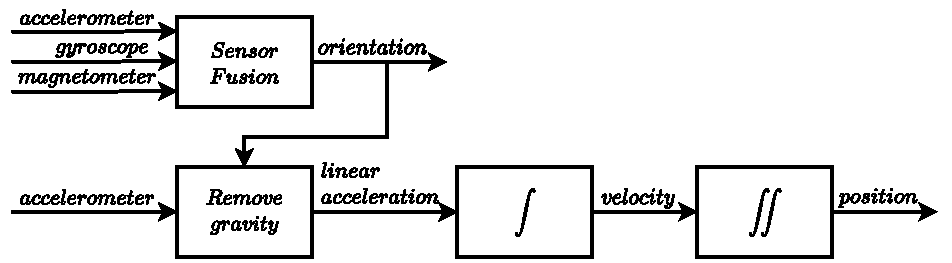
\includegraphics[width=0.9\textwidth]{figures/orientation_position.pdf}
    \caption{Overview of the position estimation method.}
    \label{fig:position}
\end{figure}

The next step consisted of experimentally testing the inertial system seeking to achieve position estimation merely by integrating the accelerometer measurements with the gravity compensation filter. Numerous experiments were performed in several settings. The tests involved walking on a straight line carrying a box containing the inertial system (with the inertial X-axis parallel to the path) for around 30 meters, evaluating the computed acceleration, velocity, and accumulative position estimation. Specific tests were executed at walking pace, others at running pace, and some with a combination of both.

\begin{figure}[!h]
    \centering
    \resizebox{1\linewidth}{!}{%% Creator: Matplotlib, PGF backend
%%
%% To include the figure in your LaTeX document, write
%%   \input{<filename>.pgf}
%%
%% Make sure the required packages are loaded in your preamble
%%   \usepackage{pgf}
%%
%% and, on pdftex
%%   \usepackage[utf8]{inputenc}\DeclareUnicodeCharacter{2212}{-}
%%
%% or, on luatex and xetex
%%   \usepackage{unicode-math}
%%
%% Figures using additional raster images can only be included by \input if
%% they are in the same directory as the main LaTeX file. For loading figures
%% from other directories you can use the `import` package
%%   \usepackage{import}
%%
%% and then include the figures with
%%   \import{<path to file>}{<filename>.pgf}
%%
%% Matplotlib used the following preamble
%%   \usepackage{fontspec}
%%
\begingroup%
\makeatletter%
\begin{pgfpicture}%
\pgfpathrectangle{\pgfpointorigin}{\pgfqpoint{6.400000in}{4.800000in}}%
\pgfusepath{use as bounding box, clip}%
\begin{pgfscope}%
\pgfsetbuttcap%
\pgfsetmiterjoin%
\definecolor{currentfill}{rgb}{1.000000,1.000000,1.000000}%
\pgfsetfillcolor{currentfill}%
\pgfsetlinewidth{0.000000pt}%
\definecolor{currentstroke}{rgb}{1.000000,1.000000,1.000000}%
\pgfsetstrokecolor{currentstroke}%
\pgfsetdash{}{0pt}%
\pgfpathmoveto{\pgfqpoint{0.000000in}{0.000000in}}%
\pgfpathlineto{\pgfqpoint{6.400000in}{0.000000in}}%
\pgfpathlineto{\pgfqpoint{6.400000in}{4.800000in}}%
\pgfpathlineto{\pgfqpoint{0.000000in}{4.800000in}}%
\pgfpathclose%
\pgfusepath{fill}%
\end{pgfscope}%
\begin{pgfscope}%
\pgfsetbuttcap%
\pgfsetmiterjoin%
\definecolor{currentfill}{rgb}{1.000000,1.000000,1.000000}%
\pgfsetfillcolor{currentfill}%
\pgfsetlinewidth{0.000000pt}%
\definecolor{currentstroke}{rgb}{0.000000,0.000000,0.000000}%
\pgfsetstrokecolor{currentstroke}%
\pgfsetstrokeopacity{0.000000}%
\pgfsetdash{}{0pt}%
\pgfpathmoveto{\pgfqpoint{0.580556in}{3.665000in}}%
\pgfpathlineto{\pgfqpoint{6.250000in}{3.665000in}}%
\pgfpathlineto{\pgfqpoint{6.250000in}{4.451000in}}%
\pgfpathlineto{\pgfqpoint{0.580556in}{4.451000in}}%
\pgfpathclose%
\pgfusepath{fill}%
\end{pgfscope}%
\begin{pgfscope}%
\pgfsetbuttcap%
\pgfsetroundjoin%
\definecolor{currentfill}{rgb}{0.000000,0.000000,0.000000}%
\pgfsetfillcolor{currentfill}%
\pgfsetlinewidth{0.803000pt}%
\definecolor{currentstroke}{rgb}{0.000000,0.000000,0.000000}%
\pgfsetstrokecolor{currentstroke}%
\pgfsetdash{}{0pt}%
\pgfsys@defobject{currentmarker}{\pgfqpoint{0.000000in}{-0.048611in}}{\pgfqpoint{0.000000in}{0.000000in}}{%
\pgfpathmoveto{\pgfqpoint{0.000000in}{0.000000in}}%
\pgfpathlineto{\pgfqpoint{0.000000in}{-0.048611in}}%
\pgfusepath{stroke,fill}%
}%
\begin{pgfscope}%
\pgfsys@transformshift{0.838258in}{3.665000in}%
\pgfsys@useobject{currentmarker}{}%
\end{pgfscope}%
\end{pgfscope}%
\begin{pgfscope}%
\definecolor{textcolor}{rgb}{0.000000,0.000000,0.000000}%
\pgfsetstrokecolor{textcolor}%
\pgfsetfillcolor{textcolor}%
\pgftext[x=0.838258in,y=3.567777in,,top]{\color{textcolor}\rmfamily\fontsize{10.000000}{12.000000}\selectfont \(\displaystyle {0}\)}%
\end{pgfscope}%
\begin{pgfscope}%
\pgfsetbuttcap%
\pgfsetroundjoin%
\definecolor{currentfill}{rgb}{0.000000,0.000000,0.000000}%
\pgfsetfillcolor{currentfill}%
\pgfsetlinewidth{0.803000pt}%
\definecolor{currentstroke}{rgb}{0.000000,0.000000,0.000000}%
\pgfsetstrokecolor{currentstroke}%
\pgfsetdash{}{0pt}%
\pgfsys@defobject{currentmarker}{\pgfqpoint{0.000000in}{-0.048611in}}{\pgfqpoint{0.000000in}{0.000000in}}{%
\pgfpathmoveto{\pgfqpoint{0.000000in}{0.000000in}}%
\pgfpathlineto{\pgfqpoint{0.000000in}{-0.048611in}}%
\pgfusepath{stroke,fill}%
}%
\begin{pgfscope}%
\pgfsys@transformshift{1.665551in}{3.665000in}%
\pgfsys@useobject{currentmarker}{}%
\end{pgfscope}%
\end{pgfscope}%
\begin{pgfscope}%
\definecolor{textcolor}{rgb}{0.000000,0.000000,0.000000}%
\pgfsetstrokecolor{textcolor}%
\pgfsetfillcolor{textcolor}%
\pgftext[x=1.665551in,y=3.567777in,,top]{\color{textcolor}\rmfamily\fontsize{10.000000}{12.000000}\selectfont \(\displaystyle {100}\)}%
\end{pgfscope}%
\begin{pgfscope}%
\pgfsetbuttcap%
\pgfsetroundjoin%
\definecolor{currentfill}{rgb}{0.000000,0.000000,0.000000}%
\pgfsetfillcolor{currentfill}%
\pgfsetlinewidth{0.803000pt}%
\definecolor{currentstroke}{rgb}{0.000000,0.000000,0.000000}%
\pgfsetstrokecolor{currentstroke}%
\pgfsetdash{}{0pt}%
\pgfsys@defobject{currentmarker}{\pgfqpoint{0.000000in}{-0.048611in}}{\pgfqpoint{0.000000in}{0.000000in}}{%
\pgfpathmoveto{\pgfqpoint{0.000000in}{0.000000in}}%
\pgfpathlineto{\pgfqpoint{0.000000in}{-0.048611in}}%
\pgfusepath{stroke,fill}%
}%
\begin{pgfscope}%
\pgfsys@transformshift{2.492845in}{3.665000in}%
\pgfsys@useobject{currentmarker}{}%
\end{pgfscope}%
\end{pgfscope}%
\begin{pgfscope}%
\definecolor{textcolor}{rgb}{0.000000,0.000000,0.000000}%
\pgfsetstrokecolor{textcolor}%
\pgfsetfillcolor{textcolor}%
\pgftext[x=2.492845in,y=3.567777in,,top]{\color{textcolor}\rmfamily\fontsize{10.000000}{12.000000}\selectfont \(\displaystyle {200}\)}%
\end{pgfscope}%
\begin{pgfscope}%
\pgfsetbuttcap%
\pgfsetroundjoin%
\definecolor{currentfill}{rgb}{0.000000,0.000000,0.000000}%
\pgfsetfillcolor{currentfill}%
\pgfsetlinewidth{0.803000pt}%
\definecolor{currentstroke}{rgb}{0.000000,0.000000,0.000000}%
\pgfsetstrokecolor{currentstroke}%
\pgfsetdash{}{0pt}%
\pgfsys@defobject{currentmarker}{\pgfqpoint{0.000000in}{-0.048611in}}{\pgfqpoint{0.000000in}{0.000000in}}{%
\pgfpathmoveto{\pgfqpoint{0.000000in}{0.000000in}}%
\pgfpathlineto{\pgfqpoint{0.000000in}{-0.048611in}}%
\pgfusepath{stroke,fill}%
}%
\begin{pgfscope}%
\pgfsys@transformshift{3.320139in}{3.665000in}%
\pgfsys@useobject{currentmarker}{}%
\end{pgfscope}%
\end{pgfscope}%
\begin{pgfscope}%
\definecolor{textcolor}{rgb}{0.000000,0.000000,0.000000}%
\pgfsetstrokecolor{textcolor}%
\pgfsetfillcolor{textcolor}%
\pgftext[x=3.320139in,y=3.567777in,,top]{\color{textcolor}\rmfamily\fontsize{10.000000}{12.000000}\selectfont \(\displaystyle {300}\)}%
\end{pgfscope}%
\begin{pgfscope}%
\pgfsetbuttcap%
\pgfsetroundjoin%
\definecolor{currentfill}{rgb}{0.000000,0.000000,0.000000}%
\pgfsetfillcolor{currentfill}%
\pgfsetlinewidth{0.803000pt}%
\definecolor{currentstroke}{rgb}{0.000000,0.000000,0.000000}%
\pgfsetstrokecolor{currentstroke}%
\pgfsetdash{}{0pt}%
\pgfsys@defobject{currentmarker}{\pgfqpoint{0.000000in}{-0.048611in}}{\pgfqpoint{0.000000in}{0.000000in}}{%
\pgfpathmoveto{\pgfqpoint{0.000000in}{0.000000in}}%
\pgfpathlineto{\pgfqpoint{0.000000in}{-0.048611in}}%
\pgfusepath{stroke,fill}%
}%
\begin{pgfscope}%
\pgfsys@transformshift{4.147433in}{3.665000in}%
\pgfsys@useobject{currentmarker}{}%
\end{pgfscope}%
\end{pgfscope}%
\begin{pgfscope}%
\definecolor{textcolor}{rgb}{0.000000,0.000000,0.000000}%
\pgfsetstrokecolor{textcolor}%
\pgfsetfillcolor{textcolor}%
\pgftext[x=4.147433in,y=3.567777in,,top]{\color{textcolor}\rmfamily\fontsize{10.000000}{12.000000}\selectfont \(\displaystyle {400}\)}%
\end{pgfscope}%
\begin{pgfscope}%
\pgfsetbuttcap%
\pgfsetroundjoin%
\definecolor{currentfill}{rgb}{0.000000,0.000000,0.000000}%
\pgfsetfillcolor{currentfill}%
\pgfsetlinewidth{0.803000pt}%
\definecolor{currentstroke}{rgb}{0.000000,0.000000,0.000000}%
\pgfsetstrokecolor{currentstroke}%
\pgfsetdash{}{0pt}%
\pgfsys@defobject{currentmarker}{\pgfqpoint{0.000000in}{-0.048611in}}{\pgfqpoint{0.000000in}{0.000000in}}{%
\pgfpathmoveto{\pgfqpoint{0.000000in}{0.000000in}}%
\pgfpathlineto{\pgfqpoint{0.000000in}{-0.048611in}}%
\pgfusepath{stroke,fill}%
}%
\begin{pgfscope}%
\pgfsys@transformshift{4.974727in}{3.665000in}%
\pgfsys@useobject{currentmarker}{}%
\end{pgfscope}%
\end{pgfscope}%
\begin{pgfscope}%
\definecolor{textcolor}{rgb}{0.000000,0.000000,0.000000}%
\pgfsetstrokecolor{textcolor}%
\pgfsetfillcolor{textcolor}%
\pgftext[x=4.974727in,y=3.567777in,,top]{\color{textcolor}\rmfamily\fontsize{10.000000}{12.000000}\selectfont \(\displaystyle {500}\)}%
\end{pgfscope}%
\begin{pgfscope}%
\pgfsetbuttcap%
\pgfsetroundjoin%
\definecolor{currentfill}{rgb}{0.000000,0.000000,0.000000}%
\pgfsetfillcolor{currentfill}%
\pgfsetlinewidth{0.803000pt}%
\definecolor{currentstroke}{rgb}{0.000000,0.000000,0.000000}%
\pgfsetstrokecolor{currentstroke}%
\pgfsetdash{}{0pt}%
\pgfsys@defobject{currentmarker}{\pgfqpoint{0.000000in}{-0.048611in}}{\pgfqpoint{0.000000in}{0.000000in}}{%
\pgfpathmoveto{\pgfqpoint{0.000000in}{0.000000in}}%
\pgfpathlineto{\pgfqpoint{0.000000in}{-0.048611in}}%
\pgfusepath{stroke,fill}%
}%
\begin{pgfscope}%
\pgfsys@transformshift{5.802020in}{3.665000in}%
\pgfsys@useobject{currentmarker}{}%
\end{pgfscope}%
\end{pgfscope}%
\begin{pgfscope}%
\definecolor{textcolor}{rgb}{0.000000,0.000000,0.000000}%
\pgfsetstrokecolor{textcolor}%
\pgfsetfillcolor{textcolor}%
\pgftext[x=5.802020in,y=3.567777in,,top]{\color{textcolor}\rmfamily\fontsize{10.000000}{12.000000}\selectfont \(\displaystyle {600}\)}%
\end{pgfscope}%
\begin{pgfscope}%
\definecolor{textcolor}{rgb}{0.000000,0.000000,0.000000}%
\pgfsetstrokecolor{textcolor}%
\pgfsetfillcolor{textcolor}%
\pgftext[x=3.415278in,y=3.388889in,,top]{\color{textcolor}\rmfamily\fontsize{10.000000}{12.000000}\selectfont Samples [\#]}%
\end{pgfscope}%
\begin{pgfscope}%
\pgfsetbuttcap%
\pgfsetroundjoin%
\definecolor{currentfill}{rgb}{0.000000,0.000000,0.000000}%
\pgfsetfillcolor{currentfill}%
\pgfsetlinewidth{0.803000pt}%
\definecolor{currentstroke}{rgb}{0.000000,0.000000,0.000000}%
\pgfsetstrokecolor{currentstroke}%
\pgfsetdash{}{0pt}%
\pgfsys@defobject{currentmarker}{\pgfqpoint{-0.048611in}{0.000000in}}{\pgfqpoint{-0.000000in}{0.000000in}}{%
\pgfpathmoveto{\pgfqpoint{-0.000000in}{0.000000in}}%
\pgfpathlineto{\pgfqpoint{-0.048611in}{0.000000in}}%
\pgfusepath{stroke,fill}%
}%
\begin{pgfscope}%
\pgfsys@transformshift{0.580556in}{3.700727in}%
\pgfsys@useobject{currentmarker}{}%
\end{pgfscope}%
\end{pgfscope}%
\begin{pgfscope}%
\definecolor{textcolor}{rgb}{0.000000,0.000000,0.000000}%
\pgfsetstrokecolor{textcolor}%
\pgfsetfillcolor{textcolor}%
\pgftext[x=0.413889in, y=3.652532in, left, base]{\color{textcolor}\rmfamily\fontsize{10.000000}{12.000000}\selectfont \(\displaystyle {0}\)}%
\end{pgfscope}%
\begin{pgfscope}%
\pgfsetbuttcap%
\pgfsetroundjoin%
\definecolor{currentfill}{rgb}{0.000000,0.000000,0.000000}%
\pgfsetfillcolor{currentfill}%
\pgfsetlinewidth{0.803000pt}%
\definecolor{currentstroke}{rgb}{0.000000,0.000000,0.000000}%
\pgfsetstrokecolor{currentstroke}%
\pgfsetdash{}{0pt}%
\pgfsys@defobject{currentmarker}{\pgfqpoint{-0.048611in}{0.000000in}}{\pgfqpoint{-0.000000in}{0.000000in}}{%
\pgfpathmoveto{\pgfqpoint{-0.000000in}{0.000000in}}%
\pgfpathlineto{\pgfqpoint{-0.048611in}{0.000000in}}%
\pgfusepath{stroke,fill}%
}%
\begin{pgfscope}%
\pgfsys@transformshift{0.580556in}{4.158671in}%
\pgfsys@useobject{currentmarker}{}%
\end{pgfscope}%
\end{pgfscope}%
\begin{pgfscope}%
\definecolor{textcolor}{rgb}{0.000000,0.000000,0.000000}%
\pgfsetstrokecolor{textcolor}%
\pgfsetfillcolor{textcolor}%
\pgftext[x=0.413889in, y=4.110477in, left, base]{\color{textcolor}\rmfamily\fontsize{10.000000}{12.000000}\selectfont \(\displaystyle {1}\)}%
\end{pgfscope}%
\begin{pgfscope}%
\definecolor{textcolor}{rgb}{0.000000,0.000000,0.000000}%
\pgfsetstrokecolor{textcolor}%
\pgfsetfillcolor{textcolor}%
\pgftext[x=0.288889in,y=4.058000in,,bottom,rotate=90.000000]{\color{textcolor}\rmfamily\fontsize{10.000000}{12.000000}\selectfont Acceleration X [\(\displaystyle ms^{-2}\)]}%
\end{pgfscope}%
\begin{pgfscope}%
\pgfpathrectangle{\pgfqpoint{0.580556in}{3.665000in}}{\pgfqpoint{5.669444in}{0.786000in}}%
\pgfusepath{clip}%
\pgfsetrectcap%
\pgfsetroundjoin%
\pgfsetlinewidth{1.505625pt}%
\definecolor{currentstroke}{rgb}{0.121569,0.466667,0.705882}%
\pgfsetstrokecolor{currentstroke}%
\pgfsetdash{}{0pt}%
\pgfpathmoveto{\pgfqpoint{0.838258in}{3.700727in}}%
\pgfpathlineto{\pgfqpoint{1.359453in}{3.700727in}}%
\pgfpathlineto{\pgfqpoint{1.367726in}{3.738601in}}%
\pgfpathlineto{\pgfqpoint{1.375999in}{3.700727in}}%
\pgfpathlineto{\pgfqpoint{1.400817in}{3.700727in}}%
\pgfpathlineto{\pgfqpoint{1.409090in}{3.956401in}}%
\pgfpathlineto{\pgfqpoint{1.417363in}{4.415273in}}%
\pgfpathlineto{\pgfqpoint{1.425636in}{3.797588in}}%
\pgfpathlineto{\pgfqpoint{1.433909in}{3.872873in}}%
\pgfpathlineto{\pgfqpoint{1.442182in}{4.160368in}}%
\pgfpathlineto{\pgfqpoint{1.450455in}{4.282628in}}%
\pgfpathlineto{\pgfqpoint{1.458728in}{4.096434in}}%
\pgfpathlineto{\pgfqpoint{1.467001in}{3.961384in}}%
\pgfpathlineto{\pgfqpoint{1.475274in}{4.247479in}}%
\pgfpathlineto{\pgfqpoint{1.483547in}{4.324947in}}%
\pgfpathlineto{\pgfqpoint{1.491820in}{4.208299in}}%
\pgfpathlineto{\pgfqpoint{1.500093in}{3.958242in}}%
\pgfpathlineto{\pgfqpoint{1.508366in}{4.032190in}}%
\pgfpathlineto{\pgfqpoint{1.516639in}{3.775172in}}%
\pgfpathlineto{\pgfqpoint{1.524912in}{3.754903in}}%
\pgfpathlineto{\pgfqpoint{1.533184in}{3.867976in}}%
\pgfpathlineto{\pgfqpoint{1.541457in}{4.049386in}}%
\pgfpathlineto{\pgfqpoint{1.549730in}{4.322921in}}%
\pgfpathlineto{\pgfqpoint{1.558003in}{4.197904in}}%
\pgfpathlineto{\pgfqpoint{1.566276in}{3.815941in}}%
\pgfpathlineto{\pgfqpoint{1.574549in}{3.730014in}}%
\pgfpathlineto{\pgfqpoint{1.582822in}{3.743490in}}%
\pgfpathlineto{\pgfqpoint{1.591095in}{3.998642in}}%
\pgfpathlineto{\pgfqpoint{1.599368in}{3.747918in}}%
\pgfpathlineto{\pgfqpoint{1.607641in}{4.037939in}}%
\pgfpathlineto{\pgfqpoint{1.615914in}{4.042291in}}%
\pgfpathlineto{\pgfqpoint{1.624187in}{3.871078in}}%
\pgfpathlineto{\pgfqpoint{1.632460in}{3.742379in}}%
\pgfpathlineto{\pgfqpoint{1.640733in}{3.700727in}}%
\pgfpathlineto{\pgfqpoint{1.649006in}{3.805519in}}%
\pgfpathlineto{\pgfqpoint{1.657279in}{3.863202in}}%
\pgfpathlineto{\pgfqpoint{1.665551in}{3.728407in}}%
\pgfpathlineto{\pgfqpoint{1.673824in}{3.905227in}}%
\pgfpathlineto{\pgfqpoint{1.682097in}{3.883116in}}%
\pgfpathlineto{\pgfqpoint{1.690370in}{3.784055in}}%
\pgfpathlineto{\pgfqpoint{1.698643in}{3.725282in}}%
\pgfpathlineto{\pgfqpoint{1.706916in}{3.869987in}}%
\pgfpathlineto{\pgfqpoint{1.715189in}{3.830527in}}%
\pgfpathlineto{\pgfqpoint{1.723462in}{3.744218in}}%
\pgfpathlineto{\pgfqpoint{1.731735in}{3.775166in}}%
\pgfpathlineto{\pgfqpoint{1.740008in}{3.859153in}}%
\pgfpathlineto{\pgfqpoint{1.748281in}{3.823156in}}%
\pgfpathlineto{\pgfqpoint{1.756554in}{3.740532in}}%
\pgfpathlineto{\pgfqpoint{1.764827in}{3.781816in}}%
\pgfpathlineto{\pgfqpoint{1.773100in}{3.862962in}}%
\pgfpathlineto{\pgfqpoint{1.781373in}{3.916186in}}%
\pgfpathlineto{\pgfqpoint{1.789646in}{3.700727in}}%
\pgfpathlineto{\pgfqpoint{1.797918in}{3.766413in}}%
\pgfpathlineto{\pgfqpoint{1.806191in}{3.780019in}}%
\pgfpathlineto{\pgfqpoint{1.814464in}{3.744939in}}%
\pgfpathlineto{\pgfqpoint{1.822737in}{3.844932in}}%
\pgfpathlineto{\pgfqpoint{1.831010in}{3.995094in}}%
\pgfpathlineto{\pgfqpoint{1.839283in}{3.873044in}}%
\pgfpathlineto{\pgfqpoint{1.847556in}{3.772851in}}%
\pgfpathlineto{\pgfqpoint{1.855829in}{3.809236in}}%
\pgfpathlineto{\pgfqpoint{1.864102in}{3.738451in}}%
\pgfpathlineto{\pgfqpoint{1.872375in}{3.808197in}}%
\pgfpathlineto{\pgfqpoint{1.880648in}{3.812468in}}%
\pgfpathlineto{\pgfqpoint{1.888921in}{3.769580in}}%
\pgfpathlineto{\pgfqpoint{1.897194in}{3.700727in}}%
\pgfpathlineto{\pgfqpoint{1.905467in}{3.790595in}}%
\pgfpathlineto{\pgfqpoint{1.913740in}{3.910654in}}%
\pgfpathlineto{\pgfqpoint{1.922013in}{4.004744in}}%
\pgfpathlineto{\pgfqpoint{1.930286in}{3.841331in}}%
\pgfpathlineto{\pgfqpoint{1.938558in}{3.875175in}}%
\pgfpathlineto{\pgfqpoint{1.946831in}{3.700727in}}%
\pgfpathlineto{\pgfqpoint{1.955104in}{3.887270in}}%
\pgfpathlineto{\pgfqpoint{1.963377in}{3.852250in}}%
\pgfpathlineto{\pgfqpoint{1.971650in}{3.730025in}}%
\pgfpathlineto{\pgfqpoint{1.979923in}{3.931998in}}%
\pgfpathlineto{\pgfqpoint{1.988196in}{4.006970in}}%
\pgfpathlineto{\pgfqpoint{1.996469in}{4.212442in}}%
\pgfpathlineto{\pgfqpoint{2.004742in}{3.965640in}}%
\pgfpathlineto{\pgfqpoint{2.013015in}{3.802217in}}%
\pgfpathlineto{\pgfqpoint{2.021288in}{3.764731in}}%
\pgfpathlineto{\pgfqpoint{2.029561in}{3.854516in}}%
\pgfpathlineto{\pgfqpoint{2.037834in}{3.765308in}}%
\pgfpathlineto{\pgfqpoint{2.046107in}{3.930092in}}%
\pgfpathlineto{\pgfqpoint{2.054380in}{4.251738in}}%
\pgfpathlineto{\pgfqpoint{2.062653in}{4.349533in}}%
\pgfpathlineto{\pgfqpoint{2.070925in}{4.068269in}}%
\pgfpathlineto{\pgfqpoint{2.079198in}{4.124492in}}%
\pgfpathlineto{\pgfqpoint{2.087471in}{3.821430in}}%
\pgfpathlineto{\pgfqpoint{2.095744in}{3.864090in}}%
\pgfpathlineto{\pgfqpoint{2.104017in}{3.740805in}}%
\pgfpathlineto{\pgfqpoint{2.112290in}{3.907501in}}%
\pgfpathlineto{\pgfqpoint{2.120563in}{3.790853in}}%
\pgfpathlineto{\pgfqpoint{2.128836in}{4.340682in}}%
\pgfpathlineto{\pgfqpoint{2.137109in}{4.017105in}}%
\pgfpathlineto{\pgfqpoint{2.145382in}{3.919082in}}%
\pgfpathlineto{\pgfqpoint{2.153655in}{3.866782in}}%
\pgfpathlineto{\pgfqpoint{2.161928in}{3.700727in}}%
\pgfpathlineto{\pgfqpoint{2.170201in}{3.737820in}}%
\pgfpathlineto{\pgfqpoint{2.178474in}{4.083588in}}%
\pgfpathlineto{\pgfqpoint{2.186747in}{4.125115in}}%
\pgfpathlineto{\pgfqpoint{2.195020in}{4.252271in}}%
\pgfpathlineto{\pgfqpoint{2.203292in}{3.900173in}}%
\pgfpathlineto{\pgfqpoint{2.211565in}{3.891605in}}%
\pgfpathlineto{\pgfqpoint{2.219838in}{3.775445in}}%
\pgfpathlineto{\pgfqpoint{2.228111in}{3.778424in}}%
\pgfpathlineto{\pgfqpoint{2.236384in}{3.761757in}}%
\pgfpathlineto{\pgfqpoint{2.244657in}{4.098228in}}%
\pgfpathlineto{\pgfqpoint{2.252930in}{4.369219in}}%
\pgfpathlineto{\pgfqpoint{2.261203in}{4.201494in}}%
\pgfpathlineto{\pgfqpoint{2.269476in}{4.075248in}}%
\pgfpathlineto{\pgfqpoint{2.277749in}{3.779965in}}%
\pgfpathlineto{\pgfqpoint{2.286022in}{3.814329in}}%
\pgfpathlineto{\pgfqpoint{2.294295in}{3.785768in}}%
\pgfpathlineto{\pgfqpoint{2.302568in}{3.914943in}}%
\pgfpathlineto{\pgfqpoint{2.310841in}{4.300015in}}%
\pgfpathlineto{\pgfqpoint{2.319114in}{4.292733in}}%
\pgfpathlineto{\pgfqpoint{2.327387in}{3.844079in}}%
\pgfpathlineto{\pgfqpoint{2.335659in}{3.700727in}}%
\pgfpathlineto{\pgfqpoint{2.343932in}{3.918454in}}%
\pgfpathlineto{\pgfqpoint{2.352205in}{3.762011in}}%
\pgfpathlineto{\pgfqpoint{2.360478in}{3.807832in}}%
\pgfpathlineto{\pgfqpoint{2.368751in}{3.770041in}}%
\pgfpathlineto{\pgfqpoint{2.377024in}{4.209052in}}%
\pgfpathlineto{\pgfqpoint{2.385297in}{3.882278in}}%
\pgfpathlineto{\pgfqpoint{2.393570in}{4.059649in}}%
\pgfpathlineto{\pgfqpoint{2.401843in}{4.162694in}}%
\pgfpathlineto{\pgfqpoint{2.410116in}{4.083722in}}%
\pgfpathlineto{\pgfqpoint{2.418389in}{3.766735in}}%
\pgfpathlineto{\pgfqpoint{2.426662in}{4.014352in}}%
\pgfpathlineto{\pgfqpoint{2.434935in}{3.823646in}}%
\pgfpathlineto{\pgfqpoint{2.443208in}{3.787571in}}%
\pgfpathlineto{\pgfqpoint{2.451481in}{4.143077in}}%
\pgfpathlineto{\pgfqpoint{2.459754in}{4.261728in}}%
\pgfpathlineto{\pgfqpoint{2.468026in}{4.002271in}}%
\pgfpathlineto{\pgfqpoint{2.476299in}{3.840232in}}%
\pgfpathlineto{\pgfqpoint{2.484572in}{3.806575in}}%
\pgfpathlineto{\pgfqpoint{2.492845in}{3.766970in}}%
\pgfpathlineto{\pgfqpoint{2.501118in}{3.700727in}}%
\pgfpathlineto{\pgfqpoint{2.509391in}{3.816653in}}%
\pgfpathlineto{\pgfqpoint{2.517664in}{3.895225in}}%
\pgfpathlineto{\pgfqpoint{2.525937in}{4.063226in}}%
\pgfpathlineto{\pgfqpoint{2.534210in}{4.193918in}}%
\pgfpathlineto{\pgfqpoint{2.550756in}{3.783363in}}%
\pgfpathlineto{\pgfqpoint{2.559029in}{3.974436in}}%
\pgfpathlineto{\pgfqpoint{2.567302in}{3.871386in}}%
\pgfpathlineto{\pgfqpoint{2.575575in}{3.932311in}}%
\pgfpathlineto{\pgfqpoint{2.583848in}{3.700727in}}%
\pgfpathlineto{\pgfqpoint{2.592121in}{3.944934in}}%
\pgfpathlineto{\pgfqpoint{2.600393in}{4.114580in}}%
\pgfpathlineto{\pgfqpoint{2.608666in}{4.039235in}}%
\pgfpathlineto{\pgfqpoint{2.616939in}{3.841663in}}%
\pgfpathlineto{\pgfqpoint{2.625212in}{3.912512in}}%
\pgfpathlineto{\pgfqpoint{2.633485in}{3.824865in}}%
\pgfpathlineto{\pgfqpoint{2.641758in}{3.923007in}}%
\pgfpathlineto{\pgfqpoint{2.650031in}{3.798850in}}%
\pgfpathlineto{\pgfqpoint{2.666577in}{4.103724in}}%
\pgfpathlineto{\pgfqpoint{2.674850in}{4.092247in}}%
\pgfpathlineto{\pgfqpoint{2.683123in}{3.700727in}}%
\pgfpathlineto{\pgfqpoint{2.691396in}{3.748556in}}%
\pgfpathlineto{\pgfqpoint{2.699669in}{4.022605in}}%
\pgfpathlineto{\pgfqpoint{2.707942in}{3.978451in}}%
\pgfpathlineto{\pgfqpoint{2.716215in}{3.892269in}}%
\pgfpathlineto{\pgfqpoint{2.724488in}{3.868335in}}%
\pgfpathlineto{\pgfqpoint{2.732760in}{4.037305in}}%
\pgfpathlineto{\pgfqpoint{2.741033in}{4.045618in}}%
\pgfpathlineto{\pgfqpoint{2.749306in}{3.931181in}}%
\pgfpathlineto{\pgfqpoint{2.757579in}{3.954858in}}%
\pgfpathlineto{\pgfqpoint{2.765852in}{3.970791in}}%
\pgfpathlineto{\pgfqpoint{2.774125in}{3.804008in}}%
\pgfpathlineto{\pgfqpoint{2.782398in}{3.808531in}}%
\pgfpathlineto{\pgfqpoint{2.790671in}{4.080523in}}%
\pgfpathlineto{\pgfqpoint{2.798944in}{3.934766in}}%
\pgfpathlineto{\pgfqpoint{2.807217in}{3.700727in}}%
\pgfpathlineto{\pgfqpoint{2.815490in}{3.775214in}}%
\pgfpathlineto{\pgfqpoint{2.823763in}{3.750949in}}%
\pgfpathlineto{\pgfqpoint{2.832036in}{3.760091in}}%
\pgfpathlineto{\pgfqpoint{2.840309in}{3.745149in}}%
\pgfpathlineto{\pgfqpoint{2.848582in}{3.775579in}}%
\pgfpathlineto{\pgfqpoint{2.856855in}{4.081482in}}%
\pgfpathlineto{\pgfqpoint{2.865127in}{3.792927in}}%
\pgfpathlineto{\pgfqpoint{2.873400in}{3.700727in}}%
\pgfpathlineto{\pgfqpoint{2.881673in}{4.074097in}}%
\pgfpathlineto{\pgfqpoint{2.889946in}{4.166163in}}%
\pgfpathlineto{\pgfqpoint{2.898219in}{4.094798in}}%
\pgfpathlineto{\pgfqpoint{2.906492in}{4.180444in}}%
\pgfpathlineto{\pgfqpoint{2.914765in}{3.924129in}}%
\pgfpathlineto{\pgfqpoint{2.923038in}{3.829020in}}%
\pgfpathlineto{\pgfqpoint{2.931311in}{3.800023in}}%
\pgfpathlineto{\pgfqpoint{2.947857in}{3.700727in}}%
\pgfpathlineto{\pgfqpoint{2.956130in}{4.257585in}}%
\pgfpathlineto{\pgfqpoint{2.964403in}{4.165491in}}%
\pgfpathlineto{\pgfqpoint{2.972676in}{4.199587in}}%
\pgfpathlineto{\pgfqpoint{2.980949in}{3.880682in}}%
\pgfpathlineto{\pgfqpoint{2.989222in}{3.973369in}}%
\pgfpathlineto{\pgfqpoint{2.997494in}{4.014708in}}%
\pgfpathlineto{\pgfqpoint{3.005767in}{3.982154in}}%
\pgfpathlineto{\pgfqpoint{3.014040in}{3.834932in}}%
\pgfpathlineto{\pgfqpoint{3.022313in}{4.189014in}}%
\pgfpathlineto{\pgfqpoint{3.030586in}{3.897418in}}%
\pgfpathlineto{\pgfqpoint{3.038859in}{4.159700in}}%
\pgfpathlineto{\pgfqpoint{3.047132in}{3.923575in}}%
\pgfpathlineto{\pgfqpoint{3.055405in}{3.841082in}}%
\pgfpathlineto{\pgfqpoint{3.063678in}{3.918741in}}%
\pgfpathlineto{\pgfqpoint{3.071951in}{3.905466in}}%
\pgfpathlineto{\pgfqpoint{3.080224in}{3.700727in}}%
\pgfpathlineto{\pgfqpoint{3.088497in}{4.143563in}}%
\pgfpathlineto{\pgfqpoint{3.096770in}{4.018188in}}%
\pgfpathlineto{\pgfqpoint{3.105043in}{4.065986in}}%
\pgfpathlineto{\pgfqpoint{3.113316in}{3.971895in}}%
\pgfpathlineto{\pgfqpoint{3.121589in}{3.924431in}}%
\pgfpathlineto{\pgfqpoint{3.129861in}{3.896355in}}%
\pgfpathlineto{\pgfqpoint{3.138134in}{3.814345in}}%
\pgfpathlineto{\pgfqpoint{3.146407in}{3.959339in}}%
\pgfpathlineto{\pgfqpoint{3.154680in}{4.258594in}}%
\pgfpathlineto{\pgfqpoint{3.162953in}{4.228033in}}%
\pgfpathlineto{\pgfqpoint{3.171226in}{4.141287in}}%
\pgfpathlineto{\pgfqpoint{3.179499in}{3.948291in}}%
\pgfpathlineto{\pgfqpoint{3.187772in}{3.784617in}}%
\pgfpathlineto{\pgfqpoint{3.196045in}{3.919784in}}%
\pgfpathlineto{\pgfqpoint{3.204318in}{3.797633in}}%
\pgfpathlineto{\pgfqpoint{3.212591in}{3.731683in}}%
\pgfpathlineto{\pgfqpoint{3.220864in}{4.196260in}}%
\pgfpathlineto{\pgfqpoint{3.229137in}{4.243576in}}%
\pgfpathlineto{\pgfqpoint{3.237410in}{4.172319in}}%
\pgfpathlineto{\pgfqpoint{3.253956in}{3.700727in}}%
\pgfpathlineto{\pgfqpoint{3.262228in}{3.928592in}}%
\pgfpathlineto{\pgfqpoint{3.270501in}{3.740963in}}%
\pgfpathlineto{\pgfqpoint{3.278774in}{3.810875in}}%
\pgfpathlineto{\pgfqpoint{3.287047in}{3.901566in}}%
\pgfpathlineto{\pgfqpoint{3.295320in}{4.219804in}}%
\pgfpathlineto{\pgfqpoint{3.303593in}{3.808083in}}%
\pgfpathlineto{\pgfqpoint{3.311866in}{4.101525in}}%
\pgfpathlineto{\pgfqpoint{3.320139in}{3.860469in}}%
\pgfpathlineto{\pgfqpoint{3.328412in}{3.929005in}}%
\pgfpathlineto{\pgfqpoint{3.336685in}{3.860780in}}%
\pgfpathlineto{\pgfqpoint{3.344958in}{3.944407in}}%
\pgfpathlineto{\pgfqpoint{3.353231in}{4.129251in}}%
\pgfpathlineto{\pgfqpoint{3.361504in}{4.210450in}}%
\pgfpathlineto{\pgfqpoint{3.369777in}{3.754278in}}%
\pgfpathlineto{\pgfqpoint{3.378050in}{3.750770in}}%
\pgfpathlineto{\pgfqpoint{3.386323in}{3.866214in}}%
\pgfpathlineto{\pgfqpoint{3.394596in}{3.700727in}}%
\pgfpathlineto{\pgfqpoint{3.402868in}{4.201334in}}%
\pgfpathlineto{\pgfqpoint{3.411141in}{4.063274in}}%
\pgfpathlineto{\pgfqpoint{3.419414in}{3.993994in}}%
\pgfpathlineto{\pgfqpoint{3.435960in}{3.923162in}}%
\pgfpathlineto{\pgfqpoint{3.444233in}{3.899239in}}%
\pgfpathlineto{\pgfqpoint{3.452506in}{3.845145in}}%
\pgfpathlineto{\pgfqpoint{3.460779in}{3.855564in}}%
\pgfpathlineto{\pgfqpoint{3.469052in}{3.825837in}}%
\pgfpathlineto{\pgfqpoint{3.477325in}{3.775316in}}%
\pgfpathlineto{\pgfqpoint{3.485598in}{3.824950in}}%
\pgfpathlineto{\pgfqpoint{3.493871in}{3.767092in}}%
\pgfpathlineto{\pgfqpoint{3.502144in}{3.779577in}}%
\pgfpathlineto{\pgfqpoint{3.510417in}{3.757610in}}%
\pgfpathlineto{\pgfqpoint{3.518690in}{3.723987in}}%
\pgfpathlineto{\pgfqpoint{3.526963in}{3.736039in}}%
\pgfpathlineto{\pgfqpoint{3.535235in}{3.700727in}}%
\pgfpathlineto{\pgfqpoint{3.576600in}{3.700727in}}%
\pgfpathlineto{\pgfqpoint{3.584873in}{3.734605in}}%
\pgfpathlineto{\pgfqpoint{3.593146in}{3.700727in}}%
\pgfpathlineto{\pgfqpoint{3.601419in}{3.729797in}}%
\pgfpathlineto{\pgfqpoint{3.609692in}{3.700727in}}%
\pgfpathlineto{\pgfqpoint{3.617965in}{3.726304in}}%
\pgfpathlineto{\pgfqpoint{3.626238in}{3.727171in}}%
\pgfpathlineto{\pgfqpoint{3.634511in}{3.700727in}}%
\pgfpathlineto{\pgfqpoint{3.907518in}{3.700727in}}%
\pgfpathlineto{\pgfqpoint{3.915791in}{3.727506in}}%
\pgfpathlineto{\pgfqpoint{3.924064in}{3.733007in}}%
\pgfpathlineto{\pgfqpoint{3.932336in}{3.762084in}}%
\pgfpathlineto{\pgfqpoint{3.940609in}{3.752237in}}%
\pgfpathlineto{\pgfqpoint{3.948882in}{3.790091in}}%
\pgfpathlineto{\pgfqpoint{3.957155in}{3.835730in}}%
\pgfpathlineto{\pgfqpoint{3.965428in}{3.938643in}}%
\pgfpathlineto{\pgfqpoint{3.973701in}{3.875228in}}%
\pgfpathlineto{\pgfqpoint{3.981974in}{3.850217in}}%
\pgfpathlineto{\pgfqpoint{3.990247in}{4.001890in}}%
\pgfpathlineto{\pgfqpoint{3.998520in}{4.115598in}}%
\pgfpathlineto{\pgfqpoint{4.006793in}{4.132372in}}%
\pgfpathlineto{\pgfqpoint{4.015066in}{3.798753in}}%
\pgfpathlineto{\pgfqpoint{4.023339in}{3.833281in}}%
\pgfpathlineto{\pgfqpoint{4.031612in}{3.816188in}}%
\pgfpathlineto{\pgfqpoint{4.039885in}{3.804953in}}%
\pgfpathlineto{\pgfqpoint{4.048158in}{3.700727in}}%
\pgfpathlineto{\pgfqpoint{4.056431in}{3.700727in}}%
\pgfpathlineto{\pgfqpoint{4.064703in}{3.734513in}}%
\pgfpathlineto{\pgfqpoint{4.072976in}{3.700727in}}%
\pgfpathlineto{\pgfqpoint{4.081249in}{3.727467in}}%
\pgfpathlineto{\pgfqpoint{4.089522in}{3.700727in}}%
\pgfpathlineto{\pgfqpoint{4.097795in}{3.700727in}}%
\pgfpathlineto{\pgfqpoint{4.106068in}{3.742435in}}%
\pgfpathlineto{\pgfqpoint{4.114341in}{3.700727in}}%
\pgfpathlineto{\pgfqpoint{4.329437in}{3.700727in}}%
\pgfpathlineto{\pgfqpoint{4.337710in}{3.724670in}}%
\pgfpathlineto{\pgfqpoint{4.345983in}{3.700727in}}%
\pgfpathlineto{\pgfqpoint{4.354256in}{3.700727in}}%
\pgfpathlineto{\pgfqpoint{4.362529in}{3.737120in}}%
\pgfpathlineto{\pgfqpoint{4.370802in}{3.700727in}}%
\pgfpathlineto{\pgfqpoint{4.379075in}{3.723628in}}%
\pgfpathlineto{\pgfqpoint{4.387348in}{3.700727in}}%
\pgfpathlineto{\pgfqpoint{4.709993in}{3.700727in}}%
\pgfpathlineto{\pgfqpoint{4.718266in}{3.853570in}}%
\pgfpathlineto{\pgfqpoint{4.726538in}{4.062708in}}%
\pgfpathlineto{\pgfqpoint{4.734811in}{4.219932in}}%
\pgfpathlineto{\pgfqpoint{4.743084in}{4.152850in}}%
\pgfpathlineto{\pgfqpoint{4.751357in}{4.303639in}}%
\pgfpathlineto{\pgfqpoint{4.759630in}{4.348613in}}%
\pgfpathlineto{\pgfqpoint{4.767903in}{3.872387in}}%
\pgfpathlineto{\pgfqpoint{4.776176in}{4.168463in}}%
\pgfpathlineto{\pgfqpoint{4.784449in}{3.862575in}}%
\pgfpathlineto{\pgfqpoint{4.792722in}{3.958818in}}%
\pgfpathlineto{\pgfqpoint{4.800995in}{3.804273in}}%
\pgfpathlineto{\pgfqpoint{4.809268in}{3.980174in}}%
\pgfpathlineto{\pgfqpoint{4.817541in}{3.941508in}}%
\pgfpathlineto{\pgfqpoint{4.825814in}{3.839530in}}%
\pgfpathlineto{\pgfqpoint{4.834087in}{3.973316in}}%
\pgfpathlineto{\pgfqpoint{4.842360in}{3.775191in}}%
\pgfpathlineto{\pgfqpoint{4.850633in}{3.785608in}}%
\pgfpathlineto{\pgfqpoint{4.858906in}{3.700727in}}%
\pgfpathlineto{\pgfqpoint{4.867178in}{3.766037in}}%
\pgfpathlineto{\pgfqpoint{4.875451in}{3.796604in}}%
\pgfpathlineto{\pgfqpoint{4.883724in}{3.756044in}}%
\pgfpathlineto{\pgfqpoint{4.891997in}{4.043623in}}%
\pgfpathlineto{\pgfqpoint{4.900270in}{3.700727in}}%
\pgfpathlineto{\pgfqpoint{4.908543in}{3.736171in}}%
\pgfpathlineto{\pgfqpoint{4.916816in}{3.848968in}}%
\pgfpathlineto{\pgfqpoint{4.925089in}{3.756637in}}%
\pgfpathlineto{\pgfqpoint{4.933362in}{3.906500in}}%
\pgfpathlineto{\pgfqpoint{4.941635in}{3.926202in}}%
\pgfpathlineto{\pgfqpoint{4.949908in}{3.772218in}}%
\pgfpathlineto{\pgfqpoint{4.958181in}{3.770639in}}%
\pgfpathlineto{\pgfqpoint{4.966454in}{3.816950in}}%
\pgfpathlineto{\pgfqpoint{4.974727in}{4.119623in}}%
\pgfpathlineto{\pgfqpoint{4.983000in}{3.843861in}}%
\pgfpathlineto{\pgfqpoint{4.991273in}{3.833058in}}%
\pgfpathlineto{\pgfqpoint{4.999545in}{4.075161in}}%
\pgfpathlineto{\pgfqpoint{5.007818in}{3.737789in}}%
\pgfpathlineto{\pgfqpoint{5.016091in}{3.808359in}}%
\pgfpathlineto{\pgfqpoint{5.024364in}{4.042940in}}%
\pgfpathlineto{\pgfqpoint{5.032637in}{3.954220in}}%
\pgfpathlineto{\pgfqpoint{5.040910in}{3.893346in}}%
\pgfpathlineto{\pgfqpoint{5.049183in}{3.914918in}}%
\pgfpathlineto{\pgfqpoint{5.057456in}{3.853124in}}%
\pgfpathlineto{\pgfqpoint{5.065729in}{3.843979in}}%
\pgfpathlineto{\pgfqpoint{5.074002in}{3.736412in}}%
\pgfpathlineto{\pgfqpoint{5.082275in}{4.143141in}}%
\pgfpathlineto{\pgfqpoint{5.090548in}{4.176023in}}%
\pgfpathlineto{\pgfqpoint{5.098821in}{3.982602in}}%
\pgfpathlineto{\pgfqpoint{5.107094in}{4.088642in}}%
\pgfpathlineto{\pgfqpoint{5.115367in}{4.172932in}}%
\pgfpathlineto{\pgfqpoint{5.131912in}{4.067991in}}%
\pgfpathlineto{\pgfqpoint{5.140185in}{3.841869in}}%
\pgfpathlineto{\pgfqpoint{5.148458in}{3.926103in}}%
\pgfpathlineto{\pgfqpoint{5.156731in}{3.978961in}}%
\pgfpathlineto{\pgfqpoint{5.165004in}{3.908902in}}%
\pgfpathlineto{\pgfqpoint{5.173277in}{3.730163in}}%
\pgfpathlineto{\pgfqpoint{5.181550in}{3.845359in}}%
\pgfpathlineto{\pgfqpoint{5.189823in}{3.921859in}}%
\pgfpathlineto{\pgfqpoint{5.198096in}{3.790850in}}%
\pgfpathlineto{\pgfqpoint{5.206369in}{3.758655in}}%
\pgfpathlineto{\pgfqpoint{5.214642in}{3.944156in}}%
\pgfpathlineto{\pgfqpoint{5.222915in}{3.795211in}}%
\pgfpathlineto{\pgfqpoint{5.231188in}{3.858410in}}%
\pgfpathlineto{\pgfqpoint{5.239461in}{3.771835in}}%
\pgfpathlineto{\pgfqpoint{5.247734in}{3.724752in}}%
\pgfpathlineto{\pgfqpoint{5.256007in}{3.772361in}}%
\pgfpathlineto{\pgfqpoint{5.264279in}{3.700727in}}%
\pgfpathlineto{\pgfqpoint{5.272552in}{3.786518in}}%
\pgfpathlineto{\pgfqpoint{5.280825in}{4.014989in}}%
\pgfpathlineto{\pgfqpoint{5.289098in}{3.911044in}}%
\pgfpathlineto{\pgfqpoint{5.297371in}{3.785258in}}%
\pgfpathlineto{\pgfqpoint{5.305644in}{3.986126in}}%
\pgfpathlineto{\pgfqpoint{5.313917in}{3.822483in}}%
\pgfpathlineto{\pgfqpoint{5.322190in}{3.754623in}}%
\pgfpathlineto{\pgfqpoint{5.330463in}{3.783012in}}%
\pgfpathlineto{\pgfqpoint{5.338736in}{3.956650in}}%
\pgfpathlineto{\pgfqpoint{5.347009in}{3.843793in}}%
\pgfpathlineto{\pgfqpoint{5.355282in}{3.816542in}}%
\pgfpathlineto{\pgfqpoint{5.363555in}{3.993614in}}%
\pgfpathlineto{\pgfqpoint{5.371828in}{4.033801in}}%
\pgfpathlineto{\pgfqpoint{5.380101in}{3.916962in}}%
\pgfpathlineto{\pgfqpoint{5.396646in}{3.754773in}}%
\pgfpathlineto{\pgfqpoint{5.404919in}{3.842829in}}%
\pgfpathlineto{\pgfqpoint{5.413192in}{3.877350in}}%
\pgfpathlineto{\pgfqpoint{5.421465in}{3.700727in}}%
\pgfpathlineto{\pgfqpoint{5.429738in}{3.841761in}}%
\pgfpathlineto{\pgfqpoint{5.438011in}{3.700727in}}%
\pgfpathlineto{\pgfqpoint{5.446284in}{3.761628in}}%
\pgfpathlineto{\pgfqpoint{5.454557in}{3.770224in}}%
\pgfpathlineto{\pgfqpoint{5.462830in}{3.834902in}}%
\pgfpathlineto{\pgfqpoint{5.471103in}{3.739916in}}%
\pgfpathlineto{\pgfqpoint{5.479376in}{3.735688in}}%
\pgfpathlineto{\pgfqpoint{5.487649in}{3.809261in}}%
\pgfpathlineto{\pgfqpoint{5.495922in}{3.866879in}}%
\pgfpathlineto{\pgfqpoint{5.504195in}{3.821690in}}%
\pgfpathlineto{\pgfqpoint{5.512468in}{3.951135in}}%
\pgfpathlineto{\pgfqpoint{5.520741in}{3.850975in}}%
\pgfpathlineto{\pgfqpoint{5.529013in}{3.726253in}}%
\pgfpathlineto{\pgfqpoint{5.537286in}{4.051479in}}%
\pgfpathlineto{\pgfqpoint{5.545559in}{3.950163in}}%
\pgfpathlineto{\pgfqpoint{5.553832in}{3.906373in}}%
\pgfpathlineto{\pgfqpoint{5.562105in}{3.899634in}}%
\pgfpathlineto{\pgfqpoint{5.570378in}{4.029621in}}%
\pgfpathlineto{\pgfqpoint{5.578651in}{3.804447in}}%
\pgfpathlineto{\pgfqpoint{5.586924in}{3.773740in}}%
\pgfpathlineto{\pgfqpoint{5.595197in}{4.070172in}}%
\pgfpathlineto{\pgfqpoint{5.603470in}{3.773772in}}%
\pgfpathlineto{\pgfqpoint{5.611743in}{3.769490in}}%
\pgfpathlineto{\pgfqpoint{5.620016in}{3.905773in}}%
\pgfpathlineto{\pgfqpoint{5.628289in}{3.700727in}}%
\pgfpathlineto{\pgfqpoint{5.636562in}{4.035149in}}%
\pgfpathlineto{\pgfqpoint{5.644835in}{3.735991in}}%
\pgfpathlineto{\pgfqpoint{5.653108in}{3.840555in}}%
\pgfpathlineto{\pgfqpoint{5.661380in}{3.832420in}}%
\pgfpathlineto{\pgfqpoint{5.669653in}{3.849197in}}%
\pgfpathlineto{\pgfqpoint{5.677926in}{3.775087in}}%
\pgfpathlineto{\pgfqpoint{5.686199in}{3.771623in}}%
\pgfpathlineto{\pgfqpoint{5.694472in}{3.700727in}}%
\pgfpathlineto{\pgfqpoint{5.702745in}{3.832848in}}%
\pgfpathlineto{\pgfqpoint{5.711018in}{3.879490in}}%
\pgfpathlineto{\pgfqpoint{5.719291in}{3.733252in}}%
\pgfpathlineto{\pgfqpoint{5.727564in}{3.921402in}}%
\pgfpathlineto{\pgfqpoint{5.735837in}{4.010353in}}%
\pgfpathlineto{\pgfqpoint{5.744110in}{4.034466in}}%
\pgfpathlineto{\pgfqpoint{5.752383in}{3.860167in}}%
\pgfpathlineto{\pgfqpoint{5.760656in}{3.977693in}}%
\pgfpathlineto{\pgfqpoint{5.768929in}{3.842253in}}%
\pgfpathlineto{\pgfqpoint{5.777202in}{3.916611in}}%
\pgfpathlineto{\pgfqpoint{5.785475in}{3.890650in}}%
\pgfpathlineto{\pgfqpoint{5.793747in}{3.790848in}}%
\pgfpathlineto{\pgfqpoint{5.802020in}{3.809258in}}%
\pgfpathlineto{\pgfqpoint{5.810293in}{3.770007in}}%
\pgfpathlineto{\pgfqpoint{5.818566in}{3.744292in}}%
\pgfpathlineto{\pgfqpoint{5.826839in}{3.762053in}}%
\pgfpathlineto{\pgfqpoint{5.835112in}{3.738903in}}%
\pgfpathlineto{\pgfqpoint{5.843385in}{3.726432in}}%
\pgfpathlineto{\pgfqpoint{5.851658in}{3.700727in}}%
\pgfpathlineto{\pgfqpoint{5.859931in}{3.820958in}}%
\pgfpathlineto{\pgfqpoint{5.868204in}{3.785241in}}%
\pgfpathlineto{\pgfqpoint{5.876477in}{3.726661in}}%
\pgfpathlineto{\pgfqpoint{5.884750in}{3.700727in}}%
\pgfpathlineto{\pgfqpoint{5.942660in}{3.700727in}}%
\pgfpathlineto{\pgfqpoint{5.950933in}{3.876865in}}%
\pgfpathlineto{\pgfqpoint{5.959206in}{3.723872in}}%
\pgfpathlineto{\pgfqpoint{5.967479in}{3.776447in}}%
\pgfpathlineto{\pgfqpoint{5.975752in}{3.725825in}}%
\pgfpathlineto{\pgfqpoint{5.984025in}{3.700727in}}%
\pgfpathlineto{\pgfqpoint{5.992298in}{3.700727in}}%
\pgfpathlineto{\pgfqpoint{5.992298in}{3.700727in}}%
\pgfusepath{stroke}%
\end{pgfscope}%
\begin{pgfscope}%
\pgfsetrectcap%
\pgfsetmiterjoin%
\pgfsetlinewidth{0.803000pt}%
\definecolor{currentstroke}{rgb}{0.000000,0.000000,0.000000}%
\pgfsetstrokecolor{currentstroke}%
\pgfsetdash{}{0pt}%
\pgfpathmoveto{\pgfqpoint{0.580556in}{3.665000in}}%
\pgfpathlineto{\pgfqpoint{0.580556in}{4.451000in}}%
\pgfusepath{stroke}%
\end{pgfscope}%
\begin{pgfscope}%
\pgfsetrectcap%
\pgfsetmiterjoin%
\pgfsetlinewidth{0.803000pt}%
\definecolor{currentstroke}{rgb}{0.000000,0.000000,0.000000}%
\pgfsetstrokecolor{currentstroke}%
\pgfsetdash{}{0pt}%
\pgfpathmoveto{\pgfqpoint{6.250000in}{3.665000in}}%
\pgfpathlineto{\pgfqpoint{6.250000in}{4.451000in}}%
\pgfusepath{stroke}%
\end{pgfscope}%
\begin{pgfscope}%
\pgfsetrectcap%
\pgfsetmiterjoin%
\pgfsetlinewidth{0.803000pt}%
\definecolor{currentstroke}{rgb}{0.000000,0.000000,0.000000}%
\pgfsetstrokecolor{currentstroke}%
\pgfsetdash{}{0pt}%
\pgfpathmoveto{\pgfqpoint{0.580556in}{3.665000in}}%
\pgfpathlineto{\pgfqpoint{6.250000in}{3.665000in}}%
\pgfusepath{stroke}%
\end{pgfscope}%
\begin{pgfscope}%
\pgfsetrectcap%
\pgfsetmiterjoin%
\pgfsetlinewidth{0.803000pt}%
\definecolor{currentstroke}{rgb}{0.000000,0.000000,0.000000}%
\pgfsetstrokecolor{currentstroke}%
\pgfsetdash{}{0pt}%
\pgfpathmoveto{\pgfqpoint{0.580556in}{4.451000in}}%
\pgfpathlineto{\pgfqpoint{6.250000in}{4.451000in}}%
\pgfusepath{stroke}%
\end{pgfscope}%
\begin{pgfscope}%
\definecolor{textcolor}{rgb}{0.000000,0.000000,0.000000}%
\pgfsetstrokecolor{textcolor}%
\pgfsetfillcolor{textcolor}%
\pgftext[x=3.415278in,y=4.534333in,,base]{\color{textcolor}\rmfamily\fontsize{12.000000}{14.400000}\selectfont \textbf{Acceleration}}%
\end{pgfscope}%
\begin{pgfscope}%
\pgfsetbuttcap%
\pgfsetmiterjoin%
\definecolor{currentfill}{rgb}{1.000000,1.000000,1.000000}%
\pgfsetfillcolor{currentfill}%
\pgfsetfillopacity{0.800000}%
\pgfsetlinewidth{1.003750pt}%
\definecolor{currentstroke}{rgb}{0.800000,0.800000,0.800000}%
\pgfsetstrokecolor{currentstroke}%
\pgfsetstrokeopacity{0.800000}%
\pgfsetdash{}{0pt}%
\pgfpathmoveto{\pgfqpoint{0.677778in}{4.146278in}}%
\pgfpathlineto{\pgfqpoint{2.274583in}{4.146278in}}%
\pgfpathquadraticcurveto{\pgfqpoint{2.302361in}{4.146278in}}{\pgfqpoint{2.302361in}{4.174056in}}%
\pgfpathlineto{\pgfqpoint{2.302361in}{4.353778in}}%
\pgfpathquadraticcurveto{\pgfqpoint{2.302361in}{4.381556in}}{\pgfqpoint{2.274583in}{4.381556in}}%
\pgfpathlineto{\pgfqpoint{0.677778in}{4.381556in}}%
\pgfpathquadraticcurveto{\pgfqpoint{0.650000in}{4.381556in}}{\pgfqpoint{0.650000in}{4.353778in}}%
\pgfpathlineto{\pgfqpoint{0.650000in}{4.174056in}}%
\pgfpathquadraticcurveto{\pgfqpoint{0.650000in}{4.146278in}}{\pgfqpoint{0.677778in}{4.146278in}}%
\pgfpathclose%
\pgfusepath{stroke,fill}%
\end{pgfscope}%
\begin{pgfscope}%
\pgfsetrectcap%
\pgfsetroundjoin%
\pgfsetlinewidth{1.505625pt}%
\definecolor{currentstroke}{rgb}{0.121569,0.466667,0.705882}%
\pgfsetstrokecolor{currentstroke}%
\pgfsetdash{}{0pt}%
\pgfpathmoveto{\pgfqpoint{0.705556in}{4.277389in}}%
\pgfpathlineto{\pgfqpoint{0.983333in}{4.277389in}}%
\pgfusepath{stroke}%
\end{pgfscope}%
\begin{pgfscope}%
\definecolor{textcolor}{rgb}{0.000000,0.000000,0.000000}%
\pgfsetstrokecolor{textcolor}%
\pgfsetfillcolor{textcolor}%
\pgftext[x=1.094445in,y=4.228778in,left,base]{\color{textcolor}\rmfamily\fontsize{10.000000}{12.000000}\selectfont Linear acceleration}%
\end{pgfscope}%
\begin{pgfscope}%
\pgfsetbuttcap%
\pgfsetmiterjoin%
\definecolor{currentfill}{rgb}{1.000000,1.000000,1.000000}%
\pgfsetfillcolor{currentfill}%
\pgfsetlinewidth{0.000000pt}%
\definecolor{currentstroke}{rgb}{0.000000,0.000000,0.000000}%
\pgfsetstrokecolor{currentstroke}%
\pgfsetstrokeopacity{0.000000}%
\pgfsetdash{}{0pt}%
\pgfpathmoveto{\pgfqpoint{0.580556in}{2.115000in}}%
\pgfpathlineto{\pgfqpoint{6.250000in}{2.115000in}}%
\pgfpathlineto{\pgfqpoint{6.250000in}{2.901000in}}%
\pgfpathlineto{\pgfqpoint{0.580556in}{2.901000in}}%
\pgfpathclose%
\pgfusepath{fill}%
\end{pgfscope}%
\begin{pgfscope}%
\pgfsetbuttcap%
\pgfsetroundjoin%
\definecolor{currentfill}{rgb}{0.000000,0.000000,0.000000}%
\pgfsetfillcolor{currentfill}%
\pgfsetlinewidth{0.803000pt}%
\definecolor{currentstroke}{rgb}{0.000000,0.000000,0.000000}%
\pgfsetstrokecolor{currentstroke}%
\pgfsetdash{}{0pt}%
\pgfsys@defobject{currentmarker}{\pgfqpoint{0.000000in}{-0.048611in}}{\pgfqpoint{0.000000in}{0.000000in}}{%
\pgfpathmoveto{\pgfqpoint{0.000000in}{0.000000in}}%
\pgfpathlineto{\pgfqpoint{0.000000in}{-0.048611in}}%
\pgfusepath{stroke,fill}%
}%
\begin{pgfscope}%
\pgfsys@transformshift{0.838258in}{2.115000in}%
\pgfsys@useobject{currentmarker}{}%
\end{pgfscope}%
\end{pgfscope}%
\begin{pgfscope}%
\definecolor{textcolor}{rgb}{0.000000,0.000000,0.000000}%
\pgfsetstrokecolor{textcolor}%
\pgfsetfillcolor{textcolor}%
\pgftext[x=0.838258in,y=2.017777in,,top]{\color{textcolor}\rmfamily\fontsize{10.000000}{12.000000}\selectfont \(\displaystyle {0}\)}%
\end{pgfscope}%
\begin{pgfscope}%
\pgfsetbuttcap%
\pgfsetroundjoin%
\definecolor{currentfill}{rgb}{0.000000,0.000000,0.000000}%
\pgfsetfillcolor{currentfill}%
\pgfsetlinewidth{0.803000pt}%
\definecolor{currentstroke}{rgb}{0.000000,0.000000,0.000000}%
\pgfsetstrokecolor{currentstroke}%
\pgfsetdash{}{0pt}%
\pgfsys@defobject{currentmarker}{\pgfqpoint{0.000000in}{-0.048611in}}{\pgfqpoint{0.000000in}{0.000000in}}{%
\pgfpathmoveto{\pgfqpoint{0.000000in}{0.000000in}}%
\pgfpathlineto{\pgfqpoint{0.000000in}{-0.048611in}}%
\pgfusepath{stroke,fill}%
}%
\begin{pgfscope}%
\pgfsys@transformshift{1.665551in}{2.115000in}%
\pgfsys@useobject{currentmarker}{}%
\end{pgfscope}%
\end{pgfscope}%
\begin{pgfscope}%
\definecolor{textcolor}{rgb}{0.000000,0.000000,0.000000}%
\pgfsetstrokecolor{textcolor}%
\pgfsetfillcolor{textcolor}%
\pgftext[x=1.665551in,y=2.017777in,,top]{\color{textcolor}\rmfamily\fontsize{10.000000}{12.000000}\selectfont \(\displaystyle {100}\)}%
\end{pgfscope}%
\begin{pgfscope}%
\pgfsetbuttcap%
\pgfsetroundjoin%
\definecolor{currentfill}{rgb}{0.000000,0.000000,0.000000}%
\pgfsetfillcolor{currentfill}%
\pgfsetlinewidth{0.803000pt}%
\definecolor{currentstroke}{rgb}{0.000000,0.000000,0.000000}%
\pgfsetstrokecolor{currentstroke}%
\pgfsetdash{}{0pt}%
\pgfsys@defobject{currentmarker}{\pgfqpoint{0.000000in}{-0.048611in}}{\pgfqpoint{0.000000in}{0.000000in}}{%
\pgfpathmoveto{\pgfqpoint{0.000000in}{0.000000in}}%
\pgfpathlineto{\pgfqpoint{0.000000in}{-0.048611in}}%
\pgfusepath{stroke,fill}%
}%
\begin{pgfscope}%
\pgfsys@transformshift{2.492845in}{2.115000in}%
\pgfsys@useobject{currentmarker}{}%
\end{pgfscope}%
\end{pgfscope}%
\begin{pgfscope}%
\definecolor{textcolor}{rgb}{0.000000,0.000000,0.000000}%
\pgfsetstrokecolor{textcolor}%
\pgfsetfillcolor{textcolor}%
\pgftext[x=2.492845in,y=2.017777in,,top]{\color{textcolor}\rmfamily\fontsize{10.000000}{12.000000}\selectfont \(\displaystyle {200}\)}%
\end{pgfscope}%
\begin{pgfscope}%
\pgfsetbuttcap%
\pgfsetroundjoin%
\definecolor{currentfill}{rgb}{0.000000,0.000000,0.000000}%
\pgfsetfillcolor{currentfill}%
\pgfsetlinewidth{0.803000pt}%
\definecolor{currentstroke}{rgb}{0.000000,0.000000,0.000000}%
\pgfsetstrokecolor{currentstroke}%
\pgfsetdash{}{0pt}%
\pgfsys@defobject{currentmarker}{\pgfqpoint{0.000000in}{-0.048611in}}{\pgfqpoint{0.000000in}{0.000000in}}{%
\pgfpathmoveto{\pgfqpoint{0.000000in}{0.000000in}}%
\pgfpathlineto{\pgfqpoint{0.000000in}{-0.048611in}}%
\pgfusepath{stroke,fill}%
}%
\begin{pgfscope}%
\pgfsys@transformshift{3.320139in}{2.115000in}%
\pgfsys@useobject{currentmarker}{}%
\end{pgfscope}%
\end{pgfscope}%
\begin{pgfscope}%
\definecolor{textcolor}{rgb}{0.000000,0.000000,0.000000}%
\pgfsetstrokecolor{textcolor}%
\pgfsetfillcolor{textcolor}%
\pgftext[x=3.320139in,y=2.017777in,,top]{\color{textcolor}\rmfamily\fontsize{10.000000}{12.000000}\selectfont \(\displaystyle {300}\)}%
\end{pgfscope}%
\begin{pgfscope}%
\pgfsetbuttcap%
\pgfsetroundjoin%
\definecolor{currentfill}{rgb}{0.000000,0.000000,0.000000}%
\pgfsetfillcolor{currentfill}%
\pgfsetlinewidth{0.803000pt}%
\definecolor{currentstroke}{rgb}{0.000000,0.000000,0.000000}%
\pgfsetstrokecolor{currentstroke}%
\pgfsetdash{}{0pt}%
\pgfsys@defobject{currentmarker}{\pgfqpoint{0.000000in}{-0.048611in}}{\pgfqpoint{0.000000in}{0.000000in}}{%
\pgfpathmoveto{\pgfqpoint{0.000000in}{0.000000in}}%
\pgfpathlineto{\pgfqpoint{0.000000in}{-0.048611in}}%
\pgfusepath{stroke,fill}%
}%
\begin{pgfscope}%
\pgfsys@transformshift{4.147433in}{2.115000in}%
\pgfsys@useobject{currentmarker}{}%
\end{pgfscope}%
\end{pgfscope}%
\begin{pgfscope}%
\definecolor{textcolor}{rgb}{0.000000,0.000000,0.000000}%
\pgfsetstrokecolor{textcolor}%
\pgfsetfillcolor{textcolor}%
\pgftext[x=4.147433in,y=2.017777in,,top]{\color{textcolor}\rmfamily\fontsize{10.000000}{12.000000}\selectfont \(\displaystyle {400}\)}%
\end{pgfscope}%
\begin{pgfscope}%
\pgfsetbuttcap%
\pgfsetroundjoin%
\definecolor{currentfill}{rgb}{0.000000,0.000000,0.000000}%
\pgfsetfillcolor{currentfill}%
\pgfsetlinewidth{0.803000pt}%
\definecolor{currentstroke}{rgb}{0.000000,0.000000,0.000000}%
\pgfsetstrokecolor{currentstroke}%
\pgfsetdash{}{0pt}%
\pgfsys@defobject{currentmarker}{\pgfqpoint{0.000000in}{-0.048611in}}{\pgfqpoint{0.000000in}{0.000000in}}{%
\pgfpathmoveto{\pgfqpoint{0.000000in}{0.000000in}}%
\pgfpathlineto{\pgfqpoint{0.000000in}{-0.048611in}}%
\pgfusepath{stroke,fill}%
}%
\begin{pgfscope}%
\pgfsys@transformshift{4.974727in}{2.115000in}%
\pgfsys@useobject{currentmarker}{}%
\end{pgfscope}%
\end{pgfscope}%
\begin{pgfscope}%
\definecolor{textcolor}{rgb}{0.000000,0.000000,0.000000}%
\pgfsetstrokecolor{textcolor}%
\pgfsetfillcolor{textcolor}%
\pgftext[x=4.974727in,y=2.017777in,,top]{\color{textcolor}\rmfamily\fontsize{10.000000}{12.000000}\selectfont \(\displaystyle {500}\)}%
\end{pgfscope}%
\begin{pgfscope}%
\pgfsetbuttcap%
\pgfsetroundjoin%
\definecolor{currentfill}{rgb}{0.000000,0.000000,0.000000}%
\pgfsetfillcolor{currentfill}%
\pgfsetlinewidth{0.803000pt}%
\definecolor{currentstroke}{rgb}{0.000000,0.000000,0.000000}%
\pgfsetstrokecolor{currentstroke}%
\pgfsetdash{}{0pt}%
\pgfsys@defobject{currentmarker}{\pgfqpoint{0.000000in}{-0.048611in}}{\pgfqpoint{0.000000in}{0.000000in}}{%
\pgfpathmoveto{\pgfqpoint{0.000000in}{0.000000in}}%
\pgfpathlineto{\pgfqpoint{0.000000in}{-0.048611in}}%
\pgfusepath{stroke,fill}%
}%
\begin{pgfscope}%
\pgfsys@transformshift{5.802020in}{2.115000in}%
\pgfsys@useobject{currentmarker}{}%
\end{pgfscope}%
\end{pgfscope}%
\begin{pgfscope}%
\definecolor{textcolor}{rgb}{0.000000,0.000000,0.000000}%
\pgfsetstrokecolor{textcolor}%
\pgfsetfillcolor{textcolor}%
\pgftext[x=5.802020in,y=2.017777in,,top]{\color{textcolor}\rmfamily\fontsize{10.000000}{12.000000}\selectfont \(\displaystyle {600}\)}%
\end{pgfscope}%
\begin{pgfscope}%
\definecolor{textcolor}{rgb}{0.000000,0.000000,0.000000}%
\pgfsetstrokecolor{textcolor}%
\pgfsetfillcolor{textcolor}%
\pgftext[x=3.415278in,y=1.838889in,,top]{\color{textcolor}\rmfamily\fontsize{10.000000}{12.000000}\selectfont Samples [\#]}%
\end{pgfscope}%
\begin{pgfscope}%
\pgfsetbuttcap%
\pgfsetroundjoin%
\definecolor{currentfill}{rgb}{0.000000,0.000000,0.000000}%
\pgfsetfillcolor{currentfill}%
\pgfsetlinewidth{0.803000pt}%
\definecolor{currentstroke}{rgb}{0.000000,0.000000,0.000000}%
\pgfsetstrokecolor{currentstroke}%
\pgfsetdash{}{0pt}%
\pgfsys@defobject{currentmarker}{\pgfqpoint{-0.048611in}{0.000000in}}{\pgfqpoint{-0.000000in}{0.000000in}}{%
\pgfpathmoveto{\pgfqpoint{-0.000000in}{0.000000in}}%
\pgfpathlineto{\pgfqpoint{-0.048611in}{0.000000in}}%
\pgfusepath{stroke,fill}%
}%
\begin{pgfscope}%
\pgfsys@transformshift{0.580556in}{2.150727in}%
\pgfsys@useobject{currentmarker}{}%
\end{pgfscope}%
\end{pgfscope}%
\begin{pgfscope}%
\definecolor{textcolor}{rgb}{0.000000,0.000000,0.000000}%
\pgfsetstrokecolor{textcolor}%
\pgfsetfillcolor{textcolor}%
\pgftext[x=0.413889in, y=2.102532in, left, base]{\color{textcolor}\rmfamily\fontsize{10.000000}{12.000000}\selectfont \(\displaystyle {0}\)}%
\end{pgfscope}%
\begin{pgfscope}%
\pgfsetbuttcap%
\pgfsetroundjoin%
\definecolor{currentfill}{rgb}{0.000000,0.000000,0.000000}%
\pgfsetfillcolor{currentfill}%
\pgfsetlinewidth{0.803000pt}%
\definecolor{currentstroke}{rgb}{0.000000,0.000000,0.000000}%
\pgfsetstrokecolor{currentstroke}%
\pgfsetdash{}{0pt}%
\pgfsys@defobject{currentmarker}{\pgfqpoint{-0.048611in}{0.000000in}}{\pgfqpoint{-0.000000in}{0.000000in}}{%
\pgfpathmoveto{\pgfqpoint{-0.000000in}{0.000000in}}%
\pgfpathlineto{\pgfqpoint{-0.048611in}{0.000000in}}%
\pgfusepath{stroke,fill}%
}%
\begin{pgfscope}%
\pgfsys@transformshift{0.580556in}{2.875324in}%
\pgfsys@useobject{currentmarker}{}%
\end{pgfscope}%
\end{pgfscope}%
\begin{pgfscope}%
\definecolor{textcolor}{rgb}{0.000000,0.000000,0.000000}%
\pgfsetstrokecolor{textcolor}%
\pgfsetfillcolor{textcolor}%
\pgftext[x=0.413889in, y=2.827129in, left, base]{\color{textcolor}\rmfamily\fontsize{10.000000}{12.000000}\selectfont \(\displaystyle {2}\)}%
\end{pgfscope}%
\begin{pgfscope}%
\definecolor{textcolor}{rgb}{0.000000,0.000000,0.000000}%
\pgfsetstrokecolor{textcolor}%
\pgfsetfillcolor{textcolor}%
\pgftext[x=0.288889in,y=2.508000in,,bottom,rotate=90.000000]{\color{textcolor}\rmfamily\fontsize{10.000000}{12.000000}\selectfont Velocity X [\(\displaystyle ms^{-1}\)]}%
\end{pgfscope}%
\begin{pgfscope}%
\pgfpathrectangle{\pgfqpoint{0.580556in}{2.115000in}}{\pgfqpoint{5.669444in}{0.786000in}}%
\pgfusepath{clip}%
\pgfsetrectcap%
\pgfsetroundjoin%
\pgfsetlinewidth{1.505625pt}%
\definecolor{currentstroke}{rgb}{0.121569,0.466667,0.705882}%
\pgfsetstrokecolor{currentstroke}%
\pgfsetdash{}{0pt}%
\pgfpathmoveto{\pgfqpoint{0.838258in}{2.263902in}}%
\pgfpathlineto{\pgfqpoint{0.846531in}{2.241267in}}%
\pgfpathlineto{\pgfqpoint{0.854804in}{2.223159in}}%
\pgfpathlineto{\pgfqpoint{0.863077in}{2.208673in}}%
\pgfpathlineto{\pgfqpoint{0.871349in}{2.197083in}}%
\pgfpathlineto{\pgfqpoint{0.879622in}{2.187812in}}%
\pgfpathlineto{\pgfqpoint{0.896168in}{2.174461in}}%
\pgfpathlineto{\pgfqpoint{0.912714in}{2.165917in}}%
\pgfpathlineto{\pgfqpoint{0.929260in}{2.160448in}}%
\pgfpathlineto{\pgfqpoint{0.954079in}{2.155704in}}%
\pgfpathlineto{\pgfqpoint{0.987171in}{2.152766in}}%
\pgfpathlineto{\pgfqpoint{1.036808in}{2.151261in}}%
\pgfpathlineto{\pgfqpoint{1.160902in}{2.150746in}}%
\pgfpathlineto{\pgfqpoint{1.359453in}{2.150727in}}%
\pgfpathlineto{\pgfqpoint{1.367726in}{2.152225in}}%
\pgfpathlineto{\pgfqpoint{1.400817in}{2.151340in}}%
\pgfpathlineto{\pgfqpoint{1.409090in}{2.161454in}}%
\pgfpathlineto{\pgfqpoint{1.417363in}{2.189720in}}%
\pgfpathlineto{\pgfqpoint{1.425636in}{2.193551in}}%
\pgfpathlineto{\pgfqpoint{1.433909in}{2.200361in}}%
\pgfpathlineto{\pgfqpoint{1.442182in}{2.218543in}}%
\pgfpathlineto{\pgfqpoint{1.450455in}{2.241561in}}%
\pgfpathlineto{\pgfqpoint{1.458728in}{2.257214in}}%
\pgfpathlineto{\pgfqpoint{1.467001in}{2.267525in}}%
\pgfpathlineto{\pgfqpoint{1.491820in}{2.333923in}}%
\pgfpathlineto{\pgfqpoint{1.500093in}{2.344110in}}%
\pgfpathlineto{\pgfqpoint{1.508366in}{2.357221in}}%
\pgfpathlineto{\pgfqpoint{1.524912in}{2.362309in}}%
\pgfpathlineto{\pgfqpoint{1.533184in}{2.368925in}}%
\pgfpathlineto{\pgfqpoint{1.541457in}{2.382717in}}%
\pgfpathlineto{\pgfqpoint{1.549730in}{2.407329in}}%
\pgfpathlineto{\pgfqpoint{1.558003in}{2.426996in}}%
\pgfpathlineto{\pgfqpoint{1.566276in}{2.431554in}}%
\pgfpathlineto{\pgfqpoint{1.582822in}{2.434404in}}%
\pgfpathlineto{\pgfqpoint{1.591095in}{2.446188in}}%
\pgfpathlineto{\pgfqpoint{1.599368in}{2.448055in}}%
\pgfpathlineto{\pgfqpoint{1.615914in}{2.474905in}}%
\pgfpathlineto{\pgfqpoint{1.624187in}{2.481644in}}%
\pgfpathlineto{\pgfqpoint{1.632460in}{2.483292in}}%
\pgfpathlineto{\pgfqpoint{1.640733in}{2.416779in}}%
\pgfpathlineto{\pgfqpoint{1.649006in}{2.420924in}}%
\pgfpathlineto{\pgfqpoint{1.657279in}{2.427351in}}%
\pgfpathlineto{\pgfqpoint{1.665551in}{2.428446in}}%
\pgfpathlineto{\pgfqpoint{1.682097in}{2.443750in}}%
\pgfpathlineto{\pgfqpoint{1.690370in}{2.447046in}}%
\pgfpathlineto{\pgfqpoint{1.698643in}{2.448018in}}%
\pgfpathlineto{\pgfqpoint{1.706916in}{2.454713in}}%
\pgfpathlineto{\pgfqpoint{1.715189in}{2.459848in}}%
\pgfpathlineto{\pgfqpoint{1.723462in}{2.461568in}}%
\pgfpathlineto{\pgfqpoint{1.731735in}{2.464513in}}%
\pgfpathlineto{\pgfqpoint{1.740008in}{2.470779in}}%
\pgfpathlineto{\pgfqpoint{1.748281in}{2.475622in}}%
\pgfpathlineto{\pgfqpoint{1.756554in}{2.477197in}}%
\pgfpathlineto{\pgfqpoint{1.764827in}{2.480405in}}%
\pgfpathlineto{\pgfqpoint{1.773100in}{2.486822in}}%
\pgfpathlineto{\pgfqpoint{1.781373in}{2.495345in}}%
\pgfpathlineto{\pgfqpoint{1.789646in}{2.426421in}}%
\pgfpathlineto{\pgfqpoint{1.814464in}{2.433905in}}%
\pgfpathlineto{\pgfqpoint{1.822737in}{2.439610in}}%
\pgfpathlineto{\pgfqpoint{1.831010in}{2.451254in}}%
\pgfpathlineto{\pgfqpoint{1.839283in}{2.458070in}}%
\pgfpathlineto{\pgfqpoint{1.847556in}{2.460923in}}%
\pgfpathlineto{\pgfqpoint{1.855829in}{2.465216in}}%
\pgfpathlineto{\pgfqpoint{1.864102in}{2.466708in}}%
\pgfpathlineto{\pgfqpoint{1.880648in}{2.475379in}}%
\pgfpathlineto{\pgfqpoint{1.888921in}{2.478103in}}%
\pgfpathlineto{\pgfqpoint{1.897194in}{2.412628in}}%
\pgfpathlineto{\pgfqpoint{1.905467in}{2.416183in}}%
\pgfpathlineto{\pgfqpoint{1.913740in}{2.424487in}}%
\pgfpathlineto{\pgfqpoint{1.922013in}{2.436513in}}%
\pgfpathlineto{\pgfqpoint{1.938558in}{2.448975in}}%
\pgfpathlineto{\pgfqpoint{1.946831in}{2.389326in}}%
\pgfpathlineto{\pgfqpoint{1.963377in}{2.402698in}}%
\pgfpathlineto{\pgfqpoint{1.971650in}{2.403857in}}%
\pgfpathlineto{\pgfqpoint{1.979923in}{2.413006in}}%
\pgfpathlineto{\pgfqpoint{1.988196in}{2.425120in}}%
\pgfpathlineto{\pgfqpoint{1.996469in}{2.445362in}}%
\pgfpathlineto{\pgfqpoint{2.004742in}{2.455841in}}%
\pgfpathlineto{\pgfqpoint{2.013015in}{2.459856in}}%
\pgfpathlineto{\pgfqpoint{2.021288in}{2.462387in}}%
\pgfpathlineto{\pgfqpoint{2.029561in}{2.468471in}}%
\pgfpathlineto{\pgfqpoint{2.037834in}{2.471025in}}%
\pgfpathlineto{\pgfqpoint{2.046107in}{2.480098in}}%
\pgfpathlineto{\pgfqpoint{2.054380in}{2.501895in}}%
\pgfpathlineto{\pgfqpoint{2.062653in}{2.527560in}}%
\pgfpathlineto{\pgfqpoint{2.079198in}{2.558861in}}%
\pgfpathlineto{\pgfqpoint{2.087471in}{2.563636in}}%
\pgfpathlineto{\pgfqpoint{2.095744in}{2.570098in}}%
\pgfpathlineto{\pgfqpoint{2.104017in}{2.571684in}}%
\pgfpathlineto{\pgfqpoint{2.112290in}{2.579863in}}%
\pgfpathlineto{\pgfqpoint{2.120563in}{2.583428in}}%
\pgfpathlineto{\pgfqpoint{2.128836in}{2.608743in}}%
\pgfpathlineto{\pgfqpoint{2.137109in}{2.621258in}}%
\pgfpathlineto{\pgfqpoint{2.145382in}{2.629895in}}%
\pgfpathlineto{\pgfqpoint{2.153655in}{2.636464in}}%
\pgfpathlineto{\pgfqpoint{2.161928in}{2.539316in}}%
\pgfpathlineto{\pgfqpoint{2.170201in}{2.540784in}}%
\pgfpathlineto{\pgfqpoint{2.186747in}{2.572716in}}%
\pgfpathlineto{\pgfqpoint{2.195020in}{2.594534in}}%
\pgfpathlineto{\pgfqpoint{2.211565in}{2.609974in}}%
\pgfpathlineto{\pgfqpoint{2.236384in}{2.618417in}}%
\pgfpathlineto{\pgfqpoint{2.244657in}{2.634141in}}%
\pgfpathlineto{\pgfqpoint{2.252930in}{2.660585in}}%
\pgfpathlineto{\pgfqpoint{2.261203in}{2.680394in}}%
\pgfpathlineto{\pgfqpoint{2.269476in}{2.695208in}}%
\pgfpathlineto{\pgfqpoint{2.277749in}{2.698343in}}%
\pgfpathlineto{\pgfqpoint{2.294295in}{2.706201in}}%
\pgfpathlineto{\pgfqpoint{2.302568in}{2.714674in}}%
\pgfpathlineto{\pgfqpoint{2.319114in}{2.761798in}}%
\pgfpathlineto{\pgfqpoint{2.327387in}{2.767469in}}%
\pgfpathlineto{\pgfqpoint{2.335659in}{2.644121in}}%
\pgfpathlineto{\pgfqpoint{2.343932in}{2.652733in}}%
\pgfpathlineto{\pgfqpoint{2.352205in}{2.655157in}}%
\pgfpathlineto{\pgfqpoint{2.360478in}{2.659394in}}%
\pgfpathlineto{\pgfqpoint{2.368751in}{2.662136in}}%
\pgfpathlineto{\pgfqpoint{2.377024in}{2.682244in}}%
\pgfpathlineto{\pgfqpoint{2.385297in}{2.689426in}}%
\pgfpathlineto{\pgfqpoint{2.393570in}{2.703623in}}%
\pgfpathlineto{\pgfqpoint{2.401843in}{2.721897in}}%
\pgfpathlineto{\pgfqpoint{2.410116in}{2.737048in}}%
\pgfpathlineto{\pgfqpoint{2.418389in}{2.739659in}}%
\pgfpathlineto{\pgfqpoint{2.426662in}{2.752065in}}%
\pgfpathlineto{\pgfqpoint{2.434935in}{2.756927in}}%
\pgfpathlineto{\pgfqpoint{2.443208in}{2.760363in}}%
\pgfpathlineto{\pgfqpoint{2.451481in}{2.777861in}}%
\pgfpathlineto{\pgfqpoint{2.459754in}{2.800052in}}%
\pgfpathlineto{\pgfqpoint{2.468026in}{2.811980in}}%
\pgfpathlineto{\pgfqpoint{2.484572in}{2.821686in}}%
\pgfpathlineto{\pgfqpoint{2.492845in}{2.824306in}}%
\pgfpathlineto{\pgfqpoint{2.501118in}{2.689590in}}%
\pgfpathlineto{\pgfqpoint{2.509391in}{2.694176in}}%
\pgfpathlineto{\pgfqpoint{2.517664in}{2.701870in}}%
\pgfpathlineto{\pgfqpoint{2.525937in}{2.716209in}}%
\pgfpathlineto{\pgfqpoint{2.534210in}{2.735718in}}%
\pgfpathlineto{\pgfqpoint{2.542483in}{2.747299in}}%
\pgfpathlineto{\pgfqpoint{2.550756in}{2.750568in}}%
\pgfpathlineto{\pgfqpoint{2.559029in}{2.761395in}}%
\pgfpathlineto{\pgfqpoint{2.567302in}{2.768146in}}%
\pgfpathlineto{\pgfqpoint{2.575575in}{2.777307in}}%
\pgfpathlineto{\pgfqpoint{2.583848in}{2.651991in}}%
\pgfpathlineto{\pgfqpoint{2.592121in}{2.661651in}}%
\pgfpathlineto{\pgfqpoint{2.600393in}{2.678022in}}%
\pgfpathlineto{\pgfqpoint{2.608666in}{2.691412in}}%
\pgfpathlineto{\pgfqpoint{2.616939in}{2.696987in}}%
\pgfpathlineto{\pgfqpoint{2.625212in}{2.705365in}}%
\pgfpathlineto{\pgfqpoint{2.633485in}{2.710275in}}%
\pgfpathlineto{\pgfqpoint{2.641758in}{2.719068in}}%
\pgfpathlineto{\pgfqpoint{2.650031in}{2.722950in}}%
\pgfpathlineto{\pgfqpoint{2.658304in}{2.732890in}}%
\pgfpathlineto{\pgfqpoint{2.674850in}{2.764319in}}%
\pgfpathlineto{\pgfqpoint{2.683123in}{2.641601in}}%
\pgfpathlineto{\pgfqpoint{2.691396in}{2.643493in}}%
\pgfpathlineto{\pgfqpoint{2.707942in}{2.667211in}}%
\pgfpathlineto{\pgfqpoint{2.724488in}{2.681418in}}%
\pgfpathlineto{\pgfqpoint{2.741033in}{2.708375in}}%
\pgfpathlineto{\pgfqpoint{2.757579in}{2.727544in}}%
\pgfpathlineto{\pgfqpoint{2.765852in}{2.738227in}}%
\pgfpathlineto{\pgfqpoint{2.782398in}{2.746577in}}%
\pgfpathlineto{\pgfqpoint{2.790671in}{2.761600in}}%
\pgfpathlineto{\pgfqpoint{2.798944in}{2.770858in}}%
\pgfpathlineto{\pgfqpoint{2.807217in}{2.646832in}}%
\pgfpathlineto{\pgfqpoint{2.823763in}{2.651765in}}%
\pgfpathlineto{\pgfqpoint{2.848582in}{2.658831in}}%
\pgfpathlineto{\pgfqpoint{2.856855in}{2.673893in}}%
\pgfpathlineto{\pgfqpoint{2.865127in}{2.677540in}}%
\pgfpathlineto{\pgfqpoint{2.873400in}{2.572177in}}%
\pgfpathlineto{\pgfqpoint{2.881673in}{2.586947in}}%
\pgfpathlineto{\pgfqpoint{2.889946in}{2.605358in}}%
\pgfpathlineto{\pgfqpoint{2.898219in}{2.620947in}}%
\pgfpathlineto{\pgfqpoint{2.906492in}{2.639923in}}%
\pgfpathlineto{\pgfqpoint{2.914765in}{2.648760in}}%
\pgfpathlineto{\pgfqpoint{2.931311in}{2.657763in}}%
\pgfpathlineto{\pgfqpoint{2.939584in}{2.659760in}}%
\pgfpathlineto{\pgfqpoint{2.947857in}{2.557953in}}%
\pgfpathlineto{\pgfqpoint{2.956130in}{2.579981in}}%
\pgfpathlineto{\pgfqpoint{2.972676in}{2.618099in}}%
\pgfpathlineto{\pgfqpoint{2.980949in}{2.625217in}}%
\pgfpathlineto{\pgfqpoint{2.997494in}{2.648423in}}%
\pgfpathlineto{\pgfqpoint{3.005767in}{2.659555in}}%
\pgfpathlineto{\pgfqpoint{3.014040in}{2.664864in}}%
\pgfpathlineto{\pgfqpoint{3.022313in}{2.684179in}}%
\pgfpathlineto{\pgfqpoint{3.030586in}{2.691959in}}%
\pgfpathlineto{\pgfqpoint{3.038859in}{2.710115in}}%
\pgfpathlineto{\pgfqpoint{3.047132in}{2.718930in}}%
\pgfpathlineto{\pgfqpoint{3.055405in}{2.724482in}}%
\pgfpathlineto{\pgfqpoint{3.071951in}{2.741205in}}%
\pgfpathlineto{\pgfqpoint{3.080224in}{2.623110in}}%
\pgfpathlineto{\pgfqpoint{3.088497in}{2.640627in}}%
\pgfpathlineto{\pgfqpoint{3.113316in}{2.678360in}}%
\pgfpathlineto{\pgfqpoint{3.129861in}{2.694947in}}%
\pgfpathlineto{\pgfqpoint{3.138134in}{2.699441in}}%
\pgfpathlineto{\pgfqpoint{3.146407in}{2.709671in}}%
\pgfpathlineto{\pgfqpoint{3.162953in}{2.752598in}}%
\pgfpathlineto{\pgfqpoint{3.171226in}{2.770025in}}%
\pgfpathlineto{\pgfqpoint{3.179499in}{2.779818in}}%
\pgfpathlineto{\pgfqpoint{3.187772in}{2.783136in}}%
\pgfpathlineto{\pgfqpoint{3.196045in}{2.791801in}}%
\pgfpathlineto{\pgfqpoint{3.204318in}{2.795635in}}%
\pgfpathlineto{\pgfqpoint{3.212591in}{2.796860in}}%
\pgfpathlineto{\pgfqpoint{3.237410in}{2.856590in}}%
\pgfpathlineto{\pgfqpoint{3.245683in}{2.865273in}}%
\pgfpathlineto{\pgfqpoint{3.253956in}{2.722363in}}%
\pgfpathlineto{\pgfqpoint{3.262228in}{2.731377in}}%
\pgfpathlineto{\pgfqpoint{3.270501in}{2.732969in}}%
\pgfpathlineto{\pgfqpoint{3.278774in}{2.737326in}}%
\pgfpathlineto{\pgfqpoint{3.287047in}{2.745270in}}%
\pgfpathlineto{\pgfqpoint{3.295320in}{2.765804in}}%
\pgfpathlineto{\pgfqpoint{3.303593in}{2.770051in}}%
\pgfpathlineto{\pgfqpoint{3.311866in}{2.785905in}}%
\pgfpathlineto{\pgfqpoint{3.320139in}{2.792224in}}%
\pgfpathlineto{\pgfqpoint{3.328412in}{2.801254in}}%
\pgfpathlineto{\pgfqpoint{3.336685in}{2.807585in}}%
\pgfpathlineto{\pgfqpoint{3.344958in}{2.817224in}}%
\pgfpathlineto{\pgfqpoint{3.353231in}{2.834175in}}%
\pgfpathlineto{\pgfqpoint{3.361504in}{2.854339in}}%
\pgfpathlineto{\pgfqpoint{3.378050in}{2.858436in}}%
\pgfpathlineto{\pgfqpoint{3.386323in}{2.864983in}}%
\pgfpathlineto{\pgfqpoint{3.394596in}{2.722132in}}%
\pgfpathlineto{\pgfqpoint{3.402868in}{2.741934in}}%
\pgfpathlineto{\pgfqpoint{3.411141in}{2.756275in}}%
\pgfpathlineto{\pgfqpoint{3.427687in}{2.778002in}}%
\pgfpathlineto{\pgfqpoint{3.444233in}{2.794653in}}%
\pgfpathlineto{\pgfqpoint{3.469052in}{2.811440in}}%
\pgfpathlineto{\pgfqpoint{3.477325in}{2.814390in}}%
\pgfpathlineto{\pgfqpoint{3.485598in}{2.819304in}}%
\pgfpathlineto{\pgfqpoint{3.510417in}{2.827298in}}%
\pgfpathlineto{\pgfqpoint{3.526963in}{2.829615in}}%
\pgfpathlineto{\pgfqpoint{3.535235in}{2.693837in}}%
\pgfpathlineto{\pgfqpoint{3.543508in}{2.585215in}}%
\pgfpathlineto{\pgfqpoint{3.551781in}{2.498318in}}%
\pgfpathlineto{\pgfqpoint{3.560054in}{2.428800in}}%
\pgfpathlineto{\pgfqpoint{3.568327in}{2.373185in}}%
\pgfpathlineto{\pgfqpoint{3.576600in}{2.328693in}}%
\pgfpathlineto{\pgfqpoint{3.584873in}{2.330033in}}%
\pgfpathlineto{\pgfqpoint{3.593146in}{2.294172in}}%
\pgfpathlineto{\pgfqpoint{3.601419in}{2.295322in}}%
\pgfpathlineto{\pgfqpoint{3.609692in}{2.266403in}}%
\pgfpathlineto{\pgfqpoint{3.626238in}{2.268461in}}%
\pgfpathlineto{\pgfqpoint{3.634511in}{2.244914in}}%
\pgfpathlineto{\pgfqpoint{3.642784in}{2.226077in}}%
\pgfpathlineto{\pgfqpoint{3.651057in}{2.211007in}}%
\pgfpathlineto{\pgfqpoint{3.659330in}{2.198951in}}%
\pgfpathlineto{\pgfqpoint{3.667602in}{2.189306in}}%
\pgfpathlineto{\pgfqpoint{3.675875in}{2.181590in}}%
\pgfpathlineto{\pgfqpoint{3.692421in}{2.170479in}}%
\pgfpathlineto{\pgfqpoint{3.708967in}{2.163368in}}%
\pgfpathlineto{\pgfqpoint{3.725513in}{2.158817in}}%
\pgfpathlineto{\pgfqpoint{3.750332in}{2.154869in}}%
\pgfpathlineto{\pgfqpoint{3.783424in}{2.152424in}}%
\pgfpathlineto{\pgfqpoint{3.841334in}{2.151083in}}%
\pgfpathlineto{\pgfqpoint{3.907518in}{2.150786in}}%
\pgfpathlineto{\pgfqpoint{3.924064in}{2.153123in}}%
\pgfpathlineto{\pgfqpoint{3.948882in}{2.161122in}}%
\pgfpathlineto{\pgfqpoint{3.957155in}{2.166463in}}%
\pgfpathlineto{\pgfqpoint{3.965428in}{2.175874in}}%
\pgfpathlineto{\pgfqpoint{3.981974in}{2.188690in}}%
\pgfpathlineto{\pgfqpoint{3.990247in}{2.200603in}}%
\pgfpathlineto{\pgfqpoint{4.006793in}{2.234089in}}%
\pgfpathlineto{\pgfqpoint{4.015066in}{2.237966in}}%
\pgfpathlineto{\pgfqpoint{4.031612in}{2.247777in}}%
\pgfpathlineto{\pgfqpoint{4.039885in}{2.251900in}}%
\pgfpathlineto{\pgfqpoint{4.048158in}{2.231665in}}%
\pgfpathlineto{\pgfqpoint{4.056431in}{2.215478in}}%
\pgfpathlineto{\pgfqpoint{4.064703in}{2.216814in}}%
\pgfpathlineto{\pgfqpoint{4.072976in}{2.203597in}}%
\pgfpathlineto{\pgfqpoint{4.081249in}{2.204654in}}%
\pgfpathlineto{\pgfqpoint{4.089522in}{2.193869in}}%
\pgfpathlineto{\pgfqpoint{4.097795in}{2.185241in}}%
\pgfpathlineto{\pgfqpoint{4.106068in}{2.186890in}}%
\pgfpathlineto{\pgfqpoint{4.122614in}{2.173871in}}%
\pgfpathlineto{\pgfqpoint{4.139160in}{2.165539in}}%
\pgfpathlineto{\pgfqpoint{4.155706in}{2.160207in}}%
\pgfpathlineto{\pgfqpoint{4.180525in}{2.155581in}}%
\pgfpathlineto{\pgfqpoint{4.213616in}{2.152715in}}%
\pgfpathlineto{\pgfqpoint{4.263254in}{2.151248in}}%
\pgfpathlineto{\pgfqpoint{4.329437in}{2.150814in}}%
\pgfpathlineto{\pgfqpoint{4.337710in}{2.151761in}}%
\pgfpathlineto{\pgfqpoint{4.354256in}{2.151389in}}%
\pgfpathlineto{\pgfqpoint{4.362529in}{2.152829in}}%
\pgfpathlineto{\pgfqpoint{4.370802in}{2.152408in}}%
\pgfpathlineto{\pgfqpoint{4.379075in}{2.153314in}}%
\pgfpathlineto{\pgfqpoint{4.420440in}{2.151575in}}%
\pgfpathlineto{\pgfqpoint{4.511442in}{2.150800in}}%
\pgfpathlineto{\pgfqpoint{4.709993in}{2.150727in}}%
\pgfpathlineto{\pgfqpoint{4.718266in}{2.156773in}}%
\pgfpathlineto{\pgfqpoint{4.726538in}{2.171092in}}%
\pgfpathlineto{\pgfqpoint{4.751357in}{2.233364in}}%
\pgfpathlineto{\pgfqpoint{4.759630in}{2.258993in}}%
\pgfpathlineto{\pgfqpoint{4.767903in}{2.265783in}}%
\pgfpathlineto{\pgfqpoint{4.776176in}{2.284285in}}%
\pgfpathlineto{\pgfqpoint{4.784449in}{2.290688in}}%
\pgfpathlineto{\pgfqpoint{4.792722in}{2.300897in}}%
\pgfpathlineto{\pgfqpoint{4.800995in}{2.304993in}}%
\pgfpathlineto{\pgfqpoint{4.817541in}{2.325572in}}%
\pgfpathlineto{\pgfqpoint{4.825814in}{2.331062in}}%
\pgfpathlineto{\pgfqpoint{4.834087in}{2.341845in}}%
\pgfpathlineto{\pgfqpoint{4.850633in}{2.348148in}}%
\pgfpathlineto{\pgfqpoint{4.858906in}{2.308664in}}%
\pgfpathlineto{\pgfqpoint{4.867178in}{2.311248in}}%
\pgfpathlineto{\pgfqpoint{4.875451in}{2.315040in}}%
\pgfpathlineto{\pgfqpoint{4.883724in}{2.317228in}}%
\pgfpathlineto{\pgfqpoint{4.891997in}{2.330792in}}%
\pgfpathlineto{\pgfqpoint{4.900270in}{2.294779in}}%
\pgfpathlineto{\pgfqpoint{4.908543in}{2.296181in}}%
\pgfpathlineto{\pgfqpoint{4.916816in}{2.302045in}}%
\pgfpathlineto{\pgfqpoint{4.925089in}{2.304257in}}%
\pgfpathlineto{\pgfqpoint{4.941635in}{2.321316in}}%
\pgfpathlineto{\pgfqpoint{4.958181in}{2.326909in}}%
\pgfpathlineto{\pgfqpoint{4.966454in}{2.331507in}}%
\pgfpathlineto{\pgfqpoint{4.974727in}{2.348077in}}%
\pgfpathlineto{\pgfqpoint{4.991273in}{2.358974in}}%
\pgfpathlineto{\pgfqpoint{4.999545in}{2.373785in}}%
\pgfpathlineto{\pgfqpoint{5.007818in}{2.375251in}}%
\pgfpathlineto{\pgfqpoint{5.016091in}{2.379509in}}%
\pgfpathlineto{\pgfqpoint{5.024364in}{2.393046in}}%
\pgfpathlineto{\pgfqpoint{5.032637in}{2.403073in}}%
\pgfpathlineto{\pgfqpoint{5.057456in}{2.425194in}}%
\pgfpathlineto{\pgfqpoint{5.065729in}{2.430861in}}%
\pgfpathlineto{\pgfqpoint{5.074002in}{2.432272in}}%
\pgfpathlineto{\pgfqpoint{5.090548in}{2.468574in}}%
\pgfpathlineto{\pgfqpoint{5.098821in}{2.479724in}}%
\pgfpathlineto{\pgfqpoint{5.107094in}{2.495069in}}%
\pgfpathlineto{\pgfqpoint{5.123640in}{2.530252in}}%
\pgfpathlineto{\pgfqpoint{5.131912in}{2.544780in}}%
\pgfpathlineto{\pgfqpoint{5.140185in}{2.550363in}}%
\pgfpathlineto{\pgfqpoint{5.148458in}{2.559278in}}%
\pgfpathlineto{\pgfqpoint{5.156731in}{2.570285in}}%
\pgfpathlineto{\pgfqpoint{5.165004in}{2.578519in}}%
\pgfpathlineto{\pgfqpoint{5.173277in}{2.579684in}}%
\pgfpathlineto{\pgfqpoint{5.181550in}{2.585405in}}%
\pgfpathlineto{\pgfqpoint{5.189823in}{2.594152in}}%
\pgfpathlineto{\pgfqpoint{5.198096in}{2.597717in}}%
\pgfpathlineto{\pgfqpoint{5.206369in}{2.600009in}}%
\pgfpathlineto{\pgfqpoint{5.214642in}{2.609638in}}%
\pgfpathlineto{\pgfqpoint{5.222915in}{2.613376in}}%
\pgfpathlineto{\pgfqpoint{5.231188in}{2.619613in}}%
\pgfpathlineto{\pgfqpoint{5.239461in}{2.622426in}}%
\pgfpathlineto{\pgfqpoint{5.247734in}{2.623376in}}%
\pgfpathlineto{\pgfqpoint{5.256007in}{2.626210in}}%
\pgfpathlineto{\pgfqpoint{5.264279in}{2.531113in}}%
\pgfpathlineto{\pgfqpoint{5.272552in}{2.534507in}}%
\pgfpathlineto{\pgfqpoint{5.280825in}{2.546938in}}%
\pgfpathlineto{\pgfqpoint{5.289098in}{2.555258in}}%
\pgfpathlineto{\pgfqpoint{5.297371in}{2.558602in}}%
\pgfpathlineto{\pgfqpoint{5.305644in}{2.569891in}}%
\pgfpathlineto{\pgfqpoint{5.313917in}{2.574708in}}%
\pgfpathlineto{\pgfqpoint{5.330463in}{2.580094in}}%
\pgfpathlineto{\pgfqpoint{5.338736in}{2.590218in}}%
\pgfpathlineto{\pgfqpoint{5.355282in}{2.600459in}}%
\pgfpathlineto{\pgfqpoint{5.380101in}{2.633773in}}%
\pgfpathlineto{\pgfqpoint{5.388374in}{2.639126in}}%
\pgfpathlineto{\pgfqpoint{5.396646in}{2.641264in}}%
\pgfpathlineto{\pgfqpoint{5.404919in}{2.646885in}}%
\pgfpathlineto{\pgfqpoint{5.413192in}{2.653871in}}%
\pgfpathlineto{\pgfqpoint{5.421465in}{2.553242in}}%
\pgfpathlineto{\pgfqpoint{5.429738in}{2.558822in}}%
\pgfpathlineto{\pgfqpoint{5.438011in}{2.477202in}}%
\pgfpathlineto{\pgfqpoint{5.454557in}{2.482361in}}%
\pgfpathlineto{\pgfqpoint{5.462830in}{2.487668in}}%
\pgfpathlineto{\pgfqpoint{5.479376in}{2.490601in}}%
\pgfpathlineto{\pgfqpoint{5.487649in}{2.494895in}}%
\pgfpathlineto{\pgfqpoint{5.495922in}{2.501467in}}%
\pgfpathlineto{\pgfqpoint{5.504195in}{2.506252in}}%
\pgfpathlineto{\pgfqpoint{5.512468in}{2.516158in}}%
\pgfpathlineto{\pgfqpoint{5.520741in}{2.522101in}}%
\pgfpathlineto{\pgfqpoint{5.529013in}{2.523110in}}%
\pgfpathlineto{\pgfqpoint{5.537286in}{2.536985in}}%
\pgfpathlineto{\pgfqpoint{5.545559in}{2.546852in}}%
\pgfpathlineto{\pgfqpoint{5.562105in}{2.562855in}}%
\pgfpathlineto{\pgfqpoint{5.570378in}{2.575865in}}%
\pgfpathlineto{\pgfqpoint{5.586924in}{2.582856in}}%
\pgfpathlineto{\pgfqpoint{5.595197in}{2.597470in}}%
\pgfpathlineto{\pgfqpoint{5.611743in}{2.603080in}}%
\pgfpathlineto{\pgfqpoint{5.620016in}{2.611191in}}%
\pgfpathlineto{\pgfqpoint{5.628289in}{2.519098in}}%
\pgfpathlineto{\pgfqpoint{5.636562in}{2.532327in}}%
\pgfpathlineto{\pgfqpoint{5.644835in}{2.533722in}}%
\pgfpathlineto{\pgfqpoint{5.669653in}{2.550335in}}%
\pgfpathlineto{\pgfqpoint{5.686199in}{2.556081in}}%
\pgfpathlineto{\pgfqpoint{5.694472in}{2.475010in}}%
\pgfpathlineto{\pgfqpoint{5.702745in}{2.480237in}}%
\pgfpathlineto{\pgfqpoint{5.711018in}{2.487308in}}%
\pgfpathlineto{\pgfqpoint{5.719291in}{2.488595in}}%
\pgfpathlineto{\pgfqpoint{5.727564in}{2.497324in}}%
\pgfpathlineto{\pgfqpoint{5.744110in}{2.522774in}}%
\pgfpathlineto{\pgfqpoint{5.752383in}{2.529080in}}%
\pgfpathlineto{\pgfqpoint{5.760656in}{2.540037in}}%
\pgfpathlineto{\pgfqpoint{5.768929in}{2.545635in}}%
\pgfpathlineto{\pgfqpoint{5.785475in}{2.561687in}}%
\pgfpathlineto{\pgfqpoint{5.810293in}{2.572286in}}%
\pgfpathlineto{\pgfqpoint{5.843385in}{2.578962in}}%
\pgfpathlineto{\pgfqpoint{5.851658in}{2.493315in}}%
\pgfpathlineto{\pgfqpoint{5.859931in}{2.498071in}}%
\pgfpathlineto{\pgfqpoint{5.868204in}{2.501414in}}%
\pgfpathlineto{\pgfqpoint{5.876477in}{2.502440in}}%
\pgfpathlineto{\pgfqpoint{5.884750in}{2.432098in}}%
\pgfpathlineto{\pgfqpoint{5.893023in}{2.375823in}}%
\pgfpathlineto{\pgfqpoint{5.901296in}{2.330804in}}%
\pgfpathlineto{\pgfqpoint{5.909569in}{2.294789in}}%
\pgfpathlineto{\pgfqpoint{5.917842in}{2.265976in}}%
\pgfpathlineto{\pgfqpoint{5.926114in}{2.242926in}}%
\pgfpathlineto{\pgfqpoint{5.934387in}{2.224486in}}%
\pgfpathlineto{\pgfqpoint{5.942660in}{2.209735in}}%
\pgfpathlineto{\pgfqpoint{5.950933in}{2.216702in}}%
\pgfpathlineto{\pgfqpoint{5.959206in}{2.217618in}}%
\pgfpathlineto{\pgfqpoint{5.967479in}{2.220613in}}%
\pgfpathlineto{\pgfqpoint{5.975752in}{2.221606in}}%
\pgfpathlineto{\pgfqpoint{5.984025in}{2.207430in}}%
\pgfpathlineto{\pgfqpoint{5.992298in}{2.196089in}}%
\pgfpathlineto{\pgfqpoint{5.992298in}{2.196089in}}%
\pgfusepath{stroke}%
\end{pgfscope}%
\begin{pgfscope}%
\pgfsetrectcap%
\pgfsetmiterjoin%
\pgfsetlinewidth{0.803000pt}%
\definecolor{currentstroke}{rgb}{0.000000,0.000000,0.000000}%
\pgfsetstrokecolor{currentstroke}%
\pgfsetdash{}{0pt}%
\pgfpathmoveto{\pgfqpoint{0.580556in}{2.115000in}}%
\pgfpathlineto{\pgfqpoint{0.580556in}{2.901000in}}%
\pgfusepath{stroke}%
\end{pgfscope}%
\begin{pgfscope}%
\pgfsetrectcap%
\pgfsetmiterjoin%
\pgfsetlinewidth{0.803000pt}%
\definecolor{currentstroke}{rgb}{0.000000,0.000000,0.000000}%
\pgfsetstrokecolor{currentstroke}%
\pgfsetdash{}{0pt}%
\pgfpathmoveto{\pgfqpoint{6.250000in}{2.115000in}}%
\pgfpathlineto{\pgfqpoint{6.250000in}{2.901000in}}%
\pgfusepath{stroke}%
\end{pgfscope}%
\begin{pgfscope}%
\pgfsetrectcap%
\pgfsetmiterjoin%
\pgfsetlinewidth{0.803000pt}%
\definecolor{currentstroke}{rgb}{0.000000,0.000000,0.000000}%
\pgfsetstrokecolor{currentstroke}%
\pgfsetdash{}{0pt}%
\pgfpathmoveto{\pgfqpoint{0.580556in}{2.115000in}}%
\pgfpathlineto{\pgfqpoint{6.250000in}{2.115000in}}%
\pgfusepath{stroke}%
\end{pgfscope}%
\begin{pgfscope}%
\pgfsetrectcap%
\pgfsetmiterjoin%
\pgfsetlinewidth{0.803000pt}%
\definecolor{currentstroke}{rgb}{0.000000,0.000000,0.000000}%
\pgfsetstrokecolor{currentstroke}%
\pgfsetdash{}{0pt}%
\pgfpathmoveto{\pgfqpoint{0.580556in}{2.901000in}}%
\pgfpathlineto{\pgfqpoint{6.250000in}{2.901000in}}%
\pgfusepath{stroke}%
\end{pgfscope}%
\begin{pgfscope}%
\definecolor{textcolor}{rgb}{0.000000,0.000000,0.000000}%
\pgfsetstrokecolor{textcolor}%
\pgfsetfillcolor{textcolor}%
\pgftext[x=3.415278in,y=2.984333in,,base]{\color{textcolor}\rmfamily\fontsize{12.000000}{14.400000}\selectfont \textbf{Velocity}}%
\end{pgfscope}%
\begin{pgfscope}%
\pgfsetbuttcap%
\pgfsetmiterjoin%
\definecolor{currentfill}{rgb}{1.000000,1.000000,1.000000}%
\pgfsetfillcolor{currentfill}%
\pgfsetfillopacity{0.800000}%
\pgfsetlinewidth{1.003750pt}%
\definecolor{currentstroke}{rgb}{0.800000,0.800000,0.800000}%
\pgfsetstrokecolor{currentstroke}%
\pgfsetstrokeopacity{0.800000}%
\pgfsetdash{}{0pt}%
\pgfpathmoveto{\pgfqpoint{0.677778in}{2.594750in}}%
\pgfpathlineto{\pgfqpoint{2.023472in}{2.594750in}}%
\pgfpathquadraticcurveto{\pgfqpoint{2.051250in}{2.594750in}}{\pgfqpoint{2.051250in}{2.622528in}}%
\pgfpathlineto{\pgfqpoint{2.051250in}{2.803778in}}%
\pgfpathquadraticcurveto{\pgfqpoint{2.051250in}{2.831556in}}{\pgfqpoint{2.023472in}{2.831556in}}%
\pgfpathlineto{\pgfqpoint{0.677778in}{2.831556in}}%
\pgfpathquadraticcurveto{\pgfqpoint{0.650000in}{2.831556in}}{\pgfqpoint{0.650000in}{2.803778in}}%
\pgfpathlineto{\pgfqpoint{0.650000in}{2.622528in}}%
\pgfpathquadraticcurveto{\pgfqpoint{0.650000in}{2.594750in}}{\pgfqpoint{0.677778in}{2.594750in}}%
\pgfpathclose%
\pgfusepath{stroke,fill}%
\end{pgfscope}%
\begin{pgfscope}%
\pgfsetrectcap%
\pgfsetroundjoin%
\pgfsetlinewidth{1.505625pt}%
\definecolor{currentstroke}{rgb}{0.121569,0.466667,0.705882}%
\pgfsetstrokecolor{currentstroke}%
\pgfsetdash{}{0pt}%
\pgfpathmoveto{\pgfqpoint{0.705556in}{2.727389in}}%
\pgfpathlineto{\pgfqpoint{0.983333in}{2.727389in}}%
\pgfusepath{stroke}%
\end{pgfscope}%
\begin{pgfscope}%
\definecolor{textcolor}{rgb}{0.000000,0.000000,0.000000}%
\pgfsetstrokecolor{textcolor}%
\pgfsetfillcolor{textcolor}%
\pgftext[x=1.094445in,y=2.678778in,left,base]{\color{textcolor}\rmfamily\fontsize{10.000000}{12.000000}\selectfont Linear velocity}%
\end{pgfscope}%
\begin{pgfscope}%
\pgfsetbuttcap%
\pgfsetmiterjoin%
\definecolor{currentfill}{rgb}{1.000000,1.000000,1.000000}%
\pgfsetfillcolor{currentfill}%
\pgfsetlinewidth{0.000000pt}%
\definecolor{currentstroke}{rgb}{0.000000,0.000000,0.000000}%
\pgfsetstrokecolor{currentstroke}%
\pgfsetstrokeopacity{0.000000}%
\pgfsetdash{}{0pt}%
\pgfpathmoveto{\pgfqpoint{0.580556in}{0.565000in}}%
\pgfpathlineto{\pgfqpoint{6.250000in}{0.565000in}}%
\pgfpathlineto{\pgfqpoint{6.250000in}{1.351000in}}%
\pgfpathlineto{\pgfqpoint{0.580556in}{1.351000in}}%
\pgfpathclose%
\pgfusepath{fill}%
\end{pgfscope}%
\begin{pgfscope}%
\pgfsetbuttcap%
\pgfsetroundjoin%
\definecolor{currentfill}{rgb}{0.000000,0.000000,0.000000}%
\pgfsetfillcolor{currentfill}%
\pgfsetlinewidth{0.803000pt}%
\definecolor{currentstroke}{rgb}{0.000000,0.000000,0.000000}%
\pgfsetstrokecolor{currentstroke}%
\pgfsetdash{}{0pt}%
\pgfsys@defobject{currentmarker}{\pgfqpoint{0.000000in}{-0.048611in}}{\pgfqpoint{0.000000in}{0.000000in}}{%
\pgfpathmoveto{\pgfqpoint{0.000000in}{0.000000in}}%
\pgfpathlineto{\pgfqpoint{0.000000in}{-0.048611in}}%
\pgfusepath{stroke,fill}%
}%
\begin{pgfscope}%
\pgfsys@transformshift{0.838258in}{0.565000in}%
\pgfsys@useobject{currentmarker}{}%
\end{pgfscope}%
\end{pgfscope}%
\begin{pgfscope}%
\definecolor{textcolor}{rgb}{0.000000,0.000000,0.000000}%
\pgfsetstrokecolor{textcolor}%
\pgfsetfillcolor{textcolor}%
\pgftext[x=0.838258in,y=0.467777in,,top]{\color{textcolor}\rmfamily\fontsize{10.000000}{12.000000}\selectfont \(\displaystyle {0}\)}%
\end{pgfscope}%
\begin{pgfscope}%
\pgfsetbuttcap%
\pgfsetroundjoin%
\definecolor{currentfill}{rgb}{0.000000,0.000000,0.000000}%
\pgfsetfillcolor{currentfill}%
\pgfsetlinewidth{0.803000pt}%
\definecolor{currentstroke}{rgb}{0.000000,0.000000,0.000000}%
\pgfsetstrokecolor{currentstroke}%
\pgfsetdash{}{0pt}%
\pgfsys@defobject{currentmarker}{\pgfqpoint{0.000000in}{-0.048611in}}{\pgfqpoint{0.000000in}{0.000000in}}{%
\pgfpathmoveto{\pgfqpoint{0.000000in}{0.000000in}}%
\pgfpathlineto{\pgfqpoint{0.000000in}{-0.048611in}}%
\pgfusepath{stroke,fill}%
}%
\begin{pgfscope}%
\pgfsys@transformshift{1.665551in}{0.565000in}%
\pgfsys@useobject{currentmarker}{}%
\end{pgfscope}%
\end{pgfscope}%
\begin{pgfscope}%
\definecolor{textcolor}{rgb}{0.000000,0.000000,0.000000}%
\pgfsetstrokecolor{textcolor}%
\pgfsetfillcolor{textcolor}%
\pgftext[x=1.665551in,y=0.467777in,,top]{\color{textcolor}\rmfamily\fontsize{10.000000}{12.000000}\selectfont \(\displaystyle {100}\)}%
\end{pgfscope}%
\begin{pgfscope}%
\pgfsetbuttcap%
\pgfsetroundjoin%
\definecolor{currentfill}{rgb}{0.000000,0.000000,0.000000}%
\pgfsetfillcolor{currentfill}%
\pgfsetlinewidth{0.803000pt}%
\definecolor{currentstroke}{rgb}{0.000000,0.000000,0.000000}%
\pgfsetstrokecolor{currentstroke}%
\pgfsetdash{}{0pt}%
\pgfsys@defobject{currentmarker}{\pgfqpoint{0.000000in}{-0.048611in}}{\pgfqpoint{0.000000in}{0.000000in}}{%
\pgfpathmoveto{\pgfqpoint{0.000000in}{0.000000in}}%
\pgfpathlineto{\pgfqpoint{0.000000in}{-0.048611in}}%
\pgfusepath{stroke,fill}%
}%
\begin{pgfscope}%
\pgfsys@transformshift{2.492845in}{0.565000in}%
\pgfsys@useobject{currentmarker}{}%
\end{pgfscope}%
\end{pgfscope}%
\begin{pgfscope}%
\definecolor{textcolor}{rgb}{0.000000,0.000000,0.000000}%
\pgfsetstrokecolor{textcolor}%
\pgfsetfillcolor{textcolor}%
\pgftext[x=2.492845in,y=0.467777in,,top]{\color{textcolor}\rmfamily\fontsize{10.000000}{12.000000}\selectfont \(\displaystyle {200}\)}%
\end{pgfscope}%
\begin{pgfscope}%
\pgfsetbuttcap%
\pgfsetroundjoin%
\definecolor{currentfill}{rgb}{0.000000,0.000000,0.000000}%
\pgfsetfillcolor{currentfill}%
\pgfsetlinewidth{0.803000pt}%
\definecolor{currentstroke}{rgb}{0.000000,0.000000,0.000000}%
\pgfsetstrokecolor{currentstroke}%
\pgfsetdash{}{0pt}%
\pgfsys@defobject{currentmarker}{\pgfqpoint{0.000000in}{-0.048611in}}{\pgfqpoint{0.000000in}{0.000000in}}{%
\pgfpathmoveto{\pgfqpoint{0.000000in}{0.000000in}}%
\pgfpathlineto{\pgfqpoint{0.000000in}{-0.048611in}}%
\pgfusepath{stroke,fill}%
}%
\begin{pgfscope}%
\pgfsys@transformshift{3.320139in}{0.565000in}%
\pgfsys@useobject{currentmarker}{}%
\end{pgfscope}%
\end{pgfscope}%
\begin{pgfscope}%
\definecolor{textcolor}{rgb}{0.000000,0.000000,0.000000}%
\pgfsetstrokecolor{textcolor}%
\pgfsetfillcolor{textcolor}%
\pgftext[x=3.320139in,y=0.467777in,,top]{\color{textcolor}\rmfamily\fontsize{10.000000}{12.000000}\selectfont \(\displaystyle {300}\)}%
\end{pgfscope}%
\begin{pgfscope}%
\pgfsetbuttcap%
\pgfsetroundjoin%
\definecolor{currentfill}{rgb}{0.000000,0.000000,0.000000}%
\pgfsetfillcolor{currentfill}%
\pgfsetlinewidth{0.803000pt}%
\definecolor{currentstroke}{rgb}{0.000000,0.000000,0.000000}%
\pgfsetstrokecolor{currentstroke}%
\pgfsetdash{}{0pt}%
\pgfsys@defobject{currentmarker}{\pgfqpoint{0.000000in}{-0.048611in}}{\pgfqpoint{0.000000in}{0.000000in}}{%
\pgfpathmoveto{\pgfqpoint{0.000000in}{0.000000in}}%
\pgfpathlineto{\pgfqpoint{0.000000in}{-0.048611in}}%
\pgfusepath{stroke,fill}%
}%
\begin{pgfscope}%
\pgfsys@transformshift{4.147433in}{0.565000in}%
\pgfsys@useobject{currentmarker}{}%
\end{pgfscope}%
\end{pgfscope}%
\begin{pgfscope}%
\definecolor{textcolor}{rgb}{0.000000,0.000000,0.000000}%
\pgfsetstrokecolor{textcolor}%
\pgfsetfillcolor{textcolor}%
\pgftext[x=4.147433in,y=0.467777in,,top]{\color{textcolor}\rmfamily\fontsize{10.000000}{12.000000}\selectfont \(\displaystyle {400}\)}%
\end{pgfscope}%
\begin{pgfscope}%
\pgfsetbuttcap%
\pgfsetroundjoin%
\definecolor{currentfill}{rgb}{0.000000,0.000000,0.000000}%
\pgfsetfillcolor{currentfill}%
\pgfsetlinewidth{0.803000pt}%
\definecolor{currentstroke}{rgb}{0.000000,0.000000,0.000000}%
\pgfsetstrokecolor{currentstroke}%
\pgfsetdash{}{0pt}%
\pgfsys@defobject{currentmarker}{\pgfqpoint{0.000000in}{-0.048611in}}{\pgfqpoint{0.000000in}{0.000000in}}{%
\pgfpathmoveto{\pgfqpoint{0.000000in}{0.000000in}}%
\pgfpathlineto{\pgfqpoint{0.000000in}{-0.048611in}}%
\pgfusepath{stroke,fill}%
}%
\begin{pgfscope}%
\pgfsys@transformshift{4.974727in}{0.565000in}%
\pgfsys@useobject{currentmarker}{}%
\end{pgfscope}%
\end{pgfscope}%
\begin{pgfscope}%
\definecolor{textcolor}{rgb}{0.000000,0.000000,0.000000}%
\pgfsetstrokecolor{textcolor}%
\pgfsetfillcolor{textcolor}%
\pgftext[x=4.974727in,y=0.467777in,,top]{\color{textcolor}\rmfamily\fontsize{10.000000}{12.000000}\selectfont \(\displaystyle {500}\)}%
\end{pgfscope}%
\begin{pgfscope}%
\pgfsetbuttcap%
\pgfsetroundjoin%
\definecolor{currentfill}{rgb}{0.000000,0.000000,0.000000}%
\pgfsetfillcolor{currentfill}%
\pgfsetlinewidth{0.803000pt}%
\definecolor{currentstroke}{rgb}{0.000000,0.000000,0.000000}%
\pgfsetstrokecolor{currentstroke}%
\pgfsetdash{}{0pt}%
\pgfsys@defobject{currentmarker}{\pgfqpoint{0.000000in}{-0.048611in}}{\pgfqpoint{0.000000in}{0.000000in}}{%
\pgfpathmoveto{\pgfqpoint{0.000000in}{0.000000in}}%
\pgfpathlineto{\pgfqpoint{0.000000in}{-0.048611in}}%
\pgfusepath{stroke,fill}%
}%
\begin{pgfscope}%
\pgfsys@transformshift{5.802020in}{0.565000in}%
\pgfsys@useobject{currentmarker}{}%
\end{pgfscope}%
\end{pgfscope}%
\begin{pgfscope}%
\definecolor{textcolor}{rgb}{0.000000,0.000000,0.000000}%
\pgfsetstrokecolor{textcolor}%
\pgfsetfillcolor{textcolor}%
\pgftext[x=5.802020in,y=0.467777in,,top]{\color{textcolor}\rmfamily\fontsize{10.000000}{12.000000}\selectfont \(\displaystyle {600}\)}%
\end{pgfscope}%
\begin{pgfscope}%
\definecolor{textcolor}{rgb}{0.000000,0.000000,0.000000}%
\pgfsetstrokecolor{textcolor}%
\pgfsetfillcolor{textcolor}%
\pgftext[x=3.415278in,y=0.288889in,,top]{\color{textcolor}\rmfamily\fontsize{10.000000}{12.000000}\selectfont Samples [\#]}%
\end{pgfscope}%
\begin{pgfscope}%
\pgfsetbuttcap%
\pgfsetroundjoin%
\definecolor{currentfill}{rgb}{0.000000,0.000000,0.000000}%
\pgfsetfillcolor{currentfill}%
\pgfsetlinewidth{0.803000pt}%
\definecolor{currentstroke}{rgb}{0.000000,0.000000,0.000000}%
\pgfsetstrokecolor{currentstroke}%
\pgfsetdash{}{0pt}%
\pgfsys@defobject{currentmarker}{\pgfqpoint{-0.048611in}{0.000000in}}{\pgfqpoint{-0.000000in}{0.000000in}}{%
\pgfpathmoveto{\pgfqpoint{-0.000000in}{0.000000in}}%
\pgfpathlineto{\pgfqpoint{-0.048611in}{0.000000in}}%
\pgfusepath{stroke,fill}%
}%
\begin{pgfscope}%
\pgfsys@transformshift{0.580556in}{0.860054in}%
\pgfsys@useobject{currentmarker}{}%
\end{pgfscope}%
\end{pgfscope}%
\begin{pgfscope}%
\definecolor{textcolor}{rgb}{0.000000,0.000000,0.000000}%
\pgfsetstrokecolor{textcolor}%
\pgfsetfillcolor{textcolor}%
\pgftext[x=0.344444in, y=0.811859in, left, base]{\color{textcolor}\rmfamily\fontsize{10.000000}{12.000000}\selectfont \(\displaystyle {10}\)}%
\end{pgfscope}%
\begin{pgfscope}%
\pgfsetbuttcap%
\pgfsetroundjoin%
\definecolor{currentfill}{rgb}{0.000000,0.000000,0.000000}%
\pgfsetfillcolor{currentfill}%
\pgfsetlinewidth{0.803000pt}%
\definecolor{currentstroke}{rgb}{0.000000,0.000000,0.000000}%
\pgfsetstrokecolor{currentstroke}%
\pgfsetdash{}{0pt}%
\pgfsys@defobject{currentmarker}{\pgfqpoint{-0.048611in}{0.000000in}}{\pgfqpoint{-0.000000in}{0.000000in}}{%
\pgfpathmoveto{\pgfqpoint{-0.000000in}{0.000000in}}%
\pgfpathlineto{\pgfqpoint{-0.048611in}{0.000000in}}%
\pgfusepath{stroke,fill}%
}%
\begin{pgfscope}%
\pgfsys@transformshift{0.580556in}{1.156655in}%
\pgfsys@useobject{currentmarker}{}%
\end{pgfscope}%
\end{pgfscope}%
\begin{pgfscope}%
\definecolor{textcolor}{rgb}{0.000000,0.000000,0.000000}%
\pgfsetstrokecolor{textcolor}%
\pgfsetfillcolor{textcolor}%
\pgftext[x=0.344444in, y=1.108461in, left, base]{\color{textcolor}\rmfamily\fontsize{10.000000}{12.000000}\selectfont \(\displaystyle {20}\)}%
\end{pgfscope}%
\begin{pgfscope}%
\definecolor{textcolor}{rgb}{0.000000,0.000000,0.000000}%
\pgfsetstrokecolor{textcolor}%
\pgfsetfillcolor{textcolor}%
\pgftext[x=0.288889in,y=0.958000in,,bottom,rotate=90.000000]{\color{textcolor}\rmfamily\fontsize{10.000000}{12.000000}\selectfont Displacement X [\(\displaystyle m\)]}%
\end{pgfscope}%
\begin{pgfscope}%
\pgfpathrectangle{\pgfqpoint{0.580556in}{0.565000in}}{\pgfqpoint{5.669444in}{0.786000in}}%
\pgfusepath{clip}%
\pgfsetrectcap%
\pgfsetroundjoin%
\pgfsetlinewidth{1.505625pt}%
\definecolor{currentstroke}{rgb}{0.121569,0.466667,0.705882}%
\pgfsetstrokecolor{currentstroke}%
\pgfsetdash{}{0pt}%
\pgfpathmoveto{\pgfqpoint{0.838258in}{0.600727in}}%
\pgfpathlineto{\pgfqpoint{0.887895in}{0.602094in}}%
\pgfpathlineto{\pgfqpoint{1.020262in}{0.602566in}}%
\pgfpathlineto{\pgfqpoint{1.442182in}{0.603601in}}%
\pgfpathlineto{\pgfqpoint{1.491820in}{0.607107in}}%
\pgfpathlineto{\pgfqpoint{1.558003in}{0.614682in}}%
\pgfpathlineto{\pgfqpoint{1.706916in}{0.636588in}}%
\pgfpathlineto{\pgfqpoint{1.946831in}{0.672705in}}%
\pgfpathlineto{\pgfqpoint{2.013015in}{0.681840in}}%
\pgfpathlineto{\pgfqpoint{2.070925in}{0.691826in}}%
\pgfpathlineto{\pgfqpoint{2.145382in}{0.708097in}}%
\pgfpathlineto{\pgfqpoint{2.178474in}{0.714978in}}%
\pgfpathlineto{\pgfqpoint{2.244657in}{0.730101in}}%
\pgfpathlineto{\pgfqpoint{2.310841in}{0.748287in}}%
\pgfpathlineto{\pgfqpoint{2.343932in}{0.757465in}}%
\pgfpathlineto{\pgfqpoint{2.401843in}{0.772829in}}%
\pgfpathlineto{\pgfqpoint{2.468026in}{0.793194in}}%
\pgfpathlineto{\pgfqpoint{2.509391in}{0.805891in}}%
\pgfpathlineto{\pgfqpoint{2.567302in}{0.822933in}}%
\pgfpathlineto{\pgfqpoint{2.592121in}{0.829679in}}%
\pgfpathlineto{\pgfqpoint{2.666577in}{0.850526in}}%
\pgfpathlineto{\pgfqpoint{2.691396in}{0.857099in}}%
\pgfpathlineto{\pgfqpoint{2.757579in}{0.874963in}}%
\pgfpathlineto{\pgfqpoint{2.823763in}{0.893490in}}%
\pgfpathlineto{\pgfqpoint{2.947857in}{0.923451in}}%
\pgfpathlineto{\pgfqpoint{2.997494in}{0.935105in}}%
\pgfpathlineto{\pgfqpoint{3.055405in}{0.950811in}}%
\pgfpathlineto{\pgfqpoint{3.096770in}{0.961703in}}%
\pgfpathlineto{\pgfqpoint{3.162953in}{0.979982in}}%
\pgfpathlineto{\pgfqpoint{3.237410in}{1.004230in}}%
\pgfpathlineto{\pgfqpoint{3.262228in}{1.011908in}}%
\pgfpathlineto{\pgfqpoint{3.320139in}{1.029529in}}%
\pgfpathlineto{\pgfqpoint{3.543508in}{1.101267in}}%
\pgfpathlineto{\pgfqpoint{3.568327in}{1.104739in}}%
\pgfpathlineto{\pgfqpoint{3.626238in}{1.108823in}}%
\pgfpathlineto{\pgfqpoint{3.675875in}{1.110245in}}%
\pgfpathlineto{\pgfqpoint{3.799969in}{1.110733in}}%
\pgfpathlineto{\pgfqpoint{3.998520in}{1.111920in}}%
\pgfpathlineto{\pgfqpoint{4.097795in}{1.115506in}}%
\pgfpathlineto{\pgfqpoint{4.188798in}{1.116186in}}%
\pgfpathlineto{\pgfqpoint{4.759630in}{1.117853in}}%
\pgfpathlineto{\pgfqpoint{4.817541in}{1.122218in}}%
\pgfpathlineto{\pgfqpoint{5.040910in}{1.143378in}}%
\pgfpathlineto{\pgfqpoint{5.107094in}{1.153353in}}%
\pgfpathlineto{\pgfqpoint{5.165004in}{1.164953in}}%
\pgfpathlineto{\pgfqpoint{5.247734in}{1.183621in}}%
\pgfpathlineto{\pgfqpoint{5.280825in}{1.190355in}}%
\pgfpathlineto{\pgfqpoint{5.363555in}{1.208117in}}%
\pgfpathlineto{\pgfqpoint{5.438011in}{1.224886in}}%
\pgfpathlineto{\pgfqpoint{5.529013in}{1.240679in}}%
\pgfpathlineto{\pgfqpoint{5.595197in}{1.254471in}}%
\pgfpathlineto{\pgfqpoint{5.653108in}{1.266345in}}%
\pgfpathlineto{\pgfqpoint{5.727564in}{1.279835in}}%
\pgfpathlineto{\pgfqpoint{5.793747in}{1.292755in}}%
\pgfpathlineto{\pgfqpoint{5.876477in}{1.308918in}}%
\pgfpathlineto{\pgfqpoint{5.901296in}{1.311728in}}%
\pgfpathlineto{\pgfqpoint{5.942660in}{1.313711in}}%
\pgfpathlineto{\pgfqpoint{5.992298in}{1.315273in}}%
\pgfpathlineto{\pgfqpoint{5.992298in}{1.315273in}}%
\pgfusepath{stroke}%
\end{pgfscope}%
\begin{pgfscope}%
\pgfsetrectcap%
\pgfsetmiterjoin%
\pgfsetlinewidth{0.803000pt}%
\definecolor{currentstroke}{rgb}{0.000000,0.000000,0.000000}%
\pgfsetstrokecolor{currentstroke}%
\pgfsetdash{}{0pt}%
\pgfpathmoveto{\pgfqpoint{0.580556in}{0.565000in}}%
\pgfpathlineto{\pgfqpoint{0.580556in}{1.351000in}}%
\pgfusepath{stroke}%
\end{pgfscope}%
\begin{pgfscope}%
\pgfsetrectcap%
\pgfsetmiterjoin%
\pgfsetlinewidth{0.803000pt}%
\definecolor{currentstroke}{rgb}{0.000000,0.000000,0.000000}%
\pgfsetstrokecolor{currentstroke}%
\pgfsetdash{}{0pt}%
\pgfpathmoveto{\pgfqpoint{6.250000in}{0.565000in}}%
\pgfpathlineto{\pgfqpoint{6.250000in}{1.351000in}}%
\pgfusepath{stroke}%
\end{pgfscope}%
\begin{pgfscope}%
\pgfsetrectcap%
\pgfsetmiterjoin%
\pgfsetlinewidth{0.803000pt}%
\definecolor{currentstroke}{rgb}{0.000000,0.000000,0.000000}%
\pgfsetstrokecolor{currentstroke}%
\pgfsetdash{}{0pt}%
\pgfpathmoveto{\pgfqpoint{0.580556in}{0.565000in}}%
\pgfpathlineto{\pgfqpoint{6.250000in}{0.565000in}}%
\pgfusepath{stroke}%
\end{pgfscope}%
\begin{pgfscope}%
\pgfsetrectcap%
\pgfsetmiterjoin%
\pgfsetlinewidth{0.803000pt}%
\definecolor{currentstroke}{rgb}{0.000000,0.000000,0.000000}%
\pgfsetstrokecolor{currentstroke}%
\pgfsetdash{}{0pt}%
\pgfpathmoveto{\pgfqpoint{0.580556in}{1.351000in}}%
\pgfpathlineto{\pgfqpoint{6.250000in}{1.351000in}}%
\pgfusepath{stroke}%
\end{pgfscope}%
\begin{pgfscope}%
\definecolor{textcolor}{rgb}{0.000000,0.000000,0.000000}%
\pgfsetstrokecolor{textcolor}%
\pgfsetfillcolor{textcolor}%
\pgftext[x=3.415278in,y=1.434333in,,base]{\color{textcolor}\rmfamily\fontsize{12.000000}{14.400000}\selectfont \textbf{Displacement}}%
\end{pgfscope}%
\begin{pgfscope}%
\pgfsetbuttcap%
\pgfsetmiterjoin%
\definecolor{currentfill}{rgb}{1.000000,1.000000,1.000000}%
\pgfsetfillcolor{currentfill}%
\pgfsetfillopacity{0.800000}%
\pgfsetlinewidth{1.003750pt}%
\definecolor{currentstroke}{rgb}{0.800000,0.800000,0.800000}%
\pgfsetstrokecolor{currentstroke}%
\pgfsetstrokeopacity{0.800000}%
\pgfsetdash{}{0pt}%
\pgfpathmoveto{\pgfqpoint{0.677778in}{1.044056in}}%
\pgfpathlineto{\pgfqpoint{2.473334in}{1.044056in}}%
\pgfpathquadraticcurveto{\pgfqpoint{2.501111in}{1.044056in}}{\pgfqpoint{2.501111in}{1.071833in}}%
\pgfpathlineto{\pgfqpoint{2.501111in}{1.253778in}}%
\pgfpathquadraticcurveto{\pgfqpoint{2.501111in}{1.281556in}}{\pgfqpoint{2.473334in}{1.281556in}}%
\pgfpathlineto{\pgfqpoint{0.677778in}{1.281556in}}%
\pgfpathquadraticcurveto{\pgfqpoint{0.650000in}{1.281556in}}{\pgfqpoint{0.650000in}{1.253778in}}%
\pgfpathlineto{\pgfqpoint{0.650000in}{1.071833in}}%
\pgfpathquadraticcurveto{\pgfqpoint{0.650000in}{1.044056in}}{\pgfqpoint{0.677778in}{1.044056in}}%
\pgfpathclose%
\pgfusepath{stroke,fill}%
\end{pgfscope}%
\begin{pgfscope}%
\pgfsetrectcap%
\pgfsetroundjoin%
\pgfsetlinewidth{1.505625pt}%
\definecolor{currentstroke}{rgb}{0.121569,0.466667,0.705882}%
\pgfsetstrokecolor{currentstroke}%
\pgfsetdash{}{0pt}%
\pgfpathmoveto{\pgfqpoint{0.705556in}{1.175167in}}%
\pgfpathlineto{\pgfqpoint{0.983333in}{1.175167in}}%
\pgfusepath{stroke}%
\end{pgfscope}%
\begin{pgfscope}%
\definecolor{textcolor}{rgb}{0.000000,0.000000,0.000000}%
\pgfsetstrokecolor{textcolor}%
\pgfsetfillcolor{textcolor}%
\pgftext[x=1.094445in,y=1.126556in,left,base]{\color{textcolor}\rmfamily\fontsize{10.000000}{12.000000}\selectfont Displacement}%
\end{pgfscope}%
\end{pgfpicture}%
\makeatother%
\endgroup%
}
    \caption{Sensor data on each axis (blue is X-axis, red is Y-axis, green is Z-axis) obtained by the accelerometer, gyroscope, and magnetometer at 100 Hz sampling rate. Accelerometer provided the system's proper acceleration; gyroscope supplied the body's angular rate, and the magnetometer presented the detected magnetic flux.}
    \label{fig:sensoroutput}
\end{figure}

First, one-dimensional experiments were conducted, pursuing to estimate accumulative position when moving on a straight line for 30 meters. These tests revealed an average error margin from 10\% to 15\% of the actual distance. Different movements and walking paces were tested, such as stopping at different time intervals. With the accomplishment of this first experiment, we decided to expand the testing to two dimensions. An experiment result is observed in figure \ref{fig:1dimension}, where the final observed accumulative position was 25 meters.

\begin{figure}
    \centering
    \resizebox{1\linewidth}{!}{%% Creator: Matplotlib, PGF backend
%%
%% To include the figure in your LaTeX document, write
%%   \input{<filename>.pgf}
%%
%% Make sure the required packages are loaded in your preamble
%%   \usepackage{pgf}
%%
%% and, on pdftex
%%   \usepackage[utf8]{inputenc}\DeclareUnicodeCharacter{2212}{-}
%%
%% or, on luatex and xetex
%%   \usepackage{unicode-math}
%%
%% Figures using additional raster images can only be included by \input if
%% they are in the same directory as the main LaTeX file. For loading figures
%% from other directories you can use the `import` package
%%   \usepackage{import}
%%
%% and then include the figures with
%%   \import{<path to file>}{<filename>.pgf}
%%
%% Matplotlib used the following preamble
%%   \usepackage{fontspec}
%%
\begingroup%
\makeatletter%
\begin{pgfpicture}%
\pgfpathrectangle{\pgfpointorigin}{\pgfqpoint{5.521111in}{4.311000in}}%
\pgfusepath{use as bounding box, clip}%
\begin{pgfscope}%
\pgfsetbuttcap%
\pgfsetmiterjoin%
\definecolor{currentfill}{rgb}{1.000000,1.000000,1.000000}%
\pgfsetfillcolor{currentfill}%
\pgfsetlinewidth{0.000000pt}%
\definecolor{currentstroke}{rgb}{1.000000,1.000000,1.000000}%
\pgfsetstrokecolor{currentstroke}%
\pgfsetdash{}{0pt}%
\pgfpathmoveto{\pgfqpoint{0.000000in}{0.000000in}}%
\pgfpathlineto{\pgfqpoint{5.521111in}{0.000000in}}%
\pgfpathlineto{\pgfqpoint{5.521111in}{4.311000in}}%
\pgfpathlineto{\pgfqpoint{0.000000in}{4.311000in}}%
\pgfpathclose%
\pgfusepath{fill}%
\end{pgfscope}%
\begin{pgfscope}%
\pgfsetbuttcap%
\pgfsetmiterjoin%
\definecolor{currentfill}{rgb}{1.000000,1.000000,1.000000}%
\pgfsetfillcolor{currentfill}%
\pgfsetlinewidth{0.000000pt}%
\definecolor{currentstroke}{rgb}{0.000000,0.000000,0.000000}%
\pgfsetstrokecolor{currentstroke}%
\pgfsetstrokeopacity{0.000000}%
\pgfsetdash{}{0pt}%
\pgfpathmoveto{\pgfqpoint{0.461111in}{0.515000in}}%
\pgfpathlineto{\pgfqpoint{5.421111in}{0.515000in}}%
\pgfpathlineto{\pgfqpoint{5.421111in}{4.211000in}}%
\pgfpathlineto{\pgfqpoint{0.461111in}{4.211000in}}%
\pgfpathclose%
\pgfusepath{fill}%
\end{pgfscope}%
\begin{pgfscope}%
\pgfpathrectangle{\pgfqpoint{0.461111in}{0.515000in}}{\pgfqpoint{4.960000in}{3.696000in}}%
\pgfusepath{clip}%
\pgfsetbuttcap%
\pgfsetroundjoin%
\definecolor{currentfill}{rgb}{0.121569,0.466667,0.705882}%
\pgfsetfillcolor{currentfill}%
\pgfsetlinewidth{1.003750pt}%
\definecolor{currentstroke}{rgb}{0.121569,0.466667,0.705882}%
\pgfsetstrokecolor{currentstroke}%
\pgfsetdash{}{0pt}%
\pgfsys@defobject{currentmarker}{\pgfqpoint{-0.041667in}{-0.041667in}}{\pgfqpoint{0.041667in}{0.041667in}}{%
\pgfpathmoveto{\pgfqpoint{0.000000in}{-0.041667in}}%
\pgfpathcurveto{\pgfqpoint{0.011050in}{-0.041667in}}{\pgfqpoint{0.021649in}{-0.037276in}}{\pgfqpoint{0.029463in}{-0.029463in}}%
\pgfpathcurveto{\pgfqpoint{0.037276in}{-0.021649in}}{\pgfqpoint{0.041667in}{-0.011050in}}{\pgfqpoint{0.041667in}{0.000000in}}%
\pgfpathcurveto{\pgfqpoint{0.041667in}{0.011050in}}{\pgfqpoint{0.037276in}{0.021649in}}{\pgfqpoint{0.029463in}{0.029463in}}%
\pgfpathcurveto{\pgfqpoint{0.021649in}{0.037276in}}{\pgfqpoint{0.011050in}{0.041667in}}{\pgfqpoint{0.000000in}{0.041667in}}%
\pgfpathcurveto{\pgfqpoint{-0.011050in}{0.041667in}}{\pgfqpoint{-0.021649in}{0.037276in}}{\pgfqpoint{-0.029463in}{0.029463in}}%
\pgfpathcurveto{\pgfqpoint{-0.037276in}{0.021649in}}{\pgfqpoint{-0.041667in}{0.011050in}}{\pgfqpoint{-0.041667in}{0.000000in}}%
\pgfpathcurveto{\pgfqpoint{-0.041667in}{-0.011050in}}{\pgfqpoint{-0.037276in}{-0.021649in}}{\pgfqpoint{-0.029463in}{-0.029463in}}%
\pgfpathcurveto{\pgfqpoint{-0.021649in}{-0.037276in}}{\pgfqpoint{-0.011050in}{-0.041667in}}{\pgfqpoint{0.000000in}{-0.041667in}}%
\pgfpathclose%
\pgfusepath{stroke,fill}%
}%
\begin{pgfscope}%
\pgfsys@transformshift{1.290311in}{1.063031in}%
\pgfsys@useobject{currentmarker}{}%
\end{pgfscope}%
\begin{pgfscope}%
\pgfsys@transformshift{1.291457in}{1.057034in}%
\pgfsys@useobject{currentmarker}{}%
\end{pgfscope}%
\begin{pgfscope}%
\pgfsys@transformshift{1.289390in}{1.041063in}%
\pgfsys@useobject{currentmarker}{}%
\end{pgfscope}%
\begin{pgfscope}%
\pgfsys@transformshift{1.282751in}{1.013430in}%
\pgfsys@useobject{currentmarker}{}%
\end{pgfscope}%
\begin{pgfscope}%
\pgfsys@transformshift{1.271331in}{0.977180in}%
\pgfsys@useobject{currentmarker}{}%
\end{pgfscope}%
\begin{pgfscope}%
\pgfsys@transformshift{1.252519in}{0.932357in}%
\pgfsys@useobject{currentmarker}{}%
\end{pgfscope}%
\begin{pgfscope}%
\pgfsys@transformshift{1.230046in}{0.880714in}%
\pgfsys@useobject{currentmarker}{}%
\end{pgfscope}%
\begin{pgfscope}%
\pgfsys@transformshift{1.205613in}{0.823574in}%
\pgfsys@useobject{currentmarker}{}%
\end{pgfscope}%
\begin{pgfscope}%
\pgfsys@transformshift{1.179156in}{0.763119in}%
\pgfsys@useobject{currentmarker}{}%
\end{pgfscope}%
\begin{pgfscope}%
\pgfsys@transformshift{1.164907in}{0.729787in}%
\pgfsys@useobject{currentmarker}{}%
\end{pgfscope}%
\begin{pgfscope}%
\pgfsys@transformshift{1.156997in}{0.711474in}%
\pgfsys@useobject{currentmarker}{}%
\end{pgfscope}%
\begin{pgfscope}%
\pgfsys@transformshift{1.152769in}{0.701369in}%
\pgfsys@useobject{currentmarker}{}%
\end{pgfscope}%
\begin{pgfscope}%
\pgfsys@transformshift{1.150418in}{0.695819in}%
\pgfsys@useobject{currentmarker}{}%
\end{pgfscope}%
\begin{pgfscope}%
\pgfsys@transformshift{1.149019in}{0.692795in}%
\pgfsys@useobject{currentmarker}{}%
\end{pgfscope}%
\begin{pgfscope}%
\pgfsys@transformshift{1.148276in}{0.691125in}%
\pgfsys@useobject{currentmarker}{}%
\end{pgfscope}%
\begin{pgfscope}%
\pgfsys@transformshift{1.147844in}{0.690213in}%
\pgfsys@useobject{currentmarker}{}%
\end{pgfscope}%
\begin{pgfscope}%
\pgfsys@transformshift{1.147616in}{0.689708in}%
\pgfsys@useobject{currentmarker}{}%
\end{pgfscope}%
\begin{pgfscope}%
\pgfsys@transformshift{1.147505in}{0.689427in}%
\pgfsys@useobject{currentmarker}{}%
\end{pgfscope}%
\begin{pgfscope}%
\pgfsys@transformshift{1.147444in}{0.689272in}%
\pgfsys@useobject{currentmarker}{}%
\end{pgfscope}%
\begin{pgfscope}%
\pgfsys@transformshift{1.147411in}{0.689187in}%
\pgfsys@useobject{currentmarker}{}%
\end{pgfscope}%
\begin{pgfscope}%
\pgfsys@transformshift{1.147393in}{0.689140in}%
\pgfsys@useobject{currentmarker}{}%
\end{pgfscope}%
\begin{pgfscope}%
\pgfsys@transformshift{1.147384in}{0.689114in}%
\pgfsys@useobject{currentmarker}{}%
\end{pgfscope}%
\begin{pgfscope}%
\pgfsys@transformshift{1.147378in}{0.689100in}%
\pgfsys@useobject{currentmarker}{}%
\end{pgfscope}%
\begin{pgfscope}%
\pgfsys@transformshift{1.147375in}{0.689092in}%
\pgfsys@useobject{currentmarker}{}%
\end{pgfscope}%
\begin{pgfscope}%
\pgfsys@transformshift{1.147373in}{0.689088in}%
\pgfsys@useobject{currentmarker}{}%
\end{pgfscope}%
\begin{pgfscope}%
\pgfsys@transformshift{1.147372in}{0.689086in}%
\pgfsys@useobject{currentmarker}{}%
\end{pgfscope}%
\begin{pgfscope}%
\pgfsys@transformshift{1.147372in}{0.689084in}%
\pgfsys@useobject{currentmarker}{}%
\end{pgfscope}%
\begin{pgfscope}%
\pgfsys@transformshift{1.147372in}{0.689084in}%
\pgfsys@useobject{currentmarker}{}%
\end{pgfscope}%
\begin{pgfscope}%
\pgfsys@transformshift{1.147371in}{0.689083in}%
\pgfsys@useobject{currentmarker}{}%
\end{pgfscope}%
\begin{pgfscope}%
\pgfsys@transformshift{1.147371in}{0.689083in}%
\pgfsys@useobject{currentmarker}{}%
\end{pgfscope}%
\begin{pgfscope}%
\pgfsys@transformshift{1.147371in}{0.689083in}%
\pgfsys@useobject{currentmarker}{}%
\end{pgfscope}%
\begin{pgfscope}%
\pgfsys@transformshift{1.147371in}{0.689083in}%
\pgfsys@useobject{currentmarker}{}%
\end{pgfscope}%
\begin{pgfscope}%
\pgfsys@transformshift{1.147371in}{0.689083in}%
\pgfsys@useobject{currentmarker}{}%
\end{pgfscope}%
\begin{pgfscope}%
\pgfsys@transformshift{1.147371in}{0.689083in}%
\pgfsys@useobject{currentmarker}{}%
\end{pgfscope}%
\begin{pgfscope}%
\pgfsys@transformshift{1.147371in}{0.689083in}%
\pgfsys@useobject{currentmarker}{}%
\end{pgfscope}%
\begin{pgfscope}%
\pgfsys@transformshift{1.147371in}{0.689083in}%
\pgfsys@useobject{currentmarker}{}%
\end{pgfscope}%
\begin{pgfscope}%
\pgfsys@transformshift{1.147371in}{0.689083in}%
\pgfsys@useobject{currentmarker}{}%
\end{pgfscope}%
\begin{pgfscope}%
\pgfsys@transformshift{1.147371in}{0.689083in}%
\pgfsys@useobject{currentmarker}{}%
\end{pgfscope}%
\begin{pgfscope}%
\pgfsys@transformshift{1.147371in}{0.689083in}%
\pgfsys@useobject{currentmarker}{}%
\end{pgfscope}%
\begin{pgfscope}%
\pgfsys@transformshift{1.147371in}{0.689083in}%
\pgfsys@useobject{currentmarker}{}%
\end{pgfscope}%
\begin{pgfscope}%
\pgfsys@transformshift{1.147371in}{0.689083in}%
\pgfsys@useobject{currentmarker}{}%
\end{pgfscope}%
\begin{pgfscope}%
\pgfsys@transformshift{1.147371in}{0.689083in}%
\pgfsys@useobject{currentmarker}{}%
\end{pgfscope}%
\begin{pgfscope}%
\pgfsys@transformshift{1.147371in}{0.689083in}%
\pgfsys@useobject{currentmarker}{}%
\end{pgfscope}%
\begin{pgfscope}%
\pgfsys@transformshift{1.147371in}{0.689083in}%
\pgfsys@useobject{currentmarker}{}%
\end{pgfscope}%
\begin{pgfscope}%
\pgfsys@transformshift{1.147371in}{0.689083in}%
\pgfsys@useobject{currentmarker}{}%
\end{pgfscope}%
\begin{pgfscope}%
\pgfsys@transformshift{1.147371in}{0.689083in}%
\pgfsys@useobject{currentmarker}{}%
\end{pgfscope}%
\begin{pgfscope}%
\pgfsys@transformshift{1.147371in}{0.689083in}%
\pgfsys@useobject{currentmarker}{}%
\end{pgfscope}%
\begin{pgfscope}%
\pgfsys@transformshift{1.147371in}{0.689083in}%
\pgfsys@useobject{currentmarker}{}%
\end{pgfscope}%
\begin{pgfscope}%
\pgfsys@transformshift{1.147371in}{0.689083in}%
\pgfsys@useobject{currentmarker}{}%
\end{pgfscope}%
\begin{pgfscope}%
\pgfsys@transformshift{1.147371in}{0.689083in}%
\pgfsys@useobject{currentmarker}{}%
\end{pgfscope}%
\begin{pgfscope}%
\pgfsys@transformshift{1.147371in}{0.689083in}%
\pgfsys@useobject{currentmarker}{}%
\end{pgfscope}%
\begin{pgfscope}%
\pgfsys@transformshift{1.147371in}{0.689083in}%
\pgfsys@useobject{currentmarker}{}%
\end{pgfscope}%
\begin{pgfscope}%
\pgfsys@transformshift{1.147371in}{0.689083in}%
\pgfsys@useobject{currentmarker}{}%
\end{pgfscope}%
\begin{pgfscope}%
\pgfsys@transformshift{1.147371in}{0.689083in}%
\pgfsys@useobject{currentmarker}{}%
\end{pgfscope}%
\begin{pgfscope}%
\pgfsys@transformshift{1.147371in}{0.689083in}%
\pgfsys@useobject{currentmarker}{}%
\end{pgfscope}%
\begin{pgfscope}%
\pgfsys@transformshift{1.147371in}{0.689083in}%
\pgfsys@useobject{currentmarker}{}%
\end{pgfscope}%
\begin{pgfscope}%
\pgfsys@transformshift{1.147371in}{0.689083in}%
\pgfsys@useobject{currentmarker}{}%
\end{pgfscope}%
\begin{pgfscope}%
\pgfsys@transformshift{1.147371in}{0.689083in}%
\pgfsys@useobject{currentmarker}{}%
\end{pgfscope}%
\begin{pgfscope}%
\pgfsys@transformshift{1.147371in}{0.689083in}%
\pgfsys@useobject{currentmarker}{}%
\end{pgfscope}%
\begin{pgfscope}%
\pgfsys@transformshift{1.147371in}{0.689083in}%
\pgfsys@useobject{currentmarker}{}%
\end{pgfscope}%
\begin{pgfscope}%
\pgfsys@transformshift{1.147371in}{0.689083in}%
\pgfsys@useobject{currentmarker}{}%
\end{pgfscope}%
\begin{pgfscope}%
\pgfsys@transformshift{1.147371in}{0.689083in}%
\pgfsys@useobject{currentmarker}{}%
\end{pgfscope}%
\begin{pgfscope}%
\pgfsys@transformshift{1.147371in}{0.689083in}%
\pgfsys@useobject{currentmarker}{}%
\end{pgfscope}%
\begin{pgfscope}%
\pgfsys@transformshift{1.147371in}{0.689083in}%
\pgfsys@useobject{currentmarker}{}%
\end{pgfscope}%
\begin{pgfscope}%
\pgfsys@transformshift{1.147371in}{0.689083in}%
\pgfsys@useobject{currentmarker}{}%
\end{pgfscope}%
\begin{pgfscope}%
\pgfsys@transformshift{1.147371in}{0.689083in}%
\pgfsys@useobject{currentmarker}{}%
\end{pgfscope}%
\begin{pgfscope}%
\pgfsys@transformshift{1.147371in}{0.689083in}%
\pgfsys@useobject{currentmarker}{}%
\end{pgfscope}%
\begin{pgfscope}%
\pgfsys@transformshift{1.147371in}{0.689083in}%
\pgfsys@useobject{currentmarker}{}%
\end{pgfscope}%
\begin{pgfscope}%
\pgfsys@transformshift{1.147371in}{0.689083in}%
\pgfsys@useobject{currentmarker}{}%
\end{pgfscope}%
\begin{pgfscope}%
\pgfsys@transformshift{1.147371in}{0.689083in}%
\pgfsys@useobject{currentmarker}{}%
\end{pgfscope}%
\begin{pgfscope}%
\pgfsys@transformshift{1.147371in}{0.689083in}%
\pgfsys@useobject{currentmarker}{}%
\end{pgfscope}%
\begin{pgfscope}%
\pgfsys@transformshift{1.147371in}{0.689083in}%
\pgfsys@useobject{currentmarker}{}%
\end{pgfscope}%
\begin{pgfscope}%
\pgfsys@transformshift{1.147371in}{0.689083in}%
\pgfsys@useobject{currentmarker}{}%
\end{pgfscope}%
\begin{pgfscope}%
\pgfsys@transformshift{1.147371in}{0.689083in}%
\pgfsys@useobject{currentmarker}{}%
\end{pgfscope}%
\begin{pgfscope}%
\pgfsys@transformshift{1.147371in}{0.689083in}%
\pgfsys@useobject{currentmarker}{}%
\end{pgfscope}%
\begin{pgfscope}%
\pgfsys@transformshift{1.147371in}{0.689083in}%
\pgfsys@useobject{currentmarker}{}%
\end{pgfscope}%
\begin{pgfscope}%
\pgfsys@transformshift{1.143233in}{0.687078in}%
\pgfsys@useobject{currentmarker}{}%
\end{pgfscope}%
\begin{pgfscope}%
\pgfsys@transformshift{1.140904in}{0.686048in}%
\pgfsys@useobject{currentmarker}{}%
\end{pgfscope}%
\begin{pgfscope}%
\pgfsys@transformshift{1.139615in}{0.685489in}%
\pgfsys@useobject{currentmarker}{}%
\end{pgfscope}%
\begin{pgfscope}%
\pgfsys@transformshift{1.138891in}{0.685206in}%
\pgfsys@useobject{currentmarker}{}%
\end{pgfscope}%
\begin{pgfscope}%
\pgfsys@transformshift{1.138488in}{0.685058in}%
\pgfsys@useobject{currentmarker}{}%
\end{pgfscope}%
\begin{pgfscope}%
\pgfsys@transformshift{1.138262in}{0.684982in}%
\pgfsys@useobject{currentmarker}{}%
\end{pgfscope}%
\begin{pgfscope}%
\pgfsys@transformshift{1.133541in}{0.683767in}%
\pgfsys@useobject{currentmarker}{}%
\end{pgfscope}%
\begin{pgfscope}%
\pgfsys@transformshift{1.130892in}{0.683249in}%
\pgfsys@useobject{currentmarker}{}%
\end{pgfscope}%
\begin{pgfscope}%
\pgfsys@transformshift{1.129421in}{0.683000in}%
\pgfsys@useobject{currentmarker}{}%
\end{pgfscope}%
\begin{pgfscope}%
\pgfsys@transformshift{1.128594in}{0.683015in}%
\pgfsys@useobject{currentmarker}{}%
\end{pgfscope}%
\begin{pgfscope}%
\pgfsys@transformshift{1.128152in}{0.683097in}%
\pgfsys@useobject{currentmarker}{}%
\end{pgfscope}%
\begin{pgfscope}%
\pgfsys@transformshift{1.127938in}{0.683200in}%
\pgfsys@useobject{currentmarker}{}%
\end{pgfscope}%
\begin{pgfscope}%
\pgfsys@transformshift{1.127848in}{0.683282in}%
\pgfsys@useobject{currentmarker}{}%
\end{pgfscope}%
\begin{pgfscope}%
\pgfsys@transformshift{1.127819in}{0.683337in}%
\pgfsys@useobject{currentmarker}{}%
\end{pgfscope}%
\begin{pgfscope}%
\pgfsys@transformshift{1.127810in}{0.683369in}%
\pgfsys@useobject{currentmarker}{}%
\end{pgfscope}%
\begin{pgfscope}%
\pgfsys@transformshift{1.126966in}{0.687785in}%
\pgfsys@useobject{currentmarker}{}%
\end{pgfscope}%
\begin{pgfscope}%
\pgfsys@transformshift{1.126702in}{0.690233in}%
\pgfsys@useobject{currentmarker}{}%
\end{pgfscope}%
\begin{pgfscope}%
\pgfsys@transformshift{1.126617in}{0.691578in}%
\pgfsys@useobject{currentmarker}{}%
\end{pgfscope}%
\begin{pgfscope}%
\pgfsys@transformshift{1.126541in}{0.692315in}%
\pgfsys@useobject{currentmarker}{}%
\end{pgfscope}%
\begin{pgfscope}%
\pgfsys@transformshift{1.126515in}{0.692723in}%
\pgfsys@useobject{currentmarker}{}%
\end{pgfscope}%
\begin{pgfscope}%
\pgfsys@transformshift{1.126493in}{0.692947in}%
\pgfsys@useobject{currentmarker}{}%
\end{pgfscope}%
\begin{pgfscope}%
\pgfsys@transformshift{1.126476in}{0.693070in}%
\pgfsys@useobject{currentmarker}{}%
\end{pgfscope}%
\begin{pgfscope}%
\pgfsys@transformshift{1.126470in}{0.693137in}%
\pgfsys@useobject{currentmarker}{}%
\end{pgfscope}%
\begin{pgfscope}%
\pgfsys@transformshift{1.126468in}{0.693175in}%
\pgfsys@useobject{currentmarker}{}%
\end{pgfscope}%
\begin{pgfscope}%
\pgfsys@transformshift{1.126466in}{0.693195in}%
\pgfsys@useobject{currentmarker}{}%
\end{pgfscope}%
\begin{pgfscope}%
\pgfsys@transformshift{1.126465in}{0.693206in}%
\pgfsys@useobject{currentmarker}{}%
\end{pgfscope}%
\begin{pgfscope}%
\pgfsys@transformshift{1.126464in}{0.693213in}%
\pgfsys@useobject{currentmarker}{}%
\end{pgfscope}%
\begin{pgfscope}%
\pgfsys@transformshift{1.126464in}{0.693216in}%
\pgfsys@useobject{currentmarker}{}%
\end{pgfscope}%
\begin{pgfscope}%
\pgfsys@transformshift{1.126464in}{0.693218in}%
\pgfsys@useobject{currentmarker}{}%
\end{pgfscope}%
\begin{pgfscope}%
\pgfsys@transformshift{1.125968in}{0.697057in}%
\pgfsys@useobject{currentmarker}{}%
\end{pgfscope}%
\begin{pgfscope}%
\pgfsys@transformshift{1.125452in}{0.699138in}%
\pgfsys@useobject{currentmarker}{}%
\end{pgfscope}%
\begin{pgfscope}%
\pgfsys@transformshift{1.125187in}{0.700285in}%
\pgfsys@useobject{currentmarker}{}%
\end{pgfscope}%
\begin{pgfscope}%
\pgfsys@transformshift{1.125033in}{0.700916in}%
\pgfsys@useobject{currentmarker}{}%
\end{pgfscope}%
\begin{pgfscope}%
\pgfsys@transformshift{1.124950in}{0.701263in}%
\pgfsys@useobject{currentmarker}{}%
\end{pgfscope}%
\begin{pgfscope}%
\pgfsys@transformshift{1.124918in}{0.701455in}%
\pgfsys@useobject{currentmarker}{}%
\end{pgfscope}%
\begin{pgfscope}%
\pgfsys@transformshift{1.124901in}{0.701561in}%
\pgfsys@useobject{currentmarker}{}%
\end{pgfscope}%
\begin{pgfscope}%
\pgfsys@transformshift{1.124897in}{0.701620in}%
\pgfsys@useobject{currentmarker}{}%
\end{pgfscope}%
\begin{pgfscope}%
\pgfsys@transformshift{1.124894in}{0.701652in}%
\pgfsys@useobject{currentmarker}{}%
\end{pgfscope}%
\begin{pgfscope}%
\pgfsys@transformshift{1.124892in}{0.701670in}%
\pgfsys@useobject{currentmarker}{}%
\end{pgfscope}%
\begin{pgfscope}%
\pgfsys@transformshift{1.124892in}{0.701679in}%
\pgfsys@useobject{currentmarker}{}%
\end{pgfscope}%
\begin{pgfscope}%
\pgfsys@transformshift{1.124891in}{0.701685in}%
\pgfsys@useobject{currentmarker}{}%
\end{pgfscope}%
\begin{pgfscope}%
\pgfsys@transformshift{1.124891in}{0.701688in}%
\pgfsys@useobject{currentmarker}{}%
\end{pgfscope}%
\begin{pgfscope}%
\pgfsys@transformshift{1.124891in}{0.701689in}%
\pgfsys@useobject{currentmarker}{}%
\end{pgfscope}%
\begin{pgfscope}%
\pgfsys@transformshift{1.124908in}{0.705206in}%
\pgfsys@useobject{currentmarker}{}%
\end{pgfscope}%
\begin{pgfscope}%
\pgfsys@transformshift{1.124931in}{0.707139in}%
\pgfsys@useobject{currentmarker}{}%
\end{pgfscope}%
\begin{pgfscope}%
\pgfsys@transformshift{1.124967in}{0.708206in}%
\pgfsys@useobject{currentmarker}{}%
\end{pgfscope}%
\begin{pgfscope}%
\pgfsys@transformshift{1.124964in}{0.708792in}%
\pgfsys@useobject{currentmarker}{}%
\end{pgfscope}%
\begin{pgfscope}%
\pgfsys@transformshift{1.124960in}{0.709114in}%
\pgfsys@useobject{currentmarker}{}%
\end{pgfscope}%
\begin{pgfscope}%
\pgfsys@transformshift{1.124955in}{0.709291in}%
\pgfsys@useobject{currentmarker}{}%
\end{pgfscope}%
\begin{pgfscope}%
\pgfsys@transformshift{1.124949in}{0.709388in}%
\pgfsys@useobject{currentmarker}{}%
\end{pgfscope}%
\begin{pgfscope}%
\pgfsys@transformshift{1.124949in}{0.709442in}%
\pgfsys@useobject{currentmarker}{}%
\end{pgfscope}%
\begin{pgfscope}%
\pgfsys@transformshift{1.124947in}{0.709471in}%
\pgfsys@useobject{currentmarker}{}%
\end{pgfscope}%
\begin{pgfscope}%
\pgfsys@transformshift{1.124392in}{0.723072in}%
\pgfsys@useobject{currentmarker}{}%
\end{pgfscope}%
\begin{pgfscope}%
\pgfsys@transformshift{1.124454in}{0.730539in}%
\pgfsys@useobject{currentmarker}{}%
\end{pgfscope}%
\begin{pgfscope}%
\pgfsys@transformshift{1.123673in}{0.743993in}%
\pgfsys@useobject{currentmarker}{}%
\end{pgfscope}%
\begin{pgfscope}%
\pgfsys@transformshift{1.124087in}{0.775672in}%
\pgfsys@useobject{currentmarker}{}%
\end{pgfscope}%
\begin{pgfscope}%
\pgfsys@transformshift{1.119210in}{0.820866in}%
\pgfsys@useobject{currentmarker}{}%
\end{pgfscope}%
\begin{pgfscope}%
\pgfsys@transformshift{1.120738in}{0.876750in}%
\pgfsys@useobject{currentmarker}{}%
\end{pgfscope}%
\begin{pgfscope}%
\pgfsys@transformshift{1.118006in}{0.907378in}%
\pgfsys@useobject{currentmarker}{}%
\end{pgfscope}%
\begin{pgfscope}%
\pgfsys@transformshift{1.117323in}{0.924256in}%
\pgfsys@useobject{currentmarker}{}%
\end{pgfscope}%
\begin{pgfscope}%
\pgfsys@transformshift{1.117043in}{0.933535in}%
\pgfsys@useobject{currentmarker}{}%
\end{pgfscope}%
\begin{pgfscope}%
\pgfsys@transformshift{1.113990in}{0.954821in}%
\pgfsys@useobject{currentmarker}{}%
\end{pgfscope}%
\begin{pgfscope}%
\pgfsys@transformshift{1.114555in}{0.992571in}%
\pgfsys@useobject{currentmarker}{}%
\end{pgfscope}%
\begin{pgfscope}%
\pgfsys@transformshift{1.106160in}{1.047648in}%
\pgfsys@useobject{currentmarker}{}%
\end{pgfscope}%
\begin{pgfscope}%
\pgfsys@transformshift{1.104562in}{1.120212in}%
\pgfsys@useobject{currentmarker}{}%
\end{pgfscope}%
\begin{pgfscope}%
\pgfsys@transformshift{1.099252in}{1.199653in}%
\pgfsys@useobject{currentmarker}{}%
\end{pgfscope}%
\begin{pgfscope}%
\pgfsys@transformshift{1.099934in}{1.243404in}%
\pgfsys@useobject{currentmarker}{}%
\end{pgfscope}%
\begin{pgfscope}%
\pgfsys@transformshift{1.098136in}{1.267437in}%
\pgfsys@useobject{currentmarker}{}%
\end{pgfscope}%
\begin{pgfscope}%
\pgfsys@transformshift{1.096401in}{1.280624in}%
\pgfsys@useobject{currentmarker}{}%
\end{pgfscope}%
\begin{pgfscope}%
\pgfsys@transformshift{1.096360in}{1.315725in}%
\pgfsys@useobject{currentmarker}{}%
\end{pgfscope}%
\begin{pgfscope}%
\pgfsys@transformshift{1.089836in}{1.357133in}%
\pgfsys@useobject{currentmarker}{}%
\end{pgfscope}%
\begin{pgfscope}%
\pgfsys@transformshift{1.085667in}{1.413351in}%
\pgfsys@useobject{currentmarker}{}%
\end{pgfscope}%
\begin{pgfscope}%
\pgfsys@transformshift{1.083447in}{1.444285in}%
\pgfsys@useobject{currentmarker}{}%
\end{pgfscope}%
\begin{pgfscope}%
\pgfsys@transformshift{1.082322in}{1.461288in}%
\pgfsys@useobject{currentmarker}{}%
\end{pgfscope}%
\begin{pgfscope}%
\pgfsys@transformshift{1.081959in}{1.470635in}%
\pgfsys@useobject{currentmarker}{}%
\end{pgfscope}%
\begin{pgfscope}%
\pgfsys@transformshift{1.079420in}{1.491263in}%
\pgfsys@useobject{currentmarker}{}%
\end{pgfscope}%
\begin{pgfscope}%
\pgfsys@transformshift{1.078737in}{1.530407in}%
\pgfsys@useobject{currentmarker}{}%
\end{pgfscope}%
\begin{pgfscope}%
\pgfsys@transformshift{1.070010in}{1.588475in}%
\pgfsys@useobject{currentmarker}{}%
\end{pgfscope}%
\begin{pgfscope}%
\pgfsys@transformshift{1.066324in}{1.660292in}%
\pgfsys@useobject{currentmarker}{}%
\end{pgfscope}%
\begin{pgfscope}%
\pgfsys@transformshift{1.052415in}{1.738372in}%
\pgfsys@useobject{currentmarker}{}%
\end{pgfscope}%
\begin{pgfscope}%
\pgfsys@transformshift{1.039727in}{1.827126in}%
\pgfsys@useobject{currentmarker}{}%
\end{pgfscope}%
\begin{pgfscope}%
\pgfsys@transformshift{1.020901in}{1.929321in}%
\pgfsys@useobject{currentmarker}{}%
\end{pgfscope}%
\begin{pgfscope}%
\pgfsys@transformshift{1.014546in}{1.986040in}%
\pgfsys@useobject{currentmarker}{}%
\end{pgfscope}%
\begin{pgfscope}%
\pgfsys@transformshift{1.010225in}{2.017185in}%
\pgfsys@useobject{currentmarker}{}%
\end{pgfscope}%
\begin{pgfscope}%
\pgfsys@transformshift{1.007776in}{2.034312in}%
\pgfsys@useobject{currentmarker}{}%
\end{pgfscope}%
\begin{pgfscope}%
\pgfsys@transformshift{1.006687in}{2.043763in}%
\pgfsys@useobject{currentmarker}{}%
\end{pgfscope}%
\begin{pgfscope}%
\pgfsys@transformshift{1.005931in}{2.048934in}%
\pgfsys@useobject{currentmarker}{}%
\end{pgfscope}%
\begin{pgfscope}%
\pgfsys@transformshift{1.005083in}{2.061966in}%
\pgfsys@useobject{currentmarker}{}%
\end{pgfscope}%
\begin{pgfscope}%
\pgfsys@transformshift{1.001923in}{2.089697in}%
\pgfsys@useobject{currentmarker}{}%
\end{pgfscope}%
\begin{pgfscope}%
\pgfsys@transformshift{0.997016in}{2.134118in}%
\pgfsys@useobject{currentmarker}{}%
\end{pgfscope}%
\begin{pgfscope}%
\pgfsys@transformshift{0.982898in}{2.194356in}%
\pgfsys@useobject{currentmarker}{}%
\end{pgfscope}%
\begin{pgfscope}%
\pgfsys@transformshift{0.973435in}{2.269348in}%
\pgfsys@useobject{currentmarker}{}%
\end{pgfscope}%
\begin{pgfscope}%
\pgfsys@transformshift{0.967186in}{2.310291in}%
\pgfsys@useobject{currentmarker}{}%
\end{pgfscope}%
\begin{pgfscope}%
\pgfsys@transformshift{0.963618in}{2.332793in}%
\pgfsys@useobject{currentmarker}{}%
\end{pgfscope}%
\begin{pgfscope}%
\pgfsys@transformshift{0.961365in}{2.345156in}%
\pgfsys@useobject{currentmarker}{}%
\end{pgfscope}%
\begin{pgfscope}%
\pgfsys@transformshift{0.959805in}{2.351910in}%
\pgfsys@useobject{currentmarker}{}%
\end{pgfscope}%
\begin{pgfscope}%
\pgfsys@transformshift{0.959526in}{2.355679in}%
\pgfsys@useobject{currentmarker}{}%
\end{pgfscope}%
\begin{pgfscope}%
\pgfsys@transformshift{0.957729in}{2.369633in}%
\pgfsys@useobject{currentmarker}{}%
\end{pgfscope}%
\begin{pgfscope}%
\pgfsys@transformshift{0.955874in}{2.398835in}%
\pgfsys@useobject{currentmarker}{}%
\end{pgfscope}%
\begin{pgfscope}%
\pgfsys@transformshift{0.947243in}{2.445933in}%
\pgfsys@useobject{currentmarker}{}%
\end{pgfscope}%
\begin{pgfscope}%
\pgfsys@transformshift{0.940268in}{2.510175in}%
\pgfsys@useobject{currentmarker}{}%
\end{pgfscope}%
\begin{pgfscope}%
\pgfsys@transformshift{0.926190in}{2.594575in}%
\pgfsys@useobject{currentmarker}{}%
\end{pgfscope}%
\begin{pgfscope}%
\pgfsys@transformshift{0.914569in}{2.699544in}%
\pgfsys@useobject{currentmarker}{}%
\end{pgfscope}%
\begin{pgfscope}%
\pgfsys@transformshift{0.899963in}{2.811297in}%
\pgfsys@useobject{currentmarker}{}%
\end{pgfscope}%
\begin{pgfscope}%
\pgfsys@transformshift{0.890793in}{2.928307in}%
\pgfsys@useobject{currentmarker}{}%
\end{pgfscope}%
\begin{pgfscope}%
\pgfsys@transformshift{0.883455in}{2.992383in}%
\pgfsys@useobject{currentmarker}{}%
\end{pgfscope}%
\begin{pgfscope}%
\pgfsys@transformshift{0.878400in}{3.027535in}%
\pgfsys@useobject{currentmarker}{}%
\end{pgfscope}%
\begin{pgfscope}%
\pgfsys@transformshift{0.874548in}{3.046764in}%
\pgfsys@useobject{currentmarker}{}%
\end{pgfscope}%
\begin{pgfscope}%
\pgfsys@transformshift{0.872757in}{3.057346in}%
\pgfsys@useobject{currentmarker}{}%
\end{pgfscope}%
\begin{pgfscope}%
\pgfsys@transformshift{0.871820in}{3.063188in}%
\pgfsys@useobject{currentmarker}{}%
\end{pgfscope}%
\begin{pgfscope}%
\pgfsys@transformshift{0.869503in}{3.076037in}%
\pgfsys@useobject{currentmarker}{}%
\end{pgfscope}%
\begin{pgfscope}%
\pgfsys@transformshift{0.865168in}{3.103387in}%
\pgfsys@useobject{currentmarker}{}%
\end{pgfscope}%
\begin{pgfscope}%
\pgfsys@transformshift{0.857982in}{3.135686in}%
\pgfsys@useobject{currentmarker}{}%
\end{pgfscope}%
\begin{pgfscope}%
\pgfsys@transformshift{0.853576in}{3.178950in}%
\pgfsys@useobject{currentmarker}{}%
\end{pgfscope}%
\begin{pgfscope}%
\pgfsys@transformshift{0.842567in}{3.239736in}%
\pgfsys@useobject{currentmarker}{}%
\end{pgfscope}%
\begin{pgfscope}%
\pgfsys@transformshift{0.835420in}{3.310689in}%
\pgfsys@useobject{currentmarker}{}%
\end{pgfscope}%
\begin{pgfscope}%
\pgfsys@transformshift{0.824411in}{3.391867in}%
\pgfsys@useobject{currentmarker}{}%
\end{pgfscope}%
\begin{pgfscope}%
\pgfsys@transformshift{0.809762in}{3.482542in}%
\pgfsys@useobject{currentmarker}{}%
\end{pgfscope}%
\begin{pgfscope}%
\pgfsys@transformshift{0.792186in}{3.578534in}%
\pgfsys@useobject{currentmarker}{}%
\end{pgfscope}%
\begin{pgfscope}%
\pgfsys@transformshift{0.783502in}{3.631402in}%
\pgfsys@useobject{currentmarker}{}%
\end{pgfscope}%
\begin{pgfscope}%
\pgfsys@transformshift{0.778918in}{3.660485in}%
\pgfsys@useobject{currentmarker}{}%
\end{pgfscope}%
\begin{pgfscope}%
\pgfsys@transformshift{0.776386in}{3.676479in}%
\pgfsys@useobject{currentmarker}{}%
\end{pgfscope}%
\begin{pgfscope}%
\pgfsys@transformshift{0.774708in}{3.685241in}%
\pgfsys@useobject{currentmarker}{}%
\end{pgfscope}%
\begin{pgfscope}%
\pgfsys@transformshift{0.774272in}{3.690107in}%
\pgfsys@useobject{currentmarker}{}%
\end{pgfscope}%
\begin{pgfscope}%
\pgfsys@transformshift{0.773825in}{3.692770in}%
\pgfsys@useobject{currentmarker}{}%
\end{pgfscope}%
\begin{pgfscope}%
\pgfsys@transformshift{0.772174in}{3.708767in}%
\pgfsys@useobject{currentmarker}{}%
\end{pgfscope}%
\begin{pgfscope}%
\pgfsys@transformshift{0.767961in}{3.738166in}%
\pgfsys@useobject{currentmarker}{}%
\end{pgfscope}%
\begin{pgfscope}%
\pgfsys@transformshift{0.763142in}{3.782943in}%
\pgfsys@useobject{currentmarker}{}%
\end{pgfscope}%
\begin{pgfscope}%
\pgfsys@transformshift{0.756271in}{3.836259in}%
\pgfsys@useobject{currentmarker}{}%
\end{pgfscope}%
\begin{pgfscope}%
\pgfsys@transformshift{0.750825in}{3.898636in}%
\pgfsys@useobject{currentmarker}{}%
\end{pgfscope}%
\begin{pgfscope}%
\pgfsys@transformshift{0.747654in}{3.932947in}%
\pgfsys@useobject{currentmarker}{}%
\end{pgfscope}%
\begin{pgfscope}%
\pgfsys@transformshift{0.745491in}{3.951780in}%
\pgfsys@useobject{currentmarker}{}%
\end{pgfscope}%
\begin{pgfscope}%
\pgfsys@transformshift{0.743696in}{3.962080in}%
\pgfsys@useobject{currentmarker}{}%
\end{pgfscope}%
\begin{pgfscope}%
\pgfsys@transformshift{0.742783in}{3.967756in}%
\pgfsys@useobject{currentmarker}{}%
\end{pgfscope}%
\begin{pgfscope}%
\pgfsys@transformshift{0.742181in}{3.970867in}%
\pgfsys@useobject{currentmarker}{}%
\end{pgfscope}%
\begin{pgfscope}%
\pgfsys@transformshift{0.741868in}{3.972580in}%
\pgfsys@useobject{currentmarker}{}%
\end{pgfscope}%
\begin{pgfscope}%
\pgfsys@transformshift{0.741713in}{3.973521in}%
\pgfsys@useobject{currentmarker}{}%
\end{pgfscope}%
\begin{pgfscope}%
\pgfsys@transformshift{0.741633in}{3.974040in}%
\pgfsys@useobject{currentmarker}{}%
\end{pgfscope}%
\begin{pgfscope}%
\pgfsys@transformshift{0.741590in}{3.974326in}%
\pgfsys@useobject{currentmarker}{}%
\end{pgfscope}%
\begin{pgfscope}%
\pgfsys@transformshift{0.741565in}{3.974483in}%
\pgfsys@useobject{currentmarker}{}%
\end{pgfscope}%
\begin{pgfscope}%
\pgfsys@transformshift{0.741551in}{3.974570in}%
\pgfsys@useobject{currentmarker}{}%
\end{pgfscope}%
\begin{pgfscope}%
\pgfsys@transformshift{0.741542in}{3.974617in}%
\pgfsys@useobject{currentmarker}{}%
\end{pgfscope}%
\begin{pgfscope}%
\pgfsys@transformshift{0.741539in}{3.974644in}%
\pgfsys@useobject{currentmarker}{}%
\end{pgfscope}%
\begin{pgfscope}%
\pgfsys@transformshift{0.741537in}{3.974658in}%
\pgfsys@useobject{currentmarker}{}%
\end{pgfscope}%
\begin{pgfscope}%
\pgfsys@transformshift{0.741537in}{3.974666in}%
\pgfsys@useobject{currentmarker}{}%
\end{pgfscope}%
\begin{pgfscope}%
\pgfsys@transformshift{0.741538in}{3.974670in}%
\pgfsys@useobject{currentmarker}{}%
\end{pgfscope}%
\begin{pgfscope}%
\pgfsys@transformshift{0.743033in}{3.980033in}%
\pgfsys@useobject{currentmarker}{}%
\end{pgfscope}%
\begin{pgfscope}%
\pgfsys@transformshift{0.744282in}{3.982888in}%
\pgfsys@useobject{currentmarker}{}%
\end{pgfscope}%
\begin{pgfscope}%
\pgfsys@transformshift{0.750087in}{3.990866in}%
\pgfsys@useobject{currentmarker}{}%
\end{pgfscope}%
\begin{pgfscope}%
\pgfsys@transformshift{0.760819in}{4.001034in}%
\pgfsys@useobject{currentmarker}{}%
\end{pgfscope}%
\begin{pgfscope}%
\pgfsys@transformshift{0.778684in}{4.013772in}%
\pgfsys@useobject{currentmarker}{}%
\end{pgfscope}%
\begin{pgfscope}%
\pgfsys@transformshift{0.804249in}{4.024847in}%
\pgfsys@useobject{currentmarker}{}%
\end{pgfscope}%
\begin{pgfscope}%
\pgfsys@transformshift{0.836199in}{4.033483in}%
\pgfsys@useobject{currentmarker}{}%
\end{pgfscope}%
\begin{pgfscope}%
\pgfsys@transformshift{0.879850in}{4.038491in}%
\pgfsys@useobject{currentmarker}{}%
\end{pgfscope}%
\begin{pgfscope}%
\pgfsys@transformshift{0.930456in}{4.041661in}%
\pgfsys@useobject{currentmarker}{}%
\end{pgfscope}%
\begin{pgfscope}%
\pgfsys@transformshift{0.990180in}{4.043000in}%
\pgfsys@useobject{currentmarker}{}%
\end{pgfscope}%
\begin{pgfscope}%
\pgfsys@transformshift{1.023040in}{4.042742in}%
\pgfsys@useobject{currentmarker}{}%
\end{pgfscope}%
\begin{pgfscope}%
\pgfsys@transformshift{1.063723in}{4.041279in}%
\pgfsys@useobject{currentmarker}{}%
\end{pgfscope}%
\begin{pgfscope}%
\pgfsys@transformshift{1.086081in}{4.040209in}%
\pgfsys@useobject{currentmarker}{}%
\end{pgfscope}%
\begin{pgfscope}%
\pgfsys@transformshift{1.113804in}{4.038961in}%
\pgfsys@useobject{currentmarker}{}%
\end{pgfscope}%
\begin{pgfscope}%
\pgfsys@transformshift{1.166227in}{4.035088in}%
\pgfsys@useobject{currentmarker}{}%
\end{pgfscope}%
\begin{pgfscope}%
\pgfsys@transformshift{1.233864in}{4.031052in}%
\pgfsys@useobject{currentmarker}{}%
\end{pgfscope}%
\begin{pgfscope}%
\pgfsys@transformshift{1.318711in}{4.025774in}%
\pgfsys@useobject{currentmarker}{}%
\end{pgfscope}%
\begin{pgfscope}%
\pgfsys@transformshift{1.409194in}{4.021256in}%
\pgfsys@useobject{currentmarker}{}%
\end{pgfscope}%
\begin{pgfscope}%
\pgfsys@transformshift{1.523318in}{4.015190in}%
\pgfsys@useobject{currentmarker}{}%
\end{pgfscope}%
\begin{pgfscope}%
\pgfsys@transformshift{1.586105in}{4.012090in}%
\pgfsys@useobject{currentmarker}{}%
\end{pgfscope}%
\begin{pgfscope}%
\pgfsys@transformshift{1.670703in}{4.008319in}%
\pgfsys@useobject{currentmarker}{}%
\end{pgfscope}%
\begin{pgfscope}%
\pgfsys@transformshift{1.717035in}{4.004340in}%
\pgfsys@useobject{currentmarker}{}%
\end{pgfscope}%
\begin{pgfscope}%
\pgfsys@transformshift{1.782736in}{3.999725in}%
\pgfsys@useobject{currentmarker}{}%
\end{pgfscope}%
\begin{pgfscope}%
\pgfsys@transformshift{1.818931in}{3.997799in}%
\pgfsys@useobject{currentmarker}{}%
\end{pgfscope}%
\begin{pgfscope}%
\pgfsys@transformshift{1.865843in}{3.996101in}%
\pgfsys@useobject{currentmarker}{}%
\end{pgfscope}%
\begin{pgfscope}%
\pgfsys@transformshift{1.927031in}{3.992858in}%
\pgfsys@useobject{currentmarker}{}%
\end{pgfscope}%
\begin{pgfscope}%
\pgfsys@transformshift{2.005481in}{3.990059in}%
\pgfsys@useobject{currentmarker}{}%
\end{pgfscope}%
\begin{pgfscope}%
\pgfsys@transformshift{2.094013in}{3.981987in}%
\pgfsys@useobject{currentmarker}{}%
\end{pgfscope}%
\begin{pgfscope}%
\pgfsys@transformshift{2.195875in}{3.974638in}%
\pgfsys@useobject{currentmarker}{}%
\end{pgfscope}%
\begin{pgfscope}%
\pgfsys@transformshift{2.311614in}{3.965484in}%
\pgfsys@useobject{currentmarker}{}%
\end{pgfscope}%
\begin{pgfscope}%
\pgfsys@transformshift{2.375337in}{3.961012in}%
\pgfsys@useobject{currentmarker}{}%
\end{pgfscope}%
\begin{pgfscope}%
\pgfsys@transformshift{2.460542in}{3.956143in}%
\pgfsys@useobject{currentmarker}{}%
\end{pgfscope}%
\begin{pgfscope}%
\pgfsys@transformshift{2.550985in}{3.955206in}%
\pgfsys@useobject{currentmarker}{}%
\end{pgfscope}%
\begin{pgfscope}%
\pgfsys@transformshift{2.600615in}{3.952488in}%
\pgfsys@useobject{currentmarker}{}%
\end{pgfscope}%
\begin{pgfscope}%
\pgfsys@transformshift{2.627957in}{3.951652in}%
\pgfsys@useobject{currentmarker}{}%
\end{pgfscope}%
\begin{pgfscope}%
\pgfsys@transformshift{2.642969in}{3.950827in}%
\pgfsys@useobject{currentmarker}{}%
\end{pgfscope}%
\begin{pgfscope}%
\pgfsys@transformshift{2.651243in}{3.950655in}%
\pgfsys@useobject{currentmarker}{}%
\end{pgfscope}%
\begin{pgfscope}%
\pgfsys@transformshift{2.665739in}{3.949256in}%
\pgfsys@useobject{currentmarker}{}%
\end{pgfscope}%
\begin{pgfscope}%
\pgfsys@transformshift{2.691121in}{3.947432in}%
\pgfsys@useobject{currentmarker}{}%
\end{pgfscope}%
\begin{pgfscope}%
\pgfsys@transformshift{2.722350in}{3.944406in}%
\pgfsys@useobject{currentmarker}{}%
\end{pgfscope}%
\begin{pgfscope}%
\pgfsys@transformshift{2.764096in}{3.940496in}%
\pgfsys@useobject{currentmarker}{}%
\end{pgfscope}%
\begin{pgfscope}%
\pgfsys@transformshift{2.787124in}{3.938860in}%
\pgfsys@useobject{currentmarker}{}%
\end{pgfscope}%
\begin{pgfscope}%
\pgfsys@transformshift{2.825264in}{3.935491in}%
\pgfsys@useobject{currentmarker}{}%
\end{pgfscope}%
\begin{pgfscope}%
\pgfsys@transformshift{2.871076in}{3.929429in}%
\pgfsys@useobject{currentmarker}{}%
\end{pgfscope}%
\begin{pgfscope}%
\pgfsys@transformshift{2.934852in}{3.923415in}%
\pgfsys@useobject{currentmarker}{}%
\end{pgfscope}%
\begin{pgfscope}%
\pgfsys@transformshift{2.969931in}{3.920127in}%
\pgfsys@useobject{currentmarker}{}%
\end{pgfscope}%
\begin{pgfscope}%
\pgfsys@transformshift{3.015366in}{3.916624in}%
\pgfsys@useobject{currentmarker}{}%
\end{pgfscope}%
\begin{pgfscope}%
\pgfsys@transformshift{3.065917in}{3.909011in}%
\pgfsys@useobject{currentmarker}{}%
\end{pgfscope}%
\begin{pgfscope}%
\pgfsys@transformshift{3.126256in}{3.901478in}%
\pgfsys@useobject{currentmarker}{}%
\end{pgfscope}%
\begin{pgfscope}%
\pgfsys@transformshift{3.191980in}{3.891647in}%
\pgfsys@useobject{currentmarker}{}%
\end{pgfscope}%
\begin{pgfscope}%
\pgfsys@transformshift{3.228229in}{3.886684in}%
\pgfsys@useobject{currentmarker}{}%
\end{pgfscope}%
\begin{pgfscope}%
\pgfsys@transformshift{3.271197in}{3.881733in}%
\pgfsys@useobject{currentmarker}{}%
\end{pgfscope}%
\begin{pgfscope}%
\pgfsys@transformshift{3.324122in}{3.875685in}%
\pgfsys@useobject{currentmarker}{}%
\end{pgfscope}%
\begin{pgfscope}%
\pgfsys@transformshift{3.353389in}{3.873395in}%
\pgfsys@useobject{currentmarker}{}%
\end{pgfscope}%
\begin{pgfscope}%
\pgfsys@transformshift{3.369545in}{3.872774in}%
\pgfsys@useobject{currentmarker}{}%
\end{pgfscope}%
\begin{pgfscope}%
\pgfsys@transformshift{3.390854in}{3.872173in}%
\pgfsys@useobject{currentmarker}{}%
\end{pgfscope}%
\begin{pgfscope}%
\pgfsys@transformshift{3.429339in}{3.870699in}%
\pgfsys@useobject{currentmarker}{}%
\end{pgfscope}%
\begin{pgfscope}%
\pgfsys@transformshift{3.474782in}{3.867452in}%
\pgfsys@useobject{currentmarker}{}%
\end{pgfscope}%
\begin{pgfscope}%
\pgfsys@transformshift{3.530377in}{3.863363in}%
\pgfsys@useobject{currentmarker}{}%
\end{pgfscope}%
\begin{pgfscope}%
\pgfsys@transformshift{3.561021in}{3.861776in}%
\pgfsys@useobject{currentmarker}{}%
\end{pgfscope}%
\begin{pgfscope}%
\pgfsys@transformshift{3.599452in}{3.859221in}%
\pgfsys@useobject{currentmarker}{}%
\end{pgfscope}%
\begin{pgfscope}%
\pgfsys@transformshift{3.645330in}{3.856249in}%
\pgfsys@useobject{currentmarker}{}%
\end{pgfscope}%
\begin{pgfscope}%
\pgfsys@transformshift{3.670599in}{3.855017in}%
\pgfsys@useobject{currentmarker}{}%
\end{pgfscope}%
\begin{pgfscope}%
\pgfsys@transformshift{3.710064in}{3.851151in}%
\pgfsys@useobject{currentmarker}{}%
\end{pgfscope}%
\begin{pgfscope}%
\pgfsys@transformshift{3.731911in}{3.850339in}%
\pgfsys@useobject{currentmarker}{}%
\end{pgfscope}%
\begin{pgfscope}%
\pgfsys@transformshift{3.743905in}{3.849605in}%
\pgfsys@useobject{currentmarker}{}%
\end{pgfscope}%
\begin{pgfscope}%
\pgfsys@transformshift{3.760422in}{3.848828in}%
\pgfsys@useobject{currentmarker}{}%
\end{pgfscope}%
\begin{pgfscope}%
\pgfsys@transformshift{3.782027in}{3.847341in}%
\pgfsys@useobject{currentmarker}{}%
\end{pgfscope}%
\begin{pgfscope}%
\pgfsys@transformshift{3.813387in}{3.844225in}%
\pgfsys@useobject{currentmarker}{}%
\end{pgfscope}%
\begin{pgfscope}%
\pgfsys@transformshift{3.830700in}{3.842980in}%
\pgfsys@useobject{currentmarker}{}%
\end{pgfscope}%
\begin{pgfscope}%
\pgfsys@transformshift{3.840230in}{3.842376in}%
\pgfsys@useobject{currentmarker}{}%
\end{pgfscope}%
\begin{pgfscope}%
\pgfsys@transformshift{3.845461in}{3.841947in}%
\pgfsys@useobject{currentmarker}{}%
\end{pgfscope}%
\begin{pgfscope}%
\pgfsys@transformshift{3.863242in}{3.840725in}%
\pgfsys@useobject{currentmarker}{}%
\end{pgfscope}%
\begin{pgfscope}%
\pgfsys@transformshift{3.896651in}{3.839267in}%
\pgfsys@useobject{currentmarker}{}%
\end{pgfscope}%
\begin{pgfscope}%
\pgfsys@transformshift{3.946566in}{3.836546in}%
\pgfsys@useobject{currentmarker}{}%
\end{pgfscope}%
\begin{pgfscope}%
\pgfsys@transformshift{4.004067in}{3.832341in}%
\pgfsys@useobject{currentmarker}{}%
\end{pgfscope}%
\begin{pgfscope}%
\pgfsys@transformshift{4.035645in}{3.829649in}%
\pgfsys@useobject{currentmarker}{}%
\end{pgfscope}%
\begin{pgfscope}%
\pgfsys@transformshift{4.077274in}{3.826734in}%
\pgfsys@useobject{currentmarker}{}%
\end{pgfscope}%
\begin{pgfscope}%
\pgfsys@transformshift{4.100185in}{3.825273in}%
\pgfsys@useobject{currentmarker}{}%
\end{pgfscope}%
\begin{pgfscope}%
\pgfsys@transformshift{4.133552in}{3.823165in}%
\pgfsys@useobject{currentmarker}{}%
\end{pgfscope}%
\begin{pgfscope}%
\pgfsys@transformshift{4.176252in}{3.820107in}%
\pgfsys@useobject{currentmarker}{}%
\end{pgfscope}%
\begin{pgfscope}%
\pgfsys@transformshift{4.199623in}{3.817624in}%
\pgfsys@useobject{currentmarker}{}%
\end{pgfscope}%
\begin{pgfscope}%
\pgfsys@transformshift{4.234987in}{3.815341in}%
\pgfsys@useobject{currentmarker}{}%
\end{pgfscope}%
\begin{pgfscope}%
\pgfsys@transformshift{4.254444in}{3.814160in}%
\pgfsys@useobject{currentmarker}{}%
\end{pgfscope}%
\begin{pgfscope}%
\pgfsys@transformshift{4.281199in}{3.813324in}%
\pgfsys@useobject{currentmarker}{}%
\end{pgfscope}%
\begin{pgfscope}%
\pgfsys@transformshift{4.325903in}{3.811227in}%
\pgfsys@useobject{currentmarker}{}%
\end{pgfscope}%
\begin{pgfscope}%
\pgfsys@transformshift{4.375774in}{3.807945in}%
\pgfsys@useobject{currentmarker}{}%
\end{pgfscope}%
\begin{pgfscope}%
\pgfsys@transformshift{4.434850in}{3.803564in}%
\pgfsys@useobject{currentmarker}{}%
\end{pgfscope}%
\begin{pgfscope}%
\pgfsys@transformshift{4.504284in}{3.799005in}%
\pgfsys@useobject{currentmarker}{}%
\end{pgfscope}%
\begin{pgfscope}%
\pgfsys@transformshift{4.582546in}{3.792483in}%
\pgfsys@useobject{currentmarker}{}%
\end{pgfscope}%
\begin{pgfscope}%
\pgfsys@transformshift{4.679030in}{3.783999in}%
\pgfsys@useobject{currentmarker}{}%
\end{pgfscope}%
\begin{pgfscope}%
\pgfsys@transformshift{4.783532in}{3.774385in}%
\pgfsys@useobject{currentmarker}{}%
\end{pgfscope}%
\begin{pgfscope}%
\pgfsys@transformshift{4.893315in}{3.767907in}%
\pgfsys@useobject{currentmarker}{}%
\end{pgfscope}%
\begin{pgfscope}%
\pgfsys@transformshift{4.953573in}{3.763214in}%
\pgfsys@useobject{currentmarker}{}%
\end{pgfscope}%
\begin{pgfscope}%
\pgfsys@transformshift{5.019581in}{3.756522in}%
\pgfsys@useobject{currentmarker}{}%
\end{pgfscope}%
\begin{pgfscope}%
\pgfsys@transformshift{5.055968in}{3.753397in}%
\pgfsys@useobject{currentmarker}{}%
\end{pgfscope}%
\begin{pgfscope}%
\pgfsys@transformshift{5.104837in}{3.747998in}%
\pgfsys@useobject{currentmarker}{}%
\end{pgfscope}%
\begin{pgfscope}%
\pgfsys@transformshift{5.131183in}{3.742836in}%
\pgfsys@useobject{currentmarker}{}%
\end{pgfscope}%
\begin{pgfscope}%
\pgfsys@transformshift{5.144639in}{3.737715in}%
\pgfsys@useobject{currentmarker}{}%
\end{pgfscope}%
\begin{pgfscope}%
\pgfsys@transformshift{5.161574in}{3.727932in}%
\pgfsys@useobject{currentmarker}{}%
\end{pgfscope}%
\begin{pgfscope}%
\pgfsys@transformshift{5.179552in}{3.712152in}%
\pgfsys@useobject{currentmarker}{}%
\end{pgfscope}%
\begin{pgfscope}%
\pgfsys@transformshift{5.186217in}{3.701718in}%
\pgfsys@useobject{currentmarker}{}%
\end{pgfscope}%
\begin{pgfscope}%
\pgfsys@transformshift{5.190684in}{3.686230in}%
\pgfsys@useobject{currentmarker}{}%
\end{pgfscope}%
\begin{pgfscope}%
\pgfsys@transformshift{5.193777in}{3.665051in}%
\pgfsys@useobject{currentmarker}{}%
\end{pgfscope}%
\begin{pgfscope}%
\pgfsys@transformshift{5.195657in}{3.637876in}%
\pgfsys@useobject{currentmarker}{}%
\end{pgfscope}%
\begin{pgfscope}%
\pgfsys@transformshift{5.195327in}{3.603607in}%
\pgfsys@useobject{currentmarker}{}%
\end{pgfscope}%
\begin{pgfscope}%
\pgfsys@transformshift{5.195071in}{3.584760in}%
\pgfsys@useobject{currentmarker}{}%
\end{pgfscope}%
\begin{pgfscope}%
\pgfsys@transformshift{5.194411in}{3.574406in}%
\pgfsys@useobject{currentmarker}{}%
\end{pgfscope}%
\begin{pgfscope}%
\pgfsys@transformshift{5.193352in}{3.559805in}%
\pgfsys@useobject{currentmarker}{}%
\end{pgfscope}%
\begin{pgfscope}%
\pgfsys@transformshift{5.192378in}{3.551799in}%
\pgfsys@useobject{currentmarker}{}%
\end{pgfscope}%
\begin{pgfscope}%
\pgfsys@transformshift{5.190666in}{3.537911in}%
\pgfsys@useobject{currentmarker}{}%
\end{pgfscope}%
\begin{pgfscope}%
\pgfsys@transformshift{5.186620in}{3.517784in}%
\pgfsys@useobject{currentmarker}{}%
\end{pgfscope}%
\begin{pgfscope}%
\pgfsys@transformshift{5.184129in}{3.506750in}%
\pgfsys@useobject{currentmarker}{}%
\end{pgfscope}%
\begin{pgfscope}%
\pgfsys@transformshift{5.182695in}{3.500691in}%
\pgfsys@useobject{currentmarker}{}%
\end{pgfscope}%
\begin{pgfscope}%
\pgfsys@transformshift{5.181845in}{3.497367in}%
\pgfsys@useobject{currentmarker}{}%
\end{pgfscope}%
\begin{pgfscope}%
\pgfsys@transformshift{5.181359in}{3.495542in}%
\pgfsys@useobject{currentmarker}{}%
\end{pgfscope}%
\begin{pgfscope}%
\pgfsys@transformshift{5.181111in}{3.494536in}%
\pgfsys@useobject{currentmarker}{}%
\end{pgfscope}%
\begin{pgfscope}%
\pgfsys@transformshift{5.181011in}{3.493978in}%
\pgfsys@useobject{currentmarker}{}%
\end{pgfscope}%
\begin{pgfscope}%
\pgfsys@transformshift{5.180221in}{3.489809in}%
\pgfsys@useobject{currentmarker}{}%
\end{pgfscope}%
\begin{pgfscope}%
\pgfsys@transformshift{5.178093in}{3.476940in}%
\pgfsys@useobject{currentmarker}{}%
\end{pgfscope}%
\begin{pgfscope}%
\pgfsys@transformshift{5.175185in}{3.455641in}%
\pgfsys@useobject{currentmarker}{}%
\end{pgfscope}%
\begin{pgfscope}%
\pgfsys@transformshift{5.169917in}{3.425292in}%
\pgfsys@useobject{currentmarker}{}%
\end{pgfscope}%
\begin{pgfscope}%
\pgfsys@transformshift{5.162515in}{3.387080in}%
\pgfsys@useobject{currentmarker}{}%
\end{pgfscope}%
\begin{pgfscope}%
\pgfsys@transformshift{5.156075in}{3.341869in}%
\pgfsys@useobject{currentmarker}{}%
\end{pgfscope}%
\begin{pgfscope}%
\pgfsys@transformshift{5.147429in}{3.287802in}%
\pgfsys@useobject{currentmarker}{}%
\end{pgfscope}%
\begin{pgfscope}%
\pgfsys@transformshift{5.136735in}{3.226276in}%
\pgfsys@useobject{currentmarker}{}%
\end{pgfscope}%
\begin{pgfscope}%
\pgfsys@transformshift{5.124179in}{3.158265in}%
\pgfsys@useobject{currentmarker}{}%
\end{pgfscope}%
\begin{pgfscope}%
\pgfsys@transformshift{5.117842in}{3.120777in}%
\pgfsys@useobject{currentmarker}{}%
\end{pgfscope}%
\begin{pgfscope}%
\pgfsys@transformshift{5.114007in}{3.100205in}%
\pgfsys@useobject{currentmarker}{}%
\end{pgfscope}%
\begin{pgfscope}%
\pgfsys@transformshift{5.112217in}{3.088849in}%
\pgfsys@useobject{currentmarker}{}%
\end{pgfscope}%
\begin{pgfscope}%
\pgfsys@transformshift{5.111082in}{3.082620in}%
\pgfsys@useobject{currentmarker}{}%
\end{pgfscope}%
\begin{pgfscope}%
\pgfsys@transformshift{5.110387in}{3.079202in}%
\pgfsys@useobject{currentmarker}{}%
\end{pgfscope}%
\begin{pgfscope}%
\pgfsys@transformshift{5.110011in}{3.077321in}%
\pgfsys@useobject{currentmarker}{}%
\end{pgfscope}%
\begin{pgfscope}%
\pgfsys@transformshift{5.109802in}{3.076287in}%
\pgfsys@useobject{currentmarker}{}%
\end{pgfscope}%
\begin{pgfscope}%
\pgfsys@transformshift{5.109708in}{3.075716in}%
\pgfsys@useobject{currentmarker}{}%
\end{pgfscope}%
\begin{pgfscope}%
\pgfsys@transformshift{5.108555in}{3.069186in}%
\pgfsys@useobject{currentmarker}{}%
\end{pgfscope}%
\begin{pgfscope}%
\pgfsys@transformshift{5.106252in}{3.052327in}%
\pgfsys@useobject{currentmarker}{}%
\end{pgfscope}%
\begin{pgfscope}%
\pgfsys@transformshift{5.104697in}{3.043058in}%
\pgfsys@useobject{currentmarker}{}%
\end{pgfscope}%
\begin{pgfscope}%
\pgfsys@transformshift{5.101965in}{3.025958in}%
\pgfsys@useobject{currentmarker}{}%
\end{pgfscope}%
\begin{pgfscope}%
\pgfsys@transformshift{5.099389in}{3.003160in}%
\pgfsys@useobject{currentmarker}{}%
\end{pgfscope}%
\begin{pgfscope}%
\pgfsys@transformshift{5.094811in}{2.971968in}%
\pgfsys@useobject{currentmarker}{}%
\end{pgfscope}%
\begin{pgfscope}%
\pgfsys@transformshift{5.089513in}{2.936628in}%
\pgfsys@useobject{currentmarker}{}%
\end{pgfscope}%
\begin{pgfscope}%
\pgfsys@transformshift{5.086210in}{2.917265in}%
\pgfsys@useobject{currentmarker}{}%
\end{pgfscope}%
\begin{pgfscope}%
\pgfsys@transformshift{5.085146in}{2.906551in}%
\pgfsys@useobject{currentmarker}{}%
\end{pgfscope}%
\begin{pgfscope}%
\pgfsys@transformshift{5.084476in}{2.900658in}%
\pgfsys@useobject{currentmarker}{}%
\end{pgfscope}%
\begin{pgfscope}%
\pgfsys@transformshift{5.084062in}{2.897422in}%
\pgfsys@useobject{currentmarker}{}%
\end{pgfscope}%
\begin{pgfscope}%
\pgfsys@transformshift{5.083811in}{2.895647in}%
\pgfsys@useobject{currentmarker}{}%
\end{pgfscope}%
\begin{pgfscope}%
\pgfsys@transformshift{5.082910in}{2.887864in}%
\pgfsys@useobject{currentmarker}{}%
\end{pgfscope}%
\begin{pgfscope}%
\pgfsys@transformshift{5.082325in}{2.883583in}%
\pgfsys@useobject{currentmarker}{}%
\end{pgfscope}%
\begin{pgfscope}%
\pgfsys@transformshift{5.081194in}{2.871054in}%
\pgfsys@useobject{currentmarker}{}%
\end{pgfscope}%
\begin{pgfscope}%
\pgfsys@transformshift{5.078873in}{2.854197in}%
\pgfsys@useobject{currentmarker}{}%
\end{pgfscope}%
\begin{pgfscope}%
\pgfsys@transformshift{5.076414in}{2.830061in}%
\pgfsys@useobject{currentmarker}{}%
\end{pgfscope}%
\begin{pgfscope}%
\pgfsys@transformshift{5.072026in}{2.798290in}%
\pgfsys@useobject{currentmarker}{}%
\end{pgfscope}%
\begin{pgfscope}%
\pgfsys@transformshift{5.068973in}{2.760196in}%
\pgfsys@useobject{currentmarker}{}%
\end{pgfscope}%
\begin{pgfscope}%
\pgfsys@transformshift{5.067409in}{2.739228in}%
\pgfsys@useobject{currentmarker}{}%
\end{pgfscope}%
\begin{pgfscope}%
\pgfsys@transformshift{5.066353in}{2.727744in}%
\pgfsys@useobject{currentmarker}{}%
\end{pgfscope}%
\begin{pgfscope}%
\pgfsys@transformshift{5.065895in}{2.721404in}%
\pgfsys@useobject{currentmarker}{}%
\end{pgfscope}%
\begin{pgfscope}%
\pgfsys@transformshift{5.065674in}{2.717912in}%
\pgfsys@useobject{currentmarker}{}%
\end{pgfscope}%
\begin{pgfscope}%
\pgfsys@transformshift{5.065111in}{2.709760in}%
\pgfsys@useobject{currentmarker}{}%
\end{pgfscope}%
\begin{pgfscope}%
\pgfsys@transformshift{5.064324in}{2.698123in}%
\pgfsys@useobject{currentmarker}{}%
\end{pgfscope}%
\begin{pgfscope}%
\pgfsys@transformshift{5.062860in}{2.678339in}%
\pgfsys@useobject{currentmarker}{}%
\end{pgfscope}%
\begin{pgfscope}%
\pgfsys@transformshift{5.061657in}{2.667494in}%
\pgfsys@useobject{currentmarker}{}%
\end{pgfscope}%
\begin{pgfscope}%
\pgfsys@transformshift{5.060211in}{2.650646in}%
\pgfsys@useobject{currentmarker}{}%
\end{pgfscope}%
\begin{pgfscope}%
\pgfsys@transformshift{5.059772in}{2.641371in}%
\pgfsys@useobject{currentmarker}{}%
\end{pgfscope}%
\begin{pgfscope}%
\pgfsys@transformshift{5.059431in}{2.636270in}%
\pgfsys@useobject{currentmarker}{}%
\end{pgfscope}%
\begin{pgfscope}%
\pgfsys@transformshift{5.059173in}{2.633472in}%
\pgfsys@useobject{currentmarker}{}%
\end{pgfscope}%
\begin{pgfscope}%
\pgfsys@transformshift{5.058982in}{2.631938in}%
\pgfsys@useobject{currentmarker}{}%
\end{pgfscope}%
\begin{pgfscope}%
\pgfsys@transformshift{5.058923in}{2.631087in}%
\pgfsys@useobject{currentmarker}{}%
\end{pgfscope}%
\begin{pgfscope}%
\pgfsys@transformshift{5.058397in}{2.626242in}%
\pgfsys@useobject{currentmarker}{}%
\end{pgfscope}%
\begin{pgfscope}%
\pgfsys@transformshift{5.057465in}{2.615101in}%
\pgfsys@useobject{currentmarker}{}%
\end{pgfscope}%
\begin{pgfscope}%
\pgfsys@transformshift{5.055317in}{2.594305in}%
\pgfsys@useobject{currentmarker}{}%
\end{pgfscope}%
\begin{pgfscope}%
\pgfsys@transformshift{5.052486in}{2.562843in}%
\pgfsys@useobject{currentmarker}{}%
\end{pgfscope}%
\begin{pgfscope}%
\pgfsys@transformshift{5.048560in}{2.524449in}%
\pgfsys@useobject{currentmarker}{}%
\end{pgfscope}%
\begin{pgfscope}%
\pgfsys@transformshift{5.044023in}{2.480353in}%
\pgfsys@useobject{currentmarker}{}%
\end{pgfscope}%
\begin{pgfscope}%
\pgfsys@transformshift{5.037170in}{2.432580in}%
\pgfsys@useobject{currentmarker}{}%
\end{pgfscope}%
\begin{pgfscope}%
\pgfsys@transformshift{5.033556in}{2.406288in}%
\pgfsys@useobject{currentmarker}{}%
\end{pgfscope}%
\begin{pgfscope}%
\pgfsys@transformshift{5.031730in}{2.391846in}%
\pgfsys@useobject{currentmarker}{}%
\end{pgfscope}%
\begin{pgfscope}%
\pgfsys@transformshift{5.030487in}{2.383881in}%
\pgfsys@useobject{currentmarker}{}%
\end{pgfscope}%
\begin{pgfscope}%
\pgfsys@transformshift{5.029961in}{2.379498in}%
\pgfsys@useobject{currentmarker}{}%
\end{pgfscope}%
\begin{pgfscope}%
\pgfsys@transformshift{5.029775in}{2.377081in}%
\pgfsys@useobject{currentmarker}{}%
\end{pgfscope}%
\begin{pgfscope}%
\pgfsys@transformshift{5.029163in}{2.368302in}%
\pgfsys@useobject{currentmarker}{}%
\end{pgfscope}%
\begin{pgfscope}%
\pgfsys@transformshift{5.028448in}{2.354775in}%
\pgfsys@useobject{currentmarker}{}%
\end{pgfscope}%
\begin{pgfscope}%
\pgfsys@transformshift{5.027659in}{2.333222in}%
\pgfsys@useobject{currentmarker}{}%
\end{pgfscope}%
\begin{pgfscope}%
\pgfsys@transformshift{5.026074in}{2.307013in}%
\pgfsys@useobject{currentmarker}{}%
\end{pgfscope}%
\begin{pgfscope}%
\pgfsys@transformshift{5.023059in}{2.275801in}%
\pgfsys@useobject{currentmarker}{}%
\end{pgfscope}%
\begin{pgfscope}%
\pgfsys@transformshift{5.020900in}{2.240927in}%
\pgfsys@useobject{currentmarker}{}%
\end{pgfscope}%
\begin{pgfscope}%
\pgfsys@transformshift{5.019634in}{2.221750in}%
\pgfsys@useobject{currentmarker}{}%
\end{pgfscope}%
\begin{pgfscope}%
\pgfsys@transformshift{5.018730in}{2.211213in}%
\pgfsys@useobject{currentmarker}{}%
\end{pgfscope}%
\begin{pgfscope}%
\pgfsys@transformshift{5.018297in}{2.205414in}%
\pgfsys@useobject{currentmarker}{}%
\end{pgfscope}%
\begin{pgfscope}%
\pgfsys@transformshift{5.018192in}{2.202220in}%
\pgfsys@useobject{currentmarker}{}%
\end{pgfscope}%
\begin{pgfscope}%
\pgfsys@transformshift{5.017448in}{2.188928in}%
\pgfsys@useobject{currentmarker}{}%
\end{pgfscope}%
\begin{pgfscope}%
\pgfsys@transformshift{5.015445in}{2.166654in}%
\pgfsys@useobject{currentmarker}{}%
\end{pgfscope}%
\begin{pgfscope}%
\pgfsys@transformshift{5.011661in}{2.136587in}%
\pgfsys@useobject{currentmarker}{}%
\end{pgfscope}%
\begin{pgfscope}%
\pgfsys@transformshift{5.007473in}{2.099401in}%
\pgfsys@useobject{currentmarker}{}%
\end{pgfscope}%
\begin{pgfscope}%
\pgfsys@transformshift{5.001201in}{2.054948in}%
\pgfsys@useobject{currentmarker}{}%
\end{pgfscope}%
\begin{pgfscope}%
\pgfsys@transformshift{4.996244in}{2.006608in}%
\pgfsys@useobject{currentmarker}{}%
\end{pgfscope}%
\begin{pgfscope}%
\pgfsys@transformshift{4.993830in}{1.980020in}%
\pgfsys@useobject{currentmarker}{}%
\end{pgfscope}%
\begin{pgfscope}%
\pgfsys@transformshift{4.991793in}{1.965454in}%
\pgfsys@useobject{currentmarker}{}%
\end{pgfscope}%
\begin{pgfscope}%
\pgfsys@transformshift{4.990702in}{1.957406in}%
\pgfsys@useobject{currentmarker}{}%
\end{pgfscope}%
\begin{pgfscope}%
\pgfsys@transformshift{4.990303in}{1.952979in}%
\pgfsys@useobject{currentmarker}{}%
\end{pgfscope}%
\begin{pgfscope}%
\pgfsys@transformshift{4.990108in}{1.950541in}%
\pgfsys@useobject{currentmarker}{}%
\end{pgfscope}%
\begin{pgfscope}%
\pgfsys@transformshift{4.990035in}{1.949203in}%
\pgfsys@useobject{currentmarker}{}%
\end{pgfscope}%
\begin{pgfscope}%
\pgfsys@transformshift{4.989209in}{1.938546in}%
\pgfsys@useobject{currentmarker}{}%
\end{pgfscope}%
\begin{pgfscope}%
\pgfsys@transformshift{4.989107in}{1.920542in}%
\pgfsys@useobject{currentmarker}{}%
\end{pgfscope}%
\begin{pgfscope}%
\pgfsys@transformshift{4.987392in}{1.889728in}%
\pgfsys@useobject{currentmarker}{}%
\end{pgfscope}%
\begin{pgfscope}%
\pgfsys@transformshift{4.985495in}{1.855148in}%
\pgfsys@useobject{currentmarker}{}%
\end{pgfscope}%
\begin{pgfscope}%
\pgfsys@transformshift{4.983416in}{1.812543in}%
\pgfsys@useobject{currentmarker}{}%
\end{pgfscope}%
\begin{pgfscope}%
\pgfsys@transformshift{4.981853in}{1.765176in}%
\pgfsys@useobject{currentmarker}{}%
\end{pgfscope}%
\begin{pgfscope}%
\pgfsys@transformshift{4.979704in}{1.739133in}%
\pgfsys@useobject{currentmarker}{}%
\end{pgfscope}%
\begin{pgfscope}%
\pgfsys@transformshift{4.978768in}{1.724777in}%
\pgfsys@useobject{currentmarker}{}%
\end{pgfscope}%
\begin{pgfscope}%
\pgfsys@transformshift{4.977636in}{1.716943in}%
\pgfsys@useobject{currentmarker}{}%
\end{pgfscope}%
\begin{pgfscope}%
\pgfsys@transformshift{4.976868in}{1.712645in}%
\pgfsys@useobject{currentmarker}{}%
\end{pgfscope}%
\begin{pgfscope}%
\pgfsys@transformshift{4.976566in}{1.710270in}%
\pgfsys@useobject{currentmarker}{}%
\end{pgfscope}%
\begin{pgfscope}%
\pgfsys@transformshift{4.975867in}{1.703034in}%
\pgfsys@useobject{currentmarker}{}%
\end{pgfscope}%
\begin{pgfscope}%
\pgfsys@transformshift{4.974856in}{1.689310in}%
\pgfsys@useobject{currentmarker}{}%
\end{pgfscope}%
\begin{pgfscope}%
\pgfsys@transformshift{4.972894in}{1.670323in}%
\pgfsys@useobject{currentmarker}{}%
\end{pgfscope}%
\begin{pgfscope}%
\pgfsys@transformshift{4.969920in}{1.644611in}%
\pgfsys@useobject{currentmarker}{}%
\end{pgfscope}%
\begin{pgfscope}%
\pgfsys@transformshift{4.966199in}{1.614329in}%
\pgfsys@useobject{currentmarker}{}%
\end{pgfscope}%
\begin{pgfscope}%
\pgfsys@transformshift{4.962203in}{1.580212in}%
\pgfsys@useobject{currentmarker}{}%
\end{pgfscope}%
\begin{pgfscope}%
\pgfsys@transformshift{4.960432in}{1.561423in}%
\pgfsys@useobject{currentmarker}{}%
\end{pgfscope}%
\begin{pgfscope}%
\pgfsys@transformshift{4.958837in}{1.551103in}%
\pgfsys@useobject{currentmarker}{}%
\end{pgfscope}%
\begin{pgfscope}%
\pgfsys@transformshift{4.958200in}{1.545424in}%
\pgfsys@useobject{currentmarker}{}%
\end{pgfscope}%
\begin{pgfscope}%
\pgfsys@transformshift{4.957782in}{1.542301in}%
\pgfsys@useobject{currentmarker}{}%
\end{pgfscope}%
\begin{pgfscope}%
\pgfsys@transformshift{4.957631in}{1.540582in}%
\pgfsys@useobject{currentmarker}{}%
\end{pgfscope}%
\begin{pgfscope}%
\pgfsys@transformshift{4.956156in}{1.529057in}%
\pgfsys@useobject{currentmarker}{}%
\end{pgfscope}%
\begin{pgfscope}%
\pgfsys@transformshift{4.954451in}{1.512364in}%
\pgfsys@useobject{currentmarker}{}%
\end{pgfscope}%
\begin{pgfscope}%
\pgfsys@transformshift{4.952356in}{1.488626in}%
\pgfsys@useobject{currentmarker}{}%
\end{pgfscope}%
\begin{pgfscope}%
\pgfsys@transformshift{4.951334in}{1.475531in}%
\pgfsys@useobject{currentmarker}{}%
\end{pgfscope}%
\begin{pgfscope}%
\pgfsys@transformshift{4.950564in}{1.468370in}%
\pgfsys@useobject{currentmarker}{}%
\end{pgfscope}%
\begin{pgfscope}%
\pgfsys@transformshift{4.950188in}{1.464417in}%
\pgfsys@useobject{currentmarker}{}%
\end{pgfscope}%
\begin{pgfscope}%
\pgfsys@transformshift{4.949857in}{1.462256in}%
\pgfsys@useobject{currentmarker}{}%
\end{pgfscope}%
\begin{pgfscope}%
\pgfsys@transformshift{4.949695in}{1.461063in}%
\pgfsys@useobject{currentmarker}{}%
\end{pgfscope}%
\begin{pgfscope}%
\pgfsys@transformshift{4.949671in}{1.460404in}%
\pgfsys@useobject{currentmarker}{}%
\end{pgfscope}%
\begin{pgfscope}%
\pgfsys@transformshift{4.949319in}{1.453822in}%
\pgfsys@useobject{currentmarker}{}%
\end{pgfscope}%
\begin{pgfscope}%
\pgfsys@transformshift{4.948379in}{1.441004in}%
\pgfsys@useobject{currentmarker}{}%
\end{pgfscope}%
\begin{pgfscope}%
\pgfsys@transformshift{4.946481in}{1.419144in}%
\pgfsys@useobject{currentmarker}{}%
\end{pgfscope}%
\begin{pgfscope}%
\pgfsys@transformshift{4.942847in}{1.387173in}%
\pgfsys@useobject{currentmarker}{}%
\end{pgfscope}%
\begin{pgfscope}%
\pgfsys@transformshift{4.940282in}{1.350034in}%
\pgfsys@useobject{currentmarker}{}%
\end{pgfscope}%
\begin{pgfscope}%
\pgfsys@transformshift{4.935071in}{1.307387in}%
\pgfsys@useobject{currentmarker}{}%
\end{pgfscope}%
\begin{pgfscope}%
\pgfsys@transformshift{4.932583in}{1.283883in}%
\pgfsys@useobject{currentmarker}{}%
\end{pgfscope}%
\begin{pgfscope}%
\pgfsys@transformshift{4.931479in}{1.270933in}%
\pgfsys@useobject{currentmarker}{}%
\end{pgfscope}%
\begin{pgfscope}%
\pgfsys@transformshift{4.931070in}{1.263822in}%
\pgfsys@useobject{currentmarker}{}%
\end{pgfscope}%
\begin{pgfscope}%
\pgfsys@transformshift{4.930671in}{1.259913in}%
\pgfsys@useobject{currentmarker}{}%
\end{pgfscope}%
\begin{pgfscope}%
\pgfsys@transformshift{4.930490in}{1.257762in}%
\pgfsys@useobject{currentmarker}{}%
\end{pgfscope}%
\begin{pgfscope}%
\pgfsys@transformshift{4.929436in}{1.247888in}%
\pgfsys@useobject{currentmarker}{}%
\end{pgfscope}%
\begin{pgfscope}%
\pgfsys@transformshift{4.927973in}{1.234260in}%
\pgfsys@useobject{currentmarker}{}%
\end{pgfscope}%
\begin{pgfscope}%
\pgfsys@transformshift{4.925071in}{1.213662in}%
\pgfsys@useobject{currentmarker}{}%
\end{pgfscope}%
\begin{pgfscope}%
\pgfsys@transformshift{4.923961in}{1.202322in}%
\pgfsys@useobject{currentmarker}{}%
\end{pgfscope}%
\begin{pgfscope}%
\pgfsys@transformshift{4.922825in}{1.196113in}%
\pgfsys@useobject{currentmarker}{}%
\end{pgfscope}%
\begin{pgfscope}%
\pgfsys@transformshift{4.922434in}{1.192680in}%
\pgfsys@useobject{currentmarker}{}%
\end{pgfscope}%
\begin{pgfscope}%
\pgfsys@transformshift{4.922215in}{1.190790in}%
\pgfsys@useobject{currentmarker}{}%
\end{pgfscope}%
\begin{pgfscope}%
\pgfsys@transformshift{4.922106in}{1.189747in}%
\pgfsys@useobject{currentmarker}{}%
\end{pgfscope}%
\begin{pgfscope}%
\pgfsys@transformshift{4.922072in}{1.189174in}%
\pgfsys@useobject{currentmarker}{}%
\end{pgfscope}%
\begin{pgfscope}%
\pgfsys@transformshift{4.921669in}{1.182377in}%
\pgfsys@useobject{currentmarker}{}%
\end{pgfscope}%
\begin{pgfscope}%
\pgfsys@transformshift{4.921264in}{1.171077in}%
\pgfsys@useobject{currentmarker}{}%
\end{pgfscope}%
\begin{pgfscope}%
\pgfsys@transformshift{4.919916in}{1.153314in}%
\pgfsys@useobject{currentmarker}{}%
\end{pgfscope}%
\begin{pgfscope}%
\pgfsys@transformshift{4.918313in}{1.131719in}%
\pgfsys@useobject{currentmarker}{}%
\end{pgfscope}%
\begin{pgfscope}%
\pgfsys@transformshift{4.917458in}{1.119875in}%
\pgfsys@useobject{currentmarker}{}%
\end{pgfscope}%
\begin{pgfscope}%
\pgfsys@transformshift{4.916611in}{1.113371in}%
\pgfsys@useobject{currentmarker}{}%
\end{pgfscope}%
\begin{pgfscope}%
\pgfsys@transformshift{4.916276in}{1.109787in}%
\pgfsys@useobject{currentmarker}{}%
\end{pgfscope}%
\begin{pgfscope}%
\pgfsys@transformshift{4.916097in}{1.107817in}%
\pgfsys@useobject{currentmarker}{}%
\end{pgfscope}%
\begin{pgfscope}%
\pgfsys@transformshift{4.916032in}{1.106730in}%
\pgfsys@useobject{currentmarker}{}%
\end{pgfscope}%
\begin{pgfscope}%
\pgfsys@transformshift{4.915536in}{1.098016in}%
\pgfsys@useobject{currentmarker}{}%
\end{pgfscope}%
\begin{pgfscope}%
\pgfsys@transformshift{4.915265in}{1.093206in}%
\pgfsys@useobject{currentmarker}{}%
\end{pgfscope}%
\begin{pgfscope}%
\pgfsys@transformshift{4.914350in}{1.082833in}%
\pgfsys@useobject{currentmarker}{}%
\end{pgfscope}%
\begin{pgfscope}%
\pgfsys@transformshift{4.913628in}{1.077126in}%
\pgfsys@useobject{currentmarker}{}%
\end{pgfscope}%
\begin{pgfscope}%
\pgfsys@transformshift{4.913232in}{1.073987in}%
\pgfsys@useobject{currentmarker}{}%
\end{pgfscope}%
\begin{pgfscope}%
\pgfsys@transformshift{4.913036in}{1.072257in}%
\pgfsys@useobject{currentmarker}{}%
\end{pgfscope}%
\begin{pgfscope}%
\pgfsys@transformshift{4.912942in}{1.071304in}%
\pgfsys@useobject{currentmarker}{}%
\end{pgfscope}%
\begin{pgfscope}%
\pgfsys@transformshift{4.912888in}{1.070781in}%
\pgfsys@useobject{currentmarker}{}%
\end{pgfscope}%
\begin{pgfscope}%
\pgfsys@transformshift{4.912862in}{1.070492in}%
\pgfsys@useobject{currentmarker}{}%
\end{pgfscope}%
\begin{pgfscope}%
\pgfsys@transformshift{4.912464in}{1.066387in}%
\pgfsys@useobject{currentmarker}{}%
\end{pgfscope}%
\begin{pgfscope}%
\pgfsys@transformshift{4.912151in}{1.064140in}%
\pgfsys@useobject{currentmarker}{}%
\end{pgfscope}%
\begin{pgfscope}%
\pgfsys@transformshift{4.912062in}{1.062900in}%
\pgfsys@useobject{currentmarker}{}%
\end{pgfscope}%
\begin{pgfscope}%
\pgfsys@transformshift{4.911973in}{1.062219in}%
\pgfsys@useobject{currentmarker}{}%
\end{pgfscope}%
\begin{pgfscope}%
\pgfsys@transformshift{4.911941in}{1.061843in}%
\pgfsys@useobject{currentmarker}{}%
\end{pgfscope}%
\begin{pgfscope}%
\pgfsys@transformshift{4.911923in}{1.061636in}%
\pgfsys@useobject{currentmarker}{}%
\end{pgfscope}%
\begin{pgfscope}%
\pgfsys@transformshift{4.911672in}{1.056930in}%
\pgfsys@useobject{currentmarker}{}%
\end{pgfscope}%
\begin{pgfscope}%
\pgfsys@transformshift{4.910831in}{1.046274in}%
\pgfsys@useobject{currentmarker}{}%
\end{pgfscope}%
\begin{pgfscope}%
\pgfsys@transformshift{4.908953in}{1.029242in}%
\pgfsys@useobject{currentmarker}{}%
\end{pgfscope}%
\begin{pgfscope}%
\pgfsys@transformshift{4.907727in}{1.019872in}%
\pgfsys@useobject{currentmarker}{}%
\end{pgfscope}%
\begin{pgfscope}%
\pgfsys@transformshift{4.906976in}{1.014728in}%
\pgfsys@useobject{currentmarker}{}%
\end{pgfscope}%
\begin{pgfscope}%
\pgfsys@transformshift{4.906820in}{1.011884in}%
\pgfsys@useobject{currentmarker}{}%
\end{pgfscope}%
\begin{pgfscope}%
\pgfsys@transformshift{4.906642in}{1.010320in}%
\pgfsys@useobject{currentmarker}{}%
\end{pgfscope}%
\begin{pgfscope}%
\pgfsys@transformshift{4.906524in}{1.009460in}%
\pgfsys@useobject{currentmarker}{}%
\end{pgfscope}%
\begin{pgfscope}%
\pgfsys@transformshift{4.906478in}{1.008987in}%
\pgfsys@useobject{currentmarker}{}%
\end{pgfscope}%
\begin{pgfscope}%
\pgfsys@transformshift{4.906448in}{1.008727in}%
\pgfsys@useobject{currentmarker}{}%
\end{pgfscope}%
\begin{pgfscope}%
\pgfsys@transformshift{4.906430in}{1.008585in}%
\pgfsys@useobject{currentmarker}{}%
\end{pgfscope}%
\begin{pgfscope}%
\pgfsys@transformshift{4.906421in}{1.008506in}%
\pgfsys@useobject{currentmarker}{}%
\end{pgfscope}%
\begin{pgfscope}%
\pgfsys@transformshift{4.906414in}{1.008463in}%
\pgfsys@useobject{currentmarker}{}%
\end{pgfscope}%
\begin{pgfscope}%
\pgfsys@transformshift{4.906410in}{1.008440in}%
\pgfsys@useobject{currentmarker}{}%
\end{pgfscope}%
\begin{pgfscope}%
\pgfsys@transformshift{4.906407in}{1.008427in}%
\pgfsys@useobject{currentmarker}{}%
\end{pgfscope}%
\begin{pgfscope}%
\pgfsys@transformshift{4.905089in}{1.004683in}%
\pgfsys@useobject{currentmarker}{}%
\end{pgfscope}%
\begin{pgfscope}%
\pgfsys@transformshift{4.901179in}{0.997433in}%
\pgfsys@useobject{currentmarker}{}%
\end{pgfscope}%
\begin{pgfscope}%
\pgfsys@transformshift{4.891247in}{0.986593in}%
\pgfsys@useobject{currentmarker}{}%
\end{pgfscope}%
\begin{pgfscope}%
\pgfsys@transformshift{4.884617in}{0.981389in}%
\pgfsys@useobject{currentmarker}{}%
\end{pgfscope}%
\begin{pgfscope}%
\pgfsys@transformshift{4.868485in}{0.971238in}%
\pgfsys@useobject{currentmarker}{}%
\end{pgfscope}%
\begin{pgfscope}%
\pgfsys@transformshift{4.837358in}{0.958965in}%
\pgfsys@useobject{currentmarker}{}%
\end{pgfscope}%
\begin{pgfscope}%
\pgfsys@transformshift{4.793145in}{0.948326in}%
\pgfsys@useobject{currentmarker}{}%
\end{pgfscope}%
\begin{pgfscope}%
\pgfsys@transformshift{4.767859in}{0.946153in}%
\pgfsys@useobject{currentmarker}{}%
\end{pgfscope}%
\begin{pgfscope}%
\pgfsys@transformshift{4.753871in}{0.946460in}%
\pgfsys@useobject{currentmarker}{}%
\end{pgfscope}%
\begin{pgfscope}%
\pgfsys@transformshift{4.746240in}{0.947172in}%
\pgfsys@useobject{currentmarker}{}%
\end{pgfscope}%
\begin{pgfscope}%
\pgfsys@transformshift{4.728844in}{0.949718in}%
\pgfsys@useobject{currentmarker}{}%
\end{pgfscope}%
\begin{pgfscope}%
\pgfsys@transformshift{4.719206in}{0.950981in}%
\pgfsys@useobject{currentmarker}{}%
\end{pgfscope}%
\begin{pgfscope}%
\pgfsys@transformshift{4.713921in}{0.951688in}%
\pgfsys@useobject{currentmarker}{}%
\end{pgfscope}%
\begin{pgfscope}%
\pgfsys@transformshift{4.692609in}{0.953096in}%
\pgfsys@useobject{currentmarker}{}%
\end{pgfscope}%
\begin{pgfscope}%
\pgfsys@transformshift{4.663137in}{0.955011in}%
\pgfsys@useobject{currentmarker}{}%
\end{pgfscope}%
\begin{pgfscope}%
\pgfsys@transformshift{4.611055in}{0.958590in}%
\pgfsys@useobject{currentmarker}{}%
\end{pgfscope}%
\begin{pgfscope}%
\pgfsys@transformshift{4.548325in}{0.962530in}%
\pgfsys@useobject{currentmarker}{}%
\end{pgfscope}%
\begin{pgfscope}%
\pgfsys@transformshift{4.471782in}{0.968553in}%
\pgfsys@useobject{currentmarker}{}%
\end{pgfscope}%
\begin{pgfscope}%
\pgfsys@transformshift{4.429536in}{0.970693in}%
\pgfsys@useobject{currentmarker}{}%
\end{pgfscope}%
\begin{pgfscope}%
\pgfsys@transformshift{4.377173in}{0.971088in}%
\pgfsys@useobject{currentmarker}{}%
\end{pgfscope}%
\begin{pgfscope}%
\pgfsys@transformshift{4.318864in}{0.972808in}%
\pgfsys@useobject{currentmarker}{}%
\end{pgfscope}%
\begin{pgfscope}%
\pgfsys@transformshift{4.286780in}{0.973801in}%
\pgfsys@useobject{currentmarker}{}%
\end{pgfscope}%
\begin{pgfscope}%
\pgfsys@transformshift{4.269123in}{0.974035in}%
\pgfsys@useobject{currentmarker}{}%
\end{pgfscope}%
\begin{pgfscope}%
\pgfsys@transformshift{4.246296in}{0.974656in}%
\pgfsys@useobject{currentmarker}{}%
\end{pgfscope}%
\begin{pgfscope}%
\pgfsys@transformshift{4.214535in}{0.975113in}%
\pgfsys@useobject{currentmarker}{}%
\end{pgfscope}%
\begin{pgfscope}%
\pgfsys@transformshift{4.172455in}{0.976260in}%
\pgfsys@useobject{currentmarker}{}%
\end{pgfscope}%
\begin{pgfscope}%
\pgfsys@transformshift{4.112238in}{0.976827in}%
\pgfsys@useobject{currentmarker}{}%
\end{pgfscope}%
\begin{pgfscope}%
\pgfsys@transformshift{4.033154in}{0.976751in}%
\pgfsys@useobject{currentmarker}{}%
\end{pgfscope}%
\begin{pgfscope}%
\pgfsys@transformshift{3.944266in}{0.976415in}%
\pgfsys@useobject{currentmarker}{}%
\end{pgfscope}%
\begin{pgfscope}%
\pgfsys@transformshift{3.849405in}{0.981155in}%
\pgfsys@useobject{currentmarker}{}%
\end{pgfscope}%
\begin{pgfscope}%
\pgfsys@transformshift{3.797320in}{0.983764in}%
\pgfsys@useobject{currentmarker}{}%
\end{pgfscope}%
\begin{pgfscope}%
\pgfsys@transformshift{3.768647in}{0.984574in}%
\pgfsys@useobject{currentmarker}{}%
\end{pgfscope}%
\begin{pgfscope}%
\pgfsys@transformshift{3.752926in}{0.985374in}%
\pgfsys@useobject{currentmarker}{}%
\end{pgfscope}%
\begin{pgfscope}%
\pgfsys@transformshift{3.724746in}{0.986957in}%
\pgfsys@useobject{currentmarker}{}%
\end{pgfscope}%
\begin{pgfscope}%
\pgfsys@transformshift{3.689375in}{0.987573in}%
\pgfsys@useobject{currentmarker}{}%
\end{pgfscope}%
\begin{pgfscope}%
\pgfsys@transformshift{3.642884in}{0.989523in}%
\pgfsys@useobject{currentmarker}{}%
\end{pgfscope}%
\begin{pgfscope}%
\pgfsys@transformshift{3.579868in}{0.992143in}%
\pgfsys@useobject{currentmarker}{}%
\end{pgfscope}%
\begin{pgfscope}%
\pgfsys@transformshift{3.505942in}{0.996209in}%
\pgfsys@useobject{currentmarker}{}%
\end{pgfscope}%
\begin{pgfscope}%
\pgfsys@transformshift{3.465212in}{0.997164in}%
\pgfsys@useobject{currentmarker}{}%
\end{pgfscope}%
\begin{pgfscope}%
\pgfsys@transformshift{3.442772in}{0.997400in}%
\pgfsys@useobject{currentmarker}{}%
\end{pgfscope}%
\begin{pgfscope}%
\pgfsys@transformshift{3.414614in}{0.997798in}%
\pgfsys@useobject{currentmarker}{}%
\end{pgfscope}%
\begin{pgfscope}%
\pgfsys@transformshift{3.381699in}{0.997961in}%
\pgfsys@useobject{currentmarker}{}%
\end{pgfscope}%
\begin{pgfscope}%
\pgfsys@transformshift{3.343702in}{0.999004in}%
\pgfsys@useobject{currentmarker}{}%
\end{pgfscope}%
\begin{pgfscope}%
\pgfsys@transformshift{3.295763in}{1.000247in}%
\pgfsys@useobject{currentmarker}{}%
\end{pgfscope}%
\begin{pgfscope}%
\pgfsys@transformshift{3.239710in}{1.001018in}%
\pgfsys@useobject{currentmarker}{}%
\end{pgfscope}%
\begin{pgfscope}%
\pgfsys@transformshift{3.167289in}{1.001964in}%
\pgfsys@useobject{currentmarker}{}%
\end{pgfscope}%
\begin{pgfscope}%
\pgfsys@transformshift{3.082356in}{1.004948in}%
\pgfsys@useobject{currentmarker}{}%
\end{pgfscope}%
\begin{pgfscope}%
\pgfsys@transformshift{2.986476in}{1.007386in}%
\pgfsys@useobject{currentmarker}{}%
\end{pgfscope}%
\begin{pgfscope}%
\pgfsys@transformshift{2.880084in}{1.011006in}%
\pgfsys@useobject{currentmarker}{}%
\end{pgfscope}%
\begin{pgfscope}%
\pgfsys@transformshift{2.769199in}{1.011858in}%
\pgfsys@useobject{currentmarker}{}%
\end{pgfscope}%
\begin{pgfscope}%
\pgfsys@transformshift{2.708033in}{1.011685in}%
\pgfsys@useobject{currentmarker}{}%
\end{pgfscope}%
\begin{pgfscope}%
\pgfsys@transformshift{2.674421in}{1.012235in}%
\pgfsys@useobject{currentmarker}{}%
\end{pgfscope}%
\begin{pgfscope}%
\pgfsys@transformshift{2.635523in}{1.011948in}%
\pgfsys@useobject{currentmarker}{}%
\end{pgfscope}%
\begin{pgfscope}%
\pgfsys@transformshift{2.588796in}{1.011383in}%
\pgfsys@useobject{currentmarker}{}%
\end{pgfscope}%
\begin{pgfscope}%
\pgfsys@transformshift{2.533973in}{1.010703in}%
\pgfsys@useobject{currentmarker}{}%
\end{pgfscope}%
\begin{pgfscope}%
\pgfsys@transformshift{2.456972in}{1.011463in}%
\pgfsys@useobject{currentmarker}{}%
\end{pgfscope}%
\begin{pgfscope}%
\pgfsys@transformshift{2.370088in}{1.014204in}%
\pgfsys@useobject{currentmarker}{}%
\end{pgfscope}%
\begin{pgfscope}%
\pgfsys@transformshift{2.278574in}{1.015526in}%
\pgfsys@useobject{currentmarker}{}%
\end{pgfscope}%
\begin{pgfscope}%
\pgfsys@transformshift{2.228060in}{1.015885in}%
\pgfsys@useobject{currentmarker}{}%
\end{pgfscope}%
\begin{pgfscope}%
\pgfsys@transformshift{2.200341in}{1.016269in}%
\pgfsys@useobject{currentmarker}{}%
\end{pgfscope}%
\begin{pgfscope}%
\pgfsys@transformshift{2.185031in}{1.016541in}%
\pgfsys@useobject{currentmarker}{}%
\end{pgfscope}%
\begin{pgfscope}%
\pgfsys@transformshift{2.176636in}{1.016487in}%
\pgfsys@useobject{currentmarker}{}%
\end{pgfscope}%
\begin{pgfscope}%
\pgfsys@transformshift{2.172016in}{1.016404in}%
\pgfsys@useobject{currentmarker}{}%
\end{pgfscope}%
\begin{pgfscope}%
\pgfsys@transformshift{2.169473in}{1.016409in}%
\pgfsys@useobject{currentmarker}{}%
\end{pgfscope}%
\begin{pgfscope}%
\pgfsys@transformshift{2.157329in}{1.016252in}%
\pgfsys@useobject{currentmarker}{}%
\end{pgfscope}%
\begin{pgfscope}%
\pgfsys@transformshift{2.131193in}{1.015993in}%
\pgfsys@useobject{currentmarker}{}%
\end{pgfscope}%
\begin{pgfscope}%
\pgfsys@transformshift{2.089752in}{1.016745in}%
\pgfsys@useobject{currentmarker}{}%
\end{pgfscope}%
\begin{pgfscope}%
\pgfsys@transformshift{2.043316in}{1.015363in}%
\pgfsys@useobject{currentmarker}{}%
\end{pgfscope}%
\begin{pgfscope}%
\pgfsys@transformshift{1.990362in}{1.014018in}%
\pgfsys@useobject{currentmarker}{}%
\end{pgfscope}%
\begin{pgfscope}%
\pgfsys@transformshift{1.932277in}{1.014090in}%
\pgfsys@useobject{currentmarker}{}%
\end{pgfscope}%
\begin{pgfscope}%
\pgfsys@transformshift{1.900335in}{1.014570in}%
\pgfsys@useobject{currentmarker}{}%
\end{pgfscope}%
\begin{pgfscope}%
\pgfsys@transformshift{1.882735in}{1.014367in}%
\pgfsys@useobject{currentmarker}{}%
\end{pgfscope}%
\begin{pgfscope}%
\pgfsys@transformshift{1.855721in}{1.014729in}%
\pgfsys@useobject{currentmarker}{}%
\end{pgfscope}%
\begin{pgfscope}%
\pgfsys@transformshift{1.814533in}{1.014726in}%
\pgfsys@useobject{currentmarker}{}%
\end{pgfscope}%
\begin{pgfscope}%
\pgfsys@transformshift{1.764722in}{1.015060in}%
\pgfsys@useobject{currentmarker}{}%
\end{pgfscope}%
\begin{pgfscope}%
\pgfsys@transformshift{1.708837in}{1.015209in}%
\pgfsys@useobject{currentmarker}{}%
\end{pgfscope}%
\begin{pgfscope}%
\pgfsys@transformshift{1.678129in}{1.015743in}%
\pgfsys@useobject{currentmarker}{}%
\end{pgfscope}%
\begin{pgfscope}%
\pgfsys@transformshift{1.661233in}{1.015930in}%
\pgfsys@useobject{currentmarker}{}%
\end{pgfscope}%
\begin{pgfscope}%
\pgfsys@transformshift{1.651910in}{1.016184in}%
\pgfsys@useobject{currentmarker}{}%
\end{pgfscope}%
\begin{pgfscope}%
\pgfsys@transformshift{1.632197in}{1.016336in}%
\pgfsys@useobject{currentmarker}{}%
\end{pgfscope}%
\begin{pgfscope}%
\pgfsys@transformshift{1.599810in}{1.016525in}%
\pgfsys@useobject{currentmarker}{}%
\end{pgfscope}%
\begin{pgfscope}%
\pgfsys@transformshift{1.553254in}{1.016621in}%
\pgfsys@useobject{currentmarker}{}%
\end{pgfscope}%
\begin{pgfscope}%
\pgfsys@transformshift{1.492987in}{1.017808in}%
\pgfsys@useobject{currentmarker}{}%
\end{pgfscope}%
\begin{pgfscope}%
\pgfsys@transformshift{1.459819in}{1.018508in}%
\pgfsys@useobject{currentmarker}{}%
\end{pgfscope}%
\begin{pgfscope}%
\pgfsys@transformshift{1.441671in}{1.019773in}%
\pgfsys@useobject{currentmarker}{}%
\end{pgfscope}%
\begin{pgfscope}%
\pgfsys@transformshift{1.431696in}{1.020622in}%
\pgfsys@useobject{currentmarker}{}%
\end{pgfscope}%
\begin{pgfscope}%
\pgfsys@transformshift{1.426217in}{1.021143in}%
\pgfsys@useobject{currentmarker}{}%
\end{pgfscope}%
\begin{pgfscope}%
\pgfsys@transformshift{1.416196in}{1.022268in}%
\pgfsys@useobject{currentmarker}{}%
\end{pgfscope}%
\begin{pgfscope}%
\pgfsys@transformshift{1.397494in}{1.024032in}%
\pgfsys@useobject{currentmarker}{}%
\end{pgfscope}%
\begin{pgfscope}%
\pgfsys@transformshift{1.369373in}{1.026810in}%
\pgfsys@useobject{currentmarker}{}%
\end{pgfscope}%
\begin{pgfscope}%
\pgfsys@transformshift{1.332784in}{1.030975in}%
\pgfsys@useobject{currentmarker}{}%
\end{pgfscope}%
\begin{pgfscope}%
\pgfsys@transformshift{1.290609in}{1.035185in}%
\pgfsys@useobject{currentmarker}{}%
\end{pgfscope}%
\begin{pgfscope}%
\pgfsys@transformshift{1.267316in}{1.037041in}%
\pgfsys@useobject{currentmarker}{}%
\end{pgfscope}%
\begin{pgfscope}%
\pgfsys@transformshift{1.254500in}{1.037770in}%
\pgfsys@useobject{currentmarker}{}%
\end{pgfscope}%
\begin{pgfscope}%
\pgfsys@transformshift{1.231510in}{1.039177in}%
\pgfsys@useobject{currentmarker}{}%
\end{pgfscope}%
\begin{pgfscope}%
\pgfsys@transformshift{1.202015in}{1.040856in}%
\pgfsys@useobject{currentmarker}{}%
\end{pgfscope}%
\begin{pgfscope}%
\pgfsys@transformshift{1.163552in}{1.042885in}%
\pgfsys@useobject{currentmarker}{}%
\end{pgfscope}%
\begin{pgfscope}%
\pgfsys@transformshift{1.119305in}{1.045348in}%
\pgfsys@useobject{currentmarker}{}%
\end{pgfscope}%
\begin{pgfscope}%
\pgfsys@transformshift{1.070578in}{1.048042in}%
\pgfsys@useobject{currentmarker}{}%
\end{pgfscope}%
\begin{pgfscope}%
\pgfsys@transformshift{1.043844in}{1.049949in}%
\pgfsys@useobject{currentmarker}{}%
\end{pgfscope}%
\begin{pgfscope}%
\pgfsys@transformshift{1.029156in}{1.051296in}%
\pgfsys@useobject{currentmarker}{}%
\end{pgfscope}%
\begin{pgfscope}%
\pgfsys@transformshift{1.021109in}{1.052176in}%
\pgfsys@useobject{currentmarker}{}%
\end{pgfscope}%
\begin{pgfscope}%
\pgfsys@transformshift{1.016684in}{1.052682in}%
\pgfsys@useobject{currentmarker}{}%
\end{pgfscope}%
\begin{pgfscope}%
\pgfsys@transformshift{1.014254in}{1.052958in}%
\pgfsys@useobject{currentmarker}{}%
\end{pgfscope}%
\begin{pgfscope}%
\pgfsys@transformshift{0.999191in}{1.055147in}%
\pgfsys@useobject{currentmarker}{}%
\end{pgfscope}%
\begin{pgfscope}%
\pgfsys@transformshift{0.979753in}{1.058533in}%
\pgfsys@useobject{currentmarker}{}%
\end{pgfscope}%
\begin{pgfscope}%
\pgfsys@transformshift{0.968905in}{1.059693in}%
\pgfsys@useobject{currentmarker}{}%
\end{pgfscope}%
\begin{pgfscope}%
\pgfsys@transformshift{0.945437in}{1.061243in}%
\pgfsys@useobject{currentmarker}{}%
\end{pgfscope}%
\begin{pgfscope}%
\pgfsys@transformshift{0.905555in}{1.063497in}%
\pgfsys@useobject{currentmarker}{}%
\end{pgfscope}%
\begin{pgfscope}%
\pgfsys@transformshift{0.883644in}{1.064987in}%
\pgfsys@useobject{currentmarker}{}%
\end{pgfscope}%
\begin{pgfscope}%
\pgfsys@transformshift{0.855125in}{1.064461in}%
\pgfsys@useobject{currentmarker}{}%
\end{pgfscope}%
\begin{pgfscope}%
\pgfsys@transformshift{0.821724in}{1.064339in}%
\pgfsys@useobject{currentmarker}{}%
\end{pgfscope}%
\begin{pgfscope}%
\pgfsys@transformshift{0.783488in}{1.062983in}%
\pgfsys@useobject{currentmarker}{}%
\end{pgfscope}%
\begin{pgfscope}%
\pgfsys@transformshift{0.739387in}{1.062783in}%
\pgfsys@useobject{currentmarker}{}%
\end{pgfscope}%
\begin{pgfscope}%
\pgfsys@transformshift{0.686566in}{1.062544in}%
\pgfsys@useobject{currentmarker}{}%
\end{pgfscope}%
\end{pgfscope}%
\begin{pgfscope}%
\pgfsetbuttcap%
\pgfsetroundjoin%
\definecolor{currentfill}{rgb}{0.000000,0.000000,0.000000}%
\pgfsetfillcolor{currentfill}%
\pgfsetlinewidth{0.803000pt}%
\definecolor{currentstroke}{rgb}{0.000000,0.000000,0.000000}%
\pgfsetstrokecolor{currentstroke}%
\pgfsetdash{}{0pt}%
\pgfsys@defobject{currentmarker}{\pgfqpoint{0.000000in}{-0.048611in}}{\pgfqpoint{0.000000in}{0.000000in}}{%
\pgfpathmoveto{\pgfqpoint{0.000000in}{0.000000in}}%
\pgfpathlineto{\pgfqpoint{0.000000in}{-0.048611in}}%
\pgfusepath{stroke,fill}%
}%
\begin{pgfscope}%
\pgfsys@transformshift{1.290311in}{0.515000in}%
\pgfsys@useobject{currentmarker}{}%
\end{pgfscope}%
\end{pgfscope}%
\begin{pgfscope}%
\definecolor{textcolor}{rgb}{0.000000,0.000000,0.000000}%
\pgfsetstrokecolor{textcolor}%
\pgfsetfillcolor{textcolor}%
\pgftext[x=1.290311in,y=0.417777in,,top]{\color{textcolor}\rmfamily\fontsize{10.000000}{12.000000}\selectfont \(\displaystyle {0}\)}%
\end{pgfscope}%
\begin{pgfscope}%
\pgfsetbuttcap%
\pgfsetroundjoin%
\definecolor{currentfill}{rgb}{0.000000,0.000000,0.000000}%
\pgfsetfillcolor{currentfill}%
\pgfsetlinewidth{0.803000pt}%
\definecolor{currentstroke}{rgb}{0.000000,0.000000,0.000000}%
\pgfsetstrokecolor{currentstroke}%
\pgfsetdash{}{0pt}%
\pgfsys@defobject{currentmarker}{\pgfqpoint{0.000000in}{-0.048611in}}{\pgfqpoint{0.000000in}{0.000000in}}{%
\pgfpathmoveto{\pgfqpoint{0.000000in}{0.000000in}}%
\pgfpathlineto{\pgfqpoint{0.000000in}{-0.048611in}}%
\pgfusepath{stroke,fill}%
}%
\begin{pgfscope}%
\pgfsys@transformshift{2.170396in}{0.515000in}%
\pgfsys@useobject{currentmarker}{}%
\end{pgfscope}%
\end{pgfscope}%
\begin{pgfscope}%
\definecolor{textcolor}{rgb}{0.000000,0.000000,0.000000}%
\pgfsetstrokecolor{textcolor}%
\pgfsetfillcolor{textcolor}%
\pgftext[x=2.170396in,y=0.417777in,,top]{\color{textcolor}\rmfamily\fontsize{10.000000}{12.000000}\selectfont \(\displaystyle {1}\)}%
\end{pgfscope}%
\begin{pgfscope}%
\pgfsetbuttcap%
\pgfsetroundjoin%
\definecolor{currentfill}{rgb}{0.000000,0.000000,0.000000}%
\pgfsetfillcolor{currentfill}%
\pgfsetlinewidth{0.803000pt}%
\definecolor{currentstroke}{rgb}{0.000000,0.000000,0.000000}%
\pgfsetstrokecolor{currentstroke}%
\pgfsetdash{}{0pt}%
\pgfsys@defobject{currentmarker}{\pgfqpoint{0.000000in}{-0.048611in}}{\pgfqpoint{0.000000in}{0.000000in}}{%
\pgfpathmoveto{\pgfqpoint{0.000000in}{0.000000in}}%
\pgfpathlineto{\pgfqpoint{0.000000in}{-0.048611in}}%
\pgfusepath{stroke,fill}%
}%
\begin{pgfscope}%
\pgfsys@transformshift{3.050481in}{0.515000in}%
\pgfsys@useobject{currentmarker}{}%
\end{pgfscope}%
\end{pgfscope}%
\begin{pgfscope}%
\definecolor{textcolor}{rgb}{0.000000,0.000000,0.000000}%
\pgfsetstrokecolor{textcolor}%
\pgfsetfillcolor{textcolor}%
\pgftext[x=3.050481in,y=0.417777in,,top]{\color{textcolor}\rmfamily\fontsize{10.000000}{12.000000}\selectfont \(\displaystyle {2}\)}%
\end{pgfscope}%
\begin{pgfscope}%
\pgfsetbuttcap%
\pgfsetroundjoin%
\definecolor{currentfill}{rgb}{0.000000,0.000000,0.000000}%
\pgfsetfillcolor{currentfill}%
\pgfsetlinewidth{0.803000pt}%
\definecolor{currentstroke}{rgb}{0.000000,0.000000,0.000000}%
\pgfsetstrokecolor{currentstroke}%
\pgfsetdash{}{0pt}%
\pgfsys@defobject{currentmarker}{\pgfqpoint{0.000000in}{-0.048611in}}{\pgfqpoint{0.000000in}{0.000000in}}{%
\pgfpathmoveto{\pgfqpoint{0.000000in}{0.000000in}}%
\pgfpathlineto{\pgfqpoint{0.000000in}{-0.048611in}}%
\pgfusepath{stroke,fill}%
}%
\begin{pgfscope}%
\pgfsys@transformshift{3.930566in}{0.515000in}%
\pgfsys@useobject{currentmarker}{}%
\end{pgfscope}%
\end{pgfscope}%
\begin{pgfscope}%
\definecolor{textcolor}{rgb}{0.000000,0.000000,0.000000}%
\pgfsetstrokecolor{textcolor}%
\pgfsetfillcolor{textcolor}%
\pgftext[x=3.930566in,y=0.417777in,,top]{\color{textcolor}\rmfamily\fontsize{10.000000}{12.000000}\selectfont \(\displaystyle {3}\)}%
\end{pgfscope}%
\begin{pgfscope}%
\pgfsetbuttcap%
\pgfsetroundjoin%
\definecolor{currentfill}{rgb}{0.000000,0.000000,0.000000}%
\pgfsetfillcolor{currentfill}%
\pgfsetlinewidth{0.803000pt}%
\definecolor{currentstroke}{rgb}{0.000000,0.000000,0.000000}%
\pgfsetstrokecolor{currentstroke}%
\pgfsetdash{}{0pt}%
\pgfsys@defobject{currentmarker}{\pgfqpoint{0.000000in}{-0.048611in}}{\pgfqpoint{0.000000in}{0.000000in}}{%
\pgfpathmoveto{\pgfqpoint{0.000000in}{0.000000in}}%
\pgfpathlineto{\pgfqpoint{0.000000in}{-0.048611in}}%
\pgfusepath{stroke,fill}%
}%
\begin{pgfscope}%
\pgfsys@transformshift{4.810651in}{0.515000in}%
\pgfsys@useobject{currentmarker}{}%
\end{pgfscope}%
\end{pgfscope}%
\begin{pgfscope}%
\definecolor{textcolor}{rgb}{0.000000,0.000000,0.000000}%
\pgfsetstrokecolor{textcolor}%
\pgfsetfillcolor{textcolor}%
\pgftext[x=4.810651in,y=0.417777in,,top]{\color{textcolor}\rmfamily\fontsize{10.000000}{12.000000}\selectfont \(\displaystyle {4}\)}%
\end{pgfscope}%
\begin{pgfscope}%
\definecolor{textcolor}{rgb}{0.000000,0.000000,0.000000}%
\pgfsetstrokecolor{textcolor}%
\pgfsetfillcolor{textcolor}%
\pgftext[x=2.941111in,y=0.238889in,,top]{\color{textcolor}\rmfamily\fontsize{10.000000}{12.000000}\selectfont Position X [\(\displaystyle m\)]}%
\end{pgfscope}%
\begin{pgfscope}%
\pgfsetbuttcap%
\pgfsetroundjoin%
\definecolor{currentfill}{rgb}{0.000000,0.000000,0.000000}%
\pgfsetfillcolor{currentfill}%
\pgfsetlinewidth{0.803000pt}%
\definecolor{currentstroke}{rgb}{0.000000,0.000000,0.000000}%
\pgfsetstrokecolor{currentstroke}%
\pgfsetdash{}{0pt}%
\pgfsys@defobject{currentmarker}{\pgfqpoint{-0.048611in}{0.000000in}}{\pgfqpoint{-0.000000in}{0.000000in}}{%
\pgfpathmoveto{\pgfqpoint{-0.000000in}{0.000000in}}%
\pgfpathlineto{\pgfqpoint{-0.048611in}{0.000000in}}%
\pgfusepath{stroke,fill}%
}%
\begin{pgfscope}%
\pgfsys@transformshift{0.461111in}{1.063031in}%
\pgfsys@useobject{currentmarker}{}%
\end{pgfscope}%
\end{pgfscope}%
\begin{pgfscope}%
\definecolor{textcolor}{rgb}{0.000000,0.000000,0.000000}%
\pgfsetstrokecolor{textcolor}%
\pgfsetfillcolor{textcolor}%
\pgftext[x=0.294444in, y=1.014837in, left, base]{\color{textcolor}\rmfamily\fontsize{10.000000}{12.000000}\selectfont \(\displaystyle {0}\)}%
\end{pgfscope}%
\begin{pgfscope}%
\pgfsetbuttcap%
\pgfsetroundjoin%
\definecolor{currentfill}{rgb}{0.000000,0.000000,0.000000}%
\pgfsetfillcolor{currentfill}%
\pgfsetlinewidth{0.803000pt}%
\definecolor{currentstroke}{rgb}{0.000000,0.000000,0.000000}%
\pgfsetstrokecolor{currentstroke}%
\pgfsetdash{}{0pt}%
\pgfsys@defobject{currentmarker}{\pgfqpoint{-0.048611in}{0.000000in}}{\pgfqpoint{-0.000000in}{0.000000in}}{%
\pgfpathmoveto{\pgfqpoint{-0.000000in}{0.000000in}}%
\pgfpathlineto{\pgfqpoint{-0.048611in}{0.000000in}}%
\pgfusepath{stroke,fill}%
}%
\begin{pgfscope}%
\pgfsys@transformshift{0.461111in}{1.760863in}%
\pgfsys@useobject{currentmarker}{}%
\end{pgfscope}%
\end{pgfscope}%
\begin{pgfscope}%
\definecolor{textcolor}{rgb}{0.000000,0.000000,0.000000}%
\pgfsetstrokecolor{textcolor}%
\pgfsetfillcolor{textcolor}%
\pgftext[x=0.294444in, y=1.712669in, left, base]{\color{textcolor}\rmfamily\fontsize{10.000000}{12.000000}\selectfont \(\displaystyle {1}\)}%
\end{pgfscope}%
\begin{pgfscope}%
\pgfsetbuttcap%
\pgfsetroundjoin%
\definecolor{currentfill}{rgb}{0.000000,0.000000,0.000000}%
\pgfsetfillcolor{currentfill}%
\pgfsetlinewidth{0.803000pt}%
\definecolor{currentstroke}{rgb}{0.000000,0.000000,0.000000}%
\pgfsetstrokecolor{currentstroke}%
\pgfsetdash{}{0pt}%
\pgfsys@defobject{currentmarker}{\pgfqpoint{-0.048611in}{0.000000in}}{\pgfqpoint{-0.000000in}{0.000000in}}{%
\pgfpathmoveto{\pgfqpoint{-0.000000in}{0.000000in}}%
\pgfpathlineto{\pgfqpoint{-0.048611in}{0.000000in}}%
\pgfusepath{stroke,fill}%
}%
\begin{pgfscope}%
\pgfsys@transformshift{0.461111in}{2.458695in}%
\pgfsys@useobject{currentmarker}{}%
\end{pgfscope}%
\end{pgfscope}%
\begin{pgfscope}%
\definecolor{textcolor}{rgb}{0.000000,0.000000,0.000000}%
\pgfsetstrokecolor{textcolor}%
\pgfsetfillcolor{textcolor}%
\pgftext[x=0.294444in, y=2.410500in, left, base]{\color{textcolor}\rmfamily\fontsize{10.000000}{12.000000}\selectfont \(\displaystyle {2}\)}%
\end{pgfscope}%
\begin{pgfscope}%
\pgfsetbuttcap%
\pgfsetroundjoin%
\definecolor{currentfill}{rgb}{0.000000,0.000000,0.000000}%
\pgfsetfillcolor{currentfill}%
\pgfsetlinewidth{0.803000pt}%
\definecolor{currentstroke}{rgb}{0.000000,0.000000,0.000000}%
\pgfsetstrokecolor{currentstroke}%
\pgfsetdash{}{0pt}%
\pgfsys@defobject{currentmarker}{\pgfqpoint{-0.048611in}{0.000000in}}{\pgfqpoint{-0.000000in}{0.000000in}}{%
\pgfpathmoveto{\pgfqpoint{-0.000000in}{0.000000in}}%
\pgfpathlineto{\pgfqpoint{-0.048611in}{0.000000in}}%
\pgfusepath{stroke,fill}%
}%
\begin{pgfscope}%
\pgfsys@transformshift{0.461111in}{3.156527in}%
\pgfsys@useobject{currentmarker}{}%
\end{pgfscope}%
\end{pgfscope}%
\begin{pgfscope}%
\definecolor{textcolor}{rgb}{0.000000,0.000000,0.000000}%
\pgfsetstrokecolor{textcolor}%
\pgfsetfillcolor{textcolor}%
\pgftext[x=0.294444in, y=3.108332in, left, base]{\color{textcolor}\rmfamily\fontsize{10.000000}{12.000000}\selectfont \(\displaystyle {3}\)}%
\end{pgfscope}%
\begin{pgfscope}%
\pgfsetbuttcap%
\pgfsetroundjoin%
\definecolor{currentfill}{rgb}{0.000000,0.000000,0.000000}%
\pgfsetfillcolor{currentfill}%
\pgfsetlinewidth{0.803000pt}%
\definecolor{currentstroke}{rgb}{0.000000,0.000000,0.000000}%
\pgfsetstrokecolor{currentstroke}%
\pgfsetdash{}{0pt}%
\pgfsys@defobject{currentmarker}{\pgfqpoint{-0.048611in}{0.000000in}}{\pgfqpoint{-0.000000in}{0.000000in}}{%
\pgfpathmoveto{\pgfqpoint{-0.000000in}{0.000000in}}%
\pgfpathlineto{\pgfqpoint{-0.048611in}{0.000000in}}%
\pgfusepath{stroke,fill}%
}%
\begin{pgfscope}%
\pgfsys@transformshift{0.461111in}{3.854358in}%
\pgfsys@useobject{currentmarker}{}%
\end{pgfscope}%
\end{pgfscope}%
\begin{pgfscope}%
\definecolor{textcolor}{rgb}{0.000000,0.000000,0.000000}%
\pgfsetstrokecolor{textcolor}%
\pgfsetfillcolor{textcolor}%
\pgftext[x=0.294444in, y=3.806164in, left, base]{\color{textcolor}\rmfamily\fontsize{10.000000}{12.000000}\selectfont \(\displaystyle {4}\)}%
\end{pgfscope}%
\begin{pgfscope}%
\definecolor{textcolor}{rgb}{0.000000,0.000000,0.000000}%
\pgfsetstrokecolor{textcolor}%
\pgfsetfillcolor{textcolor}%
\pgftext[x=0.238889in,y=2.363000in,,bottom,rotate=90.000000]{\color{textcolor}\rmfamily\fontsize{10.000000}{12.000000}\selectfont Position Y [\(\displaystyle m\)]}%
\end{pgfscope}%
\begin{pgfscope}%
\pgfsetrectcap%
\pgfsetmiterjoin%
\pgfsetlinewidth{0.803000pt}%
\definecolor{currentstroke}{rgb}{0.000000,0.000000,0.000000}%
\pgfsetstrokecolor{currentstroke}%
\pgfsetdash{}{0pt}%
\pgfpathmoveto{\pgfqpoint{0.461111in}{0.515000in}}%
\pgfpathlineto{\pgfqpoint{0.461111in}{4.211000in}}%
\pgfusepath{stroke}%
\end{pgfscope}%
\begin{pgfscope}%
\pgfsetrectcap%
\pgfsetmiterjoin%
\pgfsetlinewidth{0.803000pt}%
\definecolor{currentstroke}{rgb}{0.000000,0.000000,0.000000}%
\pgfsetstrokecolor{currentstroke}%
\pgfsetdash{}{0pt}%
\pgfpathmoveto{\pgfqpoint{5.421111in}{0.515000in}}%
\pgfpathlineto{\pgfqpoint{5.421111in}{4.211000in}}%
\pgfusepath{stroke}%
\end{pgfscope}%
\begin{pgfscope}%
\pgfsetrectcap%
\pgfsetmiterjoin%
\pgfsetlinewidth{0.803000pt}%
\definecolor{currentstroke}{rgb}{0.000000,0.000000,0.000000}%
\pgfsetstrokecolor{currentstroke}%
\pgfsetdash{}{0pt}%
\pgfpathmoveto{\pgfqpoint{0.461111in}{0.515000in}}%
\pgfpathlineto{\pgfqpoint{5.421111in}{0.515000in}}%
\pgfusepath{stroke}%
\end{pgfscope}%
\begin{pgfscope}%
\pgfsetrectcap%
\pgfsetmiterjoin%
\pgfsetlinewidth{0.803000pt}%
\definecolor{currentstroke}{rgb}{0.000000,0.000000,0.000000}%
\pgfsetstrokecolor{currentstroke}%
\pgfsetdash{}{0pt}%
\pgfpathmoveto{\pgfqpoint{0.461111in}{4.211000in}}%
\pgfpathlineto{\pgfqpoint{5.421111in}{4.211000in}}%
\pgfusepath{stroke}%
\end{pgfscope}%
\end{pgfpicture}%
\makeatother%
\endgroup%
}
    \caption{Sensor data on each axis (blue is X-axis, red is Y-axis, green is Z-axis) obtained by the accelerometer, gyroscope, and magnetometer at 100 Hz sampling rate. Accelerometer provided the system's proper acceleration; gyroscope supplied the body's angular rate, and the magnetometer presented the detected magnetic flux.}
    \label{fig:square}
\end{figure}

\begin{figure}
    \centering
    \resizebox{1\linewidth}{!}{%% Creator: Matplotlib, PGF backend
%%
%% To include the figure in your LaTeX document, write
%%   \input{<filename>.pgf}
%%
%% Make sure the required packages are loaded in your preamble
%%   \usepackage{pgf}
%%
%% and, on pdftex
%%   \usepackage[utf8]{inputenc}\DeclareUnicodeCharacter{2212}{-}
%%
%% or, on luatex and xetex
%%   \usepackage{unicode-math}
%%
%% Figures using additional raster images can only be included by \input if
%% they are in the same directory as the main LaTeX file. For loading figures
%% from other directories you can use the `import` package
%%   \usepackage{import}
%%
%% and then include the figures with
%%   \import{<path to file>}{<filename>.pgf}
%%
%% Matplotlib used the following preamble
%%   \usepackage{fontspec}
%%
\begingroup%
\makeatletter%
\begin{pgfpicture}%
\pgfpathrectangle{\pgfpointorigin}{\pgfqpoint{5.521111in}{4.311000in}}%
\pgfusepath{use as bounding box, clip}%
\begin{pgfscope}%
\pgfsetbuttcap%
\pgfsetmiterjoin%
\definecolor{currentfill}{rgb}{1.000000,1.000000,1.000000}%
\pgfsetfillcolor{currentfill}%
\pgfsetlinewidth{0.000000pt}%
\definecolor{currentstroke}{rgb}{1.000000,1.000000,1.000000}%
\pgfsetstrokecolor{currentstroke}%
\pgfsetdash{}{0pt}%
\pgfpathmoveto{\pgfqpoint{0.000000in}{0.000000in}}%
\pgfpathlineto{\pgfqpoint{5.521111in}{0.000000in}}%
\pgfpathlineto{\pgfqpoint{5.521111in}{4.311000in}}%
\pgfpathlineto{\pgfqpoint{0.000000in}{4.311000in}}%
\pgfpathclose%
\pgfusepath{fill}%
\end{pgfscope}%
\begin{pgfscope}%
\pgfsetbuttcap%
\pgfsetmiterjoin%
\definecolor{currentfill}{rgb}{1.000000,1.000000,1.000000}%
\pgfsetfillcolor{currentfill}%
\pgfsetlinewidth{0.000000pt}%
\definecolor{currentstroke}{rgb}{0.000000,0.000000,0.000000}%
\pgfsetstrokecolor{currentstroke}%
\pgfsetstrokeopacity{0.000000}%
\pgfsetdash{}{0pt}%
\pgfpathmoveto{\pgfqpoint{0.461111in}{0.515000in}}%
\pgfpathlineto{\pgfqpoint{5.421111in}{0.515000in}}%
\pgfpathlineto{\pgfqpoint{5.421111in}{4.211000in}}%
\pgfpathlineto{\pgfqpoint{0.461111in}{4.211000in}}%
\pgfpathclose%
\pgfusepath{fill}%
\end{pgfscope}%
\begin{pgfscope}%
\pgfpathrectangle{\pgfqpoint{0.461111in}{0.515000in}}{\pgfqpoint{4.960000in}{3.696000in}}%
\pgfusepath{clip}%
\pgfsetbuttcap%
\pgfsetroundjoin%
\definecolor{currentfill}{rgb}{0.121569,0.466667,0.705882}%
\pgfsetfillcolor{currentfill}%
\pgfsetlinewidth{1.003750pt}%
\definecolor{currentstroke}{rgb}{0.121569,0.466667,0.705882}%
\pgfsetstrokecolor{currentstroke}%
\pgfsetdash{}{0pt}%
\pgfsys@defobject{currentmarker}{\pgfqpoint{-0.041667in}{-0.041667in}}{\pgfqpoint{0.041667in}{0.041667in}}{%
\pgfpathmoveto{\pgfqpoint{0.000000in}{-0.041667in}}%
\pgfpathcurveto{\pgfqpoint{0.011050in}{-0.041667in}}{\pgfqpoint{0.021649in}{-0.037276in}}{\pgfqpoint{0.029463in}{-0.029463in}}%
\pgfpathcurveto{\pgfqpoint{0.037276in}{-0.021649in}}{\pgfqpoint{0.041667in}{-0.011050in}}{\pgfqpoint{0.041667in}{0.000000in}}%
\pgfpathcurveto{\pgfqpoint{0.041667in}{0.011050in}}{\pgfqpoint{0.037276in}{0.021649in}}{\pgfqpoint{0.029463in}{0.029463in}}%
\pgfpathcurveto{\pgfqpoint{0.021649in}{0.037276in}}{\pgfqpoint{0.011050in}{0.041667in}}{\pgfqpoint{0.000000in}{0.041667in}}%
\pgfpathcurveto{\pgfqpoint{-0.011050in}{0.041667in}}{\pgfqpoint{-0.021649in}{0.037276in}}{\pgfqpoint{-0.029463in}{0.029463in}}%
\pgfpathcurveto{\pgfqpoint{-0.037276in}{0.021649in}}{\pgfqpoint{-0.041667in}{0.011050in}}{\pgfqpoint{-0.041667in}{0.000000in}}%
\pgfpathcurveto{\pgfqpoint{-0.041667in}{-0.011050in}}{\pgfqpoint{-0.037276in}{-0.021649in}}{\pgfqpoint{-0.029463in}{-0.029463in}}%
\pgfpathcurveto{\pgfqpoint{-0.021649in}{-0.037276in}}{\pgfqpoint{-0.011050in}{-0.041667in}}{\pgfqpoint{0.000000in}{-0.041667in}}%
\pgfpathclose%
\pgfusepath{stroke,fill}%
}%
\begin{pgfscope}%
\pgfsys@transformshift{1.290311in}{1.063031in}%
\pgfsys@useobject{currentmarker}{}%
\end{pgfscope}%
\begin{pgfscope}%
\pgfsys@transformshift{1.291457in}{1.057034in}%
\pgfsys@useobject{currentmarker}{}%
\end{pgfscope}%
\begin{pgfscope}%
\pgfsys@transformshift{1.289390in}{1.041063in}%
\pgfsys@useobject{currentmarker}{}%
\end{pgfscope}%
\begin{pgfscope}%
\pgfsys@transformshift{1.282751in}{1.013430in}%
\pgfsys@useobject{currentmarker}{}%
\end{pgfscope}%
\begin{pgfscope}%
\pgfsys@transformshift{1.271331in}{0.977180in}%
\pgfsys@useobject{currentmarker}{}%
\end{pgfscope}%
\begin{pgfscope}%
\pgfsys@transformshift{1.252519in}{0.932357in}%
\pgfsys@useobject{currentmarker}{}%
\end{pgfscope}%
\begin{pgfscope}%
\pgfsys@transformshift{1.230046in}{0.880714in}%
\pgfsys@useobject{currentmarker}{}%
\end{pgfscope}%
\begin{pgfscope}%
\pgfsys@transformshift{1.205613in}{0.823574in}%
\pgfsys@useobject{currentmarker}{}%
\end{pgfscope}%
\begin{pgfscope}%
\pgfsys@transformshift{1.179156in}{0.763119in}%
\pgfsys@useobject{currentmarker}{}%
\end{pgfscope}%
\begin{pgfscope}%
\pgfsys@transformshift{1.164907in}{0.729787in}%
\pgfsys@useobject{currentmarker}{}%
\end{pgfscope}%
\begin{pgfscope}%
\pgfsys@transformshift{1.156997in}{0.711474in}%
\pgfsys@useobject{currentmarker}{}%
\end{pgfscope}%
\begin{pgfscope}%
\pgfsys@transformshift{1.152769in}{0.701369in}%
\pgfsys@useobject{currentmarker}{}%
\end{pgfscope}%
\begin{pgfscope}%
\pgfsys@transformshift{1.150418in}{0.695819in}%
\pgfsys@useobject{currentmarker}{}%
\end{pgfscope}%
\begin{pgfscope}%
\pgfsys@transformshift{1.149019in}{0.692795in}%
\pgfsys@useobject{currentmarker}{}%
\end{pgfscope}%
\begin{pgfscope}%
\pgfsys@transformshift{1.148276in}{0.691125in}%
\pgfsys@useobject{currentmarker}{}%
\end{pgfscope}%
\begin{pgfscope}%
\pgfsys@transformshift{1.147844in}{0.690213in}%
\pgfsys@useobject{currentmarker}{}%
\end{pgfscope}%
\begin{pgfscope}%
\pgfsys@transformshift{1.147616in}{0.689708in}%
\pgfsys@useobject{currentmarker}{}%
\end{pgfscope}%
\begin{pgfscope}%
\pgfsys@transformshift{1.147505in}{0.689427in}%
\pgfsys@useobject{currentmarker}{}%
\end{pgfscope}%
\begin{pgfscope}%
\pgfsys@transformshift{1.147444in}{0.689272in}%
\pgfsys@useobject{currentmarker}{}%
\end{pgfscope}%
\begin{pgfscope}%
\pgfsys@transformshift{1.147411in}{0.689187in}%
\pgfsys@useobject{currentmarker}{}%
\end{pgfscope}%
\begin{pgfscope}%
\pgfsys@transformshift{1.147393in}{0.689140in}%
\pgfsys@useobject{currentmarker}{}%
\end{pgfscope}%
\begin{pgfscope}%
\pgfsys@transformshift{1.147384in}{0.689114in}%
\pgfsys@useobject{currentmarker}{}%
\end{pgfscope}%
\begin{pgfscope}%
\pgfsys@transformshift{1.147378in}{0.689100in}%
\pgfsys@useobject{currentmarker}{}%
\end{pgfscope}%
\begin{pgfscope}%
\pgfsys@transformshift{1.147375in}{0.689092in}%
\pgfsys@useobject{currentmarker}{}%
\end{pgfscope}%
\begin{pgfscope}%
\pgfsys@transformshift{1.147373in}{0.689088in}%
\pgfsys@useobject{currentmarker}{}%
\end{pgfscope}%
\begin{pgfscope}%
\pgfsys@transformshift{1.147372in}{0.689086in}%
\pgfsys@useobject{currentmarker}{}%
\end{pgfscope}%
\begin{pgfscope}%
\pgfsys@transformshift{1.147372in}{0.689084in}%
\pgfsys@useobject{currentmarker}{}%
\end{pgfscope}%
\begin{pgfscope}%
\pgfsys@transformshift{1.147372in}{0.689084in}%
\pgfsys@useobject{currentmarker}{}%
\end{pgfscope}%
\begin{pgfscope}%
\pgfsys@transformshift{1.147371in}{0.689083in}%
\pgfsys@useobject{currentmarker}{}%
\end{pgfscope}%
\begin{pgfscope}%
\pgfsys@transformshift{1.147371in}{0.689083in}%
\pgfsys@useobject{currentmarker}{}%
\end{pgfscope}%
\begin{pgfscope}%
\pgfsys@transformshift{1.147371in}{0.689083in}%
\pgfsys@useobject{currentmarker}{}%
\end{pgfscope}%
\begin{pgfscope}%
\pgfsys@transformshift{1.147371in}{0.689083in}%
\pgfsys@useobject{currentmarker}{}%
\end{pgfscope}%
\begin{pgfscope}%
\pgfsys@transformshift{1.147371in}{0.689083in}%
\pgfsys@useobject{currentmarker}{}%
\end{pgfscope}%
\begin{pgfscope}%
\pgfsys@transformshift{1.147371in}{0.689083in}%
\pgfsys@useobject{currentmarker}{}%
\end{pgfscope}%
\begin{pgfscope}%
\pgfsys@transformshift{1.147371in}{0.689083in}%
\pgfsys@useobject{currentmarker}{}%
\end{pgfscope}%
\begin{pgfscope}%
\pgfsys@transformshift{1.147371in}{0.689083in}%
\pgfsys@useobject{currentmarker}{}%
\end{pgfscope}%
\begin{pgfscope}%
\pgfsys@transformshift{1.147371in}{0.689083in}%
\pgfsys@useobject{currentmarker}{}%
\end{pgfscope}%
\begin{pgfscope}%
\pgfsys@transformshift{1.147371in}{0.689083in}%
\pgfsys@useobject{currentmarker}{}%
\end{pgfscope}%
\begin{pgfscope}%
\pgfsys@transformshift{1.147371in}{0.689083in}%
\pgfsys@useobject{currentmarker}{}%
\end{pgfscope}%
\begin{pgfscope}%
\pgfsys@transformshift{1.147371in}{0.689083in}%
\pgfsys@useobject{currentmarker}{}%
\end{pgfscope}%
\begin{pgfscope}%
\pgfsys@transformshift{1.147371in}{0.689083in}%
\pgfsys@useobject{currentmarker}{}%
\end{pgfscope}%
\begin{pgfscope}%
\pgfsys@transformshift{1.147371in}{0.689083in}%
\pgfsys@useobject{currentmarker}{}%
\end{pgfscope}%
\begin{pgfscope}%
\pgfsys@transformshift{1.147371in}{0.689083in}%
\pgfsys@useobject{currentmarker}{}%
\end{pgfscope}%
\begin{pgfscope}%
\pgfsys@transformshift{1.147371in}{0.689083in}%
\pgfsys@useobject{currentmarker}{}%
\end{pgfscope}%
\begin{pgfscope}%
\pgfsys@transformshift{1.147371in}{0.689083in}%
\pgfsys@useobject{currentmarker}{}%
\end{pgfscope}%
\begin{pgfscope}%
\pgfsys@transformshift{1.147371in}{0.689083in}%
\pgfsys@useobject{currentmarker}{}%
\end{pgfscope}%
\begin{pgfscope}%
\pgfsys@transformshift{1.147371in}{0.689083in}%
\pgfsys@useobject{currentmarker}{}%
\end{pgfscope}%
\begin{pgfscope}%
\pgfsys@transformshift{1.147371in}{0.689083in}%
\pgfsys@useobject{currentmarker}{}%
\end{pgfscope}%
\begin{pgfscope}%
\pgfsys@transformshift{1.147371in}{0.689083in}%
\pgfsys@useobject{currentmarker}{}%
\end{pgfscope}%
\begin{pgfscope}%
\pgfsys@transformshift{1.147371in}{0.689083in}%
\pgfsys@useobject{currentmarker}{}%
\end{pgfscope}%
\begin{pgfscope}%
\pgfsys@transformshift{1.147371in}{0.689083in}%
\pgfsys@useobject{currentmarker}{}%
\end{pgfscope}%
\begin{pgfscope}%
\pgfsys@transformshift{1.147371in}{0.689083in}%
\pgfsys@useobject{currentmarker}{}%
\end{pgfscope}%
\begin{pgfscope}%
\pgfsys@transformshift{1.147371in}{0.689083in}%
\pgfsys@useobject{currentmarker}{}%
\end{pgfscope}%
\begin{pgfscope}%
\pgfsys@transformshift{1.147371in}{0.689083in}%
\pgfsys@useobject{currentmarker}{}%
\end{pgfscope}%
\begin{pgfscope}%
\pgfsys@transformshift{1.147371in}{0.689083in}%
\pgfsys@useobject{currentmarker}{}%
\end{pgfscope}%
\begin{pgfscope}%
\pgfsys@transformshift{1.147371in}{0.689083in}%
\pgfsys@useobject{currentmarker}{}%
\end{pgfscope}%
\begin{pgfscope}%
\pgfsys@transformshift{1.147371in}{0.689083in}%
\pgfsys@useobject{currentmarker}{}%
\end{pgfscope}%
\begin{pgfscope}%
\pgfsys@transformshift{1.147371in}{0.689083in}%
\pgfsys@useobject{currentmarker}{}%
\end{pgfscope}%
\begin{pgfscope}%
\pgfsys@transformshift{1.147371in}{0.689083in}%
\pgfsys@useobject{currentmarker}{}%
\end{pgfscope}%
\begin{pgfscope}%
\pgfsys@transformshift{1.147371in}{0.689083in}%
\pgfsys@useobject{currentmarker}{}%
\end{pgfscope}%
\begin{pgfscope}%
\pgfsys@transformshift{1.147371in}{0.689083in}%
\pgfsys@useobject{currentmarker}{}%
\end{pgfscope}%
\begin{pgfscope}%
\pgfsys@transformshift{1.147371in}{0.689083in}%
\pgfsys@useobject{currentmarker}{}%
\end{pgfscope}%
\begin{pgfscope}%
\pgfsys@transformshift{1.147371in}{0.689083in}%
\pgfsys@useobject{currentmarker}{}%
\end{pgfscope}%
\begin{pgfscope}%
\pgfsys@transformshift{1.147371in}{0.689083in}%
\pgfsys@useobject{currentmarker}{}%
\end{pgfscope}%
\begin{pgfscope}%
\pgfsys@transformshift{1.147371in}{0.689083in}%
\pgfsys@useobject{currentmarker}{}%
\end{pgfscope}%
\begin{pgfscope}%
\pgfsys@transformshift{1.147371in}{0.689083in}%
\pgfsys@useobject{currentmarker}{}%
\end{pgfscope}%
\begin{pgfscope}%
\pgfsys@transformshift{1.147371in}{0.689083in}%
\pgfsys@useobject{currentmarker}{}%
\end{pgfscope}%
\begin{pgfscope}%
\pgfsys@transformshift{1.147371in}{0.689083in}%
\pgfsys@useobject{currentmarker}{}%
\end{pgfscope}%
\begin{pgfscope}%
\pgfsys@transformshift{1.147371in}{0.689083in}%
\pgfsys@useobject{currentmarker}{}%
\end{pgfscope}%
\begin{pgfscope}%
\pgfsys@transformshift{1.147371in}{0.689083in}%
\pgfsys@useobject{currentmarker}{}%
\end{pgfscope}%
\begin{pgfscope}%
\pgfsys@transformshift{1.147371in}{0.689083in}%
\pgfsys@useobject{currentmarker}{}%
\end{pgfscope}%
\begin{pgfscope}%
\pgfsys@transformshift{1.147371in}{0.689083in}%
\pgfsys@useobject{currentmarker}{}%
\end{pgfscope}%
\begin{pgfscope}%
\pgfsys@transformshift{1.147371in}{0.689083in}%
\pgfsys@useobject{currentmarker}{}%
\end{pgfscope}%
\begin{pgfscope}%
\pgfsys@transformshift{1.147371in}{0.689083in}%
\pgfsys@useobject{currentmarker}{}%
\end{pgfscope}%
\begin{pgfscope}%
\pgfsys@transformshift{1.147371in}{0.689083in}%
\pgfsys@useobject{currentmarker}{}%
\end{pgfscope}%
\begin{pgfscope}%
\pgfsys@transformshift{1.147371in}{0.689083in}%
\pgfsys@useobject{currentmarker}{}%
\end{pgfscope}%
\begin{pgfscope}%
\pgfsys@transformshift{1.143233in}{0.687078in}%
\pgfsys@useobject{currentmarker}{}%
\end{pgfscope}%
\begin{pgfscope}%
\pgfsys@transformshift{1.140904in}{0.686048in}%
\pgfsys@useobject{currentmarker}{}%
\end{pgfscope}%
\begin{pgfscope}%
\pgfsys@transformshift{1.139615in}{0.685489in}%
\pgfsys@useobject{currentmarker}{}%
\end{pgfscope}%
\begin{pgfscope}%
\pgfsys@transformshift{1.138891in}{0.685206in}%
\pgfsys@useobject{currentmarker}{}%
\end{pgfscope}%
\begin{pgfscope}%
\pgfsys@transformshift{1.138488in}{0.685058in}%
\pgfsys@useobject{currentmarker}{}%
\end{pgfscope}%
\begin{pgfscope}%
\pgfsys@transformshift{1.138262in}{0.684982in}%
\pgfsys@useobject{currentmarker}{}%
\end{pgfscope}%
\begin{pgfscope}%
\pgfsys@transformshift{1.133541in}{0.683767in}%
\pgfsys@useobject{currentmarker}{}%
\end{pgfscope}%
\begin{pgfscope}%
\pgfsys@transformshift{1.130892in}{0.683249in}%
\pgfsys@useobject{currentmarker}{}%
\end{pgfscope}%
\begin{pgfscope}%
\pgfsys@transformshift{1.129421in}{0.683000in}%
\pgfsys@useobject{currentmarker}{}%
\end{pgfscope}%
\begin{pgfscope}%
\pgfsys@transformshift{1.128594in}{0.683015in}%
\pgfsys@useobject{currentmarker}{}%
\end{pgfscope}%
\begin{pgfscope}%
\pgfsys@transformshift{1.128152in}{0.683097in}%
\pgfsys@useobject{currentmarker}{}%
\end{pgfscope}%
\begin{pgfscope}%
\pgfsys@transformshift{1.127938in}{0.683200in}%
\pgfsys@useobject{currentmarker}{}%
\end{pgfscope}%
\begin{pgfscope}%
\pgfsys@transformshift{1.127848in}{0.683282in}%
\pgfsys@useobject{currentmarker}{}%
\end{pgfscope}%
\begin{pgfscope}%
\pgfsys@transformshift{1.127819in}{0.683337in}%
\pgfsys@useobject{currentmarker}{}%
\end{pgfscope}%
\begin{pgfscope}%
\pgfsys@transformshift{1.127810in}{0.683369in}%
\pgfsys@useobject{currentmarker}{}%
\end{pgfscope}%
\begin{pgfscope}%
\pgfsys@transformshift{1.126966in}{0.687785in}%
\pgfsys@useobject{currentmarker}{}%
\end{pgfscope}%
\begin{pgfscope}%
\pgfsys@transformshift{1.126702in}{0.690233in}%
\pgfsys@useobject{currentmarker}{}%
\end{pgfscope}%
\begin{pgfscope}%
\pgfsys@transformshift{1.126617in}{0.691578in}%
\pgfsys@useobject{currentmarker}{}%
\end{pgfscope}%
\begin{pgfscope}%
\pgfsys@transformshift{1.126541in}{0.692315in}%
\pgfsys@useobject{currentmarker}{}%
\end{pgfscope}%
\begin{pgfscope}%
\pgfsys@transformshift{1.126515in}{0.692723in}%
\pgfsys@useobject{currentmarker}{}%
\end{pgfscope}%
\begin{pgfscope}%
\pgfsys@transformshift{1.126493in}{0.692947in}%
\pgfsys@useobject{currentmarker}{}%
\end{pgfscope}%
\begin{pgfscope}%
\pgfsys@transformshift{1.126476in}{0.693070in}%
\pgfsys@useobject{currentmarker}{}%
\end{pgfscope}%
\begin{pgfscope}%
\pgfsys@transformshift{1.126470in}{0.693137in}%
\pgfsys@useobject{currentmarker}{}%
\end{pgfscope}%
\begin{pgfscope}%
\pgfsys@transformshift{1.126468in}{0.693175in}%
\pgfsys@useobject{currentmarker}{}%
\end{pgfscope}%
\begin{pgfscope}%
\pgfsys@transformshift{1.126466in}{0.693195in}%
\pgfsys@useobject{currentmarker}{}%
\end{pgfscope}%
\begin{pgfscope}%
\pgfsys@transformshift{1.126465in}{0.693206in}%
\pgfsys@useobject{currentmarker}{}%
\end{pgfscope}%
\begin{pgfscope}%
\pgfsys@transformshift{1.126464in}{0.693213in}%
\pgfsys@useobject{currentmarker}{}%
\end{pgfscope}%
\begin{pgfscope}%
\pgfsys@transformshift{1.126464in}{0.693216in}%
\pgfsys@useobject{currentmarker}{}%
\end{pgfscope}%
\begin{pgfscope}%
\pgfsys@transformshift{1.126464in}{0.693218in}%
\pgfsys@useobject{currentmarker}{}%
\end{pgfscope}%
\begin{pgfscope}%
\pgfsys@transformshift{1.125968in}{0.697057in}%
\pgfsys@useobject{currentmarker}{}%
\end{pgfscope}%
\begin{pgfscope}%
\pgfsys@transformshift{1.125452in}{0.699138in}%
\pgfsys@useobject{currentmarker}{}%
\end{pgfscope}%
\begin{pgfscope}%
\pgfsys@transformshift{1.125187in}{0.700285in}%
\pgfsys@useobject{currentmarker}{}%
\end{pgfscope}%
\begin{pgfscope}%
\pgfsys@transformshift{1.125033in}{0.700916in}%
\pgfsys@useobject{currentmarker}{}%
\end{pgfscope}%
\begin{pgfscope}%
\pgfsys@transformshift{1.124950in}{0.701263in}%
\pgfsys@useobject{currentmarker}{}%
\end{pgfscope}%
\begin{pgfscope}%
\pgfsys@transformshift{1.124918in}{0.701455in}%
\pgfsys@useobject{currentmarker}{}%
\end{pgfscope}%
\begin{pgfscope}%
\pgfsys@transformshift{1.124901in}{0.701561in}%
\pgfsys@useobject{currentmarker}{}%
\end{pgfscope}%
\begin{pgfscope}%
\pgfsys@transformshift{1.124897in}{0.701620in}%
\pgfsys@useobject{currentmarker}{}%
\end{pgfscope}%
\begin{pgfscope}%
\pgfsys@transformshift{1.124894in}{0.701652in}%
\pgfsys@useobject{currentmarker}{}%
\end{pgfscope}%
\begin{pgfscope}%
\pgfsys@transformshift{1.124892in}{0.701670in}%
\pgfsys@useobject{currentmarker}{}%
\end{pgfscope}%
\begin{pgfscope}%
\pgfsys@transformshift{1.124892in}{0.701679in}%
\pgfsys@useobject{currentmarker}{}%
\end{pgfscope}%
\begin{pgfscope}%
\pgfsys@transformshift{1.124891in}{0.701685in}%
\pgfsys@useobject{currentmarker}{}%
\end{pgfscope}%
\begin{pgfscope}%
\pgfsys@transformshift{1.124891in}{0.701688in}%
\pgfsys@useobject{currentmarker}{}%
\end{pgfscope}%
\begin{pgfscope}%
\pgfsys@transformshift{1.124891in}{0.701689in}%
\pgfsys@useobject{currentmarker}{}%
\end{pgfscope}%
\begin{pgfscope}%
\pgfsys@transformshift{1.124908in}{0.705206in}%
\pgfsys@useobject{currentmarker}{}%
\end{pgfscope}%
\begin{pgfscope}%
\pgfsys@transformshift{1.124931in}{0.707139in}%
\pgfsys@useobject{currentmarker}{}%
\end{pgfscope}%
\begin{pgfscope}%
\pgfsys@transformshift{1.124967in}{0.708206in}%
\pgfsys@useobject{currentmarker}{}%
\end{pgfscope}%
\begin{pgfscope}%
\pgfsys@transformshift{1.124964in}{0.708792in}%
\pgfsys@useobject{currentmarker}{}%
\end{pgfscope}%
\begin{pgfscope}%
\pgfsys@transformshift{1.124960in}{0.709114in}%
\pgfsys@useobject{currentmarker}{}%
\end{pgfscope}%
\begin{pgfscope}%
\pgfsys@transformshift{1.124955in}{0.709291in}%
\pgfsys@useobject{currentmarker}{}%
\end{pgfscope}%
\begin{pgfscope}%
\pgfsys@transformshift{1.124949in}{0.709388in}%
\pgfsys@useobject{currentmarker}{}%
\end{pgfscope}%
\begin{pgfscope}%
\pgfsys@transformshift{1.124949in}{0.709442in}%
\pgfsys@useobject{currentmarker}{}%
\end{pgfscope}%
\begin{pgfscope}%
\pgfsys@transformshift{1.124947in}{0.709471in}%
\pgfsys@useobject{currentmarker}{}%
\end{pgfscope}%
\begin{pgfscope}%
\pgfsys@transformshift{1.124392in}{0.723072in}%
\pgfsys@useobject{currentmarker}{}%
\end{pgfscope}%
\begin{pgfscope}%
\pgfsys@transformshift{1.124454in}{0.730539in}%
\pgfsys@useobject{currentmarker}{}%
\end{pgfscope}%
\begin{pgfscope}%
\pgfsys@transformshift{1.123673in}{0.743993in}%
\pgfsys@useobject{currentmarker}{}%
\end{pgfscope}%
\begin{pgfscope}%
\pgfsys@transformshift{1.124087in}{0.775672in}%
\pgfsys@useobject{currentmarker}{}%
\end{pgfscope}%
\begin{pgfscope}%
\pgfsys@transformshift{1.119210in}{0.820866in}%
\pgfsys@useobject{currentmarker}{}%
\end{pgfscope}%
\begin{pgfscope}%
\pgfsys@transformshift{1.120738in}{0.876750in}%
\pgfsys@useobject{currentmarker}{}%
\end{pgfscope}%
\begin{pgfscope}%
\pgfsys@transformshift{1.118006in}{0.907378in}%
\pgfsys@useobject{currentmarker}{}%
\end{pgfscope}%
\begin{pgfscope}%
\pgfsys@transformshift{1.117323in}{0.924256in}%
\pgfsys@useobject{currentmarker}{}%
\end{pgfscope}%
\begin{pgfscope}%
\pgfsys@transformshift{1.117043in}{0.933535in}%
\pgfsys@useobject{currentmarker}{}%
\end{pgfscope}%
\begin{pgfscope}%
\pgfsys@transformshift{1.113990in}{0.954821in}%
\pgfsys@useobject{currentmarker}{}%
\end{pgfscope}%
\begin{pgfscope}%
\pgfsys@transformshift{1.114555in}{0.992571in}%
\pgfsys@useobject{currentmarker}{}%
\end{pgfscope}%
\begin{pgfscope}%
\pgfsys@transformshift{1.106160in}{1.047648in}%
\pgfsys@useobject{currentmarker}{}%
\end{pgfscope}%
\begin{pgfscope}%
\pgfsys@transformshift{1.104562in}{1.120212in}%
\pgfsys@useobject{currentmarker}{}%
\end{pgfscope}%
\begin{pgfscope}%
\pgfsys@transformshift{1.099252in}{1.199653in}%
\pgfsys@useobject{currentmarker}{}%
\end{pgfscope}%
\begin{pgfscope}%
\pgfsys@transformshift{1.099934in}{1.243404in}%
\pgfsys@useobject{currentmarker}{}%
\end{pgfscope}%
\begin{pgfscope}%
\pgfsys@transformshift{1.098136in}{1.267437in}%
\pgfsys@useobject{currentmarker}{}%
\end{pgfscope}%
\begin{pgfscope}%
\pgfsys@transformshift{1.096401in}{1.280624in}%
\pgfsys@useobject{currentmarker}{}%
\end{pgfscope}%
\begin{pgfscope}%
\pgfsys@transformshift{1.096360in}{1.315725in}%
\pgfsys@useobject{currentmarker}{}%
\end{pgfscope}%
\begin{pgfscope}%
\pgfsys@transformshift{1.089836in}{1.357133in}%
\pgfsys@useobject{currentmarker}{}%
\end{pgfscope}%
\begin{pgfscope}%
\pgfsys@transformshift{1.085667in}{1.413351in}%
\pgfsys@useobject{currentmarker}{}%
\end{pgfscope}%
\begin{pgfscope}%
\pgfsys@transformshift{1.083447in}{1.444285in}%
\pgfsys@useobject{currentmarker}{}%
\end{pgfscope}%
\begin{pgfscope}%
\pgfsys@transformshift{1.082322in}{1.461288in}%
\pgfsys@useobject{currentmarker}{}%
\end{pgfscope}%
\begin{pgfscope}%
\pgfsys@transformshift{1.081959in}{1.470635in}%
\pgfsys@useobject{currentmarker}{}%
\end{pgfscope}%
\begin{pgfscope}%
\pgfsys@transformshift{1.079420in}{1.491263in}%
\pgfsys@useobject{currentmarker}{}%
\end{pgfscope}%
\begin{pgfscope}%
\pgfsys@transformshift{1.078737in}{1.530407in}%
\pgfsys@useobject{currentmarker}{}%
\end{pgfscope}%
\begin{pgfscope}%
\pgfsys@transformshift{1.070010in}{1.588475in}%
\pgfsys@useobject{currentmarker}{}%
\end{pgfscope}%
\begin{pgfscope}%
\pgfsys@transformshift{1.066324in}{1.660292in}%
\pgfsys@useobject{currentmarker}{}%
\end{pgfscope}%
\begin{pgfscope}%
\pgfsys@transformshift{1.052415in}{1.738372in}%
\pgfsys@useobject{currentmarker}{}%
\end{pgfscope}%
\begin{pgfscope}%
\pgfsys@transformshift{1.039727in}{1.827126in}%
\pgfsys@useobject{currentmarker}{}%
\end{pgfscope}%
\begin{pgfscope}%
\pgfsys@transformshift{1.020901in}{1.929321in}%
\pgfsys@useobject{currentmarker}{}%
\end{pgfscope}%
\begin{pgfscope}%
\pgfsys@transformshift{1.014546in}{1.986040in}%
\pgfsys@useobject{currentmarker}{}%
\end{pgfscope}%
\begin{pgfscope}%
\pgfsys@transformshift{1.010225in}{2.017185in}%
\pgfsys@useobject{currentmarker}{}%
\end{pgfscope}%
\begin{pgfscope}%
\pgfsys@transformshift{1.007776in}{2.034312in}%
\pgfsys@useobject{currentmarker}{}%
\end{pgfscope}%
\begin{pgfscope}%
\pgfsys@transformshift{1.006687in}{2.043763in}%
\pgfsys@useobject{currentmarker}{}%
\end{pgfscope}%
\begin{pgfscope}%
\pgfsys@transformshift{1.005931in}{2.048934in}%
\pgfsys@useobject{currentmarker}{}%
\end{pgfscope}%
\begin{pgfscope}%
\pgfsys@transformshift{1.005083in}{2.061966in}%
\pgfsys@useobject{currentmarker}{}%
\end{pgfscope}%
\begin{pgfscope}%
\pgfsys@transformshift{1.001923in}{2.089697in}%
\pgfsys@useobject{currentmarker}{}%
\end{pgfscope}%
\begin{pgfscope}%
\pgfsys@transformshift{0.997016in}{2.134118in}%
\pgfsys@useobject{currentmarker}{}%
\end{pgfscope}%
\begin{pgfscope}%
\pgfsys@transformshift{0.982898in}{2.194356in}%
\pgfsys@useobject{currentmarker}{}%
\end{pgfscope}%
\begin{pgfscope}%
\pgfsys@transformshift{0.973435in}{2.269348in}%
\pgfsys@useobject{currentmarker}{}%
\end{pgfscope}%
\begin{pgfscope}%
\pgfsys@transformshift{0.967186in}{2.310291in}%
\pgfsys@useobject{currentmarker}{}%
\end{pgfscope}%
\begin{pgfscope}%
\pgfsys@transformshift{0.963618in}{2.332793in}%
\pgfsys@useobject{currentmarker}{}%
\end{pgfscope}%
\begin{pgfscope}%
\pgfsys@transformshift{0.961365in}{2.345156in}%
\pgfsys@useobject{currentmarker}{}%
\end{pgfscope}%
\begin{pgfscope}%
\pgfsys@transformshift{0.959805in}{2.351910in}%
\pgfsys@useobject{currentmarker}{}%
\end{pgfscope}%
\begin{pgfscope}%
\pgfsys@transformshift{0.959526in}{2.355679in}%
\pgfsys@useobject{currentmarker}{}%
\end{pgfscope}%
\begin{pgfscope}%
\pgfsys@transformshift{0.957729in}{2.369633in}%
\pgfsys@useobject{currentmarker}{}%
\end{pgfscope}%
\begin{pgfscope}%
\pgfsys@transformshift{0.955874in}{2.398835in}%
\pgfsys@useobject{currentmarker}{}%
\end{pgfscope}%
\begin{pgfscope}%
\pgfsys@transformshift{0.947243in}{2.445933in}%
\pgfsys@useobject{currentmarker}{}%
\end{pgfscope}%
\begin{pgfscope}%
\pgfsys@transformshift{0.940268in}{2.510175in}%
\pgfsys@useobject{currentmarker}{}%
\end{pgfscope}%
\begin{pgfscope}%
\pgfsys@transformshift{0.926190in}{2.594575in}%
\pgfsys@useobject{currentmarker}{}%
\end{pgfscope}%
\begin{pgfscope}%
\pgfsys@transformshift{0.914569in}{2.699544in}%
\pgfsys@useobject{currentmarker}{}%
\end{pgfscope}%
\begin{pgfscope}%
\pgfsys@transformshift{0.899963in}{2.811297in}%
\pgfsys@useobject{currentmarker}{}%
\end{pgfscope}%
\begin{pgfscope}%
\pgfsys@transformshift{0.890793in}{2.928307in}%
\pgfsys@useobject{currentmarker}{}%
\end{pgfscope}%
\begin{pgfscope}%
\pgfsys@transformshift{0.883455in}{2.992383in}%
\pgfsys@useobject{currentmarker}{}%
\end{pgfscope}%
\begin{pgfscope}%
\pgfsys@transformshift{0.878400in}{3.027535in}%
\pgfsys@useobject{currentmarker}{}%
\end{pgfscope}%
\begin{pgfscope}%
\pgfsys@transformshift{0.874548in}{3.046764in}%
\pgfsys@useobject{currentmarker}{}%
\end{pgfscope}%
\begin{pgfscope}%
\pgfsys@transformshift{0.872757in}{3.057346in}%
\pgfsys@useobject{currentmarker}{}%
\end{pgfscope}%
\begin{pgfscope}%
\pgfsys@transformshift{0.871820in}{3.063188in}%
\pgfsys@useobject{currentmarker}{}%
\end{pgfscope}%
\begin{pgfscope}%
\pgfsys@transformshift{0.869503in}{3.076037in}%
\pgfsys@useobject{currentmarker}{}%
\end{pgfscope}%
\begin{pgfscope}%
\pgfsys@transformshift{0.865168in}{3.103387in}%
\pgfsys@useobject{currentmarker}{}%
\end{pgfscope}%
\begin{pgfscope}%
\pgfsys@transformshift{0.857982in}{3.135686in}%
\pgfsys@useobject{currentmarker}{}%
\end{pgfscope}%
\begin{pgfscope}%
\pgfsys@transformshift{0.853576in}{3.178950in}%
\pgfsys@useobject{currentmarker}{}%
\end{pgfscope}%
\begin{pgfscope}%
\pgfsys@transformshift{0.842567in}{3.239736in}%
\pgfsys@useobject{currentmarker}{}%
\end{pgfscope}%
\begin{pgfscope}%
\pgfsys@transformshift{0.835420in}{3.310689in}%
\pgfsys@useobject{currentmarker}{}%
\end{pgfscope}%
\begin{pgfscope}%
\pgfsys@transformshift{0.824411in}{3.391867in}%
\pgfsys@useobject{currentmarker}{}%
\end{pgfscope}%
\begin{pgfscope}%
\pgfsys@transformshift{0.809762in}{3.482542in}%
\pgfsys@useobject{currentmarker}{}%
\end{pgfscope}%
\begin{pgfscope}%
\pgfsys@transformshift{0.792186in}{3.578534in}%
\pgfsys@useobject{currentmarker}{}%
\end{pgfscope}%
\begin{pgfscope}%
\pgfsys@transformshift{0.783502in}{3.631402in}%
\pgfsys@useobject{currentmarker}{}%
\end{pgfscope}%
\begin{pgfscope}%
\pgfsys@transformshift{0.778918in}{3.660485in}%
\pgfsys@useobject{currentmarker}{}%
\end{pgfscope}%
\begin{pgfscope}%
\pgfsys@transformshift{0.776386in}{3.676479in}%
\pgfsys@useobject{currentmarker}{}%
\end{pgfscope}%
\begin{pgfscope}%
\pgfsys@transformshift{0.774708in}{3.685241in}%
\pgfsys@useobject{currentmarker}{}%
\end{pgfscope}%
\begin{pgfscope}%
\pgfsys@transformshift{0.774272in}{3.690107in}%
\pgfsys@useobject{currentmarker}{}%
\end{pgfscope}%
\begin{pgfscope}%
\pgfsys@transformshift{0.773825in}{3.692770in}%
\pgfsys@useobject{currentmarker}{}%
\end{pgfscope}%
\begin{pgfscope}%
\pgfsys@transformshift{0.772174in}{3.708767in}%
\pgfsys@useobject{currentmarker}{}%
\end{pgfscope}%
\begin{pgfscope}%
\pgfsys@transformshift{0.767961in}{3.738166in}%
\pgfsys@useobject{currentmarker}{}%
\end{pgfscope}%
\begin{pgfscope}%
\pgfsys@transformshift{0.763142in}{3.782943in}%
\pgfsys@useobject{currentmarker}{}%
\end{pgfscope}%
\begin{pgfscope}%
\pgfsys@transformshift{0.756271in}{3.836259in}%
\pgfsys@useobject{currentmarker}{}%
\end{pgfscope}%
\begin{pgfscope}%
\pgfsys@transformshift{0.750825in}{3.898636in}%
\pgfsys@useobject{currentmarker}{}%
\end{pgfscope}%
\begin{pgfscope}%
\pgfsys@transformshift{0.747654in}{3.932947in}%
\pgfsys@useobject{currentmarker}{}%
\end{pgfscope}%
\begin{pgfscope}%
\pgfsys@transformshift{0.745491in}{3.951780in}%
\pgfsys@useobject{currentmarker}{}%
\end{pgfscope}%
\begin{pgfscope}%
\pgfsys@transformshift{0.743696in}{3.962080in}%
\pgfsys@useobject{currentmarker}{}%
\end{pgfscope}%
\begin{pgfscope}%
\pgfsys@transformshift{0.742783in}{3.967756in}%
\pgfsys@useobject{currentmarker}{}%
\end{pgfscope}%
\begin{pgfscope}%
\pgfsys@transformshift{0.742181in}{3.970867in}%
\pgfsys@useobject{currentmarker}{}%
\end{pgfscope}%
\begin{pgfscope}%
\pgfsys@transformshift{0.741868in}{3.972580in}%
\pgfsys@useobject{currentmarker}{}%
\end{pgfscope}%
\begin{pgfscope}%
\pgfsys@transformshift{0.741713in}{3.973521in}%
\pgfsys@useobject{currentmarker}{}%
\end{pgfscope}%
\begin{pgfscope}%
\pgfsys@transformshift{0.741633in}{3.974040in}%
\pgfsys@useobject{currentmarker}{}%
\end{pgfscope}%
\begin{pgfscope}%
\pgfsys@transformshift{0.741590in}{3.974326in}%
\pgfsys@useobject{currentmarker}{}%
\end{pgfscope}%
\begin{pgfscope}%
\pgfsys@transformshift{0.741565in}{3.974483in}%
\pgfsys@useobject{currentmarker}{}%
\end{pgfscope}%
\begin{pgfscope}%
\pgfsys@transformshift{0.741551in}{3.974570in}%
\pgfsys@useobject{currentmarker}{}%
\end{pgfscope}%
\begin{pgfscope}%
\pgfsys@transformshift{0.741542in}{3.974617in}%
\pgfsys@useobject{currentmarker}{}%
\end{pgfscope}%
\begin{pgfscope}%
\pgfsys@transformshift{0.741539in}{3.974644in}%
\pgfsys@useobject{currentmarker}{}%
\end{pgfscope}%
\begin{pgfscope}%
\pgfsys@transformshift{0.741537in}{3.974658in}%
\pgfsys@useobject{currentmarker}{}%
\end{pgfscope}%
\begin{pgfscope}%
\pgfsys@transformshift{0.741537in}{3.974666in}%
\pgfsys@useobject{currentmarker}{}%
\end{pgfscope}%
\begin{pgfscope}%
\pgfsys@transformshift{0.741538in}{3.974670in}%
\pgfsys@useobject{currentmarker}{}%
\end{pgfscope}%
\begin{pgfscope}%
\pgfsys@transformshift{0.743033in}{3.980033in}%
\pgfsys@useobject{currentmarker}{}%
\end{pgfscope}%
\begin{pgfscope}%
\pgfsys@transformshift{0.744282in}{3.982888in}%
\pgfsys@useobject{currentmarker}{}%
\end{pgfscope}%
\begin{pgfscope}%
\pgfsys@transformshift{0.750087in}{3.990866in}%
\pgfsys@useobject{currentmarker}{}%
\end{pgfscope}%
\begin{pgfscope}%
\pgfsys@transformshift{0.760819in}{4.001034in}%
\pgfsys@useobject{currentmarker}{}%
\end{pgfscope}%
\begin{pgfscope}%
\pgfsys@transformshift{0.778684in}{4.013772in}%
\pgfsys@useobject{currentmarker}{}%
\end{pgfscope}%
\begin{pgfscope}%
\pgfsys@transformshift{0.804249in}{4.024847in}%
\pgfsys@useobject{currentmarker}{}%
\end{pgfscope}%
\begin{pgfscope}%
\pgfsys@transformshift{0.836199in}{4.033483in}%
\pgfsys@useobject{currentmarker}{}%
\end{pgfscope}%
\begin{pgfscope}%
\pgfsys@transformshift{0.879850in}{4.038491in}%
\pgfsys@useobject{currentmarker}{}%
\end{pgfscope}%
\begin{pgfscope}%
\pgfsys@transformshift{0.930456in}{4.041661in}%
\pgfsys@useobject{currentmarker}{}%
\end{pgfscope}%
\begin{pgfscope}%
\pgfsys@transformshift{0.990180in}{4.043000in}%
\pgfsys@useobject{currentmarker}{}%
\end{pgfscope}%
\begin{pgfscope}%
\pgfsys@transformshift{1.023040in}{4.042742in}%
\pgfsys@useobject{currentmarker}{}%
\end{pgfscope}%
\begin{pgfscope}%
\pgfsys@transformshift{1.063723in}{4.041279in}%
\pgfsys@useobject{currentmarker}{}%
\end{pgfscope}%
\begin{pgfscope}%
\pgfsys@transformshift{1.086081in}{4.040209in}%
\pgfsys@useobject{currentmarker}{}%
\end{pgfscope}%
\begin{pgfscope}%
\pgfsys@transformshift{1.113804in}{4.038961in}%
\pgfsys@useobject{currentmarker}{}%
\end{pgfscope}%
\begin{pgfscope}%
\pgfsys@transformshift{1.166227in}{4.035088in}%
\pgfsys@useobject{currentmarker}{}%
\end{pgfscope}%
\begin{pgfscope}%
\pgfsys@transformshift{1.233864in}{4.031052in}%
\pgfsys@useobject{currentmarker}{}%
\end{pgfscope}%
\begin{pgfscope}%
\pgfsys@transformshift{1.318711in}{4.025774in}%
\pgfsys@useobject{currentmarker}{}%
\end{pgfscope}%
\begin{pgfscope}%
\pgfsys@transformshift{1.409194in}{4.021256in}%
\pgfsys@useobject{currentmarker}{}%
\end{pgfscope}%
\begin{pgfscope}%
\pgfsys@transformshift{1.523318in}{4.015190in}%
\pgfsys@useobject{currentmarker}{}%
\end{pgfscope}%
\begin{pgfscope}%
\pgfsys@transformshift{1.586105in}{4.012090in}%
\pgfsys@useobject{currentmarker}{}%
\end{pgfscope}%
\begin{pgfscope}%
\pgfsys@transformshift{1.670703in}{4.008319in}%
\pgfsys@useobject{currentmarker}{}%
\end{pgfscope}%
\begin{pgfscope}%
\pgfsys@transformshift{1.717035in}{4.004340in}%
\pgfsys@useobject{currentmarker}{}%
\end{pgfscope}%
\begin{pgfscope}%
\pgfsys@transformshift{1.782736in}{3.999725in}%
\pgfsys@useobject{currentmarker}{}%
\end{pgfscope}%
\begin{pgfscope}%
\pgfsys@transformshift{1.818931in}{3.997799in}%
\pgfsys@useobject{currentmarker}{}%
\end{pgfscope}%
\begin{pgfscope}%
\pgfsys@transformshift{1.865843in}{3.996101in}%
\pgfsys@useobject{currentmarker}{}%
\end{pgfscope}%
\begin{pgfscope}%
\pgfsys@transformshift{1.927031in}{3.992858in}%
\pgfsys@useobject{currentmarker}{}%
\end{pgfscope}%
\begin{pgfscope}%
\pgfsys@transformshift{2.005481in}{3.990059in}%
\pgfsys@useobject{currentmarker}{}%
\end{pgfscope}%
\begin{pgfscope}%
\pgfsys@transformshift{2.094013in}{3.981987in}%
\pgfsys@useobject{currentmarker}{}%
\end{pgfscope}%
\begin{pgfscope}%
\pgfsys@transformshift{2.195875in}{3.974638in}%
\pgfsys@useobject{currentmarker}{}%
\end{pgfscope}%
\begin{pgfscope}%
\pgfsys@transformshift{2.311614in}{3.965484in}%
\pgfsys@useobject{currentmarker}{}%
\end{pgfscope}%
\begin{pgfscope}%
\pgfsys@transformshift{2.375337in}{3.961012in}%
\pgfsys@useobject{currentmarker}{}%
\end{pgfscope}%
\begin{pgfscope}%
\pgfsys@transformshift{2.460542in}{3.956143in}%
\pgfsys@useobject{currentmarker}{}%
\end{pgfscope}%
\begin{pgfscope}%
\pgfsys@transformshift{2.550985in}{3.955206in}%
\pgfsys@useobject{currentmarker}{}%
\end{pgfscope}%
\begin{pgfscope}%
\pgfsys@transformshift{2.600615in}{3.952488in}%
\pgfsys@useobject{currentmarker}{}%
\end{pgfscope}%
\begin{pgfscope}%
\pgfsys@transformshift{2.627957in}{3.951652in}%
\pgfsys@useobject{currentmarker}{}%
\end{pgfscope}%
\begin{pgfscope}%
\pgfsys@transformshift{2.642969in}{3.950827in}%
\pgfsys@useobject{currentmarker}{}%
\end{pgfscope}%
\begin{pgfscope}%
\pgfsys@transformshift{2.651243in}{3.950655in}%
\pgfsys@useobject{currentmarker}{}%
\end{pgfscope}%
\begin{pgfscope}%
\pgfsys@transformshift{2.665739in}{3.949256in}%
\pgfsys@useobject{currentmarker}{}%
\end{pgfscope}%
\begin{pgfscope}%
\pgfsys@transformshift{2.691121in}{3.947432in}%
\pgfsys@useobject{currentmarker}{}%
\end{pgfscope}%
\begin{pgfscope}%
\pgfsys@transformshift{2.722350in}{3.944406in}%
\pgfsys@useobject{currentmarker}{}%
\end{pgfscope}%
\begin{pgfscope}%
\pgfsys@transformshift{2.764096in}{3.940496in}%
\pgfsys@useobject{currentmarker}{}%
\end{pgfscope}%
\begin{pgfscope}%
\pgfsys@transformshift{2.787124in}{3.938860in}%
\pgfsys@useobject{currentmarker}{}%
\end{pgfscope}%
\begin{pgfscope}%
\pgfsys@transformshift{2.825264in}{3.935491in}%
\pgfsys@useobject{currentmarker}{}%
\end{pgfscope}%
\begin{pgfscope}%
\pgfsys@transformshift{2.871076in}{3.929429in}%
\pgfsys@useobject{currentmarker}{}%
\end{pgfscope}%
\begin{pgfscope}%
\pgfsys@transformshift{2.934852in}{3.923415in}%
\pgfsys@useobject{currentmarker}{}%
\end{pgfscope}%
\begin{pgfscope}%
\pgfsys@transformshift{2.969931in}{3.920127in}%
\pgfsys@useobject{currentmarker}{}%
\end{pgfscope}%
\begin{pgfscope}%
\pgfsys@transformshift{3.015366in}{3.916624in}%
\pgfsys@useobject{currentmarker}{}%
\end{pgfscope}%
\begin{pgfscope}%
\pgfsys@transformshift{3.065917in}{3.909011in}%
\pgfsys@useobject{currentmarker}{}%
\end{pgfscope}%
\begin{pgfscope}%
\pgfsys@transformshift{3.126256in}{3.901478in}%
\pgfsys@useobject{currentmarker}{}%
\end{pgfscope}%
\begin{pgfscope}%
\pgfsys@transformshift{3.191980in}{3.891647in}%
\pgfsys@useobject{currentmarker}{}%
\end{pgfscope}%
\begin{pgfscope}%
\pgfsys@transformshift{3.228229in}{3.886684in}%
\pgfsys@useobject{currentmarker}{}%
\end{pgfscope}%
\begin{pgfscope}%
\pgfsys@transformshift{3.271197in}{3.881733in}%
\pgfsys@useobject{currentmarker}{}%
\end{pgfscope}%
\begin{pgfscope}%
\pgfsys@transformshift{3.324122in}{3.875685in}%
\pgfsys@useobject{currentmarker}{}%
\end{pgfscope}%
\begin{pgfscope}%
\pgfsys@transformshift{3.353389in}{3.873395in}%
\pgfsys@useobject{currentmarker}{}%
\end{pgfscope}%
\begin{pgfscope}%
\pgfsys@transformshift{3.369545in}{3.872774in}%
\pgfsys@useobject{currentmarker}{}%
\end{pgfscope}%
\begin{pgfscope}%
\pgfsys@transformshift{3.390854in}{3.872173in}%
\pgfsys@useobject{currentmarker}{}%
\end{pgfscope}%
\begin{pgfscope}%
\pgfsys@transformshift{3.429339in}{3.870699in}%
\pgfsys@useobject{currentmarker}{}%
\end{pgfscope}%
\begin{pgfscope}%
\pgfsys@transformshift{3.474782in}{3.867452in}%
\pgfsys@useobject{currentmarker}{}%
\end{pgfscope}%
\begin{pgfscope}%
\pgfsys@transformshift{3.530377in}{3.863363in}%
\pgfsys@useobject{currentmarker}{}%
\end{pgfscope}%
\begin{pgfscope}%
\pgfsys@transformshift{3.561021in}{3.861776in}%
\pgfsys@useobject{currentmarker}{}%
\end{pgfscope}%
\begin{pgfscope}%
\pgfsys@transformshift{3.599452in}{3.859221in}%
\pgfsys@useobject{currentmarker}{}%
\end{pgfscope}%
\begin{pgfscope}%
\pgfsys@transformshift{3.645330in}{3.856249in}%
\pgfsys@useobject{currentmarker}{}%
\end{pgfscope}%
\begin{pgfscope}%
\pgfsys@transformshift{3.670599in}{3.855017in}%
\pgfsys@useobject{currentmarker}{}%
\end{pgfscope}%
\begin{pgfscope}%
\pgfsys@transformshift{3.710064in}{3.851151in}%
\pgfsys@useobject{currentmarker}{}%
\end{pgfscope}%
\begin{pgfscope}%
\pgfsys@transformshift{3.731911in}{3.850339in}%
\pgfsys@useobject{currentmarker}{}%
\end{pgfscope}%
\begin{pgfscope}%
\pgfsys@transformshift{3.743905in}{3.849605in}%
\pgfsys@useobject{currentmarker}{}%
\end{pgfscope}%
\begin{pgfscope}%
\pgfsys@transformshift{3.760422in}{3.848828in}%
\pgfsys@useobject{currentmarker}{}%
\end{pgfscope}%
\begin{pgfscope}%
\pgfsys@transformshift{3.782027in}{3.847341in}%
\pgfsys@useobject{currentmarker}{}%
\end{pgfscope}%
\begin{pgfscope}%
\pgfsys@transformshift{3.813387in}{3.844225in}%
\pgfsys@useobject{currentmarker}{}%
\end{pgfscope}%
\begin{pgfscope}%
\pgfsys@transformshift{3.830700in}{3.842980in}%
\pgfsys@useobject{currentmarker}{}%
\end{pgfscope}%
\begin{pgfscope}%
\pgfsys@transformshift{3.840230in}{3.842376in}%
\pgfsys@useobject{currentmarker}{}%
\end{pgfscope}%
\begin{pgfscope}%
\pgfsys@transformshift{3.845461in}{3.841947in}%
\pgfsys@useobject{currentmarker}{}%
\end{pgfscope}%
\begin{pgfscope}%
\pgfsys@transformshift{3.863242in}{3.840725in}%
\pgfsys@useobject{currentmarker}{}%
\end{pgfscope}%
\begin{pgfscope}%
\pgfsys@transformshift{3.896651in}{3.839267in}%
\pgfsys@useobject{currentmarker}{}%
\end{pgfscope}%
\begin{pgfscope}%
\pgfsys@transformshift{3.946566in}{3.836546in}%
\pgfsys@useobject{currentmarker}{}%
\end{pgfscope}%
\begin{pgfscope}%
\pgfsys@transformshift{4.004067in}{3.832341in}%
\pgfsys@useobject{currentmarker}{}%
\end{pgfscope}%
\begin{pgfscope}%
\pgfsys@transformshift{4.035645in}{3.829649in}%
\pgfsys@useobject{currentmarker}{}%
\end{pgfscope}%
\begin{pgfscope}%
\pgfsys@transformshift{4.077274in}{3.826734in}%
\pgfsys@useobject{currentmarker}{}%
\end{pgfscope}%
\begin{pgfscope}%
\pgfsys@transformshift{4.100185in}{3.825273in}%
\pgfsys@useobject{currentmarker}{}%
\end{pgfscope}%
\begin{pgfscope}%
\pgfsys@transformshift{4.133552in}{3.823165in}%
\pgfsys@useobject{currentmarker}{}%
\end{pgfscope}%
\begin{pgfscope}%
\pgfsys@transformshift{4.176252in}{3.820107in}%
\pgfsys@useobject{currentmarker}{}%
\end{pgfscope}%
\begin{pgfscope}%
\pgfsys@transformshift{4.199623in}{3.817624in}%
\pgfsys@useobject{currentmarker}{}%
\end{pgfscope}%
\begin{pgfscope}%
\pgfsys@transformshift{4.234987in}{3.815341in}%
\pgfsys@useobject{currentmarker}{}%
\end{pgfscope}%
\begin{pgfscope}%
\pgfsys@transformshift{4.254444in}{3.814160in}%
\pgfsys@useobject{currentmarker}{}%
\end{pgfscope}%
\begin{pgfscope}%
\pgfsys@transformshift{4.281199in}{3.813324in}%
\pgfsys@useobject{currentmarker}{}%
\end{pgfscope}%
\begin{pgfscope}%
\pgfsys@transformshift{4.325903in}{3.811227in}%
\pgfsys@useobject{currentmarker}{}%
\end{pgfscope}%
\begin{pgfscope}%
\pgfsys@transformshift{4.375774in}{3.807945in}%
\pgfsys@useobject{currentmarker}{}%
\end{pgfscope}%
\begin{pgfscope}%
\pgfsys@transformshift{4.434850in}{3.803564in}%
\pgfsys@useobject{currentmarker}{}%
\end{pgfscope}%
\begin{pgfscope}%
\pgfsys@transformshift{4.504284in}{3.799005in}%
\pgfsys@useobject{currentmarker}{}%
\end{pgfscope}%
\begin{pgfscope}%
\pgfsys@transformshift{4.582546in}{3.792483in}%
\pgfsys@useobject{currentmarker}{}%
\end{pgfscope}%
\begin{pgfscope}%
\pgfsys@transformshift{4.679030in}{3.783999in}%
\pgfsys@useobject{currentmarker}{}%
\end{pgfscope}%
\begin{pgfscope}%
\pgfsys@transformshift{4.783532in}{3.774385in}%
\pgfsys@useobject{currentmarker}{}%
\end{pgfscope}%
\begin{pgfscope}%
\pgfsys@transformshift{4.893315in}{3.767907in}%
\pgfsys@useobject{currentmarker}{}%
\end{pgfscope}%
\begin{pgfscope}%
\pgfsys@transformshift{4.953573in}{3.763214in}%
\pgfsys@useobject{currentmarker}{}%
\end{pgfscope}%
\begin{pgfscope}%
\pgfsys@transformshift{5.019581in}{3.756522in}%
\pgfsys@useobject{currentmarker}{}%
\end{pgfscope}%
\begin{pgfscope}%
\pgfsys@transformshift{5.055968in}{3.753397in}%
\pgfsys@useobject{currentmarker}{}%
\end{pgfscope}%
\begin{pgfscope}%
\pgfsys@transformshift{5.104837in}{3.747998in}%
\pgfsys@useobject{currentmarker}{}%
\end{pgfscope}%
\begin{pgfscope}%
\pgfsys@transformshift{5.131183in}{3.742836in}%
\pgfsys@useobject{currentmarker}{}%
\end{pgfscope}%
\begin{pgfscope}%
\pgfsys@transformshift{5.144639in}{3.737715in}%
\pgfsys@useobject{currentmarker}{}%
\end{pgfscope}%
\begin{pgfscope}%
\pgfsys@transformshift{5.161574in}{3.727932in}%
\pgfsys@useobject{currentmarker}{}%
\end{pgfscope}%
\begin{pgfscope}%
\pgfsys@transformshift{5.179552in}{3.712152in}%
\pgfsys@useobject{currentmarker}{}%
\end{pgfscope}%
\begin{pgfscope}%
\pgfsys@transformshift{5.186217in}{3.701718in}%
\pgfsys@useobject{currentmarker}{}%
\end{pgfscope}%
\begin{pgfscope}%
\pgfsys@transformshift{5.190684in}{3.686230in}%
\pgfsys@useobject{currentmarker}{}%
\end{pgfscope}%
\begin{pgfscope}%
\pgfsys@transformshift{5.193777in}{3.665051in}%
\pgfsys@useobject{currentmarker}{}%
\end{pgfscope}%
\begin{pgfscope}%
\pgfsys@transformshift{5.195657in}{3.637876in}%
\pgfsys@useobject{currentmarker}{}%
\end{pgfscope}%
\begin{pgfscope}%
\pgfsys@transformshift{5.195327in}{3.603607in}%
\pgfsys@useobject{currentmarker}{}%
\end{pgfscope}%
\begin{pgfscope}%
\pgfsys@transformshift{5.195071in}{3.584760in}%
\pgfsys@useobject{currentmarker}{}%
\end{pgfscope}%
\begin{pgfscope}%
\pgfsys@transformshift{5.194411in}{3.574406in}%
\pgfsys@useobject{currentmarker}{}%
\end{pgfscope}%
\begin{pgfscope}%
\pgfsys@transformshift{5.193352in}{3.559805in}%
\pgfsys@useobject{currentmarker}{}%
\end{pgfscope}%
\begin{pgfscope}%
\pgfsys@transformshift{5.192378in}{3.551799in}%
\pgfsys@useobject{currentmarker}{}%
\end{pgfscope}%
\begin{pgfscope}%
\pgfsys@transformshift{5.190666in}{3.537911in}%
\pgfsys@useobject{currentmarker}{}%
\end{pgfscope}%
\begin{pgfscope}%
\pgfsys@transformshift{5.186620in}{3.517784in}%
\pgfsys@useobject{currentmarker}{}%
\end{pgfscope}%
\begin{pgfscope}%
\pgfsys@transformshift{5.184129in}{3.506750in}%
\pgfsys@useobject{currentmarker}{}%
\end{pgfscope}%
\begin{pgfscope}%
\pgfsys@transformshift{5.182695in}{3.500691in}%
\pgfsys@useobject{currentmarker}{}%
\end{pgfscope}%
\begin{pgfscope}%
\pgfsys@transformshift{5.181845in}{3.497367in}%
\pgfsys@useobject{currentmarker}{}%
\end{pgfscope}%
\begin{pgfscope}%
\pgfsys@transformshift{5.181359in}{3.495542in}%
\pgfsys@useobject{currentmarker}{}%
\end{pgfscope}%
\begin{pgfscope}%
\pgfsys@transformshift{5.181111in}{3.494536in}%
\pgfsys@useobject{currentmarker}{}%
\end{pgfscope}%
\begin{pgfscope}%
\pgfsys@transformshift{5.181011in}{3.493978in}%
\pgfsys@useobject{currentmarker}{}%
\end{pgfscope}%
\begin{pgfscope}%
\pgfsys@transformshift{5.180221in}{3.489809in}%
\pgfsys@useobject{currentmarker}{}%
\end{pgfscope}%
\begin{pgfscope}%
\pgfsys@transformshift{5.178093in}{3.476940in}%
\pgfsys@useobject{currentmarker}{}%
\end{pgfscope}%
\begin{pgfscope}%
\pgfsys@transformshift{5.175185in}{3.455641in}%
\pgfsys@useobject{currentmarker}{}%
\end{pgfscope}%
\begin{pgfscope}%
\pgfsys@transformshift{5.169917in}{3.425292in}%
\pgfsys@useobject{currentmarker}{}%
\end{pgfscope}%
\begin{pgfscope}%
\pgfsys@transformshift{5.162515in}{3.387080in}%
\pgfsys@useobject{currentmarker}{}%
\end{pgfscope}%
\begin{pgfscope}%
\pgfsys@transformshift{5.156075in}{3.341869in}%
\pgfsys@useobject{currentmarker}{}%
\end{pgfscope}%
\begin{pgfscope}%
\pgfsys@transformshift{5.147429in}{3.287802in}%
\pgfsys@useobject{currentmarker}{}%
\end{pgfscope}%
\begin{pgfscope}%
\pgfsys@transformshift{5.136735in}{3.226276in}%
\pgfsys@useobject{currentmarker}{}%
\end{pgfscope}%
\begin{pgfscope}%
\pgfsys@transformshift{5.124179in}{3.158265in}%
\pgfsys@useobject{currentmarker}{}%
\end{pgfscope}%
\begin{pgfscope}%
\pgfsys@transformshift{5.117842in}{3.120777in}%
\pgfsys@useobject{currentmarker}{}%
\end{pgfscope}%
\begin{pgfscope}%
\pgfsys@transformshift{5.114007in}{3.100205in}%
\pgfsys@useobject{currentmarker}{}%
\end{pgfscope}%
\begin{pgfscope}%
\pgfsys@transformshift{5.112217in}{3.088849in}%
\pgfsys@useobject{currentmarker}{}%
\end{pgfscope}%
\begin{pgfscope}%
\pgfsys@transformshift{5.111082in}{3.082620in}%
\pgfsys@useobject{currentmarker}{}%
\end{pgfscope}%
\begin{pgfscope}%
\pgfsys@transformshift{5.110387in}{3.079202in}%
\pgfsys@useobject{currentmarker}{}%
\end{pgfscope}%
\begin{pgfscope}%
\pgfsys@transformshift{5.110011in}{3.077321in}%
\pgfsys@useobject{currentmarker}{}%
\end{pgfscope}%
\begin{pgfscope}%
\pgfsys@transformshift{5.109802in}{3.076287in}%
\pgfsys@useobject{currentmarker}{}%
\end{pgfscope}%
\begin{pgfscope}%
\pgfsys@transformshift{5.109708in}{3.075716in}%
\pgfsys@useobject{currentmarker}{}%
\end{pgfscope}%
\begin{pgfscope}%
\pgfsys@transformshift{5.108555in}{3.069186in}%
\pgfsys@useobject{currentmarker}{}%
\end{pgfscope}%
\begin{pgfscope}%
\pgfsys@transformshift{5.106252in}{3.052327in}%
\pgfsys@useobject{currentmarker}{}%
\end{pgfscope}%
\begin{pgfscope}%
\pgfsys@transformshift{5.104697in}{3.043058in}%
\pgfsys@useobject{currentmarker}{}%
\end{pgfscope}%
\begin{pgfscope}%
\pgfsys@transformshift{5.101965in}{3.025958in}%
\pgfsys@useobject{currentmarker}{}%
\end{pgfscope}%
\begin{pgfscope}%
\pgfsys@transformshift{5.099389in}{3.003160in}%
\pgfsys@useobject{currentmarker}{}%
\end{pgfscope}%
\begin{pgfscope}%
\pgfsys@transformshift{5.094811in}{2.971968in}%
\pgfsys@useobject{currentmarker}{}%
\end{pgfscope}%
\begin{pgfscope}%
\pgfsys@transformshift{5.089513in}{2.936628in}%
\pgfsys@useobject{currentmarker}{}%
\end{pgfscope}%
\begin{pgfscope}%
\pgfsys@transformshift{5.086210in}{2.917265in}%
\pgfsys@useobject{currentmarker}{}%
\end{pgfscope}%
\begin{pgfscope}%
\pgfsys@transformshift{5.085146in}{2.906551in}%
\pgfsys@useobject{currentmarker}{}%
\end{pgfscope}%
\begin{pgfscope}%
\pgfsys@transformshift{5.084476in}{2.900658in}%
\pgfsys@useobject{currentmarker}{}%
\end{pgfscope}%
\begin{pgfscope}%
\pgfsys@transformshift{5.084062in}{2.897422in}%
\pgfsys@useobject{currentmarker}{}%
\end{pgfscope}%
\begin{pgfscope}%
\pgfsys@transformshift{5.083811in}{2.895647in}%
\pgfsys@useobject{currentmarker}{}%
\end{pgfscope}%
\begin{pgfscope}%
\pgfsys@transformshift{5.082910in}{2.887864in}%
\pgfsys@useobject{currentmarker}{}%
\end{pgfscope}%
\begin{pgfscope}%
\pgfsys@transformshift{5.082325in}{2.883583in}%
\pgfsys@useobject{currentmarker}{}%
\end{pgfscope}%
\begin{pgfscope}%
\pgfsys@transformshift{5.081194in}{2.871054in}%
\pgfsys@useobject{currentmarker}{}%
\end{pgfscope}%
\begin{pgfscope}%
\pgfsys@transformshift{5.078873in}{2.854197in}%
\pgfsys@useobject{currentmarker}{}%
\end{pgfscope}%
\begin{pgfscope}%
\pgfsys@transformshift{5.076414in}{2.830061in}%
\pgfsys@useobject{currentmarker}{}%
\end{pgfscope}%
\begin{pgfscope}%
\pgfsys@transformshift{5.072026in}{2.798290in}%
\pgfsys@useobject{currentmarker}{}%
\end{pgfscope}%
\begin{pgfscope}%
\pgfsys@transformshift{5.068973in}{2.760196in}%
\pgfsys@useobject{currentmarker}{}%
\end{pgfscope}%
\begin{pgfscope}%
\pgfsys@transformshift{5.067409in}{2.739228in}%
\pgfsys@useobject{currentmarker}{}%
\end{pgfscope}%
\begin{pgfscope}%
\pgfsys@transformshift{5.066353in}{2.727744in}%
\pgfsys@useobject{currentmarker}{}%
\end{pgfscope}%
\begin{pgfscope}%
\pgfsys@transformshift{5.065895in}{2.721404in}%
\pgfsys@useobject{currentmarker}{}%
\end{pgfscope}%
\begin{pgfscope}%
\pgfsys@transformshift{5.065674in}{2.717912in}%
\pgfsys@useobject{currentmarker}{}%
\end{pgfscope}%
\begin{pgfscope}%
\pgfsys@transformshift{5.065111in}{2.709760in}%
\pgfsys@useobject{currentmarker}{}%
\end{pgfscope}%
\begin{pgfscope}%
\pgfsys@transformshift{5.064324in}{2.698123in}%
\pgfsys@useobject{currentmarker}{}%
\end{pgfscope}%
\begin{pgfscope}%
\pgfsys@transformshift{5.062860in}{2.678339in}%
\pgfsys@useobject{currentmarker}{}%
\end{pgfscope}%
\begin{pgfscope}%
\pgfsys@transformshift{5.061657in}{2.667494in}%
\pgfsys@useobject{currentmarker}{}%
\end{pgfscope}%
\begin{pgfscope}%
\pgfsys@transformshift{5.060211in}{2.650646in}%
\pgfsys@useobject{currentmarker}{}%
\end{pgfscope}%
\begin{pgfscope}%
\pgfsys@transformshift{5.059772in}{2.641371in}%
\pgfsys@useobject{currentmarker}{}%
\end{pgfscope}%
\begin{pgfscope}%
\pgfsys@transformshift{5.059431in}{2.636270in}%
\pgfsys@useobject{currentmarker}{}%
\end{pgfscope}%
\begin{pgfscope}%
\pgfsys@transformshift{5.059173in}{2.633472in}%
\pgfsys@useobject{currentmarker}{}%
\end{pgfscope}%
\begin{pgfscope}%
\pgfsys@transformshift{5.058982in}{2.631938in}%
\pgfsys@useobject{currentmarker}{}%
\end{pgfscope}%
\begin{pgfscope}%
\pgfsys@transformshift{5.058923in}{2.631087in}%
\pgfsys@useobject{currentmarker}{}%
\end{pgfscope}%
\begin{pgfscope}%
\pgfsys@transformshift{5.058397in}{2.626242in}%
\pgfsys@useobject{currentmarker}{}%
\end{pgfscope}%
\begin{pgfscope}%
\pgfsys@transformshift{5.057465in}{2.615101in}%
\pgfsys@useobject{currentmarker}{}%
\end{pgfscope}%
\begin{pgfscope}%
\pgfsys@transformshift{5.055317in}{2.594305in}%
\pgfsys@useobject{currentmarker}{}%
\end{pgfscope}%
\begin{pgfscope}%
\pgfsys@transformshift{5.052486in}{2.562843in}%
\pgfsys@useobject{currentmarker}{}%
\end{pgfscope}%
\begin{pgfscope}%
\pgfsys@transformshift{5.048560in}{2.524449in}%
\pgfsys@useobject{currentmarker}{}%
\end{pgfscope}%
\begin{pgfscope}%
\pgfsys@transformshift{5.044023in}{2.480353in}%
\pgfsys@useobject{currentmarker}{}%
\end{pgfscope}%
\begin{pgfscope}%
\pgfsys@transformshift{5.037170in}{2.432580in}%
\pgfsys@useobject{currentmarker}{}%
\end{pgfscope}%
\begin{pgfscope}%
\pgfsys@transformshift{5.033556in}{2.406288in}%
\pgfsys@useobject{currentmarker}{}%
\end{pgfscope}%
\begin{pgfscope}%
\pgfsys@transformshift{5.031730in}{2.391846in}%
\pgfsys@useobject{currentmarker}{}%
\end{pgfscope}%
\begin{pgfscope}%
\pgfsys@transformshift{5.030487in}{2.383881in}%
\pgfsys@useobject{currentmarker}{}%
\end{pgfscope}%
\begin{pgfscope}%
\pgfsys@transformshift{5.029961in}{2.379498in}%
\pgfsys@useobject{currentmarker}{}%
\end{pgfscope}%
\begin{pgfscope}%
\pgfsys@transformshift{5.029775in}{2.377081in}%
\pgfsys@useobject{currentmarker}{}%
\end{pgfscope}%
\begin{pgfscope}%
\pgfsys@transformshift{5.029163in}{2.368302in}%
\pgfsys@useobject{currentmarker}{}%
\end{pgfscope}%
\begin{pgfscope}%
\pgfsys@transformshift{5.028448in}{2.354775in}%
\pgfsys@useobject{currentmarker}{}%
\end{pgfscope}%
\begin{pgfscope}%
\pgfsys@transformshift{5.027659in}{2.333222in}%
\pgfsys@useobject{currentmarker}{}%
\end{pgfscope}%
\begin{pgfscope}%
\pgfsys@transformshift{5.026074in}{2.307013in}%
\pgfsys@useobject{currentmarker}{}%
\end{pgfscope}%
\begin{pgfscope}%
\pgfsys@transformshift{5.023059in}{2.275801in}%
\pgfsys@useobject{currentmarker}{}%
\end{pgfscope}%
\begin{pgfscope}%
\pgfsys@transformshift{5.020900in}{2.240927in}%
\pgfsys@useobject{currentmarker}{}%
\end{pgfscope}%
\begin{pgfscope}%
\pgfsys@transformshift{5.019634in}{2.221750in}%
\pgfsys@useobject{currentmarker}{}%
\end{pgfscope}%
\begin{pgfscope}%
\pgfsys@transformshift{5.018730in}{2.211213in}%
\pgfsys@useobject{currentmarker}{}%
\end{pgfscope}%
\begin{pgfscope}%
\pgfsys@transformshift{5.018297in}{2.205414in}%
\pgfsys@useobject{currentmarker}{}%
\end{pgfscope}%
\begin{pgfscope}%
\pgfsys@transformshift{5.018192in}{2.202220in}%
\pgfsys@useobject{currentmarker}{}%
\end{pgfscope}%
\begin{pgfscope}%
\pgfsys@transformshift{5.017448in}{2.188928in}%
\pgfsys@useobject{currentmarker}{}%
\end{pgfscope}%
\begin{pgfscope}%
\pgfsys@transformshift{5.015445in}{2.166654in}%
\pgfsys@useobject{currentmarker}{}%
\end{pgfscope}%
\begin{pgfscope}%
\pgfsys@transformshift{5.011661in}{2.136587in}%
\pgfsys@useobject{currentmarker}{}%
\end{pgfscope}%
\begin{pgfscope}%
\pgfsys@transformshift{5.007473in}{2.099401in}%
\pgfsys@useobject{currentmarker}{}%
\end{pgfscope}%
\begin{pgfscope}%
\pgfsys@transformshift{5.001201in}{2.054948in}%
\pgfsys@useobject{currentmarker}{}%
\end{pgfscope}%
\begin{pgfscope}%
\pgfsys@transformshift{4.996244in}{2.006608in}%
\pgfsys@useobject{currentmarker}{}%
\end{pgfscope}%
\begin{pgfscope}%
\pgfsys@transformshift{4.993830in}{1.980020in}%
\pgfsys@useobject{currentmarker}{}%
\end{pgfscope}%
\begin{pgfscope}%
\pgfsys@transformshift{4.991793in}{1.965454in}%
\pgfsys@useobject{currentmarker}{}%
\end{pgfscope}%
\begin{pgfscope}%
\pgfsys@transformshift{4.990702in}{1.957406in}%
\pgfsys@useobject{currentmarker}{}%
\end{pgfscope}%
\begin{pgfscope}%
\pgfsys@transformshift{4.990303in}{1.952979in}%
\pgfsys@useobject{currentmarker}{}%
\end{pgfscope}%
\begin{pgfscope}%
\pgfsys@transformshift{4.990108in}{1.950541in}%
\pgfsys@useobject{currentmarker}{}%
\end{pgfscope}%
\begin{pgfscope}%
\pgfsys@transformshift{4.990035in}{1.949203in}%
\pgfsys@useobject{currentmarker}{}%
\end{pgfscope}%
\begin{pgfscope}%
\pgfsys@transformshift{4.989209in}{1.938546in}%
\pgfsys@useobject{currentmarker}{}%
\end{pgfscope}%
\begin{pgfscope}%
\pgfsys@transformshift{4.989107in}{1.920542in}%
\pgfsys@useobject{currentmarker}{}%
\end{pgfscope}%
\begin{pgfscope}%
\pgfsys@transformshift{4.987392in}{1.889728in}%
\pgfsys@useobject{currentmarker}{}%
\end{pgfscope}%
\begin{pgfscope}%
\pgfsys@transformshift{4.985495in}{1.855148in}%
\pgfsys@useobject{currentmarker}{}%
\end{pgfscope}%
\begin{pgfscope}%
\pgfsys@transformshift{4.983416in}{1.812543in}%
\pgfsys@useobject{currentmarker}{}%
\end{pgfscope}%
\begin{pgfscope}%
\pgfsys@transformshift{4.981853in}{1.765176in}%
\pgfsys@useobject{currentmarker}{}%
\end{pgfscope}%
\begin{pgfscope}%
\pgfsys@transformshift{4.979704in}{1.739133in}%
\pgfsys@useobject{currentmarker}{}%
\end{pgfscope}%
\begin{pgfscope}%
\pgfsys@transformshift{4.978768in}{1.724777in}%
\pgfsys@useobject{currentmarker}{}%
\end{pgfscope}%
\begin{pgfscope}%
\pgfsys@transformshift{4.977636in}{1.716943in}%
\pgfsys@useobject{currentmarker}{}%
\end{pgfscope}%
\begin{pgfscope}%
\pgfsys@transformshift{4.976868in}{1.712645in}%
\pgfsys@useobject{currentmarker}{}%
\end{pgfscope}%
\begin{pgfscope}%
\pgfsys@transformshift{4.976566in}{1.710270in}%
\pgfsys@useobject{currentmarker}{}%
\end{pgfscope}%
\begin{pgfscope}%
\pgfsys@transformshift{4.975867in}{1.703034in}%
\pgfsys@useobject{currentmarker}{}%
\end{pgfscope}%
\begin{pgfscope}%
\pgfsys@transformshift{4.974856in}{1.689310in}%
\pgfsys@useobject{currentmarker}{}%
\end{pgfscope}%
\begin{pgfscope}%
\pgfsys@transformshift{4.972894in}{1.670323in}%
\pgfsys@useobject{currentmarker}{}%
\end{pgfscope}%
\begin{pgfscope}%
\pgfsys@transformshift{4.969920in}{1.644611in}%
\pgfsys@useobject{currentmarker}{}%
\end{pgfscope}%
\begin{pgfscope}%
\pgfsys@transformshift{4.966199in}{1.614329in}%
\pgfsys@useobject{currentmarker}{}%
\end{pgfscope}%
\begin{pgfscope}%
\pgfsys@transformshift{4.962203in}{1.580212in}%
\pgfsys@useobject{currentmarker}{}%
\end{pgfscope}%
\begin{pgfscope}%
\pgfsys@transformshift{4.960432in}{1.561423in}%
\pgfsys@useobject{currentmarker}{}%
\end{pgfscope}%
\begin{pgfscope}%
\pgfsys@transformshift{4.958837in}{1.551103in}%
\pgfsys@useobject{currentmarker}{}%
\end{pgfscope}%
\begin{pgfscope}%
\pgfsys@transformshift{4.958200in}{1.545424in}%
\pgfsys@useobject{currentmarker}{}%
\end{pgfscope}%
\begin{pgfscope}%
\pgfsys@transformshift{4.957782in}{1.542301in}%
\pgfsys@useobject{currentmarker}{}%
\end{pgfscope}%
\begin{pgfscope}%
\pgfsys@transformshift{4.957631in}{1.540582in}%
\pgfsys@useobject{currentmarker}{}%
\end{pgfscope}%
\begin{pgfscope}%
\pgfsys@transformshift{4.956156in}{1.529057in}%
\pgfsys@useobject{currentmarker}{}%
\end{pgfscope}%
\begin{pgfscope}%
\pgfsys@transformshift{4.954451in}{1.512364in}%
\pgfsys@useobject{currentmarker}{}%
\end{pgfscope}%
\begin{pgfscope}%
\pgfsys@transformshift{4.952356in}{1.488626in}%
\pgfsys@useobject{currentmarker}{}%
\end{pgfscope}%
\begin{pgfscope}%
\pgfsys@transformshift{4.951334in}{1.475531in}%
\pgfsys@useobject{currentmarker}{}%
\end{pgfscope}%
\begin{pgfscope}%
\pgfsys@transformshift{4.950564in}{1.468370in}%
\pgfsys@useobject{currentmarker}{}%
\end{pgfscope}%
\begin{pgfscope}%
\pgfsys@transformshift{4.950188in}{1.464417in}%
\pgfsys@useobject{currentmarker}{}%
\end{pgfscope}%
\begin{pgfscope}%
\pgfsys@transformshift{4.949857in}{1.462256in}%
\pgfsys@useobject{currentmarker}{}%
\end{pgfscope}%
\begin{pgfscope}%
\pgfsys@transformshift{4.949695in}{1.461063in}%
\pgfsys@useobject{currentmarker}{}%
\end{pgfscope}%
\begin{pgfscope}%
\pgfsys@transformshift{4.949671in}{1.460404in}%
\pgfsys@useobject{currentmarker}{}%
\end{pgfscope}%
\begin{pgfscope}%
\pgfsys@transformshift{4.949319in}{1.453822in}%
\pgfsys@useobject{currentmarker}{}%
\end{pgfscope}%
\begin{pgfscope}%
\pgfsys@transformshift{4.948379in}{1.441004in}%
\pgfsys@useobject{currentmarker}{}%
\end{pgfscope}%
\begin{pgfscope}%
\pgfsys@transformshift{4.946481in}{1.419144in}%
\pgfsys@useobject{currentmarker}{}%
\end{pgfscope}%
\begin{pgfscope}%
\pgfsys@transformshift{4.942847in}{1.387173in}%
\pgfsys@useobject{currentmarker}{}%
\end{pgfscope}%
\begin{pgfscope}%
\pgfsys@transformshift{4.940282in}{1.350034in}%
\pgfsys@useobject{currentmarker}{}%
\end{pgfscope}%
\begin{pgfscope}%
\pgfsys@transformshift{4.935071in}{1.307387in}%
\pgfsys@useobject{currentmarker}{}%
\end{pgfscope}%
\begin{pgfscope}%
\pgfsys@transformshift{4.932583in}{1.283883in}%
\pgfsys@useobject{currentmarker}{}%
\end{pgfscope}%
\begin{pgfscope}%
\pgfsys@transformshift{4.931479in}{1.270933in}%
\pgfsys@useobject{currentmarker}{}%
\end{pgfscope}%
\begin{pgfscope}%
\pgfsys@transformshift{4.931070in}{1.263822in}%
\pgfsys@useobject{currentmarker}{}%
\end{pgfscope}%
\begin{pgfscope}%
\pgfsys@transformshift{4.930671in}{1.259913in}%
\pgfsys@useobject{currentmarker}{}%
\end{pgfscope}%
\begin{pgfscope}%
\pgfsys@transformshift{4.930490in}{1.257762in}%
\pgfsys@useobject{currentmarker}{}%
\end{pgfscope}%
\begin{pgfscope}%
\pgfsys@transformshift{4.929436in}{1.247888in}%
\pgfsys@useobject{currentmarker}{}%
\end{pgfscope}%
\begin{pgfscope}%
\pgfsys@transformshift{4.927973in}{1.234260in}%
\pgfsys@useobject{currentmarker}{}%
\end{pgfscope}%
\begin{pgfscope}%
\pgfsys@transformshift{4.925071in}{1.213662in}%
\pgfsys@useobject{currentmarker}{}%
\end{pgfscope}%
\begin{pgfscope}%
\pgfsys@transformshift{4.923961in}{1.202322in}%
\pgfsys@useobject{currentmarker}{}%
\end{pgfscope}%
\begin{pgfscope}%
\pgfsys@transformshift{4.922825in}{1.196113in}%
\pgfsys@useobject{currentmarker}{}%
\end{pgfscope}%
\begin{pgfscope}%
\pgfsys@transformshift{4.922434in}{1.192680in}%
\pgfsys@useobject{currentmarker}{}%
\end{pgfscope}%
\begin{pgfscope}%
\pgfsys@transformshift{4.922215in}{1.190790in}%
\pgfsys@useobject{currentmarker}{}%
\end{pgfscope}%
\begin{pgfscope}%
\pgfsys@transformshift{4.922106in}{1.189747in}%
\pgfsys@useobject{currentmarker}{}%
\end{pgfscope}%
\begin{pgfscope}%
\pgfsys@transformshift{4.922072in}{1.189174in}%
\pgfsys@useobject{currentmarker}{}%
\end{pgfscope}%
\begin{pgfscope}%
\pgfsys@transformshift{4.921669in}{1.182377in}%
\pgfsys@useobject{currentmarker}{}%
\end{pgfscope}%
\begin{pgfscope}%
\pgfsys@transformshift{4.921264in}{1.171077in}%
\pgfsys@useobject{currentmarker}{}%
\end{pgfscope}%
\begin{pgfscope}%
\pgfsys@transformshift{4.919916in}{1.153314in}%
\pgfsys@useobject{currentmarker}{}%
\end{pgfscope}%
\begin{pgfscope}%
\pgfsys@transformshift{4.918313in}{1.131719in}%
\pgfsys@useobject{currentmarker}{}%
\end{pgfscope}%
\begin{pgfscope}%
\pgfsys@transformshift{4.917458in}{1.119875in}%
\pgfsys@useobject{currentmarker}{}%
\end{pgfscope}%
\begin{pgfscope}%
\pgfsys@transformshift{4.916611in}{1.113371in}%
\pgfsys@useobject{currentmarker}{}%
\end{pgfscope}%
\begin{pgfscope}%
\pgfsys@transformshift{4.916276in}{1.109787in}%
\pgfsys@useobject{currentmarker}{}%
\end{pgfscope}%
\begin{pgfscope}%
\pgfsys@transformshift{4.916097in}{1.107817in}%
\pgfsys@useobject{currentmarker}{}%
\end{pgfscope}%
\begin{pgfscope}%
\pgfsys@transformshift{4.916032in}{1.106730in}%
\pgfsys@useobject{currentmarker}{}%
\end{pgfscope}%
\begin{pgfscope}%
\pgfsys@transformshift{4.915536in}{1.098016in}%
\pgfsys@useobject{currentmarker}{}%
\end{pgfscope}%
\begin{pgfscope}%
\pgfsys@transformshift{4.915265in}{1.093206in}%
\pgfsys@useobject{currentmarker}{}%
\end{pgfscope}%
\begin{pgfscope}%
\pgfsys@transformshift{4.914350in}{1.082833in}%
\pgfsys@useobject{currentmarker}{}%
\end{pgfscope}%
\begin{pgfscope}%
\pgfsys@transformshift{4.913628in}{1.077126in}%
\pgfsys@useobject{currentmarker}{}%
\end{pgfscope}%
\begin{pgfscope}%
\pgfsys@transformshift{4.913232in}{1.073987in}%
\pgfsys@useobject{currentmarker}{}%
\end{pgfscope}%
\begin{pgfscope}%
\pgfsys@transformshift{4.913036in}{1.072257in}%
\pgfsys@useobject{currentmarker}{}%
\end{pgfscope}%
\begin{pgfscope}%
\pgfsys@transformshift{4.912942in}{1.071304in}%
\pgfsys@useobject{currentmarker}{}%
\end{pgfscope}%
\begin{pgfscope}%
\pgfsys@transformshift{4.912888in}{1.070781in}%
\pgfsys@useobject{currentmarker}{}%
\end{pgfscope}%
\begin{pgfscope}%
\pgfsys@transformshift{4.912862in}{1.070492in}%
\pgfsys@useobject{currentmarker}{}%
\end{pgfscope}%
\begin{pgfscope}%
\pgfsys@transformshift{4.912464in}{1.066387in}%
\pgfsys@useobject{currentmarker}{}%
\end{pgfscope}%
\begin{pgfscope}%
\pgfsys@transformshift{4.912151in}{1.064140in}%
\pgfsys@useobject{currentmarker}{}%
\end{pgfscope}%
\begin{pgfscope}%
\pgfsys@transformshift{4.912062in}{1.062900in}%
\pgfsys@useobject{currentmarker}{}%
\end{pgfscope}%
\begin{pgfscope}%
\pgfsys@transformshift{4.911973in}{1.062219in}%
\pgfsys@useobject{currentmarker}{}%
\end{pgfscope}%
\begin{pgfscope}%
\pgfsys@transformshift{4.911941in}{1.061843in}%
\pgfsys@useobject{currentmarker}{}%
\end{pgfscope}%
\begin{pgfscope}%
\pgfsys@transformshift{4.911923in}{1.061636in}%
\pgfsys@useobject{currentmarker}{}%
\end{pgfscope}%
\begin{pgfscope}%
\pgfsys@transformshift{4.911672in}{1.056930in}%
\pgfsys@useobject{currentmarker}{}%
\end{pgfscope}%
\begin{pgfscope}%
\pgfsys@transformshift{4.910831in}{1.046274in}%
\pgfsys@useobject{currentmarker}{}%
\end{pgfscope}%
\begin{pgfscope}%
\pgfsys@transformshift{4.908953in}{1.029242in}%
\pgfsys@useobject{currentmarker}{}%
\end{pgfscope}%
\begin{pgfscope}%
\pgfsys@transformshift{4.907727in}{1.019872in}%
\pgfsys@useobject{currentmarker}{}%
\end{pgfscope}%
\begin{pgfscope}%
\pgfsys@transformshift{4.906976in}{1.014728in}%
\pgfsys@useobject{currentmarker}{}%
\end{pgfscope}%
\begin{pgfscope}%
\pgfsys@transformshift{4.906820in}{1.011884in}%
\pgfsys@useobject{currentmarker}{}%
\end{pgfscope}%
\begin{pgfscope}%
\pgfsys@transformshift{4.906642in}{1.010320in}%
\pgfsys@useobject{currentmarker}{}%
\end{pgfscope}%
\begin{pgfscope}%
\pgfsys@transformshift{4.906524in}{1.009460in}%
\pgfsys@useobject{currentmarker}{}%
\end{pgfscope}%
\begin{pgfscope}%
\pgfsys@transformshift{4.906478in}{1.008987in}%
\pgfsys@useobject{currentmarker}{}%
\end{pgfscope}%
\begin{pgfscope}%
\pgfsys@transformshift{4.906448in}{1.008727in}%
\pgfsys@useobject{currentmarker}{}%
\end{pgfscope}%
\begin{pgfscope}%
\pgfsys@transformshift{4.906430in}{1.008585in}%
\pgfsys@useobject{currentmarker}{}%
\end{pgfscope}%
\begin{pgfscope}%
\pgfsys@transformshift{4.906421in}{1.008506in}%
\pgfsys@useobject{currentmarker}{}%
\end{pgfscope}%
\begin{pgfscope}%
\pgfsys@transformshift{4.906414in}{1.008463in}%
\pgfsys@useobject{currentmarker}{}%
\end{pgfscope}%
\begin{pgfscope}%
\pgfsys@transformshift{4.906410in}{1.008440in}%
\pgfsys@useobject{currentmarker}{}%
\end{pgfscope}%
\begin{pgfscope}%
\pgfsys@transformshift{4.906407in}{1.008427in}%
\pgfsys@useobject{currentmarker}{}%
\end{pgfscope}%
\begin{pgfscope}%
\pgfsys@transformshift{4.905089in}{1.004683in}%
\pgfsys@useobject{currentmarker}{}%
\end{pgfscope}%
\begin{pgfscope}%
\pgfsys@transformshift{4.901179in}{0.997433in}%
\pgfsys@useobject{currentmarker}{}%
\end{pgfscope}%
\begin{pgfscope}%
\pgfsys@transformshift{4.891247in}{0.986593in}%
\pgfsys@useobject{currentmarker}{}%
\end{pgfscope}%
\begin{pgfscope}%
\pgfsys@transformshift{4.884617in}{0.981389in}%
\pgfsys@useobject{currentmarker}{}%
\end{pgfscope}%
\begin{pgfscope}%
\pgfsys@transformshift{4.868485in}{0.971238in}%
\pgfsys@useobject{currentmarker}{}%
\end{pgfscope}%
\begin{pgfscope}%
\pgfsys@transformshift{4.837358in}{0.958965in}%
\pgfsys@useobject{currentmarker}{}%
\end{pgfscope}%
\begin{pgfscope}%
\pgfsys@transformshift{4.793145in}{0.948326in}%
\pgfsys@useobject{currentmarker}{}%
\end{pgfscope}%
\begin{pgfscope}%
\pgfsys@transformshift{4.767859in}{0.946153in}%
\pgfsys@useobject{currentmarker}{}%
\end{pgfscope}%
\begin{pgfscope}%
\pgfsys@transformshift{4.753871in}{0.946460in}%
\pgfsys@useobject{currentmarker}{}%
\end{pgfscope}%
\begin{pgfscope}%
\pgfsys@transformshift{4.746240in}{0.947172in}%
\pgfsys@useobject{currentmarker}{}%
\end{pgfscope}%
\begin{pgfscope}%
\pgfsys@transformshift{4.728844in}{0.949718in}%
\pgfsys@useobject{currentmarker}{}%
\end{pgfscope}%
\begin{pgfscope}%
\pgfsys@transformshift{4.719206in}{0.950981in}%
\pgfsys@useobject{currentmarker}{}%
\end{pgfscope}%
\begin{pgfscope}%
\pgfsys@transformshift{4.713921in}{0.951688in}%
\pgfsys@useobject{currentmarker}{}%
\end{pgfscope}%
\begin{pgfscope}%
\pgfsys@transformshift{4.692609in}{0.953096in}%
\pgfsys@useobject{currentmarker}{}%
\end{pgfscope}%
\begin{pgfscope}%
\pgfsys@transformshift{4.663137in}{0.955011in}%
\pgfsys@useobject{currentmarker}{}%
\end{pgfscope}%
\begin{pgfscope}%
\pgfsys@transformshift{4.611055in}{0.958590in}%
\pgfsys@useobject{currentmarker}{}%
\end{pgfscope}%
\begin{pgfscope}%
\pgfsys@transformshift{4.548325in}{0.962530in}%
\pgfsys@useobject{currentmarker}{}%
\end{pgfscope}%
\begin{pgfscope}%
\pgfsys@transformshift{4.471782in}{0.968553in}%
\pgfsys@useobject{currentmarker}{}%
\end{pgfscope}%
\begin{pgfscope}%
\pgfsys@transformshift{4.429536in}{0.970693in}%
\pgfsys@useobject{currentmarker}{}%
\end{pgfscope}%
\begin{pgfscope}%
\pgfsys@transformshift{4.377173in}{0.971088in}%
\pgfsys@useobject{currentmarker}{}%
\end{pgfscope}%
\begin{pgfscope}%
\pgfsys@transformshift{4.318864in}{0.972808in}%
\pgfsys@useobject{currentmarker}{}%
\end{pgfscope}%
\begin{pgfscope}%
\pgfsys@transformshift{4.286780in}{0.973801in}%
\pgfsys@useobject{currentmarker}{}%
\end{pgfscope}%
\begin{pgfscope}%
\pgfsys@transformshift{4.269123in}{0.974035in}%
\pgfsys@useobject{currentmarker}{}%
\end{pgfscope}%
\begin{pgfscope}%
\pgfsys@transformshift{4.246296in}{0.974656in}%
\pgfsys@useobject{currentmarker}{}%
\end{pgfscope}%
\begin{pgfscope}%
\pgfsys@transformshift{4.214535in}{0.975113in}%
\pgfsys@useobject{currentmarker}{}%
\end{pgfscope}%
\begin{pgfscope}%
\pgfsys@transformshift{4.172455in}{0.976260in}%
\pgfsys@useobject{currentmarker}{}%
\end{pgfscope}%
\begin{pgfscope}%
\pgfsys@transformshift{4.112238in}{0.976827in}%
\pgfsys@useobject{currentmarker}{}%
\end{pgfscope}%
\begin{pgfscope}%
\pgfsys@transformshift{4.033154in}{0.976751in}%
\pgfsys@useobject{currentmarker}{}%
\end{pgfscope}%
\begin{pgfscope}%
\pgfsys@transformshift{3.944266in}{0.976415in}%
\pgfsys@useobject{currentmarker}{}%
\end{pgfscope}%
\begin{pgfscope}%
\pgfsys@transformshift{3.849405in}{0.981155in}%
\pgfsys@useobject{currentmarker}{}%
\end{pgfscope}%
\begin{pgfscope}%
\pgfsys@transformshift{3.797320in}{0.983764in}%
\pgfsys@useobject{currentmarker}{}%
\end{pgfscope}%
\begin{pgfscope}%
\pgfsys@transformshift{3.768647in}{0.984574in}%
\pgfsys@useobject{currentmarker}{}%
\end{pgfscope}%
\begin{pgfscope}%
\pgfsys@transformshift{3.752926in}{0.985374in}%
\pgfsys@useobject{currentmarker}{}%
\end{pgfscope}%
\begin{pgfscope}%
\pgfsys@transformshift{3.724746in}{0.986957in}%
\pgfsys@useobject{currentmarker}{}%
\end{pgfscope}%
\begin{pgfscope}%
\pgfsys@transformshift{3.689375in}{0.987573in}%
\pgfsys@useobject{currentmarker}{}%
\end{pgfscope}%
\begin{pgfscope}%
\pgfsys@transformshift{3.642884in}{0.989523in}%
\pgfsys@useobject{currentmarker}{}%
\end{pgfscope}%
\begin{pgfscope}%
\pgfsys@transformshift{3.579868in}{0.992143in}%
\pgfsys@useobject{currentmarker}{}%
\end{pgfscope}%
\begin{pgfscope}%
\pgfsys@transformshift{3.505942in}{0.996209in}%
\pgfsys@useobject{currentmarker}{}%
\end{pgfscope}%
\begin{pgfscope}%
\pgfsys@transformshift{3.465212in}{0.997164in}%
\pgfsys@useobject{currentmarker}{}%
\end{pgfscope}%
\begin{pgfscope}%
\pgfsys@transformshift{3.442772in}{0.997400in}%
\pgfsys@useobject{currentmarker}{}%
\end{pgfscope}%
\begin{pgfscope}%
\pgfsys@transformshift{3.414614in}{0.997798in}%
\pgfsys@useobject{currentmarker}{}%
\end{pgfscope}%
\begin{pgfscope}%
\pgfsys@transformshift{3.381699in}{0.997961in}%
\pgfsys@useobject{currentmarker}{}%
\end{pgfscope}%
\begin{pgfscope}%
\pgfsys@transformshift{3.343702in}{0.999004in}%
\pgfsys@useobject{currentmarker}{}%
\end{pgfscope}%
\begin{pgfscope}%
\pgfsys@transformshift{3.295763in}{1.000247in}%
\pgfsys@useobject{currentmarker}{}%
\end{pgfscope}%
\begin{pgfscope}%
\pgfsys@transformshift{3.239710in}{1.001018in}%
\pgfsys@useobject{currentmarker}{}%
\end{pgfscope}%
\begin{pgfscope}%
\pgfsys@transformshift{3.167289in}{1.001964in}%
\pgfsys@useobject{currentmarker}{}%
\end{pgfscope}%
\begin{pgfscope}%
\pgfsys@transformshift{3.082356in}{1.004948in}%
\pgfsys@useobject{currentmarker}{}%
\end{pgfscope}%
\begin{pgfscope}%
\pgfsys@transformshift{2.986476in}{1.007386in}%
\pgfsys@useobject{currentmarker}{}%
\end{pgfscope}%
\begin{pgfscope}%
\pgfsys@transformshift{2.880084in}{1.011006in}%
\pgfsys@useobject{currentmarker}{}%
\end{pgfscope}%
\begin{pgfscope}%
\pgfsys@transformshift{2.769199in}{1.011858in}%
\pgfsys@useobject{currentmarker}{}%
\end{pgfscope}%
\begin{pgfscope}%
\pgfsys@transformshift{2.708033in}{1.011685in}%
\pgfsys@useobject{currentmarker}{}%
\end{pgfscope}%
\begin{pgfscope}%
\pgfsys@transformshift{2.674421in}{1.012235in}%
\pgfsys@useobject{currentmarker}{}%
\end{pgfscope}%
\begin{pgfscope}%
\pgfsys@transformshift{2.635523in}{1.011948in}%
\pgfsys@useobject{currentmarker}{}%
\end{pgfscope}%
\begin{pgfscope}%
\pgfsys@transformshift{2.588796in}{1.011383in}%
\pgfsys@useobject{currentmarker}{}%
\end{pgfscope}%
\begin{pgfscope}%
\pgfsys@transformshift{2.533973in}{1.010703in}%
\pgfsys@useobject{currentmarker}{}%
\end{pgfscope}%
\begin{pgfscope}%
\pgfsys@transformshift{2.456972in}{1.011463in}%
\pgfsys@useobject{currentmarker}{}%
\end{pgfscope}%
\begin{pgfscope}%
\pgfsys@transformshift{2.370088in}{1.014204in}%
\pgfsys@useobject{currentmarker}{}%
\end{pgfscope}%
\begin{pgfscope}%
\pgfsys@transformshift{2.278574in}{1.015526in}%
\pgfsys@useobject{currentmarker}{}%
\end{pgfscope}%
\begin{pgfscope}%
\pgfsys@transformshift{2.228060in}{1.015885in}%
\pgfsys@useobject{currentmarker}{}%
\end{pgfscope}%
\begin{pgfscope}%
\pgfsys@transformshift{2.200341in}{1.016269in}%
\pgfsys@useobject{currentmarker}{}%
\end{pgfscope}%
\begin{pgfscope}%
\pgfsys@transformshift{2.185031in}{1.016541in}%
\pgfsys@useobject{currentmarker}{}%
\end{pgfscope}%
\begin{pgfscope}%
\pgfsys@transformshift{2.176636in}{1.016487in}%
\pgfsys@useobject{currentmarker}{}%
\end{pgfscope}%
\begin{pgfscope}%
\pgfsys@transformshift{2.172016in}{1.016404in}%
\pgfsys@useobject{currentmarker}{}%
\end{pgfscope}%
\begin{pgfscope}%
\pgfsys@transformshift{2.169473in}{1.016409in}%
\pgfsys@useobject{currentmarker}{}%
\end{pgfscope}%
\begin{pgfscope}%
\pgfsys@transformshift{2.157329in}{1.016252in}%
\pgfsys@useobject{currentmarker}{}%
\end{pgfscope}%
\begin{pgfscope}%
\pgfsys@transformshift{2.131193in}{1.015993in}%
\pgfsys@useobject{currentmarker}{}%
\end{pgfscope}%
\begin{pgfscope}%
\pgfsys@transformshift{2.089752in}{1.016745in}%
\pgfsys@useobject{currentmarker}{}%
\end{pgfscope}%
\begin{pgfscope}%
\pgfsys@transformshift{2.043316in}{1.015363in}%
\pgfsys@useobject{currentmarker}{}%
\end{pgfscope}%
\begin{pgfscope}%
\pgfsys@transformshift{1.990362in}{1.014018in}%
\pgfsys@useobject{currentmarker}{}%
\end{pgfscope}%
\begin{pgfscope}%
\pgfsys@transformshift{1.932277in}{1.014090in}%
\pgfsys@useobject{currentmarker}{}%
\end{pgfscope}%
\begin{pgfscope}%
\pgfsys@transformshift{1.900335in}{1.014570in}%
\pgfsys@useobject{currentmarker}{}%
\end{pgfscope}%
\begin{pgfscope}%
\pgfsys@transformshift{1.882735in}{1.014367in}%
\pgfsys@useobject{currentmarker}{}%
\end{pgfscope}%
\begin{pgfscope}%
\pgfsys@transformshift{1.855721in}{1.014729in}%
\pgfsys@useobject{currentmarker}{}%
\end{pgfscope}%
\begin{pgfscope}%
\pgfsys@transformshift{1.814533in}{1.014726in}%
\pgfsys@useobject{currentmarker}{}%
\end{pgfscope}%
\begin{pgfscope}%
\pgfsys@transformshift{1.764722in}{1.015060in}%
\pgfsys@useobject{currentmarker}{}%
\end{pgfscope}%
\begin{pgfscope}%
\pgfsys@transformshift{1.708837in}{1.015209in}%
\pgfsys@useobject{currentmarker}{}%
\end{pgfscope}%
\begin{pgfscope}%
\pgfsys@transformshift{1.678129in}{1.015743in}%
\pgfsys@useobject{currentmarker}{}%
\end{pgfscope}%
\begin{pgfscope}%
\pgfsys@transformshift{1.661233in}{1.015930in}%
\pgfsys@useobject{currentmarker}{}%
\end{pgfscope}%
\begin{pgfscope}%
\pgfsys@transformshift{1.651910in}{1.016184in}%
\pgfsys@useobject{currentmarker}{}%
\end{pgfscope}%
\begin{pgfscope}%
\pgfsys@transformshift{1.632197in}{1.016336in}%
\pgfsys@useobject{currentmarker}{}%
\end{pgfscope}%
\begin{pgfscope}%
\pgfsys@transformshift{1.599810in}{1.016525in}%
\pgfsys@useobject{currentmarker}{}%
\end{pgfscope}%
\begin{pgfscope}%
\pgfsys@transformshift{1.553254in}{1.016621in}%
\pgfsys@useobject{currentmarker}{}%
\end{pgfscope}%
\begin{pgfscope}%
\pgfsys@transformshift{1.492987in}{1.017808in}%
\pgfsys@useobject{currentmarker}{}%
\end{pgfscope}%
\begin{pgfscope}%
\pgfsys@transformshift{1.459819in}{1.018508in}%
\pgfsys@useobject{currentmarker}{}%
\end{pgfscope}%
\begin{pgfscope}%
\pgfsys@transformshift{1.441671in}{1.019773in}%
\pgfsys@useobject{currentmarker}{}%
\end{pgfscope}%
\begin{pgfscope}%
\pgfsys@transformshift{1.431696in}{1.020622in}%
\pgfsys@useobject{currentmarker}{}%
\end{pgfscope}%
\begin{pgfscope}%
\pgfsys@transformshift{1.426217in}{1.021143in}%
\pgfsys@useobject{currentmarker}{}%
\end{pgfscope}%
\begin{pgfscope}%
\pgfsys@transformshift{1.416196in}{1.022268in}%
\pgfsys@useobject{currentmarker}{}%
\end{pgfscope}%
\begin{pgfscope}%
\pgfsys@transformshift{1.397494in}{1.024032in}%
\pgfsys@useobject{currentmarker}{}%
\end{pgfscope}%
\begin{pgfscope}%
\pgfsys@transformshift{1.369373in}{1.026810in}%
\pgfsys@useobject{currentmarker}{}%
\end{pgfscope}%
\begin{pgfscope}%
\pgfsys@transformshift{1.332784in}{1.030975in}%
\pgfsys@useobject{currentmarker}{}%
\end{pgfscope}%
\begin{pgfscope}%
\pgfsys@transformshift{1.290609in}{1.035185in}%
\pgfsys@useobject{currentmarker}{}%
\end{pgfscope}%
\begin{pgfscope}%
\pgfsys@transformshift{1.267316in}{1.037041in}%
\pgfsys@useobject{currentmarker}{}%
\end{pgfscope}%
\begin{pgfscope}%
\pgfsys@transformshift{1.254500in}{1.037770in}%
\pgfsys@useobject{currentmarker}{}%
\end{pgfscope}%
\begin{pgfscope}%
\pgfsys@transformshift{1.231510in}{1.039177in}%
\pgfsys@useobject{currentmarker}{}%
\end{pgfscope}%
\begin{pgfscope}%
\pgfsys@transformshift{1.202015in}{1.040856in}%
\pgfsys@useobject{currentmarker}{}%
\end{pgfscope}%
\begin{pgfscope}%
\pgfsys@transformshift{1.163552in}{1.042885in}%
\pgfsys@useobject{currentmarker}{}%
\end{pgfscope}%
\begin{pgfscope}%
\pgfsys@transformshift{1.119305in}{1.045348in}%
\pgfsys@useobject{currentmarker}{}%
\end{pgfscope}%
\begin{pgfscope}%
\pgfsys@transformshift{1.070578in}{1.048042in}%
\pgfsys@useobject{currentmarker}{}%
\end{pgfscope}%
\begin{pgfscope}%
\pgfsys@transformshift{1.043844in}{1.049949in}%
\pgfsys@useobject{currentmarker}{}%
\end{pgfscope}%
\begin{pgfscope}%
\pgfsys@transformshift{1.029156in}{1.051296in}%
\pgfsys@useobject{currentmarker}{}%
\end{pgfscope}%
\begin{pgfscope}%
\pgfsys@transformshift{1.021109in}{1.052176in}%
\pgfsys@useobject{currentmarker}{}%
\end{pgfscope}%
\begin{pgfscope}%
\pgfsys@transformshift{1.016684in}{1.052682in}%
\pgfsys@useobject{currentmarker}{}%
\end{pgfscope}%
\begin{pgfscope}%
\pgfsys@transformshift{1.014254in}{1.052958in}%
\pgfsys@useobject{currentmarker}{}%
\end{pgfscope}%
\begin{pgfscope}%
\pgfsys@transformshift{0.999191in}{1.055147in}%
\pgfsys@useobject{currentmarker}{}%
\end{pgfscope}%
\begin{pgfscope}%
\pgfsys@transformshift{0.979753in}{1.058533in}%
\pgfsys@useobject{currentmarker}{}%
\end{pgfscope}%
\begin{pgfscope}%
\pgfsys@transformshift{0.968905in}{1.059693in}%
\pgfsys@useobject{currentmarker}{}%
\end{pgfscope}%
\begin{pgfscope}%
\pgfsys@transformshift{0.945437in}{1.061243in}%
\pgfsys@useobject{currentmarker}{}%
\end{pgfscope}%
\begin{pgfscope}%
\pgfsys@transformshift{0.905555in}{1.063497in}%
\pgfsys@useobject{currentmarker}{}%
\end{pgfscope}%
\begin{pgfscope}%
\pgfsys@transformshift{0.883644in}{1.064987in}%
\pgfsys@useobject{currentmarker}{}%
\end{pgfscope}%
\begin{pgfscope}%
\pgfsys@transformshift{0.855125in}{1.064461in}%
\pgfsys@useobject{currentmarker}{}%
\end{pgfscope}%
\begin{pgfscope}%
\pgfsys@transformshift{0.821724in}{1.064339in}%
\pgfsys@useobject{currentmarker}{}%
\end{pgfscope}%
\begin{pgfscope}%
\pgfsys@transformshift{0.783488in}{1.062983in}%
\pgfsys@useobject{currentmarker}{}%
\end{pgfscope}%
\begin{pgfscope}%
\pgfsys@transformshift{0.739387in}{1.062783in}%
\pgfsys@useobject{currentmarker}{}%
\end{pgfscope}%
\begin{pgfscope}%
\pgfsys@transformshift{0.686566in}{1.062544in}%
\pgfsys@useobject{currentmarker}{}%
\end{pgfscope}%
\end{pgfscope}%
\begin{pgfscope}%
\pgfpathrectangle{\pgfqpoint{0.461111in}{0.515000in}}{\pgfqpoint{4.960000in}{3.696000in}}%
\pgfusepath{clip}%
\pgfsetbuttcap%
\pgfsetroundjoin%
\definecolor{currentfill}{rgb}{1.000000,0.498039,0.054902}%
\pgfsetfillcolor{currentfill}%
\pgfsetlinewidth{1.003750pt}%
\definecolor{currentstroke}{rgb}{1.000000,0.498039,0.054902}%
\pgfsetstrokecolor{currentstroke}%
\pgfsetdash{}{0pt}%
\pgfsys@defobject{currentmarker}{\pgfqpoint{-0.038036in}{-0.038036in}}{\pgfqpoint{0.038036in}{0.038036in}}{%
\pgfpathmoveto{\pgfqpoint{0.000000in}{-0.038036in}}%
\pgfpathcurveto{\pgfqpoint{0.010087in}{-0.038036in}}{\pgfqpoint{0.019763in}{-0.034029in}}{\pgfqpoint{0.026896in}{-0.026896in}}%
\pgfpathcurveto{\pgfqpoint{0.034029in}{-0.019763in}}{\pgfqpoint{0.038036in}{-0.010087in}}{\pgfqpoint{0.038036in}{0.000000in}}%
\pgfpathcurveto{\pgfqpoint{0.038036in}{0.010087in}}{\pgfqpoint{0.034029in}{0.019763in}}{\pgfqpoint{0.026896in}{0.026896in}}%
\pgfpathcurveto{\pgfqpoint{0.019763in}{0.034029in}}{\pgfqpoint{0.010087in}{0.038036in}}{\pgfqpoint{0.000000in}{0.038036in}}%
\pgfpathcurveto{\pgfqpoint{-0.010087in}{0.038036in}}{\pgfqpoint{-0.019763in}{0.034029in}}{\pgfqpoint{-0.026896in}{0.026896in}}%
\pgfpathcurveto{\pgfqpoint{-0.034029in}{0.019763in}}{\pgfqpoint{-0.038036in}{0.010087in}}{\pgfqpoint{-0.038036in}{0.000000in}}%
\pgfpathcurveto{\pgfqpoint{-0.038036in}{-0.010087in}}{\pgfqpoint{-0.034029in}{-0.019763in}}{\pgfqpoint{-0.026896in}{-0.026896in}}%
\pgfpathcurveto{\pgfqpoint{-0.019763in}{-0.034029in}}{\pgfqpoint{-0.010087in}{-0.038036in}}{\pgfqpoint{0.000000in}{-0.038036in}}%
\pgfpathclose%
\pgfusepath{stroke,fill}%
}%
\begin{pgfscope}%
\pgfsys@transformshift{1.290311in}{1.063031in}%
\pgfsys@useobject{currentmarker}{}%
\end{pgfscope}%
\begin{pgfscope}%
\pgfsys@transformshift{0.990180in}{4.043000in}%
\pgfsys@useobject{currentmarker}{}%
\end{pgfscope}%
\begin{pgfscope}%
\pgfsys@transformshift{5.193352in}{3.559805in}%
\pgfsys@useobject{currentmarker}{}%
\end{pgfscope}%
\begin{pgfscope}%
\pgfsys@transformshift{4.868485in}{0.971238in}%
\pgfsys@useobject{currentmarker}{}%
\end{pgfscope}%
\begin{pgfscope}%
\pgfsys@transformshift{0.686566in}{1.062544in}%
\pgfsys@useobject{currentmarker}{}%
\end{pgfscope}%
\end{pgfscope}%
\begin{pgfscope}%
\pgfsetbuttcap%
\pgfsetroundjoin%
\definecolor{currentfill}{rgb}{0.000000,0.000000,0.000000}%
\pgfsetfillcolor{currentfill}%
\pgfsetlinewidth{0.803000pt}%
\definecolor{currentstroke}{rgb}{0.000000,0.000000,0.000000}%
\pgfsetstrokecolor{currentstroke}%
\pgfsetdash{}{0pt}%
\pgfsys@defobject{currentmarker}{\pgfqpoint{0.000000in}{-0.048611in}}{\pgfqpoint{0.000000in}{0.000000in}}{%
\pgfpathmoveto{\pgfqpoint{0.000000in}{0.000000in}}%
\pgfpathlineto{\pgfqpoint{0.000000in}{-0.048611in}}%
\pgfusepath{stroke,fill}%
}%
\begin{pgfscope}%
\pgfsys@transformshift{1.290311in}{0.515000in}%
\pgfsys@useobject{currentmarker}{}%
\end{pgfscope}%
\end{pgfscope}%
\begin{pgfscope}%
\definecolor{textcolor}{rgb}{0.000000,0.000000,0.000000}%
\pgfsetstrokecolor{textcolor}%
\pgfsetfillcolor{textcolor}%
\pgftext[x=1.290311in,y=0.417777in,,top]{\color{textcolor}\rmfamily\fontsize{10.000000}{12.000000}\selectfont \(\displaystyle {0}\)}%
\end{pgfscope}%
\begin{pgfscope}%
\pgfsetbuttcap%
\pgfsetroundjoin%
\definecolor{currentfill}{rgb}{0.000000,0.000000,0.000000}%
\pgfsetfillcolor{currentfill}%
\pgfsetlinewidth{0.803000pt}%
\definecolor{currentstroke}{rgb}{0.000000,0.000000,0.000000}%
\pgfsetstrokecolor{currentstroke}%
\pgfsetdash{}{0pt}%
\pgfsys@defobject{currentmarker}{\pgfqpoint{0.000000in}{-0.048611in}}{\pgfqpoint{0.000000in}{0.000000in}}{%
\pgfpathmoveto{\pgfqpoint{0.000000in}{0.000000in}}%
\pgfpathlineto{\pgfqpoint{0.000000in}{-0.048611in}}%
\pgfusepath{stroke,fill}%
}%
\begin{pgfscope}%
\pgfsys@transformshift{2.170396in}{0.515000in}%
\pgfsys@useobject{currentmarker}{}%
\end{pgfscope}%
\end{pgfscope}%
\begin{pgfscope}%
\definecolor{textcolor}{rgb}{0.000000,0.000000,0.000000}%
\pgfsetstrokecolor{textcolor}%
\pgfsetfillcolor{textcolor}%
\pgftext[x=2.170396in,y=0.417777in,,top]{\color{textcolor}\rmfamily\fontsize{10.000000}{12.000000}\selectfont \(\displaystyle {1}\)}%
\end{pgfscope}%
\begin{pgfscope}%
\pgfsetbuttcap%
\pgfsetroundjoin%
\definecolor{currentfill}{rgb}{0.000000,0.000000,0.000000}%
\pgfsetfillcolor{currentfill}%
\pgfsetlinewidth{0.803000pt}%
\definecolor{currentstroke}{rgb}{0.000000,0.000000,0.000000}%
\pgfsetstrokecolor{currentstroke}%
\pgfsetdash{}{0pt}%
\pgfsys@defobject{currentmarker}{\pgfqpoint{0.000000in}{-0.048611in}}{\pgfqpoint{0.000000in}{0.000000in}}{%
\pgfpathmoveto{\pgfqpoint{0.000000in}{0.000000in}}%
\pgfpathlineto{\pgfqpoint{0.000000in}{-0.048611in}}%
\pgfusepath{stroke,fill}%
}%
\begin{pgfscope}%
\pgfsys@transformshift{3.050481in}{0.515000in}%
\pgfsys@useobject{currentmarker}{}%
\end{pgfscope}%
\end{pgfscope}%
\begin{pgfscope}%
\definecolor{textcolor}{rgb}{0.000000,0.000000,0.000000}%
\pgfsetstrokecolor{textcolor}%
\pgfsetfillcolor{textcolor}%
\pgftext[x=3.050481in,y=0.417777in,,top]{\color{textcolor}\rmfamily\fontsize{10.000000}{12.000000}\selectfont \(\displaystyle {2}\)}%
\end{pgfscope}%
\begin{pgfscope}%
\pgfsetbuttcap%
\pgfsetroundjoin%
\definecolor{currentfill}{rgb}{0.000000,0.000000,0.000000}%
\pgfsetfillcolor{currentfill}%
\pgfsetlinewidth{0.803000pt}%
\definecolor{currentstroke}{rgb}{0.000000,0.000000,0.000000}%
\pgfsetstrokecolor{currentstroke}%
\pgfsetdash{}{0pt}%
\pgfsys@defobject{currentmarker}{\pgfqpoint{0.000000in}{-0.048611in}}{\pgfqpoint{0.000000in}{0.000000in}}{%
\pgfpathmoveto{\pgfqpoint{0.000000in}{0.000000in}}%
\pgfpathlineto{\pgfqpoint{0.000000in}{-0.048611in}}%
\pgfusepath{stroke,fill}%
}%
\begin{pgfscope}%
\pgfsys@transformshift{3.930566in}{0.515000in}%
\pgfsys@useobject{currentmarker}{}%
\end{pgfscope}%
\end{pgfscope}%
\begin{pgfscope}%
\definecolor{textcolor}{rgb}{0.000000,0.000000,0.000000}%
\pgfsetstrokecolor{textcolor}%
\pgfsetfillcolor{textcolor}%
\pgftext[x=3.930566in,y=0.417777in,,top]{\color{textcolor}\rmfamily\fontsize{10.000000}{12.000000}\selectfont \(\displaystyle {3}\)}%
\end{pgfscope}%
\begin{pgfscope}%
\pgfsetbuttcap%
\pgfsetroundjoin%
\definecolor{currentfill}{rgb}{0.000000,0.000000,0.000000}%
\pgfsetfillcolor{currentfill}%
\pgfsetlinewidth{0.803000pt}%
\definecolor{currentstroke}{rgb}{0.000000,0.000000,0.000000}%
\pgfsetstrokecolor{currentstroke}%
\pgfsetdash{}{0pt}%
\pgfsys@defobject{currentmarker}{\pgfqpoint{0.000000in}{-0.048611in}}{\pgfqpoint{0.000000in}{0.000000in}}{%
\pgfpathmoveto{\pgfqpoint{0.000000in}{0.000000in}}%
\pgfpathlineto{\pgfqpoint{0.000000in}{-0.048611in}}%
\pgfusepath{stroke,fill}%
}%
\begin{pgfscope}%
\pgfsys@transformshift{4.810651in}{0.515000in}%
\pgfsys@useobject{currentmarker}{}%
\end{pgfscope}%
\end{pgfscope}%
\begin{pgfscope}%
\definecolor{textcolor}{rgb}{0.000000,0.000000,0.000000}%
\pgfsetstrokecolor{textcolor}%
\pgfsetfillcolor{textcolor}%
\pgftext[x=4.810651in,y=0.417777in,,top]{\color{textcolor}\rmfamily\fontsize{10.000000}{12.000000}\selectfont \(\displaystyle {4}\)}%
\end{pgfscope}%
\begin{pgfscope}%
\definecolor{textcolor}{rgb}{0.000000,0.000000,0.000000}%
\pgfsetstrokecolor{textcolor}%
\pgfsetfillcolor{textcolor}%
\pgftext[x=2.941111in,y=0.238889in,,top]{\color{textcolor}\rmfamily\fontsize{10.000000}{12.000000}\selectfont Position X [\(\displaystyle m\)]}%
\end{pgfscope}%
\begin{pgfscope}%
\pgfsetbuttcap%
\pgfsetroundjoin%
\definecolor{currentfill}{rgb}{0.000000,0.000000,0.000000}%
\pgfsetfillcolor{currentfill}%
\pgfsetlinewidth{0.803000pt}%
\definecolor{currentstroke}{rgb}{0.000000,0.000000,0.000000}%
\pgfsetstrokecolor{currentstroke}%
\pgfsetdash{}{0pt}%
\pgfsys@defobject{currentmarker}{\pgfqpoint{-0.048611in}{0.000000in}}{\pgfqpoint{-0.000000in}{0.000000in}}{%
\pgfpathmoveto{\pgfqpoint{-0.000000in}{0.000000in}}%
\pgfpathlineto{\pgfqpoint{-0.048611in}{0.000000in}}%
\pgfusepath{stroke,fill}%
}%
\begin{pgfscope}%
\pgfsys@transformshift{0.461111in}{1.063031in}%
\pgfsys@useobject{currentmarker}{}%
\end{pgfscope}%
\end{pgfscope}%
\begin{pgfscope}%
\definecolor{textcolor}{rgb}{0.000000,0.000000,0.000000}%
\pgfsetstrokecolor{textcolor}%
\pgfsetfillcolor{textcolor}%
\pgftext[x=0.294444in, y=1.014837in, left, base]{\color{textcolor}\rmfamily\fontsize{10.000000}{12.000000}\selectfont \(\displaystyle {0}\)}%
\end{pgfscope}%
\begin{pgfscope}%
\pgfsetbuttcap%
\pgfsetroundjoin%
\definecolor{currentfill}{rgb}{0.000000,0.000000,0.000000}%
\pgfsetfillcolor{currentfill}%
\pgfsetlinewidth{0.803000pt}%
\definecolor{currentstroke}{rgb}{0.000000,0.000000,0.000000}%
\pgfsetstrokecolor{currentstroke}%
\pgfsetdash{}{0pt}%
\pgfsys@defobject{currentmarker}{\pgfqpoint{-0.048611in}{0.000000in}}{\pgfqpoint{-0.000000in}{0.000000in}}{%
\pgfpathmoveto{\pgfqpoint{-0.000000in}{0.000000in}}%
\pgfpathlineto{\pgfqpoint{-0.048611in}{0.000000in}}%
\pgfusepath{stroke,fill}%
}%
\begin{pgfscope}%
\pgfsys@transformshift{0.461111in}{1.760863in}%
\pgfsys@useobject{currentmarker}{}%
\end{pgfscope}%
\end{pgfscope}%
\begin{pgfscope}%
\definecolor{textcolor}{rgb}{0.000000,0.000000,0.000000}%
\pgfsetstrokecolor{textcolor}%
\pgfsetfillcolor{textcolor}%
\pgftext[x=0.294444in, y=1.712669in, left, base]{\color{textcolor}\rmfamily\fontsize{10.000000}{12.000000}\selectfont \(\displaystyle {1}\)}%
\end{pgfscope}%
\begin{pgfscope}%
\pgfsetbuttcap%
\pgfsetroundjoin%
\definecolor{currentfill}{rgb}{0.000000,0.000000,0.000000}%
\pgfsetfillcolor{currentfill}%
\pgfsetlinewidth{0.803000pt}%
\definecolor{currentstroke}{rgb}{0.000000,0.000000,0.000000}%
\pgfsetstrokecolor{currentstroke}%
\pgfsetdash{}{0pt}%
\pgfsys@defobject{currentmarker}{\pgfqpoint{-0.048611in}{0.000000in}}{\pgfqpoint{-0.000000in}{0.000000in}}{%
\pgfpathmoveto{\pgfqpoint{-0.000000in}{0.000000in}}%
\pgfpathlineto{\pgfqpoint{-0.048611in}{0.000000in}}%
\pgfusepath{stroke,fill}%
}%
\begin{pgfscope}%
\pgfsys@transformshift{0.461111in}{2.458695in}%
\pgfsys@useobject{currentmarker}{}%
\end{pgfscope}%
\end{pgfscope}%
\begin{pgfscope}%
\definecolor{textcolor}{rgb}{0.000000,0.000000,0.000000}%
\pgfsetstrokecolor{textcolor}%
\pgfsetfillcolor{textcolor}%
\pgftext[x=0.294444in, y=2.410500in, left, base]{\color{textcolor}\rmfamily\fontsize{10.000000}{12.000000}\selectfont \(\displaystyle {2}\)}%
\end{pgfscope}%
\begin{pgfscope}%
\pgfsetbuttcap%
\pgfsetroundjoin%
\definecolor{currentfill}{rgb}{0.000000,0.000000,0.000000}%
\pgfsetfillcolor{currentfill}%
\pgfsetlinewidth{0.803000pt}%
\definecolor{currentstroke}{rgb}{0.000000,0.000000,0.000000}%
\pgfsetstrokecolor{currentstroke}%
\pgfsetdash{}{0pt}%
\pgfsys@defobject{currentmarker}{\pgfqpoint{-0.048611in}{0.000000in}}{\pgfqpoint{-0.000000in}{0.000000in}}{%
\pgfpathmoveto{\pgfqpoint{-0.000000in}{0.000000in}}%
\pgfpathlineto{\pgfqpoint{-0.048611in}{0.000000in}}%
\pgfusepath{stroke,fill}%
}%
\begin{pgfscope}%
\pgfsys@transformshift{0.461111in}{3.156527in}%
\pgfsys@useobject{currentmarker}{}%
\end{pgfscope}%
\end{pgfscope}%
\begin{pgfscope}%
\definecolor{textcolor}{rgb}{0.000000,0.000000,0.000000}%
\pgfsetstrokecolor{textcolor}%
\pgfsetfillcolor{textcolor}%
\pgftext[x=0.294444in, y=3.108332in, left, base]{\color{textcolor}\rmfamily\fontsize{10.000000}{12.000000}\selectfont \(\displaystyle {3}\)}%
\end{pgfscope}%
\begin{pgfscope}%
\pgfsetbuttcap%
\pgfsetroundjoin%
\definecolor{currentfill}{rgb}{0.000000,0.000000,0.000000}%
\pgfsetfillcolor{currentfill}%
\pgfsetlinewidth{0.803000pt}%
\definecolor{currentstroke}{rgb}{0.000000,0.000000,0.000000}%
\pgfsetstrokecolor{currentstroke}%
\pgfsetdash{}{0pt}%
\pgfsys@defobject{currentmarker}{\pgfqpoint{-0.048611in}{0.000000in}}{\pgfqpoint{-0.000000in}{0.000000in}}{%
\pgfpathmoveto{\pgfqpoint{-0.000000in}{0.000000in}}%
\pgfpathlineto{\pgfqpoint{-0.048611in}{0.000000in}}%
\pgfusepath{stroke,fill}%
}%
\begin{pgfscope}%
\pgfsys@transformshift{0.461111in}{3.854358in}%
\pgfsys@useobject{currentmarker}{}%
\end{pgfscope}%
\end{pgfscope}%
\begin{pgfscope}%
\definecolor{textcolor}{rgb}{0.000000,0.000000,0.000000}%
\pgfsetstrokecolor{textcolor}%
\pgfsetfillcolor{textcolor}%
\pgftext[x=0.294444in, y=3.806164in, left, base]{\color{textcolor}\rmfamily\fontsize{10.000000}{12.000000}\selectfont \(\displaystyle {4}\)}%
\end{pgfscope}%
\begin{pgfscope}%
\definecolor{textcolor}{rgb}{0.000000,0.000000,0.000000}%
\pgfsetstrokecolor{textcolor}%
\pgfsetfillcolor{textcolor}%
\pgftext[x=0.238889in,y=2.363000in,,bottom,rotate=90.000000]{\color{textcolor}\rmfamily\fontsize{10.000000}{12.000000}\selectfont Position Y [\(\displaystyle m\)]}%
\end{pgfscope}%
\begin{pgfscope}%
\pgfpathrectangle{\pgfqpoint{0.461111in}{0.515000in}}{\pgfqpoint{4.960000in}{3.696000in}}%
\pgfusepath{clip}%
\pgfsetrectcap%
\pgfsetroundjoin%
\pgfsetlinewidth{1.505625pt}%
\definecolor{currentstroke}{rgb}{0.121569,0.466667,0.705882}%
\pgfsetstrokecolor{currentstroke}%
\pgfsetdash{}{0pt}%
\pgfpathmoveto{\pgfqpoint{1.290311in}{1.063031in}}%
\pgfpathlineto{\pgfqpoint{1.290311in}{3.854358in}}%
\pgfpathlineto{\pgfqpoint{4.810651in}{3.854358in}}%
\pgfpathlineto{\pgfqpoint{4.810651in}{1.063031in}}%
\pgfpathlineto{\pgfqpoint{1.290311in}{1.063031in}}%
\pgfusepath{stroke}%
\end{pgfscope}%
\begin{pgfscope}%
\pgfsetrectcap%
\pgfsetmiterjoin%
\pgfsetlinewidth{0.803000pt}%
\definecolor{currentstroke}{rgb}{0.000000,0.000000,0.000000}%
\pgfsetstrokecolor{currentstroke}%
\pgfsetdash{}{0pt}%
\pgfpathmoveto{\pgfqpoint{0.461111in}{0.515000in}}%
\pgfpathlineto{\pgfqpoint{0.461111in}{4.211000in}}%
\pgfusepath{stroke}%
\end{pgfscope}%
\begin{pgfscope}%
\pgfsetrectcap%
\pgfsetmiterjoin%
\pgfsetlinewidth{0.803000pt}%
\definecolor{currentstroke}{rgb}{0.000000,0.000000,0.000000}%
\pgfsetstrokecolor{currentstroke}%
\pgfsetdash{}{0pt}%
\pgfpathmoveto{\pgfqpoint{5.421111in}{0.515000in}}%
\pgfpathlineto{\pgfqpoint{5.421111in}{4.211000in}}%
\pgfusepath{stroke}%
\end{pgfscope}%
\begin{pgfscope}%
\pgfsetrectcap%
\pgfsetmiterjoin%
\pgfsetlinewidth{0.803000pt}%
\definecolor{currentstroke}{rgb}{0.000000,0.000000,0.000000}%
\pgfsetstrokecolor{currentstroke}%
\pgfsetdash{}{0pt}%
\pgfpathmoveto{\pgfqpoint{0.461111in}{0.515000in}}%
\pgfpathlineto{\pgfqpoint{5.421111in}{0.515000in}}%
\pgfusepath{stroke}%
\end{pgfscope}%
\begin{pgfscope}%
\pgfsetrectcap%
\pgfsetmiterjoin%
\pgfsetlinewidth{0.803000pt}%
\definecolor{currentstroke}{rgb}{0.000000,0.000000,0.000000}%
\pgfsetstrokecolor{currentstroke}%
\pgfsetdash{}{0pt}%
\pgfpathmoveto{\pgfqpoint{0.461111in}{4.211000in}}%
\pgfpathlineto{\pgfqpoint{5.421111in}{4.211000in}}%
\pgfusepath{stroke}%
\end{pgfscope}%
\begin{pgfscope}%
\pgfsetbuttcap%
\pgfsetmiterjoin%
\definecolor{currentfill}{rgb}{1.000000,1.000000,1.000000}%
\pgfsetfillcolor{currentfill}%
\pgfsetfillopacity{0.800000}%
\pgfsetlinewidth{1.003750pt}%
\definecolor{currentstroke}{rgb}{0.800000,0.800000,0.800000}%
\pgfsetstrokecolor{currentstroke}%
\pgfsetstrokeopacity{0.800000}%
\pgfsetdash{}{0pt}%
\pgfpathmoveto{\pgfqpoint{2.144167in}{2.051750in}}%
\pgfpathlineto{\pgfqpoint{3.738056in}{2.051750in}}%
\pgfpathquadraticcurveto{\pgfqpoint{3.765833in}{2.051750in}}{\pgfqpoint{3.765833in}{2.079528in}}%
\pgfpathlineto{\pgfqpoint{3.765833in}{2.646472in}}%
\pgfpathquadraticcurveto{\pgfqpoint{3.765833in}{2.674249in}}{\pgfqpoint{3.738056in}{2.674249in}}%
\pgfpathlineto{\pgfqpoint{2.144167in}{2.674249in}}%
\pgfpathquadraticcurveto{\pgfqpoint{2.116389in}{2.674249in}}{\pgfqpoint{2.116389in}{2.646472in}}%
\pgfpathlineto{\pgfqpoint{2.116389in}{2.079528in}}%
\pgfpathquadraticcurveto{\pgfqpoint{2.116389in}{2.051750in}}{\pgfqpoint{2.144167in}{2.051750in}}%
\pgfpathclose%
\pgfusepath{stroke,fill}%
\end{pgfscope}%
\begin{pgfscope}%
\pgfsetrectcap%
\pgfsetroundjoin%
\pgfsetlinewidth{1.505625pt}%
\definecolor{currentstroke}{rgb}{0.121569,0.466667,0.705882}%
\pgfsetstrokecolor{currentstroke}%
\pgfsetdash{}{0pt}%
\pgfpathmoveto{\pgfqpoint{2.171944in}{2.570083in}}%
\pgfpathlineto{\pgfqpoint{2.449722in}{2.570083in}}%
\pgfusepath{stroke}%
\end{pgfscope}%
\begin{pgfscope}%
\definecolor{textcolor}{rgb}{0.000000,0.000000,0.000000}%
\pgfsetstrokecolor{textcolor}%
\pgfsetfillcolor{textcolor}%
\pgftext[x=2.560833in,y=2.521472in,left,base]{\color{textcolor}\rmfamily\fontsize{10.000000}{12.000000}\selectfont Ground truth}%
\end{pgfscope}%
\begin{pgfscope}%
\pgfsetbuttcap%
\pgfsetroundjoin%
\definecolor{currentfill}{rgb}{0.121569,0.466667,0.705882}%
\pgfsetfillcolor{currentfill}%
\pgfsetlinewidth{1.003750pt}%
\definecolor{currentstroke}{rgb}{0.121569,0.466667,0.705882}%
\pgfsetstrokecolor{currentstroke}%
\pgfsetdash{}{0pt}%
\pgfsys@defobject{currentmarker}{\pgfqpoint{-0.041667in}{-0.041667in}}{\pgfqpoint{0.041667in}{0.041667in}}{%
\pgfpathmoveto{\pgfqpoint{0.000000in}{-0.041667in}}%
\pgfpathcurveto{\pgfqpoint{0.011050in}{-0.041667in}}{\pgfqpoint{0.021649in}{-0.037276in}}{\pgfqpoint{0.029463in}{-0.029463in}}%
\pgfpathcurveto{\pgfqpoint{0.037276in}{-0.021649in}}{\pgfqpoint{0.041667in}{-0.011050in}}{\pgfqpoint{0.041667in}{0.000000in}}%
\pgfpathcurveto{\pgfqpoint{0.041667in}{0.011050in}}{\pgfqpoint{0.037276in}{0.021649in}}{\pgfqpoint{0.029463in}{0.029463in}}%
\pgfpathcurveto{\pgfqpoint{0.021649in}{0.037276in}}{\pgfqpoint{0.011050in}{0.041667in}}{\pgfqpoint{0.000000in}{0.041667in}}%
\pgfpathcurveto{\pgfqpoint{-0.011050in}{0.041667in}}{\pgfqpoint{-0.021649in}{0.037276in}}{\pgfqpoint{-0.029463in}{0.029463in}}%
\pgfpathcurveto{\pgfqpoint{-0.037276in}{0.021649in}}{\pgfqpoint{-0.041667in}{0.011050in}}{\pgfqpoint{-0.041667in}{0.000000in}}%
\pgfpathcurveto{\pgfqpoint{-0.041667in}{-0.011050in}}{\pgfqpoint{-0.037276in}{-0.021649in}}{\pgfqpoint{-0.029463in}{-0.029463in}}%
\pgfpathcurveto{\pgfqpoint{-0.021649in}{-0.037276in}}{\pgfqpoint{-0.011050in}{-0.041667in}}{\pgfqpoint{0.000000in}{-0.041667in}}%
\pgfpathclose%
\pgfusepath{stroke,fill}%
}%
\begin{pgfscope}%
\pgfsys@transformshift{2.310833in}{2.364319in}%
\pgfsys@useobject{currentmarker}{}%
\end{pgfscope}%
\end{pgfscope}%
\begin{pgfscope}%
\definecolor{textcolor}{rgb}{0.000000,0.000000,0.000000}%
\pgfsetstrokecolor{textcolor}%
\pgfsetfillcolor{textcolor}%
\pgftext[x=2.560833in,y=2.327861in,left,base]{\color{textcolor}\rmfamily\fontsize{10.000000}{12.000000}\selectfont Estimated position}%
\end{pgfscope}%
\begin{pgfscope}%
\pgfsetbuttcap%
\pgfsetroundjoin%
\definecolor{currentfill}{rgb}{1.000000,0.498039,0.054902}%
\pgfsetfillcolor{currentfill}%
\pgfsetlinewidth{1.003750pt}%
\definecolor{currentstroke}{rgb}{1.000000,0.498039,0.054902}%
\pgfsetstrokecolor{currentstroke}%
\pgfsetdash{}{0pt}%
\pgfsys@defobject{currentmarker}{\pgfqpoint{-0.038036in}{-0.038036in}}{\pgfqpoint{0.038036in}{0.038036in}}{%
\pgfpathmoveto{\pgfqpoint{0.000000in}{-0.038036in}}%
\pgfpathcurveto{\pgfqpoint{0.010087in}{-0.038036in}}{\pgfqpoint{0.019763in}{-0.034029in}}{\pgfqpoint{0.026896in}{-0.026896in}}%
\pgfpathcurveto{\pgfqpoint{0.034029in}{-0.019763in}}{\pgfqpoint{0.038036in}{-0.010087in}}{\pgfqpoint{0.038036in}{0.000000in}}%
\pgfpathcurveto{\pgfqpoint{0.038036in}{0.010087in}}{\pgfqpoint{0.034029in}{0.019763in}}{\pgfqpoint{0.026896in}{0.026896in}}%
\pgfpathcurveto{\pgfqpoint{0.019763in}{0.034029in}}{\pgfqpoint{0.010087in}{0.038036in}}{\pgfqpoint{0.000000in}{0.038036in}}%
\pgfpathcurveto{\pgfqpoint{-0.010087in}{0.038036in}}{\pgfqpoint{-0.019763in}{0.034029in}}{\pgfqpoint{-0.026896in}{0.026896in}}%
\pgfpathcurveto{\pgfqpoint{-0.034029in}{0.019763in}}{\pgfqpoint{-0.038036in}{0.010087in}}{\pgfqpoint{-0.038036in}{0.000000in}}%
\pgfpathcurveto{\pgfqpoint{-0.038036in}{-0.010087in}}{\pgfqpoint{-0.034029in}{-0.019763in}}{\pgfqpoint{-0.026896in}{-0.026896in}}%
\pgfpathcurveto{\pgfqpoint{-0.019763in}{-0.034029in}}{\pgfqpoint{-0.010087in}{-0.038036in}}{\pgfqpoint{0.000000in}{-0.038036in}}%
\pgfpathclose%
\pgfusepath{stroke,fill}%
}%
\begin{pgfscope}%
\pgfsys@transformshift{2.310833in}{2.170708in}%
\pgfsys@useobject{currentmarker}{}%
\end{pgfscope}%
\end{pgfscope}%
\begin{pgfscope}%
\definecolor{textcolor}{rgb}{0.000000,0.000000,0.000000}%
\pgfsetstrokecolor{textcolor}%
\pgfsetfillcolor{textcolor}%
\pgftext[x=2.560833in,y=2.134250in,left,base]{\color{textcolor}\rmfamily\fontsize{10.000000}{12.000000}\selectfont Estimated turn}%
\end{pgfscope}%
\end{pgfpicture}%
\makeatother%
\endgroup%
}
    \caption{Sensor data on each axis (blue is X-axis, red is Y-axis, green is Z-axis) obtained by the accelerometer, gyroscope, and magnetometer at 100 Hz sampling rate. Accelerometer provided the system's proper acceleration; gyroscope supplied the body's angular rate, and the magnetometer presented the detected magnetic flux.}
    \label{fig:square}
\end{figure}

\begin{figure}
    \centering
    \resizebox{1\linewidth}{!}{%% Creator: Matplotlib, PGF backend
%%
%% To include the figure in your LaTeX document, write
%%   \input{<filename>.pgf}
%%
%% Make sure the required packages are loaded in your preamble
%%   \usepackage{pgf}
%%
%% and, on pdftex
%%   \usepackage[utf8]{inputenc}\DeclareUnicodeCharacter{2212}{-}
%%
%% or, on luatex and xetex
%%   \usepackage{unicode-math}
%%
%% Figures using additional raster images can only be included by \input if
%% they are in the same directory as the main LaTeX file. For loading figures
%% from other directories you can use the `import` package
%%   \usepackage{import}
%%
%% and then include the figures with
%%   \import{<path to file>}{<filename>.pgf}
%%
%% Matplotlib used the following preamble
%%   \usepackage{fontspec}
%%
\begingroup%
\makeatletter%
\begin{pgfpicture}%
\pgfpathrectangle{\pgfpointorigin}{\pgfqpoint{5.521111in}{4.311000in}}%
\pgfusepath{use as bounding box, clip}%
\begin{pgfscope}%
\pgfsetbuttcap%
\pgfsetmiterjoin%
\definecolor{currentfill}{rgb}{1.000000,1.000000,1.000000}%
\pgfsetfillcolor{currentfill}%
\pgfsetlinewidth{0.000000pt}%
\definecolor{currentstroke}{rgb}{1.000000,1.000000,1.000000}%
\pgfsetstrokecolor{currentstroke}%
\pgfsetdash{}{0pt}%
\pgfpathmoveto{\pgfqpoint{0.000000in}{0.000000in}}%
\pgfpathlineto{\pgfqpoint{5.521111in}{0.000000in}}%
\pgfpathlineto{\pgfqpoint{5.521111in}{4.311000in}}%
\pgfpathlineto{\pgfqpoint{0.000000in}{4.311000in}}%
\pgfpathclose%
\pgfusepath{fill}%
\end{pgfscope}%
\begin{pgfscope}%
\pgfsetbuttcap%
\pgfsetmiterjoin%
\definecolor{currentfill}{rgb}{1.000000,1.000000,1.000000}%
\pgfsetfillcolor{currentfill}%
\pgfsetlinewidth{0.000000pt}%
\definecolor{currentstroke}{rgb}{0.000000,0.000000,0.000000}%
\pgfsetstrokecolor{currentstroke}%
\pgfsetstrokeopacity{0.000000}%
\pgfsetdash{}{0pt}%
\pgfpathmoveto{\pgfqpoint{0.461111in}{0.515000in}}%
\pgfpathlineto{\pgfqpoint{5.421111in}{0.515000in}}%
\pgfpathlineto{\pgfqpoint{5.421111in}{4.211000in}}%
\pgfpathlineto{\pgfqpoint{0.461111in}{4.211000in}}%
\pgfpathclose%
\pgfusepath{fill}%
\end{pgfscope}%
\begin{pgfscope}%
\pgfpathrectangle{\pgfqpoint{0.461111in}{0.515000in}}{\pgfqpoint{4.960000in}{3.696000in}}%
\pgfusepath{clip}%
\pgfsetbuttcap%
\pgfsetroundjoin%
\definecolor{currentfill}{rgb}{0.121569,0.466667,0.705882}%
\pgfsetfillcolor{currentfill}%
\pgfsetlinewidth{1.003750pt}%
\definecolor{currentstroke}{rgb}{0.121569,0.466667,0.705882}%
\pgfsetstrokecolor{currentstroke}%
\pgfsetdash{}{0pt}%
\pgfsys@defobject{currentmarker}{\pgfqpoint{-0.041667in}{-0.041667in}}{\pgfqpoint{0.041667in}{0.041667in}}{%
\pgfpathmoveto{\pgfqpoint{0.000000in}{-0.041667in}}%
\pgfpathcurveto{\pgfqpoint{0.011050in}{-0.041667in}}{\pgfqpoint{0.021649in}{-0.037276in}}{\pgfqpoint{0.029463in}{-0.029463in}}%
\pgfpathcurveto{\pgfqpoint{0.037276in}{-0.021649in}}{\pgfqpoint{0.041667in}{-0.011050in}}{\pgfqpoint{0.041667in}{0.000000in}}%
\pgfpathcurveto{\pgfqpoint{0.041667in}{0.011050in}}{\pgfqpoint{0.037276in}{0.021649in}}{\pgfqpoint{0.029463in}{0.029463in}}%
\pgfpathcurveto{\pgfqpoint{0.021649in}{0.037276in}}{\pgfqpoint{0.011050in}{0.041667in}}{\pgfqpoint{0.000000in}{0.041667in}}%
\pgfpathcurveto{\pgfqpoint{-0.011050in}{0.041667in}}{\pgfqpoint{-0.021649in}{0.037276in}}{\pgfqpoint{-0.029463in}{0.029463in}}%
\pgfpathcurveto{\pgfqpoint{-0.037276in}{0.021649in}}{\pgfqpoint{-0.041667in}{0.011050in}}{\pgfqpoint{-0.041667in}{0.000000in}}%
\pgfpathcurveto{\pgfqpoint{-0.041667in}{-0.011050in}}{\pgfqpoint{-0.037276in}{-0.021649in}}{\pgfqpoint{-0.029463in}{-0.029463in}}%
\pgfpathcurveto{\pgfqpoint{-0.021649in}{-0.037276in}}{\pgfqpoint{-0.011050in}{-0.041667in}}{\pgfqpoint{0.000000in}{-0.041667in}}%
\pgfpathclose%
\pgfusepath{stroke,fill}%
}%
\begin{pgfscope}%
\pgfsys@transformshift{1.290311in}{1.063031in}%
\pgfsys@useobject{currentmarker}{}%
\end{pgfscope}%
\begin{pgfscope}%
\pgfsys@transformshift{1.291457in}{1.057034in}%
\pgfsys@useobject{currentmarker}{}%
\end{pgfscope}%
\begin{pgfscope}%
\pgfsys@transformshift{1.289390in}{1.041063in}%
\pgfsys@useobject{currentmarker}{}%
\end{pgfscope}%
\begin{pgfscope}%
\pgfsys@transformshift{1.282751in}{1.013430in}%
\pgfsys@useobject{currentmarker}{}%
\end{pgfscope}%
\begin{pgfscope}%
\pgfsys@transformshift{1.271331in}{0.977180in}%
\pgfsys@useobject{currentmarker}{}%
\end{pgfscope}%
\begin{pgfscope}%
\pgfsys@transformshift{1.252519in}{0.932357in}%
\pgfsys@useobject{currentmarker}{}%
\end{pgfscope}%
\begin{pgfscope}%
\pgfsys@transformshift{1.230046in}{0.880714in}%
\pgfsys@useobject{currentmarker}{}%
\end{pgfscope}%
\begin{pgfscope}%
\pgfsys@transformshift{1.205613in}{0.823574in}%
\pgfsys@useobject{currentmarker}{}%
\end{pgfscope}%
\begin{pgfscope}%
\pgfsys@transformshift{1.179156in}{0.763119in}%
\pgfsys@useobject{currentmarker}{}%
\end{pgfscope}%
\begin{pgfscope}%
\pgfsys@transformshift{1.164907in}{0.729787in}%
\pgfsys@useobject{currentmarker}{}%
\end{pgfscope}%
\begin{pgfscope}%
\pgfsys@transformshift{1.156997in}{0.711474in}%
\pgfsys@useobject{currentmarker}{}%
\end{pgfscope}%
\begin{pgfscope}%
\pgfsys@transformshift{1.152769in}{0.701369in}%
\pgfsys@useobject{currentmarker}{}%
\end{pgfscope}%
\begin{pgfscope}%
\pgfsys@transformshift{1.150418in}{0.695819in}%
\pgfsys@useobject{currentmarker}{}%
\end{pgfscope}%
\begin{pgfscope}%
\pgfsys@transformshift{1.149019in}{0.692795in}%
\pgfsys@useobject{currentmarker}{}%
\end{pgfscope}%
\begin{pgfscope}%
\pgfsys@transformshift{1.148276in}{0.691125in}%
\pgfsys@useobject{currentmarker}{}%
\end{pgfscope}%
\begin{pgfscope}%
\pgfsys@transformshift{1.147844in}{0.690213in}%
\pgfsys@useobject{currentmarker}{}%
\end{pgfscope}%
\begin{pgfscope}%
\pgfsys@transformshift{1.147616in}{0.689708in}%
\pgfsys@useobject{currentmarker}{}%
\end{pgfscope}%
\begin{pgfscope}%
\pgfsys@transformshift{1.147505in}{0.689427in}%
\pgfsys@useobject{currentmarker}{}%
\end{pgfscope}%
\begin{pgfscope}%
\pgfsys@transformshift{1.147444in}{0.689272in}%
\pgfsys@useobject{currentmarker}{}%
\end{pgfscope}%
\begin{pgfscope}%
\pgfsys@transformshift{1.147411in}{0.689187in}%
\pgfsys@useobject{currentmarker}{}%
\end{pgfscope}%
\begin{pgfscope}%
\pgfsys@transformshift{1.147393in}{0.689140in}%
\pgfsys@useobject{currentmarker}{}%
\end{pgfscope}%
\begin{pgfscope}%
\pgfsys@transformshift{1.147384in}{0.689114in}%
\pgfsys@useobject{currentmarker}{}%
\end{pgfscope}%
\begin{pgfscope}%
\pgfsys@transformshift{1.147378in}{0.689100in}%
\pgfsys@useobject{currentmarker}{}%
\end{pgfscope}%
\begin{pgfscope}%
\pgfsys@transformshift{1.147375in}{0.689092in}%
\pgfsys@useobject{currentmarker}{}%
\end{pgfscope}%
\begin{pgfscope}%
\pgfsys@transformshift{1.147373in}{0.689088in}%
\pgfsys@useobject{currentmarker}{}%
\end{pgfscope}%
\begin{pgfscope}%
\pgfsys@transformshift{1.147372in}{0.689086in}%
\pgfsys@useobject{currentmarker}{}%
\end{pgfscope}%
\begin{pgfscope}%
\pgfsys@transformshift{1.147372in}{0.689084in}%
\pgfsys@useobject{currentmarker}{}%
\end{pgfscope}%
\begin{pgfscope}%
\pgfsys@transformshift{1.147372in}{0.689084in}%
\pgfsys@useobject{currentmarker}{}%
\end{pgfscope}%
\begin{pgfscope}%
\pgfsys@transformshift{1.147371in}{0.689083in}%
\pgfsys@useobject{currentmarker}{}%
\end{pgfscope}%
\begin{pgfscope}%
\pgfsys@transformshift{1.147371in}{0.689083in}%
\pgfsys@useobject{currentmarker}{}%
\end{pgfscope}%
\begin{pgfscope}%
\pgfsys@transformshift{1.147371in}{0.689083in}%
\pgfsys@useobject{currentmarker}{}%
\end{pgfscope}%
\begin{pgfscope}%
\pgfsys@transformshift{1.147371in}{0.689083in}%
\pgfsys@useobject{currentmarker}{}%
\end{pgfscope}%
\begin{pgfscope}%
\pgfsys@transformshift{1.147371in}{0.689083in}%
\pgfsys@useobject{currentmarker}{}%
\end{pgfscope}%
\begin{pgfscope}%
\pgfsys@transformshift{1.147371in}{0.689083in}%
\pgfsys@useobject{currentmarker}{}%
\end{pgfscope}%
\begin{pgfscope}%
\pgfsys@transformshift{1.147371in}{0.689083in}%
\pgfsys@useobject{currentmarker}{}%
\end{pgfscope}%
\begin{pgfscope}%
\pgfsys@transformshift{1.147371in}{0.689083in}%
\pgfsys@useobject{currentmarker}{}%
\end{pgfscope}%
\begin{pgfscope}%
\pgfsys@transformshift{1.147371in}{0.689083in}%
\pgfsys@useobject{currentmarker}{}%
\end{pgfscope}%
\begin{pgfscope}%
\pgfsys@transformshift{1.147371in}{0.689083in}%
\pgfsys@useobject{currentmarker}{}%
\end{pgfscope}%
\begin{pgfscope}%
\pgfsys@transformshift{1.147371in}{0.689083in}%
\pgfsys@useobject{currentmarker}{}%
\end{pgfscope}%
\begin{pgfscope}%
\pgfsys@transformshift{1.147371in}{0.689083in}%
\pgfsys@useobject{currentmarker}{}%
\end{pgfscope}%
\begin{pgfscope}%
\pgfsys@transformshift{1.147371in}{0.689083in}%
\pgfsys@useobject{currentmarker}{}%
\end{pgfscope}%
\begin{pgfscope}%
\pgfsys@transformshift{1.147371in}{0.689083in}%
\pgfsys@useobject{currentmarker}{}%
\end{pgfscope}%
\begin{pgfscope}%
\pgfsys@transformshift{1.147371in}{0.689083in}%
\pgfsys@useobject{currentmarker}{}%
\end{pgfscope}%
\begin{pgfscope}%
\pgfsys@transformshift{1.147371in}{0.689083in}%
\pgfsys@useobject{currentmarker}{}%
\end{pgfscope}%
\begin{pgfscope}%
\pgfsys@transformshift{1.147371in}{0.689083in}%
\pgfsys@useobject{currentmarker}{}%
\end{pgfscope}%
\begin{pgfscope}%
\pgfsys@transformshift{1.147371in}{0.689083in}%
\pgfsys@useobject{currentmarker}{}%
\end{pgfscope}%
\begin{pgfscope}%
\pgfsys@transformshift{1.147371in}{0.689083in}%
\pgfsys@useobject{currentmarker}{}%
\end{pgfscope}%
\begin{pgfscope}%
\pgfsys@transformshift{1.147371in}{0.689083in}%
\pgfsys@useobject{currentmarker}{}%
\end{pgfscope}%
\begin{pgfscope}%
\pgfsys@transformshift{1.147371in}{0.689083in}%
\pgfsys@useobject{currentmarker}{}%
\end{pgfscope}%
\begin{pgfscope}%
\pgfsys@transformshift{1.147371in}{0.689083in}%
\pgfsys@useobject{currentmarker}{}%
\end{pgfscope}%
\begin{pgfscope}%
\pgfsys@transformshift{1.147371in}{0.689083in}%
\pgfsys@useobject{currentmarker}{}%
\end{pgfscope}%
\begin{pgfscope}%
\pgfsys@transformshift{1.147371in}{0.689083in}%
\pgfsys@useobject{currentmarker}{}%
\end{pgfscope}%
\begin{pgfscope}%
\pgfsys@transformshift{1.147371in}{0.689083in}%
\pgfsys@useobject{currentmarker}{}%
\end{pgfscope}%
\begin{pgfscope}%
\pgfsys@transformshift{1.147371in}{0.689083in}%
\pgfsys@useobject{currentmarker}{}%
\end{pgfscope}%
\begin{pgfscope}%
\pgfsys@transformshift{1.147371in}{0.689083in}%
\pgfsys@useobject{currentmarker}{}%
\end{pgfscope}%
\begin{pgfscope}%
\pgfsys@transformshift{1.147371in}{0.689083in}%
\pgfsys@useobject{currentmarker}{}%
\end{pgfscope}%
\begin{pgfscope}%
\pgfsys@transformshift{1.147371in}{0.689083in}%
\pgfsys@useobject{currentmarker}{}%
\end{pgfscope}%
\begin{pgfscope}%
\pgfsys@transformshift{1.147371in}{0.689083in}%
\pgfsys@useobject{currentmarker}{}%
\end{pgfscope}%
\begin{pgfscope}%
\pgfsys@transformshift{1.147371in}{0.689083in}%
\pgfsys@useobject{currentmarker}{}%
\end{pgfscope}%
\begin{pgfscope}%
\pgfsys@transformshift{1.147371in}{0.689083in}%
\pgfsys@useobject{currentmarker}{}%
\end{pgfscope}%
\begin{pgfscope}%
\pgfsys@transformshift{1.147371in}{0.689083in}%
\pgfsys@useobject{currentmarker}{}%
\end{pgfscope}%
\begin{pgfscope}%
\pgfsys@transformshift{1.147371in}{0.689083in}%
\pgfsys@useobject{currentmarker}{}%
\end{pgfscope}%
\begin{pgfscope}%
\pgfsys@transformshift{1.147371in}{0.689083in}%
\pgfsys@useobject{currentmarker}{}%
\end{pgfscope}%
\begin{pgfscope}%
\pgfsys@transformshift{1.147371in}{0.689083in}%
\pgfsys@useobject{currentmarker}{}%
\end{pgfscope}%
\begin{pgfscope}%
\pgfsys@transformshift{1.147371in}{0.689083in}%
\pgfsys@useobject{currentmarker}{}%
\end{pgfscope}%
\begin{pgfscope}%
\pgfsys@transformshift{1.147371in}{0.689083in}%
\pgfsys@useobject{currentmarker}{}%
\end{pgfscope}%
\begin{pgfscope}%
\pgfsys@transformshift{1.147371in}{0.689083in}%
\pgfsys@useobject{currentmarker}{}%
\end{pgfscope}%
\begin{pgfscope}%
\pgfsys@transformshift{1.147371in}{0.689083in}%
\pgfsys@useobject{currentmarker}{}%
\end{pgfscope}%
\begin{pgfscope}%
\pgfsys@transformshift{1.147371in}{0.689083in}%
\pgfsys@useobject{currentmarker}{}%
\end{pgfscope}%
\begin{pgfscope}%
\pgfsys@transformshift{1.147371in}{0.689083in}%
\pgfsys@useobject{currentmarker}{}%
\end{pgfscope}%
\begin{pgfscope}%
\pgfsys@transformshift{1.147371in}{0.689083in}%
\pgfsys@useobject{currentmarker}{}%
\end{pgfscope}%
\begin{pgfscope}%
\pgfsys@transformshift{1.147371in}{0.689083in}%
\pgfsys@useobject{currentmarker}{}%
\end{pgfscope}%
\begin{pgfscope}%
\pgfsys@transformshift{1.147371in}{0.689083in}%
\pgfsys@useobject{currentmarker}{}%
\end{pgfscope}%
\begin{pgfscope}%
\pgfsys@transformshift{1.147371in}{0.689083in}%
\pgfsys@useobject{currentmarker}{}%
\end{pgfscope}%
\begin{pgfscope}%
\pgfsys@transformshift{1.147371in}{0.689083in}%
\pgfsys@useobject{currentmarker}{}%
\end{pgfscope}%
\begin{pgfscope}%
\pgfsys@transformshift{1.147371in}{0.689083in}%
\pgfsys@useobject{currentmarker}{}%
\end{pgfscope}%
\begin{pgfscope}%
\pgfsys@transformshift{1.143233in}{0.687078in}%
\pgfsys@useobject{currentmarker}{}%
\end{pgfscope}%
\begin{pgfscope}%
\pgfsys@transformshift{1.140904in}{0.686048in}%
\pgfsys@useobject{currentmarker}{}%
\end{pgfscope}%
\begin{pgfscope}%
\pgfsys@transformshift{1.139615in}{0.685489in}%
\pgfsys@useobject{currentmarker}{}%
\end{pgfscope}%
\begin{pgfscope}%
\pgfsys@transformshift{1.138891in}{0.685206in}%
\pgfsys@useobject{currentmarker}{}%
\end{pgfscope}%
\begin{pgfscope}%
\pgfsys@transformshift{1.138488in}{0.685058in}%
\pgfsys@useobject{currentmarker}{}%
\end{pgfscope}%
\begin{pgfscope}%
\pgfsys@transformshift{1.138262in}{0.684982in}%
\pgfsys@useobject{currentmarker}{}%
\end{pgfscope}%
\begin{pgfscope}%
\pgfsys@transformshift{1.133541in}{0.683767in}%
\pgfsys@useobject{currentmarker}{}%
\end{pgfscope}%
\begin{pgfscope}%
\pgfsys@transformshift{1.130892in}{0.683249in}%
\pgfsys@useobject{currentmarker}{}%
\end{pgfscope}%
\begin{pgfscope}%
\pgfsys@transformshift{1.129421in}{0.683000in}%
\pgfsys@useobject{currentmarker}{}%
\end{pgfscope}%
\begin{pgfscope}%
\pgfsys@transformshift{1.128594in}{0.683015in}%
\pgfsys@useobject{currentmarker}{}%
\end{pgfscope}%
\begin{pgfscope}%
\pgfsys@transformshift{1.128152in}{0.683097in}%
\pgfsys@useobject{currentmarker}{}%
\end{pgfscope}%
\begin{pgfscope}%
\pgfsys@transformshift{1.127938in}{0.683200in}%
\pgfsys@useobject{currentmarker}{}%
\end{pgfscope}%
\begin{pgfscope}%
\pgfsys@transformshift{1.127848in}{0.683282in}%
\pgfsys@useobject{currentmarker}{}%
\end{pgfscope}%
\begin{pgfscope}%
\pgfsys@transformshift{1.127819in}{0.683337in}%
\pgfsys@useobject{currentmarker}{}%
\end{pgfscope}%
\begin{pgfscope}%
\pgfsys@transformshift{1.127810in}{0.683369in}%
\pgfsys@useobject{currentmarker}{}%
\end{pgfscope}%
\begin{pgfscope}%
\pgfsys@transformshift{1.126966in}{0.687785in}%
\pgfsys@useobject{currentmarker}{}%
\end{pgfscope}%
\begin{pgfscope}%
\pgfsys@transformshift{1.126702in}{0.690233in}%
\pgfsys@useobject{currentmarker}{}%
\end{pgfscope}%
\begin{pgfscope}%
\pgfsys@transformshift{1.126617in}{0.691578in}%
\pgfsys@useobject{currentmarker}{}%
\end{pgfscope}%
\begin{pgfscope}%
\pgfsys@transformshift{1.126541in}{0.692315in}%
\pgfsys@useobject{currentmarker}{}%
\end{pgfscope}%
\begin{pgfscope}%
\pgfsys@transformshift{1.126515in}{0.692723in}%
\pgfsys@useobject{currentmarker}{}%
\end{pgfscope}%
\begin{pgfscope}%
\pgfsys@transformshift{1.126493in}{0.692947in}%
\pgfsys@useobject{currentmarker}{}%
\end{pgfscope}%
\begin{pgfscope}%
\pgfsys@transformshift{1.126476in}{0.693070in}%
\pgfsys@useobject{currentmarker}{}%
\end{pgfscope}%
\begin{pgfscope}%
\pgfsys@transformshift{1.126470in}{0.693137in}%
\pgfsys@useobject{currentmarker}{}%
\end{pgfscope}%
\begin{pgfscope}%
\pgfsys@transformshift{1.126468in}{0.693175in}%
\pgfsys@useobject{currentmarker}{}%
\end{pgfscope}%
\begin{pgfscope}%
\pgfsys@transformshift{1.126466in}{0.693195in}%
\pgfsys@useobject{currentmarker}{}%
\end{pgfscope}%
\begin{pgfscope}%
\pgfsys@transformshift{1.126465in}{0.693206in}%
\pgfsys@useobject{currentmarker}{}%
\end{pgfscope}%
\begin{pgfscope}%
\pgfsys@transformshift{1.126464in}{0.693213in}%
\pgfsys@useobject{currentmarker}{}%
\end{pgfscope}%
\begin{pgfscope}%
\pgfsys@transformshift{1.126464in}{0.693216in}%
\pgfsys@useobject{currentmarker}{}%
\end{pgfscope}%
\begin{pgfscope}%
\pgfsys@transformshift{1.126464in}{0.693218in}%
\pgfsys@useobject{currentmarker}{}%
\end{pgfscope}%
\begin{pgfscope}%
\pgfsys@transformshift{1.125968in}{0.697057in}%
\pgfsys@useobject{currentmarker}{}%
\end{pgfscope}%
\begin{pgfscope}%
\pgfsys@transformshift{1.125452in}{0.699138in}%
\pgfsys@useobject{currentmarker}{}%
\end{pgfscope}%
\begin{pgfscope}%
\pgfsys@transformshift{1.125187in}{0.700285in}%
\pgfsys@useobject{currentmarker}{}%
\end{pgfscope}%
\begin{pgfscope}%
\pgfsys@transformshift{1.125033in}{0.700916in}%
\pgfsys@useobject{currentmarker}{}%
\end{pgfscope}%
\begin{pgfscope}%
\pgfsys@transformshift{1.124950in}{0.701263in}%
\pgfsys@useobject{currentmarker}{}%
\end{pgfscope}%
\begin{pgfscope}%
\pgfsys@transformshift{1.124918in}{0.701455in}%
\pgfsys@useobject{currentmarker}{}%
\end{pgfscope}%
\begin{pgfscope}%
\pgfsys@transformshift{1.124901in}{0.701561in}%
\pgfsys@useobject{currentmarker}{}%
\end{pgfscope}%
\begin{pgfscope}%
\pgfsys@transformshift{1.124897in}{0.701620in}%
\pgfsys@useobject{currentmarker}{}%
\end{pgfscope}%
\begin{pgfscope}%
\pgfsys@transformshift{1.124894in}{0.701652in}%
\pgfsys@useobject{currentmarker}{}%
\end{pgfscope}%
\begin{pgfscope}%
\pgfsys@transformshift{1.124892in}{0.701670in}%
\pgfsys@useobject{currentmarker}{}%
\end{pgfscope}%
\begin{pgfscope}%
\pgfsys@transformshift{1.124892in}{0.701679in}%
\pgfsys@useobject{currentmarker}{}%
\end{pgfscope}%
\begin{pgfscope}%
\pgfsys@transformshift{1.124891in}{0.701685in}%
\pgfsys@useobject{currentmarker}{}%
\end{pgfscope}%
\begin{pgfscope}%
\pgfsys@transformshift{1.124891in}{0.701688in}%
\pgfsys@useobject{currentmarker}{}%
\end{pgfscope}%
\begin{pgfscope}%
\pgfsys@transformshift{1.124891in}{0.701689in}%
\pgfsys@useobject{currentmarker}{}%
\end{pgfscope}%
\begin{pgfscope}%
\pgfsys@transformshift{1.124908in}{0.705206in}%
\pgfsys@useobject{currentmarker}{}%
\end{pgfscope}%
\begin{pgfscope}%
\pgfsys@transformshift{1.124931in}{0.707139in}%
\pgfsys@useobject{currentmarker}{}%
\end{pgfscope}%
\begin{pgfscope}%
\pgfsys@transformshift{1.124967in}{0.708206in}%
\pgfsys@useobject{currentmarker}{}%
\end{pgfscope}%
\begin{pgfscope}%
\pgfsys@transformshift{1.124964in}{0.708792in}%
\pgfsys@useobject{currentmarker}{}%
\end{pgfscope}%
\begin{pgfscope}%
\pgfsys@transformshift{1.124960in}{0.709114in}%
\pgfsys@useobject{currentmarker}{}%
\end{pgfscope}%
\begin{pgfscope}%
\pgfsys@transformshift{1.124955in}{0.709291in}%
\pgfsys@useobject{currentmarker}{}%
\end{pgfscope}%
\begin{pgfscope}%
\pgfsys@transformshift{1.124949in}{0.709388in}%
\pgfsys@useobject{currentmarker}{}%
\end{pgfscope}%
\begin{pgfscope}%
\pgfsys@transformshift{1.124949in}{0.709442in}%
\pgfsys@useobject{currentmarker}{}%
\end{pgfscope}%
\begin{pgfscope}%
\pgfsys@transformshift{1.124947in}{0.709471in}%
\pgfsys@useobject{currentmarker}{}%
\end{pgfscope}%
\begin{pgfscope}%
\pgfsys@transformshift{1.124392in}{0.723072in}%
\pgfsys@useobject{currentmarker}{}%
\end{pgfscope}%
\begin{pgfscope}%
\pgfsys@transformshift{1.124454in}{0.730539in}%
\pgfsys@useobject{currentmarker}{}%
\end{pgfscope}%
\begin{pgfscope}%
\pgfsys@transformshift{1.123673in}{0.743993in}%
\pgfsys@useobject{currentmarker}{}%
\end{pgfscope}%
\begin{pgfscope}%
\pgfsys@transformshift{1.124087in}{0.775672in}%
\pgfsys@useobject{currentmarker}{}%
\end{pgfscope}%
\begin{pgfscope}%
\pgfsys@transformshift{1.119210in}{0.820866in}%
\pgfsys@useobject{currentmarker}{}%
\end{pgfscope}%
\begin{pgfscope}%
\pgfsys@transformshift{1.120738in}{0.876750in}%
\pgfsys@useobject{currentmarker}{}%
\end{pgfscope}%
\begin{pgfscope}%
\pgfsys@transformshift{1.118006in}{0.907378in}%
\pgfsys@useobject{currentmarker}{}%
\end{pgfscope}%
\begin{pgfscope}%
\pgfsys@transformshift{1.117323in}{0.924256in}%
\pgfsys@useobject{currentmarker}{}%
\end{pgfscope}%
\begin{pgfscope}%
\pgfsys@transformshift{1.117043in}{0.933535in}%
\pgfsys@useobject{currentmarker}{}%
\end{pgfscope}%
\begin{pgfscope}%
\pgfsys@transformshift{1.113990in}{0.954821in}%
\pgfsys@useobject{currentmarker}{}%
\end{pgfscope}%
\begin{pgfscope}%
\pgfsys@transformshift{1.114555in}{0.992571in}%
\pgfsys@useobject{currentmarker}{}%
\end{pgfscope}%
\begin{pgfscope}%
\pgfsys@transformshift{1.106160in}{1.047648in}%
\pgfsys@useobject{currentmarker}{}%
\end{pgfscope}%
\begin{pgfscope}%
\pgfsys@transformshift{1.104562in}{1.120212in}%
\pgfsys@useobject{currentmarker}{}%
\end{pgfscope}%
\begin{pgfscope}%
\pgfsys@transformshift{1.099252in}{1.199653in}%
\pgfsys@useobject{currentmarker}{}%
\end{pgfscope}%
\begin{pgfscope}%
\pgfsys@transformshift{1.099934in}{1.243404in}%
\pgfsys@useobject{currentmarker}{}%
\end{pgfscope}%
\begin{pgfscope}%
\pgfsys@transformshift{1.098136in}{1.267437in}%
\pgfsys@useobject{currentmarker}{}%
\end{pgfscope}%
\begin{pgfscope}%
\pgfsys@transformshift{1.096401in}{1.280624in}%
\pgfsys@useobject{currentmarker}{}%
\end{pgfscope}%
\begin{pgfscope}%
\pgfsys@transformshift{1.096360in}{1.315725in}%
\pgfsys@useobject{currentmarker}{}%
\end{pgfscope}%
\begin{pgfscope}%
\pgfsys@transformshift{1.089836in}{1.357133in}%
\pgfsys@useobject{currentmarker}{}%
\end{pgfscope}%
\begin{pgfscope}%
\pgfsys@transformshift{1.085667in}{1.413351in}%
\pgfsys@useobject{currentmarker}{}%
\end{pgfscope}%
\begin{pgfscope}%
\pgfsys@transformshift{1.083447in}{1.444285in}%
\pgfsys@useobject{currentmarker}{}%
\end{pgfscope}%
\begin{pgfscope}%
\pgfsys@transformshift{1.082322in}{1.461288in}%
\pgfsys@useobject{currentmarker}{}%
\end{pgfscope}%
\begin{pgfscope}%
\pgfsys@transformshift{1.081959in}{1.470635in}%
\pgfsys@useobject{currentmarker}{}%
\end{pgfscope}%
\begin{pgfscope}%
\pgfsys@transformshift{1.079420in}{1.491263in}%
\pgfsys@useobject{currentmarker}{}%
\end{pgfscope}%
\begin{pgfscope}%
\pgfsys@transformshift{1.078737in}{1.530407in}%
\pgfsys@useobject{currentmarker}{}%
\end{pgfscope}%
\begin{pgfscope}%
\pgfsys@transformshift{1.070010in}{1.588475in}%
\pgfsys@useobject{currentmarker}{}%
\end{pgfscope}%
\begin{pgfscope}%
\pgfsys@transformshift{1.066324in}{1.660292in}%
\pgfsys@useobject{currentmarker}{}%
\end{pgfscope}%
\begin{pgfscope}%
\pgfsys@transformshift{1.052415in}{1.738372in}%
\pgfsys@useobject{currentmarker}{}%
\end{pgfscope}%
\begin{pgfscope}%
\pgfsys@transformshift{1.039727in}{1.827126in}%
\pgfsys@useobject{currentmarker}{}%
\end{pgfscope}%
\begin{pgfscope}%
\pgfsys@transformshift{1.020901in}{1.929321in}%
\pgfsys@useobject{currentmarker}{}%
\end{pgfscope}%
\begin{pgfscope}%
\pgfsys@transformshift{1.014546in}{1.986040in}%
\pgfsys@useobject{currentmarker}{}%
\end{pgfscope}%
\begin{pgfscope}%
\pgfsys@transformshift{1.010225in}{2.017185in}%
\pgfsys@useobject{currentmarker}{}%
\end{pgfscope}%
\begin{pgfscope}%
\pgfsys@transformshift{1.007776in}{2.034312in}%
\pgfsys@useobject{currentmarker}{}%
\end{pgfscope}%
\begin{pgfscope}%
\pgfsys@transformshift{1.006687in}{2.043763in}%
\pgfsys@useobject{currentmarker}{}%
\end{pgfscope}%
\begin{pgfscope}%
\pgfsys@transformshift{1.005931in}{2.048934in}%
\pgfsys@useobject{currentmarker}{}%
\end{pgfscope}%
\begin{pgfscope}%
\pgfsys@transformshift{1.005083in}{2.061966in}%
\pgfsys@useobject{currentmarker}{}%
\end{pgfscope}%
\begin{pgfscope}%
\pgfsys@transformshift{1.001923in}{2.089697in}%
\pgfsys@useobject{currentmarker}{}%
\end{pgfscope}%
\begin{pgfscope}%
\pgfsys@transformshift{0.997016in}{2.134118in}%
\pgfsys@useobject{currentmarker}{}%
\end{pgfscope}%
\begin{pgfscope}%
\pgfsys@transformshift{0.982898in}{2.194356in}%
\pgfsys@useobject{currentmarker}{}%
\end{pgfscope}%
\begin{pgfscope}%
\pgfsys@transformshift{0.973435in}{2.269348in}%
\pgfsys@useobject{currentmarker}{}%
\end{pgfscope}%
\begin{pgfscope}%
\pgfsys@transformshift{0.967186in}{2.310291in}%
\pgfsys@useobject{currentmarker}{}%
\end{pgfscope}%
\begin{pgfscope}%
\pgfsys@transformshift{0.963618in}{2.332793in}%
\pgfsys@useobject{currentmarker}{}%
\end{pgfscope}%
\begin{pgfscope}%
\pgfsys@transformshift{0.961365in}{2.345156in}%
\pgfsys@useobject{currentmarker}{}%
\end{pgfscope}%
\begin{pgfscope}%
\pgfsys@transformshift{0.959805in}{2.351910in}%
\pgfsys@useobject{currentmarker}{}%
\end{pgfscope}%
\begin{pgfscope}%
\pgfsys@transformshift{0.959526in}{2.355679in}%
\pgfsys@useobject{currentmarker}{}%
\end{pgfscope}%
\begin{pgfscope}%
\pgfsys@transformshift{0.957729in}{2.369633in}%
\pgfsys@useobject{currentmarker}{}%
\end{pgfscope}%
\begin{pgfscope}%
\pgfsys@transformshift{0.955874in}{2.398835in}%
\pgfsys@useobject{currentmarker}{}%
\end{pgfscope}%
\begin{pgfscope}%
\pgfsys@transformshift{0.947243in}{2.445933in}%
\pgfsys@useobject{currentmarker}{}%
\end{pgfscope}%
\begin{pgfscope}%
\pgfsys@transformshift{0.940268in}{2.510175in}%
\pgfsys@useobject{currentmarker}{}%
\end{pgfscope}%
\begin{pgfscope}%
\pgfsys@transformshift{0.926190in}{2.594575in}%
\pgfsys@useobject{currentmarker}{}%
\end{pgfscope}%
\begin{pgfscope}%
\pgfsys@transformshift{0.914569in}{2.699544in}%
\pgfsys@useobject{currentmarker}{}%
\end{pgfscope}%
\begin{pgfscope}%
\pgfsys@transformshift{0.899963in}{2.811297in}%
\pgfsys@useobject{currentmarker}{}%
\end{pgfscope}%
\begin{pgfscope}%
\pgfsys@transformshift{0.890793in}{2.928307in}%
\pgfsys@useobject{currentmarker}{}%
\end{pgfscope}%
\begin{pgfscope}%
\pgfsys@transformshift{0.883455in}{2.992383in}%
\pgfsys@useobject{currentmarker}{}%
\end{pgfscope}%
\begin{pgfscope}%
\pgfsys@transformshift{0.878400in}{3.027535in}%
\pgfsys@useobject{currentmarker}{}%
\end{pgfscope}%
\begin{pgfscope}%
\pgfsys@transformshift{0.874548in}{3.046764in}%
\pgfsys@useobject{currentmarker}{}%
\end{pgfscope}%
\begin{pgfscope}%
\pgfsys@transformshift{0.872757in}{3.057346in}%
\pgfsys@useobject{currentmarker}{}%
\end{pgfscope}%
\begin{pgfscope}%
\pgfsys@transformshift{0.871820in}{3.063188in}%
\pgfsys@useobject{currentmarker}{}%
\end{pgfscope}%
\begin{pgfscope}%
\pgfsys@transformshift{0.869503in}{3.076037in}%
\pgfsys@useobject{currentmarker}{}%
\end{pgfscope}%
\begin{pgfscope}%
\pgfsys@transformshift{0.865168in}{3.103387in}%
\pgfsys@useobject{currentmarker}{}%
\end{pgfscope}%
\begin{pgfscope}%
\pgfsys@transformshift{0.857982in}{3.135686in}%
\pgfsys@useobject{currentmarker}{}%
\end{pgfscope}%
\begin{pgfscope}%
\pgfsys@transformshift{0.853576in}{3.178950in}%
\pgfsys@useobject{currentmarker}{}%
\end{pgfscope}%
\begin{pgfscope}%
\pgfsys@transformshift{0.842567in}{3.239736in}%
\pgfsys@useobject{currentmarker}{}%
\end{pgfscope}%
\begin{pgfscope}%
\pgfsys@transformshift{0.835420in}{3.310689in}%
\pgfsys@useobject{currentmarker}{}%
\end{pgfscope}%
\begin{pgfscope}%
\pgfsys@transformshift{0.824411in}{3.391867in}%
\pgfsys@useobject{currentmarker}{}%
\end{pgfscope}%
\begin{pgfscope}%
\pgfsys@transformshift{0.809762in}{3.482542in}%
\pgfsys@useobject{currentmarker}{}%
\end{pgfscope}%
\begin{pgfscope}%
\pgfsys@transformshift{0.792186in}{3.578534in}%
\pgfsys@useobject{currentmarker}{}%
\end{pgfscope}%
\begin{pgfscope}%
\pgfsys@transformshift{0.783502in}{3.631402in}%
\pgfsys@useobject{currentmarker}{}%
\end{pgfscope}%
\begin{pgfscope}%
\pgfsys@transformshift{0.778918in}{3.660485in}%
\pgfsys@useobject{currentmarker}{}%
\end{pgfscope}%
\begin{pgfscope}%
\pgfsys@transformshift{0.776386in}{3.676479in}%
\pgfsys@useobject{currentmarker}{}%
\end{pgfscope}%
\begin{pgfscope}%
\pgfsys@transformshift{0.774708in}{3.685241in}%
\pgfsys@useobject{currentmarker}{}%
\end{pgfscope}%
\begin{pgfscope}%
\pgfsys@transformshift{0.774272in}{3.690107in}%
\pgfsys@useobject{currentmarker}{}%
\end{pgfscope}%
\begin{pgfscope}%
\pgfsys@transformshift{0.773825in}{3.692770in}%
\pgfsys@useobject{currentmarker}{}%
\end{pgfscope}%
\begin{pgfscope}%
\pgfsys@transformshift{0.772174in}{3.708767in}%
\pgfsys@useobject{currentmarker}{}%
\end{pgfscope}%
\begin{pgfscope}%
\pgfsys@transformshift{0.767961in}{3.738166in}%
\pgfsys@useobject{currentmarker}{}%
\end{pgfscope}%
\begin{pgfscope}%
\pgfsys@transformshift{0.763142in}{3.782943in}%
\pgfsys@useobject{currentmarker}{}%
\end{pgfscope}%
\begin{pgfscope}%
\pgfsys@transformshift{0.756271in}{3.836259in}%
\pgfsys@useobject{currentmarker}{}%
\end{pgfscope}%
\begin{pgfscope}%
\pgfsys@transformshift{0.750825in}{3.898636in}%
\pgfsys@useobject{currentmarker}{}%
\end{pgfscope}%
\begin{pgfscope}%
\pgfsys@transformshift{0.747654in}{3.932947in}%
\pgfsys@useobject{currentmarker}{}%
\end{pgfscope}%
\begin{pgfscope}%
\pgfsys@transformshift{0.745491in}{3.951780in}%
\pgfsys@useobject{currentmarker}{}%
\end{pgfscope}%
\begin{pgfscope}%
\pgfsys@transformshift{0.743696in}{3.962080in}%
\pgfsys@useobject{currentmarker}{}%
\end{pgfscope}%
\begin{pgfscope}%
\pgfsys@transformshift{0.742783in}{3.967756in}%
\pgfsys@useobject{currentmarker}{}%
\end{pgfscope}%
\begin{pgfscope}%
\pgfsys@transformshift{0.742181in}{3.970867in}%
\pgfsys@useobject{currentmarker}{}%
\end{pgfscope}%
\begin{pgfscope}%
\pgfsys@transformshift{0.741868in}{3.972580in}%
\pgfsys@useobject{currentmarker}{}%
\end{pgfscope}%
\begin{pgfscope}%
\pgfsys@transformshift{0.741713in}{3.973521in}%
\pgfsys@useobject{currentmarker}{}%
\end{pgfscope}%
\begin{pgfscope}%
\pgfsys@transformshift{0.741633in}{3.974040in}%
\pgfsys@useobject{currentmarker}{}%
\end{pgfscope}%
\begin{pgfscope}%
\pgfsys@transformshift{0.741590in}{3.974326in}%
\pgfsys@useobject{currentmarker}{}%
\end{pgfscope}%
\begin{pgfscope}%
\pgfsys@transformshift{0.741565in}{3.974483in}%
\pgfsys@useobject{currentmarker}{}%
\end{pgfscope}%
\begin{pgfscope}%
\pgfsys@transformshift{0.741551in}{3.974570in}%
\pgfsys@useobject{currentmarker}{}%
\end{pgfscope}%
\begin{pgfscope}%
\pgfsys@transformshift{0.741542in}{3.974617in}%
\pgfsys@useobject{currentmarker}{}%
\end{pgfscope}%
\begin{pgfscope}%
\pgfsys@transformshift{0.741539in}{3.974644in}%
\pgfsys@useobject{currentmarker}{}%
\end{pgfscope}%
\begin{pgfscope}%
\pgfsys@transformshift{0.741537in}{3.974658in}%
\pgfsys@useobject{currentmarker}{}%
\end{pgfscope}%
\begin{pgfscope}%
\pgfsys@transformshift{0.741537in}{3.974666in}%
\pgfsys@useobject{currentmarker}{}%
\end{pgfscope}%
\begin{pgfscope}%
\pgfsys@transformshift{0.741538in}{3.974670in}%
\pgfsys@useobject{currentmarker}{}%
\end{pgfscope}%
\begin{pgfscope}%
\pgfsys@transformshift{0.743033in}{3.980033in}%
\pgfsys@useobject{currentmarker}{}%
\end{pgfscope}%
\begin{pgfscope}%
\pgfsys@transformshift{0.744282in}{3.982888in}%
\pgfsys@useobject{currentmarker}{}%
\end{pgfscope}%
\begin{pgfscope}%
\pgfsys@transformshift{0.750087in}{3.990866in}%
\pgfsys@useobject{currentmarker}{}%
\end{pgfscope}%
\begin{pgfscope}%
\pgfsys@transformshift{0.760819in}{4.001034in}%
\pgfsys@useobject{currentmarker}{}%
\end{pgfscope}%
\begin{pgfscope}%
\pgfsys@transformshift{0.778684in}{4.013772in}%
\pgfsys@useobject{currentmarker}{}%
\end{pgfscope}%
\begin{pgfscope}%
\pgfsys@transformshift{0.804249in}{4.024847in}%
\pgfsys@useobject{currentmarker}{}%
\end{pgfscope}%
\begin{pgfscope}%
\pgfsys@transformshift{0.836199in}{4.033483in}%
\pgfsys@useobject{currentmarker}{}%
\end{pgfscope}%
\begin{pgfscope}%
\pgfsys@transformshift{0.879850in}{4.038491in}%
\pgfsys@useobject{currentmarker}{}%
\end{pgfscope}%
\begin{pgfscope}%
\pgfsys@transformshift{0.930456in}{4.041661in}%
\pgfsys@useobject{currentmarker}{}%
\end{pgfscope}%
\begin{pgfscope}%
\pgfsys@transformshift{0.990180in}{4.043000in}%
\pgfsys@useobject{currentmarker}{}%
\end{pgfscope}%
\begin{pgfscope}%
\pgfsys@transformshift{1.023040in}{4.042742in}%
\pgfsys@useobject{currentmarker}{}%
\end{pgfscope}%
\begin{pgfscope}%
\pgfsys@transformshift{1.063723in}{4.041279in}%
\pgfsys@useobject{currentmarker}{}%
\end{pgfscope}%
\begin{pgfscope}%
\pgfsys@transformshift{1.086081in}{4.040209in}%
\pgfsys@useobject{currentmarker}{}%
\end{pgfscope}%
\begin{pgfscope}%
\pgfsys@transformshift{1.113804in}{4.038961in}%
\pgfsys@useobject{currentmarker}{}%
\end{pgfscope}%
\begin{pgfscope}%
\pgfsys@transformshift{1.166227in}{4.035088in}%
\pgfsys@useobject{currentmarker}{}%
\end{pgfscope}%
\begin{pgfscope}%
\pgfsys@transformshift{1.233864in}{4.031052in}%
\pgfsys@useobject{currentmarker}{}%
\end{pgfscope}%
\begin{pgfscope}%
\pgfsys@transformshift{1.318711in}{4.025774in}%
\pgfsys@useobject{currentmarker}{}%
\end{pgfscope}%
\begin{pgfscope}%
\pgfsys@transformshift{1.409194in}{4.021256in}%
\pgfsys@useobject{currentmarker}{}%
\end{pgfscope}%
\begin{pgfscope}%
\pgfsys@transformshift{1.523318in}{4.015190in}%
\pgfsys@useobject{currentmarker}{}%
\end{pgfscope}%
\begin{pgfscope}%
\pgfsys@transformshift{1.586105in}{4.012090in}%
\pgfsys@useobject{currentmarker}{}%
\end{pgfscope}%
\begin{pgfscope}%
\pgfsys@transformshift{1.670703in}{4.008319in}%
\pgfsys@useobject{currentmarker}{}%
\end{pgfscope}%
\begin{pgfscope}%
\pgfsys@transformshift{1.717035in}{4.004340in}%
\pgfsys@useobject{currentmarker}{}%
\end{pgfscope}%
\begin{pgfscope}%
\pgfsys@transformshift{1.782736in}{3.999725in}%
\pgfsys@useobject{currentmarker}{}%
\end{pgfscope}%
\begin{pgfscope}%
\pgfsys@transformshift{1.818931in}{3.997799in}%
\pgfsys@useobject{currentmarker}{}%
\end{pgfscope}%
\begin{pgfscope}%
\pgfsys@transformshift{1.865843in}{3.996101in}%
\pgfsys@useobject{currentmarker}{}%
\end{pgfscope}%
\begin{pgfscope}%
\pgfsys@transformshift{1.927031in}{3.992858in}%
\pgfsys@useobject{currentmarker}{}%
\end{pgfscope}%
\begin{pgfscope}%
\pgfsys@transformshift{2.005481in}{3.990059in}%
\pgfsys@useobject{currentmarker}{}%
\end{pgfscope}%
\begin{pgfscope}%
\pgfsys@transformshift{2.094013in}{3.981987in}%
\pgfsys@useobject{currentmarker}{}%
\end{pgfscope}%
\begin{pgfscope}%
\pgfsys@transformshift{2.195875in}{3.974638in}%
\pgfsys@useobject{currentmarker}{}%
\end{pgfscope}%
\begin{pgfscope}%
\pgfsys@transformshift{2.311614in}{3.965484in}%
\pgfsys@useobject{currentmarker}{}%
\end{pgfscope}%
\begin{pgfscope}%
\pgfsys@transformshift{2.375337in}{3.961012in}%
\pgfsys@useobject{currentmarker}{}%
\end{pgfscope}%
\begin{pgfscope}%
\pgfsys@transformshift{2.460542in}{3.956143in}%
\pgfsys@useobject{currentmarker}{}%
\end{pgfscope}%
\begin{pgfscope}%
\pgfsys@transformshift{2.550985in}{3.955206in}%
\pgfsys@useobject{currentmarker}{}%
\end{pgfscope}%
\begin{pgfscope}%
\pgfsys@transformshift{2.600615in}{3.952488in}%
\pgfsys@useobject{currentmarker}{}%
\end{pgfscope}%
\begin{pgfscope}%
\pgfsys@transformshift{2.627957in}{3.951652in}%
\pgfsys@useobject{currentmarker}{}%
\end{pgfscope}%
\begin{pgfscope}%
\pgfsys@transformshift{2.642969in}{3.950827in}%
\pgfsys@useobject{currentmarker}{}%
\end{pgfscope}%
\begin{pgfscope}%
\pgfsys@transformshift{2.651243in}{3.950655in}%
\pgfsys@useobject{currentmarker}{}%
\end{pgfscope}%
\begin{pgfscope}%
\pgfsys@transformshift{2.665739in}{3.949256in}%
\pgfsys@useobject{currentmarker}{}%
\end{pgfscope}%
\begin{pgfscope}%
\pgfsys@transformshift{2.691121in}{3.947432in}%
\pgfsys@useobject{currentmarker}{}%
\end{pgfscope}%
\begin{pgfscope}%
\pgfsys@transformshift{2.722350in}{3.944406in}%
\pgfsys@useobject{currentmarker}{}%
\end{pgfscope}%
\begin{pgfscope}%
\pgfsys@transformshift{2.764096in}{3.940496in}%
\pgfsys@useobject{currentmarker}{}%
\end{pgfscope}%
\begin{pgfscope}%
\pgfsys@transformshift{2.787124in}{3.938860in}%
\pgfsys@useobject{currentmarker}{}%
\end{pgfscope}%
\begin{pgfscope}%
\pgfsys@transformshift{2.825264in}{3.935491in}%
\pgfsys@useobject{currentmarker}{}%
\end{pgfscope}%
\begin{pgfscope}%
\pgfsys@transformshift{2.871076in}{3.929429in}%
\pgfsys@useobject{currentmarker}{}%
\end{pgfscope}%
\begin{pgfscope}%
\pgfsys@transformshift{2.934852in}{3.923415in}%
\pgfsys@useobject{currentmarker}{}%
\end{pgfscope}%
\begin{pgfscope}%
\pgfsys@transformshift{2.969931in}{3.920127in}%
\pgfsys@useobject{currentmarker}{}%
\end{pgfscope}%
\begin{pgfscope}%
\pgfsys@transformshift{3.015366in}{3.916624in}%
\pgfsys@useobject{currentmarker}{}%
\end{pgfscope}%
\begin{pgfscope}%
\pgfsys@transformshift{3.065917in}{3.909011in}%
\pgfsys@useobject{currentmarker}{}%
\end{pgfscope}%
\begin{pgfscope}%
\pgfsys@transformshift{3.126256in}{3.901478in}%
\pgfsys@useobject{currentmarker}{}%
\end{pgfscope}%
\begin{pgfscope}%
\pgfsys@transformshift{3.191980in}{3.891647in}%
\pgfsys@useobject{currentmarker}{}%
\end{pgfscope}%
\begin{pgfscope}%
\pgfsys@transformshift{3.228229in}{3.886684in}%
\pgfsys@useobject{currentmarker}{}%
\end{pgfscope}%
\begin{pgfscope}%
\pgfsys@transformshift{3.271197in}{3.881733in}%
\pgfsys@useobject{currentmarker}{}%
\end{pgfscope}%
\begin{pgfscope}%
\pgfsys@transformshift{3.324122in}{3.875685in}%
\pgfsys@useobject{currentmarker}{}%
\end{pgfscope}%
\begin{pgfscope}%
\pgfsys@transformshift{3.353389in}{3.873395in}%
\pgfsys@useobject{currentmarker}{}%
\end{pgfscope}%
\begin{pgfscope}%
\pgfsys@transformshift{3.369545in}{3.872774in}%
\pgfsys@useobject{currentmarker}{}%
\end{pgfscope}%
\begin{pgfscope}%
\pgfsys@transformshift{3.390854in}{3.872173in}%
\pgfsys@useobject{currentmarker}{}%
\end{pgfscope}%
\begin{pgfscope}%
\pgfsys@transformshift{3.429339in}{3.870699in}%
\pgfsys@useobject{currentmarker}{}%
\end{pgfscope}%
\begin{pgfscope}%
\pgfsys@transformshift{3.474782in}{3.867452in}%
\pgfsys@useobject{currentmarker}{}%
\end{pgfscope}%
\begin{pgfscope}%
\pgfsys@transformshift{3.530377in}{3.863363in}%
\pgfsys@useobject{currentmarker}{}%
\end{pgfscope}%
\begin{pgfscope}%
\pgfsys@transformshift{3.561021in}{3.861776in}%
\pgfsys@useobject{currentmarker}{}%
\end{pgfscope}%
\begin{pgfscope}%
\pgfsys@transformshift{3.599452in}{3.859221in}%
\pgfsys@useobject{currentmarker}{}%
\end{pgfscope}%
\begin{pgfscope}%
\pgfsys@transformshift{3.645330in}{3.856249in}%
\pgfsys@useobject{currentmarker}{}%
\end{pgfscope}%
\begin{pgfscope}%
\pgfsys@transformshift{3.670599in}{3.855017in}%
\pgfsys@useobject{currentmarker}{}%
\end{pgfscope}%
\begin{pgfscope}%
\pgfsys@transformshift{3.710064in}{3.851151in}%
\pgfsys@useobject{currentmarker}{}%
\end{pgfscope}%
\begin{pgfscope}%
\pgfsys@transformshift{3.731911in}{3.850339in}%
\pgfsys@useobject{currentmarker}{}%
\end{pgfscope}%
\begin{pgfscope}%
\pgfsys@transformshift{3.743905in}{3.849605in}%
\pgfsys@useobject{currentmarker}{}%
\end{pgfscope}%
\begin{pgfscope}%
\pgfsys@transformshift{3.760422in}{3.848828in}%
\pgfsys@useobject{currentmarker}{}%
\end{pgfscope}%
\begin{pgfscope}%
\pgfsys@transformshift{3.782027in}{3.847341in}%
\pgfsys@useobject{currentmarker}{}%
\end{pgfscope}%
\begin{pgfscope}%
\pgfsys@transformshift{3.813387in}{3.844225in}%
\pgfsys@useobject{currentmarker}{}%
\end{pgfscope}%
\begin{pgfscope}%
\pgfsys@transformshift{3.830700in}{3.842980in}%
\pgfsys@useobject{currentmarker}{}%
\end{pgfscope}%
\begin{pgfscope}%
\pgfsys@transformshift{3.840230in}{3.842376in}%
\pgfsys@useobject{currentmarker}{}%
\end{pgfscope}%
\begin{pgfscope}%
\pgfsys@transformshift{3.845461in}{3.841947in}%
\pgfsys@useobject{currentmarker}{}%
\end{pgfscope}%
\begin{pgfscope}%
\pgfsys@transformshift{3.863242in}{3.840725in}%
\pgfsys@useobject{currentmarker}{}%
\end{pgfscope}%
\begin{pgfscope}%
\pgfsys@transformshift{3.896651in}{3.839267in}%
\pgfsys@useobject{currentmarker}{}%
\end{pgfscope}%
\begin{pgfscope}%
\pgfsys@transformshift{3.946566in}{3.836546in}%
\pgfsys@useobject{currentmarker}{}%
\end{pgfscope}%
\begin{pgfscope}%
\pgfsys@transformshift{4.004067in}{3.832341in}%
\pgfsys@useobject{currentmarker}{}%
\end{pgfscope}%
\begin{pgfscope}%
\pgfsys@transformshift{4.035645in}{3.829649in}%
\pgfsys@useobject{currentmarker}{}%
\end{pgfscope}%
\begin{pgfscope}%
\pgfsys@transformshift{4.077274in}{3.826734in}%
\pgfsys@useobject{currentmarker}{}%
\end{pgfscope}%
\begin{pgfscope}%
\pgfsys@transformshift{4.100185in}{3.825273in}%
\pgfsys@useobject{currentmarker}{}%
\end{pgfscope}%
\begin{pgfscope}%
\pgfsys@transformshift{4.133552in}{3.823165in}%
\pgfsys@useobject{currentmarker}{}%
\end{pgfscope}%
\begin{pgfscope}%
\pgfsys@transformshift{4.176252in}{3.820107in}%
\pgfsys@useobject{currentmarker}{}%
\end{pgfscope}%
\begin{pgfscope}%
\pgfsys@transformshift{4.199623in}{3.817624in}%
\pgfsys@useobject{currentmarker}{}%
\end{pgfscope}%
\begin{pgfscope}%
\pgfsys@transformshift{4.234987in}{3.815341in}%
\pgfsys@useobject{currentmarker}{}%
\end{pgfscope}%
\begin{pgfscope}%
\pgfsys@transformshift{4.254444in}{3.814160in}%
\pgfsys@useobject{currentmarker}{}%
\end{pgfscope}%
\begin{pgfscope}%
\pgfsys@transformshift{4.281199in}{3.813324in}%
\pgfsys@useobject{currentmarker}{}%
\end{pgfscope}%
\begin{pgfscope}%
\pgfsys@transformshift{4.325903in}{3.811227in}%
\pgfsys@useobject{currentmarker}{}%
\end{pgfscope}%
\begin{pgfscope}%
\pgfsys@transformshift{4.375774in}{3.807945in}%
\pgfsys@useobject{currentmarker}{}%
\end{pgfscope}%
\begin{pgfscope}%
\pgfsys@transformshift{4.434850in}{3.803564in}%
\pgfsys@useobject{currentmarker}{}%
\end{pgfscope}%
\begin{pgfscope}%
\pgfsys@transformshift{4.504284in}{3.799005in}%
\pgfsys@useobject{currentmarker}{}%
\end{pgfscope}%
\begin{pgfscope}%
\pgfsys@transformshift{4.582546in}{3.792483in}%
\pgfsys@useobject{currentmarker}{}%
\end{pgfscope}%
\begin{pgfscope}%
\pgfsys@transformshift{4.679030in}{3.783999in}%
\pgfsys@useobject{currentmarker}{}%
\end{pgfscope}%
\begin{pgfscope}%
\pgfsys@transformshift{4.783532in}{3.774385in}%
\pgfsys@useobject{currentmarker}{}%
\end{pgfscope}%
\begin{pgfscope}%
\pgfsys@transformshift{4.893315in}{3.767907in}%
\pgfsys@useobject{currentmarker}{}%
\end{pgfscope}%
\begin{pgfscope}%
\pgfsys@transformshift{4.953573in}{3.763214in}%
\pgfsys@useobject{currentmarker}{}%
\end{pgfscope}%
\begin{pgfscope}%
\pgfsys@transformshift{5.019581in}{3.756522in}%
\pgfsys@useobject{currentmarker}{}%
\end{pgfscope}%
\begin{pgfscope}%
\pgfsys@transformshift{5.055968in}{3.753397in}%
\pgfsys@useobject{currentmarker}{}%
\end{pgfscope}%
\begin{pgfscope}%
\pgfsys@transformshift{5.104837in}{3.747998in}%
\pgfsys@useobject{currentmarker}{}%
\end{pgfscope}%
\begin{pgfscope}%
\pgfsys@transformshift{5.131183in}{3.742836in}%
\pgfsys@useobject{currentmarker}{}%
\end{pgfscope}%
\begin{pgfscope}%
\pgfsys@transformshift{5.144639in}{3.737715in}%
\pgfsys@useobject{currentmarker}{}%
\end{pgfscope}%
\begin{pgfscope}%
\pgfsys@transformshift{5.161574in}{3.727932in}%
\pgfsys@useobject{currentmarker}{}%
\end{pgfscope}%
\begin{pgfscope}%
\pgfsys@transformshift{5.179552in}{3.712152in}%
\pgfsys@useobject{currentmarker}{}%
\end{pgfscope}%
\begin{pgfscope}%
\pgfsys@transformshift{5.186217in}{3.701718in}%
\pgfsys@useobject{currentmarker}{}%
\end{pgfscope}%
\begin{pgfscope}%
\pgfsys@transformshift{5.190684in}{3.686230in}%
\pgfsys@useobject{currentmarker}{}%
\end{pgfscope}%
\begin{pgfscope}%
\pgfsys@transformshift{5.193777in}{3.665051in}%
\pgfsys@useobject{currentmarker}{}%
\end{pgfscope}%
\begin{pgfscope}%
\pgfsys@transformshift{5.195657in}{3.637876in}%
\pgfsys@useobject{currentmarker}{}%
\end{pgfscope}%
\begin{pgfscope}%
\pgfsys@transformshift{5.195327in}{3.603607in}%
\pgfsys@useobject{currentmarker}{}%
\end{pgfscope}%
\begin{pgfscope}%
\pgfsys@transformshift{5.195071in}{3.584760in}%
\pgfsys@useobject{currentmarker}{}%
\end{pgfscope}%
\begin{pgfscope}%
\pgfsys@transformshift{5.194411in}{3.574406in}%
\pgfsys@useobject{currentmarker}{}%
\end{pgfscope}%
\begin{pgfscope}%
\pgfsys@transformshift{5.193352in}{3.559805in}%
\pgfsys@useobject{currentmarker}{}%
\end{pgfscope}%
\begin{pgfscope}%
\pgfsys@transformshift{5.192378in}{3.551799in}%
\pgfsys@useobject{currentmarker}{}%
\end{pgfscope}%
\begin{pgfscope}%
\pgfsys@transformshift{5.190666in}{3.537911in}%
\pgfsys@useobject{currentmarker}{}%
\end{pgfscope}%
\begin{pgfscope}%
\pgfsys@transformshift{5.186620in}{3.517784in}%
\pgfsys@useobject{currentmarker}{}%
\end{pgfscope}%
\begin{pgfscope}%
\pgfsys@transformshift{5.184129in}{3.506750in}%
\pgfsys@useobject{currentmarker}{}%
\end{pgfscope}%
\begin{pgfscope}%
\pgfsys@transformshift{5.182695in}{3.500691in}%
\pgfsys@useobject{currentmarker}{}%
\end{pgfscope}%
\begin{pgfscope}%
\pgfsys@transformshift{5.181845in}{3.497367in}%
\pgfsys@useobject{currentmarker}{}%
\end{pgfscope}%
\begin{pgfscope}%
\pgfsys@transformshift{5.181359in}{3.495542in}%
\pgfsys@useobject{currentmarker}{}%
\end{pgfscope}%
\begin{pgfscope}%
\pgfsys@transformshift{5.181111in}{3.494536in}%
\pgfsys@useobject{currentmarker}{}%
\end{pgfscope}%
\begin{pgfscope}%
\pgfsys@transformshift{5.181011in}{3.493978in}%
\pgfsys@useobject{currentmarker}{}%
\end{pgfscope}%
\begin{pgfscope}%
\pgfsys@transformshift{5.180221in}{3.489809in}%
\pgfsys@useobject{currentmarker}{}%
\end{pgfscope}%
\begin{pgfscope}%
\pgfsys@transformshift{5.178093in}{3.476940in}%
\pgfsys@useobject{currentmarker}{}%
\end{pgfscope}%
\begin{pgfscope}%
\pgfsys@transformshift{5.175185in}{3.455641in}%
\pgfsys@useobject{currentmarker}{}%
\end{pgfscope}%
\begin{pgfscope}%
\pgfsys@transformshift{5.169917in}{3.425292in}%
\pgfsys@useobject{currentmarker}{}%
\end{pgfscope}%
\begin{pgfscope}%
\pgfsys@transformshift{5.162515in}{3.387080in}%
\pgfsys@useobject{currentmarker}{}%
\end{pgfscope}%
\begin{pgfscope}%
\pgfsys@transformshift{5.156075in}{3.341869in}%
\pgfsys@useobject{currentmarker}{}%
\end{pgfscope}%
\begin{pgfscope}%
\pgfsys@transformshift{5.147429in}{3.287802in}%
\pgfsys@useobject{currentmarker}{}%
\end{pgfscope}%
\begin{pgfscope}%
\pgfsys@transformshift{5.136735in}{3.226276in}%
\pgfsys@useobject{currentmarker}{}%
\end{pgfscope}%
\begin{pgfscope}%
\pgfsys@transformshift{5.124179in}{3.158265in}%
\pgfsys@useobject{currentmarker}{}%
\end{pgfscope}%
\begin{pgfscope}%
\pgfsys@transformshift{5.117842in}{3.120777in}%
\pgfsys@useobject{currentmarker}{}%
\end{pgfscope}%
\begin{pgfscope}%
\pgfsys@transformshift{5.114007in}{3.100205in}%
\pgfsys@useobject{currentmarker}{}%
\end{pgfscope}%
\begin{pgfscope}%
\pgfsys@transformshift{5.112217in}{3.088849in}%
\pgfsys@useobject{currentmarker}{}%
\end{pgfscope}%
\begin{pgfscope}%
\pgfsys@transformshift{5.111082in}{3.082620in}%
\pgfsys@useobject{currentmarker}{}%
\end{pgfscope}%
\begin{pgfscope}%
\pgfsys@transformshift{5.110387in}{3.079202in}%
\pgfsys@useobject{currentmarker}{}%
\end{pgfscope}%
\begin{pgfscope}%
\pgfsys@transformshift{5.110011in}{3.077321in}%
\pgfsys@useobject{currentmarker}{}%
\end{pgfscope}%
\begin{pgfscope}%
\pgfsys@transformshift{5.109802in}{3.076287in}%
\pgfsys@useobject{currentmarker}{}%
\end{pgfscope}%
\begin{pgfscope}%
\pgfsys@transformshift{5.109708in}{3.075716in}%
\pgfsys@useobject{currentmarker}{}%
\end{pgfscope}%
\begin{pgfscope}%
\pgfsys@transformshift{5.108555in}{3.069186in}%
\pgfsys@useobject{currentmarker}{}%
\end{pgfscope}%
\begin{pgfscope}%
\pgfsys@transformshift{5.106252in}{3.052327in}%
\pgfsys@useobject{currentmarker}{}%
\end{pgfscope}%
\begin{pgfscope}%
\pgfsys@transformshift{5.104697in}{3.043058in}%
\pgfsys@useobject{currentmarker}{}%
\end{pgfscope}%
\begin{pgfscope}%
\pgfsys@transformshift{5.101965in}{3.025958in}%
\pgfsys@useobject{currentmarker}{}%
\end{pgfscope}%
\begin{pgfscope}%
\pgfsys@transformshift{5.099389in}{3.003160in}%
\pgfsys@useobject{currentmarker}{}%
\end{pgfscope}%
\begin{pgfscope}%
\pgfsys@transformshift{5.094811in}{2.971968in}%
\pgfsys@useobject{currentmarker}{}%
\end{pgfscope}%
\begin{pgfscope}%
\pgfsys@transformshift{5.089513in}{2.936628in}%
\pgfsys@useobject{currentmarker}{}%
\end{pgfscope}%
\begin{pgfscope}%
\pgfsys@transformshift{5.086210in}{2.917265in}%
\pgfsys@useobject{currentmarker}{}%
\end{pgfscope}%
\begin{pgfscope}%
\pgfsys@transformshift{5.085146in}{2.906551in}%
\pgfsys@useobject{currentmarker}{}%
\end{pgfscope}%
\begin{pgfscope}%
\pgfsys@transformshift{5.084476in}{2.900658in}%
\pgfsys@useobject{currentmarker}{}%
\end{pgfscope}%
\begin{pgfscope}%
\pgfsys@transformshift{5.084062in}{2.897422in}%
\pgfsys@useobject{currentmarker}{}%
\end{pgfscope}%
\begin{pgfscope}%
\pgfsys@transformshift{5.083811in}{2.895647in}%
\pgfsys@useobject{currentmarker}{}%
\end{pgfscope}%
\begin{pgfscope}%
\pgfsys@transformshift{5.082910in}{2.887864in}%
\pgfsys@useobject{currentmarker}{}%
\end{pgfscope}%
\begin{pgfscope}%
\pgfsys@transformshift{5.082325in}{2.883583in}%
\pgfsys@useobject{currentmarker}{}%
\end{pgfscope}%
\begin{pgfscope}%
\pgfsys@transformshift{5.081194in}{2.871054in}%
\pgfsys@useobject{currentmarker}{}%
\end{pgfscope}%
\begin{pgfscope}%
\pgfsys@transformshift{5.078873in}{2.854197in}%
\pgfsys@useobject{currentmarker}{}%
\end{pgfscope}%
\begin{pgfscope}%
\pgfsys@transformshift{5.076414in}{2.830061in}%
\pgfsys@useobject{currentmarker}{}%
\end{pgfscope}%
\begin{pgfscope}%
\pgfsys@transformshift{5.072026in}{2.798290in}%
\pgfsys@useobject{currentmarker}{}%
\end{pgfscope}%
\begin{pgfscope}%
\pgfsys@transformshift{5.068973in}{2.760196in}%
\pgfsys@useobject{currentmarker}{}%
\end{pgfscope}%
\begin{pgfscope}%
\pgfsys@transformshift{5.067409in}{2.739228in}%
\pgfsys@useobject{currentmarker}{}%
\end{pgfscope}%
\begin{pgfscope}%
\pgfsys@transformshift{5.066353in}{2.727744in}%
\pgfsys@useobject{currentmarker}{}%
\end{pgfscope}%
\begin{pgfscope}%
\pgfsys@transformshift{5.065895in}{2.721404in}%
\pgfsys@useobject{currentmarker}{}%
\end{pgfscope}%
\begin{pgfscope}%
\pgfsys@transformshift{5.065674in}{2.717912in}%
\pgfsys@useobject{currentmarker}{}%
\end{pgfscope}%
\begin{pgfscope}%
\pgfsys@transformshift{5.065111in}{2.709760in}%
\pgfsys@useobject{currentmarker}{}%
\end{pgfscope}%
\begin{pgfscope}%
\pgfsys@transformshift{5.064324in}{2.698123in}%
\pgfsys@useobject{currentmarker}{}%
\end{pgfscope}%
\begin{pgfscope}%
\pgfsys@transformshift{5.062860in}{2.678339in}%
\pgfsys@useobject{currentmarker}{}%
\end{pgfscope}%
\begin{pgfscope}%
\pgfsys@transformshift{5.061657in}{2.667494in}%
\pgfsys@useobject{currentmarker}{}%
\end{pgfscope}%
\begin{pgfscope}%
\pgfsys@transformshift{5.060211in}{2.650646in}%
\pgfsys@useobject{currentmarker}{}%
\end{pgfscope}%
\begin{pgfscope}%
\pgfsys@transformshift{5.059772in}{2.641371in}%
\pgfsys@useobject{currentmarker}{}%
\end{pgfscope}%
\begin{pgfscope}%
\pgfsys@transformshift{5.059431in}{2.636270in}%
\pgfsys@useobject{currentmarker}{}%
\end{pgfscope}%
\begin{pgfscope}%
\pgfsys@transformshift{5.059173in}{2.633472in}%
\pgfsys@useobject{currentmarker}{}%
\end{pgfscope}%
\begin{pgfscope}%
\pgfsys@transformshift{5.058982in}{2.631938in}%
\pgfsys@useobject{currentmarker}{}%
\end{pgfscope}%
\begin{pgfscope}%
\pgfsys@transformshift{5.058923in}{2.631087in}%
\pgfsys@useobject{currentmarker}{}%
\end{pgfscope}%
\begin{pgfscope}%
\pgfsys@transformshift{5.058397in}{2.626242in}%
\pgfsys@useobject{currentmarker}{}%
\end{pgfscope}%
\begin{pgfscope}%
\pgfsys@transformshift{5.057465in}{2.615101in}%
\pgfsys@useobject{currentmarker}{}%
\end{pgfscope}%
\begin{pgfscope}%
\pgfsys@transformshift{5.055317in}{2.594305in}%
\pgfsys@useobject{currentmarker}{}%
\end{pgfscope}%
\begin{pgfscope}%
\pgfsys@transformshift{5.052486in}{2.562843in}%
\pgfsys@useobject{currentmarker}{}%
\end{pgfscope}%
\begin{pgfscope}%
\pgfsys@transformshift{5.048560in}{2.524449in}%
\pgfsys@useobject{currentmarker}{}%
\end{pgfscope}%
\begin{pgfscope}%
\pgfsys@transformshift{5.044023in}{2.480353in}%
\pgfsys@useobject{currentmarker}{}%
\end{pgfscope}%
\begin{pgfscope}%
\pgfsys@transformshift{5.037170in}{2.432580in}%
\pgfsys@useobject{currentmarker}{}%
\end{pgfscope}%
\begin{pgfscope}%
\pgfsys@transformshift{5.033556in}{2.406288in}%
\pgfsys@useobject{currentmarker}{}%
\end{pgfscope}%
\begin{pgfscope}%
\pgfsys@transformshift{5.031730in}{2.391846in}%
\pgfsys@useobject{currentmarker}{}%
\end{pgfscope}%
\begin{pgfscope}%
\pgfsys@transformshift{5.030487in}{2.383881in}%
\pgfsys@useobject{currentmarker}{}%
\end{pgfscope}%
\begin{pgfscope}%
\pgfsys@transformshift{5.029961in}{2.379498in}%
\pgfsys@useobject{currentmarker}{}%
\end{pgfscope}%
\begin{pgfscope}%
\pgfsys@transformshift{5.029775in}{2.377081in}%
\pgfsys@useobject{currentmarker}{}%
\end{pgfscope}%
\begin{pgfscope}%
\pgfsys@transformshift{5.029163in}{2.368302in}%
\pgfsys@useobject{currentmarker}{}%
\end{pgfscope}%
\begin{pgfscope}%
\pgfsys@transformshift{5.028448in}{2.354775in}%
\pgfsys@useobject{currentmarker}{}%
\end{pgfscope}%
\begin{pgfscope}%
\pgfsys@transformshift{5.027659in}{2.333222in}%
\pgfsys@useobject{currentmarker}{}%
\end{pgfscope}%
\begin{pgfscope}%
\pgfsys@transformshift{5.026074in}{2.307013in}%
\pgfsys@useobject{currentmarker}{}%
\end{pgfscope}%
\begin{pgfscope}%
\pgfsys@transformshift{5.023059in}{2.275801in}%
\pgfsys@useobject{currentmarker}{}%
\end{pgfscope}%
\begin{pgfscope}%
\pgfsys@transformshift{5.020900in}{2.240927in}%
\pgfsys@useobject{currentmarker}{}%
\end{pgfscope}%
\begin{pgfscope}%
\pgfsys@transformshift{5.019634in}{2.221750in}%
\pgfsys@useobject{currentmarker}{}%
\end{pgfscope}%
\begin{pgfscope}%
\pgfsys@transformshift{5.018730in}{2.211213in}%
\pgfsys@useobject{currentmarker}{}%
\end{pgfscope}%
\begin{pgfscope}%
\pgfsys@transformshift{5.018297in}{2.205414in}%
\pgfsys@useobject{currentmarker}{}%
\end{pgfscope}%
\begin{pgfscope}%
\pgfsys@transformshift{5.018192in}{2.202220in}%
\pgfsys@useobject{currentmarker}{}%
\end{pgfscope}%
\begin{pgfscope}%
\pgfsys@transformshift{5.017448in}{2.188928in}%
\pgfsys@useobject{currentmarker}{}%
\end{pgfscope}%
\begin{pgfscope}%
\pgfsys@transformshift{5.015445in}{2.166654in}%
\pgfsys@useobject{currentmarker}{}%
\end{pgfscope}%
\begin{pgfscope}%
\pgfsys@transformshift{5.011661in}{2.136587in}%
\pgfsys@useobject{currentmarker}{}%
\end{pgfscope}%
\begin{pgfscope}%
\pgfsys@transformshift{5.007473in}{2.099401in}%
\pgfsys@useobject{currentmarker}{}%
\end{pgfscope}%
\begin{pgfscope}%
\pgfsys@transformshift{5.001201in}{2.054948in}%
\pgfsys@useobject{currentmarker}{}%
\end{pgfscope}%
\begin{pgfscope}%
\pgfsys@transformshift{4.996244in}{2.006608in}%
\pgfsys@useobject{currentmarker}{}%
\end{pgfscope}%
\begin{pgfscope}%
\pgfsys@transformshift{4.993830in}{1.980020in}%
\pgfsys@useobject{currentmarker}{}%
\end{pgfscope}%
\begin{pgfscope}%
\pgfsys@transformshift{4.991793in}{1.965454in}%
\pgfsys@useobject{currentmarker}{}%
\end{pgfscope}%
\begin{pgfscope}%
\pgfsys@transformshift{4.990702in}{1.957406in}%
\pgfsys@useobject{currentmarker}{}%
\end{pgfscope}%
\begin{pgfscope}%
\pgfsys@transformshift{4.990303in}{1.952979in}%
\pgfsys@useobject{currentmarker}{}%
\end{pgfscope}%
\begin{pgfscope}%
\pgfsys@transformshift{4.990108in}{1.950541in}%
\pgfsys@useobject{currentmarker}{}%
\end{pgfscope}%
\begin{pgfscope}%
\pgfsys@transformshift{4.990035in}{1.949203in}%
\pgfsys@useobject{currentmarker}{}%
\end{pgfscope}%
\begin{pgfscope}%
\pgfsys@transformshift{4.989209in}{1.938546in}%
\pgfsys@useobject{currentmarker}{}%
\end{pgfscope}%
\begin{pgfscope}%
\pgfsys@transformshift{4.989107in}{1.920542in}%
\pgfsys@useobject{currentmarker}{}%
\end{pgfscope}%
\begin{pgfscope}%
\pgfsys@transformshift{4.987392in}{1.889728in}%
\pgfsys@useobject{currentmarker}{}%
\end{pgfscope}%
\begin{pgfscope}%
\pgfsys@transformshift{4.985495in}{1.855148in}%
\pgfsys@useobject{currentmarker}{}%
\end{pgfscope}%
\begin{pgfscope}%
\pgfsys@transformshift{4.983416in}{1.812543in}%
\pgfsys@useobject{currentmarker}{}%
\end{pgfscope}%
\begin{pgfscope}%
\pgfsys@transformshift{4.981853in}{1.765176in}%
\pgfsys@useobject{currentmarker}{}%
\end{pgfscope}%
\begin{pgfscope}%
\pgfsys@transformshift{4.979704in}{1.739133in}%
\pgfsys@useobject{currentmarker}{}%
\end{pgfscope}%
\begin{pgfscope}%
\pgfsys@transformshift{4.978768in}{1.724777in}%
\pgfsys@useobject{currentmarker}{}%
\end{pgfscope}%
\begin{pgfscope}%
\pgfsys@transformshift{4.977636in}{1.716943in}%
\pgfsys@useobject{currentmarker}{}%
\end{pgfscope}%
\begin{pgfscope}%
\pgfsys@transformshift{4.976868in}{1.712645in}%
\pgfsys@useobject{currentmarker}{}%
\end{pgfscope}%
\begin{pgfscope}%
\pgfsys@transformshift{4.976566in}{1.710270in}%
\pgfsys@useobject{currentmarker}{}%
\end{pgfscope}%
\begin{pgfscope}%
\pgfsys@transformshift{4.975867in}{1.703034in}%
\pgfsys@useobject{currentmarker}{}%
\end{pgfscope}%
\begin{pgfscope}%
\pgfsys@transformshift{4.974856in}{1.689310in}%
\pgfsys@useobject{currentmarker}{}%
\end{pgfscope}%
\begin{pgfscope}%
\pgfsys@transformshift{4.972894in}{1.670323in}%
\pgfsys@useobject{currentmarker}{}%
\end{pgfscope}%
\begin{pgfscope}%
\pgfsys@transformshift{4.969920in}{1.644611in}%
\pgfsys@useobject{currentmarker}{}%
\end{pgfscope}%
\begin{pgfscope}%
\pgfsys@transformshift{4.966199in}{1.614329in}%
\pgfsys@useobject{currentmarker}{}%
\end{pgfscope}%
\begin{pgfscope}%
\pgfsys@transformshift{4.962203in}{1.580212in}%
\pgfsys@useobject{currentmarker}{}%
\end{pgfscope}%
\begin{pgfscope}%
\pgfsys@transformshift{4.960432in}{1.561423in}%
\pgfsys@useobject{currentmarker}{}%
\end{pgfscope}%
\begin{pgfscope}%
\pgfsys@transformshift{4.958837in}{1.551103in}%
\pgfsys@useobject{currentmarker}{}%
\end{pgfscope}%
\begin{pgfscope}%
\pgfsys@transformshift{4.958200in}{1.545424in}%
\pgfsys@useobject{currentmarker}{}%
\end{pgfscope}%
\begin{pgfscope}%
\pgfsys@transformshift{4.957782in}{1.542301in}%
\pgfsys@useobject{currentmarker}{}%
\end{pgfscope}%
\begin{pgfscope}%
\pgfsys@transformshift{4.957631in}{1.540582in}%
\pgfsys@useobject{currentmarker}{}%
\end{pgfscope}%
\begin{pgfscope}%
\pgfsys@transformshift{4.956156in}{1.529057in}%
\pgfsys@useobject{currentmarker}{}%
\end{pgfscope}%
\begin{pgfscope}%
\pgfsys@transformshift{4.954451in}{1.512364in}%
\pgfsys@useobject{currentmarker}{}%
\end{pgfscope}%
\begin{pgfscope}%
\pgfsys@transformshift{4.952356in}{1.488626in}%
\pgfsys@useobject{currentmarker}{}%
\end{pgfscope}%
\begin{pgfscope}%
\pgfsys@transformshift{4.951334in}{1.475531in}%
\pgfsys@useobject{currentmarker}{}%
\end{pgfscope}%
\begin{pgfscope}%
\pgfsys@transformshift{4.950564in}{1.468370in}%
\pgfsys@useobject{currentmarker}{}%
\end{pgfscope}%
\begin{pgfscope}%
\pgfsys@transformshift{4.950188in}{1.464417in}%
\pgfsys@useobject{currentmarker}{}%
\end{pgfscope}%
\begin{pgfscope}%
\pgfsys@transformshift{4.949857in}{1.462256in}%
\pgfsys@useobject{currentmarker}{}%
\end{pgfscope}%
\begin{pgfscope}%
\pgfsys@transformshift{4.949695in}{1.461063in}%
\pgfsys@useobject{currentmarker}{}%
\end{pgfscope}%
\begin{pgfscope}%
\pgfsys@transformshift{4.949671in}{1.460404in}%
\pgfsys@useobject{currentmarker}{}%
\end{pgfscope}%
\begin{pgfscope}%
\pgfsys@transformshift{4.949319in}{1.453822in}%
\pgfsys@useobject{currentmarker}{}%
\end{pgfscope}%
\begin{pgfscope}%
\pgfsys@transformshift{4.948379in}{1.441004in}%
\pgfsys@useobject{currentmarker}{}%
\end{pgfscope}%
\begin{pgfscope}%
\pgfsys@transformshift{4.946481in}{1.419144in}%
\pgfsys@useobject{currentmarker}{}%
\end{pgfscope}%
\begin{pgfscope}%
\pgfsys@transformshift{4.942847in}{1.387173in}%
\pgfsys@useobject{currentmarker}{}%
\end{pgfscope}%
\begin{pgfscope}%
\pgfsys@transformshift{4.940282in}{1.350034in}%
\pgfsys@useobject{currentmarker}{}%
\end{pgfscope}%
\begin{pgfscope}%
\pgfsys@transformshift{4.935071in}{1.307387in}%
\pgfsys@useobject{currentmarker}{}%
\end{pgfscope}%
\begin{pgfscope}%
\pgfsys@transformshift{4.932583in}{1.283883in}%
\pgfsys@useobject{currentmarker}{}%
\end{pgfscope}%
\begin{pgfscope}%
\pgfsys@transformshift{4.931479in}{1.270933in}%
\pgfsys@useobject{currentmarker}{}%
\end{pgfscope}%
\begin{pgfscope}%
\pgfsys@transformshift{4.931070in}{1.263822in}%
\pgfsys@useobject{currentmarker}{}%
\end{pgfscope}%
\begin{pgfscope}%
\pgfsys@transformshift{4.930671in}{1.259913in}%
\pgfsys@useobject{currentmarker}{}%
\end{pgfscope}%
\begin{pgfscope}%
\pgfsys@transformshift{4.930490in}{1.257762in}%
\pgfsys@useobject{currentmarker}{}%
\end{pgfscope}%
\begin{pgfscope}%
\pgfsys@transformshift{4.929436in}{1.247888in}%
\pgfsys@useobject{currentmarker}{}%
\end{pgfscope}%
\begin{pgfscope}%
\pgfsys@transformshift{4.927973in}{1.234260in}%
\pgfsys@useobject{currentmarker}{}%
\end{pgfscope}%
\begin{pgfscope}%
\pgfsys@transformshift{4.925071in}{1.213662in}%
\pgfsys@useobject{currentmarker}{}%
\end{pgfscope}%
\begin{pgfscope}%
\pgfsys@transformshift{4.923961in}{1.202322in}%
\pgfsys@useobject{currentmarker}{}%
\end{pgfscope}%
\begin{pgfscope}%
\pgfsys@transformshift{4.922825in}{1.196113in}%
\pgfsys@useobject{currentmarker}{}%
\end{pgfscope}%
\begin{pgfscope}%
\pgfsys@transformshift{4.922434in}{1.192680in}%
\pgfsys@useobject{currentmarker}{}%
\end{pgfscope}%
\begin{pgfscope}%
\pgfsys@transformshift{4.922215in}{1.190790in}%
\pgfsys@useobject{currentmarker}{}%
\end{pgfscope}%
\begin{pgfscope}%
\pgfsys@transformshift{4.922106in}{1.189747in}%
\pgfsys@useobject{currentmarker}{}%
\end{pgfscope}%
\begin{pgfscope}%
\pgfsys@transformshift{4.922072in}{1.189174in}%
\pgfsys@useobject{currentmarker}{}%
\end{pgfscope}%
\begin{pgfscope}%
\pgfsys@transformshift{4.921669in}{1.182377in}%
\pgfsys@useobject{currentmarker}{}%
\end{pgfscope}%
\begin{pgfscope}%
\pgfsys@transformshift{4.921264in}{1.171077in}%
\pgfsys@useobject{currentmarker}{}%
\end{pgfscope}%
\begin{pgfscope}%
\pgfsys@transformshift{4.919916in}{1.153314in}%
\pgfsys@useobject{currentmarker}{}%
\end{pgfscope}%
\begin{pgfscope}%
\pgfsys@transformshift{4.918313in}{1.131719in}%
\pgfsys@useobject{currentmarker}{}%
\end{pgfscope}%
\begin{pgfscope}%
\pgfsys@transformshift{4.917458in}{1.119875in}%
\pgfsys@useobject{currentmarker}{}%
\end{pgfscope}%
\begin{pgfscope}%
\pgfsys@transformshift{4.916611in}{1.113371in}%
\pgfsys@useobject{currentmarker}{}%
\end{pgfscope}%
\begin{pgfscope}%
\pgfsys@transformshift{4.916276in}{1.109787in}%
\pgfsys@useobject{currentmarker}{}%
\end{pgfscope}%
\begin{pgfscope}%
\pgfsys@transformshift{4.916097in}{1.107817in}%
\pgfsys@useobject{currentmarker}{}%
\end{pgfscope}%
\begin{pgfscope}%
\pgfsys@transformshift{4.916032in}{1.106730in}%
\pgfsys@useobject{currentmarker}{}%
\end{pgfscope}%
\begin{pgfscope}%
\pgfsys@transformshift{4.915536in}{1.098016in}%
\pgfsys@useobject{currentmarker}{}%
\end{pgfscope}%
\begin{pgfscope}%
\pgfsys@transformshift{4.915265in}{1.093206in}%
\pgfsys@useobject{currentmarker}{}%
\end{pgfscope}%
\begin{pgfscope}%
\pgfsys@transformshift{4.914350in}{1.082833in}%
\pgfsys@useobject{currentmarker}{}%
\end{pgfscope}%
\begin{pgfscope}%
\pgfsys@transformshift{4.913628in}{1.077126in}%
\pgfsys@useobject{currentmarker}{}%
\end{pgfscope}%
\begin{pgfscope}%
\pgfsys@transformshift{4.913232in}{1.073987in}%
\pgfsys@useobject{currentmarker}{}%
\end{pgfscope}%
\begin{pgfscope}%
\pgfsys@transformshift{4.913036in}{1.072257in}%
\pgfsys@useobject{currentmarker}{}%
\end{pgfscope}%
\begin{pgfscope}%
\pgfsys@transformshift{4.912942in}{1.071304in}%
\pgfsys@useobject{currentmarker}{}%
\end{pgfscope}%
\begin{pgfscope}%
\pgfsys@transformshift{4.912888in}{1.070781in}%
\pgfsys@useobject{currentmarker}{}%
\end{pgfscope}%
\begin{pgfscope}%
\pgfsys@transformshift{4.912862in}{1.070492in}%
\pgfsys@useobject{currentmarker}{}%
\end{pgfscope}%
\begin{pgfscope}%
\pgfsys@transformshift{4.912464in}{1.066387in}%
\pgfsys@useobject{currentmarker}{}%
\end{pgfscope}%
\begin{pgfscope}%
\pgfsys@transformshift{4.912151in}{1.064140in}%
\pgfsys@useobject{currentmarker}{}%
\end{pgfscope}%
\begin{pgfscope}%
\pgfsys@transformshift{4.912062in}{1.062900in}%
\pgfsys@useobject{currentmarker}{}%
\end{pgfscope}%
\begin{pgfscope}%
\pgfsys@transformshift{4.911973in}{1.062219in}%
\pgfsys@useobject{currentmarker}{}%
\end{pgfscope}%
\begin{pgfscope}%
\pgfsys@transformshift{4.911941in}{1.061843in}%
\pgfsys@useobject{currentmarker}{}%
\end{pgfscope}%
\begin{pgfscope}%
\pgfsys@transformshift{4.911923in}{1.061636in}%
\pgfsys@useobject{currentmarker}{}%
\end{pgfscope}%
\begin{pgfscope}%
\pgfsys@transformshift{4.911672in}{1.056930in}%
\pgfsys@useobject{currentmarker}{}%
\end{pgfscope}%
\begin{pgfscope}%
\pgfsys@transformshift{4.910831in}{1.046274in}%
\pgfsys@useobject{currentmarker}{}%
\end{pgfscope}%
\begin{pgfscope}%
\pgfsys@transformshift{4.908953in}{1.029242in}%
\pgfsys@useobject{currentmarker}{}%
\end{pgfscope}%
\begin{pgfscope}%
\pgfsys@transformshift{4.907727in}{1.019872in}%
\pgfsys@useobject{currentmarker}{}%
\end{pgfscope}%
\begin{pgfscope}%
\pgfsys@transformshift{4.906976in}{1.014728in}%
\pgfsys@useobject{currentmarker}{}%
\end{pgfscope}%
\begin{pgfscope}%
\pgfsys@transformshift{4.906820in}{1.011884in}%
\pgfsys@useobject{currentmarker}{}%
\end{pgfscope}%
\begin{pgfscope}%
\pgfsys@transformshift{4.906642in}{1.010320in}%
\pgfsys@useobject{currentmarker}{}%
\end{pgfscope}%
\begin{pgfscope}%
\pgfsys@transformshift{4.906524in}{1.009460in}%
\pgfsys@useobject{currentmarker}{}%
\end{pgfscope}%
\begin{pgfscope}%
\pgfsys@transformshift{4.906478in}{1.008987in}%
\pgfsys@useobject{currentmarker}{}%
\end{pgfscope}%
\begin{pgfscope}%
\pgfsys@transformshift{4.906448in}{1.008727in}%
\pgfsys@useobject{currentmarker}{}%
\end{pgfscope}%
\begin{pgfscope}%
\pgfsys@transformshift{4.906430in}{1.008585in}%
\pgfsys@useobject{currentmarker}{}%
\end{pgfscope}%
\begin{pgfscope}%
\pgfsys@transformshift{4.906421in}{1.008506in}%
\pgfsys@useobject{currentmarker}{}%
\end{pgfscope}%
\begin{pgfscope}%
\pgfsys@transformshift{4.906414in}{1.008463in}%
\pgfsys@useobject{currentmarker}{}%
\end{pgfscope}%
\begin{pgfscope}%
\pgfsys@transformshift{4.906410in}{1.008440in}%
\pgfsys@useobject{currentmarker}{}%
\end{pgfscope}%
\begin{pgfscope}%
\pgfsys@transformshift{4.906407in}{1.008427in}%
\pgfsys@useobject{currentmarker}{}%
\end{pgfscope}%
\begin{pgfscope}%
\pgfsys@transformshift{4.905089in}{1.004683in}%
\pgfsys@useobject{currentmarker}{}%
\end{pgfscope}%
\begin{pgfscope}%
\pgfsys@transformshift{4.901179in}{0.997433in}%
\pgfsys@useobject{currentmarker}{}%
\end{pgfscope}%
\begin{pgfscope}%
\pgfsys@transformshift{4.891247in}{0.986593in}%
\pgfsys@useobject{currentmarker}{}%
\end{pgfscope}%
\begin{pgfscope}%
\pgfsys@transformshift{4.884617in}{0.981389in}%
\pgfsys@useobject{currentmarker}{}%
\end{pgfscope}%
\begin{pgfscope}%
\pgfsys@transformshift{4.868485in}{0.971238in}%
\pgfsys@useobject{currentmarker}{}%
\end{pgfscope}%
\begin{pgfscope}%
\pgfsys@transformshift{4.837358in}{0.958965in}%
\pgfsys@useobject{currentmarker}{}%
\end{pgfscope}%
\begin{pgfscope}%
\pgfsys@transformshift{4.793145in}{0.948326in}%
\pgfsys@useobject{currentmarker}{}%
\end{pgfscope}%
\begin{pgfscope}%
\pgfsys@transformshift{4.767859in}{0.946153in}%
\pgfsys@useobject{currentmarker}{}%
\end{pgfscope}%
\begin{pgfscope}%
\pgfsys@transformshift{4.753871in}{0.946460in}%
\pgfsys@useobject{currentmarker}{}%
\end{pgfscope}%
\begin{pgfscope}%
\pgfsys@transformshift{4.746240in}{0.947172in}%
\pgfsys@useobject{currentmarker}{}%
\end{pgfscope}%
\begin{pgfscope}%
\pgfsys@transformshift{4.728844in}{0.949718in}%
\pgfsys@useobject{currentmarker}{}%
\end{pgfscope}%
\begin{pgfscope}%
\pgfsys@transformshift{4.719206in}{0.950981in}%
\pgfsys@useobject{currentmarker}{}%
\end{pgfscope}%
\begin{pgfscope}%
\pgfsys@transformshift{4.713921in}{0.951688in}%
\pgfsys@useobject{currentmarker}{}%
\end{pgfscope}%
\begin{pgfscope}%
\pgfsys@transformshift{4.692609in}{0.953096in}%
\pgfsys@useobject{currentmarker}{}%
\end{pgfscope}%
\begin{pgfscope}%
\pgfsys@transformshift{4.663137in}{0.955011in}%
\pgfsys@useobject{currentmarker}{}%
\end{pgfscope}%
\begin{pgfscope}%
\pgfsys@transformshift{4.611055in}{0.958590in}%
\pgfsys@useobject{currentmarker}{}%
\end{pgfscope}%
\begin{pgfscope}%
\pgfsys@transformshift{4.548325in}{0.962530in}%
\pgfsys@useobject{currentmarker}{}%
\end{pgfscope}%
\begin{pgfscope}%
\pgfsys@transformshift{4.471782in}{0.968553in}%
\pgfsys@useobject{currentmarker}{}%
\end{pgfscope}%
\begin{pgfscope}%
\pgfsys@transformshift{4.429536in}{0.970693in}%
\pgfsys@useobject{currentmarker}{}%
\end{pgfscope}%
\begin{pgfscope}%
\pgfsys@transformshift{4.377173in}{0.971088in}%
\pgfsys@useobject{currentmarker}{}%
\end{pgfscope}%
\begin{pgfscope}%
\pgfsys@transformshift{4.318864in}{0.972808in}%
\pgfsys@useobject{currentmarker}{}%
\end{pgfscope}%
\begin{pgfscope}%
\pgfsys@transformshift{4.286780in}{0.973801in}%
\pgfsys@useobject{currentmarker}{}%
\end{pgfscope}%
\begin{pgfscope}%
\pgfsys@transformshift{4.269123in}{0.974035in}%
\pgfsys@useobject{currentmarker}{}%
\end{pgfscope}%
\begin{pgfscope}%
\pgfsys@transformshift{4.246296in}{0.974656in}%
\pgfsys@useobject{currentmarker}{}%
\end{pgfscope}%
\begin{pgfscope}%
\pgfsys@transformshift{4.214535in}{0.975113in}%
\pgfsys@useobject{currentmarker}{}%
\end{pgfscope}%
\begin{pgfscope}%
\pgfsys@transformshift{4.172455in}{0.976260in}%
\pgfsys@useobject{currentmarker}{}%
\end{pgfscope}%
\begin{pgfscope}%
\pgfsys@transformshift{4.112238in}{0.976827in}%
\pgfsys@useobject{currentmarker}{}%
\end{pgfscope}%
\begin{pgfscope}%
\pgfsys@transformshift{4.033154in}{0.976751in}%
\pgfsys@useobject{currentmarker}{}%
\end{pgfscope}%
\begin{pgfscope}%
\pgfsys@transformshift{3.944266in}{0.976415in}%
\pgfsys@useobject{currentmarker}{}%
\end{pgfscope}%
\begin{pgfscope}%
\pgfsys@transformshift{3.849405in}{0.981155in}%
\pgfsys@useobject{currentmarker}{}%
\end{pgfscope}%
\begin{pgfscope}%
\pgfsys@transformshift{3.797320in}{0.983764in}%
\pgfsys@useobject{currentmarker}{}%
\end{pgfscope}%
\begin{pgfscope}%
\pgfsys@transformshift{3.768647in}{0.984574in}%
\pgfsys@useobject{currentmarker}{}%
\end{pgfscope}%
\begin{pgfscope}%
\pgfsys@transformshift{3.752926in}{0.985374in}%
\pgfsys@useobject{currentmarker}{}%
\end{pgfscope}%
\begin{pgfscope}%
\pgfsys@transformshift{3.724746in}{0.986957in}%
\pgfsys@useobject{currentmarker}{}%
\end{pgfscope}%
\begin{pgfscope}%
\pgfsys@transformshift{3.689375in}{0.987573in}%
\pgfsys@useobject{currentmarker}{}%
\end{pgfscope}%
\begin{pgfscope}%
\pgfsys@transformshift{3.642884in}{0.989523in}%
\pgfsys@useobject{currentmarker}{}%
\end{pgfscope}%
\begin{pgfscope}%
\pgfsys@transformshift{3.579868in}{0.992143in}%
\pgfsys@useobject{currentmarker}{}%
\end{pgfscope}%
\begin{pgfscope}%
\pgfsys@transformshift{3.505942in}{0.996209in}%
\pgfsys@useobject{currentmarker}{}%
\end{pgfscope}%
\begin{pgfscope}%
\pgfsys@transformshift{3.465212in}{0.997164in}%
\pgfsys@useobject{currentmarker}{}%
\end{pgfscope}%
\begin{pgfscope}%
\pgfsys@transformshift{3.442772in}{0.997400in}%
\pgfsys@useobject{currentmarker}{}%
\end{pgfscope}%
\begin{pgfscope}%
\pgfsys@transformshift{3.414614in}{0.997798in}%
\pgfsys@useobject{currentmarker}{}%
\end{pgfscope}%
\begin{pgfscope}%
\pgfsys@transformshift{3.381699in}{0.997961in}%
\pgfsys@useobject{currentmarker}{}%
\end{pgfscope}%
\begin{pgfscope}%
\pgfsys@transformshift{3.343702in}{0.999004in}%
\pgfsys@useobject{currentmarker}{}%
\end{pgfscope}%
\begin{pgfscope}%
\pgfsys@transformshift{3.295763in}{1.000247in}%
\pgfsys@useobject{currentmarker}{}%
\end{pgfscope}%
\begin{pgfscope}%
\pgfsys@transformshift{3.239710in}{1.001018in}%
\pgfsys@useobject{currentmarker}{}%
\end{pgfscope}%
\begin{pgfscope}%
\pgfsys@transformshift{3.167289in}{1.001964in}%
\pgfsys@useobject{currentmarker}{}%
\end{pgfscope}%
\begin{pgfscope}%
\pgfsys@transformshift{3.082356in}{1.004948in}%
\pgfsys@useobject{currentmarker}{}%
\end{pgfscope}%
\begin{pgfscope}%
\pgfsys@transformshift{2.986476in}{1.007386in}%
\pgfsys@useobject{currentmarker}{}%
\end{pgfscope}%
\begin{pgfscope}%
\pgfsys@transformshift{2.880084in}{1.011006in}%
\pgfsys@useobject{currentmarker}{}%
\end{pgfscope}%
\begin{pgfscope}%
\pgfsys@transformshift{2.769199in}{1.011858in}%
\pgfsys@useobject{currentmarker}{}%
\end{pgfscope}%
\begin{pgfscope}%
\pgfsys@transformshift{2.708033in}{1.011685in}%
\pgfsys@useobject{currentmarker}{}%
\end{pgfscope}%
\begin{pgfscope}%
\pgfsys@transformshift{2.674421in}{1.012235in}%
\pgfsys@useobject{currentmarker}{}%
\end{pgfscope}%
\begin{pgfscope}%
\pgfsys@transformshift{2.635523in}{1.011948in}%
\pgfsys@useobject{currentmarker}{}%
\end{pgfscope}%
\begin{pgfscope}%
\pgfsys@transformshift{2.588796in}{1.011383in}%
\pgfsys@useobject{currentmarker}{}%
\end{pgfscope}%
\begin{pgfscope}%
\pgfsys@transformshift{2.533973in}{1.010703in}%
\pgfsys@useobject{currentmarker}{}%
\end{pgfscope}%
\begin{pgfscope}%
\pgfsys@transformshift{2.456972in}{1.011463in}%
\pgfsys@useobject{currentmarker}{}%
\end{pgfscope}%
\begin{pgfscope}%
\pgfsys@transformshift{2.370088in}{1.014204in}%
\pgfsys@useobject{currentmarker}{}%
\end{pgfscope}%
\begin{pgfscope}%
\pgfsys@transformshift{2.278574in}{1.015526in}%
\pgfsys@useobject{currentmarker}{}%
\end{pgfscope}%
\begin{pgfscope}%
\pgfsys@transformshift{2.228060in}{1.015885in}%
\pgfsys@useobject{currentmarker}{}%
\end{pgfscope}%
\begin{pgfscope}%
\pgfsys@transformshift{2.200341in}{1.016269in}%
\pgfsys@useobject{currentmarker}{}%
\end{pgfscope}%
\begin{pgfscope}%
\pgfsys@transformshift{2.185031in}{1.016541in}%
\pgfsys@useobject{currentmarker}{}%
\end{pgfscope}%
\begin{pgfscope}%
\pgfsys@transformshift{2.176636in}{1.016487in}%
\pgfsys@useobject{currentmarker}{}%
\end{pgfscope}%
\begin{pgfscope}%
\pgfsys@transformshift{2.172016in}{1.016404in}%
\pgfsys@useobject{currentmarker}{}%
\end{pgfscope}%
\begin{pgfscope}%
\pgfsys@transformshift{2.169473in}{1.016409in}%
\pgfsys@useobject{currentmarker}{}%
\end{pgfscope}%
\begin{pgfscope}%
\pgfsys@transformshift{2.157329in}{1.016252in}%
\pgfsys@useobject{currentmarker}{}%
\end{pgfscope}%
\begin{pgfscope}%
\pgfsys@transformshift{2.131193in}{1.015993in}%
\pgfsys@useobject{currentmarker}{}%
\end{pgfscope}%
\begin{pgfscope}%
\pgfsys@transformshift{2.089752in}{1.016745in}%
\pgfsys@useobject{currentmarker}{}%
\end{pgfscope}%
\begin{pgfscope}%
\pgfsys@transformshift{2.043316in}{1.015363in}%
\pgfsys@useobject{currentmarker}{}%
\end{pgfscope}%
\begin{pgfscope}%
\pgfsys@transformshift{1.990362in}{1.014018in}%
\pgfsys@useobject{currentmarker}{}%
\end{pgfscope}%
\begin{pgfscope}%
\pgfsys@transformshift{1.932277in}{1.014090in}%
\pgfsys@useobject{currentmarker}{}%
\end{pgfscope}%
\begin{pgfscope}%
\pgfsys@transformshift{1.900335in}{1.014570in}%
\pgfsys@useobject{currentmarker}{}%
\end{pgfscope}%
\begin{pgfscope}%
\pgfsys@transformshift{1.882735in}{1.014367in}%
\pgfsys@useobject{currentmarker}{}%
\end{pgfscope}%
\begin{pgfscope}%
\pgfsys@transformshift{1.855721in}{1.014729in}%
\pgfsys@useobject{currentmarker}{}%
\end{pgfscope}%
\begin{pgfscope}%
\pgfsys@transformshift{1.814533in}{1.014726in}%
\pgfsys@useobject{currentmarker}{}%
\end{pgfscope}%
\begin{pgfscope}%
\pgfsys@transformshift{1.764722in}{1.015060in}%
\pgfsys@useobject{currentmarker}{}%
\end{pgfscope}%
\begin{pgfscope}%
\pgfsys@transformshift{1.708837in}{1.015209in}%
\pgfsys@useobject{currentmarker}{}%
\end{pgfscope}%
\begin{pgfscope}%
\pgfsys@transformshift{1.678129in}{1.015743in}%
\pgfsys@useobject{currentmarker}{}%
\end{pgfscope}%
\begin{pgfscope}%
\pgfsys@transformshift{1.661233in}{1.015930in}%
\pgfsys@useobject{currentmarker}{}%
\end{pgfscope}%
\begin{pgfscope}%
\pgfsys@transformshift{1.651910in}{1.016184in}%
\pgfsys@useobject{currentmarker}{}%
\end{pgfscope}%
\begin{pgfscope}%
\pgfsys@transformshift{1.632197in}{1.016336in}%
\pgfsys@useobject{currentmarker}{}%
\end{pgfscope}%
\begin{pgfscope}%
\pgfsys@transformshift{1.599810in}{1.016525in}%
\pgfsys@useobject{currentmarker}{}%
\end{pgfscope}%
\begin{pgfscope}%
\pgfsys@transformshift{1.553254in}{1.016621in}%
\pgfsys@useobject{currentmarker}{}%
\end{pgfscope}%
\begin{pgfscope}%
\pgfsys@transformshift{1.492987in}{1.017808in}%
\pgfsys@useobject{currentmarker}{}%
\end{pgfscope}%
\begin{pgfscope}%
\pgfsys@transformshift{1.459819in}{1.018508in}%
\pgfsys@useobject{currentmarker}{}%
\end{pgfscope}%
\begin{pgfscope}%
\pgfsys@transformshift{1.441671in}{1.019773in}%
\pgfsys@useobject{currentmarker}{}%
\end{pgfscope}%
\begin{pgfscope}%
\pgfsys@transformshift{1.431696in}{1.020622in}%
\pgfsys@useobject{currentmarker}{}%
\end{pgfscope}%
\begin{pgfscope}%
\pgfsys@transformshift{1.426217in}{1.021143in}%
\pgfsys@useobject{currentmarker}{}%
\end{pgfscope}%
\begin{pgfscope}%
\pgfsys@transformshift{1.416196in}{1.022268in}%
\pgfsys@useobject{currentmarker}{}%
\end{pgfscope}%
\begin{pgfscope}%
\pgfsys@transformshift{1.397494in}{1.024032in}%
\pgfsys@useobject{currentmarker}{}%
\end{pgfscope}%
\begin{pgfscope}%
\pgfsys@transformshift{1.369373in}{1.026810in}%
\pgfsys@useobject{currentmarker}{}%
\end{pgfscope}%
\begin{pgfscope}%
\pgfsys@transformshift{1.332784in}{1.030975in}%
\pgfsys@useobject{currentmarker}{}%
\end{pgfscope}%
\begin{pgfscope}%
\pgfsys@transformshift{1.290609in}{1.035185in}%
\pgfsys@useobject{currentmarker}{}%
\end{pgfscope}%
\begin{pgfscope}%
\pgfsys@transformshift{1.267316in}{1.037041in}%
\pgfsys@useobject{currentmarker}{}%
\end{pgfscope}%
\begin{pgfscope}%
\pgfsys@transformshift{1.254500in}{1.037770in}%
\pgfsys@useobject{currentmarker}{}%
\end{pgfscope}%
\begin{pgfscope}%
\pgfsys@transformshift{1.231510in}{1.039177in}%
\pgfsys@useobject{currentmarker}{}%
\end{pgfscope}%
\begin{pgfscope}%
\pgfsys@transformshift{1.202015in}{1.040856in}%
\pgfsys@useobject{currentmarker}{}%
\end{pgfscope}%
\begin{pgfscope}%
\pgfsys@transformshift{1.163552in}{1.042885in}%
\pgfsys@useobject{currentmarker}{}%
\end{pgfscope}%
\begin{pgfscope}%
\pgfsys@transformshift{1.119305in}{1.045348in}%
\pgfsys@useobject{currentmarker}{}%
\end{pgfscope}%
\begin{pgfscope}%
\pgfsys@transformshift{1.070578in}{1.048042in}%
\pgfsys@useobject{currentmarker}{}%
\end{pgfscope}%
\begin{pgfscope}%
\pgfsys@transformshift{1.043844in}{1.049949in}%
\pgfsys@useobject{currentmarker}{}%
\end{pgfscope}%
\begin{pgfscope}%
\pgfsys@transformshift{1.029156in}{1.051296in}%
\pgfsys@useobject{currentmarker}{}%
\end{pgfscope}%
\begin{pgfscope}%
\pgfsys@transformshift{1.021109in}{1.052176in}%
\pgfsys@useobject{currentmarker}{}%
\end{pgfscope}%
\begin{pgfscope}%
\pgfsys@transformshift{1.016684in}{1.052682in}%
\pgfsys@useobject{currentmarker}{}%
\end{pgfscope}%
\begin{pgfscope}%
\pgfsys@transformshift{1.014254in}{1.052958in}%
\pgfsys@useobject{currentmarker}{}%
\end{pgfscope}%
\begin{pgfscope}%
\pgfsys@transformshift{0.999191in}{1.055147in}%
\pgfsys@useobject{currentmarker}{}%
\end{pgfscope}%
\begin{pgfscope}%
\pgfsys@transformshift{0.979753in}{1.058533in}%
\pgfsys@useobject{currentmarker}{}%
\end{pgfscope}%
\begin{pgfscope}%
\pgfsys@transformshift{0.968905in}{1.059693in}%
\pgfsys@useobject{currentmarker}{}%
\end{pgfscope}%
\begin{pgfscope}%
\pgfsys@transformshift{0.945437in}{1.061243in}%
\pgfsys@useobject{currentmarker}{}%
\end{pgfscope}%
\begin{pgfscope}%
\pgfsys@transformshift{0.905555in}{1.063497in}%
\pgfsys@useobject{currentmarker}{}%
\end{pgfscope}%
\begin{pgfscope}%
\pgfsys@transformshift{0.883644in}{1.064987in}%
\pgfsys@useobject{currentmarker}{}%
\end{pgfscope}%
\begin{pgfscope}%
\pgfsys@transformshift{0.855125in}{1.064461in}%
\pgfsys@useobject{currentmarker}{}%
\end{pgfscope}%
\begin{pgfscope}%
\pgfsys@transformshift{0.821724in}{1.064339in}%
\pgfsys@useobject{currentmarker}{}%
\end{pgfscope}%
\begin{pgfscope}%
\pgfsys@transformshift{0.783488in}{1.062983in}%
\pgfsys@useobject{currentmarker}{}%
\end{pgfscope}%
\begin{pgfscope}%
\pgfsys@transformshift{0.739387in}{1.062783in}%
\pgfsys@useobject{currentmarker}{}%
\end{pgfscope}%
\begin{pgfscope}%
\pgfsys@transformshift{0.686566in}{1.062544in}%
\pgfsys@useobject{currentmarker}{}%
\end{pgfscope}%
\end{pgfscope}%
\begin{pgfscope}%
\pgfpathrectangle{\pgfqpoint{0.461111in}{0.515000in}}{\pgfqpoint{4.960000in}{3.696000in}}%
\pgfusepath{clip}%
\pgfsetbuttcap%
\pgfsetroundjoin%
\definecolor{currentfill}{rgb}{1.000000,0.498039,0.054902}%
\pgfsetfillcolor{currentfill}%
\pgfsetlinewidth{1.003750pt}%
\definecolor{currentstroke}{rgb}{1.000000,0.498039,0.054902}%
\pgfsetstrokecolor{currentstroke}%
\pgfsetdash{}{0pt}%
\pgfsys@defobject{currentmarker}{\pgfqpoint{-0.038036in}{-0.038036in}}{\pgfqpoint{0.038036in}{0.038036in}}{%
\pgfpathmoveto{\pgfqpoint{0.000000in}{-0.038036in}}%
\pgfpathcurveto{\pgfqpoint{0.010087in}{-0.038036in}}{\pgfqpoint{0.019763in}{-0.034029in}}{\pgfqpoint{0.026896in}{-0.026896in}}%
\pgfpathcurveto{\pgfqpoint{0.034029in}{-0.019763in}}{\pgfqpoint{0.038036in}{-0.010087in}}{\pgfqpoint{0.038036in}{0.000000in}}%
\pgfpathcurveto{\pgfqpoint{0.038036in}{0.010087in}}{\pgfqpoint{0.034029in}{0.019763in}}{\pgfqpoint{0.026896in}{0.026896in}}%
\pgfpathcurveto{\pgfqpoint{0.019763in}{0.034029in}}{\pgfqpoint{0.010087in}{0.038036in}}{\pgfqpoint{0.000000in}{0.038036in}}%
\pgfpathcurveto{\pgfqpoint{-0.010087in}{0.038036in}}{\pgfqpoint{-0.019763in}{0.034029in}}{\pgfqpoint{-0.026896in}{0.026896in}}%
\pgfpathcurveto{\pgfqpoint{-0.034029in}{0.019763in}}{\pgfqpoint{-0.038036in}{0.010087in}}{\pgfqpoint{-0.038036in}{0.000000in}}%
\pgfpathcurveto{\pgfqpoint{-0.038036in}{-0.010087in}}{\pgfqpoint{-0.034029in}{-0.019763in}}{\pgfqpoint{-0.026896in}{-0.026896in}}%
\pgfpathcurveto{\pgfqpoint{-0.019763in}{-0.034029in}}{\pgfqpoint{-0.010087in}{-0.038036in}}{\pgfqpoint{0.000000in}{-0.038036in}}%
\pgfpathclose%
\pgfusepath{stroke,fill}%
}%
\begin{pgfscope}%
\pgfsys@transformshift{1.290311in}{1.063031in}%
\pgfsys@useobject{currentmarker}{}%
\end{pgfscope}%
\begin{pgfscope}%
\pgfsys@transformshift{0.990180in}{4.043000in}%
\pgfsys@useobject{currentmarker}{}%
\end{pgfscope}%
\begin{pgfscope}%
\pgfsys@transformshift{5.193352in}{3.559805in}%
\pgfsys@useobject{currentmarker}{}%
\end{pgfscope}%
\begin{pgfscope}%
\pgfsys@transformshift{4.868485in}{0.971238in}%
\pgfsys@useobject{currentmarker}{}%
\end{pgfscope}%
\begin{pgfscope}%
\pgfsys@transformshift{0.686566in}{1.062544in}%
\pgfsys@useobject{currentmarker}{}%
\end{pgfscope}%
\end{pgfscope}%
\begin{pgfscope}%
\pgfsetbuttcap%
\pgfsetroundjoin%
\definecolor{currentfill}{rgb}{0.000000,0.000000,0.000000}%
\pgfsetfillcolor{currentfill}%
\pgfsetlinewidth{0.803000pt}%
\definecolor{currentstroke}{rgb}{0.000000,0.000000,0.000000}%
\pgfsetstrokecolor{currentstroke}%
\pgfsetdash{}{0pt}%
\pgfsys@defobject{currentmarker}{\pgfqpoint{0.000000in}{-0.048611in}}{\pgfqpoint{0.000000in}{0.000000in}}{%
\pgfpathmoveto{\pgfqpoint{0.000000in}{0.000000in}}%
\pgfpathlineto{\pgfqpoint{0.000000in}{-0.048611in}}%
\pgfusepath{stroke,fill}%
}%
\begin{pgfscope}%
\pgfsys@transformshift{1.290311in}{0.515000in}%
\pgfsys@useobject{currentmarker}{}%
\end{pgfscope}%
\end{pgfscope}%
\begin{pgfscope}%
\definecolor{textcolor}{rgb}{0.000000,0.000000,0.000000}%
\pgfsetstrokecolor{textcolor}%
\pgfsetfillcolor{textcolor}%
\pgftext[x=1.290311in,y=0.417777in,,top]{\color{textcolor}\rmfamily\fontsize{10.000000}{12.000000}\selectfont \(\displaystyle {0}\)}%
\end{pgfscope}%
\begin{pgfscope}%
\pgfsetbuttcap%
\pgfsetroundjoin%
\definecolor{currentfill}{rgb}{0.000000,0.000000,0.000000}%
\pgfsetfillcolor{currentfill}%
\pgfsetlinewidth{0.803000pt}%
\definecolor{currentstroke}{rgb}{0.000000,0.000000,0.000000}%
\pgfsetstrokecolor{currentstroke}%
\pgfsetdash{}{0pt}%
\pgfsys@defobject{currentmarker}{\pgfqpoint{0.000000in}{-0.048611in}}{\pgfqpoint{0.000000in}{0.000000in}}{%
\pgfpathmoveto{\pgfqpoint{0.000000in}{0.000000in}}%
\pgfpathlineto{\pgfqpoint{0.000000in}{-0.048611in}}%
\pgfusepath{stroke,fill}%
}%
\begin{pgfscope}%
\pgfsys@transformshift{2.170396in}{0.515000in}%
\pgfsys@useobject{currentmarker}{}%
\end{pgfscope}%
\end{pgfscope}%
\begin{pgfscope}%
\definecolor{textcolor}{rgb}{0.000000,0.000000,0.000000}%
\pgfsetstrokecolor{textcolor}%
\pgfsetfillcolor{textcolor}%
\pgftext[x=2.170396in,y=0.417777in,,top]{\color{textcolor}\rmfamily\fontsize{10.000000}{12.000000}\selectfont \(\displaystyle {1}\)}%
\end{pgfscope}%
\begin{pgfscope}%
\pgfsetbuttcap%
\pgfsetroundjoin%
\definecolor{currentfill}{rgb}{0.000000,0.000000,0.000000}%
\pgfsetfillcolor{currentfill}%
\pgfsetlinewidth{0.803000pt}%
\definecolor{currentstroke}{rgb}{0.000000,0.000000,0.000000}%
\pgfsetstrokecolor{currentstroke}%
\pgfsetdash{}{0pt}%
\pgfsys@defobject{currentmarker}{\pgfqpoint{0.000000in}{-0.048611in}}{\pgfqpoint{0.000000in}{0.000000in}}{%
\pgfpathmoveto{\pgfqpoint{0.000000in}{0.000000in}}%
\pgfpathlineto{\pgfqpoint{0.000000in}{-0.048611in}}%
\pgfusepath{stroke,fill}%
}%
\begin{pgfscope}%
\pgfsys@transformshift{3.050481in}{0.515000in}%
\pgfsys@useobject{currentmarker}{}%
\end{pgfscope}%
\end{pgfscope}%
\begin{pgfscope}%
\definecolor{textcolor}{rgb}{0.000000,0.000000,0.000000}%
\pgfsetstrokecolor{textcolor}%
\pgfsetfillcolor{textcolor}%
\pgftext[x=3.050481in,y=0.417777in,,top]{\color{textcolor}\rmfamily\fontsize{10.000000}{12.000000}\selectfont \(\displaystyle {2}\)}%
\end{pgfscope}%
\begin{pgfscope}%
\pgfsetbuttcap%
\pgfsetroundjoin%
\definecolor{currentfill}{rgb}{0.000000,0.000000,0.000000}%
\pgfsetfillcolor{currentfill}%
\pgfsetlinewidth{0.803000pt}%
\definecolor{currentstroke}{rgb}{0.000000,0.000000,0.000000}%
\pgfsetstrokecolor{currentstroke}%
\pgfsetdash{}{0pt}%
\pgfsys@defobject{currentmarker}{\pgfqpoint{0.000000in}{-0.048611in}}{\pgfqpoint{0.000000in}{0.000000in}}{%
\pgfpathmoveto{\pgfqpoint{0.000000in}{0.000000in}}%
\pgfpathlineto{\pgfqpoint{0.000000in}{-0.048611in}}%
\pgfusepath{stroke,fill}%
}%
\begin{pgfscope}%
\pgfsys@transformshift{3.930566in}{0.515000in}%
\pgfsys@useobject{currentmarker}{}%
\end{pgfscope}%
\end{pgfscope}%
\begin{pgfscope}%
\definecolor{textcolor}{rgb}{0.000000,0.000000,0.000000}%
\pgfsetstrokecolor{textcolor}%
\pgfsetfillcolor{textcolor}%
\pgftext[x=3.930566in,y=0.417777in,,top]{\color{textcolor}\rmfamily\fontsize{10.000000}{12.000000}\selectfont \(\displaystyle {3}\)}%
\end{pgfscope}%
\begin{pgfscope}%
\pgfsetbuttcap%
\pgfsetroundjoin%
\definecolor{currentfill}{rgb}{0.000000,0.000000,0.000000}%
\pgfsetfillcolor{currentfill}%
\pgfsetlinewidth{0.803000pt}%
\definecolor{currentstroke}{rgb}{0.000000,0.000000,0.000000}%
\pgfsetstrokecolor{currentstroke}%
\pgfsetdash{}{0pt}%
\pgfsys@defobject{currentmarker}{\pgfqpoint{0.000000in}{-0.048611in}}{\pgfqpoint{0.000000in}{0.000000in}}{%
\pgfpathmoveto{\pgfqpoint{0.000000in}{0.000000in}}%
\pgfpathlineto{\pgfqpoint{0.000000in}{-0.048611in}}%
\pgfusepath{stroke,fill}%
}%
\begin{pgfscope}%
\pgfsys@transformshift{4.810651in}{0.515000in}%
\pgfsys@useobject{currentmarker}{}%
\end{pgfscope}%
\end{pgfscope}%
\begin{pgfscope}%
\definecolor{textcolor}{rgb}{0.000000,0.000000,0.000000}%
\pgfsetstrokecolor{textcolor}%
\pgfsetfillcolor{textcolor}%
\pgftext[x=4.810651in,y=0.417777in,,top]{\color{textcolor}\rmfamily\fontsize{10.000000}{12.000000}\selectfont \(\displaystyle {4}\)}%
\end{pgfscope}%
\begin{pgfscope}%
\definecolor{textcolor}{rgb}{0.000000,0.000000,0.000000}%
\pgfsetstrokecolor{textcolor}%
\pgfsetfillcolor{textcolor}%
\pgftext[x=2.941111in,y=0.238889in,,top]{\color{textcolor}\rmfamily\fontsize{10.000000}{12.000000}\selectfont Position X [\(\displaystyle m\)]}%
\end{pgfscope}%
\begin{pgfscope}%
\pgfsetbuttcap%
\pgfsetroundjoin%
\definecolor{currentfill}{rgb}{0.000000,0.000000,0.000000}%
\pgfsetfillcolor{currentfill}%
\pgfsetlinewidth{0.803000pt}%
\definecolor{currentstroke}{rgb}{0.000000,0.000000,0.000000}%
\pgfsetstrokecolor{currentstroke}%
\pgfsetdash{}{0pt}%
\pgfsys@defobject{currentmarker}{\pgfqpoint{-0.048611in}{0.000000in}}{\pgfqpoint{-0.000000in}{0.000000in}}{%
\pgfpathmoveto{\pgfqpoint{-0.000000in}{0.000000in}}%
\pgfpathlineto{\pgfqpoint{-0.048611in}{0.000000in}}%
\pgfusepath{stroke,fill}%
}%
\begin{pgfscope}%
\pgfsys@transformshift{0.461111in}{1.063031in}%
\pgfsys@useobject{currentmarker}{}%
\end{pgfscope}%
\end{pgfscope}%
\begin{pgfscope}%
\definecolor{textcolor}{rgb}{0.000000,0.000000,0.000000}%
\pgfsetstrokecolor{textcolor}%
\pgfsetfillcolor{textcolor}%
\pgftext[x=0.294444in, y=1.014837in, left, base]{\color{textcolor}\rmfamily\fontsize{10.000000}{12.000000}\selectfont \(\displaystyle {0}\)}%
\end{pgfscope}%
\begin{pgfscope}%
\pgfsetbuttcap%
\pgfsetroundjoin%
\definecolor{currentfill}{rgb}{0.000000,0.000000,0.000000}%
\pgfsetfillcolor{currentfill}%
\pgfsetlinewidth{0.803000pt}%
\definecolor{currentstroke}{rgb}{0.000000,0.000000,0.000000}%
\pgfsetstrokecolor{currentstroke}%
\pgfsetdash{}{0pt}%
\pgfsys@defobject{currentmarker}{\pgfqpoint{-0.048611in}{0.000000in}}{\pgfqpoint{-0.000000in}{0.000000in}}{%
\pgfpathmoveto{\pgfqpoint{-0.000000in}{0.000000in}}%
\pgfpathlineto{\pgfqpoint{-0.048611in}{0.000000in}}%
\pgfusepath{stroke,fill}%
}%
\begin{pgfscope}%
\pgfsys@transformshift{0.461111in}{1.760863in}%
\pgfsys@useobject{currentmarker}{}%
\end{pgfscope}%
\end{pgfscope}%
\begin{pgfscope}%
\definecolor{textcolor}{rgb}{0.000000,0.000000,0.000000}%
\pgfsetstrokecolor{textcolor}%
\pgfsetfillcolor{textcolor}%
\pgftext[x=0.294444in, y=1.712669in, left, base]{\color{textcolor}\rmfamily\fontsize{10.000000}{12.000000}\selectfont \(\displaystyle {1}\)}%
\end{pgfscope}%
\begin{pgfscope}%
\pgfsetbuttcap%
\pgfsetroundjoin%
\definecolor{currentfill}{rgb}{0.000000,0.000000,0.000000}%
\pgfsetfillcolor{currentfill}%
\pgfsetlinewidth{0.803000pt}%
\definecolor{currentstroke}{rgb}{0.000000,0.000000,0.000000}%
\pgfsetstrokecolor{currentstroke}%
\pgfsetdash{}{0pt}%
\pgfsys@defobject{currentmarker}{\pgfqpoint{-0.048611in}{0.000000in}}{\pgfqpoint{-0.000000in}{0.000000in}}{%
\pgfpathmoveto{\pgfqpoint{-0.000000in}{0.000000in}}%
\pgfpathlineto{\pgfqpoint{-0.048611in}{0.000000in}}%
\pgfusepath{stroke,fill}%
}%
\begin{pgfscope}%
\pgfsys@transformshift{0.461111in}{2.458695in}%
\pgfsys@useobject{currentmarker}{}%
\end{pgfscope}%
\end{pgfscope}%
\begin{pgfscope}%
\definecolor{textcolor}{rgb}{0.000000,0.000000,0.000000}%
\pgfsetstrokecolor{textcolor}%
\pgfsetfillcolor{textcolor}%
\pgftext[x=0.294444in, y=2.410500in, left, base]{\color{textcolor}\rmfamily\fontsize{10.000000}{12.000000}\selectfont \(\displaystyle {2}\)}%
\end{pgfscope}%
\begin{pgfscope}%
\pgfsetbuttcap%
\pgfsetroundjoin%
\definecolor{currentfill}{rgb}{0.000000,0.000000,0.000000}%
\pgfsetfillcolor{currentfill}%
\pgfsetlinewidth{0.803000pt}%
\definecolor{currentstroke}{rgb}{0.000000,0.000000,0.000000}%
\pgfsetstrokecolor{currentstroke}%
\pgfsetdash{}{0pt}%
\pgfsys@defobject{currentmarker}{\pgfqpoint{-0.048611in}{0.000000in}}{\pgfqpoint{-0.000000in}{0.000000in}}{%
\pgfpathmoveto{\pgfqpoint{-0.000000in}{0.000000in}}%
\pgfpathlineto{\pgfqpoint{-0.048611in}{0.000000in}}%
\pgfusepath{stroke,fill}%
}%
\begin{pgfscope}%
\pgfsys@transformshift{0.461111in}{3.156527in}%
\pgfsys@useobject{currentmarker}{}%
\end{pgfscope}%
\end{pgfscope}%
\begin{pgfscope}%
\definecolor{textcolor}{rgb}{0.000000,0.000000,0.000000}%
\pgfsetstrokecolor{textcolor}%
\pgfsetfillcolor{textcolor}%
\pgftext[x=0.294444in, y=3.108332in, left, base]{\color{textcolor}\rmfamily\fontsize{10.000000}{12.000000}\selectfont \(\displaystyle {3}\)}%
\end{pgfscope}%
\begin{pgfscope}%
\pgfsetbuttcap%
\pgfsetroundjoin%
\definecolor{currentfill}{rgb}{0.000000,0.000000,0.000000}%
\pgfsetfillcolor{currentfill}%
\pgfsetlinewidth{0.803000pt}%
\definecolor{currentstroke}{rgb}{0.000000,0.000000,0.000000}%
\pgfsetstrokecolor{currentstroke}%
\pgfsetdash{}{0pt}%
\pgfsys@defobject{currentmarker}{\pgfqpoint{-0.048611in}{0.000000in}}{\pgfqpoint{-0.000000in}{0.000000in}}{%
\pgfpathmoveto{\pgfqpoint{-0.000000in}{0.000000in}}%
\pgfpathlineto{\pgfqpoint{-0.048611in}{0.000000in}}%
\pgfusepath{stroke,fill}%
}%
\begin{pgfscope}%
\pgfsys@transformshift{0.461111in}{3.854358in}%
\pgfsys@useobject{currentmarker}{}%
\end{pgfscope}%
\end{pgfscope}%
\begin{pgfscope}%
\definecolor{textcolor}{rgb}{0.000000,0.000000,0.000000}%
\pgfsetstrokecolor{textcolor}%
\pgfsetfillcolor{textcolor}%
\pgftext[x=0.294444in, y=3.806164in, left, base]{\color{textcolor}\rmfamily\fontsize{10.000000}{12.000000}\selectfont \(\displaystyle {4}\)}%
\end{pgfscope}%
\begin{pgfscope}%
\definecolor{textcolor}{rgb}{0.000000,0.000000,0.000000}%
\pgfsetstrokecolor{textcolor}%
\pgfsetfillcolor{textcolor}%
\pgftext[x=0.238889in,y=2.363000in,,bottom,rotate=90.000000]{\color{textcolor}\rmfamily\fontsize{10.000000}{12.000000}\selectfont Position Y [\(\displaystyle m\)]}%
\end{pgfscope}%
\begin{pgfscope}%
\pgfpathrectangle{\pgfqpoint{0.461111in}{0.515000in}}{\pgfqpoint{4.960000in}{3.696000in}}%
\pgfusepath{clip}%
\pgfsetrectcap%
\pgfsetroundjoin%
\pgfsetlinewidth{1.505625pt}%
\definecolor{currentstroke}{rgb}{1.000000,0.000000,0.000000}%
\pgfsetstrokecolor{currentstroke}%
\pgfsetdash{}{0pt}%
\pgfpathmoveto{\pgfqpoint{1.290311in}{1.063031in}}%
\pgfpathlineto{\pgfqpoint{1.290311in}{1.063031in}}%
\pgfusepath{stroke}%
\end{pgfscope}%
\begin{pgfscope}%
\pgfpathrectangle{\pgfqpoint{0.461111in}{0.515000in}}{\pgfqpoint{4.960000in}{3.696000in}}%
\pgfusepath{clip}%
\pgfsetrectcap%
\pgfsetroundjoin%
\pgfsetlinewidth{1.505625pt}%
\definecolor{currentstroke}{rgb}{1.000000,0.000000,0.000000}%
\pgfsetstrokecolor{currentstroke}%
\pgfsetdash{}{0pt}%
\pgfpathmoveto{\pgfqpoint{0.990180in}{4.043000in}}%
\pgfpathlineto{\pgfqpoint{1.290311in}{3.854358in}}%
\pgfusepath{stroke}%
\end{pgfscope}%
\begin{pgfscope}%
\pgfpathrectangle{\pgfqpoint{0.461111in}{0.515000in}}{\pgfqpoint{4.960000in}{3.696000in}}%
\pgfusepath{clip}%
\pgfsetrectcap%
\pgfsetroundjoin%
\pgfsetlinewidth{1.505625pt}%
\definecolor{currentstroke}{rgb}{1.000000,0.000000,0.000000}%
\pgfsetstrokecolor{currentstroke}%
\pgfsetdash{}{0pt}%
\pgfpathmoveto{\pgfqpoint{5.193352in}{3.559805in}}%
\pgfpathlineto{\pgfqpoint{4.810651in}{3.854358in}}%
\pgfusepath{stroke}%
\end{pgfscope}%
\begin{pgfscope}%
\pgfpathrectangle{\pgfqpoint{0.461111in}{0.515000in}}{\pgfqpoint{4.960000in}{3.696000in}}%
\pgfusepath{clip}%
\pgfsetrectcap%
\pgfsetroundjoin%
\pgfsetlinewidth{1.505625pt}%
\definecolor{currentstroke}{rgb}{1.000000,0.000000,0.000000}%
\pgfsetstrokecolor{currentstroke}%
\pgfsetdash{}{0pt}%
\pgfpathmoveto{\pgfqpoint{4.868485in}{0.971238in}}%
\pgfpathlineto{\pgfqpoint{4.810651in}{1.063031in}}%
\pgfusepath{stroke}%
\end{pgfscope}%
\begin{pgfscope}%
\pgfpathrectangle{\pgfqpoint{0.461111in}{0.515000in}}{\pgfqpoint{4.960000in}{3.696000in}}%
\pgfusepath{clip}%
\pgfsetrectcap%
\pgfsetroundjoin%
\pgfsetlinewidth{1.505625pt}%
\definecolor{currentstroke}{rgb}{1.000000,0.000000,0.000000}%
\pgfsetstrokecolor{currentstroke}%
\pgfsetdash{}{0pt}%
\pgfpathmoveto{\pgfqpoint{0.686566in}{1.062544in}}%
\pgfpathlineto{\pgfqpoint{1.290311in}{1.063031in}}%
\pgfusepath{stroke}%
\end{pgfscope}%
\begin{pgfscope}%
\pgfpathrectangle{\pgfqpoint{0.461111in}{0.515000in}}{\pgfqpoint{4.960000in}{3.696000in}}%
\pgfusepath{clip}%
\pgfsetrectcap%
\pgfsetroundjoin%
\pgfsetlinewidth{1.505625pt}%
\definecolor{currentstroke}{rgb}{0.121569,0.466667,0.705882}%
\pgfsetstrokecolor{currentstroke}%
\pgfsetdash{}{0pt}%
\pgfpathmoveto{\pgfqpoint{1.290311in}{1.063031in}}%
\pgfpathlineto{\pgfqpoint{1.290311in}{3.854358in}}%
\pgfpathlineto{\pgfqpoint{4.810651in}{3.854358in}}%
\pgfpathlineto{\pgfqpoint{4.810651in}{1.063031in}}%
\pgfpathlineto{\pgfqpoint{1.290311in}{1.063031in}}%
\pgfusepath{stroke}%
\end{pgfscope}%
\begin{pgfscope}%
\pgfsetrectcap%
\pgfsetmiterjoin%
\pgfsetlinewidth{0.803000pt}%
\definecolor{currentstroke}{rgb}{0.000000,0.000000,0.000000}%
\pgfsetstrokecolor{currentstroke}%
\pgfsetdash{}{0pt}%
\pgfpathmoveto{\pgfqpoint{0.461111in}{0.515000in}}%
\pgfpathlineto{\pgfqpoint{0.461111in}{4.211000in}}%
\pgfusepath{stroke}%
\end{pgfscope}%
\begin{pgfscope}%
\pgfsetrectcap%
\pgfsetmiterjoin%
\pgfsetlinewidth{0.803000pt}%
\definecolor{currentstroke}{rgb}{0.000000,0.000000,0.000000}%
\pgfsetstrokecolor{currentstroke}%
\pgfsetdash{}{0pt}%
\pgfpathmoveto{\pgfqpoint{5.421111in}{0.515000in}}%
\pgfpathlineto{\pgfqpoint{5.421111in}{4.211000in}}%
\pgfusepath{stroke}%
\end{pgfscope}%
\begin{pgfscope}%
\pgfsetrectcap%
\pgfsetmiterjoin%
\pgfsetlinewidth{0.803000pt}%
\definecolor{currentstroke}{rgb}{0.000000,0.000000,0.000000}%
\pgfsetstrokecolor{currentstroke}%
\pgfsetdash{}{0pt}%
\pgfpathmoveto{\pgfqpoint{0.461111in}{0.515000in}}%
\pgfpathlineto{\pgfqpoint{5.421111in}{0.515000in}}%
\pgfusepath{stroke}%
\end{pgfscope}%
\begin{pgfscope}%
\pgfsetrectcap%
\pgfsetmiterjoin%
\pgfsetlinewidth{0.803000pt}%
\definecolor{currentstroke}{rgb}{0.000000,0.000000,0.000000}%
\pgfsetstrokecolor{currentstroke}%
\pgfsetdash{}{0pt}%
\pgfpathmoveto{\pgfqpoint{0.461111in}{4.211000in}}%
\pgfpathlineto{\pgfqpoint{5.421111in}{4.211000in}}%
\pgfusepath{stroke}%
\end{pgfscope}%
\begin{pgfscope}%
\pgfsetbuttcap%
\pgfsetmiterjoin%
\definecolor{currentfill}{rgb}{1.000000,1.000000,1.000000}%
\pgfsetfillcolor{currentfill}%
\pgfsetfillopacity{0.800000}%
\pgfsetlinewidth{1.003750pt}%
\definecolor{currentstroke}{rgb}{0.800000,0.800000,0.800000}%
\pgfsetstrokecolor{currentstroke}%
\pgfsetstrokeopacity{0.800000}%
\pgfsetdash{}{0pt}%
\pgfpathmoveto{\pgfqpoint{2.144167in}{2.051750in}}%
\pgfpathlineto{\pgfqpoint{3.738056in}{2.051750in}}%
\pgfpathquadraticcurveto{\pgfqpoint{3.765833in}{2.051750in}}{\pgfqpoint{3.765833in}{2.079528in}}%
\pgfpathlineto{\pgfqpoint{3.765833in}{2.646472in}}%
\pgfpathquadraticcurveto{\pgfqpoint{3.765833in}{2.674249in}}{\pgfqpoint{3.738056in}{2.674249in}}%
\pgfpathlineto{\pgfqpoint{2.144167in}{2.674249in}}%
\pgfpathquadraticcurveto{\pgfqpoint{2.116389in}{2.674249in}}{\pgfqpoint{2.116389in}{2.646472in}}%
\pgfpathlineto{\pgfqpoint{2.116389in}{2.079528in}}%
\pgfpathquadraticcurveto{\pgfqpoint{2.116389in}{2.051750in}}{\pgfqpoint{2.144167in}{2.051750in}}%
\pgfpathclose%
\pgfusepath{stroke,fill}%
\end{pgfscope}%
\begin{pgfscope}%
\pgfsetrectcap%
\pgfsetroundjoin%
\pgfsetlinewidth{1.505625pt}%
\definecolor{currentstroke}{rgb}{0.121569,0.466667,0.705882}%
\pgfsetstrokecolor{currentstroke}%
\pgfsetdash{}{0pt}%
\pgfpathmoveto{\pgfqpoint{2.171944in}{2.570083in}}%
\pgfpathlineto{\pgfqpoint{2.449722in}{2.570083in}}%
\pgfusepath{stroke}%
\end{pgfscope}%
\begin{pgfscope}%
\definecolor{textcolor}{rgb}{0.000000,0.000000,0.000000}%
\pgfsetstrokecolor{textcolor}%
\pgfsetfillcolor{textcolor}%
\pgftext[x=2.560833in,y=2.521472in,left,base]{\color{textcolor}\rmfamily\fontsize{10.000000}{12.000000}\selectfont Ground truth}%
\end{pgfscope}%
\begin{pgfscope}%
\pgfsetbuttcap%
\pgfsetroundjoin%
\definecolor{currentfill}{rgb}{0.121569,0.466667,0.705882}%
\pgfsetfillcolor{currentfill}%
\pgfsetlinewidth{1.003750pt}%
\definecolor{currentstroke}{rgb}{0.121569,0.466667,0.705882}%
\pgfsetstrokecolor{currentstroke}%
\pgfsetdash{}{0pt}%
\pgfsys@defobject{currentmarker}{\pgfqpoint{-0.041667in}{-0.041667in}}{\pgfqpoint{0.041667in}{0.041667in}}{%
\pgfpathmoveto{\pgfqpoint{0.000000in}{-0.041667in}}%
\pgfpathcurveto{\pgfqpoint{0.011050in}{-0.041667in}}{\pgfqpoint{0.021649in}{-0.037276in}}{\pgfqpoint{0.029463in}{-0.029463in}}%
\pgfpathcurveto{\pgfqpoint{0.037276in}{-0.021649in}}{\pgfqpoint{0.041667in}{-0.011050in}}{\pgfqpoint{0.041667in}{0.000000in}}%
\pgfpathcurveto{\pgfqpoint{0.041667in}{0.011050in}}{\pgfqpoint{0.037276in}{0.021649in}}{\pgfqpoint{0.029463in}{0.029463in}}%
\pgfpathcurveto{\pgfqpoint{0.021649in}{0.037276in}}{\pgfqpoint{0.011050in}{0.041667in}}{\pgfqpoint{0.000000in}{0.041667in}}%
\pgfpathcurveto{\pgfqpoint{-0.011050in}{0.041667in}}{\pgfqpoint{-0.021649in}{0.037276in}}{\pgfqpoint{-0.029463in}{0.029463in}}%
\pgfpathcurveto{\pgfqpoint{-0.037276in}{0.021649in}}{\pgfqpoint{-0.041667in}{0.011050in}}{\pgfqpoint{-0.041667in}{0.000000in}}%
\pgfpathcurveto{\pgfqpoint{-0.041667in}{-0.011050in}}{\pgfqpoint{-0.037276in}{-0.021649in}}{\pgfqpoint{-0.029463in}{-0.029463in}}%
\pgfpathcurveto{\pgfqpoint{-0.021649in}{-0.037276in}}{\pgfqpoint{-0.011050in}{-0.041667in}}{\pgfqpoint{0.000000in}{-0.041667in}}%
\pgfpathclose%
\pgfusepath{stroke,fill}%
}%
\begin{pgfscope}%
\pgfsys@transformshift{2.310833in}{2.364319in}%
\pgfsys@useobject{currentmarker}{}%
\end{pgfscope}%
\end{pgfscope}%
\begin{pgfscope}%
\definecolor{textcolor}{rgb}{0.000000,0.000000,0.000000}%
\pgfsetstrokecolor{textcolor}%
\pgfsetfillcolor{textcolor}%
\pgftext[x=2.560833in,y=2.327861in,left,base]{\color{textcolor}\rmfamily\fontsize{10.000000}{12.000000}\selectfont Estimated position}%
\end{pgfscope}%
\begin{pgfscope}%
\pgfsetbuttcap%
\pgfsetroundjoin%
\definecolor{currentfill}{rgb}{1.000000,0.498039,0.054902}%
\pgfsetfillcolor{currentfill}%
\pgfsetlinewidth{1.003750pt}%
\definecolor{currentstroke}{rgb}{1.000000,0.498039,0.054902}%
\pgfsetstrokecolor{currentstroke}%
\pgfsetdash{}{0pt}%
\pgfsys@defobject{currentmarker}{\pgfqpoint{-0.038036in}{-0.038036in}}{\pgfqpoint{0.038036in}{0.038036in}}{%
\pgfpathmoveto{\pgfqpoint{0.000000in}{-0.038036in}}%
\pgfpathcurveto{\pgfqpoint{0.010087in}{-0.038036in}}{\pgfqpoint{0.019763in}{-0.034029in}}{\pgfqpoint{0.026896in}{-0.026896in}}%
\pgfpathcurveto{\pgfqpoint{0.034029in}{-0.019763in}}{\pgfqpoint{0.038036in}{-0.010087in}}{\pgfqpoint{0.038036in}{0.000000in}}%
\pgfpathcurveto{\pgfqpoint{0.038036in}{0.010087in}}{\pgfqpoint{0.034029in}{0.019763in}}{\pgfqpoint{0.026896in}{0.026896in}}%
\pgfpathcurveto{\pgfqpoint{0.019763in}{0.034029in}}{\pgfqpoint{0.010087in}{0.038036in}}{\pgfqpoint{0.000000in}{0.038036in}}%
\pgfpathcurveto{\pgfqpoint{-0.010087in}{0.038036in}}{\pgfqpoint{-0.019763in}{0.034029in}}{\pgfqpoint{-0.026896in}{0.026896in}}%
\pgfpathcurveto{\pgfqpoint{-0.034029in}{0.019763in}}{\pgfqpoint{-0.038036in}{0.010087in}}{\pgfqpoint{-0.038036in}{0.000000in}}%
\pgfpathcurveto{\pgfqpoint{-0.038036in}{-0.010087in}}{\pgfqpoint{-0.034029in}{-0.019763in}}{\pgfqpoint{-0.026896in}{-0.026896in}}%
\pgfpathcurveto{\pgfqpoint{-0.019763in}{-0.034029in}}{\pgfqpoint{-0.010087in}{-0.038036in}}{\pgfqpoint{0.000000in}{-0.038036in}}%
\pgfpathclose%
\pgfusepath{stroke,fill}%
}%
\begin{pgfscope}%
\pgfsys@transformshift{2.310833in}{2.170708in}%
\pgfsys@useobject{currentmarker}{}%
\end{pgfscope}%
\end{pgfscope}%
\begin{pgfscope}%
\definecolor{textcolor}{rgb}{0.000000,0.000000,0.000000}%
\pgfsetstrokecolor{textcolor}%
\pgfsetfillcolor{textcolor}%
\pgftext[x=2.560833in,y=2.134250in,left,base]{\color{textcolor}\rmfamily\fontsize{10.000000}{12.000000}\selectfont Estimated turn}%
\end{pgfscope}%
\end{pgfpicture}%
\makeatother%
\endgroup%
}
    \caption{Sensor data on each axis (blue is X-axis, red is Y-axis, green is Z-axis) obtained by the accelerometer, gyroscope, and magnetometer at 100 Hz sampling rate. Accelerometer provided the system's proper acceleration; gyroscope supplied the body's angular rate, and the magnetometer presented the detected magnetic flux.}
    \label{fig:square}
\end{figure}

\begin{figure}
    \centering
    \resizebox{1\linewidth}{!}{%% Creator: Matplotlib, PGF backend
%%
%% To include the figure in your LaTeX document, write
%%   \input{<filename>.pgf}
%%
%% Make sure the required packages are loaded in your preamble
%%   \usepackage{pgf}
%%
%% and, on pdftex
%%   \usepackage[utf8]{inputenc}\DeclareUnicodeCharacter{2212}{-}
%%
%% or, on luatex and xetex
%%   \usepackage{unicode-math}
%%
%% Figures using additional raster images can only be included by \input if
%% they are in the same directory as the main LaTeX file. For loading figures
%% from other directories you can use the `import` package
%%   \usepackage{import}
%%
%% and then include the figures with
%%   \import{<path to file>}{<filename>.pgf}
%%
%% Matplotlib used the following preamble
%%   \usepackage{fontspec}
%%
\begingroup%
\makeatletter%
\begin{pgfpicture}%
\pgfpathrectangle{\pgfpointorigin}{\pgfqpoint{5.521111in}{4.311000in}}%
\pgfusepath{use as bounding box, clip}%
\begin{pgfscope}%
\pgfsetbuttcap%
\pgfsetmiterjoin%
\definecolor{currentfill}{rgb}{1.000000,1.000000,1.000000}%
\pgfsetfillcolor{currentfill}%
\pgfsetlinewidth{0.000000pt}%
\definecolor{currentstroke}{rgb}{1.000000,1.000000,1.000000}%
\pgfsetstrokecolor{currentstroke}%
\pgfsetdash{}{0pt}%
\pgfpathmoveto{\pgfqpoint{0.000000in}{0.000000in}}%
\pgfpathlineto{\pgfqpoint{5.521111in}{0.000000in}}%
\pgfpathlineto{\pgfqpoint{5.521111in}{4.311000in}}%
\pgfpathlineto{\pgfqpoint{0.000000in}{4.311000in}}%
\pgfpathclose%
\pgfusepath{fill}%
\end{pgfscope}%
\begin{pgfscope}%
\pgfsetbuttcap%
\pgfsetmiterjoin%
\definecolor{currentfill}{rgb}{1.000000,1.000000,1.000000}%
\pgfsetfillcolor{currentfill}%
\pgfsetlinewidth{0.000000pt}%
\definecolor{currentstroke}{rgb}{0.000000,0.000000,0.000000}%
\pgfsetstrokecolor{currentstroke}%
\pgfsetstrokeopacity{0.000000}%
\pgfsetdash{}{0pt}%
\pgfpathmoveto{\pgfqpoint{0.461111in}{0.515000in}}%
\pgfpathlineto{\pgfqpoint{5.421111in}{0.515000in}}%
\pgfpathlineto{\pgfqpoint{5.421111in}{4.211000in}}%
\pgfpathlineto{\pgfqpoint{0.461111in}{4.211000in}}%
\pgfpathclose%
\pgfusepath{fill}%
\end{pgfscope}%
\begin{pgfscope}%
\pgfpathrectangle{\pgfqpoint{0.461111in}{0.515000in}}{\pgfqpoint{4.960000in}{3.696000in}}%
\pgfusepath{clip}%
\pgfsetbuttcap%
\pgfsetroundjoin%
\definecolor{currentfill}{rgb}{0.121569,0.466667,0.705882}%
\pgfsetfillcolor{currentfill}%
\pgfsetlinewidth{1.003750pt}%
\definecolor{currentstroke}{rgb}{0.121569,0.466667,0.705882}%
\pgfsetstrokecolor{currentstroke}%
\pgfsetdash{}{0pt}%
\pgfsys@defobject{currentmarker}{\pgfqpoint{-0.041667in}{-0.041667in}}{\pgfqpoint{0.041667in}{0.041667in}}{%
\pgfpathmoveto{\pgfqpoint{0.000000in}{-0.041667in}}%
\pgfpathcurveto{\pgfqpoint{0.011050in}{-0.041667in}}{\pgfqpoint{0.021649in}{-0.037276in}}{\pgfqpoint{0.029463in}{-0.029463in}}%
\pgfpathcurveto{\pgfqpoint{0.037276in}{-0.021649in}}{\pgfqpoint{0.041667in}{-0.011050in}}{\pgfqpoint{0.041667in}{0.000000in}}%
\pgfpathcurveto{\pgfqpoint{0.041667in}{0.011050in}}{\pgfqpoint{0.037276in}{0.021649in}}{\pgfqpoint{0.029463in}{0.029463in}}%
\pgfpathcurveto{\pgfqpoint{0.021649in}{0.037276in}}{\pgfqpoint{0.011050in}{0.041667in}}{\pgfqpoint{0.000000in}{0.041667in}}%
\pgfpathcurveto{\pgfqpoint{-0.011050in}{0.041667in}}{\pgfqpoint{-0.021649in}{0.037276in}}{\pgfqpoint{-0.029463in}{0.029463in}}%
\pgfpathcurveto{\pgfqpoint{-0.037276in}{0.021649in}}{\pgfqpoint{-0.041667in}{0.011050in}}{\pgfqpoint{-0.041667in}{0.000000in}}%
\pgfpathcurveto{\pgfqpoint{-0.041667in}{-0.011050in}}{\pgfqpoint{-0.037276in}{-0.021649in}}{\pgfqpoint{-0.029463in}{-0.029463in}}%
\pgfpathcurveto{\pgfqpoint{-0.021649in}{-0.037276in}}{\pgfqpoint{-0.011050in}{-0.041667in}}{\pgfqpoint{0.000000in}{-0.041667in}}%
\pgfpathclose%
\pgfusepath{stroke,fill}%
}%
\begin{pgfscope}%
\pgfsys@transformshift{1.290311in}{1.063031in}%
\pgfsys@useobject{currentmarker}{}%
\end{pgfscope}%
\begin{pgfscope}%
\pgfsys@transformshift{1.291457in}{1.057034in}%
\pgfsys@useobject{currentmarker}{}%
\end{pgfscope}%
\begin{pgfscope}%
\pgfsys@transformshift{1.289390in}{1.041063in}%
\pgfsys@useobject{currentmarker}{}%
\end{pgfscope}%
\begin{pgfscope}%
\pgfsys@transformshift{1.282751in}{1.013430in}%
\pgfsys@useobject{currentmarker}{}%
\end{pgfscope}%
\begin{pgfscope}%
\pgfsys@transformshift{1.271331in}{0.977180in}%
\pgfsys@useobject{currentmarker}{}%
\end{pgfscope}%
\begin{pgfscope}%
\pgfsys@transformshift{1.252519in}{0.932357in}%
\pgfsys@useobject{currentmarker}{}%
\end{pgfscope}%
\begin{pgfscope}%
\pgfsys@transformshift{1.230046in}{0.880714in}%
\pgfsys@useobject{currentmarker}{}%
\end{pgfscope}%
\begin{pgfscope}%
\pgfsys@transformshift{1.205613in}{0.823574in}%
\pgfsys@useobject{currentmarker}{}%
\end{pgfscope}%
\begin{pgfscope}%
\pgfsys@transformshift{1.179156in}{0.763119in}%
\pgfsys@useobject{currentmarker}{}%
\end{pgfscope}%
\begin{pgfscope}%
\pgfsys@transformshift{1.164907in}{0.729787in}%
\pgfsys@useobject{currentmarker}{}%
\end{pgfscope}%
\begin{pgfscope}%
\pgfsys@transformshift{1.156997in}{0.711474in}%
\pgfsys@useobject{currentmarker}{}%
\end{pgfscope}%
\begin{pgfscope}%
\pgfsys@transformshift{1.152769in}{0.701369in}%
\pgfsys@useobject{currentmarker}{}%
\end{pgfscope}%
\begin{pgfscope}%
\pgfsys@transformshift{1.150418in}{0.695819in}%
\pgfsys@useobject{currentmarker}{}%
\end{pgfscope}%
\begin{pgfscope}%
\pgfsys@transformshift{1.149019in}{0.692795in}%
\pgfsys@useobject{currentmarker}{}%
\end{pgfscope}%
\begin{pgfscope}%
\pgfsys@transformshift{1.148276in}{0.691125in}%
\pgfsys@useobject{currentmarker}{}%
\end{pgfscope}%
\begin{pgfscope}%
\pgfsys@transformshift{1.147844in}{0.690213in}%
\pgfsys@useobject{currentmarker}{}%
\end{pgfscope}%
\begin{pgfscope}%
\pgfsys@transformshift{1.147616in}{0.689708in}%
\pgfsys@useobject{currentmarker}{}%
\end{pgfscope}%
\begin{pgfscope}%
\pgfsys@transformshift{1.147505in}{0.689427in}%
\pgfsys@useobject{currentmarker}{}%
\end{pgfscope}%
\begin{pgfscope}%
\pgfsys@transformshift{1.147444in}{0.689272in}%
\pgfsys@useobject{currentmarker}{}%
\end{pgfscope}%
\begin{pgfscope}%
\pgfsys@transformshift{1.147411in}{0.689187in}%
\pgfsys@useobject{currentmarker}{}%
\end{pgfscope}%
\begin{pgfscope}%
\pgfsys@transformshift{1.147393in}{0.689140in}%
\pgfsys@useobject{currentmarker}{}%
\end{pgfscope}%
\begin{pgfscope}%
\pgfsys@transformshift{1.147384in}{0.689114in}%
\pgfsys@useobject{currentmarker}{}%
\end{pgfscope}%
\begin{pgfscope}%
\pgfsys@transformshift{1.147378in}{0.689100in}%
\pgfsys@useobject{currentmarker}{}%
\end{pgfscope}%
\begin{pgfscope}%
\pgfsys@transformshift{1.147375in}{0.689092in}%
\pgfsys@useobject{currentmarker}{}%
\end{pgfscope}%
\begin{pgfscope}%
\pgfsys@transformshift{1.147373in}{0.689088in}%
\pgfsys@useobject{currentmarker}{}%
\end{pgfscope}%
\begin{pgfscope}%
\pgfsys@transformshift{1.147372in}{0.689086in}%
\pgfsys@useobject{currentmarker}{}%
\end{pgfscope}%
\begin{pgfscope}%
\pgfsys@transformshift{1.147372in}{0.689084in}%
\pgfsys@useobject{currentmarker}{}%
\end{pgfscope}%
\begin{pgfscope}%
\pgfsys@transformshift{1.147372in}{0.689084in}%
\pgfsys@useobject{currentmarker}{}%
\end{pgfscope}%
\begin{pgfscope}%
\pgfsys@transformshift{1.147371in}{0.689083in}%
\pgfsys@useobject{currentmarker}{}%
\end{pgfscope}%
\begin{pgfscope}%
\pgfsys@transformshift{1.147371in}{0.689083in}%
\pgfsys@useobject{currentmarker}{}%
\end{pgfscope}%
\begin{pgfscope}%
\pgfsys@transformshift{1.147371in}{0.689083in}%
\pgfsys@useobject{currentmarker}{}%
\end{pgfscope}%
\begin{pgfscope}%
\pgfsys@transformshift{1.147371in}{0.689083in}%
\pgfsys@useobject{currentmarker}{}%
\end{pgfscope}%
\begin{pgfscope}%
\pgfsys@transformshift{1.147371in}{0.689083in}%
\pgfsys@useobject{currentmarker}{}%
\end{pgfscope}%
\begin{pgfscope}%
\pgfsys@transformshift{1.147371in}{0.689083in}%
\pgfsys@useobject{currentmarker}{}%
\end{pgfscope}%
\begin{pgfscope}%
\pgfsys@transformshift{1.147371in}{0.689083in}%
\pgfsys@useobject{currentmarker}{}%
\end{pgfscope}%
\begin{pgfscope}%
\pgfsys@transformshift{1.147371in}{0.689083in}%
\pgfsys@useobject{currentmarker}{}%
\end{pgfscope}%
\begin{pgfscope}%
\pgfsys@transformshift{1.147371in}{0.689083in}%
\pgfsys@useobject{currentmarker}{}%
\end{pgfscope}%
\begin{pgfscope}%
\pgfsys@transformshift{1.147371in}{0.689083in}%
\pgfsys@useobject{currentmarker}{}%
\end{pgfscope}%
\begin{pgfscope}%
\pgfsys@transformshift{1.147371in}{0.689083in}%
\pgfsys@useobject{currentmarker}{}%
\end{pgfscope}%
\begin{pgfscope}%
\pgfsys@transformshift{1.147371in}{0.689083in}%
\pgfsys@useobject{currentmarker}{}%
\end{pgfscope}%
\begin{pgfscope}%
\pgfsys@transformshift{1.147371in}{0.689083in}%
\pgfsys@useobject{currentmarker}{}%
\end{pgfscope}%
\begin{pgfscope}%
\pgfsys@transformshift{1.147371in}{0.689083in}%
\pgfsys@useobject{currentmarker}{}%
\end{pgfscope}%
\begin{pgfscope}%
\pgfsys@transformshift{1.147371in}{0.689083in}%
\pgfsys@useobject{currentmarker}{}%
\end{pgfscope}%
\begin{pgfscope}%
\pgfsys@transformshift{1.147371in}{0.689083in}%
\pgfsys@useobject{currentmarker}{}%
\end{pgfscope}%
\begin{pgfscope}%
\pgfsys@transformshift{1.147371in}{0.689083in}%
\pgfsys@useobject{currentmarker}{}%
\end{pgfscope}%
\begin{pgfscope}%
\pgfsys@transformshift{1.147371in}{0.689083in}%
\pgfsys@useobject{currentmarker}{}%
\end{pgfscope}%
\begin{pgfscope}%
\pgfsys@transformshift{1.147371in}{0.689083in}%
\pgfsys@useobject{currentmarker}{}%
\end{pgfscope}%
\begin{pgfscope}%
\pgfsys@transformshift{1.147371in}{0.689083in}%
\pgfsys@useobject{currentmarker}{}%
\end{pgfscope}%
\begin{pgfscope}%
\pgfsys@transformshift{1.147371in}{0.689083in}%
\pgfsys@useobject{currentmarker}{}%
\end{pgfscope}%
\begin{pgfscope}%
\pgfsys@transformshift{1.147371in}{0.689083in}%
\pgfsys@useobject{currentmarker}{}%
\end{pgfscope}%
\begin{pgfscope}%
\pgfsys@transformshift{1.147371in}{0.689083in}%
\pgfsys@useobject{currentmarker}{}%
\end{pgfscope}%
\begin{pgfscope}%
\pgfsys@transformshift{1.147371in}{0.689083in}%
\pgfsys@useobject{currentmarker}{}%
\end{pgfscope}%
\begin{pgfscope}%
\pgfsys@transformshift{1.147371in}{0.689083in}%
\pgfsys@useobject{currentmarker}{}%
\end{pgfscope}%
\begin{pgfscope}%
\pgfsys@transformshift{1.147371in}{0.689083in}%
\pgfsys@useobject{currentmarker}{}%
\end{pgfscope}%
\begin{pgfscope}%
\pgfsys@transformshift{1.147371in}{0.689083in}%
\pgfsys@useobject{currentmarker}{}%
\end{pgfscope}%
\begin{pgfscope}%
\pgfsys@transformshift{1.147371in}{0.689083in}%
\pgfsys@useobject{currentmarker}{}%
\end{pgfscope}%
\begin{pgfscope}%
\pgfsys@transformshift{1.147371in}{0.689083in}%
\pgfsys@useobject{currentmarker}{}%
\end{pgfscope}%
\begin{pgfscope}%
\pgfsys@transformshift{1.147371in}{0.689083in}%
\pgfsys@useobject{currentmarker}{}%
\end{pgfscope}%
\begin{pgfscope}%
\pgfsys@transformshift{1.147371in}{0.689083in}%
\pgfsys@useobject{currentmarker}{}%
\end{pgfscope}%
\begin{pgfscope}%
\pgfsys@transformshift{1.147371in}{0.689083in}%
\pgfsys@useobject{currentmarker}{}%
\end{pgfscope}%
\begin{pgfscope}%
\pgfsys@transformshift{1.147371in}{0.689083in}%
\pgfsys@useobject{currentmarker}{}%
\end{pgfscope}%
\begin{pgfscope}%
\pgfsys@transformshift{1.147371in}{0.689083in}%
\pgfsys@useobject{currentmarker}{}%
\end{pgfscope}%
\begin{pgfscope}%
\pgfsys@transformshift{1.147371in}{0.689083in}%
\pgfsys@useobject{currentmarker}{}%
\end{pgfscope}%
\begin{pgfscope}%
\pgfsys@transformshift{1.147371in}{0.689083in}%
\pgfsys@useobject{currentmarker}{}%
\end{pgfscope}%
\begin{pgfscope}%
\pgfsys@transformshift{1.147371in}{0.689083in}%
\pgfsys@useobject{currentmarker}{}%
\end{pgfscope}%
\begin{pgfscope}%
\pgfsys@transformshift{1.147371in}{0.689083in}%
\pgfsys@useobject{currentmarker}{}%
\end{pgfscope}%
\begin{pgfscope}%
\pgfsys@transformshift{1.147371in}{0.689083in}%
\pgfsys@useobject{currentmarker}{}%
\end{pgfscope}%
\begin{pgfscope}%
\pgfsys@transformshift{1.147371in}{0.689083in}%
\pgfsys@useobject{currentmarker}{}%
\end{pgfscope}%
\begin{pgfscope}%
\pgfsys@transformshift{1.147371in}{0.689083in}%
\pgfsys@useobject{currentmarker}{}%
\end{pgfscope}%
\begin{pgfscope}%
\pgfsys@transformshift{1.147371in}{0.689083in}%
\pgfsys@useobject{currentmarker}{}%
\end{pgfscope}%
\begin{pgfscope}%
\pgfsys@transformshift{1.147371in}{0.689083in}%
\pgfsys@useobject{currentmarker}{}%
\end{pgfscope}%
\begin{pgfscope}%
\pgfsys@transformshift{1.147371in}{0.689083in}%
\pgfsys@useobject{currentmarker}{}%
\end{pgfscope}%
\begin{pgfscope}%
\pgfsys@transformshift{1.147371in}{0.689083in}%
\pgfsys@useobject{currentmarker}{}%
\end{pgfscope}%
\begin{pgfscope}%
\pgfsys@transformshift{1.147371in}{0.689083in}%
\pgfsys@useobject{currentmarker}{}%
\end{pgfscope}%
\begin{pgfscope}%
\pgfsys@transformshift{1.147371in}{0.689083in}%
\pgfsys@useobject{currentmarker}{}%
\end{pgfscope}%
\begin{pgfscope}%
\pgfsys@transformshift{1.147371in}{0.689083in}%
\pgfsys@useobject{currentmarker}{}%
\end{pgfscope}%
\begin{pgfscope}%
\pgfsys@transformshift{1.143233in}{0.687078in}%
\pgfsys@useobject{currentmarker}{}%
\end{pgfscope}%
\begin{pgfscope}%
\pgfsys@transformshift{1.140904in}{0.686048in}%
\pgfsys@useobject{currentmarker}{}%
\end{pgfscope}%
\begin{pgfscope}%
\pgfsys@transformshift{1.139615in}{0.685489in}%
\pgfsys@useobject{currentmarker}{}%
\end{pgfscope}%
\begin{pgfscope}%
\pgfsys@transformshift{1.138891in}{0.685206in}%
\pgfsys@useobject{currentmarker}{}%
\end{pgfscope}%
\begin{pgfscope}%
\pgfsys@transformshift{1.138488in}{0.685058in}%
\pgfsys@useobject{currentmarker}{}%
\end{pgfscope}%
\begin{pgfscope}%
\pgfsys@transformshift{1.138262in}{0.684982in}%
\pgfsys@useobject{currentmarker}{}%
\end{pgfscope}%
\begin{pgfscope}%
\pgfsys@transformshift{1.133541in}{0.683767in}%
\pgfsys@useobject{currentmarker}{}%
\end{pgfscope}%
\begin{pgfscope}%
\pgfsys@transformshift{1.130892in}{0.683249in}%
\pgfsys@useobject{currentmarker}{}%
\end{pgfscope}%
\begin{pgfscope}%
\pgfsys@transformshift{1.129421in}{0.683000in}%
\pgfsys@useobject{currentmarker}{}%
\end{pgfscope}%
\begin{pgfscope}%
\pgfsys@transformshift{1.128594in}{0.683015in}%
\pgfsys@useobject{currentmarker}{}%
\end{pgfscope}%
\begin{pgfscope}%
\pgfsys@transformshift{1.128152in}{0.683097in}%
\pgfsys@useobject{currentmarker}{}%
\end{pgfscope}%
\begin{pgfscope}%
\pgfsys@transformshift{1.127938in}{0.683200in}%
\pgfsys@useobject{currentmarker}{}%
\end{pgfscope}%
\begin{pgfscope}%
\pgfsys@transformshift{1.127848in}{0.683282in}%
\pgfsys@useobject{currentmarker}{}%
\end{pgfscope}%
\begin{pgfscope}%
\pgfsys@transformshift{1.127819in}{0.683337in}%
\pgfsys@useobject{currentmarker}{}%
\end{pgfscope}%
\begin{pgfscope}%
\pgfsys@transformshift{1.127810in}{0.683369in}%
\pgfsys@useobject{currentmarker}{}%
\end{pgfscope}%
\begin{pgfscope}%
\pgfsys@transformshift{1.126966in}{0.687785in}%
\pgfsys@useobject{currentmarker}{}%
\end{pgfscope}%
\begin{pgfscope}%
\pgfsys@transformshift{1.126702in}{0.690233in}%
\pgfsys@useobject{currentmarker}{}%
\end{pgfscope}%
\begin{pgfscope}%
\pgfsys@transformshift{1.126617in}{0.691578in}%
\pgfsys@useobject{currentmarker}{}%
\end{pgfscope}%
\begin{pgfscope}%
\pgfsys@transformshift{1.126541in}{0.692315in}%
\pgfsys@useobject{currentmarker}{}%
\end{pgfscope}%
\begin{pgfscope}%
\pgfsys@transformshift{1.126515in}{0.692723in}%
\pgfsys@useobject{currentmarker}{}%
\end{pgfscope}%
\begin{pgfscope}%
\pgfsys@transformshift{1.126493in}{0.692947in}%
\pgfsys@useobject{currentmarker}{}%
\end{pgfscope}%
\begin{pgfscope}%
\pgfsys@transformshift{1.126476in}{0.693070in}%
\pgfsys@useobject{currentmarker}{}%
\end{pgfscope}%
\begin{pgfscope}%
\pgfsys@transformshift{1.126470in}{0.693137in}%
\pgfsys@useobject{currentmarker}{}%
\end{pgfscope}%
\begin{pgfscope}%
\pgfsys@transformshift{1.126468in}{0.693175in}%
\pgfsys@useobject{currentmarker}{}%
\end{pgfscope}%
\begin{pgfscope}%
\pgfsys@transformshift{1.126466in}{0.693195in}%
\pgfsys@useobject{currentmarker}{}%
\end{pgfscope}%
\begin{pgfscope}%
\pgfsys@transformshift{1.126465in}{0.693206in}%
\pgfsys@useobject{currentmarker}{}%
\end{pgfscope}%
\begin{pgfscope}%
\pgfsys@transformshift{1.126464in}{0.693213in}%
\pgfsys@useobject{currentmarker}{}%
\end{pgfscope}%
\begin{pgfscope}%
\pgfsys@transformshift{1.126464in}{0.693216in}%
\pgfsys@useobject{currentmarker}{}%
\end{pgfscope}%
\begin{pgfscope}%
\pgfsys@transformshift{1.126464in}{0.693218in}%
\pgfsys@useobject{currentmarker}{}%
\end{pgfscope}%
\begin{pgfscope}%
\pgfsys@transformshift{1.125968in}{0.697057in}%
\pgfsys@useobject{currentmarker}{}%
\end{pgfscope}%
\begin{pgfscope}%
\pgfsys@transformshift{1.125452in}{0.699138in}%
\pgfsys@useobject{currentmarker}{}%
\end{pgfscope}%
\begin{pgfscope}%
\pgfsys@transformshift{1.125187in}{0.700285in}%
\pgfsys@useobject{currentmarker}{}%
\end{pgfscope}%
\begin{pgfscope}%
\pgfsys@transformshift{1.125033in}{0.700916in}%
\pgfsys@useobject{currentmarker}{}%
\end{pgfscope}%
\begin{pgfscope}%
\pgfsys@transformshift{1.124950in}{0.701263in}%
\pgfsys@useobject{currentmarker}{}%
\end{pgfscope}%
\begin{pgfscope}%
\pgfsys@transformshift{1.124918in}{0.701455in}%
\pgfsys@useobject{currentmarker}{}%
\end{pgfscope}%
\begin{pgfscope}%
\pgfsys@transformshift{1.124901in}{0.701561in}%
\pgfsys@useobject{currentmarker}{}%
\end{pgfscope}%
\begin{pgfscope}%
\pgfsys@transformshift{1.124897in}{0.701620in}%
\pgfsys@useobject{currentmarker}{}%
\end{pgfscope}%
\begin{pgfscope}%
\pgfsys@transformshift{1.124894in}{0.701652in}%
\pgfsys@useobject{currentmarker}{}%
\end{pgfscope}%
\begin{pgfscope}%
\pgfsys@transformshift{1.124892in}{0.701670in}%
\pgfsys@useobject{currentmarker}{}%
\end{pgfscope}%
\begin{pgfscope}%
\pgfsys@transformshift{1.124892in}{0.701679in}%
\pgfsys@useobject{currentmarker}{}%
\end{pgfscope}%
\begin{pgfscope}%
\pgfsys@transformshift{1.124891in}{0.701685in}%
\pgfsys@useobject{currentmarker}{}%
\end{pgfscope}%
\begin{pgfscope}%
\pgfsys@transformshift{1.124891in}{0.701688in}%
\pgfsys@useobject{currentmarker}{}%
\end{pgfscope}%
\begin{pgfscope}%
\pgfsys@transformshift{1.124891in}{0.701689in}%
\pgfsys@useobject{currentmarker}{}%
\end{pgfscope}%
\begin{pgfscope}%
\pgfsys@transformshift{1.124908in}{0.705206in}%
\pgfsys@useobject{currentmarker}{}%
\end{pgfscope}%
\begin{pgfscope}%
\pgfsys@transformshift{1.124931in}{0.707139in}%
\pgfsys@useobject{currentmarker}{}%
\end{pgfscope}%
\begin{pgfscope}%
\pgfsys@transformshift{1.124967in}{0.708206in}%
\pgfsys@useobject{currentmarker}{}%
\end{pgfscope}%
\begin{pgfscope}%
\pgfsys@transformshift{1.124964in}{0.708792in}%
\pgfsys@useobject{currentmarker}{}%
\end{pgfscope}%
\begin{pgfscope}%
\pgfsys@transformshift{1.124960in}{0.709114in}%
\pgfsys@useobject{currentmarker}{}%
\end{pgfscope}%
\begin{pgfscope}%
\pgfsys@transformshift{1.124955in}{0.709291in}%
\pgfsys@useobject{currentmarker}{}%
\end{pgfscope}%
\begin{pgfscope}%
\pgfsys@transformshift{1.124949in}{0.709388in}%
\pgfsys@useobject{currentmarker}{}%
\end{pgfscope}%
\begin{pgfscope}%
\pgfsys@transformshift{1.124949in}{0.709442in}%
\pgfsys@useobject{currentmarker}{}%
\end{pgfscope}%
\begin{pgfscope}%
\pgfsys@transformshift{1.124947in}{0.709471in}%
\pgfsys@useobject{currentmarker}{}%
\end{pgfscope}%
\begin{pgfscope}%
\pgfsys@transformshift{1.124392in}{0.723072in}%
\pgfsys@useobject{currentmarker}{}%
\end{pgfscope}%
\begin{pgfscope}%
\pgfsys@transformshift{1.124454in}{0.730539in}%
\pgfsys@useobject{currentmarker}{}%
\end{pgfscope}%
\begin{pgfscope}%
\pgfsys@transformshift{1.123673in}{0.743993in}%
\pgfsys@useobject{currentmarker}{}%
\end{pgfscope}%
\begin{pgfscope}%
\pgfsys@transformshift{1.124087in}{0.775672in}%
\pgfsys@useobject{currentmarker}{}%
\end{pgfscope}%
\begin{pgfscope}%
\pgfsys@transformshift{1.119210in}{0.820866in}%
\pgfsys@useobject{currentmarker}{}%
\end{pgfscope}%
\begin{pgfscope}%
\pgfsys@transformshift{1.120738in}{0.876750in}%
\pgfsys@useobject{currentmarker}{}%
\end{pgfscope}%
\begin{pgfscope}%
\pgfsys@transformshift{1.118006in}{0.907378in}%
\pgfsys@useobject{currentmarker}{}%
\end{pgfscope}%
\begin{pgfscope}%
\pgfsys@transformshift{1.117323in}{0.924256in}%
\pgfsys@useobject{currentmarker}{}%
\end{pgfscope}%
\begin{pgfscope}%
\pgfsys@transformshift{1.117043in}{0.933535in}%
\pgfsys@useobject{currentmarker}{}%
\end{pgfscope}%
\begin{pgfscope}%
\pgfsys@transformshift{1.113990in}{0.954821in}%
\pgfsys@useobject{currentmarker}{}%
\end{pgfscope}%
\begin{pgfscope}%
\pgfsys@transformshift{1.114555in}{0.992571in}%
\pgfsys@useobject{currentmarker}{}%
\end{pgfscope}%
\begin{pgfscope}%
\pgfsys@transformshift{1.106160in}{1.047648in}%
\pgfsys@useobject{currentmarker}{}%
\end{pgfscope}%
\begin{pgfscope}%
\pgfsys@transformshift{1.104562in}{1.120212in}%
\pgfsys@useobject{currentmarker}{}%
\end{pgfscope}%
\begin{pgfscope}%
\pgfsys@transformshift{1.099252in}{1.199653in}%
\pgfsys@useobject{currentmarker}{}%
\end{pgfscope}%
\begin{pgfscope}%
\pgfsys@transformshift{1.099934in}{1.243404in}%
\pgfsys@useobject{currentmarker}{}%
\end{pgfscope}%
\begin{pgfscope}%
\pgfsys@transformshift{1.098136in}{1.267437in}%
\pgfsys@useobject{currentmarker}{}%
\end{pgfscope}%
\begin{pgfscope}%
\pgfsys@transformshift{1.096401in}{1.280624in}%
\pgfsys@useobject{currentmarker}{}%
\end{pgfscope}%
\begin{pgfscope}%
\pgfsys@transformshift{1.096360in}{1.315725in}%
\pgfsys@useobject{currentmarker}{}%
\end{pgfscope}%
\begin{pgfscope}%
\pgfsys@transformshift{1.089836in}{1.357133in}%
\pgfsys@useobject{currentmarker}{}%
\end{pgfscope}%
\begin{pgfscope}%
\pgfsys@transformshift{1.085667in}{1.413351in}%
\pgfsys@useobject{currentmarker}{}%
\end{pgfscope}%
\begin{pgfscope}%
\pgfsys@transformshift{1.083447in}{1.444285in}%
\pgfsys@useobject{currentmarker}{}%
\end{pgfscope}%
\begin{pgfscope}%
\pgfsys@transformshift{1.082322in}{1.461288in}%
\pgfsys@useobject{currentmarker}{}%
\end{pgfscope}%
\begin{pgfscope}%
\pgfsys@transformshift{1.081959in}{1.470635in}%
\pgfsys@useobject{currentmarker}{}%
\end{pgfscope}%
\begin{pgfscope}%
\pgfsys@transformshift{1.079420in}{1.491263in}%
\pgfsys@useobject{currentmarker}{}%
\end{pgfscope}%
\begin{pgfscope}%
\pgfsys@transformshift{1.078737in}{1.530407in}%
\pgfsys@useobject{currentmarker}{}%
\end{pgfscope}%
\begin{pgfscope}%
\pgfsys@transformshift{1.070010in}{1.588475in}%
\pgfsys@useobject{currentmarker}{}%
\end{pgfscope}%
\begin{pgfscope}%
\pgfsys@transformshift{1.066324in}{1.660292in}%
\pgfsys@useobject{currentmarker}{}%
\end{pgfscope}%
\begin{pgfscope}%
\pgfsys@transformshift{1.052415in}{1.738372in}%
\pgfsys@useobject{currentmarker}{}%
\end{pgfscope}%
\begin{pgfscope}%
\pgfsys@transformshift{1.039727in}{1.827126in}%
\pgfsys@useobject{currentmarker}{}%
\end{pgfscope}%
\begin{pgfscope}%
\pgfsys@transformshift{1.020901in}{1.929321in}%
\pgfsys@useobject{currentmarker}{}%
\end{pgfscope}%
\begin{pgfscope}%
\pgfsys@transformshift{1.014546in}{1.986040in}%
\pgfsys@useobject{currentmarker}{}%
\end{pgfscope}%
\begin{pgfscope}%
\pgfsys@transformshift{1.010225in}{2.017185in}%
\pgfsys@useobject{currentmarker}{}%
\end{pgfscope}%
\begin{pgfscope}%
\pgfsys@transformshift{1.007776in}{2.034312in}%
\pgfsys@useobject{currentmarker}{}%
\end{pgfscope}%
\begin{pgfscope}%
\pgfsys@transformshift{1.006687in}{2.043763in}%
\pgfsys@useobject{currentmarker}{}%
\end{pgfscope}%
\begin{pgfscope}%
\pgfsys@transformshift{1.005931in}{2.048934in}%
\pgfsys@useobject{currentmarker}{}%
\end{pgfscope}%
\begin{pgfscope}%
\pgfsys@transformshift{1.005083in}{2.061966in}%
\pgfsys@useobject{currentmarker}{}%
\end{pgfscope}%
\begin{pgfscope}%
\pgfsys@transformshift{1.001923in}{2.089697in}%
\pgfsys@useobject{currentmarker}{}%
\end{pgfscope}%
\begin{pgfscope}%
\pgfsys@transformshift{0.997016in}{2.134118in}%
\pgfsys@useobject{currentmarker}{}%
\end{pgfscope}%
\begin{pgfscope}%
\pgfsys@transformshift{0.982898in}{2.194356in}%
\pgfsys@useobject{currentmarker}{}%
\end{pgfscope}%
\begin{pgfscope}%
\pgfsys@transformshift{0.973435in}{2.269348in}%
\pgfsys@useobject{currentmarker}{}%
\end{pgfscope}%
\begin{pgfscope}%
\pgfsys@transformshift{0.967186in}{2.310291in}%
\pgfsys@useobject{currentmarker}{}%
\end{pgfscope}%
\begin{pgfscope}%
\pgfsys@transformshift{0.963618in}{2.332793in}%
\pgfsys@useobject{currentmarker}{}%
\end{pgfscope}%
\begin{pgfscope}%
\pgfsys@transformshift{0.961365in}{2.345156in}%
\pgfsys@useobject{currentmarker}{}%
\end{pgfscope}%
\begin{pgfscope}%
\pgfsys@transformshift{0.959805in}{2.351910in}%
\pgfsys@useobject{currentmarker}{}%
\end{pgfscope}%
\begin{pgfscope}%
\pgfsys@transformshift{0.959526in}{2.355679in}%
\pgfsys@useobject{currentmarker}{}%
\end{pgfscope}%
\begin{pgfscope}%
\pgfsys@transformshift{0.957729in}{2.369633in}%
\pgfsys@useobject{currentmarker}{}%
\end{pgfscope}%
\begin{pgfscope}%
\pgfsys@transformshift{0.955874in}{2.398835in}%
\pgfsys@useobject{currentmarker}{}%
\end{pgfscope}%
\begin{pgfscope}%
\pgfsys@transformshift{0.947243in}{2.445933in}%
\pgfsys@useobject{currentmarker}{}%
\end{pgfscope}%
\begin{pgfscope}%
\pgfsys@transformshift{0.940268in}{2.510175in}%
\pgfsys@useobject{currentmarker}{}%
\end{pgfscope}%
\begin{pgfscope}%
\pgfsys@transformshift{0.926190in}{2.594575in}%
\pgfsys@useobject{currentmarker}{}%
\end{pgfscope}%
\begin{pgfscope}%
\pgfsys@transformshift{0.914569in}{2.699544in}%
\pgfsys@useobject{currentmarker}{}%
\end{pgfscope}%
\begin{pgfscope}%
\pgfsys@transformshift{0.899963in}{2.811297in}%
\pgfsys@useobject{currentmarker}{}%
\end{pgfscope}%
\begin{pgfscope}%
\pgfsys@transformshift{0.890793in}{2.928307in}%
\pgfsys@useobject{currentmarker}{}%
\end{pgfscope}%
\begin{pgfscope}%
\pgfsys@transformshift{0.883455in}{2.992383in}%
\pgfsys@useobject{currentmarker}{}%
\end{pgfscope}%
\begin{pgfscope}%
\pgfsys@transformshift{0.878400in}{3.027535in}%
\pgfsys@useobject{currentmarker}{}%
\end{pgfscope}%
\begin{pgfscope}%
\pgfsys@transformshift{0.874548in}{3.046764in}%
\pgfsys@useobject{currentmarker}{}%
\end{pgfscope}%
\begin{pgfscope}%
\pgfsys@transformshift{0.872757in}{3.057346in}%
\pgfsys@useobject{currentmarker}{}%
\end{pgfscope}%
\begin{pgfscope}%
\pgfsys@transformshift{0.871820in}{3.063188in}%
\pgfsys@useobject{currentmarker}{}%
\end{pgfscope}%
\begin{pgfscope}%
\pgfsys@transformshift{0.869503in}{3.076037in}%
\pgfsys@useobject{currentmarker}{}%
\end{pgfscope}%
\begin{pgfscope}%
\pgfsys@transformshift{0.865168in}{3.103387in}%
\pgfsys@useobject{currentmarker}{}%
\end{pgfscope}%
\begin{pgfscope}%
\pgfsys@transformshift{0.857982in}{3.135686in}%
\pgfsys@useobject{currentmarker}{}%
\end{pgfscope}%
\begin{pgfscope}%
\pgfsys@transformshift{0.853576in}{3.178950in}%
\pgfsys@useobject{currentmarker}{}%
\end{pgfscope}%
\begin{pgfscope}%
\pgfsys@transformshift{0.842567in}{3.239736in}%
\pgfsys@useobject{currentmarker}{}%
\end{pgfscope}%
\begin{pgfscope}%
\pgfsys@transformshift{0.835420in}{3.310689in}%
\pgfsys@useobject{currentmarker}{}%
\end{pgfscope}%
\begin{pgfscope}%
\pgfsys@transformshift{0.824411in}{3.391867in}%
\pgfsys@useobject{currentmarker}{}%
\end{pgfscope}%
\begin{pgfscope}%
\pgfsys@transformshift{0.809762in}{3.482542in}%
\pgfsys@useobject{currentmarker}{}%
\end{pgfscope}%
\begin{pgfscope}%
\pgfsys@transformshift{0.792186in}{3.578534in}%
\pgfsys@useobject{currentmarker}{}%
\end{pgfscope}%
\begin{pgfscope}%
\pgfsys@transformshift{0.783502in}{3.631402in}%
\pgfsys@useobject{currentmarker}{}%
\end{pgfscope}%
\begin{pgfscope}%
\pgfsys@transformshift{0.778918in}{3.660485in}%
\pgfsys@useobject{currentmarker}{}%
\end{pgfscope}%
\begin{pgfscope}%
\pgfsys@transformshift{0.776386in}{3.676479in}%
\pgfsys@useobject{currentmarker}{}%
\end{pgfscope}%
\begin{pgfscope}%
\pgfsys@transformshift{0.774708in}{3.685241in}%
\pgfsys@useobject{currentmarker}{}%
\end{pgfscope}%
\begin{pgfscope}%
\pgfsys@transformshift{0.774272in}{3.690107in}%
\pgfsys@useobject{currentmarker}{}%
\end{pgfscope}%
\begin{pgfscope}%
\pgfsys@transformshift{0.773825in}{3.692770in}%
\pgfsys@useobject{currentmarker}{}%
\end{pgfscope}%
\begin{pgfscope}%
\pgfsys@transformshift{0.772174in}{3.708767in}%
\pgfsys@useobject{currentmarker}{}%
\end{pgfscope}%
\begin{pgfscope}%
\pgfsys@transformshift{0.767961in}{3.738166in}%
\pgfsys@useobject{currentmarker}{}%
\end{pgfscope}%
\begin{pgfscope}%
\pgfsys@transformshift{0.763142in}{3.782943in}%
\pgfsys@useobject{currentmarker}{}%
\end{pgfscope}%
\begin{pgfscope}%
\pgfsys@transformshift{0.756271in}{3.836259in}%
\pgfsys@useobject{currentmarker}{}%
\end{pgfscope}%
\begin{pgfscope}%
\pgfsys@transformshift{0.750825in}{3.898636in}%
\pgfsys@useobject{currentmarker}{}%
\end{pgfscope}%
\begin{pgfscope}%
\pgfsys@transformshift{0.747654in}{3.932947in}%
\pgfsys@useobject{currentmarker}{}%
\end{pgfscope}%
\begin{pgfscope}%
\pgfsys@transformshift{0.745491in}{3.951780in}%
\pgfsys@useobject{currentmarker}{}%
\end{pgfscope}%
\begin{pgfscope}%
\pgfsys@transformshift{0.743696in}{3.962080in}%
\pgfsys@useobject{currentmarker}{}%
\end{pgfscope}%
\begin{pgfscope}%
\pgfsys@transformshift{0.742783in}{3.967756in}%
\pgfsys@useobject{currentmarker}{}%
\end{pgfscope}%
\begin{pgfscope}%
\pgfsys@transformshift{0.742181in}{3.970867in}%
\pgfsys@useobject{currentmarker}{}%
\end{pgfscope}%
\begin{pgfscope}%
\pgfsys@transformshift{0.741868in}{3.972580in}%
\pgfsys@useobject{currentmarker}{}%
\end{pgfscope}%
\begin{pgfscope}%
\pgfsys@transformshift{0.741713in}{3.973521in}%
\pgfsys@useobject{currentmarker}{}%
\end{pgfscope}%
\begin{pgfscope}%
\pgfsys@transformshift{0.741633in}{3.974040in}%
\pgfsys@useobject{currentmarker}{}%
\end{pgfscope}%
\begin{pgfscope}%
\pgfsys@transformshift{0.741590in}{3.974326in}%
\pgfsys@useobject{currentmarker}{}%
\end{pgfscope}%
\begin{pgfscope}%
\pgfsys@transformshift{0.741565in}{3.974483in}%
\pgfsys@useobject{currentmarker}{}%
\end{pgfscope}%
\begin{pgfscope}%
\pgfsys@transformshift{0.741551in}{3.974570in}%
\pgfsys@useobject{currentmarker}{}%
\end{pgfscope}%
\begin{pgfscope}%
\pgfsys@transformshift{0.741542in}{3.974617in}%
\pgfsys@useobject{currentmarker}{}%
\end{pgfscope}%
\begin{pgfscope}%
\pgfsys@transformshift{0.741539in}{3.974644in}%
\pgfsys@useobject{currentmarker}{}%
\end{pgfscope}%
\begin{pgfscope}%
\pgfsys@transformshift{0.741537in}{3.974658in}%
\pgfsys@useobject{currentmarker}{}%
\end{pgfscope}%
\begin{pgfscope}%
\pgfsys@transformshift{0.741537in}{3.974666in}%
\pgfsys@useobject{currentmarker}{}%
\end{pgfscope}%
\begin{pgfscope}%
\pgfsys@transformshift{0.741538in}{3.974670in}%
\pgfsys@useobject{currentmarker}{}%
\end{pgfscope}%
\begin{pgfscope}%
\pgfsys@transformshift{0.743033in}{3.980033in}%
\pgfsys@useobject{currentmarker}{}%
\end{pgfscope}%
\begin{pgfscope}%
\pgfsys@transformshift{0.744282in}{3.982888in}%
\pgfsys@useobject{currentmarker}{}%
\end{pgfscope}%
\begin{pgfscope}%
\pgfsys@transformshift{0.750087in}{3.990866in}%
\pgfsys@useobject{currentmarker}{}%
\end{pgfscope}%
\begin{pgfscope}%
\pgfsys@transformshift{0.760819in}{4.001034in}%
\pgfsys@useobject{currentmarker}{}%
\end{pgfscope}%
\begin{pgfscope}%
\pgfsys@transformshift{0.778684in}{4.013772in}%
\pgfsys@useobject{currentmarker}{}%
\end{pgfscope}%
\begin{pgfscope}%
\pgfsys@transformshift{0.804249in}{4.024847in}%
\pgfsys@useobject{currentmarker}{}%
\end{pgfscope}%
\begin{pgfscope}%
\pgfsys@transformshift{0.836199in}{4.033483in}%
\pgfsys@useobject{currentmarker}{}%
\end{pgfscope}%
\begin{pgfscope}%
\pgfsys@transformshift{0.879850in}{4.038491in}%
\pgfsys@useobject{currentmarker}{}%
\end{pgfscope}%
\begin{pgfscope}%
\pgfsys@transformshift{0.930456in}{4.041661in}%
\pgfsys@useobject{currentmarker}{}%
\end{pgfscope}%
\begin{pgfscope}%
\pgfsys@transformshift{0.990180in}{4.043000in}%
\pgfsys@useobject{currentmarker}{}%
\end{pgfscope}%
\begin{pgfscope}%
\pgfsys@transformshift{1.023040in}{4.042742in}%
\pgfsys@useobject{currentmarker}{}%
\end{pgfscope}%
\begin{pgfscope}%
\pgfsys@transformshift{1.063723in}{4.041279in}%
\pgfsys@useobject{currentmarker}{}%
\end{pgfscope}%
\begin{pgfscope}%
\pgfsys@transformshift{1.086081in}{4.040209in}%
\pgfsys@useobject{currentmarker}{}%
\end{pgfscope}%
\begin{pgfscope}%
\pgfsys@transformshift{1.113804in}{4.038961in}%
\pgfsys@useobject{currentmarker}{}%
\end{pgfscope}%
\begin{pgfscope}%
\pgfsys@transformshift{1.166227in}{4.035088in}%
\pgfsys@useobject{currentmarker}{}%
\end{pgfscope}%
\begin{pgfscope}%
\pgfsys@transformshift{1.233864in}{4.031052in}%
\pgfsys@useobject{currentmarker}{}%
\end{pgfscope}%
\begin{pgfscope}%
\pgfsys@transformshift{1.318711in}{4.025774in}%
\pgfsys@useobject{currentmarker}{}%
\end{pgfscope}%
\begin{pgfscope}%
\pgfsys@transformshift{1.409194in}{4.021256in}%
\pgfsys@useobject{currentmarker}{}%
\end{pgfscope}%
\begin{pgfscope}%
\pgfsys@transformshift{1.523318in}{4.015190in}%
\pgfsys@useobject{currentmarker}{}%
\end{pgfscope}%
\begin{pgfscope}%
\pgfsys@transformshift{1.586105in}{4.012090in}%
\pgfsys@useobject{currentmarker}{}%
\end{pgfscope}%
\begin{pgfscope}%
\pgfsys@transformshift{1.670703in}{4.008319in}%
\pgfsys@useobject{currentmarker}{}%
\end{pgfscope}%
\begin{pgfscope}%
\pgfsys@transformshift{1.717035in}{4.004340in}%
\pgfsys@useobject{currentmarker}{}%
\end{pgfscope}%
\begin{pgfscope}%
\pgfsys@transformshift{1.782736in}{3.999725in}%
\pgfsys@useobject{currentmarker}{}%
\end{pgfscope}%
\begin{pgfscope}%
\pgfsys@transformshift{1.818931in}{3.997799in}%
\pgfsys@useobject{currentmarker}{}%
\end{pgfscope}%
\begin{pgfscope}%
\pgfsys@transformshift{1.865843in}{3.996101in}%
\pgfsys@useobject{currentmarker}{}%
\end{pgfscope}%
\begin{pgfscope}%
\pgfsys@transformshift{1.927031in}{3.992858in}%
\pgfsys@useobject{currentmarker}{}%
\end{pgfscope}%
\begin{pgfscope}%
\pgfsys@transformshift{2.005481in}{3.990059in}%
\pgfsys@useobject{currentmarker}{}%
\end{pgfscope}%
\begin{pgfscope}%
\pgfsys@transformshift{2.094013in}{3.981987in}%
\pgfsys@useobject{currentmarker}{}%
\end{pgfscope}%
\begin{pgfscope}%
\pgfsys@transformshift{2.195875in}{3.974638in}%
\pgfsys@useobject{currentmarker}{}%
\end{pgfscope}%
\begin{pgfscope}%
\pgfsys@transformshift{2.311614in}{3.965484in}%
\pgfsys@useobject{currentmarker}{}%
\end{pgfscope}%
\begin{pgfscope}%
\pgfsys@transformshift{2.375337in}{3.961012in}%
\pgfsys@useobject{currentmarker}{}%
\end{pgfscope}%
\begin{pgfscope}%
\pgfsys@transformshift{2.460542in}{3.956143in}%
\pgfsys@useobject{currentmarker}{}%
\end{pgfscope}%
\begin{pgfscope}%
\pgfsys@transformshift{2.550985in}{3.955206in}%
\pgfsys@useobject{currentmarker}{}%
\end{pgfscope}%
\begin{pgfscope}%
\pgfsys@transformshift{2.600615in}{3.952488in}%
\pgfsys@useobject{currentmarker}{}%
\end{pgfscope}%
\begin{pgfscope}%
\pgfsys@transformshift{2.627957in}{3.951652in}%
\pgfsys@useobject{currentmarker}{}%
\end{pgfscope}%
\begin{pgfscope}%
\pgfsys@transformshift{2.642969in}{3.950827in}%
\pgfsys@useobject{currentmarker}{}%
\end{pgfscope}%
\begin{pgfscope}%
\pgfsys@transformshift{2.651243in}{3.950655in}%
\pgfsys@useobject{currentmarker}{}%
\end{pgfscope}%
\begin{pgfscope}%
\pgfsys@transformshift{2.665739in}{3.949256in}%
\pgfsys@useobject{currentmarker}{}%
\end{pgfscope}%
\begin{pgfscope}%
\pgfsys@transformshift{2.691121in}{3.947432in}%
\pgfsys@useobject{currentmarker}{}%
\end{pgfscope}%
\begin{pgfscope}%
\pgfsys@transformshift{2.722350in}{3.944406in}%
\pgfsys@useobject{currentmarker}{}%
\end{pgfscope}%
\begin{pgfscope}%
\pgfsys@transformshift{2.764096in}{3.940496in}%
\pgfsys@useobject{currentmarker}{}%
\end{pgfscope}%
\begin{pgfscope}%
\pgfsys@transformshift{2.787124in}{3.938860in}%
\pgfsys@useobject{currentmarker}{}%
\end{pgfscope}%
\begin{pgfscope}%
\pgfsys@transformshift{2.825264in}{3.935491in}%
\pgfsys@useobject{currentmarker}{}%
\end{pgfscope}%
\begin{pgfscope}%
\pgfsys@transformshift{2.871076in}{3.929429in}%
\pgfsys@useobject{currentmarker}{}%
\end{pgfscope}%
\begin{pgfscope}%
\pgfsys@transformshift{2.934852in}{3.923415in}%
\pgfsys@useobject{currentmarker}{}%
\end{pgfscope}%
\begin{pgfscope}%
\pgfsys@transformshift{2.969931in}{3.920127in}%
\pgfsys@useobject{currentmarker}{}%
\end{pgfscope}%
\begin{pgfscope}%
\pgfsys@transformshift{3.015366in}{3.916624in}%
\pgfsys@useobject{currentmarker}{}%
\end{pgfscope}%
\begin{pgfscope}%
\pgfsys@transformshift{3.065917in}{3.909011in}%
\pgfsys@useobject{currentmarker}{}%
\end{pgfscope}%
\begin{pgfscope}%
\pgfsys@transformshift{3.126256in}{3.901478in}%
\pgfsys@useobject{currentmarker}{}%
\end{pgfscope}%
\begin{pgfscope}%
\pgfsys@transformshift{3.191980in}{3.891647in}%
\pgfsys@useobject{currentmarker}{}%
\end{pgfscope}%
\begin{pgfscope}%
\pgfsys@transformshift{3.228229in}{3.886684in}%
\pgfsys@useobject{currentmarker}{}%
\end{pgfscope}%
\begin{pgfscope}%
\pgfsys@transformshift{3.271197in}{3.881733in}%
\pgfsys@useobject{currentmarker}{}%
\end{pgfscope}%
\begin{pgfscope}%
\pgfsys@transformshift{3.324122in}{3.875685in}%
\pgfsys@useobject{currentmarker}{}%
\end{pgfscope}%
\begin{pgfscope}%
\pgfsys@transformshift{3.353389in}{3.873395in}%
\pgfsys@useobject{currentmarker}{}%
\end{pgfscope}%
\begin{pgfscope}%
\pgfsys@transformshift{3.369545in}{3.872774in}%
\pgfsys@useobject{currentmarker}{}%
\end{pgfscope}%
\begin{pgfscope}%
\pgfsys@transformshift{3.390854in}{3.872173in}%
\pgfsys@useobject{currentmarker}{}%
\end{pgfscope}%
\begin{pgfscope}%
\pgfsys@transformshift{3.429339in}{3.870699in}%
\pgfsys@useobject{currentmarker}{}%
\end{pgfscope}%
\begin{pgfscope}%
\pgfsys@transformshift{3.474782in}{3.867452in}%
\pgfsys@useobject{currentmarker}{}%
\end{pgfscope}%
\begin{pgfscope}%
\pgfsys@transformshift{3.530377in}{3.863363in}%
\pgfsys@useobject{currentmarker}{}%
\end{pgfscope}%
\begin{pgfscope}%
\pgfsys@transformshift{3.561021in}{3.861776in}%
\pgfsys@useobject{currentmarker}{}%
\end{pgfscope}%
\begin{pgfscope}%
\pgfsys@transformshift{3.599452in}{3.859221in}%
\pgfsys@useobject{currentmarker}{}%
\end{pgfscope}%
\begin{pgfscope}%
\pgfsys@transformshift{3.645330in}{3.856249in}%
\pgfsys@useobject{currentmarker}{}%
\end{pgfscope}%
\begin{pgfscope}%
\pgfsys@transformshift{3.670599in}{3.855017in}%
\pgfsys@useobject{currentmarker}{}%
\end{pgfscope}%
\begin{pgfscope}%
\pgfsys@transformshift{3.710064in}{3.851151in}%
\pgfsys@useobject{currentmarker}{}%
\end{pgfscope}%
\begin{pgfscope}%
\pgfsys@transformshift{3.731911in}{3.850339in}%
\pgfsys@useobject{currentmarker}{}%
\end{pgfscope}%
\begin{pgfscope}%
\pgfsys@transformshift{3.743905in}{3.849605in}%
\pgfsys@useobject{currentmarker}{}%
\end{pgfscope}%
\begin{pgfscope}%
\pgfsys@transformshift{3.760422in}{3.848828in}%
\pgfsys@useobject{currentmarker}{}%
\end{pgfscope}%
\begin{pgfscope}%
\pgfsys@transformshift{3.782027in}{3.847341in}%
\pgfsys@useobject{currentmarker}{}%
\end{pgfscope}%
\begin{pgfscope}%
\pgfsys@transformshift{3.813387in}{3.844225in}%
\pgfsys@useobject{currentmarker}{}%
\end{pgfscope}%
\begin{pgfscope}%
\pgfsys@transformshift{3.830700in}{3.842980in}%
\pgfsys@useobject{currentmarker}{}%
\end{pgfscope}%
\begin{pgfscope}%
\pgfsys@transformshift{3.840230in}{3.842376in}%
\pgfsys@useobject{currentmarker}{}%
\end{pgfscope}%
\begin{pgfscope}%
\pgfsys@transformshift{3.845461in}{3.841947in}%
\pgfsys@useobject{currentmarker}{}%
\end{pgfscope}%
\begin{pgfscope}%
\pgfsys@transformshift{3.863242in}{3.840725in}%
\pgfsys@useobject{currentmarker}{}%
\end{pgfscope}%
\begin{pgfscope}%
\pgfsys@transformshift{3.896651in}{3.839267in}%
\pgfsys@useobject{currentmarker}{}%
\end{pgfscope}%
\begin{pgfscope}%
\pgfsys@transformshift{3.946566in}{3.836546in}%
\pgfsys@useobject{currentmarker}{}%
\end{pgfscope}%
\begin{pgfscope}%
\pgfsys@transformshift{4.004067in}{3.832341in}%
\pgfsys@useobject{currentmarker}{}%
\end{pgfscope}%
\begin{pgfscope}%
\pgfsys@transformshift{4.035645in}{3.829649in}%
\pgfsys@useobject{currentmarker}{}%
\end{pgfscope}%
\begin{pgfscope}%
\pgfsys@transformshift{4.077274in}{3.826734in}%
\pgfsys@useobject{currentmarker}{}%
\end{pgfscope}%
\begin{pgfscope}%
\pgfsys@transformshift{4.100185in}{3.825273in}%
\pgfsys@useobject{currentmarker}{}%
\end{pgfscope}%
\begin{pgfscope}%
\pgfsys@transformshift{4.133552in}{3.823165in}%
\pgfsys@useobject{currentmarker}{}%
\end{pgfscope}%
\begin{pgfscope}%
\pgfsys@transformshift{4.176252in}{3.820107in}%
\pgfsys@useobject{currentmarker}{}%
\end{pgfscope}%
\begin{pgfscope}%
\pgfsys@transformshift{4.199623in}{3.817624in}%
\pgfsys@useobject{currentmarker}{}%
\end{pgfscope}%
\begin{pgfscope}%
\pgfsys@transformshift{4.234987in}{3.815341in}%
\pgfsys@useobject{currentmarker}{}%
\end{pgfscope}%
\begin{pgfscope}%
\pgfsys@transformshift{4.254444in}{3.814160in}%
\pgfsys@useobject{currentmarker}{}%
\end{pgfscope}%
\begin{pgfscope}%
\pgfsys@transformshift{4.281199in}{3.813324in}%
\pgfsys@useobject{currentmarker}{}%
\end{pgfscope}%
\begin{pgfscope}%
\pgfsys@transformshift{4.325903in}{3.811227in}%
\pgfsys@useobject{currentmarker}{}%
\end{pgfscope}%
\begin{pgfscope}%
\pgfsys@transformshift{4.375774in}{3.807945in}%
\pgfsys@useobject{currentmarker}{}%
\end{pgfscope}%
\begin{pgfscope}%
\pgfsys@transformshift{4.434850in}{3.803564in}%
\pgfsys@useobject{currentmarker}{}%
\end{pgfscope}%
\begin{pgfscope}%
\pgfsys@transformshift{4.504284in}{3.799005in}%
\pgfsys@useobject{currentmarker}{}%
\end{pgfscope}%
\begin{pgfscope}%
\pgfsys@transformshift{4.582546in}{3.792483in}%
\pgfsys@useobject{currentmarker}{}%
\end{pgfscope}%
\begin{pgfscope}%
\pgfsys@transformshift{4.679030in}{3.783999in}%
\pgfsys@useobject{currentmarker}{}%
\end{pgfscope}%
\begin{pgfscope}%
\pgfsys@transformshift{4.783532in}{3.774385in}%
\pgfsys@useobject{currentmarker}{}%
\end{pgfscope}%
\begin{pgfscope}%
\pgfsys@transformshift{4.893315in}{3.767907in}%
\pgfsys@useobject{currentmarker}{}%
\end{pgfscope}%
\begin{pgfscope}%
\pgfsys@transformshift{4.953573in}{3.763214in}%
\pgfsys@useobject{currentmarker}{}%
\end{pgfscope}%
\begin{pgfscope}%
\pgfsys@transformshift{5.019581in}{3.756522in}%
\pgfsys@useobject{currentmarker}{}%
\end{pgfscope}%
\begin{pgfscope}%
\pgfsys@transformshift{5.055968in}{3.753397in}%
\pgfsys@useobject{currentmarker}{}%
\end{pgfscope}%
\begin{pgfscope}%
\pgfsys@transformshift{5.104837in}{3.747998in}%
\pgfsys@useobject{currentmarker}{}%
\end{pgfscope}%
\begin{pgfscope}%
\pgfsys@transformshift{5.131183in}{3.742836in}%
\pgfsys@useobject{currentmarker}{}%
\end{pgfscope}%
\begin{pgfscope}%
\pgfsys@transformshift{5.144639in}{3.737715in}%
\pgfsys@useobject{currentmarker}{}%
\end{pgfscope}%
\begin{pgfscope}%
\pgfsys@transformshift{5.161574in}{3.727932in}%
\pgfsys@useobject{currentmarker}{}%
\end{pgfscope}%
\begin{pgfscope}%
\pgfsys@transformshift{5.179552in}{3.712152in}%
\pgfsys@useobject{currentmarker}{}%
\end{pgfscope}%
\begin{pgfscope}%
\pgfsys@transformshift{5.186217in}{3.701718in}%
\pgfsys@useobject{currentmarker}{}%
\end{pgfscope}%
\begin{pgfscope}%
\pgfsys@transformshift{5.190684in}{3.686230in}%
\pgfsys@useobject{currentmarker}{}%
\end{pgfscope}%
\begin{pgfscope}%
\pgfsys@transformshift{5.193777in}{3.665051in}%
\pgfsys@useobject{currentmarker}{}%
\end{pgfscope}%
\begin{pgfscope}%
\pgfsys@transformshift{5.195657in}{3.637876in}%
\pgfsys@useobject{currentmarker}{}%
\end{pgfscope}%
\begin{pgfscope}%
\pgfsys@transformshift{5.195327in}{3.603607in}%
\pgfsys@useobject{currentmarker}{}%
\end{pgfscope}%
\begin{pgfscope}%
\pgfsys@transformshift{5.195071in}{3.584760in}%
\pgfsys@useobject{currentmarker}{}%
\end{pgfscope}%
\begin{pgfscope}%
\pgfsys@transformshift{5.194411in}{3.574406in}%
\pgfsys@useobject{currentmarker}{}%
\end{pgfscope}%
\begin{pgfscope}%
\pgfsys@transformshift{5.193352in}{3.559805in}%
\pgfsys@useobject{currentmarker}{}%
\end{pgfscope}%
\begin{pgfscope}%
\pgfsys@transformshift{5.192378in}{3.551799in}%
\pgfsys@useobject{currentmarker}{}%
\end{pgfscope}%
\begin{pgfscope}%
\pgfsys@transformshift{5.190666in}{3.537911in}%
\pgfsys@useobject{currentmarker}{}%
\end{pgfscope}%
\begin{pgfscope}%
\pgfsys@transformshift{5.186620in}{3.517784in}%
\pgfsys@useobject{currentmarker}{}%
\end{pgfscope}%
\begin{pgfscope}%
\pgfsys@transformshift{5.184129in}{3.506750in}%
\pgfsys@useobject{currentmarker}{}%
\end{pgfscope}%
\begin{pgfscope}%
\pgfsys@transformshift{5.182695in}{3.500691in}%
\pgfsys@useobject{currentmarker}{}%
\end{pgfscope}%
\begin{pgfscope}%
\pgfsys@transformshift{5.181845in}{3.497367in}%
\pgfsys@useobject{currentmarker}{}%
\end{pgfscope}%
\begin{pgfscope}%
\pgfsys@transformshift{5.181359in}{3.495542in}%
\pgfsys@useobject{currentmarker}{}%
\end{pgfscope}%
\begin{pgfscope}%
\pgfsys@transformshift{5.181111in}{3.494536in}%
\pgfsys@useobject{currentmarker}{}%
\end{pgfscope}%
\begin{pgfscope}%
\pgfsys@transformshift{5.181011in}{3.493978in}%
\pgfsys@useobject{currentmarker}{}%
\end{pgfscope}%
\begin{pgfscope}%
\pgfsys@transformshift{5.180221in}{3.489809in}%
\pgfsys@useobject{currentmarker}{}%
\end{pgfscope}%
\begin{pgfscope}%
\pgfsys@transformshift{5.178093in}{3.476940in}%
\pgfsys@useobject{currentmarker}{}%
\end{pgfscope}%
\begin{pgfscope}%
\pgfsys@transformshift{5.175185in}{3.455641in}%
\pgfsys@useobject{currentmarker}{}%
\end{pgfscope}%
\begin{pgfscope}%
\pgfsys@transformshift{5.169917in}{3.425292in}%
\pgfsys@useobject{currentmarker}{}%
\end{pgfscope}%
\begin{pgfscope}%
\pgfsys@transformshift{5.162515in}{3.387080in}%
\pgfsys@useobject{currentmarker}{}%
\end{pgfscope}%
\begin{pgfscope}%
\pgfsys@transformshift{5.156075in}{3.341869in}%
\pgfsys@useobject{currentmarker}{}%
\end{pgfscope}%
\begin{pgfscope}%
\pgfsys@transformshift{5.147429in}{3.287802in}%
\pgfsys@useobject{currentmarker}{}%
\end{pgfscope}%
\begin{pgfscope}%
\pgfsys@transformshift{5.136735in}{3.226276in}%
\pgfsys@useobject{currentmarker}{}%
\end{pgfscope}%
\begin{pgfscope}%
\pgfsys@transformshift{5.124179in}{3.158265in}%
\pgfsys@useobject{currentmarker}{}%
\end{pgfscope}%
\begin{pgfscope}%
\pgfsys@transformshift{5.117842in}{3.120777in}%
\pgfsys@useobject{currentmarker}{}%
\end{pgfscope}%
\begin{pgfscope}%
\pgfsys@transformshift{5.114007in}{3.100205in}%
\pgfsys@useobject{currentmarker}{}%
\end{pgfscope}%
\begin{pgfscope}%
\pgfsys@transformshift{5.112217in}{3.088849in}%
\pgfsys@useobject{currentmarker}{}%
\end{pgfscope}%
\begin{pgfscope}%
\pgfsys@transformshift{5.111082in}{3.082620in}%
\pgfsys@useobject{currentmarker}{}%
\end{pgfscope}%
\begin{pgfscope}%
\pgfsys@transformshift{5.110387in}{3.079202in}%
\pgfsys@useobject{currentmarker}{}%
\end{pgfscope}%
\begin{pgfscope}%
\pgfsys@transformshift{5.110011in}{3.077321in}%
\pgfsys@useobject{currentmarker}{}%
\end{pgfscope}%
\begin{pgfscope}%
\pgfsys@transformshift{5.109802in}{3.076287in}%
\pgfsys@useobject{currentmarker}{}%
\end{pgfscope}%
\begin{pgfscope}%
\pgfsys@transformshift{5.109708in}{3.075716in}%
\pgfsys@useobject{currentmarker}{}%
\end{pgfscope}%
\begin{pgfscope}%
\pgfsys@transformshift{5.108555in}{3.069186in}%
\pgfsys@useobject{currentmarker}{}%
\end{pgfscope}%
\begin{pgfscope}%
\pgfsys@transformshift{5.106252in}{3.052327in}%
\pgfsys@useobject{currentmarker}{}%
\end{pgfscope}%
\begin{pgfscope}%
\pgfsys@transformshift{5.104697in}{3.043058in}%
\pgfsys@useobject{currentmarker}{}%
\end{pgfscope}%
\begin{pgfscope}%
\pgfsys@transformshift{5.101965in}{3.025958in}%
\pgfsys@useobject{currentmarker}{}%
\end{pgfscope}%
\begin{pgfscope}%
\pgfsys@transformshift{5.099389in}{3.003160in}%
\pgfsys@useobject{currentmarker}{}%
\end{pgfscope}%
\begin{pgfscope}%
\pgfsys@transformshift{5.094811in}{2.971968in}%
\pgfsys@useobject{currentmarker}{}%
\end{pgfscope}%
\begin{pgfscope}%
\pgfsys@transformshift{5.089513in}{2.936628in}%
\pgfsys@useobject{currentmarker}{}%
\end{pgfscope}%
\begin{pgfscope}%
\pgfsys@transformshift{5.086210in}{2.917265in}%
\pgfsys@useobject{currentmarker}{}%
\end{pgfscope}%
\begin{pgfscope}%
\pgfsys@transformshift{5.085146in}{2.906551in}%
\pgfsys@useobject{currentmarker}{}%
\end{pgfscope}%
\begin{pgfscope}%
\pgfsys@transformshift{5.084476in}{2.900658in}%
\pgfsys@useobject{currentmarker}{}%
\end{pgfscope}%
\begin{pgfscope}%
\pgfsys@transformshift{5.084062in}{2.897422in}%
\pgfsys@useobject{currentmarker}{}%
\end{pgfscope}%
\begin{pgfscope}%
\pgfsys@transformshift{5.083811in}{2.895647in}%
\pgfsys@useobject{currentmarker}{}%
\end{pgfscope}%
\begin{pgfscope}%
\pgfsys@transformshift{5.082910in}{2.887864in}%
\pgfsys@useobject{currentmarker}{}%
\end{pgfscope}%
\begin{pgfscope}%
\pgfsys@transformshift{5.082325in}{2.883583in}%
\pgfsys@useobject{currentmarker}{}%
\end{pgfscope}%
\begin{pgfscope}%
\pgfsys@transformshift{5.081194in}{2.871054in}%
\pgfsys@useobject{currentmarker}{}%
\end{pgfscope}%
\begin{pgfscope}%
\pgfsys@transformshift{5.078873in}{2.854197in}%
\pgfsys@useobject{currentmarker}{}%
\end{pgfscope}%
\begin{pgfscope}%
\pgfsys@transformshift{5.076414in}{2.830061in}%
\pgfsys@useobject{currentmarker}{}%
\end{pgfscope}%
\begin{pgfscope}%
\pgfsys@transformshift{5.072026in}{2.798290in}%
\pgfsys@useobject{currentmarker}{}%
\end{pgfscope}%
\begin{pgfscope}%
\pgfsys@transformshift{5.068973in}{2.760196in}%
\pgfsys@useobject{currentmarker}{}%
\end{pgfscope}%
\begin{pgfscope}%
\pgfsys@transformshift{5.067409in}{2.739228in}%
\pgfsys@useobject{currentmarker}{}%
\end{pgfscope}%
\begin{pgfscope}%
\pgfsys@transformshift{5.066353in}{2.727744in}%
\pgfsys@useobject{currentmarker}{}%
\end{pgfscope}%
\begin{pgfscope}%
\pgfsys@transformshift{5.065895in}{2.721404in}%
\pgfsys@useobject{currentmarker}{}%
\end{pgfscope}%
\begin{pgfscope}%
\pgfsys@transformshift{5.065674in}{2.717912in}%
\pgfsys@useobject{currentmarker}{}%
\end{pgfscope}%
\begin{pgfscope}%
\pgfsys@transformshift{5.065111in}{2.709760in}%
\pgfsys@useobject{currentmarker}{}%
\end{pgfscope}%
\begin{pgfscope}%
\pgfsys@transformshift{5.064324in}{2.698123in}%
\pgfsys@useobject{currentmarker}{}%
\end{pgfscope}%
\begin{pgfscope}%
\pgfsys@transformshift{5.062860in}{2.678339in}%
\pgfsys@useobject{currentmarker}{}%
\end{pgfscope}%
\begin{pgfscope}%
\pgfsys@transformshift{5.061657in}{2.667494in}%
\pgfsys@useobject{currentmarker}{}%
\end{pgfscope}%
\begin{pgfscope}%
\pgfsys@transformshift{5.060211in}{2.650646in}%
\pgfsys@useobject{currentmarker}{}%
\end{pgfscope}%
\begin{pgfscope}%
\pgfsys@transformshift{5.059772in}{2.641371in}%
\pgfsys@useobject{currentmarker}{}%
\end{pgfscope}%
\begin{pgfscope}%
\pgfsys@transformshift{5.059431in}{2.636270in}%
\pgfsys@useobject{currentmarker}{}%
\end{pgfscope}%
\begin{pgfscope}%
\pgfsys@transformshift{5.059173in}{2.633472in}%
\pgfsys@useobject{currentmarker}{}%
\end{pgfscope}%
\begin{pgfscope}%
\pgfsys@transformshift{5.058982in}{2.631938in}%
\pgfsys@useobject{currentmarker}{}%
\end{pgfscope}%
\begin{pgfscope}%
\pgfsys@transformshift{5.058923in}{2.631087in}%
\pgfsys@useobject{currentmarker}{}%
\end{pgfscope}%
\begin{pgfscope}%
\pgfsys@transformshift{5.058397in}{2.626242in}%
\pgfsys@useobject{currentmarker}{}%
\end{pgfscope}%
\begin{pgfscope}%
\pgfsys@transformshift{5.057465in}{2.615101in}%
\pgfsys@useobject{currentmarker}{}%
\end{pgfscope}%
\begin{pgfscope}%
\pgfsys@transformshift{5.055317in}{2.594305in}%
\pgfsys@useobject{currentmarker}{}%
\end{pgfscope}%
\begin{pgfscope}%
\pgfsys@transformshift{5.052486in}{2.562843in}%
\pgfsys@useobject{currentmarker}{}%
\end{pgfscope}%
\begin{pgfscope}%
\pgfsys@transformshift{5.048560in}{2.524449in}%
\pgfsys@useobject{currentmarker}{}%
\end{pgfscope}%
\begin{pgfscope}%
\pgfsys@transformshift{5.044023in}{2.480353in}%
\pgfsys@useobject{currentmarker}{}%
\end{pgfscope}%
\begin{pgfscope}%
\pgfsys@transformshift{5.037170in}{2.432580in}%
\pgfsys@useobject{currentmarker}{}%
\end{pgfscope}%
\begin{pgfscope}%
\pgfsys@transformshift{5.033556in}{2.406288in}%
\pgfsys@useobject{currentmarker}{}%
\end{pgfscope}%
\begin{pgfscope}%
\pgfsys@transformshift{5.031730in}{2.391846in}%
\pgfsys@useobject{currentmarker}{}%
\end{pgfscope}%
\begin{pgfscope}%
\pgfsys@transformshift{5.030487in}{2.383881in}%
\pgfsys@useobject{currentmarker}{}%
\end{pgfscope}%
\begin{pgfscope}%
\pgfsys@transformshift{5.029961in}{2.379498in}%
\pgfsys@useobject{currentmarker}{}%
\end{pgfscope}%
\begin{pgfscope}%
\pgfsys@transformshift{5.029775in}{2.377081in}%
\pgfsys@useobject{currentmarker}{}%
\end{pgfscope}%
\begin{pgfscope}%
\pgfsys@transformshift{5.029163in}{2.368302in}%
\pgfsys@useobject{currentmarker}{}%
\end{pgfscope}%
\begin{pgfscope}%
\pgfsys@transformshift{5.028448in}{2.354775in}%
\pgfsys@useobject{currentmarker}{}%
\end{pgfscope}%
\begin{pgfscope}%
\pgfsys@transformshift{5.027659in}{2.333222in}%
\pgfsys@useobject{currentmarker}{}%
\end{pgfscope}%
\begin{pgfscope}%
\pgfsys@transformshift{5.026074in}{2.307013in}%
\pgfsys@useobject{currentmarker}{}%
\end{pgfscope}%
\begin{pgfscope}%
\pgfsys@transformshift{5.023059in}{2.275801in}%
\pgfsys@useobject{currentmarker}{}%
\end{pgfscope}%
\begin{pgfscope}%
\pgfsys@transformshift{5.020900in}{2.240927in}%
\pgfsys@useobject{currentmarker}{}%
\end{pgfscope}%
\begin{pgfscope}%
\pgfsys@transformshift{5.019634in}{2.221750in}%
\pgfsys@useobject{currentmarker}{}%
\end{pgfscope}%
\begin{pgfscope}%
\pgfsys@transformshift{5.018730in}{2.211213in}%
\pgfsys@useobject{currentmarker}{}%
\end{pgfscope}%
\begin{pgfscope}%
\pgfsys@transformshift{5.018297in}{2.205414in}%
\pgfsys@useobject{currentmarker}{}%
\end{pgfscope}%
\begin{pgfscope}%
\pgfsys@transformshift{5.018192in}{2.202220in}%
\pgfsys@useobject{currentmarker}{}%
\end{pgfscope}%
\begin{pgfscope}%
\pgfsys@transformshift{5.017448in}{2.188928in}%
\pgfsys@useobject{currentmarker}{}%
\end{pgfscope}%
\begin{pgfscope}%
\pgfsys@transformshift{5.015445in}{2.166654in}%
\pgfsys@useobject{currentmarker}{}%
\end{pgfscope}%
\begin{pgfscope}%
\pgfsys@transformshift{5.011661in}{2.136587in}%
\pgfsys@useobject{currentmarker}{}%
\end{pgfscope}%
\begin{pgfscope}%
\pgfsys@transformshift{5.007473in}{2.099401in}%
\pgfsys@useobject{currentmarker}{}%
\end{pgfscope}%
\begin{pgfscope}%
\pgfsys@transformshift{5.001201in}{2.054948in}%
\pgfsys@useobject{currentmarker}{}%
\end{pgfscope}%
\begin{pgfscope}%
\pgfsys@transformshift{4.996244in}{2.006608in}%
\pgfsys@useobject{currentmarker}{}%
\end{pgfscope}%
\begin{pgfscope}%
\pgfsys@transformshift{4.993830in}{1.980020in}%
\pgfsys@useobject{currentmarker}{}%
\end{pgfscope}%
\begin{pgfscope}%
\pgfsys@transformshift{4.991793in}{1.965454in}%
\pgfsys@useobject{currentmarker}{}%
\end{pgfscope}%
\begin{pgfscope}%
\pgfsys@transformshift{4.990702in}{1.957406in}%
\pgfsys@useobject{currentmarker}{}%
\end{pgfscope}%
\begin{pgfscope}%
\pgfsys@transformshift{4.990303in}{1.952979in}%
\pgfsys@useobject{currentmarker}{}%
\end{pgfscope}%
\begin{pgfscope}%
\pgfsys@transformshift{4.990108in}{1.950541in}%
\pgfsys@useobject{currentmarker}{}%
\end{pgfscope}%
\begin{pgfscope}%
\pgfsys@transformshift{4.990035in}{1.949203in}%
\pgfsys@useobject{currentmarker}{}%
\end{pgfscope}%
\begin{pgfscope}%
\pgfsys@transformshift{4.989209in}{1.938546in}%
\pgfsys@useobject{currentmarker}{}%
\end{pgfscope}%
\begin{pgfscope}%
\pgfsys@transformshift{4.989107in}{1.920542in}%
\pgfsys@useobject{currentmarker}{}%
\end{pgfscope}%
\begin{pgfscope}%
\pgfsys@transformshift{4.987392in}{1.889728in}%
\pgfsys@useobject{currentmarker}{}%
\end{pgfscope}%
\begin{pgfscope}%
\pgfsys@transformshift{4.985495in}{1.855148in}%
\pgfsys@useobject{currentmarker}{}%
\end{pgfscope}%
\begin{pgfscope}%
\pgfsys@transformshift{4.983416in}{1.812543in}%
\pgfsys@useobject{currentmarker}{}%
\end{pgfscope}%
\begin{pgfscope}%
\pgfsys@transformshift{4.981853in}{1.765176in}%
\pgfsys@useobject{currentmarker}{}%
\end{pgfscope}%
\begin{pgfscope}%
\pgfsys@transformshift{4.979704in}{1.739133in}%
\pgfsys@useobject{currentmarker}{}%
\end{pgfscope}%
\begin{pgfscope}%
\pgfsys@transformshift{4.978768in}{1.724777in}%
\pgfsys@useobject{currentmarker}{}%
\end{pgfscope}%
\begin{pgfscope}%
\pgfsys@transformshift{4.977636in}{1.716943in}%
\pgfsys@useobject{currentmarker}{}%
\end{pgfscope}%
\begin{pgfscope}%
\pgfsys@transformshift{4.976868in}{1.712645in}%
\pgfsys@useobject{currentmarker}{}%
\end{pgfscope}%
\begin{pgfscope}%
\pgfsys@transformshift{4.976566in}{1.710270in}%
\pgfsys@useobject{currentmarker}{}%
\end{pgfscope}%
\begin{pgfscope}%
\pgfsys@transformshift{4.975867in}{1.703034in}%
\pgfsys@useobject{currentmarker}{}%
\end{pgfscope}%
\begin{pgfscope}%
\pgfsys@transformshift{4.974856in}{1.689310in}%
\pgfsys@useobject{currentmarker}{}%
\end{pgfscope}%
\begin{pgfscope}%
\pgfsys@transformshift{4.972894in}{1.670323in}%
\pgfsys@useobject{currentmarker}{}%
\end{pgfscope}%
\begin{pgfscope}%
\pgfsys@transformshift{4.969920in}{1.644611in}%
\pgfsys@useobject{currentmarker}{}%
\end{pgfscope}%
\begin{pgfscope}%
\pgfsys@transformshift{4.966199in}{1.614329in}%
\pgfsys@useobject{currentmarker}{}%
\end{pgfscope}%
\begin{pgfscope}%
\pgfsys@transformshift{4.962203in}{1.580212in}%
\pgfsys@useobject{currentmarker}{}%
\end{pgfscope}%
\begin{pgfscope}%
\pgfsys@transformshift{4.960432in}{1.561423in}%
\pgfsys@useobject{currentmarker}{}%
\end{pgfscope}%
\begin{pgfscope}%
\pgfsys@transformshift{4.958837in}{1.551103in}%
\pgfsys@useobject{currentmarker}{}%
\end{pgfscope}%
\begin{pgfscope}%
\pgfsys@transformshift{4.958200in}{1.545424in}%
\pgfsys@useobject{currentmarker}{}%
\end{pgfscope}%
\begin{pgfscope}%
\pgfsys@transformshift{4.957782in}{1.542301in}%
\pgfsys@useobject{currentmarker}{}%
\end{pgfscope}%
\begin{pgfscope}%
\pgfsys@transformshift{4.957631in}{1.540582in}%
\pgfsys@useobject{currentmarker}{}%
\end{pgfscope}%
\begin{pgfscope}%
\pgfsys@transformshift{4.956156in}{1.529057in}%
\pgfsys@useobject{currentmarker}{}%
\end{pgfscope}%
\begin{pgfscope}%
\pgfsys@transformshift{4.954451in}{1.512364in}%
\pgfsys@useobject{currentmarker}{}%
\end{pgfscope}%
\begin{pgfscope}%
\pgfsys@transformshift{4.952356in}{1.488626in}%
\pgfsys@useobject{currentmarker}{}%
\end{pgfscope}%
\begin{pgfscope}%
\pgfsys@transformshift{4.951334in}{1.475531in}%
\pgfsys@useobject{currentmarker}{}%
\end{pgfscope}%
\begin{pgfscope}%
\pgfsys@transformshift{4.950564in}{1.468370in}%
\pgfsys@useobject{currentmarker}{}%
\end{pgfscope}%
\begin{pgfscope}%
\pgfsys@transformshift{4.950188in}{1.464417in}%
\pgfsys@useobject{currentmarker}{}%
\end{pgfscope}%
\begin{pgfscope}%
\pgfsys@transformshift{4.949857in}{1.462256in}%
\pgfsys@useobject{currentmarker}{}%
\end{pgfscope}%
\begin{pgfscope}%
\pgfsys@transformshift{4.949695in}{1.461063in}%
\pgfsys@useobject{currentmarker}{}%
\end{pgfscope}%
\begin{pgfscope}%
\pgfsys@transformshift{4.949671in}{1.460404in}%
\pgfsys@useobject{currentmarker}{}%
\end{pgfscope}%
\begin{pgfscope}%
\pgfsys@transformshift{4.949319in}{1.453822in}%
\pgfsys@useobject{currentmarker}{}%
\end{pgfscope}%
\begin{pgfscope}%
\pgfsys@transformshift{4.948379in}{1.441004in}%
\pgfsys@useobject{currentmarker}{}%
\end{pgfscope}%
\begin{pgfscope}%
\pgfsys@transformshift{4.946481in}{1.419144in}%
\pgfsys@useobject{currentmarker}{}%
\end{pgfscope}%
\begin{pgfscope}%
\pgfsys@transformshift{4.942847in}{1.387173in}%
\pgfsys@useobject{currentmarker}{}%
\end{pgfscope}%
\begin{pgfscope}%
\pgfsys@transformshift{4.940282in}{1.350034in}%
\pgfsys@useobject{currentmarker}{}%
\end{pgfscope}%
\begin{pgfscope}%
\pgfsys@transformshift{4.935071in}{1.307387in}%
\pgfsys@useobject{currentmarker}{}%
\end{pgfscope}%
\begin{pgfscope}%
\pgfsys@transformshift{4.932583in}{1.283883in}%
\pgfsys@useobject{currentmarker}{}%
\end{pgfscope}%
\begin{pgfscope}%
\pgfsys@transformshift{4.931479in}{1.270933in}%
\pgfsys@useobject{currentmarker}{}%
\end{pgfscope}%
\begin{pgfscope}%
\pgfsys@transformshift{4.931070in}{1.263822in}%
\pgfsys@useobject{currentmarker}{}%
\end{pgfscope}%
\begin{pgfscope}%
\pgfsys@transformshift{4.930671in}{1.259913in}%
\pgfsys@useobject{currentmarker}{}%
\end{pgfscope}%
\begin{pgfscope}%
\pgfsys@transformshift{4.930490in}{1.257762in}%
\pgfsys@useobject{currentmarker}{}%
\end{pgfscope}%
\begin{pgfscope}%
\pgfsys@transformshift{4.929436in}{1.247888in}%
\pgfsys@useobject{currentmarker}{}%
\end{pgfscope}%
\begin{pgfscope}%
\pgfsys@transformshift{4.927973in}{1.234260in}%
\pgfsys@useobject{currentmarker}{}%
\end{pgfscope}%
\begin{pgfscope}%
\pgfsys@transformshift{4.925071in}{1.213662in}%
\pgfsys@useobject{currentmarker}{}%
\end{pgfscope}%
\begin{pgfscope}%
\pgfsys@transformshift{4.923961in}{1.202322in}%
\pgfsys@useobject{currentmarker}{}%
\end{pgfscope}%
\begin{pgfscope}%
\pgfsys@transformshift{4.922825in}{1.196113in}%
\pgfsys@useobject{currentmarker}{}%
\end{pgfscope}%
\begin{pgfscope}%
\pgfsys@transformshift{4.922434in}{1.192680in}%
\pgfsys@useobject{currentmarker}{}%
\end{pgfscope}%
\begin{pgfscope}%
\pgfsys@transformshift{4.922215in}{1.190790in}%
\pgfsys@useobject{currentmarker}{}%
\end{pgfscope}%
\begin{pgfscope}%
\pgfsys@transformshift{4.922106in}{1.189747in}%
\pgfsys@useobject{currentmarker}{}%
\end{pgfscope}%
\begin{pgfscope}%
\pgfsys@transformshift{4.922072in}{1.189174in}%
\pgfsys@useobject{currentmarker}{}%
\end{pgfscope}%
\begin{pgfscope}%
\pgfsys@transformshift{4.921669in}{1.182377in}%
\pgfsys@useobject{currentmarker}{}%
\end{pgfscope}%
\begin{pgfscope}%
\pgfsys@transformshift{4.921264in}{1.171077in}%
\pgfsys@useobject{currentmarker}{}%
\end{pgfscope}%
\begin{pgfscope}%
\pgfsys@transformshift{4.919916in}{1.153314in}%
\pgfsys@useobject{currentmarker}{}%
\end{pgfscope}%
\begin{pgfscope}%
\pgfsys@transformshift{4.918313in}{1.131719in}%
\pgfsys@useobject{currentmarker}{}%
\end{pgfscope}%
\begin{pgfscope}%
\pgfsys@transformshift{4.917458in}{1.119875in}%
\pgfsys@useobject{currentmarker}{}%
\end{pgfscope}%
\begin{pgfscope}%
\pgfsys@transformshift{4.916611in}{1.113371in}%
\pgfsys@useobject{currentmarker}{}%
\end{pgfscope}%
\begin{pgfscope}%
\pgfsys@transformshift{4.916276in}{1.109787in}%
\pgfsys@useobject{currentmarker}{}%
\end{pgfscope}%
\begin{pgfscope}%
\pgfsys@transformshift{4.916097in}{1.107817in}%
\pgfsys@useobject{currentmarker}{}%
\end{pgfscope}%
\begin{pgfscope}%
\pgfsys@transformshift{4.916032in}{1.106730in}%
\pgfsys@useobject{currentmarker}{}%
\end{pgfscope}%
\begin{pgfscope}%
\pgfsys@transformshift{4.915536in}{1.098016in}%
\pgfsys@useobject{currentmarker}{}%
\end{pgfscope}%
\begin{pgfscope}%
\pgfsys@transformshift{4.915265in}{1.093206in}%
\pgfsys@useobject{currentmarker}{}%
\end{pgfscope}%
\begin{pgfscope}%
\pgfsys@transformshift{4.914350in}{1.082833in}%
\pgfsys@useobject{currentmarker}{}%
\end{pgfscope}%
\begin{pgfscope}%
\pgfsys@transformshift{4.913628in}{1.077126in}%
\pgfsys@useobject{currentmarker}{}%
\end{pgfscope}%
\begin{pgfscope}%
\pgfsys@transformshift{4.913232in}{1.073987in}%
\pgfsys@useobject{currentmarker}{}%
\end{pgfscope}%
\begin{pgfscope}%
\pgfsys@transformshift{4.913036in}{1.072257in}%
\pgfsys@useobject{currentmarker}{}%
\end{pgfscope}%
\begin{pgfscope}%
\pgfsys@transformshift{4.912942in}{1.071304in}%
\pgfsys@useobject{currentmarker}{}%
\end{pgfscope}%
\begin{pgfscope}%
\pgfsys@transformshift{4.912888in}{1.070781in}%
\pgfsys@useobject{currentmarker}{}%
\end{pgfscope}%
\begin{pgfscope}%
\pgfsys@transformshift{4.912862in}{1.070492in}%
\pgfsys@useobject{currentmarker}{}%
\end{pgfscope}%
\begin{pgfscope}%
\pgfsys@transformshift{4.912464in}{1.066387in}%
\pgfsys@useobject{currentmarker}{}%
\end{pgfscope}%
\begin{pgfscope}%
\pgfsys@transformshift{4.912151in}{1.064140in}%
\pgfsys@useobject{currentmarker}{}%
\end{pgfscope}%
\begin{pgfscope}%
\pgfsys@transformshift{4.912062in}{1.062900in}%
\pgfsys@useobject{currentmarker}{}%
\end{pgfscope}%
\begin{pgfscope}%
\pgfsys@transformshift{4.911973in}{1.062219in}%
\pgfsys@useobject{currentmarker}{}%
\end{pgfscope}%
\begin{pgfscope}%
\pgfsys@transformshift{4.911941in}{1.061843in}%
\pgfsys@useobject{currentmarker}{}%
\end{pgfscope}%
\begin{pgfscope}%
\pgfsys@transformshift{4.911923in}{1.061636in}%
\pgfsys@useobject{currentmarker}{}%
\end{pgfscope}%
\begin{pgfscope}%
\pgfsys@transformshift{4.911672in}{1.056930in}%
\pgfsys@useobject{currentmarker}{}%
\end{pgfscope}%
\begin{pgfscope}%
\pgfsys@transformshift{4.910831in}{1.046274in}%
\pgfsys@useobject{currentmarker}{}%
\end{pgfscope}%
\begin{pgfscope}%
\pgfsys@transformshift{4.908953in}{1.029242in}%
\pgfsys@useobject{currentmarker}{}%
\end{pgfscope}%
\begin{pgfscope}%
\pgfsys@transformshift{4.907727in}{1.019872in}%
\pgfsys@useobject{currentmarker}{}%
\end{pgfscope}%
\begin{pgfscope}%
\pgfsys@transformshift{4.906976in}{1.014728in}%
\pgfsys@useobject{currentmarker}{}%
\end{pgfscope}%
\begin{pgfscope}%
\pgfsys@transformshift{4.906820in}{1.011884in}%
\pgfsys@useobject{currentmarker}{}%
\end{pgfscope}%
\begin{pgfscope}%
\pgfsys@transformshift{4.906642in}{1.010320in}%
\pgfsys@useobject{currentmarker}{}%
\end{pgfscope}%
\begin{pgfscope}%
\pgfsys@transformshift{4.906524in}{1.009460in}%
\pgfsys@useobject{currentmarker}{}%
\end{pgfscope}%
\begin{pgfscope}%
\pgfsys@transformshift{4.906478in}{1.008987in}%
\pgfsys@useobject{currentmarker}{}%
\end{pgfscope}%
\begin{pgfscope}%
\pgfsys@transformshift{4.906448in}{1.008727in}%
\pgfsys@useobject{currentmarker}{}%
\end{pgfscope}%
\begin{pgfscope}%
\pgfsys@transformshift{4.906430in}{1.008585in}%
\pgfsys@useobject{currentmarker}{}%
\end{pgfscope}%
\begin{pgfscope}%
\pgfsys@transformshift{4.906421in}{1.008506in}%
\pgfsys@useobject{currentmarker}{}%
\end{pgfscope}%
\begin{pgfscope}%
\pgfsys@transformshift{4.906414in}{1.008463in}%
\pgfsys@useobject{currentmarker}{}%
\end{pgfscope}%
\begin{pgfscope}%
\pgfsys@transformshift{4.906410in}{1.008440in}%
\pgfsys@useobject{currentmarker}{}%
\end{pgfscope}%
\begin{pgfscope}%
\pgfsys@transformshift{4.906407in}{1.008427in}%
\pgfsys@useobject{currentmarker}{}%
\end{pgfscope}%
\begin{pgfscope}%
\pgfsys@transformshift{4.905089in}{1.004683in}%
\pgfsys@useobject{currentmarker}{}%
\end{pgfscope}%
\begin{pgfscope}%
\pgfsys@transformshift{4.901179in}{0.997433in}%
\pgfsys@useobject{currentmarker}{}%
\end{pgfscope}%
\begin{pgfscope}%
\pgfsys@transformshift{4.891247in}{0.986593in}%
\pgfsys@useobject{currentmarker}{}%
\end{pgfscope}%
\begin{pgfscope}%
\pgfsys@transformshift{4.884617in}{0.981389in}%
\pgfsys@useobject{currentmarker}{}%
\end{pgfscope}%
\begin{pgfscope}%
\pgfsys@transformshift{4.868485in}{0.971238in}%
\pgfsys@useobject{currentmarker}{}%
\end{pgfscope}%
\begin{pgfscope}%
\pgfsys@transformshift{4.837358in}{0.958965in}%
\pgfsys@useobject{currentmarker}{}%
\end{pgfscope}%
\begin{pgfscope}%
\pgfsys@transformshift{4.793145in}{0.948326in}%
\pgfsys@useobject{currentmarker}{}%
\end{pgfscope}%
\begin{pgfscope}%
\pgfsys@transformshift{4.767859in}{0.946153in}%
\pgfsys@useobject{currentmarker}{}%
\end{pgfscope}%
\begin{pgfscope}%
\pgfsys@transformshift{4.753871in}{0.946460in}%
\pgfsys@useobject{currentmarker}{}%
\end{pgfscope}%
\begin{pgfscope}%
\pgfsys@transformshift{4.746240in}{0.947172in}%
\pgfsys@useobject{currentmarker}{}%
\end{pgfscope}%
\begin{pgfscope}%
\pgfsys@transformshift{4.728844in}{0.949718in}%
\pgfsys@useobject{currentmarker}{}%
\end{pgfscope}%
\begin{pgfscope}%
\pgfsys@transformshift{4.719206in}{0.950981in}%
\pgfsys@useobject{currentmarker}{}%
\end{pgfscope}%
\begin{pgfscope}%
\pgfsys@transformshift{4.713921in}{0.951688in}%
\pgfsys@useobject{currentmarker}{}%
\end{pgfscope}%
\begin{pgfscope}%
\pgfsys@transformshift{4.692609in}{0.953096in}%
\pgfsys@useobject{currentmarker}{}%
\end{pgfscope}%
\begin{pgfscope}%
\pgfsys@transformshift{4.663137in}{0.955011in}%
\pgfsys@useobject{currentmarker}{}%
\end{pgfscope}%
\begin{pgfscope}%
\pgfsys@transformshift{4.611055in}{0.958590in}%
\pgfsys@useobject{currentmarker}{}%
\end{pgfscope}%
\begin{pgfscope}%
\pgfsys@transformshift{4.548325in}{0.962530in}%
\pgfsys@useobject{currentmarker}{}%
\end{pgfscope}%
\begin{pgfscope}%
\pgfsys@transformshift{4.471782in}{0.968553in}%
\pgfsys@useobject{currentmarker}{}%
\end{pgfscope}%
\begin{pgfscope}%
\pgfsys@transformshift{4.429536in}{0.970693in}%
\pgfsys@useobject{currentmarker}{}%
\end{pgfscope}%
\begin{pgfscope}%
\pgfsys@transformshift{4.377173in}{0.971088in}%
\pgfsys@useobject{currentmarker}{}%
\end{pgfscope}%
\begin{pgfscope}%
\pgfsys@transformshift{4.318864in}{0.972808in}%
\pgfsys@useobject{currentmarker}{}%
\end{pgfscope}%
\begin{pgfscope}%
\pgfsys@transformshift{4.286780in}{0.973801in}%
\pgfsys@useobject{currentmarker}{}%
\end{pgfscope}%
\begin{pgfscope}%
\pgfsys@transformshift{4.269123in}{0.974035in}%
\pgfsys@useobject{currentmarker}{}%
\end{pgfscope}%
\begin{pgfscope}%
\pgfsys@transformshift{4.246296in}{0.974656in}%
\pgfsys@useobject{currentmarker}{}%
\end{pgfscope}%
\begin{pgfscope}%
\pgfsys@transformshift{4.214535in}{0.975113in}%
\pgfsys@useobject{currentmarker}{}%
\end{pgfscope}%
\begin{pgfscope}%
\pgfsys@transformshift{4.172455in}{0.976260in}%
\pgfsys@useobject{currentmarker}{}%
\end{pgfscope}%
\begin{pgfscope}%
\pgfsys@transformshift{4.112238in}{0.976827in}%
\pgfsys@useobject{currentmarker}{}%
\end{pgfscope}%
\begin{pgfscope}%
\pgfsys@transformshift{4.033154in}{0.976751in}%
\pgfsys@useobject{currentmarker}{}%
\end{pgfscope}%
\begin{pgfscope}%
\pgfsys@transformshift{3.944266in}{0.976415in}%
\pgfsys@useobject{currentmarker}{}%
\end{pgfscope}%
\begin{pgfscope}%
\pgfsys@transformshift{3.849405in}{0.981155in}%
\pgfsys@useobject{currentmarker}{}%
\end{pgfscope}%
\begin{pgfscope}%
\pgfsys@transformshift{3.797320in}{0.983764in}%
\pgfsys@useobject{currentmarker}{}%
\end{pgfscope}%
\begin{pgfscope}%
\pgfsys@transformshift{3.768647in}{0.984574in}%
\pgfsys@useobject{currentmarker}{}%
\end{pgfscope}%
\begin{pgfscope}%
\pgfsys@transformshift{3.752926in}{0.985374in}%
\pgfsys@useobject{currentmarker}{}%
\end{pgfscope}%
\begin{pgfscope}%
\pgfsys@transformshift{3.724746in}{0.986957in}%
\pgfsys@useobject{currentmarker}{}%
\end{pgfscope}%
\begin{pgfscope}%
\pgfsys@transformshift{3.689375in}{0.987573in}%
\pgfsys@useobject{currentmarker}{}%
\end{pgfscope}%
\begin{pgfscope}%
\pgfsys@transformshift{3.642884in}{0.989523in}%
\pgfsys@useobject{currentmarker}{}%
\end{pgfscope}%
\begin{pgfscope}%
\pgfsys@transformshift{3.579868in}{0.992143in}%
\pgfsys@useobject{currentmarker}{}%
\end{pgfscope}%
\begin{pgfscope}%
\pgfsys@transformshift{3.505942in}{0.996209in}%
\pgfsys@useobject{currentmarker}{}%
\end{pgfscope}%
\begin{pgfscope}%
\pgfsys@transformshift{3.465212in}{0.997164in}%
\pgfsys@useobject{currentmarker}{}%
\end{pgfscope}%
\begin{pgfscope}%
\pgfsys@transformshift{3.442772in}{0.997400in}%
\pgfsys@useobject{currentmarker}{}%
\end{pgfscope}%
\begin{pgfscope}%
\pgfsys@transformshift{3.414614in}{0.997798in}%
\pgfsys@useobject{currentmarker}{}%
\end{pgfscope}%
\begin{pgfscope}%
\pgfsys@transformshift{3.381699in}{0.997961in}%
\pgfsys@useobject{currentmarker}{}%
\end{pgfscope}%
\begin{pgfscope}%
\pgfsys@transformshift{3.343702in}{0.999004in}%
\pgfsys@useobject{currentmarker}{}%
\end{pgfscope}%
\begin{pgfscope}%
\pgfsys@transformshift{3.295763in}{1.000247in}%
\pgfsys@useobject{currentmarker}{}%
\end{pgfscope}%
\begin{pgfscope}%
\pgfsys@transformshift{3.239710in}{1.001018in}%
\pgfsys@useobject{currentmarker}{}%
\end{pgfscope}%
\begin{pgfscope}%
\pgfsys@transformshift{3.167289in}{1.001964in}%
\pgfsys@useobject{currentmarker}{}%
\end{pgfscope}%
\begin{pgfscope}%
\pgfsys@transformshift{3.082356in}{1.004948in}%
\pgfsys@useobject{currentmarker}{}%
\end{pgfscope}%
\begin{pgfscope}%
\pgfsys@transformshift{2.986476in}{1.007386in}%
\pgfsys@useobject{currentmarker}{}%
\end{pgfscope}%
\begin{pgfscope}%
\pgfsys@transformshift{2.880084in}{1.011006in}%
\pgfsys@useobject{currentmarker}{}%
\end{pgfscope}%
\begin{pgfscope}%
\pgfsys@transformshift{2.769199in}{1.011858in}%
\pgfsys@useobject{currentmarker}{}%
\end{pgfscope}%
\begin{pgfscope}%
\pgfsys@transformshift{2.708033in}{1.011685in}%
\pgfsys@useobject{currentmarker}{}%
\end{pgfscope}%
\begin{pgfscope}%
\pgfsys@transformshift{2.674421in}{1.012235in}%
\pgfsys@useobject{currentmarker}{}%
\end{pgfscope}%
\begin{pgfscope}%
\pgfsys@transformshift{2.635523in}{1.011948in}%
\pgfsys@useobject{currentmarker}{}%
\end{pgfscope}%
\begin{pgfscope}%
\pgfsys@transformshift{2.588796in}{1.011383in}%
\pgfsys@useobject{currentmarker}{}%
\end{pgfscope}%
\begin{pgfscope}%
\pgfsys@transformshift{2.533973in}{1.010703in}%
\pgfsys@useobject{currentmarker}{}%
\end{pgfscope}%
\begin{pgfscope}%
\pgfsys@transformshift{2.456972in}{1.011463in}%
\pgfsys@useobject{currentmarker}{}%
\end{pgfscope}%
\begin{pgfscope}%
\pgfsys@transformshift{2.370088in}{1.014204in}%
\pgfsys@useobject{currentmarker}{}%
\end{pgfscope}%
\begin{pgfscope}%
\pgfsys@transformshift{2.278574in}{1.015526in}%
\pgfsys@useobject{currentmarker}{}%
\end{pgfscope}%
\begin{pgfscope}%
\pgfsys@transformshift{2.228060in}{1.015885in}%
\pgfsys@useobject{currentmarker}{}%
\end{pgfscope}%
\begin{pgfscope}%
\pgfsys@transformshift{2.200341in}{1.016269in}%
\pgfsys@useobject{currentmarker}{}%
\end{pgfscope}%
\begin{pgfscope}%
\pgfsys@transformshift{2.185031in}{1.016541in}%
\pgfsys@useobject{currentmarker}{}%
\end{pgfscope}%
\begin{pgfscope}%
\pgfsys@transformshift{2.176636in}{1.016487in}%
\pgfsys@useobject{currentmarker}{}%
\end{pgfscope}%
\begin{pgfscope}%
\pgfsys@transformshift{2.172016in}{1.016404in}%
\pgfsys@useobject{currentmarker}{}%
\end{pgfscope}%
\begin{pgfscope}%
\pgfsys@transformshift{2.169473in}{1.016409in}%
\pgfsys@useobject{currentmarker}{}%
\end{pgfscope}%
\begin{pgfscope}%
\pgfsys@transformshift{2.157329in}{1.016252in}%
\pgfsys@useobject{currentmarker}{}%
\end{pgfscope}%
\begin{pgfscope}%
\pgfsys@transformshift{2.131193in}{1.015993in}%
\pgfsys@useobject{currentmarker}{}%
\end{pgfscope}%
\begin{pgfscope}%
\pgfsys@transformshift{2.089752in}{1.016745in}%
\pgfsys@useobject{currentmarker}{}%
\end{pgfscope}%
\begin{pgfscope}%
\pgfsys@transformshift{2.043316in}{1.015363in}%
\pgfsys@useobject{currentmarker}{}%
\end{pgfscope}%
\begin{pgfscope}%
\pgfsys@transformshift{1.990362in}{1.014018in}%
\pgfsys@useobject{currentmarker}{}%
\end{pgfscope}%
\begin{pgfscope}%
\pgfsys@transformshift{1.932277in}{1.014090in}%
\pgfsys@useobject{currentmarker}{}%
\end{pgfscope}%
\begin{pgfscope}%
\pgfsys@transformshift{1.900335in}{1.014570in}%
\pgfsys@useobject{currentmarker}{}%
\end{pgfscope}%
\begin{pgfscope}%
\pgfsys@transformshift{1.882735in}{1.014367in}%
\pgfsys@useobject{currentmarker}{}%
\end{pgfscope}%
\begin{pgfscope}%
\pgfsys@transformshift{1.855721in}{1.014729in}%
\pgfsys@useobject{currentmarker}{}%
\end{pgfscope}%
\begin{pgfscope}%
\pgfsys@transformshift{1.814533in}{1.014726in}%
\pgfsys@useobject{currentmarker}{}%
\end{pgfscope}%
\begin{pgfscope}%
\pgfsys@transformshift{1.764722in}{1.015060in}%
\pgfsys@useobject{currentmarker}{}%
\end{pgfscope}%
\begin{pgfscope}%
\pgfsys@transformshift{1.708837in}{1.015209in}%
\pgfsys@useobject{currentmarker}{}%
\end{pgfscope}%
\begin{pgfscope}%
\pgfsys@transformshift{1.678129in}{1.015743in}%
\pgfsys@useobject{currentmarker}{}%
\end{pgfscope}%
\begin{pgfscope}%
\pgfsys@transformshift{1.661233in}{1.015930in}%
\pgfsys@useobject{currentmarker}{}%
\end{pgfscope}%
\begin{pgfscope}%
\pgfsys@transformshift{1.651910in}{1.016184in}%
\pgfsys@useobject{currentmarker}{}%
\end{pgfscope}%
\begin{pgfscope}%
\pgfsys@transformshift{1.632197in}{1.016336in}%
\pgfsys@useobject{currentmarker}{}%
\end{pgfscope}%
\begin{pgfscope}%
\pgfsys@transformshift{1.599810in}{1.016525in}%
\pgfsys@useobject{currentmarker}{}%
\end{pgfscope}%
\begin{pgfscope}%
\pgfsys@transformshift{1.553254in}{1.016621in}%
\pgfsys@useobject{currentmarker}{}%
\end{pgfscope}%
\begin{pgfscope}%
\pgfsys@transformshift{1.492987in}{1.017808in}%
\pgfsys@useobject{currentmarker}{}%
\end{pgfscope}%
\begin{pgfscope}%
\pgfsys@transformshift{1.459819in}{1.018508in}%
\pgfsys@useobject{currentmarker}{}%
\end{pgfscope}%
\begin{pgfscope}%
\pgfsys@transformshift{1.441671in}{1.019773in}%
\pgfsys@useobject{currentmarker}{}%
\end{pgfscope}%
\begin{pgfscope}%
\pgfsys@transformshift{1.431696in}{1.020622in}%
\pgfsys@useobject{currentmarker}{}%
\end{pgfscope}%
\begin{pgfscope}%
\pgfsys@transformshift{1.426217in}{1.021143in}%
\pgfsys@useobject{currentmarker}{}%
\end{pgfscope}%
\begin{pgfscope}%
\pgfsys@transformshift{1.416196in}{1.022268in}%
\pgfsys@useobject{currentmarker}{}%
\end{pgfscope}%
\begin{pgfscope}%
\pgfsys@transformshift{1.397494in}{1.024032in}%
\pgfsys@useobject{currentmarker}{}%
\end{pgfscope}%
\begin{pgfscope}%
\pgfsys@transformshift{1.369373in}{1.026810in}%
\pgfsys@useobject{currentmarker}{}%
\end{pgfscope}%
\begin{pgfscope}%
\pgfsys@transformshift{1.332784in}{1.030975in}%
\pgfsys@useobject{currentmarker}{}%
\end{pgfscope}%
\begin{pgfscope}%
\pgfsys@transformshift{1.290609in}{1.035185in}%
\pgfsys@useobject{currentmarker}{}%
\end{pgfscope}%
\begin{pgfscope}%
\pgfsys@transformshift{1.267316in}{1.037041in}%
\pgfsys@useobject{currentmarker}{}%
\end{pgfscope}%
\begin{pgfscope}%
\pgfsys@transformshift{1.254500in}{1.037770in}%
\pgfsys@useobject{currentmarker}{}%
\end{pgfscope}%
\begin{pgfscope}%
\pgfsys@transformshift{1.231510in}{1.039177in}%
\pgfsys@useobject{currentmarker}{}%
\end{pgfscope}%
\begin{pgfscope}%
\pgfsys@transformshift{1.202015in}{1.040856in}%
\pgfsys@useobject{currentmarker}{}%
\end{pgfscope}%
\begin{pgfscope}%
\pgfsys@transformshift{1.163552in}{1.042885in}%
\pgfsys@useobject{currentmarker}{}%
\end{pgfscope}%
\begin{pgfscope}%
\pgfsys@transformshift{1.119305in}{1.045348in}%
\pgfsys@useobject{currentmarker}{}%
\end{pgfscope}%
\begin{pgfscope}%
\pgfsys@transformshift{1.070578in}{1.048042in}%
\pgfsys@useobject{currentmarker}{}%
\end{pgfscope}%
\begin{pgfscope}%
\pgfsys@transformshift{1.043844in}{1.049949in}%
\pgfsys@useobject{currentmarker}{}%
\end{pgfscope}%
\begin{pgfscope}%
\pgfsys@transformshift{1.029156in}{1.051296in}%
\pgfsys@useobject{currentmarker}{}%
\end{pgfscope}%
\begin{pgfscope}%
\pgfsys@transformshift{1.021109in}{1.052176in}%
\pgfsys@useobject{currentmarker}{}%
\end{pgfscope}%
\begin{pgfscope}%
\pgfsys@transformshift{1.016684in}{1.052682in}%
\pgfsys@useobject{currentmarker}{}%
\end{pgfscope}%
\begin{pgfscope}%
\pgfsys@transformshift{1.014254in}{1.052958in}%
\pgfsys@useobject{currentmarker}{}%
\end{pgfscope}%
\begin{pgfscope}%
\pgfsys@transformshift{0.999191in}{1.055147in}%
\pgfsys@useobject{currentmarker}{}%
\end{pgfscope}%
\begin{pgfscope}%
\pgfsys@transformshift{0.979753in}{1.058533in}%
\pgfsys@useobject{currentmarker}{}%
\end{pgfscope}%
\begin{pgfscope}%
\pgfsys@transformshift{0.968905in}{1.059693in}%
\pgfsys@useobject{currentmarker}{}%
\end{pgfscope}%
\begin{pgfscope}%
\pgfsys@transformshift{0.945437in}{1.061243in}%
\pgfsys@useobject{currentmarker}{}%
\end{pgfscope}%
\begin{pgfscope}%
\pgfsys@transformshift{0.905555in}{1.063497in}%
\pgfsys@useobject{currentmarker}{}%
\end{pgfscope}%
\begin{pgfscope}%
\pgfsys@transformshift{0.883644in}{1.064987in}%
\pgfsys@useobject{currentmarker}{}%
\end{pgfscope}%
\begin{pgfscope}%
\pgfsys@transformshift{0.855125in}{1.064461in}%
\pgfsys@useobject{currentmarker}{}%
\end{pgfscope}%
\begin{pgfscope}%
\pgfsys@transformshift{0.821724in}{1.064339in}%
\pgfsys@useobject{currentmarker}{}%
\end{pgfscope}%
\begin{pgfscope}%
\pgfsys@transformshift{0.783488in}{1.062983in}%
\pgfsys@useobject{currentmarker}{}%
\end{pgfscope}%
\begin{pgfscope}%
\pgfsys@transformshift{0.739387in}{1.062783in}%
\pgfsys@useobject{currentmarker}{}%
\end{pgfscope}%
\begin{pgfscope}%
\pgfsys@transformshift{0.686566in}{1.062544in}%
\pgfsys@useobject{currentmarker}{}%
\end{pgfscope}%
\end{pgfscope}%
\begin{pgfscope}%
\pgfpathrectangle{\pgfqpoint{0.461111in}{0.515000in}}{\pgfqpoint{4.960000in}{3.696000in}}%
\pgfusepath{clip}%
\pgfsetbuttcap%
\pgfsetroundjoin%
\definecolor{currentfill}{rgb}{1.000000,0.498039,0.054902}%
\pgfsetfillcolor{currentfill}%
\pgfsetlinewidth{1.003750pt}%
\definecolor{currentstroke}{rgb}{1.000000,0.498039,0.054902}%
\pgfsetstrokecolor{currentstroke}%
\pgfsetdash{}{0pt}%
\pgfsys@defobject{currentmarker}{\pgfqpoint{-0.038036in}{-0.038036in}}{\pgfqpoint{0.038036in}{0.038036in}}{%
\pgfpathmoveto{\pgfqpoint{0.000000in}{-0.038036in}}%
\pgfpathcurveto{\pgfqpoint{0.010087in}{-0.038036in}}{\pgfqpoint{0.019763in}{-0.034029in}}{\pgfqpoint{0.026896in}{-0.026896in}}%
\pgfpathcurveto{\pgfqpoint{0.034029in}{-0.019763in}}{\pgfqpoint{0.038036in}{-0.010087in}}{\pgfqpoint{0.038036in}{0.000000in}}%
\pgfpathcurveto{\pgfqpoint{0.038036in}{0.010087in}}{\pgfqpoint{0.034029in}{0.019763in}}{\pgfqpoint{0.026896in}{0.026896in}}%
\pgfpathcurveto{\pgfqpoint{0.019763in}{0.034029in}}{\pgfqpoint{0.010087in}{0.038036in}}{\pgfqpoint{0.000000in}{0.038036in}}%
\pgfpathcurveto{\pgfqpoint{-0.010087in}{0.038036in}}{\pgfqpoint{-0.019763in}{0.034029in}}{\pgfqpoint{-0.026896in}{0.026896in}}%
\pgfpathcurveto{\pgfqpoint{-0.034029in}{0.019763in}}{\pgfqpoint{-0.038036in}{0.010087in}}{\pgfqpoint{-0.038036in}{0.000000in}}%
\pgfpathcurveto{\pgfqpoint{-0.038036in}{-0.010087in}}{\pgfqpoint{-0.034029in}{-0.019763in}}{\pgfqpoint{-0.026896in}{-0.026896in}}%
\pgfpathcurveto{\pgfqpoint{-0.019763in}{-0.034029in}}{\pgfqpoint{-0.010087in}{-0.038036in}}{\pgfqpoint{0.000000in}{-0.038036in}}%
\pgfpathclose%
\pgfusepath{stroke,fill}%
}%
\begin{pgfscope}%
\pgfsys@transformshift{1.290311in}{1.063031in}%
\pgfsys@useobject{currentmarker}{}%
\end{pgfscope}%
\begin{pgfscope}%
\pgfsys@transformshift{0.990180in}{4.043000in}%
\pgfsys@useobject{currentmarker}{}%
\end{pgfscope}%
\begin{pgfscope}%
\pgfsys@transformshift{5.193352in}{3.559805in}%
\pgfsys@useobject{currentmarker}{}%
\end{pgfscope}%
\begin{pgfscope}%
\pgfsys@transformshift{4.868485in}{0.971238in}%
\pgfsys@useobject{currentmarker}{}%
\end{pgfscope}%
\begin{pgfscope}%
\pgfsys@transformshift{0.686566in}{1.062544in}%
\pgfsys@useobject{currentmarker}{}%
\end{pgfscope}%
\end{pgfscope}%
\begin{pgfscope}%
\pgfsetbuttcap%
\pgfsetroundjoin%
\definecolor{currentfill}{rgb}{0.000000,0.000000,0.000000}%
\pgfsetfillcolor{currentfill}%
\pgfsetlinewidth{0.803000pt}%
\definecolor{currentstroke}{rgb}{0.000000,0.000000,0.000000}%
\pgfsetstrokecolor{currentstroke}%
\pgfsetdash{}{0pt}%
\pgfsys@defobject{currentmarker}{\pgfqpoint{0.000000in}{-0.048611in}}{\pgfqpoint{0.000000in}{0.000000in}}{%
\pgfpathmoveto{\pgfqpoint{0.000000in}{0.000000in}}%
\pgfpathlineto{\pgfqpoint{0.000000in}{-0.048611in}}%
\pgfusepath{stroke,fill}%
}%
\begin{pgfscope}%
\pgfsys@transformshift{1.290311in}{0.515000in}%
\pgfsys@useobject{currentmarker}{}%
\end{pgfscope}%
\end{pgfscope}%
\begin{pgfscope}%
\definecolor{textcolor}{rgb}{0.000000,0.000000,0.000000}%
\pgfsetstrokecolor{textcolor}%
\pgfsetfillcolor{textcolor}%
\pgftext[x=1.290311in,y=0.417777in,,top]{\color{textcolor}\rmfamily\fontsize{10.000000}{12.000000}\selectfont \(\displaystyle {0}\)}%
\end{pgfscope}%
\begin{pgfscope}%
\pgfsetbuttcap%
\pgfsetroundjoin%
\definecolor{currentfill}{rgb}{0.000000,0.000000,0.000000}%
\pgfsetfillcolor{currentfill}%
\pgfsetlinewidth{0.803000pt}%
\definecolor{currentstroke}{rgb}{0.000000,0.000000,0.000000}%
\pgfsetstrokecolor{currentstroke}%
\pgfsetdash{}{0pt}%
\pgfsys@defobject{currentmarker}{\pgfqpoint{0.000000in}{-0.048611in}}{\pgfqpoint{0.000000in}{0.000000in}}{%
\pgfpathmoveto{\pgfqpoint{0.000000in}{0.000000in}}%
\pgfpathlineto{\pgfqpoint{0.000000in}{-0.048611in}}%
\pgfusepath{stroke,fill}%
}%
\begin{pgfscope}%
\pgfsys@transformshift{2.170396in}{0.515000in}%
\pgfsys@useobject{currentmarker}{}%
\end{pgfscope}%
\end{pgfscope}%
\begin{pgfscope}%
\definecolor{textcolor}{rgb}{0.000000,0.000000,0.000000}%
\pgfsetstrokecolor{textcolor}%
\pgfsetfillcolor{textcolor}%
\pgftext[x=2.170396in,y=0.417777in,,top]{\color{textcolor}\rmfamily\fontsize{10.000000}{12.000000}\selectfont \(\displaystyle {1}\)}%
\end{pgfscope}%
\begin{pgfscope}%
\pgfsetbuttcap%
\pgfsetroundjoin%
\definecolor{currentfill}{rgb}{0.000000,0.000000,0.000000}%
\pgfsetfillcolor{currentfill}%
\pgfsetlinewidth{0.803000pt}%
\definecolor{currentstroke}{rgb}{0.000000,0.000000,0.000000}%
\pgfsetstrokecolor{currentstroke}%
\pgfsetdash{}{0pt}%
\pgfsys@defobject{currentmarker}{\pgfqpoint{0.000000in}{-0.048611in}}{\pgfqpoint{0.000000in}{0.000000in}}{%
\pgfpathmoveto{\pgfqpoint{0.000000in}{0.000000in}}%
\pgfpathlineto{\pgfqpoint{0.000000in}{-0.048611in}}%
\pgfusepath{stroke,fill}%
}%
\begin{pgfscope}%
\pgfsys@transformshift{3.050481in}{0.515000in}%
\pgfsys@useobject{currentmarker}{}%
\end{pgfscope}%
\end{pgfscope}%
\begin{pgfscope}%
\definecolor{textcolor}{rgb}{0.000000,0.000000,0.000000}%
\pgfsetstrokecolor{textcolor}%
\pgfsetfillcolor{textcolor}%
\pgftext[x=3.050481in,y=0.417777in,,top]{\color{textcolor}\rmfamily\fontsize{10.000000}{12.000000}\selectfont \(\displaystyle {2}\)}%
\end{pgfscope}%
\begin{pgfscope}%
\pgfsetbuttcap%
\pgfsetroundjoin%
\definecolor{currentfill}{rgb}{0.000000,0.000000,0.000000}%
\pgfsetfillcolor{currentfill}%
\pgfsetlinewidth{0.803000pt}%
\definecolor{currentstroke}{rgb}{0.000000,0.000000,0.000000}%
\pgfsetstrokecolor{currentstroke}%
\pgfsetdash{}{0pt}%
\pgfsys@defobject{currentmarker}{\pgfqpoint{0.000000in}{-0.048611in}}{\pgfqpoint{0.000000in}{0.000000in}}{%
\pgfpathmoveto{\pgfqpoint{0.000000in}{0.000000in}}%
\pgfpathlineto{\pgfqpoint{0.000000in}{-0.048611in}}%
\pgfusepath{stroke,fill}%
}%
\begin{pgfscope}%
\pgfsys@transformshift{3.930566in}{0.515000in}%
\pgfsys@useobject{currentmarker}{}%
\end{pgfscope}%
\end{pgfscope}%
\begin{pgfscope}%
\definecolor{textcolor}{rgb}{0.000000,0.000000,0.000000}%
\pgfsetstrokecolor{textcolor}%
\pgfsetfillcolor{textcolor}%
\pgftext[x=3.930566in,y=0.417777in,,top]{\color{textcolor}\rmfamily\fontsize{10.000000}{12.000000}\selectfont \(\displaystyle {3}\)}%
\end{pgfscope}%
\begin{pgfscope}%
\pgfsetbuttcap%
\pgfsetroundjoin%
\definecolor{currentfill}{rgb}{0.000000,0.000000,0.000000}%
\pgfsetfillcolor{currentfill}%
\pgfsetlinewidth{0.803000pt}%
\definecolor{currentstroke}{rgb}{0.000000,0.000000,0.000000}%
\pgfsetstrokecolor{currentstroke}%
\pgfsetdash{}{0pt}%
\pgfsys@defobject{currentmarker}{\pgfqpoint{0.000000in}{-0.048611in}}{\pgfqpoint{0.000000in}{0.000000in}}{%
\pgfpathmoveto{\pgfqpoint{0.000000in}{0.000000in}}%
\pgfpathlineto{\pgfqpoint{0.000000in}{-0.048611in}}%
\pgfusepath{stroke,fill}%
}%
\begin{pgfscope}%
\pgfsys@transformshift{4.810651in}{0.515000in}%
\pgfsys@useobject{currentmarker}{}%
\end{pgfscope}%
\end{pgfscope}%
\begin{pgfscope}%
\definecolor{textcolor}{rgb}{0.000000,0.000000,0.000000}%
\pgfsetstrokecolor{textcolor}%
\pgfsetfillcolor{textcolor}%
\pgftext[x=4.810651in,y=0.417777in,,top]{\color{textcolor}\rmfamily\fontsize{10.000000}{12.000000}\selectfont \(\displaystyle {4}\)}%
\end{pgfscope}%
\begin{pgfscope}%
\definecolor{textcolor}{rgb}{0.000000,0.000000,0.000000}%
\pgfsetstrokecolor{textcolor}%
\pgfsetfillcolor{textcolor}%
\pgftext[x=2.941111in,y=0.238889in,,top]{\color{textcolor}\rmfamily\fontsize{10.000000}{12.000000}\selectfont Position X [\(\displaystyle m\)]}%
\end{pgfscope}%
\begin{pgfscope}%
\pgfsetbuttcap%
\pgfsetroundjoin%
\definecolor{currentfill}{rgb}{0.000000,0.000000,0.000000}%
\pgfsetfillcolor{currentfill}%
\pgfsetlinewidth{0.803000pt}%
\definecolor{currentstroke}{rgb}{0.000000,0.000000,0.000000}%
\pgfsetstrokecolor{currentstroke}%
\pgfsetdash{}{0pt}%
\pgfsys@defobject{currentmarker}{\pgfqpoint{-0.048611in}{0.000000in}}{\pgfqpoint{-0.000000in}{0.000000in}}{%
\pgfpathmoveto{\pgfqpoint{-0.000000in}{0.000000in}}%
\pgfpathlineto{\pgfqpoint{-0.048611in}{0.000000in}}%
\pgfusepath{stroke,fill}%
}%
\begin{pgfscope}%
\pgfsys@transformshift{0.461111in}{1.063031in}%
\pgfsys@useobject{currentmarker}{}%
\end{pgfscope}%
\end{pgfscope}%
\begin{pgfscope}%
\definecolor{textcolor}{rgb}{0.000000,0.000000,0.000000}%
\pgfsetstrokecolor{textcolor}%
\pgfsetfillcolor{textcolor}%
\pgftext[x=0.294444in, y=1.014837in, left, base]{\color{textcolor}\rmfamily\fontsize{10.000000}{12.000000}\selectfont \(\displaystyle {0}\)}%
\end{pgfscope}%
\begin{pgfscope}%
\pgfsetbuttcap%
\pgfsetroundjoin%
\definecolor{currentfill}{rgb}{0.000000,0.000000,0.000000}%
\pgfsetfillcolor{currentfill}%
\pgfsetlinewidth{0.803000pt}%
\definecolor{currentstroke}{rgb}{0.000000,0.000000,0.000000}%
\pgfsetstrokecolor{currentstroke}%
\pgfsetdash{}{0pt}%
\pgfsys@defobject{currentmarker}{\pgfqpoint{-0.048611in}{0.000000in}}{\pgfqpoint{-0.000000in}{0.000000in}}{%
\pgfpathmoveto{\pgfqpoint{-0.000000in}{0.000000in}}%
\pgfpathlineto{\pgfqpoint{-0.048611in}{0.000000in}}%
\pgfusepath{stroke,fill}%
}%
\begin{pgfscope}%
\pgfsys@transformshift{0.461111in}{1.760863in}%
\pgfsys@useobject{currentmarker}{}%
\end{pgfscope}%
\end{pgfscope}%
\begin{pgfscope}%
\definecolor{textcolor}{rgb}{0.000000,0.000000,0.000000}%
\pgfsetstrokecolor{textcolor}%
\pgfsetfillcolor{textcolor}%
\pgftext[x=0.294444in, y=1.712669in, left, base]{\color{textcolor}\rmfamily\fontsize{10.000000}{12.000000}\selectfont \(\displaystyle {1}\)}%
\end{pgfscope}%
\begin{pgfscope}%
\pgfsetbuttcap%
\pgfsetroundjoin%
\definecolor{currentfill}{rgb}{0.000000,0.000000,0.000000}%
\pgfsetfillcolor{currentfill}%
\pgfsetlinewidth{0.803000pt}%
\definecolor{currentstroke}{rgb}{0.000000,0.000000,0.000000}%
\pgfsetstrokecolor{currentstroke}%
\pgfsetdash{}{0pt}%
\pgfsys@defobject{currentmarker}{\pgfqpoint{-0.048611in}{0.000000in}}{\pgfqpoint{-0.000000in}{0.000000in}}{%
\pgfpathmoveto{\pgfqpoint{-0.000000in}{0.000000in}}%
\pgfpathlineto{\pgfqpoint{-0.048611in}{0.000000in}}%
\pgfusepath{stroke,fill}%
}%
\begin{pgfscope}%
\pgfsys@transformshift{0.461111in}{2.458695in}%
\pgfsys@useobject{currentmarker}{}%
\end{pgfscope}%
\end{pgfscope}%
\begin{pgfscope}%
\definecolor{textcolor}{rgb}{0.000000,0.000000,0.000000}%
\pgfsetstrokecolor{textcolor}%
\pgfsetfillcolor{textcolor}%
\pgftext[x=0.294444in, y=2.410500in, left, base]{\color{textcolor}\rmfamily\fontsize{10.000000}{12.000000}\selectfont \(\displaystyle {2}\)}%
\end{pgfscope}%
\begin{pgfscope}%
\pgfsetbuttcap%
\pgfsetroundjoin%
\definecolor{currentfill}{rgb}{0.000000,0.000000,0.000000}%
\pgfsetfillcolor{currentfill}%
\pgfsetlinewidth{0.803000pt}%
\definecolor{currentstroke}{rgb}{0.000000,0.000000,0.000000}%
\pgfsetstrokecolor{currentstroke}%
\pgfsetdash{}{0pt}%
\pgfsys@defobject{currentmarker}{\pgfqpoint{-0.048611in}{0.000000in}}{\pgfqpoint{-0.000000in}{0.000000in}}{%
\pgfpathmoveto{\pgfqpoint{-0.000000in}{0.000000in}}%
\pgfpathlineto{\pgfqpoint{-0.048611in}{0.000000in}}%
\pgfusepath{stroke,fill}%
}%
\begin{pgfscope}%
\pgfsys@transformshift{0.461111in}{3.156527in}%
\pgfsys@useobject{currentmarker}{}%
\end{pgfscope}%
\end{pgfscope}%
\begin{pgfscope}%
\definecolor{textcolor}{rgb}{0.000000,0.000000,0.000000}%
\pgfsetstrokecolor{textcolor}%
\pgfsetfillcolor{textcolor}%
\pgftext[x=0.294444in, y=3.108332in, left, base]{\color{textcolor}\rmfamily\fontsize{10.000000}{12.000000}\selectfont \(\displaystyle {3}\)}%
\end{pgfscope}%
\begin{pgfscope}%
\pgfsetbuttcap%
\pgfsetroundjoin%
\definecolor{currentfill}{rgb}{0.000000,0.000000,0.000000}%
\pgfsetfillcolor{currentfill}%
\pgfsetlinewidth{0.803000pt}%
\definecolor{currentstroke}{rgb}{0.000000,0.000000,0.000000}%
\pgfsetstrokecolor{currentstroke}%
\pgfsetdash{}{0pt}%
\pgfsys@defobject{currentmarker}{\pgfqpoint{-0.048611in}{0.000000in}}{\pgfqpoint{-0.000000in}{0.000000in}}{%
\pgfpathmoveto{\pgfqpoint{-0.000000in}{0.000000in}}%
\pgfpathlineto{\pgfqpoint{-0.048611in}{0.000000in}}%
\pgfusepath{stroke,fill}%
}%
\begin{pgfscope}%
\pgfsys@transformshift{0.461111in}{3.854358in}%
\pgfsys@useobject{currentmarker}{}%
\end{pgfscope}%
\end{pgfscope}%
\begin{pgfscope}%
\definecolor{textcolor}{rgb}{0.000000,0.000000,0.000000}%
\pgfsetstrokecolor{textcolor}%
\pgfsetfillcolor{textcolor}%
\pgftext[x=0.294444in, y=3.806164in, left, base]{\color{textcolor}\rmfamily\fontsize{10.000000}{12.000000}\selectfont \(\displaystyle {4}\)}%
\end{pgfscope}%
\begin{pgfscope}%
\definecolor{textcolor}{rgb}{0.000000,0.000000,0.000000}%
\pgfsetstrokecolor{textcolor}%
\pgfsetfillcolor{textcolor}%
\pgftext[x=0.238889in,y=2.363000in,,bottom,rotate=90.000000]{\color{textcolor}\rmfamily\fontsize{10.000000}{12.000000}\selectfont Position Y [\(\displaystyle m\)]}%
\end{pgfscope}%
\begin{pgfscope}%
\pgfpathrectangle{\pgfqpoint{0.461111in}{0.515000in}}{\pgfqpoint{4.960000in}{3.696000in}}%
\pgfusepath{clip}%
\pgfsetrectcap%
\pgfsetroundjoin%
\pgfsetlinewidth{1.505625pt}%
\definecolor{currentstroke}{rgb}{1.000000,0.000000,0.000000}%
\pgfsetstrokecolor{currentstroke}%
\pgfsetdash{}{0pt}%
\pgfpathmoveto{\pgfqpoint{1.290311in}{1.063031in}}%
\pgfpathlineto{\pgfqpoint{1.290311in}{1.063031in}}%
\pgfusepath{stroke}%
\end{pgfscope}%
\begin{pgfscope}%
\pgfpathrectangle{\pgfqpoint{0.461111in}{0.515000in}}{\pgfqpoint{4.960000in}{3.696000in}}%
\pgfusepath{clip}%
\pgfsetrectcap%
\pgfsetroundjoin%
\pgfsetlinewidth{1.505625pt}%
\definecolor{currentstroke}{rgb}{1.000000,0.000000,0.000000}%
\pgfsetstrokecolor{currentstroke}%
\pgfsetdash{}{0pt}%
\pgfpathmoveto{\pgfqpoint{1.291457in}{1.057034in}}%
\pgfpathlineto{\pgfqpoint{1.290311in}{1.063031in}}%
\pgfusepath{stroke}%
\end{pgfscope}%
\begin{pgfscope}%
\pgfpathrectangle{\pgfqpoint{0.461111in}{0.515000in}}{\pgfqpoint{4.960000in}{3.696000in}}%
\pgfusepath{clip}%
\pgfsetrectcap%
\pgfsetroundjoin%
\pgfsetlinewidth{1.505625pt}%
\definecolor{currentstroke}{rgb}{1.000000,0.000000,0.000000}%
\pgfsetstrokecolor{currentstroke}%
\pgfsetdash{}{0pt}%
\pgfpathmoveto{\pgfqpoint{1.289390in}{1.041063in}}%
\pgfpathlineto{\pgfqpoint{1.290311in}{1.063031in}}%
\pgfusepath{stroke}%
\end{pgfscope}%
\begin{pgfscope}%
\pgfpathrectangle{\pgfqpoint{0.461111in}{0.515000in}}{\pgfqpoint{4.960000in}{3.696000in}}%
\pgfusepath{clip}%
\pgfsetrectcap%
\pgfsetroundjoin%
\pgfsetlinewidth{1.505625pt}%
\definecolor{currentstroke}{rgb}{1.000000,0.000000,0.000000}%
\pgfsetstrokecolor{currentstroke}%
\pgfsetdash{}{0pt}%
\pgfpathmoveto{\pgfqpoint{1.282751in}{1.013430in}}%
\pgfpathlineto{\pgfqpoint{1.290311in}{1.063031in}}%
\pgfusepath{stroke}%
\end{pgfscope}%
\begin{pgfscope}%
\pgfpathrectangle{\pgfqpoint{0.461111in}{0.515000in}}{\pgfqpoint{4.960000in}{3.696000in}}%
\pgfusepath{clip}%
\pgfsetrectcap%
\pgfsetroundjoin%
\pgfsetlinewidth{1.505625pt}%
\definecolor{currentstroke}{rgb}{1.000000,0.000000,0.000000}%
\pgfsetstrokecolor{currentstroke}%
\pgfsetdash{}{0pt}%
\pgfpathmoveto{\pgfqpoint{1.271331in}{0.977180in}}%
\pgfpathlineto{\pgfqpoint{1.290311in}{1.063031in}}%
\pgfusepath{stroke}%
\end{pgfscope}%
\begin{pgfscope}%
\pgfpathrectangle{\pgfqpoint{0.461111in}{0.515000in}}{\pgfqpoint{4.960000in}{3.696000in}}%
\pgfusepath{clip}%
\pgfsetrectcap%
\pgfsetroundjoin%
\pgfsetlinewidth{1.505625pt}%
\definecolor{currentstroke}{rgb}{1.000000,0.000000,0.000000}%
\pgfsetstrokecolor{currentstroke}%
\pgfsetdash{}{0pt}%
\pgfpathmoveto{\pgfqpoint{1.252519in}{0.932357in}}%
\pgfpathlineto{\pgfqpoint{1.290311in}{1.063031in}}%
\pgfusepath{stroke}%
\end{pgfscope}%
\begin{pgfscope}%
\pgfpathrectangle{\pgfqpoint{0.461111in}{0.515000in}}{\pgfqpoint{4.960000in}{3.696000in}}%
\pgfusepath{clip}%
\pgfsetrectcap%
\pgfsetroundjoin%
\pgfsetlinewidth{1.505625pt}%
\definecolor{currentstroke}{rgb}{1.000000,0.000000,0.000000}%
\pgfsetstrokecolor{currentstroke}%
\pgfsetdash{}{0pt}%
\pgfpathmoveto{\pgfqpoint{1.230046in}{0.880714in}}%
\pgfpathlineto{\pgfqpoint{1.290311in}{1.063031in}}%
\pgfusepath{stroke}%
\end{pgfscope}%
\begin{pgfscope}%
\pgfpathrectangle{\pgfqpoint{0.461111in}{0.515000in}}{\pgfqpoint{4.960000in}{3.696000in}}%
\pgfusepath{clip}%
\pgfsetrectcap%
\pgfsetroundjoin%
\pgfsetlinewidth{1.505625pt}%
\definecolor{currentstroke}{rgb}{1.000000,0.000000,0.000000}%
\pgfsetstrokecolor{currentstroke}%
\pgfsetdash{}{0pt}%
\pgfpathmoveto{\pgfqpoint{1.205613in}{0.823574in}}%
\pgfpathlineto{\pgfqpoint{1.290311in}{1.063031in}}%
\pgfusepath{stroke}%
\end{pgfscope}%
\begin{pgfscope}%
\pgfpathrectangle{\pgfqpoint{0.461111in}{0.515000in}}{\pgfqpoint{4.960000in}{3.696000in}}%
\pgfusepath{clip}%
\pgfsetrectcap%
\pgfsetroundjoin%
\pgfsetlinewidth{1.505625pt}%
\definecolor{currentstroke}{rgb}{1.000000,0.000000,0.000000}%
\pgfsetstrokecolor{currentstroke}%
\pgfsetdash{}{0pt}%
\pgfpathmoveto{\pgfqpoint{1.179156in}{0.763119in}}%
\pgfpathlineto{\pgfqpoint{1.290311in}{1.063031in}}%
\pgfusepath{stroke}%
\end{pgfscope}%
\begin{pgfscope}%
\pgfpathrectangle{\pgfqpoint{0.461111in}{0.515000in}}{\pgfqpoint{4.960000in}{3.696000in}}%
\pgfusepath{clip}%
\pgfsetrectcap%
\pgfsetroundjoin%
\pgfsetlinewidth{1.505625pt}%
\definecolor{currentstroke}{rgb}{1.000000,0.000000,0.000000}%
\pgfsetstrokecolor{currentstroke}%
\pgfsetdash{}{0pt}%
\pgfpathmoveto{\pgfqpoint{1.164907in}{0.729787in}}%
\pgfpathlineto{\pgfqpoint{1.290311in}{1.063031in}}%
\pgfusepath{stroke}%
\end{pgfscope}%
\begin{pgfscope}%
\pgfpathrectangle{\pgfqpoint{0.461111in}{0.515000in}}{\pgfqpoint{4.960000in}{3.696000in}}%
\pgfusepath{clip}%
\pgfsetrectcap%
\pgfsetroundjoin%
\pgfsetlinewidth{1.505625pt}%
\definecolor{currentstroke}{rgb}{1.000000,0.000000,0.000000}%
\pgfsetstrokecolor{currentstroke}%
\pgfsetdash{}{0pt}%
\pgfpathmoveto{\pgfqpoint{1.156997in}{0.711474in}}%
\pgfpathlineto{\pgfqpoint{1.290311in}{1.063031in}}%
\pgfusepath{stroke}%
\end{pgfscope}%
\begin{pgfscope}%
\pgfpathrectangle{\pgfqpoint{0.461111in}{0.515000in}}{\pgfqpoint{4.960000in}{3.696000in}}%
\pgfusepath{clip}%
\pgfsetrectcap%
\pgfsetroundjoin%
\pgfsetlinewidth{1.505625pt}%
\definecolor{currentstroke}{rgb}{1.000000,0.000000,0.000000}%
\pgfsetstrokecolor{currentstroke}%
\pgfsetdash{}{0pt}%
\pgfpathmoveto{\pgfqpoint{1.152769in}{0.701369in}}%
\pgfpathlineto{\pgfqpoint{1.290311in}{1.063031in}}%
\pgfusepath{stroke}%
\end{pgfscope}%
\begin{pgfscope}%
\pgfpathrectangle{\pgfqpoint{0.461111in}{0.515000in}}{\pgfqpoint{4.960000in}{3.696000in}}%
\pgfusepath{clip}%
\pgfsetrectcap%
\pgfsetroundjoin%
\pgfsetlinewidth{1.505625pt}%
\definecolor{currentstroke}{rgb}{1.000000,0.000000,0.000000}%
\pgfsetstrokecolor{currentstroke}%
\pgfsetdash{}{0pt}%
\pgfpathmoveto{\pgfqpoint{1.150418in}{0.695819in}}%
\pgfpathlineto{\pgfqpoint{1.290311in}{1.063031in}}%
\pgfusepath{stroke}%
\end{pgfscope}%
\begin{pgfscope}%
\pgfpathrectangle{\pgfqpoint{0.461111in}{0.515000in}}{\pgfqpoint{4.960000in}{3.696000in}}%
\pgfusepath{clip}%
\pgfsetrectcap%
\pgfsetroundjoin%
\pgfsetlinewidth{1.505625pt}%
\definecolor{currentstroke}{rgb}{1.000000,0.000000,0.000000}%
\pgfsetstrokecolor{currentstroke}%
\pgfsetdash{}{0pt}%
\pgfpathmoveto{\pgfqpoint{1.149019in}{0.692795in}}%
\pgfpathlineto{\pgfqpoint{1.290311in}{1.063031in}}%
\pgfusepath{stroke}%
\end{pgfscope}%
\begin{pgfscope}%
\pgfpathrectangle{\pgfqpoint{0.461111in}{0.515000in}}{\pgfqpoint{4.960000in}{3.696000in}}%
\pgfusepath{clip}%
\pgfsetrectcap%
\pgfsetroundjoin%
\pgfsetlinewidth{1.505625pt}%
\definecolor{currentstroke}{rgb}{1.000000,0.000000,0.000000}%
\pgfsetstrokecolor{currentstroke}%
\pgfsetdash{}{0pt}%
\pgfpathmoveto{\pgfqpoint{1.148276in}{0.691125in}}%
\pgfpathlineto{\pgfqpoint{1.290311in}{1.063031in}}%
\pgfusepath{stroke}%
\end{pgfscope}%
\begin{pgfscope}%
\pgfpathrectangle{\pgfqpoint{0.461111in}{0.515000in}}{\pgfqpoint{4.960000in}{3.696000in}}%
\pgfusepath{clip}%
\pgfsetrectcap%
\pgfsetroundjoin%
\pgfsetlinewidth{1.505625pt}%
\definecolor{currentstroke}{rgb}{1.000000,0.000000,0.000000}%
\pgfsetstrokecolor{currentstroke}%
\pgfsetdash{}{0pt}%
\pgfpathmoveto{\pgfqpoint{1.147844in}{0.690213in}}%
\pgfpathlineto{\pgfqpoint{1.290311in}{1.063031in}}%
\pgfusepath{stroke}%
\end{pgfscope}%
\begin{pgfscope}%
\pgfpathrectangle{\pgfqpoint{0.461111in}{0.515000in}}{\pgfqpoint{4.960000in}{3.696000in}}%
\pgfusepath{clip}%
\pgfsetrectcap%
\pgfsetroundjoin%
\pgfsetlinewidth{1.505625pt}%
\definecolor{currentstroke}{rgb}{1.000000,0.000000,0.000000}%
\pgfsetstrokecolor{currentstroke}%
\pgfsetdash{}{0pt}%
\pgfpathmoveto{\pgfqpoint{1.147616in}{0.689708in}}%
\pgfpathlineto{\pgfqpoint{1.290311in}{1.063031in}}%
\pgfusepath{stroke}%
\end{pgfscope}%
\begin{pgfscope}%
\pgfpathrectangle{\pgfqpoint{0.461111in}{0.515000in}}{\pgfqpoint{4.960000in}{3.696000in}}%
\pgfusepath{clip}%
\pgfsetrectcap%
\pgfsetroundjoin%
\pgfsetlinewidth{1.505625pt}%
\definecolor{currentstroke}{rgb}{1.000000,0.000000,0.000000}%
\pgfsetstrokecolor{currentstroke}%
\pgfsetdash{}{0pt}%
\pgfpathmoveto{\pgfqpoint{1.147505in}{0.689427in}}%
\pgfpathlineto{\pgfqpoint{1.290311in}{1.063031in}}%
\pgfusepath{stroke}%
\end{pgfscope}%
\begin{pgfscope}%
\pgfpathrectangle{\pgfqpoint{0.461111in}{0.515000in}}{\pgfqpoint{4.960000in}{3.696000in}}%
\pgfusepath{clip}%
\pgfsetrectcap%
\pgfsetroundjoin%
\pgfsetlinewidth{1.505625pt}%
\definecolor{currentstroke}{rgb}{1.000000,0.000000,0.000000}%
\pgfsetstrokecolor{currentstroke}%
\pgfsetdash{}{0pt}%
\pgfpathmoveto{\pgfqpoint{1.147444in}{0.689272in}}%
\pgfpathlineto{\pgfqpoint{1.290311in}{1.063031in}}%
\pgfusepath{stroke}%
\end{pgfscope}%
\begin{pgfscope}%
\pgfpathrectangle{\pgfqpoint{0.461111in}{0.515000in}}{\pgfqpoint{4.960000in}{3.696000in}}%
\pgfusepath{clip}%
\pgfsetrectcap%
\pgfsetroundjoin%
\pgfsetlinewidth{1.505625pt}%
\definecolor{currentstroke}{rgb}{1.000000,0.000000,0.000000}%
\pgfsetstrokecolor{currentstroke}%
\pgfsetdash{}{0pt}%
\pgfpathmoveto{\pgfqpoint{1.147411in}{0.689187in}}%
\pgfpathlineto{\pgfqpoint{1.290311in}{1.063031in}}%
\pgfusepath{stroke}%
\end{pgfscope}%
\begin{pgfscope}%
\pgfpathrectangle{\pgfqpoint{0.461111in}{0.515000in}}{\pgfqpoint{4.960000in}{3.696000in}}%
\pgfusepath{clip}%
\pgfsetrectcap%
\pgfsetroundjoin%
\pgfsetlinewidth{1.505625pt}%
\definecolor{currentstroke}{rgb}{1.000000,0.000000,0.000000}%
\pgfsetstrokecolor{currentstroke}%
\pgfsetdash{}{0pt}%
\pgfpathmoveto{\pgfqpoint{1.147393in}{0.689140in}}%
\pgfpathlineto{\pgfqpoint{1.290311in}{1.063031in}}%
\pgfusepath{stroke}%
\end{pgfscope}%
\begin{pgfscope}%
\pgfpathrectangle{\pgfqpoint{0.461111in}{0.515000in}}{\pgfqpoint{4.960000in}{3.696000in}}%
\pgfusepath{clip}%
\pgfsetrectcap%
\pgfsetroundjoin%
\pgfsetlinewidth{1.505625pt}%
\definecolor{currentstroke}{rgb}{1.000000,0.000000,0.000000}%
\pgfsetstrokecolor{currentstroke}%
\pgfsetdash{}{0pt}%
\pgfpathmoveto{\pgfqpoint{1.147384in}{0.689114in}}%
\pgfpathlineto{\pgfqpoint{1.290311in}{1.063031in}}%
\pgfusepath{stroke}%
\end{pgfscope}%
\begin{pgfscope}%
\pgfpathrectangle{\pgfqpoint{0.461111in}{0.515000in}}{\pgfqpoint{4.960000in}{3.696000in}}%
\pgfusepath{clip}%
\pgfsetrectcap%
\pgfsetroundjoin%
\pgfsetlinewidth{1.505625pt}%
\definecolor{currentstroke}{rgb}{1.000000,0.000000,0.000000}%
\pgfsetstrokecolor{currentstroke}%
\pgfsetdash{}{0pt}%
\pgfpathmoveto{\pgfqpoint{1.147378in}{0.689100in}}%
\pgfpathlineto{\pgfqpoint{1.290311in}{1.063031in}}%
\pgfusepath{stroke}%
\end{pgfscope}%
\begin{pgfscope}%
\pgfpathrectangle{\pgfqpoint{0.461111in}{0.515000in}}{\pgfqpoint{4.960000in}{3.696000in}}%
\pgfusepath{clip}%
\pgfsetrectcap%
\pgfsetroundjoin%
\pgfsetlinewidth{1.505625pt}%
\definecolor{currentstroke}{rgb}{1.000000,0.000000,0.000000}%
\pgfsetstrokecolor{currentstroke}%
\pgfsetdash{}{0pt}%
\pgfpathmoveto{\pgfqpoint{1.147375in}{0.689092in}}%
\pgfpathlineto{\pgfqpoint{1.290311in}{1.063031in}}%
\pgfusepath{stroke}%
\end{pgfscope}%
\begin{pgfscope}%
\pgfpathrectangle{\pgfqpoint{0.461111in}{0.515000in}}{\pgfqpoint{4.960000in}{3.696000in}}%
\pgfusepath{clip}%
\pgfsetrectcap%
\pgfsetroundjoin%
\pgfsetlinewidth{1.505625pt}%
\definecolor{currentstroke}{rgb}{1.000000,0.000000,0.000000}%
\pgfsetstrokecolor{currentstroke}%
\pgfsetdash{}{0pt}%
\pgfpathmoveto{\pgfqpoint{1.147373in}{0.689088in}}%
\pgfpathlineto{\pgfqpoint{1.290311in}{1.063031in}}%
\pgfusepath{stroke}%
\end{pgfscope}%
\begin{pgfscope}%
\pgfpathrectangle{\pgfqpoint{0.461111in}{0.515000in}}{\pgfqpoint{4.960000in}{3.696000in}}%
\pgfusepath{clip}%
\pgfsetrectcap%
\pgfsetroundjoin%
\pgfsetlinewidth{1.505625pt}%
\definecolor{currentstroke}{rgb}{1.000000,0.000000,0.000000}%
\pgfsetstrokecolor{currentstroke}%
\pgfsetdash{}{0pt}%
\pgfpathmoveto{\pgfqpoint{1.147372in}{0.689086in}}%
\pgfpathlineto{\pgfqpoint{1.290311in}{1.063031in}}%
\pgfusepath{stroke}%
\end{pgfscope}%
\begin{pgfscope}%
\pgfpathrectangle{\pgfqpoint{0.461111in}{0.515000in}}{\pgfqpoint{4.960000in}{3.696000in}}%
\pgfusepath{clip}%
\pgfsetrectcap%
\pgfsetroundjoin%
\pgfsetlinewidth{1.505625pt}%
\definecolor{currentstroke}{rgb}{1.000000,0.000000,0.000000}%
\pgfsetstrokecolor{currentstroke}%
\pgfsetdash{}{0pt}%
\pgfpathmoveto{\pgfqpoint{1.147372in}{0.689084in}}%
\pgfpathlineto{\pgfqpoint{1.290311in}{1.063031in}}%
\pgfusepath{stroke}%
\end{pgfscope}%
\begin{pgfscope}%
\pgfpathrectangle{\pgfqpoint{0.461111in}{0.515000in}}{\pgfqpoint{4.960000in}{3.696000in}}%
\pgfusepath{clip}%
\pgfsetrectcap%
\pgfsetroundjoin%
\pgfsetlinewidth{1.505625pt}%
\definecolor{currentstroke}{rgb}{1.000000,0.000000,0.000000}%
\pgfsetstrokecolor{currentstroke}%
\pgfsetdash{}{0pt}%
\pgfpathmoveto{\pgfqpoint{1.147372in}{0.689084in}}%
\pgfpathlineto{\pgfqpoint{1.290311in}{1.063031in}}%
\pgfusepath{stroke}%
\end{pgfscope}%
\begin{pgfscope}%
\pgfpathrectangle{\pgfqpoint{0.461111in}{0.515000in}}{\pgfqpoint{4.960000in}{3.696000in}}%
\pgfusepath{clip}%
\pgfsetrectcap%
\pgfsetroundjoin%
\pgfsetlinewidth{1.505625pt}%
\definecolor{currentstroke}{rgb}{1.000000,0.000000,0.000000}%
\pgfsetstrokecolor{currentstroke}%
\pgfsetdash{}{0pt}%
\pgfpathmoveto{\pgfqpoint{1.147371in}{0.689083in}}%
\pgfpathlineto{\pgfqpoint{1.290311in}{1.063031in}}%
\pgfusepath{stroke}%
\end{pgfscope}%
\begin{pgfscope}%
\pgfpathrectangle{\pgfqpoint{0.461111in}{0.515000in}}{\pgfqpoint{4.960000in}{3.696000in}}%
\pgfusepath{clip}%
\pgfsetrectcap%
\pgfsetroundjoin%
\pgfsetlinewidth{1.505625pt}%
\definecolor{currentstroke}{rgb}{1.000000,0.000000,0.000000}%
\pgfsetstrokecolor{currentstroke}%
\pgfsetdash{}{0pt}%
\pgfpathmoveto{\pgfqpoint{1.147371in}{0.689083in}}%
\pgfpathlineto{\pgfqpoint{1.290311in}{1.063031in}}%
\pgfusepath{stroke}%
\end{pgfscope}%
\begin{pgfscope}%
\pgfpathrectangle{\pgfqpoint{0.461111in}{0.515000in}}{\pgfqpoint{4.960000in}{3.696000in}}%
\pgfusepath{clip}%
\pgfsetrectcap%
\pgfsetroundjoin%
\pgfsetlinewidth{1.505625pt}%
\definecolor{currentstroke}{rgb}{1.000000,0.000000,0.000000}%
\pgfsetstrokecolor{currentstroke}%
\pgfsetdash{}{0pt}%
\pgfpathmoveto{\pgfqpoint{1.147371in}{0.689083in}}%
\pgfpathlineto{\pgfqpoint{1.290311in}{1.063031in}}%
\pgfusepath{stroke}%
\end{pgfscope}%
\begin{pgfscope}%
\pgfpathrectangle{\pgfqpoint{0.461111in}{0.515000in}}{\pgfqpoint{4.960000in}{3.696000in}}%
\pgfusepath{clip}%
\pgfsetrectcap%
\pgfsetroundjoin%
\pgfsetlinewidth{1.505625pt}%
\definecolor{currentstroke}{rgb}{1.000000,0.000000,0.000000}%
\pgfsetstrokecolor{currentstroke}%
\pgfsetdash{}{0pt}%
\pgfpathmoveto{\pgfqpoint{1.147371in}{0.689083in}}%
\pgfpathlineto{\pgfqpoint{1.290311in}{1.063031in}}%
\pgfusepath{stroke}%
\end{pgfscope}%
\begin{pgfscope}%
\pgfpathrectangle{\pgfqpoint{0.461111in}{0.515000in}}{\pgfqpoint{4.960000in}{3.696000in}}%
\pgfusepath{clip}%
\pgfsetrectcap%
\pgfsetroundjoin%
\pgfsetlinewidth{1.505625pt}%
\definecolor{currentstroke}{rgb}{1.000000,0.000000,0.000000}%
\pgfsetstrokecolor{currentstroke}%
\pgfsetdash{}{0pt}%
\pgfpathmoveto{\pgfqpoint{1.147371in}{0.689083in}}%
\pgfpathlineto{\pgfqpoint{1.290311in}{1.063031in}}%
\pgfusepath{stroke}%
\end{pgfscope}%
\begin{pgfscope}%
\pgfpathrectangle{\pgfqpoint{0.461111in}{0.515000in}}{\pgfqpoint{4.960000in}{3.696000in}}%
\pgfusepath{clip}%
\pgfsetrectcap%
\pgfsetroundjoin%
\pgfsetlinewidth{1.505625pt}%
\definecolor{currentstroke}{rgb}{1.000000,0.000000,0.000000}%
\pgfsetstrokecolor{currentstroke}%
\pgfsetdash{}{0pt}%
\pgfpathmoveto{\pgfqpoint{1.147371in}{0.689083in}}%
\pgfpathlineto{\pgfqpoint{1.290311in}{1.063031in}}%
\pgfusepath{stroke}%
\end{pgfscope}%
\begin{pgfscope}%
\pgfpathrectangle{\pgfqpoint{0.461111in}{0.515000in}}{\pgfqpoint{4.960000in}{3.696000in}}%
\pgfusepath{clip}%
\pgfsetrectcap%
\pgfsetroundjoin%
\pgfsetlinewidth{1.505625pt}%
\definecolor{currentstroke}{rgb}{1.000000,0.000000,0.000000}%
\pgfsetstrokecolor{currentstroke}%
\pgfsetdash{}{0pt}%
\pgfpathmoveto{\pgfqpoint{1.147371in}{0.689083in}}%
\pgfpathlineto{\pgfqpoint{1.290311in}{1.063031in}}%
\pgfusepath{stroke}%
\end{pgfscope}%
\begin{pgfscope}%
\pgfpathrectangle{\pgfqpoint{0.461111in}{0.515000in}}{\pgfqpoint{4.960000in}{3.696000in}}%
\pgfusepath{clip}%
\pgfsetrectcap%
\pgfsetroundjoin%
\pgfsetlinewidth{1.505625pt}%
\definecolor{currentstroke}{rgb}{1.000000,0.000000,0.000000}%
\pgfsetstrokecolor{currentstroke}%
\pgfsetdash{}{0pt}%
\pgfpathmoveto{\pgfqpoint{1.147371in}{0.689083in}}%
\pgfpathlineto{\pgfqpoint{1.290311in}{1.063031in}}%
\pgfusepath{stroke}%
\end{pgfscope}%
\begin{pgfscope}%
\pgfpathrectangle{\pgfqpoint{0.461111in}{0.515000in}}{\pgfqpoint{4.960000in}{3.696000in}}%
\pgfusepath{clip}%
\pgfsetrectcap%
\pgfsetroundjoin%
\pgfsetlinewidth{1.505625pt}%
\definecolor{currentstroke}{rgb}{1.000000,0.000000,0.000000}%
\pgfsetstrokecolor{currentstroke}%
\pgfsetdash{}{0pt}%
\pgfpathmoveto{\pgfqpoint{1.147371in}{0.689083in}}%
\pgfpathlineto{\pgfqpoint{1.290311in}{1.063031in}}%
\pgfusepath{stroke}%
\end{pgfscope}%
\begin{pgfscope}%
\pgfpathrectangle{\pgfqpoint{0.461111in}{0.515000in}}{\pgfqpoint{4.960000in}{3.696000in}}%
\pgfusepath{clip}%
\pgfsetrectcap%
\pgfsetroundjoin%
\pgfsetlinewidth{1.505625pt}%
\definecolor{currentstroke}{rgb}{1.000000,0.000000,0.000000}%
\pgfsetstrokecolor{currentstroke}%
\pgfsetdash{}{0pt}%
\pgfpathmoveto{\pgfqpoint{1.147371in}{0.689083in}}%
\pgfpathlineto{\pgfqpoint{1.290311in}{1.063031in}}%
\pgfusepath{stroke}%
\end{pgfscope}%
\begin{pgfscope}%
\pgfpathrectangle{\pgfqpoint{0.461111in}{0.515000in}}{\pgfqpoint{4.960000in}{3.696000in}}%
\pgfusepath{clip}%
\pgfsetrectcap%
\pgfsetroundjoin%
\pgfsetlinewidth{1.505625pt}%
\definecolor{currentstroke}{rgb}{1.000000,0.000000,0.000000}%
\pgfsetstrokecolor{currentstroke}%
\pgfsetdash{}{0pt}%
\pgfpathmoveto{\pgfqpoint{1.147371in}{0.689083in}}%
\pgfpathlineto{\pgfqpoint{1.290311in}{1.063031in}}%
\pgfusepath{stroke}%
\end{pgfscope}%
\begin{pgfscope}%
\pgfpathrectangle{\pgfqpoint{0.461111in}{0.515000in}}{\pgfqpoint{4.960000in}{3.696000in}}%
\pgfusepath{clip}%
\pgfsetrectcap%
\pgfsetroundjoin%
\pgfsetlinewidth{1.505625pt}%
\definecolor{currentstroke}{rgb}{1.000000,0.000000,0.000000}%
\pgfsetstrokecolor{currentstroke}%
\pgfsetdash{}{0pt}%
\pgfpathmoveto{\pgfqpoint{1.147371in}{0.689083in}}%
\pgfpathlineto{\pgfqpoint{1.290311in}{1.063031in}}%
\pgfusepath{stroke}%
\end{pgfscope}%
\begin{pgfscope}%
\pgfpathrectangle{\pgfqpoint{0.461111in}{0.515000in}}{\pgfqpoint{4.960000in}{3.696000in}}%
\pgfusepath{clip}%
\pgfsetrectcap%
\pgfsetroundjoin%
\pgfsetlinewidth{1.505625pt}%
\definecolor{currentstroke}{rgb}{1.000000,0.000000,0.000000}%
\pgfsetstrokecolor{currentstroke}%
\pgfsetdash{}{0pt}%
\pgfpathmoveto{\pgfqpoint{1.147371in}{0.689083in}}%
\pgfpathlineto{\pgfqpoint{1.290311in}{1.063031in}}%
\pgfusepath{stroke}%
\end{pgfscope}%
\begin{pgfscope}%
\pgfpathrectangle{\pgfqpoint{0.461111in}{0.515000in}}{\pgfqpoint{4.960000in}{3.696000in}}%
\pgfusepath{clip}%
\pgfsetrectcap%
\pgfsetroundjoin%
\pgfsetlinewidth{1.505625pt}%
\definecolor{currentstroke}{rgb}{1.000000,0.000000,0.000000}%
\pgfsetstrokecolor{currentstroke}%
\pgfsetdash{}{0pt}%
\pgfpathmoveto{\pgfqpoint{1.147371in}{0.689083in}}%
\pgfpathlineto{\pgfqpoint{1.290311in}{1.063031in}}%
\pgfusepath{stroke}%
\end{pgfscope}%
\begin{pgfscope}%
\pgfpathrectangle{\pgfqpoint{0.461111in}{0.515000in}}{\pgfqpoint{4.960000in}{3.696000in}}%
\pgfusepath{clip}%
\pgfsetrectcap%
\pgfsetroundjoin%
\pgfsetlinewidth{1.505625pt}%
\definecolor{currentstroke}{rgb}{1.000000,0.000000,0.000000}%
\pgfsetstrokecolor{currentstroke}%
\pgfsetdash{}{0pt}%
\pgfpathmoveto{\pgfqpoint{1.147371in}{0.689083in}}%
\pgfpathlineto{\pgfqpoint{1.290311in}{1.063031in}}%
\pgfusepath{stroke}%
\end{pgfscope}%
\begin{pgfscope}%
\pgfpathrectangle{\pgfqpoint{0.461111in}{0.515000in}}{\pgfqpoint{4.960000in}{3.696000in}}%
\pgfusepath{clip}%
\pgfsetrectcap%
\pgfsetroundjoin%
\pgfsetlinewidth{1.505625pt}%
\definecolor{currentstroke}{rgb}{1.000000,0.000000,0.000000}%
\pgfsetstrokecolor{currentstroke}%
\pgfsetdash{}{0pt}%
\pgfpathmoveto{\pgfqpoint{1.147371in}{0.689083in}}%
\pgfpathlineto{\pgfqpoint{1.290311in}{1.063031in}}%
\pgfusepath{stroke}%
\end{pgfscope}%
\begin{pgfscope}%
\pgfpathrectangle{\pgfqpoint{0.461111in}{0.515000in}}{\pgfqpoint{4.960000in}{3.696000in}}%
\pgfusepath{clip}%
\pgfsetrectcap%
\pgfsetroundjoin%
\pgfsetlinewidth{1.505625pt}%
\definecolor{currentstroke}{rgb}{1.000000,0.000000,0.000000}%
\pgfsetstrokecolor{currentstroke}%
\pgfsetdash{}{0pt}%
\pgfpathmoveto{\pgfqpoint{1.147371in}{0.689083in}}%
\pgfpathlineto{\pgfqpoint{1.290311in}{1.063031in}}%
\pgfusepath{stroke}%
\end{pgfscope}%
\begin{pgfscope}%
\pgfpathrectangle{\pgfqpoint{0.461111in}{0.515000in}}{\pgfqpoint{4.960000in}{3.696000in}}%
\pgfusepath{clip}%
\pgfsetrectcap%
\pgfsetroundjoin%
\pgfsetlinewidth{1.505625pt}%
\definecolor{currentstroke}{rgb}{1.000000,0.000000,0.000000}%
\pgfsetstrokecolor{currentstroke}%
\pgfsetdash{}{0pt}%
\pgfpathmoveto{\pgfqpoint{1.147371in}{0.689083in}}%
\pgfpathlineto{\pgfqpoint{1.290311in}{1.063031in}}%
\pgfusepath{stroke}%
\end{pgfscope}%
\begin{pgfscope}%
\pgfpathrectangle{\pgfqpoint{0.461111in}{0.515000in}}{\pgfqpoint{4.960000in}{3.696000in}}%
\pgfusepath{clip}%
\pgfsetrectcap%
\pgfsetroundjoin%
\pgfsetlinewidth{1.505625pt}%
\definecolor{currentstroke}{rgb}{1.000000,0.000000,0.000000}%
\pgfsetstrokecolor{currentstroke}%
\pgfsetdash{}{0pt}%
\pgfpathmoveto{\pgfqpoint{1.147371in}{0.689083in}}%
\pgfpathlineto{\pgfqpoint{1.290311in}{1.063031in}}%
\pgfusepath{stroke}%
\end{pgfscope}%
\begin{pgfscope}%
\pgfpathrectangle{\pgfqpoint{0.461111in}{0.515000in}}{\pgfqpoint{4.960000in}{3.696000in}}%
\pgfusepath{clip}%
\pgfsetrectcap%
\pgfsetroundjoin%
\pgfsetlinewidth{1.505625pt}%
\definecolor{currentstroke}{rgb}{1.000000,0.000000,0.000000}%
\pgfsetstrokecolor{currentstroke}%
\pgfsetdash{}{0pt}%
\pgfpathmoveto{\pgfqpoint{1.147371in}{0.689083in}}%
\pgfpathlineto{\pgfqpoint{1.290311in}{1.063031in}}%
\pgfusepath{stroke}%
\end{pgfscope}%
\begin{pgfscope}%
\pgfpathrectangle{\pgfqpoint{0.461111in}{0.515000in}}{\pgfqpoint{4.960000in}{3.696000in}}%
\pgfusepath{clip}%
\pgfsetrectcap%
\pgfsetroundjoin%
\pgfsetlinewidth{1.505625pt}%
\definecolor{currentstroke}{rgb}{1.000000,0.000000,0.000000}%
\pgfsetstrokecolor{currentstroke}%
\pgfsetdash{}{0pt}%
\pgfpathmoveto{\pgfqpoint{1.147371in}{0.689083in}}%
\pgfpathlineto{\pgfqpoint{1.290311in}{1.063031in}}%
\pgfusepath{stroke}%
\end{pgfscope}%
\begin{pgfscope}%
\pgfpathrectangle{\pgfqpoint{0.461111in}{0.515000in}}{\pgfqpoint{4.960000in}{3.696000in}}%
\pgfusepath{clip}%
\pgfsetrectcap%
\pgfsetroundjoin%
\pgfsetlinewidth{1.505625pt}%
\definecolor{currentstroke}{rgb}{1.000000,0.000000,0.000000}%
\pgfsetstrokecolor{currentstroke}%
\pgfsetdash{}{0pt}%
\pgfpathmoveto{\pgfqpoint{1.147371in}{0.689083in}}%
\pgfpathlineto{\pgfqpoint{1.290311in}{1.063031in}}%
\pgfusepath{stroke}%
\end{pgfscope}%
\begin{pgfscope}%
\pgfpathrectangle{\pgfqpoint{0.461111in}{0.515000in}}{\pgfqpoint{4.960000in}{3.696000in}}%
\pgfusepath{clip}%
\pgfsetrectcap%
\pgfsetroundjoin%
\pgfsetlinewidth{1.505625pt}%
\definecolor{currentstroke}{rgb}{1.000000,0.000000,0.000000}%
\pgfsetstrokecolor{currentstroke}%
\pgfsetdash{}{0pt}%
\pgfpathmoveto{\pgfqpoint{1.147371in}{0.689083in}}%
\pgfpathlineto{\pgfqpoint{1.290311in}{1.063031in}}%
\pgfusepath{stroke}%
\end{pgfscope}%
\begin{pgfscope}%
\pgfpathrectangle{\pgfqpoint{0.461111in}{0.515000in}}{\pgfqpoint{4.960000in}{3.696000in}}%
\pgfusepath{clip}%
\pgfsetrectcap%
\pgfsetroundjoin%
\pgfsetlinewidth{1.505625pt}%
\definecolor{currentstroke}{rgb}{1.000000,0.000000,0.000000}%
\pgfsetstrokecolor{currentstroke}%
\pgfsetdash{}{0pt}%
\pgfpathmoveto{\pgfqpoint{1.147371in}{0.689083in}}%
\pgfpathlineto{\pgfqpoint{1.290311in}{1.063031in}}%
\pgfusepath{stroke}%
\end{pgfscope}%
\begin{pgfscope}%
\pgfpathrectangle{\pgfqpoint{0.461111in}{0.515000in}}{\pgfqpoint{4.960000in}{3.696000in}}%
\pgfusepath{clip}%
\pgfsetrectcap%
\pgfsetroundjoin%
\pgfsetlinewidth{1.505625pt}%
\definecolor{currentstroke}{rgb}{1.000000,0.000000,0.000000}%
\pgfsetstrokecolor{currentstroke}%
\pgfsetdash{}{0pt}%
\pgfpathmoveto{\pgfqpoint{1.147371in}{0.689083in}}%
\pgfpathlineto{\pgfqpoint{1.290311in}{1.063031in}}%
\pgfusepath{stroke}%
\end{pgfscope}%
\begin{pgfscope}%
\pgfpathrectangle{\pgfqpoint{0.461111in}{0.515000in}}{\pgfqpoint{4.960000in}{3.696000in}}%
\pgfusepath{clip}%
\pgfsetrectcap%
\pgfsetroundjoin%
\pgfsetlinewidth{1.505625pt}%
\definecolor{currentstroke}{rgb}{1.000000,0.000000,0.000000}%
\pgfsetstrokecolor{currentstroke}%
\pgfsetdash{}{0pt}%
\pgfpathmoveto{\pgfqpoint{1.147371in}{0.689083in}}%
\pgfpathlineto{\pgfqpoint{1.290311in}{1.063031in}}%
\pgfusepath{stroke}%
\end{pgfscope}%
\begin{pgfscope}%
\pgfpathrectangle{\pgfqpoint{0.461111in}{0.515000in}}{\pgfqpoint{4.960000in}{3.696000in}}%
\pgfusepath{clip}%
\pgfsetrectcap%
\pgfsetroundjoin%
\pgfsetlinewidth{1.505625pt}%
\definecolor{currentstroke}{rgb}{1.000000,0.000000,0.000000}%
\pgfsetstrokecolor{currentstroke}%
\pgfsetdash{}{0pt}%
\pgfpathmoveto{\pgfqpoint{1.147371in}{0.689083in}}%
\pgfpathlineto{\pgfqpoint{1.290311in}{1.063031in}}%
\pgfusepath{stroke}%
\end{pgfscope}%
\begin{pgfscope}%
\pgfpathrectangle{\pgfqpoint{0.461111in}{0.515000in}}{\pgfqpoint{4.960000in}{3.696000in}}%
\pgfusepath{clip}%
\pgfsetrectcap%
\pgfsetroundjoin%
\pgfsetlinewidth{1.505625pt}%
\definecolor{currentstroke}{rgb}{1.000000,0.000000,0.000000}%
\pgfsetstrokecolor{currentstroke}%
\pgfsetdash{}{0pt}%
\pgfpathmoveto{\pgfqpoint{1.147371in}{0.689083in}}%
\pgfpathlineto{\pgfqpoint{1.290311in}{1.063031in}}%
\pgfusepath{stroke}%
\end{pgfscope}%
\begin{pgfscope}%
\pgfpathrectangle{\pgfqpoint{0.461111in}{0.515000in}}{\pgfqpoint{4.960000in}{3.696000in}}%
\pgfusepath{clip}%
\pgfsetrectcap%
\pgfsetroundjoin%
\pgfsetlinewidth{1.505625pt}%
\definecolor{currentstroke}{rgb}{1.000000,0.000000,0.000000}%
\pgfsetstrokecolor{currentstroke}%
\pgfsetdash{}{0pt}%
\pgfpathmoveto{\pgfqpoint{1.147371in}{0.689083in}}%
\pgfpathlineto{\pgfqpoint{1.290311in}{1.063031in}}%
\pgfusepath{stroke}%
\end{pgfscope}%
\begin{pgfscope}%
\pgfpathrectangle{\pgfqpoint{0.461111in}{0.515000in}}{\pgfqpoint{4.960000in}{3.696000in}}%
\pgfusepath{clip}%
\pgfsetrectcap%
\pgfsetroundjoin%
\pgfsetlinewidth{1.505625pt}%
\definecolor{currentstroke}{rgb}{1.000000,0.000000,0.000000}%
\pgfsetstrokecolor{currentstroke}%
\pgfsetdash{}{0pt}%
\pgfpathmoveto{\pgfqpoint{1.147371in}{0.689083in}}%
\pgfpathlineto{\pgfqpoint{1.290311in}{1.063031in}}%
\pgfusepath{stroke}%
\end{pgfscope}%
\begin{pgfscope}%
\pgfpathrectangle{\pgfqpoint{0.461111in}{0.515000in}}{\pgfqpoint{4.960000in}{3.696000in}}%
\pgfusepath{clip}%
\pgfsetrectcap%
\pgfsetroundjoin%
\pgfsetlinewidth{1.505625pt}%
\definecolor{currentstroke}{rgb}{1.000000,0.000000,0.000000}%
\pgfsetstrokecolor{currentstroke}%
\pgfsetdash{}{0pt}%
\pgfpathmoveto{\pgfqpoint{1.147371in}{0.689083in}}%
\pgfpathlineto{\pgfqpoint{1.290311in}{1.063031in}}%
\pgfusepath{stroke}%
\end{pgfscope}%
\begin{pgfscope}%
\pgfpathrectangle{\pgfqpoint{0.461111in}{0.515000in}}{\pgfqpoint{4.960000in}{3.696000in}}%
\pgfusepath{clip}%
\pgfsetrectcap%
\pgfsetroundjoin%
\pgfsetlinewidth{1.505625pt}%
\definecolor{currentstroke}{rgb}{1.000000,0.000000,0.000000}%
\pgfsetstrokecolor{currentstroke}%
\pgfsetdash{}{0pt}%
\pgfpathmoveto{\pgfqpoint{1.147371in}{0.689083in}}%
\pgfpathlineto{\pgfqpoint{1.290311in}{1.063031in}}%
\pgfusepath{stroke}%
\end{pgfscope}%
\begin{pgfscope}%
\pgfpathrectangle{\pgfqpoint{0.461111in}{0.515000in}}{\pgfqpoint{4.960000in}{3.696000in}}%
\pgfusepath{clip}%
\pgfsetrectcap%
\pgfsetroundjoin%
\pgfsetlinewidth{1.505625pt}%
\definecolor{currentstroke}{rgb}{1.000000,0.000000,0.000000}%
\pgfsetstrokecolor{currentstroke}%
\pgfsetdash{}{0pt}%
\pgfpathmoveto{\pgfqpoint{1.147371in}{0.689083in}}%
\pgfpathlineto{\pgfqpoint{1.290311in}{1.063031in}}%
\pgfusepath{stroke}%
\end{pgfscope}%
\begin{pgfscope}%
\pgfpathrectangle{\pgfqpoint{0.461111in}{0.515000in}}{\pgfqpoint{4.960000in}{3.696000in}}%
\pgfusepath{clip}%
\pgfsetrectcap%
\pgfsetroundjoin%
\pgfsetlinewidth{1.505625pt}%
\definecolor{currentstroke}{rgb}{1.000000,0.000000,0.000000}%
\pgfsetstrokecolor{currentstroke}%
\pgfsetdash{}{0pt}%
\pgfpathmoveto{\pgfqpoint{1.147371in}{0.689083in}}%
\pgfpathlineto{\pgfqpoint{1.290311in}{1.063031in}}%
\pgfusepath{stroke}%
\end{pgfscope}%
\begin{pgfscope}%
\pgfpathrectangle{\pgfqpoint{0.461111in}{0.515000in}}{\pgfqpoint{4.960000in}{3.696000in}}%
\pgfusepath{clip}%
\pgfsetrectcap%
\pgfsetroundjoin%
\pgfsetlinewidth{1.505625pt}%
\definecolor{currentstroke}{rgb}{1.000000,0.000000,0.000000}%
\pgfsetstrokecolor{currentstroke}%
\pgfsetdash{}{0pt}%
\pgfpathmoveto{\pgfqpoint{1.147371in}{0.689083in}}%
\pgfpathlineto{\pgfqpoint{1.290311in}{1.063031in}}%
\pgfusepath{stroke}%
\end{pgfscope}%
\begin{pgfscope}%
\pgfpathrectangle{\pgfqpoint{0.461111in}{0.515000in}}{\pgfqpoint{4.960000in}{3.696000in}}%
\pgfusepath{clip}%
\pgfsetrectcap%
\pgfsetroundjoin%
\pgfsetlinewidth{1.505625pt}%
\definecolor{currentstroke}{rgb}{1.000000,0.000000,0.000000}%
\pgfsetstrokecolor{currentstroke}%
\pgfsetdash{}{0pt}%
\pgfpathmoveto{\pgfqpoint{1.147371in}{0.689083in}}%
\pgfpathlineto{\pgfqpoint{1.290311in}{1.063031in}}%
\pgfusepath{stroke}%
\end{pgfscope}%
\begin{pgfscope}%
\pgfpathrectangle{\pgfqpoint{0.461111in}{0.515000in}}{\pgfqpoint{4.960000in}{3.696000in}}%
\pgfusepath{clip}%
\pgfsetrectcap%
\pgfsetroundjoin%
\pgfsetlinewidth{1.505625pt}%
\definecolor{currentstroke}{rgb}{1.000000,0.000000,0.000000}%
\pgfsetstrokecolor{currentstroke}%
\pgfsetdash{}{0pt}%
\pgfpathmoveto{\pgfqpoint{1.147371in}{0.689083in}}%
\pgfpathlineto{\pgfqpoint{1.290311in}{1.063031in}}%
\pgfusepath{stroke}%
\end{pgfscope}%
\begin{pgfscope}%
\pgfpathrectangle{\pgfqpoint{0.461111in}{0.515000in}}{\pgfqpoint{4.960000in}{3.696000in}}%
\pgfusepath{clip}%
\pgfsetrectcap%
\pgfsetroundjoin%
\pgfsetlinewidth{1.505625pt}%
\definecolor{currentstroke}{rgb}{1.000000,0.000000,0.000000}%
\pgfsetstrokecolor{currentstroke}%
\pgfsetdash{}{0pt}%
\pgfpathmoveto{\pgfqpoint{1.147371in}{0.689083in}}%
\pgfpathlineto{\pgfqpoint{1.290311in}{1.063031in}}%
\pgfusepath{stroke}%
\end{pgfscope}%
\begin{pgfscope}%
\pgfpathrectangle{\pgfqpoint{0.461111in}{0.515000in}}{\pgfqpoint{4.960000in}{3.696000in}}%
\pgfusepath{clip}%
\pgfsetrectcap%
\pgfsetroundjoin%
\pgfsetlinewidth{1.505625pt}%
\definecolor{currentstroke}{rgb}{1.000000,0.000000,0.000000}%
\pgfsetstrokecolor{currentstroke}%
\pgfsetdash{}{0pt}%
\pgfpathmoveto{\pgfqpoint{1.147371in}{0.689083in}}%
\pgfpathlineto{\pgfqpoint{1.290311in}{1.063031in}}%
\pgfusepath{stroke}%
\end{pgfscope}%
\begin{pgfscope}%
\pgfpathrectangle{\pgfqpoint{0.461111in}{0.515000in}}{\pgfqpoint{4.960000in}{3.696000in}}%
\pgfusepath{clip}%
\pgfsetrectcap%
\pgfsetroundjoin%
\pgfsetlinewidth{1.505625pt}%
\definecolor{currentstroke}{rgb}{1.000000,0.000000,0.000000}%
\pgfsetstrokecolor{currentstroke}%
\pgfsetdash{}{0pt}%
\pgfpathmoveto{\pgfqpoint{1.147371in}{0.689083in}}%
\pgfpathlineto{\pgfqpoint{1.290311in}{1.063031in}}%
\pgfusepath{stroke}%
\end{pgfscope}%
\begin{pgfscope}%
\pgfpathrectangle{\pgfqpoint{0.461111in}{0.515000in}}{\pgfqpoint{4.960000in}{3.696000in}}%
\pgfusepath{clip}%
\pgfsetrectcap%
\pgfsetroundjoin%
\pgfsetlinewidth{1.505625pt}%
\definecolor{currentstroke}{rgb}{1.000000,0.000000,0.000000}%
\pgfsetstrokecolor{currentstroke}%
\pgfsetdash{}{0pt}%
\pgfpathmoveto{\pgfqpoint{1.147371in}{0.689083in}}%
\pgfpathlineto{\pgfqpoint{1.290311in}{1.063031in}}%
\pgfusepath{stroke}%
\end{pgfscope}%
\begin{pgfscope}%
\pgfpathrectangle{\pgfqpoint{0.461111in}{0.515000in}}{\pgfqpoint{4.960000in}{3.696000in}}%
\pgfusepath{clip}%
\pgfsetrectcap%
\pgfsetroundjoin%
\pgfsetlinewidth{1.505625pt}%
\definecolor{currentstroke}{rgb}{1.000000,0.000000,0.000000}%
\pgfsetstrokecolor{currentstroke}%
\pgfsetdash{}{0pt}%
\pgfpathmoveto{\pgfqpoint{1.147371in}{0.689083in}}%
\pgfpathlineto{\pgfqpoint{1.290311in}{1.063031in}}%
\pgfusepath{stroke}%
\end{pgfscope}%
\begin{pgfscope}%
\pgfpathrectangle{\pgfqpoint{0.461111in}{0.515000in}}{\pgfqpoint{4.960000in}{3.696000in}}%
\pgfusepath{clip}%
\pgfsetrectcap%
\pgfsetroundjoin%
\pgfsetlinewidth{1.505625pt}%
\definecolor{currentstroke}{rgb}{1.000000,0.000000,0.000000}%
\pgfsetstrokecolor{currentstroke}%
\pgfsetdash{}{0pt}%
\pgfpathmoveto{\pgfqpoint{1.147371in}{0.689083in}}%
\pgfpathlineto{\pgfqpoint{1.290311in}{1.063031in}}%
\pgfusepath{stroke}%
\end{pgfscope}%
\begin{pgfscope}%
\pgfpathrectangle{\pgfqpoint{0.461111in}{0.515000in}}{\pgfqpoint{4.960000in}{3.696000in}}%
\pgfusepath{clip}%
\pgfsetrectcap%
\pgfsetroundjoin%
\pgfsetlinewidth{1.505625pt}%
\definecolor{currentstroke}{rgb}{1.000000,0.000000,0.000000}%
\pgfsetstrokecolor{currentstroke}%
\pgfsetdash{}{0pt}%
\pgfpathmoveto{\pgfqpoint{1.147371in}{0.689083in}}%
\pgfpathlineto{\pgfqpoint{1.290311in}{1.063031in}}%
\pgfusepath{stroke}%
\end{pgfscope}%
\begin{pgfscope}%
\pgfpathrectangle{\pgfqpoint{0.461111in}{0.515000in}}{\pgfqpoint{4.960000in}{3.696000in}}%
\pgfusepath{clip}%
\pgfsetrectcap%
\pgfsetroundjoin%
\pgfsetlinewidth{1.505625pt}%
\definecolor{currentstroke}{rgb}{1.000000,0.000000,0.000000}%
\pgfsetstrokecolor{currentstroke}%
\pgfsetdash{}{0pt}%
\pgfpathmoveto{\pgfqpoint{1.147371in}{0.689083in}}%
\pgfpathlineto{\pgfqpoint{1.290311in}{1.063031in}}%
\pgfusepath{stroke}%
\end{pgfscope}%
\begin{pgfscope}%
\pgfpathrectangle{\pgfqpoint{0.461111in}{0.515000in}}{\pgfqpoint{4.960000in}{3.696000in}}%
\pgfusepath{clip}%
\pgfsetrectcap%
\pgfsetroundjoin%
\pgfsetlinewidth{1.505625pt}%
\definecolor{currentstroke}{rgb}{1.000000,0.000000,0.000000}%
\pgfsetstrokecolor{currentstroke}%
\pgfsetdash{}{0pt}%
\pgfpathmoveto{\pgfqpoint{1.147371in}{0.689083in}}%
\pgfpathlineto{\pgfqpoint{1.290311in}{1.063031in}}%
\pgfusepath{stroke}%
\end{pgfscope}%
\begin{pgfscope}%
\pgfpathrectangle{\pgfqpoint{0.461111in}{0.515000in}}{\pgfqpoint{4.960000in}{3.696000in}}%
\pgfusepath{clip}%
\pgfsetrectcap%
\pgfsetroundjoin%
\pgfsetlinewidth{1.505625pt}%
\definecolor{currentstroke}{rgb}{1.000000,0.000000,0.000000}%
\pgfsetstrokecolor{currentstroke}%
\pgfsetdash{}{0pt}%
\pgfpathmoveto{\pgfqpoint{1.147371in}{0.689083in}}%
\pgfpathlineto{\pgfqpoint{1.290311in}{1.063031in}}%
\pgfusepath{stroke}%
\end{pgfscope}%
\begin{pgfscope}%
\pgfpathrectangle{\pgfqpoint{0.461111in}{0.515000in}}{\pgfqpoint{4.960000in}{3.696000in}}%
\pgfusepath{clip}%
\pgfsetrectcap%
\pgfsetroundjoin%
\pgfsetlinewidth{1.505625pt}%
\definecolor{currentstroke}{rgb}{1.000000,0.000000,0.000000}%
\pgfsetstrokecolor{currentstroke}%
\pgfsetdash{}{0pt}%
\pgfpathmoveto{\pgfqpoint{1.147371in}{0.689083in}}%
\pgfpathlineto{\pgfqpoint{1.290311in}{1.063031in}}%
\pgfusepath{stroke}%
\end{pgfscope}%
\begin{pgfscope}%
\pgfpathrectangle{\pgfqpoint{0.461111in}{0.515000in}}{\pgfqpoint{4.960000in}{3.696000in}}%
\pgfusepath{clip}%
\pgfsetrectcap%
\pgfsetroundjoin%
\pgfsetlinewidth{1.505625pt}%
\definecolor{currentstroke}{rgb}{1.000000,0.000000,0.000000}%
\pgfsetstrokecolor{currentstroke}%
\pgfsetdash{}{0pt}%
\pgfpathmoveto{\pgfqpoint{1.143233in}{0.687078in}}%
\pgfpathlineto{\pgfqpoint{1.290311in}{1.063031in}}%
\pgfusepath{stroke}%
\end{pgfscope}%
\begin{pgfscope}%
\pgfpathrectangle{\pgfqpoint{0.461111in}{0.515000in}}{\pgfqpoint{4.960000in}{3.696000in}}%
\pgfusepath{clip}%
\pgfsetrectcap%
\pgfsetroundjoin%
\pgfsetlinewidth{1.505625pt}%
\definecolor{currentstroke}{rgb}{1.000000,0.000000,0.000000}%
\pgfsetstrokecolor{currentstroke}%
\pgfsetdash{}{0pt}%
\pgfpathmoveto{\pgfqpoint{1.140904in}{0.686048in}}%
\pgfpathlineto{\pgfqpoint{1.290311in}{1.063031in}}%
\pgfusepath{stroke}%
\end{pgfscope}%
\begin{pgfscope}%
\pgfpathrectangle{\pgfqpoint{0.461111in}{0.515000in}}{\pgfqpoint{4.960000in}{3.696000in}}%
\pgfusepath{clip}%
\pgfsetrectcap%
\pgfsetroundjoin%
\pgfsetlinewidth{1.505625pt}%
\definecolor{currentstroke}{rgb}{1.000000,0.000000,0.000000}%
\pgfsetstrokecolor{currentstroke}%
\pgfsetdash{}{0pt}%
\pgfpathmoveto{\pgfqpoint{1.139615in}{0.685489in}}%
\pgfpathlineto{\pgfqpoint{1.290311in}{1.063031in}}%
\pgfusepath{stroke}%
\end{pgfscope}%
\begin{pgfscope}%
\pgfpathrectangle{\pgfqpoint{0.461111in}{0.515000in}}{\pgfqpoint{4.960000in}{3.696000in}}%
\pgfusepath{clip}%
\pgfsetrectcap%
\pgfsetroundjoin%
\pgfsetlinewidth{1.505625pt}%
\definecolor{currentstroke}{rgb}{1.000000,0.000000,0.000000}%
\pgfsetstrokecolor{currentstroke}%
\pgfsetdash{}{0pt}%
\pgfpathmoveto{\pgfqpoint{1.138891in}{0.685206in}}%
\pgfpathlineto{\pgfqpoint{1.290311in}{1.063031in}}%
\pgfusepath{stroke}%
\end{pgfscope}%
\begin{pgfscope}%
\pgfpathrectangle{\pgfqpoint{0.461111in}{0.515000in}}{\pgfqpoint{4.960000in}{3.696000in}}%
\pgfusepath{clip}%
\pgfsetrectcap%
\pgfsetroundjoin%
\pgfsetlinewidth{1.505625pt}%
\definecolor{currentstroke}{rgb}{1.000000,0.000000,0.000000}%
\pgfsetstrokecolor{currentstroke}%
\pgfsetdash{}{0pt}%
\pgfpathmoveto{\pgfqpoint{1.138488in}{0.685058in}}%
\pgfpathlineto{\pgfqpoint{1.290311in}{1.063031in}}%
\pgfusepath{stroke}%
\end{pgfscope}%
\begin{pgfscope}%
\pgfpathrectangle{\pgfqpoint{0.461111in}{0.515000in}}{\pgfqpoint{4.960000in}{3.696000in}}%
\pgfusepath{clip}%
\pgfsetrectcap%
\pgfsetroundjoin%
\pgfsetlinewidth{1.505625pt}%
\definecolor{currentstroke}{rgb}{1.000000,0.000000,0.000000}%
\pgfsetstrokecolor{currentstroke}%
\pgfsetdash{}{0pt}%
\pgfpathmoveto{\pgfqpoint{1.138262in}{0.684982in}}%
\pgfpathlineto{\pgfqpoint{1.290311in}{1.063031in}}%
\pgfusepath{stroke}%
\end{pgfscope}%
\begin{pgfscope}%
\pgfpathrectangle{\pgfqpoint{0.461111in}{0.515000in}}{\pgfqpoint{4.960000in}{3.696000in}}%
\pgfusepath{clip}%
\pgfsetrectcap%
\pgfsetroundjoin%
\pgfsetlinewidth{1.505625pt}%
\definecolor{currentstroke}{rgb}{1.000000,0.000000,0.000000}%
\pgfsetstrokecolor{currentstroke}%
\pgfsetdash{}{0pt}%
\pgfpathmoveto{\pgfqpoint{1.133541in}{0.683767in}}%
\pgfpathlineto{\pgfqpoint{1.290311in}{1.063031in}}%
\pgfusepath{stroke}%
\end{pgfscope}%
\begin{pgfscope}%
\pgfpathrectangle{\pgfqpoint{0.461111in}{0.515000in}}{\pgfqpoint{4.960000in}{3.696000in}}%
\pgfusepath{clip}%
\pgfsetrectcap%
\pgfsetroundjoin%
\pgfsetlinewidth{1.505625pt}%
\definecolor{currentstroke}{rgb}{1.000000,0.000000,0.000000}%
\pgfsetstrokecolor{currentstroke}%
\pgfsetdash{}{0pt}%
\pgfpathmoveto{\pgfqpoint{1.130892in}{0.683249in}}%
\pgfpathlineto{\pgfqpoint{1.290311in}{1.063031in}}%
\pgfusepath{stroke}%
\end{pgfscope}%
\begin{pgfscope}%
\pgfpathrectangle{\pgfqpoint{0.461111in}{0.515000in}}{\pgfqpoint{4.960000in}{3.696000in}}%
\pgfusepath{clip}%
\pgfsetrectcap%
\pgfsetroundjoin%
\pgfsetlinewidth{1.505625pt}%
\definecolor{currentstroke}{rgb}{1.000000,0.000000,0.000000}%
\pgfsetstrokecolor{currentstroke}%
\pgfsetdash{}{0pt}%
\pgfpathmoveto{\pgfqpoint{1.129421in}{0.683000in}}%
\pgfpathlineto{\pgfqpoint{1.290311in}{1.063031in}}%
\pgfusepath{stroke}%
\end{pgfscope}%
\begin{pgfscope}%
\pgfpathrectangle{\pgfqpoint{0.461111in}{0.515000in}}{\pgfqpoint{4.960000in}{3.696000in}}%
\pgfusepath{clip}%
\pgfsetrectcap%
\pgfsetroundjoin%
\pgfsetlinewidth{1.505625pt}%
\definecolor{currentstroke}{rgb}{1.000000,0.000000,0.000000}%
\pgfsetstrokecolor{currentstroke}%
\pgfsetdash{}{0pt}%
\pgfpathmoveto{\pgfqpoint{1.128594in}{0.683015in}}%
\pgfpathlineto{\pgfqpoint{1.290311in}{1.063031in}}%
\pgfusepath{stroke}%
\end{pgfscope}%
\begin{pgfscope}%
\pgfpathrectangle{\pgfqpoint{0.461111in}{0.515000in}}{\pgfqpoint{4.960000in}{3.696000in}}%
\pgfusepath{clip}%
\pgfsetrectcap%
\pgfsetroundjoin%
\pgfsetlinewidth{1.505625pt}%
\definecolor{currentstroke}{rgb}{1.000000,0.000000,0.000000}%
\pgfsetstrokecolor{currentstroke}%
\pgfsetdash{}{0pt}%
\pgfpathmoveto{\pgfqpoint{1.128152in}{0.683097in}}%
\pgfpathlineto{\pgfqpoint{1.290311in}{1.063031in}}%
\pgfusepath{stroke}%
\end{pgfscope}%
\begin{pgfscope}%
\pgfpathrectangle{\pgfqpoint{0.461111in}{0.515000in}}{\pgfqpoint{4.960000in}{3.696000in}}%
\pgfusepath{clip}%
\pgfsetrectcap%
\pgfsetroundjoin%
\pgfsetlinewidth{1.505625pt}%
\definecolor{currentstroke}{rgb}{1.000000,0.000000,0.000000}%
\pgfsetstrokecolor{currentstroke}%
\pgfsetdash{}{0pt}%
\pgfpathmoveto{\pgfqpoint{1.127938in}{0.683200in}}%
\pgfpathlineto{\pgfqpoint{1.290311in}{1.063031in}}%
\pgfusepath{stroke}%
\end{pgfscope}%
\begin{pgfscope}%
\pgfpathrectangle{\pgfqpoint{0.461111in}{0.515000in}}{\pgfqpoint{4.960000in}{3.696000in}}%
\pgfusepath{clip}%
\pgfsetrectcap%
\pgfsetroundjoin%
\pgfsetlinewidth{1.505625pt}%
\definecolor{currentstroke}{rgb}{1.000000,0.000000,0.000000}%
\pgfsetstrokecolor{currentstroke}%
\pgfsetdash{}{0pt}%
\pgfpathmoveto{\pgfqpoint{1.127848in}{0.683282in}}%
\pgfpathlineto{\pgfqpoint{1.290311in}{1.063031in}}%
\pgfusepath{stroke}%
\end{pgfscope}%
\begin{pgfscope}%
\pgfpathrectangle{\pgfqpoint{0.461111in}{0.515000in}}{\pgfqpoint{4.960000in}{3.696000in}}%
\pgfusepath{clip}%
\pgfsetrectcap%
\pgfsetroundjoin%
\pgfsetlinewidth{1.505625pt}%
\definecolor{currentstroke}{rgb}{1.000000,0.000000,0.000000}%
\pgfsetstrokecolor{currentstroke}%
\pgfsetdash{}{0pt}%
\pgfpathmoveto{\pgfqpoint{1.127819in}{0.683337in}}%
\pgfpathlineto{\pgfqpoint{1.290311in}{1.063031in}}%
\pgfusepath{stroke}%
\end{pgfscope}%
\begin{pgfscope}%
\pgfpathrectangle{\pgfqpoint{0.461111in}{0.515000in}}{\pgfqpoint{4.960000in}{3.696000in}}%
\pgfusepath{clip}%
\pgfsetrectcap%
\pgfsetroundjoin%
\pgfsetlinewidth{1.505625pt}%
\definecolor{currentstroke}{rgb}{1.000000,0.000000,0.000000}%
\pgfsetstrokecolor{currentstroke}%
\pgfsetdash{}{0pt}%
\pgfpathmoveto{\pgfqpoint{1.127810in}{0.683369in}}%
\pgfpathlineto{\pgfqpoint{1.290311in}{1.063031in}}%
\pgfusepath{stroke}%
\end{pgfscope}%
\begin{pgfscope}%
\pgfpathrectangle{\pgfqpoint{0.461111in}{0.515000in}}{\pgfqpoint{4.960000in}{3.696000in}}%
\pgfusepath{clip}%
\pgfsetrectcap%
\pgfsetroundjoin%
\pgfsetlinewidth{1.505625pt}%
\definecolor{currentstroke}{rgb}{1.000000,0.000000,0.000000}%
\pgfsetstrokecolor{currentstroke}%
\pgfsetdash{}{0pt}%
\pgfpathmoveto{\pgfqpoint{1.126966in}{0.687785in}}%
\pgfpathlineto{\pgfqpoint{1.290311in}{1.063031in}}%
\pgfusepath{stroke}%
\end{pgfscope}%
\begin{pgfscope}%
\pgfpathrectangle{\pgfqpoint{0.461111in}{0.515000in}}{\pgfqpoint{4.960000in}{3.696000in}}%
\pgfusepath{clip}%
\pgfsetrectcap%
\pgfsetroundjoin%
\pgfsetlinewidth{1.505625pt}%
\definecolor{currentstroke}{rgb}{1.000000,0.000000,0.000000}%
\pgfsetstrokecolor{currentstroke}%
\pgfsetdash{}{0pt}%
\pgfpathmoveto{\pgfqpoint{1.126702in}{0.690233in}}%
\pgfpathlineto{\pgfqpoint{1.290311in}{1.063031in}}%
\pgfusepath{stroke}%
\end{pgfscope}%
\begin{pgfscope}%
\pgfpathrectangle{\pgfqpoint{0.461111in}{0.515000in}}{\pgfqpoint{4.960000in}{3.696000in}}%
\pgfusepath{clip}%
\pgfsetrectcap%
\pgfsetroundjoin%
\pgfsetlinewidth{1.505625pt}%
\definecolor{currentstroke}{rgb}{1.000000,0.000000,0.000000}%
\pgfsetstrokecolor{currentstroke}%
\pgfsetdash{}{0pt}%
\pgfpathmoveto{\pgfqpoint{1.126617in}{0.691578in}}%
\pgfpathlineto{\pgfqpoint{1.290311in}{1.063031in}}%
\pgfusepath{stroke}%
\end{pgfscope}%
\begin{pgfscope}%
\pgfpathrectangle{\pgfqpoint{0.461111in}{0.515000in}}{\pgfqpoint{4.960000in}{3.696000in}}%
\pgfusepath{clip}%
\pgfsetrectcap%
\pgfsetroundjoin%
\pgfsetlinewidth{1.505625pt}%
\definecolor{currentstroke}{rgb}{1.000000,0.000000,0.000000}%
\pgfsetstrokecolor{currentstroke}%
\pgfsetdash{}{0pt}%
\pgfpathmoveto{\pgfqpoint{1.126541in}{0.692315in}}%
\pgfpathlineto{\pgfqpoint{1.290311in}{1.063031in}}%
\pgfusepath{stroke}%
\end{pgfscope}%
\begin{pgfscope}%
\pgfpathrectangle{\pgfqpoint{0.461111in}{0.515000in}}{\pgfqpoint{4.960000in}{3.696000in}}%
\pgfusepath{clip}%
\pgfsetrectcap%
\pgfsetroundjoin%
\pgfsetlinewidth{1.505625pt}%
\definecolor{currentstroke}{rgb}{1.000000,0.000000,0.000000}%
\pgfsetstrokecolor{currentstroke}%
\pgfsetdash{}{0pt}%
\pgfpathmoveto{\pgfqpoint{1.126515in}{0.692723in}}%
\pgfpathlineto{\pgfqpoint{1.290311in}{1.063031in}}%
\pgfusepath{stroke}%
\end{pgfscope}%
\begin{pgfscope}%
\pgfpathrectangle{\pgfqpoint{0.461111in}{0.515000in}}{\pgfqpoint{4.960000in}{3.696000in}}%
\pgfusepath{clip}%
\pgfsetrectcap%
\pgfsetroundjoin%
\pgfsetlinewidth{1.505625pt}%
\definecolor{currentstroke}{rgb}{1.000000,0.000000,0.000000}%
\pgfsetstrokecolor{currentstroke}%
\pgfsetdash{}{0pt}%
\pgfpathmoveto{\pgfqpoint{1.126493in}{0.692947in}}%
\pgfpathlineto{\pgfqpoint{1.290311in}{1.063031in}}%
\pgfusepath{stroke}%
\end{pgfscope}%
\begin{pgfscope}%
\pgfpathrectangle{\pgfqpoint{0.461111in}{0.515000in}}{\pgfqpoint{4.960000in}{3.696000in}}%
\pgfusepath{clip}%
\pgfsetrectcap%
\pgfsetroundjoin%
\pgfsetlinewidth{1.505625pt}%
\definecolor{currentstroke}{rgb}{1.000000,0.000000,0.000000}%
\pgfsetstrokecolor{currentstroke}%
\pgfsetdash{}{0pt}%
\pgfpathmoveto{\pgfqpoint{1.126476in}{0.693070in}}%
\pgfpathlineto{\pgfqpoint{1.290311in}{1.063031in}}%
\pgfusepath{stroke}%
\end{pgfscope}%
\begin{pgfscope}%
\pgfpathrectangle{\pgfqpoint{0.461111in}{0.515000in}}{\pgfqpoint{4.960000in}{3.696000in}}%
\pgfusepath{clip}%
\pgfsetrectcap%
\pgfsetroundjoin%
\pgfsetlinewidth{1.505625pt}%
\definecolor{currentstroke}{rgb}{1.000000,0.000000,0.000000}%
\pgfsetstrokecolor{currentstroke}%
\pgfsetdash{}{0pt}%
\pgfpathmoveto{\pgfqpoint{1.126470in}{0.693137in}}%
\pgfpathlineto{\pgfqpoint{1.290311in}{1.063031in}}%
\pgfusepath{stroke}%
\end{pgfscope}%
\begin{pgfscope}%
\pgfpathrectangle{\pgfqpoint{0.461111in}{0.515000in}}{\pgfqpoint{4.960000in}{3.696000in}}%
\pgfusepath{clip}%
\pgfsetrectcap%
\pgfsetroundjoin%
\pgfsetlinewidth{1.505625pt}%
\definecolor{currentstroke}{rgb}{1.000000,0.000000,0.000000}%
\pgfsetstrokecolor{currentstroke}%
\pgfsetdash{}{0pt}%
\pgfpathmoveto{\pgfqpoint{1.126468in}{0.693175in}}%
\pgfpathlineto{\pgfqpoint{1.290311in}{1.063031in}}%
\pgfusepath{stroke}%
\end{pgfscope}%
\begin{pgfscope}%
\pgfpathrectangle{\pgfqpoint{0.461111in}{0.515000in}}{\pgfqpoint{4.960000in}{3.696000in}}%
\pgfusepath{clip}%
\pgfsetrectcap%
\pgfsetroundjoin%
\pgfsetlinewidth{1.505625pt}%
\definecolor{currentstroke}{rgb}{1.000000,0.000000,0.000000}%
\pgfsetstrokecolor{currentstroke}%
\pgfsetdash{}{0pt}%
\pgfpathmoveto{\pgfqpoint{1.126466in}{0.693195in}}%
\pgfpathlineto{\pgfqpoint{1.290311in}{1.063031in}}%
\pgfusepath{stroke}%
\end{pgfscope}%
\begin{pgfscope}%
\pgfpathrectangle{\pgfqpoint{0.461111in}{0.515000in}}{\pgfqpoint{4.960000in}{3.696000in}}%
\pgfusepath{clip}%
\pgfsetrectcap%
\pgfsetroundjoin%
\pgfsetlinewidth{1.505625pt}%
\definecolor{currentstroke}{rgb}{1.000000,0.000000,0.000000}%
\pgfsetstrokecolor{currentstroke}%
\pgfsetdash{}{0pt}%
\pgfpathmoveto{\pgfqpoint{1.126465in}{0.693206in}}%
\pgfpathlineto{\pgfqpoint{1.290311in}{1.063031in}}%
\pgfusepath{stroke}%
\end{pgfscope}%
\begin{pgfscope}%
\pgfpathrectangle{\pgfqpoint{0.461111in}{0.515000in}}{\pgfqpoint{4.960000in}{3.696000in}}%
\pgfusepath{clip}%
\pgfsetrectcap%
\pgfsetroundjoin%
\pgfsetlinewidth{1.505625pt}%
\definecolor{currentstroke}{rgb}{1.000000,0.000000,0.000000}%
\pgfsetstrokecolor{currentstroke}%
\pgfsetdash{}{0pt}%
\pgfpathmoveto{\pgfqpoint{1.126464in}{0.693213in}}%
\pgfpathlineto{\pgfqpoint{1.290311in}{1.063031in}}%
\pgfusepath{stroke}%
\end{pgfscope}%
\begin{pgfscope}%
\pgfpathrectangle{\pgfqpoint{0.461111in}{0.515000in}}{\pgfqpoint{4.960000in}{3.696000in}}%
\pgfusepath{clip}%
\pgfsetrectcap%
\pgfsetroundjoin%
\pgfsetlinewidth{1.505625pt}%
\definecolor{currentstroke}{rgb}{1.000000,0.000000,0.000000}%
\pgfsetstrokecolor{currentstroke}%
\pgfsetdash{}{0pt}%
\pgfpathmoveto{\pgfqpoint{1.126464in}{0.693216in}}%
\pgfpathlineto{\pgfqpoint{1.290311in}{1.063031in}}%
\pgfusepath{stroke}%
\end{pgfscope}%
\begin{pgfscope}%
\pgfpathrectangle{\pgfqpoint{0.461111in}{0.515000in}}{\pgfqpoint{4.960000in}{3.696000in}}%
\pgfusepath{clip}%
\pgfsetrectcap%
\pgfsetroundjoin%
\pgfsetlinewidth{1.505625pt}%
\definecolor{currentstroke}{rgb}{1.000000,0.000000,0.000000}%
\pgfsetstrokecolor{currentstroke}%
\pgfsetdash{}{0pt}%
\pgfpathmoveto{\pgfqpoint{1.126464in}{0.693218in}}%
\pgfpathlineto{\pgfqpoint{1.290311in}{1.063031in}}%
\pgfusepath{stroke}%
\end{pgfscope}%
\begin{pgfscope}%
\pgfpathrectangle{\pgfqpoint{0.461111in}{0.515000in}}{\pgfqpoint{4.960000in}{3.696000in}}%
\pgfusepath{clip}%
\pgfsetrectcap%
\pgfsetroundjoin%
\pgfsetlinewidth{1.505625pt}%
\definecolor{currentstroke}{rgb}{1.000000,0.000000,0.000000}%
\pgfsetstrokecolor{currentstroke}%
\pgfsetdash{}{0pt}%
\pgfpathmoveto{\pgfqpoint{1.125968in}{0.697057in}}%
\pgfpathlineto{\pgfqpoint{1.290311in}{1.063031in}}%
\pgfusepath{stroke}%
\end{pgfscope}%
\begin{pgfscope}%
\pgfpathrectangle{\pgfqpoint{0.461111in}{0.515000in}}{\pgfqpoint{4.960000in}{3.696000in}}%
\pgfusepath{clip}%
\pgfsetrectcap%
\pgfsetroundjoin%
\pgfsetlinewidth{1.505625pt}%
\definecolor{currentstroke}{rgb}{1.000000,0.000000,0.000000}%
\pgfsetstrokecolor{currentstroke}%
\pgfsetdash{}{0pt}%
\pgfpathmoveto{\pgfqpoint{1.125452in}{0.699138in}}%
\pgfpathlineto{\pgfqpoint{1.290311in}{1.063031in}}%
\pgfusepath{stroke}%
\end{pgfscope}%
\begin{pgfscope}%
\pgfpathrectangle{\pgfqpoint{0.461111in}{0.515000in}}{\pgfqpoint{4.960000in}{3.696000in}}%
\pgfusepath{clip}%
\pgfsetrectcap%
\pgfsetroundjoin%
\pgfsetlinewidth{1.505625pt}%
\definecolor{currentstroke}{rgb}{1.000000,0.000000,0.000000}%
\pgfsetstrokecolor{currentstroke}%
\pgfsetdash{}{0pt}%
\pgfpathmoveto{\pgfqpoint{1.125187in}{0.700285in}}%
\pgfpathlineto{\pgfqpoint{1.290311in}{1.063031in}}%
\pgfusepath{stroke}%
\end{pgfscope}%
\begin{pgfscope}%
\pgfpathrectangle{\pgfqpoint{0.461111in}{0.515000in}}{\pgfqpoint{4.960000in}{3.696000in}}%
\pgfusepath{clip}%
\pgfsetrectcap%
\pgfsetroundjoin%
\pgfsetlinewidth{1.505625pt}%
\definecolor{currentstroke}{rgb}{1.000000,0.000000,0.000000}%
\pgfsetstrokecolor{currentstroke}%
\pgfsetdash{}{0pt}%
\pgfpathmoveto{\pgfqpoint{1.125033in}{0.700916in}}%
\pgfpathlineto{\pgfqpoint{1.290311in}{1.063031in}}%
\pgfusepath{stroke}%
\end{pgfscope}%
\begin{pgfscope}%
\pgfpathrectangle{\pgfqpoint{0.461111in}{0.515000in}}{\pgfqpoint{4.960000in}{3.696000in}}%
\pgfusepath{clip}%
\pgfsetrectcap%
\pgfsetroundjoin%
\pgfsetlinewidth{1.505625pt}%
\definecolor{currentstroke}{rgb}{1.000000,0.000000,0.000000}%
\pgfsetstrokecolor{currentstroke}%
\pgfsetdash{}{0pt}%
\pgfpathmoveto{\pgfqpoint{1.124950in}{0.701263in}}%
\pgfpathlineto{\pgfqpoint{1.290311in}{1.063031in}}%
\pgfusepath{stroke}%
\end{pgfscope}%
\begin{pgfscope}%
\pgfpathrectangle{\pgfqpoint{0.461111in}{0.515000in}}{\pgfqpoint{4.960000in}{3.696000in}}%
\pgfusepath{clip}%
\pgfsetrectcap%
\pgfsetroundjoin%
\pgfsetlinewidth{1.505625pt}%
\definecolor{currentstroke}{rgb}{1.000000,0.000000,0.000000}%
\pgfsetstrokecolor{currentstroke}%
\pgfsetdash{}{0pt}%
\pgfpathmoveto{\pgfqpoint{1.124918in}{0.701455in}}%
\pgfpathlineto{\pgfqpoint{1.290311in}{1.063031in}}%
\pgfusepath{stroke}%
\end{pgfscope}%
\begin{pgfscope}%
\pgfpathrectangle{\pgfqpoint{0.461111in}{0.515000in}}{\pgfqpoint{4.960000in}{3.696000in}}%
\pgfusepath{clip}%
\pgfsetrectcap%
\pgfsetroundjoin%
\pgfsetlinewidth{1.505625pt}%
\definecolor{currentstroke}{rgb}{1.000000,0.000000,0.000000}%
\pgfsetstrokecolor{currentstroke}%
\pgfsetdash{}{0pt}%
\pgfpathmoveto{\pgfqpoint{1.124901in}{0.701561in}}%
\pgfpathlineto{\pgfqpoint{1.290311in}{1.063031in}}%
\pgfusepath{stroke}%
\end{pgfscope}%
\begin{pgfscope}%
\pgfpathrectangle{\pgfqpoint{0.461111in}{0.515000in}}{\pgfqpoint{4.960000in}{3.696000in}}%
\pgfusepath{clip}%
\pgfsetrectcap%
\pgfsetroundjoin%
\pgfsetlinewidth{1.505625pt}%
\definecolor{currentstroke}{rgb}{1.000000,0.000000,0.000000}%
\pgfsetstrokecolor{currentstroke}%
\pgfsetdash{}{0pt}%
\pgfpathmoveto{\pgfqpoint{1.124897in}{0.701620in}}%
\pgfpathlineto{\pgfqpoint{1.290311in}{1.063031in}}%
\pgfusepath{stroke}%
\end{pgfscope}%
\begin{pgfscope}%
\pgfpathrectangle{\pgfqpoint{0.461111in}{0.515000in}}{\pgfqpoint{4.960000in}{3.696000in}}%
\pgfusepath{clip}%
\pgfsetrectcap%
\pgfsetroundjoin%
\pgfsetlinewidth{1.505625pt}%
\definecolor{currentstroke}{rgb}{1.000000,0.000000,0.000000}%
\pgfsetstrokecolor{currentstroke}%
\pgfsetdash{}{0pt}%
\pgfpathmoveto{\pgfqpoint{1.124894in}{0.701652in}}%
\pgfpathlineto{\pgfqpoint{1.290311in}{1.063031in}}%
\pgfusepath{stroke}%
\end{pgfscope}%
\begin{pgfscope}%
\pgfpathrectangle{\pgfqpoint{0.461111in}{0.515000in}}{\pgfqpoint{4.960000in}{3.696000in}}%
\pgfusepath{clip}%
\pgfsetrectcap%
\pgfsetroundjoin%
\pgfsetlinewidth{1.505625pt}%
\definecolor{currentstroke}{rgb}{1.000000,0.000000,0.000000}%
\pgfsetstrokecolor{currentstroke}%
\pgfsetdash{}{0pt}%
\pgfpathmoveto{\pgfqpoint{1.124892in}{0.701670in}}%
\pgfpathlineto{\pgfqpoint{1.290311in}{1.063031in}}%
\pgfusepath{stroke}%
\end{pgfscope}%
\begin{pgfscope}%
\pgfpathrectangle{\pgfqpoint{0.461111in}{0.515000in}}{\pgfqpoint{4.960000in}{3.696000in}}%
\pgfusepath{clip}%
\pgfsetrectcap%
\pgfsetroundjoin%
\pgfsetlinewidth{1.505625pt}%
\definecolor{currentstroke}{rgb}{1.000000,0.000000,0.000000}%
\pgfsetstrokecolor{currentstroke}%
\pgfsetdash{}{0pt}%
\pgfpathmoveto{\pgfqpoint{1.124892in}{0.701679in}}%
\pgfpathlineto{\pgfqpoint{1.290311in}{1.063031in}}%
\pgfusepath{stroke}%
\end{pgfscope}%
\begin{pgfscope}%
\pgfpathrectangle{\pgfqpoint{0.461111in}{0.515000in}}{\pgfqpoint{4.960000in}{3.696000in}}%
\pgfusepath{clip}%
\pgfsetrectcap%
\pgfsetroundjoin%
\pgfsetlinewidth{1.505625pt}%
\definecolor{currentstroke}{rgb}{1.000000,0.000000,0.000000}%
\pgfsetstrokecolor{currentstroke}%
\pgfsetdash{}{0pt}%
\pgfpathmoveto{\pgfqpoint{1.124891in}{0.701685in}}%
\pgfpathlineto{\pgfqpoint{1.290311in}{1.063031in}}%
\pgfusepath{stroke}%
\end{pgfscope}%
\begin{pgfscope}%
\pgfpathrectangle{\pgfqpoint{0.461111in}{0.515000in}}{\pgfqpoint{4.960000in}{3.696000in}}%
\pgfusepath{clip}%
\pgfsetrectcap%
\pgfsetroundjoin%
\pgfsetlinewidth{1.505625pt}%
\definecolor{currentstroke}{rgb}{1.000000,0.000000,0.000000}%
\pgfsetstrokecolor{currentstroke}%
\pgfsetdash{}{0pt}%
\pgfpathmoveto{\pgfqpoint{1.124891in}{0.701688in}}%
\pgfpathlineto{\pgfqpoint{1.290311in}{1.063031in}}%
\pgfusepath{stroke}%
\end{pgfscope}%
\begin{pgfscope}%
\pgfpathrectangle{\pgfqpoint{0.461111in}{0.515000in}}{\pgfqpoint{4.960000in}{3.696000in}}%
\pgfusepath{clip}%
\pgfsetrectcap%
\pgfsetroundjoin%
\pgfsetlinewidth{1.505625pt}%
\definecolor{currentstroke}{rgb}{1.000000,0.000000,0.000000}%
\pgfsetstrokecolor{currentstroke}%
\pgfsetdash{}{0pt}%
\pgfpathmoveto{\pgfqpoint{1.124891in}{0.701689in}}%
\pgfpathlineto{\pgfqpoint{1.290311in}{1.063031in}}%
\pgfusepath{stroke}%
\end{pgfscope}%
\begin{pgfscope}%
\pgfpathrectangle{\pgfqpoint{0.461111in}{0.515000in}}{\pgfqpoint{4.960000in}{3.696000in}}%
\pgfusepath{clip}%
\pgfsetrectcap%
\pgfsetroundjoin%
\pgfsetlinewidth{1.505625pt}%
\definecolor{currentstroke}{rgb}{1.000000,0.000000,0.000000}%
\pgfsetstrokecolor{currentstroke}%
\pgfsetdash{}{0pt}%
\pgfpathmoveto{\pgfqpoint{1.124908in}{0.705206in}}%
\pgfpathlineto{\pgfqpoint{1.290311in}{1.063031in}}%
\pgfusepath{stroke}%
\end{pgfscope}%
\begin{pgfscope}%
\pgfpathrectangle{\pgfqpoint{0.461111in}{0.515000in}}{\pgfqpoint{4.960000in}{3.696000in}}%
\pgfusepath{clip}%
\pgfsetrectcap%
\pgfsetroundjoin%
\pgfsetlinewidth{1.505625pt}%
\definecolor{currentstroke}{rgb}{1.000000,0.000000,0.000000}%
\pgfsetstrokecolor{currentstroke}%
\pgfsetdash{}{0pt}%
\pgfpathmoveto{\pgfqpoint{1.124931in}{0.707139in}}%
\pgfpathlineto{\pgfqpoint{1.290311in}{1.063031in}}%
\pgfusepath{stroke}%
\end{pgfscope}%
\begin{pgfscope}%
\pgfpathrectangle{\pgfqpoint{0.461111in}{0.515000in}}{\pgfqpoint{4.960000in}{3.696000in}}%
\pgfusepath{clip}%
\pgfsetrectcap%
\pgfsetroundjoin%
\pgfsetlinewidth{1.505625pt}%
\definecolor{currentstroke}{rgb}{1.000000,0.000000,0.000000}%
\pgfsetstrokecolor{currentstroke}%
\pgfsetdash{}{0pt}%
\pgfpathmoveto{\pgfqpoint{1.124967in}{0.708206in}}%
\pgfpathlineto{\pgfqpoint{1.290311in}{1.063031in}}%
\pgfusepath{stroke}%
\end{pgfscope}%
\begin{pgfscope}%
\pgfpathrectangle{\pgfqpoint{0.461111in}{0.515000in}}{\pgfqpoint{4.960000in}{3.696000in}}%
\pgfusepath{clip}%
\pgfsetrectcap%
\pgfsetroundjoin%
\pgfsetlinewidth{1.505625pt}%
\definecolor{currentstroke}{rgb}{1.000000,0.000000,0.000000}%
\pgfsetstrokecolor{currentstroke}%
\pgfsetdash{}{0pt}%
\pgfpathmoveto{\pgfqpoint{1.124964in}{0.708792in}}%
\pgfpathlineto{\pgfqpoint{1.290311in}{1.063031in}}%
\pgfusepath{stroke}%
\end{pgfscope}%
\begin{pgfscope}%
\pgfpathrectangle{\pgfqpoint{0.461111in}{0.515000in}}{\pgfqpoint{4.960000in}{3.696000in}}%
\pgfusepath{clip}%
\pgfsetrectcap%
\pgfsetroundjoin%
\pgfsetlinewidth{1.505625pt}%
\definecolor{currentstroke}{rgb}{1.000000,0.000000,0.000000}%
\pgfsetstrokecolor{currentstroke}%
\pgfsetdash{}{0pt}%
\pgfpathmoveto{\pgfqpoint{1.124960in}{0.709114in}}%
\pgfpathlineto{\pgfqpoint{1.290311in}{1.063031in}}%
\pgfusepath{stroke}%
\end{pgfscope}%
\begin{pgfscope}%
\pgfpathrectangle{\pgfqpoint{0.461111in}{0.515000in}}{\pgfqpoint{4.960000in}{3.696000in}}%
\pgfusepath{clip}%
\pgfsetrectcap%
\pgfsetroundjoin%
\pgfsetlinewidth{1.505625pt}%
\definecolor{currentstroke}{rgb}{1.000000,0.000000,0.000000}%
\pgfsetstrokecolor{currentstroke}%
\pgfsetdash{}{0pt}%
\pgfpathmoveto{\pgfqpoint{1.124955in}{0.709291in}}%
\pgfpathlineto{\pgfqpoint{1.290311in}{1.063031in}}%
\pgfusepath{stroke}%
\end{pgfscope}%
\begin{pgfscope}%
\pgfpathrectangle{\pgfqpoint{0.461111in}{0.515000in}}{\pgfqpoint{4.960000in}{3.696000in}}%
\pgfusepath{clip}%
\pgfsetrectcap%
\pgfsetroundjoin%
\pgfsetlinewidth{1.505625pt}%
\definecolor{currentstroke}{rgb}{1.000000,0.000000,0.000000}%
\pgfsetstrokecolor{currentstroke}%
\pgfsetdash{}{0pt}%
\pgfpathmoveto{\pgfqpoint{1.124949in}{0.709388in}}%
\pgfpathlineto{\pgfqpoint{1.290311in}{1.063031in}}%
\pgfusepath{stroke}%
\end{pgfscope}%
\begin{pgfscope}%
\pgfpathrectangle{\pgfqpoint{0.461111in}{0.515000in}}{\pgfqpoint{4.960000in}{3.696000in}}%
\pgfusepath{clip}%
\pgfsetrectcap%
\pgfsetroundjoin%
\pgfsetlinewidth{1.505625pt}%
\definecolor{currentstroke}{rgb}{1.000000,0.000000,0.000000}%
\pgfsetstrokecolor{currentstroke}%
\pgfsetdash{}{0pt}%
\pgfpathmoveto{\pgfqpoint{1.124949in}{0.709442in}}%
\pgfpathlineto{\pgfqpoint{1.290311in}{1.063031in}}%
\pgfusepath{stroke}%
\end{pgfscope}%
\begin{pgfscope}%
\pgfpathrectangle{\pgfqpoint{0.461111in}{0.515000in}}{\pgfqpoint{4.960000in}{3.696000in}}%
\pgfusepath{clip}%
\pgfsetrectcap%
\pgfsetroundjoin%
\pgfsetlinewidth{1.505625pt}%
\definecolor{currentstroke}{rgb}{1.000000,0.000000,0.000000}%
\pgfsetstrokecolor{currentstroke}%
\pgfsetdash{}{0pt}%
\pgfpathmoveto{\pgfqpoint{1.124947in}{0.709471in}}%
\pgfpathlineto{\pgfqpoint{1.290311in}{1.063031in}}%
\pgfusepath{stroke}%
\end{pgfscope}%
\begin{pgfscope}%
\pgfpathrectangle{\pgfqpoint{0.461111in}{0.515000in}}{\pgfqpoint{4.960000in}{3.696000in}}%
\pgfusepath{clip}%
\pgfsetrectcap%
\pgfsetroundjoin%
\pgfsetlinewidth{1.505625pt}%
\definecolor{currentstroke}{rgb}{1.000000,0.000000,0.000000}%
\pgfsetstrokecolor{currentstroke}%
\pgfsetdash{}{0pt}%
\pgfpathmoveto{\pgfqpoint{1.124392in}{0.723072in}}%
\pgfpathlineto{\pgfqpoint{1.290311in}{1.063031in}}%
\pgfusepath{stroke}%
\end{pgfscope}%
\begin{pgfscope}%
\pgfpathrectangle{\pgfqpoint{0.461111in}{0.515000in}}{\pgfqpoint{4.960000in}{3.696000in}}%
\pgfusepath{clip}%
\pgfsetrectcap%
\pgfsetroundjoin%
\pgfsetlinewidth{1.505625pt}%
\definecolor{currentstroke}{rgb}{1.000000,0.000000,0.000000}%
\pgfsetstrokecolor{currentstroke}%
\pgfsetdash{}{0pt}%
\pgfpathmoveto{\pgfqpoint{1.124454in}{0.730539in}}%
\pgfpathlineto{\pgfqpoint{1.290311in}{1.063031in}}%
\pgfusepath{stroke}%
\end{pgfscope}%
\begin{pgfscope}%
\pgfpathrectangle{\pgfqpoint{0.461111in}{0.515000in}}{\pgfqpoint{4.960000in}{3.696000in}}%
\pgfusepath{clip}%
\pgfsetrectcap%
\pgfsetroundjoin%
\pgfsetlinewidth{1.505625pt}%
\definecolor{currentstroke}{rgb}{1.000000,0.000000,0.000000}%
\pgfsetstrokecolor{currentstroke}%
\pgfsetdash{}{0pt}%
\pgfpathmoveto{\pgfqpoint{1.123673in}{0.743993in}}%
\pgfpathlineto{\pgfqpoint{1.290311in}{1.063031in}}%
\pgfusepath{stroke}%
\end{pgfscope}%
\begin{pgfscope}%
\pgfpathrectangle{\pgfqpoint{0.461111in}{0.515000in}}{\pgfqpoint{4.960000in}{3.696000in}}%
\pgfusepath{clip}%
\pgfsetrectcap%
\pgfsetroundjoin%
\pgfsetlinewidth{1.505625pt}%
\definecolor{currentstroke}{rgb}{1.000000,0.000000,0.000000}%
\pgfsetstrokecolor{currentstroke}%
\pgfsetdash{}{0pt}%
\pgfpathmoveto{\pgfqpoint{1.124087in}{0.775672in}}%
\pgfpathlineto{\pgfqpoint{1.290311in}{1.063031in}}%
\pgfusepath{stroke}%
\end{pgfscope}%
\begin{pgfscope}%
\pgfpathrectangle{\pgfqpoint{0.461111in}{0.515000in}}{\pgfqpoint{4.960000in}{3.696000in}}%
\pgfusepath{clip}%
\pgfsetrectcap%
\pgfsetroundjoin%
\pgfsetlinewidth{1.505625pt}%
\definecolor{currentstroke}{rgb}{1.000000,0.000000,0.000000}%
\pgfsetstrokecolor{currentstroke}%
\pgfsetdash{}{0pt}%
\pgfpathmoveto{\pgfqpoint{1.119210in}{0.820866in}}%
\pgfpathlineto{\pgfqpoint{1.290311in}{1.063031in}}%
\pgfusepath{stroke}%
\end{pgfscope}%
\begin{pgfscope}%
\pgfpathrectangle{\pgfqpoint{0.461111in}{0.515000in}}{\pgfqpoint{4.960000in}{3.696000in}}%
\pgfusepath{clip}%
\pgfsetrectcap%
\pgfsetroundjoin%
\pgfsetlinewidth{1.505625pt}%
\definecolor{currentstroke}{rgb}{1.000000,0.000000,0.000000}%
\pgfsetstrokecolor{currentstroke}%
\pgfsetdash{}{0pt}%
\pgfpathmoveto{\pgfqpoint{1.120738in}{0.876750in}}%
\pgfpathlineto{\pgfqpoint{1.290311in}{1.063031in}}%
\pgfusepath{stroke}%
\end{pgfscope}%
\begin{pgfscope}%
\pgfpathrectangle{\pgfqpoint{0.461111in}{0.515000in}}{\pgfqpoint{4.960000in}{3.696000in}}%
\pgfusepath{clip}%
\pgfsetrectcap%
\pgfsetroundjoin%
\pgfsetlinewidth{1.505625pt}%
\definecolor{currentstroke}{rgb}{1.000000,0.000000,0.000000}%
\pgfsetstrokecolor{currentstroke}%
\pgfsetdash{}{0pt}%
\pgfpathmoveto{\pgfqpoint{1.118006in}{0.907378in}}%
\pgfpathlineto{\pgfqpoint{1.290311in}{1.063031in}}%
\pgfusepath{stroke}%
\end{pgfscope}%
\begin{pgfscope}%
\pgfpathrectangle{\pgfqpoint{0.461111in}{0.515000in}}{\pgfqpoint{4.960000in}{3.696000in}}%
\pgfusepath{clip}%
\pgfsetrectcap%
\pgfsetroundjoin%
\pgfsetlinewidth{1.505625pt}%
\definecolor{currentstroke}{rgb}{1.000000,0.000000,0.000000}%
\pgfsetstrokecolor{currentstroke}%
\pgfsetdash{}{0pt}%
\pgfpathmoveto{\pgfqpoint{1.117323in}{0.924256in}}%
\pgfpathlineto{\pgfqpoint{1.290311in}{1.063031in}}%
\pgfusepath{stroke}%
\end{pgfscope}%
\begin{pgfscope}%
\pgfpathrectangle{\pgfqpoint{0.461111in}{0.515000in}}{\pgfqpoint{4.960000in}{3.696000in}}%
\pgfusepath{clip}%
\pgfsetrectcap%
\pgfsetroundjoin%
\pgfsetlinewidth{1.505625pt}%
\definecolor{currentstroke}{rgb}{1.000000,0.000000,0.000000}%
\pgfsetstrokecolor{currentstroke}%
\pgfsetdash{}{0pt}%
\pgfpathmoveto{\pgfqpoint{1.117043in}{0.933535in}}%
\pgfpathlineto{\pgfqpoint{1.290311in}{1.063031in}}%
\pgfusepath{stroke}%
\end{pgfscope}%
\begin{pgfscope}%
\pgfpathrectangle{\pgfqpoint{0.461111in}{0.515000in}}{\pgfqpoint{4.960000in}{3.696000in}}%
\pgfusepath{clip}%
\pgfsetrectcap%
\pgfsetroundjoin%
\pgfsetlinewidth{1.505625pt}%
\definecolor{currentstroke}{rgb}{1.000000,0.000000,0.000000}%
\pgfsetstrokecolor{currentstroke}%
\pgfsetdash{}{0pt}%
\pgfpathmoveto{\pgfqpoint{1.113990in}{0.954821in}}%
\pgfpathlineto{\pgfqpoint{1.290311in}{1.063031in}}%
\pgfusepath{stroke}%
\end{pgfscope}%
\begin{pgfscope}%
\pgfpathrectangle{\pgfqpoint{0.461111in}{0.515000in}}{\pgfqpoint{4.960000in}{3.696000in}}%
\pgfusepath{clip}%
\pgfsetrectcap%
\pgfsetroundjoin%
\pgfsetlinewidth{1.505625pt}%
\definecolor{currentstroke}{rgb}{1.000000,0.000000,0.000000}%
\pgfsetstrokecolor{currentstroke}%
\pgfsetdash{}{0pt}%
\pgfpathmoveto{\pgfqpoint{1.114555in}{0.992571in}}%
\pgfpathlineto{\pgfqpoint{1.290311in}{1.063031in}}%
\pgfusepath{stroke}%
\end{pgfscope}%
\begin{pgfscope}%
\pgfpathrectangle{\pgfqpoint{0.461111in}{0.515000in}}{\pgfqpoint{4.960000in}{3.696000in}}%
\pgfusepath{clip}%
\pgfsetrectcap%
\pgfsetroundjoin%
\pgfsetlinewidth{1.505625pt}%
\definecolor{currentstroke}{rgb}{1.000000,0.000000,0.000000}%
\pgfsetstrokecolor{currentstroke}%
\pgfsetdash{}{0pt}%
\pgfpathmoveto{\pgfqpoint{1.106160in}{1.047648in}}%
\pgfpathlineto{\pgfqpoint{1.290311in}{1.063031in}}%
\pgfusepath{stroke}%
\end{pgfscope}%
\begin{pgfscope}%
\pgfpathrectangle{\pgfqpoint{0.461111in}{0.515000in}}{\pgfqpoint{4.960000in}{3.696000in}}%
\pgfusepath{clip}%
\pgfsetrectcap%
\pgfsetroundjoin%
\pgfsetlinewidth{1.505625pt}%
\definecolor{currentstroke}{rgb}{1.000000,0.000000,0.000000}%
\pgfsetstrokecolor{currentstroke}%
\pgfsetdash{}{0pt}%
\pgfpathmoveto{\pgfqpoint{1.104562in}{1.120212in}}%
\pgfpathlineto{\pgfqpoint{1.290311in}{1.119422in}}%
\pgfusepath{stroke}%
\end{pgfscope}%
\begin{pgfscope}%
\pgfpathrectangle{\pgfqpoint{0.461111in}{0.515000in}}{\pgfqpoint{4.960000in}{3.696000in}}%
\pgfusepath{clip}%
\pgfsetrectcap%
\pgfsetroundjoin%
\pgfsetlinewidth{1.505625pt}%
\definecolor{currentstroke}{rgb}{1.000000,0.000000,0.000000}%
\pgfsetstrokecolor{currentstroke}%
\pgfsetdash{}{0pt}%
\pgfpathmoveto{\pgfqpoint{1.099252in}{1.199653in}}%
\pgfpathlineto{\pgfqpoint{1.290311in}{1.204007in}}%
\pgfusepath{stroke}%
\end{pgfscope}%
\begin{pgfscope}%
\pgfpathrectangle{\pgfqpoint{0.461111in}{0.515000in}}{\pgfqpoint{4.960000in}{3.696000in}}%
\pgfusepath{clip}%
\pgfsetrectcap%
\pgfsetroundjoin%
\pgfsetlinewidth{1.505625pt}%
\definecolor{currentstroke}{rgb}{1.000000,0.000000,0.000000}%
\pgfsetstrokecolor{currentstroke}%
\pgfsetdash{}{0pt}%
\pgfpathmoveto{\pgfqpoint{1.099934in}{1.243404in}}%
\pgfpathlineto{\pgfqpoint{1.290311in}{1.232203in}}%
\pgfusepath{stroke}%
\end{pgfscope}%
\begin{pgfscope}%
\pgfpathrectangle{\pgfqpoint{0.461111in}{0.515000in}}{\pgfqpoint{4.960000in}{3.696000in}}%
\pgfusepath{clip}%
\pgfsetrectcap%
\pgfsetroundjoin%
\pgfsetlinewidth{1.505625pt}%
\definecolor{currentstroke}{rgb}{1.000000,0.000000,0.000000}%
\pgfsetstrokecolor{currentstroke}%
\pgfsetdash{}{0pt}%
\pgfpathmoveto{\pgfqpoint{1.098136in}{1.267437in}}%
\pgfpathlineto{\pgfqpoint{1.290311in}{1.260398in}}%
\pgfusepath{stroke}%
\end{pgfscope}%
\begin{pgfscope}%
\pgfpathrectangle{\pgfqpoint{0.461111in}{0.515000in}}{\pgfqpoint{4.960000in}{3.696000in}}%
\pgfusepath{clip}%
\pgfsetrectcap%
\pgfsetroundjoin%
\pgfsetlinewidth{1.505625pt}%
\definecolor{currentstroke}{rgb}{1.000000,0.000000,0.000000}%
\pgfsetstrokecolor{currentstroke}%
\pgfsetdash{}{0pt}%
\pgfpathmoveto{\pgfqpoint{1.096401in}{1.280624in}}%
\pgfpathlineto{\pgfqpoint{1.290311in}{1.288593in}}%
\pgfusepath{stroke}%
\end{pgfscope}%
\begin{pgfscope}%
\pgfpathrectangle{\pgfqpoint{0.461111in}{0.515000in}}{\pgfqpoint{4.960000in}{3.696000in}}%
\pgfusepath{clip}%
\pgfsetrectcap%
\pgfsetroundjoin%
\pgfsetlinewidth{1.505625pt}%
\definecolor{currentstroke}{rgb}{1.000000,0.000000,0.000000}%
\pgfsetstrokecolor{currentstroke}%
\pgfsetdash{}{0pt}%
\pgfpathmoveto{\pgfqpoint{1.096360in}{1.315725in}}%
\pgfpathlineto{\pgfqpoint{1.290311in}{1.316788in}}%
\pgfusepath{stroke}%
\end{pgfscope}%
\begin{pgfscope}%
\pgfpathrectangle{\pgfqpoint{0.461111in}{0.515000in}}{\pgfqpoint{4.960000in}{3.696000in}}%
\pgfusepath{clip}%
\pgfsetrectcap%
\pgfsetroundjoin%
\pgfsetlinewidth{1.505625pt}%
\definecolor{currentstroke}{rgb}{1.000000,0.000000,0.000000}%
\pgfsetstrokecolor{currentstroke}%
\pgfsetdash{}{0pt}%
\pgfpathmoveto{\pgfqpoint{1.089836in}{1.357133in}}%
\pgfpathlineto{\pgfqpoint{1.290311in}{1.344984in}}%
\pgfusepath{stroke}%
\end{pgfscope}%
\begin{pgfscope}%
\pgfpathrectangle{\pgfqpoint{0.461111in}{0.515000in}}{\pgfqpoint{4.960000in}{3.696000in}}%
\pgfusepath{clip}%
\pgfsetrectcap%
\pgfsetroundjoin%
\pgfsetlinewidth{1.505625pt}%
\definecolor{currentstroke}{rgb}{1.000000,0.000000,0.000000}%
\pgfsetstrokecolor{currentstroke}%
\pgfsetdash{}{0pt}%
\pgfpathmoveto{\pgfqpoint{1.085667in}{1.413351in}}%
\pgfpathlineto{\pgfqpoint{1.290311in}{1.401374in}}%
\pgfusepath{stroke}%
\end{pgfscope}%
\begin{pgfscope}%
\pgfpathrectangle{\pgfqpoint{0.461111in}{0.515000in}}{\pgfqpoint{4.960000in}{3.696000in}}%
\pgfusepath{clip}%
\pgfsetrectcap%
\pgfsetroundjoin%
\pgfsetlinewidth{1.505625pt}%
\definecolor{currentstroke}{rgb}{1.000000,0.000000,0.000000}%
\pgfsetstrokecolor{currentstroke}%
\pgfsetdash{}{0pt}%
\pgfpathmoveto{\pgfqpoint{1.083447in}{1.444285in}}%
\pgfpathlineto{\pgfqpoint{1.290311in}{1.457765in}}%
\pgfusepath{stroke}%
\end{pgfscope}%
\begin{pgfscope}%
\pgfpathrectangle{\pgfqpoint{0.461111in}{0.515000in}}{\pgfqpoint{4.960000in}{3.696000in}}%
\pgfusepath{clip}%
\pgfsetrectcap%
\pgfsetroundjoin%
\pgfsetlinewidth{1.505625pt}%
\definecolor{currentstroke}{rgb}{1.000000,0.000000,0.000000}%
\pgfsetstrokecolor{currentstroke}%
\pgfsetdash{}{0pt}%
\pgfpathmoveto{\pgfqpoint{1.082322in}{1.461288in}}%
\pgfpathlineto{\pgfqpoint{1.290311in}{1.457765in}}%
\pgfusepath{stroke}%
\end{pgfscope}%
\begin{pgfscope}%
\pgfpathrectangle{\pgfqpoint{0.461111in}{0.515000in}}{\pgfqpoint{4.960000in}{3.696000in}}%
\pgfusepath{clip}%
\pgfsetrectcap%
\pgfsetroundjoin%
\pgfsetlinewidth{1.505625pt}%
\definecolor{currentstroke}{rgb}{1.000000,0.000000,0.000000}%
\pgfsetstrokecolor{currentstroke}%
\pgfsetdash{}{0pt}%
\pgfpathmoveto{\pgfqpoint{1.081959in}{1.470635in}}%
\pgfpathlineto{\pgfqpoint{1.290311in}{1.457765in}}%
\pgfusepath{stroke}%
\end{pgfscope}%
\begin{pgfscope}%
\pgfpathrectangle{\pgfqpoint{0.461111in}{0.515000in}}{\pgfqpoint{4.960000in}{3.696000in}}%
\pgfusepath{clip}%
\pgfsetrectcap%
\pgfsetroundjoin%
\pgfsetlinewidth{1.505625pt}%
\definecolor{currentstroke}{rgb}{1.000000,0.000000,0.000000}%
\pgfsetstrokecolor{currentstroke}%
\pgfsetdash{}{0pt}%
\pgfpathmoveto{\pgfqpoint{1.079420in}{1.491263in}}%
\pgfpathlineto{\pgfqpoint{1.290311in}{1.485960in}}%
\pgfusepath{stroke}%
\end{pgfscope}%
\begin{pgfscope}%
\pgfpathrectangle{\pgfqpoint{0.461111in}{0.515000in}}{\pgfqpoint{4.960000in}{3.696000in}}%
\pgfusepath{clip}%
\pgfsetrectcap%
\pgfsetroundjoin%
\pgfsetlinewidth{1.505625pt}%
\definecolor{currentstroke}{rgb}{1.000000,0.000000,0.000000}%
\pgfsetstrokecolor{currentstroke}%
\pgfsetdash{}{0pt}%
\pgfpathmoveto{\pgfqpoint{1.078737in}{1.530407in}}%
\pgfpathlineto{\pgfqpoint{1.290311in}{1.542350in}}%
\pgfusepath{stroke}%
\end{pgfscope}%
\begin{pgfscope}%
\pgfpathrectangle{\pgfqpoint{0.461111in}{0.515000in}}{\pgfqpoint{4.960000in}{3.696000in}}%
\pgfusepath{clip}%
\pgfsetrectcap%
\pgfsetroundjoin%
\pgfsetlinewidth{1.505625pt}%
\definecolor{currentstroke}{rgb}{1.000000,0.000000,0.000000}%
\pgfsetstrokecolor{currentstroke}%
\pgfsetdash{}{0pt}%
\pgfpathmoveto{\pgfqpoint{1.070010in}{1.588475in}}%
\pgfpathlineto{\pgfqpoint{1.290311in}{1.598741in}}%
\pgfusepath{stroke}%
\end{pgfscope}%
\begin{pgfscope}%
\pgfpathrectangle{\pgfqpoint{0.461111in}{0.515000in}}{\pgfqpoint{4.960000in}{3.696000in}}%
\pgfusepath{clip}%
\pgfsetrectcap%
\pgfsetroundjoin%
\pgfsetlinewidth{1.505625pt}%
\definecolor{currentstroke}{rgb}{1.000000,0.000000,0.000000}%
\pgfsetstrokecolor{currentstroke}%
\pgfsetdash{}{0pt}%
\pgfpathmoveto{\pgfqpoint{1.066324in}{1.660292in}}%
\pgfpathlineto{\pgfqpoint{1.290311in}{1.655131in}}%
\pgfusepath{stroke}%
\end{pgfscope}%
\begin{pgfscope}%
\pgfpathrectangle{\pgfqpoint{0.461111in}{0.515000in}}{\pgfqpoint{4.960000in}{3.696000in}}%
\pgfusepath{clip}%
\pgfsetrectcap%
\pgfsetroundjoin%
\pgfsetlinewidth{1.505625pt}%
\definecolor{currentstroke}{rgb}{1.000000,0.000000,0.000000}%
\pgfsetstrokecolor{currentstroke}%
\pgfsetdash{}{0pt}%
\pgfpathmoveto{\pgfqpoint{1.052415in}{1.738372in}}%
\pgfpathlineto{\pgfqpoint{1.290311in}{1.739717in}}%
\pgfusepath{stroke}%
\end{pgfscope}%
\begin{pgfscope}%
\pgfpathrectangle{\pgfqpoint{0.461111in}{0.515000in}}{\pgfqpoint{4.960000in}{3.696000in}}%
\pgfusepath{clip}%
\pgfsetrectcap%
\pgfsetroundjoin%
\pgfsetlinewidth{1.505625pt}%
\definecolor{currentstroke}{rgb}{1.000000,0.000000,0.000000}%
\pgfsetstrokecolor{currentstroke}%
\pgfsetdash{}{0pt}%
\pgfpathmoveto{\pgfqpoint{1.039727in}{1.827126in}}%
\pgfpathlineto{\pgfqpoint{1.290311in}{1.824302in}}%
\pgfusepath{stroke}%
\end{pgfscope}%
\begin{pgfscope}%
\pgfpathrectangle{\pgfqpoint{0.461111in}{0.515000in}}{\pgfqpoint{4.960000in}{3.696000in}}%
\pgfusepath{clip}%
\pgfsetrectcap%
\pgfsetroundjoin%
\pgfsetlinewidth{1.505625pt}%
\definecolor{currentstroke}{rgb}{1.000000,0.000000,0.000000}%
\pgfsetstrokecolor{currentstroke}%
\pgfsetdash{}{0pt}%
\pgfpathmoveto{\pgfqpoint{1.020901in}{1.929321in}}%
\pgfpathlineto{\pgfqpoint{1.290311in}{1.937083in}}%
\pgfusepath{stroke}%
\end{pgfscope}%
\begin{pgfscope}%
\pgfpathrectangle{\pgfqpoint{0.461111in}{0.515000in}}{\pgfqpoint{4.960000in}{3.696000in}}%
\pgfusepath{clip}%
\pgfsetrectcap%
\pgfsetroundjoin%
\pgfsetlinewidth{1.505625pt}%
\definecolor{currentstroke}{rgb}{1.000000,0.000000,0.000000}%
\pgfsetstrokecolor{currentstroke}%
\pgfsetdash{}{0pt}%
\pgfpathmoveto{\pgfqpoint{1.014546in}{1.986040in}}%
\pgfpathlineto{\pgfqpoint{1.290311in}{1.993474in}}%
\pgfusepath{stroke}%
\end{pgfscope}%
\begin{pgfscope}%
\pgfpathrectangle{\pgfqpoint{0.461111in}{0.515000in}}{\pgfqpoint{4.960000in}{3.696000in}}%
\pgfusepath{clip}%
\pgfsetrectcap%
\pgfsetroundjoin%
\pgfsetlinewidth{1.505625pt}%
\definecolor{currentstroke}{rgb}{1.000000,0.000000,0.000000}%
\pgfsetstrokecolor{currentstroke}%
\pgfsetdash{}{0pt}%
\pgfpathmoveto{\pgfqpoint{1.010225in}{2.017185in}}%
\pgfpathlineto{\pgfqpoint{1.290311in}{2.021669in}}%
\pgfusepath{stroke}%
\end{pgfscope}%
\begin{pgfscope}%
\pgfpathrectangle{\pgfqpoint{0.461111in}{0.515000in}}{\pgfqpoint{4.960000in}{3.696000in}}%
\pgfusepath{clip}%
\pgfsetrectcap%
\pgfsetroundjoin%
\pgfsetlinewidth{1.505625pt}%
\definecolor{currentstroke}{rgb}{1.000000,0.000000,0.000000}%
\pgfsetstrokecolor{currentstroke}%
\pgfsetdash{}{0pt}%
\pgfpathmoveto{\pgfqpoint{1.007776in}{2.034312in}}%
\pgfpathlineto{\pgfqpoint{1.290311in}{2.021669in}}%
\pgfusepath{stroke}%
\end{pgfscope}%
\begin{pgfscope}%
\pgfpathrectangle{\pgfqpoint{0.461111in}{0.515000in}}{\pgfqpoint{4.960000in}{3.696000in}}%
\pgfusepath{clip}%
\pgfsetrectcap%
\pgfsetroundjoin%
\pgfsetlinewidth{1.505625pt}%
\definecolor{currentstroke}{rgb}{1.000000,0.000000,0.000000}%
\pgfsetstrokecolor{currentstroke}%
\pgfsetdash{}{0pt}%
\pgfpathmoveto{\pgfqpoint{1.006687in}{2.043763in}}%
\pgfpathlineto{\pgfqpoint{1.290311in}{2.049864in}}%
\pgfusepath{stroke}%
\end{pgfscope}%
\begin{pgfscope}%
\pgfpathrectangle{\pgfqpoint{0.461111in}{0.515000in}}{\pgfqpoint{4.960000in}{3.696000in}}%
\pgfusepath{clip}%
\pgfsetrectcap%
\pgfsetroundjoin%
\pgfsetlinewidth{1.505625pt}%
\definecolor{currentstroke}{rgb}{1.000000,0.000000,0.000000}%
\pgfsetstrokecolor{currentstroke}%
\pgfsetdash{}{0pt}%
\pgfpathmoveto{\pgfqpoint{1.005931in}{2.048934in}}%
\pgfpathlineto{\pgfqpoint{1.290311in}{2.049864in}}%
\pgfusepath{stroke}%
\end{pgfscope}%
\begin{pgfscope}%
\pgfpathrectangle{\pgfqpoint{0.461111in}{0.515000in}}{\pgfqpoint{4.960000in}{3.696000in}}%
\pgfusepath{clip}%
\pgfsetrectcap%
\pgfsetroundjoin%
\pgfsetlinewidth{1.505625pt}%
\definecolor{currentstroke}{rgb}{1.000000,0.000000,0.000000}%
\pgfsetstrokecolor{currentstroke}%
\pgfsetdash{}{0pt}%
\pgfpathmoveto{\pgfqpoint{1.005083in}{2.061966in}}%
\pgfpathlineto{\pgfqpoint{1.290311in}{2.049864in}}%
\pgfusepath{stroke}%
\end{pgfscope}%
\begin{pgfscope}%
\pgfpathrectangle{\pgfqpoint{0.461111in}{0.515000in}}{\pgfqpoint{4.960000in}{3.696000in}}%
\pgfusepath{clip}%
\pgfsetrectcap%
\pgfsetroundjoin%
\pgfsetlinewidth{1.505625pt}%
\definecolor{currentstroke}{rgb}{1.000000,0.000000,0.000000}%
\pgfsetstrokecolor{currentstroke}%
\pgfsetdash{}{0pt}%
\pgfpathmoveto{\pgfqpoint{1.001923in}{2.089697in}}%
\pgfpathlineto{\pgfqpoint{1.290311in}{2.078059in}}%
\pgfusepath{stroke}%
\end{pgfscope}%
\begin{pgfscope}%
\pgfpathrectangle{\pgfqpoint{0.461111in}{0.515000in}}{\pgfqpoint{4.960000in}{3.696000in}}%
\pgfusepath{clip}%
\pgfsetrectcap%
\pgfsetroundjoin%
\pgfsetlinewidth{1.505625pt}%
\definecolor{currentstroke}{rgb}{1.000000,0.000000,0.000000}%
\pgfsetstrokecolor{currentstroke}%
\pgfsetdash{}{0pt}%
\pgfpathmoveto{\pgfqpoint{0.997016in}{2.134118in}}%
\pgfpathlineto{\pgfqpoint{1.290311in}{2.134450in}}%
\pgfusepath{stroke}%
\end{pgfscope}%
\begin{pgfscope}%
\pgfpathrectangle{\pgfqpoint{0.461111in}{0.515000in}}{\pgfqpoint{4.960000in}{3.696000in}}%
\pgfusepath{clip}%
\pgfsetrectcap%
\pgfsetroundjoin%
\pgfsetlinewidth{1.505625pt}%
\definecolor{currentstroke}{rgb}{1.000000,0.000000,0.000000}%
\pgfsetstrokecolor{currentstroke}%
\pgfsetdash{}{0pt}%
\pgfpathmoveto{\pgfqpoint{0.982898in}{2.194356in}}%
\pgfpathlineto{\pgfqpoint{1.290311in}{2.190840in}}%
\pgfusepath{stroke}%
\end{pgfscope}%
\begin{pgfscope}%
\pgfpathrectangle{\pgfqpoint{0.461111in}{0.515000in}}{\pgfqpoint{4.960000in}{3.696000in}}%
\pgfusepath{clip}%
\pgfsetrectcap%
\pgfsetroundjoin%
\pgfsetlinewidth{1.505625pt}%
\definecolor{currentstroke}{rgb}{1.000000,0.000000,0.000000}%
\pgfsetstrokecolor{currentstroke}%
\pgfsetdash{}{0pt}%
\pgfpathmoveto{\pgfqpoint{0.973435in}{2.269348in}}%
\pgfpathlineto{\pgfqpoint{1.290311in}{2.275426in}}%
\pgfusepath{stroke}%
\end{pgfscope}%
\begin{pgfscope}%
\pgfpathrectangle{\pgfqpoint{0.461111in}{0.515000in}}{\pgfqpoint{4.960000in}{3.696000in}}%
\pgfusepath{clip}%
\pgfsetrectcap%
\pgfsetroundjoin%
\pgfsetlinewidth{1.505625pt}%
\definecolor{currentstroke}{rgb}{1.000000,0.000000,0.000000}%
\pgfsetstrokecolor{currentstroke}%
\pgfsetdash{}{0pt}%
\pgfpathmoveto{\pgfqpoint{0.967186in}{2.310291in}}%
\pgfpathlineto{\pgfqpoint{1.290311in}{2.303621in}}%
\pgfusepath{stroke}%
\end{pgfscope}%
\begin{pgfscope}%
\pgfpathrectangle{\pgfqpoint{0.461111in}{0.515000in}}{\pgfqpoint{4.960000in}{3.696000in}}%
\pgfusepath{clip}%
\pgfsetrectcap%
\pgfsetroundjoin%
\pgfsetlinewidth{1.505625pt}%
\definecolor{currentstroke}{rgb}{1.000000,0.000000,0.000000}%
\pgfsetstrokecolor{currentstroke}%
\pgfsetdash{}{0pt}%
\pgfpathmoveto{\pgfqpoint{0.963618in}{2.332793in}}%
\pgfpathlineto{\pgfqpoint{1.290311in}{2.331816in}}%
\pgfusepath{stroke}%
\end{pgfscope}%
\begin{pgfscope}%
\pgfpathrectangle{\pgfqpoint{0.461111in}{0.515000in}}{\pgfqpoint{4.960000in}{3.696000in}}%
\pgfusepath{clip}%
\pgfsetrectcap%
\pgfsetroundjoin%
\pgfsetlinewidth{1.505625pt}%
\definecolor{currentstroke}{rgb}{1.000000,0.000000,0.000000}%
\pgfsetstrokecolor{currentstroke}%
\pgfsetdash{}{0pt}%
\pgfpathmoveto{\pgfqpoint{0.961365in}{2.345156in}}%
\pgfpathlineto{\pgfqpoint{1.290311in}{2.331816in}}%
\pgfusepath{stroke}%
\end{pgfscope}%
\begin{pgfscope}%
\pgfpathrectangle{\pgfqpoint{0.461111in}{0.515000in}}{\pgfqpoint{4.960000in}{3.696000in}}%
\pgfusepath{clip}%
\pgfsetrectcap%
\pgfsetroundjoin%
\pgfsetlinewidth{1.505625pt}%
\definecolor{currentstroke}{rgb}{1.000000,0.000000,0.000000}%
\pgfsetstrokecolor{currentstroke}%
\pgfsetdash{}{0pt}%
\pgfpathmoveto{\pgfqpoint{0.959805in}{2.351910in}}%
\pgfpathlineto{\pgfqpoint{1.290311in}{2.360012in}}%
\pgfusepath{stroke}%
\end{pgfscope}%
\begin{pgfscope}%
\pgfpathrectangle{\pgfqpoint{0.461111in}{0.515000in}}{\pgfqpoint{4.960000in}{3.696000in}}%
\pgfusepath{clip}%
\pgfsetrectcap%
\pgfsetroundjoin%
\pgfsetlinewidth{1.505625pt}%
\definecolor{currentstroke}{rgb}{1.000000,0.000000,0.000000}%
\pgfsetstrokecolor{currentstroke}%
\pgfsetdash{}{0pt}%
\pgfpathmoveto{\pgfqpoint{0.959526in}{2.355679in}}%
\pgfpathlineto{\pgfqpoint{1.290311in}{2.360012in}}%
\pgfusepath{stroke}%
\end{pgfscope}%
\begin{pgfscope}%
\pgfpathrectangle{\pgfqpoint{0.461111in}{0.515000in}}{\pgfqpoint{4.960000in}{3.696000in}}%
\pgfusepath{clip}%
\pgfsetrectcap%
\pgfsetroundjoin%
\pgfsetlinewidth{1.505625pt}%
\definecolor{currentstroke}{rgb}{1.000000,0.000000,0.000000}%
\pgfsetstrokecolor{currentstroke}%
\pgfsetdash{}{0pt}%
\pgfpathmoveto{\pgfqpoint{0.957729in}{2.369633in}}%
\pgfpathlineto{\pgfqpoint{1.290311in}{2.360012in}}%
\pgfusepath{stroke}%
\end{pgfscope}%
\begin{pgfscope}%
\pgfpathrectangle{\pgfqpoint{0.461111in}{0.515000in}}{\pgfqpoint{4.960000in}{3.696000in}}%
\pgfusepath{clip}%
\pgfsetrectcap%
\pgfsetroundjoin%
\pgfsetlinewidth{1.505625pt}%
\definecolor{currentstroke}{rgb}{1.000000,0.000000,0.000000}%
\pgfsetstrokecolor{currentstroke}%
\pgfsetdash{}{0pt}%
\pgfpathmoveto{\pgfqpoint{0.955874in}{2.398835in}}%
\pgfpathlineto{\pgfqpoint{1.290311in}{2.388207in}}%
\pgfusepath{stroke}%
\end{pgfscope}%
\begin{pgfscope}%
\pgfpathrectangle{\pgfqpoint{0.461111in}{0.515000in}}{\pgfqpoint{4.960000in}{3.696000in}}%
\pgfusepath{clip}%
\pgfsetrectcap%
\pgfsetroundjoin%
\pgfsetlinewidth{1.505625pt}%
\definecolor{currentstroke}{rgb}{1.000000,0.000000,0.000000}%
\pgfsetstrokecolor{currentstroke}%
\pgfsetdash{}{0pt}%
\pgfpathmoveto{\pgfqpoint{0.947243in}{2.445933in}}%
\pgfpathlineto{\pgfqpoint{1.290311in}{2.444597in}}%
\pgfusepath{stroke}%
\end{pgfscope}%
\begin{pgfscope}%
\pgfpathrectangle{\pgfqpoint{0.461111in}{0.515000in}}{\pgfqpoint{4.960000in}{3.696000in}}%
\pgfusepath{clip}%
\pgfsetrectcap%
\pgfsetroundjoin%
\pgfsetlinewidth{1.505625pt}%
\definecolor{currentstroke}{rgb}{1.000000,0.000000,0.000000}%
\pgfsetstrokecolor{currentstroke}%
\pgfsetdash{}{0pt}%
\pgfpathmoveto{\pgfqpoint{0.940268in}{2.510175in}}%
\pgfpathlineto{\pgfqpoint{1.290311in}{2.500988in}}%
\pgfusepath{stroke}%
\end{pgfscope}%
\begin{pgfscope}%
\pgfpathrectangle{\pgfqpoint{0.461111in}{0.515000in}}{\pgfqpoint{4.960000in}{3.696000in}}%
\pgfusepath{clip}%
\pgfsetrectcap%
\pgfsetroundjoin%
\pgfsetlinewidth{1.505625pt}%
\definecolor{currentstroke}{rgb}{1.000000,0.000000,0.000000}%
\pgfsetstrokecolor{currentstroke}%
\pgfsetdash{}{0pt}%
\pgfpathmoveto{\pgfqpoint{0.926190in}{2.594575in}}%
\pgfpathlineto{\pgfqpoint{1.290311in}{2.585573in}}%
\pgfusepath{stroke}%
\end{pgfscope}%
\begin{pgfscope}%
\pgfpathrectangle{\pgfqpoint{0.461111in}{0.515000in}}{\pgfqpoint{4.960000in}{3.696000in}}%
\pgfusepath{clip}%
\pgfsetrectcap%
\pgfsetroundjoin%
\pgfsetlinewidth{1.505625pt}%
\definecolor{currentstroke}{rgb}{1.000000,0.000000,0.000000}%
\pgfsetstrokecolor{currentstroke}%
\pgfsetdash{}{0pt}%
\pgfpathmoveto{\pgfqpoint{0.914569in}{2.699544in}}%
\pgfpathlineto{\pgfqpoint{1.290311in}{2.698354in}}%
\pgfusepath{stroke}%
\end{pgfscope}%
\begin{pgfscope}%
\pgfpathrectangle{\pgfqpoint{0.461111in}{0.515000in}}{\pgfqpoint{4.960000in}{3.696000in}}%
\pgfusepath{clip}%
\pgfsetrectcap%
\pgfsetroundjoin%
\pgfsetlinewidth{1.505625pt}%
\definecolor{currentstroke}{rgb}{1.000000,0.000000,0.000000}%
\pgfsetstrokecolor{currentstroke}%
\pgfsetdash{}{0pt}%
\pgfpathmoveto{\pgfqpoint{0.899963in}{2.811297in}}%
\pgfpathlineto{\pgfqpoint{1.290311in}{2.811135in}}%
\pgfusepath{stroke}%
\end{pgfscope}%
\begin{pgfscope}%
\pgfpathrectangle{\pgfqpoint{0.461111in}{0.515000in}}{\pgfqpoint{4.960000in}{3.696000in}}%
\pgfusepath{clip}%
\pgfsetrectcap%
\pgfsetroundjoin%
\pgfsetlinewidth{1.505625pt}%
\definecolor{currentstroke}{rgb}{1.000000,0.000000,0.000000}%
\pgfsetstrokecolor{currentstroke}%
\pgfsetdash{}{0pt}%
\pgfpathmoveto{\pgfqpoint{0.890793in}{2.928307in}}%
\pgfpathlineto{\pgfqpoint{1.290311in}{2.923916in}}%
\pgfusepath{stroke}%
\end{pgfscope}%
\begin{pgfscope}%
\pgfpathrectangle{\pgfqpoint{0.461111in}{0.515000in}}{\pgfqpoint{4.960000in}{3.696000in}}%
\pgfusepath{clip}%
\pgfsetrectcap%
\pgfsetroundjoin%
\pgfsetlinewidth{1.505625pt}%
\definecolor{currentstroke}{rgb}{1.000000,0.000000,0.000000}%
\pgfsetstrokecolor{currentstroke}%
\pgfsetdash{}{0pt}%
\pgfpathmoveto{\pgfqpoint{0.883455in}{2.992383in}}%
\pgfpathlineto{\pgfqpoint{1.290311in}{2.980307in}}%
\pgfusepath{stroke}%
\end{pgfscope}%
\begin{pgfscope}%
\pgfpathrectangle{\pgfqpoint{0.461111in}{0.515000in}}{\pgfqpoint{4.960000in}{3.696000in}}%
\pgfusepath{clip}%
\pgfsetrectcap%
\pgfsetroundjoin%
\pgfsetlinewidth{1.505625pt}%
\definecolor{currentstroke}{rgb}{1.000000,0.000000,0.000000}%
\pgfsetstrokecolor{currentstroke}%
\pgfsetdash{}{0pt}%
\pgfpathmoveto{\pgfqpoint{0.878400in}{3.027535in}}%
\pgfpathlineto{\pgfqpoint{1.290311in}{3.036697in}}%
\pgfusepath{stroke}%
\end{pgfscope}%
\begin{pgfscope}%
\pgfpathrectangle{\pgfqpoint{0.461111in}{0.515000in}}{\pgfqpoint{4.960000in}{3.696000in}}%
\pgfusepath{clip}%
\pgfsetrectcap%
\pgfsetroundjoin%
\pgfsetlinewidth{1.505625pt}%
\definecolor{currentstroke}{rgb}{1.000000,0.000000,0.000000}%
\pgfsetstrokecolor{currentstroke}%
\pgfsetdash{}{0pt}%
\pgfpathmoveto{\pgfqpoint{0.874548in}{3.046764in}}%
\pgfpathlineto{\pgfqpoint{1.290311in}{3.036697in}}%
\pgfusepath{stroke}%
\end{pgfscope}%
\begin{pgfscope}%
\pgfpathrectangle{\pgfqpoint{0.461111in}{0.515000in}}{\pgfqpoint{4.960000in}{3.696000in}}%
\pgfusepath{clip}%
\pgfsetrectcap%
\pgfsetroundjoin%
\pgfsetlinewidth{1.505625pt}%
\definecolor{currentstroke}{rgb}{1.000000,0.000000,0.000000}%
\pgfsetstrokecolor{currentstroke}%
\pgfsetdash{}{0pt}%
\pgfpathmoveto{\pgfqpoint{0.872757in}{3.057346in}}%
\pgfpathlineto{\pgfqpoint{1.290311in}{3.064892in}}%
\pgfusepath{stroke}%
\end{pgfscope}%
\begin{pgfscope}%
\pgfpathrectangle{\pgfqpoint{0.461111in}{0.515000in}}{\pgfqpoint{4.960000in}{3.696000in}}%
\pgfusepath{clip}%
\pgfsetrectcap%
\pgfsetroundjoin%
\pgfsetlinewidth{1.505625pt}%
\definecolor{currentstroke}{rgb}{1.000000,0.000000,0.000000}%
\pgfsetstrokecolor{currentstroke}%
\pgfsetdash{}{0pt}%
\pgfpathmoveto{\pgfqpoint{0.871820in}{3.063188in}}%
\pgfpathlineto{\pgfqpoint{1.290311in}{3.064892in}}%
\pgfusepath{stroke}%
\end{pgfscope}%
\begin{pgfscope}%
\pgfpathrectangle{\pgfqpoint{0.461111in}{0.515000in}}{\pgfqpoint{4.960000in}{3.696000in}}%
\pgfusepath{clip}%
\pgfsetrectcap%
\pgfsetroundjoin%
\pgfsetlinewidth{1.505625pt}%
\definecolor{currentstroke}{rgb}{1.000000,0.000000,0.000000}%
\pgfsetstrokecolor{currentstroke}%
\pgfsetdash{}{0pt}%
\pgfpathmoveto{\pgfqpoint{0.869503in}{3.076037in}}%
\pgfpathlineto{\pgfqpoint{1.290311in}{3.064892in}}%
\pgfusepath{stroke}%
\end{pgfscope}%
\begin{pgfscope}%
\pgfpathrectangle{\pgfqpoint{0.461111in}{0.515000in}}{\pgfqpoint{4.960000in}{3.696000in}}%
\pgfusepath{clip}%
\pgfsetrectcap%
\pgfsetroundjoin%
\pgfsetlinewidth{1.505625pt}%
\definecolor{currentstroke}{rgb}{1.000000,0.000000,0.000000}%
\pgfsetstrokecolor{currentstroke}%
\pgfsetdash{}{0pt}%
\pgfpathmoveto{\pgfqpoint{0.865168in}{3.103387in}}%
\pgfpathlineto{\pgfqpoint{1.290311in}{3.093087in}}%
\pgfusepath{stroke}%
\end{pgfscope}%
\begin{pgfscope}%
\pgfpathrectangle{\pgfqpoint{0.461111in}{0.515000in}}{\pgfqpoint{4.960000in}{3.696000in}}%
\pgfusepath{clip}%
\pgfsetrectcap%
\pgfsetroundjoin%
\pgfsetlinewidth{1.505625pt}%
\definecolor{currentstroke}{rgb}{1.000000,0.000000,0.000000}%
\pgfsetstrokecolor{currentstroke}%
\pgfsetdash{}{0pt}%
\pgfpathmoveto{\pgfqpoint{0.857982in}{3.135686in}}%
\pgfpathlineto{\pgfqpoint{1.290311in}{3.149478in}}%
\pgfusepath{stroke}%
\end{pgfscope}%
\begin{pgfscope}%
\pgfpathrectangle{\pgfqpoint{0.461111in}{0.515000in}}{\pgfqpoint{4.960000in}{3.696000in}}%
\pgfusepath{clip}%
\pgfsetrectcap%
\pgfsetroundjoin%
\pgfsetlinewidth{1.505625pt}%
\definecolor{currentstroke}{rgb}{1.000000,0.000000,0.000000}%
\pgfsetstrokecolor{currentstroke}%
\pgfsetdash{}{0pt}%
\pgfpathmoveto{\pgfqpoint{0.853576in}{3.178950in}}%
\pgfpathlineto{\pgfqpoint{1.290311in}{3.177673in}}%
\pgfusepath{stroke}%
\end{pgfscope}%
\begin{pgfscope}%
\pgfpathrectangle{\pgfqpoint{0.461111in}{0.515000in}}{\pgfqpoint{4.960000in}{3.696000in}}%
\pgfusepath{clip}%
\pgfsetrectcap%
\pgfsetroundjoin%
\pgfsetlinewidth{1.505625pt}%
\definecolor{currentstroke}{rgb}{1.000000,0.000000,0.000000}%
\pgfsetstrokecolor{currentstroke}%
\pgfsetdash{}{0pt}%
\pgfpathmoveto{\pgfqpoint{0.842567in}{3.239736in}}%
\pgfpathlineto{\pgfqpoint{1.290311in}{3.234064in}}%
\pgfusepath{stroke}%
\end{pgfscope}%
\begin{pgfscope}%
\pgfpathrectangle{\pgfqpoint{0.461111in}{0.515000in}}{\pgfqpoint{4.960000in}{3.696000in}}%
\pgfusepath{clip}%
\pgfsetrectcap%
\pgfsetroundjoin%
\pgfsetlinewidth{1.505625pt}%
\definecolor{currentstroke}{rgb}{1.000000,0.000000,0.000000}%
\pgfsetstrokecolor{currentstroke}%
\pgfsetdash{}{0pt}%
\pgfpathmoveto{\pgfqpoint{0.835420in}{3.310689in}}%
\pgfpathlineto{\pgfqpoint{1.290311in}{3.318649in}}%
\pgfusepath{stroke}%
\end{pgfscope}%
\begin{pgfscope}%
\pgfpathrectangle{\pgfqpoint{0.461111in}{0.515000in}}{\pgfqpoint{4.960000in}{3.696000in}}%
\pgfusepath{clip}%
\pgfsetrectcap%
\pgfsetroundjoin%
\pgfsetlinewidth{1.505625pt}%
\definecolor{currentstroke}{rgb}{1.000000,0.000000,0.000000}%
\pgfsetstrokecolor{currentstroke}%
\pgfsetdash{}{0pt}%
\pgfpathmoveto{\pgfqpoint{0.824411in}{3.391867in}}%
\pgfpathlineto{\pgfqpoint{1.290311in}{3.403235in}}%
\pgfusepath{stroke}%
\end{pgfscope}%
\begin{pgfscope}%
\pgfpathrectangle{\pgfqpoint{0.461111in}{0.515000in}}{\pgfqpoint{4.960000in}{3.696000in}}%
\pgfusepath{clip}%
\pgfsetrectcap%
\pgfsetroundjoin%
\pgfsetlinewidth{1.505625pt}%
\definecolor{currentstroke}{rgb}{1.000000,0.000000,0.000000}%
\pgfsetstrokecolor{currentstroke}%
\pgfsetdash{}{0pt}%
\pgfpathmoveto{\pgfqpoint{0.809762in}{3.482542in}}%
\pgfpathlineto{\pgfqpoint{1.290311in}{3.487821in}}%
\pgfusepath{stroke}%
\end{pgfscope}%
\begin{pgfscope}%
\pgfpathrectangle{\pgfqpoint{0.461111in}{0.515000in}}{\pgfqpoint{4.960000in}{3.696000in}}%
\pgfusepath{clip}%
\pgfsetrectcap%
\pgfsetroundjoin%
\pgfsetlinewidth{1.505625pt}%
\definecolor{currentstroke}{rgb}{1.000000,0.000000,0.000000}%
\pgfsetstrokecolor{currentstroke}%
\pgfsetdash{}{0pt}%
\pgfpathmoveto{\pgfqpoint{0.792186in}{3.578534in}}%
\pgfpathlineto{\pgfqpoint{1.290311in}{3.572406in}}%
\pgfusepath{stroke}%
\end{pgfscope}%
\begin{pgfscope}%
\pgfpathrectangle{\pgfqpoint{0.461111in}{0.515000in}}{\pgfqpoint{4.960000in}{3.696000in}}%
\pgfusepath{clip}%
\pgfsetrectcap%
\pgfsetroundjoin%
\pgfsetlinewidth{1.505625pt}%
\definecolor{currentstroke}{rgb}{1.000000,0.000000,0.000000}%
\pgfsetstrokecolor{currentstroke}%
\pgfsetdash{}{0pt}%
\pgfpathmoveto{\pgfqpoint{0.783502in}{3.631402in}}%
\pgfpathlineto{\pgfqpoint{1.290311in}{3.628797in}}%
\pgfusepath{stroke}%
\end{pgfscope}%
\begin{pgfscope}%
\pgfpathrectangle{\pgfqpoint{0.461111in}{0.515000in}}{\pgfqpoint{4.960000in}{3.696000in}}%
\pgfusepath{clip}%
\pgfsetrectcap%
\pgfsetroundjoin%
\pgfsetlinewidth{1.505625pt}%
\definecolor{currentstroke}{rgb}{1.000000,0.000000,0.000000}%
\pgfsetstrokecolor{currentstroke}%
\pgfsetdash{}{0pt}%
\pgfpathmoveto{\pgfqpoint{0.778918in}{3.660485in}}%
\pgfpathlineto{\pgfqpoint{1.290311in}{3.656992in}}%
\pgfusepath{stroke}%
\end{pgfscope}%
\begin{pgfscope}%
\pgfpathrectangle{\pgfqpoint{0.461111in}{0.515000in}}{\pgfqpoint{4.960000in}{3.696000in}}%
\pgfusepath{clip}%
\pgfsetrectcap%
\pgfsetroundjoin%
\pgfsetlinewidth{1.505625pt}%
\definecolor{currentstroke}{rgb}{1.000000,0.000000,0.000000}%
\pgfsetstrokecolor{currentstroke}%
\pgfsetdash{}{0pt}%
\pgfpathmoveto{\pgfqpoint{0.776386in}{3.676479in}}%
\pgfpathlineto{\pgfqpoint{1.290311in}{3.685187in}}%
\pgfusepath{stroke}%
\end{pgfscope}%
\begin{pgfscope}%
\pgfpathrectangle{\pgfqpoint{0.461111in}{0.515000in}}{\pgfqpoint{4.960000in}{3.696000in}}%
\pgfusepath{clip}%
\pgfsetrectcap%
\pgfsetroundjoin%
\pgfsetlinewidth{1.505625pt}%
\definecolor{currentstroke}{rgb}{1.000000,0.000000,0.000000}%
\pgfsetstrokecolor{currentstroke}%
\pgfsetdash{}{0pt}%
\pgfpathmoveto{\pgfqpoint{0.774708in}{3.685241in}}%
\pgfpathlineto{\pgfqpoint{1.290311in}{3.685187in}}%
\pgfusepath{stroke}%
\end{pgfscope}%
\begin{pgfscope}%
\pgfpathrectangle{\pgfqpoint{0.461111in}{0.515000in}}{\pgfqpoint{4.960000in}{3.696000in}}%
\pgfusepath{clip}%
\pgfsetrectcap%
\pgfsetroundjoin%
\pgfsetlinewidth{1.505625pt}%
\definecolor{currentstroke}{rgb}{1.000000,0.000000,0.000000}%
\pgfsetstrokecolor{currentstroke}%
\pgfsetdash{}{0pt}%
\pgfpathmoveto{\pgfqpoint{0.774272in}{3.690107in}}%
\pgfpathlineto{\pgfqpoint{1.290311in}{3.685187in}}%
\pgfusepath{stroke}%
\end{pgfscope}%
\begin{pgfscope}%
\pgfpathrectangle{\pgfqpoint{0.461111in}{0.515000in}}{\pgfqpoint{4.960000in}{3.696000in}}%
\pgfusepath{clip}%
\pgfsetrectcap%
\pgfsetroundjoin%
\pgfsetlinewidth{1.505625pt}%
\definecolor{currentstroke}{rgb}{1.000000,0.000000,0.000000}%
\pgfsetstrokecolor{currentstroke}%
\pgfsetdash{}{0pt}%
\pgfpathmoveto{\pgfqpoint{0.773825in}{3.692770in}}%
\pgfpathlineto{\pgfqpoint{1.290311in}{3.685187in}}%
\pgfusepath{stroke}%
\end{pgfscope}%
\begin{pgfscope}%
\pgfpathrectangle{\pgfqpoint{0.461111in}{0.515000in}}{\pgfqpoint{4.960000in}{3.696000in}}%
\pgfusepath{clip}%
\pgfsetrectcap%
\pgfsetroundjoin%
\pgfsetlinewidth{1.505625pt}%
\definecolor{currentstroke}{rgb}{1.000000,0.000000,0.000000}%
\pgfsetstrokecolor{currentstroke}%
\pgfsetdash{}{0pt}%
\pgfpathmoveto{\pgfqpoint{0.772174in}{3.708767in}}%
\pgfpathlineto{\pgfqpoint{1.290311in}{3.713382in}}%
\pgfusepath{stroke}%
\end{pgfscope}%
\begin{pgfscope}%
\pgfpathrectangle{\pgfqpoint{0.461111in}{0.515000in}}{\pgfqpoint{4.960000in}{3.696000in}}%
\pgfusepath{clip}%
\pgfsetrectcap%
\pgfsetroundjoin%
\pgfsetlinewidth{1.505625pt}%
\definecolor{currentstroke}{rgb}{1.000000,0.000000,0.000000}%
\pgfsetstrokecolor{currentstroke}%
\pgfsetdash{}{0pt}%
\pgfpathmoveto{\pgfqpoint{0.767961in}{3.738166in}}%
\pgfpathlineto{\pgfqpoint{1.290311in}{3.741578in}}%
\pgfusepath{stroke}%
\end{pgfscope}%
\begin{pgfscope}%
\pgfpathrectangle{\pgfqpoint{0.461111in}{0.515000in}}{\pgfqpoint{4.960000in}{3.696000in}}%
\pgfusepath{clip}%
\pgfsetrectcap%
\pgfsetroundjoin%
\pgfsetlinewidth{1.505625pt}%
\definecolor{currentstroke}{rgb}{1.000000,0.000000,0.000000}%
\pgfsetstrokecolor{currentstroke}%
\pgfsetdash{}{0pt}%
\pgfpathmoveto{\pgfqpoint{0.763142in}{3.782943in}}%
\pgfpathlineto{\pgfqpoint{1.290311in}{3.769773in}}%
\pgfusepath{stroke}%
\end{pgfscope}%
\begin{pgfscope}%
\pgfpathrectangle{\pgfqpoint{0.461111in}{0.515000in}}{\pgfqpoint{4.960000in}{3.696000in}}%
\pgfusepath{clip}%
\pgfsetrectcap%
\pgfsetroundjoin%
\pgfsetlinewidth{1.505625pt}%
\definecolor{currentstroke}{rgb}{1.000000,0.000000,0.000000}%
\pgfsetstrokecolor{currentstroke}%
\pgfsetdash{}{0pt}%
\pgfpathmoveto{\pgfqpoint{0.756271in}{3.836259in}}%
\pgfpathlineto{\pgfqpoint{1.290311in}{3.826163in}}%
\pgfusepath{stroke}%
\end{pgfscope}%
\begin{pgfscope}%
\pgfpathrectangle{\pgfqpoint{0.461111in}{0.515000in}}{\pgfqpoint{4.960000in}{3.696000in}}%
\pgfusepath{clip}%
\pgfsetrectcap%
\pgfsetroundjoin%
\pgfsetlinewidth{1.505625pt}%
\definecolor{currentstroke}{rgb}{1.000000,0.000000,0.000000}%
\pgfsetstrokecolor{currentstroke}%
\pgfsetdash{}{0pt}%
\pgfpathmoveto{\pgfqpoint{0.750825in}{3.898636in}}%
\pgfpathlineto{\pgfqpoint{1.290311in}{3.854358in}}%
\pgfusepath{stroke}%
\end{pgfscope}%
\begin{pgfscope}%
\pgfpathrectangle{\pgfqpoint{0.461111in}{0.515000in}}{\pgfqpoint{4.960000in}{3.696000in}}%
\pgfusepath{clip}%
\pgfsetrectcap%
\pgfsetroundjoin%
\pgfsetlinewidth{1.505625pt}%
\definecolor{currentstroke}{rgb}{1.000000,0.000000,0.000000}%
\pgfsetstrokecolor{currentstroke}%
\pgfsetdash{}{0pt}%
\pgfpathmoveto{\pgfqpoint{0.747654in}{3.932947in}}%
\pgfpathlineto{\pgfqpoint{1.290311in}{3.854358in}}%
\pgfusepath{stroke}%
\end{pgfscope}%
\begin{pgfscope}%
\pgfpathrectangle{\pgfqpoint{0.461111in}{0.515000in}}{\pgfqpoint{4.960000in}{3.696000in}}%
\pgfusepath{clip}%
\pgfsetrectcap%
\pgfsetroundjoin%
\pgfsetlinewidth{1.505625pt}%
\definecolor{currentstroke}{rgb}{1.000000,0.000000,0.000000}%
\pgfsetstrokecolor{currentstroke}%
\pgfsetdash{}{0pt}%
\pgfpathmoveto{\pgfqpoint{0.745491in}{3.951780in}}%
\pgfpathlineto{\pgfqpoint{1.290311in}{3.854358in}}%
\pgfusepath{stroke}%
\end{pgfscope}%
\begin{pgfscope}%
\pgfpathrectangle{\pgfqpoint{0.461111in}{0.515000in}}{\pgfqpoint{4.960000in}{3.696000in}}%
\pgfusepath{clip}%
\pgfsetrectcap%
\pgfsetroundjoin%
\pgfsetlinewidth{1.505625pt}%
\definecolor{currentstroke}{rgb}{1.000000,0.000000,0.000000}%
\pgfsetstrokecolor{currentstroke}%
\pgfsetdash{}{0pt}%
\pgfpathmoveto{\pgfqpoint{0.743696in}{3.962080in}}%
\pgfpathlineto{\pgfqpoint{1.290311in}{3.854358in}}%
\pgfusepath{stroke}%
\end{pgfscope}%
\begin{pgfscope}%
\pgfpathrectangle{\pgfqpoint{0.461111in}{0.515000in}}{\pgfqpoint{4.960000in}{3.696000in}}%
\pgfusepath{clip}%
\pgfsetrectcap%
\pgfsetroundjoin%
\pgfsetlinewidth{1.505625pt}%
\definecolor{currentstroke}{rgb}{1.000000,0.000000,0.000000}%
\pgfsetstrokecolor{currentstroke}%
\pgfsetdash{}{0pt}%
\pgfpathmoveto{\pgfqpoint{0.742783in}{3.967756in}}%
\pgfpathlineto{\pgfqpoint{1.290311in}{3.854358in}}%
\pgfusepath{stroke}%
\end{pgfscope}%
\begin{pgfscope}%
\pgfpathrectangle{\pgfqpoint{0.461111in}{0.515000in}}{\pgfqpoint{4.960000in}{3.696000in}}%
\pgfusepath{clip}%
\pgfsetrectcap%
\pgfsetroundjoin%
\pgfsetlinewidth{1.505625pt}%
\definecolor{currentstroke}{rgb}{1.000000,0.000000,0.000000}%
\pgfsetstrokecolor{currentstroke}%
\pgfsetdash{}{0pt}%
\pgfpathmoveto{\pgfqpoint{0.742181in}{3.970867in}}%
\pgfpathlineto{\pgfqpoint{1.290311in}{3.854358in}}%
\pgfusepath{stroke}%
\end{pgfscope}%
\begin{pgfscope}%
\pgfpathrectangle{\pgfqpoint{0.461111in}{0.515000in}}{\pgfqpoint{4.960000in}{3.696000in}}%
\pgfusepath{clip}%
\pgfsetrectcap%
\pgfsetroundjoin%
\pgfsetlinewidth{1.505625pt}%
\definecolor{currentstroke}{rgb}{1.000000,0.000000,0.000000}%
\pgfsetstrokecolor{currentstroke}%
\pgfsetdash{}{0pt}%
\pgfpathmoveto{\pgfqpoint{0.741868in}{3.972580in}}%
\pgfpathlineto{\pgfqpoint{1.290311in}{3.854358in}}%
\pgfusepath{stroke}%
\end{pgfscope}%
\begin{pgfscope}%
\pgfpathrectangle{\pgfqpoint{0.461111in}{0.515000in}}{\pgfqpoint{4.960000in}{3.696000in}}%
\pgfusepath{clip}%
\pgfsetrectcap%
\pgfsetroundjoin%
\pgfsetlinewidth{1.505625pt}%
\definecolor{currentstroke}{rgb}{1.000000,0.000000,0.000000}%
\pgfsetstrokecolor{currentstroke}%
\pgfsetdash{}{0pt}%
\pgfpathmoveto{\pgfqpoint{0.741713in}{3.973521in}}%
\pgfpathlineto{\pgfqpoint{1.290311in}{3.854358in}}%
\pgfusepath{stroke}%
\end{pgfscope}%
\begin{pgfscope}%
\pgfpathrectangle{\pgfqpoint{0.461111in}{0.515000in}}{\pgfqpoint{4.960000in}{3.696000in}}%
\pgfusepath{clip}%
\pgfsetrectcap%
\pgfsetroundjoin%
\pgfsetlinewidth{1.505625pt}%
\definecolor{currentstroke}{rgb}{1.000000,0.000000,0.000000}%
\pgfsetstrokecolor{currentstroke}%
\pgfsetdash{}{0pt}%
\pgfpathmoveto{\pgfqpoint{0.741633in}{3.974040in}}%
\pgfpathlineto{\pgfqpoint{1.290311in}{3.854358in}}%
\pgfusepath{stroke}%
\end{pgfscope}%
\begin{pgfscope}%
\pgfpathrectangle{\pgfqpoint{0.461111in}{0.515000in}}{\pgfqpoint{4.960000in}{3.696000in}}%
\pgfusepath{clip}%
\pgfsetrectcap%
\pgfsetroundjoin%
\pgfsetlinewidth{1.505625pt}%
\definecolor{currentstroke}{rgb}{1.000000,0.000000,0.000000}%
\pgfsetstrokecolor{currentstroke}%
\pgfsetdash{}{0pt}%
\pgfpathmoveto{\pgfqpoint{0.741590in}{3.974326in}}%
\pgfpathlineto{\pgfqpoint{1.290311in}{3.854358in}}%
\pgfusepath{stroke}%
\end{pgfscope}%
\begin{pgfscope}%
\pgfpathrectangle{\pgfqpoint{0.461111in}{0.515000in}}{\pgfqpoint{4.960000in}{3.696000in}}%
\pgfusepath{clip}%
\pgfsetrectcap%
\pgfsetroundjoin%
\pgfsetlinewidth{1.505625pt}%
\definecolor{currentstroke}{rgb}{1.000000,0.000000,0.000000}%
\pgfsetstrokecolor{currentstroke}%
\pgfsetdash{}{0pt}%
\pgfpathmoveto{\pgfqpoint{0.741565in}{3.974483in}}%
\pgfpathlineto{\pgfqpoint{1.290311in}{3.854358in}}%
\pgfusepath{stroke}%
\end{pgfscope}%
\begin{pgfscope}%
\pgfpathrectangle{\pgfqpoint{0.461111in}{0.515000in}}{\pgfqpoint{4.960000in}{3.696000in}}%
\pgfusepath{clip}%
\pgfsetrectcap%
\pgfsetroundjoin%
\pgfsetlinewidth{1.505625pt}%
\definecolor{currentstroke}{rgb}{1.000000,0.000000,0.000000}%
\pgfsetstrokecolor{currentstroke}%
\pgfsetdash{}{0pt}%
\pgfpathmoveto{\pgfqpoint{0.741551in}{3.974570in}}%
\pgfpathlineto{\pgfqpoint{1.290311in}{3.854358in}}%
\pgfusepath{stroke}%
\end{pgfscope}%
\begin{pgfscope}%
\pgfpathrectangle{\pgfqpoint{0.461111in}{0.515000in}}{\pgfqpoint{4.960000in}{3.696000in}}%
\pgfusepath{clip}%
\pgfsetrectcap%
\pgfsetroundjoin%
\pgfsetlinewidth{1.505625pt}%
\definecolor{currentstroke}{rgb}{1.000000,0.000000,0.000000}%
\pgfsetstrokecolor{currentstroke}%
\pgfsetdash{}{0pt}%
\pgfpathmoveto{\pgfqpoint{0.741542in}{3.974617in}}%
\pgfpathlineto{\pgfqpoint{1.290311in}{3.854358in}}%
\pgfusepath{stroke}%
\end{pgfscope}%
\begin{pgfscope}%
\pgfpathrectangle{\pgfqpoint{0.461111in}{0.515000in}}{\pgfqpoint{4.960000in}{3.696000in}}%
\pgfusepath{clip}%
\pgfsetrectcap%
\pgfsetroundjoin%
\pgfsetlinewidth{1.505625pt}%
\definecolor{currentstroke}{rgb}{1.000000,0.000000,0.000000}%
\pgfsetstrokecolor{currentstroke}%
\pgfsetdash{}{0pt}%
\pgfpathmoveto{\pgfqpoint{0.741539in}{3.974644in}}%
\pgfpathlineto{\pgfqpoint{1.290311in}{3.854358in}}%
\pgfusepath{stroke}%
\end{pgfscope}%
\begin{pgfscope}%
\pgfpathrectangle{\pgfqpoint{0.461111in}{0.515000in}}{\pgfqpoint{4.960000in}{3.696000in}}%
\pgfusepath{clip}%
\pgfsetrectcap%
\pgfsetroundjoin%
\pgfsetlinewidth{1.505625pt}%
\definecolor{currentstroke}{rgb}{1.000000,0.000000,0.000000}%
\pgfsetstrokecolor{currentstroke}%
\pgfsetdash{}{0pt}%
\pgfpathmoveto{\pgfqpoint{0.741537in}{3.974658in}}%
\pgfpathlineto{\pgfqpoint{1.290311in}{3.854358in}}%
\pgfusepath{stroke}%
\end{pgfscope}%
\begin{pgfscope}%
\pgfpathrectangle{\pgfqpoint{0.461111in}{0.515000in}}{\pgfqpoint{4.960000in}{3.696000in}}%
\pgfusepath{clip}%
\pgfsetrectcap%
\pgfsetroundjoin%
\pgfsetlinewidth{1.505625pt}%
\definecolor{currentstroke}{rgb}{1.000000,0.000000,0.000000}%
\pgfsetstrokecolor{currentstroke}%
\pgfsetdash{}{0pt}%
\pgfpathmoveto{\pgfqpoint{0.741537in}{3.974666in}}%
\pgfpathlineto{\pgfqpoint{1.290311in}{3.854358in}}%
\pgfusepath{stroke}%
\end{pgfscope}%
\begin{pgfscope}%
\pgfpathrectangle{\pgfqpoint{0.461111in}{0.515000in}}{\pgfqpoint{4.960000in}{3.696000in}}%
\pgfusepath{clip}%
\pgfsetrectcap%
\pgfsetroundjoin%
\pgfsetlinewidth{1.505625pt}%
\definecolor{currentstroke}{rgb}{1.000000,0.000000,0.000000}%
\pgfsetstrokecolor{currentstroke}%
\pgfsetdash{}{0pt}%
\pgfpathmoveto{\pgfqpoint{0.741538in}{3.974670in}}%
\pgfpathlineto{\pgfqpoint{1.290311in}{3.854358in}}%
\pgfusepath{stroke}%
\end{pgfscope}%
\begin{pgfscope}%
\pgfpathrectangle{\pgfqpoint{0.461111in}{0.515000in}}{\pgfqpoint{4.960000in}{3.696000in}}%
\pgfusepath{clip}%
\pgfsetrectcap%
\pgfsetroundjoin%
\pgfsetlinewidth{1.505625pt}%
\definecolor{currentstroke}{rgb}{1.000000,0.000000,0.000000}%
\pgfsetstrokecolor{currentstroke}%
\pgfsetdash{}{0pt}%
\pgfpathmoveto{\pgfqpoint{0.743033in}{3.980033in}}%
\pgfpathlineto{\pgfqpoint{1.290311in}{3.854358in}}%
\pgfusepath{stroke}%
\end{pgfscope}%
\begin{pgfscope}%
\pgfpathrectangle{\pgfqpoint{0.461111in}{0.515000in}}{\pgfqpoint{4.960000in}{3.696000in}}%
\pgfusepath{clip}%
\pgfsetrectcap%
\pgfsetroundjoin%
\pgfsetlinewidth{1.505625pt}%
\definecolor{currentstroke}{rgb}{1.000000,0.000000,0.000000}%
\pgfsetstrokecolor{currentstroke}%
\pgfsetdash{}{0pt}%
\pgfpathmoveto{\pgfqpoint{0.744282in}{3.982888in}}%
\pgfpathlineto{\pgfqpoint{1.290311in}{3.854358in}}%
\pgfusepath{stroke}%
\end{pgfscope}%
\begin{pgfscope}%
\pgfpathrectangle{\pgfqpoint{0.461111in}{0.515000in}}{\pgfqpoint{4.960000in}{3.696000in}}%
\pgfusepath{clip}%
\pgfsetrectcap%
\pgfsetroundjoin%
\pgfsetlinewidth{1.505625pt}%
\definecolor{currentstroke}{rgb}{1.000000,0.000000,0.000000}%
\pgfsetstrokecolor{currentstroke}%
\pgfsetdash{}{0pt}%
\pgfpathmoveto{\pgfqpoint{0.750087in}{3.990866in}}%
\pgfpathlineto{\pgfqpoint{1.290311in}{3.854358in}}%
\pgfusepath{stroke}%
\end{pgfscope}%
\begin{pgfscope}%
\pgfpathrectangle{\pgfqpoint{0.461111in}{0.515000in}}{\pgfqpoint{4.960000in}{3.696000in}}%
\pgfusepath{clip}%
\pgfsetrectcap%
\pgfsetroundjoin%
\pgfsetlinewidth{1.505625pt}%
\definecolor{currentstroke}{rgb}{1.000000,0.000000,0.000000}%
\pgfsetstrokecolor{currentstroke}%
\pgfsetdash{}{0pt}%
\pgfpathmoveto{\pgfqpoint{0.760819in}{4.001034in}}%
\pgfpathlineto{\pgfqpoint{1.290311in}{3.854358in}}%
\pgfusepath{stroke}%
\end{pgfscope}%
\begin{pgfscope}%
\pgfpathrectangle{\pgfqpoint{0.461111in}{0.515000in}}{\pgfqpoint{4.960000in}{3.696000in}}%
\pgfusepath{clip}%
\pgfsetrectcap%
\pgfsetroundjoin%
\pgfsetlinewidth{1.505625pt}%
\definecolor{currentstroke}{rgb}{1.000000,0.000000,0.000000}%
\pgfsetstrokecolor{currentstroke}%
\pgfsetdash{}{0pt}%
\pgfpathmoveto{\pgfqpoint{0.778684in}{4.013772in}}%
\pgfpathlineto{\pgfqpoint{1.290311in}{3.854358in}}%
\pgfusepath{stroke}%
\end{pgfscope}%
\begin{pgfscope}%
\pgfpathrectangle{\pgfqpoint{0.461111in}{0.515000in}}{\pgfqpoint{4.960000in}{3.696000in}}%
\pgfusepath{clip}%
\pgfsetrectcap%
\pgfsetroundjoin%
\pgfsetlinewidth{1.505625pt}%
\definecolor{currentstroke}{rgb}{1.000000,0.000000,0.000000}%
\pgfsetstrokecolor{currentstroke}%
\pgfsetdash{}{0pt}%
\pgfpathmoveto{\pgfqpoint{0.804249in}{4.024847in}}%
\pgfpathlineto{\pgfqpoint{1.290311in}{3.854358in}}%
\pgfusepath{stroke}%
\end{pgfscope}%
\begin{pgfscope}%
\pgfpathrectangle{\pgfqpoint{0.461111in}{0.515000in}}{\pgfqpoint{4.960000in}{3.696000in}}%
\pgfusepath{clip}%
\pgfsetrectcap%
\pgfsetroundjoin%
\pgfsetlinewidth{1.505625pt}%
\definecolor{currentstroke}{rgb}{1.000000,0.000000,0.000000}%
\pgfsetstrokecolor{currentstroke}%
\pgfsetdash{}{0pt}%
\pgfpathmoveto{\pgfqpoint{0.836199in}{4.033483in}}%
\pgfpathlineto{\pgfqpoint{1.290311in}{3.854358in}}%
\pgfusepath{stroke}%
\end{pgfscope}%
\begin{pgfscope}%
\pgfpathrectangle{\pgfqpoint{0.461111in}{0.515000in}}{\pgfqpoint{4.960000in}{3.696000in}}%
\pgfusepath{clip}%
\pgfsetrectcap%
\pgfsetroundjoin%
\pgfsetlinewidth{1.505625pt}%
\definecolor{currentstroke}{rgb}{1.000000,0.000000,0.000000}%
\pgfsetstrokecolor{currentstroke}%
\pgfsetdash{}{0pt}%
\pgfpathmoveto{\pgfqpoint{0.879850in}{4.038491in}}%
\pgfpathlineto{\pgfqpoint{1.290311in}{3.854358in}}%
\pgfusepath{stroke}%
\end{pgfscope}%
\begin{pgfscope}%
\pgfpathrectangle{\pgfqpoint{0.461111in}{0.515000in}}{\pgfqpoint{4.960000in}{3.696000in}}%
\pgfusepath{clip}%
\pgfsetrectcap%
\pgfsetroundjoin%
\pgfsetlinewidth{1.505625pt}%
\definecolor{currentstroke}{rgb}{1.000000,0.000000,0.000000}%
\pgfsetstrokecolor{currentstroke}%
\pgfsetdash{}{0pt}%
\pgfpathmoveto{\pgfqpoint{0.930456in}{4.041661in}}%
\pgfpathlineto{\pgfqpoint{1.290311in}{3.854358in}}%
\pgfusepath{stroke}%
\end{pgfscope}%
\begin{pgfscope}%
\pgfpathrectangle{\pgfqpoint{0.461111in}{0.515000in}}{\pgfqpoint{4.960000in}{3.696000in}}%
\pgfusepath{clip}%
\pgfsetrectcap%
\pgfsetroundjoin%
\pgfsetlinewidth{1.505625pt}%
\definecolor{currentstroke}{rgb}{1.000000,0.000000,0.000000}%
\pgfsetstrokecolor{currentstroke}%
\pgfsetdash{}{0pt}%
\pgfpathmoveto{\pgfqpoint{0.990180in}{4.043000in}}%
\pgfpathlineto{\pgfqpoint{1.290311in}{3.854358in}}%
\pgfusepath{stroke}%
\end{pgfscope}%
\begin{pgfscope}%
\pgfpathrectangle{\pgfqpoint{0.461111in}{0.515000in}}{\pgfqpoint{4.960000in}{3.696000in}}%
\pgfusepath{clip}%
\pgfsetrectcap%
\pgfsetroundjoin%
\pgfsetlinewidth{1.505625pt}%
\definecolor{currentstroke}{rgb}{1.000000,0.000000,0.000000}%
\pgfsetstrokecolor{currentstroke}%
\pgfsetdash{}{0pt}%
\pgfpathmoveto{\pgfqpoint{1.023040in}{4.042742in}}%
\pgfpathlineto{\pgfqpoint{1.290311in}{3.854358in}}%
\pgfusepath{stroke}%
\end{pgfscope}%
\begin{pgfscope}%
\pgfpathrectangle{\pgfqpoint{0.461111in}{0.515000in}}{\pgfqpoint{4.960000in}{3.696000in}}%
\pgfusepath{clip}%
\pgfsetrectcap%
\pgfsetroundjoin%
\pgfsetlinewidth{1.505625pt}%
\definecolor{currentstroke}{rgb}{1.000000,0.000000,0.000000}%
\pgfsetstrokecolor{currentstroke}%
\pgfsetdash{}{0pt}%
\pgfpathmoveto{\pgfqpoint{1.063723in}{4.041279in}}%
\pgfpathlineto{\pgfqpoint{1.290311in}{3.854358in}}%
\pgfusepath{stroke}%
\end{pgfscope}%
\begin{pgfscope}%
\pgfpathrectangle{\pgfqpoint{0.461111in}{0.515000in}}{\pgfqpoint{4.960000in}{3.696000in}}%
\pgfusepath{clip}%
\pgfsetrectcap%
\pgfsetroundjoin%
\pgfsetlinewidth{1.505625pt}%
\definecolor{currentstroke}{rgb}{1.000000,0.000000,0.000000}%
\pgfsetstrokecolor{currentstroke}%
\pgfsetdash{}{0pt}%
\pgfpathmoveto{\pgfqpoint{1.086081in}{4.040209in}}%
\pgfpathlineto{\pgfqpoint{1.290311in}{3.854358in}}%
\pgfusepath{stroke}%
\end{pgfscope}%
\begin{pgfscope}%
\pgfpathrectangle{\pgfqpoint{0.461111in}{0.515000in}}{\pgfqpoint{4.960000in}{3.696000in}}%
\pgfusepath{clip}%
\pgfsetrectcap%
\pgfsetroundjoin%
\pgfsetlinewidth{1.505625pt}%
\definecolor{currentstroke}{rgb}{1.000000,0.000000,0.000000}%
\pgfsetstrokecolor{currentstroke}%
\pgfsetdash{}{0pt}%
\pgfpathmoveto{\pgfqpoint{1.113804in}{4.038961in}}%
\pgfpathlineto{\pgfqpoint{1.290311in}{3.854358in}}%
\pgfusepath{stroke}%
\end{pgfscope}%
\begin{pgfscope}%
\pgfpathrectangle{\pgfqpoint{0.461111in}{0.515000in}}{\pgfqpoint{4.960000in}{3.696000in}}%
\pgfusepath{clip}%
\pgfsetrectcap%
\pgfsetroundjoin%
\pgfsetlinewidth{1.505625pt}%
\definecolor{currentstroke}{rgb}{1.000000,0.000000,0.000000}%
\pgfsetstrokecolor{currentstroke}%
\pgfsetdash{}{0pt}%
\pgfpathmoveto{\pgfqpoint{1.166227in}{4.035088in}}%
\pgfpathlineto{\pgfqpoint{1.290311in}{3.854358in}}%
\pgfusepath{stroke}%
\end{pgfscope}%
\begin{pgfscope}%
\pgfpathrectangle{\pgfqpoint{0.461111in}{0.515000in}}{\pgfqpoint{4.960000in}{3.696000in}}%
\pgfusepath{clip}%
\pgfsetrectcap%
\pgfsetroundjoin%
\pgfsetlinewidth{1.505625pt}%
\definecolor{currentstroke}{rgb}{1.000000,0.000000,0.000000}%
\pgfsetstrokecolor{currentstroke}%
\pgfsetdash{}{0pt}%
\pgfpathmoveto{\pgfqpoint{1.233864in}{4.031052in}}%
\pgfpathlineto{\pgfqpoint{1.290311in}{3.854358in}}%
\pgfusepath{stroke}%
\end{pgfscope}%
\begin{pgfscope}%
\pgfpathrectangle{\pgfqpoint{0.461111in}{0.515000in}}{\pgfqpoint{4.960000in}{3.696000in}}%
\pgfusepath{clip}%
\pgfsetrectcap%
\pgfsetroundjoin%
\pgfsetlinewidth{1.505625pt}%
\definecolor{currentstroke}{rgb}{1.000000,0.000000,0.000000}%
\pgfsetstrokecolor{currentstroke}%
\pgfsetdash{}{0pt}%
\pgfpathmoveto{\pgfqpoint{1.318711in}{4.025774in}}%
\pgfpathlineto{\pgfqpoint{1.325870in}{3.854358in}}%
\pgfusepath{stroke}%
\end{pgfscope}%
\begin{pgfscope}%
\pgfpathrectangle{\pgfqpoint{0.461111in}{0.515000in}}{\pgfqpoint{4.960000in}{3.696000in}}%
\pgfusepath{clip}%
\pgfsetrectcap%
\pgfsetroundjoin%
\pgfsetlinewidth{1.505625pt}%
\definecolor{currentstroke}{rgb}{1.000000,0.000000,0.000000}%
\pgfsetstrokecolor{currentstroke}%
\pgfsetdash{}{0pt}%
\pgfpathmoveto{\pgfqpoint{1.409194in}{4.021256in}}%
\pgfpathlineto{\pgfqpoint{1.396988in}{3.854358in}}%
\pgfusepath{stroke}%
\end{pgfscope}%
\begin{pgfscope}%
\pgfpathrectangle{\pgfqpoint{0.461111in}{0.515000in}}{\pgfqpoint{4.960000in}{3.696000in}}%
\pgfusepath{clip}%
\pgfsetrectcap%
\pgfsetroundjoin%
\pgfsetlinewidth{1.505625pt}%
\definecolor{currentstroke}{rgb}{1.000000,0.000000,0.000000}%
\pgfsetstrokecolor{currentstroke}%
\pgfsetdash{}{0pt}%
\pgfpathmoveto{\pgfqpoint{1.523318in}{4.015190in}}%
\pgfpathlineto{\pgfqpoint{1.539223in}{3.854358in}}%
\pgfusepath{stroke}%
\end{pgfscope}%
\begin{pgfscope}%
\pgfpathrectangle{\pgfqpoint{0.461111in}{0.515000in}}{\pgfqpoint{4.960000in}{3.696000in}}%
\pgfusepath{clip}%
\pgfsetrectcap%
\pgfsetroundjoin%
\pgfsetlinewidth{1.505625pt}%
\definecolor{currentstroke}{rgb}{1.000000,0.000000,0.000000}%
\pgfsetstrokecolor{currentstroke}%
\pgfsetdash{}{0pt}%
\pgfpathmoveto{\pgfqpoint{1.586105in}{4.012090in}}%
\pgfpathlineto{\pgfqpoint{1.574782in}{3.854358in}}%
\pgfusepath{stroke}%
\end{pgfscope}%
\begin{pgfscope}%
\pgfpathrectangle{\pgfqpoint{0.461111in}{0.515000in}}{\pgfqpoint{4.960000in}{3.696000in}}%
\pgfusepath{clip}%
\pgfsetrectcap%
\pgfsetroundjoin%
\pgfsetlinewidth{1.505625pt}%
\definecolor{currentstroke}{rgb}{1.000000,0.000000,0.000000}%
\pgfsetstrokecolor{currentstroke}%
\pgfsetdash{}{0pt}%
\pgfpathmoveto{\pgfqpoint{1.670703in}{4.008319in}}%
\pgfpathlineto{\pgfqpoint{1.681459in}{3.854358in}}%
\pgfusepath{stroke}%
\end{pgfscope}%
\begin{pgfscope}%
\pgfpathrectangle{\pgfqpoint{0.461111in}{0.515000in}}{\pgfqpoint{4.960000in}{3.696000in}}%
\pgfusepath{clip}%
\pgfsetrectcap%
\pgfsetroundjoin%
\pgfsetlinewidth{1.505625pt}%
\definecolor{currentstroke}{rgb}{1.000000,0.000000,0.000000}%
\pgfsetstrokecolor{currentstroke}%
\pgfsetdash{}{0pt}%
\pgfpathmoveto{\pgfqpoint{1.717035in}{4.004340in}}%
\pgfpathlineto{\pgfqpoint{1.717018in}{3.854358in}}%
\pgfusepath{stroke}%
\end{pgfscope}%
\begin{pgfscope}%
\pgfpathrectangle{\pgfqpoint{0.461111in}{0.515000in}}{\pgfqpoint{4.960000in}{3.696000in}}%
\pgfusepath{clip}%
\pgfsetrectcap%
\pgfsetroundjoin%
\pgfsetlinewidth{1.505625pt}%
\definecolor{currentstroke}{rgb}{1.000000,0.000000,0.000000}%
\pgfsetstrokecolor{currentstroke}%
\pgfsetdash{}{0pt}%
\pgfpathmoveto{\pgfqpoint{1.782736in}{3.999725in}}%
\pgfpathlineto{\pgfqpoint{1.788136in}{3.854358in}}%
\pgfusepath{stroke}%
\end{pgfscope}%
\begin{pgfscope}%
\pgfpathrectangle{\pgfqpoint{0.461111in}{0.515000in}}{\pgfqpoint{4.960000in}{3.696000in}}%
\pgfusepath{clip}%
\pgfsetrectcap%
\pgfsetroundjoin%
\pgfsetlinewidth{1.505625pt}%
\definecolor{currentstroke}{rgb}{1.000000,0.000000,0.000000}%
\pgfsetstrokecolor{currentstroke}%
\pgfsetdash{}{0pt}%
\pgfpathmoveto{\pgfqpoint{1.818931in}{3.997799in}}%
\pgfpathlineto{\pgfqpoint{1.823695in}{3.854358in}}%
\pgfusepath{stroke}%
\end{pgfscope}%
\begin{pgfscope}%
\pgfpathrectangle{\pgfqpoint{0.461111in}{0.515000in}}{\pgfqpoint{4.960000in}{3.696000in}}%
\pgfusepath{clip}%
\pgfsetrectcap%
\pgfsetroundjoin%
\pgfsetlinewidth{1.505625pt}%
\definecolor{currentstroke}{rgb}{1.000000,0.000000,0.000000}%
\pgfsetstrokecolor{currentstroke}%
\pgfsetdash{}{0pt}%
\pgfpathmoveto{\pgfqpoint{1.865843in}{3.996101in}}%
\pgfpathlineto{\pgfqpoint{1.859254in}{3.854358in}}%
\pgfusepath{stroke}%
\end{pgfscope}%
\begin{pgfscope}%
\pgfpathrectangle{\pgfqpoint{0.461111in}{0.515000in}}{\pgfqpoint{4.960000in}{3.696000in}}%
\pgfusepath{clip}%
\pgfsetrectcap%
\pgfsetroundjoin%
\pgfsetlinewidth{1.505625pt}%
\definecolor{currentstroke}{rgb}{1.000000,0.000000,0.000000}%
\pgfsetstrokecolor{currentstroke}%
\pgfsetdash{}{0pt}%
\pgfpathmoveto{\pgfqpoint{1.927031in}{3.992858in}}%
\pgfpathlineto{\pgfqpoint{1.930372in}{3.854358in}}%
\pgfusepath{stroke}%
\end{pgfscope}%
\begin{pgfscope}%
\pgfpathrectangle{\pgfqpoint{0.461111in}{0.515000in}}{\pgfqpoint{4.960000in}{3.696000in}}%
\pgfusepath{clip}%
\pgfsetrectcap%
\pgfsetroundjoin%
\pgfsetlinewidth{1.505625pt}%
\definecolor{currentstroke}{rgb}{1.000000,0.000000,0.000000}%
\pgfsetstrokecolor{currentstroke}%
\pgfsetdash{}{0pt}%
\pgfpathmoveto{\pgfqpoint{2.005481in}{3.990059in}}%
\pgfpathlineto{\pgfqpoint{2.001490in}{3.854358in}}%
\pgfusepath{stroke}%
\end{pgfscope}%
\begin{pgfscope}%
\pgfpathrectangle{\pgfqpoint{0.461111in}{0.515000in}}{\pgfqpoint{4.960000in}{3.696000in}}%
\pgfusepath{clip}%
\pgfsetrectcap%
\pgfsetroundjoin%
\pgfsetlinewidth{1.505625pt}%
\definecolor{currentstroke}{rgb}{1.000000,0.000000,0.000000}%
\pgfsetstrokecolor{currentstroke}%
\pgfsetdash{}{0pt}%
\pgfpathmoveto{\pgfqpoint{2.094013in}{3.981987in}}%
\pgfpathlineto{\pgfqpoint{2.108167in}{3.854358in}}%
\pgfusepath{stroke}%
\end{pgfscope}%
\begin{pgfscope}%
\pgfpathrectangle{\pgfqpoint{0.461111in}{0.515000in}}{\pgfqpoint{4.960000in}{3.696000in}}%
\pgfusepath{clip}%
\pgfsetrectcap%
\pgfsetroundjoin%
\pgfsetlinewidth{1.505625pt}%
\definecolor{currentstroke}{rgb}{1.000000,0.000000,0.000000}%
\pgfsetstrokecolor{currentstroke}%
\pgfsetdash{}{0pt}%
\pgfpathmoveto{\pgfqpoint{2.195875in}{3.974638in}}%
\pgfpathlineto{\pgfqpoint{2.179285in}{3.854358in}}%
\pgfusepath{stroke}%
\end{pgfscope}%
\begin{pgfscope}%
\pgfpathrectangle{\pgfqpoint{0.461111in}{0.515000in}}{\pgfqpoint{4.960000in}{3.696000in}}%
\pgfusepath{clip}%
\pgfsetrectcap%
\pgfsetroundjoin%
\pgfsetlinewidth{1.505625pt}%
\definecolor{currentstroke}{rgb}{1.000000,0.000000,0.000000}%
\pgfsetstrokecolor{currentstroke}%
\pgfsetdash{}{0pt}%
\pgfpathmoveto{\pgfqpoint{2.311614in}{3.965484in}}%
\pgfpathlineto{\pgfqpoint{2.321521in}{3.854358in}}%
\pgfusepath{stroke}%
\end{pgfscope}%
\begin{pgfscope}%
\pgfpathrectangle{\pgfqpoint{0.461111in}{0.515000in}}{\pgfqpoint{4.960000in}{3.696000in}}%
\pgfusepath{clip}%
\pgfsetrectcap%
\pgfsetroundjoin%
\pgfsetlinewidth{1.505625pt}%
\definecolor{currentstroke}{rgb}{1.000000,0.000000,0.000000}%
\pgfsetstrokecolor{currentstroke}%
\pgfsetdash{}{0pt}%
\pgfpathmoveto{\pgfqpoint{2.375337in}{3.961012in}}%
\pgfpathlineto{\pgfqpoint{2.392639in}{3.854358in}}%
\pgfusepath{stroke}%
\end{pgfscope}%
\begin{pgfscope}%
\pgfpathrectangle{\pgfqpoint{0.461111in}{0.515000in}}{\pgfqpoint{4.960000in}{3.696000in}}%
\pgfusepath{clip}%
\pgfsetrectcap%
\pgfsetroundjoin%
\pgfsetlinewidth{1.505625pt}%
\definecolor{currentstroke}{rgb}{1.000000,0.000000,0.000000}%
\pgfsetstrokecolor{currentstroke}%
\pgfsetdash{}{0pt}%
\pgfpathmoveto{\pgfqpoint{2.460542in}{3.956143in}}%
\pgfpathlineto{\pgfqpoint{2.463757in}{3.854358in}}%
\pgfusepath{stroke}%
\end{pgfscope}%
\begin{pgfscope}%
\pgfpathrectangle{\pgfqpoint{0.461111in}{0.515000in}}{\pgfqpoint{4.960000in}{3.696000in}}%
\pgfusepath{clip}%
\pgfsetrectcap%
\pgfsetroundjoin%
\pgfsetlinewidth{1.505625pt}%
\definecolor{currentstroke}{rgb}{1.000000,0.000000,0.000000}%
\pgfsetstrokecolor{currentstroke}%
\pgfsetdash{}{0pt}%
\pgfpathmoveto{\pgfqpoint{2.550985in}{3.955206in}}%
\pgfpathlineto{\pgfqpoint{2.534875in}{3.854358in}}%
\pgfusepath{stroke}%
\end{pgfscope}%
\begin{pgfscope}%
\pgfpathrectangle{\pgfqpoint{0.461111in}{0.515000in}}{\pgfqpoint{4.960000in}{3.696000in}}%
\pgfusepath{clip}%
\pgfsetrectcap%
\pgfsetroundjoin%
\pgfsetlinewidth{1.505625pt}%
\definecolor{currentstroke}{rgb}{1.000000,0.000000,0.000000}%
\pgfsetstrokecolor{currentstroke}%
\pgfsetdash{}{0pt}%
\pgfpathmoveto{\pgfqpoint{2.600615in}{3.952488in}}%
\pgfpathlineto{\pgfqpoint{2.605993in}{3.854358in}}%
\pgfusepath{stroke}%
\end{pgfscope}%
\begin{pgfscope}%
\pgfpathrectangle{\pgfqpoint{0.461111in}{0.515000in}}{\pgfqpoint{4.960000in}{3.696000in}}%
\pgfusepath{clip}%
\pgfsetrectcap%
\pgfsetroundjoin%
\pgfsetlinewidth{1.505625pt}%
\definecolor{currentstroke}{rgb}{1.000000,0.000000,0.000000}%
\pgfsetstrokecolor{currentstroke}%
\pgfsetdash{}{0pt}%
\pgfpathmoveto{\pgfqpoint{2.627957in}{3.951652in}}%
\pgfpathlineto{\pgfqpoint{2.641552in}{3.854358in}}%
\pgfusepath{stroke}%
\end{pgfscope}%
\begin{pgfscope}%
\pgfpathrectangle{\pgfqpoint{0.461111in}{0.515000in}}{\pgfqpoint{4.960000in}{3.696000in}}%
\pgfusepath{clip}%
\pgfsetrectcap%
\pgfsetroundjoin%
\pgfsetlinewidth{1.505625pt}%
\definecolor{currentstroke}{rgb}{1.000000,0.000000,0.000000}%
\pgfsetstrokecolor{currentstroke}%
\pgfsetdash{}{0pt}%
\pgfpathmoveto{\pgfqpoint{2.642969in}{3.950827in}}%
\pgfpathlineto{\pgfqpoint{2.641552in}{3.854358in}}%
\pgfusepath{stroke}%
\end{pgfscope}%
\begin{pgfscope}%
\pgfpathrectangle{\pgfqpoint{0.461111in}{0.515000in}}{\pgfqpoint{4.960000in}{3.696000in}}%
\pgfusepath{clip}%
\pgfsetrectcap%
\pgfsetroundjoin%
\pgfsetlinewidth{1.505625pt}%
\definecolor{currentstroke}{rgb}{1.000000,0.000000,0.000000}%
\pgfsetstrokecolor{currentstroke}%
\pgfsetdash{}{0pt}%
\pgfpathmoveto{\pgfqpoint{2.651243in}{3.950655in}}%
\pgfpathlineto{\pgfqpoint{2.641552in}{3.854358in}}%
\pgfusepath{stroke}%
\end{pgfscope}%
\begin{pgfscope}%
\pgfpathrectangle{\pgfqpoint{0.461111in}{0.515000in}}{\pgfqpoint{4.960000in}{3.696000in}}%
\pgfusepath{clip}%
\pgfsetrectcap%
\pgfsetroundjoin%
\pgfsetlinewidth{1.505625pt}%
\definecolor{currentstroke}{rgb}{1.000000,0.000000,0.000000}%
\pgfsetstrokecolor{currentstroke}%
\pgfsetdash{}{0pt}%
\pgfpathmoveto{\pgfqpoint{2.665739in}{3.949256in}}%
\pgfpathlineto{\pgfqpoint{2.677111in}{3.854358in}}%
\pgfusepath{stroke}%
\end{pgfscope}%
\begin{pgfscope}%
\pgfpathrectangle{\pgfqpoint{0.461111in}{0.515000in}}{\pgfqpoint{4.960000in}{3.696000in}}%
\pgfusepath{clip}%
\pgfsetrectcap%
\pgfsetroundjoin%
\pgfsetlinewidth{1.505625pt}%
\definecolor{currentstroke}{rgb}{1.000000,0.000000,0.000000}%
\pgfsetstrokecolor{currentstroke}%
\pgfsetdash{}{0pt}%
\pgfpathmoveto{\pgfqpoint{2.691121in}{3.947432in}}%
\pgfpathlineto{\pgfqpoint{2.677111in}{3.854358in}}%
\pgfusepath{stroke}%
\end{pgfscope}%
\begin{pgfscope}%
\pgfpathrectangle{\pgfqpoint{0.461111in}{0.515000in}}{\pgfqpoint{4.960000in}{3.696000in}}%
\pgfusepath{clip}%
\pgfsetrectcap%
\pgfsetroundjoin%
\pgfsetlinewidth{1.505625pt}%
\definecolor{currentstroke}{rgb}{1.000000,0.000000,0.000000}%
\pgfsetstrokecolor{currentstroke}%
\pgfsetdash{}{0pt}%
\pgfpathmoveto{\pgfqpoint{2.722350in}{3.944406in}}%
\pgfpathlineto{\pgfqpoint{2.712670in}{3.854358in}}%
\pgfusepath{stroke}%
\end{pgfscope}%
\begin{pgfscope}%
\pgfpathrectangle{\pgfqpoint{0.461111in}{0.515000in}}{\pgfqpoint{4.960000in}{3.696000in}}%
\pgfusepath{clip}%
\pgfsetrectcap%
\pgfsetroundjoin%
\pgfsetlinewidth{1.505625pt}%
\definecolor{currentstroke}{rgb}{1.000000,0.000000,0.000000}%
\pgfsetstrokecolor{currentstroke}%
\pgfsetdash{}{0pt}%
\pgfpathmoveto{\pgfqpoint{2.764096in}{3.940496in}}%
\pgfpathlineto{\pgfqpoint{2.748229in}{3.854358in}}%
\pgfusepath{stroke}%
\end{pgfscope}%
\begin{pgfscope}%
\pgfpathrectangle{\pgfqpoint{0.461111in}{0.515000in}}{\pgfqpoint{4.960000in}{3.696000in}}%
\pgfusepath{clip}%
\pgfsetrectcap%
\pgfsetroundjoin%
\pgfsetlinewidth{1.505625pt}%
\definecolor{currentstroke}{rgb}{1.000000,0.000000,0.000000}%
\pgfsetstrokecolor{currentstroke}%
\pgfsetdash{}{0pt}%
\pgfpathmoveto{\pgfqpoint{2.787124in}{3.938860in}}%
\pgfpathlineto{\pgfqpoint{2.783788in}{3.854358in}}%
\pgfusepath{stroke}%
\end{pgfscope}%
\begin{pgfscope}%
\pgfpathrectangle{\pgfqpoint{0.461111in}{0.515000in}}{\pgfqpoint{4.960000in}{3.696000in}}%
\pgfusepath{clip}%
\pgfsetrectcap%
\pgfsetroundjoin%
\pgfsetlinewidth{1.505625pt}%
\definecolor{currentstroke}{rgb}{1.000000,0.000000,0.000000}%
\pgfsetstrokecolor{currentstroke}%
\pgfsetdash{}{0pt}%
\pgfpathmoveto{\pgfqpoint{2.825264in}{3.935491in}}%
\pgfpathlineto{\pgfqpoint{2.819347in}{3.854358in}}%
\pgfusepath{stroke}%
\end{pgfscope}%
\begin{pgfscope}%
\pgfpathrectangle{\pgfqpoint{0.461111in}{0.515000in}}{\pgfqpoint{4.960000in}{3.696000in}}%
\pgfusepath{clip}%
\pgfsetrectcap%
\pgfsetroundjoin%
\pgfsetlinewidth{1.505625pt}%
\definecolor{currentstroke}{rgb}{1.000000,0.000000,0.000000}%
\pgfsetstrokecolor{currentstroke}%
\pgfsetdash{}{0pt}%
\pgfpathmoveto{\pgfqpoint{2.871076in}{3.929429in}}%
\pgfpathlineto{\pgfqpoint{2.854906in}{3.854358in}}%
\pgfusepath{stroke}%
\end{pgfscope}%
\begin{pgfscope}%
\pgfpathrectangle{\pgfqpoint{0.461111in}{0.515000in}}{\pgfqpoint{4.960000in}{3.696000in}}%
\pgfusepath{clip}%
\pgfsetrectcap%
\pgfsetroundjoin%
\pgfsetlinewidth{1.505625pt}%
\definecolor{currentstroke}{rgb}{1.000000,0.000000,0.000000}%
\pgfsetstrokecolor{currentstroke}%
\pgfsetdash{}{0pt}%
\pgfpathmoveto{\pgfqpoint{2.934852in}{3.923415in}}%
\pgfpathlineto{\pgfqpoint{2.926024in}{3.854358in}}%
\pgfusepath{stroke}%
\end{pgfscope}%
\begin{pgfscope}%
\pgfpathrectangle{\pgfqpoint{0.461111in}{0.515000in}}{\pgfqpoint{4.960000in}{3.696000in}}%
\pgfusepath{clip}%
\pgfsetrectcap%
\pgfsetroundjoin%
\pgfsetlinewidth{1.505625pt}%
\definecolor{currentstroke}{rgb}{1.000000,0.000000,0.000000}%
\pgfsetstrokecolor{currentstroke}%
\pgfsetdash{}{0pt}%
\pgfpathmoveto{\pgfqpoint{2.969931in}{3.920127in}}%
\pgfpathlineto{\pgfqpoint{2.961583in}{3.854358in}}%
\pgfusepath{stroke}%
\end{pgfscope}%
\begin{pgfscope}%
\pgfpathrectangle{\pgfqpoint{0.461111in}{0.515000in}}{\pgfqpoint{4.960000in}{3.696000in}}%
\pgfusepath{clip}%
\pgfsetrectcap%
\pgfsetroundjoin%
\pgfsetlinewidth{1.505625pt}%
\definecolor{currentstroke}{rgb}{1.000000,0.000000,0.000000}%
\pgfsetstrokecolor{currentstroke}%
\pgfsetdash{}{0pt}%
\pgfpathmoveto{\pgfqpoint{3.015366in}{3.916624in}}%
\pgfpathlineto{\pgfqpoint{3.032701in}{3.854358in}}%
\pgfusepath{stroke}%
\end{pgfscope}%
\begin{pgfscope}%
\pgfpathrectangle{\pgfqpoint{0.461111in}{0.515000in}}{\pgfqpoint{4.960000in}{3.696000in}}%
\pgfusepath{clip}%
\pgfsetrectcap%
\pgfsetroundjoin%
\pgfsetlinewidth{1.505625pt}%
\definecolor{currentstroke}{rgb}{1.000000,0.000000,0.000000}%
\pgfsetstrokecolor{currentstroke}%
\pgfsetdash{}{0pt}%
\pgfpathmoveto{\pgfqpoint{3.065917in}{3.909011in}}%
\pgfpathlineto{\pgfqpoint{3.068260in}{3.854358in}}%
\pgfusepath{stroke}%
\end{pgfscope}%
\begin{pgfscope}%
\pgfpathrectangle{\pgfqpoint{0.461111in}{0.515000in}}{\pgfqpoint{4.960000in}{3.696000in}}%
\pgfusepath{clip}%
\pgfsetrectcap%
\pgfsetroundjoin%
\pgfsetlinewidth{1.505625pt}%
\definecolor{currentstroke}{rgb}{1.000000,0.000000,0.000000}%
\pgfsetstrokecolor{currentstroke}%
\pgfsetdash{}{0pt}%
\pgfpathmoveto{\pgfqpoint{3.126256in}{3.901478in}}%
\pgfpathlineto{\pgfqpoint{3.139378in}{3.854358in}}%
\pgfusepath{stroke}%
\end{pgfscope}%
\begin{pgfscope}%
\pgfpathrectangle{\pgfqpoint{0.461111in}{0.515000in}}{\pgfqpoint{4.960000in}{3.696000in}}%
\pgfusepath{clip}%
\pgfsetrectcap%
\pgfsetroundjoin%
\pgfsetlinewidth{1.505625pt}%
\definecolor{currentstroke}{rgb}{1.000000,0.000000,0.000000}%
\pgfsetstrokecolor{currentstroke}%
\pgfsetdash{}{0pt}%
\pgfpathmoveto{\pgfqpoint{3.191980in}{3.891647in}}%
\pgfpathlineto{\pgfqpoint{3.174937in}{3.854358in}}%
\pgfusepath{stroke}%
\end{pgfscope}%
\begin{pgfscope}%
\pgfpathrectangle{\pgfqpoint{0.461111in}{0.515000in}}{\pgfqpoint{4.960000in}{3.696000in}}%
\pgfusepath{clip}%
\pgfsetrectcap%
\pgfsetroundjoin%
\pgfsetlinewidth{1.505625pt}%
\definecolor{currentstroke}{rgb}{1.000000,0.000000,0.000000}%
\pgfsetstrokecolor{currentstroke}%
\pgfsetdash{}{0pt}%
\pgfpathmoveto{\pgfqpoint{3.228229in}{3.886684in}}%
\pgfpathlineto{\pgfqpoint{3.210496in}{3.854358in}}%
\pgfusepath{stroke}%
\end{pgfscope}%
\begin{pgfscope}%
\pgfpathrectangle{\pgfqpoint{0.461111in}{0.515000in}}{\pgfqpoint{4.960000in}{3.696000in}}%
\pgfusepath{clip}%
\pgfsetrectcap%
\pgfsetroundjoin%
\pgfsetlinewidth{1.505625pt}%
\definecolor{currentstroke}{rgb}{1.000000,0.000000,0.000000}%
\pgfsetstrokecolor{currentstroke}%
\pgfsetdash{}{0pt}%
\pgfpathmoveto{\pgfqpoint{3.271197in}{3.881733in}}%
\pgfpathlineto{\pgfqpoint{3.281614in}{3.854358in}}%
\pgfusepath{stroke}%
\end{pgfscope}%
\begin{pgfscope}%
\pgfpathrectangle{\pgfqpoint{0.461111in}{0.515000in}}{\pgfqpoint{4.960000in}{3.696000in}}%
\pgfusepath{clip}%
\pgfsetrectcap%
\pgfsetroundjoin%
\pgfsetlinewidth{1.505625pt}%
\definecolor{currentstroke}{rgb}{1.000000,0.000000,0.000000}%
\pgfsetstrokecolor{currentstroke}%
\pgfsetdash{}{0pt}%
\pgfpathmoveto{\pgfqpoint{3.324122in}{3.875685in}}%
\pgfpathlineto{\pgfqpoint{3.317173in}{3.854358in}}%
\pgfusepath{stroke}%
\end{pgfscope}%
\begin{pgfscope}%
\pgfpathrectangle{\pgfqpoint{0.461111in}{0.515000in}}{\pgfqpoint{4.960000in}{3.696000in}}%
\pgfusepath{clip}%
\pgfsetrectcap%
\pgfsetroundjoin%
\pgfsetlinewidth{1.505625pt}%
\definecolor{currentstroke}{rgb}{1.000000,0.000000,0.000000}%
\pgfsetstrokecolor{currentstroke}%
\pgfsetdash{}{0pt}%
\pgfpathmoveto{\pgfqpoint{3.353389in}{3.873395in}}%
\pgfpathlineto{\pgfqpoint{3.352732in}{3.854358in}}%
\pgfusepath{stroke}%
\end{pgfscope}%
\begin{pgfscope}%
\pgfpathrectangle{\pgfqpoint{0.461111in}{0.515000in}}{\pgfqpoint{4.960000in}{3.696000in}}%
\pgfusepath{clip}%
\pgfsetrectcap%
\pgfsetroundjoin%
\pgfsetlinewidth{1.505625pt}%
\definecolor{currentstroke}{rgb}{1.000000,0.000000,0.000000}%
\pgfsetstrokecolor{currentstroke}%
\pgfsetdash{}{0pt}%
\pgfpathmoveto{\pgfqpoint{3.369545in}{3.872774in}}%
\pgfpathlineto{\pgfqpoint{3.352732in}{3.854358in}}%
\pgfusepath{stroke}%
\end{pgfscope}%
\begin{pgfscope}%
\pgfpathrectangle{\pgfqpoint{0.461111in}{0.515000in}}{\pgfqpoint{4.960000in}{3.696000in}}%
\pgfusepath{clip}%
\pgfsetrectcap%
\pgfsetroundjoin%
\pgfsetlinewidth{1.505625pt}%
\definecolor{currentstroke}{rgb}{1.000000,0.000000,0.000000}%
\pgfsetstrokecolor{currentstroke}%
\pgfsetdash{}{0pt}%
\pgfpathmoveto{\pgfqpoint{3.390854in}{3.872173in}}%
\pgfpathlineto{\pgfqpoint{3.388291in}{3.854358in}}%
\pgfusepath{stroke}%
\end{pgfscope}%
\begin{pgfscope}%
\pgfpathrectangle{\pgfqpoint{0.461111in}{0.515000in}}{\pgfqpoint{4.960000in}{3.696000in}}%
\pgfusepath{clip}%
\pgfsetrectcap%
\pgfsetroundjoin%
\pgfsetlinewidth{1.505625pt}%
\definecolor{currentstroke}{rgb}{1.000000,0.000000,0.000000}%
\pgfsetstrokecolor{currentstroke}%
\pgfsetdash{}{0pt}%
\pgfpathmoveto{\pgfqpoint{3.429339in}{3.870699in}}%
\pgfpathlineto{\pgfqpoint{3.423850in}{3.854358in}}%
\pgfusepath{stroke}%
\end{pgfscope}%
\begin{pgfscope}%
\pgfpathrectangle{\pgfqpoint{0.461111in}{0.515000in}}{\pgfqpoint{4.960000in}{3.696000in}}%
\pgfusepath{clip}%
\pgfsetrectcap%
\pgfsetroundjoin%
\pgfsetlinewidth{1.505625pt}%
\definecolor{currentstroke}{rgb}{1.000000,0.000000,0.000000}%
\pgfsetstrokecolor{currentstroke}%
\pgfsetdash{}{0pt}%
\pgfpathmoveto{\pgfqpoint{3.474782in}{3.867452in}}%
\pgfpathlineto{\pgfqpoint{3.459409in}{3.854358in}}%
\pgfusepath{stroke}%
\end{pgfscope}%
\begin{pgfscope}%
\pgfpathrectangle{\pgfqpoint{0.461111in}{0.515000in}}{\pgfqpoint{4.960000in}{3.696000in}}%
\pgfusepath{clip}%
\pgfsetrectcap%
\pgfsetroundjoin%
\pgfsetlinewidth{1.505625pt}%
\definecolor{currentstroke}{rgb}{1.000000,0.000000,0.000000}%
\pgfsetstrokecolor{currentstroke}%
\pgfsetdash{}{0pt}%
\pgfpathmoveto{\pgfqpoint{3.530377in}{3.863363in}}%
\pgfpathlineto{\pgfqpoint{3.530527in}{3.854358in}}%
\pgfusepath{stroke}%
\end{pgfscope}%
\begin{pgfscope}%
\pgfpathrectangle{\pgfqpoint{0.461111in}{0.515000in}}{\pgfqpoint{4.960000in}{3.696000in}}%
\pgfusepath{clip}%
\pgfsetrectcap%
\pgfsetroundjoin%
\pgfsetlinewidth{1.505625pt}%
\definecolor{currentstroke}{rgb}{1.000000,0.000000,0.000000}%
\pgfsetstrokecolor{currentstroke}%
\pgfsetdash{}{0pt}%
\pgfpathmoveto{\pgfqpoint{3.561021in}{3.861776in}}%
\pgfpathlineto{\pgfqpoint{3.566086in}{3.854358in}}%
\pgfusepath{stroke}%
\end{pgfscope}%
\begin{pgfscope}%
\pgfpathrectangle{\pgfqpoint{0.461111in}{0.515000in}}{\pgfqpoint{4.960000in}{3.696000in}}%
\pgfusepath{clip}%
\pgfsetrectcap%
\pgfsetroundjoin%
\pgfsetlinewidth{1.505625pt}%
\definecolor{currentstroke}{rgb}{1.000000,0.000000,0.000000}%
\pgfsetstrokecolor{currentstroke}%
\pgfsetdash{}{0pt}%
\pgfpathmoveto{\pgfqpoint{3.599452in}{3.859221in}}%
\pgfpathlineto{\pgfqpoint{3.601645in}{3.854358in}}%
\pgfusepath{stroke}%
\end{pgfscope}%
\begin{pgfscope}%
\pgfpathrectangle{\pgfqpoint{0.461111in}{0.515000in}}{\pgfqpoint{4.960000in}{3.696000in}}%
\pgfusepath{clip}%
\pgfsetrectcap%
\pgfsetroundjoin%
\pgfsetlinewidth{1.505625pt}%
\definecolor{currentstroke}{rgb}{1.000000,0.000000,0.000000}%
\pgfsetstrokecolor{currentstroke}%
\pgfsetdash{}{0pt}%
\pgfpathmoveto{\pgfqpoint{3.645330in}{3.856249in}}%
\pgfpathlineto{\pgfqpoint{3.637204in}{3.854358in}}%
\pgfusepath{stroke}%
\end{pgfscope}%
\begin{pgfscope}%
\pgfpathrectangle{\pgfqpoint{0.461111in}{0.515000in}}{\pgfqpoint{4.960000in}{3.696000in}}%
\pgfusepath{clip}%
\pgfsetrectcap%
\pgfsetroundjoin%
\pgfsetlinewidth{1.505625pt}%
\definecolor{currentstroke}{rgb}{1.000000,0.000000,0.000000}%
\pgfsetstrokecolor{currentstroke}%
\pgfsetdash{}{0pt}%
\pgfpathmoveto{\pgfqpoint{3.670599in}{3.855017in}}%
\pgfpathlineto{\pgfqpoint{3.672763in}{3.854358in}}%
\pgfusepath{stroke}%
\end{pgfscope}%
\begin{pgfscope}%
\pgfpathrectangle{\pgfqpoint{0.461111in}{0.515000in}}{\pgfqpoint{4.960000in}{3.696000in}}%
\pgfusepath{clip}%
\pgfsetrectcap%
\pgfsetroundjoin%
\pgfsetlinewidth{1.505625pt}%
\definecolor{currentstroke}{rgb}{1.000000,0.000000,0.000000}%
\pgfsetstrokecolor{currentstroke}%
\pgfsetdash{}{0pt}%
\pgfpathmoveto{\pgfqpoint{3.710064in}{3.851151in}}%
\pgfpathlineto{\pgfqpoint{3.708322in}{3.854358in}}%
\pgfusepath{stroke}%
\end{pgfscope}%
\begin{pgfscope}%
\pgfpathrectangle{\pgfqpoint{0.461111in}{0.515000in}}{\pgfqpoint{4.960000in}{3.696000in}}%
\pgfusepath{clip}%
\pgfsetrectcap%
\pgfsetroundjoin%
\pgfsetlinewidth{1.505625pt}%
\definecolor{currentstroke}{rgb}{1.000000,0.000000,0.000000}%
\pgfsetstrokecolor{currentstroke}%
\pgfsetdash{}{0pt}%
\pgfpathmoveto{\pgfqpoint{3.731911in}{3.850339in}}%
\pgfpathlineto{\pgfqpoint{3.743881in}{3.854358in}}%
\pgfusepath{stroke}%
\end{pgfscope}%
\begin{pgfscope}%
\pgfpathrectangle{\pgfqpoint{0.461111in}{0.515000in}}{\pgfqpoint{4.960000in}{3.696000in}}%
\pgfusepath{clip}%
\pgfsetrectcap%
\pgfsetroundjoin%
\pgfsetlinewidth{1.505625pt}%
\definecolor{currentstroke}{rgb}{1.000000,0.000000,0.000000}%
\pgfsetstrokecolor{currentstroke}%
\pgfsetdash{}{0pt}%
\pgfpathmoveto{\pgfqpoint{3.743905in}{3.849605in}}%
\pgfpathlineto{\pgfqpoint{3.743881in}{3.854358in}}%
\pgfusepath{stroke}%
\end{pgfscope}%
\begin{pgfscope}%
\pgfpathrectangle{\pgfqpoint{0.461111in}{0.515000in}}{\pgfqpoint{4.960000in}{3.696000in}}%
\pgfusepath{clip}%
\pgfsetrectcap%
\pgfsetroundjoin%
\pgfsetlinewidth{1.505625pt}%
\definecolor{currentstroke}{rgb}{1.000000,0.000000,0.000000}%
\pgfsetstrokecolor{currentstroke}%
\pgfsetdash{}{0pt}%
\pgfpathmoveto{\pgfqpoint{3.760422in}{3.848828in}}%
\pgfpathlineto{\pgfqpoint{3.743881in}{3.854358in}}%
\pgfusepath{stroke}%
\end{pgfscope}%
\begin{pgfscope}%
\pgfpathrectangle{\pgfqpoint{0.461111in}{0.515000in}}{\pgfqpoint{4.960000in}{3.696000in}}%
\pgfusepath{clip}%
\pgfsetrectcap%
\pgfsetroundjoin%
\pgfsetlinewidth{1.505625pt}%
\definecolor{currentstroke}{rgb}{1.000000,0.000000,0.000000}%
\pgfsetstrokecolor{currentstroke}%
\pgfsetdash{}{0pt}%
\pgfpathmoveto{\pgfqpoint{3.782027in}{3.847341in}}%
\pgfpathlineto{\pgfqpoint{3.779440in}{3.854358in}}%
\pgfusepath{stroke}%
\end{pgfscope}%
\begin{pgfscope}%
\pgfpathrectangle{\pgfqpoint{0.461111in}{0.515000in}}{\pgfqpoint{4.960000in}{3.696000in}}%
\pgfusepath{clip}%
\pgfsetrectcap%
\pgfsetroundjoin%
\pgfsetlinewidth{1.505625pt}%
\definecolor{currentstroke}{rgb}{1.000000,0.000000,0.000000}%
\pgfsetstrokecolor{currentstroke}%
\pgfsetdash{}{0pt}%
\pgfpathmoveto{\pgfqpoint{3.813387in}{3.844225in}}%
\pgfpathlineto{\pgfqpoint{3.814999in}{3.854358in}}%
\pgfusepath{stroke}%
\end{pgfscope}%
\begin{pgfscope}%
\pgfpathrectangle{\pgfqpoint{0.461111in}{0.515000in}}{\pgfqpoint{4.960000in}{3.696000in}}%
\pgfusepath{clip}%
\pgfsetrectcap%
\pgfsetroundjoin%
\pgfsetlinewidth{1.505625pt}%
\definecolor{currentstroke}{rgb}{1.000000,0.000000,0.000000}%
\pgfsetstrokecolor{currentstroke}%
\pgfsetdash{}{0pt}%
\pgfpathmoveto{\pgfqpoint{3.830700in}{3.842980in}}%
\pgfpathlineto{\pgfqpoint{3.814999in}{3.854358in}}%
\pgfusepath{stroke}%
\end{pgfscope}%
\begin{pgfscope}%
\pgfpathrectangle{\pgfqpoint{0.461111in}{0.515000in}}{\pgfqpoint{4.960000in}{3.696000in}}%
\pgfusepath{clip}%
\pgfsetrectcap%
\pgfsetroundjoin%
\pgfsetlinewidth{1.505625pt}%
\definecolor{currentstroke}{rgb}{1.000000,0.000000,0.000000}%
\pgfsetstrokecolor{currentstroke}%
\pgfsetdash{}{0pt}%
\pgfpathmoveto{\pgfqpoint{3.840230in}{3.842376in}}%
\pgfpathlineto{\pgfqpoint{3.850558in}{3.854358in}}%
\pgfusepath{stroke}%
\end{pgfscope}%
\begin{pgfscope}%
\pgfpathrectangle{\pgfqpoint{0.461111in}{0.515000in}}{\pgfqpoint{4.960000in}{3.696000in}}%
\pgfusepath{clip}%
\pgfsetrectcap%
\pgfsetroundjoin%
\pgfsetlinewidth{1.505625pt}%
\definecolor{currentstroke}{rgb}{1.000000,0.000000,0.000000}%
\pgfsetstrokecolor{currentstroke}%
\pgfsetdash{}{0pt}%
\pgfpathmoveto{\pgfqpoint{3.845461in}{3.841947in}}%
\pgfpathlineto{\pgfqpoint{3.850558in}{3.854358in}}%
\pgfusepath{stroke}%
\end{pgfscope}%
\begin{pgfscope}%
\pgfpathrectangle{\pgfqpoint{0.461111in}{0.515000in}}{\pgfqpoint{4.960000in}{3.696000in}}%
\pgfusepath{clip}%
\pgfsetrectcap%
\pgfsetroundjoin%
\pgfsetlinewidth{1.505625pt}%
\definecolor{currentstroke}{rgb}{1.000000,0.000000,0.000000}%
\pgfsetstrokecolor{currentstroke}%
\pgfsetdash{}{0pt}%
\pgfpathmoveto{\pgfqpoint{3.863242in}{3.840725in}}%
\pgfpathlineto{\pgfqpoint{3.850558in}{3.854358in}}%
\pgfusepath{stroke}%
\end{pgfscope}%
\begin{pgfscope}%
\pgfpathrectangle{\pgfqpoint{0.461111in}{0.515000in}}{\pgfqpoint{4.960000in}{3.696000in}}%
\pgfusepath{clip}%
\pgfsetrectcap%
\pgfsetroundjoin%
\pgfsetlinewidth{1.505625pt}%
\definecolor{currentstroke}{rgb}{1.000000,0.000000,0.000000}%
\pgfsetstrokecolor{currentstroke}%
\pgfsetdash{}{0pt}%
\pgfpathmoveto{\pgfqpoint{3.896651in}{3.839267in}}%
\pgfpathlineto{\pgfqpoint{3.886117in}{3.854358in}}%
\pgfusepath{stroke}%
\end{pgfscope}%
\begin{pgfscope}%
\pgfpathrectangle{\pgfqpoint{0.461111in}{0.515000in}}{\pgfqpoint{4.960000in}{3.696000in}}%
\pgfusepath{clip}%
\pgfsetrectcap%
\pgfsetroundjoin%
\pgfsetlinewidth{1.505625pt}%
\definecolor{currentstroke}{rgb}{1.000000,0.000000,0.000000}%
\pgfsetstrokecolor{currentstroke}%
\pgfsetdash{}{0pt}%
\pgfpathmoveto{\pgfqpoint{3.946566in}{3.836546in}}%
\pgfpathlineto{\pgfqpoint{3.957235in}{3.854358in}}%
\pgfusepath{stroke}%
\end{pgfscope}%
\begin{pgfscope}%
\pgfpathrectangle{\pgfqpoint{0.461111in}{0.515000in}}{\pgfqpoint{4.960000in}{3.696000in}}%
\pgfusepath{clip}%
\pgfsetrectcap%
\pgfsetroundjoin%
\pgfsetlinewidth{1.505625pt}%
\definecolor{currentstroke}{rgb}{1.000000,0.000000,0.000000}%
\pgfsetstrokecolor{currentstroke}%
\pgfsetdash{}{0pt}%
\pgfpathmoveto{\pgfqpoint{4.004067in}{3.832341in}}%
\pgfpathlineto{\pgfqpoint{3.992794in}{3.854358in}}%
\pgfusepath{stroke}%
\end{pgfscope}%
\begin{pgfscope}%
\pgfpathrectangle{\pgfqpoint{0.461111in}{0.515000in}}{\pgfqpoint{4.960000in}{3.696000in}}%
\pgfusepath{clip}%
\pgfsetrectcap%
\pgfsetroundjoin%
\pgfsetlinewidth{1.505625pt}%
\definecolor{currentstroke}{rgb}{1.000000,0.000000,0.000000}%
\pgfsetstrokecolor{currentstroke}%
\pgfsetdash{}{0pt}%
\pgfpathmoveto{\pgfqpoint{4.035645in}{3.829649in}}%
\pgfpathlineto{\pgfqpoint{4.028353in}{3.854358in}}%
\pgfusepath{stroke}%
\end{pgfscope}%
\begin{pgfscope}%
\pgfpathrectangle{\pgfqpoint{0.461111in}{0.515000in}}{\pgfqpoint{4.960000in}{3.696000in}}%
\pgfusepath{clip}%
\pgfsetrectcap%
\pgfsetroundjoin%
\pgfsetlinewidth{1.505625pt}%
\definecolor{currentstroke}{rgb}{1.000000,0.000000,0.000000}%
\pgfsetstrokecolor{currentstroke}%
\pgfsetdash{}{0pt}%
\pgfpathmoveto{\pgfqpoint{4.077274in}{3.826734in}}%
\pgfpathlineto{\pgfqpoint{4.063912in}{3.854358in}}%
\pgfusepath{stroke}%
\end{pgfscope}%
\begin{pgfscope}%
\pgfpathrectangle{\pgfqpoint{0.461111in}{0.515000in}}{\pgfqpoint{4.960000in}{3.696000in}}%
\pgfusepath{clip}%
\pgfsetrectcap%
\pgfsetroundjoin%
\pgfsetlinewidth{1.505625pt}%
\definecolor{currentstroke}{rgb}{1.000000,0.000000,0.000000}%
\pgfsetstrokecolor{currentstroke}%
\pgfsetdash{}{0pt}%
\pgfpathmoveto{\pgfqpoint{4.100185in}{3.825273in}}%
\pgfpathlineto{\pgfqpoint{4.099471in}{3.854358in}}%
\pgfusepath{stroke}%
\end{pgfscope}%
\begin{pgfscope}%
\pgfpathrectangle{\pgfqpoint{0.461111in}{0.515000in}}{\pgfqpoint{4.960000in}{3.696000in}}%
\pgfusepath{clip}%
\pgfsetrectcap%
\pgfsetroundjoin%
\pgfsetlinewidth{1.505625pt}%
\definecolor{currentstroke}{rgb}{1.000000,0.000000,0.000000}%
\pgfsetstrokecolor{currentstroke}%
\pgfsetdash{}{0pt}%
\pgfpathmoveto{\pgfqpoint{4.133552in}{3.823165in}}%
\pgfpathlineto{\pgfqpoint{4.135030in}{3.854358in}}%
\pgfusepath{stroke}%
\end{pgfscope}%
\begin{pgfscope}%
\pgfpathrectangle{\pgfqpoint{0.461111in}{0.515000in}}{\pgfqpoint{4.960000in}{3.696000in}}%
\pgfusepath{clip}%
\pgfsetrectcap%
\pgfsetroundjoin%
\pgfsetlinewidth{1.505625pt}%
\definecolor{currentstroke}{rgb}{1.000000,0.000000,0.000000}%
\pgfsetstrokecolor{currentstroke}%
\pgfsetdash{}{0pt}%
\pgfpathmoveto{\pgfqpoint{4.176252in}{3.820107in}}%
\pgfpathlineto{\pgfqpoint{4.170589in}{3.854358in}}%
\pgfusepath{stroke}%
\end{pgfscope}%
\begin{pgfscope}%
\pgfpathrectangle{\pgfqpoint{0.461111in}{0.515000in}}{\pgfqpoint{4.960000in}{3.696000in}}%
\pgfusepath{clip}%
\pgfsetrectcap%
\pgfsetroundjoin%
\pgfsetlinewidth{1.505625pt}%
\definecolor{currentstroke}{rgb}{1.000000,0.000000,0.000000}%
\pgfsetstrokecolor{currentstroke}%
\pgfsetdash{}{0pt}%
\pgfpathmoveto{\pgfqpoint{4.199623in}{3.817624in}}%
\pgfpathlineto{\pgfqpoint{4.206148in}{3.854358in}}%
\pgfusepath{stroke}%
\end{pgfscope}%
\begin{pgfscope}%
\pgfpathrectangle{\pgfqpoint{0.461111in}{0.515000in}}{\pgfqpoint{4.960000in}{3.696000in}}%
\pgfusepath{clip}%
\pgfsetrectcap%
\pgfsetroundjoin%
\pgfsetlinewidth{1.505625pt}%
\definecolor{currentstroke}{rgb}{1.000000,0.000000,0.000000}%
\pgfsetstrokecolor{currentstroke}%
\pgfsetdash{}{0pt}%
\pgfpathmoveto{\pgfqpoint{4.234987in}{3.815341in}}%
\pgfpathlineto{\pgfqpoint{4.241707in}{3.854358in}}%
\pgfusepath{stroke}%
\end{pgfscope}%
\begin{pgfscope}%
\pgfpathrectangle{\pgfqpoint{0.461111in}{0.515000in}}{\pgfqpoint{4.960000in}{3.696000in}}%
\pgfusepath{clip}%
\pgfsetrectcap%
\pgfsetroundjoin%
\pgfsetlinewidth{1.505625pt}%
\definecolor{currentstroke}{rgb}{1.000000,0.000000,0.000000}%
\pgfsetstrokecolor{currentstroke}%
\pgfsetdash{}{0pt}%
\pgfpathmoveto{\pgfqpoint{4.254444in}{3.814160in}}%
\pgfpathlineto{\pgfqpoint{4.241707in}{3.854358in}}%
\pgfusepath{stroke}%
\end{pgfscope}%
\begin{pgfscope}%
\pgfpathrectangle{\pgfqpoint{0.461111in}{0.515000in}}{\pgfqpoint{4.960000in}{3.696000in}}%
\pgfusepath{clip}%
\pgfsetrectcap%
\pgfsetroundjoin%
\pgfsetlinewidth{1.505625pt}%
\definecolor{currentstroke}{rgb}{1.000000,0.000000,0.000000}%
\pgfsetstrokecolor{currentstroke}%
\pgfsetdash{}{0pt}%
\pgfpathmoveto{\pgfqpoint{4.281199in}{3.813324in}}%
\pgfpathlineto{\pgfqpoint{4.277266in}{3.854358in}}%
\pgfusepath{stroke}%
\end{pgfscope}%
\begin{pgfscope}%
\pgfpathrectangle{\pgfqpoint{0.461111in}{0.515000in}}{\pgfqpoint{4.960000in}{3.696000in}}%
\pgfusepath{clip}%
\pgfsetrectcap%
\pgfsetroundjoin%
\pgfsetlinewidth{1.505625pt}%
\definecolor{currentstroke}{rgb}{1.000000,0.000000,0.000000}%
\pgfsetstrokecolor{currentstroke}%
\pgfsetdash{}{0pt}%
\pgfpathmoveto{\pgfqpoint{4.325903in}{3.811227in}}%
\pgfpathlineto{\pgfqpoint{4.312825in}{3.854358in}}%
\pgfusepath{stroke}%
\end{pgfscope}%
\begin{pgfscope}%
\pgfpathrectangle{\pgfqpoint{0.461111in}{0.515000in}}{\pgfqpoint{4.960000in}{3.696000in}}%
\pgfusepath{clip}%
\pgfsetrectcap%
\pgfsetroundjoin%
\pgfsetlinewidth{1.505625pt}%
\definecolor{currentstroke}{rgb}{1.000000,0.000000,0.000000}%
\pgfsetstrokecolor{currentstroke}%
\pgfsetdash{}{0pt}%
\pgfpathmoveto{\pgfqpoint{4.375774in}{3.807945in}}%
\pgfpathlineto{\pgfqpoint{4.383943in}{3.854358in}}%
\pgfusepath{stroke}%
\end{pgfscope}%
\begin{pgfscope}%
\pgfpathrectangle{\pgfqpoint{0.461111in}{0.515000in}}{\pgfqpoint{4.960000in}{3.696000in}}%
\pgfusepath{clip}%
\pgfsetrectcap%
\pgfsetroundjoin%
\pgfsetlinewidth{1.505625pt}%
\definecolor{currentstroke}{rgb}{1.000000,0.000000,0.000000}%
\pgfsetstrokecolor{currentstroke}%
\pgfsetdash{}{0pt}%
\pgfpathmoveto{\pgfqpoint{4.434850in}{3.803564in}}%
\pgfpathlineto{\pgfqpoint{4.419502in}{3.854358in}}%
\pgfusepath{stroke}%
\end{pgfscope}%
\begin{pgfscope}%
\pgfpathrectangle{\pgfqpoint{0.461111in}{0.515000in}}{\pgfqpoint{4.960000in}{3.696000in}}%
\pgfusepath{clip}%
\pgfsetrectcap%
\pgfsetroundjoin%
\pgfsetlinewidth{1.505625pt}%
\definecolor{currentstroke}{rgb}{1.000000,0.000000,0.000000}%
\pgfsetstrokecolor{currentstroke}%
\pgfsetdash{}{0pt}%
\pgfpathmoveto{\pgfqpoint{4.504284in}{3.799005in}}%
\pgfpathlineto{\pgfqpoint{4.490620in}{3.854358in}}%
\pgfusepath{stroke}%
\end{pgfscope}%
\begin{pgfscope}%
\pgfpathrectangle{\pgfqpoint{0.461111in}{0.515000in}}{\pgfqpoint{4.960000in}{3.696000in}}%
\pgfusepath{clip}%
\pgfsetrectcap%
\pgfsetroundjoin%
\pgfsetlinewidth{1.505625pt}%
\definecolor{currentstroke}{rgb}{1.000000,0.000000,0.000000}%
\pgfsetstrokecolor{currentstroke}%
\pgfsetdash{}{0pt}%
\pgfpathmoveto{\pgfqpoint{4.582546in}{3.792483in}}%
\pgfpathlineto{\pgfqpoint{4.597297in}{3.854358in}}%
\pgfusepath{stroke}%
\end{pgfscope}%
\begin{pgfscope}%
\pgfpathrectangle{\pgfqpoint{0.461111in}{0.515000in}}{\pgfqpoint{4.960000in}{3.696000in}}%
\pgfusepath{clip}%
\pgfsetrectcap%
\pgfsetroundjoin%
\pgfsetlinewidth{1.505625pt}%
\definecolor{currentstroke}{rgb}{1.000000,0.000000,0.000000}%
\pgfsetstrokecolor{currentstroke}%
\pgfsetdash{}{0pt}%
\pgfpathmoveto{\pgfqpoint{4.679030in}{3.783999in}}%
\pgfpathlineto{\pgfqpoint{4.668415in}{3.854358in}}%
\pgfusepath{stroke}%
\end{pgfscope}%
\begin{pgfscope}%
\pgfpathrectangle{\pgfqpoint{0.461111in}{0.515000in}}{\pgfqpoint{4.960000in}{3.696000in}}%
\pgfusepath{clip}%
\pgfsetrectcap%
\pgfsetroundjoin%
\pgfsetlinewidth{1.505625pt}%
\definecolor{currentstroke}{rgb}{1.000000,0.000000,0.000000}%
\pgfsetstrokecolor{currentstroke}%
\pgfsetdash{}{0pt}%
\pgfpathmoveto{\pgfqpoint{4.783532in}{3.774385in}}%
\pgfpathlineto{\pgfqpoint{4.810651in}{3.769773in}}%
\pgfusepath{stroke}%
\end{pgfscope}%
\begin{pgfscope}%
\pgfpathrectangle{\pgfqpoint{0.461111in}{0.515000in}}{\pgfqpoint{4.960000in}{3.696000in}}%
\pgfusepath{clip}%
\pgfsetrectcap%
\pgfsetroundjoin%
\pgfsetlinewidth{1.505625pt}%
\definecolor{currentstroke}{rgb}{1.000000,0.000000,0.000000}%
\pgfsetstrokecolor{currentstroke}%
\pgfsetdash{}{0pt}%
\pgfpathmoveto{\pgfqpoint{4.893315in}{3.767907in}}%
\pgfpathlineto{\pgfqpoint{4.810651in}{3.769773in}}%
\pgfusepath{stroke}%
\end{pgfscope}%
\begin{pgfscope}%
\pgfpathrectangle{\pgfqpoint{0.461111in}{0.515000in}}{\pgfqpoint{4.960000in}{3.696000in}}%
\pgfusepath{clip}%
\pgfsetrectcap%
\pgfsetroundjoin%
\pgfsetlinewidth{1.505625pt}%
\definecolor{currentstroke}{rgb}{1.000000,0.000000,0.000000}%
\pgfsetstrokecolor{currentstroke}%
\pgfsetdash{}{0pt}%
\pgfpathmoveto{\pgfqpoint{4.953573in}{3.763214in}}%
\pgfpathlineto{\pgfqpoint{4.810651in}{3.769773in}}%
\pgfusepath{stroke}%
\end{pgfscope}%
\begin{pgfscope}%
\pgfpathrectangle{\pgfqpoint{0.461111in}{0.515000in}}{\pgfqpoint{4.960000in}{3.696000in}}%
\pgfusepath{clip}%
\pgfsetrectcap%
\pgfsetroundjoin%
\pgfsetlinewidth{1.505625pt}%
\definecolor{currentstroke}{rgb}{1.000000,0.000000,0.000000}%
\pgfsetstrokecolor{currentstroke}%
\pgfsetdash{}{0pt}%
\pgfpathmoveto{\pgfqpoint{5.019581in}{3.756522in}}%
\pgfpathlineto{\pgfqpoint{4.810651in}{3.769773in}}%
\pgfusepath{stroke}%
\end{pgfscope}%
\begin{pgfscope}%
\pgfpathrectangle{\pgfqpoint{0.461111in}{0.515000in}}{\pgfqpoint{4.960000in}{3.696000in}}%
\pgfusepath{clip}%
\pgfsetrectcap%
\pgfsetroundjoin%
\pgfsetlinewidth{1.505625pt}%
\definecolor{currentstroke}{rgb}{1.000000,0.000000,0.000000}%
\pgfsetstrokecolor{currentstroke}%
\pgfsetdash{}{0pt}%
\pgfpathmoveto{\pgfqpoint{5.055968in}{3.753397in}}%
\pgfpathlineto{\pgfqpoint{4.810651in}{3.741578in}}%
\pgfusepath{stroke}%
\end{pgfscope}%
\begin{pgfscope}%
\pgfpathrectangle{\pgfqpoint{0.461111in}{0.515000in}}{\pgfqpoint{4.960000in}{3.696000in}}%
\pgfusepath{clip}%
\pgfsetrectcap%
\pgfsetroundjoin%
\pgfsetlinewidth{1.505625pt}%
\definecolor{currentstroke}{rgb}{1.000000,0.000000,0.000000}%
\pgfsetstrokecolor{currentstroke}%
\pgfsetdash{}{0pt}%
\pgfpathmoveto{\pgfqpoint{5.104837in}{3.747998in}}%
\pgfpathlineto{\pgfqpoint{4.810651in}{3.741578in}}%
\pgfusepath{stroke}%
\end{pgfscope}%
\begin{pgfscope}%
\pgfpathrectangle{\pgfqpoint{0.461111in}{0.515000in}}{\pgfqpoint{4.960000in}{3.696000in}}%
\pgfusepath{clip}%
\pgfsetrectcap%
\pgfsetroundjoin%
\pgfsetlinewidth{1.505625pt}%
\definecolor{currentstroke}{rgb}{1.000000,0.000000,0.000000}%
\pgfsetstrokecolor{currentstroke}%
\pgfsetdash{}{0pt}%
\pgfpathmoveto{\pgfqpoint{5.131183in}{3.742836in}}%
\pgfpathlineto{\pgfqpoint{4.810651in}{3.741578in}}%
\pgfusepath{stroke}%
\end{pgfscope}%
\begin{pgfscope}%
\pgfpathrectangle{\pgfqpoint{0.461111in}{0.515000in}}{\pgfqpoint{4.960000in}{3.696000in}}%
\pgfusepath{clip}%
\pgfsetrectcap%
\pgfsetroundjoin%
\pgfsetlinewidth{1.505625pt}%
\definecolor{currentstroke}{rgb}{1.000000,0.000000,0.000000}%
\pgfsetstrokecolor{currentstroke}%
\pgfsetdash{}{0pt}%
\pgfpathmoveto{\pgfqpoint{5.144639in}{3.737715in}}%
\pgfpathlineto{\pgfqpoint{4.810651in}{3.741578in}}%
\pgfusepath{stroke}%
\end{pgfscope}%
\begin{pgfscope}%
\pgfpathrectangle{\pgfqpoint{0.461111in}{0.515000in}}{\pgfqpoint{4.960000in}{3.696000in}}%
\pgfusepath{clip}%
\pgfsetrectcap%
\pgfsetroundjoin%
\pgfsetlinewidth{1.505625pt}%
\definecolor{currentstroke}{rgb}{1.000000,0.000000,0.000000}%
\pgfsetstrokecolor{currentstroke}%
\pgfsetdash{}{0pt}%
\pgfpathmoveto{\pgfqpoint{5.161574in}{3.727932in}}%
\pgfpathlineto{\pgfqpoint{4.810651in}{3.741578in}}%
\pgfusepath{stroke}%
\end{pgfscope}%
\begin{pgfscope}%
\pgfpathrectangle{\pgfqpoint{0.461111in}{0.515000in}}{\pgfqpoint{4.960000in}{3.696000in}}%
\pgfusepath{clip}%
\pgfsetrectcap%
\pgfsetroundjoin%
\pgfsetlinewidth{1.505625pt}%
\definecolor{currentstroke}{rgb}{1.000000,0.000000,0.000000}%
\pgfsetstrokecolor{currentstroke}%
\pgfsetdash{}{0pt}%
\pgfpathmoveto{\pgfqpoint{5.179552in}{3.712152in}}%
\pgfpathlineto{\pgfqpoint{4.810651in}{3.713382in}}%
\pgfusepath{stroke}%
\end{pgfscope}%
\begin{pgfscope}%
\pgfpathrectangle{\pgfqpoint{0.461111in}{0.515000in}}{\pgfqpoint{4.960000in}{3.696000in}}%
\pgfusepath{clip}%
\pgfsetrectcap%
\pgfsetroundjoin%
\pgfsetlinewidth{1.505625pt}%
\definecolor{currentstroke}{rgb}{1.000000,0.000000,0.000000}%
\pgfsetstrokecolor{currentstroke}%
\pgfsetdash{}{0pt}%
\pgfpathmoveto{\pgfqpoint{5.186217in}{3.701718in}}%
\pgfpathlineto{\pgfqpoint{4.810651in}{3.713382in}}%
\pgfusepath{stroke}%
\end{pgfscope}%
\begin{pgfscope}%
\pgfpathrectangle{\pgfqpoint{0.461111in}{0.515000in}}{\pgfqpoint{4.960000in}{3.696000in}}%
\pgfusepath{clip}%
\pgfsetrectcap%
\pgfsetroundjoin%
\pgfsetlinewidth{1.505625pt}%
\definecolor{currentstroke}{rgb}{1.000000,0.000000,0.000000}%
\pgfsetstrokecolor{currentstroke}%
\pgfsetdash{}{0pt}%
\pgfpathmoveto{\pgfqpoint{5.190684in}{3.686230in}}%
\pgfpathlineto{\pgfqpoint{4.810651in}{3.685187in}}%
\pgfusepath{stroke}%
\end{pgfscope}%
\begin{pgfscope}%
\pgfpathrectangle{\pgfqpoint{0.461111in}{0.515000in}}{\pgfqpoint{4.960000in}{3.696000in}}%
\pgfusepath{clip}%
\pgfsetrectcap%
\pgfsetroundjoin%
\pgfsetlinewidth{1.505625pt}%
\definecolor{currentstroke}{rgb}{1.000000,0.000000,0.000000}%
\pgfsetstrokecolor{currentstroke}%
\pgfsetdash{}{0pt}%
\pgfpathmoveto{\pgfqpoint{5.193777in}{3.665051in}}%
\pgfpathlineto{\pgfqpoint{4.810651in}{3.656992in}}%
\pgfusepath{stroke}%
\end{pgfscope}%
\begin{pgfscope}%
\pgfpathrectangle{\pgfqpoint{0.461111in}{0.515000in}}{\pgfqpoint{4.960000in}{3.696000in}}%
\pgfusepath{clip}%
\pgfsetrectcap%
\pgfsetroundjoin%
\pgfsetlinewidth{1.505625pt}%
\definecolor{currentstroke}{rgb}{1.000000,0.000000,0.000000}%
\pgfsetstrokecolor{currentstroke}%
\pgfsetdash{}{0pt}%
\pgfpathmoveto{\pgfqpoint{5.195657in}{3.637876in}}%
\pgfpathlineto{\pgfqpoint{4.810651in}{3.628797in}}%
\pgfusepath{stroke}%
\end{pgfscope}%
\begin{pgfscope}%
\pgfpathrectangle{\pgfqpoint{0.461111in}{0.515000in}}{\pgfqpoint{4.960000in}{3.696000in}}%
\pgfusepath{clip}%
\pgfsetrectcap%
\pgfsetroundjoin%
\pgfsetlinewidth{1.505625pt}%
\definecolor{currentstroke}{rgb}{1.000000,0.000000,0.000000}%
\pgfsetstrokecolor{currentstroke}%
\pgfsetdash{}{0pt}%
\pgfpathmoveto{\pgfqpoint{5.195327in}{3.603607in}}%
\pgfpathlineto{\pgfqpoint{4.810651in}{3.600601in}}%
\pgfusepath{stroke}%
\end{pgfscope}%
\begin{pgfscope}%
\pgfpathrectangle{\pgfqpoint{0.461111in}{0.515000in}}{\pgfqpoint{4.960000in}{3.696000in}}%
\pgfusepath{clip}%
\pgfsetrectcap%
\pgfsetroundjoin%
\pgfsetlinewidth{1.505625pt}%
\definecolor{currentstroke}{rgb}{1.000000,0.000000,0.000000}%
\pgfsetstrokecolor{currentstroke}%
\pgfsetdash{}{0pt}%
\pgfpathmoveto{\pgfqpoint{5.195071in}{3.584760in}}%
\pgfpathlineto{\pgfqpoint{4.810651in}{3.572406in}}%
\pgfusepath{stroke}%
\end{pgfscope}%
\begin{pgfscope}%
\pgfpathrectangle{\pgfqpoint{0.461111in}{0.515000in}}{\pgfqpoint{4.960000in}{3.696000in}}%
\pgfusepath{clip}%
\pgfsetrectcap%
\pgfsetroundjoin%
\pgfsetlinewidth{1.505625pt}%
\definecolor{currentstroke}{rgb}{1.000000,0.000000,0.000000}%
\pgfsetstrokecolor{currentstroke}%
\pgfsetdash{}{0pt}%
\pgfpathmoveto{\pgfqpoint{5.194411in}{3.574406in}}%
\pgfpathlineto{\pgfqpoint{4.810651in}{3.572406in}}%
\pgfusepath{stroke}%
\end{pgfscope}%
\begin{pgfscope}%
\pgfpathrectangle{\pgfqpoint{0.461111in}{0.515000in}}{\pgfqpoint{4.960000in}{3.696000in}}%
\pgfusepath{clip}%
\pgfsetrectcap%
\pgfsetroundjoin%
\pgfsetlinewidth{1.505625pt}%
\definecolor{currentstroke}{rgb}{1.000000,0.000000,0.000000}%
\pgfsetstrokecolor{currentstroke}%
\pgfsetdash{}{0pt}%
\pgfpathmoveto{\pgfqpoint{5.193352in}{3.559805in}}%
\pgfpathlineto{\pgfqpoint{4.810651in}{3.572406in}}%
\pgfusepath{stroke}%
\end{pgfscope}%
\begin{pgfscope}%
\pgfpathrectangle{\pgfqpoint{0.461111in}{0.515000in}}{\pgfqpoint{4.960000in}{3.696000in}}%
\pgfusepath{clip}%
\pgfsetrectcap%
\pgfsetroundjoin%
\pgfsetlinewidth{1.505625pt}%
\definecolor{currentstroke}{rgb}{1.000000,0.000000,0.000000}%
\pgfsetstrokecolor{currentstroke}%
\pgfsetdash{}{0pt}%
\pgfpathmoveto{\pgfqpoint{5.192378in}{3.551799in}}%
\pgfpathlineto{\pgfqpoint{4.810651in}{3.544211in}}%
\pgfusepath{stroke}%
\end{pgfscope}%
\begin{pgfscope}%
\pgfpathrectangle{\pgfqpoint{0.461111in}{0.515000in}}{\pgfqpoint{4.960000in}{3.696000in}}%
\pgfusepath{clip}%
\pgfsetrectcap%
\pgfsetroundjoin%
\pgfsetlinewidth{1.505625pt}%
\definecolor{currentstroke}{rgb}{1.000000,0.000000,0.000000}%
\pgfsetstrokecolor{currentstroke}%
\pgfsetdash{}{0pt}%
\pgfpathmoveto{\pgfqpoint{5.190666in}{3.537911in}}%
\pgfpathlineto{\pgfqpoint{4.810651in}{3.544211in}}%
\pgfusepath{stroke}%
\end{pgfscope}%
\begin{pgfscope}%
\pgfpathrectangle{\pgfqpoint{0.461111in}{0.515000in}}{\pgfqpoint{4.960000in}{3.696000in}}%
\pgfusepath{clip}%
\pgfsetrectcap%
\pgfsetroundjoin%
\pgfsetlinewidth{1.505625pt}%
\definecolor{currentstroke}{rgb}{1.000000,0.000000,0.000000}%
\pgfsetstrokecolor{currentstroke}%
\pgfsetdash{}{0pt}%
\pgfpathmoveto{\pgfqpoint{5.186620in}{3.517784in}}%
\pgfpathlineto{\pgfqpoint{4.810651in}{3.516016in}}%
\pgfusepath{stroke}%
\end{pgfscope}%
\begin{pgfscope}%
\pgfpathrectangle{\pgfqpoint{0.461111in}{0.515000in}}{\pgfqpoint{4.960000in}{3.696000in}}%
\pgfusepath{clip}%
\pgfsetrectcap%
\pgfsetroundjoin%
\pgfsetlinewidth{1.505625pt}%
\definecolor{currentstroke}{rgb}{1.000000,0.000000,0.000000}%
\pgfsetstrokecolor{currentstroke}%
\pgfsetdash{}{0pt}%
\pgfpathmoveto{\pgfqpoint{5.184129in}{3.506750in}}%
\pgfpathlineto{\pgfqpoint{4.810651in}{3.516016in}}%
\pgfusepath{stroke}%
\end{pgfscope}%
\begin{pgfscope}%
\pgfpathrectangle{\pgfqpoint{0.461111in}{0.515000in}}{\pgfqpoint{4.960000in}{3.696000in}}%
\pgfusepath{clip}%
\pgfsetrectcap%
\pgfsetroundjoin%
\pgfsetlinewidth{1.505625pt}%
\definecolor{currentstroke}{rgb}{1.000000,0.000000,0.000000}%
\pgfsetstrokecolor{currentstroke}%
\pgfsetdash{}{0pt}%
\pgfpathmoveto{\pgfqpoint{5.182695in}{3.500691in}}%
\pgfpathlineto{\pgfqpoint{4.810651in}{3.487821in}}%
\pgfusepath{stroke}%
\end{pgfscope}%
\begin{pgfscope}%
\pgfpathrectangle{\pgfqpoint{0.461111in}{0.515000in}}{\pgfqpoint{4.960000in}{3.696000in}}%
\pgfusepath{clip}%
\pgfsetrectcap%
\pgfsetroundjoin%
\pgfsetlinewidth{1.505625pt}%
\definecolor{currentstroke}{rgb}{1.000000,0.000000,0.000000}%
\pgfsetstrokecolor{currentstroke}%
\pgfsetdash{}{0pt}%
\pgfpathmoveto{\pgfqpoint{5.181845in}{3.497367in}}%
\pgfpathlineto{\pgfqpoint{4.810651in}{3.487821in}}%
\pgfusepath{stroke}%
\end{pgfscope}%
\begin{pgfscope}%
\pgfpathrectangle{\pgfqpoint{0.461111in}{0.515000in}}{\pgfqpoint{4.960000in}{3.696000in}}%
\pgfusepath{clip}%
\pgfsetrectcap%
\pgfsetroundjoin%
\pgfsetlinewidth{1.505625pt}%
\definecolor{currentstroke}{rgb}{1.000000,0.000000,0.000000}%
\pgfsetstrokecolor{currentstroke}%
\pgfsetdash{}{0pt}%
\pgfpathmoveto{\pgfqpoint{5.181359in}{3.495542in}}%
\pgfpathlineto{\pgfqpoint{4.810651in}{3.487821in}}%
\pgfusepath{stroke}%
\end{pgfscope}%
\begin{pgfscope}%
\pgfpathrectangle{\pgfqpoint{0.461111in}{0.515000in}}{\pgfqpoint{4.960000in}{3.696000in}}%
\pgfusepath{clip}%
\pgfsetrectcap%
\pgfsetroundjoin%
\pgfsetlinewidth{1.505625pt}%
\definecolor{currentstroke}{rgb}{1.000000,0.000000,0.000000}%
\pgfsetstrokecolor{currentstroke}%
\pgfsetdash{}{0pt}%
\pgfpathmoveto{\pgfqpoint{5.181111in}{3.494536in}}%
\pgfpathlineto{\pgfqpoint{4.810651in}{3.487821in}}%
\pgfusepath{stroke}%
\end{pgfscope}%
\begin{pgfscope}%
\pgfpathrectangle{\pgfqpoint{0.461111in}{0.515000in}}{\pgfqpoint{4.960000in}{3.696000in}}%
\pgfusepath{clip}%
\pgfsetrectcap%
\pgfsetroundjoin%
\pgfsetlinewidth{1.505625pt}%
\definecolor{currentstroke}{rgb}{1.000000,0.000000,0.000000}%
\pgfsetstrokecolor{currentstroke}%
\pgfsetdash{}{0pt}%
\pgfpathmoveto{\pgfqpoint{5.181011in}{3.493978in}}%
\pgfpathlineto{\pgfqpoint{4.810651in}{3.487821in}}%
\pgfusepath{stroke}%
\end{pgfscope}%
\begin{pgfscope}%
\pgfpathrectangle{\pgfqpoint{0.461111in}{0.515000in}}{\pgfqpoint{4.960000in}{3.696000in}}%
\pgfusepath{clip}%
\pgfsetrectcap%
\pgfsetroundjoin%
\pgfsetlinewidth{1.505625pt}%
\definecolor{currentstroke}{rgb}{1.000000,0.000000,0.000000}%
\pgfsetstrokecolor{currentstroke}%
\pgfsetdash{}{0pt}%
\pgfpathmoveto{\pgfqpoint{5.180221in}{3.489809in}}%
\pgfpathlineto{\pgfqpoint{4.810651in}{3.487821in}}%
\pgfusepath{stroke}%
\end{pgfscope}%
\begin{pgfscope}%
\pgfpathrectangle{\pgfqpoint{0.461111in}{0.515000in}}{\pgfqpoint{4.960000in}{3.696000in}}%
\pgfusepath{clip}%
\pgfsetrectcap%
\pgfsetroundjoin%
\pgfsetlinewidth{1.505625pt}%
\definecolor{currentstroke}{rgb}{1.000000,0.000000,0.000000}%
\pgfsetstrokecolor{currentstroke}%
\pgfsetdash{}{0pt}%
\pgfpathmoveto{\pgfqpoint{5.178093in}{3.476940in}}%
\pgfpathlineto{\pgfqpoint{4.810651in}{3.487821in}}%
\pgfusepath{stroke}%
\end{pgfscope}%
\begin{pgfscope}%
\pgfpathrectangle{\pgfqpoint{0.461111in}{0.515000in}}{\pgfqpoint{4.960000in}{3.696000in}}%
\pgfusepath{clip}%
\pgfsetrectcap%
\pgfsetroundjoin%
\pgfsetlinewidth{1.505625pt}%
\definecolor{currentstroke}{rgb}{1.000000,0.000000,0.000000}%
\pgfsetstrokecolor{currentstroke}%
\pgfsetdash{}{0pt}%
\pgfpathmoveto{\pgfqpoint{5.175185in}{3.455641in}}%
\pgfpathlineto{\pgfqpoint{4.810651in}{3.459625in}}%
\pgfusepath{stroke}%
\end{pgfscope}%
\begin{pgfscope}%
\pgfpathrectangle{\pgfqpoint{0.461111in}{0.515000in}}{\pgfqpoint{4.960000in}{3.696000in}}%
\pgfusepath{clip}%
\pgfsetrectcap%
\pgfsetroundjoin%
\pgfsetlinewidth{1.505625pt}%
\definecolor{currentstroke}{rgb}{1.000000,0.000000,0.000000}%
\pgfsetstrokecolor{currentstroke}%
\pgfsetdash{}{0pt}%
\pgfpathmoveto{\pgfqpoint{5.169917in}{3.425292in}}%
\pgfpathlineto{\pgfqpoint{4.810651in}{3.431430in}}%
\pgfusepath{stroke}%
\end{pgfscope}%
\begin{pgfscope}%
\pgfpathrectangle{\pgfqpoint{0.461111in}{0.515000in}}{\pgfqpoint{4.960000in}{3.696000in}}%
\pgfusepath{clip}%
\pgfsetrectcap%
\pgfsetroundjoin%
\pgfsetlinewidth{1.505625pt}%
\definecolor{currentstroke}{rgb}{1.000000,0.000000,0.000000}%
\pgfsetstrokecolor{currentstroke}%
\pgfsetdash{}{0pt}%
\pgfpathmoveto{\pgfqpoint{5.162515in}{3.387080in}}%
\pgfpathlineto{\pgfqpoint{4.810651in}{3.375040in}}%
\pgfusepath{stroke}%
\end{pgfscope}%
\begin{pgfscope}%
\pgfpathrectangle{\pgfqpoint{0.461111in}{0.515000in}}{\pgfqpoint{4.960000in}{3.696000in}}%
\pgfusepath{clip}%
\pgfsetrectcap%
\pgfsetroundjoin%
\pgfsetlinewidth{1.505625pt}%
\definecolor{currentstroke}{rgb}{1.000000,0.000000,0.000000}%
\pgfsetstrokecolor{currentstroke}%
\pgfsetdash{}{0pt}%
\pgfpathmoveto{\pgfqpoint{5.156075in}{3.341869in}}%
\pgfpathlineto{\pgfqpoint{4.810651in}{3.346844in}}%
\pgfusepath{stroke}%
\end{pgfscope}%
\begin{pgfscope}%
\pgfpathrectangle{\pgfqpoint{0.461111in}{0.515000in}}{\pgfqpoint{4.960000in}{3.696000in}}%
\pgfusepath{clip}%
\pgfsetrectcap%
\pgfsetroundjoin%
\pgfsetlinewidth{1.505625pt}%
\definecolor{currentstroke}{rgb}{1.000000,0.000000,0.000000}%
\pgfsetstrokecolor{currentstroke}%
\pgfsetdash{}{0pt}%
\pgfpathmoveto{\pgfqpoint{5.147429in}{3.287802in}}%
\pgfpathlineto{\pgfqpoint{4.810651in}{3.290454in}}%
\pgfusepath{stroke}%
\end{pgfscope}%
\begin{pgfscope}%
\pgfpathrectangle{\pgfqpoint{0.461111in}{0.515000in}}{\pgfqpoint{4.960000in}{3.696000in}}%
\pgfusepath{clip}%
\pgfsetrectcap%
\pgfsetroundjoin%
\pgfsetlinewidth{1.505625pt}%
\definecolor{currentstroke}{rgb}{1.000000,0.000000,0.000000}%
\pgfsetstrokecolor{currentstroke}%
\pgfsetdash{}{0pt}%
\pgfpathmoveto{\pgfqpoint{5.136735in}{3.226276in}}%
\pgfpathlineto{\pgfqpoint{4.810651in}{3.234064in}}%
\pgfusepath{stroke}%
\end{pgfscope}%
\begin{pgfscope}%
\pgfpathrectangle{\pgfqpoint{0.461111in}{0.515000in}}{\pgfqpoint{4.960000in}{3.696000in}}%
\pgfusepath{clip}%
\pgfsetrectcap%
\pgfsetroundjoin%
\pgfsetlinewidth{1.505625pt}%
\definecolor{currentstroke}{rgb}{1.000000,0.000000,0.000000}%
\pgfsetstrokecolor{currentstroke}%
\pgfsetdash{}{0pt}%
\pgfpathmoveto{\pgfqpoint{5.124179in}{3.158265in}}%
\pgfpathlineto{\pgfqpoint{4.810651in}{3.149478in}}%
\pgfusepath{stroke}%
\end{pgfscope}%
\begin{pgfscope}%
\pgfpathrectangle{\pgfqpoint{0.461111in}{0.515000in}}{\pgfqpoint{4.960000in}{3.696000in}}%
\pgfusepath{clip}%
\pgfsetrectcap%
\pgfsetroundjoin%
\pgfsetlinewidth{1.505625pt}%
\definecolor{currentstroke}{rgb}{1.000000,0.000000,0.000000}%
\pgfsetstrokecolor{currentstroke}%
\pgfsetdash{}{0pt}%
\pgfpathmoveto{\pgfqpoint{5.117842in}{3.120777in}}%
\pgfpathlineto{\pgfqpoint{4.810651in}{3.121283in}}%
\pgfusepath{stroke}%
\end{pgfscope}%
\begin{pgfscope}%
\pgfpathrectangle{\pgfqpoint{0.461111in}{0.515000in}}{\pgfqpoint{4.960000in}{3.696000in}}%
\pgfusepath{clip}%
\pgfsetrectcap%
\pgfsetroundjoin%
\pgfsetlinewidth{1.505625pt}%
\definecolor{currentstroke}{rgb}{1.000000,0.000000,0.000000}%
\pgfsetstrokecolor{currentstroke}%
\pgfsetdash{}{0pt}%
\pgfpathmoveto{\pgfqpoint{5.114007in}{3.100205in}}%
\pgfpathlineto{\pgfqpoint{4.810651in}{3.093087in}}%
\pgfusepath{stroke}%
\end{pgfscope}%
\begin{pgfscope}%
\pgfpathrectangle{\pgfqpoint{0.461111in}{0.515000in}}{\pgfqpoint{4.960000in}{3.696000in}}%
\pgfusepath{clip}%
\pgfsetrectcap%
\pgfsetroundjoin%
\pgfsetlinewidth{1.505625pt}%
\definecolor{currentstroke}{rgb}{1.000000,0.000000,0.000000}%
\pgfsetstrokecolor{currentstroke}%
\pgfsetdash{}{0pt}%
\pgfpathmoveto{\pgfqpoint{5.112217in}{3.088849in}}%
\pgfpathlineto{\pgfqpoint{4.810651in}{3.093087in}}%
\pgfusepath{stroke}%
\end{pgfscope}%
\begin{pgfscope}%
\pgfpathrectangle{\pgfqpoint{0.461111in}{0.515000in}}{\pgfqpoint{4.960000in}{3.696000in}}%
\pgfusepath{clip}%
\pgfsetrectcap%
\pgfsetroundjoin%
\pgfsetlinewidth{1.505625pt}%
\definecolor{currentstroke}{rgb}{1.000000,0.000000,0.000000}%
\pgfsetstrokecolor{currentstroke}%
\pgfsetdash{}{0pt}%
\pgfpathmoveto{\pgfqpoint{5.111082in}{3.082620in}}%
\pgfpathlineto{\pgfqpoint{4.810651in}{3.093087in}}%
\pgfusepath{stroke}%
\end{pgfscope}%
\begin{pgfscope}%
\pgfpathrectangle{\pgfqpoint{0.461111in}{0.515000in}}{\pgfqpoint{4.960000in}{3.696000in}}%
\pgfusepath{clip}%
\pgfsetrectcap%
\pgfsetroundjoin%
\pgfsetlinewidth{1.505625pt}%
\definecolor{currentstroke}{rgb}{1.000000,0.000000,0.000000}%
\pgfsetstrokecolor{currentstroke}%
\pgfsetdash{}{0pt}%
\pgfpathmoveto{\pgfqpoint{5.110387in}{3.079202in}}%
\pgfpathlineto{\pgfqpoint{4.810651in}{3.093087in}}%
\pgfusepath{stroke}%
\end{pgfscope}%
\begin{pgfscope}%
\pgfpathrectangle{\pgfqpoint{0.461111in}{0.515000in}}{\pgfqpoint{4.960000in}{3.696000in}}%
\pgfusepath{clip}%
\pgfsetrectcap%
\pgfsetroundjoin%
\pgfsetlinewidth{1.505625pt}%
\definecolor{currentstroke}{rgb}{1.000000,0.000000,0.000000}%
\pgfsetstrokecolor{currentstroke}%
\pgfsetdash{}{0pt}%
\pgfpathmoveto{\pgfqpoint{5.110011in}{3.077321in}}%
\pgfpathlineto{\pgfqpoint{4.810651in}{3.064892in}}%
\pgfusepath{stroke}%
\end{pgfscope}%
\begin{pgfscope}%
\pgfpathrectangle{\pgfqpoint{0.461111in}{0.515000in}}{\pgfqpoint{4.960000in}{3.696000in}}%
\pgfusepath{clip}%
\pgfsetrectcap%
\pgfsetroundjoin%
\pgfsetlinewidth{1.505625pt}%
\definecolor{currentstroke}{rgb}{1.000000,0.000000,0.000000}%
\pgfsetstrokecolor{currentstroke}%
\pgfsetdash{}{0pt}%
\pgfpathmoveto{\pgfqpoint{5.109802in}{3.076287in}}%
\pgfpathlineto{\pgfqpoint{4.810651in}{3.064892in}}%
\pgfusepath{stroke}%
\end{pgfscope}%
\begin{pgfscope}%
\pgfpathrectangle{\pgfqpoint{0.461111in}{0.515000in}}{\pgfqpoint{4.960000in}{3.696000in}}%
\pgfusepath{clip}%
\pgfsetrectcap%
\pgfsetroundjoin%
\pgfsetlinewidth{1.505625pt}%
\definecolor{currentstroke}{rgb}{1.000000,0.000000,0.000000}%
\pgfsetstrokecolor{currentstroke}%
\pgfsetdash{}{0pt}%
\pgfpathmoveto{\pgfqpoint{5.109708in}{3.075716in}}%
\pgfpathlineto{\pgfqpoint{4.810651in}{3.064892in}}%
\pgfusepath{stroke}%
\end{pgfscope}%
\begin{pgfscope}%
\pgfpathrectangle{\pgfqpoint{0.461111in}{0.515000in}}{\pgfqpoint{4.960000in}{3.696000in}}%
\pgfusepath{clip}%
\pgfsetrectcap%
\pgfsetroundjoin%
\pgfsetlinewidth{1.505625pt}%
\definecolor{currentstroke}{rgb}{1.000000,0.000000,0.000000}%
\pgfsetstrokecolor{currentstroke}%
\pgfsetdash{}{0pt}%
\pgfpathmoveto{\pgfqpoint{5.108555in}{3.069186in}}%
\pgfpathlineto{\pgfqpoint{4.810651in}{3.064892in}}%
\pgfusepath{stroke}%
\end{pgfscope}%
\begin{pgfscope}%
\pgfpathrectangle{\pgfqpoint{0.461111in}{0.515000in}}{\pgfqpoint{4.960000in}{3.696000in}}%
\pgfusepath{clip}%
\pgfsetrectcap%
\pgfsetroundjoin%
\pgfsetlinewidth{1.505625pt}%
\definecolor{currentstroke}{rgb}{1.000000,0.000000,0.000000}%
\pgfsetstrokecolor{currentstroke}%
\pgfsetdash{}{0pt}%
\pgfpathmoveto{\pgfqpoint{5.106252in}{3.052327in}}%
\pgfpathlineto{\pgfqpoint{4.810651in}{3.064892in}}%
\pgfusepath{stroke}%
\end{pgfscope}%
\begin{pgfscope}%
\pgfpathrectangle{\pgfqpoint{0.461111in}{0.515000in}}{\pgfqpoint{4.960000in}{3.696000in}}%
\pgfusepath{clip}%
\pgfsetrectcap%
\pgfsetroundjoin%
\pgfsetlinewidth{1.505625pt}%
\definecolor{currentstroke}{rgb}{1.000000,0.000000,0.000000}%
\pgfsetstrokecolor{currentstroke}%
\pgfsetdash{}{0pt}%
\pgfpathmoveto{\pgfqpoint{5.104697in}{3.043058in}}%
\pgfpathlineto{\pgfqpoint{4.810651in}{3.036697in}}%
\pgfusepath{stroke}%
\end{pgfscope}%
\begin{pgfscope}%
\pgfpathrectangle{\pgfqpoint{0.461111in}{0.515000in}}{\pgfqpoint{4.960000in}{3.696000in}}%
\pgfusepath{clip}%
\pgfsetrectcap%
\pgfsetroundjoin%
\pgfsetlinewidth{1.505625pt}%
\definecolor{currentstroke}{rgb}{1.000000,0.000000,0.000000}%
\pgfsetstrokecolor{currentstroke}%
\pgfsetdash{}{0pt}%
\pgfpathmoveto{\pgfqpoint{5.101965in}{3.025958in}}%
\pgfpathlineto{\pgfqpoint{4.810651in}{3.036697in}}%
\pgfusepath{stroke}%
\end{pgfscope}%
\begin{pgfscope}%
\pgfpathrectangle{\pgfqpoint{0.461111in}{0.515000in}}{\pgfqpoint{4.960000in}{3.696000in}}%
\pgfusepath{clip}%
\pgfsetrectcap%
\pgfsetroundjoin%
\pgfsetlinewidth{1.505625pt}%
\definecolor{currentstroke}{rgb}{1.000000,0.000000,0.000000}%
\pgfsetstrokecolor{currentstroke}%
\pgfsetdash{}{0pt}%
\pgfpathmoveto{\pgfqpoint{5.099389in}{3.003160in}}%
\pgfpathlineto{\pgfqpoint{4.810651in}{3.008502in}}%
\pgfusepath{stroke}%
\end{pgfscope}%
\begin{pgfscope}%
\pgfpathrectangle{\pgfqpoint{0.461111in}{0.515000in}}{\pgfqpoint{4.960000in}{3.696000in}}%
\pgfusepath{clip}%
\pgfsetrectcap%
\pgfsetroundjoin%
\pgfsetlinewidth{1.505625pt}%
\definecolor{currentstroke}{rgb}{1.000000,0.000000,0.000000}%
\pgfsetstrokecolor{currentstroke}%
\pgfsetdash{}{0pt}%
\pgfpathmoveto{\pgfqpoint{5.094811in}{2.971968in}}%
\pgfpathlineto{\pgfqpoint{4.810651in}{2.980307in}}%
\pgfusepath{stroke}%
\end{pgfscope}%
\begin{pgfscope}%
\pgfpathrectangle{\pgfqpoint{0.461111in}{0.515000in}}{\pgfqpoint{4.960000in}{3.696000in}}%
\pgfusepath{clip}%
\pgfsetrectcap%
\pgfsetroundjoin%
\pgfsetlinewidth{1.505625pt}%
\definecolor{currentstroke}{rgb}{1.000000,0.000000,0.000000}%
\pgfsetstrokecolor{currentstroke}%
\pgfsetdash{}{0pt}%
\pgfpathmoveto{\pgfqpoint{5.089513in}{2.936628in}}%
\pgfpathlineto{\pgfqpoint{4.810651in}{2.923916in}}%
\pgfusepath{stroke}%
\end{pgfscope}%
\begin{pgfscope}%
\pgfpathrectangle{\pgfqpoint{0.461111in}{0.515000in}}{\pgfqpoint{4.960000in}{3.696000in}}%
\pgfusepath{clip}%
\pgfsetrectcap%
\pgfsetroundjoin%
\pgfsetlinewidth{1.505625pt}%
\definecolor{currentstroke}{rgb}{1.000000,0.000000,0.000000}%
\pgfsetstrokecolor{currentstroke}%
\pgfsetdash{}{0pt}%
\pgfpathmoveto{\pgfqpoint{5.086210in}{2.917265in}}%
\pgfpathlineto{\pgfqpoint{4.810651in}{2.923916in}}%
\pgfusepath{stroke}%
\end{pgfscope}%
\begin{pgfscope}%
\pgfpathrectangle{\pgfqpoint{0.461111in}{0.515000in}}{\pgfqpoint{4.960000in}{3.696000in}}%
\pgfusepath{clip}%
\pgfsetrectcap%
\pgfsetroundjoin%
\pgfsetlinewidth{1.505625pt}%
\definecolor{currentstroke}{rgb}{1.000000,0.000000,0.000000}%
\pgfsetstrokecolor{currentstroke}%
\pgfsetdash{}{0pt}%
\pgfpathmoveto{\pgfqpoint{5.085146in}{2.906551in}}%
\pgfpathlineto{\pgfqpoint{4.810651in}{2.895721in}}%
\pgfusepath{stroke}%
\end{pgfscope}%
\begin{pgfscope}%
\pgfpathrectangle{\pgfqpoint{0.461111in}{0.515000in}}{\pgfqpoint{4.960000in}{3.696000in}}%
\pgfusepath{clip}%
\pgfsetrectcap%
\pgfsetroundjoin%
\pgfsetlinewidth{1.505625pt}%
\definecolor{currentstroke}{rgb}{1.000000,0.000000,0.000000}%
\pgfsetstrokecolor{currentstroke}%
\pgfsetdash{}{0pt}%
\pgfpathmoveto{\pgfqpoint{5.084476in}{2.900658in}}%
\pgfpathlineto{\pgfqpoint{4.810651in}{2.895721in}}%
\pgfusepath{stroke}%
\end{pgfscope}%
\begin{pgfscope}%
\pgfpathrectangle{\pgfqpoint{0.461111in}{0.515000in}}{\pgfqpoint{4.960000in}{3.696000in}}%
\pgfusepath{clip}%
\pgfsetrectcap%
\pgfsetroundjoin%
\pgfsetlinewidth{1.505625pt}%
\definecolor{currentstroke}{rgb}{1.000000,0.000000,0.000000}%
\pgfsetstrokecolor{currentstroke}%
\pgfsetdash{}{0pt}%
\pgfpathmoveto{\pgfqpoint{5.084062in}{2.897422in}}%
\pgfpathlineto{\pgfqpoint{4.810651in}{2.895721in}}%
\pgfusepath{stroke}%
\end{pgfscope}%
\begin{pgfscope}%
\pgfpathrectangle{\pgfqpoint{0.461111in}{0.515000in}}{\pgfqpoint{4.960000in}{3.696000in}}%
\pgfusepath{clip}%
\pgfsetrectcap%
\pgfsetroundjoin%
\pgfsetlinewidth{1.505625pt}%
\definecolor{currentstroke}{rgb}{1.000000,0.000000,0.000000}%
\pgfsetstrokecolor{currentstroke}%
\pgfsetdash{}{0pt}%
\pgfpathmoveto{\pgfqpoint{5.083811in}{2.895647in}}%
\pgfpathlineto{\pgfqpoint{4.810651in}{2.895721in}}%
\pgfusepath{stroke}%
\end{pgfscope}%
\begin{pgfscope}%
\pgfpathrectangle{\pgfqpoint{0.461111in}{0.515000in}}{\pgfqpoint{4.960000in}{3.696000in}}%
\pgfusepath{clip}%
\pgfsetrectcap%
\pgfsetroundjoin%
\pgfsetlinewidth{1.505625pt}%
\definecolor{currentstroke}{rgb}{1.000000,0.000000,0.000000}%
\pgfsetstrokecolor{currentstroke}%
\pgfsetdash{}{0pt}%
\pgfpathmoveto{\pgfqpoint{5.082910in}{2.887864in}}%
\pgfpathlineto{\pgfqpoint{4.810651in}{2.895721in}}%
\pgfusepath{stroke}%
\end{pgfscope}%
\begin{pgfscope}%
\pgfpathrectangle{\pgfqpoint{0.461111in}{0.515000in}}{\pgfqpoint{4.960000in}{3.696000in}}%
\pgfusepath{clip}%
\pgfsetrectcap%
\pgfsetroundjoin%
\pgfsetlinewidth{1.505625pt}%
\definecolor{currentstroke}{rgb}{1.000000,0.000000,0.000000}%
\pgfsetstrokecolor{currentstroke}%
\pgfsetdash{}{0pt}%
\pgfpathmoveto{\pgfqpoint{5.082325in}{2.883583in}}%
\pgfpathlineto{\pgfqpoint{4.810651in}{2.895721in}}%
\pgfusepath{stroke}%
\end{pgfscope}%
\begin{pgfscope}%
\pgfpathrectangle{\pgfqpoint{0.461111in}{0.515000in}}{\pgfqpoint{4.960000in}{3.696000in}}%
\pgfusepath{clip}%
\pgfsetrectcap%
\pgfsetroundjoin%
\pgfsetlinewidth{1.505625pt}%
\definecolor{currentstroke}{rgb}{1.000000,0.000000,0.000000}%
\pgfsetstrokecolor{currentstroke}%
\pgfsetdash{}{0pt}%
\pgfpathmoveto{\pgfqpoint{5.081194in}{2.871054in}}%
\pgfpathlineto{\pgfqpoint{4.810651in}{2.867526in}}%
\pgfusepath{stroke}%
\end{pgfscope}%
\begin{pgfscope}%
\pgfpathrectangle{\pgfqpoint{0.461111in}{0.515000in}}{\pgfqpoint{4.960000in}{3.696000in}}%
\pgfusepath{clip}%
\pgfsetrectcap%
\pgfsetroundjoin%
\pgfsetlinewidth{1.505625pt}%
\definecolor{currentstroke}{rgb}{1.000000,0.000000,0.000000}%
\pgfsetstrokecolor{currentstroke}%
\pgfsetdash{}{0pt}%
\pgfpathmoveto{\pgfqpoint{5.078873in}{2.854197in}}%
\pgfpathlineto{\pgfqpoint{4.810651in}{2.867526in}}%
\pgfusepath{stroke}%
\end{pgfscope}%
\begin{pgfscope}%
\pgfpathrectangle{\pgfqpoint{0.461111in}{0.515000in}}{\pgfqpoint{4.960000in}{3.696000in}}%
\pgfusepath{clip}%
\pgfsetrectcap%
\pgfsetroundjoin%
\pgfsetlinewidth{1.505625pt}%
\definecolor{currentstroke}{rgb}{1.000000,0.000000,0.000000}%
\pgfsetstrokecolor{currentstroke}%
\pgfsetdash{}{0pt}%
\pgfpathmoveto{\pgfqpoint{5.076414in}{2.830061in}}%
\pgfpathlineto{\pgfqpoint{4.810651in}{2.839330in}}%
\pgfusepath{stroke}%
\end{pgfscope}%
\begin{pgfscope}%
\pgfpathrectangle{\pgfqpoint{0.461111in}{0.515000in}}{\pgfqpoint{4.960000in}{3.696000in}}%
\pgfusepath{clip}%
\pgfsetrectcap%
\pgfsetroundjoin%
\pgfsetlinewidth{1.505625pt}%
\definecolor{currentstroke}{rgb}{1.000000,0.000000,0.000000}%
\pgfsetstrokecolor{currentstroke}%
\pgfsetdash{}{0pt}%
\pgfpathmoveto{\pgfqpoint{5.072026in}{2.798290in}}%
\pgfpathlineto{\pgfqpoint{4.810651in}{2.811135in}}%
\pgfusepath{stroke}%
\end{pgfscope}%
\begin{pgfscope}%
\pgfpathrectangle{\pgfqpoint{0.461111in}{0.515000in}}{\pgfqpoint{4.960000in}{3.696000in}}%
\pgfusepath{clip}%
\pgfsetrectcap%
\pgfsetroundjoin%
\pgfsetlinewidth{1.505625pt}%
\definecolor{currentstroke}{rgb}{1.000000,0.000000,0.000000}%
\pgfsetstrokecolor{currentstroke}%
\pgfsetdash{}{0pt}%
\pgfpathmoveto{\pgfqpoint{5.068973in}{2.760196in}}%
\pgfpathlineto{\pgfqpoint{4.810651in}{2.754745in}}%
\pgfusepath{stroke}%
\end{pgfscope}%
\begin{pgfscope}%
\pgfpathrectangle{\pgfqpoint{0.461111in}{0.515000in}}{\pgfqpoint{4.960000in}{3.696000in}}%
\pgfusepath{clip}%
\pgfsetrectcap%
\pgfsetroundjoin%
\pgfsetlinewidth{1.505625pt}%
\definecolor{currentstroke}{rgb}{1.000000,0.000000,0.000000}%
\pgfsetstrokecolor{currentstroke}%
\pgfsetdash{}{0pt}%
\pgfpathmoveto{\pgfqpoint{5.067409in}{2.739228in}}%
\pgfpathlineto{\pgfqpoint{4.810651in}{2.726550in}}%
\pgfusepath{stroke}%
\end{pgfscope}%
\begin{pgfscope}%
\pgfpathrectangle{\pgfqpoint{0.461111in}{0.515000in}}{\pgfqpoint{4.960000in}{3.696000in}}%
\pgfusepath{clip}%
\pgfsetrectcap%
\pgfsetroundjoin%
\pgfsetlinewidth{1.505625pt}%
\definecolor{currentstroke}{rgb}{1.000000,0.000000,0.000000}%
\pgfsetstrokecolor{currentstroke}%
\pgfsetdash{}{0pt}%
\pgfpathmoveto{\pgfqpoint{5.066353in}{2.727744in}}%
\pgfpathlineto{\pgfqpoint{4.810651in}{2.726550in}}%
\pgfusepath{stroke}%
\end{pgfscope}%
\begin{pgfscope}%
\pgfpathrectangle{\pgfqpoint{0.461111in}{0.515000in}}{\pgfqpoint{4.960000in}{3.696000in}}%
\pgfusepath{clip}%
\pgfsetrectcap%
\pgfsetroundjoin%
\pgfsetlinewidth{1.505625pt}%
\definecolor{currentstroke}{rgb}{1.000000,0.000000,0.000000}%
\pgfsetstrokecolor{currentstroke}%
\pgfsetdash{}{0pt}%
\pgfpathmoveto{\pgfqpoint{5.065895in}{2.721404in}}%
\pgfpathlineto{\pgfqpoint{4.810651in}{2.726550in}}%
\pgfusepath{stroke}%
\end{pgfscope}%
\begin{pgfscope}%
\pgfpathrectangle{\pgfqpoint{0.461111in}{0.515000in}}{\pgfqpoint{4.960000in}{3.696000in}}%
\pgfusepath{clip}%
\pgfsetrectcap%
\pgfsetroundjoin%
\pgfsetlinewidth{1.505625pt}%
\definecolor{currentstroke}{rgb}{1.000000,0.000000,0.000000}%
\pgfsetstrokecolor{currentstroke}%
\pgfsetdash{}{0pt}%
\pgfpathmoveto{\pgfqpoint{5.065674in}{2.717912in}}%
\pgfpathlineto{\pgfqpoint{4.810651in}{2.726550in}}%
\pgfusepath{stroke}%
\end{pgfscope}%
\begin{pgfscope}%
\pgfpathrectangle{\pgfqpoint{0.461111in}{0.515000in}}{\pgfqpoint{4.960000in}{3.696000in}}%
\pgfusepath{clip}%
\pgfsetrectcap%
\pgfsetroundjoin%
\pgfsetlinewidth{1.505625pt}%
\definecolor{currentstroke}{rgb}{1.000000,0.000000,0.000000}%
\pgfsetstrokecolor{currentstroke}%
\pgfsetdash{}{0pt}%
\pgfpathmoveto{\pgfqpoint{5.065111in}{2.709760in}}%
\pgfpathlineto{\pgfqpoint{4.810651in}{2.698354in}}%
\pgfusepath{stroke}%
\end{pgfscope}%
\begin{pgfscope}%
\pgfpathrectangle{\pgfqpoint{0.461111in}{0.515000in}}{\pgfqpoint{4.960000in}{3.696000in}}%
\pgfusepath{clip}%
\pgfsetrectcap%
\pgfsetroundjoin%
\pgfsetlinewidth{1.505625pt}%
\definecolor{currentstroke}{rgb}{1.000000,0.000000,0.000000}%
\pgfsetstrokecolor{currentstroke}%
\pgfsetdash{}{0pt}%
\pgfpathmoveto{\pgfqpoint{5.064324in}{2.698123in}}%
\pgfpathlineto{\pgfqpoint{4.810651in}{2.698354in}}%
\pgfusepath{stroke}%
\end{pgfscope}%
\begin{pgfscope}%
\pgfpathrectangle{\pgfqpoint{0.461111in}{0.515000in}}{\pgfqpoint{4.960000in}{3.696000in}}%
\pgfusepath{clip}%
\pgfsetrectcap%
\pgfsetroundjoin%
\pgfsetlinewidth{1.505625pt}%
\definecolor{currentstroke}{rgb}{1.000000,0.000000,0.000000}%
\pgfsetstrokecolor{currentstroke}%
\pgfsetdash{}{0pt}%
\pgfpathmoveto{\pgfqpoint{5.062860in}{2.678339in}}%
\pgfpathlineto{\pgfqpoint{4.810651in}{2.670159in}}%
\pgfusepath{stroke}%
\end{pgfscope}%
\begin{pgfscope}%
\pgfpathrectangle{\pgfqpoint{0.461111in}{0.515000in}}{\pgfqpoint{4.960000in}{3.696000in}}%
\pgfusepath{clip}%
\pgfsetrectcap%
\pgfsetroundjoin%
\pgfsetlinewidth{1.505625pt}%
\definecolor{currentstroke}{rgb}{1.000000,0.000000,0.000000}%
\pgfsetstrokecolor{currentstroke}%
\pgfsetdash{}{0pt}%
\pgfpathmoveto{\pgfqpoint{5.061657in}{2.667494in}}%
\pgfpathlineto{\pgfqpoint{4.810651in}{2.670159in}}%
\pgfusepath{stroke}%
\end{pgfscope}%
\begin{pgfscope}%
\pgfpathrectangle{\pgfqpoint{0.461111in}{0.515000in}}{\pgfqpoint{4.960000in}{3.696000in}}%
\pgfusepath{clip}%
\pgfsetrectcap%
\pgfsetroundjoin%
\pgfsetlinewidth{1.505625pt}%
\definecolor{currentstroke}{rgb}{1.000000,0.000000,0.000000}%
\pgfsetstrokecolor{currentstroke}%
\pgfsetdash{}{0pt}%
\pgfpathmoveto{\pgfqpoint{5.060211in}{2.650646in}}%
\pgfpathlineto{\pgfqpoint{4.810651in}{2.641964in}}%
\pgfusepath{stroke}%
\end{pgfscope}%
\begin{pgfscope}%
\pgfpathrectangle{\pgfqpoint{0.461111in}{0.515000in}}{\pgfqpoint{4.960000in}{3.696000in}}%
\pgfusepath{clip}%
\pgfsetrectcap%
\pgfsetroundjoin%
\pgfsetlinewidth{1.505625pt}%
\definecolor{currentstroke}{rgb}{1.000000,0.000000,0.000000}%
\pgfsetstrokecolor{currentstroke}%
\pgfsetdash{}{0pt}%
\pgfpathmoveto{\pgfqpoint{5.059772in}{2.641371in}}%
\pgfpathlineto{\pgfqpoint{4.810651in}{2.641964in}}%
\pgfusepath{stroke}%
\end{pgfscope}%
\begin{pgfscope}%
\pgfpathrectangle{\pgfqpoint{0.461111in}{0.515000in}}{\pgfqpoint{4.960000in}{3.696000in}}%
\pgfusepath{clip}%
\pgfsetrectcap%
\pgfsetroundjoin%
\pgfsetlinewidth{1.505625pt}%
\definecolor{currentstroke}{rgb}{1.000000,0.000000,0.000000}%
\pgfsetstrokecolor{currentstroke}%
\pgfsetdash{}{0pt}%
\pgfpathmoveto{\pgfqpoint{5.059431in}{2.636270in}}%
\pgfpathlineto{\pgfqpoint{4.810651in}{2.641964in}}%
\pgfusepath{stroke}%
\end{pgfscope}%
\begin{pgfscope}%
\pgfpathrectangle{\pgfqpoint{0.461111in}{0.515000in}}{\pgfqpoint{4.960000in}{3.696000in}}%
\pgfusepath{clip}%
\pgfsetrectcap%
\pgfsetroundjoin%
\pgfsetlinewidth{1.505625pt}%
\definecolor{currentstroke}{rgb}{1.000000,0.000000,0.000000}%
\pgfsetstrokecolor{currentstroke}%
\pgfsetdash{}{0pt}%
\pgfpathmoveto{\pgfqpoint{5.059173in}{2.633472in}}%
\pgfpathlineto{\pgfqpoint{4.810651in}{2.641964in}}%
\pgfusepath{stroke}%
\end{pgfscope}%
\begin{pgfscope}%
\pgfpathrectangle{\pgfqpoint{0.461111in}{0.515000in}}{\pgfqpoint{4.960000in}{3.696000in}}%
\pgfusepath{clip}%
\pgfsetrectcap%
\pgfsetroundjoin%
\pgfsetlinewidth{1.505625pt}%
\definecolor{currentstroke}{rgb}{1.000000,0.000000,0.000000}%
\pgfsetstrokecolor{currentstroke}%
\pgfsetdash{}{0pt}%
\pgfpathmoveto{\pgfqpoint{5.058982in}{2.631938in}}%
\pgfpathlineto{\pgfqpoint{4.810651in}{2.641964in}}%
\pgfusepath{stroke}%
\end{pgfscope}%
\begin{pgfscope}%
\pgfpathrectangle{\pgfqpoint{0.461111in}{0.515000in}}{\pgfqpoint{4.960000in}{3.696000in}}%
\pgfusepath{clip}%
\pgfsetrectcap%
\pgfsetroundjoin%
\pgfsetlinewidth{1.505625pt}%
\definecolor{currentstroke}{rgb}{1.000000,0.000000,0.000000}%
\pgfsetstrokecolor{currentstroke}%
\pgfsetdash{}{0pt}%
\pgfpathmoveto{\pgfqpoint{5.058923in}{2.631087in}}%
\pgfpathlineto{\pgfqpoint{4.810651in}{2.641964in}}%
\pgfusepath{stroke}%
\end{pgfscope}%
\begin{pgfscope}%
\pgfpathrectangle{\pgfqpoint{0.461111in}{0.515000in}}{\pgfqpoint{4.960000in}{3.696000in}}%
\pgfusepath{clip}%
\pgfsetrectcap%
\pgfsetroundjoin%
\pgfsetlinewidth{1.505625pt}%
\definecolor{currentstroke}{rgb}{1.000000,0.000000,0.000000}%
\pgfsetstrokecolor{currentstroke}%
\pgfsetdash{}{0pt}%
\pgfpathmoveto{\pgfqpoint{5.058397in}{2.626242in}}%
\pgfpathlineto{\pgfqpoint{4.810651in}{2.613769in}}%
\pgfusepath{stroke}%
\end{pgfscope}%
\begin{pgfscope}%
\pgfpathrectangle{\pgfqpoint{0.461111in}{0.515000in}}{\pgfqpoint{4.960000in}{3.696000in}}%
\pgfusepath{clip}%
\pgfsetrectcap%
\pgfsetroundjoin%
\pgfsetlinewidth{1.505625pt}%
\definecolor{currentstroke}{rgb}{1.000000,0.000000,0.000000}%
\pgfsetstrokecolor{currentstroke}%
\pgfsetdash{}{0pt}%
\pgfpathmoveto{\pgfqpoint{5.057465in}{2.615101in}}%
\pgfpathlineto{\pgfqpoint{4.810651in}{2.613769in}}%
\pgfusepath{stroke}%
\end{pgfscope}%
\begin{pgfscope}%
\pgfpathrectangle{\pgfqpoint{0.461111in}{0.515000in}}{\pgfqpoint{4.960000in}{3.696000in}}%
\pgfusepath{clip}%
\pgfsetrectcap%
\pgfsetroundjoin%
\pgfsetlinewidth{1.505625pt}%
\definecolor{currentstroke}{rgb}{1.000000,0.000000,0.000000}%
\pgfsetstrokecolor{currentstroke}%
\pgfsetdash{}{0pt}%
\pgfpathmoveto{\pgfqpoint{5.055317in}{2.594305in}}%
\pgfpathlineto{\pgfqpoint{4.810651in}{2.585573in}}%
\pgfusepath{stroke}%
\end{pgfscope}%
\begin{pgfscope}%
\pgfpathrectangle{\pgfqpoint{0.461111in}{0.515000in}}{\pgfqpoint{4.960000in}{3.696000in}}%
\pgfusepath{clip}%
\pgfsetrectcap%
\pgfsetroundjoin%
\pgfsetlinewidth{1.505625pt}%
\definecolor{currentstroke}{rgb}{1.000000,0.000000,0.000000}%
\pgfsetstrokecolor{currentstroke}%
\pgfsetdash{}{0pt}%
\pgfpathmoveto{\pgfqpoint{5.052486in}{2.562843in}}%
\pgfpathlineto{\pgfqpoint{4.810651in}{2.557378in}}%
\pgfusepath{stroke}%
\end{pgfscope}%
\begin{pgfscope}%
\pgfpathrectangle{\pgfqpoint{0.461111in}{0.515000in}}{\pgfqpoint{4.960000in}{3.696000in}}%
\pgfusepath{clip}%
\pgfsetrectcap%
\pgfsetroundjoin%
\pgfsetlinewidth{1.505625pt}%
\definecolor{currentstroke}{rgb}{1.000000,0.000000,0.000000}%
\pgfsetstrokecolor{currentstroke}%
\pgfsetdash{}{0pt}%
\pgfpathmoveto{\pgfqpoint{5.048560in}{2.524449in}}%
\pgfpathlineto{\pgfqpoint{4.810651in}{2.529183in}}%
\pgfusepath{stroke}%
\end{pgfscope}%
\begin{pgfscope}%
\pgfpathrectangle{\pgfqpoint{0.461111in}{0.515000in}}{\pgfqpoint{4.960000in}{3.696000in}}%
\pgfusepath{clip}%
\pgfsetrectcap%
\pgfsetroundjoin%
\pgfsetlinewidth{1.505625pt}%
\definecolor{currentstroke}{rgb}{1.000000,0.000000,0.000000}%
\pgfsetstrokecolor{currentstroke}%
\pgfsetdash{}{0pt}%
\pgfpathmoveto{\pgfqpoint{5.044023in}{2.480353in}}%
\pgfpathlineto{\pgfqpoint{4.810651in}{2.472793in}}%
\pgfusepath{stroke}%
\end{pgfscope}%
\begin{pgfscope}%
\pgfpathrectangle{\pgfqpoint{0.461111in}{0.515000in}}{\pgfqpoint{4.960000in}{3.696000in}}%
\pgfusepath{clip}%
\pgfsetrectcap%
\pgfsetroundjoin%
\pgfsetlinewidth{1.505625pt}%
\definecolor{currentstroke}{rgb}{1.000000,0.000000,0.000000}%
\pgfsetstrokecolor{currentstroke}%
\pgfsetdash{}{0pt}%
\pgfpathmoveto{\pgfqpoint{5.037170in}{2.432580in}}%
\pgfpathlineto{\pgfqpoint{4.810651in}{2.444597in}}%
\pgfusepath{stroke}%
\end{pgfscope}%
\begin{pgfscope}%
\pgfpathrectangle{\pgfqpoint{0.461111in}{0.515000in}}{\pgfqpoint{4.960000in}{3.696000in}}%
\pgfusepath{clip}%
\pgfsetrectcap%
\pgfsetroundjoin%
\pgfsetlinewidth{1.505625pt}%
\definecolor{currentstroke}{rgb}{1.000000,0.000000,0.000000}%
\pgfsetstrokecolor{currentstroke}%
\pgfsetdash{}{0pt}%
\pgfpathmoveto{\pgfqpoint{5.033556in}{2.406288in}}%
\pgfpathlineto{\pgfqpoint{4.810651in}{2.416402in}}%
\pgfusepath{stroke}%
\end{pgfscope}%
\begin{pgfscope}%
\pgfpathrectangle{\pgfqpoint{0.461111in}{0.515000in}}{\pgfqpoint{4.960000in}{3.696000in}}%
\pgfusepath{clip}%
\pgfsetrectcap%
\pgfsetroundjoin%
\pgfsetlinewidth{1.505625pt}%
\definecolor{currentstroke}{rgb}{1.000000,0.000000,0.000000}%
\pgfsetstrokecolor{currentstroke}%
\pgfsetdash{}{0pt}%
\pgfpathmoveto{\pgfqpoint{5.031730in}{2.391846in}}%
\pgfpathlineto{\pgfqpoint{4.810651in}{2.388207in}}%
\pgfusepath{stroke}%
\end{pgfscope}%
\begin{pgfscope}%
\pgfpathrectangle{\pgfqpoint{0.461111in}{0.515000in}}{\pgfqpoint{4.960000in}{3.696000in}}%
\pgfusepath{clip}%
\pgfsetrectcap%
\pgfsetroundjoin%
\pgfsetlinewidth{1.505625pt}%
\definecolor{currentstroke}{rgb}{1.000000,0.000000,0.000000}%
\pgfsetstrokecolor{currentstroke}%
\pgfsetdash{}{0pt}%
\pgfpathmoveto{\pgfqpoint{5.030487in}{2.383881in}}%
\pgfpathlineto{\pgfqpoint{4.810651in}{2.388207in}}%
\pgfusepath{stroke}%
\end{pgfscope}%
\begin{pgfscope}%
\pgfpathrectangle{\pgfqpoint{0.461111in}{0.515000in}}{\pgfqpoint{4.960000in}{3.696000in}}%
\pgfusepath{clip}%
\pgfsetrectcap%
\pgfsetroundjoin%
\pgfsetlinewidth{1.505625pt}%
\definecolor{currentstroke}{rgb}{1.000000,0.000000,0.000000}%
\pgfsetstrokecolor{currentstroke}%
\pgfsetdash{}{0pt}%
\pgfpathmoveto{\pgfqpoint{5.029961in}{2.379498in}}%
\pgfpathlineto{\pgfqpoint{4.810651in}{2.388207in}}%
\pgfusepath{stroke}%
\end{pgfscope}%
\begin{pgfscope}%
\pgfpathrectangle{\pgfqpoint{0.461111in}{0.515000in}}{\pgfqpoint{4.960000in}{3.696000in}}%
\pgfusepath{clip}%
\pgfsetrectcap%
\pgfsetroundjoin%
\pgfsetlinewidth{1.505625pt}%
\definecolor{currentstroke}{rgb}{1.000000,0.000000,0.000000}%
\pgfsetstrokecolor{currentstroke}%
\pgfsetdash{}{0pt}%
\pgfpathmoveto{\pgfqpoint{5.029775in}{2.377081in}}%
\pgfpathlineto{\pgfqpoint{4.810651in}{2.388207in}}%
\pgfusepath{stroke}%
\end{pgfscope}%
\begin{pgfscope}%
\pgfpathrectangle{\pgfqpoint{0.461111in}{0.515000in}}{\pgfqpoint{4.960000in}{3.696000in}}%
\pgfusepath{clip}%
\pgfsetrectcap%
\pgfsetroundjoin%
\pgfsetlinewidth{1.505625pt}%
\definecolor{currentstroke}{rgb}{1.000000,0.000000,0.000000}%
\pgfsetstrokecolor{currentstroke}%
\pgfsetdash{}{0pt}%
\pgfpathmoveto{\pgfqpoint{5.029163in}{2.368302in}}%
\pgfpathlineto{\pgfqpoint{4.810651in}{2.360012in}}%
\pgfusepath{stroke}%
\end{pgfscope}%
\begin{pgfscope}%
\pgfpathrectangle{\pgfqpoint{0.461111in}{0.515000in}}{\pgfqpoint{4.960000in}{3.696000in}}%
\pgfusepath{clip}%
\pgfsetrectcap%
\pgfsetroundjoin%
\pgfsetlinewidth{1.505625pt}%
\definecolor{currentstroke}{rgb}{1.000000,0.000000,0.000000}%
\pgfsetstrokecolor{currentstroke}%
\pgfsetdash{}{0pt}%
\pgfpathmoveto{\pgfqpoint{5.028448in}{2.354775in}}%
\pgfpathlineto{\pgfqpoint{4.810651in}{2.360012in}}%
\pgfusepath{stroke}%
\end{pgfscope}%
\begin{pgfscope}%
\pgfpathrectangle{\pgfqpoint{0.461111in}{0.515000in}}{\pgfqpoint{4.960000in}{3.696000in}}%
\pgfusepath{clip}%
\pgfsetrectcap%
\pgfsetroundjoin%
\pgfsetlinewidth{1.505625pt}%
\definecolor{currentstroke}{rgb}{1.000000,0.000000,0.000000}%
\pgfsetstrokecolor{currentstroke}%
\pgfsetdash{}{0pt}%
\pgfpathmoveto{\pgfqpoint{5.027659in}{2.333222in}}%
\pgfpathlineto{\pgfqpoint{4.810651in}{2.331816in}}%
\pgfusepath{stroke}%
\end{pgfscope}%
\begin{pgfscope}%
\pgfpathrectangle{\pgfqpoint{0.461111in}{0.515000in}}{\pgfqpoint{4.960000in}{3.696000in}}%
\pgfusepath{clip}%
\pgfsetrectcap%
\pgfsetroundjoin%
\pgfsetlinewidth{1.505625pt}%
\definecolor{currentstroke}{rgb}{1.000000,0.000000,0.000000}%
\pgfsetstrokecolor{currentstroke}%
\pgfsetdash{}{0pt}%
\pgfpathmoveto{\pgfqpoint{5.026074in}{2.307013in}}%
\pgfpathlineto{\pgfqpoint{4.810651in}{2.303621in}}%
\pgfusepath{stroke}%
\end{pgfscope}%
\begin{pgfscope}%
\pgfpathrectangle{\pgfqpoint{0.461111in}{0.515000in}}{\pgfqpoint{4.960000in}{3.696000in}}%
\pgfusepath{clip}%
\pgfsetrectcap%
\pgfsetroundjoin%
\pgfsetlinewidth{1.505625pt}%
\definecolor{currentstroke}{rgb}{1.000000,0.000000,0.000000}%
\pgfsetstrokecolor{currentstroke}%
\pgfsetdash{}{0pt}%
\pgfpathmoveto{\pgfqpoint{5.023059in}{2.275801in}}%
\pgfpathlineto{\pgfqpoint{4.810651in}{2.275426in}}%
\pgfusepath{stroke}%
\end{pgfscope}%
\begin{pgfscope}%
\pgfpathrectangle{\pgfqpoint{0.461111in}{0.515000in}}{\pgfqpoint{4.960000in}{3.696000in}}%
\pgfusepath{clip}%
\pgfsetrectcap%
\pgfsetroundjoin%
\pgfsetlinewidth{1.505625pt}%
\definecolor{currentstroke}{rgb}{1.000000,0.000000,0.000000}%
\pgfsetstrokecolor{currentstroke}%
\pgfsetdash{}{0pt}%
\pgfpathmoveto{\pgfqpoint{5.020900in}{2.240927in}}%
\pgfpathlineto{\pgfqpoint{4.810651in}{2.247231in}}%
\pgfusepath{stroke}%
\end{pgfscope}%
\begin{pgfscope}%
\pgfpathrectangle{\pgfqpoint{0.461111in}{0.515000in}}{\pgfqpoint{4.960000in}{3.696000in}}%
\pgfusepath{clip}%
\pgfsetrectcap%
\pgfsetroundjoin%
\pgfsetlinewidth{1.505625pt}%
\definecolor{currentstroke}{rgb}{1.000000,0.000000,0.000000}%
\pgfsetstrokecolor{currentstroke}%
\pgfsetdash{}{0pt}%
\pgfpathmoveto{\pgfqpoint{5.019634in}{2.221750in}}%
\pgfpathlineto{\pgfqpoint{4.810651in}{2.219036in}}%
\pgfusepath{stroke}%
\end{pgfscope}%
\begin{pgfscope}%
\pgfpathrectangle{\pgfqpoint{0.461111in}{0.515000in}}{\pgfqpoint{4.960000in}{3.696000in}}%
\pgfusepath{clip}%
\pgfsetrectcap%
\pgfsetroundjoin%
\pgfsetlinewidth{1.505625pt}%
\definecolor{currentstroke}{rgb}{1.000000,0.000000,0.000000}%
\pgfsetstrokecolor{currentstroke}%
\pgfsetdash{}{0pt}%
\pgfpathmoveto{\pgfqpoint{5.018730in}{2.211213in}}%
\pgfpathlineto{\pgfqpoint{4.810651in}{2.219036in}}%
\pgfusepath{stroke}%
\end{pgfscope}%
\begin{pgfscope}%
\pgfpathrectangle{\pgfqpoint{0.461111in}{0.515000in}}{\pgfqpoint{4.960000in}{3.696000in}}%
\pgfusepath{clip}%
\pgfsetrectcap%
\pgfsetroundjoin%
\pgfsetlinewidth{1.505625pt}%
\definecolor{currentstroke}{rgb}{1.000000,0.000000,0.000000}%
\pgfsetstrokecolor{currentstroke}%
\pgfsetdash{}{0pt}%
\pgfpathmoveto{\pgfqpoint{5.018297in}{2.205414in}}%
\pgfpathlineto{\pgfqpoint{4.810651in}{2.219036in}}%
\pgfusepath{stroke}%
\end{pgfscope}%
\begin{pgfscope}%
\pgfpathrectangle{\pgfqpoint{0.461111in}{0.515000in}}{\pgfqpoint{4.960000in}{3.696000in}}%
\pgfusepath{clip}%
\pgfsetrectcap%
\pgfsetroundjoin%
\pgfsetlinewidth{1.505625pt}%
\definecolor{currentstroke}{rgb}{1.000000,0.000000,0.000000}%
\pgfsetstrokecolor{currentstroke}%
\pgfsetdash{}{0pt}%
\pgfpathmoveto{\pgfqpoint{5.018192in}{2.202220in}}%
\pgfpathlineto{\pgfqpoint{4.810651in}{2.190840in}}%
\pgfusepath{stroke}%
\end{pgfscope}%
\begin{pgfscope}%
\pgfpathrectangle{\pgfqpoint{0.461111in}{0.515000in}}{\pgfqpoint{4.960000in}{3.696000in}}%
\pgfusepath{clip}%
\pgfsetrectcap%
\pgfsetroundjoin%
\pgfsetlinewidth{1.505625pt}%
\definecolor{currentstroke}{rgb}{1.000000,0.000000,0.000000}%
\pgfsetstrokecolor{currentstroke}%
\pgfsetdash{}{0pt}%
\pgfpathmoveto{\pgfqpoint{5.017448in}{2.188928in}}%
\pgfpathlineto{\pgfqpoint{4.810651in}{2.190840in}}%
\pgfusepath{stroke}%
\end{pgfscope}%
\begin{pgfscope}%
\pgfpathrectangle{\pgfqpoint{0.461111in}{0.515000in}}{\pgfqpoint{4.960000in}{3.696000in}}%
\pgfusepath{clip}%
\pgfsetrectcap%
\pgfsetroundjoin%
\pgfsetlinewidth{1.505625pt}%
\definecolor{currentstroke}{rgb}{1.000000,0.000000,0.000000}%
\pgfsetstrokecolor{currentstroke}%
\pgfsetdash{}{0pt}%
\pgfpathmoveto{\pgfqpoint{5.015445in}{2.166654in}}%
\pgfpathlineto{\pgfqpoint{4.810651in}{2.162645in}}%
\pgfusepath{stroke}%
\end{pgfscope}%
\begin{pgfscope}%
\pgfpathrectangle{\pgfqpoint{0.461111in}{0.515000in}}{\pgfqpoint{4.960000in}{3.696000in}}%
\pgfusepath{clip}%
\pgfsetrectcap%
\pgfsetroundjoin%
\pgfsetlinewidth{1.505625pt}%
\definecolor{currentstroke}{rgb}{1.000000,0.000000,0.000000}%
\pgfsetstrokecolor{currentstroke}%
\pgfsetdash{}{0pt}%
\pgfpathmoveto{\pgfqpoint{5.011661in}{2.136587in}}%
\pgfpathlineto{\pgfqpoint{4.810651in}{2.134450in}}%
\pgfusepath{stroke}%
\end{pgfscope}%
\begin{pgfscope}%
\pgfpathrectangle{\pgfqpoint{0.461111in}{0.515000in}}{\pgfqpoint{4.960000in}{3.696000in}}%
\pgfusepath{clip}%
\pgfsetrectcap%
\pgfsetroundjoin%
\pgfsetlinewidth{1.505625pt}%
\definecolor{currentstroke}{rgb}{1.000000,0.000000,0.000000}%
\pgfsetstrokecolor{currentstroke}%
\pgfsetdash{}{0pt}%
\pgfpathmoveto{\pgfqpoint{5.007473in}{2.099401in}}%
\pgfpathlineto{\pgfqpoint{4.810651in}{2.106255in}}%
\pgfusepath{stroke}%
\end{pgfscope}%
\begin{pgfscope}%
\pgfpathrectangle{\pgfqpoint{0.461111in}{0.515000in}}{\pgfqpoint{4.960000in}{3.696000in}}%
\pgfusepath{clip}%
\pgfsetrectcap%
\pgfsetroundjoin%
\pgfsetlinewidth{1.505625pt}%
\definecolor{currentstroke}{rgb}{1.000000,0.000000,0.000000}%
\pgfsetstrokecolor{currentstroke}%
\pgfsetdash{}{0pt}%
\pgfpathmoveto{\pgfqpoint{5.001201in}{2.054948in}}%
\pgfpathlineto{\pgfqpoint{4.810651in}{2.049864in}}%
\pgfusepath{stroke}%
\end{pgfscope}%
\begin{pgfscope}%
\pgfpathrectangle{\pgfqpoint{0.461111in}{0.515000in}}{\pgfqpoint{4.960000in}{3.696000in}}%
\pgfusepath{clip}%
\pgfsetrectcap%
\pgfsetroundjoin%
\pgfsetlinewidth{1.505625pt}%
\definecolor{currentstroke}{rgb}{1.000000,0.000000,0.000000}%
\pgfsetstrokecolor{currentstroke}%
\pgfsetdash{}{0pt}%
\pgfpathmoveto{\pgfqpoint{4.996244in}{2.006608in}}%
\pgfpathlineto{\pgfqpoint{4.810651in}{1.993474in}}%
\pgfusepath{stroke}%
\end{pgfscope}%
\begin{pgfscope}%
\pgfpathrectangle{\pgfqpoint{0.461111in}{0.515000in}}{\pgfqpoint{4.960000in}{3.696000in}}%
\pgfusepath{clip}%
\pgfsetrectcap%
\pgfsetroundjoin%
\pgfsetlinewidth{1.505625pt}%
\definecolor{currentstroke}{rgb}{1.000000,0.000000,0.000000}%
\pgfsetstrokecolor{currentstroke}%
\pgfsetdash{}{0pt}%
\pgfpathmoveto{\pgfqpoint{4.993830in}{1.980020in}}%
\pgfpathlineto{\pgfqpoint{4.810651in}{1.993474in}}%
\pgfusepath{stroke}%
\end{pgfscope}%
\begin{pgfscope}%
\pgfpathrectangle{\pgfqpoint{0.461111in}{0.515000in}}{\pgfqpoint{4.960000in}{3.696000in}}%
\pgfusepath{clip}%
\pgfsetrectcap%
\pgfsetroundjoin%
\pgfsetlinewidth{1.505625pt}%
\definecolor{currentstroke}{rgb}{1.000000,0.000000,0.000000}%
\pgfsetstrokecolor{currentstroke}%
\pgfsetdash{}{0pt}%
\pgfpathmoveto{\pgfqpoint{4.991793in}{1.965454in}}%
\pgfpathlineto{\pgfqpoint{4.810651in}{1.965279in}}%
\pgfusepath{stroke}%
\end{pgfscope}%
\begin{pgfscope}%
\pgfpathrectangle{\pgfqpoint{0.461111in}{0.515000in}}{\pgfqpoint{4.960000in}{3.696000in}}%
\pgfusepath{clip}%
\pgfsetrectcap%
\pgfsetroundjoin%
\pgfsetlinewidth{1.505625pt}%
\definecolor{currentstroke}{rgb}{1.000000,0.000000,0.000000}%
\pgfsetstrokecolor{currentstroke}%
\pgfsetdash{}{0pt}%
\pgfpathmoveto{\pgfqpoint{4.990702in}{1.957406in}}%
\pgfpathlineto{\pgfqpoint{4.810651in}{1.965279in}}%
\pgfusepath{stroke}%
\end{pgfscope}%
\begin{pgfscope}%
\pgfpathrectangle{\pgfqpoint{0.461111in}{0.515000in}}{\pgfqpoint{4.960000in}{3.696000in}}%
\pgfusepath{clip}%
\pgfsetrectcap%
\pgfsetroundjoin%
\pgfsetlinewidth{1.505625pt}%
\definecolor{currentstroke}{rgb}{1.000000,0.000000,0.000000}%
\pgfsetstrokecolor{currentstroke}%
\pgfsetdash{}{0pt}%
\pgfpathmoveto{\pgfqpoint{4.990303in}{1.952979in}}%
\pgfpathlineto{\pgfqpoint{4.810651in}{1.965279in}}%
\pgfusepath{stroke}%
\end{pgfscope}%
\begin{pgfscope}%
\pgfpathrectangle{\pgfqpoint{0.461111in}{0.515000in}}{\pgfqpoint{4.960000in}{3.696000in}}%
\pgfusepath{clip}%
\pgfsetrectcap%
\pgfsetroundjoin%
\pgfsetlinewidth{1.505625pt}%
\definecolor{currentstroke}{rgb}{1.000000,0.000000,0.000000}%
\pgfsetstrokecolor{currentstroke}%
\pgfsetdash{}{0pt}%
\pgfpathmoveto{\pgfqpoint{4.990108in}{1.950541in}}%
\pgfpathlineto{\pgfqpoint{4.810651in}{1.937083in}}%
\pgfusepath{stroke}%
\end{pgfscope}%
\begin{pgfscope}%
\pgfpathrectangle{\pgfqpoint{0.461111in}{0.515000in}}{\pgfqpoint{4.960000in}{3.696000in}}%
\pgfusepath{clip}%
\pgfsetrectcap%
\pgfsetroundjoin%
\pgfsetlinewidth{1.505625pt}%
\definecolor{currentstroke}{rgb}{1.000000,0.000000,0.000000}%
\pgfsetstrokecolor{currentstroke}%
\pgfsetdash{}{0pt}%
\pgfpathmoveto{\pgfqpoint{4.990035in}{1.949203in}}%
\pgfpathlineto{\pgfqpoint{4.810651in}{1.937083in}}%
\pgfusepath{stroke}%
\end{pgfscope}%
\begin{pgfscope}%
\pgfpathrectangle{\pgfqpoint{0.461111in}{0.515000in}}{\pgfqpoint{4.960000in}{3.696000in}}%
\pgfusepath{clip}%
\pgfsetrectcap%
\pgfsetroundjoin%
\pgfsetlinewidth{1.505625pt}%
\definecolor{currentstroke}{rgb}{1.000000,0.000000,0.000000}%
\pgfsetstrokecolor{currentstroke}%
\pgfsetdash{}{0pt}%
\pgfpathmoveto{\pgfqpoint{4.989209in}{1.938546in}}%
\pgfpathlineto{\pgfqpoint{4.810651in}{1.937083in}}%
\pgfusepath{stroke}%
\end{pgfscope}%
\begin{pgfscope}%
\pgfpathrectangle{\pgfqpoint{0.461111in}{0.515000in}}{\pgfqpoint{4.960000in}{3.696000in}}%
\pgfusepath{clip}%
\pgfsetrectcap%
\pgfsetroundjoin%
\pgfsetlinewidth{1.505625pt}%
\definecolor{currentstroke}{rgb}{1.000000,0.000000,0.000000}%
\pgfsetstrokecolor{currentstroke}%
\pgfsetdash{}{0pt}%
\pgfpathmoveto{\pgfqpoint{4.989107in}{1.920542in}}%
\pgfpathlineto{\pgfqpoint{4.810651in}{1.908888in}}%
\pgfusepath{stroke}%
\end{pgfscope}%
\begin{pgfscope}%
\pgfpathrectangle{\pgfqpoint{0.461111in}{0.515000in}}{\pgfqpoint{4.960000in}{3.696000in}}%
\pgfusepath{clip}%
\pgfsetrectcap%
\pgfsetroundjoin%
\pgfsetlinewidth{1.505625pt}%
\definecolor{currentstroke}{rgb}{1.000000,0.000000,0.000000}%
\pgfsetstrokecolor{currentstroke}%
\pgfsetdash{}{0pt}%
\pgfpathmoveto{\pgfqpoint{4.987392in}{1.889728in}}%
\pgfpathlineto{\pgfqpoint{4.810651in}{1.880693in}}%
\pgfusepath{stroke}%
\end{pgfscope}%
\begin{pgfscope}%
\pgfpathrectangle{\pgfqpoint{0.461111in}{0.515000in}}{\pgfqpoint{4.960000in}{3.696000in}}%
\pgfusepath{clip}%
\pgfsetrectcap%
\pgfsetroundjoin%
\pgfsetlinewidth{1.505625pt}%
\definecolor{currentstroke}{rgb}{1.000000,0.000000,0.000000}%
\pgfsetstrokecolor{currentstroke}%
\pgfsetdash{}{0pt}%
\pgfpathmoveto{\pgfqpoint{4.985495in}{1.855148in}}%
\pgfpathlineto{\pgfqpoint{4.810651in}{1.852498in}}%
\pgfusepath{stroke}%
\end{pgfscope}%
\begin{pgfscope}%
\pgfpathrectangle{\pgfqpoint{0.461111in}{0.515000in}}{\pgfqpoint{4.960000in}{3.696000in}}%
\pgfusepath{clip}%
\pgfsetrectcap%
\pgfsetroundjoin%
\pgfsetlinewidth{1.505625pt}%
\definecolor{currentstroke}{rgb}{1.000000,0.000000,0.000000}%
\pgfsetstrokecolor{currentstroke}%
\pgfsetdash{}{0pt}%
\pgfpathmoveto{\pgfqpoint{4.983416in}{1.812543in}}%
\pgfpathlineto{\pgfqpoint{4.810651in}{1.824302in}}%
\pgfusepath{stroke}%
\end{pgfscope}%
\begin{pgfscope}%
\pgfpathrectangle{\pgfqpoint{0.461111in}{0.515000in}}{\pgfqpoint{4.960000in}{3.696000in}}%
\pgfusepath{clip}%
\pgfsetrectcap%
\pgfsetroundjoin%
\pgfsetlinewidth{1.505625pt}%
\definecolor{currentstroke}{rgb}{1.000000,0.000000,0.000000}%
\pgfsetstrokecolor{currentstroke}%
\pgfsetdash{}{0pt}%
\pgfpathmoveto{\pgfqpoint{4.981853in}{1.765176in}}%
\pgfpathlineto{\pgfqpoint{4.810651in}{1.767912in}}%
\pgfusepath{stroke}%
\end{pgfscope}%
\begin{pgfscope}%
\pgfpathrectangle{\pgfqpoint{0.461111in}{0.515000in}}{\pgfqpoint{4.960000in}{3.696000in}}%
\pgfusepath{clip}%
\pgfsetrectcap%
\pgfsetroundjoin%
\pgfsetlinewidth{1.505625pt}%
\definecolor{currentstroke}{rgb}{1.000000,0.000000,0.000000}%
\pgfsetstrokecolor{currentstroke}%
\pgfsetdash{}{0pt}%
\pgfpathmoveto{\pgfqpoint{4.979704in}{1.739133in}}%
\pgfpathlineto{\pgfqpoint{4.810651in}{1.739717in}}%
\pgfusepath{stroke}%
\end{pgfscope}%
\begin{pgfscope}%
\pgfpathrectangle{\pgfqpoint{0.461111in}{0.515000in}}{\pgfqpoint{4.960000in}{3.696000in}}%
\pgfusepath{clip}%
\pgfsetrectcap%
\pgfsetroundjoin%
\pgfsetlinewidth{1.505625pt}%
\definecolor{currentstroke}{rgb}{1.000000,0.000000,0.000000}%
\pgfsetstrokecolor{currentstroke}%
\pgfsetdash{}{0pt}%
\pgfpathmoveto{\pgfqpoint{4.978768in}{1.724777in}}%
\pgfpathlineto{\pgfqpoint{4.810651in}{1.711522in}}%
\pgfusepath{stroke}%
\end{pgfscope}%
\begin{pgfscope}%
\pgfpathrectangle{\pgfqpoint{0.461111in}{0.515000in}}{\pgfqpoint{4.960000in}{3.696000in}}%
\pgfusepath{clip}%
\pgfsetrectcap%
\pgfsetroundjoin%
\pgfsetlinewidth{1.505625pt}%
\definecolor{currentstroke}{rgb}{1.000000,0.000000,0.000000}%
\pgfsetstrokecolor{currentstroke}%
\pgfsetdash{}{0pt}%
\pgfpathmoveto{\pgfqpoint{4.977636in}{1.716943in}}%
\pgfpathlineto{\pgfqpoint{4.810651in}{1.711522in}}%
\pgfusepath{stroke}%
\end{pgfscope}%
\begin{pgfscope}%
\pgfpathrectangle{\pgfqpoint{0.461111in}{0.515000in}}{\pgfqpoint{4.960000in}{3.696000in}}%
\pgfusepath{clip}%
\pgfsetrectcap%
\pgfsetroundjoin%
\pgfsetlinewidth{1.505625pt}%
\definecolor{currentstroke}{rgb}{1.000000,0.000000,0.000000}%
\pgfsetstrokecolor{currentstroke}%
\pgfsetdash{}{0pt}%
\pgfpathmoveto{\pgfqpoint{4.976868in}{1.712645in}}%
\pgfpathlineto{\pgfqpoint{4.810651in}{1.711522in}}%
\pgfusepath{stroke}%
\end{pgfscope}%
\begin{pgfscope}%
\pgfpathrectangle{\pgfqpoint{0.461111in}{0.515000in}}{\pgfqpoint{4.960000in}{3.696000in}}%
\pgfusepath{clip}%
\pgfsetrectcap%
\pgfsetroundjoin%
\pgfsetlinewidth{1.505625pt}%
\definecolor{currentstroke}{rgb}{1.000000,0.000000,0.000000}%
\pgfsetstrokecolor{currentstroke}%
\pgfsetdash{}{0pt}%
\pgfpathmoveto{\pgfqpoint{4.976566in}{1.710270in}}%
\pgfpathlineto{\pgfqpoint{4.810651in}{1.711522in}}%
\pgfusepath{stroke}%
\end{pgfscope}%
\begin{pgfscope}%
\pgfpathrectangle{\pgfqpoint{0.461111in}{0.515000in}}{\pgfqpoint{4.960000in}{3.696000in}}%
\pgfusepath{clip}%
\pgfsetrectcap%
\pgfsetroundjoin%
\pgfsetlinewidth{1.505625pt}%
\definecolor{currentstroke}{rgb}{1.000000,0.000000,0.000000}%
\pgfsetstrokecolor{currentstroke}%
\pgfsetdash{}{0pt}%
\pgfpathmoveto{\pgfqpoint{4.975867in}{1.703034in}}%
\pgfpathlineto{\pgfqpoint{4.810651in}{1.711522in}}%
\pgfusepath{stroke}%
\end{pgfscope}%
\begin{pgfscope}%
\pgfpathrectangle{\pgfqpoint{0.461111in}{0.515000in}}{\pgfqpoint{4.960000in}{3.696000in}}%
\pgfusepath{clip}%
\pgfsetrectcap%
\pgfsetroundjoin%
\pgfsetlinewidth{1.505625pt}%
\definecolor{currentstroke}{rgb}{1.000000,0.000000,0.000000}%
\pgfsetstrokecolor{currentstroke}%
\pgfsetdash{}{0pt}%
\pgfpathmoveto{\pgfqpoint{4.974856in}{1.689310in}}%
\pgfpathlineto{\pgfqpoint{4.810651in}{1.683326in}}%
\pgfusepath{stroke}%
\end{pgfscope}%
\begin{pgfscope}%
\pgfpathrectangle{\pgfqpoint{0.461111in}{0.515000in}}{\pgfqpoint{4.960000in}{3.696000in}}%
\pgfusepath{clip}%
\pgfsetrectcap%
\pgfsetroundjoin%
\pgfsetlinewidth{1.505625pt}%
\definecolor{currentstroke}{rgb}{1.000000,0.000000,0.000000}%
\pgfsetstrokecolor{currentstroke}%
\pgfsetdash{}{0pt}%
\pgfpathmoveto{\pgfqpoint{4.972894in}{1.670323in}}%
\pgfpathlineto{\pgfqpoint{4.810651in}{1.683326in}}%
\pgfusepath{stroke}%
\end{pgfscope}%
\begin{pgfscope}%
\pgfpathrectangle{\pgfqpoint{0.461111in}{0.515000in}}{\pgfqpoint{4.960000in}{3.696000in}}%
\pgfusepath{clip}%
\pgfsetrectcap%
\pgfsetroundjoin%
\pgfsetlinewidth{1.505625pt}%
\definecolor{currentstroke}{rgb}{1.000000,0.000000,0.000000}%
\pgfsetstrokecolor{currentstroke}%
\pgfsetdash{}{0pt}%
\pgfpathmoveto{\pgfqpoint{4.969920in}{1.644611in}}%
\pgfpathlineto{\pgfqpoint{4.810651in}{1.655131in}}%
\pgfusepath{stroke}%
\end{pgfscope}%
\begin{pgfscope}%
\pgfpathrectangle{\pgfqpoint{0.461111in}{0.515000in}}{\pgfqpoint{4.960000in}{3.696000in}}%
\pgfusepath{clip}%
\pgfsetrectcap%
\pgfsetroundjoin%
\pgfsetlinewidth{1.505625pt}%
\definecolor{currentstroke}{rgb}{1.000000,0.000000,0.000000}%
\pgfsetstrokecolor{currentstroke}%
\pgfsetdash{}{0pt}%
\pgfpathmoveto{\pgfqpoint{4.966199in}{1.614329in}}%
\pgfpathlineto{\pgfqpoint{4.810651in}{1.626936in}}%
\pgfusepath{stroke}%
\end{pgfscope}%
\begin{pgfscope}%
\pgfpathrectangle{\pgfqpoint{0.461111in}{0.515000in}}{\pgfqpoint{4.960000in}{3.696000in}}%
\pgfusepath{clip}%
\pgfsetrectcap%
\pgfsetroundjoin%
\pgfsetlinewidth{1.505625pt}%
\definecolor{currentstroke}{rgb}{1.000000,0.000000,0.000000}%
\pgfsetstrokecolor{currentstroke}%
\pgfsetdash{}{0pt}%
\pgfpathmoveto{\pgfqpoint{4.962203in}{1.580212in}}%
\pgfpathlineto{\pgfqpoint{4.810651in}{1.570545in}}%
\pgfusepath{stroke}%
\end{pgfscope}%
\begin{pgfscope}%
\pgfpathrectangle{\pgfqpoint{0.461111in}{0.515000in}}{\pgfqpoint{4.960000in}{3.696000in}}%
\pgfusepath{clip}%
\pgfsetrectcap%
\pgfsetroundjoin%
\pgfsetlinewidth{1.505625pt}%
\definecolor{currentstroke}{rgb}{1.000000,0.000000,0.000000}%
\pgfsetstrokecolor{currentstroke}%
\pgfsetdash{}{0pt}%
\pgfpathmoveto{\pgfqpoint{4.960432in}{1.561423in}}%
\pgfpathlineto{\pgfqpoint{4.810651in}{1.570545in}}%
\pgfusepath{stroke}%
\end{pgfscope}%
\begin{pgfscope}%
\pgfpathrectangle{\pgfqpoint{0.461111in}{0.515000in}}{\pgfqpoint{4.960000in}{3.696000in}}%
\pgfusepath{clip}%
\pgfsetrectcap%
\pgfsetroundjoin%
\pgfsetlinewidth{1.505625pt}%
\definecolor{currentstroke}{rgb}{1.000000,0.000000,0.000000}%
\pgfsetstrokecolor{currentstroke}%
\pgfsetdash{}{0pt}%
\pgfpathmoveto{\pgfqpoint{4.958837in}{1.551103in}}%
\pgfpathlineto{\pgfqpoint{4.810651in}{1.542350in}}%
\pgfusepath{stroke}%
\end{pgfscope}%
\begin{pgfscope}%
\pgfpathrectangle{\pgfqpoint{0.461111in}{0.515000in}}{\pgfqpoint{4.960000in}{3.696000in}}%
\pgfusepath{clip}%
\pgfsetrectcap%
\pgfsetroundjoin%
\pgfsetlinewidth{1.505625pt}%
\definecolor{currentstroke}{rgb}{1.000000,0.000000,0.000000}%
\pgfsetstrokecolor{currentstroke}%
\pgfsetdash{}{0pt}%
\pgfpathmoveto{\pgfqpoint{4.958200in}{1.545424in}}%
\pgfpathlineto{\pgfqpoint{4.810651in}{1.542350in}}%
\pgfusepath{stroke}%
\end{pgfscope}%
\begin{pgfscope}%
\pgfpathrectangle{\pgfqpoint{0.461111in}{0.515000in}}{\pgfqpoint{4.960000in}{3.696000in}}%
\pgfusepath{clip}%
\pgfsetrectcap%
\pgfsetroundjoin%
\pgfsetlinewidth{1.505625pt}%
\definecolor{currentstroke}{rgb}{1.000000,0.000000,0.000000}%
\pgfsetstrokecolor{currentstroke}%
\pgfsetdash{}{0pt}%
\pgfpathmoveto{\pgfqpoint{4.957782in}{1.542301in}}%
\pgfpathlineto{\pgfqpoint{4.810651in}{1.542350in}}%
\pgfusepath{stroke}%
\end{pgfscope}%
\begin{pgfscope}%
\pgfpathrectangle{\pgfqpoint{0.461111in}{0.515000in}}{\pgfqpoint{4.960000in}{3.696000in}}%
\pgfusepath{clip}%
\pgfsetrectcap%
\pgfsetroundjoin%
\pgfsetlinewidth{1.505625pt}%
\definecolor{currentstroke}{rgb}{1.000000,0.000000,0.000000}%
\pgfsetstrokecolor{currentstroke}%
\pgfsetdash{}{0pt}%
\pgfpathmoveto{\pgfqpoint{4.957631in}{1.540582in}}%
\pgfpathlineto{\pgfqpoint{4.810651in}{1.542350in}}%
\pgfusepath{stroke}%
\end{pgfscope}%
\begin{pgfscope}%
\pgfpathrectangle{\pgfqpoint{0.461111in}{0.515000in}}{\pgfqpoint{4.960000in}{3.696000in}}%
\pgfusepath{clip}%
\pgfsetrectcap%
\pgfsetroundjoin%
\pgfsetlinewidth{1.505625pt}%
\definecolor{currentstroke}{rgb}{1.000000,0.000000,0.000000}%
\pgfsetstrokecolor{currentstroke}%
\pgfsetdash{}{0pt}%
\pgfpathmoveto{\pgfqpoint{4.956156in}{1.529057in}}%
\pgfpathlineto{\pgfqpoint{4.810651in}{1.542350in}}%
\pgfusepath{stroke}%
\end{pgfscope}%
\begin{pgfscope}%
\pgfpathrectangle{\pgfqpoint{0.461111in}{0.515000in}}{\pgfqpoint{4.960000in}{3.696000in}}%
\pgfusepath{clip}%
\pgfsetrectcap%
\pgfsetroundjoin%
\pgfsetlinewidth{1.505625pt}%
\definecolor{currentstroke}{rgb}{1.000000,0.000000,0.000000}%
\pgfsetstrokecolor{currentstroke}%
\pgfsetdash{}{0pt}%
\pgfpathmoveto{\pgfqpoint{4.954451in}{1.512364in}}%
\pgfpathlineto{\pgfqpoint{4.810651in}{1.514155in}}%
\pgfusepath{stroke}%
\end{pgfscope}%
\begin{pgfscope}%
\pgfpathrectangle{\pgfqpoint{0.461111in}{0.515000in}}{\pgfqpoint{4.960000in}{3.696000in}}%
\pgfusepath{clip}%
\pgfsetrectcap%
\pgfsetroundjoin%
\pgfsetlinewidth{1.505625pt}%
\definecolor{currentstroke}{rgb}{1.000000,0.000000,0.000000}%
\pgfsetstrokecolor{currentstroke}%
\pgfsetdash{}{0pt}%
\pgfpathmoveto{\pgfqpoint{4.952356in}{1.488626in}}%
\pgfpathlineto{\pgfqpoint{4.810651in}{1.485960in}}%
\pgfusepath{stroke}%
\end{pgfscope}%
\begin{pgfscope}%
\pgfpathrectangle{\pgfqpoint{0.461111in}{0.515000in}}{\pgfqpoint{4.960000in}{3.696000in}}%
\pgfusepath{clip}%
\pgfsetrectcap%
\pgfsetroundjoin%
\pgfsetlinewidth{1.505625pt}%
\definecolor{currentstroke}{rgb}{1.000000,0.000000,0.000000}%
\pgfsetstrokecolor{currentstroke}%
\pgfsetdash{}{0pt}%
\pgfpathmoveto{\pgfqpoint{4.951334in}{1.475531in}}%
\pgfpathlineto{\pgfqpoint{4.810651in}{1.485960in}}%
\pgfusepath{stroke}%
\end{pgfscope}%
\begin{pgfscope}%
\pgfpathrectangle{\pgfqpoint{0.461111in}{0.515000in}}{\pgfqpoint{4.960000in}{3.696000in}}%
\pgfusepath{clip}%
\pgfsetrectcap%
\pgfsetroundjoin%
\pgfsetlinewidth{1.505625pt}%
\definecolor{currentstroke}{rgb}{1.000000,0.000000,0.000000}%
\pgfsetstrokecolor{currentstroke}%
\pgfsetdash{}{0pt}%
\pgfpathmoveto{\pgfqpoint{4.950564in}{1.468370in}}%
\pgfpathlineto{\pgfqpoint{4.810651in}{1.457765in}}%
\pgfusepath{stroke}%
\end{pgfscope}%
\begin{pgfscope}%
\pgfpathrectangle{\pgfqpoint{0.461111in}{0.515000in}}{\pgfqpoint{4.960000in}{3.696000in}}%
\pgfusepath{clip}%
\pgfsetrectcap%
\pgfsetroundjoin%
\pgfsetlinewidth{1.505625pt}%
\definecolor{currentstroke}{rgb}{1.000000,0.000000,0.000000}%
\pgfsetstrokecolor{currentstroke}%
\pgfsetdash{}{0pt}%
\pgfpathmoveto{\pgfqpoint{4.950188in}{1.464417in}}%
\pgfpathlineto{\pgfqpoint{4.810651in}{1.457765in}}%
\pgfusepath{stroke}%
\end{pgfscope}%
\begin{pgfscope}%
\pgfpathrectangle{\pgfqpoint{0.461111in}{0.515000in}}{\pgfqpoint{4.960000in}{3.696000in}}%
\pgfusepath{clip}%
\pgfsetrectcap%
\pgfsetroundjoin%
\pgfsetlinewidth{1.505625pt}%
\definecolor{currentstroke}{rgb}{1.000000,0.000000,0.000000}%
\pgfsetstrokecolor{currentstroke}%
\pgfsetdash{}{0pt}%
\pgfpathmoveto{\pgfqpoint{4.949857in}{1.462256in}}%
\pgfpathlineto{\pgfqpoint{4.810651in}{1.457765in}}%
\pgfusepath{stroke}%
\end{pgfscope}%
\begin{pgfscope}%
\pgfpathrectangle{\pgfqpoint{0.461111in}{0.515000in}}{\pgfqpoint{4.960000in}{3.696000in}}%
\pgfusepath{clip}%
\pgfsetrectcap%
\pgfsetroundjoin%
\pgfsetlinewidth{1.505625pt}%
\definecolor{currentstroke}{rgb}{1.000000,0.000000,0.000000}%
\pgfsetstrokecolor{currentstroke}%
\pgfsetdash{}{0pt}%
\pgfpathmoveto{\pgfqpoint{4.949695in}{1.461063in}}%
\pgfpathlineto{\pgfqpoint{4.810651in}{1.457765in}}%
\pgfusepath{stroke}%
\end{pgfscope}%
\begin{pgfscope}%
\pgfpathrectangle{\pgfqpoint{0.461111in}{0.515000in}}{\pgfqpoint{4.960000in}{3.696000in}}%
\pgfusepath{clip}%
\pgfsetrectcap%
\pgfsetroundjoin%
\pgfsetlinewidth{1.505625pt}%
\definecolor{currentstroke}{rgb}{1.000000,0.000000,0.000000}%
\pgfsetstrokecolor{currentstroke}%
\pgfsetdash{}{0pt}%
\pgfpathmoveto{\pgfqpoint{4.949671in}{1.460404in}}%
\pgfpathlineto{\pgfqpoint{4.810651in}{1.457765in}}%
\pgfusepath{stroke}%
\end{pgfscope}%
\begin{pgfscope}%
\pgfpathrectangle{\pgfqpoint{0.461111in}{0.515000in}}{\pgfqpoint{4.960000in}{3.696000in}}%
\pgfusepath{clip}%
\pgfsetrectcap%
\pgfsetroundjoin%
\pgfsetlinewidth{1.505625pt}%
\definecolor{currentstroke}{rgb}{1.000000,0.000000,0.000000}%
\pgfsetstrokecolor{currentstroke}%
\pgfsetdash{}{0pt}%
\pgfpathmoveto{\pgfqpoint{4.949319in}{1.453822in}}%
\pgfpathlineto{\pgfqpoint{4.810651in}{1.457765in}}%
\pgfusepath{stroke}%
\end{pgfscope}%
\begin{pgfscope}%
\pgfpathrectangle{\pgfqpoint{0.461111in}{0.515000in}}{\pgfqpoint{4.960000in}{3.696000in}}%
\pgfusepath{clip}%
\pgfsetrectcap%
\pgfsetroundjoin%
\pgfsetlinewidth{1.505625pt}%
\definecolor{currentstroke}{rgb}{1.000000,0.000000,0.000000}%
\pgfsetstrokecolor{currentstroke}%
\pgfsetdash{}{0pt}%
\pgfpathmoveto{\pgfqpoint{4.948379in}{1.441004in}}%
\pgfpathlineto{\pgfqpoint{4.810651in}{1.429569in}}%
\pgfusepath{stroke}%
\end{pgfscope}%
\begin{pgfscope}%
\pgfpathrectangle{\pgfqpoint{0.461111in}{0.515000in}}{\pgfqpoint{4.960000in}{3.696000in}}%
\pgfusepath{clip}%
\pgfsetrectcap%
\pgfsetroundjoin%
\pgfsetlinewidth{1.505625pt}%
\definecolor{currentstroke}{rgb}{1.000000,0.000000,0.000000}%
\pgfsetstrokecolor{currentstroke}%
\pgfsetdash{}{0pt}%
\pgfpathmoveto{\pgfqpoint{4.946481in}{1.419144in}}%
\pgfpathlineto{\pgfqpoint{4.810651in}{1.429569in}}%
\pgfusepath{stroke}%
\end{pgfscope}%
\begin{pgfscope}%
\pgfpathrectangle{\pgfqpoint{0.461111in}{0.515000in}}{\pgfqpoint{4.960000in}{3.696000in}}%
\pgfusepath{clip}%
\pgfsetrectcap%
\pgfsetroundjoin%
\pgfsetlinewidth{1.505625pt}%
\definecolor{currentstroke}{rgb}{1.000000,0.000000,0.000000}%
\pgfsetstrokecolor{currentstroke}%
\pgfsetdash{}{0pt}%
\pgfpathmoveto{\pgfqpoint{4.942847in}{1.387173in}}%
\pgfpathlineto{\pgfqpoint{4.810651in}{1.373179in}}%
\pgfusepath{stroke}%
\end{pgfscope}%
\begin{pgfscope}%
\pgfpathrectangle{\pgfqpoint{0.461111in}{0.515000in}}{\pgfqpoint{4.960000in}{3.696000in}}%
\pgfusepath{clip}%
\pgfsetrectcap%
\pgfsetroundjoin%
\pgfsetlinewidth{1.505625pt}%
\definecolor{currentstroke}{rgb}{1.000000,0.000000,0.000000}%
\pgfsetstrokecolor{currentstroke}%
\pgfsetdash{}{0pt}%
\pgfpathmoveto{\pgfqpoint{4.940282in}{1.350034in}}%
\pgfpathlineto{\pgfqpoint{4.810651in}{1.344984in}}%
\pgfusepath{stroke}%
\end{pgfscope}%
\begin{pgfscope}%
\pgfpathrectangle{\pgfqpoint{0.461111in}{0.515000in}}{\pgfqpoint{4.960000in}{3.696000in}}%
\pgfusepath{clip}%
\pgfsetrectcap%
\pgfsetroundjoin%
\pgfsetlinewidth{1.505625pt}%
\definecolor{currentstroke}{rgb}{1.000000,0.000000,0.000000}%
\pgfsetstrokecolor{currentstroke}%
\pgfsetdash{}{0pt}%
\pgfpathmoveto{\pgfqpoint{4.935071in}{1.307387in}}%
\pgfpathlineto{\pgfqpoint{4.810651in}{1.316788in}}%
\pgfusepath{stroke}%
\end{pgfscope}%
\begin{pgfscope}%
\pgfpathrectangle{\pgfqpoint{0.461111in}{0.515000in}}{\pgfqpoint{4.960000in}{3.696000in}}%
\pgfusepath{clip}%
\pgfsetrectcap%
\pgfsetroundjoin%
\pgfsetlinewidth{1.505625pt}%
\definecolor{currentstroke}{rgb}{1.000000,0.000000,0.000000}%
\pgfsetstrokecolor{currentstroke}%
\pgfsetdash{}{0pt}%
\pgfpathmoveto{\pgfqpoint{4.932583in}{1.283883in}}%
\pgfpathlineto{\pgfqpoint{4.810651in}{1.288593in}}%
\pgfusepath{stroke}%
\end{pgfscope}%
\begin{pgfscope}%
\pgfpathrectangle{\pgfqpoint{0.461111in}{0.515000in}}{\pgfqpoint{4.960000in}{3.696000in}}%
\pgfusepath{clip}%
\pgfsetrectcap%
\pgfsetroundjoin%
\pgfsetlinewidth{1.505625pt}%
\definecolor{currentstroke}{rgb}{1.000000,0.000000,0.000000}%
\pgfsetstrokecolor{currentstroke}%
\pgfsetdash{}{0pt}%
\pgfpathmoveto{\pgfqpoint{4.931479in}{1.270933in}}%
\pgfpathlineto{\pgfqpoint{4.810651in}{1.260398in}}%
\pgfusepath{stroke}%
\end{pgfscope}%
\begin{pgfscope}%
\pgfpathrectangle{\pgfqpoint{0.461111in}{0.515000in}}{\pgfqpoint{4.960000in}{3.696000in}}%
\pgfusepath{clip}%
\pgfsetrectcap%
\pgfsetroundjoin%
\pgfsetlinewidth{1.505625pt}%
\definecolor{currentstroke}{rgb}{1.000000,0.000000,0.000000}%
\pgfsetstrokecolor{currentstroke}%
\pgfsetdash{}{0pt}%
\pgfpathmoveto{\pgfqpoint{4.931070in}{1.263822in}}%
\pgfpathlineto{\pgfqpoint{4.810651in}{1.260398in}}%
\pgfusepath{stroke}%
\end{pgfscope}%
\begin{pgfscope}%
\pgfpathrectangle{\pgfqpoint{0.461111in}{0.515000in}}{\pgfqpoint{4.960000in}{3.696000in}}%
\pgfusepath{clip}%
\pgfsetrectcap%
\pgfsetroundjoin%
\pgfsetlinewidth{1.505625pt}%
\definecolor{currentstroke}{rgb}{1.000000,0.000000,0.000000}%
\pgfsetstrokecolor{currentstroke}%
\pgfsetdash{}{0pt}%
\pgfpathmoveto{\pgfqpoint{4.930671in}{1.259913in}}%
\pgfpathlineto{\pgfqpoint{4.810651in}{1.260398in}}%
\pgfusepath{stroke}%
\end{pgfscope}%
\begin{pgfscope}%
\pgfpathrectangle{\pgfqpoint{0.461111in}{0.515000in}}{\pgfqpoint{4.960000in}{3.696000in}}%
\pgfusepath{clip}%
\pgfsetrectcap%
\pgfsetroundjoin%
\pgfsetlinewidth{1.505625pt}%
\definecolor{currentstroke}{rgb}{1.000000,0.000000,0.000000}%
\pgfsetstrokecolor{currentstroke}%
\pgfsetdash{}{0pt}%
\pgfpathmoveto{\pgfqpoint{4.930490in}{1.257762in}}%
\pgfpathlineto{\pgfqpoint{4.810651in}{1.260398in}}%
\pgfusepath{stroke}%
\end{pgfscope}%
\begin{pgfscope}%
\pgfpathrectangle{\pgfqpoint{0.461111in}{0.515000in}}{\pgfqpoint{4.960000in}{3.696000in}}%
\pgfusepath{clip}%
\pgfsetrectcap%
\pgfsetroundjoin%
\pgfsetlinewidth{1.505625pt}%
\definecolor{currentstroke}{rgb}{1.000000,0.000000,0.000000}%
\pgfsetstrokecolor{currentstroke}%
\pgfsetdash{}{0pt}%
\pgfpathmoveto{\pgfqpoint{4.929436in}{1.247888in}}%
\pgfpathlineto{\pgfqpoint{4.810651in}{1.260398in}}%
\pgfusepath{stroke}%
\end{pgfscope}%
\begin{pgfscope}%
\pgfpathrectangle{\pgfqpoint{0.461111in}{0.515000in}}{\pgfqpoint{4.960000in}{3.696000in}}%
\pgfusepath{clip}%
\pgfsetrectcap%
\pgfsetroundjoin%
\pgfsetlinewidth{1.505625pt}%
\definecolor{currentstroke}{rgb}{1.000000,0.000000,0.000000}%
\pgfsetstrokecolor{currentstroke}%
\pgfsetdash{}{0pt}%
\pgfpathmoveto{\pgfqpoint{4.927973in}{1.234260in}}%
\pgfpathlineto{\pgfqpoint{4.810651in}{1.232203in}}%
\pgfusepath{stroke}%
\end{pgfscope}%
\begin{pgfscope}%
\pgfpathrectangle{\pgfqpoint{0.461111in}{0.515000in}}{\pgfqpoint{4.960000in}{3.696000in}}%
\pgfusepath{clip}%
\pgfsetrectcap%
\pgfsetroundjoin%
\pgfsetlinewidth{1.505625pt}%
\definecolor{currentstroke}{rgb}{1.000000,0.000000,0.000000}%
\pgfsetstrokecolor{currentstroke}%
\pgfsetdash{}{0pt}%
\pgfpathmoveto{\pgfqpoint{4.925071in}{1.213662in}}%
\pgfpathlineto{\pgfqpoint{4.810651in}{1.204007in}}%
\pgfusepath{stroke}%
\end{pgfscope}%
\begin{pgfscope}%
\pgfpathrectangle{\pgfqpoint{0.461111in}{0.515000in}}{\pgfqpoint{4.960000in}{3.696000in}}%
\pgfusepath{clip}%
\pgfsetrectcap%
\pgfsetroundjoin%
\pgfsetlinewidth{1.505625pt}%
\definecolor{currentstroke}{rgb}{1.000000,0.000000,0.000000}%
\pgfsetstrokecolor{currentstroke}%
\pgfsetdash{}{0pt}%
\pgfpathmoveto{\pgfqpoint{4.923961in}{1.202322in}}%
\pgfpathlineto{\pgfqpoint{4.810651in}{1.204007in}}%
\pgfusepath{stroke}%
\end{pgfscope}%
\begin{pgfscope}%
\pgfpathrectangle{\pgfqpoint{0.461111in}{0.515000in}}{\pgfqpoint{4.960000in}{3.696000in}}%
\pgfusepath{clip}%
\pgfsetrectcap%
\pgfsetroundjoin%
\pgfsetlinewidth{1.505625pt}%
\definecolor{currentstroke}{rgb}{1.000000,0.000000,0.000000}%
\pgfsetstrokecolor{currentstroke}%
\pgfsetdash{}{0pt}%
\pgfpathmoveto{\pgfqpoint{4.922825in}{1.196113in}}%
\pgfpathlineto{\pgfqpoint{4.810651in}{1.204007in}}%
\pgfusepath{stroke}%
\end{pgfscope}%
\begin{pgfscope}%
\pgfpathrectangle{\pgfqpoint{0.461111in}{0.515000in}}{\pgfqpoint{4.960000in}{3.696000in}}%
\pgfusepath{clip}%
\pgfsetrectcap%
\pgfsetroundjoin%
\pgfsetlinewidth{1.505625pt}%
\definecolor{currentstroke}{rgb}{1.000000,0.000000,0.000000}%
\pgfsetstrokecolor{currentstroke}%
\pgfsetdash{}{0pt}%
\pgfpathmoveto{\pgfqpoint{4.922434in}{1.192680in}}%
\pgfpathlineto{\pgfqpoint{4.810651in}{1.204007in}}%
\pgfusepath{stroke}%
\end{pgfscope}%
\begin{pgfscope}%
\pgfpathrectangle{\pgfqpoint{0.461111in}{0.515000in}}{\pgfqpoint{4.960000in}{3.696000in}}%
\pgfusepath{clip}%
\pgfsetrectcap%
\pgfsetroundjoin%
\pgfsetlinewidth{1.505625pt}%
\definecolor{currentstroke}{rgb}{1.000000,0.000000,0.000000}%
\pgfsetstrokecolor{currentstroke}%
\pgfsetdash{}{0pt}%
\pgfpathmoveto{\pgfqpoint{4.922215in}{1.190790in}}%
\pgfpathlineto{\pgfqpoint{4.810651in}{1.204007in}}%
\pgfusepath{stroke}%
\end{pgfscope}%
\begin{pgfscope}%
\pgfpathrectangle{\pgfqpoint{0.461111in}{0.515000in}}{\pgfqpoint{4.960000in}{3.696000in}}%
\pgfusepath{clip}%
\pgfsetrectcap%
\pgfsetroundjoin%
\pgfsetlinewidth{1.505625pt}%
\definecolor{currentstroke}{rgb}{1.000000,0.000000,0.000000}%
\pgfsetstrokecolor{currentstroke}%
\pgfsetdash{}{0pt}%
\pgfpathmoveto{\pgfqpoint{4.922106in}{1.189747in}}%
\pgfpathlineto{\pgfqpoint{4.810651in}{1.175812in}}%
\pgfusepath{stroke}%
\end{pgfscope}%
\begin{pgfscope}%
\pgfpathrectangle{\pgfqpoint{0.461111in}{0.515000in}}{\pgfqpoint{4.960000in}{3.696000in}}%
\pgfusepath{clip}%
\pgfsetrectcap%
\pgfsetroundjoin%
\pgfsetlinewidth{1.505625pt}%
\definecolor{currentstroke}{rgb}{1.000000,0.000000,0.000000}%
\pgfsetstrokecolor{currentstroke}%
\pgfsetdash{}{0pt}%
\pgfpathmoveto{\pgfqpoint{4.922072in}{1.189174in}}%
\pgfpathlineto{\pgfqpoint{4.810651in}{1.175812in}}%
\pgfusepath{stroke}%
\end{pgfscope}%
\begin{pgfscope}%
\pgfpathrectangle{\pgfqpoint{0.461111in}{0.515000in}}{\pgfqpoint{4.960000in}{3.696000in}}%
\pgfusepath{clip}%
\pgfsetrectcap%
\pgfsetroundjoin%
\pgfsetlinewidth{1.505625pt}%
\definecolor{currentstroke}{rgb}{1.000000,0.000000,0.000000}%
\pgfsetstrokecolor{currentstroke}%
\pgfsetdash{}{0pt}%
\pgfpathmoveto{\pgfqpoint{4.921669in}{1.182377in}}%
\pgfpathlineto{\pgfqpoint{4.810651in}{1.175812in}}%
\pgfusepath{stroke}%
\end{pgfscope}%
\begin{pgfscope}%
\pgfpathrectangle{\pgfqpoint{0.461111in}{0.515000in}}{\pgfqpoint{4.960000in}{3.696000in}}%
\pgfusepath{clip}%
\pgfsetrectcap%
\pgfsetroundjoin%
\pgfsetlinewidth{1.505625pt}%
\definecolor{currentstroke}{rgb}{1.000000,0.000000,0.000000}%
\pgfsetstrokecolor{currentstroke}%
\pgfsetdash{}{0pt}%
\pgfpathmoveto{\pgfqpoint{4.921264in}{1.171077in}}%
\pgfpathlineto{\pgfqpoint{4.810651in}{1.175812in}}%
\pgfusepath{stroke}%
\end{pgfscope}%
\begin{pgfscope}%
\pgfpathrectangle{\pgfqpoint{0.461111in}{0.515000in}}{\pgfqpoint{4.960000in}{3.696000in}}%
\pgfusepath{clip}%
\pgfsetrectcap%
\pgfsetroundjoin%
\pgfsetlinewidth{1.505625pt}%
\definecolor{currentstroke}{rgb}{1.000000,0.000000,0.000000}%
\pgfsetstrokecolor{currentstroke}%
\pgfsetdash{}{0pt}%
\pgfpathmoveto{\pgfqpoint{4.919916in}{1.153314in}}%
\pgfpathlineto{\pgfqpoint{4.810651in}{1.147617in}}%
\pgfusepath{stroke}%
\end{pgfscope}%
\begin{pgfscope}%
\pgfpathrectangle{\pgfqpoint{0.461111in}{0.515000in}}{\pgfqpoint{4.960000in}{3.696000in}}%
\pgfusepath{clip}%
\pgfsetrectcap%
\pgfsetroundjoin%
\pgfsetlinewidth{1.505625pt}%
\definecolor{currentstroke}{rgb}{1.000000,0.000000,0.000000}%
\pgfsetstrokecolor{currentstroke}%
\pgfsetdash{}{0pt}%
\pgfpathmoveto{\pgfqpoint{4.918313in}{1.131719in}}%
\pgfpathlineto{\pgfqpoint{4.810651in}{1.119422in}}%
\pgfusepath{stroke}%
\end{pgfscope}%
\begin{pgfscope}%
\pgfpathrectangle{\pgfqpoint{0.461111in}{0.515000in}}{\pgfqpoint{4.960000in}{3.696000in}}%
\pgfusepath{clip}%
\pgfsetrectcap%
\pgfsetroundjoin%
\pgfsetlinewidth{1.505625pt}%
\definecolor{currentstroke}{rgb}{1.000000,0.000000,0.000000}%
\pgfsetstrokecolor{currentstroke}%
\pgfsetdash{}{0pt}%
\pgfpathmoveto{\pgfqpoint{4.917458in}{1.119875in}}%
\pgfpathlineto{\pgfqpoint{4.810651in}{1.119422in}}%
\pgfusepath{stroke}%
\end{pgfscope}%
\begin{pgfscope}%
\pgfpathrectangle{\pgfqpoint{0.461111in}{0.515000in}}{\pgfqpoint{4.960000in}{3.696000in}}%
\pgfusepath{clip}%
\pgfsetrectcap%
\pgfsetroundjoin%
\pgfsetlinewidth{1.505625pt}%
\definecolor{currentstroke}{rgb}{1.000000,0.000000,0.000000}%
\pgfsetstrokecolor{currentstroke}%
\pgfsetdash{}{0pt}%
\pgfpathmoveto{\pgfqpoint{4.916611in}{1.113371in}}%
\pgfpathlineto{\pgfqpoint{4.810651in}{1.119422in}}%
\pgfusepath{stroke}%
\end{pgfscope}%
\begin{pgfscope}%
\pgfpathrectangle{\pgfqpoint{0.461111in}{0.515000in}}{\pgfqpoint{4.960000in}{3.696000in}}%
\pgfusepath{clip}%
\pgfsetrectcap%
\pgfsetroundjoin%
\pgfsetlinewidth{1.505625pt}%
\definecolor{currentstroke}{rgb}{1.000000,0.000000,0.000000}%
\pgfsetstrokecolor{currentstroke}%
\pgfsetdash{}{0pt}%
\pgfpathmoveto{\pgfqpoint{4.916276in}{1.109787in}}%
\pgfpathlineto{\pgfqpoint{4.810651in}{1.119422in}}%
\pgfusepath{stroke}%
\end{pgfscope}%
\begin{pgfscope}%
\pgfpathrectangle{\pgfqpoint{0.461111in}{0.515000in}}{\pgfqpoint{4.960000in}{3.696000in}}%
\pgfusepath{clip}%
\pgfsetrectcap%
\pgfsetroundjoin%
\pgfsetlinewidth{1.505625pt}%
\definecolor{currentstroke}{rgb}{1.000000,0.000000,0.000000}%
\pgfsetstrokecolor{currentstroke}%
\pgfsetdash{}{0pt}%
\pgfpathmoveto{\pgfqpoint{4.916097in}{1.107817in}}%
\pgfpathlineto{\pgfqpoint{4.810651in}{1.119422in}}%
\pgfusepath{stroke}%
\end{pgfscope}%
\begin{pgfscope}%
\pgfpathrectangle{\pgfqpoint{0.461111in}{0.515000in}}{\pgfqpoint{4.960000in}{3.696000in}}%
\pgfusepath{clip}%
\pgfsetrectcap%
\pgfsetroundjoin%
\pgfsetlinewidth{1.505625pt}%
\definecolor{currentstroke}{rgb}{1.000000,0.000000,0.000000}%
\pgfsetstrokecolor{currentstroke}%
\pgfsetdash{}{0pt}%
\pgfpathmoveto{\pgfqpoint{4.916032in}{1.106730in}}%
\pgfpathlineto{\pgfqpoint{4.810651in}{1.119422in}}%
\pgfusepath{stroke}%
\end{pgfscope}%
\begin{pgfscope}%
\pgfpathrectangle{\pgfqpoint{0.461111in}{0.515000in}}{\pgfqpoint{4.960000in}{3.696000in}}%
\pgfusepath{clip}%
\pgfsetrectcap%
\pgfsetroundjoin%
\pgfsetlinewidth{1.505625pt}%
\definecolor{currentstroke}{rgb}{1.000000,0.000000,0.000000}%
\pgfsetstrokecolor{currentstroke}%
\pgfsetdash{}{0pt}%
\pgfpathmoveto{\pgfqpoint{4.915536in}{1.098016in}}%
\pgfpathlineto{\pgfqpoint{4.810651in}{1.091227in}}%
\pgfusepath{stroke}%
\end{pgfscope}%
\begin{pgfscope}%
\pgfpathrectangle{\pgfqpoint{0.461111in}{0.515000in}}{\pgfqpoint{4.960000in}{3.696000in}}%
\pgfusepath{clip}%
\pgfsetrectcap%
\pgfsetroundjoin%
\pgfsetlinewidth{1.505625pt}%
\definecolor{currentstroke}{rgb}{1.000000,0.000000,0.000000}%
\pgfsetstrokecolor{currentstroke}%
\pgfsetdash{}{0pt}%
\pgfpathmoveto{\pgfqpoint{4.915265in}{1.093206in}}%
\pgfpathlineto{\pgfqpoint{4.810651in}{1.091227in}}%
\pgfusepath{stroke}%
\end{pgfscope}%
\begin{pgfscope}%
\pgfpathrectangle{\pgfqpoint{0.461111in}{0.515000in}}{\pgfqpoint{4.960000in}{3.696000in}}%
\pgfusepath{clip}%
\pgfsetrectcap%
\pgfsetroundjoin%
\pgfsetlinewidth{1.505625pt}%
\definecolor{currentstroke}{rgb}{1.000000,0.000000,0.000000}%
\pgfsetstrokecolor{currentstroke}%
\pgfsetdash{}{0pt}%
\pgfpathmoveto{\pgfqpoint{4.914350in}{1.082833in}}%
\pgfpathlineto{\pgfqpoint{4.810651in}{1.091227in}}%
\pgfusepath{stroke}%
\end{pgfscope}%
\begin{pgfscope}%
\pgfpathrectangle{\pgfqpoint{0.461111in}{0.515000in}}{\pgfqpoint{4.960000in}{3.696000in}}%
\pgfusepath{clip}%
\pgfsetrectcap%
\pgfsetroundjoin%
\pgfsetlinewidth{1.505625pt}%
\definecolor{currentstroke}{rgb}{1.000000,0.000000,0.000000}%
\pgfsetstrokecolor{currentstroke}%
\pgfsetdash{}{0pt}%
\pgfpathmoveto{\pgfqpoint{4.913628in}{1.077126in}}%
\pgfpathlineto{\pgfqpoint{4.810651in}{1.063031in}}%
\pgfusepath{stroke}%
\end{pgfscope}%
\begin{pgfscope}%
\pgfpathrectangle{\pgfqpoint{0.461111in}{0.515000in}}{\pgfqpoint{4.960000in}{3.696000in}}%
\pgfusepath{clip}%
\pgfsetrectcap%
\pgfsetroundjoin%
\pgfsetlinewidth{1.505625pt}%
\definecolor{currentstroke}{rgb}{1.000000,0.000000,0.000000}%
\pgfsetstrokecolor{currentstroke}%
\pgfsetdash{}{0pt}%
\pgfpathmoveto{\pgfqpoint{4.913232in}{1.073987in}}%
\pgfpathlineto{\pgfqpoint{4.810651in}{1.063031in}}%
\pgfusepath{stroke}%
\end{pgfscope}%
\begin{pgfscope}%
\pgfpathrectangle{\pgfqpoint{0.461111in}{0.515000in}}{\pgfqpoint{4.960000in}{3.696000in}}%
\pgfusepath{clip}%
\pgfsetrectcap%
\pgfsetroundjoin%
\pgfsetlinewidth{1.505625pt}%
\definecolor{currentstroke}{rgb}{1.000000,0.000000,0.000000}%
\pgfsetstrokecolor{currentstroke}%
\pgfsetdash{}{0pt}%
\pgfpathmoveto{\pgfqpoint{4.913036in}{1.072257in}}%
\pgfpathlineto{\pgfqpoint{4.810651in}{1.063031in}}%
\pgfusepath{stroke}%
\end{pgfscope}%
\begin{pgfscope}%
\pgfpathrectangle{\pgfqpoint{0.461111in}{0.515000in}}{\pgfqpoint{4.960000in}{3.696000in}}%
\pgfusepath{clip}%
\pgfsetrectcap%
\pgfsetroundjoin%
\pgfsetlinewidth{1.505625pt}%
\definecolor{currentstroke}{rgb}{1.000000,0.000000,0.000000}%
\pgfsetstrokecolor{currentstroke}%
\pgfsetdash{}{0pt}%
\pgfpathmoveto{\pgfqpoint{4.912942in}{1.071304in}}%
\pgfpathlineto{\pgfqpoint{4.810651in}{1.063031in}}%
\pgfusepath{stroke}%
\end{pgfscope}%
\begin{pgfscope}%
\pgfpathrectangle{\pgfqpoint{0.461111in}{0.515000in}}{\pgfqpoint{4.960000in}{3.696000in}}%
\pgfusepath{clip}%
\pgfsetrectcap%
\pgfsetroundjoin%
\pgfsetlinewidth{1.505625pt}%
\definecolor{currentstroke}{rgb}{1.000000,0.000000,0.000000}%
\pgfsetstrokecolor{currentstroke}%
\pgfsetdash{}{0pt}%
\pgfpathmoveto{\pgfqpoint{4.912888in}{1.070781in}}%
\pgfpathlineto{\pgfqpoint{4.810651in}{1.063031in}}%
\pgfusepath{stroke}%
\end{pgfscope}%
\begin{pgfscope}%
\pgfpathrectangle{\pgfqpoint{0.461111in}{0.515000in}}{\pgfqpoint{4.960000in}{3.696000in}}%
\pgfusepath{clip}%
\pgfsetrectcap%
\pgfsetroundjoin%
\pgfsetlinewidth{1.505625pt}%
\definecolor{currentstroke}{rgb}{1.000000,0.000000,0.000000}%
\pgfsetstrokecolor{currentstroke}%
\pgfsetdash{}{0pt}%
\pgfpathmoveto{\pgfqpoint{4.912862in}{1.070492in}}%
\pgfpathlineto{\pgfqpoint{4.810651in}{1.063031in}}%
\pgfusepath{stroke}%
\end{pgfscope}%
\begin{pgfscope}%
\pgfpathrectangle{\pgfqpoint{0.461111in}{0.515000in}}{\pgfqpoint{4.960000in}{3.696000in}}%
\pgfusepath{clip}%
\pgfsetrectcap%
\pgfsetroundjoin%
\pgfsetlinewidth{1.505625pt}%
\definecolor{currentstroke}{rgb}{1.000000,0.000000,0.000000}%
\pgfsetstrokecolor{currentstroke}%
\pgfsetdash{}{0pt}%
\pgfpathmoveto{\pgfqpoint{4.912464in}{1.066387in}}%
\pgfpathlineto{\pgfqpoint{4.810651in}{1.063031in}}%
\pgfusepath{stroke}%
\end{pgfscope}%
\begin{pgfscope}%
\pgfpathrectangle{\pgfqpoint{0.461111in}{0.515000in}}{\pgfqpoint{4.960000in}{3.696000in}}%
\pgfusepath{clip}%
\pgfsetrectcap%
\pgfsetroundjoin%
\pgfsetlinewidth{1.505625pt}%
\definecolor{currentstroke}{rgb}{1.000000,0.000000,0.000000}%
\pgfsetstrokecolor{currentstroke}%
\pgfsetdash{}{0pt}%
\pgfpathmoveto{\pgfqpoint{4.912151in}{1.064140in}}%
\pgfpathlineto{\pgfqpoint{4.810651in}{1.063031in}}%
\pgfusepath{stroke}%
\end{pgfscope}%
\begin{pgfscope}%
\pgfpathrectangle{\pgfqpoint{0.461111in}{0.515000in}}{\pgfqpoint{4.960000in}{3.696000in}}%
\pgfusepath{clip}%
\pgfsetrectcap%
\pgfsetroundjoin%
\pgfsetlinewidth{1.505625pt}%
\definecolor{currentstroke}{rgb}{1.000000,0.000000,0.000000}%
\pgfsetstrokecolor{currentstroke}%
\pgfsetdash{}{0pt}%
\pgfpathmoveto{\pgfqpoint{4.912062in}{1.062900in}}%
\pgfpathlineto{\pgfqpoint{4.810651in}{1.063031in}}%
\pgfusepath{stroke}%
\end{pgfscope}%
\begin{pgfscope}%
\pgfpathrectangle{\pgfqpoint{0.461111in}{0.515000in}}{\pgfqpoint{4.960000in}{3.696000in}}%
\pgfusepath{clip}%
\pgfsetrectcap%
\pgfsetroundjoin%
\pgfsetlinewidth{1.505625pt}%
\definecolor{currentstroke}{rgb}{1.000000,0.000000,0.000000}%
\pgfsetstrokecolor{currentstroke}%
\pgfsetdash{}{0pt}%
\pgfpathmoveto{\pgfqpoint{4.911973in}{1.062219in}}%
\pgfpathlineto{\pgfqpoint{4.810651in}{1.063031in}}%
\pgfusepath{stroke}%
\end{pgfscope}%
\begin{pgfscope}%
\pgfpathrectangle{\pgfqpoint{0.461111in}{0.515000in}}{\pgfqpoint{4.960000in}{3.696000in}}%
\pgfusepath{clip}%
\pgfsetrectcap%
\pgfsetroundjoin%
\pgfsetlinewidth{1.505625pt}%
\definecolor{currentstroke}{rgb}{1.000000,0.000000,0.000000}%
\pgfsetstrokecolor{currentstroke}%
\pgfsetdash{}{0pt}%
\pgfpathmoveto{\pgfqpoint{4.911941in}{1.061843in}}%
\pgfpathlineto{\pgfqpoint{4.810651in}{1.063031in}}%
\pgfusepath{stroke}%
\end{pgfscope}%
\begin{pgfscope}%
\pgfpathrectangle{\pgfqpoint{0.461111in}{0.515000in}}{\pgfqpoint{4.960000in}{3.696000in}}%
\pgfusepath{clip}%
\pgfsetrectcap%
\pgfsetroundjoin%
\pgfsetlinewidth{1.505625pt}%
\definecolor{currentstroke}{rgb}{1.000000,0.000000,0.000000}%
\pgfsetstrokecolor{currentstroke}%
\pgfsetdash{}{0pt}%
\pgfpathmoveto{\pgfqpoint{4.911923in}{1.061636in}}%
\pgfpathlineto{\pgfqpoint{4.810651in}{1.063031in}}%
\pgfusepath{stroke}%
\end{pgfscope}%
\begin{pgfscope}%
\pgfpathrectangle{\pgfqpoint{0.461111in}{0.515000in}}{\pgfqpoint{4.960000in}{3.696000in}}%
\pgfusepath{clip}%
\pgfsetrectcap%
\pgfsetroundjoin%
\pgfsetlinewidth{1.505625pt}%
\definecolor{currentstroke}{rgb}{1.000000,0.000000,0.000000}%
\pgfsetstrokecolor{currentstroke}%
\pgfsetdash{}{0pt}%
\pgfpathmoveto{\pgfqpoint{4.911672in}{1.056930in}}%
\pgfpathlineto{\pgfqpoint{4.810651in}{1.063031in}}%
\pgfusepath{stroke}%
\end{pgfscope}%
\begin{pgfscope}%
\pgfpathrectangle{\pgfqpoint{0.461111in}{0.515000in}}{\pgfqpoint{4.960000in}{3.696000in}}%
\pgfusepath{clip}%
\pgfsetrectcap%
\pgfsetroundjoin%
\pgfsetlinewidth{1.505625pt}%
\definecolor{currentstroke}{rgb}{1.000000,0.000000,0.000000}%
\pgfsetstrokecolor{currentstroke}%
\pgfsetdash{}{0pt}%
\pgfpathmoveto{\pgfqpoint{4.910831in}{1.046274in}}%
\pgfpathlineto{\pgfqpoint{4.810651in}{1.063031in}}%
\pgfusepath{stroke}%
\end{pgfscope}%
\begin{pgfscope}%
\pgfpathrectangle{\pgfqpoint{0.461111in}{0.515000in}}{\pgfqpoint{4.960000in}{3.696000in}}%
\pgfusepath{clip}%
\pgfsetrectcap%
\pgfsetroundjoin%
\pgfsetlinewidth{1.505625pt}%
\definecolor{currentstroke}{rgb}{1.000000,0.000000,0.000000}%
\pgfsetstrokecolor{currentstroke}%
\pgfsetdash{}{0pt}%
\pgfpathmoveto{\pgfqpoint{4.908953in}{1.029242in}}%
\pgfpathlineto{\pgfqpoint{4.810651in}{1.063031in}}%
\pgfusepath{stroke}%
\end{pgfscope}%
\begin{pgfscope}%
\pgfpathrectangle{\pgfqpoint{0.461111in}{0.515000in}}{\pgfqpoint{4.960000in}{3.696000in}}%
\pgfusepath{clip}%
\pgfsetrectcap%
\pgfsetroundjoin%
\pgfsetlinewidth{1.505625pt}%
\definecolor{currentstroke}{rgb}{1.000000,0.000000,0.000000}%
\pgfsetstrokecolor{currentstroke}%
\pgfsetdash{}{0pt}%
\pgfpathmoveto{\pgfqpoint{4.907727in}{1.019872in}}%
\pgfpathlineto{\pgfqpoint{4.810651in}{1.063031in}}%
\pgfusepath{stroke}%
\end{pgfscope}%
\begin{pgfscope}%
\pgfpathrectangle{\pgfqpoint{0.461111in}{0.515000in}}{\pgfqpoint{4.960000in}{3.696000in}}%
\pgfusepath{clip}%
\pgfsetrectcap%
\pgfsetroundjoin%
\pgfsetlinewidth{1.505625pt}%
\definecolor{currentstroke}{rgb}{1.000000,0.000000,0.000000}%
\pgfsetstrokecolor{currentstroke}%
\pgfsetdash{}{0pt}%
\pgfpathmoveto{\pgfqpoint{4.906976in}{1.014728in}}%
\pgfpathlineto{\pgfqpoint{4.810651in}{1.063031in}}%
\pgfusepath{stroke}%
\end{pgfscope}%
\begin{pgfscope}%
\pgfpathrectangle{\pgfqpoint{0.461111in}{0.515000in}}{\pgfqpoint{4.960000in}{3.696000in}}%
\pgfusepath{clip}%
\pgfsetrectcap%
\pgfsetroundjoin%
\pgfsetlinewidth{1.505625pt}%
\definecolor{currentstroke}{rgb}{1.000000,0.000000,0.000000}%
\pgfsetstrokecolor{currentstroke}%
\pgfsetdash{}{0pt}%
\pgfpathmoveto{\pgfqpoint{4.906820in}{1.011884in}}%
\pgfpathlineto{\pgfqpoint{4.810651in}{1.063031in}}%
\pgfusepath{stroke}%
\end{pgfscope}%
\begin{pgfscope}%
\pgfpathrectangle{\pgfqpoint{0.461111in}{0.515000in}}{\pgfqpoint{4.960000in}{3.696000in}}%
\pgfusepath{clip}%
\pgfsetrectcap%
\pgfsetroundjoin%
\pgfsetlinewidth{1.505625pt}%
\definecolor{currentstroke}{rgb}{1.000000,0.000000,0.000000}%
\pgfsetstrokecolor{currentstroke}%
\pgfsetdash{}{0pt}%
\pgfpathmoveto{\pgfqpoint{4.906642in}{1.010320in}}%
\pgfpathlineto{\pgfqpoint{4.810651in}{1.063031in}}%
\pgfusepath{stroke}%
\end{pgfscope}%
\begin{pgfscope}%
\pgfpathrectangle{\pgfqpoint{0.461111in}{0.515000in}}{\pgfqpoint{4.960000in}{3.696000in}}%
\pgfusepath{clip}%
\pgfsetrectcap%
\pgfsetroundjoin%
\pgfsetlinewidth{1.505625pt}%
\definecolor{currentstroke}{rgb}{1.000000,0.000000,0.000000}%
\pgfsetstrokecolor{currentstroke}%
\pgfsetdash{}{0pt}%
\pgfpathmoveto{\pgfqpoint{4.906524in}{1.009460in}}%
\pgfpathlineto{\pgfqpoint{4.810651in}{1.063031in}}%
\pgfusepath{stroke}%
\end{pgfscope}%
\begin{pgfscope}%
\pgfpathrectangle{\pgfqpoint{0.461111in}{0.515000in}}{\pgfqpoint{4.960000in}{3.696000in}}%
\pgfusepath{clip}%
\pgfsetrectcap%
\pgfsetroundjoin%
\pgfsetlinewidth{1.505625pt}%
\definecolor{currentstroke}{rgb}{1.000000,0.000000,0.000000}%
\pgfsetstrokecolor{currentstroke}%
\pgfsetdash{}{0pt}%
\pgfpathmoveto{\pgfqpoint{4.906478in}{1.008987in}}%
\pgfpathlineto{\pgfqpoint{4.810651in}{1.063031in}}%
\pgfusepath{stroke}%
\end{pgfscope}%
\begin{pgfscope}%
\pgfpathrectangle{\pgfqpoint{0.461111in}{0.515000in}}{\pgfqpoint{4.960000in}{3.696000in}}%
\pgfusepath{clip}%
\pgfsetrectcap%
\pgfsetroundjoin%
\pgfsetlinewidth{1.505625pt}%
\definecolor{currentstroke}{rgb}{1.000000,0.000000,0.000000}%
\pgfsetstrokecolor{currentstroke}%
\pgfsetdash{}{0pt}%
\pgfpathmoveto{\pgfqpoint{4.906448in}{1.008727in}}%
\pgfpathlineto{\pgfqpoint{4.810651in}{1.063031in}}%
\pgfusepath{stroke}%
\end{pgfscope}%
\begin{pgfscope}%
\pgfpathrectangle{\pgfqpoint{0.461111in}{0.515000in}}{\pgfqpoint{4.960000in}{3.696000in}}%
\pgfusepath{clip}%
\pgfsetrectcap%
\pgfsetroundjoin%
\pgfsetlinewidth{1.505625pt}%
\definecolor{currentstroke}{rgb}{1.000000,0.000000,0.000000}%
\pgfsetstrokecolor{currentstroke}%
\pgfsetdash{}{0pt}%
\pgfpathmoveto{\pgfqpoint{4.906430in}{1.008585in}}%
\pgfpathlineto{\pgfqpoint{4.810651in}{1.063031in}}%
\pgfusepath{stroke}%
\end{pgfscope}%
\begin{pgfscope}%
\pgfpathrectangle{\pgfqpoint{0.461111in}{0.515000in}}{\pgfqpoint{4.960000in}{3.696000in}}%
\pgfusepath{clip}%
\pgfsetrectcap%
\pgfsetroundjoin%
\pgfsetlinewidth{1.505625pt}%
\definecolor{currentstroke}{rgb}{1.000000,0.000000,0.000000}%
\pgfsetstrokecolor{currentstroke}%
\pgfsetdash{}{0pt}%
\pgfpathmoveto{\pgfqpoint{4.906421in}{1.008506in}}%
\pgfpathlineto{\pgfqpoint{4.810651in}{1.063031in}}%
\pgfusepath{stroke}%
\end{pgfscope}%
\begin{pgfscope}%
\pgfpathrectangle{\pgfqpoint{0.461111in}{0.515000in}}{\pgfqpoint{4.960000in}{3.696000in}}%
\pgfusepath{clip}%
\pgfsetrectcap%
\pgfsetroundjoin%
\pgfsetlinewidth{1.505625pt}%
\definecolor{currentstroke}{rgb}{1.000000,0.000000,0.000000}%
\pgfsetstrokecolor{currentstroke}%
\pgfsetdash{}{0pt}%
\pgfpathmoveto{\pgfqpoint{4.906414in}{1.008463in}}%
\pgfpathlineto{\pgfqpoint{4.810651in}{1.063031in}}%
\pgfusepath{stroke}%
\end{pgfscope}%
\begin{pgfscope}%
\pgfpathrectangle{\pgfqpoint{0.461111in}{0.515000in}}{\pgfqpoint{4.960000in}{3.696000in}}%
\pgfusepath{clip}%
\pgfsetrectcap%
\pgfsetroundjoin%
\pgfsetlinewidth{1.505625pt}%
\definecolor{currentstroke}{rgb}{1.000000,0.000000,0.000000}%
\pgfsetstrokecolor{currentstroke}%
\pgfsetdash{}{0pt}%
\pgfpathmoveto{\pgfqpoint{4.906410in}{1.008440in}}%
\pgfpathlineto{\pgfqpoint{4.810651in}{1.063031in}}%
\pgfusepath{stroke}%
\end{pgfscope}%
\begin{pgfscope}%
\pgfpathrectangle{\pgfqpoint{0.461111in}{0.515000in}}{\pgfqpoint{4.960000in}{3.696000in}}%
\pgfusepath{clip}%
\pgfsetrectcap%
\pgfsetroundjoin%
\pgfsetlinewidth{1.505625pt}%
\definecolor{currentstroke}{rgb}{1.000000,0.000000,0.000000}%
\pgfsetstrokecolor{currentstroke}%
\pgfsetdash{}{0pt}%
\pgfpathmoveto{\pgfqpoint{4.906407in}{1.008427in}}%
\pgfpathlineto{\pgfqpoint{4.810651in}{1.063031in}}%
\pgfusepath{stroke}%
\end{pgfscope}%
\begin{pgfscope}%
\pgfpathrectangle{\pgfqpoint{0.461111in}{0.515000in}}{\pgfqpoint{4.960000in}{3.696000in}}%
\pgfusepath{clip}%
\pgfsetrectcap%
\pgfsetroundjoin%
\pgfsetlinewidth{1.505625pt}%
\definecolor{currentstroke}{rgb}{1.000000,0.000000,0.000000}%
\pgfsetstrokecolor{currentstroke}%
\pgfsetdash{}{0pt}%
\pgfpathmoveto{\pgfqpoint{4.905089in}{1.004683in}}%
\pgfpathlineto{\pgfqpoint{4.810651in}{1.063031in}}%
\pgfusepath{stroke}%
\end{pgfscope}%
\begin{pgfscope}%
\pgfpathrectangle{\pgfqpoint{0.461111in}{0.515000in}}{\pgfqpoint{4.960000in}{3.696000in}}%
\pgfusepath{clip}%
\pgfsetrectcap%
\pgfsetroundjoin%
\pgfsetlinewidth{1.505625pt}%
\definecolor{currentstroke}{rgb}{1.000000,0.000000,0.000000}%
\pgfsetstrokecolor{currentstroke}%
\pgfsetdash{}{0pt}%
\pgfpathmoveto{\pgfqpoint{4.901179in}{0.997433in}}%
\pgfpathlineto{\pgfqpoint{4.810651in}{1.063031in}}%
\pgfusepath{stroke}%
\end{pgfscope}%
\begin{pgfscope}%
\pgfpathrectangle{\pgfqpoint{0.461111in}{0.515000in}}{\pgfqpoint{4.960000in}{3.696000in}}%
\pgfusepath{clip}%
\pgfsetrectcap%
\pgfsetroundjoin%
\pgfsetlinewidth{1.505625pt}%
\definecolor{currentstroke}{rgb}{1.000000,0.000000,0.000000}%
\pgfsetstrokecolor{currentstroke}%
\pgfsetdash{}{0pt}%
\pgfpathmoveto{\pgfqpoint{4.891247in}{0.986593in}}%
\pgfpathlineto{\pgfqpoint{4.810651in}{1.063031in}}%
\pgfusepath{stroke}%
\end{pgfscope}%
\begin{pgfscope}%
\pgfpathrectangle{\pgfqpoint{0.461111in}{0.515000in}}{\pgfqpoint{4.960000in}{3.696000in}}%
\pgfusepath{clip}%
\pgfsetrectcap%
\pgfsetroundjoin%
\pgfsetlinewidth{1.505625pt}%
\definecolor{currentstroke}{rgb}{1.000000,0.000000,0.000000}%
\pgfsetstrokecolor{currentstroke}%
\pgfsetdash{}{0pt}%
\pgfpathmoveto{\pgfqpoint{4.884617in}{0.981389in}}%
\pgfpathlineto{\pgfqpoint{4.810651in}{1.063031in}}%
\pgfusepath{stroke}%
\end{pgfscope}%
\begin{pgfscope}%
\pgfpathrectangle{\pgfqpoint{0.461111in}{0.515000in}}{\pgfqpoint{4.960000in}{3.696000in}}%
\pgfusepath{clip}%
\pgfsetrectcap%
\pgfsetroundjoin%
\pgfsetlinewidth{1.505625pt}%
\definecolor{currentstroke}{rgb}{1.000000,0.000000,0.000000}%
\pgfsetstrokecolor{currentstroke}%
\pgfsetdash{}{0pt}%
\pgfpathmoveto{\pgfqpoint{4.868485in}{0.971238in}}%
\pgfpathlineto{\pgfqpoint{4.810651in}{1.063031in}}%
\pgfusepath{stroke}%
\end{pgfscope}%
\begin{pgfscope}%
\pgfpathrectangle{\pgfqpoint{0.461111in}{0.515000in}}{\pgfqpoint{4.960000in}{3.696000in}}%
\pgfusepath{clip}%
\pgfsetrectcap%
\pgfsetroundjoin%
\pgfsetlinewidth{1.505625pt}%
\definecolor{currentstroke}{rgb}{1.000000,0.000000,0.000000}%
\pgfsetstrokecolor{currentstroke}%
\pgfsetdash{}{0pt}%
\pgfpathmoveto{\pgfqpoint{4.837358in}{0.958965in}}%
\pgfpathlineto{\pgfqpoint{4.810651in}{1.063031in}}%
\pgfusepath{stroke}%
\end{pgfscope}%
\begin{pgfscope}%
\pgfpathrectangle{\pgfqpoint{0.461111in}{0.515000in}}{\pgfqpoint{4.960000in}{3.696000in}}%
\pgfusepath{clip}%
\pgfsetrectcap%
\pgfsetroundjoin%
\pgfsetlinewidth{1.505625pt}%
\definecolor{currentstroke}{rgb}{1.000000,0.000000,0.000000}%
\pgfsetstrokecolor{currentstroke}%
\pgfsetdash{}{0pt}%
\pgfpathmoveto{\pgfqpoint{4.793145in}{0.948326in}}%
\pgfpathlineto{\pgfqpoint{4.810651in}{1.063031in}}%
\pgfusepath{stroke}%
\end{pgfscope}%
\begin{pgfscope}%
\pgfpathrectangle{\pgfqpoint{0.461111in}{0.515000in}}{\pgfqpoint{4.960000in}{3.696000in}}%
\pgfusepath{clip}%
\pgfsetrectcap%
\pgfsetroundjoin%
\pgfsetlinewidth{1.505625pt}%
\definecolor{currentstroke}{rgb}{1.000000,0.000000,0.000000}%
\pgfsetstrokecolor{currentstroke}%
\pgfsetdash{}{0pt}%
\pgfpathmoveto{\pgfqpoint{4.767859in}{0.946153in}}%
\pgfpathlineto{\pgfqpoint{4.775092in}{1.063031in}}%
\pgfusepath{stroke}%
\end{pgfscope}%
\begin{pgfscope}%
\pgfpathrectangle{\pgfqpoint{0.461111in}{0.515000in}}{\pgfqpoint{4.960000in}{3.696000in}}%
\pgfusepath{clip}%
\pgfsetrectcap%
\pgfsetroundjoin%
\pgfsetlinewidth{1.505625pt}%
\definecolor{currentstroke}{rgb}{1.000000,0.000000,0.000000}%
\pgfsetstrokecolor{currentstroke}%
\pgfsetdash{}{0pt}%
\pgfpathmoveto{\pgfqpoint{4.753871in}{0.946460in}}%
\pgfpathlineto{\pgfqpoint{4.739533in}{1.063031in}}%
\pgfusepath{stroke}%
\end{pgfscope}%
\begin{pgfscope}%
\pgfpathrectangle{\pgfqpoint{0.461111in}{0.515000in}}{\pgfqpoint{4.960000in}{3.696000in}}%
\pgfusepath{clip}%
\pgfsetrectcap%
\pgfsetroundjoin%
\pgfsetlinewidth{1.505625pt}%
\definecolor{currentstroke}{rgb}{1.000000,0.000000,0.000000}%
\pgfsetstrokecolor{currentstroke}%
\pgfsetdash{}{0pt}%
\pgfpathmoveto{\pgfqpoint{4.746240in}{0.947172in}}%
\pgfpathlineto{\pgfqpoint{4.739533in}{1.063031in}}%
\pgfusepath{stroke}%
\end{pgfscope}%
\begin{pgfscope}%
\pgfpathrectangle{\pgfqpoint{0.461111in}{0.515000in}}{\pgfqpoint{4.960000in}{3.696000in}}%
\pgfusepath{clip}%
\pgfsetrectcap%
\pgfsetroundjoin%
\pgfsetlinewidth{1.505625pt}%
\definecolor{currentstroke}{rgb}{1.000000,0.000000,0.000000}%
\pgfsetstrokecolor{currentstroke}%
\pgfsetdash{}{0pt}%
\pgfpathmoveto{\pgfqpoint{4.728844in}{0.949718in}}%
\pgfpathlineto{\pgfqpoint{4.739533in}{1.063031in}}%
\pgfusepath{stroke}%
\end{pgfscope}%
\begin{pgfscope}%
\pgfpathrectangle{\pgfqpoint{0.461111in}{0.515000in}}{\pgfqpoint{4.960000in}{3.696000in}}%
\pgfusepath{clip}%
\pgfsetrectcap%
\pgfsetroundjoin%
\pgfsetlinewidth{1.505625pt}%
\definecolor{currentstroke}{rgb}{1.000000,0.000000,0.000000}%
\pgfsetstrokecolor{currentstroke}%
\pgfsetdash{}{0pt}%
\pgfpathmoveto{\pgfqpoint{4.719206in}{0.950981in}}%
\pgfpathlineto{\pgfqpoint{4.703974in}{1.063031in}}%
\pgfusepath{stroke}%
\end{pgfscope}%
\begin{pgfscope}%
\pgfpathrectangle{\pgfqpoint{0.461111in}{0.515000in}}{\pgfqpoint{4.960000in}{3.696000in}}%
\pgfusepath{clip}%
\pgfsetrectcap%
\pgfsetroundjoin%
\pgfsetlinewidth{1.505625pt}%
\definecolor{currentstroke}{rgb}{1.000000,0.000000,0.000000}%
\pgfsetstrokecolor{currentstroke}%
\pgfsetdash{}{0pt}%
\pgfpathmoveto{\pgfqpoint{4.713921in}{0.951688in}}%
\pgfpathlineto{\pgfqpoint{4.703974in}{1.063031in}}%
\pgfusepath{stroke}%
\end{pgfscope}%
\begin{pgfscope}%
\pgfpathrectangle{\pgfqpoint{0.461111in}{0.515000in}}{\pgfqpoint{4.960000in}{3.696000in}}%
\pgfusepath{clip}%
\pgfsetrectcap%
\pgfsetroundjoin%
\pgfsetlinewidth{1.505625pt}%
\definecolor{currentstroke}{rgb}{1.000000,0.000000,0.000000}%
\pgfsetstrokecolor{currentstroke}%
\pgfsetdash{}{0pt}%
\pgfpathmoveto{\pgfqpoint{4.692609in}{0.953096in}}%
\pgfpathlineto{\pgfqpoint{4.703974in}{1.063031in}}%
\pgfusepath{stroke}%
\end{pgfscope}%
\begin{pgfscope}%
\pgfpathrectangle{\pgfqpoint{0.461111in}{0.515000in}}{\pgfqpoint{4.960000in}{3.696000in}}%
\pgfusepath{clip}%
\pgfsetrectcap%
\pgfsetroundjoin%
\pgfsetlinewidth{1.505625pt}%
\definecolor{currentstroke}{rgb}{1.000000,0.000000,0.000000}%
\pgfsetstrokecolor{currentstroke}%
\pgfsetdash{}{0pt}%
\pgfpathmoveto{\pgfqpoint{4.663137in}{0.955011in}}%
\pgfpathlineto{\pgfqpoint{4.668415in}{1.063031in}}%
\pgfusepath{stroke}%
\end{pgfscope}%
\begin{pgfscope}%
\pgfpathrectangle{\pgfqpoint{0.461111in}{0.515000in}}{\pgfqpoint{4.960000in}{3.696000in}}%
\pgfusepath{clip}%
\pgfsetrectcap%
\pgfsetroundjoin%
\pgfsetlinewidth{1.505625pt}%
\definecolor{currentstroke}{rgb}{1.000000,0.000000,0.000000}%
\pgfsetstrokecolor{currentstroke}%
\pgfsetdash{}{0pt}%
\pgfpathmoveto{\pgfqpoint{4.611055in}{0.958590in}}%
\pgfpathlineto{\pgfqpoint{4.597297in}{1.063031in}}%
\pgfusepath{stroke}%
\end{pgfscope}%
\begin{pgfscope}%
\pgfpathrectangle{\pgfqpoint{0.461111in}{0.515000in}}{\pgfqpoint{4.960000in}{3.696000in}}%
\pgfusepath{clip}%
\pgfsetrectcap%
\pgfsetroundjoin%
\pgfsetlinewidth{1.505625pt}%
\definecolor{currentstroke}{rgb}{1.000000,0.000000,0.000000}%
\pgfsetstrokecolor{currentstroke}%
\pgfsetdash{}{0pt}%
\pgfpathmoveto{\pgfqpoint{4.548325in}{0.962530in}}%
\pgfpathlineto{\pgfqpoint{4.561738in}{1.063031in}}%
\pgfusepath{stroke}%
\end{pgfscope}%
\begin{pgfscope}%
\pgfpathrectangle{\pgfqpoint{0.461111in}{0.515000in}}{\pgfqpoint{4.960000in}{3.696000in}}%
\pgfusepath{clip}%
\pgfsetrectcap%
\pgfsetroundjoin%
\pgfsetlinewidth{1.505625pt}%
\definecolor{currentstroke}{rgb}{1.000000,0.000000,0.000000}%
\pgfsetstrokecolor{currentstroke}%
\pgfsetdash{}{0pt}%
\pgfpathmoveto{\pgfqpoint{4.471782in}{0.968553in}}%
\pgfpathlineto{\pgfqpoint{4.455061in}{1.063031in}}%
\pgfusepath{stroke}%
\end{pgfscope}%
\begin{pgfscope}%
\pgfpathrectangle{\pgfqpoint{0.461111in}{0.515000in}}{\pgfqpoint{4.960000in}{3.696000in}}%
\pgfusepath{clip}%
\pgfsetrectcap%
\pgfsetroundjoin%
\pgfsetlinewidth{1.505625pt}%
\definecolor{currentstroke}{rgb}{1.000000,0.000000,0.000000}%
\pgfsetstrokecolor{currentstroke}%
\pgfsetdash{}{0pt}%
\pgfpathmoveto{\pgfqpoint{4.429536in}{0.970693in}}%
\pgfpathlineto{\pgfqpoint{4.419502in}{1.063031in}}%
\pgfusepath{stroke}%
\end{pgfscope}%
\begin{pgfscope}%
\pgfpathrectangle{\pgfqpoint{0.461111in}{0.515000in}}{\pgfqpoint{4.960000in}{3.696000in}}%
\pgfusepath{clip}%
\pgfsetrectcap%
\pgfsetroundjoin%
\pgfsetlinewidth{1.505625pt}%
\definecolor{currentstroke}{rgb}{1.000000,0.000000,0.000000}%
\pgfsetstrokecolor{currentstroke}%
\pgfsetdash{}{0pt}%
\pgfpathmoveto{\pgfqpoint{4.377173in}{0.971088in}}%
\pgfpathlineto{\pgfqpoint{4.383943in}{1.063031in}}%
\pgfusepath{stroke}%
\end{pgfscope}%
\begin{pgfscope}%
\pgfpathrectangle{\pgfqpoint{0.461111in}{0.515000in}}{\pgfqpoint{4.960000in}{3.696000in}}%
\pgfusepath{clip}%
\pgfsetrectcap%
\pgfsetroundjoin%
\pgfsetlinewidth{1.505625pt}%
\definecolor{currentstroke}{rgb}{1.000000,0.000000,0.000000}%
\pgfsetstrokecolor{currentstroke}%
\pgfsetdash{}{0pt}%
\pgfpathmoveto{\pgfqpoint{4.318864in}{0.972808in}}%
\pgfpathlineto{\pgfqpoint{4.312825in}{1.063031in}}%
\pgfusepath{stroke}%
\end{pgfscope}%
\begin{pgfscope}%
\pgfpathrectangle{\pgfqpoint{0.461111in}{0.515000in}}{\pgfqpoint{4.960000in}{3.696000in}}%
\pgfusepath{clip}%
\pgfsetrectcap%
\pgfsetroundjoin%
\pgfsetlinewidth{1.505625pt}%
\definecolor{currentstroke}{rgb}{1.000000,0.000000,0.000000}%
\pgfsetstrokecolor{currentstroke}%
\pgfsetdash{}{0pt}%
\pgfpathmoveto{\pgfqpoint{4.286780in}{0.973801in}}%
\pgfpathlineto{\pgfqpoint{4.277266in}{1.063031in}}%
\pgfusepath{stroke}%
\end{pgfscope}%
\begin{pgfscope}%
\pgfpathrectangle{\pgfqpoint{0.461111in}{0.515000in}}{\pgfqpoint{4.960000in}{3.696000in}}%
\pgfusepath{clip}%
\pgfsetrectcap%
\pgfsetroundjoin%
\pgfsetlinewidth{1.505625pt}%
\definecolor{currentstroke}{rgb}{1.000000,0.000000,0.000000}%
\pgfsetstrokecolor{currentstroke}%
\pgfsetdash{}{0pt}%
\pgfpathmoveto{\pgfqpoint{4.269123in}{0.974035in}}%
\pgfpathlineto{\pgfqpoint{4.277266in}{1.063031in}}%
\pgfusepath{stroke}%
\end{pgfscope}%
\begin{pgfscope}%
\pgfpathrectangle{\pgfqpoint{0.461111in}{0.515000in}}{\pgfqpoint{4.960000in}{3.696000in}}%
\pgfusepath{clip}%
\pgfsetrectcap%
\pgfsetroundjoin%
\pgfsetlinewidth{1.505625pt}%
\definecolor{currentstroke}{rgb}{1.000000,0.000000,0.000000}%
\pgfsetstrokecolor{currentstroke}%
\pgfsetdash{}{0pt}%
\pgfpathmoveto{\pgfqpoint{4.246296in}{0.974656in}}%
\pgfpathlineto{\pgfqpoint{4.241707in}{1.063031in}}%
\pgfusepath{stroke}%
\end{pgfscope}%
\begin{pgfscope}%
\pgfpathrectangle{\pgfqpoint{0.461111in}{0.515000in}}{\pgfqpoint{4.960000in}{3.696000in}}%
\pgfusepath{clip}%
\pgfsetrectcap%
\pgfsetroundjoin%
\pgfsetlinewidth{1.505625pt}%
\definecolor{currentstroke}{rgb}{1.000000,0.000000,0.000000}%
\pgfsetstrokecolor{currentstroke}%
\pgfsetdash{}{0pt}%
\pgfpathmoveto{\pgfqpoint{4.214535in}{0.975113in}}%
\pgfpathlineto{\pgfqpoint{4.206148in}{1.063031in}}%
\pgfusepath{stroke}%
\end{pgfscope}%
\begin{pgfscope}%
\pgfpathrectangle{\pgfqpoint{0.461111in}{0.515000in}}{\pgfqpoint{4.960000in}{3.696000in}}%
\pgfusepath{clip}%
\pgfsetrectcap%
\pgfsetroundjoin%
\pgfsetlinewidth{1.505625pt}%
\definecolor{currentstroke}{rgb}{1.000000,0.000000,0.000000}%
\pgfsetstrokecolor{currentstroke}%
\pgfsetdash{}{0pt}%
\pgfpathmoveto{\pgfqpoint{4.172455in}{0.976260in}}%
\pgfpathlineto{\pgfqpoint{4.170589in}{1.063031in}}%
\pgfusepath{stroke}%
\end{pgfscope}%
\begin{pgfscope}%
\pgfpathrectangle{\pgfqpoint{0.461111in}{0.515000in}}{\pgfqpoint{4.960000in}{3.696000in}}%
\pgfusepath{clip}%
\pgfsetrectcap%
\pgfsetroundjoin%
\pgfsetlinewidth{1.505625pt}%
\definecolor{currentstroke}{rgb}{1.000000,0.000000,0.000000}%
\pgfsetstrokecolor{currentstroke}%
\pgfsetdash{}{0pt}%
\pgfpathmoveto{\pgfqpoint{4.112238in}{0.976827in}}%
\pgfpathlineto{\pgfqpoint{4.099471in}{1.063031in}}%
\pgfusepath{stroke}%
\end{pgfscope}%
\begin{pgfscope}%
\pgfpathrectangle{\pgfqpoint{0.461111in}{0.515000in}}{\pgfqpoint{4.960000in}{3.696000in}}%
\pgfusepath{clip}%
\pgfsetrectcap%
\pgfsetroundjoin%
\pgfsetlinewidth{1.505625pt}%
\definecolor{currentstroke}{rgb}{1.000000,0.000000,0.000000}%
\pgfsetstrokecolor{currentstroke}%
\pgfsetdash{}{0pt}%
\pgfpathmoveto{\pgfqpoint{4.033154in}{0.976751in}}%
\pgfpathlineto{\pgfqpoint{4.028353in}{1.063031in}}%
\pgfusepath{stroke}%
\end{pgfscope}%
\begin{pgfscope}%
\pgfpathrectangle{\pgfqpoint{0.461111in}{0.515000in}}{\pgfqpoint{4.960000in}{3.696000in}}%
\pgfusepath{clip}%
\pgfsetrectcap%
\pgfsetroundjoin%
\pgfsetlinewidth{1.505625pt}%
\definecolor{currentstroke}{rgb}{1.000000,0.000000,0.000000}%
\pgfsetstrokecolor{currentstroke}%
\pgfsetdash{}{0pt}%
\pgfpathmoveto{\pgfqpoint{3.944266in}{0.976415in}}%
\pgfpathlineto{\pgfqpoint{3.957235in}{1.063031in}}%
\pgfusepath{stroke}%
\end{pgfscope}%
\begin{pgfscope}%
\pgfpathrectangle{\pgfqpoint{0.461111in}{0.515000in}}{\pgfqpoint{4.960000in}{3.696000in}}%
\pgfusepath{clip}%
\pgfsetrectcap%
\pgfsetroundjoin%
\pgfsetlinewidth{1.505625pt}%
\definecolor{currentstroke}{rgb}{1.000000,0.000000,0.000000}%
\pgfsetstrokecolor{currentstroke}%
\pgfsetdash{}{0pt}%
\pgfpathmoveto{\pgfqpoint{3.849405in}{0.981155in}}%
\pgfpathlineto{\pgfqpoint{3.850558in}{1.063031in}}%
\pgfusepath{stroke}%
\end{pgfscope}%
\begin{pgfscope}%
\pgfpathrectangle{\pgfqpoint{0.461111in}{0.515000in}}{\pgfqpoint{4.960000in}{3.696000in}}%
\pgfusepath{clip}%
\pgfsetrectcap%
\pgfsetroundjoin%
\pgfsetlinewidth{1.505625pt}%
\definecolor{currentstroke}{rgb}{1.000000,0.000000,0.000000}%
\pgfsetstrokecolor{currentstroke}%
\pgfsetdash{}{0pt}%
\pgfpathmoveto{\pgfqpoint{3.797320in}{0.983764in}}%
\pgfpathlineto{\pgfqpoint{3.814999in}{1.063031in}}%
\pgfusepath{stroke}%
\end{pgfscope}%
\begin{pgfscope}%
\pgfpathrectangle{\pgfqpoint{0.461111in}{0.515000in}}{\pgfqpoint{4.960000in}{3.696000in}}%
\pgfusepath{clip}%
\pgfsetrectcap%
\pgfsetroundjoin%
\pgfsetlinewidth{1.505625pt}%
\definecolor{currentstroke}{rgb}{1.000000,0.000000,0.000000}%
\pgfsetstrokecolor{currentstroke}%
\pgfsetdash{}{0pt}%
\pgfpathmoveto{\pgfqpoint{3.768647in}{0.984574in}}%
\pgfpathlineto{\pgfqpoint{3.779440in}{1.063031in}}%
\pgfusepath{stroke}%
\end{pgfscope}%
\begin{pgfscope}%
\pgfpathrectangle{\pgfqpoint{0.461111in}{0.515000in}}{\pgfqpoint{4.960000in}{3.696000in}}%
\pgfusepath{clip}%
\pgfsetrectcap%
\pgfsetroundjoin%
\pgfsetlinewidth{1.505625pt}%
\definecolor{currentstroke}{rgb}{1.000000,0.000000,0.000000}%
\pgfsetstrokecolor{currentstroke}%
\pgfsetdash{}{0pt}%
\pgfpathmoveto{\pgfqpoint{3.752926in}{0.985374in}}%
\pgfpathlineto{\pgfqpoint{3.743881in}{1.063031in}}%
\pgfusepath{stroke}%
\end{pgfscope}%
\begin{pgfscope}%
\pgfpathrectangle{\pgfqpoint{0.461111in}{0.515000in}}{\pgfqpoint{4.960000in}{3.696000in}}%
\pgfusepath{clip}%
\pgfsetrectcap%
\pgfsetroundjoin%
\pgfsetlinewidth{1.505625pt}%
\definecolor{currentstroke}{rgb}{1.000000,0.000000,0.000000}%
\pgfsetstrokecolor{currentstroke}%
\pgfsetdash{}{0pt}%
\pgfpathmoveto{\pgfqpoint{3.724746in}{0.986957in}}%
\pgfpathlineto{\pgfqpoint{3.708322in}{1.063031in}}%
\pgfusepath{stroke}%
\end{pgfscope}%
\begin{pgfscope}%
\pgfpathrectangle{\pgfqpoint{0.461111in}{0.515000in}}{\pgfqpoint{4.960000in}{3.696000in}}%
\pgfusepath{clip}%
\pgfsetrectcap%
\pgfsetroundjoin%
\pgfsetlinewidth{1.505625pt}%
\definecolor{currentstroke}{rgb}{1.000000,0.000000,0.000000}%
\pgfsetstrokecolor{currentstroke}%
\pgfsetdash{}{0pt}%
\pgfpathmoveto{\pgfqpoint{3.689375in}{0.987573in}}%
\pgfpathlineto{\pgfqpoint{3.672763in}{1.063031in}}%
\pgfusepath{stroke}%
\end{pgfscope}%
\begin{pgfscope}%
\pgfpathrectangle{\pgfqpoint{0.461111in}{0.515000in}}{\pgfqpoint{4.960000in}{3.696000in}}%
\pgfusepath{clip}%
\pgfsetrectcap%
\pgfsetroundjoin%
\pgfsetlinewidth{1.505625pt}%
\definecolor{currentstroke}{rgb}{1.000000,0.000000,0.000000}%
\pgfsetstrokecolor{currentstroke}%
\pgfsetdash{}{0pt}%
\pgfpathmoveto{\pgfqpoint{3.642884in}{0.989523in}}%
\pgfpathlineto{\pgfqpoint{3.637204in}{1.063031in}}%
\pgfusepath{stroke}%
\end{pgfscope}%
\begin{pgfscope}%
\pgfpathrectangle{\pgfqpoint{0.461111in}{0.515000in}}{\pgfqpoint{4.960000in}{3.696000in}}%
\pgfusepath{clip}%
\pgfsetrectcap%
\pgfsetroundjoin%
\pgfsetlinewidth{1.505625pt}%
\definecolor{currentstroke}{rgb}{1.000000,0.000000,0.000000}%
\pgfsetstrokecolor{currentstroke}%
\pgfsetdash{}{0pt}%
\pgfpathmoveto{\pgfqpoint{3.579868in}{0.992143in}}%
\pgfpathlineto{\pgfqpoint{3.566086in}{1.063031in}}%
\pgfusepath{stroke}%
\end{pgfscope}%
\begin{pgfscope}%
\pgfpathrectangle{\pgfqpoint{0.461111in}{0.515000in}}{\pgfqpoint{4.960000in}{3.696000in}}%
\pgfusepath{clip}%
\pgfsetrectcap%
\pgfsetroundjoin%
\pgfsetlinewidth{1.505625pt}%
\definecolor{currentstroke}{rgb}{1.000000,0.000000,0.000000}%
\pgfsetstrokecolor{currentstroke}%
\pgfsetdash{}{0pt}%
\pgfpathmoveto{\pgfqpoint{3.505942in}{0.996209in}}%
\pgfpathlineto{\pgfqpoint{3.494968in}{1.063031in}}%
\pgfusepath{stroke}%
\end{pgfscope}%
\begin{pgfscope}%
\pgfpathrectangle{\pgfqpoint{0.461111in}{0.515000in}}{\pgfqpoint{4.960000in}{3.696000in}}%
\pgfusepath{clip}%
\pgfsetrectcap%
\pgfsetroundjoin%
\pgfsetlinewidth{1.505625pt}%
\definecolor{currentstroke}{rgb}{1.000000,0.000000,0.000000}%
\pgfsetstrokecolor{currentstroke}%
\pgfsetdash{}{0pt}%
\pgfpathmoveto{\pgfqpoint{3.465212in}{0.997164in}}%
\pgfpathlineto{\pgfqpoint{3.459409in}{1.063031in}}%
\pgfusepath{stroke}%
\end{pgfscope}%
\begin{pgfscope}%
\pgfpathrectangle{\pgfqpoint{0.461111in}{0.515000in}}{\pgfqpoint{4.960000in}{3.696000in}}%
\pgfusepath{clip}%
\pgfsetrectcap%
\pgfsetroundjoin%
\pgfsetlinewidth{1.505625pt}%
\definecolor{currentstroke}{rgb}{1.000000,0.000000,0.000000}%
\pgfsetstrokecolor{currentstroke}%
\pgfsetdash{}{0pt}%
\pgfpathmoveto{\pgfqpoint{3.442772in}{0.997400in}}%
\pgfpathlineto{\pgfqpoint{3.459409in}{1.063031in}}%
\pgfusepath{stroke}%
\end{pgfscope}%
\begin{pgfscope}%
\pgfpathrectangle{\pgfqpoint{0.461111in}{0.515000in}}{\pgfqpoint{4.960000in}{3.696000in}}%
\pgfusepath{clip}%
\pgfsetrectcap%
\pgfsetroundjoin%
\pgfsetlinewidth{1.505625pt}%
\definecolor{currentstroke}{rgb}{1.000000,0.000000,0.000000}%
\pgfsetstrokecolor{currentstroke}%
\pgfsetdash{}{0pt}%
\pgfpathmoveto{\pgfqpoint{3.414614in}{0.997798in}}%
\pgfpathlineto{\pgfqpoint{3.423850in}{1.063031in}}%
\pgfusepath{stroke}%
\end{pgfscope}%
\begin{pgfscope}%
\pgfpathrectangle{\pgfqpoint{0.461111in}{0.515000in}}{\pgfqpoint{4.960000in}{3.696000in}}%
\pgfusepath{clip}%
\pgfsetrectcap%
\pgfsetroundjoin%
\pgfsetlinewidth{1.505625pt}%
\definecolor{currentstroke}{rgb}{1.000000,0.000000,0.000000}%
\pgfsetstrokecolor{currentstroke}%
\pgfsetdash{}{0pt}%
\pgfpathmoveto{\pgfqpoint{3.381699in}{0.997961in}}%
\pgfpathlineto{\pgfqpoint{3.388291in}{1.063031in}}%
\pgfusepath{stroke}%
\end{pgfscope}%
\begin{pgfscope}%
\pgfpathrectangle{\pgfqpoint{0.461111in}{0.515000in}}{\pgfqpoint{4.960000in}{3.696000in}}%
\pgfusepath{clip}%
\pgfsetrectcap%
\pgfsetroundjoin%
\pgfsetlinewidth{1.505625pt}%
\definecolor{currentstroke}{rgb}{1.000000,0.000000,0.000000}%
\pgfsetstrokecolor{currentstroke}%
\pgfsetdash{}{0pt}%
\pgfpathmoveto{\pgfqpoint{3.343702in}{0.999004in}}%
\pgfpathlineto{\pgfqpoint{3.352732in}{1.063031in}}%
\pgfusepath{stroke}%
\end{pgfscope}%
\begin{pgfscope}%
\pgfpathrectangle{\pgfqpoint{0.461111in}{0.515000in}}{\pgfqpoint{4.960000in}{3.696000in}}%
\pgfusepath{clip}%
\pgfsetrectcap%
\pgfsetroundjoin%
\pgfsetlinewidth{1.505625pt}%
\definecolor{currentstroke}{rgb}{1.000000,0.000000,0.000000}%
\pgfsetstrokecolor{currentstroke}%
\pgfsetdash{}{0pt}%
\pgfpathmoveto{\pgfqpoint{3.295763in}{1.000247in}}%
\pgfpathlineto{\pgfqpoint{3.281614in}{1.063031in}}%
\pgfusepath{stroke}%
\end{pgfscope}%
\begin{pgfscope}%
\pgfpathrectangle{\pgfqpoint{0.461111in}{0.515000in}}{\pgfqpoint{4.960000in}{3.696000in}}%
\pgfusepath{clip}%
\pgfsetrectcap%
\pgfsetroundjoin%
\pgfsetlinewidth{1.505625pt}%
\definecolor{currentstroke}{rgb}{1.000000,0.000000,0.000000}%
\pgfsetstrokecolor{currentstroke}%
\pgfsetdash{}{0pt}%
\pgfpathmoveto{\pgfqpoint{3.239710in}{1.001018in}}%
\pgfpathlineto{\pgfqpoint{3.246055in}{1.063031in}}%
\pgfusepath{stroke}%
\end{pgfscope}%
\begin{pgfscope}%
\pgfpathrectangle{\pgfqpoint{0.461111in}{0.515000in}}{\pgfqpoint{4.960000in}{3.696000in}}%
\pgfusepath{clip}%
\pgfsetrectcap%
\pgfsetroundjoin%
\pgfsetlinewidth{1.505625pt}%
\definecolor{currentstroke}{rgb}{1.000000,0.000000,0.000000}%
\pgfsetstrokecolor{currentstroke}%
\pgfsetdash{}{0pt}%
\pgfpathmoveto{\pgfqpoint{3.167289in}{1.001964in}}%
\pgfpathlineto{\pgfqpoint{3.174937in}{1.063031in}}%
\pgfusepath{stroke}%
\end{pgfscope}%
\begin{pgfscope}%
\pgfpathrectangle{\pgfqpoint{0.461111in}{0.515000in}}{\pgfqpoint{4.960000in}{3.696000in}}%
\pgfusepath{clip}%
\pgfsetrectcap%
\pgfsetroundjoin%
\pgfsetlinewidth{1.505625pt}%
\definecolor{currentstroke}{rgb}{1.000000,0.000000,0.000000}%
\pgfsetstrokecolor{currentstroke}%
\pgfsetdash{}{0pt}%
\pgfpathmoveto{\pgfqpoint{3.082356in}{1.004948in}}%
\pgfpathlineto{\pgfqpoint{3.068260in}{1.063031in}}%
\pgfusepath{stroke}%
\end{pgfscope}%
\begin{pgfscope}%
\pgfpathrectangle{\pgfqpoint{0.461111in}{0.515000in}}{\pgfqpoint{4.960000in}{3.696000in}}%
\pgfusepath{clip}%
\pgfsetrectcap%
\pgfsetroundjoin%
\pgfsetlinewidth{1.505625pt}%
\definecolor{currentstroke}{rgb}{1.000000,0.000000,0.000000}%
\pgfsetstrokecolor{currentstroke}%
\pgfsetdash{}{0pt}%
\pgfpathmoveto{\pgfqpoint{2.986476in}{1.007386in}}%
\pgfpathlineto{\pgfqpoint{2.997142in}{1.063031in}}%
\pgfusepath{stroke}%
\end{pgfscope}%
\begin{pgfscope}%
\pgfpathrectangle{\pgfqpoint{0.461111in}{0.515000in}}{\pgfqpoint{4.960000in}{3.696000in}}%
\pgfusepath{clip}%
\pgfsetrectcap%
\pgfsetroundjoin%
\pgfsetlinewidth{1.505625pt}%
\definecolor{currentstroke}{rgb}{1.000000,0.000000,0.000000}%
\pgfsetstrokecolor{currentstroke}%
\pgfsetdash{}{0pt}%
\pgfpathmoveto{\pgfqpoint{2.880084in}{1.011006in}}%
\pgfpathlineto{\pgfqpoint{2.890465in}{1.063031in}}%
\pgfusepath{stroke}%
\end{pgfscope}%
\begin{pgfscope}%
\pgfpathrectangle{\pgfqpoint{0.461111in}{0.515000in}}{\pgfqpoint{4.960000in}{3.696000in}}%
\pgfusepath{clip}%
\pgfsetrectcap%
\pgfsetroundjoin%
\pgfsetlinewidth{1.505625pt}%
\definecolor{currentstroke}{rgb}{1.000000,0.000000,0.000000}%
\pgfsetstrokecolor{currentstroke}%
\pgfsetdash{}{0pt}%
\pgfpathmoveto{\pgfqpoint{2.769199in}{1.011858in}}%
\pgfpathlineto{\pgfqpoint{2.783788in}{1.063031in}}%
\pgfusepath{stroke}%
\end{pgfscope}%
\begin{pgfscope}%
\pgfpathrectangle{\pgfqpoint{0.461111in}{0.515000in}}{\pgfqpoint{4.960000in}{3.696000in}}%
\pgfusepath{clip}%
\pgfsetrectcap%
\pgfsetroundjoin%
\pgfsetlinewidth{1.505625pt}%
\definecolor{currentstroke}{rgb}{1.000000,0.000000,0.000000}%
\pgfsetstrokecolor{currentstroke}%
\pgfsetdash{}{0pt}%
\pgfpathmoveto{\pgfqpoint{2.708033in}{1.011685in}}%
\pgfpathlineto{\pgfqpoint{2.712670in}{1.063031in}}%
\pgfusepath{stroke}%
\end{pgfscope}%
\begin{pgfscope}%
\pgfpathrectangle{\pgfqpoint{0.461111in}{0.515000in}}{\pgfqpoint{4.960000in}{3.696000in}}%
\pgfusepath{clip}%
\pgfsetrectcap%
\pgfsetroundjoin%
\pgfsetlinewidth{1.505625pt}%
\definecolor{currentstroke}{rgb}{1.000000,0.000000,0.000000}%
\pgfsetstrokecolor{currentstroke}%
\pgfsetdash{}{0pt}%
\pgfpathmoveto{\pgfqpoint{2.674421in}{1.012235in}}%
\pgfpathlineto{\pgfqpoint{2.677111in}{1.063031in}}%
\pgfusepath{stroke}%
\end{pgfscope}%
\begin{pgfscope}%
\pgfpathrectangle{\pgfqpoint{0.461111in}{0.515000in}}{\pgfqpoint{4.960000in}{3.696000in}}%
\pgfusepath{clip}%
\pgfsetrectcap%
\pgfsetroundjoin%
\pgfsetlinewidth{1.505625pt}%
\definecolor{currentstroke}{rgb}{1.000000,0.000000,0.000000}%
\pgfsetstrokecolor{currentstroke}%
\pgfsetdash{}{0pt}%
\pgfpathmoveto{\pgfqpoint{2.635523in}{1.011948in}}%
\pgfpathlineto{\pgfqpoint{2.641552in}{1.063031in}}%
\pgfusepath{stroke}%
\end{pgfscope}%
\begin{pgfscope}%
\pgfpathrectangle{\pgfqpoint{0.461111in}{0.515000in}}{\pgfqpoint{4.960000in}{3.696000in}}%
\pgfusepath{clip}%
\pgfsetrectcap%
\pgfsetroundjoin%
\pgfsetlinewidth{1.505625pt}%
\definecolor{currentstroke}{rgb}{1.000000,0.000000,0.000000}%
\pgfsetstrokecolor{currentstroke}%
\pgfsetdash{}{0pt}%
\pgfpathmoveto{\pgfqpoint{2.588796in}{1.011383in}}%
\pgfpathlineto{\pgfqpoint{2.605993in}{1.063031in}}%
\pgfusepath{stroke}%
\end{pgfscope}%
\begin{pgfscope}%
\pgfpathrectangle{\pgfqpoint{0.461111in}{0.515000in}}{\pgfqpoint{4.960000in}{3.696000in}}%
\pgfusepath{clip}%
\pgfsetrectcap%
\pgfsetroundjoin%
\pgfsetlinewidth{1.505625pt}%
\definecolor{currentstroke}{rgb}{1.000000,0.000000,0.000000}%
\pgfsetstrokecolor{currentstroke}%
\pgfsetdash{}{0pt}%
\pgfpathmoveto{\pgfqpoint{2.533973in}{1.010703in}}%
\pgfpathlineto{\pgfqpoint{2.534875in}{1.063031in}}%
\pgfusepath{stroke}%
\end{pgfscope}%
\begin{pgfscope}%
\pgfpathrectangle{\pgfqpoint{0.461111in}{0.515000in}}{\pgfqpoint{4.960000in}{3.696000in}}%
\pgfusepath{clip}%
\pgfsetrectcap%
\pgfsetroundjoin%
\pgfsetlinewidth{1.505625pt}%
\definecolor{currentstroke}{rgb}{1.000000,0.000000,0.000000}%
\pgfsetstrokecolor{currentstroke}%
\pgfsetdash{}{0pt}%
\pgfpathmoveto{\pgfqpoint{2.456972in}{1.011463in}}%
\pgfpathlineto{\pgfqpoint{2.463757in}{1.063031in}}%
\pgfusepath{stroke}%
\end{pgfscope}%
\begin{pgfscope}%
\pgfpathrectangle{\pgfqpoint{0.461111in}{0.515000in}}{\pgfqpoint{4.960000in}{3.696000in}}%
\pgfusepath{clip}%
\pgfsetrectcap%
\pgfsetroundjoin%
\pgfsetlinewidth{1.505625pt}%
\definecolor{currentstroke}{rgb}{1.000000,0.000000,0.000000}%
\pgfsetstrokecolor{currentstroke}%
\pgfsetdash{}{0pt}%
\pgfpathmoveto{\pgfqpoint{2.370088in}{1.014204in}}%
\pgfpathlineto{\pgfqpoint{2.357080in}{1.063031in}}%
\pgfusepath{stroke}%
\end{pgfscope}%
\begin{pgfscope}%
\pgfpathrectangle{\pgfqpoint{0.461111in}{0.515000in}}{\pgfqpoint{4.960000in}{3.696000in}}%
\pgfusepath{clip}%
\pgfsetrectcap%
\pgfsetroundjoin%
\pgfsetlinewidth{1.505625pt}%
\definecolor{currentstroke}{rgb}{1.000000,0.000000,0.000000}%
\pgfsetstrokecolor{currentstroke}%
\pgfsetdash{}{0pt}%
\pgfpathmoveto{\pgfqpoint{2.278574in}{1.015526in}}%
\pgfpathlineto{\pgfqpoint{2.285962in}{1.063031in}}%
\pgfusepath{stroke}%
\end{pgfscope}%
\begin{pgfscope}%
\pgfpathrectangle{\pgfqpoint{0.461111in}{0.515000in}}{\pgfqpoint{4.960000in}{3.696000in}}%
\pgfusepath{clip}%
\pgfsetrectcap%
\pgfsetroundjoin%
\pgfsetlinewidth{1.505625pt}%
\definecolor{currentstroke}{rgb}{1.000000,0.000000,0.000000}%
\pgfsetstrokecolor{currentstroke}%
\pgfsetdash{}{0pt}%
\pgfpathmoveto{\pgfqpoint{2.228060in}{1.015885in}}%
\pgfpathlineto{\pgfqpoint{2.214844in}{1.063031in}}%
\pgfusepath{stroke}%
\end{pgfscope}%
\begin{pgfscope}%
\pgfpathrectangle{\pgfqpoint{0.461111in}{0.515000in}}{\pgfqpoint{4.960000in}{3.696000in}}%
\pgfusepath{clip}%
\pgfsetrectcap%
\pgfsetroundjoin%
\pgfsetlinewidth{1.505625pt}%
\definecolor{currentstroke}{rgb}{1.000000,0.000000,0.000000}%
\pgfsetstrokecolor{currentstroke}%
\pgfsetdash{}{0pt}%
\pgfpathmoveto{\pgfqpoint{2.200341in}{1.016269in}}%
\pgfpathlineto{\pgfqpoint{2.214844in}{1.063031in}}%
\pgfusepath{stroke}%
\end{pgfscope}%
\begin{pgfscope}%
\pgfpathrectangle{\pgfqpoint{0.461111in}{0.515000in}}{\pgfqpoint{4.960000in}{3.696000in}}%
\pgfusepath{clip}%
\pgfsetrectcap%
\pgfsetroundjoin%
\pgfsetlinewidth{1.505625pt}%
\definecolor{currentstroke}{rgb}{1.000000,0.000000,0.000000}%
\pgfsetstrokecolor{currentstroke}%
\pgfsetdash{}{0pt}%
\pgfpathmoveto{\pgfqpoint{2.185031in}{1.016541in}}%
\pgfpathlineto{\pgfqpoint{2.179285in}{1.063031in}}%
\pgfusepath{stroke}%
\end{pgfscope}%
\begin{pgfscope}%
\pgfpathrectangle{\pgfqpoint{0.461111in}{0.515000in}}{\pgfqpoint{4.960000in}{3.696000in}}%
\pgfusepath{clip}%
\pgfsetrectcap%
\pgfsetroundjoin%
\pgfsetlinewidth{1.505625pt}%
\definecolor{currentstroke}{rgb}{1.000000,0.000000,0.000000}%
\pgfsetstrokecolor{currentstroke}%
\pgfsetdash{}{0pt}%
\pgfpathmoveto{\pgfqpoint{2.176636in}{1.016487in}}%
\pgfpathlineto{\pgfqpoint{2.179285in}{1.063031in}}%
\pgfusepath{stroke}%
\end{pgfscope}%
\begin{pgfscope}%
\pgfpathrectangle{\pgfqpoint{0.461111in}{0.515000in}}{\pgfqpoint{4.960000in}{3.696000in}}%
\pgfusepath{clip}%
\pgfsetrectcap%
\pgfsetroundjoin%
\pgfsetlinewidth{1.505625pt}%
\definecolor{currentstroke}{rgb}{1.000000,0.000000,0.000000}%
\pgfsetstrokecolor{currentstroke}%
\pgfsetdash{}{0pt}%
\pgfpathmoveto{\pgfqpoint{2.172016in}{1.016404in}}%
\pgfpathlineto{\pgfqpoint{2.179285in}{1.063031in}}%
\pgfusepath{stroke}%
\end{pgfscope}%
\begin{pgfscope}%
\pgfpathrectangle{\pgfqpoint{0.461111in}{0.515000in}}{\pgfqpoint{4.960000in}{3.696000in}}%
\pgfusepath{clip}%
\pgfsetrectcap%
\pgfsetroundjoin%
\pgfsetlinewidth{1.505625pt}%
\definecolor{currentstroke}{rgb}{1.000000,0.000000,0.000000}%
\pgfsetstrokecolor{currentstroke}%
\pgfsetdash{}{0pt}%
\pgfpathmoveto{\pgfqpoint{2.169473in}{1.016409in}}%
\pgfpathlineto{\pgfqpoint{2.179285in}{1.063031in}}%
\pgfusepath{stroke}%
\end{pgfscope}%
\begin{pgfscope}%
\pgfpathrectangle{\pgfqpoint{0.461111in}{0.515000in}}{\pgfqpoint{4.960000in}{3.696000in}}%
\pgfusepath{clip}%
\pgfsetrectcap%
\pgfsetroundjoin%
\pgfsetlinewidth{1.505625pt}%
\definecolor{currentstroke}{rgb}{1.000000,0.000000,0.000000}%
\pgfsetstrokecolor{currentstroke}%
\pgfsetdash{}{0pt}%
\pgfpathmoveto{\pgfqpoint{2.157329in}{1.016252in}}%
\pgfpathlineto{\pgfqpoint{2.143726in}{1.063031in}}%
\pgfusepath{stroke}%
\end{pgfscope}%
\begin{pgfscope}%
\pgfpathrectangle{\pgfqpoint{0.461111in}{0.515000in}}{\pgfqpoint{4.960000in}{3.696000in}}%
\pgfusepath{clip}%
\pgfsetrectcap%
\pgfsetroundjoin%
\pgfsetlinewidth{1.505625pt}%
\definecolor{currentstroke}{rgb}{1.000000,0.000000,0.000000}%
\pgfsetstrokecolor{currentstroke}%
\pgfsetdash{}{0pt}%
\pgfpathmoveto{\pgfqpoint{2.131193in}{1.015993in}}%
\pgfpathlineto{\pgfqpoint{2.143726in}{1.063031in}}%
\pgfusepath{stroke}%
\end{pgfscope}%
\begin{pgfscope}%
\pgfpathrectangle{\pgfqpoint{0.461111in}{0.515000in}}{\pgfqpoint{4.960000in}{3.696000in}}%
\pgfusepath{clip}%
\pgfsetrectcap%
\pgfsetroundjoin%
\pgfsetlinewidth{1.505625pt}%
\definecolor{currentstroke}{rgb}{1.000000,0.000000,0.000000}%
\pgfsetstrokecolor{currentstroke}%
\pgfsetdash{}{0pt}%
\pgfpathmoveto{\pgfqpoint{2.089752in}{1.016745in}}%
\pgfpathlineto{\pgfqpoint{2.072608in}{1.063031in}}%
\pgfusepath{stroke}%
\end{pgfscope}%
\begin{pgfscope}%
\pgfpathrectangle{\pgfqpoint{0.461111in}{0.515000in}}{\pgfqpoint{4.960000in}{3.696000in}}%
\pgfusepath{clip}%
\pgfsetrectcap%
\pgfsetroundjoin%
\pgfsetlinewidth{1.505625pt}%
\definecolor{currentstroke}{rgb}{1.000000,0.000000,0.000000}%
\pgfsetstrokecolor{currentstroke}%
\pgfsetdash{}{0pt}%
\pgfpathmoveto{\pgfqpoint{2.043316in}{1.015363in}}%
\pgfpathlineto{\pgfqpoint{2.037049in}{1.063031in}}%
\pgfusepath{stroke}%
\end{pgfscope}%
\begin{pgfscope}%
\pgfpathrectangle{\pgfqpoint{0.461111in}{0.515000in}}{\pgfqpoint{4.960000in}{3.696000in}}%
\pgfusepath{clip}%
\pgfsetrectcap%
\pgfsetroundjoin%
\pgfsetlinewidth{1.505625pt}%
\definecolor{currentstroke}{rgb}{1.000000,0.000000,0.000000}%
\pgfsetstrokecolor{currentstroke}%
\pgfsetdash{}{0pt}%
\pgfpathmoveto{\pgfqpoint{1.990362in}{1.014018in}}%
\pgfpathlineto{\pgfqpoint{2.001490in}{1.063031in}}%
\pgfusepath{stroke}%
\end{pgfscope}%
\begin{pgfscope}%
\pgfpathrectangle{\pgfqpoint{0.461111in}{0.515000in}}{\pgfqpoint{4.960000in}{3.696000in}}%
\pgfusepath{clip}%
\pgfsetrectcap%
\pgfsetroundjoin%
\pgfsetlinewidth{1.505625pt}%
\definecolor{currentstroke}{rgb}{1.000000,0.000000,0.000000}%
\pgfsetstrokecolor{currentstroke}%
\pgfsetdash{}{0pt}%
\pgfpathmoveto{\pgfqpoint{1.932277in}{1.014090in}}%
\pgfpathlineto{\pgfqpoint{1.930372in}{1.063031in}}%
\pgfusepath{stroke}%
\end{pgfscope}%
\begin{pgfscope}%
\pgfpathrectangle{\pgfqpoint{0.461111in}{0.515000in}}{\pgfqpoint{4.960000in}{3.696000in}}%
\pgfusepath{clip}%
\pgfsetrectcap%
\pgfsetroundjoin%
\pgfsetlinewidth{1.505625pt}%
\definecolor{currentstroke}{rgb}{1.000000,0.000000,0.000000}%
\pgfsetstrokecolor{currentstroke}%
\pgfsetdash{}{0pt}%
\pgfpathmoveto{\pgfqpoint{1.900335in}{1.014570in}}%
\pgfpathlineto{\pgfqpoint{1.894813in}{1.063031in}}%
\pgfusepath{stroke}%
\end{pgfscope}%
\begin{pgfscope}%
\pgfpathrectangle{\pgfqpoint{0.461111in}{0.515000in}}{\pgfqpoint{4.960000in}{3.696000in}}%
\pgfusepath{clip}%
\pgfsetrectcap%
\pgfsetroundjoin%
\pgfsetlinewidth{1.505625pt}%
\definecolor{currentstroke}{rgb}{1.000000,0.000000,0.000000}%
\pgfsetstrokecolor{currentstroke}%
\pgfsetdash{}{0pt}%
\pgfpathmoveto{\pgfqpoint{1.882735in}{1.014367in}}%
\pgfpathlineto{\pgfqpoint{1.894813in}{1.063031in}}%
\pgfusepath{stroke}%
\end{pgfscope}%
\begin{pgfscope}%
\pgfpathrectangle{\pgfqpoint{0.461111in}{0.515000in}}{\pgfqpoint{4.960000in}{3.696000in}}%
\pgfusepath{clip}%
\pgfsetrectcap%
\pgfsetroundjoin%
\pgfsetlinewidth{1.505625pt}%
\definecolor{currentstroke}{rgb}{1.000000,0.000000,0.000000}%
\pgfsetstrokecolor{currentstroke}%
\pgfsetdash{}{0pt}%
\pgfpathmoveto{\pgfqpoint{1.855721in}{1.014729in}}%
\pgfpathlineto{\pgfqpoint{1.859254in}{1.063031in}}%
\pgfusepath{stroke}%
\end{pgfscope}%
\begin{pgfscope}%
\pgfpathrectangle{\pgfqpoint{0.461111in}{0.515000in}}{\pgfqpoint{4.960000in}{3.696000in}}%
\pgfusepath{clip}%
\pgfsetrectcap%
\pgfsetroundjoin%
\pgfsetlinewidth{1.505625pt}%
\definecolor{currentstroke}{rgb}{1.000000,0.000000,0.000000}%
\pgfsetstrokecolor{currentstroke}%
\pgfsetdash{}{0pt}%
\pgfpathmoveto{\pgfqpoint{1.814533in}{1.014726in}}%
\pgfpathlineto{\pgfqpoint{1.823695in}{1.063031in}}%
\pgfusepath{stroke}%
\end{pgfscope}%
\begin{pgfscope}%
\pgfpathrectangle{\pgfqpoint{0.461111in}{0.515000in}}{\pgfqpoint{4.960000in}{3.696000in}}%
\pgfusepath{clip}%
\pgfsetrectcap%
\pgfsetroundjoin%
\pgfsetlinewidth{1.505625pt}%
\definecolor{currentstroke}{rgb}{1.000000,0.000000,0.000000}%
\pgfsetstrokecolor{currentstroke}%
\pgfsetdash{}{0pt}%
\pgfpathmoveto{\pgfqpoint{1.764722in}{1.015060in}}%
\pgfpathlineto{\pgfqpoint{1.752577in}{1.063031in}}%
\pgfusepath{stroke}%
\end{pgfscope}%
\begin{pgfscope}%
\pgfpathrectangle{\pgfqpoint{0.461111in}{0.515000in}}{\pgfqpoint{4.960000in}{3.696000in}}%
\pgfusepath{clip}%
\pgfsetrectcap%
\pgfsetroundjoin%
\pgfsetlinewidth{1.505625pt}%
\definecolor{currentstroke}{rgb}{1.000000,0.000000,0.000000}%
\pgfsetstrokecolor{currentstroke}%
\pgfsetdash{}{0pt}%
\pgfpathmoveto{\pgfqpoint{1.708837in}{1.015209in}}%
\pgfpathlineto{\pgfqpoint{1.717018in}{1.063031in}}%
\pgfusepath{stroke}%
\end{pgfscope}%
\begin{pgfscope}%
\pgfpathrectangle{\pgfqpoint{0.461111in}{0.515000in}}{\pgfqpoint{4.960000in}{3.696000in}}%
\pgfusepath{clip}%
\pgfsetrectcap%
\pgfsetroundjoin%
\pgfsetlinewidth{1.505625pt}%
\definecolor{currentstroke}{rgb}{1.000000,0.000000,0.000000}%
\pgfsetstrokecolor{currentstroke}%
\pgfsetdash{}{0pt}%
\pgfpathmoveto{\pgfqpoint{1.678129in}{1.015743in}}%
\pgfpathlineto{\pgfqpoint{1.681459in}{1.063031in}}%
\pgfusepath{stroke}%
\end{pgfscope}%
\begin{pgfscope}%
\pgfpathrectangle{\pgfqpoint{0.461111in}{0.515000in}}{\pgfqpoint{4.960000in}{3.696000in}}%
\pgfusepath{clip}%
\pgfsetrectcap%
\pgfsetroundjoin%
\pgfsetlinewidth{1.505625pt}%
\definecolor{currentstroke}{rgb}{1.000000,0.000000,0.000000}%
\pgfsetstrokecolor{currentstroke}%
\pgfsetdash{}{0pt}%
\pgfpathmoveto{\pgfqpoint{1.661233in}{1.015930in}}%
\pgfpathlineto{\pgfqpoint{1.645900in}{1.063031in}}%
\pgfusepath{stroke}%
\end{pgfscope}%
\begin{pgfscope}%
\pgfpathrectangle{\pgfqpoint{0.461111in}{0.515000in}}{\pgfqpoint{4.960000in}{3.696000in}}%
\pgfusepath{clip}%
\pgfsetrectcap%
\pgfsetroundjoin%
\pgfsetlinewidth{1.505625pt}%
\definecolor{currentstroke}{rgb}{1.000000,0.000000,0.000000}%
\pgfsetstrokecolor{currentstroke}%
\pgfsetdash{}{0pt}%
\pgfpathmoveto{\pgfqpoint{1.651910in}{1.016184in}}%
\pgfpathlineto{\pgfqpoint{1.645900in}{1.063031in}}%
\pgfusepath{stroke}%
\end{pgfscope}%
\begin{pgfscope}%
\pgfpathrectangle{\pgfqpoint{0.461111in}{0.515000in}}{\pgfqpoint{4.960000in}{3.696000in}}%
\pgfusepath{clip}%
\pgfsetrectcap%
\pgfsetroundjoin%
\pgfsetlinewidth{1.505625pt}%
\definecolor{currentstroke}{rgb}{1.000000,0.000000,0.000000}%
\pgfsetstrokecolor{currentstroke}%
\pgfsetdash{}{0pt}%
\pgfpathmoveto{\pgfqpoint{1.632197in}{1.016336in}}%
\pgfpathlineto{\pgfqpoint{1.645900in}{1.063031in}}%
\pgfusepath{stroke}%
\end{pgfscope}%
\begin{pgfscope}%
\pgfpathrectangle{\pgfqpoint{0.461111in}{0.515000in}}{\pgfqpoint{4.960000in}{3.696000in}}%
\pgfusepath{clip}%
\pgfsetrectcap%
\pgfsetroundjoin%
\pgfsetlinewidth{1.505625pt}%
\definecolor{currentstroke}{rgb}{1.000000,0.000000,0.000000}%
\pgfsetstrokecolor{currentstroke}%
\pgfsetdash{}{0pt}%
\pgfpathmoveto{\pgfqpoint{1.599810in}{1.016525in}}%
\pgfpathlineto{\pgfqpoint{1.610341in}{1.063031in}}%
\pgfusepath{stroke}%
\end{pgfscope}%
\begin{pgfscope}%
\pgfpathrectangle{\pgfqpoint{0.461111in}{0.515000in}}{\pgfqpoint{4.960000in}{3.696000in}}%
\pgfusepath{clip}%
\pgfsetrectcap%
\pgfsetroundjoin%
\pgfsetlinewidth{1.505625pt}%
\definecolor{currentstroke}{rgb}{1.000000,0.000000,0.000000}%
\pgfsetstrokecolor{currentstroke}%
\pgfsetdash{}{0pt}%
\pgfpathmoveto{\pgfqpoint{1.553254in}{1.016621in}}%
\pgfpathlineto{\pgfqpoint{1.539223in}{1.063031in}}%
\pgfusepath{stroke}%
\end{pgfscope}%
\begin{pgfscope}%
\pgfpathrectangle{\pgfqpoint{0.461111in}{0.515000in}}{\pgfqpoint{4.960000in}{3.696000in}}%
\pgfusepath{clip}%
\pgfsetrectcap%
\pgfsetroundjoin%
\pgfsetlinewidth{1.505625pt}%
\definecolor{currentstroke}{rgb}{1.000000,0.000000,0.000000}%
\pgfsetstrokecolor{currentstroke}%
\pgfsetdash{}{0pt}%
\pgfpathmoveto{\pgfqpoint{1.492987in}{1.017808in}}%
\pgfpathlineto{\pgfqpoint{1.503664in}{1.063031in}}%
\pgfusepath{stroke}%
\end{pgfscope}%
\begin{pgfscope}%
\pgfpathrectangle{\pgfqpoint{0.461111in}{0.515000in}}{\pgfqpoint{4.960000in}{3.696000in}}%
\pgfusepath{clip}%
\pgfsetrectcap%
\pgfsetroundjoin%
\pgfsetlinewidth{1.505625pt}%
\definecolor{currentstroke}{rgb}{1.000000,0.000000,0.000000}%
\pgfsetstrokecolor{currentstroke}%
\pgfsetdash{}{0pt}%
\pgfpathmoveto{\pgfqpoint{1.459819in}{1.018508in}}%
\pgfpathlineto{\pgfqpoint{1.468105in}{1.063031in}}%
\pgfusepath{stroke}%
\end{pgfscope}%
\begin{pgfscope}%
\pgfpathrectangle{\pgfqpoint{0.461111in}{0.515000in}}{\pgfqpoint{4.960000in}{3.696000in}}%
\pgfusepath{clip}%
\pgfsetrectcap%
\pgfsetroundjoin%
\pgfsetlinewidth{1.505625pt}%
\definecolor{currentstroke}{rgb}{1.000000,0.000000,0.000000}%
\pgfsetstrokecolor{currentstroke}%
\pgfsetdash{}{0pt}%
\pgfpathmoveto{\pgfqpoint{1.441671in}{1.019773in}}%
\pgfpathlineto{\pgfqpoint{1.432546in}{1.063031in}}%
\pgfusepath{stroke}%
\end{pgfscope}%
\begin{pgfscope}%
\pgfpathrectangle{\pgfqpoint{0.461111in}{0.515000in}}{\pgfqpoint{4.960000in}{3.696000in}}%
\pgfusepath{clip}%
\pgfsetrectcap%
\pgfsetroundjoin%
\pgfsetlinewidth{1.505625pt}%
\definecolor{currentstroke}{rgb}{1.000000,0.000000,0.000000}%
\pgfsetstrokecolor{currentstroke}%
\pgfsetdash{}{0pt}%
\pgfpathmoveto{\pgfqpoint{1.431696in}{1.020622in}}%
\pgfpathlineto{\pgfqpoint{1.432546in}{1.063031in}}%
\pgfusepath{stroke}%
\end{pgfscope}%
\begin{pgfscope}%
\pgfpathrectangle{\pgfqpoint{0.461111in}{0.515000in}}{\pgfqpoint{4.960000in}{3.696000in}}%
\pgfusepath{clip}%
\pgfsetrectcap%
\pgfsetroundjoin%
\pgfsetlinewidth{1.505625pt}%
\definecolor{currentstroke}{rgb}{1.000000,0.000000,0.000000}%
\pgfsetstrokecolor{currentstroke}%
\pgfsetdash{}{0pt}%
\pgfpathmoveto{\pgfqpoint{1.426217in}{1.021143in}}%
\pgfpathlineto{\pgfqpoint{1.432546in}{1.063031in}}%
\pgfusepath{stroke}%
\end{pgfscope}%
\begin{pgfscope}%
\pgfpathrectangle{\pgfqpoint{0.461111in}{0.515000in}}{\pgfqpoint{4.960000in}{3.696000in}}%
\pgfusepath{clip}%
\pgfsetrectcap%
\pgfsetroundjoin%
\pgfsetlinewidth{1.505625pt}%
\definecolor{currentstroke}{rgb}{1.000000,0.000000,0.000000}%
\pgfsetstrokecolor{currentstroke}%
\pgfsetdash{}{0pt}%
\pgfpathmoveto{\pgfqpoint{1.416196in}{1.022268in}}%
\pgfpathlineto{\pgfqpoint{1.432546in}{1.063031in}}%
\pgfusepath{stroke}%
\end{pgfscope}%
\begin{pgfscope}%
\pgfpathrectangle{\pgfqpoint{0.461111in}{0.515000in}}{\pgfqpoint{4.960000in}{3.696000in}}%
\pgfusepath{clip}%
\pgfsetrectcap%
\pgfsetroundjoin%
\pgfsetlinewidth{1.505625pt}%
\definecolor{currentstroke}{rgb}{1.000000,0.000000,0.000000}%
\pgfsetstrokecolor{currentstroke}%
\pgfsetdash{}{0pt}%
\pgfpathmoveto{\pgfqpoint{1.397494in}{1.024032in}}%
\pgfpathlineto{\pgfqpoint{1.396988in}{1.063031in}}%
\pgfusepath{stroke}%
\end{pgfscope}%
\begin{pgfscope}%
\pgfpathrectangle{\pgfqpoint{0.461111in}{0.515000in}}{\pgfqpoint{4.960000in}{3.696000in}}%
\pgfusepath{clip}%
\pgfsetrectcap%
\pgfsetroundjoin%
\pgfsetlinewidth{1.505625pt}%
\definecolor{currentstroke}{rgb}{1.000000,0.000000,0.000000}%
\pgfsetstrokecolor{currentstroke}%
\pgfsetdash{}{0pt}%
\pgfpathmoveto{\pgfqpoint{1.369373in}{1.026810in}}%
\pgfpathlineto{\pgfqpoint{1.361429in}{1.063031in}}%
\pgfusepath{stroke}%
\end{pgfscope}%
\begin{pgfscope}%
\pgfpathrectangle{\pgfqpoint{0.461111in}{0.515000in}}{\pgfqpoint{4.960000in}{3.696000in}}%
\pgfusepath{clip}%
\pgfsetrectcap%
\pgfsetroundjoin%
\pgfsetlinewidth{1.505625pt}%
\definecolor{currentstroke}{rgb}{1.000000,0.000000,0.000000}%
\pgfsetstrokecolor{currentstroke}%
\pgfsetdash{}{0pt}%
\pgfpathmoveto{\pgfqpoint{1.332784in}{1.030975in}}%
\pgfpathlineto{\pgfqpoint{1.325870in}{1.063031in}}%
\pgfusepath{stroke}%
\end{pgfscope}%
\begin{pgfscope}%
\pgfpathrectangle{\pgfqpoint{0.461111in}{0.515000in}}{\pgfqpoint{4.960000in}{3.696000in}}%
\pgfusepath{clip}%
\pgfsetrectcap%
\pgfsetroundjoin%
\pgfsetlinewidth{1.505625pt}%
\definecolor{currentstroke}{rgb}{1.000000,0.000000,0.000000}%
\pgfsetstrokecolor{currentstroke}%
\pgfsetdash{}{0pt}%
\pgfpathmoveto{\pgfqpoint{1.290609in}{1.035185in}}%
\pgfpathlineto{\pgfqpoint{1.290311in}{1.063031in}}%
\pgfusepath{stroke}%
\end{pgfscope}%
\begin{pgfscope}%
\pgfpathrectangle{\pgfqpoint{0.461111in}{0.515000in}}{\pgfqpoint{4.960000in}{3.696000in}}%
\pgfusepath{clip}%
\pgfsetrectcap%
\pgfsetroundjoin%
\pgfsetlinewidth{1.505625pt}%
\definecolor{currentstroke}{rgb}{1.000000,0.000000,0.000000}%
\pgfsetstrokecolor{currentstroke}%
\pgfsetdash{}{0pt}%
\pgfpathmoveto{\pgfqpoint{1.267316in}{1.037041in}}%
\pgfpathlineto{\pgfqpoint{1.290311in}{1.063031in}}%
\pgfusepath{stroke}%
\end{pgfscope}%
\begin{pgfscope}%
\pgfpathrectangle{\pgfqpoint{0.461111in}{0.515000in}}{\pgfqpoint{4.960000in}{3.696000in}}%
\pgfusepath{clip}%
\pgfsetrectcap%
\pgfsetroundjoin%
\pgfsetlinewidth{1.505625pt}%
\definecolor{currentstroke}{rgb}{1.000000,0.000000,0.000000}%
\pgfsetstrokecolor{currentstroke}%
\pgfsetdash{}{0pt}%
\pgfpathmoveto{\pgfqpoint{1.254500in}{1.037770in}}%
\pgfpathlineto{\pgfqpoint{1.290311in}{1.063031in}}%
\pgfusepath{stroke}%
\end{pgfscope}%
\begin{pgfscope}%
\pgfpathrectangle{\pgfqpoint{0.461111in}{0.515000in}}{\pgfqpoint{4.960000in}{3.696000in}}%
\pgfusepath{clip}%
\pgfsetrectcap%
\pgfsetroundjoin%
\pgfsetlinewidth{1.505625pt}%
\definecolor{currentstroke}{rgb}{1.000000,0.000000,0.000000}%
\pgfsetstrokecolor{currentstroke}%
\pgfsetdash{}{0pt}%
\pgfpathmoveto{\pgfqpoint{1.231510in}{1.039177in}}%
\pgfpathlineto{\pgfqpoint{1.290311in}{1.063031in}}%
\pgfusepath{stroke}%
\end{pgfscope}%
\begin{pgfscope}%
\pgfpathrectangle{\pgfqpoint{0.461111in}{0.515000in}}{\pgfqpoint{4.960000in}{3.696000in}}%
\pgfusepath{clip}%
\pgfsetrectcap%
\pgfsetroundjoin%
\pgfsetlinewidth{1.505625pt}%
\definecolor{currentstroke}{rgb}{1.000000,0.000000,0.000000}%
\pgfsetstrokecolor{currentstroke}%
\pgfsetdash{}{0pt}%
\pgfpathmoveto{\pgfqpoint{1.202015in}{1.040856in}}%
\pgfpathlineto{\pgfqpoint{1.290311in}{1.063031in}}%
\pgfusepath{stroke}%
\end{pgfscope}%
\begin{pgfscope}%
\pgfpathrectangle{\pgfqpoint{0.461111in}{0.515000in}}{\pgfqpoint{4.960000in}{3.696000in}}%
\pgfusepath{clip}%
\pgfsetrectcap%
\pgfsetroundjoin%
\pgfsetlinewidth{1.505625pt}%
\definecolor{currentstroke}{rgb}{1.000000,0.000000,0.000000}%
\pgfsetstrokecolor{currentstroke}%
\pgfsetdash{}{0pt}%
\pgfpathmoveto{\pgfqpoint{1.163552in}{1.042885in}}%
\pgfpathlineto{\pgfqpoint{1.290311in}{1.063031in}}%
\pgfusepath{stroke}%
\end{pgfscope}%
\begin{pgfscope}%
\pgfpathrectangle{\pgfqpoint{0.461111in}{0.515000in}}{\pgfqpoint{4.960000in}{3.696000in}}%
\pgfusepath{clip}%
\pgfsetrectcap%
\pgfsetroundjoin%
\pgfsetlinewidth{1.505625pt}%
\definecolor{currentstroke}{rgb}{1.000000,0.000000,0.000000}%
\pgfsetstrokecolor{currentstroke}%
\pgfsetdash{}{0pt}%
\pgfpathmoveto{\pgfqpoint{1.119305in}{1.045348in}}%
\pgfpathlineto{\pgfqpoint{1.290311in}{1.063031in}}%
\pgfusepath{stroke}%
\end{pgfscope}%
\begin{pgfscope}%
\pgfpathrectangle{\pgfqpoint{0.461111in}{0.515000in}}{\pgfqpoint{4.960000in}{3.696000in}}%
\pgfusepath{clip}%
\pgfsetrectcap%
\pgfsetroundjoin%
\pgfsetlinewidth{1.505625pt}%
\definecolor{currentstroke}{rgb}{1.000000,0.000000,0.000000}%
\pgfsetstrokecolor{currentstroke}%
\pgfsetdash{}{0pt}%
\pgfpathmoveto{\pgfqpoint{1.070578in}{1.048042in}}%
\pgfpathlineto{\pgfqpoint{1.290311in}{1.063031in}}%
\pgfusepath{stroke}%
\end{pgfscope}%
\begin{pgfscope}%
\pgfpathrectangle{\pgfqpoint{0.461111in}{0.515000in}}{\pgfqpoint{4.960000in}{3.696000in}}%
\pgfusepath{clip}%
\pgfsetrectcap%
\pgfsetroundjoin%
\pgfsetlinewidth{1.505625pt}%
\definecolor{currentstroke}{rgb}{1.000000,0.000000,0.000000}%
\pgfsetstrokecolor{currentstroke}%
\pgfsetdash{}{0pt}%
\pgfpathmoveto{\pgfqpoint{1.043844in}{1.049949in}}%
\pgfpathlineto{\pgfqpoint{1.290311in}{1.063031in}}%
\pgfusepath{stroke}%
\end{pgfscope}%
\begin{pgfscope}%
\pgfpathrectangle{\pgfqpoint{0.461111in}{0.515000in}}{\pgfqpoint{4.960000in}{3.696000in}}%
\pgfusepath{clip}%
\pgfsetrectcap%
\pgfsetroundjoin%
\pgfsetlinewidth{1.505625pt}%
\definecolor{currentstroke}{rgb}{1.000000,0.000000,0.000000}%
\pgfsetstrokecolor{currentstroke}%
\pgfsetdash{}{0pt}%
\pgfpathmoveto{\pgfqpoint{1.029156in}{1.051296in}}%
\pgfpathlineto{\pgfqpoint{1.290311in}{1.063031in}}%
\pgfusepath{stroke}%
\end{pgfscope}%
\begin{pgfscope}%
\pgfpathrectangle{\pgfqpoint{0.461111in}{0.515000in}}{\pgfqpoint{4.960000in}{3.696000in}}%
\pgfusepath{clip}%
\pgfsetrectcap%
\pgfsetroundjoin%
\pgfsetlinewidth{1.505625pt}%
\definecolor{currentstroke}{rgb}{1.000000,0.000000,0.000000}%
\pgfsetstrokecolor{currentstroke}%
\pgfsetdash{}{0pt}%
\pgfpathmoveto{\pgfqpoint{1.021109in}{1.052176in}}%
\pgfpathlineto{\pgfqpoint{1.290311in}{1.063031in}}%
\pgfusepath{stroke}%
\end{pgfscope}%
\begin{pgfscope}%
\pgfpathrectangle{\pgfqpoint{0.461111in}{0.515000in}}{\pgfqpoint{4.960000in}{3.696000in}}%
\pgfusepath{clip}%
\pgfsetrectcap%
\pgfsetroundjoin%
\pgfsetlinewidth{1.505625pt}%
\definecolor{currentstroke}{rgb}{1.000000,0.000000,0.000000}%
\pgfsetstrokecolor{currentstroke}%
\pgfsetdash{}{0pt}%
\pgfpathmoveto{\pgfqpoint{1.016684in}{1.052682in}}%
\pgfpathlineto{\pgfqpoint{1.290311in}{1.063031in}}%
\pgfusepath{stroke}%
\end{pgfscope}%
\begin{pgfscope}%
\pgfpathrectangle{\pgfqpoint{0.461111in}{0.515000in}}{\pgfqpoint{4.960000in}{3.696000in}}%
\pgfusepath{clip}%
\pgfsetrectcap%
\pgfsetroundjoin%
\pgfsetlinewidth{1.505625pt}%
\definecolor{currentstroke}{rgb}{1.000000,0.000000,0.000000}%
\pgfsetstrokecolor{currentstroke}%
\pgfsetdash{}{0pt}%
\pgfpathmoveto{\pgfqpoint{1.014254in}{1.052958in}}%
\pgfpathlineto{\pgfqpoint{1.290311in}{1.063031in}}%
\pgfusepath{stroke}%
\end{pgfscope}%
\begin{pgfscope}%
\pgfpathrectangle{\pgfqpoint{0.461111in}{0.515000in}}{\pgfqpoint{4.960000in}{3.696000in}}%
\pgfusepath{clip}%
\pgfsetrectcap%
\pgfsetroundjoin%
\pgfsetlinewidth{1.505625pt}%
\definecolor{currentstroke}{rgb}{1.000000,0.000000,0.000000}%
\pgfsetstrokecolor{currentstroke}%
\pgfsetdash{}{0pt}%
\pgfpathmoveto{\pgfqpoint{0.999191in}{1.055147in}}%
\pgfpathlineto{\pgfqpoint{1.290311in}{1.063031in}}%
\pgfusepath{stroke}%
\end{pgfscope}%
\begin{pgfscope}%
\pgfpathrectangle{\pgfqpoint{0.461111in}{0.515000in}}{\pgfqpoint{4.960000in}{3.696000in}}%
\pgfusepath{clip}%
\pgfsetrectcap%
\pgfsetroundjoin%
\pgfsetlinewidth{1.505625pt}%
\definecolor{currentstroke}{rgb}{1.000000,0.000000,0.000000}%
\pgfsetstrokecolor{currentstroke}%
\pgfsetdash{}{0pt}%
\pgfpathmoveto{\pgfqpoint{0.979753in}{1.058533in}}%
\pgfpathlineto{\pgfqpoint{1.290311in}{1.063031in}}%
\pgfusepath{stroke}%
\end{pgfscope}%
\begin{pgfscope}%
\pgfpathrectangle{\pgfqpoint{0.461111in}{0.515000in}}{\pgfqpoint{4.960000in}{3.696000in}}%
\pgfusepath{clip}%
\pgfsetrectcap%
\pgfsetroundjoin%
\pgfsetlinewidth{1.505625pt}%
\definecolor{currentstroke}{rgb}{1.000000,0.000000,0.000000}%
\pgfsetstrokecolor{currentstroke}%
\pgfsetdash{}{0pt}%
\pgfpathmoveto{\pgfqpoint{0.968905in}{1.059693in}}%
\pgfpathlineto{\pgfqpoint{1.290311in}{1.063031in}}%
\pgfusepath{stroke}%
\end{pgfscope}%
\begin{pgfscope}%
\pgfpathrectangle{\pgfqpoint{0.461111in}{0.515000in}}{\pgfqpoint{4.960000in}{3.696000in}}%
\pgfusepath{clip}%
\pgfsetrectcap%
\pgfsetroundjoin%
\pgfsetlinewidth{1.505625pt}%
\definecolor{currentstroke}{rgb}{1.000000,0.000000,0.000000}%
\pgfsetstrokecolor{currentstroke}%
\pgfsetdash{}{0pt}%
\pgfpathmoveto{\pgfqpoint{0.945437in}{1.061243in}}%
\pgfpathlineto{\pgfqpoint{1.290311in}{1.063031in}}%
\pgfusepath{stroke}%
\end{pgfscope}%
\begin{pgfscope}%
\pgfpathrectangle{\pgfqpoint{0.461111in}{0.515000in}}{\pgfqpoint{4.960000in}{3.696000in}}%
\pgfusepath{clip}%
\pgfsetrectcap%
\pgfsetroundjoin%
\pgfsetlinewidth{1.505625pt}%
\definecolor{currentstroke}{rgb}{1.000000,0.000000,0.000000}%
\pgfsetstrokecolor{currentstroke}%
\pgfsetdash{}{0pt}%
\pgfpathmoveto{\pgfqpoint{0.905555in}{1.063497in}}%
\pgfpathlineto{\pgfqpoint{1.290311in}{1.063031in}}%
\pgfusepath{stroke}%
\end{pgfscope}%
\begin{pgfscope}%
\pgfpathrectangle{\pgfqpoint{0.461111in}{0.515000in}}{\pgfqpoint{4.960000in}{3.696000in}}%
\pgfusepath{clip}%
\pgfsetrectcap%
\pgfsetroundjoin%
\pgfsetlinewidth{1.505625pt}%
\definecolor{currentstroke}{rgb}{1.000000,0.000000,0.000000}%
\pgfsetstrokecolor{currentstroke}%
\pgfsetdash{}{0pt}%
\pgfpathmoveto{\pgfqpoint{0.883644in}{1.064987in}}%
\pgfpathlineto{\pgfqpoint{1.290311in}{1.063031in}}%
\pgfusepath{stroke}%
\end{pgfscope}%
\begin{pgfscope}%
\pgfpathrectangle{\pgfqpoint{0.461111in}{0.515000in}}{\pgfqpoint{4.960000in}{3.696000in}}%
\pgfusepath{clip}%
\pgfsetrectcap%
\pgfsetroundjoin%
\pgfsetlinewidth{1.505625pt}%
\definecolor{currentstroke}{rgb}{1.000000,0.000000,0.000000}%
\pgfsetstrokecolor{currentstroke}%
\pgfsetdash{}{0pt}%
\pgfpathmoveto{\pgfqpoint{0.855125in}{1.064461in}}%
\pgfpathlineto{\pgfqpoint{1.290311in}{1.063031in}}%
\pgfusepath{stroke}%
\end{pgfscope}%
\begin{pgfscope}%
\pgfpathrectangle{\pgfqpoint{0.461111in}{0.515000in}}{\pgfqpoint{4.960000in}{3.696000in}}%
\pgfusepath{clip}%
\pgfsetrectcap%
\pgfsetroundjoin%
\pgfsetlinewidth{1.505625pt}%
\definecolor{currentstroke}{rgb}{1.000000,0.000000,0.000000}%
\pgfsetstrokecolor{currentstroke}%
\pgfsetdash{}{0pt}%
\pgfpathmoveto{\pgfqpoint{0.821724in}{1.064339in}}%
\pgfpathlineto{\pgfqpoint{1.290311in}{1.063031in}}%
\pgfusepath{stroke}%
\end{pgfscope}%
\begin{pgfscope}%
\pgfpathrectangle{\pgfqpoint{0.461111in}{0.515000in}}{\pgfqpoint{4.960000in}{3.696000in}}%
\pgfusepath{clip}%
\pgfsetrectcap%
\pgfsetroundjoin%
\pgfsetlinewidth{1.505625pt}%
\definecolor{currentstroke}{rgb}{1.000000,0.000000,0.000000}%
\pgfsetstrokecolor{currentstroke}%
\pgfsetdash{}{0pt}%
\pgfpathmoveto{\pgfqpoint{0.783488in}{1.062983in}}%
\pgfpathlineto{\pgfqpoint{1.290311in}{1.063031in}}%
\pgfusepath{stroke}%
\end{pgfscope}%
\begin{pgfscope}%
\pgfpathrectangle{\pgfqpoint{0.461111in}{0.515000in}}{\pgfqpoint{4.960000in}{3.696000in}}%
\pgfusepath{clip}%
\pgfsetrectcap%
\pgfsetroundjoin%
\pgfsetlinewidth{1.505625pt}%
\definecolor{currentstroke}{rgb}{1.000000,0.000000,0.000000}%
\pgfsetstrokecolor{currentstroke}%
\pgfsetdash{}{0pt}%
\pgfpathmoveto{\pgfqpoint{0.739387in}{1.062783in}}%
\pgfpathlineto{\pgfqpoint{1.290311in}{1.063031in}}%
\pgfusepath{stroke}%
\end{pgfscope}%
\begin{pgfscope}%
\pgfpathrectangle{\pgfqpoint{0.461111in}{0.515000in}}{\pgfqpoint{4.960000in}{3.696000in}}%
\pgfusepath{clip}%
\pgfsetrectcap%
\pgfsetroundjoin%
\pgfsetlinewidth{1.505625pt}%
\definecolor{currentstroke}{rgb}{1.000000,0.000000,0.000000}%
\pgfsetstrokecolor{currentstroke}%
\pgfsetdash{}{0pt}%
\pgfpathmoveto{\pgfqpoint{0.686566in}{1.062544in}}%
\pgfpathlineto{\pgfqpoint{1.290311in}{1.063031in}}%
\pgfusepath{stroke}%
\end{pgfscope}%
\begin{pgfscope}%
\pgfpathrectangle{\pgfqpoint{0.461111in}{0.515000in}}{\pgfqpoint{4.960000in}{3.696000in}}%
\pgfusepath{clip}%
\pgfsetrectcap%
\pgfsetroundjoin%
\pgfsetlinewidth{1.505625pt}%
\definecolor{currentstroke}{rgb}{0.121569,0.466667,0.705882}%
\pgfsetstrokecolor{currentstroke}%
\pgfsetdash{}{0pt}%
\pgfpathmoveto{\pgfqpoint{1.290311in}{1.063031in}}%
\pgfpathlineto{\pgfqpoint{1.290311in}{3.854358in}}%
\pgfpathlineto{\pgfqpoint{4.810651in}{3.854358in}}%
\pgfpathlineto{\pgfqpoint{4.810651in}{1.063031in}}%
\pgfpathlineto{\pgfqpoint{1.290311in}{1.063031in}}%
\pgfusepath{stroke}%
\end{pgfscope}%
\begin{pgfscope}%
\pgfsetrectcap%
\pgfsetmiterjoin%
\pgfsetlinewidth{0.803000pt}%
\definecolor{currentstroke}{rgb}{0.000000,0.000000,0.000000}%
\pgfsetstrokecolor{currentstroke}%
\pgfsetdash{}{0pt}%
\pgfpathmoveto{\pgfqpoint{0.461111in}{0.515000in}}%
\pgfpathlineto{\pgfqpoint{0.461111in}{4.211000in}}%
\pgfusepath{stroke}%
\end{pgfscope}%
\begin{pgfscope}%
\pgfsetrectcap%
\pgfsetmiterjoin%
\pgfsetlinewidth{0.803000pt}%
\definecolor{currentstroke}{rgb}{0.000000,0.000000,0.000000}%
\pgfsetstrokecolor{currentstroke}%
\pgfsetdash{}{0pt}%
\pgfpathmoveto{\pgfqpoint{5.421111in}{0.515000in}}%
\pgfpathlineto{\pgfqpoint{5.421111in}{4.211000in}}%
\pgfusepath{stroke}%
\end{pgfscope}%
\begin{pgfscope}%
\pgfsetrectcap%
\pgfsetmiterjoin%
\pgfsetlinewidth{0.803000pt}%
\definecolor{currentstroke}{rgb}{0.000000,0.000000,0.000000}%
\pgfsetstrokecolor{currentstroke}%
\pgfsetdash{}{0pt}%
\pgfpathmoveto{\pgfqpoint{0.461111in}{0.515000in}}%
\pgfpathlineto{\pgfqpoint{5.421111in}{0.515000in}}%
\pgfusepath{stroke}%
\end{pgfscope}%
\begin{pgfscope}%
\pgfsetrectcap%
\pgfsetmiterjoin%
\pgfsetlinewidth{0.803000pt}%
\definecolor{currentstroke}{rgb}{0.000000,0.000000,0.000000}%
\pgfsetstrokecolor{currentstroke}%
\pgfsetdash{}{0pt}%
\pgfpathmoveto{\pgfqpoint{0.461111in}{4.211000in}}%
\pgfpathlineto{\pgfqpoint{5.421111in}{4.211000in}}%
\pgfusepath{stroke}%
\end{pgfscope}%
\begin{pgfscope}%
\pgfsetbuttcap%
\pgfsetmiterjoin%
\definecolor{currentfill}{rgb}{1.000000,1.000000,1.000000}%
\pgfsetfillcolor{currentfill}%
\pgfsetfillopacity{0.800000}%
\pgfsetlinewidth{1.003750pt}%
\definecolor{currentstroke}{rgb}{0.800000,0.800000,0.800000}%
\pgfsetstrokecolor{currentstroke}%
\pgfsetstrokeopacity{0.800000}%
\pgfsetdash{}{0pt}%
\pgfpathmoveto{\pgfqpoint{2.144167in}{2.051750in}}%
\pgfpathlineto{\pgfqpoint{3.738056in}{2.051750in}}%
\pgfpathquadraticcurveto{\pgfqpoint{3.765833in}{2.051750in}}{\pgfqpoint{3.765833in}{2.079528in}}%
\pgfpathlineto{\pgfqpoint{3.765833in}{2.646472in}}%
\pgfpathquadraticcurveto{\pgfqpoint{3.765833in}{2.674249in}}{\pgfqpoint{3.738056in}{2.674249in}}%
\pgfpathlineto{\pgfqpoint{2.144167in}{2.674249in}}%
\pgfpathquadraticcurveto{\pgfqpoint{2.116389in}{2.674249in}}{\pgfqpoint{2.116389in}{2.646472in}}%
\pgfpathlineto{\pgfqpoint{2.116389in}{2.079528in}}%
\pgfpathquadraticcurveto{\pgfqpoint{2.116389in}{2.051750in}}{\pgfqpoint{2.144167in}{2.051750in}}%
\pgfpathclose%
\pgfusepath{stroke,fill}%
\end{pgfscope}%
\begin{pgfscope}%
\pgfsetrectcap%
\pgfsetroundjoin%
\pgfsetlinewidth{1.505625pt}%
\definecolor{currentstroke}{rgb}{0.121569,0.466667,0.705882}%
\pgfsetstrokecolor{currentstroke}%
\pgfsetdash{}{0pt}%
\pgfpathmoveto{\pgfqpoint{2.171944in}{2.570083in}}%
\pgfpathlineto{\pgfqpoint{2.449722in}{2.570083in}}%
\pgfusepath{stroke}%
\end{pgfscope}%
\begin{pgfscope}%
\definecolor{textcolor}{rgb}{0.000000,0.000000,0.000000}%
\pgfsetstrokecolor{textcolor}%
\pgfsetfillcolor{textcolor}%
\pgftext[x=2.560833in,y=2.521472in,left,base]{\color{textcolor}\rmfamily\fontsize{10.000000}{12.000000}\selectfont Ground truth}%
\end{pgfscope}%
\begin{pgfscope}%
\pgfsetbuttcap%
\pgfsetroundjoin%
\definecolor{currentfill}{rgb}{0.121569,0.466667,0.705882}%
\pgfsetfillcolor{currentfill}%
\pgfsetlinewidth{1.003750pt}%
\definecolor{currentstroke}{rgb}{0.121569,0.466667,0.705882}%
\pgfsetstrokecolor{currentstroke}%
\pgfsetdash{}{0pt}%
\pgfsys@defobject{currentmarker}{\pgfqpoint{-0.041667in}{-0.041667in}}{\pgfqpoint{0.041667in}{0.041667in}}{%
\pgfpathmoveto{\pgfqpoint{0.000000in}{-0.041667in}}%
\pgfpathcurveto{\pgfqpoint{0.011050in}{-0.041667in}}{\pgfqpoint{0.021649in}{-0.037276in}}{\pgfqpoint{0.029463in}{-0.029463in}}%
\pgfpathcurveto{\pgfqpoint{0.037276in}{-0.021649in}}{\pgfqpoint{0.041667in}{-0.011050in}}{\pgfqpoint{0.041667in}{0.000000in}}%
\pgfpathcurveto{\pgfqpoint{0.041667in}{0.011050in}}{\pgfqpoint{0.037276in}{0.021649in}}{\pgfqpoint{0.029463in}{0.029463in}}%
\pgfpathcurveto{\pgfqpoint{0.021649in}{0.037276in}}{\pgfqpoint{0.011050in}{0.041667in}}{\pgfqpoint{0.000000in}{0.041667in}}%
\pgfpathcurveto{\pgfqpoint{-0.011050in}{0.041667in}}{\pgfqpoint{-0.021649in}{0.037276in}}{\pgfqpoint{-0.029463in}{0.029463in}}%
\pgfpathcurveto{\pgfqpoint{-0.037276in}{0.021649in}}{\pgfqpoint{-0.041667in}{0.011050in}}{\pgfqpoint{-0.041667in}{0.000000in}}%
\pgfpathcurveto{\pgfqpoint{-0.041667in}{-0.011050in}}{\pgfqpoint{-0.037276in}{-0.021649in}}{\pgfqpoint{-0.029463in}{-0.029463in}}%
\pgfpathcurveto{\pgfqpoint{-0.021649in}{-0.037276in}}{\pgfqpoint{-0.011050in}{-0.041667in}}{\pgfqpoint{0.000000in}{-0.041667in}}%
\pgfpathclose%
\pgfusepath{stroke,fill}%
}%
\begin{pgfscope}%
\pgfsys@transformshift{2.310833in}{2.364319in}%
\pgfsys@useobject{currentmarker}{}%
\end{pgfscope}%
\end{pgfscope}%
\begin{pgfscope}%
\definecolor{textcolor}{rgb}{0.000000,0.000000,0.000000}%
\pgfsetstrokecolor{textcolor}%
\pgfsetfillcolor{textcolor}%
\pgftext[x=2.560833in,y=2.327861in,left,base]{\color{textcolor}\rmfamily\fontsize{10.000000}{12.000000}\selectfont Estimated position}%
\end{pgfscope}%
\begin{pgfscope}%
\pgfsetbuttcap%
\pgfsetroundjoin%
\definecolor{currentfill}{rgb}{1.000000,0.498039,0.054902}%
\pgfsetfillcolor{currentfill}%
\pgfsetlinewidth{1.003750pt}%
\definecolor{currentstroke}{rgb}{1.000000,0.498039,0.054902}%
\pgfsetstrokecolor{currentstroke}%
\pgfsetdash{}{0pt}%
\pgfsys@defobject{currentmarker}{\pgfqpoint{-0.038036in}{-0.038036in}}{\pgfqpoint{0.038036in}{0.038036in}}{%
\pgfpathmoveto{\pgfqpoint{0.000000in}{-0.038036in}}%
\pgfpathcurveto{\pgfqpoint{0.010087in}{-0.038036in}}{\pgfqpoint{0.019763in}{-0.034029in}}{\pgfqpoint{0.026896in}{-0.026896in}}%
\pgfpathcurveto{\pgfqpoint{0.034029in}{-0.019763in}}{\pgfqpoint{0.038036in}{-0.010087in}}{\pgfqpoint{0.038036in}{0.000000in}}%
\pgfpathcurveto{\pgfqpoint{0.038036in}{0.010087in}}{\pgfqpoint{0.034029in}{0.019763in}}{\pgfqpoint{0.026896in}{0.026896in}}%
\pgfpathcurveto{\pgfqpoint{0.019763in}{0.034029in}}{\pgfqpoint{0.010087in}{0.038036in}}{\pgfqpoint{0.000000in}{0.038036in}}%
\pgfpathcurveto{\pgfqpoint{-0.010087in}{0.038036in}}{\pgfqpoint{-0.019763in}{0.034029in}}{\pgfqpoint{-0.026896in}{0.026896in}}%
\pgfpathcurveto{\pgfqpoint{-0.034029in}{0.019763in}}{\pgfqpoint{-0.038036in}{0.010087in}}{\pgfqpoint{-0.038036in}{0.000000in}}%
\pgfpathcurveto{\pgfqpoint{-0.038036in}{-0.010087in}}{\pgfqpoint{-0.034029in}{-0.019763in}}{\pgfqpoint{-0.026896in}{-0.026896in}}%
\pgfpathcurveto{\pgfqpoint{-0.019763in}{-0.034029in}}{\pgfqpoint{-0.010087in}{-0.038036in}}{\pgfqpoint{0.000000in}{-0.038036in}}%
\pgfpathclose%
\pgfusepath{stroke,fill}%
}%
\begin{pgfscope}%
\pgfsys@transformshift{2.310833in}{2.170708in}%
\pgfsys@useobject{currentmarker}{}%
\end{pgfscope}%
\end{pgfscope}%
\begin{pgfscope}%
\definecolor{textcolor}{rgb}{0.000000,0.000000,0.000000}%
\pgfsetstrokecolor{textcolor}%
\pgfsetfillcolor{textcolor}%
\pgftext[x=2.560833in,y=2.134250in,left,base]{\color{textcolor}\rmfamily\fontsize{10.000000}{12.000000}\selectfont Estimated turn}%
\end{pgfscope}%
\end{pgfpicture}%
\makeatother%
\endgroup%
}
    \caption{Sensor data on each axis (blue is X-axis, red is Y-axis, green is Z-axis) obtained by the accelerometer, gyroscope, and magnetometer at 100 Hz sampling rate. Accelerometer provided the system's proper acceleration; gyroscope supplied the body's angular rate, and the magnetometer presented the detected magnetic flux.}
    \label{fig:square}
\end{figure}

% \begin{figure}
%     \centering
%     \resizebox{1\linewidth}{!}{%% Creator: Matplotlib, PGF backend
%%
%% To include the figure in your LaTeX document, write
%%   \input{<filename>.pgf}
%%
%% Make sure the required packages are loaded in your preamble
%%   \usepackage{pgf}
%%
%% and, on pdftex
%%   \usepackage[utf8]{inputenc}\DeclareUnicodeCharacter{2212}{-}
%%
%% or, on luatex and xetex
%%   \usepackage{unicode-math}
%%
%% Figures using additional raster images can only be included by \input if
%% they are in the same directory as the main LaTeX file. For loading figures
%% from other directories you can use the `import` package
%%   \usepackage{import}
%%
%% and then include the figures with
%%   \import{<path to file>}{<filename>.pgf}
%%
%% Matplotlib used the following preamble
%%   \usepackage{fontspec}
%%
\begingroup%
\makeatletter%
\begin{pgfpicture}%
\pgfpathrectangle{\pgfpointorigin}{\pgfqpoint{5.629167in}{4.311000in}}%
\pgfusepath{use as bounding box, clip}%
\begin{pgfscope}%
\pgfsetbuttcap%
\pgfsetmiterjoin%
\definecolor{currentfill}{rgb}{1.000000,1.000000,1.000000}%
\pgfsetfillcolor{currentfill}%
\pgfsetlinewidth{0.000000pt}%
\definecolor{currentstroke}{rgb}{1.000000,1.000000,1.000000}%
\pgfsetstrokecolor{currentstroke}%
\pgfsetdash{}{0pt}%
\pgfpathmoveto{\pgfqpoint{0.000000in}{0.000000in}}%
\pgfpathlineto{\pgfqpoint{5.629167in}{0.000000in}}%
\pgfpathlineto{\pgfqpoint{5.629167in}{4.311000in}}%
\pgfpathlineto{\pgfqpoint{0.000000in}{4.311000in}}%
\pgfpathclose%
\pgfusepath{fill}%
\end{pgfscope}%
\begin{pgfscope}%
\pgfsetbuttcap%
\pgfsetmiterjoin%
\definecolor{currentfill}{rgb}{1.000000,1.000000,1.000000}%
\pgfsetfillcolor{currentfill}%
\pgfsetlinewidth{0.000000pt}%
\definecolor{currentstroke}{rgb}{0.000000,0.000000,0.000000}%
\pgfsetstrokecolor{currentstroke}%
\pgfsetstrokeopacity{0.000000}%
\pgfsetdash{}{0pt}%
\pgfpathmoveto{\pgfqpoint{0.569167in}{0.515000in}}%
\pgfpathlineto{\pgfqpoint{5.529167in}{0.515000in}}%
\pgfpathlineto{\pgfqpoint{5.529167in}{4.211000in}}%
\pgfpathlineto{\pgfqpoint{0.569167in}{4.211000in}}%
\pgfpathclose%
\pgfusepath{fill}%
\end{pgfscope}%
\begin{pgfscope}%
\pgfpathrectangle{\pgfqpoint{0.569167in}{0.515000in}}{\pgfqpoint{4.960000in}{3.696000in}}%
\pgfusepath{clip}%
\pgfsetbuttcap%
\pgfsetroundjoin%
\definecolor{currentfill}{rgb}{0.121569,0.466667,0.705882}%
\pgfsetfillcolor{currentfill}%
\pgfsetlinewidth{1.003750pt}%
\definecolor{currentstroke}{rgb}{0.121569,0.466667,0.705882}%
\pgfsetstrokecolor{currentstroke}%
\pgfsetdash{}{0pt}%
\pgfsys@defobject{currentmarker}{\pgfqpoint{-0.041667in}{-0.041667in}}{\pgfqpoint{0.041667in}{0.041667in}}{%
\pgfpathmoveto{\pgfqpoint{0.000000in}{-0.041667in}}%
\pgfpathcurveto{\pgfqpoint{0.011050in}{-0.041667in}}{\pgfqpoint{0.021649in}{-0.037276in}}{\pgfqpoint{0.029463in}{-0.029463in}}%
\pgfpathcurveto{\pgfqpoint{0.037276in}{-0.021649in}}{\pgfqpoint{0.041667in}{-0.011050in}}{\pgfqpoint{0.041667in}{0.000000in}}%
\pgfpathcurveto{\pgfqpoint{0.041667in}{0.011050in}}{\pgfqpoint{0.037276in}{0.021649in}}{\pgfqpoint{0.029463in}{0.029463in}}%
\pgfpathcurveto{\pgfqpoint{0.021649in}{0.037276in}}{\pgfqpoint{0.011050in}{0.041667in}}{\pgfqpoint{0.000000in}{0.041667in}}%
\pgfpathcurveto{\pgfqpoint{-0.011050in}{0.041667in}}{\pgfqpoint{-0.021649in}{0.037276in}}{\pgfqpoint{-0.029463in}{0.029463in}}%
\pgfpathcurveto{\pgfqpoint{-0.037276in}{0.021649in}}{\pgfqpoint{-0.041667in}{0.011050in}}{\pgfqpoint{-0.041667in}{0.000000in}}%
\pgfpathcurveto{\pgfqpoint{-0.041667in}{-0.011050in}}{\pgfqpoint{-0.037276in}{-0.021649in}}{\pgfqpoint{-0.029463in}{-0.029463in}}%
\pgfpathcurveto{\pgfqpoint{-0.021649in}{-0.037276in}}{\pgfqpoint{-0.011050in}{-0.041667in}}{\pgfqpoint{0.000000in}{-0.041667in}}%
\pgfpathclose%
\pgfusepath{stroke,fill}%
}%
\begin{pgfscope}%
\pgfsys@transformshift{1.954384in}{1.552463in}%
\pgfsys@useobject{currentmarker}{}%
\end{pgfscope}%
\begin{pgfscope}%
\pgfsys@transformshift{1.964633in}{1.540951in}%
\pgfsys@useobject{currentmarker}{}%
\end{pgfscope}%
\begin{pgfscope}%
\pgfsys@transformshift{1.972214in}{1.518795in}%
\pgfsys@useobject{currentmarker}{}%
\end{pgfscope}%
\begin{pgfscope}%
\pgfsys@transformshift{1.974535in}{1.488206in}%
\pgfsys@useobject{currentmarker}{}%
\end{pgfscope}%
\begin{pgfscope}%
\pgfsys@transformshift{1.975147in}{1.451454in}%
\pgfsys@useobject{currentmarker}{}%
\end{pgfscope}%
\begin{pgfscope}%
\pgfsys@transformshift{1.974234in}{1.411278in}%
\pgfsys@useobject{currentmarker}{}%
\end{pgfscope}%
\begin{pgfscope}%
\pgfsys@transformshift{1.973417in}{1.389185in}%
\pgfsys@useobject{currentmarker}{}%
\end{pgfscope}%
\begin{pgfscope}%
\pgfsys@transformshift{1.973661in}{1.377032in}%
\pgfsys@useobject{currentmarker}{}%
\end{pgfscope}%
\begin{pgfscope}%
\pgfsys@transformshift{1.973382in}{1.370349in}%
\pgfsys@useobject{currentmarker}{}%
\end{pgfscope}%
\begin{pgfscope}%
\pgfsys@transformshift{1.973207in}{1.366674in}%
\pgfsys@useobject{currentmarker}{}%
\end{pgfscope}%
\begin{pgfscope}%
\pgfsys@transformshift{1.973142in}{1.364652in}%
\pgfsys@useobject{currentmarker}{}%
\end{pgfscope}%
\begin{pgfscope}%
\pgfsys@transformshift{1.973004in}{1.363544in}%
\pgfsys@useobject{currentmarker}{}%
\end{pgfscope}%
\begin{pgfscope}%
\pgfsys@transformshift{1.972947in}{1.362933in}%
\pgfsys@useobject{currentmarker}{}%
\end{pgfscope}%
\begin{pgfscope}%
\pgfsys@transformshift{1.972934in}{1.362597in}%
\pgfsys@useobject{currentmarker}{}%
\end{pgfscope}%
\begin{pgfscope}%
\pgfsys@transformshift{1.972927in}{1.362412in}%
\pgfsys@useobject{currentmarker}{}%
\end{pgfscope}%
\begin{pgfscope}%
\pgfsys@transformshift{1.972918in}{1.362310in}%
\pgfsys@useobject{currentmarker}{}%
\end{pgfscope}%
\begin{pgfscope}%
\pgfsys@transformshift{1.972914in}{1.362254in}%
\pgfsys@useobject{currentmarker}{}%
\end{pgfscope}%
\begin{pgfscope}%
\pgfsys@transformshift{1.972913in}{1.362223in}%
\pgfsys@useobject{currentmarker}{}%
\end{pgfscope}%
\begin{pgfscope}%
\pgfsys@transformshift{1.972912in}{1.362206in}%
\pgfsys@useobject{currentmarker}{}%
\end{pgfscope}%
\begin{pgfscope}%
\pgfsys@transformshift{1.972911in}{1.362197in}%
\pgfsys@useobject{currentmarker}{}%
\end{pgfscope}%
\begin{pgfscope}%
\pgfsys@transformshift{1.972911in}{1.362192in}%
\pgfsys@useobject{currentmarker}{}%
\end{pgfscope}%
\begin{pgfscope}%
\pgfsys@transformshift{1.972911in}{1.362189in}%
\pgfsys@useobject{currentmarker}{}%
\end{pgfscope}%
\begin{pgfscope}%
\pgfsys@transformshift{1.972709in}{1.359295in}%
\pgfsys@useobject{currentmarker}{}%
\end{pgfscope}%
\begin{pgfscope}%
\pgfsys@transformshift{1.972657in}{1.357703in}%
\pgfsys@useobject{currentmarker}{}%
\end{pgfscope}%
\begin{pgfscope}%
\pgfsys@transformshift{1.972601in}{1.356827in}%
\pgfsys@useobject{currentmarker}{}%
\end{pgfscope}%
\begin{pgfscope}%
\pgfsys@transformshift{1.972548in}{1.356346in}%
\pgfsys@useobject{currentmarker}{}%
\end{pgfscope}%
\begin{pgfscope}%
\pgfsys@transformshift{1.972530in}{1.356082in}%
\pgfsys@useobject{currentmarker}{}%
\end{pgfscope}%
\begin{pgfscope}%
\pgfsys@transformshift{1.972517in}{1.355936in}%
\pgfsys@useobject{currentmarker}{}%
\end{pgfscope}%
\begin{pgfscope}%
\pgfsys@transformshift{1.972511in}{1.355856in}%
\pgfsys@useobject{currentmarker}{}%
\end{pgfscope}%
\begin{pgfscope}%
\pgfsys@transformshift{1.972509in}{1.355812in}%
\pgfsys@useobject{currentmarker}{}%
\end{pgfscope}%
\begin{pgfscope}%
\pgfsys@transformshift{1.972506in}{1.355788in}%
\pgfsys@useobject{currentmarker}{}%
\end{pgfscope}%
\begin{pgfscope}%
\pgfsys@transformshift{1.972136in}{1.352682in}%
\pgfsys@useobject{currentmarker}{}%
\end{pgfscope}%
\begin{pgfscope}%
\pgfsys@transformshift{1.971822in}{1.350981in}%
\pgfsys@useobject{currentmarker}{}%
\end{pgfscope}%
\begin{pgfscope}%
\pgfsys@transformshift{1.971577in}{1.350052in}%
\pgfsys@useobject{currentmarker}{}%
\end{pgfscope}%
\begin{pgfscope}%
\pgfsys@transformshift{1.971419in}{1.349543in}%
\pgfsys@useobject{currentmarker}{}%
\end{pgfscope}%
\begin{pgfscope}%
\pgfsys@transformshift{1.971284in}{1.349271in}%
\pgfsys@useobject{currentmarker}{}%
\end{pgfscope}%
\begin{pgfscope}%
\pgfsys@transformshift{1.971175in}{1.349131in}%
\pgfsys@useobject{currentmarker}{}%
\end{pgfscope}%
\begin{pgfscope}%
\pgfsys@transformshift{1.971093in}{1.349062in}%
\pgfsys@useobject{currentmarker}{}%
\end{pgfscope}%
\begin{pgfscope}%
\pgfsys@transformshift{1.971035in}{1.349032in}%
\pgfsys@useobject{currentmarker}{}%
\end{pgfscope}%
\begin{pgfscope}%
\pgfsys@transformshift{1.962992in}{1.346171in}%
\pgfsys@useobject{currentmarker}{}%
\end{pgfscope}%
\begin{pgfscope}%
\pgfsys@transformshift{1.958251in}{1.345026in}%
\pgfsys@useobject{currentmarker}{}%
\end{pgfscope}%
\begin{pgfscope}%
\pgfsys@transformshift{1.947932in}{1.343822in}%
\pgfsys@useobject{currentmarker}{}%
\end{pgfscope}%
\begin{pgfscope}%
\pgfsys@transformshift{1.926441in}{1.343800in}%
\pgfsys@useobject{currentmarker}{}%
\end{pgfscope}%
\begin{pgfscope}%
\pgfsys@transformshift{1.914806in}{1.345118in}%
\pgfsys@useobject{currentmarker}{}%
\end{pgfscope}%
\begin{pgfscope}%
\pgfsys@transformshift{1.908752in}{1.346619in}%
\pgfsys@useobject{currentmarker}{}%
\end{pgfscope}%
\begin{pgfscope}%
\pgfsys@transformshift{1.882841in}{1.356417in}%
\pgfsys@useobject{currentmarker}{}%
\end{pgfscope}%
\begin{pgfscope}%
\pgfsys@transformshift{1.855403in}{1.371038in}%
\pgfsys@useobject{currentmarker}{}%
\end{pgfscope}%
\begin{pgfscope}%
\pgfsys@transformshift{1.826478in}{1.392768in}%
\pgfsys@useobject{currentmarker}{}%
\end{pgfscope}%
\begin{pgfscope}%
\pgfsys@transformshift{1.797393in}{1.422835in}%
\pgfsys@useobject{currentmarker}{}%
\end{pgfscope}%
\begin{pgfscope}%
\pgfsys@transformshift{1.767396in}{1.462303in}%
\pgfsys@useobject{currentmarker}{}%
\end{pgfscope}%
\begin{pgfscope}%
\pgfsys@transformshift{1.754743in}{1.485021in}%
\pgfsys@useobject{currentmarker}{}%
\end{pgfscope}%
\begin{pgfscope}%
\pgfsys@transformshift{1.741971in}{1.515298in}%
\pgfsys@useobject{currentmarker}{}%
\end{pgfscope}%
\begin{pgfscope}%
\pgfsys@transformshift{1.737174in}{1.532265in}%
\pgfsys@useobject{currentmarker}{}%
\end{pgfscope}%
\begin{pgfscope}%
\pgfsys@transformshift{1.733552in}{1.552749in}%
\pgfsys@useobject{currentmarker}{}%
\end{pgfscope}%
\begin{pgfscope}%
\pgfsys@transformshift{1.730853in}{1.576080in}%
\pgfsys@useobject{currentmarker}{}%
\end{pgfscope}%
\begin{pgfscope}%
\pgfsys@transformshift{1.729674in}{1.588925in}%
\pgfsys@useobject{currentmarker}{}%
\end{pgfscope}%
\begin{pgfscope}%
\pgfsys@transformshift{1.729221in}{1.595996in}%
\pgfsys@useobject{currentmarker}{}%
\end{pgfscope}%
\begin{pgfscope}%
\pgfsys@transformshift{1.728969in}{1.599885in}%
\pgfsys@useobject{currentmarker}{}%
\end{pgfscope}%
\begin{pgfscope}%
\pgfsys@transformshift{1.728848in}{1.602024in}%
\pgfsys@useobject{currentmarker}{}%
\end{pgfscope}%
\begin{pgfscope}%
\pgfsys@transformshift{1.728832in}{1.603201in}%
\pgfsys@useobject{currentmarker}{}%
\end{pgfscope}%
\begin{pgfscope}%
\pgfsys@transformshift{1.728624in}{1.607224in}%
\pgfsys@useobject{currentmarker}{}%
\end{pgfscope}%
\begin{pgfscope}%
\pgfsys@transformshift{1.728534in}{1.609436in}%
\pgfsys@useobject{currentmarker}{}%
\end{pgfscope}%
\begin{pgfscope}%
\pgfsys@transformshift{1.728431in}{1.610654in}%
\pgfsys@useobject{currentmarker}{}%
\end{pgfscope}%
\begin{pgfscope}%
\pgfsys@transformshift{1.728356in}{1.611321in}%
\pgfsys@useobject{currentmarker}{}%
\end{pgfscope}%
\begin{pgfscope}%
\pgfsys@transformshift{1.728318in}{1.611689in}%
\pgfsys@useobject{currentmarker}{}%
\end{pgfscope}%
\begin{pgfscope}%
\pgfsys@transformshift{1.727882in}{1.616237in}%
\pgfsys@useobject{currentmarker}{}%
\end{pgfscope}%
\begin{pgfscope}%
\pgfsys@transformshift{1.727679in}{1.618739in}%
\pgfsys@useobject{currentmarker}{}%
\end{pgfscope}%
\begin{pgfscope}%
\pgfsys@transformshift{1.727597in}{1.620116in}%
\pgfsys@useobject{currentmarker}{}%
\end{pgfscope}%
\begin{pgfscope}%
\pgfsys@transformshift{1.727038in}{1.624850in}%
\pgfsys@useobject{currentmarker}{}%
\end{pgfscope}%
\begin{pgfscope}%
\pgfsys@transformshift{1.726499in}{1.632817in}%
\pgfsys@useobject{currentmarker}{}%
\end{pgfscope}%
\begin{pgfscope}%
\pgfsys@transformshift{1.721658in}{1.655945in}%
\pgfsys@useobject{currentmarker}{}%
\end{pgfscope}%
\begin{pgfscope}%
\pgfsys@transformshift{1.721117in}{1.668772in}%
\pgfsys@useobject{currentmarker}{}%
\end{pgfscope}%
\begin{pgfscope}%
\pgfsys@transformshift{1.719736in}{1.675775in}%
\pgfsys@useobject{currentmarker}{}%
\end{pgfscope}%
\begin{pgfscope}%
\pgfsys@transformshift{1.717738in}{1.698901in}%
\pgfsys@useobject{currentmarker}{}%
\end{pgfscope}%
\begin{pgfscope}%
\pgfsys@transformshift{1.710507in}{1.730630in}%
\pgfsys@useobject{currentmarker}{}%
\end{pgfscope}%
\begin{pgfscope}%
\pgfsys@transformshift{1.703909in}{1.781218in}%
\pgfsys@useobject{currentmarker}{}%
\end{pgfscope}%
\begin{pgfscope}%
\pgfsys@transformshift{1.691740in}{1.841359in}%
\pgfsys@useobject{currentmarker}{}%
\end{pgfscope}%
\begin{pgfscope}%
\pgfsys@transformshift{1.688320in}{1.874637in}%
\pgfsys@useobject{currentmarker}{}%
\end{pgfscope}%
\begin{pgfscope}%
\pgfsys@transformshift{1.684872in}{1.892848in}%
\pgfsys@useobject{currentmarker}{}%
\end{pgfscope}%
\begin{pgfscope}%
\pgfsys@transformshift{1.685224in}{1.914305in}%
\pgfsys@useobject{currentmarker}{}%
\end{pgfscope}%
\begin{pgfscope}%
\pgfsys@transformshift{1.681895in}{1.939483in}%
\pgfsys@useobject{currentmarker}{}%
\end{pgfscope}%
\begin{pgfscope}%
\pgfsys@transformshift{1.682800in}{1.953367in}%
\pgfsys@useobject{currentmarker}{}%
\end{pgfscope}%
\begin{pgfscope}%
\pgfsys@transformshift{1.680775in}{1.973941in}%
\pgfsys@useobject{currentmarker}{}%
\end{pgfscope}%
\begin{pgfscope}%
\pgfsys@transformshift{1.683217in}{1.998952in}%
\pgfsys@useobject{currentmarker}{}%
\end{pgfscope}%
\begin{pgfscope}%
\pgfsys@transformshift{1.681508in}{2.029666in}%
\pgfsys@useobject{currentmarker}{}%
\end{pgfscope}%
\begin{pgfscope}%
\pgfsys@transformshift{1.686180in}{2.066188in}%
\pgfsys@useobject{currentmarker}{}%
\end{pgfscope}%
\begin{pgfscope}%
\pgfsys@transformshift{1.685492in}{2.107361in}%
\pgfsys@useobject{currentmarker}{}%
\end{pgfscope}%
\begin{pgfscope}%
\pgfsys@transformshift{1.688268in}{2.159246in}%
\pgfsys@useobject{currentmarker}{}%
\end{pgfscope}%
\begin{pgfscope}%
\pgfsys@transformshift{1.681342in}{2.218445in}%
\pgfsys@useobject{currentmarker}{}%
\end{pgfscope}%
\begin{pgfscope}%
\pgfsys@transformshift{1.681527in}{2.250986in}%
\pgfsys@useobject{currentmarker}{}%
\end{pgfscope}%
\begin{pgfscope}%
\pgfsys@transformshift{1.674229in}{2.288586in}%
\pgfsys@useobject{currentmarker}{}%
\end{pgfscope}%
\begin{pgfscope}%
\pgfsys@transformshift{1.673636in}{2.309414in}%
\pgfsys@useobject{currentmarker}{}%
\end{pgfscope}%
\begin{pgfscope}%
\pgfsys@transformshift{1.671319in}{2.320760in}%
\pgfsys@useobject{currentmarker}{}%
\end{pgfscope}%
\begin{pgfscope}%
\pgfsys@transformshift{1.670457in}{2.340989in}%
\pgfsys@useobject{currentmarker}{}%
\end{pgfscope}%
\begin{pgfscope}%
\pgfsys@transformshift{1.663921in}{2.370925in}%
\pgfsys@useobject{currentmarker}{}%
\end{pgfscope}%
\begin{pgfscope}%
\pgfsys@transformshift{1.660349in}{2.409444in}%
\pgfsys@useobject{currentmarker}{}%
\end{pgfscope}%
\begin{pgfscope}%
\pgfsys@transformshift{1.648015in}{2.455356in}%
\pgfsys@useobject{currentmarker}{}%
\end{pgfscope}%
\begin{pgfscope}%
\pgfsys@transformshift{1.641185in}{2.511854in}%
\pgfsys@useobject{currentmarker}{}%
\end{pgfscope}%
\begin{pgfscope}%
\pgfsys@transformshift{1.618156in}{2.579926in}%
\pgfsys@useobject{currentmarker}{}%
\end{pgfscope}%
\begin{pgfscope}%
\pgfsys@transformshift{1.603466in}{2.656977in}%
\pgfsys@useobject{currentmarker}{}%
\end{pgfscope}%
\begin{pgfscope}%
\pgfsys@transformshift{1.580629in}{2.745095in}%
\pgfsys@useobject{currentmarker}{}%
\end{pgfscope}%
\begin{pgfscope}%
\pgfsys@transformshift{1.564757in}{2.838781in}%
\pgfsys@useobject{currentmarker}{}%
\end{pgfscope}%
\begin{pgfscope}%
\pgfsys@transformshift{1.537085in}{2.938271in}%
\pgfsys@useobject{currentmarker}{}%
\end{pgfscope}%
\begin{pgfscope}%
\pgfsys@transformshift{1.526553in}{2.993430in}%
\pgfsys@useobject{currentmarker}{}%
\end{pgfscope}%
\begin{pgfscope}%
\pgfsys@transformshift{1.512642in}{3.051347in}%
\pgfsys@useobject{currentmarker}{}%
\end{pgfscope}%
\begin{pgfscope}%
\pgfsys@transformshift{1.506035in}{3.083295in}%
\pgfsys@useobject{currentmarker}{}%
\end{pgfscope}%
\begin{pgfscope}%
\pgfsys@transformshift{1.496761in}{3.121193in}%
\pgfsys@useobject{currentmarker}{}%
\end{pgfscope}%
\begin{pgfscope}%
\pgfsys@transformshift{1.492038in}{3.142073in}%
\pgfsys@useobject{currentmarker}{}%
\end{pgfscope}%
\begin{pgfscope}%
\pgfsys@transformshift{1.485472in}{3.168035in}%
\pgfsys@useobject{currentmarker}{}%
\end{pgfscope}%
\begin{pgfscope}%
\pgfsys@transformshift{1.482705in}{3.182390in}%
\pgfsys@useobject{currentmarker}{}%
\end{pgfscope}%
\begin{pgfscope}%
\pgfsys@transformshift{1.480476in}{3.190217in}%
\pgfsys@useobject{currentmarker}{}%
\end{pgfscope}%
\begin{pgfscope}%
\pgfsys@transformshift{1.479671in}{3.194562in}%
\pgfsys@useobject{currentmarker}{}%
\end{pgfscope}%
\begin{pgfscope}%
\pgfsys@transformshift{1.477623in}{3.202275in}%
\pgfsys@useobject{currentmarker}{}%
\end{pgfscope}%
\begin{pgfscope}%
\pgfsys@transformshift{1.476780in}{3.206543in}%
\pgfsys@useobject{currentmarker}{}%
\end{pgfscope}%
\begin{pgfscope}%
\pgfsys@transformshift{1.474679in}{3.214601in}%
\pgfsys@useobject{currentmarker}{}%
\end{pgfscope}%
\begin{pgfscope}%
\pgfsys@transformshift{1.473931in}{3.219068in}%
\pgfsys@useobject{currentmarker}{}%
\end{pgfscope}%
\begin{pgfscope}%
\pgfsys@transformshift{1.471971in}{3.226443in}%
\pgfsys@useobject{currentmarker}{}%
\end{pgfscope}%
\begin{pgfscope}%
\pgfsys@transformshift{1.471379in}{3.236773in}%
\pgfsys@useobject{currentmarker}{}%
\end{pgfscope}%
\begin{pgfscope}%
\pgfsys@transformshift{1.468019in}{3.251733in}%
\pgfsys@useobject{currentmarker}{}%
\end{pgfscope}%
\begin{pgfscope}%
\pgfsys@transformshift{1.465989in}{3.259943in}%
\pgfsys@useobject{currentmarker}{}%
\end{pgfscope}%
\begin{pgfscope}%
\pgfsys@transformshift{1.462899in}{3.272473in}%
\pgfsys@useobject{currentmarker}{}%
\end{pgfscope}%
\begin{pgfscope}%
\pgfsys@transformshift{1.458472in}{3.288553in}%
\pgfsys@useobject{currentmarker}{}%
\end{pgfscope}%
\begin{pgfscope}%
\pgfsys@transformshift{1.456417in}{3.297435in}%
\pgfsys@useobject{currentmarker}{}%
\end{pgfscope}%
\begin{pgfscope}%
\pgfsys@transformshift{1.455182in}{3.302310in}%
\pgfsys@useobject{currentmarker}{}%
\end{pgfscope}%
\begin{pgfscope}%
\pgfsys@transformshift{1.454707in}{3.305009in}%
\pgfsys@useobject{currentmarker}{}%
\end{pgfscope}%
\begin{pgfscope}%
\pgfsys@transformshift{1.454337in}{3.306484in}%
\pgfsys@useobject{currentmarker}{}%
\end{pgfscope}%
\begin{pgfscope}%
\pgfsys@transformshift{1.454174in}{3.307299in}%
\pgfsys@useobject{currentmarker}{}%
\end{pgfscope}%
\begin{pgfscope}%
\pgfsys@transformshift{1.452865in}{3.312317in}%
\pgfsys@useobject{currentmarker}{}%
\end{pgfscope}%
\begin{pgfscope}%
\pgfsys@transformshift{1.452337in}{3.315094in}%
\pgfsys@useobject{currentmarker}{}%
\end{pgfscope}%
\begin{pgfscope}%
\pgfsys@transformshift{1.451951in}{3.316613in}%
\pgfsys@useobject{currentmarker}{}%
\end{pgfscope}%
\begin{pgfscope}%
\pgfsys@transformshift{1.450402in}{3.325225in}%
\pgfsys@useobject{currentmarker}{}%
\end{pgfscope}%
\begin{pgfscope}%
\pgfsys@transformshift{1.449389in}{3.329949in}%
\pgfsys@useobject{currentmarker}{}%
\end{pgfscope}%
\begin{pgfscope}%
\pgfsys@transformshift{1.448704in}{3.332534in}%
\pgfsys@useobject{currentmarker}{}%
\end{pgfscope}%
\begin{pgfscope}%
\pgfsys@transformshift{1.447518in}{3.338206in}%
\pgfsys@useobject{currentmarker}{}%
\end{pgfscope}%
\begin{pgfscope}%
\pgfsys@transformshift{1.444828in}{3.348306in}%
\pgfsys@useobject{currentmarker}{}%
\end{pgfscope}%
\begin{pgfscope}%
\pgfsys@transformshift{1.443699in}{3.353894in}%
\pgfsys@useobject{currentmarker}{}%
\end{pgfscope}%
\begin{pgfscope}%
\pgfsys@transformshift{1.441166in}{3.363498in}%
\pgfsys@useobject{currentmarker}{}%
\end{pgfscope}%
\begin{pgfscope}%
\pgfsys@transformshift{1.440131in}{3.368813in}%
\pgfsys@useobject{currentmarker}{}%
\end{pgfscope}%
\begin{pgfscope}%
\pgfsys@transformshift{1.438330in}{3.378463in}%
\pgfsys@useobject{currentmarker}{}%
\end{pgfscope}%
\begin{pgfscope}%
\pgfsys@transformshift{1.427790in}{3.431211in}%
\pgfsys@useobject{currentmarker}{}%
\end{pgfscope}%
\begin{pgfscope}%
\pgfsys@transformshift{1.421765in}{3.460204in}%
\pgfsys@useobject{currentmarker}{}%
\end{pgfscope}%
\begin{pgfscope}%
\pgfsys@transformshift{1.418477in}{3.476152in}%
\pgfsys@useobject{currentmarker}{}%
\end{pgfscope}%
\begin{pgfscope}%
\pgfsys@transformshift{1.416613in}{3.484919in}%
\pgfsys@useobject{currentmarker}{}%
\end{pgfscope}%
\begin{pgfscope}%
\pgfsys@transformshift{1.415498in}{3.489733in}%
\pgfsys@useobject{currentmarker}{}%
\end{pgfscope}%
\begin{pgfscope}%
\pgfsys@transformshift{1.414946in}{3.492386in}%
\pgfsys@useobject{currentmarker}{}%
\end{pgfscope}%
\begin{pgfscope}%
\pgfsys@transformshift{1.413529in}{3.499723in}%
\pgfsys@useobject{currentmarker}{}%
\end{pgfscope}%
\begin{pgfscope}%
\pgfsys@transformshift{1.413342in}{3.503786in}%
\pgfsys@useobject{currentmarker}{}%
\end{pgfscope}%
\begin{pgfscope}%
\pgfsys@transformshift{1.412525in}{3.513547in}%
\pgfsys@useobject{currentmarker}{}%
\end{pgfscope}%
\begin{pgfscope}%
\pgfsys@transformshift{1.411719in}{3.518899in}%
\pgfsys@useobject{currentmarker}{}%
\end{pgfscope}%
\begin{pgfscope}%
\pgfsys@transformshift{1.411283in}{3.521843in}%
\pgfsys@useobject{currentmarker}{}%
\end{pgfscope}%
\begin{pgfscope}%
\pgfsys@transformshift{1.410975in}{3.523457in}%
\pgfsys@useobject{currentmarker}{}%
\end{pgfscope}%
\begin{pgfscope}%
\pgfsys@transformshift{1.410850in}{3.524348in}%
\pgfsys@useobject{currentmarker}{}%
\end{pgfscope}%
\begin{pgfscope}%
\pgfsys@transformshift{1.410753in}{3.524836in}%
\pgfsys@useobject{currentmarker}{}%
\end{pgfscope}%
\begin{pgfscope}%
\pgfsys@transformshift{1.410712in}{3.525106in}%
\pgfsys@useobject{currentmarker}{}%
\end{pgfscope}%
\begin{pgfscope}%
\pgfsys@transformshift{1.410683in}{3.525253in}%
\pgfsys@useobject{currentmarker}{}%
\end{pgfscope}%
\begin{pgfscope}%
\pgfsys@transformshift{1.408548in}{3.541294in}%
\pgfsys@useobject{currentmarker}{}%
\end{pgfscope}%
\begin{pgfscope}%
\pgfsys@transformshift{1.406512in}{3.550054in}%
\pgfsys@useobject{currentmarker}{}%
\end{pgfscope}%
\begin{pgfscope}%
\pgfsys@transformshift{1.406211in}{3.554920in}%
\pgfsys@useobject{currentmarker}{}%
\end{pgfscope}%
\begin{pgfscope}%
\pgfsys@transformshift{1.404833in}{3.563401in}%
\pgfsys@useobject{currentmarker}{}%
\end{pgfscope}%
\begin{pgfscope}%
\pgfsys@transformshift{1.404183in}{3.568072in}%
\pgfsys@useobject{currentmarker}{}%
\end{pgfscope}%
\begin{pgfscope}%
\pgfsys@transformshift{1.403716in}{3.570634in}%
\pgfsys@useobject{currentmarker}{}%
\end{pgfscope}%
\begin{pgfscope}%
\pgfsys@transformshift{1.401724in}{3.578758in}%
\pgfsys@useobject{currentmarker}{}%
\end{pgfscope}%
\begin{pgfscope}%
\pgfsys@transformshift{1.399969in}{3.590667in}%
\pgfsys@useobject{currentmarker}{}%
\end{pgfscope}%
\begin{pgfscope}%
\pgfsys@transformshift{1.396023in}{3.605358in}%
\pgfsys@useobject{currentmarker}{}%
\end{pgfscope}%
\begin{pgfscope}%
\pgfsys@transformshift{1.393809in}{3.613433in}%
\pgfsys@useobject{currentmarker}{}%
\end{pgfscope}%
\begin{pgfscope}%
\pgfsys@transformshift{1.392585in}{3.617873in}%
\pgfsys@useobject{currentmarker}{}%
\end{pgfscope}%
\begin{pgfscope}%
\pgfsys@transformshift{1.390130in}{3.625277in}%
\pgfsys@useobject{currentmarker}{}%
\end{pgfscope}%
\begin{pgfscope}%
\pgfsys@transformshift{1.388981in}{3.629373in}%
\pgfsys@useobject{currentmarker}{}%
\end{pgfscope}%
\begin{pgfscope}%
\pgfsys@transformshift{1.388078in}{3.631589in}%
\pgfsys@useobject{currentmarker}{}%
\end{pgfscope}%
\begin{pgfscope}%
\pgfsys@transformshift{1.387887in}{3.632842in}%
\pgfsys@useobject{currentmarker}{}%
\end{pgfscope}%
\begin{pgfscope}%
\pgfsys@transformshift{1.387777in}{3.633531in}%
\pgfsys@useobject{currentmarker}{}%
\end{pgfscope}%
\begin{pgfscope}%
\pgfsys@transformshift{1.386283in}{3.638756in}%
\pgfsys@useobject{currentmarker}{}%
\end{pgfscope}%
\begin{pgfscope}%
\pgfsys@transformshift{1.385694in}{3.641652in}%
\pgfsys@useobject{currentmarker}{}%
\end{pgfscope}%
\begin{pgfscope}%
\pgfsys@transformshift{1.383854in}{3.647703in}%
\pgfsys@useobject{currentmarker}{}%
\end{pgfscope}%
\begin{pgfscope}%
\pgfsys@transformshift{1.383690in}{3.651091in}%
\pgfsys@useobject{currentmarker}{}%
\end{pgfscope}%
\begin{pgfscope}%
\pgfsys@transformshift{1.383032in}{3.658824in}%
\pgfsys@useobject{currentmarker}{}%
\end{pgfscope}%
\begin{pgfscope}%
\pgfsys@transformshift{1.380962in}{3.672259in}%
\pgfsys@useobject{currentmarker}{}%
\end{pgfscope}%
\begin{pgfscope}%
\pgfsys@transformshift{1.379866in}{3.679650in}%
\pgfsys@useobject{currentmarker}{}%
\end{pgfscope}%
\begin{pgfscope}%
\pgfsys@transformshift{1.376925in}{3.692527in}%
\pgfsys@useobject{currentmarker}{}%
\end{pgfscope}%
\begin{pgfscope}%
\pgfsys@transformshift{1.375676in}{3.699638in}%
\pgfsys@useobject{currentmarker}{}%
\end{pgfscope}%
\begin{pgfscope}%
\pgfsys@transformshift{1.373061in}{3.711213in}%
\pgfsys@useobject{currentmarker}{}%
\end{pgfscope}%
\begin{pgfscope}%
\pgfsys@transformshift{1.371362in}{3.717553in}%
\pgfsys@useobject{currentmarker}{}%
\end{pgfscope}%
\begin{pgfscope}%
\pgfsys@transformshift{1.370516in}{3.721049in}%
\pgfsys@useobject{currentmarker}{}%
\end{pgfscope}%
\begin{pgfscope}%
\pgfsys@transformshift{1.369992in}{3.722966in}%
\pgfsys@useobject{currentmarker}{}%
\end{pgfscope}%
\begin{pgfscope}%
\pgfsys@transformshift{1.369710in}{3.724021in}%
\pgfsys@useobject{currentmarker}{}%
\end{pgfscope}%
\begin{pgfscope}%
\pgfsys@transformshift{1.368328in}{3.728491in}%
\pgfsys@useobject{currentmarker}{}%
\end{pgfscope}%
\begin{pgfscope}%
\pgfsys@transformshift{1.367571in}{3.730949in}%
\pgfsys@useobject{currentmarker}{}%
\end{pgfscope}%
\begin{pgfscope}%
\pgfsys@transformshift{1.367144in}{3.732300in}%
\pgfsys@useobject{currentmarker}{}%
\end{pgfscope}%
\begin{pgfscope}%
\pgfsys@transformshift{1.365466in}{3.737074in}%
\pgfsys@useobject{currentmarker}{}%
\end{pgfscope}%
\begin{pgfscope}%
\pgfsys@transformshift{1.364713in}{3.739721in}%
\pgfsys@useobject{currentmarker}{}%
\end{pgfscope}%
\begin{pgfscope}%
\pgfsys@transformshift{1.361454in}{3.748065in}%
\pgfsys@useobject{currentmarker}{}%
\end{pgfscope}%
\begin{pgfscope}%
\pgfsys@transformshift{1.359864in}{3.752684in}%
\pgfsys@useobject{currentmarker}{}%
\end{pgfscope}%
\begin{pgfscope}%
\pgfsys@transformshift{1.358983in}{3.755223in}%
\pgfsys@useobject{currentmarker}{}%
\end{pgfscope}%
\begin{pgfscope}%
\pgfsys@transformshift{1.356247in}{3.762428in}%
\pgfsys@useobject{currentmarker}{}%
\end{pgfscope}%
\begin{pgfscope}%
\pgfsys@transformshift{1.354866in}{3.766409in}%
\pgfsys@useobject{currentmarker}{}%
\end{pgfscope}%
\begin{pgfscope}%
\pgfsys@transformshift{1.351272in}{3.776032in}%
\pgfsys@useobject{currentmarker}{}%
\end{pgfscope}%
\begin{pgfscope}%
\pgfsys@transformshift{1.349307in}{3.781326in}%
\pgfsys@useobject{currentmarker}{}%
\end{pgfscope}%
\begin{pgfscope}%
\pgfsys@transformshift{1.348274in}{3.784245in}%
\pgfsys@useobject{currentmarker}{}%
\end{pgfscope}%
\begin{pgfscope}%
\pgfsys@transformshift{1.345645in}{3.790622in}%
\pgfsys@useobject{currentmarker}{}%
\end{pgfscope}%
\begin{pgfscope}%
\pgfsys@transformshift{1.344437in}{3.794165in}%
\pgfsys@useobject{currentmarker}{}%
\end{pgfscope}%
\begin{pgfscope}%
\pgfsys@transformshift{1.341307in}{3.802649in}%
\pgfsys@useobject{currentmarker}{}%
\end{pgfscope}%
\begin{pgfscope}%
\pgfsys@transformshift{1.339772in}{3.807342in}%
\pgfsys@useobject{currentmarker}{}%
\end{pgfscope}%
\begin{pgfscope}%
\pgfsys@transformshift{1.339017in}{3.809934in}%
\pgfsys@useobject{currentmarker}{}%
\end{pgfscope}%
\begin{pgfscope}%
\pgfsys@transformshift{1.336395in}{3.818770in}%
\pgfsys@useobject{currentmarker}{}%
\end{pgfscope}%
\begin{pgfscope}%
\pgfsys@transformshift{1.332952in}{3.830571in}%
\pgfsys@useobject{currentmarker}{}%
\end{pgfscope}%
\begin{pgfscope}%
\pgfsys@transformshift{1.330627in}{3.837005in}%
\pgfsys@useobject{currentmarker}{}%
\end{pgfscope}%
\begin{pgfscope}%
\pgfsys@transformshift{1.329806in}{3.840597in}%
\pgfsys@useobject{currentmarker}{}%
\end{pgfscope}%
\begin{pgfscope}%
\pgfsys@transformshift{1.327107in}{3.850546in}%
\pgfsys@useobject{currentmarker}{}%
\end{pgfscope}%
\begin{pgfscope}%
\pgfsys@transformshift{1.325224in}{3.855968in}%
\pgfsys@useobject{currentmarker}{}%
\end{pgfscope}%
\begin{pgfscope}%
\pgfsys@transformshift{1.323208in}{3.864961in}%
\pgfsys@useobject{currentmarker}{}%
\end{pgfscope}%
\begin{pgfscope}%
\pgfsys@transformshift{1.321585in}{3.869850in}%
\pgfsys@useobject{currentmarker}{}%
\end{pgfscope}%
\begin{pgfscope}%
\pgfsys@transformshift{1.320858in}{3.872558in}%
\pgfsys@useobject{currentmarker}{}%
\end{pgfscope}%
\begin{pgfscope}%
\pgfsys@transformshift{1.318908in}{3.879704in}%
\pgfsys@useobject{currentmarker}{}%
\end{pgfscope}%
\begin{pgfscope}%
\pgfsys@transformshift{1.316628in}{3.889679in}%
\pgfsys@useobject{currentmarker}{}%
\end{pgfscope}%
\begin{pgfscope}%
\pgfsys@transformshift{1.313099in}{3.903532in}%
\pgfsys@useobject{currentmarker}{}%
\end{pgfscope}%
\begin{pgfscope}%
\pgfsys@transformshift{1.310946in}{3.911129in}%
\pgfsys@useobject{currentmarker}{}%
\end{pgfscope}%
\begin{pgfscope}%
\pgfsys@transformshift{1.308132in}{3.921855in}%
\pgfsys@useobject{currentmarker}{}%
\end{pgfscope}%
\begin{pgfscope}%
\pgfsys@transformshift{1.306447in}{3.927739in}%
\pgfsys@useobject{currentmarker}{}%
\end{pgfscope}%
\begin{pgfscope}%
\pgfsys@transformshift{1.304264in}{3.936408in}%
\pgfsys@useobject{currentmarker}{}%
\end{pgfscope}%
\begin{pgfscope}%
\pgfsys@transformshift{1.303054in}{3.941175in}%
\pgfsys@useobject{currentmarker}{}%
\end{pgfscope}%
\begin{pgfscope}%
\pgfsys@transformshift{1.302382in}{3.943796in}%
\pgfsys@useobject{currentmarker}{}%
\end{pgfscope}%
\begin{pgfscope}%
\pgfsys@transformshift{1.302039in}{3.945240in}%
\pgfsys@useobject{currentmarker}{}%
\end{pgfscope}%
\begin{pgfscope}%
\pgfsys@transformshift{1.301838in}{3.946033in}%
\pgfsys@useobject{currentmarker}{}%
\end{pgfscope}%
\begin{pgfscope}%
\pgfsys@transformshift{1.301719in}{3.946469in}%
\pgfsys@useobject{currentmarker}{}%
\end{pgfscope}%
\begin{pgfscope}%
\pgfsys@transformshift{1.301658in}{3.946709in}%
\pgfsys@useobject{currentmarker}{}%
\end{pgfscope}%
\begin{pgfscope}%
\pgfsys@transformshift{1.301626in}{3.946841in}%
\pgfsys@useobject{currentmarker}{}%
\end{pgfscope}%
\begin{pgfscope}%
\pgfsys@transformshift{1.301608in}{3.946913in}%
\pgfsys@useobject{currentmarker}{}%
\end{pgfscope}%
\begin{pgfscope}%
\pgfsys@transformshift{1.301598in}{3.946953in}%
\pgfsys@useobject{currentmarker}{}%
\end{pgfscope}%
\begin{pgfscope}%
\pgfsys@transformshift{1.300634in}{3.950499in}%
\pgfsys@useobject{currentmarker}{}%
\end{pgfscope}%
\begin{pgfscope}%
\pgfsys@transformshift{1.300089in}{3.952448in}%
\pgfsys@useobject{currentmarker}{}%
\end{pgfscope}%
\begin{pgfscope}%
\pgfsys@transformshift{1.298798in}{3.957446in}%
\pgfsys@useobject{currentmarker}{}%
\end{pgfscope}%
\begin{pgfscope}%
\pgfsys@transformshift{1.298046in}{3.960190in}%
\pgfsys@useobject{currentmarker}{}%
\end{pgfscope}%
\begin{pgfscope}%
\pgfsys@transformshift{1.296824in}{3.965819in}%
\pgfsys@useobject{currentmarker}{}%
\end{pgfscope}%
\begin{pgfscope}%
\pgfsys@transformshift{1.296311in}{3.968927in}%
\pgfsys@useobject{currentmarker}{}%
\end{pgfscope}%
\begin{pgfscope}%
\pgfsys@transformshift{1.296127in}{3.978135in}%
\pgfsys@useobject{currentmarker}{}%
\end{pgfscope}%
\begin{pgfscope}%
\pgfsys@transformshift{1.297631in}{3.995595in}%
\pgfsys@useobject{currentmarker}{}%
\end{pgfscope}%
\begin{pgfscope}%
\pgfsys@transformshift{1.301944in}{4.004816in}%
\pgfsys@useobject{currentmarker}{}%
\end{pgfscope}%
\begin{pgfscope}%
\pgfsys@transformshift{1.314649in}{4.018504in}%
\pgfsys@useobject{currentmarker}{}%
\end{pgfscope}%
\begin{pgfscope}%
\pgfsys@transformshift{1.339162in}{4.032874in}%
\pgfsys@useobject{currentmarker}{}%
\end{pgfscope}%
\begin{pgfscope}%
\pgfsys@transformshift{1.354728in}{4.039056in}%
\pgfsys@useobject{currentmarker}{}%
\end{pgfscope}%
\begin{pgfscope}%
\pgfsys@transformshift{1.364020in}{4.041573in}%
\pgfsys@useobject{currentmarker}{}%
\end{pgfscope}%
\begin{pgfscope}%
\pgfsys@transformshift{1.369310in}{4.042652in}%
\pgfsys@useobject{currentmarker}{}%
\end{pgfscope}%
\begin{pgfscope}%
\pgfsys@transformshift{1.372318in}{4.043000in}%
\pgfsys@useobject{currentmarker}{}%
\end{pgfscope}%
\begin{pgfscope}%
\pgfsys@transformshift{1.373999in}{4.042981in}%
\pgfsys@useobject{currentmarker}{}%
\end{pgfscope}%
\begin{pgfscope}%
\pgfsys@transformshift{1.385610in}{4.042002in}%
\pgfsys@useobject{currentmarker}{}%
\end{pgfscope}%
\begin{pgfscope}%
\pgfsys@transformshift{1.406147in}{4.038017in}%
\pgfsys@useobject{currentmarker}{}%
\end{pgfscope}%
\begin{pgfscope}%
\pgfsys@transformshift{1.416651in}{4.034596in}%
\pgfsys@useobject{currentmarker}{}%
\end{pgfscope}%
\begin{pgfscope}%
\pgfsys@transformshift{1.422092in}{4.032347in}%
\pgfsys@useobject{currentmarker}{}%
\end{pgfscope}%
\begin{pgfscope}%
\pgfsys@transformshift{1.433582in}{4.026735in}%
\pgfsys@useobject{currentmarker}{}%
\end{pgfscope}%
\begin{pgfscope}%
\pgfsys@transformshift{1.451757in}{4.017064in}%
\pgfsys@useobject{currentmarker}{}%
\end{pgfscope}%
\begin{pgfscope}%
\pgfsys@transformshift{1.461293in}{4.011417in}%
\pgfsys@useobject{currentmarker}{}%
\end{pgfscope}%
\begin{pgfscope}%
\pgfsys@transformshift{1.466244in}{4.008124in}%
\pgfsys@useobject{currentmarker}{}%
\end{pgfscope}%
\begin{pgfscope}%
\pgfsys@transformshift{1.468988in}{4.006325in}%
\pgfsys@useobject{currentmarker}{}%
\end{pgfscope}%
\begin{pgfscope}%
\pgfsys@transformshift{1.475804in}{4.000905in}%
\pgfsys@useobject{currentmarker}{}%
\end{pgfscope}%
\begin{pgfscope}%
\pgfsys@transformshift{1.487580in}{3.992778in}%
\pgfsys@useobject{currentmarker}{}%
\end{pgfscope}%
\begin{pgfscope}%
\pgfsys@transformshift{1.505652in}{3.978851in}%
\pgfsys@useobject{currentmarker}{}%
\end{pgfscope}%
\begin{pgfscope}%
\pgfsys@transformshift{1.527487in}{3.962678in}%
\pgfsys@useobject{currentmarker}{}%
\end{pgfscope}%
\begin{pgfscope}%
\pgfsys@transformshift{1.539187in}{3.953619in}%
\pgfsys@useobject{currentmarker}{}%
\end{pgfscope}%
\begin{pgfscope}%
\pgfsys@transformshift{1.545211in}{3.948435in}%
\pgfsys@useobject{currentmarker}{}%
\end{pgfscope}%
\begin{pgfscope}%
\pgfsys@transformshift{1.554364in}{3.941015in}%
\pgfsys@useobject{currentmarker}{}%
\end{pgfscope}%
\begin{pgfscope}%
\pgfsys@transformshift{1.559154in}{3.936817in}%
\pgfsys@useobject{currentmarker}{}%
\end{pgfscope}%
\begin{pgfscope}%
\pgfsys@transformshift{1.567043in}{3.930188in}%
\pgfsys@useobject{currentmarker}{}%
\end{pgfscope}%
\begin{pgfscope}%
\pgfsys@transformshift{1.579234in}{3.918542in}%
\pgfsys@useobject{currentmarker}{}%
\end{pgfscope}%
\begin{pgfscope}%
\pgfsys@transformshift{1.586663in}{3.912466in}%
\pgfsys@useobject{currentmarker}{}%
\end{pgfscope}%
\begin{pgfscope}%
\pgfsys@transformshift{1.597890in}{3.902523in}%
\pgfsys@useobject{currentmarker}{}%
\end{pgfscope}%
\begin{pgfscope}%
\pgfsys@transformshift{1.604317in}{3.897172in}%
\pgfsys@useobject{currentmarker}{}%
\end{pgfscope}%
\begin{pgfscope}%
\pgfsys@transformshift{1.607695in}{3.894156in}%
\pgfsys@useobject{currentmarker}{}%
\end{pgfscope}%
\begin{pgfscope}%
\pgfsys@transformshift{1.615096in}{3.888176in}%
\pgfsys@useobject{currentmarker}{}%
\end{pgfscope}%
\begin{pgfscope}%
\pgfsys@transformshift{1.618912in}{3.884766in}%
\pgfsys@useobject{currentmarker}{}%
\end{pgfscope}%
\begin{pgfscope}%
\pgfsys@transformshift{1.630606in}{3.874061in}%
\pgfsys@useobject{currentmarker}{}%
\end{pgfscope}%
\begin{pgfscope}%
\pgfsys@transformshift{1.646655in}{3.858650in}%
\pgfsys@useobject{currentmarker}{}%
\end{pgfscope}%
\begin{pgfscope}%
\pgfsys@transformshift{1.668965in}{3.838127in}%
\pgfsys@useobject{currentmarker}{}%
\end{pgfscope}%
\begin{pgfscope}%
\pgfsys@transformshift{1.700414in}{3.809993in}%
\pgfsys@useobject{currentmarker}{}%
\end{pgfscope}%
\begin{pgfscope}%
\pgfsys@transformshift{1.741555in}{3.776683in}%
\pgfsys@useobject{currentmarker}{}%
\end{pgfscope}%
\begin{pgfscope}%
\pgfsys@transformshift{1.787393in}{3.737557in}%
\pgfsys@useobject{currentmarker}{}%
\end{pgfscope}%
\begin{pgfscope}%
\pgfsys@transformshift{1.813260in}{3.716352in}%
\pgfsys@useobject{currentmarker}{}%
\end{pgfscope}%
\begin{pgfscope}%
\pgfsys@transformshift{1.843147in}{3.692174in}%
\pgfsys@useobject{currentmarker}{}%
\end{pgfscope}%
\begin{pgfscope}%
\pgfsys@transformshift{1.879887in}{3.663083in}%
\pgfsys@useobject{currentmarker}{}%
\end{pgfscope}%
\begin{pgfscope}%
\pgfsys@transformshift{1.921897in}{3.627495in}%
\pgfsys@useobject{currentmarker}{}%
\end{pgfscope}%
\begin{pgfscope}%
\pgfsys@transformshift{1.971836in}{3.588747in}%
\pgfsys@useobject{currentmarker}{}%
\end{pgfscope}%
\begin{pgfscope}%
\pgfsys@transformshift{2.029278in}{3.543693in}%
\pgfsys@useobject{currentmarker}{}%
\end{pgfscope}%
\begin{pgfscope}%
\pgfsys@transformshift{2.093718in}{3.495249in}%
\pgfsys@useobject{currentmarker}{}%
\end{pgfscope}%
\begin{pgfscope}%
\pgfsys@transformshift{2.165756in}{3.437798in}%
\pgfsys@useobject{currentmarker}{}%
\end{pgfscope}%
\begin{pgfscope}%
\pgfsys@transformshift{2.209543in}{3.408486in}%
\pgfsys@useobject{currentmarker}{}%
\end{pgfscope}%
\begin{pgfscope}%
\pgfsys@transformshift{2.261813in}{3.371151in}%
\pgfsys@useobject{currentmarker}{}%
\end{pgfscope}%
\begin{pgfscope}%
\pgfsys@transformshift{2.322790in}{3.330904in}%
\pgfsys@useobject{currentmarker}{}%
\end{pgfscope}%
\begin{pgfscope}%
\pgfsys@transformshift{2.386990in}{3.285700in}%
\pgfsys@useobject{currentmarker}{}%
\end{pgfscope}%
\begin{pgfscope}%
\pgfsys@transformshift{2.461165in}{3.236015in}%
\pgfsys@useobject{currentmarker}{}%
\end{pgfscope}%
\begin{pgfscope}%
\pgfsys@transformshift{2.545967in}{3.183115in}%
\pgfsys@useobject{currentmarker}{}%
\end{pgfscope}%
\begin{pgfscope}%
\pgfsys@transformshift{2.645135in}{3.127917in}%
\pgfsys@useobject{currentmarker}{}%
\end{pgfscope}%
\begin{pgfscope}%
\pgfsys@transformshift{2.747106in}{3.067762in}%
\pgfsys@useobject{currentmarker}{}%
\end{pgfscope}%
\begin{pgfscope}%
\pgfsys@transformshift{2.804859in}{3.035847in}%
\pgfsys@useobject{currentmarker}{}%
\end{pgfscope}%
\begin{pgfscope}%
\pgfsys@transformshift{2.865133in}{2.999863in}%
\pgfsys@useobject{currentmarker}{}%
\end{pgfscope}%
\begin{pgfscope}%
\pgfsys@transformshift{2.928737in}{2.959564in}%
\pgfsys@useobject{currentmarker}{}%
\end{pgfscope}%
\begin{pgfscope}%
\pgfsys@transformshift{2.961980in}{2.936351in}%
\pgfsys@useobject{currentmarker}{}%
\end{pgfscope}%
\begin{pgfscope}%
\pgfsys@transformshift{2.997454in}{2.909831in}%
\pgfsys@useobject{currentmarker}{}%
\end{pgfscope}%
\begin{pgfscope}%
\pgfsys@transformshift{3.035503in}{2.880564in}%
\pgfsys@useobject{currentmarker}{}%
\end{pgfscope}%
\begin{pgfscope}%
\pgfsys@transformshift{3.080524in}{2.849554in}%
\pgfsys@useobject{currentmarker}{}%
\end{pgfscope}%
\begin{pgfscope}%
\pgfsys@transformshift{3.127195in}{2.811302in}%
\pgfsys@useobject{currentmarker}{}%
\end{pgfscope}%
\begin{pgfscope}%
\pgfsys@transformshift{3.153666in}{2.790666in}%
\pgfsys@useobject{currentmarker}{}%
\end{pgfscope}%
\begin{pgfscope}%
\pgfsys@transformshift{3.186168in}{2.763845in}%
\pgfsys@useobject{currentmarker}{}%
\end{pgfscope}%
\begin{pgfscope}%
\pgfsys@transformshift{3.204872in}{2.749511in}%
\pgfsys@useobject{currentmarker}{}%
\end{pgfscope}%
\begin{pgfscope}%
\pgfsys@transformshift{3.230385in}{2.728571in}%
\pgfsys@useobject{currentmarker}{}%
\end{pgfscope}%
\begin{pgfscope}%
\pgfsys@transformshift{3.245767in}{2.717767in}%
\pgfsys@useobject{currentmarker}{}%
\end{pgfscope}%
\begin{pgfscope}%
\pgfsys@transformshift{3.271712in}{2.697245in}%
\pgfsys@useobject{currentmarker}{}%
\end{pgfscope}%
\begin{pgfscope}%
\pgfsys@transformshift{3.301242in}{2.674579in}%
\pgfsys@useobject{currentmarker}{}%
\end{pgfscope}%
\begin{pgfscope}%
\pgfsys@transformshift{3.334895in}{2.646727in}%
\pgfsys@useobject{currentmarker}{}%
\end{pgfscope}%
\begin{pgfscope}%
\pgfsys@transformshift{3.374913in}{2.616707in}%
\pgfsys@useobject{currentmarker}{}%
\end{pgfscope}%
\begin{pgfscope}%
\pgfsys@transformshift{3.422563in}{2.579073in}%
\pgfsys@useobject{currentmarker}{}%
\end{pgfscope}%
\begin{pgfscope}%
\pgfsys@transformshift{3.477182in}{2.537937in}%
\pgfsys@useobject{currentmarker}{}%
\end{pgfscope}%
\begin{pgfscope}%
\pgfsys@transformshift{3.539725in}{2.486467in}%
\pgfsys@useobject{currentmarker}{}%
\end{pgfscope}%
\begin{pgfscope}%
\pgfsys@transformshift{3.613013in}{2.431978in}%
\pgfsys@useobject{currentmarker}{}%
\end{pgfscope}%
\begin{pgfscope}%
\pgfsys@transformshift{3.689321in}{2.370334in}%
\pgfsys@useobject{currentmarker}{}%
\end{pgfscope}%
\begin{pgfscope}%
\pgfsys@transformshift{3.730648in}{2.336116in}%
\pgfsys@useobject{currentmarker}{}%
\end{pgfscope}%
\begin{pgfscope}%
\pgfsys@transformshift{3.780593in}{2.292650in}%
\pgfsys@useobject{currentmarker}{}%
\end{pgfscope}%
\begin{pgfscope}%
\pgfsys@transformshift{3.809544in}{2.269454in}%
\pgfsys@useobject{currentmarker}{}%
\end{pgfscope}%
\begin{pgfscope}%
\pgfsys@transformshift{3.848039in}{2.235033in}%
\pgfsys@useobject{currentmarker}{}%
\end{pgfscope}%
\begin{pgfscope}%
\pgfsys@transformshift{3.897986in}{2.196441in}%
\pgfsys@useobject{currentmarker}{}%
\end{pgfscope}%
\begin{pgfscope}%
\pgfsys@transformshift{3.954178in}{2.148275in}%
\pgfsys@useobject{currentmarker}{}%
\end{pgfscope}%
\begin{pgfscope}%
\pgfsys@transformshift{4.018441in}{2.098766in}%
\pgfsys@useobject{currentmarker}{}%
\end{pgfscope}%
\begin{pgfscope}%
\pgfsys@transformshift{4.086164in}{2.042555in}%
\pgfsys@useobject{currentmarker}{}%
\end{pgfscope}%
\begin{pgfscope}%
\pgfsys@transformshift{4.124101in}{2.011976in}%
\pgfsys@useobject{currentmarker}{}%
\end{pgfscope}%
\begin{pgfscope}%
\pgfsys@transformshift{4.168483in}{1.975263in}%
\pgfsys@useobject{currentmarker}{}%
\end{pgfscope}%
\begin{pgfscope}%
\pgfsys@transformshift{4.194057in}{1.955657in}%
\pgfsys@useobject{currentmarker}{}%
\end{pgfscope}%
\begin{pgfscope}%
\pgfsys@transformshift{4.225955in}{1.927893in}%
\pgfsys@useobject{currentmarker}{}%
\end{pgfscope}%
\begin{pgfscope}%
\pgfsys@transformshift{4.265445in}{1.895747in}%
\pgfsys@useobject{currentmarker}{}%
\end{pgfscope}%
\begin{pgfscope}%
\pgfsys@transformshift{4.309692in}{1.857466in}%
\pgfsys@useobject{currentmarker}{}%
\end{pgfscope}%
\begin{pgfscope}%
\pgfsys@transformshift{4.364384in}{1.812431in}%
\pgfsys@useobject{currentmarker}{}%
\end{pgfscope}%
\begin{pgfscope}%
\pgfsys@transformshift{4.393895in}{1.787389in}%
\pgfsys@useobject{currentmarker}{}%
\end{pgfscope}%
\begin{pgfscope}%
\pgfsys@transformshift{4.425881in}{1.758965in}%
\pgfsys@useobject{currentmarker}{}%
\end{pgfscope}%
\begin{pgfscope}%
\pgfsys@transformshift{4.444082in}{1.743614in}%
\pgfsys@useobject{currentmarker}{}%
\end{pgfscope}%
\begin{pgfscope}%
\pgfsys@transformshift{4.465375in}{1.722639in}%
\pgfsys@useobject{currentmarker}{}%
\end{pgfscope}%
\begin{pgfscope}%
\pgfsys@transformshift{4.499356in}{1.694000in}%
\pgfsys@useobject{currentmarker}{}%
\end{pgfscope}%
\begin{pgfscope}%
\pgfsys@transformshift{4.537348in}{1.661752in}%
\pgfsys@useobject{currentmarker}{}%
\end{pgfscope}%
\begin{pgfscope}%
\pgfsys@transformshift{4.558924in}{1.644346in}%
\pgfsys@useobject{currentmarker}{}%
\end{pgfscope}%
\begin{pgfscope}%
\pgfsys@transformshift{4.585720in}{1.621959in}%
\pgfsys@useobject{currentmarker}{}%
\end{pgfscope}%
\begin{pgfscope}%
\pgfsys@transformshift{4.615648in}{1.593931in}%
\pgfsys@useobject{currentmarker}{}%
\end{pgfscope}%
\begin{pgfscope}%
\pgfsys@transformshift{4.653321in}{1.561947in}%
\pgfsys@useobject{currentmarker}{}%
\end{pgfscope}%
\begin{pgfscope}%
\pgfsys@transformshift{4.691907in}{1.526682in}%
\pgfsys@useobject{currentmarker}{}%
\end{pgfscope}%
\begin{pgfscope}%
\pgfsys@transformshift{4.741759in}{1.487415in}%
\pgfsys@useobject{currentmarker}{}%
\end{pgfscope}%
\begin{pgfscope}%
\pgfsys@transformshift{4.791714in}{1.443855in}%
\pgfsys@useobject{currentmarker}{}%
\end{pgfscope}%
\begin{pgfscope}%
\pgfsys@transformshift{4.845966in}{1.397457in}%
\pgfsys@useobject{currentmarker}{}%
\end{pgfscope}%
\begin{pgfscope}%
\pgfsys@transformshift{4.909621in}{1.345048in}%
\pgfsys@useobject{currentmarker}{}%
\end{pgfscope}%
\begin{pgfscope}%
\pgfsys@transformshift{4.981068in}{1.290621in}%
\pgfsys@useobject{currentmarker}{}%
\end{pgfscope}%
\begin{pgfscope}%
\pgfsys@transformshift{5.056723in}{1.229848in}%
\pgfsys@useobject{currentmarker}{}%
\end{pgfscope}%
\begin{pgfscope}%
\pgfsys@transformshift{5.135190in}{1.162301in}%
\pgfsys@useobject{currentmarker}{}%
\end{pgfscope}%
\begin{pgfscope}%
\pgfsys@transformshift{5.221033in}{1.088936in}%
\pgfsys@useobject{currentmarker}{}%
\end{pgfscope}%
\begin{pgfscope}%
\pgfsys@transformshift{5.292203in}{1.001936in}%
\pgfsys@useobject{currentmarker}{}%
\end{pgfscope}%
\begin{pgfscope}%
\pgfsys@transformshift{5.303712in}{0.948547in}%
\pgfsys@useobject{currentmarker}{}%
\end{pgfscope}%
\begin{pgfscope}%
\pgfsys@transformshift{5.277079in}{0.888046in}%
\pgfsys@useobject{currentmarker}{}%
\end{pgfscope}%
\begin{pgfscope}%
\pgfsys@transformshift{5.193923in}{0.831291in}%
\pgfsys@useobject{currentmarker}{}%
\end{pgfscope}%
\begin{pgfscope}%
\pgfsys@transformshift{5.077651in}{0.785210in}%
\pgfsys@useobject{currentmarker}{}%
\end{pgfscope}%
\begin{pgfscope}%
\pgfsys@transformshift{5.007556in}{0.767538in}%
\pgfsys@useobject{currentmarker}{}%
\end{pgfscope}%
\begin{pgfscope}%
\pgfsys@transformshift{4.925769in}{0.756045in}%
\pgfsys@useobject{currentmarker}{}%
\end{pgfscope}%
\begin{pgfscope}%
\pgfsys@transformshift{4.829971in}{0.748233in}%
\pgfsys@useobject{currentmarker}{}%
\end{pgfscope}%
\begin{pgfscope}%
\pgfsys@transformshift{4.728261in}{0.742109in}%
\pgfsys@useobject{currentmarker}{}%
\end{pgfscope}%
\begin{pgfscope}%
\pgfsys@transformshift{4.672273in}{0.739075in}%
\pgfsys@useobject{currentmarker}{}%
\end{pgfscope}%
\begin{pgfscope}%
\pgfsys@transformshift{4.611626in}{0.736196in}%
\pgfsys@useobject{currentmarker}{}%
\end{pgfscope}%
\begin{pgfscope}%
\pgfsys@transformshift{4.578291in}{0.734450in}%
\pgfsys@useobject{currentmarker}{}%
\end{pgfscope}%
\begin{pgfscope}%
\pgfsys@transformshift{4.559921in}{0.733817in}%
\pgfsys@useobject{currentmarker}{}%
\end{pgfscope}%
\begin{pgfscope}%
\pgfsys@transformshift{4.549824in}{0.733402in}%
\pgfsys@useobject{currentmarker}{}%
\end{pgfscope}%
\begin{pgfscope}%
\pgfsys@transformshift{4.544263in}{0.733266in}%
\pgfsys@useobject{currentmarker}{}%
\end{pgfscope}%
\begin{pgfscope}%
\pgfsys@transformshift{4.541204in}{0.733193in}%
\pgfsys@useobject{currentmarker}{}%
\end{pgfscope}%
\begin{pgfscope}%
\pgfsys@transformshift{4.539522in}{0.733155in}%
\pgfsys@useobject{currentmarker}{}%
\end{pgfscope}%
\begin{pgfscope}%
\pgfsys@transformshift{4.538596in}{0.733145in}%
\pgfsys@useobject{currentmarker}{}%
\end{pgfscope}%
\begin{pgfscope}%
\pgfsys@transformshift{4.529443in}{0.733100in}%
\pgfsys@useobject{currentmarker}{}%
\end{pgfscope}%
\begin{pgfscope}%
\pgfsys@transformshift{4.524410in}{0.733063in}%
\pgfsys@useobject{currentmarker}{}%
\end{pgfscope}%
\begin{pgfscope}%
\pgfsys@transformshift{4.504951in}{0.732690in}%
\pgfsys@useobject{currentmarker}{}%
\end{pgfscope}%
\begin{pgfscope}%
\pgfsys@transformshift{4.475351in}{0.732583in}%
\pgfsys@useobject{currentmarker}{}%
\end{pgfscope}%
\begin{pgfscope}%
\pgfsys@transformshift{4.431896in}{0.731668in}%
\pgfsys@useobject{currentmarker}{}%
\end{pgfscope}%
\begin{pgfscope}%
\pgfsys@transformshift{4.374088in}{0.731822in}%
\pgfsys@useobject{currentmarker}{}%
\end{pgfscope}%
\begin{pgfscope}%
\pgfsys@transformshift{4.310275in}{0.730493in}%
\pgfsys@useobject{currentmarker}{}%
\end{pgfscope}%
\begin{pgfscope}%
\pgfsys@transformshift{4.237837in}{0.729504in}%
\pgfsys@useobject{currentmarker}{}%
\end{pgfscope}%
\begin{pgfscope}%
\pgfsys@transformshift{4.160637in}{0.727995in}%
\pgfsys@useobject{currentmarker}{}%
\end{pgfscope}%
\begin{pgfscope}%
\pgfsys@transformshift{4.077812in}{0.727209in}%
\pgfsys@useobject{currentmarker}{}%
\end{pgfscope}%
\begin{pgfscope}%
\pgfsys@transformshift{4.032265in}{0.726572in}%
\pgfsys@useobject{currentmarker}{}%
\end{pgfscope}%
\begin{pgfscope}%
\pgfsys@transformshift{4.007213in}{0.726239in}%
\pgfsys@useobject{currentmarker}{}%
\end{pgfscope}%
\begin{pgfscope}%
\pgfsys@transformshift{3.993435in}{0.726041in}%
\pgfsys@useobject{currentmarker}{}%
\end{pgfscope}%
\begin{pgfscope}%
\pgfsys@transformshift{3.985857in}{0.725937in}%
\pgfsys@useobject{currentmarker}{}%
\end{pgfscope}%
\begin{pgfscope}%
\pgfsys@transformshift{3.981688in}{0.725913in}%
\pgfsys@useobject{currentmarker}{}%
\end{pgfscope}%
\begin{pgfscope}%
\pgfsys@transformshift{3.979396in}{0.725905in}%
\pgfsys@useobject{currentmarker}{}%
\end{pgfscope}%
\begin{pgfscope}%
\pgfsys@transformshift{3.972106in}{0.725869in}%
\pgfsys@useobject{currentmarker}{}%
\end{pgfscope}%
\begin{pgfscope}%
\pgfsys@transformshift{3.960478in}{0.725666in}%
\pgfsys@useobject{currentmarker}{}%
\end{pgfscope}%
\begin{pgfscope}%
\pgfsys@transformshift{3.940800in}{0.725213in}%
\pgfsys@useobject{currentmarker}{}%
\end{pgfscope}%
\begin{pgfscope}%
\pgfsys@transformshift{3.912558in}{0.725354in}%
\pgfsys@useobject{currentmarker}{}%
\end{pgfscope}%
\begin{pgfscope}%
\pgfsys@transformshift{3.876473in}{0.725486in}%
\pgfsys@useobject{currentmarker}{}%
\end{pgfscope}%
\begin{pgfscope}%
\pgfsys@transformshift{3.856630in}{0.725223in}%
\pgfsys@useobject{currentmarker}{}%
\end{pgfscope}%
\begin{pgfscope}%
\pgfsys@transformshift{3.845720in}{0.724999in}%
\pgfsys@useobject{currentmarker}{}%
\end{pgfscope}%
\begin{pgfscope}%
\pgfsys@transformshift{3.839716in}{0.725001in}%
\pgfsys@useobject{currentmarker}{}%
\end{pgfscope}%
\begin{pgfscope}%
\pgfsys@transformshift{3.827404in}{0.724880in}%
\pgfsys@useobject{currentmarker}{}%
\end{pgfscope}%
\begin{pgfscope}%
\pgfsys@transformshift{3.806161in}{0.724495in}%
\pgfsys@useobject{currentmarker}{}%
\end{pgfscope}%
\begin{pgfscope}%
\pgfsys@transformshift{3.773338in}{0.724195in}%
\pgfsys@useobject{currentmarker}{}%
\end{pgfscope}%
\begin{pgfscope}%
\pgfsys@transformshift{3.728612in}{0.723779in}%
\pgfsys@useobject{currentmarker}{}%
\end{pgfscope}%
\begin{pgfscope}%
\pgfsys@transformshift{3.678609in}{0.722516in}%
\pgfsys@useobject{currentmarker}{}%
\end{pgfscope}%
\begin{pgfscope}%
\pgfsys@transformshift{3.651099in}{0.721959in}%
\pgfsys@useobject{currentmarker}{}%
\end{pgfscope}%
\begin{pgfscope}%
\pgfsys@transformshift{3.635968in}{0.721656in}%
\pgfsys@useobject{currentmarker}{}%
\end{pgfscope}%
\begin{pgfscope}%
\pgfsys@transformshift{3.609991in}{0.720791in}%
\pgfsys@useobject{currentmarker}{}%
\end{pgfscope}%
\begin{pgfscope}%
\pgfsys@transformshift{3.572274in}{0.719835in}%
\pgfsys@useobject{currentmarker}{}%
\end{pgfscope}%
\begin{pgfscope}%
\pgfsys@transformshift{3.551532in}{0.719259in}%
\pgfsys@useobject{currentmarker}{}%
\end{pgfscope}%
\begin{pgfscope}%
\pgfsys@transformshift{3.540114in}{0.719185in}%
\pgfsys@useobject{currentmarker}{}%
\end{pgfscope}%
\begin{pgfscope}%
\pgfsys@transformshift{3.533834in}{0.719161in}%
\pgfsys@useobject{currentmarker}{}%
\end{pgfscope}%
\begin{pgfscope}%
\pgfsys@transformshift{3.515728in}{0.719203in}%
\pgfsys@useobject{currentmarker}{}%
\end{pgfscope}%
\begin{pgfscope}%
\pgfsys@transformshift{3.482534in}{0.719157in}%
\pgfsys@useobject{currentmarker}{}%
\end{pgfscope}%
\begin{pgfscope}%
\pgfsys@transformshift{3.444926in}{0.718776in}%
\pgfsys@useobject{currentmarker}{}%
\end{pgfscope}%
\begin{pgfscope}%
\pgfsys@transformshift{3.424246in}{0.718439in}%
\pgfsys@useobject{currentmarker}{}%
\end{pgfscope}%
\begin{pgfscope}%
\pgfsys@transformshift{3.412886in}{0.718030in}%
\pgfsys@useobject{currentmarker}{}%
\end{pgfscope}%
\begin{pgfscope}%
\pgfsys@transformshift{3.383427in}{0.717416in}%
\pgfsys@useobject{currentmarker}{}%
\end{pgfscope}%
\begin{pgfscope}%
\pgfsys@transformshift{3.338003in}{0.715994in}%
\pgfsys@useobject{currentmarker}{}%
\end{pgfscope}%
\begin{pgfscope}%
\pgfsys@transformshift{3.285611in}{0.714868in}%
\pgfsys@useobject{currentmarker}{}%
\end{pgfscope}%
\begin{pgfscope}%
\pgfsys@transformshift{3.224100in}{0.712522in}%
\pgfsys@useobject{currentmarker}{}%
\end{pgfscope}%
\begin{pgfscope}%
\pgfsys@transformshift{3.190275in}{0.711161in}%
\pgfsys@useobject{currentmarker}{}%
\end{pgfscope}%
\begin{pgfscope}%
\pgfsys@transformshift{3.171644in}{0.710785in}%
\pgfsys@useobject{currentmarker}{}%
\end{pgfscope}%
\begin{pgfscope}%
\pgfsys@transformshift{3.138684in}{0.709628in}%
\pgfsys@useobject{currentmarker}{}%
\end{pgfscope}%
\begin{pgfscope}%
\pgfsys@transformshift{3.088790in}{0.708115in}%
\pgfsys@useobject{currentmarker}{}%
\end{pgfscope}%
\begin{pgfscope}%
\pgfsys@transformshift{3.027642in}{0.706371in}%
\pgfsys@useobject{currentmarker}{}%
\end{pgfscope}%
\begin{pgfscope}%
\pgfsys@transformshift{2.994049in}{0.704974in}%
\pgfsys@useobject{currentmarker}{}%
\end{pgfscope}%
\begin{pgfscope}%
\pgfsys@transformshift{2.975563in}{0.704309in}%
\pgfsys@useobject{currentmarker}{}%
\end{pgfscope}%
\begin{pgfscope}%
\pgfsys@transformshift{2.952181in}{0.703409in}%
\pgfsys@useobject{currentmarker}{}%
\end{pgfscope}%
\begin{pgfscope}%
\pgfsys@transformshift{2.912095in}{0.702110in}%
\pgfsys@useobject{currentmarker}{}%
\end{pgfscope}%
\begin{pgfscope}%
\pgfsys@transformshift{2.863464in}{0.699779in}%
\pgfsys@useobject{currentmarker}{}%
\end{pgfscope}%
\begin{pgfscope}%
\pgfsys@transformshift{2.808905in}{0.697565in}%
\pgfsys@useobject{currentmarker}{}%
\end{pgfscope}%
\begin{pgfscope}%
\pgfsys@transformshift{2.778843in}{0.697155in}%
\pgfsys@useobject{currentmarker}{}%
\end{pgfscope}%
\begin{pgfscope}%
\pgfsys@transformshift{2.743264in}{0.696697in}%
\pgfsys@useobject{currentmarker}{}%
\end{pgfscope}%
\begin{pgfscope}%
\pgfsys@transformshift{2.696854in}{0.696091in}%
\pgfsys@useobject{currentmarker}{}%
\end{pgfscope}%
\begin{pgfscope}%
\pgfsys@transformshift{2.635854in}{0.695823in}%
\pgfsys@useobject{currentmarker}{}%
\end{pgfscope}%
\begin{pgfscope}%
\pgfsys@transformshift{2.570544in}{0.695034in}%
\pgfsys@useobject{currentmarker}{}%
\end{pgfscope}%
\begin{pgfscope}%
\pgfsys@transformshift{2.534618in}{0.694928in}%
\pgfsys@useobject{currentmarker}{}%
\end{pgfscope}%
\begin{pgfscope}%
\pgfsys@transformshift{2.493193in}{0.694296in}%
\pgfsys@useobject{currentmarker}{}%
\end{pgfscope}%
\begin{pgfscope}%
\pgfsys@transformshift{2.439549in}{0.694387in}%
\pgfsys@useobject{currentmarker}{}%
\end{pgfscope}%
\begin{pgfscope}%
\pgfsys@transformshift{2.374962in}{0.693061in}%
\pgfsys@useobject{currentmarker}{}%
\end{pgfscope}%
\begin{pgfscope}%
\pgfsys@transformshift{2.303852in}{0.690682in}%
\pgfsys@useobject{currentmarker}{}%
\end{pgfscope}%
\begin{pgfscope}%
\pgfsys@transformshift{2.264688in}{0.690504in}%
\pgfsys@useobject{currentmarker}{}%
\end{pgfscope}%
\begin{pgfscope}%
\pgfsys@transformshift{2.220055in}{0.689774in}%
\pgfsys@useobject{currentmarker}{}%
\end{pgfscope}%
\begin{pgfscope}%
\pgfsys@transformshift{2.164319in}{0.689994in}%
\pgfsys@useobject{currentmarker}{}%
\end{pgfscope}%
\begin{pgfscope}%
\pgfsys@transformshift{2.094414in}{0.690715in}%
\pgfsys@useobject{currentmarker}{}%
\end{pgfscope}%
\begin{pgfscope}%
\pgfsys@transformshift{2.018587in}{0.691598in}%
\pgfsys@useobject{currentmarker}{}%
\end{pgfscope}%
\begin{pgfscope}%
\pgfsys@transformshift{1.976879in}{0.691229in}%
\pgfsys@useobject{currentmarker}{}%
\end{pgfscope}%
\begin{pgfscope}%
\pgfsys@transformshift{1.929675in}{0.690205in}%
\pgfsys@useobject{currentmarker}{}%
\end{pgfscope}%
\begin{pgfscope}%
\pgfsys@transformshift{1.867823in}{0.690258in}%
\pgfsys@useobject{currentmarker}{}%
\end{pgfscope}%
\begin{pgfscope}%
\pgfsys@transformshift{1.798876in}{0.690228in}%
\pgfsys@useobject{currentmarker}{}%
\end{pgfscope}%
\begin{pgfscope}%
\pgfsys@transformshift{1.724721in}{0.690092in}%
\pgfsys@useobject{currentmarker}{}%
\end{pgfscope}%
\begin{pgfscope}%
\pgfsys@transformshift{1.645816in}{0.689475in}%
\pgfsys@useobject{currentmarker}{}%
\end{pgfscope}%
\begin{pgfscope}%
\pgfsys@transformshift{1.602435in}{0.688638in}%
\pgfsys@useobject{currentmarker}{}%
\end{pgfscope}%
\begin{pgfscope}%
\pgfsys@transformshift{1.578591in}{0.687924in}%
\pgfsys@useobject{currentmarker}{}%
\end{pgfscope}%
\begin{pgfscope}%
\pgfsys@transformshift{1.549527in}{0.687378in}%
\pgfsys@useobject{currentmarker}{}%
\end{pgfscope}%
\begin{pgfscope}%
\pgfsys@transformshift{1.505712in}{0.686378in}%
\pgfsys@useobject{currentmarker}{}%
\end{pgfscope}%
\begin{pgfscope}%
\pgfsys@transformshift{1.451008in}{0.685402in}%
\pgfsys@useobject{currentmarker}{}%
\end{pgfscope}%
\begin{pgfscope}%
\pgfsys@transformshift{1.390878in}{0.683975in}%
\pgfsys@useobject{currentmarker}{}%
\end{pgfscope}%
\begin{pgfscope}%
\pgfsys@transformshift{1.357785in}{0.684161in}%
\pgfsys@useobject{currentmarker}{}%
\end{pgfscope}%
\begin{pgfscope}%
\pgfsys@transformshift{1.318299in}{0.683343in}%
\pgfsys@useobject{currentmarker}{}%
\end{pgfscope}%
\begin{pgfscope}%
\pgfsys@transformshift{1.267572in}{0.683000in}%
\pgfsys@useobject{currentmarker}{}%
\end{pgfscope}%
\begin{pgfscope}%
\pgfsys@transformshift{1.207975in}{0.683298in}%
\pgfsys@useobject{currentmarker}{}%
\end{pgfscope}%
\begin{pgfscope}%
\pgfsys@transformshift{1.133715in}{0.683516in}%
\pgfsys@useobject{currentmarker}{}%
\end{pgfscope}%
\begin{pgfscope}%
\pgfsys@transformshift{1.053815in}{0.684201in}%
\pgfsys@useobject{currentmarker}{}%
\end{pgfscope}%
\begin{pgfscope}%
\pgfsys@transformshift{1.009906in}{0.685405in}%
\pgfsys@useobject{currentmarker}{}%
\end{pgfscope}%
\begin{pgfscope}%
\pgfsys@transformshift{0.985875in}{0.687052in}%
\pgfsys@useobject{currentmarker}{}%
\end{pgfscope}%
\begin{pgfscope}%
\pgfsys@transformshift{0.957720in}{0.689789in}%
\pgfsys@useobject{currentmarker}{}%
\end{pgfscope}%
\begin{pgfscope}%
\pgfsys@transformshift{0.942145in}{0.690866in}%
\pgfsys@useobject{currentmarker}{}%
\end{pgfscope}%
\begin{pgfscope}%
\pgfsys@transformshift{0.933579in}{0.691455in}%
\pgfsys@useobject{currentmarker}{}%
\end{pgfscope}%
\begin{pgfscope}%
\pgfsys@transformshift{0.918281in}{0.692606in}%
\pgfsys@useobject{currentmarker}{}%
\end{pgfscope}%
\begin{pgfscope}%
\pgfsys@transformshift{0.895654in}{0.694784in}%
\pgfsys@useobject{currentmarker}{}%
\end{pgfscope}%
\begin{pgfscope}%
\pgfsys@transformshift{0.866690in}{0.696819in}%
\pgfsys@useobject{currentmarker}{}%
\end{pgfscope}%
\begin{pgfscope}%
\pgfsys@transformshift{0.832905in}{0.700361in}%
\pgfsys@useobject{currentmarker}{}%
\end{pgfscope}%
\begin{pgfscope}%
\pgfsys@transformshift{0.794621in}{0.704374in}%
\pgfsys@useobject{currentmarker}{}%
\end{pgfscope}%
\end{pgfscope}%
\begin{pgfscope}%
\pgfsetbuttcap%
\pgfsetroundjoin%
\definecolor{currentfill}{rgb}{0.000000,0.000000,0.000000}%
\pgfsetfillcolor{currentfill}%
\pgfsetlinewidth{0.803000pt}%
\definecolor{currentstroke}{rgb}{0.000000,0.000000,0.000000}%
\pgfsetstrokecolor{currentstroke}%
\pgfsetdash{}{0pt}%
\pgfsys@defobject{currentmarker}{\pgfqpoint{0.000000in}{-0.048611in}}{\pgfqpoint{0.000000in}{0.000000in}}{%
\pgfpathmoveto{\pgfqpoint{0.000000in}{0.000000in}}%
\pgfpathlineto{\pgfqpoint{0.000000in}{-0.048611in}}%
\pgfusepath{stroke,fill}%
}%
\begin{pgfscope}%
\pgfsys@transformshift{1.108721in}{0.515000in}%
\pgfsys@useobject{currentmarker}{}%
\end{pgfscope}%
\end{pgfscope}%
\begin{pgfscope}%
\definecolor{textcolor}{rgb}{0.000000,0.000000,0.000000}%
\pgfsetstrokecolor{textcolor}%
\pgfsetfillcolor{textcolor}%
\pgftext[x=1.108721in,y=0.417777in,,top]{\color{textcolor}\rmfamily\fontsize{10.000000}{12.000000}\selectfont \(\displaystyle {-1}\)}%
\end{pgfscope}%
\begin{pgfscope}%
\pgfsetbuttcap%
\pgfsetroundjoin%
\definecolor{currentfill}{rgb}{0.000000,0.000000,0.000000}%
\pgfsetfillcolor{currentfill}%
\pgfsetlinewidth{0.803000pt}%
\definecolor{currentstroke}{rgb}{0.000000,0.000000,0.000000}%
\pgfsetstrokecolor{currentstroke}%
\pgfsetdash{}{0pt}%
\pgfsys@defobject{currentmarker}{\pgfqpoint{0.000000in}{-0.048611in}}{\pgfqpoint{0.000000in}{0.000000in}}{%
\pgfpathmoveto{\pgfqpoint{0.000000in}{0.000000in}}%
\pgfpathlineto{\pgfqpoint{0.000000in}{-0.048611in}}%
\pgfusepath{stroke,fill}%
}%
\begin{pgfscope}%
\pgfsys@transformshift{1.961256in}{0.515000in}%
\pgfsys@useobject{currentmarker}{}%
\end{pgfscope}%
\end{pgfscope}%
\begin{pgfscope}%
\definecolor{textcolor}{rgb}{0.000000,0.000000,0.000000}%
\pgfsetstrokecolor{textcolor}%
\pgfsetfillcolor{textcolor}%
\pgftext[x=1.961256in,y=0.417777in,,top]{\color{textcolor}\rmfamily\fontsize{10.000000}{12.000000}\selectfont \(\displaystyle {0}\)}%
\end{pgfscope}%
\begin{pgfscope}%
\pgfsetbuttcap%
\pgfsetroundjoin%
\definecolor{currentfill}{rgb}{0.000000,0.000000,0.000000}%
\pgfsetfillcolor{currentfill}%
\pgfsetlinewidth{0.803000pt}%
\definecolor{currentstroke}{rgb}{0.000000,0.000000,0.000000}%
\pgfsetstrokecolor{currentstroke}%
\pgfsetdash{}{0pt}%
\pgfsys@defobject{currentmarker}{\pgfqpoint{0.000000in}{-0.048611in}}{\pgfqpoint{0.000000in}{0.000000in}}{%
\pgfpathmoveto{\pgfqpoint{0.000000in}{0.000000in}}%
\pgfpathlineto{\pgfqpoint{0.000000in}{-0.048611in}}%
\pgfusepath{stroke,fill}%
}%
\begin{pgfscope}%
\pgfsys@transformshift{2.813791in}{0.515000in}%
\pgfsys@useobject{currentmarker}{}%
\end{pgfscope}%
\end{pgfscope}%
\begin{pgfscope}%
\definecolor{textcolor}{rgb}{0.000000,0.000000,0.000000}%
\pgfsetstrokecolor{textcolor}%
\pgfsetfillcolor{textcolor}%
\pgftext[x=2.813791in,y=0.417777in,,top]{\color{textcolor}\rmfamily\fontsize{10.000000}{12.000000}\selectfont \(\displaystyle {1}\)}%
\end{pgfscope}%
\begin{pgfscope}%
\pgfsetbuttcap%
\pgfsetroundjoin%
\definecolor{currentfill}{rgb}{0.000000,0.000000,0.000000}%
\pgfsetfillcolor{currentfill}%
\pgfsetlinewidth{0.803000pt}%
\definecolor{currentstroke}{rgb}{0.000000,0.000000,0.000000}%
\pgfsetstrokecolor{currentstroke}%
\pgfsetdash{}{0pt}%
\pgfsys@defobject{currentmarker}{\pgfqpoint{0.000000in}{-0.048611in}}{\pgfqpoint{0.000000in}{0.000000in}}{%
\pgfpathmoveto{\pgfqpoint{0.000000in}{0.000000in}}%
\pgfpathlineto{\pgfqpoint{0.000000in}{-0.048611in}}%
\pgfusepath{stroke,fill}%
}%
\begin{pgfscope}%
\pgfsys@transformshift{3.666325in}{0.515000in}%
\pgfsys@useobject{currentmarker}{}%
\end{pgfscope}%
\end{pgfscope}%
\begin{pgfscope}%
\definecolor{textcolor}{rgb}{0.000000,0.000000,0.000000}%
\pgfsetstrokecolor{textcolor}%
\pgfsetfillcolor{textcolor}%
\pgftext[x=3.666325in,y=0.417777in,,top]{\color{textcolor}\rmfamily\fontsize{10.000000}{12.000000}\selectfont \(\displaystyle {2}\)}%
\end{pgfscope}%
\begin{pgfscope}%
\pgfsetbuttcap%
\pgfsetroundjoin%
\definecolor{currentfill}{rgb}{0.000000,0.000000,0.000000}%
\pgfsetfillcolor{currentfill}%
\pgfsetlinewidth{0.803000pt}%
\definecolor{currentstroke}{rgb}{0.000000,0.000000,0.000000}%
\pgfsetstrokecolor{currentstroke}%
\pgfsetdash{}{0pt}%
\pgfsys@defobject{currentmarker}{\pgfqpoint{0.000000in}{-0.048611in}}{\pgfqpoint{0.000000in}{0.000000in}}{%
\pgfpathmoveto{\pgfqpoint{0.000000in}{0.000000in}}%
\pgfpathlineto{\pgfqpoint{0.000000in}{-0.048611in}}%
\pgfusepath{stroke,fill}%
}%
\begin{pgfscope}%
\pgfsys@transformshift{4.518860in}{0.515000in}%
\pgfsys@useobject{currentmarker}{}%
\end{pgfscope}%
\end{pgfscope}%
\begin{pgfscope}%
\definecolor{textcolor}{rgb}{0.000000,0.000000,0.000000}%
\pgfsetstrokecolor{textcolor}%
\pgfsetfillcolor{textcolor}%
\pgftext[x=4.518860in,y=0.417777in,,top]{\color{textcolor}\rmfamily\fontsize{10.000000}{12.000000}\selectfont \(\displaystyle {3}\)}%
\end{pgfscope}%
\begin{pgfscope}%
\pgfsetbuttcap%
\pgfsetroundjoin%
\definecolor{currentfill}{rgb}{0.000000,0.000000,0.000000}%
\pgfsetfillcolor{currentfill}%
\pgfsetlinewidth{0.803000pt}%
\definecolor{currentstroke}{rgb}{0.000000,0.000000,0.000000}%
\pgfsetstrokecolor{currentstroke}%
\pgfsetdash{}{0pt}%
\pgfsys@defobject{currentmarker}{\pgfqpoint{0.000000in}{-0.048611in}}{\pgfqpoint{0.000000in}{0.000000in}}{%
\pgfpathmoveto{\pgfqpoint{0.000000in}{0.000000in}}%
\pgfpathlineto{\pgfqpoint{0.000000in}{-0.048611in}}%
\pgfusepath{stroke,fill}%
}%
\begin{pgfscope}%
\pgfsys@transformshift{5.371394in}{0.515000in}%
\pgfsys@useobject{currentmarker}{}%
\end{pgfscope}%
\end{pgfscope}%
\begin{pgfscope}%
\definecolor{textcolor}{rgb}{0.000000,0.000000,0.000000}%
\pgfsetstrokecolor{textcolor}%
\pgfsetfillcolor{textcolor}%
\pgftext[x=5.371394in,y=0.417777in,,top]{\color{textcolor}\rmfamily\fontsize{10.000000}{12.000000}\selectfont \(\displaystyle {4}\)}%
\end{pgfscope}%
\begin{pgfscope}%
\definecolor{textcolor}{rgb}{0.000000,0.000000,0.000000}%
\pgfsetstrokecolor{textcolor}%
\pgfsetfillcolor{textcolor}%
\pgftext[x=3.049167in,y=0.238889in,,top]{\color{textcolor}\rmfamily\fontsize{10.000000}{12.000000}\selectfont Position X [\(\displaystyle m\)]}%
\end{pgfscope}%
\begin{pgfscope}%
\pgfsetbuttcap%
\pgfsetroundjoin%
\definecolor{currentfill}{rgb}{0.000000,0.000000,0.000000}%
\pgfsetfillcolor{currentfill}%
\pgfsetlinewidth{0.803000pt}%
\definecolor{currentstroke}{rgb}{0.000000,0.000000,0.000000}%
\pgfsetstrokecolor{currentstroke}%
\pgfsetdash{}{0pt}%
\pgfsys@defobject{currentmarker}{\pgfqpoint{-0.048611in}{0.000000in}}{\pgfqpoint{-0.000000in}{0.000000in}}{%
\pgfpathmoveto{\pgfqpoint{-0.000000in}{0.000000in}}%
\pgfpathlineto{\pgfqpoint{-0.048611in}{0.000000in}}%
\pgfusepath{stroke,fill}%
}%
\begin{pgfscope}%
\pgfsys@transformshift{0.569167in}{1.012094in}%
\pgfsys@useobject{currentmarker}{}%
\end{pgfscope}%
\end{pgfscope}%
\begin{pgfscope}%
\definecolor{textcolor}{rgb}{0.000000,0.000000,0.000000}%
\pgfsetstrokecolor{textcolor}%
\pgfsetfillcolor{textcolor}%
\pgftext[x=0.294444in, y=0.963899in, left, base]{\color{textcolor}\rmfamily\fontsize{10.000000}{12.000000}\selectfont \(\displaystyle {-1}\)}%
\end{pgfscope}%
\begin{pgfscope}%
\pgfsetbuttcap%
\pgfsetroundjoin%
\definecolor{currentfill}{rgb}{0.000000,0.000000,0.000000}%
\pgfsetfillcolor{currentfill}%
\pgfsetlinewidth{0.803000pt}%
\definecolor{currentstroke}{rgb}{0.000000,0.000000,0.000000}%
\pgfsetstrokecolor{currentstroke}%
\pgfsetdash{}{0pt}%
\pgfsys@defobject{currentmarker}{\pgfqpoint{-0.048611in}{0.000000in}}{\pgfqpoint{-0.000000in}{0.000000in}}{%
\pgfpathmoveto{\pgfqpoint{-0.000000in}{0.000000in}}%
\pgfpathlineto{\pgfqpoint{-0.048611in}{0.000000in}}%
\pgfusepath{stroke,fill}%
}%
\begin{pgfscope}%
\pgfsys@transformshift{0.569167in}{1.551743in}%
\pgfsys@useobject{currentmarker}{}%
\end{pgfscope}%
\end{pgfscope}%
\begin{pgfscope}%
\definecolor{textcolor}{rgb}{0.000000,0.000000,0.000000}%
\pgfsetstrokecolor{textcolor}%
\pgfsetfillcolor{textcolor}%
\pgftext[x=0.402500in, y=1.503548in, left, base]{\color{textcolor}\rmfamily\fontsize{10.000000}{12.000000}\selectfont \(\displaystyle {0}\)}%
\end{pgfscope}%
\begin{pgfscope}%
\pgfsetbuttcap%
\pgfsetroundjoin%
\definecolor{currentfill}{rgb}{0.000000,0.000000,0.000000}%
\pgfsetfillcolor{currentfill}%
\pgfsetlinewidth{0.803000pt}%
\definecolor{currentstroke}{rgb}{0.000000,0.000000,0.000000}%
\pgfsetstrokecolor{currentstroke}%
\pgfsetdash{}{0pt}%
\pgfsys@defobject{currentmarker}{\pgfqpoint{-0.048611in}{0.000000in}}{\pgfqpoint{-0.000000in}{0.000000in}}{%
\pgfpathmoveto{\pgfqpoint{-0.000000in}{0.000000in}}%
\pgfpathlineto{\pgfqpoint{-0.048611in}{0.000000in}}%
\pgfusepath{stroke,fill}%
}%
\begin{pgfscope}%
\pgfsys@transformshift{0.569167in}{2.091392in}%
\pgfsys@useobject{currentmarker}{}%
\end{pgfscope}%
\end{pgfscope}%
\begin{pgfscope}%
\definecolor{textcolor}{rgb}{0.000000,0.000000,0.000000}%
\pgfsetstrokecolor{textcolor}%
\pgfsetfillcolor{textcolor}%
\pgftext[x=0.402500in, y=2.043198in, left, base]{\color{textcolor}\rmfamily\fontsize{10.000000}{12.000000}\selectfont \(\displaystyle {1}\)}%
\end{pgfscope}%
\begin{pgfscope}%
\pgfsetbuttcap%
\pgfsetroundjoin%
\definecolor{currentfill}{rgb}{0.000000,0.000000,0.000000}%
\pgfsetfillcolor{currentfill}%
\pgfsetlinewidth{0.803000pt}%
\definecolor{currentstroke}{rgb}{0.000000,0.000000,0.000000}%
\pgfsetstrokecolor{currentstroke}%
\pgfsetdash{}{0pt}%
\pgfsys@defobject{currentmarker}{\pgfqpoint{-0.048611in}{0.000000in}}{\pgfqpoint{-0.000000in}{0.000000in}}{%
\pgfpathmoveto{\pgfqpoint{-0.000000in}{0.000000in}}%
\pgfpathlineto{\pgfqpoint{-0.048611in}{0.000000in}}%
\pgfusepath{stroke,fill}%
}%
\begin{pgfscope}%
\pgfsys@transformshift{0.569167in}{2.631042in}%
\pgfsys@useobject{currentmarker}{}%
\end{pgfscope}%
\end{pgfscope}%
\begin{pgfscope}%
\definecolor{textcolor}{rgb}{0.000000,0.000000,0.000000}%
\pgfsetstrokecolor{textcolor}%
\pgfsetfillcolor{textcolor}%
\pgftext[x=0.402500in, y=2.582847in, left, base]{\color{textcolor}\rmfamily\fontsize{10.000000}{12.000000}\selectfont \(\displaystyle {2}\)}%
\end{pgfscope}%
\begin{pgfscope}%
\pgfsetbuttcap%
\pgfsetroundjoin%
\definecolor{currentfill}{rgb}{0.000000,0.000000,0.000000}%
\pgfsetfillcolor{currentfill}%
\pgfsetlinewidth{0.803000pt}%
\definecolor{currentstroke}{rgb}{0.000000,0.000000,0.000000}%
\pgfsetstrokecolor{currentstroke}%
\pgfsetdash{}{0pt}%
\pgfsys@defobject{currentmarker}{\pgfqpoint{-0.048611in}{0.000000in}}{\pgfqpoint{-0.000000in}{0.000000in}}{%
\pgfpathmoveto{\pgfqpoint{-0.000000in}{0.000000in}}%
\pgfpathlineto{\pgfqpoint{-0.048611in}{0.000000in}}%
\pgfusepath{stroke,fill}%
}%
\begin{pgfscope}%
\pgfsys@transformshift{0.569167in}{3.170691in}%
\pgfsys@useobject{currentmarker}{}%
\end{pgfscope}%
\end{pgfscope}%
\begin{pgfscope}%
\definecolor{textcolor}{rgb}{0.000000,0.000000,0.000000}%
\pgfsetstrokecolor{textcolor}%
\pgfsetfillcolor{textcolor}%
\pgftext[x=0.402500in, y=3.122496in, left, base]{\color{textcolor}\rmfamily\fontsize{10.000000}{12.000000}\selectfont \(\displaystyle {3}\)}%
\end{pgfscope}%
\begin{pgfscope}%
\pgfsetbuttcap%
\pgfsetroundjoin%
\definecolor{currentfill}{rgb}{0.000000,0.000000,0.000000}%
\pgfsetfillcolor{currentfill}%
\pgfsetlinewidth{0.803000pt}%
\definecolor{currentstroke}{rgb}{0.000000,0.000000,0.000000}%
\pgfsetstrokecolor{currentstroke}%
\pgfsetdash{}{0pt}%
\pgfsys@defobject{currentmarker}{\pgfqpoint{-0.048611in}{0.000000in}}{\pgfqpoint{-0.000000in}{0.000000in}}{%
\pgfpathmoveto{\pgfqpoint{-0.000000in}{0.000000in}}%
\pgfpathlineto{\pgfqpoint{-0.048611in}{0.000000in}}%
\pgfusepath{stroke,fill}%
}%
\begin{pgfscope}%
\pgfsys@transformshift{0.569167in}{3.710340in}%
\pgfsys@useobject{currentmarker}{}%
\end{pgfscope}%
\end{pgfscope}%
\begin{pgfscope}%
\definecolor{textcolor}{rgb}{0.000000,0.000000,0.000000}%
\pgfsetstrokecolor{textcolor}%
\pgfsetfillcolor{textcolor}%
\pgftext[x=0.402500in, y=3.662146in, left, base]{\color{textcolor}\rmfamily\fontsize{10.000000}{12.000000}\selectfont \(\displaystyle {4}\)}%
\end{pgfscope}%
\begin{pgfscope}%
\definecolor{textcolor}{rgb}{0.000000,0.000000,0.000000}%
\pgfsetstrokecolor{textcolor}%
\pgfsetfillcolor{textcolor}%
\pgftext[x=0.238889in,y=2.363000in,,bottom,rotate=90.000000]{\color{textcolor}\rmfamily\fontsize{10.000000}{12.000000}\selectfont Position Y [\(\displaystyle m\)]}%
\end{pgfscope}%
\begin{pgfscope}%
\pgfsetrectcap%
\pgfsetmiterjoin%
\pgfsetlinewidth{0.803000pt}%
\definecolor{currentstroke}{rgb}{0.000000,0.000000,0.000000}%
\pgfsetstrokecolor{currentstroke}%
\pgfsetdash{}{0pt}%
\pgfpathmoveto{\pgfqpoint{0.569167in}{0.515000in}}%
\pgfpathlineto{\pgfqpoint{0.569167in}{4.211000in}}%
\pgfusepath{stroke}%
\end{pgfscope}%
\begin{pgfscope}%
\pgfsetrectcap%
\pgfsetmiterjoin%
\pgfsetlinewidth{0.803000pt}%
\definecolor{currentstroke}{rgb}{0.000000,0.000000,0.000000}%
\pgfsetstrokecolor{currentstroke}%
\pgfsetdash{}{0pt}%
\pgfpathmoveto{\pgfqpoint{5.529167in}{0.515000in}}%
\pgfpathlineto{\pgfqpoint{5.529167in}{4.211000in}}%
\pgfusepath{stroke}%
\end{pgfscope}%
\begin{pgfscope}%
\pgfsetrectcap%
\pgfsetmiterjoin%
\pgfsetlinewidth{0.803000pt}%
\definecolor{currentstroke}{rgb}{0.000000,0.000000,0.000000}%
\pgfsetstrokecolor{currentstroke}%
\pgfsetdash{}{0pt}%
\pgfpathmoveto{\pgfqpoint{0.569167in}{0.515000in}}%
\pgfpathlineto{\pgfqpoint{5.529167in}{0.515000in}}%
\pgfusepath{stroke}%
\end{pgfscope}%
\begin{pgfscope}%
\pgfsetrectcap%
\pgfsetmiterjoin%
\pgfsetlinewidth{0.803000pt}%
\definecolor{currentstroke}{rgb}{0.000000,0.000000,0.000000}%
\pgfsetstrokecolor{currentstroke}%
\pgfsetdash{}{0pt}%
\pgfpathmoveto{\pgfqpoint{0.569167in}{4.211000in}}%
\pgfpathlineto{\pgfqpoint{5.529167in}{4.211000in}}%
\pgfusepath{stroke}%
\end{pgfscope}%
\end{pgfpicture}%
\makeatother%
\endgroup%
}
%     \caption{Sensor data on each axis (blue is X-axis, red is Y-axis, green is Z-axis) obtained by the accelerometer, gyroscope, and magnetometer at 100 Hz sampling rate. Accelerometer provided the system's proper acceleration; gyroscope supplied the body's angular rate, and the magnetometer presented the detected magnetic flux.}
%     \label{fig:triangle}
% \end{figure}

In two-dimensional tests, the output from X-axis and Y-axis accelerometer measurements were integrated with orientation to acquire accumulative position on both axes. These tests implicated moving on a linear pattern, generally 10 meters on each axis. Integrated axis position was then plotted into a scatter plot that combines the accumulative position on the two axes. Figure \ref{fig:2dimension} shows an experiment performed with two-dimensional positioning.

Finally, only the three-dimensional experiment was left combining the output readings from the Z-axis accelerometer. The same previous procedure was employed in this experimentation; the output from X-axis, Y-axis, and Z-axis accelerometer measurements were combined with orientation and integrated to obtain an accumulative position on all axes. A similar movement to the two-dimensional test was performed, but this time wobbling the inertial unit vertically to better visualize the position variation on the Z-axis. An example of an experimental test conducted in three dimensions in visible is figure \ref{fig:3dimensions}.

% \begin{figure}
%     \centering
%     \resizebox{1\linewidth}{!}{%% Creator: Matplotlib, PGF backend
%%
%% To include the figure in your LaTeX document, write
%%   \input{<filename>.pgf}
%%
%% Make sure the required packages are loaded in your preamble
%%   \usepackage{pgf}
%%
%% and, on pdftex
%%   \usepackage[utf8]{inputenc}\DeclareUnicodeCharacter{2212}{-}
%%
%% or, on luatex and xetex
%%   \usepackage{unicode-math}
%%
%% Figures using additional raster images can only be included by \input if
%% they are in the same directory as the main LaTeX file. For loading figures
%% from other directories you can use the `import` package
%%   \usepackage{import}
%%
%% and then include the figures with
%%   \import{<path to file>}{<filename>.pgf}
%%
%% Matplotlib used the following preamble
%%   \usepackage{fontspec}
%%
\begingroup%
\makeatletter%
\begin{pgfpicture}%
\pgfpathrectangle{\pgfpointorigin}{\pgfqpoint{4.342355in}{4.008622in}}%
\pgfusepath{use as bounding box, clip}%
\begin{pgfscope}%
\pgfsetbuttcap%
\pgfsetmiterjoin%
\definecolor{currentfill}{rgb}{1.000000,1.000000,1.000000}%
\pgfsetfillcolor{currentfill}%
\pgfsetlinewidth{0.000000pt}%
\definecolor{currentstroke}{rgb}{1.000000,1.000000,1.000000}%
\pgfsetstrokecolor{currentstroke}%
\pgfsetdash{}{0pt}%
\pgfpathmoveto{\pgfqpoint{0.000000in}{-0.000000in}}%
\pgfpathlineto{\pgfqpoint{4.342355in}{-0.000000in}}%
\pgfpathlineto{\pgfqpoint{4.342355in}{4.008622in}}%
\pgfpathlineto{\pgfqpoint{0.000000in}{4.008622in}}%
\pgfpathclose%
\pgfusepath{fill}%
\end{pgfscope}%
\begin{pgfscope}%
\pgfsetbuttcap%
\pgfsetmiterjoin%
\definecolor{currentfill}{rgb}{1.000000,1.000000,1.000000}%
\pgfsetfillcolor{currentfill}%
\pgfsetlinewidth{0.000000pt}%
\definecolor{currentstroke}{rgb}{0.000000,0.000000,0.000000}%
\pgfsetstrokecolor{currentstroke}%
\pgfsetstrokeopacity{0.000000}%
\pgfsetdash{}{0pt}%
\pgfpathmoveto{\pgfqpoint{0.100000in}{0.212622in}}%
\pgfpathlineto{\pgfqpoint{3.796000in}{0.212622in}}%
\pgfpathlineto{\pgfqpoint{3.796000in}{3.908622in}}%
\pgfpathlineto{\pgfqpoint{0.100000in}{3.908622in}}%
\pgfpathclose%
\pgfusepath{fill}%
\end{pgfscope}%
\begin{pgfscope}%
\pgfsetbuttcap%
\pgfsetmiterjoin%
\definecolor{currentfill}{rgb}{0.950000,0.950000,0.950000}%
\pgfsetfillcolor{currentfill}%
\pgfsetfillopacity{0.500000}%
\pgfsetlinewidth{1.003750pt}%
\definecolor{currentstroke}{rgb}{0.950000,0.950000,0.950000}%
\pgfsetstrokecolor{currentstroke}%
\pgfsetstrokeopacity{0.500000}%
\pgfsetdash{}{0pt}%
\pgfpathmoveto{\pgfqpoint{0.379073in}{1.123938in}}%
\pgfpathlineto{\pgfqpoint{1.599613in}{2.147018in}}%
\pgfpathlineto{\pgfqpoint{1.582647in}{3.622484in}}%
\pgfpathlineto{\pgfqpoint{0.303698in}{2.689165in}}%
\pgfusepath{stroke,fill}%
\end{pgfscope}%
\begin{pgfscope}%
\pgfsetbuttcap%
\pgfsetmiterjoin%
\definecolor{currentfill}{rgb}{0.900000,0.900000,0.900000}%
\pgfsetfillcolor{currentfill}%
\pgfsetfillopacity{0.500000}%
\pgfsetlinewidth{1.003750pt}%
\definecolor{currentstroke}{rgb}{0.900000,0.900000,0.900000}%
\pgfsetstrokecolor{currentstroke}%
\pgfsetstrokeopacity{0.500000}%
\pgfsetdash{}{0pt}%
\pgfpathmoveto{\pgfqpoint{1.599613in}{2.147018in}}%
\pgfpathlineto{\pgfqpoint{3.558144in}{1.577751in}}%
\pgfpathlineto{\pgfqpoint{3.628038in}{3.104037in}}%
\pgfpathlineto{\pgfqpoint{1.582647in}{3.622484in}}%
\pgfusepath{stroke,fill}%
\end{pgfscope}%
\begin{pgfscope}%
\pgfsetbuttcap%
\pgfsetmiterjoin%
\definecolor{currentfill}{rgb}{0.925000,0.925000,0.925000}%
\pgfsetfillcolor{currentfill}%
\pgfsetfillopacity{0.500000}%
\pgfsetlinewidth{1.003750pt}%
\definecolor{currentstroke}{rgb}{0.925000,0.925000,0.925000}%
\pgfsetstrokecolor{currentstroke}%
\pgfsetstrokeopacity{0.500000}%
\pgfsetdash{}{0pt}%
\pgfpathmoveto{\pgfqpoint{0.379073in}{1.123938in}}%
\pgfpathlineto{\pgfqpoint{2.455212in}{0.445871in}}%
\pgfpathlineto{\pgfqpoint{3.558144in}{1.577751in}}%
\pgfpathlineto{\pgfqpoint{1.599613in}{2.147018in}}%
\pgfusepath{stroke,fill}%
\end{pgfscope}%
\begin{pgfscope}%
\pgfsetrectcap%
\pgfsetroundjoin%
\pgfsetlinewidth{0.803000pt}%
\definecolor{currentstroke}{rgb}{0.000000,0.000000,0.000000}%
\pgfsetstrokecolor{currentstroke}%
\pgfsetdash{}{0pt}%
\pgfpathmoveto{\pgfqpoint{0.379073in}{1.123938in}}%
\pgfpathlineto{\pgfqpoint{2.455212in}{0.445871in}}%
\pgfusepath{stroke}%
\end{pgfscope}%
\begin{pgfscope}%
\definecolor{textcolor}{rgb}{0.000000,0.000000,0.000000}%
\pgfsetstrokecolor{textcolor}%
\pgfsetfillcolor{textcolor}%
\pgftext[x=0.730374in, y=0.408886in, left, base,rotate=341.912962]{\color{textcolor}\rmfamily\fontsize{10.000000}{12.000000}\selectfont Position X [\(\displaystyle m\)]}%
\end{pgfscope}%
\begin{pgfscope}%
\pgfsetbuttcap%
\pgfsetroundjoin%
\pgfsetlinewidth{0.803000pt}%
\definecolor{currentstroke}{rgb}{0.690196,0.690196,0.690196}%
\pgfsetstrokecolor{currentstroke}%
\pgfsetdash{}{0pt}%
\pgfpathmoveto{\pgfqpoint{0.625713in}{1.043385in}}%
\pgfpathlineto{\pgfqpoint{1.833188in}{2.079127in}}%
\pgfpathlineto{\pgfqpoint{1.826127in}{3.560768in}}%
\pgfusepath{stroke}%
\end{pgfscope}%
\begin{pgfscope}%
\pgfsetbuttcap%
\pgfsetroundjoin%
\pgfsetlinewidth{0.803000pt}%
\definecolor{currentstroke}{rgb}{0.690196,0.690196,0.690196}%
\pgfsetstrokecolor{currentstroke}%
\pgfsetdash{}{0pt}%
\pgfpathmoveto{\pgfqpoint{0.957718in}{0.934952in}}%
\pgfpathlineto{\pgfqpoint{2.147219in}{1.987851in}}%
\pgfpathlineto{\pgfqpoint{2.153669in}{3.477746in}}%
\pgfusepath{stroke}%
\end{pgfscope}%
\begin{pgfscope}%
\pgfsetbuttcap%
\pgfsetroundjoin%
\pgfsetlinewidth{0.803000pt}%
\definecolor{currentstroke}{rgb}{0.690196,0.690196,0.690196}%
\pgfsetstrokecolor{currentstroke}%
\pgfsetdash{}{0pt}%
\pgfpathmoveto{\pgfqpoint{1.295486in}{0.824637in}}%
\pgfpathlineto{\pgfqpoint{2.466247in}{1.895122in}}%
\pgfpathlineto{\pgfqpoint{2.486650in}{3.393345in}}%
\pgfusepath{stroke}%
\end{pgfscope}%
\begin{pgfscope}%
\pgfsetbuttcap%
\pgfsetroundjoin%
\pgfsetlinewidth{0.803000pt}%
\definecolor{currentstroke}{rgb}{0.690196,0.690196,0.690196}%
\pgfsetstrokecolor{currentstroke}%
\pgfsetdash{}{0pt}%
\pgfpathmoveto{\pgfqpoint{1.639169in}{0.712390in}}%
\pgfpathlineto{\pgfqpoint{2.790390in}{1.800907in}}%
\pgfpathlineto{\pgfqpoint{2.825204in}{3.307532in}}%
\pgfusepath{stroke}%
\end{pgfscope}%
\begin{pgfscope}%
\pgfsetbuttcap%
\pgfsetroundjoin%
\pgfsetlinewidth{0.803000pt}%
\definecolor{currentstroke}{rgb}{0.690196,0.690196,0.690196}%
\pgfsetstrokecolor{currentstroke}%
\pgfsetdash{}{0pt}%
\pgfpathmoveto{\pgfqpoint{1.988923in}{0.598161in}}%
\pgfpathlineto{\pgfqpoint{3.119774in}{1.705168in}}%
\pgfpathlineto{\pgfqpoint{3.169475in}{3.220269in}}%
\pgfusepath{stroke}%
\end{pgfscope}%
\begin{pgfscope}%
\pgfsetbuttcap%
\pgfsetroundjoin%
\pgfsetlinewidth{0.803000pt}%
\definecolor{currentstroke}{rgb}{0.690196,0.690196,0.690196}%
\pgfsetstrokecolor{currentstroke}%
\pgfsetdash{}{0pt}%
\pgfpathmoveto{\pgfqpoint{2.344911in}{0.481895in}}%
\pgfpathlineto{\pgfqpoint{3.454526in}{1.607868in}}%
\pgfpathlineto{\pgfqpoint{3.519607in}{3.131521in}}%
\pgfusepath{stroke}%
\end{pgfscope}%
\begin{pgfscope}%
\pgfsetrectcap%
\pgfsetroundjoin%
\pgfsetlinewidth{0.803000pt}%
\definecolor{currentstroke}{rgb}{0.000000,0.000000,0.000000}%
\pgfsetstrokecolor{currentstroke}%
\pgfsetdash{}{0pt}%
\pgfpathmoveto{\pgfqpoint{0.636230in}{1.052407in}}%
\pgfpathlineto{\pgfqpoint{0.604633in}{1.025303in}}%
\pgfusepath{stroke}%
\end{pgfscope}%
\begin{pgfscope}%
\definecolor{textcolor}{rgb}{0.000000,0.000000,0.000000}%
\pgfsetstrokecolor{textcolor}%
\pgfsetfillcolor{textcolor}%
\pgftext[x=0.521264in,y=0.824345in,,top]{\color{textcolor}\rmfamily\fontsize{10.000000}{12.000000}\selectfont \(\displaystyle {−1}\)}%
\end{pgfscope}%
\begin{pgfscope}%
\pgfsetrectcap%
\pgfsetroundjoin%
\pgfsetlinewidth{0.803000pt}%
\definecolor{currentstroke}{rgb}{0.000000,0.000000,0.000000}%
\pgfsetstrokecolor{currentstroke}%
\pgfsetdash{}{0pt}%
\pgfpathmoveto{\pgfqpoint{0.968086in}{0.944130in}}%
\pgfpathlineto{\pgfqpoint{0.936937in}{0.916558in}}%
\pgfusepath{stroke}%
\end{pgfscope}%
\begin{pgfscope}%
\definecolor{textcolor}{rgb}{0.000000,0.000000,0.000000}%
\pgfsetstrokecolor{textcolor}%
\pgfsetfillcolor{textcolor}%
\pgftext[x=0.853615in,y=0.713613in,,top]{\color{textcolor}\rmfamily\fontsize{10.000000}{12.000000}\selectfont \(\displaystyle {0}\)}%
\end{pgfscope}%
\begin{pgfscope}%
\pgfsetrectcap%
\pgfsetroundjoin%
\pgfsetlinewidth{0.803000pt}%
\definecolor{currentstroke}{rgb}{0.000000,0.000000,0.000000}%
\pgfsetstrokecolor{currentstroke}%
\pgfsetdash{}{0pt}%
\pgfpathmoveto{\pgfqpoint{1.305698in}{0.833974in}}%
\pgfpathlineto{\pgfqpoint{1.275018in}{0.805922in}}%
\pgfusepath{stroke}%
\end{pgfscope}%
\begin{pgfscope}%
\definecolor{textcolor}{rgb}{0.000000,0.000000,0.000000}%
\pgfsetstrokecolor{textcolor}%
\pgfsetfillcolor{textcolor}%
\pgftext[x=1.191758in,y=0.600951in,,top]{\color{textcolor}\rmfamily\fontsize{10.000000}{12.000000}\selectfont \(\displaystyle {1}\)}%
\end{pgfscope}%
\begin{pgfscope}%
\pgfsetrectcap%
\pgfsetroundjoin%
\pgfsetlinewidth{0.803000pt}%
\definecolor{currentstroke}{rgb}{0.000000,0.000000,0.000000}%
\pgfsetstrokecolor{currentstroke}%
\pgfsetdash{}{0pt}%
\pgfpathmoveto{\pgfqpoint{1.649218in}{0.721892in}}%
\pgfpathlineto{\pgfqpoint{1.619027in}{0.693345in}}%
\pgfusepath{stroke}%
\end{pgfscope}%
\begin{pgfscope}%
\definecolor{textcolor}{rgb}{0.000000,0.000000,0.000000}%
\pgfsetstrokecolor{textcolor}%
\pgfsetfillcolor{textcolor}%
\pgftext[x=1.535845in,y=0.486308in,,top]{\color{textcolor}\rmfamily\fontsize{10.000000}{12.000000}\selectfont \(\displaystyle {2}\)}%
\end{pgfscope}%
\begin{pgfscope}%
\pgfsetrectcap%
\pgfsetroundjoin%
\pgfsetlinewidth{0.803000pt}%
\definecolor{currentstroke}{rgb}{0.000000,0.000000,0.000000}%
\pgfsetstrokecolor{currentstroke}%
\pgfsetdash{}{0pt}%
\pgfpathmoveto{\pgfqpoint{1.998802in}{0.607831in}}%
\pgfpathlineto{\pgfqpoint{1.969123in}{0.578778in}}%
\pgfusepath{stroke}%
\end{pgfscope}%
\begin{pgfscope}%
\definecolor{textcolor}{rgb}{0.000000,0.000000,0.000000}%
\pgfsetstrokecolor{textcolor}%
\pgfsetfillcolor{textcolor}%
\pgftext[x=1.886033in,y=0.369633in,,top]{\color{textcolor}\rmfamily\fontsize{10.000000}{12.000000}\selectfont \(\displaystyle {3}\)}%
\end{pgfscope}%
\begin{pgfscope}%
\pgfsetrectcap%
\pgfsetroundjoin%
\pgfsetlinewidth{0.803000pt}%
\definecolor{currentstroke}{rgb}{0.000000,0.000000,0.000000}%
\pgfsetstrokecolor{currentstroke}%
\pgfsetdash{}{0pt}%
\pgfpathmoveto{\pgfqpoint{2.354611in}{0.491738in}}%
\pgfpathlineto{\pgfqpoint{2.325468in}{0.462165in}}%
\pgfusepath{stroke}%
\end{pgfscope}%
\begin{pgfscope}%
\definecolor{textcolor}{rgb}{0.000000,0.000000,0.000000}%
\pgfsetstrokecolor{textcolor}%
\pgfsetfillcolor{textcolor}%
\pgftext[x=2.242488in,y=0.250870in,,top]{\color{textcolor}\rmfamily\fontsize{10.000000}{12.000000}\selectfont \(\displaystyle {4}\)}%
\end{pgfscope}%
\begin{pgfscope}%
\pgfsetrectcap%
\pgfsetroundjoin%
\pgfsetlinewidth{0.803000pt}%
\definecolor{currentstroke}{rgb}{0.000000,0.000000,0.000000}%
\pgfsetstrokecolor{currentstroke}%
\pgfsetdash{}{0pt}%
\pgfpathmoveto{\pgfqpoint{3.558144in}{1.577751in}}%
\pgfpathlineto{\pgfqpoint{2.455212in}{0.445871in}}%
\pgfusepath{stroke}%
\end{pgfscope}%
\begin{pgfscope}%
\definecolor{textcolor}{rgb}{0.000000,0.000000,0.000000}%
\pgfsetstrokecolor{textcolor}%
\pgfsetfillcolor{textcolor}%
\pgftext[x=3.120747in, y=0.305657in, left, base,rotate=45.742112]{\color{textcolor}\rmfamily\fontsize{10.000000}{12.000000}\selectfont Position Y [\(\displaystyle m\)]}%
\end{pgfscope}%
\begin{pgfscope}%
\pgfsetbuttcap%
\pgfsetroundjoin%
\pgfsetlinewidth{0.803000pt}%
\definecolor{currentstroke}{rgb}{0.690196,0.690196,0.690196}%
\pgfsetstrokecolor{currentstroke}%
\pgfsetdash{}{0pt}%
\pgfpathmoveto{\pgfqpoint{0.509313in}{2.839213in}}%
\pgfpathlineto{\pgfqpoint{0.574674in}{1.287894in}}%
\pgfpathlineto{\pgfqpoint{2.632621in}{0.627936in}}%
\pgfusepath{stroke}%
\end{pgfscope}%
\begin{pgfscope}%
\pgfsetbuttcap%
\pgfsetroundjoin%
\pgfsetlinewidth{0.803000pt}%
\definecolor{currentstroke}{rgb}{0.690196,0.690196,0.690196}%
\pgfsetstrokecolor{currentstroke}%
\pgfsetdash{}{0pt}%
\pgfpathmoveto{\pgfqpoint{0.697521in}{2.976559in}}%
\pgfpathlineto{\pgfqpoint{0.753924in}{1.438145in}}%
\pgfpathlineto{\pgfqpoint{2.794980in}{0.794557in}}%
\pgfusepath{stroke}%
\end{pgfscope}%
\begin{pgfscope}%
\pgfsetbuttcap%
\pgfsetroundjoin%
\pgfsetlinewidth{0.803000pt}%
\definecolor{currentstroke}{rgb}{0.690196,0.690196,0.690196}%
\pgfsetstrokecolor{currentstroke}%
\pgfsetdash{}{0pt}%
\pgfpathmoveto{\pgfqpoint{0.881005in}{3.110458in}}%
\pgfpathlineto{\pgfqpoint{0.928868in}{1.584786in}}%
\pgfpathlineto{\pgfqpoint{2.953236in}{0.956966in}}%
\pgfusepath{stroke}%
\end{pgfscope}%
\begin{pgfscope}%
\pgfsetbuttcap%
\pgfsetroundjoin%
\pgfsetlinewidth{0.803000pt}%
\definecolor{currentstroke}{rgb}{0.690196,0.690196,0.690196}%
\pgfsetstrokecolor{currentstroke}%
\pgfsetdash{}{0pt}%
\pgfpathmoveto{\pgfqpoint{1.059941in}{3.241037in}}%
\pgfpathlineto{\pgfqpoint{1.099659in}{1.727946in}}%
\pgfpathlineto{\pgfqpoint{3.107541in}{1.115321in}}%
\pgfusepath{stroke}%
\end{pgfscope}%
\begin{pgfscope}%
\pgfsetbuttcap%
\pgfsetroundjoin%
\pgfsetlinewidth{0.803000pt}%
\definecolor{currentstroke}{rgb}{0.690196,0.690196,0.690196}%
\pgfsetstrokecolor{currentstroke}%
\pgfsetdash{}{0pt}%
\pgfpathmoveto{\pgfqpoint{1.234495in}{3.368418in}}%
\pgfpathlineto{\pgfqpoint{1.266442in}{1.867748in}}%
\pgfpathlineto{\pgfqpoint{3.258042in}{1.269772in}}%
\pgfusepath{stroke}%
\end{pgfscope}%
\begin{pgfscope}%
\pgfsetbuttcap%
\pgfsetroundjoin%
\pgfsetlinewidth{0.803000pt}%
\definecolor{currentstroke}{rgb}{0.690196,0.690196,0.690196}%
\pgfsetstrokecolor{currentstroke}%
\pgfsetdash{}{0pt}%
\pgfpathmoveto{\pgfqpoint{1.404826in}{3.492718in}}%
\pgfpathlineto{\pgfqpoint{1.429358in}{2.004307in}}%
\pgfpathlineto{\pgfqpoint{3.404878in}{1.420461in}}%
\pgfusepath{stroke}%
\end{pgfscope}%
\begin{pgfscope}%
\pgfsetrectcap%
\pgfsetroundjoin%
\pgfsetlinewidth{0.803000pt}%
\definecolor{currentstroke}{rgb}{0.000000,0.000000,0.000000}%
\pgfsetstrokecolor{currentstroke}%
\pgfsetdash{}{0pt}%
\pgfpathmoveto{\pgfqpoint{2.615286in}{0.633495in}}%
\pgfpathlineto{\pgfqpoint{2.667336in}{0.616803in}}%
\pgfusepath{stroke}%
\end{pgfscope}%
\begin{pgfscope}%
\definecolor{textcolor}{rgb}{0.000000,0.000000,0.000000}%
\pgfsetstrokecolor{textcolor}%
\pgfsetfillcolor{textcolor}%
\pgftext[x=2.810163in,y=0.443038in,,top]{\color{textcolor}\rmfamily\fontsize{10.000000}{12.000000}\selectfont \(\displaystyle {−1}\)}%
\end{pgfscope}%
\begin{pgfscope}%
\pgfsetrectcap%
\pgfsetroundjoin%
\pgfsetlinewidth{0.803000pt}%
\definecolor{currentstroke}{rgb}{0.000000,0.000000,0.000000}%
\pgfsetstrokecolor{currentstroke}%
\pgfsetdash{}{0pt}%
\pgfpathmoveto{\pgfqpoint{2.777798in}{0.799974in}}%
\pgfpathlineto{\pgfqpoint{2.829388in}{0.783707in}}%
\pgfusepath{stroke}%
\end{pgfscope}%
\begin{pgfscope}%
\definecolor{textcolor}{rgb}{0.000000,0.000000,0.000000}%
\pgfsetstrokecolor{textcolor}%
\pgfsetfillcolor{textcolor}%
\pgftext[x=2.970344in,y=0.612124in,,top]{\color{textcolor}\rmfamily\fontsize{10.000000}{12.000000}\selectfont \(\displaystyle {0}\)}%
\end{pgfscope}%
\begin{pgfscope}%
\pgfsetrectcap%
\pgfsetroundjoin%
\pgfsetlinewidth{0.803000pt}%
\definecolor{currentstroke}{rgb}{0.000000,0.000000,0.000000}%
\pgfsetstrokecolor{currentstroke}%
\pgfsetdash{}{0pt}%
\pgfpathmoveto{\pgfqpoint{2.936205in}{0.962247in}}%
\pgfpathlineto{\pgfqpoint{2.987340in}{0.946389in}}%
\pgfusepath{stroke}%
\end{pgfscope}%
\begin{pgfscope}%
\definecolor{textcolor}{rgb}{0.000000,0.000000,0.000000}%
\pgfsetstrokecolor{textcolor}%
\pgfsetfillcolor{textcolor}%
\pgftext[x=3.126474in,y=0.776934in,,top]{\color{textcolor}\rmfamily\fontsize{10.000000}{12.000000}\selectfont \(\displaystyle {1}\)}%
\end{pgfscope}%
\begin{pgfscope}%
\pgfsetrectcap%
\pgfsetroundjoin%
\pgfsetlinewidth{0.803000pt}%
\definecolor{currentstroke}{rgb}{0.000000,0.000000,0.000000}%
\pgfsetstrokecolor{currentstroke}%
\pgfsetdash{}{0pt}%
\pgfpathmoveto{\pgfqpoint{3.090659in}{1.120472in}}%
\pgfpathlineto{\pgfqpoint{3.141346in}{1.105006in}}%
\pgfusepath{stroke}%
\end{pgfscope}%
\begin{pgfscope}%
\definecolor{textcolor}{rgb}{0.000000,0.000000,0.000000}%
\pgfsetstrokecolor{textcolor}%
\pgfsetfillcolor{textcolor}%
\pgftext[x=3.278704in,y=0.937628in,,top]{\color{textcolor}\rmfamily\fontsize{10.000000}{12.000000}\selectfont \(\displaystyle {2}\)}%
\end{pgfscope}%
\begin{pgfscope}%
\pgfsetrectcap%
\pgfsetroundjoin%
\pgfsetlinewidth{0.803000pt}%
\definecolor{currentstroke}{rgb}{0.000000,0.000000,0.000000}%
\pgfsetstrokecolor{currentstroke}%
\pgfsetdash{}{0pt}%
\pgfpathmoveto{\pgfqpoint{3.241307in}{1.274796in}}%
\pgfpathlineto{\pgfqpoint{3.291553in}{1.259710in}}%
\pgfusepath{stroke}%
\end{pgfscope}%
\begin{pgfscope}%
\definecolor{textcolor}{rgb}{0.000000,0.000000,0.000000}%
\pgfsetstrokecolor{textcolor}%
\pgfsetfillcolor{textcolor}%
\pgftext[x=3.427179in,y=1.094358in,,top]{\color{textcolor}\rmfamily\fontsize{10.000000}{12.000000}\selectfont \(\displaystyle {3}\)}%
\end{pgfscope}%
\begin{pgfscope}%
\pgfsetrectcap%
\pgfsetroundjoin%
\pgfsetlinewidth{0.803000pt}%
\definecolor{currentstroke}{rgb}{0.000000,0.000000,0.000000}%
\pgfsetstrokecolor{currentstroke}%
\pgfsetdash{}{0pt}%
\pgfpathmoveto{\pgfqpoint{3.388288in}{1.425365in}}%
\pgfpathlineto{\pgfqpoint{3.438098in}{1.410644in}}%
\pgfusepath{stroke}%
\end{pgfscope}%
\begin{pgfscope}%
\definecolor{textcolor}{rgb}{0.000000,0.000000,0.000000}%
\pgfsetstrokecolor{textcolor}%
\pgfsetfillcolor{textcolor}%
\pgftext[x=3.572036in,y=1.247269in,,top]{\color{textcolor}\rmfamily\fontsize{10.000000}{12.000000}\selectfont \(\displaystyle {4}\)}%
\end{pgfscope}%
\begin{pgfscope}%
\pgfsetrectcap%
\pgfsetroundjoin%
\pgfsetlinewidth{0.803000pt}%
\definecolor{currentstroke}{rgb}{0.000000,0.000000,0.000000}%
\pgfsetstrokecolor{currentstroke}%
\pgfsetdash{}{0pt}%
\pgfpathmoveto{\pgfqpoint{3.558144in}{1.577751in}}%
\pgfpathlineto{\pgfqpoint{3.628038in}{3.104037in}}%
\pgfusepath{stroke}%
\end{pgfscope}%
\begin{pgfscope}%
\definecolor{textcolor}{rgb}{0.000000,0.000000,0.000000}%
\pgfsetstrokecolor{textcolor}%
\pgfsetfillcolor{textcolor}%
\pgftext[x=4.167903in, y=1.963517in, left, base,rotate=87.378092]{\color{textcolor}\rmfamily\fontsize{10.000000}{12.000000}\selectfont Position Z [\(\displaystyle m\)]}%
\end{pgfscope}%
\begin{pgfscope}%
\pgfsetbuttcap%
\pgfsetroundjoin%
\pgfsetlinewidth{0.803000pt}%
\definecolor{currentstroke}{rgb}{0.690196,0.690196,0.690196}%
\pgfsetstrokecolor{currentstroke}%
\pgfsetdash{}{0pt}%
\pgfpathmoveto{\pgfqpoint{3.559484in}{1.606993in}}%
\pgfpathlineto{\pgfqpoint{1.599288in}{2.175345in}}%
\pgfpathlineto{\pgfqpoint{0.377632in}{1.153876in}}%
\pgfusepath{stroke}%
\end{pgfscope}%
\begin{pgfscope}%
\pgfsetbuttcap%
\pgfsetroundjoin%
\pgfsetlinewidth{0.803000pt}%
\definecolor{currentstroke}{rgb}{0.690196,0.690196,0.690196}%
\pgfsetstrokecolor{currentstroke}%
\pgfsetdash{}{0pt}%
\pgfpathmoveto{\pgfqpoint{3.570279in}{1.842748in}}%
\pgfpathlineto{\pgfqpoint{1.596662in}{2.403639in}}%
\pgfpathlineto{\pgfqpoint{0.366005in}{1.395317in}}%
\pgfusepath{stroke}%
\end{pgfscope}%
\begin{pgfscope}%
\pgfsetbuttcap%
\pgfsetroundjoin%
\pgfsetlinewidth{0.803000pt}%
\definecolor{currentstroke}{rgb}{0.690196,0.690196,0.690196}%
\pgfsetstrokecolor{currentstroke}%
\pgfsetdash{}{0pt}%
\pgfpathmoveto{\pgfqpoint{3.581226in}{2.081785in}}%
\pgfpathlineto{\pgfqpoint{1.594002in}{2.634959in}}%
\pgfpathlineto{\pgfqpoint{0.354210in}{1.640249in}}%
\pgfusepath{stroke}%
\end{pgfscope}%
\begin{pgfscope}%
\pgfsetbuttcap%
\pgfsetroundjoin%
\pgfsetlinewidth{0.803000pt}%
\definecolor{currentstroke}{rgb}{0.690196,0.690196,0.690196}%
\pgfsetstrokecolor{currentstroke}%
\pgfsetdash{}{0pt}%
\pgfpathmoveto{\pgfqpoint{3.592325in}{2.324175in}}%
\pgfpathlineto{\pgfqpoint{1.591307in}{2.869367in}}%
\pgfpathlineto{\pgfqpoint{0.342243in}{1.888746in}}%
\pgfusepath{stroke}%
\end{pgfscope}%
\begin{pgfscope}%
\pgfsetbuttcap%
\pgfsetroundjoin%
\pgfsetlinewidth{0.803000pt}%
\definecolor{currentstroke}{rgb}{0.690196,0.690196,0.690196}%
\pgfsetstrokecolor{currentstroke}%
\pgfsetdash{}{0pt}%
\pgfpathmoveto{\pgfqpoint{3.603582in}{2.569987in}}%
\pgfpathlineto{\pgfqpoint{1.588575in}{3.106924in}}%
\pgfpathlineto{\pgfqpoint{0.330101in}{2.140889in}}%
\pgfusepath{stroke}%
\end{pgfscope}%
\begin{pgfscope}%
\pgfsetbuttcap%
\pgfsetroundjoin%
\pgfsetlinewidth{0.803000pt}%
\definecolor{currentstroke}{rgb}{0.690196,0.690196,0.690196}%
\pgfsetstrokecolor{currentstroke}%
\pgfsetdash{}{0pt}%
\pgfpathmoveto{\pgfqpoint{3.614998in}{2.819294in}}%
\pgfpathlineto{\pgfqpoint{1.585807in}{3.347694in}}%
\pgfpathlineto{\pgfqpoint{0.317779in}{2.396757in}}%
\pgfusepath{stroke}%
\end{pgfscope}%
\begin{pgfscope}%
\pgfsetbuttcap%
\pgfsetroundjoin%
\pgfsetlinewidth{0.803000pt}%
\definecolor{currentstroke}{rgb}{0.690196,0.690196,0.690196}%
\pgfsetstrokecolor{currentstroke}%
\pgfsetdash{}{0pt}%
\pgfpathmoveto{\pgfqpoint{3.626578in}{3.072172in}}%
\pgfpathlineto{\pgfqpoint{1.583000in}{3.591744in}}%
\pgfpathlineto{\pgfqpoint{0.305274in}{2.656433in}}%
\pgfusepath{stroke}%
\end{pgfscope}%
\begin{pgfscope}%
\pgfsetrectcap%
\pgfsetroundjoin%
\pgfsetlinewidth{0.803000pt}%
\definecolor{currentstroke}{rgb}{0.000000,0.000000,0.000000}%
\pgfsetstrokecolor{currentstroke}%
\pgfsetdash{}{0pt}%
\pgfpathmoveto{\pgfqpoint{3.543031in}{1.611763in}}%
\pgfpathlineto{\pgfqpoint{3.592427in}{1.597441in}}%
\pgfusepath{stroke}%
\end{pgfscope}%
\begin{pgfscope}%
\definecolor{textcolor}{rgb}{0.000000,0.000000,0.000000}%
\pgfsetstrokecolor{textcolor}%
\pgfsetfillcolor{textcolor}%
\pgftext[x=3.813150in,y=1.643116in,,top]{\color{textcolor}\rmfamily\fontsize{10.000000}{12.000000}\selectfont \(\displaystyle {−0.3}\)}%
\end{pgfscope}%
\begin{pgfscope}%
\pgfsetrectcap%
\pgfsetroundjoin%
\pgfsetlinewidth{0.803000pt}%
\definecolor{currentstroke}{rgb}{0.000000,0.000000,0.000000}%
\pgfsetstrokecolor{currentstroke}%
\pgfsetdash{}{0pt}%
\pgfpathmoveto{\pgfqpoint{3.553709in}{1.847457in}}%
\pgfpathlineto{\pgfqpoint{3.603459in}{1.833318in}}%
\pgfusepath{stroke}%
\end{pgfscope}%
\begin{pgfscope}%
\definecolor{textcolor}{rgb}{0.000000,0.000000,0.000000}%
\pgfsetstrokecolor{textcolor}%
\pgfsetfillcolor{textcolor}%
\pgftext[x=3.825661in,y=1.878408in,,top]{\color{textcolor}\rmfamily\fontsize{10.000000}{12.000000}\selectfont \(\displaystyle {−0.2}\)}%
\end{pgfscope}%
\begin{pgfscope}%
\pgfsetrectcap%
\pgfsetroundjoin%
\pgfsetlinewidth{0.803000pt}%
\definecolor{currentstroke}{rgb}{0.000000,0.000000,0.000000}%
\pgfsetstrokecolor{currentstroke}%
\pgfsetdash{}{0pt}%
\pgfpathmoveto{\pgfqpoint{3.564536in}{2.086431in}}%
\pgfpathlineto{\pgfqpoint{3.614646in}{2.072483in}}%
\pgfusepath{stroke}%
\end{pgfscope}%
\begin{pgfscope}%
\definecolor{textcolor}{rgb}{0.000000,0.000000,0.000000}%
\pgfsetstrokecolor{textcolor}%
\pgfsetfillcolor{textcolor}%
\pgftext[x=3.838347in,y=2.116966in,,top]{\color{textcolor}\rmfamily\fontsize{10.000000}{12.000000}\selectfont \(\displaystyle {−0.1}\)}%
\end{pgfscope}%
\begin{pgfscope}%
\pgfsetrectcap%
\pgfsetroundjoin%
\pgfsetlinewidth{0.803000pt}%
\definecolor{currentstroke}{rgb}{0.000000,0.000000,0.000000}%
\pgfsetstrokecolor{currentstroke}%
\pgfsetdash{}{0pt}%
\pgfpathmoveto{\pgfqpoint{3.575514in}{2.328755in}}%
\pgfpathlineto{\pgfqpoint{3.625989in}{2.315003in}}%
\pgfusepath{stroke}%
\end{pgfscope}%
\begin{pgfscope}%
\definecolor{textcolor}{rgb}{0.000000,0.000000,0.000000}%
\pgfsetstrokecolor{textcolor}%
\pgfsetfillcolor{textcolor}%
\pgftext[x=3.851210in,y=2.358859in,,top]{\color{textcolor}\rmfamily\fontsize{10.000000}{12.000000}\selectfont \(\displaystyle {0.0}\)}%
\end{pgfscope}%
\begin{pgfscope}%
\pgfsetrectcap%
\pgfsetroundjoin%
\pgfsetlinewidth{0.803000pt}%
\definecolor{currentstroke}{rgb}{0.000000,0.000000,0.000000}%
\pgfsetstrokecolor{currentstroke}%
\pgfsetdash{}{0pt}%
\pgfpathmoveto{\pgfqpoint{3.586647in}{2.574499in}}%
\pgfpathlineto{\pgfqpoint{3.637492in}{2.560950in}}%
\pgfusepath{stroke}%
\end{pgfscope}%
\begin{pgfscope}%
\definecolor{textcolor}{rgb}{0.000000,0.000000,0.000000}%
\pgfsetstrokecolor{textcolor}%
\pgfsetfillcolor{textcolor}%
\pgftext[x=3.864253in,y=2.604156in,,top]{\color{textcolor}\rmfamily\fontsize{10.000000}{12.000000}\selectfont \(\displaystyle {0.1}\)}%
\end{pgfscope}%
\begin{pgfscope}%
\pgfsetrectcap%
\pgfsetroundjoin%
\pgfsetlinewidth{0.803000pt}%
\definecolor{currentstroke}{rgb}{0.000000,0.000000,0.000000}%
\pgfsetstrokecolor{currentstroke}%
\pgfsetdash{}{0pt}%
\pgfpathmoveto{\pgfqpoint{3.597939in}{2.823736in}}%
\pgfpathlineto{\pgfqpoint{3.649159in}{2.810398in}}%
\pgfusepath{stroke}%
\end{pgfscope}%
\begin{pgfscope}%
\definecolor{textcolor}{rgb}{0.000000,0.000000,0.000000}%
\pgfsetstrokecolor{textcolor}%
\pgfsetfillcolor{textcolor}%
\pgftext[x=3.877482in,y=2.852931in,,top]{\color{textcolor}\rmfamily\fontsize{10.000000}{12.000000}\selectfont \(\displaystyle {0.2}\)}%
\end{pgfscope}%
\begin{pgfscope}%
\pgfsetrectcap%
\pgfsetroundjoin%
\pgfsetlinewidth{0.803000pt}%
\definecolor{currentstroke}{rgb}{0.000000,0.000000,0.000000}%
\pgfsetstrokecolor{currentstroke}%
\pgfsetdash{}{0pt}%
\pgfpathmoveto{\pgfqpoint{3.609392in}{3.076542in}}%
\pgfpathlineto{\pgfqpoint{3.660994in}{3.063422in}}%
\pgfusepath{stroke}%
\end{pgfscope}%
\begin{pgfscope}%
\definecolor{textcolor}{rgb}{0.000000,0.000000,0.000000}%
\pgfsetstrokecolor{textcolor}%
\pgfsetfillcolor{textcolor}%
\pgftext[x=3.890900in,y=3.105258in,,top]{\color{textcolor}\rmfamily\fontsize{10.000000}{12.000000}\selectfont \(\displaystyle {0.3}\)}%
\end{pgfscope}%
\begin{pgfscope}%
\pgfpathrectangle{\pgfqpoint{0.100000in}{0.212622in}}{\pgfqpoint{3.696000in}{3.696000in}}%
\pgfusepath{clip}%
\pgfsetbuttcap%
\pgfsetroundjoin%
\definecolor{currentfill}{rgb}{0.121569,0.466667,0.705882}%
\pgfsetfillcolor{currentfill}%
\pgfsetfillopacity{0.300000}%
\pgfsetlinewidth{1.003750pt}%
\definecolor{currentstroke}{rgb}{0.121569,0.466667,0.705882}%
\pgfsetstrokecolor{currentstroke}%
\pgfsetstrokeopacity{0.300000}%
\pgfsetdash{}{0pt}%
\pgfpathmoveto{\pgfqpoint{1.848318in}{2.727135in}}%
\pgfpathcurveto{\pgfqpoint{1.856555in}{2.727135in}}{\pgfqpoint{1.864455in}{2.730407in}}{\pgfqpoint{1.870279in}{2.736231in}}%
\pgfpathcurveto{\pgfqpoint{1.876103in}{2.742055in}}{\pgfqpoint{1.879375in}{2.749955in}}{\pgfqpoint{1.879375in}{2.758191in}}%
\pgfpathcurveto{\pgfqpoint{1.879375in}{2.766428in}}{\pgfqpoint{1.876103in}{2.774328in}}{\pgfqpoint{1.870279in}{2.780152in}}%
\pgfpathcurveto{\pgfqpoint{1.864455in}{2.785976in}}{\pgfqpoint{1.856555in}{2.789248in}}{\pgfqpoint{1.848318in}{2.789248in}}%
\pgfpathcurveto{\pgfqpoint{1.840082in}{2.789248in}}{\pgfqpoint{1.832182in}{2.785976in}}{\pgfqpoint{1.826358in}{2.780152in}}%
\pgfpathcurveto{\pgfqpoint{1.820534in}{2.774328in}}{\pgfqpoint{1.817262in}{2.766428in}}{\pgfqpoint{1.817262in}{2.758191in}}%
\pgfpathcurveto{\pgfqpoint{1.817262in}{2.749955in}}{\pgfqpoint{1.820534in}{2.742055in}}{\pgfqpoint{1.826358in}{2.736231in}}%
\pgfpathcurveto{\pgfqpoint{1.832182in}{2.730407in}}{\pgfqpoint{1.840082in}{2.727135in}}{\pgfqpoint{1.848318in}{2.727135in}}%
\pgfpathclose%
\pgfusepath{stroke,fill}%
\end{pgfscope}%
\begin{pgfscope}%
\pgfpathrectangle{\pgfqpoint{0.100000in}{0.212622in}}{\pgfqpoint{3.696000in}{3.696000in}}%
\pgfusepath{clip}%
\pgfsetbuttcap%
\pgfsetroundjoin%
\definecolor{currentfill}{rgb}{0.121569,0.466667,0.705882}%
\pgfsetfillcolor{currentfill}%
\pgfsetfillopacity{0.300017}%
\pgfsetlinewidth{1.003750pt}%
\definecolor{currentstroke}{rgb}{0.121569,0.466667,0.705882}%
\pgfsetstrokecolor{currentstroke}%
\pgfsetstrokeopacity{0.300017}%
\pgfsetdash{}{0pt}%
\pgfpathmoveto{\pgfqpoint{1.840623in}{2.727765in}}%
\pgfpathcurveto{\pgfqpoint{1.848860in}{2.727765in}}{\pgfqpoint{1.856760in}{2.731037in}}{\pgfqpoint{1.862584in}{2.736861in}}%
\pgfpathcurveto{\pgfqpoint{1.868408in}{2.742685in}}{\pgfqpoint{1.871680in}{2.750585in}}{\pgfqpoint{1.871680in}{2.758821in}}%
\pgfpathcurveto{\pgfqpoint{1.871680in}{2.767058in}}{\pgfqpoint{1.868408in}{2.774958in}}{\pgfqpoint{1.862584in}{2.780782in}}%
\pgfpathcurveto{\pgfqpoint{1.856760in}{2.786606in}}{\pgfqpoint{1.848860in}{2.789878in}}{\pgfqpoint{1.840623in}{2.789878in}}%
\pgfpathcurveto{\pgfqpoint{1.832387in}{2.789878in}}{\pgfqpoint{1.824487in}{2.786606in}}{\pgfqpoint{1.818663in}{2.780782in}}%
\pgfpathcurveto{\pgfqpoint{1.812839in}{2.774958in}}{\pgfqpoint{1.809567in}{2.767058in}}{\pgfqpoint{1.809567in}{2.758821in}}%
\pgfpathcurveto{\pgfqpoint{1.809567in}{2.750585in}}{\pgfqpoint{1.812839in}{2.742685in}}{\pgfqpoint{1.818663in}{2.736861in}}%
\pgfpathcurveto{\pgfqpoint{1.824487in}{2.731037in}}{\pgfqpoint{1.832387in}{2.727765in}}{\pgfqpoint{1.840623in}{2.727765in}}%
\pgfpathclose%
\pgfusepath{stroke,fill}%
\end{pgfscope}%
\begin{pgfscope}%
\pgfpathrectangle{\pgfqpoint{0.100000in}{0.212622in}}{\pgfqpoint{3.696000in}{3.696000in}}%
\pgfusepath{clip}%
\pgfsetbuttcap%
\pgfsetroundjoin%
\definecolor{currentfill}{rgb}{0.121569,0.466667,0.705882}%
\pgfsetfillcolor{currentfill}%
\pgfsetfillopacity{0.300148}%
\pgfsetlinewidth{1.003750pt}%
\definecolor{currentstroke}{rgb}{0.121569,0.466667,0.705882}%
\pgfsetstrokecolor{currentstroke}%
\pgfsetstrokeopacity{0.300148}%
\pgfsetdash{}{0pt}%
\pgfpathmoveto{\pgfqpoint{1.852564in}{2.726546in}}%
\pgfpathcurveto{\pgfqpoint{1.860800in}{2.726546in}}{\pgfqpoint{1.868700in}{2.729818in}}{\pgfqpoint{1.874524in}{2.735642in}}%
\pgfpathcurveto{\pgfqpoint{1.880348in}{2.741466in}}{\pgfqpoint{1.883620in}{2.749366in}}{\pgfqpoint{1.883620in}{2.757602in}}%
\pgfpathcurveto{\pgfqpoint{1.883620in}{2.765839in}}{\pgfqpoint{1.880348in}{2.773739in}}{\pgfqpoint{1.874524in}{2.779563in}}%
\pgfpathcurveto{\pgfqpoint{1.868700in}{2.785387in}}{\pgfqpoint{1.860800in}{2.788659in}}{\pgfqpoint{1.852564in}{2.788659in}}%
\pgfpathcurveto{\pgfqpoint{1.844328in}{2.788659in}}{\pgfqpoint{1.836428in}{2.785387in}}{\pgfqpoint{1.830604in}{2.779563in}}%
\pgfpathcurveto{\pgfqpoint{1.824780in}{2.773739in}}{\pgfqpoint{1.821507in}{2.765839in}}{\pgfqpoint{1.821507in}{2.757602in}}%
\pgfpathcurveto{\pgfqpoint{1.821507in}{2.749366in}}{\pgfqpoint{1.824780in}{2.741466in}}{\pgfqpoint{1.830604in}{2.735642in}}%
\pgfpathcurveto{\pgfqpoint{1.836428in}{2.729818in}}{\pgfqpoint{1.844328in}{2.726546in}}{\pgfqpoint{1.852564in}{2.726546in}}%
\pgfpathclose%
\pgfusepath{stroke,fill}%
\end{pgfscope}%
\begin{pgfscope}%
\pgfpathrectangle{\pgfqpoint{0.100000in}{0.212622in}}{\pgfqpoint{3.696000in}{3.696000in}}%
\pgfusepath{clip}%
\pgfsetbuttcap%
\pgfsetroundjoin%
\definecolor{currentfill}{rgb}{0.121569,0.466667,0.705882}%
\pgfsetfillcolor{currentfill}%
\pgfsetfillopacity{0.300282}%
\pgfsetlinewidth{1.003750pt}%
\definecolor{currentstroke}{rgb}{0.121569,0.466667,0.705882}%
\pgfsetstrokecolor{currentstroke}%
\pgfsetstrokeopacity{0.300282}%
\pgfsetdash{}{0pt}%
\pgfpathmoveto{\pgfqpoint{1.854877in}{2.726157in}}%
\pgfpathcurveto{\pgfqpoint{1.863113in}{2.726157in}}{\pgfqpoint{1.871013in}{2.729429in}}{\pgfqpoint{1.876837in}{2.735253in}}%
\pgfpathcurveto{\pgfqpoint{1.882661in}{2.741077in}}{\pgfqpoint{1.885933in}{2.748977in}}{\pgfqpoint{1.885933in}{2.757213in}}%
\pgfpathcurveto{\pgfqpoint{1.885933in}{2.765450in}}{\pgfqpoint{1.882661in}{2.773350in}}{\pgfqpoint{1.876837in}{2.779174in}}%
\pgfpathcurveto{\pgfqpoint{1.871013in}{2.784998in}}{\pgfqpoint{1.863113in}{2.788270in}}{\pgfqpoint{1.854877in}{2.788270in}}%
\pgfpathcurveto{\pgfqpoint{1.846640in}{2.788270in}}{\pgfqpoint{1.838740in}{2.784998in}}{\pgfqpoint{1.832916in}{2.779174in}}%
\pgfpathcurveto{\pgfqpoint{1.827093in}{2.773350in}}{\pgfqpoint{1.823820in}{2.765450in}}{\pgfqpoint{1.823820in}{2.757213in}}%
\pgfpathcurveto{\pgfqpoint{1.823820in}{2.748977in}}{\pgfqpoint{1.827093in}{2.741077in}}{\pgfqpoint{1.832916in}{2.735253in}}%
\pgfpathcurveto{\pgfqpoint{1.838740in}{2.729429in}}{\pgfqpoint{1.846640in}{2.726157in}}{\pgfqpoint{1.854877in}{2.726157in}}%
\pgfpathclose%
\pgfusepath{stroke,fill}%
\end{pgfscope}%
\begin{pgfscope}%
\pgfpathrectangle{\pgfqpoint{0.100000in}{0.212622in}}{\pgfqpoint{3.696000in}{3.696000in}}%
\pgfusepath{clip}%
\pgfsetbuttcap%
\pgfsetroundjoin%
\definecolor{currentfill}{rgb}{0.121569,0.466667,0.705882}%
\pgfsetfillcolor{currentfill}%
\pgfsetfillopacity{0.300396}%
\pgfsetlinewidth{1.003750pt}%
\definecolor{currentstroke}{rgb}{0.121569,0.466667,0.705882}%
\pgfsetstrokecolor{currentstroke}%
\pgfsetstrokeopacity{0.300396}%
\pgfsetdash{}{0pt}%
\pgfpathmoveto{\pgfqpoint{1.856113in}{2.725905in}}%
\pgfpathcurveto{\pgfqpoint{1.864349in}{2.725905in}}{\pgfqpoint{1.872249in}{2.729177in}}{\pgfqpoint{1.878073in}{2.735001in}}%
\pgfpathcurveto{\pgfqpoint{1.883897in}{2.740825in}}{\pgfqpoint{1.887169in}{2.748725in}}{\pgfqpoint{1.887169in}{2.756961in}}%
\pgfpathcurveto{\pgfqpoint{1.887169in}{2.765197in}}{\pgfqpoint{1.883897in}{2.773098in}}{\pgfqpoint{1.878073in}{2.778921in}}%
\pgfpathcurveto{\pgfqpoint{1.872249in}{2.784745in}}{\pgfqpoint{1.864349in}{2.788018in}}{\pgfqpoint{1.856113in}{2.788018in}}%
\pgfpathcurveto{\pgfqpoint{1.847876in}{2.788018in}}{\pgfqpoint{1.839976in}{2.784745in}}{\pgfqpoint{1.834152in}{2.778921in}}%
\pgfpathcurveto{\pgfqpoint{1.828328in}{2.773098in}}{\pgfqpoint{1.825056in}{2.765197in}}{\pgfqpoint{1.825056in}{2.756961in}}%
\pgfpathcurveto{\pgfqpoint{1.825056in}{2.748725in}}{\pgfqpoint{1.828328in}{2.740825in}}{\pgfqpoint{1.834152in}{2.735001in}}%
\pgfpathcurveto{\pgfqpoint{1.839976in}{2.729177in}}{\pgfqpoint{1.847876in}{2.725905in}}{\pgfqpoint{1.856113in}{2.725905in}}%
\pgfpathclose%
\pgfusepath{stroke,fill}%
\end{pgfscope}%
\begin{pgfscope}%
\pgfpathrectangle{\pgfqpoint{0.100000in}{0.212622in}}{\pgfqpoint{3.696000in}{3.696000in}}%
\pgfusepath{clip}%
\pgfsetbuttcap%
\pgfsetroundjoin%
\definecolor{currentfill}{rgb}{0.121569,0.466667,0.705882}%
\pgfsetfillcolor{currentfill}%
\pgfsetfillopacity{0.300486}%
\pgfsetlinewidth{1.003750pt}%
\definecolor{currentstroke}{rgb}{0.121569,0.466667,0.705882}%
\pgfsetstrokecolor{currentstroke}%
\pgfsetstrokeopacity{0.300486}%
\pgfsetdash{}{0pt}%
\pgfpathmoveto{\pgfqpoint{1.856740in}{2.725707in}}%
\pgfpathcurveto{\pgfqpoint{1.864977in}{2.725707in}}{\pgfqpoint{1.872877in}{2.728979in}}{\pgfqpoint{1.878701in}{2.734803in}}%
\pgfpathcurveto{\pgfqpoint{1.884525in}{2.740627in}}{\pgfqpoint{1.887797in}{2.748527in}}{\pgfqpoint{1.887797in}{2.756763in}}%
\pgfpathcurveto{\pgfqpoint{1.887797in}{2.765000in}}{\pgfqpoint{1.884525in}{2.772900in}}{\pgfqpoint{1.878701in}{2.778724in}}%
\pgfpathcurveto{\pgfqpoint{1.872877in}{2.784548in}}{\pgfqpoint{1.864977in}{2.787820in}}{\pgfqpoint{1.856740in}{2.787820in}}%
\pgfpathcurveto{\pgfqpoint{1.848504in}{2.787820in}}{\pgfqpoint{1.840604in}{2.784548in}}{\pgfqpoint{1.834780in}{2.778724in}}%
\pgfpathcurveto{\pgfqpoint{1.828956in}{2.772900in}}{\pgfqpoint{1.825684in}{2.765000in}}{\pgfqpoint{1.825684in}{2.756763in}}%
\pgfpathcurveto{\pgfqpoint{1.825684in}{2.748527in}}{\pgfqpoint{1.828956in}{2.740627in}}{\pgfqpoint{1.834780in}{2.734803in}}%
\pgfpathcurveto{\pgfqpoint{1.840604in}{2.728979in}}{\pgfqpoint{1.848504in}{2.725707in}}{\pgfqpoint{1.856740in}{2.725707in}}%
\pgfpathclose%
\pgfusepath{stroke,fill}%
\end{pgfscope}%
\begin{pgfscope}%
\pgfpathrectangle{\pgfqpoint{0.100000in}{0.212622in}}{\pgfqpoint{3.696000in}{3.696000in}}%
\pgfusepath{clip}%
\pgfsetbuttcap%
\pgfsetroundjoin%
\definecolor{currentfill}{rgb}{0.121569,0.466667,0.705882}%
\pgfsetfillcolor{currentfill}%
\pgfsetfillopacity{0.300647}%
\pgfsetlinewidth{1.003750pt}%
\definecolor{currentstroke}{rgb}{0.121569,0.466667,0.705882}%
\pgfsetstrokecolor{currentstroke}%
\pgfsetstrokeopacity{0.300647}%
\pgfsetdash{}{0pt}%
\pgfpathmoveto{\pgfqpoint{1.827130in}{2.727775in}}%
\pgfpathcurveto{\pgfqpoint{1.835366in}{2.727775in}}{\pgfqpoint{1.843266in}{2.731047in}}{\pgfqpoint{1.849090in}{2.736871in}}%
\pgfpathcurveto{\pgfqpoint{1.854914in}{2.742695in}}{\pgfqpoint{1.858186in}{2.750595in}}{\pgfqpoint{1.858186in}{2.758832in}}%
\pgfpathcurveto{\pgfqpoint{1.858186in}{2.767068in}}{\pgfqpoint{1.854914in}{2.774968in}}{\pgfqpoint{1.849090in}{2.780792in}}%
\pgfpathcurveto{\pgfqpoint{1.843266in}{2.786616in}}{\pgfqpoint{1.835366in}{2.789888in}}{\pgfqpoint{1.827130in}{2.789888in}}%
\pgfpathcurveto{\pgfqpoint{1.818893in}{2.789888in}}{\pgfqpoint{1.810993in}{2.786616in}}{\pgfqpoint{1.805169in}{2.780792in}}%
\pgfpathcurveto{\pgfqpoint{1.799345in}{2.774968in}}{\pgfqpoint{1.796073in}{2.767068in}}{\pgfqpoint{1.796073in}{2.758832in}}%
\pgfpathcurveto{\pgfqpoint{1.796073in}{2.750595in}}{\pgfqpoint{1.799345in}{2.742695in}}{\pgfqpoint{1.805169in}{2.736871in}}%
\pgfpathcurveto{\pgfqpoint{1.810993in}{2.731047in}}{\pgfqpoint{1.818893in}{2.727775in}}{\pgfqpoint{1.827130in}{2.727775in}}%
\pgfpathclose%
\pgfusepath{stroke,fill}%
\end{pgfscope}%
\begin{pgfscope}%
\pgfpathrectangle{\pgfqpoint{0.100000in}{0.212622in}}{\pgfqpoint{3.696000in}{3.696000in}}%
\pgfusepath{clip}%
\pgfsetbuttcap%
\pgfsetroundjoin%
\definecolor{currentfill}{rgb}{0.121569,0.466667,0.705882}%
\pgfsetfillcolor{currentfill}%
\pgfsetfillopacity{0.301225}%
\pgfsetlinewidth{1.003750pt}%
\definecolor{currentstroke}{rgb}{0.121569,0.466667,0.705882}%
\pgfsetstrokecolor{currentstroke}%
\pgfsetstrokeopacity{0.301225}%
\pgfsetdash{}{0pt}%
\pgfpathmoveto{\pgfqpoint{1.860826in}{2.724209in}}%
\pgfpathcurveto{\pgfqpoint{1.869062in}{2.724209in}}{\pgfqpoint{1.876962in}{2.727482in}}{\pgfqpoint{1.882786in}{2.733306in}}%
\pgfpathcurveto{\pgfqpoint{1.888610in}{2.739130in}}{\pgfqpoint{1.891882in}{2.747030in}}{\pgfqpoint{1.891882in}{2.755266in}}%
\pgfpathcurveto{\pgfqpoint{1.891882in}{2.763502in}}{\pgfqpoint{1.888610in}{2.771402in}}{\pgfqpoint{1.882786in}{2.777226in}}%
\pgfpathcurveto{\pgfqpoint{1.876962in}{2.783050in}}{\pgfqpoint{1.869062in}{2.786322in}}{\pgfqpoint{1.860826in}{2.786322in}}%
\pgfpathcurveto{\pgfqpoint{1.852589in}{2.786322in}}{\pgfqpoint{1.844689in}{2.783050in}}{\pgfqpoint{1.838865in}{2.777226in}}%
\pgfpathcurveto{\pgfqpoint{1.833041in}{2.771402in}}{\pgfqpoint{1.829769in}{2.763502in}}{\pgfqpoint{1.829769in}{2.755266in}}%
\pgfpathcurveto{\pgfqpoint{1.829769in}{2.747030in}}{\pgfqpoint{1.833041in}{2.739130in}}{\pgfqpoint{1.838865in}{2.733306in}}%
\pgfpathcurveto{\pgfqpoint{1.844689in}{2.727482in}}{\pgfqpoint{1.852589in}{2.724209in}}{\pgfqpoint{1.860826in}{2.724209in}}%
\pgfpathclose%
\pgfusepath{stroke,fill}%
\end{pgfscope}%
\begin{pgfscope}%
\pgfpathrectangle{\pgfqpoint{0.100000in}{0.212622in}}{\pgfqpoint{3.696000in}{3.696000in}}%
\pgfusepath{clip}%
\pgfsetbuttcap%
\pgfsetroundjoin%
\definecolor{currentfill}{rgb}{0.121569,0.466667,0.705882}%
\pgfsetfillcolor{currentfill}%
\pgfsetfillopacity{0.301748}%
\pgfsetlinewidth{1.003750pt}%
\definecolor{currentstroke}{rgb}{0.121569,0.466667,0.705882}%
\pgfsetstrokecolor{currentstroke}%
\pgfsetstrokeopacity{0.301748}%
\pgfsetdash{}{0pt}%
\pgfpathmoveto{\pgfqpoint{1.818283in}{2.726228in}}%
\pgfpathcurveto{\pgfqpoint{1.826519in}{2.726228in}}{\pgfqpoint{1.834419in}{2.729500in}}{\pgfqpoint{1.840243in}{2.735324in}}%
\pgfpathcurveto{\pgfqpoint{1.846067in}{2.741148in}}{\pgfqpoint{1.849339in}{2.749048in}}{\pgfqpoint{1.849339in}{2.757284in}}%
\pgfpathcurveto{\pgfqpoint{1.849339in}{2.765520in}}{\pgfqpoint{1.846067in}{2.773420in}}{\pgfqpoint{1.840243in}{2.779244in}}%
\pgfpathcurveto{\pgfqpoint{1.834419in}{2.785068in}}{\pgfqpoint{1.826519in}{2.788341in}}{\pgfqpoint{1.818283in}{2.788341in}}%
\pgfpathcurveto{\pgfqpoint{1.810046in}{2.788341in}}{\pgfqpoint{1.802146in}{2.785068in}}{\pgfqpoint{1.796322in}{2.779244in}}%
\pgfpathcurveto{\pgfqpoint{1.790498in}{2.773420in}}{\pgfqpoint{1.787226in}{2.765520in}}{\pgfqpoint{1.787226in}{2.757284in}}%
\pgfpathcurveto{\pgfqpoint{1.787226in}{2.749048in}}{\pgfqpoint{1.790498in}{2.741148in}}{\pgfqpoint{1.796322in}{2.735324in}}%
\pgfpathcurveto{\pgfqpoint{1.802146in}{2.729500in}}{\pgfqpoint{1.810046in}{2.726228in}}{\pgfqpoint{1.818283in}{2.726228in}}%
\pgfpathclose%
\pgfusepath{stroke,fill}%
\end{pgfscope}%
\begin{pgfscope}%
\pgfpathrectangle{\pgfqpoint{0.100000in}{0.212622in}}{\pgfqpoint{3.696000in}{3.696000in}}%
\pgfusepath{clip}%
\pgfsetbuttcap%
\pgfsetroundjoin%
\definecolor{currentfill}{rgb}{0.121569,0.466667,0.705882}%
\pgfsetfillcolor{currentfill}%
\pgfsetfillopacity{0.302695}%
\pgfsetlinewidth{1.003750pt}%
\definecolor{currentstroke}{rgb}{0.121569,0.466667,0.705882}%
\pgfsetstrokecolor{currentstroke}%
\pgfsetstrokeopacity{0.302695}%
\pgfsetdash{}{0pt}%
\pgfpathmoveto{\pgfqpoint{1.813919in}{2.724602in}}%
\pgfpathcurveto{\pgfqpoint{1.822156in}{2.724602in}}{\pgfqpoint{1.830056in}{2.727874in}}{\pgfqpoint{1.835880in}{2.733698in}}%
\pgfpathcurveto{\pgfqpoint{1.841703in}{2.739522in}}{\pgfqpoint{1.844976in}{2.747422in}}{\pgfqpoint{1.844976in}{2.755658in}}%
\pgfpathcurveto{\pgfqpoint{1.844976in}{2.763895in}}{\pgfqpoint{1.841703in}{2.771795in}}{\pgfqpoint{1.835880in}{2.777619in}}%
\pgfpathcurveto{\pgfqpoint{1.830056in}{2.783443in}}{\pgfqpoint{1.822156in}{2.786715in}}{\pgfqpoint{1.813919in}{2.786715in}}%
\pgfpathcurveto{\pgfqpoint{1.805683in}{2.786715in}}{\pgfqpoint{1.797783in}{2.783443in}}{\pgfqpoint{1.791959in}{2.777619in}}%
\pgfpathcurveto{\pgfqpoint{1.786135in}{2.771795in}}{\pgfqpoint{1.782863in}{2.763895in}}{\pgfqpoint{1.782863in}{2.755658in}}%
\pgfpathcurveto{\pgfqpoint{1.782863in}{2.747422in}}{\pgfqpoint{1.786135in}{2.739522in}}{\pgfqpoint{1.791959in}{2.733698in}}%
\pgfpathcurveto{\pgfqpoint{1.797783in}{2.727874in}}{\pgfqpoint{1.805683in}{2.724602in}}{\pgfqpoint{1.813919in}{2.724602in}}%
\pgfpathclose%
\pgfusepath{stroke,fill}%
\end{pgfscope}%
\begin{pgfscope}%
\pgfpathrectangle{\pgfqpoint{0.100000in}{0.212622in}}{\pgfqpoint{3.696000in}{3.696000in}}%
\pgfusepath{clip}%
\pgfsetbuttcap%
\pgfsetroundjoin%
\definecolor{currentfill}{rgb}{0.121569,0.466667,0.705882}%
\pgfsetfillcolor{currentfill}%
\pgfsetfillopacity{0.302816}%
\pgfsetlinewidth{1.003750pt}%
\definecolor{currentstroke}{rgb}{0.121569,0.466667,0.705882}%
\pgfsetstrokecolor{currentstroke}%
\pgfsetstrokeopacity{0.302816}%
\pgfsetdash{}{0pt}%
\pgfpathmoveto{\pgfqpoint{1.867386in}{2.721018in}}%
\pgfpathcurveto{\pgfqpoint{1.875623in}{2.721018in}}{\pgfqpoint{1.883523in}{2.724290in}}{\pgfqpoint{1.889347in}{2.730114in}}%
\pgfpathcurveto{\pgfqpoint{1.895170in}{2.735938in}}{\pgfqpoint{1.898443in}{2.743838in}}{\pgfqpoint{1.898443in}{2.752074in}}%
\pgfpathcurveto{\pgfqpoint{1.898443in}{2.760310in}}{\pgfqpoint{1.895170in}{2.768210in}}{\pgfqpoint{1.889347in}{2.774034in}}%
\pgfpathcurveto{\pgfqpoint{1.883523in}{2.779858in}}{\pgfqpoint{1.875623in}{2.783131in}}{\pgfqpoint{1.867386in}{2.783131in}}%
\pgfpathcurveto{\pgfqpoint{1.859150in}{2.783131in}}{\pgfqpoint{1.851250in}{2.779858in}}{\pgfqpoint{1.845426in}{2.774034in}}%
\pgfpathcurveto{\pgfqpoint{1.839602in}{2.768210in}}{\pgfqpoint{1.836330in}{2.760310in}}{\pgfqpoint{1.836330in}{2.752074in}}%
\pgfpathcurveto{\pgfqpoint{1.836330in}{2.743838in}}{\pgfqpoint{1.839602in}{2.735938in}}{\pgfqpoint{1.845426in}{2.730114in}}%
\pgfpathcurveto{\pgfqpoint{1.851250in}{2.724290in}}{\pgfqpoint{1.859150in}{2.721018in}}{\pgfqpoint{1.867386in}{2.721018in}}%
\pgfpathclose%
\pgfusepath{stroke,fill}%
\end{pgfscope}%
\begin{pgfscope}%
\pgfpathrectangle{\pgfqpoint{0.100000in}{0.212622in}}{\pgfqpoint{3.696000in}{3.696000in}}%
\pgfusepath{clip}%
\pgfsetbuttcap%
\pgfsetroundjoin%
\definecolor{currentfill}{rgb}{0.121569,0.466667,0.705882}%
\pgfsetfillcolor{currentfill}%
\pgfsetfillopacity{0.303803}%
\pgfsetlinewidth{1.003750pt}%
\definecolor{currentstroke}{rgb}{0.121569,0.466667,0.705882}%
\pgfsetstrokecolor{currentstroke}%
\pgfsetstrokeopacity{0.303803}%
\pgfsetdash{}{0pt}%
\pgfpathmoveto{\pgfqpoint{1.870335in}{2.719051in}}%
\pgfpathcurveto{\pgfqpoint{1.878571in}{2.719051in}}{\pgfqpoint{1.886471in}{2.722323in}}{\pgfqpoint{1.892295in}{2.728147in}}%
\pgfpathcurveto{\pgfqpoint{1.898119in}{2.733971in}}{\pgfqpoint{1.901391in}{2.741871in}}{\pgfqpoint{1.901391in}{2.750107in}}%
\pgfpathcurveto{\pgfqpoint{1.901391in}{2.758343in}}{\pgfqpoint{1.898119in}{2.766243in}}{\pgfqpoint{1.892295in}{2.772067in}}%
\pgfpathcurveto{\pgfqpoint{1.886471in}{2.777891in}}{\pgfqpoint{1.878571in}{2.781164in}}{\pgfqpoint{1.870335in}{2.781164in}}%
\pgfpathcurveto{\pgfqpoint{1.862098in}{2.781164in}}{\pgfqpoint{1.854198in}{2.777891in}}{\pgfqpoint{1.848374in}{2.772067in}}%
\pgfpathcurveto{\pgfqpoint{1.842550in}{2.766243in}}{\pgfqpoint{1.839278in}{2.758343in}}{\pgfqpoint{1.839278in}{2.750107in}}%
\pgfpathcurveto{\pgfqpoint{1.839278in}{2.741871in}}{\pgfqpoint{1.842550in}{2.733971in}}{\pgfqpoint{1.848374in}{2.728147in}}%
\pgfpathcurveto{\pgfqpoint{1.854198in}{2.722323in}}{\pgfqpoint{1.862098in}{2.719051in}}{\pgfqpoint{1.870335in}{2.719051in}}%
\pgfpathclose%
\pgfusepath{stroke,fill}%
\end{pgfscope}%
\begin{pgfscope}%
\pgfpathrectangle{\pgfqpoint{0.100000in}{0.212622in}}{\pgfqpoint{3.696000in}{3.696000in}}%
\pgfusepath{clip}%
\pgfsetbuttcap%
\pgfsetroundjoin%
\definecolor{currentfill}{rgb}{0.121569,0.466667,0.705882}%
\pgfsetfillcolor{currentfill}%
\pgfsetfillopacity{0.304377}%
\pgfsetlinewidth{1.003750pt}%
\definecolor{currentstroke}{rgb}{0.121569,0.466667,0.705882}%
\pgfsetstrokecolor{currentstroke}%
\pgfsetstrokeopacity{0.304377}%
\pgfsetdash{}{0pt}%
\pgfpathmoveto{\pgfqpoint{1.871721in}{2.717934in}}%
\pgfpathcurveto{\pgfqpoint{1.879957in}{2.717934in}}{\pgfqpoint{1.887857in}{2.721207in}}{\pgfqpoint{1.893681in}{2.727030in}}%
\pgfpathcurveto{\pgfqpoint{1.899505in}{2.732854in}}{\pgfqpoint{1.902777in}{2.740754in}}{\pgfqpoint{1.902777in}{2.748991in}}%
\pgfpathcurveto{\pgfqpoint{1.902777in}{2.757227in}}{\pgfqpoint{1.899505in}{2.765127in}}{\pgfqpoint{1.893681in}{2.770951in}}%
\pgfpathcurveto{\pgfqpoint{1.887857in}{2.776775in}}{\pgfqpoint{1.879957in}{2.780047in}}{\pgfqpoint{1.871721in}{2.780047in}}%
\pgfpathcurveto{\pgfqpoint{1.863485in}{2.780047in}}{\pgfqpoint{1.855585in}{2.776775in}}{\pgfqpoint{1.849761in}{2.770951in}}%
\pgfpathcurveto{\pgfqpoint{1.843937in}{2.765127in}}{\pgfqpoint{1.840664in}{2.757227in}}{\pgfqpoint{1.840664in}{2.748991in}}%
\pgfpathcurveto{\pgfqpoint{1.840664in}{2.740754in}}{\pgfqpoint{1.843937in}{2.732854in}}{\pgfqpoint{1.849761in}{2.727030in}}%
\pgfpathcurveto{\pgfqpoint{1.855585in}{2.721207in}}{\pgfqpoint{1.863485in}{2.717934in}}{\pgfqpoint{1.871721in}{2.717934in}}%
\pgfpathclose%
\pgfusepath{stroke,fill}%
\end{pgfscope}%
\begin{pgfscope}%
\pgfpathrectangle{\pgfqpoint{0.100000in}{0.212622in}}{\pgfqpoint{3.696000in}{3.696000in}}%
\pgfusepath{clip}%
\pgfsetbuttcap%
\pgfsetroundjoin%
\definecolor{currentfill}{rgb}{0.121569,0.466667,0.705882}%
\pgfsetfillcolor{currentfill}%
\pgfsetfillopacity{0.304796}%
\pgfsetlinewidth{1.003750pt}%
\definecolor{currentstroke}{rgb}{0.121569,0.466667,0.705882}%
\pgfsetstrokecolor{currentstroke}%
\pgfsetstrokeopacity{0.304796}%
\pgfsetdash{}{0pt}%
\pgfpathmoveto{\pgfqpoint{1.808165in}{2.720496in}}%
\pgfpathcurveto{\pgfqpoint{1.816401in}{2.720496in}}{\pgfqpoint{1.824301in}{2.723768in}}{\pgfqpoint{1.830125in}{2.729592in}}%
\pgfpathcurveto{\pgfqpoint{1.835949in}{2.735416in}}{\pgfqpoint{1.839221in}{2.743316in}}{\pgfqpoint{1.839221in}{2.751553in}}%
\pgfpathcurveto{\pgfqpoint{1.839221in}{2.759789in}}{\pgfqpoint{1.835949in}{2.767689in}}{\pgfqpoint{1.830125in}{2.773513in}}%
\pgfpathcurveto{\pgfqpoint{1.824301in}{2.779337in}}{\pgfqpoint{1.816401in}{2.782609in}}{\pgfqpoint{1.808165in}{2.782609in}}%
\pgfpathcurveto{\pgfqpoint{1.799928in}{2.782609in}}{\pgfqpoint{1.792028in}{2.779337in}}{\pgfqpoint{1.786205in}{2.773513in}}%
\pgfpathcurveto{\pgfqpoint{1.780381in}{2.767689in}}{\pgfqpoint{1.777108in}{2.759789in}}{\pgfqpoint{1.777108in}{2.751553in}}%
\pgfpathcurveto{\pgfqpoint{1.777108in}{2.743316in}}{\pgfqpoint{1.780381in}{2.735416in}}{\pgfqpoint{1.786205in}{2.729592in}}%
\pgfpathcurveto{\pgfqpoint{1.792028in}{2.723768in}}{\pgfqpoint{1.799928in}{2.720496in}}{\pgfqpoint{1.808165in}{2.720496in}}%
\pgfpathclose%
\pgfusepath{stroke,fill}%
\end{pgfscope}%
\begin{pgfscope}%
\pgfpathrectangle{\pgfqpoint{0.100000in}{0.212622in}}{\pgfqpoint{3.696000in}{3.696000in}}%
\pgfusepath{clip}%
\pgfsetbuttcap%
\pgfsetroundjoin%
\definecolor{currentfill}{rgb}{0.121569,0.466667,0.705882}%
\pgfsetfillcolor{currentfill}%
\pgfsetfillopacity{0.305707}%
\pgfsetlinewidth{1.003750pt}%
\definecolor{currentstroke}{rgb}{0.121569,0.466667,0.705882}%
\pgfsetstrokecolor{currentstroke}%
\pgfsetstrokeopacity{0.305707}%
\pgfsetdash{}{0pt}%
\pgfpathmoveto{\pgfqpoint{1.874394in}{2.715421in}}%
\pgfpathcurveto{\pgfqpoint{1.882630in}{2.715421in}}{\pgfqpoint{1.890530in}{2.718694in}}{\pgfqpoint{1.896354in}{2.724517in}}%
\pgfpathcurveto{\pgfqpoint{1.902178in}{2.730341in}}{\pgfqpoint{1.905450in}{2.738241in}}{\pgfqpoint{1.905450in}{2.746478in}}%
\pgfpathcurveto{\pgfqpoint{1.905450in}{2.754714in}}{\pgfqpoint{1.902178in}{2.762614in}}{\pgfqpoint{1.896354in}{2.768438in}}%
\pgfpathcurveto{\pgfqpoint{1.890530in}{2.774262in}}{\pgfqpoint{1.882630in}{2.777534in}}{\pgfqpoint{1.874394in}{2.777534in}}%
\pgfpathcurveto{\pgfqpoint{1.866158in}{2.777534in}}{\pgfqpoint{1.858257in}{2.774262in}}{\pgfqpoint{1.852434in}{2.768438in}}%
\pgfpathcurveto{\pgfqpoint{1.846610in}{2.762614in}}{\pgfqpoint{1.843337in}{2.754714in}}{\pgfqpoint{1.843337in}{2.746478in}}%
\pgfpathcurveto{\pgfqpoint{1.843337in}{2.738241in}}{\pgfqpoint{1.846610in}{2.730341in}}{\pgfqpoint{1.852434in}{2.724517in}}%
\pgfpathcurveto{\pgfqpoint{1.858257in}{2.718694in}}{\pgfqpoint{1.866158in}{2.715421in}}{\pgfqpoint{1.874394in}{2.715421in}}%
\pgfpathclose%
\pgfusepath{stroke,fill}%
\end{pgfscope}%
\begin{pgfscope}%
\pgfpathrectangle{\pgfqpoint{0.100000in}{0.212622in}}{\pgfqpoint{3.696000in}{3.696000in}}%
\pgfusepath{clip}%
\pgfsetbuttcap%
\pgfsetroundjoin%
\definecolor{currentfill}{rgb}{0.121569,0.466667,0.705882}%
\pgfsetfillcolor{currentfill}%
\pgfsetfillopacity{0.305959}%
\pgfsetlinewidth{1.003750pt}%
\definecolor{currentstroke}{rgb}{0.121569,0.466667,0.705882}%
\pgfsetstrokecolor{currentstroke}%
\pgfsetstrokeopacity{0.305959}%
\pgfsetdash{}{0pt}%
\pgfpathmoveto{\pgfqpoint{1.805496in}{2.718243in}}%
\pgfpathcurveto{\pgfqpoint{1.813732in}{2.718243in}}{\pgfqpoint{1.821632in}{2.721516in}}{\pgfqpoint{1.827456in}{2.727340in}}%
\pgfpathcurveto{\pgfqpoint{1.833280in}{2.733164in}}{\pgfqpoint{1.836552in}{2.741064in}}{\pgfqpoint{1.836552in}{2.749300in}}%
\pgfpathcurveto{\pgfqpoint{1.836552in}{2.757536in}}{\pgfqpoint{1.833280in}{2.765436in}}{\pgfqpoint{1.827456in}{2.771260in}}%
\pgfpathcurveto{\pgfqpoint{1.821632in}{2.777084in}}{\pgfqpoint{1.813732in}{2.780356in}}{\pgfqpoint{1.805496in}{2.780356in}}%
\pgfpathcurveto{\pgfqpoint{1.797260in}{2.780356in}}{\pgfqpoint{1.789359in}{2.777084in}}{\pgfqpoint{1.783536in}{2.771260in}}%
\pgfpathcurveto{\pgfqpoint{1.777712in}{2.765436in}}{\pgfqpoint{1.774439in}{2.757536in}}{\pgfqpoint{1.774439in}{2.749300in}}%
\pgfpathcurveto{\pgfqpoint{1.774439in}{2.741064in}}{\pgfqpoint{1.777712in}{2.733164in}}{\pgfqpoint{1.783536in}{2.727340in}}%
\pgfpathcurveto{\pgfqpoint{1.789359in}{2.721516in}}{\pgfqpoint{1.797260in}{2.718243in}}{\pgfqpoint{1.805496in}{2.718243in}}%
\pgfpathclose%
\pgfusepath{stroke,fill}%
\end{pgfscope}%
\begin{pgfscope}%
\pgfpathrectangle{\pgfqpoint{0.100000in}{0.212622in}}{\pgfqpoint{3.696000in}{3.696000in}}%
\pgfusepath{clip}%
\pgfsetbuttcap%
\pgfsetroundjoin%
\definecolor{currentfill}{rgb}{0.121569,0.466667,0.705882}%
\pgfsetfillcolor{currentfill}%
\pgfsetfillopacity{0.306375}%
\pgfsetlinewidth{1.003750pt}%
\definecolor{currentstroke}{rgb}{0.121569,0.466667,0.705882}%
\pgfsetstrokecolor{currentstroke}%
\pgfsetstrokeopacity{0.306375}%
\pgfsetdash{}{0pt}%
\pgfpathmoveto{\pgfqpoint{1.804765in}{2.717427in}}%
\pgfpathcurveto{\pgfqpoint{1.813001in}{2.717427in}}{\pgfqpoint{1.820901in}{2.720699in}}{\pgfqpoint{1.826725in}{2.726523in}}%
\pgfpathcurveto{\pgfqpoint{1.832549in}{2.732347in}}{\pgfqpoint{1.835821in}{2.740247in}}{\pgfqpoint{1.835821in}{2.748484in}}%
\pgfpathcurveto{\pgfqpoint{1.835821in}{2.756720in}}{\pgfqpoint{1.832549in}{2.764620in}}{\pgfqpoint{1.826725in}{2.770444in}}%
\pgfpathcurveto{\pgfqpoint{1.820901in}{2.776268in}}{\pgfqpoint{1.813001in}{2.779540in}}{\pgfqpoint{1.804765in}{2.779540in}}%
\pgfpathcurveto{\pgfqpoint{1.796529in}{2.779540in}}{\pgfqpoint{1.788629in}{2.776268in}}{\pgfqpoint{1.782805in}{2.770444in}}%
\pgfpathcurveto{\pgfqpoint{1.776981in}{2.764620in}}{\pgfqpoint{1.773708in}{2.756720in}}{\pgfqpoint{1.773708in}{2.748484in}}%
\pgfpathcurveto{\pgfqpoint{1.773708in}{2.740247in}}{\pgfqpoint{1.776981in}{2.732347in}}{\pgfqpoint{1.782805in}{2.726523in}}%
\pgfpathcurveto{\pgfqpoint{1.788629in}{2.720699in}}{\pgfqpoint{1.796529in}{2.717427in}}{\pgfqpoint{1.804765in}{2.717427in}}%
\pgfpathclose%
\pgfusepath{stroke,fill}%
\end{pgfscope}%
\begin{pgfscope}%
\pgfpathrectangle{\pgfqpoint{0.100000in}{0.212622in}}{\pgfqpoint{3.696000in}{3.696000in}}%
\pgfusepath{clip}%
\pgfsetbuttcap%
\pgfsetroundjoin%
\definecolor{currentfill}{rgb}{0.121569,0.466667,0.705882}%
\pgfsetfillcolor{currentfill}%
\pgfsetfillopacity{0.307144}%
\pgfsetlinewidth{1.003750pt}%
\definecolor{currentstroke}{rgb}{0.121569,0.466667,0.705882}%
\pgfsetstrokecolor{currentstroke}%
\pgfsetstrokeopacity{0.307144}%
\pgfsetdash{}{0pt}%
\pgfpathmoveto{\pgfqpoint{1.803551in}{2.715915in}}%
\pgfpathcurveto{\pgfqpoint{1.811787in}{2.715915in}}{\pgfqpoint{1.819687in}{2.719188in}}{\pgfqpoint{1.825511in}{2.725012in}}%
\pgfpathcurveto{\pgfqpoint{1.831335in}{2.730836in}}{\pgfqpoint{1.834607in}{2.738736in}}{\pgfqpoint{1.834607in}{2.746972in}}%
\pgfpathcurveto{\pgfqpoint{1.834607in}{2.755208in}}{\pgfqpoint{1.831335in}{2.763108in}}{\pgfqpoint{1.825511in}{2.768932in}}%
\pgfpathcurveto{\pgfqpoint{1.819687in}{2.774756in}}{\pgfqpoint{1.811787in}{2.778028in}}{\pgfqpoint{1.803551in}{2.778028in}}%
\pgfpathcurveto{\pgfqpoint{1.795315in}{2.778028in}}{\pgfqpoint{1.787414in}{2.774756in}}{\pgfqpoint{1.781591in}{2.768932in}}%
\pgfpathcurveto{\pgfqpoint{1.775767in}{2.763108in}}{\pgfqpoint{1.772494in}{2.755208in}}{\pgfqpoint{1.772494in}{2.746972in}}%
\pgfpathcurveto{\pgfqpoint{1.772494in}{2.738736in}}{\pgfqpoint{1.775767in}{2.730836in}}{\pgfqpoint{1.781591in}{2.725012in}}%
\pgfpathcurveto{\pgfqpoint{1.787414in}{2.719188in}}{\pgfqpoint{1.795315in}{2.715915in}}{\pgfqpoint{1.803551in}{2.715915in}}%
\pgfpathclose%
\pgfusepath{stroke,fill}%
\end{pgfscope}%
\begin{pgfscope}%
\pgfpathrectangle{\pgfqpoint{0.100000in}{0.212622in}}{\pgfqpoint{3.696000in}{3.696000in}}%
\pgfusepath{clip}%
\pgfsetbuttcap%
\pgfsetroundjoin%
\definecolor{currentfill}{rgb}{0.121569,0.466667,0.705882}%
\pgfsetfillcolor{currentfill}%
\pgfsetfillopacity{0.307525}%
\pgfsetlinewidth{1.003750pt}%
\definecolor{currentstroke}{rgb}{0.121569,0.466667,0.705882}%
\pgfsetstrokecolor{currentstroke}%
\pgfsetstrokeopacity{0.307525}%
\pgfsetdash{}{0pt}%
\pgfpathmoveto{\pgfqpoint{1.803017in}{2.715153in}}%
\pgfpathcurveto{\pgfqpoint{1.811254in}{2.715153in}}{\pgfqpoint{1.819154in}{2.718425in}}{\pgfqpoint{1.824978in}{2.724249in}}%
\pgfpathcurveto{\pgfqpoint{1.830802in}{2.730073in}}{\pgfqpoint{1.834074in}{2.737973in}}{\pgfqpoint{1.834074in}{2.746210in}}%
\pgfpathcurveto{\pgfqpoint{1.834074in}{2.754446in}}{\pgfqpoint{1.830802in}{2.762346in}}{\pgfqpoint{1.824978in}{2.768170in}}%
\pgfpathcurveto{\pgfqpoint{1.819154in}{2.773994in}}{\pgfqpoint{1.811254in}{2.777266in}}{\pgfqpoint{1.803017in}{2.777266in}}%
\pgfpathcurveto{\pgfqpoint{1.794781in}{2.777266in}}{\pgfqpoint{1.786881in}{2.773994in}}{\pgfqpoint{1.781057in}{2.768170in}}%
\pgfpathcurveto{\pgfqpoint{1.775233in}{2.762346in}}{\pgfqpoint{1.771961in}{2.754446in}}{\pgfqpoint{1.771961in}{2.746210in}}%
\pgfpathcurveto{\pgfqpoint{1.771961in}{2.737973in}}{\pgfqpoint{1.775233in}{2.730073in}}{\pgfqpoint{1.781057in}{2.724249in}}%
\pgfpathcurveto{\pgfqpoint{1.786881in}{2.718425in}}{\pgfqpoint{1.794781in}{2.715153in}}{\pgfqpoint{1.803017in}{2.715153in}}%
\pgfpathclose%
\pgfusepath{stroke,fill}%
\end{pgfscope}%
\begin{pgfscope}%
\pgfpathrectangle{\pgfqpoint{0.100000in}{0.212622in}}{\pgfqpoint{3.696000in}{3.696000in}}%
\pgfusepath{clip}%
\pgfsetbuttcap%
\pgfsetroundjoin%
\definecolor{currentfill}{rgb}{0.121569,0.466667,0.705882}%
\pgfsetfillcolor{currentfill}%
\pgfsetfillopacity{0.307920}%
\pgfsetlinewidth{1.003750pt}%
\definecolor{currentstroke}{rgb}{0.121569,0.466667,0.705882}%
\pgfsetstrokecolor{currentstroke}%
\pgfsetstrokeopacity{0.307920}%
\pgfsetdash{}{0pt}%
\pgfpathmoveto{\pgfqpoint{1.878389in}{2.711300in}}%
\pgfpathcurveto{\pgfqpoint{1.886626in}{2.711300in}}{\pgfqpoint{1.894526in}{2.714572in}}{\pgfqpoint{1.900350in}{2.720396in}}%
\pgfpathcurveto{\pgfqpoint{1.906173in}{2.726220in}}{\pgfqpoint{1.909446in}{2.734120in}}{\pgfqpoint{1.909446in}{2.742356in}}%
\pgfpathcurveto{\pgfqpoint{1.909446in}{2.750592in}}{\pgfqpoint{1.906173in}{2.758492in}}{\pgfqpoint{1.900350in}{2.764316in}}%
\pgfpathcurveto{\pgfqpoint{1.894526in}{2.770140in}}{\pgfqpoint{1.886626in}{2.773413in}}{\pgfqpoint{1.878389in}{2.773413in}}%
\pgfpathcurveto{\pgfqpoint{1.870153in}{2.773413in}}{\pgfqpoint{1.862253in}{2.770140in}}{\pgfqpoint{1.856429in}{2.764316in}}%
\pgfpathcurveto{\pgfqpoint{1.850605in}{2.758492in}}{\pgfqpoint{1.847333in}{2.750592in}}{\pgfqpoint{1.847333in}{2.742356in}}%
\pgfpathcurveto{\pgfqpoint{1.847333in}{2.734120in}}{\pgfqpoint{1.850605in}{2.726220in}}{\pgfqpoint{1.856429in}{2.720396in}}%
\pgfpathcurveto{\pgfqpoint{1.862253in}{2.714572in}}{\pgfqpoint{1.870153in}{2.711300in}}{\pgfqpoint{1.878389in}{2.711300in}}%
\pgfpathclose%
\pgfusepath{stroke,fill}%
\end{pgfscope}%
\begin{pgfscope}%
\pgfpathrectangle{\pgfqpoint{0.100000in}{0.212622in}}{\pgfqpoint{3.696000in}{3.696000in}}%
\pgfusepath{clip}%
\pgfsetbuttcap%
\pgfsetroundjoin%
\definecolor{currentfill}{rgb}{0.121569,0.466667,0.705882}%
\pgfsetfillcolor{currentfill}%
\pgfsetfillopacity{0.308215}%
\pgfsetlinewidth{1.003750pt}%
\definecolor{currentstroke}{rgb}{0.121569,0.466667,0.705882}%
\pgfsetstrokecolor{currentstroke}%
\pgfsetstrokeopacity{0.308215}%
\pgfsetdash{}{0pt}%
\pgfpathmoveto{\pgfqpoint{1.802017in}{2.713763in}}%
\pgfpathcurveto{\pgfqpoint{1.810253in}{2.713763in}}{\pgfqpoint{1.818153in}{2.717035in}}{\pgfqpoint{1.823977in}{2.722859in}}%
\pgfpathcurveto{\pgfqpoint{1.829801in}{2.728683in}}{\pgfqpoint{1.833074in}{2.736583in}}{\pgfqpoint{1.833074in}{2.744819in}}%
\pgfpathcurveto{\pgfqpoint{1.833074in}{2.753055in}}{\pgfqpoint{1.829801in}{2.760955in}}{\pgfqpoint{1.823977in}{2.766779in}}%
\pgfpathcurveto{\pgfqpoint{1.818153in}{2.772603in}}{\pgfqpoint{1.810253in}{2.775876in}}{\pgfqpoint{1.802017in}{2.775876in}}%
\pgfpathcurveto{\pgfqpoint{1.793781in}{2.775876in}}{\pgfqpoint{1.785881in}{2.772603in}}{\pgfqpoint{1.780057in}{2.766779in}}%
\pgfpathcurveto{\pgfqpoint{1.774233in}{2.760955in}}{\pgfqpoint{1.770961in}{2.753055in}}{\pgfqpoint{1.770961in}{2.744819in}}%
\pgfpathcurveto{\pgfqpoint{1.770961in}{2.736583in}}{\pgfqpoint{1.774233in}{2.728683in}}{\pgfqpoint{1.780057in}{2.722859in}}%
\pgfpathcurveto{\pgfqpoint{1.785881in}{2.717035in}}{\pgfqpoint{1.793781in}{2.713763in}}{\pgfqpoint{1.802017in}{2.713763in}}%
\pgfpathclose%
\pgfusepath{stroke,fill}%
\end{pgfscope}%
\begin{pgfscope}%
\pgfpathrectangle{\pgfqpoint{0.100000in}{0.212622in}}{\pgfqpoint{3.696000in}{3.696000in}}%
\pgfusepath{clip}%
\pgfsetbuttcap%
\pgfsetroundjoin%
\definecolor{currentfill}{rgb}{0.121569,0.466667,0.705882}%
\pgfsetfillcolor{currentfill}%
\pgfsetfillopacity{0.308486}%
\pgfsetlinewidth{1.003750pt}%
\definecolor{currentstroke}{rgb}{0.121569,0.466667,0.705882}%
\pgfsetstrokecolor{currentstroke}%
\pgfsetstrokeopacity{0.308486}%
\pgfsetdash{}{0pt}%
\pgfpathmoveto{\pgfqpoint{1.801642in}{2.713215in}}%
\pgfpathcurveto{\pgfqpoint{1.809879in}{2.713215in}}{\pgfqpoint{1.817779in}{2.716488in}}{\pgfqpoint{1.823603in}{2.722312in}}%
\pgfpathcurveto{\pgfqpoint{1.829426in}{2.728135in}}{\pgfqpoint{1.832699in}{2.736036in}}{\pgfqpoint{1.832699in}{2.744272in}}%
\pgfpathcurveto{\pgfqpoint{1.832699in}{2.752508in}}{\pgfqpoint{1.829426in}{2.760408in}}{\pgfqpoint{1.823603in}{2.766232in}}%
\pgfpathcurveto{\pgfqpoint{1.817779in}{2.772056in}}{\pgfqpoint{1.809879in}{2.775328in}}{\pgfqpoint{1.801642in}{2.775328in}}%
\pgfpathcurveto{\pgfqpoint{1.793406in}{2.775328in}}{\pgfqpoint{1.785506in}{2.772056in}}{\pgfqpoint{1.779682in}{2.766232in}}%
\pgfpathcurveto{\pgfqpoint{1.773858in}{2.760408in}}{\pgfqpoint{1.770586in}{2.752508in}}{\pgfqpoint{1.770586in}{2.744272in}}%
\pgfpathcurveto{\pgfqpoint{1.770586in}{2.736036in}}{\pgfqpoint{1.773858in}{2.728135in}}{\pgfqpoint{1.779682in}{2.722312in}}%
\pgfpathcurveto{\pgfqpoint{1.785506in}{2.716488in}}{\pgfqpoint{1.793406in}{2.713215in}}{\pgfqpoint{1.801642in}{2.713215in}}%
\pgfpathclose%
\pgfusepath{stroke,fill}%
\end{pgfscope}%
\begin{pgfscope}%
\pgfpathrectangle{\pgfqpoint{0.100000in}{0.212622in}}{\pgfqpoint{3.696000in}{3.696000in}}%
\pgfusepath{clip}%
\pgfsetbuttcap%
\pgfsetroundjoin%
\definecolor{currentfill}{rgb}{0.121569,0.466667,0.705882}%
\pgfsetfillcolor{currentfill}%
\pgfsetfillopacity{0.308978}%
\pgfsetlinewidth{1.003750pt}%
\definecolor{currentstroke}{rgb}{0.121569,0.466667,0.705882}%
\pgfsetstrokecolor{currentstroke}%
\pgfsetstrokeopacity{0.308978}%
\pgfsetdash{}{0pt}%
\pgfpathmoveto{\pgfqpoint{1.800950in}{2.712224in}}%
\pgfpathcurveto{\pgfqpoint{1.809186in}{2.712224in}}{\pgfqpoint{1.817087in}{2.715497in}}{\pgfqpoint{1.822910in}{2.721320in}}%
\pgfpathcurveto{\pgfqpoint{1.828734in}{2.727144in}}{\pgfqpoint{1.832007in}{2.735044in}}{\pgfqpoint{1.832007in}{2.743281in}}%
\pgfpathcurveto{\pgfqpoint{1.832007in}{2.751517in}}{\pgfqpoint{1.828734in}{2.759417in}}{\pgfqpoint{1.822910in}{2.765241in}}%
\pgfpathcurveto{\pgfqpoint{1.817087in}{2.771065in}}{\pgfqpoint{1.809186in}{2.774337in}}{\pgfqpoint{1.800950in}{2.774337in}}%
\pgfpathcurveto{\pgfqpoint{1.792714in}{2.774337in}}{\pgfqpoint{1.784814in}{2.771065in}}{\pgfqpoint{1.778990in}{2.765241in}}%
\pgfpathcurveto{\pgfqpoint{1.773166in}{2.759417in}}{\pgfqpoint{1.769894in}{2.751517in}}{\pgfqpoint{1.769894in}{2.743281in}}%
\pgfpathcurveto{\pgfqpoint{1.769894in}{2.735044in}}{\pgfqpoint{1.773166in}{2.727144in}}{\pgfqpoint{1.778990in}{2.721320in}}%
\pgfpathcurveto{\pgfqpoint{1.784814in}{2.715497in}}{\pgfqpoint{1.792714in}{2.712224in}}{\pgfqpoint{1.800950in}{2.712224in}}%
\pgfpathclose%
\pgfusepath{stroke,fill}%
\end{pgfscope}%
\begin{pgfscope}%
\pgfpathrectangle{\pgfqpoint{0.100000in}{0.212622in}}{\pgfqpoint{3.696000in}{3.696000in}}%
\pgfusepath{clip}%
\pgfsetbuttcap%
\pgfsetroundjoin%
\definecolor{currentfill}{rgb}{0.121569,0.466667,0.705882}%
\pgfsetfillcolor{currentfill}%
\pgfsetfillopacity{0.308983}%
\pgfsetlinewidth{1.003750pt}%
\definecolor{currentstroke}{rgb}{0.121569,0.466667,0.705882}%
\pgfsetstrokecolor{currentstroke}%
\pgfsetstrokeopacity{0.308983}%
\pgfsetdash{}{0pt}%
\pgfpathmoveto{\pgfqpoint{1.800942in}{2.712213in}}%
\pgfpathcurveto{\pgfqpoint{1.809178in}{2.712213in}}{\pgfqpoint{1.817078in}{2.715485in}}{\pgfqpoint{1.822902in}{2.721309in}}%
\pgfpathcurveto{\pgfqpoint{1.828726in}{2.727133in}}{\pgfqpoint{1.831999in}{2.735033in}}{\pgfqpoint{1.831999in}{2.743270in}}%
\pgfpathcurveto{\pgfqpoint{1.831999in}{2.751506in}}{\pgfqpoint{1.828726in}{2.759406in}}{\pgfqpoint{1.822902in}{2.765230in}}%
\pgfpathcurveto{\pgfqpoint{1.817078in}{2.771054in}}{\pgfqpoint{1.809178in}{2.774326in}}{\pgfqpoint{1.800942in}{2.774326in}}%
\pgfpathcurveto{\pgfqpoint{1.792706in}{2.774326in}}{\pgfqpoint{1.784806in}{2.771054in}}{\pgfqpoint{1.778982in}{2.765230in}}%
\pgfpathcurveto{\pgfqpoint{1.773158in}{2.759406in}}{\pgfqpoint{1.769886in}{2.751506in}}{\pgfqpoint{1.769886in}{2.743270in}}%
\pgfpathcurveto{\pgfqpoint{1.769886in}{2.735033in}}{\pgfqpoint{1.773158in}{2.727133in}}{\pgfqpoint{1.778982in}{2.721309in}}%
\pgfpathcurveto{\pgfqpoint{1.784806in}{2.715485in}}{\pgfqpoint{1.792706in}{2.712213in}}{\pgfqpoint{1.800942in}{2.712213in}}%
\pgfpathclose%
\pgfusepath{stroke,fill}%
\end{pgfscope}%
\begin{pgfscope}%
\pgfpathrectangle{\pgfqpoint{0.100000in}{0.212622in}}{\pgfqpoint{3.696000in}{3.696000in}}%
\pgfusepath{clip}%
\pgfsetbuttcap%
\pgfsetroundjoin%
\definecolor{currentfill}{rgb}{0.121569,0.466667,0.705882}%
\pgfsetfillcolor{currentfill}%
\pgfsetfillopacity{0.308993}%
\pgfsetlinewidth{1.003750pt}%
\definecolor{currentstroke}{rgb}{0.121569,0.466667,0.705882}%
\pgfsetstrokecolor{currentstroke}%
\pgfsetstrokeopacity{0.308993}%
\pgfsetdash{}{0pt}%
\pgfpathmoveto{\pgfqpoint{1.800927in}{2.712193in}}%
\pgfpathcurveto{\pgfqpoint{1.809163in}{2.712193in}}{\pgfqpoint{1.817063in}{2.715465in}}{\pgfqpoint{1.822887in}{2.721289in}}%
\pgfpathcurveto{\pgfqpoint{1.828711in}{2.727113in}}{\pgfqpoint{1.831984in}{2.735013in}}{\pgfqpoint{1.831984in}{2.743249in}}%
\pgfpathcurveto{\pgfqpoint{1.831984in}{2.751486in}}{\pgfqpoint{1.828711in}{2.759386in}}{\pgfqpoint{1.822887in}{2.765210in}}%
\pgfpathcurveto{\pgfqpoint{1.817063in}{2.771034in}}{\pgfqpoint{1.809163in}{2.774306in}}{\pgfqpoint{1.800927in}{2.774306in}}%
\pgfpathcurveto{\pgfqpoint{1.792691in}{2.774306in}}{\pgfqpoint{1.784791in}{2.771034in}}{\pgfqpoint{1.778967in}{2.765210in}}%
\pgfpathcurveto{\pgfqpoint{1.773143in}{2.759386in}}{\pgfqpoint{1.769871in}{2.751486in}}{\pgfqpoint{1.769871in}{2.743249in}}%
\pgfpathcurveto{\pgfqpoint{1.769871in}{2.735013in}}{\pgfqpoint{1.773143in}{2.727113in}}{\pgfqpoint{1.778967in}{2.721289in}}%
\pgfpathcurveto{\pgfqpoint{1.784791in}{2.715465in}}{\pgfqpoint{1.792691in}{2.712193in}}{\pgfqpoint{1.800927in}{2.712193in}}%
\pgfpathclose%
\pgfusepath{stroke,fill}%
\end{pgfscope}%
\begin{pgfscope}%
\pgfpathrectangle{\pgfqpoint{0.100000in}{0.212622in}}{\pgfqpoint{3.696000in}{3.696000in}}%
\pgfusepath{clip}%
\pgfsetbuttcap%
\pgfsetroundjoin%
\definecolor{currentfill}{rgb}{0.121569,0.466667,0.705882}%
\pgfsetfillcolor{currentfill}%
\pgfsetfillopacity{0.309011}%
\pgfsetlinewidth{1.003750pt}%
\definecolor{currentstroke}{rgb}{0.121569,0.466667,0.705882}%
\pgfsetstrokecolor{currentstroke}%
\pgfsetstrokeopacity{0.309011}%
\pgfsetdash{}{0pt}%
\pgfpathmoveto{\pgfqpoint{1.800900in}{2.712156in}}%
\pgfpathcurveto{\pgfqpoint{1.809136in}{2.712156in}}{\pgfqpoint{1.817037in}{2.715429in}}{\pgfqpoint{1.822860in}{2.721253in}}%
\pgfpathcurveto{\pgfqpoint{1.828684in}{2.727077in}}{\pgfqpoint{1.831957in}{2.734977in}}{\pgfqpoint{1.831957in}{2.743213in}}%
\pgfpathcurveto{\pgfqpoint{1.831957in}{2.751449in}}{\pgfqpoint{1.828684in}{2.759349in}}{\pgfqpoint{1.822860in}{2.765173in}}%
\pgfpathcurveto{\pgfqpoint{1.817037in}{2.770997in}}{\pgfqpoint{1.809136in}{2.774269in}}{\pgfqpoint{1.800900in}{2.774269in}}%
\pgfpathcurveto{\pgfqpoint{1.792664in}{2.774269in}}{\pgfqpoint{1.784764in}{2.770997in}}{\pgfqpoint{1.778940in}{2.765173in}}%
\pgfpathcurveto{\pgfqpoint{1.773116in}{2.759349in}}{\pgfqpoint{1.769844in}{2.751449in}}{\pgfqpoint{1.769844in}{2.743213in}}%
\pgfpathcurveto{\pgfqpoint{1.769844in}{2.734977in}}{\pgfqpoint{1.773116in}{2.727077in}}{\pgfqpoint{1.778940in}{2.721253in}}%
\pgfpathcurveto{\pgfqpoint{1.784764in}{2.715429in}}{\pgfqpoint{1.792664in}{2.712156in}}{\pgfqpoint{1.800900in}{2.712156in}}%
\pgfpathclose%
\pgfusepath{stroke,fill}%
\end{pgfscope}%
\begin{pgfscope}%
\pgfpathrectangle{\pgfqpoint{0.100000in}{0.212622in}}{\pgfqpoint{3.696000in}{3.696000in}}%
\pgfusepath{clip}%
\pgfsetbuttcap%
\pgfsetroundjoin%
\definecolor{currentfill}{rgb}{0.121569,0.466667,0.705882}%
\pgfsetfillcolor{currentfill}%
\pgfsetfillopacity{0.309044}%
\pgfsetlinewidth{1.003750pt}%
\definecolor{currentstroke}{rgb}{0.121569,0.466667,0.705882}%
\pgfsetstrokecolor{currentstroke}%
\pgfsetstrokeopacity{0.309044}%
\pgfsetdash{}{0pt}%
\pgfpathmoveto{\pgfqpoint{1.800852in}{2.712089in}}%
\pgfpathcurveto{\pgfqpoint{1.809088in}{2.712089in}}{\pgfqpoint{1.816988in}{2.715362in}}{\pgfqpoint{1.822812in}{2.721186in}}%
\pgfpathcurveto{\pgfqpoint{1.828636in}{2.727010in}}{\pgfqpoint{1.831908in}{2.734910in}}{\pgfqpoint{1.831908in}{2.743146in}}%
\pgfpathcurveto{\pgfqpoint{1.831908in}{2.751382in}}{\pgfqpoint{1.828636in}{2.759282in}}{\pgfqpoint{1.822812in}{2.765106in}}%
\pgfpathcurveto{\pgfqpoint{1.816988in}{2.770930in}}{\pgfqpoint{1.809088in}{2.774202in}}{\pgfqpoint{1.800852in}{2.774202in}}%
\pgfpathcurveto{\pgfqpoint{1.792615in}{2.774202in}}{\pgfqpoint{1.784715in}{2.770930in}}{\pgfqpoint{1.778891in}{2.765106in}}%
\pgfpathcurveto{\pgfqpoint{1.773067in}{2.759282in}}{\pgfqpoint{1.769795in}{2.751382in}}{\pgfqpoint{1.769795in}{2.743146in}}%
\pgfpathcurveto{\pgfqpoint{1.769795in}{2.734910in}}{\pgfqpoint{1.773067in}{2.727010in}}{\pgfqpoint{1.778891in}{2.721186in}}%
\pgfpathcurveto{\pgfqpoint{1.784715in}{2.715362in}}{\pgfqpoint{1.792615in}{2.712089in}}{\pgfqpoint{1.800852in}{2.712089in}}%
\pgfpathclose%
\pgfusepath{stroke,fill}%
\end{pgfscope}%
\begin{pgfscope}%
\pgfpathrectangle{\pgfqpoint{0.100000in}{0.212622in}}{\pgfqpoint{3.696000in}{3.696000in}}%
\pgfusepath{clip}%
\pgfsetbuttcap%
\pgfsetroundjoin%
\definecolor{currentfill}{rgb}{0.121569,0.466667,0.705882}%
\pgfsetfillcolor{currentfill}%
\pgfsetfillopacity{0.309105}%
\pgfsetlinewidth{1.003750pt}%
\definecolor{currentstroke}{rgb}{0.121569,0.466667,0.705882}%
\pgfsetstrokecolor{currentstroke}%
\pgfsetstrokeopacity{0.309105}%
\pgfsetdash{}{0pt}%
\pgfpathmoveto{\pgfqpoint{1.800767in}{2.711967in}}%
\pgfpathcurveto{\pgfqpoint{1.809003in}{2.711967in}}{\pgfqpoint{1.816903in}{2.715240in}}{\pgfqpoint{1.822727in}{2.721064in}}%
\pgfpathcurveto{\pgfqpoint{1.828551in}{2.726888in}}{\pgfqpoint{1.831824in}{2.734788in}}{\pgfqpoint{1.831824in}{2.743024in}}%
\pgfpathcurveto{\pgfqpoint{1.831824in}{2.751260in}}{\pgfqpoint{1.828551in}{2.759160in}}{\pgfqpoint{1.822727in}{2.764984in}}%
\pgfpathcurveto{\pgfqpoint{1.816903in}{2.770808in}}{\pgfqpoint{1.809003in}{2.774080in}}{\pgfqpoint{1.800767in}{2.774080in}}%
\pgfpathcurveto{\pgfqpoint{1.792531in}{2.774080in}}{\pgfqpoint{1.784631in}{2.770808in}}{\pgfqpoint{1.778807in}{2.764984in}}%
\pgfpathcurveto{\pgfqpoint{1.772983in}{2.759160in}}{\pgfqpoint{1.769711in}{2.751260in}}{\pgfqpoint{1.769711in}{2.743024in}}%
\pgfpathcurveto{\pgfqpoint{1.769711in}{2.734788in}}{\pgfqpoint{1.772983in}{2.726888in}}{\pgfqpoint{1.778807in}{2.721064in}}%
\pgfpathcurveto{\pgfqpoint{1.784631in}{2.715240in}}{\pgfqpoint{1.792531in}{2.711967in}}{\pgfqpoint{1.800767in}{2.711967in}}%
\pgfpathclose%
\pgfusepath{stroke,fill}%
\end{pgfscope}%
\begin{pgfscope}%
\pgfpathrectangle{\pgfqpoint{0.100000in}{0.212622in}}{\pgfqpoint{3.696000in}{3.696000in}}%
\pgfusepath{clip}%
\pgfsetbuttcap%
\pgfsetroundjoin%
\definecolor{currentfill}{rgb}{0.121569,0.466667,0.705882}%
\pgfsetfillcolor{currentfill}%
\pgfsetfillopacity{0.309165}%
\pgfsetlinewidth{1.003750pt}%
\definecolor{currentstroke}{rgb}{0.121569,0.466667,0.705882}%
\pgfsetstrokecolor{currentstroke}%
\pgfsetstrokeopacity{0.309165}%
\pgfsetdash{}{0pt}%
\pgfpathmoveto{\pgfqpoint{1.880317in}{2.709069in}}%
\pgfpathcurveto{\pgfqpoint{1.888554in}{2.709069in}}{\pgfqpoint{1.896454in}{2.712341in}}{\pgfqpoint{1.902278in}{2.718165in}}%
\pgfpathcurveto{\pgfqpoint{1.908102in}{2.723989in}}{\pgfqpoint{1.911374in}{2.731889in}}{\pgfqpoint{1.911374in}{2.740126in}}%
\pgfpathcurveto{\pgfqpoint{1.911374in}{2.748362in}}{\pgfqpoint{1.908102in}{2.756262in}}{\pgfqpoint{1.902278in}{2.762086in}}%
\pgfpathcurveto{\pgfqpoint{1.896454in}{2.767910in}}{\pgfqpoint{1.888554in}{2.771182in}}{\pgfqpoint{1.880317in}{2.771182in}}%
\pgfpathcurveto{\pgfqpoint{1.872081in}{2.771182in}}{\pgfqpoint{1.864181in}{2.767910in}}{\pgfqpoint{1.858357in}{2.762086in}}%
\pgfpathcurveto{\pgfqpoint{1.852533in}{2.756262in}}{\pgfqpoint{1.849261in}{2.748362in}}{\pgfqpoint{1.849261in}{2.740126in}}%
\pgfpathcurveto{\pgfqpoint{1.849261in}{2.731889in}}{\pgfqpoint{1.852533in}{2.723989in}}{\pgfqpoint{1.858357in}{2.718165in}}%
\pgfpathcurveto{\pgfqpoint{1.864181in}{2.712341in}}{\pgfqpoint{1.872081in}{2.709069in}}{\pgfqpoint{1.880317in}{2.709069in}}%
\pgfpathclose%
\pgfusepath{stroke,fill}%
\end{pgfscope}%
\begin{pgfscope}%
\pgfpathrectangle{\pgfqpoint{0.100000in}{0.212622in}}{\pgfqpoint{3.696000in}{3.696000in}}%
\pgfusepath{clip}%
\pgfsetbuttcap%
\pgfsetroundjoin%
\definecolor{currentfill}{rgb}{0.121569,0.466667,0.705882}%
\pgfsetfillcolor{currentfill}%
\pgfsetfillopacity{0.309214}%
\pgfsetlinewidth{1.003750pt}%
\definecolor{currentstroke}{rgb}{0.121569,0.466667,0.705882}%
\pgfsetstrokecolor{currentstroke}%
\pgfsetstrokeopacity{0.309214}%
\pgfsetdash{}{0pt}%
\pgfpathmoveto{\pgfqpoint{1.800607in}{2.711746in}}%
\pgfpathcurveto{\pgfqpoint{1.808843in}{2.711746in}}{\pgfqpoint{1.816743in}{2.715019in}}{\pgfqpoint{1.822567in}{2.720843in}}%
\pgfpathcurveto{\pgfqpoint{1.828391in}{2.726667in}}{\pgfqpoint{1.831663in}{2.734567in}}{\pgfqpoint{1.831663in}{2.742803in}}%
\pgfpathcurveto{\pgfqpoint{1.831663in}{2.751039in}}{\pgfqpoint{1.828391in}{2.758939in}}{\pgfqpoint{1.822567in}{2.764763in}}%
\pgfpathcurveto{\pgfqpoint{1.816743in}{2.770587in}}{\pgfqpoint{1.808843in}{2.773859in}}{\pgfqpoint{1.800607in}{2.773859in}}%
\pgfpathcurveto{\pgfqpoint{1.792370in}{2.773859in}}{\pgfqpoint{1.784470in}{2.770587in}}{\pgfqpoint{1.778646in}{2.764763in}}%
\pgfpathcurveto{\pgfqpoint{1.772822in}{2.758939in}}{\pgfqpoint{1.769550in}{2.751039in}}{\pgfqpoint{1.769550in}{2.742803in}}%
\pgfpathcurveto{\pgfqpoint{1.769550in}{2.734567in}}{\pgfqpoint{1.772822in}{2.726667in}}{\pgfqpoint{1.778646in}{2.720843in}}%
\pgfpathcurveto{\pgfqpoint{1.784470in}{2.715019in}}{\pgfqpoint{1.792370in}{2.711746in}}{\pgfqpoint{1.800607in}{2.711746in}}%
\pgfpathclose%
\pgfusepath{stroke,fill}%
\end{pgfscope}%
\begin{pgfscope}%
\pgfpathrectangle{\pgfqpoint{0.100000in}{0.212622in}}{\pgfqpoint{3.696000in}{3.696000in}}%
\pgfusepath{clip}%
\pgfsetbuttcap%
\pgfsetroundjoin%
\definecolor{currentfill}{rgb}{0.121569,0.466667,0.705882}%
\pgfsetfillcolor{currentfill}%
\pgfsetfillopacity{0.309411}%
\pgfsetlinewidth{1.003750pt}%
\definecolor{currentstroke}{rgb}{0.121569,0.466667,0.705882}%
\pgfsetstrokecolor{currentstroke}%
\pgfsetstrokeopacity{0.309411}%
\pgfsetdash{}{0pt}%
\pgfpathmoveto{\pgfqpoint{1.800306in}{2.711344in}}%
\pgfpathcurveto{\pgfqpoint{1.808542in}{2.711344in}}{\pgfqpoint{1.816442in}{2.714616in}}{\pgfqpoint{1.822266in}{2.720440in}}%
\pgfpathcurveto{\pgfqpoint{1.828090in}{2.726264in}}{\pgfqpoint{1.831362in}{2.734164in}}{\pgfqpoint{1.831362in}{2.742400in}}%
\pgfpathcurveto{\pgfqpoint{1.831362in}{2.750637in}}{\pgfqpoint{1.828090in}{2.758537in}}{\pgfqpoint{1.822266in}{2.764361in}}%
\pgfpathcurveto{\pgfqpoint{1.816442in}{2.770185in}}{\pgfqpoint{1.808542in}{2.773457in}}{\pgfqpoint{1.800306in}{2.773457in}}%
\pgfpathcurveto{\pgfqpoint{1.792070in}{2.773457in}}{\pgfqpoint{1.784170in}{2.770185in}}{\pgfqpoint{1.778346in}{2.764361in}}%
\pgfpathcurveto{\pgfqpoint{1.772522in}{2.758537in}}{\pgfqpoint{1.769249in}{2.750637in}}{\pgfqpoint{1.769249in}{2.742400in}}%
\pgfpathcurveto{\pgfqpoint{1.769249in}{2.734164in}}{\pgfqpoint{1.772522in}{2.726264in}}{\pgfqpoint{1.778346in}{2.720440in}}%
\pgfpathcurveto{\pgfqpoint{1.784170in}{2.714616in}}{\pgfqpoint{1.792070in}{2.711344in}}{\pgfqpoint{1.800306in}{2.711344in}}%
\pgfpathclose%
\pgfusepath{stroke,fill}%
\end{pgfscope}%
\begin{pgfscope}%
\pgfpathrectangle{\pgfqpoint{0.100000in}{0.212622in}}{\pgfqpoint{3.696000in}{3.696000in}}%
\pgfusepath{clip}%
\pgfsetbuttcap%
\pgfsetroundjoin%
\definecolor{currentfill}{rgb}{0.121569,0.466667,0.705882}%
\pgfsetfillcolor{currentfill}%
\pgfsetfillopacity{0.309773}%
\pgfsetlinewidth{1.003750pt}%
\definecolor{currentstroke}{rgb}{0.121569,0.466667,0.705882}%
\pgfsetstrokecolor{currentstroke}%
\pgfsetstrokeopacity{0.309773}%
\pgfsetdash{}{0pt}%
\pgfpathmoveto{\pgfqpoint{1.799779in}{2.710614in}}%
\pgfpathcurveto{\pgfqpoint{1.808015in}{2.710614in}}{\pgfqpoint{1.815915in}{2.713886in}}{\pgfqpoint{1.821739in}{2.719710in}}%
\pgfpathcurveto{\pgfqpoint{1.827563in}{2.725534in}}{\pgfqpoint{1.830835in}{2.733434in}}{\pgfqpoint{1.830835in}{2.741671in}}%
\pgfpathcurveto{\pgfqpoint{1.830835in}{2.749907in}}{\pgfqpoint{1.827563in}{2.757807in}}{\pgfqpoint{1.821739in}{2.763631in}}%
\pgfpathcurveto{\pgfqpoint{1.815915in}{2.769455in}}{\pgfqpoint{1.808015in}{2.772727in}}{\pgfqpoint{1.799779in}{2.772727in}}%
\pgfpathcurveto{\pgfqpoint{1.791543in}{2.772727in}}{\pgfqpoint{1.783642in}{2.769455in}}{\pgfqpoint{1.777819in}{2.763631in}}%
\pgfpathcurveto{\pgfqpoint{1.771995in}{2.757807in}}{\pgfqpoint{1.768722in}{2.749907in}}{\pgfqpoint{1.768722in}{2.741671in}}%
\pgfpathcurveto{\pgfqpoint{1.768722in}{2.733434in}}{\pgfqpoint{1.771995in}{2.725534in}}{\pgfqpoint{1.777819in}{2.719710in}}%
\pgfpathcurveto{\pgfqpoint{1.783642in}{2.713886in}}{\pgfqpoint{1.791543in}{2.710614in}}{\pgfqpoint{1.799779in}{2.710614in}}%
\pgfpathclose%
\pgfusepath{stroke,fill}%
\end{pgfscope}%
\begin{pgfscope}%
\pgfpathrectangle{\pgfqpoint{0.100000in}{0.212622in}}{\pgfqpoint{3.696000in}{3.696000in}}%
\pgfusepath{clip}%
\pgfsetbuttcap%
\pgfsetroundjoin%
\definecolor{currentfill}{rgb}{0.121569,0.466667,0.705882}%
\pgfsetfillcolor{currentfill}%
\pgfsetfillopacity{0.309854}%
\pgfsetlinewidth{1.003750pt}%
\definecolor{currentstroke}{rgb}{0.121569,0.466667,0.705882}%
\pgfsetstrokecolor{currentstroke}%
\pgfsetstrokeopacity{0.309854}%
\pgfsetdash{}{0pt}%
\pgfpathmoveto{\pgfqpoint{1.881212in}{2.707805in}}%
\pgfpathcurveto{\pgfqpoint{1.889448in}{2.707805in}}{\pgfqpoint{1.897348in}{2.711078in}}{\pgfqpoint{1.903172in}{2.716902in}}%
\pgfpathcurveto{\pgfqpoint{1.908996in}{2.722725in}}{\pgfqpoint{1.912268in}{2.730626in}}{\pgfqpoint{1.912268in}{2.738862in}}%
\pgfpathcurveto{\pgfqpoint{1.912268in}{2.747098in}}{\pgfqpoint{1.908996in}{2.754998in}}{\pgfqpoint{1.903172in}{2.760822in}}%
\pgfpathcurveto{\pgfqpoint{1.897348in}{2.766646in}}{\pgfqpoint{1.889448in}{2.769918in}}{\pgfqpoint{1.881212in}{2.769918in}}%
\pgfpathcurveto{\pgfqpoint{1.872976in}{2.769918in}}{\pgfqpoint{1.865075in}{2.766646in}}{\pgfqpoint{1.859252in}{2.760822in}}%
\pgfpathcurveto{\pgfqpoint{1.853428in}{2.754998in}}{\pgfqpoint{1.850155in}{2.747098in}}{\pgfqpoint{1.850155in}{2.738862in}}%
\pgfpathcurveto{\pgfqpoint{1.850155in}{2.730626in}}{\pgfqpoint{1.853428in}{2.722725in}}{\pgfqpoint{1.859252in}{2.716902in}}%
\pgfpathcurveto{\pgfqpoint{1.865075in}{2.711078in}}{\pgfqpoint{1.872976in}{2.707805in}}{\pgfqpoint{1.881212in}{2.707805in}}%
\pgfpathclose%
\pgfusepath{stroke,fill}%
\end{pgfscope}%
\begin{pgfscope}%
\pgfpathrectangle{\pgfqpoint{0.100000in}{0.212622in}}{\pgfqpoint{3.696000in}{3.696000in}}%
\pgfusepath{clip}%
\pgfsetbuttcap%
\pgfsetroundjoin%
\definecolor{currentfill}{rgb}{0.121569,0.466667,0.705882}%
\pgfsetfillcolor{currentfill}%
\pgfsetfillopacity{0.310238}%
\pgfsetlinewidth{1.003750pt}%
\definecolor{currentstroke}{rgb}{0.121569,0.466667,0.705882}%
\pgfsetstrokecolor{currentstroke}%
\pgfsetstrokeopacity{0.310238}%
\pgfsetdash{}{0pt}%
\pgfpathmoveto{\pgfqpoint{1.881715in}{2.707143in}}%
\pgfpathcurveto{\pgfqpoint{1.889951in}{2.707143in}}{\pgfqpoint{1.897851in}{2.710415in}}{\pgfqpoint{1.903675in}{2.716239in}}%
\pgfpathcurveto{\pgfqpoint{1.909499in}{2.722063in}}{\pgfqpoint{1.912771in}{2.729963in}}{\pgfqpoint{1.912771in}{2.738199in}}%
\pgfpathcurveto{\pgfqpoint{1.912771in}{2.746435in}}{\pgfqpoint{1.909499in}{2.754335in}}{\pgfqpoint{1.903675in}{2.760159in}}%
\pgfpathcurveto{\pgfqpoint{1.897851in}{2.765983in}}{\pgfqpoint{1.889951in}{2.769256in}}{\pgfqpoint{1.881715in}{2.769256in}}%
\pgfpathcurveto{\pgfqpoint{1.873479in}{2.769256in}}{\pgfqpoint{1.865579in}{2.765983in}}{\pgfqpoint{1.859755in}{2.760159in}}%
\pgfpathcurveto{\pgfqpoint{1.853931in}{2.754335in}}{\pgfqpoint{1.850658in}{2.746435in}}{\pgfqpoint{1.850658in}{2.738199in}}%
\pgfpathcurveto{\pgfqpoint{1.850658in}{2.729963in}}{\pgfqpoint{1.853931in}{2.722063in}}{\pgfqpoint{1.859755in}{2.716239in}}%
\pgfpathcurveto{\pgfqpoint{1.865579in}{2.710415in}}{\pgfqpoint{1.873479in}{2.707143in}}{\pgfqpoint{1.881715in}{2.707143in}}%
\pgfpathclose%
\pgfusepath{stroke,fill}%
\end{pgfscope}%
\begin{pgfscope}%
\pgfpathrectangle{\pgfqpoint{0.100000in}{0.212622in}}{\pgfqpoint{3.696000in}{3.696000in}}%
\pgfusepath{clip}%
\pgfsetbuttcap%
\pgfsetroundjoin%
\definecolor{currentfill}{rgb}{0.121569,0.466667,0.705882}%
\pgfsetfillcolor{currentfill}%
\pgfsetfillopacity{0.310430}%
\pgfsetlinewidth{1.003750pt}%
\definecolor{currentstroke}{rgb}{0.121569,0.466667,0.705882}%
\pgfsetstrokecolor{currentstroke}%
\pgfsetstrokeopacity{0.310430}%
\pgfsetdash{}{0pt}%
\pgfpathmoveto{\pgfqpoint{1.798816in}{2.709289in}}%
\pgfpathcurveto{\pgfqpoint{1.807052in}{2.709289in}}{\pgfqpoint{1.814952in}{2.712561in}}{\pgfqpoint{1.820776in}{2.718385in}}%
\pgfpathcurveto{\pgfqpoint{1.826600in}{2.724209in}}{\pgfqpoint{1.829872in}{2.732109in}}{\pgfqpoint{1.829872in}{2.740345in}}%
\pgfpathcurveto{\pgfqpoint{1.829872in}{2.748581in}}{\pgfqpoint{1.826600in}{2.756481in}}{\pgfqpoint{1.820776in}{2.762305in}}%
\pgfpathcurveto{\pgfqpoint{1.814952in}{2.768129in}}{\pgfqpoint{1.807052in}{2.771402in}}{\pgfqpoint{1.798816in}{2.771402in}}%
\pgfpathcurveto{\pgfqpoint{1.790580in}{2.771402in}}{\pgfqpoint{1.782679in}{2.768129in}}{\pgfqpoint{1.776856in}{2.762305in}}%
\pgfpathcurveto{\pgfqpoint{1.771032in}{2.756481in}}{\pgfqpoint{1.767759in}{2.748581in}}{\pgfqpoint{1.767759in}{2.740345in}}%
\pgfpathcurveto{\pgfqpoint{1.767759in}{2.732109in}}{\pgfqpoint{1.771032in}{2.724209in}}{\pgfqpoint{1.776856in}{2.718385in}}%
\pgfpathcurveto{\pgfqpoint{1.782679in}{2.712561in}}{\pgfqpoint{1.790580in}{2.709289in}}{\pgfqpoint{1.798816in}{2.709289in}}%
\pgfpathclose%
\pgfusepath{stroke,fill}%
\end{pgfscope}%
\begin{pgfscope}%
\pgfpathrectangle{\pgfqpoint{0.100000in}{0.212622in}}{\pgfqpoint{3.696000in}{3.696000in}}%
\pgfusepath{clip}%
\pgfsetbuttcap%
\pgfsetroundjoin%
\definecolor{currentfill}{rgb}{0.121569,0.466667,0.705882}%
\pgfsetfillcolor{currentfill}%
\pgfsetfillopacity{0.311294}%
\pgfsetlinewidth{1.003750pt}%
\definecolor{currentstroke}{rgb}{0.121569,0.466667,0.705882}%
\pgfsetstrokecolor{currentstroke}%
\pgfsetstrokeopacity{0.311294}%
\pgfsetdash{}{0pt}%
\pgfpathmoveto{\pgfqpoint{1.882685in}{2.705159in}}%
\pgfpathcurveto{\pgfqpoint{1.890921in}{2.705159in}}{\pgfqpoint{1.898821in}{2.708431in}}{\pgfqpoint{1.904645in}{2.714255in}}%
\pgfpathcurveto{\pgfqpoint{1.910469in}{2.720079in}}{\pgfqpoint{1.913741in}{2.727979in}}{\pgfqpoint{1.913741in}{2.736215in}}%
\pgfpathcurveto{\pgfqpoint{1.913741in}{2.744451in}}{\pgfqpoint{1.910469in}{2.752352in}}{\pgfqpoint{1.904645in}{2.758175in}}%
\pgfpathcurveto{\pgfqpoint{1.898821in}{2.763999in}}{\pgfqpoint{1.890921in}{2.767272in}}{\pgfqpoint{1.882685in}{2.767272in}}%
\pgfpathcurveto{\pgfqpoint{1.874448in}{2.767272in}}{\pgfqpoint{1.866548in}{2.763999in}}{\pgfqpoint{1.860724in}{2.758175in}}%
\pgfpathcurveto{\pgfqpoint{1.854900in}{2.752352in}}{\pgfqpoint{1.851628in}{2.744451in}}{\pgfqpoint{1.851628in}{2.736215in}}%
\pgfpathcurveto{\pgfqpoint{1.851628in}{2.727979in}}{\pgfqpoint{1.854900in}{2.720079in}}{\pgfqpoint{1.860724in}{2.714255in}}%
\pgfpathcurveto{\pgfqpoint{1.866548in}{2.708431in}}{\pgfqpoint{1.874448in}{2.705159in}}{\pgfqpoint{1.882685in}{2.705159in}}%
\pgfpathclose%
\pgfusepath{stroke,fill}%
\end{pgfscope}%
\begin{pgfscope}%
\pgfpathrectangle{\pgfqpoint{0.100000in}{0.212622in}}{\pgfqpoint{3.696000in}{3.696000in}}%
\pgfusepath{clip}%
\pgfsetbuttcap%
\pgfsetroundjoin%
\definecolor{currentfill}{rgb}{0.121569,0.466667,0.705882}%
\pgfsetfillcolor{currentfill}%
\pgfsetfillopacity{0.311622}%
\pgfsetlinewidth{1.003750pt}%
\definecolor{currentstroke}{rgb}{0.121569,0.466667,0.705882}%
\pgfsetstrokecolor{currentstroke}%
\pgfsetstrokeopacity{0.311622}%
\pgfsetdash{}{0pt}%
\pgfpathmoveto{\pgfqpoint{1.797057in}{2.706869in}}%
\pgfpathcurveto{\pgfqpoint{1.805293in}{2.706869in}}{\pgfqpoint{1.813193in}{2.710141in}}{\pgfqpoint{1.819017in}{2.715965in}}%
\pgfpathcurveto{\pgfqpoint{1.824841in}{2.721789in}}{\pgfqpoint{1.828113in}{2.729689in}}{\pgfqpoint{1.828113in}{2.737925in}}%
\pgfpathcurveto{\pgfqpoint{1.828113in}{2.746162in}}{\pgfqpoint{1.824841in}{2.754062in}}{\pgfqpoint{1.819017in}{2.759886in}}%
\pgfpathcurveto{\pgfqpoint{1.813193in}{2.765710in}}{\pgfqpoint{1.805293in}{2.768982in}}{\pgfqpoint{1.797057in}{2.768982in}}%
\pgfpathcurveto{\pgfqpoint{1.788821in}{2.768982in}}{\pgfqpoint{1.780921in}{2.765710in}}{\pgfqpoint{1.775097in}{2.759886in}}%
\pgfpathcurveto{\pgfqpoint{1.769273in}{2.754062in}}{\pgfqpoint{1.766000in}{2.746162in}}{\pgfqpoint{1.766000in}{2.737925in}}%
\pgfpathcurveto{\pgfqpoint{1.766000in}{2.729689in}}{\pgfqpoint{1.769273in}{2.721789in}}{\pgfqpoint{1.775097in}{2.715965in}}%
\pgfpathcurveto{\pgfqpoint{1.780921in}{2.710141in}}{\pgfqpoint{1.788821in}{2.706869in}}{\pgfqpoint{1.797057in}{2.706869in}}%
\pgfpathclose%
\pgfusepath{stroke,fill}%
\end{pgfscope}%
\begin{pgfscope}%
\pgfpathrectangle{\pgfqpoint{0.100000in}{0.212622in}}{\pgfqpoint{3.696000in}{3.696000in}}%
\pgfusepath{clip}%
\pgfsetbuttcap%
\pgfsetroundjoin%
\definecolor{currentfill}{rgb}{0.121569,0.466667,0.705882}%
\pgfsetfillcolor{currentfill}%
\pgfsetfillopacity{0.312444}%
\pgfsetlinewidth{1.003750pt}%
\definecolor{currentstroke}{rgb}{0.121569,0.466667,0.705882}%
\pgfsetstrokecolor{currentstroke}%
\pgfsetstrokeopacity{0.312444}%
\pgfsetdash{}{0pt}%
\pgfpathmoveto{\pgfqpoint{1.795939in}{2.705216in}}%
\pgfpathcurveto{\pgfqpoint{1.804175in}{2.705216in}}{\pgfqpoint{1.812075in}{2.708488in}}{\pgfqpoint{1.817899in}{2.714312in}}%
\pgfpathcurveto{\pgfqpoint{1.823723in}{2.720136in}}{\pgfqpoint{1.826996in}{2.728036in}}{\pgfqpoint{1.826996in}{2.736272in}}%
\pgfpathcurveto{\pgfqpoint{1.826996in}{2.744509in}}{\pgfqpoint{1.823723in}{2.752409in}}{\pgfqpoint{1.817899in}{2.758233in}}%
\pgfpathcurveto{\pgfqpoint{1.812075in}{2.764057in}}{\pgfqpoint{1.804175in}{2.767329in}}{\pgfqpoint{1.795939in}{2.767329in}}%
\pgfpathcurveto{\pgfqpoint{1.787703in}{2.767329in}}{\pgfqpoint{1.779803in}{2.764057in}}{\pgfqpoint{1.773979in}{2.758233in}}%
\pgfpathcurveto{\pgfqpoint{1.768155in}{2.752409in}}{\pgfqpoint{1.764883in}{2.744509in}}{\pgfqpoint{1.764883in}{2.736272in}}%
\pgfpathcurveto{\pgfqpoint{1.764883in}{2.728036in}}{\pgfqpoint{1.768155in}{2.720136in}}{\pgfqpoint{1.773979in}{2.714312in}}%
\pgfpathcurveto{\pgfqpoint{1.779803in}{2.708488in}}{\pgfqpoint{1.787703in}{2.705216in}}{\pgfqpoint{1.795939in}{2.705216in}}%
\pgfpathclose%
\pgfusepath{stroke,fill}%
\end{pgfscope}%
\begin{pgfscope}%
\pgfpathrectangle{\pgfqpoint{0.100000in}{0.212622in}}{\pgfqpoint{3.696000in}{3.696000in}}%
\pgfusepath{clip}%
\pgfsetbuttcap%
\pgfsetroundjoin%
\definecolor{currentfill}{rgb}{0.121569,0.466667,0.705882}%
\pgfsetfillcolor{currentfill}%
\pgfsetfillopacity{0.312991}%
\pgfsetlinewidth{1.003750pt}%
\definecolor{currentstroke}{rgb}{0.121569,0.466667,0.705882}%
\pgfsetstrokecolor{currentstroke}%
\pgfsetstrokeopacity{0.312991}%
\pgfsetdash{}{0pt}%
\pgfpathmoveto{\pgfqpoint{1.884726in}{2.702200in}}%
\pgfpathcurveto{\pgfqpoint{1.892963in}{2.702200in}}{\pgfqpoint{1.900863in}{2.705472in}}{\pgfqpoint{1.906687in}{2.711296in}}%
\pgfpathcurveto{\pgfqpoint{1.912511in}{2.717120in}}{\pgfqpoint{1.915783in}{2.725020in}}{\pgfqpoint{1.915783in}{2.733256in}}%
\pgfpathcurveto{\pgfqpoint{1.915783in}{2.741492in}}{\pgfqpoint{1.912511in}{2.749393in}}{\pgfqpoint{1.906687in}{2.755216in}}%
\pgfpathcurveto{\pgfqpoint{1.900863in}{2.761040in}}{\pgfqpoint{1.892963in}{2.764313in}}{\pgfqpoint{1.884726in}{2.764313in}}%
\pgfpathcurveto{\pgfqpoint{1.876490in}{2.764313in}}{\pgfqpoint{1.868590in}{2.761040in}}{\pgfqpoint{1.862766in}{2.755216in}}%
\pgfpathcurveto{\pgfqpoint{1.856942in}{2.749393in}}{\pgfqpoint{1.853670in}{2.741492in}}{\pgfqpoint{1.853670in}{2.733256in}}%
\pgfpathcurveto{\pgfqpoint{1.853670in}{2.725020in}}{\pgfqpoint{1.856942in}{2.717120in}}{\pgfqpoint{1.862766in}{2.711296in}}%
\pgfpathcurveto{\pgfqpoint{1.868590in}{2.705472in}}{\pgfqpoint{1.876490in}{2.702200in}}{\pgfqpoint{1.884726in}{2.702200in}}%
\pgfpathclose%
\pgfusepath{stroke,fill}%
\end{pgfscope}%
\begin{pgfscope}%
\pgfpathrectangle{\pgfqpoint{0.100000in}{0.212622in}}{\pgfqpoint{3.696000in}{3.696000in}}%
\pgfusepath{clip}%
\pgfsetbuttcap%
\pgfsetroundjoin%
\definecolor{currentfill}{rgb}{0.121569,0.466667,0.705882}%
\pgfsetfillcolor{currentfill}%
\pgfsetfillopacity{0.313925}%
\pgfsetlinewidth{1.003750pt}%
\definecolor{currentstroke}{rgb}{0.121569,0.466667,0.705882}%
\pgfsetstrokecolor{currentstroke}%
\pgfsetstrokeopacity{0.313925}%
\pgfsetdash{}{0pt}%
\pgfpathmoveto{\pgfqpoint{1.793804in}{2.702198in}}%
\pgfpathcurveto{\pgfqpoint{1.802041in}{2.702198in}}{\pgfqpoint{1.809941in}{2.705470in}}{\pgfqpoint{1.815764in}{2.711294in}}%
\pgfpathcurveto{\pgfqpoint{1.821588in}{2.717118in}}{\pgfqpoint{1.824861in}{2.725018in}}{\pgfqpoint{1.824861in}{2.733254in}}%
\pgfpathcurveto{\pgfqpoint{1.824861in}{2.741490in}}{\pgfqpoint{1.821588in}{2.749390in}}{\pgfqpoint{1.815764in}{2.755214in}}%
\pgfpathcurveto{\pgfqpoint{1.809941in}{2.761038in}}{\pgfqpoint{1.802041in}{2.764311in}}{\pgfqpoint{1.793804in}{2.764311in}}%
\pgfpathcurveto{\pgfqpoint{1.785568in}{2.764311in}}{\pgfqpoint{1.777668in}{2.761038in}}{\pgfqpoint{1.771844in}{2.755214in}}%
\pgfpathcurveto{\pgfqpoint{1.766020in}{2.749390in}}{\pgfqpoint{1.762748in}{2.741490in}}{\pgfqpoint{1.762748in}{2.733254in}}%
\pgfpathcurveto{\pgfqpoint{1.762748in}{2.725018in}}{\pgfqpoint{1.766020in}{2.717118in}}{\pgfqpoint{1.771844in}{2.711294in}}%
\pgfpathcurveto{\pgfqpoint{1.777668in}{2.705470in}}{\pgfqpoint{1.785568in}{2.702198in}}{\pgfqpoint{1.793804in}{2.702198in}}%
\pgfpathclose%
\pgfusepath{stroke,fill}%
\end{pgfscope}%
\begin{pgfscope}%
\pgfpathrectangle{\pgfqpoint{0.100000in}{0.212622in}}{\pgfqpoint{3.696000in}{3.696000in}}%
\pgfusepath{clip}%
\pgfsetbuttcap%
\pgfsetroundjoin%
\definecolor{currentfill}{rgb}{0.121569,0.466667,0.705882}%
\pgfsetfillcolor{currentfill}%
\pgfsetfillopacity{0.314987}%
\pgfsetlinewidth{1.003750pt}%
\definecolor{currentstroke}{rgb}{0.121569,0.466667,0.705882}%
\pgfsetstrokecolor{currentstroke}%
\pgfsetstrokeopacity{0.314987}%
\pgfsetdash{}{0pt}%
\pgfpathmoveto{\pgfqpoint{1.792352in}{2.700063in}}%
\pgfpathcurveto{\pgfqpoint{1.800588in}{2.700063in}}{\pgfqpoint{1.808488in}{2.703336in}}{\pgfqpoint{1.814312in}{2.709159in}}%
\pgfpathcurveto{\pgfqpoint{1.820136in}{2.714983in}}{\pgfqpoint{1.823408in}{2.722883in}}{\pgfqpoint{1.823408in}{2.731120in}}%
\pgfpathcurveto{\pgfqpoint{1.823408in}{2.739356in}}{\pgfqpoint{1.820136in}{2.747256in}}{\pgfqpoint{1.814312in}{2.753080in}}%
\pgfpathcurveto{\pgfqpoint{1.808488in}{2.758904in}}{\pgfqpoint{1.800588in}{2.762176in}}{\pgfqpoint{1.792352in}{2.762176in}}%
\pgfpathcurveto{\pgfqpoint{1.784115in}{2.762176in}}{\pgfqpoint{1.776215in}{2.758904in}}{\pgfqpoint{1.770391in}{2.753080in}}%
\pgfpathcurveto{\pgfqpoint{1.764567in}{2.747256in}}{\pgfqpoint{1.761295in}{2.739356in}}{\pgfqpoint{1.761295in}{2.731120in}}%
\pgfpathcurveto{\pgfqpoint{1.761295in}{2.722883in}}{\pgfqpoint{1.764567in}{2.714983in}}{\pgfqpoint{1.770391in}{2.709159in}}%
\pgfpathcurveto{\pgfqpoint{1.776215in}{2.703336in}}{\pgfqpoint{1.784115in}{2.700063in}}{\pgfqpoint{1.792352in}{2.700063in}}%
\pgfpathclose%
\pgfusepath{stroke,fill}%
\end{pgfscope}%
\begin{pgfscope}%
\pgfpathrectangle{\pgfqpoint{0.100000in}{0.212622in}}{\pgfqpoint{3.696000in}{3.696000in}}%
\pgfusepath{clip}%
\pgfsetbuttcap%
\pgfsetroundjoin%
\definecolor{currentfill}{rgb}{0.121569,0.466667,0.705882}%
\pgfsetfillcolor{currentfill}%
\pgfsetfillopacity{0.315767}%
\pgfsetlinewidth{1.003750pt}%
\definecolor{currentstroke}{rgb}{0.121569,0.466667,0.705882}%
\pgfsetstrokecolor{currentstroke}%
\pgfsetstrokeopacity{0.315767}%
\pgfsetdash{}{0pt}%
\pgfpathmoveto{\pgfqpoint{1.887431in}{2.697215in}}%
\pgfpathcurveto{\pgfqpoint{1.895667in}{2.697215in}}{\pgfqpoint{1.903568in}{2.700488in}}{\pgfqpoint{1.909391in}{2.706312in}}%
\pgfpathcurveto{\pgfqpoint{1.915215in}{2.712136in}}{\pgfqpoint{1.918488in}{2.720036in}}{\pgfqpoint{1.918488in}{2.728272in}}%
\pgfpathcurveto{\pgfqpoint{1.918488in}{2.736508in}}{\pgfqpoint{1.915215in}{2.744408in}}{\pgfqpoint{1.909391in}{2.750232in}}%
\pgfpathcurveto{\pgfqpoint{1.903568in}{2.756056in}}{\pgfqpoint{1.895667in}{2.759328in}}{\pgfqpoint{1.887431in}{2.759328in}}%
\pgfpathcurveto{\pgfqpoint{1.879195in}{2.759328in}}{\pgfqpoint{1.871295in}{2.756056in}}{\pgfqpoint{1.865471in}{2.750232in}}%
\pgfpathcurveto{\pgfqpoint{1.859647in}{2.744408in}}{\pgfqpoint{1.856375in}{2.736508in}}{\pgfqpoint{1.856375in}{2.728272in}}%
\pgfpathcurveto{\pgfqpoint{1.856375in}{2.720036in}}{\pgfqpoint{1.859647in}{2.712136in}}{\pgfqpoint{1.865471in}{2.706312in}}%
\pgfpathcurveto{\pgfqpoint{1.871295in}{2.700488in}}{\pgfqpoint{1.879195in}{2.697215in}}{\pgfqpoint{1.887431in}{2.697215in}}%
\pgfpathclose%
\pgfusepath{stroke,fill}%
\end{pgfscope}%
\begin{pgfscope}%
\pgfpathrectangle{\pgfqpoint{0.100000in}{0.212622in}}{\pgfqpoint{3.696000in}{3.696000in}}%
\pgfusepath{clip}%
\pgfsetbuttcap%
\pgfsetroundjoin%
\definecolor{currentfill}{rgb}{0.121569,0.466667,0.705882}%
\pgfsetfillcolor{currentfill}%
\pgfsetfillopacity{0.316896}%
\pgfsetlinewidth{1.003750pt}%
\definecolor{currentstroke}{rgb}{0.121569,0.466667,0.705882}%
\pgfsetstrokecolor{currentstroke}%
\pgfsetstrokeopacity{0.316896}%
\pgfsetdash{}{0pt}%
\pgfpathmoveto{\pgfqpoint{1.789552in}{2.696174in}}%
\pgfpathcurveto{\pgfqpoint{1.797788in}{2.696174in}}{\pgfqpoint{1.805688in}{2.699446in}}{\pgfqpoint{1.811512in}{2.705270in}}%
\pgfpathcurveto{\pgfqpoint{1.817336in}{2.711094in}}{\pgfqpoint{1.820608in}{2.718994in}}{\pgfqpoint{1.820608in}{2.727230in}}%
\pgfpathcurveto{\pgfqpoint{1.820608in}{2.735467in}}{\pgfqpoint{1.817336in}{2.743367in}}{\pgfqpoint{1.811512in}{2.749191in}}%
\pgfpathcurveto{\pgfqpoint{1.805688in}{2.755015in}}{\pgfqpoint{1.797788in}{2.758287in}}{\pgfqpoint{1.789552in}{2.758287in}}%
\pgfpathcurveto{\pgfqpoint{1.781315in}{2.758287in}}{\pgfqpoint{1.773415in}{2.755015in}}{\pgfqpoint{1.767591in}{2.749191in}}%
\pgfpathcurveto{\pgfqpoint{1.761767in}{2.743367in}}{\pgfqpoint{1.758495in}{2.735467in}}{\pgfqpoint{1.758495in}{2.727230in}}%
\pgfpathcurveto{\pgfqpoint{1.758495in}{2.718994in}}{\pgfqpoint{1.761767in}{2.711094in}}{\pgfqpoint{1.767591in}{2.705270in}}%
\pgfpathcurveto{\pgfqpoint{1.773415in}{2.699446in}}{\pgfqpoint{1.781315in}{2.696174in}}{\pgfqpoint{1.789552in}{2.696174in}}%
\pgfpathclose%
\pgfusepath{stroke,fill}%
\end{pgfscope}%
\begin{pgfscope}%
\pgfpathrectangle{\pgfqpoint{0.100000in}{0.212622in}}{\pgfqpoint{3.696000in}{3.696000in}}%
\pgfusepath{clip}%
\pgfsetbuttcap%
\pgfsetroundjoin%
\definecolor{currentfill}{rgb}{0.121569,0.466667,0.705882}%
\pgfsetfillcolor{currentfill}%
\pgfsetfillopacity{0.318256}%
\pgfsetlinewidth{1.003750pt}%
\definecolor{currentstroke}{rgb}{0.121569,0.466667,0.705882}%
\pgfsetstrokecolor{currentstroke}%
\pgfsetstrokeopacity{0.318256}%
\pgfsetdash{}{0pt}%
\pgfpathmoveto{\pgfqpoint{1.787436in}{2.693389in}}%
\pgfpathcurveto{\pgfqpoint{1.795672in}{2.693389in}}{\pgfqpoint{1.803572in}{2.696661in}}{\pgfqpoint{1.809396in}{2.702485in}}%
\pgfpathcurveto{\pgfqpoint{1.815220in}{2.708309in}}{\pgfqpoint{1.818493in}{2.716209in}}{\pgfqpoint{1.818493in}{2.724446in}}%
\pgfpathcurveto{\pgfqpoint{1.818493in}{2.732682in}}{\pgfqpoint{1.815220in}{2.740582in}}{\pgfqpoint{1.809396in}{2.746406in}}%
\pgfpathcurveto{\pgfqpoint{1.803572in}{2.752230in}}{\pgfqpoint{1.795672in}{2.755502in}}{\pgfqpoint{1.787436in}{2.755502in}}%
\pgfpathcurveto{\pgfqpoint{1.779200in}{2.755502in}}{\pgfqpoint{1.771300in}{2.752230in}}{\pgfqpoint{1.765476in}{2.746406in}}%
\pgfpathcurveto{\pgfqpoint{1.759652in}{2.740582in}}{\pgfqpoint{1.756380in}{2.732682in}}{\pgfqpoint{1.756380in}{2.724446in}}%
\pgfpathcurveto{\pgfqpoint{1.756380in}{2.716209in}}{\pgfqpoint{1.759652in}{2.708309in}}{\pgfqpoint{1.765476in}{2.702485in}}%
\pgfpathcurveto{\pgfqpoint{1.771300in}{2.696661in}}{\pgfqpoint{1.779200in}{2.693389in}}{\pgfqpoint{1.787436in}{2.693389in}}%
\pgfpathclose%
\pgfusepath{stroke,fill}%
\end{pgfscope}%
\begin{pgfscope}%
\pgfpathrectangle{\pgfqpoint{0.100000in}{0.212622in}}{\pgfqpoint{3.696000in}{3.696000in}}%
\pgfusepath{clip}%
\pgfsetbuttcap%
\pgfsetroundjoin%
\definecolor{currentfill}{rgb}{0.121569,0.466667,0.705882}%
\pgfsetfillcolor{currentfill}%
\pgfsetfillopacity{0.319052}%
\pgfsetlinewidth{1.003750pt}%
\definecolor{currentstroke}{rgb}{0.121569,0.466667,0.705882}%
\pgfsetstrokecolor{currentstroke}%
\pgfsetstrokeopacity{0.319052}%
\pgfsetdash{}{0pt}%
\pgfpathmoveto{\pgfqpoint{1.890897in}{2.691408in}}%
\pgfpathcurveto{\pgfqpoint{1.899133in}{2.691408in}}{\pgfqpoint{1.907033in}{2.694680in}}{\pgfqpoint{1.912857in}{2.700504in}}%
\pgfpathcurveto{\pgfqpoint{1.918681in}{2.706328in}}{\pgfqpoint{1.921954in}{2.714228in}}{\pgfqpoint{1.921954in}{2.722464in}}%
\pgfpathcurveto{\pgfqpoint{1.921954in}{2.730701in}}{\pgfqpoint{1.918681in}{2.738601in}}{\pgfqpoint{1.912857in}{2.744424in}}%
\pgfpathcurveto{\pgfqpoint{1.907033in}{2.750248in}}{\pgfqpoint{1.899133in}{2.753521in}}{\pgfqpoint{1.890897in}{2.753521in}}%
\pgfpathcurveto{\pgfqpoint{1.882661in}{2.753521in}}{\pgfqpoint{1.874761in}{2.750248in}}{\pgfqpoint{1.868937in}{2.744424in}}%
\pgfpathcurveto{\pgfqpoint{1.863113in}{2.738601in}}{\pgfqpoint{1.859841in}{2.730701in}}{\pgfqpoint{1.859841in}{2.722464in}}%
\pgfpathcurveto{\pgfqpoint{1.859841in}{2.714228in}}{\pgfqpoint{1.863113in}{2.706328in}}{\pgfqpoint{1.868937in}{2.700504in}}%
\pgfpathcurveto{\pgfqpoint{1.874761in}{2.694680in}}{\pgfqpoint{1.882661in}{2.691408in}}{\pgfqpoint{1.890897in}{2.691408in}}%
\pgfpathclose%
\pgfusepath{stroke,fill}%
\end{pgfscope}%
\begin{pgfscope}%
\pgfpathrectangle{\pgfqpoint{0.100000in}{0.212622in}}{\pgfqpoint{3.696000in}{3.696000in}}%
\pgfusepath{clip}%
\pgfsetbuttcap%
\pgfsetroundjoin%
\definecolor{currentfill}{rgb}{0.121569,0.466667,0.705882}%
\pgfsetfillcolor{currentfill}%
\pgfsetfillopacity{0.319247}%
\pgfsetlinewidth{1.003750pt}%
\definecolor{currentstroke}{rgb}{0.121569,0.466667,0.705882}%
\pgfsetstrokecolor{currentstroke}%
\pgfsetstrokeopacity{0.319247}%
\pgfsetdash{}{0pt}%
\pgfpathmoveto{\pgfqpoint{1.786039in}{2.691358in}}%
\pgfpathcurveto{\pgfqpoint{1.794275in}{2.691358in}}{\pgfqpoint{1.802175in}{2.694630in}}{\pgfqpoint{1.807999in}{2.700454in}}%
\pgfpathcurveto{\pgfqpoint{1.813823in}{2.706278in}}{\pgfqpoint{1.817096in}{2.714178in}}{\pgfqpoint{1.817096in}{2.722414in}}%
\pgfpathcurveto{\pgfqpoint{1.817096in}{2.730651in}}{\pgfqpoint{1.813823in}{2.738551in}}{\pgfqpoint{1.807999in}{2.744375in}}%
\pgfpathcurveto{\pgfqpoint{1.802175in}{2.750199in}}{\pgfqpoint{1.794275in}{2.753471in}}{\pgfqpoint{1.786039in}{2.753471in}}%
\pgfpathcurveto{\pgfqpoint{1.777803in}{2.753471in}}{\pgfqpoint{1.769903in}{2.750199in}}{\pgfqpoint{1.764079in}{2.744375in}}%
\pgfpathcurveto{\pgfqpoint{1.758255in}{2.738551in}}{\pgfqpoint{1.754983in}{2.730651in}}{\pgfqpoint{1.754983in}{2.722414in}}%
\pgfpathcurveto{\pgfqpoint{1.754983in}{2.714178in}}{\pgfqpoint{1.758255in}{2.706278in}}{\pgfqpoint{1.764079in}{2.700454in}}%
\pgfpathcurveto{\pgfqpoint{1.769903in}{2.694630in}}{\pgfqpoint{1.777803in}{2.691358in}}{\pgfqpoint{1.786039in}{2.691358in}}%
\pgfpathclose%
\pgfusepath{stroke,fill}%
\end{pgfscope}%
\begin{pgfscope}%
\pgfpathrectangle{\pgfqpoint{0.100000in}{0.212622in}}{\pgfqpoint{3.696000in}{3.696000in}}%
\pgfusepath{clip}%
\pgfsetbuttcap%
\pgfsetroundjoin%
\definecolor{currentfill}{rgb}{0.121569,0.466667,0.705882}%
\pgfsetfillcolor{currentfill}%
\pgfsetfillopacity{0.319622}%
\pgfsetlinewidth{1.003750pt}%
\definecolor{currentstroke}{rgb}{0.121569,0.466667,0.705882}%
\pgfsetstrokecolor{currentstroke}%
\pgfsetstrokeopacity{0.319622}%
\pgfsetdash{}{0pt}%
\pgfpathmoveto{\pgfqpoint{1.785505in}{2.690589in}}%
\pgfpathcurveto{\pgfqpoint{1.793741in}{2.690589in}}{\pgfqpoint{1.801641in}{2.693862in}}{\pgfqpoint{1.807465in}{2.699686in}}%
\pgfpathcurveto{\pgfqpoint{1.813289in}{2.705510in}}{\pgfqpoint{1.816561in}{2.713410in}}{\pgfqpoint{1.816561in}{2.721646in}}%
\pgfpathcurveto{\pgfqpoint{1.816561in}{2.729882in}}{\pgfqpoint{1.813289in}{2.737782in}}{\pgfqpoint{1.807465in}{2.743606in}}%
\pgfpathcurveto{\pgfqpoint{1.801641in}{2.749430in}}{\pgfqpoint{1.793741in}{2.752702in}}{\pgfqpoint{1.785505in}{2.752702in}}%
\pgfpathcurveto{\pgfqpoint{1.777269in}{2.752702in}}{\pgfqpoint{1.769369in}{2.749430in}}{\pgfqpoint{1.763545in}{2.743606in}}%
\pgfpathcurveto{\pgfqpoint{1.757721in}{2.737782in}}{\pgfqpoint{1.754448in}{2.729882in}}{\pgfqpoint{1.754448in}{2.721646in}}%
\pgfpathcurveto{\pgfqpoint{1.754448in}{2.713410in}}{\pgfqpoint{1.757721in}{2.705510in}}{\pgfqpoint{1.763545in}{2.699686in}}%
\pgfpathcurveto{\pgfqpoint{1.769369in}{2.693862in}}{\pgfqpoint{1.777269in}{2.690589in}}{\pgfqpoint{1.785505in}{2.690589in}}%
\pgfpathclose%
\pgfusepath{stroke,fill}%
\end{pgfscope}%
\begin{pgfscope}%
\pgfpathrectangle{\pgfqpoint{0.100000in}{0.212622in}}{\pgfqpoint{3.696000in}{3.696000in}}%
\pgfusepath{clip}%
\pgfsetbuttcap%
\pgfsetroundjoin%
\definecolor{currentfill}{rgb}{0.121569,0.466667,0.705882}%
\pgfsetfillcolor{currentfill}%
\pgfsetfillopacity{0.320318}%
\pgfsetlinewidth{1.003750pt}%
\definecolor{currentstroke}{rgb}{0.121569,0.466667,0.705882}%
\pgfsetstrokecolor{currentstroke}%
\pgfsetstrokeopacity{0.320318}%
\pgfsetdash{}{0pt}%
\pgfpathmoveto{\pgfqpoint{1.784658in}{2.689181in}}%
\pgfpathcurveto{\pgfqpoint{1.792894in}{2.689181in}}{\pgfqpoint{1.800794in}{2.692453in}}{\pgfqpoint{1.806618in}{2.698277in}}%
\pgfpathcurveto{\pgfqpoint{1.812442in}{2.704101in}}{\pgfqpoint{1.815714in}{2.712001in}}{\pgfqpoint{1.815714in}{2.720238in}}%
\pgfpathcurveto{\pgfqpoint{1.815714in}{2.728474in}}{\pgfqpoint{1.812442in}{2.736374in}}{\pgfqpoint{1.806618in}{2.742198in}}%
\pgfpathcurveto{\pgfqpoint{1.800794in}{2.748022in}}{\pgfqpoint{1.792894in}{2.751294in}}{\pgfqpoint{1.784658in}{2.751294in}}%
\pgfpathcurveto{\pgfqpoint{1.776421in}{2.751294in}}{\pgfqpoint{1.768521in}{2.748022in}}{\pgfqpoint{1.762697in}{2.742198in}}%
\pgfpathcurveto{\pgfqpoint{1.756873in}{2.736374in}}{\pgfqpoint{1.753601in}{2.728474in}}{\pgfqpoint{1.753601in}{2.720238in}}%
\pgfpathcurveto{\pgfqpoint{1.753601in}{2.712001in}}{\pgfqpoint{1.756873in}{2.704101in}}{\pgfqpoint{1.762697in}{2.698277in}}%
\pgfpathcurveto{\pgfqpoint{1.768521in}{2.692453in}}{\pgfqpoint{1.776421in}{2.689181in}}{\pgfqpoint{1.784658in}{2.689181in}}%
\pgfpathclose%
\pgfusepath{stroke,fill}%
\end{pgfscope}%
\begin{pgfscope}%
\pgfpathrectangle{\pgfqpoint{0.100000in}{0.212622in}}{\pgfqpoint{3.696000in}{3.696000in}}%
\pgfusepath{clip}%
\pgfsetbuttcap%
\pgfsetroundjoin%
\definecolor{currentfill}{rgb}{0.121569,0.466667,0.705882}%
\pgfsetfillcolor{currentfill}%
\pgfsetfillopacity{0.320871}%
\pgfsetlinewidth{1.003750pt}%
\definecolor{currentstroke}{rgb}{0.121569,0.466667,0.705882}%
\pgfsetstrokecolor{currentstroke}%
\pgfsetstrokeopacity{0.320871}%
\pgfsetdash{}{0pt}%
\pgfpathmoveto{\pgfqpoint{1.892639in}{2.688240in}}%
\pgfpathcurveto{\pgfqpoint{1.900875in}{2.688240in}}{\pgfqpoint{1.908775in}{2.691513in}}{\pgfqpoint{1.914599in}{2.697337in}}%
\pgfpathcurveto{\pgfqpoint{1.920423in}{2.703161in}}{\pgfqpoint{1.923696in}{2.711061in}}{\pgfqpoint{1.923696in}{2.719297in}}%
\pgfpathcurveto{\pgfqpoint{1.923696in}{2.727533in}}{\pgfqpoint{1.920423in}{2.735433in}}{\pgfqpoint{1.914599in}{2.741257in}}%
\pgfpathcurveto{\pgfqpoint{1.908775in}{2.747081in}}{\pgfqpoint{1.900875in}{2.750353in}}{\pgfqpoint{1.892639in}{2.750353in}}%
\pgfpathcurveto{\pgfqpoint{1.884403in}{2.750353in}}{\pgfqpoint{1.876503in}{2.747081in}}{\pgfqpoint{1.870679in}{2.741257in}}%
\pgfpathcurveto{\pgfqpoint{1.864855in}{2.735433in}}{\pgfqpoint{1.861583in}{2.727533in}}{\pgfqpoint{1.861583in}{2.719297in}}%
\pgfpathcurveto{\pgfqpoint{1.861583in}{2.711061in}}{\pgfqpoint{1.864855in}{2.703161in}}{\pgfqpoint{1.870679in}{2.697337in}}%
\pgfpathcurveto{\pgfqpoint{1.876503in}{2.691513in}}{\pgfqpoint{1.884403in}{2.688240in}}{\pgfqpoint{1.892639in}{2.688240in}}%
\pgfpathclose%
\pgfusepath{stroke,fill}%
\end{pgfscope}%
\begin{pgfscope}%
\pgfpathrectangle{\pgfqpoint{0.100000in}{0.212622in}}{\pgfqpoint{3.696000in}{3.696000in}}%
\pgfusepath{clip}%
\pgfsetbuttcap%
\pgfsetroundjoin%
\definecolor{currentfill}{rgb}{0.121569,0.466667,0.705882}%
\pgfsetfillcolor{currentfill}%
\pgfsetfillopacity{0.321540}%
\pgfsetlinewidth{1.003750pt}%
\definecolor{currentstroke}{rgb}{0.121569,0.466667,0.705882}%
\pgfsetstrokecolor{currentstroke}%
\pgfsetstrokeopacity{0.321540}%
\pgfsetdash{}{0pt}%
\pgfpathmoveto{\pgfqpoint{1.782733in}{2.686651in}}%
\pgfpathcurveto{\pgfqpoint{1.790970in}{2.686651in}}{\pgfqpoint{1.798870in}{2.689923in}}{\pgfqpoint{1.804693in}{2.695747in}}%
\pgfpathcurveto{\pgfqpoint{1.810517in}{2.701571in}}{\pgfqpoint{1.813790in}{2.709471in}}{\pgfqpoint{1.813790in}{2.717707in}}%
\pgfpathcurveto{\pgfqpoint{1.813790in}{2.725944in}}{\pgfqpoint{1.810517in}{2.733844in}}{\pgfqpoint{1.804693in}{2.739668in}}%
\pgfpathcurveto{\pgfqpoint{1.798870in}{2.745491in}}{\pgfqpoint{1.790970in}{2.748764in}}{\pgfqpoint{1.782733in}{2.748764in}}%
\pgfpathcurveto{\pgfqpoint{1.774497in}{2.748764in}}{\pgfqpoint{1.766597in}{2.745491in}}{\pgfqpoint{1.760773in}{2.739668in}}%
\pgfpathcurveto{\pgfqpoint{1.754949in}{2.733844in}}{\pgfqpoint{1.751677in}{2.725944in}}{\pgfqpoint{1.751677in}{2.717707in}}%
\pgfpathcurveto{\pgfqpoint{1.751677in}{2.709471in}}{\pgfqpoint{1.754949in}{2.701571in}}{\pgfqpoint{1.760773in}{2.695747in}}%
\pgfpathcurveto{\pgfqpoint{1.766597in}{2.689923in}}{\pgfqpoint{1.774497in}{2.686651in}}{\pgfqpoint{1.782733in}{2.686651in}}%
\pgfpathclose%
\pgfusepath{stroke,fill}%
\end{pgfscope}%
\begin{pgfscope}%
\pgfpathrectangle{\pgfqpoint{0.100000in}{0.212622in}}{\pgfqpoint{3.696000in}{3.696000in}}%
\pgfusepath{clip}%
\pgfsetbuttcap%
\pgfsetroundjoin%
\definecolor{currentfill}{rgb}{0.121569,0.466667,0.705882}%
\pgfsetfillcolor{currentfill}%
\pgfsetfillopacity{0.321865}%
\pgfsetlinewidth{1.003750pt}%
\definecolor{currentstroke}{rgb}{0.121569,0.466667,0.705882}%
\pgfsetstrokecolor{currentstroke}%
\pgfsetstrokeopacity{0.321865}%
\pgfsetdash{}{0pt}%
\pgfpathmoveto{\pgfqpoint{1.893383in}{2.686432in}}%
\pgfpathcurveto{\pgfqpoint{1.901619in}{2.686432in}}{\pgfqpoint{1.909519in}{2.689704in}}{\pgfqpoint{1.915343in}{2.695528in}}%
\pgfpathcurveto{\pgfqpoint{1.921167in}{2.701352in}}{\pgfqpoint{1.924439in}{2.709252in}}{\pgfqpoint{1.924439in}{2.717488in}}%
\pgfpathcurveto{\pgfqpoint{1.924439in}{2.725724in}}{\pgfqpoint{1.921167in}{2.733624in}}{\pgfqpoint{1.915343in}{2.739448in}}%
\pgfpathcurveto{\pgfqpoint{1.909519in}{2.745272in}}{\pgfqpoint{1.901619in}{2.748545in}}{\pgfqpoint{1.893383in}{2.748545in}}%
\pgfpathcurveto{\pgfqpoint{1.885146in}{2.748545in}}{\pgfqpoint{1.877246in}{2.745272in}}{\pgfqpoint{1.871422in}{2.739448in}}%
\pgfpathcurveto{\pgfqpoint{1.865598in}{2.733624in}}{\pgfqpoint{1.862326in}{2.725724in}}{\pgfqpoint{1.862326in}{2.717488in}}%
\pgfpathcurveto{\pgfqpoint{1.862326in}{2.709252in}}{\pgfqpoint{1.865598in}{2.701352in}}{\pgfqpoint{1.871422in}{2.695528in}}%
\pgfpathcurveto{\pgfqpoint{1.877246in}{2.689704in}}{\pgfqpoint{1.885146in}{2.686432in}}{\pgfqpoint{1.893383in}{2.686432in}}%
\pgfpathclose%
\pgfusepath{stroke,fill}%
\end{pgfscope}%
\begin{pgfscope}%
\pgfpathrectangle{\pgfqpoint{0.100000in}{0.212622in}}{\pgfqpoint{3.696000in}{3.696000in}}%
\pgfusepath{clip}%
\pgfsetbuttcap%
\pgfsetroundjoin%
\definecolor{currentfill}{rgb}{0.121569,0.466667,0.705882}%
\pgfsetfillcolor{currentfill}%
\pgfsetfillopacity{0.322323}%
\pgfsetlinewidth{1.003750pt}%
\definecolor{currentstroke}{rgb}{0.121569,0.466667,0.705882}%
\pgfsetstrokecolor{currentstroke}%
\pgfsetstrokeopacity{0.322323}%
\pgfsetdash{}{0pt}%
\pgfpathmoveto{\pgfqpoint{1.781824in}{2.685118in}}%
\pgfpathcurveto{\pgfqpoint{1.790061in}{2.685118in}}{\pgfqpoint{1.797961in}{2.688391in}}{\pgfqpoint{1.803785in}{2.694214in}}%
\pgfpathcurveto{\pgfqpoint{1.809609in}{2.700038in}}{\pgfqpoint{1.812881in}{2.707938in}}{\pgfqpoint{1.812881in}{2.716175in}}%
\pgfpathcurveto{\pgfqpoint{1.812881in}{2.724411in}}{\pgfqpoint{1.809609in}{2.732311in}}{\pgfqpoint{1.803785in}{2.738135in}}%
\pgfpathcurveto{\pgfqpoint{1.797961in}{2.743959in}}{\pgfqpoint{1.790061in}{2.747231in}}{\pgfqpoint{1.781824in}{2.747231in}}%
\pgfpathcurveto{\pgfqpoint{1.773588in}{2.747231in}}{\pgfqpoint{1.765688in}{2.743959in}}{\pgfqpoint{1.759864in}{2.738135in}}%
\pgfpathcurveto{\pgfqpoint{1.754040in}{2.732311in}}{\pgfqpoint{1.750768in}{2.724411in}}{\pgfqpoint{1.750768in}{2.716175in}}%
\pgfpathcurveto{\pgfqpoint{1.750768in}{2.707938in}}{\pgfqpoint{1.754040in}{2.700038in}}{\pgfqpoint{1.759864in}{2.694214in}}%
\pgfpathcurveto{\pgfqpoint{1.765688in}{2.688391in}}{\pgfqpoint{1.773588in}{2.685118in}}{\pgfqpoint{1.781824in}{2.685118in}}%
\pgfpathclose%
\pgfusepath{stroke,fill}%
\end{pgfscope}%
\begin{pgfscope}%
\pgfpathrectangle{\pgfqpoint{0.100000in}{0.212622in}}{\pgfqpoint{3.696000in}{3.696000in}}%
\pgfusepath{clip}%
\pgfsetbuttcap%
\pgfsetroundjoin%
\definecolor{currentfill}{rgb}{0.121569,0.466667,0.705882}%
\pgfsetfillcolor{currentfill}%
\pgfsetfillopacity{0.323334}%
\pgfsetlinewidth{1.003750pt}%
\definecolor{currentstroke}{rgb}{0.121569,0.466667,0.705882}%
\pgfsetstrokecolor{currentstroke}%
\pgfsetstrokeopacity{0.323334}%
\pgfsetdash{}{0pt}%
\pgfpathmoveto{\pgfqpoint{1.894647in}{2.683892in}}%
\pgfpathcurveto{\pgfqpoint{1.902884in}{2.683892in}}{\pgfqpoint{1.910784in}{2.687164in}}{\pgfqpoint{1.916607in}{2.692988in}}%
\pgfpathcurveto{\pgfqpoint{1.922431in}{2.698812in}}{\pgfqpoint{1.925704in}{2.706712in}}{\pgfqpoint{1.925704in}{2.714949in}}%
\pgfpathcurveto{\pgfqpoint{1.925704in}{2.723185in}}{\pgfqpoint{1.922431in}{2.731085in}}{\pgfqpoint{1.916607in}{2.736909in}}%
\pgfpathcurveto{\pgfqpoint{1.910784in}{2.742733in}}{\pgfqpoint{1.902884in}{2.746005in}}{\pgfqpoint{1.894647in}{2.746005in}}%
\pgfpathcurveto{\pgfqpoint{1.886411in}{2.746005in}}{\pgfqpoint{1.878511in}{2.742733in}}{\pgfqpoint{1.872687in}{2.736909in}}%
\pgfpathcurveto{\pgfqpoint{1.866863in}{2.731085in}}{\pgfqpoint{1.863591in}{2.723185in}}{\pgfqpoint{1.863591in}{2.714949in}}%
\pgfpathcurveto{\pgfqpoint{1.863591in}{2.706712in}}{\pgfqpoint{1.866863in}{2.698812in}}{\pgfqpoint{1.872687in}{2.692988in}}%
\pgfpathcurveto{\pgfqpoint{1.878511in}{2.687164in}}{\pgfqpoint{1.886411in}{2.683892in}}{\pgfqpoint{1.894647in}{2.683892in}}%
\pgfpathclose%
\pgfusepath{stroke,fill}%
\end{pgfscope}%
\begin{pgfscope}%
\pgfpathrectangle{\pgfqpoint{0.100000in}{0.212622in}}{\pgfqpoint{3.696000in}{3.696000in}}%
\pgfusepath{clip}%
\pgfsetbuttcap%
\pgfsetroundjoin%
\definecolor{currentfill}{rgb}{0.121569,0.466667,0.705882}%
\pgfsetfillcolor{currentfill}%
\pgfsetfillopacity{0.323695}%
\pgfsetlinewidth{1.003750pt}%
\definecolor{currentstroke}{rgb}{0.121569,0.466667,0.705882}%
\pgfsetstrokecolor{currentstroke}%
\pgfsetstrokeopacity{0.323695}%
\pgfsetdash{}{0pt}%
\pgfpathmoveto{\pgfqpoint{1.779871in}{2.682230in}}%
\pgfpathcurveto{\pgfqpoint{1.788108in}{2.682230in}}{\pgfqpoint{1.796008in}{2.685502in}}{\pgfqpoint{1.801831in}{2.691326in}}%
\pgfpathcurveto{\pgfqpoint{1.807655in}{2.697150in}}{\pgfqpoint{1.810928in}{2.705050in}}{\pgfqpoint{1.810928in}{2.713287in}}%
\pgfpathcurveto{\pgfqpoint{1.810928in}{2.721523in}}{\pgfqpoint{1.807655in}{2.729423in}}{\pgfqpoint{1.801831in}{2.735247in}}%
\pgfpathcurveto{\pgfqpoint{1.796008in}{2.741071in}}{\pgfqpoint{1.788108in}{2.744343in}}{\pgfqpoint{1.779871in}{2.744343in}}%
\pgfpathcurveto{\pgfqpoint{1.771635in}{2.744343in}}{\pgfqpoint{1.763735in}{2.741071in}}{\pgfqpoint{1.757911in}{2.735247in}}%
\pgfpathcurveto{\pgfqpoint{1.752087in}{2.729423in}}{\pgfqpoint{1.748815in}{2.721523in}}{\pgfqpoint{1.748815in}{2.713287in}}%
\pgfpathcurveto{\pgfqpoint{1.748815in}{2.705050in}}{\pgfqpoint{1.752087in}{2.697150in}}{\pgfqpoint{1.757911in}{2.691326in}}%
\pgfpathcurveto{\pgfqpoint{1.763735in}{2.685502in}}{\pgfqpoint{1.771635in}{2.682230in}}{\pgfqpoint{1.779871in}{2.682230in}}%
\pgfpathclose%
\pgfusepath{stroke,fill}%
\end{pgfscope}%
\begin{pgfscope}%
\pgfpathrectangle{\pgfqpoint{0.100000in}{0.212622in}}{\pgfqpoint{3.696000in}{3.696000in}}%
\pgfusepath{clip}%
\pgfsetbuttcap%
\pgfsetroundjoin%
\definecolor{currentfill}{rgb}{0.121569,0.466667,0.705882}%
\pgfsetfillcolor{currentfill}%
\pgfsetfillopacity{0.324136}%
\pgfsetlinewidth{1.003750pt}%
\definecolor{currentstroke}{rgb}{0.121569,0.466667,0.705882}%
\pgfsetstrokecolor{currentstroke}%
\pgfsetstrokeopacity{0.324136}%
\pgfsetdash{}{0pt}%
\pgfpathmoveto{\pgfqpoint{1.895217in}{2.682446in}}%
\pgfpathcurveto{\pgfqpoint{1.903453in}{2.682446in}}{\pgfqpoint{1.911353in}{2.685718in}}{\pgfqpoint{1.917177in}{2.691542in}}%
\pgfpathcurveto{\pgfqpoint{1.923001in}{2.697366in}}{\pgfqpoint{1.926273in}{2.705266in}}{\pgfqpoint{1.926273in}{2.713502in}}%
\pgfpathcurveto{\pgfqpoint{1.926273in}{2.721739in}}{\pgfqpoint{1.923001in}{2.729639in}}{\pgfqpoint{1.917177in}{2.735463in}}%
\pgfpathcurveto{\pgfqpoint{1.911353in}{2.741287in}}{\pgfqpoint{1.903453in}{2.744559in}}{\pgfqpoint{1.895217in}{2.744559in}}%
\pgfpathcurveto{\pgfqpoint{1.886980in}{2.744559in}}{\pgfqpoint{1.879080in}{2.741287in}}{\pgfqpoint{1.873256in}{2.735463in}}%
\pgfpathcurveto{\pgfqpoint{1.867433in}{2.729639in}}{\pgfqpoint{1.864160in}{2.721739in}}{\pgfqpoint{1.864160in}{2.713502in}}%
\pgfpathcurveto{\pgfqpoint{1.864160in}{2.705266in}}{\pgfqpoint{1.867433in}{2.697366in}}{\pgfqpoint{1.873256in}{2.691542in}}%
\pgfpathcurveto{\pgfqpoint{1.879080in}{2.685718in}}{\pgfqpoint{1.886980in}{2.682446in}}{\pgfqpoint{1.895217in}{2.682446in}}%
\pgfpathclose%
\pgfusepath{stroke,fill}%
\end{pgfscope}%
\begin{pgfscope}%
\pgfpathrectangle{\pgfqpoint{0.100000in}{0.212622in}}{\pgfqpoint{3.696000in}{3.696000in}}%
\pgfusepath{clip}%
\pgfsetbuttcap%
\pgfsetroundjoin%
\definecolor{currentfill}{rgb}{0.121569,0.466667,0.705882}%
\pgfsetfillcolor{currentfill}%
\pgfsetfillopacity{0.324183}%
\pgfsetlinewidth{1.003750pt}%
\definecolor{currentstroke}{rgb}{0.121569,0.466667,0.705882}%
\pgfsetstrokecolor{currentstroke}%
\pgfsetstrokeopacity{0.324183}%
\pgfsetdash{}{0pt}%
\pgfpathmoveto{\pgfqpoint{1.779108in}{2.681207in}}%
\pgfpathcurveto{\pgfqpoint{1.787344in}{2.681207in}}{\pgfqpoint{1.795244in}{2.684479in}}{\pgfqpoint{1.801068in}{2.690303in}}%
\pgfpathcurveto{\pgfqpoint{1.806892in}{2.696127in}}{\pgfqpoint{1.810164in}{2.704027in}}{\pgfqpoint{1.810164in}{2.712263in}}%
\pgfpathcurveto{\pgfqpoint{1.810164in}{2.720500in}}{\pgfqpoint{1.806892in}{2.728400in}}{\pgfqpoint{1.801068in}{2.734224in}}%
\pgfpathcurveto{\pgfqpoint{1.795244in}{2.740048in}}{\pgfqpoint{1.787344in}{2.743320in}}{\pgfqpoint{1.779108in}{2.743320in}}%
\pgfpathcurveto{\pgfqpoint{1.770871in}{2.743320in}}{\pgfqpoint{1.762971in}{2.740048in}}{\pgfqpoint{1.757147in}{2.734224in}}%
\pgfpathcurveto{\pgfqpoint{1.751323in}{2.728400in}}{\pgfqpoint{1.748051in}{2.720500in}}{\pgfqpoint{1.748051in}{2.712263in}}%
\pgfpathcurveto{\pgfqpoint{1.748051in}{2.704027in}}{\pgfqpoint{1.751323in}{2.696127in}}{\pgfqpoint{1.757147in}{2.690303in}}%
\pgfpathcurveto{\pgfqpoint{1.762971in}{2.684479in}}{\pgfqpoint{1.770871in}{2.681207in}}{\pgfqpoint{1.779108in}{2.681207in}}%
\pgfpathclose%
\pgfusepath{stroke,fill}%
\end{pgfscope}%
\begin{pgfscope}%
\pgfpathrectangle{\pgfqpoint{0.100000in}{0.212622in}}{\pgfqpoint{3.696000in}{3.696000in}}%
\pgfusepath{clip}%
\pgfsetbuttcap%
\pgfsetroundjoin%
\definecolor{currentfill}{rgb}{0.121569,0.466667,0.705882}%
\pgfsetfillcolor{currentfill}%
\pgfsetfillopacity{0.325104}%
\pgfsetlinewidth{1.003750pt}%
\definecolor{currentstroke}{rgb}{0.121569,0.466667,0.705882}%
\pgfsetstrokecolor{currentstroke}%
\pgfsetstrokeopacity{0.325104}%
\pgfsetdash{}{0pt}%
\pgfpathmoveto{\pgfqpoint{1.778063in}{2.679288in}}%
\pgfpathcurveto{\pgfqpoint{1.786299in}{2.679288in}}{\pgfqpoint{1.794199in}{2.682560in}}{\pgfqpoint{1.800023in}{2.688384in}}%
\pgfpathcurveto{\pgfqpoint{1.805847in}{2.694208in}}{\pgfqpoint{1.809119in}{2.702108in}}{\pgfqpoint{1.809119in}{2.710344in}}%
\pgfpathcurveto{\pgfqpoint{1.809119in}{2.718581in}}{\pgfqpoint{1.805847in}{2.726481in}}{\pgfqpoint{1.800023in}{2.732305in}}%
\pgfpathcurveto{\pgfqpoint{1.794199in}{2.738129in}}{\pgfqpoint{1.786299in}{2.741401in}}{\pgfqpoint{1.778063in}{2.741401in}}%
\pgfpathcurveto{\pgfqpoint{1.769826in}{2.741401in}}{\pgfqpoint{1.761926in}{2.738129in}}{\pgfqpoint{1.756102in}{2.732305in}}%
\pgfpathcurveto{\pgfqpoint{1.750278in}{2.726481in}}{\pgfqpoint{1.747006in}{2.718581in}}{\pgfqpoint{1.747006in}{2.710344in}}%
\pgfpathcurveto{\pgfqpoint{1.747006in}{2.702108in}}{\pgfqpoint{1.750278in}{2.694208in}}{\pgfqpoint{1.756102in}{2.688384in}}%
\pgfpathcurveto{\pgfqpoint{1.761926in}{2.682560in}}{\pgfqpoint{1.769826in}{2.679288in}}{\pgfqpoint{1.778063in}{2.679288in}}%
\pgfpathclose%
\pgfusepath{stroke,fill}%
\end{pgfscope}%
\begin{pgfscope}%
\pgfpathrectangle{\pgfqpoint{0.100000in}{0.212622in}}{\pgfqpoint{3.696000in}{3.696000in}}%
\pgfusepath{clip}%
\pgfsetbuttcap%
\pgfsetroundjoin%
\definecolor{currentfill}{rgb}{0.121569,0.466667,0.705882}%
\pgfsetfillcolor{currentfill}%
\pgfsetfillopacity{0.325438}%
\pgfsetlinewidth{1.003750pt}%
\definecolor{currentstroke}{rgb}{0.121569,0.466667,0.705882}%
\pgfsetstrokecolor{currentstroke}%
\pgfsetstrokeopacity{0.325438}%
\pgfsetdash{}{0pt}%
\pgfpathmoveto{\pgfqpoint{1.896239in}{2.680229in}}%
\pgfpathcurveto{\pgfqpoint{1.904475in}{2.680229in}}{\pgfqpoint{1.912375in}{2.683501in}}{\pgfqpoint{1.918199in}{2.689325in}}%
\pgfpathcurveto{\pgfqpoint{1.924023in}{2.695149in}}{\pgfqpoint{1.927295in}{2.703049in}}{\pgfqpoint{1.927295in}{2.711286in}}%
\pgfpathcurveto{\pgfqpoint{1.927295in}{2.719522in}}{\pgfqpoint{1.924023in}{2.727422in}}{\pgfqpoint{1.918199in}{2.733246in}}%
\pgfpathcurveto{\pgfqpoint{1.912375in}{2.739070in}}{\pgfqpoint{1.904475in}{2.742342in}}{\pgfqpoint{1.896239in}{2.742342in}}%
\pgfpathcurveto{\pgfqpoint{1.888002in}{2.742342in}}{\pgfqpoint{1.880102in}{2.739070in}}{\pgfqpoint{1.874278in}{2.733246in}}%
\pgfpathcurveto{\pgfqpoint{1.868454in}{2.727422in}}{\pgfqpoint{1.865182in}{2.719522in}}{\pgfqpoint{1.865182in}{2.711286in}}%
\pgfpathcurveto{\pgfqpoint{1.865182in}{2.703049in}}{\pgfqpoint{1.868454in}{2.695149in}}{\pgfqpoint{1.874278in}{2.689325in}}%
\pgfpathcurveto{\pgfqpoint{1.880102in}{2.683501in}}{\pgfqpoint{1.888002in}{2.680229in}}{\pgfqpoint{1.896239in}{2.680229in}}%
\pgfpathclose%
\pgfusepath{stroke,fill}%
\end{pgfscope}%
\begin{pgfscope}%
\pgfpathrectangle{\pgfqpoint{0.100000in}{0.212622in}}{\pgfqpoint{3.696000in}{3.696000in}}%
\pgfusepath{clip}%
\pgfsetbuttcap%
\pgfsetroundjoin%
\definecolor{currentfill}{rgb}{0.121569,0.466667,0.705882}%
\pgfsetfillcolor{currentfill}%
\pgfsetfillopacity{0.326744}%
\pgfsetlinewidth{1.003750pt}%
\definecolor{currentstroke}{rgb}{0.121569,0.466667,0.705882}%
\pgfsetstrokecolor{currentstroke}%
\pgfsetstrokeopacity{0.326744}%
\pgfsetdash{}{0pt}%
\pgfpathmoveto{\pgfqpoint{1.775835in}{2.675825in}}%
\pgfpathcurveto{\pgfqpoint{1.784071in}{2.675825in}}{\pgfqpoint{1.791971in}{2.679098in}}{\pgfqpoint{1.797795in}{2.684921in}}%
\pgfpathcurveto{\pgfqpoint{1.803619in}{2.690745in}}{\pgfqpoint{1.806891in}{2.698645in}}{\pgfqpoint{1.806891in}{2.706882in}}%
\pgfpathcurveto{\pgfqpoint{1.806891in}{2.715118in}}{\pgfqpoint{1.803619in}{2.723018in}}{\pgfqpoint{1.797795in}{2.728842in}}%
\pgfpathcurveto{\pgfqpoint{1.791971in}{2.734666in}}{\pgfqpoint{1.784071in}{2.737938in}}{\pgfqpoint{1.775835in}{2.737938in}}%
\pgfpathcurveto{\pgfqpoint{1.767598in}{2.737938in}}{\pgfqpoint{1.759698in}{2.734666in}}{\pgfqpoint{1.753874in}{2.728842in}}%
\pgfpathcurveto{\pgfqpoint{1.748051in}{2.723018in}}{\pgfqpoint{1.744778in}{2.715118in}}{\pgfqpoint{1.744778in}{2.706882in}}%
\pgfpathcurveto{\pgfqpoint{1.744778in}{2.698645in}}{\pgfqpoint{1.748051in}{2.690745in}}{\pgfqpoint{1.753874in}{2.684921in}}%
\pgfpathcurveto{\pgfqpoint{1.759698in}{2.679098in}}{\pgfqpoint{1.767598in}{2.675825in}}{\pgfqpoint{1.775835in}{2.675825in}}%
\pgfpathclose%
\pgfusepath{stroke,fill}%
\end{pgfscope}%
\begin{pgfscope}%
\pgfpathrectangle{\pgfqpoint{0.100000in}{0.212622in}}{\pgfqpoint{3.696000in}{3.696000in}}%
\pgfusepath{clip}%
\pgfsetbuttcap%
\pgfsetroundjoin%
\definecolor{currentfill}{rgb}{0.121569,0.466667,0.705882}%
\pgfsetfillcolor{currentfill}%
\pgfsetfillopacity{0.327613}%
\pgfsetlinewidth{1.003750pt}%
\definecolor{currentstroke}{rgb}{0.121569,0.466667,0.705882}%
\pgfsetstrokecolor{currentstroke}%
\pgfsetstrokeopacity{0.327613}%
\pgfsetdash{}{0pt}%
\pgfpathmoveto{\pgfqpoint{1.897403in}{2.676366in}}%
\pgfpathcurveto{\pgfqpoint{1.905640in}{2.676366in}}{\pgfqpoint{1.913540in}{2.679639in}}{\pgfqpoint{1.919363in}{2.685463in}}%
\pgfpathcurveto{\pgfqpoint{1.925187in}{2.691286in}}{\pgfqpoint{1.928460in}{2.699187in}}{\pgfqpoint{1.928460in}{2.707423in}}%
\pgfpathcurveto{\pgfqpoint{1.928460in}{2.715659in}}{\pgfqpoint{1.925187in}{2.723559in}}{\pgfqpoint{1.919363in}{2.729383in}}%
\pgfpathcurveto{\pgfqpoint{1.913540in}{2.735207in}}{\pgfqpoint{1.905640in}{2.738479in}}{\pgfqpoint{1.897403in}{2.738479in}}%
\pgfpathcurveto{\pgfqpoint{1.889167in}{2.738479in}}{\pgfqpoint{1.881267in}{2.735207in}}{\pgfqpoint{1.875443in}{2.729383in}}%
\pgfpathcurveto{\pgfqpoint{1.869619in}{2.723559in}}{\pgfqpoint{1.866347in}{2.715659in}}{\pgfqpoint{1.866347in}{2.707423in}}%
\pgfpathcurveto{\pgfqpoint{1.866347in}{2.699187in}}{\pgfqpoint{1.869619in}{2.691286in}}{\pgfqpoint{1.875443in}{2.685463in}}%
\pgfpathcurveto{\pgfqpoint{1.881267in}{2.679639in}}{\pgfqpoint{1.889167in}{2.676366in}}{\pgfqpoint{1.897403in}{2.676366in}}%
\pgfpathclose%
\pgfusepath{stroke,fill}%
\end{pgfscope}%
\begin{pgfscope}%
\pgfpathrectangle{\pgfqpoint{0.100000in}{0.212622in}}{\pgfqpoint{3.696000in}{3.696000in}}%
\pgfusepath{clip}%
\pgfsetbuttcap%
\pgfsetroundjoin%
\definecolor{currentfill}{rgb}{0.121569,0.466667,0.705882}%
\pgfsetfillcolor{currentfill}%
\pgfsetfillopacity{0.327988}%
\pgfsetlinewidth{1.003750pt}%
\definecolor{currentstroke}{rgb}{0.121569,0.466667,0.705882}%
\pgfsetstrokecolor{currentstroke}%
\pgfsetstrokeopacity{0.327988}%
\pgfsetdash{}{0pt}%
\pgfpathmoveto{\pgfqpoint{1.774182in}{2.673303in}}%
\pgfpathcurveto{\pgfqpoint{1.782418in}{2.673303in}}{\pgfqpoint{1.790318in}{2.676575in}}{\pgfqpoint{1.796142in}{2.682399in}}%
\pgfpathcurveto{\pgfqpoint{1.801966in}{2.688223in}}{\pgfqpoint{1.805239in}{2.696123in}}{\pgfqpoint{1.805239in}{2.704359in}}%
\pgfpathcurveto{\pgfqpoint{1.805239in}{2.712596in}}{\pgfqpoint{1.801966in}{2.720496in}}{\pgfqpoint{1.796142in}{2.726320in}}%
\pgfpathcurveto{\pgfqpoint{1.790318in}{2.732144in}}{\pgfqpoint{1.782418in}{2.735416in}}{\pgfqpoint{1.774182in}{2.735416in}}%
\pgfpathcurveto{\pgfqpoint{1.765946in}{2.735416in}}{\pgfqpoint{1.758046in}{2.732144in}}{\pgfqpoint{1.752222in}{2.726320in}}%
\pgfpathcurveto{\pgfqpoint{1.746398in}{2.720496in}}{\pgfqpoint{1.743126in}{2.712596in}}{\pgfqpoint{1.743126in}{2.704359in}}%
\pgfpathcurveto{\pgfqpoint{1.743126in}{2.696123in}}{\pgfqpoint{1.746398in}{2.688223in}}{\pgfqpoint{1.752222in}{2.682399in}}%
\pgfpathcurveto{\pgfqpoint{1.758046in}{2.676575in}}{\pgfqpoint{1.765946in}{2.673303in}}{\pgfqpoint{1.774182in}{2.673303in}}%
\pgfpathclose%
\pgfusepath{stroke,fill}%
\end{pgfscope}%
\begin{pgfscope}%
\pgfpathrectangle{\pgfqpoint{0.100000in}{0.212622in}}{\pgfqpoint{3.696000in}{3.696000in}}%
\pgfusepath{clip}%
\pgfsetbuttcap%
\pgfsetroundjoin%
\definecolor{currentfill}{rgb}{0.121569,0.466667,0.705882}%
\pgfsetfillcolor{currentfill}%
\pgfsetfillopacity{0.328350}%
\pgfsetlinewidth{1.003750pt}%
\definecolor{currentstroke}{rgb}{0.121569,0.466667,0.705882}%
\pgfsetstrokecolor{currentstroke}%
\pgfsetstrokeopacity{0.328350}%
\pgfsetdash{}{0pt}%
\pgfpathmoveto{\pgfqpoint{1.773692in}{2.672550in}}%
\pgfpathcurveto{\pgfqpoint{1.781928in}{2.672550in}}{\pgfqpoint{1.789828in}{2.675822in}}{\pgfqpoint{1.795652in}{2.681646in}}%
\pgfpathcurveto{\pgfqpoint{1.801476in}{2.687470in}}{\pgfqpoint{1.804748in}{2.695370in}}{\pgfqpoint{1.804748in}{2.703607in}}%
\pgfpathcurveto{\pgfqpoint{1.804748in}{2.711843in}}{\pgfqpoint{1.801476in}{2.719743in}}{\pgfqpoint{1.795652in}{2.725567in}}%
\pgfpathcurveto{\pgfqpoint{1.789828in}{2.731391in}}{\pgfqpoint{1.781928in}{2.734663in}}{\pgfqpoint{1.773692in}{2.734663in}}%
\pgfpathcurveto{\pgfqpoint{1.765456in}{2.734663in}}{\pgfqpoint{1.757556in}{2.731391in}}{\pgfqpoint{1.751732in}{2.725567in}}%
\pgfpathcurveto{\pgfqpoint{1.745908in}{2.719743in}}{\pgfqpoint{1.742635in}{2.711843in}}{\pgfqpoint{1.742635in}{2.703607in}}%
\pgfpathcurveto{\pgfqpoint{1.742635in}{2.695370in}}{\pgfqpoint{1.745908in}{2.687470in}}{\pgfqpoint{1.751732in}{2.681646in}}%
\pgfpathcurveto{\pgfqpoint{1.757556in}{2.675822in}}{\pgfqpoint{1.765456in}{2.672550in}}{\pgfqpoint{1.773692in}{2.672550in}}%
\pgfpathclose%
\pgfusepath{stroke,fill}%
\end{pgfscope}%
\begin{pgfscope}%
\pgfpathrectangle{\pgfqpoint{0.100000in}{0.212622in}}{\pgfqpoint{3.696000in}{3.696000in}}%
\pgfusepath{clip}%
\pgfsetbuttcap%
\pgfsetroundjoin%
\definecolor{currentfill}{rgb}{0.121569,0.466667,0.705882}%
\pgfsetfillcolor{currentfill}%
\pgfsetfillopacity{0.328828}%
\pgfsetlinewidth{1.003750pt}%
\definecolor{currentstroke}{rgb}{0.121569,0.466667,0.705882}%
\pgfsetstrokecolor{currentstroke}%
\pgfsetstrokeopacity{0.328828}%
\pgfsetdash{}{0pt}%
\pgfpathmoveto{\pgfqpoint{1.898416in}{2.674364in}}%
\pgfpathcurveto{\pgfqpoint{1.906652in}{2.674364in}}{\pgfqpoint{1.914552in}{2.677636in}}{\pgfqpoint{1.920376in}{2.683460in}}%
\pgfpathcurveto{\pgfqpoint{1.926200in}{2.689284in}}{\pgfqpoint{1.929472in}{2.697184in}}{\pgfqpoint{1.929472in}{2.705420in}}%
\pgfpathcurveto{\pgfqpoint{1.929472in}{2.713657in}}{\pgfqpoint{1.926200in}{2.721557in}}{\pgfqpoint{1.920376in}{2.727381in}}%
\pgfpathcurveto{\pgfqpoint{1.914552in}{2.733205in}}{\pgfqpoint{1.906652in}{2.736477in}}{\pgfqpoint{1.898416in}{2.736477in}}%
\pgfpathcurveto{\pgfqpoint{1.890179in}{2.736477in}}{\pgfqpoint{1.882279in}{2.733205in}}{\pgfqpoint{1.876455in}{2.727381in}}%
\pgfpathcurveto{\pgfqpoint{1.870631in}{2.721557in}}{\pgfqpoint{1.867359in}{2.713657in}}{\pgfqpoint{1.867359in}{2.705420in}}%
\pgfpathcurveto{\pgfqpoint{1.867359in}{2.697184in}}{\pgfqpoint{1.870631in}{2.689284in}}{\pgfqpoint{1.876455in}{2.683460in}}%
\pgfpathcurveto{\pgfqpoint{1.882279in}{2.677636in}}{\pgfqpoint{1.890179in}{2.674364in}}{\pgfqpoint{1.898416in}{2.674364in}}%
\pgfpathclose%
\pgfusepath{stroke,fill}%
\end{pgfscope}%
\begin{pgfscope}%
\pgfpathrectangle{\pgfqpoint{0.100000in}{0.212622in}}{\pgfqpoint{3.696000in}{3.696000in}}%
\pgfusepath{clip}%
\pgfsetbuttcap%
\pgfsetroundjoin%
\definecolor{currentfill}{rgb}{0.121569,0.466667,0.705882}%
\pgfsetfillcolor{currentfill}%
\pgfsetfillopacity{0.329018}%
\pgfsetlinewidth{1.003750pt}%
\definecolor{currentstroke}{rgb}{0.121569,0.466667,0.705882}%
\pgfsetstrokecolor{currentstroke}%
\pgfsetstrokeopacity{0.329018}%
\pgfsetdash{}{0pt}%
\pgfpathmoveto{\pgfqpoint{1.772868in}{2.671190in}}%
\pgfpathcurveto{\pgfqpoint{1.781104in}{2.671190in}}{\pgfqpoint{1.789004in}{2.674462in}}{\pgfqpoint{1.794828in}{2.680286in}}%
\pgfpathcurveto{\pgfqpoint{1.800652in}{2.686110in}}{\pgfqpoint{1.803924in}{2.694010in}}{\pgfqpoint{1.803924in}{2.702246in}}%
\pgfpathcurveto{\pgfqpoint{1.803924in}{2.710482in}}{\pgfqpoint{1.800652in}{2.718382in}}{\pgfqpoint{1.794828in}{2.724206in}}%
\pgfpathcurveto{\pgfqpoint{1.789004in}{2.730030in}}{\pgfqpoint{1.781104in}{2.733303in}}{\pgfqpoint{1.772868in}{2.733303in}}%
\pgfpathcurveto{\pgfqpoint{1.764631in}{2.733303in}}{\pgfqpoint{1.756731in}{2.730030in}}{\pgfqpoint{1.750907in}{2.724206in}}%
\pgfpathcurveto{\pgfqpoint{1.745083in}{2.718382in}}{\pgfqpoint{1.741811in}{2.710482in}}{\pgfqpoint{1.741811in}{2.702246in}}%
\pgfpathcurveto{\pgfqpoint{1.741811in}{2.694010in}}{\pgfqpoint{1.745083in}{2.686110in}}{\pgfqpoint{1.750907in}{2.680286in}}%
\pgfpathcurveto{\pgfqpoint{1.756731in}{2.674462in}}{\pgfqpoint{1.764631in}{2.671190in}}{\pgfqpoint{1.772868in}{2.671190in}}%
\pgfpathclose%
\pgfusepath{stroke,fill}%
\end{pgfscope}%
\begin{pgfscope}%
\pgfpathrectangle{\pgfqpoint{0.100000in}{0.212622in}}{\pgfqpoint{3.696000in}{3.696000in}}%
\pgfusepath{clip}%
\pgfsetbuttcap%
\pgfsetroundjoin%
\definecolor{currentfill}{rgb}{0.121569,0.466667,0.705882}%
\pgfsetfillcolor{currentfill}%
\pgfsetfillopacity{0.330243}%
\pgfsetlinewidth{1.003750pt}%
\definecolor{currentstroke}{rgb}{0.121569,0.466667,0.705882}%
\pgfsetstrokecolor{currentstroke}%
\pgfsetstrokeopacity{0.330243}%
\pgfsetdash{}{0pt}%
\pgfpathmoveto{\pgfqpoint{1.771511in}{2.668681in}}%
\pgfpathcurveto{\pgfqpoint{1.779747in}{2.668681in}}{\pgfqpoint{1.787647in}{2.671953in}}{\pgfqpoint{1.793471in}{2.677777in}}%
\pgfpathcurveto{\pgfqpoint{1.799295in}{2.683601in}}{\pgfqpoint{1.802567in}{2.691501in}}{\pgfqpoint{1.802567in}{2.699737in}}%
\pgfpathcurveto{\pgfqpoint{1.802567in}{2.707973in}}{\pgfqpoint{1.799295in}{2.715873in}}{\pgfqpoint{1.793471in}{2.721697in}}%
\pgfpathcurveto{\pgfqpoint{1.787647in}{2.727521in}}{\pgfqpoint{1.779747in}{2.730794in}}{\pgfqpoint{1.771511in}{2.730794in}}%
\pgfpathcurveto{\pgfqpoint{1.763274in}{2.730794in}}{\pgfqpoint{1.755374in}{2.727521in}}{\pgfqpoint{1.749550in}{2.721697in}}%
\pgfpathcurveto{\pgfqpoint{1.743726in}{2.715873in}}{\pgfqpoint{1.740454in}{2.707973in}}{\pgfqpoint{1.740454in}{2.699737in}}%
\pgfpathcurveto{\pgfqpoint{1.740454in}{2.691501in}}{\pgfqpoint{1.743726in}{2.683601in}}{\pgfqpoint{1.749550in}{2.677777in}}%
\pgfpathcurveto{\pgfqpoint{1.755374in}{2.671953in}}{\pgfqpoint{1.763274in}{2.668681in}}{\pgfqpoint{1.771511in}{2.668681in}}%
\pgfpathclose%
\pgfusepath{stroke,fill}%
\end{pgfscope}%
\begin{pgfscope}%
\pgfpathrectangle{\pgfqpoint{0.100000in}{0.212622in}}{\pgfqpoint{3.696000in}{3.696000in}}%
\pgfusepath{clip}%
\pgfsetbuttcap%
\pgfsetroundjoin%
\definecolor{currentfill}{rgb}{0.121569,0.466667,0.705882}%
\pgfsetfillcolor{currentfill}%
\pgfsetfillopacity{0.330738}%
\pgfsetlinewidth{1.003750pt}%
\definecolor{currentstroke}{rgb}{0.121569,0.466667,0.705882}%
\pgfsetstrokecolor{currentstroke}%
\pgfsetstrokeopacity{0.330738}%
\pgfsetdash{}{0pt}%
\pgfpathmoveto{\pgfqpoint{1.899721in}{2.671019in}}%
\pgfpathcurveto{\pgfqpoint{1.907958in}{2.671019in}}{\pgfqpoint{1.915858in}{2.674291in}}{\pgfqpoint{1.921682in}{2.680115in}}%
\pgfpathcurveto{\pgfqpoint{1.927506in}{2.685939in}}{\pgfqpoint{1.930778in}{2.693839in}}{\pgfqpoint{1.930778in}{2.702075in}}%
\pgfpathcurveto{\pgfqpoint{1.930778in}{2.710311in}}{\pgfqpoint{1.927506in}{2.718211in}}{\pgfqpoint{1.921682in}{2.724035in}}%
\pgfpathcurveto{\pgfqpoint{1.915858in}{2.729859in}}{\pgfqpoint{1.907958in}{2.733132in}}{\pgfqpoint{1.899721in}{2.733132in}}%
\pgfpathcurveto{\pgfqpoint{1.891485in}{2.733132in}}{\pgfqpoint{1.883585in}{2.729859in}}{\pgfqpoint{1.877761in}{2.724035in}}%
\pgfpathcurveto{\pgfqpoint{1.871937in}{2.718211in}}{\pgfqpoint{1.868665in}{2.710311in}}{\pgfqpoint{1.868665in}{2.702075in}}%
\pgfpathcurveto{\pgfqpoint{1.868665in}{2.693839in}}{\pgfqpoint{1.871937in}{2.685939in}}{\pgfqpoint{1.877761in}{2.680115in}}%
\pgfpathcurveto{\pgfqpoint{1.883585in}{2.674291in}}{\pgfqpoint{1.891485in}{2.671019in}}{\pgfqpoint{1.899721in}{2.671019in}}%
\pgfpathclose%
\pgfusepath{stroke,fill}%
\end{pgfscope}%
\begin{pgfscope}%
\pgfpathrectangle{\pgfqpoint{0.100000in}{0.212622in}}{\pgfqpoint{3.696000in}{3.696000in}}%
\pgfusepath{clip}%
\pgfsetbuttcap%
\pgfsetroundjoin%
\definecolor{currentfill}{rgb}{0.121569,0.466667,0.705882}%
\pgfsetfillcolor{currentfill}%
\pgfsetfillopacity{0.330748}%
\pgfsetlinewidth{1.003750pt}%
\definecolor{currentstroke}{rgb}{0.121569,0.466667,0.705882}%
\pgfsetstrokecolor{currentstroke}%
\pgfsetstrokeopacity{0.330748}%
\pgfsetdash{}{0pt}%
\pgfpathmoveto{\pgfqpoint{1.770907in}{2.667633in}}%
\pgfpathcurveto{\pgfqpoint{1.779143in}{2.667633in}}{\pgfqpoint{1.787043in}{2.670905in}}{\pgfqpoint{1.792867in}{2.676729in}}%
\pgfpathcurveto{\pgfqpoint{1.798691in}{2.682553in}}{\pgfqpoint{1.801963in}{2.690453in}}{\pgfqpoint{1.801963in}{2.698690in}}%
\pgfpathcurveto{\pgfqpoint{1.801963in}{2.706926in}}{\pgfqpoint{1.798691in}{2.714826in}}{\pgfqpoint{1.792867in}{2.720650in}}%
\pgfpathcurveto{\pgfqpoint{1.787043in}{2.726474in}}{\pgfqpoint{1.779143in}{2.729746in}}{\pgfqpoint{1.770907in}{2.729746in}}%
\pgfpathcurveto{\pgfqpoint{1.762670in}{2.729746in}}{\pgfqpoint{1.754770in}{2.726474in}}{\pgfqpoint{1.748946in}{2.720650in}}%
\pgfpathcurveto{\pgfqpoint{1.743122in}{2.714826in}}{\pgfqpoint{1.739850in}{2.706926in}}{\pgfqpoint{1.739850in}{2.698690in}}%
\pgfpathcurveto{\pgfqpoint{1.739850in}{2.690453in}}{\pgfqpoint{1.743122in}{2.682553in}}{\pgfqpoint{1.748946in}{2.676729in}}%
\pgfpathcurveto{\pgfqpoint{1.754770in}{2.670905in}}{\pgfqpoint{1.762670in}{2.667633in}}{\pgfqpoint{1.770907in}{2.667633in}}%
\pgfpathclose%
\pgfusepath{stroke,fill}%
\end{pgfscope}%
\begin{pgfscope}%
\pgfpathrectangle{\pgfqpoint{0.100000in}{0.212622in}}{\pgfqpoint{3.696000in}{3.696000in}}%
\pgfusepath{clip}%
\pgfsetbuttcap%
\pgfsetroundjoin%
\definecolor{currentfill}{rgb}{0.121569,0.466667,0.705882}%
\pgfsetfillcolor{currentfill}%
\pgfsetfillopacity{0.331684}%
\pgfsetlinewidth{1.003750pt}%
\definecolor{currentstroke}{rgb}{0.121569,0.466667,0.705882}%
\pgfsetstrokecolor{currentstroke}%
\pgfsetstrokeopacity{0.331684}%
\pgfsetdash{}{0pt}%
\pgfpathmoveto{\pgfqpoint{1.769991in}{2.665715in}}%
\pgfpathcurveto{\pgfqpoint{1.778227in}{2.665715in}}{\pgfqpoint{1.786127in}{2.668987in}}{\pgfqpoint{1.791951in}{2.674811in}}%
\pgfpathcurveto{\pgfqpoint{1.797775in}{2.680635in}}{\pgfqpoint{1.801048in}{2.688535in}}{\pgfqpoint{1.801048in}{2.696771in}}%
\pgfpathcurveto{\pgfqpoint{1.801048in}{2.705007in}}{\pgfqpoint{1.797775in}{2.712907in}}{\pgfqpoint{1.791951in}{2.718731in}}%
\pgfpathcurveto{\pgfqpoint{1.786127in}{2.724555in}}{\pgfqpoint{1.778227in}{2.727828in}}{\pgfqpoint{1.769991in}{2.727828in}}%
\pgfpathcurveto{\pgfqpoint{1.761755in}{2.727828in}}{\pgfqpoint{1.753855in}{2.724555in}}{\pgfqpoint{1.748031in}{2.718731in}}%
\pgfpathcurveto{\pgfqpoint{1.742207in}{2.712907in}}{\pgfqpoint{1.738935in}{2.705007in}}{\pgfqpoint{1.738935in}{2.696771in}}%
\pgfpathcurveto{\pgfqpoint{1.738935in}{2.688535in}}{\pgfqpoint{1.742207in}{2.680635in}}{\pgfqpoint{1.748031in}{2.674811in}}%
\pgfpathcurveto{\pgfqpoint{1.753855in}{2.668987in}}{\pgfqpoint{1.761755in}{2.665715in}}{\pgfqpoint{1.769991in}{2.665715in}}%
\pgfpathclose%
\pgfusepath{stroke,fill}%
\end{pgfscope}%
\begin{pgfscope}%
\pgfpathrectangle{\pgfqpoint{0.100000in}{0.212622in}}{\pgfqpoint{3.696000in}{3.696000in}}%
\pgfusepath{clip}%
\pgfsetbuttcap%
\pgfsetroundjoin%
\definecolor{currentfill}{rgb}{0.121569,0.466667,0.705882}%
\pgfsetfillcolor{currentfill}%
\pgfsetfillopacity{0.331797}%
\pgfsetlinewidth{1.003750pt}%
\definecolor{currentstroke}{rgb}{0.121569,0.466667,0.705882}%
\pgfsetstrokecolor{currentstroke}%
\pgfsetstrokeopacity{0.331797}%
\pgfsetdash{}{0pt}%
\pgfpathmoveto{\pgfqpoint{1.900570in}{2.669237in}}%
\pgfpathcurveto{\pgfqpoint{1.908807in}{2.669237in}}{\pgfqpoint{1.916707in}{2.672509in}}{\pgfqpoint{1.922531in}{2.678333in}}%
\pgfpathcurveto{\pgfqpoint{1.928355in}{2.684157in}}{\pgfqpoint{1.931627in}{2.692057in}}{\pgfqpoint{1.931627in}{2.700293in}}%
\pgfpathcurveto{\pgfqpoint{1.931627in}{2.708530in}}{\pgfqpoint{1.928355in}{2.716430in}}{\pgfqpoint{1.922531in}{2.722254in}}%
\pgfpathcurveto{\pgfqpoint{1.916707in}{2.728078in}}{\pgfqpoint{1.908807in}{2.731350in}}{\pgfqpoint{1.900570in}{2.731350in}}%
\pgfpathcurveto{\pgfqpoint{1.892334in}{2.731350in}}{\pgfqpoint{1.884434in}{2.728078in}}{\pgfqpoint{1.878610in}{2.722254in}}%
\pgfpathcurveto{\pgfqpoint{1.872786in}{2.716430in}}{\pgfqpoint{1.869514in}{2.708530in}}{\pgfqpoint{1.869514in}{2.700293in}}%
\pgfpathcurveto{\pgfqpoint{1.869514in}{2.692057in}}{\pgfqpoint{1.872786in}{2.684157in}}{\pgfqpoint{1.878610in}{2.678333in}}%
\pgfpathcurveto{\pgfqpoint{1.884434in}{2.672509in}}{\pgfqpoint{1.892334in}{2.669237in}}{\pgfqpoint{1.900570in}{2.669237in}}%
\pgfpathclose%
\pgfusepath{stroke,fill}%
\end{pgfscope}%
\begin{pgfscope}%
\pgfpathrectangle{\pgfqpoint{0.100000in}{0.212622in}}{\pgfqpoint{3.696000in}{3.696000in}}%
\pgfusepath{clip}%
\pgfsetbuttcap%
\pgfsetroundjoin%
\definecolor{currentfill}{rgb}{0.121569,0.466667,0.705882}%
\pgfsetfillcolor{currentfill}%
\pgfsetfillopacity{0.332101}%
\pgfsetlinewidth{1.003750pt}%
\definecolor{currentstroke}{rgb}{0.121569,0.466667,0.705882}%
\pgfsetstrokecolor{currentstroke}%
\pgfsetstrokeopacity{0.332101}%
\pgfsetdash{}{0pt}%
\pgfpathmoveto{\pgfqpoint{1.769507in}{2.664839in}}%
\pgfpathcurveto{\pgfqpoint{1.777744in}{2.664839in}}{\pgfqpoint{1.785644in}{2.668112in}}{\pgfqpoint{1.791468in}{2.673935in}}%
\pgfpathcurveto{\pgfqpoint{1.797291in}{2.679759in}}{\pgfqpoint{1.800564in}{2.687659in}}{\pgfqpoint{1.800564in}{2.695896in}}%
\pgfpathcurveto{\pgfqpoint{1.800564in}{2.704132in}}{\pgfqpoint{1.797291in}{2.712032in}}{\pgfqpoint{1.791468in}{2.717856in}}%
\pgfpathcurveto{\pgfqpoint{1.785644in}{2.723680in}}{\pgfqpoint{1.777744in}{2.726952in}}{\pgfqpoint{1.769507in}{2.726952in}}%
\pgfpathcurveto{\pgfqpoint{1.761271in}{2.726952in}}{\pgfqpoint{1.753371in}{2.723680in}}{\pgfqpoint{1.747547in}{2.717856in}}%
\pgfpathcurveto{\pgfqpoint{1.741723in}{2.712032in}}{\pgfqpoint{1.738451in}{2.704132in}}{\pgfqpoint{1.738451in}{2.695896in}}%
\pgfpathcurveto{\pgfqpoint{1.738451in}{2.687659in}}{\pgfqpoint{1.741723in}{2.679759in}}{\pgfqpoint{1.747547in}{2.673935in}}%
\pgfpathcurveto{\pgfqpoint{1.753371in}{2.668112in}}{\pgfqpoint{1.761271in}{2.664839in}}{\pgfqpoint{1.769507in}{2.664839in}}%
\pgfpathclose%
\pgfusepath{stroke,fill}%
\end{pgfscope}%
\begin{pgfscope}%
\pgfpathrectangle{\pgfqpoint{0.100000in}{0.212622in}}{\pgfqpoint{3.696000in}{3.696000in}}%
\pgfusepath{clip}%
\pgfsetbuttcap%
\pgfsetroundjoin%
\definecolor{currentfill}{rgb}{0.121569,0.466667,0.705882}%
\pgfsetfillcolor{currentfill}%
\pgfsetfillopacity{0.332374}%
\pgfsetlinewidth{1.003750pt}%
\definecolor{currentstroke}{rgb}{0.121569,0.466667,0.705882}%
\pgfsetstrokecolor{currentstroke}%
\pgfsetstrokeopacity{0.332374}%
\pgfsetdash{}{0pt}%
\pgfpathmoveto{\pgfqpoint{1.900956in}{2.668211in}}%
\pgfpathcurveto{\pgfqpoint{1.909193in}{2.668211in}}{\pgfqpoint{1.917093in}{2.671484in}}{\pgfqpoint{1.922917in}{2.677308in}}%
\pgfpathcurveto{\pgfqpoint{1.928740in}{2.683131in}}{\pgfqpoint{1.932013in}{2.691032in}}{\pgfqpoint{1.932013in}{2.699268in}}%
\pgfpathcurveto{\pgfqpoint{1.932013in}{2.707504in}}{\pgfqpoint{1.928740in}{2.715404in}}{\pgfqpoint{1.922917in}{2.721228in}}%
\pgfpathcurveto{\pgfqpoint{1.917093in}{2.727052in}}{\pgfqpoint{1.909193in}{2.730324in}}{\pgfqpoint{1.900956in}{2.730324in}}%
\pgfpathcurveto{\pgfqpoint{1.892720in}{2.730324in}}{\pgfqpoint{1.884820in}{2.727052in}}{\pgfqpoint{1.878996in}{2.721228in}}%
\pgfpathcurveto{\pgfqpoint{1.873172in}{2.715404in}}{\pgfqpoint{1.869900in}{2.707504in}}{\pgfqpoint{1.869900in}{2.699268in}}%
\pgfpathcurveto{\pgfqpoint{1.869900in}{2.691032in}}{\pgfqpoint{1.873172in}{2.683131in}}{\pgfqpoint{1.878996in}{2.677308in}}%
\pgfpathcurveto{\pgfqpoint{1.884820in}{2.671484in}}{\pgfqpoint{1.892720in}{2.668211in}}{\pgfqpoint{1.900956in}{2.668211in}}%
\pgfpathclose%
\pgfusepath{stroke,fill}%
\end{pgfscope}%
\begin{pgfscope}%
\pgfpathrectangle{\pgfqpoint{0.100000in}{0.212622in}}{\pgfqpoint{3.696000in}{3.696000in}}%
\pgfusepath{clip}%
\pgfsetbuttcap%
\pgfsetroundjoin%
\definecolor{currentfill}{rgb}{0.121569,0.466667,0.705882}%
\pgfsetfillcolor{currentfill}%
\pgfsetfillopacity{0.332868}%
\pgfsetlinewidth{1.003750pt}%
\definecolor{currentstroke}{rgb}{0.121569,0.466667,0.705882}%
\pgfsetstrokecolor{currentstroke}%
\pgfsetstrokeopacity{0.332868}%
\pgfsetdash{}{0pt}%
\pgfpathmoveto{\pgfqpoint{1.768664in}{2.663274in}}%
\pgfpathcurveto{\pgfqpoint{1.776901in}{2.663274in}}{\pgfqpoint{1.784801in}{2.666546in}}{\pgfqpoint{1.790625in}{2.672370in}}%
\pgfpathcurveto{\pgfqpoint{1.796448in}{2.678194in}}{\pgfqpoint{1.799721in}{2.686094in}}{\pgfqpoint{1.799721in}{2.694330in}}%
\pgfpathcurveto{\pgfqpoint{1.799721in}{2.702566in}}{\pgfqpoint{1.796448in}{2.710467in}}{\pgfqpoint{1.790625in}{2.716290in}}%
\pgfpathcurveto{\pgfqpoint{1.784801in}{2.722114in}}{\pgfqpoint{1.776901in}{2.725387in}}{\pgfqpoint{1.768664in}{2.725387in}}%
\pgfpathcurveto{\pgfqpoint{1.760428in}{2.725387in}}{\pgfqpoint{1.752528in}{2.722114in}}{\pgfqpoint{1.746704in}{2.716290in}}%
\pgfpathcurveto{\pgfqpoint{1.740880in}{2.710467in}}{\pgfqpoint{1.737608in}{2.702566in}}{\pgfqpoint{1.737608in}{2.694330in}}%
\pgfpathcurveto{\pgfqpoint{1.737608in}{2.686094in}}{\pgfqpoint{1.740880in}{2.678194in}}{\pgfqpoint{1.746704in}{2.672370in}}%
\pgfpathcurveto{\pgfqpoint{1.752528in}{2.666546in}}{\pgfqpoint{1.760428in}{2.663274in}}{\pgfqpoint{1.768664in}{2.663274in}}%
\pgfpathclose%
\pgfusepath{stroke,fill}%
\end{pgfscope}%
\begin{pgfscope}%
\pgfpathrectangle{\pgfqpoint{0.100000in}{0.212622in}}{\pgfqpoint{3.696000in}{3.696000in}}%
\pgfusepath{clip}%
\pgfsetbuttcap%
\pgfsetroundjoin%
\definecolor{currentfill}{rgb}{0.121569,0.466667,0.705882}%
\pgfsetfillcolor{currentfill}%
\pgfsetfillopacity{0.333568}%
\pgfsetlinewidth{1.003750pt}%
\definecolor{currentstroke}{rgb}{0.121569,0.466667,0.705882}%
\pgfsetstrokecolor{currentstroke}%
\pgfsetstrokeopacity{0.333568}%
\pgfsetdash{}{0pt}%
\pgfpathmoveto{\pgfqpoint{1.901989in}{2.666179in}}%
\pgfpathcurveto{\pgfqpoint{1.910225in}{2.666179in}}{\pgfqpoint{1.918125in}{2.669451in}}{\pgfqpoint{1.923949in}{2.675275in}}%
\pgfpathcurveto{\pgfqpoint{1.929773in}{2.681099in}}{\pgfqpoint{1.933045in}{2.688999in}}{\pgfqpoint{1.933045in}{2.697235in}}%
\pgfpathcurveto{\pgfqpoint{1.933045in}{2.705472in}}{\pgfqpoint{1.929773in}{2.713372in}}{\pgfqpoint{1.923949in}{2.719196in}}%
\pgfpathcurveto{\pgfqpoint{1.918125in}{2.725020in}}{\pgfqpoint{1.910225in}{2.728292in}}{\pgfqpoint{1.901989in}{2.728292in}}%
\pgfpathcurveto{\pgfqpoint{1.893752in}{2.728292in}}{\pgfqpoint{1.885852in}{2.725020in}}{\pgfqpoint{1.880028in}{2.719196in}}%
\pgfpathcurveto{\pgfqpoint{1.874204in}{2.713372in}}{\pgfqpoint{1.870932in}{2.705472in}}{\pgfqpoint{1.870932in}{2.697235in}}%
\pgfpathcurveto{\pgfqpoint{1.870932in}{2.688999in}}{\pgfqpoint{1.874204in}{2.681099in}}{\pgfqpoint{1.880028in}{2.675275in}}%
\pgfpathcurveto{\pgfqpoint{1.885852in}{2.669451in}}{\pgfqpoint{1.893752in}{2.666179in}}{\pgfqpoint{1.901989in}{2.666179in}}%
\pgfpathclose%
\pgfusepath{stroke,fill}%
\end{pgfscope}%
\begin{pgfscope}%
\pgfpathrectangle{\pgfqpoint{0.100000in}{0.212622in}}{\pgfqpoint{3.696000in}{3.696000in}}%
\pgfusepath{clip}%
\pgfsetbuttcap%
\pgfsetroundjoin%
\definecolor{currentfill}{rgb}{0.121569,0.466667,0.705882}%
\pgfsetfillcolor{currentfill}%
\pgfsetfillopacity{0.334218}%
\pgfsetlinewidth{1.003750pt}%
\definecolor{currentstroke}{rgb}{0.121569,0.466667,0.705882}%
\pgfsetstrokecolor{currentstroke}%
\pgfsetstrokeopacity{0.334218}%
\pgfsetdash{}{0pt}%
\pgfpathmoveto{\pgfqpoint{1.902424in}{2.665012in}}%
\pgfpathcurveto{\pgfqpoint{1.910661in}{2.665012in}}{\pgfqpoint{1.918561in}{2.668285in}}{\pgfqpoint{1.924385in}{2.674109in}}%
\pgfpathcurveto{\pgfqpoint{1.930209in}{2.679933in}}{\pgfqpoint{1.933481in}{2.687833in}}{\pgfqpoint{1.933481in}{2.696069in}}%
\pgfpathcurveto{\pgfqpoint{1.933481in}{2.704305in}}{\pgfqpoint{1.930209in}{2.712205in}}{\pgfqpoint{1.924385in}{2.718029in}}%
\pgfpathcurveto{\pgfqpoint{1.918561in}{2.723853in}}{\pgfqpoint{1.910661in}{2.727125in}}{\pgfqpoint{1.902424in}{2.727125in}}%
\pgfpathcurveto{\pgfqpoint{1.894188in}{2.727125in}}{\pgfqpoint{1.886288in}{2.723853in}}{\pgfqpoint{1.880464in}{2.718029in}}%
\pgfpathcurveto{\pgfqpoint{1.874640in}{2.712205in}}{\pgfqpoint{1.871368in}{2.704305in}}{\pgfqpoint{1.871368in}{2.696069in}}%
\pgfpathcurveto{\pgfqpoint{1.871368in}{2.687833in}}{\pgfqpoint{1.874640in}{2.679933in}}{\pgfqpoint{1.880464in}{2.674109in}}%
\pgfpathcurveto{\pgfqpoint{1.886288in}{2.668285in}}{\pgfqpoint{1.894188in}{2.665012in}}{\pgfqpoint{1.902424in}{2.665012in}}%
\pgfpathclose%
\pgfusepath{stroke,fill}%
\end{pgfscope}%
\begin{pgfscope}%
\pgfpathrectangle{\pgfqpoint{0.100000in}{0.212622in}}{\pgfqpoint{3.696000in}{3.696000in}}%
\pgfusepath{clip}%
\pgfsetbuttcap%
\pgfsetroundjoin%
\definecolor{currentfill}{rgb}{0.121569,0.466667,0.705882}%
\pgfsetfillcolor{currentfill}%
\pgfsetfillopacity{0.334265}%
\pgfsetlinewidth{1.003750pt}%
\definecolor{currentstroke}{rgb}{0.121569,0.466667,0.705882}%
\pgfsetstrokecolor{currentstroke}%
\pgfsetstrokeopacity{0.334265}%
\pgfsetdash{}{0pt}%
\pgfpathmoveto{\pgfqpoint{1.767140in}{2.660442in}}%
\pgfpathcurveto{\pgfqpoint{1.775376in}{2.660442in}}{\pgfqpoint{1.783277in}{2.663714in}}{\pgfqpoint{1.789100in}{2.669538in}}%
\pgfpathcurveto{\pgfqpoint{1.794924in}{2.675362in}}{\pgfqpoint{1.798197in}{2.683262in}}{\pgfqpoint{1.798197in}{2.691499in}}%
\pgfpathcurveto{\pgfqpoint{1.798197in}{2.699735in}}{\pgfqpoint{1.794924in}{2.707635in}}{\pgfqpoint{1.789100in}{2.713459in}}%
\pgfpathcurveto{\pgfqpoint{1.783277in}{2.719283in}}{\pgfqpoint{1.775376in}{2.722555in}}{\pgfqpoint{1.767140in}{2.722555in}}%
\pgfpathcurveto{\pgfqpoint{1.758904in}{2.722555in}}{\pgfqpoint{1.751004in}{2.719283in}}{\pgfqpoint{1.745180in}{2.713459in}}%
\pgfpathcurveto{\pgfqpoint{1.739356in}{2.707635in}}{\pgfqpoint{1.736084in}{2.699735in}}{\pgfqpoint{1.736084in}{2.691499in}}%
\pgfpathcurveto{\pgfqpoint{1.736084in}{2.683262in}}{\pgfqpoint{1.739356in}{2.675362in}}{\pgfqpoint{1.745180in}{2.669538in}}%
\pgfpathcurveto{\pgfqpoint{1.751004in}{2.663714in}}{\pgfqpoint{1.758904in}{2.660442in}}{\pgfqpoint{1.767140in}{2.660442in}}%
\pgfpathclose%
\pgfusepath{stroke,fill}%
\end{pgfscope}%
\begin{pgfscope}%
\pgfpathrectangle{\pgfqpoint{0.100000in}{0.212622in}}{\pgfqpoint{3.696000in}{3.696000in}}%
\pgfusepath{clip}%
\pgfsetbuttcap%
\pgfsetroundjoin%
\definecolor{currentfill}{rgb}{0.121569,0.466667,0.705882}%
\pgfsetfillcolor{currentfill}%
\pgfsetfillopacity{0.334833}%
\pgfsetlinewidth{1.003750pt}%
\definecolor{currentstroke}{rgb}{0.121569,0.466667,0.705882}%
\pgfsetstrokecolor{currentstroke}%
\pgfsetstrokeopacity{0.334833}%
\pgfsetdash{}{0pt}%
\pgfpathmoveto{\pgfqpoint{1.766469in}{2.659254in}}%
\pgfpathcurveto{\pgfqpoint{1.774706in}{2.659254in}}{\pgfqpoint{1.782606in}{2.662526in}}{\pgfqpoint{1.788430in}{2.668350in}}%
\pgfpathcurveto{\pgfqpoint{1.794254in}{2.674174in}}{\pgfqpoint{1.797526in}{2.682074in}}{\pgfqpoint{1.797526in}{2.690310in}}%
\pgfpathcurveto{\pgfqpoint{1.797526in}{2.698546in}}{\pgfqpoint{1.794254in}{2.706447in}}{\pgfqpoint{1.788430in}{2.712270in}}%
\pgfpathcurveto{\pgfqpoint{1.782606in}{2.718094in}}{\pgfqpoint{1.774706in}{2.721367in}}{\pgfqpoint{1.766469in}{2.721367in}}%
\pgfpathcurveto{\pgfqpoint{1.758233in}{2.721367in}}{\pgfqpoint{1.750333in}{2.718094in}}{\pgfqpoint{1.744509in}{2.712270in}}%
\pgfpathcurveto{\pgfqpoint{1.738685in}{2.706447in}}{\pgfqpoint{1.735413in}{2.698546in}}{\pgfqpoint{1.735413in}{2.690310in}}%
\pgfpathcurveto{\pgfqpoint{1.735413in}{2.682074in}}{\pgfqpoint{1.738685in}{2.674174in}}{\pgfqpoint{1.744509in}{2.668350in}}%
\pgfpathcurveto{\pgfqpoint{1.750333in}{2.662526in}}{\pgfqpoint{1.758233in}{2.659254in}}{\pgfqpoint{1.766469in}{2.659254in}}%
\pgfpathclose%
\pgfusepath{stroke,fill}%
\end{pgfscope}%
\begin{pgfscope}%
\pgfpathrectangle{\pgfqpoint{0.100000in}{0.212622in}}{\pgfqpoint{3.696000in}{3.696000in}}%
\pgfusepath{clip}%
\pgfsetbuttcap%
\pgfsetroundjoin%
\definecolor{currentfill}{rgb}{0.121569,0.466667,0.705882}%
\pgfsetfillcolor{currentfill}%
\pgfsetfillopacity{0.335885}%
\pgfsetlinewidth{1.003750pt}%
\definecolor{currentstroke}{rgb}{0.121569,0.466667,0.705882}%
\pgfsetstrokecolor{currentstroke}%
\pgfsetstrokeopacity{0.335885}%
\pgfsetdash{}{0pt}%
\pgfpathmoveto{\pgfqpoint{1.765344in}{2.657141in}}%
\pgfpathcurveto{\pgfqpoint{1.773580in}{2.657141in}}{\pgfqpoint{1.781480in}{2.660414in}}{\pgfqpoint{1.787304in}{2.666237in}}%
\pgfpathcurveto{\pgfqpoint{1.793128in}{2.672061in}}{\pgfqpoint{1.796401in}{2.679961in}}{\pgfqpoint{1.796401in}{2.688198in}}%
\pgfpathcurveto{\pgfqpoint{1.796401in}{2.696434in}}{\pgfqpoint{1.793128in}{2.704334in}}{\pgfqpoint{1.787304in}{2.710158in}}%
\pgfpathcurveto{\pgfqpoint{1.781480in}{2.715982in}}{\pgfqpoint{1.773580in}{2.719254in}}{\pgfqpoint{1.765344in}{2.719254in}}%
\pgfpathcurveto{\pgfqpoint{1.757108in}{2.719254in}}{\pgfqpoint{1.749208in}{2.715982in}}{\pgfqpoint{1.743384in}{2.710158in}}%
\pgfpathcurveto{\pgfqpoint{1.737560in}{2.704334in}}{\pgfqpoint{1.734288in}{2.696434in}}{\pgfqpoint{1.734288in}{2.688198in}}%
\pgfpathcurveto{\pgfqpoint{1.734288in}{2.679961in}}{\pgfqpoint{1.737560in}{2.672061in}}{\pgfqpoint{1.743384in}{2.666237in}}%
\pgfpathcurveto{\pgfqpoint{1.749208in}{2.660414in}}{\pgfqpoint{1.757108in}{2.657141in}}{\pgfqpoint{1.765344in}{2.657141in}}%
\pgfpathclose%
\pgfusepath{stroke,fill}%
\end{pgfscope}%
\begin{pgfscope}%
\pgfpathrectangle{\pgfqpoint{0.100000in}{0.212622in}}{\pgfqpoint{3.696000in}{3.696000in}}%
\pgfusepath{clip}%
\pgfsetbuttcap%
\pgfsetroundjoin%
\definecolor{currentfill}{rgb}{0.121569,0.466667,0.705882}%
\pgfsetfillcolor{currentfill}%
\pgfsetfillopacity{0.336248}%
\pgfsetlinewidth{1.003750pt}%
\definecolor{currentstroke}{rgb}{0.121569,0.466667,0.705882}%
\pgfsetstrokecolor{currentstroke}%
\pgfsetstrokeopacity{0.336248}%
\pgfsetdash{}{0pt}%
\pgfpathmoveto{\pgfqpoint{1.764916in}{2.656382in}}%
\pgfpathcurveto{\pgfqpoint{1.773153in}{2.656382in}}{\pgfqpoint{1.781053in}{2.659654in}}{\pgfqpoint{1.786877in}{2.665478in}}%
\pgfpathcurveto{\pgfqpoint{1.792701in}{2.671302in}}{\pgfqpoint{1.795973in}{2.679202in}}{\pgfqpoint{1.795973in}{2.687438in}}%
\pgfpathcurveto{\pgfqpoint{1.795973in}{2.695674in}}{\pgfqpoint{1.792701in}{2.703574in}}{\pgfqpoint{1.786877in}{2.709398in}}%
\pgfpathcurveto{\pgfqpoint{1.781053in}{2.715222in}}{\pgfqpoint{1.773153in}{2.718495in}}{\pgfqpoint{1.764916in}{2.718495in}}%
\pgfpathcurveto{\pgfqpoint{1.756680in}{2.718495in}}{\pgfqpoint{1.748780in}{2.715222in}}{\pgfqpoint{1.742956in}{2.709398in}}%
\pgfpathcurveto{\pgfqpoint{1.737132in}{2.703574in}}{\pgfqpoint{1.733860in}{2.695674in}}{\pgfqpoint{1.733860in}{2.687438in}}%
\pgfpathcurveto{\pgfqpoint{1.733860in}{2.679202in}}{\pgfqpoint{1.737132in}{2.671302in}}{\pgfqpoint{1.742956in}{2.665478in}}%
\pgfpathcurveto{\pgfqpoint{1.748780in}{2.659654in}}{\pgfqpoint{1.756680in}{2.656382in}}{\pgfqpoint{1.764916in}{2.656382in}}%
\pgfpathclose%
\pgfusepath{stroke,fill}%
\end{pgfscope}%
\begin{pgfscope}%
\pgfpathrectangle{\pgfqpoint{0.100000in}{0.212622in}}{\pgfqpoint{3.696000in}{3.696000in}}%
\pgfusepath{clip}%
\pgfsetbuttcap%
\pgfsetroundjoin%
\definecolor{currentfill}{rgb}{0.121569,0.466667,0.705882}%
\pgfsetfillcolor{currentfill}%
\pgfsetfillopacity{0.336263}%
\pgfsetlinewidth{1.003750pt}%
\definecolor{currentstroke}{rgb}{0.121569,0.466667,0.705882}%
\pgfsetstrokecolor{currentstroke}%
\pgfsetstrokeopacity{0.336263}%
\pgfsetdash{}{0pt}%
\pgfpathmoveto{\pgfqpoint{1.903683in}{2.661476in}}%
\pgfpathcurveto{\pgfqpoint{1.911920in}{2.661476in}}{\pgfqpoint{1.919820in}{2.664748in}}{\pgfqpoint{1.925644in}{2.670572in}}%
\pgfpathcurveto{\pgfqpoint{1.931468in}{2.676396in}}{\pgfqpoint{1.934740in}{2.684296in}}{\pgfqpoint{1.934740in}{2.692532in}}%
\pgfpathcurveto{\pgfqpoint{1.934740in}{2.700769in}}{\pgfqpoint{1.931468in}{2.708669in}}{\pgfqpoint{1.925644in}{2.714492in}}%
\pgfpathcurveto{\pgfqpoint{1.919820in}{2.720316in}}{\pgfqpoint{1.911920in}{2.723589in}}{\pgfqpoint{1.903683in}{2.723589in}}%
\pgfpathcurveto{\pgfqpoint{1.895447in}{2.723589in}}{\pgfqpoint{1.887547in}{2.720316in}}{\pgfqpoint{1.881723in}{2.714492in}}%
\pgfpathcurveto{\pgfqpoint{1.875899in}{2.708669in}}{\pgfqpoint{1.872627in}{2.700769in}}{\pgfqpoint{1.872627in}{2.692532in}}%
\pgfpathcurveto{\pgfqpoint{1.872627in}{2.684296in}}{\pgfqpoint{1.875899in}{2.676396in}}{\pgfqpoint{1.881723in}{2.670572in}}%
\pgfpathcurveto{\pgfqpoint{1.887547in}{2.664748in}}{\pgfqpoint{1.895447in}{2.661476in}}{\pgfqpoint{1.903683in}{2.661476in}}%
\pgfpathclose%
\pgfusepath{stroke,fill}%
\end{pgfscope}%
\begin{pgfscope}%
\pgfpathrectangle{\pgfqpoint{0.100000in}{0.212622in}}{\pgfqpoint{3.696000in}{3.696000in}}%
\pgfusepath{clip}%
\pgfsetbuttcap%
\pgfsetroundjoin%
\definecolor{currentfill}{rgb}{0.121569,0.466667,0.705882}%
\pgfsetfillcolor{currentfill}%
\pgfsetfillopacity{0.336912}%
\pgfsetlinewidth{1.003750pt}%
\definecolor{currentstroke}{rgb}{0.121569,0.466667,0.705882}%
\pgfsetstrokecolor{currentstroke}%
\pgfsetstrokeopacity{0.336912}%
\pgfsetdash{}{0pt}%
\pgfpathmoveto{\pgfqpoint{1.764133in}{2.655034in}}%
\pgfpathcurveto{\pgfqpoint{1.772369in}{2.655034in}}{\pgfqpoint{1.780269in}{2.658307in}}{\pgfqpoint{1.786093in}{2.664130in}}%
\pgfpathcurveto{\pgfqpoint{1.791917in}{2.669954in}}{\pgfqpoint{1.795189in}{2.677854in}}{\pgfqpoint{1.795189in}{2.686091in}}%
\pgfpathcurveto{\pgfqpoint{1.795189in}{2.694327in}}{\pgfqpoint{1.791917in}{2.702227in}}{\pgfqpoint{1.786093in}{2.708051in}}%
\pgfpathcurveto{\pgfqpoint{1.780269in}{2.713875in}}{\pgfqpoint{1.772369in}{2.717147in}}{\pgfqpoint{1.764133in}{2.717147in}}%
\pgfpathcurveto{\pgfqpoint{1.755897in}{2.717147in}}{\pgfqpoint{1.747996in}{2.713875in}}{\pgfqpoint{1.742173in}{2.708051in}}%
\pgfpathcurveto{\pgfqpoint{1.736349in}{2.702227in}}{\pgfqpoint{1.733076in}{2.694327in}}{\pgfqpoint{1.733076in}{2.686091in}}%
\pgfpathcurveto{\pgfqpoint{1.733076in}{2.677854in}}{\pgfqpoint{1.736349in}{2.669954in}}{\pgfqpoint{1.742173in}{2.664130in}}%
\pgfpathcurveto{\pgfqpoint{1.747996in}{2.658307in}}{\pgfqpoint{1.755897in}{2.655034in}}{\pgfqpoint{1.764133in}{2.655034in}}%
\pgfpathclose%
\pgfusepath{stroke,fill}%
\end{pgfscope}%
\begin{pgfscope}%
\pgfpathrectangle{\pgfqpoint{0.100000in}{0.212622in}}{\pgfqpoint{3.696000in}{3.696000in}}%
\pgfusepath{clip}%
\pgfsetbuttcap%
\pgfsetroundjoin%
\definecolor{currentfill}{rgb}{0.121569,0.466667,0.705882}%
\pgfsetfillcolor{currentfill}%
\pgfsetfillopacity{0.338127}%
\pgfsetlinewidth{1.003750pt}%
\definecolor{currentstroke}{rgb}{0.121569,0.466667,0.705882}%
\pgfsetstrokecolor{currentstroke}%
\pgfsetstrokeopacity{0.338127}%
\pgfsetdash{}{0pt}%
\pgfpathmoveto{\pgfqpoint{1.762863in}{2.652522in}}%
\pgfpathcurveto{\pgfqpoint{1.771099in}{2.652522in}}{\pgfqpoint{1.779000in}{2.655794in}}{\pgfqpoint{1.784823in}{2.661618in}}%
\pgfpathcurveto{\pgfqpoint{1.790647in}{2.667442in}}{\pgfqpoint{1.793920in}{2.675342in}}{\pgfqpoint{1.793920in}{2.683579in}}%
\pgfpathcurveto{\pgfqpoint{1.793920in}{2.691815in}}{\pgfqpoint{1.790647in}{2.699715in}}{\pgfqpoint{1.784823in}{2.705539in}}%
\pgfpathcurveto{\pgfqpoint{1.779000in}{2.711363in}}{\pgfqpoint{1.771099in}{2.714635in}}{\pgfqpoint{1.762863in}{2.714635in}}%
\pgfpathcurveto{\pgfqpoint{1.754627in}{2.714635in}}{\pgfqpoint{1.746727in}{2.711363in}}{\pgfqpoint{1.740903in}{2.705539in}}%
\pgfpathcurveto{\pgfqpoint{1.735079in}{2.699715in}}{\pgfqpoint{1.731807in}{2.691815in}}{\pgfqpoint{1.731807in}{2.683579in}}%
\pgfpathcurveto{\pgfqpoint{1.731807in}{2.675342in}}{\pgfqpoint{1.735079in}{2.667442in}}{\pgfqpoint{1.740903in}{2.661618in}}%
\pgfpathcurveto{\pgfqpoint{1.746727in}{2.655794in}}{\pgfqpoint{1.754627in}{2.652522in}}{\pgfqpoint{1.762863in}{2.652522in}}%
\pgfpathclose%
\pgfusepath{stroke,fill}%
\end{pgfscope}%
\begin{pgfscope}%
\pgfpathrectangle{\pgfqpoint{0.100000in}{0.212622in}}{\pgfqpoint{3.696000in}{3.696000in}}%
\pgfusepath{clip}%
\pgfsetbuttcap%
\pgfsetroundjoin%
\definecolor{currentfill}{rgb}{0.121569,0.466667,0.705882}%
\pgfsetfillcolor{currentfill}%
\pgfsetfillopacity{0.338498}%
\pgfsetlinewidth{1.003750pt}%
\definecolor{currentstroke}{rgb}{0.121569,0.466667,0.705882}%
\pgfsetstrokecolor{currentstroke}%
\pgfsetstrokeopacity{0.338498}%
\pgfsetdash{}{0pt}%
\pgfpathmoveto{\pgfqpoint{1.762354in}{2.651758in}}%
\pgfpathcurveto{\pgfqpoint{1.770590in}{2.651758in}}{\pgfqpoint{1.778490in}{2.655030in}}{\pgfqpoint{1.784314in}{2.660854in}}%
\pgfpathcurveto{\pgfqpoint{1.790138in}{2.666678in}}{\pgfqpoint{1.793410in}{2.674578in}}{\pgfqpoint{1.793410in}{2.682814in}}%
\pgfpathcurveto{\pgfqpoint{1.793410in}{2.691050in}}{\pgfqpoint{1.790138in}{2.698951in}}{\pgfqpoint{1.784314in}{2.704774in}}%
\pgfpathcurveto{\pgfqpoint{1.778490in}{2.710598in}}{\pgfqpoint{1.770590in}{2.713871in}}{\pgfqpoint{1.762354in}{2.713871in}}%
\pgfpathcurveto{\pgfqpoint{1.754118in}{2.713871in}}{\pgfqpoint{1.746218in}{2.710598in}}{\pgfqpoint{1.740394in}{2.704774in}}%
\pgfpathcurveto{\pgfqpoint{1.734570in}{2.698951in}}{\pgfqpoint{1.731297in}{2.691050in}}{\pgfqpoint{1.731297in}{2.682814in}}%
\pgfpathcurveto{\pgfqpoint{1.731297in}{2.674578in}}{\pgfqpoint{1.734570in}{2.666678in}}{\pgfqpoint{1.740394in}{2.660854in}}%
\pgfpathcurveto{\pgfqpoint{1.746218in}{2.655030in}}{\pgfqpoint{1.754118in}{2.651758in}}{\pgfqpoint{1.762354in}{2.651758in}}%
\pgfpathclose%
\pgfusepath{stroke,fill}%
\end{pgfscope}%
\begin{pgfscope}%
\pgfpathrectangle{\pgfqpoint{0.100000in}{0.212622in}}{\pgfqpoint{3.696000in}{3.696000in}}%
\pgfusepath{clip}%
\pgfsetbuttcap%
\pgfsetroundjoin%
\definecolor{currentfill}{rgb}{0.121569,0.466667,0.705882}%
\pgfsetfillcolor{currentfill}%
\pgfsetfillopacity{0.339142}%
\pgfsetlinewidth{1.003750pt}%
\definecolor{currentstroke}{rgb}{0.121569,0.466667,0.705882}%
\pgfsetstrokecolor{currentstroke}%
\pgfsetstrokeopacity{0.339142}%
\pgfsetdash{}{0pt}%
\pgfpathmoveto{\pgfqpoint{1.905200in}{2.656322in}}%
\pgfpathcurveto{\pgfqpoint{1.913436in}{2.656322in}}{\pgfqpoint{1.921336in}{2.659595in}}{\pgfqpoint{1.927160in}{2.665419in}}%
\pgfpathcurveto{\pgfqpoint{1.932984in}{2.671242in}}{\pgfqpoint{1.936256in}{2.679143in}}{\pgfqpoint{1.936256in}{2.687379in}}%
\pgfpathcurveto{\pgfqpoint{1.936256in}{2.695615in}}{\pgfqpoint{1.932984in}{2.703515in}}{\pgfqpoint{1.927160in}{2.709339in}}%
\pgfpathcurveto{\pgfqpoint{1.921336in}{2.715163in}}{\pgfqpoint{1.913436in}{2.718435in}}{\pgfqpoint{1.905200in}{2.718435in}}%
\pgfpathcurveto{\pgfqpoint{1.896964in}{2.718435in}}{\pgfqpoint{1.889064in}{2.715163in}}{\pgfqpoint{1.883240in}{2.709339in}}%
\pgfpathcurveto{\pgfqpoint{1.877416in}{2.703515in}}{\pgfqpoint{1.874143in}{2.695615in}}{\pgfqpoint{1.874143in}{2.687379in}}%
\pgfpathcurveto{\pgfqpoint{1.874143in}{2.679143in}}{\pgfqpoint{1.877416in}{2.671242in}}{\pgfqpoint{1.883240in}{2.665419in}}%
\pgfpathcurveto{\pgfqpoint{1.889064in}{2.659595in}}{\pgfqpoint{1.896964in}{2.656322in}}{\pgfqpoint{1.905200in}{2.656322in}}%
\pgfpathclose%
\pgfusepath{stroke,fill}%
\end{pgfscope}%
\begin{pgfscope}%
\pgfpathrectangle{\pgfqpoint{0.100000in}{0.212622in}}{\pgfqpoint{3.696000in}{3.696000in}}%
\pgfusepath{clip}%
\pgfsetbuttcap%
\pgfsetroundjoin%
\definecolor{currentfill}{rgb}{0.121569,0.466667,0.705882}%
\pgfsetfillcolor{currentfill}%
\pgfsetfillopacity{0.339190}%
\pgfsetlinewidth{1.003750pt}%
\definecolor{currentstroke}{rgb}{0.121569,0.466667,0.705882}%
\pgfsetstrokecolor{currentstroke}%
\pgfsetstrokeopacity{0.339190}%
\pgfsetdash{}{0pt}%
\pgfpathmoveto{\pgfqpoint{1.761557in}{2.650382in}}%
\pgfpathcurveto{\pgfqpoint{1.769793in}{2.650382in}}{\pgfqpoint{1.777693in}{2.653654in}}{\pgfqpoint{1.783517in}{2.659478in}}%
\pgfpathcurveto{\pgfqpoint{1.789341in}{2.665302in}}{\pgfqpoint{1.792613in}{2.673202in}}{\pgfqpoint{1.792613in}{2.681438in}}%
\pgfpathcurveto{\pgfqpoint{1.792613in}{2.689675in}}{\pgfqpoint{1.789341in}{2.697575in}}{\pgfqpoint{1.783517in}{2.703399in}}%
\pgfpathcurveto{\pgfqpoint{1.777693in}{2.709222in}}{\pgfqpoint{1.769793in}{2.712495in}}{\pgfqpoint{1.761557in}{2.712495in}}%
\pgfpathcurveto{\pgfqpoint{1.753321in}{2.712495in}}{\pgfqpoint{1.745421in}{2.709222in}}{\pgfqpoint{1.739597in}{2.703399in}}%
\pgfpathcurveto{\pgfqpoint{1.733773in}{2.697575in}}{\pgfqpoint{1.730500in}{2.689675in}}{\pgfqpoint{1.730500in}{2.681438in}}%
\pgfpathcurveto{\pgfqpoint{1.730500in}{2.673202in}}{\pgfqpoint{1.733773in}{2.665302in}}{\pgfqpoint{1.739597in}{2.659478in}}%
\pgfpathcurveto{\pgfqpoint{1.745421in}{2.653654in}}{\pgfqpoint{1.753321in}{2.650382in}}{\pgfqpoint{1.761557in}{2.650382in}}%
\pgfpathclose%
\pgfusepath{stroke,fill}%
\end{pgfscope}%
\begin{pgfscope}%
\pgfpathrectangle{\pgfqpoint{0.100000in}{0.212622in}}{\pgfqpoint{3.696000in}{3.696000in}}%
\pgfusepath{clip}%
\pgfsetbuttcap%
\pgfsetroundjoin%
\definecolor{currentfill}{rgb}{0.121569,0.466667,0.705882}%
\pgfsetfillcolor{currentfill}%
\pgfsetfillopacity{0.339380}%
\pgfsetlinewidth{1.003750pt}%
\definecolor{currentstroke}{rgb}{0.121569,0.466667,0.705882}%
\pgfsetstrokecolor{currentstroke}%
\pgfsetstrokeopacity{0.339380}%
\pgfsetdash{}{0pt}%
\pgfpathmoveto{\pgfqpoint{1.761313in}{2.649979in}}%
\pgfpathcurveto{\pgfqpoint{1.769549in}{2.649979in}}{\pgfqpoint{1.777449in}{2.653252in}}{\pgfqpoint{1.783273in}{2.659076in}}%
\pgfpathcurveto{\pgfqpoint{1.789097in}{2.664900in}}{\pgfqpoint{1.792369in}{2.672800in}}{\pgfqpoint{1.792369in}{2.681036in}}%
\pgfpathcurveto{\pgfqpoint{1.792369in}{2.689272in}}{\pgfqpoint{1.789097in}{2.697172in}}{\pgfqpoint{1.783273in}{2.702996in}}%
\pgfpathcurveto{\pgfqpoint{1.777449in}{2.708820in}}{\pgfqpoint{1.769549in}{2.712092in}}{\pgfqpoint{1.761313in}{2.712092in}}%
\pgfpathcurveto{\pgfqpoint{1.753077in}{2.712092in}}{\pgfqpoint{1.745177in}{2.708820in}}{\pgfqpoint{1.739353in}{2.702996in}}%
\pgfpathcurveto{\pgfqpoint{1.733529in}{2.697172in}}{\pgfqpoint{1.730256in}{2.689272in}}{\pgfqpoint{1.730256in}{2.681036in}}%
\pgfpathcurveto{\pgfqpoint{1.730256in}{2.672800in}}{\pgfqpoint{1.733529in}{2.664900in}}{\pgfqpoint{1.739353in}{2.659076in}}%
\pgfpathcurveto{\pgfqpoint{1.745177in}{2.653252in}}{\pgfqpoint{1.753077in}{2.649979in}}{\pgfqpoint{1.761313in}{2.649979in}}%
\pgfpathclose%
\pgfusepath{stroke,fill}%
\end{pgfscope}%
\begin{pgfscope}%
\pgfpathrectangle{\pgfqpoint{0.100000in}{0.212622in}}{\pgfqpoint{3.696000in}{3.696000in}}%
\pgfusepath{clip}%
\pgfsetbuttcap%
\pgfsetroundjoin%
\definecolor{currentfill}{rgb}{0.121569,0.466667,0.705882}%
\pgfsetfillcolor{currentfill}%
\pgfsetfillopacity{0.339727}%
\pgfsetlinewidth{1.003750pt}%
\definecolor{currentstroke}{rgb}{0.121569,0.466667,0.705882}%
\pgfsetstrokecolor{currentstroke}%
\pgfsetstrokeopacity{0.339727}%
\pgfsetdash{}{0pt}%
\pgfpathmoveto{\pgfqpoint{1.760862in}{2.649258in}}%
\pgfpathcurveto{\pgfqpoint{1.769098in}{2.649258in}}{\pgfqpoint{1.776998in}{2.652530in}}{\pgfqpoint{1.782822in}{2.658354in}}%
\pgfpathcurveto{\pgfqpoint{1.788646in}{2.664178in}}{\pgfqpoint{1.791918in}{2.672078in}}{\pgfqpoint{1.791918in}{2.680315in}}%
\pgfpathcurveto{\pgfqpoint{1.791918in}{2.688551in}}{\pgfqpoint{1.788646in}{2.696451in}}{\pgfqpoint{1.782822in}{2.702275in}}%
\pgfpathcurveto{\pgfqpoint{1.776998in}{2.708099in}}{\pgfqpoint{1.769098in}{2.711371in}}{\pgfqpoint{1.760862in}{2.711371in}}%
\pgfpathcurveto{\pgfqpoint{1.752625in}{2.711371in}}{\pgfqpoint{1.744725in}{2.708099in}}{\pgfqpoint{1.738901in}{2.702275in}}%
\pgfpathcurveto{\pgfqpoint{1.733077in}{2.696451in}}{\pgfqpoint{1.729805in}{2.688551in}}{\pgfqpoint{1.729805in}{2.680315in}}%
\pgfpathcurveto{\pgfqpoint{1.729805in}{2.672078in}}{\pgfqpoint{1.733077in}{2.664178in}}{\pgfqpoint{1.738901in}{2.658354in}}%
\pgfpathcurveto{\pgfqpoint{1.744725in}{2.652530in}}{\pgfqpoint{1.752625in}{2.649258in}}{\pgfqpoint{1.760862in}{2.649258in}}%
\pgfpathclose%
\pgfusepath{stroke,fill}%
\end{pgfscope}%
\begin{pgfscope}%
\pgfpathrectangle{\pgfqpoint{0.100000in}{0.212622in}}{\pgfqpoint{3.696000in}{3.696000in}}%
\pgfusepath{clip}%
\pgfsetbuttcap%
\pgfsetroundjoin%
\definecolor{currentfill}{rgb}{0.121569,0.466667,0.705882}%
\pgfsetfillcolor{currentfill}%
\pgfsetfillopacity{0.340359}%
\pgfsetlinewidth{1.003750pt}%
\definecolor{currentstroke}{rgb}{0.121569,0.466667,0.705882}%
\pgfsetstrokecolor{currentstroke}%
\pgfsetstrokeopacity{0.340359}%
\pgfsetdash{}{0pt}%
\pgfpathmoveto{\pgfqpoint{1.760043in}{2.647949in}}%
\pgfpathcurveto{\pgfqpoint{1.768280in}{2.647949in}}{\pgfqpoint{1.776180in}{2.651221in}}{\pgfqpoint{1.782004in}{2.657045in}}%
\pgfpathcurveto{\pgfqpoint{1.787828in}{2.662869in}}{\pgfqpoint{1.791100in}{2.670769in}}{\pgfqpoint{1.791100in}{2.679005in}}%
\pgfpathcurveto{\pgfqpoint{1.791100in}{2.687242in}}{\pgfqpoint{1.787828in}{2.695142in}}{\pgfqpoint{1.782004in}{2.700966in}}%
\pgfpathcurveto{\pgfqpoint{1.776180in}{2.706790in}}{\pgfqpoint{1.768280in}{2.710062in}}{\pgfqpoint{1.760043in}{2.710062in}}%
\pgfpathcurveto{\pgfqpoint{1.751807in}{2.710062in}}{\pgfqpoint{1.743907in}{2.706790in}}{\pgfqpoint{1.738083in}{2.700966in}}%
\pgfpathcurveto{\pgfqpoint{1.732259in}{2.695142in}}{\pgfqpoint{1.728987in}{2.687242in}}{\pgfqpoint{1.728987in}{2.679005in}}%
\pgfpathcurveto{\pgfqpoint{1.728987in}{2.670769in}}{\pgfqpoint{1.732259in}{2.662869in}}{\pgfqpoint{1.738083in}{2.657045in}}%
\pgfpathcurveto{\pgfqpoint{1.743907in}{2.651221in}}{\pgfqpoint{1.751807in}{2.647949in}}{\pgfqpoint{1.760043in}{2.647949in}}%
\pgfpathclose%
\pgfusepath{stroke,fill}%
\end{pgfscope}%
\begin{pgfscope}%
\pgfpathrectangle{\pgfqpoint{0.100000in}{0.212622in}}{\pgfqpoint{3.696000in}{3.696000in}}%
\pgfusepath{clip}%
\pgfsetbuttcap%
\pgfsetroundjoin%
\definecolor{currentfill}{rgb}{0.121569,0.466667,0.705882}%
\pgfsetfillcolor{currentfill}%
\pgfsetfillopacity{0.340505}%
\pgfsetlinewidth{1.003750pt}%
\definecolor{currentstroke}{rgb}{0.121569,0.466667,0.705882}%
\pgfsetstrokecolor{currentstroke}%
\pgfsetstrokeopacity{0.340505}%
\pgfsetdash{}{0pt}%
\pgfpathmoveto{\pgfqpoint{1.759834in}{2.647640in}}%
\pgfpathcurveto{\pgfqpoint{1.768070in}{2.647640in}}{\pgfqpoint{1.775970in}{2.650913in}}{\pgfqpoint{1.781794in}{2.656737in}}%
\pgfpathcurveto{\pgfqpoint{1.787618in}{2.662560in}}{\pgfqpoint{1.790890in}{2.670460in}}{\pgfqpoint{1.790890in}{2.678697in}}%
\pgfpathcurveto{\pgfqpoint{1.790890in}{2.686933in}}{\pgfqpoint{1.787618in}{2.694833in}}{\pgfqpoint{1.781794in}{2.700657in}}%
\pgfpathcurveto{\pgfqpoint{1.775970in}{2.706481in}}{\pgfqpoint{1.768070in}{2.709753in}}{\pgfqpoint{1.759834in}{2.709753in}}%
\pgfpathcurveto{\pgfqpoint{1.751597in}{2.709753in}}{\pgfqpoint{1.743697in}{2.706481in}}{\pgfqpoint{1.737873in}{2.700657in}}%
\pgfpathcurveto{\pgfqpoint{1.732049in}{2.694833in}}{\pgfqpoint{1.728777in}{2.686933in}}{\pgfqpoint{1.728777in}{2.678697in}}%
\pgfpathcurveto{\pgfqpoint{1.728777in}{2.670460in}}{\pgfqpoint{1.732049in}{2.662560in}}{\pgfqpoint{1.737873in}{2.656737in}}%
\pgfpathcurveto{\pgfqpoint{1.743697in}{2.650913in}}{\pgfqpoint{1.751597in}{2.647640in}}{\pgfqpoint{1.759834in}{2.647640in}}%
\pgfpathclose%
\pgfusepath{stroke,fill}%
\end{pgfscope}%
\begin{pgfscope}%
\pgfpathrectangle{\pgfqpoint{0.100000in}{0.212622in}}{\pgfqpoint{3.696000in}{3.696000in}}%
\pgfusepath{clip}%
\pgfsetbuttcap%
\pgfsetroundjoin%
\definecolor{currentfill}{rgb}{0.121569,0.466667,0.705882}%
\pgfsetfillcolor{currentfill}%
\pgfsetfillopacity{0.340771}%
\pgfsetlinewidth{1.003750pt}%
\definecolor{currentstroke}{rgb}{0.121569,0.466667,0.705882}%
\pgfsetstrokecolor{currentstroke}%
\pgfsetstrokeopacity{0.340771}%
\pgfsetdash{}{0pt}%
\pgfpathmoveto{\pgfqpoint{1.759456in}{2.647084in}}%
\pgfpathcurveto{\pgfqpoint{1.767693in}{2.647084in}}{\pgfqpoint{1.775593in}{2.650356in}}{\pgfqpoint{1.781417in}{2.656180in}}%
\pgfpathcurveto{\pgfqpoint{1.787241in}{2.662004in}}{\pgfqpoint{1.790513in}{2.669904in}}{\pgfqpoint{1.790513in}{2.678140in}}%
\pgfpathcurveto{\pgfqpoint{1.790513in}{2.686376in}}{\pgfqpoint{1.787241in}{2.694276in}}{\pgfqpoint{1.781417in}{2.700100in}}%
\pgfpathcurveto{\pgfqpoint{1.775593in}{2.705924in}}{\pgfqpoint{1.767693in}{2.709197in}}{\pgfqpoint{1.759456in}{2.709197in}}%
\pgfpathcurveto{\pgfqpoint{1.751220in}{2.709197in}}{\pgfqpoint{1.743320in}{2.705924in}}{\pgfqpoint{1.737496in}{2.700100in}}%
\pgfpathcurveto{\pgfqpoint{1.731672in}{2.694276in}}{\pgfqpoint{1.728400in}{2.686376in}}{\pgfqpoint{1.728400in}{2.678140in}}%
\pgfpathcurveto{\pgfqpoint{1.728400in}{2.669904in}}{\pgfqpoint{1.731672in}{2.662004in}}{\pgfqpoint{1.737496in}{2.656180in}}%
\pgfpathcurveto{\pgfqpoint{1.743320in}{2.650356in}}{\pgfqpoint{1.751220in}{2.647084in}}{\pgfqpoint{1.759456in}{2.647084in}}%
\pgfpathclose%
\pgfusepath{stroke,fill}%
\end{pgfscope}%
\begin{pgfscope}%
\pgfpathrectangle{\pgfqpoint{0.100000in}{0.212622in}}{\pgfqpoint{3.696000in}{3.696000in}}%
\pgfusepath{clip}%
\pgfsetbuttcap%
\pgfsetroundjoin%
\definecolor{currentfill}{rgb}{0.121569,0.466667,0.705882}%
\pgfsetfillcolor{currentfill}%
\pgfsetfillopacity{0.341252}%
\pgfsetlinewidth{1.003750pt}%
\definecolor{currentstroke}{rgb}{0.121569,0.466667,0.705882}%
\pgfsetstrokecolor{currentstroke}%
\pgfsetstrokeopacity{0.341252}%
\pgfsetdash{}{0pt}%
\pgfpathmoveto{\pgfqpoint{1.758727in}{2.646079in}}%
\pgfpathcurveto{\pgfqpoint{1.766964in}{2.646079in}}{\pgfqpoint{1.774864in}{2.649351in}}{\pgfqpoint{1.780688in}{2.655175in}}%
\pgfpathcurveto{\pgfqpoint{1.786512in}{2.660999in}}{\pgfqpoint{1.789784in}{2.668899in}}{\pgfqpoint{1.789784in}{2.677135in}}%
\pgfpathcurveto{\pgfqpoint{1.789784in}{2.685372in}}{\pgfqpoint{1.786512in}{2.693272in}}{\pgfqpoint{1.780688in}{2.699096in}}%
\pgfpathcurveto{\pgfqpoint{1.774864in}{2.704919in}}{\pgfqpoint{1.766964in}{2.708192in}}{\pgfqpoint{1.758727in}{2.708192in}}%
\pgfpathcurveto{\pgfqpoint{1.750491in}{2.708192in}}{\pgfqpoint{1.742591in}{2.704919in}}{\pgfqpoint{1.736767in}{2.699096in}}%
\pgfpathcurveto{\pgfqpoint{1.730943in}{2.693272in}}{\pgfqpoint{1.727671in}{2.685372in}}{\pgfqpoint{1.727671in}{2.677135in}}%
\pgfpathcurveto{\pgfqpoint{1.727671in}{2.668899in}}{\pgfqpoint{1.730943in}{2.660999in}}{\pgfqpoint{1.736767in}{2.655175in}}%
\pgfpathcurveto{\pgfqpoint{1.742591in}{2.649351in}}{\pgfqpoint{1.750491in}{2.646079in}}{\pgfqpoint{1.758727in}{2.646079in}}%
\pgfpathclose%
\pgfusepath{stroke,fill}%
\end{pgfscope}%
\begin{pgfscope}%
\pgfpathrectangle{\pgfqpoint{0.100000in}{0.212622in}}{\pgfqpoint{3.696000in}{3.696000in}}%
\pgfusepath{clip}%
\pgfsetbuttcap%
\pgfsetroundjoin%
\definecolor{currentfill}{rgb}{0.121569,0.466667,0.705882}%
\pgfsetfillcolor{currentfill}%
\pgfsetfillopacity{0.342138}%
\pgfsetlinewidth{1.003750pt}%
\definecolor{currentstroke}{rgb}{0.121569,0.466667,0.705882}%
\pgfsetstrokecolor{currentstroke}%
\pgfsetstrokeopacity{0.342138}%
\pgfsetdash{}{0pt}%
\pgfpathmoveto{\pgfqpoint{1.757467in}{2.644277in}}%
\pgfpathcurveto{\pgfqpoint{1.765703in}{2.644277in}}{\pgfqpoint{1.773603in}{2.647549in}}{\pgfqpoint{1.779427in}{2.653373in}}%
\pgfpathcurveto{\pgfqpoint{1.785251in}{2.659197in}}{\pgfqpoint{1.788523in}{2.667097in}}{\pgfqpoint{1.788523in}{2.675333in}}%
\pgfpathcurveto{\pgfqpoint{1.788523in}{2.683569in}}{\pgfqpoint{1.785251in}{2.691469in}}{\pgfqpoint{1.779427in}{2.697293in}}%
\pgfpathcurveto{\pgfqpoint{1.773603in}{2.703117in}}{\pgfqpoint{1.765703in}{2.706390in}}{\pgfqpoint{1.757467in}{2.706390in}}%
\pgfpathcurveto{\pgfqpoint{1.749231in}{2.706390in}}{\pgfqpoint{1.741331in}{2.703117in}}{\pgfqpoint{1.735507in}{2.697293in}}%
\pgfpathcurveto{\pgfqpoint{1.729683in}{2.691469in}}{\pgfqpoint{1.726410in}{2.683569in}}{\pgfqpoint{1.726410in}{2.675333in}}%
\pgfpathcurveto{\pgfqpoint{1.726410in}{2.667097in}}{\pgfqpoint{1.729683in}{2.659197in}}{\pgfqpoint{1.735507in}{2.653373in}}%
\pgfpathcurveto{\pgfqpoint{1.741331in}{2.647549in}}{\pgfqpoint{1.749231in}{2.644277in}}{\pgfqpoint{1.757467in}{2.644277in}}%
\pgfpathclose%
\pgfusepath{stroke,fill}%
\end{pgfscope}%
\begin{pgfscope}%
\pgfpathrectangle{\pgfqpoint{0.100000in}{0.212622in}}{\pgfqpoint{3.696000in}{3.696000in}}%
\pgfusepath{clip}%
\pgfsetbuttcap%
\pgfsetroundjoin%
\definecolor{currentfill}{rgb}{0.121569,0.466667,0.705882}%
\pgfsetfillcolor{currentfill}%
\pgfsetfillopacity{0.343056}%
\pgfsetlinewidth{1.003750pt}%
\definecolor{currentstroke}{rgb}{0.121569,0.466667,0.705882}%
\pgfsetstrokecolor{currentstroke}%
\pgfsetstrokeopacity{0.343056}%
\pgfsetdash{}{0pt}%
\pgfpathmoveto{\pgfqpoint{1.907577in}{2.649492in}}%
\pgfpathcurveto{\pgfqpoint{1.915814in}{2.649492in}}{\pgfqpoint{1.923714in}{2.652765in}}{\pgfqpoint{1.929538in}{2.658588in}}%
\pgfpathcurveto{\pgfqpoint{1.935362in}{2.664412in}}{\pgfqpoint{1.938634in}{2.672312in}}{\pgfqpoint{1.938634in}{2.680549in}}%
\pgfpathcurveto{\pgfqpoint{1.938634in}{2.688785in}}{\pgfqpoint{1.935362in}{2.696685in}}{\pgfqpoint{1.929538in}{2.702509in}}%
\pgfpathcurveto{\pgfqpoint{1.923714in}{2.708333in}}{\pgfqpoint{1.915814in}{2.711605in}}{\pgfqpoint{1.907577in}{2.711605in}}%
\pgfpathcurveto{\pgfqpoint{1.899341in}{2.711605in}}{\pgfqpoint{1.891441in}{2.708333in}}{\pgfqpoint{1.885617in}{2.702509in}}%
\pgfpathcurveto{\pgfqpoint{1.879793in}{2.696685in}}{\pgfqpoint{1.876521in}{2.688785in}}{\pgfqpoint{1.876521in}{2.680549in}}%
\pgfpathcurveto{\pgfqpoint{1.876521in}{2.672312in}}{\pgfqpoint{1.879793in}{2.664412in}}{\pgfqpoint{1.885617in}{2.658588in}}%
\pgfpathcurveto{\pgfqpoint{1.891441in}{2.652765in}}{\pgfqpoint{1.899341in}{2.649492in}}{\pgfqpoint{1.907577in}{2.649492in}}%
\pgfpathclose%
\pgfusepath{stroke,fill}%
\end{pgfscope}%
\begin{pgfscope}%
\pgfpathrectangle{\pgfqpoint{0.100000in}{0.212622in}}{\pgfqpoint{3.696000in}{3.696000in}}%
\pgfusepath{clip}%
\pgfsetbuttcap%
\pgfsetroundjoin%
\definecolor{currentfill}{rgb}{0.121569,0.466667,0.705882}%
\pgfsetfillcolor{currentfill}%
\pgfsetfillopacity{0.343730}%
\pgfsetlinewidth{1.003750pt}%
\definecolor{currentstroke}{rgb}{0.121569,0.466667,0.705882}%
\pgfsetstrokecolor{currentstroke}%
\pgfsetstrokeopacity{0.343730}%
\pgfsetdash{}{0pt}%
\pgfpathmoveto{\pgfqpoint{1.754980in}{2.641030in}}%
\pgfpathcurveto{\pgfqpoint{1.763217in}{2.641030in}}{\pgfqpoint{1.771117in}{2.644302in}}{\pgfqpoint{1.776941in}{2.650126in}}%
\pgfpathcurveto{\pgfqpoint{1.782765in}{2.655950in}}{\pgfqpoint{1.786037in}{2.663850in}}{\pgfqpoint{1.786037in}{2.672086in}}%
\pgfpathcurveto{\pgfqpoint{1.786037in}{2.680322in}}{\pgfqpoint{1.782765in}{2.688222in}}{\pgfqpoint{1.776941in}{2.694046in}}%
\pgfpathcurveto{\pgfqpoint{1.771117in}{2.699870in}}{\pgfqpoint{1.763217in}{2.703143in}}{\pgfqpoint{1.754980in}{2.703143in}}%
\pgfpathcurveto{\pgfqpoint{1.746744in}{2.703143in}}{\pgfqpoint{1.738844in}{2.699870in}}{\pgfqpoint{1.733020in}{2.694046in}}%
\pgfpathcurveto{\pgfqpoint{1.727196in}{2.688222in}}{\pgfqpoint{1.723924in}{2.680322in}}{\pgfqpoint{1.723924in}{2.672086in}}%
\pgfpathcurveto{\pgfqpoint{1.723924in}{2.663850in}}{\pgfqpoint{1.727196in}{2.655950in}}{\pgfqpoint{1.733020in}{2.650126in}}%
\pgfpathcurveto{\pgfqpoint{1.738844in}{2.644302in}}{\pgfqpoint{1.746744in}{2.641030in}}{\pgfqpoint{1.754980in}{2.641030in}}%
\pgfpathclose%
\pgfusepath{stroke,fill}%
\end{pgfscope}%
\begin{pgfscope}%
\pgfpathrectangle{\pgfqpoint{0.100000in}{0.212622in}}{\pgfqpoint{3.696000in}{3.696000in}}%
\pgfusepath{clip}%
\pgfsetbuttcap%
\pgfsetroundjoin%
\definecolor{currentfill}{rgb}{0.121569,0.466667,0.705882}%
\pgfsetfillcolor{currentfill}%
\pgfsetfillopacity{0.344687}%
\pgfsetlinewidth{1.003750pt}%
\definecolor{currentstroke}{rgb}{0.121569,0.466667,0.705882}%
\pgfsetstrokecolor{currentstroke}%
\pgfsetstrokeopacity{0.344687}%
\pgfsetdash{}{0pt}%
\pgfpathmoveto{\pgfqpoint{1.753317in}{2.639057in}}%
\pgfpathcurveto{\pgfqpoint{1.761553in}{2.639057in}}{\pgfqpoint{1.769453in}{2.642330in}}{\pgfqpoint{1.775277in}{2.648154in}}%
\pgfpathcurveto{\pgfqpoint{1.781101in}{2.653977in}}{\pgfqpoint{1.784373in}{2.661878in}}{\pgfqpoint{1.784373in}{2.670114in}}%
\pgfpathcurveto{\pgfqpoint{1.784373in}{2.678350in}}{\pgfqpoint{1.781101in}{2.686250in}}{\pgfqpoint{1.775277in}{2.692074in}}%
\pgfpathcurveto{\pgfqpoint{1.769453in}{2.697898in}}{\pgfqpoint{1.761553in}{2.701170in}}{\pgfqpoint{1.753317in}{2.701170in}}%
\pgfpathcurveto{\pgfqpoint{1.745081in}{2.701170in}}{\pgfqpoint{1.737181in}{2.697898in}}{\pgfqpoint{1.731357in}{2.692074in}}%
\pgfpathcurveto{\pgfqpoint{1.725533in}{2.686250in}}{\pgfqpoint{1.722260in}{2.678350in}}{\pgfqpoint{1.722260in}{2.670114in}}%
\pgfpathcurveto{\pgfqpoint{1.722260in}{2.661878in}}{\pgfqpoint{1.725533in}{2.653977in}}{\pgfqpoint{1.731357in}{2.648154in}}%
\pgfpathcurveto{\pgfqpoint{1.737181in}{2.642330in}}{\pgfqpoint{1.745081in}{2.639057in}}{\pgfqpoint{1.753317in}{2.639057in}}%
\pgfpathclose%
\pgfusepath{stroke,fill}%
\end{pgfscope}%
\begin{pgfscope}%
\pgfpathrectangle{\pgfqpoint{0.100000in}{0.212622in}}{\pgfqpoint{3.696000in}{3.696000in}}%
\pgfusepath{clip}%
\pgfsetbuttcap%
\pgfsetroundjoin%
\definecolor{currentfill}{rgb}{0.121569,0.466667,0.705882}%
\pgfsetfillcolor{currentfill}%
\pgfsetfillopacity{0.346482}%
\pgfsetlinewidth{1.003750pt}%
\definecolor{currentstroke}{rgb}{0.121569,0.466667,0.705882}%
\pgfsetstrokecolor{currentstroke}%
\pgfsetstrokeopacity{0.346482}%
\pgfsetdash{}{0pt}%
\pgfpathmoveto{\pgfqpoint{1.750559in}{2.635568in}}%
\pgfpathcurveto{\pgfqpoint{1.758795in}{2.635568in}}{\pgfqpoint{1.766695in}{2.638841in}}{\pgfqpoint{1.772519in}{2.644665in}}%
\pgfpathcurveto{\pgfqpoint{1.778343in}{2.650489in}}{\pgfqpoint{1.781616in}{2.658389in}}{\pgfqpoint{1.781616in}{2.666625in}}%
\pgfpathcurveto{\pgfqpoint{1.781616in}{2.674861in}}{\pgfqpoint{1.778343in}{2.682761in}}{\pgfqpoint{1.772519in}{2.688585in}}%
\pgfpathcurveto{\pgfqpoint{1.766695in}{2.694409in}}{\pgfqpoint{1.758795in}{2.697681in}}{\pgfqpoint{1.750559in}{2.697681in}}%
\pgfpathcurveto{\pgfqpoint{1.742323in}{2.697681in}}{\pgfqpoint{1.734423in}{2.694409in}}{\pgfqpoint{1.728599in}{2.688585in}}%
\pgfpathcurveto{\pgfqpoint{1.722775in}{2.682761in}}{\pgfqpoint{1.719503in}{2.674861in}}{\pgfqpoint{1.719503in}{2.666625in}}%
\pgfpathcurveto{\pgfqpoint{1.719503in}{2.658389in}}{\pgfqpoint{1.722775in}{2.650489in}}{\pgfqpoint{1.728599in}{2.644665in}}%
\pgfpathcurveto{\pgfqpoint{1.734423in}{2.638841in}}{\pgfqpoint{1.742323in}{2.635568in}}{\pgfqpoint{1.750559in}{2.635568in}}%
\pgfpathclose%
\pgfusepath{stroke,fill}%
\end{pgfscope}%
\begin{pgfscope}%
\pgfpathrectangle{\pgfqpoint{0.100000in}{0.212622in}}{\pgfqpoint{3.696000in}{3.696000in}}%
\pgfusepath{clip}%
\pgfsetbuttcap%
\pgfsetroundjoin%
\definecolor{currentfill}{rgb}{0.121569,0.466667,0.705882}%
\pgfsetfillcolor{currentfill}%
\pgfsetfillopacity{0.347464}%
\pgfsetlinewidth{1.003750pt}%
\definecolor{currentstroke}{rgb}{0.121569,0.466667,0.705882}%
\pgfsetstrokecolor{currentstroke}%
\pgfsetstrokeopacity{0.347464}%
\pgfsetdash{}{0pt}%
\pgfpathmoveto{\pgfqpoint{1.748752in}{2.633523in}}%
\pgfpathcurveto{\pgfqpoint{1.756988in}{2.633523in}}{\pgfqpoint{1.764888in}{2.636795in}}{\pgfqpoint{1.770712in}{2.642619in}}%
\pgfpathcurveto{\pgfqpoint{1.776536in}{2.648443in}}{\pgfqpoint{1.779808in}{2.656343in}}{\pgfqpoint{1.779808in}{2.664579in}}%
\pgfpathcurveto{\pgfqpoint{1.779808in}{2.672816in}}{\pgfqpoint{1.776536in}{2.680716in}}{\pgfqpoint{1.770712in}{2.686540in}}%
\pgfpathcurveto{\pgfqpoint{1.764888in}{2.692364in}}{\pgfqpoint{1.756988in}{2.695636in}}{\pgfqpoint{1.748752in}{2.695636in}}%
\pgfpathcurveto{\pgfqpoint{1.740516in}{2.695636in}}{\pgfqpoint{1.732616in}{2.692364in}}{\pgfqpoint{1.726792in}{2.686540in}}%
\pgfpathcurveto{\pgfqpoint{1.720968in}{2.680716in}}{\pgfqpoint{1.717695in}{2.672816in}}{\pgfqpoint{1.717695in}{2.664579in}}%
\pgfpathcurveto{\pgfqpoint{1.717695in}{2.656343in}}{\pgfqpoint{1.720968in}{2.648443in}}{\pgfqpoint{1.726792in}{2.642619in}}%
\pgfpathcurveto{\pgfqpoint{1.732616in}{2.636795in}}{\pgfqpoint{1.740516in}{2.633523in}}{\pgfqpoint{1.748752in}{2.633523in}}%
\pgfpathclose%
\pgfusepath{stroke,fill}%
\end{pgfscope}%
\begin{pgfscope}%
\pgfpathrectangle{\pgfqpoint{0.100000in}{0.212622in}}{\pgfqpoint{3.696000in}{3.696000in}}%
\pgfusepath{clip}%
\pgfsetbuttcap%
\pgfsetroundjoin%
\definecolor{currentfill}{rgb}{0.121569,0.466667,0.705882}%
\pgfsetfillcolor{currentfill}%
\pgfsetfillopacity{0.348456}%
\pgfsetlinewidth{1.003750pt}%
\definecolor{currentstroke}{rgb}{0.121569,0.466667,0.705882}%
\pgfsetstrokecolor{currentstroke}%
\pgfsetstrokeopacity{0.348456}%
\pgfsetdash{}{0pt}%
\pgfpathmoveto{\pgfqpoint{1.911172in}{2.639896in}}%
\pgfpathcurveto{\pgfqpoint{1.919408in}{2.639896in}}{\pgfqpoint{1.927308in}{2.643168in}}{\pgfqpoint{1.933132in}{2.648992in}}%
\pgfpathcurveto{\pgfqpoint{1.938956in}{2.654816in}}{\pgfqpoint{1.942228in}{2.662716in}}{\pgfqpoint{1.942228in}{2.670952in}}%
\pgfpathcurveto{\pgfqpoint{1.942228in}{2.679189in}}{\pgfqpoint{1.938956in}{2.687089in}}{\pgfqpoint{1.933132in}{2.692913in}}%
\pgfpathcurveto{\pgfqpoint{1.927308in}{2.698737in}}{\pgfqpoint{1.919408in}{2.702009in}}{\pgfqpoint{1.911172in}{2.702009in}}%
\pgfpathcurveto{\pgfqpoint{1.902936in}{2.702009in}}{\pgfqpoint{1.895036in}{2.698737in}}{\pgfqpoint{1.889212in}{2.692913in}}%
\pgfpathcurveto{\pgfqpoint{1.883388in}{2.687089in}}{\pgfqpoint{1.880115in}{2.679189in}}{\pgfqpoint{1.880115in}{2.670952in}}%
\pgfpathcurveto{\pgfqpoint{1.880115in}{2.662716in}}{\pgfqpoint{1.883388in}{2.654816in}}{\pgfqpoint{1.889212in}{2.648992in}}%
\pgfpathcurveto{\pgfqpoint{1.895036in}{2.643168in}}{\pgfqpoint{1.902936in}{2.639896in}}{\pgfqpoint{1.911172in}{2.639896in}}%
\pgfpathclose%
\pgfusepath{stroke,fill}%
\end{pgfscope}%
\begin{pgfscope}%
\pgfpathrectangle{\pgfqpoint{0.100000in}{0.212622in}}{\pgfqpoint{3.696000in}{3.696000in}}%
\pgfusepath{clip}%
\pgfsetbuttcap%
\pgfsetroundjoin%
\definecolor{currentfill}{rgb}{0.121569,0.466667,0.705882}%
\pgfsetfillcolor{currentfill}%
\pgfsetfillopacity{0.349289}%
\pgfsetlinewidth{1.003750pt}%
\definecolor{currentstroke}{rgb}{0.121569,0.466667,0.705882}%
\pgfsetstrokecolor{currentstroke}%
\pgfsetstrokeopacity{0.349289}%
\pgfsetdash{}{0pt}%
\pgfpathmoveto{\pgfqpoint{1.745493in}{2.630014in}}%
\pgfpathcurveto{\pgfqpoint{1.753730in}{2.630014in}}{\pgfqpoint{1.761630in}{2.633287in}}{\pgfqpoint{1.767454in}{2.639111in}}%
\pgfpathcurveto{\pgfqpoint{1.773278in}{2.644935in}}{\pgfqpoint{1.776550in}{2.652835in}}{\pgfqpoint{1.776550in}{2.661071in}}%
\pgfpathcurveto{\pgfqpoint{1.776550in}{2.669307in}}{\pgfqpoint{1.773278in}{2.677207in}}{\pgfqpoint{1.767454in}{2.683031in}}%
\pgfpathcurveto{\pgfqpoint{1.761630in}{2.688855in}}{\pgfqpoint{1.753730in}{2.692127in}}{\pgfqpoint{1.745493in}{2.692127in}}%
\pgfpathcurveto{\pgfqpoint{1.737257in}{2.692127in}}{\pgfqpoint{1.729357in}{2.688855in}}{\pgfqpoint{1.723533in}{2.683031in}}%
\pgfpathcurveto{\pgfqpoint{1.717709in}{2.677207in}}{\pgfqpoint{1.714437in}{2.669307in}}{\pgfqpoint{1.714437in}{2.661071in}}%
\pgfpathcurveto{\pgfqpoint{1.714437in}{2.652835in}}{\pgfqpoint{1.717709in}{2.644935in}}{\pgfqpoint{1.723533in}{2.639111in}}%
\pgfpathcurveto{\pgfqpoint{1.729357in}{2.633287in}}{\pgfqpoint{1.737257in}{2.630014in}}{\pgfqpoint{1.745493in}{2.630014in}}%
\pgfpathclose%
\pgfusepath{stroke,fill}%
\end{pgfscope}%
\begin{pgfscope}%
\pgfpathrectangle{\pgfqpoint{0.100000in}{0.212622in}}{\pgfqpoint{3.696000in}{3.696000in}}%
\pgfusepath{clip}%
\pgfsetbuttcap%
\pgfsetroundjoin%
\definecolor{currentfill}{rgb}{0.121569,0.466667,0.705882}%
\pgfsetfillcolor{currentfill}%
\pgfsetfillopacity{0.350296}%
\pgfsetlinewidth{1.003750pt}%
\definecolor{currentstroke}{rgb}{0.121569,0.466667,0.705882}%
\pgfsetstrokecolor{currentstroke}%
\pgfsetstrokeopacity{0.350296}%
\pgfsetdash{}{0pt}%
\pgfpathmoveto{\pgfqpoint{1.743415in}{2.627965in}}%
\pgfpathcurveto{\pgfqpoint{1.751652in}{2.627965in}}{\pgfqpoint{1.759552in}{2.631237in}}{\pgfqpoint{1.765376in}{2.637061in}}%
\pgfpathcurveto{\pgfqpoint{1.771199in}{2.642885in}}{\pgfqpoint{1.774472in}{2.650785in}}{\pgfqpoint{1.774472in}{2.659022in}}%
\pgfpathcurveto{\pgfqpoint{1.774472in}{2.667258in}}{\pgfqpoint{1.771199in}{2.675158in}}{\pgfqpoint{1.765376in}{2.680982in}}%
\pgfpathcurveto{\pgfqpoint{1.759552in}{2.686806in}}{\pgfqpoint{1.751652in}{2.690078in}}{\pgfqpoint{1.743415in}{2.690078in}}%
\pgfpathcurveto{\pgfqpoint{1.735179in}{2.690078in}}{\pgfqpoint{1.727279in}{2.686806in}}{\pgfqpoint{1.721455in}{2.680982in}}%
\pgfpathcurveto{\pgfqpoint{1.715631in}{2.675158in}}{\pgfqpoint{1.712359in}{2.667258in}}{\pgfqpoint{1.712359in}{2.659022in}}%
\pgfpathcurveto{\pgfqpoint{1.712359in}{2.650785in}}{\pgfqpoint{1.715631in}{2.642885in}}{\pgfqpoint{1.721455in}{2.637061in}}%
\pgfpathcurveto{\pgfqpoint{1.727279in}{2.631237in}}{\pgfqpoint{1.735179in}{2.627965in}}{\pgfqpoint{1.743415in}{2.627965in}}%
\pgfpathclose%
\pgfusepath{stroke,fill}%
\end{pgfscope}%
\begin{pgfscope}%
\pgfpathrectangle{\pgfqpoint{0.100000in}{0.212622in}}{\pgfqpoint{3.696000in}{3.696000in}}%
\pgfusepath{clip}%
\pgfsetbuttcap%
\pgfsetroundjoin%
\definecolor{currentfill}{rgb}{0.121569,0.466667,0.705882}%
\pgfsetfillcolor{currentfill}%
\pgfsetfillopacity{0.350733}%
\pgfsetlinewidth{1.003750pt}%
\definecolor{currentstroke}{rgb}{0.121569,0.466667,0.705882}%
\pgfsetstrokecolor{currentstroke}%
\pgfsetstrokeopacity{0.350733}%
\pgfsetdash{}{0pt}%
\pgfpathmoveto{\pgfqpoint{1.742458in}{2.627091in}}%
\pgfpathcurveto{\pgfqpoint{1.750694in}{2.627091in}}{\pgfqpoint{1.758594in}{2.630364in}}{\pgfqpoint{1.764418in}{2.636188in}}%
\pgfpathcurveto{\pgfqpoint{1.770242in}{2.642012in}}{\pgfqpoint{1.773514in}{2.649912in}}{\pgfqpoint{1.773514in}{2.658148in}}%
\pgfpathcurveto{\pgfqpoint{1.773514in}{2.666384in}}{\pgfqpoint{1.770242in}{2.674284in}}{\pgfqpoint{1.764418in}{2.680108in}}%
\pgfpathcurveto{\pgfqpoint{1.758594in}{2.685932in}}{\pgfqpoint{1.750694in}{2.689204in}}{\pgfqpoint{1.742458in}{2.689204in}}%
\pgfpathcurveto{\pgfqpoint{1.734221in}{2.689204in}}{\pgfqpoint{1.726321in}{2.685932in}}{\pgfqpoint{1.720497in}{2.680108in}}%
\pgfpathcurveto{\pgfqpoint{1.714674in}{2.674284in}}{\pgfqpoint{1.711401in}{2.666384in}}{\pgfqpoint{1.711401in}{2.658148in}}%
\pgfpathcurveto{\pgfqpoint{1.711401in}{2.649912in}}{\pgfqpoint{1.714674in}{2.642012in}}{\pgfqpoint{1.720497in}{2.636188in}}%
\pgfpathcurveto{\pgfqpoint{1.726321in}{2.630364in}}{\pgfqpoint{1.734221in}{2.627091in}}{\pgfqpoint{1.742458in}{2.627091in}}%
\pgfpathclose%
\pgfusepath{stroke,fill}%
\end{pgfscope}%
\begin{pgfscope}%
\pgfpathrectangle{\pgfqpoint{0.100000in}{0.212622in}}{\pgfqpoint{3.696000in}{3.696000in}}%
\pgfusepath{clip}%
\pgfsetbuttcap%
\pgfsetroundjoin%
\definecolor{currentfill}{rgb}{0.121569,0.466667,0.705882}%
\pgfsetfillcolor{currentfill}%
\pgfsetfillopacity{0.351599}%
\pgfsetlinewidth{1.003750pt}%
\definecolor{currentstroke}{rgb}{0.121569,0.466667,0.705882}%
\pgfsetstrokecolor{currentstroke}%
\pgfsetstrokeopacity{0.351599}%
\pgfsetdash{}{0pt}%
\pgfpathmoveto{\pgfqpoint{1.741333in}{2.625371in}}%
\pgfpathcurveto{\pgfqpoint{1.749569in}{2.625371in}}{\pgfqpoint{1.757469in}{2.628643in}}{\pgfqpoint{1.763293in}{2.634467in}}%
\pgfpathcurveto{\pgfqpoint{1.769117in}{2.640291in}}{\pgfqpoint{1.772389in}{2.648191in}}{\pgfqpoint{1.772389in}{2.656427in}}%
\pgfpathcurveto{\pgfqpoint{1.772389in}{2.664664in}}{\pgfqpoint{1.769117in}{2.672564in}}{\pgfqpoint{1.763293in}{2.678388in}}%
\pgfpathcurveto{\pgfqpoint{1.757469in}{2.684211in}}{\pgfqpoint{1.749569in}{2.687484in}}{\pgfqpoint{1.741333in}{2.687484in}}%
\pgfpathcurveto{\pgfqpoint{1.733096in}{2.687484in}}{\pgfqpoint{1.725196in}{2.684211in}}{\pgfqpoint{1.719372in}{2.678388in}}%
\pgfpathcurveto{\pgfqpoint{1.713549in}{2.672564in}}{\pgfqpoint{1.710276in}{2.664664in}}{\pgfqpoint{1.710276in}{2.656427in}}%
\pgfpathcurveto{\pgfqpoint{1.710276in}{2.648191in}}{\pgfqpoint{1.713549in}{2.640291in}}{\pgfqpoint{1.719372in}{2.634467in}}%
\pgfpathcurveto{\pgfqpoint{1.725196in}{2.628643in}}{\pgfqpoint{1.733096in}{2.625371in}}{\pgfqpoint{1.741333in}{2.625371in}}%
\pgfpathclose%
\pgfusepath{stroke,fill}%
\end{pgfscope}%
\begin{pgfscope}%
\pgfpathrectangle{\pgfqpoint{0.100000in}{0.212622in}}{\pgfqpoint{3.696000in}{3.696000in}}%
\pgfusepath{clip}%
\pgfsetbuttcap%
\pgfsetroundjoin%
\definecolor{currentfill}{rgb}{0.121569,0.466667,0.705882}%
\pgfsetfillcolor{currentfill}%
\pgfsetfillopacity{0.351991}%
\pgfsetlinewidth{1.003750pt}%
\definecolor{currentstroke}{rgb}{0.121569,0.466667,0.705882}%
\pgfsetstrokecolor{currentstroke}%
\pgfsetstrokeopacity{0.351991}%
\pgfsetdash{}{0pt}%
\pgfpathmoveto{\pgfqpoint{1.740684in}{2.624540in}}%
\pgfpathcurveto{\pgfqpoint{1.748920in}{2.624540in}}{\pgfqpoint{1.756820in}{2.627813in}}{\pgfqpoint{1.762644in}{2.633637in}}%
\pgfpathcurveto{\pgfqpoint{1.768468in}{2.639461in}}{\pgfqpoint{1.771740in}{2.647361in}}{\pgfqpoint{1.771740in}{2.655597in}}%
\pgfpathcurveto{\pgfqpoint{1.771740in}{2.663833in}}{\pgfqpoint{1.768468in}{2.671733in}}{\pgfqpoint{1.762644in}{2.677557in}}%
\pgfpathcurveto{\pgfqpoint{1.756820in}{2.683381in}}{\pgfqpoint{1.748920in}{2.686653in}}{\pgfqpoint{1.740684in}{2.686653in}}%
\pgfpathcurveto{\pgfqpoint{1.732447in}{2.686653in}}{\pgfqpoint{1.724547in}{2.683381in}}{\pgfqpoint{1.718723in}{2.677557in}}%
\pgfpathcurveto{\pgfqpoint{1.712900in}{2.671733in}}{\pgfqpoint{1.709627in}{2.663833in}}{\pgfqpoint{1.709627in}{2.655597in}}%
\pgfpathcurveto{\pgfqpoint{1.709627in}{2.647361in}}{\pgfqpoint{1.712900in}{2.639461in}}{\pgfqpoint{1.718723in}{2.633637in}}%
\pgfpathcurveto{\pgfqpoint{1.724547in}{2.627813in}}{\pgfqpoint{1.732447in}{2.624540in}}{\pgfqpoint{1.740684in}{2.624540in}}%
\pgfpathclose%
\pgfusepath{stroke,fill}%
\end{pgfscope}%
\begin{pgfscope}%
\pgfpathrectangle{\pgfqpoint{0.100000in}{0.212622in}}{\pgfqpoint{3.696000in}{3.696000in}}%
\pgfusepath{clip}%
\pgfsetbuttcap%
\pgfsetroundjoin%
\definecolor{currentfill}{rgb}{0.121569,0.466667,0.705882}%
\pgfsetfillcolor{currentfill}%
\pgfsetfillopacity{0.352735}%
\pgfsetlinewidth{1.003750pt}%
\definecolor{currentstroke}{rgb}{0.121569,0.466667,0.705882}%
\pgfsetstrokecolor{currentstroke}%
\pgfsetstrokeopacity{0.352735}%
\pgfsetdash{}{0pt}%
\pgfpathmoveto{\pgfqpoint{1.739676in}{2.623070in}}%
\pgfpathcurveto{\pgfqpoint{1.747912in}{2.623070in}}{\pgfqpoint{1.755812in}{2.626343in}}{\pgfqpoint{1.761636in}{2.632167in}}%
\pgfpathcurveto{\pgfqpoint{1.767460in}{2.637991in}}{\pgfqpoint{1.770732in}{2.645891in}}{\pgfqpoint{1.770732in}{2.654127in}}%
\pgfpathcurveto{\pgfqpoint{1.770732in}{2.662363in}}{\pgfqpoint{1.767460in}{2.670263in}}{\pgfqpoint{1.761636in}{2.676087in}}%
\pgfpathcurveto{\pgfqpoint{1.755812in}{2.681911in}}{\pgfqpoint{1.747912in}{2.685183in}}{\pgfqpoint{1.739676in}{2.685183in}}%
\pgfpathcurveto{\pgfqpoint{1.731440in}{2.685183in}}{\pgfqpoint{1.723540in}{2.681911in}}{\pgfqpoint{1.717716in}{2.676087in}}%
\pgfpathcurveto{\pgfqpoint{1.711892in}{2.670263in}}{\pgfqpoint{1.708619in}{2.662363in}}{\pgfqpoint{1.708619in}{2.654127in}}%
\pgfpathcurveto{\pgfqpoint{1.708619in}{2.645891in}}{\pgfqpoint{1.711892in}{2.637991in}}{\pgfqpoint{1.717716in}{2.632167in}}%
\pgfpathcurveto{\pgfqpoint{1.723540in}{2.626343in}}{\pgfqpoint{1.731440in}{2.623070in}}{\pgfqpoint{1.739676in}{2.623070in}}%
\pgfpathclose%
\pgfusepath{stroke,fill}%
\end{pgfscope}%
\begin{pgfscope}%
\pgfpathrectangle{\pgfqpoint{0.100000in}{0.212622in}}{\pgfqpoint{3.696000in}{3.696000in}}%
\pgfusepath{clip}%
\pgfsetbuttcap%
\pgfsetroundjoin%
\definecolor{currentfill}{rgb}{0.121569,0.466667,0.705882}%
\pgfsetfillcolor{currentfill}%
\pgfsetfillopacity{0.352827}%
\pgfsetlinewidth{1.003750pt}%
\definecolor{currentstroke}{rgb}{0.121569,0.466667,0.705882}%
\pgfsetstrokecolor{currentstroke}%
\pgfsetstrokeopacity{0.352827}%
\pgfsetdash{}{0pt}%
\pgfpathmoveto{\pgfqpoint{1.739510in}{2.622880in}}%
\pgfpathcurveto{\pgfqpoint{1.747747in}{2.622880in}}{\pgfqpoint{1.755647in}{2.626152in}}{\pgfqpoint{1.761471in}{2.631976in}}%
\pgfpathcurveto{\pgfqpoint{1.767295in}{2.637800in}}{\pgfqpoint{1.770567in}{2.645700in}}{\pgfqpoint{1.770567in}{2.653936in}}%
\pgfpathcurveto{\pgfqpoint{1.770567in}{2.662173in}}{\pgfqpoint{1.767295in}{2.670073in}}{\pgfqpoint{1.761471in}{2.675897in}}%
\pgfpathcurveto{\pgfqpoint{1.755647in}{2.681721in}}{\pgfqpoint{1.747747in}{2.684993in}}{\pgfqpoint{1.739510in}{2.684993in}}%
\pgfpathcurveto{\pgfqpoint{1.731274in}{2.684993in}}{\pgfqpoint{1.723374in}{2.681721in}}{\pgfqpoint{1.717550in}{2.675897in}}%
\pgfpathcurveto{\pgfqpoint{1.711726in}{2.670073in}}{\pgfqpoint{1.708454in}{2.662173in}}{\pgfqpoint{1.708454in}{2.653936in}}%
\pgfpathcurveto{\pgfqpoint{1.708454in}{2.645700in}}{\pgfqpoint{1.711726in}{2.637800in}}{\pgfqpoint{1.717550in}{2.631976in}}%
\pgfpathcurveto{\pgfqpoint{1.723374in}{2.626152in}}{\pgfqpoint{1.731274in}{2.622880in}}{\pgfqpoint{1.739510in}{2.622880in}}%
\pgfpathclose%
\pgfusepath{stroke,fill}%
\end{pgfscope}%
\begin{pgfscope}%
\pgfpathrectangle{\pgfqpoint{0.100000in}{0.212622in}}{\pgfqpoint{3.696000in}{3.696000in}}%
\pgfusepath{clip}%
\pgfsetbuttcap%
\pgfsetroundjoin%
\definecolor{currentfill}{rgb}{0.121569,0.466667,0.705882}%
\pgfsetfillcolor{currentfill}%
\pgfsetfillopacity{0.352996}%
\pgfsetlinewidth{1.003750pt}%
\definecolor{currentstroke}{rgb}{0.121569,0.466667,0.705882}%
\pgfsetstrokecolor{currentstroke}%
\pgfsetstrokeopacity{0.352996}%
\pgfsetdash{}{0pt}%
\pgfpathmoveto{\pgfqpoint{1.739205in}{2.622542in}}%
\pgfpathcurveto{\pgfqpoint{1.747442in}{2.622542in}}{\pgfqpoint{1.755342in}{2.625814in}}{\pgfqpoint{1.761166in}{2.631638in}}%
\pgfpathcurveto{\pgfqpoint{1.766990in}{2.637462in}}{\pgfqpoint{1.770262in}{2.645362in}}{\pgfqpoint{1.770262in}{2.653598in}}%
\pgfpathcurveto{\pgfqpoint{1.770262in}{2.661835in}}{\pgfqpoint{1.766990in}{2.669735in}}{\pgfqpoint{1.761166in}{2.675559in}}%
\pgfpathcurveto{\pgfqpoint{1.755342in}{2.681383in}}{\pgfqpoint{1.747442in}{2.684655in}}{\pgfqpoint{1.739205in}{2.684655in}}%
\pgfpathcurveto{\pgfqpoint{1.730969in}{2.684655in}}{\pgfqpoint{1.723069in}{2.681383in}}{\pgfqpoint{1.717245in}{2.675559in}}%
\pgfpathcurveto{\pgfqpoint{1.711421in}{2.669735in}}{\pgfqpoint{1.708149in}{2.661835in}}{\pgfqpoint{1.708149in}{2.653598in}}%
\pgfpathcurveto{\pgfqpoint{1.708149in}{2.645362in}}{\pgfqpoint{1.711421in}{2.637462in}}{\pgfqpoint{1.717245in}{2.631638in}}%
\pgfpathcurveto{\pgfqpoint{1.723069in}{2.625814in}}{\pgfqpoint{1.730969in}{2.622542in}}{\pgfqpoint{1.739205in}{2.622542in}}%
\pgfpathclose%
\pgfusepath{stroke,fill}%
\end{pgfscope}%
\begin{pgfscope}%
\pgfpathrectangle{\pgfqpoint{0.100000in}{0.212622in}}{\pgfqpoint{3.696000in}{3.696000in}}%
\pgfusepath{clip}%
\pgfsetbuttcap%
\pgfsetroundjoin%
\definecolor{currentfill}{rgb}{0.121569,0.466667,0.705882}%
\pgfsetfillcolor{currentfill}%
\pgfsetfillopacity{0.353328}%
\pgfsetlinewidth{1.003750pt}%
\definecolor{currentstroke}{rgb}{0.121569,0.466667,0.705882}%
\pgfsetstrokecolor{currentstroke}%
\pgfsetstrokeopacity{0.353328}%
\pgfsetdash{}{0pt}%
\pgfpathmoveto{\pgfqpoint{1.738880in}{2.621905in}}%
\pgfpathcurveto{\pgfqpoint{1.747116in}{2.621905in}}{\pgfqpoint{1.755016in}{2.625177in}}{\pgfqpoint{1.760840in}{2.631001in}}%
\pgfpathcurveto{\pgfqpoint{1.766664in}{2.636825in}}{\pgfqpoint{1.769936in}{2.644725in}}{\pgfqpoint{1.769936in}{2.652961in}}%
\pgfpathcurveto{\pgfqpoint{1.769936in}{2.661197in}}{\pgfqpoint{1.766664in}{2.669097in}}{\pgfqpoint{1.760840in}{2.674921in}}%
\pgfpathcurveto{\pgfqpoint{1.755016in}{2.680745in}}{\pgfqpoint{1.747116in}{2.684018in}}{\pgfqpoint{1.738880in}{2.684018in}}%
\pgfpathcurveto{\pgfqpoint{1.730644in}{2.684018in}}{\pgfqpoint{1.722743in}{2.680745in}}{\pgfqpoint{1.716920in}{2.674921in}}%
\pgfpathcurveto{\pgfqpoint{1.711096in}{2.669097in}}{\pgfqpoint{1.707823in}{2.661197in}}{\pgfqpoint{1.707823in}{2.652961in}}%
\pgfpathcurveto{\pgfqpoint{1.707823in}{2.644725in}}{\pgfqpoint{1.711096in}{2.636825in}}{\pgfqpoint{1.716920in}{2.631001in}}%
\pgfpathcurveto{\pgfqpoint{1.722743in}{2.625177in}}{\pgfqpoint{1.730644in}{2.621905in}}{\pgfqpoint{1.738880in}{2.621905in}}%
\pgfpathclose%
\pgfusepath{stroke,fill}%
\end{pgfscope}%
\begin{pgfscope}%
\pgfpathrectangle{\pgfqpoint{0.100000in}{0.212622in}}{\pgfqpoint{3.696000in}{3.696000in}}%
\pgfusepath{clip}%
\pgfsetbuttcap%
\pgfsetroundjoin%
\definecolor{currentfill}{rgb}{0.121569,0.466667,0.705882}%
\pgfsetfillcolor{currentfill}%
\pgfsetfillopacity{0.353901}%
\pgfsetlinewidth{1.003750pt}%
\definecolor{currentstroke}{rgb}{0.121569,0.466667,0.705882}%
\pgfsetstrokecolor{currentstroke}%
\pgfsetstrokeopacity{0.353901}%
\pgfsetdash{}{0pt}%
\pgfpathmoveto{\pgfqpoint{1.738081in}{2.620698in}}%
\pgfpathcurveto{\pgfqpoint{1.746318in}{2.620698in}}{\pgfqpoint{1.754218in}{2.623970in}}{\pgfqpoint{1.760042in}{2.629794in}}%
\pgfpathcurveto{\pgfqpoint{1.765866in}{2.635618in}}{\pgfqpoint{1.769138in}{2.643518in}}{\pgfqpoint{1.769138in}{2.651755in}}%
\pgfpathcurveto{\pgfqpoint{1.769138in}{2.659991in}}{\pgfqpoint{1.765866in}{2.667891in}}{\pgfqpoint{1.760042in}{2.673715in}}%
\pgfpathcurveto{\pgfqpoint{1.754218in}{2.679539in}}{\pgfqpoint{1.746318in}{2.682811in}}{\pgfqpoint{1.738081in}{2.682811in}}%
\pgfpathcurveto{\pgfqpoint{1.729845in}{2.682811in}}{\pgfqpoint{1.721945in}{2.679539in}}{\pgfqpoint{1.716121in}{2.673715in}}%
\pgfpathcurveto{\pgfqpoint{1.710297in}{2.667891in}}{\pgfqpoint{1.707025in}{2.659991in}}{\pgfqpoint{1.707025in}{2.651755in}}%
\pgfpathcurveto{\pgfqpoint{1.707025in}{2.643518in}}{\pgfqpoint{1.710297in}{2.635618in}}{\pgfqpoint{1.716121in}{2.629794in}}%
\pgfpathcurveto{\pgfqpoint{1.721945in}{2.623970in}}{\pgfqpoint{1.729845in}{2.620698in}}{\pgfqpoint{1.738081in}{2.620698in}}%
\pgfpathclose%
\pgfusepath{stroke,fill}%
\end{pgfscope}%
\begin{pgfscope}%
\pgfpathrectangle{\pgfqpoint{0.100000in}{0.212622in}}{\pgfqpoint{3.696000in}{3.696000in}}%
\pgfusepath{clip}%
\pgfsetbuttcap%
\pgfsetroundjoin%
\definecolor{currentfill}{rgb}{0.121569,0.466667,0.705882}%
\pgfsetfillcolor{currentfill}%
\pgfsetfillopacity{0.354976}%
\pgfsetlinewidth{1.003750pt}%
\definecolor{currentstroke}{rgb}{0.121569,0.466667,0.705882}%
\pgfsetstrokecolor{currentstroke}%
\pgfsetstrokeopacity{0.354976}%
\pgfsetdash{}{0pt}%
\pgfpathmoveto{\pgfqpoint{1.736781in}{2.618590in}}%
\pgfpathcurveto{\pgfqpoint{1.745017in}{2.618590in}}{\pgfqpoint{1.752917in}{2.621863in}}{\pgfqpoint{1.758741in}{2.627687in}}%
\pgfpathcurveto{\pgfqpoint{1.764565in}{2.633510in}}{\pgfqpoint{1.767837in}{2.641411in}}{\pgfqpoint{1.767837in}{2.649647in}}%
\pgfpathcurveto{\pgfqpoint{1.767837in}{2.657883in}}{\pgfqpoint{1.764565in}{2.665783in}}{\pgfqpoint{1.758741in}{2.671607in}}%
\pgfpathcurveto{\pgfqpoint{1.752917in}{2.677431in}}{\pgfqpoint{1.745017in}{2.680703in}}{\pgfqpoint{1.736781in}{2.680703in}}%
\pgfpathcurveto{\pgfqpoint{1.728544in}{2.680703in}}{\pgfqpoint{1.720644in}{2.677431in}}{\pgfqpoint{1.714820in}{2.671607in}}%
\pgfpathcurveto{\pgfqpoint{1.708996in}{2.665783in}}{\pgfqpoint{1.705724in}{2.657883in}}{\pgfqpoint{1.705724in}{2.649647in}}%
\pgfpathcurveto{\pgfqpoint{1.705724in}{2.641411in}}{\pgfqpoint{1.708996in}{2.633510in}}{\pgfqpoint{1.714820in}{2.627687in}}%
\pgfpathcurveto{\pgfqpoint{1.720644in}{2.621863in}}{\pgfqpoint{1.728544in}{2.618590in}}{\pgfqpoint{1.736781in}{2.618590in}}%
\pgfpathclose%
\pgfusepath{stroke,fill}%
\end{pgfscope}%
\begin{pgfscope}%
\pgfpathrectangle{\pgfqpoint{0.100000in}{0.212622in}}{\pgfqpoint{3.696000in}{3.696000in}}%
\pgfusepath{clip}%
\pgfsetbuttcap%
\pgfsetroundjoin%
\definecolor{currentfill}{rgb}{0.121569,0.466667,0.705882}%
\pgfsetfillcolor{currentfill}%
\pgfsetfillopacity{0.355099}%
\pgfsetlinewidth{1.003750pt}%
\definecolor{currentstroke}{rgb}{0.121569,0.466667,0.705882}%
\pgfsetstrokecolor{currentstroke}%
\pgfsetstrokeopacity{0.355099}%
\pgfsetdash{}{0pt}%
\pgfpathmoveto{\pgfqpoint{1.916924in}{2.628226in}}%
\pgfpathcurveto{\pgfqpoint{1.925160in}{2.628226in}}{\pgfqpoint{1.933060in}{2.631499in}}{\pgfqpoint{1.938884in}{2.637323in}}%
\pgfpathcurveto{\pgfqpoint{1.944708in}{2.643147in}}{\pgfqpoint{1.947980in}{2.651047in}}{\pgfqpoint{1.947980in}{2.659283in}}%
\pgfpathcurveto{\pgfqpoint{1.947980in}{2.667519in}}{\pgfqpoint{1.944708in}{2.675419in}}{\pgfqpoint{1.938884in}{2.681243in}}%
\pgfpathcurveto{\pgfqpoint{1.933060in}{2.687067in}}{\pgfqpoint{1.925160in}{2.690339in}}{\pgfqpoint{1.916924in}{2.690339in}}%
\pgfpathcurveto{\pgfqpoint{1.908687in}{2.690339in}}{\pgfqpoint{1.900787in}{2.687067in}}{\pgfqpoint{1.894963in}{2.681243in}}%
\pgfpathcurveto{\pgfqpoint{1.889140in}{2.675419in}}{\pgfqpoint{1.885867in}{2.667519in}}{\pgfqpoint{1.885867in}{2.659283in}}%
\pgfpathcurveto{\pgfqpoint{1.885867in}{2.651047in}}{\pgfqpoint{1.889140in}{2.643147in}}{\pgfqpoint{1.894963in}{2.637323in}}%
\pgfpathcurveto{\pgfqpoint{1.900787in}{2.631499in}}{\pgfqpoint{1.908687in}{2.628226in}}{\pgfqpoint{1.916924in}{2.628226in}}%
\pgfpathclose%
\pgfusepath{stroke,fill}%
\end{pgfscope}%
\begin{pgfscope}%
\pgfpathrectangle{\pgfqpoint{0.100000in}{0.212622in}}{\pgfqpoint{3.696000in}{3.696000in}}%
\pgfusepath{clip}%
\pgfsetbuttcap%
\pgfsetroundjoin%
\definecolor{currentfill}{rgb}{0.121569,0.466667,0.705882}%
\pgfsetfillcolor{currentfill}%
\pgfsetfillopacity{0.355595}%
\pgfsetlinewidth{1.003750pt}%
\definecolor{currentstroke}{rgb}{0.121569,0.466667,0.705882}%
\pgfsetstrokecolor{currentstroke}%
\pgfsetstrokeopacity{0.355595}%
\pgfsetdash{}{0pt}%
\pgfpathmoveto{\pgfqpoint{1.735907in}{2.617275in}}%
\pgfpathcurveto{\pgfqpoint{1.744143in}{2.617275in}}{\pgfqpoint{1.752043in}{2.620547in}}{\pgfqpoint{1.757867in}{2.626371in}}%
\pgfpathcurveto{\pgfqpoint{1.763691in}{2.632195in}}{\pgfqpoint{1.766963in}{2.640095in}}{\pgfqpoint{1.766963in}{2.648331in}}%
\pgfpathcurveto{\pgfqpoint{1.766963in}{2.656568in}}{\pgfqpoint{1.763691in}{2.664468in}}{\pgfqpoint{1.757867in}{2.670292in}}%
\pgfpathcurveto{\pgfqpoint{1.752043in}{2.676116in}}{\pgfqpoint{1.744143in}{2.679388in}}{\pgfqpoint{1.735907in}{2.679388in}}%
\pgfpathcurveto{\pgfqpoint{1.727670in}{2.679388in}}{\pgfqpoint{1.719770in}{2.676116in}}{\pgfqpoint{1.713946in}{2.670292in}}%
\pgfpathcurveto{\pgfqpoint{1.708122in}{2.664468in}}{\pgfqpoint{1.704850in}{2.656568in}}{\pgfqpoint{1.704850in}{2.648331in}}%
\pgfpathcurveto{\pgfqpoint{1.704850in}{2.640095in}}{\pgfqpoint{1.708122in}{2.632195in}}{\pgfqpoint{1.713946in}{2.626371in}}%
\pgfpathcurveto{\pgfqpoint{1.719770in}{2.620547in}}{\pgfqpoint{1.727670in}{2.617275in}}{\pgfqpoint{1.735907in}{2.617275in}}%
\pgfpathclose%
\pgfusepath{stroke,fill}%
\end{pgfscope}%
\begin{pgfscope}%
\pgfpathrectangle{\pgfqpoint{0.100000in}{0.212622in}}{\pgfqpoint{3.696000in}{3.696000in}}%
\pgfusepath{clip}%
\pgfsetbuttcap%
\pgfsetroundjoin%
\definecolor{currentfill}{rgb}{0.121569,0.466667,0.705882}%
\pgfsetfillcolor{currentfill}%
\pgfsetfillopacity{0.356730}%
\pgfsetlinewidth{1.003750pt}%
\definecolor{currentstroke}{rgb}{0.121569,0.466667,0.705882}%
\pgfsetstrokecolor{currentstroke}%
\pgfsetstrokeopacity{0.356730}%
\pgfsetdash{}{0pt}%
\pgfpathmoveto{\pgfqpoint{1.734312in}{2.614949in}}%
\pgfpathcurveto{\pgfqpoint{1.742548in}{2.614949in}}{\pgfqpoint{1.750448in}{2.618221in}}{\pgfqpoint{1.756272in}{2.624045in}}%
\pgfpathcurveto{\pgfqpoint{1.762096in}{2.629869in}}{\pgfqpoint{1.765368in}{2.637769in}}{\pgfqpoint{1.765368in}{2.646006in}}%
\pgfpathcurveto{\pgfqpoint{1.765368in}{2.654242in}}{\pgfqpoint{1.762096in}{2.662142in}}{\pgfqpoint{1.756272in}{2.667966in}}%
\pgfpathcurveto{\pgfqpoint{1.750448in}{2.673790in}}{\pgfqpoint{1.742548in}{2.677062in}}{\pgfqpoint{1.734312in}{2.677062in}}%
\pgfpathcurveto{\pgfqpoint{1.726075in}{2.677062in}}{\pgfqpoint{1.718175in}{2.673790in}}{\pgfqpoint{1.712351in}{2.667966in}}%
\pgfpathcurveto{\pgfqpoint{1.706527in}{2.662142in}}{\pgfqpoint{1.703255in}{2.654242in}}{\pgfqpoint{1.703255in}{2.646006in}}%
\pgfpathcurveto{\pgfqpoint{1.703255in}{2.637769in}}{\pgfqpoint{1.706527in}{2.629869in}}{\pgfqpoint{1.712351in}{2.624045in}}%
\pgfpathcurveto{\pgfqpoint{1.718175in}{2.618221in}}{\pgfqpoint{1.726075in}{2.614949in}}{\pgfqpoint{1.734312in}{2.614949in}}%
\pgfpathclose%
\pgfusepath{stroke,fill}%
\end{pgfscope}%
\begin{pgfscope}%
\pgfpathrectangle{\pgfqpoint{0.100000in}{0.212622in}}{\pgfqpoint{3.696000in}{3.696000in}}%
\pgfusepath{clip}%
\pgfsetbuttcap%
\pgfsetroundjoin%
\definecolor{currentfill}{rgb}{0.121569,0.466667,0.705882}%
\pgfsetfillcolor{currentfill}%
\pgfsetfillopacity{0.358777}%
\pgfsetlinewidth{1.003750pt}%
\definecolor{currentstroke}{rgb}{0.121569,0.466667,0.705882}%
\pgfsetstrokecolor{currentstroke}%
\pgfsetstrokeopacity{0.358777}%
\pgfsetdash{}{0pt}%
\pgfpathmoveto{\pgfqpoint{1.731378in}{2.610630in}}%
\pgfpathcurveto{\pgfqpoint{1.739614in}{2.610630in}}{\pgfqpoint{1.747515in}{2.613902in}}{\pgfqpoint{1.753338in}{2.619726in}}%
\pgfpathcurveto{\pgfqpoint{1.759162in}{2.625550in}}{\pgfqpoint{1.762435in}{2.633450in}}{\pgfqpoint{1.762435in}{2.641686in}}%
\pgfpathcurveto{\pgfqpoint{1.762435in}{2.649922in}}{\pgfqpoint{1.759162in}{2.657822in}}{\pgfqpoint{1.753338in}{2.663646in}}%
\pgfpathcurveto{\pgfqpoint{1.747515in}{2.669470in}}{\pgfqpoint{1.739614in}{2.672743in}}{\pgfqpoint{1.731378in}{2.672743in}}%
\pgfpathcurveto{\pgfqpoint{1.723142in}{2.672743in}}{\pgfqpoint{1.715242in}{2.669470in}}{\pgfqpoint{1.709418in}{2.663646in}}%
\pgfpathcurveto{\pgfqpoint{1.703594in}{2.657822in}}{\pgfqpoint{1.700322in}{2.649922in}}{\pgfqpoint{1.700322in}{2.641686in}}%
\pgfpathcurveto{\pgfqpoint{1.700322in}{2.633450in}}{\pgfqpoint{1.703594in}{2.625550in}}{\pgfqpoint{1.709418in}{2.619726in}}%
\pgfpathcurveto{\pgfqpoint{1.715242in}{2.613902in}}{\pgfqpoint{1.723142in}{2.610630in}}{\pgfqpoint{1.731378in}{2.610630in}}%
\pgfpathclose%
\pgfusepath{stroke,fill}%
\end{pgfscope}%
\begin{pgfscope}%
\pgfpathrectangle{\pgfqpoint{0.100000in}{0.212622in}}{\pgfqpoint{3.696000in}{3.696000in}}%
\pgfusepath{clip}%
\pgfsetbuttcap%
\pgfsetroundjoin%
\definecolor{currentfill}{rgb}{0.121569,0.466667,0.705882}%
\pgfsetfillcolor{currentfill}%
\pgfsetfillopacity{0.360374}%
\pgfsetlinewidth{1.003750pt}%
\definecolor{currentstroke}{rgb}{0.121569,0.466667,0.705882}%
\pgfsetstrokecolor{currentstroke}%
\pgfsetstrokeopacity{0.360374}%
\pgfsetdash{}{0pt}%
\pgfpathmoveto{\pgfqpoint{1.728450in}{2.607377in}}%
\pgfpathcurveto{\pgfqpoint{1.736686in}{2.607377in}}{\pgfqpoint{1.744586in}{2.610650in}}{\pgfqpoint{1.750410in}{2.616474in}}%
\pgfpathcurveto{\pgfqpoint{1.756234in}{2.622298in}}{\pgfqpoint{1.759506in}{2.630198in}}{\pgfqpoint{1.759506in}{2.638434in}}%
\pgfpathcurveto{\pgfqpoint{1.759506in}{2.646670in}}{\pgfqpoint{1.756234in}{2.654570in}}{\pgfqpoint{1.750410in}{2.660394in}}%
\pgfpathcurveto{\pgfqpoint{1.744586in}{2.666218in}}{\pgfqpoint{1.736686in}{2.669490in}}{\pgfqpoint{1.728450in}{2.669490in}}%
\pgfpathcurveto{\pgfqpoint{1.720213in}{2.669490in}}{\pgfqpoint{1.712313in}{2.666218in}}{\pgfqpoint{1.706489in}{2.660394in}}%
\pgfpathcurveto{\pgfqpoint{1.700665in}{2.654570in}}{\pgfqpoint{1.697393in}{2.646670in}}{\pgfqpoint{1.697393in}{2.638434in}}%
\pgfpathcurveto{\pgfqpoint{1.697393in}{2.630198in}}{\pgfqpoint{1.700665in}{2.622298in}}{\pgfqpoint{1.706489in}{2.616474in}}%
\pgfpathcurveto{\pgfqpoint{1.712313in}{2.610650in}}{\pgfqpoint{1.720213in}{2.607377in}}{\pgfqpoint{1.728450in}{2.607377in}}%
\pgfpathclose%
\pgfusepath{stroke,fill}%
\end{pgfscope}%
\begin{pgfscope}%
\pgfpathrectangle{\pgfqpoint{0.100000in}{0.212622in}}{\pgfqpoint{3.696000in}{3.696000in}}%
\pgfusepath{clip}%
\pgfsetbuttcap%
\pgfsetroundjoin%
\definecolor{currentfill}{rgb}{0.121569,0.466667,0.705882}%
\pgfsetfillcolor{currentfill}%
\pgfsetfillopacity{0.361517}%
\pgfsetlinewidth{1.003750pt}%
\definecolor{currentstroke}{rgb}{0.121569,0.466667,0.705882}%
\pgfsetstrokecolor{currentstroke}%
\pgfsetstrokeopacity{0.361517}%
\pgfsetdash{}{0pt}%
\pgfpathmoveto{\pgfqpoint{1.726753in}{2.605125in}}%
\pgfpathcurveto{\pgfqpoint{1.734989in}{2.605125in}}{\pgfqpoint{1.742889in}{2.608398in}}{\pgfqpoint{1.748713in}{2.614222in}}%
\pgfpathcurveto{\pgfqpoint{1.754537in}{2.620046in}}{\pgfqpoint{1.757809in}{2.627946in}}{\pgfqpoint{1.757809in}{2.636182in}}%
\pgfpathcurveto{\pgfqpoint{1.757809in}{2.644418in}}{\pgfqpoint{1.754537in}{2.652318in}}{\pgfqpoint{1.748713in}{2.658142in}}%
\pgfpathcurveto{\pgfqpoint{1.742889in}{2.663966in}}{\pgfqpoint{1.734989in}{2.667238in}}{\pgfqpoint{1.726753in}{2.667238in}}%
\pgfpathcurveto{\pgfqpoint{1.718517in}{2.667238in}}{\pgfqpoint{1.710617in}{2.663966in}}{\pgfqpoint{1.704793in}{2.658142in}}%
\pgfpathcurveto{\pgfqpoint{1.698969in}{2.652318in}}{\pgfqpoint{1.695696in}{2.644418in}}{\pgfqpoint{1.695696in}{2.636182in}}%
\pgfpathcurveto{\pgfqpoint{1.695696in}{2.627946in}}{\pgfqpoint{1.698969in}{2.620046in}}{\pgfqpoint{1.704793in}{2.614222in}}%
\pgfpathcurveto{\pgfqpoint{1.710617in}{2.608398in}}{\pgfqpoint{1.718517in}{2.605125in}}{\pgfqpoint{1.726753in}{2.605125in}}%
\pgfpathclose%
\pgfusepath{stroke,fill}%
\end{pgfscope}%
\begin{pgfscope}%
\pgfpathrectangle{\pgfqpoint{0.100000in}{0.212622in}}{\pgfqpoint{3.696000in}{3.696000in}}%
\pgfusepath{clip}%
\pgfsetbuttcap%
\pgfsetroundjoin%
\definecolor{currentfill}{rgb}{0.121569,0.466667,0.705882}%
\pgfsetfillcolor{currentfill}%
\pgfsetfillopacity{0.361863}%
\pgfsetlinewidth{1.003750pt}%
\definecolor{currentstroke}{rgb}{0.121569,0.466667,0.705882}%
\pgfsetstrokecolor{currentstroke}%
\pgfsetstrokeopacity{0.361863}%
\pgfsetdash{}{0pt}%
\pgfpathmoveto{\pgfqpoint{1.726156in}{2.604401in}}%
\pgfpathcurveto{\pgfqpoint{1.734392in}{2.604401in}}{\pgfqpoint{1.742293in}{2.607673in}}{\pgfqpoint{1.748116in}{2.613497in}}%
\pgfpathcurveto{\pgfqpoint{1.753940in}{2.619321in}}{\pgfqpoint{1.757213in}{2.627221in}}{\pgfqpoint{1.757213in}{2.635457in}}%
\pgfpathcurveto{\pgfqpoint{1.757213in}{2.643693in}}{\pgfqpoint{1.753940in}{2.651593in}}{\pgfqpoint{1.748116in}{2.657417in}}%
\pgfpathcurveto{\pgfqpoint{1.742293in}{2.663241in}}{\pgfqpoint{1.734392in}{2.666514in}}{\pgfqpoint{1.726156in}{2.666514in}}%
\pgfpathcurveto{\pgfqpoint{1.717920in}{2.666514in}}{\pgfqpoint{1.710020in}{2.663241in}}{\pgfqpoint{1.704196in}{2.657417in}}%
\pgfpathcurveto{\pgfqpoint{1.698372in}{2.651593in}}{\pgfqpoint{1.695100in}{2.643693in}}{\pgfqpoint{1.695100in}{2.635457in}}%
\pgfpathcurveto{\pgfqpoint{1.695100in}{2.627221in}}{\pgfqpoint{1.698372in}{2.619321in}}{\pgfqpoint{1.704196in}{2.613497in}}%
\pgfpathcurveto{\pgfqpoint{1.710020in}{2.607673in}}{\pgfqpoint{1.717920in}{2.604401in}}{\pgfqpoint{1.726156in}{2.604401in}}%
\pgfpathclose%
\pgfusepath{stroke,fill}%
\end{pgfscope}%
\begin{pgfscope}%
\pgfpathrectangle{\pgfqpoint{0.100000in}{0.212622in}}{\pgfqpoint{3.696000in}{3.696000in}}%
\pgfusepath{clip}%
\pgfsetbuttcap%
\pgfsetroundjoin%
\definecolor{currentfill}{rgb}{0.121569,0.466667,0.705882}%
\pgfsetfillcolor{currentfill}%
\pgfsetfillopacity{0.362486}%
\pgfsetlinewidth{1.003750pt}%
\definecolor{currentstroke}{rgb}{0.121569,0.466667,0.705882}%
\pgfsetstrokecolor{currentstroke}%
\pgfsetstrokeopacity{0.362486}%
\pgfsetdash{}{0pt}%
\pgfpathmoveto{\pgfqpoint{1.724992in}{2.603117in}}%
\pgfpathcurveto{\pgfqpoint{1.733228in}{2.603117in}}{\pgfqpoint{1.741128in}{2.606389in}}{\pgfqpoint{1.746952in}{2.612213in}}%
\pgfpathcurveto{\pgfqpoint{1.752776in}{2.618037in}}{\pgfqpoint{1.756049in}{2.625937in}}{\pgfqpoint{1.756049in}{2.634173in}}%
\pgfpathcurveto{\pgfqpoint{1.756049in}{2.642409in}}{\pgfqpoint{1.752776in}{2.650309in}}{\pgfqpoint{1.746952in}{2.656133in}}%
\pgfpathcurveto{\pgfqpoint{1.741128in}{2.661957in}}{\pgfqpoint{1.733228in}{2.665230in}}{\pgfqpoint{1.724992in}{2.665230in}}%
\pgfpathcurveto{\pgfqpoint{1.716756in}{2.665230in}}{\pgfqpoint{1.708856in}{2.661957in}}{\pgfqpoint{1.703032in}{2.656133in}}%
\pgfpathcurveto{\pgfqpoint{1.697208in}{2.650309in}}{\pgfqpoint{1.693936in}{2.642409in}}{\pgfqpoint{1.693936in}{2.634173in}}%
\pgfpathcurveto{\pgfqpoint{1.693936in}{2.625937in}}{\pgfqpoint{1.697208in}{2.618037in}}{\pgfqpoint{1.703032in}{2.612213in}}%
\pgfpathcurveto{\pgfqpoint{1.708856in}{2.606389in}}{\pgfqpoint{1.716756in}{2.603117in}}{\pgfqpoint{1.724992in}{2.603117in}}%
\pgfpathclose%
\pgfusepath{stroke,fill}%
\end{pgfscope}%
\begin{pgfscope}%
\pgfpathrectangle{\pgfqpoint{0.100000in}{0.212622in}}{\pgfqpoint{3.696000in}{3.696000in}}%
\pgfusepath{clip}%
\pgfsetbuttcap%
\pgfsetroundjoin%
\definecolor{currentfill}{rgb}{0.121569,0.466667,0.705882}%
\pgfsetfillcolor{currentfill}%
\pgfsetfillopacity{0.362746}%
\pgfsetlinewidth{1.003750pt}%
\definecolor{currentstroke}{rgb}{0.121569,0.466667,0.705882}%
\pgfsetstrokecolor{currentstroke}%
\pgfsetstrokeopacity{0.362746}%
\pgfsetdash{}{0pt}%
\pgfpathmoveto{\pgfqpoint{1.922748in}{2.614517in}}%
\pgfpathcurveto{\pgfqpoint{1.930985in}{2.614517in}}{\pgfqpoint{1.938885in}{2.617790in}}{\pgfqpoint{1.944709in}{2.623614in}}%
\pgfpathcurveto{\pgfqpoint{1.950532in}{2.629438in}}{\pgfqpoint{1.953805in}{2.637338in}}{\pgfqpoint{1.953805in}{2.645574in}}%
\pgfpathcurveto{\pgfqpoint{1.953805in}{2.653810in}}{\pgfqpoint{1.950532in}{2.661710in}}{\pgfqpoint{1.944709in}{2.667534in}}%
\pgfpathcurveto{\pgfqpoint{1.938885in}{2.673358in}}{\pgfqpoint{1.930985in}{2.676630in}}{\pgfqpoint{1.922748in}{2.676630in}}%
\pgfpathcurveto{\pgfqpoint{1.914512in}{2.676630in}}{\pgfqpoint{1.906612in}{2.673358in}}{\pgfqpoint{1.900788in}{2.667534in}}%
\pgfpathcurveto{\pgfqpoint{1.894964in}{2.661710in}}{\pgfqpoint{1.891692in}{2.653810in}}{\pgfqpoint{1.891692in}{2.645574in}}%
\pgfpathcurveto{\pgfqpoint{1.891692in}{2.637338in}}{\pgfqpoint{1.894964in}{2.629438in}}{\pgfqpoint{1.900788in}{2.623614in}}%
\pgfpathcurveto{\pgfqpoint{1.906612in}{2.617790in}}{\pgfqpoint{1.914512in}{2.614517in}}{\pgfqpoint{1.922748in}{2.614517in}}%
\pgfpathclose%
\pgfusepath{stroke,fill}%
\end{pgfscope}%
\begin{pgfscope}%
\pgfpathrectangle{\pgfqpoint{0.100000in}{0.212622in}}{\pgfqpoint{3.696000in}{3.696000in}}%
\pgfusepath{clip}%
\pgfsetbuttcap%
\pgfsetroundjoin%
\definecolor{currentfill}{rgb}{0.121569,0.466667,0.705882}%
\pgfsetfillcolor{currentfill}%
\pgfsetfillopacity{0.363628}%
\pgfsetlinewidth{1.003750pt}%
\definecolor{currentstroke}{rgb}{0.121569,0.466667,0.705882}%
\pgfsetstrokecolor{currentstroke}%
\pgfsetstrokeopacity{0.363628}%
\pgfsetdash{}{0pt}%
\pgfpathmoveto{\pgfqpoint{1.722953in}{2.600761in}}%
\pgfpathcurveto{\pgfqpoint{1.731190in}{2.600761in}}{\pgfqpoint{1.739090in}{2.604033in}}{\pgfqpoint{1.744913in}{2.609857in}}%
\pgfpathcurveto{\pgfqpoint{1.750737in}{2.615681in}}{\pgfqpoint{1.754010in}{2.623581in}}{\pgfqpoint{1.754010in}{2.631817in}}%
\pgfpathcurveto{\pgfqpoint{1.754010in}{2.640053in}}{\pgfqpoint{1.750737in}{2.647954in}}{\pgfqpoint{1.744913in}{2.653777in}}%
\pgfpathcurveto{\pgfqpoint{1.739090in}{2.659601in}}{\pgfqpoint{1.731190in}{2.662874in}}{\pgfqpoint{1.722953in}{2.662874in}}%
\pgfpathcurveto{\pgfqpoint{1.714717in}{2.662874in}}{\pgfqpoint{1.706817in}{2.659601in}}{\pgfqpoint{1.700993in}{2.653777in}}%
\pgfpathcurveto{\pgfqpoint{1.695169in}{2.647954in}}{\pgfqpoint{1.691897in}{2.640053in}}{\pgfqpoint{1.691897in}{2.631817in}}%
\pgfpathcurveto{\pgfqpoint{1.691897in}{2.623581in}}{\pgfqpoint{1.695169in}{2.615681in}}{\pgfqpoint{1.700993in}{2.609857in}}%
\pgfpathcurveto{\pgfqpoint{1.706817in}{2.604033in}}{\pgfqpoint{1.714717in}{2.600761in}}{\pgfqpoint{1.722953in}{2.600761in}}%
\pgfpathclose%
\pgfusepath{stroke,fill}%
\end{pgfscope}%
\begin{pgfscope}%
\pgfpathrectangle{\pgfqpoint{0.100000in}{0.212622in}}{\pgfqpoint{3.696000in}{3.696000in}}%
\pgfusepath{clip}%
\pgfsetbuttcap%
\pgfsetroundjoin%
\definecolor{currentfill}{rgb}{0.121569,0.466667,0.705882}%
\pgfsetfillcolor{currentfill}%
\pgfsetfillopacity{0.364258}%
\pgfsetlinewidth{1.003750pt}%
\definecolor{currentstroke}{rgb}{0.121569,0.466667,0.705882}%
\pgfsetstrokecolor{currentstroke}%
\pgfsetstrokeopacity{0.364258}%
\pgfsetdash{}{0pt}%
\pgfpathmoveto{\pgfqpoint{1.721597in}{2.599469in}}%
\pgfpathcurveto{\pgfqpoint{1.729833in}{2.599469in}}{\pgfqpoint{1.737733in}{2.602742in}}{\pgfqpoint{1.743557in}{2.608566in}}%
\pgfpathcurveto{\pgfqpoint{1.749381in}{2.614390in}}{\pgfqpoint{1.752654in}{2.622290in}}{\pgfqpoint{1.752654in}{2.630526in}}%
\pgfpathcurveto{\pgfqpoint{1.752654in}{2.638762in}}{\pgfqpoint{1.749381in}{2.646662in}}{\pgfqpoint{1.743557in}{2.652486in}}%
\pgfpathcurveto{\pgfqpoint{1.737733in}{2.658310in}}{\pgfqpoint{1.729833in}{2.661582in}}{\pgfqpoint{1.721597in}{2.661582in}}%
\pgfpathcurveto{\pgfqpoint{1.713361in}{2.661582in}}{\pgfqpoint{1.705461in}{2.658310in}}{\pgfqpoint{1.699637in}{2.652486in}}%
\pgfpathcurveto{\pgfqpoint{1.693813in}{2.646662in}}{\pgfqpoint{1.690541in}{2.638762in}}{\pgfqpoint{1.690541in}{2.630526in}}%
\pgfpathcurveto{\pgfqpoint{1.690541in}{2.622290in}}{\pgfqpoint{1.693813in}{2.614390in}}{\pgfqpoint{1.699637in}{2.608566in}}%
\pgfpathcurveto{\pgfqpoint{1.705461in}{2.602742in}}{\pgfqpoint{1.713361in}{2.599469in}}{\pgfqpoint{1.721597in}{2.599469in}}%
\pgfpathclose%
\pgfusepath{stroke,fill}%
\end{pgfscope}%
\begin{pgfscope}%
\pgfpathrectangle{\pgfqpoint{0.100000in}{0.212622in}}{\pgfqpoint{3.696000in}{3.696000in}}%
\pgfusepath{clip}%
\pgfsetbuttcap%
\pgfsetroundjoin%
\definecolor{currentfill}{rgb}{0.121569,0.466667,0.705882}%
\pgfsetfillcolor{currentfill}%
\pgfsetfillopacity{0.365470}%
\pgfsetlinewidth{1.003750pt}%
\definecolor{currentstroke}{rgb}{0.121569,0.466667,0.705882}%
\pgfsetstrokecolor{currentstroke}%
\pgfsetstrokeopacity{0.365470}%
\pgfsetdash{}{0pt}%
\pgfpathmoveto{\pgfqpoint{1.719723in}{2.596957in}}%
\pgfpathcurveto{\pgfqpoint{1.727959in}{2.596957in}}{\pgfqpoint{1.735859in}{2.600229in}}{\pgfqpoint{1.741683in}{2.606053in}}%
\pgfpathcurveto{\pgfqpoint{1.747507in}{2.611877in}}{\pgfqpoint{1.750779in}{2.619777in}}{\pgfqpoint{1.750779in}{2.628013in}}%
\pgfpathcurveto{\pgfqpoint{1.750779in}{2.636250in}}{\pgfqpoint{1.747507in}{2.644150in}}{\pgfqpoint{1.741683in}{2.649974in}}%
\pgfpathcurveto{\pgfqpoint{1.735859in}{2.655798in}}{\pgfqpoint{1.727959in}{2.659070in}}{\pgfqpoint{1.719723in}{2.659070in}}%
\pgfpathcurveto{\pgfqpoint{1.711486in}{2.659070in}}{\pgfqpoint{1.703586in}{2.655798in}}{\pgfqpoint{1.697763in}{2.649974in}}%
\pgfpathcurveto{\pgfqpoint{1.691939in}{2.644150in}}{\pgfqpoint{1.688666in}{2.636250in}}{\pgfqpoint{1.688666in}{2.628013in}}%
\pgfpathcurveto{\pgfqpoint{1.688666in}{2.619777in}}{\pgfqpoint{1.691939in}{2.611877in}}{\pgfqpoint{1.697763in}{2.606053in}}%
\pgfpathcurveto{\pgfqpoint{1.703586in}{2.600229in}}{\pgfqpoint{1.711486in}{2.596957in}}{\pgfqpoint{1.719723in}{2.596957in}}%
\pgfpathclose%
\pgfusepath{stroke,fill}%
\end{pgfscope}%
\begin{pgfscope}%
\pgfpathrectangle{\pgfqpoint{0.100000in}{0.212622in}}{\pgfqpoint{3.696000in}{3.696000in}}%
\pgfusepath{clip}%
\pgfsetbuttcap%
\pgfsetroundjoin%
\definecolor{currentfill}{rgb}{0.121569,0.466667,0.705882}%
\pgfsetfillcolor{currentfill}%
\pgfsetfillopacity{0.366965}%
\pgfsetlinewidth{1.003750pt}%
\definecolor{currentstroke}{rgb}{0.121569,0.466667,0.705882}%
\pgfsetstrokecolor{currentstroke}%
\pgfsetstrokeopacity{0.366965}%
\pgfsetdash{}{0pt}%
\pgfpathmoveto{\pgfqpoint{1.926302in}{2.607024in}}%
\pgfpathcurveto{\pgfqpoint{1.934539in}{2.607024in}}{\pgfqpoint{1.942439in}{2.610296in}}{\pgfqpoint{1.948263in}{2.616120in}}%
\pgfpathcurveto{\pgfqpoint{1.954087in}{2.621944in}}{\pgfqpoint{1.957359in}{2.629844in}}{\pgfqpoint{1.957359in}{2.638081in}}%
\pgfpathcurveto{\pgfqpoint{1.957359in}{2.646317in}}{\pgfqpoint{1.954087in}{2.654217in}}{\pgfqpoint{1.948263in}{2.660041in}}%
\pgfpathcurveto{\pgfqpoint{1.942439in}{2.665865in}}{\pgfqpoint{1.934539in}{2.669137in}}{\pgfqpoint{1.926302in}{2.669137in}}%
\pgfpathcurveto{\pgfqpoint{1.918066in}{2.669137in}}{\pgfqpoint{1.910166in}{2.665865in}}{\pgfqpoint{1.904342in}{2.660041in}}%
\pgfpathcurveto{\pgfqpoint{1.898518in}{2.654217in}}{\pgfqpoint{1.895246in}{2.646317in}}{\pgfqpoint{1.895246in}{2.638081in}}%
\pgfpathcurveto{\pgfqpoint{1.895246in}{2.629844in}}{\pgfqpoint{1.898518in}{2.621944in}}{\pgfqpoint{1.904342in}{2.616120in}}%
\pgfpathcurveto{\pgfqpoint{1.910166in}{2.610296in}}{\pgfqpoint{1.918066in}{2.607024in}}{\pgfqpoint{1.926302in}{2.607024in}}%
\pgfpathclose%
\pgfusepath{stroke,fill}%
\end{pgfscope}%
\begin{pgfscope}%
\pgfpathrectangle{\pgfqpoint{0.100000in}{0.212622in}}{\pgfqpoint{3.696000in}{3.696000in}}%
\pgfusepath{clip}%
\pgfsetbuttcap%
\pgfsetroundjoin%
\definecolor{currentfill}{rgb}{0.121569,0.466667,0.705882}%
\pgfsetfillcolor{currentfill}%
\pgfsetfillopacity{0.367611}%
\pgfsetlinewidth{1.003750pt}%
\definecolor{currentstroke}{rgb}{0.121569,0.466667,0.705882}%
\pgfsetstrokecolor{currentstroke}%
\pgfsetstrokeopacity{0.367611}%
\pgfsetdash{}{0pt}%
\pgfpathmoveto{\pgfqpoint{1.715682in}{2.592573in}}%
\pgfpathcurveto{\pgfqpoint{1.723919in}{2.592573in}}{\pgfqpoint{1.731819in}{2.595845in}}{\pgfqpoint{1.737643in}{2.601669in}}%
\pgfpathcurveto{\pgfqpoint{1.743467in}{2.607493in}}{\pgfqpoint{1.746739in}{2.615393in}}{\pgfqpoint{1.746739in}{2.623629in}}%
\pgfpathcurveto{\pgfqpoint{1.746739in}{2.631865in}}{\pgfqpoint{1.743467in}{2.639765in}}{\pgfqpoint{1.737643in}{2.645589in}}%
\pgfpathcurveto{\pgfqpoint{1.731819in}{2.651413in}}{\pgfqpoint{1.723919in}{2.654686in}}{\pgfqpoint{1.715682in}{2.654686in}}%
\pgfpathcurveto{\pgfqpoint{1.707446in}{2.654686in}}{\pgfqpoint{1.699546in}{2.651413in}}{\pgfqpoint{1.693722in}{2.645589in}}%
\pgfpathcurveto{\pgfqpoint{1.687898in}{2.639765in}}{\pgfqpoint{1.684626in}{2.631865in}}{\pgfqpoint{1.684626in}{2.623629in}}%
\pgfpathcurveto{\pgfqpoint{1.684626in}{2.615393in}}{\pgfqpoint{1.687898in}{2.607493in}}{\pgfqpoint{1.693722in}{2.601669in}}%
\pgfpathcurveto{\pgfqpoint{1.699546in}{2.595845in}}{\pgfqpoint{1.707446in}{2.592573in}}{\pgfqpoint{1.715682in}{2.592573in}}%
\pgfpathclose%
\pgfusepath{stroke,fill}%
\end{pgfscope}%
\begin{pgfscope}%
\pgfpathrectangle{\pgfqpoint{0.100000in}{0.212622in}}{\pgfqpoint{3.696000in}{3.696000in}}%
\pgfusepath{clip}%
\pgfsetbuttcap%
\pgfsetroundjoin%
\definecolor{currentfill}{rgb}{0.121569,0.466667,0.705882}%
\pgfsetfillcolor{currentfill}%
\pgfsetfillopacity{0.367631}%
\pgfsetlinewidth{1.003750pt}%
\definecolor{currentstroke}{rgb}{0.121569,0.466667,0.705882}%
\pgfsetstrokecolor{currentstroke}%
\pgfsetstrokeopacity{0.367631}%
\pgfsetdash{}{0pt}%
\pgfpathmoveto{\pgfqpoint{1.715649in}{2.592532in}}%
\pgfpathcurveto{\pgfqpoint{1.723885in}{2.592532in}}{\pgfqpoint{1.731785in}{2.595804in}}{\pgfqpoint{1.737609in}{2.601628in}}%
\pgfpathcurveto{\pgfqpoint{1.743433in}{2.607452in}}{\pgfqpoint{1.746705in}{2.615352in}}{\pgfqpoint{1.746705in}{2.623589in}}%
\pgfpathcurveto{\pgfqpoint{1.746705in}{2.631825in}}{\pgfqpoint{1.743433in}{2.639725in}}{\pgfqpoint{1.737609in}{2.645549in}}%
\pgfpathcurveto{\pgfqpoint{1.731785in}{2.651373in}}{\pgfqpoint{1.723885in}{2.654645in}}{\pgfqpoint{1.715649in}{2.654645in}}%
\pgfpathcurveto{\pgfqpoint{1.707413in}{2.654645in}}{\pgfqpoint{1.699512in}{2.651373in}}{\pgfqpoint{1.693689in}{2.645549in}}%
\pgfpathcurveto{\pgfqpoint{1.687865in}{2.639725in}}{\pgfqpoint{1.684592in}{2.631825in}}{\pgfqpoint{1.684592in}{2.623589in}}%
\pgfpathcurveto{\pgfqpoint{1.684592in}{2.615352in}}{\pgfqpoint{1.687865in}{2.607452in}}{\pgfqpoint{1.693689in}{2.601628in}}%
\pgfpathcurveto{\pgfqpoint{1.699512in}{2.595804in}}{\pgfqpoint{1.707413in}{2.592532in}}{\pgfqpoint{1.715649in}{2.592532in}}%
\pgfpathclose%
\pgfusepath{stroke,fill}%
\end{pgfscope}%
\begin{pgfscope}%
\pgfpathrectangle{\pgfqpoint{0.100000in}{0.212622in}}{\pgfqpoint{3.696000in}{3.696000in}}%
\pgfusepath{clip}%
\pgfsetbuttcap%
\pgfsetroundjoin%
\definecolor{currentfill}{rgb}{0.121569,0.466667,0.705882}%
\pgfsetfillcolor{currentfill}%
\pgfsetfillopacity{0.367667}%
\pgfsetlinewidth{1.003750pt}%
\definecolor{currentstroke}{rgb}{0.121569,0.466667,0.705882}%
\pgfsetstrokecolor{currentstroke}%
\pgfsetstrokeopacity{0.367667}%
\pgfsetdash{}{0pt}%
\pgfpathmoveto{\pgfqpoint{1.715583in}{2.592456in}}%
\pgfpathcurveto{\pgfqpoint{1.723819in}{2.592456in}}{\pgfqpoint{1.731719in}{2.595728in}}{\pgfqpoint{1.737543in}{2.601552in}}%
\pgfpathcurveto{\pgfqpoint{1.743367in}{2.607376in}}{\pgfqpoint{1.746639in}{2.615276in}}{\pgfqpoint{1.746639in}{2.623512in}}%
\pgfpathcurveto{\pgfqpoint{1.746639in}{2.631749in}}{\pgfqpoint{1.743367in}{2.639649in}}{\pgfqpoint{1.737543in}{2.645473in}}%
\pgfpathcurveto{\pgfqpoint{1.731719in}{2.651297in}}{\pgfqpoint{1.723819in}{2.654569in}}{\pgfqpoint{1.715583in}{2.654569in}}%
\pgfpathcurveto{\pgfqpoint{1.707346in}{2.654569in}}{\pgfqpoint{1.699446in}{2.651297in}}{\pgfqpoint{1.693622in}{2.645473in}}%
\pgfpathcurveto{\pgfqpoint{1.687799in}{2.639649in}}{\pgfqpoint{1.684526in}{2.631749in}}{\pgfqpoint{1.684526in}{2.623512in}}%
\pgfpathcurveto{\pgfqpoint{1.684526in}{2.615276in}}{\pgfqpoint{1.687799in}{2.607376in}}{\pgfqpoint{1.693622in}{2.601552in}}%
\pgfpathcurveto{\pgfqpoint{1.699446in}{2.595728in}}{\pgfqpoint{1.707346in}{2.592456in}}{\pgfqpoint{1.715583in}{2.592456in}}%
\pgfpathclose%
\pgfusepath{stroke,fill}%
\end{pgfscope}%
\begin{pgfscope}%
\pgfpathrectangle{\pgfqpoint{0.100000in}{0.212622in}}{\pgfqpoint{3.696000in}{3.696000in}}%
\pgfusepath{clip}%
\pgfsetbuttcap%
\pgfsetroundjoin%
\definecolor{currentfill}{rgb}{0.121569,0.466667,0.705882}%
\pgfsetfillcolor{currentfill}%
\pgfsetfillopacity{0.367734}%
\pgfsetlinewidth{1.003750pt}%
\definecolor{currentstroke}{rgb}{0.121569,0.466667,0.705882}%
\pgfsetstrokecolor{currentstroke}%
\pgfsetstrokeopacity{0.367734}%
\pgfsetdash{}{0pt}%
\pgfpathmoveto{\pgfqpoint{1.715472in}{2.592318in}}%
\pgfpathcurveto{\pgfqpoint{1.723708in}{2.592318in}}{\pgfqpoint{1.731608in}{2.595590in}}{\pgfqpoint{1.737432in}{2.601414in}}%
\pgfpathcurveto{\pgfqpoint{1.743256in}{2.607238in}}{\pgfqpoint{1.746528in}{2.615138in}}{\pgfqpoint{1.746528in}{2.623375in}}%
\pgfpathcurveto{\pgfqpoint{1.746528in}{2.631611in}}{\pgfqpoint{1.743256in}{2.639511in}}{\pgfqpoint{1.737432in}{2.645335in}}%
\pgfpathcurveto{\pgfqpoint{1.731608in}{2.651159in}}{\pgfqpoint{1.723708in}{2.654431in}}{\pgfqpoint{1.715472in}{2.654431in}}%
\pgfpathcurveto{\pgfqpoint{1.707236in}{2.654431in}}{\pgfqpoint{1.699336in}{2.651159in}}{\pgfqpoint{1.693512in}{2.645335in}}%
\pgfpathcurveto{\pgfqpoint{1.687688in}{2.639511in}}{\pgfqpoint{1.684415in}{2.631611in}}{\pgfqpoint{1.684415in}{2.623375in}}%
\pgfpathcurveto{\pgfqpoint{1.684415in}{2.615138in}}{\pgfqpoint{1.687688in}{2.607238in}}{\pgfqpoint{1.693512in}{2.601414in}}%
\pgfpathcurveto{\pgfqpoint{1.699336in}{2.595590in}}{\pgfqpoint{1.707236in}{2.592318in}}{\pgfqpoint{1.715472in}{2.592318in}}%
\pgfpathclose%
\pgfusepath{stroke,fill}%
\end{pgfscope}%
\begin{pgfscope}%
\pgfpathrectangle{\pgfqpoint{0.100000in}{0.212622in}}{\pgfqpoint{3.696000in}{3.696000in}}%
\pgfusepath{clip}%
\pgfsetbuttcap%
\pgfsetroundjoin%
\definecolor{currentfill}{rgb}{0.121569,0.466667,0.705882}%
\pgfsetfillcolor{currentfill}%
\pgfsetfillopacity{0.367852}%
\pgfsetlinewidth{1.003750pt}%
\definecolor{currentstroke}{rgb}{0.121569,0.466667,0.705882}%
\pgfsetstrokecolor{currentstroke}%
\pgfsetstrokeopacity{0.367852}%
\pgfsetdash{}{0pt}%
\pgfpathmoveto{\pgfqpoint{1.715250in}{2.592070in}}%
\pgfpathcurveto{\pgfqpoint{1.723486in}{2.592070in}}{\pgfqpoint{1.731386in}{2.595343in}}{\pgfqpoint{1.737210in}{2.601166in}}%
\pgfpathcurveto{\pgfqpoint{1.743034in}{2.606990in}}{\pgfqpoint{1.746306in}{2.614890in}}{\pgfqpoint{1.746306in}{2.623127in}}%
\pgfpathcurveto{\pgfqpoint{1.746306in}{2.631363in}}{\pgfqpoint{1.743034in}{2.639263in}}{\pgfqpoint{1.737210in}{2.645087in}}%
\pgfpathcurveto{\pgfqpoint{1.731386in}{2.650911in}}{\pgfqpoint{1.723486in}{2.654183in}}{\pgfqpoint{1.715250in}{2.654183in}}%
\pgfpathcurveto{\pgfqpoint{1.707014in}{2.654183in}}{\pgfqpoint{1.699114in}{2.650911in}}{\pgfqpoint{1.693290in}{2.645087in}}%
\pgfpathcurveto{\pgfqpoint{1.687466in}{2.639263in}}{\pgfqpoint{1.684193in}{2.631363in}}{\pgfqpoint{1.684193in}{2.623127in}}%
\pgfpathcurveto{\pgfqpoint{1.684193in}{2.614890in}}{\pgfqpoint{1.687466in}{2.606990in}}{\pgfqpoint{1.693290in}{2.601166in}}%
\pgfpathcurveto{\pgfqpoint{1.699114in}{2.595343in}}{\pgfqpoint{1.707014in}{2.592070in}}{\pgfqpoint{1.715250in}{2.592070in}}%
\pgfpathclose%
\pgfusepath{stroke,fill}%
\end{pgfscope}%
\begin{pgfscope}%
\pgfpathrectangle{\pgfqpoint{0.100000in}{0.212622in}}{\pgfqpoint{3.696000in}{3.696000in}}%
\pgfusepath{clip}%
\pgfsetbuttcap%
\pgfsetroundjoin%
\definecolor{currentfill}{rgb}{0.121569,0.466667,0.705882}%
\pgfsetfillcolor{currentfill}%
\pgfsetfillopacity{0.368074}%
\pgfsetlinewidth{1.003750pt}%
\definecolor{currentstroke}{rgb}{0.121569,0.466667,0.705882}%
\pgfsetstrokecolor{currentstroke}%
\pgfsetstrokeopacity{0.368074}%
\pgfsetdash{}{0pt}%
\pgfpathmoveto{\pgfqpoint{1.714878in}{2.591624in}}%
\pgfpathcurveto{\pgfqpoint{1.723115in}{2.591624in}}{\pgfqpoint{1.731015in}{2.594897in}}{\pgfqpoint{1.736839in}{2.600721in}}%
\pgfpathcurveto{\pgfqpoint{1.742663in}{2.606545in}}{\pgfqpoint{1.745935in}{2.614445in}}{\pgfqpoint{1.745935in}{2.622681in}}%
\pgfpathcurveto{\pgfqpoint{1.745935in}{2.630917in}}{\pgfqpoint{1.742663in}{2.638817in}}{\pgfqpoint{1.736839in}{2.644641in}}%
\pgfpathcurveto{\pgfqpoint{1.731015in}{2.650465in}}{\pgfqpoint{1.723115in}{2.653737in}}{\pgfqpoint{1.714878in}{2.653737in}}%
\pgfpathcurveto{\pgfqpoint{1.706642in}{2.653737in}}{\pgfqpoint{1.698742in}{2.650465in}}{\pgfqpoint{1.692918in}{2.644641in}}%
\pgfpathcurveto{\pgfqpoint{1.687094in}{2.638817in}}{\pgfqpoint{1.683822in}{2.630917in}}{\pgfqpoint{1.683822in}{2.622681in}}%
\pgfpathcurveto{\pgfqpoint{1.683822in}{2.614445in}}{\pgfqpoint{1.687094in}{2.606545in}}{\pgfqpoint{1.692918in}{2.600721in}}%
\pgfpathcurveto{\pgfqpoint{1.698742in}{2.594897in}}{\pgfqpoint{1.706642in}{2.591624in}}{\pgfqpoint{1.714878in}{2.591624in}}%
\pgfpathclose%
\pgfusepath{stroke,fill}%
\end{pgfscope}%
\begin{pgfscope}%
\pgfpathrectangle{\pgfqpoint{0.100000in}{0.212622in}}{\pgfqpoint{3.696000in}{3.696000in}}%
\pgfusepath{clip}%
\pgfsetbuttcap%
\pgfsetroundjoin%
\definecolor{currentfill}{rgb}{0.121569,0.466667,0.705882}%
\pgfsetfillcolor{currentfill}%
\pgfsetfillopacity{0.368466}%
\pgfsetlinewidth{1.003750pt}%
\definecolor{currentstroke}{rgb}{0.121569,0.466667,0.705882}%
\pgfsetstrokecolor{currentstroke}%
\pgfsetstrokeopacity{0.368466}%
\pgfsetdash{}{0pt}%
\pgfpathmoveto{\pgfqpoint{1.714153in}{2.590791in}}%
\pgfpathcurveto{\pgfqpoint{1.722390in}{2.590791in}}{\pgfqpoint{1.730290in}{2.594064in}}{\pgfqpoint{1.736114in}{2.599888in}}%
\pgfpathcurveto{\pgfqpoint{1.741937in}{2.605711in}}{\pgfqpoint{1.745210in}{2.613611in}}{\pgfqpoint{1.745210in}{2.621848in}}%
\pgfpathcurveto{\pgfqpoint{1.745210in}{2.630084in}}{\pgfqpoint{1.741937in}{2.637984in}}{\pgfqpoint{1.736114in}{2.643808in}}%
\pgfpathcurveto{\pgfqpoint{1.730290in}{2.649632in}}{\pgfqpoint{1.722390in}{2.652904in}}{\pgfqpoint{1.714153in}{2.652904in}}%
\pgfpathcurveto{\pgfqpoint{1.705917in}{2.652904in}}{\pgfqpoint{1.698017in}{2.649632in}}{\pgfqpoint{1.692193in}{2.643808in}}%
\pgfpathcurveto{\pgfqpoint{1.686369in}{2.637984in}}{\pgfqpoint{1.683097in}{2.630084in}}{\pgfqpoint{1.683097in}{2.621848in}}%
\pgfpathcurveto{\pgfqpoint{1.683097in}{2.613611in}}{\pgfqpoint{1.686369in}{2.605711in}}{\pgfqpoint{1.692193in}{2.599888in}}%
\pgfpathcurveto{\pgfqpoint{1.698017in}{2.594064in}}{\pgfqpoint{1.705917in}{2.590791in}}{\pgfqpoint{1.714153in}{2.590791in}}%
\pgfpathclose%
\pgfusepath{stroke,fill}%
\end{pgfscope}%
\begin{pgfscope}%
\pgfpathrectangle{\pgfqpoint{0.100000in}{0.212622in}}{\pgfqpoint{3.696000in}{3.696000in}}%
\pgfusepath{clip}%
\pgfsetbuttcap%
\pgfsetroundjoin%
\definecolor{currentfill}{rgb}{0.121569,0.466667,0.705882}%
\pgfsetfillcolor{currentfill}%
\pgfsetfillopacity{0.369186}%
\pgfsetlinewidth{1.003750pt}%
\definecolor{currentstroke}{rgb}{0.121569,0.466667,0.705882}%
\pgfsetstrokecolor{currentstroke}%
\pgfsetstrokeopacity{0.369186}%
\pgfsetdash{}{0pt}%
\pgfpathmoveto{\pgfqpoint{1.712840in}{2.589316in}}%
\pgfpathcurveto{\pgfqpoint{1.721076in}{2.589316in}}{\pgfqpoint{1.728976in}{2.592588in}}{\pgfqpoint{1.734800in}{2.598412in}}%
\pgfpathcurveto{\pgfqpoint{1.740624in}{2.604236in}}{\pgfqpoint{1.743896in}{2.612136in}}{\pgfqpoint{1.743896in}{2.620373in}}%
\pgfpathcurveto{\pgfqpoint{1.743896in}{2.628609in}}{\pgfqpoint{1.740624in}{2.636509in}}{\pgfqpoint{1.734800in}{2.642333in}}%
\pgfpathcurveto{\pgfqpoint{1.728976in}{2.648157in}}{\pgfqpoint{1.721076in}{2.651429in}}{\pgfqpoint{1.712840in}{2.651429in}}%
\pgfpathcurveto{\pgfqpoint{1.704604in}{2.651429in}}{\pgfqpoint{1.696703in}{2.648157in}}{\pgfqpoint{1.690880in}{2.642333in}}%
\pgfpathcurveto{\pgfqpoint{1.685056in}{2.636509in}}{\pgfqpoint{1.681783in}{2.628609in}}{\pgfqpoint{1.681783in}{2.620373in}}%
\pgfpathcurveto{\pgfqpoint{1.681783in}{2.612136in}}{\pgfqpoint{1.685056in}{2.604236in}}{\pgfqpoint{1.690880in}{2.598412in}}%
\pgfpathcurveto{\pgfqpoint{1.696703in}{2.592588in}}{\pgfqpoint{1.704604in}{2.589316in}}{\pgfqpoint{1.712840in}{2.589316in}}%
\pgfpathclose%
\pgfusepath{stroke,fill}%
\end{pgfscope}%
\begin{pgfscope}%
\pgfpathrectangle{\pgfqpoint{0.100000in}{0.212622in}}{\pgfqpoint{3.696000in}{3.696000in}}%
\pgfusepath{clip}%
\pgfsetbuttcap%
\pgfsetroundjoin%
\definecolor{currentfill}{rgb}{0.121569,0.466667,0.705882}%
\pgfsetfillcolor{currentfill}%
\pgfsetfillopacity{0.370457}%
\pgfsetlinewidth{1.003750pt}%
\definecolor{currentstroke}{rgb}{0.121569,0.466667,0.705882}%
\pgfsetstrokecolor{currentstroke}%
\pgfsetstrokeopacity{0.370457}%
\pgfsetdash{}{0pt}%
\pgfpathmoveto{\pgfqpoint{1.710196in}{2.586659in}}%
\pgfpathcurveto{\pgfqpoint{1.718432in}{2.586659in}}{\pgfqpoint{1.726332in}{2.589931in}}{\pgfqpoint{1.732156in}{2.595755in}}%
\pgfpathcurveto{\pgfqpoint{1.737980in}{2.601579in}}{\pgfqpoint{1.741252in}{2.609479in}}{\pgfqpoint{1.741252in}{2.617715in}}%
\pgfpathcurveto{\pgfqpoint{1.741252in}{2.625951in}}{\pgfqpoint{1.737980in}{2.633851in}}{\pgfqpoint{1.732156in}{2.639675in}}%
\pgfpathcurveto{\pgfqpoint{1.726332in}{2.645499in}}{\pgfqpoint{1.718432in}{2.648772in}}{\pgfqpoint{1.710196in}{2.648772in}}%
\pgfpathcurveto{\pgfqpoint{1.701960in}{2.648772in}}{\pgfqpoint{1.694059in}{2.645499in}}{\pgfqpoint{1.688236in}{2.639675in}}%
\pgfpathcurveto{\pgfqpoint{1.682412in}{2.633851in}}{\pgfqpoint{1.679139in}{2.625951in}}{\pgfqpoint{1.679139in}{2.617715in}}%
\pgfpathcurveto{\pgfqpoint{1.679139in}{2.609479in}}{\pgfqpoint{1.682412in}{2.601579in}}{\pgfqpoint{1.688236in}{2.595755in}}%
\pgfpathcurveto{\pgfqpoint{1.694059in}{2.589931in}}{\pgfqpoint{1.701960in}{2.586659in}}{\pgfqpoint{1.710196in}{2.586659in}}%
\pgfpathclose%
\pgfusepath{stroke,fill}%
\end{pgfscope}%
\begin{pgfscope}%
\pgfpathrectangle{\pgfqpoint{0.100000in}{0.212622in}}{\pgfqpoint{3.696000in}{3.696000in}}%
\pgfusepath{clip}%
\pgfsetbuttcap%
\pgfsetroundjoin%
\definecolor{currentfill}{rgb}{0.121569,0.466667,0.705882}%
\pgfsetfillcolor{currentfill}%
\pgfsetfillopacity{0.370979}%
\pgfsetlinewidth{1.003750pt}%
\definecolor{currentstroke}{rgb}{0.121569,0.466667,0.705882}%
\pgfsetstrokecolor{currentstroke}%
\pgfsetstrokeopacity{0.370979}%
\pgfsetdash{}{0pt}%
\pgfpathmoveto{\pgfqpoint{1.709036in}{2.585575in}}%
\pgfpathcurveto{\pgfqpoint{1.717273in}{2.585575in}}{\pgfqpoint{1.725173in}{2.588848in}}{\pgfqpoint{1.730997in}{2.594672in}}%
\pgfpathcurveto{\pgfqpoint{1.736821in}{2.600496in}}{\pgfqpoint{1.740093in}{2.608396in}}{\pgfqpoint{1.740093in}{2.616632in}}%
\pgfpathcurveto{\pgfqpoint{1.740093in}{2.624868in}}{\pgfqpoint{1.736821in}{2.632768in}}{\pgfqpoint{1.730997in}{2.638592in}}%
\pgfpathcurveto{\pgfqpoint{1.725173in}{2.644416in}}{\pgfqpoint{1.717273in}{2.647688in}}{\pgfqpoint{1.709036in}{2.647688in}}%
\pgfpathcurveto{\pgfqpoint{1.700800in}{2.647688in}}{\pgfqpoint{1.692900in}{2.644416in}}{\pgfqpoint{1.687076in}{2.638592in}}%
\pgfpathcurveto{\pgfqpoint{1.681252in}{2.632768in}}{\pgfqpoint{1.677980in}{2.624868in}}{\pgfqpoint{1.677980in}{2.616632in}}%
\pgfpathcurveto{\pgfqpoint{1.677980in}{2.608396in}}{\pgfqpoint{1.681252in}{2.600496in}}{\pgfqpoint{1.687076in}{2.594672in}}%
\pgfpathcurveto{\pgfqpoint{1.692900in}{2.588848in}}{\pgfqpoint{1.700800in}{2.585575in}}{\pgfqpoint{1.709036in}{2.585575in}}%
\pgfpathclose%
\pgfusepath{stroke,fill}%
\end{pgfscope}%
\begin{pgfscope}%
\pgfpathrectangle{\pgfqpoint{0.100000in}{0.212622in}}{\pgfqpoint{3.696000in}{3.696000in}}%
\pgfusepath{clip}%
\pgfsetbuttcap%
\pgfsetroundjoin%
\definecolor{currentfill}{rgb}{0.121569,0.466667,0.705882}%
\pgfsetfillcolor{currentfill}%
\pgfsetfillopacity{0.371797}%
\pgfsetlinewidth{1.003750pt}%
\definecolor{currentstroke}{rgb}{0.121569,0.466667,0.705882}%
\pgfsetstrokecolor{currentstroke}%
\pgfsetstrokeopacity{0.371797}%
\pgfsetdash{}{0pt}%
\pgfpathmoveto{\pgfqpoint{1.930512in}{2.598374in}}%
\pgfpathcurveto{\pgfqpoint{1.938748in}{2.598374in}}{\pgfqpoint{1.946648in}{2.601646in}}{\pgfqpoint{1.952472in}{2.607470in}}%
\pgfpathcurveto{\pgfqpoint{1.958296in}{2.613294in}}{\pgfqpoint{1.961569in}{2.621194in}}{\pgfqpoint{1.961569in}{2.629431in}}%
\pgfpathcurveto{\pgfqpoint{1.961569in}{2.637667in}}{\pgfqpoint{1.958296in}{2.645567in}}{\pgfqpoint{1.952472in}{2.651391in}}%
\pgfpathcurveto{\pgfqpoint{1.946648in}{2.657215in}}{\pgfqpoint{1.938748in}{2.660487in}}{\pgfqpoint{1.930512in}{2.660487in}}%
\pgfpathcurveto{\pgfqpoint{1.922276in}{2.660487in}}{\pgfqpoint{1.914376in}{2.657215in}}{\pgfqpoint{1.908552in}{2.651391in}}%
\pgfpathcurveto{\pgfqpoint{1.902728in}{2.645567in}}{\pgfqpoint{1.899456in}{2.637667in}}{\pgfqpoint{1.899456in}{2.629431in}}%
\pgfpathcurveto{\pgfqpoint{1.899456in}{2.621194in}}{\pgfqpoint{1.902728in}{2.613294in}}{\pgfqpoint{1.908552in}{2.607470in}}%
\pgfpathcurveto{\pgfqpoint{1.914376in}{2.601646in}}{\pgfqpoint{1.922276in}{2.598374in}}{\pgfqpoint{1.930512in}{2.598374in}}%
\pgfpathclose%
\pgfusepath{stroke,fill}%
\end{pgfscope}%
\begin{pgfscope}%
\pgfpathrectangle{\pgfqpoint{0.100000in}{0.212622in}}{\pgfqpoint{3.696000in}{3.696000in}}%
\pgfusepath{clip}%
\pgfsetbuttcap%
\pgfsetroundjoin%
\definecolor{currentfill}{rgb}{0.121569,0.466667,0.705882}%
\pgfsetfillcolor{currentfill}%
\pgfsetfillopacity{0.371970}%
\pgfsetlinewidth{1.003750pt}%
\definecolor{currentstroke}{rgb}{0.121569,0.466667,0.705882}%
\pgfsetstrokecolor{currentstroke}%
\pgfsetstrokeopacity{0.371970}%
\pgfsetdash{}{0pt}%
\pgfpathmoveto{\pgfqpoint{1.707353in}{2.583431in}}%
\pgfpathcurveto{\pgfqpoint{1.715590in}{2.583431in}}{\pgfqpoint{1.723490in}{2.586704in}}{\pgfqpoint{1.729314in}{2.592528in}}%
\pgfpathcurveto{\pgfqpoint{1.735138in}{2.598352in}}{\pgfqpoint{1.738410in}{2.606252in}}{\pgfqpoint{1.738410in}{2.614488in}}%
\pgfpathcurveto{\pgfqpoint{1.738410in}{2.622724in}}{\pgfqpoint{1.735138in}{2.630624in}}{\pgfqpoint{1.729314in}{2.636448in}}%
\pgfpathcurveto{\pgfqpoint{1.723490in}{2.642272in}}{\pgfqpoint{1.715590in}{2.645544in}}{\pgfqpoint{1.707353in}{2.645544in}}%
\pgfpathcurveto{\pgfqpoint{1.699117in}{2.645544in}}{\pgfqpoint{1.691217in}{2.642272in}}{\pgfqpoint{1.685393in}{2.636448in}}%
\pgfpathcurveto{\pgfqpoint{1.679569in}{2.630624in}}{\pgfqpoint{1.676297in}{2.622724in}}{\pgfqpoint{1.676297in}{2.614488in}}%
\pgfpathcurveto{\pgfqpoint{1.676297in}{2.606252in}}{\pgfqpoint{1.679569in}{2.598352in}}{\pgfqpoint{1.685393in}{2.592528in}}%
\pgfpathcurveto{\pgfqpoint{1.691217in}{2.586704in}}{\pgfqpoint{1.699117in}{2.583431in}}{\pgfqpoint{1.707353in}{2.583431in}}%
\pgfpathclose%
\pgfusepath{stroke,fill}%
\end{pgfscope}%
\begin{pgfscope}%
\pgfpathrectangle{\pgfqpoint{0.100000in}{0.212622in}}{\pgfqpoint{3.696000in}{3.696000in}}%
\pgfusepath{clip}%
\pgfsetbuttcap%
\pgfsetroundjoin%
\definecolor{currentfill}{rgb}{0.121569,0.466667,0.705882}%
\pgfsetfillcolor{currentfill}%
\pgfsetfillopacity{0.372334}%
\pgfsetlinewidth{1.003750pt}%
\definecolor{currentstroke}{rgb}{0.121569,0.466667,0.705882}%
\pgfsetstrokecolor{currentstroke}%
\pgfsetstrokeopacity{0.372334}%
\pgfsetdash{}{0pt}%
\pgfpathmoveto{\pgfqpoint{1.706759in}{2.582671in}}%
\pgfpathcurveto{\pgfqpoint{1.714996in}{2.582671in}}{\pgfqpoint{1.722896in}{2.585943in}}{\pgfqpoint{1.728720in}{2.591767in}}%
\pgfpathcurveto{\pgfqpoint{1.734543in}{2.597591in}}{\pgfqpoint{1.737816in}{2.605491in}}{\pgfqpoint{1.737816in}{2.613727in}}%
\pgfpathcurveto{\pgfqpoint{1.737816in}{2.621963in}}{\pgfqpoint{1.734543in}{2.629864in}}{\pgfqpoint{1.728720in}{2.635687in}}%
\pgfpathcurveto{\pgfqpoint{1.722896in}{2.641511in}}{\pgfqpoint{1.714996in}{2.644784in}}{\pgfqpoint{1.706759in}{2.644784in}}%
\pgfpathcurveto{\pgfqpoint{1.698523in}{2.644784in}}{\pgfqpoint{1.690623in}{2.641511in}}{\pgfqpoint{1.684799in}{2.635687in}}%
\pgfpathcurveto{\pgfqpoint{1.678975in}{2.629864in}}{\pgfqpoint{1.675703in}{2.621963in}}{\pgfqpoint{1.675703in}{2.613727in}}%
\pgfpathcurveto{\pgfqpoint{1.675703in}{2.605491in}}{\pgfqpoint{1.678975in}{2.597591in}}{\pgfqpoint{1.684799in}{2.591767in}}%
\pgfpathcurveto{\pgfqpoint{1.690623in}{2.585943in}}{\pgfqpoint{1.698523in}{2.582671in}}{\pgfqpoint{1.706759in}{2.582671in}}%
\pgfpathclose%
\pgfusepath{stroke,fill}%
\end{pgfscope}%
\begin{pgfscope}%
\pgfpathrectangle{\pgfqpoint{0.100000in}{0.212622in}}{\pgfqpoint{3.696000in}{3.696000in}}%
\pgfusepath{clip}%
\pgfsetbuttcap%
\pgfsetroundjoin%
\definecolor{currentfill}{rgb}{0.121569,0.466667,0.705882}%
\pgfsetfillcolor{currentfill}%
\pgfsetfillopacity{0.373002}%
\pgfsetlinewidth{1.003750pt}%
\definecolor{currentstroke}{rgb}{0.121569,0.466667,0.705882}%
\pgfsetstrokecolor{currentstroke}%
\pgfsetstrokeopacity{0.373002}%
\pgfsetdash{}{0pt}%
\pgfpathmoveto{\pgfqpoint{1.705725in}{2.581293in}}%
\pgfpathcurveto{\pgfqpoint{1.713961in}{2.581293in}}{\pgfqpoint{1.721861in}{2.584566in}}{\pgfqpoint{1.727685in}{2.590390in}}%
\pgfpathcurveto{\pgfqpoint{1.733509in}{2.596214in}}{\pgfqpoint{1.736781in}{2.604114in}}{\pgfqpoint{1.736781in}{2.612350in}}%
\pgfpathcurveto{\pgfqpoint{1.736781in}{2.620586in}}{\pgfqpoint{1.733509in}{2.628486in}}{\pgfqpoint{1.727685in}{2.634310in}}%
\pgfpathcurveto{\pgfqpoint{1.721861in}{2.640134in}}{\pgfqpoint{1.713961in}{2.643406in}}{\pgfqpoint{1.705725in}{2.643406in}}%
\pgfpathcurveto{\pgfqpoint{1.697488in}{2.643406in}}{\pgfqpoint{1.689588in}{2.640134in}}{\pgfqpoint{1.683765in}{2.634310in}}%
\pgfpathcurveto{\pgfqpoint{1.677941in}{2.628486in}}{\pgfqpoint{1.674668in}{2.620586in}}{\pgfqpoint{1.674668in}{2.612350in}}%
\pgfpathcurveto{\pgfqpoint{1.674668in}{2.604114in}}{\pgfqpoint{1.677941in}{2.596214in}}{\pgfqpoint{1.683765in}{2.590390in}}%
\pgfpathcurveto{\pgfqpoint{1.689588in}{2.584566in}}{\pgfqpoint{1.697488in}{2.581293in}}{\pgfqpoint{1.705725in}{2.581293in}}%
\pgfpathclose%
\pgfusepath{stroke,fill}%
\end{pgfscope}%
\begin{pgfscope}%
\pgfpathrectangle{\pgfqpoint{0.100000in}{0.212622in}}{\pgfqpoint{3.696000in}{3.696000in}}%
\pgfusepath{clip}%
\pgfsetbuttcap%
\pgfsetroundjoin%
\definecolor{currentfill}{rgb}{0.121569,0.466667,0.705882}%
\pgfsetfillcolor{currentfill}%
\pgfsetfillopacity{0.374208}%
\pgfsetlinewidth{1.003750pt}%
\definecolor{currentstroke}{rgb}{0.121569,0.466667,0.705882}%
\pgfsetstrokecolor{currentstroke}%
\pgfsetstrokeopacity{0.374208}%
\pgfsetdash{}{0pt}%
\pgfpathmoveto{\pgfqpoint{1.703776in}{2.578779in}}%
\pgfpathcurveto{\pgfqpoint{1.712013in}{2.578779in}}{\pgfqpoint{1.719913in}{2.582051in}}{\pgfqpoint{1.725737in}{2.587875in}}%
\pgfpathcurveto{\pgfqpoint{1.731561in}{2.593699in}}{\pgfqpoint{1.734833in}{2.601599in}}{\pgfqpoint{1.734833in}{2.609835in}}%
\pgfpathcurveto{\pgfqpoint{1.734833in}{2.618072in}}{\pgfqpoint{1.731561in}{2.625972in}}{\pgfqpoint{1.725737in}{2.631796in}}%
\pgfpathcurveto{\pgfqpoint{1.719913in}{2.637620in}}{\pgfqpoint{1.712013in}{2.640892in}}{\pgfqpoint{1.703776in}{2.640892in}}%
\pgfpathcurveto{\pgfqpoint{1.695540in}{2.640892in}}{\pgfqpoint{1.687640in}{2.637620in}}{\pgfqpoint{1.681816in}{2.631796in}}%
\pgfpathcurveto{\pgfqpoint{1.675992in}{2.625972in}}{\pgfqpoint{1.672720in}{2.618072in}}{\pgfqpoint{1.672720in}{2.609835in}}%
\pgfpathcurveto{\pgfqpoint{1.672720in}{2.601599in}}{\pgfqpoint{1.675992in}{2.593699in}}{\pgfqpoint{1.681816in}{2.587875in}}%
\pgfpathcurveto{\pgfqpoint{1.687640in}{2.582051in}}{\pgfqpoint{1.695540in}{2.578779in}}{\pgfqpoint{1.703776in}{2.578779in}}%
\pgfpathclose%
\pgfusepath{stroke,fill}%
\end{pgfscope}%
\begin{pgfscope}%
\pgfpathrectangle{\pgfqpoint{0.100000in}{0.212622in}}{\pgfqpoint{3.696000in}{3.696000in}}%
\pgfusepath{clip}%
\pgfsetbuttcap%
\pgfsetroundjoin%
\definecolor{currentfill}{rgb}{0.121569,0.466667,0.705882}%
\pgfsetfillcolor{currentfill}%
\pgfsetfillopacity{0.376398}%
\pgfsetlinewidth{1.003750pt}%
\definecolor{currentstroke}{rgb}{0.121569,0.466667,0.705882}%
\pgfsetstrokecolor{currentstroke}%
\pgfsetstrokeopacity{0.376398}%
\pgfsetdash{}{0pt}%
\pgfpathmoveto{\pgfqpoint{1.700191in}{2.574229in}}%
\pgfpathcurveto{\pgfqpoint{1.708428in}{2.574229in}}{\pgfqpoint{1.716328in}{2.577502in}}{\pgfqpoint{1.722152in}{2.583326in}}%
\pgfpathcurveto{\pgfqpoint{1.727976in}{2.589150in}}{\pgfqpoint{1.731248in}{2.597050in}}{\pgfqpoint{1.731248in}{2.605286in}}%
\pgfpathcurveto{\pgfqpoint{1.731248in}{2.613522in}}{\pgfqpoint{1.727976in}{2.621422in}}{\pgfqpoint{1.722152in}{2.627246in}}%
\pgfpathcurveto{\pgfqpoint{1.716328in}{2.633070in}}{\pgfqpoint{1.708428in}{2.636342in}}{\pgfqpoint{1.700191in}{2.636342in}}%
\pgfpathcurveto{\pgfqpoint{1.691955in}{2.636342in}}{\pgfqpoint{1.684055in}{2.633070in}}{\pgfqpoint{1.678231in}{2.627246in}}%
\pgfpathcurveto{\pgfqpoint{1.672407in}{2.621422in}}{\pgfqpoint{1.669135in}{2.613522in}}{\pgfqpoint{1.669135in}{2.605286in}}%
\pgfpathcurveto{\pgfqpoint{1.669135in}{2.597050in}}{\pgfqpoint{1.672407in}{2.589150in}}{\pgfqpoint{1.678231in}{2.583326in}}%
\pgfpathcurveto{\pgfqpoint{1.684055in}{2.577502in}}{\pgfqpoint{1.691955in}{2.574229in}}{\pgfqpoint{1.700191in}{2.574229in}}%
\pgfpathclose%
\pgfusepath{stroke,fill}%
\end{pgfscope}%
\begin{pgfscope}%
\pgfpathrectangle{\pgfqpoint{0.100000in}{0.212622in}}{\pgfqpoint{3.696000in}{3.696000in}}%
\pgfusepath{clip}%
\pgfsetbuttcap%
\pgfsetroundjoin%
\definecolor{currentfill}{rgb}{0.121569,0.466667,0.705882}%
\pgfsetfillcolor{currentfill}%
\pgfsetfillopacity{0.377696}%
\pgfsetlinewidth{1.003750pt}%
\definecolor{currentstroke}{rgb}{0.121569,0.466667,0.705882}%
\pgfsetstrokecolor{currentstroke}%
\pgfsetstrokeopacity{0.377696}%
\pgfsetdash{}{0pt}%
\pgfpathmoveto{\pgfqpoint{1.935884in}{2.588054in}}%
\pgfpathcurveto{\pgfqpoint{1.944120in}{2.588054in}}{\pgfqpoint{1.952020in}{2.591327in}}{\pgfqpoint{1.957844in}{2.597151in}}%
\pgfpathcurveto{\pgfqpoint{1.963668in}{2.602975in}}{\pgfqpoint{1.966941in}{2.610875in}}{\pgfqpoint{1.966941in}{2.619111in}}%
\pgfpathcurveto{\pgfqpoint{1.966941in}{2.627347in}}{\pgfqpoint{1.963668in}{2.635247in}}{\pgfqpoint{1.957844in}{2.641071in}}%
\pgfpathcurveto{\pgfqpoint{1.952020in}{2.646895in}}{\pgfqpoint{1.944120in}{2.650167in}}{\pgfqpoint{1.935884in}{2.650167in}}%
\pgfpathcurveto{\pgfqpoint{1.927648in}{2.650167in}}{\pgfqpoint{1.919748in}{2.646895in}}{\pgfqpoint{1.913924in}{2.641071in}}%
\pgfpathcurveto{\pgfqpoint{1.908100in}{2.635247in}}{\pgfqpoint{1.904828in}{2.627347in}}{\pgfqpoint{1.904828in}{2.619111in}}%
\pgfpathcurveto{\pgfqpoint{1.904828in}{2.610875in}}{\pgfqpoint{1.908100in}{2.602975in}}{\pgfqpoint{1.913924in}{2.597151in}}%
\pgfpathcurveto{\pgfqpoint{1.919748in}{2.591327in}}{\pgfqpoint{1.927648in}{2.588054in}}{\pgfqpoint{1.935884in}{2.588054in}}%
\pgfpathclose%
\pgfusepath{stroke,fill}%
\end{pgfscope}%
\begin{pgfscope}%
\pgfpathrectangle{\pgfqpoint{0.100000in}{0.212622in}}{\pgfqpoint{3.696000in}{3.696000in}}%
\pgfusepath{clip}%
\pgfsetbuttcap%
\pgfsetroundjoin%
\definecolor{currentfill}{rgb}{0.121569,0.466667,0.705882}%
\pgfsetfillcolor{currentfill}%
\pgfsetfillopacity{0.380412}%
\pgfsetlinewidth{1.003750pt}%
\definecolor{currentstroke}{rgb}{0.121569,0.466667,0.705882}%
\pgfsetstrokecolor{currentstroke}%
\pgfsetstrokeopacity{0.380412}%
\pgfsetdash{}{0pt}%
\pgfpathmoveto{\pgfqpoint{1.693683in}{2.566089in}}%
\pgfpathcurveto{\pgfqpoint{1.701919in}{2.566089in}}{\pgfqpoint{1.709819in}{2.569362in}}{\pgfqpoint{1.715643in}{2.575186in}}%
\pgfpathcurveto{\pgfqpoint{1.721467in}{2.581010in}}{\pgfqpoint{1.724740in}{2.588910in}}{\pgfqpoint{1.724740in}{2.597146in}}%
\pgfpathcurveto{\pgfqpoint{1.724740in}{2.605382in}}{\pgfqpoint{1.721467in}{2.613282in}}{\pgfqpoint{1.715643in}{2.619106in}}%
\pgfpathcurveto{\pgfqpoint{1.709819in}{2.624930in}}{\pgfqpoint{1.701919in}{2.628202in}}{\pgfqpoint{1.693683in}{2.628202in}}%
\pgfpathcurveto{\pgfqpoint{1.685447in}{2.628202in}}{\pgfqpoint{1.677547in}{2.624930in}}{\pgfqpoint{1.671723in}{2.619106in}}%
\pgfpathcurveto{\pgfqpoint{1.665899in}{2.613282in}}{\pgfqpoint{1.662627in}{2.605382in}}{\pgfqpoint{1.662627in}{2.597146in}}%
\pgfpathcurveto{\pgfqpoint{1.662627in}{2.588910in}}{\pgfqpoint{1.665899in}{2.581010in}}{\pgfqpoint{1.671723in}{2.575186in}}%
\pgfpathcurveto{\pgfqpoint{1.677547in}{2.569362in}}{\pgfqpoint{1.685447in}{2.566089in}}{\pgfqpoint{1.693683in}{2.566089in}}%
\pgfpathclose%
\pgfusepath{stroke,fill}%
\end{pgfscope}%
\begin{pgfscope}%
\pgfpathrectangle{\pgfqpoint{0.100000in}{0.212622in}}{\pgfqpoint{3.696000in}{3.696000in}}%
\pgfusepath{clip}%
\pgfsetbuttcap%
\pgfsetroundjoin%
\definecolor{currentfill}{rgb}{0.121569,0.466667,0.705882}%
\pgfsetfillcolor{currentfill}%
\pgfsetfillopacity{0.384704}%
\pgfsetlinewidth{1.003750pt}%
\definecolor{currentstroke}{rgb}{0.121569,0.466667,0.705882}%
\pgfsetstrokecolor{currentstroke}%
\pgfsetstrokeopacity{0.384704}%
\pgfsetdash{}{0pt}%
\pgfpathmoveto{\pgfqpoint{1.941347in}{2.575339in}}%
\pgfpathcurveto{\pgfqpoint{1.949583in}{2.575339in}}{\pgfqpoint{1.957484in}{2.578611in}}{\pgfqpoint{1.963307in}{2.584435in}}%
\pgfpathcurveto{\pgfqpoint{1.969131in}{2.590259in}}{\pgfqpoint{1.972404in}{2.598159in}}{\pgfqpoint{1.972404in}{2.606395in}}%
\pgfpathcurveto{\pgfqpoint{1.972404in}{2.614632in}}{\pgfqpoint{1.969131in}{2.622532in}}{\pgfqpoint{1.963307in}{2.628356in}}%
\pgfpathcurveto{\pgfqpoint{1.957484in}{2.634180in}}{\pgfqpoint{1.949583in}{2.637452in}}{\pgfqpoint{1.941347in}{2.637452in}}%
\pgfpathcurveto{\pgfqpoint{1.933111in}{2.637452in}}{\pgfqpoint{1.925211in}{2.634180in}}{\pgfqpoint{1.919387in}{2.628356in}}%
\pgfpathcurveto{\pgfqpoint{1.913563in}{2.622532in}}{\pgfqpoint{1.910291in}{2.614632in}}{\pgfqpoint{1.910291in}{2.606395in}}%
\pgfpathcurveto{\pgfqpoint{1.910291in}{2.598159in}}{\pgfqpoint{1.913563in}{2.590259in}}{\pgfqpoint{1.919387in}{2.584435in}}%
\pgfpathcurveto{\pgfqpoint{1.925211in}{2.578611in}}{\pgfqpoint{1.933111in}{2.575339in}}{\pgfqpoint{1.941347in}{2.575339in}}%
\pgfpathclose%
\pgfusepath{stroke,fill}%
\end{pgfscope}%
\begin{pgfscope}%
\pgfpathrectangle{\pgfqpoint{0.100000in}{0.212622in}}{\pgfqpoint{3.696000in}{3.696000in}}%
\pgfusepath{clip}%
\pgfsetbuttcap%
\pgfsetroundjoin%
\definecolor{currentfill}{rgb}{0.121569,0.466667,0.705882}%
\pgfsetfillcolor{currentfill}%
\pgfsetfillopacity{0.387694}%
\pgfsetlinewidth{1.003750pt}%
\definecolor{currentstroke}{rgb}{0.121569,0.466667,0.705882}%
\pgfsetstrokecolor{currentstroke}%
\pgfsetstrokeopacity{0.387694}%
\pgfsetdash{}{0pt}%
\pgfpathmoveto{\pgfqpoint{1.681659in}{2.551230in}}%
\pgfpathcurveto{\pgfqpoint{1.689896in}{2.551230in}}{\pgfqpoint{1.697796in}{2.554502in}}{\pgfqpoint{1.703620in}{2.560326in}}%
\pgfpathcurveto{\pgfqpoint{1.709444in}{2.566150in}}{\pgfqpoint{1.712716in}{2.574050in}}{\pgfqpoint{1.712716in}{2.582286in}}%
\pgfpathcurveto{\pgfqpoint{1.712716in}{2.590522in}}{\pgfqpoint{1.709444in}{2.598422in}}{\pgfqpoint{1.703620in}{2.604246in}}%
\pgfpathcurveto{\pgfqpoint{1.697796in}{2.610070in}}{\pgfqpoint{1.689896in}{2.613343in}}{\pgfqpoint{1.681659in}{2.613343in}}%
\pgfpathcurveto{\pgfqpoint{1.673423in}{2.613343in}}{\pgfqpoint{1.665523in}{2.610070in}}{\pgfqpoint{1.659699in}{2.604246in}}%
\pgfpathcurveto{\pgfqpoint{1.653875in}{2.598422in}}{\pgfqpoint{1.650603in}{2.590522in}}{\pgfqpoint{1.650603in}{2.582286in}}%
\pgfpathcurveto{\pgfqpoint{1.650603in}{2.574050in}}{\pgfqpoint{1.653875in}{2.566150in}}{\pgfqpoint{1.659699in}{2.560326in}}%
\pgfpathcurveto{\pgfqpoint{1.665523in}{2.554502in}}{\pgfqpoint{1.673423in}{2.551230in}}{\pgfqpoint{1.681659in}{2.551230in}}%
\pgfpathclose%
\pgfusepath{stroke,fill}%
\end{pgfscope}%
\begin{pgfscope}%
\pgfpathrectangle{\pgfqpoint{0.100000in}{0.212622in}}{\pgfqpoint{3.696000in}{3.696000in}}%
\pgfusepath{clip}%
\pgfsetbuttcap%
\pgfsetroundjoin%
\definecolor{currentfill}{rgb}{0.121569,0.466667,0.705882}%
\pgfsetfillcolor{currentfill}%
\pgfsetfillopacity{0.389026}%
\pgfsetlinewidth{1.003750pt}%
\definecolor{currentstroke}{rgb}{0.121569,0.466667,0.705882}%
\pgfsetstrokecolor{currentstroke}%
\pgfsetstrokeopacity{0.389026}%
\pgfsetdash{}{0pt}%
\pgfpathmoveto{\pgfqpoint{1.679408in}{2.548552in}}%
\pgfpathcurveto{\pgfqpoint{1.687644in}{2.548552in}}{\pgfqpoint{1.695544in}{2.551824in}}{\pgfqpoint{1.701368in}{2.557648in}}%
\pgfpathcurveto{\pgfqpoint{1.707192in}{2.563472in}}{\pgfqpoint{1.710464in}{2.571372in}}{\pgfqpoint{1.710464in}{2.579608in}}%
\pgfpathcurveto{\pgfqpoint{1.710464in}{2.587845in}}{\pgfqpoint{1.707192in}{2.595745in}}{\pgfqpoint{1.701368in}{2.601569in}}%
\pgfpathcurveto{\pgfqpoint{1.695544in}{2.607392in}}{\pgfqpoint{1.687644in}{2.610665in}}{\pgfqpoint{1.679408in}{2.610665in}}%
\pgfpathcurveto{\pgfqpoint{1.671171in}{2.610665in}}{\pgfqpoint{1.663271in}{2.607392in}}{\pgfqpoint{1.657447in}{2.601569in}}%
\pgfpathcurveto{\pgfqpoint{1.651623in}{2.595745in}}{\pgfqpoint{1.648351in}{2.587845in}}{\pgfqpoint{1.648351in}{2.579608in}}%
\pgfpathcurveto{\pgfqpoint{1.648351in}{2.571372in}}{\pgfqpoint{1.651623in}{2.563472in}}{\pgfqpoint{1.657447in}{2.557648in}}%
\pgfpathcurveto{\pgfqpoint{1.663271in}{2.551824in}}{\pgfqpoint{1.671171in}{2.548552in}}{\pgfqpoint{1.679408in}{2.548552in}}%
\pgfpathclose%
\pgfusepath{stroke,fill}%
\end{pgfscope}%
\begin{pgfscope}%
\pgfpathrectangle{\pgfqpoint{0.100000in}{0.212622in}}{\pgfqpoint{3.696000in}{3.696000in}}%
\pgfusepath{clip}%
\pgfsetbuttcap%
\pgfsetroundjoin%
\definecolor{currentfill}{rgb}{0.121569,0.466667,0.705882}%
\pgfsetfillcolor{currentfill}%
\pgfsetfillopacity{0.389758}%
\pgfsetlinewidth{1.003750pt}%
\definecolor{currentstroke}{rgb}{0.121569,0.466667,0.705882}%
\pgfsetstrokecolor{currentstroke}%
\pgfsetstrokeopacity{0.389758}%
\pgfsetdash{}{0pt}%
\pgfpathmoveto{\pgfqpoint{1.678184in}{2.547045in}}%
\pgfpathcurveto{\pgfqpoint{1.686420in}{2.547045in}}{\pgfqpoint{1.694320in}{2.550318in}}{\pgfqpoint{1.700144in}{2.556142in}}%
\pgfpathcurveto{\pgfqpoint{1.705968in}{2.561965in}}{\pgfqpoint{1.709240in}{2.569866in}}{\pgfqpoint{1.709240in}{2.578102in}}%
\pgfpathcurveto{\pgfqpoint{1.709240in}{2.586338in}}{\pgfqpoint{1.705968in}{2.594238in}}{\pgfqpoint{1.700144in}{2.600062in}}%
\pgfpathcurveto{\pgfqpoint{1.694320in}{2.605886in}}{\pgfqpoint{1.686420in}{2.609158in}}{\pgfqpoint{1.678184in}{2.609158in}}%
\pgfpathcurveto{\pgfqpoint{1.669947in}{2.609158in}}{\pgfqpoint{1.662047in}{2.605886in}}{\pgfqpoint{1.656224in}{2.600062in}}%
\pgfpathcurveto{\pgfqpoint{1.650400in}{2.594238in}}{\pgfqpoint{1.647127in}{2.586338in}}{\pgfqpoint{1.647127in}{2.578102in}}%
\pgfpathcurveto{\pgfqpoint{1.647127in}{2.569866in}}{\pgfqpoint{1.650400in}{2.561965in}}{\pgfqpoint{1.656224in}{2.556142in}}%
\pgfpathcurveto{\pgfqpoint{1.662047in}{2.550318in}}{\pgfqpoint{1.669947in}{2.547045in}}{\pgfqpoint{1.678184in}{2.547045in}}%
\pgfpathclose%
\pgfusepath{stroke,fill}%
\end{pgfscope}%
\begin{pgfscope}%
\pgfpathrectangle{\pgfqpoint{0.100000in}{0.212622in}}{\pgfqpoint{3.696000in}{3.696000in}}%
\pgfusepath{clip}%
\pgfsetbuttcap%
\pgfsetroundjoin%
\definecolor{currentfill}{rgb}{0.121569,0.466667,0.705882}%
\pgfsetfillcolor{currentfill}%
\pgfsetfillopacity{0.391126}%
\pgfsetlinewidth{1.003750pt}%
\definecolor{currentstroke}{rgb}{0.121569,0.466667,0.705882}%
\pgfsetstrokecolor{currentstroke}%
\pgfsetstrokeopacity{0.391126}%
\pgfsetdash{}{0pt}%
\pgfpathmoveto{\pgfqpoint{1.676223in}{2.544302in}}%
\pgfpathcurveto{\pgfqpoint{1.684460in}{2.544302in}}{\pgfqpoint{1.692360in}{2.547574in}}{\pgfqpoint{1.698183in}{2.553398in}}%
\pgfpathcurveto{\pgfqpoint{1.704007in}{2.559222in}}{\pgfqpoint{1.707280in}{2.567122in}}{\pgfqpoint{1.707280in}{2.575358in}}%
\pgfpathcurveto{\pgfqpoint{1.707280in}{2.583594in}}{\pgfqpoint{1.704007in}{2.591495in}}{\pgfqpoint{1.698183in}{2.597318in}}%
\pgfpathcurveto{\pgfqpoint{1.692360in}{2.603142in}}{\pgfqpoint{1.684460in}{2.606415in}}{\pgfqpoint{1.676223in}{2.606415in}}%
\pgfpathcurveto{\pgfqpoint{1.667987in}{2.606415in}}{\pgfqpoint{1.660087in}{2.603142in}}{\pgfqpoint{1.654263in}{2.597318in}}%
\pgfpathcurveto{\pgfqpoint{1.648439in}{2.591495in}}{\pgfqpoint{1.645167in}{2.583594in}}{\pgfqpoint{1.645167in}{2.575358in}}%
\pgfpathcurveto{\pgfqpoint{1.645167in}{2.567122in}}{\pgfqpoint{1.648439in}{2.559222in}}{\pgfqpoint{1.654263in}{2.553398in}}%
\pgfpathcurveto{\pgfqpoint{1.660087in}{2.547574in}}{\pgfqpoint{1.667987in}{2.544302in}}{\pgfqpoint{1.676223in}{2.544302in}}%
\pgfpathclose%
\pgfusepath{stroke,fill}%
\end{pgfscope}%
\begin{pgfscope}%
\pgfpathrectangle{\pgfqpoint{0.100000in}{0.212622in}}{\pgfqpoint{3.696000in}{3.696000in}}%
\pgfusepath{clip}%
\pgfsetbuttcap%
\pgfsetroundjoin%
\definecolor{currentfill}{rgb}{0.121569,0.466667,0.705882}%
\pgfsetfillcolor{currentfill}%
\pgfsetfillopacity{0.391899}%
\pgfsetlinewidth{1.003750pt}%
\definecolor{currentstroke}{rgb}{0.121569,0.466667,0.705882}%
\pgfsetstrokecolor{currentstroke}%
\pgfsetstrokeopacity{0.391899}%
\pgfsetdash{}{0pt}%
\pgfpathmoveto{\pgfqpoint{1.674951in}{2.542714in}}%
\pgfpathcurveto{\pgfqpoint{1.683188in}{2.542714in}}{\pgfqpoint{1.691088in}{2.545986in}}{\pgfqpoint{1.696912in}{2.551810in}}%
\pgfpathcurveto{\pgfqpoint{1.702736in}{2.557634in}}{\pgfqpoint{1.706008in}{2.565534in}}{\pgfqpoint{1.706008in}{2.573771in}}%
\pgfpathcurveto{\pgfqpoint{1.706008in}{2.582007in}}{\pgfqpoint{1.702736in}{2.589907in}}{\pgfqpoint{1.696912in}{2.595731in}}%
\pgfpathcurveto{\pgfqpoint{1.691088in}{2.601555in}}{\pgfqpoint{1.683188in}{2.604827in}}{\pgfqpoint{1.674951in}{2.604827in}}%
\pgfpathcurveto{\pgfqpoint{1.666715in}{2.604827in}}{\pgfqpoint{1.658815in}{2.601555in}}{\pgfqpoint{1.652991in}{2.595731in}}%
\pgfpathcurveto{\pgfqpoint{1.647167in}{2.589907in}}{\pgfqpoint{1.643895in}{2.582007in}}{\pgfqpoint{1.643895in}{2.573771in}}%
\pgfpathcurveto{\pgfqpoint{1.643895in}{2.565534in}}{\pgfqpoint{1.647167in}{2.557634in}}{\pgfqpoint{1.652991in}{2.551810in}}%
\pgfpathcurveto{\pgfqpoint{1.658815in}{2.545986in}}{\pgfqpoint{1.666715in}{2.542714in}}{\pgfqpoint{1.674951in}{2.542714in}}%
\pgfpathclose%
\pgfusepath{stroke,fill}%
\end{pgfscope}%
\begin{pgfscope}%
\pgfpathrectangle{\pgfqpoint{0.100000in}{0.212622in}}{\pgfqpoint{3.696000in}{3.696000in}}%
\pgfusepath{clip}%
\pgfsetbuttcap%
\pgfsetroundjoin%
\definecolor{currentfill}{rgb}{0.121569,0.466667,0.705882}%
\pgfsetfillcolor{currentfill}%
\pgfsetfillopacity{0.392670}%
\pgfsetlinewidth{1.003750pt}%
\definecolor{currentstroke}{rgb}{0.121569,0.466667,0.705882}%
\pgfsetstrokecolor{currentstroke}%
\pgfsetstrokeopacity{0.392670}%
\pgfsetdash{}{0pt}%
\pgfpathmoveto{\pgfqpoint{1.948920in}{2.561516in}}%
\pgfpathcurveto{\pgfqpoint{1.957157in}{2.561516in}}{\pgfqpoint{1.965057in}{2.564789in}}{\pgfqpoint{1.970881in}{2.570613in}}%
\pgfpathcurveto{\pgfqpoint{1.976705in}{2.576437in}}{\pgfqpoint{1.979977in}{2.584337in}}{\pgfqpoint{1.979977in}{2.592573in}}%
\pgfpathcurveto{\pgfqpoint{1.979977in}{2.600809in}}{\pgfqpoint{1.976705in}{2.608709in}}{\pgfqpoint{1.970881in}{2.614533in}}%
\pgfpathcurveto{\pgfqpoint{1.965057in}{2.620357in}}{\pgfqpoint{1.957157in}{2.623629in}}{\pgfqpoint{1.948920in}{2.623629in}}%
\pgfpathcurveto{\pgfqpoint{1.940684in}{2.623629in}}{\pgfqpoint{1.932784in}{2.620357in}}{\pgfqpoint{1.926960in}{2.614533in}}%
\pgfpathcurveto{\pgfqpoint{1.921136in}{2.608709in}}{\pgfqpoint{1.917864in}{2.600809in}}{\pgfqpoint{1.917864in}{2.592573in}}%
\pgfpathcurveto{\pgfqpoint{1.917864in}{2.584337in}}{\pgfqpoint{1.921136in}{2.576437in}}{\pgfqpoint{1.926960in}{2.570613in}}%
\pgfpathcurveto{\pgfqpoint{1.932784in}{2.564789in}}{\pgfqpoint{1.940684in}{2.561516in}}{\pgfqpoint{1.948920in}{2.561516in}}%
\pgfpathclose%
\pgfusepath{stroke,fill}%
\end{pgfscope}%
\begin{pgfscope}%
\pgfpathrectangle{\pgfqpoint{0.100000in}{0.212622in}}{\pgfqpoint{3.696000in}{3.696000in}}%
\pgfusepath{clip}%
\pgfsetbuttcap%
\pgfsetroundjoin%
\definecolor{currentfill}{rgb}{0.121569,0.466667,0.705882}%
\pgfsetfillcolor{currentfill}%
\pgfsetfillopacity{0.393356}%
\pgfsetlinewidth{1.003750pt}%
\definecolor{currentstroke}{rgb}{0.121569,0.466667,0.705882}%
\pgfsetstrokecolor{currentstroke}%
\pgfsetstrokeopacity{0.393356}%
\pgfsetdash{}{0pt}%
\pgfpathmoveto{\pgfqpoint{1.672897in}{2.539916in}}%
\pgfpathcurveto{\pgfqpoint{1.681133in}{2.539916in}}{\pgfqpoint{1.689033in}{2.543188in}}{\pgfqpoint{1.694857in}{2.549012in}}%
\pgfpathcurveto{\pgfqpoint{1.700681in}{2.554836in}}{\pgfqpoint{1.703953in}{2.562736in}}{\pgfqpoint{1.703953in}{2.570972in}}%
\pgfpathcurveto{\pgfqpoint{1.703953in}{2.579209in}}{\pgfqpoint{1.700681in}{2.587109in}}{\pgfqpoint{1.694857in}{2.592933in}}%
\pgfpathcurveto{\pgfqpoint{1.689033in}{2.598757in}}{\pgfqpoint{1.681133in}{2.602029in}}{\pgfqpoint{1.672897in}{2.602029in}}%
\pgfpathcurveto{\pgfqpoint{1.664661in}{2.602029in}}{\pgfqpoint{1.656761in}{2.598757in}}{\pgfqpoint{1.650937in}{2.592933in}}%
\pgfpathcurveto{\pgfqpoint{1.645113in}{2.587109in}}{\pgfqpoint{1.641840in}{2.579209in}}{\pgfqpoint{1.641840in}{2.570972in}}%
\pgfpathcurveto{\pgfqpoint{1.641840in}{2.562736in}}{\pgfqpoint{1.645113in}{2.554836in}}{\pgfqpoint{1.650937in}{2.549012in}}%
\pgfpathcurveto{\pgfqpoint{1.656761in}{2.543188in}}{\pgfqpoint{1.664661in}{2.539916in}}{\pgfqpoint{1.672897in}{2.539916in}}%
\pgfpathclose%
\pgfusepath{stroke,fill}%
\end{pgfscope}%
\begin{pgfscope}%
\pgfpathrectangle{\pgfqpoint{0.100000in}{0.212622in}}{\pgfqpoint{3.696000in}{3.696000in}}%
\pgfusepath{clip}%
\pgfsetbuttcap%
\pgfsetroundjoin%
\definecolor{currentfill}{rgb}{0.121569,0.466667,0.705882}%
\pgfsetfillcolor{currentfill}%
\pgfsetfillopacity{0.394136}%
\pgfsetlinewidth{1.003750pt}%
\definecolor{currentstroke}{rgb}{0.121569,0.466667,0.705882}%
\pgfsetstrokecolor{currentstroke}%
\pgfsetstrokeopacity{0.394136}%
\pgfsetdash{}{0pt}%
\pgfpathmoveto{\pgfqpoint{1.671620in}{2.538256in}}%
\pgfpathcurveto{\pgfqpoint{1.679856in}{2.538256in}}{\pgfqpoint{1.687757in}{2.541528in}}{\pgfqpoint{1.693580in}{2.547352in}}%
\pgfpathcurveto{\pgfqpoint{1.699404in}{2.553176in}}{\pgfqpoint{1.702677in}{2.561076in}}{\pgfqpoint{1.702677in}{2.569312in}}%
\pgfpathcurveto{\pgfqpoint{1.702677in}{2.577549in}}{\pgfqpoint{1.699404in}{2.585449in}}{\pgfqpoint{1.693580in}{2.591273in}}%
\pgfpathcurveto{\pgfqpoint{1.687757in}{2.597096in}}{\pgfqpoint{1.679856in}{2.600369in}}{\pgfqpoint{1.671620in}{2.600369in}}%
\pgfpathcurveto{\pgfqpoint{1.663384in}{2.600369in}}{\pgfqpoint{1.655484in}{2.597096in}}{\pgfqpoint{1.649660in}{2.591273in}}%
\pgfpathcurveto{\pgfqpoint{1.643836in}{2.585449in}}{\pgfqpoint{1.640564in}{2.577549in}}{\pgfqpoint{1.640564in}{2.569312in}}%
\pgfpathcurveto{\pgfqpoint{1.640564in}{2.561076in}}{\pgfqpoint{1.643836in}{2.553176in}}{\pgfqpoint{1.649660in}{2.547352in}}%
\pgfpathcurveto{\pgfqpoint{1.655484in}{2.541528in}}{\pgfqpoint{1.663384in}{2.538256in}}{\pgfqpoint{1.671620in}{2.538256in}}%
\pgfpathclose%
\pgfusepath{stroke,fill}%
\end{pgfscope}%
\begin{pgfscope}%
\pgfpathrectangle{\pgfqpoint{0.100000in}{0.212622in}}{\pgfqpoint{3.696000in}{3.696000in}}%
\pgfusepath{clip}%
\pgfsetbuttcap%
\pgfsetroundjoin%
\definecolor{currentfill}{rgb}{0.121569,0.466667,0.705882}%
\pgfsetfillcolor{currentfill}%
\pgfsetfillopacity{0.394503}%
\pgfsetlinewidth{1.003750pt}%
\definecolor{currentstroke}{rgb}{0.121569,0.466667,0.705882}%
\pgfsetstrokecolor{currentstroke}%
\pgfsetstrokeopacity{0.394503}%
\pgfsetdash{}{0pt}%
\pgfpathmoveto{\pgfqpoint{1.671093in}{2.537506in}}%
\pgfpathcurveto{\pgfqpoint{1.679329in}{2.537506in}}{\pgfqpoint{1.687229in}{2.540778in}}{\pgfqpoint{1.693053in}{2.546602in}}%
\pgfpathcurveto{\pgfqpoint{1.698877in}{2.552426in}}{\pgfqpoint{1.702149in}{2.560326in}}{\pgfqpoint{1.702149in}{2.568562in}}%
\pgfpathcurveto{\pgfqpoint{1.702149in}{2.576799in}}{\pgfqpoint{1.698877in}{2.584699in}}{\pgfqpoint{1.693053in}{2.590523in}}%
\pgfpathcurveto{\pgfqpoint{1.687229in}{2.596347in}}{\pgfqpoint{1.679329in}{2.599619in}}{\pgfqpoint{1.671093in}{2.599619in}}%
\pgfpathcurveto{\pgfqpoint{1.662857in}{2.599619in}}{\pgfqpoint{1.654957in}{2.596347in}}{\pgfqpoint{1.649133in}{2.590523in}}%
\pgfpathcurveto{\pgfqpoint{1.643309in}{2.584699in}}{\pgfqpoint{1.640036in}{2.576799in}}{\pgfqpoint{1.640036in}{2.568562in}}%
\pgfpathcurveto{\pgfqpoint{1.640036in}{2.560326in}}{\pgfqpoint{1.643309in}{2.552426in}}{\pgfqpoint{1.649133in}{2.546602in}}%
\pgfpathcurveto{\pgfqpoint{1.654957in}{2.540778in}}{\pgfqpoint{1.662857in}{2.537506in}}{\pgfqpoint{1.671093in}{2.537506in}}%
\pgfpathclose%
\pgfusepath{stroke,fill}%
\end{pgfscope}%
\begin{pgfscope}%
\pgfpathrectangle{\pgfqpoint{0.100000in}{0.212622in}}{\pgfqpoint{3.696000in}{3.696000in}}%
\pgfusepath{clip}%
\pgfsetbuttcap%
\pgfsetroundjoin%
\definecolor{currentfill}{rgb}{0.121569,0.466667,0.705882}%
\pgfsetfillcolor{currentfill}%
\pgfsetfillopacity{0.395157}%
\pgfsetlinewidth{1.003750pt}%
\definecolor{currentstroke}{rgb}{0.121569,0.466667,0.705882}%
\pgfsetstrokecolor{currentstroke}%
\pgfsetstrokeopacity{0.395157}%
\pgfsetdash{}{0pt}%
\pgfpathmoveto{\pgfqpoint{1.670039in}{2.536135in}}%
\pgfpathcurveto{\pgfqpoint{1.678275in}{2.536135in}}{\pgfqpoint{1.686175in}{2.539407in}}{\pgfqpoint{1.691999in}{2.545231in}}%
\pgfpathcurveto{\pgfqpoint{1.697823in}{2.551055in}}{\pgfqpoint{1.701095in}{2.558955in}}{\pgfqpoint{1.701095in}{2.567191in}}%
\pgfpathcurveto{\pgfqpoint{1.701095in}{2.575427in}}{\pgfqpoint{1.697823in}{2.583327in}}{\pgfqpoint{1.691999in}{2.589151in}}%
\pgfpathcurveto{\pgfqpoint{1.686175in}{2.594975in}}{\pgfqpoint{1.678275in}{2.598248in}}{\pgfqpoint{1.670039in}{2.598248in}}%
\pgfpathcurveto{\pgfqpoint{1.661803in}{2.598248in}}{\pgfqpoint{1.653903in}{2.594975in}}{\pgfqpoint{1.648079in}{2.589151in}}%
\pgfpathcurveto{\pgfqpoint{1.642255in}{2.583327in}}{\pgfqpoint{1.638982in}{2.575427in}}{\pgfqpoint{1.638982in}{2.567191in}}%
\pgfpathcurveto{\pgfqpoint{1.638982in}{2.558955in}}{\pgfqpoint{1.642255in}{2.551055in}}{\pgfqpoint{1.648079in}{2.545231in}}%
\pgfpathcurveto{\pgfqpoint{1.653903in}{2.539407in}}{\pgfqpoint{1.661803in}{2.536135in}}{\pgfqpoint{1.670039in}{2.536135in}}%
\pgfpathclose%
\pgfusepath{stroke,fill}%
\end{pgfscope}%
\begin{pgfscope}%
\pgfpathrectangle{\pgfqpoint{0.100000in}{0.212622in}}{\pgfqpoint{3.696000in}{3.696000in}}%
\pgfusepath{clip}%
\pgfsetbuttcap%
\pgfsetroundjoin%
\definecolor{currentfill}{rgb}{0.121569,0.466667,0.705882}%
\pgfsetfillcolor{currentfill}%
\pgfsetfillopacity{0.396339}%
\pgfsetlinewidth{1.003750pt}%
\definecolor{currentstroke}{rgb}{0.121569,0.466667,0.705882}%
\pgfsetstrokecolor{currentstroke}%
\pgfsetstrokeopacity{0.396339}%
\pgfsetdash{}{0pt}%
\pgfpathmoveto{\pgfqpoint{1.668003in}{2.533701in}}%
\pgfpathcurveto{\pgfqpoint{1.676239in}{2.533701in}}{\pgfqpoint{1.684139in}{2.536974in}}{\pgfqpoint{1.689963in}{2.542798in}}%
\pgfpathcurveto{\pgfqpoint{1.695787in}{2.548622in}}{\pgfqpoint{1.699059in}{2.556522in}}{\pgfqpoint{1.699059in}{2.564758in}}%
\pgfpathcurveto{\pgfqpoint{1.699059in}{2.572994in}}{\pgfqpoint{1.695787in}{2.580894in}}{\pgfqpoint{1.689963in}{2.586718in}}%
\pgfpathcurveto{\pgfqpoint{1.684139in}{2.592542in}}{\pgfqpoint{1.676239in}{2.595814in}}{\pgfqpoint{1.668003in}{2.595814in}}%
\pgfpathcurveto{\pgfqpoint{1.659766in}{2.595814in}}{\pgfqpoint{1.651866in}{2.592542in}}{\pgfqpoint{1.646043in}{2.586718in}}%
\pgfpathcurveto{\pgfqpoint{1.640219in}{2.580894in}}{\pgfqpoint{1.636946in}{2.572994in}}{\pgfqpoint{1.636946in}{2.564758in}}%
\pgfpathcurveto{\pgfqpoint{1.636946in}{2.556522in}}{\pgfqpoint{1.640219in}{2.548622in}}{\pgfqpoint{1.646043in}{2.542798in}}%
\pgfpathcurveto{\pgfqpoint{1.651866in}{2.536974in}}{\pgfqpoint{1.659766in}{2.533701in}}{\pgfqpoint{1.668003in}{2.533701in}}%
\pgfpathclose%
\pgfusepath{stroke,fill}%
\end{pgfscope}%
\begin{pgfscope}%
\pgfpathrectangle{\pgfqpoint{0.100000in}{0.212622in}}{\pgfqpoint{3.696000in}{3.696000in}}%
\pgfusepath{clip}%
\pgfsetbuttcap%
\pgfsetroundjoin%
\definecolor{currentfill}{rgb}{0.121569,0.466667,0.705882}%
\pgfsetfillcolor{currentfill}%
\pgfsetfillopacity{0.396553}%
\pgfsetlinewidth{1.003750pt}%
\definecolor{currentstroke}{rgb}{0.121569,0.466667,0.705882}%
\pgfsetstrokecolor{currentstroke}%
\pgfsetstrokeopacity{0.396553}%
\pgfsetdash{}{0pt}%
\pgfpathmoveto{\pgfqpoint{1.667686in}{2.533256in}}%
\pgfpathcurveto{\pgfqpoint{1.675923in}{2.533256in}}{\pgfqpoint{1.683823in}{2.536529in}}{\pgfqpoint{1.689647in}{2.542353in}}%
\pgfpathcurveto{\pgfqpoint{1.695471in}{2.548177in}}{\pgfqpoint{1.698743in}{2.556077in}}{\pgfqpoint{1.698743in}{2.564313in}}%
\pgfpathcurveto{\pgfqpoint{1.698743in}{2.572549in}}{\pgfqpoint{1.695471in}{2.580449in}}{\pgfqpoint{1.689647in}{2.586273in}}%
\pgfpathcurveto{\pgfqpoint{1.683823in}{2.592097in}}{\pgfqpoint{1.675923in}{2.595369in}}{\pgfqpoint{1.667686in}{2.595369in}}%
\pgfpathcurveto{\pgfqpoint{1.659450in}{2.595369in}}{\pgfqpoint{1.651550in}{2.592097in}}{\pgfqpoint{1.645726in}{2.586273in}}%
\pgfpathcurveto{\pgfqpoint{1.639902in}{2.580449in}}{\pgfqpoint{1.636630in}{2.572549in}}{\pgfqpoint{1.636630in}{2.564313in}}%
\pgfpathcurveto{\pgfqpoint{1.636630in}{2.556077in}}{\pgfqpoint{1.639902in}{2.548177in}}{\pgfqpoint{1.645726in}{2.542353in}}%
\pgfpathcurveto{\pgfqpoint{1.651550in}{2.536529in}}{\pgfqpoint{1.659450in}{2.533256in}}{\pgfqpoint{1.667686in}{2.533256in}}%
\pgfpathclose%
\pgfusepath{stroke,fill}%
\end{pgfscope}%
\begin{pgfscope}%
\pgfpathrectangle{\pgfqpoint{0.100000in}{0.212622in}}{\pgfqpoint{3.696000in}{3.696000in}}%
\pgfusepath{clip}%
\pgfsetbuttcap%
\pgfsetroundjoin%
\definecolor{currentfill}{rgb}{0.121569,0.466667,0.705882}%
\pgfsetfillcolor{currentfill}%
\pgfsetfillopacity{0.396934}%
\pgfsetlinewidth{1.003750pt}%
\definecolor{currentstroke}{rgb}{0.121569,0.466667,0.705882}%
\pgfsetstrokecolor{currentstroke}%
\pgfsetstrokeopacity{0.396934}%
\pgfsetdash{}{0pt}%
\pgfpathmoveto{\pgfqpoint{1.667041in}{2.532458in}}%
\pgfpathcurveto{\pgfqpoint{1.675277in}{2.532458in}}{\pgfqpoint{1.683177in}{2.535730in}}{\pgfqpoint{1.689001in}{2.541554in}}%
\pgfpathcurveto{\pgfqpoint{1.694825in}{2.547378in}}{\pgfqpoint{1.698097in}{2.555278in}}{\pgfqpoint{1.698097in}{2.563514in}}%
\pgfpathcurveto{\pgfqpoint{1.698097in}{2.571751in}}{\pgfqpoint{1.694825in}{2.579651in}}{\pgfqpoint{1.689001in}{2.585475in}}%
\pgfpathcurveto{\pgfqpoint{1.683177in}{2.591298in}}{\pgfqpoint{1.675277in}{2.594571in}}{\pgfqpoint{1.667041in}{2.594571in}}%
\pgfpathcurveto{\pgfqpoint{1.658804in}{2.594571in}}{\pgfqpoint{1.650904in}{2.591298in}}{\pgfqpoint{1.645080in}{2.585475in}}%
\pgfpathcurveto{\pgfqpoint{1.639257in}{2.579651in}}{\pgfqpoint{1.635984in}{2.571751in}}{\pgfqpoint{1.635984in}{2.563514in}}%
\pgfpathcurveto{\pgfqpoint{1.635984in}{2.555278in}}{\pgfqpoint{1.639257in}{2.547378in}}{\pgfqpoint{1.645080in}{2.541554in}}%
\pgfpathcurveto{\pgfqpoint{1.650904in}{2.535730in}}{\pgfqpoint{1.658804in}{2.532458in}}{\pgfqpoint{1.667041in}{2.532458in}}%
\pgfpathclose%
\pgfusepath{stroke,fill}%
\end{pgfscope}%
\begin{pgfscope}%
\pgfpathrectangle{\pgfqpoint{0.100000in}{0.212622in}}{\pgfqpoint{3.696000in}{3.696000in}}%
\pgfusepath{clip}%
\pgfsetbuttcap%
\pgfsetroundjoin%
\definecolor{currentfill}{rgb}{0.121569,0.466667,0.705882}%
\pgfsetfillcolor{currentfill}%
\pgfsetfillopacity{0.397648}%
\pgfsetlinewidth{1.003750pt}%
\definecolor{currentstroke}{rgb}{0.121569,0.466667,0.705882}%
\pgfsetstrokecolor{currentstroke}%
\pgfsetstrokeopacity{0.397648}%
\pgfsetdash{}{0pt}%
\pgfpathmoveto{\pgfqpoint{1.666008in}{2.531013in}}%
\pgfpathcurveto{\pgfqpoint{1.674245in}{2.531013in}}{\pgfqpoint{1.682145in}{2.534285in}}{\pgfqpoint{1.687969in}{2.540109in}}%
\pgfpathcurveto{\pgfqpoint{1.693793in}{2.545933in}}{\pgfqpoint{1.697065in}{2.553833in}}{\pgfqpoint{1.697065in}{2.562069in}}%
\pgfpathcurveto{\pgfqpoint{1.697065in}{2.570306in}}{\pgfqpoint{1.693793in}{2.578206in}}{\pgfqpoint{1.687969in}{2.584030in}}%
\pgfpathcurveto{\pgfqpoint{1.682145in}{2.589853in}}{\pgfqpoint{1.674245in}{2.593126in}}{\pgfqpoint{1.666008in}{2.593126in}}%
\pgfpathcurveto{\pgfqpoint{1.657772in}{2.593126in}}{\pgfqpoint{1.649872in}{2.589853in}}{\pgfqpoint{1.644048in}{2.584030in}}%
\pgfpathcurveto{\pgfqpoint{1.638224in}{2.578206in}}{\pgfqpoint{1.634952in}{2.570306in}}{\pgfqpoint{1.634952in}{2.562069in}}%
\pgfpathcurveto{\pgfqpoint{1.634952in}{2.553833in}}{\pgfqpoint{1.638224in}{2.545933in}}{\pgfqpoint{1.644048in}{2.540109in}}%
\pgfpathcurveto{\pgfqpoint{1.649872in}{2.534285in}}{\pgfqpoint{1.657772in}{2.531013in}}{\pgfqpoint{1.666008in}{2.531013in}}%
\pgfpathclose%
\pgfusepath{stroke,fill}%
\end{pgfscope}%
\begin{pgfscope}%
\pgfpathrectangle{\pgfqpoint{0.100000in}{0.212622in}}{\pgfqpoint{3.696000in}{3.696000in}}%
\pgfusepath{clip}%
\pgfsetbuttcap%
\pgfsetroundjoin%
\definecolor{currentfill}{rgb}{0.121569,0.466667,0.705882}%
\pgfsetfillcolor{currentfill}%
\pgfsetfillopacity{0.397760}%
\pgfsetlinewidth{1.003750pt}%
\definecolor{currentstroke}{rgb}{0.121569,0.466667,0.705882}%
\pgfsetstrokecolor{currentstroke}%
\pgfsetstrokeopacity{0.397760}%
\pgfsetdash{}{0pt}%
\pgfpathmoveto{\pgfqpoint{1.665822in}{2.530777in}}%
\pgfpathcurveto{\pgfqpoint{1.674058in}{2.530777in}}{\pgfqpoint{1.681958in}{2.534050in}}{\pgfqpoint{1.687782in}{2.539874in}}%
\pgfpathcurveto{\pgfqpoint{1.693606in}{2.545698in}}{\pgfqpoint{1.696878in}{2.553598in}}{\pgfqpoint{1.696878in}{2.561834in}}%
\pgfpathcurveto{\pgfqpoint{1.696878in}{2.570070in}}{\pgfqpoint{1.693606in}{2.577970in}}{\pgfqpoint{1.687782in}{2.583794in}}%
\pgfpathcurveto{\pgfqpoint{1.681958in}{2.589618in}}{\pgfqpoint{1.674058in}{2.592890in}}{\pgfqpoint{1.665822in}{2.592890in}}%
\pgfpathcurveto{\pgfqpoint{1.657586in}{2.592890in}}{\pgfqpoint{1.649685in}{2.589618in}}{\pgfqpoint{1.643862in}{2.583794in}}%
\pgfpathcurveto{\pgfqpoint{1.638038in}{2.577970in}}{\pgfqpoint{1.634765in}{2.570070in}}{\pgfqpoint{1.634765in}{2.561834in}}%
\pgfpathcurveto{\pgfqpoint{1.634765in}{2.553598in}}{\pgfqpoint{1.638038in}{2.545698in}}{\pgfqpoint{1.643862in}{2.539874in}}%
\pgfpathcurveto{\pgfqpoint{1.649685in}{2.534050in}}{\pgfqpoint{1.657586in}{2.530777in}}{\pgfqpoint{1.665822in}{2.530777in}}%
\pgfpathclose%
\pgfusepath{stroke,fill}%
\end{pgfscope}%
\begin{pgfscope}%
\pgfpathrectangle{\pgfqpoint{0.100000in}{0.212622in}}{\pgfqpoint{3.696000in}{3.696000in}}%
\pgfusepath{clip}%
\pgfsetbuttcap%
\pgfsetroundjoin%
\definecolor{currentfill}{rgb}{0.121569,0.466667,0.705882}%
\pgfsetfillcolor{currentfill}%
\pgfsetfillopacity{0.397971}%
\pgfsetlinewidth{1.003750pt}%
\definecolor{currentstroke}{rgb}{0.121569,0.466667,0.705882}%
\pgfsetstrokecolor{currentstroke}%
\pgfsetstrokeopacity{0.397971}%
\pgfsetdash{}{0pt}%
\pgfpathmoveto{\pgfqpoint{1.665513in}{2.530361in}}%
\pgfpathcurveto{\pgfqpoint{1.673749in}{2.530361in}}{\pgfqpoint{1.681649in}{2.533634in}}{\pgfqpoint{1.687473in}{2.539458in}}%
\pgfpathcurveto{\pgfqpoint{1.693297in}{2.545281in}}{\pgfqpoint{1.696569in}{2.553182in}}{\pgfqpoint{1.696569in}{2.561418in}}%
\pgfpathcurveto{\pgfqpoint{1.696569in}{2.569654in}}{\pgfqpoint{1.693297in}{2.577554in}}{\pgfqpoint{1.687473in}{2.583378in}}%
\pgfpathcurveto{\pgfqpoint{1.681649in}{2.589202in}}{\pgfqpoint{1.673749in}{2.592474in}}{\pgfqpoint{1.665513in}{2.592474in}}%
\pgfpathcurveto{\pgfqpoint{1.657277in}{2.592474in}}{\pgfqpoint{1.649377in}{2.589202in}}{\pgfqpoint{1.643553in}{2.583378in}}%
\pgfpathcurveto{\pgfqpoint{1.637729in}{2.577554in}}{\pgfqpoint{1.634456in}{2.569654in}}{\pgfqpoint{1.634456in}{2.561418in}}%
\pgfpathcurveto{\pgfqpoint{1.634456in}{2.553182in}}{\pgfqpoint{1.637729in}{2.545281in}}{\pgfqpoint{1.643553in}{2.539458in}}%
\pgfpathcurveto{\pgfqpoint{1.649377in}{2.533634in}}{\pgfqpoint{1.657277in}{2.530361in}}{\pgfqpoint{1.665513in}{2.530361in}}%
\pgfpathclose%
\pgfusepath{stroke,fill}%
\end{pgfscope}%
\begin{pgfscope}%
\pgfpathrectangle{\pgfqpoint{0.100000in}{0.212622in}}{\pgfqpoint{3.696000in}{3.696000in}}%
\pgfusepath{clip}%
\pgfsetbuttcap%
\pgfsetroundjoin%
\definecolor{currentfill}{rgb}{0.121569,0.466667,0.705882}%
\pgfsetfillcolor{currentfill}%
\pgfsetfillopacity{0.398340}%
\pgfsetlinewidth{1.003750pt}%
\definecolor{currentstroke}{rgb}{0.121569,0.466667,0.705882}%
\pgfsetstrokecolor{currentstroke}%
\pgfsetstrokeopacity{0.398340}%
\pgfsetdash{}{0pt}%
\pgfpathmoveto{\pgfqpoint{1.664870in}{2.529592in}}%
\pgfpathcurveto{\pgfqpoint{1.673106in}{2.529592in}}{\pgfqpoint{1.681006in}{2.532865in}}{\pgfqpoint{1.686830in}{2.538689in}}%
\pgfpathcurveto{\pgfqpoint{1.692654in}{2.544513in}}{\pgfqpoint{1.695927in}{2.552413in}}{\pgfqpoint{1.695927in}{2.560649in}}%
\pgfpathcurveto{\pgfqpoint{1.695927in}{2.568885in}}{\pgfqpoint{1.692654in}{2.576785in}}{\pgfqpoint{1.686830in}{2.582609in}}%
\pgfpathcurveto{\pgfqpoint{1.681006in}{2.588433in}}{\pgfqpoint{1.673106in}{2.591705in}}{\pgfqpoint{1.664870in}{2.591705in}}%
\pgfpathcurveto{\pgfqpoint{1.656634in}{2.591705in}}{\pgfqpoint{1.648734in}{2.588433in}}{\pgfqpoint{1.642910in}{2.582609in}}%
\pgfpathcurveto{\pgfqpoint{1.637086in}{2.576785in}}{\pgfqpoint{1.633814in}{2.568885in}}{\pgfqpoint{1.633814in}{2.560649in}}%
\pgfpathcurveto{\pgfqpoint{1.633814in}{2.552413in}}{\pgfqpoint{1.637086in}{2.544513in}}{\pgfqpoint{1.642910in}{2.538689in}}%
\pgfpathcurveto{\pgfqpoint{1.648734in}{2.532865in}}{\pgfqpoint{1.656634in}{2.529592in}}{\pgfqpoint{1.664870in}{2.529592in}}%
\pgfpathclose%
\pgfusepath{stroke,fill}%
\end{pgfscope}%
\begin{pgfscope}%
\pgfpathrectangle{\pgfqpoint{0.100000in}{0.212622in}}{\pgfqpoint{3.696000in}{3.696000in}}%
\pgfusepath{clip}%
\pgfsetbuttcap%
\pgfsetroundjoin%
\definecolor{currentfill}{rgb}{0.121569,0.466667,0.705882}%
\pgfsetfillcolor{currentfill}%
\pgfsetfillopacity{0.399031}%
\pgfsetlinewidth{1.003750pt}%
\definecolor{currentstroke}{rgb}{0.121569,0.466667,0.705882}%
\pgfsetstrokecolor{currentstroke}%
\pgfsetstrokeopacity{0.399031}%
\pgfsetdash{}{0pt}%
\pgfpathmoveto{\pgfqpoint{1.663853in}{2.528185in}}%
\pgfpathcurveto{\pgfqpoint{1.672089in}{2.528185in}}{\pgfqpoint{1.679989in}{2.531457in}}{\pgfqpoint{1.685813in}{2.537281in}}%
\pgfpathcurveto{\pgfqpoint{1.691637in}{2.543105in}}{\pgfqpoint{1.694910in}{2.551005in}}{\pgfqpoint{1.694910in}{2.559241in}}%
\pgfpathcurveto{\pgfqpoint{1.694910in}{2.567478in}}{\pgfqpoint{1.691637in}{2.575378in}}{\pgfqpoint{1.685813in}{2.581202in}}%
\pgfpathcurveto{\pgfqpoint{1.679989in}{2.587026in}}{\pgfqpoint{1.672089in}{2.590298in}}{\pgfqpoint{1.663853in}{2.590298in}}%
\pgfpathcurveto{\pgfqpoint{1.655617in}{2.590298in}}{\pgfqpoint{1.647717in}{2.587026in}}{\pgfqpoint{1.641893in}{2.581202in}}%
\pgfpathcurveto{\pgfqpoint{1.636069in}{2.575378in}}{\pgfqpoint{1.632797in}{2.567478in}}{\pgfqpoint{1.632797in}{2.559241in}}%
\pgfpathcurveto{\pgfqpoint{1.632797in}{2.551005in}}{\pgfqpoint{1.636069in}{2.543105in}}{\pgfqpoint{1.641893in}{2.537281in}}%
\pgfpathcurveto{\pgfqpoint{1.647717in}{2.531457in}}{\pgfqpoint{1.655617in}{2.528185in}}{\pgfqpoint{1.663853in}{2.528185in}}%
\pgfpathclose%
\pgfusepath{stroke,fill}%
\end{pgfscope}%
\begin{pgfscope}%
\pgfpathrectangle{\pgfqpoint{0.100000in}{0.212622in}}{\pgfqpoint{3.696000in}{3.696000in}}%
\pgfusepath{clip}%
\pgfsetbuttcap%
\pgfsetroundjoin%
\definecolor{currentfill}{rgb}{0.121569,0.466667,0.705882}%
\pgfsetfillcolor{currentfill}%
\pgfsetfillopacity{0.400270}%
\pgfsetlinewidth{1.003750pt}%
\definecolor{currentstroke}{rgb}{0.121569,0.466667,0.705882}%
\pgfsetstrokecolor{currentstroke}%
\pgfsetstrokeopacity{0.400270}%
\pgfsetdash{}{0pt}%
\pgfpathmoveto{\pgfqpoint{1.661925in}{2.525587in}}%
\pgfpathcurveto{\pgfqpoint{1.670161in}{2.525587in}}{\pgfqpoint{1.678061in}{2.528859in}}{\pgfqpoint{1.683885in}{2.534683in}}%
\pgfpathcurveto{\pgfqpoint{1.689709in}{2.540507in}}{\pgfqpoint{1.692981in}{2.548407in}}{\pgfqpoint{1.692981in}{2.556643in}}%
\pgfpathcurveto{\pgfqpoint{1.692981in}{2.564879in}}{\pgfqpoint{1.689709in}{2.572779in}}{\pgfqpoint{1.683885in}{2.578603in}}%
\pgfpathcurveto{\pgfqpoint{1.678061in}{2.584427in}}{\pgfqpoint{1.670161in}{2.587700in}}{\pgfqpoint{1.661925in}{2.587700in}}%
\pgfpathcurveto{\pgfqpoint{1.653689in}{2.587700in}}{\pgfqpoint{1.645789in}{2.584427in}}{\pgfqpoint{1.639965in}{2.578603in}}%
\pgfpathcurveto{\pgfqpoint{1.634141in}{2.572779in}}{\pgfqpoint{1.630868in}{2.564879in}}{\pgfqpoint{1.630868in}{2.556643in}}%
\pgfpathcurveto{\pgfqpoint{1.630868in}{2.548407in}}{\pgfqpoint{1.634141in}{2.540507in}}{\pgfqpoint{1.639965in}{2.534683in}}%
\pgfpathcurveto{\pgfqpoint{1.645789in}{2.528859in}}{\pgfqpoint{1.653689in}{2.525587in}}{\pgfqpoint{1.661925in}{2.525587in}}%
\pgfpathclose%
\pgfusepath{stroke,fill}%
\end{pgfscope}%
\begin{pgfscope}%
\pgfpathrectangle{\pgfqpoint{0.100000in}{0.212622in}}{\pgfqpoint{3.696000in}{3.696000in}}%
\pgfusepath{clip}%
\pgfsetbuttcap%
\pgfsetroundjoin%
\definecolor{currentfill}{rgb}{0.121569,0.466667,0.705882}%
\pgfsetfillcolor{currentfill}%
\pgfsetfillopacity{0.401869}%
\pgfsetlinewidth{1.003750pt}%
\definecolor{currentstroke}{rgb}{0.121569,0.466667,0.705882}%
\pgfsetstrokecolor{currentstroke}%
\pgfsetstrokeopacity{0.401869}%
\pgfsetdash{}{0pt}%
\pgfpathmoveto{\pgfqpoint{1.957513in}{2.545118in}}%
\pgfpathcurveto{\pgfqpoint{1.965749in}{2.545118in}}{\pgfqpoint{1.973649in}{2.548391in}}{\pgfqpoint{1.979473in}{2.554215in}}%
\pgfpathcurveto{\pgfqpoint{1.985297in}{2.560039in}}{\pgfqpoint{1.988569in}{2.567939in}}{\pgfqpoint{1.988569in}{2.576175in}}%
\pgfpathcurveto{\pgfqpoint{1.988569in}{2.584411in}}{\pgfqpoint{1.985297in}{2.592311in}}{\pgfqpoint{1.979473in}{2.598135in}}%
\pgfpathcurveto{\pgfqpoint{1.973649in}{2.603959in}}{\pgfqpoint{1.965749in}{2.607231in}}{\pgfqpoint{1.957513in}{2.607231in}}%
\pgfpathcurveto{\pgfqpoint{1.949276in}{2.607231in}}{\pgfqpoint{1.941376in}{2.603959in}}{\pgfqpoint{1.935552in}{2.598135in}}%
\pgfpathcurveto{\pgfqpoint{1.929728in}{2.592311in}}{\pgfqpoint{1.926456in}{2.584411in}}{\pgfqpoint{1.926456in}{2.576175in}}%
\pgfpathcurveto{\pgfqpoint{1.926456in}{2.567939in}}{\pgfqpoint{1.929728in}{2.560039in}}{\pgfqpoint{1.935552in}{2.554215in}}%
\pgfpathcurveto{\pgfqpoint{1.941376in}{2.548391in}}{\pgfqpoint{1.949276in}{2.545118in}}{\pgfqpoint{1.957513in}{2.545118in}}%
\pgfpathclose%
\pgfusepath{stroke,fill}%
\end{pgfscope}%
\begin{pgfscope}%
\pgfpathrectangle{\pgfqpoint{0.100000in}{0.212622in}}{\pgfqpoint{3.696000in}{3.696000in}}%
\pgfusepath{clip}%
\pgfsetbuttcap%
\pgfsetroundjoin%
\definecolor{currentfill}{rgb}{0.121569,0.466667,0.705882}%
\pgfsetfillcolor{currentfill}%
\pgfsetfillopacity{0.402566}%
\pgfsetlinewidth{1.003750pt}%
\definecolor{currentstroke}{rgb}{0.121569,0.466667,0.705882}%
\pgfsetstrokecolor{currentstroke}%
\pgfsetstrokeopacity{0.402566}%
\pgfsetdash{}{0pt}%
\pgfpathmoveto{\pgfqpoint{1.658702in}{2.520869in}}%
\pgfpathcurveto{\pgfqpoint{1.666938in}{2.520869in}}{\pgfqpoint{1.674838in}{2.524142in}}{\pgfqpoint{1.680662in}{2.529966in}}%
\pgfpathcurveto{\pgfqpoint{1.686486in}{2.535790in}}{\pgfqpoint{1.689758in}{2.543690in}}{\pgfqpoint{1.689758in}{2.551926in}}%
\pgfpathcurveto{\pgfqpoint{1.689758in}{2.560162in}}{\pgfqpoint{1.686486in}{2.568062in}}{\pgfqpoint{1.680662in}{2.573886in}}%
\pgfpathcurveto{\pgfqpoint{1.674838in}{2.579710in}}{\pgfqpoint{1.666938in}{2.582982in}}{\pgfqpoint{1.658702in}{2.582982in}}%
\pgfpathcurveto{\pgfqpoint{1.650465in}{2.582982in}}{\pgfqpoint{1.642565in}{2.579710in}}{\pgfqpoint{1.636741in}{2.573886in}}%
\pgfpathcurveto{\pgfqpoint{1.630917in}{2.568062in}}{\pgfqpoint{1.627645in}{2.560162in}}{\pgfqpoint{1.627645in}{2.551926in}}%
\pgfpathcurveto{\pgfqpoint{1.627645in}{2.543690in}}{\pgfqpoint{1.630917in}{2.535790in}}{\pgfqpoint{1.636741in}{2.529966in}}%
\pgfpathcurveto{\pgfqpoint{1.642565in}{2.524142in}}{\pgfqpoint{1.650465in}{2.520869in}}{\pgfqpoint{1.658702in}{2.520869in}}%
\pgfpathclose%
\pgfusepath{stroke,fill}%
\end{pgfscope}%
\begin{pgfscope}%
\pgfpathrectangle{\pgfqpoint{0.100000in}{0.212622in}}{\pgfqpoint{3.696000in}{3.696000in}}%
\pgfusepath{clip}%
\pgfsetbuttcap%
\pgfsetroundjoin%
\definecolor{currentfill}{rgb}{0.121569,0.466667,0.705882}%
\pgfsetfillcolor{currentfill}%
\pgfsetfillopacity{0.404325}%
\pgfsetlinewidth{1.003750pt}%
\definecolor{currentstroke}{rgb}{0.121569,0.466667,0.705882}%
\pgfsetstrokecolor{currentstroke}%
\pgfsetstrokeopacity{0.404325}%
\pgfsetdash{}{0pt}%
\pgfpathmoveto{\pgfqpoint{1.656051in}{2.517159in}}%
\pgfpathcurveto{\pgfqpoint{1.664287in}{2.517159in}}{\pgfqpoint{1.672188in}{2.520431in}}{\pgfqpoint{1.678011in}{2.526255in}}%
\pgfpathcurveto{\pgfqpoint{1.683835in}{2.532079in}}{\pgfqpoint{1.687108in}{2.539979in}}{\pgfqpoint{1.687108in}{2.548215in}}%
\pgfpathcurveto{\pgfqpoint{1.687108in}{2.556452in}}{\pgfqpoint{1.683835in}{2.564352in}}{\pgfqpoint{1.678011in}{2.570176in}}%
\pgfpathcurveto{\pgfqpoint{1.672188in}{2.576000in}}{\pgfqpoint{1.664287in}{2.579272in}}{\pgfqpoint{1.656051in}{2.579272in}}%
\pgfpathcurveto{\pgfqpoint{1.647815in}{2.579272in}}{\pgfqpoint{1.639915in}{2.576000in}}{\pgfqpoint{1.634091in}{2.570176in}}%
\pgfpathcurveto{\pgfqpoint{1.628267in}{2.564352in}}{\pgfqpoint{1.624995in}{2.556452in}}{\pgfqpoint{1.624995in}{2.548215in}}%
\pgfpathcurveto{\pgfqpoint{1.624995in}{2.539979in}}{\pgfqpoint{1.628267in}{2.532079in}}{\pgfqpoint{1.634091in}{2.526255in}}%
\pgfpathcurveto{\pgfqpoint{1.639915in}{2.520431in}}{\pgfqpoint{1.647815in}{2.517159in}}{\pgfqpoint{1.656051in}{2.517159in}}%
\pgfpathclose%
\pgfusepath{stroke,fill}%
\end{pgfscope}%
\begin{pgfscope}%
\pgfpathrectangle{\pgfqpoint{0.100000in}{0.212622in}}{\pgfqpoint{3.696000in}{3.696000in}}%
\pgfusepath{clip}%
\pgfsetbuttcap%
\pgfsetroundjoin%
\definecolor{currentfill}{rgb}{0.121569,0.466667,0.705882}%
\pgfsetfillcolor{currentfill}%
\pgfsetfillopacity{0.405465}%
\pgfsetlinewidth{1.003750pt}%
\definecolor{currentstroke}{rgb}{0.121569,0.466667,0.705882}%
\pgfsetstrokecolor{currentstroke}%
\pgfsetstrokeopacity{0.405465}%
\pgfsetdash{}{0pt}%
\pgfpathmoveto{\pgfqpoint{1.654317in}{2.514648in}}%
\pgfpathcurveto{\pgfqpoint{1.662553in}{2.514648in}}{\pgfqpoint{1.670453in}{2.517920in}}{\pgfqpoint{1.676277in}{2.523744in}}%
\pgfpathcurveto{\pgfqpoint{1.682101in}{2.529568in}}{\pgfqpoint{1.685373in}{2.537468in}}{\pgfqpoint{1.685373in}{2.545704in}}%
\pgfpathcurveto{\pgfqpoint{1.685373in}{2.553940in}}{\pgfqpoint{1.682101in}{2.561840in}}{\pgfqpoint{1.676277in}{2.567664in}}%
\pgfpathcurveto{\pgfqpoint{1.670453in}{2.573488in}}{\pgfqpoint{1.662553in}{2.576761in}}{\pgfqpoint{1.654317in}{2.576761in}}%
\pgfpathcurveto{\pgfqpoint{1.646080in}{2.576761in}}{\pgfqpoint{1.638180in}{2.573488in}}{\pgfqpoint{1.632356in}{2.567664in}}%
\pgfpathcurveto{\pgfqpoint{1.626532in}{2.561840in}}{\pgfqpoint{1.623260in}{2.553940in}}{\pgfqpoint{1.623260in}{2.545704in}}%
\pgfpathcurveto{\pgfqpoint{1.623260in}{2.537468in}}{\pgfqpoint{1.626532in}{2.529568in}}{\pgfqpoint{1.632356in}{2.523744in}}%
\pgfpathcurveto{\pgfqpoint{1.638180in}{2.517920in}}{\pgfqpoint{1.646080in}{2.514648in}}{\pgfqpoint{1.654317in}{2.514648in}}%
\pgfpathclose%
\pgfusepath{stroke,fill}%
\end{pgfscope}%
\begin{pgfscope}%
\pgfpathrectangle{\pgfqpoint{0.100000in}{0.212622in}}{\pgfqpoint{3.696000in}{3.696000in}}%
\pgfusepath{clip}%
\pgfsetbuttcap%
\pgfsetroundjoin%
\definecolor{currentfill}{rgb}{0.121569,0.466667,0.705882}%
\pgfsetfillcolor{currentfill}%
\pgfsetfillopacity{0.407473}%
\pgfsetlinewidth{1.003750pt}%
\definecolor{currentstroke}{rgb}{0.121569,0.466667,0.705882}%
\pgfsetstrokecolor{currentstroke}%
\pgfsetstrokeopacity{0.407473}%
\pgfsetdash{}{0pt}%
\pgfpathmoveto{\pgfqpoint{1.651028in}{2.509794in}}%
\pgfpathcurveto{\pgfqpoint{1.659264in}{2.509794in}}{\pgfqpoint{1.667164in}{2.513067in}}{\pgfqpoint{1.672988in}{2.518891in}}%
\pgfpathcurveto{\pgfqpoint{1.678812in}{2.524715in}}{\pgfqpoint{1.682084in}{2.532615in}}{\pgfqpoint{1.682084in}{2.540851in}}%
\pgfpathcurveto{\pgfqpoint{1.682084in}{2.549087in}}{\pgfqpoint{1.678812in}{2.556987in}}{\pgfqpoint{1.672988in}{2.562811in}}%
\pgfpathcurveto{\pgfqpoint{1.667164in}{2.568635in}}{\pgfqpoint{1.659264in}{2.571907in}}{\pgfqpoint{1.651028in}{2.571907in}}%
\pgfpathcurveto{\pgfqpoint{1.642792in}{2.571907in}}{\pgfqpoint{1.634892in}{2.568635in}}{\pgfqpoint{1.629068in}{2.562811in}}%
\pgfpathcurveto{\pgfqpoint{1.623244in}{2.556987in}}{\pgfqpoint{1.619971in}{2.549087in}}{\pgfqpoint{1.619971in}{2.540851in}}%
\pgfpathcurveto{\pgfqpoint{1.619971in}{2.532615in}}{\pgfqpoint{1.623244in}{2.524715in}}{\pgfqpoint{1.629068in}{2.518891in}}%
\pgfpathcurveto{\pgfqpoint{1.634892in}{2.513067in}}{\pgfqpoint{1.642792in}{2.509794in}}{\pgfqpoint{1.651028in}{2.509794in}}%
\pgfpathclose%
\pgfusepath{stroke,fill}%
\end{pgfscope}%
\begin{pgfscope}%
\pgfpathrectangle{\pgfqpoint{0.100000in}{0.212622in}}{\pgfqpoint{3.696000in}{3.696000in}}%
\pgfusepath{clip}%
\pgfsetbuttcap%
\pgfsetroundjoin%
\definecolor{currentfill}{rgb}{0.121569,0.466667,0.705882}%
\pgfsetfillcolor{currentfill}%
\pgfsetfillopacity{0.408821}%
\pgfsetlinewidth{1.003750pt}%
\definecolor{currentstroke}{rgb}{0.121569,0.466667,0.705882}%
\pgfsetstrokecolor{currentstroke}%
\pgfsetstrokeopacity{0.408821}%
\pgfsetdash{}{0pt}%
\pgfpathmoveto{\pgfqpoint{1.648092in}{2.506972in}}%
\pgfpathcurveto{\pgfqpoint{1.656329in}{2.506972in}}{\pgfqpoint{1.664229in}{2.510244in}}{\pgfqpoint{1.670053in}{2.516068in}}%
\pgfpathcurveto{\pgfqpoint{1.675877in}{2.521892in}}{\pgfqpoint{1.679149in}{2.529792in}}{\pgfqpoint{1.679149in}{2.538029in}}%
\pgfpathcurveto{\pgfqpoint{1.679149in}{2.546265in}}{\pgfqpoint{1.675877in}{2.554165in}}{\pgfqpoint{1.670053in}{2.559989in}}%
\pgfpathcurveto{\pgfqpoint{1.664229in}{2.565813in}}{\pgfqpoint{1.656329in}{2.569085in}}{\pgfqpoint{1.648092in}{2.569085in}}%
\pgfpathcurveto{\pgfqpoint{1.639856in}{2.569085in}}{\pgfqpoint{1.631956in}{2.565813in}}{\pgfqpoint{1.626132in}{2.559989in}}%
\pgfpathcurveto{\pgfqpoint{1.620308in}{2.554165in}}{\pgfqpoint{1.617036in}{2.546265in}}{\pgfqpoint{1.617036in}{2.538029in}}%
\pgfpathcurveto{\pgfqpoint{1.617036in}{2.529792in}}{\pgfqpoint{1.620308in}{2.521892in}}{\pgfqpoint{1.626132in}{2.516068in}}%
\pgfpathcurveto{\pgfqpoint{1.631956in}{2.510244in}}{\pgfqpoint{1.639856in}{2.506972in}}{\pgfqpoint{1.648092in}{2.506972in}}%
\pgfpathclose%
\pgfusepath{stroke,fill}%
\end{pgfscope}%
\begin{pgfscope}%
\pgfpathrectangle{\pgfqpoint{0.100000in}{0.212622in}}{\pgfqpoint{3.696000in}{3.696000in}}%
\pgfusepath{clip}%
\pgfsetbuttcap%
\pgfsetroundjoin%
\definecolor{currentfill}{rgb}{0.121569,0.466667,0.705882}%
\pgfsetfillcolor{currentfill}%
\pgfsetfillopacity{0.409879}%
\pgfsetlinewidth{1.003750pt}%
\definecolor{currentstroke}{rgb}{0.121569,0.466667,0.705882}%
\pgfsetstrokecolor{currentstroke}%
\pgfsetstrokeopacity{0.409879}%
\pgfsetdash{}{0pt}%
\pgfpathmoveto{\pgfqpoint{1.646582in}{2.504847in}}%
\pgfpathcurveto{\pgfqpoint{1.654819in}{2.504847in}}{\pgfqpoint{1.662719in}{2.508119in}}{\pgfqpoint{1.668543in}{2.513943in}}%
\pgfpathcurveto{\pgfqpoint{1.674367in}{2.519767in}}{\pgfqpoint{1.677639in}{2.527667in}}{\pgfqpoint{1.677639in}{2.535903in}}%
\pgfpathcurveto{\pgfqpoint{1.677639in}{2.544140in}}{\pgfqpoint{1.674367in}{2.552040in}}{\pgfqpoint{1.668543in}{2.557864in}}%
\pgfpathcurveto{\pgfqpoint{1.662719in}{2.563688in}}{\pgfqpoint{1.654819in}{2.566960in}}{\pgfqpoint{1.646582in}{2.566960in}}%
\pgfpathcurveto{\pgfqpoint{1.638346in}{2.566960in}}{\pgfqpoint{1.630446in}{2.563688in}}{\pgfqpoint{1.624622in}{2.557864in}}%
\pgfpathcurveto{\pgfqpoint{1.618798in}{2.552040in}}{\pgfqpoint{1.615526in}{2.544140in}}{\pgfqpoint{1.615526in}{2.535903in}}%
\pgfpathcurveto{\pgfqpoint{1.615526in}{2.527667in}}{\pgfqpoint{1.618798in}{2.519767in}}{\pgfqpoint{1.624622in}{2.513943in}}%
\pgfpathcurveto{\pgfqpoint{1.630446in}{2.508119in}}{\pgfqpoint{1.638346in}{2.504847in}}{\pgfqpoint{1.646582in}{2.504847in}}%
\pgfpathclose%
\pgfusepath{stroke,fill}%
\end{pgfscope}%
\begin{pgfscope}%
\pgfpathrectangle{\pgfqpoint{0.100000in}{0.212622in}}{\pgfqpoint{3.696000in}{3.696000in}}%
\pgfusepath{clip}%
\pgfsetbuttcap%
\pgfsetroundjoin%
\definecolor{currentfill}{rgb}{0.121569,0.466667,0.705882}%
\pgfsetfillcolor{currentfill}%
\pgfsetfillopacity{0.410489}%
\pgfsetlinewidth{1.003750pt}%
\definecolor{currentstroke}{rgb}{0.121569,0.466667,0.705882}%
\pgfsetstrokecolor{currentstroke}%
\pgfsetstrokeopacity{0.410489}%
\pgfsetdash{}{0pt}%
\pgfpathmoveto{\pgfqpoint{1.645500in}{2.503570in}}%
\pgfpathcurveto{\pgfqpoint{1.653737in}{2.503570in}}{\pgfqpoint{1.661637in}{2.506842in}}{\pgfqpoint{1.667461in}{2.512666in}}%
\pgfpathcurveto{\pgfqpoint{1.673285in}{2.518490in}}{\pgfqpoint{1.676557in}{2.526390in}}{\pgfqpoint{1.676557in}{2.534626in}}%
\pgfpathcurveto{\pgfqpoint{1.676557in}{2.542863in}}{\pgfqpoint{1.673285in}{2.550763in}}{\pgfqpoint{1.667461in}{2.556587in}}%
\pgfpathcurveto{\pgfqpoint{1.661637in}{2.562410in}}{\pgfqpoint{1.653737in}{2.565683in}}{\pgfqpoint{1.645500in}{2.565683in}}%
\pgfpathcurveto{\pgfqpoint{1.637264in}{2.565683in}}{\pgfqpoint{1.629364in}{2.562410in}}{\pgfqpoint{1.623540in}{2.556587in}}%
\pgfpathcurveto{\pgfqpoint{1.617716in}{2.550763in}}{\pgfqpoint{1.614444in}{2.542863in}}{\pgfqpoint{1.614444in}{2.534626in}}%
\pgfpathcurveto{\pgfqpoint{1.614444in}{2.526390in}}{\pgfqpoint{1.617716in}{2.518490in}}{\pgfqpoint{1.623540in}{2.512666in}}%
\pgfpathcurveto{\pgfqpoint{1.629364in}{2.506842in}}{\pgfqpoint{1.637264in}{2.503570in}}{\pgfqpoint{1.645500in}{2.503570in}}%
\pgfpathclose%
\pgfusepath{stroke,fill}%
\end{pgfscope}%
\begin{pgfscope}%
\pgfpathrectangle{\pgfqpoint{0.100000in}{0.212622in}}{\pgfqpoint{3.696000in}{3.696000in}}%
\pgfusepath{clip}%
\pgfsetbuttcap%
\pgfsetroundjoin%
\definecolor{currentfill}{rgb}{0.121569,0.466667,0.705882}%
\pgfsetfillcolor{currentfill}%
\pgfsetfillopacity{0.411641}%
\pgfsetlinewidth{1.003750pt}%
\definecolor{currentstroke}{rgb}{0.121569,0.466667,0.705882}%
\pgfsetstrokecolor{currentstroke}%
\pgfsetstrokeopacity{0.411641}%
\pgfsetdash{}{0pt}%
\pgfpathmoveto{\pgfqpoint{1.643834in}{2.501234in}}%
\pgfpathcurveto{\pgfqpoint{1.652070in}{2.501234in}}{\pgfqpoint{1.659970in}{2.504506in}}{\pgfqpoint{1.665794in}{2.510330in}}%
\pgfpathcurveto{\pgfqpoint{1.671618in}{2.516154in}}{\pgfqpoint{1.674891in}{2.524054in}}{\pgfqpoint{1.674891in}{2.532290in}}%
\pgfpathcurveto{\pgfqpoint{1.674891in}{2.540527in}}{\pgfqpoint{1.671618in}{2.548427in}}{\pgfqpoint{1.665794in}{2.554251in}}%
\pgfpathcurveto{\pgfqpoint{1.659970in}{2.560075in}}{\pgfqpoint{1.652070in}{2.563347in}}{\pgfqpoint{1.643834in}{2.563347in}}%
\pgfpathcurveto{\pgfqpoint{1.635598in}{2.563347in}}{\pgfqpoint{1.627698in}{2.560075in}}{\pgfqpoint{1.621874in}{2.554251in}}%
\pgfpathcurveto{\pgfqpoint{1.616050in}{2.548427in}}{\pgfqpoint{1.612778in}{2.540527in}}{\pgfqpoint{1.612778in}{2.532290in}}%
\pgfpathcurveto{\pgfqpoint{1.612778in}{2.524054in}}{\pgfqpoint{1.616050in}{2.516154in}}{\pgfqpoint{1.621874in}{2.510330in}}%
\pgfpathcurveto{\pgfqpoint{1.627698in}{2.504506in}}{\pgfqpoint{1.635598in}{2.501234in}}{\pgfqpoint{1.643834in}{2.501234in}}%
\pgfpathclose%
\pgfusepath{stroke,fill}%
\end{pgfscope}%
\begin{pgfscope}%
\pgfpathrectangle{\pgfqpoint{0.100000in}{0.212622in}}{\pgfqpoint{3.696000in}{3.696000in}}%
\pgfusepath{clip}%
\pgfsetbuttcap%
\pgfsetroundjoin%
\definecolor{currentfill}{rgb}{0.121569,0.466667,0.705882}%
\pgfsetfillcolor{currentfill}%
\pgfsetfillopacity{0.412093}%
\pgfsetlinewidth{1.003750pt}%
\definecolor{currentstroke}{rgb}{0.121569,0.466667,0.705882}%
\pgfsetstrokecolor{currentstroke}%
\pgfsetstrokeopacity{0.412093}%
\pgfsetdash{}{0pt}%
\pgfpathmoveto{\pgfqpoint{1.967812in}{2.528043in}}%
\pgfpathcurveto{\pgfqpoint{1.976048in}{2.528043in}}{\pgfqpoint{1.983948in}{2.531315in}}{\pgfqpoint{1.989772in}{2.537139in}}%
\pgfpathcurveto{\pgfqpoint{1.995596in}{2.542963in}}{\pgfqpoint{1.998868in}{2.550863in}}{\pgfqpoint{1.998868in}{2.559100in}}%
\pgfpathcurveto{\pgfqpoint{1.998868in}{2.567336in}}{\pgfqpoint{1.995596in}{2.575236in}}{\pgfqpoint{1.989772in}{2.581060in}}%
\pgfpathcurveto{\pgfqpoint{1.983948in}{2.586884in}}{\pgfqpoint{1.976048in}{2.590156in}}{\pgfqpoint{1.967812in}{2.590156in}}%
\pgfpathcurveto{\pgfqpoint{1.959575in}{2.590156in}}{\pgfqpoint{1.951675in}{2.586884in}}{\pgfqpoint{1.945851in}{2.581060in}}%
\pgfpathcurveto{\pgfqpoint{1.940027in}{2.575236in}}{\pgfqpoint{1.936755in}{2.567336in}}{\pgfqpoint{1.936755in}{2.559100in}}%
\pgfpathcurveto{\pgfqpoint{1.936755in}{2.550863in}}{\pgfqpoint{1.940027in}{2.542963in}}{\pgfqpoint{1.945851in}{2.537139in}}%
\pgfpathcurveto{\pgfqpoint{1.951675in}{2.531315in}}{\pgfqpoint{1.959575in}{2.528043in}}{\pgfqpoint{1.967812in}{2.528043in}}%
\pgfpathclose%
\pgfusepath{stroke,fill}%
\end{pgfscope}%
\begin{pgfscope}%
\pgfpathrectangle{\pgfqpoint{0.100000in}{0.212622in}}{\pgfqpoint{3.696000in}{3.696000in}}%
\pgfusepath{clip}%
\pgfsetbuttcap%
\pgfsetroundjoin%
\definecolor{currentfill}{rgb}{0.121569,0.466667,0.705882}%
\pgfsetfillcolor{currentfill}%
\pgfsetfillopacity{0.412230}%
\pgfsetlinewidth{1.003750pt}%
\definecolor{currentstroke}{rgb}{0.121569,0.466667,0.705882}%
\pgfsetstrokecolor{currentstroke}%
\pgfsetstrokeopacity{0.412230}%
\pgfsetdash{}{0pt}%
\pgfpathmoveto{\pgfqpoint{1.642848in}{2.499989in}}%
\pgfpathcurveto{\pgfqpoint{1.651085in}{2.499989in}}{\pgfqpoint{1.658985in}{2.503261in}}{\pgfqpoint{1.664809in}{2.509085in}}%
\pgfpathcurveto{\pgfqpoint{1.670633in}{2.514909in}}{\pgfqpoint{1.673905in}{2.522809in}}{\pgfqpoint{1.673905in}{2.531045in}}%
\pgfpathcurveto{\pgfqpoint{1.673905in}{2.539282in}}{\pgfqpoint{1.670633in}{2.547182in}}{\pgfqpoint{1.664809in}{2.553005in}}%
\pgfpathcurveto{\pgfqpoint{1.658985in}{2.558829in}}{\pgfqpoint{1.651085in}{2.562102in}}{\pgfqpoint{1.642848in}{2.562102in}}%
\pgfpathcurveto{\pgfqpoint{1.634612in}{2.562102in}}{\pgfqpoint{1.626712in}{2.558829in}}{\pgfqpoint{1.620888in}{2.553005in}}%
\pgfpathcurveto{\pgfqpoint{1.615064in}{2.547182in}}{\pgfqpoint{1.611792in}{2.539282in}}{\pgfqpoint{1.611792in}{2.531045in}}%
\pgfpathcurveto{\pgfqpoint{1.611792in}{2.522809in}}{\pgfqpoint{1.615064in}{2.514909in}}{\pgfqpoint{1.620888in}{2.509085in}}%
\pgfpathcurveto{\pgfqpoint{1.626712in}{2.503261in}}{\pgfqpoint{1.634612in}{2.499989in}}{\pgfqpoint{1.642848in}{2.499989in}}%
\pgfpathclose%
\pgfusepath{stroke,fill}%
\end{pgfscope}%
\begin{pgfscope}%
\pgfpathrectangle{\pgfqpoint{0.100000in}{0.212622in}}{\pgfqpoint{3.696000in}{3.696000in}}%
\pgfusepath{clip}%
\pgfsetbuttcap%
\pgfsetroundjoin%
\definecolor{currentfill}{rgb}{0.121569,0.466667,0.705882}%
\pgfsetfillcolor{currentfill}%
\pgfsetfillopacity{0.413329}%
\pgfsetlinewidth{1.003750pt}%
\definecolor{currentstroke}{rgb}{0.121569,0.466667,0.705882}%
\pgfsetstrokecolor{currentstroke}%
\pgfsetstrokeopacity{0.413329}%
\pgfsetdash{}{0pt}%
\pgfpathmoveto{\pgfqpoint{1.641267in}{2.497710in}}%
\pgfpathcurveto{\pgfqpoint{1.649504in}{2.497710in}}{\pgfqpoint{1.657404in}{2.500983in}}{\pgfqpoint{1.663228in}{2.506807in}}%
\pgfpathcurveto{\pgfqpoint{1.669052in}{2.512631in}}{\pgfqpoint{1.672324in}{2.520531in}}{\pgfqpoint{1.672324in}{2.528767in}}%
\pgfpathcurveto{\pgfqpoint{1.672324in}{2.537003in}}{\pgfqpoint{1.669052in}{2.544903in}}{\pgfqpoint{1.663228in}{2.550727in}}%
\pgfpathcurveto{\pgfqpoint{1.657404in}{2.556551in}}{\pgfqpoint{1.649504in}{2.559823in}}{\pgfqpoint{1.641267in}{2.559823in}}%
\pgfpathcurveto{\pgfqpoint{1.633031in}{2.559823in}}{\pgfqpoint{1.625131in}{2.556551in}}{\pgfqpoint{1.619307in}{2.550727in}}%
\pgfpathcurveto{\pgfqpoint{1.613483in}{2.544903in}}{\pgfqpoint{1.610211in}{2.537003in}}{\pgfqpoint{1.610211in}{2.528767in}}%
\pgfpathcurveto{\pgfqpoint{1.610211in}{2.520531in}}{\pgfqpoint{1.613483in}{2.512631in}}{\pgfqpoint{1.619307in}{2.506807in}}%
\pgfpathcurveto{\pgfqpoint{1.625131in}{2.500983in}}{\pgfqpoint{1.633031in}{2.497710in}}{\pgfqpoint{1.641267in}{2.497710in}}%
\pgfpathclose%
\pgfusepath{stroke,fill}%
\end{pgfscope}%
\begin{pgfscope}%
\pgfpathrectangle{\pgfqpoint{0.100000in}{0.212622in}}{\pgfqpoint{3.696000in}{3.696000in}}%
\pgfusepath{clip}%
\pgfsetbuttcap%
\pgfsetroundjoin%
\definecolor{currentfill}{rgb}{0.121569,0.466667,0.705882}%
\pgfsetfillcolor{currentfill}%
\pgfsetfillopacity{0.413930}%
\pgfsetlinewidth{1.003750pt}%
\definecolor{currentstroke}{rgb}{0.121569,0.466667,0.705882}%
\pgfsetstrokecolor{currentstroke}%
\pgfsetstrokeopacity{0.413930}%
\pgfsetdash{}{0pt}%
\pgfpathmoveto{\pgfqpoint{1.640243in}{2.496472in}}%
\pgfpathcurveto{\pgfqpoint{1.648479in}{2.496472in}}{\pgfqpoint{1.656379in}{2.499744in}}{\pgfqpoint{1.662203in}{2.505568in}}%
\pgfpathcurveto{\pgfqpoint{1.668027in}{2.511392in}}{\pgfqpoint{1.671299in}{2.519292in}}{\pgfqpoint{1.671299in}{2.527528in}}%
\pgfpathcurveto{\pgfqpoint{1.671299in}{2.535764in}}{\pgfqpoint{1.668027in}{2.543664in}}{\pgfqpoint{1.662203in}{2.549488in}}%
\pgfpathcurveto{\pgfqpoint{1.656379in}{2.555312in}}{\pgfqpoint{1.648479in}{2.558585in}}{\pgfqpoint{1.640243in}{2.558585in}}%
\pgfpathcurveto{\pgfqpoint{1.632007in}{2.558585in}}{\pgfqpoint{1.624106in}{2.555312in}}{\pgfqpoint{1.618283in}{2.549488in}}%
\pgfpathcurveto{\pgfqpoint{1.612459in}{2.543664in}}{\pgfqpoint{1.609186in}{2.535764in}}{\pgfqpoint{1.609186in}{2.527528in}}%
\pgfpathcurveto{\pgfqpoint{1.609186in}{2.519292in}}{\pgfqpoint{1.612459in}{2.511392in}}{\pgfqpoint{1.618283in}{2.505568in}}%
\pgfpathcurveto{\pgfqpoint{1.624106in}{2.499744in}}{\pgfqpoint{1.632007in}{2.496472in}}{\pgfqpoint{1.640243in}{2.496472in}}%
\pgfpathclose%
\pgfusepath{stroke,fill}%
\end{pgfscope}%
\begin{pgfscope}%
\pgfpathrectangle{\pgfqpoint{0.100000in}{0.212622in}}{\pgfqpoint{3.696000in}{3.696000in}}%
\pgfusepath{clip}%
\pgfsetbuttcap%
\pgfsetroundjoin%
\definecolor{currentfill}{rgb}{0.121569,0.466667,0.705882}%
\pgfsetfillcolor{currentfill}%
\pgfsetfillopacity{0.415064}%
\pgfsetlinewidth{1.003750pt}%
\definecolor{currentstroke}{rgb}{0.121569,0.466667,0.705882}%
\pgfsetstrokecolor{currentstroke}%
\pgfsetstrokeopacity{0.415064}%
\pgfsetdash{}{0pt}%
\pgfpathmoveto{\pgfqpoint{1.638694in}{2.494199in}}%
\pgfpathcurveto{\pgfqpoint{1.646930in}{2.494199in}}{\pgfqpoint{1.654830in}{2.497471in}}{\pgfqpoint{1.660654in}{2.503295in}}%
\pgfpathcurveto{\pgfqpoint{1.666478in}{2.509119in}}{\pgfqpoint{1.669751in}{2.517019in}}{\pgfqpoint{1.669751in}{2.525255in}}%
\pgfpathcurveto{\pgfqpoint{1.669751in}{2.533491in}}{\pgfqpoint{1.666478in}{2.541392in}}{\pgfqpoint{1.660654in}{2.547215in}}%
\pgfpathcurveto{\pgfqpoint{1.654830in}{2.553039in}}{\pgfqpoint{1.646930in}{2.556312in}}{\pgfqpoint{1.638694in}{2.556312in}}%
\pgfpathcurveto{\pgfqpoint{1.630458in}{2.556312in}}{\pgfqpoint{1.622558in}{2.553039in}}{\pgfqpoint{1.616734in}{2.547215in}}%
\pgfpathcurveto{\pgfqpoint{1.610910in}{2.541392in}}{\pgfqpoint{1.607638in}{2.533491in}}{\pgfqpoint{1.607638in}{2.525255in}}%
\pgfpathcurveto{\pgfqpoint{1.607638in}{2.517019in}}{\pgfqpoint{1.610910in}{2.509119in}}{\pgfqpoint{1.616734in}{2.503295in}}%
\pgfpathcurveto{\pgfqpoint{1.622558in}{2.497471in}}{\pgfqpoint{1.630458in}{2.494199in}}{\pgfqpoint{1.638694in}{2.494199in}}%
\pgfpathclose%
\pgfusepath{stroke,fill}%
\end{pgfscope}%
\begin{pgfscope}%
\pgfpathrectangle{\pgfqpoint{0.100000in}{0.212622in}}{\pgfqpoint{3.696000in}{3.696000in}}%
\pgfusepath{clip}%
\pgfsetbuttcap%
\pgfsetroundjoin%
\definecolor{currentfill}{rgb}{0.121569,0.466667,0.705882}%
\pgfsetfillcolor{currentfill}%
\pgfsetfillopacity{0.417063}%
\pgfsetlinewidth{1.003750pt}%
\definecolor{currentstroke}{rgb}{0.121569,0.466667,0.705882}%
\pgfsetstrokecolor{currentstroke}%
\pgfsetstrokeopacity{0.417063}%
\pgfsetdash{}{0pt}%
\pgfpathmoveto{\pgfqpoint{1.635347in}{2.490127in}}%
\pgfpathcurveto{\pgfqpoint{1.643584in}{2.490127in}}{\pgfqpoint{1.651484in}{2.493400in}}{\pgfqpoint{1.657308in}{2.499224in}}%
\pgfpathcurveto{\pgfqpoint{1.663132in}{2.505048in}}{\pgfqpoint{1.666404in}{2.512948in}}{\pgfqpoint{1.666404in}{2.521184in}}%
\pgfpathcurveto{\pgfqpoint{1.666404in}{2.529420in}}{\pgfqpoint{1.663132in}{2.537320in}}{\pgfqpoint{1.657308in}{2.543144in}}%
\pgfpathcurveto{\pgfqpoint{1.651484in}{2.548968in}}{\pgfqpoint{1.643584in}{2.552240in}}{\pgfqpoint{1.635347in}{2.552240in}}%
\pgfpathcurveto{\pgfqpoint{1.627111in}{2.552240in}}{\pgfqpoint{1.619211in}{2.548968in}}{\pgfqpoint{1.613387in}{2.543144in}}%
\pgfpathcurveto{\pgfqpoint{1.607563in}{2.537320in}}{\pgfqpoint{1.604291in}{2.529420in}}{\pgfqpoint{1.604291in}{2.521184in}}%
\pgfpathcurveto{\pgfqpoint{1.604291in}{2.512948in}}{\pgfqpoint{1.607563in}{2.505048in}}{\pgfqpoint{1.613387in}{2.499224in}}%
\pgfpathcurveto{\pgfqpoint{1.619211in}{2.493400in}}{\pgfqpoint{1.627111in}{2.490127in}}{\pgfqpoint{1.635347in}{2.490127in}}%
\pgfpathclose%
\pgfusepath{stroke,fill}%
\end{pgfscope}%
\begin{pgfscope}%
\pgfpathrectangle{\pgfqpoint{0.100000in}{0.212622in}}{\pgfqpoint{3.696000in}{3.696000in}}%
\pgfusepath{clip}%
\pgfsetbuttcap%
\pgfsetroundjoin%
\definecolor{currentfill}{rgb}{0.121569,0.466667,0.705882}%
\pgfsetfillcolor{currentfill}%
\pgfsetfillopacity{0.420772}%
\pgfsetlinewidth{1.003750pt}%
\definecolor{currentstroke}{rgb}{0.121569,0.466667,0.705882}%
\pgfsetstrokecolor{currentstroke}%
\pgfsetstrokeopacity{0.420772}%
\pgfsetdash{}{0pt}%
\pgfpathmoveto{\pgfqpoint{1.629886in}{2.482600in}}%
\pgfpathcurveto{\pgfqpoint{1.638123in}{2.482600in}}{\pgfqpoint{1.646023in}{2.485872in}}{\pgfqpoint{1.651847in}{2.491696in}}%
\pgfpathcurveto{\pgfqpoint{1.657670in}{2.497520in}}{\pgfqpoint{1.660943in}{2.505420in}}{\pgfqpoint{1.660943in}{2.513657in}}%
\pgfpathcurveto{\pgfqpoint{1.660943in}{2.521893in}}{\pgfqpoint{1.657670in}{2.529793in}}{\pgfqpoint{1.651847in}{2.535617in}}%
\pgfpathcurveto{\pgfqpoint{1.646023in}{2.541441in}}{\pgfqpoint{1.638123in}{2.544713in}}{\pgfqpoint{1.629886in}{2.544713in}}%
\pgfpathcurveto{\pgfqpoint{1.621650in}{2.544713in}}{\pgfqpoint{1.613750in}{2.541441in}}{\pgfqpoint{1.607926in}{2.535617in}}%
\pgfpathcurveto{\pgfqpoint{1.602102in}{2.529793in}}{\pgfqpoint{1.598830in}{2.521893in}}{\pgfqpoint{1.598830in}{2.513657in}}%
\pgfpathcurveto{\pgfqpoint{1.598830in}{2.505420in}}{\pgfqpoint{1.602102in}{2.497520in}}{\pgfqpoint{1.607926in}{2.491696in}}%
\pgfpathcurveto{\pgfqpoint{1.613750in}{2.485872in}}{\pgfqpoint{1.621650in}{2.482600in}}{\pgfqpoint{1.629886in}{2.482600in}}%
\pgfpathclose%
\pgfusepath{stroke,fill}%
\end{pgfscope}%
\begin{pgfscope}%
\pgfpathrectangle{\pgfqpoint{0.100000in}{0.212622in}}{\pgfqpoint{3.696000in}{3.696000in}}%
\pgfusepath{clip}%
\pgfsetbuttcap%
\pgfsetroundjoin%
\definecolor{currentfill}{rgb}{0.121569,0.466667,0.705882}%
\pgfsetfillcolor{currentfill}%
\pgfsetfillopacity{0.423719}%
\pgfsetlinewidth{1.003750pt}%
\definecolor{currentstroke}{rgb}{0.121569,0.466667,0.705882}%
\pgfsetstrokecolor{currentstroke}%
\pgfsetstrokeopacity{0.423719}%
\pgfsetdash{}{0pt}%
\pgfpathmoveto{\pgfqpoint{1.625277in}{2.476556in}}%
\pgfpathcurveto{\pgfqpoint{1.633513in}{2.476556in}}{\pgfqpoint{1.641413in}{2.479829in}}{\pgfqpoint{1.647237in}{2.485653in}}%
\pgfpathcurveto{\pgfqpoint{1.653061in}{2.491477in}}{\pgfqpoint{1.656333in}{2.499377in}}{\pgfqpoint{1.656333in}{2.507613in}}%
\pgfpathcurveto{\pgfqpoint{1.656333in}{2.515849in}}{\pgfqpoint{1.653061in}{2.523749in}}{\pgfqpoint{1.647237in}{2.529573in}}%
\pgfpathcurveto{\pgfqpoint{1.641413in}{2.535397in}}{\pgfqpoint{1.633513in}{2.538669in}}{\pgfqpoint{1.625277in}{2.538669in}}%
\pgfpathcurveto{\pgfqpoint{1.617040in}{2.538669in}}{\pgfqpoint{1.609140in}{2.535397in}}{\pgfqpoint{1.603316in}{2.529573in}}%
\pgfpathcurveto{\pgfqpoint{1.597492in}{2.523749in}}{\pgfqpoint{1.594220in}{2.515849in}}{\pgfqpoint{1.594220in}{2.507613in}}%
\pgfpathcurveto{\pgfqpoint{1.594220in}{2.499377in}}{\pgfqpoint{1.597492in}{2.491477in}}{\pgfqpoint{1.603316in}{2.485653in}}%
\pgfpathcurveto{\pgfqpoint{1.609140in}{2.479829in}}{\pgfqpoint{1.617040in}{2.476556in}}{\pgfqpoint{1.625277in}{2.476556in}}%
\pgfpathclose%
\pgfusepath{stroke,fill}%
\end{pgfscope}%
\begin{pgfscope}%
\pgfpathrectangle{\pgfqpoint{0.100000in}{0.212622in}}{\pgfqpoint{3.696000in}{3.696000in}}%
\pgfusepath{clip}%
\pgfsetbuttcap%
\pgfsetroundjoin%
\definecolor{currentfill}{rgb}{0.121569,0.466667,0.705882}%
\pgfsetfillcolor{currentfill}%
\pgfsetfillopacity{0.423785}%
\pgfsetlinewidth{1.003750pt}%
\definecolor{currentstroke}{rgb}{0.121569,0.466667,0.705882}%
\pgfsetstrokecolor{currentstroke}%
\pgfsetstrokeopacity{0.423785}%
\pgfsetdash{}{0pt}%
\pgfpathmoveto{\pgfqpoint{1.978382in}{2.506796in}}%
\pgfpathcurveto{\pgfqpoint{1.986618in}{2.506796in}}{\pgfqpoint{1.994518in}{2.510068in}}{\pgfqpoint{2.000342in}{2.515892in}}%
\pgfpathcurveto{\pgfqpoint{2.006166in}{2.521716in}}{\pgfqpoint{2.009438in}{2.529616in}}{\pgfqpoint{2.009438in}{2.537852in}}%
\pgfpathcurveto{\pgfqpoint{2.009438in}{2.546089in}}{\pgfqpoint{2.006166in}{2.553989in}}{\pgfqpoint{2.000342in}{2.559813in}}%
\pgfpathcurveto{\pgfqpoint{1.994518in}{2.565637in}}{\pgfqpoint{1.986618in}{2.568909in}}{\pgfqpoint{1.978382in}{2.568909in}}%
\pgfpathcurveto{\pgfqpoint{1.970145in}{2.568909in}}{\pgfqpoint{1.962245in}{2.565637in}}{\pgfqpoint{1.956421in}{2.559813in}}%
\pgfpathcurveto{\pgfqpoint{1.950597in}{2.553989in}}{\pgfqpoint{1.947325in}{2.546089in}}{\pgfqpoint{1.947325in}{2.537852in}}%
\pgfpathcurveto{\pgfqpoint{1.947325in}{2.529616in}}{\pgfqpoint{1.950597in}{2.521716in}}{\pgfqpoint{1.956421in}{2.515892in}}%
\pgfpathcurveto{\pgfqpoint{1.962245in}{2.510068in}}{\pgfqpoint{1.970145in}{2.506796in}}{\pgfqpoint{1.978382in}{2.506796in}}%
\pgfpathclose%
\pgfusepath{stroke,fill}%
\end{pgfscope}%
\begin{pgfscope}%
\pgfpathrectangle{\pgfqpoint{0.100000in}{0.212622in}}{\pgfqpoint{3.696000in}{3.696000in}}%
\pgfusepath{clip}%
\pgfsetbuttcap%
\pgfsetroundjoin%
\definecolor{currentfill}{rgb}{0.121569,0.466667,0.705882}%
\pgfsetfillcolor{currentfill}%
\pgfsetfillopacity{0.429147}%
\pgfsetlinewidth{1.003750pt}%
\definecolor{currentstroke}{rgb}{0.121569,0.466667,0.705882}%
\pgfsetstrokecolor{currentstroke}%
\pgfsetstrokeopacity{0.429147}%
\pgfsetdash{}{0pt}%
\pgfpathmoveto{\pgfqpoint{1.617164in}{2.465681in}}%
\pgfpathcurveto{\pgfqpoint{1.625400in}{2.465681in}}{\pgfqpoint{1.633300in}{2.468953in}}{\pgfqpoint{1.639124in}{2.474777in}}%
\pgfpathcurveto{\pgfqpoint{1.644948in}{2.480601in}}{\pgfqpoint{1.648220in}{2.488501in}}{\pgfqpoint{1.648220in}{2.496737in}}%
\pgfpathcurveto{\pgfqpoint{1.648220in}{2.504973in}}{\pgfqpoint{1.644948in}{2.512874in}}{\pgfqpoint{1.639124in}{2.518697in}}%
\pgfpathcurveto{\pgfqpoint{1.633300in}{2.524521in}}{\pgfqpoint{1.625400in}{2.527794in}}{\pgfqpoint{1.617164in}{2.527794in}}%
\pgfpathcurveto{\pgfqpoint{1.608927in}{2.527794in}}{\pgfqpoint{1.601027in}{2.524521in}}{\pgfqpoint{1.595203in}{2.518697in}}%
\pgfpathcurveto{\pgfqpoint{1.589380in}{2.512874in}}{\pgfqpoint{1.586107in}{2.504973in}}{\pgfqpoint{1.586107in}{2.496737in}}%
\pgfpathcurveto{\pgfqpoint{1.586107in}{2.488501in}}{\pgfqpoint{1.589380in}{2.480601in}}{\pgfqpoint{1.595203in}{2.474777in}}%
\pgfpathcurveto{\pgfqpoint{1.601027in}{2.468953in}}{\pgfqpoint{1.608927in}{2.465681in}}{\pgfqpoint{1.617164in}{2.465681in}}%
\pgfpathclose%
\pgfusepath{stroke,fill}%
\end{pgfscope}%
\begin{pgfscope}%
\pgfpathrectangle{\pgfqpoint{0.100000in}{0.212622in}}{\pgfqpoint{3.696000in}{3.696000in}}%
\pgfusepath{clip}%
\pgfsetbuttcap%
\pgfsetroundjoin%
\definecolor{currentfill}{rgb}{0.121569,0.466667,0.705882}%
\pgfsetfillcolor{currentfill}%
\pgfsetfillopacity{0.430305}%
\pgfsetlinewidth{1.003750pt}%
\definecolor{currentstroke}{rgb}{0.121569,0.466667,0.705882}%
\pgfsetstrokecolor{currentstroke}%
\pgfsetstrokeopacity{0.430305}%
\pgfsetdash{}{0pt}%
\pgfpathmoveto{\pgfqpoint{1.986509in}{2.495996in}}%
\pgfpathcurveto{\pgfqpoint{1.994745in}{2.495996in}}{\pgfqpoint{2.002645in}{2.499268in}}{\pgfqpoint{2.008469in}{2.505092in}}%
\pgfpathcurveto{\pgfqpoint{2.014293in}{2.510916in}}{\pgfqpoint{2.017565in}{2.518816in}}{\pgfqpoint{2.017565in}{2.527053in}}%
\pgfpathcurveto{\pgfqpoint{2.017565in}{2.535289in}}{\pgfqpoint{2.014293in}{2.543189in}}{\pgfqpoint{2.008469in}{2.549013in}}%
\pgfpathcurveto{\pgfqpoint{2.002645in}{2.554837in}}{\pgfqpoint{1.994745in}{2.558109in}}{\pgfqpoint{1.986509in}{2.558109in}}%
\pgfpathcurveto{\pgfqpoint{1.978272in}{2.558109in}}{\pgfqpoint{1.970372in}{2.554837in}}{\pgfqpoint{1.964548in}{2.549013in}}%
\pgfpathcurveto{\pgfqpoint{1.958724in}{2.543189in}}{\pgfqpoint{1.955452in}{2.535289in}}{\pgfqpoint{1.955452in}{2.527053in}}%
\pgfpathcurveto{\pgfqpoint{1.955452in}{2.518816in}}{\pgfqpoint{1.958724in}{2.510916in}}{\pgfqpoint{1.964548in}{2.505092in}}%
\pgfpathcurveto{\pgfqpoint{1.970372in}{2.499268in}}{\pgfqpoint{1.978272in}{2.495996in}}{\pgfqpoint{1.986509in}{2.495996in}}%
\pgfpathclose%
\pgfusepath{stroke,fill}%
\end{pgfscope}%
\begin{pgfscope}%
\pgfpathrectangle{\pgfqpoint{0.100000in}{0.212622in}}{\pgfqpoint{3.696000in}{3.696000in}}%
\pgfusepath{clip}%
\pgfsetbuttcap%
\pgfsetroundjoin%
\definecolor{currentfill}{rgb}{0.121569,0.466667,0.705882}%
\pgfsetfillcolor{currentfill}%
\pgfsetfillopacity{0.433646}%
\pgfsetlinewidth{1.003750pt}%
\definecolor{currentstroke}{rgb}{0.121569,0.466667,0.705882}%
\pgfsetstrokecolor{currentstroke}%
\pgfsetstrokeopacity{0.433646}%
\pgfsetdash{}{0pt}%
\pgfpathmoveto{\pgfqpoint{1.609850in}{2.456526in}}%
\pgfpathcurveto{\pgfqpoint{1.618086in}{2.456526in}}{\pgfqpoint{1.625986in}{2.459798in}}{\pgfqpoint{1.631810in}{2.465622in}}%
\pgfpathcurveto{\pgfqpoint{1.637634in}{2.471446in}}{\pgfqpoint{1.640907in}{2.479346in}}{\pgfqpoint{1.640907in}{2.487582in}}%
\pgfpathcurveto{\pgfqpoint{1.640907in}{2.495819in}}{\pgfqpoint{1.637634in}{2.503719in}}{\pgfqpoint{1.631810in}{2.509543in}}%
\pgfpathcurveto{\pgfqpoint{1.625986in}{2.515367in}}{\pgfqpoint{1.618086in}{2.518639in}}{\pgfqpoint{1.609850in}{2.518639in}}%
\pgfpathcurveto{\pgfqpoint{1.601614in}{2.518639in}}{\pgfqpoint{1.593714in}{2.515367in}}{\pgfqpoint{1.587890in}{2.509543in}}%
\pgfpathcurveto{\pgfqpoint{1.582066in}{2.503719in}}{\pgfqpoint{1.578794in}{2.495819in}}{\pgfqpoint{1.578794in}{2.487582in}}%
\pgfpathcurveto{\pgfqpoint{1.578794in}{2.479346in}}{\pgfqpoint{1.582066in}{2.471446in}}{\pgfqpoint{1.587890in}{2.465622in}}%
\pgfpathcurveto{\pgfqpoint{1.593714in}{2.459798in}}{\pgfqpoint{1.601614in}{2.456526in}}{\pgfqpoint{1.609850in}{2.456526in}}%
\pgfpathclose%
\pgfusepath{stroke,fill}%
\end{pgfscope}%
\begin{pgfscope}%
\pgfpathrectangle{\pgfqpoint{0.100000in}{0.212622in}}{\pgfqpoint{3.696000in}{3.696000in}}%
\pgfusepath{clip}%
\pgfsetbuttcap%
\pgfsetroundjoin%
\definecolor{currentfill}{rgb}{0.121569,0.466667,0.705882}%
\pgfsetfillcolor{currentfill}%
\pgfsetfillopacity{0.438314}%
\pgfsetlinewidth{1.003750pt}%
\definecolor{currentstroke}{rgb}{0.121569,0.466667,0.705882}%
\pgfsetstrokecolor{currentstroke}%
\pgfsetstrokeopacity{0.438314}%
\pgfsetdash{}{0pt}%
\pgfpathmoveto{\pgfqpoint{1.995530in}{2.481883in}}%
\pgfpathcurveto{\pgfqpoint{2.003767in}{2.481883in}}{\pgfqpoint{2.011667in}{2.485155in}}{\pgfqpoint{2.017491in}{2.490979in}}%
\pgfpathcurveto{\pgfqpoint{2.023315in}{2.496803in}}{\pgfqpoint{2.026587in}{2.504703in}}{\pgfqpoint{2.026587in}{2.512939in}}%
\pgfpathcurveto{\pgfqpoint{2.026587in}{2.521175in}}{\pgfqpoint{2.023315in}{2.529075in}}{\pgfqpoint{2.017491in}{2.534899in}}%
\pgfpathcurveto{\pgfqpoint{2.011667in}{2.540723in}}{\pgfqpoint{2.003767in}{2.543996in}}{\pgfqpoint{1.995530in}{2.543996in}}%
\pgfpathcurveto{\pgfqpoint{1.987294in}{2.543996in}}{\pgfqpoint{1.979394in}{2.540723in}}{\pgfqpoint{1.973570in}{2.534899in}}%
\pgfpathcurveto{\pgfqpoint{1.967746in}{2.529075in}}{\pgfqpoint{1.964474in}{2.521175in}}{\pgfqpoint{1.964474in}{2.512939in}}%
\pgfpathcurveto{\pgfqpoint{1.964474in}{2.504703in}}{\pgfqpoint{1.967746in}{2.496803in}}{\pgfqpoint{1.973570in}{2.490979in}}%
\pgfpathcurveto{\pgfqpoint{1.979394in}{2.485155in}}{\pgfqpoint{1.987294in}{2.481883in}}{\pgfqpoint{1.995530in}{2.481883in}}%
\pgfpathclose%
\pgfusepath{stroke,fill}%
\end{pgfscope}%
\begin{pgfscope}%
\pgfpathrectangle{\pgfqpoint{0.100000in}{0.212622in}}{\pgfqpoint{3.696000in}{3.696000in}}%
\pgfusepath{clip}%
\pgfsetbuttcap%
\pgfsetroundjoin%
\definecolor{currentfill}{rgb}{0.121569,0.466667,0.705882}%
\pgfsetfillcolor{currentfill}%
\pgfsetfillopacity{0.441946}%
\pgfsetlinewidth{1.003750pt}%
\definecolor{currentstroke}{rgb}{0.121569,0.466667,0.705882}%
\pgfsetstrokecolor{currentstroke}%
\pgfsetstrokeopacity{0.441946}%
\pgfsetdash{}{0pt}%
\pgfpathmoveto{\pgfqpoint{1.597303in}{2.439791in}}%
\pgfpathcurveto{\pgfqpoint{1.605540in}{2.439791in}}{\pgfqpoint{1.613440in}{2.443064in}}{\pgfqpoint{1.619264in}{2.448888in}}%
\pgfpathcurveto{\pgfqpoint{1.625087in}{2.454712in}}{\pgfqpoint{1.628360in}{2.462612in}}{\pgfqpoint{1.628360in}{2.470848in}}%
\pgfpathcurveto{\pgfqpoint{1.628360in}{2.479084in}}{\pgfqpoint{1.625087in}{2.486984in}}{\pgfqpoint{1.619264in}{2.492808in}}%
\pgfpathcurveto{\pgfqpoint{1.613440in}{2.498632in}}{\pgfqpoint{1.605540in}{2.501904in}}{\pgfqpoint{1.597303in}{2.501904in}}%
\pgfpathcurveto{\pgfqpoint{1.589067in}{2.501904in}}{\pgfqpoint{1.581167in}{2.498632in}}{\pgfqpoint{1.575343in}{2.492808in}}%
\pgfpathcurveto{\pgfqpoint{1.569519in}{2.486984in}}{\pgfqpoint{1.566247in}{2.479084in}}{\pgfqpoint{1.566247in}{2.470848in}}%
\pgfpathcurveto{\pgfqpoint{1.566247in}{2.462612in}}{\pgfqpoint{1.569519in}{2.454712in}}{\pgfqpoint{1.575343in}{2.448888in}}%
\pgfpathcurveto{\pgfqpoint{1.581167in}{2.443064in}}{\pgfqpoint{1.589067in}{2.439791in}}{\pgfqpoint{1.597303in}{2.439791in}}%
\pgfpathclose%
\pgfusepath{stroke,fill}%
\end{pgfscope}%
\begin{pgfscope}%
\pgfpathrectangle{\pgfqpoint{0.100000in}{0.212622in}}{\pgfqpoint{3.696000in}{3.696000in}}%
\pgfusepath{clip}%
\pgfsetbuttcap%
\pgfsetroundjoin%
\definecolor{currentfill}{rgb}{0.121569,0.466667,0.705882}%
\pgfsetfillcolor{currentfill}%
\pgfsetfillopacity{0.447360}%
\pgfsetlinewidth{1.003750pt}%
\definecolor{currentstroke}{rgb}{0.121569,0.466667,0.705882}%
\pgfsetstrokecolor{currentstroke}%
\pgfsetstrokeopacity{0.447360}%
\pgfsetdash{}{0pt}%
\pgfpathmoveto{\pgfqpoint{2.007080in}{2.466866in}}%
\pgfpathcurveto{\pgfqpoint{2.015316in}{2.466866in}}{\pgfqpoint{2.023216in}{2.470139in}}{\pgfqpoint{2.029040in}{2.475963in}}%
\pgfpathcurveto{\pgfqpoint{2.034864in}{2.481787in}}{\pgfqpoint{2.038137in}{2.489687in}}{\pgfqpoint{2.038137in}{2.497923in}}%
\pgfpathcurveto{\pgfqpoint{2.038137in}{2.506159in}}{\pgfqpoint{2.034864in}{2.514059in}}{\pgfqpoint{2.029040in}{2.519883in}}%
\pgfpathcurveto{\pgfqpoint{2.023216in}{2.525707in}}{\pgfqpoint{2.015316in}{2.528979in}}{\pgfqpoint{2.007080in}{2.528979in}}%
\pgfpathcurveto{\pgfqpoint{1.998844in}{2.528979in}}{\pgfqpoint{1.990944in}{2.525707in}}{\pgfqpoint{1.985120in}{2.519883in}}%
\pgfpathcurveto{\pgfqpoint{1.979296in}{2.514059in}}{\pgfqpoint{1.976024in}{2.506159in}}{\pgfqpoint{1.976024in}{2.497923in}}%
\pgfpathcurveto{\pgfqpoint{1.976024in}{2.489687in}}{\pgfqpoint{1.979296in}{2.481787in}}{\pgfqpoint{1.985120in}{2.475963in}}%
\pgfpathcurveto{\pgfqpoint{1.990944in}{2.470139in}}{\pgfqpoint{1.998844in}{2.466866in}}{\pgfqpoint{2.007080in}{2.466866in}}%
\pgfpathclose%
\pgfusepath{stroke,fill}%
\end{pgfscope}%
\begin{pgfscope}%
\pgfpathrectangle{\pgfqpoint{0.100000in}{0.212622in}}{\pgfqpoint{3.696000in}{3.696000in}}%
\pgfusepath{clip}%
\pgfsetbuttcap%
\pgfsetroundjoin%
\definecolor{currentfill}{rgb}{0.121569,0.466667,0.705882}%
\pgfsetfillcolor{currentfill}%
\pgfsetfillopacity{0.449681}%
\pgfsetlinewidth{1.003750pt}%
\definecolor{currentstroke}{rgb}{0.121569,0.466667,0.705882}%
\pgfsetstrokecolor{currentstroke}%
\pgfsetstrokeopacity{0.449681}%
\pgfsetdash{}{0pt}%
\pgfpathmoveto{\pgfqpoint{1.584280in}{2.423878in}}%
\pgfpathcurveto{\pgfqpoint{1.592516in}{2.423878in}}{\pgfqpoint{1.600416in}{2.427150in}}{\pgfqpoint{1.606240in}{2.432974in}}%
\pgfpathcurveto{\pgfqpoint{1.612064in}{2.438798in}}{\pgfqpoint{1.615337in}{2.446698in}}{\pgfqpoint{1.615337in}{2.454935in}}%
\pgfpathcurveto{\pgfqpoint{1.615337in}{2.463171in}}{\pgfqpoint{1.612064in}{2.471071in}}{\pgfqpoint{1.606240in}{2.476895in}}%
\pgfpathcurveto{\pgfqpoint{1.600416in}{2.482719in}}{\pgfqpoint{1.592516in}{2.485991in}}{\pgfqpoint{1.584280in}{2.485991in}}%
\pgfpathcurveto{\pgfqpoint{1.576044in}{2.485991in}}{\pgfqpoint{1.568144in}{2.482719in}}{\pgfqpoint{1.562320in}{2.476895in}}%
\pgfpathcurveto{\pgfqpoint{1.556496in}{2.471071in}}{\pgfqpoint{1.553224in}{2.463171in}}{\pgfqpoint{1.553224in}{2.454935in}}%
\pgfpathcurveto{\pgfqpoint{1.553224in}{2.446698in}}{\pgfqpoint{1.556496in}{2.438798in}}{\pgfqpoint{1.562320in}{2.432974in}}%
\pgfpathcurveto{\pgfqpoint{1.568144in}{2.427150in}}{\pgfqpoint{1.576044in}{2.423878in}}{\pgfqpoint{1.584280in}{2.423878in}}%
\pgfpathclose%
\pgfusepath{stroke,fill}%
\end{pgfscope}%
\begin{pgfscope}%
\pgfpathrectangle{\pgfqpoint{0.100000in}{0.212622in}}{\pgfqpoint{3.696000in}{3.696000in}}%
\pgfusepath{clip}%
\pgfsetbuttcap%
\pgfsetroundjoin%
\definecolor{currentfill}{rgb}{0.121569,0.466667,0.705882}%
\pgfsetfillcolor{currentfill}%
\pgfsetfillopacity{0.457170}%
\pgfsetlinewidth{1.003750pt}%
\definecolor{currentstroke}{rgb}{0.121569,0.466667,0.705882}%
\pgfsetstrokecolor{currentstroke}%
\pgfsetstrokeopacity{0.457170}%
\pgfsetdash{}{0pt}%
\pgfpathmoveto{\pgfqpoint{2.018428in}{2.449578in}}%
\pgfpathcurveto{\pgfqpoint{2.026664in}{2.449578in}}{\pgfqpoint{2.034564in}{2.452850in}}{\pgfqpoint{2.040388in}{2.458674in}}%
\pgfpathcurveto{\pgfqpoint{2.046212in}{2.464498in}}{\pgfqpoint{2.049484in}{2.472398in}}{\pgfqpoint{2.049484in}{2.480634in}}%
\pgfpathcurveto{\pgfqpoint{2.049484in}{2.488870in}}{\pgfqpoint{2.046212in}{2.496770in}}{\pgfqpoint{2.040388in}{2.502594in}}%
\pgfpathcurveto{\pgfqpoint{2.034564in}{2.508418in}}{\pgfqpoint{2.026664in}{2.511691in}}{\pgfqpoint{2.018428in}{2.511691in}}%
\pgfpathcurveto{\pgfqpoint{2.010191in}{2.511691in}}{\pgfqpoint{2.002291in}{2.508418in}}{\pgfqpoint{1.996467in}{2.502594in}}%
\pgfpathcurveto{\pgfqpoint{1.990643in}{2.496770in}}{\pgfqpoint{1.987371in}{2.488870in}}{\pgfqpoint{1.987371in}{2.480634in}}%
\pgfpathcurveto{\pgfqpoint{1.987371in}{2.472398in}}{\pgfqpoint{1.990643in}{2.464498in}}{\pgfqpoint{1.996467in}{2.458674in}}%
\pgfpathcurveto{\pgfqpoint{2.002291in}{2.452850in}}{\pgfqpoint{2.010191in}{2.449578in}}{\pgfqpoint{2.018428in}{2.449578in}}%
\pgfpathclose%
\pgfusepath{stroke,fill}%
\end{pgfscope}%
\begin{pgfscope}%
\pgfpathrectangle{\pgfqpoint{0.100000in}{0.212622in}}{\pgfqpoint{3.696000in}{3.696000in}}%
\pgfusepath{clip}%
\pgfsetbuttcap%
\pgfsetroundjoin%
\definecolor{currentfill}{rgb}{0.121569,0.466667,0.705882}%
\pgfsetfillcolor{currentfill}%
\pgfsetfillopacity{0.464215}%
\pgfsetlinewidth{1.003750pt}%
\definecolor{currentstroke}{rgb}{0.121569,0.466667,0.705882}%
\pgfsetstrokecolor{currentstroke}%
\pgfsetstrokeopacity{0.464215}%
\pgfsetdash{}{0pt}%
\pgfpathmoveto{\pgfqpoint{1.564038in}{2.394335in}}%
\pgfpathcurveto{\pgfqpoint{1.572274in}{2.394335in}}{\pgfqpoint{1.580174in}{2.397607in}}{\pgfqpoint{1.585998in}{2.403431in}}%
\pgfpathcurveto{\pgfqpoint{1.591822in}{2.409255in}}{\pgfqpoint{1.595094in}{2.417155in}}{\pgfqpoint{1.595094in}{2.425391in}}%
\pgfpathcurveto{\pgfqpoint{1.595094in}{2.433628in}}{\pgfqpoint{1.591822in}{2.441528in}}{\pgfqpoint{1.585998in}{2.447352in}}%
\pgfpathcurveto{\pgfqpoint{1.580174in}{2.453176in}}{\pgfqpoint{1.572274in}{2.456448in}}{\pgfqpoint{1.564038in}{2.456448in}}%
\pgfpathcurveto{\pgfqpoint{1.555802in}{2.456448in}}{\pgfqpoint{1.547902in}{2.453176in}}{\pgfqpoint{1.542078in}{2.447352in}}%
\pgfpathcurveto{\pgfqpoint{1.536254in}{2.441528in}}{\pgfqpoint{1.532981in}{2.433628in}}{\pgfqpoint{1.532981in}{2.425391in}}%
\pgfpathcurveto{\pgfqpoint{1.532981in}{2.417155in}}{\pgfqpoint{1.536254in}{2.409255in}}{\pgfqpoint{1.542078in}{2.403431in}}%
\pgfpathcurveto{\pgfqpoint{1.547902in}{2.397607in}}{\pgfqpoint{1.555802in}{2.394335in}}{\pgfqpoint{1.564038in}{2.394335in}}%
\pgfpathclose%
\pgfusepath{stroke,fill}%
\end{pgfscope}%
\begin{pgfscope}%
\pgfpathrectangle{\pgfqpoint{0.100000in}{0.212622in}}{\pgfqpoint{3.696000in}{3.696000in}}%
\pgfusepath{clip}%
\pgfsetbuttcap%
\pgfsetroundjoin%
\definecolor{currentfill}{rgb}{0.121569,0.466667,0.705882}%
\pgfsetfillcolor{currentfill}%
\pgfsetfillopacity{0.468234}%
\pgfsetlinewidth{1.003750pt}%
\definecolor{currentstroke}{rgb}{0.121569,0.466667,0.705882}%
\pgfsetstrokecolor{currentstroke}%
\pgfsetstrokeopacity{0.468234}%
\pgfsetdash{}{0pt}%
\pgfpathmoveto{\pgfqpoint{2.032351in}{2.430337in}}%
\pgfpathcurveto{\pgfqpoint{2.040587in}{2.430337in}}{\pgfqpoint{2.048487in}{2.433609in}}{\pgfqpoint{2.054311in}{2.439433in}}%
\pgfpathcurveto{\pgfqpoint{2.060135in}{2.445257in}}{\pgfqpoint{2.063407in}{2.453157in}}{\pgfqpoint{2.063407in}{2.461393in}}%
\pgfpathcurveto{\pgfqpoint{2.063407in}{2.469630in}}{\pgfqpoint{2.060135in}{2.477530in}}{\pgfqpoint{2.054311in}{2.483354in}}%
\pgfpathcurveto{\pgfqpoint{2.048487in}{2.489178in}}{\pgfqpoint{2.040587in}{2.492450in}}{\pgfqpoint{2.032351in}{2.492450in}}%
\pgfpathcurveto{\pgfqpoint{2.024115in}{2.492450in}}{\pgfqpoint{2.016215in}{2.489178in}}{\pgfqpoint{2.010391in}{2.483354in}}%
\pgfpathcurveto{\pgfqpoint{2.004567in}{2.477530in}}{\pgfqpoint{2.001294in}{2.469630in}}{\pgfqpoint{2.001294in}{2.461393in}}%
\pgfpathcurveto{\pgfqpoint{2.001294in}{2.453157in}}{\pgfqpoint{2.004567in}{2.445257in}}{\pgfqpoint{2.010391in}{2.439433in}}%
\pgfpathcurveto{\pgfqpoint{2.016215in}{2.433609in}}{\pgfqpoint{2.024115in}{2.430337in}}{\pgfqpoint{2.032351in}{2.430337in}}%
\pgfpathclose%
\pgfusepath{stroke,fill}%
\end{pgfscope}%
\begin{pgfscope}%
\pgfpathrectangle{\pgfqpoint{0.100000in}{0.212622in}}{\pgfqpoint{3.696000in}{3.696000in}}%
\pgfusepath{clip}%
\pgfsetbuttcap%
\pgfsetroundjoin%
\definecolor{currentfill}{rgb}{0.121569,0.466667,0.705882}%
\pgfsetfillcolor{currentfill}%
\pgfsetfillopacity{0.477337}%
\pgfsetlinewidth{1.003750pt}%
\definecolor{currentstroke}{rgb}{0.121569,0.466667,0.705882}%
\pgfsetstrokecolor{currentstroke}%
\pgfsetstrokeopacity{0.477337}%
\pgfsetdash{}{0pt}%
\pgfpathmoveto{\pgfqpoint{1.540963in}{2.367227in}}%
\pgfpathcurveto{\pgfqpoint{1.549199in}{2.367227in}}{\pgfqpoint{1.557099in}{2.370499in}}{\pgfqpoint{1.562923in}{2.376323in}}%
\pgfpathcurveto{\pgfqpoint{1.568747in}{2.382147in}}{\pgfqpoint{1.572019in}{2.390047in}}{\pgfqpoint{1.572019in}{2.398283in}}%
\pgfpathcurveto{\pgfqpoint{1.572019in}{2.406520in}}{\pgfqpoint{1.568747in}{2.414420in}}{\pgfqpoint{1.562923in}{2.420244in}}%
\pgfpathcurveto{\pgfqpoint{1.557099in}{2.426068in}}{\pgfqpoint{1.549199in}{2.429340in}}{\pgfqpoint{1.540963in}{2.429340in}}%
\pgfpathcurveto{\pgfqpoint{1.532727in}{2.429340in}}{\pgfqpoint{1.524827in}{2.426068in}}{\pgfqpoint{1.519003in}{2.420244in}}%
\pgfpathcurveto{\pgfqpoint{1.513179in}{2.414420in}}{\pgfqpoint{1.509906in}{2.406520in}}{\pgfqpoint{1.509906in}{2.398283in}}%
\pgfpathcurveto{\pgfqpoint{1.509906in}{2.390047in}}{\pgfqpoint{1.513179in}{2.382147in}}{\pgfqpoint{1.519003in}{2.376323in}}%
\pgfpathcurveto{\pgfqpoint{1.524827in}{2.370499in}}{\pgfqpoint{1.532727in}{2.367227in}}{\pgfqpoint{1.540963in}{2.367227in}}%
\pgfpathclose%
\pgfusepath{stroke,fill}%
\end{pgfscope}%
\begin{pgfscope}%
\pgfpathrectangle{\pgfqpoint{0.100000in}{0.212622in}}{\pgfqpoint{3.696000in}{3.696000in}}%
\pgfusepath{clip}%
\pgfsetbuttcap%
\pgfsetroundjoin%
\definecolor{currentfill}{rgb}{0.121569,0.466667,0.705882}%
\pgfsetfillcolor{currentfill}%
\pgfsetfillopacity{0.480385}%
\pgfsetlinewidth{1.003750pt}%
\definecolor{currentstroke}{rgb}{0.121569,0.466667,0.705882}%
\pgfsetstrokecolor{currentstroke}%
\pgfsetstrokeopacity{0.480385}%
\pgfsetdash{}{0pt}%
\pgfpathmoveto{\pgfqpoint{2.049508in}{2.409077in}}%
\pgfpathcurveto{\pgfqpoint{2.057744in}{2.409077in}}{\pgfqpoint{2.065644in}{2.412349in}}{\pgfqpoint{2.071468in}{2.418173in}}%
\pgfpathcurveto{\pgfqpoint{2.077292in}{2.423997in}}{\pgfqpoint{2.080564in}{2.431897in}}{\pgfqpoint{2.080564in}{2.440134in}}%
\pgfpathcurveto{\pgfqpoint{2.080564in}{2.448370in}}{\pgfqpoint{2.077292in}{2.456270in}}{\pgfqpoint{2.071468in}{2.462094in}}%
\pgfpathcurveto{\pgfqpoint{2.065644in}{2.467918in}}{\pgfqpoint{2.057744in}{2.471190in}}{\pgfqpoint{2.049508in}{2.471190in}}%
\pgfpathcurveto{\pgfqpoint{2.041271in}{2.471190in}}{\pgfqpoint{2.033371in}{2.467918in}}{\pgfqpoint{2.027547in}{2.462094in}}%
\pgfpathcurveto{\pgfqpoint{2.021723in}{2.456270in}}{\pgfqpoint{2.018451in}{2.448370in}}{\pgfqpoint{2.018451in}{2.440134in}}%
\pgfpathcurveto{\pgfqpoint{2.018451in}{2.431897in}}{\pgfqpoint{2.021723in}{2.423997in}}{\pgfqpoint{2.027547in}{2.418173in}}%
\pgfpathcurveto{\pgfqpoint{2.033371in}{2.412349in}}{\pgfqpoint{2.041271in}{2.409077in}}{\pgfqpoint{2.049508in}{2.409077in}}%
\pgfpathclose%
\pgfusepath{stroke,fill}%
\end{pgfscope}%
\begin{pgfscope}%
\pgfpathrectangle{\pgfqpoint{0.100000in}{0.212622in}}{\pgfqpoint{3.696000in}{3.696000in}}%
\pgfusepath{clip}%
\pgfsetbuttcap%
\pgfsetroundjoin%
\definecolor{currentfill}{rgb}{0.121569,0.466667,0.705882}%
\pgfsetfillcolor{currentfill}%
\pgfsetfillopacity{0.490241}%
\pgfsetlinewidth{1.003750pt}%
\definecolor{currentstroke}{rgb}{0.121569,0.466667,0.705882}%
\pgfsetstrokecolor{currentstroke}%
\pgfsetstrokeopacity{0.490241}%
\pgfsetdash{}{0pt}%
\pgfpathmoveto{\pgfqpoint{1.522213in}{2.341063in}}%
\pgfpathcurveto{\pgfqpoint{1.530449in}{2.341063in}}{\pgfqpoint{1.538349in}{2.344335in}}{\pgfqpoint{1.544173in}{2.350159in}}%
\pgfpathcurveto{\pgfqpoint{1.549997in}{2.355983in}}{\pgfqpoint{1.553269in}{2.363883in}}{\pgfqpoint{1.553269in}{2.372119in}}%
\pgfpathcurveto{\pgfqpoint{1.553269in}{2.380356in}}{\pgfqpoint{1.549997in}{2.388256in}}{\pgfqpoint{1.544173in}{2.394080in}}%
\pgfpathcurveto{\pgfqpoint{1.538349in}{2.399904in}}{\pgfqpoint{1.530449in}{2.403176in}}{\pgfqpoint{1.522213in}{2.403176in}}%
\pgfpathcurveto{\pgfqpoint{1.513976in}{2.403176in}}{\pgfqpoint{1.506076in}{2.399904in}}{\pgfqpoint{1.500252in}{2.394080in}}%
\pgfpathcurveto{\pgfqpoint{1.494429in}{2.388256in}}{\pgfqpoint{1.491156in}{2.380356in}}{\pgfqpoint{1.491156in}{2.372119in}}%
\pgfpathcurveto{\pgfqpoint{1.491156in}{2.363883in}}{\pgfqpoint{1.494429in}{2.355983in}}{\pgfqpoint{1.500252in}{2.350159in}}%
\pgfpathcurveto{\pgfqpoint{1.506076in}{2.344335in}}{\pgfqpoint{1.513976in}{2.341063in}}{\pgfqpoint{1.522213in}{2.341063in}}%
\pgfpathclose%
\pgfusepath{stroke,fill}%
\end{pgfscope}%
\begin{pgfscope}%
\pgfpathrectangle{\pgfqpoint{0.100000in}{0.212622in}}{\pgfqpoint{3.696000in}{3.696000in}}%
\pgfusepath{clip}%
\pgfsetbuttcap%
\pgfsetroundjoin%
\definecolor{currentfill}{rgb}{0.121569,0.466667,0.705882}%
\pgfsetfillcolor{currentfill}%
\pgfsetfillopacity{0.493818}%
\pgfsetlinewidth{1.003750pt}%
\definecolor{currentstroke}{rgb}{0.121569,0.466667,0.705882}%
\pgfsetstrokecolor{currentstroke}%
\pgfsetstrokeopacity{0.493818}%
\pgfsetdash{}{0pt}%
\pgfpathmoveto{\pgfqpoint{2.071670in}{2.386120in}}%
\pgfpathcurveto{\pgfqpoint{2.079906in}{2.386120in}}{\pgfqpoint{2.087806in}{2.389392in}}{\pgfqpoint{2.093630in}{2.395216in}}%
\pgfpathcurveto{\pgfqpoint{2.099454in}{2.401040in}}{\pgfqpoint{2.102726in}{2.408940in}}{\pgfqpoint{2.102726in}{2.417176in}}%
\pgfpathcurveto{\pgfqpoint{2.102726in}{2.425412in}}{\pgfqpoint{2.099454in}{2.433313in}}{\pgfqpoint{2.093630in}{2.439136in}}%
\pgfpathcurveto{\pgfqpoint{2.087806in}{2.444960in}}{\pgfqpoint{2.079906in}{2.448233in}}{\pgfqpoint{2.071670in}{2.448233in}}%
\pgfpathcurveto{\pgfqpoint{2.063434in}{2.448233in}}{\pgfqpoint{2.055534in}{2.444960in}}{\pgfqpoint{2.049710in}{2.439136in}}%
\pgfpathcurveto{\pgfqpoint{2.043886in}{2.433313in}}{\pgfqpoint{2.040613in}{2.425412in}}{\pgfqpoint{2.040613in}{2.417176in}}%
\pgfpathcurveto{\pgfqpoint{2.040613in}{2.408940in}}{\pgfqpoint{2.043886in}{2.401040in}}{\pgfqpoint{2.049710in}{2.395216in}}%
\pgfpathcurveto{\pgfqpoint{2.055534in}{2.389392in}}{\pgfqpoint{2.063434in}{2.386120in}}{\pgfqpoint{2.071670in}{2.386120in}}%
\pgfpathclose%
\pgfusepath{stroke,fill}%
\end{pgfscope}%
\begin{pgfscope}%
\pgfpathrectangle{\pgfqpoint{0.100000in}{0.212622in}}{\pgfqpoint{3.696000in}{3.696000in}}%
\pgfusepath{clip}%
\pgfsetbuttcap%
\pgfsetroundjoin%
\definecolor{currentfill}{rgb}{0.121569,0.466667,0.705882}%
\pgfsetfillcolor{currentfill}%
\pgfsetfillopacity{0.501242}%
\pgfsetlinewidth{1.003750pt}%
\definecolor{currentstroke}{rgb}{0.121569,0.466667,0.705882}%
\pgfsetstrokecolor{currentstroke}%
\pgfsetstrokeopacity{0.501242}%
\pgfsetdash{}{0pt}%
\pgfpathmoveto{\pgfqpoint{1.503712in}{2.318529in}}%
\pgfpathcurveto{\pgfqpoint{1.511948in}{2.318529in}}{\pgfqpoint{1.519848in}{2.321801in}}{\pgfqpoint{1.525672in}{2.327625in}}%
\pgfpathcurveto{\pgfqpoint{1.531496in}{2.333449in}}{\pgfqpoint{1.534768in}{2.341349in}}{\pgfqpoint{1.534768in}{2.349585in}}%
\pgfpathcurveto{\pgfqpoint{1.534768in}{2.357821in}}{\pgfqpoint{1.531496in}{2.365721in}}{\pgfqpoint{1.525672in}{2.371545in}}%
\pgfpathcurveto{\pgfqpoint{1.519848in}{2.377369in}}{\pgfqpoint{1.511948in}{2.380642in}}{\pgfqpoint{1.503712in}{2.380642in}}%
\pgfpathcurveto{\pgfqpoint{1.495475in}{2.380642in}}{\pgfqpoint{1.487575in}{2.377369in}}{\pgfqpoint{1.481751in}{2.371545in}}%
\pgfpathcurveto{\pgfqpoint{1.475927in}{2.365721in}}{\pgfqpoint{1.472655in}{2.357821in}}{\pgfqpoint{1.472655in}{2.349585in}}%
\pgfpathcurveto{\pgfqpoint{1.472655in}{2.341349in}}{\pgfqpoint{1.475927in}{2.333449in}}{\pgfqpoint{1.481751in}{2.327625in}}%
\pgfpathcurveto{\pgfqpoint{1.487575in}{2.321801in}}{\pgfqpoint{1.495475in}{2.318529in}}{\pgfqpoint{1.503712in}{2.318529in}}%
\pgfpathclose%
\pgfusepath{stroke,fill}%
\end{pgfscope}%
\begin{pgfscope}%
\pgfpathrectangle{\pgfqpoint{0.100000in}{0.212622in}}{\pgfqpoint{3.696000in}{3.696000in}}%
\pgfusepath{clip}%
\pgfsetbuttcap%
\pgfsetroundjoin%
\definecolor{currentfill}{rgb}{0.121569,0.466667,0.705882}%
\pgfsetfillcolor{currentfill}%
\pgfsetfillopacity{0.508042}%
\pgfsetlinewidth{1.003750pt}%
\definecolor{currentstroke}{rgb}{0.121569,0.466667,0.705882}%
\pgfsetstrokecolor{currentstroke}%
\pgfsetstrokeopacity{0.508042}%
\pgfsetdash{}{0pt}%
\pgfpathmoveto{\pgfqpoint{2.093538in}{2.360883in}}%
\pgfpathcurveto{\pgfqpoint{2.101774in}{2.360883in}}{\pgfqpoint{2.109674in}{2.364155in}}{\pgfqpoint{2.115498in}{2.369979in}}%
\pgfpathcurveto{\pgfqpoint{2.121322in}{2.375803in}}{\pgfqpoint{2.124594in}{2.383703in}}{\pgfqpoint{2.124594in}{2.391940in}}%
\pgfpathcurveto{\pgfqpoint{2.124594in}{2.400176in}}{\pgfqpoint{2.121322in}{2.408076in}}{\pgfqpoint{2.115498in}{2.413900in}}%
\pgfpathcurveto{\pgfqpoint{2.109674in}{2.419724in}}{\pgfqpoint{2.101774in}{2.422996in}}{\pgfqpoint{2.093538in}{2.422996in}}%
\pgfpathcurveto{\pgfqpoint{2.085301in}{2.422996in}}{\pgfqpoint{2.077401in}{2.419724in}}{\pgfqpoint{2.071577in}{2.413900in}}%
\pgfpathcurveto{\pgfqpoint{2.065753in}{2.408076in}}{\pgfqpoint{2.062481in}{2.400176in}}{\pgfqpoint{2.062481in}{2.391940in}}%
\pgfpathcurveto{\pgfqpoint{2.062481in}{2.383703in}}{\pgfqpoint{2.065753in}{2.375803in}}{\pgfqpoint{2.071577in}{2.369979in}}%
\pgfpathcurveto{\pgfqpoint{2.077401in}{2.364155in}}{\pgfqpoint{2.085301in}{2.360883in}}{\pgfqpoint{2.093538in}{2.360883in}}%
\pgfpathclose%
\pgfusepath{stroke,fill}%
\end{pgfscope}%
\begin{pgfscope}%
\pgfpathrectangle{\pgfqpoint{0.100000in}{0.212622in}}{\pgfqpoint{3.696000in}{3.696000in}}%
\pgfusepath{clip}%
\pgfsetbuttcap%
\pgfsetroundjoin%
\definecolor{currentfill}{rgb}{0.121569,0.466667,0.705882}%
\pgfsetfillcolor{currentfill}%
\pgfsetfillopacity{0.511688}%
\pgfsetlinewidth{1.003750pt}%
\definecolor{currentstroke}{rgb}{0.121569,0.466667,0.705882}%
\pgfsetstrokecolor{currentstroke}%
\pgfsetstrokeopacity{0.511688}%
\pgfsetdash{}{0pt}%
\pgfpathmoveto{\pgfqpoint{1.491189in}{2.298083in}}%
\pgfpathcurveto{\pgfqpoint{1.499426in}{2.298083in}}{\pgfqpoint{1.507326in}{2.301355in}}{\pgfqpoint{1.513150in}{2.307179in}}%
\pgfpathcurveto{\pgfqpoint{1.518974in}{2.313003in}}{\pgfqpoint{1.522246in}{2.320903in}}{\pgfqpoint{1.522246in}{2.329139in}}%
\pgfpathcurveto{\pgfqpoint{1.522246in}{2.337375in}}{\pgfqpoint{1.518974in}{2.345275in}}{\pgfqpoint{1.513150in}{2.351099in}}%
\pgfpathcurveto{\pgfqpoint{1.507326in}{2.356923in}}{\pgfqpoint{1.499426in}{2.360196in}}{\pgfqpoint{1.491189in}{2.360196in}}%
\pgfpathcurveto{\pgfqpoint{1.482953in}{2.360196in}}{\pgfqpoint{1.475053in}{2.356923in}}{\pgfqpoint{1.469229in}{2.351099in}}%
\pgfpathcurveto{\pgfqpoint{1.463405in}{2.345275in}}{\pgfqpoint{1.460133in}{2.337375in}}{\pgfqpoint{1.460133in}{2.329139in}}%
\pgfpathcurveto{\pgfqpoint{1.460133in}{2.320903in}}{\pgfqpoint{1.463405in}{2.313003in}}{\pgfqpoint{1.469229in}{2.307179in}}%
\pgfpathcurveto{\pgfqpoint{1.475053in}{2.301355in}}{\pgfqpoint{1.482953in}{2.298083in}}{\pgfqpoint{1.491189in}{2.298083in}}%
\pgfpathclose%
\pgfusepath{stroke,fill}%
\end{pgfscope}%
\begin{pgfscope}%
\pgfpathrectangle{\pgfqpoint{0.100000in}{0.212622in}}{\pgfqpoint{3.696000in}{3.696000in}}%
\pgfusepath{clip}%
\pgfsetbuttcap%
\pgfsetroundjoin%
\definecolor{currentfill}{rgb}{0.121569,0.466667,0.705882}%
\pgfsetfillcolor{currentfill}%
\pgfsetfillopacity{0.515890}%
\pgfsetlinewidth{1.003750pt}%
\definecolor{currentstroke}{rgb}{0.121569,0.466667,0.705882}%
\pgfsetstrokecolor{currentstroke}%
\pgfsetstrokeopacity{0.515890}%
\pgfsetdash{}{0pt}%
\pgfpathmoveto{\pgfqpoint{2.106621in}{2.347398in}}%
\pgfpathcurveto{\pgfqpoint{2.114857in}{2.347398in}}{\pgfqpoint{2.122757in}{2.350671in}}{\pgfqpoint{2.128581in}{2.356494in}}%
\pgfpathcurveto{\pgfqpoint{2.134405in}{2.362318in}}{\pgfqpoint{2.137677in}{2.370218in}}{\pgfqpoint{2.137677in}{2.378455in}}%
\pgfpathcurveto{\pgfqpoint{2.137677in}{2.386691in}}{\pgfqpoint{2.134405in}{2.394591in}}{\pgfqpoint{2.128581in}{2.400415in}}%
\pgfpathcurveto{\pgfqpoint{2.122757in}{2.406239in}}{\pgfqpoint{2.114857in}{2.409511in}}{\pgfqpoint{2.106621in}{2.409511in}}%
\pgfpathcurveto{\pgfqpoint{2.098385in}{2.409511in}}{\pgfqpoint{2.090484in}{2.406239in}}{\pgfqpoint{2.084661in}{2.400415in}}%
\pgfpathcurveto{\pgfqpoint{2.078837in}{2.394591in}}{\pgfqpoint{2.075564in}{2.386691in}}{\pgfqpoint{2.075564in}{2.378455in}}%
\pgfpathcurveto{\pgfqpoint{2.075564in}{2.370218in}}{\pgfqpoint{2.078837in}{2.362318in}}{\pgfqpoint{2.084661in}{2.356494in}}%
\pgfpathcurveto{\pgfqpoint{2.090484in}{2.350671in}}{\pgfqpoint{2.098385in}{2.347398in}}{\pgfqpoint{2.106621in}{2.347398in}}%
\pgfpathclose%
\pgfusepath{stroke,fill}%
\end{pgfscope}%
\begin{pgfscope}%
\pgfpathrectangle{\pgfqpoint{0.100000in}{0.212622in}}{\pgfqpoint{3.696000in}{3.696000in}}%
\pgfusepath{clip}%
\pgfsetbuttcap%
\pgfsetroundjoin%
\definecolor{currentfill}{rgb}{0.121569,0.466667,0.705882}%
\pgfsetfillcolor{currentfill}%
\pgfsetfillopacity{0.519564}%
\pgfsetlinewidth{1.003750pt}%
\definecolor{currentstroke}{rgb}{0.121569,0.466667,0.705882}%
\pgfsetstrokecolor{currentstroke}%
\pgfsetstrokeopacity{0.519564}%
\pgfsetdash{}{0pt}%
\pgfpathmoveto{\pgfqpoint{1.476012in}{2.281797in}}%
\pgfpathcurveto{\pgfqpoint{1.484249in}{2.281797in}}{\pgfqpoint{1.492149in}{2.285069in}}{\pgfqpoint{1.497973in}{2.290893in}}%
\pgfpathcurveto{\pgfqpoint{1.503797in}{2.296717in}}{\pgfqpoint{1.507069in}{2.304617in}}{\pgfqpoint{1.507069in}{2.312853in}}%
\pgfpathcurveto{\pgfqpoint{1.507069in}{2.321089in}}{\pgfqpoint{1.503797in}{2.328989in}}{\pgfqpoint{1.497973in}{2.334813in}}%
\pgfpathcurveto{\pgfqpoint{1.492149in}{2.340637in}}{\pgfqpoint{1.484249in}{2.343910in}}{\pgfqpoint{1.476012in}{2.343910in}}%
\pgfpathcurveto{\pgfqpoint{1.467776in}{2.343910in}}{\pgfqpoint{1.459876in}{2.340637in}}{\pgfqpoint{1.454052in}{2.334813in}}%
\pgfpathcurveto{\pgfqpoint{1.448228in}{2.328989in}}{\pgfqpoint{1.444956in}{2.321089in}}{\pgfqpoint{1.444956in}{2.312853in}}%
\pgfpathcurveto{\pgfqpoint{1.444956in}{2.304617in}}{\pgfqpoint{1.448228in}{2.296717in}}{\pgfqpoint{1.454052in}{2.290893in}}%
\pgfpathcurveto{\pgfqpoint{1.459876in}{2.285069in}}{\pgfqpoint{1.467776in}{2.281797in}}{\pgfqpoint{1.476012in}{2.281797in}}%
\pgfpathclose%
\pgfusepath{stroke,fill}%
\end{pgfscope}%
\begin{pgfscope}%
\pgfpathrectangle{\pgfqpoint{0.100000in}{0.212622in}}{\pgfqpoint{3.696000in}{3.696000in}}%
\pgfusepath{clip}%
\pgfsetbuttcap%
\pgfsetroundjoin%
\definecolor{currentfill}{rgb}{0.121569,0.466667,0.705882}%
\pgfsetfillcolor{currentfill}%
\pgfsetfillopacity{0.524362}%
\pgfsetlinewidth{1.003750pt}%
\definecolor{currentstroke}{rgb}{0.121569,0.466667,0.705882}%
\pgfsetstrokecolor{currentstroke}%
\pgfsetstrokeopacity{0.524362}%
\pgfsetdash{}{0pt}%
\pgfpathmoveto{\pgfqpoint{2.119503in}{2.331994in}}%
\pgfpathcurveto{\pgfqpoint{2.127739in}{2.331994in}}{\pgfqpoint{2.135639in}{2.335266in}}{\pgfqpoint{2.141463in}{2.341090in}}%
\pgfpathcurveto{\pgfqpoint{2.147287in}{2.346914in}}{\pgfqpoint{2.150559in}{2.354814in}}{\pgfqpoint{2.150559in}{2.363051in}}%
\pgfpathcurveto{\pgfqpoint{2.150559in}{2.371287in}}{\pgfqpoint{2.147287in}{2.379187in}}{\pgfqpoint{2.141463in}{2.385011in}}%
\pgfpathcurveto{\pgfqpoint{2.135639in}{2.390835in}}{\pgfqpoint{2.127739in}{2.394107in}}{\pgfqpoint{2.119503in}{2.394107in}}%
\pgfpathcurveto{\pgfqpoint{2.111266in}{2.394107in}}{\pgfqpoint{2.103366in}{2.390835in}}{\pgfqpoint{2.097542in}{2.385011in}}%
\pgfpathcurveto{\pgfqpoint{2.091718in}{2.379187in}}{\pgfqpoint{2.088446in}{2.371287in}}{\pgfqpoint{2.088446in}{2.363051in}}%
\pgfpathcurveto{\pgfqpoint{2.088446in}{2.354814in}}{\pgfqpoint{2.091718in}{2.346914in}}{\pgfqpoint{2.097542in}{2.341090in}}%
\pgfpathcurveto{\pgfqpoint{2.103366in}{2.335266in}}{\pgfqpoint{2.111266in}{2.331994in}}{\pgfqpoint{2.119503in}{2.331994in}}%
\pgfpathclose%
\pgfusepath{stroke,fill}%
\end{pgfscope}%
\begin{pgfscope}%
\pgfpathrectangle{\pgfqpoint{0.100000in}{0.212622in}}{\pgfqpoint{3.696000in}{3.696000in}}%
\pgfusepath{clip}%
\pgfsetbuttcap%
\pgfsetroundjoin%
\definecolor{currentfill}{rgb}{0.121569,0.466667,0.705882}%
\pgfsetfillcolor{currentfill}%
\pgfsetfillopacity{0.526507}%
\pgfsetlinewidth{1.003750pt}%
\definecolor{currentstroke}{rgb}{0.121569,0.466667,0.705882}%
\pgfsetstrokecolor{currentstroke}%
\pgfsetstrokeopacity{0.526507}%
\pgfsetdash{}{0pt}%
\pgfpathmoveto{\pgfqpoint{1.466268in}{2.268546in}}%
\pgfpathcurveto{\pgfqpoint{1.474504in}{2.268546in}}{\pgfqpoint{1.482404in}{2.271818in}}{\pgfqpoint{1.488228in}{2.277642in}}%
\pgfpathcurveto{\pgfqpoint{1.494052in}{2.283466in}}{\pgfqpoint{1.497324in}{2.291366in}}{\pgfqpoint{1.497324in}{2.299602in}}%
\pgfpathcurveto{\pgfqpoint{1.497324in}{2.307839in}}{\pgfqpoint{1.494052in}{2.315739in}}{\pgfqpoint{1.488228in}{2.321563in}}%
\pgfpathcurveto{\pgfqpoint{1.482404in}{2.327386in}}{\pgfqpoint{1.474504in}{2.330659in}}{\pgfqpoint{1.466268in}{2.330659in}}%
\pgfpathcurveto{\pgfqpoint{1.458032in}{2.330659in}}{\pgfqpoint{1.450132in}{2.327386in}}{\pgfqpoint{1.444308in}{2.321563in}}%
\pgfpathcurveto{\pgfqpoint{1.438484in}{2.315739in}}{\pgfqpoint{1.435211in}{2.307839in}}{\pgfqpoint{1.435211in}{2.299602in}}%
\pgfpathcurveto{\pgfqpoint{1.435211in}{2.291366in}}{\pgfqpoint{1.438484in}{2.283466in}}{\pgfqpoint{1.444308in}{2.277642in}}%
\pgfpathcurveto{\pgfqpoint{1.450132in}{2.271818in}}{\pgfqpoint{1.458032in}{2.268546in}}{\pgfqpoint{1.466268in}{2.268546in}}%
\pgfpathclose%
\pgfusepath{stroke,fill}%
\end{pgfscope}%
\begin{pgfscope}%
\pgfpathrectangle{\pgfqpoint{0.100000in}{0.212622in}}{\pgfqpoint{3.696000in}{3.696000in}}%
\pgfusepath{clip}%
\pgfsetbuttcap%
\pgfsetroundjoin%
\definecolor{currentfill}{rgb}{0.121569,0.466667,0.705882}%
\pgfsetfillcolor{currentfill}%
\pgfsetfillopacity{0.531872}%
\pgfsetlinewidth{1.003750pt}%
\definecolor{currentstroke}{rgb}{0.121569,0.466667,0.705882}%
\pgfsetstrokecolor{currentstroke}%
\pgfsetstrokeopacity{0.531872}%
\pgfsetdash{}{0pt}%
\pgfpathmoveto{\pgfqpoint{1.455453in}{2.257715in}}%
\pgfpathcurveto{\pgfqpoint{1.463689in}{2.257715in}}{\pgfqpoint{1.471589in}{2.260988in}}{\pgfqpoint{1.477413in}{2.266812in}}%
\pgfpathcurveto{\pgfqpoint{1.483237in}{2.272636in}}{\pgfqpoint{1.486509in}{2.280536in}}{\pgfqpoint{1.486509in}{2.288772in}}%
\pgfpathcurveto{\pgfqpoint{1.486509in}{2.297008in}}{\pgfqpoint{1.483237in}{2.304908in}}{\pgfqpoint{1.477413in}{2.310732in}}%
\pgfpathcurveto{\pgfqpoint{1.471589in}{2.316556in}}{\pgfqpoint{1.463689in}{2.319828in}}{\pgfqpoint{1.455453in}{2.319828in}}%
\pgfpathcurveto{\pgfqpoint{1.447216in}{2.319828in}}{\pgfqpoint{1.439316in}{2.316556in}}{\pgfqpoint{1.433492in}{2.310732in}}%
\pgfpathcurveto{\pgfqpoint{1.427669in}{2.304908in}}{\pgfqpoint{1.424396in}{2.297008in}}{\pgfqpoint{1.424396in}{2.288772in}}%
\pgfpathcurveto{\pgfqpoint{1.424396in}{2.280536in}}{\pgfqpoint{1.427669in}{2.272636in}}{\pgfqpoint{1.433492in}{2.266812in}}%
\pgfpathcurveto{\pgfqpoint{1.439316in}{2.260988in}}{\pgfqpoint{1.447216in}{2.257715in}}{\pgfqpoint{1.455453in}{2.257715in}}%
\pgfpathclose%
\pgfusepath{stroke,fill}%
\end{pgfscope}%
\begin{pgfscope}%
\pgfpathrectangle{\pgfqpoint{0.100000in}{0.212622in}}{\pgfqpoint{3.696000in}{3.696000in}}%
\pgfusepath{clip}%
\pgfsetbuttcap%
\pgfsetroundjoin%
\definecolor{currentfill}{rgb}{0.121569,0.466667,0.705882}%
\pgfsetfillcolor{currentfill}%
\pgfsetfillopacity{0.533774}%
\pgfsetlinewidth{1.003750pt}%
\definecolor{currentstroke}{rgb}{0.121569,0.466667,0.705882}%
\pgfsetstrokecolor{currentstroke}%
\pgfsetstrokeopacity{0.533774}%
\pgfsetdash{}{0pt}%
\pgfpathmoveto{\pgfqpoint{2.132437in}{2.315844in}}%
\pgfpathcurveto{\pgfqpoint{2.140673in}{2.315844in}}{\pgfqpoint{2.148573in}{2.319117in}}{\pgfqpoint{2.154397in}{2.324941in}}%
\pgfpathcurveto{\pgfqpoint{2.160221in}{2.330764in}}{\pgfqpoint{2.163493in}{2.338665in}}{\pgfqpoint{2.163493in}{2.346901in}}%
\pgfpathcurveto{\pgfqpoint{2.163493in}{2.355137in}}{\pgfqpoint{2.160221in}{2.363037in}}{\pgfqpoint{2.154397in}{2.368861in}}%
\pgfpathcurveto{\pgfqpoint{2.148573in}{2.374685in}}{\pgfqpoint{2.140673in}{2.377957in}}{\pgfqpoint{2.132437in}{2.377957in}}%
\pgfpathcurveto{\pgfqpoint{2.124201in}{2.377957in}}{\pgfqpoint{2.116301in}{2.374685in}}{\pgfqpoint{2.110477in}{2.368861in}}%
\pgfpathcurveto{\pgfqpoint{2.104653in}{2.363037in}}{\pgfqpoint{2.101380in}{2.355137in}}{\pgfqpoint{2.101380in}{2.346901in}}%
\pgfpathcurveto{\pgfqpoint{2.101380in}{2.338665in}}{\pgfqpoint{2.104653in}{2.330764in}}{\pgfqpoint{2.110477in}{2.324941in}}%
\pgfpathcurveto{\pgfqpoint{2.116301in}{2.319117in}}{\pgfqpoint{2.124201in}{2.315844in}}{\pgfqpoint{2.132437in}{2.315844in}}%
\pgfpathclose%
\pgfusepath{stroke,fill}%
\end{pgfscope}%
\begin{pgfscope}%
\pgfpathrectangle{\pgfqpoint{0.100000in}{0.212622in}}{\pgfqpoint{3.696000in}{3.696000in}}%
\pgfusepath{clip}%
\pgfsetbuttcap%
\pgfsetroundjoin%
\definecolor{currentfill}{rgb}{0.121569,0.466667,0.705882}%
\pgfsetfillcolor{currentfill}%
\pgfsetfillopacity{0.536312}%
\pgfsetlinewidth{1.003750pt}%
\definecolor{currentstroke}{rgb}{0.121569,0.466667,0.705882}%
\pgfsetstrokecolor{currentstroke}%
\pgfsetstrokeopacity{0.536312}%
\pgfsetdash{}{0pt}%
\pgfpathmoveto{\pgfqpoint{1.448489in}{2.249114in}}%
\pgfpathcurveto{\pgfqpoint{1.456726in}{2.249114in}}{\pgfqpoint{1.464626in}{2.252386in}}{\pgfqpoint{1.470450in}{2.258210in}}%
\pgfpathcurveto{\pgfqpoint{1.476274in}{2.264034in}}{\pgfqpoint{1.479546in}{2.271934in}}{\pgfqpoint{1.479546in}{2.280171in}}%
\pgfpathcurveto{\pgfqpoint{1.479546in}{2.288407in}}{\pgfqpoint{1.476274in}{2.296307in}}{\pgfqpoint{1.470450in}{2.302131in}}%
\pgfpathcurveto{\pgfqpoint{1.464626in}{2.307955in}}{\pgfqpoint{1.456726in}{2.311227in}}{\pgfqpoint{1.448489in}{2.311227in}}%
\pgfpathcurveto{\pgfqpoint{1.440253in}{2.311227in}}{\pgfqpoint{1.432353in}{2.307955in}}{\pgfqpoint{1.426529in}{2.302131in}}%
\pgfpathcurveto{\pgfqpoint{1.420705in}{2.296307in}}{\pgfqpoint{1.417433in}{2.288407in}}{\pgfqpoint{1.417433in}{2.280171in}}%
\pgfpathcurveto{\pgfqpoint{1.417433in}{2.271934in}}{\pgfqpoint{1.420705in}{2.264034in}}{\pgfqpoint{1.426529in}{2.258210in}}%
\pgfpathcurveto{\pgfqpoint{1.432353in}{2.252386in}}{\pgfqpoint{1.440253in}{2.249114in}}{\pgfqpoint{1.448489in}{2.249114in}}%
\pgfpathclose%
\pgfusepath{stroke,fill}%
\end{pgfscope}%
\begin{pgfscope}%
\pgfpathrectangle{\pgfqpoint{0.100000in}{0.212622in}}{\pgfqpoint{3.696000in}{3.696000in}}%
\pgfusepath{clip}%
\pgfsetbuttcap%
\pgfsetroundjoin%
\definecolor{currentfill}{rgb}{0.121569,0.466667,0.705882}%
\pgfsetfillcolor{currentfill}%
\pgfsetfillopacity{0.538943}%
\pgfsetlinewidth{1.003750pt}%
\definecolor{currentstroke}{rgb}{0.121569,0.466667,0.705882}%
\pgfsetstrokecolor{currentstroke}%
\pgfsetstrokeopacity{0.538943}%
\pgfsetdash{}{0pt}%
\pgfpathmoveto{\pgfqpoint{2.138563in}{2.306501in}}%
\pgfpathcurveto{\pgfqpoint{2.146799in}{2.306501in}}{\pgfqpoint{2.154699in}{2.309773in}}{\pgfqpoint{2.160523in}{2.315597in}}%
\pgfpathcurveto{\pgfqpoint{2.166347in}{2.321421in}}{\pgfqpoint{2.169619in}{2.329321in}}{\pgfqpoint{2.169619in}{2.337557in}}%
\pgfpathcurveto{\pgfqpoint{2.169619in}{2.345794in}}{\pgfqpoint{2.166347in}{2.353694in}}{\pgfqpoint{2.160523in}{2.359518in}}%
\pgfpathcurveto{\pgfqpoint{2.154699in}{2.365341in}}{\pgfqpoint{2.146799in}{2.368614in}}{\pgfqpoint{2.138563in}{2.368614in}}%
\pgfpathcurveto{\pgfqpoint{2.130327in}{2.368614in}}{\pgfqpoint{2.122426in}{2.365341in}}{\pgfqpoint{2.116603in}{2.359518in}}%
\pgfpathcurveto{\pgfqpoint{2.110779in}{2.353694in}}{\pgfqpoint{2.107506in}{2.345794in}}{\pgfqpoint{2.107506in}{2.337557in}}%
\pgfpathcurveto{\pgfqpoint{2.107506in}{2.329321in}}{\pgfqpoint{2.110779in}{2.321421in}}{\pgfqpoint{2.116603in}{2.315597in}}%
\pgfpathcurveto{\pgfqpoint{2.122426in}{2.309773in}}{\pgfqpoint{2.130327in}{2.306501in}}{\pgfqpoint{2.138563in}{2.306501in}}%
\pgfpathclose%
\pgfusepath{stroke,fill}%
\end{pgfscope}%
\begin{pgfscope}%
\pgfpathrectangle{\pgfqpoint{0.100000in}{0.212622in}}{\pgfqpoint{3.696000in}{3.696000in}}%
\pgfusepath{clip}%
\pgfsetbuttcap%
\pgfsetroundjoin%
\definecolor{currentfill}{rgb}{0.121569,0.466667,0.705882}%
\pgfsetfillcolor{currentfill}%
\pgfsetfillopacity{0.539071}%
\pgfsetlinewidth{1.003750pt}%
\definecolor{currentstroke}{rgb}{0.121569,0.466667,0.705882}%
\pgfsetstrokecolor{currentstroke}%
\pgfsetstrokeopacity{0.539071}%
\pgfsetdash{}{0pt}%
\pgfpathmoveto{\pgfqpoint{1.442401in}{2.243485in}}%
\pgfpathcurveto{\pgfqpoint{1.450637in}{2.243485in}}{\pgfqpoint{1.458537in}{2.246757in}}{\pgfqpoint{1.464361in}{2.252581in}}%
\pgfpathcurveto{\pgfqpoint{1.470185in}{2.258405in}}{\pgfqpoint{1.473457in}{2.266305in}}{\pgfqpoint{1.473457in}{2.274541in}}%
\pgfpathcurveto{\pgfqpoint{1.473457in}{2.282778in}}{\pgfqpoint{1.470185in}{2.290678in}}{\pgfqpoint{1.464361in}{2.296502in}}%
\pgfpathcurveto{\pgfqpoint{1.458537in}{2.302326in}}{\pgfqpoint{1.450637in}{2.305598in}}{\pgfqpoint{1.442401in}{2.305598in}}%
\pgfpathcurveto{\pgfqpoint{1.434164in}{2.305598in}}{\pgfqpoint{1.426264in}{2.302326in}}{\pgfqpoint{1.420441in}{2.296502in}}%
\pgfpathcurveto{\pgfqpoint{1.414617in}{2.290678in}}{\pgfqpoint{1.411344in}{2.282778in}}{\pgfqpoint{1.411344in}{2.274541in}}%
\pgfpathcurveto{\pgfqpoint{1.411344in}{2.266305in}}{\pgfqpoint{1.414617in}{2.258405in}}{\pgfqpoint{1.420441in}{2.252581in}}%
\pgfpathcurveto{\pgfqpoint{1.426264in}{2.246757in}}{\pgfqpoint{1.434164in}{2.243485in}}{\pgfqpoint{1.442401in}{2.243485in}}%
\pgfpathclose%
\pgfusepath{stroke,fill}%
\end{pgfscope}%
\begin{pgfscope}%
\pgfpathrectangle{\pgfqpoint{0.100000in}{0.212622in}}{\pgfqpoint{3.696000in}{3.696000in}}%
\pgfusepath{clip}%
\pgfsetbuttcap%
\pgfsetroundjoin%
\definecolor{currentfill}{rgb}{0.121569,0.466667,0.705882}%
\pgfsetfillcolor{currentfill}%
\pgfsetfillopacity{0.540748}%
\pgfsetlinewidth{1.003750pt}%
\definecolor{currentstroke}{rgb}{0.121569,0.466667,0.705882}%
\pgfsetstrokecolor{currentstroke}%
\pgfsetstrokeopacity{0.540748}%
\pgfsetdash{}{0pt}%
\pgfpathmoveto{\pgfqpoint{1.439693in}{2.240239in}}%
\pgfpathcurveto{\pgfqpoint{1.447930in}{2.240239in}}{\pgfqpoint{1.455830in}{2.243511in}}{\pgfqpoint{1.461654in}{2.249335in}}%
\pgfpathcurveto{\pgfqpoint{1.467478in}{2.255159in}}{\pgfqpoint{1.470750in}{2.263059in}}{\pgfqpoint{1.470750in}{2.271295in}}%
\pgfpathcurveto{\pgfqpoint{1.470750in}{2.279531in}}{\pgfqpoint{1.467478in}{2.287431in}}{\pgfqpoint{1.461654in}{2.293255in}}%
\pgfpathcurveto{\pgfqpoint{1.455830in}{2.299079in}}{\pgfqpoint{1.447930in}{2.302352in}}{\pgfqpoint{1.439693in}{2.302352in}}%
\pgfpathcurveto{\pgfqpoint{1.431457in}{2.302352in}}{\pgfqpoint{1.423557in}{2.299079in}}{\pgfqpoint{1.417733in}{2.293255in}}%
\pgfpathcurveto{\pgfqpoint{1.411909in}{2.287431in}}{\pgfqpoint{1.408637in}{2.279531in}}{\pgfqpoint{1.408637in}{2.271295in}}%
\pgfpathcurveto{\pgfqpoint{1.408637in}{2.263059in}}{\pgfqpoint{1.411909in}{2.255159in}}{\pgfqpoint{1.417733in}{2.249335in}}%
\pgfpathcurveto{\pgfqpoint{1.423557in}{2.243511in}}{\pgfqpoint{1.431457in}{2.240239in}}{\pgfqpoint{1.439693in}{2.240239in}}%
\pgfpathclose%
\pgfusepath{stroke,fill}%
\end{pgfscope}%
\begin{pgfscope}%
\pgfpathrectangle{\pgfqpoint{0.100000in}{0.212622in}}{\pgfqpoint{3.696000in}{3.696000in}}%
\pgfusepath{clip}%
\pgfsetbuttcap%
\pgfsetroundjoin%
\definecolor{currentfill}{rgb}{0.121569,0.466667,0.705882}%
\pgfsetfillcolor{currentfill}%
\pgfsetfillopacity{0.543594}%
\pgfsetlinewidth{1.003750pt}%
\definecolor{currentstroke}{rgb}{0.121569,0.466667,0.705882}%
\pgfsetstrokecolor{currentstroke}%
\pgfsetstrokeopacity{0.543594}%
\pgfsetdash{}{0pt}%
\pgfpathmoveto{\pgfqpoint{1.433300in}{2.234569in}}%
\pgfpathcurveto{\pgfqpoint{1.441536in}{2.234569in}}{\pgfqpoint{1.449436in}{2.237841in}}{\pgfqpoint{1.455260in}{2.243665in}}%
\pgfpathcurveto{\pgfqpoint{1.461084in}{2.249489in}}{\pgfqpoint{1.464357in}{2.257389in}}{\pgfqpoint{1.464357in}{2.265625in}}%
\pgfpathcurveto{\pgfqpoint{1.464357in}{2.273862in}}{\pgfqpoint{1.461084in}{2.281762in}}{\pgfqpoint{1.455260in}{2.287586in}}%
\pgfpathcurveto{\pgfqpoint{1.449436in}{2.293409in}}{\pgfqpoint{1.441536in}{2.296682in}}{\pgfqpoint{1.433300in}{2.296682in}}%
\pgfpathcurveto{\pgfqpoint{1.425064in}{2.296682in}}{\pgfqpoint{1.417164in}{2.293409in}}{\pgfqpoint{1.411340in}{2.287586in}}%
\pgfpathcurveto{\pgfqpoint{1.405516in}{2.281762in}}{\pgfqpoint{1.402244in}{2.273862in}}{\pgfqpoint{1.402244in}{2.265625in}}%
\pgfpathcurveto{\pgfqpoint{1.402244in}{2.257389in}}{\pgfqpoint{1.405516in}{2.249489in}}{\pgfqpoint{1.411340in}{2.243665in}}%
\pgfpathcurveto{\pgfqpoint{1.417164in}{2.237841in}}{\pgfqpoint{1.425064in}{2.234569in}}{\pgfqpoint{1.433300in}{2.234569in}}%
\pgfpathclose%
\pgfusepath{stroke,fill}%
\end{pgfscope}%
\begin{pgfscope}%
\pgfpathrectangle{\pgfqpoint{0.100000in}{0.212622in}}{\pgfqpoint{3.696000in}{3.696000in}}%
\pgfusepath{clip}%
\pgfsetbuttcap%
\pgfsetroundjoin%
\definecolor{currentfill}{rgb}{0.121569,0.466667,0.705882}%
\pgfsetfillcolor{currentfill}%
\pgfsetfillopacity{0.544776}%
\pgfsetlinewidth{1.003750pt}%
\definecolor{currentstroke}{rgb}{0.121569,0.466667,0.705882}%
\pgfsetstrokecolor{currentstroke}%
\pgfsetstrokeopacity{0.544776}%
\pgfsetdash{}{0pt}%
\pgfpathmoveto{\pgfqpoint{2.144585in}{2.296460in}}%
\pgfpathcurveto{\pgfqpoint{2.152821in}{2.296460in}}{\pgfqpoint{2.160721in}{2.299732in}}{\pgfqpoint{2.166545in}{2.305556in}}%
\pgfpathcurveto{\pgfqpoint{2.172369in}{2.311380in}}{\pgfqpoint{2.175642in}{2.319280in}}{\pgfqpoint{2.175642in}{2.327517in}}%
\pgfpathcurveto{\pgfqpoint{2.175642in}{2.335753in}}{\pgfqpoint{2.172369in}{2.343653in}}{\pgfqpoint{2.166545in}{2.349477in}}%
\pgfpathcurveto{\pgfqpoint{2.160721in}{2.355301in}}{\pgfqpoint{2.152821in}{2.358573in}}{\pgfqpoint{2.144585in}{2.358573in}}%
\pgfpathcurveto{\pgfqpoint{2.136349in}{2.358573in}}{\pgfqpoint{2.128449in}{2.355301in}}{\pgfqpoint{2.122625in}{2.349477in}}%
\pgfpathcurveto{\pgfqpoint{2.116801in}{2.343653in}}{\pgfqpoint{2.113529in}{2.335753in}}{\pgfqpoint{2.113529in}{2.327517in}}%
\pgfpathcurveto{\pgfqpoint{2.113529in}{2.319280in}}{\pgfqpoint{2.116801in}{2.311380in}}{\pgfqpoint{2.122625in}{2.305556in}}%
\pgfpathcurveto{\pgfqpoint{2.128449in}{2.299732in}}{\pgfqpoint{2.136349in}{2.296460in}}{\pgfqpoint{2.144585in}{2.296460in}}%
\pgfpathclose%
\pgfusepath{stroke,fill}%
\end{pgfscope}%
\begin{pgfscope}%
\pgfpathrectangle{\pgfqpoint{0.100000in}{0.212622in}}{\pgfqpoint{3.696000in}{3.696000in}}%
\pgfusepath{clip}%
\pgfsetbuttcap%
\pgfsetroundjoin%
\definecolor{currentfill}{rgb}{0.121569,0.466667,0.705882}%
\pgfsetfillcolor{currentfill}%
\pgfsetfillopacity{0.549159}%
\pgfsetlinewidth{1.003750pt}%
\definecolor{currentstroke}{rgb}{0.121569,0.466667,0.705882}%
\pgfsetstrokecolor{currentstroke}%
\pgfsetstrokeopacity{0.549159}%
\pgfsetdash{}{0pt}%
\pgfpathmoveto{\pgfqpoint{1.424158in}{2.223937in}}%
\pgfpathcurveto{\pgfqpoint{1.432394in}{2.223937in}}{\pgfqpoint{1.440294in}{2.227210in}}{\pgfqpoint{1.446118in}{2.233034in}}%
\pgfpathcurveto{\pgfqpoint{1.451942in}{2.238858in}}{\pgfqpoint{1.455214in}{2.246758in}}{\pgfqpoint{1.455214in}{2.254994in}}%
\pgfpathcurveto{\pgfqpoint{1.455214in}{2.263230in}}{\pgfqpoint{1.451942in}{2.271130in}}{\pgfqpoint{1.446118in}{2.276954in}}%
\pgfpathcurveto{\pgfqpoint{1.440294in}{2.282778in}}{\pgfqpoint{1.432394in}{2.286050in}}{\pgfqpoint{1.424158in}{2.286050in}}%
\pgfpathcurveto{\pgfqpoint{1.415921in}{2.286050in}}{\pgfqpoint{1.408021in}{2.282778in}}{\pgfqpoint{1.402197in}{2.276954in}}%
\pgfpathcurveto{\pgfqpoint{1.396373in}{2.271130in}}{\pgfqpoint{1.393101in}{2.263230in}}{\pgfqpoint{1.393101in}{2.254994in}}%
\pgfpathcurveto{\pgfqpoint{1.393101in}{2.246758in}}{\pgfqpoint{1.396373in}{2.238858in}}{\pgfqpoint{1.402197in}{2.233034in}}%
\pgfpathcurveto{\pgfqpoint{1.408021in}{2.227210in}}{\pgfqpoint{1.415921in}{2.223937in}}{\pgfqpoint{1.424158in}{2.223937in}}%
\pgfpathclose%
\pgfusepath{stroke,fill}%
\end{pgfscope}%
\begin{pgfscope}%
\pgfpathrectangle{\pgfqpoint{0.100000in}{0.212622in}}{\pgfqpoint{3.696000in}{3.696000in}}%
\pgfusepath{clip}%
\pgfsetbuttcap%
\pgfsetroundjoin%
\definecolor{currentfill}{rgb}{0.121569,0.466667,0.705882}%
\pgfsetfillcolor{currentfill}%
\pgfsetfillopacity{0.551091}%
\pgfsetlinewidth{1.003750pt}%
\definecolor{currentstroke}{rgb}{0.121569,0.466667,0.705882}%
\pgfsetstrokecolor{currentstroke}%
\pgfsetstrokeopacity{0.551091}%
\pgfsetdash{}{0pt}%
\pgfpathmoveto{\pgfqpoint{2.150807in}{2.285065in}}%
\pgfpathcurveto{\pgfqpoint{2.159044in}{2.285065in}}{\pgfqpoint{2.166944in}{2.288337in}}{\pgfqpoint{2.172768in}{2.294161in}}%
\pgfpathcurveto{\pgfqpoint{2.178592in}{2.299985in}}{\pgfqpoint{2.181864in}{2.307885in}}{\pgfqpoint{2.181864in}{2.316122in}}%
\pgfpathcurveto{\pgfqpoint{2.181864in}{2.324358in}}{\pgfqpoint{2.178592in}{2.332258in}}{\pgfqpoint{2.172768in}{2.338082in}}%
\pgfpathcurveto{\pgfqpoint{2.166944in}{2.343906in}}{\pgfqpoint{2.159044in}{2.347178in}}{\pgfqpoint{2.150807in}{2.347178in}}%
\pgfpathcurveto{\pgfqpoint{2.142571in}{2.347178in}}{\pgfqpoint{2.134671in}{2.343906in}}{\pgfqpoint{2.128847in}{2.338082in}}%
\pgfpathcurveto{\pgfqpoint{2.123023in}{2.332258in}}{\pgfqpoint{2.119751in}{2.324358in}}{\pgfqpoint{2.119751in}{2.316122in}}%
\pgfpathcurveto{\pgfqpoint{2.119751in}{2.307885in}}{\pgfqpoint{2.123023in}{2.299985in}}{\pgfqpoint{2.128847in}{2.294161in}}%
\pgfpathcurveto{\pgfqpoint{2.134671in}{2.288337in}}{\pgfqpoint{2.142571in}{2.285065in}}{\pgfqpoint{2.150807in}{2.285065in}}%
\pgfpathclose%
\pgfusepath{stroke,fill}%
\end{pgfscope}%
\begin{pgfscope}%
\pgfpathrectangle{\pgfqpoint{0.100000in}{0.212622in}}{\pgfqpoint{3.696000in}{3.696000in}}%
\pgfusepath{clip}%
\pgfsetbuttcap%
\pgfsetroundjoin%
\definecolor{currentfill}{rgb}{0.121569,0.466667,0.705882}%
\pgfsetfillcolor{currentfill}%
\pgfsetfillopacity{0.553540}%
\pgfsetlinewidth{1.003750pt}%
\definecolor{currentstroke}{rgb}{0.121569,0.466667,0.705882}%
\pgfsetstrokecolor{currentstroke}%
\pgfsetstrokeopacity{0.553540}%
\pgfsetdash{}{0pt}%
\pgfpathmoveto{\pgfqpoint{1.413709in}{2.215099in}}%
\pgfpathcurveto{\pgfqpoint{1.421945in}{2.215099in}}{\pgfqpoint{1.429845in}{2.218371in}}{\pgfqpoint{1.435669in}{2.224195in}}%
\pgfpathcurveto{\pgfqpoint{1.441493in}{2.230019in}}{\pgfqpoint{1.444765in}{2.237919in}}{\pgfqpoint{1.444765in}{2.246156in}}%
\pgfpathcurveto{\pgfqpoint{1.444765in}{2.254392in}}{\pgfqpoint{1.441493in}{2.262292in}}{\pgfqpoint{1.435669in}{2.268116in}}%
\pgfpathcurveto{\pgfqpoint{1.429845in}{2.273940in}}{\pgfqpoint{1.421945in}{2.277212in}}{\pgfqpoint{1.413709in}{2.277212in}}%
\pgfpathcurveto{\pgfqpoint{1.405472in}{2.277212in}}{\pgfqpoint{1.397572in}{2.273940in}}{\pgfqpoint{1.391748in}{2.268116in}}%
\pgfpathcurveto{\pgfqpoint{1.385924in}{2.262292in}}{\pgfqpoint{1.382652in}{2.254392in}}{\pgfqpoint{1.382652in}{2.246156in}}%
\pgfpathcurveto{\pgfqpoint{1.382652in}{2.237919in}}{\pgfqpoint{1.385924in}{2.230019in}}{\pgfqpoint{1.391748in}{2.224195in}}%
\pgfpathcurveto{\pgfqpoint{1.397572in}{2.218371in}}{\pgfqpoint{1.405472in}{2.215099in}}{\pgfqpoint{1.413709in}{2.215099in}}%
\pgfpathclose%
\pgfusepath{stroke,fill}%
\end{pgfscope}%
\begin{pgfscope}%
\pgfpathrectangle{\pgfqpoint{0.100000in}{0.212622in}}{\pgfqpoint{3.696000in}{3.696000in}}%
\pgfusepath{clip}%
\pgfsetbuttcap%
\pgfsetroundjoin%
\definecolor{currentfill}{rgb}{0.121569,0.466667,0.705882}%
\pgfsetfillcolor{currentfill}%
\pgfsetfillopacity{0.558215}%
\pgfsetlinewidth{1.003750pt}%
\definecolor{currentstroke}{rgb}{0.121569,0.466667,0.705882}%
\pgfsetstrokecolor{currentstroke}%
\pgfsetstrokeopacity{0.558215}%
\pgfsetdash{}{0pt}%
\pgfpathmoveto{\pgfqpoint{2.159286in}{2.273262in}}%
\pgfpathcurveto{\pgfqpoint{2.167522in}{2.273262in}}{\pgfqpoint{2.175422in}{2.276535in}}{\pgfqpoint{2.181246in}{2.282359in}}%
\pgfpathcurveto{\pgfqpoint{2.187070in}{2.288183in}}{\pgfqpoint{2.190342in}{2.296083in}}{\pgfqpoint{2.190342in}{2.304319in}}%
\pgfpathcurveto{\pgfqpoint{2.190342in}{2.312555in}}{\pgfqpoint{2.187070in}{2.320455in}}{\pgfqpoint{2.181246in}{2.326279in}}%
\pgfpathcurveto{\pgfqpoint{2.175422in}{2.332103in}}{\pgfqpoint{2.167522in}{2.335375in}}{\pgfqpoint{2.159286in}{2.335375in}}%
\pgfpathcurveto{\pgfqpoint{2.151049in}{2.335375in}}{\pgfqpoint{2.143149in}{2.332103in}}{\pgfqpoint{2.137325in}{2.326279in}}%
\pgfpathcurveto{\pgfqpoint{2.131501in}{2.320455in}}{\pgfqpoint{2.128229in}{2.312555in}}{\pgfqpoint{2.128229in}{2.304319in}}%
\pgfpathcurveto{\pgfqpoint{2.128229in}{2.296083in}}{\pgfqpoint{2.131501in}{2.288183in}}{\pgfqpoint{2.137325in}{2.282359in}}%
\pgfpathcurveto{\pgfqpoint{2.143149in}{2.276535in}}{\pgfqpoint{2.151049in}{2.273262in}}{\pgfqpoint{2.159286in}{2.273262in}}%
\pgfpathclose%
\pgfusepath{stroke,fill}%
\end{pgfscope}%
\begin{pgfscope}%
\pgfpathrectangle{\pgfqpoint{0.100000in}{0.212622in}}{\pgfqpoint{3.696000in}{3.696000in}}%
\pgfusepath{clip}%
\pgfsetbuttcap%
\pgfsetroundjoin%
\definecolor{currentfill}{rgb}{0.121569,0.466667,0.705882}%
\pgfsetfillcolor{currentfill}%
\pgfsetfillopacity{0.561974}%
\pgfsetlinewidth{1.003750pt}%
\definecolor{currentstroke}{rgb}{0.121569,0.466667,0.705882}%
\pgfsetstrokecolor{currentstroke}%
\pgfsetstrokeopacity{0.561974}%
\pgfsetdash{}{0pt}%
\pgfpathmoveto{\pgfqpoint{1.397486in}{2.198271in}}%
\pgfpathcurveto{\pgfqpoint{1.405722in}{2.198271in}}{\pgfqpoint{1.413622in}{2.201543in}}{\pgfqpoint{1.419446in}{2.207367in}}%
\pgfpathcurveto{\pgfqpoint{1.425270in}{2.213191in}}{\pgfqpoint{1.428543in}{2.221091in}}{\pgfqpoint{1.428543in}{2.229327in}}%
\pgfpathcurveto{\pgfqpoint{1.428543in}{2.237563in}}{\pgfqpoint{1.425270in}{2.245463in}}{\pgfqpoint{1.419446in}{2.251287in}}%
\pgfpathcurveto{\pgfqpoint{1.413622in}{2.257111in}}{\pgfqpoint{1.405722in}{2.260384in}}{\pgfqpoint{1.397486in}{2.260384in}}%
\pgfpathcurveto{\pgfqpoint{1.389250in}{2.260384in}}{\pgfqpoint{1.381350in}{2.257111in}}{\pgfqpoint{1.375526in}{2.251287in}}%
\pgfpathcurveto{\pgfqpoint{1.369702in}{2.245463in}}{\pgfqpoint{1.366430in}{2.237563in}}{\pgfqpoint{1.366430in}{2.229327in}}%
\pgfpathcurveto{\pgfqpoint{1.366430in}{2.221091in}}{\pgfqpoint{1.369702in}{2.213191in}}{\pgfqpoint{1.375526in}{2.207367in}}%
\pgfpathcurveto{\pgfqpoint{1.381350in}{2.201543in}}{\pgfqpoint{1.389250in}{2.198271in}}{\pgfqpoint{1.397486in}{2.198271in}}%
\pgfpathclose%
\pgfusepath{stroke,fill}%
\end{pgfscope}%
\begin{pgfscope}%
\pgfpathrectangle{\pgfqpoint{0.100000in}{0.212622in}}{\pgfqpoint{3.696000in}{3.696000in}}%
\pgfusepath{clip}%
\pgfsetbuttcap%
\pgfsetroundjoin%
\definecolor{currentfill}{rgb}{0.121569,0.466667,0.705882}%
\pgfsetfillcolor{currentfill}%
\pgfsetfillopacity{0.566367}%
\pgfsetlinewidth{1.003750pt}%
\definecolor{currentstroke}{rgb}{0.121569,0.466667,0.705882}%
\pgfsetstrokecolor{currentstroke}%
\pgfsetstrokeopacity{0.566367}%
\pgfsetdash{}{0pt}%
\pgfpathmoveto{\pgfqpoint{2.166245in}{2.258872in}}%
\pgfpathcurveto{\pgfqpoint{2.174481in}{2.258872in}}{\pgfqpoint{2.182381in}{2.262144in}}{\pgfqpoint{2.188205in}{2.267968in}}%
\pgfpathcurveto{\pgfqpoint{2.194029in}{2.273792in}}{\pgfqpoint{2.197302in}{2.281692in}}{\pgfqpoint{2.197302in}{2.289928in}}%
\pgfpathcurveto{\pgfqpoint{2.197302in}{2.298165in}}{\pgfqpoint{2.194029in}{2.306065in}}{\pgfqpoint{2.188205in}{2.311889in}}%
\pgfpathcurveto{\pgfqpoint{2.182381in}{2.317713in}}{\pgfqpoint{2.174481in}{2.320985in}}{\pgfqpoint{2.166245in}{2.320985in}}%
\pgfpathcurveto{\pgfqpoint{2.158009in}{2.320985in}}{\pgfqpoint{2.150109in}{2.317713in}}{\pgfqpoint{2.144285in}{2.311889in}}%
\pgfpathcurveto{\pgfqpoint{2.138461in}{2.306065in}}{\pgfqpoint{2.135189in}{2.298165in}}{\pgfqpoint{2.135189in}{2.289928in}}%
\pgfpathcurveto{\pgfqpoint{2.135189in}{2.281692in}}{\pgfqpoint{2.138461in}{2.273792in}}{\pgfqpoint{2.144285in}{2.267968in}}%
\pgfpathcurveto{\pgfqpoint{2.150109in}{2.262144in}}{\pgfqpoint{2.158009in}{2.258872in}}{\pgfqpoint{2.166245in}{2.258872in}}%
\pgfpathclose%
\pgfusepath{stroke,fill}%
\end{pgfscope}%
\begin{pgfscope}%
\pgfpathrectangle{\pgfqpoint{0.100000in}{0.212622in}}{\pgfqpoint{3.696000in}{3.696000in}}%
\pgfusepath{clip}%
\pgfsetbuttcap%
\pgfsetroundjoin%
\definecolor{currentfill}{rgb}{0.121569,0.466667,0.705882}%
\pgfsetfillcolor{currentfill}%
\pgfsetfillopacity{0.568822}%
\pgfsetlinewidth{1.003750pt}%
\definecolor{currentstroke}{rgb}{0.121569,0.466667,0.705882}%
\pgfsetstrokecolor{currentstroke}%
\pgfsetstrokeopacity{0.568822}%
\pgfsetdash{}{0pt}%
\pgfpathmoveto{\pgfqpoint{1.379787in}{2.184256in}}%
\pgfpathcurveto{\pgfqpoint{1.388023in}{2.184256in}}{\pgfqpoint{1.395923in}{2.187528in}}{\pgfqpoint{1.401747in}{2.193352in}}%
\pgfpathcurveto{\pgfqpoint{1.407571in}{2.199176in}}{\pgfqpoint{1.410843in}{2.207076in}}{\pgfqpoint{1.410843in}{2.215312in}}%
\pgfpathcurveto{\pgfqpoint{1.410843in}{2.223548in}}{\pgfqpoint{1.407571in}{2.231448in}}{\pgfqpoint{1.401747in}{2.237272in}}%
\pgfpathcurveto{\pgfqpoint{1.395923in}{2.243096in}}{\pgfqpoint{1.388023in}{2.246369in}}{\pgfqpoint{1.379787in}{2.246369in}}%
\pgfpathcurveto{\pgfqpoint{1.371550in}{2.246369in}}{\pgfqpoint{1.363650in}{2.243096in}}{\pgfqpoint{1.357826in}{2.237272in}}%
\pgfpathcurveto{\pgfqpoint{1.352002in}{2.231448in}}{\pgfqpoint{1.348730in}{2.223548in}}{\pgfqpoint{1.348730in}{2.215312in}}%
\pgfpathcurveto{\pgfqpoint{1.348730in}{2.207076in}}{\pgfqpoint{1.352002in}{2.199176in}}{\pgfqpoint{1.357826in}{2.193352in}}%
\pgfpathcurveto{\pgfqpoint{1.363650in}{2.187528in}}{\pgfqpoint{1.371550in}{2.184256in}}{\pgfqpoint{1.379787in}{2.184256in}}%
\pgfpathclose%
\pgfusepath{stroke,fill}%
\end{pgfscope}%
\begin{pgfscope}%
\pgfpathrectangle{\pgfqpoint{0.100000in}{0.212622in}}{\pgfqpoint{3.696000in}{3.696000in}}%
\pgfusepath{clip}%
\pgfsetbuttcap%
\pgfsetroundjoin%
\definecolor{currentfill}{rgb}{0.121569,0.466667,0.705882}%
\pgfsetfillcolor{currentfill}%
\pgfsetfillopacity{0.570902}%
\pgfsetlinewidth{1.003750pt}%
\definecolor{currentstroke}{rgb}{0.121569,0.466667,0.705882}%
\pgfsetstrokecolor{currentstroke}%
\pgfsetstrokeopacity{0.570902}%
\pgfsetdash{}{0pt}%
\pgfpathmoveto{\pgfqpoint{2.170523in}{2.251248in}}%
\pgfpathcurveto{\pgfqpoint{2.178760in}{2.251248in}}{\pgfqpoint{2.186660in}{2.254520in}}{\pgfqpoint{2.192484in}{2.260344in}}%
\pgfpathcurveto{\pgfqpoint{2.198308in}{2.266168in}}{\pgfqpoint{2.201580in}{2.274068in}}{\pgfqpoint{2.201580in}{2.282304in}}%
\pgfpathcurveto{\pgfqpoint{2.201580in}{2.290540in}}{\pgfqpoint{2.198308in}{2.298440in}}{\pgfqpoint{2.192484in}{2.304264in}}%
\pgfpathcurveto{\pgfqpoint{2.186660in}{2.310088in}}{\pgfqpoint{2.178760in}{2.313361in}}{\pgfqpoint{2.170523in}{2.313361in}}%
\pgfpathcurveto{\pgfqpoint{2.162287in}{2.313361in}}{\pgfqpoint{2.154387in}{2.310088in}}{\pgfqpoint{2.148563in}{2.304264in}}%
\pgfpathcurveto{\pgfqpoint{2.142739in}{2.298440in}}{\pgfqpoint{2.139467in}{2.290540in}}{\pgfqpoint{2.139467in}{2.282304in}}%
\pgfpathcurveto{\pgfqpoint{2.139467in}{2.274068in}}{\pgfqpoint{2.142739in}{2.266168in}}{\pgfqpoint{2.148563in}{2.260344in}}%
\pgfpathcurveto{\pgfqpoint{2.154387in}{2.254520in}}{\pgfqpoint{2.162287in}{2.251248in}}{\pgfqpoint{2.170523in}{2.251248in}}%
\pgfpathclose%
\pgfusepath{stroke,fill}%
\end{pgfscope}%
\begin{pgfscope}%
\pgfpathrectangle{\pgfqpoint{0.100000in}{0.212622in}}{\pgfqpoint{3.696000in}{3.696000in}}%
\pgfusepath{clip}%
\pgfsetbuttcap%
\pgfsetroundjoin%
\definecolor{currentfill}{rgb}{0.121569,0.466667,0.705882}%
\pgfsetfillcolor{currentfill}%
\pgfsetfillopacity{0.574472}%
\pgfsetlinewidth{1.003750pt}%
\definecolor{currentstroke}{rgb}{0.121569,0.466667,0.705882}%
\pgfsetstrokecolor{currentstroke}%
\pgfsetstrokeopacity{0.574472}%
\pgfsetdash{}{0pt}%
\pgfpathmoveto{\pgfqpoint{1.366836in}{2.172974in}}%
\pgfpathcurveto{\pgfqpoint{1.375072in}{2.172974in}}{\pgfqpoint{1.382972in}{2.176247in}}{\pgfqpoint{1.388796in}{2.182071in}}%
\pgfpathcurveto{\pgfqpoint{1.394620in}{2.187894in}}{\pgfqpoint{1.397893in}{2.195795in}}{\pgfqpoint{1.397893in}{2.204031in}}%
\pgfpathcurveto{\pgfqpoint{1.397893in}{2.212267in}}{\pgfqpoint{1.394620in}{2.220167in}}{\pgfqpoint{1.388796in}{2.225991in}}%
\pgfpathcurveto{\pgfqpoint{1.382972in}{2.231815in}}{\pgfqpoint{1.375072in}{2.235087in}}{\pgfqpoint{1.366836in}{2.235087in}}%
\pgfpathcurveto{\pgfqpoint{1.358600in}{2.235087in}}{\pgfqpoint{1.350700in}{2.231815in}}{\pgfqpoint{1.344876in}{2.225991in}}%
\pgfpathcurveto{\pgfqpoint{1.339052in}{2.220167in}}{\pgfqpoint{1.335780in}{2.212267in}}{\pgfqpoint{1.335780in}{2.204031in}}%
\pgfpathcurveto{\pgfqpoint{1.335780in}{2.195795in}}{\pgfqpoint{1.339052in}{2.187894in}}{\pgfqpoint{1.344876in}{2.182071in}}%
\pgfpathcurveto{\pgfqpoint{1.350700in}{2.176247in}}{\pgfqpoint{1.358600in}{2.172974in}}{\pgfqpoint{1.366836in}{2.172974in}}%
\pgfpathclose%
\pgfusepath{stroke,fill}%
\end{pgfscope}%
\begin{pgfscope}%
\pgfpathrectangle{\pgfqpoint{0.100000in}{0.212622in}}{\pgfqpoint{3.696000in}{3.696000in}}%
\pgfusepath{clip}%
\pgfsetbuttcap%
\pgfsetroundjoin%
\definecolor{currentfill}{rgb}{0.121569,0.466667,0.705882}%
\pgfsetfillcolor{currentfill}%
\pgfsetfillopacity{0.576624}%
\pgfsetlinewidth{1.003750pt}%
\definecolor{currentstroke}{rgb}{0.121569,0.466667,0.705882}%
\pgfsetstrokecolor{currentstroke}%
\pgfsetstrokeopacity{0.576624}%
\pgfsetdash{}{0pt}%
\pgfpathmoveto{\pgfqpoint{2.175334in}{2.241126in}}%
\pgfpathcurveto{\pgfqpoint{2.183571in}{2.241126in}}{\pgfqpoint{2.191471in}{2.244399in}}{\pgfqpoint{2.197295in}{2.250223in}}%
\pgfpathcurveto{\pgfqpoint{2.203119in}{2.256047in}}{\pgfqpoint{2.206391in}{2.263947in}}{\pgfqpoint{2.206391in}{2.272183in}}%
\pgfpathcurveto{\pgfqpoint{2.206391in}{2.280419in}}{\pgfqpoint{2.203119in}{2.288319in}}{\pgfqpoint{2.197295in}{2.294143in}}%
\pgfpathcurveto{\pgfqpoint{2.191471in}{2.299967in}}{\pgfqpoint{2.183571in}{2.303239in}}{\pgfqpoint{2.175334in}{2.303239in}}%
\pgfpathcurveto{\pgfqpoint{2.167098in}{2.303239in}}{\pgfqpoint{2.159198in}{2.299967in}}{\pgfqpoint{2.153374in}{2.294143in}}%
\pgfpathcurveto{\pgfqpoint{2.147550in}{2.288319in}}{\pgfqpoint{2.144278in}{2.280419in}}{\pgfqpoint{2.144278in}{2.272183in}}%
\pgfpathcurveto{\pgfqpoint{2.144278in}{2.263947in}}{\pgfqpoint{2.147550in}{2.256047in}}{\pgfqpoint{2.153374in}{2.250223in}}%
\pgfpathcurveto{\pgfqpoint{2.159198in}{2.244399in}}{\pgfqpoint{2.167098in}{2.241126in}}{\pgfqpoint{2.175334in}{2.241126in}}%
\pgfpathclose%
\pgfusepath{stroke,fill}%
\end{pgfscope}%
\begin{pgfscope}%
\pgfpathrectangle{\pgfqpoint{0.100000in}{0.212622in}}{\pgfqpoint{3.696000in}{3.696000in}}%
\pgfusepath{clip}%
\pgfsetbuttcap%
\pgfsetroundjoin%
\definecolor{currentfill}{rgb}{0.121569,0.466667,0.705882}%
\pgfsetfillcolor{currentfill}%
\pgfsetfillopacity{0.579196}%
\pgfsetlinewidth{1.003750pt}%
\definecolor{currentstroke}{rgb}{0.121569,0.466667,0.705882}%
\pgfsetstrokecolor{currentstroke}%
\pgfsetstrokeopacity{0.579196}%
\pgfsetdash{}{0pt}%
\pgfpathmoveto{\pgfqpoint{1.353265in}{2.163649in}}%
\pgfpathcurveto{\pgfqpoint{1.361502in}{2.163649in}}{\pgfqpoint{1.369402in}{2.166921in}}{\pgfqpoint{1.375226in}{2.172745in}}%
\pgfpathcurveto{\pgfqpoint{1.381049in}{2.178569in}}{\pgfqpoint{1.384322in}{2.186469in}}{\pgfqpoint{1.384322in}{2.194705in}}%
\pgfpathcurveto{\pgfqpoint{1.384322in}{2.202941in}}{\pgfqpoint{1.381049in}{2.210841in}}{\pgfqpoint{1.375226in}{2.216665in}}%
\pgfpathcurveto{\pgfqpoint{1.369402in}{2.222489in}}{\pgfqpoint{1.361502in}{2.225762in}}{\pgfqpoint{1.353265in}{2.225762in}}%
\pgfpathcurveto{\pgfqpoint{1.345029in}{2.225762in}}{\pgfqpoint{1.337129in}{2.222489in}}{\pgfqpoint{1.331305in}{2.216665in}}%
\pgfpathcurveto{\pgfqpoint{1.325481in}{2.210841in}}{\pgfqpoint{1.322209in}{2.202941in}}{\pgfqpoint{1.322209in}{2.194705in}}%
\pgfpathcurveto{\pgfqpoint{1.322209in}{2.186469in}}{\pgfqpoint{1.325481in}{2.178569in}}{\pgfqpoint{1.331305in}{2.172745in}}%
\pgfpathcurveto{\pgfqpoint{1.337129in}{2.166921in}}{\pgfqpoint{1.345029in}{2.163649in}}{\pgfqpoint{1.353265in}{2.163649in}}%
\pgfpathclose%
\pgfusepath{stroke,fill}%
\end{pgfscope}%
\begin{pgfscope}%
\pgfpathrectangle{\pgfqpoint{0.100000in}{0.212622in}}{\pgfqpoint{3.696000in}{3.696000in}}%
\pgfusepath{clip}%
\pgfsetbuttcap%
\pgfsetroundjoin%
\definecolor{currentfill}{rgb}{0.121569,0.466667,0.705882}%
\pgfsetfillcolor{currentfill}%
\pgfsetfillopacity{0.579800}%
\pgfsetlinewidth{1.003750pt}%
\definecolor{currentstroke}{rgb}{0.121569,0.466667,0.705882}%
\pgfsetstrokecolor{currentstroke}%
\pgfsetstrokeopacity{0.579800}%
\pgfsetdash{}{0pt}%
\pgfpathmoveto{\pgfqpoint{2.178441in}{2.235761in}}%
\pgfpathcurveto{\pgfqpoint{2.186677in}{2.235761in}}{\pgfqpoint{2.194577in}{2.239033in}}{\pgfqpoint{2.200401in}{2.244857in}}%
\pgfpathcurveto{\pgfqpoint{2.206225in}{2.250681in}}{\pgfqpoint{2.209498in}{2.258581in}}{\pgfqpoint{2.209498in}{2.266817in}}%
\pgfpathcurveto{\pgfqpoint{2.209498in}{2.275054in}}{\pgfqpoint{2.206225in}{2.282954in}}{\pgfqpoint{2.200401in}{2.288778in}}%
\pgfpathcurveto{\pgfqpoint{2.194577in}{2.294601in}}{\pgfqpoint{2.186677in}{2.297874in}}{\pgfqpoint{2.178441in}{2.297874in}}%
\pgfpathcurveto{\pgfqpoint{2.170205in}{2.297874in}}{\pgfqpoint{2.162305in}{2.294601in}}{\pgfqpoint{2.156481in}{2.288778in}}%
\pgfpathcurveto{\pgfqpoint{2.150657in}{2.282954in}}{\pgfqpoint{2.147385in}{2.275054in}}{\pgfqpoint{2.147385in}{2.266817in}}%
\pgfpathcurveto{\pgfqpoint{2.147385in}{2.258581in}}{\pgfqpoint{2.150657in}{2.250681in}}{\pgfqpoint{2.156481in}{2.244857in}}%
\pgfpathcurveto{\pgfqpoint{2.162305in}{2.239033in}}{\pgfqpoint{2.170205in}{2.235761in}}{\pgfqpoint{2.178441in}{2.235761in}}%
\pgfpathclose%
\pgfusepath{stroke,fill}%
\end{pgfscope}%
\begin{pgfscope}%
\pgfpathrectangle{\pgfqpoint{0.100000in}{0.212622in}}{\pgfqpoint{3.696000in}{3.696000in}}%
\pgfusepath{clip}%
\pgfsetbuttcap%
\pgfsetroundjoin%
\definecolor{currentfill}{rgb}{0.121569,0.466667,0.705882}%
\pgfsetfillcolor{currentfill}%
\pgfsetfillopacity{0.583550}%
\pgfsetlinewidth{1.003750pt}%
\definecolor{currentstroke}{rgb}{0.121569,0.466667,0.705882}%
\pgfsetstrokecolor{currentstroke}%
\pgfsetstrokeopacity{0.583550}%
\pgfsetdash{}{0pt}%
\pgfpathmoveto{\pgfqpoint{1.344032in}{2.155388in}}%
\pgfpathcurveto{\pgfqpoint{1.352268in}{2.155388in}}{\pgfqpoint{1.360168in}{2.158660in}}{\pgfqpoint{1.365992in}{2.164484in}}%
\pgfpathcurveto{\pgfqpoint{1.371816in}{2.170308in}}{\pgfqpoint{1.375089in}{2.178208in}}{\pgfqpoint{1.375089in}{2.186444in}}%
\pgfpathcurveto{\pgfqpoint{1.375089in}{2.194681in}}{\pgfqpoint{1.371816in}{2.202581in}}{\pgfqpoint{1.365992in}{2.208405in}}%
\pgfpathcurveto{\pgfqpoint{1.360168in}{2.214229in}}{\pgfqpoint{1.352268in}{2.217501in}}{\pgfqpoint{1.344032in}{2.217501in}}%
\pgfpathcurveto{\pgfqpoint{1.335796in}{2.217501in}}{\pgfqpoint{1.327896in}{2.214229in}}{\pgfqpoint{1.322072in}{2.208405in}}%
\pgfpathcurveto{\pgfqpoint{1.316248in}{2.202581in}}{\pgfqpoint{1.312976in}{2.194681in}}{\pgfqpoint{1.312976in}{2.186444in}}%
\pgfpathcurveto{\pgfqpoint{1.312976in}{2.178208in}}{\pgfqpoint{1.316248in}{2.170308in}}{\pgfqpoint{1.322072in}{2.164484in}}%
\pgfpathcurveto{\pgfqpoint{1.327896in}{2.158660in}}{\pgfqpoint{1.335796in}{2.155388in}}{\pgfqpoint{1.344032in}{2.155388in}}%
\pgfpathclose%
\pgfusepath{stroke,fill}%
\end{pgfscope}%
\begin{pgfscope}%
\pgfpathrectangle{\pgfqpoint{0.100000in}{0.212622in}}{\pgfqpoint{3.696000in}{3.696000in}}%
\pgfusepath{clip}%
\pgfsetbuttcap%
\pgfsetroundjoin%
\definecolor{currentfill}{rgb}{0.121569,0.466667,0.705882}%
\pgfsetfillcolor{currentfill}%
\pgfsetfillopacity{0.584310}%
\pgfsetlinewidth{1.003750pt}%
\definecolor{currentstroke}{rgb}{0.121569,0.466667,0.705882}%
\pgfsetstrokecolor{currentstroke}%
\pgfsetstrokeopacity{0.584310}%
\pgfsetdash{}{0pt}%
\pgfpathmoveto{\pgfqpoint{2.182263in}{2.227949in}}%
\pgfpathcurveto{\pgfqpoint{2.190499in}{2.227949in}}{\pgfqpoint{2.198399in}{2.231221in}}{\pgfqpoint{2.204223in}{2.237045in}}%
\pgfpathcurveto{\pgfqpoint{2.210047in}{2.242869in}}{\pgfqpoint{2.213319in}{2.250769in}}{\pgfqpoint{2.213319in}{2.259005in}}%
\pgfpathcurveto{\pgfqpoint{2.213319in}{2.267242in}}{\pgfqpoint{2.210047in}{2.275142in}}{\pgfqpoint{2.204223in}{2.280966in}}%
\pgfpathcurveto{\pgfqpoint{2.198399in}{2.286790in}}{\pgfqpoint{2.190499in}{2.290062in}}{\pgfqpoint{2.182263in}{2.290062in}}%
\pgfpathcurveto{\pgfqpoint{2.174027in}{2.290062in}}{\pgfqpoint{2.166127in}{2.286790in}}{\pgfqpoint{2.160303in}{2.280966in}}%
\pgfpathcurveto{\pgfqpoint{2.154479in}{2.275142in}}{\pgfqpoint{2.151206in}{2.267242in}}{\pgfqpoint{2.151206in}{2.259005in}}%
\pgfpathcurveto{\pgfqpoint{2.151206in}{2.250769in}}{\pgfqpoint{2.154479in}{2.242869in}}{\pgfqpoint{2.160303in}{2.237045in}}%
\pgfpathcurveto{\pgfqpoint{2.166127in}{2.231221in}}{\pgfqpoint{2.174027in}{2.227949in}}{\pgfqpoint{2.182263in}{2.227949in}}%
\pgfpathclose%
\pgfusepath{stroke,fill}%
\end{pgfscope}%
\begin{pgfscope}%
\pgfpathrectangle{\pgfqpoint{0.100000in}{0.212622in}}{\pgfqpoint{3.696000in}{3.696000in}}%
\pgfusepath{clip}%
\pgfsetbuttcap%
\pgfsetroundjoin%
\definecolor{currentfill}{rgb}{0.121569,0.466667,0.705882}%
\pgfsetfillcolor{currentfill}%
\pgfsetfillopacity{0.586804}%
\pgfsetlinewidth{1.003750pt}%
\definecolor{currentstroke}{rgb}{0.121569,0.466667,0.705882}%
\pgfsetstrokecolor{currentstroke}%
\pgfsetstrokeopacity{0.586804}%
\pgfsetdash{}{0pt}%
\pgfpathmoveto{\pgfqpoint{2.185123in}{2.223851in}}%
\pgfpathcurveto{\pgfqpoint{2.193360in}{2.223851in}}{\pgfqpoint{2.201260in}{2.227123in}}{\pgfqpoint{2.207084in}{2.232947in}}%
\pgfpathcurveto{\pgfqpoint{2.212908in}{2.238771in}}{\pgfqpoint{2.216180in}{2.246671in}}{\pgfqpoint{2.216180in}{2.254908in}}%
\pgfpathcurveto{\pgfqpoint{2.216180in}{2.263144in}}{\pgfqpoint{2.212908in}{2.271044in}}{\pgfqpoint{2.207084in}{2.276868in}}%
\pgfpathcurveto{\pgfqpoint{2.201260in}{2.282692in}}{\pgfqpoint{2.193360in}{2.285964in}}{\pgfqpoint{2.185123in}{2.285964in}}%
\pgfpathcurveto{\pgfqpoint{2.176887in}{2.285964in}}{\pgfqpoint{2.168987in}{2.282692in}}{\pgfqpoint{2.163163in}{2.276868in}}%
\pgfpathcurveto{\pgfqpoint{2.157339in}{2.271044in}}{\pgfqpoint{2.154067in}{2.263144in}}{\pgfqpoint{2.154067in}{2.254908in}}%
\pgfpathcurveto{\pgfqpoint{2.154067in}{2.246671in}}{\pgfqpoint{2.157339in}{2.238771in}}{\pgfqpoint{2.163163in}{2.232947in}}%
\pgfpathcurveto{\pgfqpoint{2.168987in}{2.227123in}}{\pgfqpoint{2.176887in}{2.223851in}}{\pgfqpoint{2.185123in}{2.223851in}}%
\pgfpathclose%
\pgfusepath{stroke,fill}%
\end{pgfscope}%
\begin{pgfscope}%
\pgfpathrectangle{\pgfqpoint{0.100000in}{0.212622in}}{\pgfqpoint{3.696000in}{3.696000in}}%
\pgfusepath{clip}%
\pgfsetbuttcap%
\pgfsetroundjoin%
\definecolor{currentfill}{rgb}{0.121569,0.466667,0.705882}%
\pgfsetfillcolor{currentfill}%
\pgfsetfillopacity{0.586872}%
\pgfsetlinewidth{1.003750pt}%
\definecolor{currentstroke}{rgb}{0.121569,0.466667,0.705882}%
\pgfsetstrokecolor{currentstroke}%
\pgfsetstrokeopacity{0.586872}%
\pgfsetdash{}{0pt}%
\pgfpathmoveto{\pgfqpoint{1.335006in}{2.149084in}}%
\pgfpathcurveto{\pgfqpoint{1.343243in}{2.149084in}}{\pgfqpoint{1.351143in}{2.152357in}}{\pgfqpoint{1.356967in}{2.158181in}}%
\pgfpathcurveto{\pgfqpoint{1.362791in}{2.164005in}}{\pgfqpoint{1.366063in}{2.171905in}}{\pgfqpoint{1.366063in}{2.180141in}}%
\pgfpathcurveto{\pgfqpoint{1.366063in}{2.188377in}}{\pgfqpoint{1.362791in}{2.196277in}}{\pgfqpoint{1.356967in}{2.202101in}}%
\pgfpathcurveto{\pgfqpoint{1.351143in}{2.207925in}}{\pgfqpoint{1.343243in}{2.211197in}}{\pgfqpoint{1.335006in}{2.211197in}}%
\pgfpathcurveto{\pgfqpoint{1.326770in}{2.211197in}}{\pgfqpoint{1.318870in}{2.207925in}}{\pgfqpoint{1.313046in}{2.202101in}}%
\pgfpathcurveto{\pgfqpoint{1.307222in}{2.196277in}}{\pgfqpoint{1.303950in}{2.188377in}}{\pgfqpoint{1.303950in}{2.180141in}}%
\pgfpathcurveto{\pgfqpoint{1.303950in}{2.171905in}}{\pgfqpoint{1.307222in}{2.164005in}}{\pgfqpoint{1.313046in}{2.158181in}}%
\pgfpathcurveto{\pgfqpoint{1.318870in}{2.152357in}}{\pgfqpoint{1.326770in}{2.149084in}}{\pgfqpoint{1.335006in}{2.149084in}}%
\pgfpathclose%
\pgfusepath{stroke,fill}%
\end{pgfscope}%
\begin{pgfscope}%
\pgfpathrectangle{\pgfqpoint{0.100000in}{0.212622in}}{\pgfqpoint{3.696000in}{3.696000in}}%
\pgfusepath{clip}%
\pgfsetbuttcap%
\pgfsetroundjoin%
\definecolor{currentfill}{rgb}{0.121569,0.466667,0.705882}%
\pgfsetfillcolor{currentfill}%
\pgfsetfillopacity{0.589924}%
\pgfsetlinewidth{1.003750pt}%
\definecolor{currentstroke}{rgb}{0.121569,0.466667,0.705882}%
\pgfsetstrokecolor{currentstroke}%
\pgfsetstrokeopacity{0.589924}%
\pgfsetdash{}{0pt}%
\pgfpathmoveto{\pgfqpoint{1.329142in}{2.143874in}}%
\pgfpathcurveto{\pgfqpoint{1.337378in}{2.143874in}}{\pgfqpoint{1.345278in}{2.147147in}}{\pgfqpoint{1.351102in}{2.152971in}}%
\pgfpathcurveto{\pgfqpoint{1.356926in}{2.158795in}}{\pgfqpoint{1.360198in}{2.166695in}}{\pgfqpoint{1.360198in}{2.174931in}}%
\pgfpathcurveto{\pgfqpoint{1.360198in}{2.183167in}}{\pgfqpoint{1.356926in}{2.191067in}}{\pgfqpoint{1.351102in}{2.196891in}}%
\pgfpathcurveto{\pgfqpoint{1.345278in}{2.202715in}}{\pgfqpoint{1.337378in}{2.205987in}}{\pgfqpoint{1.329142in}{2.205987in}}%
\pgfpathcurveto{\pgfqpoint{1.320905in}{2.205987in}}{\pgfqpoint{1.313005in}{2.202715in}}{\pgfqpoint{1.307181in}{2.196891in}}%
\pgfpathcurveto{\pgfqpoint{1.301357in}{2.191067in}}{\pgfqpoint{1.298085in}{2.183167in}}{\pgfqpoint{1.298085in}{2.174931in}}%
\pgfpathcurveto{\pgfqpoint{1.298085in}{2.166695in}}{\pgfqpoint{1.301357in}{2.158795in}}{\pgfqpoint{1.307181in}{2.152971in}}%
\pgfpathcurveto{\pgfqpoint{1.313005in}{2.147147in}}{\pgfqpoint{1.320905in}{2.143874in}}{\pgfqpoint{1.329142in}{2.143874in}}%
\pgfpathclose%
\pgfusepath{stroke,fill}%
\end{pgfscope}%
\begin{pgfscope}%
\pgfpathrectangle{\pgfqpoint{0.100000in}{0.212622in}}{\pgfqpoint{3.696000in}{3.696000in}}%
\pgfusepath{clip}%
\pgfsetbuttcap%
\pgfsetroundjoin%
\definecolor{currentfill}{rgb}{0.121569,0.466667,0.705882}%
\pgfsetfillcolor{currentfill}%
\pgfsetfillopacity{0.591267}%
\pgfsetlinewidth{1.003750pt}%
\definecolor{currentstroke}{rgb}{0.121569,0.466667,0.705882}%
\pgfsetstrokecolor{currentstroke}%
\pgfsetstrokeopacity{0.591267}%
\pgfsetdash{}{0pt}%
\pgfpathmoveto{\pgfqpoint{2.189253in}{2.215940in}}%
\pgfpathcurveto{\pgfqpoint{2.197490in}{2.215940in}}{\pgfqpoint{2.205390in}{2.219212in}}{\pgfqpoint{2.211214in}{2.225036in}}%
\pgfpathcurveto{\pgfqpoint{2.217038in}{2.230860in}}{\pgfqpoint{2.220310in}{2.238760in}}{\pgfqpoint{2.220310in}{2.246996in}}%
\pgfpathcurveto{\pgfqpoint{2.220310in}{2.255232in}}{\pgfqpoint{2.217038in}{2.263132in}}{\pgfqpoint{2.211214in}{2.268956in}}%
\pgfpathcurveto{\pgfqpoint{2.205390in}{2.274780in}}{\pgfqpoint{2.197490in}{2.278053in}}{\pgfqpoint{2.189253in}{2.278053in}}%
\pgfpathcurveto{\pgfqpoint{2.181017in}{2.278053in}}{\pgfqpoint{2.173117in}{2.274780in}}{\pgfqpoint{2.167293in}{2.268956in}}%
\pgfpathcurveto{\pgfqpoint{2.161469in}{2.263132in}}{\pgfqpoint{2.158197in}{2.255232in}}{\pgfqpoint{2.158197in}{2.246996in}}%
\pgfpathcurveto{\pgfqpoint{2.158197in}{2.238760in}}{\pgfqpoint{2.161469in}{2.230860in}}{\pgfqpoint{2.167293in}{2.225036in}}%
\pgfpathcurveto{\pgfqpoint{2.173117in}{2.219212in}}{\pgfqpoint{2.181017in}{2.215940in}}{\pgfqpoint{2.189253in}{2.215940in}}%
\pgfpathclose%
\pgfusepath{stroke,fill}%
\end{pgfscope}%
\begin{pgfscope}%
\pgfpathrectangle{\pgfqpoint{0.100000in}{0.212622in}}{\pgfqpoint{3.696000in}{3.696000in}}%
\pgfusepath{clip}%
\pgfsetbuttcap%
\pgfsetroundjoin%
\definecolor{currentfill}{rgb}{0.121569,0.466667,0.705882}%
\pgfsetfillcolor{currentfill}%
\pgfsetfillopacity{0.591764}%
\pgfsetlinewidth{1.003750pt}%
\definecolor{currentstroke}{rgb}{0.121569,0.466667,0.705882}%
\pgfsetstrokecolor{currentstroke}%
\pgfsetstrokeopacity{0.591764}%
\pgfsetdash{}{0pt}%
\pgfpathmoveto{\pgfqpoint{1.324302in}{2.140125in}}%
\pgfpathcurveto{\pgfqpoint{1.332539in}{2.140125in}}{\pgfqpoint{1.340439in}{2.143397in}}{\pgfqpoint{1.346263in}{2.149221in}}%
\pgfpathcurveto{\pgfqpoint{1.352087in}{2.155045in}}{\pgfqpoint{1.355359in}{2.162945in}}{\pgfqpoint{1.355359in}{2.171182in}}%
\pgfpathcurveto{\pgfqpoint{1.355359in}{2.179418in}}{\pgfqpoint{1.352087in}{2.187318in}}{\pgfqpoint{1.346263in}{2.193142in}}%
\pgfpathcurveto{\pgfqpoint{1.340439in}{2.198966in}}{\pgfqpoint{1.332539in}{2.202238in}}{\pgfqpoint{1.324302in}{2.202238in}}%
\pgfpathcurveto{\pgfqpoint{1.316066in}{2.202238in}}{\pgfqpoint{1.308166in}{2.198966in}}{\pgfqpoint{1.302342in}{2.193142in}}%
\pgfpathcurveto{\pgfqpoint{1.296518in}{2.187318in}}{\pgfqpoint{1.293246in}{2.179418in}}{\pgfqpoint{1.293246in}{2.171182in}}%
\pgfpathcurveto{\pgfqpoint{1.293246in}{2.162945in}}{\pgfqpoint{1.296518in}{2.155045in}}{\pgfqpoint{1.302342in}{2.149221in}}%
\pgfpathcurveto{\pgfqpoint{1.308166in}{2.143397in}}{\pgfqpoint{1.316066in}{2.140125in}}{\pgfqpoint{1.324302in}{2.140125in}}%
\pgfpathclose%
\pgfusepath{stroke,fill}%
\end{pgfscope}%
\begin{pgfscope}%
\pgfpathrectangle{\pgfqpoint{0.100000in}{0.212622in}}{\pgfqpoint{3.696000in}{3.696000in}}%
\pgfusepath{clip}%
\pgfsetbuttcap%
\pgfsetroundjoin%
\definecolor{currentfill}{rgb}{0.121569,0.466667,0.705882}%
\pgfsetfillcolor{currentfill}%
\pgfsetfillopacity{0.595435}%
\pgfsetlinewidth{1.003750pt}%
\definecolor{currentstroke}{rgb}{0.121569,0.466667,0.705882}%
\pgfsetstrokecolor{currentstroke}%
\pgfsetstrokeopacity{0.595435}%
\pgfsetdash{}{0pt}%
\pgfpathmoveto{\pgfqpoint{1.317458in}{2.132938in}}%
\pgfpathcurveto{\pgfqpoint{1.325694in}{2.132938in}}{\pgfqpoint{1.333594in}{2.136210in}}{\pgfqpoint{1.339418in}{2.142034in}}%
\pgfpathcurveto{\pgfqpoint{1.345242in}{2.147858in}}{\pgfqpoint{1.348515in}{2.155758in}}{\pgfqpoint{1.348515in}{2.163994in}}%
\pgfpathcurveto{\pgfqpoint{1.348515in}{2.172231in}}{\pgfqpoint{1.345242in}{2.180131in}}{\pgfqpoint{1.339418in}{2.185955in}}%
\pgfpathcurveto{\pgfqpoint{1.333594in}{2.191778in}}{\pgfqpoint{1.325694in}{2.195051in}}{\pgfqpoint{1.317458in}{2.195051in}}%
\pgfpathcurveto{\pgfqpoint{1.309222in}{2.195051in}}{\pgfqpoint{1.301322in}{2.191778in}}{\pgfqpoint{1.295498in}{2.185955in}}%
\pgfpathcurveto{\pgfqpoint{1.289674in}{2.180131in}}{\pgfqpoint{1.286402in}{2.172231in}}{\pgfqpoint{1.286402in}{2.163994in}}%
\pgfpathcurveto{\pgfqpoint{1.286402in}{2.155758in}}{\pgfqpoint{1.289674in}{2.147858in}}{\pgfqpoint{1.295498in}{2.142034in}}%
\pgfpathcurveto{\pgfqpoint{1.301322in}{2.136210in}}{\pgfqpoint{1.309222in}{2.132938in}}{\pgfqpoint{1.317458in}{2.132938in}}%
\pgfpathclose%
\pgfusepath{stroke,fill}%
\end{pgfscope}%
\begin{pgfscope}%
\pgfpathrectangle{\pgfqpoint{0.100000in}{0.212622in}}{\pgfqpoint{3.696000in}{3.696000in}}%
\pgfusepath{clip}%
\pgfsetbuttcap%
\pgfsetroundjoin%
\definecolor{currentfill}{rgb}{0.121569,0.466667,0.705882}%
\pgfsetfillcolor{currentfill}%
\pgfsetfillopacity{0.596321}%
\pgfsetlinewidth{1.003750pt}%
\definecolor{currentstroke}{rgb}{0.121569,0.466667,0.705882}%
\pgfsetstrokecolor{currentstroke}%
\pgfsetstrokeopacity{0.596321}%
\pgfsetdash{}{0pt}%
\pgfpathmoveto{\pgfqpoint{2.194174in}{2.207463in}}%
\pgfpathcurveto{\pgfqpoint{2.202410in}{2.207463in}}{\pgfqpoint{2.210310in}{2.210736in}}{\pgfqpoint{2.216134in}{2.216560in}}%
\pgfpathcurveto{\pgfqpoint{2.221958in}{2.222384in}}{\pgfqpoint{2.225230in}{2.230284in}}{\pgfqpoint{2.225230in}{2.238520in}}%
\pgfpathcurveto{\pgfqpoint{2.225230in}{2.246756in}}{\pgfqpoint{2.221958in}{2.254656in}}{\pgfqpoint{2.216134in}{2.260480in}}%
\pgfpathcurveto{\pgfqpoint{2.210310in}{2.266304in}}{\pgfqpoint{2.202410in}{2.269576in}}{\pgfqpoint{2.194174in}{2.269576in}}%
\pgfpathcurveto{\pgfqpoint{2.185937in}{2.269576in}}{\pgfqpoint{2.178037in}{2.266304in}}{\pgfqpoint{2.172213in}{2.260480in}}%
\pgfpathcurveto{\pgfqpoint{2.166389in}{2.254656in}}{\pgfqpoint{2.163117in}{2.246756in}}{\pgfqpoint{2.163117in}{2.238520in}}%
\pgfpathcurveto{\pgfqpoint{2.163117in}{2.230284in}}{\pgfqpoint{2.166389in}{2.222384in}}{\pgfqpoint{2.172213in}{2.216560in}}%
\pgfpathcurveto{\pgfqpoint{2.178037in}{2.210736in}}{\pgfqpoint{2.185937in}{2.207463in}}{\pgfqpoint{2.194174in}{2.207463in}}%
\pgfpathclose%
\pgfusepath{stroke,fill}%
\end{pgfscope}%
\begin{pgfscope}%
\pgfpathrectangle{\pgfqpoint{0.100000in}{0.212622in}}{\pgfqpoint{3.696000in}{3.696000in}}%
\pgfusepath{clip}%
\pgfsetbuttcap%
\pgfsetroundjoin%
\definecolor{currentfill}{rgb}{0.121569,0.466667,0.705882}%
\pgfsetfillcolor{currentfill}%
\pgfsetfillopacity{0.598354}%
\pgfsetlinewidth{1.003750pt}%
\definecolor{currentstroke}{rgb}{0.121569,0.466667,0.705882}%
\pgfsetstrokecolor{currentstroke}%
\pgfsetstrokeopacity{0.598354}%
\pgfsetdash{}{0pt}%
\pgfpathmoveto{\pgfqpoint{1.310374in}{2.127049in}}%
\pgfpathcurveto{\pgfqpoint{1.318611in}{2.127049in}}{\pgfqpoint{1.326511in}{2.130321in}}{\pgfqpoint{1.332335in}{2.136145in}}%
\pgfpathcurveto{\pgfqpoint{1.338158in}{2.141969in}}{\pgfqpoint{1.341431in}{2.149869in}}{\pgfqpoint{1.341431in}{2.158105in}}%
\pgfpathcurveto{\pgfqpoint{1.341431in}{2.166341in}}{\pgfqpoint{1.338158in}{2.174241in}}{\pgfqpoint{1.332335in}{2.180065in}}%
\pgfpathcurveto{\pgfqpoint{1.326511in}{2.185889in}}{\pgfqpoint{1.318611in}{2.189162in}}{\pgfqpoint{1.310374in}{2.189162in}}%
\pgfpathcurveto{\pgfqpoint{1.302138in}{2.189162in}}{\pgfqpoint{1.294238in}{2.185889in}}{\pgfqpoint{1.288414in}{2.180065in}}%
\pgfpathcurveto{\pgfqpoint{1.282590in}{2.174241in}}{\pgfqpoint{1.279318in}{2.166341in}}{\pgfqpoint{1.279318in}{2.158105in}}%
\pgfpathcurveto{\pgfqpoint{1.279318in}{2.149869in}}{\pgfqpoint{1.282590in}{2.141969in}}{\pgfqpoint{1.288414in}{2.136145in}}%
\pgfpathcurveto{\pgfqpoint{1.294238in}{2.130321in}}{\pgfqpoint{1.302138in}{2.127049in}}{\pgfqpoint{1.310374in}{2.127049in}}%
\pgfpathclose%
\pgfusepath{stroke,fill}%
\end{pgfscope}%
\begin{pgfscope}%
\pgfpathrectangle{\pgfqpoint{0.100000in}{0.212622in}}{\pgfqpoint{3.696000in}{3.696000in}}%
\pgfusepath{clip}%
\pgfsetbuttcap%
\pgfsetroundjoin%
\definecolor{currentfill}{rgb}{0.121569,0.466667,0.705882}%
\pgfsetfillcolor{currentfill}%
\pgfsetfillopacity{0.601081}%
\pgfsetlinewidth{1.003750pt}%
\definecolor{currentstroke}{rgb}{0.121569,0.466667,0.705882}%
\pgfsetstrokecolor{currentstroke}%
\pgfsetstrokeopacity{0.601081}%
\pgfsetdash{}{0pt}%
\pgfpathmoveto{\pgfqpoint{1.305819in}{2.121745in}}%
\pgfpathcurveto{\pgfqpoint{1.314055in}{2.121745in}}{\pgfqpoint{1.321956in}{2.125017in}}{\pgfqpoint{1.327779in}{2.130841in}}%
\pgfpathcurveto{\pgfqpoint{1.333603in}{2.136665in}}{\pgfqpoint{1.336876in}{2.144565in}}{\pgfqpoint{1.336876in}{2.152801in}}%
\pgfpathcurveto{\pgfqpoint{1.336876in}{2.161038in}}{\pgfqpoint{1.333603in}{2.168938in}}{\pgfqpoint{1.327779in}{2.174762in}}%
\pgfpathcurveto{\pgfqpoint{1.321956in}{2.180586in}}{\pgfqpoint{1.314055in}{2.183858in}}{\pgfqpoint{1.305819in}{2.183858in}}%
\pgfpathcurveto{\pgfqpoint{1.297583in}{2.183858in}}{\pgfqpoint{1.289683in}{2.180586in}}{\pgfqpoint{1.283859in}{2.174762in}}%
\pgfpathcurveto{\pgfqpoint{1.278035in}{2.168938in}}{\pgfqpoint{1.274763in}{2.161038in}}{\pgfqpoint{1.274763in}{2.152801in}}%
\pgfpathcurveto{\pgfqpoint{1.274763in}{2.144565in}}{\pgfqpoint{1.278035in}{2.136665in}}{\pgfqpoint{1.283859in}{2.130841in}}%
\pgfpathcurveto{\pgfqpoint{1.289683in}{2.125017in}}{\pgfqpoint{1.297583in}{2.121745in}}{\pgfqpoint{1.305819in}{2.121745in}}%
\pgfpathclose%
\pgfusepath{stroke,fill}%
\end{pgfscope}%
\begin{pgfscope}%
\pgfpathrectangle{\pgfqpoint{0.100000in}{0.212622in}}{\pgfqpoint{3.696000in}{3.696000in}}%
\pgfusepath{clip}%
\pgfsetbuttcap%
\pgfsetroundjoin%
\definecolor{currentfill}{rgb}{0.121569,0.466667,0.705882}%
\pgfsetfillcolor{currentfill}%
\pgfsetfillopacity{0.602290}%
\pgfsetlinewidth{1.003750pt}%
\definecolor{currentstroke}{rgb}{0.121569,0.466667,0.705882}%
\pgfsetstrokecolor{currentstroke}%
\pgfsetstrokeopacity{0.602290}%
\pgfsetdash{}{0pt}%
\pgfpathmoveto{\pgfqpoint{2.199174in}{2.196771in}}%
\pgfpathcurveto{\pgfqpoint{2.207411in}{2.196771in}}{\pgfqpoint{2.215311in}{2.200044in}}{\pgfqpoint{2.221135in}{2.205868in}}%
\pgfpathcurveto{\pgfqpoint{2.226959in}{2.211692in}}{\pgfqpoint{2.230231in}{2.219592in}}{\pgfqpoint{2.230231in}{2.227828in}}%
\pgfpathcurveto{\pgfqpoint{2.230231in}{2.236064in}}{\pgfqpoint{2.226959in}{2.243964in}}{\pgfqpoint{2.221135in}{2.249788in}}%
\pgfpathcurveto{\pgfqpoint{2.215311in}{2.255612in}}{\pgfqpoint{2.207411in}{2.258884in}}{\pgfqpoint{2.199174in}{2.258884in}}%
\pgfpathcurveto{\pgfqpoint{2.190938in}{2.258884in}}{\pgfqpoint{2.183038in}{2.255612in}}{\pgfqpoint{2.177214in}{2.249788in}}%
\pgfpathcurveto{\pgfqpoint{2.171390in}{2.243964in}}{\pgfqpoint{2.168118in}{2.236064in}}{\pgfqpoint{2.168118in}{2.227828in}}%
\pgfpathcurveto{\pgfqpoint{2.168118in}{2.219592in}}{\pgfqpoint{2.171390in}{2.211692in}}{\pgfqpoint{2.177214in}{2.205868in}}%
\pgfpathcurveto{\pgfqpoint{2.183038in}{2.200044in}}{\pgfqpoint{2.190938in}{2.196771in}}{\pgfqpoint{2.199174in}{2.196771in}}%
\pgfpathclose%
\pgfusepath{stroke,fill}%
\end{pgfscope}%
\begin{pgfscope}%
\pgfpathrectangle{\pgfqpoint{0.100000in}{0.212622in}}{\pgfqpoint{3.696000in}{3.696000in}}%
\pgfusepath{clip}%
\pgfsetbuttcap%
\pgfsetroundjoin%
\definecolor{currentfill}{rgb}{0.121569,0.466667,0.705882}%
\pgfsetfillcolor{currentfill}%
\pgfsetfillopacity{0.605848}%
\pgfsetlinewidth{1.003750pt}%
\definecolor{currentstroke}{rgb}{0.121569,0.466667,0.705882}%
\pgfsetstrokecolor{currentstroke}%
\pgfsetstrokeopacity{0.605848}%
\pgfsetdash{}{0pt}%
\pgfpathmoveto{\pgfqpoint{1.296363in}{2.112093in}}%
\pgfpathcurveto{\pgfqpoint{1.304600in}{2.112093in}}{\pgfqpoint{1.312500in}{2.115365in}}{\pgfqpoint{1.318323in}{2.121189in}}%
\pgfpathcurveto{\pgfqpoint{1.324147in}{2.127013in}}{\pgfqpoint{1.327420in}{2.134913in}}{\pgfqpoint{1.327420in}{2.143149in}}%
\pgfpathcurveto{\pgfqpoint{1.327420in}{2.151386in}}{\pgfqpoint{1.324147in}{2.159286in}}{\pgfqpoint{1.318323in}{2.165110in}}%
\pgfpathcurveto{\pgfqpoint{1.312500in}{2.170934in}}{\pgfqpoint{1.304600in}{2.174206in}}{\pgfqpoint{1.296363in}{2.174206in}}%
\pgfpathcurveto{\pgfqpoint{1.288127in}{2.174206in}}{\pgfqpoint{1.280227in}{2.170934in}}{\pgfqpoint{1.274403in}{2.165110in}}%
\pgfpathcurveto{\pgfqpoint{1.268579in}{2.159286in}}{\pgfqpoint{1.265307in}{2.151386in}}{\pgfqpoint{1.265307in}{2.143149in}}%
\pgfpathcurveto{\pgfqpoint{1.265307in}{2.134913in}}{\pgfqpoint{1.268579in}{2.127013in}}{\pgfqpoint{1.274403in}{2.121189in}}%
\pgfpathcurveto{\pgfqpoint{1.280227in}{2.115365in}}{\pgfqpoint{1.288127in}{2.112093in}}{\pgfqpoint{1.296363in}{2.112093in}}%
\pgfpathclose%
\pgfusepath{stroke,fill}%
\end{pgfscope}%
\begin{pgfscope}%
\pgfpathrectangle{\pgfqpoint{0.100000in}{0.212622in}}{\pgfqpoint{3.696000in}{3.696000in}}%
\pgfusepath{clip}%
\pgfsetbuttcap%
\pgfsetroundjoin%
\definecolor{currentfill}{rgb}{0.121569,0.466667,0.705882}%
\pgfsetfillcolor{currentfill}%
\pgfsetfillopacity{0.609059}%
\pgfsetlinewidth{1.003750pt}%
\definecolor{currentstroke}{rgb}{0.121569,0.466667,0.705882}%
\pgfsetstrokecolor{currentstroke}%
\pgfsetstrokeopacity{0.609059}%
\pgfsetdash{}{0pt}%
\pgfpathmoveto{\pgfqpoint{2.206079in}{2.185364in}}%
\pgfpathcurveto{\pgfqpoint{2.214315in}{2.185364in}}{\pgfqpoint{2.222215in}{2.188636in}}{\pgfqpoint{2.228039in}{2.194460in}}%
\pgfpathcurveto{\pgfqpoint{2.233863in}{2.200284in}}{\pgfqpoint{2.237135in}{2.208184in}}{\pgfqpoint{2.237135in}{2.216420in}}%
\pgfpathcurveto{\pgfqpoint{2.237135in}{2.224657in}}{\pgfqpoint{2.233863in}{2.232557in}}{\pgfqpoint{2.228039in}{2.238381in}}%
\pgfpathcurveto{\pgfqpoint{2.222215in}{2.244205in}}{\pgfqpoint{2.214315in}{2.247477in}}{\pgfqpoint{2.206079in}{2.247477in}}%
\pgfpathcurveto{\pgfqpoint{2.197843in}{2.247477in}}{\pgfqpoint{2.189943in}{2.244205in}}{\pgfqpoint{2.184119in}{2.238381in}}%
\pgfpathcurveto{\pgfqpoint{2.178295in}{2.232557in}}{\pgfqpoint{2.175022in}{2.224657in}}{\pgfqpoint{2.175022in}{2.216420in}}%
\pgfpathcurveto{\pgfqpoint{2.175022in}{2.208184in}}{\pgfqpoint{2.178295in}{2.200284in}}{\pgfqpoint{2.184119in}{2.194460in}}%
\pgfpathcurveto{\pgfqpoint{2.189943in}{2.188636in}}{\pgfqpoint{2.197843in}{2.185364in}}{\pgfqpoint{2.206079in}{2.185364in}}%
\pgfpathclose%
\pgfusepath{stroke,fill}%
\end{pgfscope}%
\begin{pgfscope}%
\pgfpathrectangle{\pgfqpoint{0.100000in}{0.212622in}}{\pgfqpoint{3.696000in}{3.696000in}}%
\pgfusepath{clip}%
\pgfsetbuttcap%
\pgfsetroundjoin%
\definecolor{currentfill}{rgb}{0.121569,0.466667,0.705882}%
\pgfsetfillcolor{currentfill}%
\pgfsetfillopacity{0.614988}%
\pgfsetlinewidth{1.003750pt}%
\definecolor{currentstroke}{rgb}{0.121569,0.466667,0.705882}%
\pgfsetstrokecolor{currentstroke}%
\pgfsetstrokeopacity{0.614988}%
\pgfsetdash{}{0pt}%
\pgfpathmoveto{\pgfqpoint{1.281564in}{2.094750in}}%
\pgfpathcurveto{\pgfqpoint{1.289800in}{2.094750in}}{\pgfqpoint{1.297701in}{2.098022in}}{\pgfqpoint{1.303524in}{2.103846in}}%
\pgfpathcurveto{\pgfqpoint{1.309348in}{2.109670in}}{\pgfqpoint{1.312621in}{2.117570in}}{\pgfqpoint{1.312621in}{2.125807in}}%
\pgfpathcurveto{\pgfqpoint{1.312621in}{2.134043in}}{\pgfqpoint{1.309348in}{2.141943in}}{\pgfqpoint{1.303524in}{2.147767in}}%
\pgfpathcurveto{\pgfqpoint{1.297701in}{2.153591in}}{\pgfqpoint{1.289800in}{2.156863in}}{\pgfqpoint{1.281564in}{2.156863in}}%
\pgfpathcurveto{\pgfqpoint{1.273328in}{2.156863in}}{\pgfqpoint{1.265428in}{2.153591in}}{\pgfqpoint{1.259604in}{2.147767in}}%
\pgfpathcurveto{\pgfqpoint{1.253780in}{2.141943in}}{\pgfqpoint{1.250508in}{2.134043in}}{\pgfqpoint{1.250508in}{2.125807in}}%
\pgfpathcurveto{\pgfqpoint{1.250508in}{2.117570in}}{\pgfqpoint{1.253780in}{2.109670in}}{\pgfqpoint{1.259604in}{2.103846in}}%
\pgfpathcurveto{\pgfqpoint{1.265428in}{2.098022in}}{\pgfqpoint{1.273328in}{2.094750in}}{\pgfqpoint{1.281564in}{2.094750in}}%
\pgfpathclose%
\pgfusepath{stroke,fill}%
\end{pgfscope}%
\begin{pgfscope}%
\pgfpathrectangle{\pgfqpoint{0.100000in}{0.212622in}}{\pgfqpoint{3.696000in}{3.696000in}}%
\pgfusepath{clip}%
\pgfsetbuttcap%
\pgfsetroundjoin%
\definecolor{currentfill}{rgb}{0.121569,0.466667,0.705882}%
\pgfsetfillcolor{currentfill}%
\pgfsetfillopacity{0.617296}%
\pgfsetlinewidth{1.003750pt}%
\definecolor{currentstroke}{rgb}{0.121569,0.466667,0.705882}%
\pgfsetstrokecolor{currentstroke}%
\pgfsetstrokeopacity{0.617296}%
\pgfsetdash{}{0pt}%
\pgfpathmoveto{\pgfqpoint{2.213742in}{2.170622in}}%
\pgfpathcurveto{\pgfqpoint{2.221979in}{2.170622in}}{\pgfqpoint{2.229879in}{2.173895in}}{\pgfqpoint{2.235703in}{2.179719in}}%
\pgfpathcurveto{\pgfqpoint{2.241527in}{2.185543in}}{\pgfqpoint{2.244799in}{2.193443in}}{\pgfqpoint{2.244799in}{2.201679in}}%
\pgfpathcurveto{\pgfqpoint{2.244799in}{2.209915in}}{\pgfqpoint{2.241527in}{2.217815in}}{\pgfqpoint{2.235703in}{2.223639in}}%
\pgfpathcurveto{\pgfqpoint{2.229879in}{2.229463in}}{\pgfqpoint{2.221979in}{2.232735in}}{\pgfqpoint{2.213742in}{2.232735in}}%
\pgfpathcurveto{\pgfqpoint{2.205506in}{2.232735in}}{\pgfqpoint{2.197606in}{2.229463in}}{\pgfqpoint{2.191782in}{2.223639in}}%
\pgfpathcurveto{\pgfqpoint{2.185958in}{2.217815in}}{\pgfqpoint{2.182686in}{2.209915in}}{\pgfqpoint{2.182686in}{2.201679in}}%
\pgfpathcurveto{\pgfqpoint{2.182686in}{2.193443in}}{\pgfqpoint{2.185958in}{2.185543in}}{\pgfqpoint{2.191782in}{2.179719in}}%
\pgfpathcurveto{\pgfqpoint{2.197606in}{2.173895in}}{\pgfqpoint{2.205506in}{2.170622in}}{\pgfqpoint{2.213742in}{2.170622in}}%
\pgfpathclose%
\pgfusepath{stroke,fill}%
\end{pgfscope}%
\begin{pgfscope}%
\pgfpathrectangle{\pgfqpoint{0.100000in}{0.212622in}}{\pgfqpoint{3.696000in}{3.696000in}}%
\pgfusepath{clip}%
\pgfsetbuttcap%
\pgfsetroundjoin%
\definecolor{currentfill}{rgb}{0.121569,0.466667,0.705882}%
\pgfsetfillcolor{currentfill}%
\pgfsetfillopacity{0.622355}%
\pgfsetlinewidth{1.003750pt}%
\definecolor{currentstroke}{rgb}{0.121569,0.466667,0.705882}%
\pgfsetstrokecolor{currentstroke}%
\pgfsetstrokeopacity{0.622355}%
\pgfsetdash{}{0pt}%
\pgfpathmoveto{\pgfqpoint{1.267670in}{2.079834in}}%
\pgfpathcurveto{\pgfqpoint{1.275906in}{2.079834in}}{\pgfqpoint{1.283806in}{2.083106in}}{\pgfqpoint{1.289630in}{2.088930in}}%
\pgfpathcurveto{\pgfqpoint{1.295454in}{2.094754in}}{\pgfqpoint{1.298726in}{2.102654in}}{\pgfqpoint{1.298726in}{2.110890in}}%
\pgfpathcurveto{\pgfqpoint{1.298726in}{2.119126in}}{\pgfqpoint{1.295454in}{2.127026in}}{\pgfqpoint{1.289630in}{2.132850in}}%
\pgfpathcurveto{\pgfqpoint{1.283806in}{2.138674in}}{\pgfqpoint{1.275906in}{2.141947in}}{\pgfqpoint{1.267670in}{2.141947in}}%
\pgfpathcurveto{\pgfqpoint{1.259434in}{2.141947in}}{\pgfqpoint{1.251533in}{2.138674in}}{\pgfqpoint{1.245710in}{2.132850in}}%
\pgfpathcurveto{\pgfqpoint{1.239886in}{2.127026in}}{\pgfqpoint{1.236613in}{2.119126in}}{\pgfqpoint{1.236613in}{2.110890in}}%
\pgfpathcurveto{\pgfqpoint{1.236613in}{2.102654in}}{\pgfqpoint{1.239886in}{2.094754in}}{\pgfqpoint{1.245710in}{2.088930in}}%
\pgfpathcurveto{\pgfqpoint{1.251533in}{2.083106in}}{\pgfqpoint{1.259434in}{2.079834in}}{\pgfqpoint{1.267670in}{2.079834in}}%
\pgfpathclose%
\pgfusepath{stroke,fill}%
\end{pgfscope}%
\begin{pgfscope}%
\pgfpathrectangle{\pgfqpoint{0.100000in}{0.212622in}}{\pgfqpoint{3.696000in}{3.696000in}}%
\pgfusepath{clip}%
\pgfsetbuttcap%
\pgfsetroundjoin%
\definecolor{currentfill}{rgb}{0.121569,0.466667,0.705882}%
\pgfsetfillcolor{currentfill}%
\pgfsetfillopacity{0.626592}%
\pgfsetlinewidth{1.003750pt}%
\definecolor{currentstroke}{rgb}{0.121569,0.466667,0.705882}%
\pgfsetstrokecolor{currentstroke}%
\pgfsetstrokeopacity{0.626592}%
\pgfsetdash{}{0pt}%
\pgfpathmoveto{\pgfqpoint{2.223166in}{2.154831in}}%
\pgfpathcurveto{\pgfqpoint{2.231402in}{2.154831in}}{\pgfqpoint{2.239302in}{2.158103in}}{\pgfqpoint{2.245126in}{2.163927in}}%
\pgfpathcurveto{\pgfqpoint{2.250950in}{2.169751in}}{\pgfqpoint{2.254222in}{2.177651in}}{\pgfqpoint{2.254222in}{2.185888in}}%
\pgfpathcurveto{\pgfqpoint{2.254222in}{2.194124in}}{\pgfqpoint{2.250950in}{2.202024in}}{\pgfqpoint{2.245126in}{2.207848in}}%
\pgfpathcurveto{\pgfqpoint{2.239302in}{2.213672in}}{\pgfqpoint{2.231402in}{2.216944in}}{\pgfqpoint{2.223166in}{2.216944in}}%
\pgfpathcurveto{\pgfqpoint{2.214929in}{2.216944in}}{\pgfqpoint{2.207029in}{2.213672in}}{\pgfqpoint{2.201205in}{2.207848in}}%
\pgfpathcurveto{\pgfqpoint{2.195381in}{2.202024in}}{\pgfqpoint{2.192109in}{2.194124in}}{\pgfqpoint{2.192109in}{2.185888in}}%
\pgfpathcurveto{\pgfqpoint{2.192109in}{2.177651in}}{\pgfqpoint{2.195381in}{2.169751in}}{\pgfqpoint{2.201205in}{2.163927in}}%
\pgfpathcurveto{\pgfqpoint{2.207029in}{2.158103in}}{\pgfqpoint{2.214929in}{2.154831in}}{\pgfqpoint{2.223166in}{2.154831in}}%
\pgfpathclose%
\pgfusepath{stroke,fill}%
\end{pgfscope}%
\begin{pgfscope}%
\pgfpathrectangle{\pgfqpoint{0.100000in}{0.212622in}}{\pgfqpoint{3.696000in}{3.696000in}}%
\pgfusepath{clip}%
\pgfsetbuttcap%
\pgfsetroundjoin%
\definecolor{currentfill}{rgb}{0.121569,0.466667,0.705882}%
\pgfsetfillcolor{currentfill}%
\pgfsetfillopacity{0.627181}%
\pgfsetlinewidth{1.003750pt}%
\definecolor{currentstroke}{rgb}{0.121569,0.466667,0.705882}%
\pgfsetstrokecolor{currentstroke}%
\pgfsetstrokeopacity{0.627181}%
\pgfsetdash{}{0pt}%
\pgfpathmoveto{\pgfqpoint{1.260150in}{2.070158in}}%
\pgfpathcurveto{\pgfqpoint{1.268386in}{2.070158in}}{\pgfqpoint{1.276286in}{2.073430in}}{\pgfqpoint{1.282110in}{2.079254in}}%
\pgfpathcurveto{\pgfqpoint{1.287934in}{2.085078in}}{\pgfqpoint{1.291206in}{2.092978in}}{\pgfqpoint{1.291206in}{2.101214in}}%
\pgfpathcurveto{\pgfqpoint{1.291206in}{2.109450in}}{\pgfqpoint{1.287934in}{2.117351in}}{\pgfqpoint{1.282110in}{2.123174in}}%
\pgfpathcurveto{\pgfqpoint{1.276286in}{2.128998in}}{\pgfqpoint{1.268386in}{2.132271in}}{\pgfqpoint{1.260150in}{2.132271in}}%
\pgfpathcurveto{\pgfqpoint{1.251913in}{2.132271in}}{\pgfqpoint{1.244013in}{2.128998in}}{\pgfqpoint{1.238189in}{2.123174in}}%
\pgfpathcurveto{\pgfqpoint{1.232365in}{2.117351in}}{\pgfqpoint{1.229093in}{2.109450in}}{\pgfqpoint{1.229093in}{2.101214in}}%
\pgfpathcurveto{\pgfqpoint{1.229093in}{2.092978in}}{\pgfqpoint{1.232365in}{2.085078in}}{\pgfqpoint{1.238189in}{2.079254in}}%
\pgfpathcurveto{\pgfqpoint{1.244013in}{2.073430in}}{\pgfqpoint{1.251913in}{2.070158in}}{\pgfqpoint{1.260150in}{2.070158in}}%
\pgfpathclose%
\pgfusepath{stroke,fill}%
\end{pgfscope}%
\begin{pgfscope}%
\pgfpathrectangle{\pgfqpoint{0.100000in}{0.212622in}}{\pgfqpoint{3.696000in}{3.696000in}}%
\pgfusepath{clip}%
\pgfsetbuttcap%
\pgfsetroundjoin%
\definecolor{currentfill}{rgb}{0.121569,0.466667,0.705882}%
\pgfsetfillcolor{currentfill}%
\pgfsetfillopacity{0.630466}%
\pgfsetlinewidth{1.003750pt}%
\definecolor{currentstroke}{rgb}{0.121569,0.466667,0.705882}%
\pgfsetstrokecolor{currentstroke}%
\pgfsetstrokeopacity{0.630466}%
\pgfsetdash{}{0pt}%
\pgfpathmoveto{\pgfqpoint{1.253382in}{2.063246in}}%
\pgfpathcurveto{\pgfqpoint{1.261618in}{2.063246in}}{\pgfqpoint{1.269518in}{2.066518in}}{\pgfqpoint{1.275342in}{2.072342in}}%
\pgfpathcurveto{\pgfqpoint{1.281166in}{2.078166in}}{\pgfqpoint{1.284438in}{2.086066in}}{\pgfqpoint{1.284438in}{2.094302in}}%
\pgfpathcurveto{\pgfqpoint{1.284438in}{2.102539in}}{\pgfqpoint{1.281166in}{2.110439in}}{\pgfqpoint{1.275342in}{2.116263in}}%
\pgfpathcurveto{\pgfqpoint{1.269518in}{2.122087in}}{\pgfqpoint{1.261618in}{2.125359in}}{\pgfqpoint{1.253382in}{2.125359in}}%
\pgfpathcurveto{\pgfqpoint{1.245145in}{2.125359in}}{\pgfqpoint{1.237245in}{2.122087in}}{\pgfqpoint{1.231421in}{2.116263in}}%
\pgfpathcurveto{\pgfqpoint{1.225597in}{2.110439in}}{\pgfqpoint{1.222325in}{2.102539in}}{\pgfqpoint{1.222325in}{2.094302in}}%
\pgfpathcurveto{\pgfqpoint{1.222325in}{2.086066in}}{\pgfqpoint{1.225597in}{2.078166in}}{\pgfqpoint{1.231421in}{2.072342in}}%
\pgfpathcurveto{\pgfqpoint{1.237245in}{2.066518in}}{\pgfqpoint{1.245145in}{2.063246in}}{\pgfqpoint{1.253382in}{2.063246in}}%
\pgfpathclose%
\pgfusepath{stroke,fill}%
\end{pgfscope}%
\begin{pgfscope}%
\pgfpathrectangle{\pgfqpoint{0.100000in}{0.212622in}}{\pgfqpoint{3.696000in}{3.696000in}}%
\pgfusepath{clip}%
\pgfsetbuttcap%
\pgfsetroundjoin%
\definecolor{currentfill}{rgb}{0.121569,0.466667,0.705882}%
\pgfsetfillcolor{currentfill}%
\pgfsetfillopacity{0.631529}%
\pgfsetlinewidth{1.003750pt}%
\definecolor{currentstroke}{rgb}{0.121569,0.466667,0.705882}%
\pgfsetstrokecolor{currentstroke}%
\pgfsetstrokeopacity{0.631529}%
\pgfsetdash{}{0pt}%
\pgfpathmoveto{\pgfqpoint{1.251633in}{2.061182in}}%
\pgfpathcurveto{\pgfqpoint{1.259869in}{2.061182in}}{\pgfqpoint{1.267769in}{2.064455in}}{\pgfqpoint{1.273593in}{2.070279in}}%
\pgfpathcurveto{\pgfqpoint{1.279417in}{2.076102in}}{\pgfqpoint{1.282689in}{2.084003in}}{\pgfqpoint{1.282689in}{2.092239in}}%
\pgfpathcurveto{\pgfqpoint{1.282689in}{2.100475in}}{\pgfqpoint{1.279417in}{2.108375in}}{\pgfqpoint{1.273593in}{2.114199in}}%
\pgfpathcurveto{\pgfqpoint{1.267769in}{2.120023in}}{\pgfqpoint{1.259869in}{2.123295in}}{\pgfqpoint{1.251633in}{2.123295in}}%
\pgfpathcurveto{\pgfqpoint{1.243397in}{2.123295in}}{\pgfqpoint{1.235497in}{2.120023in}}{\pgfqpoint{1.229673in}{2.114199in}}%
\pgfpathcurveto{\pgfqpoint{1.223849in}{2.108375in}}{\pgfqpoint{1.220576in}{2.100475in}}{\pgfqpoint{1.220576in}{2.092239in}}%
\pgfpathcurveto{\pgfqpoint{1.220576in}{2.084003in}}{\pgfqpoint{1.223849in}{2.076102in}}{\pgfqpoint{1.229673in}{2.070279in}}%
\pgfpathcurveto{\pgfqpoint{1.235497in}{2.064455in}}{\pgfqpoint{1.243397in}{2.061182in}}{\pgfqpoint{1.251633in}{2.061182in}}%
\pgfpathclose%
\pgfusepath{stroke,fill}%
\end{pgfscope}%
\begin{pgfscope}%
\pgfpathrectangle{\pgfqpoint{0.100000in}{0.212622in}}{\pgfqpoint{3.696000in}{3.696000in}}%
\pgfusepath{clip}%
\pgfsetbuttcap%
\pgfsetroundjoin%
\definecolor{currentfill}{rgb}{0.121569,0.466667,0.705882}%
\pgfsetfillcolor{currentfill}%
\pgfsetfillopacity{0.633352}%
\pgfsetlinewidth{1.003750pt}%
\definecolor{currentstroke}{rgb}{0.121569,0.466667,0.705882}%
\pgfsetstrokecolor{currentstroke}%
\pgfsetstrokeopacity{0.633352}%
\pgfsetdash{}{0pt}%
\pgfpathmoveto{\pgfqpoint{1.247648in}{2.057596in}}%
\pgfpathcurveto{\pgfqpoint{1.255884in}{2.057596in}}{\pgfqpoint{1.263784in}{2.060868in}}{\pgfqpoint{1.269608in}{2.066692in}}%
\pgfpathcurveto{\pgfqpoint{1.275432in}{2.072516in}}{\pgfqpoint{1.278704in}{2.080416in}}{\pgfqpoint{1.278704in}{2.088652in}}%
\pgfpathcurveto{\pgfqpoint{1.278704in}{2.096889in}}{\pgfqpoint{1.275432in}{2.104789in}}{\pgfqpoint{1.269608in}{2.110613in}}%
\pgfpathcurveto{\pgfqpoint{1.263784in}{2.116436in}}{\pgfqpoint{1.255884in}{2.119709in}}{\pgfqpoint{1.247648in}{2.119709in}}%
\pgfpathcurveto{\pgfqpoint{1.239411in}{2.119709in}}{\pgfqpoint{1.231511in}{2.116436in}}{\pgfqpoint{1.225688in}{2.110613in}}%
\pgfpathcurveto{\pgfqpoint{1.219864in}{2.104789in}}{\pgfqpoint{1.216591in}{2.096889in}}{\pgfqpoint{1.216591in}{2.088652in}}%
\pgfpathcurveto{\pgfqpoint{1.216591in}{2.080416in}}{\pgfqpoint{1.219864in}{2.072516in}}{\pgfqpoint{1.225688in}{2.066692in}}%
\pgfpathcurveto{\pgfqpoint{1.231511in}{2.060868in}}{\pgfqpoint{1.239411in}{2.057596in}}{\pgfqpoint{1.247648in}{2.057596in}}%
\pgfpathclose%
\pgfusepath{stroke,fill}%
\end{pgfscope}%
\begin{pgfscope}%
\pgfpathrectangle{\pgfqpoint{0.100000in}{0.212622in}}{\pgfqpoint{3.696000in}{3.696000in}}%
\pgfusepath{clip}%
\pgfsetbuttcap%
\pgfsetroundjoin%
\definecolor{currentfill}{rgb}{0.121569,0.466667,0.705882}%
\pgfsetfillcolor{currentfill}%
\pgfsetfillopacity{0.636924}%
\pgfsetlinewidth{1.003750pt}%
\definecolor{currentstroke}{rgb}{0.121569,0.466667,0.705882}%
\pgfsetstrokecolor{currentstroke}%
\pgfsetstrokeopacity{0.636924}%
\pgfsetdash{}{0pt}%
\pgfpathmoveto{\pgfqpoint{1.241968in}{2.050961in}}%
\pgfpathcurveto{\pgfqpoint{1.250205in}{2.050961in}}{\pgfqpoint{1.258105in}{2.054233in}}{\pgfqpoint{1.263929in}{2.060057in}}%
\pgfpathcurveto{\pgfqpoint{1.269753in}{2.065881in}}{\pgfqpoint{1.273025in}{2.073781in}}{\pgfqpoint{1.273025in}{2.082017in}}%
\pgfpathcurveto{\pgfqpoint{1.273025in}{2.090254in}}{\pgfqpoint{1.269753in}{2.098154in}}{\pgfqpoint{1.263929in}{2.103978in}}%
\pgfpathcurveto{\pgfqpoint{1.258105in}{2.109802in}}{\pgfqpoint{1.250205in}{2.113074in}}{\pgfqpoint{1.241968in}{2.113074in}}%
\pgfpathcurveto{\pgfqpoint{1.233732in}{2.113074in}}{\pgfqpoint{1.225832in}{2.109802in}}{\pgfqpoint{1.220008in}{2.103978in}}%
\pgfpathcurveto{\pgfqpoint{1.214184in}{2.098154in}}{\pgfqpoint{1.210912in}{2.090254in}}{\pgfqpoint{1.210912in}{2.082017in}}%
\pgfpathcurveto{\pgfqpoint{1.210912in}{2.073781in}}{\pgfqpoint{1.214184in}{2.065881in}}{\pgfqpoint{1.220008in}{2.060057in}}%
\pgfpathcurveto{\pgfqpoint{1.225832in}{2.054233in}}{\pgfqpoint{1.233732in}{2.050961in}}{\pgfqpoint{1.241968in}{2.050961in}}%
\pgfpathclose%
\pgfusepath{stroke,fill}%
\end{pgfscope}%
\begin{pgfscope}%
\pgfpathrectangle{\pgfqpoint{0.100000in}{0.212622in}}{\pgfqpoint{3.696000in}{3.696000in}}%
\pgfusepath{clip}%
\pgfsetbuttcap%
\pgfsetroundjoin%
\definecolor{currentfill}{rgb}{0.121569,0.466667,0.705882}%
\pgfsetfillcolor{currentfill}%
\pgfsetfillopacity{0.637799}%
\pgfsetlinewidth{1.003750pt}%
\definecolor{currentstroke}{rgb}{0.121569,0.466667,0.705882}%
\pgfsetstrokecolor{currentstroke}%
\pgfsetstrokeopacity{0.637799}%
\pgfsetdash{}{0pt}%
\pgfpathmoveto{\pgfqpoint{2.232659in}{2.135019in}}%
\pgfpathcurveto{\pgfqpoint{2.240895in}{2.135019in}}{\pgfqpoint{2.248795in}{2.138291in}}{\pgfqpoint{2.254619in}{2.144115in}}%
\pgfpathcurveto{\pgfqpoint{2.260443in}{2.149939in}}{\pgfqpoint{2.263715in}{2.157839in}}{\pgfqpoint{2.263715in}{2.166075in}}%
\pgfpathcurveto{\pgfqpoint{2.263715in}{2.174312in}}{\pgfqpoint{2.260443in}{2.182212in}}{\pgfqpoint{2.254619in}{2.188036in}}%
\pgfpathcurveto{\pgfqpoint{2.248795in}{2.193860in}}{\pgfqpoint{2.240895in}{2.197132in}}{\pgfqpoint{2.232659in}{2.197132in}}%
\pgfpathcurveto{\pgfqpoint{2.224422in}{2.197132in}}{\pgfqpoint{2.216522in}{2.193860in}}{\pgfqpoint{2.210698in}{2.188036in}}%
\pgfpathcurveto{\pgfqpoint{2.204875in}{2.182212in}}{\pgfqpoint{2.201602in}{2.174312in}}{\pgfqpoint{2.201602in}{2.166075in}}%
\pgfpathcurveto{\pgfqpoint{2.201602in}{2.157839in}}{\pgfqpoint{2.204875in}{2.149939in}}{\pgfqpoint{2.210698in}{2.144115in}}%
\pgfpathcurveto{\pgfqpoint{2.216522in}{2.138291in}}{\pgfqpoint{2.224422in}{2.135019in}}{\pgfqpoint{2.232659in}{2.135019in}}%
\pgfpathclose%
\pgfusepath{stroke,fill}%
\end{pgfscope}%
\begin{pgfscope}%
\pgfpathrectangle{\pgfqpoint{0.100000in}{0.212622in}}{\pgfqpoint{3.696000in}{3.696000in}}%
\pgfusepath{clip}%
\pgfsetbuttcap%
\pgfsetroundjoin%
\definecolor{currentfill}{rgb}{0.121569,0.466667,0.705882}%
\pgfsetfillcolor{currentfill}%
\pgfsetfillopacity{0.638061}%
\pgfsetlinewidth{1.003750pt}%
\definecolor{currentstroke}{rgb}{0.121569,0.466667,0.705882}%
\pgfsetstrokecolor{currentstroke}%
\pgfsetstrokeopacity{0.638061}%
\pgfsetdash{}{0pt}%
\pgfpathmoveto{\pgfqpoint{1.239570in}{2.048654in}}%
\pgfpathcurveto{\pgfqpoint{1.247807in}{2.048654in}}{\pgfqpoint{1.255707in}{2.051926in}}{\pgfqpoint{1.261531in}{2.057750in}}%
\pgfpathcurveto{\pgfqpoint{1.267355in}{2.063574in}}{\pgfqpoint{1.270627in}{2.071474in}}{\pgfqpoint{1.270627in}{2.079710in}}%
\pgfpathcurveto{\pgfqpoint{1.270627in}{2.087946in}}{\pgfqpoint{1.267355in}{2.095847in}}{\pgfqpoint{1.261531in}{2.101670in}}%
\pgfpathcurveto{\pgfqpoint{1.255707in}{2.107494in}}{\pgfqpoint{1.247807in}{2.110767in}}{\pgfqpoint{1.239570in}{2.110767in}}%
\pgfpathcurveto{\pgfqpoint{1.231334in}{2.110767in}}{\pgfqpoint{1.223434in}{2.107494in}}{\pgfqpoint{1.217610in}{2.101670in}}%
\pgfpathcurveto{\pgfqpoint{1.211786in}{2.095847in}}{\pgfqpoint{1.208514in}{2.087946in}}{\pgfqpoint{1.208514in}{2.079710in}}%
\pgfpathcurveto{\pgfqpoint{1.208514in}{2.071474in}}{\pgfqpoint{1.211786in}{2.063574in}}{\pgfqpoint{1.217610in}{2.057750in}}%
\pgfpathcurveto{\pgfqpoint{1.223434in}{2.051926in}}{\pgfqpoint{1.231334in}{2.048654in}}{\pgfqpoint{1.239570in}{2.048654in}}%
\pgfpathclose%
\pgfusepath{stroke,fill}%
\end{pgfscope}%
\begin{pgfscope}%
\pgfpathrectangle{\pgfqpoint{0.100000in}{0.212622in}}{\pgfqpoint{3.696000in}{3.696000in}}%
\pgfusepath{clip}%
\pgfsetbuttcap%
\pgfsetroundjoin%
\definecolor{currentfill}{rgb}{0.121569,0.466667,0.705882}%
\pgfsetfillcolor{currentfill}%
\pgfsetfillopacity{0.638753}%
\pgfsetlinewidth{1.003750pt}%
\definecolor{currentstroke}{rgb}{0.121569,0.466667,0.705882}%
\pgfsetstrokecolor{currentstroke}%
\pgfsetstrokeopacity{0.638753}%
\pgfsetdash{}{0pt}%
\pgfpathmoveto{\pgfqpoint{1.238239in}{2.047261in}}%
\pgfpathcurveto{\pgfqpoint{1.246475in}{2.047261in}}{\pgfqpoint{1.254375in}{2.050533in}}{\pgfqpoint{1.260199in}{2.056357in}}%
\pgfpathcurveto{\pgfqpoint{1.266023in}{2.062181in}}{\pgfqpoint{1.269295in}{2.070081in}}{\pgfqpoint{1.269295in}{2.078318in}}%
\pgfpathcurveto{\pgfqpoint{1.269295in}{2.086554in}}{\pgfqpoint{1.266023in}{2.094454in}}{\pgfqpoint{1.260199in}{2.100278in}}%
\pgfpathcurveto{\pgfqpoint{1.254375in}{2.106102in}}{\pgfqpoint{1.246475in}{2.109374in}}{\pgfqpoint{1.238239in}{2.109374in}}%
\pgfpathcurveto{\pgfqpoint{1.230002in}{2.109374in}}{\pgfqpoint{1.222102in}{2.106102in}}{\pgfqpoint{1.216278in}{2.100278in}}%
\pgfpathcurveto{\pgfqpoint{1.210455in}{2.094454in}}{\pgfqpoint{1.207182in}{2.086554in}}{\pgfqpoint{1.207182in}{2.078318in}}%
\pgfpathcurveto{\pgfqpoint{1.207182in}{2.070081in}}{\pgfqpoint{1.210455in}{2.062181in}}{\pgfqpoint{1.216278in}{2.056357in}}%
\pgfpathcurveto{\pgfqpoint{1.222102in}{2.050533in}}{\pgfqpoint{1.230002in}{2.047261in}}{\pgfqpoint{1.238239in}{2.047261in}}%
\pgfpathclose%
\pgfusepath{stroke,fill}%
\end{pgfscope}%
\begin{pgfscope}%
\pgfpathrectangle{\pgfqpoint{0.100000in}{0.212622in}}{\pgfqpoint{3.696000in}{3.696000in}}%
\pgfusepath{clip}%
\pgfsetbuttcap%
\pgfsetroundjoin%
\definecolor{currentfill}{rgb}{0.121569,0.466667,0.705882}%
\pgfsetfillcolor{currentfill}%
\pgfsetfillopacity{0.638950}%
\pgfsetlinewidth{1.003750pt}%
\definecolor{currentstroke}{rgb}{0.121569,0.466667,0.705882}%
\pgfsetstrokecolor{currentstroke}%
\pgfsetstrokeopacity{0.638950}%
\pgfsetdash{}{0pt}%
\pgfpathmoveto{\pgfqpoint{1.237819in}{2.046870in}}%
\pgfpathcurveto{\pgfqpoint{1.246056in}{2.046870in}}{\pgfqpoint{1.253956in}{2.050142in}}{\pgfqpoint{1.259780in}{2.055966in}}%
\pgfpathcurveto{\pgfqpoint{1.265604in}{2.061790in}}{\pgfqpoint{1.268876in}{2.069690in}}{\pgfqpoint{1.268876in}{2.077926in}}%
\pgfpathcurveto{\pgfqpoint{1.268876in}{2.086162in}}{\pgfqpoint{1.265604in}{2.094062in}}{\pgfqpoint{1.259780in}{2.099886in}}%
\pgfpathcurveto{\pgfqpoint{1.253956in}{2.105710in}}{\pgfqpoint{1.246056in}{2.108983in}}{\pgfqpoint{1.237819in}{2.108983in}}%
\pgfpathcurveto{\pgfqpoint{1.229583in}{2.108983in}}{\pgfqpoint{1.221683in}{2.105710in}}{\pgfqpoint{1.215859in}{2.099886in}}%
\pgfpathcurveto{\pgfqpoint{1.210035in}{2.094062in}}{\pgfqpoint{1.206763in}{2.086162in}}{\pgfqpoint{1.206763in}{2.077926in}}%
\pgfpathcurveto{\pgfqpoint{1.206763in}{2.069690in}}{\pgfqpoint{1.210035in}{2.061790in}}{\pgfqpoint{1.215859in}{2.055966in}}%
\pgfpathcurveto{\pgfqpoint{1.221683in}{2.050142in}}{\pgfqpoint{1.229583in}{2.046870in}}{\pgfqpoint{1.237819in}{2.046870in}}%
\pgfpathclose%
\pgfusepath{stroke,fill}%
\end{pgfscope}%
\begin{pgfscope}%
\pgfpathrectangle{\pgfqpoint{0.100000in}{0.212622in}}{\pgfqpoint{3.696000in}{3.696000in}}%
\pgfusepath{clip}%
\pgfsetbuttcap%
\pgfsetroundjoin%
\definecolor{currentfill}{rgb}{0.121569,0.466667,0.705882}%
\pgfsetfillcolor{currentfill}%
\pgfsetfillopacity{0.639310}%
\pgfsetlinewidth{1.003750pt}%
\definecolor{currentstroke}{rgb}{0.121569,0.466667,0.705882}%
\pgfsetstrokecolor{currentstroke}%
\pgfsetstrokeopacity{0.639310}%
\pgfsetdash{}{0pt}%
\pgfpathmoveto{\pgfqpoint{1.237079in}{2.046145in}}%
\pgfpathcurveto{\pgfqpoint{1.245315in}{2.046145in}}{\pgfqpoint{1.253215in}{2.049418in}}{\pgfqpoint{1.259039in}{2.055242in}}%
\pgfpathcurveto{\pgfqpoint{1.264863in}{2.061065in}}{\pgfqpoint{1.268136in}{2.068966in}}{\pgfqpoint{1.268136in}{2.077202in}}%
\pgfpathcurveto{\pgfqpoint{1.268136in}{2.085438in}}{\pgfqpoint{1.264863in}{2.093338in}}{\pgfqpoint{1.259039in}{2.099162in}}%
\pgfpathcurveto{\pgfqpoint{1.253215in}{2.104986in}}{\pgfqpoint{1.245315in}{2.108258in}}{\pgfqpoint{1.237079in}{2.108258in}}%
\pgfpathcurveto{\pgfqpoint{1.228843in}{2.108258in}}{\pgfqpoint{1.220943in}{2.104986in}}{\pgfqpoint{1.215119in}{2.099162in}}%
\pgfpathcurveto{\pgfqpoint{1.209295in}{2.093338in}}{\pgfqpoint{1.206023in}{2.085438in}}{\pgfqpoint{1.206023in}{2.077202in}}%
\pgfpathcurveto{\pgfqpoint{1.206023in}{2.068966in}}{\pgfqpoint{1.209295in}{2.061065in}}{\pgfqpoint{1.215119in}{2.055242in}}%
\pgfpathcurveto{\pgfqpoint{1.220943in}{2.049418in}}{\pgfqpoint{1.228843in}{2.046145in}}{\pgfqpoint{1.237079in}{2.046145in}}%
\pgfpathclose%
\pgfusepath{stroke,fill}%
\end{pgfscope}%
\begin{pgfscope}%
\pgfpathrectangle{\pgfqpoint{0.100000in}{0.212622in}}{\pgfqpoint{3.696000in}{3.696000in}}%
\pgfusepath{clip}%
\pgfsetbuttcap%
\pgfsetroundjoin%
\definecolor{currentfill}{rgb}{0.121569,0.466667,0.705882}%
\pgfsetfillcolor{currentfill}%
\pgfsetfillopacity{0.639971}%
\pgfsetlinewidth{1.003750pt}%
\definecolor{currentstroke}{rgb}{0.121569,0.466667,0.705882}%
\pgfsetstrokecolor{currentstroke}%
\pgfsetstrokeopacity{0.639971}%
\pgfsetdash{}{0pt}%
\pgfpathmoveto{\pgfqpoint{1.235759in}{2.044836in}}%
\pgfpathcurveto{\pgfqpoint{1.243996in}{2.044836in}}{\pgfqpoint{1.251896in}{2.048109in}}{\pgfqpoint{1.257720in}{2.053932in}}%
\pgfpathcurveto{\pgfqpoint{1.263543in}{2.059756in}}{\pgfqpoint{1.266816in}{2.067656in}}{\pgfqpoint{1.266816in}{2.075893in}}%
\pgfpathcurveto{\pgfqpoint{1.266816in}{2.084129in}}{\pgfqpoint{1.263543in}{2.092029in}}{\pgfqpoint{1.257720in}{2.097853in}}%
\pgfpathcurveto{\pgfqpoint{1.251896in}{2.103677in}}{\pgfqpoint{1.243996in}{2.106949in}}{\pgfqpoint{1.235759in}{2.106949in}}%
\pgfpathcurveto{\pgfqpoint{1.227523in}{2.106949in}}{\pgfqpoint{1.219623in}{2.103677in}}{\pgfqpoint{1.213799in}{2.097853in}}%
\pgfpathcurveto{\pgfqpoint{1.207975in}{2.092029in}}{\pgfqpoint{1.204703in}{2.084129in}}{\pgfqpoint{1.204703in}{2.075893in}}%
\pgfpathcurveto{\pgfqpoint{1.204703in}{2.067656in}}{\pgfqpoint{1.207975in}{2.059756in}}{\pgfqpoint{1.213799in}{2.053932in}}%
\pgfpathcurveto{\pgfqpoint{1.219623in}{2.048109in}}{\pgfqpoint{1.227523in}{2.044836in}}{\pgfqpoint{1.235759in}{2.044836in}}%
\pgfpathclose%
\pgfusepath{stroke,fill}%
\end{pgfscope}%
\begin{pgfscope}%
\pgfpathrectangle{\pgfqpoint{0.100000in}{0.212622in}}{\pgfqpoint{3.696000in}{3.696000in}}%
\pgfusepath{clip}%
\pgfsetbuttcap%
\pgfsetroundjoin%
\definecolor{currentfill}{rgb}{0.121569,0.466667,0.705882}%
\pgfsetfillcolor{currentfill}%
\pgfsetfillopacity{0.640025}%
\pgfsetlinewidth{1.003750pt}%
\definecolor{currentstroke}{rgb}{0.121569,0.466667,0.705882}%
\pgfsetstrokecolor{currentstroke}%
\pgfsetstrokeopacity{0.640025}%
\pgfsetdash{}{0pt}%
\pgfpathmoveto{\pgfqpoint{1.235653in}{2.044730in}}%
\pgfpathcurveto{\pgfqpoint{1.243890in}{2.044730in}}{\pgfqpoint{1.251790in}{2.048002in}}{\pgfqpoint{1.257614in}{2.053826in}}%
\pgfpathcurveto{\pgfqpoint{1.263438in}{2.059650in}}{\pgfqpoint{1.266710in}{2.067550in}}{\pgfqpoint{1.266710in}{2.075786in}}%
\pgfpathcurveto{\pgfqpoint{1.266710in}{2.084023in}}{\pgfqpoint{1.263438in}{2.091923in}}{\pgfqpoint{1.257614in}{2.097746in}}%
\pgfpathcurveto{\pgfqpoint{1.251790in}{2.103570in}}{\pgfqpoint{1.243890in}{2.106843in}}{\pgfqpoint{1.235653in}{2.106843in}}%
\pgfpathcurveto{\pgfqpoint{1.227417in}{2.106843in}}{\pgfqpoint{1.219517in}{2.103570in}}{\pgfqpoint{1.213693in}{2.097746in}}%
\pgfpathcurveto{\pgfqpoint{1.207869in}{2.091923in}}{\pgfqpoint{1.204597in}{2.084023in}}{\pgfqpoint{1.204597in}{2.075786in}}%
\pgfpathcurveto{\pgfqpoint{1.204597in}{2.067550in}}{\pgfqpoint{1.207869in}{2.059650in}}{\pgfqpoint{1.213693in}{2.053826in}}%
\pgfpathcurveto{\pgfqpoint{1.219517in}{2.048002in}}{\pgfqpoint{1.227417in}{2.044730in}}{\pgfqpoint{1.235653in}{2.044730in}}%
\pgfpathclose%
\pgfusepath{stroke,fill}%
\end{pgfscope}%
\begin{pgfscope}%
\pgfpathrectangle{\pgfqpoint{0.100000in}{0.212622in}}{\pgfqpoint{3.696000in}{3.696000in}}%
\pgfusepath{clip}%
\pgfsetbuttcap%
\pgfsetroundjoin%
\definecolor{currentfill}{rgb}{0.121569,0.466667,0.705882}%
\pgfsetfillcolor{currentfill}%
\pgfsetfillopacity{0.640122}%
\pgfsetlinewidth{1.003750pt}%
\definecolor{currentstroke}{rgb}{0.121569,0.466667,0.705882}%
\pgfsetstrokecolor{currentstroke}%
\pgfsetstrokeopacity{0.640122}%
\pgfsetdash{}{0pt}%
\pgfpathmoveto{\pgfqpoint{1.235464in}{2.044535in}}%
\pgfpathcurveto{\pgfqpoint{1.243701in}{2.044535in}}{\pgfqpoint{1.251601in}{2.047807in}}{\pgfqpoint{1.257425in}{2.053631in}}%
\pgfpathcurveto{\pgfqpoint{1.263249in}{2.059455in}}{\pgfqpoint{1.266521in}{2.067355in}}{\pgfqpoint{1.266521in}{2.075592in}}%
\pgfpathcurveto{\pgfqpoint{1.266521in}{2.083828in}}{\pgfqpoint{1.263249in}{2.091728in}}{\pgfqpoint{1.257425in}{2.097552in}}%
\pgfpathcurveto{\pgfqpoint{1.251601in}{2.103376in}}{\pgfqpoint{1.243701in}{2.106648in}}{\pgfqpoint{1.235464in}{2.106648in}}%
\pgfpathcurveto{\pgfqpoint{1.227228in}{2.106648in}}{\pgfqpoint{1.219328in}{2.103376in}}{\pgfqpoint{1.213504in}{2.097552in}}%
\pgfpathcurveto{\pgfqpoint{1.207680in}{2.091728in}}{\pgfqpoint{1.204408in}{2.083828in}}{\pgfqpoint{1.204408in}{2.075592in}}%
\pgfpathcurveto{\pgfqpoint{1.204408in}{2.067355in}}{\pgfqpoint{1.207680in}{2.059455in}}{\pgfqpoint{1.213504in}{2.053631in}}%
\pgfpathcurveto{\pgfqpoint{1.219328in}{2.047807in}}{\pgfqpoint{1.227228in}{2.044535in}}{\pgfqpoint{1.235464in}{2.044535in}}%
\pgfpathclose%
\pgfusepath{stroke,fill}%
\end{pgfscope}%
\begin{pgfscope}%
\pgfpathrectangle{\pgfqpoint{0.100000in}{0.212622in}}{\pgfqpoint{3.696000in}{3.696000in}}%
\pgfusepath{clip}%
\pgfsetbuttcap%
\pgfsetroundjoin%
\definecolor{currentfill}{rgb}{0.121569,0.466667,0.705882}%
\pgfsetfillcolor{currentfill}%
\pgfsetfillopacity{0.640298}%
\pgfsetlinewidth{1.003750pt}%
\definecolor{currentstroke}{rgb}{0.121569,0.466667,0.705882}%
\pgfsetstrokecolor{currentstroke}%
\pgfsetstrokeopacity{0.640298}%
\pgfsetdash{}{0pt}%
\pgfpathmoveto{\pgfqpoint{1.235106in}{2.044184in}}%
\pgfpathcurveto{\pgfqpoint{1.243342in}{2.044184in}}{\pgfqpoint{1.251242in}{2.047456in}}{\pgfqpoint{1.257066in}{2.053280in}}%
\pgfpathcurveto{\pgfqpoint{1.262890in}{2.059104in}}{\pgfqpoint{1.266162in}{2.067004in}}{\pgfqpoint{1.266162in}{2.075240in}}%
\pgfpathcurveto{\pgfqpoint{1.266162in}{2.083476in}}{\pgfqpoint{1.262890in}{2.091376in}}{\pgfqpoint{1.257066in}{2.097200in}}%
\pgfpathcurveto{\pgfqpoint{1.251242in}{2.103024in}}{\pgfqpoint{1.243342in}{2.106296in}}{\pgfqpoint{1.235106in}{2.106296in}}%
\pgfpathcurveto{\pgfqpoint{1.226869in}{2.106296in}}{\pgfqpoint{1.218969in}{2.103024in}}{\pgfqpoint{1.213145in}{2.097200in}}%
\pgfpathcurveto{\pgfqpoint{1.207321in}{2.091376in}}{\pgfqpoint{1.204049in}{2.083476in}}{\pgfqpoint{1.204049in}{2.075240in}}%
\pgfpathcurveto{\pgfqpoint{1.204049in}{2.067004in}}{\pgfqpoint{1.207321in}{2.059104in}}{\pgfqpoint{1.213145in}{2.053280in}}%
\pgfpathcurveto{\pgfqpoint{1.218969in}{2.047456in}}{\pgfqpoint{1.226869in}{2.044184in}}{\pgfqpoint{1.235106in}{2.044184in}}%
\pgfpathclose%
\pgfusepath{stroke,fill}%
\end{pgfscope}%
\begin{pgfscope}%
\pgfpathrectangle{\pgfqpoint{0.100000in}{0.212622in}}{\pgfqpoint{3.696000in}{3.696000in}}%
\pgfusepath{clip}%
\pgfsetbuttcap%
\pgfsetroundjoin%
\definecolor{currentfill}{rgb}{0.121569,0.466667,0.705882}%
\pgfsetfillcolor{currentfill}%
\pgfsetfillopacity{0.640612}%
\pgfsetlinewidth{1.003750pt}%
\definecolor{currentstroke}{rgb}{0.121569,0.466667,0.705882}%
\pgfsetstrokecolor{currentstroke}%
\pgfsetstrokeopacity{0.640612}%
\pgfsetdash{}{0pt}%
\pgfpathmoveto{\pgfqpoint{1.234415in}{2.043559in}}%
\pgfpathcurveto{\pgfqpoint{1.242652in}{2.043559in}}{\pgfqpoint{1.250552in}{2.046832in}}{\pgfqpoint{1.256376in}{2.052656in}}%
\pgfpathcurveto{\pgfqpoint{1.262200in}{2.058480in}}{\pgfqpoint{1.265472in}{2.066380in}}{\pgfqpoint{1.265472in}{2.074616in}}%
\pgfpathcurveto{\pgfqpoint{1.265472in}{2.082852in}}{\pgfqpoint{1.262200in}{2.090752in}}{\pgfqpoint{1.256376in}{2.096576in}}%
\pgfpathcurveto{\pgfqpoint{1.250552in}{2.102400in}}{\pgfqpoint{1.242652in}{2.105672in}}{\pgfqpoint{1.234415in}{2.105672in}}%
\pgfpathcurveto{\pgfqpoint{1.226179in}{2.105672in}}{\pgfqpoint{1.218279in}{2.102400in}}{\pgfqpoint{1.212455in}{2.096576in}}%
\pgfpathcurveto{\pgfqpoint{1.206631in}{2.090752in}}{\pgfqpoint{1.203359in}{2.082852in}}{\pgfqpoint{1.203359in}{2.074616in}}%
\pgfpathcurveto{\pgfqpoint{1.203359in}{2.066380in}}{\pgfqpoint{1.206631in}{2.058480in}}{\pgfqpoint{1.212455in}{2.052656in}}%
\pgfpathcurveto{\pgfqpoint{1.218279in}{2.046832in}}{\pgfqpoint{1.226179in}{2.043559in}}{\pgfqpoint{1.234415in}{2.043559in}}%
\pgfpathclose%
\pgfusepath{stroke,fill}%
\end{pgfscope}%
\begin{pgfscope}%
\pgfpathrectangle{\pgfqpoint{0.100000in}{0.212622in}}{\pgfqpoint{3.696000in}{3.696000in}}%
\pgfusepath{clip}%
\pgfsetbuttcap%
\pgfsetroundjoin%
\definecolor{currentfill}{rgb}{0.121569,0.466667,0.705882}%
\pgfsetfillcolor{currentfill}%
\pgfsetfillopacity{0.641189}%
\pgfsetlinewidth{1.003750pt}%
\definecolor{currentstroke}{rgb}{0.121569,0.466667,0.705882}%
\pgfsetstrokecolor{currentstroke}%
\pgfsetstrokeopacity{0.641189}%
\pgfsetdash{}{0pt}%
\pgfpathmoveto{\pgfqpoint{1.233177in}{2.042435in}}%
\pgfpathcurveto{\pgfqpoint{1.241413in}{2.042435in}}{\pgfqpoint{1.249313in}{2.045708in}}{\pgfqpoint{1.255137in}{2.051532in}}%
\pgfpathcurveto{\pgfqpoint{1.260961in}{2.057356in}}{\pgfqpoint{1.264234in}{2.065256in}}{\pgfqpoint{1.264234in}{2.073492in}}%
\pgfpathcurveto{\pgfqpoint{1.264234in}{2.081728in}}{\pgfqpoint{1.260961in}{2.089628in}}{\pgfqpoint{1.255137in}{2.095452in}}%
\pgfpathcurveto{\pgfqpoint{1.249313in}{2.101276in}}{\pgfqpoint{1.241413in}{2.104548in}}{\pgfqpoint{1.233177in}{2.104548in}}%
\pgfpathcurveto{\pgfqpoint{1.224941in}{2.104548in}}{\pgfqpoint{1.217041in}{2.101276in}}{\pgfqpoint{1.211217in}{2.095452in}}%
\pgfpathcurveto{\pgfqpoint{1.205393in}{2.089628in}}{\pgfqpoint{1.202121in}{2.081728in}}{\pgfqpoint{1.202121in}{2.073492in}}%
\pgfpathcurveto{\pgfqpoint{1.202121in}{2.065256in}}{\pgfqpoint{1.205393in}{2.057356in}}{\pgfqpoint{1.211217in}{2.051532in}}%
\pgfpathcurveto{\pgfqpoint{1.217041in}{2.045708in}}{\pgfqpoint{1.224941in}{2.042435in}}{\pgfqpoint{1.233177in}{2.042435in}}%
\pgfpathclose%
\pgfusepath{stroke,fill}%
\end{pgfscope}%
\begin{pgfscope}%
\pgfpathrectangle{\pgfqpoint{0.100000in}{0.212622in}}{\pgfqpoint{3.696000in}{3.696000in}}%
\pgfusepath{clip}%
\pgfsetbuttcap%
\pgfsetroundjoin%
\definecolor{currentfill}{rgb}{0.121569,0.466667,0.705882}%
\pgfsetfillcolor{currentfill}%
\pgfsetfillopacity{0.641355}%
\pgfsetlinewidth{1.003750pt}%
\definecolor{currentstroke}{rgb}{0.121569,0.466667,0.705882}%
\pgfsetstrokecolor{currentstroke}%
\pgfsetstrokeopacity{0.641355}%
\pgfsetdash{}{0pt}%
\pgfpathmoveto{\pgfqpoint{1.232797in}{2.042113in}}%
\pgfpathcurveto{\pgfqpoint{1.241033in}{2.042113in}}{\pgfqpoint{1.248933in}{2.045385in}}{\pgfqpoint{1.254757in}{2.051209in}}%
\pgfpathcurveto{\pgfqpoint{1.260581in}{2.057033in}}{\pgfqpoint{1.263854in}{2.064933in}}{\pgfqpoint{1.263854in}{2.073169in}}%
\pgfpathcurveto{\pgfqpoint{1.263854in}{2.081405in}}{\pgfqpoint{1.260581in}{2.089305in}}{\pgfqpoint{1.254757in}{2.095129in}}%
\pgfpathcurveto{\pgfqpoint{1.248933in}{2.100953in}}{\pgfqpoint{1.241033in}{2.104226in}}{\pgfqpoint{1.232797in}{2.104226in}}%
\pgfpathcurveto{\pgfqpoint{1.224561in}{2.104226in}}{\pgfqpoint{1.216661in}{2.100953in}}{\pgfqpoint{1.210837in}{2.095129in}}%
\pgfpathcurveto{\pgfqpoint{1.205013in}{2.089305in}}{\pgfqpoint{1.201741in}{2.081405in}}{\pgfqpoint{1.201741in}{2.073169in}}%
\pgfpathcurveto{\pgfqpoint{1.201741in}{2.064933in}}{\pgfqpoint{1.205013in}{2.057033in}}{\pgfqpoint{1.210837in}{2.051209in}}%
\pgfpathcurveto{\pgfqpoint{1.216661in}{2.045385in}}{\pgfqpoint{1.224561in}{2.042113in}}{\pgfqpoint{1.232797in}{2.042113in}}%
\pgfpathclose%
\pgfusepath{stroke,fill}%
\end{pgfscope}%
\begin{pgfscope}%
\pgfpathrectangle{\pgfqpoint{0.100000in}{0.212622in}}{\pgfqpoint{3.696000in}{3.696000in}}%
\pgfusepath{clip}%
\pgfsetbuttcap%
\pgfsetroundjoin%
\definecolor{currentfill}{rgb}{0.121569,0.466667,0.705882}%
\pgfsetfillcolor{currentfill}%
\pgfsetfillopacity{0.641663}%
\pgfsetlinewidth{1.003750pt}%
\definecolor{currentstroke}{rgb}{0.121569,0.466667,0.705882}%
\pgfsetstrokecolor{currentstroke}%
\pgfsetstrokeopacity{0.641663}%
\pgfsetdash{}{0pt}%
\pgfpathmoveto{\pgfqpoint{1.232142in}{2.041517in}}%
\pgfpathcurveto{\pgfqpoint{1.240379in}{2.041517in}}{\pgfqpoint{1.248279in}{2.044789in}}{\pgfqpoint{1.254103in}{2.050613in}}%
\pgfpathcurveto{\pgfqpoint{1.259927in}{2.056437in}}{\pgfqpoint{1.263199in}{2.064337in}}{\pgfqpoint{1.263199in}{2.072573in}}%
\pgfpathcurveto{\pgfqpoint{1.263199in}{2.080809in}}{\pgfqpoint{1.259927in}{2.088709in}}{\pgfqpoint{1.254103in}{2.094533in}}%
\pgfpathcurveto{\pgfqpoint{1.248279in}{2.100357in}}{\pgfqpoint{1.240379in}{2.103630in}}{\pgfqpoint{1.232142in}{2.103630in}}%
\pgfpathcurveto{\pgfqpoint{1.223906in}{2.103630in}}{\pgfqpoint{1.216006in}{2.100357in}}{\pgfqpoint{1.210182in}{2.094533in}}%
\pgfpathcurveto{\pgfqpoint{1.204358in}{2.088709in}}{\pgfqpoint{1.201086in}{2.080809in}}{\pgfqpoint{1.201086in}{2.072573in}}%
\pgfpathcurveto{\pgfqpoint{1.201086in}{2.064337in}}{\pgfqpoint{1.204358in}{2.056437in}}{\pgfqpoint{1.210182in}{2.050613in}}%
\pgfpathcurveto{\pgfqpoint{1.216006in}{2.044789in}}{\pgfqpoint{1.223906in}{2.041517in}}{\pgfqpoint{1.232142in}{2.041517in}}%
\pgfpathclose%
\pgfusepath{stroke,fill}%
\end{pgfscope}%
\begin{pgfscope}%
\pgfpathrectangle{\pgfqpoint{0.100000in}{0.212622in}}{\pgfqpoint{3.696000in}{3.696000in}}%
\pgfusepath{clip}%
\pgfsetbuttcap%
\pgfsetroundjoin%
\definecolor{currentfill}{rgb}{0.121569,0.466667,0.705882}%
\pgfsetfillcolor{currentfill}%
\pgfsetfillopacity{0.642226}%
\pgfsetlinewidth{1.003750pt}%
\definecolor{currentstroke}{rgb}{0.121569,0.466667,0.705882}%
\pgfsetstrokecolor{currentstroke}%
\pgfsetstrokeopacity{0.642226}%
\pgfsetdash{}{0pt}%
\pgfpathmoveto{\pgfqpoint{1.230965in}{2.040430in}}%
\pgfpathcurveto{\pgfqpoint{1.239201in}{2.040430in}}{\pgfqpoint{1.247101in}{2.043703in}}{\pgfqpoint{1.252925in}{2.049527in}}%
\pgfpathcurveto{\pgfqpoint{1.258749in}{2.055350in}}{\pgfqpoint{1.262022in}{2.063250in}}{\pgfqpoint{1.262022in}{2.071487in}}%
\pgfpathcurveto{\pgfqpoint{1.262022in}{2.079723in}}{\pgfqpoint{1.258749in}{2.087623in}}{\pgfqpoint{1.252925in}{2.093447in}}%
\pgfpathcurveto{\pgfqpoint{1.247101in}{2.099271in}}{\pgfqpoint{1.239201in}{2.102543in}}{\pgfqpoint{1.230965in}{2.102543in}}%
\pgfpathcurveto{\pgfqpoint{1.222729in}{2.102543in}}{\pgfqpoint{1.214829in}{2.099271in}}{\pgfqpoint{1.209005in}{2.093447in}}%
\pgfpathcurveto{\pgfqpoint{1.203181in}{2.087623in}}{\pgfqpoint{1.199909in}{2.079723in}}{\pgfqpoint{1.199909in}{2.071487in}}%
\pgfpathcurveto{\pgfqpoint{1.199909in}{2.063250in}}{\pgfqpoint{1.203181in}{2.055350in}}{\pgfqpoint{1.209005in}{2.049527in}}%
\pgfpathcurveto{\pgfqpoint{1.214829in}{2.043703in}}{\pgfqpoint{1.222729in}{2.040430in}}{\pgfqpoint{1.230965in}{2.040430in}}%
\pgfpathclose%
\pgfusepath{stroke,fill}%
\end{pgfscope}%
\begin{pgfscope}%
\pgfpathrectangle{\pgfqpoint{0.100000in}{0.212622in}}{\pgfqpoint{3.696000in}{3.696000in}}%
\pgfusepath{clip}%
\pgfsetbuttcap%
\pgfsetroundjoin%
\definecolor{currentfill}{rgb}{0.121569,0.466667,0.705882}%
\pgfsetfillcolor{currentfill}%
\pgfsetfillopacity{0.643246}%
\pgfsetlinewidth{1.003750pt}%
\definecolor{currentstroke}{rgb}{0.121569,0.466667,0.705882}%
\pgfsetstrokecolor{currentstroke}%
\pgfsetstrokeopacity{0.643246}%
\pgfsetdash{}{0pt}%
\pgfpathmoveto{\pgfqpoint{1.228822in}{2.038448in}}%
\pgfpathcurveto{\pgfqpoint{1.237058in}{2.038448in}}{\pgfqpoint{1.244958in}{2.041720in}}{\pgfqpoint{1.250782in}{2.047544in}}%
\pgfpathcurveto{\pgfqpoint{1.256606in}{2.053368in}}{\pgfqpoint{1.259878in}{2.061268in}}{\pgfqpoint{1.259878in}{2.069505in}}%
\pgfpathcurveto{\pgfqpoint{1.259878in}{2.077741in}}{\pgfqpoint{1.256606in}{2.085641in}}{\pgfqpoint{1.250782in}{2.091465in}}%
\pgfpathcurveto{\pgfqpoint{1.244958in}{2.097289in}}{\pgfqpoint{1.237058in}{2.100561in}}{\pgfqpoint{1.228822in}{2.100561in}}%
\pgfpathcurveto{\pgfqpoint{1.220585in}{2.100561in}}{\pgfqpoint{1.212685in}{2.097289in}}{\pgfqpoint{1.206861in}{2.091465in}}%
\pgfpathcurveto{\pgfqpoint{1.201037in}{2.085641in}}{\pgfqpoint{1.197765in}{2.077741in}}{\pgfqpoint{1.197765in}{2.069505in}}%
\pgfpathcurveto{\pgfqpoint{1.197765in}{2.061268in}}{\pgfqpoint{1.201037in}{2.053368in}}{\pgfqpoint{1.206861in}{2.047544in}}%
\pgfpathcurveto{\pgfqpoint{1.212685in}{2.041720in}}{\pgfqpoint{1.220585in}{2.038448in}}{\pgfqpoint{1.228822in}{2.038448in}}%
\pgfpathclose%
\pgfusepath{stroke,fill}%
\end{pgfscope}%
\begin{pgfscope}%
\pgfpathrectangle{\pgfqpoint{0.100000in}{0.212622in}}{\pgfqpoint{3.696000in}{3.696000in}}%
\pgfusepath{clip}%
\pgfsetbuttcap%
\pgfsetroundjoin%
\definecolor{currentfill}{rgb}{0.121569,0.466667,0.705882}%
\pgfsetfillcolor{currentfill}%
\pgfsetfillopacity{0.645130}%
\pgfsetlinewidth{1.003750pt}%
\definecolor{currentstroke}{rgb}{0.121569,0.466667,0.705882}%
\pgfsetstrokecolor{currentstroke}%
\pgfsetstrokeopacity{0.645130}%
\pgfsetdash{}{0pt}%
\pgfpathmoveto{\pgfqpoint{1.225066in}{2.034840in}}%
\pgfpathcurveto{\pgfqpoint{1.233302in}{2.034840in}}{\pgfqpoint{1.241202in}{2.038112in}}{\pgfqpoint{1.247026in}{2.043936in}}%
\pgfpathcurveto{\pgfqpoint{1.252850in}{2.049760in}}{\pgfqpoint{1.256122in}{2.057660in}}{\pgfqpoint{1.256122in}{2.065896in}}%
\pgfpathcurveto{\pgfqpoint{1.256122in}{2.074132in}}{\pgfqpoint{1.252850in}{2.082032in}}{\pgfqpoint{1.247026in}{2.087856in}}%
\pgfpathcurveto{\pgfqpoint{1.241202in}{2.093680in}}{\pgfqpoint{1.233302in}{2.096953in}}{\pgfqpoint{1.225066in}{2.096953in}}%
\pgfpathcurveto{\pgfqpoint{1.216829in}{2.096953in}}{\pgfqpoint{1.208929in}{2.093680in}}{\pgfqpoint{1.203105in}{2.087856in}}%
\pgfpathcurveto{\pgfqpoint{1.197281in}{2.082032in}}{\pgfqpoint{1.194009in}{2.074132in}}{\pgfqpoint{1.194009in}{2.065896in}}%
\pgfpathcurveto{\pgfqpoint{1.194009in}{2.057660in}}{\pgfqpoint{1.197281in}{2.049760in}}{\pgfqpoint{1.203105in}{2.043936in}}%
\pgfpathcurveto{\pgfqpoint{1.208929in}{2.038112in}}{\pgfqpoint{1.216829in}{2.034840in}}{\pgfqpoint{1.225066in}{2.034840in}}%
\pgfpathclose%
\pgfusepath{stroke,fill}%
\end{pgfscope}%
\begin{pgfscope}%
\pgfpathrectangle{\pgfqpoint{0.100000in}{0.212622in}}{\pgfqpoint{3.696000in}{3.696000in}}%
\pgfusepath{clip}%
\pgfsetbuttcap%
\pgfsetroundjoin%
\definecolor{currentfill}{rgb}{0.121569,0.466667,0.705882}%
\pgfsetfillcolor{currentfill}%
\pgfsetfillopacity{0.648580}%
\pgfsetlinewidth{1.003750pt}%
\definecolor{currentstroke}{rgb}{0.121569,0.466667,0.705882}%
\pgfsetstrokecolor{currentstroke}%
\pgfsetstrokeopacity{0.648580}%
\pgfsetdash{}{0pt}%
\pgfpathmoveto{\pgfqpoint{1.218457in}{2.028174in}}%
\pgfpathcurveto{\pgfqpoint{1.226693in}{2.028174in}}{\pgfqpoint{1.234593in}{2.031446in}}{\pgfqpoint{1.240417in}{2.037270in}}%
\pgfpathcurveto{\pgfqpoint{1.246241in}{2.043094in}}{\pgfqpoint{1.249513in}{2.050994in}}{\pgfqpoint{1.249513in}{2.059230in}}%
\pgfpathcurveto{\pgfqpoint{1.249513in}{2.067467in}}{\pgfqpoint{1.246241in}{2.075367in}}{\pgfqpoint{1.240417in}{2.081191in}}%
\pgfpathcurveto{\pgfqpoint{1.234593in}{2.087014in}}{\pgfqpoint{1.226693in}{2.090287in}}{\pgfqpoint{1.218457in}{2.090287in}}%
\pgfpathcurveto{\pgfqpoint{1.210221in}{2.090287in}}{\pgfqpoint{1.202321in}{2.087014in}}{\pgfqpoint{1.196497in}{2.081191in}}%
\pgfpathcurveto{\pgfqpoint{1.190673in}{2.075367in}}{\pgfqpoint{1.187400in}{2.067467in}}{\pgfqpoint{1.187400in}{2.059230in}}%
\pgfpathcurveto{\pgfqpoint{1.187400in}{2.050994in}}{\pgfqpoint{1.190673in}{2.043094in}}{\pgfqpoint{1.196497in}{2.037270in}}%
\pgfpathcurveto{\pgfqpoint{1.202321in}{2.031446in}}{\pgfqpoint{1.210221in}{2.028174in}}{\pgfqpoint{1.218457in}{2.028174in}}%
\pgfpathclose%
\pgfusepath{stroke,fill}%
\end{pgfscope}%
\begin{pgfscope}%
\pgfpathrectangle{\pgfqpoint{0.100000in}{0.212622in}}{\pgfqpoint{3.696000in}{3.696000in}}%
\pgfusepath{clip}%
\pgfsetbuttcap%
\pgfsetroundjoin%
\definecolor{currentfill}{rgb}{0.121569,0.466667,0.705882}%
\pgfsetfillcolor{currentfill}%
\pgfsetfillopacity{0.650332}%
\pgfsetlinewidth{1.003750pt}%
\definecolor{currentstroke}{rgb}{0.121569,0.466667,0.705882}%
\pgfsetstrokecolor{currentstroke}%
\pgfsetstrokeopacity{0.650332}%
\pgfsetdash{}{0pt}%
\pgfpathmoveto{\pgfqpoint{2.245611in}{2.114247in}}%
\pgfpathcurveto{\pgfqpoint{2.253847in}{2.114247in}}{\pgfqpoint{2.261747in}{2.117520in}}{\pgfqpoint{2.267571in}{2.123344in}}%
\pgfpathcurveto{\pgfqpoint{2.273395in}{2.129168in}}{\pgfqpoint{2.276667in}{2.137068in}}{\pgfqpoint{2.276667in}{2.145304in}}%
\pgfpathcurveto{\pgfqpoint{2.276667in}{2.153540in}}{\pgfqpoint{2.273395in}{2.161440in}}{\pgfqpoint{2.267571in}{2.167264in}}%
\pgfpathcurveto{\pgfqpoint{2.261747in}{2.173088in}}{\pgfqpoint{2.253847in}{2.176360in}}{\pgfqpoint{2.245611in}{2.176360in}}%
\pgfpathcurveto{\pgfqpoint{2.237374in}{2.176360in}}{\pgfqpoint{2.229474in}{2.173088in}}{\pgfqpoint{2.223650in}{2.167264in}}%
\pgfpathcurveto{\pgfqpoint{2.217827in}{2.161440in}}{\pgfqpoint{2.214554in}{2.153540in}}{\pgfqpoint{2.214554in}{2.145304in}}%
\pgfpathcurveto{\pgfqpoint{2.214554in}{2.137068in}}{\pgfqpoint{2.217827in}{2.129168in}}{\pgfqpoint{2.223650in}{2.123344in}}%
\pgfpathcurveto{\pgfqpoint{2.229474in}{2.117520in}}{\pgfqpoint{2.237374in}{2.114247in}}{\pgfqpoint{2.245611in}{2.114247in}}%
\pgfpathclose%
\pgfusepath{stroke,fill}%
\end{pgfscope}%
\begin{pgfscope}%
\pgfpathrectangle{\pgfqpoint{0.100000in}{0.212622in}}{\pgfqpoint{3.696000in}{3.696000in}}%
\pgfusepath{clip}%
\pgfsetbuttcap%
\pgfsetroundjoin%
\definecolor{currentfill}{rgb}{0.121569,0.466667,0.705882}%
\pgfsetfillcolor{currentfill}%
\pgfsetfillopacity{0.651680}%
\pgfsetlinewidth{1.003750pt}%
\definecolor{currentstroke}{rgb}{0.121569,0.466667,0.705882}%
\pgfsetstrokecolor{currentstroke}%
\pgfsetstrokeopacity{0.651680}%
\pgfsetdash{}{0pt}%
\pgfpathmoveto{\pgfqpoint{1.213142in}{2.022118in}}%
\pgfpathcurveto{\pgfqpoint{1.221379in}{2.022118in}}{\pgfqpoint{1.229279in}{2.025391in}}{\pgfqpoint{1.235103in}{2.031215in}}%
\pgfpathcurveto{\pgfqpoint{1.240926in}{2.037038in}}{\pgfqpoint{1.244199in}{2.044938in}}{\pgfqpoint{1.244199in}{2.053175in}}%
\pgfpathcurveto{\pgfqpoint{1.244199in}{2.061411in}}{\pgfqpoint{1.240926in}{2.069311in}}{\pgfqpoint{1.235103in}{2.075135in}}%
\pgfpathcurveto{\pgfqpoint{1.229279in}{2.080959in}}{\pgfqpoint{1.221379in}{2.084231in}}{\pgfqpoint{1.213142in}{2.084231in}}%
\pgfpathcurveto{\pgfqpoint{1.204906in}{2.084231in}}{\pgfqpoint{1.197006in}{2.080959in}}{\pgfqpoint{1.191182in}{2.075135in}}%
\pgfpathcurveto{\pgfqpoint{1.185358in}{2.069311in}}{\pgfqpoint{1.182086in}{2.061411in}}{\pgfqpoint{1.182086in}{2.053175in}}%
\pgfpathcurveto{\pgfqpoint{1.182086in}{2.044938in}}{\pgfqpoint{1.185358in}{2.037038in}}{\pgfqpoint{1.191182in}{2.031215in}}%
\pgfpathcurveto{\pgfqpoint{1.197006in}{2.025391in}}{\pgfqpoint{1.204906in}{2.022118in}}{\pgfqpoint{1.213142in}{2.022118in}}%
\pgfpathclose%
\pgfusepath{stroke,fill}%
\end{pgfscope}%
\begin{pgfscope}%
\pgfpathrectangle{\pgfqpoint{0.100000in}{0.212622in}}{\pgfqpoint{3.696000in}{3.696000in}}%
\pgfusepath{clip}%
\pgfsetbuttcap%
\pgfsetroundjoin%
\definecolor{currentfill}{rgb}{0.121569,0.466667,0.705882}%
\pgfsetfillcolor{currentfill}%
\pgfsetfillopacity{0.654356}%
\pgfsetlinewidth{1.003750pt}%
\definecolor{currentstroke}{rgb}{0.121569,0.466667,0.705882}%
\pgfsetstrokecolor{currentstroke}%
\pgfsetstrokeopacity{0.654356}%
\pgfsetdash{}{0pt}%
\pgfpathmoveto{\pgfqpoint{1.209444in}{2.016873in}}%
\pgfpathcurveto{\pgfqpoint{1.217680in}{2.016873in}}{\pgfqpoint{1.225580in}{2.020146in}}{\pgfqpoint{1.231404in}{2.025969in}}%
\pgfpathcurveto{\pgfqpoint{1.237228in}{2.031793in}}{\pgfqpoint{1.240500in}{2.039693in}}{\pgfqpoint{1.240500in}{2.047930in}}%
\pgfpathcurveto{\pgfqpoint{1.240500in}{2.056166in}}{\pgfqpoint{1.237228in}{2.064066in}}{\pgfqpoint{1.231404in}{2.069890in}}%
\pgfpathcurveto{\pgfqpoint{1.225580in}{2.075714in}}{\pgfqpoint{1.217680in}{2.078986in}}{\pgfqpoint{1.209444in}{2.078986in}}%
\pgfpathcurveto{\pgfqpoint{1.201207in}{2.078986in}}{\pgfqpoint{1.193307in}{2.075714in}}{\pgfqpoint{1.187483in}{2.069890in}}%
\pgfpathcurveto{\pgfqpoint{1.181659in}{2.064066in}}{\pgfqpoint{1.178387in}{2.056166in}}{\pgfqpoint{1.178387in}{2.047930in}}%
\pgfpathcurveto{\pgfqpoint{1.178387in}{2.039693in}}{\pgfqpoint{1.181659in}{2.031793in}}{\pgfqpoint{1.187483in}{2.025969in}}%
\pgfpathcurveto{\pgfqpoint{1.193307in}{2.020146in}}{\pgfqpoint{1.201207in}{2.016873in}}{\pgfqpoint{1.209444in}{2.016873in}}%
\pgfpathclose%
\pgfusepath{stroke,fill}%
\end{pgfscope}%
\begin{pgfscope}%
\pgfpathrectangle{\pgfqpoint{0.100000in}{0.212622in}}{\pgfqpoint{3.696000in}{3.696000in}}%
\pgfusepath{clip}%
\pgfsetbuttcap%
\pgfsetroundjoin%
\definecolor{currentfill}{rgb}{0.121569,0.466667,0.705882}%
\pgfsetfillcolor{currentfill}%
\pgfsetfillopacity{0.659348}%
\pgfsetlinewidth{1.003750pt}%
\definecolor{currentstroke}{rgb}{0.121569,0.466667,0.705882}%
\pgfsetstrokecolor{currentstroke}%
\pgfsetstrokeopacity{0.659348}%
\pgfsetdash{}{0pt}%
\pgfpathmoveto{\pgfqpoint{1.204500in}{2.006743in}}%
\pgfpathcurveto{\pgfqpoint{1.212737in}{2.006743in}}{\pgfqpoint{1.220637in}{2.010015in}}{\pgfqpoint{1.226461in}{2.015839in}}%
\pgfpathcurveto{\pgfqpoint{1.232285in}{2.021663in}}{\pgfqpoint{1.235557in}{2.029563in}}{\pgfqpoint{1.235557in}{2.037799in}}%
\pgfpathcurveto{\pgfqpoint{1.235557in}{2.046035in}}{\pgfqpoint{1.232285in}{2.053935in}}{\pgfqpoint{1.226461in}{2.059759in}}%
\pgfpathcurveto{\pgfqpoint{1.220637in}{2.065583in}}{\pgfqpoint{1.212737in}{2.068856in}}{\pgfqpoint{1.204500in}{2.068856in}}%
\pgfpathcurveto{\pgfqpoint{1.196264in}{2.068856in}}{\pgfqpoint{1.188364in}{2.065583in}}{\pgfqpoint{1.182540in}{2.059759in}}%
\pgfpathcurveto{\pgfqpoint{1.176716in}{2.053935in}}{\pgfqpoint{1.173444in}{2.046035in}}{\pgfqpoint{1.173444in}{2.037799in}}%
\pgfpathcurveto{\pgfqpoint{1.173444in}{2.029563in}}{\pgfqpoint{1.176716in}{2.021663in}}{\pgfqpoint{1.182540in}{2.015839in}}%
\pgfpathcurveto{\pgfqpoint{1.188364in}{2.010015in}}{\pgfqpoint{1.196264in}{2.006743in}}{\pgfqpoint{1.204500in}{2.006743in}}%
\pgfpathclose%
\pgfusepath{stroke,fill}%
\end{pgfscope}%
\begin{pgfscope}%
\pgfpathrectangle{\pgfqpoint{0.100000in}{0.212622in}}{\pgfqpoint{3.696000in}{3.696000in}}%
\pgfusepath{clip}%
\pgfsetbuttcap%
\pgfsetroundjoin%
\definecolor{currentfill}{rgb}{0.121569,0.466667,0.705882}%
\pgfsetfillcolor{currentfill}%
\pgfsetfillopacity{0.659587}%
\pgfsetlinewidth{1.003750pt}%
\definecolor{currentstroke}{rgb}{0.121569,0.466667,0.705882}%
\pgfsetstrokecolor{currentstroke}%
\pgfsetstrokeopacity{0.659587}%
\pgfsetdash{}{0pt}%
\pgfpathmoveto{\pgfqpoint{1.305687in}{1.988209in}}%
\pgfpathcurveto{\pgfqpoint{1.313923in}{1.988209in}}{\pgfqpoint{1.321823in}{1.991481in}}{\pgfqpoint{1.327647in}{1.997305in}}%
\pgfpathcurveto{\pgfqpoint{1.333471in}{2.003129in}}{\pgfqpoint{1.336743in}{2.011029in}}{\pgfqpoint{1.336743in}{2.019265in}}%
\pgfpathcurveto{\pgfqpoint{1.336743in}{2.027502in}}{\pgfqpoint{1.333471in}{2.035402in}}{\pgfqpoint{1.327647in}{2.041226in}}%
\pgfpathcurveto{\pgfqpoint{1.321823in}{2.047050in}}{\pgfqpoint{1.313923in}{2.050322in}}{\pgfqpoint{1.305687in}{2.050322in}}%
\pgfpathcurveto{\pgfqpoint{1.297451in}{2.050322in}}{\pgfqpoint{1.289551in}{2.047050in}}{\pgfqpoint{1.283727in}{2.041226in}}%
\pgfpathcurveto{\pgfqpoint{1.277903in}{2.035402in}}{\pgfqpoint{1.274630in}{2.027502in}}{\pgfqpoint{1.274630in}{2.019265in}}%
\pgfpathcurveto{\pgfqpoint{1.274630in}{2.011029in}}{\pgfqpoint{1.277903in}{2.003129in}}{\pgfqpoint{1.283727in}{1.997305in}}%
\pgfpathcurveto{\pgfqpoint{1.289551in}{1.991481in}}{\pgfqpoint{1.297451in}{1.988209in}}{\pgfqpoint{1.305687in}{1.988209in}}%
\pgfpathclose%
\pgfusepath{stroke,fill}%
\end{pgfscope}%
\begin{pgfscope}%
\pgfpathrectangle{\pgfqpoint{0.100000in}{0.212622in}}{\pgfqpoint{3.696000in}{3.696000in}}%
\pgfusepath{clip}%
\pgfsetbuttcap%
\pgfsetroundjoin%
\definecolor{currentfill}{rgb}{0.121569,0.466667,0.705882}%
\pgfsetfillcolor{currentfill}%
\pgfsetfillopacity{0.661878}%
\pgfsetlinewidth{1.003750pt}%
\definecolor{currentstroke}{rgb}{0.121569,0.466667,0.705882}%
\pgfsetstrokecolor{currentstroke}%
\pgfsetstrokeopacity{0.661878}%
\pgfsetdash{}{0pt}%
\pgfpathmoveto{\pgfqpoint{1.305960in}{1.984064in}}%
\pgfpathcurveto{\pgfqpoint{1.314196in}{1.984064in}}{\pgfqpoint{1.322096in}{1.987336in}}{\pgfqpoint{1.327920in}{1.993160in}}%
\pgfpathcurveto{\pgfqpoint{1.333744in}{1.998984in}}{\pgfqpoint{1.337016in}{2.006884in}}{\pgfqpoint{1.337016in}{2.015120in}}%
\pgfpathcurveto{\pgfqpoint{1.337016in}{2.023356in}}{\pgfqpoint{1.333744in}{2.031257in}}{\pgfqpoint{1.327920in}{2.037080in}}%
\pgfpathcurveto{\pgfqpoint{1.322096in}{2.042904in}}{\pgfqpoint{1.314196in}{2.046177in}}{\pgfqpoint{1.305960in}{2.046177in}}%
\pgfpathcurveto{\pgfqpoint{1.297723in}{2.046177in}}{\pgfqpoint{1.289823in}{2.042904in}}{\pgfqpoint{1.283999in}{2.037080in}}%
\pgfpathcurveto{\pgfqpoint{1.278175in}{2.031257in}}{\pgfqpoint{1.274903in}{2.023356in}}{\pgfqpoint{1.274903in}{2.015120in}}%
\pgfpathcurveto{\pgfqpoint{1.274903in}{2.006884in}}{\pgfqpoint{1.278175in}{1.998984in}}{\pgfqpoint{1.283999in}{1.993160in}}%
\pgfpathcurveto{\pgfqpoint{1.289823in}{1.987336in}}{\pgfqpoint{1.297723in}{1.984064in}}{\pgfqpoint{1.305960in}{1.984064in}}%
\pgfpathclose%
\pgfusepath{stroke,fill}%
\end{pgfscope}%
\begin{pgfscope}%
\pgfpathrectangle{\pgfqpoint{0.100000in}{0.212622in}}{\pgfqpoint{3.696000in}{3.696000in}}%
\pgfusepath{clip}%
\pgfsetbuttcap%
\pgfsetroundjoin%
\definecolor{currentfill}{rgb}{0.121569,0.466667,0.705882}%
\pgfsetfillcolor{currentfill}%
\pgfsetfillopacity{0.663246}%
\pgfsetlinewidth{1.003750pt}%
\definecolor{currentstroke}{rgb}{0.121569,0.466667,0.705882}%
\pgfsetstrokecolor{currentstroke}%
\pgfsetstrokeopacity{0.663246}%
\pgfsetdash{}{0pt}%
\pgfpathmoveto{\pgfqpoint{1.202000in}{1.998540in}}%
\pgfpathcurveto{\pgfqpoint{1.210237in}{1.998540in}}{\pgfqpoint{1.218137in}{2.001812in}}{\pgfqpoint{1.223961in}{2.007636in}}%
\pgfpathcurveto{\pgfqpoint{1.229785in}{2.013460in}}{\pgfqpoint{1.233057in}{2.021360in}}{\pgfqpoint{1.233057in}{2.029597in}}%
\pgfpathcurveto{\pgfqpoint{1.233057in}{2.037833in}}{\pgfqpoint{1.229785in}{2.045733in}}{\pgfqpoint{1.223961in}{2.051557in}}%
\pgfpathcurveto{\pgfqpoint{1.218137in}{2.057381in}}{\pgfqpoint{1.210237in}{2.060653in}}{\pgfqpoint{1.202000in}{2.060653in}}%
\pgfpathcurveto{\pgfqpoint{1.193764in}{2.060653in}}{\pgfqpoint{1.185864in}{2.057381in}}{\pgfqpoint{1.180040in}{2.051557in}}%
\pgfpathcurveto{\pgfqpoint{1.174216in}{2.045733in}}{\pgfqpoint{1.170944in}{2.037833in}}{\pgfqpoint{1.170944in}{2.029597in}}%
\pgfpathcurveto{\pgfqpoint{1.170944in}{2.021360in}}{\pgfqpoint{1.174216in}{2.013460in}}{\pgfqpoint{1.180040in}{2.007636in}}%
\pgfpathcurveto{\pgfqpoint{1.185864in}{2.001812in}}{\pgfqpoint{1.193764in}{1.998540in}}{\pgfqpoint{1.202000in}{1.998540in}}%
\pgfpathclose%
\pgfusepath{stroke,fill}%
\end{pgfscope}%
\begin{pgfscope}%
\pgfpathrectangle{\pgfqpoint{0.100000in}{0.212622in}}{\pgfqpoint{3.696000in}{3.696000in}}%
\pgfusepath{clip}%
\pgfsetbuttcap%
\pgfsetroundjoin%
\definecolor{currentfill}{rgb}{0.121569,0.466667,0.705882}%
\pgfsetfillcolor{currentfill}%
\pgfsetfillopacity{0.663959}%
\pgfsetlinewidth{1.003750pt}%
\definecolor{currentstroke}{rgb}{0.121569,0.466667,0.705882}%
\pgfsetstrokecolor{currentstroke}%
\pgfsetstrokeopacity{0.663959}%
\pgfsetdash{}{0pt}%
\pgfpathmoveto{\pgfqpoint{2.257647in}{2.090213in}}%
\pgfpathcurveto{\pgfqpoint{2.265883in}{2.090213in}}{\pgfqpoint{2.273783in}{2.093486in}}{\pgfqpoint{2.279607in}{2.099310in}}%
\pgfpathcurveto{\pgfqpoint{2.285431in}{2.105133in}}{\pgfqpoint{2.288703in}{2.113034in}}{\pgfqpoint{2.288703in}{2.121270in}}%
\pgfpathcurveto{\pgfqpoint{2.288703in}{2.129506in}}{\pgfqpoint{2.285431in}{2.137406in}}{\pgfqpoint{2.279607in}{2.143230in}}%
\pgfpathcurveto{\pgfqpoint{2.273783in}{2.149054in}}{\pgfqpoint{2.265883in}{2.152326in}}{\pgfqpoint{2.257647in}{2.152326in}}%
\pgfpathcurveto{\pgfqpoint{2.249411in}{2.152326in}}{\pgfqpoint{2.241511in}{2.149054in}}{\pgfqpoint{2.235687in}{2.143230in}}%
\pgfpathcurveto{\pgfqpoint{2.229863in}{2.137406in}}{\pgfqpoint{2.226590in}{2.129506in}}{\pgfqpoint{2.226590in}{2.121270in}}%
\pgfpathcurveto{\pgfqpoint{2.226590in}{2.113034in}}{\pgfqpoint{2.229863in}{2.105133in}}{\pgfqpoint{2.235687in}{2.099310in}}%
\pgfpathcurveto{\pgfqpoint{2.241511in}{2.093486in}}{\pgfqpoint{2.249411in}{2.090213in}}{\pgfqpoint{2.257647in}{2.090213in}}%
\pgfpathclose%
\pgfusepath{stroke,fill}%
\end{pgfscope}%
\begin{pgfscope}%
\pgfpathrectangle{\pgfqpoint{0.100000in}{0.212622in}}{\pgfqpoint{3.696000in}{3.696000in}}%
\pgfusepath{clip}%
\pgfsetbuttcap%
\pgfsetroundjoin%
\definecolor{currentfill}{rgb}{0.121569,0.466667,0.705882}%
\pgfsetfillcolor{currentfill}%
\pgfsetfillopacity{0.665553}%
\pgfsetlinewidth{1.003750pt}%
\definecolor{currentstroke}{rgb}{0.121569,0.466667,0.705882}%
\pgfsetstrokecolor{currentstroke}%
\pgfsetstrokeopacity{0.665553}%
\pgfsetdash{}{0pt}%
\pgfpathmoveto{\pgfqpoint{1.301685in}{1.977522in}}%
\pgfpathcurveto{\pgfqpoint{1.309921in}{1.977522in}}{\pgfqpoint{1.317821in}{1.980794in}}{\pgfqpoint{1.323645in}{1.986618in}}%
\pgfpathcurveto{\pgfqpoint{1.329469in}{1.992442in}}{\pgfqpoint{1.332742in}{2.000342in}}{\pgfqpoint{1.332742in}{2.008578in}}%
\pgfpathcurveto{\pgfqpoint{1.332742in}{2.016814in}}{\pgfqpoint{1.329469in}{2.024714in}}{\pgfqpoint{1.323645in}{2.030538in}}%
\pgfpathcurveto{\pgfqpoint{1.317821in}{2.036362in}}{\pgfqpoint{1.309921in}{2.039635in}}{\pgfqpoint{1.301685in}{2.039635in}}%
\pgfpathcurveto{\pgfqpoint{1.293449in}{2.039635in}}{\pgfqpoint{1.285549in}{2.036362in}}{\pgfqpoint{1.279725in}{2.030538in}}%
\pgfpathcurveto{\pgfqpoint{1.273901in}{2.024714in}}{\pgfqpoint{1.270629in}{2.016814in}}{\pgfqpoint{1.270629in}{2.008578in}}%
\pgfpathcurveto{\pgfqpoint{1.270629in}{2.000342in}}{\pgfqpoint{1.273901in}{1.992442in}}{\pgfqpoint{1.279725in}{1.986618in}}%
\pgfpathcurveto{\pgfqpoint{1.285549in}{1.980794in}}{\pgfqpoint{1.293449in}{1.977522in}}{\pgfqpoint{1.301685in}{1.977522in}}%
\pgfpathclose%
\pgfusepath{stroke,fill}%
\end{pgfscope}%
\begin{pgfscope}%
\pgfpathrectangle{\pgfqpoint{0.100000in}{0.212622in}}{\pgfqpoint{3.696000in}{3.696000in}}%
\pgfusepath{clip}%
\pgfsetbuttcap%
\pgfsetroundjoin%
\definecolor{currentfill}{rgb}{0.121569,0.466667,0.705882}%
\pgfsetfillcolor{currentfill}%
\pgfsetfillopacity{0.670172}%
\pgfsetlinewidth{1.003750pt}%
\definecolor{currentstroke}{rgb}{0.121569,0.466667,0.705882}%
\pgfsetstrokecolor{currentstroke}%
\pgfsetstrokeopacity{0.670172}%
\pgfsetdash{}{0pt}%
\pgfpathmoveto{\pgfqpoint{1.292550in}{1.969636in}}%
\pgfpathcurveto{\pgfqpoint{1.300786in}{1.969636in}}{\pgfqpoint{1.308686in}{1.972908in}}{\pgfqpoint{1.314510in}{1.978732in}}%
\pgfpathcurveto{\pgfqpoint{1.320334in}{1.984556in}}{\pgfqpoint{1.323607in}{1.992456in}}{\pgfqpoint{1.323607in}{2.000692in}}%
\pgfpathcurveto{\pgfqpoint{1.323607in}{2.008928in}}{\pgfqpoint{1.320334in}{2.016828in}}{\pgfqpoint{1.314510in}{2.022652in}}%
\pgfpathcurveto{\pgfqpoint{1.308686in}{2.028476in}}{\pgfqpoint{1.300786in}{2.031749in}}{\pgfqpoint{1.292550in}{2.031749in}}%
\pgfpathcurveto{\pgfqpoint{1.284314in}{2.031749in}}{\pgfqpoint{1.276414in}{2.028476in}}{\pgfqpoint{1.270590in}{2.022652in}}%
\pgfpathcurveto{\pgfqpoint{1.264766in}{2.016828in}}{\pgfqpoint{1.261494in}{2.008928in}}{\pgfqpoint{1.261494in}{2.000692in}}%
\pgfpathcurveto{\pgfqpoint{1.261494in}{1.992456in}}{\pgfqpoint{1.264766in}{1.984556in}}{\pgfqpoint{1.270590in}{1.978732in}}%
\pgfpathcurveto{\pgfqpoint{1.276414in}{1.972908in}}{\pgfqpoint{1.284314in}{1.969636in}}{\pgfqpoint{1.292550in}{1.969636in}}%
\pgfpathclose%
\pgfusepath{stroke,fill}%
\end{pgfscope}%
\begin{pgfscope}%
\pgfpathrectangle{\pgfqpoint{0.100000in}{0.212622in}}{\pgfqpoint{3.696000in}{3.696000in}}%
\pgfusepath{clip}%
\pgfsetbuttcap%
\pgfsetroundjoin%
\definecolor{currentfill}{rgb}{0.121569,0.466667,0.705882}%
\pgfsetfillcolor{currentfill}%
\pgfsetfillopacity{0.670407}%
\pgfsetlinewidth{1.003750pt}%
\definecolor{currentstroke}{rgb}{0.121569,0.466667,0.705882}%
\pgfsetstrokecolor{currentstroke}%
\pgfsetstrokeopacity{0.670407}%
\pgfsetdash{}{0pt}%
\pgfpathmoveto{\pgfqpoint{1.200827in}{1.982678in}}%
\pgfpathcurveto{\pgfqpoint{1.209063in}{1.982678in}}{\pgfqpoint{1.216963in}{1.985951in}}{\pgfqpoint{1.222787in}{1.991775in}}%
\pgfpathcurveto{\pgfqpoint{1.228611in}{1.997599in}}{\pgfqpoint{1.231883in}{2.005499in}}{\pgfqpoint{1.231883in}{2.013735in}}%
\pgfpathcurveto{\pgfqpoint{1.231883in}{2.021971in}}{\pgfqpoint{1.228611in}{2.029871in}}{\pgfqpoint{1.222787in}{2.035695in}}%
\pgfpathcurveto{\pgfqpoint{1.216963in}{2.041519in}}{\pgfqpoint{1.209063in}{2.044791in}}{\pgfqpoint{1.200827in}{2.044791in}}%
\pgfpathcurveto{\pgfqpoint{1.192591in}{2.044791in}}{\pgfqpoint{1.184691in}{2.041519in}}{\pgfqpoint{1.178867in}{2.035695in}}%
\pgfpathcurveto{\pgfqpoint{1.173043in}{2.029871in}}{\pgfqpoint{1.169770in}{2.021971in}}{\pgfqpoint{1.169770in}{2.013735in}}%
\pgfpathcurveto{\pgfqpoint{1.169770in}{2.005499in}}{\pgfqpoint{1.173043in}{1.997599in}}{\pgfqpoint{1.178867in}{1.991775in}}%
\pgfpathcurveto{\pgfqpoint{1.184691in}{1.985951in}}{\pgfqpoint{1.192591in}{1.982678in}}{\pgfqpoint{1.200827in}{1.982678in}}%
\pgfpathclose%
\pgfusepath{stroke,fill}%
\end{pgfscope}%
\begin{pgfscope}%
\pgfpathrectangle{\pgfqpoint{0.100000in}{0.212622in}}{\pgfqpoint{3.696000in}{3.696000in}}%
\pgfusepath{clip}%
\pgfsetbuttcap%
\pgfsetroundjoin%
\definecolor{currentfill}{rgb}{0.121569,0.466667,0.705882}%
\pgfsetfillcolor{currentfill}%
\pgfsetfillopacity{0.671510}%
\pgfsetlinewidth{1.003750pt}%
\definecolor{currentstroke}{rgb}{0.121569,0.466667,0.705882}%
\pgfsetstrokecolor{currentstroke}%
\pgfsetstrokeopacity{0.671510}%
\pgfsetdash{}{0pt}%
\pgfpathmoveto{\pgfqpoint{2.263935in}{2.077077in}}%
\pgfpathcurveto{\pgfqpoint{2.272171in}{2.077077in}}{\pgfqpoint{2.280071in}{2.080349in}}{\pgfqpoint{2.285895in}{2.086173in}}%
\pgfpathcurveto{\pgfqpoint{2.291719in}{2.091997in}}{\pgfqpoint{2.294991in}{2.099897in}}{\pgfqpoint{2.294991in}{2.108133in}}%
\pgfpathcurveto{\pgfqpoint{2.294991in}{2.116370in}}{\pgfqpoint{2.291719in}{2.124270in}}{\pgfqpoint{2.285895in}{2.130094in}}%
\pgfpathcurveto{\pgfqpoint{2.280071in}{2.135918in}}{\pgfqpoint{2.272171in}{2.139190in}}{\pgfqpoint{2.263935in}{2.139190in}}%
\pgfpathcurveto{\pgfqpoint{2.255698in}{2.139190in}}{\pgfqpoint{2.247798in}{2.135918in}}{\pgfqpoint{2.241974in}{2.130094in}}%
\pgfpathcurveto{\pgfqpoint{2.236150in}{2.124270in}}{\pgfqpoint{2.232878in}{2.116370in}}{\pgfqpoint{2.232878in}{2.108133in}}%
\pgfpathcurveto{\pgfqpoint{2.232878in}{2.099897in}}{\pgfqpoint{2.236150in}{2.091997in}}{\pgfqpoint{2.241974in}{2.086173in}}%
\pgfpathcurveto{\pgfqpoint{2.247798in}{2.080349in}}{\pgfqpoint{2.255698in}{2.077077in}}{\pgfqpoint{2.263935in}{2.077077in}}%
\pgfpathclose%
\pgfusepath{stroke,fill}%
\end{pgfscope}%
\begin{pgfscope}%
\pgfpathrectangle{\pgfqpoint{0.100000in}{0.212622in}}{\pgfqpoint{3.696000in}{3.696000in}}%
\pgfusepath{clip}%
\pgfsetbuttcap%
\pgfsetroundjoin%
\definecolor{currentfill}{rgb}{0.121569,0.466667,0.705882}%
\pgfsetfillcolor{currentfill}%
\pgfsetfillopacity{0.675601}%
\pgfsetlinewidth{1.003750pt}%
\definecolor{currentstroke}{rgb}{0.121569,0.466667,0.705882}%
\pgfsetstrokecolor{currentstroke}%
\pgfsetstrokeopacity{0.675601}%
\pgfsetdash{}{0pt}%
\pgfpathmoveto{\pgfqpoint{1.280694in}{1.960421in}}%
\pgfpathcurveto{\pgfqpoint{1.288930in}{1.960421in}}{\pgfqpoint{1.296830in}{1.963693in}}{\pgfqpoint{1.302654in}{1.969517in}}%
\pgfpathcurveto{\pgfqpoint{1.308478in}{1.975341in}}{\pgfqpoint{1.311750in}{1.983241in}}{\pgfqpoint{1.311750in}{1.991477in}}%
\pgfpathcurveto{\pgfqpoint{1.311750in}{1.999713in}}{\pgfqpoint{1.308478in}{2.007613in}}{\pgfqpoint{1.302654in}{2.013437in}}%
\pgfpathcurveto{\pgfqpoint{1.296830in}{2.019261in}}{\pgfqpoint{1.288930in}{2.022534in}}{\pgfqpoint{1.280694in}{2.022534in}}%
\pgfpathcurveto{\pgfqpoint{1.272458in}{2.022534in}}{\pgfqpoint{1.264558in}{2.019261in}}{\pgfqpoint{1.258734in}{2.013437in}}%
\pgfpathcurveto{\pgfqpoint{1.252910in}{2.007613in}}{\pgfqpoint{1.249637in}{1.999713in}}{\pgfqpoint{1.249637in}{1.991477in}}%
\pgfpathcurveto{\pgfqpoint{1.249637in}{1.983241in}}{\pgfqpoint{1.252910in}{1.975341in}}{\pgfqpoint{1.258734in}{1.969517in}}%
\pgfpathcurveto{\pgfqpoint{1.264558in}{1.963693in}}{\pgfqpoint{1.272458in}{1.960421in}}{\pgfqpoint{1.280694in}{1.960421in}}%
\pgfpathclose%
\pgfusepath{stroke,fill}%
\end{pgfscope}%
\begin{pgfscope}%
\pgfpathrectangle{\pgfqpoint{0.100000in}{0.212622in}}{\pgfqpoint{3.696000in}{3.696000in}}%
\pgfusepath{clip}%
\pgfsetbuttcap%
\pgfsetroundjoin%
\definecolor{currentfill}{rgb}{0.121569,0.466667,0.705882}%
\pgfsetfillcolor{currentfill}%
\pgfsetfillopacity{0.676229}%
\pgfsetlinewidth{1.003750pt}%
\definecolor{currentstroke}{rgb}{0.121569,0.466667,0.705882}%
\pgfsetstrokecolor{currentstroke}%
\pgfsetstrokeopacity{0.676229}%
\pgfsetdash{}{0pt}%
\pgfpathmoveto{\pgfqpoint{1.202396in}{1.969689in}}%
\pgfpathcurveto{\pgfqpoint{1.210632in}{1.969689in}}{\pgfqpoint{1.218532in}{1.972961in}}{\pgfqpoint{1.224356in}{1.978785in}}%
\pgfpathcurveto{\pgfqpoint{1.230180in}{1.984609in}}{\pgfqpoint{1.233453in}{1.992509in}}{\pgfqpoint{1.233453in}{2.000745in}}%
\pgfpathcurveto{\pgfqpoint{1.233453in}{2.008982in}}{\pgfqpoint{1.230180in}{2.016882in}}{\pgfqpoint{1.224356in}{2.022706in}}%
\pgfpathcurveto{\pgfqpoint{1.218532in}{2.028530in}}{\pgfqpoint{1.210632in}{2.031802in}}{\pgfqpoint{1.202396in}{2.031802in}}%
\pgfpathcurveto{\pgfqpoint{1.194160in}{2.031802in}}{\pgfqpoint{1.186260in}{2.028530in}}{\pgfqpoint{1.180436in}{2.022706in}}%
\pgfpathcurveto{\pgfqpoint{1.174612in}{2.016882in}}{\pgfqpoint{1.171340in}{2.008982in}}{\pgfqpoint{1.171340in}{2.000745in}}%
\pgfpathcurveto{\pgfqpoint{1.171340in}{1.992509in}}{\pgfqpoint{1.174612in}{1.984609in}}{\pgfqpoint{1.180436in}{1.978785in}}%
\pgfpathcurveto{\pgfqpoint{1.186260in}{1.972961in}}{\pgfqpoint{1.194160in}{1.969689in}}{\pgfqpoint{1.202396in}{1.969689in}}%
\pgfpathclose%
\pgfusepath{stroke,fill}%
\end{pgfscope}%
\begin{pgfscope}%
\pgfpathrectangle{\pgfqpoint{0.100000in}{0.212622in}}{\pgfqpoint{3.696000in}{3.696000in}}%
\pgfusepath{clip}%
\pgfsetbuttcap%
\pgfsetroundjoin%
\definecolor{currentfill}{rgb}{0.121569,0.466667,0.705882}%
\pgfsetfillcolor{currentfill}%
\pgfsetfillopacity{0.680865}%
\pgfsetlinewidth{1.003750pt}%
\definecolor{currentstroke}{rgb}{0.121569,0.466667,0.705882}%
\pgfsetstrokecolor{currentstroke}%
\pgfsetstrokeopacity{0.680865}%
\pgfsetdash{}{0pt}%
\pgfpathmoveto{\pgfqpoint{1.206664in}{1.958987in}}%
\pgfpathcurveto{\pgfqpoint{1.214900in}{1.958987in}}{\pgfqpoint{1.222801in}{1.962259in}}{\pgfqpoint{1.228624in}{1.968083in}}%
\pgfpathcurveto{\pgfqpoint{1.234448in}{1.973907in}}{\pgfqpoint{1.237721in}{1.981807in}}{\pgfqpoint{1.237721in}{1.990044in}}%
\pgfpathcurveto{\pgfqpoint{1.237721in}{1.998280in}}{\pgfqpoint{1.234448in}{2.006180in}}{\pgfqpoint{1.228624in}{2.012004in}}%
\pgfpathcurveto{\pgfqpoint{1.222801in}{2.017828in}}{\pgfqpoint{1.214900in}{2.021100in}}{\pgfqpoint{1.206664in}{2.021100in}}%
\pgfpathcurveto{\pgfqpoint{1.198428in}{2.021100in}}{\pgfqpoint{1.190528in}{2.017828in}}{\pgfqpoint{1.184704in}{2.012004in}}%
\pgfpathcurveto{\pgfqpoint{1.178880in}{2.006180in}}{\pgfqpoint{1.175608in}{1.998280in}}{\pgfqpoint{1.175608in}{1.990044in}}%
\pgfpathcurveto{\pgfqpoint{1.175608in}{1.981807in}}{\pgfqpoint{1.178880in}{1.973907in}}{\pgfqpoint{1.184704in}{1.968083in}}%
\pgfpathcurveto{\pgfqpoint{1.190528in}{1.962259in}}{\pgfqpoint{1.198428in}{1.958987in}}{\pgfqpoint{1.206664in}{1.958987in}}%
\pgfpathclose%
\pgfusepath{stroke,fill}%
\end{pgfscope}%
\begin{pgfscope}%
\pgfpathrectangle{\pgfqpoint{0.100000in}{0.212622in}}{\pgfqpoint{3.696000in}{3.696000in}}%
\pgfusepath{clip}%
\pgfsetbuttcap%
\pgfsetroundjoin%
\definecolor{currentfill}{rgb}{0.121569,0.466667,0.705882}%
\pgfsetfillcolor{currentfill}%
\pgfsetfillopacity{0.680903}%
\pgfsetlinewidth{1.003750pt}%
\definecolor{currentstroke}{rgb}{0.121569,0.466667,0.705882}%
\pgfsetstrokecolor{currentstroke}%
\pgfsetstrokeopacity{0.680903}%
\pgfsetdash{}{0pt}%
\pgfpathmoveto{\pgfqpoint{2.270905in}{2.060242in}}%
\pgfpathcurveto{\pgfqpoint{2.279142in}{2.060242in}}{\pgfqpoint{2.287042in}{2.063514in}}{\pgfqpoint{2.292866in}{2.069338in}}%
\pgfpathcurveto{\pgfqpoint{2.298689in}{2.075162in}}{\pgfqpoint{2.301962in}{2.083062in}}{\pgfqpoint{2.301962in}{2.091298in}}%
\pgfpathcurveto{\pgfqpoint{2.301962in}{2.099534in}}{\pgfqpoint{2.298689in}{2.107434in}}{\pgfqpoint{2.292866in}{2.113258in}}%
\pgfpathcurveto{\pgfqpoint{2.287042in}{2.119082in}}{\pgfqpoint{2.279142in}{2.122355in}}{\pgfqpoint{2.270905in}{2.122355in}}%
\pgfpathcurveto{\pgfqpoint{2.262669in}{2.122355in}}{\pgfqpoint{2.254769in}{2.119082in}}{\pgfqpoint{2.248945in}{2.113258in}}%
\pgfpathcurveto{\pgfqpoint{2.243121in}{2.107434in}}{\pgfqpoint{2.239849in}{2.099534in}}{\pgfqpoint{2.239849in}{2.091298in}}%
\pgfpathcurveto{\pgfqpoint{2.239849in}{2.083062in}}{\pgfqpoint{2.243121in}{2.075162in}}{\pgfqpoint{2.248945in}{2.069338in}}%
\pgfpathcurveto{\pgfqpoint{2.254769in}{2.063514in}}{\pgfqpoint{2.262669in}{2.060242in}}{\pgfqpoint{2.270905in}{2.060242in}}%
\pgfpathclose%
\pgfusepath{stroke,fill}%
\end{pgfscope}%
\begin{pgfscope}%
\pgfpathrectangle{\pgfqpoint{0.100000in}{0.212622in}}{\pgfqpoint{3.696000in}{3.696000in}}%
\pgfusepath{clip}%
\pgfsetbuttcap%
\pgfsetroundjoin%
\definecolor{currentfill}{rgb}{0.121569,0.466667,0.705882}%
\pgfsetfillcolor{currentfill}%
\pgfsetfillopacity{0.681461}%
\pgfsetlinewidth{1.003750pt}%
\definecolor{currentstroke}{rgb}{0.121569,0.466667,0.705882}%
\pgfsetstrokecolor{currentstroke}%
\pgfsetstrokeopacity{0.681461}%
\pgfsetdash{}{0pt}%
\pgfpathmoveto{\pgfqpoint{1.267082in}{1.950588in}}%
\pgfpathcurveto{\pgfqpoint{1.275318in}{1.950588in}}{\pgfqpoint{1.283218in}{1.953860in}}{\pgfqpoint{1.289042in}{1.959684in}}%
\pgfpathcurveto{\pgfqpoint{1.294866in}{1.965508in}}{\pgfqpoint{1.298138in}{1.973408in}}{\pgfqpoint{1.298138in}{1.981644in}}%
\pgfpathcurveto{\pgfqpoint{1.298138in}{1.989880in}}{\pgfqpoint{1.294866in}{1.997780in}}{\pgfqpoint{1.289042in}{2.003604in}}%
\pgfpathcurveto{\pgfqpoint{1.283218in}{2.009428in}}{\pgfqpoint{1.275318in}{2.012701in}}{\pgfqpoint{1.267082in}{2.012701in}}%
\pgfpathcurveto{\pgfqpoint{1.258845in}{2.012701in}}{\pgfqpoint{1.250945in}{2.009428in}}{\pgfqpoint{1.245121in}{2.003604in}}%
\pgfpathcurveto{\pgfqpoint{1.239297in}{1.997780in}}{\pgfqpoint{1.236025in}{1.989880in}}{\pgfqpoint{1.236025in}{1.981644in}}%
\pgfpathcurveto{\pgfqpoint{1.236025in}{1.973408in}}{\pgfqpoint{1.239297in}{1.965508in}}{\pgfqpoint{1.245121in}{1.959684in}}%
\pgfpathcurveto{\pgfqpoint{1.250945in}{1.953860in}}{\pgfqpoint{1.258845in}{1.950588in}}{\pgfqpoint{1.267082in}{1.950588in}}%
\pgfpathclose%
\pgfusepath{stroke,fill}%
\end{pgfscope}%
\begin{pgfscope}%
\pgfpathrectangle{\pgfqpoint{0.100000in}{0.212622in}}{\pgfqpoint{3.696000in}{3.696000in}}%
\pgfusepath{clip}%
\pgfsetbuttcap%
\pgfsetroundjoin%
\definecolor{currentfill}{rgb}{0.121569,0.466667,0.705882}%
\pgfsetfillcolor{currentfill}%
\pgfsetfillopacity{0.684427}%
\pgfsetlinewidth{1.003750pt}%
\definecolor{currentstroke}{rgb}{0.121569,0.466667,0.705882}%
\pgfsetstrokecolor{currentstroke}%
\pgfsetstrokeopacity{0.684427}%
\pgfsetdash{}{0pt}%
\pgfpathmoveto{\pgfqpoint{1.212701in}{1.950548in}}%
\pgfpathcurveto{\pgfqpoint{1.220937in}{1.950548in}}{\pgfqpoint{1.228837in}{1.953820in}}{\pgfqpoint{1.234661in}{1.959644in}}%
\pgfpathcurveto{\pgfqpoint{1.240485in}{1.965468in}}{\pgfqpoint{1.243757in}{1.973368in}}{\pgfqpoint{1.243757in}{1.981604in}}%
\pgfpathcurveto{\pgfqpoint{1.243757in}{1.989841in}}{\pgfqpoint{1.240485in}{1.997741in}}{\pgfqpoint{1.234661in}{2.003565in}}%
\pgfpathcurveto{\pgfqpoint{1.228837in}{2.009389in}}{\pgfqpoint{1.220937in}{2.012661in}}{\pgfqpoint{1.212701in}{2.012661in}}%
\pgfpathcurveto{\pgfqpoint{1.204465in}{2.012661in}}{\pgfqpoint{1.196565in}{2.009389in}}{\pgfqpoint{1.190741in}{2.003565in}}%
\pgfpathcurveto{\pgfqpoint{1.184917in}{1.997741in}}{\pgfqpoint{1.181644in}{1.989841in}}{\pgfqpoint{1.181644in}{1.981604in}}%
\pgfpathcurveto{\pgfqpoint{1.181644in}{1.973368in}}{\pgfqpoint{1.184917in}{1.965468in}}{\pgfqpoint{1.190741in}{1.959644in}}%
\pgfpathcurveto{\pgfqpoint{1.196565in}{1.953820in}}{\pgfqpoint{1.204465in}{1.950548in}}{\pgfqpoint{1.212701in}{1.950548in}}%
\pgfpathclose%
\pgfusepath{stroke,fill}%
\end{pgfscope}%
\begin{pgfscope}%
\pgfpathrectangle{\pgfqpoint{0.100000in}{0.212622in}}{\pgfqpoint{3.696000in}{3.696000in}}%
\pgfusepath{clip}%
\pgfsetbuttcap%
\pgfsetroundjoin%
\definecolor{currentfill}{rgb}{0.121569,0.466667,0.705882}%
\pgfsetfillcolor{currentfill}%
\pgfsetfillopacity{0.684678}%
\pgfsetlinewidth{1.003750pt}%
\definecolor{currentstroke}{rgb}{0.121569,0.466667,0.705882}%
\pgfsetstrokecolor{currentstroke}%
\pgfsetstrokeopacity{0.684678}%
\pgfsetdash{}{0pt}%
\pgfpathmoveto{\pgfqpoint{1.259459in}{1.945257in}}%
\pgfpathcurveto{\pgfqpoint{1.267696in}{1.945257in}}{\pgfqpoint{1.275596in}{1.948529in}}{\pgfqpoint{1.281419in}{1.954353in}}%
\pgfpathcurveto{\pgfqpoint{1.287243in}{1.960177in}}{\pgfqpoint{1.290516in}{1.968077in}}{\pgfqpoint{1.290516in}{1.976313in}}%
\pgfpathcurveto{\pgfqpoint{1.290516in}{1.984550in}}{\pgfqpoint{1.287243in}{1.992450in}}{\pgfqpoint{1.281419in}{1.998274in}}%
\pgfpathcurveto{\pgfqpoint{1.275596in}{2.004098in}}{\pgfqpoint{1.267696in}{2.007370in}}{\pgfqpoint{1.259459in}{2.007370in}}%
\pgfpathcurveto{\pgfqpoint{1.251223in}{2.007370in}}{\pgfqpoint{1.243323in}{2.004098in}}{\pgfqpoint{1.237499in}{1.998274in}}%
\pgfpathcurveto{\pgfqpoint{1.231675in}{1.992450in}}{\pgfqpoint{1.228403in}{1.984550in}}{\pgfqpoint{1.228403in}{1.976313in}}%
\pgfpathcurveto{\pgfqpoint{1.228403in}{1.968077in}}{\pgfqpoint{1.231675in}{1.960177in}}{\pgfqpoint{1.237499in}{1.954353in}}%
\pgfpathcurveto{\pgfqpoint{1.243323in}{1.948529in}}{\pgfqpoint{1.251223in}{1.945257in}}{\pgfqpoint{1.259459in}{1.945257in}}%
\pgfpathclose%
\pgfusepath{stroke,fill}%
\end{pgfscope}%
\begin{pgfscope}%
\pgfpathrectangle{\pgfqpoint{0.100000in}{0.212622in}}{\pgfqpoint{3.696000in}{3.696000in}}%
\pgfusepath{clip}%
\pgfsetbuttcap%
\pgfsetroundjoin%
\definecolor{currentfill}{rgb}{0.121569,0.466667,0.705882}%
\pgfsetfillcolor{currentfill}%
\pgfsetfillopacity{0.686145}%
\pgfsetlinewidth{1.003750pt}%
\definecolor{currentstroke}{rgb}{0.121569,0.466667,0.705882}%
\pgfsetstrokecolor{currentstroke}%
\pgfsetstrokeopacity{0.686145}%
\pgfsetdash{}{0pt}%
\pgfpathmoveto{\pgfqpoint{2.275571in}{2.051404in}}%
\pgfpathcurveto{\pgfqpoint{2.283808in}{2.051404in}}{\pgfqpoint{2.291708in}{2.054676in}}{\pgfqpoint{2.297532in}{2.060500in}}%
\pgfpathcurveto{\pgfqpoint{2.303355in}{2.066324in}}{\pgfqpoint{2.306628in}{2.074224in}}{\pgfqpoint{2.306628in}{2.082460in}}%
\pgfpathcurveto{\pgfqpoint{2.306628in}{2.090696in}}{\pgfqpoint{2.303355in}{2.098596in}}{\pgfqpoint{2.297532in}{2.104420in}}%
\pgfpathcurveto{\pgfqpoint{2.291708in}{2.110244in}}{\pgfqpoint{2.283808in}{2.113517in}}{\pgfqpoint{2.275571in}{2.113517in}}%
\pgfpathcurveto{\pgfqpoint{2.267335in}{2.113517in}}{\pgfqpoint{2.259435in}{2.110244in}}{\pgfqpoint{2.253611in}{2.104420in}}%
\pgfpathcurveto{\pgfqpoint{2.247787in}{2.098596in}}{\pgfqpoint{2.244515in}{2.090696in}}{\pgfqpoint{2.244515in}{2.082460in}}%
\pgfpathcurveto{\pgfqpoint{2.244515in}{2.074224in}}{\pgfqpoint{2.247787in}{2.066324in}}{\pgfqpoint{2.253611in}{2.060500in}}%
\pgfpathcurveto{\pgfqpoint{2.259435in}{2.054676in}}{\pgfqpoint{2.267335in}{2.051404in}}{\pgfqpoint{2.275571in}{2.051404in}}%
\pgfpathclose%
\pgfusepath{stroke,fill}%
\end{pgfscope}%
\begin{pgfscope}%
\pgfpathrectangle{\pgfqpoint{0.100000in}{0.212622in}}{\pgfqpoint{3.696000in}{3.696000in}}%
\pgfusepath{clip}%
\pgfsetbuttcap%
\pgfsetroundjoin%
\definecolor{currentfill}{rgb}{0.121569,0.466667,0.705882}%
\pgfsetfillcolor{currentfill}%
\pgfsetfillopacity{0.686491}%
\pgfsetlinewidth{1.003750pt}%
\definecolor{currentstroke}{rgb}{0.121569,0.466667,0.705882}%
\pgfsetstrokecolor{currentstroke}%
\pgfsetstrokeopacity{0.686491}%
\pgfsetdash{}{0pt}%
\pgfpathmoveto{\pgfqpoint{1.255537in}{1.942235in}}%
\pgfpathcurveto{\pgfqpoint{1.263774in}{1.942235in}}{\pgfqpoint{1.271674in}{1.945508in}}{\pgfqpoint{1.277497in}{1.951332in}}%
\pgfpathcurveto{\pgfqpoint{1.283321in}{1.957156in}}{\pgfqpoint{1.286594in}{1.965056in}}{\pgfqpoint{1.286594in}{1.973292in}}%
\pgfpathcurveto{\pgfqpoint{1.286594in}{1.981528in}}{\pgfqpoint{1.283321in}{1.989428in}}{\pgfqpoint{1.277497in}{1.995252in}}%
\pgfpathcurveto{\pgfqpoint{1.271674in}{2.001076in}}{\pgfqpoint{1.263774in}{2.004348in}}{\pgfqpoint{1.255537in}{2.004348in}}%
\pgfpathcurveto{\pgfqpoint{1.247301in}{2.004348in}}{\pgfqpoint{1.239401in}{2.001076in}}{\pgfqpoint{1.233577in}{1.995252in}}%
\pgfpathcurveto{\pgfqpoint{1.227753in}{1.989428in}}{\pgfqpoint{1.224481in}{1.981528in}}{\pgfqpoint{1.224481in}{1.973292in}}%
\pgfpathcurveto{\pgfqpoint{1.224481in}{1.965056in}}{\pgfqpoint{1.227753in}{1.957156in}}{\pgfqpoint{1.233577in}{1.951332in}}%
\pgfpathcurveto{\pgfqpoint{1.239401in}{1.945508in}}{\pgfqpoint{1.247301in}{1.942235in}}{\pgfqpoint{1.255537in}{1.942235in}}%
\pgfpathclose%
\pgfusepath{stroke,fill}%
\end{pgfscope}%
\begin{pgfscope}%
\pgfpathrectangle{\pgfqpoint{0.100000in}{0.212622in}}{\pgfqpoint{3.696000in}{3.696000in}}%
\pgfusepath{clip}%
\pgfsetbuttcap%
\pgfsetroundjoin%
\definecolor{currentfill}{rgb}{0.121569,0.466667,0.705882}%
\pgfsetfillcolor{currentfill}%
\pgfsetfillopacity{0.687228}%
\pgfsetlinewidth{1.003750pt}%
\definecolor{currentstroke}{rgb}{0.121569,0.466667,0.705882}%
\pgfsetstrokecolor{currentstroke}%
\pgfsetstrokeopacity{0.687228}%
\pgfsetdash{}{0pt}%
\pgfpathmoveto{\pgfqpoint{1.219735in}{1.943707in}}%
\pgfpathcurveto{\pgfqpoint{1.227971in}{1.943707in}}{\pgfqpoint{1.235871in}{1.946980in}}{\pgfqpoint{1.241695in}{1.952804in}}%
\pgfpathcurveto{\pgfqpoint{1.247519in}{1.958628in}}{\pgfqpoint{1.250791in}{1.966528in}}{\pgfqpoint{1.250791in}{1.974764in}}%
\pgfpathcurveto{\pgfqpoint{1.250791in}{1.983000in}}{\pgfqpoint{1.247519in}{1.990900in}}{\pgfqpoint{1.241695in}{1.996724in}}%
\pgfpathcurveto{\pgfqpoint{1.235871in}{2.002548in}}{\pgfqpoint{1.227971in}{2.005820in}}{\pgfqpoint{1.219735in}{2.005820in}}%
\pgfpathcurveto{\pgfqpoint{1.211499in}{2.005820in}}{\pgfqpoint{1.203598in}{2.002548in}}{\pgfqpoint{1.197775in}{1.996724in}}%
\pgfpathcurveto{\pgfqpoint{1.191951in}{1.990900in}}{\pgfqpoint{1.188678in}{1.983000in}}{\pgfqpoint{1.188678in}{1.974764in}}%
\pgfpathcurveto{\pgfqpoint{1.188678in}{1.966528in}}{\pgfqpoint{1.191951in}{1.958628in}}{\pgfqpoint{1.197775in}{1.952804in}}%
\pgfpathcurveto{\pgfqpoint{1.203598in}{1.946980in}}{\pgfqpoint{1.211499in}{1.943707in}}{\pgfqpoint{1.219735in}{1.943707in}}%
\pgfpathclose%
\pgfusepath{stroke,fill}%
\end{pgfscope}%
\begin{pgfscope}%
\pgfpathrectangle{\pgfqpoint{0.100000in}{0.212622in}}{\pgfqpoint{3.696000in}{3.696000in}}%
\pgfusepath{clip}%
\pgfsetbuttcap%
\pgfsetroundjoin%
\definecolor{currentfill}{rgb}{0.121569,0.466667,0.705882}%
\pgfsetfillcolor{currentfill}%
\pgfsetfillopacity{0.687470}%
\pgfsetlinewidth{1.003750pt}%
\definecolor{currentstroke}{rgb}{0.121569,0.466667,0.705882}%
\pgfsetstrokecolor{currentstroke}%
\pgfsetstrokeopacity{0.687470}%
\pgfsetdash{}{0pt}%
\pgfpathmoveto{\pgfqpoint{1.253215in}{1.940661in}}%
\pgfpathcurveto{\pgfqpoint{1.261452in}{1.940661in}}{\pgfqpoint{1.269352in}{1.943933in}}{\pgfqpoint{1.275176in}{1.949757in}}%
\pgfpathcurveto{\pgfqpoint{1.281000in}{1.955581in}}{\pgfqpoint{1.284272in}{1.963481in}}{\pgfqpoint{1.284272in}{1.971717in}}%
\pgfpathcurveto{\pgfqpoint{1.284272in}{1.979953in}}{\pgfqpoint{1.281000in}{1.987853in}}{\pgfqpoint{1.275176in}{1.993677in}}%
\pgfpathcurveto{\pgfqpoint{1.269352in}{1.999501in}}{\pgfqpoint{1.261452in}{2.002774in}}{\pgfqpoint{1.253215in}{2.002774in}}%
\pgfpathcurveto{\pgfqpoint{1.244979in}{2.002774in}}{\pgfqpoint{1.237079in}{1.999501in}}{\pgfqpoint{1.231255in}{1.993677in}}%
\pgfpathcurveto{\pgfqpoint{1.225431in}{1.987853in}}{\pgfqpoint{1.222159in}{1.979953in}}{\pgfqpoint{1.222159in}{1.971717in}}%
\pgfpathcurveto{\pgfqpoint{1.222159in}{1.963481in}}{\pgfqpoint{1.225431in}{1.955581in}}{\pgfqpoint{1.231255in}{1.949757in}}%
\pgfpathcurveto{\pgfqpoint{1.237079in}{1.943933in}}{\pgfqpoint{1.244979in}{1.940661in}}{\pgfqpoint{1.253215in}{1.940661in}}%
\pgfpathclose%
\pgfusepath{stroke,fill}%
\end{pgfscope}%
\begin{pgfscope}%
\pgfpathrectangle{\pgfqpoint{0.100000in}{0.212622in}}{\pgfqpoint{3.696000in}{3.696000in}}%
\pgfusepath{clip}%
\pgfsetbuttcap%
\pgfsetroundjoin%
\definecolor{currentfill}{rgb}{0.121569,0.466667,0.705882}%
\pgfsetfillcolor{currentfill}%
\pgfsetfillopacity{0.687773}%
\pgfsetlinewidth{1.003750pt}%
\definecolor{currentstroke}{rgb}{0.121569,0.466667,0.705882}%
\pgfsetstrokecolor{currentstroke}%
\pgfsetstrokeopacity{0.687773}%
\pgfsetdash{}{0pt}%
\pgfpathmoveto{\pgfqpoint{1.221640in}{1.942343in}}%
\pgfpathcurveto{\pgfqpoint{1.229876in}{1.942343in}}{\pgfqpoint{1.237776in}{1.945616in}}{\pgfqpoint{1.243600in}{1.951440in}}%
\pgfpathcurveto{\pgfqpoint{1.249424in}{1.957263in}}{\pgfqpoint{1.252696in}{1.965164in}}{\pgfqpoint{1.252696in}{1.973400in}}%
\pgfpathcurveto{\pgfqpoint{1.252696in}{1.981636in}}{\pgfqpoint{1.249424in}{1.989536in}}{\pgfqpoint{1.243600in}{1.995360in}}%
\pgfpathcurveto{\pgfqpoint{1.237776in}{2.001184in}}{\pgfqpoint{1.229876in}{2.004456in}}{\pgfqpoint{1.221640in}{2.004456in}}%
\pgfpathcurveto{\pgfqpoint{1.213403in}{2.004456in}}{\pgfqpoint{1.205503in}{2.001184in}}{\pgfqpoint{1.199679in}{1.995360in}}%
\pgfpathcurveto{\pgfqpoint{1.193855in}{1.989536in}}{\pgfqpoint{1.190583in}{1.981636in}}{\pgfqpoint{1.190583in}{1.973400in}}%
\pgfpathcurveto{\pgfqpoint{1.190583in}{1.965164in}}{\pgfqpoint{1.193855in}{1.957263in}}{\pgfqpoint{1.199679in}{1.951440in}}%
\pgfpathcurveto{\pgfqpoint{1.205503in}{1.945616in}}{\pgfqpoint{1.213403in}{1.942343in}}{\pgfqpoint{1.221640in}{1.942343in}}%
\pgfpathclose%
\pgfusepath{stroke,fill}%
\end{pgfscope}%
\begin{pgfscope}%
\pgfpathrectangle{\pgfqpoint{0.100000in}{0.212622in}}{\pgfqpoint{3.696000in}{3.696000in}}%
\pgfusepath{clip}%
\pgfsetbuttcap%
\pgfsetroundjoin%
\definecolor{currentfill}{rgb}{0.121569,0.466667,0.705882}%
\pgfsetfillcolor{currentfill}%
\pgfsetfillopacity{0.688004}%
\pgfsetlinewidth{1.003750pt}%
\definecolor{currentstroke}{rgb}{0.121569,0.466667,0.705882}%
\pgfsetstrokecolor{currentstroke}%
\pgfsetstrokeopacity{0.688004}%
\pgfsetdash{}{0pt}%
\pgfpathmoveto{\pgfqpoint{1.251930in}{1.939780in}}%
\pgfpathcurveto{\pgfqpoint{1.260166in}{1.939780in}}{\pgfqpoint{1.268066in}{1.943052in}}{\pgfqpoint{1.273890in}{1.948876in}}%
\pgfpathcurveto{\pgfqpoint{1.279714in}{1.954700in}}{\pgfqpoint{1.282987in}{1.962600in}}{\pgfqpoint{1.282987in}{1.970836in}}%
\pgfpathcurveto{\pgfqpoint{1.282987in}{1.979073in}}{\pgfqpoint{1.279714in}{1.986973in}}{\pgfqpoint{1.273890in}{1.992797in}}%
\pgfpathcurveto{\pgfqpoint{1.268066in}{1.998620in}}{\pgfqpoint{1.260166in}{2.001893in}}{\pgfqpoint{1.251930in}{2.001893in}}%
\pgfpathcurveto{\pgfqpoint{1.243694in}{2.001893in}}{\pgfqpoint{1.235794in}{1.998620in}}{\pgfqpoint{1.229970in}{1.992797in}}%
\pgfpathcurveto{\pgfqpoint{1.224146in}{1.986973in}}{\pgfqpoint{1.220874in}{1.979073in}}{\pgfqpoint{1.220874in}{1.970836in}}%
\pgfpathcurveto{\pgfqpoint{1.220874in}{1.962600in}}{\pgfqpoint{1.224146in}{1.954700in}}{\pgfqpoint{1.229970in}{1.948876in}}%
\pgfpathcurveto{\pgfqpoint{1.235794in}{1.943052in}}{\pgfqpoint{1.243694in}{1.939780in}}{\pgfqpoint{1.251930in}{1.939780in}}%
\pgfpathclose%
\pgfusepath{stroke,fill}%
\end{pgfscope}%
\begin{pgfscope}%
\pgfpathrectangle{\pgfqpoint{0.100000in}{0.212622in}}{\pgfqpoint{3.696000in}{3.696000in}}%
\pgfusepath{clip}%
\pgfsetbuttcap%
\pgfsetroundjoin%
\definecolor{currentfill}{rgb}{0.121569,0.466667,0.705882}%
\pgfsetfillcolor{currentfill}%
\pgfsetfillopacity{0.688299}%
\pgfsetlinewidth{1.003750pt}%
\definecolor{currentstroke}{rgb}{0.121569,0.466667,0.705882}%
\pgfsetstrokecolor{currentstroke}%
\pgfsetstrokeopacity{0.688299}%
\pgfsetdash{}{0pt}%
\pgfpathmoveto{\pgfqpoint{1.251235in}{1.939291in}}%
\pgfpathcurveto{\pgfqpoint{1.259471in}{1.939291in}}{\pgfqpoint{1.267371in}{1.942564in}}{\pgfqpoint{1.273195in}{1.948388in}}%
\pgfpathcurveto{\pgfqpoint{1.279019in}{1.954212in}}{\pgfqpoint{1.282291in}{1.962112in}}{\pgfqpoint{1.282291in}{1.970348in}}%
\pgfpathcurveto{\pgfqpoint{1.282291in}{1.978584in}}{\pgfqpoint{1.279019in}{1.986484in}}{\pgfqpoint{1.273195in}{1.992308in}}%
\pgfpathcurveto{\pgfqpoint{1.267371in}{1.998132in}}{\pgfqpoint{1.259471in}{2.001404in}}{\pgfqpoint{1.251235in}{2.001404in}}%
\pgfpathcurveto{\pgfqpoint{1.242999in}{2.001404in}}{\pgfqpoint{1.235099in}{1.998132in}}{\pgfqpoint{1.229275in}{1.992308in}}%
\pgfpathcurveto{\pgfqpoint{1.223451in}{1.986484in}}{\pgfqpoint{1.220178in}{1.978584in}}{\pgfqpoint{1.220178in}{1.970348in}}%
\pgfpathcurveto{\pgfqpoint{1.220178in}{1.962112in}}{\pgfqpoint{1.223451in}{1.954212in}}{\pgfqpoint{1.229275in}{1.948388in}}%
\pgfpathcurveto{\pgfqpoint{1.235099in}{1.942564in}}{\pgfqpoint{1.242999in}{1.939291in}}{\pgfqpoint{1.251235in}{1.939291in}}%
\pgfpathclose%
\pgfusepath{stroke,fill}%
\end{pgfscope}%
\begin{pgfscope}%
\pgfpathrectangle{\pgfqpoint{0.100000in}{0.212622in}}{\pgfqpoint{3.696000in}{3.696000in}}%
\pgfusepath{clip}%
\pgfsetbuttcap%
\pgfsetroundjoin%
\definecolor{currentfill}{rgb}{0.121569,0.466667,0.705882}%
\pgfsetfillcolor{currentfill}%
\pgfsetfillopacity{0.688455}%
\pgfsetlinewidth{1.003750pt}%
\definecolor{currentstroke}{rgb}{0.121569,0.466667,0.705882}%
\pgfsetstrokecolor{currentstroke}%
\pgfsetstrokeopacity{0.688455}%
\pgfsetdash{}{0pt}%
\pgfpathmoveto{\pgfqpoint{1.250813in}{1.939035in}}%
\pgfpathcurveto{\pgfqpoint{1.259050in}{1.939035in}}{\pgfqpoint{1.266950in}{1.942308in}}{\pgfqpoint{1.272774in}{1.948132in}}%
\pgfpathcurveto{\pgfqpoint{1.278598in}{1.953956in}}{\pgfqpoint{1.281870in}{1.961856in}}{\pgfqpoint{1.281870in}{1.970092in}}%
\pgfpathcurveto{\pgfqpoint{1.281870in}{1.978328in}}{\pgfqpoint{1.278598in}{1.986228in}}{\pgfqpoint{1.272774in}{1.992052in}}%
\pgfpathcurveto{\pgfqpoint{1.266950in}{1.997876in}}{\pgfqpoint{1.259050in}{2.001148in}}{\pgfqpoint{1.250813in}{2.001148in}}%
\pgfpathcurveto{\pgfqpoint{1.242577in}{2.001148in}}{\pgfqpoint{1.234677in}{1.997876in}}{\pgfqpoint{1.228853in}{1.992052in}}%
\pgfpathcurveto{\pgfqpoint{1.223029in}{1.986228in}}{\pgfqpoint{1.219757in}{1.978328in}}{\pgfqpoint{1.219757in}{1.970092in}}%
\pgfpathcurveto{\pgfqpoint{1.219757in}{1.961856in}}{\pgfqpoint{1.223029in}{1.953956in}}{\pgfqpoint{1.228853in}{1.948132in}}%
\pgfpathcurveto{\pgfqpoint{1.234677in}{1.942308in}}{\pgfqpoint{1.242577in}{1.939035in}}{\pgfqpoint{1.250813in}{1.939035in}}%
\pgfpathclose%
\pgfusepath{stroke,fill}%
\end{pgfscope}%
\begin{pgfscope}%
\pgfpathrectangle{\pgfqpoint{0.100000in}{0.212622in}}{\pgfqpoint{3.696000in}{3.696000in}}%
\pgfusepath{clip}%
\pgfsetbuttcap%
\pgfsetroundjoin%
\definecolor{currentfill}{rgb}{0.121569,0.466667,0.705882}%
\pgfsetfillcolor{currentfill}%
\pgfsetfillopacity{0.688542}%
\pgfsetlinewidth{1.003750pt}%
\definecolor{currentstroke}{rgb}{0.121569,0.466667,0.705882}%
\pgfsetstrokecolor{currentstroke}%
\pgfsetstrokeopacity{0.688542}%
\pgfsetdash{}{0pt}%
\pgfpathmoveto{\pgfqpoint{1.250589in}{1.938891in}}%
\pgfpathcurveto{\pgfqpoint{1.258825in}{1.938891in}}{\pgfqpoint{1.266725in}{1.942163in}}{\pgfqpoint{1.272549in}{1.947987in}}%
\pgfpathcurveto{\pgfqpoint{1.278373in}{1.953811in}}{\pgfqpoint{1.281645in}{1.961711in}}{\pgfqpoint{1.281645in}{1.969947in}}%
\pgfpathcurveto{\pgfqpoint{1.281645in}{1.978184in}}{\pgfqpoint{1.278373in}{1.986084in}}{\pgfqpoint{1.272549in}{1.991908in}}%
\pgfpathcurveto{\pgfqpoint{1.266725in}{1.997732in}}{\pgfqpoint{1.258825in}{2.001004in}}{\pgfqpoint{1.250589in}{2.001004in}}%
\pgfpathcurveto{\pgfqpoint{1.242353in}{2.001004in}}{\pgfqpoint{1.234452in}{1.997732in}}{\pgfqpoint{1.228629in}{1.991908in}}%
\pgfpathcurveto{\pgfqpoint{1.222805in}{1.986084in}}{\pgfqpoint{1.219532in}{1.978184in}}{\pgfqpoint{1.219532in}{1.969947in}}%
\pgfpathcurveto{\pgfqpoint{1.219532in}{1.961711in}}{\pgfqpoint{1.222805in}{1.953811in}}{\pgfqpoint{1.228629in}{1.947987in}}%
\pgfpathcurveto{\pgfqpoint{1.234452in}{1.942163in}}{\pgfqpoint{1.242353in}{1.938891in}}{\pgfqpoint{1.250589in}{1.938891in}}%
\pgfpathclose%
\pgfusepath{stroke,fill}%
\end{pgfscope}%
\begin{pgfscope}%
\pgfpathrectangle{\pgfqpoint{0.100000in}{0.212622in}}{\pgfqpoint{3.696000in}{3.696000in}}%
\pgfusepath{clip}%
\pgfsetbuttcap%
\pgfsetroundjoin%
\definecolor{currentfill}{rgb}{0.121569,0.466667,0.705882}%
\pgfsetfillcolor{currentfill}%
\pgfsetfillopacity{0.688591}%
\pgfsetlinewidth{1.003750pt}%
\definecolor{currentstroke}{rgb}{0.121569,0.466667,0.705882}%
\pgfsetstrokecolor{currentstroke}%
\pgfsetstrokeopacity{0.688591}%
\pgfsetdash{}{0pt}%
\pgfpathmoveto{\pgfqpoint{1.250472in}{1.938810in}}%
\pgfpathcurveto{\pgfqpoint{1.258708in}{1.938810in}}{\pgfqpoint{1.266608in}{1.942083in}}{\pgfqpoint{1.272432in}{1.947907in}}%
\pgfpathcurveto{\pgfqpoint{1.278256in}{1.953731in}}{\pgfqpoint{1.281529in}{1.961631in}}{\pgfqpoint{1.281529in}{1.969867in}}%
\pgfpathcurveto{\pgfqpoint{1.281529in}{1.978103in}}{\pgfqpoint{1.278256in}{1.986003in}}{\pgfqpoint{1.272432in}{1.991827in}}%
\pgfpathcurveto{\pgfqpoint{1.266608in}{1.997651in}}{\pgfqpoint{1.258708in}{2.000923in}}{\pgfqpoint{1.250472in}{2.000923in}}%
\pgfpathcurveto{\pgfqpoint{1.242236in}{2.000923in}}{\pgfqpoint{1.234336in}{1.997651in}}{\pgfqpoint{1.228512in}{1.991827in}}%
\pgfpathcurveto{\pgfqpoint{1.222688in}{1.986003in}}{\pgfqpoint{1.219416in}{1.978103in}}{\pgfqpoint{1.219416in}{1.969867in}}%
\pgfpathcurveto{\pgfqpoint{1.219416in}{1.961631in}}{\pgfqpoint{1.222688in}{1.953731in}}{\pgfqpoint{1.228512in}{1.947907in}}%
\pgfpathcurveto{\pgfqpoint{1.234336in}{1.942083in}}{\pgfqpoint{1.242236in}{1.938810in}}{\pgfqpoint{1.250472in}{1.938810in}}%
\pgfpathclose%
\pgfusepath{stroke,fill}%
\end{pgfscope}%
\begin{pgfscope}%
\pgfpathrectangle{\pgfqpoint{0.100000in}{0.212622in}}{\pgfqpoint{3.696000in}{3.696000in}}%
\pgfusepath{clip}%
\pgfsetbuttcap%
\pgfsetroundjoin%
\definecolor{currentfill}{rgb}{0.121569,0.466667,0.705882}%
\pgfsetfillcolor{currentfill}%
\pgfsetfillopacity{0.688610}%
\pgfsetlinewidth{1.003750pt}%
\definecolor{currentstroke}{rgb}{0.121569,0.466667,0.705882}%
\pgfsetstrokecolor{currentstroke}%
\pgfsetstrokeopacity{0.688610}%
\pgfsetdash{}{0pt}%
\pgfpathmoveto{\pgfqpoint{1.225818in}{1.940220in}}%
\pgfpathcurveto{\pgfqpoint{1.234055in}{1.940220in}}{\pgfqpoint{1.241955in}{1.943492in}}{\pgfqpoint{1.247779in}{1.949316in}}%
\pgfpathcurveto{\pgfqpoint{1.253603in}{1.955140in}}{\pgfqpoint{1.256875in}{1.963040in}}{\pgfqpoint{1.256875in}{1.971277in}}%
\pgfpathcurveto{\pgfqpoint{1.256875in}{1.979513in}}{\pgfqpoint{1.253603in}{1.987413in}}{\pgfqpoint{1.247779in}{1.993237in}}%
\pgfpathcurveto{\pgfqpoint{1.241955in}{1.999061in}}{\pgfqpoint{1.234055in}{2.002333in}}{\pgfqpoint{1.225818in}{2.002333in}}%
\pgfpathcurveto{\pgfqpoint{1.217582in}{2.002333in}}{\pgfqpoint{1.209682in}{1.999061in}}{\pgfqpoint{1.203858in}{1.993237in}}%
\pgfpathcurveto{\pgfqpoint{1.198034in}{1.987413in}}{\pgfqpoint{1.194762in}{1.979513in}}{\pgfqpoint{1.194762in}{1.971277in}}%
\pgfpathcurveto{\pgfqpoint{1.194762in}{1.963040in}}{\pgfqpoint{1.198034in}{1.955140in}}{\pgfqpoint{1.203858in}{1.949316in}}%
\pgfpathcurveto{\pgfqpoint{1.209682in}{1.943492in}}{\pgfqpoint{1.217582in}{1.940220in}}{\pgfqpoint{1.225818in}{1.940220in}}%
\pgfpathclose%
\pgfusepath{stroke,fill}%
\end{pgfscope}%
\begin{pgfscope}%
\pgfpathrectangle{\pgfqpoint{0.100000in}{0.212622in}}{\pgfqpoint{3.696000in}{3.696000in}}%
\pgfusepath{clip}%
\pgfsetbuttcap%
\pgfsetroundjoin%
\definecolor{currentfill}{rgb}{0.121569,0.466667,0.705882}%
\pgfsetfillcolor{currentfill}%
\pgfsetfillopacity{0.688618}%
\pgfsetlinewidth{1.003750pt}%
\definecolor{currentstroke}{rgb}{0.121569,0.466667,0.705882}%
\pgfsetstrokecolor{currentstroke}%
\pgfsetstrokeopacity{0.688618}%
\pgfsetdash{}{0pt}%
\pgfpathmoveto{\pgfqpoint{1.250408in}{1.938766in}}%
\pgfpathcurveto{\pgfqpoint{1.258644in}{1.938766in}}{\pgfqpoint{1.266544in}{1.942038in}}{\pgfqpoint{1.272368in}{1.947862in}}%
\pgfpathcurveto{\pgfqpoint{1.278192in}{1.953686in}}{\pgfqpoint{1.281465in}{1.961586in}}{\pgfqpoint{1.281465in}{1.969822in}}%
\pgfpathcurveto{\pgfqpoint{1.281465in}{1.978058in}}{\pgfqpoint{1.278192in}{1.985958in}}{\pgfqpoint{1.272368in}{1.991782in}}%
\pgfpathcurveto{\pgfqpoint{1.266544in}{1.997606in}}{\pgfqpoint{1.258644in}{2.000879in}}{\pgfqpoint{1.250408in}{2.000879in}}%
\pgfpathcurveto{\pgfqpoint{1.242172in}{2.000879in}}{\pgfqpoint{1.234272in}{1.997606in}}{\pgfqpoint{1.228448in}{1.991782in}}%
\pgfpathcurveto{\pgfqpoint{1.222624in}{1.985958in}}{\pgfqpoint{1.219352in}{1.978058in}}{\pgfqpoint{1.219352in}{1.969822in}}%
\pgfpathcurveto{\pgfqpoint{1.219352in}{1.961586in}}{\pgfqpoint{1.222624in}{1.953686in}}{\pgfqpoint{1.228448in}{1.947862in}}%
\pgfpathcurveto{\pgfqpoint{1.234272in}{1.942038in}}{\pgfqpoint{1.242172in}{1.938766in}}{\pgfqpoint{1.250408in}{1.938766in}}%
\pgfpathclose%
\pgfusepath{stroke,fill}%
\end{pgfscope}%
\begin{pgfscope}%
\pgfpathrectangle{\pgfqpoint{0.100000in}{0.212622in}}{\pgfqpoint{3.696000in}{3.696000in}}%
\pgfusepath{clip}%
\pgfsetbuttcap%
\pgfsetroundjoin%
\definecolor{currentfill}{rgb}{0.121569,0.466667,0.705882}%
\pgfsetfillcolor{currentfill}%
\pgfsetfillopacity{0.688633}%
\pgfsetlinewidth{1.003750pt}%
\definecolor{currentstroke}{rgb}{0.121569,0.466667,0.705882}%
\pgfsetstrokecolor{currentstroke}%
\pgfsetstrokeopacity{0.688633}%
\pgfsetdash{}{0pt}%
\pgfpathmoveto{\pgfqpoint{1.250371in}{1.938741in}}%
\pgfpathcurveto{\pgfqpoint{1.258607in}{1.938741in}}{\pgfqpoint{1.266507in}{1.942014in}}{\pgfqpoint{1.272331in}{1.947838in}}%
\pgfpathcurveto{\pgfqpoint{1.278155in}{1.953662in}}{\pgfqpoint{1.281428in}{1.961562in}}{\pgfqpoint{1.281428in}{1.969798in}}%
\pgfpathcurveto{\pgfqpoint{1.281428in}{1.978034in}}{\pgfqpoint{1.278155in}{1.985934in}}{\pgfqpoint{1.272331in}{1.991758in}}%
\pgfpathcurveto{\pgfqpoint{1.266507in}{1.997582in}}{\pgfqpoint{1.258607in}{2.000854in}}{\pgfqpoint{1.250371in}{2.000854in}}%
\pgfpathcurveto{\pgfqpoint{1.242135in}{2.000854in}}{\pgfqpoint{1.234235in}{1.997582in}}{\pgfqpoint{1.228411in}{1.991758in}}%
\pgfpathcurveto{\pgfqpoint{1.222587in}{1.985934in}}{\pgfqpoint{1.219315in}{1.978034in}}{\pgfqpoint{1.219315in}{1.969798in}}%
\pgfpathcurveto{\pgfqpoint{1.219315in}{1.961562in}}{\pgfqpoint{1.222587in}{1.953662in}}{\pgfqpoint{1.228411in}{1.947838in}}%
\pgfpathcurveto{\pgfqpoint{1.234235in}{1.942014in}}{\pgfqpoint{1.242135in}{1.938741in}}{\pgfqpoint{1.250371in}{1.938741in}}%
\pgfpathclose%
\pgfusepath{stroke,fill}%
\end{pgfscope}%
\begin{pgfscope}%
\pgfpathrectangle{\pgfqpoint{0.100000in}{0.212622in}}{\pgfqpoint{3.696000in}{3.696000in}}%
\pgfusepath{clip}%
\pgfsetbuttcap%
\pgfsetroundjoin%
\definecolor{currentfill}{rgb}{0.121569,0.466667,0.705882}%
\pgfsetfillcolor{currentfill}%
\pgfsetfillopacity{0.688641}%
\pgfsetlinewidth{1.003750pt}%
\definecolor{currentstroke}{rgb}{0.121569,0.466667,0.705882}%
\pgfsetstrokecolor{currentstroke}%
\pgfsetstrokeopacity{0.688641}%
\pgfsetdash{}{0pt}%
\pgfpathmoveto{\pgfqpoint{1.250351in}{1.938728in}}%
\pgfpathcurveto{\pgfqpoint{1.258587in}{1.938728in}}{\pgfqpoint{1.266487in}{1.942000in}}{\pgfqpoint{1.272311in}{1.947824in}}%
\pgfpathcurveto{\pgfqpoint{1.278135in}{1.953648in}}{\pgfqpoint{1.281407in}{1.961548in}}{\pgfqpoint{1.281407in}{1.969785in}}%
\pgfpathcurveto{\pgfqpoint{1.281407in}{1.978021in}}{\pgfqpoint{1.278135in}{1.985921in}}{\pgfqpoint{1.272311in}{1.991745in}}%
\pgfpathcurveto{\pgfqpoint{1.266487in}{1.997569in}}{\pgfqpoint{1.258587in}{2.000841in}}{\pgfqpoint{1.250351in}{2.000841in}}%
\pgfpathcurveto{\pgfqpoint{1.242115in}{2.000841in}}{\pgfqpoint{1.234215in}{1.997569in}}{\pgfqpoint{1.228391in}{1.991745in}}%
\pgfpathcurveto{\pgfqpoint{1.222567in}{1.985921in}}{\pgfqpoint{1.219294in}{1.978021in}}{\pgfqpoint{1.219294in}{1.969785in}}%
\pgfpathcurveto{\pgfqpoint{1.219294in}{1.961548in}}{\pgfqpoint{1.222567in}{1.953648in}}{\pgfqpoint{1.228391in}{1.947824in}}%
\pgfpathcurveto{\pgfqpoint{1.234215in}{1.942000in}}{\pgfqpoint{1.242115in}{1.938728in}}{\pgfqpoint{1.250351in}{1.938728in}}%
\pgfpathclose%
\pgfusepath{stroke,fill}%
\end{pgfscope}%
\begin{pgfscope}%
\pgfpathrectangle{\pgfqpoint{0.100000in}{0.212622in}}{\pgfqpoint{3.696000in}{3.696000in}}%
\pgfusepath{clip}%
\pgfsetbuttcap%
\pgfsetroundjoin%
\definecolor{currentfill}{rgb}{0.121569,0.466667,0.705882}%
\pgfsetfillcolor{currentfill}%
\pgfsetfillopacity{0.688645}%
\pgfsetlinewidth{1.003750pt}%
\definecolor{currentstroke}{rgb}{0.121569,0.466667,0.705882}%
\pgfsetstrokecolor{currentstroke}%
\pgfsetstrokeopacity{0.688645}%
\pgfsetdash{}{0pt}%
\pgfpathmoveto{\pgfqpoint{1.250340in}{1.938721in}}%
\pgfpathcurveto{\pgfqpoint{1.258577in}{1.938721in}}{\pgfqpoint{1.266477in}{1.941993in}}{\pgfqpoint{1.272301in}{1.947817in}}%
\pgfpathcurveto{\pgfqpoint{1.278125in}{1.953641in}}{\pgfqpoint{1.281397in}{1.961541in}}{\pgfqpoint{1.281397in}{1.969777in}}%
\pgfpathcurveto{\pgfqpoint{1.281397in}{1.978013in}}{\pgfqpoint{1.278125in}{1.985913in}}{\pgfqpoint{1.272301in}{1.991737in}}%
\pgfpathcurveto{\pgfqpoint{1.266477in}{1.997561in}}{\pgfqpoint{1.258577in}{2.000834in}}{\pgfqpoint{1.250340in}{2.000834in}}%
\pgfpathcurveto{\pgfqpoint{1.242104in}{2.000834in}}{\pgfqpoint{1.234204in}{1.997561in}}{\pgfqpoint{1.228380in}{1.991737in}}%
\pgfpathcurveto{\pgfqpoint{1.222556in}{1.985913in}}{\pgfqpoint{1.219284in}{1.978013in}}{\pgfqpoint{1.219284in}{1.969777in}}%
\pgfpathcurveto{\pgfqpoint{1.219284in}{1.961541in}}{\pgfqpoint{1.222556in}{1.953641in}}{\pgfqpoint{1.228380in}{1.947817in}}%
\pgfpathcurveto{\pgfqpoint{1.234204in}{1.941993in}}{\pgfqpoint{1.242104in}{1.938721in}}{\pgfqpoint{1.250340in}{1.938721in}}%
\pgfpathclose%
\pgfusepath{stroke,fill}%
\end{pgfscope}%
\begin{pgfscope}%
\pgfpathrectangle{\pgfqpoint{0.100000in}{0.212622in}}{\pgfqpoint{3.696000in}{3.696000in}}%
\pgfusepath{clip}%
\pgfsetbuttcap%
\pgfsetroundjoin%
\definecolor{currentfill}{rgb}{0.121569,0.466667,0.705882}%
\pgfsetfillcolor{currentfill}%
\pgfsetfillopacity{0.688648}%
\pgfsetlinewidth{1.003750pt}%
\definecolor{currentstroke}{rgb}{0.121569,0.466667,0.705882}%
\pgfsetstrokecolor{currentstroke}%
\pgfsetstrokeopacity{0.688648}%
\pgfsetdash{}{0pt}%
\pgfpathmoveto{\pgfqpoint{1.250334in}{1.938717in}}%
\pgfpathcurveto{\pgfqpoint{1.258571in}{1.938717in}}{\pgfqpoint{1.266471in}{1.941989in}}{\pgfqpoint{1.272295in}{1.947813in}}%
\pgfpathcurveto{\pgfqpoint{1.278118in}{1.953637in}}{\pgfqpoint{1.281391in}{1.961537in}}{\pgfqpoint{1.281391in}{1.969773in}}%
\pgfpathcurveto{\pgfqpoint{1.281391in}{1.978009in}}{\pgfqpoint{1.278118in}{1.985910in}}{\pgfqpoint{1.272295in}{1.991733in}}%
\pgfpathcurveto{\pgfqpoint{1.266471in}{1.997557in}}{\pgfqpoint{1.258571in}{2.000830in}}{\pgfqpoint{1.250334in}{2.000830in}}%
\pgfpathcurveto{\pgfqpoint{1.242098in}{2.000830in}}{\pgfqpoint{1.234198in}{1.997557in}}{\pgfqpoint{1.228374in}{1.991733in}}%
\pgfpathcurveto{\pgfqpoint{1.222550in}{1.985910in}}{\pgfqpoint{1.219278in}{1.978009in}}{\pgfqpoint{1.219278in}{1.969773in}}%
\pgfpathcurveto{\pgfqpoint{1.219278in}{1.961537in}}{\pgfqpoint{1.222550in}{1.953637in}}{\pgfqpoint{1.228374in}{1.947813in}}%
\pgfpathcurveto{\pgfqpoint{1.234198in}{1.941989in}}{\pgfqpoint{1.242098in}{1.938717in}}{\pgfqpoint{1.250334in}{1.938717in}}%
\pgfpathclose%
\pgfusepath{stroke,fill}%
\end{pgfscope}%
\begin{pgfscope}%
\pgfpathrectangle{\pgfqpoint{0.100000in}{0.212622in}}{\pgfqpoint{3.696000in}{3.696000in}}%
\pgfusepath{clip}%
\pgfsetbuttcap%
\pgfsetroundjoin%
\definecolor{currentfill}{rgb}{0.121569,0.466667,0.705882}%
\pgfsetfillcolor{currentfill}%
\pgfsetfillopacity{0.688649}%
\pgfsetlinewidth{1.003750pt}%
\definecolor{currentstroke}{rgb}{0.121569,0.466667,0.705882}%
\pgfsetstrokecolor{currentstroke}%
\pgfsetstrokeopacity{0.688649}%
\pgfsetdash{}{0pt}%
\pgfpathmoveto{\pgfqpoint{1.250331in}{1.938714in}}%
\pgfpathcurveto{\pgfqpoint{1.258567in}{1.938714in}}{\pgfqpoint{1.266467in}{1.941987in}}{\pgfqpoint{1.272291in}{1.947811in}}%
\pgfpathcurveto{\pgfqpoint{1.278115in}{1.953635in}}{\pgfqpoint{1.281387in}{1.961535in}}{\pgfqpoint{1.281387in}{1.969771in}}%
\pgfpathcurveto{\pgfqpoint{1.281387in}{1.978007in}}{\pgfqpoint{1.278115in}{1.985907in}}{\pgfqpoint{1.272291in}{1.991731in}}%
\pgfpathcurveto{\pgfqpoint{1.266467in}{1.997555in}}{\pgfqpoint{1.258567in}{2.000827in}}{\pgfqpoint{1.250331in}{2.000827in}}%
\pgfpathcurveto{\pgfqpoint{1.242095in}{2.000827in}}{\pgfqpoint{1.234195in}{1.997555in}}{\pgfqpoint{1.228371in}{1.991731in}}%
\pgfpathcurveto{\pgfqpoint{1.222547in}{1.985907in}}{\pgfqpoint{1.219274in}{1.978007in}}{\pgfqpoint{1.219274in}{1.969771in}}%
\pgfpathcurveto{\pgfqpoint{1.219274in}{1.961535in}}{\pgfqpoint{1.222547in}{1.953635in}}{\pgfqpoint{1.228371in}{1.947811in}}%
\pgfpathcurveto{\pgfqpoint{1.234195in}{1.941987in}}{\pgfqpoint{1.242095in}{1.938714in}}{\pgfqpoint{1.250331in}{1.938714in}}%
\pgfpathclose%
\pgfusepath{stroke,fill}%
\end{pgfscope}%
\begin{pgfscope}%
\pgfpathrectangle{\pgfqpoint{0.100000in}{0.212622in}}{\pgfqpoint{3.696000in}{3.696000in}}%
\pgfusepath{clip}%
\pgfsetbuttcap%
\pgfsetroundjoin%
\definecolor{currentfill}{rgb}{0.121569,0.466667,0.705882}%
\pgfsetfillcolor{currentfill}%
\pgfsetfillopacity{0.688650}%
\pgfsetlinewidth{1.003750pt}%
\definecolor{currentstroke}{rgb}{0.121569,0.466667,0.705882}%
\pgfsetstrokecolor{currentstroke}%
\pgfsetstrokeopacity{0.688650}%
\pgfsetdash{}{0pt}%
\pgfpathmoveto{\pgfqpoint{1.250329in}{1.938713in}}%
\pgfpathcurveto{\pgfqpoint{1.258565in}{1.938713in}}{\pgfqpoint{1.266465in}{1.941986in}}{\pgfqpoint{1.272289in}{1.947810in}}%
\pgfpathcurveto{\pgfqpoint{1.278113in}{1.953633in}}{\pgfqpoint{1.281386in}{1.961533in}}{\pgfqpoint{1.281386in}{1.969770in}}%
\pgfpathcurveto{\pgfqpoint{1.281386in}{1.978006in}}{\pgfqpoint{1.278113in}{1.985906in}}{\pgfqpoint{1.272289in}{1.991730in}}%
\pgfpathcurveto{\pgfqpoint{1.266465in}{1.997554in}}{\pgfqpoint{1.258565in}{2.000826in}}{\pgfqpoint{1.250329in}{2.000826in}}%
\pgfpathcurveto{\pgfqpoint{1.242093in}{2.000826in}}{\pgfqpoint{1.234193in}{1.997554in}}{\pgfqpoint{1.228369in}{1.991730in}}%
\pgfpathcurveto{\pgfqpoint{1.222545in}{1.985906in}}{\pgfqpoint{1.219273in}{1.978006in}}{\pgfqpoint{1.219273in}{1.969770in}}%
\pgfpathcurveto{\pgfqpoint{1.219273in}{1.961533in}}{\pgfqpoint{1.222545in}{1.953633in}}{\pgfqpoint{1.228369in}{1.947810in}}%
\pgfpathcurveto{\pgfqpoint{1.234193in}{1.941986in}}{\pgfqpoint{1.242093in}{1.938713in}}{\pgfqpoint{1.250329in}{1.938713in}}%
\pgfpathclose%
\pgfusepath{stroke,fill}%
\end{pgfscope}%
\begin{pgfscope}%
\pgfpathrectangle{\pgfqpoint{0.100000in}{0.212622in}}{\pgfqpoint{3.696000in}{3.696000in}}%
\pgfusepath{clip}%
\pgfsetbuttcap%
\pgfsetroundjoin%
\definecolor{currentfill}{rgb}{0.121569,0.466667,0.705882}%
\pgfsetfillcolor{currentfill}%
\pgfsetfillopacity{0.688650}%
\pgfsetlinewidth{1.003750pt}%
\definecolor{currentstroke}{rgb}{0.121569,0.466667,0.705882}%
\pgfsetstrokecolor{currentstroke}%
\pgfsetstrokeopacity{0.688650}%
\pgfsetdash{}{0pt}%
\pgfpathmoveto{\pgfqpoint{1.250328in}{1.938713in}}%
\pgfpathcurveto{\pgfqpoint{1.258564in}{1.938713in}}{\pgfqpoint{1.266464in}{1.941985in}}{\pgfqpoint{1.272288in}{1.947809in}}%
\pgfpathcurveto{\pgfqpoint{1.278112in}{1.953633in}}{\pgfqpoint{1.281385in}{1.961533in}}{\pgfqpoint{1.281385in}{1.969769in}}%
\pgfpathcurveto{\pgfqpoint{1.281385in}{1.978005in}}{\pgfqpoint{1.278112in}{1.985905in}}{\pgfqpoint{1.272288in}{1.991729in}}%
\pgfpathcurveto{\pgfqpoint{1.266464in}{1.997553in}}{\pgfqpoint{1.258564in}{2.000826in}}{\pgfqpoint{1.250328in}{2.000826in}}%
\pgfpathcurveto{\pgfqpoint{1.242092in}{2.000826in}}{\pgfqpoint{1.234192in}{1.997553in}}{\pgfqpoint{1.228368in}{1.991729in}}%
\pgfpathcurveto{\pgfqpoint{1.222544in}{1.985905in}}{\pgfqpoint{1.219272in}{1.978005in}}{\pgfqpoint{1.219272in}{1.969769in}}%
\pgfpathcurveto{\pgfqpoint{1.219272in}{1.961533in}}{\pgfqpoint{1.222544in}{1.953633in}}{\pgfqpoint{1.228368in}{1.947809in}}%
\pgfpathcurveto{\pgfqpoint{1.234192in}{1.941985in}}{\pgfqpoint{1.242092in}{1.938713in}}{\pgfqpoint{1.250328in}{1.938713in}}%
\pgfpathclose%
\pgfusepath{stroke,fill}%
\end{pgfscope}%
\begin{pgfscope}%
\pgfpathrectangle{\pgfqpoint{0.100000in}{0.212622in}}{\pgfqpoint{3.696000in}{3.696000in}}%
\pgfusepath{clip}%
\pgfsetbuttcap%
\pgfsetroundjoin%
\definecolor{currentfill}{rgb}{0.121569,0.466667,0.705882}%
\pgfsetfillcolor{currentfill}%
\pgfsetfillopacity{0.689065}%
\pgfsetlinewidth{1.003750pt}%
\definecolor{currentstroke}{rgb}{0.121569,0.466667,0.705882}%
\pgfsetstrokecolor{currentstroke}%
\pgfsetstrokeopacity{0.689065}%
\pgfsetdash{}{0pt}%
\pgfpathmoveto{\pgfqpoint{1.249290in}{1.938015in}}%
\pgfpathcurveto{\pgfqpoint{1.257527in}{1.938015in}}{\pgfqpoint{1.265427in}{1.941287in}}{\pgfqpoint{1.271251in}{1.947111in}}%
\pgfpathcurveto{\pgfqpoint{1.277075in}{1.952935in}}{\pgfqpoint{1.280347in}{1.960835in}}{\pgfqpoint{1.280347in}{1.969071in}}%
\pgfpathcurveto{\pgfqpoint{1.280347in}{1.977307in}}{\pgfqpoint{1.277075in}{1.985207in}}{\pgfqpoint{1.271251in}{1.991031in}}%
\pgfpathcurveto{\pgfqpoint{1.265427in}{1.996855in}}{\pgfqpoint{1.257527in}{2.000128in}}{\pgfqpoint{1.249290in}{2.000128in}}%
\pgfpathcurveto{\pgfqpoint{1.241054in}{2.000128in}}{\pgfqpoint{1.233154in}{1.996855in}}{\pgfqpoint{1.227330in}{1.991031in}}%
\pgfpathcurveto{\pgfqpoint{1.221506in}{1.985207in}}{\pgfqpoint{1.218234in}{1.977307in}}{\pgfqpoint{1.218234in}{1.969071in}}%
\pgfpathcurveto{\pgfqpoint{1.218234in}{1.960835in}}{\pgfqpoint{1.221506in}{1.952935in}}{\pgfqpoint{1.227330in}{1.947111in}}%
\pgfpathcurveto{\pgfqpoint{1.233154in}{1.941287in}}{\pgfqpoint{1.241054in}{1.938015in}}{\pgfqpoint{1.249290in}{1.938015in}}%
\pgfpathclose%
\pgfusepath{stroke,fill}%
\end{pgfscope}%
\begin{pgfscope}%
\pgfpathrectangle{\pgfqpoint{0.100000in}{0.212622in}}{\pgfqpoint{3.696000in}{3.696000in}}%
\pgfusepath{clip}%
\pgfsetbuttcap%
\pgfsetroundjoin%
\definecolor{currentfill}{rgb}{0.121569,0.466667,0.705882}%
\pgfsetfillcolor{currentfill}%
\pgfsetfillopacity{0.689298}%
\pgfsetlinewidth{1.003750pt}%
\definecolor{currentstroke}{rgb}{0.121569,0.466667,0.705882}%
\pgfsetstrokecolor{currentstroke}%
\pgfsetstrokeopacity{0.689298}%
\pgfsetdash{}{0pt}%
\pgfpathmoveto{\pgfqpoint{1.248743in}{1.937628in}}%
\pgfpathcurveto{\pgfqpoint{1.256979in}{1.937628in}}{\pgfqpoint{1.264879in}{1.940901in}}{\pgfqpoint{1.270703in}{1.946725in}}%
\pgfpathcurveto{\pgfqpoint{1.276527in}{1.952549in}}{\pgfqpoint{1.279799in}{1.960449in}}{\pgfqpoint{1.279799in}{1.968685in}}%
\pgfpathcurveto{\pgfqpoint{1.279799in}{1.976921in}}{\pgfqpoint{1.276527in}{1.984821in}}{\pgfqpoint{1.270703in}{1.990645in}}%
\pgfpathcurveto{\pgfqpoint{1.264879in}{1.996469in}}{\pgfqpoint{1.256979in}{1.999741in}}{\pgfqpoint{1.248743in}{1.999741in}}%
\pgfpathcurveto{\pgfqpoint{1.240506in}{1.999741in}}{\pgfqpoint{1.232606in}{1.996469in}}{\pgfqpoint{1.226782in}{1.990645in}}%
\pgfpathcurveto{\pgfqpoint{1.220958in}{1.984821in}}{\pgfqpoint{1.217686in}{1.976921in}}{\pgfqpoint{1.217686in}{1.968685in}}%
\pgfpathcurveto{\pgfqpoint{1.217686in}{1.960449in}}{\pgfqpoint{1.220958in}{1.952549in}}{\pgfqpoint{1.226782in}{1.946725in}}%
\pgfpathcurveto{\pgfqpoint{1.232606in}{1.940901in}}{\pgfqpoint{1.240506in}{1.937628in}}{\pgfqpoint{1.248743in}{1.937628in}}%
\pgfpathclose%
\pgfusepath{stroke,fill}%
\end{pgfscope}%
\begin{pgfscope}%
\pgfpathrectangle{\pgfqpoint{0.100000in}{0.212622in}}{\pgfqpoint{3.696000in}{3.696000in}}%
\pgfusepath{clip}%
\pgfsetbuttcap%
\pgfsetroundjoin%
\definecolor{currentfill}{rgb}{0.121569,0.466667,0.705882}%
\pgfsetfillcolor{currentfill}%
\pgfsetfillopacity{0.689424}%
\pgfsetlinewidth{1.003750pt}%
\definecolor{currentstroke}{rgb}{0.121569,0.466667,0.705882}%
\pgfsetstrokecolor{currentstroke}%
\pgfsetstrokeopacity{0.689424}%
\pgfsetdash{}{0pt}%
\pgfpathmoveto{\pgfqpoint{1.248430in}{1.937418in}}%
\pgfpathcurveto{\pgfqpoint{1.256667in}{1.937418in}}{\pgfqpoint{1.264567in}{1.940691in}}{\pgfqpoint{1.270391in}{1.946515in}}%
\pgfpathcurveto{\pgfqpoint{1.276215in}{1.952339in}}{\pgfqpoint{1.279487in}{1.960239in}}{\pgfqpoint{1.279487in}{1.968475in}}%
\pgfpathcurveto{\pgfqpoint{1.279487in}{1.976711in}}{\pgfqpoint{1.276215in}{1.984611in}}{\pgfqpoint{1.270391in}{1.990435in}}%
\pgfpathcurveto{\pgfqpoint{1.264567in}{1.996259in}}{\pgfqpoint{1.256667in}{1.999531in}}{\pgfqpoint{1.248430in}{1.999531in}}%
\pgfpathcurveto{\pgfqpoint{1.240194in}{1.999531in}}{\pgfqpoint{1.232294in}{1.996259in}}{\pgfqpoint{1.226470in}{1.990435in}}%
\pgfpathcurveto{\pgfqpoint{1.220646in}{1.984611in}}{\pgfqpoint{1.217374in}{1.976711in}}{\pgfqpoint{1.217374in}{1.968475in}}%
\pgfpathcurveto{\pgfqpoint{1.217374in}{1.960239in}}{\pgfqpoint{1.220646in}{1.952339in}}{\pgfqpoint{1.226470in}{1.946515in}}%
\pgfpathcurveto{\pgfqpoint{1.232294in}{1.940691in}}{\pgfqpoint{1.240194in}{1.937418in}}{\pgfqpoint{1.248430in}{1.937418in}}%
\pgfpathclose%
\pgfusepath{stroke,fill}%
\end{pgfscope}%
\begin{pgfscope}%
\pgfpathrectangle{\pgfqpoint{0.100000in}{0.212622in}}{\pgfqpoint{3.696000in}{3.696000in}}%
\pgfusepath{clip}%
\pgfsetbuttcap%
\pgfsetroundjoin%
\definecolor{currentfill}{rgb}{0.121569,0.466667,0.705882}%
\pgfsetfillcolor{currentfill}%
\pgfsetfillopacity{0.689492}%
\pgfsetlinewidth{1.003750pt}%
\definecolor{currentstroke}{rgb}{0.121569,0.466667,0.705882}%
\pgfsetstrokecolor{currentstroke}%
\pgfsetstrokeopacity{0.689492}%
\pgfsetdash{}{0pt}%
\pgfpathmoveto{\pgfqpoint{1.248251in}{1.937306in}}%
\pgfpathcurveto{\pgfqpoint{1.256487in}{1.937306in}}{\pgfqpoint{1.264387in}{1.940579in}}{\pgfqpoint{1.270211in}{1.946403in}}%
\pgfpathcurveto{\pgfqpoint{1.276035in}{1.952227in}}{\pgfqpoint{1.279307in}{1.960127in}}{\pgfqpoint{1.279307in}{1.968363in}}%
\pgfpathcurveto{\pgfqpoint{1.279307in}{1.976599in}}{\pgfqpoint{1.276035in}{1.984499in}}{\pgfqpoint{1.270211in}{1.990323in}}%
\pgfpathcurveto{\pgfqpoint{1.264387in}{1.996147in}}{\pgfqpoint{1.256487in}{1.999419in}}{\pgfqpoint{1.248251in}{1.999419in}}%
\pgfpathcurveto{\pgfqpoint{1.240014in}{1.999419in}}{\pgfqpoint{1.232114in}{1.996147in}}{\pgfqpoint{1.226290in}{1.990323in}}%
\pgfpathcurveto{\pgfqpoint{1.220466in}{1.984499in}}{\pgfqpoint{1.217194in}{1.976599in}}{\pgfqpoint{1.217194in}{1.968363in}}%
\pgfpathcurveto{\pgfqpoint{1.217194in}{1.960127in}}{\pgfqpoint{1.220466in}{1.952227in}}{\pgfqpoint{1.226290in}{1.946403in}}%
\pgfpathcurveto{\pgfqpoint{1.232114in}{1.940579in}}{\pgfqpoint{1.240014in}{1.937306in}}{\pgfqpoint{1.248251in}{1.937306in}}%
\pgfpathclose%
\pgfusepath{stroke,fill}%
\end{pgfscope}%
\begin{pgfscope}%
\pgfpathrectangle{\pgfqpoint{0.100000in}{0.212622in}}{\pgfqpoint{3.696000in}{3.696000in}}%
\pgfusepath{clip}%
\pgfsetbuttcap%
\pgfsetroundjoin%
\definecolor{currentfill}{rgb}{0.121569,0.466667,0.705882}%
\pgfsetfillcolor{currentfill}%
\pgfsetfillopacity{0.689530}%
\pgfsetlinewidth{1.003750pt}%
\definecolor{currentstroke}{rgb}{0.121569,0.466667,0.705882}%
\pgfsetstrokecolor{currentstroke}%
\pgfsetstrokeopacity{0.689530}%
\pgfsetdash{}{0pt}%
\pgfpathmoveto{\pgfqpoint{1.248155in}{1.937244in}}%
\pgfpathcurveto{\pgfqpoint{1.256392in}{1.937244in}}{\pgfqpoint{1.264292in}{1.940516in}}{\pgfqpoint{1.270116in}{1.946340in}}%
\pgfpathcurveto{\pgfqpoint{1.275940in}{1.952164in}}{\pgfqpoint{1.279212in}{1.960064in}}{\pgfqpoint{1.279212in}{1.968301in}}%
\pgfpathcurveto{\pgfqpoint{1.279212in}{1.976537in}}{\pgfqpoint{1.275940in}{1.984437in}}{\pgfqpoint{1.270116in}{1.990261in}}%
\pgfpathcurveto{\pgfqpoint{1.264292in}{1.996085in}}{\pgfqpoint{1.256392in}{1.999357in}}{\pgfqpoint{1.248155in}{1.999357in}}%
\pgfpathcurveto{\pgfqpoint{1.239919in}{1.999357in}}{\pgfqpoint{1.232019in}{1.996085in}}{\pgfqpoint{1.226195in}{1.990261in}}%
\pgfpathcurveto{\pgfqpoint{1.220371in}{1.984437in}}{\pgfqpoint{1.217099in}{1.976537in}}{\pgfqpoint{1.217099in}{1.968301in}}%
\pgfpathcurveto{\pgfqpoint{1.217099in}{1.960064in}}{\pgfqpoint{1.220371in}{1.952164in}}{\pgfqpoint{1.226195in}{1.946340in}}%
\pgfpathcurveto{\pgfqpoint{1.232019in}{1.940516in}}{\pgfqpoint{1.239919in}{1.937244in}}{\pgfqpoint{1.248155in}{1.937244in}}%
\pgfpathclose%
\pgfusepath{stroke,fill}%
\end{pgfscope}%
\begin{pgfscope}%
\pgfpathrectangle{\pgfqpoint{0.100000in}{0.212622in}}{\pgfqpoint{3.696000in}{3.696000in}}%
\pgfusepath{clip}%
\pgfsetbuttcap%
\pgfsetroundjoin%
\definecolor{currentfill}{rgb}{0.121569,0.466667,0.705882}%
\pgfsetfillcolor{currentfill}%
\pgfsetfillopacity{0.689551}%
\pgfsetlinewidth{1.003750pt}%
\definecolor{currentstroke}{rgb}{0.121569,0.466667,0.705882}%
\pgfsetstrokecolor{currentstroke}%
\pgfsetstrokeopacity{0.689551}%
\pgfsetdash{}{0pt}%
\pgfpathmoveto{\pgfqpoint{1.248102in}{1.937210in}}%
\pgfpathcurveto{\pgfqpoint{1.256338in}{1.937210in}}{\pgfqpoint{1.264238in}{1.940482in}}{\pgfqpoint{1.270062in}{1.946306in}}%
\pgfpathcurveto{\pgfqpoint{1.275886in}{1.952130in}}{\pgfqpoint{1.279159in}{1.960030in}}{\pgfqpoint{1.279159in}{1.968266in}}%
\pgfpathcurveto{\pgfqpoint{1.279159in}{1.976503in}}{\pgfqpoint{1.275886in}{1.984403in}}{\pgfqpoint{1.270062in}{1.990227in}}%
\pgfpathcurveto{\pgfqpoint{1.264238in}{1.996051in}}{\pgfqpoint{1.256338in}{1.999323in}}{\pgfqpoint{1.248102in}{1.999323in}}%
\pgfpathcurveto{\pgfqpoint{1.239866in}{1.999323in}}{\pgfqpoint{1.231966in}{1.996051in}}{\pgfqpoint{1.226142in}{1.990227in}}%
\pgfpathcurveto{\pgfqpoint{1.220318in}{1.984403in}}{\pgfqpoint{1.217046in}{1.976503in}}{\pgfqpoint{1.217046in}{1.968266in}}%
\pgfpathcurveto{\pgfqpoint{1.217046in}{1.960030in}}{\pgfqpoint{1.220318in}{1.952130in}}{\pgfqpoint{1.226142in}{1.946306in}}%
\pgfpathcurveto{\pgfqpoint{1.231966in}{1.940482in}}{\pgfqpoint{1.239866in}{1.937210in}}{\pgfqpoint{1.248102in}{1.937210in}}%
\pgfpathclose%
\pgfusepath{stroke,fill}%
\end{pgfscope}%
\begin{pgfscope}%
\pgfpathrectangle{\pgfqpoint{0.100000in}{0.212622in}}{\pgfqpoint{3.696000in}{3.696000in}}%
\pgfusepath{clip}%
\pgfsetbuttcap%
\pgfsetroundjoin%
\definecolor{currentfill}{rgb}{0.121569,0.466667,0.705882}%
\pgfsetfillcolor{currentfill}%
\pgfsetfillopacity{0.689562}%
\pgfsetlinewidth{1.003750pt}%
\definecolor{currentstroke}{rgb}{0.121569,0.466667,0.705882}%
\pgfsetstrokecolor{currentstroke}%
\pgfsetstrokeopacity{0.689562}%
\pgfsetdash{}{0pt}%
\pgfpathmoveto{\pgfqpoint{1.248073in}{1.937191in}}%
\pgfpathcurveto{\pgfqpoint{1.256310in}{1.937191in}}{\pgfqpoint{1.264210in}{1.940463in}}{\pgfqpoint{1.270034in}{1.946287in}}%
\pgfpathcurveto{\pgfqpoint{1.275857in}{1.952111in}}{\pgfqpoint{1.279130in}{1.960011in}}{\pgfqpoint{1.279130in}{1.968247in}}%
\pgfpathcurveto{\pgfqpoint{1.279130in}{1.976484in}}{\pgfqpoint{1.275857in}{1.984384in}}{\pgfqpoint{1.270034in}{1.990208in}}%
\pgfpathcurveto{\pgfqpoint{1.264210in}{1.996032in}}{\pgfqpoint{1.256310in}{1.999304in}}{\pgfqpoint{1.248073in}{1.999304in}}%
\pgfpathcurveto{\pgfqpoint{1.239837in}{1.999304in}}{\pgfqpoint{1.231937in}{1.996032in}}{\pgfqpoint{1.226113in}{1.990208in}}%
\pgfpathcurveto{\pgfqpoint{1.220289in}{1.984384in}}{\pgfqpoint{1.217017in}{1.976484in}}{\pgfqpoint{1.217017in}{1.968247in}}%
\pgfpathcurveto{\pgfqpoint{1.217017in}{1.960011in}}{\pgfqpoint{1.220289in}{1.952111in}}{\pgfqpoint{1.226113in}{1.946287in}}%
\pgfpathcurveto{\pgfqpoint{1.231937in}{1.940463in}}{\pgfqpoint{1.239837in}{1.937191in}}{\pgfqpoint{1.248073in}{1.937191in}}%
\pgfpathclose%
\pgfusepath{stroke,fill}%
\end{pgfscope}%
\begin{pgfscope}%
\pgfpathrectangle{\pgfqpoint{0.100000in}{0.212622in}}{\pgfqpoint{3.696000in}{3.696000in}}%
\pgfusepath{clip}%
\pgfsetbuttcap%
\pgfsetroundjoin%
\definecolor{currentfill}{rgb}{0.121569,0.466667,0.705882}%
\pgfsetfillcolor{currentfill}%
\pgfsetfillopacity{0.689569}%
\pgfsetlinewidth{1.003750pt}%
\definecolor{currentstroke}{rgb}{0.121569,0.466667,0.705882}%
\pgfsetstrokecolor{currentstroke}%
\pgfsetstrokeopacity{0.689569}%
\pgfsetdash{}{0pt}%
\pgfpathmoveto{\pgfqpoint{1.248058in}{1.937180in}}%
\pgfpathcurveto{\pgfqpoint{1.256294in}{1.937180in}}{\pgfqpoint{1.264194in}{1.940453in}}{\pgfqpoint{1.270018in}{1.946277in}}%
\pgfpathcurveto{\pgfqpoint{1.275842in}{1.952101in}}{\pgfqpoint{1.279114in}{1.960001in}}{\pgfqpoint{1.279114in}{1.968237in}}%
\pgfpathcurveto{\pgfqpoint{1.279114in}{1.976473in}}{\pgfqpoint{1.275842in}{1.984373in}}{\pgfqpoint{1.270018in}{1.990197in}}%
\pgfpathcurveto{\pgfqpoint{1.264194in}{1.996021in}}{\pgfqpoint{1.256294in}{1.999293in}}{\pgfqpoint{1.248058in}{1.999293in}}%
\pgfpathcurveto{\pgfqpoint{1.239822in}{1.999293in}}{\pgfqpoint{1.231922in}{1.996021in}}{\pgfqpoint{1.226098in}{1.990197in}}%
\pgfpathcurveto{\pgfqpoint{1.220274in}{1.984373in}}{\pgfqpoint{1.217001in}{1.976473in}}{\pgfqpoint{1.217001in}{1.968237in}}%
\pgfpathcurveto{\pgfqpoint{1.217001in}{1.960001in}}{\pgfqpoint{1.220274in}{1.952101in}}{\pgfqpoint{1.226098in}{1.946277in}}%
\pgfpathcurveto{\pgfqpoint{1.231922in}{1.940453in}}{\pgfqpoint{1.239822in}{1.937180in}}{\pgfqpoint{1.248058in}{1.937180in}}%
\pgfpathclose%
\pgfusepath{stroke,fill}%
\end{pgfscope}%
\begin{pgfscope}%
\pgfpathrectangle{\pgfqpoint{0.100000in}{0.212622in}}{\pgfqpoint{3.696000in}{3.696000in}}%
\pgfusepath{clip}%
\pgfsetbuttcap%
\pgfsetroundjoin%
\definecolor{currentfill}{rgb}{0.121569,0.466667,0.705882}%
\pgfsetfillcolor{currentfill}%
\pgfsetfillopacity{0.689572}%
\pgfsetlinewidth{1.003750pt}%
\definecolor{currentstroke}{rgb}{0.121569,0.466667,0.705882}%
\pgfsetstrokecolor{currentstroke}%
\pgfsetstrokeopacity{0.689572}%
\pgfsetdash{}{0pt}%
\pgfpathmoveto{\pgfqpoint{1.248049in}{1.937175in}}%
\pgfpathcurveto{\pgfqpoint{1.256285in}{1.937175in}}{\pgfqpoint{1.264185in}{1.940447in}}{\pgfqpoint{1.270009in}{1.946271in}}%
\pgfpathcurveto{\pgfqpoint{1.275833in}{1.952095in}}{\pgfqpoint{1.279105in}{1.959995in}}{\pgfqpoint{1.279105in}{1.968231in}}%
\pgfpathcurveto{\pgfqpoint{1.279105in}{1.976468in}}{\pgfqpoint{1.275833in}{1.984368in}}{\pgfqpoint{1.270009in}{1.990192in}}%
\pgfpathcurveto{\pgfqpoint{1.264185in}{1.996016in}}{\pgfqpoint{1.256285in}{1.999288in}}{\pgfqpoint{1.248049in}{1.999288in}}%
\pgfpathcurveto{\pgfqpoint{1.239812in}{1.999288in}}{\pgfqpoint{1.231912in}{1.996016in}}{\pgfqpoint{1.226088in}{1.990192in}}%
\pgfpathcurveto{\pgfqpoint{1.220264in}{1.984368in}}{\pgfqpoint{1.216992in}{1.976468in}}{\pgfqpoint{1.216992in}{1.968231in}}%
\pgfpathcurveto{\pgfqpoint{1.216992in}{1.959995in}}{\pgfqpoint{1.220264in}{1.952095in}}{\pgfqpoint{1.226088in}{1.946271in}}%
\pgfpathcurveto{\pgfqpoint{1.231912in}{1.940447in}}{\pgfqpoint{1.239812in}{1.937175in}}{\pgfqpoint{1.248049in}{1.937175in}}%
\pgfpathclose%
\pgfusepath{stroke,fill}%
\end{pgfscope}%
\begin{pgfscope}%
\pgfpathrectangle{\pgfqpoint{0.100000in}{0.212622in}}{\pgfqpoint{3.696000in}{3.696000in}}%
\pgfusepath{clip}%
\pgfsetbuttcap%
\pgfsetroundjoin%
\definecolor{currentfill}{rgb}{0.121569,0.466667,0.705882}%
\pgfsetfillcolor{currentfill}%
\pgfsetfillopacity{0.689865}%
\pgfsetlinewidth{1.003750pt}%
\definecolor{currentstroke}{rgb}{0.121569,0.466667,0.705882}%
\pgfsetstrokecolor{currentstroke}%
\pgfsetstrokeopacity{0.689865}%
\pgfsetdash{}{0pt}%
\pgfpathmoveto{\pgfqpoint{1.234345in}{1.937320in}}%
\pgfpathcurveto{\pgfqpoint{1.242582in}{1.937320in}}{\pgfqpoint{1.250482in}{1.940592in}}{\pgfqpoint{1.256305in}{1.946416in}}%
\pgfpathcurveto{\pgfqpoint{1.262129in}{1.952240in}}{\pgfqpoint{1.265402in}{1.960140in}}{\pgfqpoint{1.265402in}{1.968376in}}%
\pgfpathcurveto{\pgfqpoint{1.265402in}{1.976612in}}{\pgfqpoint{1.262129in}{1.984513in}}{\pgfqpoint{1.256305in}{1.990336in}}%
\pgfpathcurveto{\pgfqpoint{1.250482in}{1.996160in}}{\pgfqpoint{1.242582in}{1.999433in}}{\pgfqpoint{1.234345in}{1.999433in}}%
\pgfpathcurveto{\pgfqpoint{1.226109in}{1.999433in}}{\pgfqpoint{1.218209in}{1.996160in}}{\pgfqpoint{1.212385in}{1.990336in}}%
\pgfpathcurveto{\pgfqpoint{1.206561in}{1.984513in}}{\pgfqpoint{1.203289in}{1.976612in}}{\pgfqpoint{1.203289in}{1.968376in}}%
\pgfpathcurveto{\pgfqpoint{1.203289in}{1.960140in}}{\pgfqpoint{1.206561in}{1.952240in}}{\pgfqpoint{1.212385in}{1.946416in}}%
\pgfpathcurveto{\pgfqpoint{1.218209in}{1.940592in}}{\pgfqpoint{1.226109in}{1.937320in}}{\pgfqpoint{1.234345in}{1.937320in}}%
\pgfpathclose%
\pgfusepath{stroke,fill}%
\end{pgfscope}%
\begin{pgfscope}%
\pgfpathrectangle{\pgfqpoint{0.100000in}{0.212622in}}{\pgfqpoint{3.696000in}{3.696000in}}%
\pgfusepath{clip}%
\pgfsetbuttcap%
\pgfsetroundjoin%
\definecolor{currentfill}{rgb}{0.121569,0.466667,0.705882}%
\pgfsetfillcolor{currentfill}%
\pgfsetfillopacity{0.690010}%
\pgfsetlinewidth{1.003750pt}%
\definecolor{currentstroke}{rgb}{0.121569,0.466667,0.705882}%
\pgfsetstrokecolor{currentstroke}%
\pgfsetstrokeopacity{0.690010}%
\pgfsetdash{}{0pt}%
\pgfpathmoveto{\pgfqpoint{1.246874in}{1.936460in}}%
\pgfpathcurveto{\pgfqpoint{1.255110in}{1.936460in}}{\pgfqpoint{1.263010in}{1.939732in}}{\pgfqpoint{1.268834in}{1.945556in}}%
\pgfpathcurveto{\pgfqpoint{1.274658in}{1.951380in}}{\pgfqpoint{1.277930in}{1.959280in}}{\pgfqpoint{1.277930in}{1.967516in}}%
\pgfpathcurveto{\pgfqpoint{1.277930in}{1.975752in}}{\pgfqpoint{1.274658in}{1.983653in}}{\pgfqpoint{1.268834in}{1.989476in}}%
\pgfpathcurveto{\pgfqpoint{1.263010in}{1.995300in}}{\pgfqpoint{1.255110in}{1.998573in}}{\pgfqpoint{1.246874in}{1.998573in}}%
\pgfpathcurveto{\pgfqpoint{1.238638in}{1.998573in}}{\pgfqpoint{1.230738in}{1.995300in}}{\pgfqpoint{1.224914in}{1.989476in}}%
\pgfpathcurveto{\pgfqpoint{1.219090in}{1.983653in}}{\pgfqpoint{1.215817in}{1.975752in}}{\pgfqpoint{1.215817in}{1.967516in}}%
\pgfpathcurveto{\pgfqpoint{1.215817in}{1.959280in}}{\pgfqpoint{1.219090in}{1.951380in}}{\pgfqpoint{1.224914in}{1.945556in}}%
\pgfpathcurveto{\pgfqpoint{1.230738in}{1.939732in}}{\pgfqpoint{1.238638in}{1.936460in}}{\pgfqpoint{1.246874in}{1.936460in}}%
\pgfpathclose%
\pgfusepath{stroke,fill}%
\end{pgfscope}%
\begin{pgfscope}%
\pgfpathrectangle{\pgfqpoint{0.100000in}{0.212622in}}{\pgfqpoint{3.696000in}{3.696000in}}%
\pgfusepath{clip}%
\pgfsetbuttcap%
\pgfsetroundjoin%
\definecolor{currentfill}{rgb}{0.121569,0.466667,0.705882}%
\pgfsetfillcolor{currentfill}%
\pgfsetfillopacity{0.690244}%
\pgfsetlinewidth{1.003750pt}%
\definecolor{currentstroke}{rgb}{0.121569,0.466667,0.705882}%
\pgfsetstrokecolor{currentstroke}%
\pgfsetstrokeopacity{0.690244}%
\pgfsetdash{}{0pt}%
\pgfpathmoveto{\pgfqpoint{1.246186in}{1.936083in}}%
\pgfpathcurveto{\pgfqpoint{1.254422in}{1.936083in}}{\pgfqpoint{1.262322in}{1.939355in}}{\pgfqpoint{1.268146in}{1.945179in}}%
\pgfpathcurveto{\pgfqpoint{1.273970in}{1.951003in}}{\pgfqpoint{1.277242in}{1.958903in}}{\pgfqpoint{1.277242in}{1.967139in}}%
\pgfpathcurveto{\pgfqpoint{1.277242in}{1.975375in}}{\pgfqpoint{1.273970in}{1.983275in}}{\pgfqpoint{1.268146in}{1.989099in}}%
\pgfpathcurveto{\pgfqpoint{1.262322in}{1.994923in}}{\pgfqpoint{1.254422in}{1.998196in}}{\pgfqpoint{1.246186in}{1.998196in}}%
\pgfpathcurveto{\pgfqpoint{1.237949in}{1.998196in}}{\pgfqpoint{1.230049in}{1.994923in}}{\pgfqpoint{1.224225in}{1.989099in}}%
\pgfpathcurveto{\pgfqpoint{1.218401in}{1.983275in}}{\pgfqpoint{1.215129in}{1.975375in}}{\pgfqpoint{1.215129in}{1.967139in}}%
\pgfpathcurveto{\pgfqpoint{1.215129in}{1.958903in}}{\pgfqpoint{1.218401in}{1.951003in}}{\pgfqpoint{1.224225in}{1.945179in}}%
\pgfpathcurveto{\pgfqpoint{1.230049in}{1.939355in}}{\pgfqpoint{1.237949in}{1.936083in}}{\pgfqpoint{1.246186in}{1.936083in}}%
\pgfpathclose%
\pgfusepath{stroke,fill}%
\end{pgfscope}%
\begin{pgfscope}%
\pgfpathrectangle{\pgfqpoint{0.100000in}{0.212622in}}{\pgfqpoint{3.696000in}{3.696000in}}%
\pgfusepath{clip}%
\pgfsetbuttcap%
\pgfsetroundjoin%
\definecolor{currentfill}{rgb}{0.121569,0.466667,0.705882}%
\pgfsetfillcolor{currentfill}%
\pgfsetfillopacity{0.690303}%
\pgfsetlinewidth{1.003750pt}%
\definecolor{currentstroke}{rgb}{0.121569,0.466667,0.705882}%
\pgfsetstrokecolor{currentstroke}%
\pgfsetstrokeopacity{0.690303}%
\pgfsetdash{}{0pt}%
\pgfpathmoveto{\pgfqpoint{1.238834in}{1.936292in}}%
\pgfpathcurveto{\pgfqpoint{1.247071in}{1.936292in}}{\pgfqpoint{1.254971in}{1.939564in}}{\pgfqpoint{1.260795in}{1.945388in}}%
\pgfpathcurveto{\pgfqpoint{1.266619in}{1.951212in}}{\pgfqpoint{1.269891in}{1.959112in}}{\pgfqpoint{1.269891in}{1.967348in}}%
\pgfpathcurveto{\pgfqpoint{1.269891in}{1.975585in}}{\pgfqpoint{1.266619in}{1.983485in}}{\pgfqpoint{1.260795in}{1.989309in}}%
\pgfpathcurveto{\pgfqpoint{1.254971in}{1.995133in}}{\pgfqpoint{1.247071in}{1.998405in}}{\pgfqpoint{1.238834in}{1.998405in}}%
\pgfpathcurveto{\pgfqpoint{1.230598in}{1.998405in}}{\pgfqpoint{1.222698in}{1.995133in}}{\pgfqpoint{1.216874in}{1.989309in}}%
\pgfpathcurveto{\pgfqpoint{1.211050in}{1.983485in}}{\pgfqpoint{1.207778in}{1.975585in}}{\pgfqpoint{1.207778in}{1.967348in}}%
\pgfpathcurveto{\pgfqpoint{1.207778in}{1.959112in}}{\pgfqpoint{1.211050in}{1.951212in}}{\pgfqpoint{1.216874in}{1.945388in}}%
\pgfpathcurveto{\pgfqpoint{1.222698in}{1.939564in}}{\pgfqpoint{1.230598in}{1.936292in}}{\pgfqpoint{1.238834in}{1.936292in}}%
\pgfpathclose%
\pgfusepath{stroke,fill}%
\end{pgfscope}%
\begin{pgfscope}%
\pgfpathrectangle{\pgfqpoint{0.100000in}{0.212622in}}{\pgfqpoint{3.696000in}{3.696000in}}%
\pgfusepath{clip}%
\pgfsetbuttcap%
\pgfsetroundjoin%
\definecolor{currentfill}{rgb}{0.121569,0.466667,0.705882}%
\pgfsetfillcolor{currentfill}%
\pgfsetfillopacity{0.690367}%
\pgfsetlinewidth{1.003750pt}%
\definecolor{currentstroke}{rgb}{0.121569,0.466667,0.705882}%
\pgfsetstrokecolor{currentstroke}%
\pgfsetstrokeopacity{0.690367}%
\pgfsetdash{}{0pt}%
\pgfpathmoveto{\pgfqpoint{1.245781in}{1.935884in}}%
\pgfpathcurveto{\pgfqpoint{1.254017in}{1.935884in}}{\pgfqpoint{1.261917in}{1.939156in}}{\pgfqpoint{1.267741in}{1.944980in}}%
\pgfpathcurveto{\pgfqpoint{1.273565in}{1.950804in}}{\pgfqpoint{1.276837in}{1.958704in}}{\pgfqpoint{1.276837in}{1.966940in}}%
\pgfpathcurveto{\pgfqpoint{1.276837in}{1.975177in}}{\pgfqpoint{1.273565in}{1.983077in}}{\pgfqpoint{1.267741in}{1.988901in}}%
\pgfpathcurveto{\pgfqpoint{1.261917in}{1.994725in}}{\pgfqpoint{1.254017in}{1.997997in}}{\pgfqpoint{1.245781in}{1.997997in}}%
\pgfpathcurveto{\pgfqpoint{1.237544in}{1.997997in}}{\pgfqpoint{1.229644in}{1.994725in}}{\pgfqpoint{1.223821in}{1.988901in}}%
\pgfpathcurveto{\pgfqpoint{1.217997in}{1.983077in}}{\pgfqpoint{1.214724in}{1.975177in}}{\pgfqpoint{1.214724in}{1.966940in}}%
\pgfpathcurveto{\pgfqpoint{1.214724in}{1.958704in}}{\pgfqpoint{1.217997in}{1.950804in}}{\pgfqpoint{1.223821in}{1.944980in}}%
\pgfpathcurveto{\pgfqpoint{1.229644in}{1.939156in}}{\pgfqpoint{1.237544in}{1.935884in}}{\pgfqpoint{1.245781in}{1.935884in}}%
\pgfpathclose%
\pgfusepath{stroke,fill}%
\end{pgfscope}%
\begin{pgfscope}%
\pgfpathrectangle{\pgfqpoint{0.100000in}{0.212622in}}{\pgfqpoint{3.696000in}{3.696000in}}%
\pgfusepath{clip}%
\pgfsetbuttcap%
\pgfsetroundjoin%
\definecolor{currentfill}{rgb}{0.121569,0.466667,0.705882}%
\pgfsetfillcolor{currentfill}%
\pgfsetfillopacity{0.690427}%
\pgfsetlinewidth{1.003750pt}%
\definecolor{currentstroke}{rgb}{0.121569,0.466667,0.705882}%
\pgfsetstrokecolor{currentstroke}%
\pgfsetstrokeopacity{0.690427}%
\pgfsetdash{}{0pt}%
\pgfpathmoveto{\pgfqpoint{1.241092in}{1.936021in}}%
\pgfpathcurveto{\pgfqpoint{1.249328in}{1.936021in}}{\pgfqpoint{1.257228in}{1.939293in}}{\pgfqpoint{1.263052in}{1.945117in}}%
\pgfpathcurveto{\pgfqpoint{1.268876in}{1.950941in}}{\pgfqpoint{1.272148in}{1.958841in}}{\pgfqpoint{1.272148in}{1.967078in}}%
\pgfpathcurveto{\pgfqpoint{1.272148in}{1.975314in}}{\pgfqpoint{1.268876in}{1.983214in}}{\pgfqpoint{1.263052in}{1.989038in}}%
\pgfpathcurveto{\pgfqpoint{1.257228in}{1.994862in}}{\pgfqpoint{1.249328in}{1.998134in}}{\pgfqpoint{1.241092in}{1.998134in}}%
\pgfpathcurveto{\pgfqpoint{1.232856in}{1.998134in}}{\pgfqpoint{1.224956in}{1.994862in}}{\pgfqpoint{1.219132in}{1.989038in}}%
\pgfpathcurveto{\pgfqpoint{1.213308in}{1.983214in}}{\pgfqpoint{1.210035in}{1.975314in}}{\pgfqpoint{1.210035in}{1.967078in}}%
\pgfpathcurveto{\pgfqpoint{1.210035in}{1.958841in}}{\pgfqpoint{1.213308in}{1.950941in}}{\pgfqpoint{1.219132in}{1.945117in}}%
\pgfpathcurveto{\pgfqpoint{1.224956in}{1.939293in}}{\pgfqpoint{1.232856in}{1.936021in}}{\pgfqpoint{1.241092in}{1.936021in}}%
\pgfpathclose%
\pgfusepath{stroke,fill}%
\end{pgfscope}%
\begin{pgfscope}%
\pgfpathrectangle{\pgfqpoint{0.100000in}{0.212622in}}{\pgfqpoint{3.696000in}{3.696000in}}%
\pgfusepath{clip}%
\pgfsetbuttcap%
\pgfsetroundjoin%
\definecolor{currentfill}{rgb}{0.121569,0.466667,0.705882}%
\pgfsetfillcolor{currentfill}%
\pgfsetfillopacity{0.690433}%
\pgfsetlinewidth{1.003750pt}%
\definecolor{currentstroke}{rgb}{0.121569,0.466667,0.705882}%
\pgfsetstrokecolor{currentstroke}%
\pgfsetstrokeopacity{0.690433}%
\pgfsetdash{}{0pt}%
\pgfpathmoveto{\pgfqpoint{1.245550in}{1.935780in}}%
\pgfpathcurveto{\pgfqpoint{1.253786in}{1.935780in}}{\pgfqpoint{1.261686in}{1.939053in}}{\pgfqpoint{1.267510in}{1.944877in}}%
\pgfpathcurveto{\pgfqpoint{1.273334in}{1.950701in}}{\pgfqpoint{1.276606in}{1.958601in}}{\pgfqpoint{1.276606in}{1.966837in}}%
\pgfpathcurveto{\pgfqpoint{1.276606in}{1.975073in}}{\pgfqpoint{1.273334in}{1.982973in}}{\pgfqpoint{1.267510in}{1.988797in}}%
\pgfpathcurveto{\pgfqpoint{1.261686in}{1.994621in}}{\pgfqpoint{1.253786in}{1.997893in}}{\pgfqpoint{1.245550in}{1.997893in}}%
\pgfpathcurveto{\pgfqpoint{1.237313in}{1.997893in}}{\pgfqpoint{1.229413in}{1.994621in}}{\pgfqpoint{1.223589in}{1.988797in}}%
\pgfpathcurveto{\pgfqpoint{1.217766in}{1.982973in}}{\pgfqpoint{1.214493in}{1.975073in}}{\pgfqpoint{1.214493in}{1.966837in}}%
\pgfpathcurveto{\pgfqpoint{1.214493in}{1.958601in}}{\pgfqpoint{1.217766in}{1.950701in}}{\pgfqpoint{1.223589in}{1.944877in}}%
\pgfpathcurveto{\pgfqpoint{1.229413in}{1.939053in}}{\pgfqpoint{1.237313in}{1.935780in}}{\pgfqpoint{1.245550in}{1.935780in}}%
\pgfpathclose%
\pgfusepath{stroke,fill}%
\end{pgfscope}%
\begin{pgfscope}%
\pgfpathrectangle{\pgfqpoint{0.100000in}{0.212622in}}{\pgfqpoint{3.696000in}{3.696000in}}%
\pgfusepath{clip}%
\pgfsetbuttcap%
\pgfsetroundjoin%
\definecolor{currentfill}{rgb}{0.121569,0.466667,0.705882}%
\pgfsetfillcolor{currentfill}%
\pgfsetfillopacity{0.690465}%
\pgfsetlinewidth{1.003750pt}%
\definecolor{currentstroke}{rgb}{0.121569,0.466667,0.705882}%
\pgfsetstrokecolor{currentstroke}%
\pgfsetstrokeopacity{0.690465}%
\pgfsetdash{}{0pt}%
\pgfpathmoveto{\pgfqpoint{1.245406in}{1.935731in}}%
\pgfpathcurveto{\pgfqpoint{1.253642in}{1.935731in}}{\pgfqpoint{1.261542in}{1.939003in}}{\pgfqpoint{1.267366in}{1.944827in}}%
\pgfpathcurveto{\pgfqpoint{1.273190in}{1.950651in}}{\pgfqpoint{1.276463in}{1.958551in}}{\pgfqpoint{1.276463in}{1.966788in}}%
\pgfpathcurveto{\pgfqpoint{1.276463in}{1.975024in}}{\pgfqpoint{1.273190in}{1.982924in}}{\pgfqpoint{1.267366in}{1.988748in}}%
\pgfpathcurveto{\pgfqpoint{1.261542in}{1.994572in}}{\pgfqpoint{1.253642in}{1.997844in}}{\pgfqpoint{1.245406in}{1.997844in}}%
\pgfpathcurveto{\pgfqpoint{1.237170in}{1.997844in}}{\pgfqpoint{1.229270in}{1.994572in}}{\pgfqpoint{1.223446in}{1.988748in}}%
\pgfpathcurveto{\pgfqpoint{1.217622in}{1.982924in}}{\pgfqpoint{1.214350in}{1.975024in}}{\pgfqpoint{1.214350in}{1.966788in}}%
\pgfpathcurveto{\pgfqpoint{1.214350in}{1.958551in}}{\pgfqpoint{1.217622in}{1.950651in}}{\pgfqpoint{1.223446in}{1.944827in}}%
\pgfpathcurveto{\pgfqpoint{1.229270in}{1.939003in}}{\pgfqpoint{1.237170in}{1.935731in}}{\pgfqpoint{1.245406in}{1.935731in}}%
\pgfpathclose%
\pgfusepath{stroke,fill}%
\end{pgfscope}%
\begin{pgfscope}%
\pgfpathrectangle{\pgfqpoint{0.100000in}{0.212622in}}{\pgfqpoint{3.696000in}{3.696000in}}%
\pgfusepath{clip}%
\pgfsetbuttcap%
\pgfsetroundjoin%
\definecolor{currentfill}{rgb}{0.121569,0.466667,0.705882}%
\pgfsetfillcolor{currentfill}%
\pgfsetfillopacity{0.690480}%
\pgfsetlinewidth{1.003750pt}%
\definecolor{currentstroke}{rgb}{0.121569,0.466667,0.705882}%
\pgfsetstrokecolor{currentstroke}%
\pgfsetstrokeopacity{0.690480}%
\pgfsetdash{}{0pt}%
\pgfpathmoveto{\pgfqpoint{1.245316in}{1.935711in}}%
\pgfpathcurveto{\pgfqpoint{1.253553in}{1.935711in}}{\pgfqpoint{1.261453in}{1.938983in}}{\pgfqpoint{1.267277in}{1.944807in}}%
\pgfpathcurveto{\pgfqpoint{1.273101in}{1.950631in}}{\pgfqpoint{1.276373in}{1.958531in}}{\pgfqpoint{1.276373in}{1.966768in}}%
\pgfpathcurveto{\pgfqpoint{1.276373in}{1.975004in}}{\pgfqpoint{1.273101in}{1.982904in}}{\pgfqpoint{1.267277in}{1.988728in}}%
\pgfpathcurveto{\pgfqpoint{1.261453in}{1.994552in}}{\pgfqpoint{1.253553in}{1.997824in}}{\pgfqpoint{1.245316in}{1.997824in}}%
\pgfpathcurveto{\pgfqpoint{1.237080in}{1.997824in}}{\pgfqpoint{1.229180in}{1.994552in}}{\pgfqpoint{1.223356in}{1.988728in}}%
\pgfpathcurveto{\pgfqpoint{1.217532in}{1.982904in}}{\pgfqpoint{1.214260in}{1.975004in}}{\pgfqpoint{1.214260in}{1.966768in}}%
\pgfpathcurveto{\pgfqpoint{1.214260in}{1.958531in}}{\pgfqpoint{1.217532in}{1.950631in}}{\pgfqpoint{1.223356in}{1.944807in}}%
\pgfpathcurveto{\pgfqpoint{1.229180in}{1.938983in}}{\pgfqpoint{1.237080in}{1.935711in}}{\pgfqpoint{1.245316in}{1.935711in}}%
\pgfpathclose%
\pgfusepath{stroke,fill}%
\end{pgfscope}%
\begin{pgfscope}%
\pgfpathrectangle{\pgfqpoint{0.100000in}{0.212622in}}{\pgfqpoint{3.696000in}{3.696000in}}%
\pgfusepath{clip}%
\pgfsetbuttcap%
\pgfsetroundjoin%
\definecolor{currentfill}{rgb}{0.121569,0.466667,0.705882}%
\pgfsetfillcolor{currentfill}%
\pgfsetfillopacity{0.690485}%
\pgfsetlinewidth{1.003750pt}%
\definecolor{currentstroke}{rgb}{0.121569,0.466667,0.705882}%
\pgfsetstrokecolor{currentstroke}%
\pgfsetstrokeopacity{0.690485}%
\pgfsetdash{}{0pt}%
\pgfpathmoveto{\pgfqpoint{1.245261in}{1.935703in}}%
\pgfpathcurveto{\pgfqpoint{1.253497in}{1.935703in}}{\pgfqpoint{1.261397in}{1.938976in}}{\pgfqpoint{1.267221in}{1.944800in}}%
\pgfpathcurveto{\pgfqpoint{1.273045in}{1.950624in}}{\pgfqpoint{1.276318in}{1.958524in}}{\pgfqpoint{1.276318in}{1.966760in}}%
\pgfpathcurveto{\pgfqpoint{1.276318in}{1.974996in}}{\pgfqpoint{1.273045in}{1.982896in}}{\pgfqpoint{1.267221in}{1.988720in}}%
\pgfpathcurveto{\pgfqpoint{1.261397in}{1.994544in}}{\pgfqpoint{1.253497in}{1.997816in}}{\pgfqpoint{1.245261in}{1.997816in}}%
\pgfpathcurveto{\pgfqpoint{1.237025in}{1.997816in}}{\pgfqpoint{1.229125in}{1.994544in}}{\pgfqpoint{1.223301in}{1.988720in}}%
\pgfpathcurveto{\pgfqpoint{1.217477in}{1.982896in}}{\pgfqpoint{1.214205in}{1.974996in}}{\pgfqpoint{1.214205in}{1.966760in}}%
\pgfpathcurveto{\pgfqpoint{1.214205in}{1.958524in}}{\pgfqpoint{1.217477in}{1.950624in}}{\pgfqpoint{1.223301in}{1.944800in}}%
\pgfpathcurveto{\pgfqpoint{1.229125in}{1.938976in}}{\pgfqpoint{1.237025in}{1.935703in}}{\pgfqpoint{1.245261in}{1.935703in}}%
\pgfpathclose%
\pgfusepath{stroke,fill}%
\end{pgfscope}%
\begin{pgfscope}%
\pgfpathrectangle{\pgfqpoint{0.100000in}{0.212622in}}{\pgfqpoint{3.696000in}{3.696000in}}%
\pgfusepath{clip}%
\pgfsetbuttcap%
\pgfsetroundjoin%
\definecolor{currentfill}{rgb}{0.121569,0.466667,0.705882}%
\pgfsetfillcolor{currentfill}%
\pgfsetfillopacity{0.690486}%
\pgfsetlinewidth{1.003750pt}%
\definecolor{currentstroke}{rgb}{0.121569,0.466667,0.705882}%
\pgfsetstrokecolor{currentstroke}%
\pgfsetstrokeopacity{0.690486}%
\pgfsetdash{}{0pt}%
\pgfpathmoveto{\pgfqpoint{1.245228in}{1.935703in}}%
\pgfpathcurveto{\pgfqpoint{1.253464in}{1.935703in}}{\pgfqpoint{1.261365in}{1.938975in}}{\pgfqpoint{1.267188in}{1.944799in}}%
\pgfpathcurveto{\pgfqpoint{1.273012in}{1.950623in}}{\pgfqpoint{1.276285in}{1.958523in}}{\pgfqpoint{1.276285in}{1.966759in}}%
\pgfpathcurveto{\pgfqpoint{1.276285in}{1.974995in}}{\pgfqpoint{1.273012in}{1.982896in}}{\pgfqpoint{1.267188in}{1.988719in}}%
\pgfpathcurveto{\pgfqpoint{1.261365in}{1.994543in}}{\pgfqpoint{1.253464in}{1.997816in}}{\pgfqpoint{1.245228in}{1.997816in}}%
\pgfpathcurveto{\pgfqpoint{1.236992in}{1.997816in}}{\pgfqpoint{1.229092in}{1.994543in}}{\pgfqpoint{1.223268in}{1.988719in}}%
\pgfpathcurveto{\pgfqpoint{1.217444in}{1.982896in}}{\pgfqpoint{1.214172in}{1.974995in}}{\pgfqpoint{1.214172in}{1.966759in}}%
\pgfpathcurveto{\pgfqpoint{1.214172in}{1.958523in}}{\pgfqpoint{1.217444in}{1.950623in}}{\pgfqpoint{1.223268in}{1.944799in}}%
\pgfpathcurveto{\pgfqpoint{1.229092in}{1.938975in}}{\pgfqpoint{1.236992in}{1.935703in}}{\pgfqpoint{1.245228in}{1.935703in}}%
\pgfpathclose%
\pgfusepath{stroke,fill}%
\end{pgfscope}%
\begin{pgfscope}%
\pgfpathrectangle{\pgfqpoint{0.100000in}{0.212622in}}{\pgfqpoint{3.696000in}{3.696000in}}%
\pgfusepath{clip}%
\pgfsetbuttcap%
\pgfsetroundjoin%
\definecolor{currentfill}{rgb}{0.121569,0.466667,0.705882}%
\pgfsetfillcolor{currentfill}%
\pgfsetfillopacity{0.693621}%
\pgfsetlinewidth{1.003750pt}%
\definecolor{currentstroke}{rgb}{0.121569,0.466667,0.705882}%
\pgfsetstrokecolor{currentstroke}%
\pgfsetstrokeopacity{0.693621}%
\pgfsetdash{}{0pt}%
\pgfpathmoveto{\pgfqpoint{2.280690in}{2.038537in}}%
\pgfpathcurveto{\pgfqpoint{2.288927in}{2.038537in}}{\pgfqpoint{2.296827in}{2.041809in}}{\pgfqpoint{2.302651in}{2.047633in}}%
\pgfpathcurveto{\pgfqpoint{2.308474in}{2.053457in}}{\pgfqpoint{2.311747in}{2.061357in}}{\pgfqpoint{2.311747in}{2.069593in}}%
\pgfpathcurveto{\pgfqpoint{2.311747in}{2.077830in}}{\pgfqpoint{2.308474in}{2.085730in}}{\pgfqpoint{2.302651in}{2.091554in}}%
\pgfpathcurveto{\pgfqpoint{2.296827in}{2.097377in}}{\pgfqpoint{2.288927in}{2.100650in}}{\pgfqpoint{2.280690in}{2.100650in}}%
\pgfpathcurveto{\pgfqpoint{2.272454in}{2.100650in}}{\pgfqpoint{2.264554in}{2.097377in}}{\pgfqpoint{2.258730in}{2.091554in}}%
\pgfpathcurveto{\pgfqpoint{2.252906in}{2.085730in}}{\pgfqpoint{2.249634in}{2.077830in}}{\pgfqpoint{2.249634in}{2.069593in}}%
\pgfpathcurveto{\pgfqpoint{2.249634in}{2.061357in}}{\pgfqpoint{2.252906in}{2.053457in}}{\pgfqpoint{2.258730in}{2.047633in}}%
\pgfpathcurveto{\pgfqpoint{2.264554in}{2.041809in}}{\pgfqpoint{2.272454in}{2.038537in}}{\pgfqpoint{2.280690in}{2.038537in}}%
\pgfpathclose%
\pgfusepath{stroke,fill}%
\end{pgfscope}%
\begin{pgfscope}%
\pgfpathrectangle{\pgfqpoint{0.100000in}{0.212622in}}{\pgfqpoint{3.696000in}{3.696000in}}%
\pgfusepath{clip}%
\pgfsetbuttcap%
\pgfsetroundjoin%
\definecolor{currentfill}{rgb}{0.121569,0.466667,0.705882}%
\pgfsetfillcolor{currentfill}%
\pgfsetfillopacity{0.702572}%
\pgfsetlinewidth{1.003750pt}%
\definecolor{currentstroke}{rgb}{0.121569,0.466667,0.705882}%
\pgfsetstrokecolor{currentstroke}%
\pgfsetstrokeopacity{0.702572}%
\pgfsetdash{}{0pt}%
\pgfpathmoveto{\pgfqpoint{2.289217in}{2.023991in}}%
\pgfpathcurveto{\pgfqpoint{2.297454in}{2.023991in}}{\pgfqpoint{2.305354in}{2.027264in}}{\pgfqpoint{2.311178in}{2.033088in}}%
\pgfpathcurveto{\pgfqpoint{2.317002in}{2.038912in}}{\pgfqpoint{2.320274in}{2.046812in}}{\pgfqpoint{2.320274in}{2.055048in}}%
\pgfpathcurveto{\pgfqpoint{2.320274in}{2.063284in}}{\pgfqpoint{2.317002in}{2.071184in}}{\pgfqpoint{2.311178in}{2.077008in}}%
\pgfpathcurveto{\pgfqpoint{2.305354in}{2.082832in}}{\pgfqpoint{2.297454in}{2.086104in}}{\pgfqpoint{2.289217in}{2.086104in}}%
\pgfpathcurveto{\pgfqpoint{2.280981in}{2.086104in}}{\pgfqpoint{2.273081in}{2.082832in}}{\pgfqpoint{2.267257in}{2.077008in}}%
\pgfpathcurveto{\pgfqpoint{2.261433in}{2.071184in}}{\pgfqpoint{2.258161in}{2.063284in}}{\pgfqpoint{2.258161in}{2.055048in}}%
\pgfpathcurveto{\pgfqpoint{2.258161in}{2.046812in}}{\pgfqpoint{2.261433in}{2.038912in}}{\pgfqpoint{2.267257in}{2.033088in}}%
\pgfpathcurveto{\pgfqpoint{2.273081in}{2.027264in}}{\pgfqpoint{2.280981in}{2.023991in}}{\pgfqpoint{2.289217in}{2.023991in}}%
\pgfpathclose%
\pgfusepath{stroke,fill}%
\end{pgfscope}%
\begin{pgfscope}%
\pgfpathrectangle{\pgfqpoint{0.100000in}{0.212622in}}{\pgfqpoint{3.696000in}{3.696000in}}%
\pgfusepath{clip}%
\pgfsetbuttcap%
\pgfsetroundjoin%
\definecolor{currentfill}{rgb}{0.121569,0.466667,0.705882}%
\pgfsetfillcolor{currentfill}%
\pgfsetfillopacity{0.713181}%
\pgfsetlinewidth{1.003750pt}%
\definecolor{currentstroke}{rgb}{0.121569,0.466667,0.705882}%
\pgfsetstrokecolor{currentstroke}%
\pgfsetstrokeopacity{0.713181}%
\pgfsetdash{}{0pt}%
\pgfpathmoveto{\pgfqpoint{2.297374in}{2.005273in}}%
\pgfpathcurveto{\pgfqpoint{2.305610in}{2.005273in}}{\pgfqpoint{2.313510in}{2.008545in}}{\pgfqpoint{2.319334in}{2.014369in}}%
\pgfpathcurveto{\pgfqpoint{2.325158in}{2.020193in}}{\pgfqpoint{2.328430in}{2.028093in}}{\pgfqpoint{2.328430in}{2.036330in}}%
\pgfpathcurveto{\pgfqpoint{2.328430in}{2.044566in}}{\pgfqpoint{2.325158in}{2.052466in}}{\pgfqpoint{2.319334in}{2.058290in}}%
\pgfpathcurveto{\pgfqpoint{2.313510in}{2.064114in}}{\pgfqpoint{2.305610in}{2.067386in}}{\pgfqpoint{2.297374in}{2.067386in}}%
\pgfpathcurveto{\pgfqpoint{2.289137in}{2.067386in}}{\pgfqpoint{2.281237in}{2.064114in}}{\pgfqpoint{2.275413in}{2.058290in}}%
\pgfpathcurveto{\pgfqpoint{2.269589in}{2.052466in}}{\pgfqpoint{2.266317in}{2.044566in}}{\pgfqpoint{2.266317in}{2.036330in}}%
\pgfpathcurveto{\pgfqpoint{2.266317in}{2.028093in}}{\pgfqpoint{2.269589in}{2.020193in}}{\pgfqpoint{2.275413in}{2.014369in}}%
\pgfpathcurveto{\pgfqpoint{2.281237in}{2.008545in}}{\pgfqpoint{2.289137in}{2.005273in}}{\pgfqpoint{2.297374in}{2.005273in}}%
\pgfpathclose%
\pgfusepath{stroke,fill}%
\end{pgfscope}%
\begin{pgfscope}%
\pgfpathrectangle{\pgfqpoint{0.100000in}{0.212622in}}{\pgfqpoint{3.696000in}{3.696000in}}%
\pgfusepath{clip}%
\pgfsetbuttcap%
\pgfsetroundjoin%
\definecolor{currentfill}{rgb}{0.121569,0.466667,0.705882}%
\pgfsetfillcolor{currentfill}%
\pgfsetfillopacity{0.724674}%
\pgfsetlinewidth{1.003750pt}%
\definecolor{currentstroke}{rgb}{0.121569,0.466667,0.705882}%
\pgfsetstrokecolor{currentstroke}%
\pgfsetstrokeopacity{0.724674}%
\pgfsetdash{}{0pt}%
\pgfpathmoveto{\pgfqpoint{2.308456in}{1.986007in}}%
\pgfpathcurveto{\pgfqpoint{2.316692in}{1.986007in}}{\pgfqpoint{2.324593in}{1.989280in}}{\pgfqpoint{2.330416in}{1.995104in}}%
\pgfpathcurveto{\pgfqpoint{2.336240in}{2.000927in}}{\pgfqpoint{2.339513in}{2.008828in}}{\pgfqpoint{2.339513in}{2.017064in}}%
\pgfpathcurveto{\pgfqpoint{2.339513in}{2.025300in}}{\pgfqpoint{2.336240in}{2.033200in}}{\pgfqpoint{2.330416in}{2.039024in}}%
\pgfpathcurveto{\pgfqpoint{2.324593in}{2.044848in}}{\pgfqpoint{2.316692in}{2.048120in}}{\pgfqpoint{2.308456in}{2.048120in}}%
\pgfpathcurveto{\pgfqpoint{2.300220in}{2.048120in}}{\pgfqpoint{2.292320in}{2.044848in}}{\pgfqpoint{2.286496in}{2.039024in}}%
\pgfpathcurveto{\pgfqpoint{2.280672in}{2.033200in}}{\pgfqpoint{2.277400in}{2.025300in}}{\pgfqpoint{2.277400in}{2.017064in}}%
\pgfpathcurveto{\pgfqpoint{2.277400in}{2.008828in}}{\pgfqpoint{2.280672in}{2.000927in}}{\pgfqpoint{2.286496in}{1.995104in}}%
\pgfpathcurveto{\pgfqpoint{2.292320in}{1.989280in}}{\pgfqpoint{2.300220in}{1.986007in}}{\pgfqpoint{2.308456in}{1.986007in}}%
\pgfpathclose%
\pgfusepath{stroke,fill}%
\end{pgfscope}%
\begin{pgfscope}%
\pgfpathrectangle{\pgfqpoint{0.100000in}{0.212622in}}{\pgfqpoint{3.696000in}{3.696000in}}%
\pgfusepath{clip}%
\pgfsetbuttcap%
\pgfsetroundjoin%
\definecolor{currentfill}{rgb}{0.121569,0.466667,0.705882}%
\pgfsetfillcolor{currentfill}%
\pgfsetfillopacity{0.737313}%
\pgfsetlinewidth{1.003750pt}%
\definecolor{currentstroke}{rgb}{0.121569,0.466667,0.705882}%
\pgfsetstrokecolor{currentstroke}%
\pgfsetstrokeopacity{0.737313}%
\pgfsetdash{}{0pt}%
\pgfpathmoveto{\pgfqpoint{2.318933in}{1.963915in}}%
\pgfpathcurveto{\pgfqpoint{2.327169in}{1.963915in}}{\pgfqpoint{2.335069in}{1.967187in}}{\pgfqpoint{2.340893in}{1.973011in}}%
\pgfpathcurveto{\pgfqpoint{2.346717in}{1.978835in}}{\pgfqpoint{2.349990in}{1.986735in}}{\pgfqpoint{2.349990in}{1.994972in}}%
\pgfpathcurveto{\pgfqpoint{2.349990in}{2.003208in}}{\pgfqpoint{2.346717in}{2.011108in}}{\pgfqpoint{2.340893in}{2.016932in}}%
\pgfpathcurveto{\pgfqpoint{2.335069in}{2.022756in}}{\pgfqpoint{2.327169in}{2.026028in}}{\pgfqpoint{2.318933in}{2.026028in}}%
\pgfpathcurveto{\pgfqpoint{2.310697in}{2.026028in}}{\pgfqpoint{2.302797in}{2.022756in}}{\pgfqpoint{2.296973in}{2.016932in}}%
\pgfpathcurveto{\pgfqpoint{2.291149in}{2.011108in}}{\pgfqpoint{2.287877in}{2.003208in}}{\pgfqpoint{2.287877in}{1.994972in}}%
\pgfpathcurveto{\pgfqpoint{2.287877in}{1.986735in}}{\pgfqpoint{2.291149in}{1.978835in}}{\pgfqpoint{2.296973in}{1.973011in}}%
\pgfpathcurveto{\pgfqpoint{2.302797in}{1.967187in}}{\pgfqpoint{2.310697in}{1.963915in}}{\pgfqpoint{2.318933in}{1.963915in}}%
\pgfpathclose%
\pgfusepath{stroke,fill}%
\end{pgfscope}%
\begin{pgfscope}%
\pgfpathrectangle{\pgfqpoint{0.100000in}{0.212622in}}{\pgfqpoint{3.696000in}{3.696000in}}%
\pgfusepath{clip}%
\pgfsetbuttcap%
\pgfsetroundjoin%
\definecolor{currentfill}{rgb}{0.121569,0.466667,0.705882}%
\pgfsetfillcolor{currentfill}%
\pgfsetfillopacity{0.741098}%
\pgfsetlinewidth{1.003750pt}%
\definecolor{currentstroke}{rgb}{0.121569,0.466667,0.705882}%
\pgfsetstrokecolor{currentstroke}%
\pgfsetstrokeopacity{0.741098}%
\pgfsetdash{}{0pt}%
\pgfpathmoveto{\pgfqpoint{0.556515in}{2.070307in}}%
\pgfpathcurveto{\pgfqpoint{0.564752in}{2.070307in}}{\pgfqpoint{0.572652in}{2.073580in}}{\pgfqpoint{0.578476in}{2.079404in}}%
\pgfpathcurveto{\pgfqpoint{0.584300in}{2.085228in}}{\pgfqpoint{0.587572in}{2.093128in}}{\pgfqpoint{0.587572in}{2.101364in}}%
\pgfpathcurveto{\pgfqpoint{0.587572in}{2.109600in}}{\pgfqpoint{0.584300in}{2.117500in}}{\pgfqpoint{0.578476in}{2.123324in}}%
\pgfpathcurveto{\pgfqpoint{0.572652in}{2.129148in}}{\pgfqpoint{0.564752in}{2.132420in}}{\pgfqpoint{0.556515in}{2.132420in}}%
\pgfpathcurveto{\pgfqpoint{0.548279in}{2.132420in}}{\pgfqpoint{0.540379in}{2.129148in}}{\pgfqpoint{0.534555in}{2.123324in}}%
\pgfpathcurveto{\pgfqpoint{0.528731in}{2.117500in}}{\pgfqpoint{0.525459in}{2.109600in}}{\pgfqpoint{0.525459in}{2.101364in}}%
\pgfpathcurveto{\pgfqpoint{0.525459in}{2.093128in}}{\pgfqpoint{0.528731in}{2.085228in}}{\pgfqpoint{0.534555in}{2.079404in}}%
\pgfpathcurveto{\pgfqpoint{0.540379in}{2.073580in}}{\pgfqpoint{0.548279in}{2.070307in}}{\pgfqpoint{0.556515in}{2.070307in}}%
\pgfpathclose%
\pgfusepath{stroke,fill}%
\end{pgfscope}%
\begin{pgfscope}%
\pgfpathrectangle{\pgfqpoint{0.100000in}{0.212622in}}{\pgfqpoint{3.696000in}{3.696000in}}%
\pgfusepath{clip}%
\pgfsetbuttcap%
\pgfsetroundjoin%
\definecolor{currentfill}{rgb}{0.121569,0.466667,0.705882}%
\pgfsetfillcolor{currentfill}%
\pgfsetfillopacity{0.743837}%
\pgfsetlinewidth{1.003750pt}%
\definecolor{currentstroke}{rgb}{0.121569,0.466667,0.705882}%
\pgfsetstrokecolor{currentstroke}%
\pgfsetstrokeopacity{0.743837}%
\pgfsetdash{}{0pt}%
\pgfpathmoveto{\pgfqpoint{0.570204in}{2.063320in}}%
\pgfpathcurveto{\pgfqpoint{0.578440in}{2.063320in}}{\pgfqpoint{0.586340in}{2.066592in}}{\pgfqpoint{0.592164in}{2.072416in}}%
\pgfpathcurveto{\pgfqpoint{0.597988in}{2.078240in}}{\pgfqpoint{0.601260in}{2.086140in}}{\pgfqpoint{0.601260in}{2.094376in}}%
\pgfpathcurveto{\pgfqpoint{0.601260in}{2.102613in}}{\pgfqpoint{0.597988in}{2.110513in}}{\pgfqpoint{0.592164in}{2.116337in}}%
\pgfpathcurveto{\pgfqpoint{0.586340in}{2.122161in}}{\pgfqpoint{0.578440in}{2.125433in}}{\pgfqpoint{0.570204in}{2.125433in}}%
\pgfpathcurveto{\pgfqpoint{0.561967in}{2.125433in}}{\pgfqpoint{0.554067in}{2.122161in}}{\pgfqpoint{0.548243in}{2.116337in}}%
\pgfpathcurveto{\pgfqpoint{0.542419in}{2.110513in}}{\pgfqpoint{0.539147in}{2.102613in}}{\pgfqpoint{0.539147in}{2.094376in}}%
\pgfpathcurveto{\pgfqpoint{0.539147in}{2.086140in}}{\pgfqpoint{0.542419in}{2.078240in}}{\pgfqpoint{0.548243in}{2.072416in}}%
\pgfpathcurveto{\pgfqpoint{0.554067in}{2.066592in}}{\pgfqpoint{0.561967in}{2.063320in}}{\pgfqpoint{0.570204in}{2.063320in}}%
\pgfpathclose%
\pgfusepath{stroke,fill}%
\end{pgfscope}%
\begin{pgfscope}%
\pgfpathrectangle{\pgfqpoint{0.100000in}{0.212622in}}{\pgfqpoint{3.696000in}{3.696000in}}%
\pgfusepath{clip}%
\pgfsetbuttcap%
\pgfsetroundjoin%
\definecolor{currentfill}{rgb}{0.121569,0.466667,0.705882}%
\pgfsetfillcolor{currentfill}%
\pgfsetfillopacity{0.744336}%
\pgfsetlinewidth{1.003750pt}%
\definecolor{currentstroke}{rgb}{0.121569,0.466667,0.705882}%
\pgfsetstrokecolor{currentstroke}%
\pgfsetstrokeopacity{0.744336}%
\pgfsetdash{}{0pt}%
\pgfpathmoveto{\pgfqpoint{2.325104in}{1.952051in}}%
\pgfpathcurveto{\pgfqpoint{2.333340in}{1.952051in}}{\pgfqpoint{2.341240in}{1.955323in}}{\pgfqpoint{2.347064in}{1.961147in}}%
\pgfpathcurveto{\pgfqpoint{2.352888in}{1.966971in}}{\pgfqpoint{2.356160in}{1.974871in}}{\pgfqpoint{2.356160in}{1.983107in}}%
\pgfpathcurveto{\pgfqpoint{2.356160in}{1.991344in}}{\pgfqpoint{2.352888in}{1.999244in}}{\pgfqpoint{2.347064in}{2.005068in}}%
\pgfpathcurveto{\pgfqpoint{2.341240in}{2.010892in}}{\pgfqpoint{2.333340in}{2.014164in}}{\pgfqpoint{2.325104in}{2.014164in}}%
\pgfpathcurveto{\pgfqpoint{2.316868in}{2.014164in}}{\pgfqpoint{2.308967in}{2.010892in}}{\pgfqpoint{2.303144in}{2.005068in}}%
\pgfpathcurveto{\pgfqpoint{2.297320in}{1.999244in}}{\pgfqpoint{2.294047in}{1.991344in}}{\pgfqpoint{2.294047in}{1.983107in}}%
\pgfpathcurveto{\pgfqpoint{2.294047in}{1.974871in}}{\pgfqpoint{2.297320in}{1.966971in}}{\pgfqpoint{2.303144in}{1.961147in}}%
\pgfpathcurveto{\pgfqpoint{2.308967in}{1.955323in}}{\pgfqpoint{2.316868in}{1.952051in}}{\pgfqpoint{2.325104in}{1.952051in}}%
\pgfpathclose%
\pgfusepath{stroke,fill}%
\end{pgfscope}%
\begin{pgfscope}%
\pgfpathrectangle{\pgfqpoint{0.100000in}{0.212622in}}{\pgfqpoint{3.696000in}{3.696000in}}%
\pgfusepath{clip}%
\pgfsetbuttcap%
\pgfsetroundjoin%
\definecolor{currentfill}{rgb}{0.121569,0.466667,0.705882}%
\pgfsetfillcolor{currentfill}%
\pgfsetfillopacity{0.746256}%
\pgfsetlinewidth{1.003750pt}%
\definecolor{currentstroke}{rgb}{0.121569,0.466667,0.705882}%
\pgfsetstrokecolor{currentstroke}%
\pgfsetstrokeopacity{0.746256}%
\pgfsetdash{}{0pt}%
\pgfpathmoveto{\pgfqpoint{0.582293in}{2.057148in}}%
\pgfpathcurveto{\pgfqpoint{0.590530in}{2.057148in}}{\pgfqpoint{0.598430in}{2.060421in}}{\pgfqpoint{0.604253in}{2.066244in}}%
\pgfpathcurveto{\pgfqpoint{0.610077in}{2.072068in}}{\pgfqpoint{0.613350in}{2.079968in}}{\pgfqpoint{0.613350in}{2.088205in}}%
\pgfpathcurveto{\pgfqpoint{0.613350in}{2.096441in}}{\pgfqpoint{0.610077in}{2.104341in}}{\pgfqpoint{0.604253in}{2.110165in}}%
\pgfpathcurveto{\pgfqpoint{0.598430in}{2.115989in}}{\pgfqpoint{0.590530in}{2.119261in}}{\pgfqpoint{0.582293in}{2.119261in}}%
\pgfpathcurveto{\pgfqpoint{0.574057in}{2.119261in}}{\pgfqpoint{0.566157in}{2.115989in}}{\pgfqpoint{0.560333in}{2.110165in}}%
\pgfpathcurveto{\pgfqpoint{0.554509in}{2.104341in}}{\pgfqpoint{0.551237in}{2.096441in}}{\pgfqpoint{0.551237in}{2.088205in}}%
\pgfpathcurveto{\pgfqpoint{0.551237in}{2.079968in}}{\pgfqpoint{0.554509in}{2.072068in}}{\pgfqpoint{0.560333in}{2.066244in}}%
\pgfpathcurveto{\pgfqpoint{0.566157in}{2.060421in}}{\pgfqpoint{0.574057in}{2.057148in}}{\pgfqpoint{0.582293in}{2.057148in}}%
\pgfpathclose%
\pgfusepath{stroke,fill}%
\end{pgfscope}%
\begin{pgfscope}%
\pgfpathrectangle{\pgfqpoint{0.100000in}{0.212622in}}{\pgfqpoint{3.696000in}{3.696000in}}%
\pgfusepath{clip}%
\pgfsetbuttcap%
\pgfsetroundjoin%
\definecolor{currentfill}{rgb}{0.121569,0.466667,0.705882}%
\pgfsetfillcolor{currentfill}%
\pgfsetfillopacity{0.748210}%
\pgfsetlinewidth{1.003750pt}%
\definecolor{currentstroke}{rgb}{0.121569,0.466667,0.705882}%
\pgfsetstrokecolor{currentstroke}%
\pgfsetstrokeopacity{0.748210}%
\pgfsetdash{}{0pt}%
\pgfpathmoveto{\pgfqpoint{0.593010in}{2.052272in}}%
\pgfpathcurveto{\pgfqpoint{0.601246in}{2.052272in}}{\pgfqpoint{0.609146in}{2.055544in}}{\pgfqpoint{0.614970in}{2.061368in}}%
\pgfpathcurveto{\pgfqpoint{0.620794in}{2.067192in}}{\pgfqpoint{0.624066in}{2.075092in}}{\pgfqpoint{0.624066in}{2.083328in}}%
\pgfpathcurveto{\pgfqpoint{0.624066in}{2.091564in}}{\pgfqpoint{0.620794in}{2.099464in}}{\pgfqpoint{0.614970in}{2.105288in}}%
\pgfpathcurveto{\pgfqpoint{0.609146in}{2.111112in}}{\pgfqpoint{0.601246in}{2.114385in}}{\pgfqpoint{0.593010in}{2.114385in}}%
\pgfpathcurveto{\pgfqpoint{0.584773in}{2.114385in}}{\pgfqpoint{0.576873in}{2.111112in}}{\pgfqpoint{0.571049in}{2.105288in}}%
\pgfpathcurveto{\pgfqpoint{0.565225in}{2.099464in}}{\pgfqpoint{0.561953in}{2.091564in}}{\pgfqpoint{0.561953in}{2.083328in}}%
\pgfpathcurveto{\pgfqpoint{0.561953in}{2.075092in}}{\pgfqpoint{0.565225in}{2.067192in}}{\pgfqpoint{0.571049in}{2.061368in}}%
\pgfpathcurveto{\pgfqpoint{0.576873in}{2.055544in}}{\pgfqpoint{0.584773in}{2.052272in}}{\pgfqpoint{0.593010in}{2.052272in}}%
\pgfpathclose%
\pgfusepath{stroke,fill}%
\end{pgfscope}%
\begin{pgfscope}%
\pgfpathrectangle{\pgfqpoint{0.100000in}{0.212622in}}{\pgfqpoint{3.696000in}{3.696000in}}%
\pgfusepath{clip}%
\pgfsetbuttcap%
\pgfsetroundjoin%
\definecolor{currentfill}{rgb}{0.121569,0.466667,0.705882}%
\pgfsetfillcolor{currentfill}%
\pgfsetfillopacity{0.749836}%
\pgfsetlinewidth{1.003750pt}%
\definecolor{currentstroke}{rgb}{0.121569,0.466667,0.705882}%
\pgfsetstrokecolor{currentstroke}%
\pgfsetstrokeopacity{0.749836}%
\pgfsetdash{}{0pt}%
\pgfpathmoveto{\pgfqpoint{0.601177in}{2.048365in}}%
\pgfpathcurveto{\pgfqpoint{0.609414in}{2.048365in}}{\pgfqpoint{0.617314in}{2.051637in}}{\pgfqpoint{0.623138in}{2.057461in}}%
\pgfpathcurveto{\pgfqpoint{0.628961in}{2.063285in}}{\pgfqpoint{0.632234in}{2.071185in}}{\pgfqpoint{0.632234in}{2.079421in}}%
\pgfpathcurveto{\pgfqpoint{0.632234in}{2.087657in}}{\pgfqpoint{0.628961in}{2.095557in}}{\pgfqpoint{0.623138in}{2.101381in}}%
\pgfpathcurveto{\pgfqpoint{0.617314in}{2.107205in}}{\pgfqpoint{0.609414in}{2.110478in}}{\pgfqpoint{0.601177in}{2.110478in}}%
\pgfpathcurveto{\pgfqpoint{0.592941in}{2.110478in}}{\pgfqpoint{0.585041in}{2.107205in}}{\pgfqpoint{0.579217in}{2.101381in}}%
\pgfpathcurveto{\pgfqpoint{0.573393in}{2.095557in}}{\pgfqpoint{0.570121in}{2.087657in}}{\pgfqpoint{0.570121in}{2.079421in}}%
\pgfpathcurveto{\pgfqpoint{0.570121in}{2.071185in}}{\pgfqpoint{0.573393in}{2.063285in}}{\pgfqpoint{0.579217in}{2.057461in}}%
\pgfpathcurveto{\pgfqpoint{0.585041in}{2.051637in}}{\pgfqpoint{0.592941in}{2.048365in}}{\pgfqpoint{0.601177in}{2.048365in}}%
\pgfpathclose%
\pgfusepath{stroke,fill}%
\end{pgfscope}%
\begin{pgfscope}%
\pgfpathrectangle{\pgfqpoint{0.100000in}{0.212622in}}{\pgfqpoint{3.696000in}{3.696000in}}%
\pgfusepath{clip}%
\pgfsetbuttcap%
\pgfsetroundjoin%
\definecolor{currentfill}{rgb}{0.121569,0.466667,0.705882}%
\pgfsetfillcolor{currentfill}%
\pgfsetfillopacity{0.750889}%
\pgfsetlinewidth{1.003750pt}%
\definecolor{currentstroke}{rgb}{0.121569,0.466667,0.705882}%
\pgfsetstrokecolor{currentstroke}%
\pgfsetstrokeopacity{0.750889}%
\pgfsetdash{}{0pt}%
\pgfpathmoveto{\pgfqpoint{0.606814in}{2.045814in}}%
\pgfpathcurveto{\pgfqpoint{0.615051in}{2.045814in}}{\pgfqpoint{0.622951in}{2.049086in}}{\pgfqpoint{0.628775in}{2.054910in}}%
\pgfpathcurveto{\pgfqpoint{0.634599in}{2.060734in}}{\pgfqpoint{0.637871in}{2.068634in}}{\pgfqpoint{0.637871in}{2.076870in}}%
\pgfpathcurveto{\pgfqpoint{0.637871in}{2.085107in}}{\pgfqpoint{0.634599in}{2.093007in}}{\pgfqpoint{0.628775in}{2.098831in}}%
\pgfpathcurveto{\pgfqpoint{0.622951in}{2.104655in}}{\pgfqpoint{0.615051in}{2.107927in}}{\pgfqpoint{0.606814in}{2.107927in}}%
\pgfpathcurveto{\pgfqpoint{0.598578in}{2.107927in}}{\pgfqpoint{0.590678in}{2.104655in}}{\pgfqpoint{0.584854in}{2.098831in}}%
\pgfpathcurveto{\pgfqpoint{0.579030in}{2.093007in}}{\pgfqpoint{0.575758in}{2.085107in}}{\pgfqpoint{0.575758in}{2.076870in}}%
\pgfpathcurveto{\pgfqpoint{0.575758in}{2.068634in}}{\pgfqpoint{0.579030in}{2.060734in}}{\pgfqpoint{0.584854in}{2.054910in}}%
\pgfpathcurveto{\pgfqpoint{0.590678in}{2.049086in}}{\pgfqpoint{0.598578in}{2.045814in}}{\pgfqpoint{0.606814in}{2.045814in}}%
\pgfpathclose%
\pgfusepath{stroke,fill}%
\end{pgfscope}%
\begin{pgfscope}%
\pgfpathrectangle{\pgfqpoint{0.100000in}{0.212622in}}{\pgfqpoint{3.696000in}{3.696000in}}%
\pgfusepath{clip}%
\pgfsetbuttcap%
\pgfsetroundjoin%
\definecolor{currentfill}{rgb}{0.121569,0.466667,0.705882}%
\pgfsetfillcolor{currentfill}%
\pgfsetfillopacity{0.751467}%
\pgfsetlinewidth{1.003750pt}%
\definecolor{currentstroke}{rgb}{0.121569,0.466667,0.705882}%
\pgfsetstrokecolor{currentstroke}%
\pgfsetstrokeopacity{0.751467}%
\pgfsetdash{}{0pt}%
\pgfpathmoveto{\pgfqpoint{0.609992in}{2.044375in}}%
\pgfpathcurveto{\pgfqpoint{0.618228in}{2.044375in}}{\pgfqpoint{0.626129in}{2.047647in}}{\pgfqpoint{0.631952in}{2.053471in}}%
\pgfpathcurveto{\pgfqpoint{0.637776in}{2.059295in}}{\pgfqpoint{0.641049in}{2.067195in}}{\pgfqpoint{0.641049in}{2.075431in}}%
\pgfpathcurveto{\pgfqpoint{0.641049in}{2.083667in}}{\pgfqpoint{0.637776in}{2.091567in}}{\pgfqpoint{0.631952in}{2.097391in}}%
\pgfpathcurveto{\pgfqpoint{0.626129in}{2.103215in}}{\pgfqpoint{0.618228in}{2.106488in}}{\pgfqpoint{0.609992in}{2.106488in}}%
\pgfpathcurveto{\pgfqpoint{0.601756in}{2.106488in}}{\pgfqpoint{0.593856in}{2.103215in}}{\pgfqpoint{0.588032in}{2.097391in}}%
\pgfpathcurveto{\pgfqpoint{0.582208in}{2.091567in}}{\pgfqpoint{0.578936in}{2.083667in}}{\pgfqpoint{0.578936in}{2.075431in}}%
\pgfpathcurveto{\pgfqpoint{0.578936in}{2.067195in}}{\pgfqpoint{0.582208in}{2.059295in}}{\pgfqpoint{0.588032in}{2.053471in}}%
\pgfpathcurveto{\pgfqpoint{0.593856in}{2.047647in}}{\pgfqpoint{0.601756in}{2.044375in}}{\pgfqpoint{0.609992in}{2.044375in}}%
\pgfpathclose%
\pgfusepath{stroke,fill}%
\end{pgfscope}%
\begin{pgfscope}%
\pgfpathrectangle{\pgfqpoint{0.100000in}{0.212622in}}{\pgfqpoint{3.696000in}{3.696000in}}%
\pgfusepath{clip}%
\pgfsetbuttcap%
\pgfsetroundjoin%
\definecolor{currentfill}{rgb}{0.121569,0.466667,0.705882}%
\pgfsetfillcolor{currentfill}%
\pgfsetfillopacity{0.752518}%
\pgfsetlinewidth{1.003750pt}%
\definecolor{currentstroke}{rgb}{0.121569,0.466667,0.705882}%
\pgfsetstrokecolor{currentstroke}%
\pgfsetstrokeopacity{0.752518}%
\pgfsetdash{}{0pt}%
\pgfpathmoveto{\pgfqpoint{0.615769in}{2.041758in}}%
\pgfpathcurveto{\pgfqpoint{0.624005in}{2.041758in}}{\pgfqpoint{0.631905in}{2.045030in}}{\pgfqpoint{0.637729in}{2.050854in}}%
\pgfpathcurveto{\pgfqpoint{0.643553in}{2.056678in}}{\pgfqpoint{0.646825in}{2.064578in}}{\pgfqpoint{0.646825in}{2.072814in}}%
\pgfpathcurveto{\pgfqpoint{0.646825in}{2.081051in}}{\pgfqpoint{0.643553in}{2.088951in}}{\pgfqpoint{0.637729in}{2.094775in}}%
\pgfpathcurveto{\pgfqpoint{0.631905in}{2.100599in}}{\pgfqpoint{0.624005in}{2.103871in}}{\pgfqpoint{0.615769in}{2.103871in}}%
\pgfpathcurveto{\pgfqpoint{0.607533in}{2.103871in}}{\pgfqpoint{0.599632in}{2.100599in}}{\pgfqpoint{0.593809in}{2.094775in}}%
\pgfpathcurveto{\pgfqpoint{0.587985in}{2.088951in}}{\pgfqpoint{0.584712in}{2.081051in}}{\pgfqpoint{0.584712in}{2.072814in}}%
\pgfpathcurveto{\pgfqpoint{0.584712in}{2.064578in}}{\pgfqpoint{0.587985in}{2.056678in}}{\pgfqpoint{0.593809in}{2.050854in}}%
\pgfpathcurveto{\pgfqpoint{0.599632in}{2.045030in}}{\pgfqpoint{0.607533in}{2.041758in}}{\pgfqpoint{0.615769in}{2.041758in}}%
\pgfpathclose%
\pgfusepath{stroke,fill}%
\end{pgfscope}%
\begin{pgfscope}%
\pgfpathrectangle{\pgfqpoint{0.100000in}{0.212622in}}{\pgfqpoint{3.696000in}{3.696000in}}%
\pgfusepath{clip}%
\pgfsetbuttcap%
\pgfsetroundjoin%
\definecolor{currentfill}{rgb}{0.121569,0.466667,0.705882}%
\pgfsetfillcolor{currentfill}%
\pgfsetfillopacity{0.752642}%
\pgfsetlinewidth{1.003750pt}%
\definecolor{currentstroke}{rgb}{0.121569,0.466667,0.705882}%
\pgfsetstrokecolor{currentstroke}%
\pgfsetstrokeopacity{0.752642}%
\pgfsetdash{}{0pt}%
\pgfpathmoveto{\pgfqpoint{2.332048in}{1.937488in}}%
\pgfpathcurveto{\pgfqpoint{2.340284in}{1.937488in}}{\pgfqpoint{2.348184in}{1.940761in}}{\pgfqpoint{2.354008in}{1.946584in}}%
\pgfpathcurveto{\pgfqpoint{2.359832in}{1.952408in}}{\pgfqpoint{2.363104in}{1.960308in}}{\pgfqpoint{2.363104in}{1.968545in}}%
\pgfpathcurveto{\pgfqpoint{2.363104in}{1.976781in}}{\pgfqpoint{2.359832in}{1.984681in}}{\pgfqpoint{2.354008in}{1.990505in}}%
\pgfpathcurveto{\pgfqpoint{2.348184in}{1.996329in}}{\pgfqpoint{2.340284in}{1.999601in}}{\pgfqpoint{2.332048in}{1.999601in}}%
\pgfpathcurveto{\pgfqpoint{2.323811in}{1.999601in}}{\pgfqpoint{2.315911in}{1.996329in}}{\pgfqpoint{2.310087in}{1.990505in}}%
\pgfpathcurveto{\pgfqpoint{2.304263in}{1.984681in}}{\pgfqpoint{2.300991in}{1.976781in}}{\pgfqpoint{2.300991in}{1.968545in}}%
\pgfpathcurveto{\pgfqpoint{2.300991in}{1.960308in}}{\pgfqpoint{2.304263in}{1.952408in}}{\pgfqpoint{2.310087in}{1.946584in}}%
\pgfpathcurveto{\pgfqpoint{2.315911in}{1.940761in}}{\pgfqpoint{2.323811in}{1.937488in}}{\pgfqpoint{2.332048in}{1.937488in}}%
\pgfpathclose%
\pgfusepath{stroke,fill}%
\end{pgfscope}%
\begin{pgfscope}%
\pgfpathrectangle{\pgfqpoint{0.100000in}{0.212622in}}{\pgfqpoint{3.696000in}{3.696000in}}%
\pgfusepath{clip}%
\pgfsetbuttcap%
\pgfsetroundjoin%
\definecolor{currentfill}{rgb}{0.121569,0.466667,0.705882}%
\pgfsetfillcolor{currentfill}%
\pgfsetfillopacity{0.754528}%
\pgfsetlinewidth{1.003750pt}%
\definecolor{currentstroke}{rgb}{0.121569,0.466667,0.705882}%
\pgfsetstrokecolor{currentstroke}%
\pgfsetstrokeopacity{0.754528}%
\pgfsetdash{}{0pt}%
\pgfpathmoveto{\pgfqpoint{0.625943in}{2.036776in}}%
\pgfpathcurveto{\pgfqpoint{0.634179in}{2.036776in}}{\pgfqpoint{0.642079in}{2.040048in}}{\pgfqpoint{0.647903in}{2.045872in}}%
\pgfpathcurveto{\pgfqpoint{0.653727in}{2.051696in}}{\pgfqpoint{0.656999in}{2.059596in}}{\pgfqpoint{0.656999in}{2.067832in}}%
\pgfpathcurveto{\pgfqpoint{0.656999in}{2.076069in}}{\pgfqpoint{0.653727in}{2.083969in}}{\pgfqpoint{0.647903in}{2.089793in}}%
\pgfpathcurveto{\pgfqpoint{0.642079in}{2.095617in}}{\pgfqpoint{0.634179in}{2.098889in}}{\pgfqpoint{0.625943in}{2.098889in}}%
\pgfpathcurveto{\pgfqpoint{0.617707in}{2.098889in}}{\pgfqpoint{0.609806in}{2.095617in}}{\pgfqpoint{0.603983in}{2.089793in}}%
\pgfpathcurveto{\pgfqpoint{0.598159in}{2.083969in}}{\pgfqpoint{0.594886in}{2.076069in}}{\pgfqpoint{0.594886in}{2.067832in}}%
\pgfpathcurveto{\pgfqpoint{0.594886in}{2.059596in}}{\pgfqpoint{0.598159in}{2.051696in}}{\pgfqpoint{0.603983in}{2.045872in}}%
\pgfpathcurveto{\pgfqpoint{0.609806in}{2.040048in}}{\pgfqpoint{0.617707in}{2.036776in}}{\pgfqpoint{0.625943in}{2.036776in}}%
\pgfpathclose%
\pgfusepath{stroke,fill}%
\end{pgfscope}%
\begin{pgfscope}%
\pgfpathrectangle{\pgfqpoint{0.100000in}{0.212622in}}{\pgfqpoint{3.696000in}{3.696000in}}%
\pgfusepath{clip}%
\pgfsetbuttcap%
\pgfsetroundjoin%
\definecolor{currentfill}{rgb}{0.121569,0.466667,0.705882}%
\pgfsetfillcolor{currentfill}%
\pgfsetfillopacity{0.756168}%
\pgfsetlinewidth{1.003750pt}%
\definecolor{currentstroke}{rgb}{0.121569,0.466667,0.705882}%
\pgfsetstrokecolor{currentstroke}%
\pgfsetstrokeopacity{0.756168}%
\pgfsetdash{}{0pt}%
\pgfpathmoveto{\pgfqpoint{0.634867in}{2.032838in}}%
\pgfpathcurveto{\pgfqpoint{0.643103in}{2.032838in}}{\pgfqpoint{0.651003in}{2.036111in}}{\pgfqpoint{0.656827in}{2.041934in}}%
\pgfpathcurveto{\pgfqpoint{0.662651in}{2.047758in}}{\pgfqpoint{0.665923in}{2.055658in}}{\pgfqpoint{0.665923in}{2.063895in}}%
\pgfpathcurveto{\pgfqpoint{0.665923in}{2.072131in}}{\pgfqpoint{0.662651in}{2.080031in}}{\pgfqpoint{0.656827in}{2.085855in}}%
\pgfpathcurveto{\pgfqpoint{0.651003in}{2.091679in}}{\pgfqpoint{0.643103in}{2.094951in}}{\pgfqpoint{0.634867in}{2.094951in}}%
\pgfpathcurveto{\pgfqpoint{0.626631in}{2.094951in}}{\pgfqpoint{0.618731in}{2.091679in}}{\pgfqpoint{0.612907in}{2.085855in}}%
\pgfpathcurveto{\pgfqpoint{0.607083in}{2.080031in}}{\pgfqpoint{0.603810in}{2.072131in}}{\pgfqpoint{0.603810in}{2.063895in}}%
\pgfpathcurveto{\pgfqpoint{0.603810in}{2.055658in}}{\pgfqpoint{0.607083in}{2.047758in}}{\pgfqpoint{0.612907in}{2.041934in}}%
\pgfpathcurveto{\pgfqpoint{0.618731in}{2.036111in}}{\pgfqpoint{0.626631in}{2.032838in}}{\pgfqpoint{0.634867in}{2.032838in}}%
\pgfpathclose%
\pgfusepath{stroke,fill}%
\end{pgfscope}%
\begin{pgfscope}%
\pgfpathrectangle{\pgfqpoint{0.100000in}{0.212622in}}{\pgfqpoint{3.696000in}{3.696000in}}%
\pgfusepath{clip}%
\pgfsetbuttcap%
\pgfsetroundjoin%
\definecolor{currentfill}{rgb}{0.121569,0.466667,0.705882}%
\pgfsetfillcolor{currentfill}%
\pgfsetfillopacity{0.757252}%
\pgfsetlinewidth{1.003750pt}%
\definecolor{currentstroke}{rgb}{0.121569,0.466667,0.705882}%
\pgfsetstrokecolor{currentstroke}%
\pgfsetstrokeopacity{0.757252}%
\pgfsetdash{}{0pt}%
\pgfpathmoveto{\pgfqpoint{2.336537in}{1.929739in}}%
\pgfpathcurveto{\pgfqpoint{2.344773in}{1.929739in}}{\pgfqpoint{2.352673in}{1.933011in}}{\pgfqpoint{2.358497in}{1.938835in}}%
\pgfpathcurveto{\pgfqpoint{2.364321in}{1.944659in}}{\pgfqpoint{2.367594in}{1.952559in}}{\pgfqpoint{2.367594in}{1.960795in}}%
\pgfpathcurveto{\pgfqpoint{2.367594in}{1.969032in}}{\pgfqpoint{2.364321in}{1.976932in}}{\pgfqpoint{2.358497in}{1.982756in}}%
\pgfpathcurveto{\pgfqpoint{2.352673in}{1.988579in}}{\pgfqpoint{2.344773in}{1.991852in}}{\pgfqpoint{2.336537in}{1.991852in}}%
\pgfpathcurveto{\pgfqpoint{2.328301in}{1.991852in}}{\pgfqpoint{2.320401in}{1.988579in}}{\pgfqpoint{2.314577in}{1.982756in}}%
\pgfpathcurveto{\pgfqpoint{2.308753in}{1.976932in}}{\pgfqpoint{2.305481in}{1.969032in}}{\pgfqpoint{2.305481in}{1.960795in}}%
\pgfpathcurveto{\pgfqpoint{2.305481in}{1.952559in}}{\pgfqpoint{2.308753in}{1.944659in}}{\pgfqpoint{2.314577in}{1.938835in}}%
\pgfpathcurveto{\pgfqpoint{2.320401in}{1.933011in}}{\pgfqpoint{2.328301in}{1.929739in}}{\pgfqpoint{2.336537in}{1.929739in}}%
\pgfpathclose%
\pgfusepath{stroke,fill}%
\end{pgfscope}%
\begin{pgfscope}%
\pgfpathrectangle{\pgfqpoint{0.100000in}{0.212622in}}{\pgfqpoint{3.696000in}{3.696000in}}%
\pgfusepath{clip}%
\pgfsetbuttcap%
\pgfsetroundjoin%
\definecolor{currentfill}{rgb}{0.121569,0.466667,0.705882}%
\pgfsetfillcolor{currentfill}%
\pgfsetfillopacity{0.758954}%
\pgfsetlinewidth{1.003750pt}%
\definecolor{currentstroke}{rgb}{0.121569,0.466667,0.705882}%
\pgfsetstrokecolor{currentstroke}%
\pgfsetstrokeopacity{0.758954}%
\pgfsetdash{}{0pt}%
\pgfpathmoveto{\pgfqpoint{0.651802in}{2.026432in}}%
\pgfpathcurveto{\pgfqpoint{0.660039in}{2.026432in}}{\pgfqpoint{0.667939in}{2.029704in}}{\pgfqpoint{0.673763in}{2.035528in}}%
\pgfpathcurveto{\pgfqpoint{0.679586in}{2.041352in}}{\pgfqpoint{0.682859in}{2.049252in}}{\pgfqpoint{0.682859in}{2.057489in}}%
\pgfpathcurveto{\pgfqpoint{0.682859in}{2.065725in}}{\pgfqpoint{0.679586in}{2.073625in}}{\pgfqpoint{0.673763in}{2.079449in}}%
\pgfpathcurveto{\pgfqpoint{0.667939in}{2.085273in}}{\pgfqpoint{0.660039in}{2.088545in}}{\pgfqpoint{0.651802in}{2.088545in}}%
\pgfpathcurveto{\pgfqpoint{0.643566in}{2.088545in}}{\pgfqpoint{0.635666in}{2.085273in}}{\pgfqpoint{0.629842in}{2.079449in}}%
\pgfpathcurveto{\pgfqpoint{0.624018in}{2.073625in}}{\pgfqpoint{0.620746in}{2.065725in}}{\pgfqpoint{0.620746in}{2.057489in}}%
\pgfpathcurveto{\pgfqpoint{0.620746in}{2.049252in}}{\pgfqpoint{0.624018in}{2.041352in}}{\pgfqpoint{0.629842in}{2.035528in}}%
\pgfpathcurveto{\pgfqpoint{0.635666in}{2.029704in}}{\pgfqpoint{0.643566in}{2.026432in}}{\pgfqpoint{0.651802in}{2.026432in}}%
\pgfpathclose%
\pgfusepath{stroke,fill}%
\end{pgfscope}%
\begin{pgfscope}%
\pgfpathrectangle{\pgfqpoint{0.100000in}{0.212622in}}{\pgfqpoint{3.696000in}{3.696000in}}%
\pgfusepath{clip}%
\pgfsetbuttcap%
\pgfsetroundjoin%
\definecolor{currentfill}{rgb}{0.121569,0.466667,0.705882}%
\pgfsetfillcolor{currentfill}%
\pgfsetfillopacity{0.763457}%
\pgfsetlinewidth{1.003750pt}%
\definecolor{currentstroke}{rgb}{0.121569,0.466667,0.705882}%
\pgfsetstrokecolor{currentstroke}%
\pgfsetstrokeopacity{0.763457}%
\pgfsetdash{}{0pt}%
\pgfpathmoveto{\pgfqpoint{2.341123in}{1.918907in}}%
\pgfpathcurveto{\pgfqpoint{2.349359in}{1.918907in}}{\pgfqpoint{2.357259in}{1.922179in}}{\pgfqpoint{2.363083in}{1.928003in}}%
\pgfpathcurveto{\pgfqpoint{2.368907in}{1.933827in}}{\pgfqpoint{2.372179in}{1.941727in}}{\pgfqpoint{2.372179in}{1.949964in}}%
\pgfpathcurveto{\pgfqpoint{2.372179in}{1.958200in}}{\pgfqpoint{2.368907in}{1.966100in}}{\pgfqpoint{2.363083in}{1.971924in}}%
\pgfpathcurveto{\pgfqpoint{2.357259in}{1.977748in}}{\pgfqpoint{2.349359in}{1.981020in}}{\pgfqpoint{2.341123in}{1.981020in}}%
\pgfpathcurveto{\pgfqpoint{2.332886in}{1.981020in}}{\pgfqpoint{2.324986in}{1.977748in}}{\pgfqpoint{2.319162in}{1.971924in}}%
\pgfpathcurveto{\pgfqpoint{2.313338in}{1.966100in}}{\pgfqpoint{2.310066in}{1.958200in}}{\pgfqpoint{2.310066in}{1.949964in}}%
\pgfpathcurveto{\pgfqpoint{2.310066in}{1.941727in}}{\pgfqpoint{2.313338in}{1.933827in}}{\pgfqpoint{2.319162in}{1.928003in}}%
\pgfpathcurveto{\pgfqpoint{2.324986in}{1.922179in}}{\pgfqpoint{2.332886in}{1.918907in}}{\pgfqpoint{2.341123in}{1.918907in}}%
\pgfpathclose%
\pgfusepath{stroke,fill}%
\end{pgfscope}%
\begin{pgfscope}%
\pgfpathrectangle{\pgfqpoint{0.100000in}{0.212622in}}{\pgfqpoint{3.696000in}{3.696000in}}%
\pgfusepath{clip}%
\pgfsetbuttcap%
\pgfsetroundjoin%
\definecolor{currentfill}{rgb}{0.121569,0.466667,0.705882}%
\pgfsetfillcolor{currentfill}%
\pgfsetfillopacity{0.763885}%
\pgfsetlinewidth{1.003750pt}%
\definecolor{currentstroke}{rgb}{0.121569,0.466667,0.705882}%
\pgfsetstrokecolor{currentstroke}%
\pgfsetstrokeopacity{0.763885}%
\pgfsetdash{}{0pt}%
\pgfpathmoveto{\pgfqpoint{0.683167in}{2.015602in}}%
\pgfpathcurveto{\pgfqpoint{0.691403in}{2.015602in}}{\pgfqpoint{0.699303in}{2.018875in}}{\pgfqpoint{0.705127in}{2.024699in}}%
\pgfpathcurveto{\pgfqpoint{0.710951in}{2.030523in}}{\pgfqpoint{0.714223in}{2.038423in}}{\pgfqpoint{0.714223in}{2.046659in}}%
\pgfpathcurveto{\pgfqpoint{0.714223in}{2.054895in}}{\pgfqpoint{0.710951in}{2.062795in}}{\pgfqpoint{0.705127in}{2.068619in}}%
\pgfpathcurveto{\pgfqpoint{0.699303in}{2.074443in}}{\pgfqpoint{0.691403in}{2.077715in}}{\pgfqpoint{0.683167in}{2.077715in}}%
\pgfpathcurveto{\pgfqpoint{0.674931in}{2.077715in}}{\pgfqpoint{0.667031in}{2.074443in}}{\pgfqpoint{0.661207in}{2.068619in}}%
\pgfpathcurveto{\pgfqpoint{0.655383in}{2.062795in}}{\pgfqpoint{0.652110in}{2.054895in}}{\pgfqpoint{0.652110in}{2.046659in}}%
\pgfpathcurveto{\pgfqpoint{0.652110in}{2.038423in}}{\pgfqpoint{0.655383in}{2.030523in}}{\pgfqpoint{0.661207in}{2.024699in}}%
\pgfpathcurveto{\pgfqpoint{0.667031in}{2.018875in}}{\pgfqpoint{0.674931in}{2.015602in}}{\pgfqpoint{0.683167in}{2.015602in}}%
\pgfpathclose%
\pgfusepath{stroke,fill}%
\end{pgfscope}%
\begin{pgfscope}%
\pgfpathrectangle{\pgfqpoint{0.100000in}{0.212622in}}{\pgfqpoint{3.696000in}{3.696000in}}%
\pgfusepath{clip}%
\pgfsetbuttcap%
\pgfsetroundjoin%
\definecolor{currentfill}{rgb}{0.121569,0.466667,0.705882}%
\pgfsetfillcolor{currentfill}%
\pgfsetfillopacity{0.768441}%
\pgfsetlinewidth{1.003750pt}%
\definecolor{currentstroke}{rgb}{0.121569,0.466667,0.705882}%
\pgfsetstrokecolor{currentstroke}%
\pgfsetstrokeopacity{0.768441}%
\pgfsetdash{}{0pt}%
\pgfpathmoveto{\pgfqpoint{0.712502in}{2.005791in}}%
\pgfpathcurveto{\pgfqpoint{0.720738in}{2.005791in}}{\pgfqpoint{0.728638in}{2.009063in}}{\pgfqpoint{0.734462in}{2.014887in}}%
\pgfpathcurveto{\pgfqpoint{0.740286in}{2.020711in}}{\pgfqpoint{0.743558in}{2.028611in}}{\pgfqpoint{0.743558in}{2.036847in}}%
\pgfpathcurveto{\pgfqpoint{0.743558in}{2.045083in}}{\pgfqpoint{0.740286in}{2.052984in}}{\pgfqpoint{0.734462in}{2.058807in}}%
\pgfpathcurveto{\pgfqpoint{0.728638in}{2.064631in}}{\pgfqpoint{0.720738in}{2.067904in}}{\pgfqpoint{0.712502in}{2.067904in}}%
\pgfpathcurveto{\pgfqpoint{0.704266in}{2.067904in}}{\pgfqpoint{0.696365in}{2.064631in}}{\pgfqpoint{0.690542in}{2.058807in}}%
\pgfpathcurveto{\pgfqpoint{0.684718in}{2.052984in}}{\pgfqpoint{0.681445in}{2.045083in}}{\pgfqpoint{0.681445in}{2.036847in}}%
\pgfpathcurveto{\pgfqpoint{0.681445in}{2.028611in}}{\pgfqpoint{0.684718in}{2.020711in}}{\pgfqpoint{0.690542in}{2.014887in}}%
\pgfpathcurveto{\pgfqpoint{0.696365in}{2.009063in}}{\pgfqpoint{0.704266in}{2.005791in}}{\pgfqpoint{0.712502in}{2.005791in}}%
\pgfpathclose%
\pgfusepath{stroke,fill}%
\end{pgfscope}%
\begin{pgfscope}%
\pgfpathrectangle{\pgfqpoint{0.100000in}{0.212622in}}{\pgfqpoint{3.696000in}{3.696000in}}%
\pgfusepath{clip}%
\pgfsetbuttcap%
\pgfsetroundjoin%
\definecolor{currentfill}{rgb}{0.121569,0.466667,0.705882}%
\pgfsetfillcolor{currentfill}%
\pgfsetfillopacity{0.770873}%
\pgfsetlinewidth{1.003750pt}%
\definecolor{currentstroke}{rgb}{0.121569,0.466667,0.705882}%
\pgfsetstrokecolor{currentstroke}%
\pgfsetstrokeopacity{0.770873}%
\pgfsetdash{}{0pt}%
\pgfpathmoveto{\pgfqpoint{2.347503in}{1.906339in}}%
\pgfpathcurveto{\pgfqpoint{2.355739in}{1.906339in}}{\pgfqpoint{2.363639in}{1.909611in}}{\pgfqpoint{2.369463in}{1.915435in}}%
\pgfpathcurveto{\pgfqpoint{2.375287in}{1.921259in}}{\pgfqpoint{2.378559in}{1.929159in}}{\pgfqpoint{2.378559in}{1.937395in}}%
\pgfpathcurveto{\pgfqpoint{2.378559in}{1.945631in}}{\pgfqpoint{2.375287in}{1.953531in}}{\pgfqpoint{2.369463in}{1.959355in}}%
\pgfpathcurveto{\pgfqpoint{2.363639in}{1.965179in}}{\pgfqpoint{2.355739in}{1.968452in}}{\pgfqpoint{2.347503in}{1.968452in}}%
\pgfpathcurveto{\pgfqpoint{2.339267in}{1.968452in}}{\pgfqpoint{2.331367in}{1.965179in}}{\pgfqpoint{2.325543in}{1.959355in}}%
\pgfpathcurveto{\pgfqpoint{2.319719in}{1.953531in}}{\pgfqpoint{2.316446in}{1.945631in}}{\pgfqpoint{2.316446in}{1.937395in}}%
\pgfpathcurveto{\pgfqpoint{2.316446in}{1.929159in}}{\pgfqpoint{2.319719in}{1.921259in}}{\pgfqpoint{2.325543in}{1.915435in}}%
\pgfpathcurveto{\pgfqpoint{2.331367in}{1.909611in}}{\pgfqpoint{2.339267in}{1.906339in}}{\pgfqpoint{2.347503in}{1.906339in}}%
\pgfpathclose%
\pgfusepath{stroke,fill}%
\end{pgfscope}%
\begin{pgfscope}%
\pgfpathrectangle{\pgfqpoint{0.100000in}{0.212622in}}{\pgfqpoint{3.696000in}{3.696000in}}%
\pgfusepath{clip}%
\pgfsetbuttcap%
\pgfsetroundjoin%
\definecolor{currentfill}{rgb}{0.121569,0.466667,0.705882}%
\pgfsetfillcolor{currentfill}%
\pgfsetfillopacity{0.772130}%
\pgfsetlinewidth{1.003750pt}%
\definecolor{currentstroke}{rgb}{0.121569,0.466667,0.705882}%
\pgfsetstrokecolor{currentstroke}%
\pgfsetstrokeopacity{0.772130}%
\pgfsetdash{}{0pt}%
\pgfpathmoveto{\pgfqpoint{0.736031in}{1.997921in}}%
\pgfpathcurveto{\pgfqpoint{0.744268in}{1.997921in}}{\pgfqpoint{0.752168in}{2.001193in}}{\pgfqpoint{0.757992in}{2.007017in}}%
\pgfpathcurveto{\pgfqpoint{0.763816in}{2.012841in}}{\pgfqpoint{0.767088in}{2.020741in}}{\pgfqpoint{0.767088in}{2.028977in}}%
\pgfpathcurveto{\pgfqpoint{0.767088in}{2.037214in}}{\pgfqpoint{0.763816in}{2.045114in}}{\pgfqpoint{0.757992in}{2.050938in}}%
\pgfpathcurveto{\pgfqpoint{0.752168in}{2.056762in}}{\pgfqpoint{0.744268in}{2.060034in}}{\pgfqpoint{0.736031in}{2.060034in}}%
\pgfpathcurveto{\pgfqpoint{0.727795in}{2.060034in}}{\pgfqpoint{0.719895in}{2.056762in}}{\pgfqpoint{0.714071in}{2.050938in}}%
\pgfpathcurveto{\pgfqpoint{0.708247in}{2.045114in}}{\pgfqpoint{0.704975in}{2.037214in}}{\pgfqpoint{0.704975in}{2.028977in}}%
\pgfpathcurveto{\pgfqpoint{0.704975in}{2.020741in}}{\pgfqpoint{0.708247in}{2.012841in}}{\pgfqpoint{0.714071in}{2.007017in}}%
\pgfpathcurveto{\pgfqpoint{0.719895in}{2.001193in}}{\pgfqpoint{0.727795in}{1.997921in}}{\pgfqpoint{0.736031in}{1.997921in}}%
\pgfpathclose%
\pgfusepath{stroke,fill}%
\end{pgfscope}%
\begin{pgfscope}%
\pgfpathrectangle{\pgfqpoint{0.100000in}{0.212622in}}{\pgfqpoint{3.696000in}{3.696000in}}%
\pgfusepath{clip}%
\pgfsetbuttcap%
\pgfsetroundjoin%
\definecolor{currentfill}{rgb}{0.121569,0.466667,0.705882}%
\pgfsetfillcolor{currentfill}%
\pgfsetfillopacity{0.775262}%
\pgfsetlinewidth{1.003750pt}%
\definecolor{currentstroke}{rgb}{0.121569,0.466667,0.705882}%
\pgfsetstrokecolor{currentstroke}%
\pgfsetstrokeopacity{0.775262}%
\pgfsetdash{}{0pt}%
\pgfpathmoveto{\pgfqpoint{0.756272in}{1.991817in}}%
\pgfpathcurveto{\pgfqpoint{0.764509in}{1.991817in}}{\pgfqpoint{0.772409in}{1.995089in}}{\pgfqpoint{0.778233in}{2.000913in}}%
\pgfpathcurveto{\pgfqpoint{0.784057in}{2.006737in}}{\pgfqpoint{0.787329in}{2.014637in}}{\pgfqpoint{0.787329in}{2.022873in}}%
\pgfpathcurveto{\pgfqpoint{0.787329in}{2.031110in}}{\pgfqpoint{0.784057in}{2.039010in}}{\pgfqpoint{0.778233in}{2.044834in}}%
\pgfpathcurveto{\pgfqpoint{0.772409in}{2.050657in}}{\pgfqpoint{0.764509in}{2.053930in}}{\pgfqpoint{0.756272in}{2.053930in}}%
\pgfpathcurveto{\pgfqpoint{0.748036in}{2.053930in}}{\pgfqpoint{0.740136in}{2.050657in}}{\pgfqpoint{0.734312in}{2.044834in}}%
\pgfpathcurveto{\pgfqpoint{0.728488in}{2.039010in}}{\pgfqpoint{0.725216in}{2.031110in}}{\pgfqpoint{0.725216in}{2.022873in}}%
\pgfpathcurveto{\pgfqpoint{0.725216in}{2.014637in}}{\pgfqpoint{0.728488in}{2.006737in}}{\pgfqpoint{0.734312in}{2.000913in}}%
\pgfpathcurveto{\pgfqpoint{0.740136in}{1.995089in}}{\pgfqpoint{0.748036in}{1.991817in}}{\pgfqpoint{0.756272in}{1.991817in}}%
\pgfpathclose%
\pgfusepath{stroke,fill}%
\end{pgfscope}%
\begin{pgfscope}%
\pgfpathrectangle{\pgfqpoint{0.100000in}{0.212622in}}{\pgfqpoint{3.696000in}{3.696000in}}%
\pgfusepath{clip}%
\pgfsetbuttcap%
\pgfsetroundjoin%
\definecolor{currentfill}{rgb}{0.121569,0.466667,0.705882}%
\pgfsetfillcolor{currentfill}%
\pgfsetfillopacity{0.777575}%
\pgfsetlinewidth{1.003750pt}%
\definecolor{currentstroke}{rgb}{0.121569,0.466667,0.705882}%
\pgfsetstrokecolor{currentstroke}%
\pgfsetstrokeopacity{0.777575}%
\pgfsetdash{}{0pt}%
\pgfpathmoveto{\pgfqpoint{0.772243in}{1.986948in}}%
\pgfpathcurveto{\pgfqpoint{0.780479in}{1.986948in}}{\pgfqpoint{0.788379in}{1.990221in}}{\pgfqpoint{0.794203in}{1.996045in}}%
\pgfpathcurveto{\pgfqpoint{0.800027in}{2.001868in}}{\pgfqpoint{0.803299in}{2.009768in}}{\pgfqpoint{0.803299in}{2.018005in}}%
\pgfpathcurveto{\pgfqpoint{0.803299in}{2.026241in}}{\pgfqpoint{0.800027in}{2.034141in}}{\pgfqpoint{0.794203in}{2.039965in}}%
\pgfpathcurveto{\pgfqpoint{0.788379in}{2.045789in}}{\pgfqpoint{0.780479in}{2.049061in}}{\pgfqpoint{0.772243in}{2.049061in}}%
\pgfpathcurveto{\pgfqpoint{0.764006in}{2.049061in}}{\pgfqpoint{0.756106in}{2.045789in}}{\pgfqpoint{0.750282in}{2.039965in}}%
\pgfpathcurveto{\pgfqpoint{0.744459in}{2.034141in}}{\pgfqpoint{0.741186in}{2.026241in}}{\pgfqpoint{0.741186in}{2.018005in}}%
\pgfpathcurveto{\pgfqpoint{0.741186in}{2.009768in}}{\pgfqpoint{0.744459in}{2.001868in}}{\pgfqpoint{0.750282in}{1.996045in}}%
\pgfpathcurveto{\pgfqpoint{0.756106in}{1.990221in}}{\pgfqpoint{0.764006in}{1.986948in}}{\pgfqpoint{0.772243in}{1.986948in}}%
\pgfpathclose%
\pgfusepath{stroke,fill}%
\end{pgfscope}%
\begin{pgfscope}%
\pgfpathrectangle{\pgfqpoint{0.100000in}{0.212622in}}{\pgfqpoint{3.696000in}{3.696000in}}%
\pgfusepath{clip}%
\pgfsetbuttcap%
\pgfsetroundjoin%
\definecolor{currentfill}{rgb}{0.121569,0.466667,0.705882}%
\pgfsetfillcolor{currentfill}%
\pgfsetfillopacity{0.779473}%
\pgfsetlinewidth{1.003750pt}%
\definecolor{currentstroke}{rgb}{0.121569,0.466667,0.705882}%
\pgfsetstrokecolor{currentstroke}%
\pgfsetstrokeopacity{0.779473}%
\pgfsetdash{}{0pt}%
\pgfpathmoveto{\pgfqpoint{2.353966in}{1.891229in}}%
\pgfpathcurveto{\pgfqpoint{2.362203in}{1.891229in}}{\pgfqpoint{2.370103in}{1.894502in}}{\pgfqpoint{2.375927in}{1.900326in}}%
\pgfpathcurveto{\pgfqpoint{2.381751in}{1.906150in}}{\pgfqpoint{2.385023in}{1.914050in}}{\pgfqpoint{2.385023in}{1.922286in}}%
\pgfpathcurveto{\pgfqpoint{2.385023in}{1.930522in}}{\pgfqpoint{2.381751in}{1.938422in}}{\pgfqpoint{2.375927in}{1.944246in}}%
\pgfpathcurveto{\pgfqpoint{2.370103in}{1.950070in}}{\pgfqpoint{2.362203in}{1.953342in}}{\pgfqpoint{2.353966in}{1.953342in}}%
\pgfpathcurveto{\pgfqpoint{2.345730in}{1.953342in}}{\pgfqpoint{2.337830in}{1.950070in}}{\pgfqpoint{2.332006in}{1.944246in}}%
\pgfpathcurveto{\pgfqpoint{2.326182in}{1.938422in}}{\pgfqpoint{2.322910in}{1.930522in}}{\pgfqpoint{2.322910in}{1.922286in}}%
\pgfpathcurveto{\pgfqpoint{2.322910in}{1.914050in}}{\pgfqpoint{2.326182in}{1.906150in}}{\pgfqpoint{2.332006in}{1.900326in}}%
\pgfpathcurveto{\pgfqpoint{2.337830in}{1.894502in}}{\pgfqpoint{2.345730in}{1.891229in}}{\pgfqpoint{2.353966in}{1.891229in}}%
\pgfpathclose%
\pgfusepath{stroke,fill}%
\end{pgfscope}%
\begin{pgfscope}%
\pgfpathrectangle{\pgfqpoint{0.100000in}{0.212622in}}{\pgfqpoint{3.696000in}{3.696000in}}%
\pgfusepath{clip}%
\pgfsetbuttcap%
\pgfsetroundjoin%
\definecolor{currentfill}{rgb}{0.121569,0.466667,0.705882}%
\pgfsetfillcolor{currentfill}%
\pgfsetfillopacity{0.779634}%
\pgfsetlinewidth{1.003750pt}%
\definecolor{currentstroke}{rgb}{0.121569,0.466667,0.705882}%
\pgfsetstrokecolor{currentstroke}%
\pgfsetstrokeopacity{0.779634}%
\pgfsetdash{}{0pt}%
\pgfpathmoveto{\pgfqpoint{0.785337in}{1.982575in}}%
\pgfpathcurveto{\pgfqpoint{0.793573in}{1.982575in}}{\pgfqpoint{0.801473in}{1.985847in}}{\pgfqpoint{0.807297in}{1.991671in}}%
\pgfpathcurveto{\pgfqpoint{0.813121in}{1.997495in}}{\pgfqpoint{0.816393in}{2.005395in}}{\pgfqpoint{0.816393in}{2.013632in}}%
\pgfpathcurveto{\pgfqpoint{0.816393in}{2.021868in}}{\pgfqpoint{0.813121in}{2.029768in}}{\pgfqpoint{0.807297in}{2.035592in}}%
\pgfpathcurveto{\pgfqpoint{0.801473in}{2.041416in}}{\pgfqpoint{0.793573in}{2.044688in}}{\pgfqpoint{0.785337in}{2.044688in}}%
\pgfpathcurveto{\pgfqpoint{0.777100in}{2.044688in}}{\pgfqpoint{0.769200in}{2.041416in}}{\pgfqpoint{0.763376in}{2.035592in}}%
\pgfpathcurveto{\pgfqpoint{0.757552in}{2.029768in}}{\pgfqpoint{0.754280in}{2.021868in}}{\pgfqpoint{0.754280in}{2.013632in}}%
\pgfpathcurveto{\pgfqpoint{0.754280in}{2.005395in}}{\pgfqpoint{0.757552in}{1.997495in}}{\pgfqpoint{0.763376in}{1.991671in}}%
\pgfpathcurveto{\pgfqpoint{0.769200in}{1.985847in}}{\pgfqpoint{0.777100in}{1.982575in}}{\pgfqpoint{0.785337in}{1.982575in}}%
\pgfpathclose%
\pgfusepath{stroke,fill}%
\end{pgfscope}%
\begin{pgfscope}%
\pgfpathrectangle{\pgfqpoint{0.100000in}{0.212622in}}{\pgfqpoint{3.696000in}{3.696000in}}%
\pgfusepath{clip}%
\pgfsetbuttcap%
\pgfsetroundjoin%
\definecolor{currentfill}{rgb}{0.121569,0.466667,0.705882}%
\pgfsetfillcolor{currentfill}%
\pgfsetfillopacity{0.783154}%
\pgfsetlinewidth{1.003750pt}%
\definecolor{currentstroke}{rgb}{0.121569,0.466667,0.705882}%
\pgfsetstrokecolor{currentstroke}%
\pgfsetstrokeopacity{0.783154}%
\pgfsetdash{}{0pt}%
\pgfpathmoveto{\pgfqpoint{0.809753in}{1.975313in}}%
\pgfpathcurveto{\pgfqpoint{0.817990in}{1.975313in}}{\pgfqpoint{0.825890in}{1.978586in}}{\pgfqpoint{0.831714in}{1.984410in}}%
\pgfpathcurveto{\pgfqpoint{0.837538in}{1.990233in}}{\pgfqpoint{0.840810in}{1.998134in}}{\pgfqpoint{0.840810in}{2.006370in}}%
\pgfpathcurveto{\pgfqpoint{0.840810in}{2.014606in}}{\pgfqpoint{0.837538in}{2.022506in}}{\pgfqpoint{0.831714in}{2.028330in}}%
\pgfpathcurveto{\pgfqpoint{0.825890in}{2.034154in}}{\pgfqpoint{0.817990in}{2.037426in}}{\pgfqpoint{0.809753in}{2.037426in}}%
\pgfpathcurveto{\pgfqpoint{0.801517in}{2.037426in}}{\pgfqpoint{0.793617in}{2.034154in}}{\pgfqpoint{0.787793in}{2.028330in}}%
\pgfpathcurveto{\pgfqpoint{0.781969in}{2.022506in}}{\pgfqpoint{0.778697in}{2.014606in}}{\pgfqpoint{0.778697in}{2.006370in}}%
\pgfpathcurveto{\pgfqpoint{0.778697in}{1.998134in}}{\pgfqpoint{0.781969in}{1.990233in}}{\pgfqpoint{0.787793in}{1.984410in}}%
\pgfpathcurveto{\pgfqpoint{0.793617in}{1.978586in}}{\pgfqpoint{0.801517in}{1.975313in}}{\pgfqpoint{0.809753in}{1.975313in}}%
\pgfpathclose%
\pgfusepath{stroke,fill}%
\end{pgfscope}%
\begin{pgfscope}%
\pgfpathrectangle{\pgfqpoint{0.100000in}{0.212622in}}{\pgfqpoint{3.696000in}{3.696000in}}%
\pgfusepath{clip}%
\pgfsetbuttcap%
\pgfsetroundjoin%
\definecolor{currentfill}{rgb}{0.121569,0.466667,0.705882}%
\pgfsetfillcolor{currentfill}%
\pgfsetfillopacity{0.786367}%
\pgfsetlinewidth{1.003750pt}%
\definecolor{currentstroke}{rgb}{0.121569,0.466667,0.705882}%
\pgfsetstrokecolor{currentstroke}%
\pgfsetstrokeopacity{0.786367}%
\pgfsetdash{}{0pt}%
\pgfpathmoveto{\pgfqpoint{0.831888in}{1.968379in}}%
\pgfpathcurveto{\pgfqpoint{0.840124in}{1.968379in}}{\pgfqpoint{0.848024in}{1.971652in}}{\pgfqpoint{0.853848in}{1.977476in}}%
\pgfpathcurveto{\pgfqpoint{0.859672in}{1.983300in}}{\pgfqpoint{0.862945in}{1.991200in}}{\pgfqpoint{0.862945in}{1.999436in}}%
\pgfpathcurveto{\pgfqpoint{0.862945in}{2.007672in}}{\pgfqpoint{0.859672in}{2.015572in}}{\pgfqpoint{0.853848in}{2.021396in}}%
\pgfpathcurveto{\pgfqpoint{0.848024in}{2.027220in}}{\pgfqpoint{0.840124in}{2.030492in}}{\pgfqpoint{0.831888in}{2.030492in}}%
\pgfpathcurveto{\pgfqpoint{0.823652in}{2.030492in}}{\pgfqpoint{0.815752in}{2.027220in}}{\pgfqpoint{0.809928in}{2.021396in}}%
\pgfpathcurveto{\pgfqpoint{0.804104in}{2.015572in}}{\pgfqpoint{0.800832in}{2.007672in}}{\pgfqpoint{0.800832in}{1.999436in}}%
\pgfpathcurveto{\pgfqpoint{0.800832in}{1.991200in}}{\pgfqpoint{0.804104in}{1.983300in}}{\pgfqpoint{0.809928in}{1.977476in}}%
\pgfpathcurveto{\pgfqpoint{0.815752in}{1.971652in}}{\pgfqpoint{0.823652in}{1.968379in}}{\pgfqpoint{0.831888in}{1.968379in}}%
\pgfpathclose%
\pgfusepath{stroke,fill}%
\end{pgfscope}%
\begin{pgfscope}%
\pgfpathrectangle{\pgfqpoint{0.100000in}{0.212622in}}{\pgfqpoint{3.696000in}{3.696000in}}%
\pgfusepath{clip}%
\pgfsetbuttcap%
\pgfsetroundjoin%
\definecolor{currentfill}{rgb}{0.121569,0.466667,0.705882}%
\pgfsetfillcolor{currentfill}%
\pgfsetfillopacity{0.788916}%
\pgfsetlinewidth{1.003750pt}%
\definecolor{currentstroke}{rgb}{0.121569,0.466667,0.705882}%
\pgfsetstrokecolor{currentstroke}%
\pgfsetstrokeopacity{0.788916}%
\pgfsetdash{}{0pt}%
\pgfpathmoveto{\pgfqpoint{0.849707in}{1.962913in}}%
\pgfpathcurveto{\pgfqpoint{0.857944in}{1.962913in}}{\pgfqpoint{0.865844in}{1.966185in}}{\pgfqpoint{0.871668in}{1.972009in}}%
\pgfpathcurveto{\pgfqpoint{0.877492in}{1.977833in}}{\pgfqpoint{0.880764in}{1.985733in}}{\pgfqpoint{0.880764in}{1.993970in}}%
\pgfpathcurveto{\pgfqpoint{0.880764in}{2.002206in}}{\pgfqpoint{0.877492in}{2.010106in}}{\pgfqpoint{0.871668in}{2.015930in}}%
\pgfpathcurveto{\pgfqpoint{0.865844in}{2.021754in}}{\pgfqpoint{0.857944in}{2.025026in}}{\pgfqpoint{0.849707in}{2.025026in}}%
\pgfpathcurveto{\pgfqpoint{0.841471in}{2.025026in}}{\pgfqpoint{0.833571in}{2.021754in}}{\pgfqpoint{0.827747in}{2.015930in}}%
\pgfpathcurveto{\pgfqpoint{0.821923in}{2.010106in}}{\pgfqpoint{0.818651in}{2.002206in}}{\pgfqpoint{0.818651in}{1.993970in}}%
\pgfpathcurveto{\pgfqpoint{0.818651in}{1.985733in}}{\pgfqpoint{0.821923in}{1.977833in}}{\pgfqpoint{0.827747in}{1.972009in}}%
\pgfpathcurveto{\pgfqpoint{0.833571in}{1.966185in}}{\pgfqpoint{0.841471in}{1.962913in}}{\pgfqpoint{0.849707in}{1.962913in}}%
\pgfpathclose%
\pgfusepath{stroke,fill}%
\end{pgfscope}%
\begin{pgfscope}%
\pgfpathrectangle{\pgfqpoint{0.100000in}{0.212622in}}{\pgfqpoint{3.696000in}{3.696000in}}%
\pgfusepath{clip}%
\pgfsetbuttcap%
\pgfsetroundjoin%
\definecolor{currentfill}{rgb}{0.121569,0.466667,0.705882}%
\pgfsetfillcolor{currentfill}%
\pgfsetfillopacity{0.789817}%
\pgfsetlinewidth{1.003750pt}%
\definecolor{currentstroke}{rgb}{0.121569,0.466667,0.705882}%
\pgfsetstrokecolor{currentstroke}%
\pgfsetstrokeopacity{0.789817}%
\pgfsetdash{}{0pt}%
\pgfpathmoveto{\pgfqpoint{2.362688in}{1.873241in}}%
\pgfpathcurveto{\pgfqpoint{2.370925in}{1.873241in}}{\pgfqpoint{2.378825in}{1.876513in}}{\pgfqpoint{2.384649in}{1.882337in}}%
\pgfpathcurveto{\pgfqpoint{2.390472in}{1.888161in}}{\pgfqpoint{2.393745in}{1.896061in}}{\pgfqpoint{2.393745in}{1.904298in}}%
\pgfpathcurveto{\pgfqpoint{2.393745in}{1.912534in}}{\pgfqpoint{2.390472in}{1.920434in}}{\pgfqpoint{2.384649in}{1.926258in}}%
\pgfpathcurveto{\pgfqpoint{2.378825in}{1.932082in}}{\pgfqpoint{2.370925in}{1.935354in}}{\pgfqpoint{2.362688in}{1.935354in}}%
\pgfpathcurveto{\pgfqpoint{2.354452in}{1.935354in}}{\pgfqpoint{2.346552in}{1.932082in}}{\pgfqpoint{2.340728in}{1.926258in}}%
\pgfpathcurveto{\pgfqpoint{2.334904in}{1.920434in}}{\pgfqpoint{2.331632in}{1.912534in}}{\pgfqpoint{2.331632in}{1.904298in}}%
\pgfpathcurveto{\pgfqpoint{2.331632in}{1.896061in}}{\pgfqpoint{2.334904in}{1.888161in}}{\pgfqpoint{2.340728in}{1.882337in}}%
\pgfpathcurveto{\pgfqpoint{2.346552in}{1.876513in}}{\pgfqpoint{2.354452in}{1.873241in}}{\pgfqpoint{2.362688in}{1.873241in}}%
\pgfpathclose%
\pgfusepath{stroke,fill}%
\end{pgfscope}%
\begin{pgfscope}%
\pgfpathrectangle{\pgfqpoint{0.100000in}{0.212622in}}{\pgfqpoint{3.696000in}{3.696000in}}%
\pgfusepath{clip}%
\pgfsetbuttcap%
\pgfsetroundjoin%
\definecolor{currentfill}{rgb}{0.121569,0.466667,0.705882}%
\pgfsetfillcolor{currentfill}%
\pgfsetfillopacity{0.790642}%
\pgfsetlinewidth{1.003750pt}%
\definecolor{currentstroke}{rgb}{0.121569,0.466667,0.705882}%
\pgfsetstrokecolor{currentstroke}%
\pgfsetstrokeopacity{0.790642}%
\pgfsetdash{}{0pt}%
\pgfpathmoveto{\pgfqpoint{0.861492in}{1.959345in}}%
\pgfpathcurveto{\pgfqpoint{0.869728in}{1.959345in}}{\pgfqpoint{0.877629in}{1.962617in}}{\pgfqpoint{0.883452in}{1.968441in}}%
\pgfpathcurveto{\pgfqpoint{0.889276in}{1.974265in}}{\pgfqpoint{0.892549in}{1.982165in}}{\pgfqpoint{0.892549in}{1.990402in}}%
\pgfpathcurveto{\pgfqpoint{0.892549in}{1.998638in}}{\pgfqpoint{0.889276in}{2.006538in}}{\pgfqpoint{0.883452in}{2.012362in}}%
\pgfpathcurveto{\pgfqpoint{0.877629in}{2.018186in}}{\pgfqpoint{0.869728in}{2.021458in}}{\pgfqpoint{0.861492in}{2.021458in}}%
\pgfpathcurveto{\pgfqpoint{0.853256in}{2.021458in}}{\pgfqpoint{0.845356in}{2.018186in}}{\pgfqpoint{0.839532in}{2.012362in}}%
\pgfpathcurveto{\pgfqpoint{0.833708in}{2.006538in}}{\pgfqpoint{0.830436in}{1.998638in}}{\pgfqpoint{0.830436in}{1.990402in}}%
\pgfpathcurveto{\pgfqpoint{0.830436in}{1.982165in}}{\pgfqpoint{0.833708in}{1.974265in}}{\pgfqpoint{0.839532in}{1.968441in}}%
\pgfpathcurveto{\pgfqpoint{0.845356in}{1.962617in}}{\pgfqpoint{0.853256in}{1.959345in}}{\pgfqpoint{0.861492in}{1.959345in}}%
\pgfpathclose%
\pgfusepath{stroke,fill}%
\end{pgfscope}%
\begin{pgfscope}%
\pgfpathrectangle{\pgfqpoint{0.100000in}{0.212622in}}{\pgfqpoint{3.696000in}{3.696000in}}%
\pgfusepath{clip}%
\pgfsetbuttcap%
\pgfsetroundjoin%
\definecolor{currentfill}{rgb}{0.121569,0.466667,0.705882}%
\pgfsetfillcolor{currentfill}%
\pgfsetfillopacity{0.792016}%
\pgfsetlinewidth{1.003750pt}%
\definecolor{currentstroke}{rgb}{0.121569,0.466667,0.705882}%
\pgfsetstrokecolor{currentstroke}%
\pgfsetstrokeopacity{0.792016}%
\pgfsetdash{}{0pt}%
\pgfpathmoveto{\pgfqpoint{0.871258in}{1.956472in}}%
\pgfpathcurveto{\pgfqpoint{0.879494in}{1.956472in}}{\pgfqpoint{0.887394in}{1.959744in}}{\pgfqpoint{0.893218in}{1.965568in}}%
\pgfpathcurveto{\pgfqpoint{0.899042in}{1.971392in}}{\pgfqpoint{0.902314in}{1.979292in}}{\pgfqpoint{0.902314in}{1.987529in}}%
\pgfpathcurveto{\pgfqpoint{0.902314in}{1.995765in}}{\pgfqpoint{0.899042in}{2.003665in}}{\pgfqpoint{0.893218in}{2.009489in}}%
\pgfpathcurveto{\pgfqpoint{0.887394in}{2.015313in}}{\pgfqpoint{0.879494in}{2.018585in}}{\pgfqpoint{0.871258in}{2.018585in}}%
\pgfpathcurveto{\pgfqpoint{0.863021in}{2.018585in}}{\pgfqpoint{0.855121in}{2.015313in}}{\pgfqpoint{0.849297in}{2.009489in}}%
\pgfpathcurveto{\pgfqpoint{0.843473in}{2.003665in}}{\pgfqpoint{0.840201in}{1.995765in}}{\pgfqpoint{0.840201in}{1.987529in}}%
\pgfpathcurveto{\pgfqpoint{0.840201in}{1.979292in}}{\pgfqpoint{0.843473in}{1.971392in}}{\pgfqpoint{0.849297in}{1.965568in}}%
\pgfpathcurveto{\pgfqpoint{0.855121in}{1.959744in}}{\pgfqpoint{0.863021in}{1.956472in}}{\pgfqpoint{0.871258in}{1.956472in}}%
\pgfpathclose%
\pgfusepath{stroke,fill}%
\end{pgfscope}%
\begin{pgfscope}%
\pgfpathrectangle{\pgfqpoint{0.100000in}{0.212622in}}{\pgfqpoint{3.696000in}{3.696000in}}%
\pgfusepath{clip}%
\pgfsetbuttcap%
\pgfsetroundjoin%
\definecolor{currentfill}{rgb}{0.121569,0.466667,0.705882}%
\pgfsetfillcolor{currentfill}%
\pgfsetfillopacity{0.794565}%
\pgfsetlinewidth{1.003750pt}%
\definecolor{currentstroke}{rgb}{0.121569,0.466667,0.705882}%
\pgfsetstrokecolor{currentstroke}%
\pgfsetstrokeopacity{0.794565}%
\pgfsetdash{}{0pt}%
\pgfpathmoveto{\pgfqpoint{0.888880in}{1.950995in}}%
\pgfpathcurveto{\pgfqpoint{0.897117in}{1.950995in}}{\pgfqpoint{0.905017in}{1.954267in}}{\pgfqpoint{0.910841in}{1.960091in}}%
\pgfpathcurveto{\pgfqpoint{0.916664in}{1.965915in}}{\pgfqpoint{0.919937in}{1.973815in}}{\pgfqpoint{0.919937in}{1.982051in}}%
\pgfpathcurveto{\pgfqpoint{0.919937in}{1.990288in}}{\pgfqpoint{0.916664in}{1.998188in}}{\pgfqpoint{0.910841in}{2.004012in}}%
\pgfpathcurveto{\pgfqpoint{0.905017in}{2.009836in}}{\pgfqpoint{0.897117in}{2.013108in}}{\pgfqpoint{0.888880in}{2.013108in}}%
\pgfpathcurveto{\pgfqpoint{0.880644in}{2.013108in}}{\pgfqpoint{0.872744in}{2.009836in}}{\pgfqpoint{0.866920in}{2.004012in}}%
\pgfpathcurveto{\pgfqpoint{0.861096in}{1.998188in}}{\pgfqpoint{0.857824in}{1.990288in}}{\pgfqpoint{0.857824in}{1.982051in}}%
\pgfpathcurveto{\pgfqpoint{0.857824in}{1.973815in}}{\pgfqpoint{0.861096in}{1.965915in}}{\pgfqpoint{0.866920in}{1.960091in}}%
\pgfpathcurveto{\pgfqpoint{0.872744in}{1.954267in}}{\pgfqpoint{0.880644in}{1.950995in}}{\pgfqpoint{0.888880in}{1.950995in}}%
\pgfpathclose%
\pgfusepath{stroke,fill}%
\end{pgfscope}%
\begin{pgfscope}%
\pgfpathrectangle{\pgfqpoint{0.100000in}{0.212622in}}{\pgfqpoint{3.696000in}{3.696000in}}%
\pgfusepath{clip}%
\pgfsetbuttcap%
\pgfsetroundjoin%
\definecolor{currentfill}{rgb}{0.121569,0.466667,0.705882}%
\pgfsetfillcolor{currentfill}%
\pgfsetfillopacity{0.795514}%
\pgfsetlinewidth{1.003750pt}%
\definecolor{currentstroke}{rgb}{0.121569,0.466667,0.705882}%
\pgfsetstrokecolor{currentstroke}%
\pgfsetstrokeopacity{0.795514}%
\pgfsetdash{}{0pt}%
\pgfpathmoveto{\pgfqpoint{2.367176in}{1.863249in}}%
\pgfpathcurveto{\pgfqpoint{2.375413in}{1.863249in}}{\pgfqpoint{2.383313in}{1.866521in}}{\pgfqpoint{2.389137in}{1.872345in}}%
\pgfpathcurveto{\pgfqpoint{2.394961in}{1.878169in}}{\pgfqpoint{2.398233in}{1.886069in}}{\pgfqpoint{2.398233in}{1.894306in}}%
\pgfpathcurveto{\pgfqpoint{2.398233in}{1.902542in}}{\pgfqpoint{2.394961in}{1.910442in}}{\pgfqpoint{2.389137in}{1.916266in}}%
\pgfpathcurveto{\pgfqpoint{2.383313in}{1.922090in}}{\pgfqpoint{2.375413in}{1.925362in}}{\pgfqpoint{2.367176in}{1.925362in}}%
\pgfpathcurveto{\pgfqpoint{2.358940in}{1.925362in}}{\pgfqpoint{2.351040in}{1.922090in}}{\pgfqpoint{2.345216in}{1.916266in}}%
\pgfpathcurveto{\pgfqpoint{2.339392in}{1.910442in}}{\pgfqpoint{2.336120in}{1.902542in}}{\pgfqpoint{2.336120in}{1.894306in}}%
\pgfpathcurveto{\pgfqpoint{2.336120in}{1.886069in}}{\pgfqpoint{2.339392in}{1.878169in}}{\pgfqpoint{2.345216in}{1.872345in}}%
\pgfpathcurveto{\pgfqpoint{2.351040in}{1.866521in}}{\pgfqpoint{2.358940in}{1.863249in}}{\pgfqpoint{2.367176in}{1.863249in}}%
\pgfpathclose%
\pgfusepath{stroke,fill}%
\end{pgfscope}%
\begin{pgfscope}%
\pgfpathrectangle{\pgfqpoint{0.100000in}{0.212622in}}{\pgfqpoint{3.696000in}{3.696000in}}%
\pgfusepath{clip}%
\pgfsetbuttcap%
\pgfsetroundjoin%
\definecolor{currentfill}{rgb}{0.121569,0.466667,0.705882}%
\pgfsetfillcolor{currentfill}%
\pgfsetfillopacity{0.799356}%
\pgfsetlinewidth{1.003750pt}%
\definecolor{currentstroke}{rgb}{0.121569,0.466667,0.705882}%
\pgfsetstrokecolor{currentstroke}%
\pgfsetstrokeopacity{0.799356}%
\pgfsetdash{}{0pt}%
\pgfpathmoveto{\pgfqpoint{0.920656in}{1.940854in}}%
\pgfpathcurveto{\pgfqpoint{0.928893in}{1.940854in}}{\pgfqpoint{0.936793in}{1.944126in}}{\pgfqpoint{0.942617in}{1.949950in}}%
\pgfpathcurveto{\pgfqpoint{0.948441in}{1.955774in}}{\pgfqpoint{0.951713in}{1.963674in}}{\pgfqpoint{0.951713in}{1.971911in}}%
\pgfpathcurveto{\pgfqpoint{0.951713in}{1.980147in}}{\pgfqpoint{0.948441in}{1.988047in}}{\pgfqpoint{0.942617in}{1.993871in}}%
\pgfpathcurveto{\pgfqpoint{0.936793in}{1.999695in}}{\pgfqpoint{0.928893in}{2.002967in}}{\pgfqpoint{0.920656in}{2.002967in}}%
\pgfpathcurveto{\pgfqpoint{0.912420in}{2.002967in}}{\pgfqpoint{0.904520in}{1.999695in}}{\pgfqpoint{0.898696in}{1.993871in}}%
\pgfpathcurveto{\pgfqpoint{0.892872in}{1.988047in}}{\pgfqpoint{0.889600in}{1.980147in}}{\pgfqpoint{0.889600in}{1.971911in}}%
\pgfpathcurveto{\pgfqpoint{0.889600in}{1.963674in}}{\pgfqpoint{0.892872in}{1.955774in}}{\pgfqpoint{0.898696in}{1.949950in}}%
\pgfpathcurveto{\pgfqpoint{0.904520in}{1.944126in}}{\pgfqpoint{0.912420in}{1.940854in}}{\pgfqpoint{0.920656in}{1.940854in}}%
\pgfpathclose%
\pgfusepath{stroke,fill}%
\end{pgfscope}%
\begin{pgfscope}%
\pgfpathrectangle{\pgfqpoint{0.100000in}{0.212622in}}{\pgfqpoint{3.696000in}{3.696000in}}%
\pgfusepath{clip}%
\pgfsetbuttcap%
\pgfsetroundjoin%
\definecolor{currentfill}{rgb}{0.121569,0.466667,0.705882}%
\pgfsetfillcolor{currentfill}%
\pgfsetfillopacity{0.801877}%
\pgfsetlinewidth{1.003750pt}%
\definecolor{currentstroke}{rgb}{0.121569,0.466667,0.705882}%
\pgfsetstrokecolor{currentstroke}%
\pgfsetstrokeopacity{0.801877}%
\pgfsetdash{}{0pt}%
\pgfpathmoveto{\pgfqpoint{2.371653in}{1.851965in}}%
\pgfpathcurveto{\pgfqpoint{2.379889in}{1.851965in}}{\pgfqpoint{2.387789in}{1.855237in}}{\pgfqpoint{2.393613in}{1.861061in}}%
\pgfpathcurveto{\pgfqpoint{2.399437in}{1.866885in}}{\pgfqpoint{2.402709in}{1.874785in}}{\pgfqpoint{2.402709in}{1.883021in}}%
\pgfpathcurveto{\pgfqpoint{2.402709in}{1.891258in}}{\pgfqpoint{2.399437in}{1.899158in}}{\pgfqpoint{2.393613in}{1.904982in}}%
\pgfpathcurveto{\pgfqpoint{2.387789in}{1.910806in}}{\pgfqpoint{2.379889in}{1.914078in}}{\pgfqpoint{2.371653in}{1.914078in}}%
\pgfpathcurveto{\pgfqpoint{2.363417in}{1.914078in}}{\pgfqpoint{2.355516in}{1.910806in}}{\pgfqpoint{2.349693in}{1.904982in}}%
\pgfpathcurveto{\pgfqpoint{2.343869in}{1.899158in}}{\pgfqpoint{2.340596in}{1.891258in}}{\pgfqpoint{2.340596in}{1.883021in}}%
\pgfpathcurveto{\pgfqpoint{2.340596in}{1.874785in}}{\pgfqpoint{2.343869in}{1.866885in}}{\pgfqpoint{2.349693in}{1.861061in}}%
\pgfpathcurveto{\pgfqpoint{2.355516in}{1.855237in}}{\pgfqpoint{2.363417in}{1.851965in}}{\pgfqpoint{2.371653in}{1.851965in}}%
\pgfpathclose%
\pgfusepath{stroke,fill}%
\end{pgfscope}%
\begin{pgfscope}%
\pgfpathrectangle{\pgfqpoint{0.100000in}{0.212622in}}{\pgfqpoint{3.696000in}{3.696000in}}%
\pgfusepath{clip}%
\pgfsetbuttcap%
\pgfsetroundjoin%
\definecolor{currentfill}{rgb}{0.121569,0.466667,0.705882}%
\pgfsetfillcolor{currentfill}%
\pgfsetfillopacity{0.803964}%
\pgfsetlinewidth{1.003750pt}%
\definecolor{currentstroke}{rgb}{0.121569,0.466667,0.705882}%
\pgfsetstrokecolor{currentstroke}%
\pgfsetstrokeopacity{0.803964}%
\pgfsetdash{}{0pt}%
\pgfpathmoveto{\pgfqpoint{0.950406in}{1.931372in}}%
\pgfpathcurveto{\pgfqpoint{0.958643in}{1.931372in}}{\pgfqpoint{0.966543in}{1.934645in}}{\pgfqpoint{0.972367in}{1.940469in}}%
\pgfpathcurveto{\pgfqpoint{0.978191in}{1.946293in}}{\pgfqpoint{0.981463in}{1.954193in}}{\pgfqpoint{0.981463in}{1.962429in}}%
\pgfpathcurveto{\pgfqpoint{0.981463in}{1.970665in}}{\pgfqpoint{0.978191in}{1.978565in}}{\pgfqpoint{0.972367in}{1.984389in}}%
\pgfpathcurveto{\pgfqpoint{0.966543in}{1.990213in}}{\pgfqpoint{0.958643in}{1.993485in}}{\pgfqpoint{0.950406in}{1.993485in}}%
\pgfpathcurveto{\pgfqpoint{0.942170in}{1.993485in}}{\pgfqpoint{0.934270in}{1.990213in}}{\pgfqpoint{0.928446in}{1.984389in}}%
\pgfpathcurveto{\pgfqpoint{0.922622in}{1.978565in}}{\pgfqpoint{0.919350in}{1.970665in}}{\pgfqpoint{0.919350in}{1.962429in}}%
\pgfpathcurveto{\pgfqpoint{0.919350in}{1.954193in}}{\pgfqpoint{0.922622in}{1.946293in}}{\pgfqpoint{0.928446in}{1.940469in}}%
\pgfpathcurveto{\pgfqpoint{0.934270in}{1.934645in}}{\pgfqpoint{0.942170in}{1.931372in}}{\pgfqpoint{0.950406in}{1.931372in}}%
\pgfpathclose%
\pgfusepath{stroke,fill}%
\end{pgfscope}%
\begin{pgfscope}%
\pgfpathrectangle{\pgfqpoint{0.100000in}{0.212622in}}{\pgfqpoint{3.696000in}{3.696000in}}%
\pgfusepath{clip}%
\pgfsetbuttcap%
\pgfsetroundjoin%
\definecolor{currentfill}{rgb}{0.121569,0.466667,0.705882}%
\pgfsetfillcolor{currentfill}%
\pgfsetfillopacity{0.805417}%
\pgfsetlinewidth{1.003750pt}%
\definecolor{currentstroke}{rgb}{0.121569,0.466667,0.705882}%
\pgfsetstrokecolor{currentstroke}%
\pgfsetstrokeopacity{0.805417}%
\pgfsetdash{}{0pt}%
\pgfpathmoveto{\pgfqpoint{2.374461in}{1.845960in}}%
\pgfpathcurveto{\pgfqpoint{2.382697in}{1.845960in}}{\pgfqpoint{2.390597in}{1.849233in}}{\pgfqpoint{2.396421in}{1.855057in}}%
\pgfpathcurveto{\pgfqpoint{2.402245in}{1.860880in}}{\pgfqpoint{2.405517in}{1.868781in}}{\pgfqpoint{2.405517in}{1.877017in}}%
\pgfpathcurveto{\pgfqpoint{2.405517in}{1.885253in}}{\pgfqpoint{2.402245in}{1.893153in}}{\pgfqpoint{2.396421in}{1.898977in}}%
\pgfpathcurveto{\pgfqpoint{2.390597in}{1.904801in}}{\pgfqpoint{2.382697in}{1.908073in}}{\pgfqpoint{2.374461in}{1.908073in}}%
\pgfpathcurveto{\pgfqpoint{2.366225in}{1.908073in}}{\pgfqpoint{2.358325in}{1.904801in}}{\pgfqpoint{2.352501in}{1.898977in}}%
\pgfpathcurveto{\pgfqpoint{2.346677in}{1.893153in}}{\pgfqpoint{2.343404in}{1.885253in}}{\pgfqpoint{2.343404in}{1.877017in}}%
\pgfpathcurveto{\pgfqpoint{2.343404in}{1.868781in}}{\pgfqpoint{2.346677in}{1.860880in}}{\pgfqpoint{2.352501in}{1.855057in}}%
\pgfpathcurveto{\pgfqpoint{2.358325in}{1.849233in}}{\pgfqpoint{2.366225in}{1.845960in}}{\pgfqpoint{2.374461in}{1.845960in}}%
\pgfpathclose%
\pgfusepath{stroke,fill}%
\end{pgfscope}%
\begin{pgfscope}%
\pgfpathrectangle{\pgfqpoint{0.100000in}{0.212622in}}{\pgfqpoint{3.696000in}{3.696000in}}%
\pgfusepath{clip}%
\pgfsetbuttcap%
\pgfsetroundjoin%
\definecolor{currentfill}{rgb}{0.121569,0.466667,0.705882}%
\pgfsetfillcolor{currentfill}%
\pgfsetfillopacity{0.808262}%
\pgfsetlinewidth{1.003750pt}%
\definecolor{currentstroke}{rgb}{0.121569,0.466667,0.705882}%
\pgfsetstrokecolor{currentstroke}%
\pgfsetstrokeopacity{0.808262}%
\pgfsetdash{}{0pt}%
\pgfpathmoveto{\pgfqpoint{0.978075in}{1.922468in}}%
\pgfpathcurveto{\pgfqpoint{0.986311in}{1.922468in}}{\pgfqpoint{0.994211in}{1.925740in}}{\pgfqpoint{1.000035in}{1.931564in}}%
\pgfpathcurveto{\pgfqpoint{1.005859in}{1.937388in}}{\pgfqpoint{1.009131in}{1.945288in}}{\pgfqpoint{1.009131in}{1.953525in}}%
\pgfpathcurveto{\pgfqpoint{1.009131in}{1.961761in}}{\pgfqpoint{1.005859in}{1.969661in}}{\pgfqpoint{1.000035in}{1.975485in}}%
\pgfpathcurveto{\pgfqpoint{0.994211in}{1.981309in}}{\pgfqpoint{0.986311in}{1.984581in}}{\pgfqpoint{0.978075in}{1.984581in}}%
\pgfpathcurveto{\pgfqpoint{0.969839in}{1.984581in}}{\pgfqpoint{0.961938in}{1.981309in}}{\pgfqpoint{0.956115in}{1.975485in}}%
\pgfpathcurveto{\pgfqpoint{0.950291in}{1.969661in}}{\pgfqpoint{0.947018in}{1.961761in}}{\pgfqpoint{0.947018in}{1.953525in}}%
\pgfpathcurveto{\pgfqpoint{0.947018in}{1.945288in}}{\pgfqpoint{0.950291in}{1.937388in}}{\pgfqpoint{0.956115in}{1.931564in}}%
\pgfpathcurveto{\pgfqpoint{0.961938in}{1.925740in}}{\pgfqpoint{0.969839in}{1.922468in}}{\pgfqpoint{0.978075in}{1.922468in}}%
\pgfpathclose%
\pgfusepath{stroke,fill}%
\end{pgfscope}%
\begin{pgfscope}%
\pgfpathrectangle{\pgfqpoint{0.100000in}{0.212622in}}{\pgfqpoint{3.696000in}{3.696000in}}%
\pgfusepath{clip}%
\pgfsetbuttcap%
\pgfsetroundjoin%
\definecolor{currentfill}{rgb}{0.121569,0.466667,0.705882}%
\pgfsetfillcolor{currentfill}%
\pgfsetfillopacity{0.809998}%
\pgfsetlinewidth{1.003750pt}%
\definecolor{currentstroke}{rgb}{0.121569,0.466667,0.705882}%
\pgfsetstrokecolor{currentstroke}%
\pgfsetstrokeopacity{0.809998}%
\pgfsetdash{}{0pt}%
\pgfpathmoveto{\pgfqpoint{2.376815in}{1.837998in}}%
\pgfpathcurveto{\pgfqpoint{2.385051in}{1.837998in}}{\pgfqpoint{2.392951in}{1.841270in}}{\pgfqpoint{2.398775in}{1.847094in}}%
\pgfpathcurveto{\pgfqpoint{2.404599in}{1.852918in}}{\pgfqpoint{2.407871in}{1.860818in}}{\pgfqpoint{2.407871in}{1.869054in}}%
\pgfpathcurveto{\pgfqpoint{2.407871in}{1.877291in}}{\pgfqpoint{2.404599in}{1.885191in}}{\pgfqpoint{2.398775in}{1.891015in}}%
\pgfpathcurveto{\pgfqpoint{2.392951in}{1.896839in}}{\pgfqpoint{2.385051in}{1.900111in}}{\pgfqpoint{2.376815in}{1.900111in}}%
\pgfpathcurveto{\pgfqpoint{2.368578in}{1.900111in}}{\pgfqpoint{2.360678in}{1.896839in}}{\pgfqpoint{2.354854in}{1.891015in}}%
\pgfpathcurveto{\pgfqpoint{2.349030in}{1.885191in}}{\pgfqpoint{2.345758in}{1.877291in}}{\pgfqpoint{2.345758in}{1.869054in}}%
\pgfpathcurveto{\pgfqpoint{2.345758in}{1.860818in}}{\pgfqpoint{2.349030in}{1.852918in}}{\pgfqpoint{2.354854in}{1.847094in}}%
\pgfpathcurveto{\pgfqpoint{2.360678in}{1.841270in}}{\pgfqpoint{2.368578in}{1.837998in}}{\pgfqpoint{2.376815in}{1.837998in}}%
\pgfpathclose%
\pgfusepath{stroke,fill}%
\end{pgfscope}%
\begin{pgfscope}%
\pgfpathrectangle{\pgfqpoint{0.100000in}{0.212622in}}{\pgfqpoint{3.696000in}{3.696000in}}%
\pgfusepath{clip}%
\pgfsetbuttcap%
\pgfsetroundjoin%
\definecolor{currentfill}{rgb}{0.121569,0.466667,0.705882}%
\pgfsetfillcolor{currentfill}%
\pgfsetfillopacity{0.812145}%
\pgfsetlinewidth{1.003750pt}%
\definecolor{currentstroke}{rgb}{0.121569,0.466667,0.705882}%
\pgfsetstrokecolor{currentstroke}%
\pgfsetstrokeopacity{0.812145}%
\pgfsetdash{}{0pt}%
\pgfpathmoveto{\pgfqpoint{1.002899in}{1.914514in}}%
\pgfpathcurveto{\pgfqpoint{1.011135in}{1.914514in}}{\pgfqpoint{1.019035in}{1.917786in}}{\pgfqpoint{1.024859in}{1.923610in}}%
\pgfpathcurveto{\pgfqpoint{1.030683in}{1.929434in}}{\pgfqpoint{1.033956in}{1.937334in}}{\pgfqpoint{1.033956in}{1.945570in}}%
\pgfpathcurveto{\pgfqpoint{1.033956in}{1.953806in}}{\pgfqpoint{1.030683in}{1.961706in}}{\pgfqpoint{1.024859in}{1.967530in}}%
\pgfpathcurveto{\pgfqpoint{1.019035in}{1.973354in}}{\pgfqpoint{1.011135in}{1.976627in}}{\pgfqpoint{1.002899in}{1.976627in}}%
\pgfpathcurveto{\pgfqpoint{0.994663in}{1.976627in}}{\pgfqpoint{0.986763in}{1.973354in}}{\pgfqpoint{0.980939in}{1.967530in}}%
\pgfpathcurveto{\pgfqpoint{0.975115in}{1.961706in}}{\pgfqpoint{0.971843in}{1.953806in}}{\pgfqpoint{0.971843in}{1.945570in}}%
\pgfpathcurveto{\pgfqpoint{0.971843in}{1.937334in}}{\pgfqpoint{0.975115in}{1.929434in}}{\pgfqpoint{0.980939in}{1.923610in}}%
\pgfpathcurveto{\pgfqpoint{0.986763in}{1.917786in}}{\pgfqpoint{0.994663in}{1.914514in}}{\pgfqpoint{1.002899in}{1.914514in}}%
\pgfpathclose%
\pgfusepath{stroke,fill}%
\end{pgfscope}%
\begin{pgfscope}%
\pgfpathrectangle{\pgfqpoint{0.100000in}{0.212622in}}{\pgfqpoint{3.696000in}{3.696000in}}%
\pgfusepath{clip}%
\pgfsetbuttcap%
\pgfsetroundjoin%
\definecolor{currentfill}{rgb}{0.121569,0.466667,0.705882}%
\pgfsetfillcolor{currentfill}%
\pgfsetfillopacity{0.814950}%
\pgfsetlinewidth{1.003750pt}%
\definecolor{currentstroke}{rgb}{0.121569,0.466667,0.705882}%
\pgfsetstrokecolor{currentstroke}%
\pgfsetstrokeopacity{0.814950}%
\pgfsetdash{}{0pt}%
\pgfpathmoveto{\pgfqpoint{1.022231in}{1.908713in}}%
\pgfpathcurveto{\pgfqpoint{1.030467in}{1.908713in}}{\pgfqpoint{1.038368in}{1.911985in}}{\pgfqpoint{1.044191in}{1.917809in}}%
\pgfpathcurveto{\pgfqpoint{1.050015in}{1.923633in}}{\pgfqpoint{1.053288in}{1.931533in}}{\pgfqpoint{1.053288in}{1.939769in}}%
\pgfpathcurveto{\pgfqpoint{1.053288in}{1.948006in}}{\pgfqpoint{1.050015in}{1.955906in}}{\pgfqpoint{1.044191in}{1.961730in}}%
\pgfpathcurveto{\pgfqpoint{1.038368in}{1.967553in}}{\pgfqpoint{1.030467in}{1.970826in}}{\pgfqpoint{1.022231in}{1.970826in}}%
\pgfpathcurveto{\pgfqpoint{1.013995in}{1.970826in}}{\pgfqpoint{1.006095in}{1.967553in}}{\pgfqpoint{1.000271in}{1.961730in}}%
\pgfpathcurveto{\pgfqpoint{0.994447in}{1.955906in}}{\pgfqpoint{0.991175in}{1.948006in}}{\pgfqpoint{0.991175in}{1.939769in}}%
\pgfpathcurveto{\pgfqpoint{0.991175in}{1.931533in}}{\pgfqpoint{0.994447in}{1.923633in}}{\pgfqpoint{1.000271in}{1.917809in}}%
\pgfpathcurveto{\pgfqpoint{1.006095in}{1.911985in}}{\pgfqpoint{1.013995in}{1.908713in}}{\pgfqpoint{1.022231in}{1.908713in}}%
\pgfpathclose%
\pgfusepath{stroke,fill}%
\end{pgfscope}%
\begin{pgfscope}%
\pgfpathrectangle{\pgfqpoint{0.100000in}{0.212622in}}{\pgfqpoint{3.696000in}{3.696000in}}%
\pgfusepath{clip}%
\pgfsetbuttcap%
\pgfsetroundjoin%
\definecolor{currentfill}{rgb}{0.121569,0.466667,0.705882}%
\pgfsetfillcolor{currentfill}%
\pgfsetfillopacity{0.816632}%
\pgfsetlinewidth{1.003750pt}%
\definecolor{currentstroke}{rgb}{0.121569,0.466667,0.705882}%
\pgfsetstrokecolor{currentstroke}%
\pgfsetstrokeopacity{0.816632}%
\pgfsetdash{}{0pt}%
\pgfpathmoveto{\pgfqpoint{2.382080in}{1.826805in}}%
\pgfpathcurveto{\pgfqpoint{2.390316in}{1.826805in}}{\pgfqpoint{2.398216in}{1.830077in}}{\pgfqpoint{2.404040in}{1.835901in}}%
\pgfpathcurveto{\pgfqpoint{2.409864in}{1.841725in}}{\pgfqpoint{2.413136in}{1.849625in}}{\pgfqpoint{2.413136in}{1.857861in}}%
\pgfpathcurveto{\pgfqpoint{2.413136in}{1.866098in}}{\pgfqpoint{2.409864in}{1.873998in}}{\pgfqpoint{2.404040in}{1.879822in}}%
\pgfpathcurveto{\pgfqpoint{2.398216in}{1.885646in}}{\pgfqpoint{2.390316in}{1.888918in}}{\pgfqpoint{2.382080in}{1.888918in}}%
\pgfpathcurveto{\pgfqpoint{2.373843in}{1.888918in}}{\pgfqpoint{2.365943in}{1.885646in}}{\pgfqpoint{2.360119in}{1.879822in}}%
\pgfpathcurveto{\pgfqpoint{2.354296in}{1.873998in}}{\pgfqpoint{2.351023in}{1.866098in}}{\pgfqpoint{2.351023in}{1.857861in}}%
\pgfpathcurveto{\pgfqpoint{2.351023in}{1.849625in}}{\pgfqpoint{2.354296in}{1.841725in}}{\pgfqpoint{2.360119in}{1.835901in}}%
\pgfpathcurveto{\pgfqpoint{2.365943in}{1.830077in}}{\pgfqpoint{2.373843in}{1.826805in}}{\pgfqpoint{2.382080in}{1.826805in}}%
\pgfpathclose%
\pgfusepath{stroke,fill}%
\end{pgfscope}%
\begin{pgfscope}%
\pgfpathrectangle{\pgfqpoint{0.100000in}{0.212622in}}{\pgfqpoint{3.696000in}{3.696000in}}%
\pgfusepath{clip}%
\pgfsetbuttcap%
\pgfsetroundjoin%
\definecolor{currentfill}{rgb}{0.121569,0.466667,0.705882}%
\pgfsetfillcolor{currentfill}%
\pgfsetfillopacity{0.817497}%
\pgfsetlinewidth{1.003750pt}%
\definecolor{currentstroke}{rgb}{0.121569,0.466667,0.705882}%
\pgfsetstrokecolor{currentstroke}%
\pgfsetstrokeopacity{0.817497}%
\pgfsetdash{}{0pt}%
\pgfpathmoveto{\pgfqpoint{1.039145in}{1.903362in}}%
\pgfpathcurveto{\pgfqpoint{1.047381in}{1.903362in}}{\pgfqpoint{1.055281in}{1.906635in}}{\pgfqpoint{1.061105in}{1.912459in}}%
\pgfpathcurveto{\pgfqpoint{1.066929in}{1.918283in}}{\pgfqpoint{1.070201in}{1.926183in}}{\pgfqpoint{1.070201in}{1.934419in}}%
\pgfpathcurveto{\pgfqpoint{1.070201in}{1.942655in}}{\pgfqpoint{1.066929in}{1.950555in}}{\pgfqpoint{1.061105in}{1.956379in}}%
\pgfpathcurveto{\pgfqpoint{1.055281in}{1.962203in}}{\pgfqpoint{1.047381in}{1.965475in}}{\pgfqpoint{1.039145in}{1.965475in}}%
\pgfpathcurveto{\pgfqpoint{1.030909in}{1.965475in}}{\pgfqpoint{1.023009in}{1.962203in}}{\pgfqpoint{1.017185in}{1.956379in}}%
\pgfpathcurveto{\pgfqpoint{1.011361in}{1.950555in}}{\pgfqpoint{1.008088in}{1.942655in}}{\pgfqpoint{1.008088in}{1.934419in}}%
\pgfpathcurveto{\pgfqpoint{1.008088in}{1.926183in}}{\pgfqpoint{1.011361in}{1.918283in}}{\pgfqpoint{1.017185in}{1.912459in}}%
\pgfpathcurveto{\pgfqpoint{1.023009in}{1.906635in}}{\pgfqpoint{1.030909in}{1.903362in}}{\pgfqpoint{1.039145in}{1.903362in}}%
\pgfpathclose%
\pgfusepath{stroke,fill}%
\end{pgfscope}%
\begin{pgfscope}%
\pgfpathrectangle{\pgfqpoint{0.100000in}{0.212622in}}{\pgfqpoint{3.696000in}{3.696000in}}%
\pgfusepath{clip}%
\pgfsetbuttcap%
\pgfsetroundjoin%
\definecolor{currentfill}{rgb}{0.121569,0.466667,0.705882}%
\pgfsetfillcolor{currentfill}%
\pgfsetfillopacity{0.822354}%
\pgfsetlinewidth{1.003750pt}%
\definecolor{currentstroke}{rgb}{0.121569,0.466667,0.705882}%
\pgfsetstrokecolor{currentstroke}%
\pgfsetstrokeopacity{0.822354}%
\pgfsetdash{}{0pt}%
\pgfpathmoveto{\pgfqpoint{1.069401in}{1.893123in}}%
\pgfpathcurveto{\pgfqpoint{1.077637in}{1.893123in}}{\pgfqpoint{1.085537in}{1.896395in}}{\pgfqpoint{1.091361in}{1.902219in}}%
\pgfpathcurveto{\pgfqpoint{1.097185in}{1.908043in}}{\pgfqpoint{1.100458in}{1.915943in}}{\pgfqpoint{1.100458in}{1.924179in}}%
\pgfpathcurveto{\pgfqpoint{1.100458in}{1.932416in}}{\pgfqpoint{1.097185in}{1.940316in}}{\pgfqpoint{1.091361in}{1.946139in}}%
\pgfpathcurveto{\pgfqpoint{1.085537in}{1.951963in}}{\pgfqpoint{1.077637in}{1.955236in}}{\pgfqpoint{1.069401in}{1.955236in}}%
\pgfpathcurveto{\pgfqpoint{1.061165in}{1.955236in}}{\pgfqpoint{1.053265in}{1.951963in}}{\pgfqpoint{1.047441in}{1.946139in}}%
\pgfpathcurveto{\pgfqpoint{1.041617in}{1.940316in}}{\pgfqpoint{1.038345in}{1.932416in}}{\pgfqpoint{1.038345in}{1.924179in}}%
\pgfpathcurveto{\pgfqpoint{1.038345in}{1.915943in}}{\pgfqpoint{1.041617in}{1.908043in}}{\pgfqpoint{1.047441in}{1.902219in}}%
\pgfpathcurveto{\pgfqpoint{1.053265in}{1.896395in}}{\pgfqpoint{1.061165in}{1.893123in}}{\pgfqpoint{1.069401in}{1.893123in}}%
\pgfpathclose%
\pgfusepath{stroke,fill}%
\end{pgfscope}%
\begin{pgfscope}%
\pgfpathrectangle{\pgfqpoint{0.100000in}{0.212622in}}{\pgfqpoint{3.696000in}{3.696000in}}%
\pgfusepath{clip}%
\pgfsetbuttcap%
\pgfsetroundjoin%
\definecolor{currentfill}{rgb}{0.121569,0.466667,0.705882}%
\pgfsetfillcolor{currentfill}%
\pgfsetfillopacity{0.824088}%
\pgfsetlinewidth{1.003750pt}%
\definecolor{currentstroke}{rgb}{0.121569,0.466667,0.705882}%
\pgfsetstrokecolor{currentstroke}%
\pgfsetstrokeopacity{0.824088}%
\pgfsetdash{}{0pt}%
\pgfpathmoveto{\pgfqpoint{2.387908in}{1.814125in}}%
\pgfpathcurveto{\pgfqpoint{2.396144in}{1.814125in}}{\pgfqpoint{2.404044in}{1.817397in}}{\pgfqpoint{2.409868in}{1.823221in}}%
\pgfpathcurveto{\pgfqpoint{2.415692in}{1.829045in}}{\pgfqpoint{2.418964in}{1.836945in}}{\pgfqpoint{2.418964in}{1.845182in}}%
\pgfpathcurveto{\pgfqpoint{2.418964in}{1.853418in}}{\pgfqpoint{2.415692in}{1.861318in}}{\pgfqpoint{2.409868in}{1.867142in}}%
\pgfpathcurveto{\pgfqpoint{2.404044in}{1.872966in}}{\pgfqpoint{2.396144in}{1.876238in}}{\pgfqpoint{2.387908in}{1.876238in}}%
\pgfpathcurveto{\pgfqpoint{2.379672in}{1.876238in}}{\pgfqpoint{2.371772in}{1.872966in}}{\pgfqpoint{2.365948in}{1.867142in}}%
\pgfpathcurveto{\pgfqpoint{2.360124in}{1.861318in}}{\pgfqpoint{2.356851in}{1.853418in}}{\pgfqpoint{2.356851in}{1.845182in}}%
\pgfpathcurveto{\pgfqpoint{2.356851in}{1.836945in}}{\pgfqpoint{2.360124in}{1.829045in}}{\pgfqpoint{2.365948in}{1.823221in}}%
\pgfpathcurveto{\pgfqpoint{2.371772in}{1.817397in}}{\pgfqpoint{2.379672in}{1.814125in}}{\pgfqpoint{2.387908in}{1.814125in}}%
\pgfpathclose%
\pgfusepath{stroke,fill}%
\end{pgfscope}%
\begin{pgfscope}%
\pgfpathrectangle{\pgfqpoint{0.100000in}{0.212622in}}{\pgfqpoint{3.696000in}{3.696000in}}%
\pgfusepath{clip}%
\pgfsetbuttcap%
\pgfsetroundjoin%
\definecolor{currentfill}{rgb}{0.121569,0.466667,0.705882}%
\pgfsetfillcolor{currentfill}%
\pgfsetfillopacity{0.826821}%
\pgfsetlinewidth{1.003750pt}%
\definecolor{currentstroke}{rgb}{0.121569,0.466667,0.705882}%
\pgfsetstrokecolor{currentstroke}%
\pgfsetstrokeopacity{0.826821}%
\pgfsetdash{}{0pt}%
\pgfpathmoveto{\pgfqpoint{1.097369in}{1.883672in}}%
\pgfpathcurveto{\pgfqpoint{1.105605in}{1.883672in}}{\pgfqpoint{1.113505in}{1.886944in}}{\pgfqpoint{1.119329in}{1.892768in}}%
\pgfpathcurveto{\pgfqpoint{1.125153in}{1.898592in}}{\pgfqpoint{1.128426in}{1.906492in}}{\pgfqpoint{1.128426in}{1.914728in}}%
\pgfpathcurveto{\pgfqpoint{1.128426in}{1.922965in}}{\pgfqpoint{1.125153in}{1.930865in}}{\pgfqpoint{1.119329in}{1.936689in}}%
\pgfpathcurveto{\pgfqpoint{1.113505in}{1.942513in}}{\pgfqpoint{1.105605in}{1.945785in}}{\pgfqpoint{1.097369in}{1.945785in}}%
\pgfpathcurveto{\pgfqpoint{1.089133in}{1.945785in}}{\pgfqpoint{1.081233in}{1.942513in}}{\pgfqpoint{1.075409in}{1.936689in}}%
\pgfpathcurveto{\pgfqpoint{1.069585in}{1.930865in}}{\pgfqpoint{1.066313in}{1.922965in}}{\pgfqpoint{1.066313in}{1.914728in}}%
\pgfpathcurveto{\pgfqpoint{1.066313in}{1.906492in}}{\pgfqpoint{1.069585in}{1.898592in}}{\pgfqpoint{1.075409in}{1.892768in}}%
\pgfpathcurveto{\pgfqpoint{1.081233in}{1.886944in}}{\pgfqpoint{1.089133in}{1.883672in}}{\pgfqpoint{1.097369in}{1.883672in}}%
\pgfpathclose%
\pgfusepath{stroke,fill}%
\end{pgfscope}%
\begin{pgfscope}%
\pgfpathrectangle{\pgfqpoint{0.100000in}{0.212622in}}{\pgfqpoint{3.696000in}{3.696000in}}%
\pgfusepath{clip}%
\pgfsetbuttcap%
\pgfsetroundjoin%
\definecolor{currentfill}{rgb}{0.121569,0.466667,0.705882}%
\pgfsetfillcolor{currentfill}%
\pgfsetfillopacity{0.828194}%
\pgfsetlinewidth{1.003750pt}%
\definecolor{currentstroke}{rgb}{0.121569,0.466667,0.705882}%
\pgfsetstrokecolor{currentstroke}%
\pgfsetstrokeopacity{0.828194}%
\pgfsetdash{}{0pt}%
\pgfpathmoveto{\pgfqpoint{2.391506in}{1.807170in}}%
\pgfpathcurveto{\pgfqpoint{2.399742in}{1.807170in}}{\pgfqpoint{2.407642in}{1.810442in}}{\pgfqpoint{2.413466in}{1.816266in}}%
\pgfpathcurveto{\pgfqpoint{2.419290in}{1.822090in}}{\pgfqpoint{2.422562in}{1.829990in}}{\pgfqpoint{2.422562in}{1.838226in}}%
\pgfpathcurveto{\pgfqpoint{2.422562in}{1.846463in}}{\pgfqpoint{2.419290in}{1.854363in}}{\pgfqpoint{2.413466in}{1.860187in}}%
\pgfpathcurveto{\pgfqpoint{2.407642in}{1.866011in}}{\pgfqpoint{2.399742in}{1.869283in}}{\pgfqpoint{2.391506in}{1.869283in}}%
\pgfpathcurveto{\pgfqpoint{2.383270in}{1.869283in}}{\pgfqpoint{2.375370in}{1.866011in}}{\pgfqpoint{2.369546in}{1.860187in}}%
\pgfpathcurveto{\pgfqpoint{2.363722in}{1.854363in}}{\pgfqpoint{2.360449in}{1.846463in}}{\pgfqpoint{2.360449in}{1.838226in}}%
\pgfpathcurveto{\pgfqpoint{2.360449in}{1.829990in}}{\pgfqpoint{2.363722in}{1.822090in}}{\pgfqpoint{2.369546in}{1.816266in}}%
\pgfpathcurveto{\pgfqpoint{2.375370in}{1.810442in}}{\pgfqpoint{2.383270in}{1.807170in}}{\pgfqpoint{2.391506in}{1.807170in}}%
\pgfpathclose%
\pgfusepath{stroke,fill}%
\end{pgfscope}%
\begin{pgfscope}%
\pgfpathrectangle{\pgfqpoint{0.100000in}{0.212622in}}{\pgfqpoint{3.696000in}{3.696000in}}%
\pgfusepath{clip}%
\pgfsetbuttcap%
\pgfsetroundjoin%
\definecolor{currentfill}{rgb}{0.121569,0.466667,0.705882}%
\pgfsetfillcolor{currentfill}%
\pgfsetfillopacity{0.830344}%
\pgfsetlinewidth{1.003750pt}%
\definecolor{currentstroke}{rgb}{0.121569,0.466667,0.705882}%
\pgfsetstrokecolor{currentstroke}%
\pgfsetstrokeopacity{0.830344}%
\pgfsetdash{}{0pt}%
\pgfpathmoveto{\pgfqpoint{1.119816in}{1.876284in}}%
\pgfpathcurveto{\pgfqpoint{1.128052in}{1.876284in}}{\pgfqpoint{1.135952in}{1.879556in}}{\pgfqpoint{1.141776in}{1.885380in}}%
\pgfpathcurveto{\pgfqpoint{1.147600in}{1.891204in}}{\pgfqpoint{1.150872in}{1.899104in}}{\pgfqpoint{1.150872in}{1.907340in}}%
\pgfpathcurveto{\pgfqpoint{1.150872in}{1.915576in}}{\pgfqpoint{1.147600in}{1.923476in}}{\pgfqpoint{1.141776in}{1.929300in}}%
\pgfpathcurveto{\pgfqpoint{1.135952in}{1.935124in}}{\pgfqpoint{1.128052in}{1.938397in}}{\pgfqpoint{1.119816in}{1.938397in}}%
\pgfpathcurveto{\pgfqpoint{1.111580in}{1.938397in}}{\pgfqpoint{1.103680in}{1.935124in}}{\pgfqpoint{1.097856in}{1.929300in}}%
\pgfpathcurveto{\pgfqpoint{1.092032in}{1.923476in}}{\pgfqpoint{1.088759in}{1.915576in}}{\pgfqpoint{1.088759in}{1.907340in}}%
\pgfpathcurveto{\pgfqpoint{1.088759in}{1.899104in}}{\pgfqpoint{1.092032in}{1.891204in}}{\pgfqpoint{1.097856in}{1.885380in}}%
\pgfpathcurveto{\pgfqpoint{1.103680in}{1.879556in}}{\pgfqpoint{1.111580in}{1.876284in}}{\pgfqpoint{1.119816in}{1.876284in}}%
\pgfpathclose%
\pgfusepath{stroke,fill}%
\end{pgfscope}%
\begin{pgfscope}%
\pgfpathrectangle{\pgfqpoint{0.100000in}{0.212622in}}{\pgfqpoint{3.696000in}{3.696000in}}%
\pgfusepath{clip}%
\pgfsetbuttcap%
\pgfsetroundjoin%
\definecolor{currentfill}{rgb}{0.121569,0.466667,0.705882}%
\pgfsetfillcolor{currentfill}%
\pgfsetfillopacity{0.833060}%
\pgfsetlinewidth{1.003750pt}%
\definecolor{currentstroke}{rgb}{0.121569,0.466667,0.705882}%
\pgfsetstrokecolor{currentstroke}%
\pgfsetstrokeopacity{0.833060}%
\pgfsetdash{}{0pt}%
\pgfpathmoveto{\pgfqpoint{1.138115in}{1.870770in}}%
\pgfpathcurveto{\pgfqpoint{1.146351in}{1.870770in}}{\pgfqpoint{1.154251in}{1.874043in}}{\pgfqpoint{1.160075in}{1.879867in}}%
\pgfpathcurveto{\pgfqpoint{1.165899in}{1.885690in}}{\pgfqpoint{1.169171in}{1.893591in}}{\pgfqpoint{1.169171in}{1.901827in}}%
\pgfpathcurveto{\pgfqpoint{1.169171in}{1.910063in}}{\pgfqpoint{1.165899in}{1.917963in}}{\pgfqpoint{1.160075in}{1.923787in}}%
\pgfpathcurveto{\pgfqpoint{1.154251in}{1.929611in}}{\pgfqpoint{1.146351in}{1.932883in}}{\pgfqpoint{1.138115in}{1.932883in}}%
\pgfpathcurveto{\pgfqpoint{1.129879in}{1.932883in}}{\pgfqpoint{1.121979in}{1.929611in}}{\pgfqpoint{1.116155in}{1.923787in}}%
\pgfpathcurveto{\pgfqpoint{1.110331in}{1.917963in}}{\pgfqpoint{1.107058in}{1.910063in}}{\pgfqpoint{1.107058in}{1.901827in}}%
\pgfpathcurveto{\pgfqpoint{1.107058in}{1.893591in}}{\pgfqpoint{1.110331in}{1.885690in}}{\pgfqpoint{1.116155in}{1.879867in}}%
\pgfpathcurveto{\pgfqpoint{1.121979in}{1.874043in}}{\pgfqpoint{1.129879in}{1.870770in}}{\pgfqpoint{1.138115in}{1.870770in}}%
\pgfpathclose%
\pgfusepath{stroke,fill}%
\end{pgfscope}%
\begin{pgfscope}%
\pgfpathrectangle{\pgfqpoint{0.100000in}{0.212622in}}{\pgfqpoint{3.696000in}{3.696000in}}%
\pgfusepath{clip}%
\pgfsetbuttcap%
\pgfsetroundjoin%
\definecolor{currentfill}{rgb}{0.121569,0.466667,0.705882}%
\pgfsetfillcolor{currentfill}%
\pgfsetfillopacity{0.833396}%
\pgfsetlinewidth{1.003750pt}%
\definecolor{currentstroke}{rgb}{0.121569,0.466667,0.705882}%
\pgfsetstrokecolor{currentstroke}%
\pgfsetstrokeopacity{0.833396}%
\pgfsetdash{}{0pt}%
\pgfpathmoveto{\pgfqpoint{2.395740in}{1.798187in}}%
\pgfpathcurveto{\pgfqpoint{2.403977in}{1.798187in}}{\pgfqpoint{2.411877in}{1.801459in}}{\pgfqpoint{2.417701in}{1.807283in}}%
\pgfpathcurveto{\pgfqpoint{2.423525in}{1.813107in}}{\pgfqpoint{2.426797in}{1.821007in}}{\pgfqpoint{2.426797in}{1.829243in}}%
\pgfpathcurveto{\pgfqpoint{2.426797in}{1.837479in}}{\pgfqpoint{2.423525in}{1.845379in}}{\pgfqpoint{2.417701in}{1.851203in}}%
\pgfpathcurveto{\pgfqpoint{2.411877in}{1.857027in}}{\pgfqpoint{2.403977in}{1.860300in}}{\pgfqpoint{2.395740in}{1.860300in}}%
\pgfpathcurveto{\pgfqpoint{2.387504in}{1.860300in}}{\pgfqpoint{2.379604in}{1.857027in}}{\pgfqpoint{2.373780in}{1.851203in}}%
\pgfpathcurveto{\pgfqpoint{2.367956in}{1.845379in}}{\pgfqpoint{2.364684in}{1.837479in}}{\pgfqpoint{2.364684in}{1.829243in}}%
\pgfpathcurveto{\pgfqpoint{2.364684in}{1.821007in}}{\pgfqpoint{2.367956in}{1.813107in}}{\pgfqpoint{2.373780in}{1.807283in}}%
\pgfpathcurveto{\pgfqpoint{2.379604in}{1.801459in}}{\pgfqpoint{2.387504in}{1.798187in}}{\pgfqpoint{2.395740in}{1.798187in}}%
\pgfpathclose%
\pgfusepath{stroke,fill}%
\end{pgfscope}%
\begin{pgfscope}%
\pgfpathrectangle{\pgfqpoint{0.100000in}{0.212622in}}{\pgfqpoint{3.696000in}{3.696000in}}%
\pgfusepath{clip}%
\pgfsetbuttcap%
\pgfsetroundjoin%
\definecolor{currentfill}{rgb}{0.121569,0.466667,0.705882}%
\pgfsetfillcolor{currentfill}%
\pgfsetfillopacity{0.835476}%
\pgfsetlinewidth{1.003750pt}%
\definecolor{currentstroke}{rgb}{0.121569,0.466667,0.705882}%
\pgfsetstrokecolor{currentstroke}%
\pgfsetstrokeopacity{0.835476}%
\pgfsetdash{}{0pt}%
\pgfpathmoveto{\pgfqpoint{1.154032in}{1.865589in}}%
\pgfpathcurveto{\pgfqpoint{1.162269in}{1.865589in}}{\pgfqpoint{1.170169in}{1.868861in}}{\pgfqpoint{1.175993in}{1.874685in}}%
\pgfpathcurveto{\pgfqpoint{1.181816in}{1.880509in}}{\pgfqpoint{1.185089in}{1.888409in}}{\pgfqpoint{1.185089in}{1.896645in}}%
\pgfpathcurveto{\pgfqpoint{1.185089in}{1.904882in}}{\pgfqpoint{1.181816in}{1.912782in}}{\pgfqpoint{1.175993in}{1.918606in}}%
\pgfpathcurveto{\pgfqpoint{1.170169in}{1.924430in}}{\pgfqpoint{1.162269in}{1.927702in}}{\pgfqpoint{1.154032in}{1.927702in}}%
\pgfpathcurveto{\pgfqpoint{1.145796in}{1.927702in}}{\pgfqpoint{1.137896in}{1.924430in}}{\pgfqpoint{1.132072in}{1.918606in}}%
\pgfpathcurveto{\pgfqpoint{1.126248in}{1.912782in}}{\pgfqpoint{1.122976in}{1.904882in}}{\pgfqpoint{1.122976in}{1.896645in}}%
\pgfpathcurveto{\pgfqpoint{1.122976in}{1.888409in}}{\pgfqpoint{1.126248in}{1.880509in}}{\pgfqpoint{1.132072in}{1.874685in}}%
\pgfpathcurveto{\pgfqpoint{1.137896in}{1.868861in}}{\pgfqpoint{1.145796in}{1.865589in}}{\pgfqpoint{1.154032in}{1.865589in}}%
\pgfpathclose%
\pgfusepath{stroke,fill}%
\end{pgfscope}%
\begin{pgfscope}%
\pgfpathrectangle{\pgfqpoint{0.100000in}{0.212622in}}{\pgfqpoint{3.696000in}{3.696000in}}%
\pgfusepath{clip}%
\pgfsetbuttcap%
\pgfsetroundjoin%
\definecolor{currentfill}{rgb}{0.121569,0.466667,0.705882}%
\pgfsetfillcolor{currentfill}%
\pgfsetfillopacity{0.839627}%
\pgfsetlinewidth{1.003750pt}%
\definecolor{currentstroke}{rgb}{0.121569,0.466667,0.705882}%
\pgfsetstrokecolor{currentstroke}%
\pgfsetstrokeopacity{0.839627}%
\pgfsetdash{}{0pt}%
\pgfpathmoveto{\pgfqpoint{1.183656in}{1.857125in}}%
\pgfpathcurveto{\pgfqpoint{1.191892in}{1.857125in}}{\pgfqpoint{1.199792in}{1.860397in}}{\pgfqpoint{1.205616in}{1.866221in}}%
\pgfpathcurveto{\pgfqpoint{1.211440in}{1.872045in}}{\pgfqpoint{1.214712in}{1.879945in}}{\pgfqpoint{1.214712in}{1.888181in}}%
\pgfpathcurveto{\pgfqpoint{1.214712in}{1.896418in}}{\pgfqpoint{1.211440in}{1.904318in}}{\pgfqpoint{1.205616in}{1.910142in}}%
\pgfpathcurveto{\pgfqpoint{1.199792in}{1.915965in}}{\pgfqpoint{1.191892in}{1.919238in}}{\pgfqpoint{1.183656in}{1.919238in}}%
\pgfpathcurveto{\pgfqpoint{1.175419in}{1.919238in}}{\pgfqpoint{1.167519in}{1.915965in}}{\pgfqpoint{1.161695in}{1.910142in}}%
\pgfpathcurveto{\pgfqpoint{1.155872in}{1.904318in}}{\pgfqpoint{1.152599in}{1.896418in}}{\pgfqpoint{1.152599in}{1.888181in}}%
\pgfpathcurveto{\pgfqpoint{1.152599in}{1.879945in}}{\pgfqpoint{1.155872in}{1.872045in}}{\pgfqpoint{1.161695in}{1.866221in}}%
\pgfpathcurveto{\pgfqpoint{1.167519in}{1.860397in}}{\pgfqpoint{1.175419in}{1.857125in}}{\pgfqpoint{1.183656in}{1.857125in}}%
\pgfpathclose%
\pgfusepath{stroke,fill}%
\end{pgfscope}%
\begin{pgfscope}%
\pgfpathrectangle{\pgfqpoint{0.100000in}{0.212622in}}{\pgfqpoint{3.696000in}{3.696000in}}%
\pgfusepath{clip}%
\pgfsetbuttcap%
\pgfsetroundjoin%
\definecolor{currentfill}{rgb}{0.121569,0.466667,0.705882}%
\pgfsetfillcolor{currentfill}%
\pgfsetfillopacity{0.839629}%
\pgfsetlinewidth{1.003750pt}%
\definecolor{currentstroke}{rgb}{0.121569,0.466667,0.705882}%
\pgfsetstrokecolor{currentstroke}%
\pgfsetstrokeopacity{0.839629}%
\pgfsetdash{}{0pt}%
\pgfpathmoveto{\pgfqpoint{2.399536in}{1.787044in}}%
\pgfpathcurveto{\pgfqpoint{2.407772in}{1.787044in}}{\pgfqpoint{2.415672in}{1.790316in}}{\pgfqpoint{2.421496in}{1.796140in}}%
\pgfpathcurveto{\pgfqpoint{2.427320in}{1.801964in}}{\pgfqpoint{2.430592in}{1.809864in}}{\pgfqpoint{2.430592in}{1.818101in}}%
\pgfpathcurveto{\pgfqpoint{2.430592in}{1.826337in}}{\pgfqpoint{2.427320in}{1.834237in}}{\pgfqpoint{2.421496in}{1.840061in}}%
\pgfpathcurveto{\pgfqpoint{2.415672in}{1.845885in}}{\pgfqpoint{2.407772in}{1.849157in}}{\pgfqpoint{2.399536in}{1.849157in}}%
\pgfpathcurveto{\pgfqpoint{2.391299in}{1.849157in}}{\pgfqpoint{2.383399in}{1.845885in}}{\pgfqpoint{2.377575in}{1.840061in}}%
\pgfpathcurveto{\pgfqpoint{2.371751in}{1.834237in}}{\pgfqpoint{2.368479in}{1.826337in}}{\pgfqpoint{2.368479in}{1.818101in}}%
\pgfpathcurveto{\pgfqpoint{2.368479in}{1.809864in}}{\pgfqpoint{2.371751in}{1.801964in}}{\pgfqpoint{2.377575in}{1.796140in}}%
\pgfpathcurveto{\pgfqpoint{2.383399in}{1.790316in}}{\pgfqpoint{2.391299in}{1.787044in}}{\pgfqpoint{2.399536in}{1.787044in}}%
\pgfpathclose%
\pgfusepath{stroke,fill}%
\end{pgfscope}%
\begin{pgfscope}%
\pgfpathrectangle{\pgfqpoint{0.100000in}{0.212622in}}{\pgfqpoint{3.696000in}{3.696000in}}%
\pgfusepath{clip}%
\pgfsetbuttcap%
\pgfsetroundjoin%
\definecolor{currentfill}{rgb}{0.121569,0.466667,0.705882}%
\pgfsetfillcolor{currentfill}%
\pgfsetfillopacity{0.843502}%
\pgfsetlinewidth{1.003750pt}%
\definecolor{currentstroke}{rgb}{0.121569,0.466667,0.705882}%
\pgfsetstrokecolor{currentstroke}%
\pgfsetstrokeopacity{0.843502}%
\pgfsetdash{}{0pt}%
\pgfpathmoveto{\pgfqpoint{1.210315in}{1.849052in}}%
\pgfpathcurveto{\pgfqpoint{1.218551in}{1.849052in}}{\pgfqpoint{1.226451in}{1.852324in}}{\pgfqpoint{1.232275in}{1.858148in}}%
\pgfpathcurveto{\pgfqpoint{1.238099in}{1.863972in}}{\pgfqpoint{1.241372in}{1.871872in}}{\pgfqpoint{1.241372in}{1.880109in}}%
\pgfpathcurveto{\pgfqpoint{1.241372in}{1.888345in}}{\pgfqpoint{1.238099in}{1.896245in}}{\pgfqpoint{1.232275in}{1.902069in}}%
\pgfpathcurveto{\pgfqpoint{1.226451in}{1.907893in}}{\pgfqpoint{1.218551in}{1.911165in}}{\pgfqpoint{1.210315in}{1.911165in}}%
\pgfpathcurveto{\pgfqpoint{1.202079in}{1.911165in}}{\pgfqpoint{1.194179in}{1.907893in}}{\pgfqpoint{1.188355in}{1.902069in}}%
\pgfpathcurveto{\pgfqpoint{1.182531in}{1.896245in}}{\pgfqpoint{1.179259in}{1.888345in}}{\pgfqpoint{1.179259in}{1.880109in}}%
\pgfpathcurveto{\pgfqpoint{1.179259in}{1.871872in}}{\pgfqpoint{1.182531in}{1.863972in}}{\pgfqpoint{1.188355in}{1.858148in}}%
\pgfpathcurveto{\pgfqpoint{1.194179in}{1.852324in}}{\pgfqpoint{1.202079in}{1.849052in}}{\pgfqpoint{1.210315in}{1.849052in}}%
\pgfpathclose%
\pgfusepath{stroke,fill}%
\end{pgfscope}%
\begin{pgfscope}%
\pgfpathrectangle{\pgfqpoint{0.100000in}{0.212622in}}{\pgfqpoint{3.696000in}{3.696000in}}%
\pgfusepath{clip}%
\pgfsetbuttcap%
\pgfsetroundjoin%
\definecolor{currentfill}{rgb}{0.121569,0.466667,0.705882}%
\pgfsetfillcolor{currentfill}%
\pgfsetfillopacity{0.846888}%
\pgfsetlinewidth{1.003750pt}%
\definecolor{currentstroke}{rgb}{0.121569,0.466667,0.705882}%
\pgfsetstrokecolor{currentstroke}%
\pgfsetstrokeopacity{0.846888}%
\pgfsetdash{}{0pt}%
\pgfpathmoveto{\pgfqpoint{1.232081in}{1.841911in}}%
\pgfpathcurveto{\pgfqpoint{1.240317in}{1.841911in}}{\pgfqpoint{1.248217in}{1.845183in}}{\pgfqpoint{1.254041in}{1.851007in}}%
\pgfpathcurveto{\pgfqpoint{1.259865in}{1.856831in}}{\pgfqpoint{1.263137in}{1.864731in}}{\pgfqpoint{1.263137in}{1.872967in}}%
\pgfpathcurveto{\pgfqpoint{1.263137in}{1.881204in}}{\pgfqpoint{1.259865in}{1.889104in}}{\pgfqpoint{1.254041in}{1.894928in}}%
\pgfpathcurveto{\pgfqpoint{1.248217in}{1.900752in}}{\pgfqpoint{1.240317in}{1.904024in}}{\pgfqpoint{1.232081in}{1.904024in}}%
\pgfpathcurveto{\pgfqpoint{1.223844in}{1.904024in}}{\pgfqpoint{1.215944in}{1.900752in}}{\pgfqpoint{1.210120in}{1.894928in}}%
\pgfpathcurveto{\pgfqpoint{1.204296in}{1.889104in}}{\pgfqpoint{1.201024in}{1.881204in}}{\pgfqpoint{1.201024in}{1.872967in}}%
\pgfpathcurveto{\pgfqpoint{1.201024in}{1.864731in}}{\pgfqpoint{1.204296in}{1.856831in}}{\pgfqpoint{1.210120in}{1.851007in}}%
\pgfpathcurveto{\pgfqpoint{1.215944in}{1.845183in}}{\pgfqpoint{1.223844in}{1.841911in}}{\pgfqpoint{1.232081in}{1.841911in}}%
\pgfpathclose%
\pgfusepath{stroke,fill}%
\end{pgfscope}%
\begin{pgfscope}%
\pgfpathrectangle{\pgfqpoint{0.100000in}{0.212622in}}{\pgfqpoint{3.696000in}{3.696000in}}%
\pgfusepath{clip}%
\pgfsetbuttcap%
\pgfsetroundjoin%
\definecolor{currentfill}{rgb}{0.121569,0.466667,0.705882}%
\pgfsetfillcolor{currentfill}%
\pgfsetfillopacity{0.847076}%
\pgfsetlinewidth{1.003750pt}%
\definecolor{currentstroke}{rgb}{0.121569,0.466667,0.705882}%
\pgfsetstrokecolor{currentstroke}%
\pgfsetstrokeopacity{0.847076}%
\pgfsetdash{}{0pt}%
\pgfpathmoveto{\pgfqpoint{2.405355in}{1.774371in}}%
\pgfpathcurveto{\pgfqpoint{2.413591in}{1.774371in}}{\pgfqpoint{2.421491in}{1.777643in}}{\pgfqpoint{2.427315in}{1.783467in}}%
\pgfpathcurveto{\pgfqpoint{2.433139in}{1.789291in}}{\pgfqpoint{2.436411in}{1.797191in}}{\pgfqpoint{2.436411in}{1.805427in}}%
\pgfpathcurveto{\pgfqpoint{2.436411in}{1.813663in}}{\pgfqpoint{2.433139in}{1.821563in}}{\pgfqpoint{2.427315in}{1.827387in}}%
\pgfpathcurveto{\pgfqpoint{2.421491in}{1.833211in}}{\pgfqpoint{2.413591in}{1.836484in}}{\pgfqpoint{2.405355in}{1.836484in}}%
\pgfpathcurveto{\pgfqpoint{2.397118in}{1.836484in}}{\pgfqpoint{2.389218in}{1.833211in}}{\pgfqpoint{2.383394in}{1.827387in}}%
\pgfpathcurveto{\pgfqpoint{2.377570in}{1.821563in}}{\pgfqpoint{2.374298in}{1.813663in}}{\pgfqpoint{2.374298in}{1.805427in}}%
\pgfpathcurveto{\pgfqpoint{2.374298in}{1.797191in}}{\pgfqpoint{2.377570in}{1.789291in}}{\pgfqpoint{2.383394in}{1.783467in}}%
\pgfpathcurveto{\pgfqpoint{2.389218in}{1.777643in}}{\pgfqpoint{2.397118in}{1.774371in}}{\pgfqpoint{2.405355in}{1.774371in}}%
\pgfpathclose%
\pgfusepath{stroke,fill}%
\end{pgfscope}%
\begin{pgfscope}%
\pgfpathrectangle{\pgfqpoint{0.100000in}{0.212622in}}{\pgfqpoint{3.696000in}{3.696000in}}%
\pgfusepath{clip}%
\pgfsetbuttcap%
\pgfsetroundjoin%
\definecolor{currentfill}{rgb}{0.121569,0.466667,0.705882}%
\pgfsetfillcolor{currentfill}%
\pgfsetfillopacity{0.849430}%
\pgfsetlinewidth{1.003750pt}%
\definecolor{currentstroke}{rgb}{0.121569,0.466667,0.705882}%
\pgfsetstrokecolor{currentstroke}%
\pgfsetstrokeopacity{0.849430}%
\pgfsetdash{}{0pt}%
\pgfpathmoveto{\pgfqpoint{1.249139in}{1.836757in}}%
\pgfpathcurveto{\pgfqpoint{1.257375in}{1.836757in}}{\pgfqpoint{1.265275in}{1.840029in}}{\pgfqpoint{1.271099in}{1.845853in}}%
\pgfpathcurveto{\pgfqpoint{1.276923in}{1.851677in}}{\pgfqpoint{1.280195in}{1.859577in}}{\pgfqpoint{1.280195in}{1.867814in}}%
\pgfpathcurveto{\pgfqpoint{1.280195in}{1.876050in}}{\pgfqpoint{1.276923in}{1.883950in}}{\pgfqpoint{1.271099in}{1.889774in}}%
\pgfpathcurveto{\pgfqpoint{1.265275in}{1.895598in}}{\pgfqpoint{1.257375in}{1.898870in}}{\pgfqpoint{1.249139in}{1.898870in}}%
\pgfpathcurveto{\pgfqpoint{1.240902in}{1.898870in}}{\pgfqpoint{1.233002in}{1.895598in}}{\pgfqpoint{1.227178in}{1.889774in}}%
\pgfpathcurveto{\pgfqpoint{1.221355in}{1.883950in}}{\pgfqpoint{1.218082in}{1.876050in}}{\pgfqpoint{1.218082in}{1.867814in}}%
\pgfpathcurveto{\pgfqpoint{1.218082in}{1.859577in}}{\pgfqpoint{1.221355in}{1.851677in}}{\pgfqpoint{1.227178in}{1.845853in}}%
\pgfpathcurveto{\pgfqpoint{1.233002in}{1.840029in}}{\pgfqpoint{1.240902in}{1.836757in}}{\pgfqpoint{1.249139in}{1.836757in}}%
\pgfpathclose%
\pgfusepath{stroke,fill}%
\end{pgfscope}%
\begin{pgfscope}%
\pgfpathrectangle{\pgfqpoint{0.100000in}{0.212622in}}{\pgfqpoint{3.696000in}{3.696000in}}%
\pgfusepath{clip}%
\pgfsetbuttcap%
\pgfsetroundjoin%
\definecolor{currentfill}{rgb}{0.121569,0.466667,0.705882}%
\pgfsetfillcolor{currentfill}%
\pgfsetfillopacity{0.851681}%
\pgfsetlinewidth{1.003750pt}%
\definecolor{currentstroke}{rgb}{0.121569,0.466667,0.705882}%
\pgfsetstrokecolor{currentstroke}%
\pgfsetstrokeopacity{0.851681}%
\pgfsetdash{}{0pt}%
\pgfpathmoveto{\pgfqpoint{1.263797in}{1.832043in}}%
\pgfpathcurveto{\pgfqpoint{1.272033in}{1.832043in}}{\pgfqpoint{1.279933in}{1.835315in}}{\pgfqpoint{1.285757in}{1.841139in}}%
\pgfpathcurveto{\pgfqpoint{1.291581in}{1.846963in}}{\pgfqpoint{1.294853in}{1.854863in}}{\pgfqpoint{1.294853in}{1.863100in}}%
\pgfpathcurveto{\pgfqpoint{1.294853in}{1.871336in}}{\pgfqpoint{1.291581in}{1.879236in}}{\pgfqpoint{1.285757in}{1.885060in}}%
\pgfpathcurveto{\pgfqpoint{1.279933in}{1.890884in}}{\pgfqpoint{1.272033in}{1.894156in}}{\pgfqpoint{1.263797in}{1.894156in}}%
\pgfpathcurveto{\pgfqpoint{1.255560in}{1.894156in}}{\pgfqpoint{1.247660in}{1.890884in}}{\pgfqpoint{1.241836in}{1.885060in}}%
\pgfpathcurveto{\pgfqpoint{1.236012in}{1.879236in}}{\pgfqpoint{1.232740in}{1.871336in}}{\pgfqpoint{1.232740in}{1.863100in}}%
\pgfpathcurveto{\pgfqpoint{1.232740in}{1.854863in}}{\pgfqpoint{1.236012in}{1.846963in}}{\pgfqpoint{1.241836in}{1.841139in}}%
\pgfpathcurveto{\pgfqpoint{1.247660in}{1.835315in}}{\pgfqpoint{1.255560in}{1.832043in}}{\pgfqpoint{1.263797in}{1.832043in}}%
\pgfpathclose%
\pgfusepath{stroke,fill}%
\end{pgfscope}%
\begin{pgfscope}%
\pgfpathrectangle{\pgfqpoint{0.100000in}{0.212622in}}{\pgfqpoint{3.696000in}{3.696000in}}%
\pgfusepath{clip}%
\pgfsetbuttcap%
\pgfsetroundjoin%
\definecolor{currentfill}{rgb}{0.121569,0.466667,0.705882}%
\pgfsetfillcolor{currentfill}%
\pgfsetfillopacity{0.855027}%
\pgfsetlinewidth{1.003750pt}%
\definecolor{currentstroke}{rgb}{0.121569,0.466667,0.705882}%
\pgfsetstrokecolor{currentstroke}%
\pgfsetstrokeopacity{0.855027}%
\pgfsetdash{}{0pt}%
\pgfpathmoveto{\pgfqpoint{2.410544in}{1.760233in}}%
\pgfpathcurveto{\pgfqpoint{2.418780in}{1.760233in}}{\pgfqpoint{2.426680in}{1.763506in}}{\pgfqpoint{2.432504in}{1.769330in}}%
\pgfpathcurveto{\pgfqpoint{2.438328in}{1.775154in}}{\pgfqpoint{2.441601in}{1.783054in}}{\pgfqpoint{2.441601in}{1.791290in}}%
\pgfpathcurveto{\pgfqpoint{2.441601in}{1.799526in}}{\pgfqpoint{2.438328in}{1.807426in}}{\pgfqpoint{2.432504in}{1.813250in}}%
\pgfpathcurveto{\pgfqpoint{2.426680in}{1.819074in}}{\pgfqpoint{2.418780in}{1.822346in}}{\pgfqpoint{2.410544in}{1.822346in}}%
\pgfpathcurveto{\pgfqpoint{2.402308in}{1.822346in}}{\pgfqpoint{2.394408in}{1.819074in}}{\pgfqpoint{2.388584in}{1.813250in}}%
\pgfpathcurveto{\pgfqpoint{2.382760in}{1.807426in}}{\pgfqpoint{2.379488in}{1.799526in}}{\pgfqpoint{2.379488in}{1.791290in}}%
\pgfpathcurveto{\pgfqpoint{2.379488in}{1.783054in}}{\pgfqpoint{2.382760in}{1.775154in}}{\pgfqpoint{2.388584in}{1.769330in}}%
\pgfpathcurveto{\pgfqpoint{2.394408in}{1.763506in}}{\pgfqpoint{2.402308in}{1.760233in}}{\pgfqpoint{2.410544in}{1.760233in}}%
\pgfpathclose%
\pgfusepath{stroke,fill}%
\end{pgfscope}%
\begin{pgfscope}%
\pgfpathrectangle{\pgfqpoint{0.100000in}{0.212622in}}{\pgfqpoint{3.696000in}{3.696000in}}%
\pgfusepath{clip}%
\pgfsetbuttcap%
\pgfsetroundjoin%
\definecolor{currentfill}{rgb}{0.121569,0.466667,0.705882}%
\pgfsetfillcolor{currentfill}%
\pgfsetfillopacity{0.855737}%
\pgfsetlinewidth{1.003750pt}%
\definecolor{currentstroke}{rgb}{0.121569,0.466667,0.705882}%
\pgfsetstrokecolor{currentstroke}%
\pgfsetstrokeopacity{0.855737}%
\pgfsetdash{}{0pt}%
\pgfpathmoveto{\pgfqpoint{1.290666in}{1.823902in}}%
\pgfpathcurveto{\pgfqpoint{1.298902in}{1.823902in}}{\pgfqpoint{1.306802in}{1.827174in}}{\pgfqpoint{1.312626in}{1.832998in}}%
\pgfpathcurveto{\pgfqpoint{1.318450in}{1.838822in}}{\pgfqpoint{1.321722in}{1.846722in}}{\pgfqpoint{1.321722in}{1.854958in}}%
\pgfpathcurveto{\pgfqpoint{1.321722in}{1.863195in}}{\pgfqpoint{1.318450in}{1.871095in}}{\pgfqpoint{1.312626in}{1.876919in}}%
\pgfpathcurveto{\pgfqpoint{1.306802in}{1.882743in}}{\pgfqpoint{1.298902in}{1.886015in}}{\pgfqpoint{1.290666in}{1.886015in}}%
\pgfpathcurveto{\pgfqpoint{1.282429in}{1.886015in}}{\pgfqpoint{1.274529in}{1.882743in}}{\pgfqpoint{1.268705in}{1.876919in}}%
\pgfpathcurveto{\pgfqpoint{1.262881in}{1.871095in}}{\pgfqpoint{1.259609in}{1.863195in}}{\pgfqpoint{1.259609in}{1.854958in}}%
\pgfpathcurveto{\pgfqpoint{1.259609in}{1.846722in}}{\pgfqpoint{1.262881in}{1.838822in}}{\pgfqpoint{1.268705in}{1.832998in}}%
\pgfpathcurveto{\pgfqpoint{1.274529in}{1.827174in}}{\pgfqpoint{1.282429in}{1.823902in}}{\pgfqpoint{1.290666in}{1.823902in}}%
\pgfpathclose%
\pgfusepath{stroke,fill}%
\end{pgfscope}%
\begin{pgfscope}%
\pgfpathrectangle{\pgfqpoint{0.100000in}{0.212622in}}{\pgfqpoint{3.696000in}{3.696000in}}%
\pgfusepath{clip}%
\pgfsetbuttcap%
\pgfsetroundjoin%
\definecolor{currentfill}{rgb}{0.121569,0.466667,0.705882}%
\pgfsetfillcolor{currentfill}%
\pgfsetfillopacity{0.859557}%
\pgfsetlinewidth{1.003750pt}%
\definecolor{currentstroke}{rgb}{0.121569,0.466667,0.705882}%
\pgfsetstrokecolor{currentstroke}%
\pgfsetstrokeopacity{0.859557}%
\pgfsetdash{}{0pt}%
\pgfpathmoveto{\pgfqpoint{1.315640in}{1.815912in}}%
\pgfpathcurveto{\pgfqpoint{1.323876in}{1.815912in}}{\pgfqpoint{1.331776in}{1.819185in}}{\pgfqpoint{1.337600in}{1.825009in}}%
\pgfpathcurveto{\pgfqpoint{1.343424in}{1.830833in}}{\pgfqpoint{1.346696in}{1.838733in}}{\pgfqpoint{1.346696in}{1.846969in}}%
\pgfpathcurveto{\pgfqpoint{1.346696in}{1.855205in}}{\pgfqpoint{1.343424in}{1.863105in}}{\pgfqpoint{1.337600in}{1.868929in}}%
\pgfpathcurveto{\pgfqpoint{1.331776in}{1.874753in}}{\pgfqpoint{1.323876in}{1.878025in}}{\pgfqpoint{1.315640in}{1.878025in}}%
\pgfpathcurveto{\pgfqpoint{1.307404in}{1.878025in}}{\pgfqpoint{1.299504in}{1.874753in}}{\pgfqpoint{1.293680in}{1.868929in}}%
\pgfpathcurveto{\pgfqpoint{1.287856in}{1.863105in}}{\pgfqpoint{1.284583in}{1.855205in}}{\pgfqpoint{1.284583in}{1.846969in}}%
\pgfpathcurveto{\pgfqpoint{1.284583in}{1.838733in}}{\pgfqpoint{1.287856in}{1.830833in}}{\pgfqpoint{1.293680in}{1.825009in}}%
\pgfpathcurveto{\pgfqpoint{1.299504in}{1.819185in}}{\pgfqpoint{1.307404in}{1.815912in}}{\pgfqpoint{1.315640in}{1.815912in}}%
\pgfpathclose%
\pgfusepath{stroke,fill}%
\end{pgfscope}%
\begin{pgfscope}%
\pgfpathrectangle{\pgfqpoint{0.100000in}{0.212622in}}{\pgfqpoint{3.696000in}{3.696000in}}%
\pgfusepath{clip}%
\pgfsetbuttcap%
\pgfsetroundjoin%
\definecolor{currentfill}{rgb}{0.121569,0.466667,0.705882}%
\pgfsetfillcolor{currentfill}%
\pgfsetfillopacity{0.862406}%
\pgfsetlinewidth{1.003750pt}%
\definecolor{currentstroke}{rgb}{0.121569,0.466667,0.705882}%
\pgfsetstrokecolor{currentstroke}%
\pgfsetstrokeopacity{0.862406}%
\pgfsetdash{}{0pt}%
\pgfpathmoveto{\pgfqpoint{1.334797in}{1.809949in}}%
\pgfpathcurveto{\pgfqpoint{1.343033in}{1.809949in}}{\pgfqpoint{1.350933in}{1.813222in}}{\pgfqpoint{1.356757in}{1.819046in}}%
\pgfpathcurveto{\pgfqpoint{1.362581in}{1.824870in}}{\pgfqpoint{1.365853in}{1.832770in}}{\pgfqpoint{1.365853in}{1.841006in}}%
\pgfpathcurveto{\pgfqpoint{1.365853in}{1.849242in}}{\pgfqpoint{1.362581in}{1.857142in}}{\pgfqpoint{1.356757in}{1.862966in}}%
\pgfpathcurveto{\pgfqpoint{1.350933in}{1.868790in}}{\pgfqpoint{1.343033in}{1.872062in}}{\pgfqpoint{1.334797in}{1.872062in}}%
\pgfpathcurveto{\pgfqpoint{1.326561in}{1.872062in}}{\pgfqpoint{1.318661in}{1.868790in}}{\pgfqpoint{1.312837in}{1.862966in}}%
\pgfpathcurveto{\pgfqpoint{1.307013in}{1.857142in}}{\pgfqpoint{1.303740in}{1.849242in}}{\pgfqpoint{1.303740in}{1.841006in}}%
\pgfpathcurveto{\pgfqpoint{1.303740in}{1.832770in}}{\pgfqpoint{1.307013in}{1.824870in}}{\pgfqpoint{1.312837in}{1.819046in}}%
\pgfpathcurveto{\pgfqpoint{1.318661in}{1.813222in}}{\pgfqpoint{1.326561in}{1.809949in}}{\pgfqpoint{1.334797in}{1.809949in}}%
\pgfpathclose%
\pgfusepath{stroke,fill}%
\end{pgfscope}%
\begin{pgfscope}%
\pgfpathrectangle{\pgfqpoint{0.100000in}{0.212622in}}{\pgfqpoint{3.696000in}{3.696000in}}%
\pgfusepath{clip}%
\pgfsetbuttcap%
\pgfsetroundjoin%
\definecolor{currentfill}{rgb}{0.121569,0.466667,0.705882}%
\pgfsetfillcolor{currentfill}%
\pgfsetfillopacity{0.864500}%
\pgfsetlinewidth{1.003750pt}%
\definecolor{currentstroke}{rgb}{0.121569,0.466667,0.705882}%
\pgfsetstrokecolor{currentstroke}%
\pgfsetstrokeopacity{0.864500}%
\pgfsetdash{}{0pt}%
\pgfpathmoveto{\pgfqpoint{2.419239in}{1.744408in}}%
\pgfpathcurveto{\pgfqpoint{2.427475in}{1.744408in}}{\pgfqpoint{2.435375in}{1.747680in}}{\pgfqpoint{2.441199in}{1.753504in}}%
\pgfpathcurveto{\pgfqpoint{2.447023in}{1.759328in}}{\pgfqpoint{2.450295in}{1.767228in}}{\pgfqpoint{2.450295in}{1.775465in}}%
\pgfpathcurveto{\pgfqpoint{2.450295in}{1.783701in}}{\pgfqpoint{2.447023in}{1.791601in}}{\pgfqpoint{2.441199in}{1.797425in}}%
\pgfpathcurveto{\pgfqpoint{2.435375in}{1.803249in}}{\pgfqpoint{2.427475in}{1.806521in}}{\pgfqpoint{2.419239in}{1.806521in}}%
\pgfpathcurveto{\pgfqpoint{2.411003in}{1.806521in}}{\pgfqpoint{2.403102in}{1.803249in}}{\pgfqpoint{2.397279in}{1.797425in}}%
\pgfpathcurveto{\pgfqpoint{2.391455in}{1.791601in}}{\pgfqpoint{2.388182in}{1.783701in}}{\pgfqpoint{2.388182in}{1.775465in}}%
\pgfpathcurveto{\pgfqpoint{2.388182in}{1.767228in}}{\pgfqpoint{2.391455in}{1.759328in}}{\pgfqpoint{2.397279in}{1.753504in}}%
\pgfpathcurveto{\pgfqpoint{2.403102in}{1.747680in}}{\pgfqpoint{2.411003in}{1.744408in}}{\pgfqpoint{2.419239in}{1.744408in}}%
\pgfpathclose%
\pgfusepath{stroke,fill}%
\end{pgfscope}%
\begin{pgfscope}%
\pgfpathrectangle{\pgfqpoint{0.100000in}{0.212622in}}{\pgfqpoint{3.696000in}{3.696000in}}%
\pgfusepath{clip}%
\pgfsetbuttcap%
\pgfsetroundjoin%
\definecolor{currentfill}{rgb}{0.121569,0.466667,0.705882}%
\pgfsetfillcolor{currentfill}%
\pgfsetfillopacity{0.864604}%
\pgfsetlinewidth{1.003750pt}%
\definecolor{currentstroke}{rgb}{0.121569,0.466667,0.705882}%
\pgfsetstrokecolor{currentstroke}%
\pgfsetstrokeopacity{0.864604}%
\pgfsetdash{}{0pt}%
\pgfpathmoveto{\pgfqpoint{1.349492in}{1.805431in}}%
\pgfpathcurveto{\pgfqpoint{1.357728in}{1.805431in}}{\pgfqpoint{1.365628in}{1.808704in}}{\pgfqpoint{1.371452in}{1.814527in}}%
\pgfpathcurveto{\pgfqpoint{1.377276in}{1.820351in}}{\pgfqpoint{1.380548in}{1.828251in}}{\pgfqpoint{1.380548in}{1.836488in}}%
\pgfpathcurveto{\pgfqpoint{1.380548in}{1.844724in}}{\pgfqpoint{1.377276in}{1.852624in}}{\pgfqpoint{1.371452in}{1.858448in}}%
\pgfpathcurveto{\pgfqpoint{1.365628in}{1.864272in}}{\pgfqpoint{1.357728in}{1.867544in}}{\pgfqpoint{1.349492in}{1.867544in}}%
\pgfpathcurveto{\pgfqpoint{1.341255in}{1.867544in}}{\pgfqpoint{1.333355in}{1.864272in}}{\pgfqpoint{1.327531in}{1.858448in}}%
\pgfpathcurveto{\pgfqpoint{1.321707in}{1.852624in}}{\pgfqpoint{1.318435in}{1.844724in}}{\pgfqpoint{1.318435in}{1.836488in}}%
\pgfpathcurveto{\pgfqpoint{1.318435in}{1.828251in}}{\pgfqpoint{1.321707in}{1.820351in}}{\pgfqpoint{1.327531in}{1.814527in}}%
\pgfpathcurveto{\pgfqpoint{1.333355in}{1.808704in}}{\pgfqpoint{1.341255in}{1.805431in}}{\pgfqpoint{1.349492in}{1.805431in}}%
\pgfpathclose%
\pgfusepath{stroke,fill}%
\end{pgfscope}%
\begin{pgfscope}%
\pgfpathrectangle{\pgfqpoint{0.100000in}{0.212622in}}{\pgfqpoint{3.696000in}{3.696000in}}%
\pgfusepath{clip}%
\pgfsetbuttcap%
\pgfsetroundjoin%
\definecolor{currentfill}{rgb}{0.121569,0.466667,0.705882}%
\pgfsetfillcolor{currentfill}%
\pgfsetfillopacity{0.866440}%
\pgfsetlinewidth{1.003750pt}%
\definecolor{currentstroke}{rgb}{0.121569,0.466667,0.705882}%
\pgfsetstrokecolor{currentstroke}%
\pgfsetstrokeopacity{0.866440}%
\pgfsetdash{}{0pt}%
\pgfpathmoveto{\pgfqpoint{1.361925in}{1.801512in}}%
\pgfpathcurveto{\pgfqpoint{1.370162in}{1.801512in}}{\pgfqpoint{1.378062in}{1.804785in}}{\pgfqpoint{1.383886in}{1.810609in}}%
\pgfpathcurveto{\pgfqpoint{1.389710in}{1.816433in}}{\pgfqpoint{1.392982in}{1.824333in}}{\pgfqpoint{1.392982in}{1.832569in}}%
\pgfpathcurveto{\pgfqpoint{1.392982in}{1.840805in}}{\pgfqpoint{1.389710in}{1.848705in}}{\pgfqpoint{1.383886in}{1.854529in}}%
\pgfpathcurveto{\pgfqpoint{1.378062in}{1.860353in}}{\pgfqpoint{1.370162in}{1.863625in}}{\pgfqpoint{1.361925in}{1.863625in}}%
\pgfpathcurveto{\pgfqpoint{1.353689in}{1.863625in}}{\pgfqpoint{1.345789in}{1.860353in}}{\pgfqpoint{1.339965in}{1.854529in}}%
\pgfpathcurveto{\pgfqpoint{1.334141in}{1.848705in}}{\pgfqpoint{1.330869in}{1.840805in}}{\pgfqpoint{1.330869in}{1.832569in}}%
\pgfpathcurveto{\pgfqpoint{1.330869in}{1.824333in}}{\pgfqpoint{1.334141in}{1.816433in}}{\pgfqpoint{1.339965in}{1.810609in}}%
\pgfpathcurveto{\pgfqpoint{1.345789in}{1.804785in}}{\pgfqpoint{1.353689in}{1.801512in}}{\pgfqpoint{1.361925in}{1.801512in}}%
\pgfpathclose%
\pgfusepath{stroke,fill}%
\end{pgfscope}%
\begin{pgfscope}%
\pgfpathrectangle{\pgfqpoint{0.100000in}{0.212622in}}{\pgfqpoint{3.696000in}{3.696000in}}%
\pgfusepath{clip}%
\pgfsetbuttcap%
\pgfsetroundjoin%
\definecolor{currentfill}{rgb}{0.121569,0.466667,0.705882}%
\pgfsetfillcolor{currentfill}%
\pgfsetfillopacity{0.869626}%
\pgfsetlinewidth{1.003750pt}%
\definecolor{currentstroke}{rgb}{0.121569,0.466667,0.705882}%
\pgfsetstrokecolor{currentstroke}%
\pgfsetstrokeopacity{0.869626}%
\pgfsetdash{}{0pt}%
\pgfpathmoveto{\pgfqpoint{1.384998in}{1.795224in}}%
\pgfpathcurveto{\pgfqpoint{1.393234in}{1.795224in}}{\pgfqpoint{1.401134in}{1.798497in}}{\pgfqpoint{1.406958in}{1.804320in}}%
\pgfpathcurveto{\pgfqpoint{1.412782in}{1.810144in}}{\pgfqpoint{1.416054in}{1.818044in}}{\pgfqpoint{1.416054in}{1.826281in}}%
\pgfpathcurveto{\pgfqpoint{1.416054in}{1.834517in}}{\pgfqpoint{1.412782in}{1.842417in}}{\pgfqpoint{1.406958in}{1.848241in}}%
\pgfpathcurveto{\pgfqpoint{1.401134in}{1.854065in}}{\pgfqpoint{1.393234in}{1.857337in}}{\pgfqpoint{1.384998in}{1.857337in}}%
\pgfpathcurveto{\pgfqpoint{1.376761in}{1.857337in}}{\pgfqpoint{1.368861in}{1.854065in}}{\pgfqpoint{1.363037in}{1.848241in}}%
\pgfpathcurveto{\pgfqpoint{1.357214in}{1.842417in}}{\pgfqpoint{1.353941in}{1.834517in}}{\pgfqpoint{1.353941in}{1.826281in}}%
\pgfpathcurveto{\pgfqpoint{1.353941in}{1.818044in}}{\pgfqpoint{1.357214in}{1.810144in}}{\pgfqpoint{1.363037in}{1.804320in}}%
\pgfpathcurveto{\pgfqpoint{1.368861in}{1.798497in}}{\pgfqpoint{1.376761in}{1.795224in}}{\pgfqpoint{1.384998in}{1.795224in}}%
\pgfpathclose%
\pgfusepath{stroke,fill}%
\end{pgfscope}%
\begin{pgfscope}%
\pgfpathrectangle{\pgfqpoint{0.100000in}{0.212622in}}{\pgfqpoint{3.696000in}{3.696000in}}%
\pgfusepath{clip}%
\pgfsetbuttcap%
\pgfsetroundjoin%
\definecolor{currentfill}{rgb}{0.121569,0.466667,0.705882}%
\pgfsetfillcolor{currentfill}%
\pgfsetfillopacity{0.872379}%
\pgfsetlinewidth{1.003750pt}%
\definecolor{currentstroke}{rgb}{0.121569,0.466667,0.705882}%
\pgfsetstrokecolor{currentstroke}%
\pgfsetstrokeopacity{0.872379}%
\pgfsetdash{}{0pt}%
\pgfpathmoveto{\pgfqpoint{1.405707in}{1.789526in}}%
\pgfpathcurveto{\pgfqpoint{1.413943in}{1.789526in}}{\pgfqpoint{1.421843in}{1.792798in}}{\pgfqpoint{1.427667in}{1.798622in}}%
\pgfpathcurveto{\pgfqpoint{1.433491in}{1.804446in}}{\pgfqpoint{1.436763in}{1.812346in}}{\pgfqpoint{1.436763in}{1.820582in}}%
\pgfpathcurveto{\pgfqpoint{1.436763in}{1.828819in}}{\pgfqpoint{1.433491in}{1.836719in}}{\pgfqpoint{1.427667in}{1.842543in}}%
\pgfpathcurveto{\pgfqpoint{1.421843in}{1.848366in}}{\pgfqpoint{1.413943in}{1.851639in}}{\pgfqpoint{1.405707in}{1.851639in}}%
\pgfpathcurveto{\pgfqpoint{1.397470in}{1.851639in}}{\pgfqpoint{1.389570in}{1.848366in}}{\pgfqpoint{1.383746in}{1.842543in}}%
\pgfpathcurveto{\pgfqpoint{1.377922in}{1.836719in}}{\pgfqpoint{1.374650in}{1.828819in}}{\pgfqpoint{1.374650in}{1.820582in}}%
\pgfpathcurveto{\pgfqpoint{1.374650in}{1.812346in}}{\pgfqpoint{1.377922in}{1.804446in}}{\pgfqpoint{1.383746in}{1.798622in}}%
\pgfpathcurveto{\pgfqpoint{1.389570in}{1.792798in}}{\pgfqpoint{1.397470in}{1.789526in}}{\pgfqpoint{1.405707in}{1.789526in}}%
\pgfpathclose%
\pgfusepath{stroke,fill}%
\end{pgfscope}%
\begin{pgfscope}%
\pgfpathrectangle{\pgfqpoint{0.100000in}{0.212622in}}{\pgfqpoint{3.696000in}{3.696000in}}%
\pgfusepath{clip}%
\pgfsetbuttcap%
\pgfsetroundjoin%
\definecolor{currentfill}{rgb}{0.121569,0.466667,0.705882}%
\pgfsetfillcolor{currentfill}%
\pgfsetfillopacity{0.874610}%
\pgfsetlinewidth{1.003750pt}%
\definecolor{currentstroke}{rgb}{0.121569,0.466667,0.705882}%
\pgfsetstrokecolor{currentstroke}%
\pgfsetstrokeopacity{0.874610}%
\pgfsetdash{}{0pt}%
\pgfpathmoveto{\pgfqpoint{2.426660in}{1.727006in}}%
\pgfpathcurveto{\pgfqpoint{2.434896in}{1.727006in}}{\pgfqpoint{2.442796in}{1.730278in}}{\pgfqpoint{2.448620in}{1.736102in}}%
\pgfpathcurveto{\pgfqpoint{2.454444in}{1.741926in}}{\pgfqpoint{2.457716in}{1.749826in}}{\pgfqpoint{2.457716in}{1.758062in}}%
\pgfpathcurveto{\pgfqpoint{2.457716in}{1.766299in}}{\pgfqpoint{2.454444in}{1.774199in}}{\pgfqpoint{2.448620in}{1.780023in}}%
\pgfpathcurveto{\pgfqpoint{2.442796in}{1.785847in}}{\pgfqpoint{2.434896in}{1.789119in}}{\pgfqpoint{2.426660in}{1.789119in}}%
\pgfpathcurveto{\pgfqpoint{2.418424in}{1.789119in}}{\pgfqpoint{2.410524in}{1.785847in}}{\pgfqpoint{2.404700in}{1.780023in}}%
\pgfpathcurveto{\pgfqpoint{2.398876in}{1.774199in}}{\pgfqpoint{2.395603in}{1.766299in}}{\pgfqpoint{2.395603in}{1.758062in}}%
\pgfpathcurveto{\pgfqpoint{2.395603in}{1.749826in}}{\pgfqpoint{2.398876in}{1.741926in}}{\pgfqpoint{2.404700in}{1.736102in}}%
\pgfpathcurveto{\pgfqpoint{2.410524in}{1.730278in}}{\pgfqpoint{2.418424in}{1.727006in}}{\pgfqpoint{2.426660in}{1.727006in}}%
\pgfpathclose%
\pgfusepath{stroke,fill}%
\end{pgfscope}%
\begin{pgfscope}%
\pgfpathrectangle{\pgfqpoint{0.100000in}{0.212622in}}{\pgfqpoint{3.696000in}{3.696000in}}%
\pgfusepath{clip}%
\pgfsetbuttcap%
\pgfsetroundjoin%
\definecolor{currentfill}{rgb}{0.121569,0.466667,0.705882}%
\pgfsetfillcolor{currentfill}%
\pgfsetfillopacity{0.874733}%
\pgfsetlinewidth{1.003750pt}%
\definecolor{currentstroke}{rgb}{0.121569,0.466667,0.705882}%
\pgfsetstrokecolor{currentstroke}%
\pgfsetstrokeopacity{0.874733}%
\pgfsetdash{}{0pt}%
\pgfpathmoveto{\pgfqpoint{1.422582in}{1.784579in}}%
\pgfpathcurveto{\pgfqpoint{1.430818in}{1.784579in}}{\pgfqpoint{1.438718in}{1.787851in}}{\pgfqpoint{1.444542in}{1.793675in}}%
\pgfpathcurveto{\pgfqpoint{1.450366in}{1.799499in}}{\pgfqpoint{1.453638in}{1.807399in}}{\pgfqpoint{1.453638in}{1.815636in}}%
\pgfpathcurveto{\pgfqpoint{1.453638in}{1.823872in}}{\pgfqpoint{1.450366in}{1.831772in}}{\pgfqpoint{1.444542in}{1.837596in}}%
\pgfpathcurveto{\pgfqpoint{1.438718in}{1.843420in}}{\pgfqpoint{1.430818in}{1.846692in}}{\pgfqpoint{1.422582in}{1.846692in}}%
\pgfpathcurveto{\pgfqpoint{1.414346in}{1.846692in}}{\pgfqpoint{1.406446in}{1.843420in}}{\pgfqpoint{1.400622in}{1.837596in}}%
\pgfpathcurveto{\pgfqpoint{1.394798in}{1.831772in}}{\pgfqpoint{1.391525in}{1.823872in}}{\pgfqpoint{1.391525in}{1.815636in}}%
\pgfpathcurveto{\pgfqpoint{1.391525in}{1.807399in}}{\pgfqpoint{1.394798in}{1.799499in}}{\pgfqpoint{1.400622in}{1.793675in}}%
\pgfpathcurveto{\pgfqpoint{1.406446in}{1.787851in}}{\pgfqpoint{1.414346in}{1.784579in}}{\pgfqpoint{1.422582in}{1.784579in}}%
\pgfpathclose%
\pgfusepath{stroke,fill}%
\end{pgfscope}%
\begin{pgfscope}%
\pgfpathrectangle{\pgfqpoint{0.100000in}{0.212622in}}{\pgfqpoint{3.696000in}{3.696000in}}%
\pgfusepath{clip}%
\pgfsetbuttcap%
\pgfsetroundjoin%
\definecolor{currentfill}{rgb}{0.121569,0.466667,0.705882}%
\pgfsetfillcolor{currentfill}%
\pgfsetfillopacity{0.876099}%
\pgfsetlinewidth{1.003750pt}%
\definecolor{currentstroke}{rgb}{0.121569,0.466667,0.705882}%
\pgfsetstrokecolor{currentstroke}%
\pgfsetstrokeopacity{0.876099}%
\pgfsetdash{}{0pt}%
\pgfpathmoveto{\pgfqpoint{1.432478in}{1.781809in}}%
\pgfpathcurveto{\pgfqpoint{1.440714in}{1.781809in}}{\pgfqpoint{1.448614in}{1.785081in}}{\pgfqpoint{1.454438in}{1.790905in}}%
\pgfpathcurveto{\pgfqpoint{1.460262in}{1.796729in}}{\pgfqpoint{1.463534in}{1.804629in}}{\pgfqpoint{1.463534in}{1.812865in}}%
\pgfpathcurveto{\pgfqpoint{1.463534in}{1.821101in}}{\pgfqpoint{1.460262in}{1.829001in}}{\pgfqpoint{1.454438in}{1.834825in}}%
\pgfpathcurveto{\pgfqpoint{1.448614in}{1.840649in}}{\pgfqpoint{1.440714in}{1.843922in}}{\pgfqpoint{1.432478in}{1.843922in}}%
\pgfpathcurveto{\pgfqpoint{1.424242in}{1.843922in}}{\pgfqpoint{1.416342in}{1.840649in}}{\pgfqpoint{1.410518in}{1.834825in}}%
\pgfpathcurveto{\pgfqpoint{1.404694in}{1.829001in}}{\pgfqpoint{1.401421in}{1.821101in}}{\pgfqpoint{1.401421in}{1.812865in}}%
\pgfpathcurveto{\pgfqpoint{1.401421in}{1.804629in}}{\pgfqpoint{1.404694in}{1.796729in}}{\pgfqpoint{1.410518in}{1.790905in}}%
\pgfpathcurveto{\pgfqpoint{1.416342in}{1.785081in}}{\pgfqpoint{1.424242in}{1.781809in}}{\pgfqpoint{1.432478in}{1.781809in}}%
\pgfpathclose%
\pgfusepath{stroke,fill}%
\end{pgfscope}%
\begin{pgfscope}%
\pgfpathrectangle{\pgfqpoint{0.100000in}{0.212622in}}{\pgfqpoint{3.696000in}{3.696000in}}%
\pgfusepath{clip}%
\pgfsetbuttcap%
\pgfsetroundjoin%
\definecolor{currentfill}{rgb}{0.121569,0.466667,0.705882}%
\pgfsetfillcolor{currentfill}%
\pgfsetfillopacity{0.877170}%
\pgfsetlinewidth{1.003750pt}%
\definecolor{currentstroke}{rgb}{0.121569,0.466667,0.705882}%
\pgfsetstrokecolor{currentstroke}%
\pgfsetstrokeopacity{0.877170}%
\pgfsetdash{}{0pt}%
\pgfpathmoveto{\pgfqpoint{1.440291in}{1.779517in}}%
\pgfpathcurveto{\pgfqpoint{1.448527in}{1.779517in}}{\pgfqpoint{1.456427in}{1.782789in}}{\pgfqpoint{1.462251in}{1.788613in}}%
\pgfpathcurveto{\pgfqpoint{1.468075in}{1.794437in}}{\pgfqpoint{1.471347in}{1.802337in}}{\pgfqpoint{1.471347in}{1.810573in}}%
\pgfpathcurveto{\pgfqpoint{1.471347in}{1.818809in}}{\pgfqpoint{1.468075in}{1.826710in}}{\pgfqpoint{1.462251in}{1.832533in}}%
\pgfpathcurveto{\pgfqpoint{1.456427in}{1.838357in}}{\pgfqpoint{1.448527in}{1.841630in}}{\pgfqpoint{1.440291in}{1.841630in}}%
\pgfpathcurveto{\pgfqpoint{1.432054in}{1.841630in}}{\pgfqpoint{1.424154in}{1.838357in}}{\pgfqpoint{1.418330in}{1.832533in}}%
\pgfpathcurveto{\pgfqpoint{1.412506in}{1.826710in}}{\pgfqpoint{1.409234in}{1.818809in}}{\pgfqpoint{1.409234in}{1.810573in}}%
\pgfpathcurveto{\pgfqpoint{1.409234in}{1.802337in}}{\pgfqpoint{1.412506in}{1.794437in}}{\pgfqpoint{1.418330in}{1.788613in}}%
\pgfpathcurveto{\pgfqpoint{1.424154in}{1.782789in}}{\pgfqpoint{1.432054in}{1.779517in}}{\pgfqpoint{1.440291in}{1.779517in}}%
\pgfpathclose%
\pgfusepath{stroke,fill}%
\end{pgfscope}%
\begin{pgfscope}%
\pgfpathrectangle{\pgfqpoint{0.100000in}{0.212622in}}{\pgfqpoint{3.696000in}{3.696000in}}%
\pgfusepath{clip}%
\pgfsetbuttcap%
\pgfsetroundjoin%
\definecolor{currentfill}{rgb}{0.121569,0.466667,0.705882}%
\pgfsetfillcolor{currentfill}%
\pgfsetfillopacity{0.879120}%
\pgfsetlinewidth{1.003750pt}%
\definecolor{currentstroke}{rgb}{0.121569,0.466667,0.705882}%
\pgfsetstrokecolor{currentstroke}%
\pgfsetstrokeopacity{0.879120}%
\pgfsetdash{}{0pt}%
\pgfpathmoveto{\pgfqpoint{1.454555in}{1.775570in}}%
\pgfpathcurveto{\pgfqpoint{1.462792in}{1.775570in}}{\pgfqpoint{1.470692in}{1.778842in}}{\pgfqpoint{1.476516in}{1.784666in}}%
\pgfpathcurveto{\pgfqpoint{1.482340in}{1.790490in}}{\pgfqpoint{1.485612in}{1.798390in}}{\pgfqpoint{1.485612in}{1.806626in}}%
\pgfpathcurveto{\pgfqpoint{1.485612in}{1.814862in}}{\pgfqpoint{1.482340in}{1.822763in}}{\pgfqpoint{1.476516in}{1.828586in}}%
\pgfpathcurveto{\pgfqpoint{1.470692in}{1.834410in}}{\pgfqpoint{1.462792in}{1.837683in}}{\pgfqpoint{1.454555in}{1.837683in}}%
\pgfpathcurveto{\pgfqpoint{1.446319in}{1.837683in}}{\pgfqpoint{1.438419in}{1.834410in}}{\pgfqpoint{1.432595in}{1.828586in}}%
\pgfpathcurveto{\pgfqpoint{1.426771in}{1.822763in}}{\pgfqpoint{1.423499in}{1.814862in}}{\pgfqpoint{1.423499in}{1.806626in}}%
\pgfpathcurveto{\pgfqpoint{1.423499in}{1.798390in}}{\pgfqpoint{1.426771in}{1.790490in}}{\pgfqpoint{1.432595in}{1.784666in}}%
\pgfpathcurveto{\pgfqpoint{1.438419in}{1.778842in}}{\pgfqpoint{1.446319in}{1.775570in}}{\pgfqpoint{1.454555in}{1.775570in}}%
\pgfpathclose%
\pgfusepath{stroke,fill}%
\end{pgfscope}%
\begin{pgfscope}%
\pgfpathrectangle{\pgfqpoint{0.100000in}{0.212622in}}{\pgfqpoint{3.696000in}{3.696000in}}%
\pgfusepath{clip}%
\pgfsetbuttcap%
\pgfsetroundjoin%
\definecolor{currentfill}{rgb}{0.121569,0.466667,0.705882}%
\pgfsetfillcolor{currentfill}%
\pgfsetfillopacity{0.882738}%
\pgfsetlinewidth{1.003750pt}%
\definecolor{currentstroke}{rgb}{0.121569,0.466667,0.705882}%
\pgfsetstrokecolor{currentstroke}%
\pgfsetstrokeopacity{0.882738}%
\pgfsetdash{}{0pt}%
\pgfpathmoveto{\pgfqpoint{1.480280in}{1.767844in}}%
\pgfpathcurveto{\pgfqpoint{1.488516in}{1.767844in}}{\pgfqpoint{1.496416in}{1.771116in}}{\pgfqpoint{1.502240in}{1.776940in}}%
\pgfpathcurveto{\pgfqpoint{1.508064in}{1.782764in}}{\pgfqpoint{1.511337in}{1.790664in}}{\pgfqpoint{1.511337in}{1.798901in}}%
\pgfpathcurveto{\pgfqpoint{1.511337in}{1.807137in}}{\pgfqpoint{1.508064in}{1.815037in}}{\pgfqpoint{1.502240in}{1.820861in}}%
\pgfpathcurveto{\pgfqpoint{1.496416in}{1.826685in}}{\pgfqpoint{1.488516in}{1.829957in}}{\pgfqpoint{1.480280in}{1.829957in}}%
\pgfpathcurveto{\pgfqpoint{1.472044in}{1.829957in}}{\pgfqpoint{1.464144in}{1.826685in}}{\pgfqpoint{1.458320in}{1.820861in}}%
\pgfpathcurveto{\pgfqpoint{1.452496in}{1.815037in}}{\pgfqpoint{1.449224in}{1.807137in}}{\pgfqpoint{1.449224in}{1.798901in}}%
\pgfpathcurveto{\pgfqpoint{1.449224in}{1.790664in}}{\pgfqpoint{1.452496in}{1.782764in}}{\pgfqpoint{1.458320in}{1.776940in}}%
\pgfpathcurveto{\pgfqpoint{1.464144in}{1.771116in}}{\pgfqpoint{1.472044in}{1.767844in}}{\pgfqpoint{1.480280in}{1.767844in}}%
\pgfpathclose%
\pgfusepath{stroke,fill}%
\end{pgfscope}%
\begin{pgfscope}%
\pgfpathrectangle{\pgfqpoint{0.100000in}{0.212622in}}{\pgfqpoint{3.696000in}{3.696000in}}%
\pgfusepath{clip}%
\pgfsetbuttcap%
\pgfsetroundjoin%
\definecolor{currentfill}{rgb}{0.121569,0.466667,0.705882}%
\pgfsetfillcolor{currentfill}%
\pgfsetfillopacity{0.885392}%
\pgfsetlinewidth{1.003750pt}%
\definecolor{currentstroke}{rgb}{0.121569,0.466667,0.705882}%
\pgfsetstrokecolor{currentstroke}%
\pgfsetstrokeopacity{0.885392}%
\pgfsetdash{}{0pt}%
\pgfpathmoveto{\pgfqpoint{2.435024in}{1.707778in}}%
\pgfpathcurveto{\pgfqpoint{2.443260in}{1.707778in}}{\pgfqpoint{2.451160in}{1.711051in}}{\pgfqpoint{2.456984in}{1.716875in}}%
\pgfpathcurveto{\pgfqpoint{2.462808in}{1.722698in}}{\pgfqpoint{2.466080in}{1.730599in}}{\pgfqpoint{2.466080in}{1.738835in}}%
\pgfpathcurveto{\pgfqpoint{2.466080in}{1.747071in}}{\pgfqpoint{2.462808in}{1.754971in}}{\pgfqpoint{2.456984in}{1.760795in}}%
\pgfpathcurveto{\pgfqpoint{2.451160in}{1.766619in}}{\pgfqpoint{2.443260in}{1.769891in}}{\pgfqpoint{2.435024in}{1.769891in}}%
\pgfpathcurveto{\pgfqpoint{2.426788in}{1.769891in}}{\pgfqpoint{2.418888in}{1.766619in}}{\pgfqpoint{2.413064in}{1.760795in}}%
\pgfpathcurveto{\pgfqpoint{2.407240in}{1.754971in}}{\pgfqpoint{2.403967in}{1.747071in}}{\pgfqpoint{2.403967in}{1.738835in}}%
\pgfpathcurveto{\pgfqpoint{2.403967in}{1.730599in}}{\pgfqpoint{2.407240in}{1.722698in}}{\pgfqpoint{2.413064in}{1.716875in}}%
\pgfpathcurveto{\pgfqpoint{2.418888in}{1.711051in}}{\pgfqpoint{2.426788in}{1.707778in}}{\pgfqpoint{2.435024in}{1.707778in}}%
\pgfpathclose%
\pgfusepath{stroke,fill}%
\end{pgfscope}%
\begin{pgfscope}%
\pgfpathrectangle{\pgfqpoint{0.100000in}{0.212622in}}{\pgfqpoint{3.696000in}{3.696000in}}%
\pgfusepath{clip}%
\pgfsetbuttcap%
\pgfsetroundjoin%
\definecolor{currentfill}{rgb}{0.121569,0.466667,0.705882}%
\pgfsetfillcolor{currentfill}%
\pgfsetfillopacity{0.885683}%
\pgfsetlinewidth{1.003750pt}%
\definecolor{currentstroke}{rgb}{0.121569,0.466667,0.705882}%
\pgfsetstrokecolor{currentstroke}%
\pgfsetstrokeopacity{0.885683}%
\pgfsetdash{}{0pt}%
\pgfpathmoveto{\pgfqpoint{1.501322in}{1.761579in}}%
\pgfpathcurveto{\pgfqpoint{1.509559in}{1.761579in}}{\pgfqpoint{1.517459in}{1.764851in}}{\pgfqpoint{1.523283in}{1.770675in}}%
\pgfpathcurveto{\pgfqpoint{1.529107in}{1.776499in}}{\pgfqpoint{1.532379in}{1.784399in}}{\pgfqpoint{1.532379in}{1.792636in}}%
\pgfpathcurveto{\pgfqpoint{1.532379in}{1.800872in}}{\pgfqpoint{1.529107in}{1.808772in}}{\pgfqpoint{1.523283in}{1.814596in}}%
\pgfpathcurveto{\pgfqpoint{1.517459in}{1.820420in}}{\pgfqpoint{1.509559in}{1.823692in}}{\pgfqpoint{1.501322in}{1.823692in}}%
\pgfpathcurveto{\pgfqpoint{1.493086in}{1.823692in}}{\pgfqpoint{1.485186in}{1.820420in}}{\pgfqpoint{1.479362in}{1.814596in}}%
\pgfpathcurveto{\pgfqpoint{1.473538in}{1.808772in}}{\pgfqpoint{1.470266in}{1.800872in}}{\pgfqpoint{1.470266in}{1.792636in}}%
\pgfpathcurveto{\pgfqpoint{1.470266in}{1.784399in}}{\pgfqpoint{1.473538in}{1.776499in}}{\pgfqpoint{1.479362in}{1.770675in}}%
\pgfpathcurveto{\pgfqpoint{1.485186in}{1.764851in}}{\pgfqpoint{1.493086in}{1.761579in}}{\pgfqpoint{1.501322in}{1.761579in}}%
\pgfpathclose%
\pgfusepath{stroke,fill}%
\end{pgfscope}%
\begin{pgfscope}%
\pgfpathrectangle{\pgfqpoint{0.100000in}{0.212622in}}{\pgfqpoint{3.696000in}{3.696000in}}%
\pgfusepath{clip}%
\pgfsetbuttcap%
\pgfsetroundjoin%
\definecolor{currentfill}{rgb}{0.121569,0.466667,0.705882}%
\pgfsetfillcolor{currentfill}%
\pgfsetfillopacity{0.887625}%
\pgfsetlinewidth{1.003750pt}%
\definecolor{currentstroke}{rgb}{0.121569,0.466667,0.705882}%
\pgfsetstrokecolor{currentstroke}%
\pgfsetstrokeopacity{0.887625}%
\pgfsetdash{}{0pt}%
\pgfpathmoveto{\pgfqpoint{1.515285in}{1.757586in}}%
\pgfpathcurveto{\pgfqpoint{1.523521in}{1.757586in}}{\pgfqpoint{1.531421in}{1.760859in}}{\pgfqpoint{1.537245in}{1.766683in}}%
\pgfpathcurveto{\pgfqpoint{1.543069in}{1.772507in}}{\pgfqpoint{1.546341in}{1.780407in}}{\pgfqpoint{1.546341in}{1.788643in}}%
\pgfpathcurveto{\pgfqpoint{1.546341in}{1.796879in}}{\pgfqpoint{1.543069in}{1.804779in}}{\pgfqpoint{1.537245in}{1.810603in}}%
\pgfpathcurveto{\pgfqpoint{1.531421in}{1.816427in}}{\pgfqpoint{1.523521in}{1.819699in}}{\pgfqpoint{1.515285in}{1.819699in}}%
\pgfpathcurveto{\pgfqpoint{1.507048in}{1.819699in}}{\pgfqpoint{1.499148in}{1.816427in}}{\pgfqpoint{1.493324in}{1.810603in}}%
\pgfpathcurveto{\pgfqpoint{1.487500in}{1.804779in}}{\pgfqpoint{1.484228in}{1.796879in}}{\pgfqpoint{1.484228in}{1.788643in}}%
\pgfpathcurveto{\pgfqpoint{1.484228in}{1.780407in}}{\pgfqpoint{1.487500in}{1.772507in}}{\pgfqpoint{1.493324in}{1.766683in}}%
\pgfpathcurveto{\pgfqpoint{1.499148in}{1.760859in}}{\pgfqpoint{1.507048in}{1.757586in}}{\pgfqpoint{1.515285in}{1.757586in}}%
\pgfpathclose%
\pgfusepath{stroke,fill}%
\end{pgfscope}%
\begin{pgfscope}%
\pgfpathrectangle{\pgfqpoint{0.100000in}{0.212622in}}{\pgfqpoint{3.696000in}{3.696000in}}%
\pgfusepath{clip}%
\pgfsetbuttcap%
\pgfsetroundjoin%
\definecolor{currentfill}{rgb}{0.121569,0.466667,0.705882}%
\pgfsetfillcolor{currentfill}%
\pgfsetfillopacity{0.888746}%
\pgfsetlinewidth{1.003750pt}%
\definecolor{currentstroke}{rgb}{0.121569,0.466667,0.705882}%
\pgfsetstrokecolor{currentstroke}%
\pgfsetstrokeopacity{0.888746}%
\pgfsetdash{}{0pt}%
\pgfpathmoveto{\pgfqpoint{1.523089in}{1.755141in}}%
\pgfpathcurveto{\pgfqpoint{1.531326in}{1.755141in}}{\pgfqpoint{1.539226in}{1.758414in}}{\pgfqpoint{1.545050in}{1.764237in}}%
\pgfpathcurveto{\pgfqpoint{1.550873in}{1.770061in}}{\pgfqpoint{1.554146in}{1.777961in}}{\pgfqpoint{1.554146in}{1.786198in}}%
\pgfpathcurveto{\pgfqpoint{1.554146in}{1.794434in}}{\pgfqpoint{1.550873in}{1.802334in}}{\pgfqpoint{1.545050in}{1.808158in}}%
\pgfpathcurveto{\pgfqpoint{1.539226in}{1.813982in}}{\pgfqpoint{1.531326in}{1.817254in}}{\pgfqpoint{1.523089in}{1.817254in}}%
\pgfpathcurveto{\pgfqpoint{1.514853in}{1.817254in}}{\pgfqpoint{1.506953in}{1.813982in}}{\pgfqpoint{1.501129in}{1.808158in}}%
\pgfpathcurveto{\pgfqpoint{1.495305in}{1.802334in}}{\pgfqpoint{1.492033in}{1.794434in}}{\pgfqpoint{1.492033in}{1.786198in}}%
\pgfpathcurveto{\pgfqpoint{1.492033in}{1.777961in}}{\pgfqpoint{1.495305in}{1.770061in}}{\pgfqpoint{1.501129in}{1.764237in}}%
\pgfpathcurveto{\pgfqpoint{1.506953in}{1.758414in}}{\pgfqpoint{1.514853in}{1.755141in}}{\pgfqpoint{1.523089in}{1.755141in}}%
\pgfpathclose%
\pgfusepath{stroke,fill}%
\end{pgfscope}%
\begin{pgfscope}%
\pgfpathrectangle{\pgfqpoint{0.100000in}{0.212622in}}{\pgfqpoint{3.696000in}{3.696000in}}%
\pgfusepath{clip}%
\pgfsetbuttcap%
\pgfsetroundjoin%
\definecolor{currentfill}{rgb}{0.121569,0.466667,0.705882}%
\pgfsetfillcolor{currentfill}%
\pgfsetfillopacity{0.890711}%
\pgfsetlinewidth{1.003750pt}%
\definecolor{currentstroke}{rgb}{0.121569,0.466667,0.705882}%
\pgfsetstrokecolor{currentstroke}%
\pgfsetstrokeopacity{0.890711}%
\pgfsetdash{}{0pt}%
\pgfpathmoveto{\pgfqpoint{1.537490in}{1.751075in}}%
\pgfpathcurveto{\pgfqpoint{1.545727in}{1.751075in}}{\pgfqpoint{1.553627in}{1.754348in}}{\pgfqpoint{1.559451in}{1.760172in}}%
\pgfpathcurveto{\pgfqpoint{1.565274in}{1.765996in}}{\pgfqpoint{1.568547in}{1.773896in}}{\pgfqpoint{1.568547in}{1.782132in}}%
\pgfpathcurveto{\pgfqpoint{1.568547in}{1.790368in}}{\pgfqpoint{1.565274in}{1.798268in}}{\pgfqpoint{1.559451in}{1.804092in}}%
\pgfpathcurveto{\pgfqpoint{1.553627in}{1.809916in}}{\pgfqpoint{1.545727in}{1.813188in}}{\pgfqpoint{1.537490in}{1.813188in}}%
\pgfpathcurveto{\pgfqpoint{1.529254in}{1.813188in}}{\pgfqpoint{1.521354in}{1.809916in}}{\pgfqpoint{1.515530in}{1.804092in}}%
\pgfpathcurveto{\pgfqpoint{1.509706in}{1.798268in}}{\pgfqpoint{1.506434in}{1.790368in}}{\pgfqpoint{1.506434in}{1.782132in}}%
\pgfpathcurveto{\pgfqpoint{1.506434in}{1.773896in}}{\pgfqpoint{1.509706in}{1.765996in}}{\pgfqpoint{1.515530in}{1.760172in}}%
\pgfpathcurveto{\pgfqpoint{1.521354in}{1.754348in}}{\pgfqpoint{1.529254in}{1.751075in}}{\pgfqpoint{1.537490in}{1.751075in}}%
\pgfpathclose%
\pgfusepath{stroke,fill}%
\end{pgfscope}%
\begin{pgfscope}%
\pgfpathrectangle{\pgfqpoint{0.100000in}{0.212622in}}{\pgfqpoint{3.696000in}{3.696000in}}%
\pgfusepath{clip}%
\pgfsetbuttcap%
\pgfsetroundjoin%
\definecolor{currentfill}{rgb}{0.121569,0.466667,0.705882}%
\pgfsetfillcolor{currentfill}%
\pgfsetfillopacity{0.894287}%
\pgfsetlinewidth{1.003750pt}%
\definecolor{currentstroke}{rgb}{0.121569,0.466667,0.705882}%
\pgfsetstrokecolor{currentstroke}%
\pgfsetstrokeopacity{0.894287}%
\pgfsetdash{}{0pt}%
\pgfpathmoveto{\pgfqpoint{1.563661in}{1.743516in}}%
\pgfpathcurveto{\pgfqpoint{1.571897in}{1.743516in}}{\pgfqpoint{1.579797in}{1.746789in}}{\pgfqpoint{1.585621in}{1.752613in}}%
\pgfpathcurveto{\pgfqpoint{1.591445in}{1.758437in}}{\pgfqpoint{1.594717in}{1.766337in}}{\pgfqpoint{1.594717in}{1.774573in}}%
\pgfpathcurveto{\pgfqpoint{1.594717in}{1.782809in}}{\pgfqpoint{1.591445in}{1.790709in}}{\pgfqpoint{1.585621in}{1.796533in}}%
\pgfpathcurveto{\pgfqpoint{1.579797in}{1.802357in}}{\pgfqpoint{1.571897in}{1.805629in}}{\pgfqpoint{1.563661in}{1.805629in}}%
\pgfpathcurveto{\pgfqpoint{1.555424in}{1.805629in}}{\pgfqpoint{1.547524in}{1.802357in}}{\pgfqpoint{1.541700in}{1.796533in}}%
\pgfpathcurveto{\pgfqpoint{1.535877in}{1.790709in}}{\pgfqpoint{1.532604in}{1.782809in}}{\pgfqpoint{1.532604in}{1.774573in}}%
\pgfpathcurveto{\pgfqpoint{1.532604in}{1.766337in}}{\pgfqpoint{1.535877in}{1.758437in}}{\pgfqpoint{1.541700in}{1.752613in}}%
\pgfpathcurveto{\pgfqpoint{1.547524in}{1.746789in}}{\pgfqpoint{1.555424in}{1.743516in}}{\pgfqpoint{1.563661in}{1.743516in}}%
\pgfpathclose%
\pgfusepath{stroke,fill}%
\end{pgfscope}%
\begin{pgfscope}%
\pgfpathrectangle{\pgfqpoint{0.100000in}{0.212622in}}{\pgfqpoint{3.696000in}{3.696000in}}%
\pgfusepath{clip}%
\pgfsetbuttcap%
\pgfsetroundjoin%
\definecolor{currentfill}{rgb}{0.121569,0.466667,0.705882}%
\pgfsetfillcolor{currentfill}%
\pgfsetfillopacity{0.897456}%
\pgfsetlinewidth{1.003750pt}%
\definecolor{currentstroke}{rgb}{0.121569,0.466667,0.705882}%
\pgfsetstrokecolor{currentstroke}%
\pgfsetstrokeopacity{0.897456}%
\pgfsetdash{}{0pt}%
\pgfpathmoveto{\pgfqpoint{1.585684in}{1.736751in}}%
\pgfpathcurveto{\pgfqpoint{1.593921in}{1.736751in}}{\pgfqpoint{1.601821in}{1.740023in}}{\pgfqpoint{1.607645in}{1.745847in}}%
\pgfpathcurveto{\pgfqpoint{1.613468in}{1.751671in}}{\pgfqpoint{1.616741in}{1.759571in}}{\pgfqpoint{1.616741in}{1.767807in}}%
\pgfpathcurveto{\pgfqpoint{1.616741in}{1.776043in}}{\pgfqpoint{1.613468in}{1.783943in}}{\pgfqpoint{1.607645in}{1.789767in}}%
\pgfpathcurveto{\pgfqpoint{1.601821in}{1.795591in}}{\pgfqpoint{1.593921in}{1.798864in}}{\pgfqpoint{1.585684in}{1.798864in}}%
\pgfpathcurveto{\pgfqpoint{1.577448in}{1.798864in}}{\pgfqpoint{1.569548in}{1.795591in}}{\pgfqpoint{1.563724in}{1.789767in}}%
\pgfpathcurveto{\pgfqpoint{1.557900in}{1.783943in}}{\pgfqpoint{1.554628in}{1.776043in}}{\pgfqpoint{1.554628in}{1.767807in}}%
\pgfpathcurveto{\pgfqpoint{1.554628in}{1.759571in}}{\pgfqpoint{1.557900in}{1.751671in}}{\pgfqpoint{1.563724in}{1.745847in}}%
\pgfpathcurveto{\pgfqpoint{1.569548in}{1.740023in}}{\pgfqpoint{1.577448in}{1.736751in}}{\pgfqpoint{1.585684in}{1.736751in}}%
\pgfpathclose%
\pgfusepath{stroke,fill}%
\end{pgfscope}%
\begin{pgfscope}%
\pgfpathrectangle{\pgfqpoint{0.100000in}{0.212622in}}{\pgfqpoint{3.696000in}{3.696000in}}%
\pgfusepath{clip}%
\pgfsetbuttcap%
\pgfsetroundjoin%
\definecolor{currentfill}{rgb}{0.121569,0.466667,0.705882}%
\pgfsetfillcolor{currentfill}%
\pgfsetfillopacity{0.897820}%
\pgfsetlinewidth{1.003750pt}%
\definecolor{currentstroke}{rgb}{0.121569,0.466667,0.705882}%
\pgfsetstrokecolor{currentstroke}%
\pgfsetstrokeopacity{0.897820}%
\pgfsetdash{}{0pt}%
\pgfpathmoveto{\pgfqpoint{2.445512in}{1.685954in}}%
\pgfpathcurveto{\pgfqpoint{2.453749in}{1.685954in}}{\pgfqpoint{2.461649in}{1.689226in}}{\pgfqpoint{2.467473in}{1.695050in}}%
\pgfpathcurveto{\pgfqpoint{2.473296in}{1.700874in}}{\pgfqpoint{2.476569in}{1.708774in}}{\pgfqpoint{2.476569in}{1.717010in}}%
\pgfpathcurveto{\pgfqpoint{2.476569in}{1.725246in}}{\pgfqpoint{2.473296in}{1.733146in}}{\pgfqpoint{2.467473in}{1.738970in}}%
\pgfpathcurveto{\pgfqpoint{2.461649in}{1.744794in}}{\pgfqpoint{2.453749in}{1.748067in}}{\pgfqpoint{2.445512in}{1.748067in}}%
\pgfpathcurveto{\pgfqpoint{2.437276in}{1.748067in}}{\pgfqpoint{2.429376in}{1.744794in}}{\pgfqpoint{2.423552in}{1.738970in}}%
\pgfpathcurveto{\pgfqpoint{2.417728in}{1.733146in}}{\pgfqpoint{2.414456in}{1.725246in}}{\pgfqpoint{2.414456in}{1.717010in}}%
\pgfpathcurveto{\pgfqpoint{2.414456in}{1.708774in}}{\pgfqpoint{2.417728in}{1.700874in}}{\pgfqpoint{2.423552in}{1.695050in}}%
\pgfpathcurveto{\pgfqpoint{2.429376in}{1.689226in}}{\pgfqpoint{2.437276in}{1.685954in}}{\pgfqpoint{2.445512in}{1.685954in}}%
\pgfpathclose%
\pgfusepath{stroke,fill}%
\end{pgfscope}%
\begin{pgfscope}%
\pgfpathrectangle{\pgfqpoint{0.100000in}{0.212622in}}{\pgfqpoint{3.696000in}{3.696000in}}%
\pgfusepath{clip}%
\pgfsetbuttcap%
\pgfsetroundjoin%
\definecolor{currentfill}{rgb}{0.121569,0.466667,0.705882}%
\pgfsetfillcolor{currentfill}%
\pgfsetfillopacity{0.900158}%
\pgfsetlinewidth{1.003750pt}%
\definecolor{currentstroke}{rgb}{0.121569,0.466667,0.705882}%
\pgfsetstrokecolor{currentstroke}%
\pgfsetstrokeopacity{0.900158}%
\pgfsetdash{}{0pt}%
\pgfpathmoveto{\pgfqpoint{1.604944in}{1.731117in}}%
\pgfpathcurveto{\pgfqpoint{1.613180in}{1.731117in}}{\pgfqpoint{1.621081in}{1.734389in}}{\pgfqpoint{1.626904in}{1.740213in}}%
\pgfpathcurveto{\pgfqpoint{1.632728in}{1.746037in}}{\pgfqpoint{1.636001in}{1.753937in}}{\pgfqpoint{1.636001in}{1.762174in}}%
\pgfpathcurveto{\pgfqpoint{1.636001in}{1.770410in}}{\pgfqpoint{1.632728in}{1.778310in}}{\pgfqpoint{1.626904in}{1.784134in}}%
\pgfpathcurveto{\pgfqpoint{1.621081in}{1.789958in}}{\pgfqpoint{1.613180in}{1.793230in}}{\pgfqpoint{1.604944in}{1.793230in}}%
\pgfpathcurveto{\pgfqpoint{1.596708in}{1.793230in}}{\pgfqpoint{1.588808in}{1.789958in}}{\pgfqpoint{1.582984in}{1.784134in}}%
\pgfpathcurveto{\pgfqpoint{1.577160in}{1.778310in}}{\pgfqpoint{1.573888in}{1.770410in}}{\pgfqpoint{1.573888in}{1.762174in}}%
\pgfpathcurveto{\pgfqpoint{1.573888in}{1.753937in}}{\pgfqpoint{1.577160in}{1.746037in}}{\pgfqpoint{1.582984in}{1.740213in}}%
\pgfpathcurveto{\pgfqpoint{1.588808in}{1.734389in}}{\pgfqpoint{1.596708in}{1.731117in}}{\pgfqpoint{1.604944in}{1.731117in}}%
\pgfpathclose%
\pgfusepath{stroke,fill}%
\end{pgfscope}%
\begin{pgfscope}%
\pgfpathrectangle{\pgfqpoint{0.100000in}{0.212622in}}{\pgfqpoint{3.696000in}{3.696000in}}%
\pgfusepath{clip}%
\pgfsetbuttcap%
\pgfsetroundjoin%
\definecolor{currentfill}{rgb}{0.121569,0.466667,0.705882}%
\pgfsetfillcolor{currentfill}%
\pgfsetfillopacity{0.901952}%
\pgfsetlinewidth{1.003750pt}%
\definecolor{currentstroke}{rgb}{0.121569,0.466667,0.705882}%
\pgfsetstrokecolor{currentstroke}%
\pgfsetstrokeopacity{0.901952}%
\pgfsetdash{}{0pt}%
\pgfpathmoveto{\pgfqpoint{1.617342in}{1.727336in}}%
\pgfpathcurveto{\pgfqpoint{1.625578in}{1.727336in}}{\pgfqpoint{1.633478in}{1.730609in}}{\pgfqpoint{1.639302in}{1.736433in}}%
\pgfpathcurveto{\pgfqpoint{1.645126in}{1.742257in}}{\pgfqpoint{1.648398in}{1.750157in}}{\pgfqpoint{1.648398in}{1.758393in}}%
\pgfpathcurveto{\pgfqpoint{1.648398in}{1.766629in}}{\pgfqpoint{1.645126in}{1.774529in}}{\pgfqpoint{1.639302in}{1.780353in}}%
\pgfpathcurveto{\pgfqpoint{1.633478in}{1.786177in}}{\pgfqpoint{1.625578in}{1.789449in}}{\pgfqpoint{1.617342in}{1.789449in}}%
\pgfpathcurveto{\pgfqpoint{1.609105in}{1.789449in}}{\pgfqpoint{1.601205in}{1.786177in}}{\pgfqpoint{1.595381in}{1.780353in}}%
\pgfpathcurveto{\pgfqpoint{1.589557in}{1.774529in}}{\pgfqpoint{1.586285in}{1.766629in}}{\pgfqpoint{1.586285in}{1.758393in}}%
\pgfpathcurveto{\pgfqpoint{1.586285in}{1.750157in}}{\pgfqpoint{1.589557in}{1.742257in}}{\pgfqpoint{1.595381in}{1.736433in}}%
\pgfpathcurveto{\pgfqpoint{1.601205in}{1.730609in}}{\pgfqpoint{1.609105in}{1.727336in}}{\pgfqpoint{1.617342in}{1.727336in}}%
\pgfpathclose%
\pgfusepath{stroke,fill}%
\end{pgfscope}%
\begin{pgfscope}%
\pgfpathrectangle{\pgfqpoint{0.100000in}{0.212622in}}{\pgfqpoint{3.696000in}{3.696000in}}%
\pgfusepath{clip}%
\pgfsetbuttcap%
\pgfsetroundjoin%
\definecolor{currentfill}{rgb}{0.121569,0.466667,0.705882}%
\pgfsetfillcolor{currentfill}%
\pgfsetfillopacity{0.902630}%
\pgfsetlinewidth{1.003750pt}%
\definecolor{currentstroke}{rgb}{0.121569,0.466667,0.705882}%
\pgfsetstrokecolor{currentstroke}%
\pgfsetstrokeopacity{0.902630}%
\pgfsetdash{}{0pt}%
\pgfpathmoveto{\pgfqpoint{1.622181in}{1.725991in}}%
\pgfpathcurveto{\pgfqpoint{1.630417in}{1.725991in}}{\pgfqpoint{1.638317in}{1.729264in}}{\pgfqpoint{1.644141in}{1.735088in}}%
\pgfpathcurveto{\pgfqpoint{1.649965in}{1.740912in}}{\pgfqpoint{1.653237in}{1.748812in}}{\pgfqpoint{1.653237in}{1.757048in}}%
\pgfpathcurveto{\pgfqpoint{1.653237in}{1.765284in}}{\pgfqpoint{1.649965in}{1.773184in}}{\pgfqpoint{1.644141in}{1.779008in}}%
\pgfpathcurveto{\pgfqpoint{1.638317in}{1.784832in}}{\pgfqpoint{1.630417in}{1.788104in}}{\pgfqpoint{1.622181in}{1.788104in}}%
\pgfpathcurveto{\pgfqpoint{1.613944in}{1.788104in}}{\pgfqpoint{1.606044in}{1.784832in}}{\pgfqpoint{1.600220in}{1.779008in}}%
\pgfpathcurveto{\pgfqpoint{1.594396in}{1.773184in}}{\pgfqpoint{1.591124in}{1.765284in}}{\pgfqpoint{1.591124in}{1.757048in}}%
\pgfpathcurveto{\pgfqpoint{1.591124in}{1.748812in}}{\pgfqpoint{1.594396in}{1.740912in}}{\pgfqpoint{1.600220in}{1.735088in}}%
\pgfpathcurveto{\pgfqpoint{1.606044in}{1.729264in}}{\pgfqpoint{1.613944in}{1.725991in}}{\pgfqpoint{1.622181in}{1.725991in}}%
\pgfpathclose%
\pgfusepath{stroke,fill}%
\end{pgfscope}%
\begin{pgfscope}%
\pgfpathrectangle{\pgfqpoint{0.100000in}{0.212622in}}{\pgfqpoint{3.696000in}{3.696000in}}%
\pgfusepath{clip}%
\pgfsetbuttcap%
\pgfsetroundjoin%
\definecolor{currentfill}{rgb}{0.121569,0.466667,0.705882}%
\pgfsetfillcolor{currentfill}%
\pgfsetfillopacity{0.903902}%
\pgfsetlinewidth{1.003750pt}%
\definecolor{currentstroke}{rgb}{0.121569,0.466667,0.705882}%
\pgfsetstrokecolor{currentstroke}%
\pgfsetstrokeopacity{0.903902}%
\pgfsetdash{}{0pt}%
\pgfpathmoveto{\pgfqpoint{1.630859in}{1.723292in}}%
\pgfpathcurveto{\pgfqpoint{1.639095in}{1.723292in}}{\pgfqpoint{1.646995in}{1.726564in}}{\pgfqpoint{1.652819in}{1.732388in}}%
\pgfpathcurveto{\pgfqpoint{1.658643in}{1.738212in}}{\pgfqpoint{1.661915in}{1.746112in}}{\pgfqpoint{1.661915in}{1.754348in}}%
\pgfpathcurveto{\pgfqpoint{1.661915in}{1.762584in}}{\pgfqpoint{1.658643in}{1.770485in}}{\pgfqpoint{1.652819in}{1.776308in}}%
\pgfpathcurveto{\pgfqpoint{1.646995in}{1.782132in}}{\pgfqpoint{1.639095in}{1.785405in}}{\pgfqpoint{1.630859in}{1.785405in}}%
\pgfpathcurveto{\pgfqpoint{1.622622in}{1.785405in}}{\pgfqpoint{1.614722in}{1.782132in}}{\pgfqpoint{1.608898in}{1.776308in}}%
\pgfpathcurveto{\pgfqpoint{1.603074in}{1.770485in}}{\pgfqpoint{1.599802in}{1.762584in}}{\pgfqpoint{1.599802in}{1.754348in}}%
\pgfpathcurveto{\pgfqpoint{1.599802in}{1.746112in}}{\pgfqpoint{1.603074in}{1.738212in}}{\pgfqpoint{1.608898in}{1.732388in}}%
\pgfpathcurveto{\pgfqpoint{1.614722in}{1.726564in}}{\pgfqpoint{1.622622in}{1.723292in}}{\pgfqpoint{1.630859in}{1.723292in}}%
\pgfpathclose%
\pgfusepath{stroke,fill}%
\end{pgfscope}%
\begin{pgfscope}%
\pgfpathrectangle{\pgfqpoint{0.100000in}{0.212622in}}{\pgfqpoint{3.696000in}{3.696000in}}%
\pgfusepath{clip}%
\pgfsetbuttcap%
\pgfsetroundjoin%
\definecolor{currentfill}{rgb}{0.121569,0.466667,0.705882}%
\pgfsetfillcolor{currentfill}%
\pgfsetfillopacity{0.906254}%
\pgfsetlinewidth{1.003750pt}%
\definecolor{currentstroke}{rgb}{0.121569,0.466667,0.705882}%
\pgfsetstrokecolor{currentstroke}%
\pgfsetstrokeopacity{0.906254}%
\pgfsetdash{}{0pt}%
\pgfpathmoveto{\pgfqpoint{1.646571in}{1.718326in}}%
\pgfpathcurveto{\pgfqpoint{1.654808in}{1.718326in}}{\pgfqpoint{1.662708in}{1.721598in}}{\pgfqpoint{1.668532in}{1.727422in}}%
\pgfpathcurveto{\pgfqpoint{1.674356in}{1.733246in}}{\pgfqpoint{1.677628in}{1.741146in}}{\pgfqpoint{1.677628in}{1.749383in}}%
\pgfpathcurveto{\pgfqpoint{1.677628in}{1.757619in}}{\pgfqpoint{1.674356in}{1.765519in}}{\pgfqpoint{1.668532in}{1.771343in}}%
\pgfpathcurveto{\pgfqpoint{1.662708in}{1.777167in}}{\pgfqpoint{1.654808in}{1.780439in}}{\pgfqpoint{1.646571in}{1.780439in}}%
\pgfpathcurveto{\pgfqpoint{1.638335in}{1.780439in}}{\pgfqpoint{1.630435in}{1.777167in}}{\pgfqpoint{1.624611in}{1.771343in}}%
\pgfpathcurveto{\pgfqpoint{1.618787in}{1.765519in}}{\pgfqpoint{1.615515in}{1.757619in}}{\pgfqpoint{1.615515in}{1.749383in}}%
\pgfpathcurveto{\pgfqpoint{1.615515in}{1.741146in}}{\pgfqpoint{1.618787in}{1.733246in}}{\pgfqpoint{1.624611in}{1.727422in}}%
\pgfpathcurveto{\pgfqpoint{1.630435in}{1.721598in}}{\pgfqpoint{1.638335in}{1.718326in}}{\pgfqpoint{1.646571in}{1.718326in}}%
\pgfpathclose%
\pgfusepath{stroke,fill}%
\end{pgfscope}%
\begin{pgfscope}%
\pgfpathrectangle{\pgfqpoint{0.100000in}{0.212622in}}{\pgfqpoint{3.696000in}{3.696000in}}%
\pgfusepath{clip}%
\pgfsetbuttcap%
\pgfsetroundjoin%
\definecolor{currentfill}{rgb}{0.121569,0.466667,0.705882}%
\pgfsetfillcolor{currentfill}%
\pgfsetfillopacity{0.908387}%
\pgfsetlinewidth{1.003750pt}%
\definecolor{currentstroke}{rgb}{0.121569,0.466667,0.705882}%
\pgfsetstrokecolor{currentstroke}%
\pgfsetstrokeopacity{0.908387}%
\pgfsetdash{}{0pt}%
\pgfpathmoveto{\pgfqpoint{1.660353in}{1.713913in}}%
\pgfpathcurveto{\pgfqpoint{1.668589in}{1.713913in}}{\pgfqpoint{1.676489in}{1.717185in}}{\pgfqpoint{1.682313in}{1.723009in}}%
\pgfpathcurveto{\pgfqpoint{1.688137in}{1.728833in}}{\pgfqpoint{1.691409in}{1.736733in}}{\pgfqpoint{1.691409in}{1.744969in}}%
\pgfpathcurveto{\pgfqpoint{1.691409in}{1.753205in}}{\pgfqpoint{1.688137in}{1.761105in}}{\pgfqpoint{1.682313in}{1.766929in}}%
\pgfpathcurveto{\pgfqpoint{1.676489in}{1.772753in}}{\pgfqpoint{1.668589in}{1.776026in}}{\pgfqpoint{1.660353in}{1.776026in}}%
\pgfpathcurveto{\pgfqpoint{1.652117in}{1.776026in}}{\pgfqpoint{1.644217in}{1.772753in}}{\pgfqpoint{1.638393in}{1.766929in}}%
\pgfpathcurveto{\pgfqpoint{1.632569in}{1.761105in}}{\pgfqpoint{1.629296in}{1.753205in}}{\pgfqpoint{1.629296in}{1.744969in}}%
\pgfpathcurveto{\pgfqpoint{1.629296in}{1.736733in}}{\pgfqpoint{1.632569in}{1.728833in}}{\pgfqpoint{1.638393in}{1.723009in}}%
\pgfpathcurveto{\pgfqpoint{1.644217in}{1.717185in}}{\pgfqpoint{1.652117in}{1.713913in}}{\pgfqpoint{1.660353in}{1.713913in}}%
\pgfpathclose%
\pgfusepath{stroke,fill}%
\end{pgfscope}%
\begin{pgfscope}%
\pgfpathrectangle{\pgfqpoint{0.100000in}{0.212622in}}{\pgfqpoint{3.696000in}{3.696000in}}%
\pgfusepath{clip}%
\pgfsetbuttcap%
\pgfsetroundjoin%
\definecolor{currentfill}{rgb}{0.121569,0.466667,0.705882}%
\pgfsetfillcolor{currentfill}%
\pgfsetfillopacity{0.909556}%
\pgfsetlinewidth{1.003750pt}%
\definecolor{currentstroke}{rgb}{0.121569,0.466667,0.705882}%
\pgfsetstrokecolor{currentstroke}%
\pgfsetstrokeopacity{0.909556}%
\pgfsetdash{}{0pt}%
\pgfpathmoveto{\pgfqpoint{1.667852in}{1.711454in}}%
\pgfpathcurveto{\pgfqpoint{1.676088in}{1.711454in}}{\pgfqpoint{1.683988in}{1.714727in}}{\pgfqpoint{1.689812in}{1.720551in}}%
\pgfpathcurveto{\pgfqpoint{1.695636in}{1.726375in}}{\pgfqpoint{1.698909in}{1.734275in}}{\pgfqpoint{1.698909in}{1.742511in}}%
\pgfpathcurveto{\pgfqpoint{1.698909in}{1.750747in}}{\pgfqpoint{1.695636in}{1.758647in}}{\pgfqpoint{1.689812in}{1.764471in}}%
\pgfpathcurveto{\pgfqpoint{1.683988in}{1.770295in}}{\pgfqpoint{1.676088in}{1.773567in}}{\pgfqpoint{1.667852in}{1.773567in}}%
\pgfpathcurveto{\pgfqpoint{1.659616in}{1.773567in}}{\pgfqpoint{1.651716in}{1.770295in}}{\pgfqpoint{1.645892in}{1.764471in}}%
\pgfpathcurveto{\pgfqpoint{1.640068in}{1.758647in}}{\pgfqpoint{1.636796in}{1.750747in}}{\pgfqpoint{1.636796in}{1.742511in}}%
\pgfpathcurveto{\pgfqpoint{1.636796in}{1.734275in}}{\pgfqpoint{1.640068in}{1.726375in}}{\pgfqpoint{1.645892in}{1.720551in}}%
\pgfpathcurveto{\pgfqpoint{1.651716in}{1.714727in}}{\pgfqpoint{1.659616in}{1.711454in}}{\pgfqpoint{1.667852in}{1.711454in}}%
\pgfpathclose%
\pgfusepath{stroke,fill}%
\end{pgfscope}%
\begin{pgfscope}%
\pgfpathrectangle{\pgfqpoint{0.100000in}{0.212622in}}{\pgfqpoint{3.696000in}{3.696000in}}%
\pgfusepath{clip}%
\pgfsetbuttcap%
\pgfsetroundjoin%
\definecolor{currentfill}{rgb}{0.121569,0.466667,0.705882}%
\pgfsetfillcolor{currentfill}%
\pgfsetfillopacity{0.909958}%
\pgfsetlinewidth{1.003750pt}%
\definecolor{currentstroke}{rgb}{0.121569,0.466667,0.705882}%
\pgfsetstrokecolor{currentstroke}%
\pgfsetstrokeopacity{0.909958}%
\pgfsetdash{}{0pt}%
\pgfpathmoveto{\pgfqpoint{1.670467in}{1.710625in}}%
\pgfpathcurveto{\pgfqpoint{1.678703in}{1.710625in}}{\pgfqpoint{1.686603in}{1.713898in}}{\pgfqpoint{1.692427in}{1.719722in}}%
\pgfpathcurveto{\pgfqpoint{1.698251in}{1.725545in}}{\pgfqpoint{1.701523in}{1.733446in}}{\pgfqpoint{1.701523in}{1.741682in}}%
\pgfpathcurveto{\pgfqpoint{1.701523in}{1.749918in}}{\pgfqpoint{1.698251in}{1.757818in}}{\pgfqpoint{1.692427in}{1.763642in}}%
\pgfpathcurveto{\pgfqpoint{1.686603in}{1.769466in}}{\pgfqpoint{1.678703in}{1.772738in}}{\pgfqpoint{1.670467in}{1.772738in}}%
\pgfpathcurveto{\pgfqpoint{1.662230in}{1.772738in}}{\pgfqpoint{1.654330in}{1.769466in}}{\pgfqpoint{1.648506in}{1.763642in}}%
\pgfpathcurveto{\pgfqpoint{1.642682in}{1.757818in}}{\pgfqpoint{1.639410in}{1.749918in}}{\pgfqpoint{1.639410in}{1.741682in}}%
\pgfpathcurveto{\pgfqpoint{1.639410in}{1.733446in}}{\pgfqpoint{1.642682in}{1.725545in}}{\pgfqpoint{1.648506in}{1.719722in}}%
\pgfpathcurveto{\pgfqpoint{1.654330in}{1.713898in}}{\pgfqpoint{1.662230in}{1.710625in}}{\pgfqpoint{1.670467in}{1.710625in}}%
\pgfpathclose%
\pgfusepath{stroke,fill}%
\end{pgfscope}%
\begin{pgfscope}%
\pgfpathrectangle{\pgfqpoint{0.100000in}{0.212622in}}{\pgfqpoint{3.696000in}{3.696000in}}%
\pgfusepath{clip}%
\pgfsetbuttcap%
\pgfsetroundjoin%
\definecolor{currentfill}{rgb}{0.121569,0.466667,0.705882}%
\pgfsetfillcolor{currentfill}%
\pgfsetfillopacity{0.910680}%
\pgfsetlinewidth{1.003750pt}%
\definecolor{currentstroke}{rgb}{0.121569,0.466667,0.705882}%
\pgfsetstrokecolor{currentstroke}%
\pgfsetstrokeopacity{0.910680}%
\pgfsetdash{}{0pt}%
\pgfpathmoveto{\pgfqpoint{1.675231in}{1.709109in}}%
\pgfpathcurveto{\pgfqpoint{1.683467in}{1.709109in}}{\pgfqpoint{1.691367in}{1.712381in}}{\pgfqpoint{1.697191in}{1.718205in}}%
\pgfpathcurveto{\pgfqpoint{1.703015in}{1.724029in}}{\pgfqpoint{1.706287in}{1.731929in}}{\pgfqpoint{1.706287in}{1.740165in}}%
\pgfpathcurveto{\pgfqpoint{1.706287in}{1.748401in}}{\pgfqpoint{1.703015in}{1.756301in}}{\pgfqpoint{1.697191in}{1.762125in}}%
\pgfpathcurveto{\pgfqpoint{1.691367in}{1.767949in}}{\pgfqpoint{1.683467in}{1.771222in}}{\pgfqpoint{1.675231in}{1.771222in}}%
\pgfpathcurveto{\pgfqpoint{1.666995in}{1.771222in}}{\pgfqpoint{1.659095in}{1.767949in}}{\pgfqpoint{1.653271in}{1.762125in}}%
\pgfpathcurveto{\pgfqpoint{1.647447in}{1.756301in}}{\pgfqpoint{1.644174in}{1.748401in}}{\pgfqpoint{1.644174in}{1.740165in}}%
\pgfpathcurveto{\pgfqpoint{1.644174in}{1.731929in}}{\pgfqpoint{1.647447in}{1.724029in}}{\pgfqpoint{1.653271in}{1.718205in}}%
\pgfpathcurveto{\pgfqpoint{1.659095in}{1.712381in}}{\pgfqpoint{1.666995in}{1.709109in}}{\pgfqpoint{1.675231in}{1.709109in}}%
\pgfpathclose%
\pgfusepath{stroke,fill}%
\end{pgfscope}%
\begin{pgfscope}%
\pgfpathrectangle{\pgfqpoint{0.100000in}{0.212622in}}{\pgfqpoint{3.696000in}{3.696000in}}%
\pgfusepath{clip}%
\pgfsetbuttcap%
\pgfsetroundjoin%
\definecolor{currentfill}{rgb}{0.121569,0.466667,0.705882}%
\pgfsetfillcolor{currentfill}%
\pgfsetfillopacity{0.911173}%
\pgfsetlinewidth{1.003750pt}%
\definecolor{currentstroke}{rgb}{0.121569,0.466667,0.705882}%
\pgfsetstrokecolor{currentstroke}%
\pgfsetstrokeopacity{0.911173}%
\pgfsetdash{}{0pt}%
\pgfpathmoveto{\pgfqpoint{2.458712in}{1.662749in}}%
\pgfpathcurveto{\pgfqpoint{2.466949in}{1.662749in}}{\pgfqpoint{2.474849in}{1.666021in}}{\pgfqpoint{2.480673in}{1.671845in}}%
\pgfpathcurveto{\pgfqpoint{2.486497in}{1.677669in}}{\pgfqpoint{2.489769in}{1.685569in}}{\pgfqpoint{2.489769in}{1.693805in}}%
\pgfpathcurveto{\pgfqpoint{2.489769in}{1.702042in}}{\pgfqpoint{2.486497in}{1.709942in}}{\pgfqpoint{2.480673in}{1.715766in}}%
\pgfpathcurveto{\pgfqpoint{2.474849in}{1.721590in}}{\pgfqpoint{2.466949in}{1.724862in}}{\pgfqpoint{2.458712in}{1.724862in}}%
\pgfpathcurveto{\pgfqpoint{2.450476in}{1.724862in}}{\pgfqpoint{2.442576in}{1.721590in}}{\pgfqpoint{2.436752in}{1.715766in}}%
\pgfpathcurveto{\pgfqpoint{2.430928in}{1.709942in}}{\pgfqpoint{2.427656in}{1.702042in}}{\pgfqpoint{2.427656in}{1.693805in}}%
\pgfpathcurveto{\pgfqpoint{2.427656in}{1.685569in}}{\pgfqpoint{2.430928in}{1.677669in}}{\pgfqpoint{2.436752in}{1.671845in}}%
\pgfpathcurveto{\pgfqpoint{2.442576in}{1.666021in}}{\pgfqpoint{2.450476in}{1.662749in}}{\pgfqpoint{2.458712in}{1.662749in}}%
\pgfpathclose%
\pgfusepath{stroke,fill}%
\end{pgfscope}%
\begin{pgfscope}%
\pgfpathrectangle{\pgfqpoint{0.100000in}{0.212622in}}{\pgfqpoint{3.696000in}{3.696000in}}%
\pgfusepath{clip}%
\pgfsetbuttcap%
\pgfsetroundjoin%
\definecolor{currentfill}{rgb}{0.121569,0.466667,0.705882}%
\pgfsetfillcolor{currentfill}%
\pgfsetfillopacity{0.911935}%
\pgfsetlinewidth{1.003750pt}%
\definecolor{currentstroke}{rgb}{0.121569,0.466667,0.705882}%
\pgfsetstrokecolor{currentstroke}%
\pgfsetstrokeopacity{0.911935}%
\pgfsetdash{}{0pt}%
\pgfpathmoveto{\pgfqpoint{1.684035in}{1.706528in}}%
\pgfpathcurveto{\pgfqpoint{1.692271in}{1.706528in}}{\pgfqpoint{1.700171in}{1.709800in}}{\pgfqpoint{1.705995in}{1.715624in}}%
\pgfpathcurveto{\pgfqpoint{1.711819in}{1.721448in}}{\pgfqpoint{1.715091in}{1.729348in}}{\pgfqpoint{1.715091in}{1.737584in}}%
\pgfpathcurveto{\pgfqpoint{1.715091in}{1.745821in}}{\pgfqpoint{1.711819in}{1.753721in}}{\pgfqpoint{1.705995in}{1.759545in}}%
\pgfpathcurveto{\pgfqpoint{1.700171in}{1.765369in}}{\pgfqpoint{1.692271in}{1.768641in}}{\pgfqpoint{1.684035in}{1.768641in}}%
\pgfpathcurveto{\pgfqpoint{1.675799in}{1.768641in}}{\pgfqpoint{1.667899in}{1.765369in}}{\pgfqpoint{1.662075in}{1.759545in}}%
\pgfpathcurveto{\pgfqpoint{1.656251in}{1.753721in}}{\pgfqpoint{1.652978in}{1.745821in}}{\pgfqpoint{1.652978in}{1.737584in}}%
\pgfpathcurveto{\pgfqpoint{1.652978in}{1.729348in}}{\pgfqpoint{1.656251in}{1.721448in}}{\pgfqpoint{1.662075in}{1.715624in}}%
\pgfpathcurveto{\pgfqpoint{1.667899in}{1.709800in}}{\pgfqpoint{1.675799in}{1.706528in}}{\pgfqpoint{1.684035in}{1.706528in}}%
\pgfpathclose%
\pgfusepath{stroke,fill}%
\end{pgfscope}%
\begin{pgfscope}%
\pgfpathrectangle{\pgfqpoint{0.100000in}{0.212622in}}{\pgfqpoint{3.696000in}{3.696000in}}%
\pgfusepath{clip}%
\pgfsetbuttcap%
\pgfsetroundjoin%
\definecolor{currentfill}{rgb}{0.121569,0.466667,0.705882}%
\pgfsetfillcolor{currentfill}%
\pgfsetfillopacity{0.914213}%
\pgfsetlinewidth{1.003750pt}%
\definecolor{currentstroke}{rgb}{0.121569,0.466667,0.705882}%
\pgfsetstrokecolor{currentstroke}%
\pgfsetstrokeopacity{0.914213}%
\pgfsetdash{}{0pt}%
\pgfpathmoveto{\pgfqpoint{1.700023in}{1.701711in}}%
\pgfpathcurveto{\pgfqpoint{1.708260in}{1.701711in}}{\pgfqpoint{1.716160in}{1.704984in}}{\pgfqpoint{1.721984in}{1.710808in}}%
\pgfpathcurveto{\pgfqpoint{1.727808in}{1.716631in}}{\pgfqpoint{1.731080in}{1.724531in}}{\pgfqpoint{1.731080in}{1.732768in}}%
\pgfpathcurveto{\pgfqpoint{1.731080in}{1.741004in}}{\pgfqpoint{1.727808in}{1.748904in}}{\pgfqpoint{1.721984in}{1.754728in}}%
\pgfpathcurveto{\pgfqpoint{1.716160in}{1.760552in}}{\pgfqpoint{1.708260in}{1.763824in}}{\pgfqpoint{1.700023in}{1.763824in}}%
\pgfpathcurveto{\pgfqpoint{1.691787in}{1.763824in}}{\pgfqpoint{1.683887in}{1.760552in}}{\pgfqpoint{1.678063in}{1.754728in}}%
\pgfpathcurveto{\pgfqpoint{1.672239in}{1.748904in}}{\pgfqpoint{1.668967in}{1.741004in}}{\pgfqpoint{1.668967in}{1.732768in}}%
\pgfpathcurveto{\pgfqpoint{1.668967in}{1.724531in}}{\pgfqpoint{1.672239in}{1.716631in}}{\pgfqpoint{1.678063in}{1.710808in}}%
\pgfpathcurveto{\pgfqpoint{1.683887in}{1.704984in}}{\pgfqpoint{1.691787in}{1.701711in}}{\pgfqpoint{1.700023in}{1.701711in}}%
\pgfpathclose%
\pgfusepath{stroke,fill}%
\end{pgfscope}%
\begin{pgfscope}%
\pgfpathrectangle{\pgfqpoint{0.100000in}{0.212622in}}{\pgfqpoint{3.696000in}{3.696000in}}%
\pgfusepath{clip}%
\pgfsetbuttcap%
\pgfsetroundjoin%
\definecolor{currentfill}{rgb}{0.121569,0.466667,0.705882}%
\pgfsetfillcolor{currentfill}%
\pgfsetfillopacity{0.915755}%
\pgfsetlinewidth{1.003750pt}%
\definecolor{currentstroke}{rgb}{0.121569,0.466667,0.705882}%
\pgfsetstrokecolor{currentstroke}%
\pgfsetstrokeopacity{0.915755}%
\pgfsetdash{}{0pt}%
\pgfpathmoveto{\pgfqpoint{1.711111in}{1.698467in}}%
\pgfpathcurveto{\pgfqpoint{1.719347in}{1.698467in}}{\pgfqpoint{1.727247in}{1.701739in}}{\pgfqpoint{1.733071in}{1.707563in}}%
\pgfpathcurveto{\pgfqpoint{1.738895in}{1.713387in}}{\pgfqpoint{1.742167in}{1.721287in}}{\pgfqpoint{1.742167in}{1.729523in}}%
\pgfpathcurveto{\pgfqpoint{1.742167in}{1.737759in}}{\pgfqpoint{1.738895in}{1.745659in}}{\pgfqpoint{1.733071in}{1.751483in}}%
\pgfpathcurveto{\pgfqpoint{1.727247in}{1.757307in}}{\pgfqpoint{1.719347in}{1.760580in}}{\pgfqpoint{1.711111in}{1.760580in}}%
\pgfpathcurveto{\pgfqpoint{1.702875in}{1.760580in}}{\pgfqpoint{1.694975in}{1.757307in}}{\pgfqpoint{1.689151in}{1.751483in}}%
\pgfpathcurveto{\pgfqpoint{1.683327in}{1.745659in}}{\pgfqpoint{1.680054in}{1.737759in}}{\pgfqpoint{1.680054in}{1.729523in}}%
\pgfpathcurveto{\pgfqpoint{1.680054in}{1.721287in}}{\pgfqpoint{1.683327in}{1.713387in}}{\pgfqpoint{1.689151in}{1.707563in}}%
\pgfpathcurveto{\pgfqpoint{1.694975in}{1.701739in}}{\pgfqpoint{1.702875in}{1.698467in}}{\pgfqpoint{1.711111in}{1.698467in}}%
\pgfpathclose%
\pgfusepath{stroke,fill}%
\end{pgfscope}%
\begin{pgfscope}%
\pgfpathrectangle{\pgfqpoint{0.100000in}{0.212622in}}{\pgfqpoint{3.696000in}{3.696000in}}%
\pgfusepath{clip}%
\pgfsetbuttcap%
\pgfsetroundjoin%
\definecolor{currentfill}{rgb}{0.121569,0.466667,0.705882}%
\pgfsetfillcolor{currentfill}%
\pgfsetfillopacity{0.916689}%
\pgfsetlinewidth{1.003750pt}%
\definecolor{currentstroke}{rgb}{0.121569,0.466667,0.705882}%
\pgfsetstrokecolor{currentstroke}%
\pgfsetstrokeopacity{0.916689}%
\pgfsetdash{}{0pt}%
\pgfpathmoveto{\pgfqpoint{1.717504in}{1.696544in}}%
\pgfpathcurveto{\pgfqpoint{1.725740in}{1.696544in}}{\pgfqpoint{1.733640in}{1.699816in}}{\pgfqpoint{1.739464in}{1.705640in}}%
\pgfpathcurveto{\pgfqpoint{1.745288in}{1.711464in}}{\pgfqpoint{1.748561in}{1.719364in}}{\pgfqpoint{1.748561in}{1.727600in}}%
\pgfpathcurveto{\pgfqpoint{1.748561in}{1.735836in}}{\pgfqpoint{1.745288in}{1.743736in}}{\pgfqpoint{1.739464in}{1.749560in}}%
\pgfpathcurveto{\pgfqpoint{1.733640in}{1.755384in}}{\pgfqpoint{1.725740in}{1.758657in}}{\pgfqpoint{1.717504in}{1.758657in}}%
\pgfpathcurveto{\pgfqpoint{1.709268in}{1.758657in}}{\pgfqpoint{1.701368in}{1.755384in}}{\pgfqpoint{1.695544in}{1.749560in}}%
\pgfpathcurveto{\pgfqpoint{1.689720in}{1.743736in}}{\pgfqpoint{1.686448in}{1.735836in}}{\pgfqpoint{1.686448in}{1.727600in}}%
\pgfpathcurveto{\pgfqpoint{1.686448in}{1.719364in}}{\pgfqpoint{1.689720in}{1.711464in}}{\pgfqpoint{1.695544in}{1.705640in}}%
\pgfpathcurveto{\pgfqpoint{1.701368in}{1.699816in}}{\pgfqpoint{1.709268in}{1.696544in}}{\pgfqpoint{1.717504in}{1.696544in}}%
\pgfpathclose%
\pgfusepath{stroke,fill}%
\end{pgfscope}%
\begin{pgfscope}%
\pgfpathrectangle{\pgfqpoint{0.100000in}{0.212622in}}{\pgfqpoint{3.696000in}{3.696000in}}%
\pgfusepath{clip}%
\pgfsetbuttcap%
\pgfsetroundjoin%
\definecolor{currentfill}{rgb}{0.121569,0.466667,0.705882}%
\pgfsetfillcolor{currentfill}%
\pgfsetfillopacity{0.918394}%
\pgfsetlinewidth{1.003750pt}%
\definecolor{currentstroke}{rgb}{0.121569,0.466667,0.705882}%
\pgfsetstrokecolor{currentstroke}%
\pgfsetstrokeopacity{0.918394}%
\pgfsetdash{}{0pt}%
\pgfpathmoveto{\pgfqpoint{1.729135in}{1.693091in}}%
\pgfpathcurveto{\pgfqpoint{1.737371in}{1.693091in}}{\pgfqpoint{1.745272in}{1.696363in}}{\pgfqpoint{1.751095in}{1.702187in}}%
\pgfpathcurveto{\pgfqpoint{1.756919in}{1.708011in}}{\pgfqpoint{1.760192in}{1.715911in}}{\pgfqpoint{1.760192in}{1.724147in}}%
\pgfpathcurveto{\pgfqpoint{1.760192in}{1.732384in}}{\pgfqpoint{1.756919in}{1.740284in}}{\pgfqpoint{1.751095in}{1.746108in}}%
\pgfpathcurveto{\pgfqpoint{1.745272in}{1.751932in}}{\pgfqpoint{1.737371in}{1.755204in}}{\pgfqpoint{1.729135in}{1.755204in}}%
\pgfpathcurveto{\pgfqpoint{1.720899in}{1.755204in}}{\pgfqpoint{1.712999in}{1.751932in}}{\pgfqpoint{1.707175in}{1.746108in}}%
\pgfpathcurveto{\pgfqpoint{1.701351in}{1.740284in}}{\pgfqpoint{1.698079in}{1.732384in}}{\pgfqpoint{1.698079in}{1.724147in}}%
\pgfpathcurveto{\pgfqpoint{1.698079in}{1.715911in}}{\pgfqpoint{1.701351in}{1.708011in}}{\pgfqpoint{1.707175in}{1.702187in}}%
\pgfpathcurveto{\pgfqpoint{1.712999in}{1.696363in}}{\pgfqpoint{1.720899in}{1.693091in}}{\pgfqpoint{1.729135in}{1.693091in}}%
\pgfpathclose%
\pgfusepath{stroke,fill}%
\end{pgfscope}%
\begin{pgfscope}%
\pgfpathrectangle{\pgfqpoint{0.100000in}{0.212622in}}{\pgfqpoint{3.696000in}{3.696000in}}%
\pgfusepath{clip}%
\pgfsetbuttcap%
\pgfsetroundjoin%
\definecolor{currentfill}{rgb}{0.121569,0.466667,0.705882}%
\pgfsetfillcolor{currentfill}%
\pgfsetfillopacity{0.921474}%
\pgfsetlinewidth{1.003750pt}%
\definecolor{currentstroke}{rgb}{0.121569,0.466667,0.705882}%
\pgfsetstrokecolor{currentstroke}%
\pgfsetstrokeopacity{0.921474}%
\pgfsetdash{}{0pt}%
\pgfpathmoveto{\pgfqpoint{1.750374in}{1.686968in}}%
\pgfpathcurveto{\pgfqpoint{1.758611in}{1.686968in}}{\pgfqpoint{1.766511in}{1.690240in}}{\pgfqpoint{1.772335in}{1.696064in}}%
\pgfpathcurveto{\pgfqpoint{1.778159in}{1.701888in}}{\pgfqpoint{1.781431in}{1.709788in}}{\pgfqpoint{1.781431in}{1.718024in}}%
\pgfpathcurveto{\pgfqpoint{1.781431in}{1.726261in}}{\pgfqpoint{1.778159in}{1.734161in}}{\pgfqpoint{1.772335in}{1.739985in}}%
\pgfpathcurveto{\pgfqpoint{1.766511in}{1.745808in}}{\pgfqpoint{1.758611in}{1.749081in}}{\pgfqpoint{1.750374in}{1.749081in}}%
\pgfpathcurveto{\pgfqpoint{1.742138in}{1.749081in}}{\pgfqpoint{1.734238in}{1.745808in}}{\pgfqpoint{1.728414in}{1.739985in}}%
\pgfpathcurveto{\pgfqpoint{1.722590in}{1.734161in}}{\pgfqpoint{1.719318in}{1.726261in}}{\pgfqpoint{1.719318in}{1.718024in}}%
\pgfpathcurveto{\pgfqpoint{1.719318in}{1.709788in}}{\pgfqpoint{1.722590in}{1.701888in}}{\pgfqpoint{1.728414in}{1.696064in}}%
\pgfpathcurveto{\pgfqpoint{1.734238in}{1.690240in}}{\pgfqpoint{1.742138in}{1.686968in}}{\pgfqpoint{1.750374in}{1.686968in}}%
\pgfpathclose%
\pgfusepath{stroke,fill}%
\end{pgfscope}%
\begin{pgfscope}%
\pgfpathrectangle{\pgfqpoint{0.100000in}{0.212622in}}{\pgfqpoint{3.696000in}{3.696000in}}%
\pgfusepath{clip}%
\pgfsetbuttcap%
\pgfsetroundjoin%
\definecolor{currentfill}{rgb}{0.121569,0.466667,0.705882}%
\pgfsetfillcolor{currentfill}%
\pgfsetfillopacity{0.924321}%
\pgfsetlinewidth{1.003750pt}%
\definecolor{currentstroke}{rgb}{0.121569,0.466667,0.705882}%
\pgfsetstrokecolor{currentstroke}%
\pgfsetstrokeopacity{0.924321}%
\pgfsetdash{}{0pt}%
\pgfpathmoveto{\pgfqpoint{1.769155in}{1.681169in}}%
\pgfpathcurveto{\pgfqpoint{1.777391in}{1.681169in}}{\pgfqpoint{1.785291in}{1.684441in}}{\pgfqpoint{1.791115in}{1.690265in}}%
\pgfpathcurveto{\pgfqpoint{1.796939in}{1.696089in}}{\pgfqpoint{1.800211in}{1.703989in}}{\pgfqpoint{1.800211in}{1.712225in}}%
\pgfpathcurveto{\pgfqpoint{1.800211in}{1.720461in}}{\pgfqpoint{1.796939in}{1.728361in}}{\pgfqpoint{1.791115in}{1.734185in}}%
\pgfpathcurveto{\pgfqpoint{1.785291in}{1.740009in}}{\pgfqpoint{1.777391in}{1.743282in}}{\pgfqpoint{1.769155in}{1.743282in}}%
\pgfpathcurveto{\pgfqpoint{1.760918in}{1.743282in}}{\pgfqpoint{1.753018in}{1.740009in}}{\pgfqpoint{1.747194in}{1.734185in}}%
\pgfpathcurveto{\pgfqpoint{1.741370in}{1.728361in}}{\pgfqpoint{1.738098in}{1.720461in}}{\pgfqpoint{1.738098in}{1.712225in}}%
\pgfpathcurveto{\pgfqpoint{1.738098in}{1.703989in}}{\pgfqpoint{1.741370in}{1.696089in}}{\pgfqpoint{1.747194in}{1.690265in}}%
\pgfpathcurveto{\pgfqpoint{1.753018in}{1.684441in}}{\pgfqpoint{1.760918in}{1.681169in}}{\pgfqpoint{1.769155in}{1.681169in}}%
\pgfpathclose%
\pgfusepath{stroke,fill}%
\end{pgfscope}%
\begin{pgfscope}%
\pgfpathrectangle{\pgfqpoint{0.100000in}{0.212622in}}{\pgfqpoint{3.696000in}{3.696000in}}%
\pgfusepath{clip}%
\pgfsetbuttcap%
\pgfsetroundjoin%
\definecolor{currentfill}{rgb}{0.121569,0.466667,0.705882}%
\pgfsetfillcolor{currentfill}%
\pgfsetfillopacity{0.925848}%
\pgfsetlinewidth{1.003750pt}%
\definecolor{currentstroke}{rgb}{0.121569,0.466667,0.705882}%
\pgfsetstrokecolor{currentstroke}%
\pgfsetstrokeopacity{0.925848}%
\pgfsetdash{}{0pt}%
\pgfpathmoveto{\pgfqpoint{2.471766in}{1.637086in}}%
\pgfpathcurveto{\pgfqpoint{2.480002in}{1.637086in}}{\pgfqpoint{2.487902in}{1.640358in}}{\pgfqpoint{2.493726in}{1.646182in}}%
\pgfpathcurveto{\pgfqpoint{2.499550in}{1.652006in}}{\pgfqpoint{2.502822in}{1.659906in}}{\pgfqpoint{2.502822in}{1.668142in}}%
\pgfpathcurveto{\pgfqpoint{2.502822in}{1.676379in}}{\pgfqpoint{2.499550in}{1.684279in}}{\pgfqpoint{2.493726in}{1.690103in}}%
\pgfpathcurveto{\pgfqpoint{2.487902in}{1.695927in}}{\pgfqpoint{2.480002in}{1.699199in}}{\pgfqpoint{2.471766in}{1.699199in}}%
\pgfpathcurveto{\pgfqpoint{2.463530in}{1.699199in}}{\pgfqpoint{2.455630in}{1.695927in}}{\pgfqpoint{2.449806in}{1.690103in}}%
\pgfpathcurveto{\pgfqpoint{2.443982in}{1.684279in}}{\pgfqpoint{2.440709in}{1.676379in}}{\pgfqpoint{2.440709in}{1.668142in}}%
\pgfpathcurveto{\pgfqpoint{2.440709in}{1.659906in}}{\pgfqpoint{2.443982in}{1.652006in}}{\pgfqpoint{2.449806in}{1.646182in}}%
\pgfpathcurveto{\pgfqpoint{2.455630in}{1.640358in}}{\pgfqpoint{2.463530in}{1.637086in}}{\pgfqpoint{2.471766in}{1.637086in}}%
\pgfpathclose%
\pgfusepath{stroke,fill}%
\end{pgfscope}%
\begin{pgfscope}%
\pgfpathrectangle{\pgfqpoint{0.100000in}{0.212622in}}{\pgfqpoint{3.696000in}{3.696000in}}%
\pgfusepath{clip}%
\pgfsetbuttcap%
\pgfsetroundjoin%
\definecolor{currentfill}{rgb}{0.121569,0.466667,0.705882}%
\pgfsetfillcolor{currentfill}%
\pgfsetfillopacity{0.926415}%
\pgfsetlinewidth{1.003750pt}%
\definecolor{currentstroke}{rgb}{0.121569,0.466667,0.705882}%
\pgfsetstrokecolor{currentstroke}%
\pgfsetstrokeopacity{0.926415}%
\pgfsetdash{}{0pt}%
\pgfpathmoveto{\pgfqpoint{1.782946in}{1.676920in}}%
\pgfpathcurveto{\pgfqpoint{1.791182in}{1.676920in}}{\pgfqpoint{1.799082in}{1.680192in}}{\pgfqpoint{1.804906in}{1.686016in}}%
\pgfpathcurveto{\pgfqpoint{1.810730in}{1.691840in}}{\pgfqpoint{1.814002in}{1.699740in}}{\pgfqpoint{1.814002in}{1.707976in}}%
\pgfpathcurveto{\pgfqpoint{1.814002in}{1.716212in}}{\pgfqpoint{1.810730in}{1.724112in}}{\pgfqpoint{1.804906in}{1.729936in}}%
\pgfpathcurveto{\pgfqpoint{1.799082in}{1.735760in}}{\pgfqpoint{1.791182in}{1.739033in}}{\pgfqpoint{1.782946in}{1.739033in}}%
\pgfpathcurveto{\pgfqpoint{1.774709in}{1.739033in}}{\pgfqpoint{1.766809in}{1.735760in}}{\pgfqpoint{1.760985in}{1.729936in}}%
\pgfpathcurveto{\pgfqpoint{1.755161in}{1.724112in}}{\pgfqpoint{1.751889in}{1.716212in}}{\pgfqpoint{1.751889in}{1.707976in}}%
\pgfpathcurveto{\pgfqpoint{1.751889in}{1.699740in}}{\pgfqpoint{1.755161in}{1.691840in}}{\pgfqpoint{1.760985in}{1.686016in}}%
\pgfpathcurveto{\pgfqpoint{1.766809in}{1.680192in}}{\pgfqpoint{1.774709in}{1.676920in}}{\pgfqpoint{1.782946in}{1.676920in}}%
\pgfpathclose%
\pgfusepath{stroke,fill}%
\end{pgfscope}%
\begin{pgfscope}%
\pgfpathrectangle{\pgfqpoint{0.100000in}{0.212622in}}{\pgfqpoint{3.696000in}{3.696000in}}%
\pgfusepath{clip}%
\pgfsetbuttcap%
\pgfsetroundjoin%
\definecolor{currentfill}{rgb}{0.121569,0.466667,0.705882}%
\pgfsetfillcolor{currentfill}%
\pgfsetfillopacity{0.927750}%
\pgfsetlinewidth{1.003750pt}%
\definecolor{currentstroke}{rgb}{0.121569,0.466667,0.705882}%
\pgfsetstrokecolor{currentstroke}%
\pgfsetstrokeopacity{0.927750}%
\pgfsetdash{}{0pt}%
\pgfpathmoveto{\pgfqpoint{1.791939in}{1.674271in}}%
\pgfpathcurveto{\pgfqpoint{1.800175in}{1.674271in}}{\pgfqpoint{1.808075in}{1.677543in}}{\pgfqpoint{1.813899in}{1.683367in}}%
\pgfpathcurveto{\pgfqpoint{1.819723in}{1.689191in}}{\pgfqpoint{1.822995in}{1.697091in}}{\pgfqpoint{1.822995in}{1.705327in}}%
\pgfpathcurveto{\pgfqpoint{1.822995in}{1.713563in}}{\pgfqpoint{1.819723in}{1.721463in}}{\pgfqpoint{1.813899in}{1.727287in}}%
\pgfpathcurveto{\pgfqpoint{1.808075in}{1.733111in}}{\pgfqpoint{1.800175in}{1.736384in}}{\pgfqpoint{1.791939in}{1.736384in}}%
\pgfpathcurveto{\pgfqpoint{1.783702in}{1.736384in}}{\pgfqpoint{1.775802in}{1.733111in}}{\pgfqpoint{1.769978in}{1.727287in}}%
\pgfpathcurveto{\pgfqpoint{1.764155in}{1.721463in}}{\pgfqpoint{1.760882in}{1.713563in}}{\pgfqpoint{1.760882in}{1.705327in}}%
\pgfpathcurveto{\pgfqpoint{1.760882in}{1.697091in}}{\pgfqpoint{1.764155in}{1.689191in}}{\pgfqpoint{1.769978in}{1.683367in}}%
\pgfpathcurveto{\pgfqpoint{1.775802in}{1.677543in}}{\pgfqpoint{1.783702in}{1.674271in}}{\pgfqpoint{1.791939in}{1.674271in}}%
\pgfpathclose%
\pgfusepath{stroke,fill}%
\end{pgfscope}%
\begin{pgfscope}%
\pgfpathrectangle{\pgfqpoint{0.100000in}{0.212622in}}{\pgfqpoint{3.696000in}{3.696000in}}%
\pgfusepath{clip}%
\pgfsetbuttcap%
\pgfsetroundjoin%
\definecolor{currentfill}{rgb}{0.121569,0.466667,0.705882}%
\pgfsetfillcolor{currentfill}%
\pgfsetfillopacity{0.928531}%
\pgfsetlinewidth{1.003750pt}%
\definecolor{currentstroke}{rgb}{0.121569,0.466667,0.705882}%
\pgfsetstrokecolor{currentstroke}%
\pgfsetstrokeopacity{0.928531}%
\pgfsetdash{}{0pt}%
\pgfpathmoveto{\pgfqpoint{1.797119in}{1.672661in}}%
\pgfpathcurveto{\pgfqpoint{1.805355in}{1.672661in}}{\pgfqpoint{1.813255in}{1.675934in}}{\pgfqpoint{1.819079in}{1.681757in}}%
\pgfpathcurveto{\pgfqpoint{1.824903in}{1.687581in}}{\pgfqpoint{1.828176in}{1.695481in}}{\pgfqpoint{1.828176in}{1.703718in}}%
\pgfpathcurveto{\pgfqpoint{1.828176in}{1.711954in}}{\pgfqpoint{1.824903in}{1.719854in}}{\pgfqpoint{1.819079in}{1.725678in}}%
\pgfpathcurveto{\pgfqpoint{1.813255in}{1.731502in}}{\pgfqpoint{1.805355in}{1.734774in}}{\pgfqpoint{1.797119in}{1.734774in}}%
\pgfpathcurveto{\pgfqpoint{1.788883in}{1.734774in}}{\pgfqpoint{1.780983in}{1.731502in}}{\pgfqpoint{1.775159in}{1.725678in}}%
\pgfpathcurveto{\pgfqpoint{1.769335in}{1.719854in}}{\pgfqpoint{1.766063in}{1.711954in}}{\pgfqpoint{1.766063in}{1.703718in}}%
\pgfpathcurveto{\pgfqpoint{1.766063in}{1.695481in}}{\pgfqpoint{1.769335in}{1.687581in}}{\pgfqpoint{1.775159in}{1.681757in}}%
\pgfpathcurveto{\pgfqpoint{1.780983in}{1.675934in}}{\pgfqpoint{1.788883in}{1.672661in}}{\pgfqpoint{1.797119in}{1.672661in}}%
\pgfpathclose%
\pgfusepath{stroke,fill}%
\end{pgfscope}%
\begin{pgfscope}%
\pgfpathrectangle{\pgfqpoint{0.100000in}{0.212622in}}{\pgfqpoint{3.696000in}{3.696000in}}%
\pgfusepath{clip}%
\pgfsetbuttcap%
\pgfsetroundjoin%
\definecolor{currentfill}{rgb}{0.121569,0.466667,0.705882}%
\pgfsetfillcolor{currentfill}%
\pgfsetfillopacity{0.928922}%
\pgfsetlinewidth{1.003750pt}%
\definecolor{currentstroke}{rgb}{0.121569,0.466667,0.705882}%
\pgfsetstrokecolor{currentstroke}%
\pgfsetstrokeopacity{0.928922}%
\pgfsetdash{}{0pt}%
\pgfpathmoveto{\pgfqpoint{1.799626in}{1.671860in}}%
\pgfpathcurveto{\pgfqpoint{1.807862in}{1.671860in}}{\pgfqpoint{1.815762in}{1.675133in}}{\pgfqpoint{1.821586in}{1.680957in}}%
\pgfpathcurveto{\pgfqpoint{1.827410in}{1.686781in}}{\pgfqpoint{1.830682in}{1.694681in}}{\pgfqpoint{1.830682in}{1.702917in}}%
\pgfpathcurveto{\pgfqpoint{1.830682in}{1.711153in}}{\pgfqpoint{1.827410in}{1.719053in}}{\pgfqpoint{1.821586in}{1.724877in}}%
\pgfpathcurveto{\pgfqpoint{1.815762in}{1.730701in}}{\pgfqpoint{1.807862in}{1.733973in}}{\pgfqpoint{1.799626in}{1.733973in}}%
\pgfpathcurveto{\pgfqpoint{1.791389in}{1.733973in}}{\pgfqpoint{1.783489in}{1.730701in}}{\pgfqpoint{1.777665in}{1.724877in}}%
\pgfpathcurveto{\pgfqpoint{1.771841in}{1.719053in}}{\pgfqpoint{1.768569in}{1.711153in}}{\pgfqpoint{1.768569in}{1.702917in}}%
\pgfpathcurveto{\pgfqpoint{1.768569in}{1.694681in}}{\pgfqpoint{1.771841in}{1.686781in}}{\pgfqpoint{1.777665in}{1.680957in}}%
\pgfpathcurveto{\pgfqpoint{1.783489in}{1.675133in}}{\pgfqpoint{1.791389in}{1.671860in}}{\pgfqpoint{1.799626in}{1.671860in}}%
\pgfpathclose%
\pgfusepath{stroke,fill}%
\end{pgfscope}%
\begin{pgfscope}%
\pgfpathrectangle{\pgfqpoint{0.100000in}{0.212622in}}{\pgfqpoint{3.696000in}{3.696000in}}%
\pgfusepath{clip}%
\pgfsetbuttcap%
\pgfsetroundjoin%
\definecolor{currentfill}{rgb}{0.121569,0.466667,0.705882}%
\pgfsetfillcolor{currentfill}%
\pgfsetfillopacity{0.929599}%
\pgfsetlinewidth{1.003750pt}%
\definecolor{currentstroke}{rgb}{0.121569,0.466667,0.705882}%
\pgfsetstrokecolor{currentstroke}%
\pgfsetstrokeopacity{0.929599}%
\pgfsetdash{}{0pt}%
\pgfpathmoveto{\pgfqpoint{1.804256in}{1.670479in}}%
\pgfpathcurveto{\pgfqpoint{1.812493in}{1.670479in}}{\pgfqpoint{1.820393in}{1.673751in}}{\pgfqpoint{1.826217in}{1.679575in}}%
\pgfpathcurveto{\pgfqpoint{1.832041in}{1.685399in}}{\pgfqpoint{1.835313in}{1.693299in}}{\pgfqpoint{1.835313in}{1.701536in}}%
\pgfpathcurveto{\pgfqpoint{1.835313in}{1.709772in}}{\pgfqpoint{1.832041in}{1.717672in}}{\pgfqpoint{1.826217in}{1.723496in}}%
\pgfpathcurveto{\pgfqpoint{1.820393in}{1.729320in}}{\pgfqpoint{1.812493in}{1.732592in}}{\pgfqpoint{1.804256in}{1.732592in}}%
\pgfpathcurveto{\pgfqpoint{1.796020in}{1.732592in}}{\pgfqpoint{1.788120in}{1.729320in}}{\pgfqpoint{1.782296in}{1.723496in}}%
\pgfpathcurveto{\pgfqpoint{1.776472in}{1.717672in}}{\pgfqpoint{1.773200in}{1.709772in}}{\pgfqpoint{1.773200in}{1.701536in}}%
\pgfpathcurveto{\pgfqpoint{1.773200in}{1.693299in}}{\pgfqpoint{1.776472in}{1.685399in}}{\pgfqpoint{1.782296in}{1.679575in}}%
\pgfpathcurveto{\pgfqpoint{1.788120in}{1.673751in}}{\pgfqpoint{1.796020in}{1.670479in}}{\pgfqpoint{1.804256in}{1.670479in}}%
\pgfpathclose%
\pgfusepath{stroke,fill}%
\end{pgfscope}%
\begin{pgfscope}%
\pgfpathrectangle{\pgfqpoint{0.100000in}{0.212622in}}{\pgfqpoint{3.696000in}{3.696000in}}%
\pgfusepath{clip}%
\pgfsetbuttcap%
\pgfsetroundjoin%
\definecolor{currentfill}{rgb}{0.121569,0.466667,0.705882}%
\pgfsetfillcolor{currentfill}%
\pgfsetfillopacity{0.930858}%
\pgfsetlinewidth{1.003750pt}%
\definecolor{currentstroke}{rgb}{0.121569,0.466667,0.705882}%
\pgfsetstrokecolor{currentstroke}%
\pgfsetstrokeopacity{0.930858}%
\pgfsetdash{}{0pt}%
\pgfpathmoveto{\pgfqpoint{1.812633in}{1.667946in}}%
\pgfpathcurveto{\pgfqpoint{1.820870in}{1.667946in}}{\pgfqpoint{1.828770in}{1.671218in}}{\pgfqpoint{1.834594in}{1.677042in}}%
\pgfpathcurveto{\pgfqpoint{1.840417in}{1.682866in}}{\pgfqpoint{1.843690in}{1.690766in}}{\pgfqpoint{1.843690in}{1.699002in}}%
\pgfpathcurveto{\pgfqpoint{1.843690in}{1.707238in}}{\pgfqpoint{1.840417in}{1.715138in}}{\pgfqpoint{1.834594in}{1.720962in}}%
\pgfpathcurveto{\pgfqpoint{1.828770in}{1.726786in}}{\pgfqpoint{1.820870in}{1.730059in}}{\pgfqpoint{1.812633in}{1.730059in}}%
\pgfpathcurveto{\pgfqpoint{1.804397in}{1.730059in}}{\pgfqpoint{1.796497in}{1.726786in}}{\pgfqpoint{1.790673in}{1.720962in}}%
\pgfpathcurveto{\pgfqpoint{1.784849in}{1.715138in}}{\pgfqpoint{1.781577in}{1.707238in}}{\pgfqpoint{1.781577in}{1.699002in}}%
\pgfpathcurveto{\pgfqpoint{1.781577in}{1.690766in}}{\pgfqpoint{1.784849in}{1.682866in}}{\pgfqpoint{1.790673in}{1.677042in}}%
\pgfpathcurveto{\pgfqpoint{1.796497in}{1.671218in}}{\pgfqpoint{1.804397in}{1.667946in}}{\pgfqpoint{1.812633in}{1.667946in}}%
\pgfpathclose%
\pgfusepath{stroke,fill}%
\end{pgfscope}%
\begin{pgfscope}%
\pgfpathrectangle{\pgfqpoint{0.100000in}{0.212622in}}{\pgfqpoint{3.696000in}{3.696000in}}%
\pgfusepath{clip}%
\pgfsetbuttcap%
\pgfsetroundjoin%
\definecolor{currentfill}{rgb}{0.121569,0.466667,0.705882}%
\pgfsetfillcolor{currentfill}%
\pgfsetfillopacity{0.933233}%
\pgfsetlinewidth{1.003750pt}%
\definecolor{currentstroke}{rgb}{0.121569,0.466667,0.705882}%
\pgfsetstrokecolor{currentstroke}%
\pgfsetstrokeopacity{0.933233}%
\pgfsetdash{}{0pt}%
\pgfpathmoveto{\pgfqpoint{1.827675in}{1.663115in}}%
\pgfpathcurveto{\pgfqpoint{1.835911in}{1.663115in}}{\pgfqpoint{1.843811in}{1.666387in}}{\pgfqpoint{1.849635in}{1.672211in}}%
\pgfpathcurveto{\pgfqpoint{1.855459in}{1.678035in}}{\pgfqpoint{1.858731in}{1.685935in}}{\pgfqpoint{1.858731in}{1.694171in}}%
\pgfpathcurveto{\pgfqpoint{1.858731in}{1.702408in}}{\pgfqpoint{1.855459in}{1.710308in}}{\pgfqpoint{1.849635in}{1.716132in}}%
\pgfpathcurveto{\pgfqpoint{1.843811in}{1.721956in}}{\pgfqpoint{1.835911in}{1.725228in}}{\pgfqpoint{1.827675in}{1.725228in}}%
\pgfpathcurveto{\pgfqpoint{1.819439in}{1.725228in}}{\pgfqpoint{1.811539in}{1.721956in}}{\pgfqpoint{1.805715in}{1.716132in}}%
\pgfpathcurveto{\pgfqpoint{1.799891in}{1.710308in}}{\pgfqpoint{1.796618in}{1.702408in}}{\pgfqpoint{1.796618in}{1.694171in}}%
\pgfpathcurveto{\pgfqpoint{1.796618in}{1.685935in}}{\pgfqpoint{1.799891in}{1.678035in}}{\pgfqpoint{1.805715in}{1.672211in}}%
\pgfpathcurveto{\pgfqpoint{1.811539in}{1.666387in}}{\pgfqpoint{1.819439in}{1.663115in}}{\pgfqpoint{1.827675in}{1.663115in}}%
\pgfpathclose%
\pgfusepath{stroke,fill}%
\end{pgfscope}%
\begin{pgfscope}%
\pgfpathrectangle{\pgfqpoint{0.100000in}{0.212622in}}{\pgfqpoint{3.696000in}{3.696000in}}%
\pgfusepath{clip}%
\pgfsetbuttcap%
\pgfsetroundjoin%
\definecolor{currentfill}{rgb}{0.121569,0.466667,0.705882}%
\pgfsetfillcolor{currentfill}%
\pgfsetfillopacity{0.935093}%
\pgfsetlinewidth{1.003750pt}%
\definecolor{currentstroke}{rgb}{0.121569,0.466667,0.705882}%
\pgfsetstrokecolor{currentstroke}%
\pgfsetstrokeopacity{0.935093}%
\pgfsetdash{}{0pt}%
\pgfpathmoveto{\pgfqpoint{1.839443in}{1.659285in}}%
\pgfpathcurveto{\pgfqpoint{1.847679in}{1.659285in}}{\pgfqpoint{1.855579in}{1.662558in}}{\pgfqpoint{1.861403in}{1.668382in}}%
\pgfpathcurveto{\pgfqpoint{1.867227in}{1.674205in}}{\pgfqpoint{1.870499in}{1.682106in}}{\pgfqpoint{1.870499in}{1.690342in}}%
\pgfpathcurveto{\pgfqpoint{1.870499in}{1.698578in}}{\pgfqpoint{1.867227in}{1.706478in}}{\pgfqpoint{1.861403in}{1.712302in}}%
\pgfpathcurveto{\pgfqpoint{1.855579in}{1.718126in}}{\pgfqpoint{1.847679in}{1.721398in}}{\pgfqpoint{1.839443in}{1.721398in}}%
\pgfpathcurveto{\pgfqpoint{1.831207in}{1.721398in}}{\pgfqpoint{1.823306in}{1.718126in}}{\pgfqpoint{1.817483in}{1.712302in}}%
\pgfpathcurveto{\pgfqpoint{1.811659in}{1.706478in}}{\pgfqpoint{1.808386in}{1.698578in}}{\pgfqpoint{1.808386in}{1.690342in}}%
\pgfpathcurveto{\pgfqpoint{1.808386in}{1.682106in}}{\pgfqpoint{1.811659in}{1.674205in}}{\pgfqpoint{1.817483in}{1.668382in}}%
\pgfpathcurveto{\pgfqpoint{1.823306in}{1.662558in}}{\pgfqpoint{1.831207in}{1.659285in}}{\pgfqpoint{1.839443in}{1.659285in}}%
\pgfpathclose%
\pgfusepath{stroke,fill}%
\end{pgfscope}%
\begin{pgfscope}%
\pgfpathrectangle{\pgfqpoint{0.100000in}{0.212622in}}{\pgfqpoint{3.696000in}{3.696000in}}%
\pgfusepath{clip}%
\pgfsetbuttcap%
\pgfsetroundjoin%
\definecolor{currentfill}{rgb}{0.121569,0.466667,0.705882}%
\pgfsetfillcolor{currentfill}%
\pgfsetfillopacity{0.936321}%
\pgfsetlinewidth{1.003750pt}%
\definecolor{currentstroke}{rgb}{0.121569,0.466667,0.705882}%
\pgfsetstrokecolor{currentstroke}%
\pgfsetstrokeopacity{0.936321}%
\pgfsetdash{}{0pt}%
\pgfpathmoveto{\pgfqpoint{1.847828in}{1.656867in}}%
\pgfpathcurveto{\pgfqpoint{1.856064in}{1.656867in}}{\pgfqpoint{1.863964in}{1.660139in}}{\pgfqpoint{1.869788in}{1.665963in}}%
\pgfpathcurveto{\pgfqpoint{1.875612in}{1.671787in}}{\pgfqpoint{1.878884in}{1.679687in}}{\pgfqpoint{1.878884in}{1.687924in}}%
\pgfpathcurveto{\pgfqpoint{1.878884in}{1.696160in}}{\pgfqpoint{1.875612in}{1.704060in}}{\pgfqpoint{1.869788in}{1.709884in}}%
\pgfpathcurveto{\pgfqpoint{1.863964in}{1.715708in}}{\pgfqpoint{1.856064in}{1.718980in}}{\pgfqpoint{1.847828in}{1.718980in}}%
\pgfpathcurveto{\pgfqpoint{1.839592in}{1.718980in}}{\pgfqpoint{1.831691in}{1.715708in}}{\pgfqpoint{1.825868in}{1.709884in}}%
\pgfpathcurveto{\pgfqpoint{1.820044in}{1.704060in}}{\pgfqpoint{1.816771in}{1.696160in}}{\pgfqpoint{1.816771in}{1.687924in}}%
\pgfpathcurveto{\pgfqpoint{1.816771in}{1.679687in}}{\pgfqpoint{1.820044in}{1.671787in}}{\pgfqpoint{1.825868in}{1.665963in}}%
\pgfpathcurveto{\pgfqpoint{1.831691in}{1.660139in}}{\pgfqpoint{1.839592in}{1.656867in}}{\pgfqpoint{1.847828in}{1.656867in}}%
\pgfpathclose%
\pgfusepath{stroke,fill}%
\end{pgfscope}%
\begin{pgfscope}%
\pgfpathrectangle{\pgfqpoint{0.100000in}{0.212622in}}{\pgfqpoint{3.696000in}{3.696000in}}%
\pgfusepath{clip}%
\pgfsetbuttcap%
\pgfsetroundjoin%
\definecolor{currentfill}{rgb}{0.121569,0.466667,0.705882}%
\pgfsetfillcolor{currentfill}%
\pgfsetfillopacity{0.937050}%
\pgfsetlinewidth{1.003750pt}%
\definecolor{currentstroke}{rgb}{0.121569,0.466667,0.705882}%
\pgfsetstrokecolor{currentstroke}%
\pgfsetstrokeopacity{0.937050}%
\pgfsetdash{}{0pt}%
\pgfpathmoveto{\pgfqpoint{1.852763in}{1.655383in}}%
\pgfpathcurveto{\pgfqpoint{1.860999in}{1.655383in}}{\pgfqpoint{1.868899in}{1.658655in}}{\pgfqpoint{1.874723in}{1.664479in}}%
\pgfpathcurveto{\pgfqpoint{1.880547in}{1.670303in}}{\pgfqpoint{1.883819in}{1.678203in}}{\pgfqpoint{1.883819in}{1.686440in}}%
\pgfpathcurveto{\pgfqpoint{1.883819in}{1.694676in}}{\pgfqpoint{1.880547in}{1.702576in}}{\pgfqpoint{1.874723in}{1.708400in}}%
\pgfpathcurveto{\pgfqpoint{1.868899in}{1.714224in}}{\pgfqpoint{1.860999in}{1.717496in}}{\pgfqpoint{1.852763in}{1.717496in}}%
\pgfpathcurveto{\pgfqpoint{1.844526in}{1.717496in}}{\pgfqpoint{1.836626in}{1.714224in}}{\pgfqpoint{1.830802in}{1.708400in}}%
\pgfpathcurveto{\pgfqpoint{1.824978in}{1.702576in}}{\pgfqpoint{1.821706in}{1.694676in}}{\pgfqpoint{1.821706in}{1.686440in}}%
\pgfpathcurveto{\pgfqpoint{1.821706in}{1.678203in}}{\pgfqpoint{1.824978in}{1.670303in}}{\pgfqpoint{1.830802in}{1.664479in}}%
\pgfpathcurveto{\pgfqpoint{1.836626in}{1.658655in}}{\pgfqpoint{1.844526in}{1.655383in}}{\pgfqpoint{1.852763in}{1.655383in}}%
\pgfpathclose%
\pgfusepath{stroke,fill}%
\end{pgfscope}%
\begin{pgfscope}%
\pgfpathrectangle{\pgfqpoint{0.100000in}{0.212622in}}{\pgfqpoint{3.696000in}{3.696000in}}%
\pgfusepath{clip}%
\pgfsetbuttcap%
\pgfsetroundjoin%
\definecolor{currentfill}{rgb}{0.121569,0.466667,0.705882}%
\pgfsetfillcolor{currentfill}%
\pgfsetfillopacity{0.937524}%
\pgfsetlinewidth{1.003750pt}%
\definecolor{currentstroke}{rgb}{0.121569,0.466667,0.705882}%
\pgfsetstrokecolor{currentstroke}%
\pgfsetstrokeopacity{0.937524}%
\pgfsetdash{}{0pt}%
\pgfpathmoveto{\pgfqpoint{1.855827in}{1.654441in}}%
\pgfpathcurveto{\pgfqpoint{1.864063in}{1.654441in}}{\pgfqpoint{1.871963in}{1.657713in}}{\pgfqpoint{1.877787in}{1.663537in}}%
\pgfpathcurveto{\pgfqpoint{1.883611in}{1.669361in}}{\pgfqpoint{1.886883in}{1.677261in}}{\pgfqpoint{1.886883in}{1.685498in}}%
\pgfpathcurveto{\pgfqpoint{1.886883in}{1.693734in}}{\pgfqpoint{1.883611in}{1.701634in}}{\pgfqpoint{1.877787in}{1.707458in}}%
\pgfpathcurveto{\pgfqpoint{1.871963in}{1.713282in}}{\pgfqpoint{1.864063in}{1.716554in}}{\pgfqpoint{1.855827in}{1.716554in}}%
\pgfpathcurveto{\pgfqpoint{1.847590in}{1.716554in}}{\pgfqpoint{1.839690in}{1.713282in}}{\pgfqpoint{1.833866in}{1.707458in}}%
\pgfpathcurveto{\pgfqpoint{1.828042in}{1.701634in}}{\pgfqpoint{1.824770in}{1.693734in}}{\pgfqpoint{1.824770in}{1.685498in}}%
\pgfpathcurveto{\pgfqpoint{1.824770in}{1.677261in}}{\pgfqpoint{1.828042in}{1.669361in}}{\pgfqpoint{1.833866in}{1.663537in}}%
\pgfpathcurveto{\pgfqpoint{1.839690in}{1.657713in}}{\pgfqpoint{1.847590in}{1.654441in}}{\pgfqpoint{1.855827in}{1.654441in}}%
\pgfpathclose%
\pgfusepath{stroke,fill}%
\end{pgfscope}%
\begin{pgfscope}%
\pgfpathrectangle{\pgfqpoint{0.100000in}{0.212622in}}{\pgfqpoint{3.696000in}{3.696000in}}%
\pgfusepath{clip}%
\pgfsetbuttcap%
\pgfsetroundjoin%
\definecolor{currentfill}{rgb}{0.121569,0.466667,0.705882}%
\pgfsetfillcolor{currentfill}%
\pgfsetfillopacity{0.937673}%
\pgfsetlinewidth{1.003750pt}%
\definecolor{currentstroke}{rgb}{0.121569,0.466667,0.705882}%
\pgfsetstrokecolor{currentstroke}%
\pgfsetstrokeopacity{0.937673}%
\pgfsetdash{}{0pt}%
\pgfpathmoveto{\pgfqpoint{1.856789in}{1.654138in}}%
\pgfpathcurveto{\pgfqpoint{1.865026in}{1.654138in}}{\pgfqpoint{1.872926in}{1.657410in}}{\pgfqpoint{1.878750in}{1.663234in}}%
\pgfpathcurveto{\pgfqpoint{1.884574in}{1.669058in}}{\pgfqpoint{1.887846in}{1.676958in}}{\pgfqpoint{1.887846in}{1.685194in}}%
\pgfpathcurveto{\pgfqpoint{1.887846in}{1.693431in}}{\pgfqpoint{1.884574in}{1.701331in}}{\pgfqpoint{1.878750in}{1.707155in}}%
\pgfpathcurveto{\pgfqpoint{1.872926in}{1.712979in}}{\pgfqpoint{1.865026in}{1.716251in}}{\pgfqpoint{1.856789in}{1.716251in}}%
\pgfpathcurveto{\pgfqpoint{1.848553in}{1.716251in}}{\pgfqpoint{1.840653in}{1.712979in}}{\pgfqpoint{1.834829in}{1.707155in}}%
\pgfpathcurveto{\pgfqpoint{1.829005in}{1.701331in}}{\pgfqpoint{1.825733in}{1.693431in}}{\pgfqpoint{1.825733in}{1.685194in}}%
\pgfpathcurveto{\pgfqpoint{1.825733in}{1.676958in}}{\pgfqpoint{1.829005in}{1.669058in}}{\pgfqpoint{1.834829in}{1.663234in}}%
\pgfpathcurveto{\pgfqpoint{1.840653in}{1.657410in}}{\pgfqpoint{1.848553in}{1.654138in}}{\pgfqpoint{1.856789in}{1.654138in}}%
\pgfpathclose%
\pgfusepath{stroke,fill}%
\end{pgfscope}%
\begin{pgfscope}%
\pgfpathrectangle{\pgfqpoint{0.100000in}{0.212622in}}{\pgfqpoint{3.696000in}{3.696000in}}%
\pgfusepath{clip}%
\pgfsetbuttcap%
\pgfsetroundjoin%
\definecolor{currentfill}{rgb}{0.121569,0.466667,0.705882}%
\pgfsetfillcolor{currentfill}%
\pgfsetfillopacity{0.937943}%
\pgfsetlinewidth{1.003750pt}%
\definecolor{currentstroke}{rgb}{0.121569,0.466667,0.705882}%
\pgfsetstrokecolor{currentstroke}%
\pgfsetstrokeopacity{0.937943}%
\pgfsetdash{}{0pt}%
\pgfpathmoveto{\pgfqpoint{1.858543in}{1.653595in}}%
\pgfpathcurveto{\pgfqpoint{1.866779in}{1.653595in}}{\pgfqpoint{1.874680in}{1.656867in}}{\pgfqpoint{1.880503in}{1.662691in}}%
\pgfpathcurveto{\pgfqpoint{1.886327in}{1.668515in}}{\pgfqpoint{1.889600in}{1.676415in}}{\pgfqpoint{1.889600in}{1.684652in}}%
\pgfpathcurveto{\pgfqpoint{1.889600in}{1.692888in}}{\pgfqpoint{1.886327in}{1.700788in}}{\pgfqpoint{1.880503in}{1.706612in}}%
\pgfpathcurveto{\pgfqpoint{1.874680in}{1.712436in}}{\pgfqpoint{1.866779in}{1.715708in}}{\pgfqpoint{1.858543in}{1.715708in}}%
\pgfpathcurveto{\pgfqpoint{1.850307in}{1.715708in}}{\pgfqpoint{1.842407in}{1.712436in}}{\pgfqpoint{1.836583in}{1.706612in}}%
\pgfpathcurveto{\pgfqpoint{1.830759in}{1.700788in}}{\pgfqpoint{1.827487in}{1.692888in}}{\pgfqpoint{1.827487in}{1.684652in}}%
\pgfpathcurveto{\pgfqpoint{1.827487in}{1.676415in}}{\pgfqpoint{1.830759in}{1.668515in}}{\pgfqpoint{1.836583in}{1.662691in}}%
\pgfpathcurveto{\pgfqpoint{1.842407in}{1.656867in}}{\pgfqpoint{1.850307in}{1.653595in}}{\pgfqpoint{1.858543in}{1.653595in}}%
\pgfpathclose%
\pgfusepath{stroke,fill}%
\end{pgfscope}%
\begin{pgfscope}%
\pgfpathrectangle{\pgfqpoint{0.100000in}{0.212622in}}{\pgfqpoint{3.696000in}{3.696000in}}%
\pgfusepath{clip}%
\pgfsetbuttcap%
\pgfsetroundjoin%
\definecolor{currentfill}{rgb}{0.121569,0.466667,0.705882}%
\pgfsetfillcolor{currentfill}%
\pgfsetfillopacity{0.938424}%
\pgfsetlinewidth{1.003750pt}%
\definecolor{currentstroke}{rgb}{0.121569,0.466667,0.705882}%
\pgfsetstrokecolor{currentstroke}%
\pgfsetstrokeopacity{0.938424}%
\pgfsetdash{}{0pt}%
\pgfpathmoveto{\pgfqpoint{1.861752in}{1.652628in}}%
\pgfpathcurveto{\pgfqpoint{1.869988in}{1.652628in}}{\pgfqpoint{1.877888in}{1.655901in}}{\pgfqpoint{1.883712in}{1.661724in}}%
\pgfpathcurveto{\pgfqpoint{1.889536in}{1.667548in}}{\pgfqpoint{1.892808in}{1.675448in}}{\pgfqpoint{1.892808in}{1.683685in}}%
\pgfpathcurveto{\pgfqpoint{1.892808in}{1.691921in}}{\pgfqpoint{1.889536in}{1.699821in}}{\pgfqpoint{1.883712in}{1.705645in}}%
\pgfpathcurveto{\pgfqpoint{1.877888in}{1.711469in}}{\pgfqpoint{1.869988in}{1.714741in}}{\pgfqpoint{1.861752in}{1.714741in}}%
\pgfpathcurveto{\pgfqpoint{1.853515in}{1.714741in}}{\pgfqpoint{1.845615in}{1.711469in}}{\pgfqpoint{1.839791in}{1.705645in}}%
\pgfpathcurveto{\pgfqpoint{1.833967in}{1.699821in}}{\pgfqpoint{1.830695in}{1.691921in}}{\pgfqpoint{1.830695in}{1.683685in}}%
\pgfpathcurveto{\pgfqpoint{1.830695in}{1.675448in}}{\pgfqpoint{1.833967in}{1.667548in}}{\pgfqpoint{1.839791in}{1.661724in}}%
\pgfpathcurveto{\pgfqpoint{1.845615in}{1.655901in}}{\pgfqpoint{1.853515in}{1.652628in}}{\pgfqpoint{1.861752in}{1.652628in}}%
\pgfpathclose%
\pgfusepath{stroke,fill}%
\end{pgfscope}%
\begin{pgfscope}%
\pgfpathrectangle{\pgfqpoint{0.100000in}{0.212622in}}{\pgfqpoint{3.696000in}{3.696000in}}%
\pgfusepath{clip}%
\pgfsetbuttcap%
\pgfsetroundjoin%
\definecolor{currentfill}{rgb}{0.121569,0.466667,0.705882}%
\pgfsetfillcolor{currentfill}%
\pgfsetfillopacity{0.939298}%
\pgfsetlinewidth{1.003750pt}%
\definecolor{currentstroke}{rgb}{0.121569,0.466667,0.705882}%
\pgfsetstrokecolor{currentstroke}%
\pgfsetstrokeopacity{0.939298}%
\pgfsetdash{}{0pt}%
\pgfpathmoveto{\pgfqpoint{1.867589in}{1.650871in}}%
\pgfpathcurveto{\pgfqpoint{1.875825in}{1.650871in}}{\pgfqpoint{1.883725in}{1.654144in}}{\pgfqpoint{1.889549in}{1.659968in}}%
\pgfpathcurveto{\pgfqpoint{1.895373in}{1.665792in}}{\pgfqpoint{1.898646in}{1.673692in}}{\pgfqpoint{1.898646in}{1.681928in}}%
\pgfpathcurveto{\pgfqpoint{1.898646in}{1.690164in}}{\pgfqpoint{1.895373in}{1.698064in}}{\pgfqpoint{1.889549in}{1.703888in}}%
\pgfpathcurveto{\pgfqpoint{1.883725in}{1.709712in}}{\pgfqpoint{1.875825in}{1.712984in}}{\pgfqpoint{1.867589in}{1.712984in}}%
\pgfpathcurveto{\pgfqpoint{1.859353in}{1.712984in}}{\pgfqpoint{1.851453in}{1.709712in}}{\pgfqpoint{1.845629in}{1.703888in}}%
\pgfpathcurveto{\pgfqpoint{1.839805in}{1.698064in}}{\pgfqpoint{1.836533in}{1.690164in}}{\pgfqpoint{1.836533in}{1.681928in}}%
\pgfpathcurveto{\pgfqpoint{1.836533in}{1.673692in}}{\pgfqpoint{1.839805in}{1.665792in}}{\pgfqpoint{1.845629in}{1.659968in}}%
\pgfpathcurveto{\pgfqpoint{1.851453in}{1.654144in}}{\pgfqpoint{1.859353in}{1.650871in}}{\pgfqpoint{1.867589in}{1.650871in}}%
\pgfpathclose%
\pgfusepath{stroke,fill}%
\end{pgfscope}%
\begin{pgfscope}%
\pgfpathrectangle{\pgfqpoint{0.100000in}{0.212622in}}{\pgfqpoint{3.696000in}{3.696000in}}%
\pgfusepath{clip}%
\pgfsetbuttcap%
\pgfsetroundjoin%
\definecolor{currentfill}{rgb}{0.121569,0.466667,0.705882}%
\pgfsetfillcolor{currentfill}%
\pgfsetfillopacity{0.940885}%
\pgfsetlinewidth{1.003750pt}%
\definecolor{currentstroke}{rgb}{0.121569,0.466667,0.705882}%
\pgfsetstrokecolor{currentstroke}%
\pgfsetstrokeopacity{0.940885}%
\pgfsetdash{}{0pt}%
\pgfpathmoveto{\pgfqpoint{1.878198in}{1.647629in}}%
\pgfpathcurveto{\pgfqpoint{1.886434in}{1.647629in}}{\pgfqpoint{1.894334in}{1.650902in}}{\pgfqpoint{1.900158in}{1.656726in}}%
\pgfpathcurveto{\pgfqpoint{1.905982in}{1.662550in}}{\pgfqpoint{1.909254in}{1.670450in}}{\pgfqpoint{1.909254in}{1.678686in}}%
\pgfpathcurveto{\pgfqpoint{1.909254in}{1.686922in}}{\pgfqpoint{1.905982in}{1.694822in}}{\pgfqpoint{1.900158in}{1.700646in}}%
\pgfpathcurveto{\pgfqpoint{1.894334in}{1.706470in}}{\pgfqpoint{1.886434in}{1.709742in}}{\pgfqpoint{1.878198in}{1.709742in}}%
\pgfpathcurveto{\pgfqpoint{1.869962in}{1.709742in}}{\pgfqpoint{1.862062in}{1.706470in}}{\pgfqpoint{1.856238in}{1.700646in}}%
\pgfpathcurveto{\pgfqpoint{1.850414in}{1.694822in}}{\pgfqpoint{1.847141in}{1.686922in}}{\pgfqpoint{1.847141in}{1.678686in}}%
\pgfpathcurveto{\pgfqpoint{1.847141in}{1.670450in}}{\pgfqpoint{1.850414in}{1.662550in}}{\pgfqpoint{1.856238in}{1.656726in}}%
\pgfpathcurveto{\pgfqpoint{1.862062in}{1.650902in}}{\pgfqpoint{1.869962in}{1.647629in}}{\pgfqpoint{1.878198in}{1.647629in}}%
\pgfpathclose%
\pgfusepath{stroke,fill}%
\end{pgfscope}%
\begin{pgfscope}%
\pgfpathrectangle{\pgfqpoint{0.100000in}{0.212622in}}{\pgfqpoint{3.696000in}{3.696000in}}%
\pgfusepath{clip}%
\pgfsetbuttcap%
\pgfsetroundjoin%
\definecolor{currentfill}{rgb}{0.121569,0.466667,0.705882}%
\pgfsetfillcolor{currentfill}%
\pgfsetfillopacity{0.941845}%
\pgfsetlinewidth{1.003750pt}%
\definecolor{currentstroke}{rgb}{0.121569,0.466667,0.705882}%
\pgfsetstrokecolor{currentstroke}%
\pgfsetstrokeopacity{0.941845}%
\pgfsetdash{}{0pt}%
\pgfpathmoveto{\pgfqpoint{2.483952in}{1.609041in}}%
\pgfpathcurveto{\pgfqpoint{2.492188in}{1.609041in}}{\pgfqpoint{2.500088in}{1.612314in}}{\pgfqpoint{2.505912in}{1.618138in}}%
\pgfpathcurveto{\pgfqpoint{2.511736in}{1.623962in}}{\pgfqpoint{2.515008in}{1.631862in}}{\pgfqpoint{2.515008in}{1.640098in}}%
\pgfpathcurveto{\pgfqpoint{2.515008in}{1.648334in}}{\pgfqpoint{2.511736in}{1.656234in}}{\pgfqpoint{2.505912in}{1.662058in}}%
\pgfpathcurveto{\pgfqpoint{2.500088in}{1.667882in}}{\pgfqpoint{2.492188in}{1.671154in}}{\pgfqpoint{2.483952in}{1.671154in}}%
\pgfpathcurveto{\pgfqpoint{2.475715in}{1.671154in}}{\pgfqpoint{2.467815in}{1.667882in}}{\pgfqpoint{2.461991in}{1.662058in}}%
\pgfpathcurveto{\pgfqpoint{2.456167in}{1.656234in}}{\pgfqpoint{2.452895in}{1.648334in}}{\pgfqpoint{2.452895in}{1.640098in}}%
\pgfpathcurveto{\pgfqpoint{2.452895in}{1.631862in}}{\pgfqpoint{2.456167in}{1.623962in}}{\pgfqpoint{2.461991in}{1.618138in}}%
\pgfpathcurveto{\pgfqpoint{2.467815in}{1.612314in}}{\pgfqpoint{2.475715in}{1.609041in}}{\pgfqpoint{2.483952in}{1.609041in}}%
\pgfpathclose%
\pgfusepath{stroke,fill}%
\end{pgfscope}%
\begin{pgfscope}%
\pgfpathrectangle{\pgfqpoint{0.100000in}{0.212622in}}{\pgfqpoint{3.696000in}{3.696000in}}%
\pgfusepath{clip}%
\pgfsetbuttcap%
\pgfsetroundjoin%
\definecolor{currentfill}{rgb}{0.121569,0.466667,0.705882}%
\pgfsetfillcolor{currentfill}%
\pgfsetfillopacity{0.943770}%
\pgfsetlinewidth{1.003750pt}%
\definecolor{currentstroke}{rgb}{0.121569,0.466667,0.705882}%
\pgfsetstrokecolor{currentstroke}%
\pgfsetstrokeopacity{0.943770}%
\pgfsetdash{}{0pt}%
\pgfpathmoveto{\pgfqpoint{1.897511in}{1.641754in}}%
\pgfpathcurveto{\pgfqpoint{1.905747in}{1.641754in}}{\pgfqpoint{1.913647in}{1.645026in}}{\pgfqpoint{1.919471in}{1.650850in}}%
\pgfpathcurveto{\pgfqpoint{1.925295in}{1.656674in}}{\pgfqpoint{1.928567in}{1.664574in}}{\pgfqpoint{1.928567in}{1.672810in}}%
\pgfpathcurveto{\pgfqpoint{1.928567in}{1.681046in}}{\pgfqpoint{1.925295in}{1.688946in}}{\pgfqpoint{1.919471in}{1.694770in}}%
\pgfpathcurveto{\pgfqpoint{1.913647in}{1.700594in}}{\pgfqpoint{1.905747in}{1.703867in}}{\pgfqpoint{1.897511in}{1.703867in}}%
\pgfpathcurveto{\pgfqpoint{1.889274in}{1.703867in}}{\pgfqpoint{1.881374in}{1.700594in}}{\pgfqpoint{1.875550in}{1.694770in}}%
\pgfpathcurveto{\pgfqpoint{1.869726in}{1.688946in}}{\pgfqpoint{1.866454in}{1.681046in}}{\pgfqpoint{1.866454in}{1.672810in}}%
\pgfpathcurveto{\pgfqpoint{1.866454in}{1.664574in}}{\pgfqpoint{1.869726in}{1.656674in}}{\pgfqpoint{1.875550in}{1.650850in}}%
\pgfpathcurveto{\pgfqpoint{1.881374in}{1.645026in}}{\pgfqpoint{1.889274in}{1.641754in}}{\pgfqpoint{1.897511in}{1.641754in}}%
\pgfpathclose%
\pgfusepath{stroke,fill}%
\end{pgfscope}%
\begin{pgfscope}%
\pgfpathrectangle{\pgfqpoint{0.100000in}{0.212622in}}{\pgfqpoint{3.696000in}{3.696000in}}%
\pgfusepath{clip}%
\pgfsetbuttcap%
\pgfsetroundjoin%
\definecolor{currentfill}{rgb}{0.121569,0.466667,0.705882}%
\pgfsetfillcolor{currentfill}%
\pgfsetfillopacity{0.949086}%
\pgfsetlinewidth{1.003750pt}%
\definecolor{currentstroke}{rgb}{0.121569,0.466667,0.705882}%
\pgfsetstrokecolor{currentstroke}%
\pgfsetstrokeopacity{0.949086}%
\pgfsetdash{}{0pt}%
\pgfpathmoveto{\pgfqpoint{1.932552in}{1.630981in}}%
\pgfpathcurveto{\pgfqpoint{1.940789in}{1.630981in}}{\pgfqpoint{1.948689in}{1.634253in}}{\pgfqpoint{1.954512in}{1.640077in}}%
\pgfpathcurveto{\pgfqpoint{1.960336in}{1.645901in}}{\pgfqpoint{1.963609in}{1.653801in}}{\pgfqpoint{1.963609in}{1.662037in}}%
\pgfpathcurveto{\pgfqpoint{1.963609in}{1.670274in}}{\pgfqpoint{1.960336in}{1.678174in}}{\pgfqpoint{1.954512in}{1.683998in}}%
\pgfpathcurveto{\pgfqpoint{1.948689in}{1.689822in}}{\pgfqpoint{1.940789in}{1.693094in}}{\pgfqpoint{1.932552in}{1.693094in}}%
\pgfpathcurveto{\pgfqpoint{1.924316in}{1.693094in}}{\pgfqpoint{1.916416in}{1.689822in}}{\pgfqpoint{1.910592in}{1.683998in}}%
\pgfpathcurveto{\pgfqpoint{1.904768in}{1.678174in}}{\pgfqpoint{1.901496in}{1.670274in}}{\pgfqpoint{1.901496in}{1.662037in}}%
\pgfpathcurveto{\pgfqpoint{1.901496in}{1.653801in}}{\pgfqpoint{1.904768in}{1.645901in}}{\pgfqpoint{1.910592in}{1.640077in}}%
\pgfpathcurveto{\pgfqpoint{1.916416in}{1.634253in}}{\pgfqpoint{1.924316in}{1.630981in}}{\pgfqpoint{1.932552in}{1.630981in}}%
\pgfpathclose%
\pgfusepath{stroke,fill}%
\end{pgfscope}%
\begin{pgfscope}%
\pgfpathrectangle{\pgfqpoint{0.100000in}{0.212622in}}{\pgfqpoint{3.696000in}{3.696000in}}%
\pgfusepath{clip}%
\pgfsetbuttcap%
\pgfsetroundjoin%
\definecolor{currentfill}{rgb}{0.121569,0.466667,0.705882}%
\pgfsetfillcolor{currentfill}%
\pgfsetfillopacity{0.953934}%
\pgfsetlinewidth{1.003750pt}%
\definecolor{currentstroke}{rgb}{0.121569,0.466667,0.705882}%
\pgfsetstrokecolor{currentstroke}%
\pgfsetstrokeopacity{0.953934}%
\pgfsetdash{}{0pt}%
\pgfpathmoveto{\pgfqpoint{1.965521in}{1.621181in}}%
\pgfpathcurveto{\pgfqpoint{1.973757in}{1.621181in}}{\pgfqpoint{1.981657in}{1.624454in}}{\pgfqpoint{1.987481in}{1.630278in}}%
\pgfpathcurveto{\pgfqpoint{1.993305in}{1.636101in}}{\pgfqpoint{1.996577in}{1.644002in}}{\pgfqpoint{1.996577in}{1.652238in}}%
\pgfpathcurveto{\pgfqpoint{1.996577in}{1.660474in}}{\pgfqpoint{1.993305in}{1.668374in}}{\pgfqpoint{1.987481in}{1.674198in}}%
\pgfpathcurveto{\pgfqpoint{1.981657in}{1.680022in}}{\pgfqpoint{1.973757in}{1.683294in}}{\pgfqpoint{1.965521in}{1.683294in}}%
\pgfpathcurveto{\pgfqpoint{1.957285in}{1.683294in}}{\pgfqpoint{1.949385in}{1.680022in}}{\pgfqpoint{1.943561in}{1.674198in}}%
\pgfpathcurveto{\pgfqpoint{1.937737in}{1.668374in}}{\pgfqpoint{1.934464in}{1.660474in}}{\pgfqpoint{1.934464in}{1.652238in}}%
\pgfpathcurveto{\pgfqpoint{1.934464in}{1.644002in}}{\pgfqpoint{1.937737in}{1.636101in}}{\pgfqpoint{1.943561in}{1.630278in}}%
\pgfpathcurveto{\pgfqpoint{1.949385in}{1.624454in}}{\pgfqpoint{1.957285in}{1.621181in}}{\pgfqpoint{1.965521in}{1.621181in}}%
\pgfpathclose%
\pgfusepath{stroke,fill}%
\end{pgfscope}%
\begin{pgfscope}%
\pgfpathrectangle{\pgfqpoint{0.100000in}{0.212622in}}{\pgfqpoint{3.696000in}{3.696000in}}%
\pgfusepath{clip}%
\pgfsetbuttcap%
\pgfsetroundjoin%
\definecolor{currentfill}{rgb}{0.121569,0.466667,0.705882}%
\pgfsetfillcolor{currentfill}%
\pgfsetfillopacity{0.958558}%
\pgfsetlinewidth{1.003750pt}%
\definecolor{currentstroke}{rgb}{0.121569,0.466667,0.705882}%
\pgfsetstrokecolor{currentstroke}%
\pgfsetstrokeopacity{0.958558}%
\pgfsetdash{}{0pt}%
\pgfpathmoveto{\pgfqpoint{1.996362in}{1.611854in}}%
\pgfpathcurveto{\pgfqpoint{2.004599in}{1.611854in}}{\pgfqpoint{2.012499in}{1.615126in}}{\pgfqpoint{2.018323in}{1.620950in}}%
\pgfpathcurveto{\pgfqpoint{2.024147in}{1.626774in}}{\pgfqpoint{2.027419in}{1.634674in}}{\pgfqpoint{2.027419in}{1.642910in}}%
\pgfpathcurveto{\pgfqpoint{2.027419in}{1.651147in}}{\pgfqpoint{2.024147in}{1.659047in}}{\pgfqpoint{2.018323in}{1.664871in}}%
\pgfpathcurveto{\pgfqpoint{2.012499in}{1.670694in}}{\pgfqpoint{2.004599in}{1.673967in}}{\pgfqpoint{1.996362in}{1.673967in}}%
\pgfpathcurveto{\pgfqpoint{1.988126in}{1.673967in}}{\pgfqpoint{1.980226in}{1.670694in}}{\pgfqpoint{1.974402in}{1.664871in}}%
\pgfpathcurveto{\pgfqpoint{1.968578in}{1.659047in}}{\pgfqpoint{1.965306in}{1.651147in}}{\pgfqpoint{1.965306in}{1.642910in}}%
\pgfpathcurveto{\pgfqpoint{1.965306in}{1.634674in}}{\pgfqpoint{1.968578in}{1.626774in}}{\pgfqpoint{1.974402in}{1.620950in}}%
\pgfpathcurveto{\pgfqpoint{1.980226in}{1.615126in}}{\pgfqpoint{1.988126in}{1.611854in}}{\pgfqpoint{1.996362in}{1.611854in}}%
\pgfpathclose%
\pgfusepath{stroke,fill}%
\end{pgfscope}%
\begin{pgfscope}%
\pgfpathrectangle{\pgfqpoint{0.100000in}{0.212622in}}{\pgfqpoint{3.696000in}{3.696000in}}%
\pgfusepath{clip}%
\pgfsetbuttcap%
\pgfsetroundjoin%
\definecolor{currentfill}{rgb}{0.121569,0.466667,0.705882}%
\pgfsetfillcolor{currentfill}%
\pgfsetfillopacity{0.959459}%
\pgfsetlinewidth{1.003750pt}%
\definecolor{currentstroke}{rgb}{0.121569,0.466667,0.705882}%
\pgfsetstrokecolor{currentstroke}%
\pgfsetstrokeopacity{0.959459}%
\pgfsetdash{}{0pt}%
\pgfpathmoveto{\pgfqpoint{2.497529in}{1.578904in}}%
\pgfpathcurveto{\pgfqpoint{2.505765in}{1.578904in}}{\pgfqpoint{2.513665in}{1.582176in}}{\pgfqpoint{2.519489in}{1.588000in}}%
\pgfpathcurveto{\pgfqpoint{2.525313in}{1.593824in}}{\pgfqpoint{2.528585in}{1.601724in}}{\pgfqpoint{2.528585in}{1.609960in}}%
\pgfpathcurveto{\pgfqpoint{2.528585in}{1.618196in}}{\pgfqpoint{2.525313in}{1.626096in}}{\pgfqpoint{2.519489in}{1.631920in}}%
\pgfpathcurveto{\pgfqpoint{2.513665in}{1.637744in}}{\pgfqpoint{2.505765in}{1.641017in}}{\pgfqpoint{2.497529in}{1.641017in}}%
\pgfpathcurveto{\pgfqpoint{2.489292in}{1.641017in}}{\pgfqpoint{2.481392in}{1.637744in}}{\pgfqpoint{2.475568in}{1.631920in}}%
\pgfpathcurveto{\pgfqpoint{2.469744in}{1.626096in}}{\pgfqpoint{2.466472in}{1.618196in}}{\pgfqpoint{2.466472in}{1.609960in}}%
\pgfpathcurveto{\pgfqpoint{2.466472in}{1.601724in}}{\pgfqpoint{2.469744in}{1.593824in}}{\pgfqpoint{2.475568in}{1.588000in}}%
\pgfpathcurveto{\pgfqpoint{2.481392in}{1.582176in}}{\pgfqpoint{2.489292in}{1.578904in}}{\pgfqpoint{2.497529in}{1.578904in}}%
\pgfpathclose%
\pgfusepath{stroke,fill}%
\end{pgfscope}%
\begin{pgfscope}%
\pgfpathrectangle{\pgfqpoint{0.100000in}{0.212622in}}{\pgfqpoint{3.696000in}{3.696000in}}%
\pgfusepath{clip}%
\pgfsetbuttcap%
\pgfsetroundjoin%
\definecolor{currentfill}{rgb}{0.121569,0.466667,0.705882}%
\pgfsetfillcolor{currentfill}%
\pgfsetfillopacity{0.962573}%
\pgfsetlinewidth{1.003750pt}%
\definecolor{currentstroke}{rgb}{0.121569,0.466667,0.705882}%
\pgfsetstrokecolor{currentstroke}%
\pgfsetstrokeopacity{0.962573}%
\pgfsetdash{}{0pt}%
\pgfpathmoveto{\pgfqpoint{2.023718in}{1.603801in}}%
\pgfpathcurveto{\pgfqpoint{2.031954in}{1.603801in}}{\pgfqpoint{2.039854in}{1.607073in}}{\pgfqpoint{2.045678in}{1.612897in}}%
\pgfpathcurveto{\pgfqpoint{2.051502in}{1.618721in}}{\pgfqpoint{2.054774in}{1.626621in}}{\pgfqpoint{2.054774in}{1.634857in}}%
\pgfpathcurveto{\pgfqpoint{2.054774in}{1.643093in}}{\pgfqpoint{2.051502in}{1.650993in}}{\pgfqpoint{2.045678in}{1.656817in}}%
\pgfpathcurveto{\pgfqpoint{2.039854in}{1.662641in}}{\pgfqpoint{2.031954in}{1.665914in}}{\pgfqpoint{2.023718in}{1.665914in}}%
\pgfpathcurveto{\pgfqpoint{2.015482in}{1.665914in}}{\pgfqpoint{2.007581in}{1.662641in}}{\pgfqpoint{2.001758in}{1.656817in}}%
\pgfpathcurveto{\pgfqpoint{1.995934in}{1.650993in}}{\pgfqpoint{1.992661in}{1.643093in}}{\pgfqpoint{1.992661in}{1.634857in}}%
\pgfpathcurveto{\pgfqpoint{1.992661in}{1.626621in}}{\pgfqpoint{1.995934in}{1.618721in}}{\pgfqpoint{2.001758in}{1.612897in}}%
\pgfpathcurveto{\pgfqpoint{2.007581in}{1.607073in}}{\pgfqpoint{2.015482in}{1.603801in}}{\pgfqpoint{2.023718in}{1.603801in}}%
\pgfpathclose%
\pgfusepath{stroke,fill}%
\end{pgfscope}%
\begin{pgfscope}%
\pgfpathrectangle{\pgfqpoint{0.100000in}{0.212622in}}{\pgfqpoint{3.696000in}{3.696000in}}%
\pgfusepath{clip}%
\pgfsetbuttcap%
\pgfsetroundjoin%
\definecolor{currentfill}{rgb}{0.121569,0.466667,0.705882}%
\pgfsetfillcolor{currentfill}%
\pgfsetfillopacity{0.966430}%
\pgfsetlinewidth{1.003750pt}%
\definecolor{currentstroke}{rgb}{0.121569,0.466667,0.705882}%
\pgfsetstrokecolor{currentstroke}%
\pgfsetstrokeopacity{0.966430}%
\pgfsetdash{}{0pt}%
\pgfpathmoveto{\pgfqpoint{2.048087in}{1.596113in}}%
\pgfpathcurveto{\pgfqpoint{2.056323in}{1.596113in}}{\pgfqpoint{2.064223in}{1.599385in}}{\pgfqpoint{2.070047in}{1.605209in}}%
\pgfpathcurveto{\pgfqpoint{2.075871in}{1.611033in}}{\pgfqpoint{2.079143in}{1.618933in}}{\pgfqpoint{2.079143in}{1.627169in}}%
\pgfpathcurveto{\pgfqpoint{2.079143in}{1.635406in}}{\pgfqpoint{2.075871in}{1.643306in}}{\pgfqpoint{2.070047in}{1.649130in}}%
\pgfpathcurveto{\pgfqpoint{2.064223in}{1.654954in}}{\pgfqpoint{2.056323in}{1.658226in}}{\pgfqpoint{2.048087in}{1.658226in}}%
\pgfpathcurveto{\pgfqpoint{2.039850in}{1.658226in}}{\pgfqpoint{2.031950in}{1.654954in}}{\pgfqpoint{2.026126in}{1.649130in}}%
\pgfpathcurveto{\pgfqpoint{2.020302in}{1.643306in}}{\pgfqpoint{2.017030in}{1.635406in}}{\pgfqpoint{2.017030in}{1.627169in}}%
\pgfpathcurveto{\pgfqpoint{2.017030in}{1.618933in}}{\pgfqpoint{2.020302in}{1.611033in}}{\pgfqpoint{2.026126in}{1.605209in}}%
\pgfpathcurveto{\pgfqpoint{2.031950in}{1.599385in}}{\pgfqpoint{2.039850in}{1.596113in}}{\pgfqpoint{2.048087in}{1.596113in}}%
\pgfpathclose%
\pgfusepath{stroke,fill}%
\end{pgfscope}%
\begin{pgfscope}%
\pgfpathrectangle{\pgfqpoint{0.100000in}{0.212622in}}{\pgfqpoint{3.696000in}{3.696000in}}%
\pgfusepath{clip}%
\pgfsetbuttcap%
\pgfsetroundjoin%
\definecolor{currentfill}{rgb}{0.121569,0.466667,0.705882}%
\pgfsetfillcolor{currentfill}%
\pgfsetfillopacity{0.969156}%
\pgfsetlinewidth{1.003750pt}%
\definecolor{currentstroke}{rgb}{0.121569,0.466667,0.705882}%
\pgfsetstrokecolor{currentstroke}%
\pgfsetstrokeopacity{0.969156}%
\pgfsetdash{}{0pt}%
\pgfpathmoveto{\pgfqpoint{2.066760in}{1.590550in}}%
\pgfpathcurveto{\pgfqpoint{2.074996in}{1.590550in}}{\pgfqpoint{2.082896in}{1.593822in}}{\pgfqpoint{2.088720in}{1.599646in}}%
\pgfpathcurveto{\pgfqpoint{2.094544in}{1.605470in}}{\pgfqpoint{2.097816in}{1.613370in}}{\pgfqpoint{2.097816in}{1.621607in}}%
\pgfpathcurveto{\pgfqpoint{2.097816in}{1.629843in}}{\pgfqpoint{2.094544in}{1.637743in}}{\pgfqpoint{2.088720in}{1.643567in}}%
\pgfpathcurveto{\pgfqpoint{2.082896in}{1.649391in}}{\pgfqpoint{2.074996in}{1.652663in}}{\pgfqpoint{2.066760in}{1.652663in}}%
\pgfpathcurveto{\pgfqpoint{2.058524in}{1.652663in}}{\pgfqpoint{2.050624in}{1.649391in}}{\pgfqpoint{2.044800in}{1.643567in}}%
\pgfpathcurveto{\pgfqpoint{2.038976in}{1.637743in}}{\pgfqpoint{2.035703in}{1.629843in}}{\pgfqpoint{2.035703in}{1.621607in}}%
\pgfpathcurveto{\pgfqpoint{2.035703in}{1.613370in}}{\pgfqpoint{2.038976in}{1.605470in}}{\pgfqpoint{2.044800in}{1.599646in}}%
\pgfpathcurveto{\pgfqpoint{2.050624in}{1.593822in}}{\pgfqpoint{2.058524in}{1.590550in}}{\pgfqpoint{2.066760in}{1.590550in}}%
\pgfpathclose%
\pgfusepath{stroke,fill}%
\end{pgfscope}%
\begin{pgfscope}%
\pgfpathrectangle{\pgfqpoint{0.100000in}{0.212622in}}{\pgfqpoint{3.696000in}{3.696000in}}%
\pgfusepath{clip}%
\pgfsetbuttcap%
\pgfsetroundjoin%
\definecolor{currentfill}{rgb}{0.121569,0.466667,0.705882}%
\pgfsetfillcolor{currentfill}%
\pgfsetfillopacity{0.971102}%
\pgfsetlinewidth{1.003750pt}%
\definecolor{currentstroke}{rgb}{0.121569,0.466667,0.705882}%
\pgfsetstrokecolor{currentstroke}%
\pgfsetstrokeopacity{0.971102}%
\pgfsetdash{}{0pt}%
\pgfpathmoveto{\pgfqpoint{2.079321in}{1.586645in}}%
\pgfpathcurveto{\pgfqpoint{2.087557in}{1.586645in}}{\pgfqpoint{2.095457in}{1.589917in}}{\pgfqpoint{2.101281in}{1.595741in}}%
\pgfpathcurveto{\pgfqpoint{2.107105in}{1.601565in}}{\pgfqpoint{2.110378in}{1.609465in}}{\pgfqpoint{2.110378in}{1.617701in}}%
\pgfpathcurveto{\pgfqpoint{2.110378in}{1.625937in}}{\pgfqpoint{2.107105in}{1.633837in}}{\pgfqpoint{2.101281in}{1.639661in}}%
\pgfpathcurveto{\pgfqpoint{2.095457in}{1.645485in}}{\pgfqpoint{2.087557in}{1.648758in}}{\pgfqpoint{2.079321in}{1.648758in}}%
\pgfpathcurveto{\pgfqpoint{2.071085in}{1.648758in}}{\pgfqpoint{2.063185in}{1.645485in}}{\pgfqpoint{2.057361in}{1.639661in}}%
\pgfpathcurveto{\pgfqpoint{2.051537in}{1.633837in}}{\pgfqpoint{2.048265in}{1.625937in}}{\pgfqpoint{2.048265in}{1.617701in}}%
\pgfpathcurveto{\pgfqpoint{2.048265in}{1.609465in}}{\pgfqpoint{2.051537in}{1.601565in}}{\pgfqpoint{2.057361in}{1.595741in}}%
\pgfpathcurveto{\pgfqpoint{2.063185in}{1.589917in}}{\pgfqpoint{2.071085in}{1.586645in}}{\pgfqpoint{2.079321in}{1.586645in}}%
\pgfpathclose%
\pgfusepath{stroke,fill}%
\end{pgfscope}%
\begin{pgfscope}%
\pgfpathrectangle{\pgfqpoint{0.100000in}{0.212622in}}{\pgfqpoint{3.696000in}{3.696000in}}%
\pgfusepath{clip}%
\pgfsetbuttcap%
\pgfsetroundjoin%
\definecolor{currentfill}{rgb}{0.121569,0.466667,0.705882}%
\pgfsetfillcolor{currentfill}%
\pgfsetfillopacity{0.972327}%
\pgfsetlinewidth{1.003750pt}%
\definecolor{currentstroke}{rgb}{0.121569,0.466667,0.705882}%
\pgfsetstrokecolor{currentstroke}%
\pgfsetstrokeopacity{0.972327}%
\pgfsetdash{}{0pt}%
\pgfpathmoveto{\pgfqpoint{2.087681in}{1.584125in}}%
\pgfpathcurveto{\pgfqpoint{2.095917in}{1.584125in}}{\pgfqpoint{2.103817in}{1.587397in}}{\pgfqpoint{2.109641in}{1.593221in}}%
\pgfpathcurveto{\pgfqpoint{2.115465in}{1.599045in}}{\pgfqpoint{2.118737in}{1.606945in}}{\pgfqpoint{2.118737in}{1.615182in}}%
\pgfpathcurveto{\pgfqpoint{2.118737in}{1.623418in}}{\pgfqpoint{2.115465in}{1.631318in}}{\pgfqpoint{2.109641in}{1.637142in}}%
\pgfpathcurveto{\pgfqpoint{2.103817in}{1.642966in}}{\pgfqpoint{2.095917in}{1.646238in}}{\pgfqpoint{2.087681in}{1.646238in}}%
\pgfpathcurveto{\pgfqpoint{2.079444in}{1.646238in}}{\pgfqpoint{2.071544in}{1.642966in}}{\pgfqpoint{2.065720in}{1.637142in}}%
\pgfpathcurveto{\pgfqpoint{2.059897in}{1.631318in}}{\pgfqpoint{2.056624in}{1.623418in}}{\pgfqpoint{2.056624in}{1.615182in}}%
\pgfpathcurveto{\pgfqpoint{2.056624in}{1.606945in}}{\pgfqpoint{2.059897in}{1.599045in}}{\pgfqpoint{2.065720in}{1.593221in}}%
\pgfpathcurveto{\pgfqpoint{2.071544in}{1.587397in}}{\pgfqpoint{2.079444in}{1.584125in}}{\pgfqpoint{2.087681in}{1.584125in}}%
\pgfpathclose%
\pgfusepath{stroke,fill}%
\end{pgfscope}%
\begin{pgfscope}%
\pgfpathrectangle{\pgfqpoint{0.100000in}{0.212622in}}{\pgfqpoint{3.696000in}{3.696000in}}%
\pgfusepath{clip}%
\pgfsetbuttcap%
\pgfsetroundjoin%
\definecolor{currentfill}{rgb}{0.121569,0.466667,0.705882}%
\pgfsetfillcolor{currentfill}%
\pgfsetfillopacity{0.972653}%
\pgfsetlinewidth{1.003750pt}%
\definecolor{currentstroke}{rgb}{0.121569,0.466667,0.705882}%
\pgfsetstrokecolor{currentstroke}%
\pgfsetstrokeopacity{0.972653}%
\pgfsetdash{}{0pt}%
\pgfpathmoveto{\pgfqpoint{2.089824in}{1.583456in}}%
\pgfpathcurveto{\pgfqpoint{2.098061in}{1.583456in}}{\pgfqpoint{2.105961in}{1.586728in}}{\pgfqpoint{2.111785in}{1.592552in}}%
\pgfpathcurveto{\pgfqpoint{2.117609in}{1.598376in}}{\pgfqpoint{2.120881in}{1.606276in}}{\pgfqpoint{2.120881in}{1.614512in}}%
\pgfpathcurveto{\pgfqpoint{2.120881in}{1.622749in}}{\pgfqpoint{2.117609in}{1.630649in}}{\pgfqpoint{2.111785in}{1.636473in}}%
\pgfpathcurveto{\pgfqpoint{2.105961in}{1.642297in}}{\pgfqpoint{2.098061in}{1.645569in}}{\pgfqpoint{2.089824in}{1.645569in}}%
\pgfpathcurveto{\pgfqpoint{2.081588in}{1.645569in}}{\pgfqpoint{2.073688in}{1.642297in}}{\pgfqpoint{2.067864in}{1.636473in}}%
\pgfpathcurveto{\pgfqpoint{2.062040in}{1.630649in}}{\pgfqpoint{2.058768in}{1.622749in}}{\pgfqpoint{2.058768in}{1.614512in}}%
\pgfpathcurveto{\pgfqpoint{2.058768in}{1.606276in}}{\pgfqpoint{2.062040in}{1.598376in}}{\pgfqpoint{2.067864in}{1.592552in}}%
\pgfpathcurveto{\pgfqpoint{2.073688in}{1.586728in}}{\pgfqpoint{2.081588in}{1.583456in}}{\pgfqpoint{2.089824in}{1.583456in}}%
\pgfpathclose%
\pgfusepath{stroke,fill}%
\end{pgfscope}%
\begin{pgfscope}%
\pgfpathrectangle{\pgfqpoint{0.100000in}{0.212622in}}{\pgfqpoint{3.696000in}{3.696000in}}%
\pgfusepath{clip}%
\pgfsetbuttcap%
\pgfsetroundjoin%
\definecolor{currentfill}{rgb}{0.121569,0.466667,0.705882}%
\pgfsetfillcolor{currentfill}%
\pgfsetfillopacity{0.973248}%
\pgfsetlinewidth{1.003750pt}%
\definecolor{currentstroke}{rgb}{0.121569,0.466667,0.705882}%
\pgfsetstrokecolor{currentstroke}%
\pgfsetstrokeopacity{0.973248}%
\pgfsetdash{}{0pt}%
\pgfpathmoveto{\pgfqpoint{2.093716in}{1.582223in}}%
\pgfpathcurveto{\pgfqpoint{2.101952in}{1.582223in}}{\pgfqpoint{2.109852in}{1.585495in}}{\pgfqpoint{2.115676in}{1.591319in}}%
\pgfpathcurveto{\pgfqpoint{2.121500in}{1.597143in}}{\pgfqpoint{2.124772in}{1.605043in}}{\pgfqpoint{2.124772in}{1.613279in}}%
\pgfpathcurveto{\pgfqpoint{2.124772in}{1.621516in}}{\pgfqpoint{2.121500in}{1.629416in}}{\pgfqpoint{2.115676in}{1.635240in}}%
\pgfpathcurveto{\pgfqpoint{2.109852in}{1.641063in}}{\pgfqpoint{2.101952in}{1.644336in}}{\pgfqpoint{2.093716in}{1.644336in}}%
\pgfpathcurveto{\pgfqpoint{2.085479in}{1.644336in}}{\pgfqpoint{2.077579in}{1.641063in}}{\pgfqpoint{2.071755in}{1.635240in}}%
\pgfpathcurveto{\pgfqpoint{2.065931in}{1.629416in}}{\pgfqpoint{2.062659in}{1.621516in}}{\pgfqpoint{2.062659in}{1.613279in}}%
\pgfpathcurveto{\pgfqpoint{2.062659in}{1.605043in}}{\pgfqpoint{2.065931in}{1.597143in}}{\pgfqpoint{2.071755in}{1.591319in}}%
\pgfpathcurveto{\pgfqpoint{2.077579in}{1.585495in}}{\pgfqpoint{2.085479in}{1.582223in}}{\pgfqpoint{2.093716in}{1.582223in}}%
\pgfpathclose%
\pgfusepath{stroke,fill}%
\end{pgfscope}%
\begin{pgfscope}%
\pgfpathrectangle{\pgfqpoint{0.100000in}{0.212622in}}{\pgfqpoint{3.696000in}{3.696000in}}%
\pgfusepath{clip}%
\pgfsetbuttcap%
\pgfsetroundjoin%
\definecolor{currentfill}{rgb}{0.121569,0.466667,0.705882}%
\pgfsetfillcolor{currentfill}%
\pgfsetfillopacity{0.973309}%
\pgfsetlinewidth{1.003750pt}%
\definecolor{currentstroke}{rgb}{0.121569,0.466667,0.705882}%
\pgfsetstrokecolor{currentstroke}%
\pgfsetstrokeopacity{0.973309}%
\pgfsetdash{}{0pt}%
\pgfpathmoveto{\pgfqpoint{2.094111in}{1.582104in}}%
\pgfpathcurveto{\pgfqpoint{2.102347in}{1.582104in}}{\pgfqpoint{2.110247in}{1.585376in}}{\pgfqpoint{2.116071in}{1.591200in}}%
\pgfpathcurveto{\pgfqpoint{2.121895in}{1.597024in}}{\pgfqpoint{2.125168in}{1.604924in}}{\pgfqpoint{2.125168in}{1.613160in}}%
\pgfpathcurveto{\pgfqpoint{2.125168in}{1.621397in}}{\pgfqpoint{2.121895in}{1.629297in}}{\pgfqpoint{2.116071in}{1.635121in}}%
\pgfpathcurveto{\pgfqpoint{2.110247in}{1.640945in}}{\pgfqpoint{2.102347in}{1.644217in}}{\pgfqpoint{2.094111in}{1.644217in}}%
\pgfpathcurveto{\pgfqpoint{2.085875in}{1.644217in}}{\pgfqpoint{2.077975in}{1.640945in}}{\pgfqpoint{2.072151in}{1.635121in}}%
\pgfpathcurveto{\pgfqpoint{2.066327in}{1.629297in}}{\pgfqpoint{2.063055in}{1.621397in}}{\pgfqpoint{2.063055in}{1.613160in}}%
\pgfpathcurveto{\pgfqpoint{2.063055in}{1.604924in}}{\pgfqpoint{2.066327in}{1.597024in}}{\pgfqpoint{2.072151in}{1.591200in}}%
\pgfpathcurveto{\pgfqpoint{2.077975in}{1.585376in}}{\pgfqpoint{2.085875in}{1.582104in}}{\pgfqpoint{2.094111in}{1.582104in}}%
\pgfpathclose%
\pgfusepath{stroke,fill}%
\end{pgfscope}%
\begin{pgfscope}%
\pgfpathrectangle{\pgfqpoint{0.100000in}{0.212622in}}{\pgfqpoint{3.696000in}{3.696000in}}%
\pgfusepath{clip}%
\pgfsetbuttcap%
\pgfsetroundjoin%
\definecolor{currentfill}{rgb}{0.121569,0.466667,0.705882}%
\pgfsetfillcolor{currentfill}%
\pgfsetfillopacity{0.973413}%
\pgfsetlinewidth{1.003750pt}%
\definecolor{currentstroke}{rgb}{0.121569,0.466667,0.705882}%
\pgfsetstrokecolor{currentstroke}%
\pgfsetstrokeopacity{0.973413}%
\pgfsetdash{}{0pt}%
\pgfpathmoveto{\pgfqpoint{2.094836in}{1.581885in}}%
\pgfpathcurveto{\pgfqpoint{2.103072in}{1.581885in}}{\pgfqpoint{2.110972in}{1.585158in}}{\pgfqpoint{2.116796in}{1.590982in}}%
\pgfpathcurveto{\pgfqpoint{2.122620in}{1.596806in}}{\pgfqpoint{2.125892in}{1.604706in}}{\pgfqpoint{2.125892in}{1.612942in}}%
\pgfpathcurveto{\pgfqpoint{2.125892in}{1.621178in}}{\pgfqpoint{2.122620in}{1.629078in}}{\pgfqpoint{2.116796in}{1.634902in}}%
\pgfpathcurveto{\pgfqpoint{2.110972in}{1.640726in}}{\pgfqpoint{2.103072in}{1.643998in}}{\pgfqpoint{2.094836in}{1.643998in}}%
\pgfpathcurveto{\pgfqpoint{2.086600in}{1.643998in}}{\pgfqpoint{2.078700in}{1.640726in}}{\pgfqpoint{2.072876in}{1.634902in}}%
\pgfpathcurveto{\pgfqpoint{2.067052in}{1.629078in}}{\pgfqpoint{2.063779in}{1.621178in}}{\pgfqpoint{2.063779in}{1.612942in}}%
\pgfpathcurveto{\pgfqpoint{2.063779in}{1.604706in}}{\pgfqpoint{2.067052in}{1.596806in}}{\pgfqpoint{2.072876in}{1.590982in}}%
\pgfpathcurveto{\pgfqpoint{2.078700in}{1.585158in}}{\pgfqpoint{2.086600in}{1.581885in}}{\pgfqpoint{2.094836in}{1.581885in}}%
\pgfpathclose%
\pgfusepath{stroke,fill}%
\end{pgfscope}%
\begin{pgfscope}%
\pgfpathrectangle{\pgfqpoint{0.100000in}{0.212622in}}{\pgfqpoint{3.696000in}{3.696000in}}%
\pgfusepath{clip}%
\pgfsetbuttcap%
\pgfsetroundjoin%
\definecolor{currentfill}{rgb}{0.121569,0.466667,0.705882}%
\pgfsetfillcolor{currentfill}%
\pgfsetfillopacity{0.973603}%
\pgfsetlinewidth{1.003750pt}%
\definecolor{currentstroke}{rgb}{0.121569,0.466667,0.705882}%
\pgfsetstrokecolor{currentstroke}%
\pgfsetstrokeopacity{0.973603}%
\pgfsetdash{}{0pt}%
\pgfpathmoveto{\pgfqpoint{2.096155in}{1.581487in}}%
\pgfpathcurveto{\pgfqpoint{2.104392in}{1.581487in}}{\pgfqpoint{2.112292in}{1.584760in}}{\pgfqpoint{2.118116in}{1.590584in}}%
\pgfpathcurveto{\pgfqpoint{2.123940in}{1.596408in}}{\pgfqpoint{2.127212in}{1.604308in}}{\pgfqpoint{2.127212in}{1.612544in}}%
\pgfpathcurveto{\pgfqpoint{2.127212in}{1.620780in}}{\pgfqpoint{2.123940in}{1.628680in}}{\pgfqpoint{2.118116in}{1.634504in}}%
\pgfpathcurveto{\pgfqpoint{2.112292in}{1.640328in}}{\pgfqpoint{2.104392in}{1.643600in}}{\pgfqpoint{2.096155in}{1.643600in}}%
\pgfpathcurveto{\pgfqpoint{2.087919in}{1.643600in}}{\pgfqpoint{2.080019in}{1.640328in}}{\pgfqpoint{2.074195in}{1.634504in}}%
\pgfpathcurveto{\pgfqpoint{2.068371in}{1.628680in}}{\pgfqpoint{2.065099in}{1.620780in}}{\pgfqpoint{2.065099in}{1.612544in}}%
\pgfpathcurveto{\pgfqpoint{2.065099in}{1.604308in}}{\pgfqpoint{2.068371in}{1.596408in}}{\pgfqpoint{2.074195in}{1.590584in}}%
\pgfpathcurveto{\pgfqpoint{2.080019in}{1.584760in}}{\pgfqpoint{2.087919in}{1.581487in}}{\pgfqpoint{2.096155in}{1.581487in}}%
\pgfpathclose%
\pgfusepath{stroke,fill}%
\end{pgfscope}%
\begin{pgfscope}%
\pgfpathrectangle{\pgfqpoint{0.100000in}{0.212622in}}{\pgfqpoint{3.696000in}{3.696000in}}%
\pgfusepath{clip}%
\pgfsetbuttcap%
\pgfsetroundjoin%
\definecolor{currentfill}{rgb}{0.121569,0.466667,0.705882}%
\pgfsetfillcolor{currentfill}%
\pgfsetfillopacity{0.973945}%
\pgfsetlinewidth{1.003750pt}%
\definecolor{currentstroke}{rgb}{0.121569,0.466667,0.705882}%
\pgfsetstrokecolor{currentstroke}%
\pgfsetstrokeopacity{0.973945}%
\pgfsetdash{}{0pt}%
\pgfpathmoveto{\pgfqpoint{2.098556in}{1.580759in}}%
\pgfpathcurveto{\pgfqpoint{2.106792in}{1.580759in}}{\pgfqpoint{2.114692in}{1.584031in}}{\pgfqpoint{2.120516in}{1.589855in}}%
\pgfpathcurveto{\pgfqpoint{2.126340in}{1.595679in}}{\pgfqpoint{2.129612in}{1.603579in}}{\pgfqpoint{2.129612in}{1.611815in}}%
\pgfpathcurveto{\pgfqpoint{2.129612in}{1.620051in}}{\pgfqpoint{2.126340in}{1.627951in}}{\pgfqpoint{2.120516in}{1.633775in}}%
\pgfpathcurveto{\pgfqpoint{2.114692in}{1.639599in}}{\pgfqpoint{2.106792in}{1.642872in}}{\pgfqpoint{2.098556in}{1.642872in}}%
\pgfpathcurveto{\pgfqpoint{2.090319in}{1.642872in}}{\pgfqpoint{2.082419in}{1.639599in}}{\pgfqpoint{2.076595in}{1.633775in}}%
\pgfpathcurveto{\pgfqpoint{2.070771in}{1.627951in}}{\pgfqpoint{2.067499in}{1.620051in}}{\pgfqpoint{2.067499in}{1.611815in}}%
\pgfpathcurveto{\pgfqpoint{2.067499in}{1.603579in}}{\pgfqpoint{2.070771in}{1.595679in}}{\pgfqpoint{2.076595in}{1.589855in}}%
\pgfpathcurveto{\pgfqpoint{2.082419in}{1.584031in}}{\pgfqpoint{2.090319in}{1.580759in}}{\pgfqpoint{2.098556in}{1.580759in}}%
\pgfpathclose%
\pgfusepath{stroke,fill}%
\end{pgfscope}%
\begin{pgfscope}%
\pgfpathrectangle{\pgfqpoint{0.100000in}{0.212622in}}{\pgfqpoint{3.696000in}{3.696000in}}%
\pgfusepath{clip}%
\pgfsetbuttcap%
\pgfsetroundjoin%
\definecolor{currentfill}{rgb}{0.121569,0.466667,0.705882}%
\pgfsetfillcolor{currentfill}%
\pgfsetfillopacity{0.974543}%
\pgfsetlinewidth{1.003750pt}%
\definecolor{currentstroke}{rgb}{0.121569,0.466667,0.705882}%
\pgfsetstrokecolor{currentstroke}%
\pgfsetstrokeopacity{0.974543}%
\pgfsetdash{}{0pt}%
\pgfpathmoveto{\pgfqpoint{2.102969in}{1.579497in}}%
\pgfpathcurveto{\pgfqpoint{2.111205in}{1.579497in}}{\pgfqpoint{2.119105in}{1.582769in}}{\pgfqpoint{2.124929in}{1.588593in}}%
\pgfpathcurveto{\pgfqpoint{2.130753in}{1.594417in}}{\pgfqpoint{2.134025in}{1.602317in}}{\pgfqpoint{2.134025in}{1.610553in}}%
\pgfpathcurveto{\pgfqpoint{2.134025in}{1.618790in}}{\pgfqpoint{2.130753in}{1.626690in}}{\pgfqpoint{2.124929in}{1.632514in}}%
\pgfpathcurveto{\pgfqpoint{2.119105in}{1.638337in}}{\pgfqpoint{2.111205in}{1.641610in}}{\pgfqpoint{2.102969in}{1.641610in}}%
\pgfpathcurveto{\pgfqpoint{2.094733in}{1.641610in}}{\pgfqpoint{2.086833in}{1.638337in}}{\pgfqpoint{2.081009in}{1.632514in}}%
\pgfpathcurveto{\pgfqpoint{2.075185in}{1.626690in}}{\pgfqpoint{2.071912in}{1.618790in}}{\pgfqpoint{2.071912in}{1.610553in}}%
\pgfpathcurveto{\pgfqpoint{2.071912in}{1.602317in}}{\pgfqpoint{2.075185in}{1.594417in}}{\pgfqpoint{2.081009in}{1.588593in}}%
\pgfpathcurveto{\pgfqpoint{2.086833in}{1.582769in}}{\pgfqpoint{2.094733in}{1.579497in}}{\pgfqpoint{2.102969in}{1.579497in}}%
\pgfpathclose%
\pgfusepath{stroke,fill}%
\end{pgfscope}%
\begin{pgfscope}%
\pgfpathrectangle{\pgfqpoint{0.100000in}{0.212622in}}{\pgfqpoint{3.696000in}{3.696000in}}%
\pgfusepath{clip}%
\pgfsetbuttcap%
\pgfsetroundjoin%
\definecolor{currentfill}{rgb}{0.121569,0.466667,0.705882}%
\pgfsetfillcolor{currentfill}%
\pgfsetfillopacity{0.975640}%
\pgfsetlinewidth{1.003750pt}%
\definecolor{currentstroke}{rgb}{0.121569,0.466667,0.705882}%
\pgfsetstrokecolor{currentstroke}%
\pgfsetstrokeopacity{0.975640}%
\pgfsetdash{}{0pt}%
\pgfpathmoveto{\pgfqpoint{2.110960in}{1.577111in}}%
\pgfpathcurveto{\pgfqpoint{2.119197in}{1.577111in}}{\pgfqpoint{2.127097in}{1.580383in}}{\pgfqpoint{2.132921in}{1.586207in}}%
\pgfpathcurveto{\pgfqpoint{2.138745in}{1.592031in}}{\pgfqpoint{2.142017in}{1.599931in}}{\pgfqpoint{2.142017in}{1.608168in}}%
\pgfpathcurveto{\pgfqpoint{2.142017in}{1.616404in}}{\pgfqpoint{2.138745in}{1.624304in}}{\pgfqpoint{2.132921in}{1.630128in}}%
\pgfpathcurveto{\pgfqpoint{2.127097in}{1.635952in}}{\pgfqpoint{2.119197in}{1.639224in}}{\pgfqpoint{2.110960in}{1.639224in}}%
\pgfpathcurveto{\pgfqpoint{2.102724in}{1.639224in}}{\pgfqpoint{2.094824in}{1.635952in}}{\pgfqpoint{2.089000in}{1.630128in}}%
\pgfpathcurveto{\pgfqpoint{2.083176in}{1.624304in}}{\pgfqpoint{2.079904in}{1.616404in}}{\pgfqpoint{2.079904in}{1.608168in}}%
\pgfpathcurveto{\pgfqpoint{2.079904in}{1.599931in}}{\pgfqpoint{2.083176in}{1.592031in}}{\pgfqpoint{2.089000in}{1.586207in}}%
\pgfpathcurveto{\pgfqpoint{2.094824in}{1.580383in}}{\pgfqpoint{2.102724in}{1.577111in}}{\pgfqpoint{2.110960in}{1.577111in}}%
\pgfpathclose%
\pgfusepath{stroke,fill}%
\end{pgfscope}%
\begin{pgfscope}%
\pgfpathrectangle{\pgfqpoint{0.100000in}{0.212622in}}{\pgfqpoint{3.696000in}{3.696000in}}%
\pgfusepath{clip}%
\pgfsetbuttcap%
\pgfsetroundjoin%
\definecolor{currentfill}{rgb}{0.121569,0.466667,0.705882}%
\pgfsetfillcolor{currentfill}%
\pgfsetfillopacity{0.977545}%
\pgfsetlinewidth{1.003750pt}%
\definecolor{currentstroke}{rgb}{0.121569,0.466667,0.705882}%
\pgfsetstrokecolor{currentstroke}%
\pgfsetstrokeopacity{0.977545}%
\pgfsetdash{}{0pt}%
\pgfpathmoveto{\pgfqpoint{2.125663in}{1.572993in}}%
\pgfpathcurveto{\pgfqpoint{2.133900in}{1.572993in}}{\pgfqpoint{2.141800in}{1.576265in}}{\pgfqpoint{2.147624in}{1.582089in}}%
\pgfpathcurveto{\pgfqpoint{2.153447in}{1.587913in}}{\pgfqpoint{2.156720in}{1.595813in}}{\pgfqpoint{2.156720in}{1.604049in}}%
\pgfpathcurveto{\pgfqpoint{2.156720in}{1.612286in}}{\pgfqpoint{2.153447in}{1.620186in}}{\pgfqpoint{2.147624in}{1.626010in}}%
\pgfpathcurveto{\pgfqpoint{2.141800in}{1.631834in}}{\pgfqpoint{2.133900in}{1.635106in}}{\pgfqpoint{2.125663in}{1.635106in}}%
\pgfpathcurveto{\pgfqpoint{2.117427in}{1.635106in}}{\pgfqpoint{2.109527in}{1.631834in}}{\pgfqpoint{2.103703in}{1.626010in}}%
\pgfpathcurveto{\pgfqpoint{2.097879in}{1.620186in}}{\pgfqpoint{2.094607in}{1.612286in}}{\pgfqpoint{2.094607in}{1.604049in}}%
\pgfpathcurveto{\pgfqpoint{2.094607in}{1.595813in}}{\pgfqpoint{2.097879in}{1.587913in}}{\pgfqpoint{2.103703in}{1.582089in}}%
\pgfpathcurveto{\pgfqpoint{2.109527in}{1.576265in}}{\pgfqpoint{2.117427in}{1.572993in}}{\pgfqpoint{2.125663in}{1.572993in}}%
\pgfpathclose%
\pgfusepath{stroke,fill}%
\end{pgfscope}%
\begin{pgfscope}%
\pgfpathrectangle{\pgfqpoint{0.100000in}{0.212622in}}{\pgfqpoint{3.696000in}{3.696000in}}%
\pgfusepath{clip}%
\pgfsetbuttcap%
\pgfsetroundjoin%
\definecolor{currentfill}{rgb}{0.121569,0.466667,0.705882}%
\pgfsetfillcolor{currentfill}%
\pgfsetfillopacity{0.977977}%
\pgfsetlinewidth{1.003750pt}%
\definecolor{currentstroke}{rgb}{0.121569,0.466667,0.705882}%
\pgfsetstrokecolor{currentstroke}%
\pgfsetstrokeopacity{0.977977}%
\pgfsetdash{}{0pt}%
\pgfpathmoveto{\pgfqpoint{2.500574in}{1.544585in}}%
\pgfpathcurveto{\pgfqpoint{2.508810in}{1.544585in}}{\pgfqpoint{2.516710in}{1.547857in}}{\pgfqpoint{2.522534in}{1.553681in}}%
\pgfpathcurveto{\pgfqpoint{2.528358in}{1.559505in}}{\pgfqpoint{2.531630in}{1.567405in}}{\pgfqpoint{2.531630in}{1.575641in}}%
\pgfpathcurveto{\pgfqpoint{2.531630in}{1.583878in}}{\pgfqpoint{2.528358in}{1.591778in}}{\pgfqpoint{2.522534in}{1.597602in}}%
\pgfpathcurveto{\pgfqpoint{2.516710in}{1.603426in}}{\pgfqpoint{2.508810in}{1.606698in}}{\pgfqpoint{2.500574in}{1.606698in}}%
\pgfpathcurveto{\pgfqpoint{2.492337in}{1.606698in}}{\pgfqpoint{2.484437in}{1.603426in}}{\pgfqpoint{2.478613in}{1.597602in}}%
\pgfpathcurveto{\pgfqpoint{2.472789in}{1.591778in}}{\pgfqpoint{2.469517in}{1.583878in}}{\pgfqpoint{2.469517in}{1.575641in}}%
\pgfpathcurveto{\pgfqpoint{2.469517in}{1.567405in}}{\pgfqpoint{2.472789in}{1.559505in}}{\pgfqpoint{2.478613in}{1.553681in}}%
\pgfpathcurveto{\pgfqpoint{2.484437in}{1.547857in}}{\pgfqpoint{2.492337in}{1.544585in}}{\pgfqpoint{2.500574in}{1.544585in}}%
\pgfpathclose%
\pgfusepath{stroke,fill}%
\end{pgfscope}%
\begin{pgfscope}%
\pgfpathrectangle{\pgfqpoint{0.100000in}{0.212622in}}{\pgfqpoint{3.696000in}{3.696000in}}%
\pgfusepath{clip}%
\pgfsetbuttcap%
\pgfsetroundjoin%
\definecolor{currentfill}{rgb}{0.121569,0.466667,0.705882}%
\pgfsetfillcolor{currentfill}%
\pgfsetfillopacity{0.981063}%
\pgfsetlinewidth{1.003750pt}%
\definecolor{currentstroke}{rgb}{0.121569,0.466667,0.705882}%
\pgfsetstrokecolor{currentstroke}%
\pgfsetstrokeopacity{0.981063}%
\pgfsetdash{}{0pt}%
\pgfpathmoveto{\pgfqpoint{2.152338in}{1.565418in}}%
\pgfpathcurveto{\pgfqpoint{2.160574in}{1.565418in}}{\pgfqpoint{2.168475in}{1.568691in}}{\pgfqpoint{2.174298in}{1.574515in}}%
\pgfpathcurveto{\pgfqpoint{2.180122in}{1.580338in}}{\pgfqpoint{2.183395in}{1.588239in}}{\pgfqpoint{2.183395in}{1.596475in}}%
\pgfpathcurveto{\pgfqpoint{2.183395in}{1.604711in}}{\pgfqpoint{2.180122in}{1.612611in}}{\pgfqpoint{2.174298in}{1.618435in}}%
\pgfpathcurveto{\pgfqpoint{2.168475in}{1.624259in}}{\pgfqpoint{2.160574in}{1.627531in}}{\pgfqpoint{2.152338in}{1.627531in}}%
\pgfpathcurveto{\pgfqpoint{2.144102in}{1.627531in}}{\pgfqpoint{2.136202in}{1.624259in}}{\pgfqpoint{2.130378in}{1.618435in}}%
\pgfpathcurveto{\pgfqpoint{2.124554in}{1.612611in}}{\pgfqpoint{2.121282in}{1.604711in}}{\pgfqpoint{2.121282in}{1.596475in}}%
\pgfpathcurveto{\pgfqpoint{2.121282in}{1.588239in}}{\pgfqpoint{2.124554in}{1.580338in}}{\pgfqpoint{2.130378in}{1.574515in}}%
\pgfpathcurveto{\pgfqpoint{2.136202in}{1.568691in}}{\pgfqpoint{2.144102in}{1.565418in}}{\pgfqpoint{2.152338in}{1.565418in}}%
\pgfpathclose%
\pgfusepath{stroke,fill}%
\end{pgfscope}%
\begin{pgfscope}%
\pgfpathrectangle{\pgfqpoint{0.100000in}{0.212622in}}{\pgfqpoint{3.696000in}{3.696000in}}%
\pgfusepath{clip}%
\pgfsetbuttcap%
\pgfsetroundjoin%
\definecolor{currentfill}{rgb}{0.121569,0.466667,0.705882}%
\pgfsetfillcolor{currentfill}%
\pgfsetfillopacity{0.984227}%
\pgfsetlinewidth{1.003750pt}%
\definecolor{currentstroke}{rgb}{0.121569,0.466667,0.705882}%
\pgfsetstrokecolor{currentstroke}%
\pgfsetstrokeopacity{0.984227}%
\pgfsetdash{}{0pt}%
\pgfpathmoveto{\pgfqpoint{2.177111in}{1.558380in}}%
\pgfpathcurveto{\pgfqpoint{2.185347in}{1.558380in}}{\pgfqpoint{2.193247in}{1.561652in}}{\pgfqpoint{2.199071in}{1.567476in}}%
\pgfpathcurveto{\pgfqpoint{2.204895in}{1.573300in}}{\pgfqpoint{2.208168in}{1.581200in}}{\pgfqpoint{2.208168in}{1.589436in}}%
\pgfpathcurveto{\pgfqpoint{2.208168in}{1.597673in}}{\pgfqpoint{2.204895in}{1.605573in}}{\pgfqpoint{2.199071in}{1.611397in}}%
\pgfpathcurveto{\pgfqpoint{2.193247in}{1.617221in}}{\pgfqpoint{2.185347in}{1.620493in}}{\pgfqpoint{2.177111in}{1.620493in}}%
\pgfpathcurveto{\pgfqpoint{2.168875in}{1.620493in}}{\pgfqpoint{2.160975in}{1.617221in}}{\pgfqpoint{2.155151in}{1.611397in}}%
\pgfpathcurveto{\pgfqpoint{2.149327in}{1.605573in}}{\pgfqpoint{2.146055in}{1.597673in}}{\pgfqpoint{2.146055in}{1.589436in}}%
\pgfpathcurveto{\pgfqpoint{2.146055in}{1.581200in}}{\pgfqpoint{2.149327in}{1.573300in}}{\pgfqpoint{2.155151in}{1.567476in}}%
\pgfpathcurveto{\pgfqpoint{2.160975in}{1.561652in}}{\pgfqpoint{2.168875in}{1.558380in}}{\pgfqpoint{2.177111in}{1.558380in}}%
\pgfpathclose%
\pgfusepath{stroke,fill}%
\end{pgfscope}%
\begin{pgfscope}%
\pgfpathrectangle{\pgfqpoint{0.100000in}{0.212622in}}{\pgfqpoint{3.696000in}{3.696000in}}%
\pgfusepath{clip}%
\pgfsetbuttcap%
\pgfsetroundjoin%
\definecolor{currentfill}{rgb}{0.121569,0.466667,0.705882}%
\pgfsetfillcolor{currentfill}%
\pgfsetfillopacity{0.987432}%
\pgfsetlinewidth{1.003750pt}%
\definecolor{currentstroke}{rgb}{0.121569,0.466667,0.705882}%
\pgfsetstrokecolor{currentstroke}%
\pgfsetstrokeopacity{0.987432}%
\pgfsetdash{}{0pt}%
\pgfpathmoveto{\pgfqpoint{2.488672in}{1.528717in}}%
\pgfpathcurveto{\pgfqpoint{2.496908in}{1.528717in}}{\pgfqpoint{2.504808in}{1.531989in}}{\pgfqpoint{2.510632in}{1.537813in}}%
\pgfpathcurveto{\pgfqpoint{2.516456in}{1.543637in}}{\pgfqpoint{2.519728in}{1.551537in}}{\pgfqpoint{2.519728in}{1.559773in}}%
\pgfpathcurveto{\pgfqpoint{2.519728in}{1.568010in}}{\pgfqpoint{2.516456in}{1.575910in}}{\pgfqpoint{2.510632in}{1.581734in}}%
\pgfpathcurveto{\pgfqpoint{2.504808in}{1.587558in}}{\pgfqpoint{2.496908in}{1.590830in}}{\pgfqpoint{2.488672in}{1.590830in}}%
\pgfpathcurveto{\pgfqpoint{2.480436in}{1.590830in}}{\pgfqpoint{2.472536in}{1.587558in}}{\pgfqpoint{2.466712in}{1.581734in}}%
\pgfpathcurveto{\pgfqpoint{2.460888in}{1.575910in}}{\pgfqpoint{2.457615in}{1.568010in}}{\pgfqpoint{2.457615in}{1.559773in}}%
\pgfpathcurveto{\pgfqpoint{2.457615in}{1.551537in}}{\pgfqpoint{2.460888in}{1.543637in}}{\pgfqpoint{2.466712in}{1.537813in}}%
\pgfpathcurveto{\pgfqpoint{2.472536in}{1.531989in}}{\pgfqpoint{2.480436in}{1.528717in}}{\pgfqpoint{2.488672in}{1.528717in}}%
\pgfpathclose%
\pgfusepath{stroke,fill}%
\end{pgfscope}%
\begin{pgfscope}%
\pgfpathrectangle{\pgfqpoint{0.100000in}{0.212622in}}{\pgfqpoint{3.696000in}{3.696000in}}%
\pgfusepath{clip}%
\pgfsetbuttcap%
\pgfsetroundjoin%
\definecolor{currentfill}{rgb}{0.121569,0.466667,0.705882}%
\pgfsetfillcolor{currentfill}%
\pgfsetfillopacity{0.989897}%
\pgfsetlinewidth{1.003750pt}%
\definecolor{currentstroke}{rgb}{0.121569,0.466667,0.705882}%
\pgfsetstrokecolor{currentstroke}%
\pgfsetstrokeopacity{0.989897}%
\pgfsetdash{}{0pt}%
\pgfpathmoveto{\pgfqpoint{2.222375in}{1.545820in}}%
\pgfpathcurveto{\pgfqpoint{2.230612in}{1.545820in}}{\pgfqpoint{2.238512in}{1.549092in}}{\pgfqpoint{2.244335in}{1.554916in}}%
\pgfpathcurveto{\pgfqpoint{2.250159in}{1.560740in}}{\pgfqpoint{2.253432in}{1.568640in}}{\pgfqpoint{2.253432in}{1.576876in}}%
\pgfpathcurveto{\pgfqpoint{2.253432in}{1.585113in}}{\pgfqpoint{2.250159in}{1.593013in}}{\pgfqpoint{2.244335in}{1.598837in}}%
\pgfpathcurveto{\pgfqpoint{2.238512in}{1.604661in}}{\pgfqpoint{2.230612in}{1.607933in}}{\pgfqpoint{2.222375in}{1.607933in}}%
\pgfpathcurveto{\pgfqpoint{2.214139in}{1.607933in}}{\pgfqpoint{2.206239in}{1.604661in}}{\pgfqpoint{2.200415in}{1.598837in}}%
\pgfpathcurveto{\pgfqpoint{2.194591in}{1.593013in}}{\pgfqpoint{2.191319in}{1.585113in}}{\pgfqpoint{2.191319in}{1.576876in}}%
\pgfpathcurveto{\pgfqpoint{2.191319in}{1.568640in}}{\pgfqpoint{2.194591in}{1.560740in}}{\pgfqpoint{2.200415in}{1.554916in}}%
\pgfpathcurveto{\pgfqpoint{2.206239in}{1.549092in}}{\pgfqpoint{2.214139in}{1.545820in}}{\pgfqpoint{2.222375in}{1.545820in}}%
\pgfpathclose%
\pgfusepath{stroke,fill}%
\end{pgfscope}%
\begin{pgfscope}%
\pgfpathrectangle{\pgfqpoint{0.100000in}{0.212622in}}{\pgfqpoint{3.696000in}{3.696000in}}%
\pgfusepath{clip}%
\pgfsetbuttcap%
\pgfsetroundjoin%
\definecolor{currentfill}{rgb}{0.121569,0.466667,0.705882}%
\pgfsetfillcolor{currentfill}%
\pgfsetfillopacity{0.994941}%
\pgfsetlinewidth{1.003750pt}%
\definecolor{currentstroke}{rgb}{0.121569,0.466667,0.705882}%
\pgfsetstrokecolor{currentstroke}%
\pgfsetstrokeopacity{0.994941}%
\pgfsetdash{}{0pt}%
\pgfpathmoveto{\pgfqpoint{2.265741in}{1.534671in}}%
\pgfpathcurveto{\pgfqpoint{2.273977in}{1.534671in}}{\pgfqpoint{2.281877in}{1.537943in}}{\pgfqpoint{2.287701in}{1.543767in}}%
\pgfpathcurveto{\pgfqpoint{2.293525in}{1.549591in}}{\pgfqpoint{2.296797in}{1.557491in}}{\pgfqpoint{2.296797in}{1.565727in}}%
\pgfpathcurveto{\pgfqpoint{2.296797in}{1.573963in}}{\pgfqpoint{2.293525in}{1.581863in}}{\pgfqpoint{2.287701in}{1.587687in}}%
\pgfpathcurveto{\pgfqpoint{2.281877in}{1.593511in}}{\pgfqpoint{2.273977in}{1.596784in}}{\pgfqpoint{2.265741in}{1.596784in}}%
\pgfpathcurveto{\pgfqpoint{2.257504in}{1.596784in}}{\pgfqpoint{2.249604in}{1.593511in}}{\pgfqpoint{2.243780in}{1.587687in}}%
\pgfpathcurveto{\pgfqpoint{2.237957in}{1.581863in}}{\pgfqpoint{2.234684in}{1.573963in}}{\pgfqpoint{2.234684in}{1.565727in}}%
\pgfpathcurveto{\pgfqpoint{2.234684in}{1.557491in}}{\pgfqpoint{2.237957in}{1.549591in}}{\pgfqpoint{2.243780in}{1.543767in}}%
\pgfpathcurveto{\pgfqpoint{2.249604in}{1.537943in}}{\pgfqpoint{2.257504in}{1.534671in}}{\pgfqpoint{2.265741in}{1.534671in}}%
\pgfpathclose%
\pgfusepath{stroke,fill}%
\end{pgfscope}%
\begin{pgfscope}%
\pgfpathrectangle{\pgfqpoint{0.100000in}{0.212622in}}{\pgfqpoint{3.696000in}{3.696000in}}%
\pgfusepath{clip}%
\pgfsetbuttcap%
\pgfsetroundjoin%
\definecolor{currentfill}{rgb}{0.121569,0.466667,0.705882}%
\pgfsetfillcolor{currentfill}%
\pgfsetfillopacity{0.995768}%
\pgfsetlinewidth{1.003750pt}%
\definecolor{currentstroke}{rgb}{0.121569,0.466667,0.705882}%
\pgfsetstrokecolor{currentstroke}%
\pgfsetstrokeopacity{0.995768}%
\pgfsetdash{}{0pt}%
\pgfpathmoveto{\pgfqpoint{2.458137in}{1.517283in}}%
\pgfpathcurveto{\pgfqpoint{2.466373in}{1.517283in}}{\pgfqpoint{2.474273in}{1.520555in}}{\pgfqpoint{2.480097in}{1.526379in}}%
\pgfpathcurveto{\pgfqpoint{2.485921in}{1.532203in}}{\pgfqpoint{2.489193in}{1.540103in}}{\pgfqpoint{2.489193in}{1.548339in}}%
\pgfpathcurveto{\pgfqpoint{2.489193in}{1.556575in}}{\pgfqpoint{2.485921in}{1.564475in}}{\pgfqpoint{2.480097in}{1.570299in}}%
\pgfpathcurveto{\pgfqpoint{2.474273in}{1.576123in}}{\pgfqpoint{2.466373in}{1.579396in}}{\pgfqpoint{2.458137in}{1.579396in}}%
\pgfpathcurveto{\pgfqpoint{2.449900in}{1.579396in}}{\pgfqpoint{2.442000in}{1.576123in}}{\pgfqpoint{2.436176in}{1.570299in}}%
\pgfpathcurveto{\pgfqpoint{2.430352in}{1.564475in}}{\pgfqpoint{2.427080in}{1.556575in}}{\pgfqpoint{2.427080in}{1.548339in}}%
\pgfpathcurveto{\pgfqpoint{2.427080in}{1.540103in}}{\pgfqpoint{2.430352in}{1.532203in}}{\pgfqpoint{2.436176in}{1.526379in}}%
\pgfpathcurveto{\pgfqpoint{2.442000in}{1.520555in}}{\pgfqpoint{2.449900in}{1.517283in}}{\pgfqpoint{2.458137in}{1.517283in}}%
\pgfpathclose%
\pgfusepath{stroke,fill}%
\end{pgfscope}%
\begin{pgfscope}%
\pgfpathrectangle{\pgfqpoint{0.100000in}{0.212622in}}{\pgfqpoint{3.696000in}{3.696000in}}%
\pgfusepath{clip}%
\pgfsetbuttcap%
\pgfsetroundjoin%
\definecolor{currentfill}{rgb}{0.121569,0.466667,0.705882}%
\pgfsetfillcolor{currentfill}%
\pgfsetfillopacity{0.998361}%
\pgfsetlinewidth{1.003750pt}%
\definecolor{currentstroke}{rgb}{0.121569,0.466667,0.705882}%
\pgfsetstrokecolor{currentstroke}%
\pgfsetstrokeopacity{0.998361}%
\pgfsetdash{}{0pt}%
\pgfpathmoveto{\pgfqpoint{2.304361in}{1.525884in}}%
\pgfpathcurveto{\pgfqpoint{2.312597in}{1.525884in}}{\pgfqpoint{2.320497in}{1.529156in}}{\pgfqpoint{2.326321in}{1.534980in}}%
\pgfpathcurveto{\pgfqpoint{2.332145in}{1.540804in}}{\pgfqpoint{2.335418in}{1.548704in}}{\pgfqpoint{2.335418in}{1.556940in}}%
\pgfpathcurveto{\pgfqpoint{2.335418in}{1.565177in}}{\pgfqpoint{2.332145in}{1.573077in}}{\pgfqpoint{2.326321in}{1.578901in}}%
\pgfpathcurveto{\pgfqpoint{2.320497in}{1.584725in}}{\pgfqpoint{2.312597in}{1.587997in}}{\pgfqpoint{2.304361in}{1.587997in}}%
\pgfpathcurveto{\pgfqpoint{2.296125in}{1.587997in}}{\pgfqpoint{2.288225in}{1.584725in}}{\pgfqpoint{2.282401in}{1.578901in}}%
\pgfpathcurveto{\pgfqpoint{2.276577in}{1.573077in}}{\pgfqpoint{2.273305in}{1.565177in}}{\pgfqpoint{2.273305in}{1.556940in}}%
\pgfpathcurveto{\pgfqpoint{2.273305in}{1.548704in}}{\pgfqpoint{2.276577in}{1.540804in}}{\pgfqpoint{2.282401in}{1.534980in}}%
\pgfpathcurveto{\pgfqpoint{2.288225in}{1.529156in}}{\pgfqpoint{2.296125in}{1.525884in}}{\pgfqpoint{2.304361in}{1.525884in}}%
\pgfpathclose%
\pgfusepath{stroke,fill}%
\end{pgfscope}%
\begin{pgfscope}%
\pgfpathrectangle{\pgfqpoint{0.100000in}{0.212622in}}{\pgfqpoint{3.696000in}{3.696000in}}%
\pgfusepath{clip}%
\pgfsetbuttcap%
\pgfsetroundjoin%
\definecolor{currentfill}{rgb}{0.121569,0.466667,0.705882}%
\pgfsetfillcolor{currentfill}%
\pgfsetfillopacity{0.999875}%
\pgfsetlinewidth{1.003750pt}%
\definecolor{currentstroke}{rgb}{0.121569,0.466667,0.705882}%
\pgfsetstrokecolor{currentstroke}%
\pgfsetstrokeopacity{0.999875}%
\pgfsetdash{}{0pt}%
\pgfpathmoveto{\pgfqpoint{2.404483in}{1.515221in}}%
\pgfpathcurveto{\pgfqpoint{2.412719in}{1.515221in}}{\pgfqpoint{2.420619in}{1.518493in}}{\pgfqpoint{2.426443in}{1.524317in}}%
\pgfpathcurveto{\pgfqpoint{2.432267in}{1.530141in}}{\pgfqpoint{2.435539in}{1.538041in}}{\pgfqpoint{2.435539in}{1.546277in}}%
\pgfpathcurveto{\pgfqpoint{2.435539in}{1.554513in}}{\pgfqpoint{2.432267in}{1.562413in}}{\pgfqpoint{2.426443in}{1.568237in}}%
\pgfpathcurveto{\pgfqpoint{2.420619in}{1.574061in}}{\pgfqpoint{2.412719in}{1.577334in}}{\pgfqpoint{2.404483in}{1.577334in}}%
\pgfpathcurveto{\pgfqpoint{2.396247in}{1.577334in}}{\pgfqpoint{2.388347in}{1.574061in}}{\pgfqpoint{2.382523in}{1.568237in}}%
\pgfpathcurveto{\pgfqpoint{2.376699in}{1.562413in}}{\pgfqpoint{2.373426in}{1.554513in}}{\pgfqpoint{2.373426in}{1.546277in}}%
\pgfpathcurveto{\pgfqpoint{2.373426in}{1.538041in}}{\pgfqpoint{2.376699in}{1.530141in}}{\pgfqpoint{2.382523in}{1.524317in}}%
\pgfpathcurveto{\pgfqpoint{2.388347in}{1.518493in}}{\pgfqpoint{2.396247in}{1.515221in}}{\pgfqpoint{2.404483in}{1.515221in}}%
\pgfpathclose%
\pgfusepath{stroke,fill}%
\end{pgfscope}%
\begin{pgfscope}%
\pgfpathrectangle{\pgfqpoint{0.100000in}{0.212622in}}{\pgfqpoint{3.696000in}{3.696000in}}%
\pgfusepath{clip}%
\pgfsetbuttcap%
\pgfsetroundjoin%
\definecolor{currentfill}{rgb}{0.121569,0.466667,0.705882}%
\pgfsetfillcolor{currentfill}%
\pgfsetlinewidth{1.003750pt}%
\definecolor{currentstroke}{rgb}{0.121569,0.466667,0.705882}%
\pgfsetstrokecolor{currentstroke}%
\pgfsetdash{}{0pt}%
\pgfpathmoveto{\pgfqpoint{2.339996in}{1.520377in}}%
\pgfpathcurveto{\pgfqpoint{2.348233in}{1.520377in}}{\pgfqpoint{2.356133in}{1.523649in}}{\pgfqpoint{2.361957in}{1.529473in}}%
\pgfpathcurveto{\pgfqpoint{2.367781in}{1.535297in}}{\pgfqpoint{2.371053in}{1.543197in}}{\pgfqpoint{2.371053in}{1.551433in}}%
\pgfpathcurveto{\pgfqpoint{2.371053in}{1.559669in}}{\pgfqpoint{2.367781in}{1.567570in}}{\pgfqpoint{2.361957in}{1.573393in}}%
\pgfpathcurveto{\pgfqpoint{2.356133in}{1.579217in}}{\pgfqpoint{2.348233in}{1.582490in}}{\pgfqpoint{2.339996in}{1.582490in}}%
\pgfpathcurveto{\pgfqpoint{2.331760in}{1.582490in}}{\pgfqpoint{2.323860in}{1.579217in}}{\pgfqpoint{2.318036in}{1.573393in}}%
\pgfpathcurveto{\pgfqpoint{2.312212in}{1.567570in}}{\pgfqpoint{2.308940in}{1.559669in}}{\pgfqpoint{2.308940in}{1.551433in}}%
\pgfpathcurveto{\pgfqpoint{2.308940in}{1.543197in}}{\pgfqpoint{2.312212in}{1.535297in}}{\pgfqpoint{2.318036in}{1.529473in}}%
\pgfpathcurveto{\pgfqpoint{2.323860in}{1.523649in}}{\pgfqpoint{2.331760in}{1.520377in}}{\pgfqpoint{2.339996in}{1.520377in}}%
\pgfpathclose%
\pgfusepath{stroke,fill}%
\end{pgfscope}%
\end{pgfpicture}%
\makeatother%
\endgroup%
}
%     \caption{Sensor data on each axis (blue is X-axis, red is Y-axis, green is Z-axis) obtained by the accelerometer, gyroscope, and magnetometer at 100 Hz sampling rate. Accelerometer provided the system's proper acceleration; gyroscope supplied the body's angular rate, and the magnetometer presented the detected magnetic flux.}
%     \label{fig:triangle3D}
% \end{figure}

\begin{figure}
    \centering
    \resizebox{1\linewidth}{!}{%% Creator: Matplotlib, PGF backend
%%
%% To include the figure in your LaTeX document, write
%%   \input{<filename>.pgf}
%%
%% Make sure the required packages are loaded in your preamble
%%   \usepackage{pgf}
%%
%% and, on pdftex
%%   \usepackage[utf8]{inputenc}\DeclareUnicodeCharacter{2212}{-}
%%
%% or, on luatex and xetex
%%   \usepackage{unicode-math}
%%
%% Figures using additional raster images can only be included by \input if
%% they are in the same directory as the main LaTeX file. For loading figures
%% from other directories you can use the `import` package
%%   \usepackage{import}
%%
%% and then include the figures with
%%   \import{<path to file>}{<filename>.pgf}
%%
%% Matplotlib used the following preamble
%%   \usepackage{fontspec}
%%
\begingroup%
\makeatletter%
\begin{pgfpicture}%
\pgfpathrectangle{\pgfpointorigin}{\pgfqpoint{4.342355in}{4.008622in}}%
\pgfusepath{use as bounding box, clip}%
\begin{pgfscope}%
\pgfsetbuttcap%
\pgfsetmiterjoin%
\definecolor{currentfill}{rgb}{1.000000,1.000000,1.000000}%
\pgfsetfillcolor{currentfill}%
\pgfsetlinewidth{0.000000pt}%
\definecolor{currentstroke}{rgb}{1.000000,1.000000,1.000000}%
\pgfsetstrokecolor{currentstroke}%
\pgfsetdash{}{0pt}%
\pgfpathmoveto{\pgfqpoint{0.000000in}{-0.000000in}}%
\pgfpathlineto{\pgfqpoint{4.342355in}{-0.000000in}}%
\pgfpathlineto{\pgfqpoint{4.342355in}{4.008622in}}%
\pgfpathlineto{\pgfqpoint{0.000000in}{4.008622in}}%
\pgfpathclose%
\pgfusepath{fill}%
\end{pgfscope}%
\begin{pgfscope}%
\pgfsetbuttcap%
\pgfsetmiterjoin%
\definecolor{currentfill}{rgb}{1.000000,1.000000,1.000000}%
\pgfsetfillcolor{currentfill}%
\pgfsetlinewidth{0.000000pt}%
\definecolor{currentstroke}{rgb}{0.000000,0.000000,0.000000}%
\pgfsetstrokecolor{currentstroke}%
\pgfsetstrokeopacity{0.000000}%
\pgfsetdash{}{0pt}%
\pgfpathmoveto{\pgfqpoint{0.100000in}{0.212622in}}%
\pgfpathlineto{\pgfqpoint{3.796000in}{0.212622in}}%
\pgfpathlineto{\pgfqpoint{3.796000in}{3.908622in}}%
\pgfpathlineto{\pgfqpoint{0.100000in}{3.908622in}}%
\pgfpathclose%
\pgfusepath{fill}%
\end{pgfscope}%
\begin{pgfscope}%
\pgfsetbuttcap%
\pgfsetmiterjoin%
\definecolor{currentfill}{rgb}{0.950000,0.950000,0.950000}%
\pgfsetfillcolor{currentfill}%
\pgfsetfillopacity{0.500000}%
\pgfsetlinewidth{1.003750pt}%
\definecolor{currentstroke}{rgb}{0.950000,0.950000,0.950000}%
\pgfsetstrokecolor{currentstroke}%
\pgfsetstrokeopacity{0.500000}%
\pgfsetdash{}{0pt}%
\pgfpathmoveto{\pgfqpoint{0.379073in}{1.123938in}}%
\pgfpathlineto{\pgfqpoint{1.599613in}{2.147018in}}%
\pgfpathlineto{\pgfqpoint{1.582647in}{3.622484in}}%
\pgfpathlineto{\pgfqpoint{0.303698in}{2.689165in}}%
\pgfusepath{stroke,fill}%
\end{pgfscope}%
\begin{pgfscope}%
\pgfsetbuttcap%
\pgfsetmiterjoin%
\definecolor{currentfill}{rgb}{0.900000,0.900000,0.900000}%
\pgfsetfillcolor{currentfill}%
\pgfsetfillopacity{0.500000}%
\pgfsetlinewidth{1.003750pt}%
\definecolor{currentstroke}{rgb}{0.900000,0.900000,0.900000}%
\pgfsetstrokecolor{currentstroke}%
\pgfsetstrokeopacity{0.500000}%
\pgfsetdash{}{0pt}%
\pgfpathmoveto{\pgfqpoint{1.599613in}{2.147018in}}%
\pgfpathlineto{\pgfqpoint{3.558144in}{1.577751in}}%
\pgfpathlineto{\pgfqpoint{3.628038in}{3.104037in}}%
\pgfpathlineto{\pgfqpoint{1.582647in}{3.622484in}}%
\pgfusepath{stroke,fill}%
\end{pgfscope}%
\begin{pgfscope}%
\pgfsetbuttcap%
\pgfsetmiterjoin%
\definecolor{currentfill}{rgb}{0.925000,0.925000,0.925000}%
\pgfsetfillcolor{currentfill}%
\pgfsetfillopacity{0.500000}%
\pgfsetlinewidth{1.003750pt}%
\definecolor{currentstroke}{rgb}{0.925000,0.925000,0.925000}%
\pgfsetstrokecolor{currentstroke}%
\pgfsetstrokeopacity{0.500000}%
\pgfsetdash{}{0pt}%
\pgfpathmoveto{\pgfqpoint{0.379073in}{1.123938in}}%
\pgfpathlineto{\pgfqpoint{2.455212in}{0.445871in}}%
\pgfpathlineto{\pgfqpoint{3.558144in}{1.577751in}}%
\pgfpathlineto{\pgfqpoint{1.599613in}{2.147018in}}%
\pgfusepath{stroke,fill}%
\end{pgfscope}%
\begin{pgfscope}%
\pgfsetrectcap%
\pgfsetroundjoin%
\pgfsetlinewidth{0.803000pt}%
\definecolor{currentstroke}{rgb}{0.000000,0.000000,0.000000}%
\pgfsetstrokecolor{currentstroke}%
\pgfsetdash{}{0pt}%
\pgfpathmoveto{\pgfqpoint{0.379073in}{1.123938in}}%
\pgfpathlineto{\pgfqpoint{2.455212in}{0.445871in}}%
\pgfusepath{stroke}%
\end{pgfscope}%
\begin{pgfscope}%
\definecolor{textcolor}{rgb}{0.000000,0.000000,0.000000}%
\pgfsetstrokecolor{textcolor}%
\pgfsetfillcolor{textcolor}%
\pgftext[x=0.730374in, y=0.408886in, left, base,rotate=341.912962]{\color{textcolor}\rmfamily\fontsize{10.000000}{12.000000}\selectfont Position X [\(\displaystyle m\)]}%
\end{pgfscope}%
\begin{pgfscope}%
\pgfsetbuttcap%
\pgfsetroundjoin%
\pgfsetlinewidth{0.803000pt}%
\definecolor{currentstroke}{rgb}{0.690196,0.690196,0.690196}%
\pgfsetstrokecolor{currentstroke}%
\pgfsetdash{}{0pt}%
\pgfpathmoveto{\pgfqpoint{0.737873in}{1.006754in}}%
\pgfpathlineto{\pgfqpoint{1.939326in}{2.048277in}}%
\pgfpathlineto{\pgfqpoint{1.936806in}{3.532715in}}%
\pgfusepath{stroke}%
\end{pgfscope}%
\begin{pgfscope}%
\pgfsetbuttcap%
\pgfsetroundjoin%
\pgfsetlinewidth{0.803000pt}%
\definecolor{currentstroke}{rgb}{0.690196,0.690196,0.690196}%
\pgfsetstrokecolor{currentstroke}%
\pgfsetdash{}{0pt}%
\pgfpathmoveto{\pgfqpoint{1.082707in}{0.894131in}}%
\pgfpathlineto{\pgfqpoint{2.265327in}{1.953522in}}%
\pgfpathlineto{\pgfqpoint{2.276916in}{3.446507in}}%
\pgfusepath{stroke}%
\end{pgfscope}%
\begin{pgfscope}%
\pgfsetbuttcap%
\pgfsetroundjoin%
\pgfsetlinewidth{0.803000pt}%
\definecolor{currentstroke}{rgb}{0.690196,0.690196,0.690196}%
\pgfsetstrokecolor{currentstroke}%
\pgfsetdash{}{0pt}%
\pgfpathmoveto{\pgfqpoint{1.433743in}{0.779483in}}%
\pgfpathlineto{\pgfqpoint{2.596700in}{1.857205in}}%
\pgfpathlineto{\pgfqpoint{2.622874in}{3.358816in}}%
\pgfusepath{stroke}%
\end{pgfscope}%
\begin{pgfscope}%
\pgfsetbuttcap%
\pgfsetroundjoin%
\pgfsetlinewidth{0.803000pt}%
\definecolor{currentstroke}{rgb}{0.690196,0.690196,0.690196}%
\pgfsetstrokecolor{currentstroke}%
\pgfsetdash{}{0pt}%
\pgfpathmoveto{\pgfqpoint{1.791148in}{0.662754in}}%
\pgfpathlineto{\pgfqpoint{2.933578in}{1.759288in}}%
\pgfpathlineto{\pgfqpoint{2.974833in}{3.269605in}}%
\pgfusepath{stroke}%
\end{pgfscope}%
\begin{pgfscope}%
\pgfsetbuttcap%
\pgfsetroundjoin%
\pgfsetlinewidth{0.803000pt}%
\definecolor{currentstroke}{rgb}{0.690196,0.690196,0.690196}%
\pgfsetstrokecolor{currentstroke}%
\pgfsetdash{}{0pt}%
\pgfpathmoveto{\pgfqpoint{2.155099in}{0.543888in}}%
\pgfpathlineto{\pgfqpoint{3.276099in}{1.659730in}}%
\pgfpathlineto{\pgfqpoint{3.332951in}{3.178833in}}%
\pgfusepath{stroke}%
\end{pgfscope}%
\begin{pgfscope}%
\pgfsetrectcap%
\pgfsetroundjoin%
\pgfsetlinewidth{0.803000pt}%
\definecolor{currentstroke}{rgb}{0.000000,0.000000,0.000000}%
\pgfsetstrokecolor{currentstroke}%
\pgfsetdash{}{0pt}%
\pgfpathmoveto{\pgfqpoint{0.748340in}{1.015828in}}%
\pgfpathlineto{\pgfqpoint{0.716893in}{0.988567in}}%
\pgfusepath{stroke}%
\end{pgfscope}%
\begin{pgfscope}%
\definecolor{textcolor}{rgb}{0.000000,0.000000,0.000000}%
\pgfsetstrokecolor{textcolor}%
\pgfsetfillcolor{textcolor}%
\pgftext[x=0.633538in,y=0.786938in,,top]{\color{textcolor}\rmfamily\fontsize{10.000000}{12.000000}\selectfont \(\displaystyle {0}\)}%
\end{pgfscope}%
\begin{pgfscope}%
\pgfsetrectcap%
\pgfsetroundjoin%
\pgfsetlinewidth{0.803000pt}%
\definecolor{currentstroke}{rgb}{0.000000,0.000000,0.000000}%
\pgfsetstrokecolor{currentstroke}%
\pgfsetdash{}{0pt}%
\pgfpathmoveto{\pgfqpoint{1.093018in}{0.903367in}}%
\pgfpathlineto{\pgfqpoint{1.062041in}{0.875618in}}%
\pgfusepath{stroke}%
\end{pgfscope}%
\begin{pgfscope}%
\definecolor{textcolor}{rgb}{0.000000,0.000000,0.000000}%
\pgfsetstrokecolor{textcolor}%
\pgfsetfillcolor{textcolor}%
\pgftext[x=0.978741in,y=0.671924in,,top]{\color{textcolor}\rmfamily\fontsize{10.000000}{12.000000}\selectfont \(\displaystyle {1}\)}%
\end{pgfscope}%
\begin{pgfscope}%
\pgfsetrectcap%
\pgfsetroundjoin%
\pgfsetlinewidth{0.803000pt}%
\definecolor{currentstroke}{rgb}{0.000000,0.000000,0.000000}%
\pgfsetstrokecolor{currentstroke}%
\pgfsetdash{}{0pt}%
\pgfpathmoveto{\pgfqpoint{1.443890in}{0.788886in}}%
\pgfpathlineto{\pgfqpoint{1.413405in}{0.760635in}}%
\pgfusepath{stroke}%
\end{pgfscope}%
\begin{pgfscope}%
\definecolor{textcolor}{rgb}{0.000000,0.000000,0.000000}%
\pgfsetstrokecolor{textcolor}%
\pgfsetfillcolor{textcolor}%
\pgftext[x=1.330175in,y=0.554833in,,top]{\color{textcolor}\rmfamily\fontsize{10.000000}{12.000000}\selectfont \(\displaystyle {2}\)}%
\end{pgfscope}%
\begin{pgfscope}%
\pgfsetrectcap%
\pgfsetroundjoin%
\pgfsetlinewidth{0.803000pt}%
\definecolor{currentstroke}{rgb}{0.000000,0.000000,0.000000}%
\pgfsetstrokecolor{currentstroke}%
\pgfsetdash{}{0pt}%
\pgfpathmoveto{\pgfqpoint{1.801124in}{0.672328in}}%
\pgfpathlineto{\pgfqpoint{1.771154in}{0.643562in}}%
\pgfusepath{stroke}%
\end{pgfscope}%
\begin{pgfscope}%
\definecolor{textcolor}{rgb}{0.000000,0.000000,0.000000}%
\pgfsetstrokecolor{textcolor}%
\pgfsetfillcolor{textcolor}%
\pgftext[x=1.688010in,y=0.435610in,,top]{\color{textcolor}\rmfamily\fontsize{10.000000}{12.000000}\selectfont \(\displaystyle {3}\)}%
\end{pgfscope}%
\begin{pgfscope}%
\pgfsetrectcap%
\pgfsetroundjoin%
\pgfsetlinewidth{0.803000pt}%
\definecolor{currentstroke}{rgb}{0.000000,0.000000,0.000000}%
\pgfsetstrokecolor{currentstroke}%
\pgfsetdash{}{0pt}%
\pgfpathmoveto{\pgfqpoint{2.164894in}{0.553638in}}%
\pgfpathlineto{\pgfqpoint{2.135463in}{0.524343in}}%
\pgfusepath{stroke}%
\end{pgfscope}%
\begin{pgfscope}%
\definecolor{textcolor}{rgb}{0.000000,0.000000,0.000000}%
\pgfsetstrokecolor{textcolor}%
\pgfsetfillcolor{textcolor}%
\pgftext[x=2.052423in,y=0.314195in,,top]{\color{textcolor}\rmfamily\fontsize{10.000000}{12.000000}\selectfont \(\displaystyle {4}\)}%
\end{pgfscope}%
\begin{pgfscope}%
\pgfsetrectcap%
\pgfsetroundjoin%
\pgfsetlinewidth{0.803000pt}%
\definecolor{currentstroke}{rgb}{0.000000,0.000000,0.000000}%
\pgfsetstrokecolor{currentstroke}%
\pgfsetdash{}{0pt}%
\pgfpathmoveto{\pgfqpoint{3.558144in}{1.577751in}}%
\pgfpathlineto{\pgfqpoint{2.455212in}{0.445871in}}%
\pgfusepath{stroke}%
\end{pgfscope}%
\begin{pgfscope}%
\definecolor{textcolor}{rgb}{0.000000,0.000000,0.000000}%
\pgfsetstrokecolor{textcolor}%
\pgfsetfillcolor{textcolor}%
\pgftext[x=3.120747in, y=0.305657in, left, base,rotate=45.742112]{\color{textcolor}\rmfamily\fontsize{10.000000}{12.000000}\selectfont Position Y [\(\displaystyle m\)]}%
\end{pgfscope}%
\begin{pgfscope}%
\pgfsetbuttcap%
\pgfsetroundjoin%
\pgfsetlinewidth{0.803000pt}%
\definecolor{currentstroke}{rgb}{0.690196,0.690196,0.690196}%
\pgfsetstrokecolor{currentstroke}%
\pgfsetdash{}{0pt}%
\pgfpathmoveto{\pgfqpoint{0.527285in}{2.852329in}}%
\pgfpathlineto{\pgfqpoint{0.591782in}{1.302234in}}%
\pgfpathlineto{\pgfqpoint{2.648126in}{0.643848in}}%
\pgfusepath{stroke}%
\end{pgfscope}%
\begin{pgfscope}%
\pgfsetbuttcap%
\pgfsetroundjoin%
\pgfsetlinewidth{0.803000pt}%
\definecolor{currentstroke}{rgb}{0.690196,0.690196,0.690196}%
\pgfsetstrokecolor{currentstroke}%
\pgfsetdash{}{0pt}%
\pgfpathmoveto{\pgfqpoint{0.769174in}{3.028848in}}%
\pgfpathlineto{\pgfqpoint{0.822219in}{1.495391in}}%
\pgfpathlineto{\pgfqpoint{2.856785in}{0.857983in}}%
\pgfusepath{stroke}%
\end{pgfscope}%
\begin{pgfscope}%
\pgfsetbuttcap%
\pgfsetroundjoin%
\pgfsetlinewidth{0.803000pt}%
\definecolor{currentstroke}{rgb}{0.690196,0.690196,0.690196}%
\pgfsetstrokecolor{currentstroke}%
\pgfsetdash{}{0pt}%
\pgfpathmoveto{\pgfqpoint{1.003278in}{3.199687in}}%
\pgfpathlineto{\pgfqpoint{1.045556in}{1.682596in}}%
\pgfpathlineto{\pgfqpoint{3.058681in}{1.065179in}}%
\pgfusepath{stroke}%
\end{pgfscope}%
\begin{pgfscope}%
\pgfsetbuttcap%
\pgfsetroundjoin%
\pgfsetlinewidth{0.803000pt}%
\definecolor{currentstroke}{rgb}{0.690196,0.690196,0.690196}%
\pgfsetstrokecolor{currentstroke}%
\pgfsetdash{}{0pt}%
\pgfpathmoveto{\pgfqpoint{1.229968in}{3.365115in}}%
\pgfpathlineto{\pgfqpoint{1.262115in}{1.864120in}}%
\pgfpathlineto{\pgfqpoint{3.254139in}{1.265767in}}%
\pgfusepath{stroke}%
\end{pgfscope}%
\begin{pgfscope}%
\pgfsetbuttcap%
\pgfsetroundjoin%
\pgfsetlinewidth{0.803000pt}%
\definecolor{currentstroke}{rgb}{0.690196,0.690196,0.690196}%
\pgfsetstrokecolor{currentstroke}%
\pgfsetdash{}{0pt}%
\pgfpathmoveto{\pgfqpoint{1.449588in}{3.525384in}}%
\pgfpathlineto{\pgfqpoint{1.472199in}{2.040217in}}%
\pgfpathlineto{\pgfqpoint{3.443462in}{1.460058in}}%
\pgfusepath{stroke}%
\end{pgfscope}%
\begin{pgfscope}%
\pgfsetrectcap%
\pgfsetroundjoin%
\pgfsetlinewidth{0.803000pt}%
\definecolor{currentstroke}{rgb}{0.000000,0.000000,0.000000}%
\pgfsetstrokecolor{currentstroke}%
\pgfsetdash{}{0pt}%
\pgfpathmoveto{\pgfqpoint{2.630805in}{0.649394in}}%
\pgfpathlineto{\pgfqpoint{2.682812in}{0.632742in}}%
\pgfusepath{stroke}%
\end{pgfscope}%
\begin{pgfscope}%
\definecolor{textcolor}{rgb}{0.000000,0.000000,0.000000}%
\pgfsetstrokecolor{textcolor}%
\pgfsetfillcolor{textcolor}%
\pgftext[x=2.825460in,y=0.459186in,,top]{\color{textcolor}\rmfamily\fontsize{10.000000}{12.000000}\selectfont \(\displaystyle {0}\)}%
\end{pgfscope}%
\begin{pgfscope}%
\pgfsetrectcap%
\pgfsetroundjoin%
\pgfsetlinewidth{0.803000pt}%
\definecolor{currentstroke}{rgb}{0.000000,0.000000,0.000000}%
\pgfsetstrokecolor{currentstroke}%
\pgfsetdash{}{0pt}%
\pgfpathmoveto{\pgfqpoint{2.839661in}{0.863347in}}%
\pgfpathlineto{\pgfqpoint{2.891074in}{0.847240in}}%
\pgfusepath{stroke}%
\end{pgfscope}%
\begin{pgfscope}%
\definecolor{textcolor}{rgb}{0.000000,0.000000,0.000000}%
\pgfsetstrokecolor{textcolor}%
\pgfsetfillcolor{textcolor}%
\pgftext[x=3.031318in,y=0.676489in,,top]{\color{textcolor}\rmfamily\fontsize{10.000000}{12.000000}\selectfont \(\displaystyle {1}\)}%
\end{pgfscope}%
\begin{pgfscope}%
\pgfsetrectcap%
\pgfsetroundjoin%
\pgfsetlinewidth{0.803000pt}%
\definecolor{currentstroke}{rgb}{0.000000,0.000000,0.000000}%
\pgfsetstrokecolor{currentstroke}%
\pgfsetdash{}{0pt}%
\pgfpathmoveto{\pgfqpoint{3.041752in}{1.070371in}}%
\pgfpathlineto{\pgfqpoint{3.092582in}{1.054781in}}%
\pgfusepath{stroke}%
\end{pgfscope}%
\begin{pgfscope}%
\definecolor{textcolor}{rgb}{0.000000,0.000000,0.000000}%
\pgfsetstrokecolor{textcolor}%
\pgfsetfillcolor{textcolor}%
\pgftext[x=3.230501in,y=0.886746in,,top]{\color{textcolor}\rmfamily\fontsize{10.000000}{12.000000}\selectfont \(\displaystyle {2}\)}%
\end{pgfscope}%
\begin{pgfscope}%
\pgfsetrectcap%
\pgfsetroundjoin%
\pgfsetlinewidth{0.803000pt}%
\definecolor{currentstroke}{rgb}{0.000000,0.000000,0.000000}%
\pgfsetstrokecolor{currentstroke}%
\pgfsetdash{}{0pt}%
\pgfpathmoveto{\pgfqpoint{3.237400in}{1.270794in}}%
\pgfpathlineto{\pgfqpoint{3.287658in}{1.255698in}}%
\pgfusepath{stroke}%
\end{pgfscope}%
\begin{pgfscope}%
\definecolor{textcolor}{rgb}{0.000000,0.000000,0.000000}%
\pgfsetstrokecolor{textcolor}%
\pgfsetfillcolor{textcolor}%
\pgftext[x=3.423328in,y=1.090294in,,top]{\color{textcolor}\rmfamily\fontsize{10.000000}{12.000000}\selectfont \(\displaystyle {3}\)}%
\end{pgfscope}%
\begin{pgfscope}%
\pgfsetrectcap%
\pgfsetroundjoin%
\pgfsetlinewidth{0.803000pt}%
\definecolor{currentstroke}{rgb}{0.000000,0.000000,0.000000}%
\pgfsetstrokecolor{currentstroke}%
\pgfsetdash{}{0pt}%
\pgfpathmoveto{\pgfqpoint{3.426910in}{1.464930in}}%
\pgfpathlineto{\pgfqpoint{3.476605in}{1.450304in}}%
\pgfusepath{stroke}%
\end{pgfscope}%
\begin{pgfscope}%
\definecolor{textcolor}{rgb}{0.000000,0.000000,0.000000}%
\pgfsetstrokecolor{textcolor}%
\pgfsetfillcolor{textcolor}%
\pgftext[x=3.610099in,y=1.287449in,,top]{\color{textcolor}\rmfamily\fontsize{10.000000}{12.000000}\selectfont \(\displaystyle {4}\)}%
\end{pgfscope}%
\begin{pgfscope}%
\pgfsetrectcap%
\pgfsetroundjoin%
\pgfsetlinewidth{0.803000pt}%
\definecolor{currentstroke}{rgb}{0.000000,0.000000,0.000000}%
\pgfsetstrokecolor{currentstroke}%
\pgfsetdash{}{0pt}%
\pgfpathmoveto{\pgfqpoint{3.558144in}{1.577751in}}%
\pgfpathlineto{\pgfqpoint{3.628038in}{3.104037in}}%
\pgfusepath{stroke}%
\end{pgfscope}%
\begin{pgfscope}%
\definecolor{textcolor}{rgb}{0.000000,0.000000,0.000000}%
\pgfsetstrokecolor{textcolor}%
\pgfsetfillcolor{textcolor}%
\pgftext[x=4.167903in, y=1.963517in, left, base,rotate=87.378092]{\color{textcolor}\rmfamily\fontsize{10.000000}{12.000000}\selectfont Position Z [\(\displaystyle m\)]}%
\end{pgfscope}%
\begin{pgfscope}%
\pgfsetbuttcap%
\pgfsetroundjoin%
\pgfsetlinewidth{0.803000pt}%
\definecolor{currentstroke}{rgb}{0.690196,0.690196,0.690196}%
\pgfsetstrokecolor{currentstroke}%
\pgfsetdash{}{0pt}%
\pgfpathmoveto{\pgfqpoint{3.559484in}{1.606993in}}%
\pgfpathlineto{\pgfqpoint{1.599288in}{2.175345in}}%
\pgfpathlineto{\pgfqpoint{0.377632in}{1.153876in}}%
\pgfusepath{stroke}%
\end{pgfscope}%
\begin{pgfscope}%
\pgfsetbuttcap%
\pgfsetroundjoin%
\pgfsetlinewidth{0.803000pt}%
\definecolor{currentstroke}{rgb}{0.690196,0.690196,0.690196}%
\pgfsetstrokecolor{currentstroke}%
\pgfsetdash{}{0pt}%
\pgfpathmoveto{\pgfqpoint{3.570279in}{1.842748in}}%
\pgfpathlineto{\pgfqpoint{1.596662in}{2.403639in}}%
\pgfpathlineto{\pgfqpoint{0.366005in}{1.395317in}}%
\pgfusepath{stroke}%
\end{pgfscope}%
\begin{pgfscope}%
\pgfsetbuttcap%
\pgfsetroundjoin%
\pgfsetlinewidth{0.803000pt}%
\definecolor{currentstroke}{rgb}{0.690196,0.690196,0.690196}%
\pgfsetstrokecolor{currentstroke}%
\pgfsetdash{}{0pt}%
\pgfpathmoveto{\pgfqpoint{3.581226in}{2.081785in}}%
\pgfpathlineto{\pgfqpoint{1.594002in}{2.634959in}}%
\pgfpathlineto{\pgfqpoint{0.354210in}{1.640249in}}%
\pgfusepath{stroke}%
\end{pgfscope}%
\begin{pgfscope}%
\pgfsetbuttcap%
\pgfsetroundjoin%
\pgfsetlinewidth{0.803000pt}%
\definecolor{currentstroke}{rgb}{0.690196,0.690196,0.690196}%
\pgfsetstrokecolor{currentstroke}%
\pgfsetdash{}{0pt}%
\pgfpathmoveto{\pgfqpoint{3.592325in}{2.324175in}}%
\pgfpathlineto{\pgfqpoint{1.591307in}{2.869367in}}%
\pgfpathlineto{\pgfqpoint{0.342243in}{1.888746in}}%
\pgfusepath{stroke}%
\end{pgfscope}%
\begin{pgfscope}%
\pgfsetbuttcap%
\pgfsetroundjoin%
\pgfsetlinewidth{0.803000pt}%
\definecolor{currentstroke}{rgb}{0.690196,0.690196,0.690196}%
\pgfsetstrokecolor{currentstroke}%
\pgfsetdash{}{0pt}%
\pgfpathmoveto{\pgfqpoint{3.603582in}{2.569987in}}%
\pgfpathlineto{\pgfqpoint{1.588575in}{3.106924in}}%
\pgfpathlineto{\pgfqpoint{0.330101in}{2.140889in}}%
\pgfusepath{stroke}%
\end{pgfscope}%
\begin{pgfscope}%
\pgfsetbuttcap%
\pgfsetroundjoin%
\pgfsetlinewidth{0.803000pt}%
\definecolor{currentstroke}{rgb}{0.690196,0.690196,0.690196}%
\pgfsetstrokecolor{currentstroke}%
\pgfsetdash{}{0pt}%
\pgfpathmoveto{\pgfqpoint{3.614998in}{2.819294in}}%
\pgfpathlineto{\pgfqpoint{1.585807in}{3.347694in}}%
\pgfpathlineto{\pgfqpoint{0.317779in}{2.396757in}}%
\pgfusepath{stroke}%
\end{pgfscope}%
\begin{pgfscope}%
\pgfsetbuttcap%
\pgfsetroundjoin%
\pgfsetlinewidth{0.803000pt}%
\definecolor{currentstroke}{rgb}{0.690196,0.690196,0.690196}%
\pgfsetstrokecolor{currentstroke}%
\pgfsetdash{}{0pt}%
\pgfpathmoveto{\pgfqpoint{3.626578in}{3.072172in}}%
\pgfpathlineto{\pgfqpoint{1.583000in}{3.591744in}}%
\pgfpathlineto{\pgfqpoint{0.305274in}{2.656433in}}%
\pgfusepath{stroke}%
\end{pgfscope}%
\begin{pgfscope}%
\pgfsetrectcap%
\pgfsetroundjoin%
\pgfsetlinewidth{0.803000pt}%
\definecolor{currentstroke}{rgb}{0.000000,0.000000,0.000000}%
\pgfsetstrokecolor{currentstroke}%
\pgfsetdash{}{0pt}%
\pgfpathmoveto{\pgfqpoint{3.543031in}{1.611763in}}%
\pgfpathlineto{\pgfqpoint{3.592427in}{1.597441in}}%
\pgfusepath{stroke}%
\end{pgfscope}%
\begin{pgfscope}%
\definecolor{textcolor}{rgb}{0.000000,0.000000,0.000000}%
\pgfsetstrokecolor{textcolor}%
\pgfsetfillcolor{textcolor}%
\pgftext[x=3.813150in,y=1.643116in,,top]{\color{textcolor}\rmfamily\fontsize{10.000000}{12.000000}\selectfont \(\displaystyle {-0.3}\)}%
\end{pgfscope}%
\begin{pgfscope}%
\pgfsetrectcap%
\pgfsetroundjoin%
\pgfsetlinewidth{0.803000pt}%
\definecolor{currentstroke}{rgb}{0.000000,0.000000,0.000000}%
\pgfsetstrokecolor{currentstroke}%
\pgfsetdash{}{0pt}%
\pgfpathmoveto{\pgfqpoint{3.553709in}{1.847457in}}%
\pgfpathlineto{\pgfqpoint{3.603459in}{1.833318in}}%
\pgfusepath{stroke}%
\end{pgfscope}%
\begin{pgfscope}%
\definecolor{textcolor}{rgb}{0.000000,0.000000,0.000000}%
\pgfsetstrokecolor{textcolor}%
\pgfsetfillcolor{textcolor}%
\pgftext[x=3.825661in,y=1.878408in,,top]{\color{textcolor}\rmfamily\fontsize{10.000000}{12.000000}\selectfont \(\displaystyle {-0.2}\)}%
\end{pgfscope}%
\begin{pgfscope}%
\pgfsetrectcap%
\pgfsetroundjoin%
\pgfsetlinewidth{0.803000pt}%
\definecolor{currentstroke}{rgb}{0.000000,0.000000,0.000000}%
\pgfsetstrokecolor{currentstroke}%
\pgfsetdash{}{0pt}%
\pgfpathmoveto{\pgfqpoint{3.564536in}{2.086431in}}%
\pgfpathlineto{\pgfqpoint{3.614646in}{2.072483in}}%
\pgfusepath{stroke}%
\end{pgfscope}%
\begin{pgfscope}%
\definecolor{textcolor}{rgb}{0.000000,0.000000,0.000000}%
\pgfsetstrokecolor{textcolor}%
\pgfsetfillcolor{textcolor}%
\pgftext[x=3.838347in,y=2.116966in,,top]{\color{textcolor}\rmfamily\fontsize{10.000000}{12.000000}\selectfont \(\displaystyle {-0.1}\)}%
\end{pgfscope}%
\begin{pgfscope}%
\pgfsetrectcap%
\pgfsetroundjoin%
\pgfsetlinewidth{0.803000pt}%
\definecolor{currentstroke}{rgb}{0.000000,0.000000,0.000000}%
\pgfsetstrokecolor{currentstroke}%
\pgfsetdash{}{0pt}%
\pgfpathmoveto{\pgfqpoint{3.575514in}{2.328755in}}%
\pgfpathlineto{\pgfqpoint{3.625989in}{2.315003in}}%
\pgfusepath{stroke}%
\end{pgfscope}%
\begin{pgfscope}%
\definecolor{textcolor}{rgb}{0.000000,0.000000,0.000000}%
\pgfsetstrokecolor{textcolor}%
\pgfsetfillcolor{textcolor}%
\pgftext[x=3.851210in,y=2.358859in,,top]{\color{textcolor}\rmfamily\fontsize{10.000000}{12.000000}\selectfont \(\displaystyle {0.0}\)}%
\end{pgfscope}%
\begin{pgfscope}%
\pgfsetrectcap%
\pgfsetroundjoin%
\pgfsetlinewidth{0.803000pt}%
\definecolor{currentstroke}{rgb}{0.000000,0.000000,0.000000}%
\pgfsetstrokecolor{currentstroke}%
\pgfsetdash{}{0pt}%
\pgfpathmoveto{\pgfqpoint{3.586647in}{2.574499in}}%
\pgfpathlineto{\pgfqpoint{3.637492in}{2.560950in}}%
\pgfusepath{stroke}%
\end{pgfscope}%
\begin{pgfscope}%
\definecolor{textcolor}{rgb}{0.000000,0.000000,0.000000}%
\pgfsetstrokecolor{textcolor}%
\pgfsetfillcolor{textcolor}%
\pgftext[x=3.864253in,y=2.604156in,,top]{\color{textcolor}\rmfamily\fontsize{10.000000}{12.000000}\selectfont \(\displaystyle {0.1}\)}%
\end{pgfscope}%
\begin{pgfscope}%
\pgfsetrectcap%
\pgfsetroundjoin%
\pgfsetlinewidth{0.803000pt}%
\definecolor{currentstroke}{rgb}{0.000000,0.000000,0.000000}%
\pgfsetstrokecolor{currentstroke}%
\pgfsetdash{}{0pt}%
\pgfpathmoveto{\pgfqpoint{3.597939in}{2.823736in}}%
\pgfpathlineto{\pgfqpoint{3.649159in}{2.810398in}}%
\pgfusepath{stroke}%
\end{pgfscope}%
\begin{pgfscope}%
\definecolor{textcolor}{rgb}{0.000000,0.000000,0.000000}%
\pgfsetstrokecolor{textcolor}%
\pgfsetfillcolor{textcolor}%
\pgftext[x=3.877482in,y=2.852931in,,top]{\color{textcolor}\rmfamily\fontsize{10.000000}{12.000000}\selectfont \(\displaystyle {0.2}\)}%
\end{pgfscope}%
\begin{pgfscope}%
\pgfsetrectcap%
\pgfsetroundjoin%
\pgfsetlinewidth{0.803000pt}%
\definecolor{currentstroke}{rgb}{0.000000,0.000000,0.000000}%
\pgfsetstrokecolor{currentstroke}%
\pgfsetdash{}{0pt}%
\pgfpathmoveto{\pgfqpoint{3.609392in}{3.076542in}}%
\pgfpathlineto{\pgfqpoint{3.660994in}{3.063422in}}%
\pgfusepath{stroke}%
\end{pgfscope}%
\begin{pgfscope}%
\definecolor{textcolor}{rgb}{0.000000,0.000000,0.000000}%
\pgfsetstrokecolor{textcolor}%
\pgfsetfillcolor{textcolor}%
\pgftext[x=3.890900in,y=3.105258in,,top]{\color{textcolor}\rmfamily\fontsize{10.000000}{12.000000}\selectfont \(\displaystyle {0.3}\)}%
\end{pgfscope}%
\begin{pgfscope}%
\pgfpathrectangle{\pgfqpoint{0.100000in}{0.212622in}}{\pgfqpoint{3.696000in}{3.696000in}}%
\pgfusepath{clip}%
\pgfsetbuttcap%
\pgfsetroundjoin%
\definecolor{currentfill}{rgb}{0.121569,0.466667,0.705882}%
\pgfsetfillcolor{currentfill}%
\pgfsetfillopacity{0.300000}%
\pgfsetlinewidth{1.003750pt}%
\definecolor{currentstroke}{rgb}{0.121569,0.466667,0.705882}%
\pgfsetstrokecolor{currentstroke}%
\pgfsetstrokeopacity{0.300000}%
\pgfsetdash{}{0pt}%
\pgfpathmoveto{\pgfqpoint{1.665116in}{2.788386in}}%
\pgfpathcurveto{\pgfqpoint{1.673352in}{2.788386in}}{\pgfqpoint{1.681252in}{2.791659in}}{\pgfqpoint{1.687076in}{2.797483in}}%
\pgfpathcurveto{\pgfqpoint{1.692900in}{2.803306in}}{\pgfqpoint{1.696173in}{2.811207in}}{\pgfqpoint{1.696173in}{2.819443in}}%
\pgfpathcurveto{\pgfqpoint{1.696173in}{2.827679in}}{\pgfqpoint{1.692900in}{2.835579in}}{\pgfqpoint{1.687076in}{2.841403in}}%
\pgfpathcurveto{\pgfqpoint{1.681252in}{2.847227in}}{\pgfqpoint{1.673352in}{2.850499in}}{\pgfqpoint{1.665116in}{2.850499in}}%
\pgfpathcurveto{\pgfqpoint{1.656880in}{2.850499in}}{\pgfqpoint{1.648980in}{2.847227in}}{\pgfqpoint{1.643156in}{2.841403in}}%
\pgfpathcurveto{\pgfqpoint{1.637332in}{2.835579in}}{\pgfqpoint{1.634060in}{2.827679in}}{\pgfqpoint{1.634060in}{2.819443in}}%
\pgfpathcurveto{\pgfqpoint{1.634060in}{2.811207in}}{\pgfqpoint{1.637332in}{2.803306in}}{\pgfqpoint{1.643156in}{2.797483in}}%
\pgfpathcurveto{\pgfqpoint{1.648980in}{2.791659in}}{\pgfqpoint{1.656880in}{2.788386in}}{\pgfqpoint{1.665116in}{2.788386in}}%
\pgfpathclose%
\pgfusepath{stroke,fill}%
\end{pgfscope}%
\begin{pgfscope}%
\pgfpathrectangle{\pgfqpoint{0.100000in}{0.212622in}}{\pgfqpoint{3.696000in}{3.696000in}}%
\pgfusepath{clip}%
\pgfsetbuttcap%
\pgfsetroundjoin%
\definecolor{currentfill}{rgb}{0.121569,0.466667,0.705882}%
\pgfsetfillcolor{currentfill}%
\pgfsetfillopacity{0.300027}%
\pgfsetlinewidth{1.003750pt}%
\definecolor{currentstroke}{rgb}{0.121569,0.466667,0.705882}%
\pgfsetstrokecolor{currentstroke}%
\pgfsetstrokeopacity{0.300027}%
\pgfsetdash{}{0pt}%
\pgfpathmoveto{\pgfqpoint{1.677979in}{2.788629in}}%
\pgfpathcurveto{\pgfqpoint{1.686215in}{2.788629in}}{\pgfqpoint{1.694115in}{2.791901in}}{\pgfqpoint{1.699939in}{2.797725in}}%
\pgfpathcurveto{\pgfqpoint{1.705763in}{2.803549in}}{\pgfqpoint{1.709035in}{2.811449in}}{\pgfqpoint{1.709035in}{2.819685in}}%
\pgfpathcurveto{\pgfqpoint{1.709035in}{2.827921in}}{\pgfqpoint{1.705763in}{2.835821in}}{\pgfqpoint{1.699939in}{2.841645in}}%
\pgfpathcurveto{\pgfqpoint{1.694115in}{2.847469in}}{\pgfqpoint{1.686215in}{2.850742in}}{\pgfqpoint{1.677979in}{2.850742in}}%
\pgfpathcurveto{\pgfqpoint{1.669743in}{2.850742in}}{\pgfqpoint{1.661843in}{2.847469in}}{\pgfqpoint{1.656019in}{2.841645in}}%
\pgfpathcurveto{\pgfqpoint{1.650195in}{2.835821in}}{\pgfqpoint{1.646922in}{2.827921in}}{\pgfqpoint{1.646922in}{2.819685in}}%
\pgfpathcurveto{\pgfqpoint{1.646922in}{2.811449in}}{\pgfqpoint{1.650195in}{2.803549in}}{\pgfqpoint{1.656019in}{2.797725in}}%
\pgfpathcurveto{\pgfqpoint{1.661843in}{2.791901in}}{\pgfqpoint{1.669743in}{2.788629in}}{\pgfqpoint{1.677979in}{2.788629in}}%
\pgfpathclose%
\pgfusepath{stroke,fill}%
\end{pgfscope}%
\begin{pgfscope}%
\pgfpathrectangle{\pgfqpoint{0.100000in}{0.212622in}}{\pgfqpoint{3.696000in}{3.696000in}}%
\pgfusepath{clip}%
\pgfsetbuttcap%
\pgfsetroundjoin%
\definecolor{currentfill}{rgb}{0.121569,0.466667,0.705882}%
\pgfsetfillcolor{currentfill}%
\pgfsetfillopacity{0.300600}%
\pgfsetlinewidth{1.003750pt}%
\definecolor{currentstroke}{rgb}{0.121569,0.466667,0.705882}%
\pgfsetstrokecolor{currentstroke}%
\pgfsetstrokeopacity{0.300600}%
\pgfsetdash{}{0pt}%
\pgfpathmoveto{\pgfqpoint{1.654631in}{2.786973in}}%
\pgfpathcurveto{\pgfqpoint{1.662867in}{2.786973in}}{\pgfqpoint{1.670767in}{2.790246in}}{\pgfqpoint{1.676591in}{2.796069in}}%
\pgfpathcurveto{\pgfqpoint{1.682415in}{2.801893in}}{\pgfqpoint{1.685687in}{2.809793in}}{\pgfqpoint{1.685687in}{2.818030in}}%
\pgfpathcurveto{\pgfqpoint{1.685687in}{2.826266in}}{\pgfqpoint{1.682415in}{2.834166in}}{\pgfqpoint{1.676591in}{2.839990in}}%
\pgfpathcurveto{\pgfqpoint{1.670767in}{2.845814in}}{\pgfqpoint{1.662867in}{2.849086in}}{\pgfqpoint{1.654631in}{2.849086in}}%
\pgfpathcurveto{\pgfqpoint{1.646395in}{2.849086in}}{\pgfqpoint{1.638494in}{2.845814in}}{\pgfqpoint{1.632671in}{2.839990in}}%
\pgfpathcurveto{\pgfqpoint{1.626847in}{2.834166in}}{\pgfqpoint{1.623574in}{2.826266in}}{\pgfqpoint{1.623574in}{2.818030in}}%
\pgfpathcurveto{\pgfqpoint{1.623574in}{2.809793in}}{\pgfqpoint{1.626847in}{2.801893in}}{\pgfqpoint{1.632671in}{2.796069in}}%
\pgfpathcurveto{\pgfqpoint{1.638494in}{2.790246in}}{\pgfqpoint{1.646395in}{2.786973in}}{\pgfqpoint{1.654631in}{2.786973in}}%
\pgfpathclose%
\pgfusepath{stroke,fill}%
\end{pgfscope}%
\begin{pgfscope}%
\pgfpathrectangle{\pgfqpoint{0.100000in}{0.212622in}}{\pgfqpoint{3.696000in}{3.696000in}}%
\pgfusepath{clip}%
\pgfsetbuttcap%
\pgfsetroundjoin%
\definecolor{currentfill}{rgb}{0.121569,0.466667,0.705882}%
\pgfsetfillcolor{currentfill}%
\pgfsetfillopacity{0.300715}%
\pgfsetlinewidth{1.003750pt}%
\definecolor{currentstroke}{rgb}{0.121569,0.466667,0.705882}%
\pgfsetstrokecolor{currentstroke}%
\pgfsetstrokeopacity{0.300715}%
\pgfsetdash{}{0pt}%
\pgfpathmoveto{\pgfqpoint{1.692501in}{2.787700in}}%
\pgfpathcurveto{\pgfqpoint{1.700737in}{2.787700in}}{\pgfqpoint{1.708637in}{2.790972in}}{\pgfqpoint{1.714461in}{2.796796in}}%
\pgfpathcurveto{\pgfqpoint{1.720285in}{2.802620in}}{\pgfqpoint{1.723557in}{2.810520in}}{\pgfqpoint{1.723557in}{2.818757in}}%
\pgfpathcurveto{\pgfqpoint{1.723557in}{2.826993in}}{\pgfqpoint{1.720285in}{2.834893in}}{\pgfqpoint{1.714461in}{2.840717in}}%
\pgfpathcurveto{\pgfqpoint{1.708637in}{2.846541in}}{\pgfqpoint{1.700737in}{2.849813in}}{\pgfqpoint{1.692501in}{2.849813in}}%
\pgfpathcurveto{\pgfqpoint{1.684265in}{2.849813in}}{\pgfqpoint{1.676365in}{2.846541in}}{\pgfqpoint{1.670541in}{2.840717in}}%
\pgfpathcurveto{\pgfqpoint{1.664717in}{2.834893in}}{\pgfqpoint{1.661444in}{2.826993in}}{\pgfqpoint{1.661444in}{2.818757in}}%
\pgfpathcurveto{\pgfqpoint{1.661444in}{2.810520in}}{\pgfqpoint{1.664717in}{2.802620in}}{\pgfqpoint{1.670541in}{2.796796in}}%
\pgfpathcurveto{\pgfqpoint{1.676365in}{2.790972in}}{\pgfqpoint{1.684265in}{2.787700in}}{\pgfqpoint{1.692501in}{2.787700in}}%
\pgfpathclose%
\pgfusepath{stroke,fill}%
\end{pgfscope}%
\begin{pgfscope}%
\pgfpathrectangle{\pgfqpoint{0.100000in}{0.212622in}}{\pgfqpoint{3.696000in}{3.696000in}}%
\pgfusepath{clip}%
\pgfsetbuttcap%
\pgfsetroundjoin%
\definecolor{currentfill}{rgb}{0.121569,0.466667,0.705882}%
\pgfsetfillcolor{currentfill}%
\pgfsetfillopacity{0.301263}%
\pgfsetlinewidth{1.003750pt}%
\definecolor{currentstroke}{rgb}{0.121569,0.466667,0.705882}%
\pgfsetstrokecolor{currentstroke}%
\pgfsetstrokeopacity{0.301263}%
\pgfsetdash{}{0pt}%
\pgfpathmoveto{\pgfqpoint{1.647578in}{2.785446in}}%
\pgfpathcurveto{\pgfqpoint{1.655814in}{2.785446in}}{\pgfqpoint{1.663714in}{2.788718in}}{\pgfqpoint{1.669538in}{2.794542in}}%
\pgfpathcurveto{\pgfqpoint{1.675362in}{2.800366in}}{\pgfqpoint{1.678635in}{2.808266in}}{\pgfqpoint{1.678635in}{2.816502in}}%
\pgfpathcurveto{\pgfqpoint{1.678635in}{2.824739in}}{\pgfqpoint{1.675362in}{2.832639in}}{\pgfqpoint{1.669538in}{2.838463in}}%
\pgfpathcurveto{\pgfqpoint{1.663714in}{2.844287in}}{\pgfqpoint{1.655814in}{2.847559in}}{\pgfqpoint{1.647578in}{2.847559in}}%
\pgfpathcurveto{\pgfqpoint{1.639342in}{2.847559in}}{\pgfqpoint{1.631442in}{2.844287in}}{\pgfqpoint{1.625618in}{2.838463in}}%
\pgfpathcurveto{\pgfqpoint{1.619794in}{2.832639in}}{\pgfqpoint{1.616522in}{2.824739in}}{\pgfqpoint{1.616522in}{2.816502in}}%
\pgfpathcurveto{\pgfqpoint{1.616522in}{2.808266in}}{\pgfqpoint{1.619794in}{2.800366in}}{\pgfqpoint{1.625618in}{2.794542in}}%
\pgfpathcurveto{\pgfqpoint{1.631442in}{2.788718in}}{\pgfqpoint{1.639342in}{2.785446in}}{\pgfqpoint{1.647578in}{2.785446in}}%
\pgfpathclose%
\pgfusepath{stroke,fill}%
\end{pgfscope}%
\begin{pgfscope}%
\pgfpathrectangle{\pgfqpoint{0.100000in}{0.212622in}}{\pgfqpoint{3.696000in}{3.696000in}}%
\pgfusepath{clip}%
\pgfsetbuttcap%
\pgfsetroundjoin%
\definecolor{currentfill}{rgb}{0.121569,0.466667,0.705882}%
\pgfsetfillcolor{currentfill}%
\pgfsetfillopacity{0.301924}%
\pgfsetlinewidth{1.003750pt}%
\definecolor{currentstroke}{rgb}{0.121569,0.466667,0.705882}%
\pgfsetstrokecolor{currentstroke}%
\pgfsetstrokeopacity{0.301924}%
\pgfsetdash{}{0pt}%
\pgfpathmoveto{\pgfqpoint{1.643020in}{2.783972in}}%
\pgfpathcurveto{\pgfqpoint{1.651256in}{2.783972in}}{\pgfqpoint{1.659156in}{2.787245in}}{\pgfqpoint{1.664980in}{2.793069in}}%
\pgfpathcurveto{\pgfqpoint{1.670804in}{2.798893in}}{\pgfqpoint{1.674076in}{2.806793in}}{\pgfqpoint{1.674076in}{2.815029in}}%
\pgfpathcurveto{\pgfqpoint{1.674076in}{2.823265in}}{\pgfqpoint{1.670804in}{2.831165in}}{\pgfqpoint{1.664980in}{2.836989in}}%
\pgfpathcurveto{\pgfqpoint{1.659156in}{2.842813in}}{\pgfqpoint{1.651256in}{2.846085in}}{\pgfqpoint{1.643020in}{2.846085in}}%
\pgfpathcurveto{\pgfqpoint{1.634784in}{2.846085in}}{\pgfqpoint{1.626884in}{2.842813in}}{\pgfqpoint{1.621060in}{2.836989in}}%
\pgfpathcurveto{\pgfqpoint{1.615236in}{2.831165in}}{\pgfqpoint{1.611963in}{2.823265in}}{\pgfqpoint{1.611963in}{2.815029in}}%
\pgfpathcurveto{\pgfqpoint{1.611963in}{2.806793in}}{\pgfqpoint{1.615236in}{2.798893in}}{\pgfqpoint{1.621060in}{2.793069in}}%
\pgfpathcurveto{\pgfqpoint{1.626884in}{2.787245in}}{\pgfqpoint{1.634784in}{2.783972in}}{\pgfqpoint{1.643020in}{2.783972in}}%
\pgfpathclose%
\pgfusepath{stroke,fill}%
\end{pgfscope}%
\begin{pgfscope}%
\pgfpathrectangle{\pgfqpoint{0.100000in}{0.212622in}}{\pgfqpoint{3.696000in}{3.696000in}}%
\pgfusepath{clip}%
\pgfsetbuttcap%
\pgfsetroundjoin%
\definecolor{currentfill}{rgb}{0.121569,0.466667,0.705882}%
\pgfsetfillcolor{currentfill}%
\pgfsetfillopacity{0.302203}%
\pgfsetlinewidth{1.003750pt}%
\definecolor{currentstroke}{rgb}{0.121569,0.466667,0.705882}%
\pgfsetstrokecolor{currentstroke}%
\pgfsetstrokeopacity{0.302203}%
\pgfsetdash{}{0pt}%
\pgfpathmoveto{\pgfqpoint{1.641698in}{2.783349in}}%
\pgfpathcurveto{\pgfqpoint{1.649935in}{2.783349in}}{\pgfqpoint{1.657835in}{2.786621in}}{\pgfqpoint{1.663659in}{2.792445in}}%
\pgfpathcurveto{\pgfqpoint{1.669483in}{2.798269in}}{\pgfqpoint{1.672755in}{2.806169in}}{\pgfqpoint{1.672755in}{2.814405in}}%
\pgfpathcurveto{\pgfqpoint{1.672755in}{2.822642in}}{\pgfqpoint{1.669483in}{2.830542in}}{\pgfqpoint{1.663659in}{2.836366in}}%
\pgfpathcurveto{\pgfqpoint{1.657835in}{2.842190in}}{\pgfqpoint{1.649935in}{2.845462in}}{\pgfqpoint{1.641698in}{2.845462in}}%
\pgfpathcurveto{\pgfqpoint{1.633462in}{2.845462in}}{\pgfqpoint{1.625562in}{2.842190in}}{\pgfqpoint{1.619738in}{2.836366in}}%
\pgfpathcurveto{\pgfqpoint{1.613914in}{2.830542in}}{\pgfqpoint{1.610642in}{2.822642in}}{\pgfqpoint{1.610642in}{2.814405in}}%
\pgfpathcurveto{\pgfqpoint{1.610642in}{2.806169in}}{\pgfqpoint{1.613914in}{2.798269in}}{\pgfqpoint{1.619738in}{2.792445in}}%
\pgfpathcurveto{\pgfqpoint{1.625562in}{2.786621in}}{\pgfqpoint{1.633462in}{2.783349in}}{\pgfqpoint{1.641698in}{2.783349in}}%
\pgfpathclose%
\pgfusepath{stroke,fill}%
\end{pgfscope}%
\begin{pgfscope}%
\pgfpathrectangle{\pgfqpoint{0.100000in}{0.212622in}}{\pgfqpoint{3.696000in}{3.696000in}}%
\pgfusepath{clip}%
\pgfsetbuttcap%
\pgfsetroundjoin%
\definecolor{currentfill}{rgb}{0.121569,0.466667,0.705882}%
\pgfsetfillcolor{currentfill}%
\pgfsetfillopacity{0.302515}%
\pgfsetlinewidth{1.003750pt}%
\definecolor{currentstroke}{rgb}{0.121569,0.466667,0.705882}%
\pgfsetstrokecolor{currentstroke}%
\pgfsetstrokeopacity{0.302515}%
\pgfsetdash{}{0pt}%
\pgfpathmoveto{\pgfqpoint{1.710320in}{2.784865in}}%
\pgfpathcurveto{\pgfqpoint{1.718556in}{2.784865in}}{\pgfqpoint{1.726456in}{2.788137in}}{\pgfqpoint{1.732280in}{2.793961in}}%
\pgfpathcurveto{\pgfqpoint{1.738104in}{2.799785in}}{\pgfqpoint{1.741377in}{2.807685in}}{\pgfqpoint{1.741377in}{2.815921in}}%
\pgfpathcurveto{\pgfqpoint{1.741377in}{2.824157in}}{\pgfqpoint{1.738104in}{2.832057in}}{\pgfqpoint{1.732280in}{2.837881in}}%
\pgfpathcurveto{\pgfqpoint{1.726456in}{2.843705in}}{\pgfqpoint{1.718556in}{2.846978in}}{\pgfqpoint{1.710320in}{2.846978in}}%
\pgfpathcurveto{\pgfqpoint{1.702084in}{2.846978in}}{\pgfqpoint{1.694184in}{2.843705in}}{\pgfqpoint{1.688360in}{2.837881in}}%
\pgfpathcurveto{\pgfqpoint{1.682536in}{2.832057in}}{\pgfqpoint{1.679264in}{2.824157in}}{\pgfqpoint{1.679264in}{2.815921in}}%
\pgfpathcurveto{\pgfqpoint{1.679264in}{2.807685in}}{\pgfqpoint{1.682536in}{2.799785in}}{\pgfqpoint{1.688360in}{2.793961in}}%
\pgfpathcurveto{\pgfqpoint{1.694184in}{2.788137in}}{\pgfqpoint{1.702084in}{2.784865in}}{\pgfqpoint{1.710320in}{2.784865in}}%
\pgfpathclose%
\pgfusepath{stroke,fill}%
\end{pgfscope}%
\begin{pgfscope}%
\pgfpathrectangle{\pgfqpoint{0.100000in}{0.212622in}}{\pgfqpoint{3.696000in}{3.696000in}}%
\pgfusepath{clip}%
\pgfsetbuttcap%
\pgfsetroundjoin%
\definecolor{currentfill}{rgb}{0.121569,0.466667,0.705882}%
\pgfsetfillcolor{currentfill}%
\pgfsetfillopacity{0.302780}%
\pgfsetlinewidth{1.003750pt}%
\definecolor{currentstroke}{rgb}{0.121569,0.466667,0.705882}%
\pgfsetstrokecolor{currentstroke}%
\pgfsetstrokeopacity{0.302780}%
\pgfsetdash{}{0pt}%
\pgfpathmoveto{\pgfqpoint{1.639533in}{2.782127in}}%
\pgfpathcurveto{\pgfqpoint{1.647769in}{2.782127in}}{\pgfqpoint{1.655669in}{2.785399in}}{\pgfqpoint{1.661493in}{2.791223in}}%
\pgfpathcurveto{\pgfqpoint{1.667317in}{2.797047in}}{\pgfqpoint{1.670589in}{2.804947in}}{\pgfqpoint{1.670589in}{2.813183in}}%
\pgfpathcurveto{\pgfqpoint{1.670589in}{2.821420in}}{\pgfqpoint{1.667317in}{2.829320in}}{\pgfqpoint{1.661493in}{2.835144in}}%
\pgfpathcurveto{\pgfqpoint{1.655669in}{2.840968in}}{\pgfqpoint{1.647769in}{2.844240in}}{\pgfqpoint{1.639533in}{2.844240in}}%
\pgfpathcurveto{\pgfqpoint{1.631297in}{2.844240in}}{\pgfqpoint{1.623396in}{2.840968in}}{\pgfqpoint{1.617573in}{2.835144in}}%
\pgfpathcurveto{\pgfqpoint{1.611749in}{2.829320in}}{\pgfqpoint{1.608476in}{2.821420in}}{\pgfqpoint{1.608476in}{2.813183in}}%
\pgfpathcurveto{\pgfqpoint{1.608476in}{2.804947in}}{\pgfqpoint{1.611749in}{2.797047in}}{\pgfqpoint{1.617573in}{2.791223in}}%
\pgfpathcurveto{\pgfqpoint{1.623396in}{2.785399in}}{\pgfqpoint{1.631297in}{2.782127in}}{\pgfqpoint{1.639533in}{2.782127in}}%
\pgfpathclose%
\pgfusepath{stroke,fill}%
\end{pgfscope}%
\begin{pgfscope}%
\pgfpathrectangle{\pgfqpoint{0.100000in}{0.212622in}}{\pgfqpoint{3.696000in}{3.696000in}}%
\pgfusepath{clip}%
\pgfsetbuttcap%
\pgfsetroundjoin%
\definecolor{currentfill}{rgb}{0.121569,0.466667,0.705882}%
\pgfsetfillcolor{currentfill}%
\pgfsetfillopacity{0.302780}%
\pgfsetlinewidth{1.003750pt}%
\definecolor{currentstroke}{rgb}{0.121569,0.466667,0.705882}%
\pgfsetstrokecolor{currentstroke}%
\pgfsetstrokeopacity{0.302780}%
\pgfsetdash{}{0pt}%
\pgfpathmoveto{\pgfqpoint{1.639531in}{2.782126in}}%
\pgfpathcurveto{\pgfqpoint{1.647768in}{2.782126in}}{\pgfqpoint{1.655668in}{2.785398in}}{\pgfqpoint{1.661492in}{2.791222in}}%
\pgfpathcurveto{\pgfqpoint{1.667315in}{2.797046in}}{\pgfqpoint{1.670588in}{2.804946in}}{\pgfqpoint{1.670588in}{2.813182in}}%
\pgfpathcurveto{\pgfqpoint{1.670588in}{2.821419in}}{\pgfqpoint{1.667315in}{2.829319in}}{\pgfqpoint{1.661492in}{2.835143in}}%
\pgfpathcurveto{\pgfqpoint{1.655668in}{2.840967in}}{\pgfqpoint{1.647768in}{2.844239in}}{\pgfqpoint{1.639531in}{2.844239in}}%
\pgfpathcurveto{\pgfqpoint{1.631295in}{2.844239in}}{\pgfqpoint{1.623395in}{2.840967in}}{\pgfqpoint{1.617571in}{2.835143in}}%
\pgfpathcurveto{\pgfqpoint{1.611747in}{2.829319in}}{\pgfqpoint{1.608475in}{2.821419in}}{\pgfqpoint{1.608475in}{2.813182in}}%
\pgfpathcurveto{\pgfqpoint{1.608475in}{2.804946in}}{\pgfqpoint{1.611747in}{2.797046in}}{\pgfqpoint{1.617571in}{2.791222in}}%
\pgfpathcurveto{\pgfqpoint{1.623395in}{2.785398in}}{\pgfqpoint{1.631295in}{2.782126in}}{\pgfqpoint{1.639531in}{2.782126in}}%
\pgfpathclose%
\pgfusepath{stroke,fill}%
\end{pgfscope}%
\begin{pgfscope}%
\pgfpathrectangle{\pgfqpoint{0.100000in}{0.212622in}}{\pgfqpoint{3.696000in}{3.696000in}}%
\pgfusepath{clip}%
\pgfsetbuttcap%
\pgfsetroundjoin%
\definecolor{currentfill}{rgb}{0.121569,0.466667,0.705882}%
\pgfsetfillcolor{currentfill}%
\pgfsetfillopacity{0.302781}%
\pgfsetlinewidth{1.003750pt}%
\definecolor{currentstroke}{rgb}{0.121569,0.466667,0.705882}%
\pgfsetstrokecolor{currentstroke}%
\pgfsetstrokeopacity{0.302781}%
\pgfsetdash{}{0pt}%
\pgfpathmoveto{\pgfqpoint{1.639529in}{2.782124in}}%
\pgfpathcurveto{\pgfqpoint{1.647765in}{2.782124in}}{\pgfqpoint{1.655665in}{2.785396in}}{\pgfqpoint{1.661489in}{2.791220in}}%
\pgfpathcurveto{\pgfqpoint{1.667313in}{2.797044in}}{\pgfqpoint{1.670585in}{2.804944in}}{\pgfqpoint{1.670585in}{2.813180in}}%
\pgfpathcurveto{\pgfqpoint{1.670585in}{2.821417in}}{\pgfqpoint{1.667313in}{2.829317in}}{\pgfqpoint{1.661489in}{2.835141in}}%
\pgfpathcurveto{\pgfqpoint{1.655665in}{2.840965in}}{\pgfqpoint{1.647765in}{2.844237in}}{\pgfqpoint{1.639529in}{2.844237in}}%
\pgfpathcurveto{\pgfqpoint{1.631293in}{2.844237in}}{\pgfqpoint{1.623393in}{2.840965in}}{\pgfqpoint{1.617569in}{2.835141in}}%
\pgfpathcurveto{\pgfqpoint{1.611745in}{2.829317in}}{\pgfqpoint{1.608472in}{2.821417in}}{\pgfqpoint{1.608472in}{2.813180in}}%
\pgfpathcurveto{\pgfqpoint{1.608472in}{2.804944in}}{\pgfqpoint{1.611745in}{2.797044in}}{\pgfqpoint{1.617569in}{2.791220in}}%
\pgfpathcurveto{\pgfqpoint{1.623393in}{2.785396in}}{\pgfqpoint{1.631293in}{2.782124in}}{\pgfqpoint{1.639529in}{2.782124in}}%
\pgfpathclose%
\pgfusepath{stroke,fill}%
\end{pgfscope}%
\begin{pgfscope}%
\pgfpathrectangle{\pgfqpoint{0.100000in}{0.212622in}}{\pgfqpoint{3.696000in}{3.696000in}}%
\pgfusepath{clip}%
\pgfsetbuttcap%
\pgfsetroundjoin%
\definecolor{currentfill}{rgb}{0.121569,0.466667,0.705882}%
\pgfsetfillcolor{currentfill}%
\pgfsetfillopacity{0.302783}%
\pgfsetlinewidth{1.003750pt}%
\definecolor{currentstroke}{rgb}{0.121569,0.466667,0.705882}%
\pgfsetstrokecolor{currentstroke}%
\pgfsetstrokeopacity{0.302783}%
\pgfsetdash{}{0pt}%
\pgfpathmoveto{\pgfqpoint{1.639525in}{2.782120in}}%
\pgfpathcurveto{\pgfqpoint{1.647761in}{2.782120in}}{\pgfqpoint{1.655661in}{2.785392in}}{\pgfqpoint{1.661485in}{2.791216in}}%
\pgfpathcurveto{\pgfqpoint{1.667309in}{2.797040in}}{\pgfqpoint{1.670582in}{2.804940in}}{\pgfqpoint{1.670582in}{2.813176in}}%
\pgfpathcurveto{\pgfqpoint{1.670582in}{2.821413in}}{\pgfqpoint{1.667309in}{2.829313in}}{\pgfqpoint{1.661485in}{2.835137in}}%
\pgfpathcurveto{\pgfqpoint{1.655661in}{2.840961in}}{\pgfqpoint{1.647761in}{2.844233in}}{\pgfqpoint{1.639525in}{2.844233in}}%
\pgfpathcurveto{\pgfqpoint{1.631289in}{2.844233in}}{\pgfqpoint{1.623389in}{2.840961in}}{\pgfqpoint{1.617565in}{2.835137in}}%
\pgfpathcurveto{\pgfqpoint{1.611741in}{2.829313in}}{\pgfqpoint{1.608469in}{2.821413in}}{\pgfqpoint{1.608469in}{2.813176in}}%
\pgfpathcurveto{\pgfqpoint{1.608469in}{2.804940in}}{\pgfqpoint{1.611741in}{2.797040in}}{\pgfqpoint{1.617565in}{2.791216in}}%
\pgfpathcurveto{\pgfqpoint{1.623389in}{2.785392in}}{\pgfqpoint{1.631289in}{2.782120in}}{\pgfqpoint{1.639525in}{2.782120in}}%
\pgfpathclose%
\pgfusepath{stroke,fill}%
\end{pgfscope}%
\begin{pgfscope}%
\pgfpathrectangle{\pgfqpoint{0.100000in}{0.212622in}}{\pgfqpoint{3.696000in}{3.696000in}}%
\pgfusepath{clip}%
\pgfsetbuttcap%
\pgfsetroundjoin%
\definecolor{currentfill}{rgb}{0.121569,0.466667,0.705882}%
\pgfsetfillcolor{currentfill}%
\pgfsetfillopacity{0.302787}%
\pgfsetlinewidth{1.003750pt}%
\definecolor{currentstroke}{rgb}{0.121569,0.466667,0.705882}%
\pgfsetstrokecolor{currentstroke}%
\pgfsetstrokeopacity{0.302787}%
\pgfsetdash{}{0pt}%
\pgfpathmoveto{\pgfqpoint{1.639518in}{2.782113in}}%
\pgfpathcurveto{\pgfqpoint{1.647755in}{2.782113in}}{\pgfqpoint{1.655655in}{2.785385in}}{\pgfqpoint{1.661479in}{2.791209in}}%
\pgfpathcurveto{\pgfqpoint{1.667303in}{2.797033in}}{\pgfqpoint{1.670575in}{2.804933in}}{\pgfqpoint{1.670575in}{2.813170in}}%
\pgfpathcurveto{\pgfqpoint{1.670575in}{2.821406in}}{\pgfqpoint{1.667303in}{2.829306in}}{\pgfqpoint{1.661479in}{2.835130in}}%
\pgfpathcurveto{\pgfqpoint{1.655655in}{2.840954in}}{\pgfqpoint{1.647755in}{2.844226in}}{\pgfqpoint{1.639518in}{2.844226in}}%
\pgfpathcurveto{\pgfqpoint{1.631282in}{2.844226in}}{\pgfqpoint{1.623382in}{2.840954in}}{\pgfqpoint{1.617558in}{2.835130in}}%
\pgfpathcurveto{\pgfqpoint{1.611734in}{2.829306in}}{\pgfqpoint{1.608462in}{2.821406in}}{\pgfqpoint{1.608462in}{2.813170in}}%
\pgfpathcurveto{\pgfqpoint{1.608462in}{2.804933in}}{\pgfqpoint{1.611734in}{2.797033in}}{\pgfqpoint{1.617558in}{2.791209in}}%
\pgfpathcurveto{\pgfqpoint{1.623382in}{2.785385in}}{\pgfqpoint{1.631282in}{2.782113in}}{\pgfqpoint{1.639518in}{2.782113in}}%
\pgfpathclose%
\pgfusepath{stroke,fill}%
\end{pgfscope}%
\begin{pgfscope}%
\pgfpathrectangle{\pgfqpoint{0.100000in}{0.212622in}}{\pgfqpoint{3.696000in}{3.696000in}}%
\pgfusepath{clip}%
\pgfsetbuttcap%
\pgfsetroundjoin%
\definecolor{currentfill}{rgb}{0.121569,0.466667,0.705882}%
\pgfsetfillcolor{currentfill}%
\pgfsetfillopacity{0.302793}%
\pgfsetlinewidth{1.003750pt}%
\definecolor{currentstroke}{rgb}{0.121569,0.466667,0.705882}%
\pgfsetstrokecolor{currentstroke}%
\pgfsetstrokeopacity{0.302793}%
\pgfsetdash{}{0pt}%
\pgfpathmoveto{\pgfqpoint{1.639507in}{2.782100in}}%
\pgfpathcurveto{\pgfqpoint{1.647744in}{2.782100in}}{\pgfqpoint{1.655644in}{2.785372in}}{\pgfqpoint{1.661468in}{2.791196in}}%
\pgfpathcurveto{\pgfqpoint{1.667292in}{2.797020in}}{\pgfqpoint{1.670564in}{2.804920in}}{\pgfqpoint{1.670564in}{2.813157in}}%
\pgfpathcurveto{\pgfqpoint{1.670564in}{2.821393in}}{\pgfqpoint{1.667292in}{2.829293in}}{\pgfqpoint{1.661468in}{2.835117in}}%
\pgfpathcurveto{\pgfqpoint{1.655644in}{2.840941in}}{\pgfqpoint{1.647744in}{2.844213in}}{\pgfqpoint{1.639507in}{2.844213in}}%
\pgfpathcurveto{\pgfqpoint{1.631271in}{2.844213in}}{\pgfqpoint{1.623371in}{2.840941in}}{\pgfqpoint{1.617547in}{2.835117in}}%
\pgfpathcurveto{\pgfqpoint{1.611723in}{2.829293in}}{\pgfqpoint{1.608451in}{2.821393in}}{\pgfqpoint{1.608451in}{2.813157in}}%
\pgfpathcurveto{\pgfqpoint{1.608451in}{2.804920in}}{\pgfqpoint{1.611723in}{2.797020in}}{\pgfqpoint{1.617547in}{2.791196in}}%
\pgfpathcurveto{\pgfqpoint{1.623371in}{2.785372in}}{\pgfqpoint{1.631271in}{2.782100in}}{\pgfqpoint{1.639507in}{2.782100in}}%
\pgfpathclose%
\pgfusepath{stroke,fill}%
\end{pgfscope}%
\begin{pgfscope}%
\pgfpathrectangle{\pgfqpoint{0.100000in}{0.212622in}}{\pgfqpoint{3.696000in}{3.696000in}}%
\pgfusepath{clip}%
\pgfsetbuttcap%
\pgfsetroundjoin%
\definecolor{currentfill}{rgb}{0.121569,0.466667,0.705882}%
\pgfsetfillcolor{currentfill}%
\pgfsetfillopacity{0.302804}%
\pgfsetlinewidth{1.003750pt}%
\definecolor{currentstroke}{rgb}{0.121569,0.466667,0.705882}%
\pgfsetstrokecolor{currentstroke}%
\pgfsetstrokeopacity{0.302804}%
\pgfsetdash{}{0pt}%
\pgfpathmoveto{\pgfqpoint{1.639487in}{2.782077in}}%
\pgfpathcurveto{\pgfqpoint{1.647723in}{2.782077in}}{\pgfqpoint{1.655623in}{2.785349in}}{\pgfqpoint{1.661447in}{2.791173in}}%
\pgfpathcurveto{\pgfqpoint{1.667271in}{2.796997in}}{\pgfqpoint{1.670543in}{2.804897in}}{\pgfqpoint{1.670543in}{2.813133in}}%
\pgfpathcurveto{\pgfqpoint{1.670543in}{2.821370in}}{\pgfqpoint{1.667271in}{2.829270in}}{\pgfqpoint{1.661447in}{2.835094in}}%
\pgfpathcurveto{\pgfqpoint{1.655623in}{2.840918in}}{\pgfqpoint{1.647723in}{2.844190in}}{\pgfqpoint{1.639487in}{2.844190in}}%
\pgfpathcurveto{\pgfqpoint{1.631251in}{2.844190in}}{\pgfqpoint{1.623351in}{2.840918in}}{\pgfqpoint{1.617527in}{2.835094in}}%
\pgfpathcurveto{\pgfqpoint{1.611703in}{2.829270in}}{\pgfqpoint{1.608430in}{2.821370in}}{\pgfqpoint{1.608430in}{2.813133in}}%
\pgfpathcurveto{\pgfqpoint{1.608430in}{2.804897in}}{\pgfqpoint{1.611703in}{2.796997in}}{\pgfqpoint{1.617527in}{2.791173in}}%
\pgfpathcurveto{\pgfqpoint{1.623351in}{2.785349in}}{\pgfqpoint{1.631251in}{2.782077in}}{\pgfqpoint{1.639487in}{2.782077in}}%
\pgfpathclose%
\pgfusepath{stroke,fill}%
\end{pgfscope}%
\begin{pgfscope}%
\pgfpathrectangle{\pgfqpoint{0.100000in}{0.212622in}}{\pgfqpoint{3.696000in}{3.696000in}}%
\pgfusepath{clip}%
\pgfsetbuttcap%
\pgfsetroundjoin%
\definecolor{currentfill}{rgb}{0.121569,0.466667,0.705882}%
\pgfsetfillcolor{currentfill}%
\pgfsetfillopacity{0.302825}%
\pgfsetlinewidth{1.003750pt}%
\definecolor{currentstroke}{rgb}{0.121569,0.466667,0.705882}%
\pgfsetstrokecolor{currentstroke}%
\pgfsetstrokeopacity{0.302825}%
\pgfsetdash{}{0pt}%
\pgfpathmoveto{\pgfqpoint{1.639449in}{2.782034in}}%
\pgfpathcurveto{\pgfqpoint{1.647685in}{2.782034in}}{\pgfqpoint{1.655585in}{2.785307in}}{\pgfqpoint{1.661409in}{2.791131in}}%
\pgfpathcurveto{\pgfqpoint{1.667233in}{2.796955in}}{\pgfqpoint{1.670506in}{2.804855in}}{\pgfqpoint{1.670506in}{2.813091in}}%
\pgfpathcurveto{\pgfqpoint{1.670506in}{2.821327in}}{\pgfqpoint{1.667233in}{2.829227in}}{\pgfqpoint{1.661409in}{2.835051in}}%
\pgfpathcurveto{\pgfqpoint{1.655585in}{2.840875in}}{\pgfqpoint{1.647685in}{2.844147in}}{\pgfqpoint{1.639449in}{2.844147in}}%
\pgfpathcurveto{\pgfqpoint{1.631213in}{2.844147in}}{\pgfqpoint{1.623313in}{2.840875in}}{\pgfqpoint{1.617489in}{2.835051in}}%
\pgfpathcurveto{\pgfqpoint{1.611665in}{2.829227in}}{\pgfqpoint{1.608393in}{2.821327in}}{\pgfqpoint{1.608393in}{2.813091in}}%
\pgfpathcurveto{\pgfqpoint{1.608393in}{2.804855in}}{\pgfqpoint{1.611665in}{2.796955in}}{\pgfqpoint{1.617489in}{2.791131in}}%
\pgfpathcurveto{\pgfqpoint{1.623313in}{2.785307in}}{\pgfqpoint{1.631213in}{2.782034in}}{\pgfqpoint{1.639449in}{2.782034in}}%
\pgfpathclose%
\pgfusepath{stroke,fill}%
\end{pgfscope}%
\begin{pgfscope}%
\pgfpathrectangle{\pgfqpoint{0.100000in}{0.212622in}}{\pgfqpoint{3.696000in}{3.696000in}}%
\pgfusepath{clip}%
\pgfsetbuttcap%
\pgfsetroundjoin%
\definecolor{currentfill}{rgb}{0.121569,0.466667,0.705882}%
\pgfsetfillcolor{currentfill}%
\pgfsetfillopacity{0.302863}%
\pgfsetlinewidth{1.003750pt}%
\definecolor{currentstroke}{rgb}{0.121569,0.466667,0.705882}%
\pgfsetstrokecolor{currentstroke}%
\pgfsetstrokeopacity{0.302863}%
\pgfsetdash{}{0pt}%
\pgfpathmoveto{\pgfqpoint{1.639379in}{2.781957in}}%
\pgfpathcurveto{\pgfqpoint{1.647616in}{2.781957in}}{\pgfqpoint{1.655516in}{2.785230in}}{\pgfqpoint{1.661340in}{2.791054in}}%
\pgfpathcurveto{\pgfqpoint{1.667164in}{2.796878in}}{\pgfqpoint{1.670436in}{2.804778in}}{\pgfqpoint{1.670436in}{2.813014in}}%
\pgfpathcurveto{\pgfqpoint{1.670436in}{2.821250in}}{\pgfqpoint{1.667164in}{2.829150in}}{\pgfqpoint{1.661340in}{2.834974in}}%
\pgfpathcurveto{\pgfqpoint{1.655516in}{2.840798in}}{\pgfqpoint{1.647616in}{2.844070in}}{\pgfqpoint{1.639379in}{2.844070in}}%
\pgfpathcurveto{\pgfqpoint{1.631143in}{2.844070in}}{\pgfqpoint{1.623243in}{2.840798in}}{\pgfqpoint{1.617419in}{2.834974in}}%
\pgfpathcurveto{\pgfqpoint{1.611595in}{2.829150in}}{\pgfqpoint{1.608323in}{2.821250in}}{\pgfqpoint{1.608323in}{2.813014in}}%
\pgfpathcurveto{\pgfqpoint{1.608323in}{2.804778in}}{\pgfqpoint{1.611595in}{2.796878in}}{\pgfqpoint{1.617419in}{2.791054in}}%
\pgfpathcurveto{\pgfqpoint{1.623243in}{2.785230in}}{\pgfqpoint{1.631143in}{2.781957in}}{\pgfqpoint{1.639379in}{2.781957in}}%
\pgfpathclose%
\pgfusepath{stroke,fill}%
\end{pgfscope}%
\begin{pgfscope}%
\pgfpathrectangle{\pgfqpoint{0.100000in}{0.212622in}}{\pgfqpoint{3.696000in}{3.696000in}}%
\pgfusepath{clip}%
\pgfsetbuttcap%
\pgfsetroundjoin%
\definecolor{currentfill}{rgb}{0.121569,0.466667,0.705882}%
\pgfsetfillcolor{currentfill}%
\pgfsetfillopacity{0.302931}%
\pgfsetlinewidth{1.003750pt}%
\definecolor{currentstroke}{rgb}{0.121569,0.466667,0.705882}%
\pgfsetstrokecolor{currentstroke}%
\pgfsetstrokeopacity{0.302931}%
\pgfsetdash{}{0pt}%
\pgfpathmoveto{\pgfqpoint{1.639254in}{2.781817in}}%
\pgfpathcurveto{\pgfqpoint{1.647490in}{2.781817in}}{\pgfqpoint{1.655390in}{2.785089in}}{\pgfqpoint{1.661214in}{2.790913in}}%
\pgfpathcurveto{\pgfqpoint{1.667038in}{2.796737in}}{\pgfqpoint{1.670310in}{2.804637in}}{\pgfqpoint{1.670310in}{2.812873in}}%
\pgfpathcurveto{\pgfqpoint{1.670310in}{2.821110in}}{\pgfqpoint{1.667038in}{2.829010in}}{\pgfqpoint{1.661214in}{2.834834in}}%
\pgfpathcurveto{\pgfqpoint{1.655390in}{2.840658in}}{\pgfqpoint{1.647490in}{2.843930in}}{\pgfqpoint{1.639254in}{2.843930in}}%
\pgfpathcurveto{\pgfqpoint{1.631017in}{2.843930in}}{\pgfqpoint{1.623117in}{2.840658in}}{\pgfqpoint{1.617294in}{2.834834in}}%
\pgfpathcurveto{\pgfqpoint{1.611470in}{2.829010in}}{\pgfqpoint{1.608197in}{2.821110in}}{\pgfqpoint{1.608197in}{2.812873in}}%
\pgfpathcurveto{\pgfqpoint{1.608197in}{2.804637in}}{\pgfqpoint{1.611470in}{2.796737in}}{\pgfqpoint{1.617294in}{2.790913in}}%
\pgfpathcurveto{\pgfqpoint{1.623117in}{2.785089in}}{\pgfqpoint{1.631017in}{2.781817in}}{\pgfqpoint{1.639254in}{2.781817in}}%
\pgfpathclose%
\pgfusepath{stroke,fill}%
\end{pgfscope}%
\begin{pgfscope}%
\pgfpathrectangle{\pgfqpoint{0.100000in}{0.212622in}}{\pgfqpoint{3.696000in}{3.696000in}}%
\pgfusepath{clip}%
\pgfsetbuttcap%
\pgfsetroundjoin%
\definecolor{currentfill}{rgb}{0.121569,0.466667,0.705882}%
\pgfsetfillcolor{currentfill}%
\pgfsetfillopacity{0.303055}%
\pgfsetlinewidth{1.003750pt}%
\definecolor{currentstroke}{rgb}{0.121569,0.466667,0.705882}%
\pgfsetstrokecolor{currentstroke}%
\pgfsetstrokeopacity{0.303055}%
\pgfsetdash{}{0pt}%
\pgfpathmoveto{\pgfqpoint{1.639030in}{2.781561in}}%
\pgfpathcurveto{\pgfqpoint{1.647266in}{2.781561in}}{\pgfqpoint{1.655166in}{2.784834in}}{\pgfqpoint{1.660990in}{2.790658in}}%
\pgfpathcurveto{\pgfqpoint{1.666814in}{2.796482in}}{\pgfqpoint{1.670086in}{2.804382in}}{\pgfqpoint{1.670086in}{2.812618in}}%
\pgfpathcurveto{\pgfqpoint{1.670086in}{2.820854in}}{\pgfqpoint{1.666814in}{2.828754in}}{\pgfqpoint{1.660990in}{2.834578in}}%
\pgfpathcurveto{\pgfqpoint{1.655166in}{2.840402in}}{\pgfqpoint{1.647266in}{2.843674in}}{\pgfqpoint{1.639030in}{2.843674in}}%
\pgfpathcurveto{\pgfqpoint{1.630793in}{2.843674in}}{\pgfqpoint{1.622893in}{2.840402in}}{\pgfqpoint{1.617069in}{2.834578in}}%
\pgfpathcurveto{\pgfqpoint{1.611245in}{2.828754in}}{\pgfqpoint{1.607973in}{2.820854in}}{\pgfqpoint{1.607973in}{2.812618in}}%
\pgfpathcurveto{\pgfqpoint{1.607973in}{2.804382in}}{\pgfqpoint{1.611245in}{2.796482in}}{\pgfqpoint{1.617069in}{2.790658in}}%
\pgfpathcurveto{\pgfqpoint{1.622893in}{2.784834in}}{\pgfqpoint{1.630793in}{2.781561in}}{\pgfqpoint{1.639030in}{2.781561in}}%
\pgfpathclose%
\pgfusepath{stroke,fill}%
\end{pgfscope}%
\begin{pgfscope}%
\pgfpathrectangle{\pgfqpoint{0.100000in}{0.212622in}}{\pgfqpoint{3.696000in}{3.696000in}}%
\pgfusepath{clip}%
\pgfsetbuttcap%
\pgfsetroundjoin%
\definecolor{currentfill}{rgb}{0.121569,0.466667,0.705882}%
\pgfsetfillcolor{currentfill}%
\pgfsetfillopacity{0.303283}%
\pgfsetlinewidth{1.003750pt}%
\definecolor{currentstroke}{rgb}{0.121569,0.466667,0.705882}%
\pgfsetstrokecolor{currentstroke}%
\pgfsetstrokeopacity{0.303283}%
\pgfsetdash{}{0pt}%
\pgfpathmoveto{\pgfqpoint{1.638633in}{2.781098in}}%
\pgfpathcurveto{\pgfqpoint{1.646869in}{2.781098in}}{\pgfqpoint{1.654769in}{2.784371in}}{\pgfqpoint{1.660593in}{2.790195in}}%
\pgfpathcurveto{\pgfqpoint{1.666417in}{2.796018in}}{\pgfqpoint{1.669689in}{2.803918in}}{\pgfqpoint{1.669689in}{2.812155in}}%
\pgfpathcurveto{\pgfqpoint{1.669689in}{2.820391in}}{\pgfqpoint{1.666417in}{2.828291in}}{\pgfqpoint{1.660593in}{2.834115in}}%
\pgfpathcurveto{\pgfqpoint{1.654769in}{2.839939in}}{\pgfqpoint{1.646869in}{2.843211in}}{\pgfqpoint{1.638633in}{2.843211in}}%
\pgfpathcurveto{\pgfqpoint{1.630397in}{2.843211in}}{\pgfqpoint{1.622497in}{2.839939in}}{\pgfqpoint{1.616673in}{2.834115in}}%
\pgfpathcurveto{\pgfqpoint{1.610849in}{2.828291in}}{\pgfqpoint{1.607576in}{2.820391in}}{\pgfqpoint{1.607576in}{2.812155in}}%
\pgfpathcurveto{\pgfqpoint{1.607576in}{2.803918in}}{\pgfqpoint{1.610849in}{2.796018in}}{\pgfqpoint{1.616673in}{2.790195in}}%
\pgfpathcurveto{\pgfqpoint{1.622497in}{2.784371in}}{\pgfqpoint{1.630397in}{2.781098in}}{\pgfqpoint{1.638633in}{2.781098in}}%
\pgfpathclose%
\pgfusepath{stroke,fill}%
\end{pgfscope}%
\begin{pgfscope}%
\pgfpathrectangle{\pgfqpoint{0.100000in}{0.212622in}}{\pgfqpoint{3.696000in}{3.696000in}}%
\pgfusepath{clip}%
\pgfsetbuttcap%
\pgfsetroundjoin%
\definecolor{currentfill}{rgb}{0.121569,0.466667,0.705882}%
\pgfsetfillcolor{currentfill}%
\pgfsetfillopacity{0.303699}%
\pgfsetlinewidth{1.003750pt}%
\definecolor{currentstroke}{rgb}{0.121569,0.466667,0.705882}%
\pgfsetstrokecolor{currentstroke}%
\pgfsetstrokeopacity{0.303699}%
\pgfsetdash{}{0pt}%
\pgfpathmoveto{\pgfqpoint{1.637925in}{2.780246in}}%
\pgfpathcurveto{\pgfqpoint{1.646161in}{2.780246in}}{\pgfqpoint{1.654062in}{2.783518in}}{\pgfqpoint{1.659885in}{2.789342in}}%
\pgfpathcurveto{\pgfqpoint{1.665709in}{2.795166in}}{\pgfqpoint{1.668982in}{2.803066in}}{\pgfqpoint{1.668982in}{2.811302in}}%
\pgfpathcurveto{\pgfqpoint{1.668982in}{2.819539in}}{\pgfqpoint{1.665709in}{2.827439in}}{\pgfqpoint{1.659885in}{2.833263in}}%
\pgfpathcurveto{\pgfqpoint{1.654062in}{2.839087in}}{\pgfqpoint{1.646161in}{2.842359in}}{\pgfqpoint{1.637925in}{2.842359in}}%
\pgfpathcurveto{\pgfqpoint{1.629689in}{2.842359in}}{\pgfqpoint{1.621789in}{2.839087in}}{\pgfqpoint{1.615965in}{2.833263in}}%
\pgfpathcurveto{\pgfqpoint{1.610141in}{2.827439in}}{\pgfqpoint{1.606869in}{2.819539in}}{\pgfqpoint{1.606869in}{2.811302in}}%
\pgfpathcurveto{\pgfqpoint{1.606869in}{2.803066in}}{\pgfqpoint{1.610141in}{2.795166in}}{\pgfqpoint{1.615965in}{2.789342in}}%
\pgfpathcurveto{\pgfqpoint{1.621789in}{2.783518in}}{\pgfqpoint{1.629689in}{2.780246in}}{\pgfqpoint{1.637925in}{2.780246in}}%
\pgfpathclose%
\pgfusepath{stroke,fill}%
\end{pgfscope}%
\begin{pgfscope}%
\pgfpathrectangle{\pgfqpoint{0.100000in}{0.212622in}}{\pgfqpoint{3.696000in}{3.696000in}}%
\pgfusepath{clip}%
\pgfsetbuttcap%
\pgfsetroundjoin%
\definecolor{currentfill}{rgb}{0.121569,0.466667,0.705882}%
\pgfsetfillcolor{currentfill}%
\pgfsetfillopacity{0.304446}%
\pgfsetlinewidth{1.003750pt}%
\definecolor{currentstroke}{rgb}{0.121569,0.466667,0.705882}%
\pgfsetstrokecolor{currentstroke}%
\pgfsetstrokeopacity{0.304446}%
\pgfsetdash{}{0pt}%
\pgfpathmoveto{\pgfqpoint{1.636564in}{2.778708in}}%
\pgfpathcurveto{\pgfqpoint{1.644800in}{2.778708in}}{\pgfqpoint{1.652700in}{2.781980in}}{\pgfqpoint{1.658524in}{2.787804in}}%
\pgfpathcurveto{\pgfqpoint{1.664348in}{2.793628in}}{\pgfqpoint{1.667620in}{2.801528in}}{\pgfqpoint{1.667620in}{2.809765in}}%
\pgfpathcurveto{\pgfqpoint{1.667620in}{2.818001in}}{\pgfqpoint{1.664348in}{2.825901in}}{\pgfqpoint{1.658524in}{2.831725in}}%
\pgfpathcurveto{\pgfqpoint{1.652700in}{2.837549in}}{\pgfqpoint{1.644800in}{2.840821in}}{\pgfqpoint{1.636564in}{2.840821in}}%
\pgfpathcurveto{\pgfqpoint{1.628328in}{2.840821in}}{\pgfqpoint{1.620428in}{2.837549in}}{\pgfqpoint{1.614604in}{2.831725in}}%
\pgfpathcurveto{\pgfqpoint{1.608780in}{2.825901in}}{\pgfqpoint{1.605507in}{2.818001in}}{\pgfqpoint{1.605507in}{2.809765in}}%
\pgfpathcurveto{\pgfqpoint{1.605507in}{2.801528in}}{\pgfqpoint{1.608780in}{2.793628in}}{\pgfqpoint{1.614604in}{2.787804in}}%
\pgfpathcurveto{\pgfqpoint{1.620428in}{2.781980in}}{\pgfqpoint{1.628328in}{2.778708in}}{\pgfqpoint{1.636564in}{2.778708in}}%
\pgfpathclose%
\pgfusepath{stroke,fill}%
\end{pgfscope}%
\begin{pgfscope}%
\pgfpathrectangle{\pgfqpoint{0.100000in}{0.212622in}}{\pgfqpoint{3.696000in}{3.696000in}}%
\pgfusepath{clip}%
\pgfsetbuttcap%
\pgfsetroundjoin%
\definecolor{currentfill}{rgb}{0.121569,0.466667,0.705882}%
\pgfsetfillcolor{currentfill}%
\pgfsetfillopacity{0.304960}%
\pgfsetlinewidth{1.003750pt}%
\definecolor{currentstroke}{rgb}{0.121569,0.466667,0.705882}%
\pgfsetstrokecolor{currentstroke}%
\pgfsetstrokeopacity{0.304960}%
\pgfsetdash{}{0pt}%
\pgfpathmoveto{\pgfqpoint{1.730206in}{2.781096in}}%
\pgfpathcurveto{\pgfqpoint{1.738443in}{2.781096in}}{\pgfqpoint{1.746343in}{2.784368in}}{\pgfqpoint{1.752167in}{2.790192in}}%
\pgfpathcurveto{\pgfqpoint{1.757990in}{2.796016in}}{\pgfqpoint{1.761263in}{2.803916in}}{\pgfqpoint{1.761263in}{2.812153in}}%
\pgfpathcurveto{\pgfqpoint{1.761263in}{2.820389in}}{\pgfqpoint{1.757990in}{2.828289in}}{\pgfqpoint{1.752167in}{2.834113in}}%
\pgfpathcurveto{\pgfqpoint{1.746343in}{2.839937in}}{\pgfqpoint{1.738443in}{2.843209in}}{\pgfqpoint{1.730206in}{2.843209in}}%
\pgfpathcurveto{\pgfqpoint{1.721970in}{2.843209in}}{\pgfqpoint{1.714070in}{2.839937in}}{\pgfqpoint{1.708246in}{2.834113in}}%
\pgfpathcurveto{\pgfqpoint{1.702422in}{2.828289in}}{\pgfqpoint{1.699150in}{2.820389in}}{\pgfqpoint{1.699150in}{2.812153in}}%
\pgfpathcurveto{\pgfqpoint{1.699150in}{2.803916in}}{\pgfqpoint{1.702422in}{2.796016in}}{\pgfqpoint{1.708246in}{2.790192in}}%
\pgfpathcurveto{\pgfqpoint{1.714070in}{2.784368in}}{\pgfqpoint{1.721970in}{2.781096in}}{\pgfqpoint{1.730206in}{2.781096in}}%
\pgfpathclose%
\pgfusepath{stroke,fill}%
\end{pgfscope}%
\begin{pgfscope}%
\pgfpathrectangle{\pgfqpoint{0.100000in}{0.212622in}}{\pgfqpoint{3.696000in}{3.696000in}}%
\pgfusepath{clip}%
\pgfsetbuttcap%
\pgfsetroundjoin%
\definecolor{currentfill}{rgb}{0.121569,0.466667,0.705882}%
\pgfsetfillcolor{currentfill}%
\pgfsetfillopacity{0.305818}%
\pgfsetlinewidth{1.003750pt}%
\definecolor{currentstroke}{rgb}{0.121569,0.466667,0.705882}%
\pgfsetstrokecolor{currentstroke}%
\pgfsetstrokeopacity{0.305818}%
\pgfsetdash{}{0pt}%
\pgfpathmoveto{\pgfqpoint{1.634145in}{2.775947in}}%
\pgfpathcurveto{\pgfqpoint{1.642381in}{2.775947in}}{\pgfqpoint{1.650281in}{2.779219in}}{\pgfqpoint{1.656105in}{2.785043in}}%
\pgfpathcurveto{\pgfqpoint{1.661929in}{2.790867in}}{\pgfqpoint{1.665201in}{2.798767in}}{\pgfqpoint{1.665201in}{2.807004in}}%
\pgfpathcurveto{\pgfqpoint{1.665201in}{2.815240in}}{\pgfqpoint{1.661929in}{2.823140in}}{\pgfqpoint{1.656105in}{2.828964in}}%
\pgfpathcurveto{\pgfqpoint{1.650281in}{2.834788in}}{\pgfqpoint{1.642381in}{2.838060in}}{\pgfqpoint{1.634145in}{2.838060in}}%
\pgfpathcurveto{\pgfqpoint{1.625909in}{2.838060in}}{\pgfqpoint{1.618008in}{2.834788in}}{\pgfqpoint{1.612185in}{2.828964in}}%
\pgfpathcurveto{\pgfqpoint{1.606361in}{2.823140in}}{\pgfqpoint{1.603088in}{2.815240in}}{\pgfqpoint{1.603088in}{2.807004in}}%
\pgfpathcurveto{\pgfqpoint{1.603088in}{2.798767in}}{\pgfqpoint{1.606361in}{2.790867in}}{\pgfqpoint{1.612185in}{2.785043in}}%
\pgfpathcurveto{\pgfqpoint{1.618008in}{2.779219in}}{\pgfqpoint{1.625909in}{2.775947in}}{\pgfqpoint{1.634145in}{2.775947in}}%
\pgfpathclose%
\pgfusepath{stroke,fill}%
\end{pgfscope}%
\begin{pgfscope}%
\pgfpathrectangle{\pgfqpoint{0.100000in}{0.212622in}}{\pgfqpoint{3.696000in}{3.696000in}}%
\pgfusepath{clip}%
\pgfsetbuttcap%
\pgfsetroundjoin%
\definecolor{currentfill}{rgb}{0.121569,0.466667,0.705882}%
\pgfsetfillcolor{currentfill}%
\pgfsetfillopacity{0.308120}%
\pgfsetlinewidth{1.003750pt}%
\definecolor{currentstroke}{rgb}{0.121569,0.466667,0.705882}%
\pgfsetstrokecolor{currentstroke}%
\pgfsetstrokeopacity{0.308120}%
\pgfsetdash{}{0pt}%
\pgfpathmoveto{\pgfqpoint{1.752983in}{2.775884in}}%
\pgfpathcurveto{\pgfqpoint{1.761220in}{2.775884in}}{\pgfqpoint{1.769120in}{2.779156in}}{\pgfqpoint{1.774944in}{2.784980in}}%
\pgfpathcurveto{\pgfqpoint{1.780768in}{2.790804in}}{\pgfqpoint{1.784040in}{2.798704in}}{\pgfqpoint{1.784040in}{2.806941in}}%
\pgfpathcurveto{\pgfqpoint{1.784040in}{2.815177in}}{\pgfqpoint{1.780768in}{2.823077in}}{\pgfqpoint{1.774944in}{2.828901in}}%
\pgfpathcurveto{\pgfqpoint{1.769120in}{2.834725in}}{\pgfqpoint{1.761220in}{2.837997in}}{\pgfqpoint{1.752983in}{2.837997in}}%
\pgfpathcurveto{\pgfqpoint{1.744747in}{2.837997in}}{\pgfqpoint{1.736847in}{2.834725in}}{\pgfqpoint{1.731023in}{2.828901in}}%
\pgfpathcurveto{\pgfqpoint{1.725199in}{2.823077in}}{\pgfqpoint{1.721927in}{2.815177in}}{\pgfqpoint{1.721927in}{2.806941in}}%
\pgfpathcurveto{\pgfqpoint{1.721927in}{2.798704in}}{\pgfqpoint{1.725199in}{2.790804in}}{\pgfqpoint{1.731023in}{2.784980in}}%
\pgfpathcurveto{\pgfqpoint{1.736847in}{2.779156in}}{\pgfqpoint{1.744747in}{2.775884in}}{\pgfqpoint{1.752983in}{2.775884in}}%
\pgfpathclose%
\pgfusepath{stroke,fill}%
\end{pgfscope}%
\begin{pgfscope}%
\pgfpathrectangle{\pgfqpoint{0.100000in}{0.212622in}}{\pgfqpoint{3.696000in}{3.696000in}}%
\pgfusepath{clip}%
\pgfsetbuttcap%
\pgfsetroundjoin%
\definecolor{currentfill}{rgb}{0.121569,0.466667,0.705882}%
\pgfsetfillcolor{currentfill}%
\pgfsetfillopacity{0.308259}%
\pgfsetlinewidth{1.003750pt}%
\definecolor{currentstroke}{rgb}{0.121569,0.466667,0.705882}%
\pgfsetstrokecolor{currentstroke}%
\pgfsetstrokeopacity{0.308259}%
\pgfsetdash{}{0pt}%
\pgfpathmoveto{\pgfqpoint{1.629301in}{2.770954in}}%
\pgfpathcurveto{\pgfqpoint{1.637537in}{2.770954in}}{\pgfqpoint{1.645437in}{2.774226in}}{\pgfqpoint{1.651261in}{2.780050in}}%
\pgfpathcurveto{\pgfqpoint{1.657085in}{2.785874in}}{\pgfqpoint{1.660357in}{2.793774in}}{\pgfqpoint{1.660357in}{2.802010in}}%
\pgfpathcurveto{\pgfqpoint{1.660357in}{2.810246in}}{\pgfqpoint{1.657085in}{2.818146in}}{\pgfqpoint{1.651261in}{2.823970in}}%
\pgfpathcurveto{\pgfqpoint{1.645437in}{2.829794in}}{\pgfqpoint{1.637537in}{2.833067in}}{\pgfqpoint{1.629301in}{2.833067in}}%
\pgfpathcurveto{\pgfqpoint{1.621065in}{2.833067in}}{\pgfqpoint{1.613165in}{2.829794in}}{\pgfqpoint{1.607341in}{2.823970in}}%
\pgfpathcurveto{\pgfqpoint{1.601517in}{2.818146in}}{\pgfqpoint{1.598244in}{2.810246in}}{\pgfqpoint{1.598244in}{2.802010in}}%
\pgfpathcurveto{\pgfqpoint{1.598244in}{2.793774in}}{\pgfqpoint{1.601517in}{2.785874in}}{\pgfqpoint{1.607341in}{2.780050in}}%
\pgfpathcurveto{\pgfqpoint{1.613165in}{2.774226in}}{\pgfqpoint{1.621065in}{2.770954in}}{\pgfqpoint{1.629301in}{2.770954in}}%
\pgfpathclose%
\pgfusepath{stroke,fill}%
\end{pgfscope}%
\begin{pgfscope}%
\pgfpathrectangle{\pgfqpoint{0.100000in}{0.212622in}}{\pgfqpoint{3.696000in}{3.696000in}}%
\pgfusepath{clip}%
\pgfsetbuttcap%
\pgfsetroundjoin%
\definecolor{currentfill}{rgb}{0.121569,0.466667,0.705882}%
\pgfsetfillcolor{currentfill}%
\pgfsetfillopacity{0.309975}%
\pgfsetlinewidth{1.003750pt}%
\definecolor{currentstroke}{rgb}{0.121569,0.466667,0.705882}%
\pgfsetstrokecolor{currentstroke}%
\pgfsetstrokeopacity{0.309975}%
\pgfsetdash{}{0pt}%
\pgfpathmoveto{\pgfqpoint{1.765230in}{2.772714in}}%
\pgfpathcurveto{\pgfqpoint{1.773467in}{2.772714in}}{\pgfqpoint{1.781367in}{2.775987in}}{\pgfqpoint{1.787191in}{2.781811in}}%
\pgfpathcurveto{\pgfqpoint{1.793015in}{2.787634in}}{\pgfqpoint{1.796287in}{2.795534in}}{\pgfqpoint{1.796287in}{2.803771in}}%
\pgfpathcurveto{\pgfqpoint{1.796287in}{2.812007in}}{\pgfqpoint{1.793015in}{2.819907in}}{\pgfqpoint{1.787191in}{2.825731in}}%
\pgfpathcurveto{\pgfqpoint{1.781367in}{2.831555in}}{\pgfqpoint{1.773467in}{2.834827in}}{\pgfqpoint{1.765230in}{2.834827in}}%
\pgfpathcurveto{\pgfqpoint{1.756994in}{2.834827in}}{\pgfqpoint{1.749094in}{2.831555in}}{\pgfqpoint{1.743270in}{2.825731in}}%
\pgfpathcurveto{\pgfqpoint{1.737446in}{2.819907in}}{\pgfqpoint{1.734174in}{2.812007in}}{\pgfqpoint{1.734174in}{2.803771in}}%
\pgfpathcurveto{\pgfqpoint{1.734174in}{2.795534in}}{\pgfqpoint{1.737446in}{2.787634in}}{\pgfqpoint{1.743270in}{2.781811in}}%
\pgfpathcurveto{\pgfqpoint{1.749094in}{2.775987in}}{\pgfqpoint{1.756994in}{2.772714in}}{\pgfqpoint{1.765230in}{2.772714in}}%
\pgfpathclose%
\pgfusepath{stroke,fill}%
\end{pgfscope}%
\begin{pgfscope}%
\pgfpathrectangle{\pgfqpoint{0.100000in}{0.212622in}}{\pgfqpoint{3.696000in}{3.696000in}}%
\pgfusepath{clip}%
\pgfsetbuttcap%
\pgfsetroundjoin%
\definecolor{currentfill}{rgb}{0.121569,0.466667,0.705882}%
\pgfsetfillcolor{currentfill}%
\pgfsetfillopacity{0.312442}%
\pgfsetlinewidth{1.003750pt}%
\definecolor{currentstroke}{rgb}{0.121569,0.466667,0.705882}%
\pgfsetstrokecolor{currentstroke}%
\pgfsetstrokeopacity{0.312442}%
\pgfsetdash{}{0pt}%
\pgfpathmoveto{\pgfqpoint{1.780063in}{2.768668in}}%
\pgfpathcurveto{\pgfqpoint{1.788300in}{2.768668in}}{\pgfqpoint{1.796200in}{2.771941in}}{\pgfqpoint{1.802024in}{2.777765in}}%
\pgfpathcurveto{\pgfqpoint{1.807848in}{2.783589in}}{\pgfqpoint{1.811120in}{2.791489in}}{\pgfqpoint{1.811120in}{2.799725in}}%
\pgfpathcurveto{\pgfqpoint{1.811120in}{2.807961in}}{\pgfqpoint{1.807848in}{2.815861in}}{\pgfqpoint{1.802024in}{2.821685in}}%
\pgfpathcurveto{\pgfqpoint{1.796200in}{2.827509in}}{\pgfqpoint{1.788300in}{2.830781in}}{\pgfqpoint{1.780063in}{2.830781in}}%
\pgfpathcurveto{\pgfqpoint{1.771827in}{2.830781in}}{\pgfqpoint{1.763927in}{2.827509in}}{\pgfqpoint{1.758103in}{2.821685in}}%
\pgfpathcurveto{\pgfqpoint{1.752279in}{2.815861in}}{\pgfqpoint{1.749007in}{2.807961in}}{\pgfqpoint{1.749007in}{2.799725in}}%
\pgfpathcurveto{\pgfqpoint{1.749007in}{2.791489in}}{\pgfqpoint{1.752279in}{2.783589in}}{\pgfqpoint{1.758103in}{2.777765in}}%
\pgfpathcurveto{\pgfqpoint{1.763927in}{2.771941in}}{\pgfqpoint{1.771827in}{2.768668in}}{\pgfqpoint{1.780063in}{2.768668in}}%
\pgfpathclose%
\pgfusepath{stroke,fill}%
\end{pgfscope}%
\begin{pgfscope}%
\pgfpathrectangle{\pgfqpoint{0.100000in}{0.212622in}}{\pgfqpoint{3.696000in}{3.696000in}}%
\pgfusepath{clip}%
\pgfsetbuttcap%
\pgfsetroundjoin%
\definecolor{currentfill}{rgb}{0.121569,0.466667,0.705882}%
\pgfsetfillcolor{currentfill}%
\pgfsetfillopacity{0.312666}%
\pgfsetlinewidth{1.003750pt}%
\definecolor{currentstroke}{rgb}{0.121569,0.466667,0.705882}%
\pgfsetstrokecolor{currentstroke}%
\pgfsetstrokeopacity{0.312666}%
\pgfsetdash{}{0pt}%
\pgfpathmoveto{\pgfqpoint{1.620177in}{2.761908in}}%
\pgfpathcurveto{\pgfqpoint{1.628413in}{2.761908in}}{\pgfqpoint{1.636313in}{2.765180in}}{\pgfqpoint{1.642137in}{2.771004in}}%
\pgfpathcurveto{\pgfqpoint{1.647961in}{2.776828in}}{\pgfqpoint{1.651234in}{2.784728in}}{\pgfqpoint{1.651234in}{2.792964in}}%
\pgfpathcurveto{\pgfqpoint{1.651234in}{2.801201in}}{\pgfqpoint{1.647961in}{2.809101in}}{\pgfqpoint{1.642137in}{2.814925in}}%
\pgfpathcurveto{\pgfqpoint{1.636313in}{2.820748in}}{\pgfqpoint{1.628413in}{2.824021in}}{\pgfqpoint{1.620177in}{2.824021in}}%
\pgfpathcurveto{\pgfqpoint{1.611941in}{2.824021in}}{\pgfqpoint{1.604041in}{2.820748in}}{\pgfqpoint{1.598217in}{2.814925in}}%
\pgfpathcurveto{\pgfqpoint{1.592393in}{2.809101in}}{\pgfqpoint{1.589121in}{2.801201in}}{\pgfqpoint{1.589121in}{2.792964in}}%
\pgfpathcurveto{\pgfqpoint{1.589121in}{2.784728in}}{\pgfqpoint{1.592393in}{2.776828in}}{\pgfqpoint{1.598217in}{2.771004in}}%
\pgfpathcurveto{\pgfqpoint{1.604041in}{2.765180in}}{\pgfqpoint{1.611941in}{2.761908in}}{\pgfqpoint{1.620177in}{2.761908in}}%
\pgfpathclose%
\pgfusepath{stroke,fill}%
\end{pgfscope}%
\begin{pgfscope}%
\pgfpathrectangle{\pgfqpoint{0.100000in}{0.212622in}}{\pgfqpoint{3.696000in}{3.696000in}}%
\pgfusepath{clip}%
\pgfsetbuttcap%
\pgfsetroundjoin%
\definecolor{currentfill}{rgb}{0.121569,0.466667,0.705882}%
\pgfsetfillcolor{currentfill}%
\pgfsetfillopacity{0.313856}%
\pgfsetlinewidth{1.003750pt}%
\definecolor{currentstroke}{rgb}{0.121569,0.466667,0.705882}%
\pgfsetstrokecolor{currentstroke}%
\pgfsetstrokeopacity{0.313856}%
\pgfsetdash{}{0pt}%
\pgfpathmoveto{\pgfqpoint{1.788141in}{2.766520in}}%
\pgfpathcurveto{\pgfqpoint{1.796377in}{2.766520in}}{\pgfqpoint{1.804277in}{2.769793in}}{\pgfqpoint{1.810101in}{2.775617in}}%
\pgfpathcurveto{\pgfqpoint{1.815925in}{2.781441in}}{\pgfqpoint{1.819197in}{2.789341in}}{\pgfqpoint{1.819197in}{2.797577in}}%
\pgfpathcurveto{\pgfqpoint{1.819197in}{2.805813in}}{\pgfqpoint{1.815925in}{2.813713in}}{\pgfqpoint{1.810101in}{2.819537in}}%
\pgfpathcurveto{\pgfqpoint{1.804277in}{2.825361in}}{\pgfqpoint{1.796377in}{2.828633in}}{\pgfqpoint{1.788141in}{2.828633in}}%
\pgfpathcurveto{\pgfqpoint{1.779905in}{2.828633in}}{\pgfqpoint{1.772005in}{2.825361in}}{\pgfqpoint{1.766181in}{2.819537in}}%
\pgfpathcurveto{\pgfqpoint{1.760357in}{2.813713in}}{\pgfqpoint{1.757084in}{2.805813in}}{\pgfqpoint{1.757084in}{2.797577in}}%
\pgfpathcurveto{\pgfqpoint{1.757084in}{2.789341in}}{\pgfqpoint{1.760357in}{2.781441in}}{\pgfqpoint{1.766181in}{2.775617in}}%
\pgfpathcurveto{\pgfqpoint{1.772005in}{2.769793in}}{\pgfqpoint{1.779905in}{2.766520in}}{\pgfqpoint{1.788141in}{2.766520in}}%
\pgfpathclose%
\pgfusepath{stroke,fill}%
\end{pgfscope}%
\begin{pgfscope}%
\pgfpathrectangle{\pgfqpoint{0.100000in}{0.212622in}}{\pgfqpoint{3.696000in}{3.696000in}}%
\pgfusepath{clip}%
\pgfsetbuttcap%
\pgfsetroundjoin%
\definecolor{currentfill}{rgb}{0.121569,0.466667,0.705882}%
\pgfsetfillcolor{currentfill}%
\pgfsetfillopacity{0.315586}%
\pgfsetlinewidth{1.003750pt}%
\definecolor{currentstroke}{rgb}{0.121569,0.466667,0.705882}%
\pgfsetstrokecolor{currentstroke}%
\pgfsetstrokeopacity{0.315586}%
\pgfsetdash{}{0pt}%
\pgfpathmoveto{\pgfqpoint{1.798185in}{2.763794in}}%
\pgfpathcurveto{\pgfqpoint{1.806421in}{2.763794in}}{\pgfqpoint{1.814321in}{2.767066in}}{\pgfqpoint{1.820145in}{2.772890in}}%
\pgfpathcurveto{\pgfqpoint{1.825969in}{2.778714in}}{\pgfqpoint{1.829242in}{2.786614in}}{\pgfqpoint{1.829242in}{2.794850in}}%
\pgfpathcurveto{\pgfqpoint{1.829242in}{2.803086in}}{\pgfqpoint{1.825969in}{2.810986in}}{\pgfqpoint{1.820145in}{2.816810in}}%
\pgfpathcurveto{\pgfqpoint{1.814321in}{2.822634in}}{\pgfqpoint{1.806421in}{2.825907in}}{\pgfqpoint{1.798185in}{2.825907in}}%
\pgfpathcurveto{\pgfqpoint{1.789949in}{2.825907in}}{\pgfqpoint{1.782049in}{2.822634in}}{\pgfqpoint{1.776225in}{2.816810in}}%
\pgfpathcurveto{\pgfqpoint{1.770401in}{2.810986in}}{\pgfqpoint{1.767129in}{2.803086in}}{\pgfqpoint{1.767129in}{2.794850in}}%
\pgfpathcurveto{\pgfqpoint{1.767129in}{2.786614in}}{\pgfqpoint{1.770401in}{2.778714in}}{\pgfqpoint{1.776225in}{2.772890in}}%
\pgfpathcurveto{\pgfqpoint{1.782049in}{2.767066in}}{\pgfqpoint{1.789949in}{2.763794in}}{\pgfqpoint{1.798185in}{2.763794in}}%
\pgfpathclose%
\pgfusepath{stroke,fill}%
\end{pgfscope}%
\begin{pgfscope}%
\pgfpathrectangle{\pgfqpoint{0.100000in}{0.212622in}}{\pgfqpoint{3.696000in}{3.696000in}}%
\pgfusepath{clip}%
\pgfsetbuttcap%
\pgfsetroundjoin%
\definecolor{currentfill}{rgb}{0.121569,0.466667,0.705882}%
\pgfsetfillcolor{currentfill}%
\pgfsetfillopacity{0.319055}%
\pgfsetlinewidth{1.003750pt}%
\definecolor{currentstroke}{rgb}{0.121569,0.466667,0.705882}%
\pgfsetstrokecolor{currentstroke}%
\pgfsetstrokeopacity{0.319055}%
\pgfsetdash{}{0pt}%
\pgfpathmoveto{\pgfqpoint{1.816747in}{2.758290in}}%
\pgfpathcurveto{\pgfqpoint{1.824983in}{2.758290in}}{\pgfqpoint{1.832883in}{2.761563in}}{\pgfqpoint{1.838707in}{2.767387in}}%
\pgfpathcurveto{\pgfqpoint{1.844531in}{2.773211in}}{\pgfqpoint{1.847803in}{2.781111in}}{\pgfqpoint{1.847803in}{2.789347in}}%
\pgfpathcurveto{\pgfqpoint{1.847803in}{2.797583in}}{\pgfqpoint{1.844531in}{2.805483in}}{\pgfqpoint{1.838707in}{2.811307in}}%
\pgfpathcurveto{\pgfqpoint{1.832883in}{2.817131in}}{\pgfqpoint{1.824983in}{2.820403in}}{\pgfqpoint{1.816747in}{2.820403in}}%
\pgfpathcurveto{\pgfqpoint{1.808511in}{2.820403in}}{\pgfqpoint{1.800610in}{2.817131in}}{\pgfqpoint{1.794787in}{2.811307in}}%
\pgfpathcurveto{\pgfqpoint{1.788963in}{2.805483in}}{\pgfqpoint{1.785690in}{2.797583in}}{\pgfqpoint{1.785690in}{2.789347in}}%
\pgfpathcurveto{\pgfqpoint{1.785690in}{2.781111in}}{\pgfqpoint{1.788963in}{2.773211in}}{\pgfqpoint{1.794787in}{2.767387in}}%
\pgfpathcurveto{\pgfqpoint{1.800610in}{2.761563in}}{\pgfqpoint{1.808511in}{2.758290in}}{\pgfqpoint{1.816747in}{2.758290in}}%
\pgfpathclose%
\pgfusepath{stroke,fill}%
\end{pgfscope}%
\begin{pgfscope}%
\pgfpathrectangle{\pgfqpoint{0.100000in}{0.212622in}}{\pgfqpoint{3.696000in}{3.696000in}}%
\pgfusepath{clip}%
\pgfsetbuttcap%
\pgfsetroundjoin%
\definecolor{currentfill}{rgb}{0.121569,0.466667,0.705882}%
\pgfsetfillcolor{currentfill}%
\pgfsetfillopacity{0.320715}%
\pgfsetlinewidth{1.003750pt}%
\definecolor{currentstroke}{rgb}{0.121569,0.466667,0.705882}%
\pgfsetstrokecolor{currentstroke}%
\pgfsetstrokeopacity{0.320715}%
\pgfsetdash{}{0pt}%
\pgfpathmoveto{\pgfqpoint{1.603433in}{2.745687in}}%
\pgfpathcurveto{\pgfqpoint{1.611669in}{2.745687in}}{\pgfqpoint{1.619569in}{2.748959in}}{\pgfqpoint{1.625393in}{2.754783in}}%
\pgfpathcurveto{\pgfqpoint{1.631217in}{2.760607in}}{\pgfqpoint{1.634489in}{2.768507in}}{\pgfqpoint{1.634489in}{2.776743in}}%
\pgfpathcurveto{\pgfqpoint{1.634489in}{2.784979in}}{\pgfqpoint{1.631217in}{2.792879in}}{\pgfqpoint{1.625393in}{2.798703in}}%
\pgfpathcurveto{\pgfqpoint{1.619569in}{2.804527in}}{\pgfqpoint{1.611669in}{2.807800in}}{\pgfqpoint{1.603433in}{2.807800in}}%
\pgfpathcurveto{\pgfqpoint{1.595196in}{2.807800in}}{\pgfqpoint{1.587296in}{2.804527in}}{\pgfqpoint{1.581472in}{2.798703in}}%
\pgfpathcurveto{\pgfqpoint{1.575648in}{2.792879in}}{\pgfqpoint{1.572376in}{2.784979in}}{\pgfqpoint{1.572376in}{2.776743in}}%
\pgfpathcurveto{\pgfqpoint{1.572376in}{2.768507in}}{\pgfqpoint{1.575648in}{2.760607in}}{\pgfqpoint{1.581472in}{2.754783in}}%
\pgfpathcurveto{\pgfqpoint{1.587296in}{2.748959in}}{\pgfqpoint{1.595196in}{2.745687in}}{\pgfqpoint{1.603433in}{2.745687in}}%
\pgfpathclose%
\pgfusepath{stroke,fill}%
\end{pgfscope}%
\begin{pgfscope}%
\pgfpathrectangle{\pgfqpoint{0.100000in}{0.212622in}}{\pgfqpoint{3.696000in}{3.696000in}}%
\pgfusepath{clip}%
\pgfsetbuttcap%
\pgfsetroundjoin%
\definecolor{currentfill}{rgb}{0.121569,0.466667,0.705882}%
\pgfsetfillcolor{currentfill}%
\pgfsetfillopacity{0.323341}%
\pgfsetlinewidth{1.003750pt}%
\definecolor{currentstroke}{rgb}{0.121569,0.466667,0.705882}%
\pgfsetstrokecolor{currentstroke}%
\pgfsetstrokeopacity{0.323341}%
\pgfsetdash{}{0pt}%
\pgfpathmoveto{\pgfqpoint{1.841015in}{2.750950in}}%
\pgfpathcurveto{\pgfqpoint{1.849251in}{2.750950in}}{\pgfqpoint{1.857151in}{2.754223in}}{\pgfqpoint{1.862975in}{2.760047in}}%
\pgfpathcurveto{\pgfqpoint{1.868799in}{2.765871in}}{\pgfqpoint{1.872072in}{2.773771in}}{\pgfqpoint{1.872072in}{2.782007in}}%
\pgfpathcurveto{\pgfqpoint{1.872072in}{2.790243in}}{\pgfqpoint{1.868799in}{2.798143in}}{\pgfqpoint{1.862975in}{2.803967in}}%
\pgfpathcurveto{\pgfqpoint{1.857151in}{2.809791in}}{\pgfqpoint{1.849251in}{2.813063in}}{\pgfqpoint{1.841015in}{2.813063in}}%
\pgfpathcurveto{\pgfqpoint{1.832779in}{2.813063in}}{\pgfqpoint{1.824879in}{2.809791in}}{\pgfqpoint{1.819055in}{2.803967in}}%
\pgfpathcurveto{\pgfqpoint{1.813231in}{2.798143in}}{\pgfqpoint{1.809959in}{2.790243in}}{\pgfqpoint{1.809959in}{2.782007in}}%
\pgfpathcurveto{\pgfqpoint{1.809959in}{2.773771in}}{\pgfqpoint{1.813231in}{2.765871in}}{\pgfqpoint{1.819055in}{2.760047in}}%
\pgfpathcurveto{\pgfqpoint{1.824879in}{2.754223in}}{\pgfqpoint{1.832779in}{2.750950in}}{\pgfqpoint{1.841015in}{2.750950in}}%
\pgfpathclose%
\pgfusepath{stroke,fill}%
\end{pgfscope}%
\begin{pgfscope}%
\pgfpathrectangle{\pgfqpoint{0.100000in}{0.212622in}}{\pgfqpoint{3.696000in}{3.696000in}}%
\pgfusepath{clip}%
\pgfsetbuttcap%
\pgfsetroundjoin%
\definecolor{currentfill}{rgb}{0.121569,0.466667,0.705882}%
\pgfsetfillcolor{currentfill}%
\pgfsetfillopacity{0.327720}%
\pgfsetlinewidth{1.003750pt}%
\definecolor{currentstroke}{rgb}{0.121569,0.466667,0.705882}%
\pgfsetstrokecolor{currentstroke}%
\pgfsetstrokeopacity{0.327720}%
\pgfsetdash{}{0pt}%
\pgfpathmoveto{\pgfqpoint{1.589914in}{2.731467in}}%
\pgfpathcurveto{\pgfqpoint{1.598151in}{2.731467in}}{\pgfqpoint{1.606051in}{2.734739in}}{\pgfqpoint{1.611875in}{2.740563in}}%
\pgfpathcurveto{\pgfqpoint{1.617699in}{2.746387in}}{\pgfqpoint{1.620971in}{2.754287in}}{\pgfqpoint{1.620971in}{2.762523in}}%
\pgfpathcurveto{\pgfqpoint{1.620971in}{2.770759in}}{\pgfqpoint{1.617699in}{2.778660in}}{\pgfqpoint{1.611875in}{2.784483in}}%
\pgfpathcurveto{\pgfqpoint{1.606051in}{2.790307in}}{\pgfqpoint{1.598151in}{2.793580in}}{\pgfqpoint{1.589914in}{2.793580in}}%
\pgfpathcurveto{\pgfqpoint{1.581678in}{2.793580in}}{\pgfqpoint{1.573778in}{2.790307in}}{\pgfqpoint{1.567954in}{2.784483in}}%
\pgfpathcurveto{\pgfqpoint{1.562130in}{2.778660in}}{\pgfqpoint{1.558858in}{2.770759in}}{\pgfqpoint{1.558858in}{2.762523in}}%
\pgfpathcurveto{\pgfqpoint{1.558858in}{2.754287in}}{\pgfqpoint{1.562130in}{2.746387in}}{\pgfqpoint{1.567954in}{2.740563in}}%
\pgfpathcurveto{\pgfqpoint{1.573778in}{2.734739in}}{\pgfqpoint{1.581678in}{2.731467in}}{\pgfqpoint{1.589914in}{2.731467in}}%
\pgfpathclose%
\pgfusepath{stroke,fill}%
\end{pgfscope}%
\begin{pgfscope}%
\pgfpathrectangle{\pgfqpoint{0.100000in}{0.212622in}}{\pgfqpoint{3.696000in}{3.696000in}}%
\pgfusepath{clip}%
\pgfsetbuttcap%
\pgfsetroundjoin%
\definecolor{currentfill}{rgb}{0.121569,0.466667,0.705882}%
\pgfsetfillcolor{currentfill}%
\pgfsetfillopacity{0.328800}%
\pgfsetlinewidth{1.003750pt}%
\definecolor{currentstroke}{rgb}{0.121569,0.466667,0.705882}%
\pgfsetstrokecolor{currentstroke}%
\pgfsetstrokeopacity{0.328800}%
\pgfsetdash{}{0pt}%
\pgfpathmoveto{\pgfqpoint{1.871445in}{2.741959in}}%
\pgfpathcurveto{\pgfqpoint{1.879681in}{2.741959in}}{\pgfqpoint{1.887581in}{2.745231in}}{\pgfqpoint{1.893405in}{2.751055in}}%
\pgfpathcurveto{\pgfqpoint{1.899229in}{2.756879in}}{\pgfqpoint{1.902501in}{2.764779in}}{\pgfqpoint{1.902501in}{2.773015in}}%
\pgfpathcurveto{\pgfqpoint{1.902501in}{2.781252in}}{\pgfqpoint{1.899229in}{2.789152in}}{\pgfqpoint{1.893405in}{2.794976in}}%
\pgfpathcurveto{\pgfqpoint{1.887581in}{2.800800in}}{\pgfqpoint{1.879681in}{2.804072in}}{\pgfqpoint{1.871445in}{2.804072in}}%
\pgfpathcurveto{\pgfqpoint{1.863209in}{2.804072in}}{\pgfqpoint{1.855309in}{2.800800in}}{\pgfqpoint{1.849485in}{2.794976in}}%
\pgfpathcurveto{\pgfqpoint{1.843661in}{2.789152in}}{\pgfqpoint{1.840388in}{2.781252in}}{\pgfqpoint{1.840388in}{2.773015in}}%
\pgfpathcurveto{\pgfqpoint{1.840388in}{2.764779in}}{\pgfqpoint{1.843661in}{2.756879in}}{\pgfqpoint{1.849485in}{2.751055in}}%
\pgfpathcurveto{\pgfqpoint{1.855309in}{2.745231in}}{\pgfqpoint{1.863209in}{2.741959in}}{\pgfqpoint{1.871445in}{2.741959in}}%
\pgfpathclose%
\pgfusepath{stroke,fill}%
\end{pgfscope}%
\begin{pgfscope}%
\pgfpathrectangle{\pgfqpoint{0.100000in}{0.212622in}}{\pgfqpoint{3.696000in}{3.696000in}}%
\pgfusepath{clip}%
\pgfsetbuttcap%
\pgfsetroundjoin%
\definecolor{currentfill}{rgb}{0.121569,0.466667,0.705882}%
\pgfsetfillcolor{currentfill}%
\pgfsetfillopacity{0.333602}%
\pgfsetlinewidth{1.003750pt}%
\definecolor{currentstroke}{rgb}{0.121569,0.466667,0.705882}%
\pgfsetstrokecolor{currentstroke}%
\pgfsetstrokeopacity{0.333602}%
\pgfsetdash{}{0pt}%
\pgfpathmoveto{\pgfqpoint{1.578176in}{2.719830in}}%
\pgfpathcurveto{\pgfqpoint{1.586413in}{2.719830in}}{\pgfqpoint{1.594313in}{2.723102in}}{\pgfqpoint{1.600137in}{2.728926in}}%
\pgfpathcurveto{\pgfqpoint{1.605960in}{2.734750in}}{\pgfqpoint{1.609233in}{2.742650in}}{\pgfqpoint{1.609233in}{2.750886in}}%
\pgfpathcurveto{\pgfqpoint{1.609233in}{2.759123in}}{\pgfqpoint{1.605960in}{2.767023in}}{\pgfqpoint{1.600137in}{2.772847in}}%
\pgfpathcurveto{\pgfqpoint{1.594313in}{2.778670in}}{\pgfqpoint{1.586413in}{2.781943in}}{\pgfqpoint{1.578176in}{2.781943in}}%
\pgfpathcurveto{\pgfqpoint{1.569940in}{2.781943in}}{\pgfqpoint{1.562040in}{2.778670in}}{\pgfqpoint{1.556216in}{2.772847in}}%
\pgfpathcurveto{\pgfqpoint{1.550392in}{2.767023in}}{\pgfqpoint{1.547120in}{2.759123in}}{\pgfqpoint{1.547120in}{2.750886in}}%
\pgfpathcurveto{\pgfqpoint{1.547120in}{2.742650in}}{\pgfqpoint{1.550392in}{2.734750in}}{\pgfqpoint{1.556216in}{2.728926in}}%
\pgfpathcurveto{\pgfqpoint{1.562040in}{2.723102in}}{\pgfqpoint{1.569940in}{2.719830in}}{\pgfqpoint{1.578176in}{2.719830in}}%
\pgfpathclose%
\pgfusepath{stroke,fill}%
\end{pgfscope}%
\begin{pgfscope}%
\pgfpathrectangle{\pgfqpoint{0.100000in}{0.212622in}}{\pgfqpoint{3.696000in}{3.696000in}}%
\pgfusepath{clip}%
\pgfsetbuttcap%
\pgfsetroundjoin%
\definecolor{currentfill}{rgb}{0.121569,0.466667,0.705882}%
\pgfsetfillcolor{currentfill}%
\pgfsetfillopacity{0.334595}%
\pgfsetlinewidth{1.003750pt}%
\definecolor{currentstroke}{rgb}{0.121569,0.466667,0.705882}%
\pgfsetstrokecolor{currentstroke}%
\pgfsetstrokeopacity{0.334595}%
\pgfsetdash{}{0pt}%
\pgfpathmoveto{\pgfqpoint{1.904287in}{2.733246in}}%
\pgfpathcurveto{\pgfqpoint{1.912523in}{2.733246in}}{\pgfqpoint{1.920423in}{2.736518in}}{\pgfqpoint{1.926247in}{2.742342in}}%
\pgfpathcurveto{\pgfqpoint{1.932071in}{2.748166in}}{\pgfqpoint{1.935343in}{2.756066in}}{\pgfqpoint{1.935343in}{2.764303in}}%
\pgfpathcurveto{\pgfqpoint{1.935343in}{2.772539in}}{\pgfqpoint{1.932071in}{2.780439in}}{\pgfqpoint{1.926247in}{2.786263in}}%
\pgfpathcurveto{\pgfqpoint{1.920423in}{2.792087in}}{\pgfqpoint{1.912523in}{2.795359in}}{\pgfqpoint{1.904287in}{2.795359in}}%
\pgfpathcurveto{\pgfqpoint{1.896051in}{2.795359in}}{\pgfqpoint{1.888150in}{2.792087in}}{\pgfqpoint{1.882327in}{2.786263in}}%
\pgfpathcurveto{\pgfqpoint{1.876503in}{2.780439in}}{\pgfqpoint{1.873230in}{2.772539in}}{\pgfqpoint{1.873230in}{2.764303in}}%
\pgfpathcurveto{\pgfqpoint{1.873230in}{2.756066in}}{\pgfqpoint{1.876503in}{2.748166in}}{\pgfqpoint{1.882327in}{2.742342in}}%
\pgfpathcurveto{\pgfqpoint{1.888150in}{2.736518in}}{\pgfqpoint{1.896051in}{2.733246in}}{\pgfqpoint{1.904287in}{2.733246in}}%
\pgfpathclose%
\pgfusepath{stroke,fill}%
\end{pgfscope}%
\begin{pgfscope}%
\pgfpathrectangle{\pgfqpoint{0.100000in}{0.212622in}}{\pgfqpoint{3.696000in}{3.696000in}}%
\pgfusepath{clip}%
\pgfsetbuttcap%
\pgfsetroundjoin%
\definecolor{currentfill}{rgb}{0.121569,0.466667,0.705882}%
\pgfsetfillcolor{currentfill}%
\pgfsetfillopacity{0.337498}%
\pgfsetlinewidth{1.003750pt}%
\definecolor{currentstroke}{rgb}{0.121569,0.466667,0.705882}%
\pgfsetstrokecolor{currentstroke}%
\pgfsetstrokeopacity{0.337498}%
\pgfsetdash{}{0pt}%
\pgfpathmoveto{\pgfqpoint{1.570852in}{2.711888in}}%
\pgfpathcurveto{\pgfqpoint{1.579088in}{2.711888in}}{\pgfqpoint{1.586988in}{2.715160in}}{\pgfqpoint{1.592812in}{2.720984in}}%
\pgfpathcurveto{\pgfqpoint{1.598636in}{2.726808in}}{\pgfqpoint{1.601909in}{2.734708in}}{\pgfqpoint{1.601909in}{2.742944in}}%
\pgfpathcurveto{\pgfqpoint{1.601909in}{2.751181in}}{\pgfqpoint{1.598636in}{2.759081in}}{\pgfqpoint{1.592812in}{2.764905in}}%
\pgfpathcurveto{\pgfqpoint{1.586988in}{2.770728in}}{\pgfqpoint{1.579088in}{2.774001in}}{\pgfqpoint{1.570852in}{2.774001in}}%
\pgfpathcurveto{\pgfqpoint{1.562616in}{2.774001in}}{\pgfqpoint{1.554716in}{2.770728in}}{\pgfqpoint{1.548892in}{2.764905in}}%
\pgfpathcurveto{\pgfqpoint{1.543068in}{2.759081in}}{\pgfqpoint{1.539796in}{2.751181in}}{\pgfqpoint{1.539796in}{2.742944in}}%
\pgfpathcurveto{\pgfqpoint{1.539796in}{2.734708in}}{\pgfqpoint{1.543068in}{2.726808in}}{\pgfqpoint{1.548892in}{2.720984in}}%
\pgfpathcurveto{\pgfqpoint{1.554716in}{2.715160in}}{\pgfqpoint{1.562616in}{2.711888in}}{\pgfqpoint{1.570852in}{2.711888in}}%
\pgfpathclose%
\pgfusepath{stroke,fill}%
\end{pgfscope}%
\begin{pgfscope}%
\pgfpathrectangle{\pgfqpoint{0.100000in}{0.212622in}}{\pgfqpoint{3.696000in}{3.696000in}}%
\pgfusepath{clip}%
\pgfsetbuttcap%
\pgfsetroundjoin%
\definecolor{currentfill}{rgb}{0.121569,0.466667,0.705882}%
\pgfsetfillcolor{currentfill}%
\pgfsetfillopacity{0.339589}%
\pgfsetlinewidth{1.003750pt}%
\definecolor{currentstroke}{rgb}{0.121569,0.466667,0.705882}%
\pgfsetstrokecolor{currentstroke}%
\pgfsetstrokeopacity{0.339589}%
\pgfsetdash{}{0pt}%
\pgfpathmoveto{\pgfqpoint{1.566622in}{2.707650in}}%
\pgfpathcurveto{\pgfqpoint{1.574858in}{2.707650in}}{\pgfqpoint{1.582758in}{2.710923in}}{\pgfqpoint{1.588582in}{2.716747in}}%
\pgfpathcurveto{\pgfqpoint{1.594406in}{2.722571in}}{\pgfqpoint{1.597678in}{2.730471in}}{\pgfqpoint{1.597678in}{2.738707in}}%
\pgfpathcurveto{\pgfqpoint{1.597678in}{2.746943in}}{\pgfqpoint{1.594406in}{2.754843in}}{\pgfqpoint{1.588582in}{2.760667in}}%
\pgfpathcurveto{\pgfqpoint{1.582758in}{2.766491in}}{\pgfqpoint{1.574858in}{2.769763in}}{\pgfqpoint{1.566622in}{2.769763in}}%
\pgfpathcurveto{\pgfqpoint{1.558385in}{2.769763in}}{\pgfqpoint{1.550485in}{2.766491in}}{\pgfqpoint{1.544661in}{2.760667in}}%
\pgfpathcurveto{\pgfqpoint{1.538837in}{2.754843in}}{\pgfqpoint{1.535565in}{2.746943in}}{\pgfqpoint{1.535565in}{2.738707in}}%
\pgfpathcurveto{\pgfqpoint{1.535565in}{2.730471in}}{\pgfqpoint{1.538837in}{2.722571in}}{\pgfqpoint{1.544661in}{2.716747in}}%
\pgfpathcurveto{\pgfqpoint{1.550485in}{2.710923in}}{\pgfqpoint{1.558385in}{2.707650in}}{\pgfqpoint{1.566622in}{2.707650in}}%
\pgfpathclose%
\pgfusepath{stroke,fill}%
\end{pgfscope}%
\begin{pgfscope}%
\pgfpathrectangle{\pgfqpoint{0.100000in}{0.212622in}}{\pgfqpoint{3.696000in}{3.696000in}}%
\pgfusepath{clip}%
\pgfsetbuttcap%
\pgfsetroundjoin%
\definecolor{currentfill}{rgb}{0.121569,0.466667,0.705882}%
\pgfsetfillcolor{currentfill}%
\pgfsetfillopacity{0.339944}%
\pgfsetlinewidth{1.003750pt}%
\definecolor{currentstroke}{rgb}{0.121569,0.466667,0.705882}%
\pgfsetstrokecolor{currentstroke}%
\pgfsetstrokeopacity{0.339944}%
\pgfsetdash{}{0pt}%
\pgfpathmoveto{\pgfqpoint{1.565982in}{2.706914in}}%
\pgfpathcurveto{\pgfqpoint{1.574218in}{2.706914in}}{\pgfqpoint{1.582118in}{2.710187in}}{\pgfqpoint{1.587942in}{2.716010in}}%
\pgfpathcurveto{\pgfqpoint{1.593766in}{2.721834in}}{\pgfqpoint{1.597038in}{2.729734in}}{\pgfqpoint{1.597038in}{2.737971in}}%
\pgfpathcurveto{\pgfqpoint{1.597038in}{2.746207in}}{\pgfqpoint{1.593766in}{2.754107in}}{\pgfqpoint{1.587942in}{2.759931in}}%
\pgfpathcurveto{\pgfqpoint{1.582118in}{2.765755in}}{\pgfqpoint{1.574218in}{2.769027in}}{\pgfqpoint{1.565982in}{2.769027in}}%
\pgfpathcurveto{\pgfqpoint{1.557746in}{2.769027in}}{\pgfqpoint{1.549846in}{2.765755in}}{\pgfqpoint{1.544022in}{2.759931in}}%
\pgfpathcurveto{\pgfqpoint{1.538198in}{2.754107in}}{\pgfqpoint{1.534925in}{2.746207in}}{\pgfqpoint{1.534925in}{2.737971in}}%
\pgfpathcurveto{\pgfqpoint{1.534925in}{2.729734in}}{\pgfqpoint{1.538198in}{2.721834in}}{\pgfqpoint{1.544022in}{2.716010in}}%
\pgfpathcurveto{\pgfqpoint{1.549846in}{2.710187in}}{\pgfqpoint{1.557746in}{2.706914in}}{\pgfqpoint{1.565982in}{2.706914in}}%
\pgfpathclose%
\pgfusepath{stroke,fill}%
\end{pgfscope}%
\begin{pgfscope}%
\pgfpathrectangle{\pgfqpoint{0.100000in}{0.212622in}}{\pgfqpoint{3.696000in}{3.696000in}}%
\pgfusepath{clip}%
\pgfsetbuttcap%
\pgfsetroundjoin%
\definecolor{currentfill}{rgb}{0.121569,0.466667,0.705882}%
\pgfsetfillcolor{currentfill}%
\pgfsetfillopacity{0.340580}%
\pgfsetlinewidth{1.003750pt}%
\definecolor{currentstroke}{rgb}{0.121569,0.466667,0.705882}%
\pgfsetstrokecolor{currentstroke}%
\pgfsetstrokeopacity{0.340580}%
\pgfsetdash{}{0pt}%
\pgfpathmoveto{\pgfqpoint{1.564669in}{2.705652in}}%
\pgfpathcurveto{\pgfqpoint{1.572906in}{2.705652in}}{\pgfqpoint{1.580806in}{2.708924in}}{\pgfqpoint{1.586630in}{2.714748in}}%
\pgfpathcurveto{\pgfqpoint{1.592453in}{2.720572in}}{\pgfqpoint{1.595726in}{2.728472in}}{\pgfqpoint{1.595726in}{2.736708in}}%
\pgfpathcurveto{\pgfqpoint{1.595726in}{2.744945in}}{\pgfqpoint{1.592453in}{2.752845in}}{\pgfqpoint{1.586630in}{2.758669in}}%
\pgfpathcurveto{\pgfqpoint{1.580806in}{2.764493in}}{\pgfqpoint{1.572906in}{2.767765in}}{\pgfqpoint{1.564669in}{2.767765in}}%
\pgfpathcurveto{\pgfqpoint{1.556433in}{2.767765in}}{\pgfqpoint{1.548533in}{2.764493in}}{\pgfqpoint{1.542709in}{2.758669in}}%
\pgfpathcurveto{\pgfqpoint{1.536885in}{2.752845in}}{\pgfqpoint{1.533613in}{2.744945in}}{\pgfqpoint{1.533613in}{2.736708in}}%
\pgfpathcurveto{\pgfqpoint{1.533613in}{2.728472in}}{\pgfqpoint{1.536885in}{2.720572in}}{\pgfqpoint{1.542709in}{2.714748in}}%
\pgfpathcurveto{\pgfqpoint{1.548533in}{2.708924in}}{\pgfqpoint{1.556433in}{2.705652in}}{\pgfqpoint{1.564669in}{2.705652in}}%
\pgfpathclose%
\pgfusepath{stroke,fill}%
\end{pgfscope}%
\begin{pgfscope}%
\pgfpathrectangle{\pgfqpoint{0.100000in}{0.212622in}}{\pgfqpoint{3.696000in}{3.696000in}}%
\pgfusepath{clip}%
\pgfsetbuttcap%
\pgfsetroundjoin%
\definecolor{currentfill}{rgb}{0.121569,0.466667,0.705882}%
\pgfsetfillcolor{currentfill}%
\pgfsetfillopacity{0.341769}%
\pgfsetlinewidth{1.003750pt}%
\definecolor{currentstroke}{rgb}{0.121569,0.466667,0.705882}%
\pgfsetstrokecolor{currentstroke}%
\pgfsetstrokeopacity{0.341769}%
\pgfsetdash{}{0pt}%
\pgfpathmoveto{\pgfqpoint{1.562641in}{2.703251in}}%
\pgfpathcurveto{\pgfqpoint{1.570877in}{2.703251in}}{\pgfqpoint{1.578777in}{2.706524in}}{\pgfqpoint{1.584601in}{2.712348in}}%
\pgfpathcurveto{\pgfqpoint{1.590425in}{2.718171in}}{\pgfqpoint{1.593697in}{2.726072in}}{\pgfqpoint{1.593697in}{2.734308in}}%
\pgfpathcurveto{\pgfqpoint{1.593697in}{2.742544in}}{\pgfqpoint{1.590425in}{2.750444in}}{\pgfqpoint{1.584601in}{2.756268in}}%
\pgfpathcurveto{\pgfqpoint{1.578777in}{2.762092in}}{\pgfqpoint{1.570877in}{2.765364in}}{\pgfqpoint{1.562641in}{2.765364in}}%
\pgfpathcurveto{\pgfqpoint{1.554404in}{2.765364in}}{\pgfqpoint{1.546504in}{2.762092in}}{\pgfqpoint{1.540680in}{2.756268in}}%
\pgfpathcurveto{\pgfqpoint{1.534856in}{2.750444in}}{\pgfqpoint{1.531584in}{2.742544in}}{\pgfqpoint{1.531584in}{2.734308in}}%
\pgfpathcurveto{\pgfqpoint{1.531584in}{2.726072in}}{\pgfqpoint{1.534856in}{2.718171in}}{\pgfqpoint{1.540680in}{2.712348in}}%
\pgfpathcurveto{\pgfqpoint{1.546504in}{2.706524in}}{\pgfqpoint{1.554404in}{2.703251in}}{\pgfqpoint{1.562641in}{2.703251in}}%
\pgfpathclose%
\pgfusepath{stroke,fill}%
\end{pgfscope}%
\begin{pgfscope}%
\pgfpathrectangle{\pgfqpoint{0.100000in}{0.212622in}}{\pgfqpoint{3.696000in}{3.696000in}}%
\pgfusepath{clip}%
\pgfsetbuttcap%
\pgfsetroundjoin%
\definecolor{currentfill}{rgb}{0.121569,0.466667,0.705882}%
\pgfsetfillcolor{currentfill}%
\pgfsetfillopacity{0.342010}%
\pgfsetlinewidth{1.003750pt}%
\definecolor{currentstroke}{rgb}{0.121569,0.466667,0.705882}%
\pgfsetstrokecolor{currentstroke}%
\pgfsetstrokeopacity{0.342010}%
\pgfsetdash{}{0pt}%
\pgfpathmoveto{\pgfqpoint{1.945695in}{2.722411in}}%
\pgfpathcurveto{\pgfqpoint{1.953931in}{2.722411in}}{\pgfqpoint{1.961831in}{2.725683in}}{\pgfqpoint{1.967655in}{2.731507in}}%
\pgfpathcurveto{\pgfqpoint{1.973479in}{2.737331in}}{\pgfqpoint{1.976751in}{2.745231in}}{\pgfqpoint{1.976751in}{2.753467in}}%
\pgfpathcurveto{\pgfqpoint{1.976751in}{2.761704in}}{\pgfqpoint{1.973479in}{2.769604in}}{\pgfqpoint{1.967655in}{2.775428in}}%
\pgfpathcurveto{\pgfqpoint{1.961831in}{2.781251in}}{\pgfqpoint{1.953931in}{2.784524in}}{\pgfqpoint{1.945695in}{2.784524in}}%
\pgfpathcurveto{\pgfqpoint{1.937459in}{2.784524in}}{\pgfqpoint{1.929558in}{2.781251in}}{\pgfqpoint{1.923735in}{2.775428in}}%
\pgfpathcurveto{\pgfqpoint{1.917911in}{2.769604in}}{\pgfqpoint{1.914638in}{2.761704in}}{\pgfqpoint{1.914638in}{2.753467in}}%
\pgfpathcurveto{\pgfqpoint{1.914638in}{2.745231in}}{\pgfqpoint{1.917911in}{2.737331in}}{\pgfqpoint{1.923735in}{2.731507in}}%
\pgfpathcurveto{\pgfqpoint{1.929558in}{2.725683in}}{\pgfqpoint{1.937459in}{2.722411in}}{\pgfqpoint{1.945695in}{2.722411in}}%
\pgfpathclose%
\pgfusepath{stroke,fill}%
\end{pgfscope}%
\begin{pgfscope}%
\pgfpathrectangle{\pgfqpoint{0.100000in}{0.212622in}}{\pgfqpoint{3.696000in}{3.696000in}}%
\pgfusepath{clip}%
\pgfsetbuttcap%
\pgfsetroundjoin%
\definecolor{currentfill}{rgb}{0.121569,0.466667,0.705882}%
\pgfsetfillcolor{currentfill}%
\pgfsetfillopacity{0.343906}%
\pgfsetlinewidth{1.003750pt}%
\definecolor{currentstroke}{rgb}{0.121569,0.466667,0.705882}%
\pgfsetstrokecolor{currentstroke}%
\pgfsetstrokeopacity{0.343906}%
\pgfsetdash{}{0pt}%
\pgfpathmoveto{\pgfqpoint{1.558736in}{2.698888in}}%
\pgfpathcurveto{\pgfqpoint{1.566972in}{2.698888in}}{\pgfqpoint{1.574872in}{2.702160in}}{\pgfqpoint{1.580696in}{2.707984in}}%
\pgfpathcurveto{\pgfqpoint{1.586520in}{2.713808in}}{\pgfqpoint{1.589792in}{2.721708in}}{\pgfqpoint{1.589792in}{2.729944in}}%
\pgfpathcurveto{\pgfqpoint{1.589792in}{2.738181in}}{\pgfqpoint{1.586520in}{2.746081in}}{\pgfqpoint{1.580696in}{2.751905in}}%
\pgfpathcurveto{\pgfqpoint{1.574872in}{2.757729in}}{\pgfqpoint{1.566972in}{2.761001in}}{\pgfqpoint{1.558736in}{2.761001in}}%
\pgfpathcurveto{\pgfqpoint{1.550500in}{2.761001in}}{\pgfqpoint{1.542600in}{2.757729in}}{\pgfqpoint{1.536776in}{2.751905in}}%
\pgfpathcurveto{\pgfqpoint{1.530952in}{2.746081in}}{\pgfqpoint{1.527679in}{2.738181in}}{\pgfqpoint{1.527679in}{2.729944in}}%
\pgfpathcurveto{\pgfqpoint{1.527679in}{2.721708in}}{\pgfqpoint{1.530952in}{2.713808in}}{\pgfqpoint{1.536776in}{2.707984in}}%
\pgfpathcurveto{\pgfqpoint{1.542600in}{2.702160in}}{\pgfqpoint{1.550500in}{2.698888in}}{\pgfqpoint{1.558736in}{2.698888in}}%
\pgfpathclose%
\pgfusepath{stroke,fill}%
\end{pgfscope}%
\begin{pgfscope}%
\pgfpathrectangle{\pgfqpoint{0.100000in}{0.212622in}}{\pgfqpoint{3.696000in}{3.696000in}}%
\pgfusepath{clip}%
\pgfsetbuttcap%
\pgfsetroundjoin%
\definecolor{currentfill}{rgb}{0.121569,0.466667,0.705882}%
\pgfsetfillcolor{currentfill}%
\pgfsetfillopacity{0.346037}%
\pgfsetlinewidth{1.003750pt}%
\definecolor{currentstroke}{rgb}{0.121569,0.466667,0.705882}%
\pgfsetstrokecolor{currentstroke}%
\pgfsetstrokeopacity{0.346037}%
\pgfsetdash{}{0pt}%
\pgfpathmoveto{\pgfqpoint{1.968592in}{2.716304in}}%
\pgfpathcurveto{\pgfqpoint{1.976828in}{2.716304in}}{\pgfqpoint{1.984728in}{2.719576in}}{\pgfqpoint{1.990552in}{2.725400in}}%
\pgfpathcurveto{\pgfqpoint{1.996376in}{2.731224in}}{\pgfqpoint{1.999648in}{2.739124in}}{\pgfqpoint{1.999648in}{2.747361in}}%
\pgfpathcurveto{\pgfqpoint{1.999648in}{2.755597in}}{\pgfqpoint{1.996376in}{2.763497in}}{\pgfqpoint{1.990552in}{2.769321in}}%
\pgfpathcurveto{\pgfqpoint{1.984728in}{2.775145in}}{\pgfqpoint{1.976828in}{2.778417in}}{\pgfqpoint{1.968592in}{2.778417in}}%
\pgfpathcurveto{\pgfqpoint{1.960355in}{2.778417in}}{\pgfqpoint{1.952455in}{2.775145in}}{\pgfqpoint{1.946631in}{2.769321in}}%
\pgfpathcurveto{\pgfqpoint{1.940807in}{2.763497in}}{\pgfqpoint{1.937535in}{2.755597in}}{\pgfqpoint{1.937535in}{2.747361in}}%
\pgfpathcurveto{\pgfqpoint{1.937535in}{2.739124in}}{\pgfqpoint{1.940807in}{2.731224in}}{\pgfqpoint{1.946631in}{2.725400in}}%
\pgfpathcurveto{\pgfqpoint{1.952455in}{2.719576in}}{\pgfqpoint{1.960355in}{2.716304in}}{\pgfqpoint{1.968592in}{2.716304in}}%
\pgfpathclose%
\pgfusepath{stroke,fill}%
\end{pgfscope}%
\begin{pgfscope}%
\pgfpathrectangle{\pgfqpoint{0.100000in}{0.212622in}}{\pgfqpoint{3.696000in}{3.696000in}}%
\pgfusepath{clip}%
\pgfsetbuttcap%
\pgfsetroundjoin%
\definecolor{currentfill}{rgb}{0.121569,0.466667,0.705882}%
\pgfsetfillcolor{currentfill}%
\pgfsetfillopacity{0.347792}%
\pgfsetlinewidth{1.003750pt}%
\definecolor{currentstroke}{rgb}{0.121569,0.466667,0.705882}%
\pgfsetstrokecolor{currentstroke}%
\pgfsetstrokeopacity{0.347792}%
\pgfsetdash{}{0pt}%
\pgfpathmoveto{\pgfqpoint{1.551621in}{2.690925in}}%
\pgfpathcurveto{\pgfqpoint{1.559858in}{2.690925in}}{\pgfqpoint{1.567758in}{2.694197in}}{\pgfqpoint{1.573582in}{2.700021in}}%
\pgfpathcurveto{\pgfqpoint{1.579406in}{2.705845in}}{\pgfqpoint{1.582678in}{2.713745in}}{\pgfqpoint{1.582678in}{2.721981in}}%
\pgfpathcurveto{\pgfqpoint{1.582678in}{2.730218in}}{\pgfqpoint{1.579406in}{2.738118in}}{\pgfqpoint{1.573582in}{2.743942in}}%
\pgfpathcurveto{\pgfqpoint{1.567758in}{2.749766in}}{\pgfqpoint{1.559858in}{2.753038in}}{\pgfqpoint{1.551621in}{2.753038in}}%
\pgfpathcurveto{\pgfqpoint{1.543385in}{2.753038in}}{\pgfqpoint{1.535485in}{2.749766in}}{\pgfqpoint{1.529661in}{2.743942in}}%
\pgfpathcurveto{\pgfqpoint{1.523837in}{2.738118in}}{\pgfqpoint{1.520565in}{2.730218in}}{\pgfqpoint{1.520565in}{2.721981in}}%
\pgfpathcurveto{\pgfqpoint{1.520565in}{2.713745in}}{\pgfqpoint{1.523837in}{2.705845in}}{\pgfqpoint{1.529661in}{2.700021in}}%
\pgfpathcurveto{\pgfqpoint{1.535485in}{2.694197in}}{\pgfqpoint{1.543385in}{2.690925in}}{\pgfqpoint{1.551621in}{2.690925in}}%
\pgfpathclose%
\pgfusepath{stroke,fill}%
\end{pgfscope}%
\begin{pgfscope}%
\pgfpathrectangle{\pgfqpoint{0.100000in}{0.212622in}}{\pgfqpoint{3.696000in}{3.696000in}}%
\pgfusepath{clip}%
\pgfsetbuttcap%
\pgfsetroundjoin%
\definecolor{currentfill}{rgb}{0.121569,0.466667,0.705882}%
\pgfsetfillcolor{currentfill}%
\pgfsetfillopacity{0.351398}%
\pgfsetlinewidth{1.003750pt}%
\definecolor{currentstroke}{rgb}{0.121569,0.466667,0.705882}%
\pgfsetstrokecolor{currentstroke}%
\pgfsetstrokeopacity{0.351398}%
\pgfsetdash{}{0pt}%
\pgfpathmoveto{\pgfqpoint{1.999612in}{2.708032in}}%
\pgfpathcurveto{\pgfqpoint{2.007849in}{2.708032in}}{\pgfqpoint{2.015749in}{2.711304in}}{\pgfqpoint{2.021573in}{2.717128in}}%
\pgfpathcurveto{\pgfqpoint{2.027397in}{2.722952in}}{\pgfqpoint{2.030669in}{2.730852in}}{\pgfqpoint{2.030669in}{2.739088in}}%
\pgfpathcurveto{\pgfqpoint{2.030669in}{2.747325in}}{\pgfqpoint{2.027397in}{2.755225in}}{\pgfqpoint{2.021573in}{2.761049in}}%
\pgfpathcurveto{\pgfqpoint{2.015749in}{2.766872in}}{\pgfqpoint{2.007849in}{2.770145in}}{\pgfqpoint{1.999612in}{2.770145in}}%
\pgfpathcurveto{\pgfqpoint{1.991376in}{2.770145in}}{\pgfqpoint{1.983476in}{2.766872in}}{\pgfqpoint{1.977652in}{2.761049in}}%
\pgfpathcurveto{\pgfqpoint{1.971828in}{2.755225in}}{\pgfqpoint{1.968556in}{2.747325in}}{\pgfqpoint{1.968556in}{2.739088in}}%
\pgfpathcurveto{\pgfqpoint{1.968556in}{2.730852in}}{\pgfqpoint{1.971828in}{2.722952in}}{\pgfqpoint{1.977652in}{2.717128in}}%
\pgfpathcurveto{\pgfqpoint{1.983476in}{2.711304in}}{\pgfqpoint{1.991376in}{2.708032in}}{\pgfqpoint{1.999612in}{2.708032in}}%
\pgfpathclose%
\pgfusepath{stroke,fill}%
\end{pgfscope}%
\begin{pgfscope}%
\pgfpathrectangle{\pgfqpoint{0.100000in}{0.212622in}}{\pgfqpoint{3.696000in}{3.696000in}}%
\pgfusepath{clip}%
\pgfsetbuttcap%
\pgfsetroundjoin%
\definecolor{currentfill}{rgb}{0.121569,0.466667,0.705882}%
\pgfsetfillcolor{currentfill}%
\pgfsetfillopacity{0.354575}%
\pgfsetlinewidth{1.003750pt}%
\definecolor{currentstroke}{rgb}{0.121569,0.466667,0.705882}%
\pgfsetstrokecolor{currentstroke}%
\pgfsetstrokeopacity{0.354575}%
\pgfsetdash{}{0pt}%
\pgfpathmoveto{\pgfqpoint{2.016063in}{2.702986in}}%
\pgfpathcurveto{\pgfqpoint{2.024299in}{2.702986in}}{\pgfqpoint{2.032199in}{2.706258in}}{\pgfqpoint{2.038023in}{2.712082in}}%
\pgfpathcurveto{\pgfqpoint{2.043847in}{2.717906in}}{\pgfqpoint{2.047119in}{2.725806in}}{\pgfqpoint{2.047119in}{2.734042in}}%
\pgfpathcurveto{\pgfqpoint{2.047119in}{2.742278in}}{\pgfqpoint{2.043847in}{2.750178in}}{\pgfqpoint{2.038023in}{2.756002in}}%
\pgfpathcurveto{\pgfqpoint{2.032199in}{2.761826in}}{\pgfqpoint{2.024299in}{2.765099in}}{\pgfqpoint{2.016063in}{2.765099in}}%
\pgfpathcurveto{\pgfqpoint{2.007827in}{2.765099in}}{\pgfqpoint{1.999926in}{2.761826in}}{\pgfqpoint{1.994103in}{2.756002in}}%
\pgfpathcurveto{\pgfqpoint{1.988279in}{2.750178in}}{\pgfqpoint{1.985006in}{2.742278in}}{\pgfqpoint{1.985006in}{2.734042in}}%
\pgfpathcurveto{\pgfqpoint{1.985006in}{2.725806in}}{\pgfqpoint{1.988279in}{2.717906in}}{\pgfqpoint{1.994103in}{2.712082in}}%
\pgfpathcurveto{\pgfqpoint{1.999926in}{2.706258in}}{\pgfqpoint{2.007827in}{2.702986in}}{\pgfqpoint{2.016063in}{2.702986in}}%
\pgfpathclose%
\pgfusepath{stroke,fill}%
\end{pgfscope}%
\begin{pgfscope}%
\pgfpathrectangle{\pgfqpoint{0.100000in}{0.212622in}}{\pgfqpoint{3.696000in}{3.696000in}}%
\pgfusepath{clip}%
\pgfsetbuttcap%
\pgfsetroundjoin%
\definecolor{currentfill}{rgb}{0.121569,0.466667,0.705882}%
\pgfsetfillcolor{currentfill}%
\pgfsetfillopacity{0.354888}%
\pgfsetlinewidth{1.003750pt}%
\definecolor{currentstroke}{rgb}{0.121569,0.466667,0.705882}%
\pgfsetstrokecolor{currentstroke}%
\pgfsetstrokeopacity{0.354888}%
\pgfsetdash{}{0pt}%
\pgfpathmoveto{\pgfqpoint{1.538796in}{2.676390in}}%
\pgfpathcurveto{\pgfqpoint{1.547032in}{2.676390in}}{\pgfqpoint{1.554932in}{2.679662in}}{\pgfqpoint{1.560756in}{2.685486in}}%
\pgfpathcurveto{\pgfqpoint{1.566580in}{2.691310in}}{\pgfqpoint{1.569853in}{2.699210in}}{\pgfqpoint{1.569853in}{2.707446in}}%
\pgfpathcurveto{\pgfqpoint{1.569853in}{2.715683in}}{\pgfqpoint{1.566580in}{2.723583in}}{\pgfqpoint{1.560756in}{2.729407in}}%
\pgfpathcurveto{\pgfqpoint{1.554932in}{2.735230in}}{\pgfqpoint{1.547032in}{2.738503in}}{\pgfqpoint{1.538796in}{2.738503in}}%
\pgfpathcurveto{\pgfqpoint{1.530560in}{2.738503in}}{\pgfqpoint{1.522660in}{2.735230in}}{\pgfqpoint{1.516836in}{2.729407in}}%
\pgfpathcurveto{\pgfqpoint{1.511012in}{2.723583in}}{\pgfqpoint{1.507740in}{2.715683in}}{\pgfqpoint{1.507740in}{2.707446in}}%
\pgfpathcurveto{\pgfqpoint{1.507740in}{2.699210in}}{\pgfqpoint{1.511012in}{2.691310in}}{\pgfqpoint{1.516836in}{2.685486in}}%
\pgfpathcurveto{\pgfqpoint{1.522660in}{2.679662in}}{\pgfqpoint{1.530560in}{2.676390in}}{\pgfqpoint{1.538796in}{2.676390in}}%
\pgfpathclose%
\pgfusepath{stroke,fill}%
\end{pgfscope}%
\begin{pgfscope}%
\pgfpathrectangle{\pgfqpoint{0.100000in}{0.212622in}}{\pgfqpoint{3.696000in}{3.696000in}}%
\pgfusepath{clip}%
\pgfsetbuttcap%
\pgfsetroundjoin%
\definecolor{currentfill}{rgb}{0.121569,0.466667,0.705882}%
\pgfsetfillcolor{currentfill}%
\pgfsetfillopacity{0.358907}%
\pgfsetlinewidth{1.003750pt}%
\definecolor{currentstroke}{rgb}{0.121569,0.466667,0.705882}%
\pgfsetstrokecolor{currentstroke}%
\pgfsetstrokeopacity{0.358907}%
\pgfsetdash{}{0pt}%
\pgfpathmoveto{\pgfqpoint{2.039723in}{2.695779in}}%
\pgfpathcurveto{\pgfqpoint{2.047959in}{2.695779in}}{\pgfqpoint{2.055859in}{2.699051in}}{\pgfqpoint{2.061683in}{2.704875in}}%
\pgfpathcurveto{\pgfqpoint{2.067507in}{2.710699in}}{\pgfqpoint{2.070780in}{2.718599in}}{\pgfqpoint{2.070780in}{2.726835in}}%
\pgfpathcurveto{\pgfqpoint{2.070780in}{2.735072in}}{\pgfqpoint{2.067507in}{2.742972in}}{\pgfqpoint{2.061683in}{2.748796in}}%
\pgfpathcurveto{\pgfqpoint{2.055859in}{2.754620in}}{\pgfqpoint{2.047959in}{2.757892in}}{\pgfqpoint{2.039723in}{2.757892in}}%
\pgfpathcurveto{\pgfqpoint{2.031487in}{2.757892in}}{\pgfqpoint{2.023587in}{2.754620in}}{\pgfqpoint{2.017763in}{2.748796in}}%
\pgfpathcurveto{\pgfqpoint{2.011939in}{2.742972in}}{\pgfqpoint{2.008667in}{2.735072in}}{\pgfqpoint{2.008667in}{2.726835in}}%
\pgfpathcurveto{\pgfqpoint{2.008667in}{2.718599in}}{\pgfqpoint{2.011939in}{2.710699in}}{\pgfqpoint{2.017763in}{2.704875in}}%
\pgfpathcurveto{\pgfqpoint{2.023587in}{2.699051in}}{\pgfqpoint{2.031487in}{2.695779in}}{\pgfqpoint{2.039723in}{2.695779in}}%
\pgfpathclose%
\pgfusepath{stroke,fill}%
\end{pgfscope}%
\begin{pgfscope}%
\pgfpathrectangle{\pgfqpoint{0.100000in}{0.212622in}}{\pgfqpoint{3.696000in}{3.696000in}}%
\pgfusepath{clip}%
\pgfsetbuttcap%
\pgfsetroundjoin%
\definecolor{currentfill}{rgb}{0.121569,0.466667,0.705882}%
\pgfsetfillcolor{currentfill}%
\pgfsetfillopacity{0.361240}%
\pgfsetlinewidth{1.003750pt}%
\definecolor{currentstroke}{rgb}{0.121569,0.466667,0.705882}%
\pgfsetstrokecolor{currentstroke}%
\pgfsetstrokeopacity{0.361240}%
\pgfsetdash{}{0pt}%
\pgfpathmoveto{\pgfqpoint{2.052954in}{2.692086in}}%
\pgfpathcurveto{\pgfqpoint{2.061190in}{2.692086in}}{\pgfqpoint{2.069090in}{2.695358in}}{\pgfqpoint{2.074914in}{2.701182in}}%
\pgfpathcurveto{\pgfqpoint{2.080738in}{2.707006in}}{\pgfqpoint{2.084011in}{2.714906in}}{\pgfqpoint{2.084011in}{2.723142in}}%
\pgfpathcurveto{\pgfqpoint{2.084011in}{2.731378in}}{\pgfqpoint{2.080738in}{2.739278in}}{\pgfqpoint{2.074914in}{2.745102in}}%
\pgfpathcurveto{\pgfqpoint{2.069090in}{2.750926in}}{\pgfqpoint{2.061190in}{2.754199in}}{\pgfqpoint{2.052954in}{2.754199in}}%
\pgfpathcurveto{\pgfqpoint{2.044718in}{2.754199in}}{\pgfqpoint{2.036818in}{2.750926in}}{\pgfqpoint{2.030994in}{2.745102in}}%
\pgfpathcurveto{\pgfqpoint{2.025170in}{2.739278in}}{\pgfqpoint{2.021898in}{2.731378in}}{\pgfqpoint{2.021898in}{2.723142in}}%
\pgfpathcurveto{\pgfqpoint{2.021898in}{2.714906in}}{\pgfqpoint{2.025170in}{2.707006in}}{\pgfqpoint{2.030994in}{2.701182in}}%
\pgfpathcurveto{\pgfqpoint{2.036818in}{2.695358in}}{\pgfqpoint{2.044718in}{2.692086in}}{\pgfqpoint{2.052954in}{2.692086in}}%
\pgfpathclose%
\pgfusepath{stroke,fill}%
\end{pgfscope}%
\begin{pgfscope}%
\pgfpathrectangle{\pgfqpoint{0.100000in}{0.212622in}}{\pgfqpoint{3.696000in}{3.696000in}}%
\pgfusepath{clip}%
\pgfsetbuttcap%
\pgfsetroundjoin%
\definecolor{currentfill}{rgb}{0.121569,0.466667,0.705882}%
\pgfsetfillcolor{currentfill}%
\pgfsetfillopacity{0.364147}%
\pgfsetlinewidth{1.003750pt}%
\definecolor{currentstroke}{rgb}{0.121569,0.466667,0.705882}%
\pgfsetstrokecolor{currentstroke}%
\pgfsetstrokeopacity{0.364147}%
\pgfsetdash{}{0pt}%
\pgfpathmoveto{\pgfqpoint{2.070353in}{2.687389in}}%
\pgfpathcurveto{\pgfqpoint{2.078589in}{2.687389in}}{\pgfqpoint{2.086489in}{2.690661in}}{\pgfqpoint{2.092313in}{2.696485in}}%
\pgfpathcurveto{\pgfqpoint{2.098137in}{2.702309in}}{\pgfqpoint{2.101409in}{2.710209in}}{\pgfqpoint{2.101409in}{2.718445in}}%
\pgfpathcurveto{\pgfqpoint{2.101409in}{2.726681in}}{\pgfqpoint{2.098137in}{2.734581in}}{\pgfqpoint{2.092313in}{2.740405in}}%
\pgfpathcurveto{\pgfqpoint{2.086489in}{2.746229in}}{\pgfqpoint{2.078589in}{2.749502in}}{\pgfqpoint{2.070353in}{2.749502in}}%
\pgfpathcurveto{\pgfqpoint{2.062117in}{2.749502in}}{\pgfqpoint{2.054217in}{2.746229in}}{\pgfqpoint{2.048393in}{2.740405in}}%
\pgfpathcurveto{\pgfqpoint{2.042569in}{2.734581in}}{\pgfqpoint{2.039296in}{2.726681in}}{\pgfqpoint{2.039296in}{2.718445in}}%
\pgfpathcurveto{\pgfqpoint{2.039296in}{2.710209in}}{\pgfqpoint{2.042569in}{2.702309in}}{\pgfqpoint{2.048393in}{2.696485in}}%
\pgfpathcurveto{\pgfqpoint{2.054217in}{2.690661in}}{\pgfqpoint{2.062117in}{2.687389in}}{\pgfqpoint{2.070353in}{2.687389in}}%
\pgfpathclose%
\pgfusepath{stroke,fill}%
\end{pgfscope}%
\begin{pgfscope}%
\pgfpathrectangle{\pgfqpoint{0.100000in}{0.212622in}}{\pgfqpoint{3.696000in}{3.696000in}}%
\pgfusepath{clip}%
\pgfsetbuttcap%
\pgfsetroundjoin%
\definecolor{currentfill}{rgb}{0.121569,0.466667,0.705882}%
\pgfsetfillcolor{currentfill}%
\pgfsetfillopacity{0.367866}%
\pgfsetlinewidth{1.003750pt}%
\definecolor{currentstroke}{rgb}{0.121569,0.466667,0.705882}%
\pgfsetstrokecolor{currentstroke}%
\pgfsetstrokeopacity{0.367866}%
\pgfsetdash{}{0pt}%
\pgfpathmoveto{\pgfqpoint{1.516113in}{2.649405in}}%
\pgfpathcurveto{\pgfqpoint{1.524349in}{2.649405in}}{\pgfqpoint{1.532249in}{2.652677in}}{\pgfqpoint{1.538073in}{2.658501in}}%
\pgfpathcurveto{\pgfqpoint{1.543897in}{2.664325in}}{\pgfqpoint{1.547170in}{2.672225in}}{\pgfqpoint{1.547170in}{2.680462in}}%
\pgfpathcurveto{\pgfqpoint{1.547170in}{2.688698in}}{\pgfqpoint{1.543897in}{2.696598in}}{\pgfqpoint{1.538073in}{2.702422in}}%
\pgfpathcurveto{\pgfqpoint{1.532249in}{2.708246in}}{\pgfqpoint{1.524349in}{2.711518in}}{\pgfqpoint{1.516113in}{2.711518in}}%
\pgfpathcurveto{\pgfqpoint{1.507877in}{2.711518in}}{\pgfqpoint{1.499977in}{2.708246in}}{\pgfqpoint{1.494153in}{2.702422in}}%
\pgfpathcurveto{\pgfqpoint{1.488329in}{2.696598in}}{\pgfqpoint{1.485057in}{2.688698in}}{\pgfqpoint{1.485057in}{2.680462in}}%
\pgfpathcurveto{\pgfqpoint{1.485057in}{2.672225in}}{\pgfqpoint{1.488329in}{2.664325in}}{\pgfqpoint{1.494153in}{2.658501in}}%
\pgfpathcurveto{\pgfqpoint{1.499977in}{2.652677in}}{\pgfqpoint{1.507877in}{2.649405in}}{\pgfqpoint{1.516113in}{2.649405in}}%
\pgfpathclose%
\pgfusepath{stroke,fill}%
\end{pgfscope}%
\begin{pgfscope}%
\pgfpathrectangle{\pgfqpoint{0.100000in}{0.212622in}}{\pgfqpoint{3.696000in}{3.696000in}}%
\pgfusepath{clip}%
\pgfsetbuttcap%
\pgfsetroundjoin%
\definecolor{currentfill}{rgb}{0.121569,0.466667,0.705882}%
\pgfsetfillcolor{currentfill}%
\pgfsetfillopacity{0.368068}%
\pgfsetlinewidth{1.003750pt}%
\definecolor{currentstroke}{rgb}{0.121569,0.466667,0.705882}%
\pgfsetstrokecolor{currentstroke}%
\pgfsetstrokeopacity{0.368068}%
\pgfsetdash{}{0pt}%
\pgfpathmoveto{\pgfqpoint{2.092771in}{2.680966in}}%
\pgfpathcurveto{\pgfqpoint{2.101007in}{2.680966in}}{\pgfqpoint{2.108907in}{2.684238in}}{\pgfqpoint{2.114731in}{2.690062in}}%
\pgfpathcurveto{\pgfqpoint{2.120555in}{2.695886in}}{\pgfqpoint{2.123827in}{2.703786in}}{\pgfqpoint{2.123827in}{2.712023in}}%
\pgfpathcurveto{\pgfqpoint{2.123827in}{2.720259in}}{\pgfqpoint{2.120555in}{2.728159in}}{\pgfqpoint{2.114731in}{2.733983in}}%
\pgfpathcurveto{\pgfqpoint{2.108907in}{2.739807in}}{\pgfqpoint{2.101007in}{2.743079in}}{\pgfqpoint{2.092771in}{2.743079in}}%
\pgfpathcurveto{\pgfqpoint{2.084534in}{2.743079in}}{\pgfqpoint{2.076634in}{2.739807in}}{\pgfqpoint{2.070810in}{2.733983in}}%
\pgfpathcurveto{\pgfqpoint{2.064987in}{2.728159in}}{\pgfqpoint{2.061714in}{2.720259in}}{\pgfqpoint{2.061714in}{2.712023in}}%
\pgfpathcurveto{\pgfqpoint{2.061714in}{2.703786in}}{\pgfqpoint{2.064987in}{2.695886in}}{\pgfqpoint{2.070810in}{2.690062in}}%
\pgfpathcurveto{\pgfqpoint{2.076634in}{2.684238in}}{\pgfqpoint{2.084534in}{2.680966in}}{\pgfqpoint{2.092771in}{2.680966in}}%
\pgfpathclose%
\pgfusepath{stroke,fill}%
\end{pgfscope}%
\begin{pgfscope}%
\pgfpathrectangle{\pgfqpoint{0.100000in}{0.212622in}}{\pgfqpoint{3.696000in}{3.696000in}}%
\pgfusepath{clip}%
\pgfsetbuttcap%
\pgfsetroundjoin%
\definecolor{currentfill}{rgb}{0.121569,0.466667,0.705882}%
\pgfsetfillcolor{currentfill}%
\pgfsetfillopacity{0.373092}%
\pgfsetlinewidth{1.003750pt}%
\definecolor{currentstroke}{rgb}{0.121569,0.466667,0.705882}%
\pgfsetstrokecolor{currentstroke}%
\pgfsetstrokeopacity{0.373092}%
\pgfsetdash{}{0pt}%
\pgfpathmoveto{\pgfqpoint{2.121959in}{2.674043in}}%
\pgfpathcurveto{\pgfqpoint{2.130195in}{2.674043in}}{\pgfqpoint{2.138095in}{2.677316in}}{\pgfqpoint{2.143919in}{2.683140in}}%
\pgfpathcurveto{\pgfqpoint{2.149743in}{2.688964in}}{\pgfqpoint{2.153015in}{2.696864in}}{\pgfqpoint{2.153015in}{2.705100in}}%
\pgfpathcurveto{\pgfqpoint{2.153015in}{2.713336in}}{\pgfqpoint{2.149743in}{2.721236in}}{\pgfqpoint{2.143919in}{2.727060in}}%
\pgfpathcurveto{\pgfqpoint{2.138095in}{2.732884in}}{\pgfqpoint{2.130195in}{2.736156in}}{\pgfqpoint{2.121959in}{2.736156in}}%
\pgfpathcurveto{\pgfqpoint{2.113722in}{2.736156in}}{\pgfqpoint{2.105822in}{2.732884in}}{\pgfqpoint{2.099999in}{2.727060in}}%
\pgfpathcurveto{\pgfqpoint{2.094175in}{2.721236in}}{\pgfqpoint{2.090902in}{2.713336in}}{\pgfqpoint{2.090902in}{2.705100in}}%
\pgfpathcurveto{\pgfqpoint{2.090902in}{2.696864in}}{\pgfqpoint{2.094175in}{2.688964in}}{\pgfqpoint{2.099999in}{2.683140in}}%
\pgfpathcurveto{\pgfqpoint{2.105822in}{2.677316in}}{\pgfqpoint{2.113722in}{2.674043in}}{\pgfqpoint{2.121959in}{2.674043in}}%
\pgfpathclose%
\pgfusepath{stroke,fill}%
\end{pgfscope}%
\begin{pgfscope}%
\pgfpathrectangle{\pgfqpoint{0.100000in}{0.212622in}}{\pgfqpoint{3.696000in}{3.696000in}}%
\pgfusepath{clip}%
\pgfsetbuttcap%
\pgfsetroundjoin%
\definecolor{currentfill}{rgb}{0.121569,0.466667,0.705882}%
\pgfsetfillcolor{currentfill}%
\pgfsetfillopacity{0.379313}%
\pgfsetlinewidth{1.003750pt}%
\definecolor{currentstroke}{rgb}{0.121569,0.466667,0.705882}%
\pgfsetstrokecolor{currentstroke}%
\pgfsetstrokeopacity{0.379313}%
\pgfsetdash{}{0pt}%
\pgfpathmoveto{\pgfqpoint{2.153520in}{2.664453in}}%
\pgfpathcurveto{\pgfqpoint{2.161756in}{2.664453in}}{\pgfqpoint{2.169656in}{2.667726in}}{\pgfqpoint{2.175480in}{2.673550in}}%
\pgfpathcurveto{\pgfqpoint{2.181304in}{2.679374in}}{\pgfqpoint{2.184576in}{2.687274in}}{\pgfqpoint{2.184576in}{2.695510in}}%
\pgfpathcurveto{\pgfqpoint{2.184576in}{2.703746in}}{\pgfqpoint{2.181304in}{2.711646in}}{\pgfqpoint{2.175480in}{2.717470in}}%
\pgfpathcurveto{\pgfqpoint{2.169656in}{2.723294in}}{\pgfqpoint{2.161756in}{2.726566in}}{\pgfqpoint{2.153520in}{2.726566in}}%
\pgfpathcurveto{\pgfqpoint{2.145284in}{2.726566in}}{\pgfqpoint{2.137384in}{2.723294in}}{\pgfqpoint{2.131560in}{2.717470in}}%
\pgfpathcurveto{\pgfqpoint{2.125736in}{2.711646in}}{\pgfqpoint{2.122463in}{2.703746in}}{\pgfqpoint{2.122463in}{2.695510in}}%
\pgfpathcurveto{\pgfqpoint{2.122463in}{2.687274in}}{\pgfqpoint{2.125736in}{2.679374in}}{\pgfqpoint{2.131560in}{2.673550in}}%
\pgfpathcurveto{\pgfqpoint{2.137384in}{2.667726in}}{\pgfqpoint{2.145284in}{2.664453in}}{\pgfqpoint{2.153520in}{2.664453in}}%
\pgfpathclose%
\pgfusepath{stroke,fill}%
\end{pgfscope}%
\begin{pgfscope}%
\pgfpathrectangle{\pgfqpoint{0.100000in}{0.212622in}}{\pgfqpoint{3.696000in}{3.696000in}}%
\pgfusepath{clip}%
\pgfsetbuttcap%
\pgfsetroundjoin%
\definecolor{currentfill}{rgb}{0.121569,0.466667,0.705882}%
\pgfsetfillcolor{currentfill}%
\pgfsetfillopacity{0.380108}%
\pgfsetlinewidth{1.003750pt}%
\definecolor{currentstroke}{rgb}{0.121569,0.466667,0.705882}%
\pgfsetstrokecolor{currentstroke}%
\pgfsetstrokeopacity{0.380108}%
\pgfsetdash{}{0pt}%
\pgfpathmoveto{\pgfqpoint{1.493853in}{2.624241in}}%
\pgfpathcurveto{\pgfqpoint{1.502089in}{2.624241in}}{\pgfqpoint{1.509989in}{2.627513in}}{\pgfqpoint{1.515813in}{2.633337in}}%
\pgfpathcurveto{\pgfqpoint{1.521637in}{2.639161in}}{\pgfqpoint{1.524910in}{2.647061in}}{\pgfqpoint{1.524910in}{2.655297in}}%
\pgfpathcurveto{\pgfqpoint{1.524910in}{2.663534in}}{\pgfqpoint{1.521637in}{2.671434in}}{\pgfqpoint{1.515813in}{2.677258in}}%
\pgfpathcurveto{\pgfqpoint{1.509989in}{2.683081in}}{\pgfqpoint{1.502089in}{2.686354in}}{\pgfqpoint{1.493853in}{2.686354in}}%
\pgfpathcurveto{\pgfqpoint{1.485617in}{2.686354in}}{\pgfqpoint{1.477717in}{2.683081in}}{\pgfqpoint{1.471893in}{2.677258in}}%
\pgfpathcurveto{\pgfqpoint{1.466069in}{2.671434in}}{\pgfqpoint{1.462797in}{2.663534in}}{\pgfqpoint{1.462797in}{2.655297in}}%
\pgfpathcurveto{\pgfqpoint{1.462797in}{2.647061in}}{\pgfqpoint{1.466069in}{2.639161in}}{\pgfqpoint{1.471893in}{2.633337in}}%
\pgfpathcurveto{\pgfqpoint{1.477717in}{2.627513in}}{\pgfqpoint{1.485617in}{2.624241in}}{\pgfqpoint{1.493853in}{2.624241in}}%
\pgfpathclose%
\pgfusepath{stroke,fill}%
\end{pgfscope}%
\begin{pgfscope}%
\pgfpathrectangle{\pgfqpoint{0.100000in}{0.212622in}}{\pgfqpoint{3.696000in}{3.696000in}}%
\pgfusepath{clip}%
\pgfsetbuttcap%
\pgfsetroundjoin%
\definecolor{currentfill}{rgb}{0.121569,0.466667,0.705882}%
\pgfsetfillcolor{currentfill}%
\pgfsetfillopacity{0.386222}%
\pgfsetlinewidth{1.003750pt}%
\definecolor{currentstroke}{rgb}{0.121569,0.466667,0.705882}%
\pgfsetstrokecolor{currentstroke}%
\pgfsetstrokeopacity{0.386222}%
\pgfsetdash{}{0pt}%
\pgfpathmoveto{\pgfqpoint{2.190482in}{2.653774in}}%
\pgfpathcurveto{\pgfqpoint{2.198718in}{2.653774in}}{\pgfqpoint{2.206618in}{2.657046in}}{\pgfqpoint{2.212442in}{2.662870in}}%
\pgfpathcurveto{\pgfqpoint{2.218266in}{2.668694in}}{\pgfqpoint{2.221538in}{2.676594in}}{\pgfqpoint{2.221538in}{2.684830in}}%
\pgfpathcurveto{\pgfqpoint{2.221538in}{2.693067in}}{\pgfqpoint{2.218266in}{2.700967in}}{\pgfqpoint{2.212442in}{2.706791in}}%
\pgfpathcurveto{\pgfqpoint{2.206618in}{2.712615in}}{\pgfqpoint{2.198718in}{2.715887in}}{\pgfqpoint{2.190482in}{2.715887in}}%
\pgfpathcurveto{\pgfqpoint{2.182245in}{2.715887in}}{\pgfqpoint{2.174345in}{2.712615in}}{\pgfqpoint{2.168521in}{2.706791in}}%
\pgfpathcurveto{\pgfqpoint{2.162697in}{2.700967in}}{\pgfqpoint{2.159425in}{2.693067in}}{\pgfqpoint{2.159425in}{2.684830in}}%
\pgfpathcurveto{\pgfqpoint{2.159425in}{2.676594in}}{\pgfqpoint{2.162697in}{2.668694in}}{\pgfqpoint{2.168521in}{2.662870in}}%
\pgfpathcurveto{\pgfqpoint{2.174345in}{2.657046in}}{\pgfqpoint{2.182245in}{2.653774in}}{\pgfqpoint{2.190482in}{2.653774in}}%
\pgfpathclose%
\pgfusepath{stroke,fill}%
\end{pgfscope}%
\begin{pgfscope}%
\pgfpathrectangle{\pgfqpoint{0.100000in}{0.212622in}}{\pgfqpoint{3.696000in}{3.696000in}}%
\pgfusepath{clip}%
\pgfsetbuttcap%
\pgfsetroundjoin%
\definecolor{currentfill}{rgb}{0.121569,0.466667,0.705882}%
\pgfsetfillcolor{currentfill}%
\pgfsetfillopacity{0.390979}%
\pgfsetlinewidth{1.003750pt}%
\definecolor{currentstroke}{rgb}{0.121569,0.466667,0.705882}%
\pgfsetstrokecolor{currentstroke}%
\pgfsetstrokeopacity{0.390979}%
\pgfsetdash{}{0pt}%
\pgfpathmoveto{\pgfqpoint{1.473050in}{2.601751in}}%
\pgfpathcurveto{\pgfqpoint{1.481286in}{2.601751in}}{\pgfqpoint{1.489186in}{2.605024in}}{\pgfqpoint{1.495010in}{2.610848in}}%
\pgfpathcurveto{\pgfqpoint{1.500834in}{2.616671in}}{\pgfqpoint{1.504107in}{2.624572in}}{\pgfqpoint{1.504107in}{2.632808in}}%
\pgfpathcurveto{\pgfqpoint{1.504107in}{2.641044in}}{\pgfqpoint{1.500834in}{2.648944in}}{\pgfqpoint{1.495010in}{2.654768in}}%
\pgfpathcurveto{\pgfqpoint{1.489186in}{2.660592in}}{\pgfqpoint{1.481286in}{2.663864in}}{\pgfqpoint{1.473050in}{2.663864in}}%
\pgfpathcurveto{\pgfqpoint{1.464814in}{2.663864in}}{\pgfqpoint{1.456914in}{2.660592in}}{\pgfqpoint{1.451090in}{2.654768in}}%
\pgfpathcurveto{\pgfqpoint{1.445266in}{2.648944in}}{\pgfqpoint{1.441994in}{2.641044in}}{\pgfqpoint{1.441994in}{2.632808in}}%
\pgfpathcurveto{\pgfqpoint{1.441994in}{2.624572in}}{\pgfqpoint{1.445266in}{2.616671in}}{\pgfqpoint{1.451090in}{2.610848in}}%
\pgfpathcurveto{\pgfqpoint{1.456914in}{2.605024in}}{\pgfqpoint{1.464814in}{2.601751in}}{\pgfqpoint{1.473050in}{2.601751in}}%
\pgfpathclose%
\pgfusepath{stroke,fill}%
\end{pgfscope}%
\begin{pgfscope}%
\pgfpathrectangle{\pgfqpoint{0.100000in}{0.212622in}}{\pgfqpoint{3.696000in}{3.696000in}}%
\pgfusepath{clip}%
\pgfsetbuttcap%
\pgfsetroundjoin%
\definecolor{currentfill}{rgb}{0.121569,0.466667,0.705882}%
\pgfsetfillcolor{currentfill}%
\pgfsetfillopacity{0.394058}%
\pgfsetlinewidth{1.003750pt}%
\definecolor{currentstroke}{rgb}{0.121569,0.466667,0.705882}%
\pgfsetstrokecolor{currentstroke}%
\pgfsetstrokeopacity{0.394058}%
\pgfsetdash{}{0pt}%
\pgfpathmoveto{\pgfqpoint{2.232346in}{2.640582in}}%
\pgfpathcurveto{\pgfqpoint{2.240582in}{2.640582in}}{\pgfqpoint{2.248483in}{2.643855in}}{\pgfqpoint{2.254306in}{2.649679in}}%
\pgfpathcurveto{\pgfqpoint{2.260130in}{2.655502in}}{\pgfqpoint{2.263403in}{2.663403in}}{\pgfqpoint{2.263403in}{2.671639in}}%
\pgfpathcurveto{\pgfqpoint{2.263403in}{2.679875in}}{\pgfqpoint{2.260130in}{2.687775in}}{\pgfqpoint{2.254306in}{2.693599in}}%
\pgfpathcurveto{\pgfqpoint{2.248483in}{2.699423in}}{\pgfqpoint{2.240582in}{2.702695in}}{\pgfqpoint{2.232346in}{2.702695in}}%
\pgfpathcurveto{\pgfqpoint{2.224110in}{2.702695in}}{\pgfqpoint{2.216210in}{2.699423in}}{\pgfqpoint{2.210386in}{2.693599in}}%
\pgfpathcurveto{\pgfqpoint{2.204562in}{2.687775in}}{\pgfqpoint{2.201290in}{2.679875in}}{\pgfqpoint{2.201290in}{2.671639in}}%
\pgfpathcurveto{\pgfqpoint{2.201290in}{2.663403in}}{\pgfqpoint{2.204562in}{2.655502in}}{\pgfqpoint{2.210386in}{2.649679in}}%
\pgfpathcurveto{\pgfqpoint{2.216210in}{2.643855in}}{\pgfqpoint{2.224110in}{2.640582in}}{\pgfqpoint{2.232346in}{2.640582in}}%
\pgfpathclose%
\pgfusepath{stroke,fill}%
\end{pgfscope}%
\begin{pgfscope}%
\pgfpathrectangle{\pgfqpoint{0.100000in}{0.212622in}}{\pgfqpoint{3.696000in}{3.696000in}}%
\pgfusepath{clip}%
\pgfsetbuttcap%
\pgfsetroundjoin%
\definecolor{currentfill}{rgb}{0.121569,0.466667,0.705882}%
\pgfsetfillcolor{currentfill}%
\pgfsetfillopacity{0.398386}%
\pgfsetlinewidth{1.003750pt}%
\definecolor{currentstroke}{rgb}{0.121569,0.466667,0.705882}%
\pgfsetstrokecolor{currentstroke}%
\pgfsetstrokeopacity{0.398386}%
\pgfsetdash{}{0pt}%
\pgfpathmoveto{\pgfqpoint{2.255613in}{2.633920in}}%
\pgfpathcurveto{\pgfqpoint{2.263849in}{2.633920in}}{\pgfqpoint{2.271749in}{2.637192in}}{\pgfqpoint{2.277573in}{2.643016in}}%
\pgfpathcurveto{\pgfqpoint{2.283397in}{2.648840in}}{\pgfqpoint{2.286669in}{2.656740in}}{\pgfqpoint{2.286669in}{2.664976in}}%
\pgfpathcurveto{\pgfqpoint{2.286669in}{2.673212in}}{\pgfqpoint{2.283397in}{2.681113in}}{\pgfqpoint{2.277573in}{2.686936in}}%
\pgfpathcurveto{\pgfqpoint{2.271749in}{2.692760in}}{\pgfqpoint{2.263849in}{2.696033in}}{\pgfqpoint{2.255613in}{2.696033in}}%
\pgfpathcurveto{\pgfqpoint{2.247377in}{2.696033in}}{\pgfqpoint{2.239476in}{2.692760in}}{\pgfqpoint{2.233653in}{2.686936in}}%
\pgfpathcurveto{\pgfqpoint{2.227829in}{2.681113in}}{\pgfqpoint{2.224556in}{2.673212in}}{\pgfqpoint{2.224556in}{2.664976in}}%
\pgfpathcurveto{\pgfqpoint{2.224556in}{2.656740in}}{\pgfqpoint{2.227829in}{2.648840in}}{\pgfqpoint{2.233653in}{2.643016in}}%
\pgfpathcurveto{\pgfqpoint{2.239476in}{2.637192in}}{\pgfqpoint{2.247377in}{2.633920in}}{\pgfqpoint{2.255613in}{2.633920in}}%
\pgfpathclose%
\pgfusepath{stroke,fill}%
\end{pgfscope}%
\begin{pgfscope}%
\pgfpathrectangle{\pgfqpoint{0.100000in}{0.212622in}}{\pgfqpoint{3.696000in}{3.696000in}}%
\pgfusepath{clip}%
\pgfsetbuttcap%
\pgfsetroundjoin%
\definecolor{currentfill}{rgb}{0.121569,0.466667,0.705882}%
\pgfsetfillcolor{currentfill}%
\pgfsetfillopacity{0.400412}%
\pgfsetlinewidth{1.003750pt}%
\definecolor{currentstroke}{rgb}{0.121569,0.466667,0.705882}%
\pgfsetstrokecolor{currentstroke}%
\pgfsetstrokeopacity{0.400412}%
\pgfsetdash{}{0pt}%
\pgfpathmoveto{\pgfqpoint{1.453865in}{2.582504in}}%
\pgfpathcurveto{\pgfqpoint{1.462101in}{2.582504in}}{\pgfqpoint{1.470001in}{2.585776in}}{\pgfqpoint{1.475825in}{2.591600in}}%
\pgfpathcurveto{\pgfqpoint{1.481649in}{2.597424in}}{\pgfqpoint{1.484921in}{2.605324in}}{\pgfqpoint{1.484921in}{2.613560in}}%
\pgfpathcurveto{\pgfqpoint{1.484921in}{2.621797in}}{\pgfqpoint{1.481649in}{2.629697in}}{\pgfqpoint{1.475825in}{2.635520in}}%
\pgfpathcurveto{\pgfqpoint{1.470001in}{2.641344in}}{\pgfqpoint{1.462101in}{2.644617in}}{\pgfqpoint{1.453865in}{2.644617in}}%
\pgfpathcurveto{\pgfqpoint{1.445628in}{2.644617in}}{\pgfqpoint{1.437728in}{2.641344in}}{\pgfqpoint{1.431904in}{2.635520in}}%
\pgfpathcurveto{\pgfqpoint{1.426080in}{2.629697in}}{\pgfqpoint{1.422808in}{2.621797in}}{\pgfqpoint{1.422808in}{2.613560in}}%
\pgfpathcurveto{\pgfqpoint{1.422808in}{2.605324in}}{\pgfqpoint{1.426080in}{2.597424in}}{\pgfqpoint{1.431904in}{2.591600in}}%
\pgfpathcurveto{\pgfqpoint{1.437728in}{2.585776in}}{\pgfqpoint{1.445628in}{2.582504in}}{\pgfqpoint{1.453865in}{2.582504in}}%
\pgfpathclose%
\pgfusepath{stroke,fill}%
\end{pgfscope}%
\begin{pgfscope}%
\pgfpathrectangle{\pgfqpoint{0.100000in}{0.212622in}}{\pgfqpoint{3.696000in}{3.696000in}}%
\pgfusepath{clip}%
\pgfsetbuttcap%
\pgfsetroundjoin%
\definecolor{currentfill}{rgb}{0.121569,0.466667,0.705882}%
\pgfsetfillcolor{currentfill}%
\pgfsetfillopacity{0.403978}%
\pgfsetlinewidth{1.003750pt}%
\definecolor{currentstroke}{rgb}{0.121569,0.466667,0.705882}%
\pgfsetstrokecolor{currentstroke}%
\pgfsetstrokeopacity{0.403978}%
\pgfsetdash{}{0pt}%
\pgfpathmoveto{\pgfqpoint{2.287097in}{2.624896in}}%
\pgfpathcurveto{\pgfqpoint{2.295333in}{2.624896in}}{\pgfqpoint{2.303233in}{2.628168in}}{\pgfqpoint{2.309057in}{2.633992in}}%
\pgfpathcurveto{\pgfqpoint{2.314881in}{2.639816in}}{\pgfqpoint{2.318153in}{2.647716in}}{\pgfqpoint{2.318153in}{2.655952in}}%
\pgfpathcurveto{\pgfqpoint{2.318153in}{2.664189in}}{\pgfqpoint{2.314881in}{2.672089in}}{\pgfqpoint{2.309057in}{2.677913in}}%
\pgfpathcurveto{\pgfqpoint{2.303233in}{2.683737in}}{\pgfqpoint{2.295333in}{2.687009in}}{\pgfqpoint{2.287097in}{2.687009in}}%
\pgfpathcurveto{\pgfqpoint{2.278861in}{2.687009in}}{\pgfqpoint{2.270961in}{2.683737in}}{\pgfqpoint{2.265137in}{2.677913in}}%
\pgfpathcurveto{\pgfqpoint{2.259313in}{2.672089in}}{\pgfqpoint{2.256040in}{2.664189in}}{\pgfqpoint{2.256040in}{2.655952in}}%
\pgfpathcurveto{\pgfqpoint{2.256040in}{2.647716in}}{\pgfqpoint{2.259313in}{2.639816in}}{\pgfqpoint{2.265137in}{2.633992in}}%
\pgfpathcurveto{\pgfqpoint{2.270961in}{2.628168in}}{\pgfqpoint{2.278861in}{2.624896in}}{\pgfqpoint{2.287097in}{2.624896in}}%
\pgfpathclose%
\pgfusepath{stroke,fill}%
\end{pgfscope}%
\begin{pgfscope}%
\pgfpathrectangle{\pgfqpoint{0.100000in}{0.212622in}}{\pgfqpoint{3.696000in}{3.696000in}}%
\pgfusepath{clip}%
\pgfsetbuttcap%
\pgfsetroundjoin%
\definecolor{currentfill}{rgb}{0.121569,0.466667,0.705882}%
\pgfsetfillcolor{currentfill}%
\pgfsetfillopacity{0.408775}%
\pgfsetlinewidth{1.003750pt}%
\definecolor{currentstroke}{rgb}{0.121569,0.466667,0.705882}%
\pgfsetstrokecolor{currentstroke}%
\pgfsetstrokeopacity{0.408775}%
\pgfsetdash{}{0pt}%
\pgfpathmoveto{\pgfqpoint{1.439230in}{2.565347in}}%
\pgfpathcurveto{\pgfqpoint{1.447466in}{2.565347in}}{\pgfqpoint{1.455366in}{2.568620in}}{\pgfqpoint{1.461190in}{2.574444in}}%
\pgfpathcurveto{\pgfqpoint{1.467014in}{2.580268in}}{\pgfqpoint{1.470286in}{2.588168in}}{\pgfqpoint{1.470286in}{2.596404in}}%
\pgfpathcurveto{\pgfqpoint{1.470286in}{2.604640in}}{\pgfqpoint{1.467014in}{2.612540in}}{\pgfqpoint{1.461190in}{2.618364in}}%
\pgfpathcurveto{\pgfqpoint{1.455366in}{2.624188in}}{\pgfqpoint{1.447466in}{2.627460in}}{\pgfqpoint{1.439230in}{2.627460in}}%
\pgfpathcurveto{\pgfqpoint{1.430994in}{2.627460in}}{\pgfqpoint{1.423093in}{2.624188in}}{\pgfqpoint{1.417270in}{2.618364in}}%
\pgfpathcurveto{\pgfqpoint{1.411446in}{2.612540in}}{\pgfqpoint{1.408173in}{2.604640in}}{\pgfqpoint{1.408173in}{2.596404in}}%
\pgfpathcurveto{\pgfqpoint{1.408173in}{2.588168in}}{\pgfqpoint{1.411446in}{2.580268in}}{\pgfqpoint{1.417270in}{2.574444in}}%
\pgfpathcurveto{\pgfqpoint{1.423093in}{2.568620in}}{\pgfqpoint{1.430994in}{2.565347in}}{\pgfqpoint{1.439230in}{2.565347in}}%
\pgfpathclose%
\pgfusepath{stroke,fill}%
\end{pgfscope}%
\begin{pgfscope}%
\pgfpathrectangle{\pgfqpoint{0.100000in}{0.212622in}}{\pgfqpoint{3.696000in}{3.696000in}}%
\pgfusepath{clip}%
\pgfsetbuttcap%
\pgfsetroundjoin%
\definecolor{currentfill}{rgb}{0.121569,0.466667,0.705882}%
\pgfsetfillcolor{currentfill}%
\pgfsetfillopacity{0.409514}%
\pgfsetlinewidth{1.003750pt}%
\definecolor{currentstroke}{rgb}{0.121569,0.466667,0.705882}%
\pgfsetstrokecolor{currentstroke}%
\pgfsetstrokeopacity{0.409514}%
\pgfsetdash{}{0pt}%
\pgfpathmoveto{\pgfqpoint{2.321819in}{2.617191in}}%
\pgfpathcurveto{\pgfqpoint{2.330055in}{2.617191in}}{\pgfqpoint{2.337955in}{2.620463in}}{\pgfqpoint{2.343779in}{2.626287in}}%
\pgfpathcurveto{\pgfqpoint{2.349603in}{2.632111in}}{\pgfqpoint{2.352876in}{2.640011in}}{\pgfqpoint{2.352876in}{2.648247in}}%
\pgfpathcurveto{\pgfqpoint{2.352876in}{2.656483in}}{\pgfqpoint{2.349603in}{2.664383in}}{\pgfqpoint{2.343779in}{2.670207in}}%
\pgfpathcurveto{\pgfqpoint{2.337955in}{2.676031in}}{\pgfqpoint{2.330055in}{2.679304in}}{\pgfqpoint{2.321819in}{2.679304in}}%
\pgfpathcurveto{\pgfqpoint{2.313583in}{2.679304in}}{\pgfqpoint{2.305683in}{2.676031in}}{\pgfqpoint{2.299859in}{2.670207in}}%
\pgfpathcurveto{\pgfqpoint{2.294035in}{2.664383in}}{\pgfqpoint{2.290763in}{2.656483in}}{\pgfqpoint{2.290763in}{2.648247in}}%
\pgfpathcurveto{\pgfqpoint{2.290763in}{2.640011in}}{\pgfqpoint{2.294035in}{2.632111in}}{\pgfqpoint{2.299859in}{2.626287in}}%
\pgfpathcurveto{\pgfqpoint{2.305683in}{2.620463in}}{\pgfqpoint{2.313583in}{2.617191in}}{\pgfqpoint{2.321819in}{2.617191in}}%
\pgfpathclose%
\pgfusepath{stroke,fill}%
\end{pgfscope}%
\begin{pgfscope}%
\pgfpathrectangle{\pgfqpoint{0.100000in}{0.212622in}}{\pgfqpoint{3.696000in}{3.696000in}}%
\pgfusepath{clip}%
\pgfsetbuttcap%
\pgfsetroundjoin%
\definecolor{currentfill}{rgb}{0.121569,0.466667,0.705882}%
\pgfsetfillcolor{currentfill}%
\pgfsetfillopacity{0.412744}%
\pgfsetlinewidth{1.003750pt}%
\definecolor{currentstroke}{rgb}{0.121569,0.466667,0.705882}%
\pgfsetstrokecolor{currentstroke}%
\pgfsetstrokeopacity{0.412744}%
\pgfsetdash{}{0pt}%
\pgfpathmoveto{\pgfqpoint{2.340256in}{2.611806in}}%
\pgfpathcurveto{\pgfqpoint{2.348492in}{2.611806in}}{\pgfqpoint{2.356392in}{2.615079in}}{\pgfqpoint{2.362216in}{2.620902in}}%
\pgfpathcurveto{\pgfqpoint{2.368040in}{2.626726in}}{\pgfqpoint{2.371312in}{2.634626in}}{\pgfqpoint{2.371312in}{2.642863in}}%
\pgfpathcurveto{\pgfqpoint{2.371312in}{2.651099in}}{\pgfqpoint{2.368040in}{2.658999in}}{\pgfqpoint{2.362216in}{2.664823in}}%
\pgfpathcurveto{\pgfqpoint{2.356392in}{2.670647in}}{\pgfqpoint{2.348492in}{2.673919in}}{\pgfqpoint{2.340256in}{2.673919in}}%
\pgfpathcurveto{\pgfqpoint{2.332019in}{2.673919in}}{\pgfqpoint{2.324119in}{2.670647in}}{\pgfqpoint{2.318295in}{2.664823in}}%
\pgfpathcurveto{\pgfqpoint{2.312471in}{2.658999in}}{\pgfqpoint{2.309199in}{2.651099in}}{\pgfqpoint{2.309199in}{2.642863in}}%
\pgfpathcurveto{\pgfqpoint{2.309199in}{2.634626in}}{\pgfqpoint{2.312471in}{2.626726in}}{\pgfqpoint{2.318295in}{2.620902in}}%
\pgfpathcurveto{\pgfqpoint{2.324119in}{2.615079in}}{\pgfqpoint{2.332019in}{2.611806in}}{\pgfqpoint{2.340256in}{2.611806in}}%
\pgfpathclose%
\pgfusepath{stroke,fill}%
\end{pgfscope}%
\begin{pgfscope}%
\pgfpathrectangle{\pgfqpoint{0.100000in}{0.212622in}}{\pgfqpoint{3.696000in}{3.696000in}}%
\pgfusepath{clip}%
\pgfsetbuttcap%
\pgfsetroundjoin%
\definecolor{currentfill}{rgb}{0.121569,0.466667,0.705882}%
\pgfsetfillcolor{currentfill}%
\pgfsetfillopacity{0.414462}%
\pgfsetlinewidth{1.003750pt}%
\definecolor{currentstroke}{rgb}{0.121569,0.466667,0.705882}%
\pgfsetstrokecolor{currentstroke}%
\pgfsetstrokeopacity{0.414462}%
\pgfsetdash{}{0pt}%
\pgfpathmoveto{\pgfqpoint{2.350614in}{2.609144in}}%
\pgfpathcurveto{\pgfqpoint{2.358850in}{2.609144in}}{\pgfqpoint{2.366750in}{2.612417in}}{\pgfqpoint{2.372574in}{2.618241in}}%
\pgfpathcurveto{\pgfqpoint{2.378398in}{2.624065in}}{\pgfqpoint{2.381671in}{2.631965in}}{\pgfqpoint{2.381671in}{2.640201in}}%
\pgfpathcurveto{\pgfqpoint{2.381671in}{2.648437in}}{\pgfqpoint{2.378398in}{2.656337in}}{\pgfqpoint{2.372574in}{2.662161in}}%
\pgfpathcurveto{\pgfqpoint{2.366750in}{2.667985in}}{\pgfqpoint{2.358850in}{2.671257in}}{\pgfqpoint{2.350614in}{2.671257in}}%
\pgfpathcurveto{\pgfqpoint{2.342378in}{2.671257in}}{\pgfqpoint{2.334478in}{2.667985in}}{\pgfqpoint{2.328654in}{2.662161in}}%
\pgfpathcurveto{\pgfqpoint{2.322830in}{2.656337in}}{\pgfqpoint{2.319558in}{2.648437in}}{\pgfqpoint{2.319558in}{2.640201in}}%
\pgfpathcurveto{\pgfqpoint{2.319558in}{2.631965in}}{\pgfqpoint{2.322830in}{2.624065in}}{\pgfqpoint{2.328654in}{2.618241in}}%
\pgfpathcurveto{\pgfqpoint{2.334478in}{2.612417in}}{\pgfqpoint{2.342378in}{2.609144in}}{\pgfqpoint{2.350614in}{2.609144in}}%
\pgfpathclose%
\pgfusepath{stroke,fill}%
\end{pgfscope}%
\begin{pgfscope}%
\pgfpathrectangle{\pgfqpoint{0.100000in}{0.212622in}}{\pgfqpoint{3.696000in}{3.696000in}}%
\pgfusepath{clip}%
\pgfsetbuttcap%
\pgfsetroundjoin%
\definecolor{currentfill}{rgb}{0.121569,0.466667,0.705882}%
\pgfsetfillcolor{currentfill}%
\pgfsetfillopacity{0.414561}%
\pgfsetlinewidth{1.003750pt}%
\definecolor{currentstroke}{rgb}{0.121569,0.466667,0.705882}%
\pgfsetstrokecolor{currentstroke}%
\pgfsetstrokeopacity{0.414561}%
\pgfsetdash{}{0pt}%
\pgfpathmoveto{\pgfqpoint{1.427488in}{2.553538in}}%
\pgfpathcurveto{\pgfqpoint{1.435724in}{2.553538in}}{\pgfqpoint{1.443624in}{2.556810in}}{\pgfqpoint{1.449448in}{2.562634in}}%
\pgfpathcurveto{\pgfqpoint{1.455272in}{2.568458in}}{\pgfqpoint{1.458544in}{2.576358in}}{\pgfqpoint{1.458544in}{2.584594in}}%
\pgfpathcurveto{\pgfqpoint{1.458544in}{2.592830in}}{\pgfqpoint{1.455272in}{2.600730in}}{\pgfqpoint{1.449448in}{2.606554in}}%
\pgfpathcurveto{\pgfqpoint{1.443624in}{2.612378in}}{\pgfqpoint{1.435724in}{2.615651in}}{\pgfqpoint{1.427488in}{2.615651in}}%
\pgfpathcurveto{\pgfqpoint{1.419251in}{2.615651in}}{\pgfqpoint{1.411351in}{2.612378in}}{\pgfqpoint{1.405527in}{2.606554in}}%
\pgfpathcurveto{\pgfqpoint{1.399703in}{2.600730in}}{\pgfqpoint{1.396431in}{2.592830in}}{\pgfqpoint{1.396431in}{2.584594in}}%
\pgfpathcurveto{\pgfqpoint{1.396431in}{2.576358in}}{\pgfqpoint{1.399703in}{2.568458in}}{\pgfqpoint{1.405527in}{2.562634in}}%
\pgfpathcurveto{\pgfqpoint{1.411351in}{2.556810in}}{\pgfqpoint{1.419251in}{2.553538in}}{\pgfqpoint{1.427488in}{2.553538in}}%
\pgfpathclose%
\pgfusepath{stroke,fill}%
\end{pgfscope}%
\begin{pgfscope}%
\pgfpathrectangle{\pgfqpoint{0.100000in}{0.212622in}}{\pgfqpoint{3.696000in}{3.696000in}}%
\pgfusepath{clip}%
\pgfsetbuttcap%
\pgfsetroundjoin%
\definecolor{currentfill}{rgb}{0.121569,0.466667,0.705882}%
\pgfsetfillcolor{currentfill}%
\pgfsetfillopacity{0.415446}%
\pgfsetlinewidth{1.003750pt}%
\definecolor{currentstroke}{rgb}{0.121569,0.466667,0.705882}%
\pgfsetstrokecolor{currentstroke}%
\pgfsetstrokeopacity{0.415446}%
\pgfsetdash{}{0pt}%
\pgfpathmoveto{\pgfqpoint{2.356198in}{2.607545in}}%
\pgfpathcurveto{\pgfqpoint{2.364434in}{2.607545in}}{\pgfqpoint{2.372334in}{2.610818in}}{\pgfqpoint{2.378158in}{2.616642in}}%
\pgfpathcurveto{\pgfqpoint{2.383982in}{2.622466in}}{\pgfqpoint{2.387254in}{2.630366in}}{\pgfqpoint{2.387254in}{2.638602in}}%
\pgfpathcurveto{\pgfqpoint{2.387254in}{2.646838in}}{\pgfqpoint{2.383982in}{2.654738in}}{\pgfqpoint{2.378158in}{2.660562in}}%
\pgfpathcurveto{\pgfqpoint{2.372334in}{2.666386in}}{\pgfqpoint{2.364434in}{2.669658in}}{\pgfqpoint{2.356198in}{2.669658in}}%
\pgfpathcurveto{\pgfqpoint{2.347962in}{2.669658in}}{\pgfqpoint{2.340062in}{2.666386in}}{\pgfqpoint{2.334238in}{2.660562in}}%
\pgfpathcurveto{\pgfqpoint{2.328414in}{2.654738in}}{\pgfqpoint{2.325141in}{2.646838in}}{\pgfqpoint{2.325141in}{2.638602in}}%
\pgfpathcurveto{\pgfqpoint{2.325141in}{2.630366in}}{\pgfqpoint{2.328414in}{2.622466in}}{\pgfqpoint{2.334238in}{2.616642in}}%
\pgfpathcurveto{\pgfqpoint{2.340062in}{2.610818in}}{\pgfqpoint{2.347962in}{2.607545in}}{\pgfqpoint{2.356198in}{2.607545in}}%
\pgfpathclose%
\pgfusepath{stroke,fill}%
\end{pgfscope}%
\begin{pgfscope}%
\pgfpathrectangle{\pgfqpoint{0.100000in}{0.212622in}}{\pgfqpoint{3.696000in}{3.696000in}}%
\pgfusepath{clip}%
\pgfsetbuttcap%
\pgfsetroundjoin%
\definecolor{currentfill}{rgb}{0.121569,0.466667,0.705882}%
\pgfsetfillcolor{currentfill}%
\pgfsetfillopacity{0.415961}%
\pgfsetlinewidth{1.003750pt}%
\definecolor{currentstroke}{rgb}{0.121569,0.466667,0.705882}%
\pgfsetstrokecolor{currentstroke}%
\pgfsetstrokeopacity{0.415961}%
\pgfsetdash{}{0pt}%
\pgfpathmoveto{\pgfqpoint{2.359359in}{2.606790in}}%
\pgfpathcurveto{\pgfqpoint{2.367595in}{2.606790in}}{\pgfqpoint{2.375495in}{2.610063in}}{\pgfqpoint{2.381319in}{2.615886in}}%
\pgfpathcurveto{\pgfqpoint{2.387143in}{2.621710in}}{\pgfqpoint{2.390415in}{2.629610in}}{\pgfqpoint{2.390415in}{2.637847in}}%
\pgfpathcurveto{\pgfqpoint{2.390415in}{2.646083in}}{\pgfqpoint{2.387143in}{2.653983in}}{\pgfqpoint{2.381319in}{2.659807in}}%
\pgfpathcurveto{\pgfqpoint{2.375495in}{2.665631in}}{\pgfqpoint{2.367595in}{2.668903in}}{\pgfqpoint{2.359359in}{2.668903in}}%
\pgfpathcurveto{\pgfqpoint{2.351122in}{2.668903in}}{\pgfqpoint{2.343222in}{2.665631in}}{\pgfqpoint{2.337398in}{2.659807in}}%
\pgfpathcurveto{\pgfqpoint{2.331574in}{2.653983in}}{\pgfqpoint{2.328302in}{2.646083in}}{\pgfqpoint{2.328302in}{2.637847in}}%
\pgfpathcurveto{\pgfqpoint{2.328302in}{2.629610in}}{\pgfqpoint{2.331574in}{2.621710in}}{\pgfqpoint{2.337398in}{2.615886in}}%
\pgfpathcurveto{\pgfqpoint{2.343222in}{2.610063in}}{\pgfqpoint{2.351122in}{2.606790in}}{\pgfqpoint{2.359359in}{2.606790in}}%
\pgfpathclose%
\pgfusepath{stroke,fill}%
\end{pgfscope}%
\begin{pgfscope}%
\pgfpathrectangle{\pgfqpoint{0.100000in}{0.212622in}}{\pgfqpoint{3.696000in}{3.696000in}}%
\pgfusepath{clip}%
\pgfsetbuttcap%
\pgfsetroundjoin%
\definecolor{currentfill}{rgb}{0.121569,0.466667,0.705882}%
\pgfsetfillcolor{currentfill}%
\pgfsetfillopacity{0.416989}%
\pgfsetlinewidth{1.003750pt}%
\definecolor{currentstroke}{rgb}{0.121569,0.466667,0.705882}%
\pgfsetstrokecolor{currentstroke}%
\pgfsetstrokeopacity{0.416989}%
\pgfsetdash{}{0pt}%
\pgfpathmoveto{\pgfqpoint{2.364578in}{2.605089in}}%
\pgfpathcurveto{\pgfqpoint{2.372815in}{2.605089in}}{\pgfqpoint{2.380715in}{2.608361in}}{\pgfqpoint{2.386539in}{2.614185in}}%
\pgfpathcurveto{\pgfqpoint{2.392363in}{2.620009in}}{\pgfqpoint{2.395635in}{2.627909in}}{\pgfqpoint{2.395635in}{2.636146in}}%
\pgfpathcurveto{\pgfqpoint{2.395635in}{2.644382in}}{\pgfqpoint{2.392363in}{2.652282in}}{\pgfqpoint{2.386539in}{2.658106in}}%
\pgfpathcurveto{\pgfqpoint{2.380715in}{2.663930in}}{\pgfqpoint{2.372815in}{2.667202in}}{\pgfqpoint{2.364578in}{2.667202in}}%
\pgfpathcurveto{\pgfqpoint{2.356342in}{2.667202in}}{\pgfqpoint{2.348442in}{2.663930in}}{\pgfqpoint{2.342618in}{2.658106in}}%
\pgfpathcurveto{\pgfqpoint{2.336794in}{2.652282in}}{\pgfqpoint{2.333522in}{2.644382in}}{\pgfqpoint{2.333522in}{2.636146in}}%
\pgfpathcurveto{\pgfqpoint{2.333522in}{2.627909in}}{\pgfqpoint{2.336794in}{2.620009in}}{\pgfqpoint{2.342618in}{2.614185in}}%
\pgfpathcurveto{\pgfqpoint{2.348442in}{2.608361in}}{\pgfqpoint{2.356342in}{2.605089in}}{\pgfqpoint{2.364578in}{2.605089in}}%
\pgfpathclose%
\pgfusepath{stroke,fill}%
\end{pgfscope}%
\begin{pgfscope}%
\pgfpathrectangle{\pgfqpoint{0.100000in}{0.212622in}}{\pgfqpoint{3.696000in}{3.696000in}}%
\pgfusepath{clip}%
\pgfsetbuttcap%
\pgfsetroundjoin%
\definecolor{currentfill}{rgb}{0.121569,0.466667,0.705882}%
\pgfsetfillcolor{currentfill}%
\pgfsetfillopacity{0.418746}%
\pgfsetlinewidth{1.003750pt}%
\definecolor{currentstroke}{rgb}{0.121569,0.466667,0.705882}%
\pgfsetstrokecolor{currentstroke}%
\pgfsetstrokeopacity{0.418746}%
\pgfsetdash{}{0pt}%
\pgfpathmoveto{\pgfqpoint{2.373906in}{2.602496in}}%
\pgfpathcurveto{\pgfqpoint{2.382142in}{2.602496in}}{\pgfqpoint{2.390042in}{2.605769in}}{\pgfqpoint{2.395866in}{2.611593in}}%
\pgfpathcurveto{\pgfqpoint{2.401690in}{2.617417in}}{\pgfqpoint{2.404962in}{2.625317in}}{\pgfqpoint{2.404962in}{2.633553in}}%
\pgfpathcurveto{\pgfqpoint{2.404962in}{2.641789in}}{\pgfqpoint{2.401690in}{2.649689in}}{\pgfqpoint{2.395866in}{2.655513in}}%
\pgfpathcurveto{\pgfqpoint{2.390042in}{2.661337in}}{\pgfqpoint{2.382142in}{2.664609in}}{\pgfqpoint{2.373906in}{2.664609in}}%
\pgfpathcurveto{\pgfqpoint{2.365669in}{2.664609in}}{\pgfqpoint{2.357769in}{2.661337in}}{\pgfqpoint{2.351945in}{2.655513in}}%
\pgfpathcurveto{\pgfqpoint{2.346121in}{2.649689in}}{\pgfqpoint{2.342849in}{2.641789in}}{\pgfqpoint{2.342849in}{2.633553in}}%
\pgfpathcurveto{\pgfqpoint{2.342849in}{2.625317in}}{\pgfqpoint{2.346121in}{2.617417in}}{\pgfqpoint{2.351945in}{2.611593in}}%
\pgfpathcurveto{\pgfqpoint{2.357769in}{2.605769in}}{\pgfqpoint{2.365669in}{2.602496in}}{\pgfqpoint{2.373906in}{2.602496in}}%
\pgfpathclose%
\pgfusepath{stroke,fill}%
\end{pgfscope}%
\begin{pgfscope}%
\pgfpathrectangle{\pgfqpoint{0.100000in}{0.212622in}}{\pgfqpoint{3.696000in}{3.696000in}}%
\pgfusepath{clip}%
\pgfsetbuttcap%
\pgfsetroundjoin%
\definecolor{currentfill}{rgb}{0.121569,0.466667,0.705882}%
\pgfsetfillcolor{currentfill}%
\pgfsetfillopacity{0.419085}%
\pgfsetlinewidth{1.003750pt}%
\definecolor{currentstroke}{rgb}{0.121569,0.466667,0.705882}%
\pgfsetstrokecolor{currentstroke}%
\pgfsetstrokeopacity{0.419085}%
\pgfsetdash{}{0pt}%
\pgfpathmoveto{\pgfqpoint{1.420185in}{2.544160in}}%
\pgfpathcurveto{\pgfqpoint{1.428422in}{2.544160in}}{\pgfqpoint{1.436322in}{2.547433in}}{\pgfqpoint{1.442145in}{2.553257in}}%
\pgfpathcurveto{\pgfqpoint{1.447969in}{2.559081in}}{\pgfqpoint{1.451242in}{2.566981in}}{\pgfqpoint{1.451242in}{2.575217in}}%
\pgfpathcurveto{\pgfqpoint{1.451242in}{2.583453in}}{\pgfqpoint{1.447969in}{2.591353in}}{\pgfqpoint{1.442145in}{2.597177in}}%
\pgfpathcurveto{\pgfqpoint{1.436322in}{2.603001in}}{\pgfqpoint{1.428422in}{2.606273in}}{\pgfqpoint{1.420185in}{2.606273in}}%
\pgfpathcurveto{\pgfqpoint{1.411949in}{2.606273in}}{\pgfqpoint{1.404049in}{2.603001in}}{\pgfqpoint{1.398225in}{2.597177in}}%
\pgfpathcurveto{\pgfqpoint{1.392401in}{2.591353in}}{\pgfqpoint{1.389129in}{2.583453in}}{\pgfqpoint{1.389129in}{2.575217in}}%
\pgfpathcurveto{\pgfqpoint{1.389129in}{2.566981in}}{\pgfqpoint{1.392401in}{2.559081in}}{\pgfqpoint{1.398225in}{2.553257in}}%
\pgfpathcurveto{\pgfqpoint{1.404049in}{2.547433in}}{\pgfqpoint{1.411949in}{2.544160in}}{\pgfqpoint{1.420185in}{2.544160in}}%
\pgfpathclose%
\pgfusepath{stroke,fill}%
\end{pgfscope}%
\begin{pgfscope}%
\pgfpathrectangle{\pgfqpoint{0.100000in}{0.212622in}}{\pgfqpoint{3.696000in}{3.696000in}}%
\pgfusepath{clip}%
\pgfsetbuttcap%
\pgfsetroundjoin%
\definecolor{currentfill}{rgb}{0.121569,0.466667,0.705882}%
\pgfsetfillcolor{currentfill}%
\pgfsetfillopacity{0.421004}%
\pgfsetlinewidth{1.003750pt}%
\definecolor{currentstroke}{rgb}{0.121569,0.466667,0.705882}%
\pgfsetstrokecolor{currentstroke}%
\pgfsetstrokeopacity{0.421004}%
\pgfsetdash{}{0pt}%
\pgfpathmoveto{\pgfqpoint{2.385164in}{2.599061in}}%
\pgfpathcurveto{\pgfqpoint{2.393400in}{2.599061in}}{\pgfqpoint{2.401300in}{2.602334in}}{\pgfqpoint{2.407124in}{2.608158in}}%
\pgfpathcurveto{\pgfqpoint{2.412948in}{2.613982in}}{\pgfqpoint{2.416220in}{2.621882in}}{\pgfqpoint{2.416220in}{2.630118in}}%
\pgfpathcurveto{\pgfqpoint{2.416220in}{2.638354in}}{\pgfqpoint{2.412948in}{2.646254in}}{\pgfqpoint{2.407124in}{2.652078in}}%
\pgfpathcurveto{\pgfqpoint{2.401300in}{2.657902in}}{\pgfqpoint{2.393400in}{2.661174in}}{\pgfqpoint{2.385164in}{2.661174in}}%
\pgfpathcurveto{\pgfqpoint{2.376927in}{2.661174in}}{\pgfqpoint{2.369027in}{2.657902in}}{\pgfqpoint{2.363203in}{2.652078in}}%
\pgfpathcurveto{\pgfqpoint{2.357379in}{2.646254in}}{\pgfqpoint{2.354107in}{2.638354in}}{\pgfqpoint{2.354107in}{2.630118in}}%
\pgfpathcurveto{\pgfqpoint{2.354107in}{2.621882in}}{\pgfqpoint{2.357379in}{2.613982in}}{\pgfqpoint{2.363203in}{2.608158in}}%
\pgfpathcurveto{\pgfqpoint{2.369027in}{2.602334in}}{\pgfqpoint{2.376927in}{2.599061in}}{\pgfqpoint{2.385164in}{2.599061in}}%
\pgfpathclose%
\pgfusepath{stroke,fill}%
\end{pgfscope}%
\begin{pgfscope}%
\pgfpathrectangle{\pgfqpoint{0.100000in}{0.212622in}}{\pgfqpoint{3.696000in}{3.696000in}}%
\pgfusepath{clip}%
\pgfsetbuttcap%
\pgfsetroundjoin%
\definecolor{currentfill}{rgb}{0.121569,0.466667,0.705882}%
\pgfsetfillcolor{currentfill}%
\pgfsetfillopacity{0.422837}%
\pgfsetlinewidth{1.003750pt}%
\definecolor{currentstroke}{rgb}{0.121569,0.466667,0.705882}%
\pgfsetstrokecolor{currentstroke}%
\pgfsetstrokeopacity{0.422837}%
\pgfsetdash{}{0pt}%
\pgfpathmoveto{\pgfqpoint{1.413328in}{2.536482in}}%
\pgfpathcurveto{\pgfqpoint{1.421564in}{2.536482in}}{\pgfqpoint{1.429464in}{2.539755in}}{\pgfqpoint{1.435288in}{2.545579in}}%
\pgfpathcurveto{\pgfqpoint{1.441112in}{2.551403in}}{\pgfqpoint{1.444385in}{2.559303in}}{\pgfqpoint{1.444385in}{2.567539in}}%
\pgfpathcurveto{\pgfqpoint{1.444385in}{2.575775in}}{\pgfqpoint{1.441112in}{2.583675in}}{\pgfqpoint{1.435288in}{2.589499in}}%
\pgfpathcurveto{\pgfqpoint{1.429464in}{2.595323in}}{\pgfqpoint{1.421564in}{2.598595in}}{\pgfqpoint{1.413328in}{2.598595in}}%
\pgfpathcurveto{\pgfqpoint{1.405092in}{2.598595in}}{\pgfqpoint{1.397192in}{2.595323in}}{\pgfqpoint{1.391368in}{2.589499in}}%
\pgfpathcurveto{\pgfqpoint{1.385544in}{2.583675in}}{\pgfqpoint{1.382272in}{2.575775in}}{\pgfqpoint{1.382272in}{2.567539in}}%
\pgfpathcurveto{\pgfqpoint{1.382272in}{2.559303in}}{\pgfqpoint{1.385544in}{2.551403in}}{\pgfqpoint{1.391368in}{2.545579in}}%
\pgfpathcurveto{\pgfqpoint{1.397192in}{2.539755in}}{\pgfqpoint{1.405092in}{2.536482in}}{\pgfqpoint{1.413328in}{2.536482in}}%
\pgfpathclose%
\pgfusepath{stroke,fill}%
\end{pgfscope}%
\begin{pgfscope}%
\pgfpathrectangle{\pgfqpoint{0.100000in}{0.212622in}}{\pgfqpoint{3.696000in}{3.696000in}}%
\pgfusepath{clip}%
\pgfsetbuttcap%
\pgfsetroundjoin%
\definecolor{currentfill}{rgb}{0.121569,0.466667,0.705882}%
\pgfsetfillcolor{currentfill}%
\pgfsetfillopacity{0.424017}%
\pgfsetlinewidth{1.003750pt}%
\definecolor{currentstroke}{rgb}{0.121569,0.466667,0.705882}%
\pgfsetstrokecolor{currentstroke}%
\pgfsetstrokeopacity{0.424017}%
\pgfsetdash{}{0pt}%
\pgfpathmoveto{\pgfqpoint{2.400265in}{2.594554in}}%
\pgfpathcurveto{\pgfqpoint{2.408501in}{2.594554in}}{\pgfqpoint{2.416401in}{2.597826in}}{\pgfqpoint{2.422225in}{2.603650in}}%
\pgfpathcurveto{\pgfqpoint{2.428049in}{2.609474in}}{\pgfqpoint{2.431322in}{2.617374in}}{\pgfqpoint{2.431322in}{2.625610in}}%
\pgfpathcurveto{\pgfqpoint{2.431322in}{2.633846in}}{\pgfqpoint{2.428049in}{2.641746in}}{\pgfqpoint{2.422225in}{2.647570in}}%
\pgfpathcurveto{\pgfqpoint{2.416401in}{2.653394in}}{\pgfqpoint{2.408501in}{2.656667in}}{\pgfqpoint{2.400265in}{2.656667in}}%
\pgfpathcurveto{\pgfqpoint{2.392029in}{2.656667in}}{\pgfqpoint{2.384129in}{2.653394in}}{\pgfqpoint{2.378305in}{2.647570in}}%
\pgfpathcurveto{\pgfqpoint{2.372481in}{2.641746in}}{\pgfqpoint{2.369209in}{2.633846in}}{\pgfqpoint{2.369209in}{2.625610in}}%
\pgfpathcurveto{\pgfqpoint{2.369209in}{2.617374in}}{\pgfqpoint{2.372481in}{2.609474in}}{\pgfqpoint{2.378305in}{2.603650in}}%
\pgfpathcurveto{\pgfqpoint{2.384129in}{2.597826in}}{\pgfqpoint{2.392029in}{2.594554in}}{\pgfqpoint{2.400265in}{2.594554in}}%
\pgfpathclose%
\pgfusepath{stroke,fill}%
\end{pgfscope}%
\begin{pgfscope}%
\pgfpathrectangle{\pgfqpoint{0.100000in}{0.212622in}}{\pgfqpoint{3.696000in}{3.696000in}}%
\pgfusepath{clip}%
\pgfsetbuttcap%
\pgfsetroundjoin%
\definecolor{currentfill}{rgb}{0.121569,0.466667,0.705882}%
\pgfsetfillcolor{currentfill}%
\pgfsetfillopacity{0.424606}%
\pgfsetlinewidth{1.003750pt}%
\definecolor{currentstroke}{rgb}{0.121569,0.466667,0.705882}%
\pgfsetstrokecolor{currentstroke}%
\pgfsetstrokeopacity{0.424606}%
\pgfsetdash{}{0pt}%
\pgfpathmoveto{\pgfqpoint{1.410211in}{2.532770in}}%
\pgfpathcurveto{\pgfqpoint{1.418447in}{2.532770in}}{\pgfqpoint{1.426347in}{2.536042in}}{\pgfqpoint{1.432171in}{2.541866in}}%
\pgfpathcurveto{\pgfqpoint{1.437995in}{2.547690in}}{\pgfqpoint{1.441268in}{2.555590in}}{\pgfqpoint{1.441268in}{2.563826in}}%
\pgfpathcurveto{\pgfqpoint{1.441268in}{2.572063in}}{\pgfqpoint{1.437995in}{2.579963in}}{\pgfqpoint{1.432171in}{2.585787in}}%
\pgfpathcurveto{\pgfqpoint{1.426347in}{2.591611in}}{\pgfqpoint{1.418447in}{2.594883in}}{\pgfqpoint{1.410211in}{2.594883in}}%
\pgfpathcurveto{\pgfqpoint{1.401975in}{2.594883in}}{\pgfqpoint{1.394075in}{2.591611in}}{\pgfqpoint{1.388251in}{2.585787in}}%
\pgfpathcurveto{\pgfqpoint{1.382427in}{2.579963in}}{\pgfqpoint{1.379155in}{2.572063in}}{\pgfqpoint{1.379155in}{2.563826in}}%
\pgfpathcurveto{\pgfqpoint{1.379155in}{2.555590in}}{\pgfqpoint{1.382427in}{2.547690in}}{\pgfqpoint{1.388251in}{2.541866in}}%
\pgfpathcurveto{\pgfqpoint{1.394075in}{2.536042in}}{\pgfqpoint{1.401975in}{2.532770in}}{\pgfqpoint{1.410211in}{2.532770in}}%
\pgfpathclose%
\pgfusepath{stroke,fill}%
\end{pgfscope}%
\begin{pgfscope}%
\pgfpathrectangle{\pgfqpoint{0.100000in}{0.212622in}}{\pgfqpoint{3.696000in}{3.696000in}}%
\pgfusepath{clip}%
\pgfsetbuttcap%
\pgfsetroundjoin%
\definecolor{currentfill}{rgb}{0.121569,0.466667,0.705882}%
\pgfsetfillcolor{currentfill}%
\pgfsetfillopacity{0.425405}%
\pgfsetlinewidth{1.003750pt}%
\definecolor{currentstroke}{rgb}{0.121569,0.466667,0.705882}%
\pgfsetstrokecolor{currentstroke}%
\pgfsetstrokeopacity{0.425405}%
\pgfsetdash{}{0pt}%
\pgfpathmoveto{\pgfqpoint{1.408749in}{2.531105in}}%
\pgfpathcurveto{\pgfqpoint{1.416985in}{2.531105in}}{\pgfqpoint{1.424885in}{2.534378in}}{\pgfqpoint{1.430709in}{2.540202in}}%
\pgfpathcurveto{\pgfqpoint{1.436533in}{2.546025in}}{\pgfqpoint{1.439805in}{2.553926in}}{\pgfqpoint{1.439805in}{2.562162in}}%
\pgfpathcurveto{\pgfqpoint{1.439805in}{2.570398in}}{\pgfqpoint{1.436533in}{2.578298in}}{\pgfqpoint{1.430709in}{2.584122in}}%
\pgfpathcurveto{\pgfqpoint{1.424885in}{2.589946in}}{\pgfqpoint{1.416985in}{2.593218in}}{\pgfqpoint{1.408749in}{2.593218in}}%
\pgfpathcurveto{\pgfqpoint{1.400512in}{2.593218in}}{\pgfqpoint{1.392612in}{2.589946in}}{\pgfqpoint{1.386788in}{2.584122in}}%
\pgfpathcurveto{\pgfqpoint{1.380964in}{2.578298in}}{\pgfqpoint{1.377692in}{2.570398in}}{\pgfqpoint{1.377692in}{2.562162in}}%
\pgfpathcurveto{\pgfqpoint{1.377692in}{2.553926in}}{\pgfqpoint{1.380964in}{2.546025in}}{\pgfqpoint{1.386788in}{2.540202in}}%
\pgfpathcurveto{\pgfqpoint{1.392612in}{2.534378in}}{\pgfqpoint{1.400512in}{2.531105in}}{\pgfqpoint{1.408749in}{2.531105in}}%
\pgfpathclose%
\pgfusepath{stroke,fill}%
\end{pgfscope}%
\begin{pgfscope}%
\pgfpathrectangle{\pgfqpoint{0.100000in}{0.212622in}}{\pgfqpoint{3.696000in}{3.696000in}}%
\pgfusepath{clip}%
\pgfsetbuttcap%
\pgfsetroundjoin%
\definecolor{currentfill}{rgb}{0.121569,0.466667,0.705882}%
\pgfsetfillcolor{currentfill}%
\pgfsetfillopacity{0.425598}%
\pgfsetlinewidth{1.003750pt}%
\definecolor{currentstroke}{rgb}{0.121569,0.466667,0.705882}%
\pgfsetstrokecolor{currentstroke}%
\pgfsetstrokeopacity{0.425598}%
\pgfsetdash{}{0pt}%
\pgfpathmoveto{\pgfqpoint{2.408752in}{2.592107in}}%
\pgfpathcurveto{\pgfqpoint{2.416988in}{2.592107in}}{\pgfqpoint{2.424888in}{2.595379in}}{\pgfqpoint{2.430712in}{2.601203in}}%
\pgfpathcurveto{\pgfqpoint{2.436536in}{2.607027in}}{\pgfqpoint{2.439808in}{2.614927in}}{\pgfqpoint{2.439808in}{2.623163in}}%
\pgfpathcurveto{\pgfqpoint{2.439808in}{2.631400in}}{\pgfqpoint{2.436536in}{2.639300in}}{\pgfqpoint{2.430712in}{2.645124in}}%
\pgfpathcurveto{\pgfqpoint{2.424888in}{2.650948in}}{\pgfqpoint{2.416988in}{2.654220in}}{\pgfqpoint{2.408752in}{2.654220in}}%
\pgfpathcurveto{\pgfqpoint{2.400516in}{2.654220in}}{\pgfqpoint{2.392616in}{2.650948in}}{\pgfqpoint{2.386792in}{2.645124in}}%
\pgfpathcurveto{\pgfqpoint{2.380968in}{2.639300in}}{\pgfqpoint{2.377695in}{2.631400in}}{\pgfqpoint{2.377695in}{2.623163in}}%
\pgfpathcurveto{\pgfqpoint{2.377695in}{2.614927in}}{\pgfqpoint{2.380968in}{2.607027in}}{\pgfqpoint{2.386792in}{2.601203in}}%
\pgfpathcurveto{\pgfqpoint{2.392616in}{2.595379in}}{\pgfqpoint{2.400516in}{2.592107in}}{\pgfqpoint{2.408752in}{2.592107in}}%
\pgfpathclose%
\pgfusepath{stroke,fill}%
\end{pgfscope}%
\begin{pgfscope}%
\pgfpathrectangle{\pgfqpoint{0.100000in}{0.212622in}}{\pgfqpoint{3.696000in}{3.696000in}}%
\pgfusepath{clip}%
\pgfsetbuttcap%
\pgfsetroundjoin%
\definecolor{currentfill}{rgb}{0.121569,0.466667,0.705882}%
\pgfsetfillcolor{currentfill}%
\pgfsetfillopacity{0.426854}%
\pgfsetlinewidth{1.003750pt}%
\definecolor{currentstroke}{rgb}{0.121569,0.466667,0.705882}%
\pgfsetstrokecolor{currentstroke}%
\pgfsetstrokeopacity{0.426854}%
\pgfsetdash{}{0pt}%
\pgfpathmoveto{\pgfqpoint{1.406135in}{2.528041in}}%
\pgfpathcurveto{\pgfqpoint{1.414372in}{2.528041in}}{\pgfqpoint{1.422272in}{2.531314in}}{\pgfqpoint{1.428096in}{2.537138in}}%
\pgfpathcurveto{\pgfqpoint{1.433920in}{2.542962in}}{\pgfqpoint{1.437192in}{2.550862in}}{\pgfqpoint{1.437192in}{2.559098in}}%
\pgfpathcurveto{\pgfqpoint{1.437192in}{2.567334in}}{\pgfqpoint{1.433920in}{2.575234in}}{\pgfqpoint{1.428096in}{2.581058in}}%
\pgfpathcurveto{\pgfqpoint{1.422272in}{2.586882in}}{\pgfqpoint{1.414372in}{2.590154in}}{\pgfqpoint{1.406135in}{2.590154in}}%
\pgfpathcurveto{\pgfqpoint{1.397899in}{2.590154in}}{\pgfqpoint{1.389999in}{2.586882in}}{\pgfqpoint{1.384175in}{2.581058in}}%
\pgfpathcurveto{\pgfqpoint{1.378351in}{2.575234in}}{\pgfqpoint{1.375079in}{2.567334in}}{\pgfqpoint{1.375079in}{2.559098in}}%
\pgfpathcurveto{\pgfqpoint{1.375079in}{2.550862in}}{\pgfqpoint{1.378351in}{2.542962in}}{\pgfqpoint{1.384175in}{2.537138in}}%
\pgfpathcurveto{\pgfqpoint{1.389999in}{2.531314in}}{\pgfqpoint{1.397899in}{2.528041in}}{\pgfqpoint{1.406135in}{2.528041in}}%
\pgfpathclose%
\pgfusepath{stroke,fill}%
\end{pgfscope}%
\begin{pgfscope}%
\pgfpathrectangle{\pgfqpoint{0.100000in}{0.212622in}}{\pgfqpoint{3.696000in}{3.696000in}}%
\pgfusepath{clip}%
\pgfsetbuttcap%
\pgfsetroundjoin%
\definecolor{currentfill}{rgb}{0.121569,0.466667,0.705882}%
\pgfsetfillcolor{currentfill}%
\pgfsetfillopacity{0.428323}%
\pgfsetlinewidth{1.003750pt}%
\definecolor{currentstroke}{rgb}{0.121569,0.466667,0.705882}%
\pgfsetstrokecolor{currentstroke}%
\pgfsetstrokeopacity{0.428323}%
\pgfsetdash{}{0pt}%
\pgfpathmoveto{\pgfqpoint{2.422629in}{2.588001in}}%
\pgfpathcurveto{\pgfqpoint{2.430865in}{2.588001in}}{\pgfqpoint{2.438765in}{2.591273in}}{\pgfqpoint{2.444589in}{2.597097in}}%
\pgfpathcurveto{\pgfqpoint{2.450413in}{2.602921in}}{\pgfqpoint{2.453685in}{2.610821in}}{\pgfqpoint{2.453685in}{2.619057in}}%
\pgfpathcurveto{\pgfqpoint{2.453685in}{2.627294in}}{\pgfqpoint{2.450413in}{2.635194in}}{\pgfqpoint{2.444589in}{2.641018in}}%
\pgfpathcurveto{\pgfqpoint{2.438765in}{2.646842in}}{\pgfqpoint{2.430865in}{2.650114in}}{\pgfqpoint{2.422629in}{2.650114in}}%
\pgfpathcurveto{\pgfqpoint{2.414393in}{2.650114in}}{\pgfqpoint{2.406493in}{2.646842in}}{\pgfqpoint{2.400669in}{2.641018in}}%
\pgfpathcurveto{\pgfqpoint{2.394845in}{2.635194in}}{\pgfqpoint{2.391572in}{2.627294in}}{\pgfqpoint{2.391572in}{2.619057in}}%
\pgfpathcurveto{\pgfqpoint{2.391572in}{2.610821in}}{\pgfqpoint{2.394845in}{2.602921in}}{\pgfqpoint{2.400669in}{2.597097in}}%
\pgfpathcurveto{\pgfqpoint{2.406493in}{2.591273in}}{\pgfqpoint{2.414393in}{2.588001in}}{\pgfqpoint{2.422629in}{2.588001in}}%
\pgfpathclose%
\pgfusepath{stroke,fill}%
\end{pgfscope}%
\begin{pgfscope}%
\pgfpathrectangle{\pgfqpoint{0.100000in}{0.212622in}}{\pgfqpoint{3.696000in}{3.696000in}}%
\pgfusepath{clip}%
\pgfsetbuttcap%
\pgfsetroundjoin%
\definecolor{currentfill}{rgb}{0.121569,0.466667,0.705882}%
\pgfsetfillcolor{currentfill}%
\pgfsetfillopacity{0.429541}%
\pgfsetlinewidth{1.003750pt}%
\definecolor{currentstroke}{rgb}{0.121569,0.466667,0.705882}%
\pgfsetstrokecolor{currentstroke}%
\pgfsetstrokeopacity{0.429541}%
\pgfsetdash{}{0pt}%
\pgfpathmoveto{\pgfqpoint{1.401608in}{2.522528in}}%
\pgfpathcurveto{\pgfqpoint{1.409844in}{2.522528in}}{\pgfqpoint{1.417744in}{2.525801in}}{\pgfqpoint{1.423568in}{2.531625in}}%
\pgfpathcurveto{\pgfqpoint{1.429392in}{2.537449in}}{\pgfqpoint{1.432665in}{2.545349in}}{\pgfqpoint{1.432665in}{2.553585in}}%
\pgfpathcurveto{\pgfqpoint{1.432665in}{2.561821in}}{\pgfqpoint{1.429392in}{2.569721in}}{\pgfqpoint{1.423568in}{2.575545in}}%
\pgfpathcurveto{\pgfqpoint{1.417744in}{2.581369in}}{\pgfqpoint{1.409844in}{2.584641in}}{\pgfqpoint{1.401608in}{2.584641in}}%
\pgfpathcurveto{\pgfqpoint{1.393372in}{2.584641in}}{\pgfqpoint{1.385472in}{2.581369in}}{\pgfqpoint{1.379648in}{2.575545in}}%
\pgfpathcurveto{\pgfqpoint{1.373824in}{2.569721in}}{\pgfqpoint{1.370552in}{2.561821in}}{\pgfqpoint{1.370552in}{2.553585in}}%
\pgfpathcurveto{\pgfqpoint{1.370552in}{2.545349in}}{\pgfqpoint{1.373824in}{2.537449in}}{\pgfqpoint{1.379648in}{2.531625in}}%
\pgfpathcurveto{\pgfqpoint{1.385472in}{2.525801in}}{\pgfqpoint{1.393372in}{2.522528in}}{\pgfqpoint{1.401608in}{2.522528in}}%
\pgfpathclose%
\pgfusepath{stroke,fill}%
\end{pgfscope}%
\begin{pgfscope}%
\pgfpathrectangle{\pgfqpoint{0.100000in}{0.212622in}}{\pgfqpoint{3.696000in}{3.696000in}}%
\pgfusepath{clip}%
\pgfsetbuttcap%
\pgfsetroundjoin%
\definecolor{currentfill}{rgb}{0.121569,0.466667,0.705882}%
\pgfsetfillcolor{currentfill}%
\pgfsetfillopacity{0.431836}%
\pgfsetlinewidth{1.003750pt}%
\definecolor{currentstroke}{rgb}{0.121569,0.466667,0.705882}%
\pgfsetstrokecolor{currentstroke}%
\pgfsetstrokeopacity{0.431836}%
\pgfsetdash{}{0pt}%
\pgfpathmoveto{\pgfqpoint{2.438730in}{2.582396in}}%
\pgfpathcurveto{\pgfqpoint{2.446966in}{2.582396in}}{\pgfqpoint{2.454866in}{2.585669in}}{\pgfqpoint{2.460690in}{2.591493in}}%
\pgfpathcurveto{\pgfqpoint{2.466514in}{2.597317in}}{\pgfqpoint{2.469787in}{2.605217in}}{\pgfqpoint{2.469787in}{2.613453in}}%
\pgfpathcurveto{\pgfqpoint{2.469787in}{2.621689in}}{\pgfqpoint{2.466514in}{2.629589in}}{\pgfqpoint{2.460690in}{2.635413in}}%
\pgfpathcurveto{\pgfqpoint{2.454866in}{2.641237in}}{\pgfqpoint{2.446966in}{2.644509in}}{\pgfqpoint{2.438730in}{2.644509in}}%
\pgfpathcurveto{\pgfqpoint{2.430494in}{2.644509in}}{\pgfqpoint{2.422594in}{2.641237in}}{\pgfqpoint{2.416770in}{2.635413in}}%
\pgfpathcurveto{\pgfqpoint{2.410946in}{2.629589in}}{\pgfqpoint{2.407674in}{2.621689in}}{\pgfqpoint{2.407674in}{2.613453in}}%
\pgfpathcurveto{\pgfqpoint{2.407674in}{2.605217in}}{\pgfqpoint{2.410946in}{2.597317in}}{\pgfqpoint{2.416770in}{2.591493in}}%
\pgfpathcurveto{\pgfqpoint{2.422594in}{2.585669in}}{\pgfqpoint{2.430494in}{2.582396in}}{\pgfqpoint{2.438730in}{2.582396in}}%
\pgfpathclose%
\pgfusepath{stroke,fill}%
\end{pgfscope}%
\begin{pgfscope}%
\pgfpathrectangle{\pgfqpoint{0.100000in}{0.212622in}}{\pgfqpoint{3.696000in}{3.696000in}}%
\pgfusepath{clip}%
\pgfsetbuttcap%
\pgfsetroundjoin%
\definecolor{currentfill}{rgb}{0.121569,0.466667,0.705882}%
\pgfsetfillcolor{currentfill}%
\pgfsetfillopacity{0.434344}%
\pgfsetlinewidth{1.003750pt}%
\definecolor{currentstroke}{rgb}{0.121569,0.466667,0.705882}%
\pgfsetstrokecolor{currentstroke}%
\pgfsetstrokeopacity{0.434344}%
\pgfsetdash{}{0pt}%
\pgfpathmoveto{\pgfqpoint{1.392566in}{2.512624in}}%
\pgfpathcurveto{\pgfqpoint{1.400803in}{2.512624in}}{\pgfqpoint{1.408703in}{2.515896in}}{\pgfqpoint{1.414527in}{2.521720in}}%
\pgfpathcurveto{\pgfqpoint{1.420351in}{2.527544in}}{\pgfqpoint{1.423623in}{2.535444in}}{\pgfqpoint{1.423623in}{2.543681in}}%
\pgfpathcurveto{\pgfqpoint{1.423623in}{2.551917in}}{\pgfqpoint{1.420351in}{2.559817in}}{\pgfqpoint{1.414527in}{2.565641in}}%
\pgfpathcurveto{\pgfqpoint{1.408703in}{2.571465in}}{\pgfqpoint{1.400803in}{2.574737in}}{\pgfqpoint{1.392566in}{2.574737in}}%
\pgfpathcurveto{\pgfqpoint{1.384330in}{2.574737in}}{\pgfqpoint{1.376430in}{2.571465in}}{\pgfqpoint{1.370606in}{2.565641in}}%
\pgfpathcurveto{\pgfqpoint{1.364782in}{2.559817in}}{\pgfqpoint{1.361510in}{2.551917in}}{\pgfqpoint{1.361510in}{2.543681in}}%
\pgfpathcurveto{\pgfqpoint{1.361510in}{2.535444in}}{\pgfqpoint{1.364782in}{2.527544in}}{\pgfqpoint{1.370606in}{2.521720in}}%
\pgfpathcurveto{\pgfqpoint{1.376430in}{2.515896in}}{\pgfqpoint{1.384330in}{2.512624in}}{\pgfqpoint{1.392566in}{2.512624in}}%
\pgfpathclose%
\pgfusepath{stroke,fill}%
\end{pgfscope}%
\begin{pgfscope}%
\pgfpathrectangle{\pgfqpoint{0.100000in}{0.212622in}}{\pgfqpoint{3.696000in}{3.696000in}}%
\pgfusepath{clip}%
\pgfsetbuttcap%
\pgfsetroundjoin%
\definecolor{currentfill}{rgb}{0.121569,0.466667,0.705882}%
\pgfsetfillcolor{currentfill}%
\pgfsetfillopacity{0.436429}%
\pgfsetlinewidth{1.003750pt}%
\definecolor{currentstroke}{rgb}{0.121569,0.466667,0.705882}%
\pgfsetstrokecolor{currentstroke}%
\pgfsetstrokeopacity{0.436429}%
\pgfsetdash{}{0pt}%
\pgfpathmoveto{\pgfqpoint{2.461878in}{2.575275in}}%
\pgfpathcurveto{\pgfqpoint{2.470115in}{2.575275in}}{\pgfqpoint{2.478015in}{2.578547in}}{\pgfqpoint{2.483839in}{2.584371in}}%
\pgfpathcurveto{\pgfqpoint{2.489663in}{2.590195in}}{\pgfqpoint{2.492935in}{2.598095in}}{\pgfqpoint{2.492935in}{2.606331in}}%
\pgfpathcurveto{\pgfqpoint{2.492935in}{2.614567in}}{\pgfqpoint{2.489663in}{2.622467in}}{\pgfqpoint{2.483839in}{2.628291in}}%
\pgfpathcurveto{\pgfqpoint{2.478015in}{2.634115in}}{\pgfqpoint{2.470115in}{2.637388in}}{\pgfqpoint{2.461878in}{2.637388in}}%
\pgfpathcurveto{\pgfqpoint{2.453642in}{2.637388in}}{\pgfqpoint{2.445742in}{2.634115in}}{\pgfqpoint{2.439918in}{2.628291in}}%
\pgfpathcurveto{\pgfqpoint{2.434094in}{2.622467in}}{\pgfqpoint{2.430822in}{2.614567in}}{\pgfqpoint{2.430822in}{2.606331in}}%
\pgfpathcurveto{\pgfqpoint{2.430822in}{2.598095in}}{\pgfqpoint{2.434094in}{2.590195in}}{\pgfqpoint{2.439918in}{2.584371in}}%
\pgfpathcurveto{\pgfqpoint{2.445742in}{2.578547in}}{\pgfqpoint{2.453642in}{2.575275in}}{\pgfqpoint{2.461878in}{2.575275in}}%
\pgfpathclose%
\pgfusepath{stroke,fill}%
\end{pgfscope}%
\begin{pgfscope}%
\pgfpathrectangle{\pgfqpoint{0.100000in}{0.212622in}}{\pgfqpoint{3.696000in}{3.696000in}}%
\pgfusepath{clip}%
\pgfsetbuttcap%
\pgfsetroundjoin%
\definecolor{currentfill}{rgb}{0.121569,0.466667,0.705882}%
\pgfsetfillcolor{currentfill}%
\pgfsetfillopacity{0.438954}%
\pgfsetlinewidth{1.003750pt}%
\definecolor{currentstroke}{rgb}{0.121569,0.466667,0.705882}%
\pgfsetstrokecolor{currentstroke}%
\pgfsetstrokeopacity{0.438954}%
\pgfsetdash{}{0pt}%
\pgfpathmoveto{\pgfqpoint{2.474632in}{2.571346in}}%
\pgfpathcurveto{\pgfqpoint{2.482868in}{2.571346in}}{\pgfqpoint{2.490768in}{2.574618in}}{\pgfqpoint{2.496592in}{2.580442in}}%
\pgfpathcurveto{\pgfqpoint{2.502416in}{2.586266in}}{\pgfqpoint{2.505688in}{2.594166in}}{\pgfqpoint{2.505688in}{2.602402in}}%
\pgfpathcurveto{\pgfqpoint{2.505688in}{2.610638in}}{\pgfqpoint{2.502416in}{2.618538in}}{\pgfqpoint{2.496592in}{2.624362in}}%
\pgfpathcurveto{\pgfqpoint{2.490768in}{2.630186in}}{\pgfqpoint{2.482868in}{2.633459in}}{\pgfqpoint{2.474632in}{2.633459in}}%
\pgfpathcurveto{\pgfqpoint{2.466396in}{2.633459in}}{\pgfqpoint{2.458496in}{2.630186in}}{\pgfqpoint{2.452672in}{2.624362in}}%
\pgfpathcurveto{\pgfqpoint{2.446848in}{2.618538in}}{\pgfqpoint{2.443575in}{2.610638in}}{\pgfqpoint{2.443575in}{2.602402in}}%
\pgfpathcurveto{\pgfqpoint{2.443575in}{2.594166in}}{\pgfqpoint{2.446848in}{2.586266in}}{\pgfqpoint{2.452672in}{2.580442in}}%
\pgfpathcurveto{\pgfqpoint{2.458496in}{2.574618in}}{\pgfqpoint{2.466396in}{2.571346in}}{\pgfqpoint{2.474632in}{2.571346in}}%
\pgfpathclose%
\pgfusepath{stroke,fill}%
\end{pgfscope}%
\begin{pgfscope}%
\pgfpathrectangle{\pgfqpoint{0.100000in}{0.212622in}}{\pgfqpoint{3.696000in}{3.696000in}}%
\pgfusepath{clip}%
\pgfsetbuttcap%
\pgfsetroundjoin%
\definecolor{currentfill}{rgb}{0.121569,0.466667,0.705882}%
\pgfsetfillcolor{currentfill}%
\pgfsetfillopacity{0.442149}%
\pgfsetlinewidth{1.003750pt}%
\definecolor{currentstroke}{rgb}{0.121569,0.466667,0.705882}%
\pgfsetstrokecolor{currentstroke}%
\pgfsetstrokeopacity{0.442149}%
\pgfsetdash{}{0pt}%
\pgfpathmoveto{\pgfqpoint{2.491386in}{2.566568in}}%
\pgfpathcurveto{\pgfqpoint{2.499622in}{2.566568in}}{\pgfqpoint{2.507522in}{2.569840in}}{\pgfqpoint{2.513346in}{2.575664in}}%
\pgfpathcurveto{\pgfqpoint{2.519170in}{2.581488in}}{\pgfqpoint{2.522442in}{2.589388in}}{\pgfqpoint{2.522442in}{2.597624in}}%
\pgfpathcurveto{\pgfqpoint{2.522442in}{2.605860in}}{\pgfqpoint{2.519170in}{2.613760in}}{\pgfqpoint{2.513346in}{2.619584in}}%
\pgfpathcurveto{\pgfqpoint{2.507522in}{2.625408in}}{\pgfqpoint{2.499622in}{2.628681in}}{\pgfqpoint{2.491386in}{2.628681in}}%
\pgfpathcurveto{\pgfqpoint{2.483150in}{2.628681in}}{\pgfqpoint{2.475250in}{2.625408in}}{\pgfqpoint{2.469426in}{2.619584in}}%
\pgfpathcurveto{\pgfqpoint{2.463602in}{2.613760in}}{\pgfqpoint{2.460329in}{2.605860in}}{\pgfqpoint{2.460329in}{2.597624in}}%
\pgfpathcurveto{\pgfqpoint{2.460329in}{2.589388in}}{\pgfqpoint{2.463602in}{2.581488in}}{\pgfqpoint{2.469426in}{2.575664in}}%
\pgfpathcurveto{\pgfqpoint{2.475250in}{2.569840in}}{\pgfqpoint{2.483150in}{2.566568in}}{\pgfqpoint{2.491386in}{2.566568in}}%
\pgfpathclose%
\pgfusepath{stroke,fill}%
\end{pgfscope}%
\begin{pgfscope}%
\pgfpathrectangle{\pgfqpoint{0.100000in}{0.212622in}}{\pgfqpoint{3.696000in}{3.696000in}}%
\pgfusepath{clip}%
\pgfsetbuttcap%
\pgfsetroundjoin%
\definecolor{currentfill}{rgb}{0.121569,0.466667,0.705882}%
\pgfsetfillcolor{currentfill}%
\pgfsetfillopacity{0.443021}%
\pgfsetlinewidth{1.003750pt}%
\definecolor{currentstroke}{rgb}{0.121569,0.466667,0.705882}%
\pgfsetstrokecolor{currentstroke}%
\pgfsetstrokeopacity{0.443021}%
\pgfsetdash{}{0pt}%
\pgfpathmoveto{\pgfqpoint{1.375333in}{2.494781in}}%
\pgfpathcurveto{\pgfqpoint{1.383569in}{2.494781in}}{\pgfqpoint{1.391469in}{2.498054in}}{\pgfqpoint{1.397293in}{2.503878in}}%
\pgfpathcurveto{\pgfqpoint{1.403117in}{2.509702in}}{\pgfqpoint{1.406389in}{2.517602in}}{\pgfqpoint{1.406389in}{2.525838in}}%
\pgfpathcurveto{\pgfqpoint{1.406389in}{2.534074in}}{\pgfqpoint{1.403117in}{2.541974in}}{\pgfqpoint{1.397293in}{2.547798in}}%
\pgfpathcurveto{\pgfqpoint{1.391469in}{2.553622in}}{\pgfqpoint{1.383569in}{2.556894in}}{\pgfqpoint{1.375333in}{2.556894in}}%
\pgfpathcurveto{\pgfqpoint{1.367097in}{2.556894in}}{\pgfqpoint{1.359197in}{2.553622in}}{\pgfqpoint{1.353373in}{2.547798in}}%
\pgfpathcurveto{\pgfqpoint{1.347549in}{2.541974in}}{\pgfqpoint{1.344276in}{2.534074in}}{\pgfqpoint{1.344276in}{2.525838in}}%
\pgfpathcurveto{\pgfqpoint{1.344276in}{2.517602in}}{\pgfqpoint{1.347549in}{2.509702in}}{\pgfqpoint{1.353373in}{2.503878in}}%
\pgfpathcurveto{\pgfqpoint{1.359197in}{2.498054in}}{\pgfqpoint{1.367097in}{2.494781in}}{\pgfqpoint{1.375333in}{2.494781in}}%
\pgfpathclose%
\pgfusepath{stroke,fill}%
\end{pgfscope}%
\begin{pgfscope}%
\pgfpathrectangle{\pgfqpoint{0.100000in}{0.212622in}}{\pgfqpoint{3.696000in}{3.696000in}}%
\pgfusepath{clip}%
\pgfsetbuttcap%
\pgfsetroundjoin%
\definecolor{currentfill}{rgb}{0.121569,0.466667,0.705882}%
\pgfsetfillcolor{currentfill}%
\pgfsetfillopacity{0.446124}%
\pgfsetlinewidth{1.003750pt}%
\definecolor{currentstroke}{rgb}{0.121569,0.466667,0.705882}%
\pgfsetstrokecolor{currentstroke}%
\pgfsetstrokeopacity{0.446124}%
\pgfsetdash{}{0pt}%
\pgfpathmoveto{\pgfqpoint{2.508972in}{2.559875in}}%
\pgfpathcurveto{\pgfqpoint{2.517208in}{2.559875in}}{\pgfqpoint{2.525108in}{2.563148in}}{\pgfqpoint{2.530932in}{2.568972in}}%
\pgfpathcurveto{\pgfqpoint{2.536756in}{2.574795in}}{\pgfqpoint{2.540028in}{2.582696in}}{\pgfqpoint{2.540028in}{2.590932in}}%
\pgfpathcurveto{\pgfqpoint{2.540028in}{2.599168in}}{\pgfqpoint{2.536756in}{2.607068in}}{\pgfqpoint{2.530932in}{2.612892in}}%
\pgfpathcurveto{\pgfqpoint{2.525108in}{2.618716in}}{\pgfqpoint{2.517208in}{2.621988in}}{\pgfqpoint{2.508972in}{2.621988in}}%
\pgfpathcurveto{\pgfqpoint{2.500736in}{2.621988in}}{\pgfqpoint{2.492836in}{2.618716in}}{\pgfqpoint{2.487012in}{2.612892in}}%
\pgfpathcurveto{\pgfqpoint{2.481188in}{2.607068in}}{\pgfqpoint{2.477915in}{2.599168in}}{\pgfqpoint{2.477915in}{2.590932in}}%
\pgfpathcurveto{\pgfqpoint{2.477915in}{2.582696in}}{\pgfqpoint{2.481188in}{2.574795in}}{\pgfqpoint{2.487012in}{2.568972in}}%
\pgfpathcurveto{\pgfqpoint{2.492836in}{2.563148in}}{\pgfqpoint{2.500736in}{2.559875in}}{\pgfqpoint{2.508972in}{2.559875in}}%
\pgfpathclose%
\pgfusepath{stroke,fill}%
\end{pgfscope}%
\begin{pgfscope}%
\pgfpathrectangle{\pgfqpoint{0.100000in}{0.212622in}}{\pgfqpoint{3.696000in}{3.696000in}}%
\pgfusepath{clip}%
\pgfsetbuttcap%
\pgfsetroundjoin%
\definecolor{currentfill}{rgb}{0.121569,0.466667,0.705882}%
\pgfsetfillcolor{currentfill}%
\pgfsetfillopacity{0.450710}%
\pgfsetlinewidth{1.003750pt}%
\definecolor{currentstroke}{rgb}{0.121569,0.466667,0.705882}%
\pgfsetstrokecolor{currentstroke}%
\pgfsetstrokeopacity{0.450710}%
\pgfsetdash{}{0pt}%
\pgfpathmoveto{\pgfqpoint{2.530445in}{2.552498in}}%
\pgfpathcurveto{\pgfqpoint{2.538681in}{2.552498in}}{\pgfqpoint{2.546581in}{2.555770in}}{\pgfqpoint{2.552405in}{2.561594in}}%
\pgfpathcurveto{\pgfqpoint{2.558229in}{2.567418in}}{\pgfqpoint{2.561502in}{2.575318in}}{\pgfqpoint{2.561502in}{2.583554in}}%
\pgfpathcurveto{\pgfqpoint{2.561502in}{2.591790in}}{\pgfqpoint{2.558229in}{2.599690in}}{\pgfqpoint{2.552405in}{2.605514in}}%
\pgfpathcurveto{\pgfqpoint{2.546581in}{2.611338in}}{\pgfqpoint{2.538681in}{2.614611in}}{\pgfqpoint{2.530445in}{2.614611in}}%
\pgfpathcurveto{\pgfqpoint{2.522209in}{2.614611in}}{\pgfqpoint{2.514309in}{2.611338in}}{\pgfqpoint{2.508485in}{2.605514in}}%
\pgfpathcurveto{\pgfqpoint{2.502661in}{2.599690in}}{\pgfqpoint{2.499389in}{2.591790in}}{\pgfqpoint{2.499389in}{2.583554in}}%
\pgfpathcurveto{\pgfqpoint{2.499389in}{2.575318in}}{\pgfqpoint{2.502661in}{2.567418in}}{\pgfqpoint{2.508485in}{2.561594in}}%
\pgfpathcurveto{\pgfqpoint{2.514309in}{2.555770in}}{\pgfqpoint{2.522209in}{2.552498in}}{\pgfqpoint{2.530445in}{2.552498in}}%
\pgfpathclose%
\pgfusepath{stroke,fill}%
\end{pgfscope}%
\begin{pgfscope}%
\pgfpathrectangle{\pgfqpoint{0.100000in}{0.212622in}}{\pgfqpoint{3.696000in}{3.696000in}}%
\pgfusepath{clip}%
\pgfsetbuttcap%
\pgfsetroundjoin%
\definecolor{currentfill}{rgb}{0.121569,0.466667,0.705882}%
\pgfsetfillcolor{currentfill}%
\pgfsetfillopacity{0.455961}%
\pgfsetlinewidth{1.003750pt}%
\definecolor{currentstroke}{rgb}{0.121569,0.466667,0.705882}%
\pgfsetstrokecolor{currentstroke}%
\pgfsetstrokeopacity{0.455961}%
\pgfsetdash{}{0pt}%
\pgfpathmoveto{\pgfqpoint{2.553408in}{2.544234in}}%
\pgfpathcurveto{\pgfqpoint{2.561645in}{2.544234in}}{\pgfqpoint{2.569545in}{2.547506in}}{\pgfqpoint{2.575369in}{2.553330in}}%
\pgfpathcurveto{\pgfqpoint{2.581193in}{2.559154in}}{\pgfqpoint{2.584465in}{2.567054in}}{\pgfqpoint{2.584465in}{2.575290in}}%
\pgfpathcurveto{\pgfqpoint{2.584465in}{2.583527in}}{\pgfqpoint{2.581193in}{2.591427in}}{\pgfqpoint{2.575369in}{2.597250in}}%
\pgfpathcurveto{\pgfqpoint{2.569545in}{2.603074in}}{\pgfqpoint{2.561645in}{2.606347in}}{\pgfqpoint{2.553408in}{2.606347in}}%
\pgfpathcurveto{\pgfqpoint{2.545172in}{2.606347in}}{\pgfqpoint{2.537272in}{2.603074in}}{\pgfqpoint{2.531448in}{2.597250in}}%
\pgfpathcurveto{\pgfqpoint{2.525624in}{2.591427in}}{\pgfqpoint{2.522352in}{2.583527in}}{\pgfqpoint{2.522352in}{2.575290in}}%
\pgfpathcurveto{\pgfqpoint{2.522352in}{2.567054in}}{\pgfqpoint{2.525624in}{2.559154in}}{\pgfqpoint{2.531448in}{2.553330in}}%
\pgfpathcurveto{\pgfqpoint{2.537272in}{2.547506in}}{\pgfqpoint{2.545172in}{2.544234in}}{\pgfqpoint{2.553408in}{2.544234in}}%
\pgfpathclose%
\pgfusepath{stroke,fill}%
\end{pgfscope}%
\begin{pgfscope}%
\pgfpathrectangle{\pgfqpoint{0.100000in}{0.212622in}}{\pgfqpoint{3.696000in}{3.696000in}}%
\pgfusepath{clip}%
\pgfsetbuttcap%
\pgfsetroundjoin%
\definecolor{currentfill}{rgb}{0.121569,0.466667,0.705882}%
\pgfsetfillcolor{currentfill}%
\pgfsetfillopacity{0.458710}%
\pgfsetlinewidth{1.003750pt}%
\definecolor{currentstroke}{rgb}{0.121569,0.466667,0.705882}%
\pgfsetstrokecolor{currentstroke}%
\pgfsetstrokeopacity{0.458710}%
\pgfsetdash{}{0pt}%
\pgfpathmoveto{\pgfqpoint{1.342118in}{2.462636in}}%
\pgfpathcurveto{\pgfqpoint{1.350354in}{2.462636in}}{\pgfqpoint{1.358254in}{2.465908in}}{\pgfqpoint{1.364078in}{2.471732in}}%
\pgfpathcurveto{\pgfqpoint{1.369902in}{2.477556in}}{\pgfqpoint{1.373174in}{2.485456in}}{\pgfqpoint{1.373174in}{2.493693in}}%
\pgfpathcurveto{\pgfqpoint{1.373174in}{2.501929in}}{\pgfqpoint{1.369902in}{2.509829in}}{\pgfqpoint{1.364078in}{2.515653in}}%
\pgfpathcurveto{\pgfqpoint{1.358254in}{2.521477in}}{\pgfqpoint{1.350354in}{2.524749in}}{\pgfqpoint{1.342118in}{2.524749in}}%
\pgfpathcurveto{\pgfqpoint{1.333881in}{2.524749in}}{\pgfqpoint{1.325981in}{2.521477in}}{\pgfqpoint{1.320157in}{2.515653in}}%
\pgfpathcurveto{\pgfqpoint{1.314333in}{2.509829in}}{\pgfqpoint{1.311061in}{2.501929in}}{\pgfqpoint{1.311061in}{2.493693in}}%
\pgfpathcurveto{\pgfqpoint{1.311061in}{2.485456in}}{\pgfqpoint{1.314333in}{2.477556in}}{\pgfqpoint{1.320157in}{2.471732in}}%
\pgfpathcurveto{\pgfqpoint{1.325981in}{2.465908in}}{\pgfqpoint{1.333881in}{2.462636in}}{\pgfqpoint{1.342118in}{2.462636in}}%
\pgfpathclose%
\pgfusepath{stroke,fill}%
\end{pgfscope}%
\begin{pgfscope}%
\pgfpathrectangle{\pgfqpoint{0.100000in}{0.212622in}}{\pgfqpoint{3.696000in}{3.696000in}}%
\pgfusepath{clip}%
\pgfsetbuttcap%
\pgfsetroundjoin%
\definecolor{currentfill}{rgb}{0.121569,0.466667,0.705882}%
\pgfsetfillcolor{currentfill}%
\pgfsetfillopacity{0.458810}%
\pgfsetlinewidth{1.003750pt}%
\definecolor{currentstroke}{rgb}{0.121569,0.466667,0.705882}%
\pgfsetstrokecolor{currentstroke}%
\pgfsetstrokeopacity{0.458810}%
\pgfsetdash{}{0pt}%
\pgfpathmoveto{\pgfqpoint{2.566224in}{2.539842in}}%
\pgfpathcurveto{\pgfqpoint{2.574460in}{2.539842in}}{\pgfqpoint{2.582360in}{2.543114in}}{\pgfqpoint{2.588184in}{2.548938in}}%
\pgfpathcurveto{\pgfqpoint{2.594008in}{2.554762in}}{\pgfqpoint{2.597281in}{2.562662in}}{\pgfqpoint{2.597281in}{2.570898in}}%
\pgfpathcurveto{\pgfqpoint{2.597281in}{2.579135in}}{\pgfqpoint{2.594008in}{2.587035in}}{\pgfqpoint{2.588184in}{2.592859in}}%
\pgfpathcurveto{\pgfqpoint{2.582360in}{2.598682in}}{\pgfqpoint{2.574460in}{2.601955in}}{\pgfqpoint{2.566224in}{2.601955in}}%
\pgfpathcurveto{\pgfqpoint{2.557988in}{2.601955in}}{\pgfqpoint{2.550088in}{2.598682in}}{\pgfqpoint{2.544264in}{2.592859in}}%
\pgfpathcurveto{\pgfqpoint{2.538440in}{2.587035in}}{\pgfqpoint{2.535168in}{2.579135in}}{\pgfqpoint{2.535168in}{2.570898in}}%
\pgfpathcurveto{\pgfqpoint{2.535168in}{2.562662in}}{\pgfqpoint{2.538440in}{2.554762in}}{\pgfqpoint{2.544264in}{2.548938in}}%
\pgfpathcurveto{\pgfqpoint{2.550088in}{2.543114in}}{\pgfqpoint{2.557988in}{2.539842in}}{\pgfqpoint{2.566224in}{2.539842in}}%
\pgfpathclose%
\pgfusepath{stroke,fill}%
\end{pgfscope}%
\begin{pgfscope}%
\pgfpathrectangle{\pgfqpoint{0.100000in}{0.212622in}}{\pgfqpoint{3.696000in}{3.696000in}}%
\pgfusepath{clip}%
\pgfsetbuttcap%
\pgfsetroundjoin%
\definecolor{currentfill}{rgb}{0.121569,0.466667,0.705882}%
\pgfsetfillcolor{currentfill}%
\pgfsetfillopacity{0.462068}%
\pgfsetlinewidth{1.003750pt}%
\definecolor{currentstroke}{rgb}{0.121569,0.466667,0.705882}%
\pgfsetstrokecolor{currentstroke}%
\pgfsetstrokeopacity{0.462068}%
\pgfsetdash{}{0pt}%
\pgfpathmoveto{\pgfqpoint{2.581699in}{2.534873in}}%
\pgfpathcurveto{\pgfqpoint{2.589935in}{2.534873in}}{\pgfqpoint{2.597835in}{2.538145in}}{\pgfqpoint{2.603659in}{2.543969in}}%
\pgfpathcurveto{\pgfqpoint{2.609483in}{2.549793in}}{\pgfqpoint{2.612755in}{2.557693in}}{\pgfqpoint{2.612755in}{2.565930in}}%
\pgfpathcurveto{\pgfqpoint{2.612755in}{2.574166in}}{\pgfqpoint{2.609483in}{2.582066in}}{\pgfqpoint{2.603659in}{2.587890in}}%
\pgfpathcurveto{\pgfqpoint{2.597835in}{2.593714in}}{\pgfqpoint{2.589935in}{2.596986in}}{\pgfqpoint{2.581699in}{2.596986in}}%
\pgfpathcurveto{\pgfqpoint{2.573462in}{2.596986in}}{\pgfqpoint{2.565562in}{2.593714in}}{\pgfqpoint{2.559738in}{2.587890in}}%
\pgfpathcurveto{\pgfqpoint{2.553914in}{2.582066in}}{\pgfqpoint{2.550642in}{2.574166in}}{\pgfqpoint{2.550642in}{2.565930in}}%
\pgfpathcurveto{\pgfqpoint{2.550642in}{2.557693in}}{\pgfqpoint{2.553914in}{2.549793in}}{\pgfqpoint{2.559738in}{2.543969in}}%
\pgfpathcurveto{\pgfqpoint{2.565562in}{2.538145in}}{\pgfqpoint{2.573462in}{2.534873in}}{\pgfqpoint{2.581699in}{2.534873in}}%
\pgfpathclose%
\pgfusepath{stroke,fill}%
\end{pgfscope}%
\begin{pgfscope}%
\pgfpathrectangle{\pgfqpoint{0.100000in}{0.212622in}}{\pgfqpoint{3.696000in}{3.696000in}}%
\pgfusepath{clip}%
\pgfsetbuttcap%
\pgfsetroundjoin%
\definecolor{currentfill}{rgb}{0.121569,0.466667,0.705882}%
\pgfsetfillcolor{currentfill}%
\pgfsetfillopacity{0.466086}%
\pgfsetlinewidth{1.003750pt}%
\definecolor{currentstroke}{rgb}{0.121569,0.466667,0.705882}%
\pgfsetstrokecolor{currentstroke}%
\pgfsetstrokeopacity{0.466086}%
\pgfsetdash{}{0pt}%
\pgfpathmoveto{\pgfqpoint{2.600798in}{2.528798in}}%
\pgfpathcurveto{\pgfqpoint{2.609034in}{2.528798in}}{\pgfqpoint{2.616934in}{2.532071in}}{\pgfqpoint{2.622758in}{2.537895in}}%
\pgfpathcurveto{\pgfqpoint{2.628582in}{2.543719in}}{\pgfqpoint{2.631854in}{2.551619in}}{\pgfqpoint{2.631854in}{2.559855in}}%
\pgfpathcurveto{\pgfqpoint{2.631854in}{2.568091in}}{\pgfqpoint{2.628582in}{2.575991in}}{\pgfqpoint{2.622758in}{2.581815in}}%
\pgfpathcurveto{\pgfqpoint{2.616934in}{2.587639in}}{\pgfqpoint{2.609034in}{2.590911in}}{\pgfqpoint{2.600798in}{2.590911in}}%
\pgfpathcurveto{\pgfqpoint{2.592562in}{2.590911in}}{\pgfqpoint{2.584662in}{2.587639in}}{\pgfqpoint{2.578838in}{2.581815in}}%
\pgfpathcurveto{\pgfqpoint{2.573014in}{2.575991in}}{\pgfqpoint{2.569741in}{2.568091in}}{\pgfqpoint{2.569741in}{2.559855in}}%
\pgfpathcurveto{\pgfqpoint{2.569741in}{2.551619in}}{\pgfqpoint{2.573014in}{2.543719in}}{\pgfqpoint{2.578838in}{2.537895in}}%
\pgfpathcurveto{\pgfqpoint{2.584662in}{2.532071in}}{\pgfqpoint{2.592562in}{2.528798in}}{\pgfqpoint{2.600798in}{2.528798in}}%
\pgfpathclose%
\pgfusepath{stroke,fill}%
\end{pgfscope}%
\begin{pgfscope}%
\pgfpathrectangle{\pgfqpoint{0.100000in}{0.212622in}}{\pgfqpoint{3.696000in}{3.696000in}}%
\pgfusepath{clip}%
\pgfsetbuttcap%
\pgfsetroundjoin%
\definecolor{currentfill}{rgb}{0.121569,0.466667,0.705882}%
\pgfsetfillcolor{currentfill}%
\pgfsetfillopacity{0.468176}%
\pgfsetlinewidth{1.003750pt}%
\definecolor{currentstroke}{rgb}{0.121569,0.466667,0.705882}%
\pgfsetstrokecolor{currentstroke}%
\pgfsetstrokeopacity{0.468176}%
\pgfsetdash{}{0pt}%
\pgfpathmoveto{\pgfqpoint{2.611674in}{2.525734in}}%
\pgfpathcurveto{\pgfqpoint{2.619910in}{2.525734in}}{\pgfqpoint{2.627810in}{2.529007in}}{\pgfqpoint{2.633634in}{2.534831in}}%
\pgfpathcurveto{\pgfqpoint{2.639458in}{2.540655in}}{\pgfqpoint{2.642730in}{2.548555in}}{\pgfqpoint{2.642730in}{2.556791in}}%
\pgfpathcurveto{\pgfqpoint{2.642730in}{2.565027in}}{\pgfqpoint{2.639458in}{2.572927in}}{\pgfqpoint{2.633634in}{2.578751in}}%
\pgfpathcurveto{\pgfqpoint{2.627810in}{2.584575in}}{\pgfqpoint{2.619910in}{2.587847in}}{\pgfqpoint{2.611674in}{2.587847in}}%
\pgfpathcurveto{\pgfqpoint{2.603437in}{2.587847in}}{\pgfqpoint{2.595537in}{2.584575in}}{\pgfqpoint{2.589713in}{2.578751in}}%
\pgfpathcurveto{\pgfqpoint{2.583889in}{2.572927in}}{\pgfqpoint{2.580617in}{2.565027in}}{\pgfqpoint{2.580617in}{2.556791in}}%
\pgfpathcurveto{\pgfqpoint{2.580617in}{2.548555in}}{\pgfqpoint{2.583889in}{2.540655in}}{\pgfqpoint{2.589713in}{2.534831in}}%
\pgfpathcurveto{\pgfqpoint{2.595537in}{2.529007in}}{\pgfqpoint{2.603437in}{2.525734in}}{\pgfqpoint{2.611674in}{2.525734in}}%
\pgfpathclose%
\pgfusepath{stroke,fill}%
\end{pgfscope}%
\begin{pgfscope}%
\pgfpathrectangle{\pgfqpoint{0.100000in}{0.212622in}}{\pgfqpoint{3.696000in}{3.696000in}}%
\pgfusepath{clip}%
\pgfsetbuttcap%
\pgfsetroundjoin%
\definecolor{currentfill}{rgb}{0.121569,0.466667,0.705882}%
\pgfsetfillcolor{currentfill}%
\pgfsetfillopacity{0.469230}%
\pgfsetlinewidth{1.003750pt}%
\definecolor{currentstroke}{rgb}{0.121569,0.466667,0.705882}%
\pgfsetstrokecolor{currentstroke}%
\pgfsetstrokeopacity{0.469230}%
\pgfsetdash{}{0pt}%
\pgfpathmoveto{\pgfqpoint{2.617863in}{2.524116in}}%
\pgfpathcurveto{\pgfqpoint{2.626100in}{2.524116in}}{\pgfqpoint{2.634000in}{2.527388in}}{\pgfqpoint{2.639824in}{2.533212in}}%
\pgfpathcurveto{\pgfqpoint{2.645647in}{2.539036in}}{\pgfqpoint{2.648920in}{2.546936in}}{\pgfqpoint{2.648920in}{2.555173in}}%
\pgfpathcurveto{\pgfqpoint{2.648920in}{2.563409in}}{\pgfqpoint{2.645647in}{2.571309in}}{\pgfqpoint{2.639824in}{2.577133in}}%
\pgfpathcurveto{\pgfqpoint{2.634000in}{2.582957in}}{\pgfqpoint{2.626100in}{2.586229in}}{\pgfqpoint{2.617863in}{2.586229in}}%
\pgfpathcurveto{\pgfqpoint{2.609627in}{2.586229in}}{\pgfqpoint{2.601727in}{2.582957in}}{\pgfqpoint{2.595903in}{2.577133in}}%
\pgfpathcurveto{\pgfqpoint{2.590079in}{2.571309in}}{\pgfqpoint{2.586807in}{2.563409in}}{\pgfqpoint{2.586807in}{2.555173in}}%
\pgfpathcurveto{\pgfqpoint{2.586807in}{2.546936in}}{\pgfqpoint{2.590079in}{2.539036in}}{\pgfqpoint{2.595903in}{2.533212in}}%
\pgfpathcurveto{\pgfqpoint{2.601727in}{2.527388in}}{\pgfqpoint{2.609627in}{2.524116in}}{\pgfqpoint{2.617863in}{2.524116in}}%
\pgfpathclose%
\pgfusepath{stroke,fill}%
\end{pgfscope}%
\begin{pgfscope}%
\pgfpathrectangle{\pgfqpoint{0.100000in}{0.212622in}}{\pgfqpoint{3.696000in}{3.696000in}}%
\pgfusepath{clip}%
\pgfsetbuttcap%
\pgfsetroundjoin%
\definecolor{currentfill}{rgb}{0.121569,0.466667,0.705882}%
\pgfsetfillcolor{currentfill}%
\pgfsetfillopacity{0.470619}%
\pgfsetlinewidth{1.003750pt}%
\definecolor{currentstroke}{rgb}{0.121569,0.466667,0.705882}%
\pgfsetstrokecolor{currentstroke}%
\pgfsetstrokeopacity{0.470619}%
\pgfsetdash{}{0pt}%
\pgfpathmoveto{\pgfqpoint{2.626096in}{2.522194in}}%
\pgfpathcurveto{\pgfqpoint{2.634332in}{2.522194in}}{\pgfqpoint{2.642232in}{2.525466in}}{\pgfqpoint{2.648056in}{2.531290in}}%
\pgfpathcurveto{\pgfqpoint{2.653880in}{2.537114in}}{\pgfqpoint{2.657152in}{2.545014in}}{\pgfqpoint{2.657152in}{2.553250in}}%
\pgfpathcurveto{\pgfqpoint{2.657152in}{2.561486in}}{\pgfqpoint{2.653880in}{2.569387in}}{\pgfqpoint{2.648056in}{2.575210in}}%
\pgfpathcurveto{\pgfqpoint{2.642232in}{2.581034in}}{\pgfqpoint{2.634332in}{2.584307in}}{\pgfqpoint{2.626096in}{2.584307in}}%
\pgfpathcurveto{\pgfqpoint{2.617860in}{2.584307in}}{\pgfqpoint{2.609959in}{2.581034in}}{\pgfqpoint{2.604136in}{2.575210in}}%
\pgfpathcurveto{\pgfqpoint{2.598312in}{2.569387in}}{\pgfqpoint{2.595039in}{2.561486in}}{\pgfqpoint{2.595039in}{2.553250in}}%
\pgfpathcurveto{\pgfqpoint{2.595039in}{2.545014in}}{\pgfqpoint{2.598312in}{2.537114in}}{\pgfqpoint{2.604136in}{2.531290in}}%
\pgfpathcurveto{\pgfqpoint{2.609959in}{2.525466in}}{\pgfqpoint{2.617860in}{2.522194in}}{\pgfqpoint{2.626096in}{2.522194in}}%
\pgfpathclose%
\pgfusepath{stroke,fill}%
\end{pgfscope}%
\begin{pgfscope}%
\pgfpathrectangle{\pgfqpoint{0.100000in}{0.212622in}}{\pgfqpoint{3.696000in}{3.696000in}}%
\pgfusepath{clip}%
\pgfsetbuttcap%
\pgfsetroundjoin%
\definecolor{currentfill}{rgb}{0.121569,0.466667,0.705882}%
\pgfsetfillcolor{currentfill}%
\pgfsetfillopacity{0.473147}%
\pgfsetlinewidth{1.003750pt}%
\definecolor{currentstroke}{rgb}{0.121569,0.466667,0.705882}%
\pgfsetstrokecolor{currentstroke}%
\pgfsetstrokeopacity{0.473147}%
\pgfsetdash{}{0pt}%
\pgfpathmoveto{\pgfqpoint{2.640859in}{2.518424in}}%
\pgfpathcurveto{\pgfqpoint{2.649096in}{2.518424in}}{\pgfqpoint{2.656996in}{2.521697in}}{\pgfqpoint{2.662820in}{2.527521in}}%
\pgfpathcurveto{\pgfqpoint{2.668643in}{2.533345in}}{\pgfqpoint{2.671916in}{2.541245in}}{\pgfqpoint{2.671916in}{2.549481in}}%
\pgfpathcurveto{\pgfqpoint{2.671916in}{2.557717in}}{\pgfqpoint{2.668643in}{2.565617in}}{\pgfqpoint{2.662820in}{2.571441in}}%
\pgfpathcurveto{\pgfqpoint{2.656996in}{2.577265in}}{\pgfqpoint{2.649096in}{2.580537in}}{\pgfqpoint{2.640859in}{2.580537in}}%
\pgfpathcurveto{\pgfqpoint{2.632623in}{2.580537in}}{\pgfqpoint{2.624723in}{2.577265in}}{\pgfqpoint{2.618899in}{2.571441in}}%
\pgfpathcurveto{\pgfqpoint{2.613075in}{2.565617in}}{\pgfqpoint{2.609803in}{2.557717in}}{\pgfqpoint{2.609803in}{2.549481in}}%
\pgfpathcurveto{\pgfqpoint{2.609803in}{2.541245in}}{\pgfqpoint{2.613075in}{2.533345in}}{\pgfqpoint{2.618899in}{2.527521in}}%
\pgfpathcurveto{\pgfqpoint{2.624723in}{2.521697in}}{\pgfqpoint{2.632623in}{2.518424in}}{\pgfqpoint{2.640859in}{2.518424in}}%
\pgfpathclose%
\pgfusepath{stroke,fill}%
\end{pgfscope}%
\begin{pgfscope}%
\pgfpathrectangle{\pgfqpoint{0.100000in}{0.212622in}}{\pgfqpoint{3.696000in}{3.696000in}}%
\pgfusepath{clip}%
\pgfsetbuttcap%
\pgfsetroundjoin%
\definecolor{currentfill}{rgb}{0.121569,0.466667,0.705882}%
\pgfsetfillcolor{currentfill}%
\pgfsetfillopacity{0.473991}%
\pgfsetlinewidth{1.003750pt}%
\definecolor{currentstroke}{rgb}{0.121569,0.466667,0.705882}%
\pgfsetstrokecolor{currentstroke}%
\pgfsetstrokeopacity{0.473991}%
\pgfsetdash{}{0pt}%
\pgfpathmoveto{\pgfqpoint{1.312474in}{2.430440in}}%
\pgfpathcurveto{\pgfqpoint{1.320710in}{2.430440in}}{\pgfqpoint{1.328610in}{2.433712in}}{\pgfqpoint{1.334434in}{2.439536in}}%
\pgfpathcurveto{\pgfqpoint{1.340258in}{2.445360in}}{\pgfqpoint{1.343530in}{2.453260in}}{\pgfqpoint{1.343530in}{2.461497in}}%
\pgfpathcurveto{\pgfqpoint{1.343530in}{2.469733in}}{\pgfqpoint{1.340258in}{2.477633in}}{\pgfqpoint{1.334434in}{2.483457in}}%
\pgfpathcurveto{\pgfqpoint{1.328610in}{2.489281in}}{\pgfqpoint{1.320710in}{2.492553in}}{\pgfqpoint{1.312474in}{2.492553in}}%
\pgfpathcurveto{\pgfqpoint{1.304237in}{2.492553in}}{\pgfqpoint{1.296337in}{2.489281in}}{\pgfqpoint{1.290513in}{2.483457in}}%
\pgfpathcurveto{\pgfqpoint{1.284689in}{2.477633in}}{\pgfqpoint{1.281417in}{2.469733in}}{\pgfqpoint{1.281417in}{2.461497in}}%
\pgfpathcurveto{\pgfqpoint{1.281417in}{2.453260in}}{\pgfqpoint{1.284689in}{2.445360in}}{\pgfqpoint{1.290513in}{2.439536in}}%
\pgfpathcurveto{\pgfqpoint{1.296337in}{2.433712in}}{\pgfqpoint{1.304237in}{2.430440in}}{\pgfqpoint{1.312474in}{2.430440in}}%
\pgfpathclose%
\pgfusepath{stroke,fill}%
\end{pgfscope}%
\begin{pgfscope}%
\pgfpathrectangle{\pgfqpoint{0.100000in}{0.212622in}}{\pgfqpoint{3.696000in}{3.696000in}}%
\pgfusepath{clip}%
\pgfsetbuttcap%
\pgfsetroundjoin%
\definecolor{currentfill}{rgb}{0.121569,0.466667,0.705882}%
\pgfsetfillcolor{currentfill}%
\pgfsetfillopacity{0.476352}%
\pgfsetlinewidth{1.003750pt}%
\definecolor{currentstroke}{rgb}{0.121569,0.466667,0.705882}%
\pgfsetstrokecolor{currentstroke}%
\pgfsetstrokeopacity{0.476352}%
\pgfsetdash{}{0pt}%
\pgfpathmoveto{\pgfqpoint{2.657879in}{2.513692in}}%
\pgfpathcurveto{\pgfqpoint{2.666116in}{2.513692in}}{\pgfqpoint{2.674016in}{2.516964in}}{\pgfqpoint{2.679840in}{2.522788in}}%
\pgfpathcurveto{\pgfqpoint{2.685664in}{2.528612in}}{\pgfqpoint{2.688936in}{2.536512in}}{\pgfqpoint{2.688936in}{2.544748in}}%
\pgfpathcurveto{\pgfqpoint{2.688936in}{2.552985in}}{\pgfqpoint{2.685664in}{2.560885in}}{\pgfqpoint{2.679840in}{2.566709in}}%
\pgfpathcurveto{\pgfqpoint{2.674016in}{2.572532in}}{\pgfqpoint{2.666116in}{2.575805in}}{\pgfqpoint{2.657879in}{2.575805in}}%
\pgfpathcurveto{\pgfqpoint{2.649643in}{2.575805in}}{\pgfqpoint{2.641743in}{2.572532in}}{\pgfqpoint{2.635919in}{2.566709in}}%
\pgfpathcurveto{\pgfqpoint{2.630095in}{2.560885in}}{\pgfqpoint{2.626823in}{2.552985in}}{\pgfqpoint{2.626823in}{2.544748in}}%
\pgfpathcurveto{\pgfqpoint{2.626823in}{2.536512in}}{\pgfqpoint{2.630095in}{2.528612in}}{\pgfqpoint{2.635919in}{2.522788in}}%
\pgfpathcurveto{\pgfqpoint{2.641743in}{2.516964in}}{\pgfqpoint{2.649643in}{2.513692in}}{\pgfqpoint{2.657879in}{2.513692in}}%
\pgfpathclose%
\pgfusepath{stroke,fill}%
\end{pgfscope}%
\begin{pgfscope}%
\pgfpathrectangle{\pgfqpoint{0.100000in}{0.212622in}}{\pgfqpoint{3.696000in}{3.696000in}}%
\pgfusepath{clip}%
\pgfsetbuttcap%
\pgfsetroundjoin%
\definecolor{currentfill}{rgb}{0.121569,0.466667,0.705882}%
\pgfsetfillcolor{currentfill}%
\pgfsetfillopacity{0.480271}%
\pgfsetlinewidth{1.003750pt}%
\definecolor{currentstroke}{rgb}{0.121569,0.466667,0.705882}%
\pgfsetstrokecolor{currentstroke}%
\pgfsetstrokeopacity{0.480271}%
\pgfsetdash{}{0pt}%
\pgfpathmoveto{\pgfqpoint{2.678691in}{2.507724in}}%
\pgfpathcurveto{\pgfqpoint{2.686927in}{2.507724in}}{\pgfqpoint{2.694827in}{2.510996in}}{\pgfqpoint{2.700651in}{2.516820in}}%
\pgfpathcurveto{\pgfqpoint{2.706475in}{2.522644in}}{\pgfqpoint{2.709747in}{2.530544in}}{\pgfqpoint{2.709747in}{2.538780in}}%
\pgfpathcurveto{\pgfqpoint{2.709747in}{2.547017in}}{\pgfqpoint{2.706475in}{2.554917in}}{\pgfqpoint{2.700651in}{2.560741in}}%
\pgfpathcurveto{\pgfqpoint{2.694827in}{2.566565in}}{\pgfqpoint{2.686927in}{2.569837in}}{\pgfqpoint{2.678691in}{2.569837in}}%
\pgfpathcurveto{\pgfqpoint{2.670455in}{2.569837in}}{\pgfqpoint{2.662555in}{2.566565in}}{\pgfqpoint{2.656731in}{2.560741in}}%
\pgfpathcurveto{\pgfqpoint{2.650907in}{2.554917in}}{\pgfqpoint{2.647634in}{2.547017in}}{\pgfqpoint{2.647634in}{2.538780in}}%
\pgfpathcurveto{\pgfqpoint{2.647634in}{2.530544in}}{\pgfqpoint{2.650907in}{2.522644in}}{\pgfqpoint{2.656731in}{2.516820in}}%
\pgfpathcurveto{\pgfqpoint{2.662555in}{2.510996in}}{\pgfqpoint{2.670455in}{2.507724in}}{\pgfqpoint{2.678691in}{2.507724in}}%
\pgfpathclose%
\pgfusepath{stroke,fill}%
\end{pgfscope}%
\begin{pgfscope}%
\pgfpathrectangle{\pgfqpoint{0.100000in}{0.212622in}}{\pgfqpoint{3.696000in}{3.696000in}}%
\pgfusepath{clip}%
\pgfsetbuttcap%
\pgfsetroundjoin%
\definecolor{currentfill}{rgb}{0.121569,0.466667,0.705882}%
\pgfsetfillcolor{currentfill}%
\pgfsetfillopacity{0.482355}%
\pgfsetlinewidth{1.003750pt}%
\definecolor{currentstroke}{rgb}{0.121569,0.466667,0.705882}%
\pgfsetstrokecolor{currentstroke}%
\pgfsetstrokeopacity{0.482355}%
\pgfsetdash{}{0pt}%
\pgfpathmoveto{\pgfqpoint{2.690365in}{2.504665in}}%
\pgfpathcurveto{\pgfqpoint{2.698602in}{2.504665in}}{\pgfqpoint{2.706502in}{2.507938in}}{\pgfqpoint{2.712326in}{2.513762in}}%
\pgfpathcurveto{\pgfqpoint{2.718150in}{2.519586in}}{\pgfqpoint{2.721422in}{2.527486in}}{\pgfqpoint{2.721422in}{2.535722in}}%
\pgfpathcurveto{\pgfqpoint{2.721422in}{2.543958in}}{\pgfqpoint{2.718150in}{2.551858in}}{\pgfqpoint{2.712326in}{2.557682in}}%
\pgfpathcurveto{\pgfqpoint{2.706502in}{2.563506in}}{\pgfqpoint{2.698602in}{2.566778in}}{\pgfqpoint{2.690365in}{2.566778in}}%
\pgfpathcurveto{\pgfqpoint{2.682129in}{2.566778in}}{\pgfqpoint{2.674229in}{2.563506in}}{\pgfqpoint{2.668405in}{2.557682in}}%
\pgfpathcurveto{\pgfqpoint{2.662581in}{2.551858in}}{\pgfqpoint{2.659309in}{2.543958in}}{\pgfqpoint{2.659309in}{2.535722in}}%
\pgfpathcurveto{\pgfqpoint{2.659309in}{2.527486in}}{\pgfqpoint{2.662581in}{2.519586in}}{\pgfqpoint{2.668405in}{2.513762in}}%
\pgfpathcurveto{\pgfqpoint{2.674229in}{2.507938in}}{\pgfqpoint{2.682129in}{2.504665in}}{\pgfqpoint{2.690365in}{2.504665in}}%
\pgfpathclose%
\pgfusepath{stroke,fill}%
\end{pgfscope}%
\begin{pgfscope}%
\pgfpathrectangle{\pgfqpoint{0.100000in}{0.212622in}}{\pgfqpoint{3.696000in}{3.696000in}}%
\pgfusepath{clip}%
\pgfsetbuttcap%
\pgfsetroundjoin%
\definecolor{currentfill}{rgb}{0.121569,0.466667,0.705882}%
\pgfsetfillcolor{currentfill}%
\pgfsetfillopacity{0.485022}%
\pgfsetlinewidth{1.003750pt}%
\definecolor{currentstroke}{rgb}{0.121569,0.466667,0.705882}%
\pgfsetstrokecolor{currentstroke}%
\pgfsetstrokeopacity{0.485022}%
\pgfsetdash{}{0pt}%
\pgfpathmoveto{\pgfqpoint{2.704855in}{2.500544in}}%
\pgfpathcurveto{\pgfqpoint{2.713091in}{2.500544in}}{\pgfqpoint{2.720991in}{2.503816in}}{\pgfqpoint{2.726815in}{2.509640in}}%
\pgfpathcurveto{\pgfqpoint{2.732639in}{2.515464in}}{\pgfqpoint{2.735911in}{2.523364in}}{\pgfqpoint{2.735911in}{2.531600in}}%
\pgfpathcurveto{\pgfqpoint{2.735911in}{2.539836in}}{\pgfqpoint{2.732639in}{2.547737in}}{\pgfqpoint{2.726815in}{2.553560in}}%
\pgfpathcurveto{\pgfqpoint{2.720991in}{2.559384in}}{\pgfqpoint{2.713091in}{2.562657in}}{\pgfqpoint{2.704855in}{2.562657in}}%
\pgfpathcurveto{\pgfqpoint{2.696618in}{2.562657in}}{\pgfqpoint{2.688718in}{2.559384in}}{\pgfqpoint{2.682894in}{2.553560in}}%
\pgfpathcurveto{\pgfqpoint{2.677071in}{2.547737in}}{\pgfqpoint{2.673798in}{2.539836in}}{\pgfqpoint{2.673798in}{2.531600in}}%
\pgfpathcurveto{\pgfqpoint{2.673798in}{2.523364in}}{\pgfqpoint{2.677071in}{2.515464in}}{\pgfqpoint{2.682894in}{2.509640in}}%
\pgfpathcurveto{\pgfqpoint{2.688718in}{2.503816in}}{\pgfqpoint{2.696618in}{2.500544in}}{\pgfqpoint{2.704855in}{2.500544in}}%
\pgfpathclose%
\pgfusepath{stroke,fill}%
\end{pgfscope}%
\begin{pgfscope}%
\pgfpathrectangle{\pgfqpoint{0.100000in}{0.212622in}}{\pgfqpoint{3.696000in}{3.696000in}}%
\pgfusepath{clip}%
\pgfsetbuttcap%
\pgfsetroundjoin%
\definecolor{currentfill}{rgb}{0.121569,0.466667,0.705882}%
\pgfsetfillcolor{currentfill}%
\pgfsetfillopacity{0.488195}%
\pgfsetlinewidth{1.003750pt}%
\definecolor{currentstroke}{rgb}{0.121569,0.466667,0.705882}%
\pgfsetstrokecolor{currentstroke}%
\pgfsetstrokeopacity{0.488195}%
\pgfsetdash{}{0pt}%
\pgfpathmoveto{\pgfqpoint{2.722190in}{2.495612in}}%
\pgfpathcurveto{\pgfqpoint{2.730427in}{2.495612in}}{\pgfqpoint{2.738327in}{2.498885in}}{\pgfqpoint{2.744151in}{2.504709in}}%
\pgfpathcurveto{\pgfqpoint{2.749974in}{2.510532in}}{\pgfqpoint{2.753247in}{2.518432in}}{\pgfqpoint{2.753247in}{2.526669in}}%
\pgfpathcurveto{\pgfqpoint{2.753247in}{2.534905in}}{\pgfqpoint{2.749974in}{2.542805in}}{\pgfqpoint{2.744151in}{2.548629in}}%
\pgfpathcurveto{\pgfqpoint{2.738327in}{2.554453in}}{\pgfqpoint{2.730427in}{2.557725in}}{\pgfqpoint{2.722190in}{2.557725in}}%
\pgfpathcurveto{\pgfqpoint{2.713954in}{2.557725in}}{\pgfqpoint{2.706054in}{2.554453in}}{\pgfqpoint{2.700230in}{2.548629in}}%
\pgfpathcurveto{\pgfqpoint{2.694406in}{2.542805in}}{\pgfqpoint{2.691134in}{2.534905in}}{\pgfqpoint{2.691134in}{2.526669in}}%
\pgfpathcurveto{\pgfqpoint{2.691134in}{2.518432in}}{\pgfqpoint{2.694406in}{2.510532in}}{\pgfqpoint{2.700230in}{2.504709in}}%
\pgfpathcurveto{\pgfqpoint{2.706054in}{2.498885in}}{\pgfqpoint{2.713954in}{2.495612in}}{\pgfqpoint{2.722190in}{2.495612in}}%
\pgfpathclose%
\pgfusepath{stroke,fill}%
\end{pgfscope}%
\begin{pgfscope}%
\pgfpathrectangle{\pgfqpoint{0.100000in}{0.212622in}}{\pgfqpoint{3.696000in}{3.696000in}}%
\pgfusepath{clip}%
\pgfsetbuttcap%
\pgfsetroundjoin%
\definecolor{currentfill}{rgb}{0.121569,0.466667,0.705882}%
\pgfsetfillcolor{currentfill}%
\pgfsetfillopacity{0.488376}%
\pgfsetlinewidth{1.003750pt}%
\definecolor{currentstroke}{rgb}{0.121569,0.466667,0.705882}%
\pgfsetstrokecolor{currentstroke}%
\pgfsetstrokeopacity{0.488376}%
\pgfsetdash{}{0pt}%
\pgfpathmoveto{\pgfqpoint{1.283677in}{2.400754in}}%
\pgfpathcurveto{\pgfqpoint{1.291913in}{2.400754in}}{\pgfqpoint{1.299813in}{2.404027in}}{\pgfqpoint{1.305637in}{2.409851in}}%
\pgfpathcurveto{\pgfqpoint{1.311461in}{2.415675in}}{\pgfqpoint{1.314733in}{2.423575in}}{\pgfqpoint{1.314733in}{2.431811in}}%
\pgfpathcurveto{\pgfqpoint{1.314733in}{2.440047in}}{\pgfqpoint{1.311461in}{2.447947in}}{\pgfqpoint{1.305637in}{2.453771in}}%
\pgfpathcurveto{\pgfqpoint{1.299813in}{2.459595in}}{\pgfqpoint{1.291913in}{2.462867in}}{\pgfqpoint{1.283677in}{2.462867in}}%
\pgfpathcurveto{\pgfqpoint{1.275440in}{2.462867in}}{\pgfqpoint{1.267540in}{2.459595in}}{\pgfqpoint{1.261716in}{2.453771in}}%
\pgfpathcurveto{\pgfqpoint{1.255892in}{2.447947in}}{\pgfqpoint{1.252620in}{2.440047in}}{\pgfqpoint{1.252620in}{2.431811in}}%
\pgfpathcurveto{\pgfqpoint{1.252620in}{2.423575in}}{\pgfqpoint{1.255892in}{2.415675in}}{\pgfqpoint{1.261716in}{2.409851in}}%
\pgfpathcurveto{\pgfqpoint{1.267540in}{2.404027in}}{\pgfqpoint{1.275440in}{2.400754in}}{\pgfqpoint{1.283677in}{2.400754in}}%
\pgfpathclose%
\pgfusepath{stroke,fill}%
\end{pgfscope}%
\begin{pgfscope}%
\pgfpathrectangle{\pgfqpoint{0.100000in}{0.212622in}}{\pgfqpoint{3.696000in}{3.696000in}}%
\pgfusepath{clip}%
\pgfsetbuttcap%
\pgfsetroundjoin%
\definecolor{currentfill}{rgb}{0.121569,0.466667,0.705882}%
\pgfsetfillcolor{currentfill}%
\pgfsetfillopacity{0.489899}%
\pgfsetlinewidth{1.003750pt}%
\definecolor{currentstroke}{rgb}{0.121569,0.466667,0.705882}%
\pgfsetstrokecolor{currentstroke}%
\pgfsetstrokeopacity{0.489899}%
\pgfsetdash{}{0pt}%
\pgfpathmoveto{\pgfqpoint{2.731863in}{2.493053in}}%
\pgfpathcurveto{\pgfqpoint{2.740099in}{2.493053in}}{\pgfqpoint{2.747999in}{2.496325in}}{\pgfqpoint{2.753823in}{2.502149in}}%
\pgfpathcurveto{\pgfqpoint{2.759647in}{2.507973in}}{\pgfqpoint{2.762919in}{2.515873in}}{\pgfqpoint{2.762919in}{2.524109in}}%
\pgfpathcurveto{\pgfqpoint{2.762919in}{2.532345in}}{\pgfqpoint{2.759647in}{2.540245in}}{\pgfqpoint{2.753823in}{2.546069in}}%
\pgfpathcurveto{\pgfqpoint{2.747999in}{2.551893in}}{\pgfqpoint{2.740099in}{2.555166in}}{\pgfqpoint{2.731863in}{2.555166in}}%
\pgfpathcurveto{\pgfqpoint{2.723627in}{2.555166in}}{\pgfqpoint{2.715727in}{2.551893in}}{\pgfqpoint{2.709903in}{2.546069in}}%
\pgfpathcurveto{\pgfqpoint{2.704079in}{2.540245in}}{\pgfqpoint{2.700806in}{2.532345in}}{\pgfqpoint{2.700806in}{2.524109in}}%
\pgfpathcurveto{\pgfqpoint{2.700806in}{2.515873in}}{\pgfqpoint{2.704079in}{2.507973in}}{\pgfqpoint{2.709903in}{2.502149in}}%
\pgfpathcurveto{\pgfqpoint{2.715727in}{2.496325in}}{\pgfqpoint{2.723627in}{2.493053in}}{\pgfqpoint{2.731863in}{2.493053in}}%
\pgfpathclose%
\pgfusepath{stroke,fill}%
\end{pgfscope}%
\begin{pgfscope}%
\pgfpathrectangle{\pgfqpoint{0.100000in}{0.212622in}}{\pgfqpoint{3.696000in}{3.696000in}}%
\pgfusepath{clip}%
\pgfsetbuttcap%
\pgfsetroundjoin%
\definecolor{currentfill}{rgb}{0.121569,0.466667,0.705882}%
\pgfsetfillcolor{currentfill}%
\pgfsetfillopacity{0.492756}%
\pgfsetlinewidth{1.003750pt}%
\definecolor{currentstroke}{rgb}{0.121569,0.466667,0.705882}%
\pgfsetstrokecolor{currentstroke}%
\pgfsetstrokeopacity{0.492756}%
\pgfsetdash{}{0pt}%
\pgfpathmoveto{\pgfqpoint{2.746420in}{2.488164in}}%
\pgfpathcurveto{\pgfqpoint{2.754656in}{2.488164in}}{\pgfqpoint{2.762556in}{2.491436in}}{\pgfqpoint{2.768380in}{2.497260in}}%
\pgfpathcurveto{\pgfqpoint{2.774204in}{2.503084in}}{\pgfqpoint{2.777476in}{2.510984in}}{\pgfqpoint{2.777476in}{2.519220in}}%
\pgfpathcurveto{\pgfqpoint{2.777476in}{2.527457in}}{\pgfqpoint{2.774204in}{2.535357in}}{\pgfqpoint{2.768380in}{2.541181in}}%
\pgfpathcurveto{\pgfqpoint{2.762556in}{2.547004in}}{\pgfqpoint{2.754656in}{2.550277in}}{\pgfqpoint{2.746420in}{2.550277in}}%
\pgfpathcurveto{\pgfqpoint{2.738184in}{2.550277in}}{\pgfqpoint{2.730283in}{2.547004in}}{\pgfqpoint{2.724460in}{2.541181in}}%
\pgfpathcurveto{\pgfqpoint{2.718636in}{2.535357in}}{\pgfqpoint{2.715363in}{2.527457in}}{\pgfqpoint{2.715363in}{2.519220in}}%
\pgfpathcurveto{\pgfqpoint{2.715363in}{2.510984in}}{\pgfqpoint{2.718636in}{2.503084in}}{\pgfqpoint{2.724460in}{2.497260in}}%
\pgfpathcurveto{\pgfqpoint{2.730283in}{2.491436in}}{\pgfqpoint{2.738184in}{2.488164in}}{\pgfqpoint{2.746420in}{2.488164in}}%
\pgfpathclose%
\pgfusepath{stroke,fill}%
\end{pgfscope}%
\begin{pgfscope}%
\pgfpathrectangle{\pgfqpoint{0.100000in}{0.212622in}}{\pgfqpoint{3.696000in}{3.696000in}}%
\pgfusepath{clip}%
\pgfsetbuttcap%
\pgfsetroundjoin%
\definecolor{currentfill}{rgb}{0.121569,0.466667,0.705882}%
\pgfsetfillcolor{currentfill}%
\pgfsetfillopacity{0.494213}%
\pgfsetlinewidth{1.003750pt}%
\definecolor{currentstroke}{rgb}{0.121569,0.466667,0.705882}%
\pgfsetstrokecolor{currentstroke}%
\pgfsetstrokeopacity{0.494213}%
\pgfsetdash{}{0pt}%
\pgfpathmoveto{\pgfqpoint{2.754869in}{2.486099in}}%
\pgfpathcurveto{\pgfqpoint{2.763105in}{2.486099in}}{\pgfqpoint{2.771005in}{2.489372in}}{\pgfqpoint{2.776829in}{2.495196in}}%
\pgfpathcurveto{\pgfqpoint{2.782653in}{2.501019in}}{\pgfqpoint{2.785925in}{2.508919in}}{\pgfqpoint{2.785925in}{2.517156in}}%
\pgfpathcurveto{\pgfqpoint{2.785925in}{2.525392in}}{\pgfqpoint{2.782653in}{2.533292in}}{\pgfqpoint{2.776829in}{2.539116in}}%
\pgfpathcurveto{\pgfqpoint{2.771005in}{2.544940in}}{\pgfqpoint{2.763105in}{2.548212in}}{\pgfqpoint{2.754869in}{2.548212in}}%
\pgfpathcurveto{\pgfqpoint{2.746633in}{2.548212in}}{\pgfqpoint{2.738732in}{2.544940in}}{\pgfqpoint{2.732909in}{2.539116in}}%
\pgfpathcurveto{\pgfqpoint{2.727085in}{2.533292in}}{\pgfqpoint{2.723812in}{2.525392in}}{\pgfqpoint{2.723812in}{2.517156in}}%
\pgfpathcurveto{\pgfqpoint{2.723812in}{2.508919in}}{\pgfqpoint{2.727085in}{2.501019in}}{\pgfqpoint{2.732909in}{2.495196in}}%
\pgfpathcurveto{\pgfqpoint{2.738732in}{2.489372in}}{\pgfqpoint{2.746633in}{2.486099in}}{\pgfqpoint{2.754869in}{2.486099in}}%
\pgfpathclose%
\pgfusepath{stroke,fill}%
\end{pgfscope}%
\begin{pgfscope}%
\pgfpathrectangle{\pgfqpoint{0.100000in}{0.212622in}}{\pgfqpoint{3.696000in}{3.696000in}}%
\pgfusepath{clip}%
\pgfsetbuttcap%
\pgfsetroundjoin%
\definecolor{currentfill}{rgb}{0.121569,0.466667,0.705882}%
\pgfsetfillcolor{currentfill}%
\pgfsetfillopacity{0.495044}%
\pgfsetlinewidth{1.003750pt}%
\definecolor{currentstroke}{rgb}{0.121569,0.466667,0.705882}%
\pgfsetstrokecolor{currentstroke}%
\pgfsetstrokeopacity{0.495044}%
\pgfsetdash{}{0pt}%
\pgfpathmoveto{\pgfqpoint{2.759426in}{2.484849in}}%
\pgfpathcurveto{\pgfqpoint{2.767662in}{2.484849in}}{\pgfqpoint{2.775562in}{2.488122in}}{\pgfqpoint{2.781386in}{2.493946in}}%
\pgfpathcurveto{\pgfqpoint{2.787210in}{2.499769in}}{\pgfqpoint{2.790482in}{2.507670in}}{\pgfqpoint{2.790482in}{2.515906in}}%
\pgfpathcurveto{\pgfqpoint{2.790482in}{2.524142in}}{\pgfqpoint{2.787210in}{2.532042in}}{\pgfqpoint{2.781386in}{2.537866in}}%
\pgfpathcurveto{\pgfqpoint{2.775562in}{2.543690in}}{\pgfqpoint{2.767662in}{2.546962in}}{\pgfqpoint{2.759426in}{2.546962in}}%
\pgfpathcurveto{\pgfqpoint{2.751189in}{2.546962in}}{\pgfqpoint{2.743289in}{2.543690in}}{\pgfqpoint{2.737465in}{2.537866in}}%
\pgfpathcurveto{\pgfqpoint{2.731642in}{2.532042in}}{\pgfqpoint{2.728369in}{2.524142in}}{\pgfqpoint{2.728369in}{2.515906in}}%
\pgfpathcurveto{\pgfqpoint{2.728369in}{2.507670in}}{\pgfqpoint{2.731642in}{2.499769in}}{\pgfqpoint{2.737465in}{2.493946in}}%
\pgfpathcurveto{\pgfqpoint{2.743289in}{2.488122in}}{\pgfqpoint{2.751189in}{2.484849in}}{\pgfqpoint{2.759426in}{2.484849in}}%
\pgfpathclose%
\pgfusepath{stroke,fill}%
\end{pgfscope}%
\begin{pgfscope}%
\pgfpathrectangle{\pgfqpoint{0.100000in}{0.212622in}}{\pgfqpoint{3.696000in}{3.696000in}}%
\pgfusepath{clip}%
\pgfsetbuttcap%
\pgfsetroundjoin%
\definecolor{currentfill}{rgb}{0.121569,0.466667,0.705882}%
\pgfsetfillcolor{currentfill}%
\pgfsetfillopacity{0.496175}%
\pgfsetlinewidth{1.003750pt}%
\definecolor{currentstroke}{rgb}{0.121569,0.466667,0.705882}%
\pgfsetstrokecolor{currentstroke}%
\pgfsetstrokeopacity{0.496175}%
\pgfsetdash{}{0pt}%
\pgfpathmoveto{\pgfqpoint{2.765773in}{2.483286in}}%
\pgfpathcurveto{\pgfqpoint{2.774009in}{2.483286in}}{\pgfqpoint{2.781909in}{2.486558in}}{\pgfqpoint{2.787733in}{2.492382in}}%
\pgfpathcurveto{\pgfqpoint{2.793557in}{2.498206in}}{\pgfqpoint{2.796829in}{2.506106in}}{\pgfqpoint{2.796829in}{2.514342in}}%
\pgfpathcurveto{\pgfqpoint{2.796829in}{2.522579in}}{\pgfqpoint{2.793557in}{2.530479in}}{\pgfqpoint{2.787733in}{2.536303in}}%
\pgfpathcurveto{\pgfqpoint{2.781909in}{2.542127in}}{\pgfqpoint{2.774009in}{2.545399in}}{\pgfqpoint{2.765773in}{2.545399in}}%
\pgfpathcurveto{\pgfqpoint{2.757537in}{2.545399in}}{\pgfqpoint{2.749637in}{2.542127in}}{\pgfqpoint{2.743813in}{2.536303in}}%
\pgfpathcurveto{\pgfqpoint{2.737989in}{2.530479in}}{\pgfqpoint{2.734716in}{2.522579in}}{\pgfqpoint{2.734716in}{2.514342in}}%
\pgfpathcurveto{\pgfqpoint{2.734716in}{2.506106in}}{\pgfqpoint{2.737989in}{2.498206in}}{\pgfqpoint{2.743813in}{2.492382in}}%
\pgfpathcurveto{\pgfqpoint{2.749637in}{2.486558in}}{\pgfqpoint{2.757537in}{2.483286in}}{\pgfqpoint{2.765773in}{2.483286in}}%
\pgfpathclose%
\pgfusepath{stroke,fill}%
\end{pgfscope}%
\begin{pgfscope}%
\pgfpathrectangle{\pgfqpoint{0.100000in}{0.212622in}}{\pgfqpoint{3.696000in}{3.696000in}}%
\pgfusepath{clip}%
\pgfsetbuttcap%
\pgfsetroundjoin%
\definecolor{currentfill}{rgb}{0.121569,0.466667,0.705882}%
\pgfsetfillcolor{currentfill}%
\pgfsetfillopacity{0.497679}%
\pgfsetlinewidth{1.003750pt}%
\definecolor{currentstroke}{rgb}{0.121569,0.466667,0.705882}%
\pgfsetstrokecolor{currentstroke}%
\pgfsetstrokeopacity{0.497679}%
\pgfsetdash{}{0pt}%
\pgfpathmoveto{\pgfqpoint{2.773939in}{2.480893in}}%
\pgfpathcurveto{\pgfqpoint{2.782175in}{2.480893in}}{\pgfqpoint{2.790075in}{2.484165in}}{\pgfqpoint{2.795899in}{2.489989in}}%
\pgfpathcurveto{\pgfqpoint{2.801723in}{2.495813in}}{\pgfqpoint{2.804995in}{2.503713in}}{\pgfqpoint{2.804995in}{2.511950in}}%
\pgfpathcurveto{\pgfqpoint{2.804995in}{2.520186in}}{\pgfqpoint{2.801723in}{2.528086in}}{\pgfqpoint{2.795899in}{2.533910in}}%
\pgfpathcurveto{\pgfqpoint{2.790075in}{2.539734in}}{\pgfqpoint{2.782175in}{2.543006in}}{\pgfqpoint{2.773939in}{2.543006in}}%
\pgfpathcurveto{\pgfqpoint{2.765703in}{2.543006in}}{\pgfqpoint{2.757803in}{2.539734in}}{\pgfqpoint{2.751979in}{2.533910in}}%
\pgfpathcurveto{\pgfqpoint{2.746155in}{2.528086in}}{\pgfqpoint{2.742882in}{2.520186in}}{\pgfqpoint{2.742882in}{2.511950in}}%
\pgfpathcurveto{\pgfqpoint{2.742882in}{2.503713in}}{\pgfqpoint{2.746155in}{2.495813in}}{\pgfqpoint{2.751979in}{2.489989in}}%
\pgfpathcurveto{\pgfqpoint{2.757803in}{2.484165in}}{\pgfqpoint{2.765703in}{2.480893in}}{\pgfqpoint{2.773939in}{2.480893in}}%
\pgfpathclose%
\pgfusepath{stroke,fill}%
\end{pgfscope}%
\begin{pgfscope}%
\pgfpathrectangle{\pgfqpoint{0.100000in}{0.212622in}}{\pgfqpoint{3.696000in}{3.696000in}}%
\pgfusepath{clip}%
\pgfsetbuttcap%
\pgfsetroundjoin%
\definecolor{currentfill}{rgb}{0.121569,0.466667,0.705882}%
\pgfsetfillcolor{currentfill}%
\pgfsetfillopacity{0.499993}%
\pgfsetlinewidth{1.003750pt}%
\definecolor{currentstroke}{rgb}{0.121569,0.466667,0.705882}%
\pgfsetstrokecolor{currentstroke}%
\pgfsetstrokeopacity{0.499993}%
\pgfsetdash{}{0pt}%
\pgfpathmoveto{\pgfqpoint{2.785528in}{2.477177in}}%
\pgfpathcurveto{\pgfqpoint{2.793765in}{2.477177in}}{\pgfqpoint{2.801665in}{2.480449in}}{\pgfqpoint{2.807489in}{2.486273in}}%
\pgfpathcurveto{\pgfqpoint{2.813312in}{2.492097in}}{\pgfqpoint{2.816585in}{2.499997in}}{\pgfqpoint{2.816585in}{2.508234in}}%
\pgfpathcurveto{\pgfqpoint{2.816585in}{2.516470in}}{\pgfqpoint{2.813312in}{2.524370in}}{\pgfqpoint{2.807489in}{2.530194in}}%
\pgfpathcurveto{\pgfqpoint{2.801665in}{2.536018in}}{\pgfqpoint{2.793765in}{2.539290in}}{\pgfqpoint{2.785528in}{2.539290in}}%
\pgfpathcurveto{\pgfqpoint{2.777292in}{2.539290in}}{\pgfqpoint{2.769392in}{2.536018in}}{\pgfqpoint{2.763568in}{2.530194in}}%
\pgfpathcurveto{\pgfqpoint{2.757744in}{2.524370in}}{\pgfqpoint{2.754472in}{2.516470in}}{\pgfqpoint{2.754472in}{2.508234in}}%
\pgfpathcurveto{\pgfqpoint{2.754472in}{2.499997in}}{\pgfqpoint{2.757744in}{2.492097in}}{\pgfqpoint{2.763568in}{2.486273in}}%
\pgfpathcurveto{\pgfqpoint{2.769392in}{2.480449in}}{\pgfqpoint{2.777292in}{2.477177in}}{\pgfqpoint{2.785528in}{2.477177in}}%
\pgfpathclose%
\pgfusepath{stroke,fill}%
\end{pgfscope}%
\begin{pgfscope}%
\pgfpathrectangle{\pgfqpoint{0.100000in}{0.212622in}}{\pgfqpoint{3.696000in}{3.696000in}}%
\pgfusepath{clip}%
\pgfsetbuttcap%
\pgfsetroundjoin%
\definecolor{currentfill}{rgb}{0.121569,0.466667,0.705882}%
\pgfsetfillcolor{currentfill}%
\pgfsetfillopacity{0.500266}%
\pgfsetlinewidth{1.003750pt}%
\definecolor{currentstroke}{rgb}{0.121569,0.466667,0.705882}%
\pgfsetstrokecolor{currentstroke}%
\pgfsetstrokeopacity{0.500266}%
\pgfsetdash{}{0pt}%
\pgfpathmoveto{\pgfqpoint{1.262232in}{2.376249in}}%
\pgfpathcurveto{\pgfqpoint{1.270469in}{2.376249in}}{\pgfqpoint{1.278369in}{2.379521in}}{\pgfqpoint{1.284193in}{2.385345in}}%
\pgfpathcurveto{\pgfqpoint{1.290017in}{2.391169in}}{\pgfqpoint{1.293289in}{2.399069in}}{\pgfqpoint{1.293289in}{2.407305in}}%
\pgfpathcurveto{\pgfqpoint{1.293289in}{2.415542in}}{\pgfqpoint{1.290017in}{2.423442in}}{\pgfqpoint{1.284193in}{2.429265in}}%
\pgfpathcurveto{\pgfqpoint{1.278369in}{2.435089in}}{\pgfqpoint{1.270469in}{2.438362in}}{\pgfqpoint{1.262232in}{2.438362in}}%
\pgfpathcurveto{\pgfqpoint{1.253996in}{2.438362in}}{\pgfqpoint{1.246096in}{2.435089in}}{\pgfqpoint{1.240272in}{2.429265in}}%
\pgfpathcurveto{\pgfqpoint{1.234448in}{2.423442in}}{\pgfqpoint{1.231176in}{2.415542in}}{\pgfqpoint{1.231176in}{2.407305in}}%
\pgfpathcurveto{\pgfqpoint{1.231176in}{2.399069in}}{\pgfqpoint{1.234448in}{2.391169in}}{\pgfqpoint{1.240272in}{2.385345in}}%
\pgfpathcurveto{\pgfqpoint{1.246096in}{2.379521in}}{\pgfqpoint{1.253996in}{2.376249in}}{\pgfqpoint{1.262232in}{2.376249in}}%
\pgfpathclose%
\pgfusepath{stroke,fill}%
\end{pgfscope}%
\begin{pgfscope}%
\pgfpathrectangle{\pgfqpoint{0.100000in}{0.212622in}}{\pgfqpoint{3.696000in}{3.696000in}}%
\pgfusepath{clip}%
\pgfsetbuttcap%
\pgfsetroundjoin%
\definecolor{currentfill}{rgb}{0.121569,0.466667,0.705882}%
\pgfsetfillcolor{currentfill}%
\pgfsetfillopacity{0.501216}%
\pgfsetlinewidth{1.003750pt}%
\definecolor{currentstroke}{rgb}{0.121569,0.466667,0.705882}%
\pgfsetstrokecolor{currentstroke}%
\pgfsetstrokeopacity{0.501216}%
\pgfsetdash{}{0pt}%
\pgfpathmoveto{\pgfqpoint{2.792066in}{2.475300in}}%
\pgfpathcurveto{\pgfqpoint{2.800303in}{2.475300in}}{\pgfqpoint{2.808203in}{2.478572in}}{\pgfqpoint{2.814027in}{2.484396in}}%
\pgfpathcurveto{\pgfqpoint{2.819850in}{2.490220in}}{\pgfqpoint{2.823123in}{2.498120in}}{\pgfqpoint{2.823123in}{2.506356in}}%
\pgfpathcurveto{\pgfqpoint{2.823123in}{2.514593in}}{\pgfqpoint{2.819850in}{2.522493in}}{\pgfqpoint{2.814027in}{2.528317in}}%
\pgfpathcurveto{\pgfqpoint{2.808203in}{2.534140in}}{\pgfqpoint{2.800303in}{2.537413in}}{\pgfqpoint{2.792066in}{2.537413in}}%
\pgfpathcurveto{\pgfqpoint{2.783830in}{2.537413in}}{\pgfqpoint{2.775930in}{2.534140in}}{\pgfqpoint{2.770106in}{2.528317in}}%
\pgfpathcurveto{\pgfqpoint{2.764282in}{2.522493in}}{\pgfqpoint{2.761010in}{2.514593in}}{\pgfqpoint{2.761010in}{2.506356in}}%
\pgfpathcurveto{\pgfqpoint{2.761010in}{2.498120in}}{\pgfqpoint{2.764282in}{2.490220in}}{\pgfqpoint{2.770106in}{2.484396in}}%
\pgfpathcurveto{\pgfqpoint{2.775930in}{2.478572in}}{\pgfqpoint{2.783830in}{2.475300in}}{\pgfqpoint{2.792066in}{2.475300in}}%
\pgfpathclose%
\pgfusepath{stroke,fill}%
\end{pgfscope}%
\begin{pgfscope}%
\pgfpathrectangle{\pgfqpoint{0.100000in}{0.212622in}}{\pgfqpoint{3.696000in}{3.696000in}}%
\pgfusepath{clip}%
\pgfsetbuttcap%
\pgfsetroundjoin%
\definecolor{currentfill}{rgb}{0.121569,0.466667,0.705882}%
\pgfsetfillcolor{currentfill}%
\pgfsetfillopacity{0.501884}%
\pgfsetlinewidth{1.003750pt}%
\definecolor{currentstroke}{rgb}{0.121569,0.466667,0.705882}%
\pgfsetstrokecolor{currentstroke}%
\pgfsetstrokeopacity{0.501884}%
\pgfsetdash{}{0pt}%
\pgfpathmoveto{\pgfqpoint{2.795690in}{2.474315in}}%
\pgfpathcurveto{\pgfqpoint{2.803926in}{2.474315in}}{\pgfqpoint{2.811826in}{2.477587in}}{\pgfqpoint{2.817650in}{2.483411in}}%
\pgfpathcurveto{\pgfqpoint{2.823474in}{2.489235in}}{\pgfqpoint{2.826747in}{2.497135in}}{\pgfqpoint{2.826747in}{2.505372in}}%
\pgfpathcurveto{\pgfqpoint{2.826747in}{2.513608in}}{\pgfqpoint{2.823474in}{2.521508in}}{\pgfqpoint{2.817650in}{2.527332in}}%
\pgfpathcurveto{\pgfqpoint{2.811826in}{2.533156in}}{\pgfqpoint{2.803926in}{2.536428in}}{\pgfqpoint{2.795690in}{2.536428in}}%
\pgfpathcurveto{\pgfqpoint{2.787454in}{2.536428in}}{\pgfqpoint{2.779554in}{2.533156in}}{\pgfqpoint{2.773730in}{2.527332in}}%
\pgfpathcurveto{\pgfqpoint{2.767906in}{2.521508in}}{\pgfqpoint{2.764634in}{2.513608in}}{\pgfqpoint{2.764634in}{2.505372in}}%
\pgfpathcurveto{\pgfqpoint{2.764634in}{2.497135in}}{\pgfqpoint{2.767906in}{2.489235in}}{\pgfqpoint{2.773730in}{2.483411in}}%
\pgfpathcurveto{\pgfqpoint{2.779554in}{2.477587in}}{\pgfqpoint{2.787454in}{2.474315in}}{\pgfqpoint{2.795690in}{2.474315in}}%
\pgfpathclose%
\pgfusepath{stroke,fill}%
\end{pgfscope}%
\begin{pgfscope}%
\pgfpathrectangle{\pgfqpoint{0.100000in}{0.212622in}}{\pgfqpoint{3.696000in}{3.696000in}}%
\pgfusepath{clip}%
\pgfsetbuttcap%
\pgfsetroundjoin%
\definecolor{currentfill}{rgb}{0.121569,0.466667,0.705882}%
\pgfsetfillcolor{currentfill}%
\pgfsetfillopacity{0.502262}%
\pgfsetlinewidth{1.003750pt}%
\definecolor{currentstroke}{rgb}{0.121569,0.466667,0.705882}%
\pgfsetstrokecolor{currentstroke}%
\pgfsetstrokeopacity{0.502262}%
\pgfsetdash{}{0pt}%
\pgfpathmoveto{\pgfqpoint{2.797652in}{2.473739in}}%
\pgfpathcurveto{\pgfqpoint{2.805888in}{2.473739in}}{\pgfqpoint{2.813788in}{2.477012in}}{\pgfqpoint{2.819612in}{2.482835in}}%
\pgfpathcurveto{\pgfqpoint{2.825436in}{2.488659in}}{\pgfqpoint{2.828708in}{2.496559in}}{\pgfqpoint{2.828708in}{2.504796in}}%
\pgfpathcurveto{\pgfqpoint{2.828708in}{2.513032in}}{\pgfqpoint{2.825436in}{2.520932in}}{\pgfqpoint{2.819612in}{2.526756in}}%
\pgfpathcurveto{\pgfqpoint{2.813788in}{2.532580in}}{\pgfqpoint{2.805888in}{2.535852in}}{\pgfqpoint{2.797652in}{2.535852in}}%
\pgfpathcurveto{\pgfqpoint{2.789415in}{2.535852in}}{\pgfqpoint{2.781515in}{2.532580in}}{\pgfqpoint{2.775691in}{2.526756in}}%
\pgfpathcurveto{\pgfqpoint{2.769867in}{2.520932in}}{\pgfqpoint{2.766595in}{2.513032in}}{\pgfqpoint{2.766595in}{2.504796in}}%
\pgfpathcurveto{\pgfqpoint{2.766595in}{2.496559in}}{\pgfqpoint{2.769867in}{2.488659in}}{\pgfqpoint{2.775691in}{2.482835in}}%
\pgfpathcurveto{\pgfqpoint{2.781515in}{2.477012in}}{\pgfqpoint{2.789415in}{2.473739in}}{\pgfqpoint{2.797652in}{2.473739in}}%
\pgfpathclose%
\pgfusepath{stroke,fill}%
\end{pgfscope}%
\begin{pgfscope}%
\pgfpathrectangle{\pgfqpoint{0.100000in}{0.212622in}}{\pgfqpoint{3.696000in}{3.696000in}}%
\pgfusepath{clip}%
\pgfsetbuttcap%
\pgfsetroundjoin%
\definecolor{currentfill}{rgb}{0.121569,0.466667,0.705882}%
\pgfsetfillcolor{currentfill}%
\pgfsetfillopacity{0.503500}%
\pgfsetlinewidth{1.003750pt}%
\definecolor{currentstroke}{rgb}{0.121569,0.466667,0.705882}%
\pgfsetstrokecolor{currentstroke}%
\pgfsetstrokeopacity{0.503500}%
\pgfsetdash{}{0pt}%
\pgfpathmoveto{\pgfqpoint{2.804386in}{2.471754in}}%
\pgfpathcurveto{\pgfqpoint{2.812623in}{2.471754in}}{\pgfqpoint{2.820523in}{2.475027in}}{\pgfqpoint{2.826346in}{2.480851in}}%
\pgfpathcurveto{\pgfqpoint{2.832170in}{2.486675in}}{\pgfqpoint{2.835443in}{2.494575in}}{\pgfqpoint{2.835443in}{2.502811in}}%
\pgfpathcurveto{\pgfqpoint{2.835443in}{2.511047in}}{\pgfqpoint{2.832170in}{2.518947in}}{\pgfqpoint{2.826346in}{2.524771in}}%
\pgfpathcurveto{\pgfqpoint{2.820523in}{2.530595in}}{\pgfqpoint{2.812623in}{2.533867in}}{\pgfqpoint{2.804386in}{2.533867in}}%
\pgfpathcurveto{\pgfqpoint{2.796150in}{2.533867in}}{\pgfqpoint{2.788250in}{2.530595in}}{\pgfqpoint{2.782426in}{2.524771in}}%
\pgfpathcurveto{\pgfqpoint{2.776602in}{2.518947in}}{\pgfqpoint{2.773330in}{2.511047in}}{\pgfqpoint{2.773330in}{2.502811in}}%
\pgfpathcurveto{\pgfqpoint{2.773330in}{2.494575in}}{\pgfqpoint{2.776602in}{2.486675in}}{\pgfqpoint{2.782426in}{2.480851in}}%
\pgfpathcurveto{\pgfqpoint{2.788250in}{2.475027in}}{\pgfqpoint{2.796150in}{2.471754in}}{\pgfqpoint{2.804386in}{2.471754in}}%
\pgfpathclose%
\pgfusepath{stroke,fill}%
\end{pgfscope}%
\begin{pgfscope}%
\pgfpathrectangle{\pgfqpoint{0.100000in}{0.212622in}}{\pgfqpoint{3.696000in}{3.696000in}}%
\pgfusepath{clip}%
\pgfsetbuttcap%
\pgfsetroundjoin%
\definecolor{currentfill}{rgb}{0.121569,0.466667,0.705882}%
\pgfsetfillcolor{currentfill}%
\pgfsetfillopacity{0.505756}%
\pgfsetlinewidth{1.003750pt}%
\definecolor{currentstroke}{rgb}{0.121569,0.466667,0.705882}%
\pgfsetstrokecolor{currentstroke}%
\pgfsetstrokeopacity{0.505756}%
\pgfsetdash{}{0pt}%
\pgfpathmoveto{\pgfqpoint{2.817291in}{2.468479in}}%
\pgfpathcurveto{\pgfqpoint{2.825528in}{2.468479in}}{\pgfqpoint{2.833428in}{2.471751in}}{\pgfqpoint{2.839252in}{2.477575in}}%
\pgfpathcurveto{\pgfqpoint{2.845075in}{2.483399in}}{\pgfqpoint{2.848348in}{2.491299in}}{\pgfqpoint{2.848348in}{2.499535in}}%
\pgfpathcurveto{\pgfqpoint{2.848348in}{2.507772in}}{\pgfqpoint{2.845075in}{2.515672in}}{\pgfqpoint{2.839252in}{2.521496in}}%
\pgfpathcurveto{\pgfqpoint{2.833428in}{2.527319in}}{\pgfqpoint{2.825528in}{2.530592in}}{\pgfqpoint{2.817291in}{2.530592in}}%
\pgfpathcurveto{\pgfqpoint{2.809055in}{2.530592in}}{\pgfqpoint{2.801155in}{2.527319in}}{\pgfqpoint{2.795331in}{2.521496in}}%
\pgfpathcurveto{\pgfqpoint{2.789507in}{2.515672in}}{\pgfqpoint{2.786235in}{2.507772in}}{\pgfqpoint{2.786235in}{2.499535in}}%
\pgfpathcurveto{\pgfqpoint{2.786235in}{2.491299in}}{\pgfqpoint{2.789507in}{2.483399in}}{\pgfqpoint{2.795331in}{2.477575in}}%
\pgfpathcurveto{\pgfqpoint{2.801155in}{2.471751in}}{\pgfqpoint{2.809055in}{2.468479in}}{\pgfqpoint{2.817291in}{2.468479in}}%
\pgfpathclose%
\pgfusepath{stroke,fill}%
\end{pgfscope}%
\begin{pgfscope}%
\pgfpathrectangle{\pgfqpoint{0.100000in}{0.212622in}}{\pgfqpoint{3.696000in}{3.696000in}}%
\pgfusepath{clip}%
\pgfsetbuttcap%
\pgfsetroundjoin%
\definecolor{currentfill}{rgb}{0.121569,0.466667,0.705882}%
\pgfsetfillcolor{currentfill}%
\pgfsetfillopacity{0.509145}%
\pgfsetlinewidth{1.003750pt}%
\definecolor{currentstroke}{rgb}{0.121569,0.466667,0.705882}%
\pgfsetstrokecolor{currentstroke}%
\pgfsetstrokeopacity{0.509145}%
\pgfsetdash{}{0pt}%
\pgfpathmoveto{\pgfqpoint{2.836428in}{2.463098in}}%
\pgfpathcurveto{\pgfqpoint{2.844664in}{2.463098in}}{\pgfqpoint{2.852564in}{2.466370in}}{\pgfqpoint{2.858388in}{2.472194in}}%
\pgfpathcurveto{\pgfqpoint{2.864212in}{2.478018in}}{\pgfqpoint{2.867484in}{2.485918in}}{\pgfqpoint{2.867484in}{2.494155in}}%
\pgfpathcurveto{\pgfqpoint{2.867484in}{2.502391in}}{\pgfqpoint{2.864212in}{2.510291in}}{\pgfqpoint{2.858388in}{2.516115in}}%
\pgfpathcurveto{\pgfqpoint{2.852564in}{2.521939in}}{\pgfqpoint{2.844664in}{2.525211in}}{\pgfqpoint{2.836428in}{2.525211in}}%
\pgfpathcurveto{\pgfqpoint{2.828192in}{2.525211in}}{\pgfqpoint{2.820292in}{2.521939in}}{\pgfqpoint{2.814468in}{2.516115in}}%
\pgfpathcurveto{\pgfqpoint{2.808644in}{2.510291in}}{\pgfqpoint{2.805371in}{2.502391in}}{\pgfqpoint{2.805371in}{2.494155in}}%
\pgfpathcurveto{\pgfqpoint{2.805371in}{2.485918in}}{\pgfqpoint{2.808644in}{2.478018in}}{\pgfqpoint{2.814468in}{2.472194in}}%
\pgfpathcurveto{\pgfqpoint{2.820292in}{2.466370in}}{\pgfqpoint{2.828192in}{2.463098in}}{\pgfqpoint{2.836428in}{2.463098in}}%
\pgfpathclose%
\pgfusepath{stroke,fill}%
\end{pgfscope}%
\begin{pgfscope}%
\pgfpathrectangle{\pgfqpoint{0.100000in}{0.212622in}}{\pgfqpoint{3.696000in}{3.696000in}}%
\pgfusepath{clip}%
\pgfsetbuttcap%
\pgfsetroundjoin%
\definecolor{currentfill}{rgb}{0.121569,0.466667,0.705882}%
\pgfsetfillcolor{currentfill}%
\pgfsetfillopacity{0.509153}%
\pgfsetlinewidth{1.003750pt}%
\definecolor{currentstroke}{rgb}{0.121569,0.466667,0.705882}%
\pgfsetstrokecolor{currentstroke}%
\pgfsetstrokeopacity{0.509153}%
\pgfsetdash{}{0pt}%
\pgfpathmoveto{\pgfqpoint{1.244417in}{2.358072in}}%
\pgfpathcurveto{\pgfqpoint{1.252653in}{2.358072in}}{\pgfqpoint{1.260553in}{2.361344in}}{\pgfqpoint{1.266377in}{2.367168in}}%
\pgfpathcurveto{\pgfqpoint{1.272201in}{2.372992in}}{\pgfqpoint{1.275473in}{2.380892in}}{\pgfqpoint{1.275473in}{2.389128in}}%
\pgfpathcurveto{\pgfqpoint{1.275473in}{2.397364in}}{\pgfqpoint{1.272201in}{2.405264in}}{\pgfqpoint{1.266377in}{2.411088in}}%
\pgfpathcurveto{\pgfqpoint{1.260553in}{2.416912in}}{\pgfqpoint{1.252653in}{2.420185in}}{\pgfqpoint{1.244417in}{2.420185in}}%
\pgfpathcurveto{\pgfqpoint{1.236180in}{2.420185in}}{\pgfqpoint{1.228280in}{2.416912in}}{\pgfqpoint{1.222456in}{2.411088in}}%
\pgfpathcurveto{\pgfqpoint{1.216632in}{2.405264in}}{\pgfqpoint{1.213360in}{2.397364in}}{\pgfqpoint{1.213360in}{2.389128in}}%
\pgfpathcurveto{\pgfqpoint{1.213360in}{2.380892in}}{\pgfqpoint{1.216632in}{2.372992in}}{\pgfqpoint{1.222456in}{2.367168in}}%
\pgfpathcurveto{\pgfqpoint{1.228280in}{2.361344in}}{\pgfqpoint{1.236180in}{2.358072in}}{\pgfqpoint{1.244417in}{2.358072in}}%
\pgfpathclose%
\pgfusepath{stroke,fill}%
\end{pgfscope}%
\begin{pgfscope}%
\pgfpathrectangle{\pgfqpoint{0.100000in}{0.212622in}}{\pgfqpoint{3.696000in}{3.696000in}}%
\pgfusepath{clip}%
\pgfsetbuttcap%
\pgfsetroundjoin%
\definecolor{currentfill}{rgb}{0.121569,0.466667,0.705882}%
\pgfsetfillcolor{currentfill}%
\pgfsetfillopacity{0.513237}%
\pgfsetlinewidth{1.003750pt}%
\definecolor{currentstroke}{rgb}{0.121569,0.466667,0.705882}%
\pgfsetstrokecolor{currentstroke}%
\pgfsetstrokeopacity{0.513237}%
\pgfsetdash{}{0pt}%
\pgfpathmoveto{\pgfqpoint{2.858203in}{2.456845in}}%
\pgfpathcurveto{\pgfqpoint{2.866439in}{2.456845in}}{\pgfqpoint{2.874339in}{2.460118in}}{\pgfqpoint{2.880163in}{2.465942in}}%
\pgfpathcurveto{\pgfqpoint{2.885987in}{2.471766in}}{\pgfqpoint{2.889259in}{2.479666in}}{\pgfqpoint{2.889259in}{2.487902in}}%
\pgfpathcurveto{\pgfqpoint{2.889259in}{2.496138in}}{\pgfqpoint{2.885987in}{2.504038in}}{\pgfqpoint{2.880163in}{2.509862in}}%
\pgfpathcurveto{\pgfqpoint{2.874339in}{2.515686in}}{\pgfqpoint{2.866439in}{2.518958in}}{\pgfqpoint{2.858203in}{2.518958in}}%
\pgfpathcurveto{\pgfqpoint{2.849966in}{2.518958in}}{\pgfqpoint{2.842066in}{2.515686in}}{\pgfqpoint{2.836242in}{2.509862in}}%
\pgfpathcurveto{\pgfqpoint{2.830418in}{2.504038in}}{\pgfqpoint{2.827146in}{2.496138in}}{\pgfqpoint{2.827146in}{2.487902in}}%
\pgfpathcurveto{\pgfqpoint{2.827146in}{2.479666in}}{\pgfqpoint{2.830418in}{2.471766in}}{\pgfqpoint{2.836242in}{2.465942in}}%
\pgfpathcurveto{\pgfqpoint{2.842066in}{2.460118in}}{\pgfqpoint{2.849966in}{2.456845in}}{\pgfqpoint{2.858203in}{2.456845in}}%
\pgfpathclose%
\pgfusepath{stroke,fill}%
\end{pgfscope}%
\begin{pgfscope}%
\pgfpathrectangle{\pgfqpoint{0.100000in}{0.212622in}}{\pgfqpoint{3.696000in}{3.696000in}}%
\pgfusepath{clip}%
\pgfsetbuttcap%
\pgfsetroundjoin%
\definecolor{currentfill}{rgb}{0.121569,0.466667,0.705882}%
\pgfsetfillcolor{currentfill}%
\pgfsetfillopacity{0.515540}%
\pgfsetlinewidth{1.003750pt}%
\definecolor{currentstroke}{rgb}{0.121569,0.466667,0.705882}%
\pgfsetstrokecolor{currentstroke}%
\pgfsetstrokeopacity{0.515540}%
\pgfsetdash{}{0pt}%
\pgfpathmoveto{\pgfqpoint{2.870065in}{2.453326in}}%
\pgfpathcurveto{\pgfqpoint{2.878301in}{2.453326in}}{\pgfqpoint{2.886201in}{2.456598in}}{\pgfqpoint{2.892025in}{2.462422in}}%
\pgfpathcurveto{\pgfqpoint{2.897849in}{2.468246in}}{\pgfqpoint{2.901122in}{2.476146in}}{\pgfqpoint{2.901122in}{2.484382in}}%
\pgfpathcurveto{\pgfqpoint{2.901122in}{2.492618in}}{\pgfqpoint{2.897849in}{2.500518in}}{\pgfqpoint{2.892025in}{2.506342in}}%
\pgfpathcurveto{\pgfqpoint{2.886201in}{2.512166in}}{\pgfqpoint{2.878301in}{2.515439in}}{\pgfqpoint{2.870065in}{2.515439in}}%
\pgfpathcurveto{\pgfqpoint{2.861829in}{2.515439in}}{\pgfqpoint{2.853929in}{2.512166in}}{\pgfqpoint{2.848105in}{2.506342in}}%
\pgfpathcurveto{\pgfqpoint{2.842281in}{2.500518in}}{\pgfqpoint{2.839009in}{2.492618in}}{\pgfqpoint{2.839009in}{2.484382in}}%
\pgfpathcurveto{\pgfqpoint{2.839009in}{2.476146in}}{\pgfqpoint{2.842281in}{2.468246in}}{\pgfqpoint{2.848105in}{2.462422in}}%
\pgfpathcurveto{\pgfqpoint{2.853929in}{2.456598in}}{\pgfqpoint{2.861829in}{2.453326in}}{\pgfqpoint{2.870065in}{2.453326in}}%
\pgfpathclose%
\pgfusepath{stroke,fill}%
\end{pgfscope}%
\begin{pgfscope}%
\pgfpathrectangle{\pgfqpoint{0.100000in}{0.212622in}}{\pgfqpoint{3.696000in}{3.696000in}}%
\pgfusepath{clip}%
\pgfsetbuttcap%
\pgfsetroundjoin%
\definecolor{currentfill}{rgb}{0.121569,0.466667,0.705882}%
\pgfsetfillcolor{currentfill}%
\pgfsetfillopacity{0.515864}%
\pgfsetlinewidth{1.003750pt}%
\definecolor{currentstroke}{rgb}{0.121569,0.466667,0.705882}%
\pgfsetstrokecolor{currentstroke}%
\pgfsetstrokeopacity{0.515864}%
\pgfsetdash{}{0pt}%
\pgfpathmoveto{\pgfqpoint{1.232673in}{2.344175in}}%
\pgfpathcurveto{\pgfqpoint{1.240909in}{2.344175in}}{\pgfqpoint{1.248809in}{2.347447in}}{\pgfqpoint{1.254633in}{2.353271in}}%
\pgfpathcurveto{\pgfqpoint{1.260457in}{2.359095in}}{\pgfqpoint{1.263729in}{2.366995in}}{\pgfqpoint{1.263729in}{2.375231in}}%
\pgfpathcurveto{\pgfqpoint{1.263729in}{2.383468in}}{\pgfqpoint{1.260457in}{2.391368in}}{\pgfqpoint{1.254633in}{2.397192in}}%
\pgfpathcurveto{\pgfqpoint{1.248809in}{2.403015in}}{\pgfqpoint{1.240909in}{2.406288in}}{\pgfqpoint{1.232673in}{2.406288in}}%
\pgfpathcurveto{\pgfqpoint{1.224437in}{2.406288in}}{\pgfqpoint{1.216537in}{2.403015in}}{\pgfqpoint{1.210713in}{2.397192in}}%
\pgfpathcurveto{\pgfqpoint{1.204889in}{2.391368in}}{\pgfqpoint{1.201616in}{2.383468in}}{\pgfqpoint{1.201616in}{2.375231in}}%
\pgfpathcurveto{\pgfqpoint{1.201616in}{2.366995in}}{\pgfqpoint{1.204889in}{2.359095in}}{\pgfqpoint{1.210713in}{2.353271in}}%
\pgfpathcurveto{\pgfqpoint{1.216537in}{2.347447in}}{\pgfqpoint{1.224437in}{2.344175in}}{\pgfqpoint{1.232673in}{2.344175in}}%
\pgfpathclose%
\pgfusepath{stroke,fill}%
\end{pgfscope}%
\begin{pgfscope}%
\pgfpathrectangle{\pgfqpoint{0.100000in}{0.212622in}}{\pgfqpoint{3.696000in}{3.696000in}}%
\pgfusepath{clip}%
\pgfsetbuttcap%
\pgfsetroundjoin%
\definecolor{currentfill}{rgb}{0.121569,0.466667,0.705882}%
\pgfsetfillcolor{currentfill}%
\pgfsetfillopacity{0.518523}%
\pgfsetlinewidth{1.003750pt}%
\definecolor{currentstroke}{rgb}{0.121569,0.466667,0.705882}%
\pgfsetstrokecolor{currentstroke}%
\pgfsetstrokeopacity{0.518523}%
\pgfsetdash{}{0pt}%
\pgfpathmoveto{\pgfqpoint{2.885902in}{2.449010in}}%
\pgfpathcurveto{\pgfqpoint{2.894138in}{2.449010in}}{\pgfqpoint{2.902038in}{2.452282in}}{\pgfqpoint{2.907862in}{2.458106in}}%
\pgfpathcurveto{\pgfqpoint{2.913686in}{2.463930in}}{\pgfqpoint{2.916958in}{2.471830in}}{\pgfqpoint{2.916958in}{2.480067in}}%
\pgfpathcurveto{\pgfqpoint{2.916958in}{2.488303in}}{\pgfqpoint{2.913686in}{2.496203in}}{\pgfqpoint{2.907862in}{2.502027in}}%
\pgfpathcurveto{\pgfqpoint{2.902038in}{2.507851in}}{\pgfqpoint{2.894138in}{2.511123in}}{\pgfqpoint{2.885902in}{2.511123in}}%
\pgfpathcurveto{\pgfqpoint{2.877665in}{2.511123in}}{\pgfqpoint{2.869765in}{2.507851in}}{\pgfqpoint{2.863941in}{2.502027in}}%
\pgfpathcurveto{\pgfqpoint{2.858117in}{2.496203in}}{\pgfqpoint{2.854845in}{2.488303in}}{\pgfqpoint{2.854845in}{2.480067in}}%
\pgfpathcurveto{\pgfqpoint{2.854845in}{2.471830in}}{\pgfqpoint{2.858117in}{2.463930in}}{\pgfqpoint{2.863941in}{2.458106in}}%
\pgfpathcurveto{\pgfqpoint{2.869765in}{2.452282in}}{\pgfqpoint{2.877665in}{2.449010in}}{\pgfqpoint{2.885902in}{2.449010in}}%
\pgfpathclose%
\pgfusepath{stroke,fill}%
\end{pgfscope}%
\begin{pgfscope}%
\pgfpathrectangle{\pgfqpoint{0.100000in}{0.212622in}}{\pgfqpoint{3.696000in}{3.696000in}}%
\pgfusepath{clip}%
\pgfsetbuttcap%
\pgfsetroundjoin%
\definecolor{currentfill}{rgb}{0.121569,0.466667,0.705882}%
\pgfsetfillcolor{currentfill}%
\pgfsetfillopacity{0.519845}%
\pgfsetlinewidth{1.003750pt}%
\definecolor{currentstroke}{rgb}{0.121569,0.466667,0.705882}%
\pgfsetstrokecolor{currentstroke}%
\pgfsetstrokeopacity{0.519845}%
\pgfsetdash{}{0pt}%
\pgfpathmoveto{\pgfqpoint{1.224035in}{2.336017in}}%
\pgfpathcurveto{\pgfqpoint{1.232271in}{2.336017in}}{\pgfqpoint{1.240171in}{2.339289in}}{\pgfqpoint{1.245995in}{2.345113in}}%
\pgfpathcurveto{\pgfqpoint{1.251819in}{2.350937in}}{\pgfqpoint{1.255091in}{2.358837in}}{\pgfqpoint{1.255091in}{2.367073in}}%
\pgfpathcurveto{\pgfqpoint{1.255091in}{2.375310in}}{\pgfqpoint{1.251819in}{2.383210in}}{\pgfqpoint{1.245995in}{2.389034in}}%
\pgfpathcurveto{\pgfqpoint{1.240171in}{2.394858in}}{\pgfqpoint{1.232271in}{2.398130in}}{\pgfqpoint{1.224035in}{2.398130in}}%
\pgfpathcurveto{\pgfqpoint{1.215799in}{2.398130in}}{\pgfqpoint{1.207899in}{2.394858in}}{\pgfqpoint{1.202075in}{2.389034in}}%
\pgfpathcurveto{\pgfqpoint{1.196251in}{2.383210in}}{\pgfqpoint{1.192978in}{2.375310in}}{\pgfqpoint{1.192978in}{2.367073in}}%
\pgfpathcurveto{\pgfqpoint{1.192978in}{2.358837in}}{\pgfqpoint{1.196251in}{2.350937in}}{\pgfqpoint{1.202075in}{2.345113in}}%
\pgfpathcurveto{\pgfqpoint{1.207899in}{2.339289in}}{\pgfqpoint{1.215799in}{2.336017in}}{\pgfqpoint{1.224035in}{2.336017in}}%
\pgfpathclose%
\pgfusepath{stroke,fill}%
\end{pgfscope}%
\begin{pgfscope}%
\pgfpathrectangle{\pgfqpoint{0.100000in}{0.212622in}}{\pgfqpoint{3.696000in}{3.696000in}}%
\pgfusepath{clip}%
\pgfsetbuttcap%
\pgfsetroundjoin%
\definecolor{currentfill}{rgb}{0.121569,0.466667,0.705882}%
\pgfsetfillcolor{currentfill}%
\pgfsetfillopacity{0.520130}%
\pgfsetlinewidth{1.003750pt}%
\definecolor{currentstroke}{rgb}{0.121569,0.466667,0.705882}%
\pgfsetstrokecolor{currentstroke}%
\pgfsetstrokeopacity{0.520130}%
\pgfsetdash{}{0pt}%
\pgfpathmoveto{\pgfqpoint{2.894662in}{2.446577in}}%
\pgfpathcurveto{\pgfqpoint{2.902898in}{2.446577in}}{\pgfqpoint{2.910798in}{2.449849in}}{\pgfqpoint{2.916622in}{2.455673in}}%
\pgfpathcurveto{\pgfqpoint{2.922446in}{2.461497in}}{\pgfqpoint{2.925719in}{2.469397in}}{\pgfqpoint{2.925719in}{2.477633in}}%
\pgfpathcurveto{\pgfqpoint{2.925719in}{2.485870in}}{\pgfqpoint{2.922446in}{2.493770in}}{\pgfqpoint{2.916622in}{2.499594in}}%
\pgfpathcurveto{\pgfqpoint{2.910798in}{2.505418in}}{\pgfqpoint{2.902898in}{2.508690in}}{\pgfqpoint{2.894662in}{2.508690in}}%
\pgfpathcurveto{\pgfqpoint{2.886426in}{2.508690in}}{\pgfqpoint{2.878526in}{2.505418in}}{\pgfqpoint{2.872702in}{2.499594in}}%
\pgfpathcurveto{\pgfqpoint{2.866878in}{2.493770in}}{\pgfqpoint{2.863606in}{2.485870in}}{\pgfqpoint{2.863606in}{2.477633in}}%
\pgfpathcurveto{\pgfqpoint{2.863606in}{2.469397in}}{\pgfqpoint{2.866878in}{2.461497in}}{\pgfqpoint{2.872702in}{2.455673in}}%
\pgfpathcurveto{\pgfqpoint{2.878526in}{2.449849in}}{\pgfqpoint{2.886426in}{2.446577in}}{\pgfqpoint{2.894662in}{2.446577in}}%
\pgfpathclose%
\pgfusepath{stroke,fill}%
\end{pgfscope}%
\begin{pgfscope}%
\pgfpathrectangle{\pgfqpoint{0.100000in}{0.212622in}}{\pgfqpoint{3.696000in}{3.696000in}}%
\pgfusepath{clip}%
\pgfsetbuttcap%
\pgfsetroundjoin%
\definecolor{currentfill}{rgb}{0.121569,0.466667,0.705882}%
\pgfsetfillcolor{currentfill}%
\pgfsetfillopacity{0.521788}%
\pgfsetlinewidth{1.003750pt}%
\definecolor{currentstroke}{rgb}{0.121569,0.466667,0.705882}%
\pgfsetstrokecolor{currentstroke}%
\pgfsetstrokeopacity{0.521788}%
\pgfsetdash{}{0pt}%
\pgfpathmoveto{\pgfqpoint{1.220254in}{2.331937in}}%
\pgfpathcurveto{\pgfqpoint{1.228491in}{2.331937in}}{\pgfqpoint{1.236391in}{2.335209in}}{\pgfqpoint{1.242215in}{2.341033in}}%
\pgfpathcurveto{\pgfqpoint{1.248039in}{2.346857in}}{\pgfqpoint{1.251311in}{2.354757in}}{\pgfqpoint{1.251311in}{2.362993in}}%
\pgfpathcurveto{\pgfqpoint{1.251311in}{2.371229in}}{\pgfqpoint{1.248039in}{2.379129in}}{\pgfqpoint{1.242215in}{2.384953in}}%
\pgfpathcurveto{\pgfqpoint{1.236391in}{2.390777in}}{\pgfqpoint{1.228491in}{2.394050in}}{\pgfqpoint{1.220254in}{2.394050in}}%
\pgfpathcurveto{\pgfqpoint{1.212018in}{2.394050in}}{\pgfqpoint{1.204118in}{2.390777in}}{\pgfqpoint{1.198294in}{2.384953in}}%
\pgfpathcurveto{\pgfqpoint{1.192470in}{2.379129in}}{\pgfqpoint{1.189198in}{2.371229in}}{\pgfqpoint{1.189198in}{2.362993in}}%
\pgfpathcurveto{\pgfqpoint{1.189198in}{2.354757in}}{\pgfqpoint{1.192470in}{2.346857in}}{\pgfqpoint{1.198294in}{2.341033in}}%
\pgfpathcurveto{\pgfqpoint{1.204118in}{2.335209in}}{\pgfqpoint{1.212018in}{2.331937in}}{\pgfqpoint{1.220254in}{2.331937in}}%
\pgfpathclose%
\pgfusepath{stroke,fill}%
\end{pgfscope}%
\begin{pgfscope}%
\pgfpathrectangle{\pgfqpoint{0.100000in}{0.212622in}}{\pgfqpoint{3.696000in}{3.696000in}}%
\pgfusepath{clip}%
\pgfsetbuttcap%
\pgfsetroundjoin%
\definecolor{currentfill}{rgb}{0.121569,0.466667,0.705882}%
\pgfsetfillcolor{currentfill}%
\pgfsetfillopacity{0.522305}%
\pgfsetlinewidth{1.003750pt}%
\definecolor{currentstroke}{rgb}{0.121569,0.466667,0.705882}%
\pgfsetstrokecolor{currentstroke}%
\pgfsetstrokeopacity{0.522305}%
\pgfsetdash{}{0pt}%
\pgfpathmoveto{\pgfqpoint{1.219153in}{2.330879in}}%
\pgfpathcurveto{\pgfqpoint{1.227390in}{2.330879in}}{\pgfqpoint{1.235290in}{2.334151in}}{\pgfqpoint{1.241113in}{2.339975in}}%
\pgfpathcurveto{\pgfqpoint{1.246937in}{2.345799in}}{\pgfqpoint{1.250210in}{2.353699in}}{\pgfqpoint{1.250210in}{2.361935in}}%
\pgfpathcurveto{\pgfqpoint{1.250210in}{2.370172in}}{\pgfqpoint{1.246937in}{2.378072in}}{\pgfqpoint{1.241113in}{2.383896in}}%
\pgfpathcurveto{\pgfqpoint{1.235290in}{2.389719in}}{\pgfqpoint{1.227390in}{2.392992in}}{\pgfqpoint{1.219153in}{2.392992in}}%
\pgfpathcurveto{\pgfqpoint{1.210917in}{2.392992in}}{\pgfqpoint{1.203017in}{2.389719in}}{\pgfqpoint{1.197193in}{2.383896in}}%
\pgfpathcurveto{\pgfqpoint{1.191369in}{2.378072in}}{\pgfqpoint{1.188097in}{2.370172in}}{\pgfqpoint{1.188097in}{2.361935in}}%
\pgfpathcurveto{\pgfqpoint{1.188097in}{2.353699in}}{\pgfqpoint{1.191369in}{2.345799in}}{\pgfqpoint{1.197193in}{2.339975in}}%
\pgfpathcurveto{\pgfqpoint{1.203017in}{2.334151in}}{\pgfqpoint{1.210917in}{2.330879in}}{\pgfqpoint{1.219153in}{2.330879in}}%
\pgfpathclose%
\pgfusepath{stroke,fill}%
\end{pgfscope}%
\begin{pgfscope}%
\pgfpathrectangle{\pgfqpoint{0.100000in}{0.212622in}}{\pgfqpoint{3.696000in}{3.696000in}}%
\pgfusepath{clip}%
\pgfsetbuttcap%
\pgfsetroundjoin%
\definecolor{currentfill}{rgb}{0.121569,0.466667,0.705882}%
\pgfsetfillcolor{currentfill}%
\pgfsetfillopacity{0.522482}%
\pgfsetlinewidth{1.003750pt}%
\definecolor{currentstroke}{rgb}{0.121569,0.466667,0.705882}%
\pgfsetstrokecolor{currentstroke}%
\pgfsetstrokeopacity{0.522482}%
\pgfsetdash{}{0pt}%
\pgfpathmoveto{\pgfqpoint{2.907437in}{2.443103in}}%
\pgfpathcurveto{\pgfqpoint{2.915673in}{2.443103in}}{\pgfqpoint{2.923573in}{2.446376in}}{\pgfqpoint{2.929397in}{2.452200in}}%
\pgfpathcurveto{\pgfqpoint{2.935221in}{2.458023in}}{\pgfqpoint{2.938493in}{2.465924in}}{\pgfqpoint{2.938493in}{2.474160in}}%
\pgfpathcurveto{\pgfqpoint{2.938493in}{2.482396in}}{\pgfqpoint{2.935221in}{2.490296in}}{\pgfqpoint{2.929397in}{2.496120in}}%
\pgfpathcurveto{\pgfqpoint{2.923573in}{2.501944in}}{\pgfqpoint{2.915673in}{2.505216in}}{\pgfqpoint{2.907437in}{2.505216in}}%
\pgfpathcurveto{\pgfqpoint{2.899200in}{2.505216in}}{\pgfqpoint{2.891300in}{2.501944in}}{\pgfqpoint{2.885476in}{2.496120in}}%
\pgfpathcurveto{\pgfqpoint{2.879653in}{2.490296in}}{\pgfqpoint{2.876380in}{2.482396in}}{\pgfqpoint{2.876380in}{2.474160in}}%
\pgfpathcurveto{\pgfqpoint{2.876380in}{2.465924in}}{\pgfqpoint{2.879653in}{2.458023in}}{\pgfqpoint{2.885476in}{2.452200in}}%
\pgfpathcurveto{\pgfqpoint{2.891300in}{2.446376in}}{\pgfqpoint{2.899200in}{2.443103in}}{\pgfqpoint{2.907437in}{2.443103in}}%
\pgfpathclose%
\pgfusepath{stroke,fill}%
\end{pgfscope}%
\begin{pgfscope}%
\pgfpathrectangle{\pgfqpoint{0.100000in}{0.212622in}}{\pgfqpoint{3.696000in}{3.696000in}}%
\pgfusepath{clip}%
\pgfsetbuttcap%
\pgfsetroundjoin%
\definecolor{currentfill}{rgb}{0.121569,0.466667,0.705882}%
\pgfsetfillcolor{currentfill}%
\pgfsetfillopacity{0.523288}%
\pgfsetlinewidth{1.003750pt}%
\definecolor{currentstroke}{rgb}{0.121569,0.466667,0.705882}%
\pgfsetstrokecolor{currentstroke}%
\pgfsetstrokeopacity{0.523288}%
\pgfsetdash{}{0pt}%
\pgfpathmoveto{\pgfqpoint{1.217587in}{2.328833in}}%
\pgfpathcurveto{\pgfqpoint{1.225823in}{2.328833in}}{\pgfqpoint{1.233723in}{2.332106in}}{\pgfqpoint{1.239547in}{2.337929in}}%
\pgfpathcurveto{\pgfqpoint{1.245371in}{2.343753in}}{\pgfqpoint{1.248643in}{2.351653in}}{\pgfqpoint{1.248643in}{2.359890in}}%
\pgfpathcurveto{\pgfqpoint{1.248643in}{2.368126in}}{\pgfqpoint{1.245371in}{2.376026in}}{\pgfqpoint{1.239547in}{2.381850in}}%
\pgfpathcurveto{\pgfqpoint{1.233723in}{2.387674in}}{\pgfqpoint{1.225823in}{2.390946in}}{\pgfqpoint{1.217587in}{2.390946in}}%
\pgfpathcurveto{\pgfqpoint{1.209350in}{2.390946in}}{\pgfqpoint{1.201450in}{2.387674in}}{\pgfqpoint{1.195626in}{2.381850in}}%
\pgfpathcurveto{\pgfqpoint{1.189802in}{2.376026in}}{\pgfqpoint{1.186530in}{2.368126in}}{\pgfqpoint{1.186530in}{2.359890in}}%
\pgfpathcurveto{\pgfqpoint{1.186530in}{2.351653in}}{\pgfqpoint{1.189802in}{2.343753in}}{\pgfqpoint{1.195626in}{2.337929in}}%
\pgfpathcurveto{\pgfqpoint{1.201450in}{2.332106in}}{\pgfqpoint{1.209350in}{2.328833in}}{\pgfqpoint{1.217587in}{2.328833in}}%
\pgfpathclose%
\pgfusepath{stroke,fill}%
\end{pgfscope}%
\begin{pgfscope}%
\pgfpathrectangle{\pgfqpoint{0.100000in}{0.212622in}}{\pgfqpoint{3.696000in}{3.696000in}}%
\pgfusepath{clip}%
\pgfsetbuttcap%
\pgfsetroundjoin%
\definecolor{currentfill}{rgb}{0.121569,0.466667,0.705882}%
\pgfsetfillcolor{currentfill}%
\pgfsetfillopacity{0.525061}%
\pgfsetlinewidth{1.003750pt}%
\definecolor{currentstroke}{rgb}{0.121569,0.466667,0.705882}%
\pgfsetstrokecolor{currentstroke}%
\pgfsetstrokeopacity{0.525061}%
\pgfsetdash{}{0pt}%
\pgfpathmoveto{\pgfqpoint{1.214486in}{2.325200in}}%
\pgfpathcurveto{\pgfqpoint{1.222722in}{2.325200in}}{\pgfqpoint{1.230622in}{2.328473in}}{\pgfqpoint{1.236446in}{2.334296in}}%
\pgfpathcurveto{\pgfqpoint{1.242270in}{2.340120in}}{\pgfqpoint{1.245542in}{2.348020in}}{\pgfqpoint{1.245542in}{2.356257in}}%
\pgfpathcurveto{\pgfqpoint{1.245542in}{2.364493in}}{\pgfqpoint{1.242270in}{2.372393in}}{\pgfqpoint{1.236446in}{2.378217in}}%
\pgfpathcurveto{\pgfqpoint{1.230622in}{2.384041in}}{\pgfqpoint{1.222722in}{2.387313in}}{\pgfqpoint{1.214486in}{2.387313in}}%
\pgfpathcurveto{\pgfqpoint{1.206250in}{2.387313in}}{\pgfqpoint{1.198350in}{2.384041in}}{\pgfqpoint{1.192526in}{2.378217in}}%
\pgfpathcurveto{\pgfqpoint{1.186702in}{2.372393in}}{\pgfqpoint{1.183429in}{2.364493in}}{\pgfqpoint{1.183429in}{2.356257in}}%
\pgfpathcurveto{\pgfqpoint{1.183429in}{2.348020in}}{\pgfqpoint{1.186702in}{2.340120in}}{\pgfqpoint{1.192526in}{2.334296in}}%
\pgfpathcurveto{\pgfqpoint{1.198350in}{2.328473in}}{\pgfqpoint{1.206250in}{2.325200in}}{\pgfqpoint{1.214486in}{2.325200in}}%
\pgfpathclose%
\pgfusepath{stroke,fill}%
\end{pgfscope}%
\begin{pgfscope}%
\pgfpathrectangle{\pgfqpoint{0.100000in}{0.212622in}}{\pgfqpoint{3.696000in}{3.696000in}}%
\pgfusepath{clip}%
\pgfsetbuttcap%
\pgfsetroundjoin%
\definecolor{currentfill}{rgb}{0.121569,0.466667,0.705882}%
\pgfsetfillcolor{currentfill}%
\pgfsetfillopacity{0.525531}%
\pgfsetlinewidth{1.003750pt}%
\definecolor{currentstroke}{rgb}{0.121569,0.466667,0.705882}%
\pgfsetstrokecolor{currentstroke}%
\pgfsetstrokeopacity{0.525531}%
\pgfsetdash{}{0pt}%
\pgfpathmoveto{\pgfqpoint{2.923695in}{2.438497in}}%
\pgfpathcurveto{\pgfqpoint{2.931931in}{2.438497in}}{\pgfqpoint{2.939832in}{2.441769in}}{\pgfqpoint{2.945655in}{2.447593in}}%
\pgfpathcurveto{\pgfqpoint{2.951479in}{2.453417in}}{\pgfqpoint{2.954752in}{2.461317in}}{\pgfqpoint{2.954752in}{2.469553in}}%
\pgfpathcurveto{\pgfqpoint{2.954752in}{2.477790in}}{\pgfqpoint{2.951479in}{2.485690in}}{\pgfqpoint{2.945655in}{2.491514in}}%
\pgfpathcurveto{\pgfqpoint{2.939832in}{2.497338in}}{\pgfqpoint{2.931931in}{2.500610in}}{\pgfqpoint{2.923695in}{2.500610in}}%
\pgfpathcurveto{\pgfqpoint{2.915459in}{2.500610in}}{\pgfqpoint{2.907559in}{2.497338in}}{\pgfqpoint{2.901735in}{2.491514in}}%
\pgfpathcurveto{\pgfqpoint{2.895911in}{2.485690in}}{\pgfqpoint{2.892639in}{2.477790in}}{\pgfqpoint{2.892639in}{2.469553in}}%
\pgfpathcurveto{\pgfqpoint{2.892639in}{2.461317in}}{\pgfqpoint{2.895911in}{2.453417in}}{\pgfqpoint{2.901735in}{2.447593in}}%
\pgfpathcurveto{\pgfqpoint{2.907559in}{2.441769in}}{\pgfqpoint{2.915459in}{2.438497in}}{\pgfqpoint{2.923695in}{2.438497in}}%
\pgfpathclose%
\pgfusepath{stroke,fill}%
\end{pgfscope}%
\begin{pgfscope}%
\pgfpathrectangle{\pgfqpoint{0.100000in}{0.212622in}}{\pgfqpoint{3.696000in}{3.696000in}}%
\pgfusepath{clip}%
\pgfsetbuttcap%
\pgfsetroundjoin%
\definecolor{currentfill}{rgb}{0.121569,0.466667,0.705882}%
\pgfsetfillcolor{currentfill}%
\pgfsetfillopacity{0.527277}%
\pgfsetlinewidth{1.003750pt}%
\definecolor{currentstroke}{rgb}{0.121569,0.466667,0.705882}%
\pgfsetstrokecolor{currentstroke}%
\pgfsetstrokeopacity{0.527277}%
\pgfsetdash{}{0pt}%
\pgfpathmoveto{\pgfqpoint{2.932368in}{2.435566in}}%
\pgfpathcurveto{\pgfqpoint{2.940604in}{2.435566in}}{\pgfqpoint{2.948504in}{2.438838in}}{\pgfqpoint{2.954328in}{2.444662in}}%
\pgfpathcurveto{\pgfqpoint{2.960152in}{2.450486in}}{\pgfqpoint{2.963424in}{2.458386in}}{\pgfqpoint{2.963424in}{2.466622in}}%
\pgfpathcurveto{\pgfqpoint{2.963424in}{2.474858in}}{\pgfqpoint{2.960152in}{2.482758in}}{\pgfqpoint{2.954328in}{2.488582in}}%
\pgfpathcurveto{\pgfqpoint{2.948504in}{2.494406in}}{\pgfqpoint{2.940604in}{2.497679in}}{\pgfqpoint{2.932368in}{2.497679in}}%
\pgfpathcurveto{\pgfqpoint{2.924131in}{2.497679in}}{\pgfqpoint{2.916231in}{2.494406in}}{\pgfqpoint{2.910407in}{2.488582in}}%
\pgfpathcurveto{\pgfqpoint{2.904584in}{2.482758in}}{\pgfqpoint{2.901311in}{2.474858in}}{\pgfqpoint{2.901311in}{2.466622in}}%
\pgfpathcurveto{\pgfqpoint{2.901311in}{2.458386in}}{\pgfqpoint{2.904584in}{2.450486in}}{\pgfqpoint{2.910407in}{2.444662in}}%
\pgfpathcurveto{\pgfqpoint{2.916231in}{2.438838in}}{\pgfqpoint{2.924131in}{2.435566in}}{\pgfqpoint{2.932368in}{2.435566in}}%
\pgfpathclose%
\pgfusepath{stroke,fill}%
\end{pgfscope}%
\begin{pgfscope}%
\pgfpathrectangle{\pgfqpoint{0.100000in}{0.212622in}}{\pgfqpoint{3.696000in}{3.696000in}}%
\pgfusepath{clip}%
\pgfsetbuttcap%
\pgfsetroundjoin%
\definecolor{currentfill}{rgb}{0.121569,0.466667,0.705882}%
\pgfsetfillcolor{currentfill}%
\pgfsetfillopacity{0.528250}%
\pgfsetlinewidth{1.003750pt}%
\definecolor{currentstroke}{rgb}{0.121569,0.466667,0.705882}%
\pgfsetstrokecolor{currentstroke}%
\pgfsetstrokeopacity{0.528250}%
\pgfsetdash{}{0pt}%
\pgfpathmoveto{\pgfqpoint{1.208634in}{2.318590in}}%
\pgfpathcurveto{\pgfqpoint{1.216870in}{2.318590in}}{\pgfqpoint{1.224770in}{2.321862in}}{\pgfqpoint{1.230594in}{2.327686in}}%
\pgfpathcurveto{\pgfqpoint{1.236418in}{2.333510in}}{\pgfqpoint{1.239690in}{2.341410in}}{\pgfqpoint{1.239690in}{2.349646in}}%
\pgfpathcurveto{\pgfqpoint{1.239690in}{2.357883in}}{\pgfqpoint{1.236418in}{2.365783in}}{\pgfqpoint{1.230594in}{2.371607in}}%
\pgfpathcurveto{\pgfqpoint{1.224770in}{2.377430in}}{\pgfqpoint{1.216870in}{2.380703in}}{\pgfqpoint{1.208634in}{2.380703in}}%
\pgfpathcurveto{\pgfqpoint{1.200398in}{2.380703in}}{\pgfqpoint{1.192498in}{2.377430in}}{\pgfqpoint{1.186674in}{2.371607in}}%
\pgfpathcurveto{\pgfqpoint{1.180850in}{2.365783in}}{\pgfqpoint{1.177577in}{2.357883in}}{\pgfqpoint{1.177577in}{2.349646in}}%
\pgfpathcurveto{\pgfqpoint{1.177577in}{2.341410in}}{\pgfqpoint{1.180850in}{2.333510in}}{\pgfqpoint{1.186674in}{2.327686in}}%
\pgfpathcurveto{\pgfqpoint{1.192498in}{2.321862in}}{\pgfqpoint{1.200398in}{2.318590in}}{\pgfqpoint{1.208634in}{2.318590in}}%
\pgfpathclose%
\pgfusepath{stroke,fill}%
\end{pgfscope}%
\begin{pgfscope}%
\pgfpathrectangle{\pgfqpoint{0.100000in}{0.212622in}}{\pgfqpoint{3.696000in}{3.696000in}}%
\pgfusepath{clip}%
\pgfsetbuttcap%
\pgfsetroundjoin%
\definecolor{currentfill}{rgb}{0.121569,0.466667,0.705882}%
\pgfsetfillcolor{currentfill}%
\pgfsetfillopacity{0.529764}%
\pgfsetlinewidth{1.003750pt}%
\definecolor{currentstroke}{rgb}{0.121569,0.466667,0.705882}%
\pgfsetstrokecolor{currentstroke}%
\pgfsetstrokeopacity{0.529764}%
\pgfsetdash{}{0pt}%
\pgfpathmoveto{\pgfqpoint{2.945922in}{2.431757in}}%
\pgfpathcurveto{\pgfqpoint{2.954159in}{2.431757in}}{\pgfqpoint{2.962059in}{2.435029in}}{\pgfqpoint{2.967883in}{2.440853in}}%
\pgfpathcurveto{\pgfqpoint{2.973707in}{2.446677in}}{\pgfqpoint{2.976979in}{2.454577in}}{\pgfqpoint{2.976979in}{2.462813in}}%
\pgfpathcurveto{\pgfqpoint{2.976979in}{2.471050in}}{\pgfqpoint{2.973707in}{2.478950in}}{\pgfqpoint{2.967883in}{2.484774in}}%
\pgfpathcurveto{\pgfqpoint{2.962059in}{2.490598in}}{\pgfqpoint{2.954159in}{2.493870in}}{\pgfqpoint{2.945922in}{2.493870in}}%
\pgfpathcurveto{\pgfqpoint{2.937686in}{2.493870in}}{\pgfqpoint{2.929786in}{2.490598in}}{\pgfqpoint{2.923962in}{2.484774in}}%
\pgfpathcurveto{\pgfqpoint{2.918138in}{2.478950in}}{\pgfqpoint{2.914866in}{2.471050in}}{\pgfqpoint{2.914866in}{2.462813in}}%
\pgfpathcurveto{\pgfqpoint{2.914866in}{2.454577in}}{\pgfqpoint{2.918138in}{2.446677in}}{\pgfqpoint{2.923962in}{2.440853in}}%
\pgfpathcurveto{\pgfqpoint{2.929786in}{2.435029in}}{\pgfqpoint{2.937686in}{2.431757in}}{\pgfqpoint{2.945922in}{2.431757in}}%
\pgfpathclose%
\pgfusepath{stroke,fill}%
\end{pgfscope}%
\begin{pgfscope}%
\pgfpathrectangle{\pgfqpoint{0.100000in}{0.212622in}}{\pgfqpoint{3.696000in}{3.696000in}}%
\pgfusepath{clip}%
\pgfsetbuttcap%
\pgfsetroundjoin%
\definecolor{currentfill}{rgb}{0.121569,0.466667,0.705882}%
\pgfsetfillcolor{currentfill}%
\pgfsetfillopacity{0.531122}%
\pgfsetlinewidth{1.003750pt}%
\definecolor{currentstroke}{rgb}{0.121569,0.466667,0.705882}%
\pgfsetstrokecolor{currentstroke}%
\pgfsetstrokeopacity{0.531122}%
\pgfsetdash{}{0pt}%
\pgfpathmoveto{\pgfqpoint{2.953406in}{2.429674in}}%
\pgfpathcurveto{\pgfqpoint{2.961642in}{2.429674in}}{\pgfqpoint{2.969542in}{2.432946in}}{\pgfqpoint{2.975366in}{2.438770in}}%
\pgfpathcurveto{\pgfqpoint{2.981190in}{2.444594in}}{\pgfqpoint{2.984462in}{2.452494in}}{\pgfqpoint{2.984462in}{2.460730in}}%
\pgfpathcurveto{\pgfqpoint{2.984462in}{2.468967in}}{\pgfqpoint{2.981190in}{2.476867in}}{\pgfqpoint{2.975366in}{2.482691in}}%
\pgfpathcurveto{\pgfqpoint{2.969542in}{2.488515in}}{\pgfqpoint{2.961642in}{2.491787in}}{\pgfqpoint{2.953406in}{2.491787in}}%
\pgfpathcurveto{\pgfqpoint{2.945170in}{2.491787in}}{\pgfqpoint{2.937270in}{2.488515in}}{\pgfqpoint{2.931446in}{2.482691in}}%
\pgfpathcurveto{\pgfqpoint{2.925622in}{2.476867in}}{\pgfqpoint{2.922349in}{2.468967in}}{\pgfqpoint{2.922349in}{2.460730in}}%
\pgfpathcurveto{\pgfqpoint{2.922349in}{2.452494in}}{\pgfqpoint{2.925622in}{2.444594in}}{\pgfqpoint{2.931446in}{2.438770in}}%
\pgfpathcurveto{\pgfqpoint{2.937270in}{2.432946in}}{\pgfqpoint{2.945170in}{2.429674in}}{\pgfqpoint{2.953406in}{2.429674in}}%
\pgfpathclose%
\pgfusepath{stroke,fill}%
\end{pgfscope}%
\begin{pgfscope}%
\pgfpathrectangle{\pgfqpoint{0.100000in}{0.212622in}}{\pgfqpoint{3.696000in}{3.696000in}}%
\pgfusepath{clip}%
\pgfsetbuttcap%
\pgfsetroundjoin%
\definecolor{currentfill}{rgb}{0.121569,0.466667,0.705882}%
\pgfsetfillcolor{currentfill}%
\pgfsetfillopacity{0.532900}%
\pgfsetlinewidth{1.003750pt}%
\definecolor{currentstroke}{rgb}{0.121569,0.466667,0.705882}%
\pgfsetstrokecolor{currentstroke}%
\pgfsetstrokeopacity{0.532900}%
\pgfsetdash{}{0pt}%
\pgfpathmoveto{\pgfqpoint{2.963927in}{2.427107in}}%
\pgfpathcurveto{\pgfqpoint{2.972163in}{2.427107in}}{\pgfqpoint{2.980063in}{2.430379in}}{\pgfqpoint{2.985887in}{2.436203in}}%
\pgfpathcurveto{\pgfqpoint{2.991711in}{2.442027in}}{\pgfqpoint{2.994983in}{2.449927in}}{\pgfqpoint{2.994983in}{2.458164in}}%
\pgfpathcurveto{\pgfqpoint{2.994983in}{2.466400in}}{\pgfqpoint{2.991711in}{2.474300in}}{\pgfqpoint{2.985887in}{2.480124in}}%
\pgfpathcurveto{\pgfqpoint{2.980063in}{2.485948in}}{\pgfqpoint{2.972163in}{2.489220in}}{\pgfqpoint{2.963927in}{2.489220in}}%
\pgfpathcurveto{\pgfqpoint{2.955690in}{2.489220in}}{\pgfqpoint{2.947790in}{2.485948in}}{\pgfqpoint{2.941966in}{2.480124in}}%
\pgfpathcurveto{\pgfqpoint{2.936142in}{2.474300in}}{\pgfqpoint{2.932870in}{2.466400in}}{\pgfqpoint{2.932870in}{2.458164in}}%
\pgfpathcurveto{\pgfqpoint{2.932870in}{2.449927in}}{\pgfqpoint{2.936142in}{2.442027in}}{\pgfqpoint{2.941966in}{2.436203in}}%
\pgfpathcurveto{\pgfqpoint{2.947790in}{2.430379in}}{\pgfqpoint{2.955690in}{2.427107in}}{\pgfqpoint{2.963927in}{2.427107in}}%
\pgfpathclose%
\pgfusepath{stroke,fill}%
\end{pgfscope}%
\begin{pgfscope}%
\pgfpathrectangle{\pgfqpoint{0.100000in}{0.212622in}}{\pgfqpoint{3.696000in}{3.696000in}}%
\pgfusepath{clip}%
\pgfsetbuttcap%
\pgfsetroundjoin%
\definecolor{currentfill}{rgb}{0.121569,0.466667,0.705882}%
\pgfsetfillcolor{currentfill}%
\pgfsetfillopacity{0.534048}%
\pgfsetlinewidth{1.003750pt}%
\definecolor{currentstroke}{rgb}{0.121569,0.466667,0.705882}%
\pgfsetstrokecolor{currentstroke}%
\pgfsetstrokeopacity{0.534048}%
\pgfsetdash{}{0pt}%
\pgfpathmoveto{\pgfqpoint{1.197876in}{2.306570in}}%
\pgfpathcurveto{\pgfqpoint{1.206113in}{2.306570in}}{\pgfqpoint{1.214013in}{2.309842in}}{\pgfqpoint{1.219837in}{2.315666in}}%
\pgfpathcurveto{\pgfqpoint{1.225661in}{2.321490in}}{\pgfqpoint{1.228933in}{2.329390in}}{\pgfqpoint{1.228933in}{2.337627in}}%
\pgfpathcurveto{\pgfqpoint{1.228933in}{2.345863in}}{\pgfqpoint{1.225661in}{2.353763in}}{\pgfqpoint{1.219837in}{2.359587in}}%
\pgfpathcurveto{\pgfqpoint{1.214013in}{2.365411in}}{\pgfqpoint{1.206113in}{2.368683in}}{\pgfqpoint{1.197876in}{2.368683in}}%
\pgfpathcurveto{\pgfqpoint{1.189640in}{2.368683in}}{\pgfqpoint{1.181740in}{2.365411in}}{\pgfqpoint{1.175916in}{2.359587in}}%
\pgfpathcurveto{\pgfqpoint{1.170092in}{2.353763in}}{\pgfqpoint{1.166820in}{2.345863in}}{\pgfqpoint{1.166820in}{2.337627in}}%
\pgfpathcurveto{\pgfqpoint{1.166820in}{2.329390in}}{\pgfqpoint{1.170092in}{2.321490in}}{\pgfqpoint{1.175916in}{2.315666in}}%
\pgfpathcurveto{\pgfqpoint{1.181740in}{2.309842in}}{\pgfqpoint{1.189640in}{2.306570in}}{\pgfqpoint{1.197876in}{2.306570in}}%
\pgfpathclose%
\pgfusepath{stroke,fill}%
\end{pgfscope}%
\begin{pgfscope}%
\pgfpathrectangle{\pgfqpoint{0.100000in}{0.212622in}}{\pgfqpoint{3.696000in}{3.696000in}}%
\pgfusepath{clip}%
\pgfsetbuttcap%
\pgfsetroundjoin%
\definecolor{currentfill}{rgb}{0.121569,0.466667,0.705882}%
\pgfsetfillcolor{currentfill}%
\pgfsetfillopacity{0.535951}%
\pgfsetlinewidth{1.003750pt}%
\definecolor{currentstroke}{rgb}{0.121569,0.466667,0.705882}%
\pgfsetstrokecolor{currentstroke}%
\pgfsetstrokeopacity{0.535951}%
\pgfsetdash{}{0pt}%
\pgfpathmoveto{\pgfqpoint{2.981320in}{2.422531in}}%
\pgfpathcurveto{\pgfqpoint{2.989556in}{2.422531in}}{\pgfqpoint{2.997456in}{2.425803in}}{\pgfqpoint{3.003280in}{2.431627in}}%
\pgfpathcurveto{\pgfqpoint{3.009104in}{2.437451in}}{\pgfqpoint{3.012376in}{2.445351in}}{\pgfqpoint{3.012376in}{2.453587in}}%
\pgfpathcurveto{\pgfqpoint{3.012376in}{2.461824in}}{\pgfqpoint{3.009104in}{2.469724in}}{\pgfqpoint{3.003280in}{2.475548in}}%
\pgfpathcurveto{\pgfqpoint{2.997456in}{2.481372in}}{\pgfqpoint{2.989556in}{2.484644in}}{\pgfqpoint{2.981320in}{2.484644in}}%
\pgfpathcurveto{\pgfqpoint{2.973083in}{2.484644in}}{\pgfqpoint{2.965183in}{2.481372in}}{\pgfqpoint{2.959359in}{2.475548in}}%
\pgfpathcurveto{\pgfqpoint{2.953535in}{2.469724in}}{\pgfqpoint{2.950263in}{2.461824in}}{\pgfqpoint{2.950263in}{2.453587in}}%
\pgfpathcurveto{\pgfqpoint{2.950263in}{2.445351in}}{\pgfqpoint{2.953535in}{2.437451in}}{\pgfqpoint{2.959359in}{2.431627in}}%
\pgfpathcurveto{\pgfqpoint{2.965183in}{2.425803in}}{\pgfqpoint{2.973083in}{2.422531in}}{\pgfqpoint{2.981320in}{2.422531in}}%
\pgfpathclose%
\pgfusepath{stroke,fill}%
\end{pgfscope}%
\begin{pgfscope}%
\pgfpathrectangle{\pgfqpoint{0.100000in}{0.212622in}}{\pgfqpoint{3.696000in}{3.696000in}}%
\pgfusepath{clip}%
\pgfsetbuttcap%
\pgfsetroundjoin%
\definecolor{currentfill}{rgb}{0.121569,0.466667,0.705882}%
\pgfsetfillcolor{currentfill}%
\pgfsetfillopacity{0.539476}%
\pgfsetlinewidth{1.003750pt}%
\definecolor{currentstroke}{rgb}{0.121569,0.466667,0.705882}%
\pgfsetstrokecolor{currentstroke}%
\pgfsetstrokeopacity{0.539476}%
\pgfsetdash{}{0pt}%
\pgfpathmoveto{\pgfqpoint{3.000477in}{2.417121in}}%
\pgfpathcurveto{\pgfqpoint{3.008714in}{2.417121in}}{\pgfqpoint{3.016614in}{2.420393in}}{\pgfqpoint{3.022438in}{2.426217in}}%
\pgfpathcurveto{\pgfqpoint{3.028261in}{2.432041in}}{\pgfqpoint{3.031534in}{2.439941in}}{\pgfqpoint{3.031534in}{2.448177in}}%
\pgfpathcurveto{\pgfqpoint{3.031534in}{2.456414in}}{\pgfqpoint{3.028261in}{2.464314in}}{\pgfqpoint{3.022438in}{2.470138in}}%
\pgfpathcurveto{\pgfqpoint{3.016614in}{2.475961in}}{\pgfqpoint{3.008714in}{2.479234in}}{\pgfqpoint{3.000477in}{2.479234in}}%
\pgfpathcurveto{\pgfqpoint{2.992241in}{2.479234in}}{\pgfqpoint{2.984341in}{2.475961in}}{\pgfqpoint{2.978517in}{2.470138in}}%
\pgfpathcurveto{\pgfqpoint{2.972693in}{2.464314in}}{\pgfqpoint{2.969421in}{2.456414in}}{\pgfqpoint{2.969421in}{2.448177in}}%
\pgfpathcurveto{\pgfqpoint{2.969421in}{2.439941in}}{\pgfqpoint{2.972693in}{2.432041in}}{\pgfqpoint{2.978517in}{2.426217in}}%
\pgfpathcurveto{\pgfqpoint{2.984341in}{2.420393in}}{\pgfqpoint{2.992241in}{2.417121in}}{\pgfqpoint{3.000477in}{2.417121in}}%
\pgfpathclose%
\pgfusepath{stroke,fill}%
\end{pgfscope}%
\begin{pgfscope}%
\pgfpathrectangle{\pgfqpoint{0.100000in}{0.212622in}}{\pgfqpoint{3.696000in}{3.696000in}}%
\pgfusepath{clip}%
\pgfsetbuttcap%
\pgfsetroundjoin%
\definecolor{currentfill}{rgb}{0.121569,0.466667,0.705882}%
\pgfsetfillcolor{currentfill}%
\pgfsetfillopacity{0.543723}%
\pgfsetlinewidth{1.003750pt}%
\definecolor{currentstroke}{rgb}{0.121569,0.466667,0.705882}%
\pgfsetstrokecolor{currentstroke}%
\pgfsetstrokeopacity{0.543723}%
\pgfsetdash{}{0pt}%
\pgfpathmoveto{\pgfqpoint{3.023061in}{2.410569in}}%
\pgfpathcurveto{\pgfqpoint{3.031297in}{2.410569in}}{\pgfqpoint{3.039198in}{2.413842in}}{\pgfqpoint{3.045021in}{2.419666in}}%
\pgfpathcurveto{\pgfqpoint{3.050845in}{2.425490in}}{\pgfqpoint{3.054118in}{2.433390in}}{\pgfqpoint{3.054118in}{2.441626in}}%
\pgfpathcurveto{\pgfqpoint{3.054118in}{2.449862in}}{\pgfqpoint{3.050845in}{2.457762in}}{\pgfqpoint{3.045021in}{2.463586in}}%
\pgfpathcurveto{\pgfqpoint{3.039198in}{2.469410in}}{\pgfqpoint{3.031297in}{2.472682in}}{\pgfqpoint{3.023061in}{2.472682in}}%
\pgfpathcurveto{\pgfqpoint{3.014825in}{2.472682in}}{\pgfqpoint{3.006925in}{2.469410in}}{\pgfqpoint{3.001101in}{2.463586in}}%
\pgfpathcurveto{\pgfqpoint{2.995277in}{2.457762in}}{\pgfqpoint{2.992005in}{2.449862in}}{\pgfqpoint{2.992005in}{2.441626in}}%
\pgfpathcurveto{\pgfqpoint{2.992005in}{2.433390in}}{\pgfqpoint{2.995277in}{2.425490in}}{\pgfqpoint{3.001101in}{2.419666in}}%
\pgfpathcurveto{\pgfqpoint{3.006925in}{2.413842in}}{\pgfqpoint{3.014825in}{2.410569in}}{\pgfqpoint{3.023061in}{2.410569in}}%
\pgfpathclose%
\pgfusepath{stroke,fill}%
\end{pgfscope}%
\begin{pgfscope}%
\pgfpathrectangle{\pgfqpoint{0.100000in}{0.212622in}}{\pgfqpoint{3.696000in}{3.696000in}}%
\pgfusepath{clip}%
\pgfsetbuttcap%
\pgfsetroundjoin%
\definecolor{currentfill}{rgb}{0.121569,0.466667,0.705882}%
\pgfsetfillcolor{currentfill}%
\pgfsetfillopacity{0.544636}%
\pgfsetlinewidth{1.003750pt}%
\definecolor{currentstroke}{rgb}{0.121569,0.466667,0.705882}%
\pgfsetstrokecolor{currentstroke}%
\pgfsetstrokeopacity{0.544636}%
\pgfsetdash{}{0pt}%
\pgfpathmoveto{\pgfqpoint{1.177348in}{2.285044in}}%
\pgfpathcurveto{\pgfqpoint{1.185584in}{2.285044in}}{\pgfqpoint{1.193484in}{2.288316in}}{\pgfqpoint{1.199308in}{2.294140in}}%
\pgfpathcurveto{\pgfqpoint{1.205132in}{2.299964in}}{\pgfqpoint{1.208405in}{2.307864in}}{\pgfqpoint{1.208405in}{2.316100in}}%
\pgfpathcurveto{\pgfqpoint{1.208405in}{2.324337in}}{\pgfqpoint{1.205132in}{2.332237in}}{\pgfqpoint{1.199308in}{2.338061in}}%
\pgfpathcurveto{\pgfqpoint{1.193484in}{2.343885in}}{\pgfqpoint{1.185584in}{2.347157in}}{\pgfqpoint{1.177348in}{2.347157in}}%
\pgfpathcurveto{\pgfqpoint{1.169112in}{2.347157in}}{\pgfqpoint{1.161212in}{2.343885in}}{\pgfqpoint{1.155388in}{2.338061in}}%
\pgfpathcurveto{\pgfqpoint{1.149564in}{2.332237in}}{\pgfqpoint{1.146292in}{2.324337in}}{\pgfqpoint{1.146292in}{2.316100in}}%
\pgfpathcurveto{\pgfqpoint{1.146292in}{2.307864in}}{\pgfqpoint{1.149564in}{2.299964in}}{\pgfqpoint{1.155388in}{2.294140in}}%
\pgfpathcurveto{\pgfqpoint{1.161212in}{2.288316in}}{\pgfqpoint{1.169112in}{2.285044in}}{\pgfqpoint{1.177348in}{2.285044in}}%
\pgfpathclose%
\pgfusepath{stroke,fill}%
\end{pgfscope}%
\begin{pgfscope}%
\pgfpathrectangle{\pgfqpoint{0.100000in}{0.212622in}}{\pgfqpoint{3.696000in}{3.696000in}}%
\pgfusepath{clip}%
\pgfsetbuttcap%
\pgfsetroundjoin%
\definecolor{currentfill}{rgb}{0.121569,0.466667,0.705882}%
\pgfsetfillcolor{currentfill}%
\pgfsetfillopacity{0.548678}%
\pgfsetlinewidth{1.003750pt}%
\definecolor{currentstroke}{rgb}{0.121569,0.466667,0.705882}%
\pgfsetstrokecolor{currentstroke}%
\pgfsetstrokeopacity{0.548678}%
\pgfsetdash{}{0pt}%
\pgfpathmoveto{\pgfqpoint{3.049818in}{2.403221in}}%
\pgfpathcurveto{\pgfqpoint{3.058054in}{2.403221in}}{\pgfqpoint{3.065954in}{2.406494in}}{\pgfqpoint{3.071778in}{2.412318in}}%
\pgfpathcurveto{\pgfqpoint{3.077602in}{2.418142in}}{\pgfqpoint{3.080875in}{2.426042in}}{\pgfqpoint{3.080875in}{2.434278in}}%
\pgfpathcurveto{\pgfqpoint{3.080875in}{2.442514in}}{\pgfqpoint{3.077602in}{2.450414in}}{\pgfqpoint{3.071778in}{2.456238in}}%
\pgfpathcurveto{\pgfqpoint{3.065954in}{2.462062in}}{\pgfqpoint{3.058054in}{2.465334in}}{\pgfqpoint{3.049818in}{2.465334in}}%
\pgfpathcurveto{\pgfqpoint{3.041582in}{2.465334in}}{\pgfqpoint{3.033682in}{2.462062in}}{\pgfqpoint{3.027858in}{2.456238in}}%
\pgfpathcurveto{\pgfqpoint{3.022034in}{2.450414in}}{\pgfqpoint{3.018762in}{2.442514in}}{\pgfqpoint{3.018762in}{2.434278in}}%
\pgfpathcurveto{\pgfqpoint{3.018762in}{2.426042in}}{\pgfqpoint{3.022034in}{2.418142in}}{\pgfqpoint{3.027858in}{2.412318in}}%
\pgfpathcurveto{\pgfqpoint{3.033682in}{2.406494in}}{\pgfqpoint{3.041582in}{2.403221in}}{\pgfqpoint{3.049818in}{2.403221in}}%
\pgfpathclose%
\pgfusepath{stroke,fill}%
\end{pgfscope}%
\begin{pgfscope}%
\pgfpathrectangle{\pgfqpoint{0.100000in}{0.212622in}}{\pgfqpoint{3.696000in}{3.696000in}}%
\pgfusepath{clip}%
\pgfsetbuttcap%
\pgfsetroundjoin%
\definecolor{currentfill}{rgb}{0.121569,0.466667,0.705882}%
\pgfsetfillcolor{currentfill}%
\pgfsetfillopacity{0.553498}%
\pgfsetlinewidth{1.003750pt}%
\definecolor{currentstroke}{rgb}{0.121569,0.466667,0.705882}%
\pgfsetstrokecolor{currentstroke}%
\pgfsetstrokeopacity{0.553498}%
\pgfsetdash{}{0pt}%
\pgfpathmoveto{\pgfqpoint{1.163323in}{2.266659in}}%
\pgfpathcurveto{\pgfqpoint{1.171559in}{2.266659in}}{\pgfqpoint{1.179459in}{2.269931in}}{\pgfqpoint{1.185283in}{2.275755in}}%
\pgfpathcurveto{\pgfqpoint{1.191107in}{2.281579in}}{\pgfqpoint{1.194379in}{2.289479in}}{\pgfqpoint{1.194379in}{2.297716in}}%
\pgfpathcurveto{\pgfqpoint{1.194379in}{2.305952in}}{\pgfqpoint{1.191107in}{2.313852in}}{\pgfqpoint{1.185283in}{2.319676in}}%
\pgfpathcurveto{\pgfqpoint{1.179459in}{2.325500in}}{\pgfqpoint{1.171559in}{2.328772in}}{\pgfqpoint{1.163323in}{2.328772in}}%
\pgfpathcurveto{\pgfqpoint{1.155087in}{2.328772in}}{\pgfqpoint{1.147187in}{2.325500in}}{\pgfqpoint{1.141363in}{2.319676in}}%
\pgfpathcurveto{\pgfqpoint{1.135539in}{2.313852in}}{\pgfqpoint{1.132266in}{2.305952in}}{\pgfqpoint{1.132266in}{2.297716in}}%
\pgfpathcurveto{\pgfqpoint{1.132266in}{2.289479in}}{\pgfqpoint{1.135539in}{2.281579in}}{\pgfqpoint{1.141363in}{2.275755in}}%
\pgfpathcurveto{\pgfqpoint{1.147187in}{2.269931in}}{\pgfqpoint{1.155087in}{2.266659in}}{\pgfqpoint{1.163323in}{2.266659in}}%
\pgfpathclose%
\pgfusepath{stroke,fill}%
\end{pgfscope}%
\begin{pgfscope}%
\pgfpathrectangle{\pgfqpoint{0.100000in}{0.212622in}}{\pgfqpoint{3.696000in}{3.696000in}}%
\pgfusepath{clip}%
\pgfsetbuttcap%
\pgfsetroundjoin%
\definecolor{currentfill}{rgb}{0.121569,0.466667,0.705882}%
\pgfsetfillcolor{currentfill}%
\pgfsetfillopacity{0.554437}%
\pgfsetlinewidth{1.003750pt}%
\definecolor{currentstroke}{rgb}{0.121569,0.466667,0.705882}%
\pgfsetstrokecolor{currentstroke}%
\pgfsetstrokeopacity{0.554437}%
\pgfsetdash{}{0pt}%
\pgfpathmoveto{\pgfqpoint{3.079638in}{2.394415in}}%
\pgfpathcurveto{\pgfqpoint{3.087874in}{2.394415in}}{\pgfqpoint{3.095774in}{2.397687in}}{\pgfqpoint{3.101598in}{2.403511in}}%
\pgfpathcurveto{\pgfqpoint{3.107422in}{2.409335in}}{\pgfqpoint{3.110694in}{2.417235in}}{\pgfqpoint{3.110694in}{2.425472in}}%
\pgfpathcurveto{\pgfqpoint{3.110694in}{2.433708in}}{\pgfqpoint{3.107422in}{2.441608in}}{\pgfqpoint{3.101598in}{2.447432in}}%
\pgfpathcurveto{\pgfqpoint{3.095774in}{2.453256in}}{\pgfqpoint{3.087874in}{2.456528in}}{\pgfqpoint{3.079638in}{2.456528in}}%
\pgfpathcurveto{\pgfqpoint{3.071401in}{2.456528in}}{\pgfqpoint{3.063501in}{2.453256in}}{\pgfqpoint{3.057677in}{2.447432in}}%
\pgfpathcurveto{\pgfqpoint{3.051853in}{2.441608in}}{\pgfqpoint{3.048581in}{2.433708in}}{\pgfqpoint{3.048581in}{2.425472in}}%
\pgfpathcurveto{\pgfqpoint{3.048581in}{2.417235in}}{\pgfqpoint{3.051853in}{2.409335in}}{\pgfqpoint{3.057677in}{2.403511in}}%
\pgfpathcurveto{\pgfqpoint{3.063501in}{2.397687in}}{\pgfqpoint{3.071401in}{2.394415in}}{\pgfqpoint{3.079638in}{2.394415in}}%
\pgfpathclose%
\pgfusepath{stroke,fill}%
\end{pgfscope}%
\begin{pgfscope}%
\pgfpathrectangle{\pgfqpoint{0.100000in}{0.212622in}}{\pgfqpoint{3.696000in}{3.696000in}}%
\pgfusepath{clip}%
\pgfsetbuttcap%
\pgfsetroundjoin%
\definecolor{currentfill}{rgb}{0.121569,0.466667,0.705882}%
\pgfsetfillcolor{currentfill}%
\pgfsetfillopacity{0.559701}%
\pgfsetlinewidth{1.003750pt}%
\definecolor{currentstroke}{rgb}{0.121569,0.466667,0.705882}%
\pgfsetstrokecolor{currentstroke}%
\pgfsetstrokeopacity{0.559701}%
\pgfsetdash{}{0pt}%
\pgfpathmoveto{\pgfqpoint{1.150836in}{2.253536in}}%
\pgfpathcurveto{\pgfqpoint{1.159072in}{2.253536in}}{\pgfqpoint{1.166972in}{2.256809in}}{\pgfqpoint{1.172796in}{2.262633in}}%
\pgfpathcurveto{\pgfqpoint{1.178620in}{2.268457in}}{\pgfqpoint{1.181892in}{2.276357in}}{\pgfqpoint{1.181892in}{2.284593in}}%
\pgfpathcurveto{\pgfqpoint{1.181892in}{2.292829in}}{\pgfqpoint{1.178620in}{2.300729in}}{\pgfqpoint{1.172796in}{2.306553in}}%
\pgfpathcurveto{\pgfqpoint{1.166972in}{2.312377in}}{\pgfqpoint{1.159072in}{2.315649in}}{\pgfqpoint{1.150836in}{2.315649in}}%
\pgfpathcurveto{\pgfqpoint{1.142599in}{2.315649in}}{\pgfqpoint{1.134699in}{2.312377in}}{\pgfqpoint{1.128875in}{2.306553in}}%
\pgfpathcurveto{\pgfqpoint{1.123051in}{2.300729in}}{\pgfqpoint{1.119779in}{2.292829in}}{\pgfqpoint{1.119779in}{2.284593in}}%
\pgfpathcurveto{\pgfqpoint{1.119779in}{2.276357in}}{\pgfqpoint{1.123051in}{2.268457in}}{\pgfqpoint{1.128875in}{2.262633in}}%
\pgfpathcurveto{\pgfqpoint{1.134699in}{2.256809in}}{\pgfqpoint{1.142599in}{2.253536in}}{\pgfqpoint{1.150836in}{2.253536in}}%
\pgfpathclose%
\pgfusepath{stroke,fill}%
\end{pgfscope}%
\begin{pgfscope}%
\pgfpathrectangle{\pgfqpoint{0.100000in}{0.212622in}}{\pgfqpoint{3.696000in}{3.696000in}}%
\pgfusepath{clip}%
\pgfsetbuttcap%
\pgfsetroundjoin%
\definecolor{currentfill}{rgb}{0.121569,0.466667,0.705882}%
\pgfsetfillcolor{currentfill}%
\pgfsetfillopacity{0.561518}%
\pgfsetlinewidth{1.003750pt}%
\definecolor{currentstroke}{rgb}{0.121569,0.466667,0.705882}%
\pgfsetstrokecolor{currentstroke}%
\pgfsetstrokeopacity{0.561518}%
\pgfsetdash{}{0pt}%
\pgfpathmoveto{\pgfqpoint{3.116338in}{2.382875in}}%
\pgfpathcurveto{\pgfqpoint{3.124575in}{2.382875in}}{\pgfqpoint{3.132475in}{2.386148in}}{\pgfqpoint{3.138299in}{2.391972in}}%
\pgfpathcurveto{\pgfqpoint{3.144122in}{2.397796in}}{\pgfqpoint{3.147395in}{2.405696in}}{\pgfqpoint{3.147395in}{2.413932in}}%
\pgfpathcurveto{\pgfqpoint{3.147395in}{2.422168in}}{\pgfqpoint{3.144122in}{2.430068in}}{\pgfqpoint{3.138299in}{2.435892in}}%
\pgfpathcurveto{\pgfqpoint{3.132475in}{2.441716in}}{\pgfqpoint{3.124575in}{2.444988in}}{\pgfqpoint{3.116338in}{2.444988in}}%
\pgfpathcurveto{\pgfqpoint{3.108102in}{2.444988in}}{\pgfqpoint{3.100202in}{2.441716in}}{\pgfqpoint{3.094378in}{2.435892in}}%
\pgfpathcurveto{\pgfqpoint{3.088554in}{2.430068in}}{\pgfqpoint{3.085282in}{2.422168in}}{\pgfqpoint{3.085282in}{2.413932in}}%
\pgfpathcurveto{\pgfqpoint{3.085282in}{2.405696in}}{\pgfqpoint{3.088554in}{2.397796in}}{\pgfqpoint{3.094378in}{2.391972in}}%
\pgfpathcurveto{\pgfqpoint{3.100202in}{2.386148in}}{\pgfqpoint{3.108102in}{2.382875in}}{\pgfqpoint{3.116338in}{2.382875in}}%
\pgfpathclose%
\pgfusepath{stroke,fill}%
\end{pgfscope}%
\begin{pgfscope}%
\pgfpathrectangle{\pgfqpoint{0.100000in}{0.212622in}}{\pgfqpoint{3.696000in}{3.696000in}}%
\pgfusepath{clip}%
\pgfsetbuttcap%
\pgfsetroundjoin%
\definecolor{currentfill}{rgb}{0.121569,0.466667,0.705882}%
\pgfsetfillcolor{currentfill}%
\pgfsetfillopacity{0.563583}%
\pgfsetlinewidth{1.003750pt}%
\definecolor{currentstroke}{rgb}{0.121569,0.466667,0.705882}%
\pgfsetstrokecolor{currentstroke}%
\pgfsetstrokeopacity{0.563583}%
\pgfsetdash{}{0pt}%
\pgfpathmoveto{\pgfqpoint{1.143065in}{2.245311in}}%
\pgfpathcurveto{\pgfqpoint{1.151301in}{2.245311in}}{\pgfqpoint{1.159201in}{2.248584in}}{\pgfqpoint{1.165025in}{2.254408in}}%
\pgfpathcurveto{\pgfqpoint{1.170849in}{2.260232in}}{\pgfqpoint{1.174121in}{2.268132in}}{\pgfqpoint{1.174121in}{2.276368in}}%
\pgfpathcurveto{\pgfqpoint{1.174121in}{2.284604in}}{\pgfqpoint{1.170849in}{2.292504in}}{\pgfqpoint{1.165025in}{2.298328in}}%
\pgfpathcurveto{\pgfqpoint{1.159201in}{2.304152in}}{\pgfqpoint{1.151301in}{2.307424in}}{\pgfqpoint{1.143065in}{2.307424in}}%
\pgfpathcurveto{\pgfqpoint{1.134828in}{2.307424in}}{\pgfqpoint{1.126928in}{2.304152in}}{\pgfqpoint{1.121104in}{2.298328in}}%
\pgfpathcurveto{\pgfqpoint{1.115280in}{2.292504in}}{\pgfqpoint{1.112008in}{2.284604in}}{\pgfqpoint{1.112008in}{2.276368in}}%
\pgfpathcurveto{\pgfqpoint{1.112008in}{2.268132in}}{\pgfqpoint{1.115280in}{2.260232in}}{\pgfqpoint{1.121104in}{2.254408in}}%
\pgfpathcurveto{\pgfqpoint{1.126928in}{2.248584in}}{\pgfqpoint{1.134828in}{2.245311in}}{\pgfqpoint{1.143065in}{2.245311in}}%
\pgfpathclose%
\pgfusepath{stroke,fill}%
\end{pgfscope}%
\begin{pgfscope}%
\pgfpathrectangle{\pgfqpoint{0.100000in}{0.212622in}}{\pgfqpoint{3.696000in}{3.696000in}}%
\pgfusepath{clip}%
\pgfsetbuttcap%
\pgfsetroundjoin%
\definecolor{currentfill}{rgb}{0.121569,0.466667,0.705882}%
\pgfsetfillcolor{currentfill}%
\pgfsetfillopacity{0.565386}%
\pgfsetlinewidth{1.003750pt}%
\definecolor{currentstroke}{rgb}{0.121569,0.466667,0.705882}%
\pgfsetstrokecolor{currentstroke}%
\pgfsetstrokeopacity{0.565386}%
\pgfsetdash{}{0pt}%
\pgfpathmoveto{\pgfqpoint{1.139162in}{2.241593in}}%
\pgfpathcurveto{\pgfqpoint{1.147398in}{2.241593in}}{\pgfqpoint{1.155298in}{2.244865in}}{\pgfqpoint{1.161122in}{2.250689in}}%
\pgfpathcurveto{\pgfqpoint{1.166946in}{2.256513in}}{\pgfqpoint{1.170218in}{2.264413in}}{\pgfqpoint{1.170218in}{2.272649in}}%
\pgfpathcurveto{\pgfqpoint{1.170218in}{2.280886in}}{\pgfqpoint{1.166946in}{2.288786in}}{\pgfqpoint{1.161122in}{2.294610in}}%
\pgfpathcurveto{\pgfqpoint{1.155298in}{2.300434in}}{\pgfqpoint{1.147398in}{2.303706in}}{\pgfqpoint{1.139162in}{2.303706in}}%
\pgfpathcurveto{\pgfqpoint{1.130925in}{2.303706in}}{\pgfqpoint{1.123025in}{2.300434in}}{\pgfqpoint{1.117201in}{2.294610in}}%
\pgfpathcurveto{\pgfqpoint{1.111377in}{2.288786in}}{\pgfqpoint{1.108105in}{2.280886in}}{\pgfqpoint{1.108105in}{2.272649in}}%
\pgfpathcurveto{\pgfqpoint{1.108105in}{2.264413in}}{\pgfqpoint{1.111377in}{2.256513in}}{\pgfqpoint{1.117201in}{2.250689in}}%
\pgfpathcurveto{\pgfqpoint{1.123025in}{2.244865in}}{\pgfqpoint{1.130925in}{2.241593in}}{\pgfqpoint{1.139162in}{2.241593in}}%
\pgfpathclose%
\pgfusepath{stroke,fill}%
\end{pgfscope}%
\begin{pgfscope}%
\pgfpathrectangle{\pgfqpoint{0.100000in}{0.212622in}}{\pgfqpoint{3.696000in}{3.696000in}}%
\pgfusepath{clip}%
\pgfsetbuttcap%
\pgfsetroundjoin%
\definecolor{currentfill}{rgb}{0.121569,0.466667,0.705882}%
\pgfsetfillcolor{currentfill}%
\pgfsetfillopacity{0.566122}%
\pgfsetlinewidth{1.003750pt}%
\definecolor{currentstroke}{rgb}{0.121569,0.466667,0.705882}%
\pgfsetstrokecolor{currentstroke}%
\pgfsetstrokeopacity{0.566122}%
\pgfsetdash{}{0pt}%
\pgfpathmoveto{\pgfqpoint{1.137775in}{2.240044in}}%
\pgfpathcurveto{\pgfqpoint{1.146011in}{2.240044in}}{\pgfqpoint{1.153911in}{2.243316in}}{\pgfqpoint{1.159735in}{2.249140in}}%
\pgfpathcurveto{\pgfqpoint{1.165559in}{2.254964in}}{\pgfqpoint{1.168831in}{2.262864in}}{\pgfqpoint{1.168831in}{2.271100in}}%
\pgfpathcurveto{\pgfqpoint{1.168831in}{2.279337in}}{\pgfqpoint{1.165559in}{2.287237in}}{\pgfqpoint{1.159735in}{2.293060in}}%
\pgfpathcurveto{\pgfqpoint{1.153911in}{2.298884in}}{\pgfqpoint{1.146011in}{2.302157in}}{\pgfqpoint{1.137775in}{2.302157in}}%
\pgfpathcurveto{\pgfqpoint{1.129538in}{2.302157in}}{\pgfqpoint{1.121638in}{2.298884in}}{\pgfqpoint{1.115814in}{2.293060in}}%
\pgfpathcurveto{\pgfqpoint{1.109990in}{2.287237in}}{\pgfqpoint{1.106718in}{2.279337in}}{\pgfqpoint{1.106718in}{2.271100in}}%
\pgfpathcurveto{\pgfqpoint{1.106718in}{2.262864in}}{\pgfqpoint{1.109990in}{2.254964in}}{\pgfqpoint{1.115814in}{2.249140in}}%
\pgfpathcurveto{\pgfqpoint{1.121638in}{2.243316in}}{\pgfqpoint{1.129538in}{2.240044in}}{\pgfqpoint{1.137775in}{2.240044in}}%
\pgfpathclose%
\pgfusepath{stroke,fill}%
\end{pgfscope}%
\begin{pgfscope}%
\pgfpathrectangle{\pgfqpoint{0.100000in}{0.212622in}}{\pgfqpoint{3.696000in}{3.696000in}}%
\pgfusepath{clip}%
\pgfsetbuttcap%
\pgfsetroundjoin%
\definecolor{currentfill}{rgb}{0.121569,0.466667,0.705882}%
\pgfsetfillcolor{currentfill}%
\pgfsetfillopacity{0.567455}%
\pgfsetlinewidth{1.003750pt}%
\definecolor{currentstroke}{rgb}{0.121569,0.466667,0.705882}%
\pgfsetstrokecolor{currentstroke}%
\pgfsetstrokeopacity{0.567455}%
\pgfsetdash{}{0pt}%
\pgfpathmoveto{\pgfqpoint{1.135125in}{2.237275in}}%
\pgfpathcurveto{\pgfqpoint{1.143361in}{2.237275in}}{\pgfqpoint{1.151261in}{2.240547in}}{\pgfqpoint{1.157085in}{2.246371in}}%
\pgfpathcurveto{\pgfqpoint{1.162909in}{2.252195in}}{\pgfqpoint{1.166181in}{2.260095in}}{\pgfqpoint{1.166181in}{2.268331in}}%
\pgfpathcurveto{\pgfqpoint{1.166181in}{2.276568in}}{\pgfqpoint{1.162909in}{2.284468in}}{\pgfqpoint{1.157085in}{2.290292in}}%
\pgfpathcurveto{\pgfqpoint{1.151261in}{2.296116in}}{\pgfqpoint{1.143361in}{2.299388in}}{\pgfqpoint{1.135125in}{2.299388in}}%
\pgfpathcurveto{\pgfqpoint{1.126889in}{2.299388in}}{\pgfqpoint{1.118989in}{2.296116in}}{\pgfqpoint{1.113165in}{2.290292in}}%
\pgfpathcurveto{\pgfqpoint{1.107341in}{2.284468in}}{\pgfqpoint{1.104068in}{2.276568in}}{\pgfqpoint{1.104068in}{2.268331in}}%
\pgfpathcurveto{\pgfqpoint{1.104068in}{2.260095in}}{\pgfqpoint{1.107341in}{2.252195in}}{\pgfqpoint{1.113165in}{2.246371in}}%
\pgfpathcurveto{\pgfqpoint{1.118989in}{2.240547in}}{\pgfqpoint{1.126889in}{2.237275in}}{\pgfqpoint{1.135125in}{2.237275in}}%
\pgfpathclose%
\pgfusepath{stroke,fill}%
\end{pgfscope}%
\begin{pgfscope}%
\pgfpathrectangle{\pgfqpoint{0.100000in}{0.212622in}}{\pgfqpoint{3.696000in}{3.696000in}}%
\pgfusepath{clip}%
\pgfsetbuttcap%
\pgfsetroundjoin%
\definecolor{currentfill}{rgb}{0.121569,0.466667,0.705882}%
\pgfsetfillcolor{currentfill}%
\pgfsetfillopacity{0.569378}%
\pgfsetlinewidth{1.003750pt}%
\definecolor{currentstroke}{rgb}{0.121569,0.466667,0.705882}%
\pgfsetstrokecolor{currentstroke}%
\pgfsetstrokeopacity{0.569378}%
\pgfsetdash{}{0pt}%
\pgfpathmoveto{\pgfqpoint{3.156090in}{2.370885in}}%
\pgfpathcurveto{\pgfqpoint{3.164326in}{2.370885in}}{\pgfqpoint{3.172226in}{2.374158in}}{\pgfqpoint{3.178050in}{2.379982in}}%
\pgfpathcurveto{\pgfqpoint{3.183874in}{2.385805in}}{\pgfqpoint{3.187146in}{2.393705in}}{\pgfqpoint{3.187146in}{2.401942in}}%
\pgfpathcurveto{\pgfqpoint{3.187146in}{2.410178in}}{\pgfqpoint{3.183874in}{2.418078in}}{\pgfqpoint{3.178050in}{2.423902in}}%
\pgfpathcurveto{\pgfqpoint{3.172226in}{2.429726in}}{\pgfqpoint{3.164326in}{2.432998in}}{\pgfqpoint{3.156090in}{2.432998in}}%
\pgfpathcurveto{\pgfqpoint{3.147853in}{2.432998in}}{\pgfqpoint{3.139953in}{2.429726in}}{\pgfqpoint{3.134129in}{2.423902in}}%
\pgfpathcurveto{\pgfqpoint{3.128305in}{2.418078in}}{\pgfqpoint{3.125033in}{2.410178in}}{\pgfqpoint{3.125033in}{2.401942in}}%
\pgfpathcurveto{\pgfqpoint{3.125033in}{2.393705in}}{\pgfqpoint{3.128305in}{2.385805in}}{\pgfqpoint{3.134129in}{2.379982in}}%
\pgfpathcurveto{\pgfqpoint{3.139953in}{2.374158in}}{\pgfqpoint{3.147853in}{2.370885in}}{\pgfqpoint{3.156090in}{2.370885in}}%
\pgfpathclose%
\pgfusepath{stroke,fill}%
\end{pgfscope}%
\begin{pgfscope}%
\pgfpathrectangle{\pgfqpoint{0.100000in}{0.212622in}}{\pgfqpoint{3.696000in}{3.696000in}}%
\pgfusepath{clip}%
\pgfsetbuttcap%
\pgfsetroundjoin%
\definecolor{currentfill}{rgb}{0.121569,0.466667,0.705882}%
\pgfsetfillcolor{currentfill}%
\pgfsetfillopacity{0.569891}%
\pgfsetlinewidth{1.003750pt}%
\definecolor{currentstroke}{rgb}{0.121569,0.466667,0.705882}%
\pgfsetstrokecolor{currentstroke}%
\pgfsetstrokeopacity{0.569891}%
\pgfsetdash{}{0pt}%
\pgfpathmoveto{\pgfqpoint{1.130506in}{2.232142in}}%
\pgfpathcurveto{\pgfqpoint{1.138742in}{2.232142in}}{\pgfqpoint{1.146642in}{2.235415in}}{\pgfqpoint{1.152466in}{2.241238in}}%
\pgfpathcurveto{\pgfqpoint{1.158290in}{2.247062in}}{\pgfqpoint{1.161562in}{2.254962in}}{\pgfqpoint{1.161562in}{2.263199in}}%
\pgfpathcurveto{\pgfqpoint{1.161562in}{2.271435in}}{\pgfqpoint{1.158290in}{2.279335in}}{\pgfqpoint{1.152466in}{2.285159in}}%
\pgfpathcurveto{\pgfqpoint{1.146642in}{2.290983in}}{\pgfqpoint{1.138742in}{2.294255in}}{\pgfqpoint{1.130506in}{2.294255in}}%
\pgfpathcurveto{\pgfqpoint{1.122270in}{2.294255in}}{\pgfqpoint{1.114370in}{2.290983in}}{\pgfqpoint{1.108546in}{2.285159in}}%
\pgfpathcurveto{\pgfqpoint{1.102722in}{2.279335in}}{\pgfqpoint{1.099449in}{2.271435in}}{\pgfqpoint{1.099449in}{2.263199in}}%
\pgfpathcurveto{\pgfqpoint{1.099449in}{2.254962in}}{\pgfqpoint{1.102722in}{2.247062in}}{\pgfqpoint{1.108546in}{2.241238in}}%
\pgfpathcurveto{\pgfqpoint{1.114370in}{2.235415in}}{\pgfqpoint{1.122270in}{2.232142in}}{\pgfqpoint{1.130506in}{2.232142in}}%
\pgfpathclose%
\pgfusepath{stroke,fill}%
\end{pgfscope}%
\begin{pgfscope}%
\pgfpathrectangle{\pgfqpoint{0.100000in}{0.212622in}}{\pgfqpoint{3.696000in}{3.696000in}}%
\pgfusepath{clip}%
\pgfsetbuttcap%
\pgfsetroundjoin%
\definecolor{currentfill}{rgb}{0.121569,0.466667,0.705882}%
\pgfsetfillcolor{currentfill}%
\pgfsetfillopacity{0.574316}%
\pgfsetlinewidth{1.003750pt}%
\definecolor{currentstroke}{rgb}{0.121569,0.466667,0.705882}%
\pgfsetstrokecolor{currentstroke}%
\pgfsetstrokeopacity{0.574316}%
\pgfsetdash{}{0pt}%
\pgfpathmoveto{\pgfqpoint{1.122045in}{2.222808in}}%
\pgfpathcurveto{\pgfqpoint{1.130281in}{2.222808in}}{\pgfqpoint{1.138181in}{2.226080in}}{\pgfqpoint{1.144005in}{2.231904in}}%
\pgfpathcurveto{\pgfqpoint{1.149829in}{2.237728in}}{\pgfqpoint{1.153102in}{2.245628in}}{\pgfqpoint{1.153102in}{2.253865in}}%
\pgfpathcurveto{\pgfqpoint{1.153102in}{2.262101in}}{\pgfqpoint{1.149829in}{2.270001in}}{\pgfqpoint{1.144005in}{2.275825in}}%
\pgfpathcurveto{\pgfqpoint{1.138181in}{2.281649in}}{\pgfqpoint{1.130281in}{2.284921in}}{\pgfqpoint{1.122045in}{2.284921in}}%
\pgfpathcurveto{\pgfqpoint{1.113809in}{2.284921in}}{\pgfqpoint{1.105909in}{2.281649in}}{\pgfqpoint{1.100085in}{2.275825in}}%
\pgfpathcurveto{\pgfqpoint{1.094261in}{2.270001in}}{\pgfqpoint{1.090989in}{2.262101in}}{\pgfqpoint{1.090989in}{2.253865in}}%
\pgfpathcurveto{\pgfqpoint{1.090989in}{2.245628in}}{\pgfqpoint{1.094261in}{2.237728in}}{\pgfqpoint{1.100085in}{2.231904in}}%
\pgfpathcurveto{\pgfqpoint{1.105909in}{2.226080in}}{\pgfqpoint{1.113809in}{2.222808in}}{\pgfqpoint{1.122045in}{2.222808in}}%
\pgfpathclose%
\pgfusepath{stroke,fill}%
\end{pgfscope}%
\begin{pgfscope}%
\pgfpathrectangle{\pgfqpoint{0.100000in}{0.212622in}}{\pgfqpoint{3.696000in}{3.696000in}}%
\pgfusepath{clip}%
\pgfsetbuttcap%
\pgfsetroundjoin%
\definecolor{currentfill}{rgb}{0.121569,0.466667,0.705882}%
\pgfsetfillcolor{currentfill}%
\pgfsetfillopacity{0.577173}%
\pgfsetlinewidth{1.003750pt}%
\definecolor{currentstroke}{rgb}{0.121569,0.466667,0.705882}%
\pgfsetstrokecolor{currentstroke}%
\pgfsetstrokeopacity{0.577173}%
\pgfsetdash{}{0pt}%
\pgfpathmoveto{\pgfqpoint{3.198974in}{2.359290in}}%
\pgfpathcurveto{\pgfqpoint{3.207210in}{2.359290in}}{\pgfqpoint{3.215111in}{2.362563in}}{\pgfqpoint{3.220934in}{2.368387in}}%
\pgfpathcurveto{\pgfqpoint{3.226758in}{2.374211in}}{\pgfqpoint{3.230031in}{2.382111in}}{\pgfqpoint{3.230031in}{2.390347in}}%
\pgfpathcurveto{\pgfqpoint{3.230031in}{2.398583in}}{\pgfqpoint{3.226758in}{2.406483in}}{\pgfqpoint{3.220934in}{2.412307in}}%
\pgfpathcurveto{\pgfqpoint{3.215111in}{2.418131in}}{\pgfqpoint{3.207210in}{2.421403in}}{\pgfqpoint{3.198974in}{2.421403in}}%
\pgfpathcurveto{\pgfqpoint{3.190738in}{2.421403in}}{\pgfqpoint{3.182838in}{2.418131in}}{\pgfqpoint{3.177014in}{2.412307in}}%
\pgfpathcurveto{\pgfqpoint{3.171190in}{2.406483in}}{\pgfqpoint{3.167918in}{2.398583in}}{\pgfqpoint{3.167918in}{2.390347in}}%
\pgfpathcurveto{\pgfqpoint{3.167918in}{2.382111in}}{\pgfqpoint{3.171190in}{2.374211in}}{\pgfqpoint{3.177014in}{2.368387in}}%
\pgfpathcurveto{\pgfqpoint{3.182838in}{2.362563in}}{\pgfqpoint{3.190738in}{2.359290in}}{\pgfqpoint{3.198974in}{2.359290in}}%
\pgfpathclose%
\pgfusepath{stroke,fill}%
\end{pgfscope}%
\begin{pgfscope}%
\pgfpathrectangle{\pgfqpoint{0.100000in}{0.212622in}}{\pgfqpoint{3.696000in}{3.696000in}}%
\pgfusepath{clip}%
\pgfsetbuttcap%
\pgfsetroundjoin%
\definecolor{currentfill}{rgb}{0.121569,0.466667,0.705882}%
\pgfsetfillcolor{currentfill}%
\pgfsetfillopacity{0.581589}%
\pgfsetlinewidth{1.003750pt}%
\definecolor{currentstroke}{rgb}{0.121569,0.466667,0.705882}%
\pgfsetstrokecolor{currentstroke}%
\pgfsetstrokeopacity{0.581589}%
\pgfsetdash{}{0pt}%
\pgfpathmoveto{\pgfqpoint{3.222238in}{2.352452in}}%
\pgfpathcurveto{\pgfqpoint{3.230474in}{2.352452in}}{\pgfqpoint{3.238374in}{2.355725in}}{\pgfqpoint{3.244198in}{2.361549in}}%
\pgfpathcurveto{\pgfqpoint{3.250022in}{2.367373in}}{\pgfqpoint{3.253294in}{2.375273in}}{\pgfqpoint{3.253294in}{2.383509in}}%
\pgfpathcurveto{\pgfqpoint{3.253294in}{2.391745in}}{\pgfqpoint{3.250022in}{2.399645in}}{\pgfqpoint{3.244198in}{2.405469in}}%
\pgfpathcurveto{\pgfqpoint{3.238374in}{2.411293in}}{\pgfqpoint{3.230474in}{2.414565in}}{\pgfqpoint{3.222238in}{2.414565in}}%
\pgfpathcurveto{\pgfqpoint{3.214002in}{2.414565in}}{\pgfqpoint{3.206101in}{2.411293in}}{\pgfqpoint{3.200278in}{2.405469in}}%
\pgfpathcurveto{\pgfqpoint{3.194454in}{2.399645in}}{\pgfqpoint{3.191181in}{2.391745in}}{\pgfqpoint{3.191181in}{2.383509in}}%
\pgfpathcurveto{\pgfqpoint{3.191181in}{2.375273in}}{\pgfqpoint{3.194454in}{2.367373in}}{\pgfqpoint{3.200278in}{2.361549in}}%
\pgfpathcurveto{\pgfqpoint{3.206101in}{2.355725in}}{\pgfqpoint{3.214002in}{2.352452in}}{\pgfqpoint{3.222238in}{2.352452in}}%
\pgfpathclose%
\pgfusepath{stroke,fill}%
\end{pgfscope}%
\begin{pgfscope}%
\pgfpathrectangle{\pgfqpoint{0.100000in}{0.212622in}}{\pgfqpoint{3.696000in}{3.696000in}}%
\pgfusepath{clip}%
\pgfsetbuttcap%
\pgfsetroundjoin%
\definecolor{currentfill}{rgb}{0.121569,0.466667,0.705882}%
\pgfsetfillcolor{currentfill}%
\pgfsetfillopacity{0.582372}%
\pgfsetlinewidth{1.003750pt}%
\definecolor{currentstroke}{rgb}{0.121569,0.466667,0.705882}%
\pgfsetstrokecolor{currentstroke}%
\pgfsetstrokeopacity{0.582372}%
\pgfsetdash{}{0pt}%
\pgfpathmoveto{\pgfqpoint{1.106009in}{2.206347in}}%
\pgfpathcurveto{\pgfqpoint{1.114245in}{2.206347in}}{\pgfqpoint{1.122145in}{2.209619in}}{\pgfqpoint{1.127969in}{2.215443in}}%
\pgfpathcurveto{\pgfqpoint{1.133793in}{2.221267in}}{\pgfqpoint{1.137066in}{2.229167in}}{\pgfqpoint{1.137066in}{2.237403in}}%
\pgfpathcurveto{\pgfqpoint{1.137066in}{2.245640in}}{\pgfqpoint{1.133793in}{2.253540in}}{\pgfqpoint{1.127969in}{2.259364in}}%
\pgfpathcurveto{\pgfqpoint{1.122145in}{2.265187in}}{\pgfqpoint{1.114245in}{2.268460in}}{\pgfqpoint{1.106009in}{2.268460in}}%
\pgfpathcurveto{\pgfqpoint{1.097773in}{2.268460in}}{\pgfqpoint{1.089873in}{2.265187in}}{\pgfqpoint{1.084049in}{2.259364in}}%
\pgfpathcurveto{\pgfqpoint{1.078225in}{2.253540in}}{\pgfqpoint{1.074953in}{2.245640in}}{\pgfqpoint{1.074953in}{2.237403in}}%
\pgfpathcurveto{\pgfqpoint{1.074953in}{2.229167in}}{\pgfqpoint{1.078225in}{2.221267in}}{\pgfqpoint{1.084049in}{2.215443in}}%
\pgfpathcurveto{\pgfqpoint{1.089873in}{2.209619in}}{\pgfqpoint{1.097773in}{2.206347in}}{\pgfqpoint{1.106009in}{2.206347in}}%
\pgfpathclose%
\pgfusepath{stroke,fill}%
\end{pgfscope}%
\begin{pgfscope}%
\pgfpathrectangle{\pgfqpoint{0.100000in}{0.212622in}}{\pgfqpoint{3.696000in}{3.696000in}}%
\pgfusepath{clip}%
\pgfsetbuttcap%
\pgfsetroundjoin%
\definecolor{currentfill}{rgb}{0.121569,0.466667,0.705882}%
\pgfsetfillcolor{currentfill}%
\pgfsetfillopacity{0.586630}%
\pgfsetlinewidth{1.003750pt}%
\definecolor{currentstroke}{rgb}{0.121569,0.466667,0.705882}%
\pgfsetstrokecolor{currentstroke}%
\pgfsetstrokeopacity{0.586630}%
\pgfsetdash{}{0pt}%
\pgfpathmoveto{\pgfqpoint{3.247326in}{2.344441in}}%
\pgfpathcurveto{\pgfqpoint{3.255563in}{2.344441in}}{\pgfqpoint{3.263463in}{2.347713in}}{\pgfqpoint{3.269287in}{2.353537in}}%
\pgfpathcurveto{\pgfqpoint{3.275111in}{2.359361in}}{\pgfqpoint{3.278383in}{2.367261in}}{\pgfqpoint{3.278383in}{2.375497in}}%
\pgfpathcurveto{\pgfqpoint{3.278383in}{2.383734in}}{\pgfqpoint{3.275111in}{2.391634in}}{\pgfqpoint{3.269287in}{2.397458in}}%
\pgfpathcurveto{\pgfqpoint{3.263463in}{2.403282in}}{\pgfqpoint{3.255563in}{2.406554in}}{\pgfqpoint{3.247326in}{2.406554in}}%
\pgfpathcurveto{\pgfqpoint{3.239090in}{2.406554in}}{\pgfqpoint{3.231190in}{2.403282in}}{\pgfqpoint{3.225366in}{2.397458in}}%
\pgfpathcurveto{\pgfqpoint{3.219542in}{2.391634in}}{\pgfqpoint{3.216270in}{2.383734in}}{\pgfqpoint{3.216270in}{2.375497in}}%
\pgfpathcurveto{\pgfqpoint{3.216270in}{2.367261in}}{\pgfqpoint{3.219542in}{2.359361in}}{\pgfqpoint{3.225366in}{2.353537in}}%
\pgfpathcurveto{\pgfqpoint{3.231190in}{2.347713in}}{\pgfqpoint{3.239090in}{2.344441in}}{\pgfqpoint{3.247326in}{2.344441in}}%
\pgfpathclose%
\pgfusepath{stroke,fill}%
\end{pgfscope}%
\begin{pgfscope}%
\pgfpathrectangle{\pgfqpoint{0.100000in}{0.212622in}}{\pgfqpoint{3.696000in}{3.696000in}}%
\pgfusepath{clip}%
\pgfsetbuttcap%
\pgfsetroundjoin%
\definecolor{currentfill}{rgb}{0.121569,0.466667,0.705882}%
\pgfsetfillcolor{currentfill}%
\pgfsetfillopacity{0.589348}%
\pgfsetlinewidth{1.003750pt}%
\definecolor{currentstroke}{rgb}{0.121569,0.466667,0.705882}%
\pgfsetstrokecolor{currentstroke}%
\pgfsetstrokeopacity{0.589348}%
\pgfsetdash{}{0pt}%
\pgfpathmoveto{\pgfqpoint{3.261334in}{2.340241in}}%
\pgfpathcurveto{\pgfqpoint{3.269570in}{2.340241in}}{\pgfqpoint{3.277470in}{2.343513in}}{\pgfqpoint{3.283294in}{2.349337in}}%
\pgfpathcurveto{\pgfqpoint{3.289118in}{2.355161in}}{\pgfqpoint{3.292390in}{2.363061in}}{\pgfqpoint{3.292390in}{2.371297in}}%
\pgfpathcurveto{\pgfqpoint{3.292390in}{2.379534in}}{\pgfqpoint{3.289118in}{2.387434in}}{\pgfqpoint{3.283294in}{2.393258in}}%
\pgfpathcurveto{\pgfqpoint{3.277470in}{2.399082in}}{\pgfqpoint{3.269570in}{2.402354in}}{\pgfqpoint{3.261334in}{2.402354in}}%
\pgfpathcurveto{\pgfqpoint{3.253097in}{2.402354in}}{\pgfqpoint{3.245197in}{2.399082in}}{\pgfqpoint{3.239373in}{2.393258in}}%
\pgfpathcurveto{\pgfqpoint{3.233550in}{2.387434in}}{\pgfqpoint{3.230277in}{2.379534in}}{\pgfqpoint{3.230277in}{2.371297in}}%
\pgfpathcurveto{\pgfqpoint{3.230277in}{2.363061in}}{\pgfqpoint{3.233550in}{2.355161in}}{\pgfqpoint{3.239373in}{2.349337in}}%
\pgfpathcurveto{\pgfqpoint{3.245197in}{2.343513in}}{\pgfqpoint{3.253097in}{2.340241in}}{\pgfqpoint{3.261334in}{2.340241in}}%
\pgfpathclose%
\pgfusepath{stroke,fill}%
\end{pgfscope}%
\begin{pgfscope}%
\pgfpathrectangle{\pgfqpoint{0.100000in}{0.212622in}}{\pgfqpoint{3.696000in}{3.696000in}}%
\pgfusepath{clip}%
\pgfsetbuttcap%
\pgfsetroundjoin%
\definecolor{currentfill}{rgb}{0.121569,0.466667,0.705882}%
\pgfsetfillcolor{currentfill}%
\pgfsetfillopacity{0.593147}%
\pgfsetlinewidth{1.003750pt}%
\definecolor{currentstroke}{rgb}{0.121569,0.466667,0.705882}%
\pgfsetstrokecolor{currentstroke}%
\pgfsetstrokeopacity{0.593147}%
\pgfsetdash{}{0pt}%
\pgfpathmoveto{\pgfqpoint{3.279828in}{2.334158in}}%
\pgfpathcurveto{\pgfqpoint{3.288064in}{2.334158in}}{\pgfqpoint{3.295965in}{2.337430in}}{\pgfqpoint{3.301788in}{2.343254in}}%
\pgfpathcurveto{\pgfqpoint{3.307612in}{2.349078in}}{\pgfqpoint{3.310885in}{2.356978in}}{\pgfqpoint{3.310885in}{2.365214in}}%
\pgfpathcurveto{\pgfqpoint{3.310885in}{2.373450in}}{\pgfqpoint{3.307612in}{2.381350in}}{\pgfqpoint{3.301788in}{2.387174in}}%
\pgfpathcurveto{\pgfqpoint{3.295965in}{2.392998in}}{\pgfqpoint{3.288064in}{2.396271in}}{\pgfqpoint{3.279828in}{2.396271in}}%
\pgfpathcurveto{\pgfqpoint{3.271592in}{2.396271in}}{\pgfqpoint{3.263692in}{2.392998in}}{\pgfqpoint{3.257868in}{2.387174in}}%
\pgfpathcurveto{\pgfqpoint{3.252044in}{2.381350in}}{\pgfqpoint{3.248772in}{2.373450in}}{\pgfqpoint{3.248772in}{2.365214in}}%
\pgfpathcurveto{\pgfqpoint{3.248772in}{2.356978in}}{\pgfqpoint{3.252044in}{2.349078in}}{\pgfqpoint{3.257868in}{2.343254in}}%
\pgfpathcurveto{\pgfqpoint{3.263692in}{2.337430in}}{\pgfqpoint{3.271592in}{2.334158in}}{\pgfqpoint{3.279828in}{2.334158in}}%
\pgfpathclose%
\pgfusepath{stroke,fill}%
\end{pgfscope}%
\begin{pgfscope}%
\pgfpathrectangle{\pgfqpoint{0.100000in}{0.212622in}}{\pgfqpoint{3.696000in}{3.696000in}}%
\pgfusepath{clip}%
\pgfsetbuttcap%
\pgfsetroundjoin%
\definecolor{currentfill}{rgb}{0.121569,0.466667,0.705882}%
\pgfsetfillcolor{currentfill}%
\pgfsetfillopacity{0.595509}%
\pgfsetlinewidth{1.003750pt}%
\definecolor{currentstroke}{rgb}{0.121569,0.466667,0.705882}%
\pgfsetstrokecolor{currentstroke}%
\pgfsetstrokeopacity{0.595509}%
\pgfsetdash{}{0pt}%
\pgfpathmoveto{\pgfqpoint{3.289184in}{2.330287in}}%
\pgfpathcurveto{\pgfqpoint{3.297420in}{2.330287in}}{\pgfqpoint{3.305320in}{2.333560in}}{\pgfqpoint{3.311144in}{2.339383in}}%
\pgfpathcurveto{\pgfqpoint{3.316968in}{2.345207in}}{\pgfqpoint{3.320240in}{2.353107in}}{\pgfqpoint{3.320240in}{2.361344in}}%
\pgfpathcurveto{\pgfqpoint{3.320240in}{2.369580in}}{\pgfqpoint{3.316968in}{2.377480in}}{\pgfqpoint{3.311144in}{2.383304in}}%
\pgfpathcurveto{\pgfqpoint{3.305320in}{2.389128in}}{\pgfqpoint{3.297420in}{2.392400in}}{\pgfqpoint{3.289184in}{2.392400in}}%
\pgfpathcurveto{\pgfqpoint{3.280948in}{2.392400in}}{\pgfqpoint{3.273048in}{2.389128in}}{\pgfqpoint{3.267224in}{2.383304in}}%
\pgfpathcurveto{\pgfqpoint{3.261400in}{2.377480in}}{\pgfqpoint{3.258127in}{2.369580in}}{\pgfqpoint{3.258127in}{2.361344in}}%
\pgfpathcurveto{\pgfqpoint{3.258127in}{2.353107in}}{\pgfqpoint{3.261400in}{2.345207in}}{\pgfqpoint{3.267224in}{2.339383in}}%
\pgfpathcurveto{\pgfqpoint{3.273048in}{2.333560in}}{\pgfqpoint{3.280948in}{2.330287in}}{\pgfqpoint{3.289184in}{2.330287in}}%
\pgfpathclose%
\pgfusepath{stroke,fill}%
\end{pgfscope}%
\begin{pgfscope}%
\pgfpathrectangle{\pgfqpoint{0.100000in}{0.212622in}}{\pgfqpoint{3.696000in}{3.696000in}}%
\pgfusepath{clip}%
\pgfsetbuttcap%
\pgfsetroundjoin%
\definecolor{currentfill}{rgb}{0.121569,0.466667,0.705882}%
\pgfsetfillcolor{currentfill}%
\pgfsetfillopacity{0.597033}%
\pgfsetlinewidth{1.003750pt}%
\definecolor{currentstroke}{rgb}{0.121569,0.466667,0.705882}%
\pgfsetstrokecolor{currentstroke}%
\pgfsetstrokeopacity{0.597033}%
\pgfsetdash{}{0pt}%
\pgfpathmoveto{\pgfqpoint{3.293271in}{2.327498in}}%
\pgfpathcurveto{\pgfqpoint{3.301507in}{2.327498in}}{\pgfqpoint{3.309407in}{2.330770in}}{\pgfqpoint{3.315231in}{2.336594in}}%
\pgfpathcurveto{\pgfqpoint{3.321055in}{2.342418in}}{\pgfqpoint{3.324327in}{2.350318in}}{\pgfqpoint{3.324327in}{2.358555in}}%
\pgfpathcurveto{\pgfqpoint{3.324327in}{2.366791in}}{\pgfqpoint{3.321055in}{2.374691in}}{\pgfqpoint{3.315231in}{2.380515in}}%
\pgfpathcurveto{\pgfqpoint{3.309407in}{2.386339in}}{\pgfqpoint{3.301507in}{2.389611in}}{\pgfqpoint{3.293271in}{2.389611in}}%
\pgfpathcurveto{\pgfqpoint{3.285035in}{2.389611in}}{\pgfqpoint{3.277135in}{2.386339in}}{\pgfqpoint{3.271311in}{2.380515in}}%
\pgfpathcurveto{\pgfqpoint{3.265487in}{2.374691in}}{\pgfqpoint{3.262214in}{2.366791in}}{\pgfqpoint{3.262214in}{2.358555in}}%
\pgfpathcurveto{\pgfqpoint{3.262214in}{2.350318in}}{\pgfqpoint{3.265487in}{2.342418in}}{\pgfqpoint{3.271311in}{2.336594in}}%
\pgfpathcurveto{\pgfqpoint{3.277135in}{2.330770in}}{\pgfqpoint{3.285035in}{2.327498in}}{\pgfqpoint{3.293271in}{2.327498in}}%
\pgfpathclose%
\pgfusepath{stroke,fill}%
\end{pgfscope}%
\begin{pgfscope}%
\pgfpathrectangle{\pgfqpoint{0.100000in}{0.212622in}}{\pgfqpoint{3.696000in}{3.696000in}}%
\pgfusepath{clip}%
\pgfsetbuttcap%
\pgfsetroundjoin%
\definecolor{currentfill}{rgb}{0.121569,0.466667,0.705882}%
\pgfsetfillcolor{currentfill}%
\pgfsetfillopacity{0.597306}%
\pgfsetlinewidth{1.003750pt}%
\definecolor{currentstroke}{rgb}{0.121569,0.466667,0.705882}%
\pgfsetstrokecolor{currentstroke}%
\pgfsetstrokeopacity{0.597306}%
\pgfsetdash{}{0pt}%
\pgfpathmoveto{\pgfqpoint{1.079875in}{2.175293in}}%
\pgfpathcurveto{\pgfqpoint{1.088111in}{2.175293in}}{\pgfqpoint{1.096011in}{2.178565in}}{\pgfqpoint{1.101835in}{2.184389in}}%
\pgfpathcurveto{\pgfqpoint{1.107659in}{2.190213in}}{\pgfqpoint{1.110931in}{2.198113in}}{\pgfqpoint{1.110931in}{2.206349in}}%
\pgfpathcurveto{\pgfqpoint{1.110931in}{2.214585in}}{\pgfqpoint{1.107659in}{2.222485in}}{\pgfqpoint{1.101835in}{2.228309in}}%
\pgfpathcurveto{\pgfqpoint{1.096011in}{2.234133in}}{\pgfqpoint{1.088111in}{2.237406in}}{\pgfqpoint{1.079875in}{2.237406in}}%
\pgfpathcurveto{\pgfqpoint{1.071639in}{2.237406in}}{\pgfqpoint{1.063739in}{2.234133in}}{\pgfqpoint{1.057915in}{2.228309in}}%
\pgfpathcurveto{\pgfqpoint{1.052091in}{2.222485in}}{\pgfqpoint{1.048818in}{2.214585in}}{\pgfqpoint{1.048818in}{2.206349in}}%
\pgfpathcurveto{\pgfqpoint{1.048818in}{2.198113in}}{\pgfqpoint{1.052091in}{2.190213in}}{\pgfqpoint{1.057915in}{2.184389in}}%
\pgfpathcurveto{\pgfqpoint{1.063739in}{2.178565in}}{\pgfqpoint{1.071639in}{2.175293in}}{\pgfqpoint{1.079875in}{2.175293in}}%
\pgfpathclose%
\pgfusepath{stroke,fill}%
\end{pgfscope}%
\begin{pgfscope}%
\pgfpathrectangle{\pgfqpoint{0.100000in}{0.212622in}}{\pgfqpoint{3.696000in}{3.696000in}}%
\pgfusepath{clip}%
\pgfsetbuttcap%
\pgfsetroundjoin%
\definecolor{currentfill}{rgb}{0.121569,0.466667,0.705882}%
\pgfsetfillcolor{currentfill}%
\pgfsetfillopacity{0.599409}%
\pgfsetlinewidth{1.003750pt}%
\definecolor{currentstroke}{rgb}{0.121569,0.466667,0.705882}%
\pgfsetstrokecolor{currentstroke}%
\pgfsetstrokeopacity{0.599409}%
\pgfsetdash{}{0pt}%
\pgfpathmoveto{\pgfqpoint{3.297491in}{2.323080in}}%
\pgfpathcurveto{\pgfqpoint{3.305727in}{2.323080in}}{\pgfqpoint{3.313627in}{2.326352in}}{\pgfqpoint{3.319451in}{2.332176in}}%
\pgfpathcurveto{\pgfqpoint{3.325275in}{2.338000in}}{\pgfqpoint{3.328547in}{2.345900in}}{\pgfqpoint{3.328547in}{2.354136in}}%
\pgfpathcurveto{\pgfqpoint{3.328547in}{2.362373in}}{\pgfqpoint{3.325275in}{2.370273in}}{\pgfqpoint{3.319451in}{2.376097in}}%
\pgfpathcurveto{\pgfqpoint{3.313627in}{2.381921in}}{\pgfqpoint{3.305727in}{2.385193in}}{\pgfqpoint{3.297491in}{2.385193in}}%
\pgfpathcurveto{\pgfqpoint{3.289254in}{2.385193in}}{\pgfqpoint{3.281354in}{2.381921in}}{\pgfqpoint{3.275530in}{2.376097in}}%
\pgfpathcurveto{\pgfqpoint{3.269706in}{2.370273in}}{\pgfqpoint{3.266434in}{2.362373in}}{\pgfqpoint{3.266434in}{2.354136in}}%
\pgfpathcurveto{\pgfqpoint{3.266434in}{2.345900in}}{\pgfqpoint{3.269706in}{2.338000in}}{\pgfqpoint{3.275530in}{2.332176in}}%
\pgfpathcurveto{\pgfqpoint{3.281354in}{2.326352in}}{\pgfqpoint{3.289254in}{2.323080in}}{\pgfqpoint{3.297491in}{2.323080in}}%
\pgfpathclose%
\pgfusepath{stroke,fill}%
\end{pgfscope}%
\begin{pgfscope}%
\pgfpathrectangle{\pgfqpoint{0.100000in}{0.212622in}}{\pgfqpoint{3.696000in}{3.696000in}}%
\pgfusepath{clip}%
\pgfsetbuttcap%
\pgfsetroundjoin%
\definecolor{currentfill}{rgb}{0.121569,0.466667,0.705882}%
\pgfsetfillcolor{currentfill}%
\pgfsetfillopacity{0.602710}%
\pgfsetlinewidth{1.003750pt}%
\definecolor{currentstroke}{rgb}{0.121569,0.466667,0.705882}%
\pgfsetstrokecolor{currentstroke}%
\pgfsetstrokeopacity{0.602710}%
\pgfsetdash{}{0pt}%
\pgfpathmoveto{\pgfqpoint{3.300483in}{2.317119in}}%
\pgfpathcurveto{\pgfqpoint{3.308719in}{2.317119in}}{\pgfqpoint{3.316619in}{2.320391in}}{\pgfqpoint{3.322443in}{2.326215in}}%
\pgfpathcurveto{\pgfqpoint{3.328267in}{2.332039in}}{\pgfqpoint{3.331540in}{2.339939in}}{\pgfqpoint{3.331540in}{2.348175in}}%
\pgfpathcurveto{\pgfqpoint{3.331540in}{2.356412in}}{\pgfqpoint{3.328267in}{2.364312in}}{\pgfqpoint{3.322443in}{2.370136in}}%
\pgfpathcurveto{\pgfqpoint{3.316619in}{2.375960in}}{\pgfqpoint{3.308719in}{2.379232in}}{\pgfqpoint{3.300483in}{2.379232in}}%
\pgfpathcurveto{\pgfqpoint{3.292247in}{2.379232in}}{\pgfqpoint{3.284347in}{2.375960in}}{\pgfqpoint{3.278523in}{2.370136in}}%
\pgfpathcurveto{\pgfqpoint{3.272699in}{2.364312in}}{\pgfqpoint{3.269427in}{2.356412in}}{\pgfqpoint{3.269427in}{2.348175in}}%
\pgfpathcurveto{\pgfqpoint{3.269427in}{2.339939in}}{\pgfqpoint{3.272699in}{2.332039in}}{\pgfqpoint{3.278523in}{2.326215in}}%
\pgfpathcurveto{\pgfqpoint{3.284347in}{2.320391in}}{\pgfqpoint{3.292247in}{2.317119in}}{\pgfqpoint{3.300483in}{2.317119in}}%
\pgfpathclose%
\pgfusepath{stroke,fill}%
\end{pgfscope}%
\begin{pgfscope}%
\pgfpathrectangle{\pgfqpoint{0.100000in}{0.212622in}}{\pgfqpoint{3.696000in}{3.696000in}}%
\pgfusepath{clip}%
\pgfsetbuttcap%
\pgfsetroundjoin%
\definecolor{currentfill}{rgb}{0.121569,0.466667,0.705882}%
\pgfsetfillcolor{currentfill}%
\pgfsetfillopacity{0.604606}%
\pgfsetlinewidth{1.003750pt}%
\definecolor{currentstroke}{rgb}{0.121569,0.466667,0.705882}%
\pgfsetstrokecolor{currentstroke}%
\pgfsetstrokeopacity{0.604606}%
\pgfsetdash{}{0pt}%
\pgfpathmoveto{\pgfqpoint{3.300330in}{2.313907in}}%
\pgfpathcurveto{\pgfqpoint{3.308566in}{2.313907in}}{\pgfqpoint{3.316466in}{2.317179in}}{\pgfqpoint{3.322290in}{2.323003in}}%
\pgfpathcurveto{\pgfqpoint{3.328114in}{2.328827in}}{\pgfqpoint{3.331386in}{2.336727in}}{\pgfqpoint{3.331386in}{2.344964in}}%
\pgfpathcurveto{\pgfqpoint{3.331386in}{2.353200in}}{\pgfqpoint{3.328114in}{2.361100in}}{\pgfqpoint{3.322290in}{2.366924in}}%
\pgfpathcurveto{\pgfqpoint{3.316466in}{2.372748in}}{\pgfqpoint{3.308566in}{2.376020in}}{\pgfqpoint{3.300330in}{2.376020in}}%
\pgfpathcurveto{\pgfqpoint{3.292093in}{2.376020in}}{\pgfqpoint{3.284193in}{2.372748in}}{\pgfqpoint{3.278369in}{2.366924in}}%
\pgfpathcurveto{\pgfqpoint{3.272545in}{2.361100in}}{\pgfqpoint{3.269273in}{2.353200in}}{\pgfqpoint{3.269273in}{2.344964in}}%
\pgfpathcurveto{\pgfqpoint{3.269273in}{2.336727in}}{\pgfqpoint{3.272545in}{2.328827in}}{\pgfqpoint{3.278369in}{2.323003in}}%
\pgfpathcurveto{\pgfqpoint{3.284193in}{2.317179in}}{\pgfqpoint{3.292093in}{2.313907in}}{\pgfqpoint{3.300330in}{2.313907in}}%
\pgfpathclose%
\pgfusepath{stroke,fill}%
\end{pgfscope}%
\begin{pgfscope}%
\pgfpathrectangle{\pgfqpoint{0.100000in}{0.212622in}}{\pgfqpoint{3.696000in}{3.696000in}}%
\pgfusepath{clip}%
\pgfsetbuttcap%
\pgfsetroundjoin%
\definecolor{currentfill}{rgb}{0.121569,0.466667,0.705882}%
\pgfsetfillcolor{currentfill}%
\pgfsetfillopacity{0.607090}%
\pgfsetlinewidth{1.003750pt}%
\definecolor{currentstroke}{rgb}{0.121569,0.466667,0.705882}%
\pgfsetstrokecolor{currentstroke}%
\pgfsetstrokeopacity{0.607090}%
\pgfsetdash{}{0pt}%
\pgfpathmoveto{\pgfqpoint{3.297876in}{2.309701in}}%
\pgfpathcurveto{\pgfqpoint{3.306112in}{2.309701in}}{\pgfqpoint{3.314012in}{2.312974in}}{\pgfqpoint{3.319836in}{2.318798in}}%
\pgfpathcurveto{\pgfqpoint{3.325660in}{2.324622in}}{\pgfqpoint{3.328932in}{2.332522in}}{\pgfqpoint{3.328932in}{2.340758in}}%
\pgfpathcurveto{\pgfqpoint{3.328932in}{2.348994in}}{\pgfqpoint{3.325660in}{2.356894in}}{\pgfqpoint{3.319836in}{2.362718in}}%
\pgfpathcurveto{\pgfqpoint{3.314012in}{2.368542in}}{\pgfqpoint{3.306112in}{2.371814in}}{\pgfqpoint{3.297876in}{2.371814in}}%
\pgfpathcurveto{\pgfqpoint{3.289639in}{2.371814in}}{\pgfqpoint{3.281739in}{2.368542in}}{\pgfqpoint{3.275915in}{2.362718in}}%
\pgfpathcurveto{\pgfqpoint{3.270091in}{2.356894in}}{\pgfqpoint{3.266819in}{2.348994in}}{\pgfqpoint{3.266819in}{2.340758in}}%
\pgfpathcurveto{\pgfqpoint{3.266819in}{2.332522in}}{\pgfqpoint{3.270091in}{2.324622in}}{\pgfqpoint{3.275915in}{2.318798in}}%
\pgfpathcurveto{\pgfqpoint{3.281739in}{2.312974in}}{\pgfqpoint{3.289639in}{2.309701in}}{\pgfqpoint{3.297876in}{2.309701in}}%
\pgfpathclose%
\pgfusepath{stroke,fill}%
\end{pgfscope}%
\begin{pgfscope}%
\pgfpathrectangle{\pgfqpoint{0.100000in}{0.212622in}}{\pgfqpoint{3.696000in}{3.696000in}}%
\pgfusepath{clip}%
\pgfsetbuttcap%
\pgfsetroundjoin%
\definecolor{currentfill}{rgb}{0.121569,0.466667,0.705882}%
\pgfsetfillcolor{currentfill}%
\pgfsetfillopacity{0.610202}%
\pgfsetlinewidth{1.003750pt}%
\definecolor{currentstroke}{rgb}{0.121569,0.466667,0.705882}%
\pgfsetstrokecolor{currentstroke}%
\pgfsetstrokeopacity{0.610202}%
\pgfsetdash{}{0pt}%
\pgfpathmoveto{\pgfqpoint{1.055639in}{2.149113in}}%
\pgfpathcurveto{\pgfqpoint{1.063875in}{2.149113in}}{\pgfqpoint{1.071775in}{2.152385in}}{\pgfqpoint{1.077599in}{2.158209in}}%
\pgfpathcurveto{\pgfqpoint{1.083423in}{2.164033in}}{\pgfqpoint{1.086695in}{2.171933in}}{\pgfqpoint{1.086695in}{2.180169in}}%
\pgfpathcurveto{\pgfqpoint{1.086695in}{2.188405in}}{\pgfqpoint{1.083423in}{2.196305in}}{\pgfqpoint{1.077599in}{2.202129in}}%
\pgfpathcurveto{\pgfqpoint{1.071775in}{2.207953in}}{\pgfqpoint{1.063875in}{2.211226in}}{\pgfqpoint{1.055639in}{2.211226in}}%
\pgfpathcurveto{\pgfqpoint{1.047402in}{2.211226in}}{\pgfqpoint{1.039502in}{2.207953in}}{\pgfqpoint{1.033678in}{2.202129in}}%
\pgfpathcurveto{\pgfqpoint{1.027855in}{2.196305in}}{\pgfqpoint{1.024582in}{2.188405in}}{\pgfqpoint{1.024582in}{2.180169in}}%
\pgfpathcurveto{\pgfqpoint{1.024582in}{2.171933in}}{\pgfqpoint{1.027855in}{2.164033in}}{\pgfqpoint{1.033678in}{2.158209in}}%
\pgfpathcurveto{\pgfqpoint{1.039502in}{2.152385in}}{\pgfqpoint{1.047402in}{2.149113in}}{\pgfqpoint{1.055639in}{2.149113in}}%
\pgfpathclose%
\pgfusepath{stroke,fill}%
\end{pgfscope}%
\begin{pgfscope}%
\pgfpathrectangle{\pgfqpoint{0.100000in}{0.212622in}}{\pgfqpoint{3.696000in}{3.696000in}}%
\pgfusepath{clip}%
\pgfsetbuttcap%
\pgfsetroundjoin%
\definecolor{currentfill}{rgb}{0.121569,0.466667,0.705882}%
\pgfsetfillcolor{currentfill}%
\pgfsetfillopacity{0.610322}%
\pgfsetlinewidth{1.003750pt}%
\definecolor{currentstroke}{rgb}{0.121569,0.466667,0.705882}%
\pgfsetstrokecolor{currentstroke}%
\pgfsetstrokeopacity{0.610322}%
\pgfsetdash{}{0pt}%
\pgfpathmoveto{\pgfqpoint{3.293283in}{2.304356in}}%
\pgfpathcurveto{\pgfqpoint{3.301519in}{2.304356in}}{\pgfqpoint{3.309419in}{2.307629in}}{\pgfqpoint{3.315243in}{2.313453in}}%
\pgfpathcurveto{\pgfqpoint{3.321067in}{2.319277in}}{\pgfqpoint{3.324339in}{2.327177in}}{\pgfqpoint{3.324339in}{2.335413in}}%
\pgfpathcurveto{\pgfqpoint{3.324339in}{2.343649in}}{\pgfqpoint{3.321067in}{2.351549in}}{\pgfqpoint{3.315243in}{2.357373in}}%
\pgfpathcurveto{\pgfqpoint{3.309419in}{2.363197in}}{\pgfqpoint{3.301519in}{2.366469in}}{\pgfqpoint{3.293283in}{2.366469in}}%
\pgfpathcurveto{\pgfqpoint{3.285046in}{2.366469in}}{\pgfqpoint{3.277146in}{2.363197in}}{\pgfqpoint{3.271322in}{2.357373in}}%
\pgfpathcurveto{\pgfqpoint{3.265499in}{2.351549in}}{\pgfqpoint{3.262226in}{2.343649in}}{\pgfqpoint{3.262226in}{2.335413in}}%
\pgfpathcurveto{\pgfqpoint{3.262226in}{2.327177in}}{\pgfqpoint{3.265499in}{2.319277in}}{\pgfqpoint{3.271322in}{2.313453in}}%
\pgfpathcurveto{\pgfqpoint{3.277146in}{2.307629in}}{\pgfqpoint{3.285046in}{2.304356in}}{\pgfqpoint{3.293283in}{2.304356in}}%
\pgfpathclose%
\pgfusepath{stroke,fill}%
\end{pgfscope}%
\begin{pgfscope}%
\pgfpathrectangle{\pgfqpoint{0.100000in}{0.212622in}}{\pgfqpoint{3.696000in}{3.696000in}}%
\pgfusepath{clip}%
\pgfsetbuttcap%
\pgfsetroundjoin%
\definecolor{currentfill}{rgb}{0.121569,0.466667,0.705882}%
\pgfsetfillcolor{currentfill}%
\pgfsetfillopacity{0.614346}%
\pgfsetlinewidth{1.003750pt}%
\definecolor{currentstroke}{rgb}{0.121569,0.466667,0.705882}%
\pgfsetstrokecolor{currentstroke}%
\pgfsetstrokeopacity{0.614346}%
\pgfsetdash{}{0pt}%
\pgfpathmoveto{\pgfqpoint{3.286525in}{2.297703in}}%
\pgfpathcurveto{\pgfqpoint{3.294761in}{2.297703in}}{\pgfqpoint{3.302661in}{2.300976in}}{\pgfqpoint{3.308485in}{2.306800in}}%
\pgfpathcurveto{\pgfqpoint{3.314309in}{2.312624in}}{\pgfqpoint{3.317581in}{2.320524in}}{\pgfqpoint{3.317581in}{2.328760in}}%
\pgfpathcurveto{\pgfqpoint{3.317581in}{2.336996in}}{\pgfqpoint{3.314309in}{2.344896in}}{\pgfqpoint{3.308485in}{2.350720in}}%
\pgfpathcurveto{\pgfqpoint{3.302661in}{2.356544in}}{\pgfqpoint{3.294761in}{2.359816in}}{\pgfqpoint{3.286525in}{2.359816in}}%
\pgfpathcurveto{\pgfqpoint{3.278288in}{2.359816in}}{\pgfqpoint{3.270388in}{2.356544in}}{\pgfqpoint{3.264564in}{2.350720in}}%
\pgfpathcurveto{\pgfqpoint{3.258740in}{2.344896in}}{\pgfqpoint{3.255468in}{2.336996in}}{\pgfqpoint{3.255468in}{2.328760in}}%
\pgfpathcurveto{\pgfqpoint{3.255468in}{2.320524in}}{\pgfqpoint{3.258740in}{2.312624in}}{\pgfqpoint{3.264564in}{2.306800in}}%
\pgfpathcurveto{\pgfqpoint{3.270388in}{2.300976in}}{\pgfqpoint{3.278288in}{2.297703in}}{\pgfqpoint{3.286525in}{2.297703in}}%
\pgfpathclose%
\pgfusepath{stroke,fill}%
\end{pgfscope}%
\begin{pgfscope}%
\pgfpathrectangle{\pgfqpoint{0.100000in}{0.212622in}}{\pgfqpoint{3.696000in}{3.696000in}}%
\pgfusepath{clip}%
\pgfsetbuttcap%
\pgfsetroundjoin%
\definecolor{currentfill}{rgb}{0.121569,0.466667,0.705882}%
\pgfsetfillcolor{currentfill}%
\pgfsetfillopacity{0.619262}%
\pgfsetlinewidth{1.003750pt}%
\definecolor{currentstroke}{rgb}{0.121569,0.466667,0.705882}%
\pgfsetstrokecolor{currentstroke}%
\pgfsetstrokeopacity{0.619262}%
\pgfsetdash{}{0pt}%
\pgfpathmoveto{\pgfqpoint{3.276881in}{2.289595in}}%
\pgfpathcurveto{\pgfqpoint{3.285117in}{2.289595in}}{\pgfqpoint{3.293017in}{2.292867in}}{\pgfqpoint{3.298841in}{2.298691in}}%
\pgfpathcurveto{\pgfqpoint{3.304665in}{2.304515in}}{\pgfqpoint{3.307938in}{2.312415in}}{\pgfqpoint{3.307938in}{2.320651in}}%
\pgfpathcurveto{\pgfqpoint{3.307938in}{2.328887in}}{\pgfqpoint{3.304665in}{2.336787in}}{\pgfqpoint{3.298841in}{2.342611in}}%
\pgfpathcurveto{\pgfqpoint{3.293017in}{2.348435in}}{\pgfqpoint{3.285117in}{2.351708in}}{\pgfqpoint{3.276881in}{2.351708in}}%
\pgfpathcurveto{\pgfqpoint{3.268645in}{2.351708in}}{\pgfqpoint{3.260745in}{2.348435in}}{\pgfqpoint{3.254921in}{2.342611in}}%
\pgfpathcurveto{\pgfqpoint{3.249097in}{2.336787in}}{\pgfqpoint{3.245825in}{2.328887in}}{\pgfqpoint{3.245825in}{2.320651in}}%
\pgfpathcurveto{\pgfqpoint{3.245825in}{2.312415in}}{\pgfqpoint{3.249097in}{2.304515in}}{\pgfqpoint{3.254921in}{2.298691in}}%
\pgfpathcurveto{\pgfqpoint{3.260745in}{2.292867in}}{\pgfqpoint{3.268645in}{2.289595in}}{\pgfqpoint{3.276881in}{2.289595in}}%
\pgfpathclose%
\pgfusepath{stroke,fill}%
\end{pgfscope}%
\begin{pgfscope}%
\pgfpathrectangle{\pgfqpoint{0.100000in}{0.212622in}}{\pgfqpoint{3.696000in}{3.696000in}}%
\pgfusepath{clip}%
\pgfsetbuttcap%
\pgfsetroundjoin%
\definecolor{currentfill}{rgb}{0.121569,0.466667,0.705882}%
\pgfsetfillcolor{currentfill}%
\pgfsetfillopacity{0.621740}%
\pgfsetlinewidth{1.003750pt}%
\definecolor{currentstroke}{rgb}{0.121569,0.466667,0.705882}%
\pgfsetstrokecolor{currentstroke}%
\pgfsetstrokeopacity{0.621740}%
\pgfsetdash{}{0pt}%
\pgfpathmoveto{\pgfqpoint{1.035301in}{2.125570in}}%
\pgfpathcurveto{\pgfqpoint{1.043537in}{2.125570in}}{\pgfqpoint{1.051438in}{2.128842in}}{\pgfqpoint{1.057261in}{2.134666in}}%
\pgfpathcurveto{\pgfqpoint{1.063085in}{2.140490in}}{\pgfqpoint{1.066358in}{2.148390in}}{\pgfqpoint{1.066358in}{2.156626in}}%
\pgfpathcurveto{\pgfqpoint{1.066358in}{2.164863in}}{\pgfqpoint{1.063085in}{2.172763in}}{\pgfqpoint{1.057261in}{2.178587in}}%
\pgfpathcurveto{\pgfqpoint{1.051438in}{2.184410in}}{\pgfqpoint{1.043537in}{2.187683in}}{\pgfqpoint{1.035301in}{2.187683in}}%
\pgfpathcurveto{\pgfqpoint{1.027065in}{2.187683in}}{\pgfqpoint{1.019165in}{2.184410in}}{\pgfqpoint{1.013341in}{2.178587in}}%
\pgfpathcurveto{\pgfqpoint{1.007517in}{2.172763in}}{\pgfqpoint{1.004245in}{2.164863in}}{\pgfqpoint{1.004245in}{2.156626in}}%
\pgfpathcurveto{\pgfqpoint{1.004245in}{2.148390in}}{\pgfqpoint{1.007517in}{2.140490in}}{\pgfqpoint{1.013341in}{2.134666in}}%
\pgfpathcurveto{\pgfqpoint{1.019165in}{2.128842in}}{\pgfqpoint{1.027065in}{2.125570in}}{\pgfqpoint{1.035301in}{2.125570in}}%
\pgfpathclose%
\pgfusepath{stroke,fill}%
\end{pgfscope}%
\begin{pgfscope}%
\pgfpathrectangle{\pgfqpoint{0.100000in}{0.212622in}}{\pgfqpoint{3.696000in}{3.696000in}}%
\pgfusepath{clip}%
\pgfsetbuttcap%
\pgfsetroundjoin%
\definecolor{currentfill}{rgb}{0.121569,0.466667,0.705882}%
\pgfsetfillcolor{currentfill}%
\pgfsetfillopacity{0.621955}%
\pgfsetlinewidth{1.003750pt}%
\definecolor{currentstroke}{rgb}{0.121569,0.466667,0.705882}%
\pgfsetstrokecolor{currentstroke}%
\pgfsetstrokeopacity{0.621955}%
\pgfsetdash{}{0pt}%
\pgfpathmoveto{\pgfqpoint{3.271538in}{2.285081in}}%
\pgfpathcurveto{\pgfqpoint{3.279774in}{2.285081in}}{\pgfqpoint{3.287674in}{2.288354in}}{\pgfqpoint{3.293498in}{2.294177in}}%
\pgfpathcurveto{\pgfqpoint{3.299322in}{2.300001in}}{\pgfqpoint{3.302594in}{2.307901in}}{\pgfqpoint{3.302594in}{2.316138in}}%
\pgfpathcurveto{\pgfqpoint{3.302594in}{2.324374in}}{\pgfqpoint{3.299322in}{2.332274in}}{\pgfqpoint{3.293498in}{2.338098in}}%
\pgfpathcurveto{\pgfqpoint{3.287674in}{2.343922in}}{\pgfqpoint{3.279774in}{2.347194in}}{\pgfqpoint{3.271538in}{2.347194in}}%
\pgfpathcurveto{\pgfqpoint{3.263301in}{2.347194in}}{\pgfqpoint{3.255401in}{2.343922in}}{\pgfqpoint{3.249577in}{2.338098in}}%
\pgfpathcurveto{\pgfqpoint{3.243753in}{2.332274in}}{\pgfqpoint{3.240481in}{2.324374in}}{\pgfqpoint{3.240481in}{2.316138in}}%
\pgfpathcurveto{\pgfqpoint{3.240481in}{2.307901in}}{\pgfqpoint{3.243753in}{2.300001in}}{\pgfqpoint{3.249577in}{2.294177in}}%
\pgfpathcurveto{\pgfqpoint{3.255401in}{2.288354in}}{\pgfqpoint{3.263301in}{2.285081in}}{\pgfqpoint{3.271538in}{2.285081in}}%
\pgfpathclose%
\pgfusepath{stroke,fill}%
\end{pgfscope}%
\begin{pgfscope}%
\pgfpathrectangle{\pgfqpoint{0.100000in}{0.212622in}}{\pgfqpoint{3.696000in}{3.696000in}}%
\pgfusepath{clip}%
\pgfsetbuttcap%
\pgfsetroundjoin%
\definecolor{currentfill}{rgb}{0.121569,0.466667,0.705882}%
\pgfsetfillcolor{currentfill}%
\pgfsetfillopacity{0.623408}%
\pgfsetlinewidth{1.003750pt}%
\definecolor{currentstroke}{rgb}{0.121569,0.466667,0.705882}%
\pgfsetstrokecolor{currentstroke}%
\pgfsetstrokeopacity{0.623408}%
\pgfsetdash{}{0pt}%
\pgfpathmoveto{\pgfqpoint{3.268388in}{2.282681in}}%
\pgfpathcurveto{\pgfqpoint{3.276624in}{2.282681in}}{\pgfqpoint{3.284524in}{2.285954in}}{\pgfqpoint{3.290348in}{2.291778in}}%
\pgfpathcurveto{\pgfqpoint{3.296172in}{2.297602in}}{\pgfqpoint{3.299444in}{2.305502in}}{\pgfqpoint{3.299444in}{2.313738in}}%
\pgfpathcurveto{\pgfqpoint{3.299444in}{2.321974in}}{\pgfqpoint{3.296172in}{2.329874in}}{\pgfqpoint{3.290348in}{2.335698in}}%
\pgfpathcurveto{\pgfqpoint{3.284524in}{2.341522in}}{\pgfqpoint{3.276624in}{2.344794in}}{\pgfqpoint{3.268388in}{2.344794in}}%
\pgfpathcurveto{\pgfqpoint{3.260152in}{2.344794in}}{\pgfqpoint{3.252251in}{2.341522in}}{\pgfqpoint{3.246428in}{2.335698in}}%
\pgfpathcurveto{\pgfqpoint{3.240604in}{2.329874in}}{\pgfqpoint{3.237331in}{2.321974in}}{\pgfqpoint{3.237331in}{2.313738in}}%
\pgfpathcurveto{\pgfqpoint{3.237331in}{2.305502in}}{\pgfqpoint{3.240604in}{2.297602in}}{\pgfqpoint{3.246428in}{2.291778in}}%
\pgfpathcurveto{\pgfqpoint{3.252251in}{2.285954in}}{\pgfqpoint{3.260152in}{2.282681in}}{\pgfqpoint{3.268388in}{2.282681in}}%
\pgfpathclose%
\pgfusepath{stroke,fill}%
\end{pgfscope}%
\begin{pgfscope}%
\pgfpathrectangle{\pgfqpoint{0.100000in}{0.212622in}}{\pgfqpoint{3.696000in}{3.696000in}}%
\pgfusepath{clip}%
\pgfsetbuttcap%
\pgfsetroundjoin%
\definecolor{currentfill}{rgb}{0.121569,0.466667,0.705882}%
\pgfsetfillcolor{currentfill}%
\pgfsetfillopacity{0.625458}%
\pgfsetlinewidth{1.003750pt}%
\definecolor{currentstroke}{rgb}{0.121569,0.466667,0.705882}%
\pgfsetstrokecolor{currentstroke}%
\pgfsetstrokeopacity{0.625458}%
\pgfsetdash{}{0pt}%
\pgfpathmoveto{\pgfqpoint{3.263892in}{2.279355in}}%
\pgfpathcurveto{\pgfqpoint{3.272128in}{2.279355in}}{\pgfqpoint{3.280028in}{2.282627in}}{\pgfqpoint{3.285852in}{2.288451in}}%
\pgfpathcurveto{\pgfqpoint{3.291676in}{2.294275in}}{\pgfqpoint{3.294949in}{2.302175in}}{\pgfqpoint{3.294949in}{2.310411in}}%
\pgfpathcurveto{\pgfqpoint{3.294949in}{2.318648in}}{\pgfqpoint{3.291676in}{2.326548in}}{\pgfqpoint{3.285852in}{2.332372in}}%
\pgfpathcurveto{\pgfqpoint{3.280028in}{2.338196in}}{\pgfqpoint{3.272128in}{2.341468in}}{\pgfqpoint{3.263892in}{2.341468in}}%
\pgfpathcurveto{\pgfqpoint{3.255656in}{2.341468in}}{\pgfqpoint{3.247756in}{2.338196in}}{\pgfqpoint{3.241932in}{2.332372in}}%
\pgfpathcurveto{\pgfqpoint{3.236108in}{2.326548in}}{\pgfqpoint{3.232836in}{2.318648in}}{\pgfqpoint{3.232836in}{2.310411in}}%
\pgfpathcurveto{\pgfqpoint{3.232836in}{2.302175in}}{\pgfqpoint{3.236108in}{2.294275in}}{\pgfqpoint{3.241932in}{2.288451in}}%
\pgfpathcurveto{\pgfqpoint{3.247756in}{2.282627in}}{\pgfqpoint{3.255656in}{2.279355in}}{\pgfqpoint{3.263892in}{2.279355in}}%
\pgfpathclose%
\pgfusepath{stroke,fill}%
\end{pgfscope}%
\begin{pgfscope}%
\pgfpathrectangle{\pgfqpoint{0.100000in}{0.212622in}}{\pgfqpoint{3.696000in}{3.696000in}}%
\pgfusepath{clip}%
\pgfsetbuttcap%
\pgfsetroundjoin%
\definecolor{currentfill}{rgb}{0.121569,0.466667,0.705882}%
\pgfsetfillcolor{currentfill}%
\pgfsetfillopacity{0.626552}%
\pgfsetlinewidth{1.003750pt}%
\definecolor{currentstroke}{rgb}{0.121569,0.466667,0.705882}%
\pgfsetstrokecolor{currentstroke}%
\pgfsetstrokeopacity{0.626552}%
\pgfsetdash{}{0pt}%
\pgfpathmoveto{\pgfqpoint{3.261263in}{2.277533in}}%
\pgfpathcurveto{\pgfqpoint{3.269499in}{2.277533in}}{\pgfqpoint{3.277399in}{2.280805in}}{\pgfqpoint{3.283223in}{2.286629in}}%
\pgfpathcurveto{\pgfqpoint{3.289047in}{2.292453in}}{\pgfqpoint{3.292319in}{2.300353in}}{\pgfqpoint{3.292319in}{2.308590in}}%
\pgfpathcurveto{\pgfqpoint{3.292319in}{2.316826in}}{\pgfqpoint{3.289047in}{2.324726in}}{\pgfqpoint{3.283223in}{2.330550in}}%
\pgfpathcurveto{\pgfqpoint{3.277399in}{2.336374in}}{\pgfqpoint{3.269499in}{2.339646in}}{\pgfqpoint{3.261263in}{2.339646in}}%
\pgfpathcurveto{\pgfqpoint{3.253026in}{2.339646in}}{\pgfqpoint{3.245126in}{2.336374in}}{\pgfqpoint{3.239302in}{2.330550in}}%
\pgfpathcurveto{\pgfqpoint{3.233478in}{2.324726in}}{\pgfqpoint{3.230206in}{2.316826in}}{\pgfqpoint{3.230206in}{2.308590in}}%
\pgfpathcurveto{\pgfqpoint{3.230206in}{2.300353in}}{\pgfqpoint{3.233478in}{2.292453in}}{\pgfqpoint{3.239302in}{2.286629in}}%
\pgfpathcurveto{\pgfqpoint{3.245126in}{2.280805in}}{\pgfqpoint{3.253026in}{2.277533in}}{\pgfqpoint{3.261263in}{2.277533in}}%
\pgfpathclose%
\pgfusepath{stroke,fill}%
\end{pgfscope}%
\begin{pgfscope}%
\pgfpathrectangle{\pgfqpoint{0.100000in}{0.212622in}}{\pgfqpoint{3.696000in}{3.696000in}}%
\pgfusepath{clip}%
\pgfsetbuttcap%
\pgfsetroundjoin%
\definecolor{currentfill}{rgb}{0.121569,0.466667,0.705882}%
\pgfsetfillcolor{currentfill}%
\pgfsetfillopacity{0.628445}%
\pgfsetlinewidth{1.003750pt}%
\definecolor{currentstroke}{rgb}{0.121569,0.466667,0.705882}%
\pgfsetstrokecolor{currentstroke}%
\pgfsetstrokeopacity{0.628445}%
\pgfsetdash{}{0pt}%
\pgfpathmoveto{\pgfqpoint{3.256689in}{2.274349in}}%
\pgfpathcurveto{\pgfqpoint{3.264926in}{2.274349in}}{\pgfqpoint{3.272826in}{2.277621in}}{\pgfqpoint{3.278650in}{2.283445in}}%
\pgfpathcurveto{\pgfqpoint{3.284473in}{2.289269in}}{\pgfqpoint{3.287746in}{2.297169in}}{\pgfqpoint{3.287746in}{2.305405in}}%
\pgfpathcurveto{\pgfqpoint{3.287746in}{2.313641in}}{\pgfqpoint{3.284473in}{2.321541in}}{\pgfqpoint{3.278650in}{2.327365in}}%
\pgfpathcurveto{\pgfqpoint{3.272826in}{2.333189in}}{\pgfqpoint{3.264926in}{2.336462in}}{\pgfqpoint{3.256689in}{2.336462in}}%
\pgfpathcurveto{\pgfqpoint{3.248453in}{2.336462in}}{\pgfqpoint{3.240553in}{2.333189in}}{\pgfqpoint{3.234729in}{2.327365in}}%
\pgfpathcurveto{\pgfqpoint{3.228905in}{2.321541in}}{\pgfqpoint{3.225633in}{2.313641in}}{\pgfqpoint{3.225633in}{2.305405in}}%
\pgfpathcurveto{\pgfqpoint{3.225633in}{2.297169in}}{\pgfqpoint{3.228905in}{2.289269in}}{\pgfqpoint{3.234729in}{2.283445in}}%
\pgfpathcurveto{\pgfqpoint{3.240553in}{2.277621in}}{\pgfqpoint{3.248453in}{2.274349in}}{\pgfqpoint{3.256689in}{2.274349in}}%
\pgfpathclose%
\pgfusepath{stroke,fill}%
\end{pgfscope}%
\begin{pgfscope}%
\pgfpathrectangle{\pgfqpoint{0.100000in}{0.212622in}}{\pgfqpoint{3.696000in}{3.696000in}}%
\pgfusepath{clip}%
\pgfsetbuttcap%
\pgfsetroundjoin%
\definecolor{currentfill}{rgb}{0.121569,0.466667,0.705882}%
\pgfsetfillcolor{currentfill}%
\pgfsetfillopacity{0.631095}%
\pgfsetlinewidth{1.003750pt}%
\definecolor{currentstroke}{rgb}{0.121569,0.466667,0.705882}%
\pgfsetstrokecolor{currentstroke}%
\pgfsetstrokeopacity{0.631095}%
\pgfsetdash{}{0pt}%
\pgfpathmoveto{\pgfqpoint{3.249413in}{2.269901in}}%
\pgfpathcurveto{\pgfqpoint{3.257649in}{2.269901in}}{\pgfqpoint{3.265549in}{2.273174in}}{\pgfqpoint{3.271373in}{2.278998in}}%
\pgfpathcurveto{\pgfqpoint{3.277197in}{2.284822in}}{\pgfqpoint{3.280469in}{2.292722in}}{\pgfqpoint{3.280469in}{2.300958in}}%
\pgfpathcurveto{\pgfqpoint{3.280469in}{2.309194in}}{\pgfqpoint{3.277197in}{2.317094in}}{\pgfqpoint{3.271373in}{2.322918in}}%
\pgfpathcurveto{\pgfqpoint{3.265549in}{2.328742in}}{\pgfqpoint{3.257649in}{2.332014in}}{\pgfqpoint{3.249413in}{2.332014in}}%
\pgfpathcurveto{\pgfqpoint{3.241176in}{2.332014in}}{\pgfqpoint{3.233276in}{2.328742in}}{\pgfqpoint{3.227452in}{2.322918in}}%
\pgfpathcurveto{\pgfqpoint{3.221628in}{2.317094in}}{\pgfqpoint{3.218356in}{2.309194in}}{\pgfqpoint{3.218356in}{2.300958in}}%
\pgfpathcurveto{\pgfqpoint{3.218356in}{2.292722in}}{\pgfqpoint{3.221628in}{2.284822in}}{\pgfqpoint{3.227452in}{2.278998in}}%
\pgfpathcurveto{\pgfqpoint{3.233276in}{2.273174in}}{\pgfqpoint{3.241176in}{2.269901in}}{\pgfqpoint{3.249413in}{2.269901in}}%
\pgfpathclose%
\pgfusepath{stroke,fill}%
\end{pgfscope}%
\begin{pgfscope}%
\pgfpathrectangle{\pgfqpoint{0.100000in}{0.212622in}}{\pgfqpoint{3.696000in}{3.696000in}}%
\pgfusepath{clip}%
\pgfsetbuttcap%
\pgfsetroundjoin%
\definecolor{currentfill}{rgb}{0.121569,0.466667,0.705882}%
\pgfsetfillcolor{currentfill}%
\pgfsetfillopacity{0.631904}%
\pgfsetlinewidth{1.003750pt}%
\definecolor{currentstroke}{rgb}{0.121569,0.466667,0.705882}%
\pgfsetstrokecolor{currentstroke}%
\pgfsetstrokeopacity{0.631904}%
\pgfsetdash{}{0pt}%
\pgfpathmoveto{\pgfqpoint{1.012975in}{2.105236in}}%
\pgfpathcurveto{\pgfqpoint{1.021211in}{2.105236in}}{\pgfqpoint{1.029111in}{2.108508in}}{\pgfqpoint{1.034935in}{2.114332in}}%
\pgfpathcurveto{\pgfqpoint{1.040759in}{2.120156in}}{\pgfqpoint{1.044032in}{2.128056in}}{\pgfqpoint{1.044032in}{2.136292in}}%
\pgfpathcurveto{\pgfqpoint{1.044032in}{2.144528in}}{\pgfqpoint{1.040759in}{2.152428in}}{\pgfqpoint{1.034935in}{2.158252in}}%
\pgfpathcurveto{\pgfqpoint{1.029111in}{2.164076in}}{\pgfqpoint{1.021211in}{2.167349in}}{\pgfqpoint{1.012975in}{2.167349in}}%
\pgfpathcurveto{\pgfqpoint{1.004739in}{2.167349in}}{\pgfqpoint{0.996839in}{2.164076in}}{\pgfqpoint{0.991015in}{2.158252in}}%
\pgfpathcurveto{\pgfqpoint{0.985191in}{2.152428in}}{\pgfqpoint{0.981919in}{2.144528in}}{\pgfqpoint{0.981919in}{2.136292in}}%
\pgfpathcurveto{\pgfqpoint{0.981919in}{2.128056in}}{\pgfqpoint{0.985191in}{2.120156in}}{\pgfqpoint{0.991015in}{2.114332in}}%
\pgfpathcurveto{\pgfqpoint{0.996839in}{2.108508in}}{\pgfqpoint{1.004739in}{2.105236in}}{\pgfqpoint{1.012975in}{2.105236in}}%
\pgfpathclose%
\pgfusepath{stroke,fill}%
\end{pgfscope}%
\begin{pgfscope}%
\pgfpathrectangle{\pgfqpoint{0.100000in}{0.212622in}}{\pgfqpoint{3.696000in}{3.696000in}}%
\pgfusepath{clip}%
\pgfsetbuttcap%
\pgfsetroundjoin%
\definecolor{currentfill}{rgb}{0.121569,0.466667,0.705882}%
\pgfsetfillcolor{currentfill}%
\pgfsetfillopacity{0.632537}%
\pgfsetlinewidth{1.003750pt}%
\definecolor{currentstroke}{rgb}{0.121569,0.466667,0.705882}%
\pgfsetstrokecolor{currentstroke}%
\pgfsetstrokeopacity{0.632537}%
\pgfsetdash{}{0pt}%
\pgfpathmoveto{\pgfqpoint{3.245309in}{2.267522in}}%
\pgfpathcurveto{\pgfqpoint{3.253546in}{2.267522in}}{\pgfqpoint{3.261446in}{2.270794in}}{\pgfqpoint{3.267270in}{2.276618in}}%
\pgfpathcurveto{\pgfqpoint{3.273094in}{2.282442in}}{\pgfqpoint{3.276366in}{2.290342in}}{\pgfqpoint{3.276366in}{2.298578in}}%
\pgfpathcurveto{\pgfqpoint{3.276366in}{2.306815in}}{\pgfqpoint{3.273094in}{2.314715in}}{\pgfqpoint{3.267270in}{2.320539in}}%
\pgfpathcurveto{\pgfqpoint{3.261446in}{2.326363in}}{\pgfqpoint{3.253546in}{2.329635in}}{\pgfqpoint{3.245309in}{2.329635in}}%
\pgfpathcurveto{\pgfqpoint{3.237073in}{2.329635in}}{\pgfqpoint{3.229173in}{2.326363in}}{\pgfqpoint{3.223349in}{2.320539in}}%
\pgfpathcurveto{\pgfqpoint{3.217525in}{2.314715in}}{\pgfqpoint{3.214253in}{2.306815in}}{\pgfqpoint{3.214253in}{2.298578in}}%
\pgfpathcurveto{\pgfqpoint{3.214253in}{2.290342in}}{\pgfqpoint{3.217525in}{2.282442in}}{\pgfqpoint{3.223349in}{2.276618in}}%
\pgfpathcurveto{\pgfqpoint{3.229173in}{2.270794in}}{\pgfqpoint{3.237073in}{2.267522in}}{\pgfqpoint{3.245309in}{2.267522in}}%
\pgfpathclose%
\pgfusepath{stroke,fill}%
\end{pgfscope}%
\begin{pgfscope}%
\pgfpathrectangle{\pgfqpoint{0.100000in}{0.212622in}}{\pgfqpoint{3.696000in}{3.696000in}}%
\pgfusepath{clip}%
\pgfsetbuttcap%
\pgfsetroundjoin%
\definecolor{currentfill}{rgb}{0.121569,0.466667,0.705882}%
\pgfsetfillcolor{currentfill}%
\pgfsetfillopacity{0.633324}%
\pgfsetlinewidth{1.003750pt}%
\definecolor{currentstroke}{rgb}{0.121569,0.466667,0.705882}%
\pgfsetstrokecolor{currentstroke}%
\pgfsetstrokeopacity{0.633324}%
\pgfsetdash{}{0pt}%
\pgfpathmoveto{\pgfqpoint{3.243028in}{2.266215in}}%
\pgfpathcurveto{\pgfqpoint{3.251264in}{2.266215in}}{\pgfqpoint{3.259164in}{2.269487in}}{\pgfqpoint{3.264988in}{2.275311in}}%
\pgfpathcurveto{\pgfqpoint{3.270812in}{2.281135in}}{\pgfqpoint{3.274084in}{2.289035in}}{\pgfqpoint{3.274084in}{2.297271in}}%
\pgfpathcurveto{\pgfqpoint{3.274084in}{2.305508in}}{\pgfqpoint{3.270812in}{2.313408in}}{\pgfqpoint{3.264988in}{2.319232in}}%
\pgfpathcurveto{\pgfqpoint{3.259164in}{2.325056in}}{\pgfqpoint{3.251264in}{2.328328in}}{\pgfqpoint{3.243028in}{2.328328in}}%
\pgfpathcurveto{\pgfqpoint{3.234791in}{2.328328in}}{\pgfqpoint{3.226891in}{2.325056in}}{\pgfqpoint{3.221067in}{2.319232in}}%
\pgfpathcurveto{\pgfqpoint{3.215243in}{2.313408in}}{\pgfqpoint{3.211971in}{2.305508in}}{\pgfqpoint{3.211971in}{2.297271in}}%
\pgfpathcurveto{\pgfqpoint{3.211971in}{2.289035in}}{\pgfqpoint{3.215243in}{2.281135in}}{\pgfqpoint{3.221067in}{2.275311in}}%
\pgfpathcurveto{\pgfqpoint{3.226891in}{2.269487in}}{\pgfqpoint{3.234791in}{2.266215in}}{\pgfqpoint{3.243028in}{2.266215in}}%
\pgfpathclose%
\pgfusepath{stroke,fill}%
\end{pgfscope}%
\begin{pgfscope}%
\pgfpathrectangle{\pgfqpoint{0.100000in}{0.212622in}}{\pgfqpoint{3.696000in}{3.696000in}}%
\pgfusepath{clip}%
\pgfsetbuttcap%
\pgfsetroundjoin%
\definecolor{currentfill}{rgb}{0.121569,0.466667,0.705882}%
\pgfsetfillcolor{currentfill}%
\pgfsetfillopacity{0.633754}%
\pgfsetlinewidth{1.003750pt}%
\definecolor{currentstroke}{rgb}{0.121569,0.466667,0.705882}%
\pgfsetstrokecolor{currentstroke}%
\pgfsetstrokeopacity{0.633754}%
\pgfsetdash{}{0pt}%
\pgfpathmoveto{\pgfqpoint{3.241751in}{2.265520in}}%
\pgfpathcurveto{\pgfqpoint{3.249987in}{2.265520in}}{\pgfqpoint{3.257887in}{2.268792in}}{\pgfqpoint{3.263711in}{2.274616in}}%
\pgfpathcurveto{\pgfqpoint{3.269535in}{2.280440in}}{\pgfqpoint{3.272807in}{2.288340in}}{\pgfqpoint{3.272807in}{2.296576in}}%
\pgfpathcurveto{\pgfqpoint{3.272807in}{2.304812in}}{\pgfqpoint{3.269535in}{2.312712in}}{\pgfqpoint{3.263711in}{2.318536in}}%
\pgfpathcurveto{\pgfqpoint{3.257887in}{2.324360in}}{\pgfqpoint{3.249987in}{2.327633in}}{\pgfqpoint{3.241751in}{2.327633in}}%
\pgfpathcurveto{\pgfqpoint{3.233514in}{2.327633in}}{\pgfqpoint{3.225614in}{2.324360in}}{\pgfqpoint{3.219790in}{2.318536in}}%
\pgfpathcurveto{\pgfqpoint{3.213966in}{2.312712in}}{\pgfqpoint{3.210694in}{2.304812in}}{\pgfqpoint{3.210694in}{2.296576in}}%
\pgfpathcurveto{\pgfqpoint{3.210694in}{2.288340in}}{\pgfqpoint{3.213966in}{2.280440in}}{\pgfqpoint{3.219790in}{2.274616in}}%
\pgfpathcurveto{\pgfqpoint{3.225614in}{2.268792in}}{\pgfqpoint{3.233514in}{2.265520in}}{\pgfqpoint{3.241751in}{2.265520in}}%
\pgfpathclose%
\pgfusepath{stroke,fill}%
\end{pgfscope}%
\begin{pgfscope}%
\pgfpathrectangle{\pgfqpoint{0.100000in}{0.212622in}}{\pgfqpoint{3.696000in}{3.696000in}}%
\pgfusepath{clip}%
\pgfsetbuttcap%
\pgfsetroundjoin%
\definecolor{currentfill}{rgb}{0.121569,0.466667,0.705882}%
\pgfsetfillcolor{currentfill}%
\pgfsetfillopacity{0.633988}%
\pgfsetlinewidth{1.003750pt}%
\definecolor{currentstroke}{rgb}{0.121569,0.466667,0.705882}%
\pgfsetstrokecolor{currentstroke}%
\pgfsetstrokeopacity{0.633988}%
\pgfsetdash{}{0pt}%
\pgfpathmoveto{\pgfqpoint{3.241041in}{2.265130in}}%
\pgfpathcurveto{\pgfqpoint{3.249278in}{2.265130in}}{\pgfqpoint{3.257178in}{2.268403in}}{\pgfqpoint{3.263002in}{2.274227in}}%
\pgfpathcurveto{\pgfqpoint{3.268825in}{2.280051in}}{\pgfqpoint{3.272098in}{2.287951in}}{\pgfqpoint{3.272098in}{2.296187in}}%
\pgfpathcurveto{\pgfqpoint{3.272098in}{2.304423in}}{\pgfqpoint{3.268825in}{2.312323in}}{\pgfqpoint{3.263002in}{2.318147in}}%
\pgfpathcurveto{\pgfqpoint{3.257178in}{2.323971in}}{\pgfqpoint{3.249278in}{2.327243in}}{\pgfqpoint{3.241041in}{2.327243in}}%
\pgfpathcurveto{\pgfqpoint{3.232805in}{2.327243in}}{\pgfqpoint{3.224905in}{2.323971in}}{\pgfqpoint{3.219081in}{2.318147in}}%
\pgfpathcurveto{\pgfqpoint{3.213257in}{2.312323in}}{\pgfqpoint{3.209985in}{2.304423in}}{\pgfqpoint{3.209985in}{2.296187in}}%
\pgfpathcurveto{\pgfqpoint{3.209985in}{2.287951in}}{\pgfqpoint{3.213257in}{2.280051in}}{\pgfqpoint{3.219081in}{2.274227in}}%
\pgfpathcurveto{\pgfqpoint{3.224905in}{2.268403in}}{\pgfqpoint{3.232805in}{2.265130in}}{\pgfqpoint{3.241041in}{2.265130in}}%
\pgfpathclose%
\pgfusepath{stroke,fill}%
\end{pgfscope}%
\begin{pgfscope}%
\pgfpathrectangle{\pgfqpoint{0.100000in}{0.212622in}}{\pgfqpoint{3.696000in}{3.696000in}}%
\pgfusepath{clip}%
\pgfsetbuttcap%
\pgfsetroundjoin%
\definecolor{currentfill}{rgb}{0.121569,0.466667,0.705882}%
\pgfsetfillcolor{currentfill}%
\pgfsetfillopacity{0.634118}%
\pgfsetlinewidth{1.003750pt}%
\definecolor{currentstroke}{rgb}{0.121569,0.466667,0.705882}%
\pgfsetstrokecolor{currentstroke}%
\pgfsetstrokeopacity{0.634118}%
\pgfsetdash{}{0pt}%
\pgfpathmoveto{\pgfqpoint{3.240658in}{2.264913in}}%
\pgfpathcurveto{\pgfqpoint{3.248894in}{2.264913in}}{\pgfqpoint{3.256794in}{2.268185in}}{\pgfqpoint{3.262618in}{2.274009in}}%
\pgfpathcurveto{\pgfqpoint{3.268442in}{2.279833in}}{\pgfqpoint{3.271714in}{2.287733in}}{\pgfqpoint{3.271714in}{2.295969in}}%
\pgfpathcurveto{\pgfqpoint{3.271714in}{2.304206in}}{\pgfqpoint{3.268442in}{2.312106in}}{\pgfqpoint{3.262618in}{2.317930in}}%
\pgfpathcurveto{\pgfqpoint{3.256794in}{2.323754in}}{\pgfqpoint{3.248894in}{2.327026in}}{\pgfqpoint{3.240658in}{2.327026in}}%
\pgfpathcurveto{\pgfqpoint{3.232421in}{2.327026in}}{\pgfqpoint{3.224521in}{2.323754in}}{\pgfqpoint{3.218697in}{2.317930in}}%
\pgfpathcurveto{\pgfqpoint{3.212874in}{2.312106in}}{\pgfqpoint{3.209601in}{2.304206in}}{\pgfqpoint{3.209601in}{2.295969in}}%
\pgfpathcurveto{\pgfqpoint{3.209601in}{2.287733in}}{\pgfqpoint{3.212874in}{2.279833in}}{\pgfqpoint{3.218697in}{2.274009in}}%
\pgfpathcurveto{\pgfqpoint{3.224521in}{2.268185in}}{\pgfqpoint{3.232421in}{2.264913in}}{\pgfqpoint{3.240658in}{2.264913in}}%
\pgfpathclose%
\pgfusepath{stroke,fill}%
\end{pgfscope}%
\begin{pgfscope}%
\pgfpathrectangle{\pgfqpoint{0.100000in}{0.212622in}}{\pgfqpoint{3.696000in}{3.696000in}}%
\pgfusepath{clip}%
\pgfsetbuttcap%
\pgfsetroundjoin%
\definecolor{currentfill}{rgb}{0.121569,0.466667,0.705882}%
\pgfsetfillcolor{currentfill}%
\pgfsetfillopacity{0.634193}%
\pgfsetlinewidth{1.003750pt}%
\definecolor{currentstroke}{rgb}{0.121569,0.466667,0.705882}%
\pgfsetstrokecolor{currentstroke}%
\pgfsetstrokeopacity{0.634193}%
\pgfsetdash{}{0pt}%
\pgfpathmoveto{\pgfqpoint{3.240461in}{2.264790in}}%
\pgfpathcurveto{\pgfqpoint{3.248697in}{2.264790in}}{\pgfqpoint{3.256597in}{2.268063in}}{\pgfqpoint{3.262421in}{2.273887in}}%
\pgfpathcurveto{\pgfqpoint{3.268245in}{2.279711in}}{\pgfqpoint{3.271517in}{2.287611in}}{\pgfqpoint{3.271517in}{2.295847in}}%
\pgfpathcurveto{\pgfqpoint{3.271517in}{2.304083in}}{\pgfqpoint{3.268245in}{2.311983in}}{\pgfqpoint{3.262421in}{2.317807in}}%
\pgfpathcurveto{\pgfqpoint{3.256597in}{2.323631in}}{\pgfqpoint{3.248697in}{2.326903in}}{\pgfqpoint{3.240461in}{2.326903in}}%
\pgfpathcurveto{\pgfqpoint{3.232225in}{2.326903in}}{\pgfqpoint{3.224325in}{2.323631in}}{\pgfqpoint{3.218501in}{2.317807in}}%
\pgfpathcurveto{\pgfqpoint{3.212677in}{2.311983in}}{\pgfqpoint{3.209404in}{2.304083in}}{\pgfqpoint{3.209404in}{2.295847in}}%
\pgfpathcurveto{\pgfqpoint{3.209404in}{2.287611in}}{\pgfqpoint{3.212677in}{2.279711in}}{\pgfqpoint{3.218501in}{2.273887in}}%
\pgfpathcurveto{\pgfqpoint{3.224325in}{2.268063in}}{\pgfqpoint{3.232225in}{2.264790in}}{\pgfqpoint{3.240461in}{2.264790in}}%
\pgfpathclose%
\pgfusepath{stroke,fill}%
\end{pgfscope}%
\begin{pgfscope}%
\pgfpathrectangle{\pgfqpoint{0.100000in}{0.212622in}}{\pgfqpoint{3.696000in}{3.696000in}}%
\pgfusepath{clip}%
\pgfsetbuttcap%
\pgfsetroundjoin%
\definecolor{currentfill}{rgb}{0.121569,0.466667,0.705882}%
\pgfsetfillcolor{currentfill}%
\pgfsetfillopacity{0.634756}%
\pgfsetlinewidth{1.003750pt}%
\definecolor{currentstroke}{rgb}{0.121569,0.466667,0.705882}%
\pgfsetstrokecolor{currentstroke}%
\pgfsetstrokeopacity{0.634756}%
\pgfsetdash{}{0pt}%
\pgfpathmoveto{\pgfqpoint{3.238974in}{2.263925in}}%
\pgfpathcurveto{\pgfqpoint{3.247210in}{2.263925in}}{\pgfqpoint{3.255110in}{2.267197in}}{\pgfqpoint{3.260934in}{2.273021in}}%
\pgfpathcurveto{\pgfqpoint{3.266758in}{2.278845in}}{\pgfqpoint{3.270030in}{2.286745in}}{\pgfqpoint{3.270030in}{2.294981in}}%
\pgfpathcurveto{\pgfqpoint{3.270030in}{2.303217in}}{\pgfqpoint{3.266758in}{2.311118in}}{\pgfqpoint{3.260934in}{2.316941in}}%
\pgfpathcurveto{\pgfqpoint{3.255110in}{2.322765in}}{\pgfqpoint{3.247210in}{2.326038in}}{\pgfqpoint{3.238974in}{2.326038in}}%
\pgfpathcurveto{\pgfqpoint{3.230737in}{2.326038in}}{\pgfqpoint{3.222837in}{2.322765in}}{\pgfqpoint{3.217013in}{2.316941in}}%
\pgfpathcurveto{\pgfqpoint{3.211189in}{2.311118in}}{\pgfqpoint{3.207917in}{2.303217in}}{\pgfqpoint{3.207917in}{2.294981in}}%
\pgfpathcurveto{\pgfqpoint{3.207917in}{2.286745in}}{\pgfqpoint{3.211189in}{2.278845in}}{\pgfqpoint{3.217013in}{2.273021in}}%
\pgfpathcurveto{\pgfqpoint{3.222837in}{2.267197in}}{\pgfqpoint{3.230737in}{2.263925in}}{\pgfqpoint{3.238974in}{2.263925in}}%
\pgfpathclose%
\pgfusepath{stroke,fill}%
\end{pgfscope}%
\begin{pgfscope}%
\pgfpathrectangle{\pgfqpoint{0.100000in}{0.212622in}}{\pgfqpoint{3.696000in}{3.696000in}}%
\pgfusepath{clip}%
\pgfsetbuttcap%
\pgfsetroundjoin%
\definecolor{currentfill}{rgb}{0.121569,0.466667,0.705882}%
\pgfsetfillcolor{currentfill}%
\pgfsetfillopacity{0.636487}%
\pgfsetlinewidth{1.003750pt}%
\definecolor{currentstroke}{rgb}{0.121569,0.466667,0.705882}%
\pgfsetstrokecolor{currentstroke}%
\pgfsetstrokeopacity{0.636487}%
\pgfsetdash{}{0pt}%
\pgfpathmoveto{\pgfqpoint{3.234501in}{2.261058in}}%
\pgfpathcurveto{\pgfqpoint{3.242738in}{2.261058in}}{\pgfqpoint{3.250638in}{2.264330in}}{\pgfqpoint{3.256462in}{2.270154in}}%
\pgfpathcurveto{\pgfqpoint{3.262286in}{2.275978in}}{\pgfqpoint{3.265558in}{2.283878in}}{\pgfqpoint{3.265558in}{2.292114in}}%
\pgfpathcurveto{\pgfqpoint{3.265558in}{2.300350in}}{\pgfqpoint{3.262286in}{2.308250in}}{\pgfqpoint{3.256462in}{2.314074in}}%
\pgfpathcurveto{\pgfqpoint{3.250638in}{2.319898in}}{\pgfqpoint{3.242738in}{2.323171in}}{\pgfqpoint{3.234501in}{2.323171in}}%
\pgfpathcurveto{\pgfqpoint{3.226265in}{2.323171in}}{\pgfqpoint{3.218365in}{2.319898in}}{\pgfqpoint{3.212541in}{2.314074in}}%
\pgfpathcurveto{\pgfqpoint{3.206717in}{2.308250in}}{\pgfqpoint{3.203445in}{2.300350in}}{\pgfqpoint{3.203445in}{2.292114in}}%
\pgfpathcurveto{\pgfqpoint{3.203445in}{2.283878in}}{\pgfqpoint{3.206717in}{2.275978in}}{\pgfqpoint{3.212541in}{2.270154in}}%
\pgfpathcurveto{\pgfqpoint{3.218365in}{2.264330in}}{\pgfqpoint{3.226265in}{2.261058in}}{\pgfqpoint{3.234501in}{2.261058in}}%
\pgfpathclose%
\pgfusepath{stroke,fill}%
\end{pgfscope}%
\begin{pgfscope}%
\pgfpathrectangle{\pgfqpoint{0.100000in}{0.212622in}}{\pgfqpoint{3.696000in}{3.696000in}}%
\pgfusepath{clip}%
\pgfsetbuttcap%
\pgfsetroundjoin%
\definecolor{currentfill}{rgb}{0.121569,0.466667,0.705882}%
\pgfsetfillcolor{currentfill}%
\pgfsetfillopacity{0.639439}%
\pgfsetlinewidth{1.003750pt}%
\definecolor{currentstroke}{rgb}{0.121569,0.466667,0.705882}%
\pgfsetstrokecolor{currentstroke}%
\pgfsetstrokeopacity{0.639439}%
\pgfsetdash{}{0pt}%
\pgfpathmoveto{\pgfqpoint{3.227357in}{2.256508in}}%
\pgfpathcurveto{\pgfqpoint{3.235593in}{2.256508in}}{\pgfqpoint{3.243493in}{2.259781in}}{\pgfqpoint{3.249317in}{2.265604in}}%
\pgfpathcurveto{\pgfqpoint{3.255141in}{2.271428in}}{\pgfqpoint{3.258414in}{2.279328in}}{\pgfqpoint{3.258414in}{2.287565in}}%
\pgfpathcurveto{\pgfqpoint{3.258414in}{2.295801in}}{\pgfqpoint{3.255141in}{2.303701in}}{\pgfqpoint{3.249317in}{2.309525in}}%
\pgfpathcurveto{\pgfqpoint{3.243493in}{2.315349in}}{\pgfqpoint{3.235593in}{2.318621in}}{\pgfqpoint{3.227357in}{2.318621in}}%
\pgfpathcurveto{\pgfqpoint{3.219121in}{2.318621in}}{\pgfqpoint{3.211221in}{2.315349in}}{\pgfqpoint{3.205397in}{2.309525in}}%
\pgfpathcurveto{\pgfqpoint{3.199573in}{2.303701in}}{\pgfqpoint{3.196301in}{2.295801in}}{\pgfqpoint{3.196301in}{2.287565in}}%
\pgfpathcurveto{\pgfqpoint{3.196301in}{2.279328in}}{\pgfqpoint{3.199573in}{2.271428in}}{\pgfqpoint{3.205397in}{2.265604in}}%
\pgfpathcurveto{\pgfqpoint{3.211221in}{2.259781in}}{\pgfqpoint{3.219121in}{2.256508in}}{\pgfqpoint{3.227357in}{2.256508in}}%
\pgfpathclose%
\pgfusepath{stroke,fill}%
\end{pgfscope}%
\begin{pgfscope}%
\pgfpathrectangle{\pgfqpoint{0.100000in}{0.212622in}}{\pgfqpoint{3.696000in}{3.696000in}}%
\pgfusepath{clip}%
\pgfsetbuttcap%
\pgfsetroundjoin%
\definecolor{currentfill}{rgb}{0.121569,0.466667,0.705882}%
\pgfsetfillcolor{currentfill}%
\pgfsetfillopacity{0.640474}%
\pgfsetlinewidth{1.003750pt}%
\definecolor{currentstroke}{rgb}{0.121569,0.466667,0.705882}%
\pgfsetstrokecolor{currentstroke}%
\pgfsetstrokeopacity{0.640474}%
\pgfsetdash{}{0pt}%
\pgfpathmoveto{\pgfqpoint{0.997108in}{2.087966in}}%
\pgfpathcurveto{\pgfqpoint{1.005345in}{2.087966in}}{\pgfqpoint{1.013245in}{2.091238in}}{\pgfqpoint{1.019069in}{2.097062in}}%
\pgfpathcurveto{\pgfqpoint{1.024892in}{2.102886in}}{\pgfqpoint{1.028165in}{2.110786in}}{\pgfqpoint{1.028165in}{2.119023in}}%
\pgfpathcurveto{\pgfqpoint{1.028165in}{2.127259in}}{\pgfqpoint{1.024892in}{2.135159in}}{\pgfqpoint{1.019069in}{2.140983in}}%
\pgfpathcurveto{\pgfqpoint{1.013245in}{2.146807in}}{\pgfqpoint{1.005345in}{2.150079in}}{\pgfqpoint{0.997108in}{2.150079in}}%
\pgfpathcurveto{\pgfqpoint{0.988872in}{2.150079in}}{\pgfqpoint{0.980972in}{2.146807in}}{\pgfqpoint{0.975148in}{2.140983in}}%
\pgfpathcurveto{\pgfqpoint{0.969324in}{2.135159in}}{\pgfqpoint{0.966052in}{2.127259in}}{\pgfqpoint{0.966052in}{2.119023in}}%
\pgfpathcurveto{\pgfqpoint{0.966052in}{2.110786in}}{\pgfqpoint{0.969324in}{2.102886in}}{\pgfqpoint{0.975148in}{2.097062in}}%
\pgfpathcurveto{\pgfqpoint{0.980972in}{2.091238in}}{\pgfqpoint{0.988872in}{2.087966in}}{\pgfqpoint{0.997108in}{2.087966in}}%
\pgfpathclose%
\pgfusepath{stroke,fill}%
\end{pgfscope}%
\begin{pgfscope}%
\pgfpathrectangle{\pgfqpoint{0.100000in}{0.212622in}}{\pgfqpoint{3.696000in}{3.696000in}}%
\pgfusepath{clip}%
\pgfsetbuttcap%
\pgfsetroundjoin%
\definecolor{currentfill}{rgb}{0.121569,0.466667,0.705882}%
\pgfsetfillcolor{currentfill}%
\pgfsetfillopacity{0.643539}%
\pgfsetlinewidth{1.003750pt}%
\definecolor{currentstroke}{rgb}{0.121569,0.466667,0.705882}%
\pgfsetstrokecolor{currentstroke}%
\pgfsetstrokeopacity{0.643539}%
\pgfsetdash{}{0pt}%
\pgfpathmoveto{\pgfqpoint{3.216693in}{2.249904in}}%
\pgfpathcurveto{\pgfqpoint{3.224930in}{2.249904in}}{\pgfqpoint{3.232830in}{2.253176in}}{\pgfqpoint{3.238654in}{2.259000in}}%
\pgfpathcurveto{\pgfqpoint{3.244478in}{2.264824in}}{\pgfqpoint{3.247750in}{2.272724in}}{\pgfqpoint{3.247750in}{2.280960in}}%
\pgfpathcurveto{\pgfqpoint{3.247750in}{2.289196in}}{\pgfqpoint{3.244478in}{2.297096in}}{\pgfqpoint{3.238654in}{2.302920in}}%
\pgfpathcurveto{\pgfqpoint{3.232830in}{2.308744in}}{\pgfqpoint{3.224930in}{2.312017in}}{\pgfqpoint{3.216693in}{2.312017in}}%
\pgfpathcurveto{\pgfqpoint{3.208457in}{2.312017in}}{\pgfqpoint{3.200557in}{2.308744in}}{\pgfqpoint{3.194733in}{2.302920in}}%
\pgfpathcurveto{\pgfqpoint{3.188909in}{2.297096in}}{\pgfqpoint{3.185637in}{2.289196in}}{\pgfqpoint{3.185637in}{2.280960in}}%
\pgfpathcurveto{\pgfqpoint{3.185637in}{2.272724in}}{\pgfqpoint{3.188909in}{2.264824in}}{\pgfqpoint{3.194733in}{2.259000in}}%
\pgfpathcurveto{\pgfqpoint{3.200557in}{2.253176in}}{\pgfqpoint{3.208457in}{2.249904in}}{\pgfqpoint{3.216693in}{2.249904in}}%
\pgfpathclose%
\pgfusepath{stroke,fill}%
\end{pgfscope}%
\begin{pgfscope}%
\pgfpathrectangle{\pgfqpoint{0.100000in}{0.212622in}}{\pgfqpoint{3.696000in}{3.696000in}}%
\pgfusepath{clip}%
\pgfsetbuttcap%
\pgfsetroundjoin%
\definecolor{currentfill}{rgb}{0.121569,0.466667,0.705882}%
\pgfsetfillcolor{currentfill}%
\pgfsetfillopacity{0.645968}%
\pgfsetlinewidth{1.003750pt}%
\definecolor{currentstroke}{rgb}{0.121569,0.466667,0.705882}%
\pgfsetstrokecolor{currentstroke}%
\pgfsetstrokeopacity{0.645968}%
\pgfsetdash{}{0pt}%
\pgfpathmoveto{\pgfqpoint{0.984359in}{2.077001in}}%
\pgfpathcurveto{\pgfqpoint{0.992595in}{2.077001in}}{\pgfqpoint{1.000495in}{2.080273in}}{\pgfqpoint{1.006319in}{2.086097in}}%
\pgfpathcurveto{\pgfqpoint{1.012143in}{2.091921in}}{\pgfqpoint{1.015415in}{2.099821in}}{\pgfqpoint{1.015415in}{2.108058in}}%
\pgfpathcurveto{\pgfqpoint{1.015415in}{2.116294in}}{\pgfqpoint{1.012143in}{2.124194in}}{\pgfqpoint{1.006319in}{2.130018in}}%
\pgfpathcurveto{\pgfqpoint{1.000495in}{2.135842in}}{\pgfqpoint{0.992595in}{2.139114in}}{\pgfqpoint{0.984359in}{2.139114in}}%
\pgfpathcurveto{\pgfqpoint{0.976122in}{2.139114in}}{\pgfqpoint{0.968222in}{2.135842in}}{\pgfqpoint{0.962398in}{2.130018in}}%
\pgfpathcurveto{\pgfqpoint{0.956575in}{2.124194in}}{\pgfqpoint{0.953302in}{2.116294in}}{\pgfqpoint{0.953302in}{2.108058in}}%
\pgfpathcurveto{\pgfqpoint{0.953302in}{2.099821in}}{\pgfqpoint{0.956575in}{2.091921in}}{\pgfqpoint{0.962398in}{2.086097in}}%
\pgfpathcurveto{\pgfqpoint{0.968222in}{2.080273in}}{\pgfqpoint{0.976122in}{2.077001in}}{\pgfqpoint{0.984359in}{2.077001in}}%
\pgfpathclose%
\pgfusepath{stroke,fill}%
\end{pgfscope}%
\begin{pgfscope}%
\pgfpathrectangle{\pgfqpoint{0.100000in}{0.212622in}}{\pgfqpoint{3.696000in}{3.696000in}}%
\pgfusepath{clip}%
\pgfsetbuttcap%
\pgfsetroundjoin%
\definecolor{currentfill}{rgb}{0.121569,0.466667,0.705882}%
\pgfsetfillcolor{currentfill}%
\pgfsetfillopacity{0.648677}%
\pgfsetlinewidth{1.003750pt}%
\definecolor{currentstroke}{rgb}{0.121569,0.466667,0.705882}%
\pgfsetstrokecolor{currentstroke}%
\pgfsetstrokeopacity{0.648677}%
\pgfsetdash{}{0pt}%
\pgfpathmoveto{\pgfqpoint{3.202933in}{2.241748in}}%
\pgfpathcurveto{\pgfqpoint{3.211169in}{2.241748in}}{\pgfqpoint{3.219069in}{2.245020in}}{\pgfqpoint{3.224893in}{2.250844in}}%
\pgfpathcurveto{\pgfqpoint{3.230717in}{2.256668in}}{\pgfqpoint{3.233990in}{2.264568in}}{\pgfqpoint{3.233990in}{2.272804in}}%
\pgfpathcurveto{\pgfqpoint{3.233990in}{2.281041in}}{\pgfqpoint{3.230717in}{2.288941in}}{\pgfqpoint{3.224893in}{2.294765in}}%
\pgfpathcurveto{\pgfqpoint{3.219069in}{2.300589in}}{\pgfqpoint{3.211169in}{2.303861in}}{\pgfqpoint{3.202933in}{2.303861in}}%
\pgfpathcurveto{\pgfqpoint{3.194697in}{2.303861in}}{\pgfqpoint{3.186797in}{2.300589in}}{\pgfqpoint{3.180973in}{2.294765in}}%
\pgfpathcurveto{\pgfqpoint{3.175149in}{2.288941in}}{\pgfqpoint{3.171877in}{2.281041in}}{\pgfqpoint{3.171877in}{2.272804in}}%
\pgfpathcurveto{\pgfqpoint{3.171877in}{2.264568in}}{\pgfqpoint{3.175149in}{2.256668in}}{\pgfqpoint{3.180973in}{2.250844in}}%
\pgfpathcurveto{\pgfqpoint{3.186797in}{2.245020in}}{\pgfqpoint{3.194697in}{2.241748in}}{\pgfqpoint{3.202933in}{2.241748in}}%
\pgfpathclose%
\pgfusepath{stroke,fill}%
\end{pgfscope}%
\begin{pgfscope}%
\pgfpathrectangle{\pgfqpoint{0.100000in}{0.212622in}}{\pgfqpoint{3.696000in}{3.696000in}}%
\pgfusepath{clip}%
\pgfsetbuttcap%
\pgfsetroundjoin%
\definecolor{currentfill}{rgb}{0.121569,0.466667,0.705882}%
\pgfsetfillcolor{currentfill}%
\pgfsetfillopacity{0.648989}%
\pgfsetlinewidth{1.003750pt}%
\definecolor{currentstroke}{rgb}{0.121569,0.466667,0.705882}%
\pgfsetstrokecolor{currentstroke}%
\pgfsetstrokeopacity{0.648989}%
\pgfsetdash{}{0pt}%
\pgfpathmoveto{\pgfqpoint{0.978482in}{2.070906in}}%
\pgfpathcurveto{\pgfqpoint{0.986718in}{2.070906in}}{\pgfqpoint{0.994618in}{2.074178in}}{\pgfqpoint{1.000442in}{2.080002in}}%
\pgfpathcurveto{\pgfqpoint{1.006266in}{2.085826in}}{\pgfqpoint{1.009538in}{2.093726in}}{\pgfqpoint{1.009538in}{2.101962in}}%
\pgfpathcurveto{\pgfqpoint{1.009538in}{2.110199in}}{\pgfqpoint{1.006266in}{2.118099in}}{\pgfqpoint{1.000442in}{2.123923in}}%
\pgfpathcurveto{\pgfqpoint{0.994618in}{2.129747in}}{\pgfqpoint{0.986718in}{2.133019in}}{\pgfqpoint{0.978482in}{2.133019in}}%
\pgfpathcurveto{\pgfqpoint{0.970245in}{2.133019in}}{\pgfqpoint{0.962345in}{2.129747in}}{\pgfqpoint{0.956521in}{2.123923in}}%
\pgfpathcurveto{\pgfqpoint{0.950697in}{2.118099in}}{\pgfqpoint{0.947425in}{2.110199in}}{\pgfqpoint{0.947425in}{2.101962in}}%
\pgfpathcurveto{\pgfqpoint{0.947425in}{2.093726in}}{\pgfqpoint{0.950697in}{2.085826in}}{\pgfqpoint{0.956521in}{2.080002in}}%
\pgfpathcurveto{\pgfqpoint{0.962345in}{2.074178in}}{\pgfqpoint{0.970245in}{2.070906in}}{\pgfqpoint{0.978482in}{2.070906in}}%
\pgfpathclose%
\pgfusepath{stroke,fill}%
\end{pgfscope}%
\begin{pgfscope}%
\pgfpathrectangle{\pgfqpoint{0.100000in}{0.212622in}}{\pgfqpoint{3.696000in}{3.696000in}}%
\pgfusepath{clip}%
\pgfsetbuttcap%
\pgfsetroundjoin%
\definecolor{currentfill}{rgb}{0.121569,0.466667,0.705882}%
\pgfsetfillcolor{currentfill}%
\pgfsetfillopacity{0.650304}%
\pgfsetlinewidth{1.003750pt}%
\definecolor{currentstroke}{rgb}{0.121569,0.466667,0.705882}%
\pgfsetstrokecolor{currentstroke}%
\pgfsetstrokeopacity{0.650304}%
\pgfsetdash{}{0pt}%
\pgfpathmoveto{\pgfqpoint{0.975511in}{2.068192in}}%
\pgfpathcurveto{\pgfqpoint{0.983747in}{2.068192in}}{\pgfqpoint{0.991647in}{2.071465in}}{\pgfqpoint{0.997471in}{2.077288in}}%
\pgfpathcurveto{\pgfqpoint{1.003295in}{2.083112in}}{\pgfqpoint{1.006567in}{2.091012in}}{\pgfqpoint{1.006567in}{2.099249in}}%
\pgfpathcurveto{\pgfqpoint{1.006567in}{2.107485in}}{\pgfqpoint{1.003295in}{2.115385in}}{\pgfqpoint{0.997471in}{2.121209in}}%
\pgfpathcurveto{\pgfqpoint{0.991647in}{2.127033in}}{\pgfqpoint{0.983747in}{2.130305in}}{\pgfqpoint{0.975511in}{2.130305in}}%
\pgfpathcurveto{\pgfqpoint{0.967274in}{2.130305in}}{\pgfqpoint{0.959374in}{2.127033in}}{\pgfqpoint{0.953551in}{2.121209in}}%
\pgfpathcurveto{\pgfqpoint{0.947727in}{2.115385in}}{\pgfqpoint{0.944454in}{2.107485in}}{\pgfqpoint{0.944454in}{2.099249in}}%
\pgfpathcurveto{\pgfqpoint{0.944454in}{2.091012in}}{\pgfqpoint{0.947727in}{2.083112in}}{\pgfqpoint{0.953551in}{2.077288in}}%
\pgfpathcurveto{\pgfqpoint{0.959374in}{2.071465in}}{\pgfqpoint{0.967274in}{2.068192in}}{\pgfqpoint{0.975511in}{2.068192in}}%
\pgfpathclose%
\pgfusepath{stroke,fill}%
\end{pgfscope}%
\begin{pgfscope}%
\pgfpathrectangle{\pgfqpoint{0.100000in}{0.212622in}}{\pgfqpoint{3.696000in}{3.696000in}}%
\pgfusepath{clip}%
\pgfsetbuttcap%
\pgfsetroundjoin%
\definecolor{currentfill}{rgb}{0.121569,0.466667,0.705882}%
\pgfsetfillcolor{currentfill}%
\pgfsetfillopacity{0.652715}%
\pgfsetlinewidth{1.003750pt}%
\definecolor{currentstroke}{rgb}{0.121569,0.466667,0.705882}%
\pgfsetstrokecolor{currentstroke}%
\pgfsetstrokeopacity{0.652715}%
\pgfsetdash{}{0pt}%
\pgfpathmoveto{\pgfqpoint{0.970286in}{2.063135in}}%
\pgfpathcurveto{\pgfqpoint{0.978523in}{2.063135in}}{\pgfqpoint{0.986423in}{2.066408in}}{\pgfqpoint{0.992247in}{2.072232in}}%
\pgfpathcurveto{\pgfqpoint{0.998071in}{2.078055in}}{\pgfqpoint{1.001343in}{2.085956in}}{\pgfqpoint{1.001343in}{2.094192in}}%
\pgfpathcurveto{\pgfqpoint{1.001343in}{2.102428in}}{\pgfqpoint{0.998071in}{2.110328in}}{\pgfqpoint{0.992247in}{2.116152in}}%
\pgfpathcurveto{\pgfqpoint{0.986423in}{2.121976in}}{\pgfqpoint{0.978523in}{2.125248in}}{\pgfqpoint{0.970286in}{2.125248in}}%
\pgfpathcurveto{\pgfqpoint{0.962050in}{2.125248in}}{\pgfqpoint{0.954150in}{2.121976in}}{\pgfqpoint{0.948326in}{2.116152in}}%
\pgfpathcurveto{\pgfqpoint{0.942502in}{2.110328in}}{\pgfqpoint{0.939230in}{2.102428in}}{\pgfqpoint{0.939230in}{2.094192in}}%
\pgfpathcurveto{\pgfqpoint{0.939230in}{2.085956in}}{\pgfqpoint{0.942502in}{2.078055in}}{\pgfqpoint{0.948326in}{2.072232in}}%
\pgfpathcurveto{\pgfqpoint{0.954150in}{2.066408in}}{\pgfqpoint{0.962050in}{2.063135in}}{\pgfqpoint{0.970286in}{2.063135in}}%
\pgfpathclose%
\pgfusepath{stroke,fill}%
\end{pgfscope}%
\begin{pgfscope}%
\pgfpathrectangle{\pgfqpoint{0.100000in}{0.212622in}}{\pgfqpoint{3.696000in}{3.696000in}}%
\pgfusepath{clip}%
\pgfsetbuttcap%
\pgfsetroundjoin%
\definecolor{currentfill}{rgb}{0.121569,0.466667,0.705882}%
\pgfsetfillcolor{currentfill}%
\pgfsetfillopacity{0.654901}%
\pgfsetlinewidth{1.003750pt}%
\definecolor{currentstroke}{rgb}{0.121569,0.466667,0.705882}%
\pgfsetstrokecolor{currentstroke}%
\pgfsetstrokeopacity{0.654901}%
\pgfsetdash{}{0pt}%
\pgfpathmoveto{\pgfqpoint{3.187575in}{2.231771in}}%
\pgfpathcurveto{\pgfqpoint{3.195811in}{2.231771in}}{\pgfqpoint{3.203711in}{2.235043in}}{\pgfqpoint{3.209535in}{2.240867in}}%
\pgfpathcurveto{\pgfqpoint{3.215359in}{2.246691in}}{\pgfqpoint{3.218632in}{2.254591in}}{\pgfqpoint{3.218632in}{2.262827in}}%
\pgfpathcurveto{\pgfqpoint{3.218632in}{2.271063in}}{\pgfqpoint{3.215359in}{2.278963in}}{\pgfqpoint{3.209535in}{2.284787in}}%
\pgfpathcurveto{\pgfqpoint{3.203711in}{2.290611in}}{\pgfqpoint{3.195811in}{2.293884in}}{\pgfqpoint{3.187575in}{2.293884in}}%
\pgfpathcurveto{\pgfqpoint{3.179339in}{2.293884in}}{\pgfqpoint{3.171439in}{2.290611in}}{\pgfqpoint{3.165615in}{2.284787in}}%
\pgfpathcurveto{\pgfqpoint{3.159791in}{2.278963in}}{\pgfqpoint{3.156519in}{2.271063in}}{\pgfqpoint{3.156519in}{2.262827in}}%
\pgfpathcurveto{\pgfqpoint{3.156519in}{2.254591in}}{\pgfqpoint{3.159791in}{2.246691in}}{\pgfqpoint{3.165615in}{2.240867in}}%
\pgfpathcurveto{\pgfqpoint{3.171439in}{2.235043in}}{\pgfqpoint{3.179339in}{2.231771in}}{\pgfqpoint{3.187575in}{2.231771in}}%
\pgfpathclose%
\pgfusepath{stroke,fill}%
\end{pgfscope}%
\begin{pgfscope}%
\pgfpathrectangle{\pgfqpoint{0.100000in}{0.212622in}}{\pgfqpoint{3.696000in}{3.696000in}}%
\pgfusepath{clip}%
\pgfsetbuttcap%
\pgfsetroundjoin%
\definecolor{currentfill}{rgb}{0.121569,0.466667,0.705882}%
\pgfsetfillcolor{currentfill}%
\pgfsetfillopacity{0.657115}%
\pgfsetlinewidth{1.003750pt}%
\definecolor{currentstroke}{rgb}{0.121569,0.466667,0.705882}%
\pgfsetstrokecolor{currentstroke}%
\pgfsetstrokeopacity{0.657115}%
\pgfsetdash{}{0pt}%
\pgfpathmoveto{\pgfqpoint{0.960839in}{2.053903in}}%
\pgfpathcurveto{\pgfqpoint{0.969075in}{2.053903in}}{\pgfqpoint{0.976975in}{2.057175in}}{\pgfqpoint{0.982799in}{2.062999in}}%
\pgfpathcurveto{\pgfqpoint{0.988623in}{2.068823in}}{\pgfqpoint{0.991895in}{2.076723in}}{\pgfqpoint{0.991895in}{2.084960in}}%
\pgfpathcurveto{\pgfqpoint{0.991895in}{2.093196in}}{\pgfqpoint{0.988623in}{2.101096in}}{\pgfqpoint{0.982799in}{2.106920in}}%
\pgfpathcurveto{\pgfqpoint{0.976975in}{2.112744in}}{\pgfqpoint{0.969075in}{2.116016in}}{\pgfqpoint{0.960839in}{2.116016in}}%
\pgfpathcurveto{\pgfqpoint{0.952602in}{2.116016in}}{\pgfqpoint{0.944702in}{2.112744in}}{\pgfqpoint{0.938878in}{2.106920in}}%
\pgfpathcurveto{\pgfqpoint{0.933054in}{2.101096in}}{\pgfqpoint{0.929782in}{2.093196in}}{\pgfqpoint{0.929782in}{2.084960in}}%
\pgfpathcurveto{\pgfqpoint{0.929782in}{2.076723in}}{\pgfqpoint{0.933054in}{2.068823in}}{\pgfqpoint{0.938878in}{2.062999in}}%
\pgfpathcurveto{\pgfqpoint{0.944702in}{2.057175in}}{\pgfqpoint{0.952602in}{2.053903in}}{\pgfqpoint{0.960839in}{2.053903in}}%
\pgfpathclose%
\pgfusepath{stroke,fill}%
\end{pgfscope}%
\begin{pgfscope}%
\pgfpathrectangle{\pgfqpoint{0.100000in}{0.212622in}}{\pgfqpoint{3.696000in}{3.696000in}}%
\pgfusepath{clip}%
\pgfsetbuttcap%
\pgfsetroundjoin%
\definecolor{currentfill}{rgb}{0.121569,0.466667,0.705882}%
\pgfsetfillcolor{currentfill}%
\pgfsetfillopacity{0.662300}%
\pgfsetlinewidth{1.003750pt}%
\definecolor{currentstroke}{rgb}{0.121569,0.466667,0.705882}%
\pgfsetstrokecolor{currentstroke}%
\pgfsetstrokeopacity{0.662300}%
\pgfsetdash{}{0pt}%
\pgfpathmoveto{\pgfqpoint{3.168778in}{2.219902in}}%
\pgfpathcurveto{\pgfqpoint{3.177014in}{2.219902in}}{\pgfqpoint{3.184914in}{2.223174in}}{\pgfqpoint{3.190738in}{2.228998in}}%
\pgfpathcurveto{\pgfqpoint{3.196562in}{2.234822in}}{\pgfqpoint{3.199834in}{2.242722in}}{\pgfqpoint{3.199834in}{2.250958in}}%
\pgfpathcurveto{\pgfqpoint{3.199834in}{2.259195in}}{\pgfqpoint{3.196562in}{2.267095in}}{\pgfqpoint{3.190738in}{2.272919in}}%
\pgfpathcurveto{\pgfqpoint{3.184914in}{2.278743in}}{\pgfqpoint{3.177014in}{2.282015in}}{\pgfqpoint{3.168778in}{2.282015in}}%
\pgfpathcurveto{\pgfqpoint{3.160541in}{2.282015in}}{\pgfqpoint{3.152641in}{2.278743in}}{\pgfqpoint{3.146817in}{2.272919in}}%
\pgfpathcurveto{\pgfqpoint{3.140993in}{2.267095in}}{\pgfqpoint{3.137721in}{2.259195in}}{\pgfqpoint{3.137721in}{2.250958in}}%
\pgfpathcurveto{\pgfqpoint{3.137721in}{2.242722in}}{\pgfqpoint{3.140993in}{2.234822in}}{\pgfqpoint{3.146817in}{2.228998in}}%
\pgfpathcurveto{\pgfqpoint{3.152641in}{2.223174in}}{\pgfqpoint{3.160541in}{2.219902in}}{\pgfqpoint{3.168778in}{2.219902in}}%
\pgfpathclose%
\pgfusepath{stroke,fill}%
\end{pgfscope}%
\begin{pgfscope}%
\pgfpathrectangle{\pgfqpoint{0.100000in}{0.212622in}}{\pgfqpoint{3.696000in}{3.696000in}}%
\pgfusepath{clip}%
\pgfsetbuttcap%
\pgfsetroundjoin%
\definecolor{currentfill}{rgb}{0.121569,0.466667,0.705882}%
\pgfsetfillcolor{currentfill}%
\pgfsetfillopacity{0.665212}%
\pgfsetlinewidth{1.003750pt}%
\definecolor{currentstroke}{rgb}{0.121569,0.466667,0.705882}%
\pgfsetstrokecolor{currentstroke}%
\pgfsetstrokeopacity{0.665212}%
\pgfsetdash{}{0pt}%
\pgfpathmoveto{\pgfqpoint{0.943673in}{2.037496in}}%
\pgfpathcurveto{\pgfqpoint{0.951910in}{2.037496in}}{\pgfqpoint{0.959810in}{2.040768in}}{\pgfqpoint{0.965634in}{2.046592in}}%
\pgfpathcurveto{\pgfqpoint{0.971457in}{2.052416in}}{\pgfqpoint{0.974730in}{2.060316in}}{\pgfqpoint{0.974730in}{2.068553in}}%
\pgfpathcurveto{\pgfqpoint{0.974730in}{2.076789in}}{\pgfqpoint{0.971457in}{2.084689in}}{\pgfqpoint{0.965634in}{2.090513in}}%
\pgfpathcurveto{\pgfqpoint{0.959810in}{2.096337in}}{\pgfqpoint{0.951910in}{2.099609in}}{\pgfqpoint{0.943673in}{2.099609in}}%
\pgfpathcurveto{\pgfqpoint{0.935437in}{2.099609in}}{\pgfqpoint{0.927537in}{2.096337in}}{\pgfqpoint{0.921713in}{2.090513in}}%
\pgfpathcurveto{\pgfqpoint{0.915889in}{2.084689in}}{\pgfqpoint{0.912617in}{2.076789in}}{\pgfqpoint{0.912617in}{2.068553in}}%
\pgfpathcurveto{\pgfqpoint{0.912617in}{2.060316in}}{\pgfqpoint{0.915889in}{2.052416in}}{\pgfqpoint{0.921713in}{2.046592in}}%
\pgfpathcurveto{\pgfqpoint{0.927537in}{2.040768in}}{\pgfqpoint{0.935437in}{2.037496in}}{\pgfqpoint{0.943673in}{2.037496in}}%
\pgfpathclose%
\pgfusepath{stroke,fill}%
\end{pgfscope}%
\begin{pgfscope}%
\pgfpathrectangle{\pgfqpoint{0.100000in}{0.212622in}}{\pgfqpoint{3.696000in}{3.696000in}}%
\pgfusepath{clip}%
\pgfsetbuttcap%
\pgfsetroundjoin%
\definecolor{currentfill}{rgb}{0.121569,0.466667,0.705882}%
\pgfsetfillcolor{currentfill}%
\pgfsetfillopacity{0.670618}%
\pgfsetlinewidth{1.003750pt}%
\definecolor{currentstroke}{rgb}{0.121569,0.466667,0.705882}%
\pgfsetstrokecolor{currentstroke}%
\pgfsetstrokeopacity{0.670618}%
\pgfsetdash{}{0pt}%
\pgfpathmoveto{\pgfqpoint{3.146965in}{2.206053in}}%
\pgfpathcurveto{\pgfqpoint{3.155201in}{2.206053in}}{\pgfqpoint{3.163101in}{2.209325in}}{\pgfqpoint{3.168925in}{2.215149in}}%
\pgfpathcurveto{\pgfqpoint{3.174749in}{2.220973in}}{\pgfqpoint{3.178021in}{2.228873in}}{\pgfqpoint{3.178021in}{2.237109in}}%
\pgfpathcurveto{\pgfqpoint{3.178021in}{2.245345in}}{\pgfqpoint{3.174749in}{2.253245in}}{\pgfqpoint{3.168925in}{2.259069in}}%
\pgfpathcurveto{\pgfqpoint{3.163101in}{2.264893in}}{\pgfqpoint{3.155201in}{2.268166in}}{\pgfqpoint{3.146965in}{2.268166in}}%
\pgfpathcurveto{\pgfqpoint{3.138729in}{2.268166in}}{\pgfqpoint{3.130828in}{2.264893in}}{\pgfqpoint{3.125005in}{2.259069in}}%
\pgfpathcurveto{\pgfqpoint{3.119181in}{2.253245in}}{\pgfqpoint{3.115908in}{2.245345in}}{\pgfqpoint{3.115908in}{2.237109in}}%
\pgfpathcurveto{\pgfqpoint{3.115908in}{2.228873in}}{\pgfqpoint{3.119181in}{2.220973in}}{\pgfqpoint{3.125005in}{2.215149in}}%
\pgfpathcurveto{\pgfqpoint{3.130828in}{2.209325in}}{\pgfqpoint{3.138729in}{2.206053in}}{\pgfqpoint{3.146965in}{2.206053in}}%
\pgfpathclose%
\pgfusepath{stroke,fill}%
\end{pgfscope}%
\begin{pgfscope}%
\pgfpathrectangle{\pgfqpoint{0.100000in}{0.212622in}}{\pgfqpoint{3.696000in}{3.696000in}}%
\pgfusepath{clip}%
\pgfsetbuttcap%
\pgfsetroundjoin%
\definecolor{currentfill}{rgb}{0.121569,0.466667,0.705882}%
\pgfsetfillcolor{currentfill}%
\pgfsetfillopacity{0.671393}%
\pgfsetlinewidth{1.003750pt}%
\definecolor{currentstroke}{rgb}{0.121569,0.466667,0.705882}%
\pgfsetstrokecolor{currentstroke}%
\pgfsetstrokeopacity{0.671393}%
\pgfsetdash{}{0pt}%
\pgfpathmoveto{\pgfqpoint{0.932351in}{2.024935in}}%
\pgfpathcurveto{\pgfqpoint{0.940587in}{2.024935in}}{\pgfqpoint{0.948487in}{2.028207in}}{\pgfqpoint{0.954311in}{2.034031in}}%
\pgfpathcurveto{\pgfqpoint{0.960135in}{2.039855in}}{\pgfqpoint{0.963407in}{2.047755in}}{\pgfqpoint{0.963407in}{2.055992in}}%
\pgfpathcurveto{\pgfqpoint{0.963407in}{2.064228in}}{\pgfqpoint{0.960135in}{2.072128in}}{\pgfqpoint{0.954311in}{2.077952in}}%
\pgfpathcurveto{\pgfqpoint{0.948487in}{2.083776in}}{\pgfqpoint{0.940587in}{2.087048in}}{\pgfqpoint{0.932351in}{2.087048in}}%
\pgfpathcurveto{\pgfqpoint{0.924114in}{2.087048in}}{\pgfqpoint{0.916214in}{2.083776in}}{\pgfqpoint{0.910390in}{2.077952in}}%
\pgfpathcurveto{\pgfqpoint{0.904566in}{2.072128in}}{\pgfqpoint{0.901294in}{2.064228in}}{\pgfqpoint{0.901294in}{2.055992in}}%
\pgfpathcurveto{\pgfqpoint{0.901294in}{2.047755in}}{\pgfqpoint{0.904566in}{2.039855in}}{\pgfqpoint{0.910390in}{2.034031in}}%
\pgfpathcurveto{\pgfqpoint{0.916214in}{2.028207in}}{\pgfqpoint{0.924114in}{2.024935in}}{\pgfqpoint{0.932351in}{2.024935in}}%
\pgfpathclose%
\pgfusepath{stroke,fill}%
\end{pgfscope}%
\begin{pgfscope}%
\pgfpathrectangle{\pgfqpoint{0.100000in}{0.212622in}}{\pgfqpoint{3.696000in}{3.696000in}}%
\pgfusepath{clip}%
\pgfsetbuttcap%
\pgfsetroundjoin%
\definecolor{currentfill}{rgb}{0.121569,0.466667,0.705882}%
\pgfsetfillcolor{currentfill}%
\pgfsetfillopacity{0.676312}%
\pgfsetlinewidth{1.003750pt}%
\definecolor{currentstroke}{rgb}{0.121569,0.466667,0.705882}%
\pgfsetstrokecolor{currentstroke}%
\pgfsetstrokeopacity{0.676312}%
\pgfsetdash{}{0pt}%
\pgfpathmoveto{\pgfqpoint{0.920589in}{2.014949in}}%
\pgfpathcurveto{\pgfqpoint{0.928825in}{2.014949in}}{\pgfqpoint{0.936725in}{2.018221in}}{\pgfqpoint{0.942549in}{2.024045in}}%
\pgfpathcurveto{\pgfqpoint{0.948373in}{2.029869in}}{\pgfqpoint{0.951645in}{2.037769in}}{\pgfqpoint{0.951645in}{2.046006in}}%
\pgfpathcurveto{\pgfqpoint{0.951645in}{2.054242in}}{\pgfqpoint{0.948373in}{2.062142in}}{\pgfqpoint{0.942549in}{2.067966in}}%
\pgfpathcurveto{\pgfqpoint{0.936725in}{2.073790in}}{\pgfqpoint{0.928825in}{2.077062in}}{\pgfqpoint{0.920589in}{2.077062in}}%
\pgfpathcurveto{\pgfqpoint{0.912352in}{2.077062in}}{\pgfqpoint{0.904452in}{2.073790in}}{\pgfqpoint{0.898628in}{2.067966in}}%
\pgfpathcurveto{\pgfqpoint{0.892805in}{2.062142in}}{\pgfqpoint{0.889532in}{2.054242in}}{\pgfqpoint{0.889532in}{2.046006in}}%
\pgfpathcurveto{\pgfqpoint{0.889532in}{2.037769in}}{\pgfqpoint{0.892805in}{2.029869in}}{\pgfqpoint{0.898628in}{2.024045in}}%
\pgfpathcurveto{\pgfqpoint{0.904452in}{2.018221in}}{\pgfqpoint{0.912352in}{2.014949in}}{\pgfqpoint{0.920589in}{2.014949in}}%
\pgfpathclose%
\pgfusepath{stroke,fill}%
\end{pgfscope}%
\begin{pgfscope}%
\pgfpathrectangle{\pgfqpoint{0.100000in}{0.212622in}}{\pgfqpoint{3.696000in}{3.696000in}}%
\pgfusepath{clip}%
\pgfsetbuttcap%
\pgfsetroundjoin%
\definecolor{currentfill}{rgb}{0.121569,0.466667,0.705882}%
\pgfsetfillcolor{currentfill}%
\pgfsetfillopacity{0.678259}%
\pgfsetlinewidth{1.003750pt}%
\definecolor{currentstroke}{rgb}{0.121569,0.466667,0.705882}%
\pgfsetstrokecolor{currentstroke}%
\pgfsetstrokeopacity{0.678259}%
\pgfsetdash{}{0pt}%
\pgfpathmoveto{\pgfqpoint{0.916839in}{2.010938in}}%
\pgfpathcurveto{\pgfqpoint{0.925075in}{2.010938in}}{\pgfqpoint{0.932975in}{2.014210in}}{\pgfqpoint{0.938799in}{2.020034in}}%
\pgfpathcurveto{\pgfqpoint{0.944623in}{2.025858in}}{\pgfqpoint{0.947895in}{2.033758in}}{\pgfqpoint{0.947895in}{2.041995in}}%
\pgfpathcurveto{\pgfqpoint{0.947895in}{2.050231in}}{\pgfqpoint{0.944623in}{2.058131in}}{\pgfqpoint{0.938799in}{2.063955in}}%
\pgfpathcurveto{\pgfqpoint{0.932975in}{2.069779in}}{\pgfqpoint{0.925075in}{2.073051in}}{\pgfqpoint{0.916839in}{2.073051in}}%
\pgfpathcurveto{\pgfqpoint{0.908602in}{2.073051in}}{\pgfqpoint{0.900702in}{2.069779in}}{\pgfqpoint{0.894878in}{2.063955in}}%
\pgfpathcurveto{\pgfqpoint{0.889054in}{2.058131in}}{\pgfqpoint{0.885782in}{2.050231in}}{\pgfqpoint{0.885782in}{2.041995in}}%
\pgfpathcurveto{\pgfqpoint{0.885782in}{2.033758in}}{\pgfqpoint{0.889054in}{2.025858in}}{\pgfqpoint{0.894878in}{2.020034in}}%
\pgfpathcurveto{\pgfqpoint{0.900702in}{2.014210in}}{\pgfqpoint{0.908602in}{2.010938in}}{\pgfqpoint{0.916839in}{2.010938in}}%
\pgfpathclose%
\pgfusepath{stroke,fill}%
\end{pgfscope}%
\begin{pgfscope}%
\pgfpathrectangle{\pgfqpoint{0.100000in}{0.212622in}}{\pgfqpoint{3.696000in}{3.696000in}}%
\pgfusepath{clip}%
\pgfsetbuttcap%
\pgfsetroundjoin%
\definecolor{currentfill}{rgb}{0.121569,0.466667,0.705882}%
\pgfsetfillcolor{currentfill}%
\pgfsetfillopacity{0.679817}%
\pgfsetlinewidth{1.003750pt}%
\definecolor{currentstroke}{rgb}{0.121569,0.466667,0.705882}%
\pgfsetstrokecolor{currentstroke}%
\pgfsetstrokeopacity{0.679817}%
\pgfsetdash{}{0pt}%
\pgfpathmoveto{\pgfqpoint{3.122484in}{2.190918in}}%
\pgfpathcurveto{\pgfqpoint{3.130720in}{2.190918in}}{\pgfqpoint{3.138620in}{2.194191in}}{\pgfqpoint{3.144444in}{2.200015in}}%
\pgfpathcurveto{\pgfqpoint{3.150268in}{2.205839in}}{\pgfqpoint{3.153541in}{2.213739in}}{\pgfqpoint{3.153541in}{2.221975in}}%
\pgfpathcurveto{\pgfqpoint{3.153541in}{2.230211in}}{\pgfqpoint{3.150268in}{2.238111in}}{\pgfqpoint{3.144444in}{2.243935in}}%
\pgfpathcurveto{\pgfqpoint{3.138620in}{2.249759in}}{\pgfqpoint{3.130720in}{2.253031in}}{\pgfqpoint{3.122484in}{2.253031in}}%
\pgfpathcurveto{\pgfqpoint{3.114248in}{2.253031in}}{\pgfqpoint{3.106348in}{2.249759in}}{\pgfqpoint{3.100524in}{2.243935in}}%
\pgfpathcurveto{\pgfqpoint{3.094700in}{2.238111in}}{\pgfqpoint{3.091428in}{2.230211in}}{\pgfqpoint{3.091428in}{2.221975in}}%
\pgfpathcurveto{\pgfqpoint{3.091428in}{2.213739in}}{\pgfqpoint{3.094700in}{2.205839in}}{\pgfqpoint{3.100524in}{2.200015in}}%
\pgfpathcurveto{\pgfqpoint{3.106348in}{2.194191in}}{\pgfqpoint{3.114248in}{2.190918in}}{\pgfqpoint{3.122484in}{2.190918in}}%
\pgfpathclose%
\pgfusepath{stroke,fill}%
\end{pgfscope}%
\begin{pgfscope}%
\pgfpathrectangle{\pgfqpoint{0.100000in}{0.212622in}}{\pgfqpoint{3.696000in}{3.696000in}}%
\pgfusepath{clip}%
\pgfsetbuttcap%
\pgfsetroundjoin%
\definecolor{currentfill}{rgb}{0.121569,0.466667,0.705882}%
\pgfsetfillcolor{currentfill}%
\pgfsetfillopacity{0.681752}%
\pgfsetlinewidth{1.003750pt}%
\definecolor{currentstroke}{rgb}{0.121569,0.466667,0.705882}%
\pgfsetstrokecolor{currentstroke}%
\pgfsetstrokeopacity{0.681752}%
\pgfsetdash{}{0pt}%
\pgfpathmoveto{\pgfqpoint{0.909460in}{2.003933in}}%
\pgfpathcurveto{\pgfqpoint{0.917696in}{2.003933in}}{\pgfqpoint{0.925596in}{2.007205in}}{\pgfqpoint{0.931420in}{2.013029in}}%
\pgfpathcurveto{\pgfqpoint{0.937244in}{2.018853in}}{\pgfqpoint{0.940516in}{2.026753in}}{\pgfqpoint{0.940516in}{2.034989in}}%
\pgfpathcurveto{\pgfqpoint{0.940516in}{2.043226in}}{\pgfqpoint{0.937244in}{2.051126in}}{\pgfqpoint{0.931420in}{2.056950in}}%
\pgfpathcurveto{\pgfqpoint{0.925596in}{2.062774in}}{\pgfqpoint{0.917696in}{2.066046in}}{\pgfqpoint{0.909460in}{2.066046in}}%
\pgfpathcurveto{\pgfqpoint{0.901224in}{2.066046in}}{\pgfqpoint{0.893324in}{2.062774in}}{\pgfqpoint{0.887500in}{2.056950in}}%
\pgfpathcurveto{\pgfqpoint{0.881676in}{2.051126in}}{\pgfqpoint{0.878403in}{2.043226in}}{\pgfqpoint{0.878403in}{2.034989in}}%
\pgfpathcurveto{\pgfqpoint{0.878403in}{2.026753in}}{\pgfqpoint{0.881676in}{2.018853in}}{\pgfqpoint{0.887500in}{2.013029in}}%
\pgfpathcurveto{\pgfqpoint{0.893324in}{2.007205in}}{\pgfqpoint{0.901224in}{2.003933in}}{\pgfqpoint{0.909460in}{2.003933in}}%
\pgfpathclose%
\pgfusepath{stroke,fill}%
\end{pgfscope}%
\begin{pgfscope}%
\pgfpathrectangle{\pgfqpoint{0.100000in}{0.212622in}}{\pgfqpoint{3.696000in}{3.696000in}}%
\pgfusepath{clip}%
\pgfsetbuttcap%
\pgfsetroundjoin%
\definecolor{currentfill}{rgb}{0.121569,0.466667,0.705882}%
\pgfsetfillcolor{currentfill}%
\pgfsetfillopacity{0.684988}%
\pgfsetlinewidth{1.003750pt}%
\definecolor{currentstroke}{rgb}{0.121569,0.466667,0.705882}%
\pgfsetstrokecolor{currentstroke}%
\pgfsetstrokeopacity{0.684988}%
\pgfsetdash{}{0pt}%
\pgfpathmoveto{\pgfqpoint{3.109210in}{2.182784in}}%
\pgfpathcurveto{\pgfqpoint{3.117446in}{2.182784in}}{\pgfqpoint{3.125346in}{2.186056in}}{\pgfqpoint{3.131170in}{2.191880in}}%
\pgfpathcurveto{\pgfqpoint{3.136994in}{2.197704in}}{\pgfqpoint{3.140266in}{2.205604in}}{\pgfqpoint{3.140266in}{2.213840in}}%
\pgfpathcurveto{\pgfqpoint{3.140266in}{2.222077in}}{\pgfqpoint{3.136994in}{2.229977in}}{\pgfqpoint{3.131170in}{2.235801in}}%
\pgfpathcurveto{\pgfqpoint{3.125346in}{2.241625in}}{\pgfqpoint{3.117446in}{2.244897in}}{\pgfqpoint{3.109210in}{2.244897in}}%
\pgfpathcurveto{\pgfqpoint{3.100973in}{2.244897in}}{\pgfqpoint{3.093073in}{2.241625in}}{\pgfqpoint{3.087249in}{2.235801in}}%
\pgfpathcurveto{\pgfqpoint{3.081426in}{2.229977in}}{\pgfqpoint{3.078153in}{2.222077in}}{\pgfqpoint{3.078153in}{2.213840in}}%
\pgfpathcurveto{\pgfqpoint{3.078153in}{2.205604in}}{\pgfqpoint{3.081426in}{2.197704in}}{\pgfqpoint{3.087249in}{2.191880in}}%
\pgfpathcurveto{\pgfqpoint{3.093073in}{2.186056in}}{\pgfqpoint{3.100973in}{2.182784in}}{\pgfqpoint{3.109210in}{2.182784in}}%
\pgfpathclose%
\pgfusepath{stroke,fill}%
\end{pgfscope}%
\begin{pgfscope}%
\pgfpathrectangle{\pgfqpoint{0.100000in}{0.212622in}}{\pgfqpoint{3.696000in}{3.696000in}}%
\pgfusepath{clip}%
\pgfsetbuttcap%
\pgfsetroundjoin%
\definecolor{currentfill}{rgb}{0.121569,0.466667,0.705882}%
\pgfsetfillcolor{currentfill}%
\pgfsetfillopacity{0.687785}%
\pgfsetlinewidth{1.003750pt}%
\definecolor{currentstroke}{rgb}{0.121569,0.466667,0.705882}%
\pgfsetstrokecolor{currentstroke}%
\pgfsetstrokeopacity{0.687785}%
\pgfsetdash{}{0pt}%
\pgfpathmoveto{\pgfqpoint{3.101764in}{2.178233in}}%
\pgfpathcurveto{\pgfqpoint{3.110000in}{2.178233in}}{\pgfqpoint{3.117900in}{2.181505in}}{\pgfqpoint{3.123724in}{2.187329in}}%
\pgfpathcurveto{\pgfqpoint{3.129548in}{2.193153in}}{\pgfqpoint{3.132820in}{2.201053in}}{\pgfqpoint{3.132820in}{2.209289in}}%
\pgfpathcurveto{\pgfqpoint{3.132820in}{2.217525in}}{\pgfqpoint{3.129548in}{2.225425in}}{\pgfqpoint{3.123724in}{2.231249in}}%
\pgfpathcurveto{\pgfqpoint{3.117900in}{2.237073in}}{\pgfqpoint{3.110000in}{2.240346in}}{\pgfqpoint{3.101764in}{2.240346in}}%
\pgfpathcurveto{\pgfqpoint{3.093528in}{2.240346in}}{\pgfqpoint{3.085628in}{2.237073in}}{\pgfqpoint{3.079804in}{2.231249in}}%
\pgfpathcurveto{\pgfqpoint{3.073980in}{2.225425in}}{\pgfqpoint{3.070707in}{2.217525in}}{\pgfqpoint{3.070707in}{2.209289in}}%
\pgfpathcurveto{\pgfqpoint{3.070707in}{2.201053in}}{\pgfqpoint{3.073980in}{2.193153in}}{\pgfqpoint{3.079804in}{2.187329in}}%
\pgfpathcurveto{\pgfqpoint{3.085628in}{2.181505in}}{\pgfqpoint{3.093528in}{2.178233in}}{\pgfqpoint{3.101764in}{2.178233in}}%
\pgfpathclose%
\pgfusepath{stroke,fill}%
\end{pgfscope}%
\begin{pgfscope}%
\pgfpathrectangle{\pgfqpoint{0.100000in}{0.212622in}}{\pgfqpoint{3.696000in}{3.696000in}}%
\pgfusepath{clip}%
\pgfsetbuttcap%
\pgfsetroundjoin%
\definecolor{currentfill}{rgb}{0.121569,0.466667,0.705882}%
\pgfsetfillcolor{currentfill}%
\pgfsetfillopacity{0.687836}%
\pgfsetlinewidth{1.003750pt}%
\definecolor{currentstroke}{rgb}{0.121569,0.466667,0.705882}%
\pgfsetstrokecolor{currentstroke}%
\pgfsetstrokeopacity{0.687836}%
\pgfsetdash{}{0pt}%
\pgfpathmoveto{\pgfqpoint{0.894466in}{1.991384in}}%
\pgfpathcurveto{\pgfqpoint{0.902703in}{1.991384in}}{\pgfqpoint{0.910603in}{1.994656in}}{\pgfqpoint{0.916427in}{2.000480in}}%
\pgfpathcurveto{\pgfqpoint{0.922250in}{2.006304in}}{\pgfqpoint{0.925523in}{2.014204in}}{\pgfqpoint{0.925523in}{2.022441in}}%
\pgfpathcurveto{\pgfqpoint{0.925523in}{2.030677in}}{\pgfqpoint{0.922250in}{2.038577in}}{\pgfqpoint{0.916427in}{2.044401in}}%
\pgfpathcurveto{\pgfqpoint{0.910603in}{2.050225in}}{\pgfqpoint{0.902703in}{2.053497in}}{\pgfqpoint{0.894466in}{2.053497in}}%
\pgfpathcurveto{\pgfqpoint{0.886230in}{2.053497in}}{\pgfqpoint{0.878330in}{2.050225in}}{\pgfqpoint{0.872506in}{2.044401in}}%
\pgfpathcurveto{\pgfqpoint{0.866682in}{2.038577in}}{\pgfqpoint{0.863410in}{2.030677in}}{\pgfqpoint{0.863410in}{2.022441in}}%
\pgfpathcurveto{\pgfqpoint{0.863410in}{2.014204in}}{\pgfqpoint{0.866682in}{2.006304in}}{\pgfqpoint{0.872506in}{2.000480in}}%
\pgfpathcurveto{\pgfqpoint{0.878330in}{1.994656in}}{\pgfqpoint{0.886230in}{1.991384in}}{\pgfqpoint{0.894466in}{1.991384in}}%
\pgfpathclose%
\pgfusepath{stroke,fill}%
\end{pgfscope}%
\begin{pgfscope}%
\pgfpathrectangle{\pgfqpoint{0.100000in}{0.212622in}}{\pgfqpoint{3.696000in}{3.696000in}}%
\pgfusepath{clip}%
\pgfsetbuttcap%
\pgfsetroundjoin%
\definecolor{currentfill}{rgb}{0.121569,0.466667,0.705882}%
\pgfsetfillcolor{currentfill}%
\pgfsetfillopacity{0.689359}%
\pgfsetlinewidth{1.003750pt}%
\definecolor{currentstroke}{rgb}{0.121569,0.466667,0.705882}%
\pgfsetstrokecolor{currentstroke}%
\pgfsetstrokeopacity{0.689359}%
\pgfsetdash{}{0pt}%
\pgfpathmoveto{\pgfqpoint{3.097787in}{2.175727in}}%
\pgfpathcurveto{\pgfqpoint{3.106023in}{2.175727in}}{\pgfqpoint{3.113924in}{2.178999in}}{\pgfqpoint{3.119747in}{2.184823in}}%
\pgfpathcurveto{\pgfqpoint{3.125571in}{2.190647in}}{\pgfqpoint{3.128844in}{2.198547in}}{\pgfqpoint{3.128844in}{2.206783in}}%
\pgfpathcurveto{\pgfqpoint{3.128844in}{2.215020in}}{\pgfqpoint{3.125571in}{2.222920in}}{\pgfqpoint{3.119747in}{2.228744in}}%
\pgfpathcurveto{\pgfqpoint{3.113924in}{2.234567in}}{\pgfqpoint{3.106023in}{2.237840in}}{\pgfqpoint{3.097787in}{2.237840in}}%
\pgfpathcurveto{\pgfqpoint{3.089551in}{2.237840in}}{\pgfqpoint{3.081651in}{2.234567in}}{\pgfqpoint{3.075827in}{2.228744in}}%
\pgfpathcurveto{\pgfqpoint{3.070003in}{2.222920in}}{\pgfqpoint{3.066731in}{2.215020in}}{\pgfqpoint{3.066731in}{2.206783in}}%
\pgfpathcurveto{\pgfqpoint{3.066731in}{2.198547in}}{\pgfqpoint{3.070003in}{2.190647in}}{\pgfqpoint{3.075827in}{2.184823in}}%
\pgfpathcurveto{\pgfqpoint{3.081651in}{2.178999in}}{\pgfqpoint{3.089551in}{2.175727in}}{\pgfqpoint{3.097787in}{2.175727in}}%
\pgfpathclose%
\pgfusepath{stroke,fill}%
\end{pgfscope}%
\begin{pgfscope}%
\pgfpathrectangle{\pgfqpoint{0.100000in}{0.212622in}}{\pgfqpoint{3.696000in}{3.696000in}}%
\pgfusepath{clip}%
\pgfsetbuttcap%
\pgfsetroundjoin%
\definecolor{currentfill}{rgb}{0.121569,0.466667,0.705882}%
\pgfsetfillcolor{currentfill}%
\pgfsetfillopacity{0.690214}%
\pgfsetlinewidth{1.003750pt}%
\definecolor{currentstroke}{rgb}{0.121569,0.466667,0.705882}%
\pgfsetstrokecolor{currentstroke}%
\pgfsetstrokeopacity{0.690214}%
\pgfsetdash{}{0pt}%
\pgfpathmoveto{\pgfqpoint{3.095542in}{2.174376in}}%
\pgfpathcurveto{\pgfqpoint{3.103778in}{2.174376in}}{\pgfqpoint{3.111678in}{2.177648in}}{\pgfqpoint{3.117502in}{2.183472in}}%
\pgfpathcurveto{\pgfqpoint{3.123326in}{2.189296in}}{\pgfqpoint{3.126598in}{2.197196in}}{\pgfqpoint{3.126598in}{2.205432in}}%
\pgfpathcurveto{\pgfqpoint{3.126598in}{2.213668in}}{\pgfqpoint{3.123326in}{2.221568in}}{\pgfqpoint{3.117502in}{2.227392in}}%
\pgfpathcurveto{\pgfqpoint{3.111678in}{2.233216in}}{\pgfqpoint{3.103778in}{2.236489in}}{\pgfqpoint{3.095542in}{2.236489in}}%
\pgfpathcurveto{\pgfqpoint{3.087305in}{2.236489in}}{\pgfqpoint{3.079405in}{2.233216in}}{\pgfqpoint{3.073581in}{2.227392in}}%
\pgfpathcurveto{\pgfqpoint{3.067758in}{2.221568in}}{\pgfqpoint{3.064485in}{2.213668in}}{\pgfqpoint{3.064485in}{2.205432in}}%
\pgfpathcurveto{\pgfqpoint{3.064485in}{2.197196in}}{\pgfqpoint{3.067758in}{2.189296in}}{\pgfqpoint{3.073581in}{2.183472in}}%
\pgfpathcurveto{\pgfqpoint{3.079405in}{2.177648in}}{\pgfqpoint{3.087305in}{2.174376in}}{\pgfqpoint{3.095542in}{2.174376in}}%
\pgfpathclose%
\pgfusepath{stroke,fill}%
\end{pgfscope}%
\begin{pgfscope}%
\pgfpathrectangle{\pgfqpoint{0.100000in}{0.212622in}}{\pgfqpoint{3.696000in}{3.696000in}}%
\pgfusepath{clip}%
\pgfsetbuttcap%
\pgfsetroundjoin%
\definecolor{currentfill}{rgb}{0.121569,0.466667,0.705882}%
\pgfsetfillcolor{currentfill}%
\pgfsetfillopacity{0.690679}%
\pgfsetlinewidth{1.003750pt}%
\definecolor{currentstroke}{rgb}{0.121569,0.466667,0.705882}%
\pgfsetstrokecolor{currentstroke}%
\pgfsetstrokeopacity{0.690679}%
\pgfsetdash{}{0pt}%
\pgfpathmoveto{\pgfqpoint{3.094280in}{2.173642in}}%
\pgfpathcurveto{\pgfqpoint{3.102516in}{2.173642in}}{\pgfqpoint{3.110417in}{2.176915in}}{\pgfqpoint{3.116240in}{2.182739in}}%
\pgfpathcurveto{\pgfqpoint{3.122064in}{2.188562in}}{\pgfqpoint{3.125337in}{2.196463in}}{\pgfqpoint{3.125337in}{2.204699in}}%
\pgfpathcurveto{\pgfqpoint{3.125337in}{2.212935in}}{\pgfqpoint{3.122064in}{2.220835in}}{\pgfqpoint{3.116240in}{2.226659in}}%
\pgfpathcurveto{\pgfqpoint{3.110417in}{2.232483in}}{\pgfqpoint{3.102516in}{2.235755in}}{\pgfqpoint{3.094280in}{2.235755in}}%
\pgfpathcurveto{\pgfqpoint{3.086044in}{2.235755in}}{\pgfqpoint{3.078144in}{2.232483in}}{\pgfqpoint{3.072320in}{2.226659in}}%
\pgfpathcurveto{\pgfqpoint{3.066496in}{2.220835in}}{\pgfqpoint{3.063224in}{2.212935in}}{\pgfqpoint{3.063224in}{2.204699in}}%
\pgfpathcurveto{\pgfqpoint{3.063224in}{2.196463in}}{\pgfqpoint{3.066496in}{2.188562in}}{\pgfqpoint{3.072320in}{2.182739in}}%
\pgfpathcurveto{\pgfqpoint{3.078144in}{2.176915in}}{\pgfqpoint{3.086044in}{2.173642in}}{\pgfqpoint{3.094280in}{2.173642in}}%
\pgfpathclose%
\pgfusepath{stroke,fill}%
\end{pgfscope}%
\begin{pgfscope}%
\pgfpathrectangle{\pgfqpoint{0.100000in}{0.212622in}}{\pgfqpoint{3.696000in}{3.696000in}}%
\pgfusepath{clip}%
\pgfsetbuttcap%
\pgfsetroundjoin%
\definecolor{currentfill}{rgb}{0.121569,0.466667,0.705882}%
\pgfsetfillcolor{currentfill}%
\pgfsetfillopacity{0.690934}%
\pgfsetlinewidth{1.003750pt}%
\definecolor{currentstroke}{rgb}{0.121569,0.466667,0.705882}%
\pgfsetstrokecolor{currentstroke}%
\pgfsetstrokeopacity{0.690934}%
\pgfsetdash{}{0pt}%
\pgfpathmoveto{\pgfqpoint{3.093588in}{2.173233in}}%
\pgfpathcurveto{\pgfqpoint{3.101824in}{2.173233in}}{\pgfqpoint{3.109724in}{2.176505in}}{\pgfqpoint{3.115548in}{2.182329in}}%
\pgfpathcurveto{\pgfqpoint{3.121372in}{2.188153in}}{\pgfqpoint{3.124644in}{2.196053in}}{\pgfqpoint{3.124644in}{2.204289in}}%
\pgfpathcurveto{\pgfqpoint{3.124644in}{2.212526in}}{\pgfqpoint{3.121372in}{2.220426in}}{\pgfqpoint{3.115548in}{2.226250in}}%
\pgfpathcurveto{\pgfqpoint{3.109724in}{2.232074in}}{\pgfqpoint{3.101824in}{2.235346in}}{\pgfqpoint{3.093588in}{2.235346in}}%
\pgfpathcurveto{\pgfqpoint{3.085351in}{2.235346in}}{\pgfqpoint{3.077451in}{2.232074in}}{\pgfqpoint{3.071627in}{2.226250in}}%
\pgfpathcurveto{\pgfqpoint{3.065804in}{2.220426in}}{\pgfqpoint{3.062531in}{2.212526in}}{\pgfqpoint{3.062531in}{2.204289in}}%
\pgfpathcurveto{\pgfqpoint{3.062531in}{2.196053in}}{\pgfqpoint{3.065804in}{2.188153in}}{\pgfqpoint{3.071627in}{2.182329in}}%
\pgfpathcurveto{\pgfqpoint{3.077451in}{2.176505in}}{\pgfqpoint{3.085351in}{2.173233in}}{\pgfqpoint{3.093588in}{2.173233in}}%
\pgfpathclose%
\pgfusepath{stroke,fill}%
\end{pgfscope}%
\begin{pgfscope}%
\pgfpathrectangle{\pgfqpoint{0.100000in}{0.212622in}}{\pgfqpoint{3.696000in}{3.696000in}}%
\pgfusepath{clip}%
\pgfsetbuttcap%
\pgfsetroundjoin%
\definecolor{currentfill}{rgb}{0.121569,0.466667,0.705882}%
\pgfsetfillcolor{currentfill}%
\pgfsetfillopacity{0.691077}%
\pgfsetlinewidth{1.003750pt}%
\definecolor{currentstroke}{rgb}{0.121569,0.466667,0.705882}%
\pgfsetstrokecolor{currentstroke}%
\pgfsetstrokeopacity{0.691077}%
\pgfsetdash{}{0pt}%
\pgfpathmoveto{\pgfqpoint{3.093207in}{2.173020in}}%
\pgfpathcurveto{\pgfqpoint{3.101443in}{2.173020in}}{\pgfqpoint{3.109343in}{2.176292in}}{\pgfqpoint{3.115167in}{2.182116in}}%
\pgfpathcurveto{\pgfqpoint{3.120991in}{2.187940in}}{\pgfqpoint{3.124263in}{2.195840in}}{\pgfqpoint{3.124263in}{2.204077in}}%
\pgfpathcurveto{\pgfqpoint{3.124263in}{2.212313in}}{\pgfqpoint{3.120991in}{2.220213in}}{\pgfqpoint{3.115167in}{2.226037in}}%
\pgfpathcurveto{\pgfqpoint{3.109343in}{2.231861in}}{\pgfqpoint{3.101443in}{2.235133in}}{\pgfqpoint{3.093207in}{2.235133in}}%
\pgfpathcurveto{\pgfqpoint{3.084971in}{2.235133in}}{\pgfqpoint{3.077070in}{2.231861in}}{\pgfqpoint{3.071247in}{2.226037in}}%
\pgfpathcurveto{\pgfqpoint{3.065423in}{2.220213in}}{\pgfqpoint{3.062150in}{2.212313in}}{\pgfqpoint{3.062150in}{2.204077in}}%
\pgfpathcurveto{\pgfqpoint{3.062150in}{2.195840in}}{\pgfqpoint{3.065423in}{2.187940in}}{\pgfqpoint{3.071247in}{2.182116in}}%
\pgfpathcurveto{\pgfqpoint{3.077070in}{2.176292in}}{\pgfqpoint{3.084971in}{2.173020in}}{\pgfqpoint{3.093207in}{2.173020in}}%
\pgfpathclose%
\pgfusepath{stroke,fill}%
\end{pgfscope}%
\begin{pgfscope}%
\pgfpathrectangle{\pgfqpoint{0.100000in}{0.212622in}}{\pgfqpoint{3.696000in}{3.696000in}}%
\pgfusepath{clip}%
\pgfsetbuttcap%
\pgfsetroundjoin%
\definecolor{currentfill}{rgb}{0.121569,0.466667,0.705882}%
\pgfsetfillcolor{currentfill}%
\pgfsetfillopacity{0.691156}%
\pgfsetlinewidth{1.003750pt}%
\definecolor{currentstroke}{rgb}{0.121569,0.466667,0.705882}%
\pgfsetstrokecolor{currentstroke}%
\pgfsetstrokeopacity{0.691156}%
\pgfsetdash{}{0pt}%
\pgfpathmoveto{\pgfqpoint{3.093005in}{2.172898in}}%
\pgfpathcurveto{\pgfqpoint{3.101241in}{2.172898in}}{\pgfqpoint{3.109141in}{2.176170in}}{\pgfqpoint{3.114965in}{2.181994in}}%
\pgfpathcurveto{\pgfqpoint{3.120789in}{2.187818in}}{\pgfqpoint{3.124062in}{2.195718in}}{\pgfqpoint{3.124062in}{2.203954in}}%
\pgfpathcurveto{\pgfqpoint{3.124062in}{2.212191in}}{\pgfqpoint{3.120789in}{2.220091in}}{\pgfqpoint{3.114965in}{2.225915in}}%
\pgfpathcurveto{\pgfqpoint{3.109141in}{2.231738in}}{\pgfqpoint{3.101241in}{2.235011in}}{\pgfqpoint{3.093005in}{2.235011in}}%
\pgfpathcurveto{\pgfqpoint{3.084769in}{2.235011in}}{\pgfqpoint{3.076869in}{2.231738in}}{\pgfqpoint{3.071045in}{2.225915in}}%
\pgfpathcurveto{\pgfqpoint{3.065221in}{2.220091in}}{\pgfqpoint{3.061949in}{2.212191in}}{\pgfqpoint{3.061949in}{2.203954in}}%
\pgfpathcurveto{\pgfqpoint{3.061949in}{2.195718in}}{\pgfqpoint{3.065221in}{2.187818in}}{\pgfqpoint{3.071045in}{2.181994in}}%
\pgfpathcurveto{\pgfqpoint{3.076869in}{2.176170in}}{\pgfqpoint{3.084769in}{2.172898in}}{\pgfqpoint{3.093005in}{2.172898in}}%
\pgfpathclose%
\pgfusepath{stroke,fill}%
\end{pgfscope}%
\begin{pgfscope}%
\pgfpathrectangle{\pgfqpoint{0.100000in}{0.212622in}}{\pgfqpoint{3.696000in}{3.696000in}}%
\pgfusepath{clip}%
\pgfsetbuttcap%
\pgfsetroundjoin%
\definecolor{currentfill}{rgb}{0.121569,0.466667,0.705882}%
\pgfsetfillcolor{currentfill}%
\pgfsetfillopacity{0.692053}%
\pgfsetlinewidth{1.003750pt}%
\definecolor{currentstroke}{rgb}{0.121569,0.466667,0.705882}%
\pgfsetstrokecolor{currentstroke}%
\pgfsetstrokeopacity{0.692053}%
\pgfsetdash{}{0pt}%
\pgfpathmoveto{\pgfqpoint{3.090665in}{2.171462in}}%
\pgfpathcurveto{\pgfqpoint{3.098901in}{2.171462in}}{\pgfqpoint{3.106801in}{2.174734in}}{\pgfqpoint{3.112625in}{2.180558in}}%
\pgfpathcurveto{\pgfqpoint{3.118449in}{2.186382in}}{\pgfqpoint{3.121721in}{2.194282in}}{\pgfqpoint{3.121721in}{2.202518in}}%
\pgfpathcurveto{\pgfqpoint{3.121721in}{2.210754in}}{\pgfqpoint{3.118449in}{2.218654in}}{\pgfqpoint{3.112625in}{2.224478in}}%
\pgfpathcurveto{\pgfqpoint{3.106801in}{2.230302in}}{\pgfqpoint{3.098901in}{2.233575in}}{\pgfqpoint{3.090665in}{2.233575in}}%
\pgfpathcurveto{\pgfqpoint{3.082428in}{2.233575in}}{\pgfqpoint{3.074528in}{2.230302in}}{\pgfqpoint{3.068704in}{2.224478in}}%
\pgfpathcurveto{\pgfqpoint{3.062881in}{2.218654in}}{\pgfqpoint{3.059608in}{2.210754in}}{\pgfqpoint{3.059608in}{2.202518in}}%
\pgfpathcurveto{\pgfqpoint{3.059608in}{2.194282in}}{\pgfqpoint{3.062881in}{2.186382in}}{\pgfqpoint{3.068704in}{2.180558in}}%
\pgfpathcurveto{\pgfqpoint{3.074528in}{2.174734in}}{\pgfqpoint{3.082428in}{2.171462in}}{\pgfqpoint{3.090665in}{2.171462in}}%
\pgfpathclose%
\pgfusepath{stroke,fill}%
\end{pgfscope}%
\begin{pgfscope}%
\pgfpathrectangle{\pgfqpoint{0.100000in}{0.212622in}}{\pgfqpoint{3.696000in}{3.696000in}}%
\pgfusepath{clip}%
\pgfsetbuttcap%
\pgfsetroundjoin%
\definecolor{currentfill}{rgb}{0.121569,0.466667,0.705882}%
\pgfsetfillcolor{currentfill}%
\pgfsetfillopacity{0.694397}%
\pgfsetlinewidth{1.003750pt}%
\definecolor{currentstroke}{rgb}{0.121569,0.466667,0.705882}%
\pgfsetstrokecolor{currentstroke}%
\pgfsetstrokeopacity{0.694397}%
\pgfsetdash{}{0pt}%
\pgfpathmoveto{\pgfqpoint{3.084896in}{2.167595in}}%
\pgfpathcurveto{\pgfqpoint{3.093132in}{2.167595in}}{\pgfqpoint{3.101032in}{2.170867in}}{\pgfqpoint{3.106856in}{2.176691in}}%
\pgfpathcurveto{\pgfqpoint{3.112680in}{2.182515in}}{\pgfqpoint{3.115952in}{2.190415in}}{\pgfqpoint{3.115952in}{2.198651in}}%
\pgfpathcurveto{\pgfqpoint{3.115952in}{2.206888in}}{\pgfqpoint{3.112680in}{2.214788in}}{\pgfqpoint{3.106856in}{2.220612in}}%
\pgfpathcurveto{\pgfqpoint{3.101032in}{2.226436in}}{\pgfqpoint{3.093132in}{2.229708in}}{\pgfqpoint{3.084896in}{2.229708in}}%
\pgfpathcurveto{\pgfqpoint{3.076660in}{2.229708in}}{\pgfqpoint{3.068760in}{2.226436in}}{\pgfqpoint{3.062936in}{2.220612in}}%
\pgfpathcurveto{\pgfqpoint{3.057112in}{2.214788in}}{\pgfqpoint{3.053839in}{2.206888in}}{\pgfqpoint{3.053839in}{2.198651in}}%
\pgfpathcurveto{\pgfqpoint{3.053839in}{2.190415in}}{\pgfqpoint{3.057112in}{2.182515in}}{\pgfqpoint{3.062936in}{2.176691in}}%
\pgfpathcurveto{\pgfqpoint{3.068760in}{2.170867in}}{\pgfqpoint{3.076660in}{2.167595in}}{\pgfqpoint{3.084896in}{2.167595in}}%
\pgfpathclose%
\pgfusepath{stroke,fill}%
\end{pgfscope}%
\begin{pgfscope}%
\pgfpathrectangle{\pgfqpoint{0.100000in}{0.212622in}}{\pgfqpoint{3.696000in}{3.696000in}}%
\pgfusepath{clip}%
\pgfsetbuttcap%
\pgfsetroundjoin%
\definecolor{currentfill}{rgb}{0.121569,0.466667,0.705882}%
\pgfsetfillcolor{currentfill}%
\pgfsetfillopacity{0.695683}%
\pgfsetlinewidth{1.003750pt}%
\definecolor{currentstroke}{rgb}{0.121569,0.466667,0.705882}%
\pgfsetstrokecolor{currentstroke}%
\pgfsetstrokeopacity{0.695683}%
\pgfsetdash{}{0pt}%
\pgfpathmoveto{\pgfqpoint{3.081605in}{2.165583in}}%
\pgfpathcurveto{\pgfqpoint{3.089841in}{2.165583in}}{\pgfqpoint{3.097741in}{2.168855in}}{\pgfqpoint{3.103565in}{2.174679in}}%
\pgfpathcurveto{\pgfqpoint{3.109389in}{2.180503in}}{\pgfqpoint{3.112661in}{2.188403in}}{\pgfqpoint{3.112661in}{2.196639in}}%
\pgfpathcurveto{\pgfqpoint{3.112661in}{2.204876in}}{\pgfqpoint{3.109389in}{2.212776in}}{\pgfqpoint{3.103565in}{2.218600in}}%
\pgfpathcurveto{\pgfqpoint{3.097741in}{2.224424in}}{\pgfqpoint{3.089841in}{2.227696in}}{\pgfqpoint{3.081605in}{2.227696in}}%
\pgfpathcurveto{\pgfqpoint{3.073369in}{2.227696in}}{\pgfqpoint{3.065468in}{2.224424in}}{\pgfqpoint{3.059645in}{2.218600in}}%
\pgfpathcurveto{\pgfqpoint{3.053821in}{2.212776in}}{\pgfqpoint{3.050548in}{2.204876in}}{\pgfqpoint{3.050548in}{2.196639in}}%
\pgfpathcurveto{\pgfqpoint{3.050548in}{2.188403in}}{\pgfqpoint{3.053821in}{2.180503in}}{\pgfqpoint{3.059645in}{2.174679in}}%
\pgfpathcurveto{\pgfqpoint{3.065468in}{2.168855in}}{\pgfqpoint{3.073369in}{2.165583in}}{\pgfqpoint{3.081605in}{2.165583in}}%
\pgfpathclose%
\pgfusepath{stroke,fill}%
\end{pgfscope}%
\begin{pgfscope}%
\pgfpathrectangle{\pgfqpoint{0.100000in}{0.212622in}}{\pgfqpoint{3.696000in}{3.696000in}}%
\pgfusepath{clip}%
\pgfsetbuttcap%
\pgfsetroundjoin%
\definecolor{currentfill}{rgb}{0.121569,0.466667,0.705882}%
\pgfsetfillcolor{currentfill}%
\pgfsetfillopacity{0.698038}%
\pgfsetlinewidth{1.003750pt}%
\definecolor{currentstroke}{rgb}{0.121569,0.466667,0.705882}%
\pgfsetstrokecolor{currentstroke}%
\pgfsetstrokeopacity{0.698038}%
\pgfsetdash{}{0pt}%
\pgfpathmoveto{\pgfqpoint{3.075582in}{2.161699in}}%
\pgfpathcurveto{\pgfqpoint{3.083819in}{2.161699in}}{\pgfqpoint{3.091719in}{2.164971in}}{\pgfqpoint{3.097543in}{2.170795in}}%
\pgfpathcurveto{\pgfqpoint{3.103367in}{2.176619in}}{\pgfqpoint{3.106639in}{2.184519in}}{\pgfqpoint{3.106639in}{2.192755in}}%
\pgfpathcurveto{\pgfqpoint{3.106639in}{2.200992in}}{\pgfqpoint{3.103367in}{2.208892in}}{\pgfqpoint{3.097543in}{2.214716in}}%
\pgfpathcurveto{\pgfqpoint{3.091719in}{2.220539in}}{\pgfqpoint{3.083819in}{2.223812in}}{\pgfqpoint{3.075582in}{2.223812in}}%
\pgfpathcurveto{\pgfqpoint{3.067346in}{2.223812in}}{\pgfqpoint{3.059446in}{2.220539in}}{\pgfqpoint{3.053622in}{2.214716in}}%
\pgfpathcurveto{\pgfqpoint{3.047798in}{2.208892in}}{\pgfqpoint{3.044526in}{2.200992in}}{\pgfqpoint{3.044526in}{2.192755in}}%
\pgfpathcurveto{\pgfqpoint{3.044526in}{2.184519in}}{\pgfqpoint{3.047798in}{2.176619in}}{\pgfqpoint{3.053622in}{2.170795in}}%
\pgfpathcurveto{\pgfqpoint{3.059446in}{2.164971in}}{\pgfqpoint{3.067346in}{2.161699in}}{\pgfqpoint{3.075582in}{2.161699in}}%
\pgfpathclose%
\pgfusepath{stroke,fill}%
\end{pgfscope}%
\begin{pgfscope}%
\pgfpathrectangle{\pgfqpoint{0.100000in}{0.212622in}}{\pgfqpoint{3.696000in}{3.696000in}}%
\pgfusepath{clip}%
\pgfsetbuttcap%
\pgfsetroundjoin%
\definecolor{currentfill}{rgb}{0.121569,0.466667,0.705882}%
\pgfsetfillcolor{currentfill}%
\pgfsetfillopacity{0.699387}%
\pgfsetlinewidth{1.003750pt}%
\definecolor{currentstroke}{rgb}{0.121569,0.466667,0.705882}%
\pgfsetstrokecolor{currentstroke}%
\pgfsetstrokeopacity{0.699387}%
\pgfsetdash{}{0pt}%
\pgfpathmoveto{\pgfqpoint{0.869717in}{1.968154in}}%
\pgfpathcurveto{\pgfqpoint{0.877953in}{1.968154in}}{\pgfqpoint{0.885853in}{1.971426in}}{\pgfqpoint{0.891677in}{1.977250in}}%
\pgfpathcurveto{\pgfqpoint{0.897501in}{1.983074in}}{\pgfqpoint{0.900773in}{1.990974in}}{\pgfqpoint{0.900773in}{1.999210in}}%
\pgfpathcurveto{\pgfqpoint{0.900773in}{2.007447in}}{\pgfqpoint{0.897501in}{2.015347in}}{\pgfqpoint{0.891677in}{2.021171in}}%
\pgfpathcurveto{\pgfqpoint{0.885853in}{2.026995in}}{\pgfqpoint{0.877953in}{2.030267in}}{\pgfqpoint{0.869717in}{2.030267in}}%
\pgfpathcurveto{\pgfqpoint{0.861480in}{2.030267in}}{\pgfqpoint{0.853580in}{2.026995in}}{\pgfqpoint{0.847756in}{2.021171in}}%
\pgfpathcurveto{\pgfqpoint{0.841932in}{2.015347in}}{\pgfqpoint{0.838660in}{2.007447in}}{\pgfqpoint{0.838660in}{1.999210in}}%
\pgfpathcurveto{\pgfqpoint{0.838660in}{1.990974in}}{\pgfqpoint{0.841932in}{1.983074in}}{\pgfqpoint{0.847756in}{1.977250in}}%
\pgfpathcurveto{\pgfqpoint{0.853580in}{1.971426in}}{\pgfqpoint{0.861480in}{1.968154in}}{\pgfqpoint{0.869717in}{1.968154in}}%
\pgfpathclose%
\pgfusepath{stroke,fill}%
\end{pgfscope}%
\begin{pgfscope}%
\pgfpathrectangle{\pgfqpoint{0.100000in}{0.212622in}}{\pgfqpoint{3.696000in}{3.696000in}}%
\pgfusepath{clip}%
\pgfsetbuttcap%
\pgfsetroundjoin%
\definecolor{currentfill}{rgb}{0.121569,0.466667,0.705882}%
\pgfsetfillcolor{currentfill}%
\pgfsetfillopacity{0.701266}%
\pgfsetlinewidth{1.003750pt}%
\definecolor{currentstroke}{rgb}{0.121569,0.466667,0.705882}%
\pgfsetstrokecolor{currentstroke}%
\pgfsetstrokeopacity{0.701266}%
\pgfsetdash{}{0pt}%
\pgfpathmoveto{\pgfqpoint{3.067991in}{2.156503in}}%
\pgfpathcurveto{\pgfqpoint{3.076227in}{2.156503in}}{\pgfqpoint{3.084127in}{2.159775in}}{\pgfqpoint{3.089951in}{2.165599in}}%
\pgfpathcurveto{\pgfqpoint{3.095775in}{2.171423in}}{\pgfqpoint{3.099047in}{2.179323in}}{\pgfqpoint{3.099047in}{2.187560in}}%
\pgfpathcurveto{\pgfqpoint{3.099047in}{2.195796in}}{\pgfqpoint{3.095775in}{2.203696in}}{\pgfqpoint{3.089951in}{2.209520in}}%
\pgfpathcurveto{\pgfqpoint{3.084127in}{2.215344in}}{\pgfqpoint{3.076227in}{2.218616in}}{\pgfqpoint{3.067991in}{2.218616in}}%
\pgfpathcurveto{\pgfqpoint{3.059755in}{2.218616in}}{\pgfqpoint{3.051855in}{2.215344in}}{\pgfqpoint{3.046031in}{2.209520in}}%
\pgfpathcurveto{\pgfqpoint{3.040207in}{2.203696in}}{\pgfqpoint{3.036934in}{2.195796in}}{\pgfqpoint{3.036934in}{2.187560in}}%
\pgfpathcurveto{\pgfqpoint{3.036934in}{2.179323in}}{\pgfqpoint{3.040207in}{2.171423in}}{\pgfqpoint{3.046031in}{2.165599in}}%
\pgfpathcurveto{\pgfqpoint{3.051855in}{2.159775in}}{\pgfqpoint{3.059755in}{2.156503in}}{\pgfqpoint{3.067991in}{2.156503in}}%
\pgfpathclose%
\pgfusepath{stroke,fill}%
\end{pgfscope}%
\begin{pgfscope}%
\pgfpathrectangle{\pgfqpoint{0.100000in}{0.212622in}}{\pgfqpoint{3.696000in}{3.696000in}}%
\pgfusepath{clip}%
\pgfsetbuttcap%
\pgfsetroundjoin%
\definecolor{currentfill}{rgb}{0.121569,0.466667,0.705882}%
\pgfsetfillcolor{currentfill}%
\pgfsetfillopacity{0.705602}%
\pgfsetlinewidth{1.003750pt}%
\definecolor{currentstroke}{rgb}{0.121569,0.466667,0.705882}%
\pgfsetstrokecolor{currentstroke}%
\pgfsetstrokeopacity{0.705602}%
\pgfsetdash{}{0pt}%
\pgfpathmoveto{\pgfqpoint{3.057151in}{2.149385in}}%
\pgfpathcurveto{\pgfqpoint{3.065387in}{2.149385in}}{\pgfqpoint{3.073287in}{2.152658in}}{\pgfqpoint{3.079111in}{2.158482in}}%
\pgfpathcurveto{\pgfqpoint{3.084935in}{2.164306in}}{\pgfqpoint{3.088207in}{2.172206in}}{\pgfqpoint{3.088207in}{2.180442in}}%
\pgfpathcurveto{\pgfqpoint{3.088207in}{2.188678in}}{\pgfqpoint{3.084935in}{2.196578in}}{\pgfqpoint{3.079111in}{2.202402in}}%
\pgfpathcurveto{\pgfqpoint{3.073287in}{2.208226in}}{\pgfqpoint{3.065387in}{2.211498in}}{\pgfqpoint{3.057151in}{2.211498in}}%
\pgfpathcurveto{\pgfqpoint{3.048915in}{2.211498in}}{\pgfqpoint{3.041014in}{2.208226in}}{\pgfqpoint{3.035191in}{2.202402in}}%
\pgfpathcurveto{\pgfqpoint{3.029367in}{2.196578in}}{\pgfqpoint{3.026094in}{2.188678in}}{\pgfqpoint{3.026094in}{2.180442in}}%
\pgfpathcurveto{\pgfqpoint{3.026094in}{2.172206in}}{\pgfqpoint{3.029367in}{2.164306in}}{\pgfqpoint{3.035191in}{2.158482in}}%
\pgfpathcurveto{\pgfqpoint{3.041014in}{2.152658in}}{\pgfqpoint{3.048915in}{2.149385in}}{\pgfqpoint{3.057151in}{2.149385in}}%
\pgfpathclose%
\pgfusepath{stroke,fill}%
\end{pgfscope}%
\begin{pgfscope}%
\pgfpathrectangle{\pgfqpoint{0.100000in}{0.212622in}}{\pgfqpoint{3.696000in}{3.696000in}}%
\pgfusepath{clip}%
\pgfsetbuttcap%
\pgfsetroundjoin%
\definecolor{currentfill}{rgb}{0.121569,0.466667,0.705882}%
\pgfsetfillcolor{currentfill}%
\pgfsetfillopacity{0.709856}%
\pgfsetlinewidth{1.003750pt}%
\definecolor{currentstroke}{rgb}{0.121569,0.466667,0.705882}%
\pgfsetstrokecolor{currentstroke}%
\pgfsetstrokeopacity{0.709856}%
\pgfsetdash{}{0pt}%
\pgfpathmoveto{\pgfqpoint{0.845738in}{1.947698in}}%
\pgfpathcurveto{\pgfqpoint{0.853974in}{1.947698in}}{\pgfqpoint{0.861874in}{1.950970in}}{\pgfqpoint{0.867698in}{1.956794in}}%
\pgfpathcurveto{\pgfqpoint{0.873522in}{1.962618in}}{\pgfqpoint{0.876794in}{1.970518in}}{\pgfqpoint{0.876794in}{1.978754in}}%
\pgfpathcurveto{\pgfqpoint{0.876794in}{1.986990in}}{\pgfqpoint{0.873522in}{1.994890in}}{\pgfqpoint{0.867698in}{2.000714in}}%
\pgfpathcurveto{\pgfqpoint{0.861874in}{2.006538in}}{\pgfqpoint{0.853974in}{2.009811in}}{\pgfqpoint{0.845738in}{2.009811in}}%
\pgfpathcurveto{\pgfqpoint{0.837501in}{2.009811in}}{\pgfqpoint{0.829601in}{2.006538in}}{\pgfqpoint{0.823777in}{2.000714in}}%
\pgfpathcurveto{\pgfqpoint{0.817953in}{1.994890in}}{\pgfqpoint{0.814681in}{1.986990in}}{\pgfqpoint{0.814681in}{1.978754in}}%
\pgfpathcurveto{\pgfqpoint{0.814681in}{1.970518in}}{\pgfqpoint{0.817953in}{1.962618in}}{\pgfqpoint{0.823777in}{1.956794in}}%
\pgfpathcurveto{\pgfqpoint{0.829601in}{1.950970in}}{\pgfqpoint{0.837501in}{1.947698in}}{\pgfqpoint{0.845738in}{1.947698in}}%
\pgfpathclose%
\pgfusepath{stroke,fill}%
\end{pgfscope}%
\begin{pgfscope}%
\pgfpathrectangle{\pgfqpoint{0.100000in}{0.212622in}}{\pgfqpoint{3.696000in}{3.696000in}}%
\pgfusepath{clip}%
\pgfsetbuttcap%
\pgfsetroundjoin%
\definecolor{currentfill}{rgb}{0.121569,0.466667,0.705882}%
\pgfsetfillcolor{currentfill}%
\pgfsetfillopacity{0.710507}%
\pgfsetlinewidth{1.003750pt}%
\definecolor{currentstroke}{rgb}{0.121569,0.466667,0.705882}%
\pgfsetstrokecolor{currentstroke}%
\pgfsetstrokeopacity{0.710507}%
\pgfsetdash{}{0pt}%
\pgfpathmoveto{\pgfqpoint{3.044803in}{2.141277in}}%
\pgfpathcurveto{\pgfqpoint{3.053039in}{2.141277in}}{\pgfqpoint{3.060939in}{2.144549in}}{\pgfqpoint{3.066763in}{2.150373in}}%
\pgfpathcurveto{\pgfqpoint{3.072587in}{2.156197in}}{\pgfqpoint{3.075859in}{2.164097in}}{\pgfqpoint{3.075859in}{2.172334in}}%
\pgfpathcurveto{\pgfqpoint{3.075859in}{2.180570in}}{\pgfqpoint{3.072587in}{2.188470in}}{\pgfqpoint{3.066763in}{2.194294in}}%
\pgfpathcurveto{\pgfqpoint{3.060939in}{2.200118in}}{\pgfqpoint{3.053039in}{2.203390in}}{\pgfqpoint{3.044803in}{2.203390in}}%
\pgfpathcurveto{\pgfqpoint{3.036567in}{2.203390in}}{\pgfqpoint{3.028667in}{2.200118in}}{\pgfqpoint{3.022843in}{2.194294in}}%
\pgfpathcurveto{\pgfqpoint{3.017019in}{2.188470in}}{\pgfqpoint{3.013746in}{2.180570in}}{\pgfqpoint{3.013746in}{2.172334in}}%
\pgfpathcurveto{\pgfqpoint{3.013746in}{2.164097in}}{\pgfqpoint{3.017019in}{2.156197in}}{\pgfqpoint{3.022843in}{2.150373in}}%
\pgfpathcurveto{\pgfqpoint{3.028667in}{2.144549in}}{\pgfqpoint{3.036567in}{2.141277in}}{\pgfqpoint{3.044803in}{2.141277in}}%
\pgfpathclose%
\pgfusepath{stroke,fill}%
\end{pgfscope}%
\begin{pgfscope}%
\pgfpathrectangle{\pgfqpoint{0.100000in}{0.212622in}}{\pgfqpoint{3.696000in}{3.696000in}}%
\pgfusepath{clip}%
\pgfsetbuttcap%
\pgfsetroundjoin%
\definecolor{currentfill}{rgb}{0.121569,0.466667,0.705882}%
\pgfsetfillcolor{currentfill}%
\pgfsetfillopacity{0.713177}%
\pgfsetlinewidth{1.003750pt}%
\definecolor{currentstroke}{rgb}{0.121569,0.466667,0.705882}%
\pgfsetstrokecolor{currentstroke}%
\pgfsetstrokeopacity{0.713177}%
\pgfsetdash{}{0pt}%
\pgfpathmoveto{\pgfqpoint{3.037864in}{2.136903in}}%
\pgfpathcurveto{\pgfqpoint{3.046101in}{2.136903in}}{\pgfqpoint{3.054001in}{2.140175in}}{\pgfqpoint{3.059825in}{2.145999in}}%
\pgfpathcurveto{\pgfqpoint{3.065649in}{2.151823in}}{\pgfqpoint{3.068921in}{2.159723in}}{\pgfqpoint{3.068921in}{2.167959in}}%
\pgfpathcurveto{\pgfqpoint{3.068921in}{2.176195in}}{\pgfqpoint{3.065649in}{2.184096in}}{\pgfqpoint{3.059825in}{2.189919in}}%
\pgfpathcurveto{\pgfqpoint{3.054001in}{2.195743in}}{\pgfqpoint{3.046101in}{2.199016in}}{\pgfqpoint{3.037864in}{2.199016in}}%
\pgfpathcurveto{\pgfqpoint{3.029628in}{2.199016in}}{\pgfqpoint{3.021728in}{2.195743in}}{\pgfqpoint{3.015904in}{2.189919in}}%
\pgfpathcurveto{\pgfqpoint{3.010080in}{2.184096in}}{\pgfqpoint{3.006808in}{2.176195in}}{\pgfqpoint{3.006808in}{2.167959in}}%
\pgfpathcurveto{\pgfqpoint{3.006808in}{2.159723in}}{\pgfqpoint{3.010080in}{2.151823in}}{\pgfqpoint{3.015904in}{2.145999in}}%
\pgfpathcurveto{\pgfqpoint{3.021728in}{2.140175in}}{\pgfqpoint{3.029628in}{2.136903in}}{\pgfqpoint{3.037864in}{2.136903in}}%
\pgfpathclose%
\pgfusepath{stroke,fill}%
\end{pgfscope}%
\begin{pgfscope}%
\pgfpathrectangle{\pgfqpoint{0.100000in}{0.212622in}}{\pgfqpoint{3.696000in}{3.696000in}}%
\pgfusepath{clip}%
\pgfsetbuttcap%
\pgfsetroundjoin%
\definecolor{currentfill}{rgb}{0.121569,0.466667,0.705882}%
\pgfsetfillcolor{currentfill}%
\pgfsetfillopacity{0.714696}%
\pgfsetlinewidth{1.003750pt}%
\definecolor{currentstroke}{rgb}{0.121569,0.466667,0.705882}%
\pgfsetstrokecolor{currentstroke}%
\pgfsetstrokeopacity{0.714696}%
\pgfsetdash{}{0pt}%
\pgfpathmoveto{\pgfqpoint{3.034338in}{2.134349in}}%
\pgfpathcurveto{\pgfqpoint{3.042574in}{2.134349in}}{\pgfqpoint{3.050474in}{2.137621in}}{\pgfqpoint{3.056298in}{2.143445in}}%
\pgfpathcurveto{\pgfqpoint{3.062122in}{2.149269in}}{\pgfqpoint{3.065395in}{2.157169in}}{\pgfqpoint{3.065395in}{2.165406in}}%
\pgfpathcurveto{\pgfqpoint{3.065395in}{2.173642in}}{\pgfqpoint{3.062122in}{2.181542in}}{\pgfqpoint{3.056298in}{2.187366in}}%
\pgfpathcurveto{\pgfqpoint{3.050474in}{2.193190in}}{\pgfqpoint{3.042574in}{2.196462in}}{\pgfqpoint{3.034338in}{2.196462in}}%
\pgfpathcurveto{\pgfqpoint{3.026102in}{2.196462in}}{\pgfqpoint{3.018202in}{2.193190in}}{\pgfqpoint{3.012378in}{2.187366in}}%
\pgfpathcurveto{\pgfqpoint{3.006554in}{2.181542in}}{\pgfqpoint{3.003282in}{2.173642in}}{\pgfqpoint{3.003282in}{2.165406in}}%
\pgfpathcurveto{\pgfqpoint{3.003282in}{2.157169in}}{\pgfqpoint{3.006554in}{2.149269in}}{\pgfqpoint{3.012378in}{2.143445in}}%
\pgfpathcurveto{\pgfqpoint{3.018202in}{2.137621in}}{\pgfqpoint{3.026102in}{2.134349in}}{\pgfqpoint{3.034338in}{2.134349in}}%
\pgfpathclose%
\pgfusepath{stroke,fill}%
\end{pgfscope}%
\begin{pgfscope}%
\pgfpathrectangle{\pgfqpoint{0.100000in}{0.212622in}}{\pgfqpoint{3.696000in}{3.696000in}}%
\pgfusepath{clip}%
\pgfsetbuttcap%
\pgfsetroundjoin%
\definecolor{currentfill}{rgb}{0.121569,0.466667,0.705882}%
\pgfsetfillcolor{currentfill}%
\pgfsetfillopacity{0.715538}%
\pgfsetlinewidth{1.003750pt}%
\definecolor{currentstroke}{rgb}{0.121569,0.466667,0.705882}%
\pgfsetstrokecolor{currentstroke}%
\pgfsetstrokeopacity{0.715538}%
\pgfsetdash{}{0pt}%
\pgfpathmoveto{\pgfqpoint{3.032364in}{2.133018in}}%
\pgfpathcurveto{\pgfqpoint{3.040600in}{2.133018in}}{\pgfqpoint{3.048500in}{2.136290in}}{\pgfqpoint{3.054324in}{2.142114in}}%
\pgfpathcurveto{\pgfqpoint{3.060148in}{2.147938in}}{\pgfqpoint{3.063421in}{2.155838in}}{\pgfqpoint{3.063421in}{2.164075in}}%
\pgfpathcurveto{\pgfqpoint{3.063421in}{2.172311in}}{\pgfqpoint{3.060148in}{2.180211in}}{\pgfqpoint{3.054324in}{2.186035in}}%
\pgfpathcurveto{\pgfqpoint{3.048500in}{2.191859in}}{\pgfqpoint{3.040600in}{2.195131in}}{\pgfqpoint{3.032364in}{2.195131in}}%
\pgfpathcurveto{\pgfqpoint{3.024128in}{2.195131in}}{\pgfqpoint{3.016228in}{2.191859in}}{\pgfqpoint{3.010404in}{2.186035in}}%
\pgfpathcurveto{\pgfqpoint{3.004580in}{2.180211in}}{\pgfqpoint{3.001308in}{2.172311in}}{\pgfqpoint{3.001308in}{2.164075in}}%
\pgfpathcurveto{\pgfqpoint{3.001308in}{2.155838in}}{\pgfqpoint{3.004580in}{2.147938in}}{\pgfqpoint{3.010404in}{2.142114in}}%
\pgfpathcurveto{\pgfqpoint{3.016228in}{2.136290in}}{\pgfqpoint{3.024128in}{2.133018in}}{\pgfqpoint{3.032364in}{2.133018in}}%
\pgfpathclose%
\pgfusepath{stroke,fill}%
\end{pgfscope}%
\begin{pgfscope}%
\pgfpathrectangle{\pgfqpoint{0.100000in}{0.212622in}}{\pgfqpoint{3.696000in}{3.696000in}}%
\pgfusepath{clip}%
\pgfsetbuttcap%
\pgfsetroundjoin%
\definecolor{currentfill}{rgb}{0.121569,0.466667,0.705882}%
\pgfsetfillcolor{currentfill}%
\pgfsetfillopacity{0.715996}%
\pgfsetlinewidth{1.003750pt}%
\definecolor{currentstroke}{rgb}{0.121569,0.466667,0.705882}%
\pgfsetstrokecolor{currentstroke}%
\pgfsetstrokeopacity{0.715996}%
\pgfsetdash{}{0pt}%
\pgfpathmoveto{\pgfqpoint{3.031261in}{2.132285in}}%
\pgfpathcurveto{\pgfqpoint{3.039497in}{2.132285in}}{\pgfqpoint{3.047397in}{2.135557in}}{\pgfqpoint{3.053221in}{2.141381in}}%
\pgfpathcurveto{\pgfqpoint{3.059045in}{2.147205in}}{\pgfqpoint{3.062317in}{2.155105in}}{\pgfqpoint{3.062317in}{2.163342in}}%
\pgfpathcurveto{\pgfqpoint{3.062317in}{2.171578in}}{\pgfqpoint{3.059045in}{2.179478in}}{\pgfqpoint{3.053221in}{2.185302in}}%
\pgfpathcurveto{\pgfqpoint{3.047397in}{2.191126in}}{\pgfqpoint{3.039497in}{2.194398in}}{\pgfqpoint{3.031261in}{2.194398in}}%
\pgfpathcurveto{\pgfqpoint{3.023025in}{2.194398in}}{\pgfqpoint{3.015125in}{2.191126in}}{\pgfqpoint{3.009301in}{2.185302in}}%
\pgfpathcurveto{\pgfqpoint{3.003477in}{2.179478in}}{\pgfqpoint{3.000204in}{2.171578in}}{\pgfqpoint{3.000204in}{2.163342in}}%
\pgfpathcurveto{\pgfqpoint{3.000204in}{2.155105in}}{\pgfqpoint{3.003477in}{2.147205in}}{\pgfqpoint{3.009301in}{2.141381in}}%
\pgfpathcurveto{\pgfqpoint{3.015125in}{2.135557in}}{\pgfqpoint{3.023025in}{2.132285in}}{\pgfqpoint{3.031261in}{2.132285in}}%
\pgfpathclose%
\pgfusepath{stroke,fill}%
\end{pgfscope}%
\begin{pgfscope}%
\pgfpathrectangle{\pgfqpoint{0.100000in}{0.212622in}}{\pgfqpoint{3.696000in}{3.696000in}}%
\pgfusepath{clip}%
\pgfsetbuttcap%
\pgfsetroundjoin%
\definecolor{currentfill}{rgb}{0.121569,0.466667,0.705882}%
\pgfsetfillcolor{currentfill}%
\pgfsetfillopacity{0.716248}%
\pgfsetlinewidth{1.003750pt}%
\definecolor{currentstroke}{rgb}{0.121569,0.466667,0.705882}%
\pgfsetstrokecolor{currentstroke}%
\pgfsetstrokeopacity{0.716248}%
\pgfsetdash{}{0pt}%
\pgfpathmoveto{\pgfqpoint{3.030646in}{2.131897in}}%
\pgfpathcurveto{\pgfqpoint{3.038882in}{2.131897in}}{\pgfqpoint{3.046782in}{2.135169in}}{\pgfqpoint{3.052606in}{2.140993in}}%
\pgfpathcurveto{\pgfqpoint{3.058430in}{2.146817in}}{\pgfqpoint{3.061702in}{2.154717in}}{\pgfqpoint{3.061702in}{2.162953in}}%
\pgfpathcurveto{\pgfqpoint{3.061702in}{2.171190in}}{\pgfqpoint{3.058430in}{2.179090in}}{\pgfqpoint{3.052606in}{2.184914in}}%
\pgfpathcurveto{\pgfqpoint{3.046782in}{2.190737in}}{\pgfqpoint{3.038882in}{2.194010in}}{\pgfqpoint{3.030646in}{2.194010in}}%
\pgfpathcurveto{\pgfqpoint{3.022409in}{2.194010in}}{\pgfqpoint{3.014509in}{2.190737in}}{\pgfqpoint{3.008685in}{2.184914in}}%
\pgfpathcurveto{\pgfqpoint{3.002862in}{2.179090in}}{\pgfqpoint{2.999589in}{2.171190in}}{\pgfqpoint{2.999589in}{2.162953in}}%
\pgfpathcurveto{\pgfqpoint{2.999589in}{2.154717in}}{\pgfqpoint{3.002862in}{2.146817in}}{\pgfqpoint{3.008685in}{2.140993in}}%
\pgfpathcurveto{\pgfqpoint{3.014509in}{2.135169in}}{\pgfqpoint{3.022409in}{2.131897in}}{\pgfqpoint{3.030646in}{2.131897in}}%
\pgfpathclose%
\pgfusepath{stroke,fill}%
\end{pgfscope}%
\begin{pgfscope}%
\pgfpathrectangle{\pgfqpoint{0.100000in}{0.212622in}}{\pgfqpoint{3.696000in}{3.696000in}}%
\pgfusepath{clip}%
\pgfsetbuttcap%
\pgfsetroundjoin%
\definecolor{currentfill}{rgb}{0.121569,0.466667,0.705882}%
\pgfsetfillcolor{currentfill}%
\pgfsetfillopacity{0.717181}%
\pgfsetlinewidth{1.003750pt}%
\definecolor{currentstroke}{rgb}{0.121569,0.466667,0.705882}%
\pgfsetstrokecolor{currentstroke}%
\pgfsetstrokeopacity{0.717181}%
\pgfsetdash{}{0pt}%
\pgfpathmoveto{\pgfqpoint{0.923612in}{1.919564in}}%
\pgfpathcurveto{\pgfqpoint{0.931848in}{1.919564in}}{\pgfqpoint{0.939748in}{1.922836in}}{\pgfqpoint{0.945572in}{1.928660in}}%
\pgfpathcurveto{\pgfqpoint{0.951396in}{1.934484in}}{\pgfqpoint{0.954668in}{1.942384in}}{\pgfqpoint{0.954668in}{1.950620in}}%
\pgfpathcurveto{\pgfqpoint{0.954668in}{1.958857in}}{\pgfqpoint{0.951396in}{1.966757in}}{\pgfqpoint{0.945572in}{1.972581in}}%
\pgfpathcurveto{\pgfqpoint{0.939748in}{1.978405in}}{\pgfqpoint{0.931848in}{1.981677in}}{\pgfqpoint{0.923612in}{1.981677in}}%
\pgfpathcurveto{\pgfqpoint{0.915375in}{1.981677in}}{\pgfqpoint{0.907475in}{1.978405in}}{\pgfqpoint{0.901651in}{1.972581in}}%
\pgfpathcurveto{\pgfqpoint{0.895827in}{1.966757in}}{\pgfqpoint{0.892555in}{1.958857in}}{\pgfqpoint{0.892555in}{1.950620in}}%
\pgfpathcurveto{\pgfqpoint{0.892555in}{1.942384in}}{\pgfqpoint{0.895827in}{1.934484in}}{\pgfqpoint{0.901651in}{1.928660in}}%
\pgfpathcurveto{\pgfqpoint{0.907475in}{1.922836in}}{\pgfqpoint{0.915375in}{1.919564in}}{\pgfqpoint{0.923612in}{1.919564in}}%
\pgfpathclose%
\pgfusepath{stroke,fill}%
\end{pgfscope}%
\begin{pgfscope}%
\pgfpathrectangle{\pgfqpoint{0.100000in}{0.212622in}}{\pgfqpoint{3.696000in}{3.696000in}}%
\pgfusepath{clip}%
\pgfsetbuttcap%
\pgfsetroundjoin%
\definecolor{currentfill}{rgb}{0.121569,0.466667,0.705882}%
\pgfsetfillcolor{currentfill}%
\pgfsetfillopacity{0.717346}%
\pgfsetlinewidth{1.003750pt}%
\definecolor{currentstroke}{rgb}{0.121569,0.466667,0.705882}%
\pgfsetstrokecolor{currentstroke}%
\pgfsetstrokeopacity{0.717346}%
\pgfsetdash{}{0pt}%
\pgfpathmoveto{\pgfqpoint{3.028029in}{2.130069in}}%
\pgfpathcurveto{\pgfqpoint{3.036265in}{2.130069in}}{\pgfqpoint{3.044165in}{2.133341in}}{\pgfqpoint{3.049989in}{2.139165in}}%
\pgfpathcurveto{\pgfqpoint{3.055813in}{2.144989in}}{\pgfqpoint{3.059085in}{2.152889in}}{\pgfqpoint{3.059085in}{2.161126in}}%
\pgfpathcurveto{\pgfqpoint{3.059085in}{2.169362in}}{\pgfqpoint{3.055813in}{2.177262in}}{\pgfqpoint{3.049989in}{2.183086in}}%
\pgfpathcurveto{\pgfqpoint{3.044165in}{2.188910in}}{\pgfqpoint{3.036265in}{2.192182in}}{\pgfqpoint{3.028029in}{2.192182in}}%
\pgfpathcurveto{\pgfqpoint{3.019793in}{2.192182in}}{\pgfqpoint{3.011893in}{2.188910in}}{\pgfqpoint{3.006069in}{2.183086in}}%
\pgfpathcurveto{\pgfqpoint{3.000245in}{2.177262in}}{\pgfqpoint{2.996972in}{2.169362in}}{\pgfqpoint{2.996972in}{2.161126in}}%
\pgfpathcurveto{\pgfqpoint{2.996972in}{2.152889in}}{\pgfqpoint{3.000245in}{2.144989in}}{\pgfqpoint{3.006069in}{2.139165in}}%
\pgfpathcurveto{\pgfqpoint{3.011893in}{2.133341in}}{\pgfqpoint{3.019793in}{2.130069in}}{\pgfqpoint{3.028029in}{2.130069in}}%
\pgfpathclose%
\pgfusepath{stroke,fill}%
\end{pgfscope}%
\begin{pgfscope}%
\pgfpathrectangle{\pgfqpoint{0.100000in}{0.212622in}}{\pgfqpoint{3.696000in}{3.696000in}}%
\pgfusepath{clip}%
\pgfsetbuttcap%
\pgfsetroundjoin%
\definecolor{currentfill}{rgb}{0.121569,0.466667,0.705882}%
\pgfsetfillcolor{currentfill}%
\pgfsetfillopacity{0.717952}%
\pgfsetlinewidth{1.003750pt}%
\definecolor{currentstroke}{rgb}{0.121569,0.466667,0.705882}%
\pgfsetstrokecolor{currentstroke}%
\pgfsetstrokeopacity{0.717952}%
\pgfsetdash{}{0pt}%
\pgfpathmoveto{\pgfqpoint{3.026553in}{2.129113in}}%
\pgfpathcurveto{\pgfqpoint{3.034789in}{2.129113in}}{\pgfqpoint{3.042690in}{2.132385in}}{\pgfqpoint{3.048513in}{2.138209in}}%
\pgfpathcurveto{\pgfqpoint{3.054337in}{2.144033in}}{\pgfqpoint{3.057610in}{2.151933in}}{\pgfqpoint{3.057610in}{2.160169in}}%
\pgfpathcurveto{\pgfqpoint{3.057610in}{2.168405in}}{\pgfqpoint{3.054337in}{2.176306in}}{\pgfqpoint{3.048513in}{2.182129in}}%
\pgfpathcurveto{\pgfqpoint{3.042690in}{2.187953in}}{\pgfqpoint{3.034789in}{2.191226in}}{\pgfqpoint{3.026553in}{2.191226in}}%
\pgfpathcurveto{\pgfqpoint{3.018317in}{2.191226in}}{\pgfqpoint{3.010417in}{2.187953in}}{\pgfqpoint{3.004593in}{2.182129in}}%
\pgfpathcurveto{\pgfqpoint{2.998769in}{2.176306in}}{\pgfqpoint{2.995497in}{2.168405in}}{\pgfqpoint{2.995497in}{2.160169in}}%
\pgfpathcurveto{\pgfqpoint{2.995497in}{2.151933in}}{\pgfqpoint{2.998769in}{2.144033in}}{\pgfqpoint{3.004593in}{2.138209in}}%
\pgfpathcurveto{\pgfqpoint{3.010417in}{2.132385in}}{\pgfqpoint{3.018317in}{2.129113in}}{\pgfqpoint{3.026553in}{2.129113in}}%
\pgfpathclose%
\pgfusepath{stroke,fill}%
\end{pgfscope}%
\begin{pgfscope}%
\pgfpathrectangle{\pgfqpoint{0.100000in}{0.212622in}}{\pgfqpoint{3.696000in}{3.696000in}}%
\pgfusepath{clip}%
\pgfsetbuttcap%
\pgfsetroundjoin%
\definecolor{currentfill}{rgb}{0.121569,0.466667,0.705882}%
\pgfsetfillcolor{currentfill}%
\pgfsetfillopacity{0.718141}%
\pgfsetlinewidth{1.003750pt}%
\definecolor{currentstroke}{rgb}{0.121569,0.466667,0.705882}%
\pgfsetstrokecolor{currentstroke}%
\pgfsetstrokeopacity{0.718141}%
\pgfsetdash{}{0pt}%
\pgfpathmoveto{\pgfqpoint{0.922029in}{1.917905in}}%
\pgfpathcurveto{\pgfqpoint{0.930265in}{1.917905in}}{\pgfqpoint{0.938165in}{1.921177in}}{\pgfqpoint{0.943989in}{1.927001in}}%
\pgfpathcurveto{\pgfqpoint{0.949813in}{1.932825in}}{\pgfqpoint{0.953085in}{1.940725in}}{\pgfqpoint{0.953085in}{1.948961in}}%
\pgfpathcurveto{\pgfqpoint{0.953085in}{1.957198in}}{\pgfqpoint{0.949813in}{1.965098in}}{\pgfqpoint{0.943989in}{1.970922in}}%
\pgfpathcurveto{\pgfqpoint{0.938165in}{1.976745in}}{\pgfqpoint{0.930265in}{1.980018in}}{\pgfqpoint{0.922029in}{1.980018in}}%
\pgfpathcurveto{\pgfqpoint{0.913793in}{1.980018in}}{\pgfqpoint{0.905893in}{1.976745in}}{\pgfqpoint{0.900069in}{1.970922in}}%
\pgfpathcurveto{\pgfqpoint{0.894245in}{1.965098in}}{\pgfqpoint{0.890972in}{1.957198in}}{\pgfqpoint{0.890972in}{1.948961in}}%
\pgfpathcurveto{\pgfqpoint{0.890972in}{1.940725in}}{\pgfqpoint{0.894245in}{1.932825in}}{\pgfqpoint{0.900069in}{1.927001in}}%
\pgfpathcurveto{\pgfqpoint{0.905893in}{1.921177in}}{\pgfqpoint{0.913793in}{1.917905in}}{\pgfqpoint{0.922029in}{1.917905in}}%
\pgfpathclose%
\pgfusepath{stroke,fill}%
\end{pgfscope}%
\begin{pgfscope}%
\pgfpathrectangle{\pgfqpoint{0.100000in}{0.212622in}}{\pgfqpoint{3.696000in}{3.696000in}}%
\pgfusepath{clip}%
\pgfsetbuttcap%
\pgfsetroundjoin%
\definecolor{currentfill}{rgb}{0.121569,0.466667,0.705882}%
\pgfsetfillcolor{currentfill}%
\pgfsetfillopacity{0.718223}%
\pgfsetlinewidth{1.003750pt}%
\definecolor{currentstroke}{rgb}{0.121569,0.466667,0.705882}%
\pgfsetstrokecolor{currentstroke}%
\pgfsetstrokeopacity{0.718223}%
\pgfsetdash{}{0pt}%
\pgfpathmoveto{\pgfqpoint{0.830310in}{1.930998in}}%
\pgfpathcurveto{\pgfqpoint{0.838546in}{1.930998in}}{\pgfqpoint{0.846446in}{1.934270in}}{\pgfqpoint{0.852270in}{1.940094in}}%
\pgfpathcurveto{\pgfqpoint{0.858094in}{1.945918in}}{\pgfqpoint{0.861366in}{1.953818in}}{\pgfqpoint{0.861366in}{1.962054in}}%
\pgfpathcurveto{\pgfqpoint{0.861366in}{1.970291in}}{\pgfqpoint{0.858094in}{1.978191in}}{\pgfqpoint{0.852270in}{1.984014in}}%
\pgfpathcurveto{\pgfqpoint{0.846446in}{1.989838in}}{\pgfqpoint{0.838546in}{1.993111in}}{\pgfqpoint{0.830310in}{1.993111in}}%
\pgfpathcurveto{\pgfqpoint{0.822074in}{1.993111in}}{\pgfqpoint{0.814174in}{1.989838in}}{\pgfqpoint{0.808350in}{1.984014in}}%
\pgfpathcurveto{\pgfqpoint{0.802526in}{1.978191in}}{\pgfqpoint{0.799253in}{1.970291in}}{\pgfqpoint{0.799253in}{1.962054in}}%
\pgfpathcurveto{\pgfqpoint{0.799253in}{1.953818in}}{\pgfqpoint{0.802526in}{1.945918in}}{\pgfqpoint{0.808350in}{1.940094in}}%
\pgfpathcurveto{\pgfqpoint{0.814174in}{1.934270in}}{\pgfqpoint{0.822074in}{1.930998in}}{\pgfqpoint{0.830310in}{1.930998in}}%
\pgfpathclose%
\pgfusepath{stroke,fill}%
\end{pgfscope}%
\begin{pgfscope}%
\pgfpathrectangle{\pgfqpoint{0.100000in}{0.212622in}}{\pgfqpoint{3.696000in}{3.696000in}}%
\pgfusepath{clip}%
\pgfsetbuttcap%
\pgfsetroundjoin%
\definecolor{currentfill}{rgb}{0.121569,0.466667,0.705882}%
\pgfsetfillcolor{currentfill}%
\pgfsetfillopacity{0.719735}%
\pgfsetlinewidth{1.003750pt}%
\definecolor{currentstroke}{rgb}{0.121569,0.466667,0.705882}%
\pgfsetstrokecolor{currentstroke}%
\pgfsetstrokeopacity{0.719735}%
\pgfsetdash{}{0pt}%
\pgfpathmoveto{\pgfqpoint{3.022469in}{2.126095in}}%
\pgfpathcurveto{\pgfqpoint{3.030705in}{2.126095in}}{\pgfqpoint{3.038605in}{2.129367in}}{\pgfqpoint{3.044429in}{2.135191in}}%
\pgfpathcurveto{\pgfqpoint{3.050253in}{2.141015in}}{\pgfqpoint{3.053526in}{2.148915in}}{\pgfqpoint{3.053526in}{2.157151in}}%
\pgfpathcurveto{\pgfqpoint{3.053526in}{2.165388in}}{\pgfqpoint{3.050253in}{2.173288in}}{\pgfqpoint{3.044429in}{2.179112in}}%
\pgfpathcurveto{\pgfqpoint{3.038605in}{2.184936in}}{\pgfqpoint{3.030705in}{2.188208in}}{\pgfqpoint{3.022469in}{2.188208in}}%
\pgfpathcurveto{\pgfqpoint{3.014233in}{2.188208in}}{\pgfqpoint{3.006333in}{2.184936in}}{\pgfqpoint{3.000509in}{2.179112in}}%
\pgfpathcurveto{\pgfqpoint{2.994685in}{2.173288in}}{\pgfqpoint{2.991413in}{2.165388in}}{\pgfqpoint{2.991413in}{2.157151in}}%
\pgfpathcurveto{\pgfqpoint{2.991413in}{2.148915in}}{\pgfqpoint{2.994685in}{2.141015in}}{\pgfqpoint{3.000509in}{2.135191in}}%
\pgfpathcurveto{\pgfqpoint{3.006333in}{2.129367in}}{\pgfqpoint{3.014233in}{2.126095in}}{\pgfqpoint{3.022469in}{2.126095in}}%
\pgfpathclose%
\pgfusepath{stroke,fill}%
\end{pgfscope}%
\begin{pgfscope}%
\pgfpathrectangle{\pgfqpoint{0.100000in}{0.212622in}}{\pgfqpoint{3.696000in}{3.696000in}}%
\pgfusepath{clip}%
\pgfsetbuttcap%
\pgfsetroundjoin%
\definecolor{currentfill}{rgb}{0.121569,0.466667,0.705882}%
\pgfsetfillcolor{currentfill}%
\pgfsetfillopacity{0.720378}%
\pgfsetlinewidth{1.003750pt}%
\definecolor{currentstroke}{rgb}{0.121569,0.466667,0.705882}%
\pgfsetstrokecolor{currentstroke}%
\pgfsetstrokeopacity{0.720378}%
\pgfsetdash{}{0pt}%
\pgfpathmoveto{\pgfqpoint{0.915797in}{1.914066in}}%
\pgfpathcurveto{\pgfqpoint{0.924034in}{1.914066in}}{\pgfqpoint{0.931934in}{1.917338in}}{\pgfqpoint{0.937758in}{1.923162in}}%
\pgfpathcurveto{\pgfqpoint{0.943582in}{1.928986in}}{\pgfqpoint{0.946854in}{1.936886in}}{\pgfqpoint{0.946854in}{1.945122in}}%
\pgfpathcurveto{\pgfqpoint{0.946854in}{1.953359in}}{\pgfqpoint{0.943582in}{1.961259in}}{\pgfqpoint{0.937758in}{1.967083in}}%
\pgfpathcurveto{\pgfqpoint{0.931934in}{1.972907in}}{\pgfqpoint{0.924034in}{1.976179in}}{\pgfqpoint{0.915797in}{1.976179in}}%
\pgfpathcurveto{\pgfqpoint{0.907561in}{1.976179in}}{\pgfqpoint{0.899661in}{1.972907in}}{\pgfqpoint{0.893837in}{1.967083in}}%
\pgfpathcurveto{\pgfqpoint{0.888013in}{1.961259in}}{\pgfqpoint{0.884741in}{1.953359in}}{\pgfqpoint{0.884741in}{1.945122in}}%
\pgfpathcurveto{\pgfqpoint{0.884741in}{1.936886in}}{\pgfqpoint{0.888013in}{1.928986in}}{\pgfqpoint{0.893837in}{1.923162in}}%
\pgfpathcurveto{\pgfqpoint{0.899661in}{1.917338in}}{\pgfqpoint{0.907561in}{1.914066in}}{\pgfqpoint{0.915797in}{1.914066in}}%
\pgfpathclose%
\pgfusepath{stroke,fill}%
\end{pgfscope}%
\begin{pgfscope}%
\pgfpathrectangle{\pgfqpoint{0.100000in}{0.212622in}}{\pgfqpoint{3.696000in}{3.696000in}}%
\pgfusepath{clip}%
\pgfsetbuttcap%
\pgfsetroundjoin%
\definecolor{currentfill}{rgb}{0.121569,0.466667,0.705882}%
\pgfsetfillcolor{currentfill}%
\pgfsetfillopacity{0.722105}%
\pgfsetlinewidth{1.003750pt}%
\definecolor{currentstroke}{rgb}{0.121569,0.466667,0.705882}%
\pgfsetstrokecolor{currentstroke}%
\pgfsetstrokeopacity{0.722105}%
\pgfsetdash{}{0pt}%
\pgfpathmoveto{\pgfqpoint{3.016642in}{2.122229in}}%
\pgfpathcurveto{\pgfqpoint{3.024878in}{2.122229in}}{\pgfqpoint{3.032778in}{2.125501in}}{\pgfqpoint{3.038602in}{2.131325in}}%
\pgfpathcurveto{\pgfqpoint{3.044426in}{2.137149in}}{\pgfqpoint{3.047698in}{2.145049in}}{\pgfqpoint{3.047698in}{2.153285in}}%
\pgfpathcurveto{\pgfqpoint{3.047698in}{2.161522in}}{\pgfqpoint{3.044426in}{2.169422in}}{\pgfqpoint{3.038602in}{2.175246in}}%
\pgfpathcurveto{\pgfqpoint{3.032778in}{2.181070in}}{\pgfqpoint{3.024878in}{2.184342in}}{\pgfqpoint{3.016642in}{2.184342in}}%
\pgfpathcurveto{\pgfqpoint{3.008405in}{2.184342in}}{\pgfqpoint{3.000505in}{2.181070in}}{\pgfqpoint{2.994681in}{2.175246in}}%
\pgfpathcurveto{\pgfqpoint{2.988857in}{2.169422in}}{\pgfqpoint{2.985585in}{2.161522in}}{\pgfqpoint{2.985585in}{2.153285in}}%
\pgfpathcurveto{\pgfqpoint{2.985585in}{2.145049in}}{\pgfqpoint{2.988857in}{2.137149in}}{\pgfqpoint{2.994681in}{2.131325in}}%
\pgfpathcurveto{\pgfqpoint{3.000505in}{2.125501in}}{\pgfqpoint{3.008405in}{2.122229in}}{\pgfqpoint{3.016642in}{2.122229in}}%
\pgfpathclose%
\pgfusepath{stroke,fill}%
\end{pgfscope}%
\begin{pgfscope}%
\pgfpathrectangle{\pgfqpoint{0.100000in}{0.212622in}}{\pgfqpoint{3.696000in}{3.696000in}}%
\pgfusepath{clip}%
\pgfsetbuttcap%
\pgfsetroundjoin%
\definecolor{currentfill}{rgb}{0.121569,0.466667,0.705882}%
\pgfsetfillcolor{currentfill}%
\pgfsetfillopacity{0.723590}%
\pgfsetlinewidth{1.003750pt}%
\definecolor{currentstroke}{rgb}{0.121569,0.466667,0.705882}%
\pgfsetstrokecolor{currentstroke}%
\pgfsetstrokeopacity{0.723590}%
\pgfsetdash{}{0pt}%
\pgfpathmoveto{\pgfqpoint{0.817228in}{1.920343in}}%
\pgfpathcurveto{\pgfqpoint{0.825464in}{1.920343in}}{\pgfqpoint{0.833364in}{1.923615in}}{\pgfqpoint{0.839188in}{1.929439in}}%
\pgfpathcurveto{\pgfqpoint{0.845012in}{1.935263in}}{\pgfqpoint{0.848284in}{1.943163in}}{\pgfqpoint{0.848284in}{1.951400in}}%
\pgfpathcurveto{\pgfqpoint{0.848284in}{1.959636in}}{\pgfqpoint{0.845012in}{1.967536in}}{\pgfqpoint{0.839188in}{1.973360in}}%
\pgfpathcurveto{\pgfqpoint{0.833364in}{1.979184in}}{\pgfqpoint{0.825464in}{1.982456in}}{\pgfqpoint{0.817228in}{1.982456in}}%
\pgfpathcurveto{\pgfqpoint{0.808992in}{1.982456in}}{\pgfqpoint{0.801092in}{1.979184in}}{\pgfqpoint{0.795268in}{1.973360in}}%
\pgfpathcurveto{\pgfqpoint{0.789444in}{1.967536in}}{\pgfqpoint{0.786171in}{1.959636in}}{\pgfqpoint{0.786171in}{1.951400in}}%
\pgfpathcurveto{\pgfqpoint{0.786171in}{1.943163in}}{\pgfqpoint{0.789444in}{1.935263in}}{\pgfqpoint{0.795268in}{1.929439in}}%
\pgfpathcurveto{\pgfqpoint{0.801092in}{1.923615in}}{\pgfqpoint{0.808992in}{1.920343in}}{\pgfqpoint{0.817228in}{1.920343in}}%
\pgfpathclose%
\pgfusepath{stroke,fill}%
\end{pgfscope}%
\begin{pgfscope}%
\pgfpathrectangle{\pgfqpoint{0.100000in}{0.212622in}}{\pgfqpoint{3.696000in}{3.696000in}}%
\pgfusepath{clip}%
\pgfsetbuttcap%
\pgfsetroundjoin%
\definecolor{currentfill}{rgb}{0.121569,0.466667,0.705882}%
\pgfsetfillcolor{currentfill}%
\pgfsetfillopacity{0.724045}%
\pgfsetlinewidth{1.003750pt}%
\definecolor{currentstroke}{rgb}{0.121569,0.466667,0.705882}%
\pgfsetstrokecolor{currentstroke}%
\pgfsetstrokeopacity{0.724045}%
\pgfsetdash{}{0pt}%
\pgfpathmoveto{\pgfqpoint{0.903802in}{1.907688in}}%
\pgfpathcurveto{\pgfqpoint{0.912039in}{1.907688in}}{\pgfqpoint{0.919939in}{1.910960in}}{\pgfqpoint{0.925763in}{1.916784in}}%
\pgfpathcurveto{\pgfqpoint{0.931587in}{1.922608in}}{\pgfqpoint{0.934859in}{1.930508in}}{\pgfqpoint{0.934859in}{1.938744in}}%
\pgfpathcurveto{\pgfqpoint{0.934859in}{1.946980in}}{\pgfqpoint{0.931587in}{1.954880in}}{\pgfqpoint{0.925763in}{1.960704in}}%
\pgfpathcurveto{\pgfqpoint{0.919939in}{1.966528in}}{\pgfqpoint{0.912039in}{1.969801in}}{\pgfqpoint{0.903802in}{1.969801in}}%
\pgfpathcurveto{\pgfqpoint{0.895566in}{1.969801in}}{\pgfqpoint{0.887666in}{1.966528in}}{\pgfqpoint{0.881842in}{1.960704in}}%
\pgfpathcurveto{\pgfqpoint{0.876018in}{1.954880in}}{\pgfqpoint{0.872746in}{1.946980in}}{\pgfqpoint{0.872746in}{1.938744in}}%
\pgfpathcurveto{\pgfqpoint{0.872746in}{1.930508in}}{\pgfqpoint{0.876018in}{1.922608in}}{\pgfqpoint{0.881842in}{1.916784in}}%
\pgfpathcurveto{\pgfqpoint{0.887666in}{1.910960in}}{\pgfqpoint{0.895566in}{1.907688in}}{\pgfqpoint{0.903802in}{1.907688in}}%
\pgfpathclose%
\pgfusepath{stroke,fill}%
\end{pgfscope}%
\begin{pgfscope}%
\pgfpathrectangle{\pgfqpoint{0.100000in}{0.212622in}}{\pgfqpoint{3.696000in}{3.696000in}}%
\pgfusepath{clip}%
\pgfsetbuttcap%
\pgfsetroundjoin%
\definecolor{currentfill}{rgb}{0.121569,0.466667,0.705882}%
\pgfsetfillcolor{currentfill}%
\pgfsetfillopacity{0.724111}%
\pgfsetlinewidth{1.003750pt}%
\definecolor{currentstroke}{rgb}{0.121569,0.466667,0.705882}%
\pgfsetstrokecolor{currentstroke}%
\pgfsetstrokeopacity{0.724111}%
\pgfsetdash{}{0pt}%
\pgfpathmoveto{\pgfqpoint{0.677947in}{2.239961in}}%
\pgfpathcurveto{\pgfqpoint{0.686183in}{2.239961in}}{\pgfqpoint{0.694083in}{2.243234in}}{\pgfqpoint{0.699907in}{2.249058in}}%
\pgfpathcurveto{\pgfqpoint{0.705731in}{2.254882in}}{\pgfqpoint{0.709003in}{2.262782in}}{\pgfqpoint{0.709003in}{2.271018in}}%
\pgfpathcurveto{\pgfqpoint{0.709003in}{2.279254in}}{\pgfqpoint{0.705731in}{2.287154in}}{\pgfqpoint{0.699907in}{2.292978in}}%
\pgfpathcurveto{\pgfqpoint{0.694083in}{2.298802in}}{\pgfqpoint{0.686183in}{2.302074in}}{\pgfqpoint{0.677947in}{2.302074in}}%
\pgfpathcurveto{\pgfqpoint{0.669710in}{2.302074in}}{\pgfqpoint{0.661810in}{2.298802in}}{\pgfqpoint{0.655986in}{2.292978in}}%
\pgfpathcurveto{\pgfqpoint{0.650162in}{2.287154in}}{\pgfqpoint{0.646890in}{2.279254in}}{\pgfqpoint{0.646890in}{2.271018in}}%
\pgfpathcurveto{\pgfqpoint{0.646890in}{2.262782in}}{\pgfqpoint{0.650162in}{2.254882in}}{\pgfqpoint{0.655986in}{2.249058in}}%
\pgfpathcurveto{\pgfqpoint{0.661810in}{2.243234in}}{\pgfqpoint{0.669710in}{2.239961in}}{\pgfqpoint{0.677947in}{2.239961in}}%
\pgfpathclose%
\pgfusepath{stroke,fill}%
\end{pgfscope}%
\begin{pgfscope}%
\pgfpathrectangle{\pgfqpoint{0.100000in}{0.212622in}}{\pgfqpoint{3.696000in}{3.696000in}}%
\pgfusepath{clip}%
\pgfsetbuttcap%
\pgfsetroundjoin%
\definecolor{currentfill}{rgb}{0.121569,0.466667,0.705882}%
\pgfsetfillcolor{currentfill}%
\pgfsetfillopacity{0.725529}%
\pgfsetlinewidth{1.003750pt}%
\definecolor{currentstroke}{rgb}{0.121569,0.466667,0.705882}%
\pgfsetstrokecolor{currentstroke}%
\pgfsetstrokeopacity{0.725529}%
\pgfsetdash{}{0pt}%
\pgfpathmoveto{\pgfqpoint{3.008645in}{2.116442in}}%
\pgfpathcurveto{\pgfqpoint{3.016881in}{2.116442in}}{\pgfqpoint{3.024781in}{2.119715in}}{\pgfqpoint{3.030605in}{2.125539in}}%
\pgfpathcurveto{\pgfqpoint{3.036429in}{2.131363in}}{\pgfqpoint{3.039701in}{2.139263in}}{\pgfqpoint{3.039701in}{2.147499in}}%
\pgfpathcurveto{\pgfqpoint{3.039701in}{2.155735in}}{\pgfqpoint{3.036429in}{2.163635in}}{\pgfqpoint{3.030605in}{2.169459in}}%
\pgfpathcurveto{\pgfqpoint{3.024781in}{2.175283in}}{\pgfqpoint{3.016881in}{2.178555in}}{\pgfqpoint{3.008645in}{2.178555in}}%
\pgfpathcurveto{\pgfqpoint{3.000408in}{2.178555in}}{\pgfqpoint{2.992508in}{2.175283in}}{\pgfqpoint{2.986684in}{2.169459in}}%
\pgfpathcurveto{\pgfqpoint{2.980860in}{2.163635in}}{\pgfqpoint{2.977588in}{2.155735in}}{\pgfqpoint{2.977588in}{2.147499in}}%
\pgfpathcurveto{\pgfqpoint{2.977588in}{2.139263in}}{\pgfqpoint{2.980860in}{2.131363in}}{\pgfqpoint{2.986684in}{2.125539in}}%
\pgfpathcurveto{\pgfqpoint{2.992508in}{2.119715in}}{\pgfqpoint{3.000408in}{2.116442in}}{\pgfqpoint{3.008645in}{2.116442in}}%
\pgfpathclose%
\pgfusepath{stroke,fill}%
\end{pgfscope}%
\begin{pgfscope}%
\pgfpathrectangle{\pgfqpoint{0.100000in}{0.212622in}}{\pgfqpoint{3.696000in}{3.696000in}}%
\pgfusepath{clip}%
\pgfsetbuttcap%
\pgfsetroundjoin%
\definecolor{currentfill}{rgb}{0.121569,0.466667,0.705882}%
\pgfsetfillcolor{currentfill}%
\pgfsetfillopacity{0.726814}%
\pgfsetlinewidth{1.003750pt}%
\definecolor{currentstroke}{rgb}{0.121569,0.466667,0.705882}%
\pgfsetstrokecolor{currentstroke}%
\pgfsetstrokeopacity{0.726814}%
\pgfsetdash{}{0pt}%
\pgfpathmoveto{\pgfqpoint{0.811169in}{1.913832in}}%
\pgfpathcurveto{\pgfqpoint{0.819405in}{1.913832in}}{\pgfqpoint{0.827305in}{1.917105in}}{\pgfqpoint{0.833129in}{1.922929in}}%
\pgfpathcurveto{\pgfqpoint{0.838953in}{1.928752in}}{\pgfqpoint{0.842225in}{1.936653in}}{\pgfqpoint{0.842225in}{1.944889in}}%
\pgfpathcurveto{\pgfqpoint{0.842225in}{1.953125in}}{\pgfqpoint{0.838953in}{1.961025in}}{\pgfqpoint{0.833129in}{1.966849in}}%
\pgfpathcurveto{\pgfqpoint{0.827305in}{1.972673in}}{\pgfqpoint{0.819405in}{1.975945in}}{\pgfqpoint{0.811169in}{1.975945in}}%
\pgfpathcurveto{\pgfqpoint{0.802932in}{1.975945in}}{\pgfqpoint{0.795032in}{1.972673in}}{\pgfqpoint{0.789208in}{1.966849in}}%
\pgfpathcurveto{\pgfqpoint{0.783384in}{1.961025in}}{\pgfqpoint{0.780112in}{1.953125in}}{\pgfqpoint{0.780112in}{1.944889in}}%
\pgfpathcurveto{\pgfqpoint{0.780112in}{1.936653in}}{\pgfqpoint{0.783384in}{1.928752in}}{\pgfqpoint{0.789208in}{1.922929in}}%
\pgfpathcurveto{\pgfqpoint{0.795032in}{1.917105in}}{\pgfqpoint{0.802932in}{1.913832in}}{\pgfqpoint{0.811169in}{1.913832in}}%
\pgfpathclose%
\pgfusepath{stroke,fill}%
\end{pgfscope}%
\begin{pgfscope}%
\pgfpathrectangle{\pgfqpoint{0.100000in}{0.212622in}}{\pgfqpoint{3.696000in}{3.696000in}}%
\pgfusepath{clip}%
\pgfsetbuttcap%
\pgfsetroundjoin%
\definecolor{currentfill}{rgb}{0.121569,0.466667,0.705882}%
\pgfsetfillcolor{currentfill}%
\pgfsetfillopacity{0.727178}%
\pgfsetlinewidth{1.003750pt}%
\definecolor{currentstroke}{rgb}{0.121569,0.466667,0.705882}%
\pgfsetstrokecolor{currentstroke}%
\pgfsetstrokeopacity{0.727178}%
\pgfsetdash{}{0pt}%
\pgfpathmoveto{\pgfqpoint{0.698748in}{2.232856in}}%
\pgfpathcurveto{\pgfqpoint{0.706984in}{2.232856in}}{\pgfqpoint{0.714884in}{2.236128in}}{\pgfqpoint{0.720708in}{2.241952in}}%
\pgfpathcurveto{\pgfqpoint{0.726532in}{2.247776in}}{\pgfqpoint{0.729805in}{2.255676in}}{\pgfqpoint{0.729805in}{2.263912in}}%
\pgfpathcurveto{\pgfqpoint{0.729805in}{2.272149in}}{\pgfqpoint{0.726532in}{2.280049in}}{\pgfqpoint{0.720708in}{2.285873in}}%
\pgfpathcurveto{\pgfqpoint{0.714884in}{2.291697in}}{\pgfqpoint{0.706984in}{2.294969in}}{\pgfqpoint{0.698748in}{2.294969in}}%
\pgfpathcurveto{\pgfqpoint{0.690512in}{2.294969in}}{\pgfqpoint{0.682612in}{2.291697in}}{\pgfqpoint{0.676788in}{2.285873in}}%
\pgfpathcurveto{\pgfqpoint{0.670964in}{2.280049in}}{\pgfqpoint{0.667692in}{2.272149in}}{\pgfqpoint{0.667692in}{2.263912in}}%
\pgfpathcurveto{\pgfqpoint{0.667692in}{2.255676in}}{\pgfqpoint{0.670964in}{2.247776in}}{\pgfqpoint{0.676788in}{2.241952in}}%
\pgfpathcurveto{\pgfqpoint{0.682612in}{2.236128in}}{\pgfqpoint{0.690512in}{2.232856in}}{\pgfqpoint{0.698748in}{2.232856in}}%
\pgfpathclose%
\pgfusepath{stroke,fill}%
\end{pgfscope}%
\begin{pgfscope}%
\pgfpathrectangle{\pgfqpoint{0.100000in}{0.212622in}}{\pgfqpoint{3.696000in}{3.696000in}}%
\pgfusepath{clip}%
\pgfsetbuttcap%
\pgfsetroundjoin%
\definecolor{currentfill}{rgb}{0.121569,0.466667,0.705882}%
\pgfsetfillcolor{currentfill}%
\pgfsetfillopacity{0.728159}%
\pgfsetlinewidth{1.003750pt}%
\definecolor{currentstroke}{rgb}{0.121569,0.466667,0.705882}%
\pgfsetstrokecolor{currentstroke}%
\pgfsetstrokeopacity{0.728159}%
\pgfsetdash{}{0pt}%
\pgfpathmoveto{\pgfqpoint{0.808112in}{1.911139in}}%
\pgfpathcurveto{\pgfqpoint{0.816348in}{1.911139in}}{\pgfqpoint{0.824248in}{1.914412in}}{\pgfqpoint{0.830072in}{1.920236in}}%
\pgfpathcurveto{\pgfqpoint{0.835896in}{1.926059in}}{\pgfqpoint{0.839169in}{1.933959in}}{\pgfqpoint{0.839169in}{1.942196in}}%
\pgfpathcurveto{\pgfqpoint{0.839169in}{1.950432in}}{\pgfqpoint{0.835896in}{1.958332in}}{\pgfqpoint{0.830072in}{1.964156in}}%
\pgfpathcurveto{\pgfqpoint{0.824248in}{1.969980in}}{\pgfqpoint{0.816348in}{1.973252in}}{\pgfqpoint{0.808112in}{1.973252in}}%
\pgfpathcurveto{\pgfqpoint{0.799876in}{1.973252in}}{\pgfqpoint{0.791976in}{1.969980in}}{\pgfqpoint{0.786152in}{1.964156in}}%
\pgfpathcurveto{\pgfqpoint{0.780328in}{1.958332in}}{\pgfqpoint{0.777056in}{1.950432in}}{\pgfqpoint{0.777056in}{1.942196in}}%
\pgfpathcurveto{\pgfqpoint{0.777056in}{1.933959in}}{\pgfqpoint{0.780328in}{1.926059in}}{\pgfqpoint{0.786152in}{1.920236in}}%
\pgfpathcurveto{\pgfqpoint{0.791976in}{1.914412in}}{\pgfqpoint{0.799876in}{1.911139in}}{\pgfqpoint{0.808112in}{1.911139in}}%
\pgfpathclose%
\pgfusepath{stroke,fill}%
\end{pgfscope}%
\begin{pgfscope}%
\pgfpathrectangle{\pgfqpoint{0.100000in}{0.212622in}}{\pgfqpoint{3.696000in}{3.696000in}}%
\pgfusepath{clip}%
\pgfsetbuttcap%
\pgfsetroundjoin%
\definecolor{currentfill}{rgb}{0.121569,0.466667,0.705882}%
\pgfsetfillcolor{currentfill}%
\pgfsetfillopacity{0.728692}%
\pgfsetlinewidth{1.003750pt}%
\definecolor{currentstroke}{rgb}{0.121569,0.466667,0.705882}%
\pgfsetstrokecolor{currentstroke}%
\pgfsetstrokeopacity{0.728692}%
\pgfsetdash{}{0pt}%
\pgfpathmoveto{\pgfqpoint{0.886978in}{1.899633in}}%
\pgfpathcurveto{\pgfqpoint{0.895214in}{1.899633in}}{\pgfqpoint{0.903115in}{1.902905in}}{\pgfqpoint{0.908938in}{1.908729in}}%
\pgfpathcurveto{\pgfqpoint{0.914762in}{1.914553in}}{\pgfqpoint{0.918035in}{1.922453in}}{\pgfqpoint{0.918035in}{1.930689in}}%
\pgfpathcurveto{\pgfqpoint{0.918035in}{1.938926in}}{\pgfqpoint{0.914762in}{1.946826in}}{\pgfqpoint{0.908938in}{1.952650in}}%
\pgfpathcurveto{\pgfqpoint{0.903115in}{1.958473in}}{\pgfqpoint{0.895214in}{1.961746in}}{\pgfqpoint{0.886978in}{1.961746in}}%
\pgfpathcurveto{\pgfqpoint{0.878742in}{1.961746in}}{\pgfqpoint{0.870842in}{1.958473in}}{\pgfqpoint{0.865018in}{1.952650in}}%
\pgfpathcurveto{\pgfqpoint{0.859194in}{1.946826in}}{\pgfqpoint{0.855922in}{1.938926in}}{\pgfqpoint{0.855922in}{1.930689in}}%
\pgfpathcurveto{\pgfqpoint{0.855922in}{1.922453in}}{\pgfqpoint{0.859194in}{1.914553in}}{\pgfqpoint{0.865018in}{1.908729in}}%
\pgfpathcurveto{\pgfqpoint{0.870842in}{1.902905in}}{\pgfqpoint{0.878742in}{1.899633in}}{\pgfqpoint{0.886978in}{1.899633in}}%
\pgfpathclose%
\pgfusepath{stroke,fill}%
\end{pgfscope}%
\begin{pgfscope}%
\pgfpathrectangle{\pgfqpoint{0.100000in}{0.212622in}}{\pgfqpoint{3.696000in}{3.696000in}}%
\pgfusepath{clip}%
\pgfsetbuttcap%
\pgfsetroundjoin%
\definecolor{currentfill}{rgb}{0.121569,0.466667,0.705882}%
\pgfsetfillcolor{currentfill}%
\pgfsetfillopacity{0.729742}%
\pgfsetlinewidth{1.003750pt}%
\definecolor{currentstroke}{rgb}{0.121569,0.466667,0.705882}%
\pgfsetstrokecolor{currentstroke}%
\pgfsetstrokeopacity{0.729742}%
\pgfsetdash{}{0pt}%
\pgfpathmoveto{\pgfqpoint{0.716131in}{2.226918in}}%
\pgfpathcurveto{\pgfqpoint{0.724368in}{2.226918in}}{\pgfqpoint{0.732268in}{2.230190in}}{\pgfqpoint{0.738092in}{2.236014in}}%
\pgfpathcurveto{\pgfqpoint{0.743916in}{2.241838in}}{\pgfqpoint{0.747188in}{2.249738in}}{\pgfqpoint{0.747188in}{2.257975in}}%
\pgfpathcurveto{\pgfqpoint{0.747188in}{2.266211in}}{\pgfqpoint{0.743916in}{2.274111in}}{\pgfqpoint{0.738092in}{2.279935in}}%
\pgfpathcurveto{\pgfqpoint{0.732268in}{2.285759in}}{\pgfqpoint{0.724368in}{2.289031in}}{\pgfqpoint{0.716131in}{2.289031in}}%
\pgfpathcurveto{\pgfqpoint{0.707895in}{2.289031in}}{\pgfqpoint{0.699995in}{2.285759in}}{\pgfqpoint{0.694171in}{2.279935in}}%
\pgfpathcurveto{\pgfqpoint{0.688347in}{2.274111in}}{\pgfqpoint{0.685075in}{2.266211in}}{\pgfqpoint{0.685075in}{2.257975in}}%
\pgfpathcurveto{\pgfqpoint{0.685075in}{2.249738in}}{\pgfqpoint{0.688347in}{2.241838in}}{\pgfqpoint{0.694171in}{2.236014in}}%
\pgfpathcurveto{\pgfqpoint{0.699995in}{2.230190in}}{\pgfqpoint{0.707895in}{2.226918in}}{\pgfqpoint{0.716131in}{2.226918in}}%
\pgfpathclose%
\pgfusepath{stroke,fill}%
\end{pgfscope}%
\begin{pgfscope}%
\pgfpathrectangle{\pgfqpoint{0.100000in}{0.212622in}}{\pgfqpoint{3.696000in}{3.696000in}}%
\pgfusepath{clip}%
\pgfsetbuttcap%
\pgfsetroundjoin%
\definecolor{currentfill}{rgb}{0.121569,0.466667,0.705882}%
\pgfsetfillcolor{currentfill}%
\pgfsetfillopacity{0.729987}%
\pgfsetlinewidth{1.003750pt}%
\definecolor{currentstroke}{rgb}{0.121569,0.466667,0.705882}%
\pgfsetstrokecolor{currentstroke}%
\pgfsetstrokeopacity{0.729987}%
\pgfsetdash{}{0pt}%
\pgfpathmoveto{\pgfqpoint{2.997629in}{2.109042in}}%
\pgfpathcurveto{\pgfqpoint{3.005865in}{2.109042in}}{\pgfqpoint{3.013765in}{2.112314in}}{\pgfqpoint{3.019589in}{2.118138in}}%
\pgfpathcurveto{\pgfqpoint{3.025413in}{2.123962in}}{\pgfqpoint{3.028686in}{2.131862in}}{\pgfqpoint{3.028686in}{2.140098in}}%
\pgfpathcurveto{\pgfqpoint{3.028686in}{2.148335in}}{\pgfqpoint{3.025413in}{2.156235in}}{\pgfqpoint{3.019589in}{2.162059in}}%
\pgfpathcurveto{\pgfqpoint{3.013765in}{2.167883in}}{\pgfqpoint{3.005865in}{2.171155in}}{\pgfqpoint{2.997629in}{2.171155in}}%
\pgfpathcurveto{\pgfqpoint{2.989393in}{2.171155in}}{\pgfqpoint{2.981493in}{2.167883in}}{\pgfqpoint{2.975669in}{2.162059in}}%
\pgfpathcurveto{\pgfqpoint{2.969845in}{2.156235in}}{\pgfqpoint{2.966573in}{2.148335in}}{\pgfqpoint{2.966573in}{2.140098in}}%
\pgfpathcurveto{\pgfqpoint{2.966573in}{2.131862in}}{\pgfqpoint{2.969845in}{2.123962in}}{\pgfqpoint{2.975669in}{2.118138in}}%
\pgfpathcurveto{\pgfqpoint{2.981493in}{2.112314in}}{\pgfqpoint{2.989393in}{2.109042in}}{\pgfqpoint{2.997629in}{2.109042in}}%
\pgfpathclose%
\pgfusepath{stroke,fill}%
\end{pgfscope}%
\begin{pgfscope}%
\pgfpathrectangle{\pgfqpoint{0.100000in}{0.212622in}}{\pgfqpoint{3.696000in}{3.696000in}}%
\pgfusepath{clip}%
\pgfsetbuttcap%
\pgfsetroundjoin%
\definecolor{currentfill}{rgb}{0.121569,0.466667,0.705882}%
\pgfsetfillcolor{currentfill}%
\pgfsetfillopacity{0.730599}%
\pgfsetlinewidth{1.003750pt}%
\definecolor{currentstroke}{rgb}{0.121569,0.466667,0.705882}%
\pgfsetstrokecolor{currentstroke}%
\pgfsetstrokeopacity{0.730599}%
\pgfsetdash{}{0pt}%
\pgfpathmoveto{\pgfqpoint{0.802620in}{1.906118in}}%
\pgfpathcurveto{\pgfqpoint{0.810856in}{1.906118in}}{\pgfqpoint{0.818756in}{1.909390in}}{\pgfqpoint{0.824580in}{1.915214in}}%
\pgfpathcurveto{\pgfqpoint{0.830404in}{1.921038in}}{\pgfqpoint{0.833676in}{1.928938in}}{\pgfqpoint{0.833676in}{1.937174in}}%
\pgfpathcurveto{\pgfqpoint{0.833676in}{1.945411in}}{\pgfqpoint{0.830404in}{1.953311in}}{\pgfqpoint{0.824580in}{1.959135in}}%
\pgfpathcurveto{\pgfqpoint{0.818756in}{1.964959in}}{\pgfqpoint{0.810856in}{1.968231in}}{\pgfqpoint{0.802620in}{1.968231in}}%
\pgfpathcurveto{\pgfqpoint{0.794384in}{1.968231in}}{\pgfqpoint{0.786484in}{1.964959in}}{\pgfqpoint{0.780660in}{1.959135in}}%
\pgfpathcurveto{\pgfqpoint{0.774836in}{1.953311in}}{\pgfqpoint{0.771563in}{1.945411in}}{\pgfqpoint{0.771563in}{1.937174in}}%
\pgfpathcurveto{\pgfqpoint{0.771563in}{1.928938in}}{\pgfqpoint{0.774836in}{1.921038in}}{\pgfqpoint{0.780660in}{1.915214in}}%
\pgfpathcurveto{\pgfqpoint{0.786484in}{1.909390in}}{\pgfqpoint{0.794384in}{1.906118in}}{\pgfqpoint{0.802620in}{1.906118in}}%
\pgfpathclose%
\pgfusepath{stroke,fill}%
\end{pgfscope}%
\begin{pgfscope}%
\pgfpathrectangle{\pgfqpoint{0.100000in}{0.212622in}}{\pgfqpoint{3.696000in}{3.696000in}}%
\pgfusepath{clip}%
\pgfsetbuttcap%
\pgfsetroundjoin%
\definecolor{currentfill}{rgb}{0.121569,0.466667,0.705882}%
\pgfsetfillcolor{currentfill}%
\pgfsetfillopacity{0.731750}%
\pgfsetlinewidth{1.003750pt}%
\definecolor{currentstroke}{rgb}{0.121569,0.466667,0.705882}%
\pgfsetstrokecolor{currentstroke}%
\pgfsetstrokeopacity{0.731750}%
\pgfsetdash{}{0pt}%
\pgfpathmoveto{\pgfqpoint{0.731631in}{2.221837in}}%
\pgfpathcurveto{\pgfqpoint{0.739867in}{2.221837in}}{\pgfqpoint{0.747767in}{2.225109in}}{\pgfqpoint{0.753591in}{2.230933in}}%
\pgfpathcurveto{\pgfqpoint{0.759415in}{2.236757in}}{\pgfqpoint{0.762687in}{2.244657in}}{\pgfqpoint{0.762687in}{2.252893in}}%
\pgfpathcurveto{\pgfqpoint{0.762687in}{2.261129in}}{\pgfqpoint{0.759415in}{2.269029in}}{\pgfqpoint{0.753591in}{2.274853in}}%
\pgfpathcurveto{\pgfqpoint{0.747767in}{2.280677in}}{\pgfqpoint{0.739867in}{2.283950in}}{\pgfqpoint{0.731631in}{2.283950in}}%
\pgfpathcurveto{\pgfqpoint{0.723394in}{2.283950in}}{\pgfqpoint{0.715494in}{2.280677in}}{\pgfqpoint{0.709670in}{2.274853in}}%
\pgfpathcurveto{\pgfqpoint{0.703846in}{2.269029in}}{\pgfqpoint{0.700574in}{2.261129in}}{\pgfqpoint{0.700574in}{2.252893in}}%
\pgfpathcurveto{\pgfqpoint{0.700574in}{2.244657in}}{\pgfqpoint{0.703846in}{2.236757in}}{\pgfqpoint{0.709670in}{2.230933in}}%
\pgfpathcurveto{\pgfqpoint{0.715494in}{2.225109in}}{\pgfqpoint{0.723394in}{2.221837in}}{\pgfqpoint{0.731631in}{2.221837in}}%
\pgfpathclose%
\pgfusepath{stroke,fill}%
\end{pgfscope}%
\begin{pgfscope}%
\pgfpathrectangle{\pgfqpoint{0.100000in}{0.212622in}}{\pgfqpoint{3.696000in}{3.696000in}}%
\pgfusepath{clip}%
\pgfsetbuttcap%
\pgfsetroundjoin%
\definecolor{currentfill}{rgb}{0.121569,0.466667,0.705882}%
\pgfsetfillcolor{currentfill}%
\pgfsetfillopacity{0.733736}%
\pgfsetlinewidth{1.003750pt}%
\definecolor{currentstroke}{rgb}{0.121569,0.466667,0.705882}%
\pgfsetstrokecolor{currentstroke}%
\pgfsetstrokeopacity{0.733736}%
\pgfsetdash{}{0pt}%
\pgfpathmoveto{\pgfqpoint{0.744797in}{2.217538in}}%
\pgfpathcurveto{\pgfqpoint{0.753033in}{2.217538in}}{\pgfqpoint{0.760934in}{2.220811in}}{\pgfqpoint{0.766757in}{2.226635in}}%
\pgfpathcurveto{\pgfqpoint{0.772581in}{2.232459in}}{\pgfqpoint{0.775854in}{2.240359in}}{\pgfqpoint{0.775854in}{2.248595in}}%
\pgfpathcurveto{\pgfqpoint{0.775854in}{2.256831in}}{\pgfqpoint{0.772581in}{2.264731in}}{\pgfqpoint{0.766757in}{2.270555in}}%
\pgfpathcurveto{\pgfqpoint{0.760934in}{2.276379in}}{\pgfqpoint{0.753033in}{2.279651in}}{\pgfqpoint{0.744797in}{2.279651in}}%
\pgfpathcurveto{\pgfqpoint{0.736561in}{2.279651in}}{\pgfqpoint{0.728661in}{2.276379in}}{\pgfqpoint{0.722837in}{2.270555in}}%
\pgfpathcurveto{\pgfqpoint{0.717013in}{2.264731in}}{\pgfqpoint{0.713741in}{2.256831in}}{\pgfqpoint{0.713741in}{2.248595in}}%
\pgfpathcurveto{\pgfqpoint{0.713741in}{2.240359in}}{\pgfqpoint{0.717013in}{2.232459in}}{\pgfqpoint{0.722837in}{2.226635in}}%
\pgfpathcurveto{\pgfqpoint{0.728661in}{2.220811in}}{\pgfqpoint{0.736561in}{2.217538in}}{\pgfqpoint{0.744797in}{2.217538in}}%
\pgfpathclose%
\pgfusepath{stroke,fill}%
\end{pgfscope}%
\begin{pgfscope}%
\pgfpathrectangle{\pgfqpoint{0.100000in}{0.212622in}}{\pgfqpoint{3.696000in}{3.696000in}}%
\pgfusepath{clip}%
\pgfsetbuttcap%
\pgfsetroundjoin%
\definecolor{currentfill}{rgb}{0.121569,0.466667,0.705882}%
\pgfsetfillcolor{currentfill}%
\pgfsetfillopacity{0.734155}%
\pgfsetlinewidth{1.003750pt}%
\definecolor{currentstroke}{rgb}{0.121569,0.466667,0.705882}%
\pgfsetstrokecolor{currentstroke}%
\pgfsetstrokeopacity{0.734155}%
\pgfsetdash{}{0pt}%
\pgfpathmoveto{\pgfqpoint{0.864292in}{1.890209in}}%
\pgfpathcurveto{\pgfqpoint{0.872529in}{1.890209in}}{\pgfqpoint{0.880429in}{1.893481in}}{\pgfqpoint{0.886253in}{1.899305in}}%
\pgfpathcurveto{\pgfqpoint{0.892077in}{1.905129in}}{\pgfqpoint{0.895349in}{1.913029in}}{\pgfqpoint{0.895349in}{1.921265in}}%
\pgfpathcurveto{\pgfqpoint{0.895349in}{1.929501in}}{\pgfqpoint{0.892077in}{1.937401in}}{\pgfqpoint{0.886253in}{1.943225in}}%
\pgfpathcurveto{\pgfqpoint{0.880429in}{1.949049in}}{\pgfqpoint{0.872529in}{1.952322in}}{\pgfqpoint{0.864292in}{1.952322in}}%
\pgfpathcurveto{\pgfqpoint{0.856056in}{1.952322in}}{\pgfqpoint{0.848156in}{1.949049in}}{\pgfqpoint{0.842332in}{1.943225in}}%
\pgfpathcurveto{\pgfqpoint{0.836508in}{1.937401in}}{\pgfqpoint{0.833236in}{1.929501in}}{\pgfqpoint{0.833236in}{1.921265in}}%
\pgfpathcurveto{\pgfqpoint{0.833236in}{1.913029in}}{\pgfqpoint{0.836508in}{1.905129in}}{\pgfqpoint{0.842332in}{1.899305in}}%
\pgfpathcurveto{\pgfqpoint{0.848156in}{1.893481in}}{\pgfqpoint{0.856056in}{1.890209in}}{\pgfqpoint{0.864292in}{1.890209in}}%
\pgfpathclose%
\pgfusepath{stroke,fill}%
\end{pgfscope}%
\begin{pgfscope}%
\pgfpathrectangle{\pgfqpoint{0.100000in}{0.212622in}}{\pgfqpoint{3.696000in}{3.696000in}}%
\pgfusepath{clip}%
\pgfsetbuttcap%
\pgfsetroundjoin%
\definecolor{currentfill}{rgb}{0.121569,0.466667,0.705882}%
\pgfsetfillcolor{currentfill}%
\pgfsetfillopacity{0.735149}%
\pgfsetlinewidth{1.003750pt}%
\definecolor{currentstroke}{rgb}{0.121569,0.466667,0.705882}%
\pgfsetstrokecolor{currentstroke}%
\pgfsetstrokeopacity{0.735149}%
\pgfsetdash{}{0pt}%
\pgfpathmoveto{\pgfqpoint{0.793225in}{1.896943in}}%
\pgfpathcurveto{\pgfqpoint{0.801461in}{1.896943in}}{\pgfqpoint{0.809361in}{1.900215in}}{\pgfqpoint{0.815185in}{1.906039in}}%
\pgfpathcurveto{\pgfqpoint{0.821009in}{1.911863in}}{\pgfqpoint{0.824281in}{1.919763in}}{\pgfqpoint{0.824281in}{1.927999in}}%
\pgfpathcurveto{\pgfqpoint{0.824281in}{1.936235in}}{\pgfqpoint{0.821009in}{1.944135in}}{\pgfqpoint{0.815185in}{1.949959in}}%
\pgfpathcurveto{\pgfqpoint{0.809361in}{1.955783in}}{\pgfqpoint{0.801461in}{1.959056in}}{\pgfqpoint{0.793225in}{1.959056in}}%
\pgfpathcurveto{\pgfqpoint{0.784989in}{1.959056in}}{\pgfqpoint{0.777089in}{1.955783in}}{\pgfqpoint{0.771265in}{1.949959in}}%
\pgfpathcurveto{\pgfqpoint{0.765441in}{1.944135in}}{\pgfqpoint{0.762168in}{1.936235in}}{\pgfqpoint{0.762168in}{1.927999in}}%
\pgfpathcurveto{\pgfqpoint{0.762168in}{1.919763in}}{\pgfqpoint{0.765441in}{1.911863in}}{\pgfqpoint{0.771265in}{1.906039in}}%
\pgfpathcurveto{\pgfqpoint{0.777089in}{1.900215in}}{\pgfqpoint{0.784989in}{1.896943in}}{\pgfqpoint{0.793225in}{1.896943in}}%
\pgfpathclose%
\pgfusepath{stroke,fill}%
\end{pgfscope}%
\begin{pgfscope}%
\pgfpathrectangle{\pgfqpoint{0.100000in}{0.212622in}}{\pgfqpoint{3.696000in}{3.696000in}}%
\pgfusepath{clip}%
\pgfsetbuttcap%
\pgfsetroundjoin%
\definecolor{currentfill}{rgb}{0.121569,0.466667,0.705882}%
\pgfsetfillcolor{currentfill}%
\pgfsetfillopacity{0.735330}%
\pgfsetlinewidth{1.003750pt}%
\definecolor{currentstroke}{rgb}{0.121569,0.466667,0.705882}%
\pgfsetstrokecolor{currentstroke}%
\pgfsetstrokeopacity{0.735330}%
\pgfsetdash{}{0pt}%
\pgfpathmoveto{\pgfqpoint{0.756199in}{2.213746in}}%
\pgfpathcurveto{\pgfqpoint{0.764435in}{2.213746in}}{\pgfqpoint{0.772335in}{2.217018in}}{\pgfqpoint{0.778159in}{2.222842in}}%
\pgfpathcurveto{\pgfqpoint{0.783983in}{2.228666in}}{\pgfqpoint{0.787256in}{2.236566in}}{\pgfqpoint{0.787256in}{2.244802in}}%
\pgfpathcurveto{\pgfqpoint{0.787256in}{2.253039in}}{\pgfqpoint{0.783983in}{2.260939in}}{\pgfqpoint{0.778159in}{2.266763in}}%
\pgfpathcurveto{\pgfqpoint{0.772335in}{2.272587in}}{\pgfqpoint{0.764435in}{2.275859in}}{\pgfqpoint{0.756199in}{2.275859in}}%
\pgfpathcurveto{\pgfqpoint{0.747963in}{2.275859in}}{\pgfqpoint{0.740063in}{2.272587in}}{\pgfqpoint{0.734239in}{2.266763in}}%
\pgfpathcurveto{\pgfqpoint{0.728415in}{2.260939in}}{\pgfqpoint{0.725143in}{2.253039in}}{\pgfqpoint{0.725143in}{2.244802in}}%
\pgfpathcurveto{\pgfqpoint{0.725143in}{2.236566in}}{\pgfqpoint{0.728415in}{2.228666in}}{\pgfqpoint{0.734239in}{2.222842in}}%
\pgfpathcurveto{\pgfqpoint{0.740063in}{2.217018in}}{\pgfqpoint{0.747963in}{2.213746in}}{\pgfqpoint{0.756199in}{2.213746in}}%
\pgfpathclose%
\pgfusepath{stroke,fill}%
\end{pgfscope}%
\begin{pgfscope}%
\pgfpathrectangle{\pgfqpoint{0.100000in}{0.212622in}}{\pgfqpoint{3.696000in}{3.696000in}}%
\pgfusepath{clip}%
\pgfsetbuttcap%
\pgfsetroundjoin%
\definecolor{currentfill}{rgb}{0.121569,0.466667,0.705882}%
\pgfsetfillcolor{currentfill}%
\pgfsetfillopacity{0.735491}%
\pgfsetlinewidth{1.003750pt}%
\definecolor{currentstroke}{rgb}{0.121569,0.466667,0.705882}%
\pgfsetstrokecolor{currentstroke}%
\pgfsetstrokeopacity{0.735491}%
\pgfsetdash{}{0pt}%
\pgfpathmoveto{\pgfqpoint{2.985319in}{2.099972in}}%
\pgfpathcurveto{\pgfqpoint{2.993555in}{2.099972in}}{\pgfqpoint{3.001455in}{2.103244in}}{\pgfqpoint{3.007279in}{2.109068in}}%
\pgfpathcurveto{\pgfqpoint{3.013103in}{2.114892in}}{\pgfqpoint{3.016376in}{2.122792in}}{\pgfqpoint{3.016376in}{2.131028in}}%
\pgfpathcurveto{\pgfqpoint{3.016376in}{2.139265in}}{\pgfqpoint{3.013103in}{2.147165in}}{\pgfqpoint{3.007279in}{2.152989in}}%
\pgfpathcurveto{\pgfqpoint{3.001455in}{2.158813in}}{\pgfqpoint{2.993555in}{2.162085in}}{\pgfqpoint{2.985319in}{2.162085in}}%
\pgfpathcurveto{\pgfqpoint{2.977083in}{2.162085in}}{\pgfqpoint{2.969183in}{2.158813in}}{\pgfqpoint{2.963359in}{2.152989in}}%
\pgfpathcurveto{\pgfqpoint{2.957535in}{2.147165in}}{\pgfqpoint{2.954263in}{2.139265in}}{\pgfqpoint{2.954263in}{2.131028in}}%
\pgfpathcurveto{\pgfqpoint{2.954263in}{2.122792in}}{\pgfqpoint{2.957535in}{2.114892in}}{\pgfqpoint{2.963359in}{2.109068in}}%
\pgfpathcurveto{\pgfqpoint{2.969183in}{2.103244in}}{\pgfqpoint{2.977083in}{2.099972in}}{\pgfqpoint{2.985319in}{2.099972in}}%
\pgfpathclose%
\pgfusepath{stroke,fill}%
\end{pgfscope}%
\begin{pgfscope}%
\pgfpathrectangle{\pgfqpoint{0.100000in}{0.212622in}}{\pgfqpoint{3.696000in}{3.696000in}}%
\pgfusepath{clip}%
\pgfsetbuttcap%
\pgfsetroundjoin%
\definecolor{currentfill}{rgb}{0.121569,0.466667,0.705882}%
\pgfsetfillcolor{currentfill}%
\pgfsetfillopacity{0.736940}%
\pgfsetlinewidth{1.003750pt}%
\definecolor{currentstroke}{rgb}{0.121569,0.466667,0.705882}%
\pgfsetstrokecolor{currentstroke}%
\pgfsetstrokeopacity{0.736940}%
\pgfsetdash{}{0pt}%
\pgfpathmoveto{\pgfqpoint{0.764291in}{2.210936in}}%
\pgfpathcurveto{\pgfqpoint{0.772528in}{2.210936in}}{\pgfqpoint{0.780428in}{2.214208in}}{\pgfqpoint{0.786252in}{2.220032in}}%
\pgfpathcurveto{\pgfqpoint{0.792076in}{2.225856in}}{\pgfqpoint{0.795348in}{2.233756in}}{\pgfqpoint{0.795348in}{2.241992in}}%
\pgfpathcurveto{\pgfqpoint{0.795348in}{2.250228in}}{\pgfqpoint{0.792076in}{2.258128in}}{\pgfqpoint{0.786252in}{2.263952in}}%
\pgfpathcurveto{\pgfqpoint{0.780428in}{2.269776in}}{\pgfqpoint{0.772528in}{2.273049in}}{\pgfqpoint{0.764291in}{2.273049in}}%
\pgfpathcurveto{\pgfqpoint{0.756055in}{2.273049in}}{\pgfqpoint{0.748155in}{2.269776in}}{\pgfqpoint{0.742331in}{2.263952in}}%
\pgfpathcurveto{\pgfqpoint{0.736507in}{2.258128in}}{\pgfqpoint{0.733235in}{2.250228in}}{\pgfqpoint{0.733235in}{2.241992in}}%
\pgfpathcurveto{\pgfqpoint{0.733235in}{2.233756in}}{\pgfqpoint{0.736507in}{2.225856in}}{\pgfqpoint{0.742331in}{2.220032in}}%
\pgfpathcurveto{\pgfqpoint{0.748155in}{2.214208in}}{\pgfqpoint{0.756055in}{2.210936in}}{\pgfqpoint{0.764291in}{2.210936in}}%
\pgfpathclose%
\pgfusepath{stroke,fill}%
\end{pgfscope}%
\begin{pgfscope}%
\pgfpathrectangle{\pgfqpoint{0.100000in}{0.212622in}}{\pgfqpoint{3.696000in}{3.696000in}}%
\pgfusepath{clip}%
\pgfsetbuttcap%
\pgfsetroundjoin%
\definecolor{currentfill}{rgb}{0.121569,0.466667,0.705882}%
\pgfsetfillcolor{currentfill}%
\pgfsetfillopacity{0.738516}%
\pgfsetlinewidth{1.003750pt}%
\definecolor{currentstroke}{rgb}{0.121569,0.466667,0.705882}%
\pgfsetstrokecolor{currentstroke}%
\pgfsetstrokeopacity{0.738516}%
\pgfsetdash{}{0pt}%
\pgfpathmoveto{\pgfqpoint{2.978580in}{2.094866in}}%
\pgfpathcurveto{\pgfqpoint{2.986817in}{2.094866in}}{\pgfqpoint{2.994717in}{2.098138in}}{\pgfqpoint{3.000541in}{2.103962in}}%
\pgfpathcurveto{\pgfqpoint{3.006365in}{2.109786in}}{\pgfqpoint{3.009637in}{2.117686in}}{\pgfqpoint{3.009637in}{2.125922in}}%
\pgfpathcurveto{\pgfqpoint{3.009637in}{2.134159in}}{\pgfqpoint{3.006365in}{2.142059in}}{\pgfqpoint{3.000541in}{2.147883in}}%
\pgfpathcurveto{\pgfqpoint{2.994717in}{2.153706in}}{\pgfqpoint{2.986817in}{2.156979in}}{\pgfqpoint{2.978580in}{2.156979in}}%
\pgfpathcurveto{\pgfqpoint{2.970344in}{2.156979in}}{\pgfqpoint{2.962444in}{2.153706in}}{\pgfqpoint{2.956620in}{2.147883in}}%
\pgfpathcurveto{\pgfqpoint{2.950796in}{2.142059in}}{\pgfqpoint{2.947524in}{2.134159in}}{\pgfqpoint{2.947524in}{2.125922in}}%
\pgfpathcurveto{\pgfqpoint{2.947524in}{2.117686in}}{\pgfqpoint{2.950796in}{2.109786in}}{\pgfqpoint{2.956620in}{2.103962in}}%
\pgfpathcurveto{\pgfqpoint{2.962444in}{2.098138in}}{\pgfqpoint{2.970344in}{2.094866in}}{\pgfqpoint{2.978580in}{2.094866in}}%
\pgfpathclose%
\pgfusepath{stroke,fill}%
\end{pgfscope}%
\begin{pgfscope}%
\pgfpathrectangle{\pgfqpoint{0.100000in}{0.212622in}}{\pgfqpoint{3.696000in}{3.696000in}}%
\pgfusepath{clip}%
\pgfsetbuttcap%
\pgfsetroundjoin%
\definecolor{currentfill}{rgb}{0.121569,0.466667,0.705882}%
\pgfsetfillcolor{currentfill}%
\pgfsetfillopacity{0.739575}%
\pgfsetlinewidth{1.003750pt}%
\definecolor{currentstroke}{rgb}{0.121569,0.466667,0.705882}%
\pgfsetstrokecolor{currentstroke}%
\pgfsetstrokeopacity{0.739575}%
\pgfsetdash{}{0pt}%
\pgfpathmoveto{\pgfqpoint{0.779235in}{2.204639in}}%
\pgfpathcurveto{\pgfqpoint{0.787471in}{2.204639in}}{\pgfqpoint{0.795371in}{2.207911in}}{\pgfqpoint{0.801195in}{2.213735in}}%
\pgfpathcurveto{\pgfqpoint{0.807019in}{2.219559in}}{\pgfqpoint{0.810291in}{2.227459in}}{\pgfqpoint{0.810291in}{2.235695in}}%
\pgfpathcurveto{\pgfqpoint{0.810291in}{2.243931in}}{\pgfqpoint{0.807019in}{2.251831in}}{\pgfqpoint{0.801195in}{2.257655in}}%
\pgfpathcurveto{\pgfqpoint{0.795371in}{2.263479in}}{\pgfqpoint{0.787471in}{2.266752in}}{\pgfqpoint{0.779235in}{2.266752in}}%
\pgfpathcurveto{\pgfqpoint{0.770998in}{2.266752in}}{\pgfqpoint{0.763098in}{2.263479in}}{\pgfqpoint{0.757274in}{2.257655in}}%
\pgfpathcurveto{\pgfqpoint{0.751450in}{2.251831in}}{\pgfqpoint{0.748178in}{2.243931in}}{\pgfqpoint{0.748178in}{2.235695in}}%
\pgfpathcurveto{\pgfqpoint{0.748178in}{2.227459in}}{\pgfqpoint{0.751450in}{2.219559in}}{\pgfqpoint{0.757274in}{2.213735in}}%
\pgfpathcurveto{\pgfqpoint{0.763098in}{2.207911in}}{\pgfqpoint{0.770998in}{2.204639in}}{\pgfqpoint{0.779235in}{2.204639in}}%
\pgfpathclose%
\pgfusepath{stroke,fill}%
\end{pgfscope}%
\begin{pgfscope}%
\pgfpathrectangle{\pgfqpoint{0.100000in}{0.212622in}}{\pgfqpoint{3.696000in}{3.696000in}}%
\pgfusepath{clip}%
\pgfsetbuttcap%
\pgfsetroundjoin%
\definecolor{currentfill}{rgb}{0.121569,0.466667,0.705882}%
\pgfsetfillcolor{currentfill}%
\pgfsetfillopacity{0.740168}%
\pgfsetlinewidth{1.003750pt}%
\definecolor{currentstroke}{rgb}{0.121569,0.466667,0.705882}%
\pgfsetstrokecolor{currentstroke}%
\pgfsetstrokeopacity{0.740168}%
\pgfsetdash{}{0pt}%
\pgfpathmoveto{\pgfqpoint{2.974805in}{2.092127in}}%
\pgfpathcurveto{\pgfqpoint{2.983041in}{2.092127in}}{\pgfqpoint{2.990941in}{2.095399in}}{\pgfqpoint{2.996765in}{2.101223in}}%
\pgfpathcurveto{\pgfqpoint{3.002589in}{2.107047in}}{\pgfqpoint{3.005861in}{2.114947in}}{\pgfqpoint{3.005861in}{2.123183in}}%
\pgfpathcurveto{\pgfqpoint{3.005861in}{2.131419in}}{\pgfqpoint{3.002589in}{2.139319in}}{\pgfqpoint{2.996765in}{2.145143in}}%
\pgfpathcurveto{\pgfqpoint{2.990941in}{2.150967in}}{\pgfqpoint{2.983041in}{2.154240in}}{\pgfqpoint{2.974805in}{2.154240in}}%
\pgfpathcurveto{\pgfqpoint{2.966569in}{2.154240in}}{\pgfqpoint{2.958668in}{2.150967in}}{\pgfqpoint{2.952845in}{2.145143in}}%
\pgfpathcurveto{\pgfqpoint{2.947021in}{2.139319in}}{\pgfqpoint{2.943748in}{2.131419in}}{\pgfqpoint{2.943748in}{2.123183in}}%
\pgfpathcurveto{\pgfqpoint{2.943748in}{2.114947in}}{\pgfqpoint{2.947021in}{2.107047in}}{\pgfqpoint{2.952845in}{2.101223in}}%
\pgfpathcurveto{\pgfqpoint{2.958668in}{2.095399in}}{\pgfqpoint{2.966569in}{2.092127in}}{\pgfqpoint{2.974805in}{2.092127in}}%
\pgfpathclose%
\pgfusepath{stroke,fill}%
\end{pgfscope}%
\begin{pgfscope}%
\pgfpathrectangle{\pgfqpoint{0.100000in}{0.212622in}}{\pgfqpoint{3.696000in}{3.696000in}}%
\pgfusepath{clip}%
\pgfsetbuttcap%
\pgfsetroundjoin%
\definecolor{currentfill}{rgb}{0.121569,0.466667,0.705882}%
\pgfsetfillcolor{currentfill}%
\pgfsetfillopacity{0.740422}%
\pgfsetlinewidth{1.003750pt}%
\definecolor{currentstroke}{rgb}{0.121569,0.466667,0.705882}%
\pgfsetstrokecolor{currentstroke}%
\pgfsetstrokeopacity{0.740422}%
\pgfsetdash{}{0pt}%
\pgfpathmoveto{\pgfqpoint{0.837788in}{1.879494in}}%
\pgfpathcurveto{\pgfqpoint{0.846025in}{1.879494in}}{\pgfqpoint{0.853925in}{1.882766in}}{\pgfqpoint{0.859749in}{1.888590in}}%
\pgfpathcurveto{\pgfqpoint{0.865572in}{1.894414in}}{\pgfqpoint{0.868845in}{1.902314in}}{\pgfqpoint{0.868845in}{1.910550in}}%
\pgfpathcurveto{\pgfqpoint{0.868845in}{1.918787in}}{\pgfqpoint{0.865572in}{1.926687in}}{\pgfqpoint{0.859749in}{1.932511in}}%
\pgfpathcurveto{\pgfqpoint{0.853925in}{1.938335in}}{\pgfqpoint{0.846025in}{1.941607in}}{\pgfqpoint{0.837788in}{1.941607in}}%
\pgfpathcurveto{\pgfqpoint{0.829552in}{1.941607in}}{\pgfqpoint{0.821652in}{1.938335in}}{\pgfqpoint{0.815828in}{1.932511in}}%
\pgfpathcurveto{\pgfqpoint{0.810004in}{1.926687in}}{\pgfqpoint{0.806732in}{1.918787in}}{\pgfqpoint{0.806732in}{1.910550in}}%
\pgfpathcurveto{\pgfqpoint{0.806732in}{1.902314in}}{\pgfqpoint{0.810004in}{1.894414in}}{\pgfqpoint{0.815828in}{1.888590in}}%
\pgfpathcurveto{\pgfqpoint{0.821652in}{1.882766in}}{\pgfqpoint{0.829552in}{1.879494in}}{\pgfqpoint{0.837788in}{1.879494in}}%
\pgfpathclose%
\pgfusepath{stroke,fill}%
\end{pgfscope}%
\begin{pgfscope}%
\pgfpathrectangle{\pgfqpoint{0.100000in}{0.212622in}}{\pgfqpoint{3.696000in}{3.696000in}}%
\pgfusepath{clip}%
\pgfsetbuttcap%
\pgfsetroundjoin%
\definecolor{currentfill}{rgb}{0.121569,0.466667,0.705882}%
\pgfsetfillcolor{currentfill}%
\pgfsetfillopacity{0.741092}%
\pgfsetlinewidth{1.003750pt}%
\definecolor{currentstroke}{rgb}{0.121569,0.466667,0.705882}%
\pgfsetstrokecolor{currentstroke}%
\pgfsetstrokeopacity{0.741092}%
\pgfsetdash{}{0pt}%
\pgfpathmoveto{\pgfqpoint{2.972772in}{2.090621in}}%
\pgfpathcurveto{\pgfqpoint{2.981008in}{2.090621in}}{\pgfqpoint{2.988908in}{2.093893in}}{\pgfqpoint{2.994732in}{2.099717in}}%
\pgfpathcurveto{\pgfqpoint{3.000556in}{2.105541in}}{\pgfqpoint{3.003829in}{2.113441in}}{\pgfqpoint{3.003829in}{2.121677in}}%
\pgfpathcurveto{\pgfqpoint{3.003829in}{2.129914in}}{\pgfqpoint{3.000556in}{2.137814in}}{\pgfqpoint{2.994732in}{2.143638in}}%
\pgfpathcurveto{\pgfqpoint{2.988908in}{2.149462in}}{\pgfqpoint{2.981008in}{2.152734in}}{\pgfqpoint{2.972772in}{2.152734in}}%
\pgfpathcurveto{\pgfqpoint{2.964536in}{2.152734in}}{\pgfqpoint{2.956636in}{2.149462in}}{\pgfqpoint{2.950812in}{2.143638in}}%
\pgfpathcurveto{\pgfqpoint{2.944988in}{2.137814in}}{\pgfqpoint{2.941716in}{2.129914in}}{\pgfqpoint{2.941716in}{2.121677in}}%
\pgfpathcurveto{\pgfqpoint{2.941716in}{2.113441in}}{\pgfqpoint{2.944988in}{2.105541in}}{\pgfqpoint{2.950812in}{2.099717in}}%
\pgfpathcurveto{\pgfqpoint{2.956636in}{2.093893in}}{\pgfqpoint{2.964536in}{2.090621in}}{\pgfqpoint{2.972772in}{2.090621in}}%
\pgfpathclose%
\pgfusepath{stroke,fill}%
\end{pgfscope}%
\begin{pgfscope}%
\pgfpathrectangle{\pgfqpoint{0.100000in}{0.212622in}}{\pgfqpoint{3.696000in}{3.696000in}}%
\pgfusepath{clip}%
\pgfsetbuttcap%
\pgfsetroundjoin%
\definecolor{currentfill}{rgb}{0.121569,0.466667,0.705882}%
\pgfsetfillcolor{currentfill}%
\pgfsetfillopacity{0.741168}%
\pgfsetlinewidth{1.003750pt}%
\definecolor{currentstroke}{rgb}{0.121569,0.466667,0.705882}%
\pgfsetstrokecolor{currentstroke}%
\pgfsetstrokeopacity{0.741168}%
\pgfsetdash{}{0pt}%
\pgfpathmoveto{\pgfqpoint{0.787955in}{2.200926in}}%
\pgfpathcurveto{\pgfqpoint{0.796191in}{2.200926in}}{\pgfqpoint{0.804091in}{2.204198in}}{\pgfqpoint{0.809915in}{2.210022in}}%
\pgfpathcurveto{\pgfqpoint{0.815739in}{2.215846in}}{\pgfqpoint{0.819012in}{2.223746in}}{\pgfqpoint{0.819012in}{2.231982in}}%
\pgfpathcurveto{\pgfqpoint{0.819012in}{2.240219in}}{\pgfqpoint{0.815739in}{2.248119in}}{\pgfqpoint{0.809915in}{2.253943in}}%
\pgfpathcurveto{\pgfqpoint{0.804091in}{2.259767in}}{\pgfqpoint{0.796191in}{2.263039in}}{\pgfqpoint{0.787955in}{2.263039in}}%
\pgfpathcurveto{\pgfqpoint{0.779719in}{2.263039in}}{\pgfqpoint{0.771819in}{2.259767in}}{\pgfqpoint{0.765995in}{2.253943in}}%
\pgfpathcurveto{\pgfqpoint{0.760171in}{2.248119in}}{\pgfqpoint{0.756899in}{2.240219in}}{\pgfqpoint{0.756899in}{2.231982in}}%
\pgfpathcurveto{\pgfqpoint{0.756899in}{2.223746in}}{\pgfqpoint{0.760171in}{2.215846in}}{\pgfqpoint{0.765995in}{2.210022in}}%
\pgfpathcurveto{\pgfqpoint{0.771819in}{2.204198in}}{\pgfqpoint{0.779719in}{2.200926in}}{\pgfqpoint{0.787955in}{2.200926in}}%
\pgfpathclose%
\pgfusepath{stroke,fill}%
\end{pgfscope}%
\begin{pgfscope}%
\pgfpathrectangle{\pgfqpoint{0.100000in}{0.212622in}}{\pgfqpoint{3.696000in}{3.696000in}}%
\pgfusepath{clip}%
\pgfsetbuttcap%
\pgfsetroundjoin%
\definecolor{currentfill}{rgb}{0.121569,0.466667,0.705882}%
\pgfsetfillcolor{currentfill}%
\pgfsetfillopacity{0.741606}%
\pgfsetlinewidth{1.003750pt}%
\definecolor{currentstroke}{rgb}{0.121569,0.466667,0.705882}%
\pgfsetstrokecolor{currentstroke}%
\pgfsetstrokeopacity{0.741606}%
\pgfsetdash{}{0pt}%
\pgfpathmoveto{\pgfqpoint{2.971665in}{2.089805in}}%
\pgfpathcurveto{\pgfqpoint{2.979902in}{2.089805in}}{\pgfqpoint{2.987802in}{2.093078in}}{\pgfqpoint{2.993626in}{2.098902in}}%
\pgfpathcurveto{\pgfqpoint{2.999450in}{2.104726in}}{\pgfqpoint{3.002722in}{2.112626in}}{\pgfqpoint{3.002722in}{2.120862in}}%
\pgfpathcurveto{\pgfqpoint{3.002722in}{2.129098in}}{\pgfqpoint{2.999450in}{2.136998in}}{\pgfqpoint{2.993626in}{2.142822in}}%
\pgfpathcurveto{\pgfqpoint{2.987802in}{2.148646in}}{\pgfqpoint{2.979902in}{2.151918in}}{\pgfqpoint{2.971665in}{2.151918in}}%
\pgfpathcurveto{\pgfqpoint{2.963429in}{2.151918in}}{\pgfqpoint{2.955529in}{2.148646in}}{\pgfqpoint{2.949705in}{2.142822in}}%
\pgfpathcurveto{\pgfqpoint{2.943881in}{2.136998in}}{\pgfqpoint{2.940609in}{2.129098in}}{\pgfqpoint{2.940609in}{2.120862in}}%
\pgfpathcurveto{\pgfqpoint{2.940609in}{2.112626in}}{\pgfqpoint{2.943881in}{2.104726in}}{\pgfqpoint{2.949705in}{2.098902in}}%
\pgfpathcurveto{\pgfqpoint{2.955529in}{2.093078in}}{\pgfqpoint{2.963429in}{2.089805in}}{\pgfqpoint{2.971665in}{2.089805in}}%
\pgfpathclose%
\pgfusepath{stroke,fill}%
\end{pgfscope}%
\begin{pgfscope}%
\pgfpathrectangle{\pgfqpoint{0.100000in}{0.212622in}}{\pgfqpoint{3.696000in}{3.696000in}}%
\pgfusepath{clip}%
\pgfsetbuttcap%
\pgfsetroundjoin%
\definecolor{currentfill}{rgb}{0.121569,0.466667,0.705882}%
\pgfsetfillcolor{currentfill}%
\pgfsetfillopacity{0.741987}%
\pgfsetlinewidth{1.003750pt}%
\definecolor{currentstroke}{rgb}{0.121569,0.466667,0.705882}%
\pgfsetstrokecolor{currentstroke}%
\pgfsetstrokeopacity{0.741987}%
\pgfsetdash{}{0pt}%
\pgfpathmoveto{\pgfqpoint{0.791832in}{2.199184in}}%
\pgfpathcurveto{\pgfqpoint{0.800068in}{2.199184in}}{\pgfqpoint{0.807968in}{2.202457in}}{\pgfqpoint{0.813792in}{2.208280in}}%
\pgfpathcurveto{\pgfqpoint{0.819616in}{2.214104in}}{\pgfqpoint{0.822888in}{2.222004in}}{\pgfqpoint{0.822888in}{2.230241in}}%
\pgfpathcurveto{\pgfqpoint{0.822888in}{2.238477in}}{\pgfqpoint{0.819616in}{2.246377in}}{\pgfqpoint{0.813792in}{2.252201in}}%
\pgfpathcurveto{\pgfqpoint{0.807968in}{2.258025in}}{\pgfqpoint{0.800068in}{2.261297in}}{\pgfqpoint{0.791832in}{2.261297in}}%
\pgfpathcurveto{\pgfqpoint{0.783596in}{2.261297in}}{\pgfqpoint{0.775696in}{2.258025in}}{\pgfqpoint{0.769872in}{2.252201in}}%
\pgfpathcurveto{\pgfqpoint{0.764048in}{2.246377in}}{\pgfqpoint{0.760775in}{2.238477in}}{\pgfqpoint{0.760775in}{2.230241in}}%
\pgfpathcurveto{\pgfqpoint{0.760775in}{2.222004in}}{\pgfqpoint{0.764048in}{2.214104in}}{\pgfqpoint{0.769872in}{2.208280in}}%
\pgfpathcurveto{\pgfqpoint{0.775696in}{2.202457in}}{\pgfqpoint{0.783596in}{2.199184in}}{\pgfqpoint{0.791832in}{2.199184in}}%
\pgfpathclose%
\pgfusepath{stroke,fill}%
\end{pgfscope}%
\begin{pgfscope}%
\pgfpathrectangle{\pgfqpoint{0.100000in}{0.212622in}}{\pgfqpoint{3.696000in}{3.696000in}}%
\pgfusepath{clip}%
\pgfsetbuttcap%
\pgfsetroundjoin%
\definecolor{currentfill}{rgb}{0.121569,0.466667,0.705882}%
\pgfsetfillcolor{currentfill}%
\pgfsetfillopacity{0.742793}%
\pgfsetlinewidth{1.003750pt}%
\definecolor{currentstroke}{rgb}{0.121569,0.466667,0.705882}%
\pgfsetstrokecolor{currentstroke}%
\pgfsetstrokeopacity{0.742793}%
\pgfsetdash{}{0pt}%
\pgfpathmoveto{\pgfqpoint{2.969061in}{2.087843in}}%
\pgfpathcurveto{\pgfqpoint{2.977297in}{2.087843in}}{\pgfqpoint{2.985197in}{2.091116in}}{\pgfqpoint{2.991021in}{2.096939in}}%
\pgfpathcurveto{\pgfqpoint{2.996845in}{2.102763in}}{\pgfqpoint{3.000117in}{2.110663in}}{\pgfqpoint{3.000117in}{2.118900in}}%
\pgfpathcurveto{\pgfqpoint{3.000117in}{2.127136in}}{\pgfqpoint{2.996845in}{2.135036in}}{\pgfqpoint{2.991021in}{2.140860in}}%
\pgfpathcurveto{\pgfqpoint{2.985197in}{2.146684in}}{\pgfqpoint{2.977297in}{2.149956in}}{\pgfqpoint{2.969061in}{2.149956in}}%
\pgfpathcurveto{\pgfqpoint{2.960824in}{2.149956in}}{\pgfqpoint{2.952924in}{2.146684in}}{\pgfqpoint{2.947100in}{2.140860in}}%
\pgfpathcurveto{\pgfqpoint{2.941276in}{2.135036in}}{\pgfqpoint{2.938004in}{2.127136in}}{\pgfqpoint{2.938004in}{2.118900in}}%
\pgfpathcurveto{\pgfqpoint{2.938004in}{2.110663in}}{\pgfqpoint{2.941276in}{2.102763in}}{\pgfqpoint{2.947100in}{2.096939in}}%
\pgfpathcurveto{\pgfqpoint{2.952924in}{2.091116in}}{\pgfqpoint{2.960824in}{2.087843in}}{\pgfqpoint{2.969061in}{2.087843in}}%
\pgfpathclose%
\pgfusepath{stroke,fill}%
\end{pgfscope}%
\begin{pgfscope}%
\pgfpathrectangle{\pgfqpoint{0.100000in}{0.212622in}}{\pgfqpoint{3.696000in}{3.696000in}}%
\pgfusepath{clip}%
\pgfsetbuttcap%
\pgfsetroundjoin%
\definecolor{currentfill}{rgb}{0.121569,0.466667,0.705882}%
\pgfsetfillcolor{currentfill}%
\pgfsetfillopacity{0.743114}%
\pgfsetlinewidth{1.003750pt}%
\definecolor{currentstroke}{rgb}{0.121569,0.466667,0.705882}%
\pgfsetstrokecolor{currentstroke}%
\pgfsetstrokeopacity{0.743114}%
\pgfsetdash{}{0pt}%
\pgfpathmoveto{\pgfqpoint{0.773473in}{1.881251in}}%
\pgfpathcurveto{\pgfqpoint{0.781710in}{1.881251in}}{\pgfqpoint{0.789610in}{1.884523in}}{\pgfqpoint{0.795434in}{1.890347in}}%
\pgfpathcurveto{\pgfqpoint{0.801258in}{1.896171in}}{\pgfqpoint{0.804530in}{1.904071in}}{\pgfqpoint{0.804530in}{1.912308in}}%
\pgfpathcurveto{\pgfqpoint{0.804530in}{1.920544in}}{\pgfqpoint{0.801258in}{1.928444in}}{\pgfqpoint{0.795434in}{1.934268in}}%
\pgfpathcurveto{\pgfqpoint{0.789610in}{1.940092in}}{\pgfqpoint{0.781710in}{1.943364in}}{\pgfqpoint{0.773473in}{1.943364in}}%
\pgfpathcurveto{\pgfqpoint{0.765237in}{1.943364in}}{\pgfqpoint{0.757337in}{1.940092in}}{\pgfqpoint{0.751513in}{1.934268in}}%
\pgfpathcurveto{\pgfqpoint{0.745689in}{1.928444in}}{\pgfqpoint{0.742417in}{1.920544in}}{\pgfqpoint{0.742417in}{1.912308in}}%
\pgfpathcurveto{\pgfqpoint{0.742417in}{1.904071in}}{\pgfqpoint{0.745689in}{1.896171in}}{\pgfqpoint{0.751513in}{1.890347in}}%
\pgfpathcurveto{\pgfqpoint{0.757337in}{1.884523in}}{\pgfqpoint{0.765237in}{1.881251in}}{\pgfqpoint{0.773473in}{1.881251in}}%
\pgfpathclose%
\pgfusepath{stroke,fill}%
\end{pgfscope}%
\begin{pgfscope}%
\pgfpathrectangle{\pgfqpoint{0.100000in}{0.212622in}}{\pgfqpoint{3.696000in}{3.696000in}}%
\pgfusepath{clip}%
\pgfsetbuttcap%
\pgfsetroundjoin%
\definecolor{currentfill}{rgb}{0.121569,0.466667,0.705882}%
\pgfsetfillcolor{currentfill}%
\pgfsetfillopacity{0.743633}%
\pgfsetlinewidth{1.003750pt}%
\definecolor{currentstroke}{rgb}{0.121569,0.466667,0.705882}%
\pgfsetstrokecolor{currentstroke}%
\pgfsetstrokeopacity{0.743633}%
\pgfsetdash{}{0pt}%
\pgfpathmoveto{\pgfqpoint{0.798336in}{2.195645in}}%
\pgfpathcurveto{\pgfqpoint{0.806572in}{2.195645in}}{\pgfqpoint{0.814472in}{2.198917in}}{\pgfqpoint{0.820296in}{2.204741in}}%
\pgfpathcurveto{\pgfqpoint{0.826120in}{2.210565in}}{\pgfqpoint{0.829392in}{2.218465in}}{\pgfqpoint{0.829392in}{2.226701in}}%
\pgfpathcurveto{\pgfqpoint{0.829392in}{2.234937in}}{\pgfqpoint{0.826120in}{2.242837in}}{\pgfqpoint{0.820296in}{2.248661in}}%
\pgfpathcurveto{\pgfqpoint{0.814472in}{2.254485in}}{\pgfqpoint{0.806572in}{2.257758in}}{\pgfqpoint{0.798336in}{2.257758in}}%
\pgfpathcurveto{\pgfqpoint{0.790100in}{2.257758in}}{\pgfqpoint{0.782200in}{2.254485in}}{\pgfqpoint{0.776376in}{2.248661in}}%
\pgfpathcurveto{\pgfqpoint{0.770552in}{2.242837in}}{\pgfqpoint{0.767279in}{2.234937in}}{\pgfqpoint{0.767279in}{2.226701in}}%
\pgfpathcurveto{\pgfqpoint{0.767279in}{2.218465in}}{\pgfqpoint{0.770552in}{2.210565in}}{\pgfqpoint{0.776376in}{2.204741in}}%
\pgfpathcurveto{\pgfqpoint{0.782200in}{2.198917in}}{\pgfqpoint{0.790100in}{2.195645in}}{\pgfqpoint{0.798336in}{2.195645in}}%
\pgfpathclose%
\pgfusepath{stroke,fill}%
\end{pgfscope}%
\begin{pgfscope}%
\pgfpathrectangle{\pgfqpoint{0.100000in}{0.212622in}}{\pgfqpoint{3.696000in}{3.696000in}}%
\pgfusepath{clip}%
\pgfsetbuttcap%
\pgfsetroundjoin%
\definecolor{currentfill}{rgb}{0.121569,0.466667,0.705882}%
\pgfsetfillcolor{currentfill}%
\pgfsetfillopacity{0.744498}%
\pgfsetlinewidth{1.003750pt}%
\definecolor{currentstroke}{rgb}{0.121569,0.466667,0.705882}%
\pgfsetstrokecolor{currentstroke}%
\pgfsetstrokeopacity{0.744498}%
\pgfsetdash{}{0pt}%
\pgfpathmoveto{\pgfqpoint{2.965349in}{2.085095in}}%
\pgfpathcurveto{\pgfqpoint{2.973585in}{2.085095in}}{\pgfqpoint{2.981485in}{2.088368in}}{\pgfqpoint{2.987309in}{2.094191in}}%
\pgfpathcurveto{\pgfqpoint{2.993133in}{2.100015in}}{\pgfqpoint{2.996406in}{2.107915in}}{\pgfqpoint{2.996406in}{2.116152in}}%
\pgfpathcurveto{\pgfqpoint{2.996406in}{2.124388in}}{\pgfqpoint{2.993133in}{2.132288in}}{\pgfqpoint{2.987309in}{2.138112in}}%
\pgfpathcurveto{\pgfqpoint{2.981485in}{2.143936in}}{\pgfqpoint{2.973585in}{2.147208in}}{\pgfqpoint{2.965349in}{2.147208in}}%
\pgfpathcurveto{\pgfqpoint{2.957113in}{2.147208in}}{\pgfqpoint{2.949213in}{2.143936in}}{\pgfqpoint{2.943389in}{2.138112in}}%
\pgfpathcurveto{\pgfqpoint{2.937565in}{2.132288in}}{\pgfqpoint{2.934293in}{2.124388in}}{\pgfqpoint{2.934293in}{2.116152in}}%
\pgfpathcurveto{\pgfqpoint{2.934293in}{2.107915in}}{\pgfqpoint{2.937565in}{2.100015in}}{\pgfqpoint{2.943389in}{2.094191in}}%
\pgfpathcurveto{\pgfqpoint{2.949213in}{2.088368in}}{\pgfqpoint{2.957113in}{2.085095in}}{\pgfqpoint{2.965349in}{2.085095in}}%
\pgfpathclose%
\pgfusepath{stroke,fill}%
\end{pgfscope}%
\begin{pgfscope}%
\pgfpathrectangle{\pgfqpoint{0.100000in}{0.212622in}}{\pgfqpoint{3.696000in}{3.696000in}}%
\pgfusepath{clip}%
\pgfsetbuttcap%
\pgfsetroundjoin%
\definecolor{currentfill}{rgb}{0.121569,0.466667,0.705882}%
\pgfsetfillcolor{currentfill}%
\pgfsetfillopacity{0.744854}%
\pgfsetlinewidth{1.003750pt}%
\definecolor{currentstroke}{rgb}{0.121569,0.466667,0.705882}%
\pgfsetstrokecolor{currentstroke}%
\pgfsetstrokeopacity{0.744854}%
\pgfsetdash{}{0pt}%
\pgfpathmoveto{\pgfqpoint{0.803526in}{2.193067in}}%
\pgfpathcurveto{\pgfqpoint{0.811762in}{2.193067in}}{\pgfqpoint{0.819662in}{2.196339in}}{\pgfqpoint{0.825486in}{2.202163in}}%
\pgfpathcurveto{\pgfqpoint{0.831310in}{2.207987in}}{\pgfqpoint{0.834582in}{2.215887in}}{\pgfqpoint{0.834582in}{2.224123in}}%
\pgfpathcurveto{\pgfqpoint{0.834582in}{2.232359in}}{\pgfqpoint{0.831310in}{2.240260in}}{\pgfqpoint{0.825486in}{2.246083in}}%
\pgfpathcurveto{\pgfqpoint{0.819662in}{2.251907in}}{\pgfqpoint{0.811762in}{2.255180in}}{\pgfqpoint{0.803526in}{2.255180in}}%
\pgfpathcurveto{\pgfqpoint{0.795289in}{2.255180in}}{\pgfqpoint{0.787389in}{2.251907in}}{\pgfqpoint{0.781565in}{2.246083in}}%
\pgfpathcurveto{\pgfqpoint{0.775741in}{2.240260in}}{\pgfqpoint{0.772469in}{2.232359in}}{\pgfqpoint{0.772469in}{2.224123in}}%
\pgfpathcurveto{\pgfqpoint{0.772469in}{2.215887in}}{\pgfqpoint{0.775741in}{2.207987in}}{\pgfqpoint{0.781565in}{2.202163in}}%
\pgfpathcurveto{\pgfqpoint{0.787389in}{2.196339in}}{\pgfqpoint{0.795289in}{2.193067in}}{\pgfqpoint{0.803526in}{2.193067in}}%
\pgfpathclose%
\pgfusepath{stroke,fill}%
\end{pgfscope}%
\begin{pgfscope}%
\pgfpathrectangle{\pgfqpoint{0.100000in}{0.212622in}}{\pgfqpoint{3.696000in}{3.696000in}}%
\pgfusepath{clip}%
\pgfsetbuttcap%
\pgfsetroundjoin%
\definecolor{currentfill}{rgb}{0.121569,0.466667,0.705882}%
\pgfsetfillcolor{currentfill}%
\pgfsetfillopacity{0.745035}%
\pgfsetlinewidth{1.003750pt}%
\definecolor{currentstroke}{rgb}{0.121569,0.466667,0.705882}%
\pgfsetstrokecolor{currentstroke}%
\pgfsetstrokeopacity{0.745035}%
\pgfsetdash{}{0pt}%
\pgfpathmoveto{\pgfqpoint{0.804390in}{2.192645in}}%
\pgfpathcurveto{\pgfqpoint{0.812627in}{2.192645in}}{\pgfqpoint{0.820527in}{2.195917in}}{\pgfqpoint{0.826351in}{2.201741in}}%
\pgfpathcurveto{\pgfqpoint{0.832174in}{2.207565in}}{\pgfqpoint{0.835447in}{2.215465in}}{\pgfqpoint{0.835447in}{2.223701in}}%
\pgfpathcurveto{\pgfqpoint{0.835447in}{2.231938in}}{\pgfqpoint{0.832174in}{2.239838in}}{\pgfqpoint{0.826351in}{2.245662in}}%
\pgfpathcurveto{\pgfqpoint{0.820527in}{2.251486in}}{\pgfqpoint{0.812627in}{2.254758in}}{\pgfqpoint{0.804390in}{2.254758in}}%
\pgfpathcurveto{\pgfqpoint{0.796154in}{2.254758in}}{\pgfqpoint{0.788254in}{2.251486in}}{\pgfqpoint{0.782430in}{2.245662in}}%
\pgfpathcurveto{\pgfqpoint{0.776606in}{2.239838in}}{\pgfqpoint{0.773334in}{2.231938in}}{\pgfqpoint{0.773334in}{2.223701in}}%
\pgfpathcurveto{\pgfqpoint{0.773334in}{2.215465in}}{\pgfqpoint{0.776606in}{2.207565in}}{\pgfqpoint{0.782430in}{2.201741in}}%
\pgfpathcurveto{\pgfqpoint{0.788254in}{2.195917in}}{\pgfqpoint{0.796154in}{2.192645in}}{\pgfqpoint{0.804390in}{2.192645in}}%
\pgfpathclose%
\pgfusepath{stroke,fill}%
\end{pgfscope}%
\begin{pgfscope}%
\pgfpathrectangle{\pgfqpoint{0.100000in}{0.212622in}}{\pgfqpoint{3.696000in}{3.696000in}}%
\pgfusepath{clip}%
\pgfsetbuttcap%
\pgfsetroundjoin%
\definecolor{currentfill}{rgb}{0.121569,0.466667,0.705882}%
\pgfsetfillcolor{currentfill}%
\pgfsetfillopacity{0.745372}%
\pgfsetlinewidth{1.003750pt}%
\definecolor{currentstroke}{rgb}{0.121569,0.466667,0.705882}%
\pgfsetstrokecolor{currentstroke}%
\pgfsetstrokeopacity{0.745372}%
\pgfsetdash{}{0pt}%
\pgfpathmoveto{\pgfqpoint{0.805963in}{2.191911in}}%
\pgfpathcurveto{\pgfqpoint{0.814199in}{2.191911in}}{\pgfqpoint{0.822099in}{2.195183in}}{\pgfqpoint{0.827923in}{2.201007in}}%
\pgfpathcurveto{\pgfqpoint{0.833747in}{2.206831in}}{\pgfqpoint{0.837020in}{2.214731in}}{\pgfqpoint{0.837020in}{2.222967in}}%
\pgfpathcurveto{\pgfqpoint{0.837020in}{2.231204in}}{\pgfqpoint{0.833747in}{2.239104in}}{\pgfqpoint{0.827923in}{2.244928in}}%
\pgfpathcurveto{\pgfqpoint{0.822099in}{2.250752in}}{\pgfqpoint{0.814199in}{2.254024in}}{\pgfqpoint{0.805963in}{2.254024in}}%
\pgfpathcurveto{\pgfqpoint{0.797727in}{2.254024in}}{\pgfqpoint{0.789827in}{2.250752in}}{\pgfqpoint{0.784003in}{2.244928in}}%
\pgfpathcurveto{\pgfqpoint{0.778179in}{2.239104in}}{\pgfqpoint{0.774907in}{2.231204in}}{\pgfqpoint{0.774907in}{2.222967in}}%
\pgfpathcurveto{\pgfqpoint{0.774907in}{2.214731in}}{\pgfqpoint{0.778179in}{2.206831in}}{\pgfqpoint{0.784003in}{2.201007in}}%
\pgfpathcurveto{\pgfqpoint{0.789827in}{2.195183in}}{\pgfqpoint{0.797727in}{2.191911in}}{\pgfqpoint{0.805963in}{2.191911in}}%
\pgfpathclose%
\pgfusepath{stroke,fill}%
\end{pgfscope}%
\begin{pgfscope}%
\pgfpathrectangle{\pgfqpoint{0.100000in}{0.212622in}}{\pgfqpoint{3.696000in}{3.696000in}}%
\pgfusepath{clip}%
\pgfsetbuttcap%
\pgfsetroundjoin%
\definecolor{currentfill}{rgb}{0.121569,0.466667,0.705882}%
\pgfsetfillcolor{currentfill}%
\pgfsetfillopacity{0.745982}%
\pgfsetlinewidth{1.003750pt}%
\definecolor{currentstroke}{rgb}{0.121569,0.466667,0.705882}%
\pgfsetstrokecolor{currentstroke}%
\pgfsetstrokeopacity{0.745982}%
\pgfsetdash{}{0pt}%
\pgfpathmoveto{\pgfqpoint{0.808836in}{2.190612in}}%
\pgfpathcurveto{\pgfqpoint{0.817072in}{2.190612in}}{\pgfqpoint{0.824972in}{2.193884in}}{\pgfqpoint{0.830796in}{2.199708in}}%
\pgfpathcurveto{\pgfqpoint{0.836620in}{2.205532in}}{\pgfqpoint{0.839893in}{2.213432in}}{\pgfqpoint{0.839893in}{2.221669in}}%
\pgfpathcurveto{\pgfqpoint{0.839893in}{2.229905in}}{\pgfqpoint{0.836620in}{2.237805in}}{\pgfqpoint{0.830796in}{2.243629in}}%
\pgfpathcurveto{\pgfqpoint{0.824972in}{2.249453in}}{\pgfqpoint{0.817072in}{2.252725in}}{\pgfqpoint{0.808836in}{2.252725in}}%
\pgfpathcurveto{\pgfqpoint{0.800600in}{2.252725in}}{\pgfqpoint{0.792700in}{2.249453in}}{\pgfqpoint{0.786876in}{2.243629in}}%
\pgfpathcurveto{\pgfqpoint{0.781052in}{2.237805in}}{\pgfqpoint{0.777780in}{2.229905in}}{\pgfqpoint{0.777780in}{2.221669in}}%
\pgfpathcurveto{\pgfqpoint{0.777780in}{2.213432in}}{\pgfqpoint{0.781052in}{2.205532in}}{\pgfqpoint{0.786876in}{2.199708in}}%
\pgfpathcurveto{\pgfqpoint{0.792700in}{2.193884in}}{\pgfqpoint{0.800600in}{2.190612in}}{\pgfqpoint{0.808836in}{2.190612in}}%
\pgfpathclose%
\pgfusepath{stroke,fill}%
\end{pgfscope}%
\begin{pgfscope}%
\pgfpathrectangle{\pgfqpoint{0.100000in}{0.212622in}}{\pgfqpoint{3.696000in}{3.696000in}}%
\pgfusepath{clip}%
\pgfsetbuttcap%
\pgfsetroundjoin%
\definecolor{currentfill}{rgb}{0.121569,0.466667,0.705882}%
\pgfsetfillcolor{currentfill}%
\pgfsetfillopacity{0.747050}%
\pgfsetlinewidth{1.003750pt}%
\definecolor{currentstroke}{rgb}{0.121569,0.466667,0.705882}%
\pgfsetstrokecolor{currentstroke}%
\pgfsetstrokeopacity{0.747050}%
\pgfsetdash{}{0pt}%
\pgfpathmoveto{\pgfqpoint{0.814172in}{2.188258in}}%
\pgfpathcurveto{\pgfqpoint{0.822408in}{2.188258in}}{\pgfqpoint{0.830308in}{2.191530in}}{\pgfqpoint{0.836132in}{2.197354in}}%
\pgfpathcurveto{\pgfqpoint{0.841956in}{2.203178in}}{\pgfqpoint{0.845228in}{2.211078in}}{\pgfqpoint{0.845228in}{2.219314in}}%
\pgfpathcurveto{\pgfqpoint{0.845228in}{2.227550in}}{\pgfqpoint{0.841956in}{2.235450in}}{\pgfqpoint{0.836132in}{2.241274in}}%
\pgfpathcurveto{\pgfqpoint{0.830308in}{2.247098in}}{\pgfqpoint{0.822408in}{2.250371in}}{\pgfqpoint{0.814172in}{2.250371in}}%
\pgfpathcurveto{\pgfqpoint{0.805935in}{2.250371in}}{\pgfqpoint{0.798035in}{2.247098in}}{\pgfqpoint{0.792211in}{2.241274in}}%
\pgfpathcurveto{\pgfqpoint{0.786388in}{2.235450in}}{\pgfqpoint{0.783115in}{2.227550in}}{\pgfqpoint{0.783115in}{2.219314in}}%
\pgfpathcurveto{\pgfqpoint{0.783115in}{2.211078in}}{\pgfqpoint{0.786388in}{2.203178in}}{\pgfqpoint{0.792211in}{2.197354in}}%
\pgfpathcurveto{\pgfqpoint{0.798035in}{2.191530in}}{\pgfqpoint{0.805935in}{2.188258in}}{\pgfqpoint{0.814172in}{2.188258in}}%
\pgfpathclose%
\pgfusepath{stroke,fill}%
\end{pgfscope}%
\begin{pgfscope}%
\pgfpathrectangle{\pgfqpoint{0.100000in}{0.212622in}}{\pgfqpoint{3.696000in}{3.696000in}}%
\pgfusepath{clip}%
\pgfsetbuttcap%
\pgfsetroundjoin%
\definecolor{currentfill}{rgb}{0.121569,0.466667,0.705882}%
\pgfsetfillcolor{currentfill}%
\pgfsetfillopacity{0.747358}%
\pgfsetlinewidth{1.003750pt}%
\definecolor{currentstroke}{rgb}{0.121569,0.466667,0.705882}%
\pgfsetstrokecolor{currentstroke}%
\pgfsetstrokeopacity{0.747358}%
\pgfsetdash{}{0pt}%
\pgfpathmoveto{\pgfqpoint{2.958976in}{2.080243in}}%
\pgfpathcurveto{\pgfqpoint{2.967213in}{2.080243in}}{\pgfqpoint{2.975113in}{2.083515in}}{\pgfqpoint{2.980937in}{2.089339in}}%
\pgfpathcurveto{\pgfqpoint{2.986761in}{2.095163in}}{\pgfqpoint{2.990033in}{2.103063in}}{\pgfqpoint{2.990033in}{2.111299in}}%
\pgfpathcurveto{\pgfqpoint{2.990033in}{2.119536in}}{\pgfqpoint{2.986761in}{2.127436in}}{\pgfqpoint{2.980937in}{2.133260in}}%
\pgfpathcurveto{\pgfqpoint{2.975113in}{2.139083in}}{\pgfqpoint{2.967213in}{2.142356in}}{\pgfqpoint{2.958976in}{2.142356in}}%
\pgfpathcurveto{\pgfqpoint{2.950740in}{2.142356in}}{\pgfqpoint{2.942840in}{2.139083in}}{\pgfqpoint{2.937016in}{2.133260in}}%
\pgfpathcurveto{\pgfqpoint{2.931192in}{2.127436in}}{\pgfqpoint{2.927920in}{2.119536in}}{\pgfqpoint{2.927920in}{2.111299in}}%
\pgfpathcurveto{\pgfqpoint{2.927920in}{2.103063in}}{\pgfqpoint{2.931192in}{2.095163in}}{\pgfqpoint{2.937016in}{2.089339in}}%
\pgfpathcurveto{\pgfqpoint{2.942840in}{2.083515in}}{\pgfqpoint{2.950740in}{2.080243in}}{\pgfqpoint{2.958976in}{2.080243in}}%
\pgfpathclose%
\pgfusepath{stroke,fill}%
\end{pgfscope}%
\begin{pgfscope}%
\pgfpathrectangle{\pgfqpoint{0.100000in}{0.212622in}}{\pgfqpoint{3.696000in}{3.696000in}}%
\pgfusepath{clip}%
\pgfsetbuttcap%
\pgfsetroundjoin%
\definecolor{currentfill}{rgb}{0.121569,0.466667,0.705882}%
\pgfsetfillcolor{currentfill}%
\pgfsetfillopacity{0.747401}%
\pgfsetlinewidth{1.003750pt}%
\definecolor{currentstroke}{rgb}{0.121569,0.466667,0.705882}%
\pgfsetstrokecolor{currentstroke}%
\pgfsetstrokeopacity{0.747401}%
\pgfsetdash{}{0pt}%
\pgfpathmoveto{\pgfqpoint{0.808570in}{1.867573in}}%
\pgfpathcurveto{\pgfqpoint{0.816806in}{1.867573in}}{\pgfqpoint{0.824706in}{1.870846in}}{\pgfqpoint{0.830530in}{1.876670in}}%
\pgfpathcurveto{\pgfqpoint{0.836354in}{1.882494in}}{\pgfqpoint{0.839626in}{1.890394in}}{\pgfqpoint{0.839626in}{1.898630in}}%
\pgfpathcurveto{\pgfqpoint{0.839626in}{1.906866in}}{\pgfqpoint{0.836354in}{1.914766in}}{\pgfqpoint{0.830530in}{1.920590in}}%
\pgfpathcurveto{\pgfqpoint{0.824706in}{1.926414in}}{\pgfqpoint{0.816806in}{1.929686in}}{\pgfqpoint{0.808570in}{1.929686in}}%
\pgfpathcurveto{\pgfqpoint{0.800333in}{1.929686in}}{\pgfqpoint{0.792433in}{1.926414in}}{\pgfqpoint{0.786609in}{1.920590in}}%
\pgfpathcurveto{\pgfqpoint{0.780786in}{1.914766in}}{\pgfqpoint{0.777513in}{1.906866in}}{\pgfqpoint{0.777513in}{1.898630in}}%
\pgfpathcurveto{\pgfqpoint{0.777513in}{1.890394in}}{\pgfqpoint{0.780786in}{1.882494in}}{\pgfqpoint{0.786609in}{1.876670in}}%
\pgfpathcurveto{\pgfqpoint{0.792433in}{1.870846in}}{\pgfqpoint{0.800333in}{1.867573in}}{\pgfqpoint{0.808570in}{1.867573in}}%
\pgfpathclose%
\pgfusepath{stroke,fill}%
\end{pgfscope}%
\begin{pgfscope}%
\pgfpathrectangle{\pgfqpoint{0.100000in}{0.212622in}}{\pgfqpoint{3.696000in}{3.696000in}}%
\pgfusepath{clip}%
\pgfsetbuttcap%
\pgfsetroundjoin%
\definecolor{currentfill}{rgb}{0.121569,0.466667,0.705882}%
\pgfsetfillcolor{currentfill}%
\pgfsetfillopacity{0.748907}%
\pgfsetlinewidth{1.003750pt}%
\definecolor{currentstroke}{rgb}{0.121569,0.466667,0.705882}%
\pgfsetstrokecolor{currentstroke}%
\pgfsetstrokeopacity{0.748907}%
\pgfsetdash{}{0pt}%
\pgfpathmoveto{\pgfqpoint{2.955315in}{2.077660in}}%
\pgfpathcurveto{\pgfqpoint{2.963551in}{2.077660in}}{\pgfqpoint{2.971451in}{2.080932in}}{\pgfqpoint{2.977275in}{2.086756in}}%
\pgfpathcurveto{\pgfqpoint{2.983099in}{2.092580in}}{\pgfqpoint{2.986371in}{2.100480in}}{\pgfqpoint{2.986371in}{2.108717in}}%
\pgfpathcurveto{\pgfqpoint{2.986371in}{2.116953in}}{\pgfqpoint{2.983099in}{2.124853in}}{\pgfqpoint{2.977275in}{2.130677in}}%
\pgfpathcurveto{\pgfqpoint{2.971451in}{2.136501in}}{\pgfqpoint{2.963551in}{2.139773in}}{\pgfqpoint{2.955315in}{2.139773in}}%
\pgfpathcurveto{\pgfqpoint{2.947079in}{2.139773in}}{\pgfqpoint{2.939179in}{2.136501in}}{\pgfqpoint{2.933355in}{2.130677in}}%
\pgfpathcurveto{\pgfqpoint{2.927531in}{2.124853in}}{\pgfqpoint{2.924258in}{2.116953in}}{\pgfqpoint{2.924258in}{2.108717in}}%
\pgfpathcurveto{\pgfqpoint{2.924258in}{2.100480in}}{\pgfqpoint{2.927531in}{2.092580in}}{\pgfqpoint{2.933355in}{2.086756in}}%
\pgfpathcurveto{\pgfqpoint{2.939179in}{2.080932in}}{\pgfqpoint{2.947079in}{2.077660in}}{\pgfqpoint{2.955315in}{2.077660in}}%
\pgfpathclose%
\pgfusepath{stroke,fill}%
\end{pgfscope}%
\begin{pgfscope}%
\pgfpathrectangle{\pgfqpoint{0.100000in}{0.212622in}}{\pgfqpoint{3.696000in}{3.696000in}}%
\pgfusepath{clip}%
\pgfsetbuttcap%
\pgfsetroundjoin%
\definecolor{currentfill}{rgb}{0.121569,0.466667,0.705882}%
\pgfsetfillcolor{currentfill}%
\pgfsetfillopacity{0.748929}%
\pgfsetlinewidth{1.003750pt}%
\definecolor{currentstroke}{rgb}{0.121569,0.466667,0.705882}%
\pgfsetstrokecolor{currentstroke}%
\pgfsetstrokeopacity{0.748929}%
\pgfsetdash{}{0pt}%
\pgfpathmoveto{\pgfqpoint{0.824073in}{2.184195in}}%
\pgfpathcurveto{\pgfqpoint{0.832309in}{2.184195in}}{\pgfqpoint{0.840209in}{2.187467in}}{\pgfqpoint{0.846033in}{2.193291in}}%
\pgfpathcurveto{\pgfqpoint{0.851857in}{2.199115in}}{\pgfqpoint{0.855129in}{2.207015in}}{\pgfqpoint{0.855129in}{2.215251in}}%
\pgfpathcurveto{\pgfqpoint{0.855129in}{2.223488in}}{\pgfqpoint{0.851857in}{2.231388in}}{\pgfqpoint{0.846033in}{2.237212in}}%
\pgfpathcurveto{\pgfqpoint{0.840209in}{2.243036in}}{\pgfqpoint{0.832309in}{2.246308in}}{\pgfqpoint{0.824073in}{2.246308in}}%
\pgfpathcurveto{\pgfqpoint{0.815837in}{2.246308in}}{\pgfqpoint{0.807937in}{2.243036in}}{\pgfqpoint{0.802113in}{2.237212in}}%
\pgfpathcurveto{\pgfqpoint{0.796289in}{2.231388in}}{\pgfqpoint{0.793016in}{2.223488in}}{\pgfqpoint{0.793016in}{2.215251in}}%
\pgfpathcurveto{\pgfqpoint{0.793016in}{2.207015in}}{\pgfqpoint{0.796289in}{2.199115in}}{\pgfqpoint{0.802113in}{2.193291in}}%
\pgfpathcurveto{\pgfqpoint{0.807937in}{2.187467in}}{\pgfqpoint{0.815837in}{2.184195in}}{\pgfqpoint{0.824073in}{2.184195in}}%
\pgfpathclose%
\pgfusepath{stroke,fill}%
\end{pgfscope}%
\begin{pgfscope}%
\pgfpathrectangle{\pgfqpoint{0.100000in}{0.212622in}}{\pgfqpoint{3.696000in}{3.696000in}}%
\pgfusepath{clip}%
\pgfsetbuttcap%
\pgfsetroundjoin%
\definecolor{currentfill}{rgb}{0.121569,0.466667,0.705882}%
\pgfsetfillcolor{currentfill}%
\pgfsetfillopacity{0.749943}%
\pgfsetlinewidth{1.003750pt}%
\definecolor{currentstroke}{rgb}{0.121569,0.466667,0.705882}%
\pgfsetstrokecolor{currentstroke}%
\pgfsetstrokeopacity{0.749943}%
\pgfsetdash{}{0pt}%
\pgfpathmoveto{\pgfqpoint{0.759872in}{1.867733in}}%
\pgfpathcurveto{\pgfqpoint{0.768108in}{1.867733in}}{\pgfqpoint{0.776009in}{1.871006in}}{\pgfqpoint{0.781832in}{1.876830in}}%
\pgfpathcurveto{\pgfqpoint{0.787656in}{1.882654in}}{\pgfqpoint{0.790929in}{1.890554in}}{\pgfqpoint{0.790929in}{1.898790in}}%
\pgfpathcurveto{\pgfqpoint{0.790929in}{1.907026in}}{\pgfqpoint{0.787656in}{1.914926in}}{\pgfqpoint{0.781832in}{1.920750in}}%
\pgfpathcurveto{\pgfqpoint{0.776009in}{1.926574in}}{\pgfqpoint{0.768108in}{1.929846in}}{\pgfqpoint{0.759872in}{1.929846in}}%
\pgfpathcurveto{\pgfqpoint{0.751636in}{1.929846in}}{\pgfqpoint{0.743736in}{1.926574in}}{\pgfqpoint{0.737912in}{1.920750in}}%
\pgfpathcurveto{\pgfqpoint{0.732088in}{1.914926in}}{\pgfqpoint{0.728816in}{1.907026in}}{\pgfqpoint{0.728816in}{1.898790in}}%
\pgfpathcurveto{\pgfqpoint{0.728816in}{1.890554in}}{\pgfqpoint{0.732088in}{1.882654in}}{\pgfqpoint{0.737912in}{1.876830in}}%
\pgfpathcurveto{\pgfqpoint{0.743736in}{1.871006in}}{\pgfqpoint{0.751636in}{1.867733in}}{\pgfqpoint{0.759872in}{1.867733in}}%
\pgfpathclose%
\pgfusepath{stroke,fill}%
\end{pgfscope}%
\begin{pgfscope}%
\pgfpathrectangle{\pgfqpoint{0.100000in}{0.212622in}}{\pgfqpoint{3.696000in}{3.696000in}}%
\pgfusepath{clip}%
\pgfsetbuttcap%
\pgfsetroundjoin%
\definecolor{currentfill}{rgb}{0.121569,0.466667,0.705882}%
\pgfsetfillcolor{currentfill}%
\pgfsetfillopacity{0.751355}%
\pgfsetlinewidth{1.003750pt}%
\definecolor{currentstroke}{rgb}{0.121569,0.466667,0.705882}%
\pgfsetstrokecolor{currentstroke}%
\pgfsetstrokeopacity{0.751355}%
\pgfsetdash{}{0pt}%
\pgfpathmoveto{\pgfqpoint{2.949801in}{2.073666in}}%
\pgfpathcurveto{\pgfqpoint{2.958037in}{2.073666in}}{\pgfqpoint{2.965937in}{2.076939in}}{\pgfqpoint{2.971761in}{2.082763in}}%
\pgfpathcurveto{\pgfqpoint{2.977585in}{2.088586in}}{\pgfqpoint{2.980857in}{2.096487in}}{\pgfqpoint{2.980857in}{2.104723in}}%
\pgfpathcurveto{\pgfqpoint{2.980857in}{2.112959in}}{\pgfqpoint{2.977585in}{2.120859in}}{\pgfqpoint{2.971761in}{2.126683in}}%
\pgfpathcurveto{\pgfqpoint{2.965937in}{2.132507in}}{\pgfqpoint{2.958037in}{2.135779in}}{\pgfqpoint{2.949801in}{2.135779in}}%
\pgfpathcurveto{\pgfqpoint{2.941565in}{2.135779in}}{\pgfqpoint{2.933664in}{2.132507in}}{\pgfqpoint{2.927841in}{2.126683in}}%
\pgfpathcurveto{\pgfqpoint{2.922017in}{2.120859in}}{\pgfqpoint{2.918744in}{2.112959in}}{\pgfqpoint{2.918744in}{2.104723in}}%
\pgfpathcurveto{\pgfqpoint{2.918744in}{2.096487in}}{\pgfqpoint{2.922017in}{2.088586in}}{\pgfqpoint{2.927841in}{2.082763in}}%
\pgfpathcurveto{\pgfqpoint{2.933664in}{2.076939in}}{\pgfqpoint{2.941565in}{2.073666in}}{\pgfqpoint{2.949801in}{2.073666in}}%
\pgfpathclose%
\pgfusepath{stroke,fill}%
\end{pgfscope}%
\begin{pgfscope}%
\pgfpathrectangle{\pgfqpoint{0.100000in}{0.212622in}}{\pgfqpoint{3.696000in}{3.696000in}}%
\pgfusepath{clip}%
\pgfsetbuttcap%
\pgfsetroundjoin%
\definecolor{currentfill}{rgb}{0.121569,0.466667,0.705882}%
\pgfsetfillcolor{currentfill}%
\pgfsetfillopacity{0.752269}%
\pgfsetlinewidth{1.003750pt}%
\definecolor{currentstroke}{rgb}{0.121569,0.466667,0.705882}%
\pgfsetstrokecolor{currentstroke}%
\pgfsetstrokeopacity{0.752269}%
\pgfsetdash{}{0pt}%
\pgfpathmoveto{\pgfqpoint{0.842397in}{2.177145in}}%
\pgfpathcurveto{\pgfqpoint{0.850633in}{2.177145in}}{\pgfqpoint{0.858534in}{2.180418in}}{\pgfqpoint{0.864357in}{2.186242in}}%
\pgfpathcurveto{\pgfqpoint{0.870181in}{2.192066in}}{\pgfqpoint{0.873454in}{2.199966in}}{\pgfqpoint{0.873454in}{2.208202in}}%
\pgfpathcurveto{\pgfqpoint{0.873454in}{2.216438in}}{\pgfqpoint{0.870181in}{2.224338in}}{\pgfqpoint{0.864357in}{2.230162in}}%
\pgfpathcurveto{\pgfqpoint{0.858534in}{2.235986in}}{\pgfqpoint{0.850633in}{2.239258in}}{\pgfqpoint{0.842397in}{2.239258in}}%
\pgfpathcurveto{\pgfqpoint{0.834161in}{2.239258in}}{\pgfqpoint{0.826261in}{2.235986in}}{\pgfqpoint{0.820437in}{2.230162in}}%
\pgfpathcurveto{\pgfqpoint{0.814613in}{2.224338in}}{\pgfqpoint{0.811341in}{2.216438in}}{\pgfqpoint{0.811341in}{2.208202in}}%
\pgfpathcurveto{\pgfqpoint{0.811341in}{2.199966in}}{\pgfqpoint{0.814613in}{2.192066in}}{\pgfqpoint{0.820437in}{2.186242in}}%
\pgfpathcurveto{\pgfqpoint{0.826261in}{2.180418in}}{\pgfqpoint{0.834161in}{2.177145in}}{\pgfqpoint{0.842397in}{2.177145in}}%
\pgfpathclose%
\pgfusepath{stroke,fill}%
\end{pgfscope}%
\begin{pgfscope}%
\pgfpathrectangle{\pgfqpoint{0.100000in}{0.212622in}}{\pgfqpoint{3.696000in}{3.696000in}}%
\pgfusepath{clip}%
\pgfsetbuttcap%
\pgfsetroundjoin%
\definecolor{currentfill}{rgb}{0.121569,0.466667,0.705882}%
\pgfsetfillcolor{currentfill}%
\pgfsetfillopacity{0.752724}%
\pgfsetlinewidth{1.003750pt}%
\definecolor{currentstroke}{rgb}{0.121569,0.466667,0.705882}%
\pgfsetstrokecolor{currentstroke}%
\pgfsetstrokeopacity{0.752724}%
\pgfsetdash{}{0pt}%
\pgfpathmoveto{\pgfqpoint{2.946912in}{2.071415in}}%
\pgfpathcurveto{\pgfqpoint{2.955148in}{2.071415in}}{\pgfqpoint{2.963048in}{2.074688in}}{\pgfqpoint{2.968872in}{2.080512in}}%
\pgfpathcurveto{\pgfqpoint{2.974696in}{2.086335in}}{\pgfqpoint{2.977968in}{2.094236in}}{\pgfqpoint{2.977968in}{2.102472in}}%
\pgfpathcurveto{\pgfqpoint{2.977968in}{2.110708in}}{\pgfqpoint{2.974696in}{2.118608in}}{\pgfqpoint{2.968872in}{2.124432in}}%
\pgfpathcurveto{\pgfqpoint{2.963048in}{2.130256in}}{\pgfqpoint{2.955148in}{2.133528in}}{\pgfqpoint{2.946912in}{2.133528in}}%
\pgfpathcurveto{\pgfqpoint{2.938675in}{2.133528in}}{\pgfqpoint{2.930775in}{2.130256in}}{\pgfqpoint{2.924951in}{2.124432in}}%
\pgfpathcurveto{\pgfqpoint{2.919127in}{2.118608in}}{\pgfqpoint{2.915855in}{2.110708in}}{\pgfqpoint{2.915855in}{2.102472in}}%
\pgfpathcurveto{\pgfqpoint{2.915855in}{2.094236in}}{\pgfqpoint{2.919127in}{2.086335in}}{\pgfqpoint{2.924951in}{2.080512in}}%
\pgfpathcurveto{\pgfqpoint{2.930775in}{2.074688in}}{\pgfqpoint{2.938675in}{2.071415in}}{\pgfqpoint{2.946912in}{2.071415in}}%
\pgfpathclose%
\pgfusepath{stroke,fill}%
\end{pgfscope}%
\begin{pgfscope}%
\pgfpathrectangle{\pgfqpoint{0.100000in}{0.212622in}}{\pgfqpoint{3.696000in}{3.696000in}}%
\pgfusepath{clip}%
\pgfsetbuttcap%
\pgfsetroundjoin%
\definecolor{currentfill}{rgb}{0.121569,0.466667,0.705882}%
\pgfsetfillcolor{currentfill}%
\pgfsetfillopacity{0.753464}%
\pgfsetlinewidth{1.003750pt}%
\definecolor{currentstroke}{rgb}{0.121569,0.466667,0.705882}%
\pgfsetstrokecolor{currentstroke}%
\pgfsetstrokeopacity{0.753464}%
\pgfsetdash{}{0pt}%
\pgfpathmoveto{\pgfqpoint{2.945280in}{2.070153in}}%
\pgfpathcurveto{\pgfqpoint{2.953516in}{2.070153in}}{\pgfqpoint{2.961416in}{2.073426in}}{\pgfqpoint{2.967240in}{2.079250in}}%
\pgfpathcurveto{\pgfqpoint{2.973064in}{2.085074in}}{\pgfqpoint{2.976337in}{2.092974in}}{\pgfqpoint{2.976337in}{2.101210in}}%
\pgfpathcurveto{\pgfqpoint{2.976337in}{2.109446in}}{\pgfqpoint{2.973064in}{2.117346in}}{\pgfqpoint{2.967240in}{2.123170in}}%
\pgfpathcurveto{\pgfqpoint{2.961416in}{2.128994in}}{\pgfqpoint{2.953516in}{2.132266in}}{\pgfqpoint{2.945280in}{2.132266in}}%
\pgfpathcurveto{\pgfqpoint{2.937044in}{2.132266in}}{\pgfqpoint{2.929144in}{2.128994in}}{\pgfqpoint{2.923320in}{2.123170in}}%
\pgfpathcurveto{\pgfqpoint{2.917496in}{2.117346in}}{\pgfqpoint{2.914224in}{2.109446in}}{\pgfqpoint{2.914224in}{2.101210in}}%
\pgfpathcurveto{\pgfqpoint{2.914224in}{2.092974in}}{\pgfqpoint{2.917496in}{2.085074in}}{\pgfqpoint{2.923320in}{2.079250in}}%
\pgfpathcurveto{\pgfqpoint{2.929144in}{2.073426in}}{\pgfqpoint{2.937044in}{2.070153in}}{\pgfqpoint{2.945280in}{2.070153in}}%
\pgfpathclose%
\pgfusepath{stroke,fill}%
\end{pgfscope}%
\begin{pgfscope}%
\pgfpathrectangle{\pgfqpoint{0.100000in}{0.212622in}}{\pgfqpoint{3.696000in}{3.696000in}}%
\pgfusepath{clip}%
\pgfsetbuttcap%
\pgfsetroundjoin%
\definecolor{currentfill}{rgb}{0.121569,0.466667,0.705882}%
\pgfsetfillcolor{currentfill}%
\pgfsetfillopacity{0.753869}%
\pgfsetlinewidth{1.003750pt}%
\definecolor{currentstroke}{rgb}{0.121569,0.466667,0.705882}%
\pgfsetstrokecolor{currentstroke}%
\pgfsetstrokeopacity{0.753869}%
\pgfsetdash{}{0pt}%
\pgfpathmoveto{\pgfqpoint{2.944356in}{2.069487in}}%
\pgfpathcurveto{\pgfqpoint{2.952592in}{2.069487in}}{\pgfqpoint{2.960492in}{2.072759in}}{\pgfqpoint{2.966316in}{2.078583in}}%
\pgfpathcurveto{\pgfqpoint{2.972140in}{2.084407in}}{\pgfqpoint{2.975412in}{2.092307in}}{\pgfqpoint{2.975412in}{2.100543in}}%
\pgfpathcurveto{\pgfqpoint{2.975412in}{2.108779in}}{\pgfqpoint{2.972140in}{2.116680in}}{\pgfqpoint{2.966316in}{2.122503in}}%
\pgfpathcurveto{\pgfqpoint{2.960492in}{2.128327in}}{\pgfqpoint{2.952592in}{2.131600in}}{\pgfqpoint{2.944356in}{2.131600in}}%
\pgfpathcurveto{\pgfqpoint{2.936120in}{2.131600in}}{\pgfqpoint{2.928220in}{2.128327in}}{\pgfqpoint{2.922396in}{2.122503in}}%
\pgfpathcurveto{\pgfqpoint{2.916572in}{2.116680in}}{\pgfqpoint{2.913299in}{2.108779in}}{\pgfqpoint{2.913299in}{2.100543in}}%
\pgfpathcurveto{\pgfqpoint{2.913299in}{2.092307in}}{\pgfqpoint{2.916572in}{2.084407in}}{\pgfqpoint{2.922396in}{2.078583in}}%
\pgfpathcurveto{\pgfqpoint{2.928220in}{2.072759in}}{\pgfqpoint{2.936120in}{2.069487in}}{\pgfqpoint{2.944356in}{2.069487in}}%
\pgfpathclose%
\pgfusepath{stroke,fill}%
\end{pgfscope}%
\begin{pgfscope}%
\pgfpathrectangle{\pgfqpoint{0.100000in}{0.212622in}}{\pgfqpoint{3.696000in}{3.696000in}}%
\pgfusepath{clip}%
\pgfsetbuttcap%
\pgfsetroundjoin%
\definecolor{currentfill}{rgb}{0.121569,0.466667,0.705882}%
\pgfsetfillcolor{currentfill}%
\pgfsetfillopacity{0.754088}%
\pgfsetlinewidth{1.003750pt}%
\definecolor{currentstroke}{rgb}{0.121569,0.466667,0.705882}%
\pgfsetstrokecolor{currentstroke}%
\pgfsetstrokeopacity{0.754088}%
\pgfsetdash{}{0pt}%
\pgfpathmoveto{\pgfqpoint{2.943828in}{2.069124in}}%
\pgfpathcurveto{\pgfqpoint{2.952064in}{2.069124in}}{\pgfqpoint{2.959964in}{2.072397in}}{\pgfqpoint{2.965788in}{2.078221in}}%
\pgfpathcurveto{\pgfqpoint{2.971612in}{2.084045in}}{\pgfqpoint{2.974884in}{2.091945in}}{\pgfqpoint{2.974884in}{2.100181in}}%
\pgfpathcurveto{\pgfqpoint{2.974884in}{2.108417in}}{\pgfqpoint{2.971612in}{2.116317in}}{\pgfqpoint{2.965788in}{2.122141in}}%
\pgfpathcurveto{\pgfqpoint{2.959964in}{2.127965in}}{\pgfqpoint{2.952064in}{2.131237in}}{\pgfqpoint{2.943828in}{2.131237in}}%
\pgfpathcurveto{\pgfqpoint{2.935592in}{2.131237in}}{\pgfqpoint{2.927692in}{2.127965in}}{\pgfqpoint{2.921868in}{2.122141in}}%
\pgfpathcurveto{\pgfqpoint{2.916044in}{2.116317in}}{\pgfqpoint{2.912771in}{2.108417in}}{\pgfqpoint{2.912771in}{2.100181in}}%
\pgfpathcurveto{\pgfqpoint{2.912771in}{2.091945in}}{\pgfqpoint{2.916044in}{2.084045in}}{\pgfqpoint{2.921868in}{2.078221in}}%
\pgfpathcurveto{\pgfqpoint{2.927692in}{2.072397in}}{\pgfqpoint{2.935592in}{2.069124in}}{\pgfqpoint{2.943828in}{2.069124in}}%
\pgfpathclose%
\pgfusepath{stroke,fill}%
\end{pgfscope}%
\begin{pgfscope}%
\pgfpathrectangle{\pgfqpoint{0.100000in}{0.212622in}}{\pgfqpoint{3.696000in}{3.696000in}}%
\pgfusepath{clip}%
\pgfsetbuttcap%
\pgfsetroundjoin%
\definecolor{currentfill}{rgb}{0.121569,0.466667,0.705882}%
\pgfsetfillcolor{currentfill}%
\pgfsetfillopacity{0.754213}%
\pgfsetlinewidth{1.003750pt}%
\definecolor{currentstroke}{rgb}{0.121569,0.466667,0.705882}%
\pgfsetstrokecolor{currentstroke}%
\pgfsetstrokeopacity{0.754213}%
\pgfsetdash{}{0pt}%
\pgfpathmoveto{\pgfqpoint{2.943555in}{2.068924in}}%
\pgfpathcurveto{\pgfqpoint{2.951792in}{2.068924in}}{\pgfqpoint{2.959692in}{2.072197in}}{\pgfqpoint{2.965516in}{2.078021in}}%
\pgfpathcurveto{\pgfqpoint{2.971340in}{2.083845in}}{\pgfqpoint{2.974612in}{2.091745in}}{\pgfqpoint{2.974612in}{2.099981in}}%
\pgfpathcurveto{\pgfqpoint{2.974612in}{2.108217in}}{\pgfqpoint{2.971340in}{2.116117in}}{\pgfqpoint{2.965516in}{2.121941in}}%
\pgfpathcurveto{\pgfqpoint{2.959692in}{2.127765in}}{\pgfqpoint{2.951792in}{2.131037in}}{\pgfqpoint{2.943555in}{2.131037in}}%
\pgfpathcurveto{\pgfqpoint{2.935319in}{2.131037in}}{\pgfqpoint{2.927419in}{2.127765in}}{\pgfqpoint{2.921595in}{2.121941in}}%
\pgfpathcurveto{\pgfqpoint{2.915771in}{2.116117in}}{\pgfqpoint{2.912499in}{2.108217in}}{\pgfqpoint{2.912499in}{2.099981in}}%
\pgfpathcurveto{\pgfqpoint{2.912499in}{2.091745in}}{\pgfqpoint{2.915771in}{2.083845in}}{\pgfqpoint{2.921595in}{2.078021in}}%
\pgfpathcurveto{\pgfqpoint{2.927419in}{2.072197in}}{\pgfqpoint{2.935319in}{2.068924in}}{\pgfqpoint{2.943555in}{2.068924in}}%
\pgfpathclose%
\pgfusepath{stroke,fill}%
\end{pgfscope}%
\begin{pgfscope}%
\pgfpathrectangle{\pgfqpoint{0.100000in}{0.212622in}}{\pgfqpoint{3.696000in}{3.696000in}}%
\pgfusepath{clip}%
\pgfsetbuttcap%
\pgfsetroundjoin%
\definecolor{currentfill}{rgb}{0.121569,0.466667,0.705882}%
\pgfsetfillcolor{currentfill}%
\pgfsetfillopacity{0.754485}%
\pgfsetlinewidth{1.003750pt}%
\definecolor{currentstroke}{rgb}{0.121569,0.466667,0.705882}%
\pgfsetstrokecolor{currentstroke}%
\pgfsetstrokeopacity{0.754485}%
\pgfsetdash{}{0pt}%
\pgfpathmoveto{\pgfqpoint{0.748813in}{1.858628in}}%
\pgfpathcurveto{\pgfqpoint{0.757049in}{1.858628in}}{\pgfqpoint{0.764949in}{1.861901in}}{\pgfqpoint{0.770773in}{1.867725in}}%
\pgfpathcurveto{\pgfqpoint{0.776597in}{1.873548in}}{\pgfqpoint{0.779870in}{1.881448in}}{\pgfqpoint{0.779870in}{1.889685in}}%
\pgfpathcurveto{\pgfqpoint{0.779870in}{1.897921in}}{\pgfqpoint{0.776597in}{1.905821in}}{\pgfqpoint{0.770773in}{1.911645in}}%
\pgfpathcurveto{\pgfqpoint{0.764949in}{1.917469in}}{\pgfqpoint{0.757049in}{1.920741in}}{\pgfqpoint{0.748813in}{1.920741in}}%
\pgfpathcurveto{\pgfqpoint{0.740577in}{1.920741in}}{\pgfqpoint{0.732677in}{1.917469in}}{\pgfqpoint{0.726853in}{1.911645in}}%
\pgfpathcurveto{\pgfqpoint{0.721029in}{1.905821in}}{\pgfqpoint{0.717757in}{1.897921in}}{\pgfqpoint{0.717757in}{1.889685in}}%
\pgfpathcurveto{\pgfqpoint{0.717757in}{1.881448in}}{\pgfqpoint{0.721029in}{1.873548in}}{\pgfqpoint{0.726853in}{1.867725in}}%
\pgfpathcurveto{\pgfqpoint{0.732677in}{1.861901in}}{\pgfqpoint{0.740577in}{1.858628in}}{\pgfqpoint{0.748813in}{1.858628in}}%
\pgfpathclose%
\pgfusepath{stroke,fill}%
\end{pgfscope}%
\begin{pgfscope}%
\pgfpathrectangle{\pgfqpoint{0.100000in}{0.212622in}}{\pgfqpoint{3.696000in}{3.696000in}}%
\pgfusepath{clip}%
\pgfsetbuttcap%
\pgfsetroundjoin%
\definecolor{currentfill}{rgb}{0.121569,0.466667,0.705882}%
\pgfsetfillcolor{currentfill}%
\pgfsetfillopacity{0.754764}%
\pgfsetlinewidth{1.003750pt}%
\definecolor{currentstroke}{rgb}{0.121569,0.466667,0.705882}%
\pgfsetstrokecolor{currentstroke}%
\pgfsetstrokeopacity{0.754764}%
\pgfsetdash{}{0pt}%
\pgfpathmoveto{\pgfqpoint{0.777345in}{1.855004in}}%
\pgfpathcurveto{\pgfqpoint{0.785582in}{1.855004in}}{\pgfqpoint{0.793482in}{1.858276in}}{\pgfqpoint{0.799306in}{1.864100in}}%
\pgfpathcurveto{\pgfqpoint{0.805130in}{1.869924in}}{\pgfqpoint{0.808402in}{1.877824in}}{\pgfqpoint{0.808402in}{1.886060in}}%
\pgfpathcurveto{\pgfqpoint{0.808402in}{1.894297in}}{\pgfqpoint{0.805130in}{1.902197in}}{\pgfqpoint{0.799306in}{1.908021in}}%
\pgfpathcurveto{\pgfqpoint{0.793482in}{1.913845in}}{\pgfqpoint{0.785582in}{1.917117in}}{\pgfqpoint{0.777345in}{1.917117in}}%
\pgfpathcurveto{\pgfqpoint{0.769109in}{1.917117in}}{\pgfqpoint{0.761209in}{1.913845in}}{\pgfqpoint{0.755385in}{1.908021in}}%
\pgfpathcurveto{\pgfqpoint{0.749561in}{1.902197in}}{\pgfqpoint{0.746289in}{1.894297in}}{\pgfqpoint{0.746289in}{1.886060in}}%
\pgfpathcurveto{\pgfqpoint{0.746289in}{1.877824in}}{\pgfqpoint{0.749561in}{1.869924in}}{\pgfqpoint{0.755385in}{1.864100in}}%
\pgfpathcurveto{\pgfqpoint{0.761209in}{1.858276in}}{\pgfqpoint{0.769109in}{1.855004in}}{\pgfqpoint{0.777345in}{1.855004in}}%
\pgfpathclose%
\pgfusepath{stroke,fill}%
\end{pgfscope}%
\begin{pgfscope}%
\pgfpathrectangle{\pgfqpoint{0.100000in}{0.212622in}}{\pgfqpoint{3.696000in}{3.696000in}}%
\pgfusepath{clip}%
\pgfsetbuttcap%
\pgfsetroundjoin%
\definecolor{currentfill}{rgb}{0.121569,0.466667,0.705882}%
\pgfsetfillcolor{currentfill}%
\pgfsetfillopacity{0.754916}%
\pgfsetlinewidth{1.003750pt}%
\definecolor{currentstroke}{rgb}{0.121569,0.466667,0.705882}%
\pgfsetstrokecolor{currentstroke}%
\pgfsetstrokeopacity{0.754916}%
\pgfsetdash{}{0pt}%
\pgfpathmoveto{\pgfqpoint{2.941922in}{2.067813in}}%
\pgfpathcurveto{\pgfqpoint{2.950158in}{2.067813in}}{\pgfqpoint{2.958058in}{2.071085in}}{\pgfqpoint{2.963882in}{2.076909in}}%
\pgfpathcurveto{\pgfqpoint{2.969706in}{2.082733in}}{\pgfqpoint{2.972978in}{2.090633in}}{\pgfqpoint{2.972978in}{2.098869in}}%
\pgfpathcurveto{\pgfqpoint{2.972978in}{2.107105in}}{\pgfqpoint{2.969706in}{2.115005in}}{\pgfqpoint{2.963882in}{2.120829in}}%
\pgfpathcurveto{\pgfqpoint{2.958058in}{2.126653in}}{\pgfqpoint{2.950158in}{2.129926in}}{\pgfqpoint{2.941922in}{2.129926in}}%
\pgfpathcurveto{\pgfqpoint{2.933686in}{2.129926in}}{\pgfqpoint{2.925786in}{2.126653in}}{\pgfqpoint{2.919962in}{2.120829in}}%
\pgfpathcurveto{\pgfqpoint{2.914138in}{2.115005in}}{\pgfqpoint{2.910865in}{2.107105in}}{\pgfqpoint{2.910865in}{2.098869in}}%
\pgfpathcurveto{\pgfqpoint{2.910865in}{2.090633in}}{\pgfqpoint{2.914138in}{2.082733in}}{\pgfqpoint{2.919962in}{2.076909in}}%
\pgfpathcurveto{\pgfqpoint{2.925786in}{2.071085in}}{\pgfqpoint{2.933686in}{2.067813in}}{\pgfqpoint{2.941922in}{2.067813in}}%
\pgfpathclose%
\pgfusepath{stroke,fill}%
\end{pgfscope}%
\begin{pgfscope}%
\pgfpathrectangle{\pgfqpoint{0.100000in}{0.212622in}}{\pgfqpoint{3.696000in}{3.696000in}}%
\pgfusepath{clip}%
\pgfsetbuttcap%
\pgfsetroundjoin%
\definecolor{currentfill}{rgb}{0.121569,0.466667,0.705882}%
\pgfsetfillcolor{currentfill}%
\pgfsetfillopacity{0.755306}%
\pgfsetlinewidth{1.003750pt}%
\definecolor{currentstroke}{rgb}{0.121569,0.466667,0.705882}%
\pgfsetstrokecolor{currentstroke}%
\pgfsetstrokeopacity{0.755306}%
\pgfsetdash{}{0pt}%
\pgfpathmoveto{\pgfqpoint{0.859048in}{2.170722in}}%
\pgfpathcurveto{\pgfqpoint{0.867285in}{2.170722in}}{\pgfqpoint{0.875185in}{2.173994in}}{\pgfqpoint{0.881009in}{2.179818in}}%
\pgfpathcurveto{\pgfqpoint{0.886833in}{2.185642in}}{\pgfqpoint{0.890105in}{2.193542in}}{\pgfqpoint{0.890105in}{2.201779in}}%
\pgfpathcurveto{\pgfqpoint{0.890105in}{2.210015in}}{\pgfqpoint{0.886833in}{2.217915in}}{\pgfqpoint{0.881009in}{2.223739in}}%
\pgfpathcurveto{\pgfqpoint{0.875185in}{2.229563in}}{\pgfqpoint{0.867285in}{2.232835in}}{\pgfqpoint{0.859048in}{2.232835in}}%
\pgfpathcurveto{\pgfqpoint{0.850812in}{2.232835in}}{\pgfqpoint{0.842912in}{2.229563in}}{\pgfqpoint{0.837088in}{2.223739in}}%
\pgfpathcurveto{\pgfqpoint{0.831264in}{2.217915in}}{\pgfqpoint{0.827992in}{2.210015in}}{\pgfqpoint{0.827992in}{2.201779in}}%
\pgfpathcurveto{\pgfqpoint{0.827992in}{2.193542in}}{\pgfqpoint{0.831264in}{2.185642in}}{\pgfqpoint{0.837088in}{2.179818in}}%
\pgfpathcurveto{\pgfqpoint{0.842912in}{2.173994in}}{\pgfqpoint{0.850812in}{2.170722in}}{\pgfqpoint{0.859048in}{2.170722in}}%
\pgfpathclose%
\pgfusepath{stroke,fill}%
\end{pgfscope}%
\begin{pgfscope}%
\pgfpathrectangle{\pgfqpoint{0.100000in}{0.212622in}}{\pgfqpoint{3.696000in}{3.696000in}}%
\pgfusepath{clip}%
\pgfsetbuttcap%
\pgfsetroundjoin%
\definecolor{currentfill}{rgb}{0.121569,0.466667,0.705882}%
\pgfsetfillcolor{currentfill}%
\pgfsetfillopacity{0.756471}%
\pgfsetlinewidth{1.003750pt}%
\definecolor{currentstroke}{rgb}{0.121569,0.466667,0.705882}%
\pgfsetstrokecolor{currentstroke}%
\pgfsetstrokeopacity{0.756471}%
\pgfsetdash{}{0pt}%
\pgfpathmoveto{\pgfqpoint{0.744489in}{1.854616in}}%
\pgfpathcurveto{\pgfqpoint{0.752726in}{1.854616in}}{\pgfqpoint{0.760626in}{1.857888in}}{\pgfqpoint{0.766450in}{1.863712in}}%
\pgfpathcurveto{\pgfqpoint{0.772273in}{1.869536in}}{\pgfqpoint{0.775546in}{1.877436in}}{\pgfqpoint{0.775546in}{1.885672in}}%
\pgfpathcurveto{\pgfqpoint{0.775546in}{1.893909in}}{\pgfqpoint{0.772273in}{1.901809in}}{\pgfqpoint{0.766450in}{1.907633in}}%
\pgfpathcurveto{\pgfqpoint{0.760626in}{1.913457in}}{\pgfqpoint{0.752726in}{1.916729in}}{\pgfqpoint{0.744489in}{1.916729in}}%
\pgfpathcurveto{\pgfqpoint{0.736253in}{1.916729in}}{\pgfqpoint{0.728353in}{1.913457in}}{\pgfqpoint{0.722529in}{1.907633in}}%
\pgfpathcurveto{\pgfqpoint{0.716705in}{1.901809in}}{\pgfqpoint{0.713433in}{1.893909in}}{\pgfqpoint{0.713433in}{1.885672in}}%
\pgfpathcurveto{\pgfqpoint{0.713433in}{1.877436in}}{\pgfqpoint{0.716705in}{1.869536in}}{\pgfqpoint{0.722529in}{1.863712in}}%
\pgfpathcurveto{\pgfqpoint{0.728353in}{1.857888in}}{\pgfqpoint{0.736253in}{1.854616in}}{\pgfqpoint{0.744489in}{1.854616in}}%
\pgfpathclose%
\pgfusepath{stroke,fill}%
\end{pgfscope}%
\begin{pgfscope}%
\pgfpathrectangle{\pgfqpoint{0.100000in}{0.212622in}}{\pgfqpoint{3.696000in}{3.696000in}}%
\pgfusepath{clip}%
\pgfsetbuttcap%
\pgfsetroundjoin%
\definecolor{currentfill}{rgb}{0.121569,0.466667,0.705882}%
\pgfsetfillcolor{currentfill}%
\pgfsetfillopacity{0.756533}%
\pgfsetlinewidth{1.003750pt}%
\definecolor{currentstroke}{rgb}{0.121569,0.466667,0.705882}%
\pgfsetstrokecolor{currentstroke}%
\pgfsetstrokeopacity{0.756533}%
\pgfsetdash{}{0pt}%
\pgfpathmoveto{\pgfqpoint{2.938279in}{2.065133in}}%
\pgfpathcurveto{\pgfqpoint{2.946515in}{2.065133in}}{\pgfqpoint{2.954415in}{2.068406in}}{\pgfqpoint{2.960239in}{2.074230in}}%
\pgfpathcurveto{\pgfqpoint{2.966063in}{2.080054in}}{\pgfqpoint{2.969335in}{2.087954in}}{\pgfqpoint{2.969335in}{2.096190in}}%
\pgfpathcurveto{\pgfqpoint{2.969335in}{2.104426in}}{\pgfqpoint{2.966063in}{2.112326in}}{\pgfqpoint{2.960239in}{2.118150in}}%
\pgfpathcurveto{\pgfqpoint{2.954415in}{2.123974in}}{\pgfqpoint{2.946515in}{2.127246in}}{\pgfqpoint{2.938279in}{2.127246in}}%
\pgfpathcurveto{\pgfqpoint{2.930042in}{2.127246in}}{\pgfqpoint{2.922142in}{2.123974in}}{\pgfqpoint{2.916318in}{2.118150in}}%
\pgfpathcurveto{\pgfqpoint{2.910494in}{2.112326in}}{\pgfqpoint{2.907222in}{2.104426in}}{\pgfqpoint{2.907222in}{2.096190in}}%
\pgfpathcurveto{\pgfqpoint{2.907222in}{2.087954in}}{\pgfqpoint{2.910494in}{2.080054in}}{\pgfqpoint{2.916318in}{2.074230in}}%
\pgfpathcurveto{\pgfqpoint{2.922142in}{2.068406in}}{\pgfqpoint{2.930042in}{2.065133in}}{\pgfqpoint{2.938279in}{2.065133in}}%
\pgfpathclose%
\pgfusepath{stroke,fill}%
\end{pgfscope}%
\begin{pgfscope}%
\pgfpathrectangle{\pgfqpoint{0.100000in}{0.212622in}}{\pgfqpoint{3.696000in}{3.696000in}}%
\pgfusepath{clip}%
\pgfsetbuttcap%
\pgfsetroundjoin%
\definecolor{currentfill}{rgb}{0.121569,0.466667,0.705882}%
\pgfsetfillcolor{currentfill}%
\pgfsetfillopacity{0.757549}%
\pgfsetlinewidth{1.003750pt}%
\definecolor{currentstroke}{rgb}{0.121569,0.466667,0.705882}%
\pgfsetstrokecolor{currentstroke}%
\pgfsetstrokeopacity{0.757549}%
\pgfsetdash{}{0pt}%
\pgfpathmoveto{\pgfqpoint{0.741892in}{1.852482in}}%
\pgfpathcurveto{\pgfqpoint{0.750128in}{1.852482in}}{\pgfqpoint{0.758028in}{1.855755in}}{\pgfqpoint{0.763852in}{1.861579in}}%
\pgfpathcurveto{\pgfqpoint{0.769676in}{1.867402in}}{\pgfqpoint{0.772948in}{1.875303in}}{\pgfqpoint{0.772948in}{1.883539in}}%
\pgfpathcurveto{\pgfqpoint{0.772948in}{1.891775in}}{\pgfqpoint{0.769676in}{1.899675in}}{\pgfqpoint{0.763852in}{1.905499in}}%
\pgfpathcurveto{\pgfqpoint{0.758028in}{1.911323in}}{\pgfqpoint{0.750128in}{1.914595in}}{\pgfqpoint{0.741892in}{1.914595in}}%
\pgfpathcurveto{\pgfqpoint{0.733656in}{1.914595in}}{\pgfqpoint{0.725756in}{1.911323in}}{\pgfqpoint{0.719932in}{1.905499in}}%
\pgfpathcurveto{\pgfqpoint{0.714108in}{1.899675in}}{\pgfqpoint{0.710835in}{1.891775in}}{\pgfqpoint{0.710835in}{1.883539in}}%
\pgfpathcurveto{\pgfqpoint{0.710835in}{1.875303in}}{\pgfqpoint{0.714108in}{1.867402in}}{\pgfqpoint{0.719932in}{1.861579in}}%
\pgfpathcurveto{\pgfqpoint{0.725756in}{1.855755in}}{\pgfqpoint{0.733656in}{1.852482in}}{\pgfqpoint{0.741892in}{1.852482in}}%
\pgfpathclose%
\pgfusepath{stroke,fill}%
\end{pgfscope}%
\begin{pgfscope}%
\pgfpathrectangle{\pgfqpoint{0.100000in}{0.212622in}}{\pgfqpoint{3.696000in}{3.696000in}}%
\pgfusepath{clip}%
\pgfsetbuttcap%
\pgfsetroundjoin%
\definecolor{currentfill}{rgb}{0.121569,0.466667,0.705882}%
\pgfsetfillcolor{currentfill}%
\pgfsetfillopacity{0.757928}%
\pgfsetlinewidth{1.003750pt}%
\definecolor{currentstroke}{rgb}{0.121569,0.466667,0.705882}%
\pgfsetstrokecolor{currentstroke}%
\pgfsetstrokeopacity{0.757928}%
\pgfsetdash{}{0pt}%
\pgfpathmoveto{\pgfqpoint{0.873575in}{2.165148in}}%
\pgfpathcurveto{\pgfqpoint{0.881811in}{2.165148in}}{\pgfqpoint{0.889712in}{2.168420in}}{\pgfqpoint{0.895535in}{2.174244in}}%
\pgfpathcurveto{\pgfqpoint{0.901359in}{2.180068in}}{\pgfqpoint{0.904632in}{2.187968in}}{\pgfqpoint{0.904632in}{2.196204in}}%
\pgfpathcurveto{\pgfqpoint{0.904632in}{2.204441in}}{\pgfqpoint{0.901359in}{2.212341in}}{\pgfqpoint{0.895535in}{2.218165in}}%
\pgfpathcurveto{\pgfqpoint{0.889712in}{2.223988in}}{\pgfqpoint{0.881811in}{2.227261in}}{\pgfqpoint{0.873575in}{2.227261in}}%
\pgfpathcurveto{\pgfqpoint{0.865339in}{2.227261in}}{\pgfqpoint{0.857439in}{2.223988in}}{\pgfqpoint{0.851615in}{2.218165in}}%
\pgfpathcurveto{\pgfqpoint{0.845791in}{2.212341in}}{\pgfqpoint{0.842519in}{2.204441in}}{\pgfqpoint{0.842519in}{2.196204in}}%
\pgfpathcurveto{\pgfqpoint{0.842519in}{2.187968in}}{\pgfqpoint{0.845791in}{2.180068in}}{\pgfqpoint{0.851615in}{2.174244in}}%
\pgfpathcurveto{\pgfqpoint{0.857439in}{2.168420in}}{\pgfqpoint{0.865339in}{2.165148in}}{\pgfqpoint{0.873575in}{2.165148in}}%
\pgfpathclose%
\pgfusepath{stroke,fill}%
\end{pgfscope}%
\begin{pgfscope}%
\pgfpathrectangle{\pgfqpoint{0.100000in}{0.212622in}}{\pgfqpoint{3.696000in}{3.696000in}}%
\pgfusepath{clip}%
\pgfsetbuttcap%
\pgfsetroundjoin%
\definecolor{currentfill}{rgb}{0.121569,0.466667,0.705882}%
\pgfsetfillcolor{currentfill}%
\pgfsetfillopacity{0.758850}%
\pgfsetlinewidth{1.003750pt}%
\definecolor{currentstroke}{rgb}{0.121569,0.466667,0.705882}%
\pgfsetstrokecolor{currentstroke}%
\pgfsetstrokeopacity{0.758850}%
\pgfsetdash{}{0pt}%
\pgfpathmoveto{\pgfqpoint{0.760232in}{1.848008in}}%
\pgfpathcurveto{\pgfqpoint{0.768468in}{1.848008in}}{\pgfqpoint{0.776368in}{1.851280in}}{\pgfqpoint{0.782192in}{1.857104in}}%
\pgfpathcurveto{\pgfqpoint{0.788016in}{1.862928in}}{\pgfqpoint{0.791288in}{1.870828in}}{\pgfqpoint{0.791288in}{1.879064in}}%
\pgfpathcurveto{\pgfqpoint{0.791288in}{1.887301in}}{\pgfqpoint{0.788016in}{1.895201in}}{\pgfqpoint{0.782192in}{1.901025in}}%
\pgfpathcurveto{\pgfqpoint{0.776368in}{1.906849in}}{\pgfqpoint{0.768468in}{1.910121in}}{\pgfqpoint{0.760232in}{1.910121in}}%
\pgfpathcurveto{\pgfqpoint{0.751995in}{1.910121in}}{\pgfqpoint{0.744095in}{1.906849in}}{\pgfqpoint{0.738271in}{1.901025in}}%
\pgfpathcurveto{\pgfqpoint{0.732447in}{1.895201in}}{\pgfqpoint{0.729175in}{1.887301in}}{\pgfqpoint{0.729175in}{1.879064in}}%
\pgfpathcurveto{\pgfqpoint{0.729175in}{1.870828in}}{\pgfqpoint{0.732447in}{1.862928in}}{\pgfqpoint{0.738271in}{1.857104in}}%
\pgfpathcurveto{\pgfqpoint{0.744095in}{1.851280in}}{\pgfqpoint{0.751995in}{1.848008in}}{\pgfqpoint{0.760232in}{1.848008in}}%
\pgfpathclose%
\pgfusepath{stroke,fill}%
\end{pgfscope}%
\begin{pgfscope}%
\pgfpathrectangle{\pgfqpoint{0.100000in}{0.212622in}}{\pgfqpoint{3.696000in}{3.696000in}}%
\pgfusepath{clip}%
\pgfsetbuttcap%
\pgfsetroundjoin%
\definecolor{currentfill}{rgb}{0.121569,0.466667,0.705882}%
\pgfsetfillcolor{currentfill}%
\pgfsetfillopacity{0.759539}%
\pgfsetlinewidth{1.003750pt}%
\definecolor{currentstroke}{rgb}{0.121569,0.466667,0.705882}%
\pgfsetstrokecolor{currentstroke}%
\pgfsetstrokeopacity{0.759539}%
\pgfsetdash{}{0pt}%
\pgfpathmoveto{\pgfqpoint{2.931304in}{2.060233in}}%
\pgfpathcurveto{\pgfqpoint{2.939540in}{2.060233in}}{\pgfqpoint{2.947440in}{2.063505in}}{\pgfqpoint{2.953264in}{2.069329in}}%
\pgfpathcurveto{\pgfqpoint{2.959088in}{2.075153in}}{\pgfqpoint{2.962360in}{2.083053in}}{\pgfqpoint{2.962360in}{2.091289in}}%
\pgfpathcurveto{\pgfqpoint{2.962360in}{2.099525in}}{\pgfqpoint{2.959088in}{2.107425in}}{\pgfqpoint{2.953264in}{2.113249in}}%
\pgfpathcurveto{\pgfqpoint{2.947440in}{2.119073in}}{\pgfqpoint{2.939540in}{2.122346in}}{\pgfqpoint{2.931304in}{2.122346in}}%
\pgfpathcurveto{\pgfqpoint{2.923068in}{2.122346in}}{\pgfqpoint{2.915167in}{2.119073in}}{\pgfqpoint{2.909344in}{2.113249in}}%
\pgfpathcurveto{\pgfqpoint{2.903520in}{2.107425in}}{\pgfqpoint{2.900247in}{2.099525in}}{\pgfqpoint{2.900247in}{2.091289in}}%
\pgfpathcurveto{\pgfqpoint{2.900247in}{2.083053in}}{\pgfqpoint{2.903520in}{2.075153in}}{\pgfqpoint{2.909344in}{2.069329in}}%
\pgfpathcurveto{\pgfqpoint{2.915167in}{2.063505in}}{\pgfqpoint{2.923068in}{2.060233in}}{\pgfqpoint{2.931304in}{2.060233in}}%
\pgfpathclose%
\pgfusepath{stroke,fill}%
\end{pgfscope}%
\begin{pgfscope}%
\pgfpathrectangle{\pgfqpoint{0.100000in}{0.212622in}}{\pgfqpoint{3.696000in}{3.696000in}}%
\pgfusepath{clip}%
\pgfsetbuttcap%
\pgfsetroundjoin%
\definecolor{currentfill}{rgb}{0.121569,0.466667,0.705882}%
\pgfsetfillcolor{currentfill}%
\pgfsetfillopacity{0.759544}%
\pgfsetlinewidth{1.003750pt}%
\definecolor{currentstroke}{rgb}{0.121569,0.466667,0.705882}%
\pgfsetstrokecolor{currentstroke}%
\pgfsetstrokeopacity{0.759544}%
\pgfsetdash{}{0pt}%
\pgfpathmoveto{\pgfqpoint{0.737424in}{1.848449in}}%
\pgfpathcurveto{\pgfqpoint{0.745660in}{1.848449in}}{\pgfqpoint{0.753560in}{1.851722in}}{\pgfqpoint{0.759384in}{1.857545in}}%
\pgfpathcurveto{\pgfqpoint{0.765208in}{1.863369in}}{\pgfqpoint{0.768481in}{1.871269in}}{\pgfqpoint{0.768481in}{1.879506in}}%
\pgfpathcurveto{\pgfqpoint{0.768481in}{1.887742in}}{\pgfqpoint{0.765208in}{1.895642in}}{\pgfqpoint{0.759384in}{1.901466in}}%
\pgfpathcurveto{\pgfqpoint{0.753560in}{1.907290in}}{\pgfqpoint{0.745660in}{1.910562in}}{\pgfqpoint{0.737424in}{1.910562in}}%
\pgfpathcurveto{\pgfqpoint{0.729188in}{1.910562in}}{\pgfqpoint{0.721288in}{1.907290in}}{\pgfqpoint{0.715464in}{1.901466in}}%
\pgfpathcurveto{\pgfqpoint{0.709640in}{1.895642in}}{\pgfqpoint{0.706368in}{1.887742in}}{\pgfqpoint{0.706368in}{1.879506in}}%
\pgfpathcurveto{\pgfqpoint{0.706368in}{1.871269in}}{\pgfqpoint{0.709640in}{1.863369in}}{\pgfqpoint{0.715464in}{1.857545in}}%
\pgfpathcurveto{\pgfqpoint{0.721288in}{1.851722in}}{\pgfqpoint{0.729188in}{1.848449in}}{\pgfqpoint{0.737424in}{1.848449in}}%
\pgfpathclose%
\pgfusepath{stroke,fill}%
\end{pgfscope}%
\begin{pgfscope}%
\pgfpathrectangle{\pgfqpoint{0.100000in}{0.212622in}}{\pgfqpoint{3.696000in}{3.696000in}}%
\pgfusepath{clip}%
\pgfsetbuttcap%
\pgfsetroundjoin%
\definecolor{currentfill}{rgb}{0.121569,0.466667,0.705882}%
\pgfsetfillcolor{currentfill}%
\pgfsetfillopacity{0.759548}%
\pgfsetlinewidth{1.003750pt}%
\definecolor{currentstroke}{rgb}{0.121569,0.466667,0.705882}%
\pgfsetstrokecolor{currentstroke}%
\pgfsetstrokeopacity{0.759548}%
\pgfsetdash{}{0pt}%
\pgfpathmoveto{\pgfqpoint{0.737415in}{1.848440in}}%
\pgfpathcurveto{\pgfqpoint{0.745651in}{1.848440in}}{\pgfqpoint{0.753551in}{1.851713in}}{\pgfqpoint{0.759375in}{1.857537in}}%
\pgfpathcurveto{\pgfqpoint{0.765199in}{1.863361in}}{\pgfqpoint{0.768471in}{1.871261in}}{\pgfqpoint{0.768471in}{1.879497in}}%
\pgfpathcurveto{\pgfqpoint{0.768471in}{1.887733in}}{\pgfqpoint{0.765199in}{1.895633in}}{\pgfqpoint{0.759375in}{1.901457in}}%
\pgfpathcurveto{\pgfqpoint{0.753551in}{1.907281in}}{\pgfqpoint{0.745651in}{1.910553in}}{\pgfqpoint{0.737415in}{1.910553in}}%
\pgfpathcurveto{\pgfqpoint{0.729179in}{1.910553in}}{\pgfqpoint{0.721278in}{1.907281in}}{\pgfqpoint{0.715455in}{1.901457in}}%
\pgfpathcurveto{\pgfqpoint{0.709631in}{1.895633in}}{\pgfqpoint{0.706358in}{1.887733in}}{\pgfqpoint{0.706358in}{1.879497in}}%
\pgfpathcurveto{\pgfqpoint{0.706358in}{1.871261in}}{\pgfqpoint{0.709631in}{1.863361in}}{\pgfqpoint{0.715455in}{1.857537in}}%
\pgfpathcurveto{\pgfqpoint{0.721278in}{1.851713in}}{\pgfqpoint{0.729179in}{1.848440in}}{\pgfqpoint{0.737415in}{1.848440in}}%
\pgfpathclose%
\pgfusepath{stroke,fill}%
\end{pgfscope}%
\begin{pgfscope}%
\pgfpathrectangle{\pgfqpoint{0.100000in}{0.212622in}}{\pgfqpoint{3.696000in}{3.696000in}}%
\pgfusepath{clip}%
\pgfsetbuttcap%
\pgfsetroundjoin%
\definecolor{currentfill}{rgb}{0.121569,0.466667,0.705882}%
\pgfsetfillcolor{currentfill}%
\pgfsetfillopacity{0.759556}%
\pgfsetlinewidth{1.003750pt}%
\definecolor{currentstroke}{rgb}{0.121569,0.466667,0.705882}%
\pgfsetstrokecolor{currentstroke}%
\pgfsetstrokeopacity{0.759556}%
\pgfsetdash{}{0pt}%
\pgfpathmoveto{\pgfqpoint{0.737396in}{1.848425in}}%
\pgfpathcurveto{\pgfqpoint{0.745633in}{1.848425in}}{\pgfqpoint{0.753533in}{1.851697in}}{\pgfqpoint{0.759357in}{1.857521in}}%
\pgfpathcurveto{\pgfqpoint{0.765180in}{1.863345in}}{\pgfqpoint{0.768453in}{1.871245in}}{\pgfqpoint{0.768453in}{1.879481in}}%
\pgfpathcurveto{\pgfqpoint{0.768453in}{1.887718in}}{\pgfqpoint{0.765180in}{1.895618in}}{\pgfqpoint{0.759357in}{1.901442in}}%
\pgfpathcurveto{\pgfqpoint{0.753533in}{1.907266in}}{\pgfqpoint{0.745633in}{1.910538in}}{\pgfqpoint{0.737396in}{1.910538in}}%
\pgfpathcurveto{\pgfqpoint{0.729160in}{1.910538in}}{\pgfqpoint{0.721260in}{1.907266in}}{\pgfqpoint{0.715436in}{1.901442in}}%
\pgfpathcurveto{\pgfqpoint{0.709612in}{1.895618in}}{\pgfqpoint{0.706340in}{1.887718in}}{\pgfqpoint{0.706340in}{1.879481in}}%
\pgfpathcurveto{\pgfqpoint{0.706340in}{1.871245in}}{\pgfqpoint{0.709612in}{1.863345in}}{\pgfqpoint{0.715436in}{1.857521in}}%
\pgfpathcurveto{\pgfqpoint{0.721260in}{1.851697in}}{\pgfqpoint{0.729160in}{1.848425in}}{\pgfqpoint{0.737396in}{1.848425in}}%
\pgfpathclose%
\pgfusepath{stroke,fill}%
\end{pgfscope}%
\begin{pgfscope}%
\pgfpathrectangle{\pgfqpoint{0.100000in}{0.212622in}}{\pgfqpoint{3.696000in}{3.696000in}}%
\pgfusepath{clip}%
\pgfsetbuttcap%
\pgfsetroundjoin%
\definecolor{currentfill}{rgb}{0.121569,0.466667,0.705882}%
\pgfsetfillcolor{currentfill}%
\pgfsetfillopacity{0.759571}%
\pgfsetlinewidth{1.003750pt}%
\definecolor{currentstroke}{rgb}{0.121569,0.466667,0.705882}%
\pgfsetstrokecolor{currentstroke}%
\pgfsetstrokeopacity{0.759571}%
\pgfsetdash{}{0pt}%
\pgfpathmoveto{\pgfqpoint{0.737365in}{1.848396in}}%
\pgfpathcurveto{\pgfqpoint{0.745601in}{1.848396in}}{\pgfqpoint{0.753501in}{1.851668in}}{\pgfqpoint{0.759325in}{1.857492in}}%
\pgfpathcurveto{\pgfqpoint{0.765149in}{1.863316in}}{\pgfqpoint{0.768422in}{1.871216in}}{\pgfqpoint{0.768422in}{1.879452in}}%
\pgfpathcurveto{\pgfqpoint{0.768422in}{1.887689in}}{\pgfqpoint{0.765149in}{1.895589in}}{\pgfqpoint{0.759325in}{1.901413in}}%
\pgfpathcurveto{\pgfqpoint{0.753501in}{1.907237in}}{\pgfqpoint{0.745601in}{1.910509in}}{\pgfqpoint{0.737365in}{1.910509in}}%
\pgfpathcurveto{\pgfqpoint{0.729129in}{1.910509in}}{\pgfqpoint{0.721229in}{1.907237in}}{\pgfqpoint{0.715405in}{1.901413in}}%
\pgfpathcurveto{\pgfqpoint{0.709581in}{1.895589in}}{\pgfqpoint{0.706309in}{1.887689in}}{\pgfqpoint{0.706309in}{1.879452in}}%
\pgfpathcurveto{\pgfqpoint{0.706309in}{1.871216in}}{\pgfqpoint{0.709581in}{1.863316in}}{\pgfqpoint{0.715405in}{1.857492in}}%
\pgfpathcurveto{\pgfqpoint{0.721229in}{1.851668in}}{\pgfqpoint{0.729129in}{1.848396in}}{\pgfqpoint{0.737365in}{1.848396in}}%
\pgfpathclose%
\pgfusepath{stroke,fill}%
\end{pgfscope}%
\begin{pgfscope}%
\pgfpathrectangle{\pgfqpoint{0.100000in}{0.212622in}}{\pgfqpoint{3.696000in}{3.696000in}}%
\pgfusepath{clip}%
\pgfsetbuttcap%
\pgfsetroundjoin%
\definecolor{currentfill}{rgb}{0.121569,0.466667,0.705882}%
\pgfsetfillcolor{currentfill}%
\pgfsetfillopacity{0.759597}%
\pgfsetlinewidth{1.003750pt}%
\definecolor{currentstroke}{rgb}{0.121569,0.466667,0.705882}%
\pgfsetstrokecolor{currentstroke}%
\pgfsetstrokeopacity{0.759597}%
\pgfsetdash{}{0pt}%
\pgfpathmoveto{\pgfqpoint{0.737306in}{1.848345in}}%
\pgfpathcurveto{\pgfqpoint{0.745542in}{1.848345in}}{\pgfqpoint{0.753442in}{1.851617in}}{\pgfqpoint{0.759266in}{1.857441in}}%
\pgfpathcurveto{\pgfqpoint{0.765090in}{1.863265in}}{\pgfqpoint{0.768362in}{1.871165in}}{\pgfqpoint{0.768362in}{1.879401in}}%
\pgfpathcurveto{\pgfqpoint{0.768362in}{1.887637in}}{\pgfqpoint{0.765090in}{1.895537in}}{\pgfqpoint{0.759266in}{1.901361in}}%
\pgfpathcurveto{\pgfqpoint{0.753442in}{1.907185in}}{\pgfqpoint{0.745542in}{1.910458in}}{\pgfqpoint{0.737306in}{1.910458in}}%
\pgfpathcurveto{\pgfqpoint{0.729070in}{1.910458in}}{\pgfqpoint{0.721170in}{1.907185in}}{\pgfqpoint{0.715346in}{1.901361in}}%
\pgfpathcurveto{\pgfqpoint{0.709522in}{1.895537in}}{\pgfqpoint{0.706249in}{1.887637in}}{\pgfqpoint{0.706249in}{1.879401in}}%
\pgfpathcurveto{\pgfqpoint{0.706249in}{1.871165in}}{\pgfqpoint{0.709522in}{1.863265in}}{\pgfqpoint{0.715346in}{1.857441in}}%
\pgfpathcurveto{\pgfqpoint{0.721170in}{1.851617in}}{\pgfqpoint{0.729070in}{1.848345in}}{\pgfqpoint{0.737306in}{1.848345in}}%
\pgfpathclose%
\pgfusepath{stroke,fill}%
\end{pgfscope}%
\begin{pgfscope}%
\pgfpathrectangle{\pgfqpoint{0.100000in}{0.212622in}}{\pgfqpoint{3.696000in}{3.696000in}}%
\pgfusepath{clip}%
\pgfsetbuttcap%
\pgfsetroundjoin%
\definecolor{currentfill}{rgb}{0.121569,0.466667,0.705882}%
\pgfsetfillcolor{currentfill}%
\pgfsetfillopacity{0.759644}%
\pgfsetlinewidth{1.003750pt}%
\definecolor{currentstroke}{rgb}{0.121569,0.466667,0.705882}%
\pgfsetstrokecolor{currentstroke}%
\pgfsetstrokeopacity{0.759644}%
\pgfsetdash{}{0pt}%
\pgfpathmoveto{\pgfqpoint{0.737196in}{1.848252in}}%
\pgfpathcurveto{\pgfqpoint{0.745433in}{1.848252in}}{\pgfqpoint{0.753333in}{1.851525in}}{\pgfqpoint{0.759157in}{1.857349in}}%
\pgfpathcurveto{\pgfqpoint{0.764981in}{1.863173in}}{\pgfqpoint{0.768253in}{1.871073in}}{\pgfqpoint{0.768253in}{1.879309in}}%
\pgfpathcurveto{\pgfqpoint{0.768253in}{1.887545in}}{\pgfqpoint{0.764981in}{1.895445in}}{\pgfqpoint{0.759157in}{1.901269in}}%
\pgfpathcurveto{\pgfqpoint{0.753333in}{1.907093in}}{\pgfqpoint{0.745433in}{1.910365in}}{\pgfqpoint{0.737196in}{1.910365in}}%
\pgfpathcurveto{\pgfqpoint{0.728960in}{1.910365in}}{\pgfqpoint{0.721060in}{1.907093in}}{\pgfqpoint{0.715236in}{1.901269in}}%
\pgfpathcurveto{\pgfqpoint{0.709412in}{1.895445in}}{\pgfqpoint{0.706140in}{1.887545in}}{\pgfqpoint{0.706140in}{1.879309in}}%
\pgfpathcurveto{\pgfqpoint{0.706140in}{1.871073in}}{\pgfqpoint{0.709412in}{1.863173in}}{\pgfqpoint{0.715236in}{1.857349in}}%
\pgfpathcurveto{\pgfqpoint{0.721060in}{1.851525in}}{\pgfqpoint{0.728960in}{1.848252in}}{\pgfqpoint{0.737196in}{1.848252in}}%
\pgfpathclose%
\pgfusepath{stroke,fill}%
\end{pgfscope}%
\begin{pgfscope}%
\pgfpathrectangle{\pgfqpoint{0.100000in}{0.212622in}}{\pgfqpoint{3.696000in}{3.696000in}}%
\pgfusepath{clip}%
\pgfsetbuttcap%
\pgfsetroundjoin%
\definecolor{currentfill}{rgb}{0.121569,0.466667,0.705882}%
\pgfsetfillcolor{currentfill}%
\pgfsetfillopacity{0.759729}%
\pgfsetlinewidth{1.003750pt}%
\definecolor{currentstroke}{rgb}{0.121569,0.466667,0.705882}%
\pgfsetstrokecolor{currentstroke}%
\pgfsetstrokeopacity{0.759729}%
\pgfsetdash{}{0pt}%
\pgfpathmoveto{\pgfqpoint{0.736996in}{1.848086in}}%
\pgfpathcurveto{\pgfqpoint{0.745232in}{1.848086in}}{\pgfqpoint{0.753132in}{1.851358in}}{\pgfqpoint{0.758956in}{1.857182in}}%
\pgfpathcurveto{\pgfqpoint{0.764780in}{1.863006in}}{\pgfqpoint{0.768052in}{1.870906in}}{\pgfqpoint{0.768052in}{1.879142in}}%
\pgfpathcurveto{\pgfqpoint{0.768052in}{1.887379in}}{\pgfqpoint{0.764780in}{1.895279in}}{\pgfqpoint{0.758956in}{1.901102in}}%
\pgfpathcurveto{\pgfqpoint{0.753132in}{1.906926in}}{\pgfqpoint{0.745232in}{1.910199in}}{\pgfqpoint{0.736996in}{1.910199in}}%
\pgfpathcurveto{\pgfqpoint{0.728760in}{1.910199in}}{\pgfqpoint{0.720860in}{1.906926in}}{\pgfqpoint{0.715036in}{1.901102in}}%
\pgfpathcurveto{\pgfqpoint{0.709212in}{1.895279in}}{\pgfqpoint{0.705939in}{1.887379in}}{\pgfqpoint{0.705939in}{1.879142in}}%
\pgfpathcurveto{\pgfqpoint{0.705939in}{1.870906in}}{\pgfqpoint{0.709212in}{1.863006in}}{\pgfqpoint{0.715036in}{1.857182in}}%
\pgfpathcurveto{\pgfqpoint{0.720860in}{1.851358in}}{\pgfqpoint{0.728760in}{1.848086in}}{\pgfqpoint{0.736996in}{1.848086in}}%
\pgfpathclose%
\pgfusepath{stroke,fill}%
\end{pgfscope}%
\begin{pgfscope}%
\pgfpathrectangle{\pgfqpoint{0.100000in}{0.212622in}}{\pgfqpoint{3.696000in}{3.696000in}}%
\pgfusepath{clip}%
\pgfsetbuttcap%
\pgfsetroundjoin%
\definecolor{currentfill}{rgb}{0.121569,0.466667,0.705882}%
\pgfsetfillcolor{currentfill}%
\pgfsetfillopacity{0.759883}%
\pgfsetlinewidth{1.003750pt}%
\definecolor{currentstroke}{rgb}{0.121569,0.466667,0.705882}%
\pgfsetstrokecolor{currentstroke}%
\pgfsetstrokeopacity{0.759883}%
\pgfsetdash{}{0pt}%
\pgfpathmoveto{\pgfqpoint{0.736613in}{1.847789in}}%
\pgfpathcurveto{\pgfqpoint{0.744850in}{1.847789in}}{\pgfqpoint{0.752750in}{1.851061in}}{\pgfqpoint{0.758574in}{1.856885in}}%
\pgfpathcurveto{\pgfqpoint{0.764398in}{1.862709in}}{\pgfqpoint{0.767670in}{1.870609in}}{\pgfqpoint{0.767670in}{1.878845in}}%
\pgfpathcurveto{\pgfqpoint{0.767670in}{1.887082in}}{\pgfqpoint{0.764398in}{1.894982in}}{\pgfqpoint{0.758574in}{1.900806in}}%
\pgfpathcurveto{\pgfqpoint{0.752750in}{1.906629in}}{\pgfqpoint{0.744850in}{1.909902in}}{\pgfqpoint{0.736613in}{1.909902in}}%
\pgfpathcurveto{\pgfqpoint{0.728377in}{1.909902in}}{\pgfqpoint{0.720477in}{1.906629in}}{\pgfqpoint{0.714653in}{1.900806in}}%
\pgfpathcurveto{\pgfqpoint{0.708829in}{1.894982in}}{\pgfqpoint{0.705557in}{1.887082in}}{\pgfqpoint{0.705557in}{1.878845in}}%
\pgfpathcurveto{\pgfqpoint{0.705557in}{1.870609in}}{\pgfqpoint{0.708829in}{1.862709in}}{\pgfqpoint{0.714653in}{1.856885in}}%
\pgfpathcurveto{\pgfqpoint{0.720477in}{1.851061in}}{\pgfqpoint{0.728377in}{1.847789in}}{\pgfqpoint{0.736613in}{1.847789in}}%
\pgfpathclose%
\pgfusepath{stroke,fill}%
\end{pgfscope}%
\begin{pgfscope}%
\pgfpathrectangle{\pgfqpoint{0.100000in}{0.212622in}}{\pgfqpoint{3.696000in}{3.696000in}}%
\pgfusepath{clip}%
\pgfsetbuttcap%
\pgfsetroundjoin%
\definecolor{currentfill}{rgb}{0.121569,0.466667,0.705882}%
\pgfsetfillcolor{currentfill}%
\pgfsetfillopacity{0.759978}%
\pgfsetlinewidth{1.003750pt}%
\definecolor{currentstroke}{rgb}{0.121569,0.466667,0.705882}%
\pgfsetstrokecolor{currentstroke}%
\pgfsetstrokeopacity{0.759978}%
\pgfsetdash{}{0pt}%
\pgfpathmoveto{\pgfqpoint{0.884678in}{2.160940in}}%
\pgfpathcurveto{\pgfqpoint{0.892914in}{2.160940in}}{\pgfqpoint{0.900814in}{2.164213in}}{\pgfqpoint{0.906638in}{2.170037in}}%
\pgfpathcurveto{\pgfqpoint{0.912462in}{2.175861in}}{\pgfqpoint{0.915734in}{2.183761in}}{\pgfqpoint{0.915734in}{2.191997in}}%
\pgfpathcurveto{\pgfqpoint{0.915734in}{2.200233in}}{\pgfqpoint{0.912462in}{2.208133in}}{\pgfqpoint{0.906638in}{2.213957in}}%
\pgfpathcurveto{\pgfqpoint{0.900814in}{2.219781in}}{\pgfqpoint{0.892914in}{2.223053in}}{\pgfqpoint{0.884678in}{2.223053in}}%
\pgfpathcurveto{\pgfqpoint{0.876441in}{2.223053in}}{\pgfqpoint{0.868541in}{2.219781in}}{\pgfqpoint{0.862717in}{2.213957in}}%
\pgfpathcurveto{\pgfqpoint{0.856893in}{2.208133in}}{\pgfqpoint{0.853621in}{2.200233in}}{\pgfqpoint{0.853621in}{2.191997in}}%
\pgfpathcurveto{\pgfqpoint{0.853621in}{2.183761in}}{\pgfqpoint{0.856893in}{2.175861in}}{\pgfqpoint{0.862717in}{2.170037in}}%
\pgfpathcurveto{\pgfqpoint{0.868541in}{2.164213in}}{\pgfqpoint{0.876441in}{2.160940in}}{\pgfqpoint{0.884678in}{2.160940in}}%
\pgfpathclose%
\pgfusepath{stroke,fill}%
\end{pgfscope}%
\begin{pgfscope}%
\pgfpathrectangle{\pgfqpoint{0.100000in}{0.212622in}}{\pgfqpoint{3.696000in}{3.696000in}}%
\pgfusepath{clip}%
\pgfsetbuttcap%
\pgfsetroundjoin%
\definecolor{currentfill}{rgb}{0.121569,0.466667,0.705882}%
\pgfsetfillcolor{currentfill}%
\pgfsetfillopacity{0.760164}%
\pgfsetlinewidth{1.003750pt}%
\definecolor{currentstroke}{rgb}{0.121569,0.466667,0.705882}%
\pgfsetstrokecolor{currentstroke}%
\pgfsetstrokeopacity{0.760164}%
\pgfsetdash{}{0pt}%
\pgfpathmoveto{\pgfqpoint{0.735937in}{1.847249in}}%
\pgfpathcurveto{\pgfqpoint{0.744173in}{1.847249in}}{\pgfqpoint{0.752074in}{1.850521in}}{\pgfqpoint{0.757897in}{1.856345in}}%
\pgfpathcurveto{\pgfqpoint{0.763721in}{1.862169in}}{\pgfqpoint{0.766994in}{1.870069in}}{\pgfqpoint{0.766994in}{1.878305in}}%
\pgfpathcurveto{\pgfqpoint{0.766994in}{1.886541in}}{\pgfqpoint{0.763721in}{1.894441in}}{\pgfqpoint{0.757897in}{1.900265in}}%
\pgfpathcurveto{\pgfqpoint{0.752074in}{1.906089in}}{\pgfqpoint{0.744173in}{1.909362in}}{\pgfqpoint{0.735937in}{1.909362in}}%
\pgfpathcurveto{\pgfqpoint{0.727701in}{1.909362in}}{\pgfqpoint{0.719801in}{1.906089in}}{\pgfqpoint{0.713977in}{1.900265in}}%
\pgfpathcurveto{\pgfqpoint{0.708153in}{1.894441in}}{\pgfqpoint{0.704881in}{1.886541in}}{\pgfqpoint{0.704881in}{1.878305in}}%
\pgfpathcurveto{\pgfqpoint{0.704881in}{1.870069in}}{\pgfqpoint{0.708153in}{1.862169in}}{\pgfqpoint{0.713977in}{1.856345in}}%
\pgfpathcurveto{\pgfqpoint{0.719801in}{1.850521in}}{\pgfqpoint{0.727701in}{1.847249in}}{\pgfqpoint{0.735937in}{1.847249in}}%
\pgfpathclose%
\pgfusepath{stroke,fill}%
\end{pgfscope}%
\begin{pgfscope}%
\pgfpathrectangle{\pgfqpoint{0.100000in}{0.212622in}}{\pgfqpoint{3.696000in}{3.696000in}}%
\pgfusepath{clip}%
\pgfsetbuttcap%
\pgfsetroundjoin%
\definecolor{currentfill}{rgb}{0.121569,0.466667,0.705882}%
\pgfsetfillcolor{currentfill}%
\pgfsetfillopacity{0.760676}%
\pgfsetlinewidth{1.003750pt}%
\definecolor{currentstroke}{rgb}{0.121569,0.466667,0.705882}%
\pgfsetstrokecolor{currentstroke}%
\pgfsetstrokeopacity{0.760676}%
\pgfsetdash{}{0pt}%
\pgfpathmoveto{\pgfqpoint{0.734716in}{1.846261in}}%
\pgfpathcurveto{\pgfqpoint{0.742953in}{1.846261in}}{\pgfqpoint{0.750853in}{1.849533in}}{\pgfqpoint{0.756677in}{1.855357in}}%
\pgfpathcurveto{\pgfqpoint{0.762501in}{1.861181in}}{\pgfqpoint{0.765773in}{1.869081in}}{\pgfqpoint{0.765773in}{1.877317in}}%
\pgfpathcurveto{\pgfqpoint{0.765773in}{1.885554in}}{\pgfqpoint{0.762501in}{1.893454in}}{\pgfqpoint{0.756677in}{1.899278in}}%
\pgfpathcurveto{\pgfqpoint{0.750853in}{1.905101in}}{\pgfqpoint{0.742953in}{1.908374in}}{\pgfqpoint{0.734716in}{1.908374in}}%
\pgfpathcurveto{\pgfqpoint{0.726480in}{1.908374in}}{\pgfqpoint{0.718580in}{1.905101in}}{\pgfqpoint{0.712756in}{1.899278in}}%
\pgfpathcurveto{\pgfqpoint{0.706932in}{1.893454in}}{\pgfqpoint{0.703660in}{1.885554in}}{\pgfqpoint{0.703660in}{1.877317in}}%
\pgfpathcurveto{\pgfqpoint{0.703660in}{1.869081in}}{\pgfqpoint{0.706932in}{1.861181in}}{\pgfqpoint{0.712756in}{1.855357in}}%
\pgfpathcurveto{\pgfqpoint{0.718580in}{1.849533in}}{\pgfqpoint{0.726480in}{1.846261in}}{\pgfqpoint{0.734716in}{1.846261in}}%
\pgfpathclose%
\pgfusepath{stroke,fill}%
\end{pgfscope}%
\begin{pgfscope}%
\pgfpathrectangle{\pgfqpoint{0.100000in}{0.212622in}}{\pgfqpoint{3.696000in}{3.696000in}}%
\pgfusepath{clip}%
\pgfsetbuttcap%
\pgfsetroundjoin%
\definecolor{currentfill}{rgb}{0.121569,0.466667,0.705882}%
\pgfsetfillcolor{currentfill}%
\pgfsetfillopacity{0.760676}%
\pgfsetlinewidth{1.003750pt}%
\definecolor{currentstroke}{rgb}{0.121569,0.466667,0.705882}%
\pgfsetstrokecolor{currentstroke}%
\pgfsetstrokeopacity{0.760676}%
\pgfsetdash{}{0pt}%
\pgfpathmoveto{\pgfqpoint{0.734716in}{1.846260in}}%
\pgfpathcurveto{\pgfqpoint{0.742952in}{1.846260in}}{\pgfqpoint{0.750852in}{1.849533in}}{\pgfqpoint{0.756676in}{1.855357in}}%
\pgfpathcurveto{\pgfqpoint{0.762500in}{1.861181in}}{\pgfqpoint{0.765772in}{1.869081in}}{\pgfqpoint{0.765772in}{1.877317in}}%
\pgfpathcurveto{\pgfqpoint{0.765772in}{1.885553in}}{\pgfqpoint{0.762500in}{1.893453in}}{\pgfqpoint{0.756676in}{1.899277in}}%
\pgfpathcurveto{\pgfqpoint{0.750852in}{1.905101in}}{\pgfqpoint{0.742952in}{1.908373in}}{\pgfqpoint{0.734716in}{1.908373in}}%
\pgfpathcurveto{\pgfqpoint{0.726480in}{1.908373in}}{\pgfqpoint{0.718580in}{1.905101in}}{\pgfqpoint{0.712756in}{1.899277in}}%
\pgfpathcurveto{\pgfqpoint{0.706932in}{1.893453in}}{\pgfqpoint{0.703659in}{1.885553in}}{\pgfqpoint{0.703659in}{1.877317in}}%
\pgfpathcurveto{\pgfqpoint{0.703659in}{1.869081in}}{\pgfqpoint{0.706932in}{1.861181in}}{\pgfqpoint{0.712756in}{1.855357in}}%
\pgfpathcurveto{\pgfqpoint{0.718580in}{1.849533in}}{\pgfqpoint{0.726480in}{1.846260in}}{\pgfqpoint{0.734716in}{1.846260in}}%
\pgfpathclose%
\pgfusepath{stroke,fill}%
\end{pgfscope}%
\begin{pgfscope}%
\pgfpathrectangle{\pgfqpoint{0.100000in}{0.212622in}}{\pgfqpoint{3.696000in}{3.696000in}}%
\pgfusepath{clip}%
\pgfsetbuttcap%
\pgfsetroundjoin%
\definecolor{currentfill}{rgb}{0.121569,0.466667,0.705882}%
\pgfsetfillcolor{currentfill}%
\pgfsetfillopacity{0.760677}%
\pgfsetlinewidth{1.003750pt}%
\definecolor{currentstroke}{rgb}{0.121569,0.466667,0.705882}%
\pgfsetstrokecolor{currentstroke}%
\pgfsetstrokeopacity{0.760677}%
\pgfsetdash{}{0pt}%
\pgfpathmoveto{\pgfqpoint{0.734715in}{1.846259in}}%
\pgfpathcurveto{\pgfqpoint{0.742951in}{1.846259in}}{\pgfqpoint{0.750851in}{1.849532in}}{\pgfqpoint{0.756675in}{1.855356in}}%
\pgfpathcurveto{\pgfqpoint{0.762499in}{1.861180in}}{\pgfqpoint{0.765771in}{1.869080in}}{\pgfqpoint{0.765771in}{1.877316in}}%
\pgfpathcurveto{\pgfqpoint{0.765771in}{1.885552in}}{\pgfqpoint{0.762499in}{1.893452in}}{\pgfqpoint{0.756675in}{1.899276in}}%
\pgfpathcurveto{\pgfqpoint{0.750851in}{1.905100in}}{\pgfqpoint{0.742951in}{1.908372in}}{\pgfqpoint{0.734715in}{1.908372in}}%
\pgfpathcurveto{\pgfqpoint{0.726479in}{1.908372in}}{\pgfqpoint{0.718579in}{1.905100in}}{\pgfqpoint{0.712755in}{1.899276in}}%
\pgfpathcurveto{\pgfqpoint{0.706931in}{1.893452in}}{\pgfqpoint{0.703658in}{1.885552in}}{\pgfqpoint{0.703658in}{1.877316in}}%
\pgfpathcurveto{\pgfqpoint{0.703658in}{1.869080in}}{\pgfqpoint{0.706931in}{1.861180in}}{\pgfqpoint{0.712755in}{1.855356in}}%
\pgfpathcurveto{\pgfqpoint{0.718579in}{1.849532in}}{\pgfqpoint{0.726479in}{1.846259in}}{\pgfqpoint{0.734715in}{1.846259in}}%
\pgfpathclose%
\pgfusepath{stroke,fill}%
\end{pgfscope}%
\begin{pgfscope}%
\pgfpathrectangle{\pgfqpoint{0.100000in}{0.212622in}}{\pgfqpoint{3.696000in}{3.696000in}}%
\pgfusepath{clip}%
\pgfsetbuttcap%
\pgfsetroundjoin%
\definecolor{currentfill}{rgb}{0.121569,0.466667,0.705882}%
\pgfsetfillcolor{currentfill}%
\pgfsetfillopacity{0.760678}%
\pgfsetlinewidth{1.003750pt}%
\definecolor{currentstroke}{rgb}{0.121569,0.466667,0.705882}%
\pgfsetstrokecolor{currentstroke}%
\pgfsetstrokeopacity{0.760678}%
\pgfsetdash{}{0pt}%
\pgfpathmoveto{\pgfqpoint{0.734713in}{1.846258in}}%
\pgfpathcurveto{\pgfqpoint{0.742950in}{1.846258in}}{\pgfqpoint{0.750850in}{1.849530in}}{\pgfqpoint{0.756674in}{1.855354in}}%
\pgfpathcurveto{\pgfqpoint{0.762498in}{1.861178in}}{\pgfqpoint{0.765770in}{1.869078in}}{\pgfqpoint{0.765770in}{1.877314in}}%
\pgfpathcurveto{\pgfqpoint{0.765770in}{1.885551in}}{\pgfqpoint{0.762498in}{1.893451in}}{\pgfqpoint{0.756674in}{1.899275in}}%
\pgfpathcurveto{\pgfqpoint{0.750850in}{1.905099in}}{\pgfqpoint{0.742950in}{1.908371in}}{\pgfqpoint{0.734713in}{1.908371in}}%
\pgfpathcurveto{\pgfqpoint{0.726477in}{1.908371in}}{\pgfqpoint{0.718577in}{1.905099in}}{\pgfqpoint{0.712753in}{1.899275in}}%
\pgfpathcurveto{\pgfqpoint{0.706929in}{1.893451in}}{\pgfqpoint{0.703657in}{1.885551in}}{\pgfqpoint{0.703657in}{1.877314in}}%
\pgfpathcurveto{\pgfqpoint{0.703657in}{1.869078in}}{\pgfqpoint{0.706929in}{1.861178in}}{\pgfqpoint{0.712753in}{1.855354in}}%
\pgfpathcurveto{\pgfqpoint{0.718577in}{1.849530in}}{\pgfqpoint{0.726477in}{1.846258in}}{\pgfqpoint{0.734713in}{1.846258in}}%
\pgfpathclose%
\pgfusepath{stroke,fill}%
\end{pgfscope}%
\begin{pgfscope}%
\pgfpathrectangle{\pgfqpoint{0.100000in}{0.212622in}}{\pgfqpoint{3.696000in}{3.696000in}}%
\pgfusepath{clip}%
\pgfsetbuttcap%
\pgfsetroundjoin%
\definecolor{currentfill}{rgb}{0.121569,0.466667,0.705882}%
\pgfsetfillcolor{currentfill}%
\pgfsetfillopacity{0.760679}%
\pgfsetlinewidth{1.003750pt}%
\definecolor{currentstroke}{rgb}{0.121569,0.466667,0.705882}%
\pgfsetstrokecolor{currentstroke}%
\pgfsetstrokeopacity{0.760679}%
\pgfsetdash{}{0pt}%
\pgfpathmoveto{\pgfqpoint{0.734710in}{1.846255in}}%
\pgfpathcurveto{\pgfqpoint{0.742947in}{1.846255in}}{\pgfqpoint{0.750847in}{1.849527in}}{\pgfqpoint{0.756671in}{1.855351in}}%
\pgfpathcurveto{\pgfqpoint{0.762494in}{1.861175in}}{\pgfqpoint{0.765767in}{1.869075in}}{\pgfqpoint{0.765767in}{1.877312in}}%
\pgfpathcurveto{\pgfqpoint{0.765767in}{1.885548in}}{\pgfqpoint{0.762494in}{1.893448in}}{\pgfqpoint{0.756671in}{1.899272in}}%
\pgfpathcurveto{\pgfqpoint{0.750847in}{1.905096in}}{\pgfqpoint{0.742947in}{1.908368in}}{\pgfqpoint{0.734710in}{1.908368in}}%
\pgfpathcurveto{\pgfqpoint{0.726474in}{1.908368in}}{\pgfqpoint{0.718574in}{1.905096in}}{\pgfqpoint{0.712750in}{1.899272in}}%
\pgfpathcurveto{\pgfqpoint{0.706926in}{1.893448in}}{\pgfqpoint{0.703654in}{1.885548in}}{\pgfqpoint{0.703654in}{1.877312in}}%
\pgfpathcurveto{\pgfqpoint{0.703654in}{1.869075in}}{\pgfqpoint{0.706926in}{1.861175in}}{\pgfqpoint{0.712750in}{1.855351in}}%
\pgfpathcurveto{\pgfqpoint{0.718574in}{1.849527in}}{\pgfqpoint{0.726474in}{1.846255in}}{\pgfqpoint{0.734710in}{1.846255in}}%
\pgfpathclose%
\pgfusepath{stroke,fill}%
\end{pgfscope}%
\begin{pgfscope}%
\pgfpathrectangle{\pgfqpoint{0.100000in}{0.212622in}}{\pgfqpoint{3.696000in}{3.696000in}}%
\pgfusepath{clip}%
\pgfsetbuttcap%
\pgfsetroundjoin%
\definecolor{currentfill}{rgb}{0.121569,0.466667,0.705882}%
\pgfsetfillcolor{currentfill}%
\pgfsetfillopacity{0.760682}%
\pgfsetlinewidth{1.003750pt}%
\definecolor{currentstroke}{rgb}{0.121569,0.466667,0.705882}%
\pgfsetstrokecolor{currentstroke}%
\pgfsetstrokeopacity{0.760682}%
\pgfsetdash{}{0pt}%
\pgfpathmoveto{\pgfqpoint{0.734705in}{1.846250in}}%
\pgfpathcurveto{\pgfqpoint{0.742941in}{1.846250in}}{\pgfqpoint{0.750841in}{1.849522in}}{\pgfqpoint{0.756665in}{1.855346in}}%
\pgfpathcurveto{\pgfqpoint{0.762489in}{1.861170in}}{\pgfqpoint{0.765761in}{1.869070in}}{\pgfqpoint{0.765761in}{1.877306in}}%
\pgfpathcurveto{\pgfqpoint{0.765761in}{1.885543in}}{\pgfqpoint{0.762489in}{1.893443in}}{\pgfqpoint{0.756665in}{1.899267in}}%
\pgfpathcurveto{\pgfqpoint{0.750841in}{1.905090in}}{\pgfqpoint{0.742941in}{1.908363in}}{\pgfqpoint{0.734705in}{1.908363in}}%
\pgfpathcurveto{\pgfqpoint{0.726468in}{1.908363in}}{\pgfqpoint{0.718568in}{1.905090in}}{\pgfqpoint{0.712744in}{1.899267in}}%
\pgfpathcurveto{\pgfqpoint{0.706920in}{1.893443in}}{\pgfqpoint{0.703648in}{1.885543in}}{\pgfqpoint{0.703648in}{1.877306in}}%
\pgfpathcurveto{\pgfqpoint{0.703648in}{1.869070in}}{\pgfqpoint{0.706920in}{1.861170in}}{\pgfqpoint{0.712744in}{1.855346in}}%
\pgfpathcurveto{\pgfqpoint{0.718568in}{1.849522in}}{\pgfqpoint{0.726468in}{1.846250in}}{\pgfqpoint{0.734705in}{1.846250in}}%
\pgfpathclose%
\pgfusepath{stroke,fill}%
\end{pgfscope}%
\begin{pgfscope}%
\pgfpathrectangle{\pgfqpoint{0.100000in}{0.212622in}}{\pgfqpoint{3.696000in}{3.696000in}}%
\pgfusepath{clip}%
\pgfsetbuttcap%
\pgfsetroundjoin%
\definecolor{currentfill}{rgb}{0.121569,0.466667,0.705882}%
\pgfsetfillcolor{currentfill}%
\pgfsetfillopacity{0.760687}%
\pgfsetlinewidth{1.003750pt}%
\definecolor{currentstroke}{rgb}{0.121569,0.466667,0.705882}%
\pgfsetstrokecolor{currentstroke}%
\pgfsetstrokeopacity{0.760687}%
\pgfsetdash{}{0pt}%
\pgfpathmoveto{\pgfqpoint{0.734695in}{1.846240in}}%
\pgfpathcurveto{\pgfqpoint{0.742931in}{1.846240in}}{\pgfqpoint{0.750831in}{1.849513in}}{\pgfqpoint{0.756655in}{1.855337in}}%
\pgfpathcurveto{\pgfqpoint{0.762479in}{1.861160in}}{\pgfqpoint{0.765751in}{1.869060in}}{\pgfqpoint{0.765751in}{1.877297in}}%
\pgfpathcurveto{\pgfqpoint{0.765751in}{1.885533in}}{\pgfqpoint{0.762479in}{1.893433in}}{\pgfqpoint{0.756655in}{1.899257in}}%
\pgfpathcurveto{\pgfqpoint{0.750831in}{1.905081in}}{\pgfqpoint{0.742931in}{1.908353in}}{\pgfqpoint{0.734695in}{1.908353in}}%
\pgfpathcurveto{\pgfqpoint{0.726458in}{1.908353in}}{\pgfqpoint{0.718558in}{1.905081in}}{\pgfqpoint{0.712734in}{1.899257in}}%
\pgfpathcurveto{\pgfqpoint{0.706911in}{1.893433in}}{\pgfqpoint{0.703638in}{1.885533in}}{\pgfqpoint{0.703638in}{1.877297in}}%
\pgfpathcurveto{\pgfqpoint{0.703638in}{1.869060in}}{\pgfqpoint{0.706911in}{1.861160in}}{\pgfqpoint{0.712734in}{1.855337in}}%
\pgfpathcurveto{\pgfqpoint{0.718558in}{1.849513in}}{\pgfqpoint{0.726458in}{1.846240in}}{\pgfqpoint{0.734695in}{1.846240in}}%
\pgfpathclose%
\pgfusepath{stroke,fill}%
\end{pgfscope}%
\begin{pgfscope}%
\pgfpathrectangle{\pgfqpoint{0.100000in}{0.212622in}}{\pgfqpoint{3.696000in}{3.696000in}}%
\pgfusepath{clip}%
\pgfsetbuttcap%
\pgfsetroundjoin%
\definecolor{currentfill}{rgb}{0.121569,0.466667,0.705882}%
\pgfsetfillcolor{currentfill}%
\pgfsetfillopacity{0.760695}%
\pgfsetlinewidth{1.003750pt}%
\definecolor{currentstroke}{rgb}{0.121569,0.466667,0.705882}%
\pgfsetstrokecolor{currentstroke}%
\pgfsetstrokeopacity{0.760695}%
\pgfsetdash{}{0pt}%
\pgfpathmoveto{\pgfqpoint{0.734676in}{1.846223in}}%
\pgfpathcurveto{\pgfqpoint{0.742912in}{1.846223in}}{\pgfqpoint{0.750812in}{1.849495in}}{\pgfqpoint{0.756636in}{1.855319in}}%
\pgfpathcurveto{\pgfqpoint{0.762460in}{1.861143in}}{\pgfqpoint{0.765732in}{1.869043in}}{\pgfqpoint{0.765732in}{1.877279in}}%
\pgfpathcurveto{\pgfqpoint{0.765732in}{1.885515in}}{\pgfqpoint{0.762460in}{1.893415in}}{\pgfqpoint{0.756636in}{1.899239in}}%
\pgfpathcurveto{\pgfqpoint{0.750812in}{1.905063in}}{\pgfqpoint{0.742912in}{1.908336in}}{\pgfqpoint{0.734676in}{1.908336in}}%
\pgfpathcurveto{\pgfqpoint{0.726440in}{1.908336in}}{\pgfqpoint{0.718540in}{1.905063in}}{\pgfqpoint{0.712716in}{1.899239in}}%
\pgfpathcurveto{\pgfqpoint{0.706892in}{1.893415in}}{\pgfqpoint{0.703619in}{1.885515in}}{\pgfqpoint{0.703619in}{1.877279in}}%
\pgfpathcurveto{\pgfqpoint{0.703619in}{1.869043in}}{\pgfqpoint{0.706892in}{1.861143in}}{\pgfqpoint{0.712716in}{1.855319in}}%
\pgfpathcurveto{\pgfqpoint{0.718540in}{1.849495in}}{\pgfqpoint{0.726440in}{1.846223in}}{\pgfqpoint{0.734676in}{1.846223in}}%
\pgfpathclose%
\pgfusepath{stroke,fill}%
\end{pgfscope}%
\begin{pgfscope}%
\pgfpathrectangle{\pgfqpoint{0.100000in}{0.212622in}}{\pgfqpoint{3.696000in}{3.696000in}}%
\pgfusepath{clip}%
\pgfsetbuttcap%
\pgfsetroundjoin%
\definecolor{currentfill}{rgb}{0.121569,0.466667,0.705882}%
\pgfsetfillcolor{currentfill}%
\pgfsetfillopacity{0.760712}%
\pgfsetlinewidth{1.003750pt}%
\definecolor{currentstroke}{rgb}{0.121569,0.466667,0.705882}%
\pgfsetstrokecolor{currentstroke}%
\pgfsetstrokeopacity{0.760712}%
\pgfsetdash{}{0pt}%
\pgfpathmoveto{\pgfqpoint{0.734646in}{1.846190in}}%
\pgfpathcurveto{\pgfqpoint{0.742882in}{1.846190in}}{\pgfqpoint{0.750783in}{1.849462in}}{\pgfqpoint{0.756606in}{1.855286in}}%
\pgfpathcurveto{\pgfqpoint{0.762430in}{1.861110in}}{\pgfqpoint{0.765703in}{1.869010in}}{\pgfqpoint{0.765703in}{1.877246in}}%
\pgfpathcurveto{\pgfqpoint{0.765703in}{1.885482in}}{\pgfqpoint{0.762430in}{1.893383in}}{\pgfqpoint{0.756606in}{1.899206in}}%
\pgfpathcurveto{\pgfqpoint{0.750783in}{1.905030in}}{\pgfqpoint{0.742882in}{1.908303in}}{\pgfqpoint{0.734646in}{1.908303in}}%
\pgfpathcurveto{\pgfqpoint{0.726410in}{1.908303in}}{\pgfqpoint{0.718510in}{1.905030in}}{\pgfqpoint{0.712686in}{1.899206in}}%
\pgfpathcurveto{\pgfqpoint{0.706862in}{1.893383in}}{\pgfqpoint{0.703590in}{1.885482in}}{\pgfqpoint{0.703590in}{1.877246in}}%
\pgfpathcurveto{\pgfqpoint{0.703590in}{1.869010in}}{\pgfqpoint{0.706862in}{1.861110in}}{\pgfqpoint{0.712686in}{1.855286in}}%
\pgfpathcurveto{\pgfqpoint{0.718510in}{1.849462in}}{\pgfqpoint{0.726410in}{1.846190in}}{\pgfqpoint{0.734646in}{1.846190in}}%
\pgfpathclose%
\pgfusepath{stroke,fill}%
\end{pgfscope}%
\begin{pgfscope}%
\pgfpathrectangle{\pgfqpoint{0.100000in}{0.212622in}}{\pgfqpoint{3.696000in}{3.696000in}}%
\pgfusepath{clip}%
\pgfsetbuttcap%
\pgfsetroundjoin%
\definecolor{currentfill}{rgb}{0.121569,0.466667,0.705882}%
\pgfsetfillcolor{currentfill}%
\pgfsetfillopacity{0.760741}%
\pgfsetlinewidth{1.003750pt}%
\definecolor{currentstroke}{rgb}{0.121569,0.466667,0.705882}%
\pgfsetstrokecolor{currentstroke}%
\pgfsetstrokeopacity{0.760741}%
\pgfsetdash{}{0pt}%
\pgfpathmoveto{\pgfqpoint{0.734593in}{1.846128in}}%
\pgfpathcurveto{\pgfqpoint{0.742829in}{1.846128in}}{\pgfqpoint{0.750729in}{1.849401in}}{\pgfqpoint{0.756553in}{1.855225in}}%
\pgfpathcurveto{\pgfqpoint{0.762377in}{1.861049in}}{\pgfqpoint{0.765649in}{1.868949in}}{\pgfqpoint{0.765649in}{1.877185in}}%
\pgfpathcurveto{\pgfqpoint{0.765649in}{1.885421in}}{\pgfqpoint{0.762377in}{1.893321in}}{\pgfqpoint{0.756553in}{1.899145in}}%
\pgfpathcurveto{\pgfqpoint{0.750729in}{1.904969in}}{\pgfqpoint{0.742829in}{1.908241in}}{\pgfqpoint{0.734593in}{1.908241in}}%
\pgfpathcurveto{\pgfqpoint{0.726356in}{1.908241in}}{\pgfqpoint{0.718456in}{1.904969in}}{\pgfqpoint{0.712633in}{1.899145in}}%
\pgfpathcurveto{\pgfqpoint{0.706809in}{1.893321in}}{\pgfqpoint{0.703536in}{1.885421in}}{\pgfqpoint{0.703536in}{1.877185in}}%
\pgfpathcurveto{\pgfqpoint{0.703536in}{1.868949in}}{\pgfqpoint{0.706809in}{1.861049in}}{\pgfqpoint{0.712633in}{1.855225in}}%
\pgfpathcurveto{\pgfqpoint{0.718456in}{1.849401in}}{\pgfqpoint{0.726356in}{1.846128in}}{\pgfqpoint{0.734593in}{1.846128in}}%
\pgfpathclose%
\pgfusepath{stroke,fill}%
\end{pgfscope}%
\begin{pgfscope}%
\pgfpathrectangle{\pgfqpoint{0.100000in}{0.212622in}}{\pgfqpoint{3.696000in}{3.696000in}}%
\pgfusepath{clip}%
\pgfsetbuttcap%
\pgfsetroundjoin%
\definecolor{currentfill}{rgb}{0.121569,0.466667,0.705882}%
\pgfsetfillcolor{currentfill}%
\pgfsetfillopacity{0.760795}%
\pgfsetlinewidth{1.003750pt}%
\definecolor{currentstroke}{rgb}{0.121569,0.466667,0.705882}%
\pgfsetstrokecolor{currentstroke}%
\pgfsetstrokeopacity{0.760795}%
\pgfsetdash{}{0pt}%
\pgfpathmoveto{\pgfqpoint{0.734506in}{1.846009in}}%
\pgfpathcurveto{\pgfqpoint{0.742742in}{1.846009in}}{\pgfqpoint{0.750642in}{1.849281in}}{\pgfqpoint{0.756466in}{1.855105in}}%
\pgfpathcurveto{\pgfqpoint{0.762290in}{1.860929in}}{\pgfqpoint{0.765562in}{1.868829in}}{\pgfqpoint{0.765562in}{1.877066in}}%
\pgfpathcurveto{\pgfqpoint{0.765562in}{1.885302in}}{\pgfqpoint{0.762290in}{1.893202in}}{\pgfqpoint{0.756466in}{1.899026in}}%
\pgfpathcurveto{\pgfqpoint{0.750642in}{1.904850in}}{\pgfqpoint{0.742742in}{1.908122in}}{\pgfqpoint{0.734506in}{1.908122in}}%
\pgfpathcurveto{\pgfqpoint{0.726270in}{1.908122in}}{\pgfqpoint{0.718370in}{1.904850in}}{\pgfqpoint{0.712546in}{1.899026in}}%
\pgfpathcurveto{\pgfqpoint{0.706722in}{1.893202in}}{\pgfqpoint{0.703449in}{1.885302in}}{\pgfqpoint{0.703449in}{1.877066in}}%
\pgfpathcurveto{\pgfqpoint{0.703449in}{1.868829in}}{\pgfqpoint{0.706722in}{1.860929in}}{\pgfqpoint{0.712546in}{1.855105in}}%
\pgfpathcurveto{\pgfqpoint{0.718370in}{1.849281in}}{\pgfqpoint{0.726270in}{1.846009in}}{\pgfqpoint{0.734506in}{1.846009in}}%
\pgfpathclose%
\pgfusepath{stroke,fill}%
\end{pgfscope}%
\begin{pgfscope}%
\pgfpathrectangle{\pgfqpoint{0.100000in}{0.212622in}}{\pgfqpoint{3.696000in}{3.696000in}}%
\pgfusepath{clip}%
\pgfsetbuttcap%
\pgfsetroundjoin%
\definecolor{currentfill}{rgb}{0.121569,0.466667,0.705882}%
\pgfsetfillcolor{currentfill}%
\pgfsetfillopacity{0.760893}%
\pgfsetlinewidth{1.003750pt}%
\definecolor{currentstroke}{rgb}{0.121569,0.466667,0.705882}%
\pgfsetstrokecolor{currentstroke}%
\pgfsetstrokeopacity{0.760893}%
\pgfsetdash{}{0pt}%
\pgfpathmoveto{\pgfqpoint{0.734350in}{1.845793in}}%
\pgfpathcurveto{\pgfqpoint{0.742586in}{1.845793in}}{\pgfqpoint{0.750486in}{1.849065in}}{\pgfqpoint{0.756310in}{1.854889in}}%
\pgfpathcurveto{\pgfqpoint{0.762134in}{1.860713in}}{\pgfqpoint{0.765406in}{1.868613in}}{\pgfqpoint{0.765406in}{1.876849in}}%
\pgfpathcurveto{\pgfqpoint{0.765406in}{1.885086in}}{\pgfqpoint{0.762134in}{1.892986in}}{\pgfqpoint{0.756310in}{1.898810in}}%
\pgfpathcurveto{\pgfqpoint{0.750486in}{1.904634in}}{\pgfqpoint{0.742586in}{1.907906in}}{\pgfqpoint{0.734350in}{1.907906in}}%
\pgfpathcurveto{\pgfqpoint{0.726113in}{1.907906in}}{\pgfqpoint{0.718213in}{1.904634in}}{\pgfqpoint{0.712389in}{1.898810in}}%
\pgfpathcurveto{\pgfqpoint{0.706566in}{1.892986in}}{\pgfqpoint{0.703293in}{1.885086in}}{\pgfqpoint{0.703293in}{1.876849in}}%
\pgfpathcurveto{\pgfqpoint{0.703293in}{1.868613in}}{\pgfqpoint{0.706566in}{1.860713in}}{\pgfqpoint{0.712389in}{1.854889in}}%
\pgfpathcurveto{\pgfqpoint{0.718213in}{1.849065in}}{\pgfqpoint{0.726113in}{1.845793in}}{\pgfqpoint{0.734350in}{1.845793in}}%
\pgfpathclose%
\pgfusepath{stroke,fill}%
\end{pgfscope}%
\begin{pgfscope}%
\pgfpathrectangle{\pgfqpoint{0.100000in}{0.212622in}}{\pgfqpoint{3.696000in}{3.696000in}}%
\pgfusepath{clip}%
\pgfsetbuttcap%
\pgfsetroundjoin%
\definecolor{currentfill}{rgb}{0.121569,0.466667,0.705882}%
\pgfsetfillcolor{currentfill}%
\pgfsetfillopacity{0.761072}%
\pgfsetlinewidth{1.003750pt}%
\definecolor{currentstroke}{rgb}{0.121569,0.466667,0.705882}%
\pgfsetstrokecolor{currentstroke}%
\pgfsetstrokeopacity{0.761072}%
\pgfsetdash{}{0pt}%
\pgfpathmoveto{\pgfqpoint{0.734059in}{1.845410in}}%
\pgfpathcurveto{\pgfqpoint{0.742296in}{1.845410in}}{\pgfqpoint{0.750196in}{1.848682in}}{\pgfqpoint{0.756020in}{1.854506in}}%
\pgfpathcurveto{\pgfqpoint{0.761844in}{1.860330in}}{\pgfqpoint{0.765116in}{1.868230in}}{\pgfqpoint{0.765116in}{1.876466in}}%
\pgfpathcurveto{\pgfqpoint{0.765116in}{1.884703in}}{\pgfqpoint{0.761844in}{1.892603in}}{\pgfqpoint{0.756020in}{1.898427in}}%
\pgfpathcurveto{\pgfqpoint{0.750196in}{1.904251in}}{\pgfqpoint{0.742296in}{1.907523in}}{\pgfqpoint{0.734059in}{1.907523in}}%
\pgfpathcurveto{\pgfqpoint{0.725823in}{1.907523in}}{\pgfqpoint{0.717923in}{1.904251in}}{\pgfqpoint{0.712099in}{1.898427in}}%
\pgfpathcurveto{\pgfqpoint{0.706275in}{1.892603in}}{\pgfqpoint{0.703003in}{1.884703in}}{\pgfqpoint{0.703003in}{1.876466in}}%
\pgfpathcurveto{\pgfqpoint{0.703003in}{1.868230in}}{\pgfqpoint{0.706275in}{1.860330in}}{\pgfqpoint{0.712099in}{1.854506in}}%
\pgfpathcurveto{\pgfqpoint{0.717923in}{1.848682in}}{\pgfqpoint{0.725823in}{1.845410in}}{\pgfqpoint{0.734059in}{1.845410in}}%
\pgfpathclose%
\pgfusepath{stroke,fill}%
\end{pgfscope}%
\begin{pgfscope}%
\pgfpathrectangle{\pgfqpoint{0.100000in}{0.212622in}}{\pgfqpoint{3.696000in}{3.696000in}}%
\pgfusepath{clip}%
\pgfsetbuttcap%
\pgfsetroundjoin%
\definecolor{currentfill}{rgb}{0.121569,0.466667,0.705882}%
\pgfsetfillcolor{currentfill}%
\pgfsetfillopacity{0.761090}%
\pgfsetlinewidth{1.003750pt}%
\definecolor{currentstroke}{rgb}{0.121569,0.466667,0.705882}%
\pgfsetstrokecolor{currentstroke}%
\pgfsetstrokeopacity{0.761090}%
\pgfsetdash{}{0pt}%
\pgfpathmoveto{\pgfqpoint{0.750788in}{1.844159in}}%
\pgfpathcurveto{\pgfqpoint{0.759024in}{1.844159in}}{\pgfqpoint{0.766924in}{1.847431in}}{\pgfqpoint{0.772748in}{1.853255in}}%
\pgfpathcurveto{\pgfqpoint{0.778572in}{1.859079in}}{\pgfqpoint{0.781844in}{1.866979in}}{\pgfqpoint{0.781844in}{1.875215in}}%
\pgfpathcurveto{\pgfqpoint{0.781844in}{1.883451in}}{\pgfqpoint{0.778572in}{1.891352in}}{\pgfqpoint{0.772748in}{1.897175in}}%
\pgfpathcurveto{\pgfqpoint{0.766924in}{1.902999in}}{\pgfqpoint{0.759024in}{1.906272in}}{\pgfqpoint{0.750788in}{1.906272in}}%
\pgfpathcurveto{\pgfqpoint{0.742552in}{1.906272in}}{\pgfqpoint{0.734651in}{1.902999in}}{\pgfqpoint{0.728828in}{1.897175in}}%
\pgfpathcurveto{\pgfqpoint{0.723004in}{1.891352in}}{\pgfqpoint{0.719731in}{1.883451in}}{\pgfqpoint{0.719731in}{1.875215in}}%
\pgfpathcurveto{\pgfqpoint{0.719731in}{1.866979in}}{\pgfqpoint{0.723004in}{1.859079in}}{\pgfqpoint{0.728828in}{1.853255in}}%
\pgfpathcurveto{\pgfqpoint{0.734651in}{1.847431in}}{\pgfqpoint{0.742552in}{1.844159in}}{\pgfqpoint{0.750788in}{1.844159in}}%
\pgfpathclose%
\pgfusepath{stroke,fill}%
\end{pgfscope}%
\begin{pgfscope}%
\pgfpathrectangle{\pgfqpoint{0.100000in}{0.212622in}}{\pgfqpoint{3.696000in}{3.696000in}}%
\pgfusepath{clip}%
\pgfsetbuttcap%
\pgfsetroundjoin%
\definecolor{currentfill}{rgb}{0.121569,0.466667,0.705882}%
\pgfsetfillcolor{currentfill}%
\pgfsetfillopacity{0.761403}%
\pgfsetlinewidth{1.003750pt}%
\definecolor{currentstroke}{rgb}{0.121569,0.466667,0.705882}%
\pgfsetstrokecolor{currentstroke}%
\pgfsetstrokeopacity{0.761403}%
\pgfsetdash{}{0pt}%
\pgfpathmoveto{\pgfqpoint{0.733545in}{1.844729in}}%
\pgfpathcurveto{\pgfqpoint{0.741782in}{1.844729in}}{\pgfqpoint{0.749682in}{1.848002in}}{\pgfqpoint{0.755506in}{1.853825in}}%
\pgfpathcurveto{\pgfqpoint{0.761330in}{1.859649in}}{\pgfqpoint{0.764602in}{1.867549in}}{\pgfqpoint{0.764602in}{1.875786in}}%
\pgfpathcurveto{\pgfqpoint{0.764602in}{1.884022in}}{\pgfqpoint{0.761330in}{1.891922in}}{\pgfqpoint{0.755506in}{1.897746in}}%
\pgfpathcurveto{\pgfqpoint{0.749682in}{1.903570in}}{\pgfqpoint{0.741782in}{1.906842in}}{\pgfqpoint{0.733545in}{1.906842in}}%
\pgfpathcurveto{\pgfqpoint{0.725309in}{1.906842in}}{\pgfqpoint{0.717409in}{1.903570in}}{\pgfqpoint{0.711585in}{1.897746in}}%
\pgfpathcurveto{\pgfqpoint{0.705761in}{1.891922in}}{\pgfqpoint{0.702489in}{1.884022in}}{\pgfqpoint{0.702489in}{1.875786in}}%
\pgfpathcurveto{\pgfqpoint{0.702489in}{1.867549in}}{\pgfqpoint{0.705761in}{1.859649in}}{\pgfqpoint{0.711585in}{1.853825in}}%
\pgfpathcurveto{\pgfqpoint{0.717409in}{1.848002in}}{\pgfqpoint{0.725309in}{1.844729in}}{\pgfqpoint{0.733545in}{1.844729in}}%
\pgfpathclose%
\pgfusepath{stroke,fill}%
\end{pgfscope}%
\begin{pgfscope}%
\pgfpathrectangle{\pgfqpoint{0.100000in}{0.212622in}}{\pgfqpoint{3.696000in}{3.696000in}}%
\pgfusepath{clip}%
\pgfsetbuttcap%
\pgfsetroundjoin%
\definecolor{currentfill}{rgb}{0.121569,0.466667,0.705882}%
\pgfsetfillcolor{currentfill}%
\pgfsetfillopacity{0.761569}%
\pgfsetlinewidth{1.003750pt}%
\definecolor{currentstroke}{rgb}{0.121569,0.466667,0.705882}%
\pgfsetstrokecolor{currentstroke}%
\pgfsetstrokeopacity{0.761569}%
\pgfsetdash{}{0pt}%
\pgfpathmoveto{\pgfqpoint{0.893307in}{2.157512in}}%
\pgfpathcurveto{\pgfqpoint{0.901543in}{2.157512in}}{\pgfqpoint{0.909443in}{2.160785in}}{\pgfqpoint{0.915267in}{2.166609in}}%
\pgfpathcurveto{\pgfqpoint{0.921091in}{2.172432in}}{\pgfqpoint{0.924363in}{2.180332in}}{\pgfqpoint{0.924363in}{2.188569in}}%
\pgfpathcurveto{\pgfqpoint{0.924363in}{2.196805in}}{\pgfqpoint{0.921091in}{2.204705in}}{\pgfqpoint{0.915267in}{2.210529in}}%
\pgfpathcurveto{\pgfqpoint{0.909443in}{2.216353in}}{\pgfqpoint{0.901543in}{2.219625in}}{\pgfqpoint{0.893307in}{2.219625in}}%
\pgfpathcurveto{\pgfqpoint{0.885071in}{2.219625in}}{\pgfqpoint{0.877171in}{2.216353in}}{\pgfqpoint{0.871347in}{2.210529in}}%
\pgfpathcurveto{\pgfqpoint{0.865523in}{2.204705in}}{\pgfqpoint{0.862250in}{2.196805in}}{\pgfqpoint{0.862250in}{2.188569in}}%
\pgfpathcurveto{\pgfqpoint{0.862250in}{2.180332in}}{\pgfqpoint{0.865523in}{2.172432in}}{\pgfqpoint{0.871347in}{2.166609in}}%
\pgfpathcurveto{\pgfqpoint{0.877171in}{2.160785in}}{\pgfqpoint{0.885071in}{2.157512in}}{\pgfqpoint{0.893307in}{2.157512in}}%
\pgfpathclose%
\pgfusepath{stroke,fill}%
\end{pgfscope}%
\begin{pgfscope}%
\pgfpathrectangle{\pgfqpoint{0.100000in}{0.212622in}}{\pgfqpoint{3.696000in}{3.696000in}}%
\pgfusepath{clip}%
\pgfsetbuttcap%
\pgfsetroundjoin%
\definecolor{currentfill}{rgb}{0.121569,0.466667,0.705882}%
\pgfsetfillcolor{currentfill}%
\pgfsetfillopacity{0.761986}%
\pgfsetlinewidth{1.003750pt}%
\definecolor{currentstroke}{rgb}{0.121569,0.466667,0.705882}%
\pgfsetstrokecolor{currentstroke}%
\pgfsetstrokeopacity{0.761986}%
\pgfsetdash{}{0pt}%
\pgfpathmoveto{\pgfqpoint{0.732417in}{1.843539in}}%
\pgfpathcurveto{\pgfqpoint{0.740653in}{1.843539in}}{\pgfqpoint{0.748554in}{1.846811in}}{\pgfqpoint{0.754377in}{1.852635in}}%
\pgfpathcurveto{\pgfqpoint{0.760201in}{1.858459in}}{\pgfqpoint{0.763474in}{1.866359in}}{\pgfqpoint{0.763474in}{1.874595in}}%
\pgfpathcurveto{\pgfqpoint{0.763474in}{1.882832in}}{\pgfqpoint{0.760201in}{1.890732in}}{\pgfqpoint{0.754377in}{1.896556in}}%
\pgfpathcurveto{\pgfqpoint{0.748554in}{1.902380in}}{\pgfqpoint{0.740653in}{1.905652in}}{\pgfqpoint{0.732417in}{1.905652in}}%
\pgfpathcurveto{\pgfqpoint{0.724181in}{1.905652in}}{\pgfqpoint{0.716281in}{1.902380in}}{\pgfqpoint{0.710457in}{1.896556in}}%
\pgfpathcurveto{\pgfqpoint{0.704633in}{1.890732in}}{\pgfqpoint{0.701361in}{1.882832in}}{\pgfqpoint{0.701361in}{1.874595in}}%
\pgfpathcurveto{\pgfqpoint{0.701361in}{1.866359in}}{\pgfqpoint{0.704633in}{1.858459in}}{\pgfqpoint{0.710457in}{1.852635in}}%
\pgfpathcurveto{\pgfqpoint{0.716281in}{1.846811in}}{\pgfqpoint{0.724181in}{1.843539in}}{\pgfqpoint{0.732417in}{1.843539in}}%
\pgfpathclose%
\pgfusepath{stroke,fill}%
\end{pgfscope}%
\begin{pgfscope}%
\pgfpathrectangle{\pgfqpoint{0.100000in}{0.212622in}}{\pgfqpoint{3.696000in}{3.696000in}}%
\pgfusepath{clip}%
\pgfsetbuttcap%
\pgfsetroundjoin%
\definecolor{currentfill}{rgb}{0.121569,0.466667,0.705882}%
\pgfsetfillcolor{currentfill}%
\pgfsetfillopacity{0.761987}%
\pgfsetlinewidth{1.003750pt}%
\definecolor{currentstroke}{rgb}{0.121569,0.466667,0.705882}%
\pgfsetstrokecolor{currentstroke}%
\pgfsetstrokeopacity{0.761987}%
\pgfsetdash{}{0pt}%
\pgfpathmoveto{\pgfqpoint{0.732417in}{1.843538in}}%
\pgfpathcurveto{\pgfqpoint{0.740653in}{1.843538in}}{\pgfqpoint{0.748553in}{1.846811in}}{\pgfqpoint{0.754377in}{1.852634in}}%
\pgfpathcurveto{\pgfqpoint{0.760201in}{1.858458in}}{\pgfqpoint{0.763473in}{1.866358in}}{\pgfqpoint{0.763473in}{1.874595in}}%
\pgfpathcurveto{\pgfqpoint{0.763473in}{1.882831in}}{\pgfqpoint{0.760201in}{1.890731in}}{\pgfqpoint{0.754377in}{1.896555in}}%
\pgfpathcurveto{\pgfqpoint{0.748553in}{1.902379in}}{\pgfqpoint{0.740653in}{1.905651in}}{\pgfqpoint{0.732417in}{1.905651in}}%
\pgfpathcurveto{\pgfqpoint{0.724180in}{1.905651in}}{\pgfqpoint{0.716280in}{1.902379in}}{\pgfqpoint{0.710456in}{1.896555in}}%
\pgfpathcurveto{\pgfqpoint{0.704632in}{1.890731in}}{\pgfqpoint{0.701360in}{1.882831in}}{\pgfqpoint{0.701360in}{1.874595in}}%
\pgfpathcurveto{\pgfqpoint{0.701360in}{1.866358in}}{\pgfqpoint{0.704632in}{1.858458in}}{\pgfqpoint{0.710456in}{1.852634in}}%
\pgfpathcurveto{\pgfqpoint{0.716280in}{1.846811in}}{\pgfqpoint{0.724180in}{1.843538in}}{\pgfqpoint{0.732417in}{1.843538in}}%
\pgfpathclose%
\pgfusepath{stroke,fill}%
\end{pgfscope}%
\begin{pgfscope}%
\pgfpathrectangle{\pgfqpoint{0.100000in}{0.212622in}}{\pgfqpoint{3.696000in}{3.696000in}}%
\pgfusepath{clip}%
\pgfsetbuttcap%
\pgfsetroundjoin%
\definecolor{currentfill}{rgb}{0.121569,0.466667,0.705882}%
\pgfsetfillcolor{currentfill}%
\pgfsetfillopacity{0.761987}%
\pgfsetlinewidth{1.003750pt}%
\definecolor{currentstroke}{rgb}{0.121569,0.466667,0.705882}%
\pgfsetstrokecolor{currentstroke}%
\pgfsetstrokeopacity{0.761987}%
\pgfsetdash{}{0pt}%
\pgfpathmoveto{\pgfqpoint{0.732416in}{1.843537in}}%
\pgfpathcurveto{\pgfqpoint{0.740652in}{1.843537in}}{\pgfqpoint{0.748552in}{1.846810in}}{\pgfqpoint{0.754376in}{1.852633in}}%
\pgfpathcurveto{\pgfqpoint{0.760200in}{1.858457in}}{\pgfqpoint{0.763472in}{1.866357in}}{\pgfqpoint{0.763472in}{1.874594in}}%
\pgfpathcurveto{\pgfqpoint{0.763472in}{1.882830in}}{\pgfqpoint{0.760200in}{1.890730in}}{\pgfqpoint{0.754376in}{1.896554in}}%
\pgfpathcurveto{\pgfqpoint{0.748552in}{1.902378in}}{\pgfqpoint{0.740652in}{1.905650in}}{\pgfqpoint{0.732416in}{1.905650in}}%
\pgfpathcurveto{\pgfqpoint{0.724179in}{1.905650in}}{\pgfqpoint{0.716279in}{1.902378in}}{\pgfqpoint{0.710455in}{1.896554in}}%
\pgfpathcurveto{\pgfqpoint{0.704631in}{1.890730in}}{\pgfqpoint{0.701359in}{1.882830in}}{\pgfqpoint{0.701359in}{1.874594in}}%
\pgfpathcurveto{\pgfqpoint{0.701359in}{1.866357in}}{\pgfqpoint{0.704631in}{1.858457in}}{\pgfqpoint{0.710455in}{1.852633in}}%
\pgfpathcurveto{\pgfqpoint{0.716279in}{1.846810in}}{\pgfqpoint{0.724179in}{1.843537in}}{\pgfqpoint{0.732416in}{1.843537in}}%
\pgfpathclose%
\pgfusepath{stroke,fill}%
\end{pgfscope}%
\begin{pgfscope}%
\pgfpathrectangle{\pgfqpoint{0.100000in}{0.212622in}}{\pgfqpoint{3.696000in}{3.696000in}}%
\pgfusepath{clip}%
\pgfsetbuttcap%
\pgfsetroundjoin%
\definecolor{currentfill}{rgb}{0.121569,0.466667,0.705882}%
\pgfsetfillcolor{currentfill}%
\pgfsetfillopacity{0.761988}%
\pgfsetlinewidth{1.003750pt}%
\definecolor{currentstroke}{rgb}{0.121569,0.466667,0.705882}%
\pgfsetstrokecolor{currentstroke}%
\pgfsetstrokeopacity{0.761988}%
\pgfsetdash{}{0pt}%
\pgfpathmoveto{\pgfqpoint{0.732414in}{1.843535in}}%
\pgfpathcurveto{\pgfqpoint{0.740650in}{1.843535in}}{\pgfqpoint{0.748550in}{1.846808in}}{\pgfqpoint{0.754374in}{1.852632in}}%
\pgfpathcurveto{\pgfqpoint{0.760198in}{1.858455in}}{\pgfqpoint{0.763470in}{1.866355in}}{\pgfqpoint{0.763470in}{1.874592in}}%
\pgfpathcurveto{\pgfqpoint{0.763470in}{1.882828in}}{\pgfqpoint{0.760198in}{1.890728in}}{\pgfqpoint{0.754374in}{1.896552in}}%
\pgfpathcurveto{\pgfqpoint{0.748550in}{1.902376in}}{\pgfqpoint{0.740650in}{1.905648in}}{\pgfqpoint{0.732414in}{1.905648in}}%
\pgfpathcurveto{\pgfqpoint{0.724177in}{1.905648in}}{\pgfqpoint{0.716277in}{1.902376in}}{\pgfqpoint{0.710454in}{1.896552in}}%
\pgfpathcurveto{\pgfqpoint{0.704630in}{1.890728in}}{\pgfqpoint{0.701357in}{1.882828in}}{\pgfqpoint{0.701357in}{1.874592in}}%
\pgfpathcurveto{\pgfqpoint{0.701357in}{1.866355in}}{\pgfqpoint{0.704630in}{1.858455in}}{\pgfqpoint{0.710454in}{1.852632in}}%
\pgfpathcurveto{\pgfqpoint{0.716277in}{1.846808in}}{\pgfqpoint{0.724177in}{1.843535in}}{\pgfqpoint{0.732414in}{1.843535in}}%
\pgfpathclose%
\pgfusepath{stroke,fill}%
\end{pgfscope}%
\begin{pgfscope}%
\pgfpathrectangle{\pgfqpoint{0.100000in}{0.212622in}}{\pgfqpoint{3.696000in}{3.696000in}}%
\pgfusepath{clip}%
\pgfsetbuttcap%
\pgfsetroundjoin%
\definecolor{currentfill}{rgb}{0.121569,0.466667,0.705882}%
\pgfsetfillcolor{currentfill}%
\pgfsetfillopacity{0.761990}%
\pgfsetlinewidth{1.003750pt}%
\definecolor{currentstroke}{rgb}{0.121569,0.466667,0.705882}%
\pgfsetstrokecolor{currentstroke}%
\pgfsetstrokeopacity{0.761990}%
\pgfsetdash{}{0pt}%
\pgfpathmoveto{\pgfqpoint{0.732410in}{1.843532in}}%
\pgfpathcurveto{\pgfqpoint{0.740647in}{1.843532in}}{\pgfqpoint{0.748547in}{1.846804in}}{\pgfqpoint{0.754371in}{1.852628in}}%
\pgfpathcurveto{\pgfqpoint{0.760195in}{1.858452in}}{\pgfqpoint{0.763467in}{1.866352in}}{\pgfqpoint{0.763467in}{1.874588in}}%
\pgfpathcurveto{\pgfqpoint{0.763467in}{1.882825in}}{\pgfqpoint{0.760195in}{1.890725in}}{\pgfqpoint{0.754371in}{1.896549in}}%
\pgfpathcurveto{\pgfqpoint{0.748547in}{1.902372in}}{\pgfqpoint{0.740647in}{1.905645in}}{\pgfqpoint{0.732410in}{1.905645in}}%
\pgfpathcurveto{\pgfqpoint{0.724174in}{1.905645in}}{\pgfqpoint{0.716274in}{1.902372in}}{\pgfqpoint{0.710450in}{1.896549in}}%
\pgfpathcurveto{\pgfqpoint{0.704626in}{1.890725in}}{\pgfqpoint{0.701354in}{1.882825in}}{\pgfqpoint{0.701354in}{1.874588in}}%
\pgfpathcurveto{\pgfqpoint{0.701354in}{1.866352in}}{\pgfqpoint{0.704626in}{1.858452in}}{\pgfqpoint{0.710450in}{1.852628in}}%
\pgfpathcurveto{\pgfqpoint{0.716274in}{1.846804in}}{\pgfqpoint{0.724174in}{1.843532in}}{\pgfqpoint{0.732410in}{1.843532in}}%
\pgfpathclose%
\pgfusepath{stroke,fill}%
\end{pgfscope}%
\begin{pgfscope}%
\pgfpathrectangle{\pgfqpoint{0.100000in}{0.212622in}}{\pgfqpoint{3.696000in}{3.696000in}}%
\pgfusepath{clip}%
\pgfsetbuttcap%
\pgfsetroundjoin%
\definecolor{currentfill}{rgb}{0.121569,0.466667,0.705882}%
\pgfsetfillcolor{currentfill}%
\pgfsetfillopacity{0.761993}%
\pgfsetlinewidth{1.003750pt}%
\definecolor{currentstroke}{rgb}{0.121569,0.466667,0.705882}%
\pgfsetstrokecolor{currentstroke}%
\pgfsetstrokeopacity{0.761993}%
\pgfsetdash{}{0pt}%
\pgfpathmoveto{\pgfqpoint{0.732404in}{1.843525in}}%
\pgfpathcurveto{\pgfqpoint{0.740640in}{1.843525in}}{\pgfqpoint{0.748540in}{1.846798in}}{\pgfqpoint{0.754364in}{1.852622in}}%
\pgfpathcurveto{\pgfqpoint{0.760188in}{1.858446in}}{\pgfqpoint{0.763460in}{1.866346in}}{\pgfqpoint{0.763460in}{1.874582in}}%
\pgfpathcurveto{\pgfqpoint{0.763460in}{1.882818in}}{\pgfqpoint{0.760188in}{1.890718in}}{\pgfqpoint{0.754364in}{1.896542in}}%
\pgfpathcurveto{\pgfqpoint{0.748540in}{1.902366in}}{\pgfqpoint{0.740640in}{1.905638in}}{\pgfqpoint{0.732404in}{1.905638in}}%
\pgfpathcurveto{\pgfqpoint{0.724167in}{1.905638in}}{\pgfqpoint{0.716267in}{1.902366in}}{\pgfqpoint{0.710444in}{1.896542in}}%
\pgfpathcurveto{\pgfqpoint{0.704620in}{1.890718in}}{\pgfqpoint{0.701347in}{1.882818in}}{\pgfqpoint{0.701347in}{1.874582in}}%
\pgfpathcurveto{\pgfqpoint{0.701347in}{1.866346in}}{\pgfqpoint{0.704620in}{1.858446in}}{\pgfqpoint{0.710444in}{1.852622in}}%
\pgfpathcurveto{\pgfqpoint{0.716267in}{1.846798in}}{\pgfqpoint{0.724167in}{1.843525in}}{\pgfqpoint{0.732404in}{1.843525in}}%
\pgfpathclose%
\pgfusepath{stroke,fill}%
\end{pgfscope}%
\begin{pgfscope}%
\pgfpathrectangle{\pgfqpoint{0.100000in}{0.212622in}}{\pgfqpoint{3.696000in}{3.696000in}}%
\pgfusepath{clip}%
\pgfsetbuttcap%
\pgfsetroundjoin%
\definecolor{currentfill}{rgb}{0.121569,0.466667,0.705882}%
\pgfsetfillcolor{currentfill}%
\pgfsetfillopacity{0.761998}%
\pgfsetlinewidth{1.003750pt}%
\definecolor{currentstroke}{rgb}{0.121569,0.466667,0.705882}%
\pgfsetstrokecolor{currentstroke}%
\pgfsetstrokeopacity{0.761998}%
\pgfsetdash{}{0pt}%
\pgfpathmoveto{\pgfqpoint{0.732392in}{1.843514in}}%
\pgfpathcurveto{\pgfqpoint{0.740628in}{1.843514in}}{\pgfqpoint{0.748528in}{1.846786in}}{\pgfqpoint{0.754352in}{1.852610in}}%
\pgfpathcurveto{\pgfqpoint{0.760176in}{1.858434in}}{\pgfqpoint{0.763448in}{1.866334in}}{\pgfqpoint{0.763448in}{1.874570in}}%
\pgfpathcurveto{\pgfqpoint{0.763448in}{1.882807in}}{\pgfqpoint{0.760176in}{1.890707in}}{\pgfqpoint{0.754352in}{1.896531in}}%
\pgfpathcurveto{\pgfqpoint{0.748528in}{1.902355in}}{\pgfqpoint{0.740628in}{1.905627in}}{\pgfqpoint{0.732392in}{1.905627in}}%
\pgfpathcurveto{\pgfqpoint{0.724155in}{1.905627in}}{\pgfqpoint{0.716255in}{1.902355in}}{\pgfqpoint{0.710432in}{1.896531in}}%
\pgfpathcurveto{\pgfqpoint{0.704608in}{1.890707in}}{\pgfqpoint{0.701335in}{1.882807in}}{\pgfqpoint{0.701335in}{1.874570in}}%
\pgfpathcurveto{\pgfqpoint{0.701335in}{1.866334in}}{\pgfqpoint{0.704608in}{1.858434in}}{\pgfqpoint{0.710432in}{1.852610in}}%
\pgfpathcurveto{\pgfqpoint{0.716255in}{1.846786in}}{\pgfqpoint{0.724155in}{1.843514in}}{\pgfqpoint{0.732392in}{1.843514in}}%
\pgfpathclose%
\pgfusepath{stroke,fill}%
\end{pgfscope}%
\begin{pgfscope}%
\pgfpathrectangle{\pgfqpoint{0.100000in}{0.212622in}}{\pgfqpoint{3.696000in}{3.696000in}}%
\pgfusepath{clip}%
\pgfsetbuttcap%
\pgfsetroundjoin%
\definecolor{currentfill}{rgb}{0.121569,0.466667,0.705882}%
\pgfsetfillcolor{currentfill}%
\pgfsetfillopacity{0.762008}%
\pgfsetlinewidth{1.003750pt}%
\definecolor{currentstroke}{rgb}{0.121569,0.466667,0.705882}%
\pgfsetstrokecolor{currentstroke}%
\pgfsetstrokeopacity{0.762008}%
\pgfsetdash{}{0pt}%
\pgfpathmoveto{\pgfqpoint{0.732371in}{1.843493in}}%
\pgfpathcurveto{\pgfqpoint{0.740607in}{1.843493in}}{\pgfqpoint{0.748507in}{1.846765in}}{\pgfqpoint{0.754331in}{1.852589in}}%
\pgfpathcurveto{\pgfqpoint{0.760155in}{1.858413in}}{\pgfqpoint{0.763427in}{1.866313in}}{\pgfqpoint{0.763427in}{1.874549in}}%
\pgfpathcurveto{\pgfqpoint{0.763427in}{1.882785in}}{\pgfqpoint{0.760155in}{1.890685in}}{\pgfqpoint{0.754331in}{1.896509in}}%
\pgfpathcurveto{\pgfqpoint{0.748507in}{1.902333in}}{\pgfqpoint{0.740607in}{1.905606in}}{\pgfqpoint{0.732371in}{1.905606in}}%
\pgfpathcurveto{\pgfqpoint{0.724135in}{1.905606in}}{\pgfqpoint{0.716234in}{1.902333in}}{\pgfqpoint{0.710411in}{1.896509in}}%
\pgfpathcurveto{\pgfqpoint{0.704587in}{1.890685in}}{\pgfqpoint{0.701314in}{1.882785in}}{\pgfqpoint{0.701314in}{1.874549in}}%
\pgfpathcurveto{\pgfqpoint{0.701314in}{1.866313in}}{\pgfqpoint{0.704587in}{1.858413in}}{\pgfqpoint{0.710411in}{1.852589in}}%
\pgfpathcurveto{\pgfqpoint{0.716234in}{1.846765in}}{\pgfqpoint{0.724135in}{1.843493in}}{\pgfqpoint{0.732371in}{1.843493in}}%
\pgfpathclose%
\pgfusepath{stroke,fill}%
\end{pgfscope}%
\begin{pgfscope}%
\pgfpathrectangle{\pgfqpoint{0.100000in}{0.212622in}}{\pgfqpoint{3.696000in}{3.696000in}}%
\pgfusepath{clip}%
\pgfsetbuttcap%
\pgfsetroundjoin%
\definecolor{currentfill}{rgb}{0.121569,0.466667,0.705882}%
\pgfsetfillcolor{currentfill}%
\pgfsetfillopacity{0.762027}%
\pgfsetlinewidth{1.003750pt}%
\definecolor{currentstroke}{rgb}{0.121569,0.466667,0.705882}%
\pgfsetstrokecolor{currentstroke}%
\pgfsetstrokeopacity{0.762027}%
\pgfsetdash{}{0pt}%
\pgfpathmoveto{\pgfqpoint{0.732335in}{1.843454in}}%
\pgfpathcurveto{\pgfqpoint{0.740572in}{1.843454in}}{\pgfqpoint{0.748472in}{1.846726in}}{\pgfqpoint{0.754296in}{1.852550in}}%
\pgfpathcurveto{\pgfqpoint{0.760119in}{1.858374in}}{\pgfqpoint{0.763392in}{1.866274in}}{\pgfqpoint{0.763392in}{1.874510in}}%
\pgfpathcurveto{\pgfqpoint{0.763392in}{1.882747in}}{\pgfqpoint{0.760119in}{1.890647in}}{\pgfqpoint{0.754296in}{1.896471in}}%
\pgfpathcurveto{\pgfqpoint{0.748472in}{1.902295in}}{\pgfqpoint{0.740572in}{1.905567in}}{\pgfqpoint{0.732335in}{1.905567in}}%
\pgfpathcurveto{\pgfqpoint{0.724099in}{1.905567in}}{\pgfqpoint{0.716199in}{1.902295in}}{\pgfqpoint{0.710375in}{1.896471in}}%
\pgfpathcurveto{\pgfqpoint{0.704551in}{1.890647in}}{\pgfqpoint{0.701279in}{1.882747in}}{\pgfqpoint{0.701279in}{1.874510in}}%
\pgfpathcurveto{\pgfqpoint{0.701279in}{1.866274in}}{\pgfqpoint{0.704551in}{1.858374in}}{\pgfqpoint{0.710375in}{1.852550in}}%
\pgfpathcurveto{\pgfqpoint{0.716199in}{1.846726in}}{\pgfqpoint{0.724099in}{1.843454in}}{\pgfqpoint{0.732335in}{1.843454in}}%
\pgfpathclose%
\pgfusepath{stroke,fill}%
\end{pgfscope}%
\begin{pgfscope}%
\pgfpathrectangle{\pgfqpoint{0.100000in}{0.212622in}}{\pgfqpoint{3.696000in}{3.696000in}}%
\pgfusepath{clip}%
\pgfsetbuttcap%
\pgfsetroundjoin%
\definecolor{currentfill}{rgb}{0.121569,0.466667,0.705882}%
\pgfsetfillcolor{currentfill}%
\pgfsetfillopacity{0.762060}%
\pgfsetlinewidth{1.003750pt}%
\definecolor{currentstroke}{rgb}{0.121569,0.466667,0.705882}%
\pgfsetstrokecolor{currentstroke}%
\pgfsetstrokeopacity{0.762060}%
\pgfsetdash{}{0pt}%
\pgfpathmoveto{\pgfqpoint{0.732267in}{1.843383in}}%
\pgfpathcurveto{\pgfqpoint{0.740503in}{1.843383in}}{\pgfqpoint{0.748403in}{1.846656in}}{\pgfqpoint{0.754227in}{1.852480in}}%
\pgfpathcurveto{\pgfqpoint{0.760051in}{1.858304in}}{\pgfqpoint{0.763323in}{1.866204in}}{\pgfqpoint{0.763323in}{1.874440in}}%
\pgfpathcurveto{\pgfqpoint{0.763323in}{1.882676in}}{\pgfqpoint{0.760051in}{1.890576in}}{\pgfqpoint{0.754227in}{1.896400in}}%
\pgfpathcurveto{\pgfqpoint{0.748403in}{1.902224in}}{\pgfqpoint{0.740503in}{1.905496in}}{\pgfqpoint{0.732267in}{1.905496in}}%
\pgfpathcurveto{\pgfqpoint{0.724031in}{1.905496in}}{\pgfqpoint{0.716130in}{1.902224in}}{\pgfqpoint{0.710307in}{1.896400in}}%
\pgfpathcurveto{\pgfqpoint{0.704483in}{1.890576in}}{\pgfqpoint{0.701210in}{1.882676in}}{\pgfqpoint{0.701210in}{1.874440in}}%
\pgfpathcurveto{\pgfqpoint{0.701210in}{1.866204in}}{\pgfqpoint{0.704483in}{1.858304in}}{\pgfqpoint{0.710307in}{1.852480in}}%
\pgfpathcurveto{\pgfqpoint{0.716130in}{1.846656in}}{\pgfqpoint{0.724031in}{1.843383in}}{\pgfqpoint{0.732267in}{1.843383in}}%
\pgfpathclose%
\pgfusepath{stroke,fill}%
\end{pgfscope}%
\begin{pgfscope}%
\pgfpathrectangle{\pgfqpoint{0.100000in}{0.212622in}}{\pgfqpoint{3.696000in}{3.696000in}}%
\pgfusepath{clip}%
\pgfsetbuttcap%
\pgfsetroundjoin%
\definecolor{currentfill}{rgb}{0.121569,0.466667,0.705882}%
\pgfsetfillcolor{currentfill}%
\pgfsetfillopacity{0.762120}%
\pgfsetlinewidth{1.003750pt}%
\definecolor{currentstroke}{rgb}{0.121569,0.466667,0.705882}%
\pgfsetstrokecolor{currentstroke}%
\pgfsetstrokeopacity{0.762120}%
\pgfsetdash{}{0pt}%
\pgfpathmoveto{\pgfqpoint{0.732137in}{1.843256in}}%
\pgfpathcurveto{\pgfqpoint{0.740373in}{1.843256in}}{\pgfqpoint{0.748273in}{1.846529in}}{\pgfqpoint{0.754097in}{1.852353in}}%
\pgfpathcurveto{\pgfqpoint{0.759921in}{1.858177in}}{\pgfqpoint{0.763193in}{1.866077in}}{\pgfqpoint{0.763193in}{1.874313in}}%
\pgfpathcurveto{\pgfqpoint{0.763193in}{1.882549in}}{\pgfqpoint{0.759921in}{1.890449in}}{\pgfqpoint{0.754097in}{1.896273in}}%
\pgfpathcurveto{\pgfqpoint{0.748273in}{1.902097in}}{\pgfqpoint{0.740373in}{1.905369in}}{\pgfqpoint{0.732137in}{1.905369in}}%
\pgfpathcurveto{\pgfqpoint{0.723900in}{1.905369in}}{\pgfqpoint{0.716000in}{1.902097in}}{\pgfqpoint{0.710176in}{1.896273in}}%
\pgfpathcurveto{\pgfqpoint{0.704352in}{1.890449in}}{\pgfqpoint{0.701080in}{1.882549in}}{\pgfqpoint{0.701080in}{1.874313in}}%
\pgfpathcurveto{\pgfqpoint{0.701080in}{1.866077in}}{\pgfqpoint{0.704352in}{1.858177in}}{\pgfqpoint{0.710176in}{1.852353in}}%
\pgfpathcurveto{\pgfqpoint{0.716000in}{1.846529in}}{\pgfqpoint{0.723900in}{1.843256in}}{\pgfqpoint{0.732137in}{1.843256in}}%
\pgfpathclose%
\pgfusepath{stroke,fill}%
\end{pgfscope}%
\begin{pgfscope}%
\pgfpathrectangle{\pgfqpoint{0.100000in}{0.212622in}}{\pgfqpoint{3.696000in}{3.696000in}}%
\pgfusepath{clip}%
\pgfsetbuttcap%
\pgfsetroundjoin%
\definecolor{currentfill}{rgb}{0.121569,0.466667,0.705882}%
\pgfsetfillcolor{currentfill}%
\pgfsetfillopacity{0.762230}%
\pgfsetlinewidth{1.003750pt}%
\definecolor{currentstroke}{rgb}{0.121569,0.466667,0.705882}%
\pgfsetstrokecolor{currentstroke}%
\pgfsetstrokeopacity{0.762230}%
\pgfsetdash{}{0pt}%
\pgfpathmoveto{\pgfqpoint{0.731912in}{1.843024in}}%
\pgfpathcurveto{\pgfqpoint{0.740149in}{1.843024in}}{\pgfqpoint{0.748049in}{1.846297in}}{\pgfqpoint{0.753873in}{1.852121in}}%
\pgfpathcurveto{\pgfqpoint{0.759697in}{1.857945in}}{\pgfqpoint{0.762969in}{1.865845in}}{\pgfqpoint{0.762969in}{1.874081in}}%
\pgfpathcurveto{\pgfqpoint{0.762969in}{1.882317in}}{\pgfqpoint{0.759697in}{1.890217in}}{\pgfqpoint{0.753873in}{1.896041in}}%
\pgfpathcurveto{\pgfqpoint{0.748049in}{1.901865in}}{\pgfqpoint{0.740149in}{1.905137in}}{\pgfqpoint{0.731912in}{1.905137in}}%
\pgfpathcurveto{\pgfqpoint{0.723676in}{1.905137in}}{\pgfqpoint{0.715776in}{1.901865in}}{\pgfqpoint{0.709952in}{1.896041in}}%
\pgfpathcurveto{\pgfqpoint{0.704128in}{1.890217in}}{\pgfqpoint{0.700856in}{1.882317in}}{\pgfqpoint{0.700856in}{1.874081in}}%
\pgfpathcurveto{\pgfqpoint{0.700856in}{1.865845in}}{\pgfqpoint{0.704128in}{1.857945in}}{\pgfqpoint{0.709952in}{1.852121in}}%
\pgfpathcurveto{\pgfqpoint{0.715776in}{1.846297in}}{\pgfqpoint{0.723676in}{1.843024in}}{\pgfqpoint{0.731912in}{1.843024in}}%
\pgfpathclose%
\pgfusepath{stroke,fill}%
\end{pgfscope}%
\begin{pgfscope}%
\pgfpathrectangle{\pgfqpoint{0.100000in}{0.212622in}}{\pgfqpoint{3.696000in}{3.696000in}}%
\pgfusepath{clip}%
\pgfsetbuttcap%
\pgfsetroundjoin%
\definecolor{currentfill}{rgb}{0.121569,0.466667,0.705882}%
\pgfsetfillcolor{currentfill}%
\pgfsetfillopacity{0.762336}%
\pgfsetlinewidth{1.003750pt}%
\definecolor{currentstroke}{rgb}{0.121569,0.466667,0.705882}%
\pgfsetstrokecolor{currentstroke}%
\pgfsetstrokeopacity{0.762336}%
\pgfsetdash{}{0pt}%
\pgfpathmoveto{\pgfqpoint{0.745628in}{1.842021in}}%
\pgfpathcurveto{\pgfqpoint{0.753864in}{1.842021in}}{\pgfqpoint{0.761764in}{1.845293in}}{\pgfqpoint{0.767588in}{1.851117in}}%
\pgfpathcurveto{\pgfqpoint{0.773412in}{1.856941in}}{\pgfqpoint{0.776684in}{1.864841in}}{\pgfqpoint{0.776684in}{1.873077in}}%
\pgfpathcurveto{\pgfqpoint{0.776684in}{1.881314in}}{\pgfqpoint{0.773412in}{1.889214in}}{\pgfqpoint{0.767588in}{1.895038in}}%
\pgfpathcurveto{\pgfqpoint{0.761764in}{1.900862in}}{\pgfqpoint{0.753864in}{1.904134in}}{\pgfqpoint{0.745628in}{1.904134in}}%
\pgfpathcurveto{\pgfqpoint{0.737391in}{1.904134in}}{\pgfqpoint{0.729491in}{1.900862in}}{\pgfqpoint{0.723667in}{1.895038in}}%
\pgfpathcurveto{\pgfqpoint{0.717843in}{1.889214in}}{\pgfqpoint{0.714571in}{1.881314in}}{\pgfqpoint{0.714571in}{1.873077in}}%
\pgfpathcurveto{\pgfqpoint{0.714571in}{1.864841in}}{\pgfqpoint{0.717843in}{1.856941in}}{\pgfqpoint{0.723667in}{1.851117in}}%
\pgfpathcurveto{\pgfqpoint{0.729491in}{1.845293in}}{\pgfqpoint{0.737391in}{1.842021in}}{\pgfqpoint{0.745628in}{1.842021in}}%
\pgfpathclose%
\pgfusepath{stroke,fill}%
\end{pgfscope}%
\begin{pgfscope}%
\pgfpathrectangle{\pgfqpoint{0.100000in}{0.212622in}}{\pgfqpoint{3.696000in}{3.696000in}}%
\pgfusepath{clip}%
\pgfsetbuttcap%
\pgfsetroundjoin%
\definecolor{currentfill}{rgb}{0.121569,0.466667,0.705882}%
\pgfsetfillcolor{currentfill}%
\pgfsetfillopacity{0.762427}%
\pgfsetlinewidth{1.003750pt}%
\definecolor{currentstroke}{rgb}{0.121569,0.466667,0.705882}%
\pgfsetstrokecolor{currentstroke}%
\pgfsetstrokeopacity{0.762427}%
\pgfsetdash{}{0pt}%
\pgfpathmoveto{\pgfqpoint{0.731482in}{1.842611in}}%
\pgfpathcurveto{\pgfqpoint{0.739718in}{1.842611in}}{\pgfqpoint{0.747619in}{1.845884in}}{\pgfqpoint{0.753442in}{1.851708in}}%
\pgfpathcurveto{\pgfqpoint{0.759266in}{1.857532in}}{\pgfqpoint{0.762539in}{1.865432in}}{\pgfqpoint{0.762539in}{1.873668in}}%
\pgfpathcurveto{\pgfqpoint{0.762539in}{1.881904in}}{\pgfqpoint{0.759266in}{1.889804in}}{\pgfqpoint{0.753442in}{1.895628in}}%
\pgfpathcurveto{\pgfqpoint{0.747619in}{1.901452in}}{\pgfqpoint{0.739718in}{1.904724in}}{\pgfqpoint{0.731482in}{1.904724in}}%
\pgfpathcurveto{\pgfqpoint{0.723246in}{1.904724in}}{\pgfqpoint{0.715346in}{1.901452in}}{\pgfqpoint{0.709522in}{1.895628in}}%
\pgfpathcurveto{\pgfqpoint{0.703698in}{1.889804in}}{\pgfqpoint{0.700426in}{1.881904in}}{\pgfqpoint{0.700426in}{1.873668in}}%
\pgfpathcurveto{\pgfqpoint{0.700426in}{1.865432in}}{\pgfqpoint{0.703698in}{1.857532in}}{\pgfqpoint{0.709522in}{1.851708in}}%
\pgfpathcurveto{\pgfqpoint{0.715346in}{1.845884in}}{\pgfqpoint{0.723246in}{1.842611in}}{\pgfqpoint{0.731482in}{1.842611in}}%
\pgfpathclose%
\pgfusepath{stroke,fill}%
\end{pgfscope}%
\begin{pgfscope}%
\pgfpathrectangle{\pgfqpoint{0.100000in}{0.212622in}}{\pgfqpoint{3.696000in}{3.696000in}}%
\pgfusepath{clip}%
\pgfsetbuttcap%
\pgfsetroundjoin%
\definecolor{currentfill}{rgb}{0.121569,0.466667,0.705882}%
\pgfsetfillcolor{currentfill}%
\pgfsetfillopacity{0.762453}%
\pgfsetlinewidth{1.003750pt}%
\definecolor{currentstroke}{rgb}{0.121569,0.466667,0.705882}%
\pgfsetstrokecolor{currentstroke}%
\pgfsetstrokeopacity{0.762453}%
\pgfsetdash{}{0pt}%
\pgfpathmoveto{\pgfqpoint{0.898137in}{2.155645in}}%
\pgfpathcurveto{\pgfqpoint{0.906374in}{2.155645in}}{\pgfqpoint{0.914274in}{2.158917in}}{\pgfqpoint{0.920098in}{2.164741in}}%
\pgfpathcurveto{\pgfqpoint{0.925922in}{2.170565in}}{\pgfqpoint{0.929194in}{2.178465in}}{\pgfqpoint{0.929194in}{2.186701in}}%
\pgfpathcurveto{\pgfqpoint{0.929194in}{2.194937in}}{\pgfqpoint{0.925922in}{2.202838in}}{\pgfqpoint{0.920098in}{2.208661in}}%
\pgfpathcurveto{\pgfqpoint{0.914274in}{2.214485in}}{\pgfqpoint{0.906374in}{2.217758in}}{\pgfqpoint{0.898137in}{2.217758in}}%
\pgfpathcurveto{\pgfqpoint{0.889901in}{2.217758in}}{\pgfqpoint{0.882001in}{2.214485in}}{\pgfqpoint{0.876177in}{2.208661in}}%
\pgfpathcurveto{\pgfqpoint{0.870353in}{2.202838in}}{\pgfqpoint{0.867081in}{2.194937in}}{\pgfqpoint{0.867081in}{2.186701in}}%
\pgfpathcurveto{\pgfqpoint{0.867081in}{2.178465in}}{\pgfqpoint{0.870353in}{2.170565in}}{\pgfqpoint{0.876177in}{2.164741in}}%
\pgfpathcurveto{\pgfqpoint{0.882001in}{2.158917in}}{\pgfqpoint{0.889901in}{2.155645in}}{\pgfqpoint{0.898137in}{2.155645in}}%
\pgfpathclose%
\pgfusepath{stroke,fill}%
\end{pgfscope}%
\begin{pgfscope}%
\pgfpathrectangle{\pgfqpoint{0.100000in}{0.212622in}}{\pgfqpoint{3.696000in}{3.696000in}}%
\pgfusepath{clip}%
\pgfsetbuttcap%
\pgfsetroundjoin%
\definecolor{currentfill}{rgb}{0.121569,0.466667,0.705882}%
\pgfsetfillcolor{currentfill}%
\pgfsetfillopacity{0.762793}%
\pgfsetlinewidth{1.003750pt}%
\definecolor{currentstroke}{rgb}{0.121569,0.466667,0.705882}%
\pgfsetstrokecolor{currentstroke}%
\pgfsetstrokeopacity{0.762793}%
\pgfsetdash{}{0pt}%
\pgfpathmoveto{\pgfqpoint{0.730743in}{1.841844in}}%
\pgfpathcurveto{\pgfqpoint{0.738979in}{1.841844in}}{\pgfqpoint{0.746879in}{1.845117in}}{\pgfqpoint{0.752703in}{1.850941in}}%
\pgfpathcurveto{\pgfqpoint{0.758527in}{1.856765in}}{\pgfqpoint{0.761799in}{1.864665in}}{\pgfqpoint{0.761799in}{1.872901in}}%
\pgfpathcurveto{\pgfqpoint{0.761799in}{1.881137in}}{\pgfqpoint{0.758527in}{1.889037in}}{\pgfqpoint{0.752703in}{1.894861in}}%
\pgfpathcurveto{\pgfqpoint{0.746879in}{1.900685in}}{\pgfqpoint{0.738979in}{1.903957in}}{\pgfqpoint{0.730743in}{1.903957in}}%
\pgfpathcurveto{\pgfqpoint{0.722507in}{1.903957in}}{\pgfqpoint{0.714607in}{1.900685in}}{\pgfqpoint{0.708783in}{1.894861in}}%
\pgfpathcurveto{\pgfqpoint{0.702959in}{1.889037in}}{\pgfqpoint{0.699686in}{1.881137in}}{\pgfqpoint{0.699686in}{1.872901in}}%
\pgfpathcurveto{\pgfqpoint{0.699686in}{1.864665in}}{\pgfqpoint{0.702959in}{1.856765in}}{\pgfqpoint{0.708783in}{1.850941in}}%
\pgfpathcurveto{\pgfqpoint{0.714607in}{1.845117in}}{\pgfqpoint{0.722507in}{1.841844in}}{\pgfqpoint{0.730743in}{1.841844in}}%
\pgfpathclose%
\pgfusepath{stroke,fill}%
\end{pgfscope}%
\begin{pgfscope}%
\pgfpathrectangle{\pgfqpoint{0.100000in}{0.212622in}}{\pgfqpoint{3.696000in}{3.696000in}}%
\pgfusepath{clip}%
\pgfsetbuttcap%
\pgfsetroundjoin%
\definecolor{currentfill}{rgb}{0.121569,0.466667,0.705882}%
\pgfsetfillcolor{currentfill}%
\pgfsetfillopacity{0.763019}%
\pgfsetlinewidth{1.003750pt}%
\definecolor{currentstroke}{rgb}{0.121569,0.466667,0.705882}%
\pgfsetstrokecolor{currentstroke}%
\pgfsetstrokeopacity{0.763019}%
\pgfsetdash{}{0pt}%
\pgfpathmoveto{\pgfqpoint{0.742781in}{1.840848in}}%
\pgfpathcurveto{\pgfqpoint{0.751017in}{1.840848in}}{\pgfqpoint{0.758917in}{1.844120in}}{\pgfqpoint{0.764741in}{1.849944in}}%
\pgfpathcurveto{\pgfqpoint{0.770565in}{1.855768in}}{\pgfqpoint{0.773837in}{1.863668in}}{\pgfqpoint{0.773837in}{1.871904in}}%
\pgfpathcurveto{\pgfqpoint{0.773837in}{1.880140in}}{\pgfqpoint{0.770565in}{1.888040in}}{\pgfqpoint{0.764741in}{1.893864in}}%
\pgfpathcurveto{\pgfqpoint{0.758917in}{1.899688in}}{\pgfqpoint{0.751017in}{1.902961in}}{\pgfqpoint{0.742781in}{1.902961in}}%
\pgfpathcurveto{\pgfqpoint{0.734545in}{1.902961in}}{\pgfqpoint{0.726644in}{1.899688in}}{\pgfqpoint{0.720821in}{1.893864in}}%
\pgfpathcurveto{\pgfqpoint{0.714997in}{1.888040in}}{\pgfqpoint{0.711724in}{1.880140in}}{\pgfqpoint{0.711724in}{1.871904in}}%
\pgfpathcurveto{\pgfqpoint{0.711724in}{1.863668in}}{\pgfqpoint{0.714997in}{1.855768in}}{\pgfqpoint{0.720821in}{1.849944in}}%
\pgfpathcurveto{\pgfqpoint{0.726644in}{1.844120in}}{\pgfqpoint{0.734545in}{1.840848in}}{\pgfqpoint{0.742781in}{1.840848in}}%
\pgfpathclose%
\pgfusepath{stroke,fill}%
\end{pgfscope}%
\begin{pgfscope}%
\pgfpathrectangle{\pgfqpoint{0.100000in}{0.212622in}}{\pgfqpoint{3.696000in}{3.696000in}}%
\pgfusepath{clip}%
\pgfsetbuttcap%
\pgfsetroundjoin%
\definecolor{currentfill}{rgb}{0.121569,0.466667,0.705882}%
\pgfsetfillcolor{currentfill}%
\pgfsetfillopacity{0.763383}%
\pgfsetlinewidth{1.003750pt}%
\definecolor{currentstroke}{rgb}{0.121569,0.466667,0.705882}%
\pgfsetstrokecolor{currentstroke}%
\pgfsetstrokeopacity{0.763383}%
\pgfsetdash{}{0pt}%
\pgfpathmoveto{\pgfqpoint{0.741184in}{1.840221in}}%
\pgfpathcurveto{\pgfqpoint{0.749420in}{1.840221in}}{\pgfqpoint{0.757320in}{1.843494in}}{\pgfqpoint{0.763144in}{1.849318in}}%
\pgfpathcurveto{\pgfqpoint{0.768968in}{1.855142in}}{\pgfqpoint{0.772240in}{1.863042in}}{\pgfqpoint{0.772240in}{1.871278in}}%
\pgfpathcurveto{\pgfqpoint{0.772240in}{1.879514in}}{\pgfqpoint{0.768968in}{1.887414in}}{\pgfqpoint{0.763144in}{1.893238in}}%
\pgfpathcurveto{\pgfqpoint{0.757320in}{1.899062in}}{\pgfqpoint{0.749420in}{1.902334in}}{\pgfqpoint{0.741184in}{1.902334in}}%
\pgfpathcurveto{\pgfqpoint{0.732947in}{1.902334in}}{\pgfqpoint{0.725047in}{1.899062in}}{\pgfqpoint{0.719223in}{1.893238in}}%
\pgfpathcurveto{\pgfqpoint{0.713399in}{1.887414in}}{\pgfqpoint{0.710127in}{1.879514in}}{\pgfqpoint{0.710127in}{1.871278in}}%
\pgfpathcurveto{\pgfqpoint{0.710127in}{1.863042in}}{\pgfqpoint{0.713399in}{1.855142in}}{\pgfqpoint{0.719223in}{1.849318in}}%
\pgfpathcurveto{\pgfqpoint{0.725047in}{1.843494in}}{\pgfqpoint{0.732947in}{1.840221in}}{\pgfqpoint{0.741184in}{1.840221in}}%
\pgfpathclose%
\pgfusepath{stroke,fill}%
\end{pgfscope}%
\begin{pgfscope}%
\pgfpathrectangle{\pgfqpoint{0.100000in}{0.212622in}}{\pgfqpoint{3.696000in}{3.696000in}}%
\pgfusepath{clip}%
\pgfsetbuttcap%
\pgfsetroundjoin%
\definecolor{currentfill}{rgb}{0.121569,0.466667,0.705882}%
\pgfsetfillcolor{currentfill}%
\pgfsetfillopacity{0.763477}%
\pgfsetlinewidth{1.003750pt}%
\definecolor{currentstroke}{rgb}{0.121569,0.466667,0.705882}%
\pgfsetstrokecolor{currentstroke}%
\pgfsetstrokeopacity{0.763477}%
\pgfsetdash{}{0pt}%
\pgfpathmoveto{\pgfqpoint{0.729553in}{1.840413in}}%
\pgfpathcurveto{\pgfqpoint{0.737790in}{1.840413in}}{\pgfqpoint{0.745690in}{1.843685in}}{\pgfqpoint{0.751514in}{1.849509in}}%
\pgfpathcurveto{\pgfqpoint{0.757338in}{1.855333in}}{\pgfqpoint{0.760610in}{1.863233in}}{\pgfqpoint{0.760610in}{1.871469in}}%
\pgfpathcurveto{\pgfqpoint{0.760610in}{1.879705in}}{\pgfqpoint{0.757338in}{1.887605in}}{\pgfqpoint{0.751514in}{1.893429in}}%
\pgfpathcurveto{\pgfqpoint{0.745690in}{1.899253in}}{\pgfqpoint{0.737790in}{1.902526in}}{\pgfqpoint{0.729553in}{1.902526in}}%
\pgfpathcurveto{\pgfqpoint{0.721317in}{1.902526in}}{\pgfqpoint{0.713417in}{1.899253in}}{\pgfqpoint{0.707593in}{1.893429in}}%
\pgfpathcurveto{\pgfqpoint{0.701769in}{1.887605in}}{\pgfqpoint{0.698497in}{1.879705in}}{\pgfqpoint{0.698497in}{1.871469in}}%
\pgfpathcurveto{\pgfqpoint{0.698497in}{1.863233in}}{\pgfqpoint{0.701769in}{1.855333in}}{\pgfqpoint{0.707593in}{1.849509in}}%
\pgfpathcurveto{\pgfqpoint{0.713417in}{1.843685in}}{\pgfqpoint{0.721317in}{1.840413in}}{\pgfqpoint{0.729553in}{1.840413in}}%
\pgfpathclose%
\pgfusepath{stroke,fill}%
\end{pgfscope}%
\begin{pgfscope}%
\pgfpathrectangle{\pgfqpoint{0.100000in}{0.212622in}}{\pgfqpoint{3.696000in}{3.696000in}}%
\pgfusepath{clip}%
\pgfsetbuttcap%
\pgfsetroundjoin%
\definecolor{currentfill}{rgb}{0.121569,0.466667,0.705882}%
\pgfsetfillcolor{currentfill}%
\pgfsetfillopacity{0.763482}%
\pgfsetlinewidth{1.003750pt}%
\definecolor{currentstroke}{rgb}{0.121569,0.466667,0.705882}%
\pgfsetstrokecolor{currentstroke}%
\pgfsetstrokeopacity{0.763482}%
\pgfsetdash{}{0pt}%
\pgfpathmoveto{\pgfqpoint{0.729546in}{1.840402in}}%
\pgfpathcurveto{\pgfqpoint{0.737782in}{1.840402in}}{\pgfqpoint{0.745682in}{1.843674in}}{\pgfqpoint{0.751506in}{1.849498in}}%
\pgfpathcurveto{\pgfqpoint{0.757330in}{1.855322in}}{\pgfqpoint{0.760602in}{1.863222in}}{\pgfqpoint{0.760602in}{1.871458in}}%
\pgfpathcurveto{\pgfqpoint{0.760602in}{1.879695in}}{\pgfqpoint{0.757330in}{1.887595in}}{\pgfqpoint{0.751506in}{1.893419in}}%
\pgfpathcurveto{\pgfqpoint{0.745682in}{1.899242in}}{\pgfqpoint{0.737782in}{1.902515in}}{\pgfqpoint{0.729546in}{1.902515in}}%
\pgfpathcurveto{\pgfqpoint{0.721310in}{1.902515in}}{\pgfqpoint{0.713410in}{1.899242in}}{\pgfqpoint{0.707586in}{1.893419in}}%
\pgfpathcurveto{\pgfqpoint{0.701762in}{1.887595in}}{\pgfqpoint{0.698489in}{1.879695in}}{\pgfqpoint{0.698489in}{1.871458in}}%
\pgfpathcurveto{\pgfqpoint{0.698489in}{1.863222in}}{\pgfqpoint{0.701762in}{1.855322in}}{\pgfqpoint{0.707586in}{1.849498in}}%
\pgfpathcurveto{\pgfqpoint{0.713410in}{1.843674in}}{\pgfqpoint{0.721310in}{1.840402in}}{\pgfqpoint{0.729546in}{1.840402in}}%
\pgfpathclose%
\pgfusepath{stroke,fill}%
\end{pgfscope}%
\begin{pgfscope}%
\pgfpathrectangle{\pgfqpoint{0.100000in}{0.212622in}}{\pgfqpoint{3.696000in}{3.696000in}}%
\pgfusepath{clip}%
\pgfsetbuttcap%
\pgfsetroundjoin%
\definecolor{currentfill}{rgb}{0.121569,0.466667,0.705882}%
\pgfsetfillcolor{currentfill}%
\pgfsetfillopacity{0.763492}%
\pgfsetlinewidth{1.003750pt}%
\definecolor{currentstroke}{rgb}{0.121569,0.466667,0.705882}%
\pgfsetstrokecolor{currentstroke}%
\pgfsetstrokeopacity{0.763492}%
\pgfsetdash{}{0pt}%
\pgfpathmoveto{\pgfqpoint{0.729538in}{1.840382in}}%
\pgfpathcurveto{\pgfqpoint{0.737775in}{1.840382in}}{\pgfqpoint{0.745675in}{1.843654in}}{\pgfqpoint{0.751499in}{1.849478in}}%
\pgfpathcurveto{\pgfqpoint{0.757323in}{1.855302in}}{\pgfqpoint{0.760595in}{1.863202in}}{\pgfqpoint{0.760595in}{1.871439in}}%
\pgfpathcurveto{\pgfqpoint{0.760595in}{1.879675in}}{\pgfqpoint{0.757323in}{1.887575in}}{\pgfqpoint{0.751499in}{1.893399in}}%
\pgfpathcurveto{\pgfqpoint{0.745675in}{1.899223in}}{\pgfqpoint{0.737775in}{1.902495in}}{\pgfqpoint{0.729538in}{1.902495in}}%
\pgfpathcurveto{\pgfqpoint{0.721302in}{1.902495in}}{\pgfqpoint{0.713402in}{1.899223in}}{\pgfqpoint{0.707578in}{1.893399in}}%
\pgfpathcurveto{\pgfqpoint{0.701754in}{1.887575in}}{\pgfqpoint{0.698482in}{1.879675in}}{\pgfqpoint{0.698482in}{1.871439in}}%
\pgfpathcurveto{\pgfqpoint{0.698482in}{1.863202in}}{\pgfqpoint{0.701754in}{1.855302in}}{\pgfqpoint{0.707578in}{1.849478in}}%
\pgfpathcurveto{\pgfqpoint{0.713402in}{1.843654in}}{\pgfqpoint{0.721302in}{1.840382in}}{\pgfqpoint{0.729538in}{1.840382in}}%
\pgfpathclose%
\pgfusepath{stroke,fill}%
\end{pgfscope}%
\begin{pgfscope}%
\pgfpathrectangle{\pgfqpoint{0.100000in}{0.212622in}}{\pgfqpoint{3.696000in}{3.696000in}}%
\pgfusepath{clip}%
\pgfsetbuttcap%
\pgfsetroundjoin%
\definecolor{currentfill}{rgb}{0.121569,0.466667,0.705882}%
\pgfsetfillcolor{currentfill}%
\pgfsetfillopacity{0.763509}%
\pgfsetlinewidth{1.003750pt}%
\definecolor{currentstroke}{rgb}{0.121569,0.466667,0.705882}%
\pgfsetstrokecolor{currentstroke}%
\pgfsetstrokeopacity{0.763509}%
\pgfsetdash{}{0pt}%
\pgfpathmoveto{\pgfqpoint{0.729546in}{1.840347in}}%
\pgfpathcurveto{\pgfqpoint{0.737782in}{1.840347in}}{\pgfqpoint{0.745682in}{1.843620in}}{\pgfqpoint{0.751506in}{1.849444in}}%
\pgfpathcurveto{\pgfqpoint{0.757330in}{1.855268in}}{\pgfqpoint{0.760602in}{1.863168in}}{\pgfqpoint{0.760602in}{1.871404in}}%
\pgfpathcurveto{\pgfqpoint{0.760602in}{1.879640in}}{\pgfqpoint{0.757330in}{1.887540in}}{\pgfqpoint{0.751506in}{1.893364in}}%
\pgfpathcurveto{\pgfqpoint{0.745682in}{1.899188in}}{\pgfqpoint{0.737782in}{1.902460in}}{\pgfqpoint{0.729546in}{1.902460in}}%
\pgfpathcurveto{\pgfqpoint{0.721309in}{1.902460in}}{\pgfqpoint{0.713409in}{1.899188in}}{\pgfqpoint{0.707585in}{1.893364in}}%
\pgfpathcurveto{\pgfqpoint{0.701761in}{1.887540in}}{\pgfqpoint{0.698489in}{1.879640in}}{\pgfqpoint{0.698489in}{1.871404in}}%
\pgfpathcurveto{\pgfqpoint{0.698489in}{1.863168in}}{\pgfqpoint{0.701761in}{1.855268in}}{\pgfqpoint{0.707585in}{1.849444in}}%
\pgfpathcurveto{\pgfqpoint{0.713409in}{1.843620in}}{\pgfqpoint{0.721309in}{1.840347in}}{\pgfqpoint{0.729546in}{1.840347in}}%
\pgfpathclose%
\pgfusepath{stroke,fill}%
\end{pgfscope}%
\begin{pgfscope}%
\pgfpathrectangle{\pgfqpoint{0.100000in}{0.212622in}}{\pgfqpoint{3.696000in}{3.696000in}}%
\pgfusepath{clip}%
\pgfsetbuttcap%
\pgfsetroundjoin%
\definecolor{currentfill}{rgb}{0.121569,0.466667,0.705882}%
\pgfsetfillcolor{currentfill}%
\pgfsetfillopacity{0.763538}%
\pgfsetlinewidth{1.003750pt}%
\definecolor{currentstroke}{rgb}{0.121569,0.466667,0.705882}%
\pgfsetstrokecolor{currentstroke}%
\pgfsetstrokeopacity{0.763538}%
\pgfsetdash{}{0pt}%
\pgfpathmoveto{\pgfqpoint{0.729594in}{1.840293in}}%
\pgfpathcurveto{\pgfqpoint{0.737831in}{1.840293in}}{\pgfqpoint{0.745731in}{1.843565in}}{\pgfqpoint{0.751555in}{1.849389in}}%
\pgfpathcurveto{\pgfqpoint{0.757379in}{1.855213in}}{\pgfqpoint{0.760651in}{1.863113in}}{\pgfqpoint{0.760651in}{1.871349in}}%
\pgfpathcurveto{\pgfqpoint{0.760651in}{1.879585in}}{\pgfqpoint{0.757379in}{1.887486in}}{\pgfqpoint{0.751555in}{1.893309in}}%
\pgfpathcurveto{\pgfqpoint{0.745731in}{1.899133in}}{\pgfqpoint{0.737831in}{1.902406in}}{\pgfqpoint{0.729594in}{1.902406in}}%
\pgfpathcurveto{\pgfqpoint{0.721358in}{1.902406in}}{\pgfqpoint{0.713458in}{1.899133in}}{\pgfqpoint{0.707634in}{1.893309in}}%
\pgfpathcurveto{\pgfqpoint{0.701810in}{1.887486in}}{\pgfqpoint{0.698538in}{1.879585in}}{\pgfqpoint{0.698538in}{1.871349in}}%
\pgfpathcurveto{\pgfqpoint{0.698538in}{1.863113in}}{\pgfqpoint{0.701810in}{1.855213in}}{\pgfqpoint{0.707634in}{1.849389in}}%
\pgfpathcurveto{\pgfqpoint{0.713458in}{1.843565in}}{\pgfqpoint{0.721358in}{1.840293in}}{\pgfqpoint{0.729594in}{1.840293in}}%
\pgfpathclose%
\pgfusepath{stroke,fill}%
\end{pgfscope}%
\begin{pgfscope}%
\pgfpathrectangle{\pgfqpoint{0.100000in}{0.212622in}}{\pgfqpoint{3.696000in}{3.696000in}}%
\pgfusepath{clip}%
\pgfsetbuttcap%
\pgfsetroundjoin%
\definecolor{currentfill}{rgb}{0.121569,0.466667,0.705882}%
\pgfsetfillcolor{currentfill}%
\pgfsetfillopacity{0.763577}%
\pgfsetlinewidth{1.003750pt}%
\definecolor{currentstroke}{rgb}{0.121569,0.466667,0.705882}%
\pgfsetstrokecolor{currentstroke}%
\pgfsetstrokeopacity{0.763577}%
\pgfsetdash{}{0pt}%
\pgfpathmoveto{\pgfqpoint{0.729741in}{1.840217in}}%
\pgfpathcurveto{\pgfqpoint{0.737977in}{1.840217in}}{\pgfqpoint{0.745877in}{1.843489in}}{\pgfqpoint{0.751701in}{1.849313in}}%
\pgfpathcurveto{\pgfqpoint{0.757525in}{1.855137in}}{\pgfqpoint{0.760797in}{1.863037in}}{\pgfqpoint{0.760797in}{1.871273in}}%
\pgfpathcurveto{\pgfqpoint{0.760797in}{1.879509in}}{\pgfqpoint{0.757525in}{1.887409in}}{\pgfqpoint{0.751701in}{1.893233in}}%
\pgfpathcurveto{\pgfqpoint{0.745877in}{1.899057in}}{\pgfqpoint{0.737977in}{1.902330in}}{\pgfqpoint{0.729741in}{1.902330in}}%
\pgfpathcurveto{\pgfqpoint{0.721504in}{1.902330in}}{\pgfqpoint{0.713604in}{1.899057in}}{\pgfqpoint{0.707780in}{1.893233in}}%
\pgfpathcurveto{\pgfqpoint{0.701956in}{1.887409in}}{\pgfqpoint{0.698684in}{1.879509in}}{\pgfqpoint{0.698684in}{1.871273in}}%
\pgfpathcurveto{\pgfqpoint{0.698684in}{1.863037in}}{\pgfqpoint{0.701956in}{1.855137in}}{\pgfqpoint{0.707780in}{1.849313in}}%
\pgfpathcurveto{\pgfqpoint{0.713604in}{1.843489in}}{\pgfqpoint{0.721504in}{1.840217in}}{\pgfqpoint{0.729741in}{1.840217in}}%
\pgfpathclose%
\pgfusepath{stroke,fill}%
\end{pgfscope}%
\begin{pgfscope}%
\pgfpathrectangle{\pgfqpoint{0.100000in}{0.212622in}}{\pgfqpoint{3.696000in}{3.696000in}}%
\pgfusepath{clip}%
\pgfsetbuttcap%
\pgfsetroundjoin%
\definecolor{currentfill}{rgb}{0.121569,0.466667,0.705882}%
\pgfsetfillcolor{currentfill}%
\pgfsetfillopacity{0.763586}%
\pgfsetlinewidth{1.003750pt}%
\definecolor{currentstroke}{rgb}{0.121569,0.466667,0.705882}%
\pgfsetstrokecolor{currentstroke}%
\pgfsetstrokeopacity{0.763586}%
\pgfsetdash{}{0pt}%
\pgfpathmoveto{\pgfqpoint{0.740312in}{1.839873in}}%
\pgfpathcurveto{\pgfqpoint{0.748549in}{1.839873in}}{\pgfqpoint{0.756449in}{1.843146in}}{\pgfqpoint{0.762273in}{1.848969in}}%
\pgfpathcurveto{\pgfqpoint{0.768097in}{1.854793in}}{\pgfqpoint{0.771369in}{1.862693in}}{\pgfqpoint{0.771369in}{1.870930in}}%
\pgfpathcurveto{\pgfqpoint{0.771369in}{1.879166in}}{\pgfqpoint{0.768097in}{1.887066in}}{\pgfqpoint{0.762273in}{1.892890in}}%
\pgfpathcurveto{\pgfqpoint{0.756449in}{1.898714in}}{\pgfqpoint{0.748549in}{1.901986in}}{\pgfqpoint{0.740312in}{1.901986in}}%
\pgfpathcurveto{\pgfqpoint{0.732076in}{1.901986in}}{\pgfqpoint{0.724176in}{1.898714in}}{\pgfqpoint{0.718352in}{1.892890in}}%
\pgfpathcurveto{\pgfqpoint{0.712528in}{1.887066in}}{\pgfqpoint{0.709256in}{1.879166in}}{\pgfqpoint{0.709256in}{1.870930in}}%
\pgfpathcurveto{\pgfqpoint{0.709256in}{1.862693in}}{\pgfqpoint{0.712528in}{1.854793in}}{\pgfqpoint{0.718352in}{1.848969in}}%
\pgfpathcurveto{\pgfqpoint{0.724176in}{1.843146in}}{\pgfqpoint{0.732076in}{1.839873in}}{\pgfqpoint{0.740312in}{1.839873in}}%
\pgfpathclose%
\pgfusepath{stroke,fill}%
\end{pgfscope}%
\begin{pgfscope}%
\pgfpathrectangle{\pgfqpoint{0.100000in}{0.212622in}}{\pgfqpoint{3.696000in}{3.696000in}}%
\pgfusepath{clip}%
\pgfsetbuttcap%
\pgfsetroundjoin%
\definecolor{currentfill}{rgb}{0.121569,0.466667,0.705882}%
\pgfsetfillcolor{currentfill}%
\pgfsetfillopacity{0.763632}%
\pgfsetlinewidth{1.003750pt}%
\definecolor{currentstroke}{rgb}{0.121569,0.466667,0.705882}%
\pgfsetstrokecolor{currentstroke}%
\pgfsetstrokeopacity{0.763632}%
\pgfsetdash{}{0pt}%
\pgfpathmoveto{\pgfqpoint{0.730061in}{1.840112in}}%
\pgfpathcurveto{\pgfqpoint{0.738297in}{1.840112in}}{\pgfqpoint{0.746197in}{1.843385in}}{\pgfqpoint{0.752021in}{1.849209in}}%
\pgfpathcurveto{\pgfqpoint{0.757845in}{1.855032in}}{\pgfqpoint{0.761117in}{1.862933in}}{\pgfqpoint{0.761117in}{1.871169in}}%
\pgfpathcurveto{\pgfqpoint{0.761117in}{1.879405in}}{\pgfqpoint{0.757845in}{1.887305in}}{\pgfqpoint{0.752021in}{1.893129in}}%
\pgfpathcurveto{\pgfqpoint{0.746197in}{1.898953in}}{\pgfqpoint{0.738297in}{1.902225in}}{\pgfqpoint{0.730061in}{1.902225in}}%
\pgfpathcurveto{\pgfqpoint{0.721825in}{1.902225in}}{\pgfqpoint{0.713925in}{1.898953in}}{\pgfqpoint{0.708101in}{1.893129in}}%
\pgfpathcurveto{\pgfqpoint{0.702277in}{1.887305in}}{\pgfqpoint{0.699004in}{1.879405in}}{\pgfqpoint{0.699004in}{1.871169in}}%
\pgfpathcurveto{\pgfqpoint{0.699004in}{1.862933in}}{\pgfqpoint{0.702277in}{1.855032in}}{\pgfqpoint{0.708101in}{1.849209in}}%
\pgfpathcurveto{\pgfqpoint{0.713925in}{1.843385in}}{\pgfqpoint{0.721825in}{1.840112in}}{\pgfqpoint{0.730061in}{1.840112in}}%
\pgfpathclose%
\pgfusepath{stroke,fill}%
\end{pgfscope}%
\begin{pgfscope}%
\pgfpathrectangle{\pgfqpoint{0.100000in}{0.212622in}}{\pgfqpoint{3.696000in}{3.696000in}}%
\pgfusepath{clip}%
\pgfsetbuttcap%
\pgfsetroundjoin%
\definecolor{currentfill}{rgb}{0.121569,0.466667,0.705882}%
\pgfsetfillcolor{currentfill}%
\pgfsetfillopacity{0.763686}%
\pgfsetlinewidth{1.003750pt}%
\definecolor{currentstroke}{rgb}{0.121569,0.466667,0.705882}%
\pgfsetstrokecolor{currentstroke}%
\pgfsetstrokeopacity{0.763686}%
\pgfsetdash{}{0pt}%
\pgfpathmoveto{\pgfqpoint{0.730728in}{1.839995in}}%
\pgfpathcurveto{\pgfqpoint{0.738964in}{1.839995in}}{\pgfqpoint{0.746864in}{1.843267in}}{\pgfqpoint{0.752688in}{1.849091in}}%
\pgfpathcurveto{\pgfqpoint{0.758512in}{1.854915in}}{\pgfqpoint{0.761784in}{1.862815in}}{\pgfqpoint{0.761784in}{1.871051in}}%
\pgfpathcurveto{\pgfqpoint{0.761784in}{1.879287in}}{\pgfqpoint{0.758512in}{1.887187in}}{\pgfqpoint{0.752688in}{1.893011in}}%
\pgfpathcurveto{\pgfqpoint{0.746864in}{1.898835in}}{\pgfqpoint{0.738964in}{1.902108in}}{\pgfqpoint{0.730728in}{1.902108in}}%
\pgfpathcurveto{\pgfqpoint{0.722491in}{1.902108in}}{\pgfqpoint{0.714591in}{1.898835in}}{\pgfqpoint{0.708767in}{1.893011in}}%
\pgfpathcurveto{\pgfqpoint{0.702943in}{1.887187in}}{\pgfqpoint{0.699671in}{1.879287in}}{\pgfqpoint{0.699671in}{1.871051in}}%
\pgfpathcurveto{\pgfqpoint{0.699671in}{1.862815in}}{\pgfqpoint{0.702943in}{1.854915in}}{\pgfqpoint{0.708767in}{1.849091in}}%
\pgfpathcurveto{\pgfqpoint{0.714591in}{1.843267in}}{\pgfqpoint{0.722491in}{1.839995in}}{\pgfqpoint{0.730728in}{1.839995in}}%
\pgfpathclose%
\pgfusepath{stroke,fill}%
\end{pgfscope}%
\begin{pgfscope}%
\pgfpathrectangle{\pgfqpoint{0.100000in}{0.212622in}}{\pgfqpoint{3.696000in}{3.696000in}}%
\pgfusepath{clip}%
\pgfsetbuttcap%
\pgfsetroundjoin%
\definecolor{currentfill}{rgb}{0.121569,0.466667,0.705882}%
\pgfsetfillcolor{currentfill}%
\pgfsetfillopacity{0.763696}%
\pgfsetlinewidth{1.003750pt}%
\definecolor{currentstroke}{rgb}{0.121569,0.466667,0.705882}%
\pgfsetstrokecolor{currentstroke}%
\pgfsetstrokeopacity{0.763696}%
\pgfsetdash{}{0pt}%
\pgfpathmoveto{\pgfqpoint{0.739827in}{1.839688in}}%
\pgfpathcurveto{\pgfqpoint{0.748063in}{1.839688in}}{\pgfqpoint{0.755963in}{1.842960in}}{\pgfqpoint{0.761787in}{1.848784in}}%
\pgfpathcurveto{\pgfqpoint{0.767611in}{1.854608in}}{\pgfqpoint{0.770883in}{1.862508in}}{\pgfqpoint{0.770883in}{1.870744in}}%
\pgfpathcurveto{\pgfqpoint{0.770883in}{1.878980in}}{\pgfqpoint{0.767611in}{1.886880in}}{\pgfqpoint{0.761787in}{1.892704in}}%
\pgfpathcurveto{\pgfqpoint{0.755963in}{1.898528in}}{\pgfqpoint{0.748063in}{1.901801in}}{\pgfqpoint{0.739827in}{1.901801in}}%
\pgfpathcurveto{\pgfqpoint{0.731590in}{1.901801in}}{\pgfqpoint{0.723690in}{1.898528in}}{\pgfqpoint{0.717866in}{1.892704in}}%
\pgfpathcurveto{\pgfqpoint{0.712042in}{1.886880in}}{\pgfqpoint{0.708770in}{1.878980in}}{\pgfqpoint{0.708770in}{1.870744in}}%
\pgfpathcurveto{\pgfqpoint{0.708770in}{1.862508in}}{\pgfqpoint{0.712042in}{1.854608in}}{\pgfqpoint{0.717866in}{1.848784in}}%
\pgfpathcurveto{\pgfqpoint{0.723690in}{1.842960in}}{\pgfqpoint{0.731590in}{1.839688in}}{\pgfqpoint{0.739827in}{1.839688in}}%
\pgfpathclose%
\pgfusepath{stroke,fill}%
\end{pgfscope}%
\begin{pgfscope}%
\pgfpathrectangle{\pgfqpoint{0.100000in}{0.212622in}}{\pgfqpoint{3.696000in}{3.696000in}}%
\pgfusepath{clip}%
\pgfsetbuttcap%
\pgfsetroundjoin%
\definecolor{currentfill}{rgb}{0.121569,0.466667,0.705882}%
\pgfsetfillcolor{currentfill}%
\pgfsetfillopacity{0.763757}%
\pgfsetlinewidth{1.003750pt}%
\definecolor{currentstroke}{rgb}{0.121569,0.466667,0.705882}%
\pgfsetstrokecolor{currentstroke}%
\pgfsetstrokeopacity{0.763757}%
\pgfsetdash{}{0pt}%
\pgfpathmoveto{\pgfqpoint{0.739562in}{1.839585in}}%
\pgfpathcurveto{\pgfqpoint{0.747798in}{1.839585in}}{\pgfqpoint{0.755699in}{1.842858in}}{\pgfqpoint{0.761522in}{1.848681in}}%
\pgfpathcurveto{\pgfqpoint{0.767346in}{1.854505in}}{\pgfqpoint{0.770619in}{1.862405in}}{\pgfqpoint{0.770619in}{1.870642in}}%
\pgfpathcurveto{\pgfqpoint{0.770619in}{1.878878in}}{\pgfqpoint{0.767346in}{1.886778in}}{\pgfqpoint{0.761522in}{1.892602in}}%
\pgfpathcurveto{\pgfqpoint{0.755699in}{1.898426in}}{\pgfqpoint{0.747798in}{1.901698in}}{\pgfqpoint{0.739562in}{1.901698in}}%
\pgfpathcurveto{\pgfqpoint{0.731326in}{1.901698in}}{\pgfqpoint{0.723426in}{1.898426in}}{\pgfqpoint{0.717602in}{1.892602in}}%
\pgfpathcurveto{\pgfqpoint{0.711778in}{1.886778in}}{\pgfqpoint{0.708506in}{1.878878in}}{\pgfqpoint{0.708506in}{1.870642in}}%
\pgfpathcurveto{\pgfqpoint{0.708506in}{1.862405in}}{\pgfqpoint{0.711778in}{1.854505in}}{\pgfqpoint{0.717602in}{1.848681in}}%
\pgfpathcurveto{\pgfqpoint{0.723426in}{1.842858in}}{\pgfqpoint{0.731326in}{1.839585in}}{\pgfqpoint{0.739562in}{1.839585in}}%
\pgfpathclose%
\pgfusepath{stroke,fill}%
\end{pgfscope}%
\begin{pgfscope}%
\pgfpathrectangle{\pgfqpoint{0.100000in}{0.212622in}}{\pgfqpoint{3.696000in}{3.696000in}}%
\pgfusepath{clip}%
\pgfsetbuttcap%
\pgfsetroundjoin%
\definecolor{currentfill}{rgb}{0.121569,0.466667,0.705882}%
\pgfsetfillcolor{currentfill}%
\pgfsetfillopacity{0.763775}%
\pgfsetlinewidth{1.003750pt}%
\definecolor{currentstroke}{rgb}{0.121569,0.466667,0.705882}%
\pgfsetstrokecolor{currentstroke}%
\pgfsetstrokeopacity{0.763775}%
\pgfsetdash{}{0pt}%
\pgfpathmoveto{\pgfqpoint{0.731952in}{1.839810in}}%
\pgfpathcurveto{\pgfqpoint{0.740188in}{1.839810in}}{\pgfqpoint{0.748088in}{1.843082in}}{\pgfqpoint{0.753912in}{1.848906in}}%
\pgfpathcurveto{\pgfqpoint{0.759736in}{1.854730in}}{\pgfqpoint{0.763008in}{1.862630in}}{\pgfqpoint{0.763008in}{1.870866in}}%
\pgfpathcurveto{\pgfqpoint{0.763008in}{1.879103in}}{\pgfqpoint{0.759736in}{1.887003in}}{\pgfqpoint{0.753912in}{1.892827in}}%
\pgfpathcurveto{\pgfqpoint{0.748088in}{1.898650in}}{\pgfqpoint{0.740188in}{1.901923in}}{\pgfqpoint{0.731952in}{1.901923in}}%
\pgfpathcurveto{\pgfqpoint{0.723716in}{1.901923in}}{\pgfqpoint{0.715815in}{1.898650in}}{\pgfqpoint{0.709992in}{1.892827in}}%
\pgfpathcurveto{\pgfqpoint{0.704168in}{1.887003in}}{\pgfqpoint{0.700895in}{1.879103in}}{\pgfqpoint{0.700895in}{1.870866in}}%
\pgfpathcurveto{\pgfqpoint{0.700895in}{1.862630in}}{\pgfqpoint{0.704168in}{1.854730in}}{\pgfqpoint{0.709992in}{1.848906in}}%
\pgfpathcurveto{\pgfqpoint{0.715815in}{1.843082in}}{\pgfqpoint{0.723716in}{1.839810in}}{\pgfqpoint{0.731952in}{1.839810in}}%
\pgfpathclose%
\pgfusepath{stroke,fill}%
\end{pgfscope}%
\begin{pgfscope}%
\pgfpathrectangle{\pgfqpoint{0.100000in}{0.212622in}}{\pgfqpoint{3.696000in}{3.696000in}}%
\pgfusepath{clip}%
\pgfsetbuttcap%
\pgfsetroundjoin%
\definecolor{currentfill}{rgb}{0.121569,0.466667,0.705882}%
\pgfsetfillcolor{currentfill}%
\pgfsetfillopacity{0.763793}%
\pgfsetlinewidth{1.003750pt}%
\definecolor{currentstroke}{rgb}{0.121569,0.466667,0.705882}%
\pgfsetstrokecolor{currentstroke}%
\pgfsetstrokeopacity{0.763793}%
\pgfsetdash{}{0pt}%
\pgfpathmoveto{\pgfqpoint{0.739421in}{1.839528in}}%
\pgfpathcurveto{\pgfqpoint{0.747657in}{1.839528in}}{\pgfqpoint{0.755557in}{1.842800in}}{\pgfqpoint{0.761381in}{1.848624in}}%
\pgfpathcurveto{\pgfqpoint{0.767205in}{1.854448in}}{\pgfqpoint{0.770477in}{1.862348in}}{\pgfqpoint{0.770477in}{1.870584in}}%
\pgfpathcurveto{\pgfqpoint{0.770477in}{1.878820in}}{\pgfqpoint{0.767205in}{1.886720in}}{\pgfqpoint{0.761381in}{1.892544in}}%
\pgfpathcurveto{\pgfqpoint{0.755557in}{1.898368in}}{\pgfqpoint{0.747657in}{1.901641in}}{\pgfqpoint{0.739421in}{1.901641in}}%
\pgfpathcurveto{\pgfqpoint{0.731185in}{1.901641in}}{\pgfqpoint{0.723284in}{1.898368in}}{\pgfqpoint{0.717461in}{1.892544in}}%
\pgfpathcurveto{\pgfqpoint{0.711637in}{1.886720in}}{\pgfqpoint{0.708364in}{1.878820in}}{\pgfqpoint{0.708364in}{1.870584in}}%
\pgfpathcurveto{\pgfqpoint{0.708364in}{1.862348in}}{\pgfqpoint{0.711637in}{1.854448in}}{\pgfqpoint{0.717461in}{1.848624in}}%
\pgfpathcurveto{\pgfqpoint{0.723284in}{1.842800in}}{\pgfqpoint{0.731185in}{1.839528in}}{\pgfqpoint{0.739421in}{1.839528in}}%
\pgfpathclose%
\pgfusepath{stroke,fill}%
\end{pgfscope}%
\begin{pgfscope}%
\pgfpathrectangle{\pgfqpoint{0.100000in}{0.212622in}}{\pgfqpoint{3.696000in}{3.696000in}}%
\pgfusepath{clip}%
\pgfsetbuttcap%
\pgfsetroundjoin%
\definecolor{currentfill}{rgb}{0.121569,0.466667,0.705882}%
\pgfsetfillcolor{currentfill}%
\pgfsetfillopacity{0.763813}%
\pgfsetlinewidth{1.003750pt}%
\definecolor{currentstroke}{rgb}{0.121569,0.466667,0.705882}%
\pgfsetstrokecolor{currentstroke}%
\pgfsetstrokeopacity{0.763813}%
\pgfsetdash{}{0pt}%
\pgfpathmoveto{\pgfqpoint{0.739343in}{1.839496in}}%
\pgfpathcurveto{\pgfqpoint{0.747580in}{1.839496in}}{\pgfqpoint{0.755480in}{1.842768in}}{\pgfqpoint{0.761304in}{1.848592in}}%
\pgfpathcurveto{\pgfqpoint{0.767127in}{1.854416in}}{\pgfqpoint{0.770400in}{1.862316in}}{\pgfqpoint{0.770400in}{1.870553in}}%
\pgfpathcurveto{\pgfqpoint{0.770400in}{1.878789in}}{\pgfqpoint{0.767127in}{1.886689in}}{\pgfqpoint{0.761304in}{1.892513in}}%
\pgfpathcurveto{\pgfqpoint{0.755480in}{1.898337in}}{\pgfqpoint{0.747580in}{1.901609in}}{\pgfqpoint{0.739343in}{1.901609in}}%
\pgfpathcurveto{\pgfqpoint{0.731107in}{1.901609in}}{\pgfqpoint{0.723207in}{1.898337in}}{\pgfqpoint{0.717383in}{1.892513in}}%
\pgfpathcurveto{\pgfqpoint{0.711559in}{1.886689in}}{\pgfqpoint{0.708287in}{1.878789in}}{\pgfqpoint{0.708287in}{1.870553in}}%
\pgfpathcurveto{\pgfqpoint{0.708287in}{1.862316in}}{\pgfqpoint{0.711559in}{1.854416in}}{\pgfqpoint{0.717383in}{1.848592in}}%
\pgfpathcurveto{\pgfqpoint{0.723207in}{1.842768in}}{\pgfqpoint{0.731107in}{1.839496in}}{\pgfqpoint{0.739343in}{1.839496in}}%
\pgfpathclose%
\pgfusepath{stroke,fill}%
\end{pgfscope}%
\begin{pgfscope}%
\pgfpathrectangle{\pgfqpoint{0.100000in}{0.212622in}}{\pgfqpoint{3.696000in}{3.696000in}}%
\pgfusepath{clip}%
\pgfsetbuttcap%
\pgfsetroundjoin%
\definecolor{currentfill}{rgb}{0.121569,0.466667,0.705882}%
\pgfsetfillcolor{currentfill}%
\pgfsetfillopacity{0.763823}%
\pgfsetlinewidth{1.003750pt}%
\definecolor{currentstroke}{rgb}{0.121569,0.466667,0.705882}%
\pgfsetstrokecolor{currentstroke}%
\pgfsetstrokeopacity{0.763823}%
\pgfsetdash{}{0pt}%
\pgfpathmoveto{\pgfqpoint{0.739301in}{1.839479in}}%
\pgfpathcurveto{\pgfqpoint{0.747537in}{1.839479in}}{\pgfqpoint{0.755437in}{1.842751in}}{\pgfqpoint{0.761261in}{1.848575in}}%
\pgfpathcurveto{\pgfqpoint{0.767085in}{1.854399in}}{\pgfqpoint{0.770357in}{1.862299in}}{\pgfqpoint{0.770357in}{1.870535in}}%
\pgfpathcurveto{\pgfqpoint{0.770357in}{1.878772in}}{\pgfqpoint{0.767085in}{1.886672in}}{\pgfqpoint{0.761261in}{1.892496in}}%
\pgfpathcurveto{\pgfqpoint{0.755437in}{1.898319in}}{\pgfqpoint{0.747537in}{1.901592in}}{\pgfqpoint{0.739301in}{1.901592in}}%
\pgfpathcurveto{\pgfqpoint{0.731064in}{1.901592in}}{\pgfqpoint{0.723164in}{1.898319in}}{\pgfqpoint{0.717340in}{1.892496in}}%
\pgfpathcurveto{\pgfqpoint{0.711516in}{1.886672in}}{\pgfqpoint{0.708244in}{1.878772in}}{\pgfqpoint{0.708244in}{1.870535in}}%
\pgfpathcurveto{\pgfqpoint{0.708244in}{1.862299in}}{\pgfqpoint{0.711516in}{1.854399in}}{\pgfqpoint{0.717340in}{1.848575in}}%
\pgfpathcurveto{\pgfqpoint{0.723164in}{1.842751in}}{\pgfqpoint{0.731064in}{1.839479in}}{\pgfqpoint{0.739301in}{1.839479in}}%
\pgfpathclose%
\pgfusepath{stroke,fill}%
\end{pgfscope}%
\begin{pgfscope}%
\pgfpathrectangle{\pgfqpoint{0.100000in}{0.212622in}}{\pgfqpoint{3.696000in}{3.696000in}}%
\pgfusepath{clip}%
\pgfsetbuttcap%
\pgfsetroundjoin%
\definecolor{currentfill}{rgb}{0.121569,0.466667,0.705882}%
\pgfsetfillcolor{currentfill}%
\pgfsetfillopacity{0.763829}%
\pgfsetlinewidth{1.003750pt}%
\definecolor{currentstroke}{rgb}{0.121569,0.466667,0.705882}%
\pgfsetstrokecolor{currentstroke}%
\pgfsetstrokeopacity{0.763829}%
\pgfsetdash{}{0pt}%
\pgfpathmoveto{\pgfqpoint{0.739277in}{1.839469in}}%
\pgfpathcurveto{\pgfqpoint{0.747514in}{1.839469in}}{\pgfqpoint{0.755414in}{1.842741in}}{\pgfqpoint{0.761238in}{1.848565in}}%
\pgfpathcurveto{\pgfqpoint{0.767062in}{1.854389in}}{\pgfqpoint{0.770334in}{1.862289in}}{\pgfqpoint{0.770334in}{1.870526in}}%
\pgfpathcurveto{\pgfqpoint{0.770334in}{1.878762in}}{\pgfqpoint{0.767062in}{1.886662in}}{\pgfqpoint{0.761238in}{1.892486in}}%
\pgfpathcurveto{\pgfqpoint{0.755414in}{1.898310in}}{\pgfqpoint{0.747514in}{1.901582in}}{\pgfqpoint{0.739277in}{1.901582in}}%
\pgfpathcurveto{\pgfqpoint{0.731041in}{1.901582in}}{\pgfqpoint{0.723141in}{1.898310in}}{\pgfqpoint{0.717317in}{1.892486in}}%
\pgfpathcurveto{\pgfqpoint{0.711493in}{1.886662in}}{\pgfqpoint{0.708221in}{1.878762in}}{\pgfqpoint{0.708221in}{1.870526in}}%
\pgfpathcurveto{\pgfqpoint{0.708221in}{1.862289in}}{\pgfqpoint{0.711493in}{1.854389in}}{\pgfqpoint{0.717317in}{1.848565in}}%
\pgfpathcurveto{\pgfqpoint{0.723141in}{1.842741in}}{\pgfqpoint{0.731041in}{1.839469in}}{\pgfqpoint{0.739277in}{1.839469in}}%
\pgfpathclose%
\pgfusepath{stroke,fill}%
\end{pgfscope}%
\begin{pgfscope}%
\pgfpathrectangle{\pgfqpoint{0.100000in}{0.212622in}}{\pgfqpoint{3.696000in}{3.696000in}}%
\pgfusepath{clip}%
\pgfsetbuttcap%
\pgfsetroundjoin%
\definecolor{currentfill}{rgb}{0.121569,0.466667,0.705882}%
\pgfsetfillcolor{currentfill}%
\pgfsetfillopacity{0.763833}%
\pgfsetlinewidth{1.003750pt}%
\definecolor{currentstroke}{rgb}{0.121569,0.466667,0.705882}%
\pgfsetstrokecolor{currentstroke}%
\pgfsetstrokeopacity{0.763833}%
\pgfsetdash{}{0pt}%
\pgfpathmoveto{\pgfqpoint{0.739265in}{1.839464in}}%
\pgfpathcurveto{\pgfqpoint{0.747501in}{1.839464in}}{\pgfqpoint{0.755401in}{1.842736in}}{\pgfqpoint{0.761225in}{1.848560in}}%
\pgfpathcurveto{\pgfqpoint{0.767049in}{1.854384in}}{\pgfqpoint{0.770321in}{1.862284in}}{\pgfqpoint{0.770321in}{1.870520in}}%
\pgfpathcurveto{\pgfqpoint{0.770321in}{1.878757in}}{\pgfqpoint{0.767049in}{1.886657in}}{\pgfqpoint{0.761225in}{1.892481in}}%
\pgfpathcurveto{\pgfqpoint{0.755401in}{1.898304in}}{\pgfqpoint{0.747501in}{1.901577in}}{\pgfqpoint{0.739265in}{1.901577in}}%
\pgfpathcurveto{\pgfqpoint{0.731028in}{1.901577in}}{\pgfqpoint{0.723128in}{1.898304in}}{\pgfqpoint{0.717304in}{1.892481in}}%
\pgfpathcurveto{\pgfqpoint{0.711480in}{1.886657in}}{\pgfqpoint{0.708208in}{1.878757in}}{\pgfqpoint{0.708208in}{1.870520in}}%
\pgfpathcurveto{\pgfqpoint{0.708208in}{1.862284in}}{\pgfqpoint{0.711480in}{1.854384in}}{\pgfqpoint{0.717304in}{1.848560in}}%
\pgfpathcurveto{\pgfqpoint{0.723128in}{1.842736in}}{\pgfqpoint{0.731028in}{1.839464in}}{\pgfqpoint{0.739265in}{1.839464in}}%
\pgfpathclose%
\pgfusepath{stroke,fill}%
\end{pgfscope}%
\begin{pgfscope}%
\pgfpathrectangle{\pgfqpoint{0.100000in}{0.212622in}}{\pgfqpoint{3.696000in}{3.696000in}}%
\pgfusepath{clip}%
\pgfsetbuttcap%
\pgfsetroundjoin%
\definecolor{currentfill}{rgb}{0.121569,0.466667,0.705882}%
\pgfsetfillcolor{currentfill}%
\pgfsetfillopacity{0.763835}%
\pgfsetlinewidth{1.003750pt}%
\definecolor{currentstroke}{rgb}{0.121569,0.466667,0.705882}%
\pgfsetstrokecolor{currentstroke}%
\pgfsetstrokeopacity{0.763835}%
\pgfsetdash{}{0pt}%
\pgfpathmoveto{\pgfqpoint{0.739258in}{1.839461in}}%
\pgfpathcurveto{\pgfqpoint{0.747494in}{1.839461in}}{\pgfqpoint{0.755394in}{1.842733in}}{\pgfqpoint{0.761218in}{1.848557in}}%
\pgfpathcurveto{\pgfqpoint{0.767042in}{1.854381in}}{\pgfqpoint{0.770314in}{1.862281in}}{\pgfqpoint{0.770314in}{1.870517in}}%
\pgfpathcurveto{\pgfqpoint{0.770314in}{1.878754in}}{\pgfqpoint{0.767042in}{1.886654in}}{\pgfqpoint{0.761218in}{1.892478in}}%
\pgfpathcurveto{\pgfqpoint{0.755394in}{1.898302in}}{\pgfqpoint{0.747494in}{1.901574in}}{\pgfqpoint{0.739258in}{1.901574in}}%
\pgfpathcurveto{\pgfqpoint{0.731021in}{1.901574in}}{\pgfqpoint{0.723121in}{1.898302in}}{\pgfqpoint{0.717297in}{1.892478in}}%
\pgfpathcurveto{\pgfqpoint{0.711473in}{1.886654in}}{\pgfqpoint{0.708201in}{1.878754in}}{\pgfqpoint{0.708201in}{1.870517in}}%
\pgfpathcurveto{\pgfqpoint{0.708201in}{1.862281in}}{\pgfqpoint{0.711473in}{1.854381in}}{\pgfqpoint{0.717297in}{1.848557in}}%
\pgfpathcurveto{\pgfqpoint{0.723121in}{1.842733in}}{\pgfqpoint{0.731021in}{1.839461in}}{\pgfqpoint{0.739258in}{1.839461in}}%
\pgfpathclose%
\pgfusepath{stroke,fill}%
\end{pgfscope}%
\begin{pgfscope}%
\pgfpathrectangle{\pgfqpoint{0.100000in}{0.212622in}}{\pgfqpoint{3.696000in}{3.696000in}}%
\pgfusepath{clip}%
\pgfsetbuttcap%
\pgfsetroundjoin%
\definecolor{currentfill}{rgb}{0.121569,0.466667,0.705882}%
\pgfsetfillcolor{currentfill}%
\pgfsetfillopacity{0.763836}%
\pgfsetlinewidth{1.003750pt}%
\definecolor{currentstroke}{rgb}{0.121569,0.466667,0.705882}%
\pgfsetstrokecolor{currentstroke}%
\pgfsetstrokeopacity{0.763836}%
\pgfsetdash{}{0pt}%
\pgfpathmoveto{\pgfqpoint{0.739254in}{1.839459in}}%
\pgfpathcurveto{\pgfqpoint{0.747490in}{1.839459in}}{\pgfqpoint{0.755390in}{1.842732in}}{\pgfqpoint{0.761214in}{1.848556in}}%
\pgfpathcurveto{\pgfqpoint{0.767038in}{1.854379in}}{\pgfqpoint{0.770310in}{1.862280in}}{\pgfqpoint{0.770310in}{1.870516in}}%
\pgfpathcurveto{\pgfqpoint{0.770310in}{1.878752in}}{\pgfqpoint{0.767038in}{1.886652in}}{\pgfqpoint{0.761214in}{1.892476in}}%
\pgfpathcurveto{\pgfqpoint{0.755390in}{1.898300in}}{\pgfqpoint{0.747490in}{1.901572in}}{\pgfqpoint{0.739254in}{1.901572in}}%
\pgfpathcurveto{\pgfqpoint{0.731017in}{1.901572in}}{\pgfqpoint{0.723117in}{1.898300in}}{\pgfqpoint{0.717293in}{1.892476in}}%
\pgfpathcurveto{\pgfqpoint{0.711469in}{1.886652in}}{\pgfqpoint{0.708197in}{1.878752in}}{\pgfqpoint{0.708197in}{1.870516in}}%
\pgfpathcurveto{\pgfqpoint{0.708197in}{1.862280in}}{\pgfqpoint{0.711469in}{1.854379in}}{\pgfqpoint{0.717293in}{1.848556in}}%
\pgfpathcurveto{\pgfqpoint{0.723117in}{1.842732in}}{\pgfqpoint{0.731017in}{1.839459in}}{\pgfqpoint{0.739254in}{1.839459in}}%
\pgfpathclose%
\pgfusepath{stroke,fill}%
\end{pgfscope}%
\begin{pgfscope}%
\pgfpathrectangle{\pgfqpoint{0.100000in}{0.212622in}}{\pgfqpoint{3.696000in}{3.696000in}}%
\pgfusepath{clip}%
\pgfsetbuttcap%
\pgfsetroundjoin%
\definecolor{currentfill}{rgb}{0.121569,0.466667,0.705882}%
\pgfsetfillcolor{currentfill}%
\pgfsetfillopacity{0.763836}%
\pgfsetlinewidth{1.003750pt}%
\definecolor{currentstroke}{rgb}{0.121569,0.466667,0.705882}%
\pgfsetstrokecolor{currentstroke}%
\pgfsetstrokeopacity{0.763836}%
\pgfsetdash{}{0pt}%
\pgfpathmoveto{\pgfqpoint{0.739251in}{1.839458in}}%
\pgfpathcurveto{\pgfqpoint{0.747488in}{1.839458in}}{\pgfqpoint{0.755388in}{1.842731in}}{\pgfqpoint{0.761212in}{1.848555in}}%
\pgfpathcurveto{\pgfqpoint{0.767036in}{1.854379in}}{\pgfqpoint{0.770308in}{1.862279in}}{\pgfqpoint{0.770308in}{1.870515in}}%
\pgfpathcurveto{\pgfqpoint{0.770308in}{1.878751in}}{\pgfqpoint{0.767036in}{1.886651in}}{\pgfqpoint{0.761212in}{1.892475in}}%
\pgfpathcurveto{\pgfqpoint{0.755388in}{1.898299in}}{\pgfqpoint{0.747488in}{1.901571in}}{\pgfqpoint{0.739251in}{1.901571in}}%
\pgfpathcurveto{\pgfqpoint{0.731015in}{1.901571in}}{\pgfqpoint{0.723115in}{1.898299in}}{\pgfqpoint{0.717291in}{1.892475in}}%
\pgfpathcurveto{\pgfqpoint{0.711467in}{1.886651in}}{\pgfqpoint{0.708195in}{1.878751in}}{\pgfqpoint{0.708195in}{1.870515in}}%
\pgfpathcurveto{\pgfqpoint{0.708195in}{1.862279in}}{\pgfqpoint{0.711467in}{1.854379in}}{\pgfqpoint{0.717291in}{1.848555in}}%
\pgfpathcurveto{\pgfqpoint{0.723115in}{1.842731in}}{\pgfqpoint{0.731015in}{1.839458in}}{\pgfqpoint{0.739251in}{1.839458in}}%
\pgfpathclose%
\pgfusepath{stroke,fill}%
\end{pgfscope}%
\begin{pgfscope}%
\pgfpathrectangle{\pgfqpoint{0.100000in}{0.212622in}}{\pgfqpoint{3.696000in}{3.696000in}}%
\pgfusepath{clip}%
\pgfsetbuttcap%
\pgfsetroundjoin%
\definecolor{currentfill}{rgb}{0.121569,0.466667,0.705882}%
\pgfsetfillcolor{currentfill}%
\pgfsetfillopacity{0.763836}%
\pgfsetlinewidth{1.003750pt}%
\definecolor{currentstroke}{rgb}{0.121569,0.466667,0.705882}%
\pgfsetstrokecolor{currentstroke}%
\pgfsetstrokeopacity{0.763836}%
\pgfsetdash{}{0pt}%
\pgfpathmoveto{\pgfqpoint{0.739250in}{1.839458in}}%
\pgfpathcurveto{\pgfqpoint{0.747487in}{1.839458in}}{\pgfqpoint{0.755387in}{1.842730in}}{\pgfqpoint{0.761211in}{1.848554in}}%
\pgfpathcurveto{\pgfqpoint{0.767035in}{1.854378in}}{\pgfqpoint{0.770307in}{1.862278in}}{\pgfqpoint{0.770307in}{1.870514in}}%
\pgfpathcurveto{\pgfqpoint{0.770307in}{1.878751in}}{\pgfqpoint{0.767035in}{1.886651in}}{\pgfqpoint{0.761211in}{1.892475in}}%
\pgfpathcurveto{\pgfqpoint{0.755387in}{1.898299in}}{\pgfqpoint{0.747487in}{1.901571in}}{\pgfqpoint{0.739250in}{1.901571in}}%
\pgfpathcurveto{\pgfqpoint{0.731014in}{1.901571in}}{\pgfqpoint{0.723114in}{1.898299in}}{\pgfqpoint{0.717290in}{1.892475in}}%
\pgfpathcurveto{\pgfqpoint{0.711466in}{1.886651in}}{\pgfqpoint{0.708194in}{1.878751in}}{\pgfqpoint{0.708194in}{1.870514in}}%
\pgfpathcurveto{\pgfqpoint{0.708194in}{1.862278in}}{\pgfqpoint{0.711466in}{1.854378in}}{\pgfqpoint{0.717290in}{1.848554in}}%
\pgfpathcurveto{\pgfqpoint{0.723114in}{1.842730in}}{\pgfqpoint{0.731014in}{1.839458in}}{\pgfqpoint{0.739250in}{1.839458in}}%
\pgfpathclose%
\pgfusepath{stroke,fill}%
\end{pgfscope}%
\begin{pgfscope}%
\pgfpathrectangle{\pgfqpoint{0.100000in}{0.212622in}}{\pgfqpoint{3.696000in}{3.696000in}}%
\pgfusepath{clip}%
\pgfsetbuttcap%
\pgfsetroundjoin%
\definecolor{currentfill}{rgb}{0.121569,0.466667,0.705882}%
\pgfsetfillcolor{currentfill}%
\pgfsetfillopacity{0.763837}%
\pgfsetlinewidth{1.003750pt}%
\definecolor{currentstroke}{rgb}{0.121569,0.466667,0.705882}%
\pgfsetstrokecolor{currentstroke}%
\pgfsetstrokeopacity{0.763837}%
\pgfsetdash{}{0pt}%
\pgfpathmoveto{\pgfqpoint{0.739250in}{1.839458in}}%
\pgfpathcurveto{\pgfqpoint{0.747486in}{1.839458in}}{\pgfqpoint{0.755386in}{1.842730in}}{\pgfqpoint{0.761210in}{1.848554in}}%
\pgfpathcurveto{\pgfqpoint{0.767034in}{1.854378in}}{\pgfqpoint{0.770306in}{1.862278in}}{\pgfqpoint{0.770306in}{1.870514in}}%
\pgfpathcurveto{\pgfqpoint{0.770306in}{1.878750in}}{\pgfqpoint{0.767034in}{1.886651in}}{\pgfqpoint{0.761210in}{1.892474in}}%
\pgfpathcurveto{\pgfqpoint{0.755386in}{1.898298in}}{\pgfqpoint{0.747486in}{1.901571in}}{\pgfqpoint{0.739250in}{1.901571in}}%
\pgfpathcurveto{\pgfqpoint{0.731013in}{1.901571in}}{\pgfqpoint{0.723113in}{1.898298in}}{\pgfqpoint{0.717289in}{1.892474in}}%
\pgfpathcurveto{\pgfqpoint{0.711465in}{1.886651in}}{\pgfqpoint{0.708193in}{1.878750in}}{\pgfqpoint{0.708193in}{1.870514in}}%
\pgfpathcurveto{\pgfqpoint{0.708193in}{1.862278in}}{\pgfqpoint{0.711465in}{1.854378in}}{\pgfqpoint{0.717289in}{1.848554in}}%
\pgfpathcurveto{\pgfqpoint{0.723113in}{1.842730in}}{\pgfqpoint{0.731013in}{1.839458in}}{\pgfqpoint{0.739250in}{1.839458in}}%
\pgfpathclose%
\pgfusepath{stroke,fill}%
\end{pgfscope}%
\begin{pgfscope}%
\pgfpathrectangle{\pgfqpoint{0.100000in}{0.212622in}}{\pgfqpoint{3.696000in}{3.696000in}}%
\pgfusepath{clip}%
\pgfsetbuttcap%
\pgfsetroundjoin%
\definecolor{currentfill}{rgb}{0.121569,0.466667,0.705882}%
\pgfsetfillcolor{currentfill}%
\pgfsetfillopacity{0.763837}%
\pgfsetlinewidth{1.003750pt}%
\definecolor{currentstroke}{rgb}{0.121569,0.466667,0.705882}%
\pgfsetstrokecolor{currentstroke}%
\pgfsetstrokeopacity{0.763837}%
\pgfsetdash{}{0pt}%
\pgfpathmoveto{\pgfqpoint{0.739249in}{1.839458in}}%
\pgfpathcurveto{\pgfqpoint{0.747486in}{1.839458in}}{\pgfqpoint{0.755386in}{1.842730in}}{\pgfqpoint{0.761210in}{1.848554in}}%
\pgfpathcurveto{\pgfqpoint{0.767033in}{1.854378in}}{\pgfqpoint{0.770306in}{1.862278in}}{\pgfqpoint{0.770306in}{1.870514in}}%
\pgfpathcurveto{\pgfqpoint{0.770306in}{1.878750in}}{\pgfqpoint{0.767033in}{1.886650in}}{\pgfqpoint{0.761210in}{1.892474in}}%
\pgfpathcurveto{\pgfqpoint{0.755386in}{1.898298in}}{\pgfqpoint{0.747486in}{1.901571in}}{\pgfqpoint{0.739249in}{1.901571in}}%
\pgfpathcurveto{\pgfqpoint{0.731013in}{1.901571in}}{\pgfqpoint{0.723113in}{1.898298in}}{\pgfqpoint{0.717289in}{1.892474in}}%
\pgfpathcurveto{\pgfqpoint{0.711465in}{1.886650in}}{\pgfqpoint{0.708193in}{1.878750in}}{\pgfqpoint{0.708193in}{1.870514in}}%
\pgfpathcurveto{\pgfqpoint{0.708193in}{1.862278in}}{\pgfqpoint{0.711465in}{1.854378in}}{\pgfqpoint{0.717289in}{1.848554in}}%
\pgfpathcurveto{\pgfqpoint{0.723113in}{1.842730in}}{\pgfqpoint{0.731013in}{1.839458in}}{\pgfqpoint{0.739249in}{1.839458in}}%
\pgfpathclose%
\pgfusepath{stroke,fill}%
\end{pgfscope}%
\begin{pgfscope}%
\pgfpathrectangle{\pgfqpoint{0.100000in}{0.212622in}}{\pgfqpoint{3.696000in}{3.696000in}}%
\pgfusepath{clip}%
\pgfsetbuttcap%
\pgfsetroundjoin%
\definecolor{currentfill}{rgb}{0.121569,0.466667,0.705882}%
\pgfsetfillcolor{currentfill}%
\pgfsetfillopacity{0.763837}%
\pgfsetlinewidth{1.003750pt}%
\definecolor{currentstroke}{rgb}{0.121569,0.466667,0.705882}%
\pgfsetstrokecolor{currentstroke}%
\pgfsetstrokeopacity{0.763837}%
\pgfsetdash{}{0pt}%
\pgfpathmoveto{\pgfqpoint{0.739249in}{1.839458in}}%
\pgfpathcurveto{\pgfqpoint{0.747485in}{1.839458in}}{\pgfqpoint{0.755385in}{1.842730in}}{\pgfqpoint{0.761209in}{1.848554in}}%
\pgfpathcurveto{\pgfqpoint{0.767033in}{1.854378in}}{\pgfqpoint{0.770306in}{1.862278in}}{\pgfqpoint{0.770306in}{1.870514in}}%
\pgfpathcurveto{\pgfqpoint{0.770306in}{1.878750in}}{\pgfqpoint{0.767033in}{1.886650in}}{\pgfqpoint{0.761209in}{1.892474in}}%
\pgfpathcurveto{\pgfqpoint{0.755385in}{1.898298in}}{\pgfqpoint{0.747485in}{1.901571in}}{\pgfqpoint{0.739249in}{1.901571in}}%
\pgfpathcurveto{\pgfqpoint{0.731013in}{1.901571in}}{\pgfqpoint{0.723113in}{1.898298in}}{\pgfqpoint{0.717289in}{1.892474in}}%
\pgfpathcurveto{\pgfqpoint{0.711465in}{1.886650in}}{\pgfqpoint{0.708193in}{1.878750in}}{\pgfqpoint{0.708193in}{1.870514in}}%
\pgfpathcurveto{\pgfqpoint{0.708193in}{1.862278in}}{\pgfqpoint{0.711465in}{1.854378in}}{\pgfqpoint{0.717289in}{1.848554in}}%
\pgfpathcurveto{\pgfqpoint{0.723113in}{1.842730in}}{\pgfqpoint{0.731013in}{1.839458in}}{\pgfqpoint{0.739249in}{1.839458in}}%
\pgfpathclose%
\pgfusepath{stroke,fill}%
\end{pgfscope}%
\begin{pgfscope}%
\pgfpathrectangle{\pgfqpoint{0.100000in}{0.212622in}}{\pgfqpoint{3.696000in}{3.696000in}}%
\pgfusepath{clip}%
\pgfsetbuttcap%
\pgfsetroundjoin%
\definecolor{currentfill}{rgb}{0.121569,0.466667,0.705882}%
\pgfsetfillcolor{currentfill}%
\pgfsetfillopacity{0.763837}%
\pgfsetlinewidth{1.003750pt}%
\definecolor{currentstroke}{rgb}{0.121569,0.466667,0.705882}%
\pgfsetstrokecolor{currentstroke}%
\pgfsetstrokeopacity{0.763837}%
\pgfsetdash{}{0pt}%
\pgfpathmoveto{\pgfqpoint{0.739249in}{1.839457in}}%
\pgfpathcurveto{\pgfqpoint{0.747485in}{1.839457in}}{\pgfqpoint{0.755385in}{1.842730in}}{\pgfqpoint{0.761209in}{1.848554in}}%
\pgfpathcurveto{\pgfqpoint{0.767033in}{1.854378in}}{\pgfqpoint{0.770305in}{1.862278in}}{\pgfqpoint{0.770305in}{1.870514in}}%
\pgfpathcurveto{\pgfqpoint{0.770305in}{1.878750in}}{\pgfqpoint{0.767033in}{1.886650in}}{\pgfqpoint{0.761209in}{1.892474in}}%
\pgfpathcurveto{\pgfqpoint{0.755385in}{1.898298in}}{\pgfqpoint{0.747485in}{1.901570in}}{\pgfqpoint{0.739249in}{1.901570in}}%
\pgfpathcurveto{\pgfqpoint{0.731013in}{1.901570in}}{\pgfqpoint{0.723113in}{1.898298in}}{\pgfqpoint{0.717289in}{1.892474in}}%
\pgfpathcurveto{\pgfqpoint{0.711465in}{1.886650in}}{\pgfqpoint{0.708192in}{1.878750in}}{\pgfqpoint{0.708192in}{1.870514in}}%
\pgfpathcurveto{\pgfqpoint{0.708192in}{1.862278in}}{\pgfqpoint{0.711465in}{1.854378in}}{\pgfqpoint{0.717289in}{1.848554in}}%
\pgfpathcurveto{\pgfqpoint{0.723113in}{1.842730in}}{\pgfqpoint{0.731013in}{1.839457in}}{\pgfqpoint{0.739249in}{1.839457in}}%
\pgfpathclose%
\pgfusepath{stroke,fill}%
\end{pgfscope}%
\begin{pgfscope}%
\pgfpathrectangle{\pgfqpoint{0.100000in}{0.212622in}}{\pgfqpoint{3.696000in}{3.696000in}}%
\pgfusepath{clip}%
\pgfsetbuttcap%
\pgfsetroundjoin%
\definecolor{currentfill}{rgb}{0.121569,0.466667,0.705882}%
\pgfsetfillcolor{currentfill}%
\pgfsetfillopacity{0.763837}%
\pgfsetlinewidth{1.003750pt}%
\definecolor{currentstroke}{rgb}{0.121569,0.466667,0.705882}%
\pgfsetstrokecolor{currentstroke}%
\pgfsetstrokeopacity{0.763837}%
\pgfsetdash{}{0pt}%
\pgfpathmoveto{\pgfqpoint{0.739249in}{1.839457in}}%
\pgfpathcurveto{\pgfqpoint{0.747485in}{1.839457in}}{\pgfqpoint{0.755385in}{1.842730in}}{\pgfqpoint{0.761209in}{1.848554in}}%
\pgfpathcurveto{\pgfqpoint{0.767033in}{1.854378in}}{\pgfqpoint{0.770305in}{1.862278in}}{\pgfqpoint{0.770305in}{1.870514in}}%
\pgfpathcurveto{\pgfqpoint{0.770305in}{1.878750in}}{\pgfqpoint{0.767033in}{1.886650in}}{\pgfqpoint{0.761209in}{1.892474in}}%
\pgfpathcurveto{\pgfqpoint{0.755385in}{1.898298in}}{\pgfqpoint{0.747485in}{1.901570in}}{\pgfqpoint{0.739249in}{1.901570in}}%
\pgfpathcurveto{\pgfqpoint{0.731013in}{1.901570in}}{\pgfqpoint{0.723113in}{1.898298in}}{\pgfqpoint{0.717289in}{1.892474in}}%
\pgfpathcurveto{\pgfqpoint{0.711465in}{1.886650in}}{\pgfqpoint{0.708192in}{1.878750in}}{\pgfqpoint{0.708192in}{1.870514in}}%
\pgfpathcurveto{\pgfqpoint{0.708192in}{1.862278in}}{\pgfqpoint{0.711465in}{1.854378in}}{\pgfqpoint{0.717289in}{1.848554in}}%
\pgfpathcurveto{\pgfqpoint{0.723113in}{1.842730in}}{\pgfqpoint{0.731013in}{1.839457in}}{\pgfqpoint{0.739249in}{1.839457in}}%
\pgfpathclose%
\pgfusepath{stroke,fill}%
\end{pgfscope}%
\begin{pgfscope}%
\pgfpathrectangle{\pgfqpoint{0.100000in}{0.212622in}}{\pgfqpoint{3.696000in}{3.696000in}}%
\pgfusepath{clip}%
\pgfsetbuttcap%
\pgfsetroundjoin%
\definecolor{currentfill}{rgb}{0.121569,0.466667,0.705882}%
\pgfsetfillcolor{currentfill}%
\pgfsetfillopacity{0.763837}%
\pgfsetlinewidth{1.003750pt}%
\definecolor{currentstroke}{rgb}{0.121569,0.466667,0.705882}%
\pgfsetstrokecolor{currentstroke}%
\pgfsetstrokeopacity{0.763837}%
\pgfsetdash{}{0pt}%
\pgfpathmoveto{\pgfqpoint{0.739249in}{1.839457in}}%
\pgfpathcurveto{\pgfqpoint{0.747485in}{1.839457in}}{\pgfqpoint{0.755385in}{1.842730in}}{\pgfqpoint{0.761209in}{1.848554in}}%
\pgfpathcurveto{\pgfqpoint{0.767033in}{1.854378in}}{\pgfqpoint{0.770305in}{1.862278in}}{\pgfqpoint{0.770305in}{1.870514in}}%
\pgfpathcurveto{\pgfqpoint{0.770305in}{1.878750in}}{\pgfqpoint{0.767033in}{1.886650in}}{\pgfqpoint{0.761209in}{1.892474in}}%
\pgfpathcurveto{\pgfqpoint{0.755385in}{1.898298in}}{\pgfqpoint{0.747485in}{1.901570in}}{\pgfqpoint{0.739249in}{1.901570in}}%
\pgfpathcurveto{\pgfqpoint{0.731013in}{1.901570in}}{\pgfqpoint{0.723113in}{1.898298in}}{\pgfqpoint{0.717289in}{1.892474in}}%
\pgfpathcurveto{\pgfqpoint{0.711465in}{1.886650in}}{\pgfqpoint{0.708192in}{1.878750in}}{\pgfqpoint{0.708192in}{1.870514in}}%
\pgfpathcurveto{\pgfqpoint{0.708192in}{1.862278in}}{\pgfqpoint{0.711465in}{1.854378in}}{\pgfqpoint{0.717289in}{1.848554in}}%
\pgfpathcurveto{\pgfqpoint{0.723113in}{1.842730in}}{\pgfqpoint{0.731013in}{1.839457in}}{\pgfqpoint{0.739249in}{1.839457in}}%
\pgfpathclose%
\pgfusepath{stroke,fill}%
\end{pgfscope}%
\begin{pgfscope}%
\pgfpathrectangle{\pgfqpoint{0.100000in}{0.212622in}}{\pgfqpoint{3.696000in}{3.696000in}}%
\pgfusepath{clip}%
\pgfsetbuttcap%
\pgfsetroundjoin%
\definecolor{currentfill}{rgb}{0.121569,0.466667,0.705882}%
\pgfsetfillcolor{currentfill}%
\pgfsetfillopacity{0.763837}%
\pgfsetlinewidth{1.003750pt}%
\definecolor{currentstroke}{rgb}{0.121569,0.466667,0.705882}%
\pgfsetstrokecolor{currentstroke}%
\pgfsetstrokeopacity{0.763837}%
\pgfsetdash{}{0pt}%
\pgfpathmoveto{\pgfqpoint{0.739249in}{1.839457in}}%
\pgfpathcurveto{\pgfqpoint{0.747485in}{1.839457in}}{\pgfqpoint{0.755385in}{1.842730in}}{\pgfqpoint{0.761209in}{1.848554in}}%
\pgfpathcurveto{\pgfqpoint{0.767033in}{1.854378in}}{\pgfqpoint{0.770305in}{1.862278in}}{\pgfqpoint{0.770305in}{1.870514in}}%
\pgfpathcurveto{\pgfqpoint{0.770305in}{1.878750in}}{\pgfqpoint{0.767033in}{1.886650in}}{\pgfqpoint{0.761209in}{1.892474in}}%
\pgfpathcurveto{\pgfqpoint{0.755385in}{1.898298in}}{\pgfqpoint{0.747485in}{1.901570in}}{\pgfqpoint{0.739249in}{1.901570in}}%
\pgfpathcurveto{\pgfqpoint{0.731013in}{1.901570in}}{\pgfqpoint{0.723113in}{1.898298in}}{\pgfqpoint{0.717289in}{1.892474in}}%
\pgfpathcurveto{\pgfqpoint{0.711465in}{1.886650in}}{\pgfqpoint{0.708192in}{1.878750in}}{\pgfqpoint{0.708192in}{1.870514in}}%
\pgfpathcurveto{\pgfqpoint{0.708192in}{1.862278in}}{\pgfqpoint{0.711465in}{1.854378in}}{\pgfqpoint{0.717289in}{1.848554in}}%
\pgfpathcurveto{\pgfqpoint{0.723113in}{1.842730in}}{\pgfqpoint{0.731013in}{1.839457in}}{\pgfqpoint{0.739249in}{1.839457in}}%
\pgfpathclose%
\pgfusepath{stroke,fill}%
\end{pgfscope}%
\begin{pgfscope}%
\pgfpathrectangle{\pgfqpoint{0.100000in}{0.212622in}}{\pgfqpoint{3.696000in}{3.696000in}}%
\pgfusepath{clip}%
\pgfsetbuttcap%
\pgfsetroundjoin%
\definecolor{currentfill}{rgb}{0.121569,0.466667,0.705882}%
\pgfsetfillcolor{currentfill}%
\pgfsetfillopacity{0.763837}%
\pgfsetlinewidth{1.003750pt}%
\definecolor{currentstroke}{rgb}{0.121569,0.466667,0.705882}%
\pgfsetstrokecolor{currentstroke}%
\pgfsetstrokeopacity{0.763837}%
\pgfsetdash{}{0pt}%
\pgfpathmoveto{\pgfqpoint{0.739249in}{1.839457in}}%
\pgfpathcurveto{\pgfqpoint{0.747485in}{1.839457in}}{\pgfqpoint{0.755385in}{1.842730in}}{\pgfqpoint{0.761209in}{1.848554in}}%
\pgfpathcurveto{\pgfqpoint{0.767033in}{1.854378in}}{\pgfqpoint{0.770305in}{1.862278in}}{\pgfqpoint{0.770305in}{1.870514in}}%
\pgfpathcurveto{\pgfqpoint{0.770305in}{1.878750in}}{\pgfqpoint{0.767033in}{1.886650in}}{\pgfqpoint{0.761209in}{1.892474in}}%
\pgfpathcurveto{\pgfqpoint{0.755385in}{1.898298in}}{\pgfqpoint{0.747485in}{1.901570in}}{\pgfqpoint{0.739249in}{1.901570in}}%
\pgfpathcurveto{\pgfqpoint{0.731013in}{1.901570in}}{\pgfqpoint{0.723113in}{1.898298in}}{\pgfqpoint{0.717289in}{1.892474in}}%
\pgfpathcurveto{\pgfqpoint{0.711465in}{1.886650in}}{\pgfqpoint{0.708192in}{1.878750in}}{\pgfqpoint{0.708192in}{1.870514in}}%
\pgfpathcurveto{\pgfqpoint{0.708192in}{1.862278in}}{\pgfqpoint{0.711465in}{1.854378in}}{\pgfqpoint{0.717289in}{1.848554in}}%
\pgfpathcurveto{\pgfqpoint{0.723113in}{1.842730in}}{\pgfqpoint{0.731013in}{1.839457in}}{\pgfqpoint{0.739249in}{1.839457in}}%
\pgfpathclose%
\pgfusepath{stroke,fill}%
\end{pgfscope}%
\begin{pgfscope}%
\pgfpathrectangle{\pgfqpoint{0.100000in}{0.212622in}}{\pgfqpoint{3.696000in}{3.696000in}}%
\pgfusepath{clip}%
\pgfsetbuttcap%
\pgfsetroundjoin%
\definecolor{currentfill}{rgb}{0.121569,0.466667,0.705882}%
\pgfsetfillcolor{currentfill}%
\pgfsetfillopacity{0.763837}%
\pgfsetlinewidth{1.003750pt}%
\definecolor{currentstroke}{rgb}{0.121569,0.466667,0.705882}%
\pgfsetstrokecolor{currentstroke}%
\pgfsetstrokeopacity{0.763837}%
\pgfsetdash{}{0pt}%
\pgfpathmoveto{\pgfqpoint{0.739249in}{1.839457in}}%
\pgfpathcurveto{\pgfqpoint{0.747485in}{1.839457in}}{\pgfqpoint{0.755385in}{1.842730in}}{\pgfqpoint{0.761209in}{1.848554in}}%
\pgfpathcurveto{\pgfqpoint{0.767033in}{1.854378in}}{\pgfqpoint{0.770305in}{1.862278in}}{\pgfqpoint{0.770305in}{1.870514in}}%
\pgfpathcurveto{\pgfqpoint{0.770305in}{1.878750in}}{\pgfqpoint{0.767033in}{1.886650in}}{\pgfqpoint{0.761209in}{1.892474in}}%
\pgfpathcurveto{\pgfqpoint{0.755385in}{1.898298in}}{\pgfqpoint{0.747485in}{1.901570in}}{\pgfqpoint{0.739249in}{1.901570in}}%
\pgfpathcurveto{\pgfqpoint{0.731013in}{1.901570in}}{\pgfqpoint{0.723113in}{1.898298in}}{\pgfqpoint{0.717289in}{1.892474in}}%
\pgfpathcurveto{\pgfqpoint{0.711465in}{1.886650in}}{\pgfqpoint{0.708192in}{1.878750in}}{\pgfqpoint{0.708192in}{1.870514in}}%
\pgfpathcurveto{\pgfqpoint{0.708192in}{1.862278in}}{\pgfqpoint{0.711465in}{1.854378in}}{\pgfqpoint{0.717289in}{1.848554in}}%
\pgfpathcurveto{\pgfqpoint{0.723113in}{1.842730in}}{\pgfqpoint{0.731013in}{1.839457in}}{\pgfqpoint{0.739249in}{1.839457in}}%
\pgfpathclose%
\pgfusepath{stroke,fill}%
\end{pgfscope}%
\begin{pgfscope}%
\pgfpathrectangle{\pgfqpoint{0.100000in}{0.212622in}}{\pgfqpoint{3.696000in}{3.696000in}}%
\pgfusepath{clip}%
\pgfsetbuttcap%
\pgfsetroundjoin%
\definecolor{currentfill}{rgb}{0.121569,0.466667,0.705882}%
\pgfsetfillcolor{currentfill}%
\pgfsetfillopacity{0.763837}%
\pgfsetlinewidth{1.003750pt}%
\definecolor{currentstroke}{rgb}{0.121569,0.466667,0.705882}%
\pgfsetstrokecolor{currentstroke}%
\pgfsetstrokeopacity{0.763837}%
\pgfsetdash{}{0pt}%
\pgfpathmoveto{\pgfqpoint{0.739249in}{1.839457in}}%
\pgfpathcurveto{\pgfqpoint{0.747485in}{1.839457in}}{\pgfqpoint{0.755385in}{1.842730in}}{\pgfqpoint{0.761209in}{1.848554in}}%
\pgfpathcurveto{\pgfqpoint{0.767033in}{1.854378in}}{\pgfqpoint{0.770305in}{1.862278in}}{\pgfqpoint{0.770305in}{1.870514in}}%
\pgfpathcurveto{\pgfqpoint{0.770305in}{1.878750in}}{\pgfqpoint{0.767033in}{1.886650in}}{\pgfqpoint{0.761209in}{1.892474in}}%
\pgfpathcurveto{\pgfqpoint{0.755385in}{1.898298in}}{\pgfqpoint{0.747485in}{1.901570in}}{\pgfqpoint{0.739249in}{1.901570in}}%
\pgfpathcurveto{\pgfqpoint{0.731013in}{1.901570in}}{\pgfqpoint{0.723113in}{1.898298in}}{\pgfqpoint{0.717289in}{1.892474in}}%
\pgfpathcurveto{\pgfqpoint{0.711465in}{1.886650in}}{\pgfqpoint{0.708192in}{1.878750in}}{\pgfqpoint{0.708192in}{1.870514in}}%
\pgfpathcurveto{\pgfqpoint{0.708192in}{1.862278in}}{\pgfqpoint{0.711465in}{1.854378in}}{\pgfqpoint{0.717289in}{1.848554in}}%
\pgfpathcurveto{\pgfqpoint{0.723113in}{1.842730in}}{\pgfqpoint{0.731013in}{1.839457in}}{\pgfqpoint{0.739249in}{1.839457in}}%
\pgfpathclose%
\pgfusepath{stroke,fill}%
\end{pgfscope}%
\begin{pgfscope}%
\pgfpathrectangle{\pgfqpoint{0.100000in}{0.212622in}}{\pgfqpoint{3.696000in}{3.696000in}}%
\pgfusepath{clip}%
\pgfsetbuttcap%
\pgfsetroundjoin%
\definecolor{currentfill}{rgb}{0.121569,0.466667,0.705882}%
\pgfsetfillcolor{currentfill}%
\pgfsetfillopacity{0.763837}%
\pgfsetlinewidth{1.003750pt}%
\definecolor{currentstroke}{rgb}{0.121569,0.466667,0.705882}%
\pgfsetstrokecolor{currentstroke}%
\pgfsetstrokeopacity{0.763837}%
\pgfsetdash{}{0pt}%
\pgfpathmoveto{\pgfqpoint{0.739249in}{1.839457in}}%
\pgfpathcurveto{\pgfqpoint{0.747485in}{1.839457in}}{\pgfqpoint{0.755385in}{1.842730in}}{\pgfqpoint{0.761209in}{1.848554in}}%
\pgfpathcurveto{\pgfqpoint{0.767033in}{1.854378in}}{\pgfqpoint{0.770305in}{1.862278in}}{\pgfqpoint{0.770305in}{1.870514in}}%
\pgfpathcurveto{\pgfqpoint{0.770305in}{1.878750in}}{\pgfqpoint{0.767033in}{1.886650in}}{\pgfqpoint{0.761209in}{1.892474in}}%
\pgfpathcurveto{\pgfqpoint{0.755385in}{1.898298in}}{\pgfqpoint{0.747485in}{1.901570in}}{\pgfqpoint{0.739249in}{1.901570in}}%
\pgfpathcurveto{\pgfqpoint{0.731013in}{1.901570in}}{\pgfqpoint{0.723113in}{1.898298in}}{\pgfqpoint{0.717289in}{1.892474in}}%
\pgfpathcurveto{\pgfqpoint{0.711465in}{1.886650in}}{\pgfqpoint{0.708192in}{1.878750in}}{\pgfqpoint{0.708192in}{1.870514in}}%
\pgfpathcurveto{\pgfqpoint{0.708192in}{1.862278in}}{\pgfqpoint{0.711465in}{1.854378in}}{\pgfqpoint{0.717289in}{1.848554in}}%
\pgfpathcurveto{\pgfqpoint{0.723113in}{1.842730in}}{\pgfqpoint{0.731013in}{1.839457in}}{\pgfqpoint{0.739249in}{1.839457in}}%
\pgfpathclose%
\pgfusepath{stroke,fill}%
\end{pgfscope}%
\begin{pgfscope}%
\pgfpathrectangle{\pgfqpoint{0.100000in}{0.212622in}}{\pgfqpoint{3.696000in}{3.696000in}}%
\pgfusepath{clip}%
\pgfsetbuttcap%
\pgfsetroundjoin%
\definecolor{currentfill}{rgb}{0.121569,0.466667,0.705882}%
\pgfsetfillcolor{currentfill}%
\pgfsetfillopacity{0.763837}%
\pgfsetlinewidth{1.003750pt}%
\definecolor{currentstroke}{rgb}{0.121569,0.466667,0.705882}%
\pgfsetstrokecolor{currentstroke}%
\pgfsetstrokeopacity{0.763837}%
\pgfsetdash{}{0pt}%
\pgfpathmoveto{\pgfqpoint{0.739249in}{1.839457in}}%
\pgfpathcurveto{\pgfqpoint{0.747485in}{1.839457in}}{\pgfqpoint{0.755385in}{1.842730in}}{\pgfqpoint{0.761209in}{1.848554in}}%
\pgfpathcurveto{\pgfqpoint{0.767033in}{1.854378in}}{\pgfqpoint{0.770305in}{1.862278in}}{\pgfqpoint{0.770305in}{1.870514in}}%
\pgfpathcurveto{\pgfqpoint{0.770305in}{1.878750in}}{\pgfqpoint{0.767033in}{1.886650in}}{\pgfqpoint{0.761209in}{1.892474in}}%
\pgfpathcurveto{\pgfqpoint{0.755385in}{1.898298in}}{\pgfqpoint{0.747485in}{1.901570in}}{\pgfqpoint{0.739249in}{1.901570in}}%
\pgfpathcurveto{\pgfqpoint{0.731013in}{1.901570in}}{\pgfqpoint{0.723113in}{1.898298in}}{\pgfqpoint{0.717289in}{1.892474in}}%
\pgfpathcurveto{\pgfqpoint{0.711465in}{1.886650in}}{\pgfqpoint{0.708192in}{1.878750in}}{\pgfqpoint{0.708192in}{1.870514in}}%
\pgfpathcurveto{\pgfqpoint{0.708192in}{1.862278in}}{\pgfqpoint{0.711465in}{1.854378in}}{\pgfqpoint{0.717289in}{1.848554in}}%
\pgfpathcurveto{\pgfqpoint{0.723113in}{1.842730in}}{\pgfqpoint{0.731013in}{1.839457in}}{\pgfqpoint{0.739249in}{1.839457in}}%
\pgfpathclose%
\pgfusepath{stroke,fill}%
\end{pgfscope}%
\begin{pgfscope}%
\pgfpathrectangle{\pgfqpoint{0.100000in}{0.212622in}}{\pgfqpoint{3.696000in}{3.696000in}}%
\pgfusepath{clip}%
\pgfsetbuttcap%
\pgfsetroundjoin%
\definecolor{currentfill}{rgb}{0.121569,0.466667,0.705882}%
\pgfsetfillcolor{currentfill}%
\pgfsetfillopacity{0.763837}%
\pgfsetlinewidth{1.003750pt}%
\definecolor{currentstroke}{rgb}{0.121569,0.466667,0.705882}%
\pgfsetstrokecolor{currentstroke}%
\pgfsetstrokeopacity{0.763837}%
\pgfsetdash{}{0pt}%
\pgfpathmoveto{\pgfqpoint{0.739249in}{1.839457in}}%
\pgfpathcurveto{\pgfqpoint{0.747485in}{1.839457in}}{\pgfqpoint{0.755385in}{1.842730in}}{\pgfqpoint{0.761209in}{1.848554in}}%
\pgfpathcurveto{\pgfqpoint{0.767033in}{1.854378in}}{\pgfqpoint{0.770305in}{1.862278in}}{\pgfqpoint{0.770305in}{1.870514in}}%
\pgfpathcurveto{\pgfqpoint{0.770305in}{1.878750in}}{\pgfqpoint{0.767033in}{1.886650in}}{\pgfqpoint{0.761209in}{1.892474in}}%
\pgfpathcurveto{\pgfqpoint{0.755385in}{1.898298in}}{\pgfqpoint{0.747485in}{1.901570in}}{\pgfqpoint{0.739249in}{1.901570in}}%
\pgfpathcurveto{\pgfqpoint{0.731013in}{1.901570in}}{\pgfqpoint{0.723113in}{1.898298in}}{\pgfqpoint{0.717289in}{1.892474in}}%
\pgfpathcurveto{\pgfqpoint{0.711465in}{1.886650in}}{\pgfqpoint{0.708192in}{1.878750in}}{\pgfqpoint{0.708192in}{1.870514in}}%
\pgfpathcurveto{\pgfqpoint{0.708192in}{1.862278in}}{\pgfqpoint{0.711465in}{1.854378in}}{\pgfqpoint{0.717289in}{1.848554in}}%
\pgfpathcurveto{\pgfqpoint{0.723113in}{1.842730in}}{\pgfqpoint{0.731013in}{1.839457in}}{\pgfqpoint{0.739249in}{1.839457in}}%
\pgfpathclose%
\pgfusepath{stroke,fill}%
\end{pgfscope}%
\begin{pgfscope}%
\pgfpathrectangle{\pgfqpoint{0.100000in}{0.212622in}}{\pgfqpoint{3.696000in}{3.696000in}}%
\pgfusepath{clip}%
\pgfsetbuttcap%
\pgfsetroundjoin%
\definecolor{currentfill}{rgb}{0.121569,0.466667,0.705882}%
\pgfsetfillcolor{currentfill}%
\pgfsetfillopacity{0.763837}%
\pgfsetlinewidth{1.003750pt}%
\definecolor{currentstroke}{rgb}{0.121569,0.466667,0.705882}%
\pgfsetstrokecolor{currentstroke}%
\pgfsetstrokeopacity{0.763837}%
\pgfsetdash{}{0pt}%
\pgfpathmoveto{\pgfqpoint{0.739249in}{1.839457in}}%
\pgfpathcurveto{\pgfqpoint{0.747485in}{1.839457in}}{\pgfqpoint{0.755385in}{1.842730in}}{\pgfqpoint{0.761209in}{1.848554in}}%
\pgfpathcurveto{\pgfqpoint{0.767033in}{1.854378in}}{\pgfqpoint{0.770305in}{1.862278in}}{\pgfqpoint{0.770305in}{1.870514in}}%
\pgfpathcurveto{\pgfqpoint{0.770305in}{1.878750in}}{\pgfqpoint{0.767033in}{1.886650in}}{\pgfqpoint{0.761209in}{1.892474in}}%
\pgfpathcurveto{\pgfqpoint{0.755385in}{1.898298in}}{\pgfqpoint{0.747485in}{1.901570in}}{\pgfqpoint{0.739249in}{1.901570in}}%
\pgfpathcurveto{\pgfqpoint{0.731013in}{1.901570in}}{\pgfqpoint{0.723113in}{1.898298in}}{\pgfqpoint{0.717289in}{1.892474in}}%
\pgfpathcurveto{\pgfqpoint{0.711465in}{1.886650in}}{\pgfqpoint{0.708192in}{1.878750in}}{\pgfqpoint{0.708192in}{1.870514in}}%
\pgfpathcurveto{\pgfqpoint{0.708192in}{1.862278in}}{\pgfqpoint{0.711465in}{1.854378in}}{\pgfqpoint{0.717289in}{1.848554in}}%
\pgfpathcurveto{\pgfqpoint{0.723113in}{1.842730in}}{\pgfqpoint{0.731013in}{1.839457in}}{\pgfqpoint{0.739249in}{1.839457in}}%
\pgfpathclose%
\pgfusepath{stroke,fill}%
\end{pgfscope}%
\begin{pgfscope}%
\pgfpathrectangle{\pgfqpoint{0.100000in}{0.212622in}}{\pgfqpoint{3.696000in}{3.696000in}}%
\pgfusepath{clip}%
\pgfsetbuttcap%
\pgfsetroundjoin%
\definecolor{currentfill}{rgb}{0.121569,0.466667,0.705882}%
\pgfsetfillcolor{currentfill}%
\pgfsetfillopacity{0.763837}%
\pgfsetlinewidth{1.003750pt}%
\definecolor{currentstroke}{rgb}{0.121569,0.466667,0.705882}%
\pgfsetstrokecolor{currentstroke}%
\pgfsetstrokeopacity{0.763837}%
\pgfsetdash{}{0pt}%
\pgfpathmoveto{\pgfqpoint{0.739249in}{1.839457in}}%
\pgfpathcurveto{\pgfqpoint{0.747485in}{1.839457in}}{\pgfqpoint{0.755385in}{1.842730in}}{\pgfqpoint{0.761209in}{1.848554in}}%
\pgfpathcurveto{\pgfqpoint{0.767033in}{1.854378in}}{\pgfqpoint{0.770305in}{1.862278in}}{\pgfqpoint{0.770305in}{1.870514in}}%
\pgfpathcurveto{\pgfqpoint{0.770305in}{1.878750in}}{\pgfqpoint{0.767033in}{1.886650in}}{\pgfqpoint{0.761209in}{1.892474in}}%
\pgfpathcurveto{\pgfqpoint{0.755385in}{1.898298in}}{\pgfqpoint{0.747485in}{1.901570in}}{\pgfqpoint{0.739249in}{1.901570in}}%
\pgfpathcurveto{\pgfqpoint{0.731013in}{1.901570in}}{\pgfqpoint{0.723113in}{1.898298in}}{\pgfqpoint{0.717289in}{1.892474in}}%
\pgfpathcurveto{\pgfqpoint{0.711465in}{1.886650in}}{\pgfqpoint{0.708192in}{1.878750in}}{\pgfqpoint{0.708192in}{1.870514in}}%
\pgfpathcurveto{\pgfqpoint{0.708192in}{1.862278in}}{\pgfqpoint{0.711465in}{1.854378in}}{\pgfqpoint{0.717289in}{1.848554in}}%
\pgfpathcurveto{\pgfqpoint{0.723113in}{1.842730in}}{\pgfqpoint{0.731013in}{1.839457in}}{\pgfqpoint{0.739249in}{1.839457in}}%
\pgfpathclose%
\pgfusepath{stroke,fill}%
\end{pgfscope}%
\begin{pgfscope}%
\pgfpathrectangle{\pgfqpoint{0.100000in}{0.212622in}}{\pgfqpoint{3.696000in}{3.696000in}}%
\pgfusepath{clip}%
\pgfsetbuttcap%
\pgfsetroundjoin%
\definecolor{currentfill}{rgb}{0.121569,0.466667,0.705882}%
\pgfsetfillcolor{currentfill}%
\pgfsetfillopacity{0.763837}%
\pgfsetlinewidth{1.003750pt}%
\definecolor{currentstroke}{rgb}{0.121569,0.466667,0.705882}%
\pgfsetstrokecolor{currentstroke}%
\pgfsetstrokeopacity{0.763837}%
\pgfsetdash{}{0pt}%
\pgfpathmoveto{\pgfqpoint{0.739249in}{1.839457in}}%
\pgfpathcurveto{\pgfqpoint{0.747485in}{1.839457in}}{\pgfqpoint{0.755385in}{1.842730in}}{\pgfqpoint{0.761209in}{1.848554in}}%
\pgfpathcurveto{\pgfqpoint{0.767033in}{1.854378in}}{\pgfqpoint{0.770305in}{1.862278in}}{\pgfqpoint{0.770305in}{1.870514in}}%
\pgfpathcurveto{\pgfqpoint{0.770305in}{1.878750in}}{\pgfqpoint{0.767033in}{1.886650in}}{\pgfqpoint{0.761209in}{1.892474in}}%
\pgfpathcurveto{\pgfqpoint{0.755385in}{1.898298in}}{\pgfqpoint{0.747485in}{1.901570in}}{\pgfqpoint{0.739249in}{1.901570in}}%
\pgfpathcurveto{\pgfqpoint{0.731013in}{1.901570in}}{\pgfqpoint{0.723113in}{1.898298in}}{\pgfqpoint{0.717289in}{1.892474in}}%
\pgfpathcurveto{\pgfqpoint{0.711465in}{1.886650in}}{\pgfqpoint{0.708192in}{1.878750in}}{\pgfqpoint{0.708192in}{1.870514in}}%
\pgfpathcurveto{\pgfqpoint{0.708192in}{1.862278in}}{\pgfqpoint{0.711465in}{1.854378in}}{\pgfqpoint{0.717289in}{1.848554in}}%
\pgfpathcurveto{\pgfqpoint{0.723113in}{1.842730in}}{\pgfqpoint{0.731013in}{1.839457in}}{\pgfqpoint{0.739249in}{1.839457in}}%
\pgfpathclose%
\pgfusepath{stroke,fill}%
\end{pgfscope}%
\begin{pgfscope}%
\pgfpathrectangle{\pgfqpoint{0.100000in}{0.212622in}}{\pgfqpoint{3.696000in}{3.696000in}}%
\pgfusepath{clip}%
\pgfsetbuttcap%
\pgfsetroundjoin%
\definecolor{currentfill}{rgb}{0.121569,0.466667,0.705882}%
\pgfsetfillcolor{currentfill}%
\pgfsetfillopacity{0.763837}%
\pgfsetlinewidth{1.003750pt}%
\definecolor{currentstroke}{rgb}{0.121569,0.466667,0.705882}%
\pgfsetstrokecolor{currentstroke}%
\pgfsetstrokeopacity{0.763837}%
\pgfsetdash{}{0pt}%
\pgfpathmoveto{\pgfqpoint{0.739249in}{1.839457in}}%
\pgfpathcurveto{\pgfqpoint{0.747485in}{1.839457in}}{\pgfqpoint{0.755385in}{1.842730in}}{\pgfqpoint{0.761209in}{1.848554in}}%
\pgfpathcurveto{\pgfqpoint{0.767033in}{1.854378in}}{\pgfqpoint{0.770305in}{1.862278in}}{\pgfqpoint{0.770305in}{1.870514in}}%
\pgfpathcurveto{\pgfqpoint{0.770305in}{1.878750in}}{\pgfqpoint{0.767033in}{1.886650in}}{\pgfqpoint{0.761209in}{1.892474in}}%
\pgfpathcurveto{\pgfqpoint{0.755385in}{1.898298in}}{\pgfqpoint{0.747485in}{1.901570in}}{\pgfqpoint{0.739249in}{1.901570in}}%
\pgfpathcurveto{\pgfqpoint{0.731013in}{1.901570in}}{\pgfqpoint{0.723113in}{1.898298in}}{\pgfqpoint{0.717289in}{1.892474in}}%
\pgfpathcurveto{\pgfqpoint{0.711465in}{1.886650in}}{\pgfqpoint{0.708192in}{1.878750in}}{\pgfqpoint{0.708192in}{1.870514in}}%
\pgfpathcurveto{\pgfqpoint{0.708192in}{1.862278in}}{\pgfqpoint{0.711465in}{1.854378in}}{\pgfqpoint{0.717289in}{1.848554in}}%
\pgfpathcurveto{\pgfqpoint{0.723113in}{1.842730in}}{\pgfqpoint{0.731013in}{1.839457in}}{\pgfqpoint{0.739249in}{1.839457in}}%
\pgfpathclose%
\pgfusepath{stroke,fill}%
\end{pgfscope}%
\begin{pgfscope}%
\pgfpathrectangle{\pgfqpoint{0.100000in}{0.212622in}}{\pgfqpoint{3.696000in}{3.696000in}}%
\pgfusepath{clip}%
\pgfsetbuttcap%
\pgfsetroundjoin%
\definecolor{currentfill}{rgb}{0.121569,0.466667,0.705882}%
\pgfsetfillcolor{currentfill}%
\pgfsetfillopacity{0.763837}%
\pgfsetlinewidth{1.003750pt}%
\definecolor{currentstroke}{rgb}{0.121569,0.466667,0.705882}%
\pgfsetstrokecolor{currentstroke}%
\pgfsetstrokeopacity{0.763837}%
\pgfsetdash{}{0pt}%
\pgfpathmoveto{\pgfqpoint{0.739249in}{1.839457in}}%
\pgfpathcurveto{\pgfqpoint{0.747485in}{1.839457in}}{\pgfqpoint{0.755385in}{1.842730in}}{\pgfqpoint{0.761209in}{1.848554in}}%
\pgfpathcurveto{\pgfqpoint{0.767033in}{1.854378in}}{\pgfqpoint{0.770305in}{1.862278in}}{\pgfqpoint{0.770305in}{1.870514in}}%
\pgfpathcurveto{\pgfqpoint{0.770305in}{1.878750in}}{\pgfqpoint{0.767033in}{1.886650in}}{\pgfqpoint{0.761209in}{1.892474in}}%
\pgfpathcurveto{\pgfqpoint{0.755385in}{1.898298in}}{\pgfqpoint{0.747485in}{1.901570in}}{\pgfqpoint{0.739249in}{1.901570in}}%
\pgfpathcurveto{\pgfqpoint{0.731013in}{1.901570in}}{\pgfqpoint{0.723113in}{1.898298in}}{\pgfqpoint{0.717289in}{1.892474in}}%
\pgfpathcurveto{\pgfqpoint{0.711465in}{1.886650in}}{\pgfqpoint{0.708192in}{1.878750in}}{\pgfqpoint{0.708192in}{1.870514in}}%
\pgfpathcurveto{\pgfqpoint{0.708192in}{1.862278in}}{\pgfqpoint{0.711465in}{1.854378in}}{\pgfqpoint{0.717289in}{1.848554in}}%
\pgfpathcurveto{\pgfqpoint{0.723113in}{1.842730in}}{\pgfqpoint{0.731013in}{1.839457in}}{\pgfqpoint{0.739249in}{1.839457in}}%
\pgfpathclose%
\pgfusepath{stroke,fill}%
\end{pgfscope}%
\begin{pgfscope}%
\pgfpathrectangle{\pgfqpoint{0.100000in}{0.212622in}}{\pgfqpoint{3.696000in}{3.696000in}}%
\pgfusepath{clip}%
\pgfsetbuttcap%
\pgfsetroundjoin%
\definecolor{currentfill}{rgb}{0.121569,0.466667,0.705882}%
\pgfsetfillcolor{currentfill}%
\pgfsetfillopacity{0.763837}%
\pgfsetlinewidth{1.003750pt}%
\definecolor{currentstroke}{rgb}{0.121569,0.466667,0.705882}%
\pgfsetstrokecolor{currentstroke}%
\pgfsetstrokeopacity{0.763837}%
\pgfsetdash{}{0pt}%
\pgfpathmoveto{\pgfqpoint{0.739249in}{1.839457in}}%
\pgfpathcurveto{\pgfqpoint{0.747485in}{1.839457in}}{\pgfqpoint{0.755385in}{1.842730in}}{\pgfqpoint{0.761209in}{1.848554in}}%
\pgfpathcurveto{\pgfqpoint{0.767033in}{1.854378in}}{\pgfqpoint{0.770305in}{1.862278in}}{\pgfqpoint{0.770305in}{1.870514in}}%
\pgfpathcurveto{\pgfqpoint{0.770305in}{1.878750in}}{\pgfqpoint{0.767033in}{1.886650in}}{\pgfqpoint{0.761209in}{1.892474in}}%
\pgfpathcurveto{\pgfqpoint{0.755385in}{1.898298in}}{\pgfqpoint{0.747485in}{1.901570in}}{\pgfqpoint{0.739249in}{1.901570in}}%
\pgfpathcurveto{\pgfqpoint{0.731013in}{1.901570in}}{\pgfqpoint{0.723113in}{1.898298in}}{\pgfqpoint{0.717289in}{1.892474in}}%
\pgfpathcurveto{\pgfqpoint{0.711465in}{1.886650in}}{\pgfqpoint{0.708192in}{1.878750in}}{\pgfqpoint{0.708192in}{1.870514in}}%
\pgfpathcurveto{\pgfqpoint{0.708192in}{1.862278in}}{\pgfqpoint{0.711465in}{1.854378in}}{\pgfqpoint{0.717289in}{1.848554in}}%
\pgfpathcurveto{\pgfqpoint{0.723113in}{1.842730in}}{\pgfqpoint{0.731013in}{1.839457in}}{\pgfqpoint{0.739249in}{1.839457in}}%
\pgfpathclose%
\pgfusepath{stroke,fill}%
\end{pgfscope}%
\begin{pgfscope}%
\pgfpathrectangle{\pgfqpoint{0.100000in}{0.212622in}}{\pgfqpoint{3.696000in}{3.696000in}}%
\pgfusepath{clip}%
\pgfsetbuttcap%
\pgfsetroundjoin%
\definecolor{currentfill}{rgb}{0.121569,0.466667,0.705882}%
\pgfsetfillcolor{currentfill}%
\pgfsetfillopacity{0.763837}%
\pgfsetlinewidth{1.003750pt}%
\definecolor{currentstroke}{rgb}{0.121569,0.466667,0.705882}%
\pgfsetstrokecolor{currentstroke}%
\pgfsetstrokeopacity{0.763837}%
\pgfsetdash{}{0pt}%
\pgfpathmoveto{\pgfqpoint{0.739249in}{1.839457in}}%
\pgfpathcurveto{\pgfqpoint{0.747485in}{1.839457in}}{\pgfqpoint{0.755385in}{1.842730in}}{\pgfqpoint{0.761209in}{1.848554in}}%
\pgfpathcurveto{\pgfqpoint{0.767033in}{1.854378in}}{\pgfqpoint{0.770305in}{1.862278in}}{\pgfqpoint{0.770305in}{1.870514in}}%
\pgfpathcurveto{\pgfqpoint{0.770305in}{1.878750in}}{\pgfqpoint{0.767033in}{1.886650in}}{\pgfqpoint{0.761209in}{1.892474in}}%
\pgfpathcurveto{\pgfqpoint{0.755385in}{1.898298in}}{\pgfqpoint{0.747485in}{1.901570in}}{\pgfqpoint{0.739249in}{1.901570in}}%
\pgfpathcurveto{\pgfqpoint{0.731013in}{1.901570in}}{\pgfqpoint{0.723113in}{1.898298in}}{\pgfqpoint{0.717289in}{1.892474in}}%
\pgfpathcurveto{\pgfqpoint{0.711465in}{1.886650in}}{\pgfqpoint{0.708192in}{1.878750in}}{\pgfqpoint{0.708192in}{1.870514in}}%
\pgfpathcurveto{\pgfqpoint{0.708192in}{1.862278in}}{\pgfqpoint{0.711465in}{1.854378in}}{\pgfqpoint{0.717289in}{1.848554in}}%
\pgfpathcurveto{\pgfqpoint{0.723113in}{1.842730in}}{\pgfqpoint{0.731013in}{1.839457in}}{\pgfqpoint{0.739249in}{1.839457in}}%
\pgfpathclose%
\pgfusepath{stroke,fill}%
\end{pgfscope}%
\begin{pgfscope}%
\pgfpathrectangle{\pgfqpoint{0.100000in}{0.212622in}}{\pgfqpoint{3.696000in}{3.696000in}}%
\pgfusepath{clip}%
\pgfsetbuttcap%
\pgfsetroundjoin%
\definecolor{currentfill}{rgb}{0.121569,0.466667,0.705882}%
\pgfsetfillcolor{currentfill}%
\pgfsetfillopacity{0.763837}%
\pgfsetlinewidth{1.003750pt}%
\definecolor{currentstroke}{rgb}{0.121569,0.466667,0.705882}%
\pgfsetstrokecolor{currentstroke}%
\pgfsetstrokeopacity{0.763837}%
\pgfsetdash{}{0pt}%
\pgfpathmoveto{\pgfqpoint{0.739249in}{1.839457in}}%
\pgfpathcurveto{\pgfqpoint{0.747485in}{1.839457in}}{\pgfqpoint{0.755385in}{1.842730in}}{\pgfqpoint{0.761209in}{1.848554in}}%
\pgfpathcurveto{\pgfqpoint{0.767033in}{1.854378in}}{\pgfqpoint{0.770305in}{1.862278in}}{\pgfqpoint{0.770305in}{1.870514in}}%
\pgfpathcurveto{\pgfqpoint{0.770305in}{1.878750in}}{\pgfqpoint{0.767033in}{1.886650in}}{\pgfqpoint{0.761209in}{1.892474in}}%
\pgfpathcurveto{\pgfqpoint{0.755385in}{1.898298in}}{\pgfqpoint{0.747485in}{1.901570in}}{\pgfqpoint{0.739249in}{1.901570in}}%
\pgfpathcurveto{\pgfqpoint{0.731013in}{1.901570in}}{\pgfqpoint{0.723113in}{1.898298in}}{\pgfqpoint{0.717289in}{1.892474in}}%
\pgfpathcurveto{\pgfqpoint{0.711465in}{1.886650in}}{\pgfqpoint{0.708192in}{1.878750in}}{\pgfqpoint{0.708192in}{1.870514in}}%
\pgfpathcurveto{\pgfqpoint{0.708192in}{1.862278in}}{\pgfqpoint{0.711465in}{1.854378in}}{\pgfqpoint{0.717289in}{1.848554in}}%
\pgfpathcurveto{\pgfqpoint{0.723113in}{1.842730in}}{\pgfqpoint{0.731013in}{1.839457in}}{\pgfqpoint{0.739249in}{1.839457in}}%
\pgfpathclose%
\pgfusepath{stroke,fill}%
\end{pgfscope}%
\begin{pgfscope}%
\pgfpathrectangle{\pgfqpoint{0.100000in}{0.212622in}}{\pgfqpoint{3.696000in}{3.696000in}}%
\pgfusepath{clip}%
\pgfsetbuttcap%
\pgfsetroundjoin%
\definecolor{currentfill}{rgb}{0.121569,0.466667,0.705882}%
\pgfsetfillcolor{currentfill}%
\pgfsetfillopacity{0.763837}%
\pgfsetlinewidth{1.003750pt}%
\definecolor{currentstroke}{rgb}{0.121569,0.466667,0.705882}%
\pgfsetstrokecolor{currentstroke}%
\pgfsetstrokeopacity{0.763837}%
\pgfsetdash{}{0pt}%
\pgfpathmoveto{\pgfqpoint{0.739249in}{1.839457in}}%
\pgfpathcurveto{\pgfqpoint{0.747485in}{1.839457in}}{\pgfqpoint{0.755385in}{1.842730in}}{\pgfqpoint{0.761209in}{1.848554in}}%
\pgfpathcurveto{\pgfqpoint{0.767033in}{1.854378in}}{\pgfqpoint{0.770305in}{1.862278in}}{\pgfqpoint{0.770305in}{1.870514in}}%
\pgfpathcurveto{\pgfqpoint{0.770305in}{1.878750in}}{\pgfqpoint{0.767033in}{1.886650in}}{\pgfqpoint{0.761209in}{1.892474in}}%
\pgfpathcurveto{\pgfqpoint{0.755385in}{1.898298in}}{\pgfqpoint{0.747485in}{1.901570in}}{\pgfqpoint{0.739249in}{1.901570in}}%
\pgfpathcurveto{\pgfqpoint{0.731013in}{1.901570in}}{\pgfqpoint{0.723113in}{1.898298in}}{\pgfqpoint{0.717289in}{1.892474in}}%
\pgfpathcurveto{\pgfqpoint{0.711465in}{1.886650in}}{\pgfqpoint{0.708192in}{1.878750in}}{\pgfqpoint{0.708192in}{1.870514in}}%
\pgfpathcurveto{\pgfqpoint{0.708192in}{1.862278in}}{\pgfqpoint{0.711465in}{1.854378in}}{\pgfqpoint{0.717289in}{1.848554in}}%
\pgfpathcurveto{\pgfqpoint{0.723113in}{1.842730in}}{\pgfqpoint{0.731013in}{1.839457in}}{\pgfqpoint{0.739249in}{1.839457in}}%
\pgfpathclose%
\pgfusepath{stroke,fill}%
\end{pgfscope}%
\begin{pgfscope}%
\pgfpathrectangle{\pgfqpoint{0.100000in}{0.212622in}}{\pgfqpoint{3.696000in}{3.696000in}}%
\pgfusepath{clip}%
\pgfsetbuttcap%
\pgfsetroundjoin%
\definecolor{currentfill}{rgb}{0.121569,0.466667,0.705882}%
\pgfsetfillcolor{currentfill}%
\pgfsetfillopacity{0.763837}%
\pgfsetlinewidth{1.003750pt}%
\definecolor{currentstroke}{rgb}{0.121569,0.466667,0.705882}%
\pgfsetstrokecolor{currentstroke}%
\pgfsetstrokeopacity{0.763837}%
\pgfsetdash{}{0pt}%
\pgfpathmoveto{\pgfqpoint{0.739249in}{1.839457in}}%
\pgfpathcurveto{\pgfqpoint{0.747485in}{1.839457in}}{\pgfqpoint{0.755385in}{1.842730in}}{\pgfqpoint{0.761209in}{1.848554in}}%
\pgfpathcurveto{\pgfqpoint{0.767033in}{1.854378in}}{\pgfqpoint{0.770305in}{1.862278in}}{\pgfqpoint{0.770305in}{1.870514in}}%
\pgfpathcurveto{\pgfqpoint{0.770305in}{1.878750in}}{\pgfqpoint{0.767033in}{1.886650in}}{\pgfqpoint{0.761209in}{1.892474in}}%
\pgfpathcurveto{\pgfqpoint{0.755385in}{1.898298in}}{\pgfqpoint{0.747485in}{1.901570in}}{\pgfqpoint{0.739249in}{1.901570in}}%
\pgfpathcurveto{\pgfqpoint{0.731013in}{1.901570in}}{\pgfqpoint{0.723113in}{1.898298in}}{\pgfqpoint{0.717289in}{1.892474in}}%
\pgfpathcurveto{\pgfqpoint{0.711465in}{1.886650in}}{\pgfqpoint{0.708192in}{1.878750in}}{\pgfqpoint{0.708192in}{1.870514in}}%
\pgfpathcurveto{\pgfqpoint{0.708192in}{1.862278in}}{\pgfqpoint{0.711465in}{1.854378in}}{\pgfqpoint{0.717289in}{1.848554in}}%
\pgfpathcurveto{\pgfqpoint{0.723113in}{1.842730in}}{\pgfqpoint{0.731013in}{1.839457in}}{\pgfqpoint{0.739249in}{1.839457in}}%
\pgfpathclose%
\pgfusepath{stroke,fill}%
\end{pgfscope}%
\begin{pgfscope}%
\pgfpathrectangle{\pgfqpoint{0.100000in}{0.212622in}}{\pgfqpoint{3.696000in}{3.696000in}}%
\pgfusepath{clip}%
\pgfsetbuttcap%
\pgfsetroundjoin%
\definecolor{currentfill}{rgb}{0.121569,0.466667,0.705882}%
\pgfsetfillcolor{currentfill}%
\pgfsetfillopacity{0.763837}%
\pgfsetlinewidth{1.003750pt}%
\definecolor{currentstroke}{rgb}{0.121569,0.466667,0.705882}%
\pgfsetstrokecolor{currentstroke}%
\pgfsetstrokeopacity{0.763837}%
\pgfsetdash{}{0pt}%
\pgfpathmoveto{\pgfqpoint{0.739249in}{1.839457in}}%
\pgfpathcurveto{\pgfqpoint{0.747485in}{1.839457in}}{\pgfqpoint{0.755385in}{1.842730in}}{\pgfqpoint{0.761209in}{1.848554in}}%
\pgfpathcurveto{\pgfqpoint{0.767033in}{1.854378in}}{\pgfqpoint{0.770305in}{1.862278in}}{\pgfqpoint{0.770305in}{1.870514in}}%
\pgfpathcurveto{\pgfqpoint{0.770305in}{1.878750in}}{\pgfqpoint{0.767033in}{1.886650in}}{\pgfqpoint{0.761209in}{1.892474in}}%
\pgfpathcurveto{\pgfqpoint{0.755385in}{1.898298in}}{\pgfqpoint{0.747485in}{1.901570in}}{\pgfqpoint{0.739249in}{1.901570in}}%
\pgfpathcurveto{\pgfqpoint{0.731013in}{1.901570in}}{\pgfqpoint{0.723113in}{1.898298in}}{\pgfqpoint{0.717289in}{1.892474in}}%
\pgfpathcurveto{\pgfqpoint{0.711465in}{1.886650in}}{\pgfqpoint{0.708192in}{1.878750in}}{\pgfqpoint{0.708192in}{1.870514in}}%
\pgfpathcurveto{\pgfqpoint{0.708192in}{1.862278in}}{\pgfqpoint{0.711465in}{1.854378in}}{\pgfqpoint{0.717289in}{1.848554in}}%
\pgfpathcurveto{\pgfqpoint{0.723113in}{1.842730in}}{\pgfqpoint{0.731013in}{1.839457in}}{\pgfqpoint{0.739249in}{1.839457in}}%
\pgfpathclose%
\pgfusepath{stroke,fill}%
\end{pgfscope}%
\begin{pgfscope}%
\pgfpathrectangle{\pgfqpoint{0.100000in}{0.212622in}}{\pgfqpoint{3.696000in}{3.696000in}}%
\pgfusepath{clip}%
\pgfsetbuttcap%
\pgfsetroundjoin%
\definecolor{currentfill}{rgb}{0.121569,0.466667,0.705882}%
\pgfsetfillcolor{currentfill}%
\pgfsetfillopacity{0.763837}%
\pgfsetlinewidth{1.003750pt}%
\definecolor{currentstroke}{rgb}{0.121569,0.466667,0.705882}%
\pgfsetstrokecolor{currentstroke}%
\pgfsetstrokeopacity{0.763837}%
\pgfsetdash{}{0pt}%
\pgfpathmoveto{\pgfqpoint{0.739249in}{1.839457in}}%
\pgfpathcurveto{\pgfqpoint{0.747485in}{1.839457in}}{\pgfqpoint{0.755385in}{1.842730in}}{\pgfqpoint{0.761209in}{1.848554in}}%
\pgfpathcurveto{\pgfqpoint{0.767033in}{1.854378in}}{\pgfqpoint{0.770305in}{1.862278in}}{\pgfqpoint{0.770305in}{1.870514in}}%
\pgfpathcurveto{\pgfqpoint{0.770305in}{1.878750in}}{\pgfqpoint{0.767033in}{1.886650in}}{\pgfqpoint{0.761209in}{1.892474in}}%
\pgfpathcurveto{\pgfqpoint{0.755385in}{1.898298in}}{\pgfqpoint{0.747485in}{1.901570in}}{\pgfqpoint{0.739249in}{1.901570in}}%
\pgfpathcurveto{\pgfqpoint{0.731013in}{1.901570in}}{\pgfqpoint{0.723113in}{1.898298in}}{\pgfqpoint{0.717289in}{1.892474in}}%
\pgfpathcurveto{\pgfqpoint{0.711465in}{1.886650in}}{\pgfqpoint{0.708192in}{1.878750in}}{\pgfqpoint{0.708192in}{1.870514in}}%
\pgfpathcurveto{\pgfqpoint{0.708192in}{1.862278in}}{\pgfqpoint{0.711465in}{1.854378in}}{\pgfqpoint{0.717289in}{1.848554in}}%
\pgfpathcurveto{\pgfqpoint{0.723113in}{1.842730in}}{\pgfqpoint{0.731013in}{1.839457in}}{\pgfqpoint{0.739249in}{1.839457in}}%
\pgfpathclose%
\pgfusepath{stroke,fill}%
\end{pgfscope}%
\begin{pgfscope}%
\pgfpathrectangle{\pgfqpoint{0.100000in}{0.212622in}}{\pgfqpoint{3.696000in}{3.696000in}}%
\pgfusepath{clip}%
\pgfsetbuttcap%
\pgfsetroundjoin%
\definecolor{currentfill}{rgb}{0.121569,0.466667,0.705882}%
\pgfsetfillcolor{currentfill}%
\pgfsetfillopacity{0.763837}%
\pgfsetlinewidth{1.003750pt}%
\definecolor{currentstroke}{rgb}{0.121569,0.466667,0.705882}%
\pgfsetstrokecolor{currentstroke}%
\pgfsetstrokeopacity{0.763837}%
\pgfsetdash{}{0pt}%
\pgfpathmoveto{\pgfqpoint{0.739249in}{1.839457in}}%
\pgfpathcurveto{\pgfqpoint{0.747485in}{1.839457in}}{\pgfqpoint{0.755385in}{1.842730in}}{\pgfqpoint{0.761209in}{1.848554in}}%
\pgfpathcurveto{\pgfqpoint{0.767033in}{1.854378in}}{\pgfqpoint{0.770305in}{1.862278in}}{\pgfqpoint{0.770305in}{1.870514in}}%
\pgfpathcurveto{\pgfqpoint{0.770305in}{1.878750in}}{\pgfqpoint{0.767033in}{1.886650in}}{\pgfqpoint{0.761209in}{1.892474in}}%
\pgfpathcurveto{\pgfqpoint{0.755385in}{1.898298in}}{\pgfqpoint{0.747485in}{1.901570in}}{\pgfqpoint{0.739249in}{1.901570in}}%
\pgfpathcurveto{\pgfqpoint{0.731013in}{1.901570in}}{\pgfqpoint{0.723113in}{1.898298in}}{\pgfqpoint{0.717289in}{1.892474in}}%
\pgfpathcurveto{\pgfqpoint{0.711465in}{1.886650in}}{\pgfqpoint{0.708192in}{1.878750in}}{\pgfqpoint{0.708192in}{1.870514in}}%
\pgfpathcurveto{\pgfqpoint{0.708192in}{1.862278in}}{\pgfqpoint{0.711465in}{1.854378in}}{\pgfqpoint{0.717289in}{1.848554in}}%
\pgfpathcurveto{\pgfqpoint{0.723113in}{1.842730in}}{\pgfqpoint{0.731013in}{1.839457in}}{\pgfqpoint{0.739249in}{1.839457in}}%
\pgfpathclose%
\pgfusepath{stroke,fill}%
\end{pgfscope}%
\begin{pgfscope}%
\pgfpathrectangle{\pgfqpoint{0.100000in}{0.212622in}}{\pgfqpoint{3.696000in}{3.696000in}}%
\pgfusepath{clip}%
\pgfsetbuttcap%
\pgfsetroundjoin%
\definecolor{currentfill}{rgb}{0.121569,0.466667,0.705882}%
\pgfsetfillcolor{currentfill}%
\pgfsetfillopacity{0.763837}%
\pgfsetlinewidth{1.003750pt}%
\definecolor{currentstroke}{rgb}{0.121569,0.466667,0.705882}%
\pgfsetstrokecolor{currentstroke}%
\pgfsetstrokeopacity{0.763837}%
\pgfsetdash{}{0pt}%
\pgfpathmoveto{\pgfqpoint{0.739249in}{1.839457in}}%
\pgfpathcurveto{\pgfqpoint{0.747485in}{1.839457in}}{\pgfqpoint{0.755385in}{1.842730in}}{\pgfqpoint{0.761209in}{1.848554in}}%
\pgfpathcurveto{\pgfqpoint{0.767033in}{1.854378in}}{\pgfqpoint{0.770305in}{1.862278in}}{\pgfqpoint{0.770305in}{1.870514in}}%
\pgfpathcurveto{\pgfqpoint{0.770305in}{1.878750in}}{\pgfqpoint{0.767033in}{1.886650in}}{\pgfqpoint{0.761209in}{1.892474in}}%
\pgfpathcurveto{\pgfqpoint{0.755385in}{1.898298in}}{\pgfqpoint{0.747485in}{1.901570in}}{\pgfqpoint{0.739249in}{1.901570in}}%
\pgfpathcurveto{\pgfqpoint{0.731013in}{1.901570in}}{\pgfqpoint{0.723113in}{1.898298in}}{\pgfqpoint{0.717289in}{1.892474in}}%
\pgfpathcurveto{\pgfqpoint{0.711465in}{1.886650in}}{\pgfqpoint{0.708192in}{1.878750in}}{\pgfqpoint{0.708192in}{1.870514in}}%
\pgfpathcurveto{\pgfqpoint{0.708192in}{1.862278in}}{\pgfqpoint{0.711465in}{1.854378in}}{\pgfqpoint{0.717289in}{1.848554in}}%
\pgfpathcurveto{\pgfqpoint{0.723113in}{1.842730in}}{\pgfqpoint{0.731013in}{1.839457in}}{\pgfqpoint{0.739249in}{1.839457in}}%
\pgfpathclose%
\pgfusepath{stroke,fill}%
\end{pgfscope}%
\begin{pgfscope}%
\pgfpathrectangle{\pgfqpoint{0.100000in}{0.212622in}}{\pgfqpoint{3.696000in}{3.696000in}}%
\pgfusepath{clip}%
\pgfsetbuttcap%
\pgfsetroundjoin%
\definecolor{currentfill}{rgb}{0.121569,0.466667,0.705882}%
\pgfsetfillcolor{currentfill}%
\pgfsetfillopacity{0.763837}%
\pgfsetlinewidth{1.003750pt}%
\definecolor{currentstroke}{rgb}{0.121569,0.466667,0.705882}%
\pgfsetstrokecolor{currentstroke}%
\pgfsetstrokeopacity{0.763837}%
\pgfsetdash{}{0pt}%
\pgfpathmoveto{\pgfqpoint{0.739249in}{1.839457in}}%
\pgfpathcurveto{\pgfqpoint{0.747485in}{1.839457in}}{\pgfqpoint{0.755385in}{1.842730in}}{\pgfqpoint{0.761209in}{1.848554in}}%
\pgfpathcurveto{\pgfqpoint{0.767033in}{1.854378in}}{\pgfqpoint{0.770305in}{1.862278in}}{\pgfqpoint{0.770305in}{1.870514in}}%
\pgfpathcurveto{\pgfqpoint{0.770305in}{1.878750in}}{\pgfqpoint{0.767033in}{1.886650in}}{\pgfqpoint{0.761209in}{1.892474in}}%
\pgfpathcurveto{\pgfqpoint{0.755385in}{1.898298in}}{\pgfqpoint{0.747485in}{1.901570in}}{\pgfqpoint{0.739249in}{1.901570in}}%
\pgfpathcurveto{\pgfqpoint{0.731013in}{1.901570in}}{\pgfqpoint{0.723113in}{1.898298in}}{\pgfqpoint{0.717289in}{1.892474in}}%
\pgfpathcurveto{\pgfqpoint{0.711465in}{1.886650in}}{\pgfqpoint{0.708192in}{1.878750in}}{\pgfqpoint{0.708192in}{1.870514in}}%
\pgfpathcurveto{\pgfqpoint{0.708192in}{1.862278in}}{\pgfqpoint{0.711465in}{1.854378in}}{\pgfqpoint{0.717289in}{1.848554in}}%
\pgfpathcurveto{\pgfqpoint{0.723113in}{1.842730in}}{\pgfqpoint{0.731013in}{1.839457in}}{\pgfqpoint{0.739249in}{1.839457in}}%
\pgfpathclose%
\pgfusepath{stroke,fill}%
\end{pgfscope}%
\begin{pgfscope}%
\pgfpathrectangle{\pgfqpoint{0.100000in}{0.212622in}}{\pgfqpoint{3.696000in}{3.696000in}}%
\pgfusepath{clip}%
\pgfsetbuttcap%
\pgfsetroundjoin%
\definecolor{currentfill}{rgb}{0.121569,0.466667,0.705882}%
\pgfsetfillcolor{currentfill}%
\pgfsetfillopacity{0.763837}%
\pgfsetlinewidth{1.003750pt}%
\definecolor{currentstroke}{rgb}{0.121569,0.466667,0.705882}%
\pgfsetstrokecolor{currentstroke}%
\pgfsetstrokeopacity{0.763837}%
\pgfsetdash{}{0pt}%
\pgfpathmoveto{\pgfqpoint{0.739249in}{1.839457in}}%
\pgfpathcurveto{\pgfqpoint{0.747485in}{1.839457in}}{\pgfqpoint{0.755385in}{1.842730in}}{\pgfqpoint{0.761209in}{1.848554in}}%
\pgfpathcurveto{\pgfqpoint{0.767033in}{1.854378in}}{\pgfqpoint{0.770305in}{1.862278in}}{\pgfqpoint{0.770305in}{1.870514in}}%
\pgfpathcurveto{\pgfqpoint{0.770305in}{1.878750in}}{\pgfqpoint{0.767033in}{1.886650in}}{\pgfqpoint{0.761209in}{1.892474in}}%
\pgfpathcurveto{\pgfqpoint{0.755385in}{1.898298in}}{\pgfqpoint{0.747485in}{1.901570in}}{\pgfqpoint{0.739249in}{1.901570in}}%
\pgfpathcurveto{\pgfqpoint{0.731013in}{1.901570in}}{\pgfqpoint{0.723113in}{1.898298in}}{\pgfqpoint{0.717289in}{1.892474in}}%
\pgfpathcurveto{\pgfqpoint{0.711465in}{1.886650in}}{\pgfqpoint{0.708192in}{1.878750in}}{\pgfqpoint{0.708192in}{1.870514in}}%
\pgfpathcurveto{\pgfqpoint{0.708192in}{1.862278in}}{\pgfqpoint{0.711465in}{1.854378in}}{\pgfqpoint{0.717289in}{1.848554in}}%
\pgfpathcurveto{\pgfqpoint{0.723113in}{1.842730in}}{\pgfqpoint{0.731013in}{1.839457in}}{\pgfqpoint{0.739249in}{1.839457in}}%
\pgfpathclose%
\pgfusepath{stroke,fill}%
\end{pgfscope}%
\begin{pgfscope}%
\pgfpathrectangle{\pgfqpoint{0.100000in}{0.212622in}}{\pgfqpoint{3.696000in}{3.696000in}}%
\pgfusepath{clip}%
\pgfsetbuttcap%
\pgfsetroundjoin%
\definecolor{currentfill}{rgb}{0.121569,0.466667,0.705882}%
\pgfsetfillcolor{currentfill}%
\pgfsetfillopacity{0.763837}%
\pgfsetlinewidth{1.003750pt}%
\definecolor{currentstroke}{rgb}{0.121569,0.466667,0.705882}%
\pgfsetstrokecolor{currentstroke}%
\pgfsetstrokeopacity{0.763837}%
\pgfsetdash{}{0pt}%
\pgfpathmoveto{\pgfqpoint{0.739249in}{1.839457in}}%
\pgfpathcurveto{\pgfqpoint{0.747485in}{1.839457in}}{\pgfqpoint{0.755385in}{1.842730in}}{\pgfqpoint{0.761209in}{1.848554in}}%
\pgfpathcurveto{\pgfqpoint{0.767033in}{1.854378in}}{\pgfqpoint{0.770305in}{1.862278in}}{\pgfqpoint{0.770305in}{1.870514in}}%
\pgfpathcurveto{\pgfqpoint{0.770305in}{1.878750in}}{\pgfqpoint{0.767033in}{1.886650in}}{\pgfqpoint{0.761209in}{1.892474in}}%
\pgfpathcurveto{\pgfqpoint{0.755385in}{1.898298in}}{\pgfqpoint{0.747485in}{1.901570in}}{\pgfqpoint{0.739249in}{1.901570in}}%
\pgfpathcurveto{\pgfqpoint{0.731013in}{1.901570in}}{\pgfqpoint{0.723113in}{1.898298in}}{\pgfqpoint{0.717289in}{1.892474in}}%
\pgfpathcurveto{\pgfqpoint{0.711465in}{1.886650in}}{\pgfqpoint{0.708192in}{1.878750in}}{\pgfqpoint{0.708192in}{1.870514in}}%
\pgfpathcurveto{\pgfqpoint{0.708192in}{1.862278in}}{\pgfqpoint{0.711465in}{1.854378in}}{\pgfqpoint{0.717289in}{1.848554in}}%
\pgfpathcurveto{\pgfqpoint{0.723113in}{1.842730in}}{\pgfqpoint{0.731013in}{1.839457in}}{\pgfqpoint{0.739249in}{1.839457in}}%
\pgfpathclose%
\pgfusepath{stroke,fill}%
\end{pgfscope}%
\begin{pgfscope}%
\pgfpathrectangle{\pgfqpoint{0.100000in}{0.212622in}}{\pgfqpoint{3.696000in}{3.696000in}}%
\pgfusepath{clip}%
\pgfsetbuttcap%
\pgfsetroundjoin%
\definecolor{currentfill}{rgb}{0.121569,0.466667,0.705882}%
\pgfsetfillcolor{currentfill}%
\pgfsetfillopacity{0.763837}%
\pgfsetlinewidth{1.003750pt}%
\definecolor{currentstroke}{rgb}{0.121569,0.466667,0.705882}%
\pgfsetstrokecolor{currentstroke}%
\pgfsetstrokeopacity{0.763837}%
\pgfsetdash{}{0pt}%
\pgfpathmoveto{\pgfqpoint{0.739249in}{1.839457in}}%
\pgfpathcurveto{\pgfqpoint{0.747485in}{1.839457in}}{\pgfqpoint{0.755385in}{1.842730in}}{\pgfqpoint{0.761209in}{1.848554in}}%
\pgfpathcurveto{\pgfqpoint{0.767033in}{1.854378in}}{\pgfqpoint{0.770305in}{1.862278in}}{\pgfqpoint{0.770305in}{1.870514in}}%
\pgfpathcurveto{\pgfqpoint{0.770305in}{1.878750in}}{\pgfqpoint{0.767033in}{1.886650in}}{\pgfqpoint{0.761209in}{1.892474in}}%
\pgfpathcurveto{\pgfqpoint{0.755385in}{1.898298in}}{\pgfqpoint{0.747485in}{1.901570in}}{\pgfqpoint{0.739249in}{1.901570in}}%
\pgfpathcurveto{\pgfqpoint{0.731013in}{1.901570in}}{\pgfqpoint{0.723113in}{1.898298in}}{\pgfqpoint{0.717289in}{1.892474in}}%
\pgfpathcurveto{\pgfqpoint{0.711465in}{1.886650in}}{\pgfqpoint{0.708192in}{1.878750in}}{\pgfqpoint{0.708192in}{1.870514in}}%
\pgfpathcurveto{\pgfqpoint{0.708192in}{1.862278in}}{\pgfqpoint{0.711465in}{1.854378in}}{\pgfqpoint{0.717289in}{1.848554in}}%
\pgfpathcurveto{\pgfqpoint{0.723113in}{1.842730in}}{\pgfqpoint{0.731013in}{1.839457in}}{\pgfqpoint{0.739249in}{1.839457in}}%
\pgfpathclose%
\pgfusepath{stroke,fill}%
\end{pgfscope}%
\begin{pgfscope}%
\pgfpathrectangle{\pgfqpoint{0.100000in}{0.212622in}}{\pgfqpoint{3.696000in}{3.696000in}}%
\pgfusepath{clip}%
\pgfsetbuttcap%
\pgfsetroundjoin%
\definecolor{currentfill}{rgb}{0.121569,0.466667,0.705882}%
\pgfsetfillcolor{currentfill}%
\pgfsetfillopacity{0.763837}%
\pgfsetlinewidth{1.003750pt}%
\definecolor{currentstroke}{rgb}{0.121569,0.466667,0.705882}%
\pgfsetstrokecolor{currentstroke}%
\pgfsetstrokeopacity{0.763837}%
\pgfsetdash{}{0pt}%
\pgfpathmoveto{\pgfqpoint{0.739249in}{1.839457in}}%
\pgfpathcurveto{\pgfqpoint{0.747485in}{1.839457in}}{\pgfqpoint{0.755385in}{1.842730in}}{\pgfqpoint{0.761209in}{1.848554in}}%
\pgfpathcurveto{\pgfqpoint{0.767033in}{1.854378in}}{\pgfqpoint{0.770305in}{1.862278in}}{\pgfqpoint{0.770305in}{1.870514in}}%
\pgfpathcurveto{\pgfqpoint{0.770305in}{1.878750in}}{\pgfqpoint{0.767033in}{1.886650in}}{\pgfqpoint{0.761209in}{1.892474in}}%
\pgfpathcurveto{\pgfqpoint{0.755385in}{1.898298in}}{\pgfqpoint{0.747485in}{1.901570in}}{\pgfqpoint{0.739249in}{1.901570in}}%
\pgfpathcurveto{\pgfqpoint{0.731013in}{1.901570in}}{\pgfqpoint{0.723113in}{1.898298in}}{\pgfqpoint{0.717289in}{1.892474in}}%
\pgfpathcurveto{\pgfqpoint{0.711465in}{1.886650in}}{\pgfqpoint{0.708192in}{1.878750in}}{\pgfqpoint{0.708192in}{1.870514in}}%
\pgfpathcurveto{\pgfqpoint{0.708192in}{1.862278in}}{\pgfqpoint{0.711465in}{1.854378in}}{\pgfqpoint{0.717289in}{1.848554in}}%
\pgfpathcurveto{\pgfqpoint{0.723113in}{1.842730in}}{\pgfqpoint{0.731013in}{1.839457in}}{\pgfqpoint{0.739249in}{1.839457in}}%
\pgfpathclose%
\pgfusepath{stroke,fill}%
\end{pgfscope}%
\begin{pgfscope}%
\pgfpathrectangle{\pgfqpoint{0.100000in}{0.212622in}}{\pgfqpoint{3.696000in}{3.696000in}}%
\pgfusepath{clip}%
\pgfsetbuttcap%
\pgfsetroundjoin%
\definecolor{currentfill}{rgb}{0.121569,0.466667,0.705882}%
\pgfsetfillcolor{currentfill}%
\pgfsetfillopacity{0.763837}%
\pgfsetlinewidth{1.003750pt}%
\definecolor{currentstroke}{rgb}{0.121569,0.466667,0.705882}%
\pgfsetstrokecolor{currentstroke}%
\pgfsetstrokeopacity{0.763837}%
\pgfsetdash{}{0pt}%
\pgfpathmoveto{\pgfqpoint{0.739249in}{1.839457in}}%
\pgfpathcurveto{\pgfqpoint{0.747485in}{1.839457in}}{\pgfqpoint{0.755385in}{1.842730in}}{\pgfqpoint{0.761209in}{1.848554in}}%
\pgfpathcurveto{\pgfqpoint{0.767033in}{1.854378in}}{\pgfqpoint{0.770305in}{1.862278in}}{\pgfqpoint{0.770305in}{1.870514in}}%
\pgfpathcurveto{\pgfqpoint{0.770305in}{1.878750in}}{\pgfqpoint{0.767033in}{1.886650in}}{\pgfqpoint{0.761209in}{1.892474in}}%
\pgfpathcurveto{\pgfqpoint{0.755385in}{1.898298in}}{\pgfqpoint{0.747485in}{1.901570in}}{\pgfqpoint{0.739249in}{1.901570in}}%
\pgfpathcurveto{\pgfqpoint{0.731013in}{1.901570in}}{\pgfqpoint{0.723113in}{1.898298in}}{\pgfqpoint{0.717289in}{1.892474in}}%
\pgfpathcurveto{\pgfqpoint{0.711465in}{1.886650in}}{\pgfqpoint{0.708192in}{1.878750in}}{\pgfqpoint{0.708192in}{1.870514in}}%
\pgfpathcurveto{\pgfqpoint{0.708192in}{1.862278in}}{\pgfqpoint{0.711465in}{1.854378in}}{\pgfqpoint{0.717289in}{1.848554in}}%
\pgfpathcurveto{\pgfqpoint{0.723113in}{1.842730in}}{\pgfqpoint{0.731013in}{1.839457in}}{\pgfqpoint{0.739249in}{1.839457in}}%
\pgfpathclose%
\pgfusepath{stroke,fill}%
\end{pgfscope}%
\begin{pgfscope}%
\pgfpathrectangle{\pgfqpoint{0.100000in}{0.212622in}}{\pgfqpoint{3.696000in}{3.696000in}}%
\pgfusepath{clip}%
\pgfsetbuttcap%
\pgfsetroundjoin%
\definecolor{currentfill}{rgb}{0.121569,0.466667,0.705882}%
\pgfsetfillcolor{currentfill}%
\pgfsetfillopacity{0.763837}%
\pgfsetlinewidth{1.003750pt}%
\definecolor{currentstroke}{rgb}{0.121569,0.466667,0.705882}%
\pgfsetstrokecolor{currentstroke}%
\pgfsetstrokeopacity{0.763837}%
\pgfsetdash{}{0pt}%
\pgfpathmoveto{\pgfqpoint{0.739249in}{1.839457in}}%
\pgfpathcurveto{\pgfqpoint{0.747485in}{1.839457in}}{\pgfqpoint{0.755385in}{1.842730in}}{\pgfqpoint{0.761209in}{1.848554in}}%
\pgfpathcurveto{\pgfqpoint{0.767033in}{1.854378in}}{\pgfqpoint{0.770305in}{1.862278in}}{\pgfqpoint{0.770305in}{1.870514in}}%
\pgfpathcurveto{\pgfqpoint{0.770305in}{1.878750in}}{\pgfqpoint{0.767033in}{1.886650in}}{\pgfqpoint{0.761209in}{1.892474in}}%
\pgfpathcurveto{\pgfqpoint{0.755385in}{1.898298in}}{\pgfqpoint{0.747485in}{1.901570in}}{\pgfqpoint{0.739249in}{1.901570in}}%
\pgfpathcurveto{\pgfqpoint{0.731013in}{1.901570in}}{\pgfqpoint{0.723113in}{1.898298in}}{\pgfqpoint{0.717289in}{1.892474in}}%
\pgfpathcurveto{\pgfqpoint{0.711465in}{1.886650in}}{\pgfqpoint{0.708192in}{1.878750in}}{\pgfqpoint{0.708192in}{1.870514in}}%
\pgfpathcurveto{\pgfqpoint{0.708192in}{1.862278in}}{\pgfqpoint{0.711465in}{1.854378in}}{\pgfqpoint{0.717289in}{1.848554in}}%
\pgfpathcurveto{\pgfqpoint{0.723113in}{1.842730in}}{\pgfqpoint{0.731013in}{1.839457in}}{\pgfqpoint{0.739249in}{1.839457in}}%
\pgfpathclose%
\pgfusepath{stroke,fill}%
\end{pgfscope}%
\begin{pgfscope}%
\pgfpathrectangle{\pgfqpoint{0.100000in}{0.212622in}}{\pgfqpoint{3.696000in}{3.696000in}}%
\pgfusepath{clip}%
\pgfsetbuttcap%
\pgfsetroundjoin%
\definecolor{currentfill}{rgb}{0.121569,0.466667,0.705882}%
\pgfsetfillcolor{currentfill}%
\pgfsetfillopacity{0.763837}%
\pgfsetlinewidth{1.003750pt}%
\definecolor{currentstroke}{rgb}{0.121569,0.466667,0.705882}%
\pgfsetstrokecolor{currentstroke}%
\pgfsetstrokeopacity{0.763837}%
\pgfsetdash{}{0pt}%
\pgfpathmoveto{\pgfqpoint{0.739249in}{1.839457in}}%
\pgfpathcurveto{\pgfqpoint{0.747485in}{1.839457in}}{\pgfqpoint{0.755385in}{1.842730in}}{\pgfqpoint{0.761209in}{1.848554in}}%
\pgfpathcurveto{\pgfqpoint{0.767033in}{1.854378in}}{\pgfqpoint{0.770305in}{1.862278in}}{\pgfqpoint{0.770305in}{1.870514in}}%
\pgfpathcurveto{\pgfqpoint{0.770305in}{1.878750in}}{\pgfqpoint{0.767033in}{1.886650in}}{\pgfqpoint{0.761209in}{1.892474in}}%
\pgfpathcurveto{\pgfqpoint{0.755385in}{1.898298in}}{\pgfqpoint{0.747485in}{1.901570in}}{\pgfqpoint{0.739249in}{1.901570in}}%
\pgfpathcurveto{\pgfqpoint{0.731013in}{1.901570in}}{\pgfqpoint{0.723113in}{1.898298in}}{\pgfqpoint{0.717289in}{1.892474in}}%
\pgfpathcurveto{\pgfqpoint{0.711465in}{1.886650in}}{\pgfqpoint{0.708192in}{1.878750in}}{\pgfqpoint{0.708192in}{1.870514in}}%
\pgfpathcurveto{\pgfqpoint{0.708192in}{1.862278in}}{\pgfqpoint{0.711465in}{1.854378in}}{\pgfqpoint{0.717289in}{1.848554in}}%
\pgfpathcurveto{\pgfqpoint{0.723113in}{1.842730in}}{\pgfqpoint{0.731013in}{1.839457in}}{\pgfqpoint{0.739249in}{1.839457in}}%
\pgfpathclose%
\pgfusepath{stroke,fill}%
\end{pgfscope}%
\begin{pgfscope}%
\pgfpathrectangle{\pgfqpoint{0.100000in}{0.212622in}}{\pgfqpoint{3.696000in}{3.696000in}}%
\pgfusepath{clip}%
\pgfsetbuttcap%
\pgfsetroundjoin%
\definecolor{currentfill}{rgb}{0.121569,0.466667,0.705882}%
\pgfsetfillcolor{currentfill}%
\pgfsetfillopacity{0.763837}%
\pgfsetlinewidth{1.003750pt}%
\definecolor{currentstroke}{rgb}{0.121569,0.466667,0.705882}%
\pgfsetstrokecolor{currentstroke}%
\pgfsetstrokeopacity{0.763837}%
\pgfsetdash{}{0pt}%
\pgfpathmoveto{\pgfqpoint{0.739249in}{1.839457in}}%
\pgfpathcurveto{\pgfqpoint{0.747485in}{1.839457in}}{\pgfqpoint{0.755385in}{1.842730in}}{\pgfqpoint{0.761209in}{1.848554in}}%
\pgfpathcurveto{\pgfqpoint{0.767033in}{1.854378in}}{\pgfqpoint{0.770305in}{1.862278in}}{\pgfqpoint{0.770305in}{1.870514in}}%
\pgfpathcurveto{\pgfqpoint{0.770305in}{1.878750in}}{\pgfqpoint{0.767033in}{1.886650in}}{\pgfqpoint{0.761209in}{1.892474in}}%
\pgfpathcurveto{\pgfqpoint{0.755385in}{1.898298in}}{\pgfqpoint{0.747485in}{1.901570in}}{\pgfqpoint{0.739249in}{1.901570in}}%
\pgfpathcurveto{\pgfqpoint{0.731013in}{1.901570in}}{\pgfqpoint{0.723113in}{1.898298in}}{\pgfqpoint{0.717289in}{1.892474in}}%
\pgfpathcurveto{\pgfqpoint{0.711465in}{1.886650in}}{\pgfqpoint{0.708192in}{1.878750in}}{\pgfqpoint{0.708192in}{1.870514in}}%
\pgfpathcurveto{\pgfqpoint{0.708192in}{1.862278in}}{\pgfqpoint{0.711465in}{1.854378in}}{\pgfqpoint{0.717289in}{1.848554in}}%
\pgfpathcurveto{\pgfqpoint{0.723113in}{1.842730in}}{\pgfqpoint{0.731013in}{1.839457in}}{\pgfqpoint{0.739249in}{1.839457in}}%
\pgfpathclose%
\pgfusepath{stroke,fill}%
\end{pgfscope}%
\begin{pgfscope}%
\pgfpathrectangle{\pgfqpoint{0.100000in}{0.212622in}}{\pgfqpoint{3.696000in}{3.696000in}}%
\pgfusepath{clip}%
\pgfsetbuttcap%
\pgfsetroundjoin%
\definecolor{currentfill}{rgb}{0.121569,0.466667,0.705882}%
\pgfsetfillcolor{currentfill}%
\pgfsetfillopacity{0.763837}%
\pgfsetlinewidth{1.003750pt}%
\definecolor{currentstroke}{rgb}{0.121569,0.466667,0.705882}%
\pgfsetstrokecolor{currentstroke}%
\pgfsetstrokeopacity{0.763837}%
\pgfsetdash{}{0pt}%
\pgfpathmoveto{\pgfqpoint{0.739249in}{1.839457in}}%
\pgfpathcurveto{\pgfqpoint{0.747485in}{1.839457in}}{\pgfqpoint{0.755385in}{1.842730in}}{\pgfqpoint{0.761209in}{1.848554in}}%
\pgfpathcurveto{\pgfqpoint{0.767033in}{1.854378in}}{\pgfqpoint{0.770305in}{1.862278in}}{\pgfqpoint{0.770305in}{1.870514in}}%
\pgfpathcurveto{\pgfqpoint{0.770305in}{1.878750in}}{\pgfqpoint{0.767033in}{1.886650in}}{\pgfqpoint{0.761209in}{1.892474in}}%
\pgfpathcurveto{\pgfqpoint{0.755385in}{1.898298in}}{\pgfqpoint{0.747485in}{1.901570in}}{\pgfqpoint{0.739249in}{1.901570in}}%
\pgfpathcurveto{\pgfqpoint{0.731013in}{1.901570in}}{\pgfqpoint{0.723113in}{1.898298in}}{\pgfqpoint{0.717289in}{1.892474in}}%
\pgfpathcurveto{\pgfqpoint{0.711465in}{1.886650in}}{\pgfqpoint{0.708192in}{1.878750in}}{\pgfqpoint{0.708192in}{1.870514in}}%
\pgfpathcurveto{\pgfqpoint{0.708192in}{1.862278in}}{\pgfqpoint{0.711465in}{1.854378in}}{\pgfqpoint{0.717289in}{1.848554in}}%
\pgfpathcurveto{\pgfqpoint{0.723113in}{1.842730in}}{\pgfqpoint{0.731013in}{1.839457in}}{\pgfqpoint{0.739249in}{1.839457in}}%
\pgfpathclose%
\pgfusepath{stroke,fill}%
\end{pgfscope}%
\begin{pgfscope}%
\pgfpathrectangle{\pgfqpoint{0.100000in}{0.212622in}}{\pgfqpoint{3.696000in}{3.696000in}}%
\pgfusepath{clip}%
\pgfsetbuttcap%
\pgfsetroundjoin%
\definecolor{currentfill}{rgb}{0.121569,0.466667,0.705882}%
\pgfsetfillcolor{currentfill}%
\pgfsetfillopacity{0.763837}%
\pgfsetlinewidth{1.003750pt}%
\definecolor{currentstroke}{rgb}{0.121569,0.466667,0.705882}%
\pgfsetstrokecolor{currentstroke}%
\pgfsetstrokeopacity{0.763837}%
\pgfsetdash{}{0pt}%
\pgfpathmoveto{\pgfqpoint{0.739249in}{1.839457in}}%
\pgfpathcurveto{\pgfqpoint{0.747485in}{1.839457in}}{\pgfqpoint{0.755385in}{1.842730in}}{\pgfqpoint{0.761209in}{1.848554in}}%
\pgfpathcurveto{\pgfqpoint{0.767033in}{1.854378in}}{\pgfqpoint{0.770305in}{1.862278in}}{\pgfqpoint{0.770305in}{1.870514in}}%
\pgfpathcurveto{\pgfqpoint{0.770305in}{1.878750in}}{\pgfqpoint{0.767033in}{1.886650in}}{\pgfqpoint{0.761209in}{1.892474in}}%
\pgfpathcurveto{\pgfqpoint{0.755385in}{1.898298in}}{\pgfqpoint{0.747485in}{1.901570in}}{\pgfqpoint{0.739249in}{1.901570in}}%
\pgfpathcurveto{\pgfqpoint{0.731013in}{1.901570in}}{\pgfqpoint{0.723113in}{1.898298in}}{\pgfqpoint{0.717289in}{1.892474in}}%
\pgfpathcurveto{\pgfqpoint{0.711465in}{1.886650in}}{\pgfqpoint{0.708192in}{1.878750in}}{\pgfqpoint{0.708192in}{1.870514in}}%
\pgfpathcurveto{\pgfqpoint{0.708192in}{1.862278in}}{\pgfqpoint{0.711465in}{1.854378in}}{\pgfqpoint{0.717289in}{1.848554in}}%
\pgfpathcurveto{\pgfqpoint{0.723113in}{1.842730in}}{\pgfqpoint{0.731013in}{1.839457in}}{\pgfqpoint{0.739249in}{1.839457in}}%
\pgfpathclose%
\pgfusepath{stroke,fill}%
\end{pgfscope}%
\begin{pgfscope}%
\pgfpathrectangle{\pgfqpoint{0.100000in}{0.212622in}}{\pgfqpoint{3.696000in}{3.696000in}}%
\pgfusepath{clip}%
\pgfsetbuttcap%
\pgfsetroundjoin%
\definecolor{currentfill}{rgb}{0.121569,0.466667,0.705882}%
\pgfsetfillcolor{currentfill}%
\pgfsetfillopacity{0.763837}%
\pgfsetlinewidth{1.003750pt}%
\definecolor{currentstroke}{rgb}{0.121569,0.466667,0.705882}%
\pgfsetstrokecolor{currentstroke}%
\pgfsetstrokeopacity{0.763837}%
\pgfsetdash{}{0pt}%
\pgfpathmoveto{\pgfqpoint{0.739249in}{1.839457in}}%
\pgfpathcurveto{\pgfqpoint{0.747485in}{1.839457in}}{\pgfqpoint{0.755385in}{1.842730in}}{\pgfqpoint{0.761209in}{1.848554in}}%
\pgfpathcurveto{\pgfqpoint{0.767033in}{1.854378in}}{\pgfqpoint{0.770305in}{1.862278in}}{\pgfqpoint{0.770305in}{1.870514in}}%
\pgfpathcurveto{\pgfqpoint{0.770305in}{1.878750in}}{\pgfqpoint{0.767033in}{1.886650in}}{\pgfqpoint{0.761209in}{1.892474in}}%
\pgfpathcurveto{\pgfqpoint{0.755385in}{1.898298in}}{\pgfqpoint{0.747485in}{1.901570in}}{\pgfqpoint{0.739249in}{1.901570in}}%
\pgfpathcurveto{\pgfqpoint{0.731013in}{1.901570in}}{\pgfqpoint{0.723113in}{1.898298in}}{\pgfqpoint{0.717289in}{1.892474in}}%
\pgfpathcurveto{\pgfqpoint{0.711465in}{1.886650in}}{\pgfqpoint{0.708192in}{1.878750in}}{\pgfqpoint{0.708192in}{1.870514in}}%
\pgfpathcurveto{\pgfqpoint{0.708192in}{1.862278in}}{\pgfqpoint{0.711465in}{1.854378in}}{\pgfqpoint{0.717289in}{1.848554in}}%
\pgfpathcurveto{\pgfqpoint{0.723113in}{1.842730in}}{\pgfqpoint{0.731013in}{1.839457in}}{\pgfqpoint{0.739249in}{1.839457in}}%
\pgfpathclose%
\pgfusepath{stroke,fill}%
\end{pgfscope}%
\begin{pgfscope}%
\pgfpathrectangle{\pgfqpoint{0.100000in}{0.212622in}}{\pgfqpoint{3.696000in}{3.696000in}}%
\pgfusepath{clip}%
\pgfsetbuttcap%
\pgfsetroundjoin%
\definecolor{currentfill}{rgb}{0.121569,0.466667,0.705882}%
\pgfsetfillcolor{currentfill}%
\pgfsetfillopacity{0.763837}%
\pgfsetlinewidth{1.003750pt}%
\definecolor{currentstroke}{rgb}{0.121569,0.466667,0.705882}%
\pgfsetstrokecolor{currentstroke}%
\pgfsetstrokeopacity{0.763837}%
\pgfsetdash{}{0pt}%
\pgfpathmoveto{\pgfqpoint{0.739249in}{1.839457in}}%
\pgfpathcurveto{\pgfqpoint{0.747485in}{1.839457in}}{\pgfqpoint{0.755385in}{1.842730in}}{\pgfqpoint{0.761209in}{1.848554in}}%
\pgfpathcurveto{\pgfqpoint{0.767033in}{1.854378in}}{\pgfqpoint{0.770305in}{1.862278in}}{\pgfqpoint{0.770305in}{1.870514in}}%
\pgfpathcurveto{\pgfqpoint{0.770305in}{1.878750in}}{\pgfqpoint{0.767033in}{1.886650in}}{\pgfqpoint{0.761209in}{1.892474in}}%
\pgfpathcurveto{\pgfqpoint{0.755385in}{1.898298in}}{\pgfqpoint{0.747485in}{1.901570in}}{\pgfqpoint{0.739249in}{1.901570in}}%
\pgfpathcurveto{\pgfqpoint{0.731013in}{1.901570in}}{\pgfqpoint{0.723113in}{1.898298in}}{\pgfqpoint{0.717289in}{1.892474in}}%
\pgfpathcurveto{\pgfqpoint{0.711465in}{1.886650in}}{\pgfqpoint{0.708192in}{1.878750in}}{\pgfqpoint{0.708192in}{1.870514in}}%
\pgfpathcurveto{\pgfqpoint{0.708192in}{1.862278in}}{\pgfqpoint{0.711465in}{1.854378in}}{\pgfqpoint{0.717289in}{1.848554in}}%
\pgfpathcurveto{\pgfqpoint{0.723113in}{1.842730in}}{\pgfqpoint{0.731013in}{1.839457in}}{\pgfqpoint{0.739249in}{1.839457in}}%
\pgfpathclose%
\pgfusepath{stroke,fill}%
\end{pgfscope}%
\begin{pgfscope}%
\pgfpathrectangle{\pgfqpoint{0.100000in}{0.212622in}}{\pgfqpoint{3.696000in}{3.696000in}}%
\pgfusepath{clip}%
\pgfsetbuttcap%
\pgfsetroundjoin%
\definecolor{currentfill}{rgb}{0.121569,0.466667,0.705882}%
\pgfsetfillcolor{currentfill}%
\pgfsetfillopacity{0.763837}%
\pgfsetlinewidth{1.003750pt}%
\definecolor{currentstroke}{rgb}{0.121569,0.466667,0.705882}%
\pgfsetstrokecolor{currentstroke}%
\pgfsetstrokeopacity{0.763837}%
\pgfsetdash{}{0pt}%
\pgfpathmoveto{\pgfqpoint{0.739249in}{1.839457in}}%
\pgfpathcurveto{\pgfqpoint{0.747485in}{1.839457in}}{\pgfqpoint{0.755385in}{1.842730in}}{\pgfqpoint{0.761209in}{1.848554in}}%
\pgfpathcurveto{\pgfqpoint{0.767033in}{1.854378in}}{\pgfqpoint{0.770305in}{1.862278in}}{\pgfqpoint{0.770305in}{1.870514in}}%
\pgfpathcurveto{\pgfqpoint{0.770305in}{1.878750in}}{\pgfqpoint{0.767033in}{1.886650in}}{\pgfqpoint{0.761209in}{1.892474in}}%
\pgfpathcurveto{\pgfqpoint{0.755385in}{1.898298in}}{\pgfqpoint{0.747485in}{1.901570in}}{\pgfqpoint{0.739249in}{1.901570in}}%
\pgfpathcurveto{\pgfqpoint{0.731013in}{1.901570in}}{\pgfqpoint{0.723113in}{1.898298in}}{\pgfqpoint{0.717289in}{1.892474in}}%
\pgfpathcurveto{\pgfqpoint{0.711465in}{1.886650in}}{\pgfqpoint{0.708192in}{1.878750in}}{\pgfqpoint{0.708192in}{1.870514in}}%
\pgfpathcurveto{\pgfqpoint{0.708192in}{1.862278in}}{\pgfqpoint{0.711465in}{1.854378in}}{\pgfqpoint{0.717289in}{1.848554in}}%
\pgfpathcurveto{\pgfqpoint{0.723113in}{1.842730in}}{\pgfqpoint{0.731013in}{1.839457in}}{\pgfqpoint{0.739249in}{1.839457in}}%
\pgfpathclose%
\pgfusepath{stroke,fill}%
\end{pgfscope}%
\begin{pgfscope}%
\pgfpathrectangle{\pgfqpoint{0.100000in}{0.212622in}}{\pgfqpoint{3.696000in}{3.696000in}}%
\pgfusepath{clip}%
\pgfsetbuttcap%
\pgfsetroundjoin%
\definecolor{currentfill}{rgb}{0.121569,0.466667,0.705882}%
\pgfsetfillcolor{currentfill}%
\pgfsetfillopacity{0.763837}%
\pgfsetlinewidth{1.003750pt}%
\definecolor{currentstroke}{rgb}{0.121569,0.466667,0.705882}%
\pgfsetstrokecolor{currentstroke}%
\pgfsetstrokeopacity{0.763837}%
\pgfsetdash{}{0pt}%
\pgfpathmoveto{\pgfqpoint{0.739249in}{1.839457in}}%
\pgfpathcurveto{\pgfqpoint{0.747485in}{1.839457in}}{\pgfqpoint{0.755385in}{1.842730in}}{\pgfqpoint{0.761209in}{1.848554in}}%
\pgfpathcurveto{\pgfqpoint{0.767033in}{1.854378in}}{\pgfqpoint{0.770305in}{1.862278in}}{\pgfqpoint{0.770305in}{1.870514in}}%
\pgfpathcurveto{\pgfqpoint{0.770305in}{1.878750in}}{\pgfqpoint{0.767033in}{1.886650in}}{\pgfqpoint{0.761209in}{1.892474in}}%
\pgfpathcurveto{\pgfqpoint{0.755385in}{1.898298in}}{\pgfqpoint{0.747485in}{1.901570in}}{\pgfqpoint{0.739249in}{1.901570in}}%
\pgfpathcurveto{\pgfqpoint{0.731013in}{1.901570in}}{\pgfqpoint{0.723113in}{1.898298in}}{\pgfqpoint{0.717289in}{1.892474in}}%
\pgfpathcurveto{\pgfqpoint{0.711465in}{1.886650in}}{\pgfqpoint{0.708192in}{1.878750in}}{\pgfqpoint{0.708192in}{1.870514in}}%
\pgfpathcurveto{\pgfqpoint{0.708192in}{1.862278in}}{\pgfqpoint{0.711465in}{1.854378in}}{\pgfqpoint{0.717289in}{1.848554in}}%
\pgfpathcurveto{\pgfqpoint{0.723113in}{1.842730in}}{\pgfqpoint{0.731013in}{1.839457in}}{\pgfqpoint{0.739249in}{1.839457in}}%
\pgfpathclose%
\pgfusepath{stroke,fill}%
\end{pgfscope}%
\begin{pgfscope}%
\pgfpathrectangle{\pgfqpoint{0.100000in}{0.212622in}}{\pgfqpoint{3.696000in}{3.696000in}}%
\pgfusepath{clip}%
\pgfsetbuttcap%
\pgfsetroundjoin%
\definecolor{currentfill}{rgb}{0.121569,0.466667,0.705882}%
\pgfsetfillcolor{currentfill}%
\pgfsetfillopacity{0.763837}%
\pgfsetlinewidth{1.003750pt}%
\definecolor{currentstroke}{rgb}{0.121569,0.466667,0.705882}%
\pgfsetstrokecolor{currentstroke}%
\pgfsetstrokeopacity{0.763837}%
\pgfsetdash{}{0pt}%
\pgfpathmoveto{\pgfqpoint{0.739249in}{1.839457in}}%
\pgfpathcurveto{\pgfqpoint{0.747485in}{1.839457in}}{\pgfqpoint{0.755385in}{1.842730in}}{\pgfqpoint{0.761209in}{1.848554in}}%
\pgfpathcurveto{\pgfqpoint{0.767033in}{1.854378in}}{\pgfqpoint{0.770305in}{1.862278in}}{\pgfqpoint{0.770305in}{1.870514in}}%
\pgfpathcurveto{\pgfqpoint{0.770305in}{1.878750in}}{\pgfqpoint{0.767033in}{1.886650in}}{\pgfqpoint{0.761209in}{1.892474in}}%
\pgfpathcurveto{\pgfqpoint{0.755385in}{1.898298in}}{\pgfqpoint{0.747485in}{1.901570in}}{\pgfqpoint{0.739249in}{1.901570in}}%
\pgfpathcurveto{\pgfqpoint{0.731013in}{1.901570in}}{\pgfqpoint{0.723113in}{1.898298in}}{\pgfqpoint{0.717289in}{1.892474in}}%
\pgfpathcurveto{\pgfqpoint{0.711465in}{1.886650in}}{\pgfqpoint{0.708192in}{1.878750in}}{\pgfqpoint{0.708192in}{1.870514in}}%
\pgfpathcurveto{\pgfqpoint{0.708192in}{1.862278in}}{\pgfqpoint{0.711465in}{1.854378in}}{\pgfqpoint{0.717289in}{1.848554in}}%
\pgfpathcurveto{\pgfqpoint{0.723113in}{1.842730in}}{\pgfqpoint{0.731013in}{1.839457in}}{\pgfqpoint{0.739249in}{1.839457in}}%
\pgfpathclose%
\pgfusepath{stroke,fill}%
\end{pgfscope}%
\begin{pgfscope}%
\pgfpathrectangle{\pgfqpoint{0.100000in}{0.212622in}}{\pgfqpoint{3.696000in}{3.696000in}}%
\pgfusepath{clip}%
\pgfsetbuttcap%
\pgfsetroundjoin%
\definecolor{currentfill}{rgb}{0.121569,0.466667,0.705882}%
\pgfsetfillcolor{currentfill}%
\pgfsetfillopacity{0.763837}%
\pgfsetlinewidth{1.003750pt}%
\definecolor{currentstroke}{rgb}{0.121569,0.466667,0.705882}%
\pgfsetstrokecolor{currentstroke}%
\pgfsetstrokeopacity{0.763837}%
\pgfsetdash{}{0pt}%
\pgfpathmoveto{\pgfqpoint{0.739249in}{1.839457in}}%
\pgfpathcurveto{\pgfqpoint{0.747485in}{1.839457in}}{\pgfqpoint{0.755385in}{1.842730in}}{\pgfqpoint{0.761209in}{1.848554in}}%
\pgfpathcurveto{\pgfqpoint{0.767033in}{1.854378in}}{\pgfqpoint{0.770305in}{1.862278in}}{\pgfqpoint{0.770305in}{1.870514in}}%
\pgfpathcurveto{\pgfqpoint{0.770305in}{1.878750in}}{\pgfqpoint{0.767033in}{1.886650in}}{\pgfqpoint{0.761209in}{1.892474in}}%
\pgfpathcurveto{\pgfqpoint{0.755385in}{1.898298in}}{\pgfqpoint{0.747485in}{1.901570in}}{\pgfqpoint{0.739249in}{1.901570in}}%
\pgfpathcurveto{\pgfqpoint{0.731013in}{1.901570in}}{\pgfqpoint{0.723113in}{1.898298in}}{\pgfqpoint{0.717289in}{1.892474in}}%
\pgfpathcurveto{\pgfqpoint{0.711465in}{1.886650in}}{\pgfqpoint{0.708192in}{1.878750in}}{\pgfqpoint{0.708192in}{1.870514in}}%
\pgfpathcurveto{\pgfqpoint{0.708192in}{1.862278in}}{\pgfqpoint{0.711465in}{1.854378in}}{\pgfqpoint{0.717289in}{1.848554in}}%
\pgfpathcurveto{\pgfqpoint{0.723113in}{1.842730in}}{\pgfqpoint{0.731013in}{1.839457in}}{\pgfqpoint{0.739249in}{1.839457in}}%
\pgfpathclose%
\pgfusepath{stroke,fill}%
\end{pgfscope}%
\begin{pgfscope}%
\pgfpathrectangle{\pgfqpoint{0.100000in}{0.212622in}}{\pgfqpoint{3.696000in}{3.696000in}}%
\pgfusepath{clip}%
\pgfsetbuttcap%
\pgfsetroundjoin%
\definecolor{currentfill}{rgb}{0.121569,0.466667,0.705882}%
\pgfsetfillcolor{currentfill}%
\pgfsetfillopacity{0.763837}%
\pgfsetlinewidth{1.003750pt}%
\definecolor{currentstroke}{rgb}{0.121569,0.466667,0.705882}%
\pgfsetstrokecolor{currentstroke}%
\pgfsetstrokeopacity{0.763837}%
\pgfsetdash{}{0pt}%
\pgfpathmoveto{\pgfqpoint{0.739249in}{1.839457in}}%
\pgfpathcurveto{\pgfqpoint{0.747485in}{1.839457in}}{\pgfqpoint{0.755385in}{1.842730in}}{\pgfqpoint{0.761209in}{1.848554in}}%
\pgfpathcurveto{\pgfqpoint{0.767033in}{1.854378in}}{\pgfqpoint{0.770305in}{1.862278in}}{\pgfqpoint{0.770305in}{1.870514in}}%
\pgfpathcurveto{\pgfqpoint{0.770305in}{1.878750in}}{\pgfqpoint{0.767033in}{1.886650in}}{\pgfqpoint{0.761209in}{1.892474in}}%
\pgfpathcurveto{\pgfqpoint{0.755385in}{1.898298in}}{\pgfqpoint{0.747485in}{1.901570in}}{\pgfqpoint{0.739249in}{1.901570in}}%
\pgfpathcurveto{\pgfqpoint{0.731013in}{1.901570in}}{\pgfqpoint{0.723113in}{1.898298in}}{\pgfqpoint{0.717289in}{1.892474in}}%
\pgfpathcurveto{\pgfqpoint{0.711465in}{1.886650in}}{\pgfqpoint{0.708192in}{1.878750in}}{\pgfqpoint{0.708192in}{1.870514in}}%
\pgfpathcurveto{\pgfqpoint{0.708192in}{1.862278in}}{\pgfqpoint{0.711465in}{1.854378in}}{\pgfqpoint{0.717289in}{1.848554in}}%
\pgfpathcurveto{\pgfqpoint{0.723113in}{1.842730in}}{\pgfqpoint{0.731013in}{1.839457in}}{\pgfqpoint{0.739249in}{1.839457in}}%
\pgfpathclose%
\pgfusepath{stroke,fill}%
\end{pgfscope}%
\begin{pgfscope}%
\pgfpathrectangle{\pgfqpoint{0.100000in}{0.212622in}}{\pgfqpoint{3.696000in}{3.696000in}}%
\pgfusepath{clip}%
\pgfsetbuttcap%
\pgfsetroundjoin%
\definecolor{currentfill}{rgb}{0.121569,0.466667,0.705882}%
\pgfsetfillcolor{currentfill}%
\pgfsetfillopacity{0.763837}%
\pgfsetlinewidth{1.003750pt}%
\definecolor{currentstroke}{rgb}{0.121569,0.466667,0.705882}%
\pgfsetstrokecolor{currentstroke}%
\pgfsetstrokeopacity{0.763837}%
\pgfsetdash{}{0pt}%
\pgfpathmoveto{\pgfqpoint{0.739249in}{1.839457in}}%
\pgfpathcurveto{\pgfqpoint{0.747485in}{1.839457in}}{\pgfqpoint{0.755385in}{1.842730in}}{\pgfqpoint{0.761209in}{1.848554in}}%
\pgfpathcurveto{\pgfqpoint{0.767033in}{1.854378in}}{\pgfqpoint{0.770305in}{1.862278in}}{\pgfqpoint{0.770305in}{1.870514in}}%
\pgfpathcurveto{\pgfqpoint{0.770305in}{1.878750in}}{\pgfqpoint{0.767033in}{1.886650in}}{\pgfqpoint{0.761209in}{1.892474in}}%
\pgfpathcurveto{\pgfqpoint{0.755385in}{1.898298in}}{\pgfqpoint{0.747485in}{1.901570in}}{\pgfqpoint{0.739249in}{1.901570in}}%
\pgfpathcurveto{\pgfqpoint{0.731013in}{1.901570in}}{\pgfqpoint{0.723113in}{1.898298in}}{\pgfqpoint{0.717289in}{1.892474in}}%
\pgfpathcurveto{\pgfqpoint{0.711465in}{1.886650in}}{\pgfqpoint{0.708192in}{1.878750in}}{\pgfqpoint{0.708192in}{1.870514in}}%
\pgfpathcurveto{\pgfqpoint{0.708192in}{1.862278in}}{\pgfqpoint{0.711465in}{1.854378in}}{\pgfqpoint{0.717289in}{1.848554in}}%
\pgfpathcurveto{\pgfqpoint{0.723113in}{1.842730in}}{\pgfqpoint{0.731013in}{1.839457in}}{\pgfqpoint{0.739249in}{1.839457in}}%
\pgfpathclose%
\pgfusepath{stroke,fill}%
\end{pgfscope}%
\begin{pgfscope}%
\pgfpathrectangle{\pgfqpoint{0.100000in}{0.212622in}}{\pgfqpoint{3.696000in}{3.696000in}}%
\pgfusepath{clip}%
\pgfsetbuttcap%
\pgfsetroundjoin%
\definecolor{currentfill}{rgb}{0.121569,0.466667,0.705882}%
\pgfsetfillcolor{currentfill}%
\pgfsetfillopacity{0.763837}%
\pgfsetlinewidth{1.003750pt}%
\definecolor{currentstroke}{rgb}{0.121569,0.466667,0.705882}%
\pgfsetstrokecolor{currentstroke}%
\pgfsetstrokeopacity{0.763837}%
\pgfsetdash{}{0pt}%
\pgfpathmoveto{\pgfqpoint{0.739249in}{1.839457in}}%
\pgfpathcurveto{\pgfqpoint{0.747485in}{1.839457in}}{\pgfqpoint{0.755385in}{1.842730in}}{\pgfqpoint{0.761209in}{1.848554in}}%
\pgfpathcurveto{\pgfqpoint{0.767033in}{1.854378in}}{\pgfqpoint{0.770305in}{1.862278in}}{\pgfqpoint{0.770305in}{1.870514in}}%
\pgfpathcurveto{\pgfqpoint{0.770305in}{1.878750in}}{\pgfqpoint{0.767033in}{1.886650in}}{\pgfqpoint{0.761209in}{1.892474in}}%
\pgfpathcurveto{\pgfqpoint{0.755385in}{1.898298in}}{\pgfqpoint{0.747485in}{1.901570in}}{\pgfqpoint{0.739249in}{1.901570in}}%
\pgfpathcurveto{\pgfqpoint{0.731013in}{1.901570in}}{\pgfqpoint{0.723113in}{1.898298in}}{\pgfqpoint{0.717289in}{1.892474in}}%
\pgfpathcurveto{\pgfqpoint{0.711465in}{1.886650in}}{\pgfqpoint{0.708192in}{1.878750in}}{\pgfqpoint{0.708192in}{1.870514in}}%
\pgfpathcurveto{\pgfqpoint{0.708192in}{1.862278in}}{\pgfqpoint{0.711465in}{1.854378in}}{\pgfqpoint{0.717289in}{1.848554in}}%
\pgfpathcurveto{\pgfqpoint{0.723113in}{1.842730in}}{\pgfqpoint{0.731013in}{1.839457in}}{\pgfqpoint{0.739249in}{1.839457in}}%
\pgfpathclose%
\pgfusepath{stroke,fill}%
\end{pgfscope}%
\begin{pgfscope}%
\pgfpathrectangle{\pgfqpoint{0.100000in}{0.212622in}}{\pgfqpoint{3.696000in}{3.696000in}}%
\pgfusepath{clip}%
\pgfsetbuttcap%
\pgfsetroundjoin%
\definecolor{currentfill}{rgb}{0.121569,0.466667,0.705882}%
\pgfsetfillcolor{currentfill}%
\pgfsetfillopacity{0.763837}%
\pgfsetlinewidth{1.003750pt}%
\definecolor{currentstroke}{rgb}{0.121569,0.466667,0.705882}%
\pgfsetstrokecolor{currentstroke}%
\pgfsetstrokeopacity{0.763837}%
\pgfsetdash{}{0pt}%
\pgfpathmoveto{\pgfqpoint{0.739249in}{1.839457in}}%
\pgfpathcurveto{\pgfqpoint{0.747485in}{1.839457in}}{\pgfqpoint{0.755385in}{1.842730in}}{\pgfqpoint{0.761209in}{1.848554in}}%
\pgfpathcurveto{\pgfqpoint{0.767033in}{1.854378in}}{\pgfqpoint{0.770305in}{1.862278in}}{\pgfqpoint{0.770305in}{1.870514in}}%
\pgfpathcurveto{\pgfqpoint{0.770305in}{1.878750in}}{\pgfqpoint{0.767033in}{1.886650in}}{\pgfqpoint{0.761209in}{1.892474in}}%
\pgfpathcurveto{\pgfqpoint{0.755385in}{1.898298in}}{\pgfqpoint{0.747485in}{1.901570in}}{\pgfqpoint{0.739249in}{1.901570in}}%
\pgfpathcurveto{\pgfqpoint{0.731013in}{1.901570in}}{\pgfqpoint{0.723113in}{1.898298in}}{\pgfqpoint{0.717289in}{1.892474in}}%
\pgfpathcurveto{\pgfqpoint{0.711465in}{1.886650in}}{\pgfqpoint{0.708192in}{1.878750in}}{\pgfqpoint{0.708192in}{1.870514in}}%
\pgfpathcurveto{\pgfqpoint{0.708192in}{1.862278in}}{\pgfqpoint{0.711465in}{1.854378in}}{\pgfqpoint{0.717289in}{1.848554in}}%
\pgfpathcurveto{\pgfqpoint{0.723113in}{1.842730in}}{\pgfqpoint{0.731013in}{1.839457in}}{\pgfqpoint{0.739249in}{1.839457in}}%
\pgfpathclose%
\pgfusepath{stroke,fill}%
\end{pgfscope}%
\begin{pgfscope}%
\pgfpathrectangle{\pgfqpoint{0.100000in}{0.212622in}}{\pgfqpoint{3.696000in}{3.696000in}}%
\pgfusepath{clip}%
\pgfsetbuttcap%
\pgfsetroundjoin%
\definecolor{currentfill}{rgb}{0.121569,0.466667,0.705882}%
\pgfsetfillcolor{currentfill}%
\pgfsetfillopacity{0.763837}%
\pgfsetlinewidth{1.003750pt}%
\definecolor{currentstroke}{rgb}{0.121569,0.466667,0.705882}%
\pgfsetstrokecolor{currentstroke}%
\pgfsetstrokeopacity{0.763837}%
\pgfsetdash{}{0pt}%
\pgfpathmoveto{\pgfqpoint{0.739249in}{1.839457in}}%
\pgfpathcurveto{\pgfqpoint{0.747485in}{1.839457in}}{\pgfqpoint{0.755385in}{1.842730in}}{\pgfqpoint{0.761209in}{1.848554in}}%
\pgfpathcurveto{\pgfqpoint{0.767033in}{1.854378in}}{\pgfqpoint{0.770305in}{1.862278in}}{\pgfqpoint{0.770305in}{1.870514in}}%
\pgfpathcurveto{\pgfqpoint{0.770305in}{1.878750in}}{\pgfqpoint{0.767033in}{1.886650in}}{\pgfqpoint{0.761209in}{1.892474in}}%
\pgfpathcurveto{\pgfqpoint{0.755385in}{1.898298in}}{\pgfqpoint{0.747485in}{1.901570in}}{\pgfqpoint{0.739249in}{1.901570in}}%
\pgfpathcurveto{\pgfqpoint{0.731013in}{1.901570in}}{\pgfqpoint{0.723113in}{1.898298in}}{\pgfqpoint{0.717289in}{1.892474in}}%
\pgfpathcurveto{\pgfqpoint{0.711465in}{1.886650in}}{\pgfqpoint{0.708192in}{1.878750in}}{\pgfqpoint{0.708192in}{1.870514in}}%
\pgfpathcurveto{\pgfqpoint{0.708192in}{1.862278in}}{\pgfqpoint{0.711465in}{1.854378in}}{\pgfqpoint{0.717289in}{1.848554in}}%
\pgfpathcurveto{\pgfqpoint{0.723113in}{1.842730in}}{\pgfqpoint{0.731013in}{1.839457in}}{\pgfqpoint{0.739249in}{1.839457in}}%
\pgfpathclose%
\pgfusepath{stroke,fill}%
\end{pgfscope}%
\begin{pgfscope}%
\pgfpathrectangle{\pgfqpoint{0.100000in}{0.212622in}}{\pgfqpoint{3.696000in}{3.696000in}}%
\pgfusepath{clip}%
\pgfsetbuttcap%
\pgfsetroundjoin%
\definecolor{currentfill}{rgb}{0.121569,0.466667,0.705882}%
\pgfsetfillcolor{currentfill}%
\pgfsetfillopacity{0.763837}%
\pgfsetlinewidth{1.003750pt}%
\definecolor{currentstroke}{rgb}{0.121569,0.466667,0.705882}%
\pgfsetstrokecolor{currentstroke}%
\pgfsetstrokeopacity{0.763837}%
\pgfsetdash{}{0pt}%
\pgfpathmoveto{\pgfqpoint{0.739249in}{1.839457in}}%
\pgfpathcurveto{\pgfqpoint{0.747485in}{1.839457in}}{\pgfqpoint{0.755385in}{1.842730in}}{\pgfqpoint{0.761209in}{1.848554in}}%
\pgfpathcurveto{\pgfqpoint{0.767033in}{1.854378in}}{\pgfqpoint{0.770305in}{1.862278in}}{\pgfqpoint{0.770305in}{1.870514in}}%
\pgfpathcurveto{\pgfqpoint{0.770305in}{1.878750in}}{\pgfqpoint{0.767033in}{1.886650in}}{\pgfqpoint{0.761209in}{1.892474in}}%
\pgfpathcurveto{\pgfqpoint{0.755385in}{1.898298in}}{\pgfqpoint{0.747485in}{1.901570in}}{\pgfqpoint{0.739249in}{1.901570in}}%
\pgfpathcurveto{\pgfqpoint{0.731013in}{1.901570in}}{\pgfqpoint{0.723113in}{1.898298in}}{\pgfqpoint{0.717289in}{1.892474in}}%
\pgfpathcurveto{\pgfqpoint{0.711465in}{1.886650in}}{\pgfqpoint{0.708192in}{1.878750in}}{\pgfqpoint{0.708192in}{1.870514in}}%
\pgfpathcurveto{\pgfqpoint{0.708192in}{1.862278in}}{\pgfqpoint{0.711465in}{1.854378in}}{\pgfqpoint{0.717289in}{1.848554in}}%
\pgfpathcurveto{\pgfqpoint{0.723113in}{1.842730in}}{\pgfqpoint{0.731013in}{1.839457in}}{\pgfqpoint{0.739249in}{1.839457in}}%
\pgfpathclose%
\pgfusepath{stroke,fill}%
\end{pgfscope}%
\begin{pgfscope}%
\pgfpathrectangle{\pgfqpoint{0.100000in}{0.212622in}}{\pgfqpoint{3.696000in}{3.696000in}}%
\pgfusepath{clip}%
\pgfsetbuttcap%
\pgfsetroundjoin%
\definecolor{currentfill}{rgb}{0.121569,0.466667,0.705882}%
\pgfsetfillcolor{currentfill}%
\pgfsetfillopacity{0.763881}%
\pgfsetlinewidth{1.003750pt}%
\definecolor{currentstroke}{rgb}{0.121569,0.466667,0.705882}%
\pgfsetstrokecolor{currentstroke}%
\pgfsetstrokeopacity{0.763881}%
\pgfsetdash{}{0pt}%
\pgfpathmoveto{\pgfqpoint{0.736922in}{1.839459in}}%
\pgfpathcurveto{\pgfqpoint{0.745158in}{1.839459in}}{\pgfqpoint{0.753058in}{1.842732in}}{\pgfqpoint{0.758882in}{1.848555in}}%
\pgfpathcurveto{\pgfqpoint{0.764706in}{1.854379in}}{\pgfqpoint{0.767979in}{1.862279in}}{\pgfqpoint{0.767979in}{1.870516in}}%
\pgfpathcurveto{\pgfqpoint{0.767979in}{1.878752in}}{\pgfqpoint{0.764706in}{1.886652in}}{\pgfqpoint{0.758882in}{1.892476in}}%
\pgfpathcurveto{\pgfqpoint{0.753058in}{1.898300in}}{\pgfqpoint{0.745158in}{1.901572in}}{\pgfqpoint{0.736922in}{1.901572in}}%
\pgfpathcurveto{\pgfqpoint{0.728686in}{1.901572in}}{\pgfqpoint{0.720786in}{1.898300in}}{\pgfqpoint{0.714962in}{1.892476in}}%
\pgfpathcurveto{\pgfqpoint{0.709138in}{1.886652in}}{\pgfqpoint{0.705866in}{1.878752in}}{\pgfqpoint{0.705866in}{1.870516in}}%
\pgfpathcurveto{\pgfqpoint{0.705866in}{1.862279in}}{\pgfqpoint{0.709138in}{1.854379in}}{\pgfqpoint{0.714962in}{1.848555in}}%
\pgfpathcurveto{\pgfqpoint{0.720786in}{1.842732in}}{\pgfqpoint{0.728686in}{1.839459in}}{\pgfqpoint{0.736922in}{1.839459in}}%
\pgfpathclose%
\pgfusepath{stroke,fill}%
\end{pgfscope}%
\begin{pgfscope}%
\pgfpathrectangle{\pgfqpoint{0.100000in}{0.212622in}}{\pgfqpoint{3.696000in}{3.696000in}}%
\pgfusepath{clip}%
\pgfsetbuttcap%
\pgfsetroundjoin%
\definecolor{currentfill}{rgb}{0.121569,0.466667,0.705882}%
\pgfsetfillcolor{currentfill}%
\pgfsetfillopacity{0.763888}%
\pgfsetlinewidth{1.003750pt}%
\definecolor{currentstroke}{rgb}{0.121569,0.466667,0.705882}%
\pgfsetstrokecolor{currentstroke}%
\pgfsetstrokeopacity{0.763888}%
\pgfsetdash{}{0pt}%
\pgfpathmoveto{\pgfqpoint{0.734235in}{1.839543in}}%
\pgfpathcurveto{\pgfqpoint{0.742471in}{1.839543in}}{\pgfqpoint{0.750371in}{1.842816in}}{\pgfqpoint{0.756195in}{1.848640in}}%
\pgfpathcurveto{\pgfqpoint{0.762019in}{1.854463in}}{\pgfqpoint{0.765291in}{1.862363in}}{\pgfqpoint{0.765291in}{1.870600in}}%
\pgfpathcurveto{\pgfqpoint{0.765291in}{1.878836in}}{\pgfqpoint{0.762019in}{1.886736in}}{\pgfqpoint{0.756195in}{1.892560in}}%
\pgfpathcurveto{\pgfqpoint{0.750371in}{1.898384in}}{\pgfqpoint{0.742471in}{1.901656in}}{\pgfqpoint{0.734235in}{1.901656in}}%
\pgfpathcurveto{\pgfqpoint{0.725999in}{1.901656in}}{\pgfqpoint{0.718099in}{1.898384in}}{\pgfqpoint{0.712275in}{1.892560in}}%
\pgfpathcurveto{\pgfqpoint{0.706451in}{1.886736in}}{\pgfqpoint{0.703178in}{1.878836in}}{\pgfqpoint{0.703178in}{1.870600in}}%
\pgfpathcurveto{\pgfqpoint{0.703178in}{1.862363in}}{\pgfqpoint{0.706451in}{1.854463in}}{\pgfqpoint{0.712275in}{1.848640in}}%
\pgfpathcurveto{\pgfqpoint{0.718099in}{1.842816in}}{\pgfqpoint{0.725999in}{1.839543in}}{\pgfqpoint{0.734235in}{1.839543in}}%
\pgfpathclose%
\pgfusepath{stroke,fill}%
\end{pgfscope}%
\begin{pgfscope}%
\pgfpathrectangle{\pgfqpoint{0.100000in}{0.212622in}}{\pgfqpoint{3.696000in}{3.696000in}}%
\pgfusepath{clip}%
\pgfsetbuttcap%
\pgfsetroundjoin%
\definecolor{currentfill}{rgb}{0.121569,0.466667,0.705882}%
\pgfsetfillcolor{currentfill}%
\pgfsetfillopacity{0.763891}%
\pgfsetlinewidth{1.003750pt}%
\definecolor{currentstroke}{rgb}{0.121569,0.466667,0.705882}%
\pgfsetstrokecolor{currentstroke}%
\pgfsetstrokeopacity{0.763891}%
\pgfsetdash{}{0pt}%
\pgfpathmoveto{\pgfqpoint{0.734350in}{1.839534in}}%
\pgfpathcurveto{\pgfqpoint{0.742586in}{1.839534in}}{\pgfqpoint{0.750486in}{1.842806in}}{\pgfqpoint{0.756310in}{1.848630in}}%
\pgfpathcurveto{\pgfqpoint{0.762134in}{1.854454in}}{\pgfqpoint{0.765406in}{1.862354in}}{\pgfqpoint{0.765406in}{1.870590in}}%
\pgfpathcurveto{\pgfqpoint{0.765406in}{1.878826in}}{\pgfqpoint{0.762134in}{1.886727in}}{\pgfqpoint{0.756310in}{1.892550in}}%
\pgfpathcurveto{\pgfqpoint{0.750486in}{1.898374in}}{\pgfqpoint{0.742586in}{1.901647in}}{\pgfqpoint{0.734350in}{1.901647in}}%
\pgfpathcurveto{\pgfqpoint{0.726114in}{1.901647in}}{\pgfqpoint{0.718214in}{1.898374in}}{\pgfqpoint{0.712390in}{1.892550in}}%
\pgfpathcurveto{\pgfqpoint{0.706566in}{1.886727in}}{\pgfqpoint{0.703293in}{1.878826in}}{\pgfqpoint{0.703293in}{1.870590in}}%
\pgfpathcurveto{\pgfqpoint{0.703293in}{1.862354in}}{\pgfqpoint{0.706566in}{1.854454in}}{\pgfqpoint{0.712390in}{1.848630in}}%
\pgfpathcurveto{\pgfqpoint{0.718214in}{1.842806in}}{\pgfqpoint{0.726114in}{1.839534in}}{\pgfqpoint{0.734350in}{1.839534in}}%
\pgfpathclose%
\pgfusepath{stroke,fill}%
\end{pgfscope}%
\begin{pgfscope}%
\pgfpathrectangle{\pgfqpoint{0.100000in}{0.212622in}}{\pgfqpoint{3.696000in}{3.696000in}}%
\pgfusepath{clip}%
\pgfsetbuttcap%
\pgfsetroundjoin%
\definecolor{currentfill}{rgb}{0.121569,0.466667,0.705882}%
\pgfsetfillcolor{currentfill}%
\pgfsetfillopacity{0.763891}%
\pgfsetlinewidth{1.003750pt}%
\definecolor{currentstroke}{rgb}{0.121569,0.466667,0.705882}%
\pgfsetstrokecolor{currentstroke}%
\pgfsetstrokeopacity{0.763891}%
\pgfsetdash{}{0pt}%
\pgfpathmoveto{\pgfqpoint{0.735646in}{1.839483in}}%
\pgfpathcurveto{\pgfqpoint{0.743883in}{1.839483in}}{\pgfqpoint{0.751783in}{1.842755in}}{\pgfqpoint{0.757607in}{1.848579in}}%
\pgfpathcurveto{\pgfqpoint{0.763431in}{1.854403in}}{\pgfqpoint{0.766703in}{1.862303in}}{\pgfqpoint{0.766703in}{1.870540in}}%
\pgfpathcurveto{\pgfqpoint{0.766703in}{1.878776in}}{\pgfqpoint{0.763431in}{1.886676in}}{\pgfqpoint{0.757607in}{1.892500in}}%
\pgfpathcurveto{\pgfqpoint{0.751783in}{1.898324in}}{\pgfqpoint{0.743883in}{1.901596in}}{\pgfqpoint{0.735646in}{1.901596in}}%
\pgfpathcurveto{\pgfqpoint{0.727410in}{1.901596in}}{\pgfqpoint{0.719510in}{1.898324in}}{\pgfqpoint{0.713686in}{1.892500in}}%
\pgfpathcurveto{\pgfqpoint{0.707862in}{1.886676in}}{\pgfqpoint{0.704590in}{1.878776in}}{\pgfqpoint{0.704590in}{1.870540in}}%
\pgfpathcurveto{\pgfqpoint{0.704590in}{1.862303in}}{\pgfqpoint{0.707862in}{1.854403in}}{\pgfqpoint{0.713686in}{1.848579in}}%
\pgfpathcurveto{\pgfqpoint{0.719510in}{1.842755in}}{\pgfqpoint{0.727410in}{1.839483in}}{\pgfqpoint{0.735646in}{1.839483in}}%
\pgfpathclose%
\pgfusepath{stroke,fill}%
\end{pgfscope}%
\begin{pgfscope}%
\pgfpathrectangle{\pgfqpoint{0.100000in}{0.212622in}}{\pgfqpoint{3.696000in}{3.696000in}}%
\pgfusepath{clip}%
\pgfsetbuttcap%
\pgfsetroundjoin%
\definecolor{currentfill}{rgb}{0.121569,0.466667,0.705882}%
\pgfsetfillcolor{currentfill}%
\pgfsetfillopacity{0.763893}%
\pgfsetlinewidth{1.003750pt}%
\definecolor{currentstroke}{rgb}{0.121569,0.466667,0.705882}%
\pgfsetstrokecolor{currentstroke}%
\pgfsetstrokeopacity{0.763893}%
\pgfsetdash{}{0pt}%
\pgfpathmoveto{\pgfqpoint{0.734560in}{1.839521in}}%
\pgfpathcurveto{\pgfqpoint{0.742797in}{1.839521in}}{\pgfqpoint{0.750697in}{1.842793in}}{\pgfqpoint{0.756521in}{1.848617in}}%
\pgfpathcurveto{\pgfqpoint{0.762345in}{1.854441in}}{\pgfqpoint{0.765617in}{1.862341in}}{\pgfqpoint{0.765617in}{1.870577in}}%
\pgfpathcurveto{\pgfqpoint{0.765617in}{1.878813in}}{\pgfqpoint{0.762345in}{1.886713in}}{\pgfqpoint{0.756521in}{1.892537in}}%
\pgfpathcurveto{\pgfqpoint{0.750697in}{1.898361in}}{\pgfqpoint{0.742797in}{1.901634in}}{\pgfqpoint{0.734560in}{1.901634in}}%
\pgfpathcurveto{\pgfqpoint{0.726324in}{1.901634in}}{\pgfqpoint{0.718424in}{1.898361in}}{\pgfqpoint{0.712600in}{1.892537in}}%
\pgfpathcurveto{\pgfqpoint{0.706776in}{1.886713in}}{\pgfqpoint{0.703504in}{1.878813in}}{\pgfqpoint{0.703504in}{1.870577in}}%
\pgfpathcurveto{\pgfqpoint{0.703504in}{1.862341in}}{\pgfqpoint{0.706776in}{1.854441in}}{\pgfqpoint{0.712600in}{1.848617in}}%
\pgfpathcurveto{\pgfqpoint{0.718424in}{1.842793in}}{\pgfqpoint{0.726324in}{1.839521in}}{\pgfqpoint{0.734560in}{1.839521in}}%
\pgfpathclose%
\pgfusepath{stroke,fill}%
\end{pgfscope}%
\begin{pgfscope}%
\pgfpathrectangle{\pgfqpoint{0.100000in}{0.212622in}}{\pgfqpoint{3.696000in}{3.696000in}}%
\pgfusepath{clip}%
\pgfsetbuttcap%
\pgfsetroundjoin%
\definecolor{currentfill}{rgb}{0.121569,0.466667,0.705882}%
\pgfsetfillcolor{currentfill}%
\pgfsetfillopacity{0.763896}%
\pgfsetlinewidth{1.003750pt}%
\definecolor{currentstroke}{rgb}{0.121569,0.466667,0.705882}%
\pgfsetstrokecolor{currentstroke}%
\pgfsetstrokeopacity{0.763896}%
\pgfsetdash{}{0pt}%
\pgfpathmoveto{\pgfqpoint{0.734944in}{1.839503in}}%
\pgfpathcurveto{\pgfqpoint{0.743180in}{1.839503in}}{\pgfqpoint{0.751080in}{1.842776in}}{\pgfqpoint{0.756904in}{1.848600in}}%
\pgfpathcurveto{\pgfqpoint{0.762728in}{1.854423in}}{\pgfqpoint{0.766000in}{1.862323in}}{\pgfqpoint{0.766000in}{1.870560in}}%
\pgfpathcurveto{\pgfqpoint{0.766000in}{1.878796in}}{\pgfqpoint{0.762728in}{1.886696in}}{\pgfqpoint{0.756904in}{1.892520in}}%
\pgfpathcurveto{\pgfqpoint{0.751080in}{1.898344in}}{\pgfqpoint{0.743180in}{1.901616in}}{\pgfqpoint{0.734944in}{1.901616in}}%
\pgfpathcurveto{\pgfqpoint{0.726708in}{1.901616in}}{\pgfqpoint{0.718808in}{1.898344in}}{\pgfqpoint{0.712984in}{1.892520in}}%
\pgfpathcurveto{\pgfqpoint{0.707160in}{1.886696in}}{\pgfqpoint{0.703887in}{1.878796in}}{\pgfqpoint{0.703887in}{1.870560in}}%
\pgfpathcurveto{\pgfqpoint{0.703887in}{1.862323in}}{\pgfqpoint{0.707160in}{1.854423in}}{\pgfqpoint{0.712984in}{1.848600in}}%
\pgfpathcurveto{\pgfqpoint{0.718808in}{1.842776in}}{\pgfqpoint{0.726708in}{1.839503in}}{\pgfqpoint{0.734944in}{1.839503in}}%
\pgfpathclose%
\pgfusepath{stroke,fill}%
\end{pgfscope}%
\begin{pgfscope}%
\pgfpathrectangle{\pgfqpoint{0.100000in}{0.212622in}}{\pgfqpoint{3.696000in}{3.696000in}}%
\pgfusepath{clip}%
\pgfsetbuttcap%
\pgfsetroundjoin%
\definecolor{currentfill}{rgb}{0.121569,0.466667,0.705882}%
\pgfsetfillcolor{currentfill}%
\pgfsetfillopacity{0.764112}%
\pgfsetlinewidth{1.003750pt}%
\definecolor{currentstroke}{rgb}{0.121569,0.466667,0.705882}%
\pgfsetstrokecolor{currentstroke}%
\pgfsetstrokeopacity{0.764112}%
\pgfsetdash{}{0pt}%
\pgfpathmoveto{\pgfqpoint{2.920913in}{2.052727in}}%
\pgfpathcurveto{\pgfqpoint{2.929149in}{2.052727in}}{\pgfqpoint{2.937049in}{2.056000in}}{\pgfqpoint{2.942873in}{2.061824in}}%
\pgfpathcurveto{\pgfqpoint{2.948697in}{2.067647in}}{\pgfqpoint{2.951969in}{2.075548in}}{\pgfqpoint{2.951969in}{2.083784in}}%
\pgfpathcurveto{\pgfqpoint{2.951969in}{2.092020in}}{\pgfqpoint{2.948697in}{2.099920in}}{\pgfqpoint{2.942873in}{2.105744in}}%
\pgfpathcurveto{\pgfqpoint{2.937049in}{2.111568in}}{\pgfqpoint{2.929149in}{2.114840in}}{\pgfqpoint{2.920913in}{2.114840in}}%
\pgfpathcurveto{\pgfqpoint{2.912676in}{2.114840in}}{\pgfqpoint{2.904776in}{2.111568in}}{\pgfqpoint{2.898952in}{2.105744in}}%
\pgfpathcurveto{\pgfqpoint{2.893129in}{2.099920in}}{\pgfqpoint{2.889856in}{2.092020in}}{\pgfqpoint{2.889856in}{2.083784in}}%
\pgfpathcurveto{\pgfqpoint{2.889856in}{2.075548in}}{\pgfqpoint{2.893129in}{2.067647in}}{\pgfqpoint{2.898952in}{2.061824in}}%
\pgfpathcurveto{\pgfqpoint{2.904776in}{2.056000in}}{\pgfqpoint{2.912676in}{2.052727in}}{\pgfqpoint{2.920913in}{2.052727in}}%
\pgfpathclose%
\pgfusepath{stroke,fill}%
\end{pgfscope}%
\begin{pgfscope}%
\pgfpathrectangle{\pgfqpoint{0.100000in}{0.212622in}}{\pgfqpoint{3.696000in}{3.696000in}}%
\pgfusepath{clip}%
\pgfsetbuttcap%
\pgfsetroundjoin%
\definecolor{currentfill}{rgb}{0.121569,0.466667,0.705882}%
\pgfsetfillcolor{currentfill}%
\pgfsetfillopacity{0.764120}%
\pgfsetlinewidth{1.003750pt}%
\definecolor{currentstroke}{rgb}{0.121569,0.466667,0.705882}%
\pgfsetstrokecolor{currentstroke}%
\pgfsetstrokeopacity{0.764120}%
\pgfsetdash{}{0pt}%
\pgfpathmoveto{\pgfqpoint{0.906742in}{2.151998in}}%
\pgfpathcurveto{\pgfqpoint{0.914979in}{2.151998in}}{\pgfqpoint{0.922879in}{2.155270in}}{\pgfqpoint{0.928703in}{2.161094in}}%
\pgfpathcurveto{\pgfqpoint{0.934527in}{2.166918in}}{\pgfqpoint{0.937799in}{2.174818in}}{\pgfqpoint{0.937799in}{2.183054in}}%
\pgfpathcurveto{\pgfqpoint{0.937799in}{2.191290in}}{\pgfqpoint{0.934527in}{2.199190in}}{\pgfqpoint{0.928703in}{2.205014in}}%
\pgfpathcurveto{\pgfqpoint{0.922879in}{2.210838in}}{\pgfqpoint{0.914979in}{2.214111in}}{\pgfqpoint{0.906742in}{2.214111in}}%
\pgfpathcurveto{\pgfqpoint{0.898506in}{2.214111in}}{\pgfqpoint{0.890606in}{2.210838in}}{\pgfqpoint{0.884782in}{2.205014in}}%
\pgfpathcurveto{\pgfqpoint{0.878958in}{2.199190in}}{\pgfqpoint{0.875686in}{2.191290in}}{\pgfqpoint{0.875686in}{2.183054in}}%
\pgfpathcurveto{\pgfqpoint{0.875686in}{2.174818in}}{\pgfqpoint{0.878958in}{2.166918in}}{\pgfqpoint{0.884782in}{2.161094in}}%
\pgfpathcurveto{\pgfqpoint{0.890606in}{2.155270in}}{\pgfqpoint{0.898506in}{2.151998in}}{\pgfqpoint{0.906742in}{2.151998in}}%
\pgfpathclose%
\pgfusepath{stroke,fill}%
\end{pgfscope}%
\begin{pgfscope}%
\pgfpathrectangle{\pgfqpoint{0.100000in}{0.212622in}}{\pgfqpoint{3.696000in}{3.696000in}}%
\pgfusepath{clip}%
\pgfsetbuttcap%
\pgfsetroundjoin%
\definecolor{currentfill}{rgb}{0.121569,0.466667,0.705882}%
\pgfsetfillcolor{currentfill}%
\pgfsetfillopacity{0.767293}%
\pgfsetlinewidth{1.003750pt}%
\definecolor{currentstroke}{rgb}{0.121569,0.466667,0.705882}%
\pgfsetstrokecolor{currentstroke}%
\pgfsetstrokeopacity{0.767293}%
\pgfsetdash{}{0pt}%
\pgfpathmoveto{\pgfqpoint{0.922040in}{2.145312in}}%
\pgfpathcurveto{\pgfqpoint{0.930276in}{2.145312in}}{\pgfqpoint{0.938176in}{2.148585in}}{\pgfqpoint{0.944000in}{2.154409in}}%
\pgfpathcurveto{\pgfqpoint{0.949824in}{2.160233in}}{\pgfqpoint{0.953096in}{2.168133in}}{\pgfqpoint{0.953096in}{2.176369in}}%
\pgfpathcurveto{\pgfqpoint{0.953096in}{2.184605in}}{\pgfqpoint{0.949824in}{2.192505in}}{\pgfqpoint{0.944000in}{2.198329in}}%
\pgfpathcurveto{\pgfqpoint{0.938176in}{2.204153in}}{\pgfqpoint{0.930276in}{2.207425in}}{\pgfqpoint{0.922040in}{2.207425in}}%
\pgfpathcurveto{\pgfqpoint{0.913804in}{2.207425in}}{\pgfqpoint{0.905904in}{2.204153in}}{\pgfqpoint{0.900080in}{2.198329in}}%
\pgfpathcurveto{\pgfqpoint{0.894256in}{2.192505in}}{\pgfqpoint{0.890983in}{2.184605in}}{\pgfqpoint{0.890983in}{2.176369in}}%
\pgfpathcurveto{\pgfqpoint{0.890983in}{2.168133in}}{\pgfqpoint{0.894256in}{2.160233in}}{\pgfqpoint{0.900080in}{2.154409in}}%
\pgfpathcurveto{\pgfqpoint{0.905904in}{2.148585in}}{\pgfqpoint{0.913804in}{2.145312in}}{\pgfqpoint{0.922040in}{2.145312in}}%
\pgfpathclose%
\pgfusepath{stroke,fill}%
\end{pgfscope}%
\begin{pgfscope}%
\pgfpathrectangle{\pgfqpoint{0.100000in}{0.212622in}}{\pgfqpoint{3.696000in}{3.696000in}}%
\pgfusepath{clip}%
\pgfsetbuttcap%
\pgfsetroundjoin%
\definecolor{currentfill}{rgb}{0.121569,0.466667,0.705882}%
\pgfsetfillcolor{currentfill}%
\pgfsetfillopacity{0.769677}%
\pgfsetlinewidth{1.003750pt}%
\definecolor{currentstroke}{rgb}{0.121569,0.466667,0.705882}%
\pgfsetstrokecolor{currentstroke}%
\pgfsetstrokeopacity{0.769677}%
\pgfsetdash{}{0pt}%
\pgfpathmoveto{\pgfqpoint{2.908015in}{2.043634in}}%
\pgfpathcurveto{\pgfqpoint{2.916252in}{2.043634in}}{\pgfqpoint{2.924152in}{2.046906in}}{\pgfqpoint{2.929976in}{2.052730in}}%
\pgfpathcurveto{\pgfqpoint{2.935800in}{2.058554in}}{\pgfqpoint{2.939072in}{2.066454in}}{\pgfqpoint{2.939072in}{2.074690in}}%
\pgfpathcurveto{\pgfqpoint{2.939072in}{2.082926in}}{\pgfqpoint{2.935800in}{2.090827in}}{\pgfqpoint{2.929976in}{2.096650in}}%
\pgfpathcurveto{\pgfqpoint{2.924152in}{2.102474in}}{\pgfqpoint{2.916252in}{2.105747in}}{\pgfqpoint{2.908015in}{2.105747in}}%
\pgfpathcurveto{\pgfqpoint{2.899779in}{2.105747in}}{\pgfqpoint{2.891879in}{2.102474in}}{\pgfqpoint{2.886055in}{2.096650in}}%
\pgfpathcurveto{\pgfqpoint{2.880231in}{2.090827in}}{\pgfqpoint{2.876959in}{2.082926in}}{\pgfqpoint{2.876959in}{2.074690in}}%
\pgfpathcurveto{\pgfqpoint{2.876959in}{2.066454in}}{\pgfqpoint{2.880231in}{2.058554in}}{\pgfqpoint{2.886055in}{2.052730in}}%
\pgfpathcurveto{\pgfqpoint{2.891879in}{2.046906in}}{\pgfqpoint{2.899779in}{2.043634in}}{\pgfqpoint{2.908015in}{2.043634in}}%
\pgfpathclose%
\pgfusepath{stroke,fill}%
\end{pgfscope}%
\begin{pgfscope}%
\pgfpathrectangle{\pgfqpoint{0.100000in}{0.212622in}}{\pgfqpoint{3.696000in}{3.696000in}}%
\pgfusepath{clip}%
\pgfsetbuttcap%
\pgfsetroundjoin%
\definecolor{currentfill}{rgb}{0.121569,0.466667,0.705882}%
\pgfsetfillcolor{currentfill}%
\pgfsetfillopacity{0.770108}%
\pgfsetlinewidth{1.003750pt}%
\definecolor{currentstroke}{rgb}{0.121569,0.466667,0.705882}%
\pgfsetstrokecolor{currentstroke}%
\pgfsetstrokeopacity{0.770108}%
\pgfsetdash{}{0pt}%
\pgfpathmoveto{\pgfqpoint{0.935152in}{2.139277in}}%
\pgfpathcurveto{\pgfqpoint{0.943388in}{2.139277in}}{\pgfqpoint{0.951288in}{2.142549in}}{\pgfqpoint{0.957112in}{2.148373in}}%
\pgfpathcurveto{\pgfqpoint{0.962936in}{2.154197in}}{\pgfqpoint{0.966208in}{2.162097in}}{\pgfqpoint{0.966208in}{2.170333in}}%
\pgfpathcurveto{\pgfqpoint{0.966208in}{2.178569in}}{\pgfqpoint{0.962936in}{2.186470in}}{\pgfqpoint{0.957112in}{2.192293in}}%
\pgfpathcurveto{\pgfqpoint{0.951288in}{2.198117in}}{\pgfqpoint{0.943388in}{2.201390in}}{\pgfqpoint{0.935152in}{2.201390in}}%
\pgfpathcurveto{\pgfqpoint{0.926915in}{2.201390in}}{\pgfqpoint{0.919015in}{2.198117in}}{\pgfqpoint{0.913192in}{2.192293in}}%
\pgfpathcurveto{\pgfqpoint{0.907368in}{2.186470in}}{\pgfqpoint{0.904095in}{2.178569in}}{\pgfqpoint{0.904095in}{2.170333in}}%
\pgfpathcurveto{\pgfqpoint{0.904095in}{2.162097in}}{\pgfqpoint{0.907368in}{2.154197in}}{\pgfqpoint{0.913192in}{2.148373in}}%
\pgfpathcurveto{\pgfqpoint{0.919015in}{2.142549in}}{\pgfqpoint{0.926915in}{2.139277in}}{\pgfqpoint{0.935152in}{2.139277in}}%
\pgfpathclose%
\pgfusepath{stroke,fill}%
\end{pgfscope}%
\begin{pgfscope}%
\pgfpathrectangle{\pgfqpoint{0.100000in}{0.212622in}}{\pgfqpoint{3.696000in}{3.696000in}}%
\pgfusepath{clip}%
\pgfsetbuttcap%
\pgfsetroundjoin%
\definecolor{currentfill}{rgb}{0.121569,0.466667,0.705882}%
\pgfsetfillcolor{currentfill}%
\pgfsetfillopacity{0.772231}%
\pgfsetlinewidth{1.003750pt}%
\definecolor{currentstroke}{rgb}{0.121569,0.466667,0.705882}%
\pgfsetstrokecolor{currentstroke}%
\pgfsetstrokeopacity{0.772231}%
\pgfsetdash{}{0pt}%
\pgfpathmoveto{\pgfqpoint{0.945378in}{2.134866in}}%
\pgfpathcurveto{\pgfqpoint{0.953614in}{2.134866in}}{\pgfqpoint{0.961514in}{2.138138in}}{\pgfqpoint{0.967338in}{2.143962in}}%
\pgfpathcurveto{\pgfqpoint{0.973162in}{2.149786in}}{\pgfqpoint{0.976434in}{2.157686in}}{\pgfqpoint{0.976434in}{2.165922in}}%
\pgfpathcurveto{\pgfqpoint{0.976434in}{2.174159in}}{\pgfqpoint{0.973162in}{2.182059in}}{\pgfqpoint{0.967338in}{2.187883in}}%
\pgfpathcurveto{\pgfqpoint{0.961514in}{2.193707in}}{\pgfqpoint{0.953614in}{2.196979in}}{\pgfqpoint{0.945378in}{2.196979in}}%
\pgfpathcurveto{\pgfqpoint{0.937142in}{2.196979in}}{\pgfqpoint{0.929242in}{2.193707in}}{\pgfqpoint{0.923418in}{2.187883in}}%
\pgfpathcurveto{\pgfqpoint{0.917594in}{2.182059in}}{\pgfqpoint{0.914321in}{2.174159in}}{\pgfqpoint{0.914321in}{2.165922in}}%
\pgfpathcurveto{\pgfqpoint{0.914321in}{2.157686in}}{\pgfqpoint{0.917594in}{2.149786in}}{\pgfqpoint{0.923418in}{2.143962in}}%
\pgfpathcurveto{\pgfqpoint{0.929242in}{2.138138in}}{\pgfqpoint{0.937142in}{2.134866in}}{\pgfqpoint{0.945378in}{2.134866in}}%
\pgfpathclose%
\pgfusepath{stroke,fill}%
\end{pgfscope}%
\begin{pgfscope}%
\pgfpathrectangle{\pgfqpoint{0.100000in}{0.212622in}}{\pgfqpoint{3.696000in}{3.696000in}}%
\pgfusepath{clip}%
\pgfsetbuttcap%
\pgfsetroundjoin%
\definecolor{currentfill}{rgb}{0.121569,0.466667,0.705882}%
\pgfsetfillcolor{currentfill}%
\pgfsetfillopacity{0.773637}%
\pgfsetlinewidth{1.003750pt}%
\definecolor{currentstroke}{rgb}{0.121569,0.466667,0.705882}%
\pgfsetstrokecolor{currentstroke}%
\pgfsetstrokeopacity{0.773637}%
\pgfsetdash{}{0pt}%
\pgfpathmoveto{\pgfqpoint{0.952210in}{2.131982in}}%
\pgfpathcurveto{\pgfqpoint{0.960447in}{2.131982in}}{\pgfqpoint{0.968347in}{2.135254in}}{\pgfqpoint{0.974171in}{2.141078in}}%
\pgfpathcurveto{\pgfqpoint{0.979995in}{2.146902in}}{\pgfqpoint{0.983267in}{2.154802in}}{\pgfqpoint{0.983267in}{2.163038in}}%
\pgfpathcurveto{\pgfqpoint{0.983267in}{2.171275in}}{\pgfqpoint{0.979995in}{2.179175in}}{\pgfqpoint{0.974171in}{2.184999in}}%
\pgfpathcurveto{\pgfqpoint{0.968347in}{2.190823in}}{\pgfqpoint{0.960447in}{2.194095in}}{\pgfqpoint{0.952210in}{2.194095in}}%
\pgfpathcurveto{\pgfqpoint{0.943974in}{2.194095in}}{\pgfqpoint{0.936074in}{2.190823in}}{\pgfqpoint{0.930250in}{2.184999in}}%
\pgfpathcurveto{\pgfqpoint{0.924426in}{2.179175in}}{\pgfqpoint{0.921154in}{2.171275in}}{\pgfqpoint{0.921154in}{2.163038in}}%
\pgfpathcurveto{\pgfqpoint{0.921154in}{2.154802in}}{\pgfqpoint{0.924426in}{2.146902in}}{\pgfqpoint{0.930250in}{2.141078in}}%
\pgfpathcurveto{\pgfqpoint{0.936074in}{2.135254in}}{\pgfqpoint{0.943974in}{2.131982in}}{\pgfqpoint{0.952210in}{2.131982in}}%
\pgfpathclose%
\pgfusepath{stroke,fill}%
\end{pgfscope}%
\begin{pgfscope}%
\pgfpathrectangle{\pgfqpoint{0.100000in}{0.212622in}}{\pgfqpoint{3.696000in}{3.696000in}}%
\pgfusepath{clip}%
\pgfsetbuttcap%
\pgfsetroundjoin%
\definecolor{currentfill}{rgb}{0.121569,0.466667,0.705882}%
\pgfsetfillcolor{currentfill}%
\pgfsetfillopacity{0.774405}%
\pgfsetlinewidth{1.003750pt}%
\definecolor{currentstroke}{rgb}{0.121569,0.466667,0.705882}%
\pgfsetstrokecolor{currentstroke}%
\pgfsetstrokeopacity{0.774405}%
\pgfsetdash{}{0pt}%
\pgfpathmoveto{\pgfqpoint{0.955814in}{2.130321in}}%
\pgfpathcurveto{\pgfqpoint{0.964050in}{2.130321in}}{\pgfqpoint{0.971950in}{2.133593in}}{\pgfqpoint{0.977774in}{2.139417in}}%
\pgfpathcurveto{\pgfqpoint{0.983598in}{2.145241in}}{\pgfqpoint{0.986870in}{2.153141in}}{\pgfqpoint{0.986870in}{2.161377in}}%
\pgfpathcurveto{\pgfqpoint{0.986870in}{2.169614in}}{\pgfqpoint{0.983598in}{2.177514in}}{\pgfqpoint{0.977774in}{2.183338in}}%
\pgfpathcurveto{\pgfqpoint{0.971950in}{2.189162in}}{\pgfqpoint{0.964050in}{2.192434in}}{\pgfqpoint{0.955814in}{2.192434in}}%
\pgfpathcurveto{\pgfqpoint{0.947577in}{2.192434in}}{\pgfqpoint{0.939677in}{2.189162in}}{\pgfqpoint{0.933853in}{2.183338in}}%
\pgfpathcurveto{\pgfqpoint{0.928029in}{2.177514in}}{\pgfqpoint{0.924757in}{2.169614in}}{\pgfqpoint{0.924757in}{2.161377in}}%
\pgfpathcurveto{\pgfqpoint{0.924757in}{2.153141in}}{\pgfqpoint{0.928029in}{2.145241in}}{\pgfqpoint{0.933853in}{2.139417in}}%
\pgfpathcurveto{\pgfqpoint{0.939677in}{2.133593in}}{\pgfqpoint{0.947577in}{2.130321in}}{\pgfqpoint{0.955814in}{2.130321in}}%
\pgfpathclose%
\pgfusepath{stroke,fill}%
\end{pgfscope}%
\begin{pgfscope}%
\pgfpathrectangle{\pgfqpoint{0.100000in}{0.212622in}}{\pgfqpoint{3.696000in}{3.696000in}}%
\pgfusepath{clip}%
\pgfsetbuttcap%
\pgfsetroundjoin%
\definecolor{currentfill}{rgb}{0.121569,0.466667,0.705882}%
\pgfsetfillcolor{currentfill}%
\pgfsetfillopacity{0.774810}%
\pgfsetlinewidth{1.003750pt}%
\definecolor{currentstroke}{rgb}{0.121569,0.466667,0.705882}%
\pgfsetstrokecolor{currentstroke}%
\pgfsetstrokeopacity{0.774810}%
\pgfsetdash{}{0pt}%
\pgfpathmoveto{\pgfqpoint{0.957816in}{2.129433in}}%
\pgfpathcurveto{\pgfqpoint{0.966052in}{2.129433in}}{\pgfqpoint{0.973952in}{2.132705in}}{\pgfqpoint{0.979776in}{2.138529in}}%
\pgfpathcurveto{\pgfqpoint{0.985600in}{2.144353in}}{\pgfqpoint{0.988872in}{2.152253in}}{\pgfqpoint{0.988872in}{2.160489in}}%
\pgfpathcurveto{\pgfqpoint{0.988872in}{2.168726in}}{\pgfqpoint{0.985600in}{2.176626in}}{\pgfqpoint{0.979776in}{2.182450in}}%
\pgfpathcurveto{\pgfqpoint{0.973952in}{2.188274in}}{\pgfqpoint{0.966052in}{2.191546in}}{\pgfqpoint{0.957816in}{2.191546in}}%
\pgfpathcurveto{\pgfqpoint{0.949579in}{2.191546in}}{\pgfqpoint{0.941679in}{2.188274in}}{\pgfqpoint{0.935855in}{2.182450in}}%
\pgfpathcurveto{\pgfqpoint{0.930031in}{2.176626in}}{\pgfqpoint{0.926759in}{2.168726in}}{\pgfqpoint{0.926759in}{2.160489in}}%
\pgfpathcurveto{\pgfqpoint{0.926759in}{2.152253in}}{\pgfqpoint{0.930031in}{2.144353in}}{\pgfqpoint{0.935855in}{2.138529in}}%
\pgfpathcurveto{\pgfqpoint{0.941679in}{2.132705in}}{\pgfqpoint{0.949579in}{2.129433in}}{\pgfqpoint{0.957816in}{2.129433in}}%
\pgfpathclose%
\pgfusepath{stroke,fill}%
\end{pgfscope}%
\begin{pgfscope}%
\pgfpathrectangle{\pgfqpoint{0.100000in}{0.212622in}}{\pgfqpoint{3.696000in}{3.696000in}}%
\pgfusepath{clip}%
\pgfsetbuttcap%
\pgfsetroundjoin%
\definecolor{currentfill}{rgb}{0.121569,0.466667,0.705882}%
\pgfsetfillcolor{currentfill}%
\pgfsetfillopacity{0.775534}%
\pgfsetlinewidth{1.003750pt}%
\definecolor{currentstroke}{rgb}{0.121569,0.466667,0.705882}%
\pgfsetstrokecolor{currentstroke}%
\pgfsetstrokeopacity{0.775534}%
\pgfsetdash{}{0pt}%
\pgfpathmoveto{\pgfqpoint{0.961496in}{2.127843in}}%
\pgfpathcurveto{\pgfqpoint{0.969733in}{2.127843in}}{\pgfqpoint{0.977633in}{2.131115in}}{\pgfqpoint{0.983457in}{2.136939in}}%
\pgfpathcurveto{\pgfqpoint{0.989281in}{2.142763in}}{\pgfqpoint{0.992553in}{2.150663in}}{\pgfqpoint{0.992553in}{2.158899in}}%
\pgfpathcurveto{\pgfqpoint{0.992553in}{2.167135in}}{\pgfqpoint{0.989281in}{2.175035in}}{\pgfqpoint{0.983457in}{2.180859in}}%
\pgfpathcurveto{\pgfqpoint{0.977633in}{2.186683in}}{\pgfqpoint{0.969733in}{2.189956in}}{\pgfqpoint{0.961496in}{2.189956in}}%
\pgfpathcurveto{\pgfqpoint{0.953260in}{2.189956in}}{\pgfqpoint{0.945360in}{2.186683in}}{\pgfqpoint{0.939536in}{2.180859in}}%
\pgfpathcurveto{\pgfqpoint{0.933712in}{2.175035in}}{\pgfqpoint{0.930440in}{2.167135in}}{\pgfqpoint{0.930440in}{2.158899in}}%
\pgfpathcurveto{\pgfqpoint{0.930440in}{2.150663in}}{\pgfqpoint{0.933712in}{2.142763in}}{\pgfqpoint{0.939536in}{2.136939in}}%
\pgfpathcurveto{\pgfqpoint{0.945360in}{2.131115in}}{\pgfqpoint{0.953260in}{2.127843in}}{\pgfqpoint{0.961496in}{2.127843in}}%
\pgfpathclose%
\pgfusepath{stroke,fill}%
\end{pgfscope}%
\begin{pgfscope}%
\pgfpathrectangle{\pgfqpoint{0.100000in}{0.212622in}}{\pgfqpoint{3.696000in}{3.696000in}}%
\pgfusepath{clip}%
\pgfsetbuttcap%
\pgfsetroundjoin%
\definecolor{currentfill}{rgb}{0.121569,0.466667,0.705882}%
\pgfsetfillcolor{currentfill}%
\pgfsetfillopacity{0.776057}%
\pgfsetlinewidth{1.003750pt}%
\definecolor{currentstroke}{rgb}{0.121569,0.466667,0.705882}%
\pgfsetstrokecolor{currentstroke}%
\pgfsetstrokeopacity{0.776057}%
\pgfsetdash{}{0pt}%
\pgfpathmoveto{\pgfqpoint{2.893159in}{2.033048in}}%
\pgfpathcurveto{\pgfqpoint{2.901395in}{2.033048in}}{\pgfqpoint{2.909295in}{2.036320in}}{\pgfqpoint{2.915119in}{2.042144in}}%
\pgfpathcurveto{\pgfqpoint{2.920943in}{2.047968in}}{\pgfqpoint{2.924215in}{2.055868in}}{\pgfqpoint{2.924215in}{2.064105in}}%
\pgfpathcurveto{\pgfqpoint{2.924215in}{2.072341in}}{\pgfqpoint{2.920943in}{2.080241in}}{\pgfqpoint{2.915119in}{2.086065in}}%
\pgfpathcurveto{\pgfqpoint{2.909295in}{2.091889in}}{\pgfqpoint{2.901395in}{2.095161in}}{\pgfqpoint{2.893159in}{2.095161in}}%
\pgfpathcurveto{\pgfqpoint{2.884923in}{2.095161in}}{\pgfqpoint{2.877022in}{2.091889in}}{\pgfqpoint{2.871199in}{2.086065in}}%
\pgfpathcurveto{\pgfqpoint{2.865375in}{2.080241in}}{\pgfqpoint{2.862102in}{2.072341in}}{\pgfqpoint{2.862102in}{2.064105in}}%
\pgfpathcurveto{\pgfqpoint{2.862102in}{2.055868in}}{\pgfqpoint{2.865375in}{2.047968in}}{\pgfqpoint{2.871199in}{2.042144in}}%
\pgfpathcurveto{\pgfqpoint{2.877022in}{2.036320in}}{\pgfqpoint{2.884923in}{2.033048in}}{\pgfqpoint{2.893159in}{2.033048in}}%
\pgfpathclose%
\pgfusepath{stroke,fill}%
\end{pgfscope}%
\begin{pgfscope}%
\pgfpathrectangle{\pgfqpoint{0.100000in}{0.212622in}}{\pgfqpoint{3.696000in}{3.696000in}}%
\pgfusepath{clip}%
\pgfsetbuttcap%
\pgfsetroundjoin%
\definecolor{currentfill}{rgb}{0.121569,0.466667,0.705882}%
\pgfsetfillcolor{currentfill}%
\pgfsetfillopacity{0.776808}%
\pgfsetlinewidth{1.003750pt}%
\definecolor{currentstroke}{rgb}{0.121569,0.466667,0.705882}%
\pgfsetstrokecolor{currentstroke}%
\pgfsetstrokeopacity{0.776808}%
\pgfsetdash{}{0pt}%
\pgfpathmoveto{\pgfqpoint{0.968290in}{2.125024in}}%
\pgfpathcurveto{\pgfqpoint{0.976526in}{2.125024in}}{\pgfqpoint{0.984426in}{2.128296in}}{\pgfqpoint{0.990250in}{2.134120in}}%
\pgfpathcurveto{\pgfqpoint{0.996074in}{2.139944in}}{\pgfqpoint{0.999346in}{2.147844in}}{\pgfqpoint{0.999346in}{2.156080in}}%
\pgfpathcurveto{\pgfqpoint{0.999346in}{2.164316in}}{\pgfqpoint{0.996074in}{2.172216in}}{\pgfqpoint{0.990250in}{2.178040in}}%
\pgfpathcurveto{\pgfqpoint{0.984426in}{2.183864in}}{\pgfqpoint{0.976526in}{2.187137in}}{\pgfqpoint{0.968290in}{2.187137in}}%
\pgfpathcurveto{\pgfqpoint{0.960054in}{2.187137in}}{\pgfqpoint{0.952154in}{2.183864in}}{\pgfqpoint{0.946330in}{2.178040in}}%
\pgfpathcurveto{\pgfqpoint{0.940506in}{2.172216in}}{\pgfqpoint{0.937233in}{2.164316in}}{\pgfqpoint{0.937233in}{2.156080in}}%
\pgfpathcurveto{\pgfqpoint{0.937233in}{2.147844in}}{\pgfqpoint{0.940506in}{2.139944in}}{\pgfqpoint{0.946330in}{2.134120in}}%
\pgfpathcurveto{\pgfqpoint{0.952154in}{2.128296in}}{\pgfqpoint{0.960054in}{2.125024in}}{\pgfqpoint{0.968290in}{2.125024in}}%
\pgfpathclose%
\pgfusepath{stroke,fill}%
\end{pgfscope}%
\begin{pgfscope}%
\pgfpathrectangle{\pgfqpoint{0.100000in}{0.212622in}}{\pgfqpoint{3.696000in}{3.696000in}}%
\pgfusepath{clip}%
\pgfsetbuttcap%
\pgfsetroundjoin%
\definecolor{currentfill}{rgb}{0.121569,0.466667,0.705882}%
\pgfsetfillcolor{currentfill}%
\pgfsetfillopacity{0.778886}%
\pgfsetlinewidth{1.003750pt}%
\definecolor{currentstroke}{rgb}{0.121569,0.466667,0.705882}%
\pgfsetstrokecolor{currentstroke}%
\pgfsetstrokeopacity{0.778886}%
\pgfsetdash{}{0pt}%
\pgfpathmoveto{\pgfqpoint{0.981264in}{2.120219in}}%
\pgfpathcurveto{\pgfqpoint{0.989500in}{2.120219in}}{\pgfqpoint{0.997400in}{2.123491in}}{\pgfqpoint{1.003224in}{2.129315in}}%
\pgfpathcurveto{\pgfqpoint{1.009048in}{2.135139in}}{\pgfqpoint{1.012321in}{2.143039in}}{\pgfqpoint{1.012321in}{2.151276in}}%
\pgfpathcurveto{\pgfqpoint{1.012321in}{2.159512in}}{\pgfqpoint{1.009048in}{2.167412in}}{\pgfqpoint{1.003224in}{2.173236in}}%
\pgfpathcurveto{\pgfqpoint{0.997400in}{2.179060in}}{\pgfqpoint{0.989500in}{2.182332in}}{\pgfqpoint{0.981264in}{2.182332in}}%
\pgfpathcurveto{\pgfqpoint{0.973028in}{2.182332in}}{\pgfqpoint{0.965128in}{2.179060in}}{\pgfqpoint{0.959304in}{2.173236in}}%
\pgfpathcurveto{\pgfqpoint{0.953480in}{2.167412in}}{\pgfqpoint{0.950208in}{2.159512in}}{\pgfqpoint{0.950208in}{2.151276in}}%
\pgfpathcurveto{\pgfqpoint{0.950208in}{2.143039in}}{\pgfqpoint{0.953480in}{2.135139in}}{\pgfqpoint{0.959304in}{2.129315in}}%
\pgfpathcurveto{\pgfqpoint{0.965128in}{2.123491in}}{\pgfqpoint{0.973028in}{2.120219in}}{\pgfqpoint{0.981264in}{2.120219in}}%
\pgfpathclose%
\pgfusepath{stroke,fill}%
\end{pgfscope}%
\begin{pgfscope}%
\pgfpathrectangle{\pgfqpoint{0.100000in}{0.212622in}}{\pgfqpoint{3.696000in}{3.696000in}}%
\pgfusepath{clip}%
\pgfsetbuttcap%
\pgfsetroundjoin%
\definecolor{currentfill}{rgb}{0.121569,0.466667,0.705882}%
\pgfsetfillcolor{currentfill}%
\pgfsetfillopacity{0.782712}%
\pgfsetlinewidth{1.003750pt}%
\definecolor{currentstroke}{rgb}{0.121569,0.466667,0.705882}%
\pgfsetstrokecolor{currentstroke}%
\pgfsetstrokeopacity{0.782712}%
\pgfsetdash{}{0pt}%
\pgfpathmoveto{\pgfqpoint{1.004881in}{2.111837in}}%
\pgfpathcurveto{\pgfqpoint{1.013117in}{2.111837in}}{\pgfqpoint{1.021017in}{2.115109in}}{\pgfqpoint{1.026841in}{2.120933in}}%
\pgfpathcurveto{\pgfqpoint{1.032665in}{2.126757in}}{\pgfqpoint{1.035937in}{2.134657in}}{\pgfqpoint{1.035937in}{2.142894in}}%
\pgfpathcurveto{\pgfqpoint{1.035937in}{2.151130in}}{\pgfqpoint{1.032665in}{2.159030in}}{\pgfqpoint{1.026841in}{2.164854in}}%
\pgfpathcurveto{\pgfqpoint{1.021017in}{2.170678in}}{\pgfqpoint{1.013117in}{2.173950in}}{\pgfqpoint{1.004881in}{2.173950in}}%
\pgfpathcurveto{\pgfqpoint{0.996645in}{2.173950in}}{\pgfqpoint{0.988745in}{2.170678in}}{\pgfqpoint{0.982921in}{2.164854in}}%
\pgfpathcurveto{\pgfqpoint{0.977097in}{2.159030in}}{\pgfqpoint{0.973824in}{2.151130in}}{\pgfqpoint{0.973824in}{2.142894in}}%
\pgfpathcurveto{\pgfqpoint{0.973824in}{2.134657in}}{\pgfqpoint{0.977097in}{2.126757in}}{\pgfqpoint{0.982921in}{2.120933in}}%
\pgfpathcurveto{\pgfqpoint{0.988745in}{2.115109in}}{\pgfqpoint{0.996645in}{2.111837in}}{\pgfqpoint{1.004881in}{2.111837in}}%
\pgfpathclose%
\pgfusepath{stroke,fill}%
\end{pgfscope}%
\begin{pgfscope}%
\pgfpathrectangle{\pgfqpoint{0.100000in}{0.212622in}}{\pgfqpoint{3.696000in}{3.696000in}}%
\pgfusepath{clip}%
\pgfsetbuttcap%
\pgfsetroundjoin%
\definecolor{currentfill}{rgb}{0.121569,0.466667,0.705882}%
\pgfsetfillcolor{currentfill}%
\pgfsetfillopacity{0.782846}%
\pgfsetlinewidth{1.003750pt}%
\definecolor{currentstroke}{rgb}{0.121569,0.466667,0.705882}%
\pgfsetstrokecolor{currentstroke}%
\pgfsetstrokeopacity{0.782846}%
\pgfsetdash{}{0pt}%
\pgfpathmoveto{\pgfqpoint{2.876218in}{2.021705in}}%
\pgfpathcurveto{\pgfqpoint{2.884454in}{2.021705in}}{\pgfqpoint{2.892355in}{2.024977in}}{\pgfqpoint{2.898178in}{2.030801in}}%
\pgfpathcurveto{\pgfqpoint{2.904002in}{2.036625in}}{\pgfqpoint{2.907275in}{2.044525in}}{\pgfqpoint{2.907275in}{2.052761in}}%
\pgfpathcurveto{\pgfqpoint{2.907275in}{2.060998in}}{\pgfqpoint{2.904002in}{2.068898in}}{\pgfqpoint{2.898178in}{2.074722in}}%
\pgfpathcurveto{\pgfqpoint{2.892355in}{2.080546in}}{\pgfqpoint{2.884454in}{2.083818in}}{\pgfqpoint{2.876218in}{2.083818in}}%
\pgfpathcurveto{\pgfqpoint{2.867982in}{2.083818in}}{\pgfqpoint{2.860082in}{2.080546in}}{\pgfqpoint{2.854258in}{2.074722in}}%
\pgfpathcurveto{\pgfqpoint{2.848434in}{2.068898in}}{\pgfqpoint{2.845162in}{2.060998in}}{\pgfqpoint{2.845162in}{2.052761in}}%
\pgfpathcurveto{\pgfqpoint{2.845162in}{2.044525in}}{\pgfqpoint{2.848434in}{2.036625in}}{\pgfqpoint{2.854258in}{2.030801in}}%
\pgfpathcurveto{\pgfqpoint{2.860082in}{2.024977in}}{\pgfqpoint{2.867982in}{2.021705in}}{\pgfqpoint{2.876218in}{2.021705in}}%
\pgfpathclose%
\pgfusepath{stroke,fill}%
\end{pgfscope}%
\begin{pgfscope}%
\pgfpathrectangle{\pgfqpoint{0.100000in}{0.212622in}}{\pgfqpoint{3.696000in}{3.696000in}}%
\pgfusepath{clip}%
\pgfsetbuttcap%
\pgfsetroundjoin%
\definecolor{currentfill}{rgb}{0.121569,0.466667,0.705882}%
\pgfsetfillcolor{currentfill}%
\pgfsetfillopacity{0.785576}%
\pgfsetlinewidth{1.003750pt}%
\definecolor{currentstroke}{rgb}{0.121569,0.466667,0.705882}%
\pgfsetstrokecolor{currentstroke}%
\pgfsetstrokeopacity{0.785576}%
\pgfsetdash{}{0pt}%
\pgfpathmoveto{\pgfqpoint{1.023420in}{2.105729in}}%
\pgfpathcurveto{\pgfqpoint{1.031656in}{2.105729in}}{\pgfqpoint{1.039556in}{2.109001in}}{\pgfqpoint{1.045380in}{2.114825in}}%
\pgfpathcurveto{\pgfqpoint{1.051204in}{2.120649in}}{\pgfqpoint{1.054476in}{2.128549in}}{\pgfqpoint{1.054476in}{2.136785in}}%
\pgfpathcurveto{\pgfqpoint{1.054476in}{2.145022in}}{\pgfqpoint{1.051204in}{2.152922in}}{\pgfqpoint{1.045380in}{2.158746in}}%
\pgfpathcurveto{\pgfqpoint{1.039556in}{2.164570in}}{\pgfqpoint{1.031656in}{2.167842in}}{\pgfqpoint{1.023420in}{2.167842in}}%
\pgfpathcurveto{\pgfqpoint{1.015183in}{2.167842in}}{\pgfqpoint{1.007283in}{2.164570in}}{\pgfqpoint{1.001459in}{2.158746in}}%
\pgfpathcurveto{\pgfqpoint{0.995636in}{2.152922in}}{\pgfqpoint{0.992363in}{2.145022in}}{\pgfqpoint{0.992363in}{2.136785in}}%
\pgfpathcurveto{\pgfqpoint{0.992363in}{2.128549in}}{\pgfqpoint{0.995636in}{2.120649in}}{\pgfqpoint{1.001459in}{2.114825in}}%
\pgfpathcurveto{\pgfqpoint{1.007283in}{2.109001in}}{\pgfqpoint{1.015183in}{2.105729in}}{\pgfqpoint{1.023420in}{2.105729in}}%
\pgfpathclose%
\pgfusepath{stroke,fill}%
\end{pgfscope}%
\begin{pgfscope}%
\pgfpathrectangle{\pgfqpoint{0.100000in}{0.212622in}}{\pgfqpoint{3.696000in}{3.696000in}}%
\pgfusepath{clip}%
\pgfsetbuttcap%
\pgfsetroundjoin%
\definecolor{currentfill}{rgb}{0.121569,0.466667,0.705882}%
\pgfsetfillcolor{currentfill}%
\pgfsetfillopacity{0.786590}%
\pgfsetlinewidth{1.003750pt}%
\definecolor{currentstroke}{rgb}{0.121569,0.466667,0.705882}%
\pgfsetstrokecolor{currentstroke}%
\pgfsetstrokeopacity{0.786590}%
\pgfsetdash{}{0pt}%
\pgfpathmoveto{\pgfqpoint{2.866943in}{2.015385in}}%
\pgfpathcurveto{\pgfqpoint{2.875180in}{2.015385in}}{\pgfqpoint{2.883080in}{2.018657in}}{\pgfqpoint{2.888904in}{2.024481in}}%
\pgfpathcurveto{\pgfqpoint{2.894728in}{2.030305in}}{\pgfqpoint{2.898000in}{2.038205in}}{\pgfqpoint{2.898000in}{2.046442in}}%
\pgfpathcurveto{\pgfqpoint{2.898000in}{2.054678in}}{\pgfqpoint{2.894728in}{2.062578in}}{\pgfqpoint{2.888904in}{2.068402in}}%
\pgfpathcurveto{\pgfqpoint{2.883080in}{2.074226in}}{\pgfqpoint{2.875180in}{2.077498in}}{\pgfqpoint{2.866943in}{2.077498in}}%
\pgfpathcurveto{\pgfqpoint{2.858707in}{2.077498in}}{\pgfqpoint{2.850807in}{2.074226in}}{\pgfqpoint{2.844983in}{2.068402in}}%
\pgfpathcurveto{\pgfqpoint{2.839159in}{2.062578in}}{\pgfqpoint{2.835887in}{2.054678in}}{\pgfqpoint{2.835887in}{2.046442in}}%
\pgfpathcurveto{\pgfqpoint{2.835887in}{2.038205in}}{\pgfqpoint{2.839159in}{2.030305in}}{\pgfqpoint{2.844983in}{2.024481in}}%
\pgfpathcurveto{\pgfqpoint{2.850807in}{2.018657in}}{\pgfqpoint{2.858707in}{2.015385in}}{\pgfqpoint{2.866943in}{2.015385in}}%
\pgfpathclose%
\pgfusepath{stroke,fill}%
\end{pgfscope}%
\begin{pgfscope}%
\pgfpathrectangle{\pgfqpoint{0.100000in}{0.212622in}}{\pgfqpoint{3.696000in}{3.696000in}}%
\pgfusepath{clip}%
\pgfsetbuttcap%
\pgfsetroundjoin%
\definecolor{currentfill}{rgb}{0.121569,0.466667,0.705882}%
\pgfsetfillcolor{currentfill}%
\pgfsetfillopacity{0.787612}%
\pgfsetlinewidth{1.003750pt}%
\definecolor{currentstroke}{rgb}{0.121569,0.466667,0.705882}%
\pgfsetstrokecolor{currentstroke}%
\pgfsetstrokeopacity{0.787612}%
\pgfsetdash{}{0pt}%
\pgfpathmoveto{\pgfqpoint{1.036281in}{2.101577in}}%
\pgfpathcurveto{\pgfqpoint{1.044517in}{2.101577in}}{\pgfqpoint{1.052417in}{2.104850in}}{\pgfqpoint{1.058241in}{2.110674in}}%
\pgfpathcurveto{\pgfqpoint{1.064065in}{2.116498in}}{\pgfqpoint{1.067337in}{2.124398in}}{\pgfqpoint{1.067337in}{2.132634in}}%
\pgfpathcurveto{\pgfqpoint{1.067337in}{2.140870in}}{\pgfqpoint{1.064065in}{2.148770in}}{\pgfqpoint{1.058241in}{2.154594in}}%
\pgfpathcurveto{\pgfqpoint{1.052417in}{2.160418in}}{\pgfqpoint{1.044517in}{2.163690in}}{\pgfqpoint{1.036281in}{2.163690in}}%
\pgfpathcurveto{\pgfqpoint{1.028044in}{2.163690in}}{\pgfqpoint{1.020144in}{2.160418in}}{\pgfqpoint{1.014320in}{2.154594in}}%
\pgfpathcurveto{\pgfqpoint{1.008496in}{2.148770in}}{\pgfqpoint{1.005224in}{2.140870in}}{\pgfqpoint{1.005224in}{2.132634in}}%
\pgfpathcurveto{\pgfqpoint{1.005224in}{2.124398in}}{\pgfqpoint{1.008496in}{2.116498in}}{\pgfqpoint{1.014320in}{2.110674in}}%
\pgfpathcurveto{\pgfqpoint{1.020144in}{2.104850in}}{\pgfqpoint{1.028044in}{2.101577in}}{\pgfqpoint{1.036281in}{2.101577in}}%
\pgfpathclose%
\pgfusepath{stroke,fill}%
\end{pgfscope}%
\begin{pgfscope}%
\pgfpathrectangle{\pgfqpoint{0.100000in}{0.212622in}}{\pgfqpoint{3.696000in}{3.696000in}}%
\pgfusepath{clip}%
\pgfsetbuttcap%
\pgfsetroundjoin%
\definecolor{currentfill}{rgb}{0.121569,0.466667,0.705882}%
\pgfsetfillcolor{currentfill}%
\pgfsetfillopacity{0.788677}%
\pgfsetlinewidth{1.003750pt}%
\definecolor{currentstroke}{rgb}{0.121569,0.466667,0.705882}%
\pgfsetstrokecolor{currentstroke}%
\pgfsetstrokeopacity{0.788677}%
\pgfsetdash{}{0pt}%
\pgfpathmoveto{\pgfqpoint{2.861913in}{2.011993in}}%
\pgfpathcurveto{\pgfqpoint{2.870149in}{2.011993in}}{\pgfqpoint{2.878050in}{2.015265in}}{\pgfqpoint{2.883873in}{2.021089in}}%
\pgfpathcurveto{\pgfqpoint{2.889697in}{2.026913in}}{\pgfqpoint{2.892970in}{2.034813in}}{\pgfqpoint{2.892970in}{2.043050in}}%
\pgfpathcurveto{\pgfqpoint{2.892970in}{2.051286in}}{\pgfqpoint{2.889697in}{2.059186in}}{\pgfqpoint{2.883873in}{2.065010in}}%
\pgfpathcurveto{\pgfqpoint{2.878050in}{2.070834in}}{\pgfqpoint{2.870149in}{2.074106in}}{\pgfqpoint{2.861913in}{2.074106in}}%
\pgfpathcurveto{\pgfqpoint{2.853677in}{2.074106in}}{\pgfqpoint{2.845777in}{2.070834in}}{\pgfqpoint{2.839953in}{2.065010in}}%
\pgfpathcurveto{\pgfqpoint{2.834129in}{2.059186in}}{\pgfqpoint{2.830857in}{2.051286in}}{\pgfqpoint{2.830857in}{2.043050in}}%
\pgfpathcurveto{\pgfqpoint{2.830857in}{2.034813in}}{\pgfqpoint{2.834129in}{2.026913in}}{\pgfqpoint{2.839953in}{2.021089in}}%
\pgfpathcurveto{\pgfqpoint{2.845777in}{2.015265in}}{\pgfqpoint{2.853677in}{2.011993in}}{\pgfqpoint{2.861913in}{2.011993in}}%
\pgfpathclose%
\pgfusepath{stroke,fill}%
\end{pgfscope}%
\begin{pgfscope}%
\pgfpathrectangle{\pgfqpoint{0.100000in}{0.212622in}}{\pgfqpoint{3.696000in}{3.696000in}}%
\pgfusepath{clip}%
\pgfsetbuttcap%
\pgfsetroundjoin%
\definecolor{currentfill}{rgb}{0.121569,0.466667,0.705882}%
\pgfsetfillcolor{currentfill}%
\pgfsetfillopacity{0.788842}%
\pgfsetlinewidth{1.003750pt}%
\definecolor{currentstroke}{rgb}{0.121569,0.466667,0.705882}%
\pgfsetstrokecolor{currentstroke}%
\pgfsetstrokeopacity{0.788842}%
\pgfsetdash{}{0pt}%
\pgfpathmoveto{\pgfqpoint{1.044103in}{2.098953in}}%
\pgfpathcurveto{\pgfqpoint{1.052339in}{2.098953in}}{\pgfqpoint{1.060239in}{2.102225in}}{\pgfqpoint{1.066063in}{2.108049in}}%
\pgfpathcurveto{\pgfqpoint{1.071887in}{2.113873in}}{\pgfqpoint{1.075159in}{2.121773in}}{\pgfqpoint{1.075159in}{2.130009in}}%
\pgfpathcurveto{\pgfqpoint{1.075159in}{2.138246in}}{\pgfqpoint{1.071887in}{2.146146in}}{\pgfqpoint{1.066063in}{2.151970in}}%
\pgfpathcurveto{\pgfqpoint{1.060239in}{2.157793in}}{\pgfqpoint{1.052339in}{2.161066in}}{\pgfqpoint{1.044103in}{2.161066in}}%
\pgfpathcurveto{\pgfqpoint{1.035866in}{2.161066in}}{\pgfqpoint{1.027966in}{2.157793in}}{\pgfqpoint{1.022143in}{2.151970in}}%
\pgfpathcurveto{\pgfqpoint{1.016319in}{2.146146in}}{\pgfqpoint{1.013046in}{2.138246in}}{\pgfqpoint{1.013046in}{2.130009in}}%
\pgfpathcurveto{\pgfqpoint{1.013046in}{2.121773in}}{\pgfqpoint{1.016319in}{2.113873in}}{\pgfqpoint{1.022143in}{2.108049in}}%
\pgfpathcurveto{\pgfqpoint{1.027966in}{2.102225in}}{\pgfqpoint{1.035866in}{2.098953in}}{\pgfqpoint{1.044103in}{2.098953in}}%
\pgfpathclose%
\pgfusepath{stroke,fill}%
\end{pgfscope}%
\begin{pgfscope}%
\pgfpathrectangle{\pgfqpoint{0.100000in}{0.212622in}}{\pgfqpoint{3.696000in}{3.696000in}}%
\pgfusepath{clip}%
\pgfsetbuttcap%
\pgfsetroundjoin%
\definecolor{currentfill}{rgb}{0.121569,0.466667,0.705882}%
\pgfsetfillcolor{currentfill}%
\pgfsetfillopacity{0.789459}%
\pgfsetlinewidth{1.003750pt}%
\definecolor{currentstroke}{rgb}{0.121569,0.466667,0.705882}%
\pgfsetstrokecolor{currentstroke}%
\pgfsetstrokeopacity{0.789459}%
\pgfsetdash{}{0pt}%
\pgfpathmoveto{\pgfqpoint{1.047740in}{2.097707in}}%
\pgfpathcurveto{\pgfqpoint{1.055977in}{2.097707in}}{\pgfqpoint{1.063877in}{2.100980in}}{\pgfqpoint{1.069701in}{2.106803in}}%
\pgfpathcurveto{\pgfqpoint{1.075525in}{2.112627in}}{\pgfqpoint{1.078797in}{2.120527in}}{\pgfqpoint{1.078797in}{2.128764in}}%
\pgfpathcurveto{\pgfqpoint{1.078797in}{2.137000in}}{\pgfqpoint{1.075525in}{2.144900in}}{\pgfqpoint{1.069701in}{2.150724in}}%
\pgfpathcurveto{\pgfqpoint{1.063877in}{2.156548in}}{\pgfqpoint{1.055977in}{2.159820in}}{\pgfqpoint{1.047740in}{2.159820in}}%
\pgfpathcurveto{\pgfqpoint{1.039504in}{2.159820in}}{\pgfqpoint{1.031604in}{2.156548in}}{\pgfqpoint{1.025780in}{2.150724in}}%
\pgfpathcurveto{\pgfqpoint{1.019956in}{2.144900in}}{\pgfqpoint{1.016684in}{2.137000in}}{\pgfqpoint{1.016684in}{2.128764in}}%
\pgfpathcurveto{\pgfqpoint{1.016684in}{2.120527in}}{\pgfqpoint{1.019956in}{2.112627in}}{\pgfqpoint{1.025780in}{2.106803in}}%
\pgfpathcurveto{\pgfqpoint{1.031604in}{2.100980in}}{\pgfqpoint{1.039504in}{2.097707in}}{\pgfqpoint{1.047740in}{2.097707in}}%
\pgfpathclose%
\pgfusepath{stroke,fill}%
\end{pgfscope}%
\begin{pgfscope}%
\pgfpathrectangle{\pgfqpoint{0.100000in}{0.212622in}}{\pgfqpoint{3.696000in}{3.696000in}}%
\pgfusepath{clip}%
\pgfsetbuttcap%
\pgfsetroundjoin%
\definecolor{currentfill}{rgb}{0.121569,0.466667,0.705882}%
\pgfsetfillcolor{currentfill}%
\pgfsetfillopacity{0.789817}%
\pgfsetlinewidth{1.003750pt}%
\definecolor{currentstroke}{rgb}{0.121569,0.466667,0.705882}%
\pgfsetstrokecolor{currentstroke}%
\pgfsetstrokeopacity{0.789817}%
\pgfsetdash{}{0pt}%
\pgfpathmoveto{\pgfqpoint{2.859040in}{2.010170in}}%
\pgfpathcurveto{\pgfqpoint{2.867276in}{2.010170in}}{\pgfqpoint{2.875176in}{2.013442in}}{\pgfqpoint{2.881000in}{2.019266in}}%
\pgfpathcurveto{\pgfqpoint{2.886824in}{2.025090in}}{\pgfqpoint{2.890096in}{2.032990in}}{\pgfqpoint{2.890096in}{2.041226in}}%
\pgfpathcurveto{\pgfqpoint{2.890096in}{2.049462in}}{\pgfqpoint{2.886824in}{2.057362in}}{\pgfqpoint{2.881000in}{2.063186in}}%
\pgfpathcurveto{\pgfqpoint{2.875176in}{2.069010in}}{\pgfqpoint{2.867276in}{2.072283in}}{\pgfqpoint{2.859040in}{2.072283in}}%
\pgfpathcurveto{\pgfqpoint{2.850803in}{2.072283in}}{\pgfqpoint{2.842903in}{2.069010in}}{\pgfqpoint{2.837079in}{2.063186in}}%
\pgfpathcurveto{\pgfqpoint{2.831255in}{2.057362in}}{\pgfqpoint{2.827983in}{2.049462in}}{\pgfqpoint{2.827983in}{2.041226in}}%
\pgfpathcurveto{\pgfqpoint{2.827983in}{2.032990in}}{\pgfqpoint{2.831255in}{2.025090in}}{\pgfqpoint{2.837079in}{2.019266in}}%
\pgfpathcurveto{\pgfqpoint{2.842903in}{2.013442in}}{\pgfqpoint{2.850803in}{2.010170in}}{\pgfqpoint{2.859040in}{2.010170in}}%
\pgfpathclose%
\pgfusepath{stroke,fill}%
\end{pgfscope}%
\begin{pgfscope}%
\pgfpathrectangle{\pgfqpoint{0.100000in}{0.212622in}}{\pgfqpoint{3.696000in}{3.696000in}}%
\pgfusepath{clip}%
\pgfsetbuttcap%
\pgfsetroundjoin%
\definecolor{currentfill}{rgb}{0.121569,0.466667,0.705882}%
\pgfsetfillcolor{currentfill}%
\pgfsetfillopacity{0.790450}%
\pgfsetlinewidth{1.003750pt}%
\definecolor{currentstroke}{rgb}{0.121569,0.466667,0.705882}%
\pgfsetstrokecolor{currentstroke}%
\pgfsetstrokeopacity{0.790450}%
\pgfsetdash{}{0pt}%
\pgfpathmoveto{\pgfqpoint{2.857523in}{2.009121in}}%
\pgfpathcurveto{\pgfqpoint{2.865759in}{2.009121in}}{\pgfqpoint{2.873659in}{2.012393in}}{\pgfqpoint{2.879483in}{2.018217in}}%
\pgfpathcurveto{\pgfqpoint{2.885307in}{2.024041in}}{\pgfqpoint{2.888579in}{2.031941in}}{\pgfqpoint{2.888579in}{2.040177in}}%
\pgfpathcurveto{\pgfqpoint{2.888579in}{2.048414in}}{\pgfqpoint{2.885307in}{2.056314in}}{\pgfqpoint{2.879483in}{2.062137in}}%
\pgfpathcurveto{\pgfqpoint{2.873659in}{2.067961in}}{\pgfqpoint{2.865759in}{2.071234in}}{\pgfqpoint{2.857523in}{2.071234in}}%
\pgfpathcurveto{\pgfqpoint{2.849287in}{2.071234in}}{\pgfqpoint{2.841386in}{2.067961in}}{\pgfqpoint{2.835563in}{2.062137in}}%
\pgfpathcurveto{\pgfqpoint{2.829739in}{2.056314in}}{\pgfqpoint{2.826466in}{2.048414in}}{\pgfqpoint{2.826466in}{2.040177in}}%
\pgfpathcurveto{\pgfqpoint{2.826466in}{2.031941in}}{\pgfqpoint{2.829739in}{2.024041in}}{\pgfqpoint{2.835563in}{2.018217in}}%
\pgfpathcurveto{\pgfqpoint{2.841386in}{2.012393in}}{\pgfqpoint{2.849287in}{2.009121in}}{\pgfqpoint{2.857523in}{2.009121in}}%
\pgfpathclose%
\pgfusepath{stroke,fill}%
\end{pgfscope}%
\begin{pgfscope}%
\pgfpathrectangle{\pgfqpoint{0.100000in}{0.212622in}}{\pgfqpoint{3.696000in}{3.696000in}}%
\pgfusepath{clip}%
\pgfsetbuttcap%
\pgfsetroundjoin%
\definecolor{currentfill}{rgb}{0.121569,0.466667,0.705882}%
\pgfsetfillcolor{currentfill}%
\pgfsetfillopacity{0.790543}%
\pgfsetlinewidth{1.003750pt}%
\definecolor{currentstroke}{rgb}{0.121569,0.466667,0.705882}%
\pgfsetstrokecolor{currentstroke}%
\pgfsetstrokeopacity{0.790543}%
\pgfsetdash{}{0pt}%
\pgfpathmoveto{\pgfqpoint{1.054426in}{2.095558in}}%
\pgfpathcurveto{\pgfqpoint{1.062662in}{2.095558in}}{\pgfqpoint{1.070562in}{2.098830in}}{\pgfqpoint{1.076386in}{2.104654in}}%
\pgfpathcurveto{\pgfqpoint{1.082210in}{2.110478in}}{\pgfqpoint{1.085482in}{2.118378in}}{\pgfqpoint{1.085482in}{2.126614in}}%
\pgfpathcurveto{\pgfqpoint{1.085482in}{2.134851in}}{\pgfqpoint{1.082210in}{2.142751in}}{\pgfqpoint{1.076386in}{2.148575in}}%
\pgfpathcurveto{\pgfqpoint{1.070562in}{2.154399in}}{\pgfqpoint{1.062662in}{2.157671in}}{\pgfqpoint{1.054426in}{2.157671in}}%
\pgfpathcurveto{\pgfqpoint{1.046190in}{2.157671in}}{\pgfqpoint{1.038290in}{2.154399in}}{\pgfqpoint{1.032466in}{2.148575in}}%
\pgfpathcurveto{\pgfqpoint{1.026642in}{2.142751in}}{\pgfqpoint{1.023369in}{2.134851in}}{\pgfqpoint{1.023369in}{2.126614in}}%
\pgfpathcurveto{\pgfqpoint{1.023369in}{2.118378in}}{\pgfqpoint{1.026642in}{2.110478in}}{\pgfqpoint{1.032466in}{2.104654in}}%
\pgfpathcurveto{\pgfqpoint{1.038290in}{2.098830in}}{\pgfqpoint{1.046190in}{2.095558in}}{\pgfqpoint{1.054426in}{2.095558in}}%
\pgfpathclose%
\pgfusepath{stroke,fill}%
\end{pgfscope}%
\begin{pgfscope}%
\pgfpathrectangle{\pgfqpoint{0.100000in}{0.212622in}}{\pgfqpoint{3.696000in}{3.696000in}}%
\pgfusepath{clip}%
\pgfsetbuttcap%
\pgfsetroundjoin%
\definecolor{currentfill}{rgb}{0.121569,0.466667,0.705882}%
\pgfsetfillcolor{currentfill}%
\pgfsetfillopacity{0.790806}%
\pgfsetlinewidth{1.003750pt}%
\definecolor{currentstroke}{rgb}{0.121569,0.466667,0.705882}%
\pgfsetstrokecolor{currentstroke}%
\pgfsetstrokeopacity{0.790806}%
\pgfsetdash{}{0pt}%
\pgfpathmoveto{\pgfqpoint{2.856730in}{2.008531in}}%
\pgfpathcurveto{\pgfqpoint{2.864966in}{2.008531in}}{\pgfqpoint{2.872866in}{2.011803in}}{\pgfqpoint{2.878690in}{2.017627in}}%
\pgfpathcurveto{\pgfqpoint{2.884514in}{2.023451in}}{\pgfqpoint{2.887787in}{2.031351in}}{\pgfqpoint{2.887787in}{2.039588in}}%
\pgfpathcurveto{\pgfqpoint{2.887787in}{2.047824in}}{\pgfqpoint{2.884514in}{2.055724in}}{\pgfqpoint{2.878690in}{2.061548in}}%
\pgfpathcurveto{\pgfqpoint{2.872866in}{2.067372in}}{\pgfqpoint{2.864966in}{2.070644in}}{\pgfqpoint{2.856730in}{2.070644in}}%
\pgfpathcurveto{\pgfqpoint{2.848494in}{2.070644in}}{\pgfqpoint{2.840594in}{2.067372in}}{\pgfqpoint{2.834770in}{2.061548in}}%
\pgfpathcurveto{\pgfqpoint{2.828946in}{2.055724in}}{\pgfqpoint{2.825674in}{2.047824in}}{\pgfqpoint{2.825674in}{2.039588in}}%
\pgfpathcurveto{\pgfqpoint{2.825674in}{2.031351in}}{\pgfqpoint{2.828946in}{2.023451in}}{\pgfqpoint{2.834770in}{2.017627in}}%
\pgfpathcurveto{\pgfqpoint{2.840594in}{2.011803in}}{\pgfqpoint{2.848494in}{2.008531in}}{\pgfqpoint{2.856730in}{2.008531in}}%
\pgfpathclose%
\pgfusepath{stroke,fill}%
\end{pgfscope}%
\begin{pgfscope}%
\pgfpathrectangle{\pgfqpoint{0.100000in}{0.212622in}}{\pgfqpoint{3.696000in}{3.696000in}}%
\pgfusepath{clip}%
\pgfsetbuttcap%
\pgfsetroundjoin%
\definecolor{currentfill}{rgb}{0.121569,0.466667,0.705882}%
\pgfsetfillcolor{currentfill}%
\pgfsetfillopacity{0.792093}%
\pgfsetlinewidth{1.003750pt}%
\definecolor{currentstroke}{rgb}{0.121569,0.466667,0.705882}%
\pgfsetstrokecolor{currentstroke}%
\pgfsetstrokeopacity{0.792093}%
\pgfsetdash{}{0pt}%
\pgfpathmoveto{\pgfqpoint{2.853874in}{2.006323in}}%
\pgfpathcurveto{\pgfqpoint{2.862111in}{2.006323in}}{\pgfqpoint{2.870011in}{2.009595in}}{\pgfqpoint{2.875835in}{2.015419in}}%
\pgfpathcurveto{\pgfqpoint{2.881659in}{2.021243in}}{\pgfqpoint{2.884931in}{2.029143in}}{\pgfqpoint{2.884931in}{2.037379in}}%
\pgfpathcurveto{\pgfqpoint{2.884931in}{2.045616in}}{\pgfqpoint{2.881659in}{2.053516in}}{\pgfqpoint{2.875835in}{2.059340in}}%
\pgfpathcurveto{\pgfqpoint{2.870011in}{2.065164in}}{\pgfqpoint{2.862111in}{2.068436in}}{\pgfqpoint{2.853874in}{2.068436in}}%
\pgfpathcurveto{\pgfqpoint{2.845638in}{2.068436in}}{\pgfqpoint{2.837738in}{2.065164in}}{\pgfqpoint{2.831914in}{2.059340in}}%
\pgfpathcurveto{\pgfqpoint{2.826090in}{2.053516in}}{\pgfqpoint{2.822818in}{2.045616in}}{\pgfqpoint{2.822818in}{2.037379in}}%
\pgfpathcurveto{\pgfqpoint{2.822818in}{2.029143in}}{\pgfqpoint{2.826090in}{2.021243in}}{\pgfqpoint{2.831914in}{2.015419in}}%
\pgfpathcurveto{\pgfqpoint{2.837738in}{2.009595in}}{\pgfqpoint{2.845638in}{2.006323in}}{\pgfqpoint{2.853874in}{2.006323in}}%
\pgfpathclose%
\pgfusepath{stroke,fill}%
\end{pgfscope}%
\begin{pgfscope}%
\pgfpathrectangle{\pgfqpoint{0.100000in}{0.212622in}}{\pgfqpoint{3.696000in}{3.696000in}}%
\pgfusepath{clip}%
\pgfsetbuttcap%
\pgfsetroundjoin%
\definecolor{currentfill}{rgb}{0.121569,0.466667,0.705882}%
\pgfsetfillcolor{currentfill}%
\pgfsetfillopacity{0.792555}%
\pgfsetlinewidth{1.003750pt}%
\definecolor{currentstroke}{rgb}{0.121569,0.466667,0.705882}%
\pgfsetstrokecolor{currentstroke}%
\pgfsetstrokeopacity{0.792555}%
\pgfsetdash{}{0pt}%
\pgfpathmoveto{\pgfqpoint{1.066515in}{2.091661in}}%
\pgfpathcurveto{\pgfqpoint{1.074752in}{2.091661in}}{\pgfqpoint{1.082652in}{2.094933in}}{\pgfqpoint{1.088476in}{2.100757in}}%
\pgfpathcurveto{\pgfqpoint{1.094299in}{2.106581in}}{\pgfqpoint{1.097572in}{2.114481in}}{\pgfqpoint{1.097572in}{2.122718in}}%
\pgfpathcurveto{\pgfqpoint{1.097572in}{2.130954in}}{\pgfqpoint{1.094299in}{2.138854in}}{\pgfqpoint{1.088476in}{2.144678in}}%
\pgfpathcurveto{\pgfqpoint{1.082652in}{2.150502in}}{\pgfqpoint{1.074752in}{2.153774in}}{\pgfqpoint{1.066515in}{2.153774in}}%
\pgfpathcurveto{\pgfqpoint{1.058279in}{2.153774in}}{\pgfqpoint{1.050379in}{2.150502in}}{\pgfqpoint{1.044555in}{2.144678in}}%
\pgfpathcurveto{\pgfqpoint{1.038731in}{2.138854in}}{\pgfqpoint{1.035459in}{2.130954in}}{\pgfqpoint{1.035459in}{2.122718in}}%
\pgfpathcurveto{\pgfqpoint{1.035459in}{2.114481in}}{\pgfqpoint{1.038731in}{2.106581in}}{\pgfqpoint{1.044555in}{2.100757in}}%
\pgfpathcurveto{\pgfqpoint{1.050379in}{2.094933in}}{\pgfqpoint{1.058279in}{2.091661in}}{\pgfqpoint{1.066515in}{2.091661in}}%
\pgfpathclose%
\pgfusepath{stroke,fill}%
\end{pgfscope}%
\begin{pgfscope}%
\pgfpathrectangle{\pgfqpoint{0.100000in}{0.212622in}}{\pgfqpoint{3.696000in}{3.696000in}}%
\pgfusepath{clip}%
\pgfsetbuttcap%
\pgfsetroundjoin%
\definecolor{currentfill}{rgb}{0.121569,0.466667,0.705882}%
\pgfsetfillcolor{currentfill}%
\pgfsetfillopacity{0.794103}%
\pgfsetlinewidth{1.003750pt}%
\definecolor{currentstroke}{rgb}{0.121569,0.466667,0.705882}%
\pgfsetstrokecolor{currentstroke}%
\pgfsetstrokeopacity{0.794103}%
\pgfsetdash{}{0pt}%
\pgfpathmoveto{\pgfqpoint{2.849570in}{2.002960in}}%
\pgfpathcurveto{\pgfqpoint{2.857806in}{2.002960in}}{\pgfqpoint{2.865706in}{2.006232in}}{\pgfqpoint{2.871530in}{2.012056in}}%
\pgfpathcurveto{\pgfqpoint{2.877354in}{2.017880in}}{\pgfqpoint{2.880626in}{2.025780in}}{\pgfqpoint{2.880626in}{2.034016in}}%
\pgfpathcurveto{\pgfqpoint{2.880626in}{2.042252in}}{\pgfqpoint{2.877354in}{2.050152in}}{\pgfqpoint{2.871530in}{2.055976in}}%
\pgfpathcurveto{\pgfqpoint{2.865706in}{2.061800in}}{\pgfqpoint{2.857806in}{2.065073in}}{\pgfqpoint{2.849570in}{2.065073in}}%
\pgfpathcurveto{\pgfqpoint{2.841333in}{2.065073in}}{\pgfqpoint{2.833433in}{2.061800in}}{\pgfqpoint{2.827609in}{2.055976in}}%
\pgfpathcurveto{\pgfqpoint{2.821786in}{2.050152in}}{\pgfqpoint{2.818513in}{2.042252in}}{\pgfqpoint{2.818513in}{2.034016in}}%
\pgfpathcurveto{\pgfqpoint{2.818513in}{2.025780in}}{\pgfqpoint{2.821786in}{2.017880in}}{\pgfqpoint{2.827609in}{2.012056in}}%
\pgfpathcurveto{\pgfqpoint{2.833433in}{2.006232in}}{\pgfqpoint{2.841333in}{2.002960in}}{\pgfqpoint{2.849570in}{2.002960in}}%
\pgfpathclose%
\pgfusepath{stroke,fill}%
\end{pgfscope}%
\begin{pgfscope}%
\pgfpathrectangle{\pgfqpoint{0.100000in}{0.212622in}}{\pgfqpoint{3.696000in}{3.696000in}}%
\pgfusepath{clip}%
\pgfsetbuttcap%
\pgfsetroundjoin%
\definecolor{currentfill}{rgb}{0.121569,0.466667,0.705882}%
\pgfsetfillcolor{currentfill}%
\pgfsetfillopacity{0.796014}%
\pgfsetlinewidth{1.003750pt}%
\definecolor{currentstroke}{rgb}{0.121569,0.466667,0.705882}%
\pgfsetstrokecolor{currentstroke}%
\pgfsetstrokeopacity{0.796014}%
\pgfsetdash{}{0pt}%
\pgfpathmoveto{\pgfqpoint{1.088828in}{2.084321in}}%
\pgfpathcurveto{\pgfqpoint{1.097064in}{2.084321in}}{\pgfqpoint{1.104964in}{2.087593in}}{\pgfqpoint{1.110788in}{2.093417in}}%
\pgfpathcurveto{\pgfqpoint{1.116612in}{2.099241in}}{\pgfqpoint{1.119884in}{2.107141in}}{\pgfqpoint{1.119884in}{2.115377in}}%
\pgfpathcurveto{\pgfqpoint{1.119884in}{2.123614in}}{\pgfqpoint{1.116612in}{2.131514in}}{\pgfqpoint{1.110788in}{2.137338in}}%
\pgfpathcurveto{\pgfqpoint{1.104964in}{2.143162in}}{\pgfqpoint{1.097064in}{2.146434in}}{\pgfqpoint{1.088828in}{2.146434in}}%
\pgfpathcurveto{\pgfqpoint{1.080592in}{2.146434in}}{\pgfqpoint{1.072692in}{2.143162in}}{\pgfqpoint{1.066868in}{2.137338in}}%
\pgfpathcurveto{\pgfqpoint{1.061044in}{2.131514in}}{\pgfqpoint{1.057771in}{2.123614in}}{\pgfqpoint{1.057771in}{2.115377in}}%
\pgfpathcurveto{\pgfqpoint{1.057771in}{2.107141in}}{\pgfqpoint{1.061044in}{2.099241in}}{\pgfqpoint{1.066868in}{2.093417in}}%
\pgfpathcurveto{\pgfqpoint{1.072692in}{2.087593in}}{\pgfqpoint{1.080592in}{2.084321in}}{\pgfqpoint{1.088828in}{2.084321in}}%
\pgfpathclose%
\pgfusepath{stroke,fill}%
\end{pgfscope}%
\begin{pgfscope}%
\pgfpathrectangle{\pgfqpoint{0.100000in}{0.212622in}}{\pgfqpoint{3.696000in}{3.696000in}}%
\pgfusepath{clip}%
\pgfsetbuttcap%
\pgfsetroundjoin%
\definecolor{currentfill}{rgb}{0.121569,0.466667,0.705882}%
\pgfsetfillcolor{currentfill}%
\pgfsetfillopacity{0.797336}%
\pgfsetlinewidth{1.003750pt}%
\definecolor{currentstroke}{rgb}{0.121569,0.466667,0.705882}%
\pgfsetstrokecolor{currentstroke}%
\pgfsetstrokeopacity{0.797336}%
\pgfsetdash{}{0pt}%
\pgfpathmoveto{\pgfqpoint{2.842851in}{1.997580in}}%
\pgfpathcurveto{\pgfqpoint{2.851087in}{1.997580in}}{\pgfqpoint{2.858987in}{2.000852in}}{\pgfqpoint{2.864811in}{2.006676in}}%
\pgfpathcurveto{\pgfqpoint{2.870635in}{2.012500in}}{\pgfqpoint{2.873907in}{2.020400in}}{\pgfqpoint{2.873907in}{2.028636in}}%
\pgfpathcurveto{\pgfqpoint{2.873907in}{2.036873in}}{\pgfqpoint{2.870635in}{2.044773in}}{\pgfqpoint{2.864811in}{2.050596in}}%
\pgfpathcurveto{\pgfqpoint{2.858987in}{2.056420in}}{\pgfqpoint{2.851087in}{2.059693in}}{\pgfqpoint{2.842851in}{2.059693in}}%
\pgfpathcurveto{\pgfqpoint{2.834614in}{2.059693in}}{\pgfqpoint{2.826714in}{2.056420in}}{\pgfqpoint{2.820890in}{2.050596in}}%
\pgfpathcurveto{\pgfqpoint{2.815067in}{2.044773in}}{\pgfqpoint{2.811794in}{2.036873in}}{\pgfqpoint{2.811794in}{2.028636in}}%
\pgfpathcurveto{\pgfqpoint{2.811794in}{2.020400in}}{\pgfqpoint{2.815067in}{2.012500in}}{\pgfqpoint{2.820890in}{2.006676in}}%
\pgfpathcurveto{\pgfqpoint{2.826714in}{2.000852in}}{\pgfqpoint{2.834614in}{1.997580in}}{\pgfqpoint{2.842851in}{1.997580in}}%
\pgfpathclose%
\pgfusepath{stroke,fill}%
\end{pgfscope}%
\begin{pgfscope}%
\pgfpathrectangle{\pgfqpoint{0.100000in}{0.212622in}}{\pgfqpoint{3.696000in}{3.696000in}}%
\pgfusepath{clip}%
\pgfsetbuttcap%
\pgfsetroundjoin%
\definecolor{currentfill}{rgb}{0.121569,0.466667,0.705882}%
\pgfsetfillcolor{currentfill}%
\pgfsetfillopacity{0.799119}%
\pgfsetlinewidth{1.003750pt}%
\definecolor{currentstroke}{rgb}{0.121569,0.466667,0.705882}%
\pgfsetstrokecolor{currentstroke}%
\pgfsetstrokeopacity{0.799119}%
\pgfsetdash{}{0pt}%
\pgfpathmoveto{\pgfqpoint{1.108670in}{2.077658in}}%
\pgfpathcurveto{\pgfqpoint{1.116906in}{2.077658in}}{\pgfqpoint{1.124806in}{2.080930in}}{\pgfqpoint{1.130630in}{2.086754in}}%
\pgfpathcurveto{\pgfqpoint{1.136454in}{2.092578in}}{\pgfqpoint{1.139726in}{2.100478in}}{\pgfqpoint{1.139726in}{2.108715in}}%
\pgfpathcurveto{\pgfqpoint{1.139726in}{2.116951in}}{\pgfqpoint{1.136454in}{2.124851in}}{\pgfqpoint{1.130630in}{2.130675in}}%
\pgfpathcurveto{\pgfqpoint{1.124806in}{2.136499in}}{\pgfqpoint{1.116906in}{2.139771in}}{\pgfqpoint{1.108670in}{2.139771in}}%
\pgfpathcurveto{\pgfqpoint{1.100434in}{2.139771in}}{\pgfqpoint{1.092533in}{2.136499in}}{\pgfqpoint{1.086710in}{2.130675in}}%
\pgfpathcurveto{\pgfqpoint{1.080886in}{2.124851in}}{\pgfqpoint{1.077613in}{2.116951in}}{\pgfqpoint{1.077613in}{2.108715in}}%
\pgfpathcurveto{\pgfqpoint{1.077613in}{2.100478in}}{\pgfqpoint{1.080886in}{2.092578in}}{\pgfqpoint{1.086710in}{2.086754in}}%
\pgfpathcurveto{\pgfqpoint{1.092533in}{2.080930in}}{\pgfqpoint{1.100434in}{2.077658in}}{\pgfqpoint{1.108670in}{2.077658in}}%
\pgfpathclose%
\pgfusepath{stroke,fill}%
\end{pgfscope}%
\begin{pgfscope}%
\pgfpathrectangle{\pgfqpoint{0.100000in}{0.212622in}}{\pgfqpoint{3.696000in}{3.696000in}}%
\pgfusepath{clip}%
\pgfsetbuttcap%
\pgfsetroundjoin%
\definecolor{currentfill}{rgb}{0.121569,0.466667,0.705882}%
\pgfsetfillcolor{currentfill}%
\pgfsetfillopacity{0.801235}%
\pgfsetlinewidth{1.003750pt}%
\definecolor{currentstroke}{rgb}{0.121569,0.466667,0.705882}%
\pgfsetstrokecolor{currentstroke}%
\pgfsetstrokeopacity{0.801235}%
\pgfsetdash{}{0pt}%
\pgfpathmoveto{\pgfqpoint{2.834411in}{1.991126in}}%
\pgfpathcurveto{\pgfqpoint{2.842647in}{1.991126in}}{\pgfqpoint{2.850547in}{1.994398in}}{\pgfqpoint{2.856371in}{2.000222in}}%
\pgfpathcurveto{\pgfqpoint{2.862195in}{2.006046in}}{\pgfqpoint{2.865467in}{2.013946in}}{\pgfqpoint{2.865467in}{2.022182in}}%
\pgfpathcurveto{\pgfqpoint{2.865467in}{2.030419in}}{\pgfqpoint{2.862195in}{2.038319in}}{\pgfqpoint{2.856371in}{2.044143in}}%
\pgfpathcurveto{\pgfqpoint{2.850547in}{2.049967in}}{\pgfqpoint{2.842647in}{2.053239in}}{\pgfqpoint{2.834411in}{2.053239in}}%
\pgfpathcurveto{\pgfqpoint{2.826175in}{2.053239in}}{\pgfqpoint{2.818275in}{2.049967in}}{\pgfqpoint{2.812451in}{2.044143in}}%
\pgfpathcurveto{\pgfqpoint{2.806627in}{2.038319in}}{\pgfqpoint{2.803354in}{2.030419in}}{\pgfqpoint{2.803354in}{2.022182in}}%
\pgfpathcurveto{\pgfqpoint{2.803354in}{2.013946in}}{\pgfqpoint{2.806627in}{2.006046in}}{\pgfqpoint{2.812451in}{2.000222in}}%
\pgfpathcurveto{\pgfqpoint{2.818275in}{1.994398in}}{\pgfqpoint{2.826175in}{1.991126in}}{\pgfqpoint{2.834411in}{1.991126in}}%
\pgfpathclose%
\pgfusepath{stroke,fill}%
\end{pgfscope}%
\begin{pgfscope}%
\pgfpathrectangle{\pgfqpoint{0.100000in}{0.212622in}}{\pgfqpoint{3.696000in}{3.696000in}}%
\pgfusepath{clip}%
\pgfsetbuttcap%
\pgfsetroundjoin%
\definecolor{currentfill}{rgb}{0.121569,0.466667,0.705882}%
\pgfsetfillcolor{currentfill}%
\pgfsetfillopacity{0.801666}%
\pgfsetlinewidth{1.003750pt}%
\definecolor{currentstroke}{rgb}{0.121569,0.466667,0.705882}%
\pgfsetstrokecolor{currentstroke}%
\pgfsetstrokeopacity{0.801666}%
\pgfsetdash{}{0pt}%
\pgfpathmoveto{\pgfqpoint{1.125184in}{2.072322in}}%
\pgfpathcurveto{\pgfqpoint{1.133420in}{2.072322in}}{\pgfqpoint{1.141320in}{2.075594in}}{\pgfqpoint{1.147144in}{2.081418in}}%
\pgfpathcurveto{\pgfqpoint{1.152968in}{2.087242in}}{\pgfqpoint{1.156240in}{2.095142in}}{\pgfqpoint{1.156240in}{2.103378in}}%
\pgfpathcurveto{\pgfqpoint{1.156240in}{2.111614in}}{\pgfqpoint{1.152968in}{2.119515in}}{\pgfqpoint{1.147144in}{2.125338in}}%
\pgfpathcurveto{\pgfqpoint{1.141320in}{2.131162in}}{\pgfqpoint{1.133420in}{2.134435in}}{\pgfqpoint{1.125184in}{2.134435in}}%
\pgfpathcurveto{\pgfqpoint{1.116947in}{2.134435in}}{\pgfqpoint{1.109047in}{2.131162in}}{\pgfqpoint{1.103223in}{2.125338in}}%
\pgfpathcurveto{\pgfqpoint{1.097399in}{2.119515in}}{\pgfqpoint{1.094127in}{2.111614in}}{\pgfqpoint{1.094127in}{2.103378in}}%
\pgfpathcurveto{\pgfqpoint{1.094127in}{2.095142in}}{\pgfqpoint{1.097399in}{2.087242in}}{\pgfqpoint{1.103223in}{2.081418in}}%
\pgfpathcurveto{\pgfqpoint{1.109047in}{2.075594in}}{\pgfqpoint{1.116947in}{2.072322in}}{\pgfqpoint{1.125184in}{2.072322in}}%
\pgfpathclose%
\pgfusepath{stroke,fill}%
\end{pgfscope}%
\begin{pgfscope}%
\pgfpathrectangle{\pgfqpoint{0.100000in}{0.212622in}}{\pgfqpoint{3.696000in}{3.696000in}}%
\pgfusepath{clip}%
\pgfsetbuttcap%
\pgfsetroundjoin%
\definecolor{currentfill}{rgb}{0.121569,0.466667,0.705882}%
\pgfsetfillcolor{currentfill}%
\pgfsetfillopacity{0.803419}%
\pgfsetlinewidth{1.003750pt}%
\definecolor{currentstroke}{rgb}{0.121569,0.466667,0.705882}%
\pgfsetstrokecolor{currentstroke}%
\pgfsetstrokeopacity{0.803419}%
\pgfsetdash{}{0pt}%
\pgfpathmoveto{\pgfqpoint{1.135896in}{2.068870in}}%
\pgfpathcurveto{\pgfqpoint{1.144132in}{2.068870in}}{\pgfqpoint{1.152032in}{2.072142in}}{\pgfqpoint{1.157856in}{2.077966in}}%
\pgfpathcurveto{\pgfqpoint{1.163680in}{2.083790in}}{\pgfqpoint{1.166952in}{2.091690in}}{\pgfqpoint{1.166952in}{2.099926in}}%
\pgfpathcurveto{\pgfqpoint{1.166952in}{2.108163in}}{\pgfqpoint{1.163680in}{2.116063in}}{\pgfqpoint{1.157856in}{2.121887in}}%
\pgfpathcurveto{\pgfqpoint{1.152032in}{2.127710in}}{\pgfqpoint{1.144132in}{2.130983in}}{\pgfqpoint{1.135896in}{2.130983in}}%
\pgfpathcurveto{\pgfqpoint{1.127659in}{2.130983in}}{\pgfqpoint{1.119759in}{2.127710in}}{\pgfqpoint{1.113935in}{2.121887in}}%
\pgfpathcurveto{\pgfqpoint{1.108111in}{2.116063in}}{\pgfqpoint{1.104839in}{2.108163in}}{\pgfqpoint{1.104839in}{2.099926in}}%
\pgfpathcurveto{\pgfqpoint{1.104839in}{2.091690in}}{\pgfqpoint{1.108111in}{2.083790in}}{\pgfqpoint{1.113935in}{2.077966in}}%
\pgfpathcurveto{\pgfqpoint{1.119759in}{2.072142in}}{\pgfqpoint{1.127659in}{2.068870in}}{\pgfqpoint{1.135896in}{2.068870in}}%
\pgfpathclose%
\pgfusepath{stroke,fill}%
\end{pgfscope}%
\begin{pgfscope}%
\pgfpathrectangle{\pgfqpoint{0.100000in}{0.212622in}}{\pgfqpoint{3.696000in}{3.696000in}}%
\pgfusepath{clip}%
\pgfsetbuttcap%
\pgfsetroundjoin%
\definecolor{currentfill}{rgb}{0.121569,0.466667,0.705882}%
\pgfsetfillcolor{currentfill}%
\pgfsetfillopacity{0.804476}%
\pgfsetlinewidth{1.003750pt}%
\definecolor{currentstroke}{rgb}{0.121569,0.466667,0.705882}%
\pgfsetstrokecolor{currentstroke}%
\pgfsetstrokeopacity{0.804476}%
\pgfsetdash{}{0pt}%
\pgfpathmoveto{\pgfqpoint{1.143028in}{2.066630in}}%
\pgfpathcurveto{\pgfqpoint{1.151265in}{2.066630in}}{\pgfqpoint{1.159165in}{2.069902in}}{\pgfqpoint{1.164989in}{2.075726in}}%
\pgfpathcurveto{\pgfqpoint{1.170813in}{2.081550in}}{\pgfqpoint{1.174085in}{2.089450in}}{\pgfqpoint{1.174085in}{2.097686in}}%
\pgfpathcurveto{\pgfqpoint{1.174085in}{2.105922in}}{\pgfqpoint{1.170813in}{2.113822in}}{\pgfqpoint{1.164989in}{2.119646in}}%
\pgfpathcurveto{\pgfqpoint{1.159165in}{2.125470in}}{\pgfqpoint{1.151265in}{2.128743in}}{\pgfqpoint{1.143028in}{2.128743in}}%
\pgfpathcurveto{\pgfqpoint{1.134792in}{2.128743in}}{\pgfqpoint{1.126892in}{2.125470in}}{\pgfqpoint{1.121068in}{2.119646in}}%
\pgfpathcurveto{\pgfqpoint{1.115244in}{2.113822in}}{\pgfqpoint{1.111972in}{2.105922in}}{\pgfqpoint{1.111972in}{2.097686in}}%
\pgfpathcurveto{\pgfqpoint{1.111972in}{2.089450in}}{\pgfqpoint{1.115244in}{2.081550in}}{\pgfqpoint{1.121068in}{2.075726in}}%
\pgfpathcurveto{\pgfqpoint{1.126892in}{2.069902in}}{\pgfqpoint{1.134792in}{2.066630in}}{\pgfqpoint{1.143028in}{2.066630in}}%
\pgfpathclose%
\pgfusepath{stroke,fill}%
\end{pgfscope}%
\begin{pgfscope}%
\pgfpathrectangle{\pgfqpoint{0.100000in}{0.212622in}}{\pgfqpoint{3.696000in}{3.696000in}}%
\pgfusepath{clip}%
\pgfsetbuttcap%
\pgfsetroundjoin%
\definecolor{currentfill}{rgb}{0.121569,0.466667,0.705882}%
\pgfsetfillcolor{currentfill}%
\pgfsetfillopacity{0.805818}%
\pgfsetlinewidth{1.003750pt}%
\definecolor{currentstroke}{rgb}{0.121569,0.466667,0.705882}%
\pgfsetstrokecolor{currentstroke}%
\pgfsetstrokeopacity{0.805818}%
\pgfsetdash{}{0pt}%
\pgfpathmoveto{\pgfqpoint{2.823874in}{1.983593in}}%
\pgfpathcurveto{\pgfqpoint{2.832111in}{1.983593in}}{\pgfqpoint{2.840011in}{1.986865in}}{\pgfqpoint{2.845835in}{1.992689in}}%
\pgfpathcurveto{\pgfqpoint{2.851658in}{1.998513in}}{\pgfqpoint{2.854931in}{2.006413in}}{\pgfqpoint{2.854931in}{2.014650in}}%
\pgfpathcurveto{\pgfqpoint{2.854931in}{2.022886in}}{\pgfqpoint{2.851658in}{2.030786in}}{\pgfqpoint{2.845835in}{2.036610in}}%
\pgfpathcurveto{\pgfqpoint{2.840011in}{2.042434in}}{\pgfqpoint{2.832111in}{2.045706in}}{\pgfqpoint{2.823874in}{2.045706in}}%
\pgfpathcurveto{\pgfqpoint{2.815638in}{2.045706in}}{\pgfqpoint{2.807738in}{2.042434in}}{\pgfqpoint{2.801914in}{2.036610in}}%
\pgfpathcurveto{\pgfqpoint{2.796090in}{2.030786in}}{\pgfqpoint{2.792818in}{2.022886in}}{\pgfqpoint{2.792818in}{2.014650in}}%
\pgfpathcurveto{\pgfqpoint{2.792818in}{2.006413in}}{\pgfqpoint{2.796090in}{1.998513in}}{\pgfqpoint{2.801914in}{1.992689in}}%
\pgfpathcurveto{\pgfqpoint{2.807738in}{1.986865in}}{\pgfqpoint{2.815638in}{1.983593in}}{\pgfqpoint{2.823874in}{1.983593in}}%
\pgfpathclose%
\pgfusepath{stroke,fill}%
\end{pgfscope}%
\begin{pgfscope}%
\pgfpathrectangle{\pgfqpoint{0.100000in}{0.212622in}}{\pgfqpoint{3.696000in}{3.696000in}}%
\pgfusepath{clip}%
\pgfsetbuttcap%
\pgfsetroundjoin%
\definecolor{currentfill}{rgb}{0.121569,0.466667,0.705882}%
\pgfsetfillcolor{currentfill}%
\pgfsetfillopacity{0.806505}%
\pgfsetlinewidth{1.003750pt}%
\definecolor{currentstroke}{rgb}{0.121569,0.466667,0.705882}%
\pgfsetstrokecolor{currentstroke}%
\pgfsetstrokeopacity{0.806505}%
\pgfsetdash{}{0pt}%
\pgfpathmoveto{\pgfqpoint{1.155695in}{2.062236in}}%
\pgfpathcurveto{\pgfqpoint{1.163932in}{2.062236in}}{\pgfqpoint{1.171832in}{2.065508in}}{\pgfqpoint{1.177656in}{2.071332in}}%
\pgfpathcurveto{\pgfqpoint{1.183480in}{2.077156in}}{\pgfqpoint{1.186752in}{2.085056in}}{\pgfqpoint{1.186752in}{2.093292in}}%
\pgfpathcurveto{\pgfqpoint{1.186752in}{2.101528in}}{\pgfqpoint{1.183480in}{2.109429in}}{\pgfqpoint{1.177656in}{2.115252in}}%
\pgfpathcurveto{\pgfqpoint{1.171832in}{2.121076in}}{\pgfqpoint{1.163932in}{2.124349in}}{\pgfqpoint{1.155695in}{2.124349in}}%
\pgfpathcurveto{\pgfqpoint{1.147459in}{2.124349in}}{\pgfqpoint{1.139559in}{2.121076in}}{\pgfqpoint{1.133735in}{2.115252in}}%
\pgfpathcurveto{\pgfqpoint{1.127911in}{2.109429in}}{\pgfqpoint{1.124639in}{2.101528in}}{\pgfqpoint{1.124639in}{2.093292in}}%
\pgfpathcurveto{\pgfqpoint{1.124639in}{2.085056in}}{\pgfqpoint{1.127911in}{2.077156in}}{\pgfqpoint{1.133735in}{2.071332in}}%
\pgfpathcurveto{\pgfqpoint{1.139559in}{2.065508in}}{\pgfqpoint{1.147459in}{2.062236in}}{\pgfqpoint{1.155695in}{2.062236in}}%
\pgfpathclose%
\pgfusepath{stroke,fill}%
\end{pgfscope}%
\begin{pgfscope}%
\pgfpathrectangle{\pgfqpoint{0.100000in}{0.212622in}}{\pgfqpoint{3.696000in}{3.696000in}}%
\pgfusepath{clip}%
\pgfsetbuttcap%
\pgfsetroundjoin%
\definecolor{currentfill}{rgb}{0.121569,0.466667,0.705882}%
\pgfsetfillcolor{currentfill}%
\pgfsetfillopacity{0.810112}%
\pgfsetlinewidth{1.003750pt}%
\definecolor{currentstroke}{rgb}{0.121569,0.466667,0.705882}%
\pgfsetstrokecolor{currentstroke}%
\pgfsetstrokeopacity{0.810112}%
\pgfsetdash{}{0pt}%
\pgfpathmoveto{\pgfqpoint{1.179018in}{2.054643in}}%
\pgfpathcurveto{\pgfqpoint{1.187254in}{2.054643in}}{\pgfqpoint{1.195154in}{2.057916in}}{\pgfqpoint{1.200978in}{2.063740in}}%
\pgfpathcurveto{\pgfqpoint{1.206802in}{2.069564in}}{\pgfqpoint{1.210074in}{2.077464in}}{\pgfqpoint{1.210074in}{2.085700in}}%
\pgfpathcurveto{\pgfqpoint{1.210074in}{2.093936in}}{\pgfqpoint{1.206802in}{2.101836in}}{\pgfqpoint{1.200978in}{2.107660in}}%
\pgfpathcurveto{\pgfqpoint{1.195154in}{2.113484in}}{\pgfqpoint{1.187254in}{2.116756in}}{\pgfqpoint{1.179018in}{2.116756in}}%
\pgfpathcurveto{\pgfqpoint{1.170782in}{2.116756in}}{\pgfqpoint{1.162881in}{2.113484in}}{\pgfqpoint{1.157058in}{2.107660in}}%
\pgfpathcurveto{\pgfqpoint{1.151234in}{2.101836in}}{\pgfqpoint{1.147961in}{2.093936in}}{\pgfqpoint{1.147961in}{2.085700in}}%
\pgfpathcurveto{\pgfqpoint{1.147961in}{2.077464in}}{\pgfqpoint{1.151234in}{2.069564in}}{\pgfqpoint{1.157058in}{2.063740in}}%
\pgfpathcurveto{\pgfqpoint{1.162881in}{2.057916in}}{\pgfqpoint{1.170782in}{2.054643in}}{\pgfqpoint{1.179018in}{2.054643in}}%
\pgfpathclose%
\pgfusepath{stroke,fill}%
\end{pgfscope}%
\begin{pgfscope}%
\pgfpathrectangle{\pgfqpoint{0.100000in}{0.212622in}}{\pgfqpoint{3.696000in}{3.696000in}}%
\pgfusepath{clip}%
\pgfsetbuttcap%
\pgfsetroundjoin%
\definecolor{currentfill}{rgb}{0.121569,0.466667,0.705882}%
\pgfsetfillcolor{currentfill}%
\pgfsetfillopacity{0.811001}%
\pgfsetlinewidth{1.003750pt}%
\definecolor{currentstroke}{rgb}{0.121569,0.466667,0.705882}%
\pgfsetstrokecolor{currentstroke}%
\pgfsetstrokeopacity{0.811001}%
\pgfsetdash{}{0pt}%
\pgfpathmoveto{\pgfqpoint{2.812587in}{1.974888in}}%
\pgfpathcurveto{\pgfqpoint{2.820823in}{1.974888in}}{\pgfqpoint{2.828723in}{1.978160in}}{\pgfqpoint{2.834547in}{1.983984in}}%
\pgfpathcurveto{\pgfqpoint{2.840371in}{1.989808in}}{\pgfqpoint{2.843644in}{1.997708in}}{\pgfqpoint{2.843644in}{2.005945in}}%
\pgfpathcurveto{\pgfqpoint{2.843644in}{2.014181in}}{\pgfqpoint{2.840371in}{2.022081in}}{\pgfqpoint{2.834547in}{2.027905in}}%
\pgfpathcurveto{\pgfqpoint{2.828723in}{2.033729in}}{\pgfqpoint{2.820823in}{2.037001in}}{\pgfqpoint{2.812587in}{2.037001in}}%
\pgfpathcurveto{\pgfqpoint{2.804351in}{2.037001in}}{\pgfqpoint{2.796451in}{2.033729in}}{\pgfqpoint{2.790627in}{2.027905in}}%
\pgfpathcurveto{\pgfqpoint{2.784803in}{2.022081in}}{\pgfqpoint{2.781531in}{2.014181in}}{\pgfqpoint{2.781531in}{2.005945in}}%
\pgfpathcurveto{\pgfqpoint{2.781531in}{1.997708in}}{\pgfqpoint{2.784803in}{1.989808in}}{\pgfqpoint{2.790627in}{1.983984in}}%
\pgfpathcurveto{\pgfqpoint{2.796451in}{1.978160in}}{\pgfqpoint{2.804351in}{1.974888in}}{\pgfqpoint{2.812587in}{1.974888in}}%
\pgfpathclose%
\pgfusepath{stroke,fill}%
\end{pgfscope}%
\begin{pgfscope}%
\pgfpathrectangle{\pgfqpoint{0.100000in}{0.212622in}}{\pgfqpoint{3.696000in}{3.696000in}}%
\pgfusepath{clip}%
\pgfsetbuttcap%
\pgfsetroundjoin%
\definecolor{currentfill}{rgb}{0.121569,0.466667,0.705882}%
\pgfsetfillcolor{currentfill}%
\pgfsetfillopacity{0.813152}%
\pgfsetlinewidth{1.003750pt}%
\definecolor{currentstroke}{rgb}{0.121569,0.466667,0.705882}%
\pgfsetstrokecolor{currentstroke}%
\pgfsetstrokeopacity{0.813152}%
\pgfsetdash{}{0pt}%
\pgfpathmoveto{\pgfqpoint{1.200784in}{2.047868in}}%
\pgfpathcurveto{\pgfqpoint{1.209020in}{2.047868in}}{\pgfqpoint{1.216921in}{2.051140in}}{\pgfqpoint{1.222744in}{2.056964in}}%
\pgfpathcurveto{\pgfqpoint{1.228568in}{2.062788in}}{\pgfqpoint{1.231841in}{2.070688in}}{\pgfqpoint{1.231841in}{2.078925in}}%
\pgfpathcurveto{\pgfqpoint{1.231841in}{2.087161in}}{\pgfqpoint{1.228568in}{2.095061in}}{\pgfqpoint{1.222744in}{2.100885in}}%
\pgfpathcurveto{\pgfqpoint{1.216921in}{2.106709in}}{\pgfqpoint{1.209020in}{2.109981in}}{\pgfqpoint{1.200784in}{2.109981in}}%
\pgfpathcurveto{\pgfqpoint{1.192548in}{2.109981in}}{\pgfqpoint{1.184648in}{2.106709in}}{\pgfqpoint{1.178824in}{2.100885in}}%
\pgfpathcurveto{\pgfqpoint{1.173000in}{2.095061in}}{\pgfqpoint{1.169728in}{2.087161in}}{\pgfqpoint{1.169728in}{2.078925in}}%
\pgfpathcurveto{\pgfqpoint{1.169728in}{2.070688in}}{\pgfqpoint{1.173000in}{2.062788in}}{\pgfqpoint{1.178824in}{2.056964in}}%
\pgfpathcurveto{\pgfqpoint{1.184648in}{2.051140in}}{\pgfqpoint{1.192548in}{2.047868in}}{\pgfqpoint{1.200784in}{2.047868in}}%
\pgfpathclose%
\pgfusepath{stroke,fill}%
\end{pgfscope}%
\begin{pgfscope}%
\pgfpathrectangle{\pgfqpoint{0.100000in}{0.212622in}}{\pgfqpoint{3.696000in}{3.696000in}}%
\pgfusepath{clip}%
\pgfsetbuttcap%
\pgfsetroundjoin%
\definecolor{currentfill}{rgb}{0.121569,0.466667,0.705882}%
\pgfsetfillcolor{currentfill}%
\pgfsetfillopacity{0.813858}%
\pgfsetlinewidth{1.003750pt}%
\definecolor{currentstroke}{rgb}{0.121569,0.466667,0.705882}%
\pgfsetstrokecolor{currentstroke}%
\pgfsetstrokeopacity{0.813858}%
\pgfsetdash{}{0pt}%
\pgfpathmoveto{\pgfqpoint{2.806340in}{1.970150in}}%
\pgfpathcurveto{\pgfqpoint{2.814577in}{1.970150in}}{\pgfqpoint{2.822477in}{1.973422in}}{\pgfqpoint{2.828301in}{1.979246in}}%
\pgfpathcurveto{\pgfqpoint{2.834124in}{1.985070in}}{\pgfqpoint{2.837397in}{1.992970in}}{\pgfqpoint{2.837397in}{2.001206in}}%
\pgfpathcurveto{\pgfqpoint{2.837397in}{2.009443in}}{\pgfqpoint{2.834124in}{2.017343in}}{\pgfqpoint{2.828301in}{2.023167in}}%
\pgfpathcurveto{\pgfqpoint{2.822477in}{2.028991in}}{\pgfqpoint{2.814577in}{2.032263in}}{\pgfqpoint{2.806340in}{2.032263in}}%
\pgfpathcurveto{\pgfqpoint{2.798104in}{2.032263in}}{\pgfqpoint{2.790204in}{2.028991in}}{\pgfqpoint{2.784380in}{2.023167in}}%
\pgfpathcurveto{\pgfqpoint{2.778556in}{2.017343in}}{\pgfqpoint{2.775284in}{2.009443in}}{\pgfqpoint{2.775284in}{2.001206in}}%
\pgfpathcurveto{\pgfqpoint{2.775284in}{1.992970in}}{\pgfqpoint{2.778556in}{1.985070in}}{\pgfqpoint{2.784380in}{1.979246in}}%
\pgfpathcurveto{\pgfqpoint{2.790204in}{1.973422in}}{\pgfqpoint{2.798104in}{1.970150in}}{\pgfqpoint{2.806340in}{1.970150in}}%
\pgfpathclose%
\pgfusepath{stroke,fill}%
\end{pgfscope}%
\begin{pgfscope}%
\pgfpathrectangle{\pgfqpoint{0.100000in}{0.212622in}}{\pgfqpoint{3.696000in}{3.696000in}}%
\pgfusepath{clip}%
\pgfsetbuttcap%
\pgfsetroundjoin%
\definecolor{currentfill}{rgb}{0.121569,0.466667,0.705882}%
\pgfsetfillcolor{currentfill}%
\pgfsetfillopacity{0.815418}%
\pgfsetlinewidth{1.003750pt}%
\definecolor{currentstroke}{rgb}{0.121569,0.466667,0.705882}%
\pgfsetstrokecolor{currentstroke}%
\pgfsetstrokeopacity{0.815418}%
\pgfsetdash{}{0pt}%
\pgfpathmoveto{\pgfqpoint{2.802818in}{1.967581in}}%
\pgfpathcurveto{\pgfqpoint{2.811055in}{1.967581in}}{\pgfqpoint{2.818955in}{1.970853in}}{\pgfqpoint{2.824779in}{1.976677in}}%
\pgfpathcurveto{\pgfqpoint{2.830602in}{1.982501in}}{\pgfqpoint{2.833875in}{1.990401in}}{\pgfqpoint{2.833875in}{1.998637in}}%
\pgfpathcurveto{\pgfqpoint{2.833875in}{2.006873in}}{\pgfqpoint{2.830602in}{2.014774in}}{\pgfqpoint{2.824779in}{2.020597in}}%
\pgfpathcurveto{\pgfqpoint{2.818955in}{2.026421in}}{\pgfqpoint{2.811055in}{2.029694in}}{\pgfqpoint{2.802818in}{2.029694in}}%
\pgfpathcurveto{\pgfqpoint{2.794582in}{2.029694in}}{\pgfqpoint{2.786682in}{2.026421in}}{\pgfqpoint{2.780858in}{2.020597in}}%
\pgfpathcurveto{\pgfqpoint{2.775034in}{2.014774in}}{\pgfqpoint{2.771762in}{2.006873in}}{\pgfqpoint{2.771762in}{1.998637in}}%
\pgfpathcurveto{\pgfqpoint{2.771762in}{1.990401in}}{\pgfqpoint{2.775034in}{1.982501in}}{\pgfqpoint{2.780858in}{1.976677in}}%
\pgfpathcurveto{\pgfqpoint{2.786682in}{1.970853in}}{\pgfqpoint{2.794582in}{1.967581in}}{\pgfqpoint{2.802818in}{1.967581in}}%
\pgfpathclose%
\pgfusepath{stroke,fill}%
\end{pgfscope}%
\begin{pgfscope}%
\pgfpathrectangle{\pgfqpoint{0.100000in}{0.212622in}}{\pgfqpoint{3.696000in}{3.696000in}}%
\pgfusepath{clip}%
\pgfsetbuttcap%
\pgfsetroundjoin%
\definecolor{currentfill}{rgb}{0.121569,0.466667,0.705882}%
\pgfsetfillcolor{currentfill}%
\pgfsetfillopacity{0.815800}%
\pgfsetlinewidth{1.003750pt}%
\definecolor{currentstroke}{rgb}{0.121569,0.466667,0.705882}%
\pgfsetstrokecolor{currentstroke}%
\pgfsetstrokeopacity{0.815800}%
\pgfsetdash{}{0pt}%
\pgfpathmoveto{\pgfqpoint{1.219955in}{2.042038in}}%
\pgfpathcurveto{\pgfqpoint{1.228192in}{2.042038in}}{\pgfqpoint{1.236092in}{2.045310in}}{\pgfqpoint{1.241916in}{2.051134in}}%
\pgfpathcurveto{\pgfqpoint{1.247740in}{2.056958in}}{\pgfqpoint{1.251012in}{2.064858in}}{\pgfqpoint{1.251012in}{2.073094in}}%
\pgfpathcurveto{\pgfqpoint{1.251012in}{2.081331in}}{\pgfqpoint{1.247740in}{2.089231in}}{\pgfqpoint{1.241916in}{2.095055in}}%
\pgfpathcurveto{\pgfqpoint{1.236092in}{2.100879in}}{\pgfqpoint{1.228192in}{2.104151in}}{\pgfqpoint{1.219955in}{2.104151in}}%
\pgfpathcurveto{\pgfqpoint{1.211719in}{2.104151in}}{\pgfqpoint{1.203819in}{2.100879in}}{\pgfqpoint{1.197995in}{2.095055in}}%
\pgfpathcurveto{\pgfqpoint{1.192171in}{2.089231in}}{\pgfqpoint{1.188899in}{2.081331in}}{\pgfqpoint{1.188899in}{2.073094in}}%
\pgfpathcurveto{\pgfqpoint{1.188899in}{2.064858in}}{\pgfqpoint{1.192171in}{2.056958in}}{\pgfqpoint{1.197995in}{2.051134in}}%
\pgfpathcurveto{\pgfqpoint{1.203819in}{2.045310in}}{\pgfqpoint{1.211719in}{2.042038in}}{\pgfqpoint{1.219955in}{2.042038in}}%
\pgfpathclose%
\pgfusepath{stroke,fill}%
\end{pgfscope}%
\begin{pgfscope}%
\pgfpathrectangle{\pgfqpoint{0.100000in}{0.212622in}}{\pgfqpoint{3.696000in}{3.696000in}}%
\pgfusepath{clip}%
\pgfsetbuttcap%
\pgfsetroundjoin%
\definecolor{currentfill}{rgb}{0.121569,0.466667,0.705882}%
\pgfsetfillcolor{currentfill}%
\pgfsetfillopacity{0.816279}%
\pgfsetlinewidth{1.003750pt}%
\definecolor{currentstroke}{rgb}{0.121569,0.466667,0.705882}%
\pgfsetstrokecolor{currentstroke}%
\pgfsetstrokeopacity{0.816279}%
\pgfsetdash{}{0pt}%
\pgfpathmoveto{\pgfqpoint{2.800906in}{1.966151in}}%
\pgfpathcurveto{\pgfqpoint{2.809142in}{1.966151in}}{\pgfqpoint{2.817043in}{1.969423in}}{\pgfqpoint{2.822866in}{1.975247in}}%
\pgfpathcurveto{\pgfqpoint{2.828690in}{1.981071in}}{\pgfqpoint{2.831963in}{1.988971in}}{\pgfqpoint{2.831963in}{1.997208in}}%
\pgfpathcurveto{\pgfqpoint{2.831963in}{2.005444in}}{\pgfqpoint{2.828690in}{2.013344in}}{\pgfqpoint{2.822866in}{2.019168in}}%
\pgfpathcurveto{\pgfqpoint{2.817043in}{2.024992in}}{\pgfqpoint{2.809142in}{2.028264in}}{\pgfqpoint{2.800906in}{2.028264in}}%
\pgfpathcurveto{\pgfqpoint{2.792670in}{2.028264in}}{\pgfqpoint{2.784770in}{2.024992in}}{\pgfqpoint{2.778946in}{2.019168in}}%
\pgfpathcurveto{\pgfqpoint{2.773122in}{2.013344in}}{\pgfqpoint{2.769850in}{2.005444in}}{\pgfqpoint{2.769850in}{1.997208in}}%
\pgfpathcurveto{\pgfqpoint{2.769850in}{1.988971in}}{\pgfqpoint{2.773122in}{1.981071in}}{\pgfqpoint{2.778946in}{1.975247in}}%
\pgfpathcurveto{\pgfqpoint{2.784770in}{1.969423in}}{\pgfqpoint{2.792670in}{1.966151in}}{\pgfqpoint{2.800906in}{1.966151in}}%
\pgfpathclose%
\pgfusepath{stroke,fill}%
\end{pgfscope}%
\begin{pgfscope}%
\pgfpathrectangle{\pgfqpoint{0.100000in}{0.212622in}}{\pgfqpoint{3.696000in}{3.696000in}}%
\pgfusepath{clip}%
\pgfsetbuttcap%
\pgfsetroundjoin%
\definecolor{currentfill}{rgb}{0.121569,0.466667,0.705882}%
\pgfsetfillcolor{currentfill}%
\pgfsetfillopacity{0.816762}%
\pgfsetlinewidth{1.003750pt}%
\definecolor{currentstroke}{rgb}{0.121569,0.466667,0.705882}%
\pgfsetstrokecolor{currentstroke}%
\pgfsetstrokeopacity{0.816762}%
\pgfsetdash{}{0pt}%
\pgfpathmoveto{\pgfqpoint{2.799909in}{1.965344in}}%
\pgfpathcurveto{\pgfqpoint{2.808145in}{1.965344in}}{\pgfqpoint{2.816045in}{1.968616in}}{\pgfqpoint{2.821869in}{1.974440in}}%
\pgfpathcurveto{\pgfqpoint{2.827693in}{1.980264in}}{\pgfqpoint{2.830965in}{1.988164in}}{\pgfqpoint{2.830965in}{1.996400in}}%
\pgfpathcurveto{\pgfqpoint{2.830965in}{2.004636in}}{\pgfqpoint{2.827693in}{2.012536in}}{\pgfqpoint{2.821869in}{2.018360in}}%
\pgfpathcurveto{\pgfqpoint{2.816045in}{2.024184in}}{\pgfqpoint{2.808145in}{2.027457in}}{\pgfqpoint{2.799909in}{2.027457in}}%
\pgfpathcurveto{\pgfqpoint{2.791672in}{2.027457in}}{\pgfqpoint{2.783772in}{2.024184in}}{\pgfqpoint{2.777948in}{2.018360in}}%
\pgfpathcurveto{\pgfqpoint{2.772125in}{2.012536in}}{\pgfqpoint{2.768852in}{2.004636in}}{\pgfqpoint{2.768852in}{1.996400in}}%
\pgfpathcurveto{\pgfqpoint{2.768852in}{1.988164in}}{\pgfqpoint{2.772125in}{1.980264in}}{\pgfqpoint{2.777948in}{1.974440in}}%
\pgfpathcurveto{\pgfqpoint{2.783772in}{1.968616in}}{\pgfqpoint{2.791672in}{1.965344in}}{\pgfqpoint{2.799909in}{1.965344in}}%
\pgfpathclose%
\pgfusepath{stroke,fill}%
\end{pgfscope}%
\begin{pgfscope}%
\pgfpathrectangle{\pgfqpoint{0.100000in}{0.212622in}}{\pgfqpoint{3.696000in}{3.696000in}}%
\pgfusepath{clip}%
\pgfsetbuttcap%
\pgfsetroundjoin%
\definecolor{currentfill}{rgb}{0.121569,0.466667,0.705882}%
\pgfsetfillcolor{currentfill}%
\pgfsetfillopacity{0.818504}%
\pgfsetlinewidth{1.003750pt}%
\definecolor{currentstroke}{rgb}{0.121569,0.466667,0.705882}%
\pgfsetstrokecolor{currentstroke}%
\pgfsetstrokeopacity{0.818504}%
\pgfsetdash{}{0pt}%
\pgfpathmoveto{\pgfqpoint{1.236405in}{2.036510in}}%
\pgfpathcurveto{\pgfqpoint{1.244642in}{2.036510in}}{\pgfqpoint{1.252542in}{2.039782in}}{\pgfqpoint{1.258366in}{2.045606in}}%
\pgfpathcurveto{\pgfqpoint{1.264190in}{2.051430in}}{\pgfqpoint{1.267462in}{2.059330in}}{\pgfqpoint{1.267462in}{2.067566in}}%
\pgfpathcurveto{\pgfqpoint{1.267462in}{2.075802in}}{\pgfqpoint{1.264190in}{2.083702in}}{\pgfqpoint{1.258366in}{2.089526in}}%
\pgfpathcurveto{\pgfqpoint{1.252542in}{2.095350in}}{\pgfqpoint{1.244642in}{2.098623in}}{\pgfqpoint{1.236405in}{2.098623in}}%
\pgfpathcurveto{\pgfqpoint{1.228169in}{2.098623in}}{\pgfqpoint{1.220269in}{2.095350in}}{\pgfqpoint{1.214445in}{2.089526in}}%
\pgfpathcurveto{\pgfqpoint{1.208621in}{2.083702in}}{\pgfqpoint{1.205349in}{2.075802in}}{\pgfqpoint{1.205349in}{2.067566in}}%
\pgfpathcurveto{\pgfqpoint{1.205349in}{2.059330in}}{\pgfqpoint{1.208621in}{2.051430in}}{\pgfqpoint{1.214445in}{2.045606in}}%
\pgfpathcurveto{\pgfqpoint{1.220269in}{2.039782in}}{\pgfqpoint{1.228169in}{2.036510in}}{\pgfqpoint{1.236405in}{2.036510in}}%
\pgfpathclose%
\pgfusepath{stroke,fill}%
\end{pgfscope}%
\begin{pgfscope}%
\pgfpathrectangle{\pgfqpoint{0.100000in}{0.212622in}}{\pgfqpoint{3.696000in}{3.696000in}}%
\pgfusepath{clip}%
\pgfsetbuttcap%
\pgfsetroundjoin%
\definecolor{currentfill}{rgb}{0.121569,0.466667,0.705882}%
\pgfsetfillcolor{currentfill}%
\pgfsetfillopacity{0.818765}%
\pgfsetlinewidth{1.003750pt}%
\definecolor{currentstroke}{rgb}{0.121569,0.466667,0.705882}%
\pgfsetstrokecolor{currentstroke}%
\pgfsetstrokeopacity{0.818765}%
\pgfsetdash{}{0pt}%
\pgfpathmoveto{\pgfqpoint{2.795629in}{1.962101in}}%
\pgfpathcurveto{\pgfqpoint{2.803865in}{1.962101in}}{\pgfqpoint{2.811765in}{1.965373in}}{\pgfqpoint{2.817589in}{1.971197in}}%
\pgfpathcurveto{\pgfqpoint{2.823413in}{1.977021in}}{\pgfqpoint{2.826685in}{1.984921in}}{\pgfqpoint{2.826685in}{1.993157in}}%
\pgfpathcurveto{\pgfqpoint{2.826685in}{2.001393in}}{\pgfqpoint{2.823413in}{2.009294in}}{\pgfqpoint{2.817589in}{2.015117in}}%
\pgfpathcurveto{\pgfqpoint{2.811765in}{2.020941in}}{\pgfqpoint{2.803865in}{2.024214in}}{\pgfqpoint{2.795629in}{2.024214in}}%
\pgfpathcurveto{\pgfqpoint{2.787393in}{2.024214in}}{\pgfqpoint{2.779493in}{2.020941in}}{\pgfqpoint{2.773669in}{2.015117in}}%
\pgfpathcurveto{\pgfqpoint{2.767845in}{2.009294in}}{\pgfqpoint{2.764572in}{2.001393in}}{\pgfqpoint{2.764572in}{1.993157in}}%
\pgfpathcurveto{\pgfqpoint{2.764572in}{1.984921in}}{\pgfqpoint{2.767845in}{1.977021in}}{\pgfqpoint{2.773669in}{1.971197in}}%
\pgfpathcurveto{\pgfqpoint{2.779493in}{1.965373in}}{\pgfqpoint{2.787393in}{1.962101in}}{\pgfqpoint{2.795629in}{1.962101in}}%
\pgfpathclose%
\pgfusepath{stroke,fill}%
\end{pgfscope}%
\begin{pgfscope}%
\pgfpathrectangle{\pgfqpoint{0.100000in}{0.212622in}}{\pgfqpoint{3.696000in}{3.696000in}}%
\pgfusepath{clip}%
\pgfsetbuttcap%
\pgfsetroundjoin%
\definecolor{currentfill}{rgb}{0.121569,0.466667,0.705882}%
\pgfsetfillcolor{currentfill}%
\pgfsetfillopacity{0.820082}%
\pgfsetlinewidth{1.003750pt}%
\definecolor{currentstroke}{rgb}{0.121569,0.466667,0.705882}%
\pgfsetstrokecolor{currentstroke}%
\pgfsetstrokeopacity{0.820082}%
\pgfsetdash{}{0pt}%
\pgfpathmoveto{\pgfqpoint{1.247036in}{2.033125in}}%
\pgfpathcurveto{\pgfqpoint{1.255273in}{2.033125in}}{\pgfqpoint{1.263173in}{2.036397in}}{\pgfqpoint{1.268997in}{2.042221in}}%
\pgfpathcurveto{\pgfqpoint{1.274820in}{2.048045in}}{\pgfqpoint{1.278093in}{2.055945in}}{\pgfqpoint{1.278093in}{2.064181in}}%
\pgfpathcurveto{\pgfqpoint{1.278093in}{2.072418in}}{\pgfqpoint{1.274820in}{2.080318in}}{\pgfqpoint{1.268997in}{2.086142in}}%
\pgfpathcurveto{\pgfqpoint{1.263173in}{2.091966in}}{\pgfqpoint{1.255273in}{2.095238in}}{\pgfqpoint{1.247036in}{2.095238in}}%
\pgfpathcurveto{\pgfqpoint{1.238800in}{2.095238in}}{\pgfqpoint{1.230900in}{2.091966in}}{\pgfqpoint{1.225076in}{2.086142in}}%
\pgfpathcurveto{\pgfqpoint{1.219252in}{2.080318in}}{\pgfqpoint{1.215980in}{2.072418in}}{\pgfqpoint{1.215980in}{2.064181in}}%
\pgfpathcurveto{\pgfqpoint{1.215980in}{2.055945in}}{\pgfqpoint{1.219252in}{2.048045in}}{\pgfqpoint{1.225076in}{2.042221in}}%
\pgfpathcurveto{\pgfqpoint{1.230900in}{2.036397in}}{\pgfqpoint{1.238800in}{2.033125in}}{\pgfqpoint{1.247036in}{2.033125in}}%
\pgfpathclose%
\pgfusepath{stroke,fill}%
\end{pgfscope}%
\begin{pgfscope}%
\pgfpathrectangle{\pgfqpoint{0.100000in}{0.212622in}}{\pgfqpoint{3.696000in}{3.696000in}}%
\pgfusepath{clip}%
\pgfsetbuttcap%
\pgfsetroundjoin%
\definecolor{currentfill}{rgb}{0.121569,0.466667,0.705882}%
\pgfsetfillcolor{currentfill}%
\pgfsetfillopacity{0.820814}%
\pgfsetlinewidth{1.003750pt}%
\definecolor{currentstroke}{rgb}{0.121569,0.466667,0.705882}%
\pgfsetstrokecolor{currentstroke}%
\pgfsetstrokeopacity{0.820814}%
\pgfsetdash{}{0pt}%
\pgfpathmoveto{\pgfqpoint{1.251989in}{2.031578in}}%
\pgfpathcurveto{\pgfqpoint{1.260226in}{2.031578in}}{\pgfqpoint{1.268126in}{2.034850in}}{\pgfqpoint{1.273950in}{2.040674in}}%
\pgfpathcurveto{\pgfqpoint{1.279774in}{2.046498in}}{\pgfqpoint{1.283046in}{2.054398in}}{\pgfqpoint{1.283046in}{2.062634in}}%
\pgfpathcurveto{\pgfqpoint{1.283046in}{2.070871in}}{\pgfqpoint{1.279774in}{2.078771in}}{\pgfqpoint{1.273950in}{2.084595in}}%
\pgfpathcurveto{\pgfqpoint{1.268126in}{2.090418in}}{\pgfqpoint{1.260226in}{2.093691in}}{\pgfqpoint{1.251989in}{2.093691in}}%
\pgfpathcurveto{\pgfqpoint{1.243753in}{2.093691in}}{\pgfqpoint{1.235853in}{2.090418in}}{\pgfqpoint{1.230029in}{2.084595in}}%
\pgfpathcurveto{\pgfqpoint{1.224205in}{2.078771in}}{\pgfqpoint{1.220933in}{2.070871in}}{\pgfqpoint{1.220933in}{2.062634in}}%
\pgfpathcurveto{\pgfqpoint{1.220933in}{2.054398in}}{\pgfqpoint{1.224205in}{2.046498in}}{\pgfqpoint{1.230029in}{2.040674in}}%
\pgfpathcurveto{\pgfqpoint{1.235853in}{2.034850in}}{\pgfqpoint{1.243753in}{2.031578in}}{\pgfqpoint{1.251989in}{2.031578in}}%
\pgfpathclose%
\pgfusepath{stroke,fill}%
\end{pgfscope}%
\begin{pgfscope}%
\pgfpathrectangle{\pgfqpoint{0.100000in}{0.212622in}}{\pgfqpoint{3.696000in}{3.696000in}}%
\pgfusepath{clip}%
\pgfsetbuttcap%
\pgfsetroundjoin%
\definecolor{currentfill}{rgb}{0.121569,0.466667,0.705882}%
\pgfsetfillcolor{currentfill}%
\pgfsetfillopacity{0.820973}%
\pgfsetlinewidth{1.003750pt}%
\definecolor{currentstroke}{rgb}{0.121569,0.466667,0.705882}%
\pgfsetstrokecolor{currentstroke}%
\pgfsetstrokeopacity{0.820973}%
\pgfsetdash{}{0pt}%
\pgfpathmoveto{\pgfqpoint{1.253014in}{2.031245in}}%
\pgfpathcurveto{\pgfqpoint{1.261251in}{2.031245in}}{\pgfqpoint{1.269151in}{2.034517in}}{\pgfqpoint{1.274975in}{2.040341in}}%
\pgfpathcurveto{\pgfqpoint{1.280799in}{2.046165in}}{\pgfqpoint{1.284071in}{2.054065in}}{\pgfqpoint{1.284071in}{2.062302in}}%
\pgfpathcurveto{\pgfqpoint{1.284071in}{2.070538in}}{\pgfqpoint{1.280799in}{2.078438in}}{\pgfqpoint{1.274975in}{2.084262in}}%
\pgfpathcurveto{\pgfqpoint{1.269151in}{2.090086in}}{\pgfqpoint{1.261251in}{2.093358in}}{\pgfqpoint{1.253014in}{2.093358in}}%
\pgfpathcurveto{\pgfqpoint{1.244778in}{2.093358in}}{\pgfqpoint{1.236878in}{2.090086in}}{\pgfqpoint{1.231054in}{2.084262in}}%
\pgfpathcurveto{\pgfqpoint{1.225230in}{2.078438in}}{\pgfqpoint{1.221958in}{2.070538in}}{\pgfqpoint{1.221958in}{2.062302in}}%
\pgfpathcurveto{\pgfqpoint{1.221958in}{2.054065in}}{\pgfqpoint{1.225230in}{2.046165in}}{\pgfqpoint{1.231054in}{2.040341in}}%
\pgfpathcurveto{\pgfqpoint{1.236878in}{2.034517in}}{\pgfqpoint{1.244778in}{2.031245in}}{\pgfqpoint{1.253014in}{2.031245in}}%
\pgfpathclose%
\pgfusepath{stroke,fill}%
\end{pgfscope}%
\begin{pgfscope}%
\pgfpathrectangle{\pgfqpoint{0.100000in}{0.212622in}}{\pgfqpoint{3.696000in}{3.696000in}}%
\pgfusepath{clip}%
\pgfsetbuttcap%
\pgfsetroundjoin%
\definecolor{currentfill}{rgb}{0.121569,0.466667,0.705882}%
\pgfsetfillcolor{currentfill}%
\pgfsetfillopacity{0.821248}%
\pgfsetlinewidth{1.003750pt}%
\definecolor{currentstroke}{rgb}{0.121569,0.466667,0.705882}%
\pgfsetstrokecolor{currentstroke}%
\pgfsetstrokeopacity{0.821248}%
\pgfsetdash{}{0pt}%
\pgfpathmoveto{\pgfqpoint{1.254907in}{2.030666in}}%
\pgfpathcurveto{\pgfqpoint{1.263143in}{2.030666in}}{\pgfqpoint{1.271043in}{2.033938in}}{\pgfqpoint{1.276867in}{2.039762in}}%
\pgfpathcurveto{\pgfqpoint{1.282691in}{2.045586in}}{\pgfqpoint{1.285963in}{2.053486in}}{\pgfqpoint{1.285963in}{2.061723in}}%
\pgfpathcurveto{\pgfqpoint{1.285963in}{2.069959in}}{\pgfqpoint{1.282691in}{2.077859in}}{\pgfqpoint{1.276867in}{2.083683in}}%
\pgfpathcurveto{\pgfqpoint{1.271043in}{2.089507in}}{\pgfqpoint{1.263143in}{2.092779in}}{\pgfqpoint{1.254907in}{2.092779in}}%
\pgfpathcurveto{\pgfqpoint{1.246670in}{2.092779in}}{\pgfqpoint{1.238770in}{2.089507in}}{\pgfqpoint{1.232946in}{2.083683in}}%
\pgfpathcurveto{\pgfqpoint{1.227122in}{2.077859in}}{\pgfqpoint{1.223850in}{2.069959in}}{\pgfqpoint{1.223850in}{2.061723in}}%
\pgfpathcurveto{\pgfqpoint{1.223850in}{2.053486in}}{\pgfqpoint{1.227122in}{2.045586in}}{\pgfqpoint{1.232946in}{2.039762in}}%
\pgfpathcurveto{\pgfqpoint{1.238770in}{2.033938in}}{\pgfqpoint{1.246670in}{2.030666in}}{\pgfqpoint{1.254907in}{2.030666in}}%
\pgfpathclose%
\pgfusepath{stroke,fill}%
\end{pgfscope}%
\begin{pgfscope}%
\pgfpathrectangle{\pgfqpoint{0.100000in}{0.212622in}}{\pgfqpoint{3.696000in}{3.696000in}}%
\pgfusepath{clip}%
\pgfsetbuttcap%
\pgfsetroundjoin%
\definecolor{currentfill}{rgb}{0.121569,0.466667,0.705882}%
\pgfsetfillcolor{currentfill}%
\pgfsetfillopacity{0.821749}%
\pgfsetlinewidth{1.003750pt}%
\definecolor{currentstroke}{rgb}{0.121569,0.466667,0.705882}%
\pgfsetstrokecolor{currentstroke}%
\pgfsetstrokeopacity{0.821749}%
\pgfsetdash{}{0pt}%
\pgfpathmoveto{\pgfqpoint{1.258316in}{2.029513in}}%
\pgfpathcurveto{\pgfqpoint{1.266552in}{2.029513in}}{\pgfqpoint{1.274452in}{2.032785in}}{\pgfqpoint{1.280276in}{2.038609in}}%
\pgfpathcurveto{\pgfqpoint{1.286100in}{2.044433in}}{\pgfqpoint{1.289372in}{2.052333in}}{\pgfqpoint{1.289372in}{2.060570in}}%
\pgfpathcurveto{\pgfqpoint{1.289372in}{2.068806in}}{\pgfqpoint{1.286100in}{2.076706in}}{\pgfqpoint{1.280276in}{2.082530in}}%
\pgfpathcurveto{\pgfqpoint{1.274452in}{2.088354in}}{\pgfqpoint{1.266552in}{2.091626in}}{\pgfqpoint{1.258316in}{2.091626in}}%
\pgfpathcurveto{\pgfqpoint{1.250079in}{2.091626in}}{\pgfqpoint{1.242179in}{2.088354in}}{\pgfqpoint{1.236355in}{2.082530in}}%
\pgfpathcurveto{\pgfqpoint{1.230531in}{2.076706in}}{\pgfqpoint{1.227259in}{2.068806in}}{\pgfqpoint{1.227259in}{2.060570in}}%
\pgfpathcurveto{\pgfqpoint{1.227259in}{2.052333in}}{\pgfqpoint{1.230531in}{2.044433in}}{\pgfqpoint{1.236355in}{2.038609in}}%
\pgfpathcurveto{\pgfqpoint{1.242179in}{2.032785in}}{\pgfqpoint{1.250079in}{2.029513in}}{\pgfqpoint{1.258316in}{2.029513in}}%
\pgfpathclose%
\pgfusepath{stroke,fill}%
\end{pgfscope}%
\begin{pgfscope}%
\pgfpathrectangle{\pgfqpoint{0.100000in}{0.212622in}}{\pgfqpoint{3.696000in}{3.696000in}}%
\pgfusepath{clip}%
\pgfsetbuttcap%
\pgfsetroundjoin%
\definecolor{currentfill}{rgb}{0.121569,0.466667,0.705882}%
\pgfsetfillcolor{currentfill}%
\pgfsetfillopacity{0.822033}%
\pgfsetlinewidth{1.003750pt}%
\definecolor{currentstroke}{rgb}{0.121569,0.466667,0.705882}%
\pgfsetstrokecolor{currentstroke}%
\pgfsetstrokeopacity{0.822033}%
\pgfsetdash{}{0pt}%
\pgfpathmoveto{\pgfqpoint{2.788128in}{1.956511in}}%
\pgfpathcurveto{\pgfqpoint{2.796364in}{1.956511in}}{\pgfqpoint{2.804264in}{1.959784in}}{\pgfqpoint{2.810088in}{1.965608in}}%
\pgfpathcurveto{\pgfqpoint{2.815912in}{1.971431in}}{\pgfqpoint{2.819185in}{1.979331in}}{\pgfqpoint{2.819185in}{1.987568in}}%
\pgfpathcurveto{\pgfqpoint{2.819185in}{1.995804in}}{\pgfqpoint{2.815912in}{2.003704in}}{\pgfqpoint{2.810088in}{2.009528in}}%
\pgfpathcurveto{\pgfqpoint{2.804264in}{2.015352in}}{\pgfqpoint{2.796364in}{2.018624in}}{\pgfqpoint{2.788128in}{2.018624in}}%
\pgfpathcurveto{\pgfqpoint{2.779892in}{2.018624in}}{\pgfqpoint{2.771992in}{2.015352in}}{\pgfqpoint{2.766168in}{2.009528in}}%
\pgfpathcurveto{\pgfqpoint{2.760344in}{2.003704in}}{\pgfqpoint{2.757072in}{1.995804in}}{\pgfqpoint{2.757072in}{1.987568in}}%
\pgfpathcurveto{\pgfqpoint{2.757072in}{1.979331in}}{\pgfqpoint{2.760344in}{1.971431in}}{\pgfqpoint{2.766168in}{1.965608in}}%
\pgfpathcurveto{\pgfqpoint{2.771992in}{1.959784in}}{\pgfqpoint{2.779892in}{1.956511in}}{\pgfqpoint{2.788128in}{1.956511in}}%
\pgfpathclose%
\pgfusepath{stroke,fill}%
\end{pgfscope}%
\begin{pgfscope}%
\pgfpathrectangle{\pgfqpoint{0.100000in}{0.212622in}}{\pgfqpoint{3.696000in}{3.696000in}}%
\pgfusepath{clip}%
\pgfsetbuttcap%
\pgfsetroundjoin%
\definecolor{currentfill}{rgb}{0.121569,0.466667,0.705882}%
\pgfsetfillcolor{currentfill}%
\pgfsetfillopacity{0.822756}%
\pgfsetlinewidth{1.003750pt}%
\definecolor{currentstroke}{rgb}{0.121569,0.466667,0.705882}%
\pgfsetstrokecolor{currentstroke}%
\pgfsetstrokeopacity{0.822756}%
\pgfsetdash{}{0pt}%
\pgfpathmoveto{\pgfqpoint{1.264404in}{2.027505in}}%
\pgfpathcurveto{\pgfqpoint{1.272640in}{2.027505in}}{\pgfqpoint{1.280540in}{2.030777in}}{\pgfqpoint{1.286364in}{2.036601in}}%
\pgfpathcurveto{\pgfqpoint{1.292188in}{2.042425in}}{\pgfqpoint{1.295460in}{2.050325in}}{\pgfqpoint{1.295460in}{2.058561in}}%
\pgfpathcurveto{\pgfqpoint{1.295460in}{2.066798in}}{\pgfqpoint{1.292188in}{2.074698in}}{\pgfqpoint{1.286364in}{2.080522in}}%
\pgfpathcurveto{\pgfqpoint{1.280540in}{2.086345in}}{\pgfqpoint{1.272640in}{2.089618in}}{\pgfqpoint{1.264404in}{2.089618in}}%
\pgfpathcurveto{\pgfqpoint{1.256168in}{2.089618in}}{\pgfqpoint{1.248267in}{2.086345in}}{\pgfqpoint{1.242444in}{2.080522in}}%
\pgfpathcurveto{\pgfqpoint{1.236620in}{2.074698in}}{\pgfqpoint{1.233347in}{2.066798in}}{\pgfqpoint{1.233347in}{2.058561in}}%
\pgfpathcurveto{\pgfqpoint{1.233347in}{2.050325in}}{\pgfqpoint{1.236620in}{2.042425in}}{\pgfqpoint{1.242444in}{2.036601in}}%
\pgfpathcurveto{\pgfqpoint{1.248267in}{2.030777in}}{\pgfqpoint{1.256168in}{2.027505in}}{\pgfqpoint{1.264404in}{2.027505in}}%
\pgfpathclose%
\pgfusepath{stroke,fill}%
\end{pgfscope}%
\begin{pgfscope}%
\pgfpathrectangle{\pgfqpoint{0.100000in}{0.212622in}}{\pgfqpoint{3.696000in}{3.696000in}}%
\pgfusepath{clip}%
\pgfsetbuttcap%
\pgfsetroundjoin%
\definecolor{currentfill}{rgb}{0.121569,0.466667,0.705882}%
\pgfsetfillcolor{currentfill}%
\pgfsetfillopacity{0.824506}%
\pgfsetlinewidth{1.003750pt}%
\definecolor{currentstroke}{rgb}{0.121569,0.466667,0.705882}%
\pgfsetstrokecolor{currentstroke}%
\pgfsetstrokeopacity{0.824506}%
\pgfsetdash{}{0pt}%
\pgfpathmoveto{\pgfqpoint{1.275475in}{2.023590in}}%
\pgfpathcurveto{\pgfqpoint{1.283712in}{2.023590in}}{\pgfqpoint{1.291612in}{2.026862in}}{\pgfqpoint{1.297436in}{2.032686in}}%
\pgfpathcurveto{\pgfqpoint{1.303260in}{2.038510in}}{\pgfqpoint{1.306532in}{2.046410in}}{\pgfqpoint{1.306532in}{2.054646in}}%
\pgfpathcurveto{\pgfqpoint{1.306532in}{2.062883in}}{\pgfqpoint{1.303260in}{2.070783in}}{\pgfqpoint{1.297436in}{2.076607in}}%
\pgfpathcurveto{\pgfqpoint{1.291612in}{2.082431in}}{\pgfqpoint{1.283712in}{2.085703in}}{\pgfqpoint{1.275475in}{2.085703in}}%
\pgfpathcurveto{\pgfqpoint{1.267239in}{2.085703in}}{\pgfqpoint{1.259339in}{2.082431in}}{\pgfqpoint{1.253515in}{2.076607in}}%
\pgfpathcurveto{\pgfqpoint{1.247691in}{2.070783in}}{\pgfqpoint{1.244419in}{2.062883in}}{\pgfqpoint{1.244419in}{2.054646in}}%
\pgfpathcurveto{\pgfqpoint{1.244419in}{2.046410in}}{\pgfqpoint{1.247691in}{2.038510in}}{\pgfqpoint{1.253515in}{2.032686in}}%
\pgfpathcurveto{\pgfqpoint{1.259339in}{2.026862in}}{\pgfqpoint{1.267239in}{2.023590in}}{\pgfqpoint{1.275475in}{2.023590in}}%
\pgfpathclose%
\pgfusepath{stroke,fill}%
\end{pgfscope}%
\begin{pgfscope}%
\pgfpathrectangle{\pgfqpoint{0.100000in}{0.212622in}}{\pgfqpoint{3.696000in}{3.696000in}}%
\pgfusepath{clip}%
\pgfsetbuttcap%
\pgfsetroundjoin%
\definecolor{currentfill}{rgb}{0.121569,0.466667,0.705882}%
\pgfsetfillcolor{currentfill}%
\pgfsetfillopacity{0.826403}%
\pgfsetlinewidth{1.003750pt}%
\definecolor{currentstroke}{rgb}{0.121569,0.466667,0.705882}%
\pgfsetstrokecolor{currentstroke}%
\pgfsetstrokeopacity{0.826403}%
\pgfsetdash{}{0pt}%
\pgfpathmoveto{\pgfqpoint{2.777541in}{1.949216in}}%
\pgfpathcurveto{\pgfqpoint{2.785777in}{1.949216in}}{\pgfqpoint{2.793677in}{1.952488in}}{\pgfqpoint{2.799501in}{1.958312in}}%
\pgfpathcurveto{\pgfqpoint{2.805325in}{1.964136in}}{\pgfqpoint{2.808598in}{1.972036in}}{\pgfqpoint{2.808598in}{1.980272in}}%
\pgfpathcurveto{\pgfqpoint{2.808598in}{1.988508in}}{\pgfqpoint{2.805325in}{1.996409in}}{\pgfqpoint{2.799501in}{2.002232in}}%
\pgfpathcurveto{\pgfqpoint{2.793677in}{2.008056in}}{\pgfqpoint{2.785777in}{2.011329in}}{\pgfqpoint{2.777541in}{2.011329in}}%
\pgfpathcurveto{\pgfqpoint{2.769305in}{2.011329in}}{\pgfqpoint{2.761405in}{2.008056in}}{\pgfqpoint{2.755581in}{2.002232in}}%
\pgfpathcurveto{\pgfqpoint{2.749757in}{1.996409in}}{\pgfqpoint{2.746485in}{1.988508in}}{\pgfqpoint{2.746485in}{1.980272in}}%
\pgfpathcurveto{\pgfqpoint{2.746485in}{1.972036in}}{\pgfqpoint{2.749757in}{1.964136in}}{\pgfqpoint{2.755581in}{1.958312in}}%
\pgfpathcurveto{\pgfqpoint{2.761405in}{1.952488in}}{\pgfqpoint{2.769305in}{1.949216in}}{\pgfqpoint{2.777541in}{1.949216in}}%
\pgfpathclose%
\pgfusepath{stroke,fill}%
\end{pgfscope}%
\begin{pgfscope}%
\pgfpathrectangle{\pgfqpoint{0.100000in}{0.212622in}}{\pgfqpoint{3.696000in}{3.696000in}}%
\pgfusepath{clip}%
\pgfsetbuttcap%
\pgfsetroundjoin%
\definecolor{currentfill}{rgb}{0.121569,0.466667,0.705882}%
\pgfsetfillcolor{currentfill}%
\pgfsetfillopacity{0.827656}%
\pgfsetlinewidth{1.003750pt}%
\definecolor{currentstroke}{rgb}{0.121569,0.466667,0.705882}%
\pgfsetstrokecolor{currentstroke}%
\pgfsetstrokeopacity{0.827656}%
\pgfsetdash{}{0pt}%
\pgfpathmoveto{\pgfqpoint{1.295781in}{2.016597in}}%
\pgfpathcurveto{\pgfqpoint{1.304018in}{2.016597in}}{\pgfqpoint{1.311918in}{2.019869in}}{\pgfqpoint{1.317741in}{2.025693in}}%
\pgfpathcurveto{\pgfqpoint{1.323565in}{2.031517in}}{\pgfqpoint{1.326838in}{2.039417in}}{\pgfqpoint{1.326838in}{2.047654in}}%
\pgfpathcurveto{\pgfqpoint{1.326838in}{2.055890in}}{\pgfqpoint{1.323565in}{2.063790in}}{\pgfqpoint{1.317741in}{2.069614in}}%
\pgfpathcurveto{\pgfqpoint{1.311918in}{2.075438in}}{\pgfqpoint{1.304018in}{2.078710in}}{\pgfqpoint{1.295781in}{2.078710in}}%
\pgfpathcurveto{\pgfqpoint{1.287545in}{2.078710in}}{\pgfqpoint{1.279645in}{2.075438in}}{\pgfqpoint{1.273821in}{2.069614in}}%
\pgfpathcurveto{\pgfqpoint{1.267997in}{2.063790in}}{\pgfqpoint{1.264725in}{2.055890in}}{\pgfqpoint{1.264725in}{2.047654in}}%
\pgfpathcurveto{\pgfqpoint{1.264725in}{2.039417in}}{\pgfqpoint{1.267997in}{2.031517in}}{\pgfqpoint{1.273821in}{2.025693in}}%
\pgfpathcurveto{\pgfqpoint{1.279645in}{2.019869in}}{\pgfqpoint{1.287545in}{2.016597in}}{\pgfqpoint{1.295781in}{2.016597in}}%
\pgfpathclose%
\pgfusepath{stroke,fill}%
\end{pgfscope}%
\begin{pgfscope}%
\pgfpathrectangle{\pgfqpoint{0.100000in}{0.212622in}}{\pgfqpoint{3.696000in}{3.696000in}}%
\pgfusepath{clip}%
\pgfsetbuttcap%
\pgfsetroundjoin%
\definecolor{currentfill}{rgb}{0.121569,0.466667,0.705882}%
\pgfsetfillcolor{currentfill}%
\pgfsetfillopacity{0.831840}%
\pgfsetlinewidth{1.003750pt}%
\definecolor{currentstroke}{rgb}{0.121569,0.466667,0.705882}%
\pgfsetstrokecolor{currentstroke}%
\pgfsetstrokeopacity{0.831840}%
\pgfsetdash{}{0pt}%
\pgfpathmoveto{\pgfqpoint{2.764632in}{1.940070in}}%
\pgfpathcurveto{\pgfqpoint{2.772868in}{1.940070in}}{\pgfqpoint{2.780768in}{1.943342in}}{\pgfqpoint{2.786592in}{1.949166in}}%
\pgfpathcurveto{\pgfqpoint{2.792416in}{1.954990in}}{\pgfqpoint{2.795688in}{1.962890in}}{\pgfqpoint{2.795688in}{1.971126in}}%
\pgfpathcurveto{\pgfqpoint{2.795688in}{1.979363in}}{\pgfqpoint{2.792416in}{1.987263in}}{\pgfqpoint{2.786592in}{1.993087in}}%
\pgfpathcurveto{\pgfqpoint{2.780768in}{1.998910in}}{\pgfqpoint{2.772868in}{2.002183in}}{\pgfqpoint{2.764632in}{2.002183in}}%
\pgfpathcurveto{\pgfqpoint{2.756395in}{2.002183in}}{\pgfqpoint{2.748495in}{1.998910in}}{\pgfqpoint{2.742671in}{1.993087in}}%
\pgfpathcurveto{\pgfqpoint{2.736847in}{1.987263in}}{\pgfqpoint{2.733575in}{1.979363in}}{\pgfqpoint{2.733575in}{1.971126in}}%
\pgfpathcurveto{\pgfqpoint{2.733575in}{1.962890in}}{\pgfqpoint{2.736847in}{1.954990in}}{\pgfqpoint{2.742671in}{1.949166in}}%
\pgfpathcurveto{\pgfqpoint{2.748495in}{1.943342in}}{\pgfqpoint{2.756395in}{1.940070in}}{\pgfqpoint{2.764632in}{1.940070in}}%
\pgfpathclose%
\pgfusepath{stroke,fill}%
\end{pgfscope}%
\begin{pgfscope}%
\pgfpathrectangle{\pgfqpoint{0.100000in}{0.212622in}}{\pgfqpoint{3.696000in}{3.696000in}}%
\pgfusepath{clip}%
\pgfsetbuttcap%
\pgfsetroundjoin%
\definecolor{currentfill}{rgb}{0.121569,0.466667,0.705882}%
\pgfsetfillcolor{currentfill}%
\pgfsetfillopacity{0.833431}%
\pgfsetlinewidth{1.003750pt}%
\definecolor{currentstroke}{rgb}{0.121569,0.466667,0.705882}%
\pgfsetstrokecolor{currentstroke}%
\pgfsetstrokeopacity{0.833431}%
\pgfsetdash{}{0pt}%
\pgfpathmoveto{\pgfqpoint{1.332399in}{2.003491in}}%
\pgfpathcurveto{\pgfqpoint{1.340636in}{2.003491in}}{\pgfqpoint{1.348536in}{2.006763in}}{\pgfqpoint{1.354360in}{2.012587in}}%
\pgfpathcurveto{\pgfqpoint{1.360184in}{2.018411in}}{\pgfqpoint{1.363456in}{2.026311in}}{\pgfqpoint{1.363456in}{2.034547in}}%
\pgfpathcurveto{\pgfqpoint{1.363456in}{2.042783in}}{\pgfqpoint{1.360184in}{2.050683in}}{\pgfqpoint{1.354360in}{2.056507in}}%
\pgfpathcurveto{\pgfqpoint{1.348536in}{2.062331in}}{\pgfqpoint{1.340636in}{2.065604in}}{\pgfqpoint{1.332399in}{2.065604in}}%
\pgfpathcurveto{\pgfqpoint{1.324163in}{2.065604in}}{\pgfqpoint{1.316263in}{2.062331in}}{\pgfqpoint{1.310439in}{2.056507in}}%
\pgfpathcurveto{\pgfqpoint{1.304615in}{2.050683in}}{\pgfqpoint{1.301343in}{2.042783in}}{\pgfqpoint{1.301343in}{2.034547in}}%
\pgfpathcurveto{\pgfqpoint{1.301343in}{2.026311in}}{\pgfqpoint{1.304615in}{2.018411in}}{\pgfqpoint{1.310439in}{2.012587in}}%
\pgfpathcurveto{\pgfqpoint{1.316263in}{2.006763in}}{\pgfqpoint{1.324163in}{2.003491in}}{\pgfqpoint{1.332399in}{2.003491in}}%
\pgfpathclose%
\pgfusepath{stroke,fill}%
\end{pgfscope}%
\begin{pgfscope}%
\pgfpathrectangle{\pgfqpoint{0.100000in}{0.212622in}}{\pgfqpoint{3.696000in}{3.696000in}}%
\pgfusepath{clip}%
\pgfsetbuttcap%
\pgfsetroundjoin%
\definecolor{currentfill}{rgb}{0.121569,0.466667,0.705882}%
\pgfsetfillcolor{currentfill}%
\pgfsetfillopacity{0.838295}%
\pgfsetlinewidth{1.003750pt}%
\definecolor{currentstroke}{rgb}{0.121569,0.466667,0.705882}%
\pgfsetstrokecolor{currentstroke}%
\pgfsetstrokeopacity{0.838295}%
\pgfsetdash{}{0pt}%
\pgfpathmoveto{\pgfqpoint{2.748641in}{1.929405in}}%
\pgfpathcurveto{\pgfqpoint{2.756878in}{1.929405in}}{\pgfqpoint{2.764778in}{1.932678in}}{\pgfqpoint{2.770602in}{1.938502in}}%
\pgfpathcurveto{\pgfqpoint{2.776426in}{1.944326in}}{\pgfqpoint{2.779698in}{1.952226in}}{\pgfqpoint{2.779698in}{1.960462in}}%
\pgfpathcurveto{\pgfqpoint{2.779698in}{1.968698in}}{\pgfqpoint{2.776426in}{1.976598in}}{\pgfqpoint{2.770602in}{1.982422in}}%
\pgfpathcurveto{\pgfqpoint{2.764778in}{1.988246in}}{\pgfqpoint{2.756878in}{1.991518in}}{\pgfqpoint{2.748641in}{1.991518in}}%
\pgfpathcurveto{\pgfqpoint{2.740405in}{1.991518in}}{\pgfqpoint{2.732505in}{1.988246in}}{\pgfqpoint{2.726681in}{1.982422in}}%
\pgfpathcurveto{\pgfqpoint{2.720857in}{1.976598in}}{\pgfqpoint{2.717585in}{1.968698in}}{\pgfqpoint{2.717585in}{1.960462in}}%
\pgfpathcurveto{\pgfqpoint{2.717585in}{1.952226in}}{\pgfqpoint{2.720857in}{1.944326in}}{\pgfqpoint{2.726681in}{1.938502in}}%
\pgfpathcurveto{\pgfqpoint{2.732505in}{1.932678in}}{\pgfqpoint{2.740405in}{1.929405in}}{\pgfqpoint{2.748641in}{1.929405in}}%
\pgfpathclose%
\pgfusepath{stroke,fill}%
\end{pgfscope}%
\begin{pgfscope}%
\pgfpathrectangle{\pgfqpoint{0.100000in}{0.212622in}}{\pgfqpoint{3.696000in}{3.696000in}}%
\pgfusepath{clip}%
\pgfsetbuttcap%
\pgfsetroundjoin%
\definecolor{currentfill}{rgb}{0.121569,0.466667,0.705882}%
\pgfsetfillcolor{currentfill}%
\pgfsetfillopacity{0.839208}%
\pgfsetlinewidth{1.003750pt}%
\definecolor{currentstroke}{rgb}{0.121569,0.466667,0.705882}%
\pgfsetstrokecolor{currentstroke}%
\pgfsetstrokeopacity{0.839208}%
\pgfsetdash{}{0pt}%
\pgfpathmoveto{\pgfqpoint{1.366725in}{1.990953in}}%
\pgfpathcurveto{\pgfqpoint{1.374961in}{1.990953in}}{\pgfqpoint{1.382861in}{1.994225in}}{\pgfqpoint{1.388685in}{2.000049in}}%
\pgfpathcurveto{\pgfqpoint{1.394509in}{2.005873in}}{\pgfqpoint{1.397781in}{2.013773in}}{\pgfqpoint{1.397781in}{2.022010in}}%
\pgfpathcurveto{\pgfqpoint{1.397781in}{2.030246in}}{\pgfqpoint{1.394509in}{2.038146in}}{\pgfqpoint{1.388685in}{2.043970in}}%
\pgfpathcurveto{\pgfqpoint{1.382861in}{2.049794in}}{\pgfqpoint{1.374961in}{2.053066in}}{\pgfqpoint{1.366725in}{2.053066in}}%
\pgfpathcurveto{\pgfqpoint{1.358488in}{2.053066in}}{\pgfqpoint{1.350588in}{2.049794in}}{\pgfqpoint{1.344764in}{2.043970in}}%
\pgfpathcurveto{\pgfqpoint{1.338940in}{2.038146in}}{\pgfqpoint{1.335668in}{2.030246in}}{\pgfqpoint{1.335668in}{2.022010in}}%
\pgfpathcurveto{\pgfqpoint{1.335668in}{2.013773in}}{\pgfqpoint{1.338940in}{2.005873in}}{\pgfqpoint{1.344764in}{2.000049in}}%
\pgfpathcurveto{\pgfqpoint{1.350588in}{1.994225in}}{\pgfqpoint{1.358488in}{1.990953in}}{\pgfqpoint{1.366725in}{1.990953in}}%
\pgfpathclose%
\pgfusepath{stroke,fill}%
\end{pgfscope}%
\begin{pgfscope}%
\pgfpathrectangle{\pgfqpoint{0.100000in}{0.212622in}}{\pgfqpoint{3.696000in}{3.696000in}}%
\pgfusepath{clip}%
\pgfsetbuttcap%
\pgfsetroundjoin%
\definecolor{currentfill}{rgb}{0.121569,0.466667,0.705882}%
\pgfsetfillcolor{currentfill}%
\pgfsetfillopacity{0.844072}%
\pgfsetlinewidth{1.003750pt}%
\definecolor{currentstroke}{rgb}{0.121569,0.466667,0.705882}%
\pgfsetstrokecolor{currentstroke}%
\pgfsetstrokeopacity{0.844072}%
\pgfsetdash{}{0pt}%
\pgfpathmoveto{\pgfqpoint{1.397757in}{1.980211in}}%
\pgfpathcurveto{\pgfqpoint{1.405994in}{1.980211in}}{\pgfqpoint{1.413894in}{1.983484in}}{\pgfqpoint{1.419718in}{1.989307in}}%
\pgfpathcurveto{\pgfqpoint{1.425542in}{1.995131in}}{\pgfqpoint{1.428814in}{2.003031in}}{\pgfqpoint{1.428814in}{2.011268in}}%
\pgfpathcurveto{\pgfqpoint{1.428814in}{2.019504in}}{\pgfqpoint{1.425542in}{2.027404in}}{\pgfqpoint{1.419718in}{2.033228in}}%
\pgfpathcurveto{\pgfqpoint{1.413894in}{2.039052in}}{\pgfqpoint{1.405994in}{2.042324in}}{\pgfqpoint{1.397757in}{2.042324in}}%
\pgfpathcurveto{\pgfqpoint{1.389521in}{2.042324in}}{\pgfqpoint{1.381621in}{2.039052in}}{\pgfqpoint{1.375797in}{2.033228in}}%
\pgfpathcurveto{\pgfqpoint{1.369973in}{2.027404in}}{\pgfqpoint{1.366701in}{2.019504in}}{\pgfqpoint{1.366701in}{2.011268in}}%
\pgfpathcurveto{\pgfqpoint{1.366701in}{2.003031in}}{\pgfqpoint{1.369973in}{1.995131in}}{\pgfqpoint{1.375797in}{1.989307in}}%
\pgfpathcurveto{\pgfqpoint{1.381621in}{1.983484in}}{\pgfqpoint{1.389521in}{1.980211in}}{\pgfqpoint{1.397757in}{1.980211in}}%
\pgfpathclose%
\pgfusepath{stroke,fill}%
\end{pgfscope}%
\begin{pgfscope}%
\pgfpathrectangle{\pgfqpoint{0.100000in}{0.212622in}}{\pgfqpoint{3.696000in}{3.696000in}}%
\pgfusepath{clip}%
\pgfsetbuttcap%
\pgfsetroundjoin%
\definecolor{currentfill}{rgb}{0.121569,0.466667,0.705882}%
\pgfsetfillcolor{currentfill}%
\pgfsetfillopacity{0.845419}%
\pgfsetlinewidth{1.003750pt}%
\definecolor{currentstroke}{rgb}{0.121569,0.466667,0.705882}%
\pgfsetstrokecolor{currentstroke}%
\pgfsetstrokeopacity{0.845419}%
\pgfsetdash{}{0pt}%
\pgfpathmoveto{\pgfqpoint{2.731995in}{1.917391in}}%
\pgfpathcurveto{\pgfqpoint{2.740231in}{1.917391in}}{\pgfqpoint{2.748131in}{1.920663in}}{\pgfqpoint{2.753955in}{1.926487in}}%
\pgfpathcurveto{\pgfqpoint{2.759779in}{1.932311in}}{\pgfqpoint{2.763052in}{1.940211in}}{\pgfqpoint{2.763052in}{1.948448in}}%
\pgfpathcurveto{\pgfqpoint{2.763052in}{1.956684in}}{\pgfqpoint{2.759779in}{1.964584in}}{\pgfqpoint{2.753955in}{1.970408in}}%
\pgfpathcurveto{\pgfqpoint{2.748131in}{1.976232in}}{\pgfqpoint{2.740231in}{1.979504in}}{\pgfqpoint{2.731995in}{1.979504in}}%
\pgfpathcurveto{\pgfqpoint{2.723759in}{1.979504in}}{\pgfqpoint{2.715859in}{1.976232in}}{\pgfqpoint{2.710035in}{1.970408in}}%
\pgfpathcurveto{\pgfqpoint{2.704211in}{1.964584in}}{\pgfqpoint{2.700939in}{1.956684in}}{\pgfqpoint{2.700939in}{1.948448in}}%
\pgfpathcurveto{\pgfqpoint{2.700939in}{1.940211in}}{\pgfqpoint{2.704211in}{1.932311in}}{\pgfqpoint{2.710035in}{1.926487in}}%
\pgfpathcurveto{\pgfqpoint{2.715859in}{1.920663in}}{\pgfqpoint{2.723759in}{1.917391in}}{\pgfqpoint{2.731995in}{1.917391in}}%
\pgfpathclose%
\pgfusepath{stroke,fill}%
\end{pgfscope}%
\begin{pgfscope}%
\pgfpathrectangle{\pgfqpoint{0.100000in}{0.212622in}}{\pgfqpoint{3.696000in}{3.696000in}}%
\pgfusepath{clip}%
\pgfsetbuttcap%
\pgfsetroundjoin%
\definecolor{currentfill}{rgb}{0.121569,0.466667,0.705882}%
\pgfsetfillcolor{currentfill}%
\pgfsetfillopacity{0.847318}%
\pgfsetlinewidth{1.003750pt}%
\definecolor{currentstroke}{rgb}{0.121569,0.466667,0.705882}%
\pgfsetstrokecolor{currentstroke}%
\pgfsetstrokeopacity{0.847318}%
\pgfsetdash{}{0pt}%
\pgfpathmoveto{\pgfqpoint{1.420292in}{1.972685in}}%
\pgfpathcurveto{\pgfqpoint{1.428528in}{1.972685in}}{\pgfqpoint{1.436428in}{1.975958in}}{\pgfqpoint{1.442252in}{1.981782in}}%
\pgfpathcurveto{\pgfqpoint{1.448076in}{1.987606in}}{\pgfqpoint{1.451348in}{1.995506in}}{\pgfqpoint{1.451348in}{2.003742in}}%
\pgfpathcurveto{\pgfqpoint{1.451348in}{2.011978in}}{\pgfqpoint{1.448076in}{2.019878in}}{\pgfqpoint{1.442252in}{2.025702in}}%
\pgfpathcurveto{\pgfqpoint{1.436428in}{2.031526in}}{\pgfqpoint{1.428528in}{2.034798in}}{\pgfqpoint{1.420292in}{2.034798in}}%
\pgfpathcurveto{\pgfqpoint{1.412056in}{2.034798in}}{\pgfqpoint{1.404156in}{2.031526in}}{\pgfqpoint{1.398332in}{2.025702in}}%
\pgfpathcurveto{\pgfqpoint{1.392508in}{2.019878in}}{\pgfqpoint{1.389235in}{2.011978in}}{\pgfqpoint{1.389235in}{2.003742in}}%
\pgfpathcurveto{\pgfqpoint{1.389235in}{1.995506in}}{\pgfqpoint{1.392508in}{1.987606in}}{\pgfqpoint{1.398332in}{1.981782in}}%
\pgfpathcurveto{\pgfqpoint{1.404156in}{1.975958in}}{\pgfqpoint{1.412056in}{1.972685in}}{\pgfqpoint{1.420292in}{1.972685in}}%
\pgfpathclose%
\pgfusepath{stroke,fill}%
\end{pgfscope}%
\begin{pgfscope}%
\pgfpathrectangle{\pgfqpoint{0.100000in}{0.212622in}}{\pgfqpoint{3.696000in}{3.696000in}}%
\pgfusepath{clip}%
\pgfsetbuttcap%
\pgfsetroundjoin%
\definecolor{currentfill}{rgb}{0.121569,0.466667,0.705882}%
\pgfsetfillcolor{currentfill}%
\pgfsetfillopacity{0.849353}%
\pgfsetlinewidth{1.003750pt}%
\definecolor{currentstroke}{rgb}{0.121569,0.466667,0.705882}%
\pgfsetstrokecolor{currentstroke}%
\pgfsetstrokeopacity{0.849353}%
\pgfsetdash{}{0pt}%
\pgfpathmoveto{\pgfqpoint{2.722953in}{1.910669in}}%
\pgfpathcurveto{\pgfqpoint{2.731189in}{1.910669in}}{\pgfqpoint{2.739089in}{1.913942in}}{\pgfqpoint{2.744913in}{1.919766in}}%
\pgfpathcurveto{\pgfqpoint{2.750737in}{1.925590in}}{\pgfqpoint{2.754009in}{1.933490in}}{\pgfqpoint{2.754009in}{1.941726in}}%
\pgfpathcurveto{\pgfqpoint{2.754009in}{1.949962in}}{\pgfqpoint{2.750737in}{1.957862in}}{\pgfqpoint{2.744913in}{1.963686in}}%
\pgfpathcurveto{\pgfqpoint{2.739089in}{1.969510in}}{\pgfqpoint{2.731189in}{1.972782in}}{\pgfqpoint{2.722953in}{1.972782in}}%
\pgfpathcurveto{\pgfqpoint{2.714717in}{1.972782in}}{\pgfqpoint{2.706817in}{1.969510in}}{\pgfqpoint{2.700993in}{1.963686in}}%
\pgfpathcurveto{\pgfqpoint{2.695169in}{1.957862in}}{\pgfqpoint{2.691896in}{1.949962in}}{\pgfqpoint{2.691896in}{1.941726in}}%
\pgfpathcurveto{\pgfqpoint{2.691896in}{1.933490in}}{\pgfqpoint{2.695169in}{1.925590in}}{\pgfqpoint{2.700993in}{1.919766in}}%
\pgfpathcurveto{\pgfqpoint{2.706817in}{1.913942in}}{\pgfqpoint{2.714717in}{1.910669in}}{\pgfqpoint{2.722953in}{1.910669in}}%
\pgfpathclose%
\pgfusepath{stroke,fill}%
\end{pgfscope}%
\begin{pgfscope}%
\pgfpathrectangle{\pgfqpoint{0.100000in}{0.212622in}}{\pgfqpoint{3.696000in}{3.696000in}}%
\pgfusepath{clip}%
\pgfsetbuttcap%
\pgfsetroundjoin%
\definecolor{currentfill}{rgb}{0.121569,0.466667,0.705882}%
\pgfsetfillcolor{currentfill}%
\pgfsetfillopacity{0.850156}%
\pgfsetlinewidth{1.003750pt}%
\definecolor{currentstroke}{rgb}{0.121569,0.466667,0.705882}%
\pgfsetstrokecolor{currentstroke}%
\pgfsetstrokeopacity{0.850156}%
\pgfsetdash{}{0pt}%
\pgfpathmoveto{\pgfqpoint{1.439507in}{1.966630in}}%
\pgfpathcurveto{\pgfqpoint{1.447743in}{1.966630in}}{\pgfqpoint{1.455643in}{1.969903in}}{\pgfqpoint{1.461467in}{1.975727in}}%
\pgfpathcurveto{\pgfqpoint{1.467291in}{1.981550in}}{\pgfqpoint{1.470563in}{1.989450in}}{\pgfqpoint{1.470563in}{1.997687in}}%
\pgfpathcurveto{\pgfqpoint{1.470563in}{2.005923in}}{\pgfqpoint{1.467291in}{2.013823in}}{\pgfqpoint{1.461467in}{2.019647in}}%
\pgfpathcurveto{\pgfqpoint{1.455643in}{2.025471in}}{\pgfqpoint{1.447743in}{2.028743in}}{\pgfqpoint{1.439507in}{2.028743in}}%
\pgfpathcurveto{\pgfqpoint{1.431270in}{2.028743in}}{\pgfqpoint{1.423370in}{2.025471in}}{\pgfqpoint{1.417546in}{2.019647in}}%
\pgfpathcurveto{\pgfqpoint{1.411722in}{2.013823in}}{\pgfqpoint{1.408450in}{2.005923in}}{\pgfqpoint{1.408450in}{1.997687in}}%
\pgfpathcurveto{\pgfqpoint{1.408450in}{1.989450in}}{\pgfqpoint{1.411722in}{1.981550in}}{\pgfqpoint{1.417546in}{1.975727in}}%
\pgfpathcurveto{\pgfqpoint{1.423370in}{1.969903in}}{\pgfqpoint{1.431270in}{1.966630in}}{\pgfqpoint{1.439507in}{1.966630in}}%
\pgfpathclose%
\pgfusepath{stroke,fill}%
\end{pgfscope}%
\begin{pgfscope}%
\pgfpathrectangle{\pgfqpoint{0.100000in}{0.212622in}}{\pgfqpoint{3.696000in}{3.696000in}}%
\pgfusepath{clip}%
\pgfsetbuttcap%
\pgfsetroundjoin%
\definecolor{currentfill}{rgb}{0.121569,0.466667,0.705882}%
\pgfsetfillcolor{currentfill}%
\pgfsetfillopacity{0.851467}%
\pgfsetlinewidth{1.003750pt}%
\definecolor{currentstroke}{rgb}{0.121569,0.466667,0.705882}%
\pgfsetstrokecolor{currentstroke}%
\pgfsetstrokeopacity{0.851467}%
\pgfsetdash{}{0pt}%
\pgfpathmoveto{\pgfqpoint{2.717695in}{1.907089in}}%
\pgfpathcurveto{\pgfqpoint{2.725931in}{1.907089in}}{\pgfqpoint{2.733831in}{1.910362in}}{\pgfqpoint{2.739655in}{1.916186in}}%
\pgfpathcurveto{\pgfqpoint{2.745479in}{1.922010in}}{\pgfqpoint{2.748751in}{1.929910in}}{\pgfqpoint{2.748751in}{1.938146in}}%
\pgfpathcurveto{\pgfqpoint{2.748751in}{1.946382in}}{\pgfqpoint{2.745479in}{1.954282in}}{\pgfqpoint{2.739655in}{1.960106in}}%
\pgfpathcurveto{\pgfqpoint{2.733831in}{1.965930in}}{\pgfqpoint{2.725931in}{1.969202in}}{\pgfqpoint{2.717695in}{1.969202in}}%
\pgfpathcurveto{\pgfqpoint{2.709459in}{1.969202in}}{\pgfqpoint{2.701559in}{1.965930in}}{\pgfqpoint{2.695735in}{1.960106in}}%
\pgfpathcurveto{\pgfqpoint{2.689911in}{1.954282in}}{\pgfqpoint{2.686638in}{1.946382in}}{\pgfqpoint{2.686638in}{1.938146in}}%
\pgfpathcurveto{\pgfqpoint{2.686638in}{1.929910in}}{\pgfqpoint{2.689911in}{1.922010in}}{\pgfqpoint{2.695735in}{1.916186in}}%
\pgfpathcurveto{\pgfqpoint{2.701559in}{1.910362in}}{\pgfqpoint{2.709459in}{1.907089in}}{\pgfqpoint{2.717695in}{1.907089in}}%
\pgfpathclose%
\pgfusepath{stroke,fill}%
\end{pgfscope}%
\begin{pgfscope}%
\pgfpathrectangle{\pgfqpoint{0.100000in}{0.212622in}}{\pgfqpoint{3.696000in}{3.696000in}}%
\pgfusepath{clip}%
\pgfsetbuttcap%
\pgfsetroundjoin%
\definecolor{currentfill}{rgb}{0.121569,0.466667,0.705882}%
\pgfsetfillcolor{currentfill}%
\pgfsetfillopacity{0.852570}%
\pgfsetlinewidth{1.003750pt}%
\definecolor{currentstroke}{rgb}{0.121569,0.466667,0.705882}%
\pgfsetstrokecolor{currentstroke}%
\pgfsetstrokeopacity{0.852570}%
\pgfsetdash{}{0pt}%
\pgfpathmoveto{\pgfqpoint{1.455452in}{1.961653in}}%
\pgfpathcurveto{\pgfqpoint{1.463689in}{1.961653in}}{\pgfqpoint{1.471589in}{1.964925in}}{\pgfqpoint{1.477413in}{1.970749in}}%
\pgfpathcurveto{\pgfqpoint{1.483236in}{1.976573in}}{\pgfqpoint{1.486509in}{1.984473in}}{\pgfqpoint{1.486509in}{1.992710in}}%
\pgfpathcurveto{\pgfqpoint{1.486509in}{2.000946in}}{\pgfqpoint{1.483236in}{2.008846in}}{\pgfqpoint{1.477413in}{2.014670in}}%
\pgfpathcurveto{\pgfqpoint{1.471589in}{2.020494in}}{\pgfqpoint{1.463689in}{2.023766in}}{\pgfqpoint{1.455452in}{2.023766in}}%
\pgfpathcurveto{\pgfqpoint{1.447216in}{2.023766in}}{\pgfqpoint{1.439316in}{2.020494in}}{\pgfqpoint{1.433492in}{2.014670in}}%
\pgfpathcurveto{\pgfqpoint{1.427668in}{2.008846in}}{\pgfqpoint{1.424396in}{2.000946in}}{\pgfqpoint{1.424396in}{1.992710in}}%
\pgfpathcurveto{\pgfqpoint{1.424396in}{1.984473in}}{\pgfqpoint{1.427668in}{1.976573in}}{\pgfqpoint{1.433492in}{1.970749in}}%
\pgfpathcurveto{\pgfqpoint{1.439316in}{1.964925in}}{\pgfqpoint{1.447216in}{1.961653in}}{\pgfqpoint{1.455452in}{1.961653in}}%
\pgfpathclose%
\pgfusepath{stroke,fill}%
\end{pgfscope}%
\begin{pgfscope}%
\pgfpathrectangle{\pgfqpoint{0.100000in}{0.212622in}}{\pgfqpoint{3.696000in}{3.696000in}}%
\pgfusepath{clip}%
\pgfsetbuttcap%
\pgfsetroundjoin%
\definecolor{currentfill}{rgb}{0.121569,0.466667,0.705882}%
\pgfsetfillcolor{currentfill}%
\pgfsetfillopacity{0.852639}%
\pgfsetlinewidth{1.003750pt}%
\definecolor{currentstroke}{rgb}{0.121569,0.466667,0.705882}%
\pgfsetstrokecolor{currentstroke}%
\pgfsetstrokeopacity{0.852639}%
\pgfsetdash{}{0pt}%
\pgfpathmoveto{\pgfqpoint{2.714803in}{1.905110in}}%
\pgfpathcurveto{\pgfqpoint{2.723039in}{1.905110in}}{\pgfqpoint{2.730939in}{1.908382in}}{\pgfqpoint{2.736763in}{1.914206in}}%
\pgfpathcurveto{\pgfqpoint{2.742587in}{1.920030in}}{\pgfqpoint{2.745859in}{1.927930in}}{\pgfqpoint{2.745859in}{1.936167in}}%
\pgfpathcurveto{\pgfqpoint{2.745859in}{1.944403in}}{\pgfqpoint{2.742587in}{1.952303in}}{\pgfqpoint{2.736763in}{1.958127in}}%
\pgfpathcurveto{\pgfqpoint{2.730939in}{1.963951in}}{\pgfqpoint{2.723039in}{1.967223in}}{\pgfqpoint{2.714803in}{1.967223in}}%
\pgfpathcurveto{\pgfqpoint{2.706566in}{1.967223in}}{\pgfqpoint{2.698666in}{1.963951in}}{\pgfqpoint{2.692842in}{1.958127in}}%
\pgfpathcurveto{\pgfqpoint{2.687018in}{1.952303in}}{\pgfqpoint{2.683746in}{1.944403in}}{\pgfqpoint{2.683746in}{1.936167in}}%
\pgfpathcurveto{\pgfqpoint{2.683746in}{1.927930in}}{\pgfqpoint{2.687018in}{1.920030in}}{\pgfqpoint{2.692842in}{1.914206in}}%
\pgfpathcurveto{\pgfqpoint{2.698666in}{1.908382in}}{\pgfqpoint{2.706566in}{1.905110in}}{\pgfqpoint{2.714803in}{1.905110in}}%
\pgfpathclose%
\pgfusepath{stroke,fill}%
\end{pgfscope}%
\begin{pgfscope}%
\pgfpathrectangle{\pgfqpoint{0.100000in}{0.212622in}}{\pgfqpoint{3.696000in}{3.696000in}}%
\pgfusepath{clip}%
\pgfsetbuttcap%
\pgfsetroundjoin%
\definecolor{currentfill}{rgb}{0.121569,0.466667,0.705882}%
\pgfsetfillcolor{currentfill}%
\pgfsetfillopacity{0.853306}%
\pgfsetlinewidth{1.003750pt}%
\definecolor{currentstroke}{rgb}{0.121569,0.466667,0.705882}%
\pgfsetstrokecolor{currentstroke}%
\pgfsetstrokeopacity{0.853306}%
\pgfsetdash{}{0pt}%
\pgfpathmoveto{\pgfqpoint{2.713297in}{1.904045in}}%
\pgfpathcurveto{\pgfqpoint{2.721533in}{1.904045in}}{\pgfqpoint{2.729433in}{1.907318in}}{\pgfqpoint{2.735257in}{1.913142in}}%
\pgfpathcurveto{\pgfqpoint{2.741081in}{1.918966in}}{\pgfqpoint{2.744353in}{1.926866in}}{\pgfqpoint{2.744353in}{1.935102in}}%
\pgfpathcurveto{\pgfqpoint{2.744353in}{1.943338in}}{\pgfqpoint{2.741081in}{1.951238in}}{\pgfqpoint{2.735257in}{1.957062in}}%
\pgfpathcurveto{\pgfqpoint{2.729433in}{1.962886in}}{\pgfqpoint{2.721533in}{1.966158in}}{\pgfqpoint{2.713297in}{1.966158in}}%
\pgfpathcurveto{\pgfqpoint{2.705060in}{1.966158in}}{\pgfqpoint{2.697160in}{1.962886in}}{\pgfqpoint{2.691336in}{1.957062in}}%
\pgfpathcurveto{\pgfqpoint{2.685512in}{1.951238in}}{\pgfqpoint{2.682240in}{1.943338in}}{\pgfqpoint{2.682240in}{1.935102in}}%
\pgfpathcurveto{\pgfqpoint{2.682240in}{1.926866in}}{\pgfqpoint{2.685512in}{1.918966in}}{\pgfqpoint{2.691336in}{1.913142in}}%
\pgfpathcurveto{\pgfqpoint{2.697160in}{1.907318in}}{\pgfqpoint{2.705060in}{1.904045in}}{\pgfqpoint{2.713297in}{1.904045in}}%
\pgfpathclose%
\pgfusepath{stroke,fill}%
\end{pgfscope}%
\begin{pgfscope}%
\pgfpathrectangle{\pgfqpoint{0.100000in}{0.212622in}}{\pgfqpoint{3.696000in}{3.696000in}}%
\pgfusepath{clip}%
\pgfsetbuttcap%
\pgfsetroundjoin%
\definecolor{currentfill}{rgb}{0.121569,0.466667,0.705882}%
\pgfsetfillcolor{currentfill}%
\pgfsetfillopacity{0.853670}%
\pgfsetlinewidth{1.003750pt}%
\definecolor{currentstroke}{rgb}{0.121569,0.466667,0.705882}%
\pgfsetstrokecolor{currentstroke}%
\pgfsetstrokeopacity{0.853670}%
\pgfsetdash{}{0pt}%
\pgfpathmoveto{\pgfqpoint{2.712477in}{1.903430in}}%
\pgfpathcurveto{\pgfqpoint{2.720714in}{1.903430in}}{\pgfqpoint{2.728614in}{1.906702in}}{\pgfqpoint{2.734437in}{1.912526in}}%
\pgfpathcurveto{\pgfqpoint{2.740261in}{1.918350in}}{\pgfqpoint{2.743534in}{1.926250in}}{\pgfqpoint{2.743534in}{1.934486in}}%
\pgfpathcurveto{\pgfqpoint{2.743534in}{1.942723in}}{\pgfqpoint{2.740261in}{1.950623in}}{\pgfqpoint{2.734437in}{1.956447in}}%
\pgfpathcurveto{\pgfqpoint{2.728614in}{1.962271in}}{\pgfqpoint{2.720714in}{1.965543in}}{\pgfqpoint{2.712477in}{1.965543in}}%
\pgfpathcurveto{\pgfqpoint{2.704241in}{1.965543in}}{\pgfqpoint{2.696341in}{1.962271in}}{\pgfqpoint{2.690517in}{1.956447in}}%
\pgfpathcurveto{\pgfqpoint{2.684693in}{1.950623in}}{\pgfqpoint{2.681421in}{1.942723in}}{\pgfqpoint{2.681421in}{1.934486in}}%
\pgfpathcurveto{\pgfqpoint{2.681421in}{1.926250in}}{\pgfqpoint{2.684693in}{1.918350in}}{\pgfqpoint{2.690517in}{1.912526in}}%
\pgfpathcurveto{\pgfqpoint{2.696341in}{1.906702in}}{\pgfqpoint{2.704241in}{1.903430in}}{\pgfqpoint{2.712477in}{1.903430in}}%
\pgfpathclose%
\pgfusepath{stroke,fill}%
\end{pgfscope}%
\begin{pgfscope}%
\pgfpathrectangle{\pgfqpoint{0.100000in}{0.212622in}}{\pgfqpoint{3.696000in}{3.696000in}}%
\pgfusepath{clip}%
\pgfsetbuttcap%
\pgfsetroundjoin%
\definecolor{currentfill}{rgb}{0.121569,0.466667,0.705882}%
\pgfsetfillcolor{currentfill}%
\pgfsetfillopacity{0.853873}%
\pgfsetlinewidth{1.003750pt}%
\definecolor{currentstroke}{rgb}{0.121569,0.466667,0.705882}%
\pgfsetstrokecolor{currentstroke}%
\pgfsetstrokeopacity{0.853873}%
\pgfsetdash{}{0pt}%
\pgfpathmoveto{\pgfqpoint{2.712042in}{1.903096in}}%
\pgfpathcurveto{\pgfqpoint{2.720278in}{1.903096in}}{\pgfqpoint{2.728178in}{1.906368in}}{\pgfqpoint{2.734002in}{1.912192in}}%
\pgfpathcurveto{\pgfqpoint{2.739826in}{1.918016in}}{\pgfqpoint{2.743098in}{1.925916in}}{\pgfqpoint{2.743098in}{1.934152in}}%
\pgfpathcurveto{\pgfqpoint{2.743098in}{1.942389in}}{\pgfqpoint{2.739826in}{1.950289in}}{\pgfqpoint{2.734002in}{1.956113in}}%
\pgfpathcurveto{\pgfqpoint{2.728178in}{1.961937in}}{\pgfqpoint{2.720278in}{1.965209in}}{\pgfqpoint{2.712042in}{1.965209in}}%
\pgfpathcurveto{\pgfqpoint{2.703806in}{1.965209in}}{\pgfqpoint{2.695905in}{1.961937in}}{\pgfqpoint{2.690082in}{1.956113in}}%
\pgfpathcurveto{\pgfqpoint{2.684258in}{1.950289in}}{\pgfqpoint{2.680985in}{1.942389in}}{\pgfqpoint{2.680985in}{1.934152in}}%
\pgfpathcurveto{\pgfqpoint{2.680985in}{1.925916in}}{\pgfqpoint{2.684258in}{1.918016in}}{\pgfqpoint{2.690082in}{1.912192in}}%
\pgfpathcurveto{\pgfqpoint{2.695905in}{1.906368in}}{\pgfqpoint{2.703806in}{1.903096in}}{\pgfqpoint{2.712042in}{1.903096in}}%
\pgfpathclose%
\pgfusepath{stroke,fill}%
\end{pgfscope}%
\begin{pgfscope}%
\pgfpathrectangle{\pgfqpoint{0.100000in}{0.212622in}}{\pgfqpoint{3.696000in}{3.696000in}}%
\pgfusepath{clip}%
\pgfsetbuttcap%
\pgfsetroundjoin%
\definecolor{currentfill}{rgb}{0.121569,0.466667,0.705882}%
\pgfsetfillcolor{currentfill}%
\pgfsetfillopacity{0.854803}%
\pgfsetlinewidth{1.003750pt}%
\definecolor{currentstroke}{rgb}{0.121569,0.466667,0.705882}%
\pgfsetstrokecolor{currentstroke}%
\pgfsetstrokeopacity{0.854803}%
\pgfsetdash{}{0pt}%
\pgfpathmoveto{\pgfqpoint{1.468973in}{1.957262in}}%
\pgfpathcurveto{\pgfqpoint{1.477209in}{1.957262in}}{\pgfqpoint{1.485109in}{1.960534in}}{\pgfqpoint{1.490933in}{1.966358in}}%
\pgfpathcurveto{\pgfqpoint{1.496757in}{1.972182in}}{\pgfqpoint{1.500030in}{1.980082in}}{\pgfqpoint{1.500030in}{1.988318in}}%
\pgfpathcurveto{\pgfqpoint{1.500030in}{1.996554in}}{\pgfqpoint{1.496757in}{2.004455in}}{\pgfqpoint{1.490933in}{2.010278in}}%
\pgfpathcurveto{\pgfqpoint{1.485109in}{2.016102in}}{\pgfqpoint{1.477209in}{2.019375in}}{\pgfqpoint{1.468973in}{2.019375in}}%
\pgfpathcurveto{\pgfqpoint{1.460737in}{2.019375in}}{\pgfqpoint{1.452837in}{2.016102in}}{\pgfqpoint{1.447013in}{2.010278in}}%
\pgfpathcurveto{\pgfqpoint{1.441189in}{2.004455in}}{\pgfqpoint{1.437917in}{1.996554in}}{\pgfqpoint{1.437917in}{1.988318in}}%
\pgfpathcurveto{\pgfqpoint{1.437917in}{1.980082in}}{\pgfqpoint{1.441189in}{1.972182in}}{\pgfqpoint{1.447013in}{1.966358in}}%
\pgfpathcurveto{\pgfqpoint{1.452837in}{1.960534in}}{\pgfqpoint{1.460737in}{1.957262in}}{\pgfqpoint{1.468973in}{1.957262in}}%
\pgfpathclose%
\pgfusepath{stroke,fill}%
\end{pgfscope}%
\begin{pgfscope}%
\pgfpathrectangle{\pgfqpoint{0.100000in}{0.212622in}}{\pgfqpoint{3.696000in}{3.696000in}}%
\pgfusepath{clip}%
\pgfsetbuttcap%
\pgfsetroundjoin%
\definecolor{currentfill}{rgb}{0.121569,0.466667,0.705882}%
\pgfsetfillcolor{currentfill}%
\pgfsetfillopacity{0.855450}%
\pgfsetlinewidth{1.003750pt}%
\definecolor{currentstroke}{rgb}{0.121569,0.466667,0.705882}%
\pgfsetstrokecolor{currentstroke}%
\pgfsetstrokeopacity{0.855450}%
\pgfsetdash{}{0pt}%
\pgfpathmoveto{\pgfqpoint{2.708467in}{1.900308in}}%
\pgfpathcurveto{\pgfqpoint{2.716704in}{1.900308in}}{\pgfqpoint{2.724604in}{1.903580in}}{\pgfqpoint{2.730428in}{1.909404in}}%
\pgfpathcurveto{\pgfqpoint{2.736252in}{1.915228in}}{\pgfqpoint{2.739524in}{1.923128in}}{\pgfqpoint{2.739524in}{1.931365in}}%
\pgfpathcurveto{\pgfqpoint{2.739524in}{1.939601in}}{\pgfqpoint{2.736252in}{1.947501in}}{\pgfqpoint{2.730428in}{1.953325in}}%
\pgfpathcurveto{\pgfqpoint{2.724604in}{1.959149in}}{\pgfqpoint{2.716704in}{1.962421in}}{\pgfqpoint{2.708467in}{1.962421in}}%
\pgfpathcurveto{\pgfqpoint{2.700231in}{1.962421in}}{\pgfqpoint{2.692331in}{1.959149in}}{\pgfqpoint{2.686507in}{1.953325in}}%
\pgfpathcurveto{\pgfqpoint{2.680683in}{1.947501in}}{\pgfqpoint{2.677411in}{1.939601in}}{\pgfqpoint{2.677411in}{1.931365in}}%
\pgfpathcurveto{\pgfqpoint{2.677411in}{1.923128in}}{\pgfqpoint{2.680683in}{1.915228in}}{\pgfqpoint{2.686507in}{1.909404in}}%
\pgfpathcurveto{\pgfqpoint{2.692331in}{1.903580in}}{\pgfqpoint{2.700231in}{1.900308in}}{\pgfqpoint{2.708467in}{1.900308in}}%
\pgfpathclose%
\pgfusepath{stroke,fill}%
\end{pgfscope}%
\begin{pgfscope}%
\pgfpathrectangle{\pgfqpoint{0.100000in}{0.212622in}}{\pgfqpoint{3.696000in}{3.696000in}}%
\pgfusepath{clip}%
\pgfsetbuttcap%
\pgfsetroundjoin%
\definecolor{currentfill}{rgb}{0.121569,0.466667,0.705882}%
\pgfsetfillcolor{currentfill}%
\pgfsetfillopacity{0.858269}%
\pgfsetlinewidth{1.003750pt}%
\definecolor{currentstroke}{rgb}{0.121569,0.466667,0.705882}%
\pgfsetstrokecolor{currentstroke}%
\pgfsetstrokeopacity{0.858269}%
\pgfsetdash{}{0pt}%
\pgfpathmoveto{\pgfqpoint{2.702976in}{1.895816in}}%
\pgfpathcurveto{\pgfqpoint{2.711212in}{1.895816in}}{\pgfqpoint{2.719112in}{1.899088in}}{\pgfqpoint{2.724936in}{1.904912in}}%
\pgfpathcurveto{\pgfqpoint{2.730760in}{1.910736in}}{\pgfqpoint{2.734033in}{1.918636in}}{\pgfqpoint{2.734033in}{1.926872in}}%
\pgfpathcurveto{\pgfqpoint{2.734033in}{1.935108in}}{\pgfqpoint{2.730760in}{1.943008in}}{\pgfqpoint{2.724936in}{1.948832in}}%
\pgfpathcurveto{\pgfqpoint{2.719112in}{1.954656in}}{\pgfqpoint{2.711212in}{1.957929in}}{\pgfqpoint{2.702976in}{1.957929in}}%
\pgfpathcurveto{\pgfqpoint{2.694740in}{1.957929in}}{\pgfqpoint{2.686840in}{1.954656in}}{\pgfqpoint{2.681016in}{1.948832in}}%
\pgfpathcurveto{\pgfqpoint{2.675192in}{1.943008in}}{\pgfqpoint{2.671920in}{1.935108in}}{\pgfqpoint{2.671920in}{1.926872in}}%
\pgfpathcurveto{\pgfqpoint{2.671920in}{1.918636in}}{\pgfqpoint{2.675192in}{1.910736in}}{\pgfqpoint{2.681016in}{1.904912in}}%
\pgfpathcurveto{\pgfqpoint{2.686840in}{1.899088in}}{\pgfqpoint{2.694740in}{1.895816in}}{\pgfqpoint{2.702976in}{1.895816in}}%
\pgfpathclose%
\pgfusepath{stroke,fill}%
\end{pgfscope}%
\begin{pgfscope}%
\pgfpathrectangle{\pgfqpoint{0.100000in}{0.212622in}}{\pgfqpoint{3.696000in}{3.696000in}}%
\pgfusepath{clip}%
\pgfsetbuttcap%
\pgfsetroundjoin%
\definecolor{currentfill}{rgb}{0.121569,0.466667,0.705882}%
\pgfsetfillcolor{currentfill}%
\pgfsetfillopacity{0.858549}%
\pgfsetlinewidth{1.003750pt}%
\definecolor{currentstroke}{rgb}{0.121569,0.466667,0.705882}%
\pgfsetstrokecolor{currentstroke}%
\pgfsetstrokeopacity{0.858549}%
\pgfsetdash{}{0pt}%
\pgfpathmoveto{\pgfqpoint{1.494004in}{1.948803in}}%
\pgfpathcurveto{\pgfqpoint{1.502240in}{1.948803in}}{\pgfqpoint{1.510140in}{1.952075in}}{\pgfqpoint{1.515964in}{1.957899in}}%
\pgfpathcurveto{\pgfqpoint{1.521788in}{1.963723in}}{\pgfqpoint{1.525060in}{1.971623in}}{\pgfqpoint{1.525060in}{1.979859in}}%
\pgfpathcurveto{\pgfqpoint{1.525060in}{1.988095in}}{\pgfqpoint{1.521788in}{1.995995in}}{\pgfqpoint{1.515964in}{2.001819in}}%
\pgfpathcurveto{\pgfqpoint{1.510140in}{2.007643in}}{\pgfqpoint{1.502240in}{2.010916in}}{\pgfqpoint{1.494004in}{2.010916in}}%
\pgfpathcurveto{\pgfqpoint{1.485768in}{2.010916in}}{\pgfqpoint{1.477867in}{2.007643in}}{\pgfqpoint{1.472044in}{2.001819in}}%
\pgfpathcurveto{\pgfqpoint{1.466220in}{1.995995in}}{\pgfqpoint{1.462947in}{1.988095in}}{\pgfqpoint{1.462947in}{1.979859in}}%
\pgfpathcurveto{\pgfqpoint{1.462947in}{1.971623in}}{\pgfqpoint{1.466220in}{1.963723in}}{\pgfqpoint{1.472044in}{1.957899in}}%
\pgfpathcurveto{\pgfqpoint{1.477867in}{1.952075in}}{\pgfqpoint{1.485768in}{1.948803in}}{\pgfqpoint{1.494004in}{1.948803in}}%
\pgfpathclose%
\pgfusepath{stroke,fill}%
\end{pgfscope}%
\begin{pgfscope}%
\pgfpathrectangle{\pgfqpoint{0.100000in}{0.212622in}}{\pgfqpoint{3.696000in}{3.696000in}}%
\pgfusepath{clip}%
\pgfsetbuttcap%
\pgfsetroundjoin%
\definecolor{currentfill}{rgb}{0.121569,0.466667,0.705882}%
\pgfsetfillcolor{currentfill}%
\pgfsetfillopacity{0.862889}%
\pgfsetlinewidth{1.003750pt}%
\definecolor{currentstroke}{rgb}{0.121569,0.466667,0.705882}%
\pgfsetstrokecolor{currentstroke}%
\pgfsetstrokeopacity{0.862889}%
\pgfsetdash{}{0pt}%
\pgfpathmoveto{\pgfqpoint{2.692906in}{1.887703in}}%
\pgfpathcurveto{\pgfqpoint{2.701142in}{1.887703in}}{\pgfqpoint{2.709042in}{1.890975in}}{\pgfqpoint{2.714866in}{1.896799in}}%
\pgfpathcurveto{\pgfqpoint{2.720690in}{1.902623in}}{\pgfqpoint{2.723963in}{1.910523in}}{\pgfqpoint{2.723963in}{1.918760in}}%
\pgfpathcurveto{\pgfqpoint{2.723963in}{1.926996in}}{\pgfqpoint{2.720690in}{1.934896in}}{\pgfqpoint{2.714866in}{1.940720in}}%
\pgfpathcurveto{\pgfqpoint{2.709042in}{1.946544in}}{\pgfqpoint{2.701142in}{1.949816in}}{\pgfqpoint{2.692906in}{1.949816in}}%
\pgfpathcurveto{\pgfqpoint{2.684670in}{1.949816in}}{\pgfqpoint{2.676770in}{1.946544in}}{\pgfqpoint{2.670946in}{1.940720in}}%
\pgfpathcurveto{\pgfqpoint{2.665122in}{1.934896in}}{\pgfqpoint{2.661850in}{1.926996in}}{\pgfqpoint{2.661850in}{1.918760in}}%
\pgfpathcurveto{\pgfqpoint{2.661850in}{1.910523in}}{\pgfqpoint{2.665122in}{1.902623in}}{\pgfqpoint{2.670946in}{1.896799in}}%
\pgfpathcurveto{\pgfqpoint{2.676770in}{1.890975in}}{\pgfqpoint{2.684670in}{1.887703in}}{\pgfqpoint{2.692906in}{1.887703in}}%
\pgfpathclose%
\pgfusepath{stroke,fill}%
\end{pgfscope}%
\begin{pgfscope}%
\pgfpathrectangle{\pgfqpoint{0.100000in}{0.212622in}}{\pgfqpoint{3.696000in}{3.696000in}}%
\pgfusepath{clip}%
\pgfsetbuttcap%
\pgfsetroundjoin%
\definecolor{currentfill}{rgb}{0.121569,0.466667,0.705882}%
\pgfsetfillcolor{currentfill}%
\pgfsetfillopacity{0.865597}%
\pgfsetlinewidth{1.003750pt}%
\definecolor{currentstroke}{rgb}{0.121569,0.466667,0.705882}%
\pgfsetstrokecolor{currentstroke}%
\pgfsetstrokeopacity{0.865597}%
\pgfsetdash{}{0pt}%
\pgfpathmoveto{\pgfqpoint{1.539067in}{1.933490in}}%
\pgfpathcurveto{\pgfqpoint{1.547303in}{1.933490in}}{\pgfqpoint{1.555203in}{1.936762in}}{\pgfqpoint{1.561027in}{1.942586in}}%
\pgfpathcurveto{\pgfqpoint{1.566851in}{1.948410in}}{\pgfqpoint{1.570123in}{1.956310in}}{\pgfqpoint{1.570123in}{1.964546in}}%
\pgfpathcurveto{\pgfqpoint{1.570123in}{1.972783in}}{\pgfqpoint{1.566851in}{1.980683in}}{\pgfqpoint{1.561027in}{1.986507in}}%
\pgfpathcurveto{\pgfqpoint{1.555203in}{1.992331in}}{\pgfqpoint{1.547303in}{1.995603in}}{\pgfqpoint{1.539067in}{1.995603in}}%
\pgfpathcurveto{\pgfqpoint{1.530830in}{1.995603in}}{\pgfqpoint{1.522930in}{1.992331in}}{\pgfqpoint{1.517106in}{1.986507in}}%
\pgfpathcurveto{\pgfqpoint{1.511282in}{1.980683in}}{\pgfqpoint{1.508010in}{1.972783in}}{\pgfqpoint{1.508010in}{1.964546in}}%
\pgfpathcurveto{\pgfqpoint{1.508010in}{1.956310in}}{\pgfqpoint{1.511282in}{1.948410in}}{\pgfqpoint{1.517106in}{1.942586in}}%
\pgfpathcurveto{\pgfqpoint{1.522930in}{1.936762in}}{\pgfqpoint{1.530830in}{1.933490in}}{\pgfqpoint{1.539067in}{1.933490in}}%
\pgfpathclose%
\pgfusepath{stroke,fill}%
\end{pgfscope}%
\begin{pgfscope}%
\pgfpathrectangle{\pgfqpoint{0.100000in}{0.212622in}}{\pgfqpoint{3.696000in}{3.696000in}}%
\pgfusepath{clip}%
\pgfsetbuttcap%
\pgfsetroundjoin%
\definecolor{currentfill}{rgb}{0.121569,0.466667,0.705882}%
\pgfsetfillcolor{currentfill}%
\pgfsetfillopacity{0.868139}%
\pgfsetlinewidth{1.003750pt}%
\definecolor{currentstroke}{rgb}{0.121569,0.466667,0.705882}%
\pgfsetstrokecolor{currentstroke}%
\pgfsetstrokeopacity{0.868139}%
\pgfsetdash{}{0pt}%
\pgfpathmoveto{\pgfqpoint{2.681605in}{1.878886in}}%
\pgfpathcurveto{\pgfqpoint{2.689841in}{1.878886in}}{\pgfqpoint{2.697741in}{1.882158in}}{\pgfqpoint{2.703565in}{1.887982in}}%
\pgfpathcurveto{\pgfqpoint{2.709389in}{1.893806in}}{\pgfqpoint{2.712662in}{1.901706in}}{\pgfqpoint{2.712662in}{1.909942in}}%
\pgfpathcurveto{\pgfqpoint{2.712662in}{1.918179in}}{\pgfqpoint{2.709389in}{1.926079in}}{\pgfqpoint{2.703565in}{1.931903in}}%
\pgfpathcurveto{\pgfqpoint{2.697741in}{1.937727in}}{\pgfqpoint{2.689841in}{1.940999in}}{\pgfqpoint{2.681605in}{1.940999in}}%
\pgfpathcurveto{\pgfqpoint{2.673369in}{1.940999in}}{\pgfqpoint{2.665469in}{1.937727in}}{\pgfqpoint{2.659645in}{1.931903in}}%
\pgfpathcurveto{\pgfqpoint{2.653821in}{1.926079in}}{\pgfqpoint{2.650549in}{1.918179in}}{\pgfqpoint{2.650549in}{1.909942in}}%
\pgfpathcurveto{\pgfqpoint{2.650549in}{1.901706in}}{\pgfqpoint{2.653821in}{1.893806in}}{\pgfqpoint{2.659645in}{1.887982in}}%
\pgfpathcurveto{\pgfqpoint{2.665469in}{1.882158in}}{\pgfqpoint{2.673369in}{1.878886in}}{\pgfqpoint{2.681605in}{1.878886in}}%
\pgfpathclose%
\pgfusepath{stroke,fill}%
\end{pgfscope}%
\begin{pgfscope}%
\pgfpathrectangle{\pgfqpoint{0.100000in}{0.212622in}}{\pgfqpoint{3.696000in}{3.696000in}}%
\pgfusepath{clip}%
\pgfsetbuttcap%
\pgfsetroundjoin%
\definecolor{currentfill}{rgb}{0.121569,0.466667,0.705882}%
\pgfsetfillcolor{currentfill}%
\pgfsetfillopacity{0.872919}%
\pgfsetlinewidth{1.003750pt}%
\definecolor{currentstroke}{rgb}{0.121569,0.466667,0.705882}%
\pgfsetstrokecolor{currentstroke}%
\pgfsetstrokeopacity{0.872919}%
\pgfsetdash{}{0pt}%
\pgfpathmoveto{\pgfqpoint{1.581462in}{1.918627in}}%
\pgfpathcurveto{\pgfqpoint{1.589699in}{1.918627in}}{\pgfqpoint{1.597599in}{1.921899in}}{\pgfqpoint{1.603423in}{1.927723in}}%
\pgfpathcurveto{\pgfqpoint{1.609247in}{1.933547in}}{\pgfqpoint{1.612519in}{1.941447in}}{\pgfqpoint{1.612519in}{1.949683in}}%
\pgfpathcurveto{\pgfqpoint{1.612519in}{1.957919in}}{\pgfqpoint{1.609247in}{1.965820in}}{\pgfqpoint{1.603423in}{1.971643in}}%
\pgfpathcurveto{\pgfqpoint{1.597599in}{1.977467in}}{\pgfqpoint{1.589699in}{1.980740in}}{\pgfqpoint{1.581462in}{1.980740in}}%
\pgfpathcurveto{\pgfqpoint{1.573226in}{1.980740in}}{\pgfqpoint{1.565326in}{1.977467in}}{\pgfqpoint{1.559502in}{1.971643in}}%
\pgfpathcurveto{\pgfqpoint{1.553678in}{1.965820in}}{\pgfqpoint{1.550406in}{1.957919in}}{\pgfqpoint{1.550406in}{1.949683in}}%
\pgfpathcurveto{\pgfqpoint{1.550406in}{1.941447in}}{\pgfqpoint{1.553678in}{1.933547in}}{\pgfqpoint{1.559502in}{1.927723in}}%
\pgfpathcurveto{\pgfqpoint{1.565326in}{1.921899in}}{\pgfqpoint{1.573226in}{1.918627in}}{\pgfqpoint{1.581462in}{1.918627in}}%
\pgfpathclose%
\pgfusepath{stroke,fill}%
\end{pgfscope}%
\begin{pgfscope}%
\pgfpathrectangle{\pgfqpoint{0.100000in}{0.212622in}}{\pgfqpoint{3.696000in}{3.696000in}}%
\pgfusepath{clip}%
\pgfsetbuttcap%
\pgfsetroundjoin%
\definecolor{currentfill}{rgb}{0.121569,0.466667,0.705882}%
\pgfsetfillcolor{currentfill}%
\pgfsetfillopacity{0.874598}%
\pgfsetlinewidth{1.003750pt}%
\definecolor{currentstroke}{rgb}{0.121569,0.466667,0.705882}%
\pgfsetstrokecolor{currentstroke}%
\pgfsetstrokeopacity{0.874598}%
\pgfsetdash{}{0pt}%
\pgfpathmoveto{\pgfqpoint{2.667760in}{1.867761in}}%
\pgfpathcurveto{\pgfqpoint{2.675997in}{1.867761in}}{\pgfqpoint{2.683897in}{1.871034in}}{\pgfqpoint{2.689721in}{1.876857in}}%
\pgfpathcurveto{\pgfqpoint{2.695544in}{1.882681in}}{\pgfqpoint{2.698817in}{1.890581in}}{\pgfqpoint{2.698817in}{1.898818in}}%
\pgfpathcurveto{\pgfqpoint{2.698817in}{1.907054in}}{\pgfqpoint{2.695544in}{1.914954in}}{\pgfqpoint{2.689721in}{1.920778in}}%
\pgfpathcurveto{\pgfqpoint{2.683897in}{1.926602in}}{\pgfqpoint{2.675997in}{1.929874in}}{\pgfqpoint{2.667760in}{1.929874in}}%
\pgfpathcurveto{\pgfqpoint{2.659524in}{1.929874in}}{\pgfqpoint{2.651624in}{1.926602in}}{\pgfqpoint{2.645800in}{1.920778in}}%
\pgfpathcurveto{\pgfqpoint{2.639976in}{1.914954in}}{\pgfqpoint{2.636704in}{1.907054in}}{\pgfqpoint{2.636704in}{1.898818in}}%
\pgfpathcurveto{\pgfqpoint{2.636704in}{1.890581in}}{\pgfqpoint{2.639976in}{1.882681in}}{\pgfqpoint{2.645800in}{1.876857in}}%
\pgfpathcurveto{\pgfqpoint{2.651624in}{1.871034in}}{\pgfqpoint{2.659524in}{1.867761in}}{\pgfqpoint{2.667760in}{1.867761in}}%
\pgfpathclose%
\pgfusepath{stroke,fill}%
\end{pgfscope}%
\begin{pgfscope}%
\pgfpathrectangle{\pgfqpoint{0.100000in}{0.212622in}}{\pgfqpoint{3.696000in}{3.696000in}}%
\pgfusepath{clip}%
\pgfsetbuttcap%
\pgfsetroundjoin%
\definecolor{currentfill}{rgb}{0.121569,0.466667,0.705882}%
\pgfsetfillcolor{currentfill}%
\pgfsetfillopacity{0.879326}%
\pgfsetlinewidth{1.003750pt}%
\definecolor{currentstroke}{rgb}{0.121569,0.466667,0.705882}%
\pgfsetstrokecolor{currentstroke}%
\pgfsetstrokeopacity{0.879326}%
\pgfsetdash{}{0pt}%
\pgfpathmoveto{\pgfqpoint{1.620031in}{1.904995in}}%
\pgfpathcurveto{\pgfqpoint{1.628267in}{1.904995in}}{\pgfqpoint{1.636167in}{1.908267in}}{\pgfqpoint{1.641991in}{1.914091in}}%
\pgfpathcurveto{\pgfqpoint{1.647815in}{1.919915in}}{\pgfqpoint{1.651087in}{1.927815in}}{\pgfqpoint{1.651087in}{1.936052in}}%
\pgfpathcurveto{\pgfqpoint{1.651087in}{1.944288in}}{\pgfqpoint{1.647815in}{1.952188in}}{\pgfqpoint{1.641991in}{1.958012in}}%
\pgfpathcurveto{\pgfqpoint{1.636167in}{1.963836in}}{\pgfqpoint{1.628267in}{1.967108in}}{\pgfqpoint{1.620031in}{1.967108in}}%
\pgfpathcurveto{\pgfqpoint{1.611794in}{1.967108in}}{\pgfqpoint{1.603894in}{1.963836in}}{\pgfqpoint{1.598070in}{1.958012in}}%
\pgfpathcurveto{\pgfqpoint{1.592247in}{1.952188in}}{\pgfqpoint{1.588974in}{1.944288in}}{\pgfqpoint{1.588974in}{1.936052in}}%
\pgfpathcurveto{\pgfqpoint{1.588974in}{1.927815in}}{\pgfqpoint{1.592247in}{1.919915in}}{\pgfqpoint{1.598070in}{1.914091in}}%
\pgfpathcurveto{\pgfqpoint{1.603894in}{1.908267in}}{\pgfqpoint{1.611794in}{1.904995in}}{\pgfqpoint{1.620031in}{1.904995in}}%
\pgfpathclose%
\pgfusepath{stroke,fill}%
\end{pgfscope}%
\begin{pgfscope}%
\pgfpathrectangle{\pgfqpoint{0.100000in}{0.212622in}}{\pgfqpoint{3.696000in}{3.696000in}}%
\pgfusepath{clip}%
\pgfsetbuttcap%
\pgfsetroundjoin%
\definecolor{currentfill}{rgb}{0.121569,0.466667,0.705882}%
\pgfsetfillcolor{currentfill}%
\pgfsetfillopacity{0.881842}%
\pgfsetlinewidth{1.003750pt}%
\definecolor{currentstroke}{rgb}{0.121569,0.466667,0.705882}%
\pgfsetstrokecolor{currentstroke}%
\pgfsetstrokeopacity{0.881842}%
\pgfsetdash{}{0pt}%
\pgfpathmoveto{\pgfqpoint{2.652650in}{1.855262in}}%
\pgfpathcurveto{\pgfqpoint{2.660886in}{1.855262in}}{\pgfqpoint{2.668787in}{1.858534in}}{\pgfqpoint{2.674610in}{1.864358in}}%
\pgfpathcurveto{\pgfqpoint{2.680434in}{1.870182in}}{\pgfqpoint{2.683707in}{1.878082in}}{\pgfqpoint{2.683707in}{1.886319in}}%
\pgfpathcurveto{\pgfqpoint{2.683707in}{1.894555in}}{\pgfqpoint{2.680434in}{1.902455in}}{\pgfqpoint{2.674610in}{1.908279in}}%
\pgfpathcurveto{\pgfqpoint{2.668787in}{1.914103in}}{\pgfqpoint{2.660886in}{1.917375in}}{\pgfqpoint{2.652650in}{1.917375in}}%
\pgfpathcurveto{\pgfqpoint{2.644414in}{1.917375in}}{\pgfqpoint{2.636514in}{1.914103in}}{\pgfqpoint{2.630690in}{1.908279in}}%
\pgfpathcurveto{\pgfqpoint{2.624866in}{1.902455in}}{\pgfqpoint{2.621594in}{1.894555in}}{\pgfqpoint{2.621594in}{1.886319in}}%
\pgfpathcurveto{\pgfqpoint{2.621594in}{1.878082in}}{\pgfqpoint{2.624866in}{1.870182in}}{\pgfqpoint{2.630690in}{1.864358in}}%
\pgfpathcurveto{\pgfqpoint{2.636514in}{1.858534in}}{\pgfqpoint{2.644414in}{1.855262in}}{\pgfqpoint{2.652650in}{1.855262in}}%
\pgfpathclose%
\pgfusepath{stroke,fill}%
\end{pgfscope}%
\begin{pgfscope}%
\pgfpathrectangle{\pgfqpoint{0.100000in}{0.212622in}}{\pgfqpoint{3.696000in}{3.696000in}}%
\pgfusepath{clip}%
\pgfsetbuttcap%
\pgfsetroundjoin%
\definecolor{currentfill}{rgb}{0.121569,0.466667,0.705882}%
\pgfsetfillcolor{currentfill}%
\pgfsetfillopacity{0.885151}%
\pgfsetlinewidth{1.003750pt}%
\definecolor{currentstroke}{rgb}{0.121569,0.466667,0.705882}%
\pgfsetstrokecolor{currentstroke}%
\pgfsetstrokeopacity{0.885151}%
\pgfsetdash{}{0pt}%
\pgfpathmoveto{\pgfqpoint{1.653989in}{1.892733in}}%
\pgfpathcurveto{\pgfqpoint{1.662225in}{1.892733in}}{\pgfqpoint{1.670125in}{1.896005in}}{\pgfqpoint{1.675949in}{1.901829in}}%
\pgfpathcurveto{\pgfqpoint{1.681773in}{1.907653in}}{\pgfqpoint{1.685045in}{1.915553in}}{\pgfqpoint{1.685045in}{1.923789in}}%
\pgfpathcurveto{\pgfqpoint{1.685045in}{1.932025in}}{\pgfqpoint{1.681773in}{1.939926in}}{\pgfqpoint{1.675949in}{1.945749in}}%
\pgfpathcurveto{\pgfqpoint{1.670125in}{1.951573in}}{\pgfqpoint{1.662225in}{1.954846in}}{\pgfqpoint{1.653989in}{1.954846in}}%
\pgfpathcurveto{\pgfqpoint{1.645753in}{1.954846in}}{\pgfqpoint{1.637853in}{1.951573in}}{\pgfqpoint{1.632029in}{1.945749in}}%
\pgfpathcurveto{\pgfqpoint{1.626205in}{1.939926in}}{\pgfqpoint{1.622932in}{1.932025in}}{\pgfqpoint{1.622932in}{1.923789in}}%
\pgfpathcurveto{\pgfqpoint{1.622932in}{1.915553in}}{\pgfqpoint{1.626205in}{1.907653in}}{\pgfqpoint{1.632029in}{1.901829in}}%
\pgfpathcurveto{\pgfqpoint{1.637853in}{1.896005in}}{\pgfqpoint{1.645753in}{1.892733in}}{\pgfqpoint{1.653989in}{1.892733in}}%
\pgfpathclose%
\pgfusepath{stroke,fill}%
\end{pgfscope}%
\begin{pgfscope}%
\pgfpathrectangle{\pgfqpoint{0.100000in}{0.212622in}}{\pgfqpoint{3.696000in}{3.696000in}}%
\pgfusepath{clip}%
\pgfsetbuttcap%
\pgfsetroundjoin%
\definecolor{currentfill}{rgb}{0.121569,0.466667,0.705882}%
\pgfsetfillcolor{currentfill}%
\pgfsetfillopacity{0.885750}%
\pgfsetlinewidth{1.003750pt}%
\definecolor{currentstroke}{rgb}{0.121569,0.466667,0.705882}%
\pgfsetstrokecolor{currentstroke}%
\pgfsetstrokeopacity{0.885750}%
\pgfsetdash{}{0pt}%
\pgfpathmoveto{\pgfqpoint{2.643784in}{1.848555in}}%
\pgfpathcurveto{\pgfqpoint{2.652020in}{1.848555in}}{\pgfqpoint{2.659920in}{1.851827in}}{\pgfqpoint{2.665744in}{1.857651in}}%
\pgfpathcurveto{\pgfqpoint{2.671568in}{1.863475in}}{\pgfqpoint{2.674840in}{1.871375in}}{\pgfqpoint{2.674840in}{1.879611in}}%
\pgfpathcurveto{\pgfqpoint{2.674840in}{1.887848in}}{\pgfqpoint{2.671568in}{1.895748in}}{\pgfqpoint{2.665744in}{1.901572in}}%
\pgfpathcurveto{\pgfqpoint{2.659920in}{1.907396in}}{\pgfqpoint{2.652020in}{1.910668in}}{\pgfqpoint{2.643784in}{1.910668in}}%
\pgfpathcurveto{\pgfqpoint{2.635548in}{1.910668in}}{\pgfqpoint{2.627648in}{1.907396in}}{\pgfqpoint{2.621824in}{1.901572in}}%
\pgfpathcurveto{\pgfqpoint{2.616000in}{1.895748in}}{\pgfqpoint{2.612727in}{1.887848in}}{\pgfqpoint{2.612727in}{1.879611in}}%
\pgfpathcurveto{\pgfqpoint{2.612727in}{1.871375in}}{\pgfqpoint{2.616000in}{1.863475in}}{\pgfqpoint{2.621824in}{1.857651in}}%
\pgfpathcurveto{\pgfqpoint{2.627648in}{1.851827in}}{\pgfqpoint{2.635548in}{1.848555in}}{\pgfqpoint{2.643784in}{1.848555in}}%
\pgfpathclose%
\pgfusepath{stroke,fill}%
\end{pgfscope}%
\begin{pgfscope}%
\pgfpathrectangle{\pgfqpoint{0.100000in}{0.212622in}}{\pgfqpoint{3.696000in}{3.696000in}}%
\pgfusepath{clip}%
\pgfsetbuttcap%
\pgfsetroundjoin%
\definecolor{currentfill}{rgb}{0.121569,0.466667,0.705882}%
\pgfsetfillcolor{currentfill}%
\pgfsetfillopacity{0.887924}%
\pgfsetlinewidth{1.003750pt}%
\definecolor{currentstroke}{rgb}{0.121569,0.466667,0.705882}%
\pgfsetstrokecolor{currentstroke}%
\pgfsetstrokeopacity{0.887924}%
\pgfsetdash{}{0pt}%
\pgfpathmoveto{\pgfqpoint{2.638997in}{1.844826in}}%
\pgfpathcurveto{\pgfqpoint{2.647233in}{1.844826in}}{\pgfqpoint{2.655133in}{1.848099in}}{\pgfqpoint{2.660957in}{1.853923in}}%
\pgfpathcurveto{\pgfqpoint{2.666781in}{1.859747in}}{\pgfqpoint{2.670053in}{1.867647in}}{\pgfqpoint{2.670053in}{1.875883in}}%
\pgfpathcurveto{\pgfqpoint{2.670053in}{1.884119in}}{\pgfqpoint{2.666781in}{1.892019in}}{\pgfqpoint{2.660957in}{1.897843in}}%
\pgfpathcurveto{\pgfqpoint{2.655133in}{1.903667in}}{\pgfqpoint{2.647233in}{1.906939in}}{\pgfqpoint{2.638997in}{1.906939in}}%
\pgfpathcurveto{\pgfqpoint{2.630760in}{1.906939in}}{\pgfqpoint{2.622860in}{1.903667in}}{\pgfqpoint{2.617036in}{1.897843in}}%
\pgfpathcurveto{\pgfqpoint{2.611212in}{1.892019in}}{\pgfqpoint{2.607940in}{1.884119in}}{\pgfqpoint{2.607940in}{1.875883in}}%
\pgfpathcurveto{\pgfqpoint{2.607940in}{1.867647in}}{\pgfqpoint{2.611212in}{1.859747in}}{\pgfqpoint{2.617036in}{1.853923in}}%
\pgfpathcurveto{\pgfqpoint{2.622860in}{1.848099in}}{\pgfqpoint{2.630760in}{1.844826in}}{\pgfqpoint{2.638997in}{1.844826in}}%
\pgfpathclose%
\pgfusepath{stroke,fill}%
\end{pgfscope}%
\begin{pgfscope}%
\pgfpathrectangle{\pgfqpoint{0.100000in}{0.212622in}}{\pgfqpoint{3.696000in}{3.696000in}}%
\pgfusepath{clip}%
\pgfsetbuttcap%
\pgfsetroundjoin%
\definecolor{currentfill}{rgb}{0.121569,0.466667,0.705882}%
\pgfsetfillcolor{currentfill}%
\pgfsetfillopacity{0.889066}%
\pgfsetlinewidth{1.003750pt}%
\definecolor{currentstroke}{rgb}{0.121569,0.466667,0.705882}%
\pgfsetstrokecolor{currentstroke}%
\pgfsetstrokeopacity{0.889066}%
\pgfsetdash{}{0pt}%
\pgfpathmoveto{\pgfqpoint{2.636120in}{1.842845in}}%
\pgfpathcurveto{\pgfqpoint{2.644356in}{1.842845in}}{\pgfqpoint{2.652256in}{1.846117in}}{\pgfqpoint{2.658080in}{1.851941in}}%
\pgfpathcurveto{\pgfqpoint{2.663904in}{1.857765in}}{\pgfqpoint{2.667176in}{1.865665in}}{\pgfqpoint{2.667176in}{1.873901in}}%
\pgfpathcurveto{\pgfqpoint{2.667176in}{1.882138in}}{\pgfqpoint{2.663904in}{1.890038in}}{\pgfqpoint{2.658080in}{1.895862in}}%
\pgfpathcurveto{\pgfqpoint{2.652256in}{1.901686in}}{\pgfqpoint{2.644356in}{1.904958in}}{\pgfqpoint{2.636120in}{1.904958in}}%
\pgfpathcurveto{\pgfqpoint{2.627884in}{1.904958in}}{\pgfqpoint{2.619984in}{1.901686in}}{\pgfqpoint{2.614160in}{1.895862in}}%
\pgfpathcurveto{\pgfqpoint{2.608336in}{1.890038in}}{\pgfqpoint{2.605063in}{1.882138in}}{\pgfqpoint{2.605063in}{1.873901in}}%
\pgfpathcurveto{\pgfqpoint{2.605063in}{1.865665in}}{\pgfqpoint{2.608336in}{1.857765in}}{\pgfqpoint{2.614160in}{1.851941in}}%
\pgfpathcurveto{\pgfqpoint{2.619984in}{1.846117in}}{\pgfqpoint{2.627884in}{1.842845in}}{\pgfqpoint{2.636120in}{1.842845in}}%
\pgfpathclose%
\pgfusepath{stroke,fill}%
\end{pgfscope}%
\begin{pgfscope}%
\pgfpathrectangle{\pgfqpoint{0.100000in}{0.212622in}}{\pgfqpoint{3.696000in}{3.696000in}}%
\pgfusepath{clip}%
\pgfsetbuttcap%
\pgfsetroundjoin%
\definecolor{currentfill}{rgb}{0.121569,0.466667,0.705882}%
\pgfsetfillcolor{currentfill}%
\pgfsetfillopacity{0.889682}%
\pgfsetlinewidth{1.003750pt}%
\definecolor{currentstroke}{rgb}{0.121569,0.466667,0.705882}%
\pgfsetstrokecolor{currentstroke}%
\pgfsetstrokeopacity{0.889682}%
\pgfsetdash{}{0pt}%
\pgfpathmoveto{\pgfqpoint{2.634479in}{1.841773in}}%
\pgfpathcurveto{\pgfqpoint{2.642716in}{1.841773in}}{\pgfqpoint{2.650616in}{1.845046in}}{\pgfqpoint{2.656440in}{1.850870in}}%
\pgfpathcurveto{\pgfqpoint{2.662264in}{1.856694in}}{\pgfqpoint{2.665536in}{1.864594in}}{\pgfqpoint{2.665536in}{1.872830in}}%
\pgfpathcurveto{\pgfqpoint{2.665536in}{1.881066in}}{\pgfqpoint{2.662264in}{1.888966in}}{\pgfqpoint{2.656440in}{1.894790in}}%
\pgfpathcurveto{\pgfqpoint{2.650616in}{1.900614in}}{\pgfqpoint{2.642716in}{1.903886in}}{\pgfqpoint{2.634479in}{1.903886in}}%
\pgfpathcurveto{\pgfqpoint{2.626243in}{1.903886in}}{\pgfqpoint{2.618343in}{1.900614in}}{\pgfqpoint{2.612519in}{1.894790in}}%
\pgfpathcurveto{\pgfqpoint{2.606695in}{1.888966in}}{\pgfqpoint{2.603423in}{1.881066in}}{\pgfqpoint{2.603423in}{1.872830in}}%
\pgfpathcurveto{\pgfqpoint{2.603423in}{1.864594in}}{\pgfqpoint{2.606695in}{1.856694in}}{\pgfqpoint{2.612519in}{1.850870in}}%
\pgfpathcurveto{\pgfqpoint{2.618343in}{1.845046in}}{\pgfqpoint{2.626243in}{1.841773in}}{\pgfqpoint{2.634479in}{1.841773in}}%
\pgfpathclose%
\pgfusepath{stroke,fill}%
\end{pgfscope}%
\begin{pgfscope}%
\pgfpathrectangle{\pgfqpoint{0.100000in}{0.212622in}}{\pgfqpoint{3.696000in}{3.696000in}}%
\pgfusepath{clip}%
\pgfsetbuttcap%
\pgfsetroundjoin%
\definecolor{currentfill}{rgb}{0.121569,0.466667,0.705882}%
\pgfsetfillcolor{currentfill}%
\pgfsetfillopacity{0.889802}%
\pgfsetlinewidth{1.003750pt}%
\definecolor{currentstroke}{rgb}{0.121569,0.466667,0.705882}%
\pgfsetstrokecolor{currentstroke}%
\pgfsetstrokeopacity{0.889802}%
\pgfsetdash{}{0pt}%
\pgfpathmoveto{\pgfqpoint{1.683524in}{1.882277in}}%
\pgfpathcurveto{\pgfqpoint{1.691761in}{1.882277in}}{\pgfqpoint{1.699661in}{1.885550in}}{\pgfqpoint{1.705485in}{1.891374in}}%
\pgfpathcurveto{\pgfqpoint{1.711309in}{1.897197in}}{\pgfqpoint{1.714581in}{1.905098in}}{\pgfqpoint{1.714581in}{1.913334in}}%
\pgfpathcurveto{\pgfqpoint{1.714581in}{1.921570in}}{\pgfqpoint{1.711309in}{1.929470in}}{\pgfqpoint{1.705485in}{1.935294in}}%
\pgfpathcurveto{\pgfqpoint{1.699661in}{1.941118in}}{\pgfqpoint{1.691761in}{1.944390in}}{\pgfqpoint{1.683524in}{1.944390in}}%
\pgfpathcurveto{\pgfqpoint{1.675288in}{1.944390in}}{\pgfqpoint{1.667388in}{1.941118in}}{\pgfqpoint{1.661564in}{1.935294in}}%
\pgfpathcurveto{\pgfqpoint{1.655740in}{1.929470in}}{\pgfqpoint{1.652468in}{1.921570in}}{\pgfqpoint{1.652468in}{1.913334in}}%
\pgfpathcurveto{\pgfqpoint{1.652468in}{1.905098in}}{\pgfqpoint{1.655740in}{1.897197in}}{\pgfqpoint{1.661564in}{1.891374in}}%
\pgfpathcurveto{\pgfqpoint{1.667388in}{1.885550in}}{\pgfqpoint{1.675288in}{1.882277in}}{\pgfqpoint{1.683524in}{1.882277in}}%
\pgfpathclose%
\pgfusepath{stroke,fill}%
\end{pgfscope}%
\begin{pgfscope}%
\pgfpathrectangle{\pgfqpoint{0.100000in}{0.212622in}}{\pgfqpoint{3.696000in}{3.696000in}}%
\pgfusepath{clip}%
\pgfsetbuttcap%
\pgfsetroundjoin%
\definecolor{currentfill}{rgb}{0.121569,0.466667,0.705882}%
\pgfsetfillcolor{currentfill}%
\pgfsetfillopacity{0.890036}%
\pgfsetlinewidth{1.003750pt}%
\definecolor{currentstroke}{rgb}{0.121569,0.466667,0.705882}%
\pgfsetstrokecolor{currentstroke}%
\pgfsetstrokeopacity{0.890036}%
\pgfsetdash{}{0pt}%
\pgfpathmoveto{\pgfqpoint{2.633625in}{1.841193in}}%
\pgfpathcurveto{\pgfqpoint{2.641861in}{1.841193in}}{\pgfqpoint{2.649761in}{1.844465in}}{\pgfqpoint{2.655585in}{1.850289in}}%
\pgfpathcurveto{\pgfqpoint{2.661409in}{1.856113in}}{\pgfqpoint{2.664682in}{1.864013in}}{\pgfqpoint{2.664682in}{1.872249in}}%
\pgfpathcurveto{\pgfqpoint{2.664682in}{1.880485in}}{\pgfqpoint{2.661409in}{1.888385in}}{\pgfqpoint{2.655585in}{1.894209in}}%
\pgfpathcurveto{\pgfqpoint{2.649761in}{1.900033in}}{\pgfqpoint{2.641861in}{1.903306in}}{\pgfqpoint{2.633625in}{1.903306in}}%
\pgfpathcurveto{\pgfqpoint{2.625389in}{1.903306in}}{\pgfqpoint{2.617489in}{1.900033in}}{\pgfqpoint{2.611665in}{1.894209in}}%
\pgfpathcurveto{\pgfqpoint{2.605841in}{1.888385in}}{\pgfqpoint{2.602569in}{1.880485in}}{\pgfqpoint{2.602569in}{1.872249in}}%
\pgfpathcurveto{\pgfqpoint{2.602569in}{1.864013in}}{\pgfqpoint{2.605841in}{1.856113in}}{\pgfqpoint{2.611665in}{1.850289in}}%
\pgfpathcurveto{\pgfqpoint{2.617489in}{1.844465in}}{\pgfqpoint{2.625389in}{1.841193in}}{\pgfqpoint{2.633625in}{1.841193in}}%
\pgfpathclose%
\pgfusepath{stroke,fill}%
\end{pgfscope}%
\begin{pgfscope}%
\pgfpathrectangle{\pgfqpoint{0.100000in}{0.212622in}}{\pgfqpoint{3.696000in}{3.696000in}}%
\pgfusepath{clip}%
\pgfsetbuttcap%
\pgfsetroundjoin%
\definecolor{currentfill}{rgb}{0.121569,0.466667,0.705882}%
\pgfsetfillcolor{currentfill}%
\pgfsetfillopacity{0.891108}%
\pgfsetlinewidth{1.003750pt}%
\definecolor{currentstroke}{rgb}{0.121569,0.466667,0.705882}%
\pgfsetstrokecolor{currentstroke}%
\pgfsetstrokeopacity{0.891108}%
\pgfsetdash{}{0pt}%
\pgfpathmoveto{\pgfqpoint{2.631112in}{1.839288in}}%
\pgfpathcurveto{\pgfqpoint{2.639349in}{1.839288in}}{\pgfqpoint{2.647249in}{1.842560in}}{\pgfqpoint{2.653073in}{1.848384in}}%
\pgfpathcurveto{\pgfqpoint{2.658897in}{1.854208in}}{\pgfqpoint{2.662169in}{1.862108in}}{\pgfqpoint{2.662169in}{1.870344in}}%
\pgfpathcurveto{\pgfqpoint{2.662169in}{1.878581in}}{\pgfqpoint{2.658897in}{1.886481in}}{\pgfqpoint{2.653073in}{1.892305in}}%
\pgfpathcurveto{\pgfqpoint{2.647249in}{1.898128in}}{\pgfqpoint{2.639349in}{1.901401in}}{\pgfqpoint{2.631112in}{1.901401in}}%
\pgfpathcurveto{\pgfqpoint{2.622876in}{1.901401in}}{\pgfqpoint{2.614976in}{1.898128in}}{\pgfqpoint{2.609152in}{1.892305in}}%
\pgfpathcurveto{\pgfqpoint{2.603328in}{1.886481in}}{\pgfqpoint{2.600056in}{1.878581in}}{\pgfqpoint{2.600056in}{1.870344in}}%
\pgfpathcurveto{\pgfqpoint{2.600056in}{1.862108in}}{\pgfqpoint{2.603328in}{1.854208in}}{\pgfqpoint{2.609152in}{1.848384in}}%
\pgfpathcurveto{\pgfqpoint{2.614976in}{1.842560in}}{\pgfqpoint{2.622876in}{1.839288in}}{\pgfqpoint{2.631112in}{1.839288in}}%
\pgfpathclose%
\pgfusepath{stroke,fill}%
\end{pgfscope}%
\begin{pgfscope}%
\pgfpathrectangle{\pgfqpoint{0.100000in}{0.212622in}}{\pgfqpoint{3.696000in}{3.696000in}}%
\pgfusepath{clip}%
\pgfsetbuttcap%
\pgfsetroundjoin%
\definecolor{currentfill}{rgb}{0.121569,0.466667,0.705882}%
\pgfsetfillcolor{currentfill}%
\pgfsetfillopacity{0.893194}%
\pgfsetlinewidth{1.003750pt}%
\definecolor{currentstroke}{rgb}{0.121569,0.466667,0.705882}%
\pgfsetstrokecolor{currentstroke}%
\pgfsetstrokeopacity{0.893194}%
\pgfsetdash{}{0pt}%
\pgfpathmoveto{\pgfqpoint{2.626480in}{1.835800in}}%
\pgfpathcurveto{\pgfqpoint{2.634716in}{1.835800in}}{\pgfqpoint{2.642616in}{1.839073in}}{\pgfqpoint{2.648440in}{1.844897in}}%
\pgfpathcurveto{\pgfqpoint{2.654264in}{1.850720in}}{\pgfqpoint{2.657536in}{1.858621in}}{\pgfqpoint{2.657536in}{1.866857in}}%
\pgfpathcurveto{\pgfqpoint{2.657536in}{1.875093in}}{\pgfqpoint{2.654264in}{1.882993in}}{\pgfqpoint{2.648440in}{1.888817in}}%
\pgfpathcurveto{\pgfqpoint{2.642616in}{1.894641in}}{\pgfqpoint{2.634716in}{1.897913in}}{\pgfqpoint{2.626480in}{1.897913in}}%
\pgfpathcurveto{\pgfqpoint{2.618244in}{1.897913in}}{\pgfqpoint{2.610344in}{1.894641in}}{\pgfqpoint{2.604520in}{1.888817in}}%
\pgfpathcurveto{\pgfqpoint{2.598696in}{1.882993in}}{\pgfqpoint{2.595423in}{1.875093in}}{\pgfqpoint{2.595423in}{1.866857in}}%
\pgfpathcurveto{\pgfqpoint{2.595423in}{1.858621in}}{\pgfqpoint{2.598696in}{1.850720in}}{\pgfqpoint{2.604520in}{1.844897in}}%
\pgfpathcurveto{\pgfqpoint{2.610344in}{1.839073in}}{\pgfqpoint{2.618244in}{1.835800in}}{\pgfqpoint{2.626480in}{1.835800in}}%
\pgfpathclose%
\pgfusepath{stroke,fill}%
\end{pgfscope}%
\begin{pgfscope}%
\pgfpathrectangle{\pgfqpoint{0.100000in}{0.212622in}}{\pgfqpoint{3.696000in}{3.696000in}}%
\pgfusepath{clip}%
\pgfsetbuttcap%
\pgfsetroundjoin%
\definecolor{currentfill}{rgb}{0.121569,0.466667,0.705882}%
\pgfsetfillcolor{currentfill}%
\pgfsetfillopacity{0.893470}%
\pgfsetlinewidth{1.003750pt}%
\definecolor{currentstroke}{rgb}{0.121569,0.466667,0.705882}%
\pgfsetstrokecolor{currentstroke}%
\pgfsetstrokeopacity{0.893470}%
\pgfsetdash{}{0pt}%
\pgfpathmoveto{\pgfqpoint{1.706399in}{1.874474in}}%
\pgfpathcurveto{\pgfqpoint{1.714636in}{1.874474in}}{\pgfqpoint{1.722536in}{1.877746in}}{\pgfqpoint{1.728360in}{1.883570in}}%
\pgfpathcurveto{\pgfqpoint{1.734183in}{1.889394in}}{\pgfqpoint{1.737456in}{1.897294in}}{\pgfqpoint{1.737456in}{1.905530in}}%
\pgfpathcurveto{\pgfqpoint{1.737456in}{1.913766in}}{\pgfqpoint{1.734183in}{1.921667in}}{\pgfqpoint{1.728360in}{1.927490in}}%
\pgfpathcurveto{\pgfqpoint{1.722536in}{1.933314in}}{\pgfqpoint{1.714636in}{1.936587in}}{\pgfqpoint{1.706399in}{1.936587in}}%
\pgfpathcurveto{\pgfqpoint{1.698163in}{1.936587in}}{\pgfqpoint{1.690263in}{1.933314in}}{\pgfqpoint{1.684439in}{1.927490in}}%
\pgfpathcurveto{\pgfqpoint{1.678615in}{1.921667in}}{\pgfqpoint{1.675343in}{1.913766in}}{\pgfqpoint{1.675343in}{1.905530in}}%
\pgfpathcurveto{\pgfqpoint{1.675343in}{1.897294in}}{\pgfqpoint{1.678615in}{1.889394in}}{\pgfqpoint{1.684439in}{1.883570in}}%
\pgfpathcurveto{\pgfqpoint{1.690263in}{1.877746in}}{\pgfqpoint{1.698163in}{1.874474in}}{\pgfqpoint{1.706399in}{1.874474in}}%
\pgfpathclose%
\pgfusepath{stroke,fill}%
\end{pgfscope}%
\begin{pgfscope}%
\pgfpathrectangle{\pgfqpoint{0.100000in}{0.212622in}}{\pgfqpoint{3.696000in}{3.696000in}}%
\pgfusepath{clip}%
\pgfsetbuttcap%
\pgfsetroundjoin%
\definecolor{currentfill}{rgb}{0.121569,0.466667,0.705882}%
\pgfsetfillcolor{currentfill}%
\pgfsetfillopacity{0.896040}%
\pgfsetlinewidth{1.003750pt}%
\definecolor{currentstroke}{rgb}{0.121569,0.466667,0.705882}%
\pgfsetstrokecolor{currentstroke}%
\pgfsetstrokeopacity{0.896040}%
\pgfsetdash{}{0pt}%
\pgfpathmoveto{\pgfqpoint{2.619828in}{1.831011in}}%
\pgfpathcurveto{\pgfqpoint{2.628064in}{1.831011in}}{\pgfqpoint{2.635964in}{1.834283in}}{\pgfqpoint{2.641788in}{1.840107in}}%
\pgfpathcurveto{\pgfqpoint{2.647612in}{1.845931in}}{\pgfqpoint{2.650884in}{1.853831in}}{\pgfqpoint{2.650884in}{1.862067in}}%
\pgfpathcurveto{\pgfqpoint{2.650884in}{1.870304in}}{\pgfqpoint{2.647612in}{1.878204in}}{\pgfqpoint{2.641788in}{1.884028in}}%
\pgfpathcurveto{\pgfqpoint{2.635964in}{1.889851in}}{\pgfqpoint{2.628064in}{1.893124in}}{\pgfqpoint{2.619828in}{1.893124in}}%
\pgfpathcurveto{\pgfqpoint{2.611591in}{1.893124in}}{\pgfqpoint{2.603691in}{1.889851in}}{\pgfqpoint{2.597867in}{1.884028in}}%
\pgfpathcurveto{\pgfqpoint{2.592043in}{1.878204in}}{\pgfqpoint{2.588771in}{1.870304in}}{\pgfqpoint{2.588771in}{1.862067in}}%
\pgfpathcurveto{\pgfqpoint{2.588771in}{1.853831in}}{\pgfqpoint{2.592043in}{1.845931in}}{\pgfqpoint{2.597867in}{1.840107in}}%
\pgfpathcurveto{\pgfqpoint{2.603691in}{1.834283in}}{\pgfqpoint{2.611591in}{1.831011in}}{\pgfqpoint{2.619828in}{1.831011in}}%
\pgfpathclose%
\pgfusepath{stroke,fill}%
\end{pgfscope}%
\begin{pgfscope}%
\pgfpathrectangle{\pgfqpoint{0.100000in}{0.212622in}}{\pgfqpoint{3.696000in}{3.696000in}}%
\pgfusepath{clip}%
\pgfsetbuttcap%
\pgfsetroundjoin%
\definecolor{currentfill}{rgb}{0.121569,0.466667,0.705882}%
\pgfsetfillcolor{currentfill}%
\pgfsetfillopacity{0.896719}%
\pgfsetlinewidth{1.003750pt}%
\definecolor{currentstroke}{rgb}{0.121569,0.466667,0.705882}%
\pgfsetstrokecolor{currentstroke}%
\pgfsetstrokeopacity{0.896719}%
\pgfsetdash{}{0pt}%
\pgfpathmoveto{\pgfqpoint{1.725791in}{1.867736in}}%
\pgfpathcurveto{\pgfqpoint{1.734027in}{1.867736in}}{\pgfqpoint{1.741927in}{1.871008in}}{\pgfqpoint{1.747751in}{1.876832in}}%
\pgfpathcurveto{\pgfqpoint{1.753575in}{1.882656in}}{\pgfqpoint{1.756848in}{1.890556in}}{\pgfqpoint{1.756848in}{1.898792in}}%
\pgfpathcurveto{\pgfqpoint{1.756848in}{1.907029in}}{\pgfqpoint{1.753575in}{1.914929in}}{\pgfqpoint{1.747751in}{1.920753in}}%
\pgfpathcurveto{\pgfqpoint{1.741927in}{1.926576in}}{\pgfqpoint{1.734027in}{1.929849in}}{\pgfqpoint{1.725791in}{1.929849in}}%
\pgfpathcurveto{\pgfqpoint{1.717555in}{1.929849in}}{\pgfqpoint{1.709655in}{1.926576in}}{\pgfqpoint{1.703831in}{1.920753in}}%
\pgfpathcurveto{\pgfqpoint{1.698007in}{1.914929in}}{\pgfqpoint{1.694735in}{1.907029in}}{\pgfqpoint{1.694735in}{1.898792in}}%
\pgfpathcurveto{\pgfqpoint{1.694735in}{1.890556in}}{\pgfqpoint{1.698007in}{1.882656in}}{\pgfqpoint{1.703831in}{1.876832in}}%
\pgfpathcurveto{\pgfqpoint{1.709655in}{1.871008in}}{\pgfqpoint{1.717555in}{1.867736in}}{\pgfqpoint{1.725791in}{1.867736in}}%
\pgfpathclose%
\pgfusepath{stroke,fill}%
\end{pgfscope}%
\begin{pgfscope}%
\pgfpathrectangle{\pgfqpoint{0.100000in}{0.212622in}}{\pgfqpoint{3.696000in}{3.696000in}}%
\pgfusepath{clip}%
\pgfsetbuttcap%
\pgfsetroundjoin%
\definecolor{currentfill}{rgb}{0.121569,0.466667,0.705882}%
\pgfsetfillcolor{currentfill}%
\pgfsetfillopacity{0.899301}%
\pgfsetlinewidth{1.003750pt}%
\definecolor{currentstroke}{rgb}{0.121569,0.466667,0.705882}%
\pgfsetstrokecolor{currentstroke}%
\pgfsetstrokeopacity{0.899301}%
\pgfsetdash{}{0pt}%
\pgfpathmoveto{\pgfqpoint{1.741157in}{1.862345in}}%
\pgfpathcurveto{\pgfqpoint{1.749393in}{1.862345in}}{\pgfqpoint{1.757293in}{1.865618in}}{\pgfqpoint{1.763117in}{1.871442in}}%
\pgfpathcurveto{\pgfqpoint{1.768941in}{1.877266in}}{\pgfqpoint{1.772213in}{1.885166in}}{\pgfqpoint{1.772213in}{1.893402in}}%
\pgfpathcurveto{\pgfqpoint{1.772213in}{1.901638in}}{\pgfqpoint{1.768941in}{1.909538in}}{\pgfqpoint{1.763117in}{1.915362in}}%
\pgfpathcurveto{\pgfqpoint{1.757293in}{1.921186in}}{\pgfqpoint{1.749393in}{1.924458in}}{\pgfqpoint{1.741157in}{1.924458in}}%
\pgfpathcurveto{\pgfqpoint{1.732920in}{1.924458in}}{\pgfqpoint{1.725020in}{1.921186in}}{\pgfqpoint{1.719196in}{1.915362in}}%
\pgfpathcurveto{\pgfqpoint{1.713372in}{1.909538in}}{\pgfqpoint{1.710100in}{1.901638in}}{\pgfqpoint{1.710100in}{1.893402in}}%
\pgfpathcurveto{\pgfqpoint{1.710100in}{1.885166in}}{\pgfqpoint{1.713372in}{1.877266in}}{\pgfqpoint{1.719196in}{1.871442in}}%
\pgfpathcurveto{\pgfqpoint{1.725020in}{1.865618in}}{\pgfqpoint{1.732920in}{1.862345in}}{\pgfqpoint{1.741157in}{1.862345in}}%
\pgfpathclose%
\pgfusepath{stroke,fill}%
\end{pgfscope}%
\begin{pgfscope}%
\pgfpathrectangle{\pgfqpoint{0.100000in}{0.212622in}}{\pgfqpoint{3.696000in}{3.696000in}}%
\pgfusepath{clip}%
\pgfsetbuttcap%
\pgfsetroundjoin%
\definecolor{currentfill}{rgb}{0.121569,0.466667,0.705882}%
\pgfsetfillcolor{currentfill}%
\pgfsetfillopacity{0.899892}%
\pgfsetlinewidth{1.003750pt}%
\definecolor{currentstroke}{rgb}{0.121569,0.466667,0.705882}%
\pgfsetstrokecolor{currentstroke}%
\pgfsetstrokeopacity{0.899892}%
\pgfsetdash{}{0pt}%
\pgfpathmoveto{\pgfqpoint{2.610677in}{1.824636in}}%
\pgfpathcurveto{\pgfqpoint{2.618914in}{1.824636in}}{\pgfqpoint{2.626814in}{1.827908in}}{\pgfqpoint{2.632638in}{1.833732in}}%
\pgfpathcurveto{\pgfqpoint{2.638462in}{1.839556in}}{\pgfqpoint{2.641734in}{1.847456in}}{\pgfqpoint{2.641734in}{1.855692in}}%
\pgfpathcurveto{\pgfqpoint{2.641734in}{1.863928in}}{\pgfqpoint{2.638462in}{1.871829in}}{\pgfqpoint{2.632638in}{1.877652in}}%
\pgfpathcurveto{\pgfqpoint{2.626814in}{1.883476in}}{\pgfqpoint{2.618914in}{1.886749in}}{\pgfqpoint{2.610677in}{1.886749in}}%
\pgfpathcurveto{\pgfqpoint{2.602441in}{1.886749in}}{\pgfqpoint{2.594541in}{1.883476in}}{\pgfqpoint{2.588717in}{1.877652in}}%
\pgfpathcurveto{\pgfqpoint{2.582893in}{1.871829in}}{\pgfqpoint{2.579621in}{1.863928in}}{\pgfqpoint{2.579621in}{1.855692in}}%
\pgfpathcurveto{\pgfqpoint{2.579621in}{1.847456in}}{\pgfqpoint{2.582893in}{1.839556in}}{\pgfqpoint{2.588717in}{1.833732in}}%
\pgfpathcurveto{\pgfqpoint{2.594541in}{1.827908in}}{\pgfqpoint{2.602441in}{1.824636in}}{\pgfqpoint{2.610677in}{1.824636in}}%
\pgfpathclose%
\pgfusepath{stroke,fill}%
\end{pgfscope}%
\begin{pgfscope}%
\pgfpathrectangle{\pgfqpoint{0.100000in}{0.212622in}}{\pgfqpoint{3.696000in}{3.696000in}}%
\pgfusepath{clip}%
\pgfsetbuttcap%
\pgfsetroundjoin%
\definecolor{currentfill}{rgb}{0.121569,0.466667,0.705882}%
\pgfsetfillcolor{currentfill}%
\pgfsetfillopacity{0.901387}%
\pgfsetlinewidth{1.003750pt}%
\definecolor{currentstroke}{rgb}{0.121569,0.466667,0.705882}%
\pgfsetstrokecolor{currentstroke}%
\pgfsetstrokeopacity{0.901387}%
\pgfsetdash{}{0pt}%
\pgfpathmoveto{\pgfqpoint{1.754722in}{1.857677in}}%
\pgfpathcurveto{\pgfqpoint{1.762958in}{1.857677in}}{\pgfqpoint{1.770858in}{1.860949in}}{\pgfqpoint{1.776682in}{1.866773in}}%
\pgfpathcurveto{\pgfqpoint{1.782506in}{1.872597in}}{\pgfqpoint{1.785778in}{1.880497in}}{\pgfqpoint{1.785778in}{1.888733in}}%
\pgfpathcurveto{\pgfqpoint{1.785778in}{1.896970in}}{\pgfqpoint{1.782506in}{1.904870in}}{\pgfqpoint{1.776682in}{1.910694in}}%
\pgfpathcurveto{\pgfqpoint{1.770858in}{1.916518in}}{\pgfqpoint{1.762958in}{1.919790in}}{\pgfqpoint{1.754722in}{1.919790in}}%
\pgfpathcurveto{\pgfqpoint{1.746485in}{1.919790in}}{\pgfqpoint{1.738585in}{1.916518in}}{\pgfqpoint{1.732761in}{1.910694in}}%
\pgfpathcurveto{\pgfqpoint{1.726937in}{1.904870in}}{\pgfqpoint{1.723665in}{1.896970in}}{\pgfqpoint{1.723665in}{1.888733in}}%
\pgfpathcurveto{\pgfqpoint{1.723665in}{1.880497in}}{\pgfqpoint{1.726937in}{1.872597in}}{\pgfqpoint{1.732761in}{1.866773in}}%
\pgfpathcurveto{\pgfqpoint{1.738585in}{1.860949in}}{\pgfqpoint{1.746485in}{1.857677in}}{\pgfqpoint{1.754722in}{1.857677in}}%
\pgfpathclose%
\pgfusepath{stroke,fill}%
\end{pgfscope}%
\begin{pgfscope}%
\pgfpathrectangle{\pgfqpoint{0.100000in}{0.212622in}}{\pgfqpoint{3.696000in}{3.696000in}}%
\pgfusepath{clip}%
\pgfsetbuttcap%
\pgfsetroundjoin%
\definecolor{currentfill}{rgb}{0.121569,0.466667,0.705882}%
\pgfsetfillcolor{currentfill}%
\pgfsetfillopacity{0.903253}%
\pgfsetlinewidth{1.003750pt}%
\definecolor{currentstroke}{rgb}{0.121569,0.466667,0.705882}%
\pgfsetstrokecolor{currentstroke}%
\pgfsetstrokeopacity{0.903253}%
\pgfsetdash{}{0pt}%
\pgfpathmoveto{\pgfqpoint{1.766247in}{1.853826in}}%
\pgfpathcurveto{\pgfqpoint{1.774484in}{1.853826in}}{\pgfqpoint{1.782384in}{1.857098in}}{\pgfqpoint{1.788208in}{1.862922in}}%
\pgfpathcurveto{\pgfqpoint{1.794032in}{1.868746in}}{\pgfqpoint{1.797304in}{1.876646in}}{\pgfqpoint{1.797304in}{1.884882in}}%
\pgfpathcurveto{\pgfqpoint{1.797304in}{1.893119in}}{\pgfqpoint{1.794032in}{1.901019in}}{\pgfqpoint{1.788208in}{1.906843in}}%
\pgfpathcurveto{\pgfqpoint{1.782384in}{1.912667in}}{\pgfqpoint{1.774484in}{1.915939in}}{\pgfqpoint{1.766247in}{1.915939in}}%
\pgfpathcurveto{\pgfqpoint{1.758011in}{1.915939in}}{\pgfqpoint{1.750111in}{1.912667in}}{\pgfqpoint{1.744287in}{1.906843in}}%
\pgfpathcurveto{\pgfqpoint{1.738463in}{1.901019in}}{\pgfqpoint{1.735191in}{1.893119in}}{\pgfqpoint{1.735191in}{1.884882in}}%
\pgfpathcurveto{\pgfqpoint{1.735191in}{1.876646in}}{\pgfqpoint{1.738463in}{1.868746in}}{\pgfqpoint{1.744287in}{1.862922in}}%
\pgfpathcurveto{\pgfqpoint{1.750111in}{1.857098in}}{\pgfqpoint{1.758011in}{1.853826in}}{\pgfqpoint{1.766247in}{1.853826in}}%
\pgfpathclose%
\pgfusepath{stroke,fill}%
\end{pgfscope}%
\begin{pgfscope}%
\pgfpathrectangle{\pgfqpoint{0.100000in}{0.212622in}}{\pgfqpoint{3.696000in}{3.696000in}}%
\pgfusepath{clip}%
\pgfsetbuttcap%
\pgfsetroundjoin%
\definecolor{currentfill}{rgb}{0.121569,0.466667,0.705882}%
\pgfsetfillcolor{currentfill}%
\pgfsetfillopacity{0.904404}%
\pgfsetlinewidth{1.003750pt}%
\definecolor{currentstroke}{rgb}{0.121569,0.466667,0.705882}%
\pgfsetstrokecolor{currentstroke}%
\pgfsetstrokeopacity{0.904404}%
\pgfsetdash{}{0pt}%
\pgfpathmoveto{\pgfqpoint{2.599792in}{1.817056in}}%
\pgfpathcurveto{\pgfqpoint{2.608028in}{1.817056in}}{\pgfqpoint{2.615928in}{1.820328in}}{\pgfqpoint{2.621752in}{1.826152in}}%
\pgfpathcurveto{\pgfqpoint{2.627576in}{1.831976in}}{\pgfqpoint{2.630849in}{1.839876in}}{\pgfqpoint{2.630849in}{1.848113in}}%
\pgfpathcurveto{\pgfqpoint{2.630849in}{1.856349in}}{\pgfqpoint{2.627576in}{1.864249in}}{\pgfqpoint{2.621752in}{1.870073in}}%
\pgfpathcurveto{\pgfqpoint{2.615928in}{1.875897in}}{\pgfqpoint{2.608028in}{1.879169in}}{\pgfqpoint{2.599792in}{1.879169in}}%
\pgfpathcurveto{\pgfqpoint{2.591556in}{1.879169in}}{\pgfqpoint{2.583656in}{1.875897in}}{\pgfqpoint{2.577832in}{1.870073in}}%
\pgfpathcurveto{\pgfqpoint{2.572008in}{1.864249in}}{\pgfqpoint{2.568736in}{1.856349in}}{\pgfqpoint{2.568736in}{1.848113in}}%
\pgfpathcurveto{\pgfqpoint{2.568736in}{1.839876in}}{\pgfqpoint{2.572008in}{1.831976in}}{\pgfqpoint{2.577832in}{1.826152in}}%
\pgfpathcurveto{\pgfqpoint{2.583656in}{1.820328in}}{\pgfqpoint{2.591556in}{1.817056in}}{\pgfqpoint{2.599792in}{1.817056in}}%
\pgfpathclose%
\pgfusepath{stroke,fill}%
\end{pgfscope}%
\begin{pgfscope}%
\pgfpathrectangle{\pgfqpoint{0.100000in}{0.212622in}}{\pgfqpoint{3.696000in}{3.696000in}}%
\pgfusepath{clip}%
\pgfsetbuttcap%
\pgfsetroundjoin%
\definecolor{currentfill}{rgb}{0.121569,0.466667,0.705882}%
\pgfsetfillcolor{currentfill}%
\pgfsetfillopacity{0.904726}%
\pgfsetlinewidth{1.003750pt}%
\definecolor{currentstroke}{rgb}{0.121569,0.466667,0.705882}%
\pgfsetstrokecolor{currentstroke}%
\pgfsetstrokeopacity{0.904726}%
\pgfsetdash{}{0pt}%
\pgfpathmoveto{\pgfqpoint{1.775464in}{1.850761in}}%
\pgfpathcurveto{\pgfqpoint{1.783700in}{1.850761in}}{\pgfqpoint{1.791600in}{1.854033in}}{\pgfqpoint{1.797424in}{1.859857in}}%
\pgfpathcurveto{\pgfqpoint{1.803248in}{1.865681in}}{\pgfqpoint{1.806521in}{1.873581in}}{\pgfqpoint{1.806521in}{1.881817in}}%
\pgfpathcurveto{\pgfqpoint{1.806521in}{1.890054in}}{\pgfqpoint{1.803248in}{1.897954in}}{\pgfqpoint{1.797424in}{1.903778in}}%
\pgfpathcurveto{\pgfqpoint{1.791600in}{1.909602in}}{\pgfqpoint{1.783700in}{1.912874in}}{\pgfqpoint{1.775464in}{1.912874in}}%
\pgfpathcurveto{\pgfqpoint{1.767228in}{1.912874in}}{\pgfqpoint{1.759328in}{1.909602in}}{\pgfqpoint{1.753504in}{1.903778in}}%
\pgfpathcurveto{\pgfqpoint{1.747680in}{1.897954in}}{\pgfqpoint{1.744408in}{1.890054in}}{\pgfqpoint{1.744408in}{1.881817in}}%
\pgfpathcurveto{\pgfqpoint{1.744408in}{1.873581in}}{\pgfqpoint{1.747680in}{1.865681in}}{\pgfqpoint{1.753504in}{1.859857in}}%
\pgfpathcurveto{\pgfqpoint{1.759328in}{1.854033in}}{\pgfqpoint{1.767228in}{1.850761in}}{\pgfqpoint{1.775464in}{1.850761in}}%
\pgfpathclose%
\pgfusepath{stroke,fill}%
\end{pgfscope}%
\begin{pgfscope}%
\pgfpathrectangle{\pgfqpoint{0.100000in}{0.212622in}}{\pgfqpoint{3.696000in}{3.696000in}}%
\pgfusepath{clip}%
\pgfsetbuttcap%
\pgfsetroundjoin%
\definecolor{currentfill}{rgb}{0.121569,0.466667,0.705882}%
\pgfsetfillcolor{currentfill}%
\pgfsetfillopacity{0.907472}%
\pgfsetlinewidth{1.003750pt}%
\definecolor{currentstroke}{rgb}{0.121569,0.466667,0.705882}%
\pgfsetstrokecolor{currentstroke}%
\pgfsetstrokeopacity{0.907472}%
\pgfsetdash{}{0pt}%
\pgfpathmoveto{\pgfqpoint{1.792031in}{1.844998in}}%
\pgfpathcurveto{\pgfqpoint{1.800268in}{1.844998in}}{\pgfqpoint{1.808168in}{1.848270in}}{\pgfqpoint{1.813992in}{1.854094in}}%
\pgfpathcurveto{\pgfqpoint{1.819816in}{1.859918in}}{\pgfqpoint{1.823088in}{1.867818in}}{\pgfqpoint{1.823088in}{1.876054in}}%
\pgfpathcurveto{\pgfqpoint{1.823088in}{1.884291in}}{\pgfqpoint{1.819816in}{1.892191in}}{\pgfqpoint{1.813992in}{1.898015in}}%
\pgfpathcurveto{\pgfqpoint{1.808168in}{1.903839in}}{\pgfqpoint{1.800268in}{1.907111in}}{\pgfqpoint{1.792031in}{1.907111in}}%
\pgfpathcurveto{\pgfqpoint{1.783795in}{1.907111in}}{\pgfqpoint{1.775895in}{1.903839in}}{\pgfqpoint{1.770071in}{1.898015in}}%
\pgfpathcurveto{\pgfqpoint{1.764247in}{1.892191in}}{\pgfqpoint{1.760975in}{1.884291in}}{\pgfqpoint{1.760975in}{1.876054in}}%
\pgfpathcurveto{\pgfqpoint{1.760975in}{1.867818in}}{\pgfqpoint{1.764247in}{1.859918in}}{\pgfqpoint{1.770071in}{1.854094in}}%
\pgfpathcurveto{\pgfqpoint{1.775895in}{1.848270in}}{\pgfqpoint{1.783795in}{1.844998in}}{\pgfqpoint{1.792031in}{1.844998in}}%
\pgfpathclose%
\pgfusepath{stroke,fill}%
\end{pgfscope}%
\begin{pgfscope}%
\pgfpathrectangle{\pgfqpoint{0.100000in}{0.212622in}}{\pgfqpoint{3.696000in}{3.696000in}}%
\pgfusepath{clip}%
\pgfsetbuttcap%
\pgfsetroundjoin%
\definecolor{currentfill}{rgb}{0.121569,0.466667,0.705882}%
\pgfsetfillcolor{currentfill}%
\pgfsetfillopacity{0.909489}%
\pgfsetlinewidth{1.003750pt}%
\definecolor{currentstroke}{rgb}{0.121569,0.466667,0.705882}%
\pgfsetstrokecolor{currentstroke}%
\pgfsetstrokeopacity{0.909489}%
\pgfsetdash{}{0pt}%
\pgfpathmoveto{\pgfqpoint{2.587591in}{1.808379in}}%
\pgfpathcurveto{\pgfqpoint{2.595828in}{1.808379in}}{\pgfqpoint{2.603728in}{1.811651in}}{\pgfqpoint{2.609552in}{1.817475in}}%
\pgfpathcurveto{\pgfqpoint{2.615376in}{1.823299in}}{\pgfqpoint{2.618648in}{1.831199in}}{\pgfqpoint{2.618648in}{1.839435in}}%
\pgfpathcurveto{\pgfqpoint{2.618648in}{1.847672in}}{\pgfqpoint{2.615376in}{1.855572in}}{\pgfqpoint{2.609552in}{1.861396in}}%
\pgfpathcurveto{\pgfqpoint{2.603728in}{1.867219in}}{\pgfqpoint{2.595828in}{1.870492in}}{\pgfqpoint{2.587591in}{1.870492in}}%
\pgfpathcurveto{\pgfqpoint{2.579355in}{1.870492in}}{\pgfqpoint{2.571455in}{1.867219in}}{\pgfqpoint{2.565631in}{1.861396in}}%
\pgfpathcurveto{\pgfqpoint{2.559807in}{1.855572in}}{\pgfqpoint{2.556535in}{1.847672in}}{\pgfqpoint{2.556535in}{1.839435in}}%
\pgfpathcurveto{\pgfqpoint{2.556535in}{1.831199in}}{\pgfqpoint{2.559807in}{1.823299in}}{\pgfqpoint{2.565631in}{1.817475in}}%
\pgfpathcurveto{\pgfqpoint{2.571455in}{1.811651in}}{\pgfqpoint{2.579355in}{1.808379in}}{\pgfqpoint{2.587591in}{1.808379in}}%
\pgfpathclose%
\pgfusepath{stroke,fill}%
\end{pgfscope}%
\begin{pgfscope}%
\pgfpathrectangle{\pgfqpoint{0.100000in}{0.212622in}}{\pgfqpoint{3.696000in}{3.696000in}}%
\pgfusepath{clip}%
\pgfsetbuttcap%
\pgfsetroundjoin%
\definecolor{currentfill}{rgb}{0.121569,0.466667,0.705882}%
\pgfsetfillcolor{currentfill}%
\pgfsetfillopacity{0.912343}%
\pgfsetlinewidth{1.003750pt}%
\definecolor{currentstroke}{rgb}{0.121569,0.466667,0.705882}%
\pgfsetstrokecolor{currentstroke}%
\pgfsetstrokeopacity{0.912343}%
\pgfsetdash{}{0pt}%
\pgfpathmoveto{\pgfqpoint{2.581047in}{1.803662in}}%
\pgfpathcurveto{\pgfqpoint{2.589284in}{1.803662in}}{\pgfqpoint{2.597184in}{1.806934in}}{\pgfqpoint{2.603008in}{1.812758in}}%
\pgfpathcurveto{\pgfqpoint{2.608832in}{1.818582in}}{\pgfqpoint{2.612104in}{1.826482in}}{\pgfqpoint{2.612104in}{1.834718in}}%
\pgfpathcurveto{\pgfqpoint{2.612104in}{1.842955in}}{\pgfqpoint{2.608832in}{1.850855in}}{\pgfqpoint{2.603008in}{1.856679in}}%
\pgfpathcurveto{\pgfqpoint{2.597184in}{1.862503in}}{\pgfqpoint{2.589284in}{1.865775in}}{\pgfqpoint{2.581047in}{1.865775in}}%
\pgfpathcurveto{\pgfqpoint{2.572811in}{1.865775in}}{\pgfqpoint{2.564911in}{1.862503in}}{\pgfqpoint{2.559087in}{1.856679in}}%
\pgfpathcurveto{\pgfqpoint{2.553263in}{1.850855in}}{\pgfqpoint{2.549991in}{1.842955in}}{\pgfqpoint{2.549991in}{1.834718in}}%
\pgfpathcurveto{\pgfqpoint{2.549991in}{1.826482in}}{\pgfqpoint{2.553263in}{1.818582in}}{\pgfqpoint{2.559087in}{1.812758in}}%
\pgfpathcurveto{\pgfqpoint{2.564911in}{1.806934in}}{\pgfqpoint{2.572811in}{1.803662in}}{\pgfqpoint{2.581047in}{1.803662in}}%
\pgfpathclose%
\pgfusepath{stroke,fill}%
\end{pgfscope}%
\begin{pgfscope}%
\pgfpathrectangle{\pgfqpoint{0.100000in}{0.212622in}}{\pgfqpoint{3.696000in}{3.696000in}}%
\pgfusepath{clip}%
\pgfsetbuttcap%
\pgfsetroundjoin%
\definecolor{currentfill}{rgb}{0.121569,0.466667,0.705882}%
\pgfsetfillcolor{currentfill}%
\pgfsetfillopacity{0.912882}%
\pgfsetlinewidth{1.003750pt}%
\definecolor{currentstroke}{rgb}{0.121569,0.466667,0.705882}%
\pgfsetstrokecolor{currentstroke}%
\pgfsetstrokeopacity{0.912882}%
\pgfsetdash{}{0pt}%
\pgfpathmoveto{\pgfqpoint{1.821373in}{1.834187in}}%
\pgfpathcurveto{\pgfqpoint{1.829609in}{1.834187in}}{\pgfqpoint{1.837509in}{1.837460in}}{\pgfqpoint{1.843333in}{1.843284in}}%
\pgfpathcurveto{\pgfqpoint{1.849157in}{1.849108in}}{\pgfqpoint{1.852429in}{1.857008in}}{\pgfqpoint{1.852429in}{1.865244in}}%
\pgfpathcurveto{\pgfqpoint{1.852429in}{1.873480in}}{\pgfqpoint{1.849157in}{1.881380in}}{\pgfqpoint{1.843333in}{1.887204in}}%
\pgfpathcurveto{\pgfqpoint{1.837509in}{1.893028in}}{\pgfqpoint{1.829609in}{1.896300in}}{\pgfqpoint{1.821373in}{1.896300in}}%
\pgfpathcurveto{\pgfqpoint{1.813137in}{1.896300in}}{\pgfqpoint{1.805236in}{1.893028in}}{\pgfqpoint{1.799413in}{1.887204in}}%
\pgfpathcurveto{\pgfqpoint{1.793589in}{1.881380in}}{\pgfqpoint{1.790316in}{1.873480in}}{\pgfqpoint{1.790316in}{1.865244in}}%
\pgfpathcurveto{\pgfqpoint{1.790316in}{1.857008in}}{\pgfqpoint{1.793589in}{1.849108in}}{\pgfqpoint{1.799413in}{1.843284in}}%
\pgfpathcurveto{\pgfqpoint{1.805236in}{1.837460in}}{\pgfqpoint{1.813137in}{1.834187in}}{\pgfqpoint{1.821373in}{1.834187in}}%
\pgfpathclose%
\pgfusepath{stroke,fill}%
\end{pgfscope}%
\begin{pgfscope}%
\pgfpathrectangle{\pgfqpoint{0.100000in}{0.212622in}}{\pgfqpoint{3.696000in}{3.696000in}}%
\pgfusepath{clip}%
\pgfsetbuttcap%
\pgfsetroundjoin%
\definecolor{currentfill}{rgb}{0.121569,0.466667,0.705882}%
\pgfsetfillcolor{currentfill}%
\pgfsetfillopacity{0.913861}%
\pgfsetlinewidth{1.003750pt}%
\definecolor{currentstroke}{rgb}{0.121569,0.466667,0.705882}%
\pgfsetstrokecolor{currentstroke}%
\pgfsetstrokeopacity{0.913861}%
\pgfsetdash{}{0pt}%
\pgfpathmoveto{\pgfqpoint{2.577186in}{1.801089in}}%
\pgfpathcurveto{\pgfqpoint{2.585423in}{1.801089in}}{\pgfqpoint{2.593323in}{1.804361in}}{\pgfqpoint{2.599147in}{1.810185in}}%
\pgfpathcurveto{\pgfqpoint{2.604971in}{1.816009in}}{\pgfqpoint{2.608243in}{1.823909in}}{\pgfqpoint{2.608243in}{1.832145in}}%
\pgfpathcurveto{\pgfqpoint{2.608243in}{1.840382in}}{\pgfqpoint{2.604971in}{1.848282in}}{\pgfqpoint{2.599147in}{1.854106in}}%
\pgfpathcurveto{\pgfqpoint{2.593323in}{1.859930in}}{\pgfqpoint{2.585423in}{1.863202in}}{\pgfqpoint{2.577186in}{1.863202in}}%
\pgfpathcurveto{\pgfqpoint{2.568950in}{1.863202in}}{\pgfqpoint{2.561050in}{1.859930in}}{\pgfqpoint{2.555226in}{1.854106in}}%
\pgfpathcurveto{\pgfqpoint{2.549402in}{1.848282in}}{\pgfqpoint{2.546130in}{1.840382in}}{\pgfqpoint{2.546130in}{1.832145in}}%
\pgfpathcurveto{\pgfqpoint{2.546130in}{1.823909in}}{\pgfqpoint{2.549402in}{1.816009in}}{\pgfqpoint{2.555226in}{1.810185in}}%
\pgfpathcurveto{\pgfqpoint{2.561050in}{1.804361in}}{\pgfqpoint{2.568950in}{1.801089in}}{\pgfqpoint{2.577186in}{1.801089in}}%
\pgfpathclose%
\pgfusepath{stroke,fill}%
\end{pgfscope}%
\begin{pgfscope}%
\pgfpathrectangle{\pgfqpoint{0.100000in}{0.212622in}}{\pgfqpoint{3.696000in}{3.696000in}}%
\pgfusepath{clip}%
\pgfsetbuttcap%
\pgfsetroundjoin%
\definecolor{currentfill}{rgb}{0.121569,0.466667,0.705882}%
\pgfsetfillcolor{currentfill}%
\pgfsetfillopacity{0.914719}%
\pgfsetlinewidth{1.003750pt}%
\definecolor{currentstroke}{rgb}{0.121569,0.466667,0.705882}%
\pgfsetstrokecolor{currentstroke}%
\pgfsetstrokeopacity{0.914719}%
\pgfsetdash{}{0pt}%
\pgfpathmoveto{\pgfqpoint{2.575163in}{1.799678in}}%
\pgfpathcurveto{\pgfqpoint{2.583400in}{1.799678in}}{\pgfqpoint{2.591300in}{1.802950in}}{\pgfqpoint{2.597124in}{1.808774in}}%
\pgfpathcurveto{\pgfqpoint{2.602947in}{1.814598in}}{\pgfqpoint{2.606220in}{1.822498in}}{\pgfqpoint{2.606220in}{1.830734in}}%
\pgfpathcurveto{\pgfqpoint{2.606220in}{1.838971in}}{\pgfqpoint{2.602947in}{1.846871in}}{\pgfqpoint{2.597124in}{1.852695in}}%
\pgfpathcurveto{\pgfqpoint{2.591300in}{1.858519in}}{\pgfqpoint{2.583400in}{1.861791in}}{\pgfqpoint{2.575163in}{1.861791in}}%
\pgfpathcurveto{\pgfqpoint{2.566927in}{1.861791in}}{\pgfqpoint{2.559027in}{1.858519in}}{\pgfqpoint{2.553203in}{1.852695in}}%
\pgfpathcurveto{\pgfqpoint{2.547379in}{1.846871in}}{\pgfqpoint{2.544107in}{1.838971in}}{\pgfqpoint{2.544107in}{1.830734in}}%
\pgfpathcurveto{\pgfqpoint{2.544107in}{1.822498in}}{\pgfqpoint{2.547379in}{1.814598in}}{\pgfqpoint{2.553203in}{1.808774in}}%
\pgfpathcurveto{\pgfqpoint{2.559027in}{1.802950in}}{\pgfqpoint{2.566927in}{1.799678in}}{\pgfqpoint{2.575163in}{1.799678in}}%
\pgfpathclose%
\pgfusepath{stroke,fill}%
\end{pgfscope}%
\begin{pgfscope}%
\pgfpathrectangle{\pgfqpoint{0.100000in}{0.212622in}}{\pgfqpoint{3.696000in}{3.696000in}}%
\pgfusepath{clip}%
\pgfsetbuttcap%
\pgfsetroundjoin%
\definecolor{currentfill}{rgb}{0.121569,0.466667,0.705882}%
\pgfsetfillcolor{currentfill}%
\pgfsetfillopacity{0.915183}%
\pgfsetlinewidth{1.003750pt}%
\definecolor{currentstroke}{rgb}{0.121569,0.466667,0.705882}%
\pgfsetstrokecolor{currentstroke}%
\pgfsetstrokeopacity{0.915183}%
\pgfsetdash{}{0pt}%
\pgfpathmoveto{\pgfqpoint{2.574022in}{1.798894in}}%
\pgfpathcurveto{\pgfqpoint{2.582258in}{1.798894in}}{\pgfqpoint{2.590158in}{1.802166in}}{\pgfqpoint{2.595982in}{1.807990in}}%
\pgfpathcurveto{\pgfqpoint{2.601806in}{1.813814in}}{\pgfqpoint{2.605078in}{1.821714in}}{\pgfqpoint{2.605078in}{1.829950in}}%
\pgfpathcurveto{\pgfqpoint{2.605078in}{1.838186in}}{\pgfqpoint{2.601806in}{1.846087in}}{\pgfqpoint{2.595982in}{1.851910in}}%
\pgfpathcurveto{\pgfqpoint{2.590158in}{1.857734in}}{\pgfqpoint{2.582258in}{1.861007in}}{\pgfqpoint{2.574022in}{1.861007in}}%
\pgfpathcurveto{\pgfqpoint{2.565785in}{1.861007in}}{\pgfqpoint{2.557885in}{1.857734in}}{\pgfqpoint{2.552061in}{1.851910in}}%
\pgfpathcurveto{\pgfqpoint{2.546237in}{1.846087in}}{\pgfqpoint{2.542965in}{1.838186in}}{\pgfqpoint{2.542965in}{1.829950in}}%
\pgfpathcurveto{\pgfqpoint{2.542965in}{1.821714in}}{\pgfqpoint{2.546237in}{1.813814in}}{\pgfqpoint{2.552061in}{1.807990in}}%
\pgfpathcurveto{\pgfqpoint{2.557885in}{1.802166in}}{\pgfqpoint{2.565785in}{1.798894in}}{\pgfqpoint{2.574022in}{1.798894in}}%
\pgfpathclose%
\pgfusepath{stroke,fill}%
\end{pgfscope}%
\begin{pgfscope}%
\pgfpathrectangle{\pgfqpoint{0.100000in}{0.212622in}}{\pgfqpoint{3.696000in}{3.696000in}}%
\pgfusepath{clip}%
\pgfsetbuttcap%
\pgfsetroundjoin%
\definecolor{currentfill}{rgb}{0.121569,0.466667,0.705882}%
\pgfsetfillcolor{currentfill}%
\pgfsetfillopacity{0.915446}%
\pgfsetlinewidth{1.003750pt}%
\definecolor{currentstroke}{rgb}{0.121569,0.466667,0.705882}%
\pgfsetstrokecolor{currentstroke}%
\pgfsetstrokeopacity{0.915446}%
\pgfsetdash{}{0pt}%
\pgfpathmoveto{\pgfqpoint{2.573426in}{1.798463in}}%
\pgfpathcurveto{\pgfqpoint{2.581663in}{1.798463in}}{\pgfqpoint{2.589563in}{1.801736in}}{\pgfqpoint{2.595387in}{1.807560in}}%
\pgfpathcurveto{\pgfqpoint{2.601211in}{1.813384in}}{\pgfqpoint{2.604483in}{1.821284in}}{\pgfqpoint{2.604483in}{1.829520in}}%
\pgfpathcurveto{\pgfqpoint{2.604483in}{1.837756in}}{\pgfqpoint{2.601211in}{1.845656in}}{\pgfqpoint{2.595387in}{1.851480in}}%
\pgfpathcurveto{\pgfqpoint{2.589563in}{1.857304in}}{\pgfqpoint{2.581663in}{1.860576in}}{\pgfqpoint{2.573426in}{1.860576in}}%
\pgfpathcurveto{\pgfqpoint{2.565190in}{1.860576in}}{\pgfqpoint{2.557290in}{1.857304in}}{\pgfqpoint{2.551466in}{1.851480in}}%
\pgfpathcurveto{\pgfqpoint{2.545642in}{1.845656in}}{\pgfqpoint{2.542370in}{1.837756in}}{\pgfqpoint{2.542370in}{1.829520in}}%
\pgfpathcurveto{\pgfqpoint{2.542370in}{1.821284in}}{\pgfqpoint{2.545642in}{1.813384in}}{\pgfqpoint{2.551466in}{1.807560in}}%
\pgfpathcurveto{\pgfqpoint{2.557290in}{1.801736in}}{\pgfqpoint{2.565190in}{1.798463in}}{\pgfqpoint{2.573426in}{1.798463in}}%
\pgfpathclose%
\pgfusepath{stroke,fill}%
\end{pgfscope}%
\begin{pgfscope}%
\pgfpathrectangle{\pgfqpoint{0.100000in}{0.212622in}}{\pgfqpoint{3.696000in}{3.696000in}}%
\pgfusepath{clip}%
\pgfsetbuttcap%
\pgfsetroundjoin%
\definecolor{currentfill}{rgb}{0.121569,0.466667,0.705882}%
\pgfsetfillcolor{currentfill}%
\pgfsetfillopacity{0.917153}%
\pgfsetlinewidth{1.003750pt}%
\definecolor{currentstroke}{rgb}{0.121569,0.466667,0.705882}%
\pgfsetstrokecolor{currentstroke}%
\pgfsetstrokeopacity{0.917153}%
\pgfsetdash{}{0pt}%
\pgfpathmoveto{\pgfqpoint{2.569239in}{1.795498in}}%
\pgfpathcurveto{\pgfqpoint{2.577475in}{1.795498in}}{\pgfqpoint{2.585376in}{1.798770in}}{\pgfqpoint{2.591199in}{1.804594in}}%
\pgfpathcurveto{\pgfqpoint{2.597023in}{1.810418in}}{\pgfqpoint{2.600296in}{1.818318in}}{\pgfqpoint{2.600296in}{1.826555in}}%
\pgfpathcurveto{\pgfqpoint{2.600296in}{1.834791in}}{\pgfqpoint{2.597023in}{1.842691in}}{\pgfqpoint{2.591199in}{1.848515in}}%
\pgfpathcurveto{\pgfqpoint{2.585376in}{1.854339in}}{\pgfqpoint{2.577475in}{1.857611in}}{\pgfqpoint{2.569239in}{1.857611in}}%
\pgfpathcurveto{\pgfqpoint{2.561003in}{1.857611in}}{\pgfqpoint{2.553103in}{1.854339in}}{\pgfqpoint{2.547279in}{1.848515in}}%
\pgfpathcurveto{\pgfqpoint{2.541455in}{1.842691in}}{\pgfqpoint{2.538183in}{1.834791in}}{\pgfqpoint{2.538183in}{1.826555in}}%
\pgfpathcurveto{\pgfqpoint{2.538183in}{1.818318in}}{\pgfqpoint{2.541455in}{1.810418in}}{\pgfqpoint{2.547279in}{1.804594in}}%
\pgfpathcurveto{\pgfqpoint{2.553103in}{1.798770in}}{\pgfqpoint{2.561003in}{1.795498in}}{\pgfqpoint{2.569239in}{1.795498in}}%
\pgfpathclose%
\pgfusepath{stroke,fill}%
\end{pgfscope}%
\begin{pgfscope}%
\pgfpathrectangle{\pgfqpoint{0.100000in}{0.212622in}}{\pgfqpoint{3.696000in}{3.696000in}}%
\pgfusepath{clip}%
\pgfsetbuttcap%
\pgfsetroundjoin%
\definecolor{currentfill}{rgb}{0.121569,0.466667,0.705882}%
\pgfsetfillcolor{currentfill}%
\pgfsetfillopacity{0.917247}%
\pgfsetlinewidth{1.003750pt}%
\definecolor{currentstroke}{rgb}{0.121569,0.466667,0.705882}%
\pgfsetstrokecolor{currentstroke}%
\pgfsetstrokeopacity{0.917247}%
\pgfsetdash{}{0pt}%
\pgfpathmoveto{\pgfqpoint{1.846703in}{1.824529in}}%
\pgfpathcurveto{\pgfqpoint{1.854939in}{1.824529in}}{\pgfqpoint{1.862839in}{1.827802in}}{\pgfqpoint{1.868663in}{1.833625in}}%
\pgfpathcurveto{\pgfqpoint{1.874487in}{1.839449in}}{\pgfqpoint{1.877759in}{1.847349in}}{\pgfqpoint{1.877759in}{1.855586in}}%
\pgfpathcurveto{\pgfqpoint{1.877759in}{1.863822in}}{\pgfqpoint{1.874487in}{1.871722in}}{\pgfqpoint{1.868663in}{1.877546in}}%
\pgfpathcurveto{\pgfqpoint{1.862839in}{1.883370in}}{\pgfqpoint{1.854939in}{1.886642in}}{\pgfqpoint{1.846703in}{1.886642in}}%
\pgfpathcurveto{\pgfqpoint{1.838467in}{1.886642in}}{\pgfqpoint{1.830567in}{1.883370in}}{\pgfqpoint{1.824743in}{1.877546in}}%
\pgfpathcurveto{\pgfqpoint{1.818919in}{1.871722in}}{\pgfqpoint{1.815646in}{1.863822in}}{\pgfqpoint{1.815646in}{1.855586in}}%
\pgfpathcurveto{\pgfqpoint{1.815646in}{1.847349in}}{\pgfqpoint{1.818919in}{1.839449in}}{\pgfqpoint{1.824743in}{1.833625in}}%
\pgfpathcurveto{\pgfqpoint{1.830567in}{1.827802in}}{\pgfqpoint{1.838467in}{1.824529in}}{\pgfqpoint{1.846703in}{1.824529in}}%
\pgfpathclose%
\pgfusepath{stroke,fill}%
\end{pgfscope}%
\begin{pgfscope}%
\pgfpathrectangle{\pgfqpoint{0.100000in}{0.212622in}}{\pgfqpoint{3.696000in}{3.696000in}}%
\pgfusepath{clip}%
\pgfsetbuttcap%
\pgfsetroundjoin%
\definecolor{currentfill}{rgb}{0.121569,0.466667,0.705882}%
\pgfsetfillcolor{currentfill}%
\pgfsetfillopacity{0.919679}%
\pgfsetlinewidth{1.003750pt}%
\definecolor{currentstroke}{rgb}{0.121569,0.466667,0.705882}%
\pgfsetstrokecolor{currentstroke}%
\pgfsetstrokeopacity{0.919679}%
\pgfsetdash{}{0pt}%
\pgfpathmoveto{\pgfqpoint{2.563355in}{1.791273in}}%
\pgfpathcurveto{\pgfqpoint{2.571591in}{1.791273in}}{\pgfqpoint{2.579491in}{1.794545in}}{\pgfqpoint{2.585315in}{1.800369in}}%
\pgfpathcurveto{\pgfqpoint{2.591139in}{1.806193in}}{\pgfqpoint{2.594412in}{1.814093in}}{\pgfqpoint{2.594412in}{1.822329in}}%
\pgfpathcurveto{\pgfqpoint{2.594412in}{1.830565in}}{\pgfqpoint{2.591139in}{1.838465in}}{\pgfqpoint{2.585315in}{1.844289in}}%
\pgfpathcurveto{\pgfqpoint{2.579491in}{1.850113in}}{\pgfqpoint{2.571591in}{1.853386in}}{\pgfqpoint{2.563355in}{1.853386in}}%
\pgfpathcurveto{\pgfqpoint{2.555119in}{1.853386in}}{\pgfqpoint{2.547219in}{1.850113in}}{\pgfqpoint{2.541395in}{1.844289in}}%
\pgfpathcurveto{\pgfqpoint{2.535571in}{1.838465in}}{\pgfqpoint{2.532299in}{1.830565in}}{\pgfqpoint{2.532299in}{1.822329in}}%
\pgfpathcurveto{\pgfqpoint{2.532299in}{1.814093in}}{\pgfqpoint{2.535571in}{1.806193in}}{\pgfqpoint{2.541395in}{1.800369in}}%
\pgfpathcurveto{\pgfqpoint{2.547219in}{1.794545in}}{\pgfqpoint{2.555119in}{1.791273in}}{\pgfqpoint{2.563355in}{1.791273in}}%
\pgfpathclose%
\pgfusepath{stroke,fill}%
\end{pgfscope}%
\begin{pgfscope}%
\pgfpathrectangle{\pgfqpoint{0.100000in}{0.212622in}}{\pgfqpoint{3.696000in}{3.696000in}}%
\pgfusepath{clip}%
\pgfsetbuttcap%
\pgfsetroundjoin%
\definecolor{currentfill}{rgb}{0.121569,0.466667,0.705882}%
\pgfsetfillcolor{currentfill}%
\pgfsetfillopacity{0.920536}%
\pgfsetlinewidth{1.003750pt}%
\definecolor{currentstroke}{rgb}{0.121569,0.466667,0.705882}%
\pgfsetstrokecolor{currentstroke}%
\pgfsetstrokeopacity{0.920536}%
\pgfsetdash{}{0pt}%
\pgfpathmoveto{\pgfqpoint{1.865407in}{1.817728in}}%
\pgfpathcurveto{\pgfqpoint{1.873643in}{1.817728in}}{\pgfqpoint{1.881543in}{1.821001in}}{\pgfqpoint{1.887367in}{1.826825in}}%
\pgfpathcurveto{\pgfqpoint{1.893191in}{1.832648in}}{\pgfqpoint{1.896463in}{1.840549in}}{\pgfqpoint{1.896463in}{1.848785in}}%
\pgfpathcurveto{\pgfqpoint{1.896463in}{1.857021in}}{\pgfqpoint{1.893191in}{1.864921in}}{\pgfqpoint{1.887367in}{1.870745in}}%
\pgfpathcurveto{\pgfqpoint{1.881543in}{1.876569in}}{\pgfqpoint{1.873643in}{1.879841in}}{\pgfqpoint{1.865407in}{1.879841in}}%
\pgfpathcurveto{\pgfqpoint{1.857170in}{1.879841in}}{\pgfqpoint{1.849270in}{1.876569in}}{\pgfqpoint{1.843446in}{1.870745in}}%
\pgfpathcurveto{\pgfqpoint{1.837623in}{1.864921in}}{\pgfqpoint{1.834350in}{1.857021in}}{\pgfqpoint{1.834350in}{1.848785in}}%
\pgfpathcurveto{\pgfqpoint{1.834350in}{1.840549in}}{\pgfqpoint{1.837623in}{1.832648in}}{\pgfqpoint{1.843446in}{1.826825in}}%
\pgfpathcurveto{\pgfqpoint{1.849270in}{1.821001in}}{\pgfqpoint{1.857170in}{1.817728in}}{\pgfqpoint{1.865407in}{1.817728in}}%
\pgfpathclose%
\pgfusepath{stroke,fill}%
\end{pgfscope}%
\begin{pgfscope}%
\pgfpathrectangle{\pgfqpoint{0.100000in}{0.212622in}}{\pgfqpoint{3.696000in}{3.696000in}}%
\pgfusepath{clip}%
\pgfsetbuttcap%
\pgfsetroundjoin%
\definecolor{currentfill}{rgb}{0.121569,0.466667,0.705882}%
\pgfsetfillcolor{currentfill}%
\pgfsetfillopacity{0.922849}%
\pgfsetlinewidth{1.003750pt}%
\definecolor{currentstroke}{rgb}{0.121569,0.466667,0.705882}%
\pgfsetstrokecolor{currentstroke}%
\pgfsetstrokeopacity{0.922849}%
\pgfsetdash{}{0pt}%
\pgfpathmoveto{\pgfqpoint{1.879934in}{1.812483in}}%
\pgfpathcurveto{\pgfqpoint{1.888170in}{1.812483in}}{\pgfqpoint{1.896070in}{1.815755in}}{\pgfqpoint{1.901894in}{1.821579in}}%
\pgfpathcurveto{\pgfqpoint{1.907718in}{1.827403in}}{\pgfqpoint{1.910990in}{1.835303in}}{\pgfqpoint{1.910990in}{1.843539in}}%
\pgfpathcurveto{\pgfqpoint{1.910990in}{1.851776in}}{\pgfqpoint{1.907718in}{1.859676in}}{\pgfqpoint{1.901894in}{1.865500in}}%
\pgfpathcurveto{\pgfqpoint{1.896070in}{1.871324in}}{\pgfqpoint{1.888170in}{1.874596in}}{\pgfqpoint{1.879934in}{1.874596in}}%
\pgfpathcurveto{\pgfqpoint{1.871698in}{1.874596in}}{\pgfqpoint{1.863797in}{1.871324in}}{\pgfqpoint{1.857974in}{1.865500in}}%
\pgfpathcurveto{\pgfqpoint{1.852150in}{1.859676in}}{\pgfqpoint{1.848877in}{1.851776in}}{\pgfqpoint{1.848877in}{1.843539in}}%
\pgfpathcurveto{\pgfqpoint{1.848877in}{1.835303in}}{\pgfqpoint{1.852150in}{1.827403in}}{\pgfqpoint{1.857974in}{1.821579in}}%
\pgfpathcurveto{\pgfqpoint{1.863797in}{1.815755in}}{\pgfqpoint{1.871698in}{1.812483in}}{\pgfqpoint{1.879934in}{1.812483in}}%
\pgfpathclose%
\pgfusepath{stroke,fill}%
\end{pgfscope}%
\begin{pgfscope}%
\pgfpathrectangle{\pgfqpoint{0.100000in}{0.212622in}}{\pgfqpoint{3.696000in}{3.696000in}}%
\pgfusepath{clip}%
\pgfsetbuttcap%
\pgfsetroundjoin%
\definecolor{currentfill}{rgb}{0.121569,0.466667,0.705882}%
\pgfsetfillcolor{currentfill}%
\pgfsetfillopacity{0.923263}%
\pgfsetlinewidth{1.003750pt}%
\definecolor{currentstroke}{rgb}{0.121569,0.466667,0.705882}%
\pgfsetstrokecolor{currentstroke}%
\pgfsetstrokeopacity{0.923263}%
\pgfsetdash{}{0pt}%
\pgfpathmoveto{\pgfqpoint{2.555116in}{1.785040in}}%
\pgfpathcurveto{\pgfqpoint{2.563352in}{1.785040in}}{\pgfqpoint{2.571252in}{1.788313in}}{\pgfqpoint{2.577076in}{1.794137in}}%
\pgfpathcurveto{\pgfqpoint{2.582900in}{1.799961in}}{\pgfqpoint{2.586172in}{1.807861in}}{\pgfqpoint{2.586172in}{1.816097in}}%
\pgfpathcurveto{\pgfqpoint{2.586172in}{1.824333in}}{\pgfqpoint{2.582900in}{1.832233in}}{\pgfqpoint{2.577076in}{1.838057in}}%
\pgfpathcurveto{\pgfqpoint{2.571252in}{1.843881in}}{\pgfqpoint{2.563352in}{1.847153in}}{\pgfqpoint{2.555116in}{1.847153in}}%
\pgfpathcurveto{\pgfqpoint{2.546880in}{1.847153in}}{\pgfqpoint{2.538979in}{1.843881in}}{\pgfqpoint{2.533156in}{1.838057in}}%
\pgfpathcurveto{\pgfqpoint{2.527332in}{1.832233in}}{\pgfqpoint{2.524059in}{1.824333in}}{\pgfqpoint{2.524059in}{1.816097in}}%
\pgfpathcurveto{\pgfqpoint{2.524059in}{1.807861in}}{\pgfqpoint{2.527332in}{1.799961in}}{\pgfqpoint{2.533156in}{1.794137in}}%
\pgfpathcurveto{\pgfqpoint{2.538979in}{1.788313in}}{\pgfqpoint{2.546880in}{1.785040in}}{\pgfqpoint{2.555116in}{1.785040in}}%
\pgfpathclose%
\pgfusepath{stroke,fill}%
\end{pgfscope}%
\begin{pgfscope}%
\pgfpathrectangle{\pgfqpoint{0.100000in}{0.212622in}}{\pgfqpoint{3.696000in}{3.696000in}}%
\pgfusepath{clip}%
\pgfsetbuttcap%
\pgfsetroundjoin%
\definecolor{currentfill}{rgb}{0.121569,0.466667,0.705882}%
\pgfsetfillcolor{currentfill}%
\pgfsetfillopacity{0.924909}%
\pgfsetlinewidth{1.003750pt}%
\definecolor{currentstroke}{rgb}{0.121569,0.466667,0.705882}%
\pgfsetstrokecolor{currentstroke}%
\pgfsetstrokeopacity{0.924909}%
\pgfsetdash{}{0pt}%
\pgfpathmoveto{\pgfqpoint{1.891158in}{1.808245in}}%
\pgfpathcurveto{\pgfqpoint{1.899394in}{1.808245in}}{\pgfqpoint{1.907294in}{1.811517in}}{\pgfqpoint{1.913118in}{1.817341in}}%
\pgfpathcurveto{\pgfqpoint{1.918942in}{1.823165in}}{\pgfqpoint{1.922214in}{1.831065in}}{\pgfqpoint{1.922214in}{1.839301in}}%
\pgfpathcurveto{\pgfqpoint{1.922214in}{1.847537in}}{\pgfqpoint{1.918942in}{1.855438in}}{\pgfqpoint{1.913118in}{1.861261in}}%
\pgfpathcurveto{\pgfqpoint{1.907294in}{1.867085in}}{\pgfqpoint{1.899394in}{1.870358in}}{\pgfqpoint{1.891158in}{1.870358in}}%
\pgfpathcurveto{\pgfqpoint{1.882922in}{1.870358in}}{\pgfqpoint{1.875022in}{1.867085in}}{\pgfqpoint{1.869198in}{1.861261in}}%
\pgfpathcurveto{\pgfqpoint{1.863374in}{1.855438in}}{\pgfqpoint{1.860101in}{1.847537in}}{\pgfqpoint{1.860101in}{1.839301in}}%
\pgfpathcurveto{\pgfqpoint{1.860101in}{1.831065in}}{\pgfqpoint{1.863374in}{1.823165in}}{\pgfqpoint{1.869198in}{1.817341in}}%
\pgfpathcurveto{\pgfqpoint{1.875022in}{1.811517in}}{\pgfqpoint{1.882922in}{1.808245in}}{\pgfqpoint{1.891158in}{1.808245in}}%
\pgfpathclose%
\pgfusepath{stroke,fill}%
\end{pgfscope}%
\begin{pgfscope}%
\pgfpathrectangle{\pgfqpoint{0.100000in}{0.212622in}}{\pgfqpoint{3.696000in}{3.696000in}}%
\pgfusepath{clip}%
\pgfsetbuttcap%
\pgfsetroundjoin%
\definecolor{currentfill}{rgb}{0.121569,0.466667,0.705882}%
\pgfsetfillcolor{currentfill}%
\pgfsetfillopacity{0.925251}%
\pgfsetlinewidth{1.003750pt}%
\definecolor{currentstroke}{rgb}{0.121569,0.466667,0.705882}%
\pgfsetstrokecolor{currentstroke}%
\pgfsetstrokeopacity{0.925251}%
\pgfsetdash{}{0pt}%
\pgfpathmoveto{\pgfqpoint{2.550624in}{1.781581in}}%
\pgfpathcurveto{\pgfqpoint{2.558860in}{1.781581in}}{\pgfqpoint{2.566760in}{1.784853in}}{\pgfqpoint{2.572584in}{1.790677in}}%
\pgfpathcurveto{\pgfqpoint{2.578408in}{1.796501in}}{\pgfqpoint{2.581680in}{1.804401in}}{\pgfqpoint{2.581680in}{1.812638in}}%
\pgfpathcurveto{\pgfqpoint{2.581680in}{1.820874in}}{\pgfqpoint{2.578408in}{1.828774in}}{\pgfqpoint{2.572584in}{1.834598in}}%
\pgfpathcurveto{\pgfqpoint{2.566760in}{1.840422in}}{\pgfqpoint{2.558860in}{1.843694in}}{\pgfqpoint{2.550624in}{1.843694in}}%
\pgfpathcurveto{\pgfqpoint{2.542387in}{1.843694in}}{\pgfqpoint{2.534487in}{1.840422in}}{\pgfqpoint{2.528664in}{1.834598in}}%
\pgfpathcurveto{\pgfqpoint{2.522840in}{1.828774in}}{\pgfqpoint{2.519567in}{1.820874in}}{\pgfqpoint{2.519567in}{1.812638in}}%
\pgfpathcurveto{\pgfqpoint{2.519567in}{1.804401in}}{\pgfqpoint{2.522840in}{1.796501in}}{\pgfqpoint{2.528664in}{1.790677in}}%
\pgfpathcurveto{\pgfqpoint{2.534487in}{1.784853in}}{\pgfqpoint{2.542387in}{1.781581in}}{\pgfqpoint{2.550624in}{1.781581in}}%
\pgfpathclose%
\pgfusepath{stroke,fill}%
\end{pgfscope}%
\begin{pgfscope}%
\pgfpathrectangle{\pgfqpoint{0.100000in}{0.212622in}}{\pgfqpoint{3.696000in}{3.696000in}}%
\pgfusepath{clip}%
\pgfsetbuttcap%
\pgfsetroundjoin%
\definecolor{currentfill}{rgb}{0.121569,0.466667,0.705882}%
\pgfsetfillcolor{currentfill}%
\pgfsetfillopacity{0.926042}%
\pgfsetlinewidth{1.003750pt}%
\definecolor{currentstroke}{rgb}{0.121569,0.466667,0.705882}%
\pgfsetstrokecolor{currentstroke}%
\pgfsetstrokeopacity{0.926042}%
\pgfsetdash{}{0pt}%
\pgfpathmoveto{\pgfqpoint{1.897450in}{1.805883in}}%
\pgfpathcurveto{\pgfqpoint{1.905686in}{1.805883in}}{\pgfqpoint{1.913586in}{1.809155in}}{\pgfqpoint{1.919410in}{1.814979in}}%
\pgfpathcurveto{\pgfqpoint{1.925234in}{1.820803in}}{\pgfqpoint{1.928507in}{1.828703in}}{\pgfqpoint{1.928507in}{1.836939in}}%
\pgfpathcurveto{\pgfqpoint{1.928507in}{1.845176in}}{\pgfqpoint{1.925234in}{1.853076in}}{\pgfqpoint{1.919410in}{1.858900in}}%
\pgfpathcurveto{\pgfqpoint{1.913586in}{1.864723in}}{\pgfqpoint{1.905686in}{1.867996in}}{\pgfqpoint{1.897450in}{1.867996in}}%
\pgfpathcurveto{\pgfqpoint{1.889214in}{1.867996in}}{\pgfqpoint{1.881314in}{1.864723in}}{\pgfqpoint{1.875490in}{1.858900in}}%
\pgfpathcurveto{\pgfqpoint{1.869666in}{1.853076in}}{\pgfqpoint{1.866394in}{1.845176in}}{\pgfqpoint{1.866394in}{1.836939in}}%
\pgfpathcurveto{\pgfqpoint{1.866394in}{1.828703in}}{\pgfqpoint{1.869666in}{1.820803in}}{\pgfqpoint{1.875490in}{1.814979in}}%
\pgfpathcurveto{\pgfqpoint{1.881314in}{1.809155in}}{\pgfqpoint{1.889214in}{1.805883in}}{\pgfqpoint{1.897450in}{1.805883in}}%
\pgfpathclose%
\pgfusepath{stroke,fill}%
\end{pgfscope}%
\begin{pgfscope}%
\pgfpathrectangle{\pgfqpoint{0.100000in}{0.212622in}}{\pgfqpoint{3.696000in}{3.696000in}}%
\pgfusepath{clip}%
\pgfsetbuttcap%
\pgfsetroundjoin%
\definecolor{currentfill}{rgb}{0.121569,0.466667,0.705882}%
\pgfsetfillcolor{currentfill}%
\pgfsetfillopacity{0.926328}%
\pgfsetlinewidth{1.003750pt}%
\definecolor{currentstroke}{rgb}{0.121569,0.466667,0.705882}%
\pgfsetstrokecolor{currentstroke}%
\pgfsetstrokeopacity{0.926328}%
\pgfsetdash{}{0pt}%
\pgfpathmoveto{\pgfqpoint{2.548077in}{1.779736in}}%
\pgfpathcurveto{\pgfqpoint{2.556313in}{1.779736in}}{\pgfqpoint{2.564213in}{1.783009in}}{\pgfqpoint{2.570037in}{1.788833in}}%
\pgfpathcurveto{\pgfqpoint{2.575861in}{1.794657in}}{\pgfqpoint{2.579133in}{1.802557in}}{\pgfqpoint{2.579133in}{1.810793in}}%
\pgfpathcurveto{\pgfqpoint{2.579133in}{1.819029in}}{\pgfqpoint{2.575861in}{1.826929in}}{\pgfqpoint{2.570037in}{1.832753in}}%
\pgfpathcurveto{\pgfqpoint{2.564213in}{1.838577in}}{\pgfqpoint{2.556313in}{1.841849in}}{\pgfqpoint{2.548077in}{1.841849in}}%
\pgfpathcurveto{\pgfqpoint{2.539840in}{1.841849in}}{\pgfqpoint{2.531940in}{1.838577in}}{\pgfqpoint{2.526116in}{1.832753in}}%
\pgfpathcurveto{\pgfqpoint{2.520292in}{1.826929in}}{\pgfqpoint{2.517020in}{1.819029in}}{\pgfqpoint{2.517020in}{1.810793in}}%
\pgfpathcurveto{\pgfqpoint{2.517020in}{1.802557in}}{\pgfqpoint{2.520292in}{1.794657in}}{\pgfqpoint{2.526116in}{1.788833in}}%
\pgfpathcurveto{\pgfqpoint{2.531940in}{1.783009in}}{\pgfqpoint{2.539840in}{1.779736in}}{\pgfqpoint{2.548077in}{1.779736in}}%
\pgfpathclose%
\pgfusepath{stroke,fill}%
\end{pgfscope}%
\begin{pgfscope}%
\pgfpathrectangle{\pgfqpoint{0.100000in}{0.212622in}}{\pgfqpoint{3.696000in}{3.696000in}}%
\pgfusepath{clip}%
\pgfsetbuttcap%
\pgfsetroundjoin%
\definecolor{currentfill}{rgb}{0.121569,0.466667,0.705882}%
\pgfsetfillcolor{currentfill}%
\pgfsetfillopacity{0.926928}%
\pgfsetlinewidth{1.003750pt}%
\definecolor{currentstroke}{rgb}{0.121569,0.466667,0.705882}%
\pgfsetstrokecolor{currentstroke}%
\pgfsetstrokeopacity{0.926928}%
\pgfsetdash{}{0pt}%
\pgfpathmoveto{\pgfqpoint{2.546691in}{1.778721in}}%
\pgfpathcurveto{\pgfqpoint{2.554927in}{1.778721in}}{\pgfqpoint{2.562827in}{1.781994in}}{\pgfqpoint{2.568651in}{1.787818in}}%
\pgfpathcurveto{\pgfqpoint{2.574475in}{1.793642in}}{\pgfqpoint{2.577748in}{1.801542in}}{\pgfqpoint{2.577748in}{1.809778in}}%
\pgfpathcurveto{\pgfqpoint{2.577748in}{1.818014in}}{\pgfqpoint{2.574475in}{1.825914in}}{\pgfqpoint{2.568651in}{1.831738in}}%
\pgfpathcurveto{\pgfqpoint{2.562827in}{1.837562in}}{\pgfqpoint{2.554927in}{1.840834in}}{\pgfqpoint{2.546691in}{1.840834in}}%
\pgfpathcurveto{\pgfqpoint{2.538455in}{1.840834in}}{\pgfqpoint{2.530555in}{1.837562in}}{\pgfqpoint{2.524731in}{1.831738in}}%
\pgfpathcurveto{\pgfqpoint{2.518907in}{1.825914in}}{\pgfqpoint{2.515635in}{1.818014in}}{\pgfqpoint{2.515635in}{1.809778in}}%
\pgfpathcurveto{\pgfqpoint{2.515635in}{1.801542in}}{\pgfqpoint{2.518907in}{1.793642in}}{\pgfqpoint{2.524731in}{1.787818in}}%
\pgfpathcurveto{\pgfqpoint{2.530555in}{1.781994in}}{\pgfqpoint{2.538455in}{1.778721in}}{\pgfqpoint{2.546691in}{1.778721in}}%
\pgfpathclose%
\pgfusepath{stroke,fill}%
\end{pgfscope}%
\begin{pgfscope}%
\pgfpathrectangle{\pgfqpoint{0.100000in}{0.212622in}}{\pgfqpoint{3.696000in}{3.696000in}}%
\pgfusepath{clip}%
\pgfsetbuttcap%
\pgfsetroundjoin%
\definecolor{currentfill}{rgb}{0.121569,0.466667,0.705882}%
\pgfsetfillcolor{currentfill}%
\pgfsetfillopacity{0.927251}%
\pgfsetlinewidth{1.003750pt}%
\definecolor{currentstroke}{rgb}{0.121569,0.466667,0.705882}%
\pgfsetstrokecolor{currentstroke}%
\pgfsetstrokeopacity{0.927251}%
\pgfsetdash{}{0pt}%
\pgfpathmoveto{\pgfqpoint{2.545881in}{1.778199in}}%
\pgfpathcurveto{\pgfqpoint{2.554117in}{1.778199in}}{\pgfqpoint{2.562017in}{1.781471in}}{\pgfqpoint{2.567841in}{1.787295in}}%
\pgfpathcurveto{\pgfqpoint{2.573665in}{1.793119in}}{\pgfqpoint{2.576937in}{1.801019in}}{\pgfqpoint{2.576937in}{1.809255in}}%
\pgfpathcurveto{\pgfqpoint{2.576937in}{1.817491in}}{\pgfqpoint{2.573665in}{1.825392in}}{\pgfqpoint{2.567841in}{1.831215in}}%
\pgfpathcurveto{\pgfqpoint{2.562017in}{1.837039in}}{\pgfqpoint{2.554117in}{1.840312in}}{\pgfqpoint{2.545881in}{1.840312in}}%
\pgfpathcurveto{\pgfqpoint{2.537644in}{1.840312in}}{\pgfqpoint{2.529744in}{1.837039in}}{\pgfqpoint{2.523920in}{1.831215in}}%
\pgfpathcurveto{\pgfqpoint{2.518096in}{1.825392in}}{\pgfqpoint{2.514824in}{1.817491in}}{\pgfqpoint{2.514824in}{1.809255in}}%
\pgfpathcurveto{\pgfqpoint{2.514824in}{1.801019in}}{\pgfqpoint{2.518096in}{1.793119in}}{\pgfqpoint{2.523920in}{1.787295in}}%
\pgfpathcurveto{\pgfqpoint{2.529744in}{1.781471in}}{\pgfqpoint{2.537644in}{1.778199in}}{\pgfqpoint{2.545881in}{1.778199in}}%
\pgfpathclose%
\pgfusepath{stroke,fill}%
\end{pgfscope}%
\begin{pgfscope}%
\pgfpathrectangle{\pgfqpoint{0.100000in}{0.212622in}}{\pgfqpoint{3.696000in}{3.696000in}}%
\pgfusepath{clip}%
\pgfsetbuttcap%
\pgfsetroundjoin%
\definecolor{currentfill}{rgb}{0.121569,0.466667,0.705882}%
\pgfsetfillcolor{currentfill}%
\pgfsetfillopacity{0.927428}%
\pgfsetlinewidth{1.003750pt}%
\definecolor{currentstroke}{rgb}{0.121569,0.466667,0.705882}%
\pgfsetstrokecolor{currentstroke}%
\pgfsetstrokeopacity{0.927428}%
\pgfsetdash{}{0pt}%
\pgfpathmoveto{\pgfqpoint{2.545442in}{1.777891in}}%
\pgfpathcurveto{\pgfqpoint{2.553678in}{1.777891in}}{\pgfqpoint{2.561578in}{1.781164in}}{\pgfqpoint{2.567402in}{1.786987in}}%
\pgfpathcurveto{\pgfqpoint{2.573226in}{1.792811in}}{\pgfqpoint{2.576498in}{1.800711in}}{\pgfqpoint{2.576498in}{1.808948in}}%
\pgfpathcurveto{\pgfqpoint{2.576498in}{1.817184in}}{\pgfqpoint{2.573226in}{1.825084in}}{\pgfqpoint{2.567402in}{1.830908in}}%
\pgfpathcurveto{\pgfqpoint{2.561578in}{1.836732in}}{\pgfqpoint{2.553678in}{1.840004in}}{\pgfqpoint{2.545442in}{1.840004in}}%
\pgfpathcurveto{\pgfqpoint{2.537206in}{1.840004in}}{\pgfqpoint{2.529306in}{1.836732in}}{\pgfqpoint{2.523482in}{1.830908in}}%
\pgfpathcurveto{\pgfqpoint{2.517658in}{1.825084in}}{\pgfqpoint{2.514385in}{1.817184in}}{\pgfqpoint{2.514385in}{1.808948in}}%
\pgfpathcurveto{\pgfqpoint{2.514385in}{1.800711in}}{\pgfqpoint{2.517658in}{1.792811in}}{\pgfqpoint{2.523482in}{1.786987in}}%
\pgfpathcurveto{\pgfqpoint{2.529306in}{1.781164in}}{\pgfqpoint{2.537206in}{1.777891in}}{\pgfqpoint{2.545442in}{1.777891in}}%
\pgfpathclose%
\pgfusepath{stroke,fill}%
\end{pgfscope}%
\begin{pgfscope}%
\pgfpathrectangle{\pgfqpoint{0.100000in}{0.212622in}}{\pgfqpoint{3.696000in}{3.696000in}}%
\pgfusepath{clip}%
\pgfsetbuttcap%
\pgfsetroundjoin%
\definecolor{currentfill}{rgb}{0.121569,0.466667,0.705882}%
\pgfsetfillcolor{currentfill}%
\pgfsetfillopacity{0.927532}%
\pgfsetlinewidth{1.003750pt}%
\definecolor{currentstroke}{rgb}{0.121569,0.466667,0.705882}%
\pgfsetstrokecolor{currentstroke}%
\pgfsetstrokeopacity{0.927532}%
\pgfsetdash{}{0pt}%
\pgfpathmoveto{\pgfqpoint{2.545227in}{1.777725in}}%
\pgfpathcurveto{\pgfqpoint{2.553464in}{1.777725in}}{\pgfqpoint{2.561364in}{1.780997in}}{\pgfqpoint{2.567188in}{1.786821in}}%
\pgfpathcurveto{\pgfqpoint{2.573012in}{1.792645in}}{\pgfqpoint{2.576284in}{1.800545in}}{\pgfqpoint{2.576284in}{1.808781in}}%
\pgfpathcurveto{\pgfqpoint{2.576284in}{1.817018in}}{\pgfqpoint{2.573012in}{1.824918in}}{\pgfqpoint{2.567188in}{1.830742in}}%
\pgfpathcurveto{\pgfqpoint{2.561364in}{1.836566in}}{\pgfqpoint{2.553464in}{1.839838in}}{\pgfqpoint{2.545227in}{1.839838in}}%
\pgfpathcurveto{\pgfqpoint{2.536991in}{1.839838in}}{\pgfqpoint{2.529091in}{1.836566in}}{\pgfqpoint{2.523267in}{1.830742in}}%
\pgfpathcurveto{\pgfqpoint{2.517443in}{1.824918in}}{\pgfqpoint{2.514171in}{1.817018in}}{\pgfqpoint{2.514171in}{1.808781in}}%
\pgfpathcurveto{\pgfqpoint{2.514171in}{1.800545in}}{\pgfqpoint{2.517443in}{1.792645in}}{\pgfqpoint{2.523267in}{1.786821in}}%
\pgfpathcurveto{\pgfqpoint{2.529091in}{1.780997in}}{\pgfqpoint{2.536991in}{1.777725in}}{\pgfqpoint{2.545227in}{1.777725in}}%
\pgfpathclose%
\pgfusepath{stroke,fill}%
\end{pgfscope}%
\begin{pgfscope}%
\pgfpathrectangle{\pgfqpoint{0.100000in}{0.212622in}}{\pgfqpoint{3.696000in}{3.696000in}}%
\pgfusepath{clip}%
\pgfsetbuttcap%
\pgfsetroundjoin%
\definecolor{currentfill}{rgb}{0.121569,0.466667,0.705882}%
\pgfsetfillcolor{currentfill}%
\pgfsetfillopacity{0.928006}%
\pgfsetlinewidth{1.003750pt}%
\definecolor{currentstroke}{rgb}{0.121569,0.466667,0.705882}%
\pgfsetstrokecolor{currentstroke}%
\pgfsetstrokeopacity{0.928006}%
\pgfsetdash{}{0pt}%
\pgfpathmoveto{\pgfqpoint{1.909143in}{1.801742in}}%
\pgfpathcurveto{\pgfqpoint{1.917380in}{1.801742in}}{\pgfqpoint{1.925280in}{1.805014in}}{\pgfqpoint{1.931104in}{1.810838in}}%
\pgfpathcurveto{\pgfqpoint{1.936927in}{1.816662in}}{\pgfqpoint{1.940200in}{1.824562in}}{\pgfqpoint{1.940200in}{1.832798in}}%
\pgfpathcurveto{\pgfqpoint{1.940200in}{1.841035in}}{\pgfqpoint{1.936927in}{1.848935in}}{\pgfqpoint{1.931104in}{1.854758in}}%
\pgfpathcurveto{\pgfqpoint{1.925280in}{1.860582in}}{\pgfqpoint{1.917380in}{1.863855in}}{\pgfqpoint{1.909143in}{1.863855in}}%
\pgfpathcurveto{\pgfqpoint{1.900907in}{1.863855in}}{\pgfqpoint{1.893007in}{1.860582in}}{\pgfqpoint{1.887183in}{1.854758in}}%
\pgfpathcurveto{\pgfqpoint{1.881359in}{1.848935in}}{\pgfqpoint{1.878087in}{1.841035in}}{\pgfqpoint{1.878087in}{1.832798in}}%
\pgfpathcurveto{\pgfqpoint{1.878087in}{1.824562in}}{\pgfqpoint{1.881359in}{1.816662in}}{\pgfqpoint{1.887183in}{1.810838in}}%
\pgfpathcurveto{\pgfqpoint{1.893007in}{1.805014in}}{\pgfqpoint{1.900907in}{1.801742in}}{\pgfqpoint{1.909143in}{1.801742in}}%
\pgfpathclose%
\pgfusepath{stroke,fill}%
\end{pgfscope}%
\begin{pgfscope}%
\pgfpathrectangle{\pgfqpoint{0.100000in}{0.212622in}}{\pgfqpoint{3.696000in}{3.696000in}}%
\pgfusepath{clip}%
\pgfsetbuttcap%
\pgfsetroundjoin%
\definecolor{currentfill}{rgb}{0.121569,0.466667,0.705882}%
\pgfsetfillcolor{currentfill}%
\pgfsetfillopacity{0.928542}%
\pgfsetlinewidth{1.003750pt}%
\definecolor{currentstroke}{rgb}{0.121569,0.466667,0.705882}%
\pgfsetstrokecolor{currentstroke}%
\pgfsetstrokeopacity{0.928542}%
\pgfsetdash{}{0pt}%
\pgfpathmoveto{\pgfqpoint{2.543035in}{1.775962in}}%
\pgfpathcurveto{\pgfqpoint{2.551272in}{1.775962in}}{\pgfqpoint{2.559172in}{1.779234in}}{\pgfqpoint{2.564996in}{1.785058in}}%
\pgfpathcurveto{\pgfqpoint{2.570819in}{1.790882in}}{\pgfqpoint{2.574092in}{1.798782in}}{\pgfqpoint{2.574092in}{1.807018in}}%
\pgfpathcurveto{\pgfqpoint{2.574092in}{1.815255in}}{\pgfqpoint{2.570819in}{1.823155in}}{\pgfqpoint{2.564996in}{1.828979in}}%
\pgfpathcurveto{\pgfqpoint{2.559172in}{1.834802in}}{\pgfqpoint{2.551272in}{1.838075in}}{\pgfqpoint{2.543035in}{1.838075in}}%
\pgfpathcurveto{\pgfqpoint{2.534799in}{1.838075in}}{\pgfqpoint{2.526899in}{1.834802in}}{\pgfqpoint{2.521075in}{1.828979in}}%
\pgfpathcurveto{\pgfqpoint{2.515251in}{1.823155in}}{\pgfqpoint{2.511979in}{1.815255in}}{\pgfqpoint{2.511979in}{1.807018in}}%
\pgfpathcurveto{\pgfqpoint{2.511979in}{1.798782in}}{\pgfqpoint{2.515251in}{1.790882in}}{\pgfqpoint{2.521075in}{1.785058in}}%
\pgfpathcurveto{\pgfqpoint{2.526899in}{1.779234in}}{\pgfqpoint{2.534799in}{1.775962in}}{\pgfqpoint{2.543035in}{1.775962in}}%
\pgfpathclose%
\pgfusepath{stroke,fill}%
\end{pgfscope}%
\begin{pgfscope}%
\pgfpathrectangle{\pgfqpoint{0.100000in}{0.212622in}}{\pgfqpoint{3.696000in}{3.696000in}}%
\pgfusepath{clip}%
\pgfsetbuttcap%
\pgfsetroundjoin%
\definecolor{currentfill}{rgb}{0.121569,0.466667,0.705882}%
\pgfsetfillcolor{currentfill}%
\pgfsetfillopacity{0.930513}%
\pgfsetlinewidth{1.003750pt}%
\definecolor{currentstroke}{rgb}{0.121569,0.466667,0.705882}%
\pgfsetstrokecolor{currentstroke}%
\pgfsetstrokeopacity{0.930513}%
\pgfsetdash{}{0pt}%
\pgfpathmoveto{\pgfqpoint{2.538657in}{1.772658in}}%
\pgfpathcurveto{\pgfqpoint{2.546894in}{1.772658in}}{\pgfqpoint{2.554794in}{1.775930in}}{\pgfqpoint{2.560618in}{1.781754in}}%
\pgfpathcurveto{\pgfqpoint{2.566442in}{1.787578in}}{\pgfqpoint{2.569714in}{1.795478in}}{\pgfqpoint{2.569714in}{1.803714in}}%
\pgfpathcurveto{\pgfqpoint{2.569714in}{1.811951in}}{\pgfqpoint{2.566442in}{1.819851in}}{\pgfqpoint{2.560618in}{1.825675in}}%
\pgfpathcurveto{\pgfqpoint{2.554794in}{1.831499in}}{\pgfqpoint{2.546894in}{1.834771in}}{\pgfqpoint{2.538657in}{1.834771in}}%
\pgfpathcurveto{\pgfqpoint{2.530421in}{1.834771in}}{\pgfqpoint{2.522521in}{1.831499in}}{\pgfqpoint{2.516697in}{1.825675in}}%
\pgfpathcurveto{\pgfqpoint{2.510873in}{1.819851in}}{\pgfqpoint{2.507601in}{1.811951in}}{\pgfqpoint{2.507601in}{1.803714in}}%
\pgfpathcurveto{\pgfqpoint{2.507601in}{1.795478in}}{\pgfqpoint{2.510873in}{1.787578in}}{\pgfqpoint{2.516697in}{1.781754in}}%
\pgfpathcurveto{\pgfqpoint{2.522521in}{1.775930in}}{\pgfqpoint{2.530421in}{1.772658in}}{\pgfqpoint{2.538657in}{1.772658in}}%
\pgfpathclose%
\pgfusepath{stroke,fill}%
\end{pgfscope}%
\begin{pgfscope}%
\pgfpathrectangle{\pgfqpoint{0.100000in}{0.212622in}}{\pgfqpoint{3.696000in}{3.696000in}}%
\pgfusepath{clip}%
\pgfsetbuttcap%
\pgfsetroundjoin%
\definecolor{currentfill}{rgb}{0.121569,0.466667,0.705882}%
\pgfsetfillcolor{currentfill}%
\pgfsetfillopacity{0.931735}%
\pgfsetlinewidth{1.003750pt}%
\definecolor{currentstroke}{rgb}{0.121569,0.466667,0.705882}%
\pgfsetstrokecolor{currentstroke}%
\pgfsetstrokeopacity{0.931735}%
\pgfsetdash{}{0pt}%
\pgfpathmoveto{\pgfqpoint{1.930033in}{1.793784in}}%
\pgfpathcurveto{\pgfqpoint{1.938269in}{1.793784in}}{\pgfqpoint{1.946169in}{1.797057in}}{\pgfqpoint{1.951993in}{1.802881in}}%
\pgfpathcurveto{\pgfqpoint{1.957817in}{1.808705in}}{\pgfqpoint{1.961089in}{1.816605in}}{\pgfqpoint{1.961089in}{1.824841in}}%
\pgfpathcurveto{\pgfqpoint{1.961089in}{1.833077in}}{\pgfqpoint{1.957817in}{1.840977in}}{\pgfqpoint{1.951993in}{1.846801in}}%
\pgfpathcurveto{\pgfqpoint{1.946169in}{1.852625in}}{\pgfqpoint{1.938269in}{1.855897in}}{\pgfqpoint{1.930033in}{1.855897in}}%
\pgfpathcurveto{\pgfqpoint{1.921796in}{1.855897in}}{\pgfqpoint{1.913896in}{1.852625in}}{\pgfqpoint{1.908072in}{1.846801in}}%
\pgfpathcurveto{\pgfqpoint{1.902248in}{1.840977in}}{\pgfqpoint{1.898976in}{1.833077in}}{\pgfqpoint{1.898976in}{1.824841in}}%
\pgfpathcurveto{\pgfqpoint{1.898976in}{1.816605in}}{\pgfqpoint{1.902248in}{1.808705in}}{\pgfqpoint{1.908072in}{1.802881in}}%
\pgfpathcurveto{\pgfqpoint{1.913896in}{1.797057in}}{\pgfqpoint{1.921796in}{1.793784in}}{\pgfqpoint{1.930033in}{1.793784in}}%
\pgfpathclose%
\pgfusepath{stroke,fill}%
\end{pgfscope}%
\begin{pgfscope}%
\pgfpathrectangle{\pgfqpoint{0.100000in}{0.212622in}}{\pgfqpoint{3.696000in}{3.696000in}}%
\pgfusepath{clip}%
\pgfsetbuttcap%
\pgfsetroundjoin%
\definecolor{currentfill}{rgb}{0.121569,0.466667,0.705882}%
\pgfsetfillcolor{currentfill}%
\pgfsetfillopacity{0.933819}%
\pgfsetlinewidth{1.003750pt}%
\definecolor{currentstroke}{rgb}{0.121569,0.466667,0.705882}%
\pgfsetstrokecolor{currentstroke}%
\pgfsetstrokeopacity{0.933819}%
\pgfsetdash{}{0pt}%
\pgfpathmoveto{\pgfqpoint{2.531057in}{1.766854in}}%
\pgfpathcurveto{\pgfqpoint{2.539293in}{1.766854in}}{\pgfqpoint{2.547193in}{1.770126in}}{\pgfqpoint{2.553017in}{1.775950in}}%
\pgfpathcurveto{\pgfqpoint{2.558841in}{1.781774in}}{\pgfqpoint{2.562114in}{1.789674in}}{\pgfqpoint{2.562114in}{1.797910in}}%
\pgfpathcurveto{\pgfqpoint{2.562114in}{1.806146in}}{\pgfqpoint{2.558841in}{1.814047in}}{\pgfqpoint{2.553017in}{1.819870in}}%
\pgfpathcurveto{\pgfqpoint{2.547193in}{1.825694in}}{\pgfqpoint{2.539293in}{1.828967in}}{\pgfqpoint{2.531057in}{1.828967in}}%
\pgfpathcurveto{\pgfqpoint{2.522821in}{1.828967in}}{\pgfqpoint{2.514921in}{1.825694in}}{\pgfqpoint{2.509097in}{1.819870in}}%
\pgfpathcurveto{\pgfqpoint{2.503273in}{1.814047in}}{\pgfqpoint{2.500001in}{1.806146in}}{\pgfqpoint{2.500001in}{1.797910in}}%
\pgfpathcurveto{\pgfqpoint{2.500001in}{1.789674in}}{\pgfqpoint{2.503273in}{1.781774in}}{\pgfqpoint{2.509097in}{1.775950in}}%
\pgfpathcurveto{\pgfqpoint{2.514921in}{1.770126in}}{\pgfqpoint{2.522821in}{1.766854in}}{\pgfqpoint{2.531057in}{1.766854in}}%
\pgfpathclose%
\pgfusepath{stroke,fill}%
\end{pgfscope}%
\begin{pgfscope}%
\pgfpathrectangle{\pgfqpoint{0.100000in}{0.212622in}}{\pgfqpoint{3.696000in}{3.696000in}}%
\pgfusepath{clip}%
\pgfsetbuttcap%
\pgfsetroundjoin%
\definecolor{currentfill}{rgb}{0.121569,0.466667,0.705882}%
\pgfsetfillcolor{currentfill}%
\pgfsetfillopacity{0.938592}%
\pgfsetlinewidth{1.003750pt}%
\definecolor{currentstroke}{rgb}{0.121569,0.466667,0.705882}%
\pgfsetstrokecolor{currentstroke}%
\pgfsetstrokeopacity{0.938592}%
\pgfsetdash{}{0pt}%
\pgfpathmoveto{\pgfqpoint{1.968144in}{1.779583in}}%
\pgfpathcurveto{\pgfqpoint{1.976380in}{1.779583in}}{\pgfqpoint{1.984280in}{1.782856in}}{\pgfqpoint{1.990104in}{1.788680in}}%
\pgfpathcurveto{\pgfqpoint{1.995928in}{1.794504in}}{\pgfqpoint{1.999201in}{1.802404in}}{\pgfqpoint{1.999201in}{1.810640in}}%
\pgfpathcurveto{\pgfqpoint{1.999201in}{1.818876in}}{\pgfqpoint{1.995928in}{1.826776in}}{\pgfqpoint{1.990104in}{1.832600in}}%
\pgfpathcurveto{\pgfqpoint{1.984280in}{1.838424in}}{\pgfqpoint{1.976380in}{1.841696in}}{\pgfqpoint{1.968144in}{1.841696in}}%
\pgfpathcurveto{\pgfqpoint{1.959908in}{1.841696in}}{\pgfqpoint{1.952008in}{1.838424in}}{\pgfqpoint{1.946184in}{1.832600in}}%
\pgfpathcurveto{\pgfqpoint{1.940360in}{1.826776in}}{\pgfqpoint{1.937088in}{1.818876in}}{\pgfqpoint{1.937088in}{1.810640in}}%
\pgfpathcurveto{\pgfqpoint{1.937088in}{1.802404in}}{\pgfqpoint{1.940360in}{1.794504in}}{\pgfqpoint{1.946184in}{1.788680in}}%
\pgfpathcurveto{\pgfqpoint{1.952008in}{1.782856in}}{\pgfqpoint{1.959908in}{1.779583in}}{\pgfqpoint{1.968144in}{1.779583in}}%
\pgfpathclose%
\pgfusepath{stroke,fill}%
\end{pgfscope}%
\begin{pgfscope}%
\pgfpathrectangle{\pgfqpoint{0.100000in}{0.212622in}}{\pgfqpoint{3.696000in}{3.696000in}}%
\pgfusepath{clip}%
\pgfsetbuttcap%
\pgfsetroundjoin%
\definecolor{currentfill}{rgb}{0.121569,0.466667,0.705882}%
\pgfsetfillcolor{currentfill}%
\pgfsetfillopacity{0.938628}%
\pgfsetlinewidth{1.003750pt}%
\definecolor{currentstroke}{rgb}{0.121569,0.466667,0.705882}%
\pgfsetstrokecolor{currentstroke}%
\pgfsetstrokeopacity{0.938628}%
\pgfsetdash{}{0pt}%
\pgfpathmoveto{\pgfqpoint{2.519566in}{1.758588in}}%
\pgfpathcurveto{\pgfqpoint{2.527802in}{1.758588in}}{\pgfqpoint{2.535702in}{1.761860in}}{\pgfqpoint{2.541526in}{1.767684in}}%
\pgfpathcurveto{\pgfqpoint{2.547350in}{1.773508in}}{\pgfqpoint{2.550622in}{1.781408in}}{\pgfqpoint{2.550622in}{1.789645in}}%
\pgfpathcurveto{\pgfqpoint{2.550622in}{1.797881in}}{\pgfqpoint{2.547350in}{1.805781in}}{\pgfqpoint{2.541526in}{1.811605in}}%
\pgfpathcurveto{\pgfqpoint{2.535702in}{1.817429in}}{\pgfqpoint{2.527802in}{1.820701in}}{\pgfqpoint{2.519566in}{1.820701in}}%
\pgfpathcurveto{\pgfqpoint{2.511329in}{1.820701in}}{\pgfqpoint{2.503429in}{1.817429in}}{\pgfqpoint{2.497605in}{1.811605in}}%
\pgfpathcurveto{\pgfqpoint{2.491781in}{1.805781in}}{\pgfqpoint{2.488509in}{1.797881in}}{\pgfqpoint{2.488509in}{1.789645in}}%
\pgfpathcurveto{\pgfqpoint{2.488509in}{1.781408in}}{\pgfqpoint{2.491781in}{1.773508in}}{\pgfqpoint{2.497605in}{1.767684in}}%
\pgfpathcurveto{\pgfqpoint{2.503429in}{1.761860in}}{\pgfqpoint{2.511329in}{1.758588in}}{\pgfqpoint{2.519566in}{1.758588in}}%
\pgfpathclose%
\pgfusepath{stroke,fill}%
\end{pgfscope}%
\begin{pgfscope}%
\pgfpathrectangle{\pgfqpoint{0.100000in}{0.212622in}}{\pgfqpoint{3.696000in}{3.696000in}}%
\pgfusepath{clip}%
\pgfsetbuttcap%
\pgfsetroundjoin%
\definecolor{currentfill}{rgb}{0.121569,0.466667,0.705882}%
\pgfsetfillcolor{currentfill}%
\pgfsetfillopacity{0.944184}%
\pgfsetlinewidth{1.003750pt}%
\definecolor{currentstroke}{rgb}{0.121569,0.466667,0.705882}%
\pgfsetstrokecolor{currentstroke}%
\pgfsetstrokeopacity{0.944184}%
\pgfsetdash{}{0pt}%
\pgfpathmoveto{\pgfqpoint{2.005481in}{1.767065in}}%
\pgfpathcurveto{\pgfqpoint{2.013717in}{1.767065in}}{\pgfqpoint{2.021617in}{1.770337in}}{\pgfqpoint{2.027441in}{1.776161in}}%
\pgfpathcurveto{\pgfqpoint{2.033265in}{1.781985in}}{\pgfqpoint{2.036537in}{1.789885in}}{\pgfqpoint{2.036537in}{1.798121in}}%
\pgfpathcurveto{\pgfqpoint{2.036537in}{1.806358in}}{\pgfqpoint{2.033265in}{1.814258in}}{\pgfqpoint{2.027441in}{1.820082in}}%
\pgfpathcurveto{\pgfqpoint{2.021617in}{1.825906in}}{\pgfqpoint{2.013717in}{1.829178in}}{\pgfqpoint{2.005481in}{1.829178in}}%
\pgfpathcurveto{\pgfqpoint{1.997245in}{1.829178in}}{\pgfqpoint{1.989345in}{1.825906in}}{\pgfqpoint{1.983521in}{1.820082in}}%
\pgfpathcurveto{\pgfqpoint{1.977697in}{1.814258in}}{\pgfqpoint{1.974424in}{1.806358in}}{\pgfqpoint{1.974424in}{1.798121in}}%
\pgfpathcurveto{\pgfqpoint{1.974424in}{1.789885in}}{\pgfqpoint{1.977697in}{1.781985in}}{\pgfqpoint{1.983521in}{1.776161in}}%
\pgfpathcurveto{\pgfqpoint{1.989345in}{1.770337in}}{\pgfqpoint{1.997245in}{1.767065in}}{\pgfqpoint{2.005481in}{1.767065in}}%
\pgfpathclose%
\pgfusepath{stroke,fill}%
\end{pgfscope}%
\begin{pgfscope}%
\pgfpathrectangle{\pgfqpoint{0.100000in}{0.212622in}}{\pgfqpoint{3.696000in}{3.696000in}}%
\pgfusepath{clip}%
\pgfsetbuttcap%
\pgfsetroundjoin%
\definecolor{currentfill}{rgb}{0.121569,0.466667,0.705882}%
\pgfsetfillcolor{currentfill}%
\pgfsetfillopacity{0.944312}%
\pgfsetlinewidth{1.003750pt}%
\definecolor{currentstroke}{rgb}{0.121569,0.466667,0.705882}%
\pgfsetstrokecolor{currentstroke}%
\pgfsetstrokeopacity{0.944312}%
\pgfsetdash{}{0pt}%
\pgfpathmoveto{\pgfqpoint{2.506896in}{1.748652in}}%
\pgfpathcurveto{\pgfqpoint{2.515132in}{1.748652in}}{\pgfqpoint{2.523032in}{1.751925in}}{\pgfqpoint{2.528856in}{1.757749in}}%
\pgfpathcurveto{\pgfqpoint{2.534680in}{1.763573in}}{\pgfqpoint{2.537953in}{1.771473in}}{\pgfqpoint{2.537953in}{1.779709in}}%
\pgfpathcurveto{\pgfqpoint{2.537953in}{1.787945in}}{\pgfqpoint{2.534680in}{1.795845in}}{\pgfqpoint{2.528856in}{1.801669in}}%
\pgfpathcurveto{\pgfqpoint{2.523032in}{1.807493in}}{\pgfqpoint{2.515132in}{1.810765in}}{\pgfqpoint{2.506896in}{1.810765in}}%
\pgfpathcurveto{\pgfqpoint{2.498660in}{1.810765in}}{\pgfqpoint{2.490760in}{1.807493in}}{\pgfqpoint{2.484936in}{1.801669in}}%
\pgfpathcurveto{\pgfqpoint{2.479112in}{1.795845in}}{\pgfqpoint{2.475840in}{1.787945in}}{\pgfqpoint{2.475840in}{1.779709in}}%
\pgfpathcurveto{\pgfqpoint{2.475840in}{1.771473in}}{\pgfqpoint{2.479112in}{1.763573in}}{\pgfqpoint{2.484936in}{1.757749in}}%
\pgfpathcurveto{\pgfqpoint{2.490760in}{1.751925in}}{\pgfqpoint{2.498660in}{1.748652in}}{\pgfqpoint{2.506896in}{1.748652in}}%
\pgfpathclose%
\pgfusepath{stroke,fill}%
\end{pgfscope}%
\begin{pgfscope}%
\pgfpathrectangle{\pgfqpoint{0.100000in}{0.212622in}}{\pgfqpoint{3.696000in}{3.696000in}}%
\pgfusepath{clip}%
\pgfsetbuttcap%
\pgfsetroundjoin%
\definecolor{currentfill}{rgb}{0.121569,0.466667,0.705882}%
\pgfsetfillcolor{currentfill}%
\pgfsetfillopacity{0.949337}%
\pgfsetlinewidth{1.003750pt}%
\definecolor{currentstroke}{rgb}{0.121569,0.466667,0.705882}%
\pgfsetstrokecolor{currentstroke}%
\pgfsetstrokeopacity{0.949337}%
\pgfsetdash{}{0pt}%
\pgfpathmoveto{\pgfqpoint{2.038684in}{1.756567in}}%
\pgfpathcurveto{\pgfqpoint{2.046920in}{1.756567in}}{\pgfqpoint{2.054820in}{1.759840in}}{\pgfqpoint{2.060644in}{1.765664in}}%
\pgfpathcurveto{\pgfqpoint{2.066468in}{1.771488in}}{\pgfqpoint{2.069740in}{1.779388in}}{\pgfqpoint{2.069740in}{1.787624in}}%
\pgfpathcurveto{\pgfqpoint{2.069740in}{1.795860in}}{\pgfqpoint{2.066468in}{1.803760in}}{\pgfqpoint{2.060644in}{1.809584in}}%
\pgfpathcurveto{\pgfqpoint{2.054820in}{1.815408in}}{\pgfqpoint{2.046920in}{1.818680in}}{\pgfqpoint{2.038684in}{1.818680in}}%
\pgfpathcurveto{\pgfqpoint{2.030448in}{1.818680in}}{\pgfqpoint{2.022547in}{1.815408in}}{\pgfqpoint{2.016724in}{1.809584in}}%
\pgfpathcurveto{\pgfqpoint{2.010900in}{1.803760in}}{\pgfqpoint{2.007627in}{1.795860in}}{\pgfqpoint{2.007627in}{1.787624in}}%
\pgfpathcurveto{\pgfqpoint{2.007627in}{1.779388in}}{\pgfqpoint{2.010900in}{1.771488in}}{\pgfqpoint{2.016724in}{1.765664in}}%
\pgfpathcurveto{\pgfqpoint{2.022547in}{1.759840in}}{\pgfqpoint{2.030448in}{1.756567in}}{\pgfqpoint{2.038684in}{1.756567in}}%
\pgfpathclose%
\pgfusepath{stroke,fill}%
\end{pgfscope}%
\begin{pgfscope}%
\pgfpathrectangle{\pgfqpoint{0.100000in}{0.212622in}}{\pgfqpoint{3.696000in}{3.696000in}}%
\pgfusepath{clip}%
\pgfsetbuttcap%
\pgfsetroundjoin%
\definecolor{currentfill}{rgb}{0.121569,0.466667,0.705882}%
\pgfsetfillcolor{currentfill}%
\pgfsetfillopacity{0.950691}%
\pgfsetlinewidth{1.003750pt}%
\definecolor{currentstroke}{rgb}{0.121569,0.466667,0.705882}%
\pgfsetstrokecolor{currentstroke}%
\pgfsetstrokeopacity{0.950691}%
\pgfsetdash{}{0pt}%
\pgfpathmoveto{\pgfqpoint{2.491356in}{1.737453in}}%
\pgfpathcurveto{\pgfqpoint{2.499592in}{1.737453in}}{\pgfqpoint{2.507492in}{1.740725in}}{\pgfqpoint{2.513316in}{1.746549in}}%
\pgfpathcurveto{\pgfqpoint{2.519140in}{1.752373in}}{\pgfqpoint{2.522413in}{1.760273in}}{\pgfqpoint{2.522413in}{1.768509in}}%
\pgfpathcurveto{\pgfqpoint{2.522413in}{1.776746in}}{\pgfqpoint{2.519140in}{1.784646in}}{\pgfqpoint{2.513316in}{1.790470in}}%
\pgfpathcurveto{\pgfqpoint{2.507492in}{1.796294in}}{\pgfqpoint{2.499592in}{1.799566in}}{\pgfqpoint{2.491356in}{1.799566in}}%
\pgfpathcurveto{\pgfqpoint{2.483120in}{1.799566in}}{\pgfqpoint{2.475220in}{1.796294in}}{\pgfqpoint{2.469396in}{1.790470in}}%
\pgfpathcurveto{\pgfqpoint{2.463572in}{1.784646in}}{\pgfqpoint{2.460300in}{1.776746in}}{\pgfqpoint{2.460300in}{1.768509in}}%
\pgfpathcurveto{\pgfqpoint{2.460300in}{1.760273in}}{\pgfqpoint{2.463572in}{1.752373in}}{\pgfqpoint{2.469396in}{1.746549in}}%
\pgfpathcurveto{\pgfqpoint{2.475220in}{1.740725in}}{\pgfqpoint{2.483120in}{1.737453in}}{\pgfqpoint{2.491356in}{1.737453in}}%
\pgfpathclose%
\pgfusepath{stroke,fill}%
\end{pgfscope}%
\begin{pgfscope}%
\pgfpathrectangle{\pgfqpoint{0.100000in}{0.212622in}}{\pgfqpoint{3.696000in}{3.696000in}}%
\pgfusepath{clip}%
\pgfsetbuttcap%
\pgfsetroundjoin%
\definecolor{currentfill}{rgb}{0.121569,0.466667,0.705882}%
\pgfsetfillcolor{currentfill}%
\pgfsetfillopacity{0.953362}%
\pgfsetlinewidth{1.003750pt}%
\definecolor{currentstroke}{rgb}{0.121569,0.466667,0.705882}%
\pgfsetstrokecolor{currentstroke}%
\pgfsetstrokeopacity{0.953362}%
\pgfsetdash{}{0pt}%
\pgfpathmoveto{\pgfqpoint{2.063799in}{1.748374in}}%
\pgfpathcurveto{\pgfqpoint{2.072036in}{1.748374in}}{\pgfqpoint{2.079936in}{1.751647in}}{\pgfqpoint{2.085760in}{1.757471in}}%
\pgfpathcurveto{\pgfqpoint{2.091584in}{1.763294in}}{\pgfqpoint{2.094856in}{1.771195in}}{\pgfqpoint{2.094856in}{1.779431in}}%
\pgfpathcurveto{\pgfqpoint{2.094856in}{1.787667in}}{\pgfqpoint{2.091584in}{1.795567in}}{\pgfqpoint{2.085760in}{1.801391in}}%
\pgfpathcurveto{\pgfqpoint{2.079936in}{1.807215in}}{\pgfqpoint{2.072036in}{1.810487in}}{\pgfqpoint{2.063799in}{1.810487in}}%
\pgfpathcurveto{\pgfqpoint{2.055563in}{1.810487in}}{\pgfqpoint{2.047663in}{1.807215in}}{\pgfqpoint{2.041839in}{1.801391in}}%
\pgfpathcurveto{\pgfqpoint{2.036015in}{1.795567in}}{\pgfqpoint{2.032743in}{1.787667in}}{\pgfqpoint{2.032743in}{1.779431in}}%
\pgfpathcurveto{\pgfqpoint{2.032743in}{1.771195in}}{\pgfqpoint{2.036015in}{1.763294in}}{\pgfqpoint{2.041839in}{1.757471in}}%
\pgfpathcurveto{\pgfqpoint{2.047663in}{1.751647in}}{\pgfqpoint{2.055563in}{1.748374in}}{\pgfqpoint{2.063799in}{1.748374in}}%
\pgfpathclose%
\pgfusepath{stroke,fill}%
\end{pgfscope}%
\begin{pgfscope}%
\pgfpathrectangle{\pgfqpoint{0.100000in}{0.212622in}}{\pgfqpoint{3.696000in}{3.696000in}}%
\pgfusepath{clip}%
\pgfsetbuttcap%
\pgfsetroundjoin%
\definecolor{currentfill}{rgb}{0.121569,0.466667,0.705882}%
\pgfsetfillcolor{currentfill}%
\pgfsetfillopacity{0.954250}%
\pgfsetlinewidth{1.003750pt}%
\definecolor{currentstroke}{rgb}{0.121569,0.466667,0.705882}%
\pgfsetstrokecolor{currentstroke}%
\pgfsetstrokeopacity{0.954250}%
\pgfsetdash{}{0pt}%
\pgfpathmoveto{\pgfqpoint{2.482943in}{1.731285in}}%
\pgfpathcurveto{\pgfqpoint{2.491179in}{1.731285in}}{\pgfqpoint{2.499079in}{1.734557in}}{\pgfqpoint{2.504903in}{1.740381in}}%
\pgfpathcurveto{\pgfqpoint{2.510727in}{1.746205in}}{\pgfqpoint{2.513999in}{1.754105in}}{\pgfqpoint{2.513999in}{1.762341in}}%
\pgfpathcurveto{\pgfqpoint{2.513999in}{1.770578in}}{\pgfqpoint{2.510727in}{1.778478in}}{\pgfqpoint{2.504903in}{1.784302in}}%
\pgfpathcurveto{\pgfqpoint{2.499079in}{1.790126in}}{\pgfqpoint{2.491179in}{1.793398in}}{\pgfqpoint{2.482943in}{1.793398in}}%
\pgfpathcurveto{\pgfqpoint{2.474706in}{1.793398in}}{\pgfqpoint{2.466806in}{1.790126in}}{\pgfqpoint{2.460982in}{1.784302in}}%
\pgfpathcurveto{\pgfqpoint{2.455158in}{1.778478in}}{\pgfqpoint{2.451886in}{1.770578in}}{\pgfqpoint{2.451886in}{1.762341in}}%
\pgfpathcurveto{\pgfqpoint{2.451886in}{1.754105in}}{\pgfqpoint{2.455158in}{1.746205in}}{\pgfqpoint{2.460982in}{1.740381in}}%
\pgfpathcurveto{\pgfqpoint{2.466806in}{1.734557in}}{\pgfqpoint{2.474706in}{1.731285in}}{\pgfqpoint{2.482943in}{1.731285in}}%
\pgfpathclose%
\pgfusepath{stroke,fill}%
\end{pgfscope}%
\begin{pgfscope}%
\pgfpathrectangle{\pgfqpoint{0.100000in}{0.212622in}}{\pgfqpoint{3.696000in}{3.696000in}}%
\pgfusepath{clip}%
\pgfsetbuttcap%
\pgfsetroundjoin%
\definecolor{currentfill}{rgb}{0.121569,0.466667,0.705882}%
\pgfsetfillcolor{currentfill}%
\pgfsetfillopacity{0.956230}%
\pgfsetlinewidth{1.003750pt}%
\definecolor{currentstroke}{rgb}{0.121569,0.466667,0.705882}%
\pgfsetstrokecolor{currentstroke}%
\pgfsetstrokeopacity{0.956230}%
\pgfsetdash{}{0pt}%
\pgfpathmoveto{\pgfqpoint{2.478416in}{1.727849in}}%
\pgfpathcurveto{\pgfqpoint{2.486652in}{1.727849in}}{\pgfqpoint{2.494552in}{1.731122in}}{\pgfqpoint{2.500376in}{1.736946in}}%
\pgfpathcurveto{\pgfqpoint{2.506200in}{1.742770in}}{\pgfqpoint{2.509472in}{1.750670in}}{\pgfqpoint{2.509472in}{1.758906in}}%
\pgfpathcurveto{\pgfqpoint{2.509472in}{1.767142in}}{\pgfqpoint{2.506200in}{1.775042in}}{\pgfqpoint{2.500376in}{1.780866in}}%
\pgfpathcurveto{\pgfqpoint{2.494552in}{1.786690in}}{\pgfqpoint{2.486652in}{1.789962in}}{\pgfqpoint{2.478416in}{1.789962in}}%
\pgfpathcurveto{\pgfqpoint{2.470180in}{1.789962in}}{\pgfqpoint{2.462280in}{1.786690in}}{\pgfqpoint{2.456456in}{1.780866in}}%
\pgfpathcurveto{\pgfqpoint{2.450632in}{1.775042in}}{\pgfqpoint{2.447359in}{1.767142in}}{\pgfqpoint{2.447359in}{1.758906in}}%
\pgfpathcurveto{\pgfqpoint{2.447359in}{1.750670in}}{\pgfqpoint{2.450632in}{1.742770in}}{\pgfqpoint{2.456456in}{1.736946in}}%
\pgfpathcurveto{\pgfqpoint{2.462280in}{1.731122in}}{\pgfqpoint{2.470180in}{1.727849in}}{\pgfqpoint{2.478416in}{1.727849in}}%
\pgfpathclose%
\pgfusepath{stroke,fill}%
\end{pgfscope}%
\begin{pgfscope}%
\pgfpathrectangle{\pgfqpoint{0.100000in}{0.212622in}}{\pgfqpoint{3.696000in}{3.696000in}}%
\pgfusepath{clip}%
\pgfsetbuttcap%
\pgfsetroundjoin%
\definecolor{currentfill}{rgb}{0.121569,0.466667,0.705882}%
\pgfsetfillcolor{currentfill}%
\pgfsetfillopacity{0.956317}%
\pgfsetlinewidth{1.003750pt}%
\definecolor{currentstroke}{rgb}{0.121569,0.466667,0.705882}%
\pgfsetstrokecolor{currentstroke}%
\pgfsetstrokeopacity{0.956317}%
\pgfsetdash{}{0pt}%
\pgfpathmoveto{\pgfqpoint{2.081126in}{1.742542in}}%
\pgfpathcurveto{\pgfqpoint{2.089362in}{1.742542in}}{\pgfqpoint{2.097262in}{1.745815in}}{\pgfqpoint{2.103086in}{1.751639in}}%
\pgfpathcurveto{\pgfqpoint{2.108910in}{1.757462in}}{\pgfqpoint{2.112183in}{1.765363in}}{\pgfqpoint{2.112183in}{1.773599in}}%
\pgfpathcurveto{\pgfqpoint{2.112183in}{1.781835in}}{\pgfqpoint{2.108910in}{1.789735in}}{\pgfqpoint{2.103086in}{1.795559in}}%
\pgfpathcurveto{\pgfqpoint{2.097262in}{1.801383in}}{\pgfqpoint{2.089362in}{1.804655in}}{\pgfqpoint{2.081126in}{1.804655in}}%
\pgfpathcurveto{\pgfqpoint{2.072890in}{1.804655in}}{\pgfqpoint{2.064990in}{1.801383in}}{\pgfqpoint{2.059166in}{1.795559in}}%
\pgfpathcurveto{\pgfqpoint{2.053342in}{1.789735in}}{\pgfqpoint{2.050070in}{1.781835in}}{\pgfqpoint{2.050070in}{1.773599in}}%
\pgfpathcurveto{\pgfqpoint{2.050070in}{1.765363in}}{\pgfqpoint{2.053342in}{1.757462in}}{\pgfqpoint{2.059166in}{1.751639in}}%
\pgfpathcurveto{\pgfqpoint{2.064990in}{1.745815in}}{\pgfqpoint{2.072890in}{1.742542in}}{\pgfqpoint{2.081126in}{1.742542in}}%
\pgfpathclose%
\pgfusepath{stroke,fill}%
\end{pgfscope}%
\begin{pgfscope}%
\pgfpathrectangle{\pgfqpoint{0.100000in}{0.212622in}}{\pgfqpoint{3.696000in}{3.696000in}}%
\pgfusepath{clip}%
\pgfsetbuttcap%
\pgfsetroundjoin%
\definecolor{currentfill}{rgb}{0.121569,0.466667,0.705882}%
\pgfsetfillcolor{currentfill}%
\pgfsetfillopacity{0.957342}%
\pgfsetlinewidth{1.003750pt}%
\definecolor{currentstroke}{rgb}{0.121569,0.466667,0.705882}%
\pgfsetstrokecolor{currentstroke}%
\pgfsetstrokeopacity{0.957342}%
\pgfsetdash{}{0pt}%
\pgfpathmoveto{\pgfqpoint{2.476014in}{1.725997in}}%
\pgfpathcurveto{\pgfqpoint{2.484251in}{1.725997in}}{\pgfqpoint{2.492151in}{1.729269in}}{\pgfqpoint{2.497974in}{1.735093in}}%
\pgfpathcurveto{\pgfqpoint{2.503798in}{1.740917in}}{\pgfqpoint{2.507071in}{1.748817in}}{\pgfqpoint{2.507071in}{1.757053in}}%
\pgfpathcurveto{\pgfqpoint{2.507071in}{1.765290in}}{\pgfqpoint{2.503798in}{1.773190in}}{\pgfqpoint{2.497974in}{1.779014in}}%
\pgfpathcurveto{\pgfqpoint{2.492151in}{1.784838in}}{\pgfqpoint{2.484251in}{1.788110in}}{\pgfqpoint{2.476014in}{1.788110in}}%
\pgfpathcurveto{\pgfqpoint{2.467778in}{1.788110in}}{\pgfqpoint{2.459878in}{1.784838in}}{\pgfqpoint{2.454054in}{1.779014in}}%
\pgfpathcurveto{\pgfqpoint{2.448230in}{1.773190in}}{\pgfqpoint{2.444958in}{1.765290in}}{\pgfqpoint{2.444958in}{1.757053in}}%
\pgfpathcurveto{\pgfqpoint{2.444958in}{1.748817in}}{\pgfqpoint{2.448230in}{1.740917in}}{\pgfqpoint{2.454054in}{1.735093in}}%
\pgfpathcurveto{\pgfqpoint{2.459878in}{1.729269in}}{\pgfqpoint{2.467778in}{1.725997in}}{\pgfqpoint{2.476014in}{1.725997in}}%
\pgfpathclose%
\pgfusepath{stroke,fill}%
\end{pgfscope}%
\begin{pgfscope}%
\pgfpathrectangle{\pgfqpoint{0.100000in}{0.212622in}}{\pgfqpoint{3.696000in}{3.696000in}}%
\pgfusepath{clip}%
\pgfsetbuttcap%
\pgfsetroundjoin%
\definecolor{currentfill}{rgb}{0.121569,0.466667,0.705882}%
\pgfsetfillcolor{currentfill}%
\pgfsetfillopacity{0.957935}%
\pgfsetlinewidth{1.003750pt}%
\definecolor{currentstroke}{rgb}{0.121569,0.466667,0.705882}%
\pgfsetstrokecolor{currentstroke}%
\pgfsetstrokeopacity{0.957935}%
\pgfsetdash{}{0pt}%
\pgfpathmoveto{\pgfqpoint{2.474619in}{1.724965in}}%
\pgfpathcurveto{\pgfqpoint{2.482855in}{1.724965in}}{\pgfqpoint{2.490755in}{1.728237in}}{\pgfqpoint{2.496579in}{1.734061in}}%
\pgfpathcurveto{\pgfqpoint{2.502403in}{1.739885in}}{\pgfqpoint{2.505675in}{1.747785in}}{\pgfqpoint{2.505675in}{1.756021in}}%
\pgfpathcurveto{\pgfqpoint{2.505675in}{1.764258in}}{\pgfqpoint{2.502403in}{1.772158in}}{\pgfqpoint{2.496579in}{1.777982in}}%
\pgfpathcurveto{\pgfqpoint{2.490755in}{1.783806in}}{\pgfqpoint{2.482855in}{1.787078in}}{\pgfqpoint{2.474619in}{1.787078in}}%
\pgfpathcurveto{\pgfqpoint{2.466383in}{1.787078in}}{\pgfqpoint{2.458483in}{1.783806in}}{\pgfqpoint{2.452659in}{1.777982in}}%
\pgfpathcurveto{\pgfqpoint{2.446835in}{1.772158in}}{\pgfqpoint{2.443562in}{1.764258in}}{\pgfqpoint{2.443562in}{1.756021in}}%
\pgfpathcurveto{\pgfqpoint{2.443562in}{1.747785in}}{\pgfqpoint{2.446835in}{1.739885in}}{\pgfqpoint{2.452659in}{1.734061in}}%
\pgfpathcurveto{\pgfqpoint{2.458483in}{1.728237in}}{\pgfqpoint{2.466383in}{1.724965in}}{\pgfqpoint{2.474619in}{1.724965in}}%
\pgfpathclose%
\pgfusepath{stroke,fill}%
\end{pgfscope}%
\begin{pgfscope}%
\pgfpathrectangle{\pgfqpoint{0.100000in}{0.212622in}}{\pgfqpoint{3.696000in}{3.696000in}}%
\pgfusepath{clip}%
\pgfsetbuttcap%
\pgfsetroundjoin%
\definecolor{currentfill}{rgb}{0.121569,0.466667,0.705882}%
\pgfsetfillcolor{currentfill}%
\pgfsetfillopacity{0.958267}%
\pgfsetlinewidth{1.003750pt}%
\definecolor{currentstroke}{rgb}{0.121569,0.466667,0.705882}%
\pgfsetstrokecolor{currentstroke}%
\pgfsetstrokeopacity{0.958267}%
\pgfsetdash{}{0pt}%
\pgfpathmoveto{\pgfqpoint{2.473867in}{1.724405in}}%
\pgfpathcurveto{\pgfqpoint{2.482104in}{1.724405in}}{\pgfqpoint{2.490004in}{1.727677in}}{\pgfqpoint{2.495828in}{1.733501in}}%
\pgfpathcurveto{\pgfqpoint{2.501652in}{1.739325in}}{\pgfqpoint{2.504924in}{1.747225in}}{\pgfqpoint{2.504924in}{1.755462in}}%
\pgfpathcurveto{\pgfqpoint{2.504924in}{1.763698in}}{\pgfqpoint{2.501652in}{1.771598in}}{\pgfqpoint{2.495828in}{1.777422in}}%
\pgfpathcurveto{\pgfqpoint{2.490004in}{1.783246in}}{\pgfqpoint{2.482104in}{1.786518in}}{\pgfqpoint{2.473867in}{1.786518in}}%
\pgfpathcurveto{\pgfqpoint{2.465631in}{1.786518in}}{\pgfqpoint{2.457731in}{1.783246in}}{\pgfqpoint{2.451907in}{1.777422in}}%
\pgfpathcurveto{\pgfqpoint{2.446083in}{1.771598in}}{\pgfqpoint{2.442811in}{1.763698in}}{\pgfqpoint{2.442811in}{1.755462in}}%
\pgfpathcurveto{\pgfqpoint{2.442811in}{1.747225in}}{\pgfqpoint{2.446083in}{1.739325in}}{\pgfqpoint{2.451907in}{1.733501in}}%
\pgfpathcurveto{\pgfqpoint{2.457731in}{1.727677in}}{\pgfqpoint{2.465631in}{1.724405in}}{\pgfqpoint{2.473867in}{1.724405in}}%
\pgfpathclose%
\pgfusepath{stroke,fill}%
\end{pgfscope}%
\begin{pgfscope}%
\pgfpathrectangle{\pgfqpoint{0.100000in}{0.212622in}}{\pgfqpoint{3.696000in}{3.696000in}}%
\pgfusepath{clip}%
\pgfsetbuttcap%
\pgfsetroundjoin%
\definecolor{currentfill}{rgb}{0.121569,0.466667,0.705882}%
\pgfsetfillcolor{currentfill}%
\pgfsetfillopacity{0.958483}%
\pgfsetlinewidth{1.003750pt}%
\definecolor{currentstroke}{rgb}{0.121569,0.466667,0.705882}%
\pgfsetstrokecolor{currentstroke}%
\pgfsetstrokeopacity{0.958483}%
\pgfsetdash{}{0pt}%
\pgfpathmoveto{\pgfqpoint{2.094347in}{1.738244in}}%
\pgfpathcurveto{\pgfqpoint{2.102583in}{1.738244in}}{\pgfqpoint{2.110483in}{1.741517in}}{\pgfqpoint{2.116307in}{1.747341in}}%
\pgfpathcurveto{\pgfqpoint{2.122131in}{1.753164in}}{\pgfqpoint{2.125404in}{1.761065in}}{\pgfqpoint{2.125404in}{1.769301in}}%
\pgfpathcurveto{\pgfqpoint{2.125404in}{1.777537in}}{\pgfqpoint{2.122131in}{1.785437in}}{\pgfqpoint{2.116307in}{1.791261in}}%
\pgfpathcurveto{\pgfqpoint{2.110483in}{1.797085in}}{\pgfqpoint{2.102583in}{1.800357in}}{\pgfqpoint{2.094347in}{1.800357in}}%
\pgfpathcurveto{\pgfqpoint{2.086111in}{1.800357in}}{\pgfqpoint{2.078211in}{1.797085in}}{\pgfqpoint{2.072387in}{1.791261in}}%
\pgfpathcurveto{\pgfqpoint{2.066563in}{1.785437in}}{\pgfqpoint{2.063291in}{1.777537in}}{\pgfqpoint{2.063291in}{1.769301in}}%
\pgfpathcurveto{\pgfqpoint{2.063291in}{1.761065in}}{\pgfqpoint{2.066563in}{1.753164in}}{\pgfqpoint{2.072387in}{1.747341in}}%
\pgfpathcurveto{\pgfqpoint{2.078211in}{1.741517in}}{\pgfqpoint{2.086111in}{1.738244in}}{\pgfqpoint{2.094347in}{1.738244in}}%
\pgfpathclose%
\pgfusepath{stroke,fill}%
\end{pgfscope}%
\begin{pgfscope}%
\pgfpathrectangle{\pgfqpoint{0.100000in}{0.212622in}}{\pgfqpoint{3.696000in}{3.696000in}}%
\pgfusepath{clip}%
\pgfsetbuttcap%
\pgfsetroundjoin%
\definecolor{currentfill}{rgb}{0.121569,0.466667,0.705882}%
\pgfsetfillcolor{currentfill}%
\pgfsetfillopacity{0.959760}%
\pgfsetlinewidth{1.003750pt}%
\definecolor{currentstroke}{rgb}{0.121569,0.466667,0.705882}%
\pgfsetstrokecolor{currentstroke}%
\pgfsetstrokeopacity{0.959760}%
\pgfsetdash{}{0pt}%
\pgfpathmoveto{\pgfqpoint{2.470322in}{1.721789in}}%
\pgfpathcurveto{\pgfqpoint{2.478558in}{1.721789in}}{\pgfqpoint{2.486458in}{1.725062in}}{\pgfqpoint{2.492282in}{1.730885in}}%
\pgfpathcurveto{\pgfqpoint{2.498106in}{1.736709in}}{\pgfqpoint{2.501378in}{1.744609in}}{\pgfqpoint{2.501378in}{1.752846in}}%
\pgfpathcurveto{\pgfqpoint{2.501378in}{1.761082in}}{\pgfqpoint{2.498106in}{1.768982in}}{\pgfqpoint{2.492282in}{1.774806in}}%
\pgfpathcurveto{\pgfqpoint{2.486458in}{1.780630in}}{\pgfqpoint{2.478558in}{1.783902in}}{\pgfqpoint{2.470322in}{1.783902in}}%
\pgfpathcurveto{\pgfqpoint{2.462086in}{1.783902in}}{\pgfqpoint{2.454185in}{1.780630in}}{\pgfqpoint{2.448362in}{1.774806in}}%
\pgfpathcurveto{\pgfqpoint{2.442538in}{1.768982in}}{\pgfqpoint{2.439265in}{1.761082in}}{\pgfqpoint{2.439265in}{1.752846in}}%
\pgfpathcurveto{\pgfqpoint{2.439265in}{1.744609in}}{\pgfqpoint{2.442538in}{1.736709in}}{\pgfqpoint{2.448362in}{1.730885in}}%
\pgfpathcurveto{\pgfqpoint{2.454185in}{1.725062in}}{\pgfqpoint{2.462086in}{1.721789in}}{\pgfqpoint{2.470322in}{1.721789in}}%
\pgfpathclose%
\pgfusepath{stroke,fill}%
\end{pgfscope}%
\begin{pgfscope}%
\pgfpathrectangle{\pgfqpoint{0.100000in}{0.212622in}}{\pgfqpoint{3.696000in}{3.696000in}}%
\pgfusepath{clip}%
\pgfsetbuttcap%
\pgfsetroundjoin%
\definecolor{currentfill}{rgb}{0.121569,0.466667,0.705882}%
\pgfsetfillcolor{currentfill}%
\pgfsetfillopacity{0.960091}%
\pgfsetlinewidth{1.003750pt}%
\definecolor{currentstroke}{rgb}{0.121569,0.466667,0.705882}%
\pgfsetstrokecolor{currentstroke}%
\pgfsetstrokeopacity{0.960091}%
\pgfsetdash{}{0pt}%
\pgfpathmoveto{\pgfqpoint{2.103760in}{1.735095in}}%
\pgfpathcurveto{\pgfqpoint{2.111996in}{1.735095in}}{\pgfqpoint{2.119896in}{1.738368in}}{\pgfqpoint{2.125720in}{1.744191in}}%
\pgfpathcurveto{\pgfqpoint{2.131544in}{1.750015in}}{\pgfqpoint{2.134817in}{1.757915in}}{\pgfqpoint{2.134817in}{1.766152in}}%
\pgfpathcurveto{\pgfqpoint{2.134817in}{1.774388in}}{\pgfqpoint{2.131544in}{1.782288in}}{\pgfqpoint{2.125720in}{1.788112in}}%
\pgfpathcurveto{\pgfqpoint{2.119896in}{1.793936in}}{\pgfqpoint{2.111996in}{1.797208in}}{\pgfqpoint{2.103760in}{1.797208in}}%
\pgfpathcurveto{\pgfqpoint{2.095524in}{1.797208in}}{\pgfqpoint{2.087624in}{1.793936in}}{\pgfqpoint{2.081800in}{1.788112in}}%
\pgfpathcurveto{\pgfqpoint{2.075976in}{1.782288in}}{\pgfqpoint{2.072704in}{1.774388in}}{\pgfqpoint{2.072704in}{1.766152in}}%
\pgfpathcurveto{\pgfqpoint{2.072704in}{1.757915in}}{\pgfqpoint{2.075976in}{1.750015in}}{\pgfqpoint{2.081800in}{1.744191in}}%
\pgfpathcurveto{\pgfqpoint{2.087624in}{1.738368in}}{\pgfqpoint{2.095524in}{1.735095in}}{\pgfqpoint{2.103760in}{1.735095in}}%
\pgfpathclose%
\pgfusepath{stroke,fill}%
\end{pgfscope}%
\begin{pgfscope}%
\pgfpathrectangle{\pgfqpoint{0.100000in}{0.212622in}}{\pgfqpoint{3.696000in}{3.696000in}}%
\pgfusepath{clip}%
\pgfsetbuttcap%
\pgfsetroundjoin%
\definecolor{currentfill}{rgb}{0.121569,0.466667,0.705882}%
\pgfsetfillcolor{currentfill}%
\pgfsetfillopacity{0.961289}%
\pgfsetlinewidth{1.003750pt}%
\definecolor{currentstroke}{rgb}{0.121569,0.466667,0.705882}%
\pgfsetstrokecolor{currentstroke}%
\pgfsetstrokeopacity{0.961289}%
\pgfsetdash{}{0pt}%
\pgfpathmoveto{\pgfqpoint{2.111124in}{1.732687in}}%
\pgfpathcurveto{\pgfqpoint{2.119360in}{1.732687in}}{\pgfqpoint{2.127260in}{1.735959in}}{\pgfqpoint{2.133084in}{1.741783in}}%
\pgfpathcurveto{\pgfqpoint{2.138908in}{1.747607in}}{\pgfqpoint{2.142180in}{1.755507in}}{\pgfqpoint{2.142180in}{1.763743in}}%
\pgfpathcurveto{\pgfqpoint{2.142180in}{1.771980in}}{\pgfqpoint{2.138908in}{1.779880in}}{\pgfqpoint{2.133084in}{1.785704in}}%
\pgfpathcurveto{\pgfqpoint{2.127260in}{1.791528in}}{\pgfqpoint{2.119360in}{1.794800in}}{\pgfqpoint{2.111124in}{1.794800in}}%
\pgfpathcurveto{\pgfqpoint{2.102888in}{1.794800in}}{\pgfqpoint{2.094988in}{1.791528in}}{\pgfqpoint{2.089164in}{1.785704in}}%
\pgfpathcurveto{\pgfqpoint{2.083340in}{1.779880in}}{\pgfqpoint{2.080067in}{1.771980in}}{\pgfqpoint{2.080067in}{1.763743in}}%
\pgfpathcurveto{\pgfqpoint{2.080067in}{1.755507in}}{\pgfqpoint{2.083340in}{1.747607in}}{\pgfqpoint{2.089164in}{1.741783in}}%
\pgfpathcurveto{\pgfqpoint{2.094988in}{1.735959in}}{\pgfqpoint{2.102888in}{1.732687in}}{\pgfqpoint{2.111124in}{1.732687in}}%
\pgfpathclose%
\pgfusepath{stroke,fill}%
\end{pgfscope}%
\begin{pgfscope}%
\pgfpathrectangle{\pgfqpoint{0.100000in}{0.212622in}}{\pgfqpoint{3.696000in}{3.696000in}}%
\pgfusepath{clip}%
\pgfsetbuttcap%
\pgfsetroundjoin%
\definecolor{currentfill}{rgb}{0.121569,0.466667,0.705882}%
\pgfsetfillcolor{currentfill}%
\pgfsetfillopacity{0.961834}%
\pgfsetlinewidth{1.003750pt}%
\definecolor{currentstroke}{rgb}{0.121569,0.466667,0.705882}%
\pgfsetstrokecolor{currentstroke}%
\pgfsetstrokeopacity{0.961834}%
\pgfsetdash{}{0pt}%
\pgfpathmoveto{\pgfqpoint{2.465422in}{1.718241in}}%
\pgfpathcurveto{\pgfqpoint{2.473659in}{1.718241in}}{\pgfqpoint{2.481559in}{1.721513in}}{\pgfqpoint{2.487383in}{1.727337in}}%
\pgfpathcurveto{\pgfqpoint{2.493207in}{1.733161in}}{\pgfqpoint{2.496479in}{1.741061in}}{\pgfqpoint{2.496479in}{1.749298in}}%
\pgfpathcurveto{\pgfqpoint{2.496479in}{1.757534in}}{\pgfqpoint{2.493207in}{1.765434in}}{\pgfqpoint{2.487383in}{1.771258in}}%
\pgfpathcurveto{\pgfqpoint{2.481559in}{1.777082in}}{\pgfqpoint{2.473659in}{1.780354in}}{\pgfqpoint{2.465422in}{1.780354in}}%
\pgfpathcurveto{\pgfqpoint{2.457186in}{1.780354in}}{\pgfqpoint{2.449286in}{1.777082in}}{\pgfqpoint{2.443462in}{1.771258in}}%
\pgfpathcurveto{\pgfqpoint{2.437638in}{1.765434in}}{\pgfqpoint{2.434366in}{1.757534in}}{\pgfqpoint{2.434366in}{1.749298in}}%
\pgfpathcurveto{\pgfqpoint{2.434366in}{1.741061in}}{\pgfqpoint{2.437638in}{1.733161in}}{\pgfqpoint{2.443462in}{1.727337in}}%
\pgfpathcurveto{\pgfqpoint{2.449286in}{1.721513in}}{\pgfqpoint{2.457186in}{1.718241in}}{\pgfqpoint{2.465422in}{1.718241in}}%
\pgfpathclose%
\pgfusepath{stroke,fill}%
\end{pgfscope}%
\begin{pgfscope}%
\pgfpathrectangle{\pgfqpoint{0.100000in}{0.212622in}}{\pgfqpoint{3.696000in}{3.696000in}}%
\pgfusepath{clip}%
\pgfsetbuttcap%
\pgfsetroundjoin%
\definecolor{currentfill}{rgb}{0.121569,0.466667,0.705882}%
\pgfsetfillcolor{currentfill}%
\pgfsetfillopacity{0.963524}%
\pgfsetlinewidth{1.003750pt}%
\definecolor{currentstroke}{rgb}{0.121569,0.466667,0.705882}%
\pgfsetstrokecolor{currentstroke}%
\pgfsetstrokeopacity{0.963524}%
\pgfsetdash{}{0pt}%
\pgfpathmoveto{\pgfqpoint{2.124328in}{1.727970in}}%
\pgfpathcurveto{\pgfqpoint{2.132564in}{1.727970in}}{\pgfqpoint{2.140464in}{1.731242in}}{\pgfqpoint{2.146288in}{1.737066in}}%
\pgfpathcurveto{\pgfqpoint{2.152112in}{1.742890in}}{\pgfqpoint{2.155384in}{1.750790in}}{\pgfqpoint{2.155384in}{1.759026in}}%
\pgfpathcurveto{\pgfqpoint{2.155384in}{1.767263in}}{\pgfqpoint{2.152112in}{1.775163in}}{\pgfqpoint{2.146288in}{1.780987in}}%
\pgfpathcurveto{\pgfqpoint{2.140464in}{1.786811in}}{\pgfqpoint{2.132564in}{1.790083in}}{\pgfqpoint{2.124328in}{1.790083in}}%
\pgfpathcurveto{\pgfqpoint{2.116091in}{1.790083in}}{\pgfqpoint{2.108191in}{1.786811in}}{\pgfqpoint{2.102367in}{1.780987in}}%
\pgfpathcurveto{\pgfqpoint{2.096543in}{1.775163in}}{\pgfqpoint{2.093271in}{1.767263in}}{\pgfqpoint{2.093271in}{1.759026in}}%
\pgfpathcurveto{\pgfqpoint{2.093271in}{1.750790in}}{\pgfqpoint{2.096543in}{1.742890in}}{\pgfqpoint{2.102367in}{1.737066in}}%
\pgfpathcurveto{\pgfqpoint{2.108191in}{1.731242in}}{\pgfqpoint{2.116091in}{1.727970in}}{\pgfqpoint{2.124328in}{1.727970in}}%
\pgfpathclose%
\pgfusepath{stroke,fill}%
\end{pgfscope}%
\begin{pgfscope}%
\pgfpathrectangle{\pgfqpoint{0.100000in}{0.212622in}}{\pgfqpoint{3.696000in}{3.696000in}}%
\pgfusepath{clip}%
\pgfsetbuttcap%
\pgfsetroundjoin%
\definecolor{currentfill}{rgb}{0.121569,0.466667,0.705882}%
\pgfsetfillcolor{currentfill}%
\pgfsetfillopacity{0.964913}%
\pgfsetlinewidth{1.003750pt}%
\definecolor{currentstroke}{rgb}{0.121569,0.466667,0.705882}%
\pgfsetstrokecolor{currentstroke}%
\pgfsetstrokeopacity{0.964913}%
\pgfsetdash{}{0pt}%
\pgfpathmoveto{\pgfqpoint{2.457717in}{1.712901in}}%
\pgfpathcurveto{\pgfqpoint{2.465953in}{1.712901in}}{\pgfqpoint{2.473853in}{1.716173in}}{\pgfqpoint{2.479677in}{1.721997in}}%
\pgfpathcurveto{\pgfqpoint{2.485501in}{1.727821in}}{\pgfqpoint{2.488774in}{1.735721in}}{\pgfqpoint{2.488774in}{1.743957in}}%
\pgfpathcurveto{\pgfqpoint{2.488774in}{1.752194in}}{\pgfqpoint{2.485501in}{1.760094in}}{\pgfqpoint{2.479677in}{1.765918in}}%
\pgfpathcurveto{\pgfqpoint{2.473853in}{1.771742in}}{\pgfqpoint{2.465953in}{1.775014in}}{\pgfqpoint{2.457717in}{1.775014in}}%
\pgfpathcurveto{\pgfqpoint{2.449481in}{1.775014in}}{\pgfqpoint{2.441581in}{1.771742in}}{\pgfqpoint{2.435757in}{1.765918in}}%
\pgfpathcurveto{\pgfqpoint{2.429933in}{1.760094in}}{\pgfqpoint{2.426661in}{1.752194in}}{\pgfqpoint{2.426661in}{1.743957in}}%
\pgfpathcurveto{\pgfqpoint{2.426661in}{1.735721in}}{\pgfqpoint{2.429933in}{1.727821in}}{\pgfqpoint{2.435757in}{1.721997in}}%
\pgfpathcurveto{\pgfqpoint{2.441581in}{1.716173in}}{\pgfqpoint{2.449481in}{1.712901in}}{\pgfqpoint{2.457717in}{1.712901in}}%
\pgfpathclose%
\pgfusepath{stroke,fill}%
\end{pgfscope}%
\begin{pgfscope}%
\pgfpathrectangle{\pgfqpoint{0.100000in}{0.212622in}}{\pgfqpoint{3.696000in}{3.696000in}}%
\pgfusepath{clip}%
\pgfsetbuttcap%
\pgfsetroundjoin%
\definecolor{currentfill}{rgb}{0.121569,0.466667,0.705882}%
\pgfsetfillcolor{currentfill}%
\pgfsetfillopacity{0.966644}%
\pgfsetlinewidth{1.003750pt}%
\definecolor{currentstroke}{rgb}{0.121569,0.466667,0.705882}%
\pgfsetstrokecolor{currentstroke}%
\pgfsetstrokeopacity{0.966644}%
\pgfsetdash{}{0pt}%
\pgfpathmoveto{\pgfqpoint{2.453679in}{1.709904in}}%
\pgfpathcurveto{\pgfqpoint{2.461916in}{1.709904in}}{\pgfqpoint{2.469816in}{1.713176in}}{\pgfqpoint{2.475640in}{1.719000in}}%
\pgfpathcurveto{\pgfqpoint{2.481463in}{1.724824in}}{\pgfqpoint{2.484736in}{1.732724in}}{\pgfqpoint{2.484736in}{1.740960in}}%
\pgfpathcurveto{\pgfqpoint{2.484736in}{1.749197in}}{\pgfqpoint{2.481463in}{1.757097in}}{\pgfqpoint{2.475640in}{1.762921in}}%
\pgfpathcurveto{\pgfqpoint{2.469816in}{1.768745in}}{\pgfqpoint{2.461916in}{1.772017in}}{\pgfqpoint{2.453679in}{1.772017in}}%
\pgfpathcurveto{\pgfqpoint{2.445443in}{1.772017in}}{\pgfqpoint{2.437543in}{1.768745in}}{\pgfqpoint{2.431719in}{1.762921in}}%
\pgfpathcurveto{\pgfqpoint{2.425895in}{1.757097in}}{\pgfqpoint{2.422623in}{1.749197in}}{\pgfqpoint{2.422623in}{1.740960in}}%
\pgfpathcurveto{\pgfqpoint{2.422623in}{1.732724in}}{\pgfqpoint{2.425895in}{1.724824in}}{\pgfqpoint{2.431719in}{1.719000in}}%
\pgfpathcurveto{\pgfqpoint{2.437543in}{1.713176in}}{\pgfqpoint{2.445443in}{1.709904in}}{\pgfqpoint{2.453679in}{1.709904in}}%
\pgfpathclose%
\pgfusepath{stroke,fill}%
\end{pgfscope}%
\begin{pgfscope}%
\pgfpathrectangle{\pgfqpoint{0.100000in}{0.212622in}}{\pgfqpoint{3.696000in}{3.696000in}}%
\pgfusepath{clip}%
\pgfsetbuttcap%
\pgfsetroundjoin%
\definecolor{currentfill}{rgb}{0.121569,0.466667,0.705882}%
\pgfsetfillcolor{currentfill}%
\pgfsetfillopacity{0.967564}%
\pgfsetlinewidth{1.003750pt}%
\definecolor{currentstroke}{rgb}{0.121569,0.466667,0.705882}%
\pgfsetstrokecolor{currentstroke}%
\pgfsetstrokeopacity{0.967564}%
\pgfsetdash{}{0pt}%
\pgfpathmoveto{\pgfqpoint{2.451243in}{1.708370in}}%
\pgfpathcurveto{\pgfqpoint{2.459480in}{1.708370in}}{\pgfqpoint{2.467380in}{1.711642in}}{\pgfqpoint{2.473204in}{1.717466in}}%
\pgfpathcurveto{\pgfqpoint{2.479028in}{1.723290in}}{\pgfqpoint{2.482300in}{1.731190in}}{\pgfqpoint{2.482300in}{1.739427in}}%
\pgfpathcurveto{\pgfqpoint{2.482300in}{1.747663in}}{\pgfqpoint{2.479028in}{1.755563in}}{\pgfqpoint{2.473204in}{1.761387in}}%
\pgfpathcurveto{\pgfqpoint{2.467380in}{1.767211in}}{\pgfqpoint{2.459480in}{1.770483in}}{\pgfqpoint{2.451243in}{1.770483in}}%
\pgfpathcurveto{\pgfqpoint{2.443007in}{1.770483in}}{\pgfqpoint{2.435107in}{1.767211in}}{\pgfqpoint{2.429283in}{1.761387in}}%
\pgfpathcurveto{\pgfqpoint{2.423459in}{1.755563in}}{\pgfqpoint{2.420187in}{1.747663in}}{\pgfqpoint{2.420187in}{1.739427in}}%
\pgfpathcurveto{\pgfqpoint{2.420187in}{1.731190in}}{\pgfqpoint{2.423459in}{1.723290in}}{\pgfqpoint{2.429283in}{1.717466in}}%
\pgfpathcurveto{\pgfqpoint{2.435107in}{1.711642in}}{\pgfqpoint{2.443007in}{1.708370in}}{\pgfqpoint{2.451243in}{1.708370in}}%
\pgfpathclose%
\pgfusepath{stroke,fill}%
\end{pgfscope}%
\begin{pgfscope}%
\pgfpathrectangle{\pgfqpoint{0.100000in}{0.212622in}}{\pgfqpoint{3.696000in}{3.696000in}}%
\pgfusepath{clip}%
\pgfsetbuttcap%
\pgfsetroundjoin%
\definecolor{currentfill}{rgb}{0.121569,0.466667,0.705882}%
\pgfsetfillcolor{currentfill}%
\pgfsetfillopacity{0.967652}%
\pgfsetlinewidth{1.003750pt}%
\definecolor{currentstroke}{rgb}{0.121569,0.466667,0.705882}%
\pgfsetstrokecolor{currentstroke}%
\pgfsetstrokeopacity{0.967652}%
\pgfsetdash{}{0pt}%
\pgfpathmoveto{\pgfqpoint{2.148377in}{1.719819in}}%
\pgfpathcurveto{\pgfqpoint{2.156613in}{1.719819in}}{\pgfqpoint{2.164513in}{1.723091in}}{\pgfqpoint{2.170337in}{1.728915in}}%
\pgfpathcurveto{\pgfqpoint{2.176161in}{1.734739in}}{\pgfqpoint{2.179433in}{1.742639in}}{\pgfqpoint{2.179433in}{1.750876in}}%
\pgfpathcurveto{\pgfqpoint{2.179433in}{1.759112in}}{\pgfqpoint{2.176161in}{1.767012in}}{\pgfqpoint{2.170337in}{1.772836in}}%
\pgfpathcurveto{\pgfqpoint{2.164513in}{1.778660in}}{\pgfqpoint{2.156613in}{1.781932in}}{\pgfqpoint{2.148377in}{1.781932in}}%
\pgfpathcurveto{\pgfqpoint{2.140141in}{1.781932in}}{\pgfqpoint{2.132240in}{1.778660in}}{\pgfqpoint{2.126417in}{1.772836in}}%
\pgfpathcurveto{\pgfqpoint{2.120593in}{1.767012in}}{\pgfqpoint{2.117320in}{1.759112in}}{\pgfqpoint{2.117320in}{1.750876in}}%
\pgfpathcurveto{\pgfqpoint{2.117320in}{1.742639in}}{\pgfqpoint{2.120593in}{1.734739in}}{\pgfqpoint{2.126417in}{1.728915in}}%
\pgfpathcurveto{\pgfqpoint{2.132240in}{1.723091in}}{\pgfqpoint{2.140141in}{1.719819in}}{\pgfqpoint{2.148377in}{1.719819in}}%
\pgfpathclose%
\pgfusepath{stroke,fill}%
\end{pgfscope}%
\begin{pgfscope}%
\pgfpathrectangle{\pgfqpoint{0.100000in}{0.212622in}}{\pgfqpoint{3.696000in}{3.696000in}}%
\pgfusepath{clip}%
\pgfsetbuttcap%
\pgfsetroundjoin%
\definecolor{currentfill}{rgb}{0.121569,0.466667,0.705882}%
\pgfsetfillcolor{currentfill}%
\pgfsetfillopacity{0.968085}%
\pgfsetlinewidth{1.003750pt}%
\definecolor{currentstroke}{rgb}{0.121569,0.466667,0.705882}%
\pgfsetstrokecolor{currentstroke}%
\pgfsetstrokeopacity{0.968085}%
\pgfsetdash{}{0pt}%
\pgfpathmoveto{\pgfqpoint{2.449997in}{1.707472in}}%
\pgfpathcurveto{\pgfqpoint{2.458233in}{1.707472in}}{\pgfqpoint{2.466133in}{1.710744in}}{\pgfqpoint{2.471957in}{1.716568in}}%
\pgfpathcurveto{\pgfqpoint{2.477781in}{1.722392in}}{\pgfqpoint{2.481053in}{1.730292in}}{\pgfqpoint{2.481053in}{1.738529in}}%
\pgfpathcurveto{\pgfqpoint{2.481053in}{1.746765in}}{\pgfqpoint{2.477781in}{1.754665in}}{\pgfqpoint{2.471957in}{1.760489in}}%
\pgfpathcurveto{\pgfqpoint{2.466133in}{1.766313in}}{\pgfqpoint{2.458233in}{1.769585in}}{\pgfqpoint{2.449997in}{1.769585in}}%
\pgfpathcurveto{\pgfqpoint{2.441760in}{1.769585in}}{\pgfqpoint{2.433860in}{1.766313in}}{\pgfqpoint{2.428036in}{1.760489in}}%
\pgfpathcurveto{\pgfqpoint{2.422212in}{1.754665in}}{\pgfqpoint{2.418940in}{1.746765in}}{\pgfqpoint{2.418940in}{1.738529in}}%
\pgfpathcurveto{\pgfqpoint{2.418940in}{1.730292in}}{\pgfqpoint{2.422212in}{1.722392in}}{\pgfqpoint{2.428036in}{1.716568in}}%
\pgfpathcurveto{\pgfqpoint{2.433860in}{1.710744in}}{\pgfqpoint{2.441760in}{1.707472in}}{\pgfqpoint{2.449997in}{1.707472in}}%
\pgfpathclose%
\pgfusepath{stroke,fill}%
\end{pgfscope}%
\begin{pgfscope}%
\pgfpathrectangle{\pgfqpoint{0.100000in}{0.212622in}}{\pgfqpoint{3.696000in}{3.696000in}}%
\pgfusepath{clip}%
\pgfsetbuttcap%
\pgfsetroundjoin%
\definecolor{currentfill}{rgb}{0.121569,0.466667,0.705882}%
\pgfsetfillcolor{currentfill}%
\pgfsetfillopacity{0.968374}%
\pgfsetlinewidth{1.003750pt}%
\definecolor{currentstroke}{rgb}{0.121569,0.466667,0.705882}%
\pgfsetstrokecolor{currentstroke}%
\pgfsetstrokeopacity{0.968374}%
\pgfsetdash{}{0pt}%
\pgfpathmoveto{\pgfqpoint{2.449309in}{1.706990in}}%
\pgfpathcurveto{\pgfqpoint{2.457545in}{1.706990in}}{\pgfqpoint{2.465445in}{1.710263in}}{\pgfqpoint{2.471269in}{1.716087in}}%
\pgfpathcurveto{\pgfqpoint{2.477093in}{1.721911in}}{\pgfqpoint{2.480365in}{1.729811in}}{\pgfqpoint{2.480365in}{1.738047in}}%
\pgfpathcurveto{\pgfqpoint{2.480365in}{1.746283in}}{\pgfqpoint{2.477093in}{1.754183in}}{\pgfqpoint{2.471269in}{1.760007in}}%
\pgfpathcurveto{\pgfqpoint{2.465445in}{1.765831in}}{\pgfqpoint{2.457545in}{1.769103in}}{\pgfqpoint{2.449309in}{1.769103in}}%
\pgfpathcurveto{\pgfqpoint{2.441072in}{1.769103in}}{\pgfqpoint{2.433172in}{1.765831in}}{\pgfqpoint{2.427348in}{1.760007in}}%
\pgfpathcurveto{\pgfqpoint{2.421525in}{1.754183in}}{\pgfqpoint{2.418252in}{1.746283in}}{\pgfqpoint{2.418252in}{1.738047in}}%
\pgfpathcurveto{\pgfqpoint{2.418252in}{1.729811in}}{\pgfqpoint{2.421525in}{1.721911in}}{\pgfqpoint{2.427348in}{1.716087in}}%
\pgfpathcurveto{\pgfqpoint{2.433172in}{1.710263in}}{\pgfqpoint{2.441072in}{1.706990in}}{\pgfqpoint{2.449309in}{1.706990in}}%
\pgfpathclose%
\pgfusepath{stroke,fill}%
\end{pgfscope}%
\begin{pgfscope}%
\pgfpathrectangle{\pgfqpoint{0.100000in}{0.212622in}}{\pgfqpoint{3.696000in}{3.696000in}}%
\pgfusepath{clip}%
\pgfsetbuttcap%
\pgfsetroundjoin%
\definecolor{currentfill}{rgb}{0.121569,0.466667,0.705882}%
\pgfsetfillcolor{currentfill}%
\pgfsetfillopacity{0.968534}%
\pgfsetlinewidth{1.003750pt}%
\definecolor{currentstroke}{rgb}{0.121569,0.466667,0.705882}%
\pgfsetstrokecolor{currentstroke}%
\pgfsetstrokeopacity{0.968534}%
\pgfsetdash{}{0pt}%
\pgfpathmoveto{\pgfqpoint{2.448934in}{1.706719in}}%
\pgfpathcurveto{\pgfqpoint{2.457171in}{1.706719in}}{\pgfqpoint{2.465071in}{1.709991in}}{\pgfqpoint{2.470895in}{1.715815in}}%
\pgfpathcurveto{\pgfqpoint{2.476718in}{1.721639in}}{\pgfqpoint{2.479991in}{1.729539in}}{\pgfqpoint{2.479991in}{1.737776in}}%
\pgfpathcurveto{\pgfqpoint{2.479991in}{1.746012in}}{\pgfqpoint{2.476718in}{1.753912in}}{\pgfqpoint{2.470895in}{1.759736in}}%
\pgfpathcurveto{\pgfqpoint{2.465071in}{1.765560in}}{\pgfqpoint{2.457171in}{1.768832in}}{\pgfqpoint{2.448934in}{1.768832in}}%
\pgfpathcurveto{\pgfqpoint{2.440698in}{1.768832in}}{\pgfqpoint{2.432798in}{1.765560in}}{\pgfqpoint{2.426974in}{1.759736in}}%
\pgfpathcurveto{\pgfqpoint{2.421150in}{1.753912in}}{\pgfqpoint{2.417878in}{1.746012in}}{\pgfqpoint{2.417878in}{1.737776in}}%
\pgfpathcurveto{\pgfqpoint{2.417878in}{1.729539in}}{\pgfqpoint{2.421150in}{1.721639in}}{\pgfqpoint{2.426974in}{1.715815in}}%
\pgfpathcurveto{\pgfqpoint{2.432798in}{1.709991in}}{\pgfqpoint{2.440698in}{1.706719in}}{\pgfqpoint{2.448934in}{1.706719in}}%
\pgfpathclose%
\pgfusepath{stroke,fill}%
\end{pgfscope}%
\begin{pgfscope}%
\pgfpathrectangle{\pgfqpoint{0.100000in}{0.212622in}}{\pgfqpoint{3.696000in}{3.696000in}}%
\pgfusepath{clip}%
\pgfsetbuttcap%
\pgfsetroundjoin%
\definecolor{currentfill}{rgb}{0.121569,0.466667,0.705882}%
\pgfsetfillcolor{currentfill}%
\pgfsetfillopacity{0.968623}%
\pgfsetlinewidth{1.003750pt}%
\definecolor{currentstroke}{rgb}{0.121569,0.466667,0.705882}%
\pgfsetstrokecolor{currentstroke}%
\pgfsetstrokeopacity{0.968623}%
\pgfsetdash{}{0pt}%
\pgfpathmoveto{\pgfqpoint{2.448739in}{1.706569in}}%
\pgfpathcurveto{\pgfqpoint{2.456976in}{1.706569in}}{\pgfqpoint{2.464876in}{1.709842in}}{\pgfqpoint{2.470700in}{1.715665in}}%
\pgfpathcurveto{\pgfqpoint{2.476524in}{1.721489in}}{\pgfqpoint{2.479796in}{1.729389in}}{\pgfqpoint{2.479796in}{1.737626in}}%
\pgfpathcurveto{\pgfqpoint{2.479796in}{1.745862in}}{\pgfqpoint{2.476524in}{1.753762in}}{\pgfqpoint{2.470700in}{1.759586in}}%
\pgfpathcurveto{\pgfqpoint{2.464876in}{1.765410in}}{\pgfqpoint{2.456976in}{1.768682in}}{\pgfqpoint{2.448739in}{1.768682in}}%
\pgfpathcurveto{\pgfqpoint{2.440503in}{1.768682in}}{\pgfqpoint{2.432603in}{1.765410in}}{\pgfqpoint{2.426779in}{1.759586in}}%
\pgfpathcurveto{\pgfqpoint{2.420955in}{1.753762in}}{\pgfqpoint{2.417683in}{1.745862in}}{\pgfqpoint{2.417683in}{1.737626in}}%
\pgfpathcurveto{\pgfqpoint{2.417683in}{1.729389in}}{\pgfqpoint{2.420955in}{1.721489in}}{\pgfqpoint{2.426779in}{1.715665in}}%
\pgfpathcurveto{\pgfqpoint{2.432603in}{1.709842in}}{\pgfqpoint{2.440503in}{1.706569in}}{\pgfqpoint{2.448739in}{1.706569in}}%
\pgfpathclose%
\pgfusepath{stroke,fill}%
\end{pgfscope}%
\begin{pgfscope}%
\pgfpathrectangle{\pgfqpoint{0.100000in}{0.212622in}}{\pgfqpoint{3.696000in}{3.696000in}}%
\pgfusepath{clip}%
\pgfsetbuttcap%
\pgfsetroundjoin%
\definecolor{currentfill}{rgb}{0.121569,0.466667,0.705882}%
\pgfsetfillcolor{currentfill}%
\pgfsetfillopacity{0.969681}%
\pgfsetlinewidth{1.003750pt}%
\definecolor{currentstroke}{rgb}{0.121569,0.466667,0.705882}%
\pgfsetstrokecolor{currentstroke}%
\pgfsetstrokeopacity{0.969681}%
\pgfsetdash{}{0pt}%
\pgfpathmoveto{\pgfqpoint{2.446428in}{1.704746in}}%
\pgfpathcurveto{\pgfqpoint{2.454665in}{1.704746in}}{\pgfqpoint{2.462565in}{1.708019in}}{\pgfqpoint{2.468389in}{1.713842in}}%
\pgfpathcurveto{\pgfqpoint{2.474213in}{1.719666in}}{\pgfqpoint{2.477485in}{1.727566in}}{\pgfqpoint{2.477485in}{1.735803in}}%
\pgfpathcurveto{\pgfqpoint{2.477485in}{1.744039in}}{\pgfqpoint{2.474213in}{1.751939in}}{\pgfqpoint{2.468389in}{1.757763in}}%
\pgfpathcurveto{\pgfqpoint{2.462565in}{1.763587in}}{\pgfqpoint{2.454665in}{1.766859in}}{\pgfqpoint{2.446428in}{1.766859in}}%
\pgfpathcurveto{\pgfqpoint{2.438192in}{1.766859in}}{\pgfqpoint{2.430292in}{1.763587in}}{\pgfqpoint{2.424468in}{1.757763in}}%
\pgfpathcurveto{\pgfqpoint{2.418644in}{1.751939in}}{\pgfqpoint{2.415372in}{1.744039in}}{\pgfqpoint{2.415372in}{1.735803in}}%
\pgfpathcurveto{\pgfqpoint{2.415372in}{1.727566in}}{\pgfqpoint{2.418644in}{1.719666in}}{\pgfqpoint{2.424468in}{1.713842in}}%
\pgfpathcurveto{\pgfqpoint{2.430292in}{1.708019in}}{\pgfqpoint{2.438192in}{1.704746in}}{\pgfqpoint{2.446428in}{1.704746in}}%
\pgfpathclose%
\pgfusepath{stroke,fill}%
\end{pgfscope}%
\begin{pgfscope}%
\pgfpathrectangle{\pgfqpoint{0.100000in}{0.212622in}}{\pgfqpoint{3.696000in}{3.696000in}}%
\pgfusepath{clip}%
\pgfsetbuttcap%
\pgfsetroundjoin%
\definecolor{currentfill}{rgb}{0.121569,0.466667,0.705882}%
\pgfsetfillcolor{currentfill}%
\pgfsetfillopacity{0.971066}%
\pgfsetlinewidth{1.003750pt}%
\definecolor{currentstroke}{rgb}{0.121569,0.466667,0.705882}%
\pgfsetstrokecolor{currentstroke}%
\pgfsetstrokeopacity{0.971066}%
\pgfsetdash{}{0pt}%
\pgfpathmoveto{\pgfqpoint{2.170367in}{1.712202in}}%
\pgfpathcurveto{\pgfqpoint{2.178603in}{1.712202in}}{\pgfqpoint{2.186503in}{1.715474in}}{\pgfqpoint{2.192327in}{1.721298in}}%
\pgfpathcurveto{\pgfqpoint{2.198151in}{1.727122in}}{\pgfqpoint{2.201423in}{1.735022in}}{\pgfqpoint{2.201423in}{1.743258in}}%
\pgfpathcurveto{\pgfqpoint{2.201423in}{1.751494in}}{\pgfqpoint{2.198151in}{1.759395in}}{\pgfqpoint{2.192327in}{1.765218in}}%
\pgfpathcurveto{\pgfqpoint{2.186503in}{1.771042in}}{\pgfqpoint{2.178603in}{1.774315in}}{\pgfqpoint{2.170367in}{1.774315in}}%
\pgfpathcurveto{\pgfqpoint{2.162130in}{1.774315in}}{\pgfqpoint{2.154230in}{1.771042in}}{\pgfqpoint{2.148406in}{1.765218in}}%
\pgfpathcurveto{\pgfqpoint{2.142582in}{1.759395in}}{\pgfqpoint{2.139310in}{1.751494in}}{\pgfqpoint{2.139310in}{1.743258in}}%
\pgfpathcurveto{\pgfqpoint{2.139310in}{1.735022in}}{\pgfqpoint{2.142582in}{1.727122in}}{\pgfqpoint{2.148406in}{1.721298in}}%
\pgfpathcurveto{\pgfqpoint{2.154230in}{1.715474in}}{\pgfqpoint{2.162130in}{1.712202in}}{\pgfqpoint{2.170367in}{1.712202in}}%
\pgfpathclose%
\pgfusepath{stroke,fill}%
\end{pgfscope}%
\begin{pgfscope}%
\pgfpathrectangle{\pgfqpoint{0.100000in}{0.212622in}}{\pgfqpoint{3.696000in}{3.696000in}}%
\pgfusepath{clip}%
\pgfsetbuttcap%
\pgfsetroundjoin%
\definecolor{currentfill}{rgb}{0.121569,0.466667,0.705882}%
\pgfsetfillcolor{currentfill}%
\pgfsetfillopacity{0.971464}%
\pgfsetlinewidth{1.003750pt}%
\definecolor{currentstroke}{rgb}{0.121569,0.466667,0.705882}%
\pgfsetstrokecolor{currentstroke}%
\pgfsetstrokeopacity{0.971464}%
\pgfsetdash{}{0pt}%
\pgfpathmoveto{\pgfqpoint{2.442698in}{1.701717in}}%
\pgfpathcurveto{\pgfqpoint{2.450934in}{1.701717in}}{\pgfqpoint{2.458834in}{1.704989in}}{\pgfqpoint{2.464658in}{1.710813in}}%
\pgfpathcurveto{\pgfqpoint{2.470482in}{1.716637in}}{\pgfqpoint{2.473754in}{1.724537in}}{\pgfqpoint{2.473754in}{1.732773in}}%
\pgfpathcurveto{\pgfqpoint{2.473754in}{1.741010in}}{\pgfqpoint{2.470482in}{1.748910in}}{\pgfqpoint{2.464658in}{1.754734in}}%
\pgfpathcurveto{\pgfqpoint{2.458834in}{1.760558in}}{\pgfqpoint{2.450934in}{1.763830in}}{\pgfqpoint{2.442698in}{1.763830in}}%
\pgfpathcurveto{\pgfqpoint{2.434462in}{1.763830in}}{\pgfqpoint{2.426562in}{1.760558in}}{\pgfqpoint{2.420738in}{1.754734in}}%
\pgfpathcurveto{\pgfqpoint{2.414914in}{1.748910in}}{\pgfqpoint{2.411641in}{1.741010in}}{\pgfqpoint{2.411641in}{1.732773in}}%
\pgfpathcurveto{\pgfqpoint{2.411641in}{1.724537in}}{\pgfqpoint{2.414914in}{1.716637in}}{\pgfqpoint{2.420738in}{1.710813in}}%
\pgfpathcurveto{\pgfqpoint{2.426562in}{1.704989in}}{\pgfqpoint{2.434462in}{1.701717in}}{\pgfqpoint{2.442698in}{1.701717in}}%
\pgfpathclose%
\pgfusepath{stroke,fill}%
\end{pgfscope}%
\begin{pgfscope}%
\pgfpathrectangle{\pgfqpoint{0.100000in}{0.212622in}}{\pgfqpoint{3.696000in}{3.696000in}}%
\pgfusepath{clip}%
\pgfsetbuttcap%
\pgfsetroundjoin%
\definecolor{currentfill}{rgb}{0.121569,0.466667,0.705882}%
\pgfsetfillcolor{currentfill}%
\pgfsetfillopacity{0.974216}%
\pgfsetlinewidth{1.003750pt}%
\definecolor{currentstroke}{rgb}{0.121569,0.466667,0.705882}%
\pgfsetstrokecolor{currentstroke}%
\pgfsetstrokeopacity{0.974216}%
\pgfsetdash{}{0pt}%
\pgfpathmoveto{\pgfqpoint{2.187543in}{1.706092in}}%
\pgfpathcurveto{\pgfqpoint{2.195779in}{1.706092in}}{\pgfqpoint{2.203679in}{1.709364in}}{\pgfqpoint{2.209503in}{1.715188in}}%
\pgfpathcurveto{\pgfqpoint{2.215327in}{1.721012in}}{\pgfqpoint{2.218599in}{1.728912in}}{\pgfqpoint{2.218599in}{1.737149in}}%
\pgfpathcurveto{\pgfqpoint{2.218599in}{1.745385in}}{\pgfqpoint{2.215327in}{1.753285in}}{\pgfqpoint{2.209503in}{1.759109in}}%
\pgfpathcurveto{\pgfqpoint{2.203679in}{1.764933in}}{\pgfqpoint{2.195779in}{1.768205in}}{\pgfqpoint{2.187543in}{1.768205in}}%
\pgfpathcurveto{\pgfqpoint{2.179306in}{1.768205in}}{\pgfqpoint{2.171406in}{1.764933in}}{\pgfqpoint{2.165582in}{1.759109in}}%
\pgfpathcurveto{\pgfqpoint{2.159759in}{1.753285in}}{\pgfqpoint{2.156486in}{1.745385in}}{\pgfqpoint{2.156486in}{1.737149in}}%
\pgfpathcurveto{\pgfqpoint{2.156486in}{1.728912in}}{\pgfqpoint{2.159759in}{1.721012in}}{\pgfqpoint{2.165582in}{1.715188in}}%
\pgfpathcurveto{\pgfqpoint{2.171406in}{1.709364in}}{\pgfqpoint{2.179306in}{1.706092in}}{\pgfqpoint{2.187543in}{1.706092in}}%
\pgfpathclose%
\pgfusepath{stroke,fill}%
\end{pgfscope}%
\begin{pgfscope}%
\pgfpathrectangle{\pgfqpoint{0.100000in}{0.212622in}}{\pgfqpoint{3.696000in}{3.696000in}}%
\pgfusepath{clip}%
\pgfsetbuttcap%
\pgfsetroundjoin%
\definecolor{currentfill}{rgb}{0.121569,0.466667,0.705882}%
\pgfsetfillcolor{currentfill}%
\pgfsetfillopacity{0.974228}%
\pgfsetlinewidth{1.003750pt}%
\definecolor{currentstroke}{rgb}{0.121569,0.466667,0.705882}%
\pgfsetstrokecolor{currentstroke}%
\pgfsetstrokeopacity{0.974228}%
\pgfsetdash{}{0pt}%
\pgfpathmoveto{\pgfqpoint{2.436527in}{1.697071in}}%
\pgfpathcurveto{\pgfqpoint{2.444763in}{1.697071in}}{\pgfqpoint{2.452664in}{1.700343in}}{\pgfqpoint{2.458487in}{1.706167in}}%
\pgfpathcurveto{\pgfqpoint{2.464311in}{1.711991in}}{\pgfqpoint{2.467584in}{1.719891in}}{\pgfqpoint{2.467584in}{1.728128in}}%
\pgfpathcurveto{\pgfqpoint{2.467584in}{1.736364in}}{\pgfqpoint{2.464311in}{1.744264in}}{\pgfqpoint{2.458487in}{1.750088in}}%
\pgfpathcurveto{\pgfqpoint{2.452664in}{1.755912in}}{\pgfqpoint{2.444763in}{1.759184in}}{\pgfqpoint{2.436527in}{1.759184in}}%
\pgfpathcurveto{\pgfqpoint{2.428291in}{1.759184in}}{\pgfqpoint{2.420391in}{1.755912in}}{\pgfqpoint{2.414567in}{1.750088in}}%
\pgfpathcurveto{\pgfqpoint{2.408743in}{1.744264in}}{\pgfqpoint{2.405471in}{1.736364in}}{\pgfqpoint{2.405471in}{1.728128in}}%
\pgfpathcurveto{\pgfqpoint{2.405471in}{1.719891in}}{\pgfqpoint{2.408743in}{1.711991in}}{\pgfqpoint{2.414567in}{1.706167in}}%
\pgfpathcurveto{\pgfqpoint{2.420391in}{1.700343in}}{\pgfqpoint{2.428291in}{1.697071in}}{\pgfqpoint{2.436527in}{1.697071in}}%
\pgfpathclose%
\pgfusepath{stroke,fill}%
\end{pgfscope}%
\begin{pgfscope}%
\pgfpathrectangle{\pgfqpoint{0.100000in}{0.212622in}}{\pgfqpoint{3.696000in}{3.696000in}}%
\pgfusepath{clip}%
\pgfsetbuttcap%
\pgfsetroundjoin%
\definecolor{currentfill}{rgb}{0.121569,0.466667,0.705882}%
\pgfsetfillcolor{currentfill}%
\pgfsetfillopacity{0.977584}%
\pgfsetlinewidth{1.003750pt}%
\definecolor{currentstroke}{rgb}{0.121569,0.466667,0.705882}%
\pgfsetstrokecolor{currentstroke}%
\pgfsetstrokeopacity{0.977584}%
\pgfsetdash{}{0pt}%
\pgfpathmoveto{\pgfqpoint{2.429032in}{1.691364in}}%
\pgfpathcurveto{\pgfqpoint{2.437268in}{1.691364in}}{\pgfqpoint{2.445168in}{1.694636in}}{\pgfqpoint{2.450992in}{1.700460in}}%
\pgfpathcurveto{\pgfqpoint{2.456816in}{1.706284in}}{\pgfqpoint{2.460089in}{1.714184in}}{\pgfqpoint{2.460089in}{1.722421in}}%
\pgfpathcurveto{\pgfqpoint{2.460089in}{1.730657in}}{\pgfqpoint{2.456816in}{1.738557in}}{\pgfqpoint{2.450992in}{1.744381in}}%
\pgfpathcurveto{\pgfqpoint{2.445168in}{1.750205in}}{\pgfqpoint{2.437268in}{1.753477in}}{\pgfqpoint{2.429032in}{1.753477in}}%
\pgfpathcurveto{\pgfqpoint{2.420796in}{1.753477in}}{\pgfqpoint{2.412896in}{1.750205in}}{\pgfqpoint{2.407072in}{1.744381in}}%
\pgfpathcurveto{\pgfqpoint{2.401248in}{1.738557in}}{\pgfqpoint{2.397976in}{1.730657in}}{\pgfqpoint{2.397976in}{1.722421in}}%
\pgfpathcurveto{\pgfqpoint{2.397976in}{1.714184in}}{\pgfqpoint{2.401248in}{1.706284in}}{\pgfqpoint{2.407072in}{1.700460in}}%
\pgfpathcurveto{\pgfqpoint{2.412896in}{1.694636in}}{\pgfqpoint{2.420796in}{1.691364in}}{\pgfqpoint{2.429032in}{1.691364in}}%
\pgfpathclose%
\pgfusepath{stroke,fill}%
\end{pgfscope}%
\begin{pgfscope}%
\pgfpathrectangle{\pgfqpoint{0.100000in}{0.212622in}}{\pgfqpoint{3.696000in}{3.696000in}}%
\pgfusepath{clip}%
\pgfsetbuttcap%
\pgfsetroundjoin%
\definecolor{currentfill}{rgb}{0.121569,0.466667,0.705882}%
\pgfsetfillcolor{currentfill}%
\pgfsetfillopacity{0.979425}%
\pgfsetlinewidth{1.003750pt}%
\definecolor{currentstroke}{rgb}{0.121569,0.466667,0.705882}%
\pgfsetstrokecolor{currentstroke}%
\pgfsetstrokeopacity{0.979425}%
\pgfsetdash{}{0pt}%
\pgfpathmoveto{\pgfqpoint{2.424929in}{1.688219in}}%
\pgfpathcurveto{\pgfqpoint{2.433165in}{1.688219in}}{\pgfqpoint{2.441065in}{1.691491in}}{\pgfqpoint{2.446889in}{1.697315in}}%
\pgfpathcurveto{\pgfqpoint{2.452713in}{1.703139in}}{\pgfqpoint{2.455985in}{1.711039in}}{\pgfqpoint{2.455985in}{1.719275in}}%
\pgfpathcurveto{\pgfqpoint{2.455985in}{1.727512in}}{\pgfqpoint{2.452713in}{1.735412in}}{\pgfqpoint{2.446889in}{1.741235in}}%
\pgfpathcurveto{\pgfqpoint{2.441065in}{1.747059in}}{\pgfqpoint{2.433165in}{1.750332in}}{\pgfqpoint{2.424929in}{1.750332in}}%
\pgfpathcurveto{\pgfqpoint{2.416692in}{1.750332in}}{\pgfqpoint{2.408792in}{1.747059in}}{\pgfqpoint{2.402968in}{1.741235in}}%
\pgfpathcurveto{\pgfqpoint{2.397144in}{1.735412in}}{\pgfqpoint{2.393872in}{1.727512in}}{\pgfqpoint{2.393872in}{1.719275in}}%
\pgfpathcurveto{\pgfqpoint{2.393872in}{1.711039in}}{\pgfqpoint{2.397144in}{1.703139in}}{\pgfqpoint{2.402968in}{1.697315in}}%
\pgfpathcurveto{\pgfqpoint{2.408792in}{1.691491in}}{\pgfqpoint{2.416692in}{1.688219in}}{\pgfqpoint{2.424929in}{1.688219in}}%
\pgfpathclose%
\pgfusepath{stroke,fill}%
\end{pgfscope}%
\begin{pgfscope}%
\pgfpathrectangle{\pgfqpoint{0.100000in}{0.212622in}}{\pgfqpoint{3.696000in}{3.696000in}}%
\pgfusepath{clip}%
\pgfsetbuttcap%
\pgfsetroundjoin%
\definecolor{currentfill}{rgb}{0.121569,0.466667,0.705882}%
\pgfsetfillcolor{currentfill}%
\pgfsetfillopacity{0.980217}%
\pgfsetlinewidth{1.003750pt}%
\definecolor{currentstroke}{rgb}{0.121569,0.466667,0.705882}%
\pgfsetstrokecolor{currentstroke}%
\pgfsetstrokeopacity{0.980217}%
\pgfsetdash{}{0pt}%
\pgfpathmoveto{\pgfqpoint{2.218015in}{1.694098in}}%
\pgfpathcurveto{\pgfqpoint{2.226251in}{1.694098in}}{\pgfqpoint{2.234151in}{1.697370in}}{\pgfqpoint{2.239975in}{1.703194in}}%
\pgfpathcurveto{\pgfqpoint{2.245799in}{1.709018in}}{\pgfqpoint{2.249072in}{1.716918in}}{\pgfqpoint{2.249072in}{1.725154in}}%
\pgfpathcurveto{\pgfqpoint{2.249072in}{1.733390in}}{\pgfqpoint{2.245799in}{1.741290in}}{\pgfqpoint{2.239975in}{1.747114in}}%
\pgfpathcurveto{\pgfqpoint{2.234151in}{1.752938in}}{\pgfqpoint{2.226251in}{1.756211in}}{\pgfqpoint{2.218015in}{1.756211in}}%
\pgfpathcurveto{\pgfqpoint{2.209779in}{1.756211in}}{\pgfqpoint{2.201879in}{1.752938in}}{\pgfqpoint{2.196055in}{1.747114in}}%
\pgfpathcurveto{\pgfqpoint{2.190231in}{1.741290in}}{\pgfqpoint{2.186959in}{1.733390in}}{\pgfqpoint{2.186959in}{1.725154in}}%
\pgfpathcurveto{\pgfqpoint{2.186959in}{1.716918in}}{\pgfqpoint{2.190231in}{1.709018in}}{\pgfqpoint{2.196055in}{1.703194in}}%
\pgfpathcurveto{\pgfqpoint{2.201879in}{1.697370in}}{\pgfqpoint{2.209779in}{1.694098in}}{\pgfqpoint{2.218015in}{1.694098in}}%
\pgfpathclose%
\pgfusepath{stroke,fill}%
\end{pgfscope}%
\begin{pgfscope}%
\pgfpathrectangle{\pgfqpoint{0.100000in}{0.212622in}}{\pgfqpoint{3.696000in}{3.696000in}}%
\pgfusepath{clip}%
\pgfsetbuttcap%
\pgfsetroundjoin%
\definecolor{currentfill}{rgb}{0.121569,0.466667,0.705882}%
\pgfsetfillcolor{currentfill}%
\pgfsetfillopacity{0.980410}%
\pgfsetlinewidth{1.003750pt}%
\definecolor{currentstroke}{rgb}{0.121569,0.466667,0.705882}%
\pgfsetstrokecolor{currentstroke}%
\pgfsetstrokeopacity{0.980410}%
\pgfsetdash{}{0pt}%
\pgfpathmoveto{\pgfqpoint{2.422513in}{1.686526in}}%
\pgfpathcurveto{\pgfqpoint{2.430749in}{1.686526in}}{\pgfqpoint{2.438649in}{1.689799in}}{\pgfqpoint{2.444473in}{1.695623in}}%
\pgfpathcurveto{\pgfqpoint{2.450297in}{1.701447in}}{\pgfqpoint{2.453569in}{1.709347in}}{\pgfqpoint{2.453569in}{1.717583in}}%
\pgfpathcurveto{\pgfqpoint{2.453569in}{1.725819in}}{\pgfqpoint{2.450297in}{1.733719in}}{\pgfqpoint{2.444473in}{1.739543in}}%
\pgfpathcurveto{\pgfqpoint{2.438649in}{1.745367in}}{\pgfqpoint{2.430749in}{1.748639in}}{\pgfqpoint{2.422513in}{1.748639in}}%
\pgfpathcurveto{\pgfqpoint{2.414277in}{1.748639in}}{\pgfqpoint{2.406377in}{1.745367in}}{\pgfqpoint{2.400553in}{1.739543in}}%
\pgfpathcurveto{\pgfqpoint{2.394729in}{1.733719in}}{\pgfqpoint{2.391456in}{1.725819in}}{\pgfqpoint{2.391456in}{1.717583in}}%
\pgfpathcurveto{\pgfqpoint{2.391456in}{1.709347in}}{\pgfqpoint{2.394729in}{1.701447in}}{\pgfqpoint{2.400553in}{1.695623in}}%
\pgfpathcurveto{\pgfqpoint{2.406377in}{1.689799in}}{\pgfqpoint{2.414277in}{1.686526in}}{\pgfqpoint{2.422513in}{1.686526in}}%
\pgfpathclose%
\pgfusepath{stroke,fill}%
\end{pgfscope}%
\begin{pgfscope}%
\pgfpathrectangle{\pgfqpoint{0.100000in}{0.212622in}}{\pgfqpoint{3.696000in}{3.696000in}}%
\pgfusepath{clip}%
\pgfsetbuttcap%
\pgfsetroundjoin%
\definecolor{currentfill}{rgb}{0.121569,0.466667,0.705882}%
\pgfsetfillcolor{currentfill}%
\pgfsetfillopacity{0.980967}%
\pgfsetlinewidth{1.003750pt}%
\definecolor{currentstroke}{rgb}{0.121569,0.466667,0.705882}%
\pgfsetstrokecolor{currentstroke}%
\pgfsetstrokeopacity{0.980967}%
\pgfsetdash{}{0pt}%
\pgfpathmoveto{\pgfqpoint{2.421238in}{1.685610in}}%
\pgfpathcurveto{\pgfqpoint{2.429474in}{1.685610in}}{\pgfqpoint{2.437374in}{1.688882in}}{\pgfqpoint{2.443198in}{1.694706in}}%
\pgfpathcurveto{\pgfqpoint{2.449022in}{1.700530in}}{\pgfqpoint{2.452295in}{1.708430in}}{\pgfqpoint{2.452295in}{1.716667in}}%
\pgfpathcurveto{\pgfqpoint{2.452295in}{1.724903in}}{\pgfqpoint{2.449022in}{1.732803in}}{\pgfqpoint{2.443198in}{1.738627in}}%
\pgfpathcurveto{\pgfqpoint{2.437374in}{1.744451in}}{\pgfqpoint{2.429474in}{1.747723in}}{\pgfqpoint{2.421238in}{1.747723in}}%
\pgfpathcurveto{\pgfqpoint{2.413002in}{1.747723in}}{\pgfqpoint{2.405102in}{1.744451in}}{\pgfqpoint{2.399278in}{1.738627in}}%
\pgfpathcurveto{\pgfqpoint{2.393454in}{1.732803in}}{\pgfqpoint{2.390182in}{1.724903in}}{\pgfqpoint{2.390182in}{1.716667in}}%
\pgfpathcurveto{\pgfqpoint{2.390182in}{1.708430in}}{\pgfqpoint{2.393454in}{1.700530in}}{\pgfqpoint{2.399278in}{1.694706in}}%
\pgfpathcurveto{\pgfqpoint{2.405102in}{1.688882in}}{\pgfqpoint{2.413002in}{1.685610in}}{\pgfqpoint{2.421238in}{1.685610in}}%
\pgfpathclose%
\pgfusepath{stroke,fill}%
\end{pgfscope}%
\begin{pgfscope}%
\pgfpathrectangle{\pgfqpoint{0.100000in}{0.212622in}}{\pgfqpoint{3.696000in}{3.696000in}}%
\pgfusepath{clip}%
\pgfsetbuttcap%
\pgfsetroundjoin%
\definecolor{currentfill}{rgb}{0.121569,0.466667,0.705882}%
\pgfsetfillcolor{currentfill}%
\pgfsetfillopacity{0.981271}%
\pgfsetlinewidth{1.003750pt}%
\definecolor{currentstroke}{rgb}{0.121569,0.466667,0.705882}%
\pgfsetstrokecolor{currentstroke}%
\pgfsetstrokeopacity{0.981271}%
\pgfsetdash{}{0pt}%
\pgfpathmoveto{\pgfqpoint{2.420539in}{1.685088in}}%
\pgfpathcurveto{\pgfqpoint{2.428776in}{1.685088in}}{\pgfqpoint{2.436676in}{1.688360in}}{\pgfqpoint{2.442500in}{1.694184in}}%
\pgfpathcurveto{\pgfqpoint{2.448323in}{1.700008in}}{\pgfqpoint{2.451596in}{1.707908in}}{\pgfqpoint{2.451596in}{1.716144in}}%
\pgfpathcurveto{\pgfqpoint{2.451596in}{1.724381in}}{\pgfqpoint{2.448323in}{1.732281in}}{\pgfqpoint{2.442500in}{1.738105in}}%
\pgfpathcurveto{\pgfqpoint{2.436676in}{1.743929in}}{\pgfqpoint{2.428776in}{1.747201in}}{\pgfqpoint{2.420539in}{1.747201in}}%
\pgfpathcurveto{\pgfqpoint{2.412303in}{1.747201in}}{\pgfqpoint{2.404403in}{1.743929in}}{\pgfqpoint{2.398579in}{1.738105in}}%
\pgfpathcurveto{\pgfqpoint{2.392755in}{1.732281in}}{\pgfqpoint{2.389483in}{1.724381in}}{\pgfqpoint{2.389483in}{1.716144in}}%
\pgfpathcurveto{\pgfqpoint{2.389483in}{1.707908in}}{\pgfqpoint{2.392755in}{1.700008in}}{\pgfqpoint{2.398579in}{1.694184in}}%
\pgfpathcurveto{\pgfqpoint{2.404403in}{1.688360in}}{\pgfqpoint{2.412303in}{1.685088in}}{\pgfqpoint{2.420539in}{1.685088in}}%
\pgfpathclose%
\pgfusepath{stroke,fill}%
\end{pgfscope}%
\begin{pgfscope}%
\pgfpathrectangle{\pgfqpoint{0.100000in}{0.212622in}}{\pgfqpoint{3.696000in}{3.696000in}}%
\pgfusepath{clip}%
\pgfsetbuttcap%
\pgfsetroundjoin%
\definecolor{currentfill}{rgb}{0.121569,0.466667,0.705882}%
\pgfsetfillcolor{currentfill}%
\pgfsetfillopacity{0.981442}%
\pgfsetlinewidth{1.003750pt}%
\definecolor{currentstroke}{rgb}{0.121569,0.466667,0.705882}%
\pgfsetstrokecolor{currentstroke}%
\pgfsetstrokeopacity{0.981442}%
\pgfsetdash{}{0pt}%
\pgfpathmoveto{\pgfqpoint{2.420168in}{1.684803in}}%
\pgfpathcurveto{\pgfqpoint{2.428404in}{1.684803in}}{\pgfqpoint{2.436304in}{1.688076in}}{\pgfqpoint{2.442128in}{1.693900in}}%
\pgfpathcurveto{\pgfqpoint{2.447952in}{1.699723in}}{\pgfqpoint{2.451224in}{1.707624in}}{\pgfqpoint{2.451224in}{1.715860in}}%
\pgfpathcurveto{\pgfqpoint{2.451224in}{1.724096in}}{\pgfqpoint{2.447952in}{1.731996in}}{\pgfqpoint{2.442128in}{1.737820in}}%
\pgfpathcurveto{\pgfqpoint{2.436304in}{1.743644in}}{\pgfqpoint{2.428404in}{1.746916in}}{\pgfqpoint{2.420168in}{1.746916in}}%
\pgfpathcurveto{\pgfqpoint{2.411932in}{1.746916in}}{\pgfqpoint{2.404032in}{1.743644in}}{\pgfqpoint{2.398208in}{1.737820in}}%
\pgfpathcurveto{\pgfqpoint{2.392384in}{1.731996in}}{\pgfqpoint{2.389111in}{1.724096in}}{\pgfqpoint{2.389111in}{1.715860in}}%
\pgfpathcurveto{\pgfqpoint{2.389111in}{1.707624in}}{\pgfqpoint{2.392384in}{1.699723in}}{\pgfqpoint{2.398208in}{1.693900in}}%
\pgfpathcurveto{\pgfqpoint{2.404032in}{1.688076in}}{\pgfqpoint{2.411932in}{1.684803in}}{\pgfqpoint{2.420168in}{1.684803in}}%
\pgfpathclose%
\pgfusepath{stroke,fill}%
\end{pgfscope}%
\begin{pgfscope}%
\pgfpathrectangle{\pgfqpoint{0.100000in}{0.212622in}}{\pgfqpoint{3.696000in}{3.696000in}}%
\pgfusepath{clip}%
\pgfsetbuttcap%
\pgfsetroundjoin%
\definecolor{currentfill}{rgb}{0.121569,0.466667,0.705882}%
\pgfsetfillcolor{currentfill}%
\pgfsetfillopacity{0.982809}%
\pgfsetlinewidth{1.003750pt}%
\definecolor{currentstroke}{rgb}{0.121569,0.466667,0.705882}%
\pgfsetstrokecolor{currentstroke}%
\pgfsetstrokeopacity{0.982809}%
\pgfsetdash{}{0pt}%
\pgfpathmoveto{\pgfqpoint{2.417202in}{1.682476in}}%
\pgfpathcurveto{\pgfqpoint{2.425438in}{1.682476in}}{\pgfqpoint{2.433338in}{1.685749in}}{\pgfqpoint{2.439162in}{1.691573in}}%
\pgfpathcurveto{\pgfqpoint{2.444986in}{1.697396in}}{\pgfqpoint{2.448258in}{1.705296in}}{\pgfqpoint{2.448258in}{1.713533in}}%
\pgfpathcurveto{\pgfqpoint{2.448258in}{1.721769in}}{\pgfqpoint{2.444986in}{1.729669in}}{\pgfqpoint{2.439162in}{1.735493in}}%
\pgfpathcurveto{\pgfqpoint{2.433338in}{1.741317in}}{\pgfqpoint{2.425438in}{1.744589in}}{\pgfqpoint{2.417202in}{1.744589in}}%
\pgfpathcurveto{\pgfqpoint{2.408966in}{1.744589in}}{\pgfqpoint{2.401066in}{1.741317in}}{\pgfqpoint{2.395242in}{1.735493in}}%
\pgfpathcurveto{\pgfqpoint{2.389418in}{1.729669in}}{\pgfqpoint{2.386145in}{1.721769in}}{\pgfqpoint{2.386145in}{1.713533in}}%
\pgfpathcurveto{\pgfqpoint{2.386145in}{1.705296in}}{\pgfqpoint{2.389418in}{1.697396in}}{\pgfqpoint{2.395242in}{1.691573in}}%
\pgfpathcurveto{\pgfqpoint{2.401066in}{1.685749in}}{\pgfqpoint{2.408966in}{1.682476in}}{\pgfqpoint{2.417202in}{1.682476in}}%
\pgfpathclose%
\pgfusepath{stroke,fill}%
\end{pgfscope}%
\begin{pgfscope}%
\pgfpathrectangle{\pgfqpoint{0.100000in}{0.212622in}}{\pgfqpoint{3.696000in}{3.696000in}}%
\pgfusepath{clip}%
\pgfsetbuttcap%
\pgfsetroundjoin%
\definecolor{currentfill}{rgb}{0.121569,0.466667,0.705882}%
\pgfsetfillcolor{currentfill}%
\pgfsetfillopacity{0.983565}%
\pgfsetlinewidth{1.003750pt}%
\definecolor{currentstroke}{rgb}{0.121569,0.466667,0.705882}%
\pgfsetstrokecolor{currentstroke}%
\pgfsetstrokeopacity{0.983565}%
\pgfsetdash{}{0pt}%
\pgfpathmoveto{\pgfqpoint{2.415565in}{1.681200in}}%
\pgfpathcurveto{\pgfqpoint{2.423802in}{1.681200in}}{\pgfqpoint{2.431702in}{1.684473in}}{\pgfqpoint{2.437526in}{1.690296in}}%
\pgfpathcurveto{\pgfqpoint{2.443350in}{1.696120in}}{\pgfqpoint{2.446622in}{1.704020in}}{\pgfqpoint{2.446622in}{1.712257in}}%
\pgfpathcurveto{\pgfqpoint{2.446622in}{1.720493in}}{\pgfqpoint{2.443350in}{1.728393in}}{\pgfqpoint{2.437526in}{1.734217in}}%
\pgfpathcurveto{\pgfqpoint{2.431702in}{1.740041in}}{\pgfqpoint{2.423802in}{1.743313in}}{\pgfqpoint{2.415565in}{1.743313in}}%
\pgfpathcurveto{\pgfqpoint{2.407329in}{1.743313in}}{\pgfqpoint{2.399429in}{1.740041in}}{\pgfqpoint{2.393605in}{1.734217in}}%
\pgfpathcurveto{\pgfqpoint{2.387781in}{1.728393in}}{\pgfqpoint{2.384509in}{1.720493in}}{\pgfqpoint{2.384509in}{1.712257in}}%
\pgfpathcurveto{\pgfqpoint{2.384509in}{1.704020in}}{\pgfqpoint{2.387781in}{1.696120in}}{\pgfqpoint{2.393605in}{1.690296in}}%
\pgfpathcurveto{\pgfqpoint{2.399429in}{1.684473in}}{\pgfqpoint{2.407329in}{1.681200in}}{\pgfqpoint{2.415565in}{1.681200in}}%
\pgfpathclose%
\pgfusepath{stroke,fill}%
\end{pgfscope}%
\begin{pgfscope}%
\pgfpathrectangle{\pgfqpoint{0.100000in}{0.212622in}}{\pgfqpoint{3.696000in}{3.696000in}}%
\pgfusepath{clip}%
\pgfsetbuttcap%
\pgfsetroundjoin%
\definecolor{currentfill}{rgb}{0.121569,0.466667,0.705882}%
\pgfsetfillcolor{currentfill}%
\pgfsetfillopacity{0.984943}%
\pgfsetlinewidth{1.003750pt}%
\definecolor{currentstroke}{rgb}{0.121569,0.466667,0.705882}%
\pgfsetstrokecolor{currentstroke}%
\pgfsetstrokeopacity{0.984943}%
\pgfsetdash{}{0pt}%
\pgfpathmoveto{\pgfqpoint{2.243349in}{1.684312in}}%
\pgfpathcurveto{\pgfqpoint{2.251585in}{1.684312in}}{\pgfqpoint{2.259485in}{1.687585in}}{\pgfqpoint{2.265309in}{1.693408in}}%
\pgfpathcurveto{\pgfqpoint{2.271133in}{1.699232in}}{\pgfqpoint{2.274405in}{1.707132in}}{\pgfqpoint{2.274405in}{1.715369in}}%
\pgfpathcurveto{\pgfqpoint{2.274405in}{1.723605in}}{\pgfqpoint{2.271133in}{1.731505in}}{\pgfqpoint{2.265309in}{1.737329in}}%
\pgfpathcurveto{\pgfqpoint{2.259485in}{1.743153in}}{\pgfqpoint{2.251585in}{1.746425in}}{\pgfqpoint{2.243349in}{1.746425in}}%
\pgfpathcurveto{\pgfqpoint{2.235112in}{1.746425in}}{\pgfqpoint{2.227212in}{1.743153in}}{\pgfqpoint{2.221388in}{1.737329in}}%
\pgfpathcurveto{\pgfqpoint{2.215564in}{1.731505in}}{\pgfqpoint{2.212292in}{1.723605in}}{\pgfqpoint{2.212292in}{1.715369in}}%
\pgfpathcurveto{\pgfqpoint{2.212292in}{1.707132in}}{\pgfqpoint{2.215564in}{1.699232in}}{\pgfqpoint{2.221388in}{1.693408in}}%
\pgfpathcurveto{\pgfqpoint{2.227212in}{1.687585in}}{\pgfqpoint{2.235112in}{1.684312in}}{\pgfqpoint{2.243349in}{1.684312in}}%
\pgfpathclose%
\pgfusepath{stroke,fill}%
\end{pgfscope}%
\begin{pgfscope}%
\pgfpathrectangle{\pgfqpoint{0.100000in}{0.212622in}}{\pgfqpoint{3.696000in}{3.696000in}}%
\pgfusepath{clip}%
\pgfsetbuttcap%
\pgfsetroundjoin%
\definecolor{currentfill}{rgb}{0.121569,0.466667,0.705882}%
\pgfsetfillcolor{currentfill}%
\pgfsetfillopacity{0.985171}%
\pgfsetlinewidth{1.003750pt}%
\definecolor{currentstroke}{rgb}{0.121569,0.466667,0.705882}%
\pgfsetstrokecolor{currentstroke}%
\pgfsetstrokeopacity{0.985171}%
\pgfsetdash{}{0pt}%
\pgfpathmoveto{\pgfqpoint{2.411894in}{1.678465in}}%
\pgfpathcurveto{\pgfqpoint{2.420131in}{1.678465in}}{\pgfqpoint{2.428031in}{1.681738in}}{\pgfqpoint{2.433855in}{1.687562in}}%
\pgfpathcurveto{\pgfqpoint{2.439679in}{1.693386in}}{\pgfqpoint{2.442951in}{1.701286in}}{\pgfqpoint{2.442951in}{1.709522in}}%
\pgfpathcurveto{\pgfqpoint{2.442951in}{1.717758in}}{\pgfqpoint{2.439679in}{1.725658in}}{\pgfqpoint{2.433855in}{1.731482in}}%
\pgfpathcurveto{\pgfqpoint{2.428031in}{1.737306in}}{\pgfqpoint{2.420131in}{1.740578in}}{\pgfqpoint{2.411894in}{1.740578in}}%
\pgfpathcurveto{\pgfqpoint{2.403658in}{1.740578in}}{\pgfqpoint{2.395758in}{1.737306in}}{\pgfqpoint{2.389934in}{1.731482in}}%
\pgfpathcurveto{\pgfqpoint{2.384110in}{1.725658in}}{\pgfqpoint{2.380838in}{1.717758in}}{\pgfqpoint{2.380838in}{1.709522in}}%
\pgfpathcurveto{\pgfqpoint{2.380838in}{1.701286in}}{\pgfqpoint{2.384110in}{1.693386in}}{\pgfqpoint{2.389934in}{1.687562in}}%
\pgfpathcurveto{\pgfqpoint{2.395758in}{1.681738in}}{\pgfqpoint{2.403658in}{1.678465in}}{\pgfqpoint{2.411894in}{1.678465in}}%
\pgfpathclose%
\pgfusepath{stroke,fill}%
\end{pgfscope}%
\begin{pgfscope}%
\pgfpathrectangle{\pgfqpoint{0.100000in}{0.212622in}}{\pgfqpoint{3.696000in}{3.696000in}}%
\pgfusepath{clip}%
\pgfsetbuttcap%
\pgfsetroundjoin%
\definecolor{currentfill}{rgb}{0.121569,0.466667,0.705882}%
\pgfsetfillcolor{currentfill}%
\pgfsetfillopacity{0.986037}%
\pgfsetlinewidth{1.003750pt}%
\definecolor{currentstroke}{rgb}{0.121569,0.466667,0.705882}%
\pgfsetstrokecolor{currentstroke}%
\pgfsetstrokeopacity{0.986037}%
\pgfsetdash{}{0pt}%
\pgfpathmoveto{\pgfqpoint{2.409780in}{1.676973in}}%
\pgfpathcurveto{\pgfqpoint{2.418016in}{1.676973in}}{\pgfqpoint{2.425916in}{1.680245in}}{\pgfqpoint{2.431740in}{1.686069in}}%
\pgfpathcurveto{\pgfqpoint{2.437564in}{1.691893in}}{\pgfqpoint{2.440837in}{1.699793in}}{\pgfqpoint{2.440837in}{1.708029in}}%
\pgfpathcurveto{\pgfqpoint{2.440837in}{1.716266in}}{\pgfqpoint{2.437564in}{1.724166in}}{\pgfqpoint{2.431740in}{1.729990in}}%
\pgfpathcurveto{\pgfqpoint{2.425916in}{1.735814in}}{\pgfqpoint{2.418016in}{1.739086in}}{\pgfqpoint{2.409780in}{1.739086in}}%
\pgfpathcurveto{\pgfqpoint{2.401544in}{1.739086in}}{\pgfqpoint{2.393644in}{1.735814in}}{\pgfqpoint{2.387820in}{1.729990in}}%
\pgfpathcurveto{\pgfqpoint{2.381996in}{1.724166in}}{\pgfqpoint{2.378724in}{1.716266in}}{\pgfqpoint{2.378724in}{1.708029in}}%
\pgfpathcurveto{\pgfqpoint{2.378724in}{1.699793in}}{\pgfqpoint{2.381996in}{1.691893in}}{\pgfqpoint{2.387820in}{1.686069in}}%
\pgfpathcurveto{\pgfqpoint{2.393644in}{1.680245in}}{\pgfqpoint{2.401544in}{1.676973in}}{\pgfqpoint{2.409780in}{1.676973in}}%
\pgfpathclose%
\pgfusepath{stroke,fill}%
\end{pgfscope}%
\begin{pgfscope}%
\pgfpathrectangle{\pgfqpoint{0.100000in}{0.212622in}}{\pgfqpoint{3.696000in}{3.696000in}}%
\pgfusepath{clip}%
\pgfsetbuttcap%
\pgfsetroundjoin%
\definecolor{currentfill}{rgb}{0.121569,0.466667,0.705882}%
\pgfsetfillcolor{currentfill}%
\pgfsetfillopacity{0.986520}%
\pgfsetlinewidth{1.003750pt}%
\definecolor{currentstroke}{rgb}{0.121569,0.466667,0.705882}%
\pgfsetstrokecolor{currentstroke}%
\pgfsetstrokeopacity{0.986520}%
\pgfsetdash{}{0pt}%
\pgfpathmoveto{\pgfqpoint{2.408618in}{1.676188in}}%
\pgfpathcurveto{\pgfqpoint{2.416854in}{1.676188in}}{\pgfqpoint{2.424754in}{1.679460in}}{\pgfqpoint{2.430578in}{1.685284in}}%
\pgfpathcurveto{\pgfqpoint{2.436402in}{1.691108in}}{\pgfqpoint{2.439675in}{1.699008in}}{\pgfqpoint{2.439675in}{1.707244in}}%
\pgfpathcurveto{\pgfqpoint{2.439675in}{1.715480in}}{\pgfqpoint{2.436402in}{1.723380in}}{\pgfqpoint{2.430578in}{1.729204in}}%
\pgfpathcurveto{\pgfqpoint{2.424754in}{1.735028in}}{\pgfqpoint{2.416854in}{1.738301in}}{\pgfqpoint{2.408618in}{1.738301in}}%
\pgfpathcurveto{\pgfqpoint{2.400382in}{1.738301in}}{\pgfqpoint{2.392482in}{1.735028in}}{\pgfqpoint{2.386658in}{1.729204in}}%
\pgfpathcurveto{\pgfqpoint{2.380834in}{1.723380in}}{\pgfqpoint{2.377562in}{1.715480in}}{\pgfqpoint{2.377562in}{1.707244in}}%
\pgfpathcurveto{\pgfqpoint{2.377562in}{1.699008in}}{\pgfqpoint{2.380834in}{1.691108in}}{\pgfqpoint{2.386658in}{1.685284in}}%
\pgfpathcurveto{\pgfqpoint{2.392482in}{1.679460in}}{\pgfqpoint{2.400382in}{1.676188in}}{\pgfqpoint{2.408618in}{1.676188in}}%
\pgfpathclose%
\pgfusepath{stroke,fill}%
\end{pgfscope}%
\begin{pgfscope}%
\pgfpathrectangle{\pgfqpoint{0.100000in}{0.212622in}}{\pgfqpoint{3.696000in}{3.696000in}}%
\pgfusepath{clip}%
\pgfsetbuttcap%
\pgfsetroundjoin%
\definecolor{currentfill}{rgb}{0.121569,0.466667,0.705882}%
\pgfsetfillcolor{currentfill}%
\pgfsetfillopacity{0.986787}%
\pgfsetlinewidth{1.003750pt}%
\definecolor{currentstroke}{rgb}{0.121569,0.466667,0.705882}%
\pgfsetstrokecolor{currentstroke}%
\pgfsetstrokeopacity{0.986787}%
\pgfsetdash{}{0pt}%
\pgfpathmoveto{\pgfqpoint{2.407987in}{1.675743in}}%
\pgfpathcurveto{\pgfqpoint{2.416223in}{1.675743in}}{\pgfqpoint{2.424123in}{1.679015in}}{\pgfqpoint{2.429947in}{1.684839in}}%
\pgfpathcurveto{\pgfqpoint{2.435771in}{1.690663in}}{\pgfqpoint{2.439043in}{1.698563in}}{\pgfqpoint{2.439043in}{1.706800in}}%
\pgfpathcurveto{\pgfqpoint{2.439043in}{1.715036in}}{\pgfqpoint{2.435771in}{1.722936in}}{\pgfqpoint{2.429947in}{1.728760in}}%
\pgfpathcurveto{\pgfqpoint{2.424123in}{1.734584in}}{\pgfqpoint{2.416223in}{1.737856in}}{\pgfqpoint{2.407987in}{1.737856in}}%
\pgfpathcurveto{\pgfqpoint{2.399751in}{1.737856in}}{\pgfqpoint{2.391850in}{1.734584in}}{\pgfqpoint{2.386027in}{1.728760in}}%
\pgfpathcurveto{\pgfqpoint{2.380203in}{1.722936in}}{\pgfqpoint{2.376930in}{1.715036in}}{\pgfqpoint{2.376930in}{1.706800in}}%
\pgfpathcurveto{\pgfqpoint{2.376930in}{1.698563in}}{\pgfqpoint{2.380203in}{1.690663in}}{\pgfqpoint{2.386027in}{1.684839in}}%
\pgfpathcurveto{\pgfqpoint{2.391850in}{1.679015in}}{\pgfqpoint{2.399751in}{1.675743in}}{\pgfqpoint{2.407987in}{1.675743in}}%
\pgfpathclose%
\pgfusepath{stroke,fill}%
\end{pgfscope}%
\begin{pgfscope}%
\pgfpathrectangle{\pgfqpoint{0.100000in}{0.212622in}}{\pgfqpoint{3.696000in}{3.696000in}}%
\pgfusepath{clip}%
\pgfsetbuttcap%
\pgfsetroundjoin%
\definecolor{currentfill}{rgb}{0.121569,0.466667,0.705882}%
\pgfsetfillcolor{currentfill}%
\pgfsetfillopacity{0.986935}%
\pgfsetlinewidth{1.003750pt}%
\definecolor{currentstroke}{rgb}{0.121569,0.466667,0.705882}%
\pgfsetstrokecolor{currentstroke}%
\pgfsetstrokeopacity{0.986935}%
\pgfsetdash{}{0pt}%
\pgfpathmoveto{\pgfqpoint{2.407645in}{1.675501in}}%
\pgfpathcurveto{\pgfqpoint{2.415881in}{1.675501in}}{\pgfqpoint{2.423781in}{1.678773in}}{\pgfqpoint{2.429605in}{1.684597in}}%
\pgfpathcurveto{\pgfqpoint{2.435429in}{1.690421in}}{\pgfqpoint{2.438702in}{1.698321in}}{\pgfqpoint{2.438702in}{1.706557in}}%
\pgfpathcurveto{\pgfqpoint{2.438702in}{1.714794in}}{\pgfqpoint{2.435429in}{1.722694in}}{\pgfqpoint{2.429605in}{1.728518in}}%
\pgfpathcurveto{\pgfqpoint{2.423781in}{1.734342in}}{\pgfqpoint{2.415881in}{1.737614in}}{\pgfqpoint{2.407645in}{1.737614in}}%
\pgfpathcurveto{\pgfqpoint{2.399409in}{1.737614in}}{\pgfqpoint{2.391509in}{1.734342in}}{\pgfqpoint{2.385685in}{1.728518in}}%
\pgfpathcurveto{\pgfqpoint{2.379861in}{1.722694in}}{\pgfqpoint{2.376589in}{1.714794in}}{\pgfqpoint{2.376589in}{1.706557in}}%
\pgfpathcurveto{\pgfqpoint{2.376589in}{1.698321in}}{\pgfqpoint{2.379861in}{1.690421in}}{\pgfqpoint{2.385685in}{1.684597in}}%
\pgfpathcurveto{\pgfqpoint{2.391509in}{1.678773in}}{\pgfqpoint{2.399409in}{1.675501in}}{\pgfqpoint{2.407645in}{1.675501in}}%
\pgfpathclose%
\pgfusepath{stroke,fill}%
\end{pgfscope}%
\begin{pgfscope}%
\pgfpathrectangle{\pgfqpoint{0.100000in}{0.212622in}}{\pgfqpoint{3.696000in}{3.696000in}}%
\pgfusepath{clip}%
\pgfsetbuttcap%
\pgfsetroundjoin%
\definecolor{currentfill}{rgb}{0.121569,0.466667,0.705882}%
\pgfsetfillcolor{currentfill}%
\pgfsetfillopacity{0.987015}%
\pgfsetlinewidth{1.003750pt}%
\definecolor{currentstroke}{rgb}{0.121569,0.466667,0.705882}%
\pgfsetstrokecolor{currentstroke}%
\pgfsetstrokeopacity{0.987015}%
\pgfsetdash{}{0pt}%
\pgfpathmoveto{\pgfqpoint{2.407456in}{1.675362in}}%
\pgfpathcurveto{\pgfqpoint{2.415692in}{1.675362in}}{\pgfqpoint{2.423593in}{1.678634in}}{\pgfqpoint{2.429416in}{1.684458in}}%
\pgfpathcurveto{\pgfqpoint{2.435240in}{1.690282in}}{\pgfqpoint{2.438513in}{1.698182in}}{\pgfqpoint{2.438513in}{1.706418in}}%
\pgfpathcurveto{\pgfqpoint{2.438513in}{1.714655in}}{\pgfqpoint{2.435240in}{1.722555in}}{\pgfqpoint{2.429416in}{1.728379in}}%
\pgfpathcurveto{\pgfqpoint{2.423593in}{1.734203in}}{\pgfqpoint{2.415692in}{1.737475in}}{\pgfqpoint{2.407456in}{1.737475in}}%
\pgfpathcurveto{\pgfqpoint{2.399220in}{1.737475in}}{\pgfqpoint{2.391320in}{1.734203in}}{\pgfqpoint{2.385496in}{1.728379in}}%
\pgfpathcurveto{\pgfqpoint{2.379672in}{1.722555in}}{\pgfqpoint{2.376400in}{1.714655in}}{\pgfqpoint{2.376400in}{1.706418in}}%
\pgfpathcurveto{\pgfqpoint{2.376400in}{1.698182in}}{\pgfqpoint{2.379672in}{1.690282in}}{\pgfqpoint{2.385496in}{1.684458in}}%
\pgfpathcurveto{\pgfqpoint{2.391320in}{1.678634in}}{\pgfqpoint{2.399220in}{1.675362in}}{\pgfqpoint{2.407456in}{1.675362in}}%
\pgfpathclose%
\pgfusepath{stroke,fill}%
\end{pgfscope}%
\begin{pgfscope}%
\pgfpathrectangle{\pgfqpoint{0.100000in}{0.212622in}}{\pgfqpoint{3.696000in}{3.696000in}}%
\pgfusepath{clip}%
\pgfsetbuttcap%
\pgfsetroundjoin%
\definecolor{currentfill}{rgb}{0.121569,0.466667,0.705882}%
\pgfsetfillcolor{currentfill}%
\pgfsetfillopacity{0.987060}%
\pgfsetlinewidth{1.003750pt}%
\definecolor{currentstroke}{rgb}{0.121569,0.466667,0.705882}%
\pgfsetstrokecolor{currentstroke}%
\pgfsetstrokeopacity{0.987060}%
\pgfsetdash{}{0pt}%
\pgfpathmoveto{\pgfqpoint{2.407354in}{1.675286in}}%
\pgfpathcurveto{\pgfqpoint{2.415590in}{1.675286in}}{\pgfqpoint{2.423490in}{1.678558in}}{\pgfqpoint{2.429314in}{1.684382in}}%
\pgfpathcurveto{\pgfqpoint{2.435138in}{1.690206in}}{\pgfqpoint{2.438410in}{1.698106in}}{\pgfqpoint{2.438410in}{1.706342in}}%
\pgfpathcurveto{\pgfqpoint{2.438410in}{1.714578in}}{\pgfqpoint{2.435138in}{1.722478in}}{\pgfqpoint{2.429314in}{1.728302in}}%
\pgfpathcurveto{\pgfqpoint{2.423490in}{1.734126in}}{\pgfqpoint{2.415590in}{1.737399in}}{\pgfqpoint{2.407354in}{1.737399in}}%
\pgfpathcurveto{\pgfqpoint{2.399118in}{1.737399in}}{\pgfqpoint{2.391217in}{1.734126in}}{\pgfqpoint{2.385394in}{1.728302in}}%
\pgfpathcurveto{\pgfqpoint{2.379570in}{1.722478in}}{\pgfqpoint{2.376297in}{1.714578in}}{\pgfqpoint{2.376297in}{1.706342in}}%
\pgfpathcurveto{\pgfqpoint{2.376297in}{1.698106in}}{\pgfqpoint{2.379570in}{1.690206in}}{\pgfqpoint{2.385394in}{1.684382in}}%
\pgfpathcurveto{\pgfqpoint{2.391217in}{1.678558in}}{\pgfqpoint{2.399118in}{1.675286in}}{\pgfqpoint{2.407354in}{1.675286in}}%
\pgfpathclose%
\pgfusepath{stroke,fill}%
\end{pgfscope}%
\begin{pgfscope}%
\pgfpathrectangle{\pgfqpoint{0.100000in}{0.212622in}}{\pgfqpoint{3.696000in}{3.696000in}}%
\pgfusepath{clip}%
\pgfsetbuttcap%
\pgfsetroundjoin%
\definecolor{currentfill}{rgb}{0.121569,0.466667,0.705882}%
\pgfsetfillcolor{currentfill}%
\pgfsetfillopacity{0.987692}%
\pgfsetlinewidth{1.003750pt}%
\definecolor{currentstroke}{rgb}{0.121569,0.466667,0.705882}%
\pgfsetstrokecolor{currentstroke}%
\pgfsetstrokeopacity{0.987692}%
\pgfsetdash{}{0pt}%
\pgfpathmoveto{\pgfqpoint{2.405884in}{1.674199in}}%
\pgfpathcurveto{\pgfqpoint{2.414120in}{1.674199in}}{\pgfqpoint{2.422020in}{1.677472in}}{\pgfqpoint{2.427844in}{1.683296in}}%
\pgfpathcurveto{\pgfqpoint{2.433668in}{1.689120in}}{\pgfqpoint{2.436941in}{1.697020in}}{\pgfqpoint{2.436941in}{1.705256in}}%
\pgfpathcurveto{\pgfqpoint{2.436941in}{1.713492in}}{\pgfqpoint{2.433668in}{1.721392in}}{\pgfqpoint{2.427844in}{1.727216in}}%
\pgfpathcurveto{\pgfqpoint{2.422020in}{1.733040in}}{\pgfqpoint{2.414120in}{1.736312in}}{\pgfqpoint{2.405884in}{1.736312in}}%
\pgfpathcurveto{\pgfqpoint{2.397648in}{1.736312in}}{\pgfqpoint{2.389748in}{1.733040in}}{\pgfqpoint{2.383924in}{1.727216in}}%
\pgfpathcurveto{\pgfqpoint{2.378100in}{1.721392in}}{\pgfqpoint{2.374828in}{1.713492in}}{\pgfqpoint{2.374828in}{1.705256in}}%
\pgfpathcurveto{\pgfqpoint{2.374828in}{1.697020in}}{\pgfqpoint{2.378100in}{1.689120in}}{\pgfqpoint{2.383924in}{1.683296in}}%
\pgfpathcurveto{\pgfqpoint{2.389748in}{1.677472in}}{\pgfqpoint{2.397648in}{1.674199in}}{\pgfqpoint{2.405884in}{1.674199in}}%
\pgfpathclose%
\pgfusepath{stroke,fill}%
\end{pgfscope}%
\begin{pgfscope}%
\pgfpathrectangle{\pgfqpoint{0.100000in}{0.212622in}}{\pgfqpoint{3.696000in}{3.696000in}}%
\pgfusepath{clip}%
\pgfsetbuttcap%
\pgfsetroundjoin%
\definecolor{currentfill}{rgb}{0.121569,0.466667,0.705882}%
\pgfsetfillcolor{currentfill}%
\pgfsetfillopacity{0.988031}%
\pgfsetlinewidth{1.003750pt}%
\definecolor{currentstroke}{rgb}{0.121569,0.466667,0.705882}%
\pgfsetstrokecolor{currentstroke}%
\pgfsetstrokeopacity{0.988031}%
\pgfsetdash{}{0pt}%
\pgfpathmoveto{\pgfqpoint{2.405039in}{1.673614in}}%
\pgfpathcurveto{\pgfqpoint{2.413275in}{1.673614in}}{\pgfqpoint{2.421175in}{1.676886in}}{\pgfqpoint{2.426999in}{1.682710in}}%
\pgfpathcurveto{\pgfqpoint{2.432823in}{1.688534in}}{\pgfqpoint{2.436095in}{1.696434in}}{\pgfqpoint{2.436095in}{1.704670in}}%
\pgfpathcurveto{\pgfqpoint{2.436095in}{1.712907in}}{\pgfqpoint{2.432823in}{1.720807in}}{\pgfqpoint{2.426999in}{1.726630in}}%
\pgfpathcurveto{\pgfqpoint{2.421175in}{1.732454in}}{\pgfqpoint{2.413275in}{1.735727in}}{\pgfqpoint{2.405039in}{1.735727in}}%
\pgfpathcurveto{\pgfqpoint{2.396803in}{1.735727in}}{\pgfqpoint{2.388903in}{1.732454in}}{\pgfqpoint{2.383079in}{1.726630in}}%
\pgfpathcurveto{\pgfqpoint{2.377255in}{1.720807in}}{\pgfqpoint{2.373982in}{1.712907in}}{\pgfqpoint{2.373982in}{1.704670in}}%
\pgfpathcurveto{\pgfqpoint{2.373982in}{1.696434in}}{\pgfqpoint{2.377255in}{1.688534in}}{\pgfqpoint{2.383079in}{1.682710in}}%
\pgfpathcurveto{\pgfqpoint{2.388903in}{1.676886in}}{\pgfqpoint{2.396803in}{1.673614in}}{\pgfqpoint{2.405039in}{1.673614in}}%
\pgfpathclose%
\pgfusepath{stroke,fill}%
\end{pgfscope}%
\begin{pgfscope}%
\pgfpathrectangle{\pgfqpoint{0.100000in}{0.212622in}}{\pgfqpoint{3.696000in}{3.696000in}}%
\pgfusepath{clip}%
\pgfsetbuttcap%
\pgfsetroundjoin%
\definecolor{currentfill}{rgb}{0.121569,0.466667,0.705882}%
\pgfsetfillcolor{currentfill}%
\pgfsetfillopacity{0.988225}%
\pgfsetlinewidth{1.003750pt}%
\definecolor{currentstroke}{rgb}{0.121569,0.466667,0.705882}%
\pgfsetstrokecolor{currentstroke}%
\pgfsetstrokeopacity{0.988225}%
\pgfsetdash{}{0pt}%
\pgfpathmoveto{\pgfqpoint{2.404608in}{1.673285in}}%
\pgfpathcurveto{\pgfqpoint{2.412844in}{1.673285in}}{\pgfqpoint{2.420744in}{1.676557in}}{\pgfqpoint{2.426568in}{1.682381in}}%
\pgfpathcurveto{\pgfqpoint{2.432392in}{1.688205in}}{\pgfqpoint{2.435664in}{1.696105in}}{\pgfqpoint{2.435664in}{1.704341in}}%
\pgfpathcurveto{\pgfqpoint{2.435664in}{1.712577in}}{\pgfqpoint{2.432392in}{1.720478in}}{\pgfqpoint{2.426568in}{1.726301in}}%
\pgfpathcurveto{\pgfqpoint{2.420744in}{1.732125in}}{\pgfqpoint{2.412844in}{1.735398in}}{\pgfqpoint{2.404608in}{1.735398in}}%
\pgfpathcurveto{\pgfqpoint{2.396372in}{1.735398in}}{\pgfqpoint{2.388472in}{1.732125in}}{\pgfqpoint{2.382648in}{1.726301in}}%
\pgfpathcurveto{\pgfqpoint{2.376824in}{1.720478in}}{\pgfqpoint{2.373551in}{1.712577in}}{\pgfqpoint{2.373551in}{1.704341in}}%
\pgfpathcurveto{\pgfqpoint{2.373551in}{1.696105in}}{\pgfqpoint{2.376824in}{1.688205in}}{\pgfqpoint{2.382648in}{1.682381in}}%
\pgfpathcurveto{\pgfqpoint{2.388472in}{1.676557in}}{\pgfqpoint{2.396372in}{1.673285in}}{\pgfqpoint{2.404608in}{1.673285in}}%
\pgfpathclose%
\pgfusepath{stroke,fill}%
\end{pgfscope}%
\begin{pgfscope}%
\pgfpathrectangle{\pgfqpoint{0.100000in}{0.212622in}}{\pgfqpoint{3.696000in}{3.696000in}}%
\pgfusepath{clip}%
\pgfsetbuttcap%
\pgfsetroundjoin%
\definecolor{currentfill}{rgb}{0.121569,0.466667,0.705882}%
\pgfsetfillcolor{currentfill}%
\pgfsetfillopacity{0.988328}%
\pgfsetlinewidth{1.003750pt}%
\definecolor{currentstroke}{rgb}{0.121569,0.466667,0.705882}%
\pgfsetstrokecolor{currentstroke}%
\pgfsetstrokeopacity{0.988328}%
\pgfsetdash{}{0pt}%
\pgfpathmoveto{\pgfqpoint{2.404354in}{1.673107in}}%
\pgfpathcurveto{\pgfqpoint{2.412591in}{1.673107in}}{\pgfqpoint{2.420491in}{1.676379in}}{\pgfqpoint{2.426315in}{1.682203in}}%
\pgfpathcurveto{\pgfqpoint{2.432139in}{1.688027in}}{\pgfqpoint{2.435411in}{1.695927in}}{\pgfqpoint{2.435411in}{1.704164in}}%
\pgfpathcurveto{\pgfqpoint{2.435411in}{1.712400in}}{\pgfqpoint{2.432139in}{1.720300in}}{\pgfqpoint{2.426315in}{1.726124in}}%
\pgfpathcurveto{\pgfqpoint{2.420491in}{1.731948in}}{\pgfqpoint{2.412591in}{1.735220in}}{\pgfqpoint{2.404354in}{1.735220in}}%
\pgfpathcurveto{\pgfqpoint{2.396118in}{1.735220in}}{\pgfqpoint{2.388218in}{1.731948in}}{\pgfqpoint{2.382394in}{1.726124in}}%
\pgfpathcurveto{\pgfqpoint{2.376570in}{1.720300in}}{\pgfqpoint{2.373298in}{1.712400in}}{\pgfqpoint{2.373298in}{1.704164in}}%
\pgfpathcurveto{\pgfqpoint{2.373298in}{1.695927in}}{\pgfqpoint{2.376570in}{1.688027in}}{\pgfqpoint{2.382394in}{1.682203in}}%
\pgfpathcurveto{\pgfqpoint{2.388218in}{1.676379in}}{\pgfqpoint{2.396118in}{1.673107in}}{\pgfqpoint{2.404354in}{1.673107in}}%
\pgfpathclose%
\pgfusepath{stroke,fill}%
\end{pgfscope}%
\begin{pgfscope}%
\pgfpathrectangle{\pgfqpoint{0.100000in}{0.212622in}}{\pgfqpoint{3.696000in}{3.696000in}}%
\pgfusepath{clip}%
\pgfsetbuttcap%
\pgfsetroundjoin%
\definecolor{currentfill}{rgb}{0.121569,0.466667,0.705882}%
\pgfsetfillcolor{currentfill}%
\pgfsetfillopacity{0.988387}%
\pgfsetlinewidth{1.003750pt}%
\definecolor{currentstroke}{rgb}{0.121569,0.466667,0.705882}%
\pgfsetstrokecolor{currentstroke}%
\pgfsetstrokeopacity{0.988387}%
\pgfsetdash{}{0pt}%
\pgfpathmoveto{\pgfqpoint{2.404222in}{1.673010in}}%
\pgfpathcurveto{\pgfqpoint{2.412458in}{1.673010in}}{\pgfqpoint{2.420358in}{1.676282in}}{\pgfqpoint{2.426182in}{1.682106in}}%
\pgfpathcurveto{\pgfqpoint{2.432006in}{1.687930in}}{\pgfqpoint{2.435278in}{1.695830in}}{\pgfqpoint{2.435278in}{1.704067in}}%
\pgfpathcurveto{\pgfqpoint{2.435278in}{1.712303in}}{\pgfqpoint{2.432006in}{1.720203in}}{\pgfqpoint{2.426182in}{1.726027in}}%
\pgfpathcurveto{\pgfqpoint{2.420358in}{1.731851in}}{\pgfqpoint{2.412458in}{1.735123in}}{\pgfqpoint{2.404222in}{1.735123in}}%
\pgfpathcurveto{\pgfqpoint{2.395986in}{1.735123in}}{\pgfqpoint{2.388086in}{1.731851in}}{\pgfqpoint{2.382262in}{1.726027in}}%
\pgfpathcurveto{\pgfqpoint{2.376438in}{1.720203in}}{\pgfqpoint{2.373165in}{1.712303in}}{\pgfqpoint{2.373165in}{1.704067in}}%
\pgfpathcurveto{\pgfqpoint{2.373165in}{1.695830in}}{\pgfqpoint{2.376438in}{1.687930in}}{\pgfqpoint{2.382262in}{1.682106in}}%
\pgfpathcurveto{\pgfqpoint{2.388086in}{1.676282in}}{\pgfqpoint{2.395986in}{1.673010in}}{\pgfqpoint{2.404222in}{1.673010in}}%
\pgfpathclose%
\pgfusepath{stroke,fill}%
\end{pgfscope}%
\begin{pgfscope}%
\pgfpathrectangle{\pgfqpoint{0.100000in}{0.212622in}}{\pgfqpoint{3.696000in}{3.696000in}}%
\pgfusepath{clip}%
\pgfsetbuttcap%
\pgfsetroundjoin%
\definecolor{currentfill}{rgb}{0.121569,0.466667,0.705882}%
\pgfsetfillcolor{currentfill}%
\pgfsetfillopacity{0.988419}%
\pgfsetlinewidth{1.003750pt}%
\definecolor{currentstroke}{rgb}{0.121569,0.466667,0.705882}%
\pgfsetstrokecolor{currentstroke}%
\pgfsetstrokeopacity{0.988419}%
\pgfsetdash{}{0pt}%
\pgfpathmoveto{\pgfqpoint{2.404149in}{1.672955in}}%
\pgfpathcurveto{\pgfqpoint{2.412385in}{1.672955in}}{\pgfqpoint{2.420285in}{1.676227in}}{\pgfqpoint{2.426109in}{1.682051in}}%
\pgfpathcurveto{\pgfqpoint{2.431933in}{1.687875in}}{\pgfqpoint{2.435205in}{1.695775in}}{\pgfqpoint{2.435205in}{1.704011in}}%
\pgfpathcurveto{\pgfqpoint{2.435205in}{1.712247in}}{\pgfqpoint{2.431933in}{1.720148in}}{\pgfqpoint{2.426109in}{1.725971in}}%
\pgfpathcurveto{\pgfqpoint{2.420285in}{1.731795in}}{\pgfqpoint{2.412385in}{1.735068in}}{\pgfqpoint{2.404149in}{1.735068in}}%
\pgfpathcurveto{\pgfqpoint{2.395912in}{1.735068in}}{\pgfqpoint{2.388012in}{1.731795in}}{\pgfqpoint{2.382188in}{1.725971in}}%
\pgfpathcurveto{\pgfqpoint{2.376365in}{1.720148in}}{\pgfqpoint{2.373092in}{1.712247in}}{\pgfqpoint{2.373092in}{1.704011in}}%
\pgfpathcurveto{\pgfqpoint{2.373092in}{1.695775in}}{\pgfqpoint{2.376365in}{1.687875in}}{\pgfqpoint{2.382188in}{1.682051in}}%
\pgfpathcurveto{\pgfqpoint{2.388012in}{1.676227in}}{\pgfqpoint{2.395912in}{1.672955in}}{\pgfqpoint{2.404149in}{1.672955in}}%
\pgfpathclose%
\pgfusepath{stroke,fill}%
\end{pgfscope}%
\begin{pgfscope}%
\pgfpathrectangle{\pgfqpoint{0.100000in}{0.212622in}}{\pgfqpoint{3.696000in}{3.696000in}}%
\pgfusepath{clip}%
\pgfsetbuttcap%
\pgfsetroundjoin%
\definecolor{currentfill}{rgb}{0.121569,0.466667,0.705882}%
\pgfsetfillcolor{currentfill}%
\pgfsetfillopacity{0.988948}%
\pgfsetlinewidth{1.003750pt}%
\definecolor{currentstroke}{rgb}{0.121569,0.466667,0.705882}%
\pgfsetstrokecolor{currentstroke}%
\pgfsetstrokeopacity{0.988948}%
\pgfsetdash{}{0pt}%
\pgfpathmoveto{\pgfqpoint{2.264313in}{1.676237in}}%
\pgfpathcurveto{\pgfqpoint{2.272549in}{1.676237in}}{\pgfqpoint{2.280449in}{1.679509in}}{\pgfqpoint{2.286273in}{1.685333in}}%
\pgfpathcurveto{\pgfqpoint{2.292097in}{1.691157in}}{\pgfqpoint{2.295369in}{1.699057in}}{\pgfqpoint{2.295369in}{1.707293in}}%
\pgfpathcurveto{\pgfqpoint{2.295369in}{1.715529in}}{\pgfqpoint{2.292097in}{1.723429in}}{\pgfqpoint{2.286273in}{1.729253in}}%
\pgfpathcurveto{\pgfqpoint{2.280449in}{1.735077in}}{\pgfqpoint{2.272549in}{1.738350in}}{\pgfqpoint{2.264313in}{1.738350in}}%
\pgfpathcurveto{\pgfqpoint{2.256076in}{1.738350in}}{\pgfqpoint{2.248176in}{1.735077in}}{\pgfqpoint{2.242353in}{1.729253in}}%
\pgfpathcurveto{\pgfqpoint{2.236529in}{1.723429in}}{\pgfqpoint{2.233256in}{1.715529in}}{\pgfqpoint{2.233256in}{1.707293in}}%
\pgfpathcurveto{\pgfqpoint{2.233256in}{1.699057in}}{\pgfqpoint{2.236529in}{1.691157in}}{\pgfqpoint{2.242353in}{1.685333in}}%
\pgfpathcurveto{\pgfqpoint{2.248176in}{1.679509in}}{\pgfqpoint{2.256076in}{1.676237in}}{\pgfqpoint{2.264313in}{1.676237in}}%
\pgfpathclose%
\pgfusepath{stroke,fill}%
\end{pgfscope}%
\begin{pgfscope}%
\pgfpathrectangle{\pgfqpoint{0.100000in}{0.212622in}}{\pgfqpoint{3.696000in}{3.696000in}}%
\pgfusepath{clip}%
\pgfsetbuttcap%
\pgfsetroundjoin%
\definecolor{currentfill}{rgb}{0.121569,0.466667,0.705882}%
\pgfsetfillcolor{currentfill}%
\pgfsetfillopacity{0.989160}%
\pgfsetlinewidth{1.003750pt}%
\definecolor{currentstroke}{rgb}{0.121569,0.466667,0.705882}%
\pgfsetstrokecolor{currentstroke}%
\pgfsetstrokeopacity{0.989160}%
\pgfsetdash{}{0pt}%
\pgfpathmoveto{\pgfqpoint{2.402550in}{1.671694in}}%
\pgfpathcurveto{\pgfqpoint{2.410787in}{1.671694in}}{\pgfqpoint{2.418687in}{1.674966in}}{\pgfqpoint{2.424511in}{1.680790in}}%
\pgfpathcurveto{\pgfqpoint{2.430335in}{1.686614in}}{\pgfqpoint{2.433607in}{1.694514in}}{\pgfqpoint{2.433607in}{1.702750in}}%
\pgfpathcurveto{\pgfqpoint{2.433607in}{1.710986in}}{\pgfqpoint{2.430335in}{1.718887in}}{\pgfqpoint{2.424511in}{1.724710in}}%
\pgfpathcurveto{\pgfqpoint{2.418687in}{1.730534in}}{\pgfqpoint{2.410787in}{1.733807in}}{\pgfqpoint{2.402550in}{1.733807in}}%
\pgfpathcurveto{\pgfqpoint{2.394314in}{1.733807in}}{\pgfqpoint{2.386414in}{1.730534in}}{\pgfqpoint{2.380590in}{1.724710in}}%
\pgfpathcurveto{\pgfqpoint{2.374766in}{1.718887in}}{\pgfqpoint{2.371494in}{1.710986in}}{\pgfqpoint{2.371494in}{1.702750in}}%
\pgfpathcurveto{\pgfqpoint{2.371494in}{1.694514in}}{\pgfqpoint{2.374766in}{1.686614in}}{\pgfqpoint{2.380590in}{1.680790in}}%
\pgfpathcurveto{\pgfqpoint{2.386414in}{1.674966in}}{\pgfqpoint{2.394314in}{1.671694in}}{\pgfqpoint{2.402550in}{1.671694in}}%
\pgfpathclose%
\pgfusepath{stroke,fill}%
\end{pgfscope}%
\begin{pgfscope}%
\pgfpathrectangle{\pgfqpoint{0.100000in}{0.212622in}}{\pgfqpoint{3.696000in}{3.696000in}}%
\pgfusepath{clip}%
\pgfsetbuttcap%
\pgfsetroundjoin%
\definecolor{currentfill}{rgb}{0.121569,0.466667,0.705882}%
\pgfsetfillcolor{currentfill}%
\pgfsetfillopacity{0.990816}%
\pgfsetlinewidth{1.003750pt}%
\definecolor{currentstroke}{rgb}{0.121569,0.466667,0.705882}%
\pgfsetstrokecolor{currentstroke}%
\pgfsetstrokeopacity{0.990816}%
\pgfsetdash{}{0pt}%
\pgfpathmoveto{\pgfqpoint{2.398814in}{1.668855in}}%
\pgfpathcurveto{\pgfqpoint{2.407050in}{1.668855in}}{\pgfqpoint{2.414950in}{1.672127in}}{\pgfqpoint{2.420774in}{1.677951in}}%
\pgfpathcurveto{\pgfqpoint{2.426598in}{1.683775in}}{\pgfqpoint{2.429871in}{1.691675in}}{\pgfqpoint{2.429871in}{1.699911in}}%
\pgfpathcurveto{\pgfqpoint{2.429871in}{1.708147in}}{\pgfqpoint{2.426598in}{1.716047in}}{\pgfqpoint{2.420774in}{1.721871in}}%
\pgfpathcurveto{\pgfqpoint{2.414950in}{1.727695in}}{\pgfqpoint{2.407050in}{1.730968in}}{\pgfqpoint{2.398814in}{1.730968in}}%
\pgfpathcurveto{\pgfqpoint{2.390578in}{1.730968in}}{\pgfqpoint{2.382678in}{1.727695in}}{\pgfqpoint{2.376854in}{1.721871in}}%
\pgfpathcurveto{\pgfqpoint{2.371030in}{1.716047in}}{\pgfqpoint{2.367758in}{1.708147in}}{\pgfqpoint{2.367758in}{1.699911in}}%
\pgfpathcurveto{\pgfqpoint{2.367758in}{1.691675in}}{\pgfqpoint{2.371030in}{1.683775in}}{\pgfqpoint{2.376854in}{1.677951in}}%
\pgfpathcurveto{\pgfqpoint{2.382678in}{1.672127in}}{\pgfqpoint{2.390578in}{1.668855in}}{\pgfqpoint{2.398814in}{1.668855in}}%
\pgfpathclose%
\pgfusepath{stroke,fill}%
\end{pgfscope}%
\begin{pgfscope}%
\pgfpathrectangle{\pgfqpoint{0.100000in}{0.212622in}}{\pgfqpoint{3.696000in}{3.696000in}}%
\pgfusepath{clip}%
\pgfsetbuttcap%
\pgfsetroundjoin%
\definecolor{currentfill}{rgb}{0.121569,0.466667,0.705882}%
\pgfsetfillcolor{currentfill}%
\pgfsetfillopacity{0.991201}%
\pgfsetlinewidth{1.003750pt}%
\definecolor{currentstroke}{rgb}{0.121569,0.466667,0.705882}%
\pgfsetstrokecolor{currentstroke}%
\pgfsetstrokeopacity{0.991201}%
\pgfsetdash{}{0pt}%
\pgfpathmoveto{\pgfqpoint{2.276223in}{1.671704in}}%
\pgfpathcurveto{\pgfqpoint{2.284460in}{1.671704in}}{\pgfqpoint{2.292360in}{1.674976in}}{\pgfqpoint{2.298184in}{1.680800in}}%
\pgfpathcurveto{\pgfqpoint{2.304008in}{1.686624in}}{\pgfqpoint{2.307280in}{1.694524in}}{\pgfqpoint{2.307280in}{1.702760in}}%
\pgfpathcurveto{\pgfqpoint{2.307280in}{1.710996in}}{\pgfqpoint{2.304008in}{1.718897in}}{\pgfqpoint{2.298184in}{1.724720in}}%
\pgfpathcurveto{\pgfqpoint{2.292360in}{1.730544in}}{\pgfqpoint{2.284460in}{1.733817in}}{\pgfqpoint{2.276223in}{1.733817in}}%
\pgfpathcurveto{\pgfqpoint{2.267987in}{1.733817in}}{\pgfqpoint{2.260087in}{1.730544in}}{\pgfqpoint{2.254263in}{1.724720in}}%
\pgfpathcurveto{\pgfqpoint{2.248439in}{1.718897in}}{\pgfqpoint{2.245167in}{1.710996in}}{\pgfqpoint{2.245167in}{1.702760in}}%
\pgfpathcurveto{\pgfqpoint{2.245167in}{1.694524in}}{\pgfqpoint{2.248439in}{1.686624in}}{\pgfqpoint{2.254263in}{1.680800in}}%
\pgfpathcurveto{\pgfqpoint{2.260087in}{1.674976in}}{\pgfqpoint{2.267987in}{1.671704in}}{\pgfqpoint{2.276223in}{1.671704in}}%
\pgfpathclose%
\pgfusepath{stroke,fill}%
\end{pgfscope}%
\begin{pgfscope}%
\pgfpathrectangle{\pgfqpoint{0.100000in}{0.212622in}}{\pgfqpoint{3.696000in}{3.696000in}}%
\pgfusepath{clip}%
\pgfsetbuttcap%
\pgfsetroundjoin%
\definecolor{currentfill}{rgb}{0.121569,0.466667,0.705882}%
\pgfsetfillcolor{currentfill}%
\pgfsetfillopacity{0.992843}%
\pgfsetlinewidth{1.003750pt}%
\definecolor{currentstroke}{rgb}{0.121569,0.466667,0.705882}%
\pgfsetstrokecolor{currentstroke}%
\pgfsetstrokeopacity{0.992843}%
\pgfsetdash{}{0pt}%
\pgfpathmoveto{\pgfqpoint{2.284834in}{1.668455in}}%
\pgfpathcurveto{\pgfqpoint{2.293070in}{1.668455in}}{\pgfqpoint{2.300970in}{1.671727in}}{\pgfqpoint{2.306794in}{1.677551in}}%
\pgfpathcurveto{\pgfqpoint{2.312618in}{1.683375in}}{\pgfqpoint{2.315890in}{1.691275in}}{\pgfqpoint{2.315890in}{1.699511in}}%
\pgfpathcurveto{\pgfqpoint{2.315890in}{1.707747in}}{\pgfqpoint{2.312618in}{1.715647in}}{\pgfqpoint{2.306794in}{1.721471in}}%
\pgfpathcurveto{\pgfqpoint{2.300970in}{1.727295in}}{\pgfqpoint{2.293070in}{1.730568in}}{\pgfqpoint{2.284834in}{1.730568in}}%
\pgfpathcurveto{\pgfqpoint{2.276598in}{1.730568in}}{\pgfqpoint{2.268698in}{1.727295in}}{\pgfqpoint{2.262874in}{1.721471in}}%
\pgfpathcurveto{\pgfqpoint{2.257050in}{1.715647in}}{\pgfqpoint{2.253777in}{1.707747in}}{\pgfqpoint{2.253777in}{1.699511in}}%
\pgfpathcurveto{\pgfqpoint{2.253777in}{1.691275in}}{\pgfqpoint{2.257050in}{1.683375in}}{\pgfqpoint{2.262874in}{1.677551in}}%
\pgfpathcurveto{\pgfqpoint{2.268698in}{1.671727in}}{\pgfqpoint{2.276598in}{1.668455in}}{\pgfqpoint{2.284834in}{1.668455in}}%
\pgfpathclose%
\pgfusepath{stroke,fill}%
\end{pgfscope}%
\begin{pgfscope}%
\pgfpathrectangle{\pgfqpoint{0.100000in}{0.212622in}}{\pgfqpoint{3.696000in}{3.696000in}}%
\pgfusepath{clip}%
\pgfsetbuttcap%
\pgfsetroundjoin%
\definecolor{currentfill}{rgb}{0.121569,0.466667,0.705882}%
\pgfsetfillcolor{currentfill}%
\pgfsetfillopacity{0.993299}%
\pgfsetlinewidth{1.003750pt}%
\definecolor{currentstroke}{rgb}{0.121569,0.466667,0.705882}%
\pgfsetstrokecolor{currentstroke}%
\pgfsetstrokeopacity{0.993299}%
\pgfsetdash{}{0pt}%
\pgfpathmoveto{\pgfqpoint{2.286855in}{1.667507in}}%
\pgfpathcurveto{\pgfqpoint{2.295091in}{1.667507in}}{\pgfqpoint{2.302991in}{1.670780in}}{\pgfqpoint{2.308815in}{1.676604in}}%
\pgfpathcurveto{\pgfqpoint{2.314639in}{1.682428in}}{\pgfqpoint{2.317911in}{1.690328in}}{\pgfqpoint{2.317911in}{1.698564in}}%
\pgfpathcurveto{\pgfqpoint{2.317911in}{1.706800in}}{\pgfqpoint{2.314639in}{1.714700in}}{\pgfqpoint{2.308815in}{1.720524in}}%
\pgfpathcurveto{\pgfqpoint{2.302991in}{1.726348in}}{\pgfqpoint{2.295091in}{1.729620in}}{\pgfqpoint{2.286855in}{1.729620in}}%
\pgfpathcurveto{\pgfqpoint{2.278619in}{1.729620in}}{\pgfqpoint{2.270719in}{1.726348in}}{\pgfqpoint{2.264895in}{1.720524in}}%
\pgfpathcurveto{\pgfqpoint{2.259071in}{1.714700in}}{\pgfqpoint{2.255798in}{1.706800in}}{\pgfqpoint{2.255798in}{1.698564in}}%
\pgfpathcurveto{\pgfqpoint{2.255798in}{1.690328in}}{\pgfqpoint{2.259071in}{1.682428in}}{\pgfqpoint{2.264895in}{1.676604in}}%
\pgfpathcurveto{\pgfqpoint{2.270719in}{1.670780in}}{\pgfqpoint{2.278619in}{1.667507in}}{\pgfqpoint{2.286855in}{1.667507in}}%
\pgfpathclose%
\pgfusepath{stroke,fill}%
\end{pgfscope}%
\begin{pgfscope}%
\pgfpathrectangle{\pgfqpoint{0.100000in}{0.212622in}}{\pgfqpoint{3.696000in}{3.696000in}}%
\pgfusepath{clip}%
\pgfsetbuttcap%
\pgfsetroundjoin%
\definecolor{currentfill}{rgb}{0.121569,0.466667,0.705882}%
\pgfsetfillcolor{currentfill}%
\pgfsetfillopacity{0.993428}%
\pgfsetlinewidth{1.003750pt}%
\definecolor{currentstroke}{rgb}{0.121569,0.466667,0.705882}%
\pgfsetstrokecolor{currentstroke}%
\pgfsetstrokeopacity{0.993428}%
\pgfsetdash{}{0pt}%
\pgfpathmoveto{\pgfqpoint{2.392611in}{1.664373in}}%
\pgfpathcurveto{\pgfqpoint{2.400847in}{1.664373in}}{\pgfqpoint{2.408747in}{1.667645in}}{\pgfqpoint{2.414571in}{1.673469in}}%
\pgfpathcurveto{\pgfqpoint{2.420395in}{1.679293in}}{\pgfqpoint{2.423667in}{1.687193in}}{\pgfqpoint{2.423667in}{1.695430in}}%
\pgfpathcurveto{\pgfqpoint{2.423667in}{1.703666in}}{\pgfqpoint{2.420395in}{1.711566in}}{\pgfqpoint{2.414571in}{1.717390in}}%
\pgfpathcurveto{\pgfqpoint{2.408747in}{1.723214in}}{\pgfqpoint{2.400847in}{1.726486in}}{\pgfqpoint{2.392611in}{1.726486in}}%
\pgfpathcurveto{\pgfqpoint{2.384374in}{1.726486in}}{\pgfqpoint{2.376474in}{1.723214in}}{\pgfqpoint{2.370650in}{1.717390in}}%
\pgfpathcurveto{\pgfqpoint{2.364826in}{1.711566in}}{\pgfqpoint{2.361554in}{1.703666in}}{\pgfqpoint{2.361554in}{1.695430in}}%
\pgfpathcurveto{\pgfqpoint{2.361554in}{1.687193in}}{\pgfqpoint{2.364826in}{1.679293in}}{\pgfqpoint{2.370650in}{1.673469in}}%
\pgfpathcurveto{\pgfqpoint{2.376474in}{1.667645in}}{\pgfqpoint{2.384374in}{1.664373in}}{\pgfqpoint{2.392611in}{1.664373in}}%
\pgfpathclose%
\pgfusepath{stroke,fill}%
\end{pgfscope}%
\begin{pgfscope}%
\pgfpathrectangle{\pgfqpoint{0.100000in}{0.212622in}}{\pgfqpoint{3.696000in}{3.696000in}}%
\pgfusepath{clip}%
\pgfsetbuttcap%
\pgfsetroundjoin%
\definecolor{currentfill}{rgb}{0.121569,0.466667,0.705882}%
\pgfsetfillcolor{currentfill}%
\pgfsetfillopacity{0.994133}%
\pgfsetlinewidth{1.003750pt}%
\definecolor{currentstroke}{rgb}{0.121569,0.466667,0.705882}%
\pgfsetstrokecolor{currentstroke}%
\pgfsetstrokeopacity{0.994133}%
\pgfsetdash{}{0pt}%
\pgfpathmoveto{\pgfqpoint{2.290550in}{1.665814in}}%
\pgfpathcurveto{\pgfqpoint{2.298787in}{1.665814in}}{\pgfqpoint{2.306687in}{1.669086in}}{\pgfqpoint{2.312511in}{1.674910in}}%
\pgfpathcurveto{\pgfqpoint{2.318335in}{1.680734in}}{\pgfqpoint{2.321607in}{1.688634in}}{\pgfqpoint{2.321607in}{1.696870in}}%
\pgfpathcurveto{\pgfqpoint{2.321607in}{1.705106in}}{\pgfqpoint{2.318335in}{1.713006in}}{\pgfqpoint{2.312511in}{1.718830in}}%
\pgfpathcurveto{\pgfqpoint{2.306687in}{1.724654in}}{\pgfqpoint{2.298787in}{1.727927in}}{\pgfqpoint{2.290550in}{1.727927in}}%
\pgfpathcurveto{\pgfqpoint{2.282314in}{1.727927in}}{\pgfqpoint{2.274414in}{1.724654in}}{\pgfqpoint{2.268590in}{1.718830in}}%
\pgfpathcurveto{\pgfqpoint{2.262766in}{1.713006in}}{\pgfqpoint{2.259494in}{1.705106in}}{\pgfqpoint{2.259494in}{1.696870in}}%
\pgfpathcurveto{\pgfqpoint{2.259494in}{1.688634in}}{\pgfqpoint{2.262766in}{1.680734in}}{\pgfqpoint{2.268590in}{1.674910in}}%
\pgfpathcurveto{\pgfqpoint{2.274414in}{1.669086in}}{\pgfqpoint{2.282314in}{1.665814in}}{\pgfqpoint{2.290550in}{1.665814in}}%
\pgfpathclose%
\pgfusepath{stroke,fill}%
\end{pgfscope}%
\begin{pgfscope}%
\pgfpathrectangle{\pgfqpoint{0.100000in}{0.212622in}}{\pgfqpoint{3.696000in}{3.696000in}}%
\pgfusepath{clip}%
\pgfsetbuttcap%
\pgfsetroundjoin%
\definecolor{currentfill}{rgb}{0.121569,0.466667,0.705882}%
\pgfsetfillcolor{currentfill}%
\pgfsetfillopacity{0.994861}%
\pgfsetlinewidth{1.003750pt}%
\definecolor{currentstroke}{rgb}{0.121569,0.466667,0.705882}%
\pgfsetstrokecolor{currentstroke}%
\pgfsetstrokeopacity{0.994861}%
\pgfsetdash{}{0pt}%
\pgfpathmoveto{\pgfqpoint{2.389114in}{1.661971in}}%
\pgfpathcurveto{\pgfqpoint{2.397350in}{1.661971in}}{\pgfqpoint{2.405250in}{1.665243in}}{\pgfqpoint{2.411074in}{1.671067in}}%
\pgfpathcurveto{\pgfqpoint{2.416898in}{1.676891in}}{\pgfqpoint{2.420170in}{1.684791in}}{\pgfqpoint{2.420170in}{1.693027in}}%
\pgfpathcurveto{\pgfqpoint{2.420170in}{1.701263in}}{\pgfqpoint{2.416898in}{1.709164in}}{\pgfqpoint{2.411074in}{1.714987in}}%
\pgfpathcurveto{\pgfqpoint{2.405250in}{1.720811in}}{\pgfqpoint{2.397350in}{1.724084in}}{\pgfqpoint{2.389114in}{1.724084in}}%
\pgfpathcurveto{\pgfqpoint{2.380877in}{1.724084in}}{\pgfqpoint{2.372977in}{1.720811in}}{\pgfqpoint{2.367153in}{1.714987in}}%
\pgfpathcurveto{\pgfqpoint{2.361329in}{1.709164in}}{\pgfqpoint{2.358057in}{1.701263in}}{\pgfqpoint{2.358057in}{1.693027in}}%
\pgfpathcurveto{\pgfqpoint{2.358057in}{1.684791in}}{\pgfqpoint{2.361329in}{1.676891in}}{\pgfqpoint{2.367153in}{1.671067in}}%
\pgfpathcurveto{\pgfqpoint{2.372977in}{1.665243in}}{\pgfqpoint{2.380877in}{1.661971in}}{\pgfqpoint{2.389114in}{1.661971in}}%
\pgfpathclose%
\pgfusepath{stroke,fill}%
\end{pgfscope}%
\begin{pgfscope}%
\pgfpathrectangle{\pgfqpoint{0.100000in}{0.212622in}}{\pgfqpoint{3.696000in}{3.696000in}}%
\pgfusepath{clip}%
\pgfsetbuttcap%
\pgfsetroundjoin%
\definecolor{currentfill}{rgb}{0.121569,0.466667,0.705882}%
\pgfsetfillcolor{currentfill}%
\pgfsetfillopacity{0.995632}%
\pgfsetlinewidth{1.003750pt}%
\definecolor{currentstroke}{rgb}{0.121569,0.466667,0.705882}%
\pgfsetstrokecolor{currentstroke}%
\pgfsetstrokeopacity{0.995632}%
\pgfsetdash{}{0pt}%
\pgfpathmoveto{\pgfqpoint{2.387160in}{1.660607in}}%
\pgfpathcurveto{\pgfqpoint{2.395396in}{1.660607in}}{\pgfqpoint{2.403296in}{1.663879in}}{\pgfqpoint{2.409120in}{1.669703in}}%
\pgfpathcurveto{\pgfqpoint{2.414944in}{1.675527in}}{\pgfqpoint{2.418216in}{1.683427in}}{\pgfqpoint{2.418216in}{1.691664in}}%
\pgfpathcurveto{\pgfqpoint{2.418216in}{1.699900in}}{\pgfqpoint{2.414944in}{1.707800in}}{\pgfqpoint{2.409120in}{1.713624in}}%
\pgfpathcurveto{\pgfqpoint{2.403296in}{1.719448in}}{\pgfqpoint{2.395396in}{1.722720in}}{\pgfqpoint{2.387160in}{1.722720in}}%
\pgfpathcurveto{\pgfqpoint{2.378923in}{1.722720in}}{\pgfqpoint{2.371023in}{1.719448in}}{\pgfqpoint{2.365199in}{1.713624in}}%
\pgfpathcurveto{\pgfqpoint{2.359376in}{1.707800in}}{\pgfqpoint{2.356103in}{1.699900in}}{\pgfqpoint{2.356103in}{1.691664in}}%
\pgfpathcurveto{\pgfqpoint{2.356103in}{1.683427in}}{\pgfqpoint{2.359376in}{1.675527in}}{\pgfqpoint{2.365199in}{1.669703in}}%
\pgfpathcurveto{\pgfqpoint{2.371023in}{1.663879in}}{\pgfqpoint{2.378923in}{1.660607in}}{\pgfqpoint{2.387160in}{1.660607in}}%
\pgfpathclose%
\pgfusepath{stroke,fill}%
\end{pgfscope}%
\begin{pgfscope}%
\pgfpathrectangle{\pgfqpoint{0.100000in}{0.212622in}}{\pgfqpoint{3.696000in}{3.696000in}}%
\pgfusepath{clip}%
\pgfsetbuttcap%
\pgfsetroundjoin%
\definecolor{currentfill}{rgb}{0.121569,0.466667,0.705882}%
\pgfsetfillcolor{currentfill}%
\pgfsetfillopacity{0.995661}%
\pgfsetlinewidth{1.003750pt}%
\definecolor{currentstroke}{rgb}{0.121569,0.466667,0.705882}%
\pgfsetstrokecolor{currentstroke}%
\pgfsetstrokeopacity{0.995661}%
\pgfsetdash{}{0pt}%
\pgfpathmoveto{\pgfqpoint{2.297136in}{1.662573in}}%
\pgfpathcurveto{\pgfqpoint{2.305373in}{1.662573in}}{\pgfqpoint{2.313273in}{1.665845in}}{\pgfqpoint{2.319097in}{1.671669in}}%
\pgfpathcurveto{\pgfqpoint{2.324920in}{1.677493in}}{\pgfqpoint{2.328193in}{1.685393in}}{\pgfqpoint{2.328193in}{1.693629in}}%
\pgfpathcurveto{\pgfqpoint{2.328193in}{1.701865in}}{\pgfqpoint{2.324920in}{1.709765in}}{\pgfqpoint{2.319097in}{1.715589in}}%
\pgfpathcurveto{\pgfqpoint{2.313273in}{1.721413in}}{\pgfqpoint{2.305373in}{1.724686in}}{\pgfqpoint{2.297136in}{1.724686in}}%
\pgfpathcurveto{\pgfqpoint{2.288900in}{1.724686in}}{\pgfqpoint{2.281000in}{1.721413in}}{\pgfqpoint{2.275176in}{1.715589in}}%
\pgfpathcurveto{\pgfqpoint{2.269352in}{1.709765in}}{\pgfqpoint{2.266080in}{1.701865in}}{\pgfqpoint{2.266080in}{1.693629in}}%
\pgfpathcurveto{\pgfqpoint{2.266080in}{1.685393in}}{\pgfqpoint{2.269352in}{1.677493in}}{\pgfqpoint{2.275176in}{1.671669in}}%
\pgfpathcurveto{\pgfqpoint{2.281000in}{1.665845in}}{\pgfqpoint{2.288900in}{1.662573in}}{\pgfqpoint{2.297136in}{1.662573in}}%
\pgfpathclose%
\pgfusepath{stroke,fill}%
\end{pgfscope}%
\begin{pgfscope}%
\pgfpathrectangle{\pgfqpoint{0.100000in}{0.212622in}}{\pgfqpoint{3.696000in}{3.696000in}}%
\pgfusepath{clip}%
\pgfsetbuttcap%
\pgfsetroundjoin%
\definecolor{currentfill}{rgb}{0.121569,0.466667,0.705882}%
\pgfsetfillcolor{currentfill}%
\pgfsetfillopacity{0.996080}%
\pgfsetlinewidth{1.003750pt}%
\definecolor{currentstroke}{rgb}{0.121569,0.466667,0.705882}%
\pgfsetstrokecolor{currentstroke}%
\pgfsetstrokeopacity{0.996080}%
\pgfsetdash{}{0pt}%
\pgfpathmoveto{\pgfqpoint{2.386190in}{1.659843in}}%
\pgfpathcurveto{\pgfqpoint{2.394426in}{1.659843in}}{\pgfqpoint{2.402326in}{1.663116in}}{\pgfqpoint{2.408150in}{1.668940in}}%
\pgfpathcurveto{\pgfqpoint{2.413974in}{1.674764in}}{\pgfqpoint{2.417246in}{1.682664in}}{\pgfqpoint{2.417246in}{1.690900in}}%
\pgfpathcurveto{\pgfqpoint{2.417246in}{1.699136in}}{\pgfqpoint{2.413974in}{1.707036in}}{\pgfqpoint{2.408150in}{1.712860in}}%
\pgfpathcurveto{\pgfqpoint{2.402326in}{1.718684in}}{\pgfqpoint{2.394426in}{1.721956in}}{\pgfqpoint{2.386190in}{1.721956in}}%
\pgfpathcurveto{\pgfqpoint{2.377953in}{1.721956in}}{\pgfqpoint{2.370053in}{1.718684in}}{\pgfqpoint{2.364229in}{1.712860in}}%
\pgfpathcurveto{\pgfqpoint{2.358405in}{1.707036in}}{\pgfqpoint{2.355133in}{1.699136in}}{\pgfqpoint{2.355133in}{1.690900in}}%
\pgfpathcurveto{\pgfqpoint{2.355133in}{1.682664in}}{\pgfqpoint{2.358405in}{1.674764in}}{\pgfqpoint{2.364229in}{1.668940in}}%
\pgfpathcurveto{\pgfqpoint{2.370053in}{1.663116in}}{\pgfqpoint{2.377953in}{1.659843in}}{\pgfqpoint{2.386190in}{1.659843in}}%
\pgfpathclose%
\pgfusepath{stroke,fill}%
\end{pgfscope}%
\begin{pgfscope}%
\pgfpathrectangle{\pgfqpoint{0.100000in}{0.212622in}}{\pgfqpoint{3.696000in}{3.696000in}}%
\pgfusepath{clip}%
\pgfsetbuttcap%
\pgfsetroundjoin%
\definecolor{currentfill}{rgb}{0.121569,0.466667,0.705882}%
\pgfsetfillcolor{currentfill}%
\pgfsetfillopacity{0.996267}%
\pgfsetlinewidth{1.003750pt}%
\definecolor{currentstroke}{rgb}{0.121569,0.466667,0.705882}%
\pgfsetstrokecolor{currentstroke}%
\pgfsetstrokeopacity{0.996267}%
\pgfsetdash{}{0pt}%
\pgfpathmoveto{\pgfqpoint{2.300156in}{1.661263in}}%
\pgfpathcurveto{\pgfqpoint{2.308392in}{1.661263in}}{\pgfqpoint{2.316292in}{1.664535in}}{\pgfqpoint{2.322116in}{1.670359in}}%
\pgfpathcurveto{\pgfqpoint{2.327940in}{1.676183in}}{\pgfqpoint{2.331212in}{1.684083in}}{\pgfqpoint{2.331212in}{1.692319in}}%
\pgfpathcurveto{\pgfqpoint{2.331212in}{1.700555in}}{\pgfqpoint{2.327940in}{1.708455in}}{\pgfqpoint{2.322116in}{1.714279in}}%
\pgfpathcurveto{\pgfqpoint{2.316292in}{1.720103in}}{\pgfqpoint{2.308392in}{1.723376in}}{\pgfqpoint{2.300156in}{1.723376in}}%
\pgfpathcurveto{\pgfqpoint{2.291919in}{1.723376in}}{\pgfqpoint{2.284019in}{1.720103in}}{\pgfqpoint{2.278195in}{1.714279in}}%
\pgfpathcurveto{\pgfqpoint{2.272371in}{1.708455in}}{\pgfqpoint{2.269099in}{1.700555in}}{\pgfqpoint{2.269099in}{1.692319in}}%
\pgfpathcurveto{\pgfqpoint{2.269099in}{1.684083in}}{\pgfqpoint{2.272371in}{1.676183in}}{\pgfqpoint{2.278195in}{1.670359in}}%
\pgfpathcurveto{\pgfqpoint{2.284019in}{1.664535in}}{\pgfqpoint{2.291919in}{1.661263in}}{\pgfqpoint{2.300156in}{1.661263in}}%
\pgfpathclose%
\pgfusepath{stroke,fill}%
\end{pgfscope}%
\begin{pgfscope}%
\pgfpathrectangle{\pgfqpoint{0.100000in}{0.212622in}}{\pgfqpoint{3.696000in}{3.696000in}}%
\pgfusepath{clip}%
\pgfsetbuttcap%
\pgfsetroundjoin%
\definecolor{currentfill}{rgb}{0.121569,0.466667,0.705882}%
\pgfsetfillcolor{currentfill}%
\pgfsetfillopacity{0.996320}%
\pgfsetlinewidth{1.003750pt}%
\definecolor{currentstroke}{rgb}{0.121569,0.466667,0.705882}%
\pgfsetstrokecolor{currentstroke}%
\pgfsetstrokeopacity{0.996320}%
\pgfsetdash{}{0pt}%
\pgfpathmoveto{\pgfqpoint{2.385617in}{1.659430in}}%
\pgfpathcurveto{\pgfqpoint{2.393853in}{1.659430in}}{\pgfqpoint{2.401753in}{1.662702in}}{\pgfqpoint{2.407577in}{1.668526in}}%
\pgfpathcurveto{\pgfqpoint{2.413401in}{1.674350in}}{\pgfqpoint{2.416673in}{1.682250in}}{\pgfqpoint{2.416673in}{1.690486in}}%
\pgfpathcurveto{\pgfqpoint{2.416673in}{1.698723in}}{\pgfqpoint{2.413401in}{1.706623in}}{\pgfqpoint{2.407577in}{1.712447in}}%
\pgfpathcurveto{\pgfqpoint{2.401753in}{1.718270in}}{\pgfqpoint{2.393853in}{1.721543in}}{\pgfqpoint{2.385617in}{1.721543in}}%
\pgfpathcurveto{\pgfqpoint{2.377381in}{1.721543in}}{\pgfqpoint{2.369481in}{1.718270in}}{\pgfqpoint{2.363657in}{1.712447in}}%
\pgfpathcurveto{\pgfqpoint{2.357833in}{1.706623in}}{\pgfqpoint{2.354560in}{1.698723in}}{\pgfqpoint{2.354560in}{1.690486in}}%
\pgfpathcurveto{\pgfqpoint{2.354560in}{1.682250in}}{\pgfqpoint{2.357833in}{1.674350in}}{\pgfqpoint{2.363657in}{1.668526in}}%
\pgfpathcurveto{\pgfqpoint{2.369481in}{1.662702in}}{\pgfqpoint{2.377381in}{1.659430in}}{\pgfqpoint{2.385617in}{1.659430in}}%
\pgfpathclose%
\pgfusepath{stroke,fill}%
\end{pgfscope}%
\begin{pgfscope}%
\pgfpathrectangle{\pgfqpoint{0.100000in}{0.212622in}}{\pgfqpoint{3.696000in}{3.696000in}}%
\pgfusepath{clip}%
\pgfsetbuttcap%
\pgfsetroundjoin%
\definecolor{currentfill}{rgb}{0.121569,0.466667,0.705882}%
\pgfsetfillcolor{currentfill}%
\pgfsetfillopacity{0.996451}%
\pgfsetlinewidth{1.003750pt}%
\definecolor{currentstroke}{rgb}{0.121569,0.466667,0.705882}%
\pgfsetstrokecolor{currentstroke}%
\pgfsetstrokeopacity{0.996451}%
\pgfsetdash{}{0pt}%
\pgfpathmoveto{\pgfqpoint{2.385293in}{1.659208in}}%
\pgfpathcurveto{\pgfqpoint{2.393530in}{1.659208in}}{\pgfqpoint{2.401430in}{1.662480in}}{\pgfqpoint{2.407254in}{1.668304in}}%
\pgfpathcurveto{\pgfqpoint{2.413078in}{1.674128in}}{\pgfqpoint{2.416350in}{1.682028in}}{\pgfqpoint{2.416350in}{1.690264in}}%
\pgfpathcurveto{\pgfqpoint{2.416350in}{1.698500in}}{\pgfqpoint{2.413078in}{1.706400in}}{\pgfqpoint{2.407254in}{1.712224in}}%
\pgfpathcurveto{\pgfqpoint{2.401430in}{1.718048in}}{\pgfqpoint{2.393530in}{1.721321in}}{\pgfqpoint{2.385293in}{1.721321in}}%
\pgfpathcurveto{\pgfqpoint{2.377057in}{1.721321in}}{\pgfqpoint{2.369157in}{1.718048in}}{\pgfqpoint{2.363333in}{1.712224in}}%
\pgfpathcurveto{\pgfqpoint{2.357509in}{1.706400in}}{\pgfqpoint{2.354237in}{1.698500in}}{\pgfqpoint{2.354237in}{1.690264in}}%
\pgfpathcurveto{\pgfqpoint{2.354237in}{1.682028in}}{\pgfqpoint{2.357509in}{1.674128in}}{\pgfqpoint{2.363333in}{1.668304in}}%
\pgfpathcurveto{\pgfqpoint{2.369157in}{1.662480in}}{\pgfqpoint{2.377057in}{1.659208in}}{\pgfqpoint{2.385293in}{1.659208in}}%
\pgfpathclose%
\pgfusepath{stroke,fill}%
\end{pgfscope}%
\begin{pgfscope}%
\pgfpathrectangle{\pgfqpoint{0.100000in}{0.212622in}}{\pgfqpoint{3.696000in}{3.696000in}}%
\pgfusepath{clip}%
\pgfsetbuttcap%
\pgfsetroundjoin%
\definecolor{currentfill}{rgb}{0.121569,0.466667,0.705882}%
\pgfsetfillcolor{currentfill}%
\pgfsetfillopacity{0.996523}%
\pgfsetlinewidth{1.003750pt}%
\definecolor{currentstroke}{rgb}{0.121569,0.466667,0.705882}%
\pgfsetstrokecolor{currentstroke}%
\pgfsetstrokeopacity{0.996523}%
\pgfsetdash{}{0pt}%
\pgfpathmoveto{\pgfqpoint{2.385123in}{1.659082in}}%
\pgfpathcurveto{\pgfqpoint{2.393360in}{1.659082in}}{\pgfqpoint{2.401260in}{1.662354in}}{\pgfqpoint{2.407084in}{1.668178in}}%
\pgfpathcurveto{\pgfqpoint{2.412908in}{1.674002in}}{\pgfqpoint{2.416180in}{1.681902in}}{\pgfqpoint{2.416180in}{1.690138in}}%
\pgfpathcurveto{\pgfqpoint{2.416180in}{1.698374in}}{\pgfqpoint{2.412908in}{1.706274in}}{\pgfqpoint{2.407084in}{1.712098in}}%
\pgfpathcurveto{\pgfqpoint{2.401260in}{1.717922in}}{\pgfqpoint{2.393360in}{1.721195in}}{\pgfqpoint{2.385123in}{1.721195in}}%
\pgfpathcurveto{\pgfqpoint{2.376887in}{1.721195in}}{\pgfqpoint{2.368987in}{1.717922in}}{\pgfqpoint{2.363163in}{1.712098in}}%
\pgfpathcurveto{\pgfqpoint{2.357339in}{1.706274in}}{\pgfqpoint{2.354067in}{1.698374in}}{\pgfqpoint{2.354067in}{1.690138in}}%
\pgfpathcurveto{\pgfqpoint{2.354067in}{1.681902in}}{\pgfqpoint{2.357339in}{1.674002in}}{\pgfqpoint{2.363163in}{1.668178in}}%
\pgfpathcurveto{\pgfqpoint{2.368987in}{1.662354in}}{\pgfqpoint{2.376887in}{1.659082in}}{\pgfqpoint{2.385123in}{1.659082in}}%
\pgfpathclose%
\pgfusepath{stroke,fill}%
\end{pgfscope}%
\begin{pgfscope}%
\pgfpathrectangle{\pgfqpoint{0.100000in}{0.212622in}}{\pgfqpoint{3.696000in}{3.696000in}}%
\pgfusepath{clip}%
\pgfsetbuttcap%
\pgfsetroundjoin%
\definecolor{currentfill}{rgb}{0.121569,0.466667,0.705882}%
\pgfsetfillcolor{currentfill}%
\pgfsetfillopacity{0.996563}%
\pgfsetlinewidth{1.003750pt}%
\definecolor{currentstroke}{rgb}{0.121569,0.466667,0.705882}%
\pgfsetstrokecolor{currentstroke}%
\pgfsetstrokeopacity{0.996563}%
\pgfsetdash{}{0pt}%
\pgfpathmoveto{\pgfqpoint{2.385028in}{1.659014in}}%
\pgfpathcurveto{\pgfqpoint{2.393265in}{1.659014in}}{\pgfqpoint{2.401165in}{1.662286in}}{\pgfqpoint{2.406989in}{1.668110in}}%
\pgfpathcurveto{\pgfqpoint{2.412813in}{1.673934in}}{\pgfqpoint{2.416085in}{1.681834in}}{\pgfqpoint{2.416085in}{1.690071in}}%
\pgfpathcurveto{\pgfqpoint{2.416085in}{1.698307in}}{\pgfqpoint{2.412813in}{1.706207in}}{\pgfqpoint{2.406989in}{1.712031in}}%
\pgfpathcurveto{\pgfqpoint{2.401165in}{1.717855in}}{\pgfqpoint{2.393265in}{1.721127in}}{\pgfqpoint{2.385028in}{1.721127in}}%
\pgfpathcurveto{\pgfqpoint{2.376792in}{1.721127in}}{\pgfqpoint{2.368892in}{1.717855in}}{\pgfqpoint{2.363068in}{1.712031in}}%
\pgfpathcurveto{\pgfqpoint{2.357244in}{1.706207in}}{\pgfqpoint{2.353972in}{1.698307in}}{\pgfqpoint{2.353972in}{1.690071in}}%
\pgfpathcurveto{\pgfqpoint{2.353972in}{1.681834in}}{\pgfqpoint{2.357244in}{1.673934in}}{\pgfqpoint{2.363068in}{1.668110in}}%
\pgfpathcurveto{\pgfqpoint{2.368892in}{1.662286in}}{\pgfqpoint{2.376792in}{1.659014in}}{\pgfqpoint{2.385028in}{1.659014in}}%
\pgfpathclose%
\pgfusepath{stroke,fill}%
\end{pgfscope}%
\begin{pgfscope}%
\pgfpathrectangle{\pgfqpoint{0.100000in}{0.212622in}}{\pgfqpoint{3.696000in}{3.696000in}}%
\pgfusepath{clip}%
\pgfsetbuttcap%
\pgfsetroundjoin%
\definecolor{currentfill}{rgb}{0.121569,0.466667,0.705882}%
\pgfsetfillcolor{currentfill}%
\pgfsetfillopacity{0.996585}%
\pgfsetlinewidth{1.003750pt}%
\definecolor{currentstroke}{rgb}{0.121569,0.466667,0.705882}%
\pgfsetstrokecolor{currentstroke}%
\pgfsetstrokeopacity{0.996585}%
\pgfsetdash{}{0pt}%
\pgfpathmoveto{\pgfqpoint{2.384975in}{1.658977in}}%
\pgfpathcurveto{\pgfqpoint{2.393212in}{1.658977in}}{\pgfqpoint{2.401112in}{1.662250in}}{\pgfqpoint{2.406936in}{1.668074in}}%
\pgfpathcurveto{\pgfqpoint{2.412760in}{1.673898in}}{\pgfqpoint{2.416032in}{1.681798in}}{\pgfqpoint{2.416032in}{1.690034in}}%
\pgfpathcurveto{\pgfqpoint{2.416032in}{1.698270in}}{\pgfqpoint{2.412760in}{1.706170in}}{\pgfqpoint{2.406936in}{1.711994in}}%
\pgfpathcurveto{\pgfqpoint{2.401112in}{1.717818in}}{\pgfqpoint{2.393212in}{1.721090in}}{\pgfqpoint{2.384975in}{1.721090in}}%
\pgfpathcurveto{\pgfqpoint{2.376739in}{1.721090in}}{\pgfqpoint{2.368839in}{1.717818in}}{\pgfqpoint{2.363015in}{1.711994in}}%
\pgfpathcurveto{\pgfqpoint{2.357191in}{1.706170in}}{\pgfqpoint{2.353919in}{1.698270in}}{\pgfqpoint{2.353919in}{1.690034in}}%
\pgfpathcurveto{\pgfqpoint{2.353919in}{1.681798in}}{\pgfqpoint{2.357191in}{1.673898in}}{\pgfqpoint{2.363015in}{1.668074in}}%
\pgfpathcurveto{\pgfqpoint{2.368839in}{1.662250in}}{\pgfqpoint{2.376739in}{1.658977in}}{\pgfqpoint{2.384975in}{1.658977in}}%
\pgfpathclose%
\pgfusepath{stroke,fill}%
\end{pgfscope}%
\begin{pgfscope}%
\pgfpathrectangle{\pgfqpoint{0.100000in}{0.212622in}}{\pgfqpoint{3.696000in}{3.696000in}}%
\pgfusepath{clip}%
\pgfsetbuttcap%
\pgfsetroundjoin%
\definecolor{currentfill}{rgb}{0.121569,0.466667,0.705882}%
\pgfsetfillcolor{currentfill}%
\pgfsetfillopacity{0.996597}%
\pgfsetlinewidth{1.003750pt}%
\definecolor{currentstroke}{rgb}{0.121569,0.466667,0.705882}%
\pgfsetstrokecolor{currentstroke}%
\pgfsetstrokeopacity{0.996597}%
\pgfsetdash{}{0pt}%
\pgfpathmoveto{\pgfqpoint{2.384946in}{1.658957in}}%
\pgfpathcurveto{\pgfqpoint{2.393183in}{1.658957in}}{\pgfqpoint{2.401083in}{1.662229in}}{\pgfqpoint{2.406907in}{1.668053in}}%
\pgfpathcurveto{\pgfqpoint{2.412731in}{1.673877in}}{\pgfqpoint{2.416003in}{1.681777in}}{\pgfqpoint{2.416003in}{1.690013in}}%
\pgfpathcurveto{\pgfqpoint{2.416003in}{1.698250in}}{\pgfqpoint{2.412731in}{1.706150in}}{\pgfqpoint{2.406907in}{1.711974in}}%
\pgfpathcurveto{\pgfqpoint{2.401083in}{1.717798in}}{\pgfqpoint{2.393183in}{1.721070in}}{\pgfqpoint{2.384946in}{1.721070in}}%
\pgfpathcurveto{\pgfqpoint{2.376710in}{1.721070in}}{\pgfqpoint{2.368810in}{1.717798in}}{\pgfqpoint{2.362986in}{1.711974in}}%
\pgfpathcurveto{\pgfqpoint{2.357162in}{1.706150in}}{\pgfqpoint{2.353890in}{1.698250in}}{\pgfqpoint{2.353890in}{1.690013in}}%
\pgfpathcurveto{\pgfqpoint{2.353890in}{1.681777in}}{\pgfqpoint{2.357162in}{1.673877in}}{\pgfqpoint{2.362986in}{1.668053in}}%
\pgfpathcurveto{\pgfqpoint{2.368810in}{1.662229in}}{\pgfqpoint{2.376710in}{1.658957in}}{\pgfqpoint{2.384946in}{1.658957in}}%
\pgfpathclose%
\pgfusepath{stroke,fill}%
\end{pgfscope}%
\begin{pgfscope}%
\pgfpathrectangle{\pgfqpoint{0.100000in}{0.212622in}}{\pgfqpoint{3.696000in}{3.696000in}}%
\pgfusepath{clip}%
\pgfsetbuttcap%
\pgfsetroundjoin%
\definecolor{currentfill}{rgb}{0.121569,0.466667,0.705882}%
\pgfsetfillcolor{currentfill}%
\pgfsetfillopacity{0.996604}%
\pgfsetlinewidth{1.003750pt}%
\definecolor{currentstroke}{rgb}{0.121569,0.466667,0.705882}%
\pgfsetstrokecolor{currentstroke}%
\pgfsetstrokeopacity{0.996604}%
\pgfsetdash{}{0pt}%
\pgfpathmoveto{\pgfqpoint{2.384930in}{1.658946in}}%
\pgfpathcurveto{\pgfqpoint{2.393166in}{1.658946in}}{\pgfqpoint{2.401066in}{1.662218in}}{\pgfqpoint{2.406890in}{1.668042in}}%
\pgfpathcurveto{\pgfqpoint{2.412714in}{1.673866in}}{\pgfqpoint{2.415986in}{1.681766in}}{\pgfqpoint{2.415986in}{1.690003in}}%
\pgfpathcurveto{\pgfqpoint{2.415986in}{1.698239in}}{\pgfqpoint{2.412714in}{1.706139in}}{\pgfqpoint{2.406890in}{1.711963in}}%
\pgfpathcurveto{\pgfqpoint{2.401066in}{1.717787in}}{\pgfqpoint{2.393166in}{1.721059in}}{\pgfqpoint{2.384930in}{1.721059in}}%
\pgfpathcurveto{\pgfqpoint{2.376694in}{1.721059in}}{\pgfqpoint{2.368794in}{1.717787in}}{\pgfqpoint{2.362970in}{1.711963in}}%
\pgfpathcurveto{\pgfqpoint{2.357146in}{1.706139in}}{\pgfqpoint{2.353873in}{1.698239in}}{\pgfqpoint{2.353873in}{1.690003in}}%
\pgfpathcurveto{\pgfqpoint{2.353873in}{1.681766in}}{\pgfqpoint{2.357146in}{1.673866in}}{\pgfqpoint{2.362970in}{1.668042in}}%
\pgfpathcurveto{\pgfqpoint{2.368794in}{1.662218in}}{\pgfqpoint{2.376694in}{1.658946in}}{\pgfqpoint{2.384930in}{1.658946in}}%
\pgfpathclose%
\pgfusepath{stroke,fill}%
\end{pgfscope}%
\begin{pgfscope}%
\pgfpathrectangle{\pgfqpoint{0.100000in}{0.212622in}}{\pgfqpoint{3.696000in}{3.696000in}}%
\pgfusepath{clip}%
\pgfsetbuttcap%
\pgfsetroundjoin%
\definecolor{currentfill}{rgb}{0.121569,0.466667,0.705882}%
\pgfsetfillcolor{currentfill}%
\pgfsetfillopacity{0.996607}%
\pgfsetlinewidth{1.003750pt}%
\definecolor{currentstroke}{rgb}{0.121569,0.466667,0.705882}%
\pgfsetstrokecolor{currentstroke}%
\pgfsetstrokeopacity{0.996607}%
\pgfsetdash{}{0pt}%
\pgfpathmoveto{\pgfqpoint{2.384921in}{1.658940in}}%
\pgfpathcurveto{\pgfqpoint{2.393157in}{1.658940in}}{\pgfqpoint{2.401057in}{1.662212in}}{\pgfqpoint{2.406881in}{1.668036in}}%
\pgfpathcurveto{\pgfqpoint{2.412705in}{1.673860in}}{\pgfqpoint{2.415977in}{1.681760in}}{\pgfqpoint{2.415977in}{1.689997in}}%
\pgfpathcurveto{\pgfqpoint{2.415977in}{1.698233in}}{\pgfqpoint{2.412705in}{1.706133in}}{\pgfqpoint{2.406881in}{1.711957in}}%
\pgfpathcurveto{\pgfqpoint{2.401057in}{1.717781in}}{\pgfqpoint{2.393157in}{1.721053in}}{\pgfqpoint{2.384921in}{1.721053in}}%
\pgfpathcurveto{\pgfqpoint{2.376684in}{1.721053in}}{\pgfqpoint{2.368784in}{1.717781in}}{\pgfqpoint{2.362960in}{1.711957in}}%
\pgfpathcurveto{\pgfqpoint{2.357137in}{1.706133in}}{\pgfqpoint{2.353864in}{1.698233in}}{\pgfqpoint{2.353864in}{1.689997in}}%
\pgfpathcurveto{\pgfqpoint{2.353864in}{1.681760in}}{\pgfqpoint{2.357137in}{1.673860in}}{\pgfqpoint{2.362960in}{1.668036in}}%
\pgfpathcurveto{\pgfqpoint{2.368784in}{1.662212in}}{\pgfqpoint{2.376684in}{1.658940in}}{\pgfqpoint{2.384921in}{1.658940in}}%
\pgfpathclose%
\pgfusepath{stroke,fill}%
\end{pgfscope}%
\begin{pgfscope}%
\pgfpathrectangle{\pgfqpoint{0.100000in}{0.212622in}}{\pgfqpoint{3.696000in}{3.696000in}}%
\pgfusepath{clip}%
\pgfsetbuttcap%
\pgfsetroundjoin%
\definecolor{currentfill}{rgb}{0.121569,0.466667,0.705882}%
\pgfsetfillcolor{currentfill}%
\pgfsetfillopacity{0.996609}%
\pgfsetlinewidth{1.003750pt}%
\definecolor{currentstroke}{rgb}{0.121569,0.466667,0.705882}%
\pgfsetstrokecolor{currentstroke}%
\pgfsetstrokeopacity{0.996609}%
\pgfsetdash{}{0pt}%
\pgfpathmoveto{\pgfqpoint{2.384915in}{1.658937in}}%
\pgfpathcurveto{\pgfqpoint{2.393152in}{1.658937in}}{\pgfqpoint{2.401052in}{1.662210in}}{\pgfqpoint{2.406875in}{1.668033in}}%
\pgfpathcurveto{\pgfqpoint{2.412699in}{1.673857in}}{\pgfqpoint{2.415972in}{1.681757in}}{\pgfqpoint{2.415972in}{1.689994in}}%
\pgfpathcurveto{\pgfqpoint{2.415972in}{1.698230in}}{\pgfqpoint{2.412699in}{1.706130in}}{\pgfqpoint{2.406875in}{1.711954in}}%
\pgfpathcurveto{\pgfqpoint{2.401052in}{1.717778in}}{\pgfqpoint{2.393152in}{1.721050in}}{\pgfqpoint{2.384915in}{1.721050in}}%
\pgfpathcurveto{\pgfqpoint{2.376679in}{1.721050in}}{\pgfqpoint{2.368779in}{1.717778in}}{\pgfqpoint{2.362955in}{1.711954in}}%
\pgfpathcurveto{\pgfqpoint{2.357131in}{1.706130in}}{\pgfqpoint{2.353859in}{1.698230in}}{\pgfqpoint{2.353859in}{1.689994in}}%
\pgfpathcurveto{\pgfqpoint{2.353859in}{1.681757in}}{\pgfqpoint{2.357131in}{1.673857in}}{\pgfqpoint{2.362955in}{1.668033in}}%
\pgfpathcurveto{\pgfqpoint{2.368779in}{1.662210in}}{\pgfqpoint{2.376679in}{1.658937in}}{\pgfqpoint{2.384915in}{1.658937in}}%
\pgfpathclose%
\pgfusepath{stroke,fill}%
\end{pgfscope}%
\begin{pgfscope}%
\pgfpathrectangle{\pgfqpoint{0.100000in}{0.212622in}}{\pgfqpoint{3.696000in}{3.696000in}}%
\pgfusepath{clip}%
\pgfsetbuttcap%
\pgfsetroundjoin%
\definecolor{currentfill}{rgb}{0.121569,0.466667,0.705882}%
\pgfsetfillcolor{currentfill}%
\pgfsetfillopacity{0.997128}%
\pgfsetlinewidth{1.003750pt}%
\definecolor{currentstroke}{rgb}{0.121569,0.466667,0.705882}%
\pgfsetstrokecolor{currentstroke}%
\pgfsetstrokeopacity{0.997128}%
\pgfsetdash{}{0pt}%
\pgfpathmoveto{\pgfqpoint{2.383164in}{1.658097in}}%
\pgfpathcurveto{\pgfqpoint{2.391400in}{1.658097in}}{\pgfqpoint{2.399300in}{1.661369in}}{\pgfqpoint{2.405124in}{1.667193in}}%
\pgfpathcurveto{\pgfqpoint{2.410948in}{1.673017in}}{\pgfqpoint{2.414220in}{1.680917in}}{\pgfqpoint{2.414220in}{1.689153in}}%
\pgfpathcurveto{\pgfqpoint{2.414220in}{1.697389in}}{\pgfqpoint{2.410948in}{1.705289in}}{\pgfqpoint{2.405124in}{1.711113in}}%
\pgfpathcurveto{\pgfqpoint{2.399300in}{1.716937in}}{\pgfqpoint{2.391400in}{1.720210in}}{\pgfqpoint{2.383164in}{1.720210in}}%
\pgfpathcurveto{\pgfqpoint{2.374927in}{1.720210in}}{\pgfqpoint{2.367027in}{1.716937in}}{\pgfqpoint{2.361203in}{1.711113in}}%
\pgfpathcurveto{\pgfqpoint{2.355380in}{1.705289in}}{\pgfqpoint{2.352107in}{1.697389in}}{\pgfqpoint{2.352107in}{1.689153in}}%
\pgfpathcurveto{\pgfqpoint{2.352107in}{1.680917in}}{\pgfqpoint{2.355380in}{1.673017in}}{\pgfqpoint{2.361203in}{1.667193in}}%
\pgfpathcurveto{\pgfqpoint{2.367027in}{1.661369in}}{\pgfqpoint{2.374927in}{1.658097in}}{\pgfqpoint{2.383164in}{1.658097in}}%
\pgfpathclose%
\pgfusepath{stroke,fill}%
\end{pgfscope}%
\begin{pgfscope}%
\pgfpathrectangle{\pgfqpoint{0.100000in}{0.212622in}}{\pgfqpoint{3.696000in}{3.696000in}}%
\pgfusepath{clip}%
\pgfsetbuttcap%
\pgfsetroundjoin%
\definecolor{currentfill}{rgb}{0.121569,0.466667,0.705882}%
\pgfsetfillcolor{currentfill}%
\pgfsetfillopacity{0.997237}%
\pgfsetlinewidth{1.003750pt}%
\definecolor{currentstroke}{rgb}{0.121569,0.466667,0.705882}%
\pgfsetstrokecolor{currentstroke}%
\pgfsetstrokeopacity{0.997237}%
\pgfsetdash{}{0pt}%
\pgfpathmoveto{\pgfqpoint{2.306012in}{1.659250in}}%
\pgfpathcurveto{\pgfqpoint{2.314248in}{1.659250in}}{\pgfqpoint{2.322148in}{1.662522in}}{\pgfqpoint{2.327972in}{1.668346in}}%
\pgfpathcurveto{\pgfqpoint{2.333796in}{1.674170in}}{\pgfqpoint{2.337068in}{1.682070in}}{\pgfqpoint{2.337068in}{1.690306in}}%
\pgfpathcurveto{\pgfqpoint{2.337068in}{1.698543in}}{\pgfqpoint{2.333796in}{1.706443in}}{\pgfqpoint{2.327972in}{1.712267in}}%
\pgfpathcurveto{\pgfqpoint{2.322148in}{1.718091in}}{\pgfqpoint{2.314248in}{1.721363in}}{\pgfqpoint{2.306012in}{1.721363in}}%
\pgfpathcurveto{\pgfqpoint{2.297776in}{1.721363in}}{\pgfqpoint{2.289876in}{1.718091in}}{\pgfqpoint{2.284052in}{1.712267in}}%
\pgfpathcurveto{\pgfqpoint{2.278228in}{1.706443in}}{\pgfqpoint{2.274955in}{1.698543in}}{\pgfqpoint{2.274955in}{1.690306in}}%
\pgfpathcurveto{\pgfqpoint{2.274955in}{1.682070in}}{\pgfqpoint{2.278228in}{1.674170in}}{\pgfqpoint{2.284052in}{1.668346in}}%
\pgfpathcurveto{\pgfqpoint{2.289876in}{1.662522in}}{\pgfqpoint{2.297776in}{1.659250in}}{\pgfqpoint{2.306012in}{1.659250in}}%
\pgfpathclose%
\pgfusepath{stroke,fill}%
\end{pgfscope}%
\begin{pgfscope}%
\pgfpathrectangle{\pgfqpoint{0.100000in}{0.212622in}}{\pgfqpoint{3.696000in}{3.696000in}}%
\pgfusepath{clip}%
\pgfsetbuttcap%
\pgfsetroundjoin%
\definecolor{currentfill}{rgb}{0.121569,0.466667,0.705882}%
\pgfsetfillcolor{currentfill}%
\pgfsetfillopacity{0.998041}%
\pgfsetlinewidth{1.003750pt}%
\definecolor{currentstroke}{rgb}{0.121569,0.466667,0.705882}%
\pgfsetstrokecolor{currentstroke}%
\pgfsetstrokeopacity{0.998041}%
\pgfsetdash{}{0pt}%
\pgfpathmoveto{\pgfqpoint{2.379192in}{1.656632in}}%
\pgfpathcurveto{\pgfqpoint{2.387428in}{1.656632in}}{\pgfqpoint{2.395328in}{1.659904in}}{\pgfqpoint{2.401152in}{1.665728in}}%
\pgfpathcurveto{\pgfqpoint{2.406976in}{1.671552in}}{\pgfqpoint{2.410248in}{1.679452in}}{\pgfqpoint{2.410248in}{1.687688in}}%
\pgfpathcurveto{\pgfqpoint{2.410248in}{1.695924in}}{\pgfqpoint{2.406976in}{1.703824in}}{\pgfqpoint{2.401152in}{1.709648in}}%
\pgfpathcurveto{\pgfqpoint{2.395328in}{1.715472in}}{\pgfqpoint{2.387428in}{1.718745in}}{\pgfqpoint{2.379192in}{1.718745in}}%
\pgfpathcurveto{\pgfqpoint{2.370955in}{1.718745in}}{\pgfqpoint{2.363055in}{1.715472in}}{\pgfqpoint{2.357231in}{1.709648in}}%
\pgfpathcurveto{\pgfqpoint{2.351407in}{1.703824in}}{\pgfqpoint{2.348135in}{1.695924in}}{\pgfqpoint{2.348135in}{1.687688in}}%
\pgfpathcurveto{\pgfqpoint{2.348135in}{1.679452in}}{\pgfqpoint{2.351407in}{1.671552in}}{\pgfqpoint{2.357231in}{1.665728in}}%
\pgfpathcurveto{\pgfqpoint{2.363055in}{1.659904in}}{\pgfqpoint{2.370955in}{1.656632in}}{\pgfqpoint{2.379192in}{1.656632in}}%
\pgfpathclose%
\pgfusepath{stroke,fill}%
\end{pgfscope}%
\begin{pgfscope}%
\pgfpathrectangle{\pgfqpoint{0.100000in}{0.212622in}}{\pgfqpoint{3.696000in}{3.696000in}}%
\pgfusepath{clip}%
\pgfsetbuttcap%
\pgfsetroundjoin%
\definecolor{currentfill}{rgb}{0.121569,0.466667,0.705882}%
\pgfsetfillcolor{currentfill}%
\pgfsetfillopacity{0.998559}%
\pgfsetlinewidth{1.003750pt}%
\definecolor{currentstroke}{rgb}{0.121569,0.466667,0.705882}%
\pgfsetstrokecolor{currentstroke}%
\pgfsetstrokeopacity{0.998559}%
\pgfsetdash{}{0pt}%
\pgfpathmoveto{\pgfqpoint{2.317475in}{1.656403in}}%
\pgfpathcurveto{\pgfqpoint{2.325712in}{1.656403in}}{\pgfqpoint{2.333612in}{1.659675in}}{\pgfqpoint{2.339436in}{1.665499in}}%
\pgfpathcurveto{\pgfqpoint{2.345259in}{1.671323in}}{\pgfqpoint{2.348532in}{1.679223in}}{\pgfqpoint{2.348532in}{1.687460in}}%
\pgfpathcurveto{\pgfqpoint{2.348532in}{1.695696in}}{\pgfqpoint{2.345259in}{1.703596in}}{\pgfqpoint{2.339436in}{1.709420in}}%
\pgfpathcurveto{\pgfqpoint{2.333612in}{1.715244in}}{\pgfqpoint{2.325712in}{1.718516in}}{\pgfqpoint{2.317475in}{1.718516in}}%
\pgfpathcurveto{\pgfqpoint{2.309239in}{1.718516in}}{\pgfqpoint{2.301339in}{1.715244in}}{\pgfqpoint{2.295515in}{1.709420in}}%
\pgfpathcurveto{\pgfqpoint{2.289691in}{1.703596in}}{\pgfqpoint{2.286419in}{1.695696in}}{\pgfqpoint{2.286419in}{1.687460in}}%
\pgfpathcurveto{\pgfqpoint{2.286419in}{1.679223in}}{\pgfqpoint{2.289691in}{1.671323in}}{\pgfqpoint{2.295515in}{1.665499in}}%
\pgfpathcurveto{\pgfqpoint{2.301339in}{1.659675in}}{\pgfqpoint{2.309239in}{1.656403in}}{\pgfqpoint{2.317475in}{1.656403in}}%
\pgfpathclose%
\pgfusepath{stroke,fill}%
\end{pgfscope}%
\begin{pgfscope}%
\pgfpathrectangle{\pgfqpoint{0.100000in}{0.212622in}}{\pgfqpoint{3.696000in}{3.696000in}}%
\pgfusepath{clip}%
\pgfsetbuttcap%
\pgfsetroundjoin%
\definecolor{currentfill}{rgb}{0.121569,0.466667,0.705882}%
\pgfsetfillcolor{currentfill}%
\pgfsetfillopacity{0.999095}%
\pgfsetlinewidth{1.003750pt}%
\definecolor{currentstroke}{rgb}{0.121569,0.466667,0.705882}%
\pgfsetstrokecolor{currentstroke}%
\pgfsetstrokeopacity{0.999095}%
\pgfsetdash{}{0pt}%
\pgfpathmoveto{\pgfqpoint{2.371505in}{1.654789in}}%
\pgfpathcurveto{\pgfqpoint{2.379742in}{1.654789in}}{\pgfqpoint{2.387642in}{1.658062in}}{\pgfqpoint{2.393466in}{1.663885in}}%
\pgfpathcurveto{\pgfqpoint{2.399290in}{1.669709in}}{\pgfqpoint{2.402562in}{1.677609in}}{\pgfqpoint{2.402562in}{1.685846in}}%
\pgfpathcurveto{\pgfqpoint{2.402562in}{1.694082in}}{\pgfqpoint{2.399290in}{1.701982in}}{\pgfqpoint{2.393466in}{1.707806in}}%
\pgfpathcurveto{\pgfqpoint{2.387642in}{1.713630in}}{\pgfqpoint{2.379742in}{1.716902in}}{\pgfqpoint{2.371505in}{1.716902in}}%
\pgfpathcurveto{\pgfqpoint{2.363269in}{1.716902in}}{\pgfqpoint{2.355369in}{1.713630in}}{\pgfqpoint{2.349545in}{1.707806in}}%
\pgfpathcurveto{\pgfqpoint{2.343721in}{1.701982in}}{\pgfqpoint{2.340449in}{1.694082in}}{\pgfqpoint{2.340449in}{1.685846in}}%
\pgfpathcurveto{\pgfqpoint{2.340449in}{1.677609in}}{\pgfqpoint{2.343721in}{1.669709in}}{\pgfqpoint{2.349545in}{1.663885in}}%
\pgfpathcurveto{\pgfqpoint{2.355369in}{1.658062in}}{\pgfqpoint{2.363269in}{1.654789in}}{\pgfqpoint{2.371505in}{1.654789in}}%
\pgfpathclose%
\pgfusepath{stroke,fill}%
\end{pgfscope}%
\begin{pgfscope}%
\pgfpathrectangle{\pgfqpoint{0.100000in}{0.212622in}}{\pgfqpoint{3.696000in}{3.696000in}}%
\pgfusepath{clip}%
\pgfsetbuttcap%
\pgfsetroundjoin%
\definecolor{currentfill}{rgb}{0.121569,0.466667,0.705882}%
\pgfsetfillcolor{currentfill}%
\pgfsetfillopacity{0.999469}%
\pgfsetlinewidth{1.003750pt}%
\definecolor{currentstroke}{rgb}{0.121569,0.466667,0.705882}%
\pgfsetstrokecolor{currentstroke}%
\pgfsetstrokeopacity{0.999469}%
\pgfsetdash{}{0pt}%
\pgfpathmoveto{\pgfqpoint{2.367020in}{1.654108in}}%
\pgfpathcurveto{\pgfqpoint{2.375256in}{1.654108in}}{\pgfqpoint{2.383156in}{1.657380in}}{\pgfqpoint{2.388980in}{1.663204in}}%
\pgfpathcurveto{\pgfqpoint{2.394804in}{1.669028in}}{\pgfqpoint{2.398076in}{1.676928in}}{\pgfqpoint{2.398076in}{1.685164in}}%
\pgfpathcurveto{\pgfqpoint{2.398076in}{1.693400in}}{\pgfqpoint{2.394804in}{1.701300in}}{\pgfqpoint{2.388980in}{1.707124in}}%
\pgfpathcurveto{\pgfqpoint{2.383156in}{1.712948in}}{\pgfqpoint{2.375256in}{1.716221in}}{\pgfqpoint{2.367020in}{1.716221in}}%
\pgfpathcurveto{\pgfqpoint{2.358784in}{1.716221in}}{\pgfqpoint{2.350884in}{1.712948in}}{\pgfqpoint{2.345060in}{1.707124in}}%
\pgfpathcurveto{\pgfqpoint{2.339236in}{1.701300in}}{\pgfqpoint{2.335963in}{1.693400in}}{\pgfqpoint{2.335963in}{1.685164in}}%
\pgfpathcurveto{\pgfqpoint{2.335963in}{1.676928in}}{\pgfqpoint{2.339236in}{1.669028in}}{\pgfqpoint{2.345060in}{1.663204in}}%
\pgfpathcurveto{\pgfqpoint{2.350884in}{1.657380in}}{\pgfqpoint{2.358784in}{1.654108in}}{\pgfqpoint{2.367020in}{1.654108in}}%
\pgfpathclose%
\pgfusepath{stroke,fill}%
\end{pgfscope}%
\begin{pgfscope}%
\pgfpathrectangle{\pgfqpoint{0.100000in}{0.212622in}}{\pgfqpoint{3.696000in}{3.696000in}}%
\pgfusepath{clip}%
\pgfsetbuttcap%
\pgfsetroundjoin%
\definecolor{currentfill}{rgb}{0.121569,0.466667,0.705882}%
\pgfsetfillcolor{currentfill}%
\pgfsetfillopacity{0.999837}%
\pgfsetlinewidth{1.003750pt}%
\definecolor{currentstroke}{rgb}{0.121569,0.466667,0.705882}%
\pgfsetstrokecolor{currentstroke}%
\pgfsetstrokeopacity{0.999837}%
\pgfsetdash{}{0pt}%
\pgfpathmoveto{\pgfqpoint{2.339716in}{1.653691in}}%
\pgfpathcurveto{\pgfqpoint{2.347952in}{1.653691in}}{\pgfqpoint{2.355852in}{1.656963in}}{\pgfqpoint{2.361676in}{1.662787in}}%
\pgfpathcurveto{\pgfqpoint{2.367500in}{1.668611in}}{\pgfqpoint{2.370772in}{1.676511in}}{\pgfqpoint{2.370772in}{1.684748in}}%
\pgfpathcurveto{\pgfqpoint{2.370772in}{1.692984in}}{\pgfqpoint{2.367500in}{1.700884in}}{\pgfqpoint{2.361676in}{1.706708in}}%
\pgfpathcurveto{\pgfqpoint{2.355852in}{1.712532in}}{\pgfqpoint{2.347952in}{1.715804in}}{\pgfqpoint{2.339716in}{1.715804in}}%
\pgfpathcurveto{\pgfqpoint{2.331480in}{1.715804in}}{\pgfqpoint{2.323580in}{1.712532in}}{\pgfqpoint{2.317756in}{1.706708in}}%
\pgfpathcurveto{\pgfqpoint{2.311932in}{1.700884in}}{\pgfqpoint{2.308659in}{1.692984in}}{\pgfqpoint{2.308659in}{1.684748in}}%
\pgfpathcurveto{\pgfqpoint{2.308659in}{1.676511in}}{\pgfqpoint{2.311932in}{1.668611in}}{\pgfqpoint{2.317756in}{1.662787in}}%
\pgfpathcurveto{\pgfqpoint{2.323580in}{1.656963in}}{\pgfqpoint{2.331480in}{1.653691in}}{\pgfqpoint{2.339716in}{1.653691in}}%
\pgfpathclose%
\pgfusepath{stroke,fill}%
\end{pgfscope}%
\begin{pgfscope}%
\pgfpathrectangle{\pgfqpoint{0.100000in}{0.212622in}}{\pgfqpoint{3.696000in}{3.696000in}}%
\pgfusepath{clip}%
\pgfsetbuttcap%
\pgfsetroundjoin%
\definecolor{currentfill}{rgb}{0.121569,0.466667,0.705882}%
\pgfsetfillcolor{currentfill}%
\pgfsetlinewidth{1.003750pt}%
\definecolor{currentstroke}{rgb}{0.121569,0.466667,0.705882}%
\pgfsetstrokecolor{currentstroke}%
\pgfsetdash{}{0pt}%
\pgfpathmoveto{\pgfqpoint{2.356905in}{1.653287in}}%
\pgfpathcurveto{\pgfqpoint{2.365141in}{1.653287in}}{\pgfqpoint{2.373041in}{1.656559in}}{\pgfqpoint{2.378865in}{1.662383in}}%
\pgfpathcurveto{\pgfqpoint{2.384689in}{1.668207in}}{\pgfqpoint{2.387962in}{1.676107in}}{\pgfqpoint{2.387962in}{1.684343in}}%
\pgfpathcurveto{\pgfqpoint{2.387962in}{1.692580in}}{\pgfqpoint{2.384689in}{1.700480in}}{\pgfqpoint{2.378865in}{1.706304in}}%
\pgfpathcurveto{\pgfqpoint{2.373041in}{1.712128in}}{\pgfqpoint{2.365141in}{1.715400in}}{\pgfqpoint{2.356905in}{1.715400in}}%
\pgfpathcurveto{\pgfqpoint{2.348669in}{1.715400in}}{\pgfqpoint{2.340769in}{1.712128in}}{\pgfqpoint{2.334945in}{1.706304in}}%
\pgfpathcurveto{\pgfqpoint{2.329121in}{1.700480in}}{\pgfqpoint{2.325849in}{1.692580in}}{\pgfqpoint{2.325849in}{1.684343in}}%
\pgfpathcurveto{\pgfqpoint{2.325849in}{1.676107in}}{\pgfqpoint{2.329121in}{1.668207in}}{\pgfqpoint{2.334945in}{1.662383in}}%
\pgfpathcurveto{\pgfqpoint{2.340769in}{1.656559in}}{\pgfqpoint{2.348669in}{1.653287in}}{\pgfqpoint{2.356905in}{1.653287in}}%
\pgfpathclose%
\pgfusepath{stroke,fill}%
\end{pgfscope}%
\begin{pgfscope}%
\pgfsetbuttcap%
\pgfsetmiterjoin%
\definecolor{currentfill}{rgb}{1.000000,1.000000,1.000000}%
\pgfsetfillcolor{currentfill}%
\pgfsetfillopacity{0.800000}%
\pgfsetlinewidth{1.003750pt}%
\definecolor{currentstroke}{rgb}{0.800000,0.800000,0.800000}%
\pgfsetstrokecolor{currentstroke}%
\pgfsetstrokeopacity{0.800000}%
\pgfsetdash{}{0pt}%
\pgfpathmoveto{\pgfqpoint{2.104889in}{3.603900in}}%
\pgfpathlineto{\pgfqpoint{3.698778in}{3.603900in}}%
\pgfpathquadraticcurveto{\pgfqpoint{3.726556in}{3.603900in}}{\pgfqpoint{3.726556in}{3.631678in}}%
\pgfpathlineto{\pgfqpoint{3.726556in}{3.811400in}}%
\pgfpathquadraticcurveto{\pgfqpoint{3.726556in}{3.839178in}}{\pgfqpoint{3.698778in}{3.839178in}}%
\pgfpathlineto{\pgfqpoint{2.104889in}{3.839178in}}%
\pgfpathquadraticcurveto{\pgfqpoint{2.077111in}{3.839178in}}{\pgfqpoint{2.077111in}{3.811400in}}%
\pgfpathlineto{\pgfqpoint{2.077111in}{3.631678in}}%
\pgfpathquadraticcurveto{\pgfqpoint{2.077111in}{3.603900in}}{\pgfqpoint{2.104889in}{3.603900in}}%
\pgfpathclose%
\pgfusepath{stroke,fill}%
\end{pgfscope}%
\begin{pgfscope}%
\pgfsetbuttcap%
\pgfsetroundjoin%
\definecolor{currentfill}{rgb}{0.121569,0.466667,0.705882}%
\pgfsetfillcolor{currentfill}%
\pgfsetlinewidth{1.003750pt}%
\definecolor{currentstroke}{rgb}{0.121569,0.466667,0.705882}%
\pgfsetstrokecolor{currentstroke}%
\pgfsetdash{}{0pt}%
\pgfsys@defobject{currentmarker}{\pgfqpoint{-0.031056in}{-0.031056in}}{\pgfqpoint{0.031056in}{0.031056in}}{%
\pgfpathmoveto{\pgfqpoint{0.000000in}{-0.031056in}}%
\pgfpathcurveto{\pgfqpoint{0.008236in}{-0.031056in}}{\pgfqpoint{0.016136in}{-0.027784in}}{\pgfqpoint{0.021960in}{-0.021960in}}%
\pgfpathcurveto{\pgfqpoint{0.027784in}{-0.016136in}}{\pgfqpoint{0.031056in}{-0.008236in}}{\pgfqpoint{0.031056in}{0.000000in}}%
\pgfpathcurveto{\pgfqpoint{0.031056in}{0.008236in}}{\pgfqpoint{0.027784in}{0.016136in}}{\pgfqpoint{0.021960in}{0.021960in}}%
\pgfpathcurveto{\pgfqpoint{0.016136in}{0.027784in}}{\pgfqpoint{0.008236in}{0.031056in}}{\pgfqpoint{0.000000in}{0.031056in}}%
\pgfpathcurveto{\pgfqpoint{-0.008236in}{0.031056in}}{\pgfqpoint{-0.016136in}{0.027784in}}{\pgfqpoint{-0.021960in}{0.021960in}}%
\pgfpathcurveto{\pgfqpoint{-0.027784in}{0.016136in}}{\pgfqpoint{-0.031056in}{0.008236in}}{\pgfqpoint{-0.031056in}{0.000000in}}%
\pgfpathcurveto{\pgfqpoint{-0.031056in}{-0.008236in}}{\pgfqpoint{-0.027784in}{-0.016136in}}{\pgfqpoint{-0.021960in}{-0.021960in}}%
\pgfpathcurveto{\pgfqpoint{-0.016136in}{-0.027784in}}{\pgfqpoint{-0.008236in}{-0.031056in}}{\pgfqpoint{0.000000in}{-0.031056in}}%
\pgfpathclose%
\pgfusepath{stroke,fill}%
}%
\begin{pgfscope}%
\pgfsys@transformshift{2.271555in}{3.722859in}%
\pgfsys@useobject{currentmarker}{}%
\end{pgfscope}%
\end{pgfscope}%
\begin{pgfscope}%
\definecolor{textcolor}{rgb}{0.000000,0.000000,0.000000}%
\pgfsetstrokecolor{textcolor}%
\pgfsetfillcolor{textcolor}%
\pgftext[x=2.521555in,y=3.686400in,left,base]{\color{textcolor}\rmfamily\fontsize{10.000000}{12.000000}\selectfont Estimated position}%
\end{pgfscope}%
\end{pgfpicture}%
\makeatother%
\endgroup%
}
    \caption{Sensor data on each axis (blue is X-axis, red is Y-axis, green is Z-axis) obtained by the accelerometer, gyroscope, and magnetometer at 100 Hz sampling rate. Accelerometer provided the system's proper acceleration; gyroscope supplied the body's angular rate, and the magnetometer presented the detected magnetic flux.}
    \label{fig:square3D}
\end{figure}

\begin{figure}
    \centering
    \resizebox{1\linewidth}{!}{%% Creator: Matplotlib, PGF backend
%%
%% To include the figure in your LaTeX document, write
%%   \input{<filename>.pgf}
%%
%% Make sure the required packages are loaded in your preamble
%%   \usepackage{pgf}
%%
%% and, on pdftex
%%   \usepackage[utf8]{inputenc}\DeclareUnicodeCharacter{2212}{-}
%%
%% or, on luatex and xetex
%%   \usepackage{unicode-math}
%%
%% Figures using additional raster images can only be included by \input if
%% they are in the same directory as the main LaTeX file. For loading figures
%% from other directories you can use the `import` package
%%   \usepackage{import}
%%
%% and then include the figures with
%%   \import{<path to file>}{<filename>.pgf}
%%
%% Matplotlib used the following preamble
%%   \usepackage{fontspec}
%%   \setmainfont{DejaVuSerif.ttf}[Path=C:/Users/Claudio/AppData/Local/Programs/Python/Python39/Lib/site-packages/matplotlib/mpl-data/fonts/ttf/]
%%   \setsansfont{DejaVuSans.ttf}[Path=C:/Users/Claudio/AppData/Local/Programs/Python/Python39/Lib/site-packages/matplotlib/mpl-data/fonts/ttf/]
%%   \setmonofont{DejaVuSansMono.ttf}[Path=C:/Users/Claudio/AppData/Local/Programs/Python/Python39/Lib/site-packages/matplotlib/mpl-data/fonts/ttf/]
%%
\begingroup%
\makeatletter%
\begin{pgfpicture}%
\pgfpathrectangle{\pgfpointorigin}{\pgfqpoint{4.342069in}{4.016728in}}%
\pgfusepath{use as bounding box, clip}%
\begin{pgfscope}%
\pgfsetbuttcap%
\pgfsetmiterjoin%
\definecolor{currentfill}{rgb}{1.000000,1.000000,1.000000}%
\pgfsetfillcolor{currentfill}%
\pgfsetlinewidth{0.000000pt}%
\definecolor{currentstroke}{rgb}{1.000000,1.000000,1.000000}%
\pgfsetstrokecolor{currentstroke}%
\pgfsetdash{}{0pt}%
\pgfpathmoveto{\pgfqpoint{0.000000in}{0.000000in}}%
\pgfpathlineto{\pgfqpoint{4.342069in}{0.000000in}}%
\pgfpathlineto{\pgfqpoint{4.342069in}{4.016728in}}%
\pgfpathlineto{\pgfqpoint{0.000000in}{4.016728in}}%
\pgfpathclose%
\pgfusepath{fill}%
\end{pgfscope}%
\begin{pgfscope}%
\pgfsetbuttcap%
\pgfsetmiterjoin%
\definecolor{currentfill}{rgb}{1.000000,1.000000,1.000000}%
\pgfsetfillcolor{currentfill}%
\pgfsetlinewidth{0.000000pt}%
\definecolor{currentstroke}{rgb}{0.000000,0.000000,0.000000}%
\pgfsetstrokecolor{currentstroke}%
\pgfsetstrokeopacity{0.000000}%
\pgfsetdash{}{0pt}%
\pgfpathmoveto{\pgfqpoint{0.100000in}{0.220728in}}%
\pgfpathlineto{\pgfqpoint{3.796000in}{0.220728in}}%
\pgfpathlineto{\pgfqpoint{3.796000in}{3.916728in}}%
\pgfpathlineto{\pgfqpoint{0.100000in}{3.916728in}}%
\pgfpathclose%
\pgfusepath{fill}%
\end{pgfscope}%
\begin{pgfscope}%
\pgfsetbuttcap%
\pgfsetmiterjoin%
\definecolor{currentfill}{rgb}{0.950000,0.950000,0.950000}%
\pgfsetfillcolor{currentfill}%
\pgfsetfillopacity{0.500000}%
\pgfsetlinewidth{1.003750pt}%
\definecolor{currentstroke}{rgb}{0.950000,0.950000,0.950000}%
\pgfsetstrokecolor{currentstroke}%
\pgfsetstrokeopacity{0.500000}%
\pgfsetdash{}{0pt}%
\pgfpathmoveto{\pgfqpoint{0.379073in}{1.132043in}}%
\pgfpathlineto{\pgfqpoint{1.599613in}{2.155124in}}%
\pgfpathlineto{\pgfqpoint{1.582647in}{3.630589in}}%
\pgfpathlineto{\pgfqpoint{0.303698in}{2.697271in}}%
\pgfusepath{stroke,fill}%
\end{pgfscope}%
\begin{pgfscope}%
\pgfsetbuttcap%
\pgfsetmiterjoin%
\definecolor{currentfill}{rgb}{0.900000,0.900000,0.900000}%
\pgfsetfillcolor{currentfill}%
\pgfsetfillopacity{0.500000}%
\pgfsetlinewidth{1.003750pt}%
\definecolor{currentstroke}{rgb}{0.900000,0.900000,0.900000}%
\pgfsetstrokecolor{currentstroke}%
\pgfsetstrokeopacity{0.500000}%
\pgfsetdash{}{0pt}%
\pgfpathmoveto{\pgfqpoint{1.599613in}{2.155124in}}%
\pgfpathlineto{\pgfqpoint{3.558144in}{1.585856in}}%
\pgfpathlineto{\pgfqpoint{3.628038in}{3.112142in}}%
\pgfpathlineto{\pgfqpoint{1.582647in}{3.630589in}}%
\pgfusepath{stroke,fill}%
\end{pgfscope}%
\begin{pgfscope}%
\pgfsetbuttcap%
\pgfsetmiterjoin%
\definecolor{currentfill}{rgb}{0.925000,0.925000,0.925000}%
\pgfsetfillcolor{currentfill}%
\pgfsetfillopacity{0.500000}%
\pgfsetlinewidth{1.003750pt}%
\definecolor{currentstroke}{rgb}{0.925000,0.925000,0.925000}%
\pgfsetstrokecolor{currentstroke}%
\pgfsetstrokeopacity{0.500000}%
\pgfsetdash{}{0pt}%
\pgfpathmoveto{\pgfqpoint{0.379073in}{1.132043in}}%
\pgfpathlineto{\pgfqpoint{2.455212in}{0.453976in}}%
\pgfpathlineto{\pgfqpoint{3.558144in}{1.585856in}}%
\pgfpathlineto{\pgfqpoint{1.599613in}{2.155124in}}%
\pgfusepath{stroke,fill}%
\end{pgfscope}%
\begin{pgfscope}%
\pgfsetrectcap%
\pgfsetroundjoin%
\pgfsetlinewidth{0.803000pt}%
\definecolor{currentstroke}{rgb}{0.000000,0.000000,0.000000}%
\pgfsetstrokecolor{currentstroke}%
\pgfsetdash{}{0pt}%
\pgfpathmoveto{\pgfqpoint{0.379073in}{1.132043in}}%
\pgfpathlineto{\pgfqpoint{2.455212in}{0.453976in}}%
\pgfusepath{stroke}%
\end{pgfscope}%
\begin{pgfscope}%
\definecolor{textcolor}{rgb}{0.000000,0.000000,0.000000}%
\pgfsetstrokecolor{textcolor}%
\pgfsetfillcolor{textcolor}%
\pgftext[x=0.697927in, y=0.423808in, left, base,rotate=341.912962]{\color{textcolor}\sffamily\fontsize{10.000000}{12.000000}\selectfont Position X [\(\displaystyle m\)]}%
\end{pgfscope}%
\begin{pgfscope}%
\pgfsetbuttcap%
\pgfsetroundjoin%
\pgfsetlinewidth{0.803000pt}%
\definecolor{currentstroke}{rgb}{0.690196,0.690196,0.690196}%
\pgfsetstrokecolor{currentstroke}%
\pgfsetdash{}{0pt}%
\pgfpathmoveto{\pgfqpoint{0.737873in}{1.014859in}}%
\pgfpathlineto{\pgfqpoint{1.939326in}{2.056383in}}%
\pgfpathlineto{\pgfqpoint{1.936806in}{3.540820in}}%
\pgfusepath{stroke}%
\end{pgfscope}%
\begin{pgfscope}%
\pgfsetbuttcap%
\pgfsetroundjoin%
\pgfsetlinewidth{0.803000pt}%
\definecolor{currentstroke}{rgb}{0.690196,0.690196,0.690196}%
\pgfsetstrokecolor{currentstroke}%
\pgfsetdash{}{0pt}%
\pgfpathmoveto{\pgfqpoint{1.082707in}{0.902236in}}%
\pgfpathlineto{\pgfqpoint{2.265327in}{1.961627in}}%
\pgfpathlineto{\pgfqpoint{2.276916in}{3.454612in}}%
\pgfusepath{stroke}%
\end{pgfscope}%
\begin{pgfscope}%
\pgfsetbuttcap%
\pgfsetroundjoin%
\pgfsetlinewidth{0.803000pt}%
\definecolor{currentstroke}{rgb}{0.690196,0.690196,0.690196}%
\pgfsetstrokecolor{currentstroke}%
\pgfsetdash{}{0pt}%
\pgfpathmoveto{\pgfqpoint{1.433743in}{0.787588in}}%
\pgfpathlineto{\pgfqpoint{2.596700in}{1.865310in}}%
\pgfpathlineto{\pgfqpoint{2.622874in}{3.366922in}}%
\pgfusepath{stroke}%
\end{pgfscope}%
\begin{pgfscope}%
\pgfsetbuttcap%
\pgfsetroundjoin%
\pgfsetlinewidth{0.803000pt}%
\definecolor{currentstroke}{rgb}{0.690196,0.690196,0.690196}%
\pgfsetstrokecolor{currentstroke}%
\pgfsetdash{}{0pt}%
\pgfpathmoveto{\pgfqpoint{1.791148in}{0.670860in}}%
\pgfpathlineto{\pgfqpoint{2.933578in}{1.767393in}}%
\pgfpathlineto{\pgfqpoint{2.974833in}{3.277711in}}%
\pgfusepath{stroke}%
\end{pgfscope}%
\begin{pgfscope}%
\pgfsetbuttcap%
\pgfsetroundjoin%
\pgfsetlinewidth{0.803000pt}%
\definecolor{currentstroke}{rgb}{0.690196,0.690196,0.690196}%
\pgfsetstrokecolor{currentstroke}%
\pgfsetdash{}{0pt}%
\pgfpathmoveto{\pgfqpoint{2.155099in}{0.551993in}}%
\pgfpathlineto{\pgfqpoint{3.276099in}{1.667836in}}%
\pgfpathlineto{\pgfqpoint{3.332951in}{3.186938in}}%
\pgfusepath{stroke}%
\end{pgfscope}%
\begin{pgfscope}%
\pgfsetrectcap%
\pgfsetroundjoin%
\pgfsetlinewidth{0.803000pt}%
\definecolor{currentstroke}{rgb}{0.000000,0.000000,0.000000}%
\pgfsetstrokecolor{currentstroke}%
\pgfsetdash{}{0pt}%
\pgfpathmoveto{\pgfqpoint{0.748340in}{1.023933in}}%
\pgfpathlineto{\pgfqpoint{0.716893in}{0.996672in}}%
\pgfusepath{stroke}%
\end{pgfscope}%
\begin{pgfscope}%
\definecolor{textcolor}{rgb}{0.000000,0.000000,0.000000}%
\pgfsetstrokecolor{textcolor}%
\pgfsetfillcolor{textcolor}%
\pgftext[x=0.633538in,y=0.795043in,,top]{\color{textcolor}\sffamily\fontsize{10.000000}{12.000000}\selectfont 0}%
\end{pgfscope}%
\begin{pgfscope}%
\pgfsetrectcap%
\pgfsetroundjoin%
\pgfsetlinewidth{0.803000pt}%
\definecolor{currentstroke}{rgb}{0.000000,0.000000,0.000000}%
\pgfsetstrokecolor{currentstroke}%
\pgfsetdash{}{0pt}%
\pgfpathmoveto{\pgfqpoint{1.093018in}{0.911473in}}%
\pgfpathlineto{\pgfqpoint{1.062041in}{0.883723in}}%
\pgfusepath{stroke}%
\end{pgfscope}%
\begin{pgfscope}%
\definecolor{textcolor}{rgb}{0.000000,0.000000,0.000000}%
\pgfsetstrokecolor{textcolor}%
\pgfsetfillcolor{textcolor}%
\pgftext[x=0.978741in,y=0.680029in,,top]{\color{textcolor}\sffamily\fontsize{10.000000}{12.000000}\selectfont 1}%
\end{pgfscope}%
\begin{pgfscope}%
\pgfsetrectcap%
\pgfsetroundjoin%
\pgfsetlinewidth{0.803000pt}%
\definecolor{currentstroke}{rgb}{0.000000,0.000000,0.000000}%
\pgfsetstrokecolor{currentstroke}%
\pgfsetdash{}{0pt}%
\pgfpathmoveto{\pgfqpoint{1.443890in}{0.796991in}}%
\pgfpathlineto{\pgfqpoint{1.413405in}{0.768741in}}%
\pgfusepath{stroke}%
\end{pgfscope}%
\begin{pgfscope}%
\definecolor{textcolor}{rgb}{0.000000,0.000000,0.000000}%
\pgfsetstrokecolor{textcolor}%
\pgfsetfillcolor{textcolor}%
\pgftext[x=1.330175in,y=0.562939in,,top]{\color{textcolor}\sffamily\fontsize{10.000000}{12.000000}\selectfont 2}%
\end{pgfscope}%
\begin{pgfscope}%
\pgfsetrectcap%
\pgfsetroundjoin%
\pgfsetlinewidth{0.803000pt}%
\definecolor{currentstroke}{rgb}{0.000000,0.000000,0.000000}%
\pgfsetstrokecolor{currentstroke}%
\pgfsetdash{}{0pt}%
\pgfpathmoveto{\pgfqpoint{1.801124in}{0.680434in}}%
\pgfpathlineto{\pgfqpoint{1.771154in}{0.651668in}}%
\pgfusepath{stroke}%
\end{pgfscope}%
\begin{pgfscope}%
\definecolor{textcolor}{rgb}{0.000000,0.000000,0.000000}%
\pgfsetstrokecolor{textcolor}%
\pgfsetfillcolor{textcolor}%
\pgftext[x=1.688010in,y=0.443716in,,top]{\color{textcolor}\sffamily\fontsize{10.000000}{12.000000}\selectfont 3}%
\end{pgfscope}%
\begin{pgfscope}%
\pgfsetrectcap%
\pgfsetroundjoin%
\pgfsetlinewidth{0.803000pt}%
\definecolor{currentstroke}{rgb}{0.000000,0.000000,0.000000}%
\pgfsetstrokecolor{currentstroke}%
\pgfsetdash{}{0pt}%
\pgfpathmoveto{\pgfqpoint{2.164894in}{0.561744in}}%
\pgfpathlineto{\pgfqpoint{2.135463in}{0.532449in}}%
\pgfusepath{stroke}%
\end{pgfscope}%
\begin{pgfscope}%
\definecolor{textcolor}{rgb}{0.000000,0.000000,0.000000}%
\pgfsetstrokecolor{textcolor}%
\pgfsetfillcolor{textcolor}%
\pgftext[x=2.052423in,y=0.322301in,,top]{\color{textcolor}\sffamily\fontsize{10.000000}{12.000000}\selectfont 4}%
\end{pgfscope}%
\begin{pgfscope}%
\pgfsetrectcap%
\pgfsetroundjoin%
\pgfsetlinewidth{0.803000pt}%
\definecolor{currentstroke}{rgb}{0.000000,0.000000,0.000000}%
\pgfsetstrokecolor{currentstroke}%
\pgfsetdash{}{0pt}%
\pgfpathmoveto{\pgfqpoint{3.558144in}{1.585856in}}%
\pgfpathlineto{\pgfqpoint{2.455212in}{0.453976in}}%
\pgfusepath{stroke}%
\end{pgfscope}%
\begin{pgfscope}%
\definecolor{textcolor}{rgb}{0.000000,0.000000,0.000000}%
\pgfsetstrokecolor{textcolor}%
\pgfsetfillcolor{textcolor}%
\pgftext[x=3.103916in, y=0.291339in, left, base,rotate=45.742112]{\color{textcolor}\sffamily\fontsize{10.000000}{12.000000}\selectfont Position Y [\(\displaystyle m\)]}%
\end{pgfscope}%
\begin{pgfscope}%
\pgfsetbuttcap%
\pgfsetroundjoin%
\pgfsetlinewidth{0.803000pt}%
\definecolor{currentstroke}{rgb}{0.690196,0.690196,0.690196}%
\pgfsetstrokecolor{currentstroke}%
\pgfsetdash{}{0pt}%
\pgfpathmoveto{\pgfqpoint{0.527285in}{2.860434in}}%
\pgfpathlineto{\pgfqpoint{0.591782in}{1.310339in}}%
\pgfpathlineto{\pgfqpoint{2.648126in}{0.651953in}}%
\pgfusepath{stroke}%
\end{pgfscope}%
\begin{pgfscope}%
\pgfsetbuttcap%
\pgfsetroundjoin%
\pgfsetlinewidth{0.803000pt}%
\definecolor{currentstroke}{rgb}{0.690196,0.690196,0.690196}%
\pgfsetstrokecolor{currentstroke}%
\pgfsetdash{}{0pt}%
\pgfpathmoveto{\pgfqpoint{0.769174in}{3.036954in}}%
\pgfpathlineto{\pgfqpoint{0.822219in}{1.503497in}}%
\pgfpathlineto{\pgfqpoint{2.856785in}{0.866089in}}%
\pgfusepath{stroke}%
\end{pgfscope}%
\begin{pgfscope}%
\pgfsetbuttcap%
\pgfsetroundjoin%
\pgfsetlinewidth{0.803000pt}%
\definecolor{currentstroke}{rgb}{0.690196,0.690196,0.690196}%
\pgfsetstrokecolor{currentstroke}%
\pgfsetdash{}{0pt}%
\pgfpathmoveto{\pgfqpoint{1.003278in}{3.207793in}}%
\pgfpathlineto{\pgfqpoint{1.045556in}{1.690702in}}%
\pgfpathlineto{\pgfqpoint{3.058681in}{1.073284in}}%
\pgfusepath{stroke}%
\end{pgfscope}%
\begin{pgfscope}%
\pgfsetbuttcap%
\pgfsetroundjoin%
\pgfsetlinewidth{0.803000pt}%
\definecolor{currentstroke}{rgb}{0.690196,0.690196,0.690196}%
\pgfsetstrokecolor{currentstroke}%
\pgfsetdash{}{0pt}%
\pgfpathmoveto{\pgfqpoint{1.229968in}{3.373220in}}%
\pgfpathlineto{\pgfqpoint{1.262115in}{1.872226in}}%
\pgfpathlineto{\pgfqpoint{3.254139in}{1.273872in}}%
\pgfusepath{stroke}%
\end{pgfscope}%
\begin{pgfscope}%
\pgfsetbuttcap%
\pgfsetroundjoin%
\pgfsetlinewidth{0.803000pt}%
\definecolor{currentstroke}{rgb}{0.690196,0.690196,0.690196}%
\pgfsetstrokecolor{currentstroke}%
\pgfsetdash{}{0pt}%
\pgfpathmoveto{\pgfqpoint{1.449588in}{3.533489in}}%
\pgfpathlineto{\pgfqpoint{1.472199in}{2.048323in}}%
\pgfpathlineto{\pgfqpoint{3.443462in}{1.468164in}}%
\pgfusepath{stroke}%
\end{pgfscope}%
\begin{pgfscope}%
\pgfsetrectcap%
\pgfsetroundjoin%
\pgfsetlinewidth{0.803000pt}%
\definecolor{currentstroke}{rgb}{0.000000,0.000000,0.000000}%
\pgfsetstrokecolor{currentstroke}%
\pgfsetdash{}{0pt}%
\pgfpathmoveto{\pgfqpoint{2.630805in}{0.657499in}}%
\pgfpathlineto{\pgfqpoint{2.682812in}{0.640848in}}%
\pgfusepath{stroke}%
\end{pgfscope}%
\begin{pgfscope}%
\definecolor{textcolor}{rgb}{0.000000,0.000000,0.000000}%
\pgfsetstrokecolor{textcolor}%
\pgfsetfillcolor{textcolor}%
\pgftext[x=2.825460in,y=0.467291in,,top]{\color{textcolor}\sffamily\fontsize{10.000000}{12.000000}\selectfont 0}%
\end{pgfscope}%
\begin{pgfscope}%
\pgfsetrectcap%
\pgfsetroundjoin%
\pgfsetlinewidth{0.803000pt}%
\definecolor{currentstroke}{rgb}{0.000000,0.000000,0.000000}%
\pgfsetstrokecolor{currentstroke}%
\pgfsetdash{}{0pt}%
\pgfpathmoveto{\pgfqpoint{2.839661in}{0.871453in}}%
\pgfpathlineto{\pgfqpoint{2.891074in}{0.855346in}}%
\pgfusepath{stroke}%
\end{pgfscope}%
\begin{pgfscope}%
\definecolor{textcolor}{rgb}{0.000000,0.000000,0.000000}%
\pgfsetstrokecolor{textcolor}%
\pgfsetfillcolor{textcolor}%
\pgftext[x=3.031318in,y=0.684594in,,top]{\color{textcolor}\sffamily\fontsize{10.000000}{12.000000}\selectfont 1}%
\end{pgfscope}%
\begin{pgfscope}%
\pgfsetrectcap%
\pgfsetroundjoin%
\pgfsetlinewidth{0.803000pt}%
\definecolor{currentstroke}{rgb}{0.000000,0.000000,0.000000}%
\pgfsetstrokecolor{currentstroke}%
\pgfsetdash{}{0pt}%
\pgfpathmoveto{\pgfqpoint{3.041752in}{1.078476in}}%
\pgfpathlineto{\pgfqpoint{3.092582in}{1.062887in}}%
\pgfusepath{stroke}%
\end{pgfscope}%
\begin{pgfscope}%
\definecolor{textcolor}{rgb}{0.000000,0.000000,0.000000}%
\pgfsetstrokecolor{textcolor}%
\pgfsetfillcolor{textcolor}%
\pgftext[x=3.230501in,y=0.894851in,,top]{\color{textcolor}\sffamily\fontsize{10.000000}{12.000000}\selectfont 2}%
\end{pgfscope}%
\begin{pgfscope}%
\pgfsetrectcap%
\pgfsetroundjoin%
\pgfsetlinewidth{0.803000pt}%
\definecolor{currentstroke}{rgb}{0.000000,0.000000,0.000000}%
\pgfsetstrokecolor{currentstroke}%
\pgfsetdash{}{0pt}%
\pgfpathmoveto{\pgfqpoint{3.237400in}{1.278900in}}%
\pgfpathlineto{\pgfqpoint{3.287658in}{1.263804in}}%
\pgfusepath{stroke}%
\end{pgfscope}%
\begin{pgfscope}%
\definecolor{textcolor}{rgb}{0.000000,0.000000,0.000000}%
\pgfsetstrokecolor{textcolor}%
\pgfsetfillcolor{textcolor}%
\pgftext[x=3.423328in,y=1.098400in,,top]{\color{textcolor}\sffamily\fontsize{10.000000}{12.000000}\selectfont 3}%
\end{pgfscope}%
\begin{pgfscope}%
\pgfsetrectcap%
\pgfsetroundjoin%
\pgfsetlinewidth{0.803000pt}%
\definecolor{currentstroke}{rgb}{0.000000,0.000000,0.000000}%
\pgfsetstrokecolor{currentstroke}%
\pgfsetdash{}{0pt}%
\pgfpathmoveto{\pgfqpoint{3.426910in}{1.473035in}}%
\pgfpathlineto{\pgfqpoint{3.476605in}{1.458409in}}%
\pgfusepath{stroke}%
\end{pgfscope}%
\begin{pgfscope}%
\definecolor{textcolor}{rgb}{0.000000,0.000000,0.000000}%
\pgfsetstrokecolor{textcolor}%
\pgfsetfillcolor{textcolor}%
\pgftext[x=3.610099in,y=1.295555in,,top]{\color{textcolor}\sffamily\fontsize{10.000000}{12.000000}\selectfont 4}%
\end{pgfscope}%
\begin{pgfscope}%
\pgfsetrectcap%
\pgfsetroundjoin%
\pgfsetlinewidth{0.803000pt}%
\definecolor{currentstroke}{rgb}{0.000000,0.000000,0.000000}%
\pgfsetstrokecolor{currentstroke}%
\pgfsetdash{}{0pt}%
\pgfpathmoveto{\pgfqpoint{3.558144in}{1.585856in}}%
\pgfpathlineto{\pgfqpoint{3.628038in}{3.112142in}}%
\pgfusepath{stroke}%
\end{pgfscope}%
\begin{pgfscope}%
\definecolor{textcolor}{rgb}{0.000000,0.000000,0.000000}%
\pgfsetstrokecolor{textcolor}%
\pgfsetfillcolor{textcolor}%
\pgftext[x=4.169544in, y=1.928890in, left, base,rotate=87.378092]{\color{textcolor}\sffamily\fontsize{10.000000}{12.000000}\selectfont Position Z [\(\displaystyle m\)]}%
\end{pgfscope}%
\begin{pgfscope}%
\pgfsetbuttcap%
\pgfsetroundjoin%
\pgfsetlinewidth{0.803000pt}%
\definecolor{currentstroke}{rgb}{0.690196,0.690196,0.690196}%
\pgfsetstrokecolor{currentstroke}%
\pgfsetdash{}{0pt}%
\pgfpathmoveto{\pgfqpoint{3.559484in}{1.615098in}}%
\pgfpathlineto{\pgfqpoint{1.599288in}{2.183451in}}%
\pgfpathlineto{\pgfqpoint{0.377632in}{1.161982in}}%
\pgfusepath{stroke}%
\end{pgfscope}%
\begin{pgfscope}%
\pgfsetbuttcap%
\pgfsetroundjoin%
\pgfsetlinewidth{0.803000pt}%
\definecolor{currentstroke}{rgb}{0.690196,0.690196,0.690196}%
\pgfsetstrokecolor{currentstroke}%
\pgfsetdash{}{0pt}%
\pgfpathmoveto{\pgfqpoint{3.570279in}{1.850853in}}%
\pgfpathlineto{\pgfqpoint{1.596662in}{2.411745in}}%
\pgfpathlineto{\pgfqpoint{0.366005in}{1.403423in}}%
\pgfusepath{stroke}%
\end{pgfscope}%
\begin{pgfscope}%
\pgfsetbuttcap%
\pgfsetroundjoin%
\pgfsetlinewidth{0.803000pt}%
\definecolor{currentstroke}{rgb}{0.690196,0.690196,0.690196}%
\pgfsetstrokecolor{currentstroke}%
\pgfsetdash{}{0pt}%
\pgfpathmoveto{\pgfqpoint{3.581226in}{2.089891in}}%
\pgfpathlineto{\pgfqpoint{1.594002in}{2.643065in}}%
\pgfpathlineto{\pgfqpoint{0.354210in}{1.648354in}}%
\pgfusepath{stroke}%
\end{pgfscope}%
\begin{pgfscope}%
\pgfsetbuttcap%
\pgfsetroundjoin%
\pgfsetlinewidth{0.803000pt}%
\definecolor{currentstroke}{rgb}{0.690196,0.690196,0.690196}%
\pgfsetstrokecolor{currentstroke}%
\pgfsetdash{}{0pt}%
\pgfpathmoveto{\pgfqpoint{3.592325in}{2.332280in}}%
\pgfpathlineto{\pgfqpoint{1.591307in}{2.877473in}}%
\pgfpathlineto{\pgfqpoint{0.342243in}{1.896852in}}%
\pgfusepath{stroke}%
\end{pgfscope}%
\begin{pgfscope}%
\pgfsetbuttcap%
\pgfsetroundjoin%
\pgfsetlinewidth{0.803000pt}%
\definecolor{currentstroke}{rgb}{0.690196,0.690196,0.690196}%
\pgfsetstrokecolor{currentstroke}%
\pgfsetdash{}{0pt}%
\pgfpathmoveto{\pgfqpoint{3.603582in}{2.578092in}}%
\pgfpathlineto{\pgfqpoint{1.588575in}{3.115030in}}%
\pgfpathlineto{\pgfqpoint{0.330101in}{2.148994in}}%
\pgfusepath{stroke}%
\end{pgfscope}%
\begin{pgfscope}%
\pgfsetbuttcap%
\pgfsetroundjoin%
\pgfsetlinewidth{0.803000pt}%
\definecolor{currentstroke}{rgb}{0.690196,0.690196,0.690196}%
\pgfsetstrokecolor{currentstroke}%
\pgfsetdash{}{0pt}%
\pgfpathmoveto{\pgfqpoint{3.614998in}{2.827400in}}%
\pgfpathlineto{\pgfqpoint{1.585807in}{3.355800in}}%
\pgfpathlineto{\pgfqpoint{0.317779in}{2.404862in}}%
\pgfusepath{stroke}%
\end{pgfscope}%
\begin{pgfscope}%
\pgfsetbuttcap%
\pgfsetroundjoin%
\pgfsetlinewidth{0.803000pt}%
\definecolor{currentstroke}{rgb}{0.690196,0.690196,0.690196}%
\pgfsetstrokecolor{currentstroke}%
\pgfsetdash{}{0pt}%
\pgfpathmoveto{\pgfqpoint{3.626578in}{3.080278in}}%
\pgfpathlineto{\pgfqpoint{1.583000in}{3.599849in}}%
\pgfpathlineto{\pgfqpoint{0.305274in}{2.664539in}}%
\pgfusepath{stroke}%
\end{pgfscope}%
\begin{pgfscope}%
\pgfsetrectcap%
\pgfsetroundjoin%
\pgfsetlinewidth{0.803000pt}%
\definecolor{currentstroke}{rgb}{0.000000,0.000000,0.000000}%
\pgfsetstrokecolor{currentstroke}%
\pgfsetdash{}{0pt}%
\pgfpathmoveto{\pgfqpoint{3.543031in}{1.619868in}}%
\pgfpathlineto{\pgfqpoint{3.592427in}{1.605546in}}%
\pgfusepath{stroke}%
\end{pgfscope}%
\begin{pgfscope}%
\definecolor{textcolor}{rgb}{0.000000,0.000000,0.000000}%
\pgfsetstrokecolor{textcolor}%
\pgfsetfillcolor{textcolor}%
\pgftext[x=3.813150in,y=1.651222in,,top]{\color{textcolor}\sffamily\fontsize{10.000000}{12.000000}\selectfont −0.3}%
\end{pgfscope}%
\begin{pgfscope}%
\pgfsetrectcap%
\pgfsetroundjoin%
\pgfsetlinewidth{0.803000pt}%
\definecolor{currentstroke}{rgb}{0.000000,0.000000,0.000000}%
\pgfsetstrokecolor{currentstroke}%
\pgfsetdash{}{0pt}%
\pgfpathmoveto{\pgfqpoint{3.553709in}{1.855563in}}%
\pgfpathlineto{\pgfqpoint{3.603459in}{1.841424in}}%
\pgfusepath{stroke}%
\end{pgfscope}%
\begin{pgfscope}%
\definecolor{textcolor}{rgb}{0.000000,0.000000,0.000000}%
\pgfsetstrokecolor{textcolor}%
\pgfsetfillcolor{textcolor}%
\pgftext[x=3.825661in,y=1.886514in,,top]{\color{textcolor}\sffamily\fontsize{10.000000}{12.000000}\selectfont −0.2}%
\end{pgfscope}%
\begin{pgfscope}%
\pgfsetrectcap%
\pgfsetroundjoin%
\pgfsetlinewidth{0.803000pt}%
\definecolor{currentstroke}{rgb}{0.000000,0.000000,0.000000}%
\pgfsetstrokecolor{currentstroke}%
\pgfsetdash{}{0pt}%
\pgfpathmoveto{\pgfqpoint{3.564536in}{2.094537in}}%
\pgfpathlineto{\pgfqpoint{3.614646in}{2.080588in}}%
\pgfusepath{stroke}%
\end{pgfscope}%
\begin{pgfscope}%
\definecolor{textcolor}{rgb}{0.000000,0.000000,0.000000}%
\pgfsetstrokecolor{textcolor}%
\pgfsetfillcolor{textcolor}%
\pgftext[x=3.838347in,y=2.125072in,,top]{\color{textcolor}\sffamily\fontsize{10.000000}{12.000000}\selectfont −0.1}%
\end{pgfscope}%
\begin{pgfscope}%
\pgfsetrectcap%
\pgfsetroundjoin%
\pgfsetlinewidth{0.803000pt}%
\definecolor{currentstroke}{rgb}{0.000000,0.000000,0.000000}%
\pgfsetstrokecolor{currentstroke}%
\pgfsetdash{}{0pt}%
\pgfpathmoveto{\pgfqpoint{3.575514in}{2.336861in}}%
\pgfpathlineto{\pgfqpoint{3.625989in}{2.323108in}}%
\pgfusepath{stroke}%
\end{pgfscope}%
\begin{pgfscope}%
\definecolor{textcolor}{rgb}{0.000000,0.000000,0.000000}%
\pgfsetstrokecolor{textcolor}%
\pgfsetfillcolor{textcolor}%
\pgftext[x=3.851210in,y=2.366964in,,top]{\color{textcolor}\sffamily\fontsize{10.000000}{12.000000}\selectfont 0.0}%
\end{pgfscope}%
\begin{pgfscope}%
\pgfsetrectcap%
\pgfsetroundjoin%
\pgfsetlinewidth{0.803000pt}%
\definecolor{currentstroke}{rgb}{0.000000,0.000000,0.000000}%
\pgfsetstrokecolor{currentstroke}%
\pgfsetdash{}{0pt}%
\pgfpathmoveto{\pgfqpoint{3.586647in}{2.582605in}}%
\pgfpathlineto{\pgfqpoint{3.637492in}{2.569056in}}%
\pgfusepath{stroke}%
\end{pgfscope}%
\begin{pgfscope}%
\definecolor{textcolor}{rgb}{0.000000,0.000000,0.000000}%
\pgfsetstrokecolor{textcolor}%
\pgfsetfillcolor{textcolor}%
\pgftext[x=3.864253in,y=2.612262in,,top]{\color{textcolor}\sffamily\fontsize{10.000000}{12.000000}\selectfont 0.1}%
\end{pgfscope}%
\begin{pgfscope}%
\pgfsetrectcap%
\pgfsetroundjoin%
\pgfsetlinewidth{0.803000pt}%
\definecolor{currentstroke}{rgb}{0.000000,0.000000,0.000000}%
\pgfsetstrokecolor{currentstroke}%
\pgfsetdash{}{0pt}%
\pgfpathmoveto{\pgfqpoint{3.597939in}{2.831842in}}%
\pgfpathlineto{\pgfqpoint{3.649159in}{2.818504in}}%
\pgfusepath{stroke}%
\end{pgfscope}%
\begin{pgfscope}%
\definecolor{textcolor}{rgb}{0.000000,0.000000,0.000000}%
\pgfsetstrokecolor{textcolor}%
\pgfsetfillcolor{textcolor}%
\pgftext[x=3.877482in,y=2.861037in,,top]{\color{textcolor}\sffamily\fontsize{10.000000}{12.000000}\selectfont 0.2}%
\end{pgfscope}%
\begin{pgfscope}%
\pgfsetrectcap%
\pgfsetroundjoin%
\pgfsetlinewidth{0.803000pt}%
\definecolor{currentstroke}{rgb}{0.000000,0.000000,0.000000}%
\pgfsetstrokecolor{currentstroke}%
\pgfsetdash{}{0pt}%
\pgfpathmoveto{\pgfqpoint{3.609392in}{3.084647in}}%
\pgfpathlineto{\pgfqpoint{3.660994in}{3.071528in}}%
\pgfusepath{stroke}%
\end{pgfscope}%
\begin{pgfscope}%
\definecolor{textcolor}{rgb}{0.000000,0.000000,0.000000}%
\pgfsetstrokecolor{textcolor}%
\pgfsetfillcolor{textcolor}%
\pgftext[x=3.890900in,y=3.113364in,,top]{\color{textcolor}\sffamily\fontsize{10.000000}{12.000000}\selectfont 0.3}%
\end{pgfscope}%
\begin{pgfscope}%
\pgfpathrectangle{\pgfqpoint{0.100000in}{0.220728in}}{\pgfqpoint{3.696000in}{3.696000in}}%
\pgfusepath{clip}%
\pgfsetrectcap%
\pgfsetroundjoin%
\pgfsetlinewidth{1.505625pt}%
\definecolor{currentstroke}{rgb}{0.121569,0.466667,0.705882}%
\pgfsetstrokecolor{currentstroke}%
\pgfsetdash{}{0pt}%
\pgfpathmoveto{\pgfqpoint{0.923612in}{1.958726in}}%
\pgfpathlineto{\pgfqpoint{1.810083in}{2.678981in}}%
\pgfpathlineto{\pgfqpoint{3.184992in}{2.299576in}}%
\pgfpathlineto{\pgfqpoint{2.359356in}{1.526904in}}%
\pgfpathlineto{\pgfqpoint{0.923612in}{1.958726in}}%
\pgfusepath{stroke}%
\end{pgfscope}%
\begin{pgfscope}%
\pgfpathrectangle{\pgfqpoint{0.100000in}{0.220728in}}{\pgfqpoint{3.696000in}{3.696000in}}%
\pgfusepath{clip}%
\pgfsetbuttcap%
\pgfsetroundjoin%
\definecolor{currentfill}{rgb}{0.121569,0.466667,0.705882}%
\pgfsetfillcolor{currentfill}%
\pgfsetfillopacity{0.300000}%
\pgfsetlinewidth{1.003750pt}%
\definecolor{currentstroke}{rgb}{0.121569,0.466667,0.705882}%
\pgfsetstrokecolor{currentstroke}%
\pgfsetstrokeopacity{0.300000}%
\pgfsetdash{}{0pt}%
\pgfpathmoveto{\pgfqpoint{1.665116in}{2.796492in}}%
\pgfpathcurveto{\pgfqpoint{1.673352in}{2.796492in}}{\pgfqpoint{1.681252in}{2.799764in}}{\pgfqpoint{1.687076in}{2.805588in}}%
\pgfpathcurveto{\pgfqpoint{1.692900in}{2.811412in}}{\pgfqpoint{1.696173in}{2.819312in}}{\pgfqpoint{1.696173in}{2.827548in}}%
\pgfpathcurveto{\pgfqpoint{1.696173in}{2.835785in}}{\pgfqpoint{1.692900in}{2.843685in}}{\pgfqpoint{1.687076in}{2.849509in}}%
\pgfpathcurveto{\pgfqpoint{1.681252in}{2.855333in}}{\pgfqpoint{1.673352in}{2.858605in}}{\pgfqpoint{1.665116in}{2.858605in}}%
\pgfpathcurveto{\pgfqpoint{1.656880in}{2.858605in}}{\pgfqpoint{1.648980in}{2.855333in}}{\pgfqpoint{1.643156in}{2.849509in}}%
\pgfpathcurveto{\pgfqpoint{1.637332in}{2.843685in}}{\pgfqpoint{1.634060in}{2.835785in}}{\pgfqpoint{1.634060in}{2.827548in}}%
\pgfpathcurveto{\pgfqpoint{1.634060in}{2.819312in}}{\pgfqpoint{1.637332in}{2.811412in}}{\pgfqpoint{1.643156in}{2.805588in}}%
\pgfpathcurveto{\pgfqpoint{1.648980in}{2.799764in}}{\pgfqpoint{1.656880in}{2.796492in}}{\pgfqpoint{1.665116in}{2.796492in}}%
\pgfpathclose%
\pgfusepath{stroke,fill}%
\end{pgfscope}%
\begin{pgfscope}%
\pgfpathrectangle{\pgfqpoint{0.100000in}{0.220728in}}{\pgfqpoint{3.696000in}{3.696000in}}%
\pgfusepath{clip}%
\pgfsetbuttcap%
\pgfsetroundjoin%
\definecolor{currentfill}{rgb}{0.121569,0.466667,0.705882}%
\pgfsetfillcolor{currentfill}%
\pgfsetfillopacity{0.300027}%
\pgfsetlinewidth{1.003750pt}%
\definecolor{currentstroke}{rgb}{0.121569,0.466667,0.705882}%
\pgfsetstrokecolor{currentstroke}%
\pgfsetstrokeopacity{0.300027}%
\pgfsetdash{}{0pt}%
\pgfpathmoveto{\pgfqpoint{1.677979in}{2.796734in}}%
\pgfpathcurveto{\pgfqpoint{1.686215in}{2.796734in}}{\pgfqpoint{1.694115in}{2.800006in}}{\pgfqpoint{1.699939in}{2.805830in}}%
\pgfpathcurveto{\pgfqpoint{1.705763in}{2.811654in}}{\pgfqpoint{1.709035in}{2.819554in}}{\pgfqpoint{1.709035in}{2.827791in}}%
\pgfpathcurveto{\pgfqpoint{1.709035in}{2.836027in}}{\pgfqpoint{1.705763in}{2.843927in}}{\pgfqpoint{1.699939in}{2.849751in}}%
\pgfpathcurveto{\pgfqpoint{1.694115in}{2.855575in}}{\pgfqpoint{1.686215in}{2.858847in}}{\pgfqpoint{1.677979in}{2.858847in}}%
\pgfpathcurveto{\pgfqpoint{1.669743in}{2.858847in}}{\pgfqpoint{1.661843in}{2.855575in}}{\pgfqpoint{1.656019in}{2.849751in}}%
\pgfpathcurveto{\pgfqpoint{1.650195in}{2.843927in}}{\pgfqpoint{1.646922in}{2.836027in}}{\pgfqpoint{1.646922in}{2.827791in}}%
\pgfpathcurveto{\pgfqpoint{1.646922in}{2.819554in}}{\pgfqpoint{1.650195in}{2.811654in}}{\pgfqpoint{1.656019in}{2.805830in}}%
\pgfpathcurveto{\pgfqpoint{1.661843in}{2.800006in}}{\pgfqpoint{1.669743in}{2.796734in}}{\pgfqpoint{1.677979in}{2.796734in}}%
\pgfpathclose%
\pgfusepath{stroke,fill}%
\end{pgfscope}%
\begin{pgfscope}%
\pgfpathrectangle{\pgfqpoint{0.100000in}{0.220728in}}{\pgfqpoint{3.696000in}{3.696000in}}%
\pgfusepath{clip}%
\pgfsetbuttcap%
\pgfsetroundjoin%
\definecolor{currentfill}{rgb}{0.121569,0.466667,0.705882}%
\pgfsetfillcolor{currentfill}%
\pgfsetfillopacity{0.300600}%
\pgfsetlinewidth{1.003750pt}%
\definecolor{currentstroke}{rgb}{0.121569,0.466667,0.705882}%
\pgfsetstrokecolor{currentstroke}%
\pgfsetstrokeopacity{0.300600}%
\pgfsetdash{}{0pt}%
\pgfpathmoveto{\pgfqpoint{1.654631in}{2.795079in}}%
\pgfpathcurveto{\pgfqpoint{1.662867in}{2.795079in}}{\pgfqpoint{1.670767in}{2.798351in}}{\pgfqpoint{1.676591in}{2.804175in}}%
\pgfpathcurveto{\pgfqpoint{1.682415in}{2.809999in}}{\pgfqpoint{1.685687in}{2.817899in}}{\pgfqpoint{1.685687in}{2.826135in}}%
\pgfpathcurveto{\pgfqpoint{1.685687in}{2.834372in}}{\pgfqpoint{1.682415in}{2.842272in}}{\pgfqpoint{1.676591in}{2.848096in}}%
\pgfpathcurveto{\pgfqpoint{1.670767in}{2.853920in}}{\pgfqpoint{1.662867in}{2.857192in}}{\pgfqpoint{1.654631in}{2.857192in}}%
\pgfpathcurveto{\pgfqpoint{1.646395in}{2.857192in}}{\pgfqpoint{1.638494in}{2.853920in}}{\pgfqpoint{1.632671in}{2.848096in}}%
\pgfpathcurveto{\pgfqpoint{1.626847in}{2.842272in}}{\pgfqpoint{1.623574in}{2.834372in}}{\pgfqpoint{1.623574in}{2.826135in}}%
\pgfpathcurveto{\pgfqpoint{1.623574in}{2.817899in}}{\pgfqpoint{1.626847in}{2.809999in}}{\pgfqpoint{1.632671in}{2.804175in}}%
\pgfpathcurveto{\pgfqpoint{1.638494in}{2.798351in}}{\pgfqpoint{1.646395in}{2.795079in}}{\pgfqpoint{1.654631in}{2.795079in}}%
\pgfpathclose%
\pgfusepath{stroke,fill}%
\end{pgfscope}%
\begin{pgfscope}%
\pgfpathrectangle{\pgfqpoint{0.100000in}{0.220728in}}{\pgfqpoint{3.696000in}{3.696000in}}%
\pgfusepath{clip}%
\pgfsetbuttcap%
\pgfsetroundjoin%
\definecolor{currentfill}{rgb}{0.121569,0.466667,0.705882}%
\pgfsetfillcolor{currentfill}%
\pgfsetfillopacity{0.300715}%
\pgfsetlinewidth{1.003750pt}%
\definecolor{currentstroke}{rgb}{0.121569,0.466667,0.705882}%
\pgfsetstrokecolor{currentstroke}%
\pgfsetstrokeopacity{0.300715}%
\pgfsetdash{}{0pt}%
\pgfpathmoveto{\pgfqpoint{1.692501in}{2.795806in}}%
\pgfpathcurveto{\pgfqpoint{1.700737in}{2.795806in}}{\pgfqpoint{1.708637in}{2.799078in}}{\pgfqpoint{1.714461in}{2.804902in}}%
\pgfpathcurveto{\pgfqpoint{1.720285in}{2.810726in}}{\pgfqpoint{1.723557in}{2.818626in}}{\pgfqpoint{1.723557in}{2.826862in}}%
\pgfpathcurveto{\pgfqpoint{1.723557in}{2.835098in}}{\pgfqpoint{1.720285in}{2.842998in}}{\pgfqpoint{1.714461in}{2.848822in}}%
\pgfpathcurveto{\pgfqpoint{1.708637in}{2.854646in}}{\pgfqpoint{1.700737in}{2.857919in}}{\pgfqpoint{1.692501in}{2.857919in}}%
\pgfpathcurveto{\pgfqpoint{1.684265in}{2.857919in}}{\pgfqpoint{1.676365in}{2.854646in}}{\pgfqpoint{1.670541in}{2.848822in}}%
\pgfpathcurveto{\pgfqpoint{1.664717in}{2.842998in}}{\pgfqpoint{1.661444in}{2.835098in}}{\pgfqpoint{1.661444in}{2.826862in}}%
\pgfpathcurveto{\pgfqpoint{1.661444in}{2.818626in}}{\pgfqpoint{1.664717in}{2.810726in}}{\pgfqpoint{1.670541in}{2.804902in}}%
\pgfpathcurveto{\pgfqpoint{1.676365in}{2.799078in}}{\pgfqpoint{1.684265in}{2.795806in}}{\pgfqpoint{1.692501in}{2.795806in}}%
\pgfpathclose%
\pgfusepath{stroke,fill}%
\end{pgfscope}%
\begin{pgfscope}%
\pgfpathrectangle{\pgfqpoint{0.100000in}{0.220728in}}{\pgfqpoint{3.696000in}{3.696000in}}%
\pgfusepath{clip}%
\pgfsetbuttcap%
\pgfsetroundjoin%
\definecolor{currentfill}{rgb}{0.121569,0.466667,0.705882}%
\pgfsetfillcolor{currentfill}%
\pgfsetfillopacity{0.301263}%
\pgfsetlinewidth{1.003750pt}%
\definecolor{currentstroke}{rgb}{0.121569,0.466667,0.705882}%
\pgfsetstrokecolor{currentstroke}%
\pgfsetstrokeopacity{0.301263}%
\pgfsetdash{}{0pt}%
\pgfpathmoveto{\pgfqpoint{1.647578in}{2.793552in}}%
\pgfpathcurveto{\pgfqpoint{1.655814in}{2.793552in}}{\pgfqpoint{1.663714in}{2.796824in}}{\pgfqpoint{1.669538in}{2.802648in}}%
\pgfpathcurveto{\pgfqpoint{1.675362in}{2.808472in}}{\pgfqpoint{1.678635in}{2.816372in}}{\pgfqpoint{1.678635in}{2.824608in}}%
\pgfpathcurveto{\pgfqpoint{1.678635in}{2.832844in}}{\pgfqpoint{1.675362in}{2.840744in}}{\pgfqpoint{1.669538in}{2.846568in}}%
\pgfpathcurveto{\pgfqpoint{1.663714in}{2.852392in}}{\pgfqpoint{1.655814in}{2.855665in}}{\pgfqpoint{1.647578in}{2.855665in}}%
\pgfpathcurveto{\pgfqpoint{1.639342in}{2.855665in}}{\pgfqpoint{1.631442in}{2.852392in}}{\pgfqpoint{1.625618in}{2.846568in}}%
\pgfpathcurveto{\pgfqpoint{1.619794in}{2.840744in}}{\pgfqpoint{1.616522in}{2.832844in}}{\pgfqpoint{1.616522in}{2.824608in}}%
\pgfpathcurveto{\pgfqpoint{1.616522in}{2.816372in}}{\pgfqpoint{1.619794in}{2.808472in}}{\pgfqpoint{1.625618in}{2.802648in}}%
\pgfpathcurveto{\pgfqpoint{1.631442in}{2.796824in}}{\pgfqpoint{1.639342in}{2.793552in}}{\pgfqpoint{1.647578in}{2.793552in}}%
\pgfpathclose%
\pgfusepath{stroke,fill}%
\end{pgfscope}%
\begin{pgfscope}%
\pgfpathrectangle{\pgfqpoint{0.100000in}{0.220728in}}{\pgfqpoint{3.696000in}{3.696000in}}%
\pgfusepath{clip}%
\pgfsetbuttcap%
\pgfsetroundjoin%
\definecolor{currentfill}{rgb}{0.121569,0.466667,0.705882}%
\pgfsetfillcolor{currentfill}%
\pgfsetfillopacity{0.301924}%
\pgfsetlinewidth{1.003750pt}%
\definecolor{currentstroke}{rgb}{0.121569,0.466667,0.705882}%
\pgfsetstrokecolor{currentstroke}%
\pgfsetstrokeopacity{0.301924}%
\pgfsetdash{}{0pt}%
\pgfpathmoveto{\pgfqpoint{1.643020in}{2.792078in}}%
\pgfpathcurveto{\pgfqpoint{1.651256in}{2.792078in}}{\pgfqpoint{1.659156in}{2.795350in}}{\pgfqpoint{1.664980in}{2.801174in}}%
\pgfpathcurveto{\pgfqpoint{1.670804in}{2.806998in}}{\pgfqpoint{1.674076in}{2.814898in}}{\pgfqpoint{1.674076in}{2.823135in}}%
\pgfpathcurveto{\pgfqpoint{1.674076in}{2.831371in}}{\pgfqpoint{1.670804in}{2.839271in}}{\pgfqpoint{1.664980in}{2.845095in}}%
\pgfpathcurveto{\pgfqpoint{1.659156in}{2.850919in}}{\pgfqpoint{1.651256in}{2.854191in}}{\pgfqpoint{1.643020in}{2.854191in}}%
\pgfpathcurveto{\pgfqpoint{1.634784in}{2.854191in}}{\pgfqpoint{1.626884in}{2.850919in}}{\pgfqpoint{1.621060in}{2.845095in}}%
\pgfpathcurveto{\pgfqpoint{1.615236in}{2.839271in}}{\pgfqpoint{1.611963in}{2.831371in}}{\pgfqpoint{1.611963in}{2.823135in}}%
\pgfpathcurveto{\pgfqpoint{1.611963in}{2.814898in}}{\pgfqpoint{1.615236in}{2.806998in}}{\pgfqpoint{1.621060in}{2.801174in}}%
\pgfpathcurveto{\pgfqpoint{1.626884in}{2.795350in}}{\pgfqpoint{1.634784in}{2.792078in}}{\pgfqpoint{1.643020in}{2.792078in}}%
\pgfpathclose%
\pgfusepath{stroke,fill}%
\end{pgfscope}%
\begin{pgfscope}%
\pgfpathrectangle{\pgfqpoint{0.100000in}{0.220728in}}{\pgfqpoint{3.696000in}{3.696000in}}%
\pgfusepath{clip}%
\pgfsetbuttcap%
\pgfsetroundjoin%
\definecolor{currentfill}{rgb}{0.121569,0.466667,0.705882}%
\pgfsetfillcolor{currentfill}%
\pgfsetfillopacity{0.302203}%
\pgfsetlinewidth{1.003750pt}%
\definecolor{currentstroke}{rgb}{0.121569,0.466667,0.705882}%
\pgfsetstrokecolor{currentstroke}%
\pgfsetstrokeopacity{0.302203}%
\pgfsetdash{}{0pt}%
\pgfpathmoveto{\pgfqpoint{1.641698in}{2.791455in}}%
\pgfpathcurveto{\pgfqpoint{1.649935in}{2.791455in}}{\pgfqpoint{1.657835in}{2.794727in}}{\pgfqpoint{1.663659in}{2.800551in}}%
\pgfpathcurveto{\pgfqpoint{1.669483in}{2.806375in}}{\pgfqpoint{1.672755in}{2.814275in}}{\pgfqpoint{1.672755in}{2.822511in}}%
\pgfpathcurveto{\pgfqpoint{1.672755in}{2.830747in}}{\pgfqpoint{1.669483in}{2.838647in}}{\pgfqpoint{1.663659in}{2.844471in}}%
\pgfpathcurveto{\pgfqpoint{1.657835in}{2.850295in}}{\pgfqpoint{1.649935in}{2.853568in}}{\pgfqpoint{1.641698in}{2.853568in}}%
\pgfpathcurveto{\pgfqpoint{1.633462in}{2.853568in}}{\pgfqpoint{1.625562in}{2.850295in}}{\pgfqpoint{1.619738in}{2.844471in}}%
\pgfpathcurveto{\pgfqpoint{1.613914in}{2.838647in}}{\pgfqpoint{1.610642in}{2.830747in}}{\pgfqpoint{1.610642in}{2.822511in}}%
\pgfpathcurveto{\pgfqpoint{1.610642in}{2.814275in}}{\pgfqpoint{1.613914in}{2.806375in}}{\pgfqpoint{1.619738in}{2.800551in}}%
\pgfpathcurveto{\pgfqpoint{1.625562in}{2.794727in}}{\pgfqpoint{1.633462in}{2.791455in}}{\pgfqpoint{1.641698in}{2.791455in}}%
\pgfpathclose%
\pgfusepath{stroke,fill}%
\end{pgfscope}%
\begin{pgfscope}%
\pgfpathrectangle{\pgfqpoint{0.100000in}{0.220728in}}{\pgfqpoint{3.696000in}{3.696000in}}%
\pgfusepath{clip}%
\pgfsetbuttcap%
\pgfsetroundjoin%
\definecolor{currentfill}{rgb}{0.121569,0.466667,0.705882}%
\pgfsetfillcolor{currentfill}%
\pgfsetfillopacity{0.302515}%
\pgfsetlinewidth{1.003750pt}%
\definecolor{currentstroke}{rgb}{0.121569,0.466667,0.705882}%
\pgfsetstrokecolor{currentstroke}%
\pgfsetstrokeopacity{0.302515}%
\pgfsetdash{}{0pt}%
\pgfpathmoveto{\pgfqpoint{1.710320in}{2.792970in}}%
\pgfpathcurveto{\pgfqpoint{1.718556in}{2.792970in}}{\pgfqpoint{1.726456in}{2.796242in}}{\pgfqpoint{1.732280in}{2.802066in}}%
\pgfpathcurveto{\pgfqpoint{1.738104in}{2.807890in}}{\pgfqpoint{1.741377in}{2.815790in}}{\pgfqpoint{1.741377in}{2.824027in}}%
\pgfpathcurveto{\pgfqpoint{1.741377in}{2.832263in}}{\pgfqpoint{1.738104in}{2.840163in}}{\pgfqpoint{1.732280in}{2.845987in}}%
\pgfpathcurveto{\pgfqpoint{1.726456in}{2.851811in}}{\pgfqpoint{1.718556in}{2.855083in}}{\pgfqpoint{1.710320in}{2.855083in}}%
\pgfpathcurveto{\pgfqpoint{1.702084in}{2.855083in}}{\pgfqpoint{1.694184in}{2.851811in}}{\pgfqpoint{1.688360in}{2.845987in}}%
\pgfpathcurveto{\pgfqpoint{1.682536in}{2.840163in}}{\pgfqpoint{1.679264in}{2.832263in}}{\pgfqpoint{1.679264in}{2.824027in}}%
\pgfpathcurveto{\pgfqpoint{1.679264in}{2.815790in}}{\pgfqpoint{1.682536in}{2.807890in}}{\pgfqpoint{1.688360in}{2.802066in}}%
\pgfpathcurveto{\pgfqpoint{1.694184in}{2.796242in}}{\pgfqpoint{1.702084in}{2.792970in}}{\pgfqpoint{1.710320in}{2.792970in}}%
\pgfpathclose%
\pgfusepath{stroke,fill}%
\end{pgfscope}%
\begin{pgfscope}%
\pgfpathrectangle{\pgfqpoint{0.100000in}{0.220728in}}{\pgfqpoint{3.696000in}{3.696000in}}%
\pgfusepath{clip}%
\pgfsetbuttcap%
\pgfsetroundjoin%
\definecolor{currentfill}{rgb}{0.121569,0.466667,0.705882}%
\pgfsetfillcolor{currentfill}%
\pgfsetfillopacity{0.302780}%
\pgfsetlinewidth{1.003750pt}%
\definecolor{currentstroke}{rgb}{0.121569,0.466667,0.705882}%
\pgfsetstrokecolor{currentstroke}%
\pgfsetstrokeopacity{0.302780}%
\pgfsetdash{}{0pt}%
\pgfpathmoveto{\pgfqpoint{1.639533in}{2.790233in}}%
\pgfpathcurveto{\pgfqpoint{1.647769in}{2.790233in}}{\pgfqpoint{1.655669in}{2.793505in}}{\pgfqpoint{1.661493in}{2.799329in}}%
\pgfpathcurveto{\pgfqpoint{1.667317in}{2.805153in}}{\pgfqpoint{1.670589in}{2.813053in}}{\pgfqpoint{1.670589in}{2.821289in}}%
\pgfpathcurveto{\pgfqpoint{1.670589in}{2.829525in}}{\pgfqpoint{1.667317in}{2.837425in}}{\pgfqpoint{1.661493in}{2.843249in}}%
\pgfpathcurveto{\pgfqpoint{1.655669in}{2.849073in}}{\pgfqpoint{1.647769in}{2.852346in}}{\pgfqpoint{1.639533in}{2.852346in}}%
\pgfpathcurveto{\pgfqpoint{1.631297in}{2.852346in}}{\pgfqpoint{1.623396in}{2.849073in}}{\pgfqpoint{1.617573in}{2.843249in}}%
\pgfpathcurveto{\pgfqpoint{1.611749in}{2.837425in}}{\pgfqpoint{1.608476in}{2.829525in}}{\pgfqpoint{1.608476in}{2.821289in}}%
\pgfpathcurveto{\pgfqpoint{1.608476in}{2.813053in}}{\pgfqpoint{1.611749in}{2.805153in}}{\pgfqpoint{1.617573in}{2.799329in}}%
\pgfpathcurveto{\pgfqpoint{1.623396in}{2.793505in}}{\pgfqpoint{1.631297in}{2.790233in}}{\pgfqpoint{1.639533in}{2.790233in}}%
\pgfpathclose%
\pgfusepath{stroke,fill}%
\end{pgfscope}%
\begin{pgfscope}%
\pgfpathrectangle{\pgfqpoint{0.100000in}{0.220728in}}{\pgfqpoint{3.696000in}{3.696000in}}%
\pgfusepath{clip}%
\pgfsetbuttcap%
\pgfsetroundjoin%
\definecolor{currentfill}{rgb}{0.121569,0.466667,0.705882}%
\pgfsetfillcolor{currentfill}%
\pgfsetfillopacity{0.302780}%
\pgfsetlinewidth{1.003750pt}%
\definecolor{currentstroke}{rgb}{0.121569,0.466667,0.705882}%
\pgfsetstrokecolor{currentstroke}%
\pgfsetstrokeopacity{0.302780}%
\pgfsetdash{}{0pt}%
\pgfpathmoveto{\pgfqpoint{1.639531in}{2.790231in}}%
\pgfpathcurveto{\pgfqpoint{1.647768in}{2.790231in}}{\pgfqpoint{1.655668in}{2.793504in}}{\pgfqpoint{1.661492in}{2.799328in}}%
\pgfpathcurveto{\pgfqpoint{1.667315in}{2.805152in}}{\pgfqpoint{1.670588in}{2.813052in}}{\pgfqpoint{1.670588in}{2.821288in}}%
\pgfpathcurveto{\pgfqpoint{1.670588in}{2.829524in}}{\pgfqpoint{1.667315in}{2.837424in}}{\pgfqpoint{1.661492in}{2.843248in}}%
\pgfpathcurveto{\pgfqpoint{1.655668in}{2.849072in}}{\pgfqpoint{1.647768in}{2.852344in}}{\pgfqpoint{1.639531in}{2.852344in}}%
\pgfpathcurveto{\pgfqpoint{1.631295in}{2.852344in}}{\pgfqpoint{1.623395in}{2.849072in}}{\pgfqpoint{1.617571in}{2.843248in}}%
\pgfpathcurveto{\pgfqpoint{1.611747in}{2.837424in}}{\pgfqpoint{1.608475in}{2.829524in}}{\pgfqpoint{1.608475in}{2.821288in}}%
\pgfpathcurveto{\pgfqpoint{1.608475in}{2.813052in}}{\pgfqpoint{1.611747in}{2.805152in}}{\pgfqpoint{1.617571in}{2.799328in}}%
\pgfpathcurveto{\pgfqpoint{1.623395in}{2.793504in}}{\pgfqpoint{1.631295in}{2.790231in}}{\pgfqpoint{1.639531in}{2.790231in}}%
\pgfpathclose%
\pgfusepath{stroke,fill}%
\end{pgfscope}%
\begin{pgfscope}%
\pgfpathrectangle{\pgfqpoint{0.100000in}{0.220728in}}{\pgfqpoint{3.696000in}{3.696000in}}%
\pgfusepath{clip}%
\pgfsetbuttcap%
\pgfsetroundjoin%
\definecolor{currentfill}{rgb}{0.121569,0.466667,0.705882}%
\pgfsetfillcolor{currentfill}%
\pgfsetfillopacity{0.302781}%
\pgfsetlinewidth{1.003750pt}%
\definecolor{currentstroke}{rgb}{0.121569,0.466667,0.705882}%
\pgfsetstrokecolor{currentstroke}%
\pgfsetstrokeopacity{0.302781}%
\pgfsetdash{}{0pt}%
\pgfpathmoveto{\pgfqpoint{1.639529in}{2.790229in}}%
\pgfpathcurveto{\pgfqpoint{1.647765in}{2.790229in}}{\pgfqpoint{1.655665in}{2.793502in}}{\pgfqpoint{1.661489in}{2.799326in}}%
\pgfpathcurveto{\pgfqpoint{1.667313in}{2.805150in}}{\pgfqpoint{1.670585in}{2.813050in}}{\pgfqpoint{1.670585in}{2.821286in}}%
\pgfpathcurveto{\pgfqpoint{1.670585in}{2.829522in}}{\pgfqpoint{1.667313in}{2.837422in}}{\pgfqpoint{1.661489in}{2.843246in}}%
\pgfpathcurveto{\pgfqpoint{1.655665in}{2.849070in}}{\pgfqpoint{1.647765in}{2.852342in}}{\pgfqpoint{1.639529in}{2.852342in}}%
\pgfpathcurveto{\pgfqpoint{1.631293in}{2.852342in}}{\pgfqpoint{1.623393in}{2.849070in}}{\pgfqpoint{1.617569in}{2.843246in}}%
\pgfpathcurveto{\pgfqpoint{1.611745in}{2.837422in}}{\pgfqpoint{1.608472in}{2.829522in}}{\pgfqpoint{1.608472in}{2.821286in}}%
\pgfpathcurveto{\pgfqpoint{1.608472in}{2.813050in}}{\pgfqpoint{1.611745in}{2.805150in}}{\pgfqpoint{1.617569in}{2.799326in}}%
\pgfpathcurveto{\pgfqpoint{1.623393in}{2.793502in}}{\pgfqpoint{1.631293in}{2.790229in}}{\pgfqpoint{1.639529in}{2.790229in}}%
\pgfpathclose%
\pgfusepath{stroke,fill}%
\end{pgfscope}%
\begin{pgfscope}%
\pgfpathrectangle{\pgfqpoint{0.100000in}{0.220728in}}{\pgfqpoint{3.696000in}{3.696000in}}%
\pgfusepath{clip}%
\pgfsetbuttcap%
\pgfsetroundjoin%
\definecolor{currentfill}{rgb}{0.121569,0.466667,0.705882}%
\pgfsetfillcolor{currentfill}%
\pgfsetfillopacity{0.302783}%
\pgfsetlinewidth{1.003750pt}%
\definecolor{currentstroke}{rgb}{0.121569,0.466667,0.705882}%
\pgfsetstrokecolor{currentstroke}%
\pgfsetstrokeopacity{0.302783}%
\pgfsetdash{}{0pt}%
\pgfpathmoveto{\pgfqpoint{1.639525in}{2.790226in}}%
\pgfpathcurveto{\pgfqpoint{1.647761in}{2.790226in}}{\pgfqpoint{1.655661in}{2.793498in}}{\pgfqpoint{1.661485in}{2.799322in}}%
\pgfpathcurveto{\pgfqpoint{1.667309in}{2.805146in}}{\pgfqpoint{1.670582in}{2.813046in}}{\pgfqpoint{1.670582in}{2.821282in}}%
\pgfpathcurveto{\pgfqpoint{1.670582in}{2.829518in}}{\pgfqpoint{1.667309in}{2.837418in}}{\pgfqpoint{1.661485in}{2.843242in}}%
\pgfpathcurveto{\pgfqpoint{1.655661in}{2.849066in}}{\pgfqpoint{1.647761in}{2.852339in}}{\pgfqpoint{1.639525in}{2.852339in}}%
\pgfpathcurveto{\pgfqpoint{1.631289in}{2.852339in}}{\pgfqpoint{1.623389in}{2.849066in}}{\pgfqpoint{1.617565in}{2.843242in}}%
\pgfpathcurveto{\pgfqpoint{1.611741in}{2.837418in}}{\pgfqpoint{1.608469in}{2.829518in}}{\pgfqpoint{1.608469in}{2.821282in}}%
\pgfpathcurveto{\pgfqpoint{1.608469in}{2.813046in}}{\pgfqpoint{1.611741in}{2.805146in}}{\pgfqpoint{1.617565in}{2.799322in}}%
\pgfpathcurveto{\pgfqpoint{1.623389in}{2.793498in}}{\pgfqpoint{1.631289in}{2.790226in}}{\pgfqpoint{1.639525in}{2.790226in}}%
\pgfpathclose%
\pgfusepath{stroke,fill}%
\end{pgfscope}%
\begin{pgfscope}%
\pgfpathrectangle{\pgfqpoint{0.100000in}{0.220728in}}{\pgfqpoint{3.696000in}{3.696000in}}%
\pgfusepath{clip}%
\pgfsetbuttcap%
\pgfsetroundjoin%
\definecolor{currentfill}{rgb}{0.121569,0.466667,0.705882}%
\pgfsetfillcolor{currentfill}%
\pgfsetfillopacity{0.302787}%
\pgfsetlinewidth{1.003750pt}%
\definecolor{currentstroke}{rgb}{0.121569,0.466667,0.705882}%
\pgfsetstrokecolor{currentstroke}%
\pgfsetstrokeopacity{0.302787}%
\pgfsetdash{}{0pt}%
\pgfpathmoveto{\pgfqpoint{1.639518in}{2.790219in}}%
\pgfpathcurveto{\pgfqpoint{1.647755in}{2.790219in}}{\pgfqpoint{1.655655in}{2.793491in}}{\pgfqpoint{1.661479in}{2.799315in}}%
\pgfpathcurveto{\pgfqpoint{1.667303in}{2.805139in}}{\pgfqpoint{1.670575in}{2.813039in}}{\pgfqpoint{1.670575in}{2.821275in}}%
\pgfpathcurveto{\pgfqpoint{1.670575in}{2.829511in}}{\pgfqpoint{1.667303in}{2.837411in}}{\pgfqpoint{1.661479in}{2.843235in}}%
\pgfpathcurveto{\pgfqpoint{1.655655in}{2.849059in}}{\pgfqpoint{1.647755in}{2.852332in}}{\pgfqpoint{1.639518in}{2.852332in}}%
\pgfpathcurveto{\pgfqpoint{1.631282in}{2.852332in}}{\pgfqpoint{1.623382in}{2.849059in}}{\pgfqpoint{1.617558in}{2.843235in}}%
\pgfpathcurveto{\pgfqpoint{1.611734in}{2.837411in}}{\pgfqpoint{1.608462in}{2.829511in}}{\pgfqpoint{1.608462in}{2.821275in}}%
\pgfpathcurveto{\pgfqpoint{1.608462in}{2.813039in}}{\pgfqpoint{1.611734in}{2.805139in}}{\pgfqpoint{1.617558in}{2.799315in}}%
\pgfpathcurveto{\pgfqpoint{1.623382in}{2.793491in}}{\pgfqpoint{1.631282in}{2.790219in}}{\pgfqpoint{1.639518in}{2.790219in}}%
\pgfpathclose%
\pgfusepath{stroke,fill}%
\end{pgfscope}%
\begin{pgfscope}%
\pgfpathrectangle{\pgfqpoint{0.100000in}{0.220728in}}{\pgfqpoint{3.696000in}{3.696000in}}%
\pgfusepath{clip}%
\pgfsetbuttcap%
\pgfsetroundjoin%
\definecolor{currentfill}{rgb}{0.121569,0.466667,0.705882}%
\pgfsetfillcolor{currentfill}%
\pgfsetfillopacity{0.302793}%
\pgfsetlinewidth{1.003750pt}%
\definecolor{currentstroke}{rgb}{0.121569,0.466667,0.705882}%
\pgfsetstrokecolor{currentstroke}%
\pgfsetstrokeopacity{0.302793}%
\pgfsetdash{}{0pt}%
\pgfpathmoveto{\pgfqpoint{1.639507in}{2.790206in}}%
\pgfpathcurveto{\pgfqpoint{1.647744in}{2.790206in}}{\pgfqpoint{1.655644in}{2.793478in}}{\pgfqpoint{1.661468in}{2.799302in}}%
\pgfpathcurveto{\pgfqpoint{1.667292in}{2.805126in}}{\pgfqpoint{1.670564in}{2.813026in}}{\pgfqpoint{1.670564in}{2.821262in}}%
\pgfpathcurveto{\pgfqpoint{1.670564in}{2.829499in}}{\pgfqpoint{1.667292in}{2.837399in}}{\pgfqpoint{1.661468in}{2.843223in}}%
\pgfpathcurveto{\pgfqpoint{1.655644in}{2.849046in}}{\pgfqpoint{1.647744in}{2.852319in}}{\pgfqpoint{1.639507in}{2.852319in}}%
\pgfpathcurveto{\pgfqpoint{1.631271in}{2.852319in}}{\pgfqpoint{1.623371in}{2.849046in}}{\pgfqpoint{1.617547in}{2.843223in}}%
\pgfpathcurveto{\pgfqpoint{1.611723in}{2.837399in}}{\pgfqpoint{1.608451in}{2.829499in}}{\pgfqpoint{1.608451in}{2.821262in}}%
\pgfpathcurveto{\pgfqpoint{1.608451in}{2.813026in}}{\pgfqpoint{1.611723in}{2.805126in}}{\pgfqpoint{1.617547in}{2.799302in}}%
\pgfpathcurveto{\pgfqpoint{1.623371in}{2.793478in}}{\pgfqpoint{1.631271in}{2.790206in}}{\pgfqpoint{1.639507in}{2.790206in}}%
\pgfpathclose%
\pgfusepath{stroke,fill}%
\end{pgfscope}%
\begin{pgfscope}%
\pgfpathrectangle{\pgfqpoint{0.100000in}{0.220728in}}{\pgfqpoint{3.696000in}{3.696000in}}%
\pgfusepath{clip}%
\pgfsetbuttcap%
\pgfsetroundjoin%
\definecolor{currentfill}{rgb}{0.121569,0.466667,0.705882}%
\pgfsetfillcolor{currentfill}%
\pgfsetfillopacity{0.302804}%
\pgfsetlinewidth{1.003750pt}%
\definecolor{currentstroke}{rgb}{0.121569,0.466667,0.705882}%
\pgfsetstrokecolor{currentstroke}%
\pgfsetstrokeopacity{0.302804}%
\pgfsetdash{}{0pt}%
\pgfpathmoveto{\pgfqpoint{1.639487in}{2.790182in}}%
\pgfpathcurveto{\pgfqpoint{1.647723in}{2.790182in}}{\pgfqpoint{1.655623in}{2.793455in}}{\pgfqpoint{1.661447in}{2.799279in}}%
\pgfpathcurveto{\pgfqpoint{1.667271in}{2.805103in}}{\pgfqpoint{1.670543in}{2.813003in}}{\pgfqpoint{1.670543in}{2.821239in}}%
\pgfpathcurveto{\pgfqpoint{1.670543in}{2.829475in}}{\pgfqpoint{1.667271in}{2.837375in}}{\pgfqpoint{1.661447in}{2.843199in}}%
\pgfpathcurveto{\pgfqpoint{1.655623in}{2.849023in}}{\pgfqpoint{1.647723in}{2.852295in}}{\pgfqpoint{1.639487in}{2.852295in}}%
\pgfpathcurveto{\pgfqpoint{1.631251in}{2.852295in}}{\pgfqpoint{1.623351in}{2.849023in}}{\pgfqpoint{1.617527in}{2.843199in}}%
\pgfpathcurveto{\pgfqpoint{1.611703in}{2.837375in}}{\pgfqpoint{1.608430in}{2.829475in}}{\pgfqpoint{1.608430in}{2.821239in}}%
\pgfpathcurveto{\pgfqpoint{1.608430in}{2.813003in}}{\pgfqpoint{1.611703in}{2.805103in}}{\pgfqpoint{1.617527in}{2.799279in}}%
\pgfpathcurveto{\pgfqpoint{1.623351in}{2.793455in}}{\pgfqpoint{1.631251in}{2.790182in}}{\pgfqpoint{1.639487in}{2.790182in}}%
\pgfpathclose%
\pgfusepath{stroke,fill}%
\end{pgfscope}%
\begin{pgfscope}%
\pgfpathrectangle{\pgfqpoint{0.100000in}{0.220728in}}{\pgfqpoint{3.696000in}{3.696000in}}%
\pgfusepath{clip}%
\pgfsetbuttcap%
\pgfsetroundjoin%
\definecolor{currentfill}{rgb}{0.121569,0.466667,0.705882}%
\pgfsetfillcolor{currentfill}%
\pgfsetfillopacity{0.302825}%
\pgfsetlinewidth{1.003750pt}%
\definecolor{currentstroke}{rgb}{0.121569,0.466667,0.705882}%
\pgfsetstrokecolor{currentstroke}%
\pgfsetstrokeopacity{0.302825}%
\pgfsetdash{}{0pt}%
\pgfpathmoveto{\pgfqpoint{1.639449in}{2.790140in}}%
\pgfpathcurveto{\pgfqpoint{1.647685in}{2.790140in}}{\pgfqpoint{1.655585in}{2.793412in}}{\pgfqpoint{1.661409in}{2.799236in}}%
\pgfpathcurveto{\pgfqpoint{1.667233in}{2.805060in}}{\pgfqpoint{1.670506in}{2.812960in}}{\pgfqpoint{1.670506in}{2.821197in}}%
\pgfpathcurveto{\pgfqpoint{1.670506in}{2.829433in}}{\pgfqpoint{1.667233in}{2.837333in}}{\pgfqpoint{1.661409in}{2.843157in}}%
\pgfpathcurveto{\pgfqpoint{1.655585in}{2.848981in}}{\pgfqpoint{1.647685in}{2.852253in}}{\pgfqpoint{1.639449in}{2.852253in}}%
\pgfpathcurveto{\pgfqpoint{1.631213in}{2.852253in}}{\pgfqpoint{1.623313in}{2.848981in}}{\pgfqpoint{1.617489in}{2.843157in}}%
\pgfpathcurveto{\pgfqpoint{1.611665in}{2.837333in}}{\pgfqpoint{1.608393in}{2.829433in}}{\pgfqpoint{1.608393in}{2.821197in}}%
\pgfpathcurveto{\pgfqpoint{1.608393in}{2.812960in}}{\pgfqpoint{1.611665in}{2.805060in}}{\pgfqpoint{1.617489in}{2.799236in}}%
\pgfpathcurveto{\pgfqpoint{1.623313in}{2.793412in}}{\pgfqpoint{1.631213in}{2.790140in}}{\pgfqpoint{1.639449in}{2.790140in}}%
\pgfpathclose%
\pgfusepath{stroke,fill}%
\end{pgfscope}%
\begin{pgfscope}%
\pgfpathrectangle{\pgfqpoint{0.100000in}{0.220728in}}{\pgfqpoint{3.696000in}{3.696000in}}%
\pgfusepath{clip}%
\pgfsetbuttcap%
\pgfsetroundjoin%
\definecolor{currentfill}{rgb}{0.121569,0.466667,0.705882}%
\pgfsetfillcolor{currentfill}%
\pgfsetfillopacity{0.302863}%
\pgfsetlinewidth{1.003750pt}%
\definecolor{currentstroke}{rgb}{0.121569,0.466667,0.705882}%
\pgfsetstrokecolor{currentstroke}%
\pgfsetstrokeopacity{0.302863}%
\pgfsetdash{}{0pt}%
\pgfpathmoveto{\pgfqpoint{1.639379in}{2.790063in}}%
\pgfpathcurveto{\pgfqpoint{1.647616in}{2.790063in}}{\pgfqpoint{1.655516in}{2.793335in}}{\pgfqpoint{1.661340in}{2.799159in}}%
\pgfpathcurveto{\pgfqpoint{1.667164in}{2.804983in}}{\pgfqpoint{1.670436in}{2.812883in}}{\pgfqpoint{1.670436in}{2.821120in}}%
\pgfpathcurveto{\pgfqpoint{1.670436in}{2.829356in}}{\pgfqpoint{1.667164in}{2.837256in}}{\pgfqpoint{1.661340in}{2.843080in}}%
\pgfpathcurveto{\pgfqpoint{1.655516in}{2.848904in}}{\pgfqpoint{1.647616in}{2.852176in}}{\pgfqpoint{1.639379in}{2.852176in}}%
\pgfpathcurveto{\pgfqpoint{1.631143in}{2.852176in}}{\pgfqpoint{1.623243in}{2.848904in}}{\pgfqpoint{1.617419in}{2.843080in}}%
\pgfpathcurveto{\pgfqpoint{1.611595in}{2.837256in}}{\pgfqpoint{1.608323in}{2.829356in}}{\pgfqpoint{1.608323in}{2.821120in}}%
\pgfpathcurveto{\pgfqpoint{1.608323in}{2.812883in}}{\pgfqpoint{1.611595in}{2.804983in}}{\pgfqpoint{1.617419in}{2.799159in}}%
\pgfpathcurveto{\pgfqpoint{1.623243in}{2.793335in}}{\pgfqpoint{1.631143in}{2.790063in}}{\pgfqpoint{1.639379in}{2.790063in}}%
\pgfpathclose%
\pgfusepath{stroke,fill}%
\end{pgfscope}%
\begin{pgfscope}%
\pgfpathrectangle{\pgfqpoint{0.100000in}{0.220728in}}{\pgfqpoint{3.696000in}{3.696000in}}%
\pgfusepath{clip}%
\pgfsetbuttcap%
\pgfsetroundjoin%
\definecolor{currentfill}{rgb}{0.121569,0.466667,0.705882}%
\pgfsetfillcolor{currentfill}%
\pgfsetfillopacity{0.302931}%
\pgfsetlinewidth{1.003750pt}%
\definecolor{currentstroke}{rgb}{0.121569,0.466667,0.705882}%
\pgfsetstrokecolor{currentstroke}%
\pgfsetstrokeopacity{0.302931}%
\pgfsetdash{}{0pt}%
\pgfpathmoveto{\pgfqpoint{1.639254in}{2.789922in}}%
\pgfpathcurveto{\pgfqpoint{1.647490in}{2.789922in}}{\pgfqpoint{1.655390in}{2.793195in}}{\pgfqpoint{1.661214in}{2.799019in}}%
\pgfpathcurveto{\pgfqpoint{1.667038in}{2.804843in}}{\pgfqpoint{1.670310in}{2.812743in}}{\pgfqpoint{1.670310in}{2.820979in}}%
\pgfpathcurveto{\pgfqpoint{1.670310in}{2.829215in}}{\pgfqpoint{1.667038in}{2.837115in}}{\pgfqpoint{1.661214in}{2.842939in}}%
\pgfpathcurveto{\pgfqpoint{1.655390in}{2.848763in}}{\pgfqpoint{1.647490in}{2.852035in}}{\pgfqpoint{1.639254in}{2.852035in}}%
\pgfpathcurveto{\pgfqpoint{1.631017in}{2.852035in}}{\pgfqpoint{1.623117in}{2.848763in}}{\pgfqpoint{1.617294in}{2.842939in}}%
\pgfpathcurveto{\pgfqpoint{1.611470in}{2.837115in}}{\pgfqpoint{1.608197in}{2.829215in}}{\pgfqpoint{1.608197in}{2.820979in}}%
\pgfpathcurveto{\pgfqpoint{1.608197in}{2.812743in}}{\pgfqpoint{1.611470in}{2.804843in}}{\pgfqpoint{1.617294in}{2.799019in}}%
\pgfpathcurveto{\pgfqpoint{1.623117in}{2.793195in}}{\pgfqpoint{1.631017in}{2.789922in}}{\pgfqpoint{1.639254in}{2.789922in}}%
\pgfpathclose%
\pgfusepath{stroke,fill}%
\end{pgfscope}%
\begin{pgfscope}%
\pgfpathrectangle{\pgfqpoint{0.100000in}{0.220728in}}{\pgfqpoint{3.696000in}{3.696000in}}%
\pgfusepath{clip}%
\pgfsetbuttcap%
\pgfsetroundjoin%
\definecolor{currentfill}{rgb}{0.121569,0.466667,0.705882}%
\pgfsetfillcolor{currentfill}%
\pgfsetfillopacity{0.303055}%
\pgfsetlinewidth{1.003750pt}%
\definecolor{currentstroke}{rgb}{0.121569,0.466667,0.705882}%
\pgfsetstrokecolor{currentstroke}%
\pgfsetstrokeopacity{0.303055}%
\pgfsetdash{}{0pt}%
\pgfpathmoveto{\pgfqpoint{1.639030in}{2.789667in}}%
\pgfpathcurveto{\pgfqpoint{1.647266in}{2.789667in}}{\pgfqpoint{1.655166in}{2.792939in}}{\pgfqpoint{1.660990in}{2.798763in}}%
\pgfpathcurveto{\pgfqpoint{1.666814in}{2.804587in}}{\pgfqpoint{1.670086in}{2.812487in}}{\pgfqpoint{1.670086in}{2.820724in}}%
\pgfpathcurveto{\pgfqpoint{1.670086in}{2.828960in}}{\pgfqpoint{1.666814in}{2.836860in}}{\pgfqpoint{1.660990in}{2.842684in}}%
\pgfpathcurveto{\pgfqpoint{1.655166in}{2.848508in}}{\pgfqpoint{1.647266in}{2.851780in}}{\pgfqpoint{1.639030in}{2.851780in}}%
\pgfpathcurveto{\pgfqpoint{1.630793in}{2.851780in}}{\pgfqpoint{1.622893in}{2.848508in}}{\pgfqpoint{1.617069in}{2.842684in}}%
\pgfpathcurveto{\pgfqpoint{1.611245in}{2.836860in}}{\pgfqpoint{1.607973in}{2.828960in}}{\pgfqpoint{1.607973in}{2.820724in}}%
\pgfpathcurveto{\pgfqpoint{1.607973in}{2.812487in}}{\pgfqpoint{1.611245in}{2.804587in}}{\pgfqpoint{1.617069in}{2.798763in}}%
\pgfpathcurveto{\pgfqpoint{1.622893in}{2.792939in}}{\pgfqpoint{1.630793in}{2.789667in}}{\pgfqpoint{1.639030in}{2.789667in}}%
\pgfpathclose%
\pgfusepath{stroke,fill}%
\end{pgfscope}%
\begin{pgfscope}%
\pgfpathrectangle{\pgfqpoint{0.100000in}{0.220728in}}{\pgfqpoint{3.696000in}{3.696000in}}%
\pgfusepath{clip}%
\pgfsetbuttcap%
\pgfsetroundjoin%
\definecolor{currentfill}{rgb}{0.121569,0.466667,0.705882}%
\pgfsetfillcolor{currentfill}%
\pgfsetfillopacity{0.303283}%
\pgfsetlinewidth{1.003750pt}%
\definecolor{currentstroke}{rgb}{0.121569,0.466667,0.705882}%
\pgfsetstrokecolor{currentstroke}%
\pgfsetstrokeopacity{0.303283}%
\pgfsetdash{}{0pt}%
\pgfpathmoveto{\pgfqpoint{1.638633in}{2.789204in}}%
\pgfpathcurveto{\pgfqpoint{1.646869in}{2.789204in}}{\pgfqpoint{1.654769in}{2.792476in}}{\pgfqpoint{1.660593in}{2.798300in}}%
\pgfpathcurveto{\pgfqpoint{1.666417in}{2.804124in}}{\pgfqpoint{1.669689in}{2.812024in}}{\pgfqpoint{1.669689in}{2.820260in}}%
\pgfpathcurveto{\pgfqpoint{1.669689in}{2.828497in}}{\pgfqpoint{1.666417in}{2.836397in}}{\pgfqpoint{1.660593in}{2.842221in}}%
\pgfpathcurveto{\pgfqpoint{1.654769in}{2.848045in}}{\pgfqpoint{1.646869in}{2.851317in}}{\pgfqpoint{1.638633in}{2.851317in}}%
\pgfpathcurveto{\pgfqpoint{1.630397in}{2.851317in}}{\pgfqpoint{1.622497in}{2.848045in}}{\pgfqpoint{1.616673in}{2.842221in}}%
\pgfpathcurveto{\pgfqpoint{1.610849in}{2.836397in}}{\pgfqpoint{1.607576in}{2.828497in}}{\pgfqpoint{1.607576in}{2.820260in}}%
\pgfpathcurveto{\pgfqpoint{1.607576in}{2.812024in}}{\pgfqpoint{1.610849in}{2.804124in}}{\pgfqpoint{1.616673in}{2.798300in}}%
\pgfpathcurveto{\pgfqpoint{1.622497in}{2.792476in}}{\pgfqpoint{1.630397in}{2.789204in}}{\pgfqpoint{1.638633in}{2.789204in}}%
\pgfpathclose%
\pgfusepath{stroke,fill}%
\end{pgfscope}%
\begin{pgfscope}%
\pgfpathrectangle{\pgfqpoint{0.100000in}{0.220728in}}{\pgfqpoint{3.696000in}{3.696000in}}%
\pgfusepath{clip}%
\pgfsetbuttcap%
\pgfsetroundjoin%
\definecolor{currentfill}{rgb}{0.121569,0.466667,0.705882}%
\pgfsetfillcolor{currentfill}%
\pgfsetfillopacity{0.303699}%
\pgfsetlinewidth{1.003750pt}%
\definecolor{currentstroke}{rgb}{0.121569,0.466667,0.705882}%
\pgfsetstrokecolor{currentstroke}%
\pgfsetstrokeopacity{0.303699}%
\pgfsetdash{}{0pt}%
\pgfpathmoveto{\pgfqpoint{1.637925in}{2.788352in}}%
\pgfpathcurveto{\pgfqpoint{1.646161in}{2.788352in}}{\pgfqpoint{1.654062in}{2.791624in}}{\pgfqpoint{1.659885in}{2.797448in}}%
\pgfpathcurveto{\pgfqpoint{1.665709in}{2.803272in}}{\pgfqpoint{1.668982in}{2.811172in}}{\pgfqpoint{1.668982in}{2.819408in}}%
\pgfpathcurveto{\pgfqpoint{1.668982in}{2.827644in}}{\pgfqpoint{1.665709in}{2.835544in}}{\pgfqpoint{1.659885in}{2.841368in}}%
\pgfpathcurveto{\pgfqpoint{1.654062in}{2.847192in}}{\pgfqpoint{1.646161in}{2.850465in}}{\pgfqpoint{1.637925in}{2.850465in}}%
\pgfpathcurveto{\pgfqpoint{1.629689in}{2.850465in}}{\pgfqpoint{1.621789in}{2.847192in}}{\pgfqpoint{1.615965in}{2.841368in}}%
\pgfpathcurveto{\pgfqpoint{1.610141in}{2.835544in}}{\pgfqpoint{1.606869in}{2.827644in}}{\pgfqpoint{1.606869in}{2.819408in}}%
\pgfpathcurveto{\pgfqpoint{1.606869in}{2.811172in}}{\pgfqpoint{1.610141in}{2.803272in}}{\pgfqpoint{1.615965in}{2.797448in}}%
\pgfpathcurveto{\pgfqpoint{1.621789in}{2.791624in}}{\pgfqpoint{1.629689in}{2.788352in}}{\pgfqpoint{1.637925in}{2.788352in}}%
\pgfpathclose%
\pgfusepath{stroke,fill}%
\end{pgfscope}%
\begin{pgfscope}%
\pgfpathrectangle{\pgfqpoint{0.100000in}{0.220728in}}{\pgfqpoint{3.696000in}{3.696000in}}%
\pgfusepath{clip}%
\pgfsetbuttcap%
\pgfsetroundjoin%
\definecolor{currentfill}{rgb}{0.121569,0.466667,0.705882}%
\pgfsetfillcolor{currentfill}%
\pgfsetfillopacity{0.304446}%
\pgfsetlinewidth{1.003750pt}%
\definecolor{currentstroke}{rgb}{0.121569,0.466667,0.705882}%
\pgfsetstrokecolor{currentstroke}%
\pgfsetstrokeopacity{0.304446}%
\pgfsetdash{}{0pt}%
\pgfpathmoveto{\pgfqpoint{1.636564in}{2.786814in}}%
\pgfpathcurveto{\pgfqpoint{1.644800in}{2.786814in}}{\pgfqpoint{1.652700in}{2.790086in}}{\pgfqpoint{1.658524in}{2.795910in}}%
\pgfpathcurveto{\pgfqpoint{1.664348in}{2.801734in}}{\pgfqpoint{1.667620in}{2.809634in}}{\pgfqpoint{1.667620in}{2.817870in}}%
\pgfpathcurveto{\pgfqpoint{1.667620in}{2.826106in}}{\pgfqpoint{1.664348in}{2.834007in}}{\pgfqpoint{1.658524in}{2.839830in}}%
\pgfpathcurveto{\pgfqpoint{1.652700in}{2.845654in}}{\pgfqpoint{1.644800in}{2.848927in}}{\pgfqpoint{1.636564in}{2.848927in}}%
\pgfpathcurveto{\pgfqpoint{1.628328in}{2.848927in}}{\pgfqpoint{1.620428in}{2.845654in}}{\pgfqpoint{1.614604in}{2.839830in}}%
\pgfpathcurveto{\pgfqpoint{1.608780in}{2.834007in}}{\pgfqpoint{1.605507in}{2.826106in}}{\pgfqpoint{1.605507in}{2.817870in}}%
\pgfpathcurveto{\pgfqpoint{1.605507in}{2.809634in}}{\pgfqpoint{1.608780in}{2.801734in}}{\pgfqpoint{1.614604in}{2.795910in}}%
\pgfpathcurveto{\pgfqpoint{1.620428in}{2.790086in}}{\pgfqpoint{1.628328in}{2.786814in}}{\pgfqpoint{1.636564in}{2.786814in}}%
\pgfpathclose%
\pgfusepath{stroke,fill}%
\end{pgfscope}%
\begin{pgfscope}%
\pgfpathrectangle{\pgfqpoint{0.100000in}{0.220728in}}{\pgfqpoint{3.696000in}{3.696000in}}%
\pgfusepath{clip}%
\pgfsetbuttcap%
\pgfsetroundjoin%
\definecolor{currentfill}{rgb}{0.121569,0.466667,0.705882}%
\pgfsetfillcolor{currentfill}%
\pgfsetfillopacity{0.304960}%
\pgfsetlinewidth{1.003750pt}%
\definecolor{currentstroke}{rgb}{0.121569,0.466667,0.705882}%
\pgfsetstrokecolor{currentstroke}%
\pgfsetstrokeopacity{0.304960}%
\pgfsetdash{}{0pt}%
\pgfpathmoveto{\pgfqpoint{1.730206in}{2.789202in}}%
\pgfpathcurveto{\pgfqpoint{1.738443in}{2.789202in}}{\pgfqpoint{1.746343in}{2.792474in}}{\pgfqpoint{1.752167in}{2.798298in}}%
\pgfpathcurveto{\pgfqpoint{1.757990in}{2.804122in}}{\pgfqpoint{1.761263in}{2.812022in}}{\pgfqpoint{1.761263in}{2.820258in}}%
\pgfpathcurveto{\pgfqpoint{1.761263in}{2.828495in}}{\pgfqpoint{1.757990in}{2.836395in}}{\pgfqpoint{1.752167in}{2.842218in}}%
\pgfpathcurveto{\pgfqpoint{1.746343in}{2.848042in}}{\pgfqpoint{1.738443in}{2.851315in}}{\pgfqpoint{1.730206in}{2.851315in}}%
\pgfpathcurveto{\pgfqpoint{1.721970in}{2.851315in}}{\pgfqpoint{1.714070in}{2.848042in}}{\pgfqpoint{1.708246in}{2.842218in}}%
\pgfpathcurveto{\pgfqpoint{1.702422in}{2.836395in}}{\pgfqpoint{1.699150in}{2.828495in}}{\pgfqpoint{1.699150in}{2.820258in}}%
\pgfpathcurveto{\pgfqpoint{1.699150in}{2.812022in}}{\pgfqpoint{1.702422in}{2.804122in}}{\pgfqpoint{1.708246in}{2.798298in}}%
\pgfpathcurveto{\pgfqpoint{1.714070in}{2.792474in}}{\pgfqpoint{1.721970in}{2.789202in}}{\pgfqpoint{1.730206in}{2.789202in}}%
\pgfpathclose%
\pgfusepath{stroke,fill}%
\end{pgfscope}%
\begin{pgfscope}%
\pgfpathrectangle{\pgfqpoint{0.100000in}{0.220728in}}{\pgfqpoint{3.696000in}{3.696000in}}%
\pgfusepath{clip}%
\pgfsetbuttcap%
\pgfsetroundjoin%
\definecolor{currentfill}{rgb}{0.121569,0.466667,0.705882}%
\pgfsetfillcolor{currentfill}%
\pgfsetfillopacity{0.305818}%
\pgfsetlinewidth{1.003750pt}%
\definecolor{currentstroke}{rgb}{0.121569,0.466667,0.705882}%
\pgfsetstrokecolor{currentstroke}%
\pgfsetstrokeopacity{0.305818}%
\pgfsetdash{}{0pt}%
\pgfpathmoveto{\pgfqpoint{1.634145in}{2.784053in}}%
\pgfpathcurveto{\pgfqpoint{1.642381in}{2.784053in}}{\pgfqpoint{1.650281in}{2.787325in}}{\pgfqpoint{1.656105in}{2.793149in}}%
\pgfpathcurveto{\pgfqpoint{1.661929in}{2.798973in}}{\pgfqpoint{1.665201in}{2.806873in}}{\pgfqpoint{1.665201in}{2.815109in}}%
\pgfpathcurveto{\pgfqpoint{1.665201in}{2.823346in}}{\pgfqpoint{1.661929in}{2.831246in}}{\pgfqpoint{1.656105in}{2.837070in}}%
\pgfpathcurveto{\pgfqpoint{1.650281in}{2.842893in}}{\pgfqpoint{1.642381in}{2.846166in}}{\pgfqpoint{1.634145in}{2.846166in}}%
\pgfpathcurveto{\pgfqpoint{1.625909in}{2.846166in}}{\pgfqpoint{1.618008in}{2.842893in}}{\pgfqpoint{1.612185in}{2.837070in}}%
\pgfpathcurveto{\pgfqpoint{1.606361in}{2.831246in}}{\pgfqpoint{1.603088in}{2.823346in}}{\pgfqpoint{1.603088in}{2.815109in}}%
\pgfpathcurveto{\pgfqpoint{1.603088in}{2.806873in}}{\pgfqpoint{1.606361in}{2.798973in}}{\pgfqpoint{1.612185in}{2.793149in}}%
\pgfpathcurveto{\pgfqpoint{1.618008in}{2.787325in}}{\pgfqpoint{1.625909in}{2.784053in}}{\pgfqpoint{1.634145in}{2.784053in}}%
\pgfpathclose%
\pgfusepath{stroke,fill}%
\end{pgfscope}%
\begin{pgfscope}%
\pgfpathrectangle{\pgfqpoint{0.100000in}{0.220728in}}{\pgfqpoint{3.696000in}{3.696000in}}%
\pgfusepath{clip}%
\pgfsetbuttcap%
\pgfsetroundjoin%
\definecolor{currentfill}{rgb}{0.121569,0.466667,0.705882}%
\pgfsetfillcolor{currentfill}%
\pgfsetfillopacity{0.308120}%
\pgfsetlinewidth{1.003750pt}%
\definecolor{currentstroke}{rgb}{0.121569,0.466667,0.705882}%
\pgfsetstrokecolor{currentstroke}%
\pgfsetstrokeopacity{0.308120}%
\pgfsetdash{}{0pt}%
\pgfpathmoveto{\pgfqpoint{1.752983in}{2.783990in}}%
\pgfpathcurveto{\pgfqpoint{1.761220in}{2.783990in}}{\pgfqpoint{1.769120in}{2.787262in}}{\pgfqpoint{1.774944in}{2.793086in}}%
\pgfpathcurveto{\pgfqpoint{1.780768in}{2.798910in}}{\pgfqpoint{1.784040in}{2.806810in}}{\pgfqpoint{1.784040in}{2.815046in}}%
\pgfpathcurveto{\pgfqpoint{1.784040in}{2.823282in}}{\pgfqpoint{1.780768in}{2.831182in}}{\pgfqpoint{1.774944in}{2.837006in}}%
\pgfpathcurveto{\pgfqpoint{1.769120in}{2.842830in}}{\pgfqpoint{1.761220in}{2.846103in}}{\pgfqpoint{1.752983in}{2.846103in}}%
\pgfpathcurveto{\pgfqpoint{1.744747in}{2.846103in}}{\pgfqpoint{1.736847in}{2.842830in}}{\pgfqpoint{1.731023in}{2.837006in}}%
\pgfpathcurveto{\pgfqpoint{1.725199in}{2.831182in}}{\pgfqpoint{1.721927in}{2.823282in}}{\pgfqpoint{1.721927in}{2.815046in}}%
\pgfpathcurveto{\pgfqpoint{1.721927in}{2.806810in}}{\pgfqpoint{1.725199in}{2.798910in}}{\pgfqpoint{1.731023in}{2.793086in}}%
\pgfpathcurveto{\pgfqpoint{1.736847in}{2.787262in}}{\pgfqpoint{1.744747in}{2.783990in}}{\pgfqpoint{1.752983in}{2.783990in}}%
\pgfpathclose%
\pgfusepath{stroke,fill}%
\end{pgfscope}%
\begin{pgfscope}%
\pgfpathrectangle{\pgfqpoint{0.100000in}{0.220728in}}{\pgfqpoint{3.696000in}{3.696000in}}%
\pgfusepath{clip}%
\pgfsetbuttcap%
\pgfsetroundjoin%
\definecolor{currentfill}{rgb}{0.121569,0.466667,0.705882}%
\pgfsetfillcolor{currentfill}%
\pgfsetfillopacity{0.308259}%
\pgfsetlinewidth{1.003750pt}%
\definecolor{currentstroke}{rgb}{0.121569,0.466667,0.705882}%
\pgfsetstrokecolor{currentstroke}%
\pgfsetstrokeopacity{0.308259}%
\pgfsetdash{}{0pt}%
\pgfpathmoveto{\pgfqpoint{1.629301in}{2.779059in}}%
\pgfpathcurveto{\pgfqpoint{1.637537in}{2.779059in}}{\pgfqpoint{1.645437in}{2.782331in}}{\pgfqpoint{1.651261in}{2.788155in}}%
\pgfpathcurveto{\pgfqpoint{1.657085in}{2.793979in}}{\pgfqpoint{1.660357in}{2.801879in}}{\pgfqpoint{1.660357in}{2.810116in}}%
\pgfpathcurveto{\pgfqpoint{1.660357in}{2.818352in}}{\pgfqpoint{1.657085in}{2.826252in}}{\pgfqpoint{1.651261in}{2.832076in}}%
\pgfpathcurveto{\pgfqpoint{1.645437in}{2.837900in}}{\pgfqpoint{1.637537in}{2.841172in}}{\pgfqpoint{1.629301in}{2.841172in}}%
\pgfpathcurveto{\pgfqpoint{1.621065in}{2.841172in}}{\pgfqpoint{1.613165in}{2.837900in}}{\pgfqpoint{1.607341in}{2.832076in}}%
\pgfpathcurveto{\pgfqpoint{1.601517in}{2.826252in}}{\pgfqpoint{1.598244in}{2.818352in}}{\pgfqpoint{1.598244in}{2.810116in}}%
\pgfpathcurveto{\pgfqpoint{1.598244in}{2.801879in}}{\pgfqpoint{1.601517in}{2.793979in}}{\pgfqpoint{1.607341in}{2.788155in}}%
\pgfpathcurveto{\pgfqpoint{1.613165in}{2.782331in}}{\pgfqpoint{1.621065in}{2.779059in}}{\pgfqpoint{1.629301in}{2.779059in}}%
\pgfpathclose%
\pgfusepath{stroke,fill}%
\end{pgfscope}%
\begin{pgfscope}%
\pgfpathrectangle{\pgfqpoint{0.100000in}{0.220728in}}{\pgfqpoint{3.696000in}{3.696000in}}%
\pgfusepath{clip}%
\pgfsetbuttcap%
\pgfsetroundjoin%
\definecolor{currentfill}{rgb}{0.121569,0.466667,0.705882}%
\pgfsetfillcolor{currentfill}%
\pgfsetfillopacity{0.309975}%
\pgfsetlinewidth{1.003750pt}%
\definecolor{currentstroke}{rgb}{0.121569,0.466667,0.705882}%
\pgfsetstrokecolor{currentstroke}%
\pgfsetstrokeopacity{0.309975}%
\pgfsetdash{}{0pt}%
\pgfpathmoveto{\pgfqpoint{1.765230in}{2.780820in}}%
\pgfpathcurveto{\pgfqpoint{1.773467in}{2.780820in}}{\pgfqpoint{1.781367in}{2.784092in}}{\pgfqpoint{1.787191in}{2.789916in}}%
\pgfpathcurveto{\pgfqpoint{1.793015in}{2.795740in}}{\pgfqpoint{1.796287in}{2.803640in}}{\pgfqpoint{1.796287in}{2.811876in}}%
\pgfpathcurveto{\pgfqpoint{1.796287in}{2.820113in}}{\pgfqpoint{1.793015in}{2.828013in}}{\pgfqpoint{1.787191in}{2.833837in}}%
\pgfpathcurveto{\pgfqpoint{1.781367in}{2.839661in}}{\pgfqpoint{1.773467in}{2.842933in}}{\pgfqpoint{1.765230in}{2.842933in}}%
\pgfpathcurveto{\pgfqpoint{1.756994in}{2.842933in}}{\pgfqpoint{1.749094in}{2.839661in}}{\pgfqpoint{1.743270in}{2.833837in}}%
\pgfpathcurveto{\pgfqpoint{1.737446in}{2.828013in}}{\pgfqpoint{1.734174in}{2.820113in}}{\pgfqpoint{1.734174in}{2.811876in}}%
\pgfpathcurveto{\pgfqpoint{1.734174in}{2.803640in}}{\pgfqpoint{1.737446in}{2.795740in}}{\pgfqpoint{1.743270in}{2.789916in}}%
\pgfpathcurveto{\pgfqpoint{1.749094in}{2.784092in}}{\pgfqpoint{1.756994in}{2.780820in}}{\pgfqpoint{1.765230in}{2.780820in}}%
\pgfpathclose%
\pgfusepath{stroke,fill}%
\end{pgfscope}%
\begin{pgfscope}%
\pgfpathrectangle{\pgfqpoint{0.100000in}{0.220728in}}{\pgfqpoint{3.696000in}{3.696000in}}%
\pgfusepath{clip}%
\pgfsetbuttcap%
\pgfsetroundjoin%
\definecolor{currentfill}{rgb}{0.121569,0.466667,0.705882}%
\pgfsetfillcolor{currentfill}%
\pgfsetfillopacity{0.312442}%
\pgfsetlinewidth{1.003750pt}%
\definecolor{currentstroke}{rgb}{0.121569,0.466667,0.705882}%
\pgfsetstrokecolor{currentstroke}%
\pgfsetstrokeopacity{0.312442}%
\pgfsetdash{}{0pt}%
\pgfpathmoveto{\pgfqpoint{1.780063in}{2.776774in}}%
\pgfpathcurveto{\pgfqpoint{1.788300in}{2.776774in}}{\pgfqpoint{1.796200in}{2.780046in}}{\pgfqpoint{1.802024in}{2.785870in}}%
\pgfpathcurveto{\pgfqpoint{1.807848in}{2.791694in}}{\pgfqpoint{1.811120in}{2.799594in}}{\pgfqpoint{1.811120in}{2.807831in}}%
\pgfpathcurveto{\pgfqpoint{1.811120in}{2.816067in}}{\pgfqpoint{1.807848in}{2.823967in}}{\pgfqpoint{1.802024in}{2.829791in}}%
\pgfpathcurveto{\pgfqpoint{1.796200in}{2.835615in}}{\pgfqpoint{1.788300in}{2.838887in}}{\pgfqpoint{1.780063in}{2.838887in}}%
\pgfpathcurveto{\pgfqpoint{1.771827in}{2.838887in}}{\pgfqpoint{1.763927in}{2.835615in}}{\pgfqpoint{1.758103in}{2.829791in}}%
\pgfpathcurveto{\pgfqpoint{1.752279in}{2.823967in}}{\pgfqpoint{1.749007in}{2.816067in}}{\pgfqpoint{1.749007in}{2.807831in}}%
\pgfpathcurveto{\pgfqpoint{1.749007in}{2.799594in}}{\pgfqpoint{1.752279in}{2.791694in}}{\pgfqpoint{1.758103in}{2.785870in}}%
\pgfpathcurveto{\pgfqpoint{1.763927in}{2.780046in}}{\pgfqpoint{1.771827in}{2.776774in}}{\pgfqpoint{1.780063in}{2.776774in}}%
\pgfpathclose%
\pgfusepath{stroke,fill}%
\end{pgfscope}%
\begin{pgfscope}%
\pgfpathrectangle{\pgfqpoint{0.100000in}{0.220728in}}{\pgfqpoint{3.696000in}{3.696000in}}%
\pgfusepath{clip}%
\pgfsetbuttcap%
\pgfsetroundjoin%
\definecolor{currentfill}{rgb}{0.121569,0.466667,0.705882}%
\pgfsetfillcolor{currentfill}%
\pgfsetfillopacity{0.312666}%
\pgfsetlinewidth{1.003750pt}%
\definecolor{currentstroke}{rgb}{0.121569,0.466667,0.705882}%
\pgfsetstrokecolor{currentstroke}%
\pgfsetstrokeopacity{0.312666}%
\pgfsetdash{}{0pt}%
\pgfpathmoveto{\pgfqpoint{1.620177in}{2.770013in}}%
\pgfpathcurveto{\pgfqpoint{1.628413in}{2.770013in}}{\pgfqpoint{1.636313in}{2.773286in}}{\pgfqpoint{1.642137in}{2.779110in}}%
\pgfpathcurveto{\pgfqpoint{1.647961in}{2.784934in}}{\pgfqpoint{1.651234in}{2.792834in}}{\pgfqpoint{1.651234in}{2.801070in}}%
\pgfpathcurveto{\pgfqpoint{1.651234in}{2.809306in}}{\pgfqpoint{1.647961in}{2.817206in}}{\pgfqpoint{1.642137in}{2.823030in}}%
\pgfpathcurveto{\pgfqpoint{1.636313in}{2.828854in}}{\pgfqpoint{1.628413in}{2.832126in}}{\pgfqpoint{1.620177in}{2.832126in}}%
\pgfpathcurveto{\pgfqpoint{1.611941in}{2.832126in}}{\pgfqpoint{1.604041in}{2.828854in}}{\pgfqpoint{1.598217in}{2.823030in}}%
\pgfpathcurveto{\pgfqpoint{1.592393in}{2.817206in}}{\pgfqpoint{1.589121in}{2.809306in}}{\pgfqpoint{1.589121in}{2.801070in}}%
\pgfpathcurveto{\pgfqpoint{1.589121in}{2.792834in}}{\pgfqpoint{1.592393in}{2.784934in}}{\pgfqpoint{1.598217in}{2.779110in}}%
\pgfpathcurveto{\pgfqpoint{1.604041in}{2.773286in}}{\pgfqpoint{1.611941in}{2.770013in}}{\pgfqpoint{1.620177in}{2.770013in}}%
\pgfpathclose%
\pgfusepath{stroke,fill}%
\end{pgfscope}%
\begin{pgfscope}%
\pgfpathrectangle{\pgfqpoint{0.100000in}{0.220728in}}{\pgfqpoint{3.696000in}{3.696000in}}%
\pgfusepath{clip}%
\pgfsetbuttcap%
\pgfsetroundjoin%
\definecolor{currentfill}{rgb}{0.121569,0.466667,0.705882}%
\pgfsetfillcolor{currentfill}%
\pgfsetfillopacity{0.313856}%
\pgfsetlinewidth{1.003750pt}%
\definecolor{currentstroke}{rgb}{0.121569,0.466667,0.705882}%
\pgfsetstrokecolor{currentstroke}%
\pgfsetstrokeopacity{0.313856}%
\pgfsetdash{}{0pt}%
\pgfpathmoveto{\pgfqpoint{1.788141in}{2.774626in}}%
\pgfpathcurveto{\pgfqpoint{1.796377in}{2.774626in}}{\pgfqpoint{1.804277in}{2.777898in}}{\pgfqpoint{1.810101in}{2.783722in}}%
\pgfpathcurveto{\pgfqpoint{1.815925in}{2.789546in}}{\pgfqpoint{1.819197in}{2.797446in}}{\pgfqpoint{1.819197in}{2.805682in}}%
\pgfpathcurveto{\pgfqpoint{1.819197in}{2.813919in}}{\pgfqpoint{1.815925in}{2.821819in}}{\pgfqpoint{1.810101in}{2.827643in}}%
\pgfpathcurveto{\pgfqpoint{1.804277in}{2.833467in}}{\pgfqpoint{1.796377in}{2.836739in}}{\pgfqpoint{1.788141in}{2.836739in}}%
\pgfpathcurveto{\pgfqpoint{1.779905in}{2.836739in}}{\pgfqpoint{1.772005in}{2.833467in}}{\pgfqpoint{1.766181in}{2.827643in}}%
\pgfpathcurveto{\pgfqpoint{1.760357in}{2.821819in}}{\pgfqpoint{1.757084in}{2.813919in}}{\pgfqpoint{1.757084in}{2.805682in}}%
\pgfpathcurveto{\pgfqpoint{1.757084in}{2.797446in}}{\pgfqpoint{1.760357in}{2.789546in}}{\pgfqpoint{1.766181in}{2.783722in}}%
\pgfpathcurveto{\pgfqpoint{1.772005in}{2.777898in}}{\pgfqpoint{1.779905in}{2.774626in}}{\pgfqpoint{1.788141in}{2.774626in}}%
\pgfpathclose%
\pgfusepath{stroke,fill}%
\end{pgfscope}%
\begin{pgfscope}%
\pgfpathrectangle{\pgfqpoint{0.100000in}{0.220728in}}{\pgfqpoint{3.696000in}{3.696000in}}%
\pgfusepath{clip}%
\pgfsetbuttcap%
\pgfsetroundjoin%
\definecolor{currentfill}{rgb}{0.121569,0.466667,0.705882}%
\pgfsetfillcolor{currentfill}%
\pgfsetfillopacity{0.315586}%
\pgfsetlinewidth{1.003750pt}%
\definecolor{currentstroke}{rgb}{0.121569,0.466667,0.705882}%
\pgfsetstrokecolor{currentstroke}%
\pgfsetstrokeopacity{0.315586}%
\pgfsetdash{}{0pt}%
\pgfpathmoveto{\pgfqpoint{1.798185in}{2.771899in}}%
\pgfpathcurveto{\pgfqpoint{1.806421in}{2.771899in}}{\pgfqpoint{1.814321in}{2.775172in}}{\pgfqpoint{1.820145in}{2.780995in}}%
\pgfpathcurveto{\pgfqpoint{1.825969in}{2.786819in}}{\pgfqpoint{1.829242in}{2.794719in}}{\pgfqpoint{1.829242in}{2.802956in}}%
\pgfpathcurveto{\pgfqpoint{1.829242in}{2.811192in}}{\pgfqpoint{1.825969in}{2.819092in}}{\pgfqpoint{1.820145in}{2.824916in}}%
\pgfpathcurveto{\pgfqpoint{1.814321in}{2.830740in}}{\pgfqpoint{1.806421in}{2.834012in}}{\pgfqpoint{1.798185in}{2.834012in}}%
\pgfpathcurveto{\pgfqpoint{1.789949in}{2.834012in}}{\pgfqpoint{1.782049in}{2.830740in}}{\pgfqpoint{1.776225in}{2.824916in}}%
\pgfpathcurveto{\pgfqpoint{1.770401in}{2.819092in}}{\pgfqpoint{1.767129in}{2.811192in}}{\pgfqpoint{1.767129in}{2.802956in}}%
\pgfpathcurveto{\pgfqpoint{1.767129in}{2.794719in}}{\pgfqpoint{1.770401in}{2.786819in}}{\pgfqpoint{1.776225in}{2.780995in}}%
\pgfpathcurveto{\pgfqpoint{1.782049in}{2.775172in}}{\pgfqpoint{1.789949in}{2.771899in}}{\pgfqpoint{1.798185in}{2.771899in}}%
\pgfpathclose%
\pgfusepath{stroke,fill}%
\end{pgfscope}%
\begin{pgfscope}%
\pgfpathrectangle{\pgfqpoint{0.100000in}{0.220728in}}{\pgfqpoint{3.696000in}{3.696000in}}%
\pgfusepath{clip}%
\pgfsetbuttcap%
\pgfsetroundjoin%
\definecolor{currentfill}{rgb}{0.121569,0.466667,0.705882}%
\pgfsetfillcolor{currentfill}%
\pgfsetfillopacity{0.319055}%
\pgfsetlinewidth{1.003750pt}%
\definecolor{currentstroke}{rgb}{0.121569,0.466667,0.705882}%
\pgfsetstrokecolor{currentstroke}%
\pgfsetstrokeopacity{0.319055}%
\pgfsetdash{}{0pt}%
\pgfpathmoveto{\pgfqpoint{1.816747in}{2.766396in}}%
\pgfpathcurveto{\pgfqpoint{1.824983in}{2.766396in}}{\pgfqpoint{1.832883in}{2.769668in}}{\pgfqpoint{1.838707in}{2.775492in}}%
\pgfpathcurveto{\pgfqpoint{1.844531in}{2.781316in}}{\pgfqpoint{1.847803in}{2.789216in}}{\pgfqpoint{1.847803in}{2.797453in}}%
\pgfpathcurveto{\pgfqpoint{1.847803in}{2.805689in}}{\pgfqpoint{1.844531in}{2.813589in}}{\pgfqpoint{1.838707in}{2.819413in}}%
\pgfpathcurveto{\pgfqpoint{1.832883in}{2.825237in}}{\pgfqpoint{1.824983in}{2.828509in}}{\pgfqpoint{1.816747in}{2.828509in}}%
\pgfpathcurveto{\pgfqpoint{1.808511in}{2.828509in}}{\pgfqpoint{1.800610in}{2.825237in}}{\pgfqpoint{1.794787in}{2.819413in}}%
\pgfpathcurveto{\pgfqpoint{1.788963in}{2.813589in}}{\pgfqpoint{1.785690in}{2.805689in}}{\pgfqpoint{1.785690in}{2.797453in}}%
\pgfpathcurveto{\pgfqpoint{1.785690in}{2.789216in}}{\pgfqpoint{1.788963in}{2.781316in}}{\pgfqpoint{1.794787in}{2.775492in}}%
\pgfpathcurveto{\pgfqpoint{1.800610in}{2.769668in}}{\pgfqpoint{1.808511in}{2.766396in}}{\pgfqpoint{1.816747in}{2.766396in}}%
\pgfpathclose%
\pgfusepath{stroke,fill}%
\end{pgfscope}%
\begin{pgfscope}%
\pgfpathrectangle{\pgfqpoint{0.100000in}{0.220728in}}{\pgfqpoint{3.696000in}{3.696000in}}%
\pgfusepath{clip}%
\pgfsetbuttcap%
\pgfsetroundjoin%
\definecolor{currentfill}{rgb}{0.121569,0.466667,0.705882}%
\pgfsetfillcolor{currentfill}%
\pgfsetfillopacity{0.320715}%
\pgfsetlinewidth{1.003750pt}%
\definecolor{currentstroke}{rgb}{0.121569,0.466667,0.705882}%
\pgfsetstrokecolor{currentstroke}%
\pgfsetstrokeopacity{0.320715}%
\pgfsetdash{}{0pt}%
\pgfpathmoveto{\pgfqpoint{1.603433in}{2.753792in}}%
\pgfpathcurveto{\pgfqpoint{1.611669in}{2.753792in}}{\pgfqpoint{1.619569in}{2.757064in}}{\pgfqpoint{1.625393in}{2.762888in}}%
\pgfpathcurveto{\pgfqpoint{1.631217in}{2.768712in}}{\pgfqpoint{1.634489in}{2.776612in}}{\pgfqpoint{1.634489in}{2.784849in}}%
\pgfpathcurveto{\pgfqpoint{1.634489in}{2.793085in}}{\pgfqpoint{1.631217in}{2.800985in}}{\pgfqpoint{1.625393in}{2.806809in}}%
\pgfpathcurveto{\pgfqpoint{1.619569in}{2.812633in}}{\pgfqpoint{1.611669in}{2.815905in}}{\pgfqpoint{1.603433in}{2.815905in}}%
\pgfpathcurveto{\pgfqpoint{1.595196in}{2.815905in}}{\pgfqpoint{1.587296in}{2.812633in}}{\pgfqpoint{1.581472in}{2.806809in}}%
\pgfpathcurveto{\pgfqpoint{1.575648in}{2.800985in}}{\pgfqpoint{1.572376in}{2.793085in}}{\pgfqpoint{1.572376in}{2.784849in}}%
\pgfpathcurveto{\pgfqpoint{1.572376in}{2.776612in}}{\pgfqpoint{1.575648in}{2.768712in}}{\pgfqpoint{1.581472in}{2.762888in}}%
\pgfpathcurveto{\pgfqpoint{1.587296in}{2.757064in}}{\pgfqpoint{1.595196in}{2.753792in}}{\pgfqpoint{1.603433in}{2.753792in}}%
\pgfpathclose%
\pgfusepath{stroke,fill}%
\end{pgfscope}%
\begin{pgfscope}%
\pgfpathrectangle{\pgfqpoint{0.100000in}{0.220728in}}{\pgfqpoint{3.696000in}{3.696000in}}%
\pgfusepath{clip}%
\pgfsetbuttcap%
\pgfsetroundjoin%
\definecolor{currentfill}{rgb}{0.121569,0.466667,0.705882}%
\pgfsetfillcolor{currentfill}%
\pgfsetfillopacity{0.323341}%
\pgfsetlinewidth{1.003750pt}%
\definecolor{currentstroke}{rgb}{0.121569,0.466667,0.705882}%
\pgfsetstrokecolor{currentstroke}%
\pgfsetstrokeopacity{0.323341}%
\pgfsetdash{}{0pt}%
\pgfpathmoveto{\pgfqpoint{1.841015in}{2.759056in}}%
\pgfpathcurveto{\pgfqpoint{1.849251in}{2.759056in}}{\pgfqpoint{1.857151in}{2.762328in}}{\pgfqpoint{1.862975in}{2.768152in}}%
\pgfpathcurveto{\pgfqpoint{1.868799in}{2.773976in}}{\pgfqpoint{1.872072in}{2.781876in}}{\pgfqpoint{1.872072in}{2.790112in}}%
\pgfpathcurveto{\pgfqpoint{1.872072in}{2.798349in}}{\pgfqpoint{1.868799in}{2.806249in}}{\pgfqpoint{1.862975in}{2.812073in}}%
\pgfpathcurveto{\pgfqpoint{1.857151in}{2.817897in}}{\pgfqpoint{1.849251in}{2.821169in}}{\pgfqpoint{1.841015in}{2.821169in}}%
\pgfpathcurveto{\pgfqpoint{1.832779in}{2.821169in}}{\pgfqpoint{1.824879in}{2.817897in}}{\pgfqpoint{1.819055in}{2.812073in}}%
\pgfpathcurveto{\pgfqpoint{1.813231in}{2.806249in}}{\pgfqpoint{1.809959in}{2.798349in}}{\pgfqpoint{1.809959in}{2.790112in}}%
\pgfpathcurveto{\pgfqpoint{1.809959in}{2.781876in}}{\pgfqpoint{1.813231in}{2.773976in}}{\pgfqpoint{1.819055in}{2.768152in}}%
\pgfpathcurveto{\pgfqpoint{1.824879in}{2.762328in}}{\pgfqpoint{1.832779in}{2.759056in}}{\pgfqpoint{1.841015in}{2.759056in}}%
\pgfpathclose%
\pgfusepath{stroke,fill}%
\end{pgfscope}%
\begin{pgfscope}%
\pgfpathrectangle{\pgfqpoint{0.100000in}{0.220728in}}{\pgfqpoint{3.696000in}{3.696000in}}%
\pgfusepath{clip}%
\pgfsetbuttcap%
\pgfsetroundjoin%
\definecolor{currentfill}{rgb}{0.121569,0.466667,0.705882}%
\pgfsetfillcolor{currentfill}%
\pgfsetfillopacity{0.327720}%
\pgfsetlinewidth{1.003750pt}%
\definecolor{currentstroke}{rgb}{0.121569,0.466667,0.705882}%
\pgfsetstrokecolor{currentstroke}%
\pgfsetstrokeopacity{0.327720}%
\pgfsetdash{}{0pt}%
\pgfpathmoveto{\pgfqpoint{1.589914in}{2.739572in}}%
\pgfpathcurveto{\pgfqpoint{1.598151in}{2.739572in}}{\pgfqpoint{1.606051in}{2.742845in}}{\pgfqpoint{1.611875in}{2.748669in}}%
\pgfpathcurveto{\pgfqpoint{1.617699in}{2.754492in}}{\pgfqpoint{1.620971in}{2.762393in}}{\pgfqpoint{1.620971in}{2.770629in}}%
\pgfpathcurveto{\pgfqpoint{1.620971in}{2.778865in}}{\pgfqpoint{1.617699in}{2.786765in}}{\pgfqpoint{1.611875in}{2.792589in}}%
\pgfpathcurveto{\pgfqpoint{1.606051in}{2.798413in}}{\pgfqpoint{1.598151in}{2.801685in}}{\pgfqpoint{1.589914in}{2.801685in}}%
\pgfpathcurveto{\pgfqpoint{1.581678in}{2.801685in}}{\pgfqpoint{1.573778in}{2.798413in}}{\pgfqpoint{1.567954in}{2.792589in}}%
\pgfpathcurveto{\pgfqpoint{1.562130in}{2.786765in}}{\pgfqpoint{1.558858in}{2.778865in}}{\pgfqpoint{1.558858in}{2.770629in}}%
\pgfpathcurveto{\pgfqpoint{1.558858in}{2.762393in}}{\pgfqpoint{1.562130in}{2.754492in}}{\pgfqpoint{1.567954in}{2.748669in}}%
\pgfpathcurveto{\pgfqpoint{1.573778in}{2.742845in}}{\pgfqpoint{1.581678in}{2.739572in}}{\pgfqpoint{1.589914in}{2.739572in}}%
\pgfpathclose%
\pgfusepath{stroke,fill}%
\end{pgfscope}%
\begin{pgfscope}%
\pgfpathrectangle{\pgfqpoint{0.100000in}{0.220728in}}{\pgfqpoint{3.696000in}{3.696000in}}%
\pgfusepath{clip}%
\pgfsetbuttcap%
\pgfsetroundjoin%
\definecolor{currentfill}{rgb}{0.121569,0.466667,0.705882}%
\pgfsetfillcolor{currentfill}%
\pgfsetfillopacity{0.328800}%
\pgfsetlinewidth{1.003750pt}%
\definecolor{currentstroke}{rgb}{0.121569,0.466667,0.705882}%
\pgfsetstrokecolor{currentstroke}%
\pgfsetstrokeopacity{0.328800}%
\pgfsetdash{}{0pt}%
\pgfpathmoveto{\pgfqpoint{1.871445in}{2.750064in}}%
\pgfpathcurveto{\pgfqpoint{1.879681in}{2.750064in}}{\pgfqpoint{1.887581in}{2.753337in}}{\pgfqpoint{1.893405in}{2.759161in}}%
\pgfpathcurveto{\pgfqpoint{1.899229in}{2.764985in}}{\pgfqpoint{1.902501in}{2.772885in}}{\pgfqpoint{1.902501in}{2.781121in}}%
\pgfpathcurveto{\pgfqpoint{1.902501in}{2.789357in}}{\pgfqpoint{1.899229in}{2.797257in}}{\pgfqpoint{1.893405in}{2.803081in}}%
\pgfpathcurveto{\pgfqpoint{1.887581in}{2.808905in}}{\pgfqpoint{1.879681in}{2.812177in}}{\pgfqpoint{1.871445in}{2.812177in}}%
\pgfpathcurveto{\pgfqpoint{1.863209in}{2.812177in}}{\pgfqpoint{1.855309in}{2.808905in}}{\pgfqpoint{1.849485in}{2.803081in}}%
\pgfpathcurveto{\pgfqpoint{1.843661in}{2.797257in}}{\pgfqpoint{1.840388in}{2.789357in}}{\pgfqpoint{1.840388in}{2.781121in}}%
\pgfpathcurveto{\pgfqpoint{1.840388in}{2.772885in}}{\pgfqpoint{1.843661in}{2.764985in}}{\pgfqpoint{1.849485in}{2.759161in}}%
\pgfpathcurveto{\pgfqpoint{1.855309in}{2.753337in}}{\pgfqpoint{1.863209in}{2.750064in}}{\pgfqpoint{1.871445in}{2.750064in}}%
\pgfpathclose%
\pgfusepath{stroke,fill}%
\end{pgfscope}%
\begin{pgfscope}%
\pgfpathrectangle{\pgfqpoint{0.100000in}{0.220728in}}{\pgfqpoint{3.696000in}{3.696000in}}%
\pgfusepath{clip}%
\pgfsetbuttcap%
\pgfsetroundjoin%
\definecolor{currentfill}{rgb}{0.121569,0.466667,0.705882}%
\pgfsetfillcolor{currentfill}%
\pgfsetfillopacity{0.333602}%
\pgfsetlinewidth{1.003750pt}%
\definecolor{currentstroke}{rgb}{0.121569,0.466667,0.705882}%
\pgfsetstrokecolor{currentstroke}%
\pgfsetstrokeopacity{0.333602}%
\pgfsetdash{}{0pt}%
\pgfpathmoveto{\pgfqpoint{1.578176in}{2.727935in}}%
\pgfpathcurveto{\pgfqpoint{1.586413in}{2.727935in}}{\pgfqpoint{1.594313in}{2.731208in}}{\pgfqpoint{1.600137in}{2.737032in}}%
\pgfpathcurveto{\pgfqpoint{1.605960in}{2.742856in}}{\pgfqpoint{1.609233in}{2.750756in}}{\pgfqpoint{1.609233in}{2.758992in}}%
\pgfpathcurveto{\pgfqpoint{1.609233in}{2.767228in}}{\pgfqpoint{1.605960in}{2.775128in}}{\pgfqpoint{1.600137in}{2.780952in}}%
\pgfpathcurveto{\pgfqpoint{1.594313in}{2.786776in}}{\pgfqpoint{1.586413in}{2.790048in}}{\pgfqpoint{1.578176in}{2.790048in}}%
\pgfpathcurveto{\pgfqpoint{1.569940in}{2.790048in}}{\pgfqpoint{1.562040in}{2.786776in}}{\pgfqpoint{1.556216in}{2.780952in}}%
\pgfpathcurveto{\pgfqpoint{1.550392in}{2.775128in}}{\pgfqpoint{1.547120in}{2.767228in}}{\pgfqpoint{1.547120in}{2.758992in}}%
\pgfpathcurveto{\pgfqpoint{1.547120in}{2.750756in}}{\pgfqpoint{1.550392in}{2.742856in}}{\pgfqpoint{1.556216in}{2.737032in}}%
\pgfpathcurveto{\pgfqpoint{1.562040in}{2.731208in}}{\pgfqpoint{1.569940in}{2.727935in}}{\pgfqpoint{1.578176in}{2.727935in}}%
\pgfpathclose%
\pgfusepath{stroke,fill}%
\end{pgfscope}%
\begin{pgfscope}%
\pgfpathrectangle{\pgfqpoint{0.100000in}{0.220728in}}{\pgfqpoint{3.696000in}{3.696000in}}%
\pgfusepath{clip}%
\pgfsetbuttcap%
\pgfsetroundjoin%
\definecolor{currentfill}{rgb}{0.121569,0.466667,0.705882}%
\pgfsetfillcolor{currentfill}%
\pgfsetfillopacity{0.334595}%
\pgfsetlinewidth{1.003750pt}%
\definecolor{currentstroke}{rgb}{0.121569,0.466667,0.705882}%
\pgfsetstrokecolor{currentstroke}%
\pgfsetstrokeopacity{0.334595}%
\pgfsetdash{}{0pt}%
\pgfpathmoveto{\pgfqpoint{1.904287in}{2.741352in}}%
\pgfpathcurveto{\pgfqpoint{1.912523in}{2.741352in}}{\pgfqpoint{1.920423in}{2.744624in}}{\pgfqpoint{1.926247in}{2.750448in}}%
\pgfpathcurveto{\pgfqpoint{1.932071in}{2.756272in}}{\pgfqpoint{1.935343in}{2.764172in}}{\pgfqpoint{1.935343in}{2.772408in}}%
\pgfpathcurveto{\pgfqpoint{1.935343in}{2.780644in}}{\pgfqpoint{1.932071in}{2.788545in}}{\pgfqpoint{1.926247in}{2.794368in}}%
\pgfpathcurveto{\pgfqpoint{1.920423in}{2.800192in}}{\pgfqpoint{1.912523in}{2.803465in}}{\pgfqpoint{1.904287in}{2.803465in}}%
\pgfpathcurveto{\pgfqpoint{1.896051in}{2.803465in}}{\pgfqpoint{1.888150in}{2.800192in}}{\pgfqpoint{1.882327in}{2.794368in}}%
\pgfpathcurveto{\pgfqpoint{1.876503in}{2.788545in}}{\pgfqpoint{1.873230in}{2.780644in}}{\pgfqpoint{1.873230in}{2.772408in}}%
\pgfpathcurveto{\pgfqpoint{1.873230in}{2.764172in}}{\pgfqpoint{1.876503in}{2.756272in}}{\pgfqpoint{1.882327in}{2.750448in}}%
\pgfpathcurveto{\pgfqpoint{1.888150in}{2.744624in}}{\pgfqpoint{1.896051in}{2.741352in}}{\pgfqpoint{1.904287in}{2.741352in}}%
\pgfpathclose%
\pgfusepath{stroke,fill}%
\end{pgfscope}%
\begin{pgfscope}%
\pgfpathrectangle{\pgfqpoint{0.100000in}{0.220728in}}{\pgfqpoint{3.696000in}{3.696000in}}%
\pgfusepath{clip}%
\pgfsetbuttcap%
\pgfsetroundjoin%
\definecolor{currentfill}{rgb}{0.121569,0.466667,0.705882}%
\pgfsetfillcolor{currentfill}%
\pgfsetfillopacity{0.337498}%
\pgfsetlinewidth{1.003750pt}%
\definecolor{currentstroke}{rgb}{0.121569,0.466667,0.705882}%
\pgfsetstrokecolor{currentstroke}%
\pgfsetstrokeopacity{0.337498}%
\pgfsetdash{}{0pt}%
\pgfpathmoveto{\pgfqpoint{1.570852in}{2.719993in}}%
\pgfpathcurveto{\pgfqpoint{1.579088in}{2.719993in}}{\pgfqpoint{1.586988in}{2.723266in}}{\pgfqpoint{1.592812in}{2.729090in}}%
\pgfpathcurveto{\pgfqpoint{1.598636in}{2.734914in}}{\pgfqpoint{1.601909in}{2.742814in}}{\pgfqpoint{1.601909in}{2.751050in}}%
\pgfpathcurveto{\pgfqpoint{1.601909in}{2.759286in}}{\pgfqpoint{1.598636in}{2.767186in}}{\pgfqpoint{1.592812in}{2.773010in}}%
\pgfpathcurveto{\pgfqpoint{1.586988in}{2.778834in}}{\pgfqpoint{1.579088in}{2.782106in}}{\pgfqpoint{1.570852in}{2.782106in}}%
\pgfpathcurveto{\pgfqpoint{1.562616in}{2.782106in}}{\pgfqpoint{1.554716in}{2.778834in}}{\pgfqpoint{1.548892in}{2.773010in}}%
\pgfpathcurveto{\pgfqpoint{1.543068in}{2.767186in}}{\pgfqpoint{1.539796in}{2.759286in}}{\pgfqpoint{1.539796in}{2.751050in}}%
\pgfpathcurveto{\pgfqpoint{1.539796in}{2.742814in}}{\pgfqpoint{1.543068in}{2.734914in}}{\pgfqpoint{1.548892in}{2.729090in}}%
\pgfpathcurveto{\pgfqpoint{1.554716in}{2.723266in}}{\pgfqpoint{1.562616in}{2.719993in}}{\pgfqpoint{1.570852in}{2.719993in}}%
\pgfpathclose%
\pgfusepath{stroke,fill}%
\end{pgfscope}%
\begin{pgfscope}%
\pgfpathrectangle{\pgfqpoint{0.100000in}{0.220728in}}{\pgfqpoint{3.696000in}{3.696000in}}%
\pgfusepath{clip}%
\pgfsetbuttcap%
\pgfsetroundjoin%
\definecolor{currentfill}{rgb}{0.121569,0.466667,0.705882}%
\pgfsetfillcolor{currentfill}%
\pgfsetfillopacity{0.339589}%
\pgfsetlinewidth{1.003750pt}%
\definecolor{currentstroke}{rgb}{0.121569,0.466667,0.705882}%
\pgfsetstrokecolor{currentstroke}%
\pgfsetstrokeopacity{0.339589}%
\pgfsetdash{}{0pt}%
\pgfpathmoveto{\pgfqpoint{1.566622in}{2.715756in}}%
\pgfpathcurveto{\pgfqpoint{1.574858in}{2.715756in}}{\pgfqpoint{1.582758in}{2.719028in}}{\pgfqpoint{1.588582in}{2.724852in}}%
\pgfpathcurveto{\pgfqpoint{1.594406in}{2.730676in}}{\pgfqpoint{1.597678in}{2.738576in}}{\pgfqpoint{1.597678in}{2.746812in}}%
\pgfpathcurveto{\pgfqpoint{1.597678in}{2.755049in}}{\pgfqpoint{1.594406in}{2.762949in}}{\pgfqpoint{1.588582in}{2.768773in}}%
\pgfpathcurveto{\pgfqpoint{1.582758in}{2.774597in}}{\pgfqpoint{1.574858in}{2.777869in}}{\pgfqpoint{1.566622in}{2.777869in}}%
\pgfpathcurveto{\pgfqpoint{1.558385in}{2.777869in}}{\pgfqpoint{1.550485in}{2.774597in}}{\pgfqpoint{1.544661in}{2.768773in}}%
\pgfpathcurveto{\pgfqpoint{1.538837in}{2.762949in}}{\pgfqpoint{1.535565in}{2.755049in}}{\pgfqpoint{1.535565in}{2.746812in}}%
\pgfpathcurveto{\pgfqpoint{1.535565in}{2.738576in}}{\pgfqpoint{1.538837in}{2.730676in}}{\pgfqpoint{1.544661in}{2.724852in}}%
\pgfpathcurveto{\pgfqpoint{1.550485in}{2.719028in}}{\pgfqpoint{1.558385in}{2.715756in}}{\pgfqpoint{1.566622in}{2.715756in}}%
\pgfpathclose%
\pgfusepath{stroke,fill}%
\end{pgfscope}%
\begin{pgfscope}%
\pgfpathrectangle{\pgfqpoint{0.100000in}{0.220728in}}{\pgfqpoint{3.696000in}{3.696000in}}%
\pgfusepath{clip}%
\pgfsetbuttcap%
\pgfsetroundjoin%
\definecolor{currentfill}{rgb}{0.121569,0.466667,0.705882}%
\pgfsetfillcolor{currentfill}%
\pgfsetfillopacity{0.339944}%
\pgfsetlinewidth{1.003750pt}%
\definecolor{currentstroke}{rgb}{0.121569,0.466667,0.705882}%
\pgfsetstrokecolor{currentstroke}%
\pgfsetstrokeopacity{0.339944}%
\pgfsetdash{}{0pt}%
\pgfpathmoveto{\pgfqpoint{1.565982in}{2.715020in}}%
\pgfpathcurveto{\pgfqpoint{1.574218in}{2.715020in}}{\pgfqpoint{1.582118in}{2.718292in}}{\pgfqpoint{1.587942in}{2.724116in}}%
\pgfpathcurveto{\pgfqpoint{1.593766in}{2.729940in}}{\pgfqpoint{1.597038in}{2.737840in}}{\pgfqpoint{1.597038in}{2.746076in}}%
\pgfpathcurveto{\pgfqpoint{1.597038in}{2.754313in}}{\pgfqpoint{1.593766in}{2.762213in}}{\pgfqpoint{1.587942in}{2.768037in}}%
\pgfpathcurveto{\pgfqpoint{1.582118in}{2.773861in}}{\pgfqpoint{1.574218in}{2.777133in}}{\pgfqpoint{1.565982in}{2.777133in}}%
\pgfpathcurveto{\pgfqpoint{1.557746in}{2.777133in}}{\pgfqpoint{1.549846in}{2.773861in}}{\pgfqpoint{1.544022in}{2.768037in}}%
\pgfpathcurveto{\pgfqpoint{1.538198in}{2.762213in}}{\pgfqpoint{1.534925in}{2.754313in}}{\pgfqpoint{1.534925in}{2.746076in}}%
\pgfpathcurveto{\pgfqpoint{1.534925in}{2.737840in}}{\pgfqpoint{1.538198in}{2.729940in}}{\pgfqpoint{1.544022in}{2.724116in}}%
\pgfpathcurveto{\pgfqpoint{1.549846in}{2.718292in}}{\pgfqpoint{1.557746in}{2.715020in}}{\pgfqpoint{1.565982in}{2.715020in}}%
\pgfpathclose%
\pgfusepath{stroke,fill}%
\end{pgfscope}%
\begin{pgfscope}%
\pgfpathrectangle{\pgfqpoint{0.100000in}{0.220728in}}{\pgfqpoint{3.696000in}{3.696000in}}%
\pgfusepath{clip}%
\pgfsetbuttcap%
\pgfsetroundjoin%
\definecolor{currentfill}{rgb}{0.121569,0.466667,0.705882}%
\pgfsetfillcolor{currentfill}%
\pgfsetfillopacity{0.340580}%
\pgfsetlinewidth{1.003750pt}%
\definecolor{currentstroke}{rgb}{0.121569,0.466667,0.705882}%
\pgfsetstrokecolor{currentstroke}%
\pgfsetstrokeopacity{0.340580}%
\pgfsetdash{}{0pt}%
\pgfpathmoveto{\pgfqpoint{1.564669in}{2.713757in}}%
\pgfpathcurveto{\pgfqpoint{1.572906in}{2.713757in}}{\pgfqpoint{1.580806in}{2.717030in}}{\pgfqpoint{1.586630in}{2.722854in}}%
\pgfpathcurveto{\pgfqpoint{1.592453in}{2.728678in}}{\pgfqpoint{1.595726in}{2.736578in}}{\pgfqpoint{1.595726in}{2.744814in}}%
\pgfpathcurveto{\pgfqpoint{1.595726in}{2.753050in}}{\pgfqpoint{1.592453in}{2.760950in}}{\pgfqpoint{1.586630in}{2.766774in}}%
\pgfpathcurveto{\pgfqpoint{1.580806in}{2.772598in}}{\pgfqpoint{1.572906in}{2.775870in}}{\pgfqpoint{1.564669in}{2.775870in}}%
\pgfpathcurveto{\pgfqpoint{1.556433in}{2.775870in}}{\pgfqpoint{1.548533in}{2.772598in}}{\pgfqpoint{1.542709in}{2.766774in}}%
\pgfpathcurveto{\pgfqpoint{1.536885in}{2.760950in}}{\pgfqpoint{1.533613in}{2.753050in}}{\pgfqpoint{1.533613in}{2.744814in}}%
\pgfpathcurveto{\pgfqpoint{1.533613in}{2.736578in}}{\pgfqpoint{1.536885in}{2.728678in}}{\pgfqpoint{1.542709in}{2.722854in}}%
\pgfpathcurveto{\pgfqpoint{1.548533in}{2.717030in}}{\pgfqpoint{1.556433in}{2.713757in}}{\pgfqpoint{1.564669in}{2.713757in}}%
\pgfpathclose%
\pgfusepath{stroke,fill}%
\end{pgfscope}%
\begin{pgfscope}%
\pgfpathrectangle{\pgfqpoint{0.100000in}{0.220728in}}{\pgfqpoint{3.696000in}{3.696000in}}%
\pgfusepath{clip}%
\pgfsetbuttcap%
\pgfsetroundjoin%
\definecolor{currentfill}{rgb}{0.121569,0.466667,0.705882}%
\pgfsetfillcolor{currentfill}%
\pgfsetfillopacity{0.341769}%
\pgfsetlinewidth{1.003750pt}%
\definecolor{currentstroke}{rgb}{0.121569,0.466667,0.705882}%
\pgfsetstrokecolor{currentstroke}%
\pgfsetstrokeopacity{0.341769}%
\pgfsetdash{}{0pt}%
\pgfpathmoveto{\pgfqpoint{1.562641in}{2.711357in}}%
\pgfpathcurveto{\pgfqpoint{1.570877in}{2.711357in}}{\pgfqpoint{1.578777in}{2.714629in}}{\pgfqpoint{1.584601in}{2.720453in}}%
\pgfpathcurveto{\pgfqpoint{1.590425in}{2.726277in}}{\pgfqpoint{1.593697in}{2.734177in}}{\pgfqpoint{1.593697in}{2.742413in}}%
\pgfpathcurveto{\pgfqpoint{1.593697in}{2.750650in}}{\pgfqpoint{1.590425in}{2.758550in}}{\pgfqpoint{1.584601in}{2.764374in}}%
\pgfpathcurveto{\pgfqpoint{1.578777in}{2.770198in}}{\pgfqpoint{1.570877in}{2.773470in}}{\pgfqpoint{1.562641in}{2.773470in}}%
\pgfpathcurveto{\pgfqpoint{1.554404in}{2.773470in}}{\pgfqpoint{1.546504in}{2.770198in}}{\pgfqpoint{1.540680in}{2.764374in}}%
\pgfpathcurveto{\pgfqpoint{1.534856in}{2.758550in}}{\pgfqpoint{1.531584in}{2.750650in}}{\pgfqpoint{1.531584in}{2.742413in}}%
\pgfpathcurveto{\pgfqpoint{1.531584in}{2.734177in}}{\pgfqpoint{1.534856in}{2.726277in}}{\pgfqpoint{1.540680in}{2.720453in}}%
\pgfpathcurveto{\pgfqpoint{1.546504in}{2.714629in}}{\pgfqpoint{1.554404in}{2.711357in}}{\pgfqpoint{1.562641in}{2.711357in}}%
\pgfpathclose%
\pgfusepath{stroke,fill}%
\end{pgfscope}%
\begin{pgfscope}%
\pgfpathrectangle{\pgfqpoint{0.100000in}{0.220728in}}{\pgfqpoint{3.696000in}{3.696000in}}%
\pgfusepath{clip}%
\pgfsetbuttcap%
\pgfsetroundjoin%
\definecolor{currentfill}{rgb}{0.121569,0.466667,0.705882}%
\pgfsetfillcolor{currentfill}%
\pgfsetfillopacity{0.342010}%
\pgfsetlinewidth{1.003750pt}%
\definecolor{currentstroke}{rgb}{0.121569,0.466667,0.705882}%
\pgfsetstrokecolor{currentstroke}%
\pgfsetstrokeopacity{0.342010}%
\pgfsetdash{}{0pt}%
\pgfpathmoveto{\pgfqpoint{1.945695in}{2.730516in}}%
\pgfpathcurveto{\pgfqpoint{1.953931in}{2.730516in}}{\pgfqpoint{1.961831in}{2.733789in}}{\pgfqpoint{1.967655in}{2.739613in}}%
\pgfpathcurveto{\pgfqpoint{1.973479in}{2.745437in}}{\pgfqpoint{1.976751in}{2.753337in}}{\pgfqpoint{1.976751in}{2.761573in}}%
\pgfpathcurveto{\pgfqpoint{1.976751in}{2.769809in}}{\pgfqpoint{1.973479in}{2.777709in}}{\pgfqpoint{1.967655in}{2.783533in}}%
\pgfpathcurveto{\pgfqpoint{1.961831in}{2.789357in}}{\pgfqpoint{1.953931in}{2.792629in}}{\pgfqpoint{1.945695in}{2.792629in}}%
\pgfpathcurveto{\pgfqpoint{1.937459in}{2.792629in}}{\pgfqpoint{1.929558in}{2.789357in}}{\pgfqpoint{1.923735in}{2.783533in}}%
\pgfpathcurveto{\pgfqpoint{1.917911in}{2.777709in}}{\pgfqpoint{1.914638in}{2.769809in}}{\pgfqpoint{1.914638in}{2.761573in}}%
\pgfpathcurveto{\pgfqpoint{1.914638in}{2.753337in}}{\pgfqpoint{1.917911in}{2.745437in}}{\pgfqpoint{1.923735in}{2.739613in}}%
\pgfpathcurveto{\pgfqpoint{1.929558in}{2.733789in}}{\pgfqpoint{1.937459in}{2.730516in}}{\pgfqpoint{1.945695in}{2.730516in}}%
\pgfpathclose%
\pgfusepath{stroke,fill}%
\end{pgfscope}%
\begin{pgfscope}%
\pgfpathrectangle{\pgfqpoint{0.100000in}{0.220728in}}{\pgfqpoint{3.696000in}{3.696000in}}%
\pgfusepath{clip}%
\pgfsetbuttcap%
\pgfsetroundjoin%
\definecolor{currentfill}{rgb}{0.121569,0.466667,0.705882}%
\pgfsetfillcolor{currentfill}%
\pgfsetfillopacity{0.343906}%
\pgfsetlinewidth{1.003750pt}%
\definecolor{currentstroke}{rgb}{0.121569,0.466667,0.705882}%
\pgfsetstrokecolor{currentstroke}%
\pgfsetstrokeopacity{0.343906}%
\pgfsetdash{}{0pt}%
\pgfpathmoveto{\pgfqpoint{1.558736in}{2.706994in}}%
\pgfpathcurveto{\pgfqpoint{1.566972in}{2.706994in}}{\pgfqpoint{1.574872in}{2.710266in}}{\pgfqpoint{1.580696in}{2.716090in}}%
\pgfpathcurveto{\pgfqpoint{1.586520in}{2.721914in}}{\pgfqpoint{1.589792in}{2.729814in}}{\pgfqpoint{1.589792in}{2.738050in}}%
\pgfpathcurveto{\pgfqpoint{1.589792in}{2.746286in}}{\pgfqpoint{1.586520in}{2.754186in}}{\pgfqpoint{1.580696in}{2.760010in}}%
\pgfpathcurveto{\pgfqpoint{1.574872in}{2.765834in}}{\pgfqpoint{1.566972in}{2.769107in}}{\pgfqpoint{1.558736in}{2.769107in}}%
\pgfpathcurveto{\pgfqpoint{1.550500in}{2.769107in}}{\pgfqpoint{1.542600in}{2.765834in}}{\pgfqpoint{1.536776in}{2.760010in}}%
\pgfpathcurveto{\pgfqpoint{1.530952in}{2.754186in}}{\pgfqpoint{1.527679in}{2.746286in}}{\pgfqpoint{1.527679in}{2.738050in}}%
\pgfpathcurveto{\pgfqpoint{1.527679in}{2.729814in}}{\pgfqpoint{1.530952in}{2.721914in}}{\pgfqpoint{1.536776in}{2.716090in}}%
\pgfpathcurveto{\pgfqpoint{1.542600in}{2.710266in}}{\pgfqpoint{1.550500in}{2.706994in}}{\pgfqpoint{1.558736in}{2.706994in}}%
\pgfpathclose%
\pgfusepath{stroke,fill}%
\end{pgfscope}%
\begin{pgfscope}%
\pgfpathrectangle{\pgfqpoint{0.100000in}{0.220728in}}{\pgfqpoint{3.696000in}{3.696000in}}%
\pgfusepath{clip}%
\pgfsetbuttcap%
\pgfsetroundjoin%
\definecolor{currentfill}{rgb}{0.121569,0.466667,0.705882}%
\pgfsetfillcolor{currentfill}%
\pgfsetfillopacity{0.346037}%
\pgfsetlinewidth{1.003750pt}%
\definecolor{currentstroke}{rgb}{0.121569,0.466667,0.705882}%
\pgfsetstrokecolor{currentstroke}%
\pgfsetstrokeopacity{0.346037}%
\pgfsetdash{}{0pt}%
\pgfpathmoveto{\pgfqpoint{1.968592in}{2.724410in}}%
\pgfpathcurveto{\pgfqpoint{1.976828in}{2.724410in}}{\pgfqpoint{1.984728in}{2.727682in}}{\pgfqpoint{1.990552in}{2.733506in}}%
\pgfpathcurveto{\pgfqpoint{1.996376in}{2.739330in}}{\pgfqpoint{1.999648in}{2.747230in}}{\pgfqpoint{1.999648in}{2.755466in}}%
\pgfpathcurveto{\pgfqpoint{1.999648in}{2.763703in}}{\pgfqpoint{1.996376in}{2.771603in}}{\pgfqpoint{1.990552in}{2.777426in}}%
\pgfpathcurveto{\pgfqpoint{1.984728in}{2.783250in}}{\pgfqpoint{1.976828in}{2.786523in}}{\pgfqpoint{1.968592in}{2.786523in}}%
\pgfpathcurveto{\pgfqpoint{1.960355in}{2.786523in}}{\pgfqpoint{1.952455in}{2.783250in}}{\pgfqpoint{1.946631in}{2.777426in}}%
\pgfpathcurveto{\pgfqpoint{1.940807in}{2.771603in}}{\pgfqpoint{1.937535in}{2.763703in}}{\pgfqpoint{1.937535in}{2.755466in}}%
\pgfpathcurveto{\pgfqpoint{1.937535in}{2.747230in}}{\pgfqpoint{1.940807in}{2.739330in}}{\pgfqpoint{1.946631in}{2.733506in}}%
\pgfpathcurveto{\pgfqpoint{1.952455in}{2.727682in}}{\pgfqpoint{1.960355in}{2.724410in}}{\pgfqpoint{1.968592in}{2.724410in}}%
\pgfpathclose%
\pgfusepath{stroke,fill}%
\end{pgfscope}%
\begin{pgfscope}%
\pgfpathrectangle{\pgfqpoint{0.100000in}{0.220728in}}{\pgfqpoint{3.696000in}{3.696000in}}%
\pgfusepath{clip}%
\pgfsetbuttcap%
\pgfsetroundjoin%
\definecolor{currentfill}{rgb}{0.121569,0.466667,0.705882}%
\pgfsetfillcolor{currentfill}%
\pgfsetfillopacity{0.347792}%
\pgfsetlinewidth{1.003750pt}%
\definecolor{currentstroke}{rgb}{0.121569,0.466667,0.705882}%
\pgfsetstrokecolor{currentstroke}%
\pgfsetstrokeopacity{0.347792}%
\pgfsetdash{}{0pt}%
\pgfpathmoveto{\pgfqpoint{1.551621in}{2.699030in}}%
\pgfpathcurveto{\pgfqpoint{1.559858in}{2.699030in}}{\pgfqpoint{1.567758in}{2.702303in}}{\pgfqpoint{1.573582in}{2.708127in}}%
\pgfpathcurveto{\pgfqpoint{1.579406in}{2.713951in}}{\pgfqpoint{1.582678in}{2.721851in}}{\pgfqpoint{1.582678in}{2.730087in}}%
\pgfpathcurveto{\pgfqpoint{1.582678in}{2.738323in}}{\pgfqpoint{1.579406in}{2.746223in}}{\pgfqpoint{1.573582in}{2.752047in}}%
\pgfpathcurveto{\pgfqpoint{1.567758in}{2.757871in}}{\pgfqpoint{1.559858in}{2.761143in}}{\pgfqpoint{1.551621in}{2.761143in}}%
\pgfpathcurveto{\pgfqpoint{1.543385in}{2.761143in}}{\pgfqpoint{1.535485in}{2.757871in}}{\pgfqpoint{1.529661in}{2.752047in}}%
\pgfpathcurveto{\pgfqpoint{1.523837in}{2.746223in}}{\pgfqpoint{1.520565in}{2.738323in}}{\pgfqpoint{1.520565in}{2.730087in}}%
\pgfpathcurveto{\pgfqpoint{1.520565in}{2.721851in}}{\pgfqpoint{1.523837in}{2.713951in}}{\pgfqpoint{1.529661in}{2.708127in}}%
\pgfpathcurveto{\pgfqpoint{1.535485in}{2.702303in}}{\pgfqpoint{1.543385in}{2.699030in}}{\pgfqpoint{1.551621in}{2.699030in}}%
\pgfpathclose%
\pgfusepath{stroke,fill}%
\end{pgfscope}%
\begin{pgfscope}%
\pgfpathrectangle{\pgfqpoint{0.100000in}{0.220728in}}{\pgfqpoint{3.696000in}{3.696000in}}%
\pgfusepath{clip}%
\pgfsetbuttcap%
\pgfsetroundjoin%
\definecolor{currentfill}{rgb}{0.121569,0.466667,0.705882}%
\pgfsetfillcolor{currentfill}%
\pgfsetfillopacity{0.351398}%
\pgfsetlinewidth{1.003750pt}%
\definecolor{currentstroke}{rgb}{0.121569,0.466667,0.705882}%
\pgfsetstrokecolor{currentstroke}%
\pgfsetstrokeopacity{0.351398}%
\pgfsetdash{}{0pt}%
\pgfpathmoveto{\pgfqpoint{1.999612in}{2.716137in}}%
\pgfpathcurveto{\pgfqpoint{2.007849in}{2.716137in}}{\pgfqpoint{2.015749in}{2.719410in}}{\pgfqpoint{2.021573in}{2.725234in}}%
\pgfpathcurveto{\pgfqpoint{2.027397in}{2.731058in}}{\pgfqpoint{2.030669in}{2.738958in}}{\pgfqpoint{2.030669in}{2.747194in}}%
\pgfpathcurveto{\pgfqpoint{2.030669in}{2.755430in}}{\pgfqpoint{2.027397in}{2.763330in}}{\pgfqpoint{2.021573in}{2.769154in}}%
\pgfpathcurveto{\pgfqpoint{2.015749in}{2.774978in}}{\pgfqpoint{2.007849in}{2.778250in}}{\pgfqpoint{1.999612in}{2.778250in}}%
\pgfpathcurveto{\pgfqpoint{1.991376in}{2.778250in}}{\pgfqpoint{1.983476in}{2.774978in}}{\pgfqpoint{1.977652in}{2.769154in}}%
\pgfpathcurveto{\pgfqpoint{1.971828in}{2.763330in}}{\pgfqpoint{1.968556in}{2.755430in}}{\pgfqpoint{1.968556in}{2.747194in}}%
\pgfpathcurveto{\pgfqpoint{1.968556in}{2.738958in}}{\pgfqpoint{1.971828in}{2.731058in}}{\pgfqpoint{1.977652in}{2.725234in}}%
\pgfpathcurveto{\pgfqpoint{1.983476in}{2.719410in}}{\pgfqpoint{1.991376in}{2.716137in}}{\pgfqpoint{1.999612in}{2.716137in}}%
\pgfpathclose%
\pgfusepath{stroke,fill}%
\end{pgfscope}%
\begin{pgfscope}%
\pgfpathrectangle{\pgfqpoint{0.100000in}{0.220728in}}{\pgfqpoint{3.696000in}{3.696000in}}%
\pgfusepath{clip}%
\pgfsetbuttcap%
\pgfsetroundjoin%
\definecolor{currentfill}{rgb}{0.121569,0.466667,0.705882}%
\pgfsetfillcolor{currentfill}%
\pgfsetfillopacity{0.354575}%
\pgfsetlinewidth{1.003750pt}%
\definecolor{currentstroke}{rgb}{0.121569,0.466667,0.705882}%
\pgfsetstrokecolor{currentstroke}%
\pgfsetstrokeopacity{0.354575}%
\pgfsetdash{}{0pt}%
\pgfpathmoveto{\pgfqpoint{2.016063in}{2.711091in}}%
\pgfpathcurveto{\pgfqpoint{2.024299in}{2.711091in}}{\pgfqpoint{2.032199in}{2.714363in}}{\pgfqpoint{2.038023in}{2.720187in}}%
\pgfpathcurveto{\pgfqpoint{2.043847in}{2.726011in}}{\pgfqpoint{2.047119in}{2.733911in}}{\pgfqpoint{2.047119in}{2.742148in}}%
\pgfpathcurveto{\pgfqpoint{2.047119in}{2.750384in}}{\pgfqpoint{2.043847in}{2.758284in}}{\pgfqpoint{2.038023in}{2.764108in}}%
\pgfpathcurveto{\pgfqpoint{2.032199in}{2.769932in}}{\pgfqpoint{2.024299in}{2.773204in}}{\pgfqpoint{2.016063in}{2.773204in}}%
\pgfpathcurveto{\pgfqpoint{2.007827in}{2.773204in}}{\pgfqpoint{1.999926in}{2.769932in}}{\pgfqpoint{1.994103in}{2.764108in}}%
\pgfpathcurveto{\pgfqpoint{1.988279in}{2.758284in}}{\pgfqpoint{1.985006in}{2.750384in}}{\pgfqpoint{1.985006in}{2.742148in}}%
\pgfpathcurveto{\pgfqpoint{1.985006in}{2.733911in}}{\pgfqpoint{1.988279in}{2.726011in}}{\pgfqpoint{1.994103in}{2.720187in}}%
\pgfpathcurveto{\pgfqpoint{1.999926in}{2.714363in}}{\pgfqpoint{2.007827in}{2.711091in}}{\pgfqpoint{2.016063in}{2.711091in}}%
\pgfpathclose%
\pgfusepath{stroke,fill}%
\end{pgfscope}%
\begin{pgfscope}%
\pgfpathrectangle{\pgfqpoint{0.100000in}{0.220728in}}{\pgfqpoint{3.696000in}{3.696000in}}%
\pgfusepath{clip}%
\pgfsetbuttcap%
\pgfsetroundjoin%
\definecolor{currentfill}{rgb}{0.121569,0.466667,0.705882}%
\pgfsetfillcolor{currentfill}%
\pgfsetfillopacity{0.354888}%
\pgfsetlinewidth{1.003750pt}%
\definecolor{currentstroke}{rgb}{0.121569,0.466667,0.705882}%
\pgfsetstrokecolor{currentstroke}%
\pgfsetstrokeopacity{0.354888}%
\pgfsetdash{}{0pt}%
\pgfpathmoveto{\pgfqpoint{1.538796in}{2.684495in}}%
\pgfpathcurveto{\pgfqpoint{1.547032in}{2.684495in}}{\pgfqpoint{1.554932in}{2.687768in}}{\pgfqpoint{1.560756in}{2.693592in}}%
\pgfpathcurveto{\pgfqpoint{1.566580in}{2.699416in}}{\pgfqpoint{1.569853in}{2.707316in}}{\pgfqpoint{1.569853in}{2.715552in}}%
\pgfpathcurveto{\pgfqpoint{1.569853in}{2.723788in}}{\pgfqpoint{1.566580in}{2.731688in}}{\pgfqpoint{1.560756in}{2.737512in}}%
\pgfpathcurveto{\pgfqpoint{1.554932in}{2.743336in}}{\pgfqpoint{1.547032in}{2.746608in}}{\pgfqpoint{1.538796in}{2.746608in}}%
\pgfpathcurveto{\pgfqpoint{1.530560in}{2.746608in}}{\pgfqpoint{1.522660in}{2.743336in}}{\pgfqpoint{1.516836in}{2.737512in}}%
\pgfpathcurveto{\pgfqpoint{1.511012in}{2.731688in}}{\pgfqpoint{1.507740in}{2.723788in}}{\pgfqpoint{1.507740in}{2.715552in}}%
\pgfpathcurveto{\pgfqpoint{1.507740in}{2.707316in}}{\pgfqpoint{1.511012in}{2.699416in}}{\pgfqpoint{1.516836in}{2.693592in}}%
\pgfpathcurveto{\pgfqpoint{1.522660in}{2.687768in}}{\pgfqpoint{1.530560in}{2.684495in}}{\pgfqpoint{1.538796in}{2.684495in}}%
\pgfpathclose%
\pgfusepath{stroke,fill}%
\end{pgfscope}%
\begin{pgfscope}%
\pgfpathrectangle{\pgfqpoint{0.100000in}{0.220728in}}{\pgfqpoint{3.696000in}{3.696000in}}%
\pgfusepath{clip}%
\pgfsetbuttcap%
\pgfsetroundjoin%
\definecolor{currentfill}{rgb}{0.121569,0.466667,0.705882}%
\pgfsetfillcolor{currentfill}%
\pgfsetfillopacity{0.358907}%
\pgfsetlinewidth{1.003750pt}%
\definecolor{currentstroke}{rgb}{0.121569,0.466667,0.705882}%
\pgfsetstrokecolor{currentstroke}%
\pgfsetstrokeopacity{0.358907}%
\pgfsetdash{}{0pt}%
\pgfpathmoveto{\pgfqpoint{2.039723in}{2.703884in}}%
\pgfpathcurveto{\pgfqpoint{2.047959in}{2.703884in}}{\pgfqpoint{2.055859in}{2.707157in}}{\pgfqpoint{2.061683in}{2.712981in}}%
\pgfpathcurveto{\pgfqpoint{2.067507in}{2.718805in}}{\pgfqpoint{2.070780in}{2.726705in}}{\pgfqpoint{2.070780in}{2.734941in}}%
\pgfpathcurveto{\pgfqpoint{2.070780in}{2.743177in}}{\pgfqpoint{2.067507in}{2.751077in}}{\pgfqpoint{2.061683in}{2.756901in}}%
\pgfpathcurveto{\pgfqpoint{2.055859in}{2.762725in}}{\pgfqpoint{2.047959in}{2.765997in}}{\pgfqpoint{2.039723in}{2.765997in}}%
\pgfpathcurveto{\pgfqpoint{2.031487in}{2.765997in}}{\pgfqpoint{2.023587in}{2.762725in}}{\pgfqpoint{2.017763in}{2.756901in}}%
\pgfpathcurveto{\pgfqpoint{2.011939in}{2.751077in}}{\pgfqpoint{2.008667in}{2.743177in}}{\pgfqpoint{2.008667in}{2.734941in}}%
\pgfpathcurveto{\pgfqpoint{2.008667in}{2.726705in}}{\pgfqpoint{2.011939in}{2.718805in}}{\pgfqpoint{2.017763in}{2.712981in}}%
\pgfpathcurveto{\pgfqpoint{2.023587in}{2.707157in}}{\pgfqpoint{2.031487in}{2.703884in}}{\pgfqpoint{2.039723in}{2.703884in}}%
\pgfpathclose%
\pgfusepath{stroke,fill}%
\end{pgfscope}%
\begin{pgfscope}%
\pgfpathrectangle{\pgfqpoint{0.100000in}{0.220728in}}{\pgfqpoint{3.696000in}{3.696000in}}%
\pgfusepath{clip}%
\pgfsetbuttcap%
\pgfsetroundjoin%
\definecolor{currentfill}{rgb}{0.121569,0.466667,0.705882}%
\pgfsetfillcolor{currentfill}%
\pgfsetfillopacity{0.361240}%
\pgfsetlinewidth{1.003750pt}%
\definecolor{currentstroke}{rgb}{0.121569,0.466667,0.705882}%
\pgfsetstrokecolor{currentstroke}%
\pgfsetstrokeopacity{0.361240}%
\pgfsetdash{}{0pt}%
\pgfpathmoveto{\pgfqpoint{2.052954in}{2.700191in}}%
\pgfpathcurveto{\pgfqpoint{2.061190in}{2.700191in}}{\pgfqpoint{2.069090in}{2.703463in}}{\pgfqpoint{2.074914in}{2.709287in}}%
\pgfpathcurveto{\pgfqpoint{2.080738in}{2.715111in}}{\pgfqpoint{2.084011in}{2.723011in}}{\pgfqpoint{2.084011in}{2.731248in}}%
\pgfpathcurveto{\pgfqpoint{2.084011in}{2.739484in}}{\pgfqpoint{2.080738in}{2.747384in}}{\pgfqpoint{2.074914in}{2.753208in}}%
\pgfpathcurveto{\pgfqpoint{2.069090in}{2.759032in}}{\pgfqpoint{2.061190in}{2.762304in}}{\pgfqpoint{2.052954in}{2.762304in}}%
\pgfpathcurveto{\pgfqpoint{2.044718in}{2.762304in}}{\pgfqpoint{2.036818in}{2.759032in}}{\pgfqpoint{2.030994in}{2.753208in}}%
\pgfpathcurveto{\pgfqpoint{2.025170in}{2.747384in}}{\pgfqpoint{2.021898in}{2.739484in}}{\pgfqpoint{2.021898in}{2.731248in}}%
\pgfpathcurveto{\pgfqpoint{2.021898in}{2.723011in}}{\pgfqpoint{2.025170in}{2.715111in}}{\pgfqpoint{2.030994in}{2.709287in}}%
\pgfpathcurveto{\pgfqpoint{2.036818in}{2.703463in}}{\pgfqpoint{2.044718in}{2.700191in}}{\pgfqpoint{2.052954in}{2.700191in}}%
\pgfpathclose%
\pgfusepath{stroke,fill}%
\end{pgfscope}%
\begin{pgfscope}%
\pgfpathrectangle{\pgfqpoint{0.100000in}{0.220728in}}{\pgfqpoint{3.696000in}{3.696000in}}%
\pgfusepath{clip}%
\pgfsetbuttcap%
\pgfsetroundjoin%
\definecolor{currentfill}{rgb}{0.121569,0.466667,0.705882}%
\pgfsetfillcolor{currentfill}%
\pgfsetfillopacity{0.364147}%
\pgfsetlinewidth{1.003750pt}%
\definecolor{currentstroke}{rgb}{0.121569,0.466667,0.705882}%
\pgfsetstrokecolor{currentstroke}%
\pgfsetstrokeopacity{0.364147}%
\pgfsetdash{}{0pt}%
\pgfpathmoveto{\pgfqpoint{2.070353in}{2.695494in}}%
\pgfpathcurveto{\pgfqpoint{2.078589in}{2.695494in}}{\pgfqpoint{2.086489in}{2.698766in}}{\pgfqpoint{2.092313in}{2.704590in}}%
\pgfpathcurveto{\pgfqpoint{2.098137in}{2.710414in}}{\pgfqpoint{2.101409in}{2.718314in}}{\pgfqpoint{2.101409in}{2.726551in}}%
\pgfpathcurveto{\pgfqpoint{2.101409in}{2.734787in}}{\pgfqpoint{2.098137in}{2.742687in}}{\pgfqpoint{2.092313in}{2.748511in}}%
\pgfpathcurveto{\pgfqpoint{2.086489in}{2.754335in}}{\pgfqpoint{2.078589in}{2.757607in}}{\pgfqpoint{2.070353in}{2.757607in}}%
\pgfpathcurveto{\pgfqpoint{2.062117in}{2.757607in}}{\pgfqpoint{2.054217in}{2.754335in}}{\pgfqpoint{2.048393in}{2.748511in}}%
\pgfpathcurveto{\pgfqpoint{2.042569in}{2.742687in}}{\pgfqpoint{2.039296in}{2.734787in}}{\pgfqpoint{2.039296in}{2.726551in}}%
\pgfpathcurveto{\pgfqpoint{2.039296in}{2.718314in}}{\pgfqpoint{2.042569in}{2.710414in}}{\pgfqpoint{2.048393in}{2.704590in}}%
\pgfpathcurveto{\pgfqpoint{2.054217in}{2.698766in}}{\pgfqpoint{2.062117in}{2.695494in}}{\pgfqpoint{2.070353in}{2.695494in}}%
\pgfpathclose%
\pgfusepath{stroke,fill}%
\end{pgfscope}%
\begin{pgfscope}%
\pgfpathrectangle{\pgfqpoint{0.100000in}{0.220728in}}{\pgfqpoint{3.696000in}{3.696000in}}%
\pgfusepath{clip}%
\pgfsetbuttcap%
\pgfsetroundjoin%
\definecolor{currentfill}{rgb}{0.121569,0.466667,0.705882}%
\pgfsetfillcolor{currentfill}%
\pgfsetfillopacity{0.367866}%
\pgfsetlinewidth{1.003750pt}%
\definecolor{currentstroke}{rgb}{0.121569,0.466667,0.705882}%
\pgfsetstrokecolor{currentstroke}%
\pgfsetstrokeopacity{0.367866}%
\pgfsetdash{}{0pt}%
\pgfpathmoveto{\pgfqpoint{1.516113in}{2.657511in}}%
\pgfpathcurveto{\pgfqpoint{1.524349in}{2.657511in}}{\pgfqpoint{1.532249in}{2.660783in}}{\pgfqpoint{1.538073in}{2.666607in}}%
\pgfpathcurveto{\pgfqpoint{1.543897in}{2.672431in}}{\pgfqpoint{1.547170in}{2.680331in}}{\pgfqpoint{1.547170in}{2.688567in}}%
\pgfpathcurveto{\pgfqpoint{1.547170in}{2.696803in}}{\pgfqpoint{1.543897in}{2.704704in}}{\pgfqpoint{1.538073in}{2.710527in}}%
\pgfpathcurveto{\pgfqpoint{1.532249in}{2.716351in}}{\pgfqpoint{1.524349in}{2.719624in}}{\pgfqpoint{1.516113in}{2.719624in}}%
\pgfpathcurveto{\pgfqpoint{1.507877in}{2.719624in}}{\pgfqpoint{1.499977in}{2.716351in}}{\pgfqpoint{1.494153in}{2.710527in}}%
\pgfpathcurveto{\pgfqpoint{1.488329in}{2.704704in}}{\pgfqpoint{1.485057in}{2.696803in}}{\pgfqpoint{1.485057in}{2.688567in}}%
\pgfpathcurveto{\pgfqpoint{1.485057in}{2.680331in}}{\pgfqpoint{1.488329in}{2.672431in}}{\pgfqpoint{1.494153in}{2.666607in}}%
\pgfpathcurveto{\pgfqpoint{1.499977in}{2.660783in}}{\pgfqpoint{1.507877in}{2.657511in}}{\pgfqpoint{1.516113in}{2.657511in}}%
\pgfpathclose%
\pgfusepath{stroke,fill}%
\end{pgfscope}%
\begin{pgfscope}%
\pgfpathrectangle{\pgfqpoint{0.100000in}{0.220728in}}{\pgfqpoint{3.696000in}{3.696000in}}%
\pgfusepath{clip}%
\pgfsetbuttcap%
\pgfsetroundjoin%
\definecolor{currentfill}{rgb}{0.121569,0.466667,0.705882}%
\pgfsetfillcolor{currentfill}%
\pgfsetfillopacity{0.368068}%
\pgfsetlinewidth{1.003750pt}%
\definecolor{currentstroke}{rgb}{0.121569,0.466667,0.705882}%
\pgfsetstrokecolor{currentstroke}%
\pgfsetstrokeopacity{0.368068}%
\pgfsetdash{}{0pt}%
\pgfpathmoveto{\pgfqpoint{2.092771in}{2.689072in}}%
\pgfpathcurveto{\pgfqpoint{2.101007in}{2.689072in}}{\pgfqpoint{2.108907in}{2.692344in}}{\pgfqpoint{2.114731in}{2.698168in}}%
\pgfpathcurveto{\pgfqpoint{2.120555in}{2.703992in}}{\pgfqpoint{2.123827in}{2.711892in}}{\pgfqpoint{2.123827in}{2.720128in}}%
\pgfpathcurveto{\pgfqpoint{2.123827in}{2.728364in}}{\pgfqpoint{2.120555in}{2.736264in}}{\pgfqpoint{2.114731in}{2.742088in}}%
\pgfpathcurveto{\pgfqpoint{2.108907in}{2.747912in}}{\pgfqpoint{2.101007in}{2.751185in}}{\pgfqpoint{2.092771in}{2.751185in}}%
\pgfpathcurveto{\pgfqpoint{2.084534in}{2.751185in}}{\pgfqpoint{2.076634in}{2.747912in}}{\pgfqpoint{2.070810in}{2.742088in}}%
\pgfpathcurveto{\pgfqpoint{2.064987in}{2.736264in}}{\pgfqpoint{2.061714in}{2.728364in}}{\pgfqpoint{2.061714in}{2.720128in}}%
\pgfpathcurveto{\pgfqpoint{2.061714in}{2.711892in}}{\pgfqpoint{2.064987in}{2.703992in}}{\pgfqpoint{2.070810in}{2.698168in}}%
\pgfpathcurveto{\pgfqpoint{2.076634in}{2.692344in}}{\pgfqpoint{2.084534in}{2.689072in}}{\pgfqpoint{2.092771in}{2.689072in}}%
\pgfpathclose%
\pgfusepath{stroke,fill}%
\end{pgfscope}%
\begin{pgfscope}%
\pgfpathrectangle{\pgfqpoint{0.100000in}{0.220728in}}{\pgfqpoint{3.696000in}{3.696000in}}%
\pgfusepath{clip}%
\pgfsetbuttcap%
\pgfsetroundjoin%
\definecolor{currentfill}{rgb}{0.121569,0.466667,0.705882}%
\pgfsetfillcolor{currentfill}%
\pgfsetfillopacity{0.373092}%
\pgfsetlinewidth{1.003750pt}%
\definecolor{currentstroke}{rgb}{0.121569,0.466667,0.705882}%
\pgfsetstrokecolor{currentstroke}%
\pgfsetstrokeopacity{0.373092}%
\pgfsetdash{}{0pt}%
\pgfpathmoveto{\pgfqpoint{2.121959in}{2.682149in}}%
\pgfpathcurveto{\pgfqpoint{2.130195in}{2.682149in}}{\pgfqpoint{2.138095in}{2.685421in}}{\pgfqpoint{2.143919in}{2.691245in}}%
\pgfpathcurveto{\pgfqpoint{2.149743in}{2.697069in}}{\pgfqpoint{2.153015in}{2.704969in}}{\pgfqpoint{2.153015in}{2.713206in}}%
\pgfpathcurveto{\pgfqpoint{2.153015in}{2.721442in}}{\pgfqpoint{2.149743in}{2.729342in}}{\pgfqpoint{2.143919in}{2.735166in}}%
\pgfpathcurveto{\pgfqpoint{2.138095in}{2.740990in}}{\pgfqpoint{2.130195in}{2.744262in}}{\pgfqpoint{2.121959in}{2.744262in}}%
\pgfpathcurveto{\pgfqpoint{2.113722in}{2.744262in}}{\pgfqpoint{2.105822in}{2.740990in}}{\pgfqpoint{2.099999in}{2.735166in}}%
\pgfpathcurveto{\pgfqpoint{2.094175in}{2.729342in}}{\pgfqpoint{2.090902in}{2.721442in}}{\pgfqpoint{2.090902in}{2.713206in}}%
\pgfpathcurveto{\pgfqpoint{2.090902in}{2.704969in}}{\pgfqpoint{2.094175in}{2.697069in}}{\pgfqpoint{2.099999in}{2.691245in}}%
\pgfpathcurveto{\pgfqpoint{2.105822in}{2.685421in}}{\pgfqpoint{2.113722in}{2.682149in}}{\pgfqpoint{2.121959in}{2.682149in}}%
\pgfpathclose%
\pgfusepath{stroke,fill}%
\end{pgfscope}%
\begin{pgfscope}%
\pgfpathrectangle{\pgfqpoint{0.100000in}{0.220728in}}{\pgfqpoint{3.696000in}{3.696000in}}%
\pgfusepath{clip}%
\pgfsetbuttcap%
\pgfsetroundjoin%
\definecolor{currentfill}{rgb}{0.121569,0.466667,0.705882}%
\pgfsetfillcolor{currentfill}%
\pgfsetfillopacity{0.379313}%
\pgfsetlinewidth{1.003750pt}%
\definecolor{currentstroke}{rgb}{0.121569,0.466667,0.705882}%
\pgfsetstrokecolor{currentstroke}%
\pgfsetstrokeopacity{0.379313}%
\pgfsetdash{}{0pt}%
\pgfpathmoveto{\pgfqpoint{2.153520in}{2.672559in}}%
\pgfpathcurveto{\pgfqpoint{2.161756in}{2.672559in}}{\pgfqpoint{2.169656in}{2.675831in}}{\pgfqpoint{2.175480in}{2.681655in}}%
\pgfpathcurveto{\pgfqpoint{2.181304in}{2.687479in}}{\pgfqpoint{2.184576in}{2.695379in}}{\pgfqpoint{2.184576in}{2.703616in}}%
\pgfpathcurveto{\pgfqpoint{2.184576in}{2.711852in}}{\pgfqpoint{2.181304in}{2.719752in}}{\pgfqpoint{2.175480in}{2.725576in}}%
\pgfpathcurveto{\pgfqpoint{2.169656in}{2.731400in}}{\pgfqpoint{2.161756in}{2.734672in}}{\pgfqpoint{2.153520in}{2.734672in}}%
\pgfpathcurveto{\pgfqpoint{2.145284in}{2.734672in}}{\pgfqpoint{2.137384in}{2.731400in}}{\pgfqpoint{2.131560in}{2.725576in}}%
\pgfpathcurveto{\pgfqpoint{2.125736in}{2.719752in}}{\pgfqpoint{2.122463in}{2.711852in}}{\pgfqpoint{2.122463in}{2.703616in}}%
\pgfpathcurveto{\pgfqpoint{2.122463in}{2.695379in}}{\pgfqpoint{2.125736in}{2.687479in}}{\pgfqpoint{2.131560in}{2.681655in}}%
\pgfpathcurveto{\pgfqpoint{2.137384in}{2.675831in}}{\pgfqpoint{2.145284in}{2.672559in}}{\pgfqpoint{2.153520in}{2.672559in}}%
\pgfpathclose%
\pgfusepath{stroke,fill}%
\end{pgfscope}%
\begin{pgfscope}%
\pgfpathrectangle{\pgfqpoint{0.100000in}{0.220728in}}{\pgfqpoint{3.696000in}{3.696000in}}%
\pgfusepath{clip}%
\pgfsetbuttcap%
\pgfsetroundjoin%
\definecolor{currentfill}{rgb}{0.121569,0.466667,0.705882}%
\pgfsetfillcolor{currentfill}%
\pgfsetfillopacity{0.380108}%
\pgfsetlinewidth{1.003750pt}%
\definecolor{currentstroke}{rgb}{0.121569,0.466667,0.705882}%
\pgfsetstrokecolor{currentstroke}%
\pgfsetstrokeopacity{0.380108}%
\pgfsetdash{}{0pt}%
\pgfpathmoveto{\pgfqpoint{1.493853in}{2.632346in}}%
\pgfpathcurveto{\pgfqpoint{1.502089in}{2.632346in}}{\pgfqpoint{1.509989in}{2.635619in}}{\pgfqpoint{1.515813in}{2.641443in}}%
\pgfpathcurveto{\pgfqpoint{1.521637in}{2.647267in}}{\pgfqpoint{1.524910in}{2.655167in}}{\pgfqpoint{1.524910in}{2.663403in}}%
\pgfpathcurveto{\pgfqpoint{1.524910in}{2.671639in}}{\pgfqpoint{1.521637in}{2.679539in}}{\pgfqpoint{1.515813in}{2.685363in}}%
\pgfpathcurveto{\pgfqpoint{1.509989in}{2.691187in}}{\pgfqpoint{1.502089in}{2.694459in}}{\pgfqpoint{1.493853in}{2.694459in}}%
\pgfpathcurveto{\pgfqpoint{1.485617in}{2.694459in}}{\pgfqpoint{1.477717in}{2.691187in}}{\pgfqpoint{1.471893in}{2.685363in}}%
\pgfpathcurveto{\pgfqpoint{1.466069in}{2.679539in}}{\pgfqpoint{1.462797in}{2.671639in}}{\pgfqpoint{1.462797in}{2.663403in}}%
\pgfpathcurveto{\pgfqpoint{1.462797in}{2.655167in}}{\pgfqpoint{1.466069in}{2.647267in}}{\pgfqpoint{1.471893in}{2.641443in}}%
\pgfpathcurveto{\pgfqpoint{1.477717in}{2.635619in}}{\pgfqpoint{1.485617in}{2.632346in}}{\pgfqpoint{1.493853in}{2.632346in}}%
\pgfpathclose%
\pgfusepath{stroke,fill}%
\end{pgfscope}%
\begin{pgfscope}%
\pgfpathrectangle{\pgfqpoint{0.100000in}{0.220728in}}{\pgfqpoint{3.696000in}{3.696000in}}%
\pgfusepath{clip}%
\pgfsetbuttcap%
\pgfsetroundjoin%
\definecolor{currentfill}{rgb}{0.121569,0.466667,0.705882}%
\pgfsetfillcolor{currentfill}%
\pgfsetfillopacity{0.386222}%
\pgfsetlinewidth{1.003750pt}%
\definecolor{currentstroke}{rgb}{0.121569,0.466667,0.705882}%
\pgfsetstrokecolor{currentstroke}%
\pgfsetstrokeopacity{0.386222}%
\pgfsetdash{}{0pt}%
\pgfpathmoveto{\pgfqpoint{2.190482in}{2.661880in}}%
\pgfpathcurveto{\pgfqpoint{2.198718in}{2.661880in}}{\pgfqpoint{2.206618in}{2.665152in}}{\pgfqpoint{2.212442in}{2.670976in}}%
\pgfpathcurveto{\pgfqpoint{2.218266in}{2.676800in}}{\pgfqpoint{2.221538in}{2.684700in}}{\pgfqpoint{2.221538in}{2.692936in}}%
\pgfpathcurveto{\pgfqpoint{2.221538in}{2.701172in}}{\pgfqpoint{2.218266in}{2.709072in}}{\pgfqpoint{2.212442in}{2.714896in}}%
\pgfpathcurveto{\pgfqpoint{2.206618in}{2.720720in}}{\pgfqpoint{2.198718in}{2.723993in}}{\pgfqpoint{2.190482in}{2.723993in}}%
\pgfpathcurveto{\pgfqpoint{2.182245in}{2.723993in}}{\pgfqpoint{2.174345in}{2.720720in}}{\pgfqpoint{2.168521in}{2.714896in}}%
\pgfpathcurveto{\pgfqpoint{2.162697in}{2.709072in}}{\pgfqpoint{2.159425in}{2.701172in}}{\pgfqpoint{2.159425in}{2.692936in}}%
\pgfpathcurveto{\pgfqpoint{2.159425in}{2.684700in}}{\pgfqpoint{2.162697in}{2.676800in}}{\pgfqpoint{2.168521in}{2.670976in}}%
\pgfpathcurveto{\pgfqpoint{2.174345in}{2.665152in}}{\pgfqpoint{2.182245in}{2.661880in}}{\pgfqpoint{2.190482in}{2.661880in}}%
\pgfpathclose%
\pgfusepath{stroke,fill}%
\end{pgfscope}%
\begin{pgfscope}%
\pgfpathrectangle{\pgfqpoint{0.100000in}{0.220728in}}{\pgfqpoint{3.696000in}{3.696000in}}%
\pgfusepath{clip}%
\pgfsetbuttcap%
\pgfsetroundjoin%
\definecolor{currentfill}{rgb}{0.121569,0.466667,0.705882}%
\pgfsetfillcolor{currentfill}%
\pgfsetfillopacity{0.390979}%
\pgfsetlinewidth{1.003750pt}%
\definecolor{currentstroke}{rgb}{0.121569,0.466667,0.705882}%
\pgfsetstrokecolor{currentstroke}%
\pgfsetstrokeopacity{0.390979}%
\pgfsetdash{}{0pt}%
\pgfpathmoveto{\pgfqpoint{1.473050in}{2.609857in}}%
\pgfpathcurveto{\pgfqpoint{1.481286in}{2.609857in}}{\pgfqpoint{1.489186in}{2.613129in}}{\pgfqpoint{1.495010in}{2.618953in}}%
\pgfpathcurveto{\pgfqpoint{1.500834in}{2.624777in}}{\pgfqpoint{1.504107in}{2.632677in}}{\pgfqpoint{1.504107in}{2.640913in}}%
\pgfpathcurveto{\pgfqpoint{1.504107in}{2.649150in}}{\pgfqpoint{1.500834in}{2.657050in}}{\pgfqpoint{1.495010in}{2.662874in}}%
\pgfpathcurveto{\pgfqpoint{1.489186in}{2.668698in}}{\pgfqpoint{1.481286in}{2.671970in}}{\pgfqpoint{1.473050in}{2.671970in}}%
\pgfpathcurveto{\pgfqpoint{1.464814in}{2.671970in}}{\pgfqpoint{1.456914in}{2.668698in}}{\pgfqpoint{1.451090in}{2.662874in}}%
\pgfpathcurveto{\pgfqpoint{1.445266in}{2.657050in}}{\pgfqpoint{1.441994in}{2.649150in}}{\pgfqpoint{1.441994in}{2.640913in}}%
\pgfpathcurveto{\pgfqpoint{1.441994in}{2.632677in}}{\pgfqpoint{1.445266in}{2.624777in}}{\pgfqpoint{1.451090in}{2.618953in}}%
\pgfpathcurveto{\pgfqpoint{1.456914in}{2.613129in}}{\pgfqpoint{1.464814in}{2.609857in}}{\pgfqpoint{1.473050in}{2.609857in}}%
\pgfpathclose%
\pgfusepath{stroke,fill}%
\end{pgfscope}%
\begin{pgfscope}%
\pgfpathrectangle{\pgfqpoint{0.100000in}{0.220728in}}{\pgfqpoint{3.696000in}{3.696000in}}%
\pgfusepath{clip}%
\pgfsetbuttcap%
\pgfsetroundjoin%
\definecolor{currentfill}{rgb}{0.121569,0.466667,0.705882}%
\pgfsetfillcolor{currentfill}%
\pgfsetfillopacity{0.394058}%
\pgfsetlinewidth{1.003750pt}%
\definecolor{currentstroke}{rgb}{0.121569,0.466667,0.705882}%
\pgfsetstrokecolor{currentstroke}%
\pgfsetstrokeopacity{0.394058}%
\pgfsetdash{}{0pt}%
\pgfpathmoveto{\pgfqpoint{2.232346in}{2.648688in}}%
\pgfpathcurveto{\pgfqpoint{2.240582in}{2.648688in}}{\pgfqpoint{2.248483in}{2.651960in}}{\pgfqpoint{2.254306in}{2.657784in}}%
\pgfpathcurveto{\pgfqpoint{2.260130in}{2.663608in}}{\pgfqpoint{2.263403in}{2.671508in}}{\pgfqpoint{2.263403in}{2.679744in}}%
\pgfpathcurveto{\pgfqpoint{2.263403in}{2.687981in}}{\pgfqpoint{2.260130in}{2.695881in}}{\pgfqpoint{2.254306in}{2.701705in}}%
\pgfpathcurveto{\pgfqpoint{2.248483in}{2.707529in}}{\pgfqpoint{2.240582in}{2.710801in}}{\pgfqpoint{2.232346in}{2.710801in}}%
\pgfpathcurveto{\pgfqpoint{2.224110in}{2.710801in}}{\pgfqpoint{2.216210in}{2.707529in}}{\pgfqpoint{2.210386in}{2.701705in}}%
\pgfpathcurveto{\pgfqpoint{2.204562in}{2.695881in}}{\pgfqpoint{2.201290in}{2.687981in}}{\pgfqpoint{2.201290in}{2.679744in}}%
\pgfpathcurveto{\pgfqpoint{2.201290in}{2.671508in}}{\pgfqpoint{2.204562in}{2.663608in}}{\pgfqpoint{2.210386in}{2.657784in}}%
\pgfpathcurveto{\pgfqpoint{2.216210in}{2.651960in}}{\pgfqpoint{2.224110in}{2.648688in}}{\pgfqpoint{2.232346in}{2.648688in}}%
\pgfpathclose%
\pgfusepath{stroke,fill}%
\end{pgfscope}%
\begin{pgfscope}%
\pgfpathrectangle{\pgfqpoint{0.100000in}{0.220728in}}{\pgfqpoint{3.696000in}{3.696000in}}%
\pgfusepath{clip}%
\pgfsetbuttcap%
\pgfsetroundjoin%
\definecolor{currentfill}{rgb}{0.121569,0.466667,0.705882}%
\pgfsetfillcolor{currentfill}%
\pgfsetfillopacity{0.398386}%
\pgfsetlinewidth{1.003750pt}%
\definecolor{currentstroke}{rgb}{0.121569,0.466667,0.705882}%
\pgfsetstrokecolor{currentstroke}%
\pgfsetstrokeopacity{0.398386}%
\pgfsetdash{}{0pt}%
\pgfpathmoveto{\pgfqpoint{2.255613in}{2.642025in}}%
\pgfpathcurveto{\pgfqpoint{2.263849in}{2.642025in}}{\pgfqpoint{2.271749in}{2.645298in}}{\pgfqpoint{2.277573in}{2.651122in}}%
\pgfpathcurveto{\pgfqpoint{2.283397in}{2.656945in}}{\pgfqpoint{2.286669in}{2.664845in}}{\pgfqpoint{2.286669in}{2.673082in}}%
\pgfpathcurveto{\pgfqpoint{2.286669in}{2.681318in}}{\pgfqpoint{2.283397in}{2.689218in}}{\pgfqpoint{2.277573in}{2.695042in}}%
\pgfpathcurveto{\pgfqpoint{2.271749in}{2.700866in}}{\pgfqpoint{2.263849in}{2.704138in}}{\pgfqpoint{2.255613in}{2.704138in}}%
\pgfpathcurveto{\pgfqpoint{2.247377in}{2.704138in}}{\pgfqpoint{2.239476in}{2.700866in}}{\pgfqpoint{2.233653in}{2.695042in}}%
\pgfpathcurveto{\pgfqpoint{2.227829in}{2.689218in}}{\pgfqpoint{2.224556in}{2.681318in}}{\pgfqpoint{2.224556in}{2.673082in}}%
\pgfpathcurveto{\pgfqpoint{2.224556in}{2.664845in}}{\pgfqpoint{2.227829in}{2.656945in}}{\pgfqpoint{2.233653in}{2.651122in}}%
\pgfpathcurveto{\pgfqpoint{2.239476in}{2.645298in}}{\pgfqpoint{2.247377in}{2.642025in}}{\pgfqpoint{2.255613in}{2.642025in}}%
\pgfpathclose%
\pgfusepath{stroke,fill}%
\end{pgfscope}%
\begin{pgfscope}%
\pgfpathrectangle{\pgfqpoint{0.100000in}{0.220728in}}{\pgfqpoint{3.696000in}{3.696000in}}%
\pgfusepath{clip}%
\pgfsetbuttcap%
\pgfsetroundjoin%
\definecolor{currentfill}{rgb}{0.121569,0.466667,0.705882}%
\pgfsetfillcolor{currentfill}%
\pgfsetfillopacity{0.400412}%
\pgfsetlinewidth{1.003750pt}%
\definecolor{currentstroke}{rgb}{0.121569,0.466667,0.705882}%
\pgfsetstrokecolor{currentstroke}%
\pgfsetstrokeopacity{0.400412}%
\pgfsetdash{}{0pt}%
\pgfpathmoveto{\pgfqpoint{1.453865in}{2.590609in}}%
\pgfpathcurveto{\pgfqpoint{1.462101in}{2.590609in}}{\pgfqpoint{1.470001in}{2.593882in}}{\pgfqpoint{1.475825in}{2.599706in}}%
\pgfpathcurveto{\pgfqpoint{1.481649in}{2.605530in}}{\pgfqpoint{1.484921in}{2.613430in}}{\pgfqpoint{1.484921in}{2.621666in}}%
\pgfpathcurveto{\pgfqpoint{1.484921in}{2.629902in}}{\pgfqpoint{1.481649in}{2.637802in}}{\pgfqpoint{1.475825in}{2.643626in}}%
\pgfpathcurveto{\pgfqpoint{1.470001in}{2.649450in}}{\pgfqpoint{1.462101in}{2.652722in}}{\pgfqpoint{1.453865in}{2.652722in}}%
\pgfpathcurveto{\pgfqpoint{1.445628in}{2.652722in}}{\pgfqpoint{1.437728in}{2.649450in}}{\pgfqpoint{1.431904in}{2.643626in}}%
\pgfpathcurveto{\pgfqpoint{1.426080in}{2.637802in}}{\pgfqpoint{1.422808in}{2.629902in}}{\pgfqpoint{1.422808in}{2.621666in}}%
\pgfpathcurveto{\pgfqpoint{1.422808in}{2.613430in}}{\pgfqpoint{1.426080in}{2.605530in}}{\pgfqpoint{1.431904in}{2.599706in}}%
\pgfpathcurveto{\pgfqpoint{1.437728in}{2.593882in}}{\pgfqpoint{1.445628in}{2.590609in}}{\pgfqpoint{1.453865in}{2.590609in}}%
\pgfpathclose%
\pgfusepath{stroke,fill}%
\end{pgfscope}%
\begin{pgfscope}%
\pgfpathrectangle{\pgfqpoint{0.100000in}{0.220728in}}{\pgfqpoint{3.696000in}{3.696000in}}%
\pgfusepath{clip}%
\pgfsetbuttcap%
\pgfsetroundjoin%
\definecolor{currentfill}{rgb}{0.121569,0.466667,0.705882}%
\pgfsetfillcolor{currentfill}%
\pgfsetfillopacity{0.403978}%
\pgfsetlinewidth{1.003750pt}%
\definecolor{currentstroke}{rgb}{0.121569,0.466667,0.705882}%
\pgfsetstrokecolor{currentstroke}%
\pgfsetstrokeopacity{0.403978}%
\pgfsetdash{}{0pt}%
\pgfpathmoveto{\pgfqpoint{2.287097in}{2.633001in}}%
\pgfpathcurveto{\pgfqpoint{2.295333in}{2.633001in}}{\pgfqpoint{2.303233in}{2.636274in}}{\pgfqpoint{2.309057in}{2.642098in}}%
\pgfpathcurveto{\pgfqpoint{2.314881in}{2.647922in}}{\pgfqpoint{2.318153in}{2.655822in}}{\pgfqpoint{2.318153in}{2.664058in}}%
\pgfpathcurveto{\pgfqpoint{2.318153in}{2.672294in}}{\pgfqpoint{2.314881in}{2.680194in}}{\pgfqpoint{2.309057in}{2.686018in}}%
\pgfpathcurveto{\pgfqpoint{2.303233in}{2.691842in}}{\pgfqpoint{2.295333in}{2.695114in}}{\pgfqpoint{2.287097in}{2.695114in}}%
\pgfpathcurveto{\pgfqpoint{2.278861in}{2.695114in}}{\pgfqpoint{2.270961in}{2.691842in}}{\pgfqpoint{2.265137in}{2.686018in}}%
\pgfpathcurveto{\pgfqpoint{2.259313in}{2.680194in}}{\pgfqpoint{2.256040in}{2.672294in}}{\pgfqpoint{2.256040in}{2.664058in}}%
\pgfpathcurveto{\pgfqpoint{2.256040in}{2.655822in}}{\pgfqpoint{2.259313in}{2.647922in}}{\pgfqpoint{2.265137in}{2.642098in}}%
\pgfpathcurveto{\pgfqpoint{2.270961in}{2.636274in}}{\pgfqpoint{2.278861in}{2.633001in}}{\pgfqpoint{2.287097in}{2.633001in}}%
\pgfpathclose%
\pgfusepath{stroke,fill}%
\end{pgfscope}%
\begin{pgfscope}%
\pgfpathrectangle{\pgfqpoint{0.100000in}{0.220728in}}{\pgfqpoint{3.696000in}{3.696000in}}%
\pgfusepath{clip}%
\pgfsetbuttcap%
\pgfsetroundjoin%
\definecolor{currentfill}{rgb}{0.121569,0.466667,0.705882}%
\pgfsetfillcolor{currentfill}%
\pgfsetfillopacity{0.408775}%
\pgfsetlinewidth{1.003750pt}%
\definecolor{currentstroke}{rgb}{0.121569,0.466667,0.705882}%
\pgfsetstrokecolor{currentstroke}%
\pgfsetstrokeopacity{0.408775}%
\pgfsetdash{}{0pt}%
\pgfpathmoveto{\pgfqpoint{1.439230in}{2.573453in}}%
\pgfpathcurveto{\pgfqpoint{1.447466in}{2.573453in}}{\pgfqpoint{1.455366in}{2.576725in}}{\pgfqpoint{1.461190in}{2.582549in}}%
\pgfpathcurveto{\pgfqpoint{1.467014in}{2.588373in}}{\pgfqpoint{1.470286in}{2.596273in}}{\pgfqpoint{1.470286in}{2.604510in}}%
\pgfpathcurveto{\pgfqpoint{1.470286in}{2.612746in}}{\pgfqpoint{1.467014in}{2.620646in}}{\pgfqpoint{1.461190in}{2.626470in}}%
\pgfpathcurveto{\pgfqpoint{1.455366in}{2.632294in}}{\pgfqpoint{1.447466in}{2.635566in}}{\pgfqpoint{1.439230in}{2.635566in}}%
\pgfpathcurveto{\pgfqpoint{1.430994in}{2.635566in}}{\pgfqpoint{1.423093in}{2.632294in}}{\pgfqpoint{1.417270in}{2.626470in}}%
\pgfpathcurveto{\pgfqpoint{1.411446in}{2.620646in}}{\pgfqpoint{1.408173in}{2.612746in}}{\pgfqpoint{1.408173in}{2.604510in}}%
\pgfpathcurveto{\pgfqpoint{1.408173in}{2.596273in}}{\pgfqpoint{1.411446in}{2.588373in}}{\pgfqpoint{1.417270in}{2.582549in}}%
\pgfpathcurveto{\pgfqpoint{1.423093in}{2.576725in}}{\pgfqpoint{1.430994in}{2.573453in}}{\pgfqpoint{1.439230in}{2.573453in}}%
\pgfpathclose%
\pgfusepath{stroke,fill}%
\end{pgfscope}%
\begin{pgfscope}%
\pgfpathrectangle{\pgfqpoint{0.100000in}{0.220728in}}{\pgfqpoint{3.696000in}{3.696000in}}%
\pgfusepath{clip}%
\pgfsetbuttcap%
\pgfsetroundjoin%
\definecolor{currentfill}{rgb}{0.121569,0.466667,0.705882}%
\pgfsetfillcolor{currentfill}%
\pgfsetfillopacity{0.409514}%
\pgfsetlinewidth{1.003750pt}%
\definecolor{currentstroke}{rgb}{0.121569,0.466667,0.705882}%
\pgfsetstrokecolor{currentstroke}%
\pgfsetstrokeopacity{0.409514}%
\pgfsetdash{}{0pt}%
\pgfpathmoveto{\pgfqpoint{2.321819in}{2.625296in}}%
\pgfpathcurveto{\pgfqpoint{2.330055in}{2.625296in}}{\pgfqpoint{2.337955in}{2.628569in}}{\pgfqpoint{2.343779in}{2.634393in}}%
\pgfpathcurveto{\pgfqpoint{2.349603in}{2.640216in}}{\pgfqpoint{2.352876in}{2.648116in}}{\pgfqpoint{2.352876in}{2.656353in}}%
\pgfpathcurveto{\pgfqpoint{2.352876in}{2.664589in}}{\pgfqpoint{2.349603in}{2.672489in}}{\pgfqpoint{2.343779in}{2.678313in}}%
\pgfpathcurveto{\pgfqpoint{2.337955in}{2.684137in}}{\pgfqpoint{2.330055in}{2.687409in}}{\pgfqpoint{2.321819in}{2.687409in}}%
\pgfpathcurveto{\pgfqpoint{2.313583in}{2.687409in}}{\pgfqpoint{2.305683in}{2.684137in}}{\pgfqpoint{2.299859in}{2.678313in}}%
\pgfpathcurveto{\pgfqpoint{2.294035in}{2.672489in}}{\pgfqpoint{2.290763in}{2.664589in}}{\pgfqpoint{2.290763in}{2.656353in}}%
\pgfpathcurveto{\pgfqpoint{2.290763in}{2.648116in}}{\pgfqpoint{2.294035in}{2.640216in}}{\pgfqpoint{2.299859in}{2.634393in}}%
\pgfpathcurveto{\pgfqpoint{2.305683in}{2.628569in}}{\pgfqpoint{2.313583in}{2.625296in}}{\pgfqpoint{2.321819in}{2.625296in}}%
\pgfpathclose%
\pgfusepath{stroke,fill}%
\end{pgfscope}%
\begin{pgfscope}%
\pgfpathrectangle{\pgfqpoint{0.100000in}{0.220728in}}{\pgfqpoint{3.696000in}{3.696000in}}%
\pgfusepath{clip}%
\pgfsetbuttcap%
\pgfsetroundjoin%
\definecolor{currentfill}{rgb}{0.121569,0.466667,0.705882}%
\pgfsetfillcolor{currentfill}%
\pgfsetfillopacity{0.412744}%
\pgfsetlinewidth{1.003750pt}%
\definecolor{currentstroke}{rgb}{0.121569,0.466667,0.705882}%
\pgfsetstrokecolor{currentstroke}%
\pgfsetstrokeopacity{0.412744}%
\pgfsetdash{}{0pt}%
\pgfpathmoveto{\pgfqpoint{2.340256in}{2.619912in}}%
\pgfpathcurveto{\pgfqpoint{2.348492in}{2.619912in}}{\pgfqpoint{2.356392in}{2.623184in}}{\pgfqpoint{2.362216in}{2.629008in}}%
\pgfpathcurveto{\pgfqpoint{2.368040in}{2.634832in}}{\pgfqpoint{2.371312in}{2.642732in}}{\pgfqpoint{2.371312in}{2.650968in}}%
\pgfpathcurveto{\pgfqpoint{2.371312in}{2.659205in}}{\pgfqpoint{2.368040in}{2.667105in}}{\pgfqpoint{2.362216in}{2.672929in}}%
\pgfpathcurveto{\pgfqpoint{2.356392in}{2.678752in}}{\pgfqpoint{2.348492in}{2.682025in}}{\pgfqpoint{2.340256in}{2.682025in}}%
\pgfpathcurveto{\pgfqpoint{2.332019in}{2.682025in}}{\pgfqpoint{2.324119in}{2.678752in}}{\pgfqpoint{2.318295in}{2.672929in}}%
\pgfpathcurveto{\pgfqpoint{2.312471in}{2.667105in}}{\pgfqpoint{2.309199in}{2.659205in}}{\pgfqpoint{2.309199in}{2.650968in}}%
\pgfpathcurveto{\pgfqpoint{2.309199in}{2.642732in}}{\pgfqpoint{2.312471in}{2.634832in}}{\pgfqpoint{2.318295in}{2.629008in}}%
\pgfpathcurveto{\pgfqpoint{2.324119in}{2.623184in}}{\pgfqpoint{2.332019in}{2.619912in}}{\pgfqpoint{2.340256in}{2.619912in}}%
\pgfpathclose%
\pgfusepath{stroke,fill}%
\end{pgfscope}%
\begin{pgfscope}%
\pgfpathrectangle{\pgfqpoint{0.100000in}{0.220728in}}{\pgfqpoint{3.696000in}{3.696000in}}%
\pgfusepath{clip}%
\pgfsetbuttcap%
\pgfsetroundjoin%
\definecolor{currentfill}{rgb}{0.121569,0.466667,0.705882}%
\pgfsetfillcolor{currentfill}%
\pgfsetfillopacity{0.414462}%
\pgfsetlinewidth{1.003750pt}%
\definecolor{currentstroke}{rgb}{0.121569,0.466667,0.705882}%
\pgfsetstrokecolor{currentstroke}%
\pgfsetstrokeopacity{0.414462}%
\pgfsetdash{}{0pt}%
\pgfpathmoveto{\pgfqpoint{2.350614in}{2.617250in}}%
\pgfpathcurveto{\pgfqpoint{2.358850in}{2.617250in}}{\pgfqpoint{2.366750in}{2.620522in}}{\pgfqpoint{2.372574in}{2.626346in}}%
\pgfpathcurveto{\pgfqpoint{2.378398in}{2.632170in}}{\pgfqpoint{2.381671in}{2.640070in}}{\pgfqpoint{2.381671in}{2.648306in}}%
\pgfpathcurveto{\pgfqpoint{2.381671in}{2.656543in}}{\pgfqpoint{2.378398in}{2.664443in}}{\pgfqpoint{2.372574in}{2.670267in}}%
\pgfpathcurveto{\pgfqpoint{2.366750in}{2.676091in}}{\pgfqpoint{2.358850in}{2.679363in}}{\pgfqpoint{2.350614in}{2.679363in}}%
\pgfpathcurveto{\pgfqpoint{2.342378in}{2.679363in}}{\pgfqpoint{2.334478in}{2.676091in}}{\pgfqpoint{2.328654in}{2.670267in}}%
\pgfpathcurveto{\pgfqpoint{2.322830in}{2.664443in}}{\pgfqpoint{2.319558in}{2.656543in}}{\pgfqpoint{2.319558in}{2.648306in}}%
\pgfpathcurveto{\pgfqpoint{2.319558in}{2.640070in}}{\pgfqpoint{2.322830in}{2.632170in}}{\pgfqpoint{2.328654in}{2.626346in}}%
\pgfpathcurveto{\pgfqpoint{2.334478in}{2.620522in}}{\pgfqpoint{2.342378in}{2.617250in}}{\pgfqpoint{2.350614in}{2.617250in}}%
\pgfpathclose%
\pgfusepath{stroke,fill}%
\end{pgfscope}%
\begin{pgfscope}%
\pgfpathrectangle{\pgfqpoint{0.100000in}{0.220728in}}{\pgfqpoint{3.696000in}{3.696000in}}%
\pgfusepath{clip}%
\pgfsetbuttcap%
\pgfsetroundjoin%
\definecolor{currentfill}{rgb}{0.121569,0.466667,0.705882}%
\pgfsetfillcolor{currentfill}%
\pgfsetfillopacity{0.414561}%
\pgfsetlinewidth{1.003750pt}%
\definecolor{currentstroke}{rgb}{0.121569,0.466667,0.705882}%
\pgfsetstrokecolor{currentstroke}%
\pgfsetstrokeopacity{0.414561}%
\pgfsetdash{}{0pt}%
\pgfpathmoveto{\pgfqpoint{1.427488in}{2.561643in}}%
\pgfpathcurveto{\pgfqpoint{1.435724in}{2.561643in}}{\pgfqpoint{1.443624in}{2.564915in}}{\pgfqpoint{1.449448in}{2.570739in}}%
\pgfpathcurveto{\pgfqpoint{1.455272in}{2.576563in}}{\pgfqpoint{1.458544in}{2.584463in}}{\pgfqpoint{1.458544in}{2.592700in}}%
\pgfpathcurveto{\pgfqpoint{1.458544in}{2.600936in}}{\pgfqpoint{1.455272in}{2.608836in}}{\pgfqpoint{1.449448in}{2.614660in}}%
\pgfpathcurveto{\pgfqpoint{1.443624in}{2.620484in}}{\pgfqpoint{1.435724in}{2.623756in}}{\pgfqpoint{1.427488in}{2.623756in}}%
\pgfpathcurveto{\pgfqpoint{1.419251in}{2.623756in}}{\pgfqpoint{1.411351in}{2.620484in}}{\pgfqpoint{1.405527in}{2.614660in}}%
\pgfpathcurveto{\pgfqpoint{1.399703in}{2.608836in}}{\pgfqpoint{1.396431in}{2.600936in}}{\pgfqpoint{1.396431in}{2.592700in}}%
\pgfpathcurveto{\pgfqpoint{1.396431in}{2.584463in}}{\pgfqpoint{1.399703in}{2.576563in}}{\pgfqpoint{1.405527in}{2.570739in}}%
\pgfpathcurveto{\pgfqpoint{1.411351in}{2.564915in}}{\pgfqpoint{1.419251in}{2.561643in}}{\pgfqpoint{1.427488in}{2.561643in}}%
\pgfpathclose%
\pgfusepath{stroke,fill}%
\end{pgfscope}%
\begin{pgfscope}%
\pgfpathrectangle{\pgfqpoint{0.100000in}{0.220728in}}{\pgfqpoint{3.696000in}{3.696000in}}%
\pgfusepath{clip}%
\pgfsetbuttcap%
\pgfsetroundjoin%
\definecolor{currentfill}{rgb}{0.121569,0.466667,0.705882}%
\pgfsetfillcolor{currentfill}%
\pgfsetfillopacity{0.415446}%
\pgfsetlinewidth{1.003750pt}%
\definecolor{currentstroke}{rgb}{0.121569,0.466667,0.705882}%
\pgfsetstrokecolor{currentstroke}%
\pgfsetstrokeopacity{0.415446}%
\pgfsetdash{}{0pt}%
\pgfpathmoveto{\pgfqpoint{2.356198in}{2.615651in}}%
\pgfpathcurveto{\pgfqpoint{2.364434in}{2.615651in}}{\pgfqpoint{2.372334in}{2.618923in}}{\pgfqpoint{2.378158in}{2.624747in}}%
\pgfpathcurveto{\pgfqpoint{2.383982in}{2.630571in}}{\pgfqpoint{2.387254in}{2.638471in}}{\pgfqpoint{2.387254in}{2.646707in}}%
\pgfpathcurveto{\pgfqpoint{2.387254in}{2.654944in}}{\pgfqpoint{2.383982in}{2.662844in}}{\pgfqpoint{2.378158in}{2.668668in}}%
\pgfpathcurveto{\pgfqpoint{2.372334in}{2.674492in}}{\pgfqpoint{2.364434in}{2.677764in}}{\pgfqpoint{2.356198in}{2.677764in}}%
\pgfpathcurveto{\pgfqpoint{2.347962in}{2.677764in}}{\pgfqpoint{2.340062in}{2.674492in}}{\pgfqpoint{2.334238in}{2.668668in}}%
\pgfpathcurveto{\pgfqpoint{2.328414in}{2.662844in}}{\pgfqpoint{2.325141in}{2.654944in}}{\pgfqpoint{2.325141in}{2.646707in}}%
\pgfpathcurveto{\pgfqpoint{2.325141in}{2.638471in}}{\pgfqpoint{2.328414in}{2.630571in}}{\pgfqpoint{2.334238in}{2.624747in}}%
\pgfpathcurveto{\pgfqpoint{2.340062in}{2.618923in}}{\pgfqpoint{2.347962in}{2.615651in}}{\pgfqpoint{2.356198in}{2.615651in}}%
\pgfpathclose%
\pgfusepath{stroke,fill}%
\end{pgfscope}%
\begin{pgfscope}%
\pgfpathrectangle{\pgfqpoint{0.100000in}{0.220728in}}{\pgfqpoint{3.696000in}{3.696000in}}%
\pgfusepath{clip}%
\pgfsetbuttcap%
\pgfsetroundjoin%
\definecolor{currentfill}{rgb}{0.121569,0.466667,0.705882}%
\pgfsetfillcolor{currentfill}%
\pgfsetfillopacity{0.415961}%
\pgfsetlinewidth{1.003750pt}%
\definecolor{currentstroke}{rgb}{0.121569,0.466667,0.705882}%
\pgfsetstrokecolor{currentstroke}%
\pgfsetstrokeopacity{0.415961}%
\pgfsetdash{}{0pt}%
\pgfpathmoveto{\pgfqpoint{2.359359in}{2.614896in}}%
\pgfpathcurveto{\pgfqpoint{2.367595in}{2.614896in}}{\pgfqpoint{2.375495in}{2.618168in}}{\pgfqpoint{2.381319in}{2.623992in}}%
\pgfpathcurveto{\pgfqpoint{2.387143in}{2.629816in}}{\pgfqpoint{2.390415in}{2.637716in}}{\pgfqpoint{2.390415in}{2.645952in}}%
\pgfpathcurveto{\pgfqpoint{2.390415in}{2.654189in}}{\pgfqpoint{2.387143in}{2.662089in}}{\pgfqpoint{2.381319in}{2.667913in}}%
\pgfpathcurveto{\pgfqpoint{2.375495in}{2.673737in}}{\pgfqpoint{2.367595in}{2.677009in}}{\pgfqpoint{2.359359in}{2.677009in}}%
\pgfpathcurveto{\pgfqpoint{2.351122in}{2.677009in}}{\pgfqpoint{2.343222in}{2.673737in}}{\pgfqpoint{2.337398in}{2.667913in}}%
\pgfpathcurveto{\pgfqpoint{2.331574in}{2.662089in}}{\pgfqpoint{2.328302in}{2.654189in}}{\pgfqpoint{2.328302in}{2.645952in}}%
\pgfpathcurveto{\pgfqpoint{2.328302in}{2.637716in}}{\pgfqpoint{2.331574in}{2.629816in}}{\pgfqpoint{2.337398in}{2.623992in}}%
\pgfpathcurveto{\pgfqpoint{2.343222in}{2.618168in}}{\pgfqpoint{2.351122in}{2.614896in}}{\pgfqpoint{2.359359in}{2.614896in}}%
\pgfpathclose%
\pgfusepath{stroke,fill}%
\end{pgfscope}%
\begin{pgfscope}%
\pgfpathrectangle{\pgfqpoint{0.100000in}{0.220728in}}{\pgfqpoint{3.696000in}{3.696000in}}%
\pgfusepath{clip}%
\pgfsetbuttcap%
\pgfsetroundjoin%
\definecolor{currentfill}{rgb}{0.121569,0.466667,0.705882}%
\pgfsetfillcolor{currentfill}%
\pgfsetfillopacity{0.416989}%
\pgfsetlinewidth{1.003750pt}%
\definecolor{currentstroke}{rgb}{0.121569,0.466667,0.705882}%
\pgfsetstrokecolor{currentstroke}%
\pgfsetstrokeopacity{0.416989}%
\pgfsetdash{}{0pt}%
\pgfpathmoveto{\pgfqpoint{2.364578in}{2.613195in}}%
\pgfpathcurveto{\pgfqpoint{2.372815in}{2.613195in}}{\pgfqpoint{2.380715in}{2.616467in}}{\pgfqpoint{2.386539in}{2.622291in}}%
\pgfpathcurveto{\pgfqpoint{2.392363in}{2.628115in}}{\pgfqpoint{2.395635in}{2.636015in}}{\pgfqpoint{2.395635in}{2.644251in}}%
\pgfpathcurveto{\pgfqpoint{2.395635in}{2.652487in}}{\pgfqpoint{2.392363in}{2.660387in}}{\pgfqpoint{2.386539in}{2.666211in}}%
\pgfpathcurveto{\pgfqpoint{2.380715in}{2.672035in}}{\pgfqpoint{2.372815in}{2.675308in}}{\pgfqpoint{2.364578in}{2.675308in}}%
\pgfpathcurveto{\pgfqpoint{2.356342in}{2.675308in}}{\pgfqpoint{2.348442in}{2.672035in}}{\pgfqpoint{2.342618in}{2.666211in}}%
\pgfpathcurveto{\pgfqpoint{2.336794in}{2.660387in}}{\pgfqpoint{2.333522in}{2.652487in}}{\pgfqpoint{2.333522in}{2.644251in}}%
\pgfpathcurveto{\pgfqpoint{2.333522in}{2.636015in}}{\pgfqpoint{2.336794in}{2.628115in}}{\pgfqpoint{2.342618in}{2.622291in}}%
\pgfpathcurveto{\pgfqpoint{2.348442in}{2.616467in}}{\pgfqpoint{2.356342in}{2.613195in}}{\pgfqpoint{2.364578in}{2.613195in}}%
\pgfpathclose%
\pgfusepath{stroke,fill}%
\end{pgfscope}%
\begin{pgfscope}%
\pgfpathrectangle{\pgfqpoint{0.100000in}{0.220728in}}{\pgfqpoint{3.696000in}{3.696000in}}%
\pgfusepath{clip}%
\pgfsetbuttcap%
\pgfsetroundjoin%
\definecolor{currentfill}{rgb}{0.121569,0.466667,0.705882}%
\pgfsetfillcolor{currentfill}%
\pgfsetfillopacity{0.418746}%
\pgfsetlinewidth{1.003750pt}%
\definecolor{currentstroke}{rgb}{0.121569,0.466667,0.705882}%
\pgfsetstrokecolor{currentstroke}%
\pgfsetstrokeopacity{0.418746}%
\pgfsetdash{}{0pt}%
\pgfpathmoveto{\pgfqpoint{2.373906in}{2.610602in}}%
\pgfpathcurveto{\pgfqpoint{2.382142in}{2.610602in}}{\pgfqpoint{2.390042in}{2.613874in}}{\pgfqpoint{2.395866in}{2.619698in}}%
\pgfpathcurveto{\pgfqpoint{2.401690in}{2.625522in}}{\pgfqpoint{2.404962in}{2.633422in}}{\pgfqpoint{2.404962in}{2.641659in}}%
\pgfpathcurveto{\pgfqpoint{2.404962in}{2.649895in}}{\pgfqpoint{2.401690in}{2.657795in}}{\pgfqpoint{2.395866in}{2.663619in}}%
\pgfpathcurveto{\pgfqpoint{2.390042in}{2.669443in}}{\pgfqpoint{2.382142in}{2.672715in}}{\pgfqpoint{2.373906in}{2.672715in}}%
\pgfpathcurveto{\pgfqpoint{2.365669in}{2.672715in}}{\pgfqpoint{2.357769in}{2.669443in}}{\pgfqpoint{2.351945in}{2.663619in}}%
\pgfpathcurveto{\pgfqpoint{2.346121in}{2.657795in}}{\pgfqpoint{2.342849in}{2.649895in}}{\pgfqpoint{2.342849in}{2.641659in}}%
\pgfpathcurveto{\pgfqpoint{2.342849in}{2.633422in}}{\pgfqpoint{2.346121in}{2.625522in}}{\pgfqpoint{2.351945in}{2.619698in}}%
\pgfpathcurveto{\pgfqpoint{2.357769in}{2.613874in}}{\pgfqpoint{2.365669in}{2.610602in}}{\pgfqpoint{2.373906in}{2.610602in}}%
\pgfpathclose%
\pgfusepath{stroke,fill}%
\end{pgfscope}%
\begin{pgfscope}%
\pgfpathrectangle{\pgfqpoint{0.100000in}{0.220728in}}{\pgfqpoint{3.696000in}{3.696000in}}%
\pgfusepath{clip}%
\pgfsetbuttcap%
\pgfsetroundjoin%
\definecolor{currentfill}{rgb}{0.121569,0.466667,0.705882}%
\pgfsetfillcolor{currentfill}%
\pgfsetfillopacity{0.419085}%
\pgfsetlinewidth{1.003750pt}%
\definecolor{currentstroke}{rgb}{0.121569,0.466667,0.705882}%
\pgfsetstrokecolor{currentstroke}%
\pgfsetstrokeopacity{0.419085}%
\pgfsetdash{}{0pt}%
\pgfpathmoveto{\pgfqpoint{1.420185in}{2.552266in}}%
\pgfpathcurveto{\pgfqpoint{1.428422in}{2.552266in}}{\pgfqpoint{1.436322in}{2.555538in}}{\pgfqpoint{1.442145in}{2.561362in}}%
\pgfpathcurveto{\pgfqpoint{1.447969in}{2.567186in}}{\pgfqpoint{1.451242in}{2.575086in}}{\pgfqpoint{1.451242in}{2.583322in}}%
\pgfpathcurveto{\pgfqpoint{1.451242in}{2.591559in}}{\pgfqpoint{1.447969in}{2.599459in}}{\pgfqpoint{1.442145in}{2.605283in}}%
\pgfpathcurveto{\pgfqpoint{1.436322in}{2.611107in}}{\pgfqpoint{1.428422in}{2.614379in}}{\pgfqpoint{1.420185in}{2.614379in}}%
\pgfpathcurveto{\pgfqpoint{1.411949in}{2.614379in}}{\pgfqpoint{1.404049in}{2.611107in}}{\pgfqpoint{1.398225in}{2.605283in}}%
\pgfpathcurveto{\pgfqpoint{1.392401in}{2.599459in}}{\pgfqpoint{1.389129in}{2.591559in}}{\pgfqpoint{1.389129in}{2.583322in}}%
\pgfpathcurveto{\pgfqpoint{1.389129in}{2.575086in}}{\pgfqpoint{1.392401in}{2.567186in}}{\pgfqpoint{1.398225in}{2.561362in}}%
\pgfpathcurveto{\pgfqpoint{1.404049in}{2.555538in}}{\pgfqpoint{1.411949in}{2.552266in}}{\pgfqpoint{1.420185in}{2.552266in}}%
\pgfpathclose%
\pgfusepath{stroke,fill}%
\end{pgfscope}%
\begin{pgfscope}%
\pgfpathrectangle{\pgfqpoint{0.100000in}{0.220728in}}{\pgfqpoint{3.696000in}{3.696000in}}%
\pgfusepath{clip}%
\pgfsetbuttcap%
\pgfsetroundjoin%
\definecolor{currentfill}{rgb}{0.121569,0.466667,0.705882}%
\pgfsetfillcolor{currentfill}%
\pgfsetfillopacity{0.421004}%
\pgfsetlinewidth{1.003750pt}%
\definecolor{currentstroke}{rgb}{0.121569,0.466667,0.705882}%
\pgfsetstrokecolor{currentstroke}%
\pgfsetstrokeopacity{0.421004}%
\pgfsetdash{}{0pt}%
\pgfpathmoveto{\pgfqpoint{2.385164in}{2.607167in}}%
\pgfpathcurveto{\pgfqpoint{2.393400in}{2.607167in}}{\pgfqpoint{2.401300in}{2.610439in}}{\pgfqpoint{2.407124in}{2.616263in}}%
\pgfpathcurveto{\pgfqpoint{2.412948in}{2.622087in}}{\pgfqpoint{2.416220in}{2.629987in}}{\pgfqpoint{2.416220in}{2.638223in}}%
\pgfpathcurveto{\pgfqpoint{2.416220in}{2.646460in}}{\pgfqpoint{2.412948in}{2.654360in}}{\pgfqpoint{2.407124in}{2.660184in}}%
\pgfpathcurveto{\pgfqpoint{2.401300in}{2.666008in}}{\pgfqpoint{2.393400in}{2.669280in}}{\pgfqpoint{2.385164in}{2.669280in}}%
\pgfpathcurveto{\pgfqpoint{2.376927in}{2.669280in}}{\pgfqpoint{2.369027in}{2.666008in}}{\pgfqpoint{2.363203in}{2.660184in}}%
\pgfpathcurveto{\pgfqpoint{2.357379in}{2.654360in}}{\pgfqpoint{2.354107in}{2.646460in}}{\pgfqpoint{2.354107in}{2.638223in}}%
\pgfpathcurveto{\pgfqpoint{2.354107in}{2.629987in}}{\pgfqpoint{2.357379in}{2.622087in}}{\pgfqpoint{2.363203in}{2.616263in}}%
\pgfpathcurveto{\pgfqpoint{2.369027in}{2.610439in}}{\pgfqpoint{2.376927in}{2.607167in}}{\pgfqpoint{2.385164in}{2.607167in}}%
\pgfpathclose%
\pgfusepath{stroke,fill}%
\end{pgfscope}%
\begin{pgfscope}%
\pgfpathrectangle{\pgfqpoint{0.100000in}{0.220728in}}{\pgfqpoint{3.696000in}{3.696000in}}%
\pgfusepath{clip}%
\pgfsetbuttcap%
\pgfsetroundjoin%
\definecolor{currentfill}{rgb}{0.121569,0.466667,0.705882}%
\pgfsetfillcolor{currentfill}%
\pgfsetfillopacity{0.422837}%
\pgfsetlinewidth{1.003750pt}%
\definecolor{currentstroke}{rgb}{0.121569,0.466667,0.705882}%
\pgfsetstrokecolor{currentstroke}%
\pgfsetstrokeopacity{0.422837}%
\pgfsetdash{}{0pt}%
\pgfpathmoveto{\pgfqpoint{1.413328in}{2.544588in}}%
\pgfpathcurveto{\pgfqpoint{1.421564in}{2.544588in}}{\pgfqpoint{1.429464in}{2.547860in}}{\pgfqpoint{1.435288in}{2.553684in}}%
\pgfpathcurveto{\pgfqpoint{1.441112in}{2.559508in}}{\pgfqpoint{1.444385in}{2.567408in}}{\pgfqpoint{1.444385in}{2.575644in}}%
\pgfpathcurveto{\pgfqpoint{1.444385in}{2.583881in}}{\pgfqpoint{1.441112in}{2.591781in}}{\pgfqpoint{1.435288in}{2.597605in}}%
\pgfpathcurveto{\pgfqpoint{1.429464in}{2.603429in}}{\pgfqpoint{1.421564in}{2.606701in}}{\pgfqpoint{1.413328in}{2.606701in}}%
\pgfpathcurveto{\pgfqpoint{1.405092in}{2.606701in}}{\pgfqpoint{1.397192in}{2.603429in}}{\pgfqpoint{1.391368in}{2.597605in}}%
\pgfpathcurveto{\pgfqpoint{1.385544in}{2.591781in}}{\pgfqpoint{1.382272in}{2.583881in}}{\pgfqpoint{1.382272in}{2.575644in}}%
\pgfpathcurveto{\pgfqpoint{1.382272in}{2.567408in}}{\pgfqpoint{1.385544in}{2.559508in}}{\pgfqpoint{1.391368in}{2.553684in}}%
\pgfpathcurveto{\pgfqpoint{1.397192in}{2.547860in}}{\pgfqpoint{1.405092in}{2.544588in}}{\pgfqpoint{1.413328in}{2.544588in}}%
\pgfpathclose%
\pgfusepath{stroke,fill}%
\end{pgfscope}%
\begin{pgfscope}%
\pgfpathrectangle{\pgfqpoint{0.100000in}{0.220728in}}{\pgfqpoint{3.696000in}{3.696000in}}%
\pgfusepath{clip}%
\pgfsetbuttcap%
\pgfsetroundjoin%
\definecolor{currentfill}{rgb}{0.121569,0.466667,0.705882}%
\pgfsetfillcolor{currentfill}%
\pgfsetfillopacity{0.424017}%
\pgfsetlinewidth{1.003750pt}%
\definecolor{currentstroke}{rgb}{0.121569,0.466667,0.705882}%
\pgfsetstrokecolor{currentstroke}%
\pgfsetstrokeopacity{0.424017}%
\pgfsetdash{}{0pt}%
\pgfpathmoveto{\pgfqpoint{2.400265in}{2.602659in}}%
\pgfpathcurveto{\pgfqpoint{2.408501in}{2.602659in}}{\pgfqpoint{2.416401in}{2.605932in}}{\pgfqpoint{2.422225in}{2.611755in}}%
\pgfpathcurveto{\pgfqpoint{2.428049in}{2.617579in}}{\pgfqpoint{2.431322in}{2.625479in}}{\pgfqpoint{2.431322in}{2.633716in}}%
\pgfpathcurveto{\pgfqpoint{2.431322in}{2.641952in}}{\pgfqpoint{2.428049in}{2.649852in}}{\pgfqpoint{2.422225in}{2.655676in}}%
\pgfpathcurveto{\pgfqpoint{2.416401in}{2.661500in}}{\pgfqpoint{2.408501in}{2.664772in}}{\pgfqpoint{2.400265in}{2.664772in}}%
\pgfpathcurveto{\pgfqpoint{2.392029in}{2.664772in}}{\pgfqpoint{2.384129in}{2.661500in}}{\pgfqpoint{2.378305in}{2.655676in}}%
\pgfpathcurveto{\pgfqpoint{2.372481in}{2.649852in}}{\pgfqpoint{2.369209in}{2.641952in}}{\pgfqpoint{2.369209in}{2.633716in}}%
\pgfpathcurveto{\pgfqpoint{2.369209in}{2.625479in}}{\pgfqpoint{2.372481in}{2.617579in}}{\pgfqpoint{2.378305in}{2.611755in}}%
\pgfpathcurveto{\pgfqpoint{2.384129in}{2.605932in}}{\pgfqpoint{2.392029in}{2.602659in}}{\pgfqpoint{2.400265in}{2.602659in}}%
\pgfpathclose%
\pgfusepath{stroke,fill}%
\end{pgfscope}%
\begin{pgfscope}%
\pgfpathrectangle{\pgfqpoint{0.100000in}{0.220728in}}{\pgfqpoint{3.696000in}{3.696000in}}%
\pgfusepath{clip}%
\pgfsetbuttcap%
\pgfsetroundjoin%
\definecolor{currentfill}{rgb}{0.121569,0.466667,0.705882}%
\pgfsetfillcolor{currentfill}%
\pgfsetfillopacity{0.424606}%
\pgfsetlinewidth{1.003750pt}%
\definecolor{currentstroke}{rgb}{0.121569,0.466667,0.705882}%
\pgfsetstrokecolor{currentstroke}%
\pgfsetstrokeopacity{0.424606}%
\pgfsetdash{}{0pt}%
\pgfpathmoveto{\pgfqpoint{1.410211in}{2.540876in}}%
\pgfpathcurveto{\pgfqpoint{1.418447in}{2.540876in}}{\pgfqpoint{1.426347in}{2.544148in}}{\pgfqpoint{1.432171in}{2.549972in}}%
\pgfpathcurveto{\pgfqpoint{1.437995in}{2.555796in}}{\pgfqpoint{1.441268in}{2.563696in}}{\pgfqpoint{1.441268in}{2.571932in}}%
\pgfpathcurveto{\pgfqpoint{1.441268in}{2.580168in}}{\pgfqpoint{1.437995in}{2.588068in}}{\pgfqpoint{1.432171in}{2.593892in}}%
\pgfpathcurveto{\pgfqpoint{1.426347in}{2.599716in}}{\pgfqpoint{1.418447in}{2.602989in}}{\pgfqpoint{1.410211in}{2.602989in}}%
\pgfpathcurveto{\pgfqpoint{1.401975in}{2.602989in}}{\pgfqpoint{1.394075in}{2.599716in}}{\pgfqpoint{1.388251in}{2.593892in}}%
\pgfpathcurveto{\pgfqpoint{1.382427in}{2.588068in}}{\pgfqpoint{1.379155in}{2.580168in}}{\pgfqpoint{1.379155in}{2.571932in}}%
\pgfpathcurveto{\pgfqpoint{1.379155in}{2.563696in}}{\pgfqpoint{1.382427in}{2.555796in}}{\pgfqpoint{1.388251in}{2.549972in}}%
\pgfpathcurveto{\pgfqpoint{1.394075in}{2.544148in}}{\pgfqpoint{1.401975in}{2.540876in}}{\pgfqpoint{1.410211in}{2.540876in}}%
\pgfpathclose%
\pgfusepath{stroke,fill}%
\end{pgfscope}%
\begin{pgfscope}%
\pgfpathrectangle{\pgfqpoint{0.100000in}{0.220728in}}{\pgfqpoint{3.696000in}{3.696000in}}%
\pgfusepath{clip}%
\pgfsetbuttcap%
\pgfsetroundjoin%
\definecolor{currentfill}{rgb}{0.121569,0.466667,0.705882}%
\pgfsetfillcolor{currentfill}%
\pgfsetfillopacity{0.425405}%
\pgfsetlinewidth{1.003750pt}%
\definecolor{currentstroke}{rgb}{0.121569,0.466667,0.705882}%
\pgfsetstrokecolor{currentstroke}%
\pgfsetstrokeopacity{0.425405}%
\pgfsetdash{}{0pt}%
\pgfpathmoveto{\pgfqpoint{1.408749in}{2.539211in}}%
\pgfpathcurveto{\pgfqpoint{1.416985in}{2.539211in}}{\pgfqpoint{1.424885in}{2.542483in}}{\pgfqpoint{1.430709in}{2.548307in}}%
\pgfpathcurveto{\pgfqpoint{1.436533in}{2.554131in}}{\pgfqpoint{1.439805in}{2.562031in}}{\pgfqpoint{1.439805in}{2.570267in}}%
\pgfpathcurveto{\pgfqpoint{1.439805in}{2.578504in}}{\pgfqpoint{1.436533in}{2.586404in}}{\pgfqpoint{1.430709in}{2.592228in}}%
\pgfpathcurveto{\pgfqpoint{1.424885in}{2.598052in}}{\pgfqpoint{1.416985in}{2.601324in}}{\pgfqpoint{1.408749in}{2.601324in}}%
\pgfpathcurveto{\pgfqpoint{1.400512in}{2.601324in}}{\pgfqpoint{1.392612in}{2.598052in}}{\pgfqpoint{1.386788in}{2.592228in}}%
\pgfpathcurveto{\pgfqpoint{1.380964in}{2.586404in}}{\pgfqpoint{1.377692in}{2.578504in}}{\pgfqpoint{1.377692in}{2.570267in}}%
\pgfpathcurveto{\pgfqpoint{1.377692in}{2.562031in}}{\pgfqpoint{1.380964in}{2.554131in}}{\pgfqpoint{1.386788in}{2.548307in}}%
\pgfpathcurveto{\pgfqpoint{1.392612in}{2.542483in}}{\pgfqpoint{1.400512in}{2.539211in}}{\pgfqpoint{1.408749in}{2.539211in}}%
\pgfpathclose%
\pgfusepath{stroke,fill}%
\end{pgfscope}%
\begin{pgfscope}%
\pgfpathrectangle{\pgfqpoint{0.100000in}{0.220728in}}{\pgfqpoint{3.696000in}{3.696000in}}%
\pgfusepath{clip}%
\pgfsetbuttcap%
\pgfsetroundjoin%
\definecolor{currentfill}{rgb}{0.121569,0.466667,0.705882}%
\pgfsetfillcolor{currentfill}%
\pgfsetfillopacity{0.425598}%
\pgfsetlinewidth{1.003750pt}%
\definecolor{currentstroke}{rgb}{0.121569,0.466667,0.705882}%
\pgfsetstrokecolor{currentstroke}%
\pgfsetstrokeopacity{0.425598}%
\pgfsetdash{}{0pt}%
\pgfpathmoveto{\pgfqpoint{2.408752in}{2.600213in}}%
\pgfpathcurveto{\pgfqpoint{2.416988in}{2.600213in}}{\pgfqpoint{2.424888in}{2.603485in}}{\pgfqpoint{2.430712in}{2.609309in}}%
\pgfpathcurveto{\pgfqpoint{2.436536in}{2.615133in}}{\pgfqpoint{2.439808in}{2.623033in}}{\pgfqpoint{2.439808in}{2.631269in}}%
\pgfpathcurveto{\pgfqpoint{2.439808in}{2.639505in}}{\pgfqpoint{2.436536in}{2.647405in}}{\pgfqpoint{2.430712in}{2.653229in}}%
\pgfpathcurveto{\pgfqpoint{2.424888in}{2.659053in}}{\pgfqpoint{2.416988in}{2.662325in}}{\pgfqpoint{2.408752in}{2.662325in}}%
\pgfpathcurveto{\pgfqpoint{2.400516in}{2.662325in}}{\pgfqpoint{2.392616in}{2.659053in}}{\pgfqpoint{2.386792in}{2.653229in}}%
\pgfpathcurveto{\pgfqpoint{2.380968in}{2.647405in}}{\pgfqpoint{2.377695in}{2.639505in}}{\pgfqpoint{2.377695in}{2.631269in}}%
\pgfpathcurveto{\pgfqpoint{2.377695in}{2.623033in}}{\pgfqpoint{2.380968in}{2.615133in}}{\pgfqpoint{2.386792in}{2.609309in}}%
\pgfpathcurveto{\pgfqpoint{2.392616in}{2.603485in}}{\pgfqpoint{2.400516in}{2.600213in}}{\pgfqpoint{2.408752in}{2.600213in}}%
\pgfpathclose%
\pgfusepath{stroke,fill}%
\end{pgfscope}%
\begin{pgfscope}%
\pgfpathrectangle{\pgfqpoint{0.100000in}{0.220728in}}{\pgfqpoint{3.696000in}{3.696000in}}%
\pgfusepath{clip}%
\pgfsetbuttcap%
\pgfsetroundjoin%
\definecolor{currentfill}{rgb}{0.121569,0.466667,0.705882}%
\pgfsetfillcolor{currentfill}%
\pgfsetfillopacity{0.426854}%
\pgfsetlinewidth{1.003750pt}%
\definecolor{currentstroke}{rgb}{0.121569,0.466667,0.705882}%
\pgfsetstrokecolor{currentstroke}%
\pgfsetstrokeopacity{0.426854}%
\pgfsetdash{}{0pt}%
\pgfpathmoveto{\pgfqpoint{1.406135in}{2.536147in}}%
\pgfpathcurveto{\pgfqpoint{1.414372in}{2.536147in}}{\pgfqpoint{1.422272in}{2.539419in}}{\pgfqpoint{1.428096in}{2.545243in}}%
\pgfpathcurveto{\pgfqpoint{1.433920in}{2.551067in}}{\pgfqpoint{1.437192in}{2.558967in}}{\pgfqpoint{1.437192in}{2.567204in}}%
\pgfpathcurveto{\pgfqpoint{1.437192in}{2.575440in}}{\pgfqpoint{1.433920in}{2.583340in}}{\pgfqpoint{1.428096in}{2.589164in}}%
\pgfpathcurveto{\pgfqpoint{1.422272in}{2.594988in}}{\pgfqpoint{1.414372in}{2.598260in}}{\pgfqpoint{1.406135in}{2.598260in}}%
\pgfpathcurveto{\pgfqpoint{1.397899in}{2.598260in}}{\pgfqpoint{1.389999in}{2.594988in}}{\pgfqpoint{1.384175in}{2.589164in}}%
\pgfpathcurveto{\pgfqpoint{1.378351in}{2.583340in}}{\pgfqpoint{1.375079in}{2.575440in}}{\pgfqpoint{1.375079in}{2.567204in}}%
\pgfpathcurveto{\pgfqpoint{1.375079in}{2.558967in}}{\pgfqpoint{1.378351in}{2.551067in}}{\pgfqpoint{1.384175in}{2.545243in}}%
\pgfpathcurveto{\pgfqpoint{1.389999in}{2.539419in}}{\pgfqpoint{1.397899in}{2.536147in}}{\pgfqpoint{1.406135in}{2.536147in}}%
\pgfpathclose%
\pgfusepath{stroke,fill}%
\end{pgfscope}%
\begin{pgfscope}%
\pgfpathrectangle{\pgfqpoint{0.100000in}{0.220728in}}{\pgfqpoint{3.696000in}{3.696000in}}%
\pgfusepath{clip}%
\pgfsetbuttcap%
\pgfsetroundjoin%
\definecolor{currentfill}{rgb}{0.121569,0.466667,0.705882}%
\pgfsetfillcolor{currentfill}%
\pgfsetfillopacity{0.428323}%
\pgfsetlinewidth{1.003750pt}%
\definecolor{currentstroke}{rgb}{0.121569,0.466667,0.705882}%
\pgfsetstrokecolor{currentstroke}%
\pgfsetstrokeopacity{0.428323}%
\pgfsetdash{}{0pt}%
\pgfpathmoveto{\pgfqpoint{2.422629in}{2.596107in}}%
\pgfpathcurveto{\pgfqpoint{2.430865in}{2.596107in}}{\pgfqpoint{2.438765in}{2.599379in}}{\pgfqpoint{2.444589in}{2.605203in}}%
\pgfpathcurveto{\pgfqpoint{2.450413in}{2.611027in}}{\pgfqpoint{2.453685in}{2.618927in}}{\pgfqpoint{2.453685in}{2.627163in}}%
\pgfpathcurveto{\pgfqpoint{2.453685in}{2.635399in}}{\pgfqpoint{2.450413in}{2.643299in}}{\pgfqpoint{2.444589in}{2.649123in}}%
\pgfpathcurveto{\pgfqpoint{2.438765in}{2.654947in}}{\pgfqpoint{2.430865in}{2.658220in}}{\pgfqpoint{2.422629in}{2.658220in}}%
\pgfpathcurveto{\pgfqpoint{2.414393in}{2.658220in}}{\pgfqpoint{2.406493in}{2.654947in}}{\pgfqpoint{2.400669in}{2.649123in}}%
\pgfpathcurveto{\pgfqpoint{2.394845in}{2.643299in}}{\pgfqpoint{2.391572in}{2.635399in}}{\pgfqpoint{2.391572in}{2.627163in}}%
\pgfpathcurveto{\pgfqpoint{2.391572in}{2.618927in}}{\pgfqpoint{2.394845in}{2.611027in}}{\pgfqpoint{2.400669in}{2.605203in}}%
\pgfpathcurveto{\pgfqpoint{2.406493in}{2.599379in}}{\pgfqpoint{2.414393in}{2.596107in}}{\pgfqpoint{2.422629in}{2.596107in}}%
\pgfpathclose%
\pgfusepath{stroke,fill}%
\end{pgfscope}%
\begin{pgfscope}%
\pgfpathrectangle{\pgfqpoint{0.100000in}{0.220728in}}{\pgfqpoint{3.696000in}{3.696000in}}%
\pgfusepath{clip}%
\pgfsetbuttcap%
\pgfsetroundjoin%
\definecolor{currentfill}{rgb}{0.121569,0.466667,0.705882}%
\pgfsetfillcolor{currentfill}%
\pgfsetfillopacity{0.429541}%
\pgfsetlinewidth{1.003750pt}%
\definecolor{currentstroke}{rgb}{0.121569,0.466667,0.705882}%
\pgfsetstrokecolor{currentstroke}%
\pgfsetstrokeopacity{0.429541}%
\pgfsetdash{}{0pt}%
\pgfpathmoveto{\pgfqpoint{1.401608in}{2.530634in}}%
\pgfpathcurveto{\pgfqpoint{1.409844in}{2.530634in}}{\pgfqpoint{1.417744in}{2.533906in}}{\pgfqpoint{1.423568in}{2.539730in}}%
\pgfpathcurveto{\pgfqpoint{1.429392in}{2.545554in}}{\pgfqpoint{1.432665in}{2.553454in}}{\pgfqpoint{1.432665in}{2.561690in}}%
\pgfpathcurveto{\pgfqpoint{1.432665in}{2.569927in}}{\pgfqpoint{1.429392in}{2.577827in}}{\pgfqpoint{1.423568in}{2.583651in}}%
\pgfpathcurveto{\pgfqpoint{1.417744in}{2.589475in}}{\pgfqpoint{1.409844in}{2.592747in}}{\pgfqpoint{1.401608in}{2.592747in}}%
\pgfpathcurveto{\pgfqpoint{1.393372in}{2.592747in}}{\pgfqpoint{1.385472in}{2.589475in}}{\pgfqpoint{1.379648in}{2.583651in}}%
\pgfpathcurveto{\pgfqpoint{1.373824in}{2.577827in}}{\pgfqpoint{1.370552in}{2.569927in}}{\pgfqpoint{1.370552in}{2.561690in}}%
\pgfpathcurveto{\pgfqpoint{1.370552in}{2.553454in}}{\pgfqpoint{1.373824in}{2.545554in}}{\pgfqpoint{1.379648in}{2.539730in}}%
\pgfpathcurveto{\pgfqpoint{1.385472in}{2.533906in}}{\pgfqpoint{1.393372in}{2.530634in}}{\pgfqpoint{1.401608in}{2.530634in}}%
\pgfpathclose%
\pgfusepath{stroke,fill}%
\end{pgfscope}%
\begin{pgfscope}%
\pgfpathrectangle{\pgfqpoint{0.100000in}{0.220728in}}{\pgfqpoint{3.696000in}{3.696000in}}%
\pgfusepath{clip}%
\pgfsetbuttcap%
\pgfsetroundjoin%
\definecolor{currentfill}{rgb}{0.121569,0.466667,0.705882}%
\pgfsetfillcolor{currentfill}%
\pgfsetfillopacity{0.431836}%
\pgfsetlinewidth{1.003750pt}%
\definecolor{currentstroke}{rgb}{0.121569,0.466667,0.705882}%
\pgfsetstrokecolor{currentstroke}%
\pgfsetstrokeopacity{0.431836}%
\pgfsetdash{}{0pt}%
\pgfpathmoveto{\pgfqpoint{2.438730in}{2.590502in}}%
\pgfpathcurveto{\pgfqpoint{2.446966in}{2.590502in}}{\pgfqpoint{2.454866in}{2.593774in}}{\pgfqpoint{2.460690in}{2.599598in}}%
\pgfpathcurveto{\pgfqpoint{2.466514in}{2.605422in}}{\pgfqpoint{2.469787in}{2.613322in}}{\pgfqpoint{2.469787in}{2.621559in}}%
\pgfpathcurveto{\pgfqpoint{2.469787in}{2.629795in}}{\pgfqpoint{2.466514in}{2.637695in}}{\pgfqpoint{2.460690in}{2.643519in}}%
\pgfpathcurveto{\pgfqpoint{2.454866in}{2.649343in}}{\pgfqpoint{2.446966in}{2.652615in}}{\pgfqpoint{2.438730in}{2.652615in}}%
\pgfpathcurveto{\pgfqpoint{2.430494in}{2.652615in}}{\pgfqpoint{2.422594in}{2.649343in}}{\pgfqpoint{2.416770in}{2.643519in}}%
\pgfpathcurveto{\pgfqpoint{2.410946in}{2.637695in}}{\pgfqpoint{2.407674in}{2.629795in}}{\pgfqpoint{2.407674in}{2.621559in}}%
\pgfpathcurveto{\pgfqpoint{2.407674in}{2.613322in}}{\pgfqpoint{2.410946in}{2.605422in}}{\pgfqpoint{2.416770in}{2.599598in}}%
\pgfpathcurveto{\pgfqpoint{2.422594in}{2.593774in}}{\pgfqpoint{2.430494in}{2.590502in}}{\pgfqpoint{2.438730in}{2.590502in}}%
\pgfpathclose%
\pgfusepath{stroke,fill}%
\end{pgfscope}%
\begin{pgfscope}%
\pgfpathrectangle{\pgfqpoint{0.100000in}{0.220728in}}{\pgfqpoint{3.696000in}{3.696000in}}%
\pgfusepath{clip}%
\pgfsetbuttcap%
\pgfsetroundjoin%
\definecolor{currentfill}{rgb}{0.121569,0.466667,0.705882}%
\pgfsetfillcolor{currentfill}%
\pgfsetfillopacity{0.434344}%
\pgfsetlinewidth{1.003750pt}%
\definecolor{currentstroke}{rgb}{0.121569,0.466667,0.705882}%
\pgfsetstrokecolor{currentstroke}%
\pgfsetstrokeopacity{0.434344}%
\pgfsetdash{}{0pt}%
\pgfpathmoveto{\pgfqpoint{1.392566in}{2.520730in}}%
\pgfpathcurveto{\pgfqpoint{1.400803in}{2.520730in}}{\pgfqpoint{1.408703in}{2.524002in}}{\pgfqpoint{1.414527in}{2.529826in}}%
\pgfpathcurveto{\pgfqpoint{1.420351in}{2.535650in}}{\pgfqpoint{1.423623in}{2.543550in}}{\pgfqpoint{1.423623in}{2.551786in}}%
\pgfpathcurveto{\pgfqpoint{1.423623in}{2.560023in}}{\pgfqpoint{1.420351in}{2.567923in}}{\pgfqpoint{1.414527in}{2.573747in}}%
\pgfpathcurveto{\pgfqpoint{1.408703in}{2.579570in}}{\pgfqpoint{1.400803in}{2.582843in}}{\pgfqpoint{1.392566in}{2.582843in}}%
\pgfpathcurveto{\pgfqpoint{1.384330in}{2.582843in}}{\pgfqpoint{1.376430in}{2.579570in}}{\pgfqpoint{1.370606in}{2.573747in}}%
\pgfpathcurveto{\pgfqpoint{1.364782in}{2.567923in}}{\pgfqpoint{1.361510in}{2.560023in}}{\pgfqpoint{1.361510in}{2.551786in}}%
\pgfpathcurveto{\pgfqpoint{1.361510in}{2.543550in}}{\pgfqpoint{1.364782in}{2.535650in}}{\pgfqpoint{1.370606in}{2.529826in}}%
\pgfpathcurveto{\pgfqpoint{1.376430in}{2.524002in}}{\pgfqpoint{1.384330in}{2.520730in}}{\pgfqpoint{1.392566in}{2.520730in}}%
\pgfpathclose%
\pgfusepath{stroke,fill}%
\end{pgfscope}%
\begin{pgfscope}%
\pgfpathrectangle{\pgfqpoint{0.100000in}{0.220728in}}{\pgfqpoint{3.696000in}{3.696000in}}%
\pgfusepath{clip}%
\pgfsetbuttcap%
\pgfsetroundjoin%
\definecolor{currentfill}{rgb}{0.121569,0.466667,0.705882}%
\pgfsetfillcolor{currentfill}%
\pgfsetfillopacity{0.436429}%
\pgfsetlinewidth{1.003750pt}%
\definecolor{currentstroke}{rgb}{0.121569,0.466667,0.705882}%
\pgfsetstrokecolor{currentstroke}%
\pgfsetstrokeopacity{0.436429}%
\pgfsetdash{}{0pt}%
\pgfpathmoveto{\pgfqpoint{2.461878in}{2.583380in}}%
\pgfpathcurveto{\pgfqpoint{2.470115in}{2.583380in}}{\pgfqpoint{2.478015in}{2.586652in}}{\pgfqpoint{2.483839in}{2.592476in}}%
\pgfpathcurveto{\pgfqpoint{2.489663in}{2.598300in}}{\pgfqpoint{2.492935in}{2.606200in}}{\pgfqpoint{2.492935in}{2.614437in}}%
\pgfpathcurveto{\pgfqpoint{2.492935in}{2.622673in}}{\pgfqpoint{2.489663in}{2.630573in}}{\pgfqpoint{2.483839in}{2.636397in}}%
\pgfpathcurveto{\pgfqpoint{2.478015in}{2.642221in}}{\pgfqpoint{2.470115in}{2.645493in}}{\pgfqpoint{2.461878in}{2.645493in}}%
\pgfpathcurveto{\pgfqpoint{2.453642in}{2.645493in}}{\pgfqpoint{2.445742in}{2.642221in}}{\pgfqpoint{2.439918in}{2.636397in}}%
\pgfpathcurveto{\pgfqpoint{2.434094in}{2.630573in}}{\pgfqpoint{2.430822in}{2.622673in}}{\pgfqpoint{2.430822in}{2.614437in}}%
\pgfpathcurveto{\pgfqpoint{2.430822in}{2.606200in}}{\pgfqpoint{2.434094in}{2.598300in}}{\pgfqpoint{2.439918in}{2.592476in}}%
\pgfpathcurveto{\pgfqpoint{2.445742in}{2.586652in}}{\pgfqpoint{2.453642in}{2.583380in}}{\pgfqpoint{2.461878in}{2.583380in}}%
\pgfpathclose%
\pgfusepath{stroke,fill}%
\end{pgfscope}%
\begin{pgfscope}%
\pgfpathrectangle{\pgfqpoint{0.100000in}{0.220728in}}{\pgfqpoint{3.696000in}{3.696000in}}%
\pgfusepath{clip}%
\pgfsetbuttcap%
\pgfsetroundjoin%
\definecolor{currentfill}{rgb}{0.121569,0.466667,0.705882}%
\pgfsetfillcolor{currentfill}%
\pgfsetfillopacity{0.438954}%
\pgfsetlinewidth{1.003750pt}%
\definecolor{currentstroke}{rgb}{0.121569,0.466667,0.705882}%
\pgfsetstrokecolor{currentstroke}%
\pgfsetstrokeopacity{0.438954}%
\pgfsetdash{}{0pt}%
\pgfpathmoveto{\pgfqpoint{2.474632in}{2.579451in}}%
\pgfpathcurveto{\pgfqpoint{2.482868in}{2.579451in}}{\pgfqpoint{2.490768in}{2.582724in}}{\pgfqpoint{2.496592in}{2.588547in}}%
\pgfpathcurveto{\pgfqpoint{2.502416in}{2.594371in}}{\pgfqpoint{2.505688in}{2.602271in}}{\pgfqpoint{2.505688in}{2.610508in}}%
\pgfpathcurveto{\pgfqpoint{2.505688in}{2.618744in}}{\pgfqpoint{2.502416in}{2.626644in}}{\pgfqpoint{2.496592in}{2.632468in}}%
\pgfpathcurveto{\pgfqpoint{2.490768in}{2.638292in}}{\pgfqpoint{2.482868in}{2.641564in}}{\pgfqpoint{2.474632in}{2.641564in}}%
\pgfpathcurveto{\pgfqpoint{2.466396in}{2.641564in}}{\pgfqpoint{2.458496in}{2.638292in}}{\pgfqpoint{2.452672in}{2.632468in}}%
\pgfpathcurveto{\pgfqpoint{2.446848in}{2.626644in}}{\pgfqpoint{2.443575in}{2.618744in}}{\pgfqpoint{2.443575in}{2.610508in}}%
\pgfpathcurveto{\pgfqpoint{2.443575in}{2.602271in}}{\pgfqpoint{2.446848in}{2.594371in}}{\pgfqpoint{2.452672in}{2.588547in}}%
\pgfpathcurveto{\pgfqpoint{2.458496in}{2.582724in}}{\pgfqpoint{2.466396in}{2.579451in}}{\pgfqpoint{2.474632in}{2.579451in}}%
\pgfpathclose%
\pgfusepath{stroke,fill}%
\end{pgfscope}%
\begin{pgfscope}%
\pgfpathrectangle{\pgfqpoint{0.100000in}{0.220728in}}{\pgfqpoint{3.696000in}{3.696000in}}%
\pgfusepath{clip}%
\pgfsetbuttcap%
\pgfsetroundjoin%
\definecolor{currentfill}{rgb}{0.121569,0.466667,0.705882}%
\pgfsetfillcolor{currentfill}%
\pgfsetfillopacity{0.442149}%
\pgfsetlinewidth{1.003750pt}%
\definecolor{currentstroke}{rgb}{0.121569,0.466667,0.705882}%
\pgfsetstrokecolor{currentstroke}%
\pgfsetstrokeopacity{0.442149}%
\pgfsetdash{}{0pt}%
\pgfpathmoveto{\pgfqpoint{2.491386in}{2.574673in}}%
\pgfpathcurveto{\pgfqpoint{2.499622in}{2.574673in}}{\pgfqpoint{2.507522in}{2.577946in}}{\pgfqpoint{2.513346in}{2.583769in}}%
\pgfpathcurveto{\pgfqpoint{2.519170in}{2.589593in}}{\pgfqpoint{2.522442in}{2.597493in}}{\pgfqpoint{2.522442in}{2.605730in}}%
\pgfpathcurveto{\pgfqpoint{2.522442in}{2.613966in}}{\pgfqpoint{2.519170in}{2.621866in}}{\pgfqpoint{2.513346in}{2.627690in}}%
\pgfpathcurveto{\pgfqpoint{2.507522in}{2.633514in}}{\pgfqpoint{2.499622in}{2.636786in}}{\pgfqpoint{2.491386in}{2.636786in}}%
\pgfpathcurveto{\pgfqpoint{2.483150in}{2.636786in}}{\pgfqpoint{2.475250in}{2.633514in}}{\pgfqpoint{2.469426in}{2.627690in}}%
\pgfpathcurveto{\pgfqpoint{2.463602in}{2.621866in}}{\pgfqpoint{2.460329in}{2.613966in}}{\pgfqpoint{2.460329in}{2.605730in}}%
\pgfpathcurveto{\pgfqpoint{2.460329in}{2.597493in}}{\pgfqpoint{2.463602in}{2.589593in}}{\pgfqpoint{2.469426in}{2.583769in}}%
\pgfpathcurveto{\pgfqpoint{2.475250in}{2.577946in}}{\pgfqpoint{2.483150in}{2.574673in}}{\pgfqpoint{2.491386in}{2.574673in}}%
\pgfpathclose%
\pgfusepath{stroke,fill}%
\end{pgfscope}%
\begin{pgfscope}%
\pgfpathrectangle{\pgfqpoint{0.100000in}{0.220728in}}{\pgfqpoint{3.696000in}{3.696000in}}%
\pgfusepath{clip}%
\pgfsetbuttcap%
\pgfsetroundjoin%
\definecolor{currentfill}{rgb}{0.121569,0.466667,0.705882}%
\pgfsetfillcolor{currentfill}%
\pgfsetfillopacity{0.443021}%
\pgfsetlinewidth{1.003750pt}%
\definecolor{currentstroke}{rgb}{0.121569,0.466667,0.705882}%
\pgfsetstrokecolor{currentstroke}%
\pgfsetstrokeopacity{0.443021}%
\pgfsetdash{}{0pt}%
\pgfpathmoveto{\pgfqpoint{1.375333in}{2.502887in}}%
\pgfpathcurveto{\pgfqpoint{1.383569in}{2.502887in}}{\pgfqpoint{1.391469in}{2.506159in}}{\pgfqpoint{1.397293in}{2.511983in}}%
\pgfpathcurveto{\pgfqpoint{1.403117in}{2.517807in}}{\pgfqpoint{1.406389in}{2.525707in}}{\pgfqpoint{1.406389in}{2.533944in}}%
\pgfpathcurveto{\pgfqpoint{1.406389in}{2.542180in}}{\pgfqpoint{1.403117in}{2.550080in}}{\pgfqpoint{1.397293in}{2.555904in}}%
\pgfpathcurveto{\pgfqpoint{1.391469in}{2.561728in}}{\pgfqpoint{1.383569in}{2.565000in}}{\pgfqpoint{1.375333in}{2.565000in}}%
\pgfpathcurveto{\pgfqpoint{1.367097in}{2.565000in}}{\pgfqpoint{1.359197in}{2.561728in}}{\pgfqpoint{1.353373in}{2.555904in}}%
\pgfpathcurveto{\pgfqpoint{1.347549in}{2.550080in}}{\pgfqpoint{1.344276in}{2.542180in}}{\pgfqpoint{1.344276in}{2.533944in}}%
\pgfpathcurveto{\pgfqpoint{1.344276in}{2.525707in}}{\pgfqpoint{1.347549in}{2.517807in}}{\pgfqpoint{1.353373in}{2.511983in}}%
\pgfpathcurveto{\pgfqpoint{1.359197in}{2.506159in}}{\pgfqpoint{1.367097in}{2.502887in}}{\pgfqpoint{1.375333in}{2.502887in}}%
\pgfpathclose%
\pgfusepath{stroke,fill}%
\end{pgfscope}%
\begin{pgfscope}%
\pgfpathrectangle{\pgfqpoint{0.100000in}{0.220728in}}{\pgfqpoint{3.696000in}{3.696000in}}%
\pgfusepath{clip}%
\pgfsetbuttcap%
\pgfsetroundjoin%
\definecolor{currentfill}{rgb}{0.121569,0.466667,0.705882}%
\pgfsetfillcolor{currentfill}%
\pgfsetfillopacity{0.446124}%
\pgfsetlinewidth{1.003750pt}%
\definecolor{currentstroke}{rgb}{0.121569,0.466667,0.705882}%
\pgfsetstrokecolor{currentstroke}%
\pgfsetstrokeopacity{0.446124}%
\pgfsetdash{}{0pt}%
\pgfpathmoveto{\pgfqpoint{2.508972in}{2.567981in}}%
\pgfpathcurveto{\pgfqpoint{2.517208in}{2.567981in}}{\pgfqpoint{2.525108in}{2.571253in}}{\pgfqpoint{2.530932in}{2.577077in}}%
\pgfpathcurveto{\pgfqpoint{2.536756in}{2.582901in}}{\pgfqpoint{2.540028in}{2.590801in}}{\pgfqpoint{2.540028in}{2.599037in}}%
\pgfpathcurveto{\pgfqpoint{2.540028in}{2.607274in}}{\pgfqpoint{2.536756in}{2.615174in}}{\pgfqpoint{2.530932in}{2.620998in}}%
\pgfpathcurveto{\pgfqpoint{2.525108in}{2.626822in}}{\pgfqpoint{2.517208in}{2.630094in}}{\pgfqpoint{2.508972in}{2.630094in}}%
\pgfpathcurveto{\pgfqpoint{2.500736in}{2.630094in}}{\pgfqpoint{2.492836in}{2.626822in}}{\pgfqpoint{2.487012in}{2.620998in}}%
\pgfpathcurveto{\pgfqpoint{2.481188in}{2.615174in}}{\pgfqpoint{2.477915in}{2.607274in}}{\pgfqpoint{2.477915in}{2.599037in}}%
\pgfpathcurveto{\pgfqpoint{2.477915in}{2.590801in}}{\pgfqpoint{2.481188in}{2.582901in}}{\pgfqpoint{2.487012in}{2.577077in}}%
\pgfpathcurveto{\pgfqpoint{2.492836in}{2.571253in}}{\pgfqpoint{2.500736in}{2.567981in}}{\pgfqpoint{2.508972in}{2.567981in}}%
\pgfpathclose%
\pgfusepath{stroke,fill}%
\end{pgfscope}%
\begin{pgfscope}%
\pgfpathrectangle{\pgfqpoint{0.100000in}{0.220728in}}{\pgfqpoint{3.696000in}{3.696000in}}%
\pgfusepath{clip}%
\pgfsetbuttcap%
\pgfsetroundjoin%
\definecolor{currentfill}{rgb}{0.121569,0.466667,0.705882}%
\pgfsetfillcolor{currentfill}%
\pgfsetfillopacity{0.450710}%
\pgfsetlinewidth{1.003750pt}%
\definecolor{currentstroke}{rgb}{0.121569,0.466667,0.705882}%
\pgfsetstrokecolor{currentstroke}%
\pgfsetstrokeopacity{0.450710}%
\pgfsetdash{}{0pt}%
\pgfpathmoveto{\pgfqpoint{2.530445in}{2.560603in}}%
\pgfpathcurveto{\pgfqpoint{2.538681in}{2.560603in}}{\pgfqpoint{2.546581in}{2.563875in}}{\pgfqpoint{2.552405in}{2.569699in}}%
\pgfpathcurveto{\pgfqpoint{2.558229in}{2.575523in}}{\pgfqpoint{2.561502in}{2.583423in}}{\pgfqpoint{2.561502in}{2.591660in}}%
\pgfpathcurveto{\pgfqpoint{2.561502in}{2.599896in}}{\pgfqpoint{2.558229in}{2.607796in}}{\pgfqpoint{2.552405in}{2.613620in}}%
\pgfpathcurveto{\pgfqpoint{2.546581in}{2.619444in}}{\pgfqpoint{2.538681in}{2.622716in}}{\pgfqpoint{2.530445in}{2.622716in}}%
\pgfpathcurveto{\pgfqpoint{2.522209in}{2.622716in}}{\pgfqpoint{2.514309in}{2.619444in}}{\pgfqpoint{2.508485in}{2.613620in}}%
\pgfpathcurveto{\pgfqpoint{2.502661in}{2.607796in}}{\pgfqpoint{2.499389in}{2.599896in}}{\pgfqpoint{2.499389in}{2.591660in}}%
\pgfpathcurveto{\pgfqpoint{2.499389in}{2.583423in}}{\pgfqpoint{2.502661in}{2.575523in}}{\pgfqpoint{2.508485in}{2.569699in}}%
\pgfpathcurveto{\pgfqpoint{2.514309in}{2.563875in}}{\pgfqpoint{2.522209in}{2.560603in}}{\pgfqpoint{2.530445in}{2.560603in}}%
\pgfpathclose%
\pgfusepath{stroke,fill}%
\end{pgfscope}%
\begin{pgfscope}%
\pgfpathrectangle{\pgfqpoint{0.100000in}{0.220728in}}{\pgfqpoint{3.696000in}{3.696000in}}%
\pgfusepath{clip}%
\pgfsetbuttcap%
\pgfsetroundjoin%
\definecolor{currentfill}{rgb}{0.121569,0.466667,0.705882}%
\pgfsetfillcolor{currentfill}%
\pgfsetfillopacity{0.455961}%
\pgfsetlinewidth{1.003750pt}%
\definecolor{currentstroke}{rgb}{0.121569,0.466667,0.705882}%
\pgfsetstrokecolor{currentstroke}%
\pgfsetstrokeopacity{0.455961}%
\pgfsetdash{}{0pt}%
\pgfpathmoveto{\pgfqpoint{2.553408in}{2.552339in}}%
\pgfpathcurveto{\pgfqpoint{2.561645in}{2.552339in}}{\pgfqpoint{2.569545in}{2.555612in}}{\pgfqpoint{2.575369in}{2.561436in}}%
\pgfpathcurveto{\pgfqpoint{2.581193in}{2.567259in}}{\pgfqpoint{2.584465in}{2.575160in}}{\pgfqpoint{2.584465in}{2.583396in}}%
\pgfpathcurveto{\pgfqpoint{2.584465in}{2.591632in}}{\pgfqpoint{2.581193in}{2.599532in}}{\pgfqpoint{2.575369in}{2.605356in}}%
\pgfpathcurveto{\pgfqpoint{2.569545in}{2.611180in}}{\pgfqpoint{2.561645in}{2.614452in}}{\pgfqpoint{2.553408in}{2.614452in}}%
\pgfpathcurveto{\pgfqpoint{2.545172in}{2.614452in}}{\pgfqpoint{2.537272in}{2.611180in}}{\pgfqpoint{2.531448in}{2.605356in}}%
\pgfpathcurveto{\pgfqpoint{2.525624in}{2.599532in}}{\pgfqpoint{2.522352in}{2.591632in}}{\pgfqpoint{2.522352in}{2.583396in}}%
\pgfpathcurveto{\pgfqpoint{2.522352in}{2.575160in}}{\pgfqpoint{2.525624in}{2.567259in}}{\pgfqpoint{2.531448in}{2.561436in}}%
\pgfpathcurveto{\pgfqpoint{2.537272in}{2.555612in}}{\pgfqpoint{2.545172in}{2.552339in}}{\pgfqpoint{2.553408in}{2.552339in}}%
\pgfpathclose%
\pgfusepath{stroke,fill}%
\end{pgfscope}%
\begin{pgfscope}%
\pgfpathrectangle{\pgfqpoint{0.100000in}{0.220728in}}{\pgfqpoint{3.696000in}{3.696000in}}%
\pgfusepath{clip}%
\pgfsetbuttcap%
\pgfsetroundjoin%
\definecolor{currentfill}{rgb}{0.121569,0.466667,0.705882}%
\pgfsetfillcolor{currentfill}%
\pgfsetfillopacity{0.458710}%
\pgfsetlinewidth{1.003750pt}%
\definecolor{currentstroke}{rgb}{0.121569,0.466667,0.705882}%
\pgfsetstrokecolor{currentstroke}%
\pgfsetstrokeopacity{0.458710}%
\pgfsetdash{}{0pt}%
\pgfpathmoveto{\pgfqpoint{1.342118in}{2.470742in}}%
\pgfpathcurveto{\pgfqpoint{1.350354in}{2.470742in}}{\pgfqpoint{1.358254in}{2.474014in}}{\pgfqpoint{1.364078in}{2.479838in}}%
\pgfpathcurveto{\pgfqpoint{1.369902in}{2.485662in}}{\pgfqpoint{1.373174in}{2.493562in}}{\pgfqpoint{1.373174in}{2.501798in}}%
\pgfpathcurveto{\pgfqpoint{1.373174in}{2.510035in}}{\pgfqpoint{1.369902in}{2.517935in}}{\pgfqpoint{1.364078in}{2.523759in}}%
\pgfpathcurveto{\pgfqpoint{1.358254in}{2.529582in}}{\pgfqpoint{1.350354in}{2.532855in}}{\pgfqpoint{1.342118in}{2.532855in}}%
\pgfpathcurveto{\pgfqpoint{1.333881in}{2.532855in}}{\pgfqpoint{1.325981in}{2.529582in}}{\pgfqpoint{1.320157in}{2.523759in}}%
\pgfpathcurveto{\pgfqpoint{1.314333in}{2.517935in}}{\pgfqpoint{1.311061in}{2.510035in}}{\pgfqpoint{1.311061in}{2.501798in}}%
\pgfpathcurveto{\pgfqpoint{1.311061in}{2.493562in}}{\pgfqpoint{1.314333in}{2.485662in}}{\pgfqpoint{1.320157in}{2.479838in}}%
\pgfpathcurveto{\pgfqpoint{1.325981in}{2.474014in}}{\pgfqpoint{1.333881in}{2.470742in}}{\pgfqpoint{1.342118in}{2.470742in}}%
\pgfpathclose%
\pgfusepath{stroke,fill}%
\end{pgfscope}%
\begin{pgfscope}%
\pgfpathrectangle{\pgfqpoint{0.100000in}{0.220728in}}{\pgfqpoint{3.696000in}{3.696000in}}%
\pgfusepath{clip}%
\pgfsetbuttcap%
\pgfsetroundjoin%
\definecolor{currentfill}{rgb}{0.121569,0.466667,0.705882}%
\pgfsetfillcolor{currentfill}%
\pgfsetfillopacity{0.458810}%
\pgfsetlinewidth{1.003750pt}%
\definecolor{currentstroke}{rgb}{0.121569,0.466667,0.705882}%
\pgfsetstrokecolor{currentstroke}%
\pgfsetstrokeopacity{0.458810}%
\pgfsetdash{}{0pt}%
\pgfpathmoveto{\pgfqpoint{2.566224in}{2.547947in}}%
\pgfpathcurveto{\pgfqpoint{2.574460in}{2.547947in}}{\pgfqpoint{2.582360in}{2.551220in}}{\pgfqpoint{2.588184in}{2.557044in}}%
\pgfpathcurveto{\pgfqpoint{2.594008in}{2.562868in}}{\pgfqpoint{2.597281in}{2.570768in}}{\pgfqpoint{2.597281in}{2.579004in}}%
\pgfpathcurveto{\pgfqpoint{2.597281in}{2.587240in}}{\pgfqpoint{2.594008in}{2.595140in}}{\pgfqpoint{2.588184in}{2.600964in}}%
\pgfpathcurveto{\pgfqpoint{2.582360in}{2.606788in}}{\pgfqpoint{2.574460in}{2.610060in}}{\pgfqpoint{2.566224in}{2.610060in}}%
\pgfpathcurveto{\pgfqpoint{2.557988in}{2.610060in}}{\pgfqpoint{2.550088in}{2.606788in}}{\pgfqpoint{2.544264in}{2.600964in}}%
\pgfpathcurveto{\pgfqpoint{2.538440in}{2.595140in}}{\pgfqpoint{2.535168in}{2.587240in}}{\pgfqpoint{2.535168in}{2.579004in}}%
\pgfpathcurveto{\pgfqpoint{2.535168in}{2.570768in}}{\pgfqpoint{2.538440in}{2.562868in}}{\pgfqpoint{2.544264in}{2.557044in}}%
\pgfpathcurveto{\pgfqpoint{2.550088in}{2.551220in}}{\pgfqpoint{2.557988in}{2.547947in}}{\pgfqpoint{2.566224in}{2.547947in}}%
\pgfpathclose%
\pgfusepath{stroke,fill}%
\end{pgfscope}%
\begin{pgfscope}%
\pgfpathrectangle{\pgfqpoint{0.100000in}{0.220728in}}{\pgfqpoint{3.696000in}{3.696000in}}%
\pgfusepath{clip}%
\pgfsetbuttcap%
\pgfsetroundjoin%
\definecolor{currentfill}{rgb}{0.121569,0.466667,0.705882}%
\pgfsetfillcolor{currentfill}%
\pgfsetfillopacity{0.462068}%
\pgfsetlinewidth{1.003750pt}%
\definecolor{currentstroke}{rgb}{0.121569,0.466667,0.705882}%
\pgfsetstrokecolor{currentstroke}%
\pgfsetstrokeopacity{0.462068}%
\pgfsetdash{}{0pt}%
\pgfpathmoveto{\pgfqpoint{2.581699in}{2.542979in}}%
\pgfpathcurveto{\pgfqpoint{2.589935in}{2.542979in}}{\pgfqpoint{2.597835in}{2.546251in}}{\pgfqpoint{2.603659in}{2.552075in}}%
\pgfpathcurveto{\pgfqpoint{2.609483in}{2.557899in}}{\pgfqpoint{2.612755in}{2.565799in}}{\pgfqpoint{2.612755in}{2.574035in}}%
\pgfpathcurveto{\pgfqpoint{2.612755in}{2.582271in}}{\pgfqpoint{2.609483in}{2.590171in}}{\pgfqpoint{2.603659in}{2.595995in}}%
\pgfpathcurveto{\pgfqpoint{2.597835in}{2.601819in}}{\pgfqpoint{2.589935in}{2.605092in}}{\pgfqpoint{2.581699in}{2.605092in}}%
\pgfpathcurveto{\pgfqpoint{2.573462in}{2.605092in}}{\pgfqpoint{2.565562in}{2.601819in}}{\pgfqpoint{2.559738in}{2.595995in}}%
\pgfpathcurveto{\pgfqpoint{2.553914in}{2.590171in}}{\pgfqpoint{2.550642in}{2.582271in}}{\pgfqpoint{2.550642in}{2.574035in}}%
\pgfpathcurveto{\pgfqpoint{2.550642in}{2.565799in}}{\pgfqpoint{2.553914in}{2.557899in}}{\pgfqpoint{2.559738in}{2.552075in}}%
\pgfpathcurveto{\pgfqpoint{2.565562in}{2.546251in}}{\pgfqpoint{2.573462in}{2.542979in}}{\pgfqpoint{2.581699in}{2.542979in}}%
\pgfpathclose%
\pgfusepath{stroke,fill}%
\end{pgfscope}%
\begin{pgfscope}%
\pgfpathrectangle{\pgfqpoint{0.100000in}{0.220728in}}{\pgfqpoint{3.696000in}{3.696000in}}%
\pgfusepath{clip}%
\pgfsetbuttcap%
\pgfsetroundjoin%
\definecolor{currentfill}{rgb}{0.121569,0.466667,0.705882}%
\pgfsetfillcolor{currentfill}%
\pgfsetfillopacity{0.466086}%
\pgfsetlinewidth{1.003750pt}%
\definecolor{currentstroke}{rgb}{0.121569,0.466667,0.705882}%
\pgfsetstrokecolor{currentstroke}%
\pgfsetstrokeopacity{0.466086}%
\pgfsetdash{}{0pt}%
\pgfpathmoveto{\pgfqpoint{2.600798in}{2.536904in}}%
\pgfpathcurveto{\pgfqpoint{2.609034in}{2.536904in}}{\pgfqpoint{2.616934in}{2.540176in}}{\pgfqpoint{2.622758in}{2.546000in}}%
\pgfpathcurveto{\pgfqpoint{2.628582in}{2.551824in}}{\pgfqpoint{2.631854in}{2.559724in}}{\pgfqpoint{2.631854in}{2.567961in}}%
\pgfpathcurveto{\pgfqpoint{2.631854in}{2.576197in}}{\pgfqpoint{2.628582in}{2.584097in}}{\pgfqpoint{2.622758in}{2.589921in}}%
\pgfpathcurveto{\pgfqpoint{2.616934in}{2.595745in}}{\pgfqpoint{2.609034in}{2.599017in}}{\pgfqpoint{2.600798in}{2.599017in}}%
\pgfpathcurveto{\pgfqpoint{2.592562in}{2.599017in}}{\pgfqpoint{2.584662in}{2.595745in}}{\pgfqpoint{2.578838in}{2.589921in}}%
\pgfpathcurveto{\pgfqpoint{2.573014in}{2.584097in}}{\pgfqpoint{2.569741in}{2.576197in}}{\pgfqpoint{2.569741in}{2.567961in}}%
\pgfpathcurveto{\pgfqpoint{2.569741in}{2.559724in}}{\pgfqpoint{2.573014in}{2.551824in}}{\pgfqpoint{2.578838in}{2.546000in}}%
\pgfpathcurveto{\pgfqpoint{2.584662in}{2.540176in}}{\pgfqpoint{2.592562in}{2.536904in}}{\pgfqpoint{2.600798in}{2.536904in}}%
\pgfpathclose%
\pgfusepath{stroke,fill}%
\end{pgfscope}%
\begin{pgfscope}%
\pgfpathrectangle{\pgfqpoint{0.100000in}{0.220728in}}{\pgfqpoint{3.696000in}{3.696000in}}%
\pgfusepath{clip}%
\pgfsetbuttcap%
\pgfsetroundjoin%
\definecolor{currentfill}{rgb}{0.121569,0.466667,0.705882}%
\pgfsetfillcolor{currentfill}%
\pgfsetfillopacity{0.468176}%
\pgfsetlinewidth{1.003750pt}%
\definecolor{currentstroke}{rgb}{0.121569,0.466667,0.705882}%
\pgfsetstrokecolor{currentstroke}%
\pgfsetstrokeopacity{0.468176}%
\pgfsetdash{}{0pt}%
\pgfpathmoveto{\pgfqpoint{2.611674in}{2.533840in}}%
\pgfpathcurveto{\pgfqpoint{2.619910in}{2.533840in}}{\pgfqpoint{2.627810in}{2.537112in}}{\pgfqpoint{2.633634in}{2.542936in}}%
\pgfpathcurveto{\pgfqpoint{2.639458in}{2.548760in}}{\pgfqpoint{2.642730in}{2.556660in}}{\pgfqpoint{2.642730in}{2.564897in}}%
\pgfpathcurveto{\pgfqpoint{2.642730in}{2.573133in}}{\pgfqpoint{2.639458in}{2.581033in}}{\pgfqpoint{2.633634in}{2.586857in}}%
\pgfpathcurveto{\pgfqpoint{2.627810in}{2.592681in}}{\pgfqpoint{2.619910in}{2.595953in}}{\pgfqpoint{2.611674in}{2.595953in}}%
\pgfpathcurveto{\pgfqpoint{2.603437in}{2.595953in}}{\pgfqpoint{2.595537in}{2.592681in}}{\pgfqpoint{2.589713in}{2.586857in}}%
\pgfpathcurveto{\pgfqpoint{2.583889in}{2.581033in}}{\pgfqpoint{2.580617in}{2.573133in}}{\pgfqpoint{2.580617in}{2.564897in}}%
\pgfpathcurveto{\pgfqpoint{2.580617in}{2.556660in}}{\pgfqpoint{2.583889in}{2.548760in}}{\pgfqpoint{2.589713in}{2.542936in}}%
\pgfpathcurveto{\pgfqpoint{2.595537in}{2.537112in}}{\pgfqpoint{2.603437in}{2.533840in}}{\pgfqpoint{2.611674in}{2.533840in}}%
\pgfpathclose%
\pgfusepath{stroke,fill}%
\end{pgfscope}%
\begin{pgfscope}%
\pgfpathrectangle{\pgfqpoint{0.100000in}{0.220728in}}{\pgfqpoint{3.696000in}{3.696000in}}%
\pgfusepath{clip}%
\pgfsetbuttcap%
\pgfsetroundjoin%
\definecolor{currentfill}{rgb}{0.121569,0.466667,0.705882}%
\pgfsetfillcolor{currentfill}%
\pgfsetfillopacity{0.469230}%
\pgfsetlinewidth{1.003750pt}%
\definecolor{currentstroke}{rgb}{0.121569,0.466667,0.705882}%
\pgfsetstrokecolor{currentstroke}%
\pgfsetstrokeopacity{0.469230}%
\pgfsetdash{}{0pt}%
\pgfpathmoveto{\pgfqpoint{2.617863in}{2.532222in}}%
\pgfpathcurveto{\pgfqpoint{2.626100in}{2.532222in}}{\pgfqpoint{2.634000in}{2.535494in}}{\pgfqpoint{2.639824in}{2.541318in}}%
\pgfpathcurveto{\pgfqpoint{2.645647in}{2.547142in}}{\pgfqpoint{2.648920in}{2.555042in}}{\pgfqpoint{2.648920in}{2.563278in}}%
\pgfpathcurveto{\pgfqpoint{2.648920in}{2.571514in}}{\pgfqpoint{2.645647in}{2.579414in}}{\pgfqpoint{2.639824in}{2.585238in}}%
\pgfpathcurveto{\pgfqpoint{2.634000in}{2.591062in}}{\pgfqpoint{2.626100in}{2.594335in}}{\pgfqpoint{2.617863in}{2.594335in}}%
\pgfpathcurveto{\pgfqpoint{2.609627in}{2.594335in}}{\pgfqpoint{2.601727in}{2.591062in}}{\pgfqpoint{2.595903in}{2.585238in}}%
\pgfpathcurveto{\pgfqpoint{2.590079in}{2.579414in}}{\pgfqpoint{2.586807in}{2.571514in}}{\pgfqpoint{2.586807in}{2.563278in}}%
\pgfpathcurveto{\pgfqpoint{2.586807in}{2.555042in}}{\pgfqpoint{2.590079in}{2.547142in}}{\pgfqpoint{2.595903in}{2.541318in}}%
\pgfpathcurveto{\pgfqpoint{2.601727in}{2.535494in}}{\pgfqpoint{2.609627in}{2.532222in}}{\pgfqpoint{2.617863in}{2.532222in}}%
\pgfpathclose%
\pgfusepath{stroke,fill}%
\end{pgfscope}%
\begin{pgfscope}%
\pgfpathrectangle{\pgfqpoint{0.100000in}{0.220728in}}{\pgfqpoint{3.696000in}{3.696000in}}%
\pgfusepath{clip}%
\pgfsetbuttcap%
\pgfsetroundjoin%
\definecolor{currentfill}{rgb}{0.121569,0.466667,0.705882}%
\pgfsetfillcolor{currentfill}%
\pgfsetfillopacity{0.470619}%
\pgfsetlinewidth{1.003750pt}%
\definecolor{currentstroke}{rgb}{0.121569,0.466667,0.705882}%
\pgfsetstrokecolor{currentstroke}%
\pgfsetstrokeopacity{0.470619}%
\pgfsetdash{}{0pt}%
\pgfpathmoveto{\pgfqpoint{2.626096in}{2.530299in}}%
\pgfpathcurveto{\pgfqpoint{2.634332in}{2.530299in}}{\pgfqpoint{2.642232in}{2.533572in}}{\pgfqpoint{2.648056in}{2.539396in}}%
\pgfpathcurveto{\pgfqpoint{2.653880in}{2.545219in}}{\pgfqpoint{2.657152in}{2.553120in}}{\pgfqpoint{2.657152in}{2.561356in}}%
\pgfpathcurveto{\pgfqpoint{2.657152in}{2.569592in}}{\pgfqpoint{2.653880in}{2.577492in}}{\pgfqpoint{2.648056in}{2.583316in}}%
\pgfpathcurveto{\pgfqpoint{2.642232in}{2.589140in}}{\pgfqpoint{2.634332in}{2.592412in}}{\pgfqpoint{2.626096in}{2.592412in}}%
\pgfpathcurveto{\pgfqpoint{2.617860in}{2.592412in}}{\pgfqpoint{2.609959in}{2.589140in}}{\pgfqpoint{2.604136in}{2.583316in}}%
\pgfpathcurveto{\pgfqpoint{2.598312in}{2.577492in}}{\pgfqpoint{2.595039in}{2.569592in}}{\pgfqpoint{2.595039in}{2.561356in}}%
\pgfpathcurveto{\pgfqpoint{2.595039in}{2.553120in}}{\pgfqpoint{2.598312in}{2.545219in}}{\pgfqpoint{2.604136in}{2.539396in}}%
\pgfpathcurveto{\pgfqpoint{2.609959in}{2.533572in}}{\pgfqpoint{2.617860in}{2.530299in}}{\pgfqpoint{2.626096in}{2.530299in}}%
\pgfpathclose%
\pgfusepath{stroke,fill}%
\end{pgfscope}%
\begin{pgfscope}%
\pgfpathrectangle{\pgfqpoint{0.100000in}{0.220728in}}{\pgfqpoint{3.696000in}{3.696000in}}%
\pgfusepath{clip}%
\pgfsetbuttcap%
\pgfsetroundjoin%
\definecolor{currentfill}{rgb}{0.121569,0.466667,0.705882}%
\pgfsetfillcolor{currentfill}%
\pgfsetfillopacity{0.473147}%
\pgfsetlinewidth{1.003750pt}%
\definecolor{currentstroke}{rgb}{0.121569,0.466667,0.705882}%
\pgfsetstrokecolor{currentstroke}%
\pgfsetstrokeopacity{0.473147}%
\pgfsetdash{}{0pt}%
\pgfpathmoveto{\pgfqpoint{2.640859in}{2.526530in}}%
\pgfpathcurveto{\pgfqpoint{2.649096in}{2.526530in}}{\pgfqpoint{2.656996in}{2.529802in}}{\pgfqpoint{2.662820in}{2.535626in}}%
\pgfpathcurveto{\pgfqpoint{2.668643in}{2.541450in}}{\pgfqpoint{2.671916in}{2.549350in}}{\pgfqpoint{2.671916in}{2.557587in}}%
\pgfpathcurveto{\pgfqpoint{2.671916in}{2.565823in}}{\pgfqpoint{2.668643in}{2.573723in}}{\pgfqpoint{2.662820in}{2.579547in}}%
\pgfpathcurveto{\pgfqpoint{2.656996in}{2.585371in}}{\pgfqpoint{2.649096in}{2.588643in}}{\pgfqpoint{2.640859in}{2.588643in}}%
\pgfpathcurveto{\pgfqpoint{2.632623in}{2.588643in}}{\pgfqpoint{2.624723in}{2.585371in}}{\pgfqpoint{2.618899in}{2.579547in}}%
\pgfpathcurveto{\pgfqpoint{2.613075in}{2.573723in}}{\pgfqpoint{2.609803in}{2.565823in}}{\pgfqpoint{2.609803in}{2.557587in}}%
\pgfpathcurveto{\pgfqpoint{2.609803in}{2.549350in}}{\pgfqpoint{2.613075in}{2.541450in}}{\pgfqpoint{2.618899in}{2.535626in}}%
\pgfpathcurveto{\pgfqpoint{2.624723in}{2.529802in}}{\pgfqpoint{2.632623in}{2.526530in}}{\pgfqpoint{2.640859in}{2.526530in}}%
\pgfpathclose%
\pgfusepath{stroke,fill}%
\end{pgfscope}%
\begin{pgfscope}%
\pgfpathrectangle{\pgfqpoint{0.100000in}{0.220728in}}{\pgfqpoint{3.696000in}{3.696000in}}%
\pgfusepath{clip}%
\pgfsetbuttcap%
\pgfsetroundjoin%
\definecolor{currentfill}{rgb}{0.121569,0.466667,0.705882}%
\pgfsetfillcolor{currentfill}%
\pgfsetfillopacity{0.473991}%
\pgfsetlinewidth{1.003750pt}%
\definecolor{currentstroke}{rgb}{0.121569,0.466667,0.705882}%
\pgfsetstrokecolor{currentstroke}%
\pgfsetstrokeopacity{0.473991}%
\pgfsetdash{}{0pt}%
\pgfpathmoveto{\pgfqpoint{1.312474in}{2.438546in}}%
\pgfpathcurveto{\pgfqpoint{1.320710in}{2.438546in}}{\pgfqpoint{1.328610in}{2.441818in}}{\pgfqpoint{1.334434in}{2.447642in}}%
\pgfpathcurveto{\pgfqpoint{1.340258in}{2.453466in}}{\pgfqpoint{1.343530in}{2.461366in}}{\pgfqpoint{1.343530in}{2.469602in}}%
\pgfpathcurveto{\pgfqpoint{1.343530in}{2.477838in}}{\pgfqpoint{1.340258in}{2.485738in}}{\pgfqpoint{1.334434in}{2.491562in}}%
\pgfpathcurveto{\pgfqpoint{1.328610in}{2.497386in}}{\pgfqpoint{1.320710in}{2.500659in}}{\pgfqpoint{1.312474in}{2.500659in}}%
\pgfpathcurveto{\pgfqpoint{1.304237in}{2.500659in}}{\pgfqpoint{1.296337in}{2.497386in}}{\pgfqpoint{1.290513in}{2.491562in}}%
\pgfpathcurveto{\pgfqpoint{1.284689in}{2.485738in}}{\pgfqpoint{1.281417in}{2.477838in}}{\pgfqpoint{1.281417in}{2.469602in}}%
\pgfpathcurveto{\pgfqpoint{1.281417in}{2.461366in}}{\pgfqpoint{1.284689in}{2.453466in}}{\pgfqpoint{1.290513in}{2.447642in}}%
\pgfpathcurveto{\pgfqpoint{1.296337in}{2.441818in}}{\pgfqpoint{1.304237in}{2.438546in}}{\pgfqpoint{1.312474in}{2.438546in}}%
\pgfpathclose%
\pgfusepath{stroke,fill}%
\end{pgfscope}%
\begin{pgfscope}%
\pgfpathrectangle{\pgfqpoint{0.100000in}{0.220728in}}{\pgfqpoint{3.696000in}{3.696000in}}%
\pgfusepath{clip}%
\pgfsetbuttcap%
\pgfsetroundjoin%
\definecolor{currentfill}{rgb}{0.121569,0.466667,0.705882}%
\pgfsetfillcolor{currentfill}%
\pgfsetfillopacity{0.476352}%
\pgfsetlinewidth{1.003750pt}%
\definecolor{currentstroke}{rgb}{0.121569,0.466667,0.705882}%
\pgfsetstrokecolor{currentstroke}%
\pgfsetstrokeopacity{0.476352}%
\pgfsetdash{}{0pt}%
\pgfpathmoveto{\pgfqpoint{2.657879in}{2.521797in}}%
\pgfpathcurveto{\pgfqpoint{2.666116in}{2.521797in}}{\pgfqpoint{2.674016in}{2.525070in}}{\pgfqpoint{2.679840in}{2.530894in}}%
\pgfpathcurveto{\pgfqpoint{2.685664in}{2.536718in}}{\pgfqpoint{2.688936in}{2.544618in}}{\pgfqpoint{2.688936in}{2.552854in}}%
\pgfpathcurveto{\pgfqpoint{2.688936in}{2.561090in}}{\pgfqpoint{2.685664in}{2.568990in}}{\pgfqpoint{2.679840in}{2.574814in}}%
\pgfpathcurveto{\pgfqpoint{2.674016in}{2.580638in}}{\pgfqpoint{2.666116in}{2.583910in}}{\pgfqpoint{2.657879in}{2.583910in}}%
\pgfpathcurveto{\pgfqpoint{2.649643in}{2.583910in}}{\pgfqpoint{2.641743in}{2.580638in}}{\pgfqpoint{2.635919in}{2.574814in}}%
\pgfpathcurveto{\pgfqpoint{2.630095in}{2.568990in}}{\pgfqpoint{2.626823in}{2.561090in}}{\pgfqpoint{2.626823in}{2.552854in}}%
\pgfpathcurveto{\pgfqpoint{2.626823in}{2.544618in}}{\pgfqpoint{2.630095in}{2.536718in}}{\pgfqpoint{2.635919in}{2.530894in}}%
\pgfpathcurveto{\pgfqpoint{2.641743in}{2.525070in}}{\pgfqpoint{2.649643in}{2.521797in}}{\pgfqpoint{2.657879in}{2.521797in}}%
\pgfpathclose%
\pgfusepath{stroke,fill}%
\end{pgfscope}%
\begin{pgfscope}%
\pgfpathrectangle{\pgfqpoint{0.100000in}{0.220728in}}{\pgfqpoint{3.696000in}{3.696000in}}%
\pgfusepath{clip}%
\pgfsetbuttcap%
\pgfsetroundjoin%
\definecolor{currentfill}{rgb}{0.121569,0.466667,0.705882}%
\pgfsetfillcolor{currentfill}%
\pgfsetfillopacity{0.480271}%
\pgfsetlinewidth{1.003750pt}%
\definecolor{currentstroke}{rgb}{0.121569,0.466667,0.705882}%
\pgfsetstrokecolor{currentstroke}%
\pgfsetstrokeopacity{0.480271}%
\pgfsetdash{}{0pt}%
\pgfpathmoveto{\pgfqpoint{2.678691in}{2.515830in}}%
\pgfpathcurveto{\pgfqpoint{2.686927in}{2.515830in}}{\pgfqpoint{2.694827in}{2.519102in}}{\pgfqpoint{2.700651in}{2.524926in}}%
\pgfpathcurveto{\pgfqpoint{2.706475in}{2.530750in}}{\pgfqpoint{2.709747in}{2.538650in}}{\pgfqpoint{2.709747in}{2.546886in}}%
\pgfpathcurveto{\pgfqpoint{2.709747in}{2.555122in}}{\pgfqpoint{2.706475in}{2.563022in}}{\pgfqpoint{2.700651in}{2.568846in}}%
\pgfpathcurveto{\pgfqpoint{2.694827in}{2.574670in}}{\pgfqpoint{2.686927in}{2.577943in}}{\pgfqpoint{2.678691in}{2.577943in}}%
\pgfpathcurveto{\pgfqpoint{2.670455in}{2.577943in}}{\pgfqpoint{2.662555in}{2.574670in}}{\pgfqpoint{2.656731in}{2.568846in}}%
\pgfpathcurveto{\pgfqpoint{2.650907in}{2.563022in}}{\pgfqpoint{2.647634in}{2.555122in}}{\pgfqpoint{2.647634in}{2.546886in}}%
\pgfpathcurveto{\pgfqpoint{2.647634in}{2.538650in}}{\pgfqpoint{2.650907in}{2.530750in}}{\pgfqpoint{2.656731in}{2.524926in}}%
\pgfpathcurveto{\pgfqpoint{2.662555in}{2.519102in}}{\pgfqpoint{2.670455in}{2.515830in}}{\pgfqpoint{2.678691in}{2.515830in}}%
\pgfpathclose%
\pgfusepath{stroke,fill}%
\end{pgfscope}%
\begin{pgfscope}%
\pgfpathrectangle{\pgfqpoint{0.100000in}{0.220728in}}{\pgfqpoint{3.696000in}{3.696000in}}%
\pgfusepath{clip}%
\pgfsetbuttcap%
\pgfsetroundjoin%
\definecolor{currentfill}{rgb}{0.121569,0.466667,0.705882}%
\pgfsetfillcolor{currentfill}%
\pgfsetfillopacity{0.482355}%
\pgfsetlinewidth{1.003750pt}%
\definecolor{currentstroke}{rgb}{0.121569,0.466667,0.705882}%
\pgfsetstrokecolor{currentstroke}%
\pgfsetstrokeopacity{0.482355}%
\pgfsetdash{}{0pt}%
\pgfpathmoveto{\pgfqpoint{2.690365in}{2.512771in}}%
\pgfpathcurveto{\pgfqpoint{2.698602in}{2.512771in}}{\pgfqpoint{2.706502in}{2.516043in}}{\pgfqpoint{2.712326in}{2.521867in}}%
\pgfpathcurveto{\pgfqpoint{2.718150in}{2.527691in}}{\pgfqpoint{2.721422in}{2.535591in}}{\pgfqpoint{2.721422in}{2.543828in}}%
\pgfpathcurveto{\pgfqpoint{2.721422in}{2.552064in}}{\pgfqpoint{2.718150in}{2.559964in}}{\pgfqpoint{2.712326in}{2.565788in}}%
\pgfpathcurveto{\pgfqpoint{2.706502in}{2.571612in}}{\pgfqpoint{2.698602in}{2.574884in}}{\pgfqpoint{2.690365in}{2.574884in}}%
\pgfpathcurveto{\pgfqpoint{2.682129in}{2.574884in}}{\pgfqpoint{2.674229in}{2.571612in}}{\pgfqpoint{2.668405in}{2.565788in}}%
\pgfpathcurveto{\pgfqpoint{2.662581in}{2.559964in}}{\pgfqpoint{2.659309in}{2.552064in}}{\pgfqpoint{2.659309in}{2.543828in}}%
\pgfpathcurveto{\pgfqpoint{2.659309in}{2.535591in}}{\pgfqpoint{2.662581in}{2.527691in}}{\pgfqpoint{2.668405in}{2.521867in}}%
\pgfpathcurveto{\pgfqpoint{2.674229in}{2.516043in}}{\pgfqpoint{2.682129in}{2.512771in}}{\pgfqpoint{2.690365in}{2.512771in}}%
\pgfpathclose%
\pgfusepath{stroke,fill}%
\end{pgfscope}%
\begin{pgfscope}%
\pgfpathrectangle{\pgfqpoint{0.100000in}{0.220728in}}{\pgfqpoint{3.696000in}{3.696000in}}%
\pgfusepath{clip}%
\pgfsetbuttcap%
\pgfsetroundjoin%
\definecolor{currentfill}{rgb}{0.121569,0.466667,0.705882}%
\pgfsetfillcolor{currentfill}%
\pgfsetfillopacity{0.485022}%
\pgfsetlinewidth{1.003750pt}%
\definecolor{currentstroke}{rgb}{0.121569,0.466667,0.705882}%
\pgfsetstrokecolor{currentstroke}%
\pgfsetstrokeopacity{0.485022}%
\pgfsetdash{}{0pt}%
\pgfpathmoveto{\pgfqpoint{2.704855in}{2.508649in}}%
\pgfpathcurveto{\pgfqpoint{2.713091in}{2.508649in}}{\pgfqpoint{2.720991in}{2.511922in}}{\pgfqpoint{2.726815in}{2.517746in}}%
\pgfpathcurveto{\pgfqpoint{2.732639in}{2.523569in}}{\pgfqpoint{2.735911in}{2.531470in}}{\pgfqpoint{2.735911in}{2.539706in}}%
\pgfpathcurveto{\pgfqpoint{2.735911in}{2.547942in}}{\pgfqpoint{2.732639in}{2.555842in}}{\pgfqpoint{2.726815in}{2.561666in}}%
\pgfpathcurveto{\pgfqpoint{2.720991in}{2.567490in}}{\pgfqpoint{2.713091in}{2.570762in}}{\pgfqpoint{2.704855in}{2.570762in}}%
\pgfpathcurveto{\pgfqpoint{2.696618in}{2.570762in}}{\pgfqpoint{2.688718in}{2.567490in}}{\pgfqpoint{2.682894in}{2.561666in}}%
\pgfpathcurveto{\pgfqpoint{2.677071in}{2.555842in}}{\pgfqpoint{2.673798in}{2.547942in}}{\pgfqpoint{2.673798in}{2.539706in}}%
\pgfpathcurveto{\pgfqpoint{2.673798in}{2.531470in}}{\pgfqpoint{2.677071in}{2.523569in}}{\pgfqpoint{2.682894in}{2.517746in}}%
\pgfpathcurveto{\pgfqpoint{2.688718in}{2.511922in}}{\pgfqpoint{2.696618in}{2.508649in}}{\pgfqpoint{2.704855in}{2.508649in}}%
\pgfpathclose%
\pgfusepath{stroke,fill}%
\end{pgfscope}%
\begin{pgfscope}%
\pgfpathrectangle{\pgfqpoint{0.100000in}{0.220728in}}{\pgfqpoint{3.696000in}{3.696000in}}%
\pgfusepath{clip}%
\pgfsetbuttcap%
\pgfsetroundjoin%
\definecolor{currentfill}{rgb}{0.121569,0.466667,0.705882}%
\pgfsetfillcolor{currentfill}%
\pgfsetfillopacity{0.488195}%
\pgfsetlinewidth{1.003750pt}%
\definecolor{currentstroke}{rgb}{0.121569,0.466667,0.705882}%
\pgfsetstrokecolor{currentstroke}%
\pgfsetstrokeopacity{0.488195}%
\pgfsetdash{}{0pt}%
\pgfpathmoveto{\pgfqpoint{2.722190in}{2.503718in}}%
\pgfpathcurveto{\pgfqpoint{2.730427in}{2.503718in}}{\pgfqpoint{2.738327in}{2.506990in}}{\pgfqpoint{2.744151in}{2.512814in}}%
\pgfpathcurveto{\pgfqpoint{2.749974in}{2.518638in}}{\pgfqpoint{2.753247in}{2.526538in}}{\pgfqpoint{2.753247in}{2.534774in}}%
\pgfpathcurveto{\pgfqpoint{2.753247in}{2.543011in}}{\pgfqpoint{2.749974in}{2.550911in}}{\pgfqpoint{2.744151in}{2.556735in}}%
\pgfpathcurveto{\pgfqpoint{2.738327in}{2.562559in}}{\pgfqpoint{2.730427in}{2.565831in}}{\pgfqpoint{2.722190in}{2.565831in}}%
\pgfpathcurveto{\pgfqpoint{2.713954in}{2.565831in}}{\pgfqpoint{2.706054in}{2.562559in}}{\pgfqpoint{2.700230in}{2.556735in}}%
\pgfpathcurveto{\pgfqpoint{2.694406in}{2.550911in}}{\pgfqpoint{2.691134in}{2.543011in}}{\pgfqpoint{2.691134in}{2.534774in}}%
\pgfpathcurveto{\pgfqpoint{2.691134in}{2.526538in}}{\pgfqpoint{2.694406in}{2.518638in}}{\pgfqpoint{2.700230in}{2.512814in}}%
\pgfpathcurveto{\pgfqpoint{2.706054in}{2.506990in}}{\pgfqpoint{2.713954in}{2.503718in}}{\pgfqpoint{2.722190in}{2.503718in}}%
\pgfpathclose%
\pgfusepath{stroke,fill}%
\end{pgfscope}%
\begin{pgfscope}%
\pgfpathrectangle{\pgfqpoint{0.100000in}{0.220728in}}{\pgfqpoint{3.696000in}{3.696000in}}%
\pgfusepath{clip}%
\pgfsetbuttcap%
\pgfsetroundjoin%
\definecolor{currentfill}{rgb}{0.121569,0.466667,0.705882}%
\pgfsetfillcolor{currentfill}%
\pgfsetfillopacity{0.488376}%
\pgfsetlinewidth{1.003750pt}%
\definecolor{currentstroke}{rgb}{0.121569,0.466667,0.705882}%
\pgfsetstrokecolor{currentstroke}%
\pgfsetstrokeopacity{0.488376}%
\pgfsetdash{}{0pt}%
\pgfpathmoveto{\pgfqpoint{1.283677in}{2.408860in}}%
\pgfpathcurveto{\pgfqpoint{1.291913in}{2.408860in}}{\pgfqpoint{1.299813in}{2.412132in}}{\pgfqpoint{1.305637in}{2.417956in}}%
\pgfpathcurveto{\pgfqpoint{1.311461in}{2.423780in}}{\pgfqpoint{1.314733in}{2.431680in}}{\pgfqpoint{1.314733in}{2.439916in}}%
\pgfpathcurveto{\pgfqpoint{1.314733in}{2.448153in}}{\pgfqpoint{1.311461in}{2.456053in}}{\pgfqpoint{1.305637in}{2.461877in}}%
\pgfpathcurveto{\pgfqpoint{1.299813in}{2.467701in}}{\pgfqpoint{1.291913in}{2.470973in}}{\pgfqpoint{1.283677in}{2.470973in}}%
\pgfpathcurveto{\pgfqpoint{1.275440in}{2.470973in}}{\pgfqpoint{1.267540in}{2.467701in}}{\pgfqpoint{1.261716in}{2.461877in}}%
\pgfpathcurveto{\pgfqpoint{1.255892in}{2.456053in}}{\pgfqpoint{1.252620in}{2.448153in}}{\pgfqpoint{1.252620in}{2.439916in}}%
\pgfpathcurveto{\pgfqpoint{1.252620in}{2.431680in}}{\pgfqpoint{1.255892in}{2.423780in}}{\pgfqpoint{1.261716in}{2.417956in}}%
\pgfpathcurveto{\pgfqpoint{1.267540in}{2.412132in}}{\pgfqpoint{1.275440in}{2.408860in}}{\pgfqpoint{1.283677in}{2.408860in}}%
\pgfpathclose%
\pgfusepath{stroke,fill}%
\end{pgfscope}%
\begin{pgfscope}%
\pgfpathrectangle{\pgfqpoint{0.100000in}{0.220728in}}{\pgfqpoint{3.696000in}{3.696000in}}%
\pgfusepath{clip}%
\pgfsetbuttcap%
\pgfsetroundjoin%
\definecolor{currentfill}{rgb}{0.121569,0.466667,0.705882}%
\pgfsetfillcolor{currentfill}%
\pgfsetfillopacity{0.489899}%
\pgfsetlinewidth{1.003750pt}%
\definecolor{currentstroke}{rgb}{0.121569,0.466667,0.705882}%
\pgfsetstrokecolor{currentstroke}%
\pgfsetstrokeopacity{0.489899}%
\pgfsetdash{}{0pt}%
\pgfpathmoveto{\pgfqpoint{2.731863in}{2.501158in}}%
\pgfpathcurveto{\pgfqpoint{2.740099in}{2.501158in}}{\pgfqpoint{2.747999in}{2.504430in}}{\pgfqpoint{2.753823in}{2.510254in}}%
\pgfpathcurveto{\pgfqpoint{2.759647in}{2.516078in}}{\pgfqpoint{2.762919in}{2.523978in}}{\pgfqpoint{2.762919in}{2.532215in}}%
\pgfpathcurveto{\pgfqpoint{2.762919in}{2.540451in}}{\pgfqpoint{2.759647in}{2.548351in}}{\pgfqpoint{2.753823in}{2.554175in}}%
\pgfpathcurveto{\pgfqpoint{2.747999in}{2.559999in}}{\pgfqpoint{2.740099in}{2.563271in}}{\pgfqpoint{2.731863in}{2.563271in}}%
\pgfpathcurveto{\pgfqpoint{2.723627in}{2.563271in}}{\pgfqpoint{2.715727in}{2.559999in}}{\pgfqpoint{2.709903in}{2.554175in}}%
\pgfpathcurveto{\pgfqpoint{2.704079in}{2.548351in}}{\pgfqpoint{2.700806in}{2.540451in}}{\pgfqpoint{2.700806in}{2.532215in}}%
\pgfpathcurveto{\pgfqpoint{2.700806in}{2.523978in}}{\pgfqpoint{2.704079in}{2.516078in}}{\pgfqpoint{2.709903in}{2.510254in}}%
\pgfpathcurveto{\pgfqpoint{2.715727in}{2.504430in}}{\pgfqpoint{2.723627in}{2.501158in}}{\pgfqpoint{2.731863in}{2.501158in}}%
\pgfpathclose%
\pgfusepath{stroke,fill}%
\end{pgfscope}%
\begin{pgfscope}%
\pgfpathrectangle{\pgfqpoint{0.100000in}{0.220728in}}{\pgfqpoint{3.696000in}{3.696000in}}%
\pgfusepath{clip}%
\pgfsetbuttcap%
\pgfsetroundjoin%
\definecolor{currentfill}{rgb}{0.121569,0.466667,0.705882}%
\pgfsetfillcolor{currentfill}%
\pgfsetfillopacity{0.492756}%
\pgfsetlinewidth{1.003750pt}%
\definecolor{currentstroke}{rgb}{0.121569,0.466667,0.705882}%
\pgfsetstrokecolor{currentstroke}%
\pgfsetstrokeopacity{0.492756}%
\pgfsetdash{}{0pt}%
\pgfpathmoveto{\pgfqpoint{2.746420in}{2.496269in}}%
\pgfpathcurveto{\pgfqpoint{2.754656in}{2.496269in}}{\pgfqpoint{2.762556in}{2.499542in}}{\pgfqpoint{2.768380in}{2.505366in}}%
\pgfpathcurveto{\pgfqpoint{2.774204in}{2.511190in}}{\pgfqpoint{2.777476in}{2.519090in}}{\pgfqpoint{2.777476in}{2.527326in}}%
\pgfpathcurveto{\pgfqpoint{2.777476in}{2.535562in}}{\pgfqpoint{2.774204in}{2.543462in}}{\pgfqpoint{2.768380in}{2.549286in}}%
\pgfpathcurveto{\pgfqpoint{2.762556in}{2.555110in}}{\pgfqpoint{2.754656in}{2.558382in}}{\pgfqpoint{2.746420in}{2.558382in}}%
\pgfpathcurveto{\pgfqpoint{2.738184in}{2.558382in}}{\pgfqpoint{2.730283in}{2.555110in}}{\pgfqpoint{2.724460in}{2.549286in}}%
\pgfpathcurveto{\pgfqpoint{2.718636in}{2.543462in}}{\pgfqpoint{2.715363in}{2.535562in}}{\pgfqpoint{2.715363in}{2.527326in}}%
\pgfpathcurveto{\pgfqpoint{2.715363in}{2.519090in}}{\pgfqpoint{2.718636in}{2.511190in}}{\pgfqpoint{2.724460in}{2.505366in}}%
\pgfpathcurveto{\pgfqpoint{2.730283in}{2.499542in}}{\pgfqpoint{2.738184in}{2.496269in}}{\pgfqpoint{2.746420in}{2.496269in}}%
\pgfpathclose%
\pgfusepath{stroke,fill}%
\end{pgfscope}%
\begin{pgfscope}%
\pgfpathrectangle{\pgfqpoint{0.100000in}{0.220728in}}{\pgfqpoint{3.696000in}{3.696000in}}%
\pgfusepath{clip}%
\pgfsetbuttcap%
\pgfsetroundjoin%
\definecolor{currentfill}{rgb}{0.121569,0.466667,0.705882}%
\pgfsetfillcolor{currentfill}%
\pgfsetfillopacity{0.494213}%
\pgfsetlinewidth{1.003750pt}%
\definecolor{currentstroke}{rgb}{0.121569,0.466667,0.705882}%
\pgfsetstrokecolor{currentstroke}%
\pgfsetstrokeopacity{0.494213}%
\pgfsetdash{}{0pt}%
\pgfpathmoveto{\pgfqpoint{2.754869in}{2.494205in}}%
\pgfpathcurveto{\pgfqpoint{2.763105in}{2.494205in}}{\pgfqpoint{2.771005in}{2.497477in}}{\pgfqpoint{2.776829in}{2.503301in}}%
\pgfpathcurveto{\pgfqpoint{2.782653in}{2.509125in}}{\pgfqpoint{2.785925in}{2.517025in}}{\pgfqpoint{2.785925in}{2.525261in}}%
\pgfpathcurveto{\pgfqpoint{2.785925in}{2.533498in}}{\pgfqpoint{2.782653in}{2.541398in}}{\pgfqpoint{2.776829in}{2.547222in}}%
\pgfpathcurveto{\pgfqpoint{2.771005in}{2.553046in}}{\pgfqpoint{2.763105in}{2.556318in}}{\pgfqpoint{2.754869in}{2.556318in}}%
\pgfpathcurveto{\pgfqpoint{2.746633in}{2.556318in}}{\pgfqpoint{2.738732in}{2.553046in}}{\pgfqpoint{2.732909in}{2.547222in}}%
\pgfpathcurveto{\pgfqpoint{2.727085in}{2.541398in}}{\pgfqpoint{2.723812in}{2.533498in}}{\pgfqpoint{2.723812in}{2.525261in}}%
\pgfpathcurveto{\pgfqpoint{2.723812in}{2.517025in}}{\pgfqpoint{2.727085in}{2.509125in}}{\pgfqpoint{2.732909in}{2.503301in}}%
\pgfpathcurveto{\pgfqpoint{2.738732in}{2.497477in}}{\pgfqpoint{2.746633in}{2.494205in}}{\pgfqpoint{2.754869in}{2.494205in}}%
\pgfpathclose%
\pgfusepath{stroke,fill}%
\end{pgfscope}%
\begin{pgfscope}%
\pgfpathrectangle{\pgfqpoint{0.100000in}{0.220728in}}{\pgfqpoint{3.696000in}{3.696000in}}%
\pgfusepath{clip}%
\pgfsetbuttcap%
\pgfsetroundjoin%
\definecolor{currentfill}{rgb}{0.121569,0.466667,0.705882}%
\pgfsetfillcolor{currentfill}%
\pgfsetfillopacity{0.495044}%
\pgfsetlinewidth{1.003750pt}%
\definecolor{currentstroke}{rgb}{0.121569,0.466667,0.705882}%
\pgfsetstrokecolor{currentstroke}%
\pgfsetstrokeopacity{0.495044}%
\pgfsetdash{}{0pt}%
\pgfpathmoveto{\pgfqpoint{2.759426in}{2.492955in}}%
\pgfpathcurveto{\pgfqpoint{2.767662in}{2.492955in}}{\pgfqpoint{2.775562in}{2.496227in}}{\pgfqpoint{2.781386in}{2.502051in}}%
\pgfpathcurveto{\pgfqpoint{2.787210in}{2.507875in}}{\pgfqpoint{2.790482in}{2.515775in}}{\pgfqpoint{2.790482in}{2.524011in}}%
\pgfpathcurveto{\pgfqpoint{2.790482in}{2.532248in}}{\pgfqpoint{2.787210in}{2.540148in}}{\pgfqpoint{2.781386in}{2.545972in}}%
\pgfpathcurveto{\pgfqpoint{2.775562in}{2.551796in}}{\pgfqpoint{2.767662in}{2.555068in}}{\pgfqpoint{2.759426in}{2.555068in}}%
\pgfpathcurveto{\pgfqpoint{2.751189in}{2.555068in}}{\pgfqpoint{2.743289in}{2.551796in}}{\pgfqpoint{2.737465in}{2.545972in}}%
\pgfpathcurveto{\pgfqpoint{2.731642in}{2.540148in}}{\pgfqpoint{2.728369in}{2.532248in}}{\pgfqpoint{2.728369in}{2.524011in}}%
\pgfpathcurveto{\pgfqpoint{2.728369in}{2.515775in}}{\pgfqpoint{2.731642in}{2.507875in}}{\pgfqpoint{2.737465in}{2.502051in}}%
\pgfpathcurveto{\pgfqpoint{2.743289in}{2.496227in}}{\pgfqpoint{2.751189in}{2.492955in}}{\pgfqpoint{2.759426in}{2.492955in}}%
\pgfpathclose%
\pgfusepath{stroke,fill}%
\end{pgfscope}%
\begin{pgfscope}%
\pgfpathrectangle{\pgfqpoint{0.100000in}{0.220728in}}{\pgfqpoint{3.696000in}{3.696000in}}%
\pgfusepath{clip}%
\pgfsetbuttcap%
\pgfsetroundjoin%
\definecolor{currentfill}{rgb}{0.121569,0.466667,0.705882}%
\pgfsetfillcolor{currentfill}%
\pgfsetfillopacity{0.496175}%
\pgfsetlinewidth{1.003750pt}%
\definecolor{currentstroke}{rgb}{0.121569,0.466667,0.705882}%
\pgfsetstrokecolor{currentstroke}%
\pgfsetstrokeopacity{0.496175}%
\pgfsetdash{}{0pt}%
\pgfpathmoveto{\pgfqpoint{2.765773in}{2.491392in}}%
\pgfpathcurveto{\pgfqpoint{2.774009in}{2.491392in}}{\pgfqpoint{2.781909in}{2.494664in}}{\pgfqpoint{2.787733in}{2.500488in}}%
\pgfpathcurveto{\pgfqpoint{2.793557in}{2.506312in}}{\pgfqpoint{2.796829in}{2.514212in}}{\pgfqpoint{2.796829in}{2.522448in}}%
\pgfpathcurveto{\pgfqpoint{2.796829in}{2.530684in}}{\pgfqpoint{2.793557in}{2.538584in}}{\pgfqpoint{2.787733in}{2.544408in}}%
\pgfpathcurveto{\pgfqpoint{2.781909in}{2.550232in}}{\pgfqpoint{2.774009in}{2.553505in}}{\pgfqpoint{2.765773in}{2.553505in}}%
\pgfpathcurveto{\pgfqpoint{2.757537in}{2.553505in}}{\pgfqpoint{2.749637in}{2.550232in}}{\pgfqpoint{2.743813in}{2.544408in}}%
\pgfpathcurveto{\pgfqpoint{2.737989in}{2.538584in}}{\pgfqpoint{2.734716in}{2.530684in}}{\pgfqpoint{2.734716in}{2.522448in}}%
\pgfpathcurveto{\pgfqpoint{2.734716in}{2.514212in}}{\pgfqpoint{2.737989in}{2.506312in}}{\pgfqpoint{2.743813in}{2.500488in}}%
\pgfpathcurveto{\pgfqpoint{2.749637in}{2.494664in}}{\pgfqpoint{2.757537in}{2.491392in}}{\pgfqpoint{2.765773in}{2.491392in}}%
\pgfpathclose%
\pgfusepath{stroke,fill}%
\end{pgfscope}%
\begin{pgfscope}%
\pgfpathrectangle{\pgfqpoint{0.100000in}{0.220728in}}{\pgfqpoint{3.696000in}{3.696000in}}%
\pgfusepath{clip}%
\pgfsetbuttcap%
\pgfsetroundjoin%
\definecolor{currentfill}{rgb}{0.121569,0.466667,0.705882}%
\pgfsetfillcolor{currentfill}%
\pgfsetfillopacity{0.497679}%
\pgfsetlinewidth{1.003750pt}%
\definecolor{currentstroke}{rgb}{0.121569,0.466667,0.705882}%
\pgfsetstrokecolor{currentstroke}%
\pgfsetstrokeopacity{0.497679}%
\pgfsetdash{}{0pt}%
\pgfpathmoveto{\pgfqpoint{2.773939in}{2.488999in}}%
\pgfpathcurveto{\pgfqpoint{2.782175in}{2.488999in}}{\pgfqpoint{2.790075in}{2.492271in}}{\pgfqpoint{2.795899in}{2.498095in}}%
\pgfpathcurveto{\pgfqpoint{2.801723in}{2.503919in}}{\pgfqpoint{2.804995in}{2.511819in}}{\pgfqpoint{2.804995in}{2.520055in}}%
\pgfpathcurveto{\pgfqpoint{2.804995in}{2.528292in}}{\pgfqpoint{2.801723in}{2.536192in}}{\pgfqpoint{2.795899in}{2.542016in}}%
\pgfpathcurveto{\pgfqpoint{2.790075in}{2.547839in}}{\pgfqpoint{2.782175in}{2.551112in}}{\pgfqpoint{2.773939in}{2.551112in}}%
\pgfpathcurveto{\pgfqpoint{2.765703in}{2.551112in}}{\pgfqpoint{2.757803in}{2.547839in}}{\pgfqpoint{2.751979in}{2.542016in}}%
\pgfpathcurveto{\pgfqpoint{2.746155in}{2.536192in}}{\pgfqpoint{2.742882in}{2.528292in}}{\pgfqpoint{2.742882in}{2.520055in}}%
\pgfpathcurveto{\pgfqpoint{2.742882in}{2.511819in}}{\pgfqpoint{2.746155in}{2.503919in}}{\pgfqpoint{2.751979in}{2.498095in}}%
\pgfpathcurveto{\pgfqpoint{2.757803in}{2.492271in}}{\pgfqpoint{2.765703in}{2.488999in}}{\pgfqpoint{2.773939in}{2.488999in}}%
\pgfpathclose%
\pgfusepath{stroke,fill}%
\end{pgfscope}%
\begin{pgfscope}%
\pgfpathrectangle{\pgfqpoint{0.100000in}{0.220728in}}{\pgfqpoint{3.696000in}{3.696000in}}%
\pgfusepath{clip}%
\pgfsetbuttcap%
\pgfsetroundjoin%
\definecolor{currentfill}{rgb}{0.121569,0.466667,0.705882}%
\pgfsetfillcolor{currentfill}%
\pgfsetfillopacity{0.499993}%
\pgfsetlinewidth{1.003750pt}%
\definecolor{currentstroke}{rgb}{0.121569,0.466667,0.705882}%
\pgfsetstrokecolor{currentstroke}%
\pgfsetstrokeopacity{0.499993}%
\pgfsetdash{}{0pt}%
\pgfpathmoveto{\pgfqpoint{2.785528in}{2.485283in}}%
\pgfpathcurveto{\pgfqpoint{2.793765in}{2.485283in}}{\pgfqpoint{2.801665in}{2.488555in}}{\pgfqpoint{2.807489in}{2.494379in}}%
\pgfpathcurveto{\pgfqpoint{2.813312in}{2.500203in}}{\pgfqpoint{2.816585in}{2.508103in}}{\pgfqpoint{2.816585in}{2.516339in}}%
\pgfpathcurveto{\pgfqpoint{2.816585in}{2.524576in}}{\pgfqpoint{2.813312in}{2.532476in}}{\pgfqpoint{2.807489in}{2.538300in}}%
\pgfpathcurveto{\pgfqpoint{2.801665in}{2.544123in}}{\pgfqpoint{2.793765in}{2.547396in}}{\pgfqpoint{2.785528in}{2.547396in}}%
\pgfpathcurveto{\pgfqpoint{2.777292in}{2.547396in}}{\pgfqpoint{2.769392in}{2.544123in}}{\pgfqpoint{2.763568in}{2.538300in}}%
\pgfpathcurveto{\pgfqpoint{2.757744in}{2.532476in}}{\pgfqpoint{2.754472in}{2.524576in}}{\pgfqpoint{2.754472in}{2.516339in}}%
\pgfpathcurveto{\pgfqpoint{2.754472in}{2.508103in}}{\pgfqpoint{2.757744in}{2.500203in}}{\pgfqpoint{2.763568in}{2.494379in}}%
\pgfpathcurveto{\pgfqpoint{2.769392in}{2.488555in}}{\pgfqpoint{2.777292in}{2.485283in}}{\pgfqpoint{2.785528in}{2.485283in}}%
\pgfpathclose%
\pgfusepath{stroke,fill}%
\end{pgfscope}%
\begin{pgfscope}%
\pgfpathrectangle{\pgfqpoint{0.100000in}{0.220728in}}{\pgfqpoint{3.696000in}{3.696000in}}%
\pgfusepath{clip}%
\pgfsetbuttcap%
\pgfsetroundjoin%
\definecolor{currentfill}{rgb}{0.121569,0.466667,0.705882}%
\pgfsetfillcolor{currentfill}%
\pgfsetfillopacity{0.500266}%
\pgfsetlinewidth{1.003750pt}%
\definecolor{currentstroke}{rgb}{0.121569,0.466667,0.705882}%
\pgfsetstrokecolor{currentstroke}%
\pgfsetstrokeopacity{0.500266}%
\pgfsetdash{}{0pt}%
\pgfpathmoveto{\pgfqpoint{1.262232in}{2.384354in}}%
\pgfpathcurveto{\pgfqpoint{1.270469in}{2.384354in}}{\pgfqpoint{1.278369in}{2.387627in}}{\pgfqpoint{1.284193in}{2.393451in}}%
\pgfpathcurveto{\pgfqpoint{1.290017in}{2.399274in}}{\pgfqpoint{1.293289in}{2.407175in}}{\pgfqpoint{1.293289in}{2.415411in}}%
\pgfpathcurveto{\pgfqpoint{1.293289in}{2.423647in}}{\pgfqpoint{1.290017in}{2.431547in}}{\pgfqpoint{1.284193in}{2.437371in}}%
\pgfpathcurveto{\pgfqpoint{1.278369in}{2.443195in}}{\pgfqpoint{1.270469in}{2.446467in}}{\pgfqpoint{1.262232in}{2.446467in}}%
\pgfpathcurveto{\pgfqpoint{1.253996in}{2.446467in}}{\pgfqpoint{1.246096in}{2.443195in}}{\pgfqpoint{1.240272in}{2.437371in}}%
\pgfpathcurveto{\pgfqpoint{1.234448in}{2.431547in}}{\pgfqpoint{1.231176in}{2.423647in}}{\pgfqpoint{1.231176in}{2.415411in}}%
\pgfpathcurveto{\pgfqpoint{1.231176in}{2.407175in}}{\pgfqpoint{1.234448in}{2.399274in}}{\pgfqpoint{1.240272in}{2.393451in}}%
\pgfpathcurveto{\pgfqpoint{1.246096in}{2.387627in}}{\pgfqpoint{1.253996in}{2.384354in}}{\pgfqpoint{1.262232in}{2.384354in}}%
\pgfpathclose%
\pgfusepath{stroke,fill}%
\end{pgfscope}%
\begin{pgfscope}%
\pgfpathrectangle{\pgfqpoint{0.100000in}{0.220728in}}{\pgfqpoint{3.696000in}{3.696000in}}%
\pgfusepath{clip}%
\pgfsetbuttcap%
\pgfsetroundjoin%
\definecolor{currentfill}{rgb}{0.121569,0.466667,0.705882}%
\pgfsetfillcolor{currentfill}%
\pgfsetfillopacity{0.501216}%
\pgfsetlinewidth{1.003750pt}%
\definecolor{currentstroke}{rgb}{0.121569,0.466667,0.705882}%
\pgfsetstrokecolor{currentstroke}%
\pgfsetstrokeopacity{0.501216}%
\pgfsetdash{}{0pt}%
\pgfpathmoveto{\pgfqpoint{2.792066in}{2.483405in}}%
\pgfpathcurveto{\pgfqpoint{2.800303in}{2.483405in}}{\pgfqpoint{2.808203in}{2.486678in}}{\pgfqpoint{2.814027in}{2.492502in}}%
\pgfpathcurveto{\pgfqpoint{2.819850in}{2.498326in}}{\pgfqpoint{2.823123in}{2.506226in}}{\pgfqpoint{2.823123in}{2.514462in}}%
\pgfpathcurveto{\pgfqpoint{2.823123in}{2.522698in}}{\pgfqpoint{2.819850in}{2.530598in}}{\pgfqpoint{2.814027in}{2.536422in}}%
\pgfpathcurveto{\pgfqpoint{2.808203in}{2.542246in}}{\pgfqpoint{2.800303in}{2.545518in}}{\pgfqpoint{2.792066in}{2.545518in}}%
\pgfpathcurveto{\pgfqpoint{2.783830in}{2.545518in}}{\pgfqpoint{2.775930in}{2.542246in}}{\pgfqpoint{2.770106in}{2.536422in}}%
\pgfpathcurveto{\pgfqpoint{2.764282in}{2.530598in}}{\pgfqpoint{2.761010in}{2.522698in}}{\pgfqpoint{2.761010in}{2.514462in}}%
\pgfpathcurveto{\pgfqpoint{2.761010in}{2.506226in}}{\pgfqpoint{2.764282in}{2.498326in}}{\pgfqpoint{2.770106in}{2.492502in}}%
\pgfpathcurveto{\pgfqpoint{2.775930in}{2.486678in}}{\pgfqpoint{2.783830in}{2.483405in}}{\pgfqpoint{2.792066in}{2.483405in}}%
\pgfpathclose%
\pgfusepath{stroke,fill}%
\end{pgfscope}%
\begin{pgfscope}%
\pgfpathrectangle{\pgfqpoint{0.100000in}{0.220728in}}{\pgfqpoint{3.696000in}{3.696000in}}%
\pgfusepath{clip}%
\pgfsetbuttcap%
\pgfsetroundjoin%
\definecolor{currentfill}{rgb}{0.121569,0.466667,0.705882}%
\pgfsetfillcolor{currentfill}%
\pgfsetfillopacity{0.501884}%
\pgfsetlinewidth{1.003750pt}%
\definecolor{currentstroke}{rgb}{0.121569,0.466667,0.705882}%
\pgfsetstrokecolor{currentstroke}%
\pgfsetstrokeopacity{0.501884}%
\pgfsetdash{}{0pt}%
\pgfpathmoveto{\pgfqpoint{2.795690in}{2.482421in}}%
\pgfpathcurveto{\pgfqpoint{2.803926in}{2.482421in}}{\pgfqpoint{2.811826in}{2.485693in}}{\pgfqpoint{2.817650in}{2.491517in}}%
\pgfpathcurveto{\pgfqpoint{2.823474in}{2.497341in}}{\pgfqpoint{2.826747in}{2.505241in}}{\pgfqpoint{2.826747in}{2.513477in}}%
\pgfpathcurveto{\pgfqpoint{2.826747in}{2.521713in}}{\pgfqpoint{2.823474in}{2.529613in}}{\pgfqpoint{2.817650in}{2.535437in}}%
\pgfpathcurveto{\pgfqpoint{2.811826in}{2.541261in}}{\pgfqpoint{2.803926in}{2.544534in}}{\pgfqpoint{2.795690in}{2.544534in}}%
\pgfpathcurveto{\pgfqpoint{2.787454in}{2.544534in}}{\pgfqpoint{2.779554in}{2.541261in}}{\pgfqpoint{2.773730in}{2.535437in}}%
\pgfpathcurveto{\pgfqpoint{2.767906in}{2.529613in}}{\pgfqpoint{2.764634in}{2.521713in}}{\pgfqpoint{2.764634in}{2.513477in}}%
\pgfpathcurveto{\pgfqpoint{2.764634in}{2.505241in}}{\pgfqpoint{2.767906in}{2.497341in}}{\pgfqpoint{2.773730in}{2.491517in}}%
\pgfpathcurveto{\pgfqpoint{2.779554in}{2.485693in}}{\pgfqpoint{2.787454in}{2.482421in}}{\pgfqpoint{2.795690in}{2.482421in}}%
\pgfpathclose%
\pgfusepath{stroke,fill}%
\end{pgfscope}%
\begin{pgfscope}%
\pgfpathrectangle{\pgfqpoint{0.100000in}{0.220728in}}{\pgfqpoint{3.696000in}{3.696000in}}%
\pgfusepath{clip}%
\pgfsetbuttcap%
\pgfsetroundjoin%
\definecolor{currentfill}{rgb}{0.121569,0.466667,0.705882}%
\pgfsetfillcolor{currentfill}%
\pgfsetfillopacity{0.502262}%
\pgfsetlinewidth{1.003750pt}%
\definecolor{currentstroke}{rgb}{0.121569,0.466667,0.705882}%
\pgfsetstrokecolor{currentstroke}%
\pgfsetstrokeopacity{0.502262}%
\pgfsetdash{}{0pt}%
\pgfpathmoveto{\pgfqpoint{2.797652in}{2.481845in}}%
\pgfpathcurveto{\pgfqpoint{2.805888in}{2.481845in}}{\pgfqpoint{2.813788in}{2.485117in}}{\pgfqpoint{2.819612in}{2.490941in}}%
\pgfpathcurveto{\pgfqpoint{2.825436in}{2.496765in}}{\pgfqpoint{2.828708in}{2.504665in}}{\pgfqpoint{2.828708in}{2.512901in}}%
\pgfpathcurveto{\pgfqpoint{2.828708in}{2.521138in}}{\pgfqpoint{2.825436in}{2.529038in}}{\pgfqpoint{2.819612in}{2.534862in}}%
\pgfpathcurveto{\pgfqpoint{2.813788in}{2.540686in}}{\pgfqpoint{2.805888in}{2.543958in}}{\pgfqpoint{2.797652in}{2.543958in}}%
\pgfpathcurveto{\pgfqpoint{2.789415in}{2.543958in}}{\pgfqpoint{2.781515in}{2.540686in}}{\pgfqpoint{2.775691in}{2.534862in}}%
\pgfpathcurveto{\pgfqpoint{2.769867in}{2.529038in}}{\pgfqpoint{2.766595in}{2.521138in}}{\pgfqpoint{2.766595in}{2.512901in}}%
\pgfpathcurveto{\pgfqpoint{2.766595in}{2.504665in}}{\pgfqpoint{2.769867in}{2.496765in}}{\pgfqpoint{2.775691in}{2.490941in}}%
\pgfpathcurveto{\pgfqpoint{2.781515in}{2.485117in}}{\pgfqpoint{2.789415in}{2.481845in}}{\pgfqpoint{2.797652in}{2.481845in}}%
\pgfpathclose%
\pgfusepath{stroke,fill}%
\end{pgfscope}%
\begin{pgfscope}%
\pgfpathrectangle{\pgfqpoint{0.100000in}{0.220728in}}{\pgfqpoint{3.696000in}{3.696000in}}%
\pgfusepath{clip}%
\pgfsetbuttcap%
\pgfsetroundjoin%
\definecolor{currentfill}{rgb}{0.121569,0.466667,0.705882}%
\pgfsetfillcolor{currentfill}%
\pgfsetfillopacity{0.503500}%
\pgfsetlinewidth{1.003750pt}%
\definecolor{currentstroke}{rgb}{0.121569,0.466667,0.705882}%
\pgfsetstrokecolor{currentstroke}%
\pgfsetstrokeopacity{0.503500}%
\pgfsetdash{}{0pt}%
\pgfpathmoveto{\pgfqpoint{2.804386in}{2.479860in}}%
\pgfpathcurveto{\pgfqpoint{2.812623in}{2.479860in}}{\pgfqpoint{2.820523in}{2.483132in}}{\pgfqpoint{2.826346in}{2.488956in}}%
\pgfpathcurveto{\pgfqpoint{2.832170in}{2.494780in}}{\pgfqpoint{2.835443in}{2.502680in}}{\pgfqpoint{2.835443in}{2.510917in}}%
\pgfpathcurveto{\pgfqpoint{2.835443in}{2.519153in}}{\pgfqpoint{2.832170in}{2.527053in}}{\pgfqpoint{2.826346in}{2.532877in}}%
\pgfpathcurveto{\pgfqpoint{2.820523in}{2.538701in}}{\pgfqpoint{2.812623in}{2.541973in}}{\pgfqpoint{2.804386in}{2.541973in}}%
\pgfpathcurveto{\pgfqpoint{2.796150in}{2.541973in}}{\pgfqpoint{2.788250in}{2.538701in}}{\pgfqpoint{2.782426in}{2.532877in}}%
\pgfpathcurveto{\pgfqpoint{2.776602in}{2.527053in}}{\pgfqpoint{2.773330in}{2.519153in}}{\pgfqpoint{2.773330in}{2.510917in}}%
\pgfpathcurveto{\pgfqpoint{2.773330in}{2.502680in}}{\pgfqpoint{2.776602in}{2.494780in}}{\pgfqpoint{2.782426in}{2.488956in}}%
\pgfpathcurveto{\pgfqpoint{2.788250in}{2.483132in}}{\pgfqpoint{2.796150in}{2.479860in}}{\pgfqpoint{2.804386in}{2.479860in}}%
\pgfpathclose%
\pgfusepath{stroke,fill}%
\end{pgfscope}%
\begin{pgfscope}%
\pgfpathrectangle{\pgfqpoint{0.100000in}{0.220728in}}{\pgfqpoint{3.696000in}{3.696000in}}%
\pgfusepath{clip}%
\pgfsetbuttcap%
\pgfsetroundjoin%
\definecolor{currentfill}{rgb}{0.121569,0.466667,0.705882}%
\pgfsetfillcolor{currentfill}%
\pgfsetfillopacity{0.505756}%
\pgfsetlinewidth{1.003750pt}%
\definecolor{currentstroke}{rgb}{0.121569,0.466667,0.705882}%
\pgfsetstrokecolor{currentstroke}%
\pgfsetstrokeopacity{0.505756}%
\pgfsetdash{}{0pt}%
\pgfpathmoveto{\pgfqpoint{2.817291in}{2.476584in}}%
\pgfpathcurveto{\pgfqpoint{2.825528in}{2.476584in}}{\pgfqpoint{2.833428in}{2.479857in}}{\pgfqpoint{2.839252in}{2.485681in}}%
\pgfpathcurveto{\pgfqpoint{2.845075in}{2.491505in}}{\pgfqpoint{2.848348in}{2.499405in}}{\pgfqpoint{2.848348in}{2.507641in}}%
\pgfpathcurveto{\pgfqpoint{2.848348in}{2.515877in}}{\pgfqpoint{2.845075in}{2.523777in}}{\pgfqpoint{2.839252in}{2.529601in}}%
\pgfpathcurveto{\pgfqpoint{2.833428in}{2.535425in}}{\pgfqpoint{2.825528in}{2.538697in}}{\pgfqpoint{2.817291in}{2.538697in}}%
\pgfpathcurveto{\pgfqpoint{2.809055in}{2.538697in}}{\pgfqpoint{2.801155in}{2.535425in}}{\pgfqpoint{2.795331in}{2.529601in}}%
\pgfpathcurveto{\pgfqpoint{2.789507in}{2.523777in}}{\pgfqpoint{2.786235in}{2.515877in}}{\pgfqpoint{2.786235in}{2.507641in}}%
\pgfpathcurveto{\pgfqpoint{2.786235in}{2.499405in}}{\pgfqpoint{2.789507in}{2.491505in}}{\pgfqpoint{2.795331in}{2.485681in}}%
\pgfpathcurveto{\pgfqpoint{2.801155in}{2.479857in}}{\pgfqpoint{2.809055in}{2.476584in}}{\pgfqpoint{2.817291in}{2.476584in}}%
\pgfpathclose%
\pgfusepath{stroke,fill}%
\end{pgfscope}%
\begin{pgfscope}%
\pgfpathrectangle{\pgfqpoint{0.100000in}{0.220728in}}{\pgfqpoint{3.696000in}{3.696000in}}%
\pgfusepath{clip}%
\pgfsetbuttcap%
\pgfsetroundjoin%
\definecolor{currentfill}{rgb}{0.121569,0.466667,0.705882}%
\pgfsetfillcolor{currentfill}%
\pgfsetfillopacity{0.509145}%
\pgfsetlinewidth{1.003750pt}%
\definecolor{currentstroke}{rgb}{0.121569,0.466667,0.705882}%
\pgfsetstrokecolor{currentstroke}%
\pgfsetstrokeopacity{0.509145}%
\pgfsetdash{}{0pt}%
\pgfpathmoveto{\pgfqpoint{2.836428in}{2.471204in}}%
\pgfpathcurveto{\pgfqpoint{2.844664in}{2.471204in}}{\pgfqpoint{2.852564in}{2.474476in}}{\pgfqpoint{2.858388in}{2.480300in}}%
\pgfpathcurveto{\pgfqpoint{2.864212in}{2.486124in}}{\pgfqpoint{2.867484in}{2.494024in}}{\pgfqpoint{2.867484in}{2.502260in}}%
\pgfpathcurveto{\pgfqpoint{2.867484in}{2.510497in}}{\pgfqpoint{2.864212in}{2.518397in}}{\pgfqpoint{2.858388in}{2.524221in}}%
\pgfpathcurveto{\pgfqpoint{2.852564in}{2.530044in}}{\pgfqpoint{2.844664in}{2.533317in}}{\pgfqpoint{2.836428in}{2.533317in}}%
\pgfpathcurveto{\pgfqpoint{2.828192in}{2.533317in}}{\pgfqpoint{2.820292in}{2.530044in}}{\pgfqpoint{2.814468in}{2.524221in}}%
\pgfpathcurveto{\pgfqpoint{2.808644in}{2.518397in}}{\pgfqpoint{2.805371in}{2.510497in}}{\pgfqpoint{2.805371in}{2.502260in}}%
\pgfpathcurveto{\pgfqpoint{2.805371in}{2.494024in}}{\pgfqpoint{2.808644in}{2.486124in}}{\pgfqpoint{2.814468in}{2.480300in}}%
\pgfpathcurveto{\pgfqpoint{2.820292in}{2.474476in}}{\pgfqpoint{2.828192in}{2.471204in}}{\pgfqpoint{2.836428in}{2.471204in}}%
\pgfpathclose%
\pgfusepath{stroke,fill}%
\end{pgfscope}%
\begin{pgfscope}%
\pgfpathrectangle{\pgfqpoint{0.100000in}{0.220728in}}{\pgfqpoint{3.696000in}{3.696000in}}%
\pgfusepath{clip}%
\pgfsetbuttcap%
\pgfsetroundjoin%
\definecolor{currentfill}{rgb}{0.121569,0.466667,0.705882}%
\pgfsetfillcolor{currentfill}%
\pgfsetfillopacity{0.509153}%
\pgfsetlinewidth{1.003750pt}%
\definecolor{currentstroke}{rgb}{0.121569,0.466667,0.705882}%
\pgfsetstrokecolor{currentstroke}%
\pgfsetstrokeopacity{0.509153}%
\pgfsetdash{}{0pt}%
\pgfpathmoveto{\pgfqpoint{1.244417in}{2.366177in}}%
\pgfpathcurveto{\pgfqpoint{1.252653in}{2.366177in}}{\pgfqpoint{1.260553in}{2.369450in}}{\pgfqpoint{1.266377in}{2.375273in}}%
\pgfpathcurveto{\pgfqpoint{1.272201in}{2.381097in}}{\pgfqpoint{1.275473in}{2.388997in}}{\pgfqpoint{1.275473in}{2.397234in}}%
\pgfpathcurveto{\pgfqpoint{1.275473in}{2.405470in}}{\pgfqpoint{1.272201in}{2.413370in}}{\pgfqpoint{1.266377in}{2.419194in}}%
\pgfpathcurveto{\pgfqpoint{1.260553in}{2.425018in}}{\pgfqpoint{1.252653in}{2.428290in}}{\pgfqpoint{1.244417in}{2.428290in}}%
\pgfpathcurveto{\pgfqpoint{1.236180in}{2.428290in}}{\pgfqpoint{1.228280in}{2.425018in}}{\pgfqpoint{1.222456in}{2.419194in}}%
\pgfpathcurveto{\pgfqpoint{1.216632in}{2.413370in}}{\pgfqpoint{1.213360in}{2.405470in}}{\pgfqpoint{1.213360in}{2.397234in}}%
\pgfpathcurveto{\pgfqpoint{1.213360in}{2.388997in}}{\pgfqpoint{1.216632in}{2.381097in}}{\pgfqpoint{1.222456in}{2.375273in}}%
\pgfpathcurveto{\pgfqpoint{1.228280in}{2.369450in}}{\pgfqpoint{1.236180in}{2.366177in}}{\pgfqpoint{1.244417in}{2.366177in}}%
\pgfpathclose%
\pgfusepath{stroke,fill}%
\end{pgfscope}%
\begin{pgfscope}%
\pgfpathrectangle{\pgfqpoint{0.100000in}{0.220728in}}{\pgfqpoint{3.696000in}{3.696000in}}%
\pgfusepath{clip}%
\pgfsetbuttcap%
\pgfsetroundjoin%
\definecolor{currentfill}{rgb}{0.121569,0.466667,0.705882}%
\pgfsetfillcolor{currentfill}%
\pgfsetfillopacity{0.513237}%
\pgfsetlinewidth{1.003750pt}%
\definecolor{currentstroke}{rgb}{0.121569,0.466667,0.705882}%
\pgfsetstrokecolor{currentstroke}%
\pgfsetstrokeopacity{0.513237}%
\pgfsetdash{}{0pt}%
\pgfpathmoveto{\pgfqpoint{2.858203in}{2.464951in}}%
\pgfpathcurveto{\pgfqpoint{2.866439in}{2.464951in}}{\pgfqpoint{2.874339in}{2.468223in}}{\pgfqpoint{2.880163in}{2.474047in}}%
\pgfpathcurveto{\pgfqpoint{2.885987in}{2.479871in}}{\pgfqpoint{2.889259in}{2.487771in}}{\pgfqpoint{2.889259in}{2.496008in}}%
\pgfpathcurveto{\pgfqpoint{2.889259in}{2.504244in}}{\pgfqpoint{2.885987in}{2.512144in}}{\pgfqpoint{2.880163in}{2.517968in}}%
\pgfpathcurveto{\pgfqpoint{2.874339in}{2.523792in}}{\pgfqpoint{2.866439in}{2.527064in}}{\pgfqpoint{2.858203in}{2.527064in}}%
\pgfpathcurveto{\pgfqpoint{2.849966in}{2.527064in}}{\pgfqpoint{2.842066in}{2.523792in}}{\pgfqpoint{2.836242in}{2.517968in}}%
\pgfpathcurveto{\pgfqpoint{2.830418in}{2.512144in}}{\pgfqpoint{2.827146in}{2.504244in}}{\pgfqpoint{2.827146in}{2.496008in}}%
\pgfpathcurveto{\pgfqpoint{2.827146in}{2.487771in}}{\pgfqpoint{2.830418in}{2.479871in}}{\pgfqpoint{2.836242in}{2.474047in}}%
\pgfpathcurveto{\pgfqpoint{2.842066in}{2.468223in}}{\pgfqpoint{2.849966in}{2.464951in}}{\pgfqpoint{2.858203in}{2.464951in}}%
\pgfpathclose%
\pgfusepath{stroke,fill}%
\end{pgfscope}%
\begin{pgfscope}%
\pgfpathrectangle{\pgfqpoint{0.100000in}{0.220728in}}{\pgfqpoint{3.696000in}{3.696000in}}%
\pgfusepath{clip}%
\pgfsetbuttcap%
\pgfsetroundjoin%
\definecolor{currentfill}{rgb}{0.121569,0.466667,0.705882}%
\pgfsetfillcolor{currentfill}%
\pgfsetfillopacity{0.515540}%
\pgfsetlinewidth{1.003750pt}%
\definecolor{currentstroke}{rgb}{0.121569,0.466667,0.705882}%
\pgfsetstrokecolor{currentstroke}%
\pgfsetstrokeopacity{0.515540}%
\pgfsetdash{}{0pt}%
\pgfpathmoveto{\pgfqpoint{2.870065in}{2.461431in}}%
\pgfpathcurveto{\pgfqpoint{2.878301in}{2.461431in}}{\pgfqpoint{2.886201in}{2.464703in}}{\pgfqpoint{2.892025in}{2.470527in}}%
\pgfpathcurveto{\pgfqpoint{2.897849in}{2.476351in}}{\pgfqpoint{2.901122in}{2.484251in}}{\pgfqpoint{2.901122in}{2.492488in}}%
\pgfpathcurveto{\pgfqpoint{2.901122in}{2.500724in}}{\pgfqpoint{2.897849in}{2.508624in}}{\pgfqpoint{2.892025in}{2.514448in}}%
\pgfpathcurveto{\pgfqpoint{2.886201in}{2.520272in}}{\pgfqpoint{2.878301in}{2.523544in}}{\pgfqpoint{2.870065in}{2.523544in}}%
\pgfpathcurveto{\pgfqpoint{2.861829in}{2.523544in}}{\pgfqpoint{2.853929in}{2.520272in}}{\pgfqpoint{2.848105in}{2.514448in}}%
\pgfpathcurveto{\pgfqpoint{2.842281in}{2.508624in}}{\pgfqpoint{2.839009in}{2.500724in}}{\pgfqpoint{2.839009in}{2.492488in}}%
\pgfpathcurveto{\pgfqpoint{2.839009in}{2.484251in}}{\pgfqpoint{2.842281in}{2.476351in}}{\pgfqpoint{2.848105in}{2.470527in}}%
\pgfpathcurveto{\pgfqpoint{2.853929in}{2.464703in}}{\pgfqpoint{2.861829in}{2.461431in}}{\pgfqpoint{2.870065in}{2.461431in}}%
\pgfpathclose%
\pgfusepath{stroke,fill}%
\end{pgfscope}%
\begin{pgfscope}%
\pgfpathrectangle{\pgfqpoint{0.100000in}{0.220728in}}{\pgfqpoint{3.696000in}{3.696000in}}%
\pgfusepath{clip}%
\pgfsetbuttcap%
\pgfsetroundjoin%
\definecolor{currentfill}{rgb}{0.121569,0.466667,0.705882}%
\pgfsetfillcolor{currentfill}%
\pgfsetfillopacity{0.515864}%
\pgfsetlinewidth{1.003750pt}%
\definecolor{currentstroke}{rgb}{0.121569,0.466667,0.705882}%
\pgfsetstrokecolor{currentstroke}%
\pgfsetstrokeopacity{0.515864}%
\pgfsetdash{}{0pt}%
\pgfpathmoveto{\pgfqpoint{1.232673in}{2.352280in}}%
\pgfpathcurveto{\pgfqpoint{1.240909in}{2.352280in}}{\pgfqpoint{1.248809in}{2.355553in}}{\pgfqpoint{1.254633in}{2.361377in}}%
\pgfpathcurveto{\pgfqpoint{1.260457in}{2.367201in}}{\pgfqpoint{1.263729in}{2.375101in}}{\pgfqpoint{1.263729in}{2.383337in}}%
\pgfpathcurveto{\pgfqpoint{1.263729in}{2.391573in}}{\pgfqpoint{1.260457in}{2.399473in}}{\pgfqpoint{1.254633in}{2.405297in}}%
\pgfpathcurveto{\pgfqpoint{1.248809in}{2.411121in}}{\pgfqpoint{1.240909in}{2.414393in}}{\pgfqpoint{1.232673in}{2.414393in}}%
\pgfpathcurveto{\pgfqpoint{1.224437in}{2.414393in}}{\pgfqpoint{1.216537in}{2.411121in}}{\pgfqpoint{1.210713in}{2.405297in}}%
\pgfpathcurveto{\pgfqpoint{1.204889in}{2.399473in}}{\pgfqpoint{1.201616in}{2.391573in}}{\pgfqpoint{1.201616in}{2.383337in}}%
\pgfpathcurveto{\pgfqpoint{1.201616in}{2.375101in}}{\pgfqpoint{1.204889in}{2.367201in}}{\pgfqpoint{1.210713in}{2.361377in}}%
\pgfpathcurveto{\pgfqpoint{1.216537in}{2.355553in}}{\pgfqpoint{1.224437in}{2.352280in}}{\pgfqpoint{1.232673in}{2.352280in}}%
\pgfpathclose%
\pgfusepath{stroke,fill}%
\end{pgfscope}%
\begin{pgfscope}%
\pgfpathrectangle{\pgfqpoint{0.100000in}{0.220728in}}{\pgfqpoint{3.696000in}{3.696000in}}%
\pgfusepath{clip}%
\pgfsetbuttcap%
\pgfsetroundjoin%
\definecolor{currentfill}{rgb}{0.121569,0.466667,0.705882}%
\pgfsetfillcolor{currentfill}%
\pgfsetfillopacity{0.518523}%
\pgfsetlinewidth{1.003750pt}%
\definecolor{currentstroke}{rgb}{0.121569,0.466667,0.705882}%
\pgfsetstrokecolor{currentstroke}%
\pgfsetstrokeopacity{0.518523}%
\pgfsetdash{}{0pt}%
\pgfpathmoveto{\pgfqpoint{2.885902in}{2.457116in}}%
\pgfpathcurveto{\pgfqpoint{2.894138in}{2.457116in}}{\pgfqpoint{2.902038in}{2.460388in}}{\pgfqpoint{2.907862in}{2.466212in}}%
\pgfpathcurveto{\pgfqpoint{2.913686in}{2.472036in}}{\pgfqpoint{2.916958in}{2.479936in}}{\pgfqpoint{2.916958in}{2.488172in}}%
\pgfpathcurveto{\pgfqpoint{2.916958in}{2.496408in}}{\pgfqpoint{2.913686in}{2.504309in}}{\pgfqpoint{2.907862in}{2.510132in}}%
\pgfpathcurveto{\pgfqpoint{2.902038in}{2.515956in}}{\pgfqpoint{2.894138in}{2.519229in}}{\pgfqpoint{2.885902in}{2.519229in}}%
\pgfpathcurveto{\pgfqpoint{2.877665in}{2.519229in}}{\pgfqpoint{2.869765in}{2.515956in}}{\pgfqpoint{2.863941in}{2.510132in}}%
\pgfpathcurveto{\pgfqpoint{2.858117in}{2.504309in}}{\pgfqpoint{2.854845in}{2.496408in}}{\pgfqpoint{2.854845in}{2.488172in}}%
\pgfpathcurveto{\pgfqpoint{2.854845in}{2.479936in}}{\pgfqpoint{2.858117in}{2.472036in}}{\pgfqpoint{2.863941in}{2.466212in}}%
\pgfpathcurveto{\pgfqpoint{2.869765in}{2.460388in}}{\pgfqpoint{2.877665in}{2.457116in}}{\pgfqpoint{2.885902in}{2.457116in}}%
\pgfpathclose%
\pgfusepath{stroke,fill}%
\end{pgfscope}%
\begin{pgfscope}%
\pgfpathrectangle{\pgfqpoint{0.100000in}{0.220728in}}{\pgfqpoint{3.696000in}{3.696000in}}%
\pgfusepath{clip}%
\pgfsetbuttcap%
\pgfsetroundjoin%
\definecolor{currentfill}{rgb}{0.121569,0.466667,0.705882}%
\pgfsetfillcolor{currentfill}%
\pgfsetfillopacity{0.519845}%
\pgfsetlinewidth{1.003750pt}%
\definecolor{currentstroke}{rgb}{0.121569,0.466667,0.705882}%
\pgfsetstrokecolor{currentstroke}%
\pgfsetstrokeopacity{0.519845}%
\pgfsetdash{}{0pt}%
\pgfpathmoveto{\pgfqpoint{1.224035in}{2.344122in}}%
\pgfpathcurveto{\pgfqpoint{1.232271in}{2.344122in}}{\pgfqpoint{1.240171in}{2.347395in}}{\pgfqpoint{1.245995in}{2.353219in}}%
\pgfpathcurveto{\pgfqpoint{1.251819in}{2.359043in}}{\pgfqpoint{1.255091in}{2.366943in}}{\pgfqpoint{1.255091in}{2.375179in}}%
\pgfpathcurveto{\pgfqpoint{1.255091in}{2.383415in}}{\pgfqpoint{1.251819in}{2.391315in}}{\pgfqpoint{1.245995in}{2.397139in}}%
\pgfpathcurveto{\pgfqpoint{1.240171in}{2.402963in}}{\pgfqpoint{1.232271in}{2.406235in}}{\pgfqpoint{1.224035in}{2.406235in}}%
\pgfpathcurveto{\pgfqpoint{1.215799in}{2.406235in}}{\pgfqpoint{1.207899in}{2.402963in}}{\pgfqpoint{1.202075in}{2.397139in}}%
\pgfpathcurveto{\pgfqpoint{1.196251in}{2.391315in}}{\pgfqpoint{1.192978in}{2.383415in}}{\pgfqpoint{1.192978in}{2.375179in}}%
\pgfpathcurveto{\pgfqpoint{1.192978in}{2.366943in}}{\pgfqpoint{1.196251in}{2.359043in}}{\pgfqpoint{1.202075in}{2.353219in}}%
\pgfpathcurveto{\pgfqpoint{1.207899in}{2.347395in}}{\pgfqpoint{1.215799in}{2.344122in}}{\pgfqpoint{1.224035in}{2.344122in}}%
\pgfpathclose%
\pgfusepath{stroke,fill}%
\end{pgfscope}%
\begin{pgfscope}%
\pgfpathrectangle{\pgfqpoint{0.100000in}{0.220728in}}{\pgfqpoint{3.696000in}{3.696000in}}%
\pgfusepath{clip}%
\pgfsetbuttcap%
\pgfsetroundjoin%
\definecolor{currentfill}{rgb}{0.121569,0.466667,0.705882}%
\pgfsetfillcolor{currentfill}%
\pgfsetfillopacity{0.520130}%
\pgfsetlinewidth{1.003750pt}%
\definecolor{currentstroke}{rgb}{0.121569,0.466667,0.705882}%
\pgfsetstrokecolor{currentstroke}%
\pgfsetstrokeopacity{0.520130}%
\pgfsetdash{}{0pt}%
\pgfpathmoveto{\pgfqpoint{2.894662in}{2.454682in}}%
\pgfpathcurveto{\pgfqpoint{2.902898in}{2.454682in}}{\pgfqpoint{2.910798in}{2.457955in}}{\pgfqpoint{2.916622in}{2.463779in}}%
\pgfpathcurveto{\pgfqpoint{2.922446in}{2.469603in}}{\pgfqpoint{2.925719in}{2.477503in}}{\pgfqpoint{2.925719in}{2.485739in}}%
\pgfpathcurveto{\pgfqpoint{2.925719in}{2.493975in}}{\pgfqpoint{2.922446in}{2.501875in}}{\pgfqpoint{2.916622in}{2.507699in}}%
\pgfpathcurveto{\pgfqpoint{2.910798in}{2.513523in}}{\pgfqpoint{2.902898in}{2.516795in}}{\pgfqpoint{2.894662in}{2.516795in}}%
\pgfpathcurveto{\pgfqpoint{2.886426in}{2.516795in}}{\pgfqpoint{2.878526in}{2.513523in}}{\pgfqpoint{2.872702in}{2.507699in}}%
\pgfpathcurveto{\pgfqpoint{2.866878in}{2.501875in}}{\pgfqpoint{2.863606in}{2.493975in}}{\pgfqpoint{2.863606in}{2.485739in}}%
\pgfpathcurveto{\pgfqpoint{2.863606in}{2.477503in}}{\pgfqpoint{2.866878in}{2.469603in}}{\pgfqpoint{2.872702in}{2.463779in}}%
\pgfpathcurveto{\pgfqpoint{2.878526in}{2.457955in}}{\pgfqpoint{2.886426in}{2.454682in}}{\pgfqpoint{2.894662in}{2.454682in}}%
\pgfpathclose%
\pgfusepath{stroke,fill}%
\end{pgfscope}%
\begin{pgfscope}%
\pgfpathrectangle{\pgfqpoint{0.100000in}{0.220728in}}{\pgfqpoint{3.696000in}{3.696000in}}%
\pgfusepath{clip}%
\pgfsetbuttcap%
\pgfsetroundjoin%
\definecolor{currentfill}{rgb}{0.121569,0.466667,0.705882}%
\pgfsetfillcolor{currentfill}%
\pgfsetfillopacity{0.521788}%
\pgfsetlinewidth{1.003750pt}%
\definecolor{currentstroke}{rgb}{0.121569,0.466667,0.705882}%
\pgfsetstrokecolor{currentstroke}%
\pgfsetstrokeopacity{0.521788}%
\pgfsetdash{}{0pt}%
\pgfpathmoveto{\pgfqpoint{1.220254in}{2.340042in}}%
\pgfpathcurveto{\pgfqpoint{1.228491in}{2.340042in}}{\pgfqpoint{1.236391in}{2.343314in}}{\pgfqpoint{1.242215in}{2.349138in}}%
\pgfpathcurveto{\pgfqpoint{1.248039in}{2.354962in}}{\pgfqpoint{1.251311in}{2.362862in}}{\pgfqpoint{1.251311in}{2.371099in}}%
\pgfpathcurveto{\pgfqpoint{1.251311in}{2.379335in}}{\pgfqpoint{1.248039in}{2.387235in}}{\pgfqpoint{1.242215in}{2.393059in}}%
\pgfpathcurveto{\pgfqpoint{1.236391in}{2.398883in}}{\pgfqpoint{1.228491in}{2.402155in}}{\pgfqpoint{1.220254in}{2.402155in}}%
\pgfpathcurveto{\pgfqpoint{1.212018in}{2.402155in}}{\pgfqpoint{1.204118in}{2.398883in}}{\pgfqpoint{1.198294in}{2.393059in}}%
\pgfpathcurveto{\pgfqpoint{1.192470in}{2.387235in}}{\pgfqpoint{1.189198in}{2.379335in}}{\pgfqpoint{1.189198in}{2.371099in}}%
\pgfpathcurveto{\pgfqpoint{1.189198in}{2.362862in}}{\pgfqpoint{1.192470in}{2.354962in}}{\pgfqpoint{1.198294in}{2.349138in}}%
\pgfpathcurveto{\pgfqpoint{1.204118in}{2.343314in}}{\pgfqpoint{1.212018in}{2.340042in}}{\pgfqpoint{1.220254in}{2.340042in}}%
\pgfpathclose%
\pgfusepath{stroke,fill}%
\end{pgfscope}%
\begin{pgfscope}%
\pgfpathrectangle{\pgfqpoint{0.100000in}{0.220728in}}{\pgfqpoint{3.696000in}{3.696000in}}%
\pgfusepath{clip}%
\pgfsetbuttcap%
\pgfsetroundjoin%
\definecolor{currentfill}{rgb}{0.121569,0.466667,0.705882}%
\pgfsetfillcolor{currentfill}%
\pgfsetfillopacity{0.522305}%
\pgfsetlinewidth{1.003750pt}%
\definecolor{currentstroke}{rgb}{0.121569,0.466667,0.705882}%
\pgfsetstrokecolor{currentstroke}%
\pgfsetstrokeopacity{0.522305}%
\pgfsetdash{}{0pt}%
\pgfpathmoveto{\pgfqpoint{1.219153in}{2.338984in}}%
\pgfpathcurveto{\pgfqpoint{1.227390in}{2.338984in}}{\pgfqpoint{1.235290in}{2.342257in}}{\pgfqpoint{1.241113in}{2.348081in}}%
\pgfpathcurveto{\pgfqpoint{1.246937in}{2.353905in}}{\pgfqpoint{1.250210in}{2.361805in}}{\pgfqpoint{1.250210in}{2.370041in}}%
\pgfpathcurveto{\pgfqpoint{1.250210in}{2.378277in}}{\pgfqpoint{1.246937in}{2.386177in}}{\pgfqpoint{1.241113in}{2.392001in}}%
\pgfpathcurveto{\pgfqpoint{1.235290in}{2.397825in}}{\pgfqpoint{1.227390in}{2.401097in}}{\pgfqpoint{1.219153in}{2.401097in}}%
\pgfpathcurveto{\pgfqpoint{1.210917in}{2.401097in}}{\pgfqpoint{1.203017in}{2.397825in}}{\pgfqpoint{1.197193in}{2.392001in}}%
\pgfpathcurveto{\pgfqpoint{1.191369in}{2.386177in}}{\pgfqpoint{1.188097in}{2.378277in}}{\pgfqpoint{1.188097in}{2.370041in}}%
\pgfpathcurveto{\pgfqpoint{1.188097in}{2.361805in}}{\pgfqpoint{1.191369in}{2.353905in}}{\pgfqpoint{1.197193in}{2.348081in}}%
\pgfpathcurveto{\pgfqpoint{1.203017in}{2.342257in}}{\pgfqpoint{1.210917in}{2.338984in}}{\pgfqpoint{1.219153in}{2.338984in}}%
\pgfpathclose%
\pgfusepath{stroke,fill}%
\end{pgfscope}%
\begin{pgfscope}%
\pgfpathrectangle{\pgfqpoint{0.100000in}{0.220728in}}{\pgfqpoint{3.696000in}{3.696000in}}%
\pgfusepath{clip}%
\pgfsetbuttcap%
\pgfsetroundjoin%
\definecolor{currentfill}{rgb}{0.121569,0.466667,0.705882}%
\pgfsetfillcolor{currentfill}%
\pgfsetfillopacity{0.522482}%
\pgfsetlinewidth{1.003750pt}%
\definecolor{currentstroke}{rgb}{0.121569,0.466667,0.705882}%
\pgfsetstrokecolor{currentstroke}%
\pgfsetstrokeopacity{0.522482}%
\pgfsetdash{}{0pt}%
\pgfpathmoveto{\pgfqpoint{2.907437in}{2.451209in}}%
\pgfpathcurveto{\pgfqpoint{2.915673in}{2.451209in}}{\pgfqpoint{2.923573in}{2.454481in}}{\pgfqpoint{2.929397in}{2.460305in}}%
\pgfpathcurveto{\pgfqpoint{2.935221in}{2.466129in}}{\pgfqpoint{2.938493in}{2.474029in}}{\pgfqpoint{2.938493in}{2.482265in}}%
\pgfpathcurveto{\pgfqpoint{2.938493in}{2.490502in}}{\pgfqpoint{2.935221in}{2.498402in}}{\pgfqpoint{2.929397in}{2.504226in}}%
\pgfpathcurveto{\pgfqpoint{2.923573in}{2.510050in}}{\pgfqpoint{2.915673in}{2.513322in}}{\pgfqpoint{2.907437in}{2.513322in}}%
\pgfpathcurveto{\pgfqpoint{2.899200in}{2.513322in}}{\pgfqpoint{2.891300in}{2.510050in}}{\pgfqpoint{2.885476in}{2.504226in}}%
\pgfpathcurveto{\pgfqpoint{2.879653in}{2.498402in}}{\pgfqpoint{2.876380in}{2.490502in}}{\pgfqpoint{2.876380in}{2.482265in}}%
\pgfpathcurveto{\pgfqpoint{2.876380in}{2.474029in}}{\pgfqpoint{2.879653in}{2.466129in}}{\pgfqpoint{2.885476in}{2.460305in}}%
\pgfpathcurveto{\pgfqpoint{2.891300in}{2.454481in}}{\pgfqpoint{2.899200in}{2.451209in}}{\pgfqpoint{2.907437in}{2.451209in}}%
\pgfpathclose%
\pgfusepath{stroke,fill}%
\end{pgfscope}%
\begin{pgfscope}%
\pgfpathrectangle{\pgfqpoint{0.100000in}{0.220728in}}{\pgfqpoint{3.696000in}{3.696000in}}%
\pgfusepath{clip}%
\pgfsetbuttcap%
\pgfsetroundjoin%
\definecolor{currentfill}{rgb}{0.121569,0.466667,0.705882}%
\pgfsetfillcolor{currentfill}%
\pgfsetfillopacity{0.523288}%
\pgfsetlinewidth{1.003750pt}%
\definecolor{currentstroke}{rgb}{0.121569,0.466667,0.705882}%
\pgfsetstrokecolor{currentstroke}%
\pgfsetstrokeopacity{0.523288}%
\pgfsetdash{}{0pt}%
\pgfpathmoveto{\pgfqpoint{1.217587in}{2.336939in}}%
\pgfpathcurveto{\pgfqpoint{1.225823in}{2.336939in}}{\pgfqpoint{1.233723in}{2.340211in}}{\pgfqpoint{1.239547in}{2.346035in}}%
\pgfpathcurveto{\pgfqpoint{1.245371in}{2.351859in}}{\pgfqpoint{1.248643in}{2.359759in}}{\pgfqpoint{1.248643in}{2.367995in}}%
\pgfpathcurveto{\pgfqpoint{1.248643in}{2.376232in}}{\pgfqpoint{1.245371in}{2.384132in}}{\pgfqpoint{1.239547in}{2.389956in}}%
\pgfpathcurveto{\pgfqpoint{1.233723in}{2.395780in}}{\pgfqpoint{1.225823in}{2.399052in}}{\pgfqpoint{1.217587in}{2.399052in}}%
\pgfpathcurveto{\pgfqpoint{1.209350in}{2.399052in}}{\pgfqpoint{1.201450in}{2.395780in}}{\pgfqpoint{1.195626in}{2.389956in}}%
\pgfpathcurveto{\pgfqpoint{1.189802in}{2.384132in}}{\pgfqpoint{1.186530in}{2.376232in}}{\pgfqpoint{1.186530in}{2.367995in}}%
\pgfpathcurveto{\pgfqpoint{1.186530in}{2.359759in}}{\pgfqpoint{1.189802in}{2.351859in}}{\pgfqpoint{1.195626in}{2.346035in}}%
\pgfpathcurveto{\pgfqpoint{1.201450in}{2.340211in}}{\pgfqpoint{1.209350in}{2.336939in}}{\pgfqpoint{1.217587in}{2.336939in}}%
\pgfpathclose%
\pgfusepath{stroke,fill}%
\end{pgfscope}%
\begin{pgfscope}%
\pgfpathrectangle{\pgfqpoint{0.100000in}{0.220728in}}{\pgfqpoint{3.696000in}{3.696000in}}%
\pgfusepath{clip}%
\pgfsetbuttcap%
\pgfsetroundjoin%
\definecolor{currentfill}{rgb}{0.121569,0.466667,0.705882}%
\pgfsetfillcolor{currentfill}%
\pgfsetfillopacity{0.525061}%
\pgfsetlinewidth{1.003750pt}%
\definecolor{currentstroke}{rgb}{0.121569,0.466667,0.705882}%
\pgfsetstrokecolor{currentstroke}%
\pgfsetstrokeopacity{0.525061}%
\pgfsetdash{}{0pt}%
\pgfpathmoveto{\pgfqpoint{1.214486in}{2.333306in}}%
\pgfpathcurveto{\pgfqpoint{1.222722in}{2.333306in}}{\pgfqpoint{1.230622in}{2.336578in}}{\pgfqpoint{1.236446in}{2.342402in}}%
\pgfpathcurveto{\pgfqpoint{1.242270in}{2.348226in}}{\pgfqpoint{1.245542in}{2.356126in}}{\pgfqpoint{1.245542in}{2.364362in}}%
\pgfpathcurveto{\pgfqpoint{1.245542in}{2.372599in}}{\pgfqpoint{1.242270in}{2.380499in}}{\pgfqpoint{1.236446in}{2.386323in}}%
\pgfpathcurveto{\pgfqpoint{1.230622in}{2.392147in}}{\pgfqpoint{1.222722in}{2.395419in}}{\pgfqpoint{1.214486in}{2.395419in}}%
\pgfpathcurveto{\pgfqpoint{1.206250in}{2.395419in}}{\pgfqpoint{1.198350in}{2.392147in}}{\pgfqpoint{1.192526in}{2.386323in}}%
\pgfpathcurveto{\pgfqpoint{1.186702in}{2.380499in}}{\pgfqpoint{1.183429in}{2.372599in}}{\pgfqpoint{1.183429in}{2.364362in}}%
\pgfpathcurveto{\pgfqpoint{1.183429in}{2.356126in}}{\pgfqpoint{1.186702in}{2.348226in}}{\pgfqpoint{1.192526in}{2.342402in}}%
\pgfpathcurveto{\pgfqpoint{1.198350in}{2.336578in}}{\pgfqpoint{1.206250in}{2.333306in}}{\pgfqpoint{1.214486in}{2.333306in}}%
\pgfpathclose%
\pgfusepath{stroke,fill}%
\end{pgfscope}%
\begin{pgfscope}%
\pgfpathrectangle{\pgfqpoint{0.100000in}{0.220728in}}{\pgfqpoint{3.696000in}{3.696000in}}%
\pgfusepath{clip}%
\pgfsetbuttcap%
\pgfsetroundjoin%
\definecolor{currentfill}{rgb}{0.121569,0.466667,0.705882}%
\pgfsetfillcolor{currentfill}%
\pgfsetfillopacity{0.525531}%
\pgfsetlinewidth{1.003750pt}%
\definecolor{currentstroke}{rgb}{0.121569,0.466667,0.705882}%
\pgfsetstrokecolor{currentstroke}%
\pgfsetstrokeopacity{0.525531}%
\pgfsetdash{}{0pt}%
\pgfpathmoveto{\pgfqpoint{2.923695in}{2.446602in}}%
\pgfpathcurveto{\pgfqpoint{2.931931in}{2.446602in}}{\pgfqpoint{2.939832in}{2.449875in}}{\pgfqpoint{2.945655in}{2.455699in}}%
\pgfpathcurveto{\pgfqpoint{2.951479in}{2.461523in}}{\pgfqpoint{2.954752in}{2.469423in}}{\pgfqpoint{2.954752in}{2.477659in}}%
\pgfpathcurveto{\pgfqpoint{2.954752in}{2.485895in}}{\pgfqpoint{2.951479in}{2.493795in}}{\pgfqpoint{2.945655in}{2.499619in}}%
\pgfpathcurveto{\pgfqpoint{2.939832in}{2.505443in}}{\pgfqpoint{2.931931in}{2.508715in}}{\pgfqpoint{2.923695in}{2.508715in}}%
\pgfpathcurveto{\pgfqpoint{2.915459in}{2.508715in}}{\pgfqpoint{2.907559in}{2.505443in}}{\pgfqpoint{2.901735in}{2.499619in}}%
\pgfpathcurveto{\pgfqpoint{2.895911in}{2.493795in}}{\pgfqpoint{2.892639in}{2.485895in}}{\pgfqpoint{2.892639in}{2.477659in}}%
\pgfpathcurveto{\pgfqpoint{2.892639in}{2.469423in}}{\pgfqpoint{2.895911in}{2.461523in}}{\pgfqpoint{2.901735in}{2.455699in}}%
\pgfpathcurveto{\pgfqpoint{2.907559in}{2.449875in}}{\pgfqpoint{2.915459in}{2.446602in}}{\pgfqpoint{2.923695in}{2.446602in}}%
\pgfpathclose%
\pgfusepath{stroke,fill}%
\end{pgfscope}%
\begin{pgfscope}%
\pgfpathrectangle{\pgfqpoint{0.100000in}{0.220728in}}{\pgfqpoint{3.696000in}{3.696000in}}%
\pgfusepath{clip}%
\pgfsetbuttcap%
\pgfsetroundjoin%
\definecolor{currentfill}{rgb}{0.121569,0.466667,0.705882}%
\pgfsetfillcolor{currentfill}%
\pgfsetfillopacity{0.527277}%
\pgfsetlinewidth{1.003750pt}%
\definecolor{currentstroke}{rgb}{0.121569,0.466667,0.705882}%
\pgfsetstrokecolor{currentstroke}%
\pgfsetstrokeopacity{0.527277}%
\pgfsetdash{}{0pt}%
\pgfpathmoveto{\pgfqpoint{2.932368in}{2.443671in}}%
\pgfpathcurveto{\pgfqpoint{2.940604in}{2.443671in}}{\pgfqpoint{2.948504in}{2.446944in}}{\pgfqpoint{2.954328in}{2.452767in}}%
\pgfpathcurveto{\pgfqpoint{2.960152in}{2.458591in}}{\pgfqpoint{2.963424in}{2.466491in}}{\pgfqpoint{2.963424in}{2.474728in}}%
\pgfpathcurveto{\pgfqpoint{2.963424in}{2.482964in}}{\pgfqpoint{2.960152in}{2.490864in}}{\pgfqpoint{2.954328in}{2.496688in}}%
\pgfpathcurveto{\pgfqpoint{2.948504in}{2.502512in}}{\pgfqpoint{2.940604in}{2.505784in}}{\pgfqpoint{2.932368in}{2.505784in}}%
\pgfpathcurveto{\pgfqpoint{2.924131in}{2.505784in}}{\pgfqpoint{2.916231in}{2.502512in}}{\pgfqpoint{2.910407in}{2.496688in}}%
\pgfpathcurveto{\pgfqpoint{2.904584in}{2.490864in}}{\pgfqpoint{2.901311in}{2.482964in}}{\pgfqpoint{2.901311in}{2.474728in}}%
\pgfpathcurveto{\pgfqpoint{2.901311in}{2.466491in}}{\pgfqpoint{2.904584in}{2.458591in}}{\pgfqpoint{2.910407in}{2.452767in}}%
\pgfpathcurveto{\pgfqpoint{2.916231in}{2.446944in}}{\pgfqpoint{2.924131in}{2.443671in}}{\pgfqpoint{2.932368in}{2.443671in}}%
\pgfpathclose%
\pgfusepath{stroke,fill}%
\end{pgfscope}%
\begin{pgfscope}%
\pgfpathrectangle{\pgfqpoint{0.100000in}{0.220728in}}{\pgfqpoint{3.696000in}{3.696000in}}%
\pgfusepath{clip}%
\pgfsetbuttcap%
\pgfsetroundjoin%
\definecolor{currentfill}{rgb}{0.121569,0.466667,0.705882}%
\pgfsetfillcolor{currentfill}%
\pgfsetfillopacity{0.528250}%
\pgfsetlinewidth{1.003750pt}%
\definecolor{currentstroke}{rgb}{0.121569,0.466667,0.705882}%
\pgfsetstrokecolor{currentstroke}%
\pgfsetstrokeopacity{0.528250}%
\pgfsetdash{}{0pt}%
\pgfpathmoveto{\pgfqpoint{1.208634in}{2.326695in}}%
\pgfpathcurveto{\pgfqpoint{1.216870in}{2.326695in}}{\pgfqpoint{1.224770in}{2.329968in}}{\pgfqpoint{1.230594in}{2.335792in}}%
\pgfpathcurveto{\pgfqpoint{1.236418in}{2.341616in}}{\pgfqpoint{1.239690in}{2.349516in}}{\pgfqpoint{1.239690in}{2.357752in}}%
\pgfpathcurveto{\pgfqpoint{1.239690in}{2.365988in}}{\pgfqpoint{1.236418in}{2.373888in}}{\pgfqpoint{1.230594in}{2.379712in}}%
\pgfpathcurveto{\pgfqpoint{1.224770in}{2.385536in}}{\pgfqpoint{1.216870in}{2.388808in}}{\pgfqpoint{1.208634in}{2.388808in}}%
\pgfpathcurveto{\pgfqpoint{1.200398in}{2.388808in}}{\pgfqpoint{1.192498in}{2.385536in}}{\pgfqpoint{1.186674in}{2.379712in}}%
\pgfpathcurveto{\pgfqpoint{1.180850in}{2.373888in}}{\pgfqpoint{1.177577in}{2.365988in}}{\pgfqpoint{1.177577in}{2.357752in}}%
\pgfpathcurveto{\pgfqpoint{1.177577in}{2.349516in}}{\pgfqpoint{1.180850in}{2.341616in}}{\pgfqpoint{1.186674in}{2.335792in}}%
\pgfpathcurveto{\pgfqpoint{1.192498in}{2.329968in}}{\pgfqpoint{1.200398in}{2.326695in}}{\pgfqpoint{1.208634in}{2.326695in}}%
\pgfpathclose%
\pgfusepath{stroke,fill}%
\end{pgfscope}%
\begin{pgfscope}%
\pgfpathrectangle{\pgfqpoint{0.100000in}{0.220728in}}{\pgfqpoint{3.696000in}{3.696000in}}%
\pgfusepath{clip}%
\pgfsetbuttcap%
\pgfsetroundjoin%
\definecolor{currentfill}{rgb}{0.121569,0.466667,0.705882}%
\pgfsetfillcolor{currentfill}%
\pgfsetfillopacity{0.529764}%
\pgfsetlinewidth{1.003750pt}%
\definecolor{currentstroke}{rgb}{0.121569,0.466667,0.705882}%
\pgfsetstrokecolor{currentstroke}%
\pgfsetstrokeopacity{0.529764}%
\pgfsetdash{}{0pt}%
\pgfpathmoveto{\pgfqpoint{2.945922in}{2.439862in}}%
\pgfpathcurveto{\pgfqpoint{2.954159in}{2.439862in}}{\pgfqpoint{2.962059in}{2.443135in}}{\pgfqpoint{2.967883in}{2.448959in}}%
\pgfpathcurveto{\pgfqpoint{2.973707in}{2.454783in}}{\pgfqpoint{2.976979in}{2.462683in}}{\pgfqpoint{2.976979in}{2.470919in}}%
\pgfpathcurveto{\pgfqpoint{2.976979in}{2.479155in}}{\pgfqpoint{2.973707in}{2.487055in}}{\pgfqpoint{2.967883in}{2.492879in}}%
\pgfpathcurveto{\pgfqpoint{2.962059in}{2.498703in}}{\pgfqpoint{2.954159in}{2.501975in}}{\pgfqpoint{2.945922in}{2.501975in}}%
\pgfpathcurveto{\pgfqpoint{2.937686in}{2.501975in}}{\pgfqpoint{2.929786in}{2.498703in}}{\pgfqpoint{2.923962in}{2.492879in}}%
\pgfpathcurveto{\pgfqpoint{2.918138in}{2.487055in}}{\pgfqpoint{2.914866in}{2.479155in}}{\pgfqpoint{2.914866in}{2.470919in}}%
\pgfpathcurveto{\pgfqpoint{2.914866in}{2.462683in}}{\pgfqpoint{2.918138in}{2.454783in}}{\pgfqpoint{2.923962in}{2.448959in}}%
\pgfpathcurveto{\pgfqpoint{2.929786in}{2.443135in}}{\pgfqpoint{2.937686in}{2.439862in}}{\pgfqpoint{2.945922in}{2.439862in}}%
\pgfpathclose%
\pgfusepath{stroke,fill}%
\end{pgfscope}%
\begin{pgfscope}%
\pgfpathrectangle{\pgfqpoint{0.100000in}{0.220728in}}{\pgfqpoint{3.696000in}{3.696000in}}%
\pgfusepath{clip}%
\pgfsetbuttcap%
\pgfsetroundjoin%
\definecolor{currentfill}{rgb}{0.121569,0.466667,0.705882}%
\pgfsetfillcolor{currentfill}%
\pgfsetfillopacity{0.531122}%
\pgfsetlinewidth{1.003750pt}%
\definecolor{currentstroke}{rgb}{0.121569,0.466667,0.705882}%
\pgfsetstrokecolor{currentstroke}%
\pgfsetstrokeopacity{0.531122}%
\pgfsetdash{}{0pt}%
\pgfpathmoveto{\pgfqpoint{2.953406in}{2.437779in}}%
\pgfpathcurveto{\pgfqpoint{2.961642in}{2.437779in}}{\pgfqpoint{2.969542in}{2.441052in}}{\pgfqpoint{2.975366in}{2.446876in}}%
\pgfpathcurveto{\pgfqpoint{2.981190in}{2.452700in}}{\pgfqpoint{2.984462in}{2.460600in}}{\pgfqpoint{2.984462in}{2.468836in}}%
\pgfpathcurveto{\pgfqpoint{2.984462in}{2.477072in}}{\pgfqpoint{2.981190in}{2.484972in}}{\pgfqpoint{2.975366in}{2.490796in}}%
\pgfpathcurveto{\pgfqpoint{2.969542in}{2.496620in}}{\pgfqpoint{2.961642in}{2.499892in}}{\pgfqpoint{2.953406in}{2.499892in}}%
\pgfpathcurveto{\pgfqpoint{2.945170in}{2.499892in}}{\pgfqpoint{2.937270in}{2.496620in}}{\pgfqpoint{2.931446in}{2.490796in}}%
\pgfpathcurveto{\pgfqpoint{2.925622in}{2.484972in}}{\pgfqpoint{2.922349in}{2.477072in}}{\pgfqpoint{2.922349in}{2.468836in}}%
\pgfpathcurveto{\pgfqpoint{2.922349in}{2.460600in}}{\pgfqpoint{2.925622in}{2.452700in}}{\pgfqpoint{2.931446in}{2.446876in}}%
\pgfpathcurveto{\pgfqpoint{2.937270in}{2.441052in}}{\pgfqpoint{2.945170in}{2.437779in}}{\pgfqpoint{2.953406in}{2.437779in}}%
\pgfpathclose%
\pgfusepath{stroke,fill}%
\end{pgfscope}%
\begin{pgfscope}%
\pgfpathrectangle{\pgfqpoint{0.100000in}{0.220728in}}{\pgfqpoint{3.696000in}{3.696000in}}%
\pgfusepath{clip}%
\pgfsetbuttcap%
\pgfsetroundjoin%
\definecolor{currentfill}{rgb}{0.121569,0.466667,0.705882}%
\pgfsetfillcolor{currentfill}%
\pgfsetfillopacity{0.532900}%
\pgfsetlinewidth{1.003750pt}%
\definecolor{currentstroke}{rgb}{0.121569,0.466667,0.705882}%
\pgfsetstrokecolor{currentstroke}%
\pgfsetstrokeopacity{0.532900}%
\pgfsetdash{}{0pt}%
\pgfpathmoveto{\pgfqpoint{2.963927in}{2.435213in}}%
\pgfpathcurveto{\pgfqpoint{2.972163in}{2.435213in}}{\pgfqpoint{2.980063in}{2.438485in}}{\pgfqpoint{2.985887in}{2.444309in}}%
\pgfpathcurveto{\pgfqpoint{2.991711in}{2.450133in}}{\pgfqpoint{2.994983in}{2.458033in}}{\pgfqpoint{2.994983in}{2.466269in}}%
\pgfpathcurveto{\pgfqpoint{2.994983in}{2.474506in}}{\pgfqpoint{2.991711in}{2.482406in}}{\pgfqpoint{2.985887in}{2.488230in}}%
\pgfpathcurveto{\pgfqpoint{2.980063in}{2.494053in}}{\pgfqpoint{2.972163in}{2.497326in}}{\pgfqpoint{2.963927in}{2.497326in}}%
\pgfpathcurveto{\pgfqpoint{2.955690in}{2.497326in}}{\pgfqpoint{2.947790in}{2.494053in}}{\pgfqpoint{2.941966in}{2.488230in}}%
\pgfpathcurveto{\pgfqpoint{2.936142in}{2.482406in}}{\pgfqpoint{2.932870in}{2.474506in}}{\pgfqpoint{2.932870in}{2.466269in}}%
\pgfpathcurveto{\pgfqpoint{2.932870in}{2.458033in}}{\pgfqpoint{2.936142in}{2.450133in}}{\pgfqpoint{2.941966in}{2.444309in}}%
\pgfpathcurveto{\pgfqpoint{2.947790in}{2.438485in}}{\pgfqpoint{2.955690in}{2.435213in}}{\pgfqpoint{2.963927in}{2.435213in}}%
\pgfpathclose%
\pgfusepath{stroke,fill}%
\end{pgfscope}%
\begin{pgfscope}%
\pgfpathrectangle{\pgfqpoint{0.100000in}{0.220728in}}{\pgfqpoint{3.696000in}{3.696000in}}%
\pgfusepath{clip}%
\pgfsetbuttcap%
\pgfsetroundjoin%
\definecolor{currentfill}{rgb}{0.121569,0.466667,0.705882}%
\pgfsetfillcolor{currentfill}%
\pgfsetfillopacity{0.534048}%
\pgfsetlinewidth{1.003750pt}%
\definecolor{currentstroke}{rgb}{0.121569,0.466667,0.705882}%
\pgfsetstrokecolor{currentstroke}%
\pgfsetstrokeopacity{0.534048}%
\pgfsetdash{}{0pt}%
\pgfpathmoveto{\pgfqpoint{1.197876in}{2.314676in}}%
\pgfpathcurveto{\pgfqpoint{1.206113in}{2.314676in}}{\pgfqpoint{1.214013in}{2.317948in}}{\pgfqpoint{1.219837in}{2.323772in}}%
\pgfpathcurveto{\pgfqpoint{1.225661in}{2.329596in}}{\pgfqpoint{1.228933in}{2.337496in}}{\pgfqpoint{1.228933in}{2.345732in}}%
\pgfpathcurveto{\pgfqpoint{1.228933in}{2.353968in}}{\pgfqpoint{1.225661in}{2.361869in}}{\pgfqpoint{1.219837in}{2.367692in}}%
\pgfpathcurveto{\pgfqpoint{1.214013in}{2.373516in}}{\pgfqpoint{1.206113in}{2.376789in}}{\pgfqpoint{1.197876in}{2.376789in}}%
\pgfpathcurveto{\pgfqpoint{1.189640in}{2.376789in}}{\pgfqpoint{1.181740in}{2.373516in}}{\pgfqpoint{1.175916in}{2.367692in}}%
\pgfpathcurveto{\pgfqpoint{1.170092in}{2.361869in}}{\pgfqpoint{1.166820in}{2.353968in}}{\pgfqpoint{1.166820in}{2.345732in}}%
\pgfpathcurveto{\pgfqpoint{1.166820in}{2.337496in}}{\pgfqpoint{1.170092in}{2.329596in}}{\pgfqpoint{1.175916in}{2.323772in}}%
\pgfpathcurveto{\pgfqpoint{1.181740in}{2.317948in}}{\pgfqpoint{1.189640in}{2.314676in}}{\pgfqpoint{1.197876in}{2.314676in}}%
\pgfpathclose%
\pgfusepath{stroke,fill}%
\end{pgfscope}%
\begin{pgfscope}%
\pgfpathrectangle{\pgfqpoint{0.100000in}{0.220728in}}{\pgfqpoint{3.696000in}{3.696000in}}%
\pgfusepath{clip}%
\pgfsetbuttcap%
\pgfsetroundjoin%
\definecolor{currentfill}{rgb}{0.121569,0.466667,0.705882}%
\pgfsetfillcolor{currentfill}%
\pgfsetfillopacity{0.535951}%
\pgfsetlinewidth{1.003750pt}%
\definecolor{currentstroke}{rgb}{0.121569,0.466667,0.705882}%
\pgfsetstrokecolor{currentstroke}%
\pgfsetstrokeopacity{0.535951}%
\pgfsetdash{}{0pt}%
\pgfpathmoveto{\pgfqpoint{2.981320in}{2.430636in}}%
\pgfpathcurveto{\pgfqpoint{2.989556in}{2.430636in}}{\pgfqpoint{2.997456in}{2.433909in}}{\pgfqpoint{3.003280in}{2.439733in}}%
\pgfpathcurveto{\pgfqpoint{3.009104in}{2.445557in}}{\pgfqpoint{3.012376in}{2.453457in}}{\pgfqpoint{3.012376in}{2.461693in}}%
\pgfpathcurveto{\pgfqpoint{3.012376in}{2.469929in}}{\pgfqpoint{3.009104in}{2.477829in}}{\pgfqpoint{3.003280in}{2.483653in}}%
\pgfpathcurveto{\pgfqpoint{2.997456in}{2.489477in}}{\pgfqpoint{2.989556in}{2.492749in}}{\pgfqpoint{2.981320in}{2.492749in}}%
\pgfpathcurveto{\pgfqpoint{2.973083in}{2.492749in}}{\pgfqpoint{2.965183in}{2.489477in}}{\pgfqpoint{2.959359in}{2.483653in}}%
\pgfpathcurveto{\pgfqpoint{2.953535in}{2.477829in}}{\pgfqpoint{2.950263in}{2.469929in}}{\pgfqpoint{2.950263in}{2.461693in}}%
\pgfpathcurveto{\pgfqpoint{2.950263in}{2.453457in}}{\pgfqpoint{2.953535in}{2.445557in}}{\pgfqpoint{2.959359in}{2.439733in}}%
\pgfpathcurveto{\pgfqpoint{2.965183in}{2.433909in}}{\pgfqpoint{2.973083in}{2.430636in}}{\pgfqpoint{2.981320in}{2.430636in}}%
\pgfpathclose%
\pgfusepath{stroke,fill}%
\end{pgfscope}%
\begin{pgfscope}%
\pgfpathrectangle{\pgfqpoint{0.100000in}{0.220728in}}{\pgfqpoint{3.696000in}{3.696000in}}%
\pgfusepath{clip}%
\pgfsetbuttcap%
\pgfsetroundjoin%
\definecolor{currentfill}{rgb}{0.121569,0.466667,0.705882}%
\pgfsetfillcolor{currentfill}%
\pgfsetfillopacity{0.539476}%
\pgfsetlinewidth{1.003750pt}%
\definecolor{currentstroke}{rgb}{0.121569,0.466667,0.705882}%
\pgfsetstrokecolor{currentstroke}%
\pgfsetstrokeopacity{0.539476}%
\pgfsetdash{}{0pt}%
\pgfpathmoveto{\pgfqpoint{3.000477in}{2.425226in}}%
\pgfpathcurveto{\pgfqpoint{3.008714in}{2.425226in}}{\pgfqpoint{3.016614in}{2.428499in}}{\pgfqpoint{3.022438in}{2.434323in}}%
\pgfpathcurveto{\pgfqpoint{3.028261in}{2.440147in}}{\pgfqpoint{3.031534in}{2.448047in}}{\pgfqpoint{3.031534in}{2.456283in}}%
\pgfpathcurveto{\pgfqpoint{3.031534in}{2.464519in}}{\pgfqpoint{3.028261in}{2.472419in}}{\pgfqpoint{3.022438in}{2.478243in}}%
\pgfpathcurveto{\pgfqpoint{3.016614in}{2.484067in}}{\pgfqpoint{3.008714in}{2.487339in}}{\pgfqpoint{3.000477in}{2.487339in}}%
\pgfpathcurveto{\pgfqpoint{2.992241in}{2.487339in}}{\pgfqpoint{2.984341in}{2.484067in}}{\pgfqpoint{2.978517in}{2.478243in}}%
\pgfpathcurveto{\pgfqpoint{2.972693in}{2.472419in}}{\pgfqpoint{2.969421in}{2.464519in}}{\pgfqpoint{2.969421in}{2.456283in}}%
\pgfpathcurveto{\pgfqpoint{2.969421in}{2.448047in}}{\pgfqpoint{2.972693in}{2.440147in}}{\pgfqpoint{2.978517in}{2.434323in}}%
\pgfpathcurveto{\pgfqpoint{2.984341in}{2.428499in}}{\pgfqpoint{2.992241in}{2.425226in}}{\pgfqpoint{3.000477in}{2.425226in}}%
\pgfpathclose%
\pgfusepath{stroke,fill}%
\end{pgfscope}%
\begin{pgfscope}%
\pgfpathrectangle{\pgfqpoint{0.100000in}{0.220728in}}{\pgfqpoint{3.696000in}{3.696000in}}%
\pgfusepath{clip}%
\pgfsetbuttcap%
\pgfsetroundjoin%
\definecolor{currentfill}{rgb}{0.121569,0.466667,0.705882}%
\pgfsetfillcolor{currentfill}%
\pgfsetfillopacity{0.543723}%
\pgfsetlinewidth{1.003750pt}%
\definecolor{currentstroke}{rgb}{0.121569,0.466667,0.705882}%
\pgfsetstrokecolor{currentstroke}%
\pgfsetstrokeopacity{0.543723}%
\pgfsetdash{}{0pt}%
\pgfpathmoveto{\pgfqpoint{3.023061in}{2.418675in}}%
\pgfpathcurveto{\pgfqpoint{3.031297in}{2.418675in}}{\pgfqpoint{3.039198in}{2.421947in}}{\pgfqpoint{3.045021in}{2.427771in}}%
\pgfpathcurveto{\pgfqpoint{3.050845in}{2.433595in}}{\pgfqpoint{3.054118in}{2.441495in}}{\pgfqpoint{3.054118in}{2.449732in}}%
\pgfpathcurveto{\pgfqpoint{3.054118in}{2.457968in}}{\pgfqpoint{3.050845in}{2.465868in}}{\pgfqpoint{3.045021in}{2.471692in}}%
\pgfpathcurveto{\pgfqpoint{3.039198in}{2.477516in}}{\pgfqpoint{3.031297in}{2.480788in}}{\pgfqpoint{3.023061in}{2.480788in}}%
\pgfpathcurveto{\pgfqpoint{3.014825in}{2.480788in}}{\pgfqpoint{3.006925in}{2.477516in}}{\pgfqpoint{3.001101in}{2.471692in}}%
\pgfpathcurveto{\pgfqpoint{2.995277in}{2.465868in}}{\pgfqpoint{2.992005in}{2.457968in}}{\pgfqpoint{2.992005in}{2.449732in}}%
\pgfpathcurveto{\pgfqpoint{2.992005in}{2.441495in}}{\pgfqpoint{2.995277in}{2.433595in}}{\pgfqpoint{3.001101in}{2.427771in}}%
\pgfpathcurveto{\pgfqpoint{3.006925in}{2.421947in}}{\pgfqpoint{3.014825in}{2.418675in}}{\pgfqpoint{3.023061in}{2.418675in}}%
\pgfpathclose%
\pgfusepath{stroke,fill}%
\end{pgfscope}%
\begin{pgfscope}%
\pgfpathrectangle{\pgfqpoint{0.100000in}{0.220728in}}{\pgfqpoint{3.696000in}{3.696000in}}%
\pgfusepath{clip}%
\pgfsetbuttcap%
\pgfsetroundjoin%
\definecolor{currentfill}{rgb}{0.121569,0.466667,0.705882}%
\pgfsetfillcolor{currentfill}%
\pgfsetfillopacity{0.544636}%
\pgfsetlinewidth{1.003750pt}%
\definecolor{currentstroke}{rgb}{0.121569,0.466667,0.705882}%
\pgfsetstrokecolor{currentstroke}%
\pgfsetstrokeopacity{0.544636}%
\pgfsetdash{}{0pt}%
\pgfpathmoveto{\pgfqpoint{1.177348in}{2.293150in}}%
\pgfpathcurveto{\pgfqpoint{1.185584in}{2.293150in}}{\pgfqpoint{1.193484in}{2.296422in}}{\pgfqpoint{1.199308in}{2.302246in}}%
\pgfpathcurveto{\pgfqpoint{1.205132in}{2.308070in}}{\pgfqpoint{1.208405in}{2.315970in}}{\pgfqpoint{1.208405in}{2.324206in}}%
\pgfpathcurveto{\pgfqpoint{1.208405in}{2.332442in}}{\pgfqpoint{1.205132in}{2.340342in}}{\pgfqpoint{1.199308in}{2.346166in}}%
\pgfpathcurveto{\pgfqpoint{1.193484in}{2.351990in}}{\pgfqpoint{1.185584in}{2.355263in}}{\pgfqpoint{1.177348in}{2.355263in}}%
\pgfpathcurveto{\pgfqpoint{1.169112in}{2.355263in}}{\pgfqpoint{1.161212in}{2.351990in}}{\pgfqpoint{1.155388in}{2.346166in}}%
\pgfpathcurveto{\pgfqpoint{1.149564in}{2.340342in}}{\pgfqpoint{1.146292in}{2.332442in}}{\pgfqpoint{1.146292in}{2.324206in}}%
\pgfpathcurveto{\pgfqpoint{1.146292in}{2.315970in}}{\pgfqpoint{1.149564in}{2.308070in}}{\pgfqpoint{1.155388in}{2.302246in}}%
\pgfpathcurveto{\pgfqpoint{1.161212in}{2.296422in}}{\pgfqpoint{1.169112in}{2.293150in}}{\pgfqpoint{1.177348in}{2.293150in}}%
\pgfpathclose%
\pgfusepath{stroke,fill}%
\end{pgfscope}%
\begin{pgfscope}%
\pgfpathrectangle{\pgfqpoint{0.100000in}{0.220728in}}{\pgfqpoint{3.696000in}{3.696000in}}%
\pgfusepath{clip}%
\pgfsetbuttcap%
\pgfsetroundjoin%
\definecolor{currentfill}{rgb}{0.121569,0.466667,0.705882}%
\pgfsetfillcolor{currentfill}%
\pgfsetfillopacity{0.548678}%
\pgfsetlinewidth{1.003750pt}%
\definecolor{currentstroke}{rgb}{0.121569,0.466667,0.705882}%
\pgfsetstrokecolor{currentstroke}%
\pgfsetstrokeopacity{0.548678}%
\pgfsetdash{}{0pt}%
\pgfpathmoveto{\pgfqpoint{3.049818in}{2.411327in}}%
\pgfpathcurveto{\pgfqpoint{3.058054in}{2.411327in}}{\pgfqpoint{3.065954in}{2.414599in}}{\pgfqpoint{3.071778in}{2.420423in}}%
\pgfpathcurveto{\pgfqpoint{3.077602in}{2.426247in}}{\pgfqpoint{3.080875in}{2.434147in}}{\pgfqpoint{3.080875in}{2.442383in}}%
\pgfpathcurveto{\pgfqpoint{3.080875in}{2.450620in}}{\pgfqpoint{3.077602in}{2.458520in}}{\pgfqpoint{3.071778in}{2.464344in}}%
\pgfpathcurveto{\pgfqpoint{3.065954in}{2.470168in}}{\pgfqpoint{3.058054in}{2.473440in}}{\pgfqpoint{3.049818in}{2.473440in}}%
\pgfpathcurveto{\pgfqpoint{3.041582in}{2.473440in}}{\pgfqpoint{3.033682in}{2.470168in}}{\pgfqpoint{3.027858in}{2.464344in}}%
\pgfpathcurveto{\pgfqpoint{3.022034in}{2.458520in}}{\pgfqpoint{3.018762in}{2.450620in}}{\pgfqpoint{3.018762in}{2.442383in}}%
\pgfpathcurveto{\pgfqpoint{3.018762in}{2.434147in}}{\pgfqpoint{3.022034in}{2.426247in}}{\pgfqpoint{3.027858in}{2.420423in}}%
\pgfpathcurveto{\pgfqpoint{3.033682in}{2.414599in}}{\pgfqpoint{3.041582in}{2.411327in}}{\pgfqpoint{3.049818in}{2.411327in}}%
\pgfpathclose%
\pgfusepath{stroke,fill}%
\end{pgfscope}%
\begin{pgfscope}%
\pgfpathrectangle{\pgfqpoint{0.100000in}{0.220728in}}{\pgfqpoint{3.696000in}{3.696000in}}%
\pgfusepath{clip}%
\pgfsetbuttcap%
\pgfsetroundjoin%
\definecolor{currentfill}{rgb}{0.121569,0.466667,0.705882}%
\pgfsetfillcolor{currentfill}%
\pgfsetfillopacity{0.553498}%
\pgfsetlinewidth{1.003750pt}%
\definecolor{currentstroke}{rgb}{0.121569,0.466667,0.705882}%
\pgfsetstrokecolor{currentstroke}%
\pgfsetstrokeopacity{0.553498}%
\pgfsetdash{}{0pt}%
\pgfpathmoveto{\pgfqpoint{1.163323in}{2.274765in}}%
\pgfpathcurveto{\pgfqpoint{1.171559in}{2.274765in}}{\pgfqpoint{1.179459in}{2.278037in}}{\pgfqpoint{1.185283in}{2.283861in}}%
\pgfpathcurveto{\pgfqpoint{1.191107in}{2.289685in}}{\pgfqpoint{1.194379in}{2.297585in}}{\pgfqpoint{1.194379in}{2.305821in}}%
\pgfpathcurveto{\pgfqpoint{1.194379in}{2.314057in}}{\pgfqpoint{1.191107in}{2.321957in}}{\pgfqpoint{1.185283in}{2.327781in}}%
\pgfpathcurveto{\pgfqpoint{1.179459in}{2.333605in}}{\pgfqpoint{1.171559in}{2.336878in}}{\pgfqpoint{1.163323in}{2.336878in}}%
\pgfpathcurveto{\pgfqpoint{1.155087in}{2.336878in}}{\pgfqpoint{1.147187in}{2.333605in}}{\pgfqpoint{1.141363in}{2.327781in}}%
\pgfpathcurveto{\pgfqpoint{1.135539in}{2.321957in}}{\pgfqpoint{1.132266in}{2.314057in}}{\pgfqpoint{1.132266in}{2.305821in}}%
\pgfpathcurveto{\pgfqpoint{1.132266in}{2.297585in}}{\pgfqpoint{1.135539in}{2.289685in}}{\pgfqpoint{1.141363in}{2.283861in}}%
\pgfpathcurveto{\pgfqpoint{1.147187in}{2.278037in}}{\pgfqpoint{1.155087in}{2.274765in}}{\pgfqpoint{1.163323in}{2.274765in}}%
\pgfpathclose%
\pgfusepath{stroke,fill}%
\end{pgfscope}%
\begin{pgfscope}%
\pgfpathrectangle{\pgfqpoint{0.100000in}{0.220728in}}{\pgfqpoint{3.696000in}{3.696000in}}%
\pgfusepath{clip}%
\pgfsetbuttcap%
\pgfsetroundjoin%
\definecolor{currentfill}{rgb}{0.121569,0.466667,0.705882}%
\pgfsetfillcolor{currentfill}%
\pgfsetfillopacity{0.554437}%
\pgfsetlinewidth{1.003750pt}%
\definecolor{currentstroke}{rgb}{0.121569,0.466667,0.705882}%
\pgfsetstrokecolor{currentstroke}%
\pgfsetstrokeopacity{0.554437}%
\pgfsetdash{}{0pt}%
\pgfpathmoveto{\pgfqpoint{3.079638in}{2.402521in}}%
\pgfpathcurveto{\pgfqpoint{3.087874in}{2.402521in}}{\pgfqpoint{3.095774in}{2.405793in}}{\pgfqpoint{3.101598in}{2.411617in}}%
\pgfpathcurveto{\pgfqpoint{3.107422in}{2.417441in}}{\pgfqpoint{3.110694in}{2.425341in}}{\pgfqpoint{3.110694in}{2.433577in}}%
\pgfpathcurveto{\pgfqpoint{3.110694in}{2.441813in}}{\pgfqpoint{3.107422in}{2.449713in}}{\pgfqpoint{3.101598in}{2.455537in}}%
\pgfpathcurveto{\pgfqpoint{3.095774in}{2.461361in}}{\pgfqpoint{3.087874in}{2.464634in}}{\pgfqpoint{3.079638in}{2.464634in}}%
\pgfpathcurveto{\pgfqpoint{3.071401in}{2.464634in}}{\pgfqpoint{3.063501in}{2.461361in}}{\pgfqpoint{3.057677in}{2.455537in}}%
\pgfpathcurveto{\pgfqpoint{3.051853in}{2.449713in}}{\pgfqpoint{3.048581in}{2.441813in}}{\pgfqpoint{3.048581in}{2.433577in}}%
\pgfpathcurveto{\pgfqpoint{3.048581in}{2.425341in}}{\pgfqpoint{3.051853in}{2.417441in}}{\pgfqpoint{3.057677in}{2.411617in}}%
\pgfpathcurveto{\pgfqpoint{3.063501in}{2.405793in}}{\pgfqpoint{3.071401in}{2.402521in}}{\pgfqpoint{3.079638in}{2.402521in}}%
\pgfpathclose%
\pgfusepath{stroke,fill}%
\end{pgfscope}%
\begin{pgfscope}%
\pgfpathrectangle{\pgfqpoint{0.100000in}{0.220728in}}{\pgfqpoint{3.696000in}{3.696000in}}%
\pgfusepath{clip}%
\pgfsetbuttcap%
\pgfsetroundjoin%
\definecolor{currentfill}{rgb}{0.121569,0.466667,0.705882}%
\pgfsetfillcolor{currentfill}%
\pgfsetfillopacity{0.559701}%
\pgfsetlinewidth{1.003750pt}%
\definecolor{currentstroke}{rgb}{0.121569,0.466667,0.705882}%
\pgfsetstrokecolor{currentstroke}%
\pgfsetstrokeopacity{0.559701}%
\pgfsetdash{}{0pt}%
\pgfpathmoveto{\pgfqpoint{1.150836in}{2.261642in}}%
\pgfpathcurveto{\pgfqpoint{1.159072in}{2.261642in}}{\pgfqpoint{1.166972in}{2.264914in}}{\pgfqpoint{1.172796in}{2.270738in}}%
\pgfpathcurveto{\pgfqpoint{1.178620in}{2.276562in}}{\pgfqpoint{1.181892in}{2.284462in}}{\pgfqpoint{1.181892in}{2.292699in}}%
\pgfpathcurveto{\pgfqpoint{1.181892in}{2.300935in}}{\pgfqpoint{1.178620in}{2.308835in}}{\pgfqpoint{1.172796in}{2.314659in}}%
\pgfpathcurveto{\pgfqpoint{1.166972in}{2.320483in}}{\pgfqpoint{1.159072in}{2.323755in}}{\pgfqpoint{1.150836in}{2.323755in}}%
\pgfpathcurveto{\pgfqpoint{1.142599in}{2.323755in}}{\pgfqpoint{1.134699in}{2.320483in}}{\pgfqpoint{1.128875in}{2.314659in}}%
\pgfpathcurveto{\pgfqpoint{1.123051in}{2.308835in}}{\pgfqpoint{1.119779in}{2.300935in}}{\pgfqpoint{1.119779in}{2.292699in}}%
\pgfpathcurveto{\pgfqpoint{1.119779in}{2.284462in}}{\pgfqpoint{1.123051in}{2.276562in}}{\pgfqpoint{1.128875in}{2.270738in}}%
\pgfpathcurveto{\pgfqpoint{1.134699in}{2.264914in}}{\pgfqpoint{1.142599in}{2.261642in}}{\pgfqpoint{1.150836in}{2.261642in}}%
\pgfpathclose%
\pgfusepath{stroke,fill}%
\end{pgfscope}%
\begin{pgfscope}%
\pgfpathrectangle{\pgfqpoint{0.100000in}{0.220728in}}{\pgfqpoint{3.696000in}{3.696000in}}%
\pgfusepath{clip}%
\pgfsetbuttcap%
\pgfsetroundjoin%
\definecolor{currentfill}{rgb}{0.121569,0.466667,0.705882}%
\pgfsetfillcolor{currentfill}%
\pgfsetfillopacity{0.561518}%
\pgfsetlinewidth{1.003750pt}%
\definecolor{currentstroke}{rgb}{0.121569,0.466667,0.705882}%
\pgfsetstrokecolor{currentstroke}%
\pgfsetstrokeopacity{0.561518}%
\pgfsetdash{}{0pt}%
\pgfpathmoveto{\pgfqpoint{3.116338in}{2.390981in}}%
\pgfpathcurveto{\pgfqpoint{3.124575in}{2.390981in}}{\pgfqpoint{3.132475in}{2.394253in}}{\pgfqpoint{3.138299in}{2.400077in}}%
\pgfpathcurveto{\pgfqpoint{3.144122in}{2.405901in}}{\pgfqpoint{3.147395in}{2.413801in}}{\pgfqpoint{3.147395in}{2.422037in}}%
\pgfpathcurveto{\pgfqpoint{3.147395in}{2.430274in}}{\pgfqpoint{3.144122in}{2.438174in}}{\pgfqpoint{3.138299in}{2.443998in}}%
\pgfpathcurveto{\pgfqpoint{3.132475in}{2.449822in}}{\pgfqpoint{3.124575in}{2.453094in}}{\pgfqpoint{3.116338in}{2.453094in}}%
\pgfpathcurveto{\pgfqpoint{3.108102in}{2.453094in}}{\pgfqpoint{3.100202in}{2.449822in}}{\pgfqpoint{3.094378in}{2.443998in}}%
\pgfpathcurveto{\pgfqpoint{3.088554in}{2.438174in}}{\pgfqpoint{3.085282in}{2.430274in}}{\pgfqpoint{3.085282in}{2.422037in}}%
\pgfpathcurveto{\pgfqpoint{3.085282in}{2.413801in}}{\pgfqpoint{3.088554in}{2.405901in}}{\pgfqpoint{3.094378in}{2.400077in}}%
\pgfpathcurveto{\pgfqpoint{3.100202in}{2.394253in}}{\pgfqpoint{3.108102in}{2.390981in}}{\pgfqpoint{3.116338in}{2.390981in}}%
\pgfpathclose%
\pgfusepath{stroke,fill}%
\end{pgfscope}%
\begin{pgfscope}%
\pgfpathrectangle{\pgfqpoint{0.100000in}{0.220728in}}{\pgfqpoint{3.696000in}{3.696000in}}%
\pgfusepath{clip}%
\pgfsetbuttcap%
\pgfsetroundjoin%
\definecolor{currentfill}{rgb}{0.121569,0.466667,0.705882}%
\pgfsetfillcolor{currentfill}%
\pgfsetfillopacity{0.563583}%
\pgfsetlinewidth{1.003750pt}%
\definecolor{currentstroke}{rgb}{0.121569,0.466667,0.705882}%
\pgfsetstrokecolor{currentstroke}%
\pgfsetstrokeopacity{0.563583}%
\pgfsetdash{}{0pt}%
\pgfpathmoveto{\pgfqpoint{1.143065in}{2.253417in}}%
\pgfpathcurveto{\pgfqpoint{1.151301in}{2.253417in}}{\pgfqpoint{1.159201in}{2.256689in}}{\pgfqpoint{1.165025in}{2.262513in}}%
\pgfpathcurveto{\pgfqpoint{1.170849in}{2.268337in}}{\pgfqpoint{1.174121in}{2.276237in}}{\pgfqpoint{1.174121in}{2.284473in}}%
\pgfpathcurveto{\pgfqpoint{1.174121in}{2.292710in}}{\pgfqpoint{1.170849in}{2.300610in}}{\pgfqpoint{1.165025in}{2.306434in}}%
\pgfpathcurveto{\pgfqpoint{1.159201in}{2.312258in}}{\pgfqpoint{1.151301in}{2.315530in}}{\pgfqpoint{1.143065in}{2.315530in}}%
\pgfpathcurveto{\pgfqpoint{1.134828in}{2.315530in}}{\pgfqpoint{1.126928in}{2.312258in}}{\pgfqpoint{1.121104in}{2.306434in}}%
\pgfpathcurveto{\pgfqpoint{1.115280in}{2.300610in}}{\pgfqpoint{1.112008in}{2.292710in}}{\pgfqpoint{1.112008in}{2.284473in}}%
\pgfpathcurveto{\pgfqpoint{1.112008in}{2.276237in}}{\pgfqpoint{1.115280in}{2.268337in}}{\pgfqpoint{1.121104in}{2.262513in}}%
\pgfpathcurveto{\pgfqpoint{1.126928in}{2.256689in}}{\pgfqpoint{1.134828in}{2.253417in}}{\pgfqpoint{1.143065in}{2.253417in}}%
\pgfpathclose%
\pgfusepath{stroke,fill}%
\end{pgfscope}%
\begin{pgfscope}%
\pgfpathrectangle{\pgfqpoint{0.100000in}{0.220728in}}{\pgfqpoint{3.696000in}{3.696000in}}%
\pgfusepath{clip}%
\pgfsetbuttcap%
\pgfsetroundjoin%
\definecolor{currentfill}{rgb}{0.121569,0.466667,0.705882}%
\pgfsetfillcolor{currentfill}%
\pgfsetfillopacity{0.565386}%
\pgfsetlinewidth{1.003750pt}%
\definecolor{currentstroke}{rgb}{0.121569,0.466667,0.705882}%
\pgfsetstrokecolor{currentstroke}%
\pgfsetstrokeopacity{0.565386}%
\pgfsetdash{}{0pt}%
\pgfpathmoveto{\pgfqpoint{1.139162in}{2.249699in}}%
\pgfpathcurveto{\pgfqpoint{1.147398in}{2.249699in}}{\pgfqpoint{1.155298in}{2.252971in}}{\pgfqpoint{1.161122in}{2.258795in}}%
\pgfpathcurveto{\pgfqpoint{1.166946in}{2.264619in}}{\pgfqpoint{1.170218in}{2.272519in}}{\pgfqpoint{1.170218in}{2.280755in}}%
\pgfpathcurveto{\pgfqpoint{1.170218in}{2.288991in}}{\pgfqpoint{1.166946in}{2.296891in}}{\pgfqpoint{1.161122in}{2.302715in}}%
\pgfpathcurveto{\pgfqpoint{1.155298in}{2.308539in}}{\pgfqpoint{1.147398in}{2.311812in}}{\pgfqpoint{1.139162in}{2.311812in}}%
\pgfpathcurveto{\pgfqpoint{1.130925in}{2.311812in}}{\pgfqpoint{1.123025in}{2.308539in}}{\pgfqpoint{1.117201in}{2.302715in}}%
\pgfpathcurveto{\pgfqpoint{1.111377in}{2.296891in}}{\pgfqpoint{1.108105in}{2.288991in}}{\pgfqpoint{1.108105in}{2.280755in}}%
\pgfpathcurveto{\pgfqpoint{1.108105in}{2.272519in}}{\pgfqpoint{1.111377in}{2.264619in}}{\pgfqpoint{1.117201in}{2.258795in}}%
\pgfpathcurveto{\pgfqpoint{1.123025in}{2.252971in}}{\pgfqpoint{1.130925in}{2.249699in}}{\pgfqpoint{1.139162in}{2.249699in}}%
\pgfpathclose%
\pgfusepath{stroke,fill}%
\end{pgfscope}%
\begin{pgfscope}%
\pgfpathrectangle{\pgfqpoint{0.100000in}{0.220728in}}{\pgfqpoint{3.696000in}{3.696000in}}%
\pgfusepath{clip}%
\pgfsetbuttcap%
\pgfsetroundjoin%
\definecolor{currentfill}{rgb}{0.121569,0.466667,0.705882}%
\pgfsetfillcolor{currentfill}%
\pgfsetfillopacity{0.566122}%
\pgfsetlinewidth{1.003750pt}%
\definecolor{currentstroke}{rgb}{0.121569,0.466667,0.705882}%
\pgfsetstrokecolor{currentstroke}%
\pgfsetstrokeopacity{0.566122}%
\pgfsetdash{}{0pt}%
\pgfpathmoveto{\pgfqpoint{1.137775in}{2.248149in}}%
\pgfpathcurveto{\pgfqpoint{1.146011in}{2.248149in}}{\pgfqpoint{1.153911in}{2.251422in}}{\pgfqpoint{1.159735in}{2.257246in}}%
\pgfpathcurveto{\pgfqpoint{1.165559in}{2.263069in}}{\pgfqpoint{1.168831in}{2.270970in}}{\pgfqpoint{1.168831in}{2.279206in}}%
\pgfpathcurveto{\pgfqpoint{1.168831in}{2.287442in}}{\pgfqpoint{1.165559in}{2.295342in}}{\pgfqpoint{1.159735in}{2.301166in}}%
\pgfpathcurveto{\pgfqpoint{1.153911in}{2.306990in}}{\pgfqpoint{1.146011in}{2.310262in}}{\pgfqpoint{1.137775in}{2.310262in}}%
\pgfpathcurveto{\pgfqpoint{1.129538in}{2.310262in}}{\pgfqpoint{1.121638in}{2.306990in}}{\pgfqpoint{1.115814in}{2.301166in}}%
\pgfpathcurveto{\pgfqpoint{1.109990in}{2.295342in}}{\pgfqpoint{1.106718in}{2.287442in}}{\pgfqpoint{1.106718in}{2.279206in}}%
\pgfpathcurveto{\pgfqpoint{1.106718in}{2.270970in}}{\pgfqpoint{1.109990in}{2.263069in}}{\pgfqpoint{1.115814in}{2.257246in}}%
\pgfpathcurveto{\pgfqpoint{1.121638in}{2.251422in}}{\pgfqpoint{1.129538in}{2.248149in}}{\pgfqpoint{1.137775in}{2.248149in}}%
\pgfpathclose%
\pgfusepath{stroke,fill}%
\end{pgfscope}%
\begin{pgfscope}%
\pgfpathrectangle{\pgfqpoint{0.100000in}{0.220728in}}{\pgfqpoint{3.696000in}{3.696000in}}%
\pgfusepath{clip}%
\pgfsetbuttcap%
\pgfsetroundjoin%
\definecolor{currentfill}{rgb}{0.121569,0.466667,0.705882}%
\pgfsetfillcolor{currentfill}%
\pgfsetfillopacity{0.567455}%
\pgfsetlinewidth{1.003750pt}%
\definecolor{currentstroke}{rgb}{0.121569,0.466667,0.705882}%
\pgfsetstrokecolor{currentstroke}%
\pgfsetstrokeopacity{0.567455}%
\pgfsetdash{}{0pt}%
\pgfpathmoveto{\pgfqpoint{1.135125in}{2.245380in}}%
\pgfpathcurveto{\pgfqpoint{1.143361in}{2.245380in}}{\pgfqpoint{1.151261in}{2.248653in}}{\pgfqpoint{1.157085in}{2.254477in}}%
\pgfpathcurveto{\pgfqpoint{1.162909in}{2.260301in}}{\pgfqpoint{1.166181in}{2.268201in}}{\pgfqpoint{1.166181in}{2.276437in}}%
\pgfpathcurveto{\pgfqpoint{1.166181in}{2.284673in}}{\pgfqpoint{1.162909in}{2.292573in}}{\pgfqpoint{1.157085in}{2.298397in}}%
\pgfpathcurveto{\pgfqpoint{1.151261in}{2.304221in}}{\pgfqpoint{1.143361in}{2.307493in}}{\pgfqpoint{1.135125in}{2.307493in}}%
\pgfpathcurveto{\pgfqpoint{1.126889in}{2.307493in}}{\pgfqpoint{1.118989in}{2.304221in}}{\pgfqpoint{1.113165in}{2.298397in}}%
\pgfpathcurveto{\pgfqpoint{1.107341in}{2.292573in}}{\pgfqpoint{1.104068in}{2.284673in}}{\pgfqpoint{1.104068in}{2.276437in}}%
\pgfpathcurveto{\pgfqpoint{1.104068in}{2.268201in}}{\pgfqpoint{1.107341in}{2.260301in}}{\pgfqpoint{1.113165in}{2.254477in}}%
\pgfpathcurveto{\pgfqpoint{1.118989in}{2.248653in}}{\pgfqpoint{1.126889in}{2.245380in}}{\pgfqpoint{1.135125in}{2.245380in}}%
\pgfpathclose%
\pgfusepath{stroke,fill}%
\end{pgfscope}%
\begin{pgfscope}%
\pgfpathrectangle{\pgfqpoint{0.100000in}{0.220728in}}{\pgfqpoint{3.696000in}{3.696000in}}%
\pgfusepath{clip}%
\pgfsetbuttcap%
\pgfsetroundjoin%
\definecolor{currentfill}{rgb}{0.121569,0.466667,0.705882}%
\pgfsetfillcolor{currentfill}%
\pgfsetfillopacity{0.569378}%
\pgfsetlinewidth{1.003750pt}%
\definecolor{currentstroke}{rgb}{0.121569,0.466667,0.705882}%
\pgfsetstrokecolor{currentstroke}%
\pgfsetstrokeopacity{0.569378}%
\pgfsetdash{}{0pt}%
\pgfpathmoveto{\pgfqpoint{3.156090in}{2.378991in}}%
\pgfpathcurveto{\pgfqpoint{3.164326in}{2.378991in}}{\pgfqpoint{3.172226in}{2.382263in}}{\pgfqpoint{3.178050in}{2.388087in}}%
\pgfpathcurveto{\pgfqpoint{3.183874in}{2.393911in}}{\pgfqpoint{3.187146in}{2.401811in}}{\pgfqpoint{3.187146in}{2.410047in}}%
\pgfpathcurveto{\pgfqpoint{3.187146in}{2.418284in}}{\pgfqpoint{3.183874in}{2.426184in}}{\pgfqpoint{3.178050in}{2.432008in}}%
\pgfpathcurveto{\pgfqpoint{3.172226in}{2.437832in}}{\pgfqpoint{3.164326in}{2.441104in}}{\pgfqpoint{3.156090in}{2.441104in}}%
\pgfpathcurveto{\pgfqpoint{3.147853in}{2.441104in}}{\pgfqpoint{3.139953in}{2.437832in}}{\pgfqpoint{3.134129in}{2.432008in}}%
\pgfpathcurveto{\pgfqpoint{3.128305in}{2.426184in}}{\pgfqpoint{3.125033in}{2.418284in}}{\pgfqpoint{3.125033in}{2.410047in}}%
\pgfpathcurveto{\pgfqpoint{3.125033in}{2.401811in}}{\pgfqpoint{3.128305in}{2.393911in}}{\pgfqpoint{3.134129in}{2.388087in}}%
\pgfpathcurveto{\pgfqpoint{3.139953in}{2.382263in}}{\pgfqpoint{3.147853in}{2.378991in}}{\pgfqpoint{3.156090in}{2.378991in}}%
\pgfpathclose%
\pgfusepath{stroke,fill}%
\end{pgfscope}%
\begin{pgfscope}%
\pgfpathrectangle{\pgfqpoint{0.100000in}{0.220728in}}{\pgfqpoint{3.696000in}{3.696000in}}%
\pgfusepath{clip}%
\pgfsetbuttcap%
\pgfsetroundjoin%
\definecolor{currentfill}{rgb}{0.121569,0.466667,0.705882}%
\pgfsetfillcolor{currentfill}%
\pgfsetfillopacity{0.569891}%
\pgfsetlinewidth{1.003750pt}%
\definecolor{currentstroke}{rgb}{0.121569,0.466667,0.705882}%
\pgfsetstrokecolor{currentstroke}%
\pgfsetstrokeopacity{0.569891}%
\pgfsetdash{}{0pt}%
\pgfpathmoveto{\pgfqpoint{1.130506in}{2.240248in}}%
\pgfpathcurveto{\pgfqpoint{1.138742in}{2.240248in}}{\pgfqpoint{1.146642in}{2.243520in}}{\pgfqpoint{1.152466in}{2.249344in}}%
\pgfpathcurveto{\pgfqpoint{1.158290in}{2.255168in}}{\pgfqpoint{1.161562in}{2.263068in}}{\pgfqpoint{1.161562in}{2.271304in}}%
\pgfpathcurveto{\pgfqpoint{1.161562in}{2.279541in}}{\pgfqpoint{1.158290in}{2.287441in}}{\pgfqpoint{1.152466in}{2.293265in}}%
\pgfpathcurveto{\pgfqpoint{1.146642in}{2.299089in}}{\pgfqpoint{1.138742in}{2.302361in}}{\pgfqpoint{1.130506in}{2.302361in}}%
\pgfpathcurveto{\pgfqpoint{1.122270in}{2.302361in}}{\pgfqpoint{1.114370in}{2.299089in}}{\pgfqpoint{1.108546in}{2.293265in}}%
\pgfpathcurveto{\pgfqpoint{1.102722in}{2.287441in}}{\pgfqpoint{1.099449in}{2.279541in}}{\pgfqpoint{1.099449in}{2.271304in}}%
\pgfpathcurveto{\pgfqpoint{1.099449in}{2.263068in}}{\pgfqpoint{1.102722in}{2.255168in}}{\pgfqpoint{1.108546in}{2.249344in}}%
\pgfpathcurveto{\pgfqpoint{1.114370in}{2.243520in}}{\pgfqpoint{1.122270in}{2.240248in}}{\pgfqpoint{1.130506in}{2.240248in}}%
\pgfpathclose%
\pgfusepath{stroke,fill}%
\end{pgfscope}%
\begin{pgfscope}%
\pgfpathrectangle{\pgfqpoint{0.100000in}{0.220728in}}{\pgfqpoint{3.696000in}{3.696000in}}%
\pgfusepath{clip}%
\pgfsetbuttcap%
\pgfsetroundjoin%
\definecolor{currentfill}{rgb}{0.121569,0.466667,0.705882}%
\pgfsetfillcolor{currentfill}%
\pgfsetfillopacity{0.574316}%
\pgfsetlinewidth{1.003750pt}%
\definecolor{currentstroke}{rgb}{0.121569,0.466667,0.705882}%
\pgfsetstrokecolor{currentstroke}%
\pgfsetstrokeopacity{0.574316}%
\pgfsetdash{}{0pt}%
\pgfpathmoveto{\pgfqpoint{1.122045in}{2.230914in}}%
\pgfpathcurveto{\pgfqpoint{1.130281in}{2.230914in}}{\pgfqpoint{1.138181in}{2.234186in}}{\pgfqpoint{1.144005in}{2.240010in}}%
\pgfpathcurveto{\pgfqpoint{1.149829in}{2.245834in}}{\pgfqpoint{1.153102in}{2.253734in}}{\pgfqpoint{1.153102in}{2.261970in}}%
\pgfpathcurveto{\pgfqpoint{1.153102in}{2.270206in}}{\pgfqpoint{1.149829in}{2.278107in}}{\pgfqpoint{1.144005in}{2.283930in}}%
\pgfpathcurveto{\pgfqpoint{1.138181in}{2.289754in}}{\pgfqpoint{1.130281in}{2.293027in}}{\pgfqpoint{1.122045in}{2.293027in}}%
\pgfpathcurveto{\pgfqpoint{1.113809in}{2.293027in}}{\pgfqpoint{1.105909in}{2.289754in}}{\pgfqpoint{1.100085in}{2.283930in}}%
\pgfpathcurveto{\pgfqpoint{1.094261in}{2.278107in}}{\pgfqpoint{1.090989in}{2.270206in}}{\pgfqpoint{1.090989in}{2.261970in}}%
\pgfpathcurveto{\pgfqpoint{1.090989in}{2.253734in}}{\pgfqpoint{1.094261in}{2.245834in}}{\pgfqpoint{1.100085in}{2.240010in}}%
\pgfpathcurveto{\pgfqpoint{1.105909in}{2.234186in}}{\pgfqpoint{1.113809in}{2.230914in}}{\pgfqpoint{1.122045in}{2.230914in}}%
\pgfpathclose%
\pgfusepath{stroke,fill}%
\end{pgfscope}%
\begin{pgfscope}%
\pgfpathrectangle{\pgfqpoint{0.100000in}{0.220728in}}{\pgfqpoint{3.696000in}{3.696000in}}%
\pgfusepath{clip}%
\pgfsetbuttcap%
\pgfsetroundjoin%
\definecolor{currentfill}{rgb}{0.121569,0.466667,0.705882}%
\pgfsetfillcolor{currentfill}%
\pgfsetfillopacity{0.577173}%
\pgfsetlinewidth{1.003750pt}%
\definecolor{currentstroke}{rgb}{0.121569,0.466667,0.705882}%
\pgfsetstrokecolor{currentstroke}%
\pgfsetstrokeopacity{0.577173}%
\pgfsetdash{}{0pt}%
\pgfpathmoveto{\pgfqpoint{3.198974in}{2.367396in}}%
\pgfpathcurveto{\pgfqpoint{3.207210in}{2.367396in}}{\pgfqpoint{3.215111in}{2.370668in}}{\pgfqpoint{3.220934in}{2.376492in}}%
\pgfpathcurveto{\pgfqpoint{3.226758in}{2.382316in}}{\pgfqpoint{3.230031in}{2.390216in}}{\pgfqpoint{3.230031in}{2.398452in}}%
\pgfpathcurveto{\pgfqpoint{3.230031in}{2.406689in}}{\pgfqpoint{3.226758in}{2.414589in}}{\pgfqpoint{3.220934in}{2.420413in}}%
\pgfpathcurveto{\pgfqpoint{3.215111in}{2.426237in}}{\pgfqpoint{3.207210in}{2.429509in}}{\pgfqpoint{3.198974in}{2.429509in}}%
\pgfpathcurveto{\pgfqpoint{3.190738in}{2.429509in}}{\pgfqpoint{3.182838in}{2.426237in}}{\pgfqpoint{3.177014in}{2.420413in}}%
\pgfpathcurveto{\pgfqpoint{3.171190in}{2.414589in}}{\pgfqpoint{3.167918in}{2.406689in}}{\pgfqpoint{3.167918in}{2.398452in}}%
\pgfpathcurveto{\pgfqpoint{3.167918in}{2.390216in}}{\pgfqpoint{3.171190in}{2.382316in}}{\pgfqpoint{3.177014in}{2.376492in}}%
\pgfpathcurveto{\pgfqpoint{3.182838in}{2.370668in}}{\pgfqpoint{3.190738in}{2.367396in}}{\pgfqpoint{3.198974in}{2.367396in}}%
\pgfpathclose%
\pgfusepath{stroke,fill}%
\end{pgfscope}%
\begin{pgfscope}%
\pgfpathrectangle{\pgfqpoint{0.100000in}{0.220728in}}{\pgfqpoint{3.696000in}{3.696000in}}%
\pgfusepath{clip}%
\pgfsetbuttcap%
\pgfsetroundjoin%
\definecolor{currentfill}{rgb}{0.121569,0.466667,0.705882}%
\pgfsetfillcolor{currentfill}%
\pgfsetfillopacity{0.581589}%
\pgfsetlinewidth{1.003750pt}%
\definecolor{currentstroke}{rgb}{0.121569,0.466667,0.705882}%
\pgfsetstrokecolor{currentstroke}%
\pgfsetstrokeopacity{0.581589}%
\pgfsetdash{}{0pt}%
\pgfpathmoveto{\pgfqpoint{3.222238in}{2.360558in}}%
\pgfpathcurveto{\pgfqpoint{3.230474in}{2.360558in}}{\pgfqpoint{3.238374in}{2.363830in}}{\pgfqpoint{3.244198in}{2.369654in}}%
\pgfpathcurveto{\pgfqpoint{3.250022in}{2.375478in}}{\pgfqpoint{3.253294in}{2.383378in}}{\pgfqpoint{3.253294in}{2.391615in}}%
\pgfpathcurveto{\pgfqpoint{3.253294in}{2.399851in}}{\pgfqpoint{3.250022in}{2.407751in}}{\pgfqpoint{3.244198in}{2.413575in}}%
\pgfpathcurveto{\pgfqpoint{3.238374in}{2.419399in}}{\pgfqpoint{3.230474in}{2.422671in}}{\pgfqpoint{3.222238in}{2.422671in}}%
\pgfpathcurveto{\pgfqpoint{3.214002in}{2.422671in}}{\pgfqpoint{3.206101in}{2.419399in}}{\pgfqpoint{3.200278in}{2.413575in}}%
\pgfpathcurveto{\pgfqpoint{3.194454in}{2.407751in}}{\pgfqpoint{3.191181in}{2.399851in}}{\pgfqpoint{3.191181in}{2.391615in}}%
\pgfpathcurveto{\pgfqpoint{3.191181in}{2.383378in}}{\pgfqpoint{3.194454in}{2.375478in}}{\pgfqpoint{3.200278in}{2.369654in}}%
\pgfpathcurveto{\pgfqpoint{3.206101in}{2.363830in}}{\pgfqpoint{3.214002in}{2.360558in}}{\pgfqpoint{3.222238in}{2.360558in}}%
\pgfpathclose%
\pgfusepath{stroke,fill}%
\end{pgfscope}%
\begin{pgfscope}%
\pgfpathrectangle{\pgfqpoint{0.100000in}{0.220728in}}{\pgfqpoint{3.696000in}{3.696000in}}%
\pgfusepath{clip}%
\pgfsetbuttcap%
\pgfsetroundjoin%
\definecolor{currentfill}{rgb}{0.121569,0.466667,0.705882}%
\pgfsetfillcolor{currentfill}%
\pgfsetfillopacity{0.582372}%
\pgfsetlinewidth{1.003750pt}%
\definecolor{currentstroke}{rgb}{0.121569,0.466667,0.705882}%
\pgfsetstrokecolor{currentstroke}%
\pgfsetstrokeopacity{0.582372}%
\pgfsetdash{}{0pt}%
\pgfpathmoveto{\pgfqpoint{1.106009in}{2.214452in}}%
\pgfpathcurveto{\pgfqpoint{1.114245in}{2.214452in}}{\pgfqpoint{1.122145in}{2.217725in}}{\pgfqpoint{1.127969in}{2.223549in}}%
\pgfpathcurveto{\pgfqpoint{1.133793in}{2.229373in}}{\pgfqpoint{1.137066in}{2.237273in}}{\pgfqpoint{1.137066in}{2.245509in}}%
\pgfpathcurveto{\pgfqpoint{1.137066in}{2.253745in}}{\pgfqpoint{1.133793in}{2.261645in}}{\pgfqpoint{1.127969in}{2.267469in}}%
\pgfpathcurveto{\pgfqpoint{1.122145in}{2.273293in}}{\pgfqpoint{1.114245in}{2.276565in}}{\pgfqpoint{1.106009in}{2.276565in}}%
\pgfpathcurveto{\pgfqpoint{1.097773in}{2.276565in}}{\pgfqpoint{1.089873in}{2.273293in}}{\pgfqpoint{1.084049in}{2.267469in}}%
\pgfpathcurveto{\pgfqpoint{1.078225in}{2.261645in}}{\pgfqpoint{1.074953in}{2.253745in}}{\pgfqpoint{1.074953in}{2.245509in}}%
\pgfpathcurveto{\pgfqpoint{1.074953in}{2.237273in}}{\pgfqpoint{1.078225in}{2.229373in}}{\pgfqpoint{1.084049in}{2.223549in}}%
\pgfpathcurveto{\pgfqpoint{1.089873in}{2.217725in}}{\pgfqpoint{1.097773in}{2.214452in}}{\pgfqpoint{1.106009in}{2.214452in}}%
\pgfpathclose%
\pgfusepath{stroke,fill}%
\end{pgfscope}%
\begin{pgfscope}%
\pgfpathrectangle{\pgfqpoint{0.100000in}{0.220728in}}{\pgfqpoint{3.696000in}{3.696000in}}%
\pgfusepath{clip}%
\pgfsetbuttcap%
\pgfsetroundjoin%
\definecolor{currentfill}{rgb}{0.121569,0.466667,0.705882}%
\pgfsetfillcolor{currentfill}%
\pgfsetfillopacity{0.586630}%
\pgfsetlinewidth{1.003750pt}%
\definecolor{currentstroke}{rgb}{0.121569,0.466667,0.705882}%
\pgfsetstrokecolor{currentstroke}%
\pgfsetstrokeopacity{0.586630}%
\pgfsetdash{}{0pt}%
\pgfpathmoveto{\pgfqpoint{3.247326in}{2.352547in}}%
\pgfpathcurveto{\pgfqpoint{3.255563in}{2.352547in}}{\pgfqpoint{3.263463in}{2.355819in}}{\pgfqpoint{3.269287in}{2.361643in}}%
\pgfpathcurveto{\pgfqpoint{3.275111in}{2.367467in}}{\pgfqpoint{3.278383in}{2.375367in}}{\pgfqpoint{3.278383in}{2.383603in}}%
\pgfpathcurveto{\pgfqpoint{3.278383in}{2.391839in}}{\pgfqpoint{3.275111in}{2.399739in}}{\pgfqpoint{3.269287in}{2.405563in}}%
\pgfpathcurveto{\pgfqpoint{3.263463in}{2.411387in}}{\pgfqpoint{3.255563in}{2.414660in}}{\pgfqpoint{3.247326in}{2.414660in}}%
\pgfpathcurveto{\pgfqpoint{3.239090in}{2.414660in}}{\pgfqpoint{3.231190in}{2.411387in}}{\pgfqpoint{3.225366in}{2.405563in}}%
\pgfpathcurveto{\pgfqpoint{3.219542in}{2.399739in}}{\pgfqpoint{3.216270in}{2.391839in}}{\pgfqpoint{3.216270in}{2.383603in}}%
\pgfpathcurveto{\pgfqpoint{3.216270in}{2.375367in}}{\pgfqpoint{3.219542in}{2.367467in}}{\pgfqpoint{3.225366in}{2.361643in}}%
\pgfpathcurveto{\pgfqpoint{3.231190in}{2.355819in}}{\pgfqpoint{3.239090in}{2.352547in}}{\pgfqpoint{3.247326in}{2.352547in}}%
\pgfpathclose%
\pgfusepath{stroke,fill}%
\end{pgfscope}%
\begin{pgfscope}%
\pgfpathrectangle{\pgfqpoint{0.100000in}{0.220728in}}{\pgfqpoint{3.696000in}{3.696000in}}%
\pgfusepath{clip}%
\pgfsetbuttcap%
\pgfsetroundjoin%
\definecolor{currentfill}{rgb}{0.121569,0.466667,0.705882}%
\pgfsetfillcolor{currentfill}%
\pgfsetfillopacity{0.589348}%
\pgfsetlinewidth{1.003750pt}%
\definecolor{currentstroke}{rgb}{0.121569,0.466667,0.705882}%
\pgfsetstrokecolor{currentstroke}%
\pgfsetstrokeopacity{0.589348}%
\pgfsetdash{}{0pt}%
\pgfpathmoveto{\pgfqpoint{3.261334in}{2.348346in}}%
\pgfpathcurveto{\pgfqpoint{3.269570in}{2.348346in}}{\pgfqpoint{3.277470in}{2.351619in}}{\pgfqpoint{3.283294in}{2.357443in}}%
\pgfpathcurveto{\pgfqpoint{3.289118in}{2.363267in}}{\pgfqpoint{3.292390in}{2.371167in}}{\pgfqpoint{3.292390in}{2.379403in}}%
\pgfpathcurveto{\pgfqpoint{3.292390in}{2.387639in}}{\pgfqpoint{3.289118in}{2.395539in}}{\pgfqpoint{3.283294in}{2.401363in}}%
\pgfpathcurveto{\pgfqpoint{3.277470in}{2.407187in}}{\pgfqpoint{3.269570in}{2.410459in}}{\pgfqpoint{3.261334in}{2.410459in}}%
\pgfpathcurveto{\pgfqpoint{3.253097in}{2.410459in}}{\pgfqpoint{3.245197in}{2.407187in}}{\pgfqpoint{3.239373in}{2.401363in}}%
\pgfpathcurveto{\pgfqpoint{3.233550in}{2.395539in}}{\pgfqpoint{3.230277in}{2.387639in}}{\pgfqpoint{3.230277in}{2.379403in}}%
\pgfpathcurveto{\pgfqpoint{3.230277in}{2.371167in}}{\pgfqpoint{3.233550in}{2.363267in}}{\pgfqpoint{3.239373in}{2.357443in}}%
\pgfpathcurveto{\pgfqpoint{3.245197in}{2.351619in}}{\pgfqpoint{3.253097in}{2.348346in}}{\pgfqpoint{3.261334in}{2.348346in}}%
\pgfpathclose%
\pgfusepath{stroke,fill}%
\end{pgfscope}%
\begin{pgfscope}%
\pgfpathrectangle{\pgfqpoint{0.100000in}{0.220728in}}{\pgfqpoint{3.696000in}{3.696000in}}%
\pgfusepath{clip}%
\pgfsetbuttcap%
\pgfsetroundjoin%
\definecolor{currentfill}{rgb}{0.121569,0.466667,0.705882}%
\pgfsetfillcolor{currentfill}%
\pgfsetfillopacity{0.593147}%
\pgfsetlinewidth{1.003750pt}%
\definecolor{currentstroke}{rgb}{0.121569,0.466667,0.705882}%
\pgfsetstrokecolor{currentstroke}%
\pgfsetstrokeopacity{0.593147}%
\pgfsetdash{}{0pt}%
\pgfpathmoveto{\pgfqpoint{3.279828in}{2.342263in}}%
\pgfpathcurveto{\pgfqpoint{3.288064in}{2.342263in}}{\pgfqpoint{3.295965in}{2.345535in}}{\pgfqpoint{3.301788in}{2.351359in}}%
\pgfpathcurveto{\pgfqpoint{3.307612in}{2.357183in}}{\pgfqpoint{3.310885in}{2.365083in}}{\pgfqpoint{3.310885in}{2.373320in}}%
\pgfpathcurveto{\pgfqpoint{3.310885in}{2.381556in}}{\pgfqpoint{3.307612in}{2.389456in}}{\pgfqpoint{3.301788in}{2.395280in}}%
\pgfpathcurveto{\pgfqpoint{3.295965in}{2.401104in}}{\pgfqpoint{3.288064in}{2.404376in}}{\pgfqpoint{3.279828in}{2.404376in}}%
\pgfpathcurveto{\pgfqpoint{3.271592in}{2.404376in}}{\pgfqpoint{3.263692in}{2.401104in}}{\pgfqpoint{3.257868in}{2.395280in}}%
\pgfpathcurveto{\pgfqpoint{3.252044in}{2.389456in}}{\pgfqpoint{3.248772in}{2.381556in}}{\pgfqpoint{3.248772in}{2.373320in}}%
\pgfpathcurveto{\pgfqpoint{3.248772in}{2.365083in}}{\pgfqpoint{3.252044in}{2.357183in}}{\pgfqpoint{3.257868in}{2.351359in}}%
\pgfpathcurveto{\pgfqpoint{3.263692in}{2.345535in}}{\pgfqpoint{3.271592in}{2.342263in}}{\pgfqpoint{3.279828in}{2.342263in}}%
\pgfpathclose%
\pgfusepath{stroke,fill}%
\end{pgfscope}%
\begin{pgfscope}%
\pgfpathrectangle{\pgfqpoint{0.100000in}{0.220728in}}{\pgfqpoint{3.696000in}{3.696000in}}%
\pgfusepath{clip}%
\pgfsetbuttcap%
\pgfsetroundjoin%
\definecolor{currentfill}{rgb}{0.121569,0.466667,0.705882}%
\pgfsetfillcolor{currentfill}%
\pgfsetfillopacity{0.595509}%
\pgfsetlinewidth{1.003750pt}%
\definecolor{currentstroke}{rgb}{0.121569,0.466667,0.705882}%
\pgfsetstrokecolor{currentstroke}%
\pgfsetstrokeopacity{0.595509}%
\pgfsetdash{}{0pt}%
\pgfpathmoveto{\pgfqpoint{3.289184in}{2.338393in}}%
\pgfpathcurveto{\pgfqpoint{3.297420in}{2.338393in}}{\pgfqpoint{3.305320in}{2.341665in}}{\pgfqpoint{3.311144in}{2.347489in}}%
\pgfpathcurveto{\pgfqpoint{3.316968in}{2.353313in}}{\pgfqpoint{3.320240in}{2.361213in}}{\pgfqpoint{3.320240in}{2.369449in}}%
\pgfpathcurveto{\pgfqpoint{3.320240in}{2.377686in}}{\pgfqpoint{3.316968in}{2.385586in}}{\pgfqpoint{3.311144in}{2.391410in}}%
\pgfpathcurveto{\pgfqpoint{3.305320in}{2.397234in}}{\pgfqpoint{3.297420in}{2.400506in}}{\pgfqpoint{3.289184in}{2.400506in}}%
\pgfpathcurveto{\pgfqpoint{3.280948in}{2.400506in}}{\pgfqpoint{3.273048in}{2.397234in}}{\pgfqpoint{3.267224in}{2.391410in}}%
\pgfpathcurveto{\pgfqpoint{3.261400in}{2.385586in}}{\pgfqpoint{3.258127in}{2.377686in}}{\pgfqpoint{3.258127in}{2.369449in}}%
\pgfpathcurveto{\pgfqpoint{3.258127in}{2.361213in}}{\pgfqpoint{3.261400in}{2.353313in}}{\pgfqpoint{3.267224in}{2.347489in}}%
\pgfpathcurveto{\pgfqpoint{3.273048in}{2.341665in}}{\pgfqpoint{3.280948in}{2.338393in}}{\pgfqpoint{3.289184in}{2.338393in}}%
\pgfpathclose%
\pgfusepath{stroke,fill}%
\end{pgfscope}%
\begin{pgfscope}%
\pgfpathrectangle{\pgfqpoint{0.100000in}{0.220728in}}{\pgfqpoint{3.696000in}{3.696000in}}%
\pgfusepath{clip}%
\pgfsetbuttcap%
\pgfsetroundjoin%
\definecolor{currentfill}{rgb}{0.121569,0.466667,0.705882}%
\pgfsetfillcolor{currentfill}%
\pgfsetfillopacity{0.597033}%
\pgfsetlinewidth{1.003750pt}%
\definecolor{currentstroke}{rgb}{0.121569,0.466667,0.705882}%
\pgfsetstrokecolor{currentstroke}%
\pgfsetstrokeopacity{0.597033}%
\pgfsetdash{}{0pt}%
\pgfpathmoveto{\pgfqpoint{3.293271in}{2.335604in}}%
\pgfpathcurveto{\pgfqpoint{3.301507in}{2.335604in}}{\pgfqpoint{3.309407in}{2.338876in}}{\pgfqpoint{3.315231in}{2.344700in}}%
\pgfpathcurveto{\pgfqpoint{3.321055in}{2.350524in}}{\pgfqpoint{3.324327in}{2.358424in}}{\pgfqpoint{3.324327in}{2.366660in}}%
\pgfpathcurveto{\pgfqpoint{3.324327in}{2.374897in}}{\pgfqpoint{3.321055in}{2.382797in}}{\pgfqpoint{3.315231in}{2.388620in}}%
\pgfpathcurveto{\pgfqpoint{3.309407in}{2.394444in}}{\pgfqpoint{3.301507in}{2.397717in}}{\pgfqpoint{3.293271in}{2.397717in}}%
\pgfpathcurveto{\pgfqpoint{3.285035in}{2.397717in}}{\pgfqpoint{3.277135in}{2.394444in}}{\pgfqpoint{3.271311in}{2.388620in}}%
\pgfpathcurveto{\pgfqpoint{3.265487in}{2.382797in}}{\pgfqpoint{3.262214in}{2.374897in}}{\pgfqpoint{3.262214in}{2.366660in}}%
\pgfpathcurveto{\pgfqpoint{3.262214in}{2.358424in}}{\pgfqpoint{3.265487in}{2.350524in}}{\pgfqpoint{3.271311in}{2.344700in}}%
\pgfpathcurveto{\pgfqpoint{3.277135in}{2.338876in}}{\pgfqpoint{3.285035in}{2.335604in}}{\pgfqpoint{3.293271in}{2.335604in}}%
\pgfpathclose%
\pgfusepath{stroke,fill}%
\end{pgfscope}%
\begin{pgfscope}%
\pgfpathrectangle{\pgfqpoint{0.100000in}{0.220728in}}{\pgfqpoint{3.696000in}{3.696000in}}%
\pgfusepath{clip}%
\pgfsetbuttcap%
\pgfsetroundjoin%
\definecolor{currentfill}{rgb}{0.121569,0.466667,0.705882}%
\pgfsetfillcolor{currentfill}%
\pgfsetfillopacity{0.597306}%
\pgfsetlinewidth{1.003750pt}%
\definecolor{currentstroke}{rgb}{0.121569,0.466667,0.705882}%
\pgfsetstrokecolor{currentstroke}%
\pgfsetstrokeopacity{0.597306}%
\pgfsetdash{}{0pt}%
\pgfpathmoveto{\pgfqpoint{1.079875in}{2.183398in}}%
\pgfpathcurveto{\pgfqpoint{1.088111in}{2.183398in}}{\pgfqpoint{1.096011in}{2.186670in}}{\pgfqpoint{1.101835in}{2.192494in}}%
\pgfpathcurveto{\pgfqpoint{1.107659in}{2.198318in}}{\pgfqpoint{1.110931in}{2.206218in}}{\pgfqpoint{1.110931in}{2.214455in}}%
\pgfpathcurveto{\pgfqpoint{1.110931in}{2.222691in}}{\pgfqpoint{1.107659in}{2.230591in}}{\pgfqpoint{1.101835in}{2.236415in}}%
\pgfpathcurveto{\pgfqpoint{1.096011in}{2.242239in}}{\pgfqpoint{1.088111in}{2.245511in}}{\pgfqpoint{1.079875in}{2.245511in}}%
\pgfpathcurveto{\pgfqpoint{1.071639in}{2.245511in}}{\pgfqpoint{1.063739in}{2.242239in}}{\pgfqpoint{1.057915in}{2.236415in}}%
\pgfpathcurveto{\pgfqpoint{1.052091in}{2.230591in}}{\pgfqpoint{1.048818in}{2.222691in}}{\pgfqpoint{1.048818in}{2.214455in}}%
\pgfpathcurveto{\pgfqpoint{1.048818in}{2.206218in}}{\pgfqpoint{1.052091in}{2.198318in}}{\pgfqpoint{1.057915in}{2.192494in}}%
\pgfpathcurveto{\pgfqpoint{1.063739in}{2.186670in}}{\pgfqpoint{1.071639in}{2.183398in}}{\pgfqpoint{1.079875in}{2.183398in}}%
\pgfpathclose%
\pgfusepath{stroke,fill}%
\end{pgfscope}%
\begin{pgfscope}%
\pgfpathrectangle{\pgfqpoint{0.100000in}{0.220728in}}{\pgfqpoint{3.696000in}{3.696000in}}%
\pgfusepath{clip}%
\pgfsetbuttcap%
\pgfsetroundjoin%
\definecolor{currentfill}{rgb}{0.121569,0.466667,0.705882}%
\pgfsetfillcolor{currentfill}%
\pgfsetfillopacity{0.599409}%
\pgfsetlinewidth{1.003750pt}%
\definecolor{currentstroke}{rgb}{0.121569,0.466667,0.705882}%
\pgfsetstrokecolor{currentstroke}%
\pgfsetstrokeopacity{0.599409}%
\pgfsetdash{}{0pt}%
\pgfpathmoveto{\pgfqpoint{3.297491in}{2.331185in}}%
\pgfpathcurveto{\pgfqpoint{3.305727in}{2.331185in}}{\pgfqpoint{3.313627in}{2.334458in}}{\pgfqpoint{3.319451in}{2.340282in}}%
\pgfpathcurveto{\pgfqpoint{3.325275in}{2.346106in}}{\pgfqpoint{3.328547in}{2.354006in}}{\pgfqpoint{3.328547in}{2.362242in}}%
\pgfpathcurveto{\pgfqpoint{3.328547in}{2.370478in}}{\pgfqpoint{3.325275in}{2.378378in}}{\pgfqpoint{3.319451in}{2.384202in}}%
\pgfpathcurveto{\pgfqpoint{3.313627in}{2.390026in}}{\pgfqpoint{3.305727in}{2.393298in}}{\pgfqpoint{3.297491in}{2.393298in}}%
\pgfpathcurveto{\pgfqpoint{3.289254in}{2.393298in}}{\pgfqpoint{3.281354in}{2.390026in}}{\pgfqpoint{3.275530in}{2.384202in}}%
\pgfpathcurveto{\pgfqpoint{3.269706in}{2.378378in}}{\pgfqpoint{3.266434in}{2.370478in}}{\pgfqpoint{3.266434in}{2.362242in}}%
\pgfpathcurveto{\pgfqpoint{3.266434in}{2.354006in}}{\pgfqpoint{3.269706in}{2.346106in}}{\pgfqpoint{3.275530in}{2.340282in}}%
\pgfpathcurveto{\pgfqpoint{3.281354in}{2.334458in}}{\pgfqpoint{3.289254in}{2.331185in}}{\pgfqpoint{3.297491in}{2.331185in}}%
\pgfpathclose%
\pgfusepath{stroke,fill}%
\end{pgfscope}%
\begin{pgfscope}%
\pgfpathrectangle{\pgfqpoint{0.100000in}{0.220728in}}{\pgfqpoint{3.696000in}{3.696000in}}%
\pgfusepath{clip}%
\pgfsetbuttcap%
\pgfsetroundjoin%
\definecolor{currentfill}{rgb}{0.121569,0.466667,0.705882}%
\pgfsetfillcolor{currentfill}%
\pgfsetfillopacity{0.602710}%
\pgfsetlinewidth{1.003750pt}%
\definecolor{currentstroke}{rgb}{0.121569,0.466667,0.705882}%
\pgfsetstrokecolor{currentstroke}%
\pgfsetstrokeopacity{0.602710}%
\pgfsetdash{}{0pt}%
\pgfpathmoveto{\pgfqpoint{3.300483in}{2.325224in}}%
\pgfpathcurveto{\pgfqpoint{3.308719in}{2.325224in}}{\pgfqpoint{3.316619in}{2.328497in}}{\pgfqpoint{3.322443in}{2.334321in}}%
\pgfpathcurveto{\pgfqpoint{3.328267in}{2.340145in}}{\pgfqpoint{3.331540in}{2.348045in}}{\pgfqpoint{3.331540in}{2.356281in}}%
\pgfpathcurveto{\pgfqpoint{3.331540in}{2.364517in}}{\pgfqpoint{3.328267in}{2.372417in}}{\pgfqpoint{3.322443in}{2.378241in}}%
\pgfpathcurveto{\pgfqpoint{3.316619in}{2.384065in}}{\pgfqpoint{3.308719in}{2.387337in}}{\pgfqpoint{3.300483in}{2.387337in}}%
\pgfpathcurveto{\pgfqpoint{3.292247in}{2.387337in}}{\pgfqpoint{3.284347in}{2.384065in}}{\pgfqpoint{3.278523in}{2.378241in}}%
\pgfpathcurveto{\pgfqpoint{3.272699in}{2.372417in}}{\pgfqpoint{3.269427in}{2.364517in}}{\pgfqpoint{3.269427in}{2.356281in}}%
\pgfpathcurveto{\pgfqpoint{3.269427in}{2.348045in}}{\pgfqpoint{3.272699in}{2.340145in}}{\pgfqpoint{3.278523in}{2.334321in}}%
\pgfpathcurveto{\pgfqpoint{3.284347in}{2.328497in}}{\pgfqpoint{3.292247in}{2.325224in}}{\pgfqpoint{3.300483in}{2.325224in}}%
\pgfpathclose%
\pgfusepath{stroke,fill}%
\end{pgfscope}%
\begin{pgfscope}%
\pgfpathrectangle{\pgfqpoint{0.100000in}{0.220728in}}{\pgfqpoint{3.696000in}{3.696000in}}%
\pgfusepath{clip}%
\pgfsetbuttcap%
\pgfsetroundjoin%
\definecolor{currentfill}{rgb}{0.121569,0.466667,0.705882}%
\pgfsetfillcolor{currentfill}%
\pgfsetfillopacity{0.604606}%
\pgfsetlinewidth{1.003750pt}%
\definecolor{currentstroke}{rgb}{0.121569,0.466667,0.705882}%
\pgfsetstrokecolor{currentstroke}%
\pgfsetstrokeopacity{0.604606}%
\pgfsetdash{}{0pt}%
\pgfpathmoveto{\pgfqpoint{3.300330in}{2.322013in}}%
\pgfpathcurveto{\pgfqpoint{3.308566in}{2.322013in}}{\pgfqpoint{3.316466in}{2.325285in}}{\pgfqpoint{3.322290in}{2.331109in}}%
\pgfpathcurveto{\pgfqpoint{3.328114in}{2.336933in}}{\pgfqpoint{3.331386in}{2.344833in}}{\pgfqpoint{3.331386in}{2.353069in}}%
\pgfpathcurveto{\pgfqpoint{3.331386in}{2.361306in}}{\pgfqpoint{3.328114in}{2.369206in}}{\pgfqpoint{3.322290in}{2.375030in}}%
\pgfpathcurveto{\pgfqpoint{3.316466in}{2.380853in}}{\pgfqpoint{3.308566in}{2.384126in}}{\pgfqpoint{3.300330in}{2.384126in}}%
\pgfpathcurveto{\pgfqpoint{3.292093in}{2.384126in}}{\pgfqpoint{3.284193in}{2.380853in}}{\pgfqpoint{3.278369in}{2.375030in}}%
\pgfpathcurveto{\pgfqpoint{3.272545in}{2.369206in}}{\pgfqpoint{3.269273in}{2.361306in}}{\pgfqpoint{3.269273in}{2.353069in}}%
\pgfpathcurveto{\pgfqpoint{3.269273in}{2.344833in}}{\pgfqpoint{3.272545in}{2.336933in}}{\pgfqpoint{3.278369in}{2.331109in}}%
\pgfpathcurveto{\pgfqpoint{3.284193in}{2.325285in}}{\pgfqpoint{3.292093in}{2.322013in}}{\pgfqpoint{3.300330in}{2.322013in}}%
\pgfpathclose%
\pgfusepath{stroke,fill}%
\end{pgfscope}%
\begin{pgfscope}%
\pgfpathrectangle{\pgfqpoint{0.100000in}{0.220728in}}{\pgfqpoint{3.696000in}{3.696000in}}%
\pgfusepath{clip}%
\pgfsetbuttcap%
\pgfsetroundjoin%
\definecolor{currentfill}{rgb}{0.121569,0.466667,0.705882}%
\pgfsetfillcolor{currentfill}%
\pgfsetfillopacity{0.607090}%
\pgfsetlinewidth{1.003750pt}%
\definecolor{currentstroke}{rgb}{0.121569,0.466667,0.705882}%
\pgfsetstrokecolor{currentstroke}%
\pgfsetstrokeopacity{0.607090}%
\pgfsetdash{}{0pt}%
\pgfpathmoveto{\pgfqpoint{3.297876in}{2.317807in}}%
\pgfpathcurveto{\pgfqpoint{3.306112in}{2.317807in}}{\pgfqpoint{3.314012in}{2.321079in}}{\pgfqpoint{3.319836in}{2.326903in}}%
\pgfpathcurveto{\pgfqpoint{3.325660in}{2.332727in}}{\pgfqpoint{3.328932in}{2.340627in}}{\pgfqpoint{3.328932in}{2.348864in}}%
\pgfpathcurveto{\pgfqpoint{3.328932in}{2.357100in}}{\pgfqpoint{3.325660in}{2.365000in}}{\pgfqpoint{3.319836in}{2.370824in}}%
\pgfpathcurveto{\pgfqpoint{3.314012in}{2.376648in}}{\pgfqpoint{3.306112in}{2.379920in}}{\pgfqpoint{3.297876in}{2.379920in}}%
\pgfpathcurveto{\pgfqpoint{3.289639in}{2.379920in}}{\pgfqpoint{3.281739in}{2.376648in}}{\pgfqpoint{3.275915in}{2.370824in}}%
\pgfpathcurveto{\pgfqpoint{3.270091in}{2.365000in}}{\pgfqpoint{3.266819in}{2.357100in}}{\pgfqpoint{3.266819in}{2.348864in}}%
\pgfpathcurveto{\pgfqpoint{3.266819in}{2.340627in}}{\pgfqpoint{3.270091in}{2.332727in}}{\pgfqpoint{3.275915in}{2.326903in}}%
\pgfpathcurveto{\pgfqpoint{3.281739in}{2.321079in}}{\pgfqpoint{3.289639in}{2.317807in}}{\pgfqpoint{3.297876in}{2.317807in}}%
\pgfpathclose%
\pgfusepath{stroke,fill}%
\end{pgfscope}%
\begin{pgfscope}%
\pgfpathrectangle{\pgfqpoint{0.100000in}{0.220728in}}{\pgfqpoint{3.696000in}{3.696000in}}%
\pgfusepath{clip}%
\pgfsetbuttcap%
\pgfsetroundjoin%
\definecolor{currentfill}{rgb}{0.121569,0.466667,0.705882}%
\pgfsetfillcolor{currentfill}%
\pgfsetfillopacity{0.610202}%
\pgfsetlinewidth{1.003750pt}%
\definecolor{currentstroke}{rgb}{0.121569,0.466667,0.705882}%
\pgfsetstrokecolor{currentstroke}%
\pgfsetstrokeopacity{0.610202}%
\pgfsetdash{}{0pt}%
\pgfpathmoveto{\pgfqpoint{1.055639in}{2.157218in}}%
\pgfpathcurveto{\pgfqpoint{1.063875in}{2.157218in}}{\pgfqpoint{1.071775in}{2.160491in}}{\pgfqpoint{1.077599in}{2.166314in}}%
\pgfpathcurveto{\pgfqpoint{1.083423in}{2.172138in}}{\pgfqpoint{1.086695in}{2.180038in}}{\pgfqpoint{1.086695in}{2.188275in}}%
\pgfpathcurveto{\pgfqpoint{1.086695in}{2.196511in}}{\pgfqpoint{1.083423in}{2.204411in}}{\pgfqpoint{1.077599in}{2.210235in}}%
\pgfpathcurveto{\pgfqpoint{1.071775in}{2.216059in}}{\pgfqpoint{1.063875in}{2.219331in}}{\pgfqpoint{1.055639in}{2.219331in}}%
\pgfpathcurveto{\pgfqpoint{1.047402in}{2.219331in}}{\pgfqpoint{1.039502in}{2.216059in}}{\pgfqpoint{1.033678in}{2.210235in}}%
\pgfpathcurveto{\pgfqpoint{1.027855in}{2.204411in}}{\pgfqpoint{1.024582in}{2.196511in}}{\pgfqpoint{1.024582in}{2.188275in}}%
\pgfpathcurveto{\pgfqpoint{1.024582in}{2.180038in}}{\pgfqpoint{1.027855in}{2.172138in}}{\pgfqpoint{1.033678in}{2.166314in}}%
\pgfpathcurveto{\pgfqpoint{1.039502in}{2.160491in}}{\pgfqpoint{1.047402in}{2.157218in}}{\pgfqpoint{1.055639in}{2.157218in}}%
\pgfpathclose%
\pgfusepath{stroke,fill}%
\end{pgfscope}%
\begin{pgfscope}%
\pgfpathrectangle{\pgfqpoint{0.100000in}{0.220728in}}{\pgfqpoint{3.696000in}{3.696000in}}%
\pgfusepath{clip}%
\pgfsetbuttcap%
\pgfsetroundjoin%
\definecolor{currentfill}{rgb}{0.121569,0.466667,0.705882}%
\pgfsetfillcolor{currentfill}%
\pgfsetfillopacity{0.610322}%
\pgfsetlinewidth{1.003750pt}%
\definecolor{currentstroke}{rgb}{0.121569,0.466667,0.705882}%
\pgfsetstrokecolor{currentstroke}%
\pgfsetstrokeopacity{0.610322}%
\pgfsetdash{}{0pt}%
\pgfpathmoveto{\pgfqpoint{3.293283in}{2.312462in}}%
\pgfpathcurveto{\pgfqpoint{3.301519in}{2.312462in}}{\pgfqpoint{3.309419in}{2.315734in}}{\pgfqpoint{3.315243in}{2.321558in}}%
\pgfpathcurveto{\pgfqpoint{3.321067in}{2.327382in}}{\pgfqpoint{3.324339in}{2.335282in}}{\pgfqpoint{3.324339in}{2.343518in}}%
\pgfpathcurveto{\pgfqpoint{3.324339in}{2.351755in}}{\pgfqpoint{3.321067in}{2.359655in}}{\pgfqpoint{3.315243in}{2.365479in}}%
\pgfpathcurveto{\pgfqpoint{3.309419in}{2.371303in}}{\pgfqpoint{3.301519in}{2.374575in}}{\pgfqpoint{3.293283in}{2.374575in}}%
\pgfpathcurveto{\pgfqpoint{3.285046in}{2.374575in}}{\pgfqpoint{3.277146in}{2.371303in}}{\pgfqpoint{3.271322in}{2.365479in}}%
\pgfpathcurveto{\pgfqpoint{3.265499in}{2.359655in}}{\pgfqpoint{3.262226in}{2.351755in}}{\pgfqpoint{3.262226in}{2.343518in}}%
\pgfpathcurveto{\pgfqpoint{3.262226in}{2.335282in}}{\pgfqpoint{3.265499in}{2.327382in}}{\pgfqpoint{3.271322in}{2.321558in}}%
\pgfpathcurveto{\pgfqpoint{3.277146in}{2.315734in}}{\pgfqpoint{3.285046in}{2.312462in}}{\pgfqpoint{3.293283in}{2.312462in}}%
\pgfpathclose%
\pgfusepath{stroke,fill}%
\end{pgfscope}%
\begin{pgfscope}%
\pgfpathrectangle{\pgfqpoint{0.100000in}{0.220728in}}{\pgfqpoint{3.696000in}{3.696000in}}%
\pgfusepath{clip}%
\pgfsetbuttcap%
\pgfsetroundjoin%
\definecolor{currentfill}{rgb}{0.121569,0.466667,0.705882}%
\pgfsetfillcolor{currentfill}%
\pgfsetfillopacity{0.614346}%
\pgfsetlinewidth{1.003750pt}%
\definecolor{currentstroke}{rgb}{0.121569,0.466667,0.705882}%
\pgfsetstrokecolor{currentstroke}%
\pgfsetstrokeopacity{0.614346}%
\pgfsetdash{}{0pt}%
\pgfpathmoveto{\pgfqpoint{3.286525in}{2.305809in}}%
\pgfpathcurveto{\pgfqpoint{3.294761in}{2.305809in}}{\pgfqpoint{3.302661in}{2.309081in}}{\pgfqpoint{3.308485in}{2.314905in}}%
\pgfpathcurveto{\pgfqpoint{3.314309in}{2.320729in}}{\pgfqpoint{3.317581in}{2.328629in}}{\pgfqpoint{3.317581in}{2.336866in}}%
\pgfpathcurveto{\pgfqpoint{3.317581in}{2.345102in}}{\pgfqpoint{3.314309in}{2.353002in}}{\pgfqpoint{3.308485in}{2.358826in}}%
\pgfpathcurveto{\pgfqpoint{3.302661in}{2.364650in}}{\pgfqpoint{3.294761in}{2.367922in}}{\pgfqpoint{3.286525in}{2.367922in}}%
\pgfpathcurveto{\pgfqpoint{3.278288in}{2.367922in}}{\pgfqpoint{3.270388in}{2.364650in}}{\pgfqpoint{3.264564in}{2.358826in}}%
\pgfpathcurveto{\pgfqpoint{3.258740in}{2.353002in}}{\pgfqpoint{3.255468in}{2.345102in}}{\pgfqpoint{3.255468in}{2.336866in}}%
\pgfpathcurveto{\pgfqpoint{3.255468in}{2.328629in}}{\pgfqpoint{3.258740in}{2.320729in}}{\pgfqpoint{3.264564in}{2.314905in}}%
\pgfpathcurveto{\pgfqpoint{3.270388in}{2.309081in}}{\pgfqpoint{3.278288in}{2.305809in}}{\pgfqpoint{3.286525in}{2.305809in}}%
\pgfpathclose%
\pgfusepath{stroke,fill}%
\end{pgfscope}%
\begin{pgfscope}%
\pgfpathrectangle{\pgfqpoint{0.100000in}{0.220728in}}{\pgfqpoint{3.696000in}{3.696000in}}%
\pgfusepath{clip}%
\pgfsetbuttcap%
\pgfsetroundjoin%
\definecolor{currentfill}{rgb}{0.121569,0.466667,0.705882}%
\pgfsetfillcolor{currentfill}%
\pgfsetfillopacity{0.619262}%
\pgfsetlinewidth{1.003750pt}%
\definecolor{currentstroke}{rgb}{0.121569,0.466667,0.705882}%
\pgfsetstrokecolor{currentstroke}%
\pgfsetstrokeopacity{0.619262}%
\pgfsetdash{}{0pt}%
\pgfpathmoveto{\pgfqpoint{3.276881in}{2.297700in}}%
\pgfpathcurveto{\pgfqpoint{3.285117in}{2.297700in}}{\pgfqpoint{3.293017in}{2.300972in}}{\pgfqpoint{3.298841in}{2.306796in}}%
\pgfpathcurveto{\pgfqpoint{3.304665in}{2.312620in}}{\pgfqpoint{3.307938in}{2.320520in}}{\pgfqpoint{3.307938in}{2.328757in}}%
\pgfpathcurveto{\pgfqpoint{3.307938in}{2.336993in}}{\pgfqpoint{3.304665in}{2.344893in}}{\pgfqpoint{3.298841in}{2.350717in}}%
\pgfpathcurveto{\pgfqpoint{3.293017in}{2.356541in}}{\pgfqpoint{3.285117in}{2.359813in}}{\pgfqpoint{3.276881in}{2.359813in}}%
\pgfpathcurveto{\pgfqpoint{3.268645in}{2.359813in}}{\pgfqpoint{3.260745in}{2.356541in}}{\pgfqpoint{3.254921in}{2.350717in}}%
\pgfpathcurveto{\pgfqpoint{3.249097in}{2.344893in}}{\pgfqpoint{3.245825in}{2.336993in}}{\pgfqpoint{3.245825in}{2.328757in}}%
\pgfpathcurveto{\pgfqpoint{3.245825in}{2.320520in}}{\pgfqpoint{3.249097in}{2.312620in}}{\pgfqpoint{3.254921in}{2.306796in}}%
\pgfpathcurveto{\pgfqpoint{3.260745in}{2.300972in}}{\pgfqpoint{3.268645in}{2.297700in}}{\pgfqpoint{3.276881in}{2.297700in}}%
\pgfpathclose%
\pgfusepath{stroke,fill}%
\end{pgfscope}%
\begin{pgfscope}%
\pgfpathrectangle{\pgfqpoint{0.100000in}{0.220728in}}{\pgfqpoint{3.696000in}{3.696000in}}%
\pgfusepath{clip}%
\pgfsetbuttcap%
\pgfsetroundjoin%
\definecolor{currentfill}{rgb}{0.121569,0.466667,0.705882}%
\pgfsetfillcolor{currentfill}%
\pgfsetfillopacity{0.621740}%
\pgfsetlinewidth{1.003750pt}%
\definecolor{currentstroke}{rgb}{0.121569,0.466667,0.705882}%
\pgfsetstrokecolor{currentstroke}%
\pgfsetstrokeopacity{0.621740}%
\pgfsetdash{}{0pt}%
\pgfpathmoveto{\pgfqpoint{1.035301in}{2.133675in}}%
\pgfpathcurveto{\pgfqpoint{1.043537in}{2.133675in}}{\pgfqpoint{1.051438in}{2.136948in}}{\pgfqpoint{1.057261in}{2.142772in}}%
\pgfpathcurveto{\pgfqpoint{1.063085in}{2.148596in}}{\pgfqpoint{1.066358in}{2.156496in}}{\pgfqpoint{1.066358in}{2.164732in}}%
\pgfpathcurveto{\pgfqpoint{1.066358in}{2.172968in}}{\pgfqpoint{1.063085in}{2.180868in}}{\pgfqpoint{1.057261in}{2.186692in}}%
\pgfpathcurveto{\pgfqpoint{1.051438in}{2.192516in}}{\pgfqpoint{1.043537in}{2.195788in}}{\pgfqpoint{1.035301in}{2.195788in}}%
\pgfpathcurveto{\pgfqpoint{1.027065in}{2.195788in}}{\pgfqpoint{1.019165in}{2.192516in}}{\pgfqpoint{1.013341in}{2.186692in}}%
\pgfpathcurveto{\pgfqpoint{1.007517in}{2.180868in}}{\pgfqpoint{1.004245in}{2.172968in}}{\pgfqpoint{1.004245in}{2.164732in}}%
\pgfpathcurveto{\pgfqpoint{1.004245in}{2.156496in}}{\pgfqpoint{1.007517in}{2.148596in}}{\pgfqpoint{1.013341in}{2.142772in}}%
\pgfpathcurveto{\pgfqpoint{1.019165in}{2.136948in}}{\pgfqpoint{1.027065in}{2.133675in}}{\pgfqpoint{1.035301in}{2.133675in}}%
\pgfpathclose%
\pgfusepath{stroke,fill}%
\end{pgfscope}%
\begin{pgfscope}%
\pgfpathrectangle{\pgfqpoint{0.100000in}{0.220728in}}{\pgfqpoint{3.696000in}{3.696000in}}%
\pgfusepath{clip}%
\pgfsetbuttcap%
\pgfsetroundjoin%
\definecolor{currentfill}{rgb}{0.121569,0.466667,0.705882}%
\pgfsetfillcolor{currentfill}%
\pgfsetfillopacity{0.621955}%
\pgfsetlinewidth{1.003750pt}%
\definecolor{currentstroke}{rgb}{0.121569,0.466667,0.705882}%
\pgfsetstrokecolor{currentstroke}%
\pgfsetstrokeopacity{0.621955}%
\pgfsetdash{}{0pt}%
\pgfpathmoveto{\pgfqpoint{3.271538in}{2.293187in}}%
\pgfpathcurveto{\pgfqpoint{3.279774in}{2.293187in}}{\pgfqpoint{3.287674in}{2.296459in}}{\pgfqpoint{3.293498in}{2.302283in}}%
\pgfpathcurveto{\pgfqpoint{3.299322in}{2.308107in}}{\pgfqpoint{3.302594in}{2.316007in}}{\pgfqpoint{3.302594in}{2.324243in}}%
\pgfpathcurveto{\pgfqpoint{3.302594in}{2.332480in}}{\pgfqpoint{3.299322in}{2.340380in}}{\pgfqpoint{3.293498in}{2.346204in}}%
\pgfpathcurveto{\pgfqpoint{3.287674in}{2.352028in}}{\pgfqpoint{3.279774in}{2.355300in}}{\pgfqpoint{3.271538in}{2.355300in}}%
\pgfpathcurveto{\pgfqpoint{3.263301in}{2.355300in}}{\pgfqpoint{3.255401in}{2.352028in}}{\pgfqpoint{3.249577in}{2.346204in}}%
\pgfpathcurveto{\pgfqpoint{3.243753in}{2.340380in}}{\pgfqpoint{3.240481in}{2.332480in}}{\pgfqpoint{3.240481in}{2.324243in}}%
\pgfpathcurveto{\pgfqpoint{3.240481in}{2.316007in}}{\pgfqpoint{3.243753in}{2.308107in}}{\pgfqpoint{3.249577in}{2.302283in}}%
\pgfpathcurveto{\pgfqpoint{3.255401in}{2.296459in}}{\pgfqpoint{3.263301in}{2.293187in}}{\pgfqpoint{3.271538in}{2.293187in}}%
\pgfpathclose%
\pgfusepath{stroke,fill}%
\end{pgfscope}%
\begin{pgfscope}%
\pgfpathrectangle{\pgfqpoint{0.100000in}{0.220728in}}{\pgfqpoint{3.696000in}{3.696000in}}%
\pgfusepath{clip}%
\pgfsetbuttcap%
\pgfsetroundjoin%
\definecolor{currentfill}{rgb}{0.121569,0.466667,0.705882}%
\pgfsetfillcolor{currentfill}%
\pgfsetfillopacity{0.623408}%
\pgfsetlinewidth{1.003750pt}%
\definecolor{currentstroke}{rgb}{0.121569,0.466667,0.705882}%
\pgfsetstrokecolor{currentstroke}%
\pgfsetstrokeopacity{0.623408}%
\pgfsetdash{}{0pt}%
\pgfpathmoveto{\pgfqpoint{3.268388in}{2.290787in}}%
\pgfpathcurveto{\pgfqpoint{3.276624in}{2.290787in}}{\pgfqpoint{3.284524in}{2.294059in}}{\pgfqpoint{3.290348in}{2.299883in}}%
\pgfpathcurveto{\pgfqpoint{3.296172in}{2.305707in}}{\pgfqpoint{3.299444in}{2.313607in}}{\pgfqpoint{3.299444in}{2.321844in}}%
\pgfpathcurveto{\pgfqpoint{3.299444in}{2.330080in}}{\pgfqpoint{3.296172in}{2.337980in}}{\pgfqpoint{3.290348in}{2.343804in}}%
\pgfpathcurveto{\pgfqpoint{3.284524in}{2.349628in}}{\pgfqpoint{3.276624in}{2.352900in}}{\pgfqpoint{3.268388in}{2.352900in}}%
\pgfpathcurveto{\pgfqpoint{3.260152in}{2.352900in}}{\pgfqpoint{3.252251in}{2.349628in}}{\pgfqpoint{3.246428in}{2.343804in}}%
\pgfpathcurveto{\pgfqpoint{3.240604in}{2.337980in}}{\pgfqpoint{3.237331in}{2.330080in}}{\pgfqpoint{3.237331in}{2.321844in}}%
\pgfpathcurveto{\pgfqpoint{3.237331in}{2.313607in}}{\pgfqpoint{3.240604in}{2.305707in}}{\pgfqpoint{3.246428in}{2.299883in}}%
\pgfpathcurveto{\pgfqpoint{3.252251in}{2.294059in}}{\pgfqpoint{3.260152in}{2.290787in}}{\pgfqpoint{3.268388in}{2.290787in}}%
\pgfpathclose%
\pgfusepath{stroke,fill}%
\end{pgfscope}%
\begin{pgfscope}%
\pgfpathrectangle{\pgfqpoint{0.100000in}{0.220728in}}{\pgfqpoint{3.696000in}{3.696000in}}%
\pgfusepath{clip}%
\pgfsetbuttcap%
\pgfsetroundjoin%
\definecolor{currentfill}{rgb}{0.121569,0.466667,0.705882}%
\pgfsetfillcolor{currentfill}%
\pgfsetfillopacity{0.625458}%
\pgfsetlinewidth{1.003750pt}%
\definecolor{currentstroke}{rgb}{0.121569,0.466667,0.705882}%
\pgfsetstrokecolor{currentstroke}%
\pgfsetstrokeopacity{0.625458}%
\pgfsetdash{}{0pt}%
\pgfpathmoveto{\pgfqpoint{3.263892in}{2.287461in}}%
\pgfpathcurveto{\pgfqpoint{3.272128in}{2.287461in}}{\pgfqpoint{3.280028in}{2.290733in}}{\pgfqpoint{3.285852in}{2.296557in}}%
\pgfpathcurveto{\pgfqpoint{3.291676in}{2.302381in}}{\pgfqpoint{3.294949in}{2.310281in}}{\pgfqpoint{3.294949in}{2.318517in}}%
\pgfpathcurveto{\pgfqpoint{3.294949in}{2.326753in}}{\pgfqpoint{3.291676in}{2.334653in}}{\pgfqpoint{3.285852in}{2.340477in}}%
\pgfpathcurveto{\pgfqpoint{3.280028in}{2.346301in}}{\pgfqpoint{3.272128in}{2.349574in}}{\pgfqpoint{3.263892in}{2.349574in}}%
\pgfpathcurveto{\pgfqpoint{3.255656in}{2.349574in}}{\pgfqpoint{3.247756in}{2.346301in}}{\pgfqpoint{3.241932in}{2.340477in}}%
\pgfpathcurveto{\pgfqpoint{3.236108in}{2.334653in}}{\pgfqpoint{3.232836in}{2.326753in}}{\pgfqpoint{3.232836in}{2.318517in}}%
\pgfpathcurveto{\pgfqpoint{3.232836in}{2.310281in}}{\pgfqpoint{3.236108in}{2.302381in}}{\pgfqpoint{3.241932in}{2.296557in}}%
\pgfpathcurveto{\pgfqpoint{3.247756in}{2.290733in}}{\pgfqpoint{3.255656in}{2.287461in}}{\pgfqpoint{3.263892in}{2.287461in}}%
\pgfpathclose%
\pgfusepath{stroke,fill}%
\end{pgfscope}%
\begin{pgfscope}%
\pgfpathrectangle{\pgfqpoint{0.100000in}{0.220728in}}{\pgfqpoint{3.696000in}{3.696000in}}%
\pgfusepath{clip}%
\pgfsetbuttcap%
\pgfsetroundjoin%
\definecolor{currentfill}{rgb}{0.121569,0.466667,0.705882}%
\pgfsetfillcolor{currentfill}%
\pgfsetfillopacity{0.626552}%
\pgfsetlinewidth{1.003750pt}%
\definecolor{currentstroke}{rgb}{0.121569,0.466667,0.705882}%
\pgfsetstrokecolor{currentstroke}%
\pgfsetstrokeopacity{0.626552}%
\pgfsetdash{}{0pt}%
\pgfpathmoveto{\pgfqpoint{3.261263in}{2.285639in}}%
\pgfpathcurveto{\pgfqpoint{3.269499in}{2.285639in}}{\pgfqpoint{3.277399in}{2.288911in}}{\pgfqpoint{3.283223in}{2.294735in}}%
\pgfpathcurveto{\pgfqpoint{3.289047in}{2.300559in}}{\pgfqpoint{3.292319in}{2.308459in}}{\pgfqpoint{3.292319in}{2.316695in}}%
\pgfpathcurveto{\pgfqpoint{3.292319in}{2.324931in}}{\pgfqpoint{3.289047in}{2.332831in}}{\pgfqpoint{3.283223in}{2.338655in}}%
\pgfpathcurveto{\pgfqpoint{3.277399in}{2.344479in}}{\pgfqpoint{3.269499in}{2.347752in}}{\pgfqpoint{3.261263in}{2.347752in}}%
\pgfpathcurveto{\pgfqpoint{3.253026in}{2.347752in}}{\pgfqpoint{3.245126in}{2.344479in}}{\pgfqpoint{3.239302in}{2.338655in}}%
\pgfpathcurveto{\pgfqpoint{3.233478in}{2.332831in}}{\pgfqpoint{3.230206in}{2.324931in}}{\pgfqpoint{3.230206in}{2.316695in}}%
\pgfpathcurveto{\pgfqpoint{3.230206in}{2.308459in}}{\pgfqpoint{3.233478in}{2.300559in}}{\pgfqpoint{3.239302in}{2.294735in}}%
\pgfpathcurveto{\pgfqpoint{3.245126in}{2.288911in}}{\pgfqpoint{3.253026in}{2.285639in}}{\pgfqpoint{3.261263in}{2.285639in}}%
\pgfpathclose%
\pgfusepath{stroke,fill}%
\end{pgfscope}%
\begin{pgfscope}%
\pgfpathrectangle{\pgfqpoint{0.100000in}{0.220728in}}{\pgfqpoint{3.696000in}{3.696000in}}%
\pgfusepath{clip}%
\pgfsetbuttcap%
\pgfsetroundjoin%
\definecolor{currentfill}{rgb}{0.121569,0.466667,0.705882}%
\pgfsetfillcolor{currentfill}%
\pgfsetfillopacity{0.628445}%
\pgfsetlinewidth{1.003750pt}%
\definecolor{currentstroke}{rgb}{0.121569,0.466667,0.705882}%
\pgfsetstrokecolor{currentstroke}%
\pgfsetstrokeopacity{0.628445}%
\pgfsetdash{}{0pt}%
\pgfpathmoveto{\pgfqpoint{3.256689in}{2.282454in}}%
\pgfpathcurveto{\pgfqpoint{3.264926in}{2.282454in}}{\pgfqpoint{3.272826in}{2.285727in}}{\pgfqpoint{3.278650in}{2.291550in}}%
\pgfpathcurveto{\pgfqpoint{3.284473in}{2.297374in}}{\pgfqpoint{3.287746in}{2.305274in}}{\pgfqpoint{3.287746in}{2.313511in}}%
\pgfpathcurveto{\pgfqpoint{3.287746in}{2.321747in}}{\pgfqpoint{3.284473in}{2.329647in}}{\pgfqpoint{3.278650in}{2.335471in}}%
\pgfpathcurveto{\pgfqpoint{3.272826in}{2.341295in}}{\pgfqpoint{3.264926in}{2.344567in}}{\pgfqpoint{3.256689in}{2.344567in}}%
\pgfpathcurveto{\pgfqpoint{3.248453in}{2.344567in}}{\pgfqpoint{3.240553in}{2.341295in}}{\pgfqpoint{3.234729in}{2.335471in}}%
\pgfpathcurveto{\pgfqpoint{3.228905in}{2.329647in}}{\pgfqpoint{3.225633in}{2.321747in}}{\pgfqpoint{3.225633in}{2.313511in}}%
\pgfpathcurveto{\pgfqpoint{3.225633in}{2.305274in}}{\pgfqpoint{3.228905in}{2.297374in}}{\pgfqpoint{3.234729in}{2.291550in}}%
\pgfpathcurveto{\pgfqpoint{3.240553in}{2.285727in}}{\pgfqpoint{3.248453in}{2.282454in}}{\pgfqpoint{3.256689in}{2.282454in}}%
\pgfpathclose%
\pgfusepath{stroke,fill}%
\end{pgfscope}%
\begin{pgfscope}%
\pgfpathrectangle{\pgfqpoint{0.100000in}{0.220728in}}{\pgfqpoint{3.696000in}{3.696000in}}%
\pgfusepath{clip}%
\pgfsetbuttcap%
\pgfsetroundjoin%
\definecolor{currentfill}{rgb}{0.121569,0.466667,0.705882}%
\pgfsetfillcolor{currentfill}%
\pgfsetfillopacity{0.631095}%
\pgfsetlinewidth{1.003750pt}%
\definecolor{currentstroke}{rgb}{0.121569,0.466667,0.705882}%
\pgfsetstrokecolor{currentstroke}%
\pgfsetstrokeopacity{0.631095}%
\pgfsetdash{}{0pt}%
\pgfpathmoveto{\pgfqpoint{3.249413in}{2.278007in}}%
\pgfpathcurveto{\pgfqpoint{3.257649in}{2.278007in}}{\pgfqpoint{3.265549in}{2.281279in}}{\pgfqpoint{3.271373in}{2.287103in}}%
\pgfpathcurveto{\pgfqpoint{3.277197in}{2.292927in}}{\pgfqpoint{3.280469in}{2.300827in}}{\pgfqpoint{3.280469in}{2.309064in}}%
\pgfpathcurveto{\pgfqpoint{3.280469in}{2.317300in}}{\pgfqpoint{3.277197in}{2.325200in}}{\pgfqpoint{3.271373in}{2.331024in}}%
\pgfpathcurveto{\pgfqpoint{3.265549in}{2.336848in}}{\pgfqpoint{3.257649in}{2.340120in}}{\pgfqpoint{3.249413in}{2.340120in}}%
\pgfpathcurveto{\pgfqpoint{3.241176in}{2.340120in}}{\pgfqpoint{3.233276in}{2.336848in}}{\pgfqpoint{3.227452in}{2.331024in}}%
\pgfpathcurveto{\pgfqpoint{3.221628in}{2.325200in}}{\pgfqpoint{3.218356in}{2.317300in}}{\pgfqpoint{3.218356in}{2.309064in}}%
\pgfpathcurveto{\pgfqpoint{3.218356in}{2.300827in}}{\pgfqpoint{3.221628in}{2.292927in}}{\pgfqpoint{3.227452in}{2.287103in}}%
\pgfpathcurveto{\pgfqpoint{3.233276in}{2.281279in}}{\pgfqpoint{3.241176in}{2.278007in}}{\pgfqpoint{3.249413in}{2.278007in}}%
\pgfpathclose%
\pgfusepath{stroke,fill}%
\end{pgfscope}%
\begin{pgfscope}%
\pgfpathrectangle{\pgfqpoint{0.100000in}{0.220728in}}{\pgfqpoint{3.696000in}{3.696000in}}%
\pgfusepath{clip}%
\pgfsetbuttcap%
\pgfsetroundjoin%
\definecolor{currentfill}{rgb}{0.121569,0.466667,0.705882}%
\pgfsetfillcolor{currentfill}%
\pgfsetfillopacity{0.631904}%
\pgfsetlinewidth{1.003750pt}%
\definecolor{currentstroke}{rgb}{0.121569,0.466667,0.705882}%
\pgfsetstrokecolor{currentstroke}%
\pgfsetstrokeopacity{0.631904}%
\pgfsetdash{}{0pt}%
\pgfpathmoveto{\pgfqpoint{1.012975in}{2.113341in}}%
\pgfpathcurveto{\pgfqpoint{1.021211in}{2.113341in}}{\pgfqpoint{1.029111in}{2.116613in}}{\pgfqpoint{1.034935in}{2.122437in}}%
\pgfpathcurveto{\pgfqpoint{1.040759in}{2.128261in}}{\pgfqpoint{1.044032in}{2.136161in}}{\pgfqpoint{1.044032in}{2.144398in}}%
\pgfpathcurveto{\pgfqpoint{1.044032in}{2.152634in}}{\pgfqpoint{1.040759in}{2.160534in}}{\pgfqpoint{1.034935in}{2.166358in}}%
\pgfpathcurveto{\pgfqpoint{1.029111in}{2.172182in}}{\pgfqpoint{1.021211in}{2.175454in}}{\pgfqpoint{1.012975in}{2.175454in}}%
\pgfpathcurveto{\pgfqpoint{1.004739in}{2.175454in}}{\pgfqpoint{0.996839in}{2.172182in}}{\pgfqpoint{0.991015in}{2.166358in}}%
\pgfpathcurveto{\pgfqpoint{0.985191in}{2.160534in}}{\pgfqpoint{0.981919in}{2.152634in}}{\pgfqpoint{0.981919in}{2.144398in}}%
\pgfpathcurveto{\pgfqpoint{0.981919in}{2.136161in}}{\pgfqpoint{0.985191in}{2.128261in}}{\pgfqpoint{0.991015in}{2.122437in}}%
\pgfpathcurveto{\pgfqpoint{0.996839in}{2.116613in}}{\pgfqpoint{1.004739in}{2.113341in}}{\pgfqpoint{1.012975in}{2.113341in}}%
\pgfpathclose%
\pgfusepath{stroke,fill}%
\end{pgfscope}%
\begin{pgfscope}%
\pgfpathrectangle{\pgfqpoint{0.100000in}{0.220728in}}{\pgfqpoint{3.696000in}{3.696000in}}%
\pgfusepath{clip}%
\pgfsetbuttcap%
\pgfsetroundjoin%
\definecolor{currentfill}{rgb}{0.121569,0.466667,0.705882}%
\pgfsetfillcolor{currentfill}%
\pgfsetfillopacity{0.632537}%
\pgfsetlinewidth{1.003750pt}%
\definecolor{currentstroke}{rgb}{0.121569,0.466667,0.705882}%
\pgfsetstrokecolor{currentstroke}%
\pgfsetstrokeopacity{0.632537}%
\pgfsetdash{}{0pt}%
\pgfpathmoveto{\pgfqpoint{3.245309in}{2.275628in}}%
\pgfpathcurveto{\pgfqpoint{3.253546in}{2.275628in}}{\pgfqpoint{3.261446in}{2.278900in}}{\pgfqpoint{3.267270in}{2.284724in}}%
\pgfpathcurveto{\pgfqpoint{3.273094in}{2.290548in}}{\pgfqpoint{3.276366in}{2.298448in}}{\pgfqpoint{3.276366in}{2.306684in}}%
\pgfpathcurveto{\pgfqpoint{3.276366in}{2.314920in}}{\pgfqpoint{3.273094in}{2.322820in}}{\pgfqpoint{3.267270in}{2.328644in}}%
\pgfpathcurveto{\pgfqpoint{3.261446in}{2.334468in}}{\pgfqpoint{3.253546in}{2.337741in}}{\pgfqpoint{3.245309in}{2.337741in}}%
\pgfpathcurveto{\pgfqpoint{3.237073in}{2.337741in}}{\pgfqpoint{3.229173in}{2.334468in}}{\pgfqpoint{3.223349in}{2.328644in}}%
\pgfpathcurveto{\pgfqpoint{3.217525in}{2.322820in}}{\pgfqpoint{3.214253in}{2.314920in}}{\pgfqpoint{3.214253in}{2.306684in}}%
\pgfpathcurveto{\pgfqpoint{3.214253in}{2.298448in}}{\pgfqpoint{3.217525in}{2.290548in}}{\pgfqpoint{3.223349in}{2.284724in}}%
\pgfpathcurveto{\pgfqpoint{3.229173in}{2.278900in}}{\pgfqpoint{3.237073in}{2.275628in}}{\pgfqpoint{3.245309in}{2.275628in}}%
\pgfpathclose%
\pgfusepath{stroke,fill}%
\end{pgfscope}%
\begin{pgfscope}%
\pgfpathrectangle{\pgfqpoint{0.100000in}{0.220728in}}{\pgfqpoint{3.696000in}{3.696000in}}%
\pgfusepath{clip}%
\pgfsetbuttcap%
\pgfsetroundjoin%
\definecolor{currentfill}{rgb}{0.121569,0.466667,0.705882}%
\pgfsetfillcolor{currentfill}%
\pgfsetfillopacity{0.633324}%
\pgfsetlinewidth{1.003750pt}%
\definecolor{currentstroke}{rgb}{0.121569,0.466667,0.705882}%
\pgfsetstrokecolor{currentstroke}%
\pgfsetstrokeopacity{0.633324}%
\pgfsetdash{}{0pt}%
\pgfpathmoveto{\pgfqpoint{3.243028in}{2.274321in}}%
\pgfpathcurveto{\pgfqpoint{3.251264in}{2.274321in}}{\pgfqpoint{3.259164in}{2.277593in}}{\pgfqpoint{3.264988in}{2.283417in}}%
\pgfpathcurveto{\pgfqpoint{3.270812in}{2.289241in}}{\pgfqpoint{3.274084in}{2.297141in}}{\pgfqpoint{3.274084in}{2.305377in}}%
\pgfpathcurveto{\pgfqpoint{3.274084in}{2.313613in}}{\pgfqpoint{3.270812in}{2.321513in}}{\pgfqpoint{3.264988in}{2.327337in}}%
\pgfpathcurveto{\pgfqpoint{3.259164in}{2.333161in}}{\pgfqpoint{3.251264in}{2.336434in}}{\pgfqpoint{3.243028in}{2.336434in}}%
\pgfpathcurveto{\pgfqpoint{3.234791in}{2.336434in}}{\pgfqpoint{3.226891in}{2.333161in}}{\pgfqpoint{3.221067in}{2.327337in}}%
\pgfpathcurveto{\pgfqpoint{3.215243in}{2.321513in}}{\pgfqpoint{3.211971in}{2.313613in}}{\pgfqpoint{3.211971in}{2.305377in}}%
\pgfpathcurveto{\pgfqpoint{3.211971in}{2.297141in}}{\pgfqpoint{3.215243in}{2.289241in}}{\pgfqpoint{3.221067in}{2.283417in}}%
\pgfpathcurveto{\pgfqpoint{3.226891in}{2.277593in}}{\pgfqpoint{3.234791in}{2.274321in}}{\pgfqpoint{3.243028in}{2.274321in}}%
\pgfpathclose%
\pgfusepath{stroke,fill}%
\end{pgfscope}%
\begin{pgfscope}%
\pgfpathrectangle{\pgfqpoint{0.100000in}{0.220728in}}{\pgfqpoint{3.696000in}{3.696000in}}%
\pgfusepath{clip}%
\pgfsetbuttcap%
\pgfsetroundjoin%
\definecolor{currentfill}{rgb}{0.121569,0.466667,0.705882}%
\pgfsetfillcolor{currentfill}%
\pgfsetfillopacity{0.633754}%
\pgfsetlinewidth{1.003750pt}%
\definecolor{currentstroke}{rgb}{0.121569,0.466667,0.705882}%
\pgfsetstrokecolor{currentstroke}%
\pgfsetstrokeopacity{0.633754}%
\pgfsetdash{}{0pt}%
\pgfpathmoveto{\pgfqpoint{3.241751in}{2.273625in}}%
\pgfpathcurveto{\pgfqpoint{3.249987in}{2.273625in}}{\pgfqpoint{3.257887in}{2.276897in}}{\pgfqpoint{3.263711in}{2.282721in}}%
\pgfpathcurveto{\pgfqpoint{3.269535in}{2.288545in}}{\pgfqpoint{3.272807in}{2.296445in}}{\pgfqpoint{3.272807in}{2.304682in}}%
\pgfpathcurveto{\pgfqpoint{3.272807in}{2.312918in}}{\pgfqpoint{3.269535in}{2.320818in}}{\pgfqpoint{3.263711in}{2.326642in}}%
\pgfpathcurveto{\pgfqpoint{3.257887in}{2.332466in}}{\pgfqpoint{3.249987in}{2.335738in}}{\pgfqpoint{3.241751in}{2.335738in}}%
\pgfpathcurveto{\pgfqpoint{3.233514in}{2.335738in}}{\pgfqpoint{3.225614in}{2.332466in}}{\pgfqpoint{3.219790in}{2.326642in}}%
\pgfpathcurveto{\pgfqpoint{3.213966in}{2.320818in}}{\pgfqpoint{3.210694in}{2.312918in}}{\pgfqpoint{3.210694in}{2.304682in}}%
\pgfpathcurveto{\pgfqpoint{3.210694in}{2.296445in}}{\pgfqpoint{3.213966in}{2.288545in}}{\pgfqpoint{3.219790in}{2.282721in}}%
\pgfpathcurveto{\pgfqpoint{3.225614in}{2.276897in}}{\pgfqpoint{3.233514in}{2.273625in}}{\pgfqpoint{3.241751in}{2.273625in}}%
\pgfpathclose%
\pgfusepath{stroke,fill}%
\end{pgfscope}%
\begin{pgfscope}%
\pgfpathrectangle{\pgfqpoint{0.100000in}{0.220728in}}{\pgfqpoint{3.696000in}{3.696000in}}%
\pgfusepath{clip}%
\pgfsetbuttcap%
\pgfsetroundjoin%
\definecolor{currentfill}{rgb}{0.121569,0.466667,0.705882}%
\pgfsetfillcolor{currentfill}%
\pgfsetfillopacity{0.633988}%
\pgfsetlinewidth{1.003750pt}%
\definecolor{currentstroke}{rgb}{0.121569,0.466667,0.705882}%
\pgfsetstrokecolor{currentstroke}%
\pgfsetstrokeopacity{0.633988}%
\pgfsetdash{}{0pt}%
\pgfpathmoveto{\pgfqpoint{3.241041in}{2.273236in}}%
\pgfpathcurveto{\pgfqpoint{3.249278in}{2.273236in}}{\pgfqpoint{3.257178in}{2.276508in}}{\pgfqpoint{3.263002in}{2.282332in}}%
\pgfpathcurveto{\pgfqpoint{3.268825in}{2.288156in}}{\pgfqpoint{3.272098in}{2.296056in}}{\pgfqpoint{3.272098in}{2.304293in}}%
\pgfpathcurveto{\pgfqpoint{3.272098in}{2.312529in}}{\pgfqpoint{3.268825in}{2.320429in}}{\pgfqpoint{3.263002in}{2.326253in}}%
\pgfpathcurveto{\pgfqpoint{3.257178in}{2.332077in}}{\pgfqpoint{3.249278in}{2.335349in}}{\pgfqpoint{3.241041in}{2.335349in}}%
\pgfpathcurveto{\pgfqpoint{3.232805in}{2.335349in}}{\pgfqpoint{3.224905in}{2.332077in}}{\pgfqpoint{3.219081in}{2.326253in}}%
\pgfpathcurveto{\pgfqpoint{3.213257in}{2.320429in}}{\pgfqpoint{3.209985in}{2.312529in}}{\pgfqpoint{3.209985in}{2.304293in}}%
\pgfpathcurveto{\pgfqpoint{3.209985in}{2.296056in}}{\pgfqpoint{3.213257in}{2.288156in}}{\pgfqpoint{3.219081in}{2.282332in}}%
\pgfpathcurveto{\pgfqpoint{3.224905in}{2.276508in}}{\pgfqpoint{3.232805in}{2.273236in}}{\pgfqpoint{3.241041in}{2.273236in}}%
\pgfpathclose%
\pgfusepath{stroke,fill}%
\end{pgfscope}%
\begin{pgfscope}%
\pgfpathrectangle{\pgfqpoint{0.100000in}{0.220728in}}{\pgfqpoint{3.696000in}{3.696000in}}%
\pgfusepath{clip}%
\pgfsetbuttcap%
\pgfsetroundjoin%
\definecolor{currentfill}{rgb}{0.121569,0.466667,0.705882}%
\pgfsetfillcolor{currentfill}%
\pgfsetfillopacity{0.634118}%
\pgfsetlinewidth{1.003750pt}%
\definecolor{currentstroke}{rgb}{0.121569,0.466667,0.705882}%
\pgfsetstrokecolor{currentstroke}%
\pgfsetstrokeopacity{0.634118}%
\pgfsetdash{}{0pt}%
\pgfpathmoveto{\pgfqpoint{3.240658in}{2.273018in}}%
\pgfpathcurveto{\pgfqpoint{3.248894in}{2.273018in}}{\pgfqpoint{3.256794in}{2.276291in}}{\pgfqpoint{3.262618in}{2.282115in}}%
\pgfpathcurveto{\pgfqpoint{3.268442in}{2.287939in}}{\pgfqpoint{3.271714in}{2.295839in}}{\pgfqpoint{3.271714in}{2.304075in}}%
\pgfpathcurveto{\pgfqpoint{3.271714in}{2.312311in}}{\pgfqpoint{3.268442in}{2.320211in}}{\pgfqpoint{3.262618in}{2.326035in}}%
\pgfpathcurveto{\pgfqpoint{3.256794in}{2.331859in}}{\pgfqpoint{3.248894in}{2.335131in}}{\pgfqpoint{3.240658in}{2.335131in}}%
\pgfpathcurveto{\pgfqpoint{3.232421in}{2.335131in}}{\pgfqpoint{3.224521in}{2.331859in}}{\pgfqpoint{3.218697in}{2.326035in}}%
\pgfpathcurveto{\pgfqpoint{3.212874in}{2.320211in}}{\pgfqpoint{3.209601in}{2.312311in}}{\pgfqpoint{3.209601in}{2.304075in}}%
\pgfpathcurveto{\pgfqpoint{3.209601in}{2.295839in}}{\pgfqpoint{3.212874in}{2.287939in}}{\pgfqpoint{3.218697in}{2.282115in}}%
\pgfpathcurveto{\pgfqpoint{3.224521in}{2.276291in}}{\pgfqpoint{3.232421in}{2.273018in}}{\pgfqpoint{3.240658in}{2.273018in}}%
\pgfpathclose%
\pgfusepath{stroke,fill}%
\end{pgfscope}%
\begin{pgfscope}%
\pgfpathrectangle{\pgfqpoint{0.100000in}{0.220728in}}{\pgfqpoint{3.696000in}{3.696000in}}%
\pgfusepath{clip}%
\pgfsetbuttcap%
\pgfsetroundjoin%
\definecolor{currentfill}{rgb}{0.121569,0.466667,0.705882}%
\pgfsetfillcolor{currentfill}%
\pgfsetfillopacity{0.634193}%
\pgfsetlinewidth{1.003750pt}%
\definecolor{currentstroke}{rgb}{0.121569,0.466667,0.705882}%
\pgfsetstrokecolor{currentstroke}%
\pgfsetstrokeopacity{0.634193}%
\pgfsetdash{}{0pt}%
\pgfpathmoveto{\pgfqpoint{3.240461in}{2.272896in}}%
\pgfpathcurveto{\pgfqpoint{3.248697in}{2.272896in}}{\pgfqpoint{3.256597in}{2.276168in}}{\pgfqpoint{3.262421in}{2.281992in}}%
\pgfpathcurveto{\pgfqpoint{3.268245in}{2.287816in}}{\pgfqpoint{3.271517in}{2.295716in}}{\pgfqpoint{3.271517in}{2.303953in}}%
\pgfpathcurveto{\pgfqpoint{3.271517in}{2.312189in}}{\pgfqpoint{3.268245in}{2.320089in}}{\pgfqpoint{3.262421in}{2.325913in}}%
\pgfpathcurveto{\pgfqpoint{3.256597in}{2.331737in}}{\pgfqpoint{3.248697in}{2.335009in}}{\pgfqpoint{3.240461in}{2.335009in}}%
\pgfpathcurveto{\pgfqpoint{3.232225in}{2.335009in}}{\pgfqpoint{3.224325in}{2.331737in}}{\pgfqpoint{3.218501in}{2.325913in}}%
\pgfpathcurveto{\pgfqpoint{3.212677in}{2.320089in}}{\pgfqpoint{3.209404in}{2.312189in}}{\pgfqpoint{3.209404in}{2.303953in}}%
\pgfpathcurveto{\pgfqpoint{3.209404in}{2.295716in}}{\pgfqpoint{3.212677in}{2.287816in}}{\pgfqpoint{3.218501in}{2.281992in}}%
\pgfpathcurveto{\pgfqpoint{3.224325in}{2.276168in}}{\pgfqpoint{3.232225in}{2.272896in}}{\pgfqpoint{3.240461in}{2.272896in}}%
\pgfpathclose%
\pgfusepath{stroke,fill}%
\end{pgfscope}%
\begin{pgfscope}%
\pgfpathrectangle{\pgfqpoint{0.100000in}{0.220728in}}{\pgfqpoint{3.696000in}{3.696000in}}%
\pgfusepath{clip}%
\pgfsetbuttcap%
\pgfsetroundjoin%
\definecolor{currentfill}{rgb}{0.121569,0.466667,0.705882}%
\pgfsetfillcolor{currentfill}%
\pgfsetfillopacity{0.634756}%
\pgfsetlinewidth{1.003750pt}%
\definecolor{currentstroke}{rgb}{0.121569,0.466667,0.705882}%
\pgfsetstrokecolor{currentstroke}%
\pgfsetstrokeopacity{0.634756}%
\pgfsetdash{}{0pt}%
\pgfpathmoveto{\pgfqpoint{3.238974in}{2.272030in}}%
\pgfpathcurveto{\pgfqpoint{3.247210in}{2.272030in}}{\pgfqpoint{3.255110in}{2.275303in}}{\pgfqpoint{3.260934in}{2.281127in}}%
\pgfpathcurveto{\pgfqpoint{3.266758in}{2.286950in}}{\pgfqpoint{3.270030in}{2.294851in}}{\pgfqpoint{3.270030in}{2.303087in}}%
\pgfpathcurveto{\pgfqpoint{3.270030in}{2.311323in}}{\pgfqpoint{3.266758in}{2.319223in}}{\pgfqpoint{3.260934in}{2.325047in}}%
\pgfpathcurveto{\pgfqpoint{3.255110in}{2.330871in}}{\pgfqpoint{3.247210in}{2.334143in}}{\pgfqpoint{3.238974in}{2.334143in}}%
\pgfpathcurveto{\pgfqpoint{3.230737in}{2.334143in}}{\pgfqpoint{3.222837in}{2.330871in}}{\pgfqpoint{3.217013in}{2.325047in}}%
\pgfpathcurveto{\pgfqpoint{3.211189in}{2.319223in}}{\pgfqpoint{3.207917in}{2.311323in}}{\pgfqpoint{3.207917in}{2.303087in}}%
\pgfpathcurveto{\pgfqpoint{3.207917in}{2.294851in}}{\pgfqpoint{3.211189in}{2.286950in}}{\pgfqpoint{3.217013in}{2.281127in}}%
\pgfpathcurveto{\pgfqpoint{3.222837in}{2.275303in}}{\pgfqpoint{3.230737in}{2.272030in}}{\pgfqpoint{3.238974in}{2.272030in}}%
\pgfpathclose%
\pgfusepath{stroke,fill}%
\end{pgfscope}%
\begin{pgfscope}%
\pgfpathrectangle{\pgfqpoint{0.100000in}{0.220728in}}{\pgfqpoint{3.696000in}{3.696000in}}%
\pgfusepath{clip}%
\pgfsetbuttcap%
\pgfsetroundjoin%
\definecolor{currentfill}{rgb}{0.121569,0.466667,0.705882}%
\pgfsetfillcolor{currentfill}%
\pgfsetfillopacity{0.636487}%
\pgfsetlinewidth{1.003750pt}%
\definecolor{currentstroke}{rgb}{0.121569,0.466667,0.705882}%
\pgfsetstrokecolor{currentstroke}%
\pgfsetstrokeopacity{0.636487}%
\pgfsetdash{}{0pt}%
\pgfpathmoveto{\pgfqpoint{3.234501in}{2.269163in}}%
\pgfpathcurveto{\pgfqpoint{3.242738in}{2.269163in}}{\pgfqpoint{3.250638in}{2.272435in}}{\pgfqpoint{3.256462in}{2.278259in}}%
\pgfpathcurveto{\pgfqpoint{3.262286in}{2.284083in}}{\pgfqpoint{3.265558in}{2.291983in}}{\pgfqpoint{3.265558in}{2.300220in}}%
\pgfpathcurveto{\pgfqpoint{3.265558in}{2.308456in}}{\pgfqpoint{3.262286in}{2.316356in}}{\pgfqpoint{3.256462in}{2.322180in}}%
\pgfpathcurveto{\pgfqpoint{3.250638in}{2.328004in}}{\pgfqpoint{3.242738in}{2.331276in}}{\pgfqpoint{3.234501in}{2.331276in}}%
\pgfpathcurveto{\pgfqpoint{3.226265in}{2.331276in}}{\pgfqpoint{3.218365in}{2.328004in}}{\pgfqpoint{3.212541in}{2.322180in}}%
\pgfpathcurveto{\pgfqpoint{3.206717in}{2.316356in}}{\pgfqpoint{3.203445in}{2.308456in}}{\pgfqpoint{3.203445in}{2.300220in}}%
\pgfpathcurveto{\pgfqpoint{3.203445in}{2.291983in}}{\pgfqpoint{3.206717in}{2.284083in}}{\pgfqpoint{3.212541in}{2.278259in}}%
\pgfpathcurveto{\pgfqpoint{3.218365in}{2.272435in}}{\pgfqpoint{3.226265in}{2.269163in}}{\pgfqpoint{3.234501in}{2.269163in}}%
\pgfpathclose%
\pgfusepath{stroke,fill}%
\end{pgfscope}%
\begin{pgfscope}%
\pgfpathrectangle{\pgfqpoint{0.100000in}{0.220728in}}{\pgfqpoint{3.696000in}{3.696000in}}%
\pgfusepath{clip}%
\pgfsetbuttcap%
\pgfsetroundjoin%
\definecolor{currentfill}{rgb}{0.121569,0.466667,0.705882}%
\pgfsetfillcolor{currentfill}%
\pgfsetfillopacity{0.639439}%
\pgfsetlinewidth{1.003750pt}%
\definecolor{currentstroke}{rgb}{0.121569,0.466667,0.705882}%
\pgfsetstrokecolor{currentstroke}%
\pgfsetstrokeopacity{0.639439}%
\pgfsetdash{}{0pt}%
\pgfpathmoveto{\pgfqpoint{3.227357in}{2.264614in}}%
\pgfpathcurveto{\pgfqpoint{3.235593in}{2.264614in}}{\pgfqpoint{3.243493in}{2.267886in}}{\pgfqpoint{3.249317in}{2.273710in}}%
\pgfpathcurveto{\pgfqpoint{3.255141in}{2.279534in}}{\pgfqpoint{3.258414in}{2.287434in}}{\pgfqpoint{3.258414in}{2.295670in}}%
\pgfpathcurveto{\pgfqpoint{3.258414in}{2.303907in}}{\pgfqpoint{3.255141in}{2.311807in}}{\pgfqpoint{3.249317in}{2.317631in}}%
\pgfpathcurveto{\pgfqpoint{3.243493in}{2.323455in}}{\pgfqpoint{3.235593in}{2.326727in}}{\pgfqpoint{3.227357in}{2.326727in}}%
\pgfpathcurveto{\pgfqpoint{3.219121in}{2.326727in}}{\pgfqpoint{3.211221in}{2.323455in}}{\pgfqpoint{3.205397in}{2.317631in}}%
\pgfpathcurveto{\pgfqpoint{3.199573in}{2.311807in}}{\pgfqpoint{3.196301in}{2.303907in}}{\pgfqpoint{3.196301in}{2.295670in}}%
\pgfpathcurveto{\pgfqpoint{3.196301in}{2.287434in}}{\pgfqpoint{3.199573in}{2.279534in}}{\pgfqpoint{3.205397in}{2.273710in}}%
\pgfpathcurveto{\pgfqpoint{3.211221in}{2.267886in}}{\pgfqpoint{3.219121in}{2.264614in}}{\pgfqpoint{3.227357in}{2.264614in}}%
\pgfpathclose%
\pgfusepath{stroke,fill}%
\end{pgfscope}%
\begin{pgfscope}%
\pgfpathrectangle{\pgfqpoint{0.100000in}{0.220728in}}{\pgfqpoint{3.696000in}{3.696000in}}%
\pgfusepath{clip}%
\pgfsetbuttcap%
\pgfsetroundjoin%
\definecolor{currentfill}{rgb}{0.121569,0.466667,0.705882}%
\pgfsetfillcolor{currentfill}%
\pgfsetfillopacity{0.640474}%
\pgfsetlinewidth{1.003750pt}%
\definecolor{currentstroke}{rgb}{0.121569,0.466667,0.705882}%
\pgfsetstrokecolor{currentstroke}%
\pgfsetstrokeopacity{0.640474}%
\pgfsetdash{}{0pt}%
\pgfpathmoveto{\pgfqpoint{0.997108in}{2.096072in}}%
\pgfpathcurveto{\pgfqpoint{1.005345in}{2.096072in}}{\pgfqpoint{1.013245in}{2.099344in}}{\pgfqpoint{1.019069in}{2.105168in}}%
\pgfpathcurveto{\pgfqpoint{1.024892in}{2.110992in}}{\pgfqpoint{1.028165in}{2.118892in}}{\pgfqpoint{1.028165in}{2.127128in}}%
\pgfpathcurveto{\pgfqpoint{1.028165in}{2.135364in}}{\pgfqpoint{1.024892in}{2.143265in}}{\pgfqpoint{1.019069in}{2.149088in}}%
\pgfpathcurveto{\pgfqpoint{1.013245in}{2.154912in}}{\pgfqpoint{1.005345in}{2.158185in}}{\pgfqpoint{0.997108in}{2.158185in}}%
\pgfpathcurveto{\pgfqpoint{0.988872in}{2.158185in}}{\pgfqpoint{0.980972in}{2.154912in}}{\pgfqpoint{0.975148in}{2.149088in}}%
\pgfpathcurveto{\pgfqpoint{0.969324in}{2.143265in}}{\pgfqpoint{0.966052in}{2.135364in}}{\pgfqpoint{0.966052in}{2.127128in}}%
\pgfpathcurveto{\pgfqpoint{0.966052in}{2.118892in}}{\pgfqpoint{0.969324in}{2.110992in}}{\pgfqpoint{0.975148in}{2.105168in}}%
\pgfpathcurveto{\pgfqpoint{0.980972in}{2.099344in}}{\pgfqpoint{0.988872in}{2.096072in}}{\pgfqpoint{0.997108in}{2.096072in}}%
\pgfpathclose%
\pgfusepath{stroke,fill}%
\end{pgfscope}%
\begin{pgfscope}%
\pgfpathrectangle{\pgfqpoint{0.100000in}{0.220728in}}{\pgfqpoint{3.696000in}{3.696000in}}%
\pgfusepath{clip}%
\pgfsetbuttcap%
\pgfsetroundjoin%
\definecolor{currentfill}{rgb}{0.121569,0.466667,0.705882}%
\pgfsetfillcolor{currentfill}%
\pgfsetfillopacity{0.643539}%
\pgfsetlinewidth{1.003750pt}%
\definecolor{currentstroke}{rgb}{0.121569,0.466667,0.705882}%
\pgfsetstrokecolor{currentstroke}%
\pgfsetstrokeopacity{0.643539}%
\pgfsetdash{}{0pt}%
\pgfpathmoveto{\pgfqpoint{3.216693in}{2.258009in}}%
\pgfpathcurveto{\pgfqpoint{3.224930in}{2.258009in}}{\pgfqpoint{3.232830in}{2.261281in}}{\pgfqpoint{3.238654in}{2.267105in}}%
\pgfpathcurveto{\pgfqpoint{3.244478in}{2.272929in}}{\pgfqpoint{3.247750in}{2.280829in}}{\pgfqpoint{3.247750in}{2.289066in}}%
\pgfpathcurveto{\pgfqpoint{3.247750in}{2.297302in}}{\pgfqpoint{3.244478in}{2.305202in}}{\pgfqpoint{3.238654in}{2.311026in}}%
\pgfpathcurveto{\pgfqpoint{3.232830in}{2.316850in}}{\pgfqpoint{3.224930in}{2.320122in}}{\pgfqpoint{3.216693in}{2.320122in}}%
\pgfpathcurveto{\pgfqpoint{3.208457in}{2.320122in}}{\pgfqpoint{3.200557in}{2.316850in}}{\pgfqpoint{3.194733in}{2.311026in}}%
\pgfpathcurveto{\pgfqpoint{3.188909in}{2.305202in}}{\pgfqpoint{3.185637in}{2.297302in}}{\pgfqpoint{3.185637in}{2.289066in}}%
\pgfpathcurveto{\pgfqpoint{3.185637in}{2.280829in}}{\pgfqpoint{3.188909in}{2.272929in}}{\pgfqpoint{3.194733in}{2.267105in}}%
\pgfpathcurveto{\pgfqpoint{3.200557in}{2.261281in}}{\pgfqpoint{3.208457in}{2.258009in}}{\pgfqpoint{3.216693in}{2.258009in}}%
\pgfpathclose%
\pgfusepath{stroke,fill}%
\end{pgfscope}%
\begin{pgfscope}%
\pgfpathrectangle{\pgfqpoint{0.100000in}{0.220728in}}{\pgfqpoint{3.696000in}{3.696000in}}%
\pgfusepath{clip}%
\pgfsetbuttcap%
\pgfsetroundjoin%
\definecolor{currentfill}{rgb}{0.121569,0.466667,0.705882}%
\pgfsetfillcolor{currentfill}%
\pgfsetfillopacity{0.645968}%
\pgfsetlinewidth{1.003750pt}%
\definecolor{currentstroke}{rgb}{0.121569,0.466667,0.705882}%
\pgfsetstrokecolor{currentstroke}%
\pgfsetstrokeopacity{0.645968}%
\pgfsetdash{}{0pt}%
\pgfpathmoveto{\pgfqpoint{0.984359in}{2.085107in}}%
\pgfpathcurveto{\pgfqpoint{0.992595in}{2.085107in}}{\pgfqpoint{1.000495in}{2.088379in}}{\pgfqpoint{1.006319in}{2.094203in}}%
\pgfpathcurveto{\pgfqpoint{1.012143in}{2.100027in}}{\pgfqpoint{1.015415in}{2.107927in}}{\pgfqpoint{1.015415in}{2.116163in}}%
\pgfpathcurveto{\pgfqpoint{1.015415in}{2.124400in}}{\pgfqpoint{1.012143in}{2.132300in}}{\pgfqpoint{1.006319in}{2.138124in}}%
\pgfpathcurveto{\pgfqpoint{1.000495in}{2.143947in}}{\pgfqpoint{0.992595in}{2.147220in}}{\pgfqpoint{0.984359in}{2.147220in}}%
\pgfpathcurveto{\pgfqpoint{0.976122in}{2.147220in}}{\pgfqpoint{0.968222in}{2.143947in}}{\pgfqpoint{0.962398in}{2.138124in}}%
\pgfpathcurveto{\pgfqpoint{0.956575in}{2.132300in}}{\pgfqpoint{0.953302in}{2.124400in}}{\pgfqpoint{0.953302in}{2.116163in}}%
\pgfpathcurveto{\pgfqpoint{0.953302in}{2.107927in}}{\pgfqpoint{0.956575in}{2.100027in}}{\pgfqpoint{0.962398in}{2.094203in}}%
\pgfpathcurveto{\pgfqpoint{0.968222in}{2.088379in}}{\pgfqpoint{0.976122in}{2.085107in}}{\pgfqpoint{0.984359in}{2.085107in}}%
\pgfpathclose%
\pgfusepath{stroke,fill}%
\end{pgfscope}%
\begin{pgfscope}%
\pgfpathrectangle{\pgfqpoint{0.100000in}{0.220728in}}{\pgfqpoint{3.696000in}{3.696000in}}%
\pgfusepath{clip}%
\pgfsetbuttcap%
\pgfsetroundjoin%
\definecolor{currentfill}{rgb}{0.121569,0.466667,0.705882}%
\pgfsetfillcolor{currentfill}%
\pgfsetfillopacity{0.648677}%
\pgfsetlinewidth{1.003750pt}%
\definecolor{currentstroke}{rgb}{0.121569,0.466667,0.705882}%
\pgfsetstrokecolor{currentstroke}%
\pgfsetstrokeopacity{0.648677}%
\pgfsetdash{}{0pt}%
\pgfpathmoveto{\pgfqpoint{3.202933in}{2.249854in}}%
\pgfpathcurveto{\pgfqpoint{3.211169in}{2.249854in}}{\pgfqpoint{3.219069in}{2.253126in}}{\pgfqpoint{3.224893in}{2.258950in}}%
\pgfpathcurveto{\pgfqpoint{3.230717in}{2.264774in}}{\pgfqpoint{3.233990in}{2.272674in}}{\pgfqpoint{3.233990in}{2.280910in}}%
\pgfpathcurveto{\pgfqpoint{3.233990in}{2.289146in}}{\pgfqpoint{3.230717in}{2.297046in}}{\pgfqpoint{3.224893in}{2.302870in}}%
\pgfpathcurveto{\pgfqpoint{3.219069in}{2.308694in}}{\pgfqpoint{3.211169in}{2.311967in}}{\pgfqpoint{3.202933in}{2.311967in}}%
\pgfpathcurveto{\pgfqpoint{3.194697in}{2.311967in}}{\pgfqpoint{3.186797in}{2.308694in}}{\pgfqpoint{3.180973in}{2.302870in}}%
\pgfpathcurveto{\pgfqpoint{3.175149in}{2.297046in}}{\pgfqpoint{3.171877in}{2.289146in}}{\pgfqpoint{3.171877in}{2.280910in}}%
\pgfpathcurveto{\pgfqpoint{3.171877in}{2.272674in}}{\pgfqpoint{3.175149in}{2.264774in}}{\pgfqpoint{3.180973in}{2.258950in}}%
\pgfpathcurveto{\pgfqpoint{3.186797in}{2.253126in}}{\pgfqpoint{3.194697in}{2.249854in}}{\pgfqpoint{3.202933in}{2.249854in}}%
\pgfpathclose%
\pgfusepath{stroke,fill}%
\end{pgfscope}%
\begin{pgfscope}%
\pgfpathrectangle{\pgfqpoint{0.100000in}{0.220728in}}{\pgfqpoint{3.696000in}{3.696000in}}%
\pgfusepath{clip}%
\pgfsetbuttcap%
\pgfsetroundjoin%
\definecolor{currentfill}{rgb}{0.121569,0.466667,0.705882}%
\pgfsetfillcolor{currentfill}%
\pgfsetfillopacity{0.648989}%
\pgfsetlinewidth{1.003750pt}%
\definecolor{currentstroke}{rgb}{0.121569,0.466667,0.705882}%
\pgfsetstrokecolor{currentstroke}%
\pgfsetstrokeopacity{0.648989}%
\pgfsetdash{}{0pt}%
\pgfpathmoveto{\pgfqpoint{0.978482in}{2.079011in}}%
\pgfpathcurveto{\pgfqpoint{0.986718in}{2.079011in}}{\pgfqpoint{0.994618in}{2.082284in}}{\pgfqpoint{1.000442in}{2.088108in}}%
\pgfpathcurveto{\pgfqpoint{1.006266in}{2.093932in}}{\pgfqpoint{1.009538in}{2.101832in}}{\pgfqpoint{1.009538in}{2.110068in}}%
\pgfpathcurveto{\pgfqpoint{1.009538in}{2.118304in}}{\pgfqpoint{1.006266in}{2.126204in}}{\pgfqpoint{1.000442in}{2.132028in}}%
\pgfpathcurveto{\pgfqpoint{0.994618in}{2.137852in}}{\pgfqpoint{0.986718in}{2.141124in}}{\pgfqpoint{0.978482in}{2.141124in}}%
\pgfpathcurveto{\pgfqpoint{0.970245in}{2.141124in}}{\pgfqpoint{0.962345in}{2.137852in}}{\pgfqpoint{0.956521in}{2.132028in}}%
\pgfpathcurveto{\pgfqpoint{0.950697in}{2.126204in}}{\pgfqpoint{0.947425in}{2.118304in}}{\pgfqpoint{0.947425in}{2.110068in}}%
\pgfpathcurveto{\pgfqpoint{0.947425in}{2.101832in}}{\pgfqpoint{0.950697in}{2.093932in}}{\pgfqpoint{0.956521in}{2.088108in}}%
\pgfpathcurveto{\pgfqpoint{0.962345in}{2.082284in}}{\pgfqpoint{0.970245in}{2.079011in}}{\pgfqpoint{0.978482in}{2.079011in}}%
\pgfpathclose%
\pgfusepath{stroke,fill}%
\end{pgfscope}%
\begin{pgfscope}%
\pgfpathrectangle{\pgfqpoint{0.100000in}{0.220728in}}{\pgfqpoint{3.696000in}{3.696000in}}%
\pgfusepath{clip}%
\pgfsetbuttcap%
\pgfsetroundjoin%
\definecolor{currentfill}{rgb}{0.121569,0.466667,0.705882}%
\pgfsetfillcolor{currentfill}%
\pgfsetfillopacity{0.650304}%
\pgfsetlinewidth{1.003750pt}%
\definecolor{currentstroke}{rgb}{0.121569,0.466667,0.705882}%
\pgfsetstrokecolor{currentstroke}%
\pgfsetstrokeopacity{0.650304}%
\pgfsetdash{}{0pt}%
\pgfpathmoveto{\pgfqpoint{0.975511in}{2.076298in}}%
\pgfpathcurveto{\pgfqpoint{0.983747in}{2.076298in}}{\pgfqpoint{0.991647in}{2.079570in}}{\pgfqpoint{0.997471in}{2.085394in}}%
\pgfpathcurveto{\pgfqpoint{1.003295in}{2.091218in}}{\pgfqpoint{1.006567in}{2.099118in}}{\pgfqpoint{1.006567in}{2.107354in}}%
\pgfpathcurveto{\pgfqpoint{1.006567in}{2.115591in}}{\pgfqpoint{1.003295in}{2.123491in}}{\pgfqpoint{0.997471in}{2.129315in}}%
\pgfpathcurveto{\pgfqpoint{0.991647in}{2.135138in}}{\pgfqpoint{0.983747in}{2.138411in}}{\pgfqpoint{0.975511in}{2.138411in}}%
\pgfpathcurveto{\pgfqpoint{0.967274in}{2.138411in}}{\pgfqpoint{0.959374in}{2.135138in}}{\pgfqpoint{0.953551in}{2.129315in}}%
\pgfpathcurveto{\pgfqpoint{0.947727in}{2.123491in}}{\pgfqpoint{0.944454in}{2.115591in}}{\pgfqpoint{0.944454in}{2.107354in}}%
\pgfpathcurveto{\pgfqpoint{0.944454in}{2.099118in}}{\pgfqpoint{0.947727in}{2.091218in}}{\pgfqpoint{0.953551in}{2.085394in}}%
\pgfpathcurveto{\pgfqpoint{0.959374in}{2.079570in}}{\pgfqpoint{0.967274in}{2.076298in}}{\pgfqpoint{0.975511in}{2.076298in}}%
\pgfpathclose%
\pgfusepath{stroke,fill}%
\end{pgfscope}%
\begin{pgfscope}%
\pgfpathrectangle{\pgfqpoint{0.100000in}{0.220728in}}{\pgfqpoint{3.696000in}{3.696000in}}%
\pgfusepath{clip}%
\pgfsetbuttcap%
\pgfsetroundjoin%
\definecolor{currentfill}{rgb}{0.121569,0.466667,0.705882}%
\pgfsetfillcolor{currentfill}%
\pgfsetfillopacity{0.652715}%
\pgfsetlinewidth{1.003750pt}%
\definecolor{currentstroke}{rgb}{0.121569,0.466667,0.705882}%
\pgfsetstrokecolor{currentstroke}%
\pgfsetstrokeopacity{0.652715}%
\pgfsetdash{}{0pt}%
\pgfpathmoveto{\pgfqpoint{0.970286in}{2.071241in}}%
\pgfpathcurveto{\pgfqpoint{0.978523in}{2.071241in}}{\pgfqpoint{0.986423in}{2.074513in}}{\pgfqpoint{0.992247in}{2.080337in}}%
\pgfpathcurveto{\pgfqpoint{0.998071in}{2.086161in}}{\pgfqpoint{1.001343in}{2.094061in}}{\pgfqpoint{1.001343in}{2.102297in}}%
\pgfpathcurveto{\pgfqpoint{1.001343in}{2.110534in}}{\pgfqpoint{0.998071in}{2.118434in}}{\pgfqpoint{0.992247in}{2.124258in}}%
\pgfpathcurveto{\pgfqpoint{0.986423in}{2.130082in}}{\pgfqpoint{0.978523in}{2.133354in}}{\pgfqpoint{0.970286in}{2.133354in}}%
\pgfpathcurveto{\pgfqpoint{0.962050in}{2.133354in}}{\pgfqpoint{0.954150in}{2.130082in}}{\pgfqpoint{0.948326in}{2.124258in}}%
\pgfpathcurveto{\pgfqpoint{0.942502in}{2.118434in}}{\pgfqpoint{0.939230in}{2.110534in}}{\pgfqpoint{0.939230in}{2.102297in}}%
\pgfpathcurveto{\pgfqpoint{0.939230in}{2.094061in}}{\pgfqpoint{0.942502in}{2.086161in}}{\pgfqpoint{0.948326in}{2.080337in}}%
\pgfpathcurveto{\pgfqpoint{0.954150in}{2.074513in}}{\pgfqpoint{0.962050in}{2.071241in}}{\pgfqpoint{0.970286in}{2.071241in}}%
\pgfpathclose%
\pgfusepath{stroke,fill}%
\end{pgfscope}%
\begin{pgfscope}%
\pgfpathrectangle{\pgfqpoint{0.100000in}{0.220728in}}{\pgfqpoint{3.696000in}{3.696000in}}%
\pgfusepath{clip}%
\pgfsetbuttcap%
\pgfsetroundjoin%
\definecolor{currentfill}{rgb}{0.121569,0.466667,0.705882}%
\pgfsetfillcolor{currentfill}%
\pgfsetfillopacity{0.654901}%
\pgfsetlinewidth{1.003750pt}%
\definecolor{currentstroke}{rgb}{0.121569,0.466667,0.705882}%
\pgfsetstrokecolor{currentstroke}%
\pgfsetstrokeopacity{0.654901}%
\pgfsetdash{}{0pt}%
\pgfpathmoveto{\pgfqpoint{3.187575in}{2.239876in}}%
\pgfpathcurveto{\pgfqpoint{3.195811in}{2.239876in}}{\pgfqpoint{3.203711in}{2.243148in}}{\pgfqpoint{3.209535in}{2.248972in}}%
\pgfpathcurveto{\pgfqpoint{3.215359in}{2.254796in}}{\pgfqpoint{3.218632in}{2.262696in}}{\pgfqpoint{3.218632in}{2.270933in}}%
\pgfpathcurveto{\pgfqpoint{3.218632in}{2.279169in}}{\pgfqpoint{3.215359in}{2.287069in}}{\pgfqpoint{3.209535in}{2.292893in}}%
\pgfpathcurveto{\pgfqpoint{3.203711in}{2.298717in}}{\pgfqpoint{3.195811in}{2.301989in}}{\pgfqpoint{3.187575in}{2.301989in}}%
\pgfpathcurveto{\pgfqpoint{3.179339in}{2.301989in}}{\pgfqpoint{3.171439in}{2.298717in}}{\pgfqpoint{3.165615in}{2.292893in}}%
\pgfpathcurveto{\pgfqpoint{3.159791in}{2.287069in}}{\pgfqpoint{3.156519in}{2.279169in}}{\pgfqpoint{3.156519in}{2.270933in}}%
\pgfpathcurveto{\pgfqpoint{3.156519in}{2.262696in}}{\pgfqpoint{3.159791in}{2.254796in}}{\pgfqpoint{3.165615in}{2.248972in}}%
\pgfpathcurveto{\pgfqpoint{3.171439in}{2.243148in}}{\pgfqpoint{3.179339in}{2.239876in}}{\pgfqpoint{3.187575in}{2.239876in}}%
\pgfpathclose%
\pgfusepath{stroke,fill}%
\end{pgfscope}%
\begin{pgfscope}%
\pgfpathrectangle{\pgfqpoint{0.100000in}{0.220728in}}{\pgfqpoint{3.696000in}{3.696000in}}%
\pgfusepath{clip}%
\pgfsetbuttcap%
\pgfsetroundjoin%
\definecolor{currentfill}{rgb}{0.121569,0.466667,0.705882}%
\pgfsetfillcolor{currentfill}%
\pgfsetfillopacity{0.657115}%
\pgfsetlinewidth{1.003750pt}%
\definecolor{currentstroke}{rgb}{0.121569,0.466667,0.705882}%
\pgfsetstrokecolor{currentstroke}%
\pgfsetstrokeopacity{0.657115}%
\pgfsetdash{}{0pt}%
\pgfpathmoveto{\pgfqpoint{0.960839in}{2.062009in}}%
\pgfpathcurveto{\pgfqpoint{0.969075in}{2.062009in}}{\pgfqpoint{0.976975in}{2.065281in}}{\pgfqpoint{0.982799in}{2.071105in}}%
\pgfpathcurveto{\pgfqpoint{0.988623in}{2.076929in}}{\pgfqpoint{0.991895in}{2.084829in}}{\pgfqpoint{0.991895in}{2.093065in}}%
\pgfpathcurveto{\pgfqpoint{0.991895in}{2.101302in}}{\pgfqpoint{0.988623in}{2.109202in}}{\pgfqpoint{0.982799in}{2.115025in}}%
\pgfpathcurveto{\pgfqpoint{0.976975in}{2.120849in}}{\pgfqpoint{0.969075in}{2.124122in}}{\pgfqpoint{0.960839in}{2.124122in}}%
\pgfpathcurveto{\pgfqpoint{0.952602in}{2.124122in}}{\pgfqpoint{0.944702in}{2.120849in}}{\pgfqpoint{0.938878in}{2.115025in}}%
\pgfpathcurveto{\pgfqpoint{0.933054in}{2.109202in}}{\pgfqpoint{0.929782in}{2.101302in}}{\pgfqpoint{0.929782in}{2.093065in}}%
\pgfpathcurveto{\pgfqpoint{0.929782in}{2.084829in}}{\pgfqpoint{0.933054in}{2.076929in}}{\pgfqpoint{0.938878in}{2.071105in}}%
\pgfpathcurveto{\pgfqpoint{0.944702in}{2.065281in}}{\pgfqpoint{0.952602in}{2.062009in}}{\pgfqpoint{0.960839in}{2.062009in}}%
\pgfpathclose%
\pgfusepath{stroke,fill}%
\end{pgfscope}%
\begin{pgfscope}%
\pgfpathrectangle{\pgfqpoint{0.100000in}{0.220728in}}{\pgfqpoint{3.696000in}{3.696000in}}%
\pgfusepath{clip}%
\pgfsetbuttcap%
\pgfsetroundjoin%
\definecolor{currentfill}{rgb}{0.121569,0.466667,0.705882}%
\pgfsetfillcolor{currentfill}%
\pgfsetfillopacity{0.662300}%
\pgfsetlinewidth{1.003750pt}%
\definecolor{currentstroke}{rgb}{0.121569,0.466667,0.705882}%
\pgfsetstrokecolor{currentstroke}%
\pgfsetstrokeopacity{0.662300}%
\pgfsetdash{}{0pt}%
\pgfpathmoveto{\pgfqpoint{3.168778in}{2.228008in}}%
\pgfpathcurveto{\pgfqpoint{3.177014in}{2.228008in}}{\pgfqpoint{3.184914in}{2.231280in}}{\pgfqpoint{3.190738in}{2.237104in}}%
\pgfpathcurveto{\pgfqpoint{3.196562in}{2.242928in}}{\pgfqpoint{3.199834in}{2.250828in}}{\pgfqpoint{3.199834in}{2.259064in}}%
\pgfpathcurveto{\pgfqpoint{3.199834in}{2.267300in}}{\pgfqpoint{3.196562in}{2.275200in}}{\pgfqpoint{3.190738in}{2.281024in}}%
\pgfpathcurveto{\pgfqpoint{3.184914in}{2.286848in}}{\pgfqpoint{3.177014in}{2.290121in}}{\pgfqpoint{3.168778in}{2.290121in}}%
\pgfpathcurveto{\pgfqpoint{3.160541in}{2.290121in}}{\pgfqpoint{3.152641in}{2.286848in}}{\pgfqpoint{3.146817in}{2.281024in}}%
\pgfpathcurveto{\pgfqpoint{3.140993in}{2.275200in}}{\pgfqpoint{3.137721in}{2.267300in}}{\pgfqpoint{3.137721in}{2.259064in}}%
\pgfpathcurveto{\pgfqpoint{3.137721in}{2.250828in}}{\pgfqpoint{3.140993in}{2.242928in}}{\pgfqpoint{3.146817in}{2.237104in}}%
\pgfpathcurveto{\pgfqpoint{3.152641in}{2.231280in}}{\pgfqpoint{3.160541in}{2.228008in}}{\pgfqpoint{3.168778in}{2.228008in}}%
\pgfpathclose%
\pgfusepath{stroke,fill}%
\end{pgfscope}%
\begin{pgfscope}%
\pgfpathrectangle{\pgfqpoint{0.100000in}{0.220728in}}{\pgfqpoint{3.696000in}{3.696000in}}%
\pgfusepath{clip}%
\pgfsetbuttcap%
\pgfsetroundjoin%
\definecolor{currentfill}{rgb}{0.121569,0.466667,0.705882}%
\pgfsetfillcolor{currentfill}%
\pgfsetfillopacity{0.665212}%
\pgfsetlinewidth{1.003750pt}%
\definecolor{currentstroke}{rgb}{0.121569,0.466667,0.705882}%
\pgfsetstrokecolor{currentstroke}%
\pgfsetstrokeopacity{0.665212}%
\pgfsetdash{}{0pt}%
\pgfpathmoveto{\pgfqpoint{0.943673in}{2.045602in}}%
\pgfpathcurveto{\pgfqpoint{0.951910in}{2.045602in}}{\pgfqpoint{0.959810in}{2.048874in}}{\pgfqpoint{0.965634in}{2.054698in}}%
\pgfpathcurveto{\pgfqpoint{0.971457in}{2.060522in}}{\pgfqpoint{0.974730in}{2.068422in}}{\pgfqpoint{0.974730in}{2.076658in}}%
\pgfpathcurveto{\pgfqpoint{0.974730in}{2.084894in}}{\pgfqpoint{0.971457in}{2.092795in}}{\pgfqpoint{0.965634in}{2.098618in}}%
\pgfpathcurveto{\pgfqpoint{0.959810in}{2.104442in}}{\pgfqpoint{0.951910in}{2.107715in}}{\pgfqpoint{0.943673in}{2.107715in}}%
\pgfpathcurveto{\pgfqpoint{0.935437in}{2.107715in}}{\pgfqpoint{0.927537in}{2.104442in}}{\pgfqpoint{0.921713in}{2.098618in}}%
\pgfpathcurveto{\pgfqpoint{0.915889in}{2.092795in}}{\pgfqpoint{0.912617in}{2.084894in}}{\pgfqpoint{0.912617in}{2.076658in}}%
\pgfpathcurveto{\pgfqpoint{0.912617in}{2.068422in}}{\pgfqpoint{0.915889in}{2.060522in}}{\pgfqpoint{0.921713in}{2.054698in}}%
\pgfpathcurveto{\pgfqpoint{0.927537in}{2.048874in}}{\pgfqpoint{0.935437in}{2.045602in}}{\pgfqpoint{0.943673in}{2.045602in}}%
\pgfpathclose%
\pgfusepath{stroke,fill}%
\end{pgfscope}%
\begin{pgfscope}%
\pgfpathrectangle{\pgfqpoint{0.100000in}{0.220728in}}{\pgfqpoint{3.696000in}{3.696000in}}%
\pgfusepath{clip}%
\pgfsetbuttcap%
\pgfsetroundjoin%
\definecolor{currentfill}{rgb}{0.121569,0.466667,0.705882}%
\pgfsetfillcolor{currentfill}%
\pgfsetfillopacity{0.670618}%
\pgfsetlinewidth{1.003750pt}%
\definecolor{currentstroke}{rgb}{0.121569,0.466667,0.705882}%
\pgfsetstrokecolor{currentstroke}%
\pgfsetstrokeopacity{0.670618}%
\pgfsetdash{}{0pt}%
\pgfpathmoveto{\pgfqpoint{3.146965in}{2.214158in}}%
\pgfpathcurveto{\pgfqpoint{3.155201in}{2.214158in}}{\pgfqpoint{3.163101in}{2.217430in}}{\pgfqpoint{3.168925in}{2.223254in}}%
\pgfpathcurveto{\pgfqpoint{3.174749in}{2.229078in}}{\pgfqpoint{3.178021in}{2.236978in}}{\pgfqpoint{3.178021in}{2.245215in}}%
\pgfpathcurveto{\pgfqpoint{3.178021in}{2.253451in}}{\pgfqpoint{3.174749in}{2.261351in}}{\pgfqpoint{3.168925in}{2.267175in}}%
\pgfpathcurveto{\pgfqpoint{3.163101in}{2.272999in}}{\pgfqpoint{3.155201in}{2.276271in}}{\pgfqpoint{3.146965in}{2.276271in}}%
\pgfpathcurveto{\pgfqpoint{3.138729in}{2.276271in}}{\pgfqpoint{3.130828in}{2.272999in}}{\pgfqpoint{3.125005in}{2.267175in}}%
\pgfpathcurveto{\pgfqpoint{3.119181in}{2.261351in}}{\pgfqpoint{3.115908in}{2.253451in}}{\pgfqpoint{3.115908in}{2.245215in}}%
\pgfpathcurveto{\pgfqpoint{3.115908in}{2.236978in}}{\pgfqpoint{3.119181in}{2.229078in}}{\pgfqpoint{3.125005in}{2.223254in}}%
\pgfpathcurveto{\pgfqpoint{3.130828in}{2.217430in}}{\pgfqpoint{3.138729in}{2.214158in}}{\pgfqpoint{3.146965in}{2.214158in}}%
\pgfpathclose%
\pgfusepath{stroke,fill}%
\end{pgfscope}%
\begin{pgfscope}%
\pgfpathrectangle{\pgfqpoint{0.100000in}{0.220728in}}{\pgfqpoint{3.696000in}{3.696000in}}%
\pgfusepath{clip}%
\pgfsetbuttcap%
\pgfsetroundjoin%
\definecolor{currentfill}{rgb}{0.121569,0.466667,0.705882}%
\pgfsetfillcolor{currentfill}%
\pgfsetfillopacity{0.671393}%
\pgfsetlinewidth{1.003750pt}%
\definecolor{currentstroke}{rgb}{0.121569,0.466667,0.705882}%
\pgfsetstrokecolor{currentstroke}%
\pgfsetstrokeopacity{0.671393}%
\pgfsetdash{}{0pt}%
\pgfpathmoveto{\pgfqpoint{0.932351in}{2.033041in}}%
\pgfpathcurveto{\pgfqpoint{0.940587in}{2.033041in}}{\pgfqpoint{0.948487in}{2.036313in}}{\pgfqpoint{0.954311in}{2.042137in}}%
\pgfpathcurveto{\pgfqpoint{0.960135in}{2.047961in}}{\pgfqpoint{0.963407in}{2.055861in}}{\pgfqpoint{0.963407in}{2.064097in}}%
\pgfpathcurveto{\pgfqpoint{0.963407in}{2.072334in}}{\pgfqpoint{0.960135in}{2.080234in}}{\pgfqpoint{0.954311in}{2.086058in}}%
\pgfpathcurveto{\pgfqpoint{0.948487in}{2.091881in}}{\pgfqpoint{0.940587in}{2.095154in}}{\pgfqpoint{0.932351in}{2.095154in}}%
\pgfpathcurveto{\pgfqpoint{0.924114in}{2.095154in}}{\pgfqpoint{0.916214in}{2.091881in}}{\pgfqpoint{0.910390in}{2.086058in}}%
\pgfpathcurveto{\pgfqpoint{0.904566in}{2.080234in}}{\pgfqpoint{0.901294in}{2.072334in}}{\pgfqpoint{0.901294in}{2.064097in}}%
\pgfpathcurveto{\pgfqpoint{0.901294in}{2.055861in}}{\pgfqpoint{0.904566in}{2.047961in}}{\pgfqpoint{0.910390in}{2.042137in}}%
\pgfpathcurveto{\pgfqpoint{0.916214in}{2.036313in}}{\pgfqpoint{0.924114in}{2.033041in}}{\pgfqpoint{0.932351in}{2.033041in}}%
\pgfpathclose%
\pgfusepath{stroke,fill}%
\end{pgfscope}%
\begin{pgfscope}%
\pgfpathrectangle{\pgfqpoint{0.100000in}{0.220728in}}{\pgfqpoint{3.696000in}{3.696000in}}%
\pgfusepath{clip}%
\pgfsetbuttcap%
\pgfsetroundjoin%
\definecolor{currentfill}{rgb}{0.121569,0.466667,0.705882}%
\pgfsetfillcolor{currentfill}%
\pgfsetfillopacity{0.676312}%
\pgfsetlinewidth{1.003750pt}%
\definecolor{currentstroke}{rgb}{0.121569,0.466667,0.705882}%
\pgfsetstrokecolor{currentstroke}%
\pgfsetstrokeopacity{0.676312}%
\pgfsetdash{}{0pt}%
\pgfpathmoveto{\pgfqpoint{0.920589in}{2.023055in}}%
\pgfpathcurveto{\pgfqpoint{0.928825in}{2.023055in}}{\pgfqpoint{0.936725in}{2.026327in}}{\pgfqpoint{0.942549in}{2.032151in}}%
\pgfpathcurveto{\pgfqpoint{0.948373in}{2.037975in}}{\pgfqpoint{0.951645in}{2.045875in}}{\pgfqpoint{0.951645in}{2.054111in}}%
\pgfpathcurveto{\pgfqpoint{0.951645in}{2.062347in}}{\pgfqpoint{0.948373in}{2.070247in}}{\pgfqpoint{0.942549in}{2.076071in}}%
\pgfpathcurveto{\pgfqpoint{0.936725in}{2.081895in}}{\pgfqpoint{0.928825in}{2.085168in}}{\pgfqpoint{0.920589in}{2.085168in}}%
\pgfpathcurveto{\pgfqpoint{0.912352in}{2.085168in}}{\pgfqpoint{0.904452in}{2.081895in}}{\pgfqpoint{0.898628in}{2.076071in}}%
\pgfpathcurveto{\pgfqpoint{0.892805in}{2.070247in}}{\pgfqpoint{0.889532in}{2.062347in}}{\pgfqpoint{0.889532in}{2.054111in}}%
\pgfpathcurveto{\pgfqpoint{0.889532in}{2.045875in}}{\pgfqpoint{0.892805in}{2.037975in}}{\pgfqpoint{0.898628in}{2.032151in}}%
\pgfpathcurveto{\pgfqpoint{0.904452in}{2.026327in}}{\pgfqpoint{0.912352in}{2.023055in}}{\pgfqpoint{0.920589in}{2.023055in}}%
\pgfpathclose%
\pgfusepath{stroke,fill}%
\end{pgfscope}%
\begin{pgfscope}%
\pgfpathrectangle{\pgfqpoint{0.100000in}{0.220728in}}{\pgfqpoint{3.696000in}{3.696000in}}%
\pgfusepath{clip}%
\pgfsetbuttcap%
\pgfsetroundjoin%
\definecolor{currentfill}{rgb}{0.121569,0.466667,0.705882}%
\pgfsetfillcolor{currentfill}%
\pgfsetfillopacity{0.678259}%
\pgfsetlinewidth{1.003750pt}%
\definecolor{currentstroke}{rgb}{0.121569,0.466667,0.705882}%
\pgfsetstrokecolor{currentstroke}%
\pgfsetstrokeopacity{0.678259}%
\pgfsetdash{}{0pt}%
\pgfpathmoveto{\pgfqpoint{0.916839in}{2.019044in}}%
\pgfpathcurveto{\pgfqpoint{0.925075in}{2.019044in}}{\pgfqpoint{0.932975in}{2.022316in}}{\pgfqpoint{0.938799in}{2.028140in}}%
\pgfpathcurveto{\pgfqpoint{0.944623in}{2.033964in}}{\pgfqpoint{0.947895in}{2.041864in}}{\pgfqpoint{0.947895in}{2.050100in}}%
\pgfpathcurveto{\pgfqpoint{0.947895in}{2.058336in}}{\pgfqpoint{0.944623in}{2.066236in}}{\pgfqpoint{0.938799in}{2.072060in}}%
\pgfpathcurveto{\pgfqpoint{0.932975in}{2.077884in}}{\pgfqpoint{0.925075in}{2.081157in}}{\pgfqpoint{0.916839in}{2.081157in}}%
\pgfpathcurveto{\pgfqpoint{0.908602in}{2.081157in}}{\pgfqpoint{0.900702in}{2.077884in}}{\pgfqpoint{0.894878in}{2.072060in}}%
\pgfpathcurveto{\pgfqpoint{0.889054in}{2.066236in}}{\pgfqpoint{0.885782in}{2.058336in}}{\pgfqpoint{0.885782in}{2.050100in}}%
\pgfpathcurveto{\pgfqpoint{0.885782in}{2.041864in}}{\pgfqpoint{0.889054in}{2.033964in}}{\pgfqpoint{0.894878in}{2.028140in}}%
\pgfpathcurveto{\pgfqpoint{0.900702in}{2.022316in}}{\pgfqpoint{0.908602in}{2.019044in}}{\pgfqpoint{0.916839in}{2.019044in}}%
\pgfpathclose%
\pgfusepath{stroke,fill}%
\end{pgfscope}%
\begin{pgfscope}%
\pgfpathrectangle{\pgfqpoint{0.100000in}{0.220728in}}{\pgfqpoint{3.696000in}{3.696000in}}%
\pgfusepath{clip}%
\pgfsetbuttcap%
\pgfsetroundjoin%
\definecolor{currentfill}{rgb}{0.121569,0.466667,0.705882}%
\pgfsetfillcolor{currentfill}%
\pgfsetfillopacity{0.679817}%
\pgfsetlinewidth{1.003750pt}%
\definecolor{currentstroke}{rgb}{0.121569,0.466667,0.705882}%
\pgfsetstrokecolor{currentstroke}%
\pgfsetstrokeopacity{0.679817}%
\pgfsetdash{}{0pt}%
\pgfpathmoveto{\pgfqpoint{3.122484in}{2.199024in}}%
\pgfpathcurveto{\pgfqpoint{3.130720in}{2.199024in}}{\pgfqpoint{3.138620in}{2.202296in}}{\pgfqpoint{3.144444in}{2.208120in}}%
\pgfpathcurveto{\pgfqpoint{3.150268in}{2.213944in}}{\pgfqpoint{3.153541in}{2.221844in}}{\pgfqpoint{3.153541in}{2.230080in}}%
\pgfpathcurveto{\pgfqpoint{3.153541in}{2.238317in}}{\pgfqpoint{3.150268in}{2.246217in}}{\pgfqpoint{3.144444in}{2.252041in}}%
\pgfpathcurveto{\pgfqpoint{3.138620in}{2.257865in}}{\pgfqpoint{3.130720in}{2.261137in}}{\pgfqpoint{3.122484in}{2.261137in}}%
\pgfpathcurveto{\pgfqpoint{3.114248in}{2.261137in}}{\pgfqpoint{3.106348in}{2.257865in}}{\pgfqpoint{3.100524in}{2.252041in}}%
\pgfpathcurveto{\pgfqpoint{3.094700in}{2.246217in}}{\pgfqpoint{3.091428in}{2.238317in}}{\pgfqpoint{3.091428in}{2.230080in}}%
\pgfpathcurveto{\pgfqpoint{3.091428in}{2.221844in}}{\pgfqpoint{3.094700in}{2.213944in}}{\pgfqpoint{3.100524in}{2.208120in}}%
\pgfpathcurveto{\pgfqpoint{3.106348in}{2.202296in}}{\pgfqpoint{3.114248in}{2.199024in}}{\pgfqpoint{3.122484in}{2.199024in}}%
\pgfpathclose%
\pgfusepath{stroke,fill}%
\end{pgfscope}%
\begin{pgfscope}%
\pgfpathrectangle{\pgfqpoint{0.100000in}{0.220728in}}{\pgfqpoint{3.696000in}{3.696000in}}%
\pgfusepath{clip}%
\pgfsetbuttcap%
\pgfsetroundjoin%
\definecolor{currentfill}{rgb}{0.121569,0.466667,0.705882}%
\pgfsetfillcolor{currentfill}%
\pgfsetfillopacity{0.681752}%
\pgfsetlinewidth{1.003750pt}%
\definecolor{currentstroke}{rgb}{0.121569,0.466667,0.705882}%
\pgfsetstrokecolor{currentstroke}%
\pgfsetstrokeopacity{0.681752}%
\pgfsetdash{}{0pt}%
\pgfpathmoveto{\pgfqpoint{0.909460in}{2.012039in}}%
\pgfpathcurveto{\pgfqpoint{0.917696in}{2.012039in}}{\pgfqpoint{0.925596in}{2.015311in}}{\pgfqpoint{0.931420in}{2.021135in}}%
\pgfpathcurveto{\pgfqpoint{0.937244in}{2.026959in}}{\pgfqpoint{0.940516in}{2.034859in}}{\pgfqpoint{0.940516in}{2.043095in}}%
\pgfpathcurveto{\pgfqpoint{0.940516in}{2.051331in}}{\pgfqpoint{0.937244in}{2.059231in}}{\pgfqpoint{0.931420in}{2.065055in}}%
\pgfpathcurveto{\pgfqpoint{0.925596in}{2.070879in}}{\pgfqpoint{0.917696in}{2.074152in}}{\pgfqpoint{0.909460in}{2.074152in}}%
\pgfpathcurveto{\pgfqpoint{0.901224in}{2.074152in}}{\pgfqpoint{0.893324in}{2.070879in}}{\pgfqpoint{0.887500in}{2.065055in}}%
\pgfpathcurveto{\pgfqpoint{0.881676in}{2.059231in}}{\pgfqpoint{0.878403in}{2.051331in}}{\pgfqpoint{0.878403in}{2.043095in}}%
\pgfpathcurveto{\pgfqpoint{0.878403in}{2.034859in}}{\pgfqpoint{0.881676in}{2.026959in}}{\pgfqpoint{0.887500in}{2.021135in}}%
\pgfpathcurveto{\pgfqpoint{0.893324in}{2.015311in}}{\pgfqpoint{0.901224in}{2.012039in}}{\pgfqpoint{0.909460in}{2.012039in}}%
\pgfpathclose%
\pgfusepath{stroke,fill}%
\end{pgfscope}%
\begin{pgfscope}%
\pgfpathrectangle{\pgfqpoint{0.100000in}{0.220728in}}{\pgfqpoint{3.696000in}{3.696000in}}%
\pgfusepath{clip}%
\pgfsetbuttcap%
\pgfsetroundjoin%
\definecolor{currentfill}{rgb}{0.121569,0.466667,0.705882}%
\pgfsetfillcolor{currentfill}%
\pgfsetfillopacity{0.684988}%
\pgfsetlinewidth{1.003750pt}%
\definecolor{currentstroke}{rgb}{0.121569,0.466667,0.705882}%
\pgfsetstrokecolor{currentstroke}%
\pgfsetstrokeopacity{0.684988}%
\pgfsetdash{}{0pt}%
\pgfpathmoveto{\pgfqpoint{3.109210in}{2.190889in}}%
\pgfpathcurveto{\pgfqpoint{3.117446in}{2.190889in}}{\pgfqpoint{3.125346in}{2.194162in}}{\pgfqpoint{3.131170in}{2.199986in}}%
\pgfpathcurveto{\pgfqpoint{3.136994in}{2.205810in}}{\pgfqpoint{3.140266in}{2.213710in}}{\pgfqpoint{3.140266in}{2.221946in}}%
\pgfpathcurveto{\pgfqpoint{3.140266in}{2.230182in}}{\pgfqpoint{3.136994in}{2.238082in}}{\pgfqpoint{3.131170in}{2.243906in}}%
\pgfpathcurveto{\pgfqpoint{3.125346in}{2.249730in}}{\pgfqpoint{3.117446in}{2.253002in}}{\pgfqpoint{3.109210in}{2.253002in}}%
\pgfpathcurveto{\pgfqpoint{3.100973in}{2.253002in}}{\pgfqpoint{3.093073in}{2.249730in}}{\pgfqpoint{3.087249in}{2.243906in}}%
\pgfpathcurveto{\pgfqpoint{3.081426in}{2.238082in}}{\pgfqpoint{3.078153in}{2.230182in}}{\pgfqpoint{3.078153in}{2.221946in}}%
\pgfpathcurveto{\pgfqpoint{3.078153in}{2.213710in}}{\pgfqpoint{3.081426in}{2.205810in}}{\pgfqpoint{3.087249in}{2.199986in}}%
\pgfpathcurveto{\pgfqpoint{3.093073in}{2.194162in}}{\pgfqpoint{3.100973in}{2.190889in}}{\pgfqpoint{3.109210in}{2.190889in}}%
\pgfpathclose%
\pgfusepath{stroke,fill}%
\end{pgfscope}%
\begin{pgfscope}%
\pgfpathrectangle{\pgfqpoint{0.100000in}{0.220728in}}{\pgfqpoint{3.696000in}{3.696000in}}%
\pgfusepath{clip}%
\pgfsetbuttcap%
\pgfsetroundjoin%
\definecolor{currentfill}{rgb}{0.121569,0.466667,0.705882}%
\pgfsetfillcolor{currentfill}%
\pgfsetfillopacity{0.687785}%
\pgfsetlinewidth{1.003750pt}%
\definecolor{currentstroke}{rgb}{0.121569,0.466667,0.705882}%
\pgfsetstrokecolor{currentstroke}%
\pgfsetstrokeopacity{0.687785}%
\pgfsetdash{}{0pt}%
\pgfpathmoveto{\pgfqpoint{3.101764in}{2.186338in}}%
\pgfpathcurveto{\pgfqpoint{3.110000in}{2.186338in}}{\pgfqpoint{3.117900in}{2.189610in}}{\pgfqpoint{3.123724in}{2.195434in}}%
\pgfpathcurveto{\pgfqpoint{3.129548in}{2.201258in}}{\pgfqpoint{3.132820in}{2.209158in}}{\pgfqpoint{3.132820in}{2.217395in}}%
\pgfpathcurveto{\pgfqpoint{3.132820in}{2.225631in}}{\pgfqpoint{3.129548in}{2.233531in}}{\pgfqpoint{3.123724in}{2.239355in}}%
\pgfpathcurveto{\pgfqpoint{3.117900in}{2.245179in}}{\pgfqpoint{3.110000in}{2.248451in}}{\pgfqpoint{3.101764in}{2.248451in}}%
\pgfpathcurveto{\pgfqpoint{3.093528in}{2.248451in}}{\pgfqpoint{3.085628in}{2.245179in}}{\pgfqpoint{3.079804in}{2.239355in}}%
\pgfpathcurveto{\pgfqpoint{3.073980in}{2.233531in}}{\pgfqpoint{3.070707in}{2.225631in}}{\pgfqpoint{3.070707in}{2.217395in}}%
\pgfpathcurveto{\pgfqpoint{3.070707in}{2.209158in}}{\pgfqpoint{3.073980in}{2.201258in}}{\pgfqpoint{3.079804in}{2.195434in}}%
\pgfpathcurveto{\pgfqpoint{3.085628in}{2.189610in}}{\pgfqpoint{3.093528in}{2.186338in}}{\pgfqpoint{3.101764in}{2.186338in}}%
\pgfpathclose%
\pgfusepath{stroke,fill}%
\end{pgfscope}%
\begin{pgfscope}%
\pgfpathrectangle{\pgfqpoint{0.100000in}{0.220728in}}{\pgfqpoint{3.696000in}{3.696000in}}%
\pgfusepath{clip}%
\pgfsetbuttcap%
\pgfsetroundjoin%
\definecolor{currentfill}{rgb}{0.121569,0.466667,0.705882}%
\pgfsetfillcolor{currentfill}%
\pgfsetfillopacity{0.687836}%
\pgfsetlinewidth{1.003750pt}%
\definecolor{currentstroke}{rgb}{0.121569,0.466667,0.705882}%
\pgfsetstrokecolor{currentstroke}%
\pgfsetstrokeopacity{0.687836}%
\pgfsetdash{}{0pt}%
\pgfpathmoveto{\pgfqpoint{0.894466in}{1.999490in}}%
\pgfpathcurveto{\pgfqpoint{0.902703in}{1.999490in}}{\pgfqpoint{0.910603in}{2.002762in}}{\pgfqpoint{0.916427in}{2.008586in}}%
\pgfpathcurveto{\pgfqpoint{0.922250in}{2.014410in}}{\pgfqpoint{0.925523in}{2.022310in}}{\pgfqpoint{0.925523in}{2.030546in}}%
\pgfpathcurveto{\pgfqpoint{0.925523in}{2.038783in}}{\pgfqpoint{0.922250in}{2.046683in}}{\pgfqpoint{0.916427in}{2.052506in}}%
\pgfpathcurveto{\pgfqpoint{0.910603in}{2.058330in}}{\pgfqpoint{0.902703in}{2.061603in}}{\pgfqpoint{0.894466in}{2.061603in}}%
\pgfpathcurveto{\pgfqpoint{0.886230in}{2.061603in}}{\pgfqpoint{0.878330in}{2.058330in}}{\pgfqpoint{0.872506in}{2.052506in}}%
\pgfpathcurveto{\pgfqpoint{0.866682in}{2.046683in}}{\pgfqpoint{0.863410in}{2.038783in}}{\pgfqpoint{0.863410in}{2.030546in}}%
\pgfpathcurveto{\pgfqpoint{0.863410in}{2.022310in}}{\pgfqpoint{0.866682in}{2.014410in}}{\pgfqpoint{0.872506in}{2.008586in}}%
\pgfpathcurveto{\pgfqpoint{0.878330in}{2.002762in}}{\pgfqpoint{0.886230in}{1.999490in}}{\pgfqpoint{0.894466in}{1.999490in}}%
\pgfpathclose%
\pgfusepath{stroke,fill}%
\end{pgfscope}%
\begin{pgfscope}%
\pgfpathrectangle{\pgfqpoint{0.100000in}{0.220728in}}{\pgfqpoint{3.696000in}{3.696000in}}%
\pgfusepath{clip}%
\pgfsetbuttcap%
\pgfsetroundjoin%
\definecolor{currentfill}{rgb}{0.121569,0.466667,0.705882}%
\pgfsetfillcolor{currentfill}%
\pgfsetfillopacity{0.689359}%
\pgfsetlinewidth{1.003750pt}%
\definecolor{currentstroke}{rgb}{0.121569,0.466667,0.705882}%
\pgfsetstrokecolor{currentstroke}%
\pgfsetstrokeopacity{0.689359}%
\pgfsetdash{}{0pt}%
\pgfpathmoveto{\pgfqpoint{3.097787in}{2.183832in}}%
\pgfpathcurveto{\pgfqpoint{3.106023in}{2.183832in}}{\pgfqpoint{3.113924in}{2.187105in}}{\pgfqpoint{3.119747in}{2.192929in}}%
\pgfpathcurveto{\pgfqpoint{3.125571in}{2.198753in}}{\pgfqpoint{3.128844in}{2.206653in}}{\pgfqpoint{3.128844in}{2.214889in}}%
\pgfpathcurveto{\pgfqpoint{3.128844in}{2.223125in}}{\pgfqpoint{3.125571in}{2.231025in}}{\pgfqpoint{3.119747in}{2.236849in}}%
\pgfpathcurveto{\pgfqpoint{3.113924in}{2.242673in}}{\pgfqpoint{3.106023in}{2.245945in}}{\pgfqpoint{3.097787in}{2.245945in}}%
\pgfpathcurveto{\pgfqpoint{3.089551in}{2.245945in}}{\pgfqpoint{3.081651in}{2.242673in}}{\pgfqpoint{3.075827in}{2.236849in}}%
\pgfpathcurveto{\pgfqpoint{3.070003in}{2.231025in}}{\pgfqpoint{3.066731in}{2.223125in}}{\pgfqpoint{3.066731in}{2.214889in}}%
\pgfpathcurveto{\pgfqpoint{3.066731in}{2.206653in}}{\pgfqpoint{3.070003in}{2.198753in}}{\pgfqpoint{3.075827in}{2.192929in}}%
\pgfpathcurveto{\pgfqpoint{3.081651in}{2.187105in}}{\pgfqpoint{3.089551in}{2.183832in}}{\pgfqpoint{3.097787in}{2.183832in}}%
\pgfpathclose%
\pgfusepath{stroke,fill}%
\end{pgfscope}%
\begin{pgfscope}%
\pgfpathrectangle{\pgfqpoint{0.100000in}{0.220728in}}{\pgfqpoint{3.696000in}{3.696000in}}%
\pgfusepath{clip}%
\pgfsetbuttcap%
\pgfsetroundjoin%
\definecolor{currentfill}{rgb}{0.121569,0.466667,0.705882}%
\pgfsetfillcolor{currentfill}%
\pgfsetfillopacity{0.690214}%
\pgfsetlinewidth{1.003750pt}%
\definecolor{currentstroke}{rgb}{0.121569,0.466667,0.705882}%
\pgfsetstrokecolor{currentstroke}%
\pgfsetstrokeopacity{0.690214}%
\pgfsetdash{}{0pt}%
\pgfpathmoveto{\pgfqpoint{3.095542in}{2.182481in}}%
\pgfpathcurveto{\pgfqpoint{3.103778in}{2.182481in}}{\pgfqpoint{3.111678in}{2.185753in}}{\pgfqpoint{3.117502in}{2.191577in}}%
\pgfpathcurveto{\pgfqpoint{3.123326in}{2.197401in}}{\pgfqpoint{3.126598in}{2.205301in}}{\pgfqpoint{3.126598in}{2.213538in}}%
\pgfpathcurveto{\pgfqpoint{3.126598in}{2.221774in}}{\pgfqpoint{3.123326in}{2.229674in}}{\pgfqpoint{3.117502in}{2.235498in}}%
\pgfpathcurveto{\pgfqpoint{3.111678in}{2.241322in}}{\pgfqpoint{3.103778in}{2.244594in}}{\pgfqpoint{3.095542in}{2.244594in}}%
\pgfpathcurveto{\pgfqpoint{3.087305in}{2.244594in}}{\pgfqpoint{3.079405in}{2.241322in}}{\pgfqpoint{3.073581in}{2.235498in}}%
\pgfpathcurveto{\pgfqpoint{3.067758in}{2.229674in}}{\pgfqpoint{3.064485in}{2.221774in}}{\pgfqpoint{3.064485in}{2.213538in}}%
\pgfpathcurveto{\pgfqpoint{3.064485in}{2.205301in}}{\pgfqpoint{3.067758in}{2.197401in}}{\pgfqpoint{3.073581in}{2.191577in}}%
\pgfpathcurveto{\pgfqpoint{3.079405in}{2.185753in}}{\pgfqpoint{3.087305in}{2.182481in}}{\pgfqpoint{3.095542in}{2.182481in}}%
\pgfpathclose%
\pgfusepath{stroke,fill}%
\end{pgfscope}%
\begin{pgfscope}%
\pgfpathrectangle{\pgfqpoint{0.100000in}{0.220728in}}{\pgfqpoint{3.696000in}{3.696000in}}%
\pgfusepath{clip}%
\pgfsetbuttcap%
\pgfsetroundjoin%
\definecolor{currentfill}{rgb}{0.121569,0.466667,0.705882}%
\pgfsetfillcolor{currentfill}%
\pgfsetfillopacity{0.690679}%
\pgfsetlinewidth{1.003750pt}%
\definecolor{currentstroke}{rgb}{0.121569,0.466667,0.705882}%
\pgfsetstrokecolor{currentstroke}%
\pgfsetstrokeopacity{0.690679}%
\pgfsetdash{}{0pt}%
\pgfpathmoveto{\pgfqpoint{3.094280in}{2.181748in}}%
\pgfpathcurveto{\pgfqpoint{3.102516in}{2.181748in}}{\pgfqpoint{3.110417in}{2.185020in}}{\pgfqpoint{3.116240in}{2.190844in}}%
\pgfpathcurveto{\pgfqpoint{3.122064in}{2.196668in}}{\pgfqpoint{3.125337in}{2.204568in}}{\pgfqpoint{3.125337in}{2.212804in}}%
\pgfpathcurveto{\pgfqpoint{3.125337in}{2.221041in}}{\pgfqpoint{3.122064in}{2.228941in}}{\pgfqpoint{3.116240in}{2.234765in}}%
\pgfpathcurveto{\pgfqpoint{3.110417in}{2.240589in}}{\pgfqpoint{3.102516in}{2.243861in}}{\pgfqpoint{3.094280in}{2.243861in}}%
\pgfpathcurveto{\pgfqpoint{3.086044in}{2.243861in}}{\pgfqpoint{3.078144in}{2.240589in}}{\pgfqpoint{3.072320in}{2.234765in}}%
\pgfpathcurveto{\pgfqpoint{3.066496in}{2.228941in}}{\pgfqpoint{3.063224in}{2.221041in}}{\pgfqpoint{3.063224in}{2.212804in}}%
\pgfpathcurveto{\pgfqpoint{3.063224in}{2.204568in}}{\pgfqpoint{3.066496in}{2.196668in}}{\pgfqpoint{3.072320in}{2.190844in}}%
\pgfpathcurveto{\pgfqpoint{3.078144in}{2.185020in}}{\pgfqpoint{3.086044in}{2.181748in}}{\pgfqpoint{3.094280in}{2.181748in}}%
\pgfpathclose%
\pgfusepath{stroke,fill}%
\end{pgfscope}%
\begin{pgfscope}%
\pgfpathrectangle{\pgfqpoint{0.100000in}{0.220728in}}{\pgfqpoint{3.696000in}{3.696000in}}%
\pgfusepath{clip}%
\pgfsetbuttcap%
\pgfsetroundjoin%
\definecolor{currentfill}{rgb}{0.121569,0.466667,0.705882}%
\pgfsetfillcolor{currentfill}%
\pgfsetfillopacity{0.690934}%
\pgfsetlinewidth{1.003750pt}%
\definecolor{currentstroke}{rgb}{0.121569,0.466667,0.705882}%
\pgfsetstrokecolor{currentstroke}%
\pgfsetstrokeopacity{0.690934}%
\pgfsetdash{}{0pt}%
\pgfpathmoveto{\pgfqpoint{3.093588in}{2.181339in}}%
\pgfpathcurveto{\pgfqpoint{3.101824in}{2.181339in}}{\pgfqpoint{3.109724in}{2.184611in}}{\pgfqpoint{3.115548in}{2.190435in}}%
\pgfpathcurveto{\pgfqpoint{3.121372in}{2.196259in}}{\pgfqpoint{3.124644in}{2.204159in}}{\pgfqpoint{3.124644in}{2.212395in}}%
\pgfpathcurveto{\pgfqpoint{3.124644in}{2.220631in}}{\pgfqpoint{3.121372in}{2.228531in}}{\pgfqpoint{3.115548in}{2.234355in}}%
\pgfpathcurveto{\pgfqpoint{3.109724in}{2.240179in}}{\pgfqpoint{3.101824in}{2.243452in}}{\pgfqpoint{3.093588in}{2.243452in}}%
\pgfpathcurveto{\pgfqpoint{3.085351in}{2.243452in}}{\pgfqpoint{3.077451in}{2.240179in}}{\pgfqpoint{3.071627in}{2.234355in}}%
\pgfpathcurveto{\pgfqpoint{3.065804in}{2.228531in}}{\pgfqpoint{3.062531in}{2.220631in}}{\pgfqpoint{3.062531in}{2.212395in}}%
\pgfpathcurveto{\pgfqpoint{3.062531in}{2.204159in}}{\pgfqpoint{3.065804in}{2.196259in}}{\pgfqpoint{3.071627in}{2.190435in}}%
\pgfpathcurveto{\pgfqpoint{3.077451in}{2.184611in}}{\pgfqpoint{3.085351in}{2.181339in}}{\pgfqpoint{3.093588in}{2.181339in}}%
\pgfpathclose%
\pgfusepath{stroke,fill}%
\end{pgfscope}%
\begin{pgfscope}%
\pgfpathrectangle{\pgfqpoint{0.100000in}{0.220728in}}{\pgfqpoint{3.696000in}{3.696000in}}%
\pgfusepath{clip}%
\pgfsetbuttcap%
\pgfsetroundjoin%
\definecolor{currentfill}{rgb}{0.121569,0.466667,0.705882}%
\pgfsetfillcolor{currentfill}%
\pgfsetfillopacity{0.691077}%
\pgfsetlinewidth{1.003750pt}%
\definecolor{currentstroke}{rgb}{0.121569,0.466667,0.705882}%
\pgfsetstrokecolor{currentstroke}%
\pgfsetstrokeopacity{0.691077}%
\pgfsetdash{}{0pt}%
\pgfpathmoveto{\pgfqpoint{3.093207in}{2.181126in}}%
\pgfpathcurveto{\pgfqpoint{3.101443in}{2.181126in}}{\pgfqpoint{3.109343in}{2.184398in}}{\pgfqpoint{3.115167in}{2.190222in}}%
\pgfpathcurveto{\pgfqpoint{3.120991in}{2.196046in}}{\pgfqpoint{3.124263in}{2.203946in}}{\pgfqpoint{3.124263in}{2.212182in}}%
\pgfpathcurveto{\pgfqpoint{3.124263in}{2.220418in}}{\pgfqpoint{3.120991in}{2.228318in}}{\pgfqpoint{3.115167in}{2.234142in}}%
\pgfpathcurveto{\pgfqpoint{3.109343in}{2.239966in}}{\pgfqpoint{3.101443in}{2.243239in}}{\pgfqpoint{3.093207in}{2.243239in}}%
\pgfpathcurveto{\pgfqpoint{3.084971in}{2.243239in}}{\pgfqpoint{3.077070in}{2.239966in}}{\pgfqpoint{3.071247in}{2.234142in}}%
\pgfpathcurveto{\pgfqpoint{3.065423in}{2.228318in}}{\pgfqpoint{3.062150in}{2.220418in}}{\pgfqpoint{3.062150in}{2.212182in}}%
\pgfpathcurveto{\pgfqpoint{3.062150in}{2.203946in}}{\pgfqpoint{3.065423in}{2.196046in}}{\pgfqpoint{3.071247in}{2.190222in}}%
\pgfpathcurveto{\pgfqpoint{3.077070in}{2.184398in}}{\pgfqpoint{3.084971in}{2.181126in}}{\pgfqpoint{3.093207in}{2.181126in}}%
\pgfpathclose%
\pgfusepath{stroke,fill}%
\end{pgfscope}%
\begin{pgfscope}%
\pgfpathrectangle{\pgfqpoint{0.100000in}{0.220728in}}{\pgfqpoint{3.696000in}{3.696000in}}%
\pgfusepath{clip}%
\pgfsetbuttcap%
\pgfsetroundjoin%
\definecolor{currentfill}{rgb}{0.121569,0.466667,0.705882}%
\pgfsetfillcolor{currentfill}%
\pgfsetfillopacity{0.691156}%
\pgfsetlinewidth{1.003750pt}%
\definecolor{currentstroke}{rgb}{0.121569,0.466667,0.705882}%
\pgfsetstrokecolor{currentstroke}%
\pgfsetstrokeopacity{0.691156}%
\pgfsetdash{}{0pt}%
\pgfpathmoveto{\pgfqpoint{3.093005in}{2.181003in}}%
\pgfpathcurveto{\pgfqpoint{3.101241in}{2.181003in}}{\pgfqpoint{3.109141in}{2.184276in}}{\pgfqpoint{3.114965in}{2.190100in}}%
\pgfpathcurveto{\pgfqpoint{3.120789in}{2.195924in}}{\pgfqpoint{3.124062in}{2.203824in}}{\pgfqpoint{3.124062in}{2.212060in}}%
\pgfpathcurveto{\pgfqpoint{3.124062in}{2.220296in}}{\pgfqpoint{3.120789in}{2.228196in}}{\pgfqpoint{3.114965in}{2.234020in}}%
\pgfpathcurveto{\pgfqpoint{3.109141in}{2.239844in}}{\pgfqpoint{3.101241in}{2.243116in}}{\pgfqpoint{3.093005in}{2.243116in}}%
\pgfpathcurveto{\pgfqpoint{3.084769in}{2.243116in}}{\pgfqpoint{3.076869in}{2.239844in}}{\pgfqpoint{3.071045in}{2.234020in}}%
\pgfpathcurveto{\pgfqpoint{3.065221in}{2.228196in}}{\pgfqpoint{3.061949in}{2.220296in}}{\pgfqpoint{3.061949in}{2.212060in}}%
\pgfpathcurveto{\pgfqpoint{3.061949in}{2.203824in}}{\pgfqpoint{3.065221in}{2.195924in}}{\pgfqpoint{3.071045in}{2.190100in}}%
\pgfpathcurveto{\pgfqpoint{3.076869in}{2.184276in}}{\pgfqpoint{3.084769in}{2.181003in}}{\pgfqpoint{3.093005in}{2.181003in}}%
\pgfpathclose%
\pgfusepath{stroke,fill}%
\end{pgfscope}%
\begin{pgfscope}%
\pgfpathrectangle{\pgfqpoint{0.100000in}{0.220728in}}{\pgfqpoint{3.696000in}{3.696000in}}%
\pgfusepath{clip}%
\pgfsetbuttcap%
\pgfsetroundjoin%
\definecolor{currentfill}{rgb}{0.121569,0.466667,0.705882}%
\pgfsetfillcolor{currentfill}%
\pgfsetfillopacity{0.692053}%
\pgfsetlinewidth{1.003750pt}%
\definecolor{currentstroke}{rgb}{0.121569,0.466667,0.705882}%
\pgfsetstrokecolor{currentstroke}%
\pgfsetstrokeopacity{0.692053}%
\pgfsetdash{}{0pt}%
\pgfpathmoveto{\pgfqpoint{3.090665in}{2.179567in}}%
\pgfpathcurveto{\pgfqpoint{3.098901in}{2.179567in}}{\pgfqpoint{3.106801in}{2.182840in}}{\pgfqpoint{3.112625in}{2.188663in}}%
\pgfpathcurveto{\pgfqpoint{3.118449in}{2.194487in}}{\pgfqpoint{3.121721in}{2.202387in}}{\pgfqpoint{3.121721in}{2.210624in}}%
\pgfpathcurveto{\pgfqpoint{3.121721in}{2.218860in}}{\pgfqpoint{3.118449in}{2.226760in}}{\pgfqpoint{3.112625in}{2.232584in}}%
\pgfpathcurveto{\pgfqpoint{3.106801in}{2.238408in}}{\pgfqpoint{3.098901in}{2.241680in}}{\pgfqpoint{3.090665in}{2.241680in}}%
\pgfpathcurveto{\pgfqpoint{3.082428in}{2.241680in}}{\pgfqpoint{3.074528in}{2.238408in}}{\pgfqpoint{3.068704in}{2.232584in}}%
\pgfpathcurveto{\pgfqpoint{3.062881in}{2.226760in}}{\pgfqpoint{3.059608in}{2.218860in}}{\pgfqpoint{3.059608in}{2.210624in}}%
\pgfpathcurveto{\pgfqpoint{3.059608in}{2.202387in}}{\pgfqpoint{3.062881in}{2.194487in}}{\pgfqpoint{3.068704in}{2.188663in}}%
\pgfpathcurveto{\pgfqpoint{3.074528in}{2.182840in}}{\pgfqpoint{3.082428in}{2.179567in}}{\pgfqpoint{3.090665in}{2.179567in}}%
\pgfpathclose%
\pgfusepath{stroke,fill}%
\end{pgfscope}%
\begin{pgfscope}%
\pgfpathrectangle{\pgfqpoint{0.100000in}{0.220728in}}{\pgfqpoint{3.696000in}{3.696000in}}%
\pgfusepath{clip}%
\pgfsetbuttcap%
\pgfsetroundjoin%
\definecolor{currentfill}{rgb}{0.121569,0.466667,0.705882}%
\pgfsetfillcolor{currentfill}%
\pgfsetfillopacity{0.694397}%
\pgfsetlinewidth{1.003750pt}%
\definecolor{currentstroke}{rgb}{0.121569,0.466667,0.705882}%
\pgfsetstrokecolor{currentstroke}%
\pgfsetstrokeopacity{0.694397}%
\pgfsetdash{}{0pt}%
\pgfpathmoveto{\pgfqpoint{3.084896in}{2.175701in}}%
\pgfpathcurveto{\pgfqpoint{3.093132in}{2.175701in}}{\pgfqpoint{3.101032in}{2.178973in}}{\pgfqpoint{3.106856in}{2.184797in}}%
\pgfpathcurveto{\pgfqpoint{3.112680in}{2.190621in}}{\pgfqpoint{3.115952in}{2.198521in}}{\pgfqpoint{3.115952in}{2.206757in}}%
\pgfpathcurveto{\pgfqpoint{3.115952in}{2.214993in}}{\pgfqpoint{3.112680in}{2.222893in}}{\pgfqpoint{3.106856in}{2.228717in}}%
\pgfpathcurveto{\pgfqpoint{3.101032in}{2.234541in}}{\pgfqpoint{3.093132in}{2.237814in}}{\pgfqpoint{3.084896in}{2.237814in}}%
\pgfpathcurveto{\pgfqpoint{3.076660in}{2.237814in}}{\pgfqpoint{3.068760in}{2.234541in}}{\pgfqpoint{3.062936in}{2.228717in}}%
\pgfpathcurveto{\pgfqpoint{3.057112in}{2.222893in}}{\pgfqpoint{3.053839in}{2.214993in}}{\pgfqpoint{3.053839in}{2.206757in}}%
\pgfpathcurveto{\pgfqpoint{3.053839in}{2.198521in}}{\pgfqpoint{3.057112in}{2.190621in}}{\pgfqpoint{3.062936in}{2.184797in}}%
\pgfpathcurveto{\pgfqpoint{3.068760in}{2.178973in}}{\pgfqpoint{3.076660in}{2.175701in}}{\pgfqpoint{3.084896in}{2.175701in}}%
\pgfpathclose%
\pgfusepath{stroke,fill}%
\end{pgfscope}%
\begin{pgfscope}%
\pgfpathrectangle{\pgfqpoint{0.100000in}{0.220728in}}{\pgfqpoint{3.696000in}{3.696000in}}%
\pgfusepath{clip}%
\pgfsetbuttcap%
\pgfsetroundjoin%
\definecolor{currentfill}{rgb}{0.121569,0.466667,0.705882}%
\pgfsetfillcolor{currentfill}%
\pgfsetfillopacity{0.695683}%
\pgfsetlinewidth{1.003750pt}%
\definecolor{currentstroke}{rgb}{0.121569,0.466667,0.705882}%
\pgfsetstrokecolor{currentstroke}%
\pgfsetstrokeopacity{0.695683}%
\pgfsetdash{}{0pt}%
\pgfpathmoveto{\pgfqpoint{3.081605in}{2.173689in}}%
\pgfpathcurveto{\pgfqpoint{3.089841in}{2.173689in}}{\pgfqpoint{3.097741in}{2.176961in}}{\pgfqpoint{3.103565in}{2.182785in}}%
\pgfpathcurveto{\pgfqpoint{3.109389in}{2.188609in}}{\pgfqpoint{3.112661in}{2.196509in}}{\pgfqpoint{3.112661in}{2.204745in}}%
\pgfpathcurveto{\pgfqpoint{3.112661in}{2.212981in}}{\pgfqpoint{3.109389in}{2.220881in}}{\pgfqpoint{3.103565in}{2.226705in}}%
\pgfpathcurveto{\pgfqpoint{3.097741in}{2.232529in}}{\pgfqpoint{3.089841in}{2.235802in}}{\pgfqpoint{3.081605in}{2.235802in}}%
\pgfpathcurveto{\pgfqpoint{3.073369in}{2.235802in}}{\pgfqpoint{3.065468in}{2.232529in}}{\pgfqpoint{3.059645in}{2.226705in}}%
\pgfpathcurveto{\pgfqpoint{3.053821in}{2.220881in}}{\pgfqpoint{3.050548in}{2.212981in}}{\pgfqpoint{3.050548in}{2.204745in}}%
\pgfpathcurveto{\pgfqpoint{3.050548in}{2.196509in}}{\pgfqpoint{3.053821in}{2.188609in}}{\pgfqpoint{3.059645in}{2.182785in}}%
\pgfpathcurveto{\pgfqpoint{3.065468in}{2.176961in}}{\pgfqpoint{3.073369in}{2.173689in}}{\pgfqpoint{3.081605in}{2.173689in}}%
\pgfpathclose%
\pgfusepath{stroke,fill}%
\end{pgfscope}%
\begin{pgfscope}%
\pgfpathrectangle{\pgfqpoint{0.100000in}{0.220728in}}{\pgfqpoint{3.696000in}{3.696000in}}%
\pgfusepath{clip}%
\pgfsetbuttcap%
\pgfsetroundjoin%
\definecolor{currentfill}{rgb}{0.121569,0.466667,0.705882}%
\pgfsetfillcolor{currentfill}%
\pgfsetfillopacity{0.698038}%
\pgfsetlinewidth{1.003750pt}%
\definecolor{currentstroke}{rgb}{0.121569,0.466667,0.705882}%
\pgfsetstrokecolor{currentstroke}%
\pgfsetstrokeopacity{0.698038}%
\pgfsetdash{}{0pt}%
\pgfpathmoveto{\pgfqpoint{3.075582in}{2.169804in}}%
\pgfpathcurveto{\pgfqpoint{3.083819in}{2.169804in}}{\pgfqpoint{3.091719in}{2.173077in}}{\pgfqpoint{3.097543in}{2.178901in}}%
\pgfpathcurveto{\pgfqpoint{3.103367in}{2.184725in}}{\pgfqpoint{3.106639in}{2.192625in}}{\pgfqpoint{3.106639in}{2.200861in}}%
\pgfpathcurveto{\pgfqpoint{3.106639in}{2.209097in}}{\pgfqpoint{3.103367in}{2.216997in}}{\pgfqpoint{3.097543in}{2.222821in}}%
\pgfpathcurveto{\pgfqpoint{3.091719in}{2.228645in}}{\pgfqpoint{3.083819in}{2.231917in}}{\pgfqpoint{3.075582in}{2.231917in}}%
\pgfpathcurveto{\pgfqpoint{3.067346in}{2.231917in}}{\pgfqpoint{3.059446in}{2.228645in}}{\pgfqpoint{3.053622in}{2.222821in}}%
\pgfpathcurveto{\pgfqpoint{3.047798in}{2.216997in}}{\pgfqpoint{3.044526in}{2.209097in}}{\pgfqpoint{3.044526in}{2.200861in}}%
\pgfpathcurveto{\pgfqpoint{3.044526in}{2.192625in}}{\pgfqpoint{3.047798in}{2.184725in}}{\pgfqpoint{3.053622in}{2.178901in}}%
\pgfpathcurveto{\pgfqpoint{3.059446in}{2.173077in}}{\pgfqpoint{3.067346in}{2.169804in}}{\pgfqpoint{3.075582in}{2.169804in}}%
\pgfpathclose%
\pgfusepath{stroke,fill}%
\end{pgfscope}%
\begin{pgfscope}%
\pgfpathrectangle{\pgfqpoint{0.100000in}{0.220728in}}{\pgfqpoint{3.696000in}{3.696000in}}%
\pgfusepath{clip}%
\pgfsetbuttcap%
\pgfsetroundjoin%
\definecolor{currentfill}{rgb}{0.121569,0.466667,0.705882}%
\pgfsetfillcolor{currentfill}%
\pgfsetfillopacity{0.699387}%
\pgfsetlinewidth{1.003750pt}%
\definecolor{currentstroke}{rgb}{0.121569,0.466667,0.705882}%
\pgfsetstrokecolor{currentstroke}%
\pgfsetstrokeopacity{0.699387}%
\pgfsetdash{}{0pt}%
\pgfpathmoveto{\pgfqpoint{0.869717in}{1.976260in}}%
\pgfpathcurveto{\pgfqpoint{0.877953in}{1.976260in}}{\pgfqpoint{0.885853in}{1.979532in}}{\pgfqpoint{0.891677in}{1.985356in}}%
\pgfpathcurveto{\pgfqpoint{0.897501in}{1.991180in}}{\pgfqpoint{0.900773in}{1.999080in}}{\pgfqpoint{0.900773in}{2.007316in}}%
\pgfpathcurveto{\pgfqpoint{0.900773in}{2.015552in}}{\pgfqpoint{0.897501in}{2.023452in}}{\pgfqpoint{0.891677in}{2.029276in}}%
\pgfpathcurveto{\pgfqpoint{0.885853in}{2.035100in}}{\pgfqpoint{0.877953in}{2.038373in}}{\pgfqpoint{0.869717in}{2.038373in}}%
\pgfpathcurveto{\pgfqpoint{0.861480in}{2.038373in}}{\pgfqpoint{0.853580in}{2.035100in}}{\pgfqpoint{0.847756in}{2.029276in}}%
\pgfpathcurveto{\pgfqpoint{0.841932in}{2.023452in}}{\pgfqpoint{0.838660in}{2.015552in}}{\pgfqpoint{0.838660in}{2.007316in}}%
\pgfpathcurveto{\pgfqpoint{0.838660in}{1.999080in}}{\pgfqpoint{0.841932in}{1.991180in}}{\pgfqpoint{0.847756in}{1.985356in}}%
\pgfpathcurveto{\pgfqpoint{0.853580in}{1.979532in}}{\pgfqpoint{0.861480in}{1.976260in}}{\pgfqpoint{0.869717in}{1.976260in}}%
\pgfpathclose%
\pgfusepath{stroke,fill}%
\end{pgfscope}%
\begin{pgfscope}%
\pgfpathrectangle{\pgfqpoint{0.100000in}{0.220728in}}{\pgfqpoint{3.696000in}{3.696000in}}%
\pgfusepath{clip}%
\pgfsetbuttcap%
\pgfsetroundjoin%
\definecolor{currentfill}{rgb}{0.121569,0.466667,0.705882}%
\pgfsetfillcolor{currentfill}%
\pgfsetfillopacity{0.701266}%
\pgfsetlinewidth{1.003750pt}%
\definecolor{currentstroke}{rgb}{0.121569,0.466667,0.705882}%
\pgfsetstrokecolor{currentstroke}%
\pgfsetstrokeopacity{0.701266}%
\pgfsetdash{}{0pt}%
\pgfpathmoveto{\pgfqpoint{3.067991in}{2.164609in}}%
\pgfpathcurveto{\pgfqpoint{3.076227in}{2.164609in}}{\pgfqpoint{3.084127in}{2.167881in}}{\pgfqpoint{3.089951in}{2.173705in}}%
\pgfpathcurveto{\pgfqpoint{3.095775in}{2.179529in}}{\pgfqpoint{3.099047in}{2.187429in}}{\pgfqpoint{3.099047in}{2.195665in}}%
\pgfpathcurveto{\pgfqpoint{3.099047in}{2.203902in}}{\pgfqpoint{3.095775in}{2.211802in}}{\pgfqpoint{3.089951in}{2.217626in}}%
\pgfpathcurveto{\pgfqpoint{3.084127in}{2.223449in}}{\pgfqpoint{3.076227in}{2.226722in}}{\pgfqpoint{3.067991in}{2.226722in}}%
\pgfpathcurveto{\pgfqpoint{3.059755in}{2.226722in}}{\pgfqpoint{3.051855in}{2.223449in}}{\pgfqpoint{3.046031in}{2.217626in}}%
\pgfpathcurveto{\pgfqpoint{3.040207in}{2.211802in}}{\pgfqpoint{3.036934in}{2.203902in}}{\pgfqpoint{3.036934in}{2.195665in}}%
\pgfpathcurveto{\pgfqpoint{3.036934in}{2.187429in}}{\pgfqpoint{3.040207in}{2.179529in}}{\pgfqpoint{3.046031in}{2.173705in}}%
\pgfpathcurveto{\pgfqpoint{3.051855in}{2.167881in}}{\pgfqpoint{3.059755in}{2.164609in}}{\pgfqpoint{3.067991in}{2.164609in}}%
\pgfpathclose%
\pgfusepath{stroke,fill}%
\end{pgfscope}%
\begin{pgfscope}%
\pgfpathrectangle{\pgfqpoint{0.100000in}{0.220728in}}{\pgfqpoint{3.696000in}{3.696000in}}%
\pgfusepath{clip}%
\pgfsetbuttcap%
\pgfsetroundjoin%
\definecolor{currentfill}{rgb}{0.121569,0.466667,0.705882}%
\pgfsetfillcolor{currentfill}%
\pgfsetfillopacity{0.705602}%
\pgfsetlinewidth{1.003750pt}%
\definecolor{currentstroke}{rgb}{0.121569,0.466667,0.705882}%
\pgfsetstrokecolor{currentstroke}%
\pgfsetstrokeopacity{0.705602}%
\pgfsetdash{}{0pt}%
\pgfpathmoveto{\pgfqpoint{3.057151in}{2.157491in}}%
\pgfpathcurveto{\pgfqpoint{3.065387in}{2.157491in}}{\pgfqpoint{3.073287in}{2.160763in}}{\pgfqpoint{3.079111in}{2.166587in}}%
\pgfpathcurveto{\pgfqpoint{3.084935in}{2.172411in}}{\pgfqpoint{3.088207in}{2.180311in}}{\pgfqpoint{3.088207in}{2.188547in}}%
\pgfpathcurveto{\pgfqpoint{3.088207in}{2.196784in}}{\pgfqpoint{3.084935in}{2.204684in}}{\pgfqpoint{3.079111in}{2.210508in}}%
\pgfpathcurveto{\pgfqpoint{3.073287in}{2.216332in}}{\pgfqpoint{3.065387in}{2.219604in}}{\pgfqpoint{3.057151in}{2.219604in}}%
\pgfpathcurveto{\pgfqpoint{3.048915in}{2.219604in}}{\pgfqpoint{3.041014in}{2.216332in}}{\pgfqpoint{3.035191in}{2.210508in}}%
\pgfpathcurveto{\pgfqpoint{3.029367in}{2.204684in}}{\pgfqpoint{3.026094in}{2.196784in}}{\pgfqpoint{3.026094in}{2.188547in}}%
\pgfpathcurveto{\pgfqpoint{3.026094in}{2.180311in}}{\pgfqpoint{3.029367in}{2.172411in}}{\pgfqpoint{3.035191in}{2.166587in}}%
\pgfpathcurveto{\pgfqpoint{3.041014in}{2.160763in}}{\pgfqpoint{3.048915in}{2.157491in}}{\pgfqpoint{3.057151in}{2.157491in}}%
\pgfpathclose%
\pgfusepath{stroke,fill}%
\end{pgfscope}%
\begin{pgfscope}%
\pgfpathrectangle{\pgfqpoint{0.100000in}{0.220728in}}{\pgfqpoint{3.696000in}{3.696000in}}%
\pgfusepath{clip}%
\pgfsetbuttcap%
\pgfsetroundjoin%
\definecolor{currentfill}{rgb}{0.121569,0.466667,0.705882}%
\pgfsetfillcolor{currentfill}%
\pgfsetfillopacity{0.709856}%
\pgfsetlinewidth{1.003750pt}%
\definecolor{currentstroke}{rgb}{0.121569,0.466667,0.705882}%
\pgfsetstrokecolor{currentstroke}%
\pgfsetstrokeopacity{0.709856}%
\pgfsetdash{}{0pt}%
\pgfpathmoveto{\pgfqpoint{0.845738in}{1.955803in}}%
\pgfpathcurveto{\pgfqpoint{0.853974in}{1.955803in}}{\pgfqpoint{0.861874in}{1.959075in}}{\pgfqpoint{0.867698in}{1.964899in}}%
\pgfpathcurveto{\pgfqpoint{0.873522in}{1.970723in}}{\pgfqpoint{0.876794in}{1.978623in}}{\pgfqpoint{0.876794in}{1.986860in}}%
\pgfpathcurveto{\pgfqpoint{0.876794in}{1.995096in}}{\pgfqpoint{0.873522in}{2.002996in}}{\pgfqpoint{0.867698in}{2.008820in}}%
\pgfpathcurveto{\pgfqpoint{0.861874in}{2.014644in}}{\pgfqpoint{0.853974in}{2.017916in}}{\pgfqpoint{0.845738in}{2.017916in}}%
\pgfpathcurveto{\pgfqpoint{0.837501in}{2.017916in}}{\pgfqpoint{0.829601in}{2.014644in}}{\pgfqpoint{0.823777in}{2.008820in}}%
\pgfpathcurveto{\pgfqpoint{0.817953in}{2.002996in}}{\pgfqpoint{0.814681in}{1.995096in}}{\pgfqpoint{0.814681in}{1.986860in}}%
\pgfpathcurveto{\pgfqpoint{0.814681in}{1.978623in}}{\pgfqpoint{0.817953in}{1.970723in}}{\pgfqpoint{0.823777in}{1.964899in}}%
\pgfpathcurveto{\pgfqpoint{0.829601in}{1.959075in}}{\pgfqpoint{0.837501in}{1.955803in}}{\pgfqpoint{0.845738in}{1.955803in}}%
\pgfpathclose%
\pgfusepath{stroke,fill}%
\end{pgfscope}%
\begin{pgfscope}%
\pgfpathrectangle{\pgfqpoint{0.100000in}{0.220728in}}{\pgfqpoint{3.696000in}{3.696000in}}%
\pgfusepath{clip}%
\pgfsetbuttcap%
\pgfsetroundjoin%
\definecolor{currentfill}{rgb}{0.121569,0.466667,0.705882}%
\pgfsetfillcolor{currentfill}%
\pgfsetfillopacity{0.710507}%
\pgfsetlinewidth{1.003750pt}%
\definecolor{currentstroke}{rgb}{0.121569,0.466667,0.705882}%
\pgfsetstrokecolor{currentstroke}%
\pgfsetstrokeopacity{0.710507}%
\pgfsetdash{}{0pt}%
\pgfpathmoveto{\pgfqpoint{3.044803in}{2.149383in}}%
\pgfpathcurveto{\pgfqpoint{3.053039in}{2.149383in}}{\pgfqpoint{3.060939in}{2.152655in}}{\pgfqpoint{3.066763in}{2.158479in}}%
\pgfpathcurveto{\pgfqpoint{3.072587in}{2.164303in}}{\pgfqpoint{3.075859in}{2.172203in}}{\pgfqpoint{3.075859in}{2.180439in}}%
\pgfpathcurveto{\pgfqpoint{3.075859in}{2.188676in}}{\pgfqpoint{3.072587in}{2.196576in}}{\pgfqpoint{3.066763in}{2.202400in}}%
\pgfpathcurveto{\pgfqpoint{3.060939in}{2.208223in}}{\pgfqpoint{3.053039in}{2.211496in}}{\pgfqpoint{3.044803in}{2.211496in}}%
\pgfpathcurveto{\pgfqpoint{3.036567in}{2.211496in}}{\pgfqpoint{3.028667in}{2.208223in}}{\pgfqpoint{3.022843in}{2.202400in}}%
\pgfpathcurveto{\pgfqpoint{3.017019in}{2.196576in}}{\pgfqpoint{3.013746in}{2.188676in}}{\pgfqpoint{3.013746in}{2.180439in}}%
\pgfpathcurveto{\pgfqpoint{3.013746in}{2.172203in}}{\pgfqpoint{3.017019in}{2.164303in}}{\pgfqpoint{3.022843in}{2.158479in}}%
\pgfpathcurveto{\pgfqpoint{3.028667in}{2.152655in}}{\pgfqpoint{3.036567in}{2.149383in}}{\pgfqpoint{3.044803in}{2.149383in}}%
\pgfpathclose%
\pgfusepath{stroke,fill}%
\end{pgfscope}%
\begin{pgfscope}%
\pgfpathrectangle{\pgfqpoint{0.100000in}{0.220728in}}{\pgfqpoint{3.696000in}{3.696000in}}%
\pgfusepath{clip}%
\pgfsetbuttcap%
\pgfsetroundjoin%
\definecolor{currentfill}{rgb}{0.121569,0.466667,0.705882}%
\pgfsetfillcolor{currentfill}%
\pgfsetfillopacity{0.713177}%
\pgfsetlinewidth{1.003750pt}%
\definecolor{currentstroke}{rgb}{0.121569,0.466667,0.705882}%
\pgfsetstrokecolor{currentstroke}%
\pgfsetstrokeopacity{0.713177}%
\pgfsetdash{}{0pt}%
\pgfpathmoveto{\pgfqpoint{3.037864in}{2.145008in}}%
\pgfpathcurveto{\pgfqpoint{3.046101in}{2.145008in}}{\pgfqpoint{3.054001in}{2.148281in}}{\pgfqpoint{3.059825in}{2.154105in}}%
\pgfpathcurveto{\pgfqpoint{3.065649in}{2.159928in}}{\pgfqpoint{3.068921in}{2.167829in}}{\pgfqpoint{3.068921in}{2.176065in}}%
\pgfpathcurveto{\pgfqpoint{3.068921in}{2.184301in}}{\pgfqpoint{3.065649in}{2.192201in}}{\pgfqpoint{3.059825in}{2.198025in}}%
\pgfpathcurveto{\pgfqpoint{3.054001in}{2.203849in}}{\pgfqpoint{3.046101in}{2.207121in}}{\pgfqpoint{3.037864in}{2.207121in}}%
\pgfpathcurveto{\pgfqpoint{3.029628in}{2.207121in}}{\pgfqpoint{3.021728in}{2.203849in}}{\pgfqpoint{3.015904in}{2.198025in}}%
\pgfpathcurveto{\pgfqpoint{3.010080in}{2.192201in}}{\pgfqpoint{3.006808in}{2.184301in}}{\pgfqpoint{3.006808in}{2.176065in}}%
\pgfpathcurveto{\pgfqpoint{3.006808in}{2.167829in}}{\pgfqpoint{3.010080in}{2.159928in}}{\pgfqpoint{3.015904in}{2.154105in}}%
\pgfpathcurveto{\pgfqpoint{3.021728in}{2.148281in}}{\pgfqpoint{3.029628in}{2.145008in}}{\pgfqpoint{3.037864in}{2.145008in}}%
\pgfpathclose%
\pgfusepath{stroke,fill}%
\end{pgfscope}%
\begin{pgfscope}%
\pgfpathrectangle{\pgfqpoint{0.100000in}{0.220728in}}{\pgfqpoint{3.696000in}{3.696000in}}%
\pgfusepath{clip}%
\pgfsetbuttcap%
\pgfsetroundjoin%
\definecolor{currentfill}{rgb}{0.121569,0.466667,0.705882}%
\pgfsetfillcolor{currentfill}%
\pgfsetfillopacity{0.714696}%
\pgfsetlinewidth{1.003750pt}%
\definecolor{currentstroke}{rgb}{0.121569,0.466667,0.705882}%
\pgfsetstrokecolor{currentstroke}%
\pgfsetstrokeopacity{0.714696}%
\pgfsetdash{}{0pt}%
\pgfpathmoveto{\pgfqpoint{3.034338in}{2.142455in}}%
\pgfpathcurveto{\pgfqpoint{3.042574in}{2.142455in}}{\pgfqpoint{3.050474in}{2.145727in}}{\pgfqpoint{3.056298in}{2.151551in}}%
\pgfpathcurveto{\pgfqpoint{3.062122in}{2.157375in}}{\pgfqpoint{3.065395in}{2.165275in}}{\pgfqpoint{3.065395in}{2.173511in}}%
\pgfpathcurveto{\pgfqpoint{3.065395in}{2.181747in}}{\pgfqpoint{3.062122in}{2.189647in}}{\pgfqpoint{3.056298in}{2.195471in}}%
\pgfpathcurveto{\pgfqpoint{3.050474in}{2.201295in}}{\pgfqpoint{3.042574in}{2.204568in}}{\pgfqpoint{3.034338in}{2.204568in}}%
\pgfpathcurveto{\pgfqpoint{3.026102in}{2.204568in}}{\pgfqpoint{3.018202in}{2.201295in}}{\pgfqpoint{3.012378in}{2.195471in}}%
\pgfpathcurveto{\pgfqpoint{3.006554in}{2.189647in}}{\pgfqpoint{3.003282in}{2.181747in}}{\pgfqpoint{3.003282in}{2.173511in}}%
\pgfpathcurveto{\pgfqpoint{3.003282in}{2.165275in}}{\pgfqpoint{3.006554in}{2.157375in}}{\pgfqpoint{3.012378in}{2.151551in}}%
\pgfpathcurveto{\pgfqpoint{3.018202in}{2.145727in}}{\pgfqpoint{3.026102in}{2.142455in}}{\pgfqpoint{3.034338in}{2.142455in}}%
\pgfpathclose%
\pgfusepath{stroke,fill}%
\end{pgfscope}%
\begin{pgfscope}%
\pgfpathrectangle{\pgfqpoint{0.100000in}{0.220728in}}{\pgfqpoint{3.696000in}{3.696000in}}%
\pgfusepath{clip}%
\pgfsetbuttcap%
\pgfsetroundjoin%
\definecolor{currentfill}{rgb}{0.121569,0.466667,0.705882}%
\pgfsetfillcolor{currentfill}%
\pgfsetfillopacity{0.715538}%
\pgfsetlinewidth{1.003750pt}%
\definecolor{currentstroke}{rgb}{0.121569,0.466667,0.705882}%
\pgfsetstrokecolor{currentstroke}%
\pgfsetstrokeopacity{0.715538}%
\pgfsetdash{}{0pt}%
\pgfpathmoveto{\pgfqpoint{3.032364in}{2.141124in}}%
\pgfpathcurveto{\pgfqpoint{3.040600in}{2.141124in}}{\pgfqpoint{3.048500in}{2.144396in}}{\pgfqpoint{3.054324in}{2.150220in}}%
\pgfpathcurveto{\pgfqpoint{3.060148in}{2.156044in}}{\pgfqpoint{3.063421in}{2.163944in}}{\pgfqpoint{3.063421in}{2.172180in}}%
\pgfpathcurveto{\pgfqpoint{3.063421in}{2.180416in}}{\pgfqpoint{3.060148in}{2.188316in}}{\pgfqpoint{3.054324in}{2.194140in}}%
\pgfpathcurveto{\pgfqpoint{3.048500in}{2.199964in}}{\pgfqpoint{3.040600in}{2.203237in}}{\pgfqpoint{3.032364in}{2.203237in}}%
\pgfpathcurveto{\pgfqpoint{3.024128in}{2.203237in}}{\pgfqpoint{3.016228in}{2.199964in}}{\pgfqpoint{3.010404in}{2.194140in}}%
\pgfpathcurveto{\pgfqpoint{3.004580in}{2.188316in}}{\pgfqpoint{3.001308in}{2.180416in}}{\pgfqpoint{3.001308in}{2.172180in}}%
\pgfpathcurveto{\pgfqpoint{3.001308in}{2.163944in}}{\pgfqpoint{3.004580in}{2.156044in}}{\pgfqpoint{3.010404in}{2.150220in}}%
\pgfpathcurveto{\pgfqpoint{3.016228in}{2.144396in}}{\pgfqpoint{3.024128in}{2.141124in}}{\pgfqpoint{3.032364in}{2.141124in}}%
\pgfpathclose%
\pgfusepath{stroke,fill}%
\end{pgfscope}%
\begin{pgfscope}%
\pgfpathrectangle{\pgfqpoint{0.100000in}{0.220728in}}{\pgfqpoint{3.696000in}{3.696000in}}%
\pgfusepath{clip}%
\pgfsetbuttcap%
\pgfsetroundjoin%
\definecolor{currentfill}{rgb}{0.121569,0.466667,0.705882}%
\pgfsetfillcolor{currentfill}%
\pgfsetfillopacity{0.715996}%
\pgfsetlinewidth{1.003750pt}%
\definecolor{currentstroke}{rgb}{0.121569,0.466667,0.705882}%
\pgfsetstrokecolor{currentstroke}%
\pgfsetstrokeopacity{0.715996}%
\pgfsetdash{}{0pt}%
\pgfpathmoveto{\pgfqpoint{3.031261in}{2.140391in}}%
\pgfpathcurveto{\pgfqpoint{3.039497in}{2.140391in}}{\pgfqpoint{3.047397in}{2.143663in}}{\pgfqpoint{3.053221in}{2.149487in}}%
\pgfpathcurveto{\pgfqpoint{3.059045in}{2.155311in}}{\pgfqpoint{3.062317in}{2.163211in}}{\pgfqpoint{3.062317in}{2.171447in}}%
\pgfpathcurveto{\pgfqpoint{3.062317in}{2.179683in}}{\pgfqpoint{3.059045in}{2.187584in}}{\pgfqpoint{3.053221in}{2.193407in}}%
\pgfpathcurveto{\pgfqpoint{3.047397in}{2.199231in}}{\pgfqpoint{3.039497in}{2.202504in}}{\pgfqpoint{3.031261in}{2.202504in}}%
\pgfpathcurveto{\pgfqpoint{3.023025in}{2.202504in}}{\pgfqpoint{3.015125in}{2.199231in}}{\pgfqpoint{3.009301in}{2.193407in}}%
\pgfpathcurveto{\pgfqpoint{3.003477in}{2.187584in}}{\pgfqpoint{3.000204in}{2.179683in}}{\pgfqpoint{3.000204in}{2.171447in}}%
\pgfpathcurveto{\pgfqpoint{3.000204in}{2.163211in}}{\pgfqpoint{3.003477in}{2.155311in}}{\pgfqpoint{3.009301in}{2.149487in}}%
\pgfpathcurveto{\pgfqpoint{3.015125in}{2.143663in}}{\pgfqpoint{3.023025in}{2.140391in}}{\pgfqpoint{3.031261in}{2.140391in}}%
\pgfpathclose%
\pgfusepath{stroke,fill}%
\end{pgfscope}%
\begin{pgfscope}%
\pgfpathrectangle{\pgfqpoint{0.100000in}{0.220728in}}{\pgfqpoint{3.696000in}{3.696000in}}%
\pgfusepath{clip}%
\pgfsetbuttcap%
\pgfsetroundjoin%
\definecolor{currentfill}{rgb}{0.121569,0.466667,0.705882}%
\pgfsetfillcolor{currentfill}%
\pgfsetfillopacity{0.716248}%
\pgfsetlinewidth{1.003750pt}%
\definecolor{currentstroke}{rgb}{0.121569,0.466667,0.705882}%
\pgfsetstrokecolor{currentstroke}%
\pgfsetstrokeopacity{0.716248}%
\pgfsetdash{}{0pt}%
\pgfpathmoveto{\pgfqpoint{3.030646in}{2.140002in}}%
\pgfpathcurveto{\pgfqpoint{3.038882in}{2.140002in}}{\pgfqpoint{3.046782in}{2.143275in}}{\pgfqpoint{3.052606in}{2.149099in}}%
\pgfpathcurveto{\pgfqpoint{3.058430in}{2.154923in}}{\pgfqpoint{3.061702in}{2.162823in}}{\pgfqpoint{3.061702in}{2.171059in}}%
\pgfpathcurveto{\pgfqpoint{3.061702in}{2.179295in}}{\pgfqpoint{3.058430in}{2.187195in}}{\pgfqpoint{3.052606in}{2.193019in}}%
\pgfpathcurveto{\pgfqpoint{3.046782in}{2.198843in}}{\pgfqpoint{3.038882in}{2.202115in}}{\pgfqpoint{3.030646in}{2.202115in}}%
\pgfpathcurveto{\pgfqpoint{3.022409in}{2.202115in}}{\pgfqpoint{3.014509in}{2.198843in}}{\pgfqpoint{3.008685in}{2.193019in}}%
\pgfpathcurveto{\pgfqpoint{3.002862in}{2.187195in}}{\pgfqpoint{2.999589in}{2.179295in}}{\pgfqpoint{2.999589in}{2.171059in}}%
\pgfpathcurveto{\pgfqpoint{2.999589in}{2.162823in}}{\pgfqpoint{3.002862in}{2.154923in}}{\pgfqpoint{3.008685in}{2.149099in}}%
\pgfpathcurveto{\pgfqpoint{3.014509in}{2.143275in}}{\pgfqpoint{3.022409in}{2.140002in}}{\pgfqpoint{3.030646in}{2.140002in}}%
\pgfpathclose%
\pgfusepath{stroke,fill}%
\end{pgfscope}%
\begin{pgfscope}%
\pgfpathrectangle{\pgfqpoint{0.100000in}{0.220728in}}{\pgfqpoint{3.696000in}{3.696000in}}%
\pgfusepath{clip}%
\pgfsetbuttcap%
\pgfsetroundjoin%
\definecolor{currentfill}{rgb}{0.121569,0.466667,0.705882}%
\pgfsetfillcolor{currentfill}%
\pgfsetfillopacity{0.717181}%
\pgfsetlinewidth{1.003750pt}%
\definecolor{currentstroke}{rgb}{0.121569,0.466667,0.705882}%
\pgfsetstrokecolor{currentstroke}%
\pgfsetstrokeopacity{0.717181}%
\pgfsetdash{}{0pt}%
\pgfpathmoveto{\pgfqpoint{0.923612in}{1.927669in}}%
\pgfpathcurveto{\pgfqpoint{0.931848in}{1.927669in}}{\pgfqpoint{0.939748in}{1.930942in}}{\pgfqpoint{0.945572in}{1.936766in}}%
\pgfpathcurveto{\pgfqpoint{0.951396in}{1.942590in}}{\pgfqpoint{0.954668in}{1.950490in}}{\pgfqpoint{0.954668in}{1.958726in}}%
\pgfpathcurveto{\pgfqpoint{0.954668in}{1.966962in}}{\pgfqpoint{0.951396in}{1.974862in}}{\pgfqpoint{0.945572in}{1.980686in}}%
\pgfpathcurveto{\pgfqpoint{0.939748in}{1.986510in}}{\pgfqpoint{0.931848in}{1.989782in}}{\pgfqpoint{0.923612in}{1.989782in}}%
\pgfpathcurveto{\pgfqpoint{0.915375in}{1.989782in}}{\pgfqpoint{0.907475in}{1.986510in}}{\pgfqpoint{0.901651in}{1.980686in}}%
\pgfpathcurveto{\pgfqpoint{0.895827in}{1.974862in}}{\pgfqpoint{0.892555in}{1.966962in}}{\pgfqpoint{0.892555in}{1.958726in}}%
\pgfpathcurveto{\pgfqpoint{0.892555in}{1.950490in}}{\pgfqpoint{0.895827in}{1.942590in}}{\pgfqpoint{0.901651in}{1.936766in}}%
\pgfpathcurveto{\pgfqpoint{0.907475in}{1.930942in}}{\pgfqpoint{0.915375in}{1.927669in}}{\pgfqpoint{0.923612in}{1.927669in}}%
\pgfpathclose%
\pgfusepath{stroke,fill}%
\end{pgfscope}%
\begin{pgfscope}%
\pgfpathrectangle{\pgfqpoint{0.100000in}{0.220728in}}{\pgfqpoint{3.696000in}{3.696000in}}%
\pgfusepath{clip}%
\pgfsetbuttcap%
\pgfsetroundjoin%
\definecolor{currentfill}{rgb}{0.121569,0.466667,0.705882}%
\pgfsetfillcolor{currentfill}%
\pgfsetfillopacity{0.717346}%
\pgfsetlinewidth{1.003750pt}%
\definecolor{currentstroke}{rgb}{0.121569,0.466667,0.705882}%
\pgfsetstrokecolor{currentstroke}%
\pgfsetstrokeopacity{0.717346}%
\pgfsetdash{}{0pt}%
\pgfpathmoveto{\pgfqpoint{3.028029in}{2.138175in}}%
\pgfpathcurveto{\pgfqpoint{3.036265in}{2.138175in}}{\pgfqpoint{3.044165in}{2.141447in}}{\pgfqpoint{3.049989in}{2.147271in}}%
\pgfpathcurveto{\pgfqpoint{3.055813in}{2.153095in}}{\pgfqpoint{3.059085in}{2.160995in}}{\pgfqpoint{3.059085in}{2.169231in}}%
\pgfpathcurveto{\pgfqpoint{3.059085in}{2.177468in}}{\pgfqpoint{3.055813in}{2.185368in}}{\pgfqpoint{3.049989in}{2.191192in}}%
\pgfpathcurveto{\pgfqpoint{3.044165in}{2.197015in}}{\pgfqpoint{3.036265in}{2.200288in}}{\pgfqpoint{3.028029in}{2.200288in}}%
\pgfpathcurveto{\pgfqpoint{3.019793in}{2.200288in}}{\pgfqpoint{3.011893in}{2.197015in}}{\pgfqpoint{3.006069in}{2.191192in}}%
\pgfpathcurveto{\pgfqpoint{3.000245in}{2.185368in}}{\pgfqpoint{2.996972in}{2.177468in}}{\pgfqpoint{2.996972in}{2.169231in}}%
\pgfpathcurveto{\pgfqpoint{2.996972in}{2.160995in}}{\pgfqpoint{3.000245in}{2.153095in}}{\pgfqpoint{3.006069in}{2.147271in}}%
\pgfpathcurveto{\pgfqpoint{3.011893in}{2.141447in}}{\pgfqpoint{3.019793in}{2.138175in}}{\pgfqpoint{3.028029in}{2.138175in}}%
\pgfpathclose%
\pgfusepath{stroke,fill}%
\end{pgfscope}%
\begin{pgfscope}%
\pgfpathrectangle{\pgfqpoint{0.100000in}{0.220728in}}{\pgfqpoint{3.696000in}{3.696000in}}%
\pgfusepath{clip}%
\pgfsetbuttcap%
\pgfsetroundjoin%
\definecolor{currentfill}{rgb}{0.121569,0.466667,0.705882}%
\pgfsetfillcolor{currentfill}%
\pgfsetfillopacity{0.717952}%
\pgfsetlinewidth{1.003750pt}%
\definecolor{currentstroke}{rgb}{0.121569,0.466667,0.705882}%
\pgfsetstrokecolor{currentstroke}%
\pgfsetstrokeopacity{0.717952}%
\pgfsetdash{}{0pt}%
\pgfpathmoveto{\pgfqpoint{3.026553in}{2.137218in}}%
\pgfpathcurveto{\pgfqpoint{3.034789in}{2.137218in}}{\pgfqpoint{3.042690in}{2.140491in}}{\pgfqpoint{3.048513in}{2.146315in}}%
\pgfpathcurveto{\pgfqpoint{3.054337in}{2.152138in}}{\pgfqpoint{3.057610in}{2.160039in}}{\pgfqpoint{3.057610in}{2.168275in}}%
\pgfpathcurveto{\pgfqpoint{3.057610in}{2.176511in}}{\pgfqpoint{3.054337in}{2.184411in}}{\pgfqpoint{3.048513in}{2.190235in}}%
\pgfpathcurveto{\pgfqpoint{3.042690in}{2.196059in}}{\pgfqpoint{3.034789in}{2.199331in}}{\pgfqpoint{3.026553in}{2.199331in}}%
\pgfpathcurveto{\pgfqpoint{3.018317in}{2.199331in}}{\pgfqpoint{3.010417in}{2.196059in}}{\pgfqpoint{3.004593in}{2.190235in}}%
\pgfpathcurveto{\pgfqpoint{2.998769in}{2.184411in}}{\pgfqpoint{2.995497in}{2.176511in}}{\pgfqpoint{2.995497in}{2.168275in}}%
\pgfpathcurveto{\pgfqpoint{2.995497in}{2.160039in}}{\pgfqpoint{2.998769in}{2.152138in}}{\pgfqpoint{3.004593in}{2.146315in}}%
\pgfpathcurveto{\pgfqpoint{3.010417in}{2.140491in}}{\pgfqpoint{3.018317in}{2.137218in}}{\pgfqpoint{3.026553in}{2.137218in}}%
\pgfpathclose%
\pgfusepath{stroke,fill}%
\end{pgfscope}%
\begin{pgfscope}%
\pgfpathrectangle{\pgfqpoint{0.100000in}{0.220728in}}{\pgfqpoint{3.696000in}{3.696000in}}%
\pgfusepath{clip}%
\pgfsetbuttcap%
\pgfsetroundjoin%
\definecolor{currentfill}{rgb}{0.121569,0.466667,0.705882}%
\pgfsetfillcolor{currentfill}%
\pgfsetfillopacity{0.718141}%
\pgfsetlinewidth{1.003750pt}%
\definecolor{currentstroke}{rgb}{0.121569,0.466667,0.705882}%
\pgfsetstrokecolor{currentstroke}%
\pgfsetstrokeopacity{0.718141}%
\pgfsetdash{}{0pt}%
\pgfpathmoveto{\pgfqpoint{0.922029in}{1.926010in}}%
\pgfpathcurveto{\pgfqpoint{0.930265in}{1.926010in}}{\pgfqpoint{0.938165in}{1.929283in}}{\pgfqpoint{0.943989in}{1.935107in}}%
\pgfpathcurveto{\pgfqpoint{0.949813in}{1.940931in}}{\pgfqpoint{0.953085in}{1.948831in}}{\pgfqpoint{0.953085in}{1.957067in}}%
\pgfpathcurveto{\pgfqpoint{0.953085in}{1.965303in}}{\pgfqpoint{0.949813in}{1.973203in}}{\pgfqpoint{0.943989in}{1.979027in}}%
\pgfpathcurveto{\pgfqpoint{0.938165in}{1.984851in}}{\pgfqpoint{0.930265in}{1.988123in}}{\pgfqpoint{0.922029in}{1.988123in}}%
\pgfpathcurveto{\pgfqpoint{0.913793in}{1.988123in}}{\pgfqpoint{0.905893in}{1.984851in}}{\pgfqpoint{0.900069in}{1.979027in}}%
\pgfpathcurveto{\pgfqpoint{0.894245in}{1.973203in}}{\pgfqpoint{0.890972in}{1.965303in}}{\pgfqpoint{0.890972in}{1.957067in}}%
\pgfpathcurveto{\pgfqpoint{0.890972in}{1.948831in}}{\pgfqpoint{0.894245in}{1.940931in}}{\pgfqpoint{0.900069in}{1.935107in}}%
\pgfpathcurveto{\pgfqpoint{0.905893in}{1.929283in}}{\pgfqpoint{0.913793in}{1.926010in}}{\pgfqpoint{0.922029in}{1.926010in}}%
\pgfpathclose%
\pgfusepath{stroke,fill}%
\end{pgfscope}%
\begin{pgfscope}%
\pgfpathrectangle{\pgfqpoint{0.100000in}{0.220728in}}{\pgfqpoint{3.696000in}{3.696000in}}%
\pgfusepath{clip}%
\pgfsetbuttcap%
\pgfsetroundjoin%
\definecolor{currentfill}{rgb}{0.121569,0.466667,0.705882}%
\pgfsetfillcolor{currentfill}%
\pgfsetfillopacity{0.718223}%
\pgfsetlinewidth{1.003750pt}%
\definecolor{currentstroke}{rgb}{0.121569,0.466667,0.705882}%
\pgfsetstrokecolor{currentstroke}%
\pgfsetstrokeopacity{0.718223}%
\pgfsetdash{}{0pt}%
\pgfpathmoveto{\pgfqpoint{0.830310in}{1.939103in}}%
\pgfpathcurveto{\pgfqpoint{0.838546in}{1.939103in}}{\pgfqpoint{0.846446in}{1.942376in}}{\pgfqpoint{0.852270in}{1.948200in}}%
\pgfpathcurveto{\pgfqpoint{0.858094in}{1.954024in}}{\pgfqpoint{0.861366in}{1.961924in}}{\pgfqpoint{0.861366in}{1.970160in}}%
\pgfpathcurveto{\pgfqpoint{0.861366in}{1.978396in}}{\pgfqpoint{0.858094in}{1.986296in}}{\pgfqpoint{0.852270in}{1.992120in}}%
\pgfpathcurveto{\pgfqpoint{0.846446in}{1.997944in}}{\pgfqpoint{0.838546in}{2.001216in}}{\pgfqpoint{0.830310in}{2.001216in}}%
\pgfpathcurveto{\pgfqpoint{0.822074in}{2.001216in}}{\pgfqpoint{0.814174in}{1.997944in}}{\pgfqpoint{0.808350in}{1.992120in}}%
\pgfpathcurveto{\pgfqpoint{0.802526in}{1.986296in}}{\pgfqpoint{0.799253in}{1.978396in}}{\pgfqpoint{0.799253in}{1.970160in}}%
\pgfpathcurveto{\pgfqpoint{0.799253in}{1.961924in}}{\pgfqpoint{0.802526in}{1.954024in}}{\pgfqpoint{0.808350in}{1.948200in}}%
\pgfpathcurveto{\pgfqpoint{0.814174in}{1.942376in}}{\pgfqpoint{0.822074in}{1.939103in}}{\pgfqpoint{0.830310in}{1.939103in}}%
\pgfpathclose%
\pgfusepath{stroke,fill}%
\end{pgfscope}%
\begin{pgfscope}%
\pgfpathrectangle{\pgfqpoint{0.100000in}{0.220728in}}{\pgfqpoint{3.696000in}{3.696000in}}%
\pgfusepath{clip}%
\pgfsetbuttcap%
\pgfsetroundjoin%
\definecolor{currentfill}{rgb}{0.121569,0.466667,0.705882}%
\pgfsetfillcolor{currentfill}%
\pgfsetfillopacity{0.719735}%
\pgfsetlinewidth{1.003750pt}%
\definecolor{currentstroke}{rgb}{0.121569,0.466667,0.705882}%
\pgfsetstrokecolor{currentstroke}%
\pgfsetstrokeopacity{0.719735}%
\pgfsetdash{}{0pt}%
\pgfpathmoveto{\pgfqpoint{3.022469in}{2.134200in}}%
\pgfpathcurveto{\pgfqpoint{3.030705in}{2.134200in}}{\pgfqpoint{3.038605in}{2.137473in}}{\pgfqpoint{3.044429in}{2.143297in}}%
\pgfpathcurveto{\pgfqpoint{3.050253in}{2.149121in}}{\pgfqpoint{3.053526in}{2.157021in}}{\pgfqpoint{3.053526in}{2.165257in}}%
\pgfpathcurveto{\pgfqpoint{3.053526in}{2.173493in}}{\pgfqpoint{3.050253in}{2.181393in}}{\pgfqpoint{3.044429in}{2.187217in}}%
\pgfpathcurveto{\pgfqpoint{3.038605in}{2.193041in}}{\pgfqpoint{3.030705in}{2.196313in}}{\pgfqpoint{3.022469in}{2.196313in}}%
\pgfpathcurveto{\pgfqpoint{3.014233in}{2.196313in}}{\pgfqpoint{3.006333in}{2.193041in}}{\pgfqpoint{3.000509in}{2.187217in}}%
\pgfpathcurveto{\pgfqpoint{2.994685in}{2.181393in}}{\pgfqpoint{2.991413in}{2.173493in}}{\pgfqpoint{2.991413in}{2.165257in}}%
\pgfpathcurveto{\pgfqpoint{2.991413in}{2.157021in}}{\pgfqpoint{2.994685in}{2.149121in}}{\pgfqpoint{3.000509in}{2.143297in}}%
\pgfpathcurveto{\pgfqpoint{3.006333in}{2.137473in}}{\pgfqpoint{3.014233in}{2.134200in}}{\pgfqpoint{3.022469in}{2.134200in}}%
\pgfpathclose%
\pgfusepath{stroke,fill}%
\end{pgfscope}%
\begin{pgfscope}%
\pgfpathrectangle{\pgfqpoint{0.100000in}{0.220728in}}{\pgfqpoint{3.696000in}{3.696000in}}%
\pgfusepath{clip}%
\pgfsetbuttcap%
\pgfsetroundjoin%
\definecolor{currentfill}{rgb}{0.121569,0.466667,0.705882}%
\pgfsetfillcolor{currentfill}%
\pgfsetfillopacity{0.720378}%
\pgfsetlinewidth{1.003750pt}%
\definecolor{currentstroke}{rgb}{0.121569,0.466667,0.705882}%
\pgfsetstrokecolor{currentstroke}%
\pgfsetstrokeopacity{0.720378}%
\pgfsetdash{}{0pt}%
\pgfpathmoveto{\pgfqpoint{0.915797in}{1.922172in}}%
\pgfpathcurveto{\pgfqpoint{0.924034in}{1.922172in}}{\pgfqpoint{0.931934in}{1.925444in}}{\pgfqpoint{0.937758in}{1.931268in}}%
\pgfpathcurveto{\pgfqpoint{0.943582in}{1.937092in}}{\pgfqpoint{0.946854in}{1.944992in}}{\pgfqpoint{0.946854in}{1.953228in}}%
\pgfpathcurveto{\pgfqpoint{0.946854in}{1.961464in}}{\pgfqpoint{0.943582in}{1.969364in}}{\pgfqpoint{0.937758in}{1.975188in}}%
\pgfpathcurveto{\pgfqpoint{0.931934in}{1.981012in}}{\pgfqpoint{0.924034in}{1.984284in}}{\pgfqpoint{0.915797in}{1.984284in}}%
\pgfpathcurveto{\pgfqpoint{0.907561in}{1.984284in}}{\pgfqpoint{0.899661in}{1.981012in}}{\pgfqpoint{0.893837in}{1.975188in}}%
\pgfpathcurveto{\pgfqpoint{0.888013in}{1.969364in}}{\pgfqpoint{0.884741in}{1.961464in}}{\pgfqpoint{0.884741in}{1.953228in}}%
\pgfpathcurveto{\pgfqpoint{0.884741in}{1.944992in}}{\pgfqpoint{0.888013in}{1.937092in}}{\pgfqpoint{0.893837in}{1.931268in}}%
\pgfpathcurveto{\pgfqpoint{0.899661in}{1.925444in}}{\pgfqpoint{0.907561in}{1.922172in}}{\pgfqpoint{0.915797in}{1.922172in}}%
\pgfpathclose%
\pgfusepath{stroke,fill}%
\end{pgfscope}%
\begin{pgfscope}%
\pgfpathrectangle{\pgfqpoint{0.100000in}{0.220728in}}{\pgfqpoint{3.696000in}{3.696000in}}%
\pgfusepath{clip}%
\pgfsetbuttcap%
\pgfsetroundjoin%
\definecolor{currentfill}{rgb}{0.121569,0.466667,0.705882}%
\pgfsetfillcolor{currentfill}%
\pgfsetfillopacity{0.722105}%
\pgfsetlinewidth{1.003750pt}%
\definecolor{currentstroke}{rgb}{0.121569,0.466667,0.705882}%
\pgfsetstrokecolor{currentstroke}%
\pgfsetstrokeopacity{0.722105}%
\pgfsetdash{}{0pt}%
\pgfpathmoveto{\pgfqpoint{3.016642in}{2.130334in}}%
\pgfpathcurveto{\pgfqpoint{3.024878in}{2.130334in}}{\pgfqpoint{3.032778in}{2.133607in}}{\pgfqpoint{3.038602in}{2.139431in}}%
\pgfpathcurveto{\pgfqpoint{3.044426in}{2.145255in}}{\pgfqpoint{3.047698in}{2.153155in}}{\pgfqpoint{3.047698in}{2.161391in}}%
\pgfpathcurveto{\pgfqpoint{3.047698in}{2.169627in}}{\pgfqpoint{3.044426in}{2.177527in}}{\pgfqpoint{3.038602in}{2.183351in}}%
\pgfpathcurveto{\pgfqpoint{3.032778in}{2.189175in}}{\pgfqpoint{3.024878in}{2.192447in}}{\pgfqpoint{3.016642in}{2.192447in}}%
\pgfpathcurveto{\pgfqpoint{3.008405in}{2.192447in}}{\pgfqpoint{3.000505in}{2.189175in}}{\pgfqpoint{2.994681in}{2.183351in}}%
\pgfpathcurveto{\pgfqpoint{2.988857in}{2.177527in}}{\pgfqpoint{2.985585in}{2.169627in}}{\pgfqpoint{2.985585in}{2.161391in}}%
\pgfpathcurveto{\pgfqpoint{2.985585in}{2.153155in}}{\pgfqpoint{2.988857in}{2.145255in}}{\pgfqpoint{2.994681in}{2.139431in}}%
\pgfpathcurveto{\pgfqpoint{3.000505in}{2.133607in}}{\pgfqpoint{3.008405in}{2.130334in}}{\pgfqpoint{3.016642in}{2.130334in}}%
\pgfpathclose%
\pgfusepath{stroke,fill}%
\end{pgfscope}%
\begin{pgfscope}%
\pgfpathrectangle{\pgfqpoint{0.100000in}{0.220728in}}{\pgfqpoint{3.696000in}{3.696000in}}%
\pgfusepath{clip}%
\pgfsetbuttcap%
\pgfsetroundjoin%
\definecolor{currentfill}{rgb}{0.121569,0.466667,0.705882}%
\pgfsetfillcolor{currentfill}%
\pgfsetfillopacity{0.723590}%
\pgfsetlinewidth{1.003750pt}%
\definecolor{currentstroke}{rgb}{0.121569,0.466667,0.705882}%
\pgfsetstrokecolor{currentstroke}%
\pgfsetstrokeopacity{0.723590}%
\pgfsetdash{}{0pt}%
\pgfpathmoveto{\pgfqpoint{0.817228in}{1.928449in}}%
\pgfpathcurveto{\pgfqpoint{0.825464in}{1.928449in}}{\pgfqpoint{0.833364in}{1.931721in}}{\pgfqpoint{0.839188in}{1.937545in}}%
\pgfpathcurveto{\pgfqpoint{0.845012in}{1.943369in}}{\pgfqpoint{0.848284in}{1.951269in}}{\pgfqpoint{0.848284in}{1.959505in}}%
\pgfpathcurveto{\pgfqpoint{0.848284in}{1.967741in}}{\pgfqpoint{0.845012in}{1.975642in}}{\pgfqpoint{0.839188in}{1.981465in}}%
\pgfpathcurveto{\pgfqpoint{0.833364in}{1.987289in}}{\pgfqpoint{0.825464in}{1.990562in}}{\pgfqpoint{0.817228in}{1.990562in}}%
\pgfpathcurveto{\pgfqpoint{0.808992in}{1.990562in}}{\pgfqpoint{0.801092in}{1.987289in}}{\pgfqpoint{0.795268in}{1.981465in}}%
\pgfpathcurveto{\pgfqpoint{0.789444in}{1.975642in}}{\pgfqpoint{0.786171in}{1.967741in}}{\pgfqpoint{0.786171in}{1.959505in}}%
\pgfpathcurveto{\pgfqpoint{0.786171in}{1.951269in}}{\pgfqpoint{0.789444in}{1.943369in}}{\pgfqpoint{0.795268in}{1.937545in}}%
\pgfpathcurveto{\pgfqpoint{0.801092in}{1.931721in}}{\pgfqpoint{0.808992in}{1.928449in}}{\pgfqpoint{0.817228in}{1.928449in}}%
\pgfpathclose%
\pgfusepath{stroke,fill}%
\end{pgfscope}%
\begin{pgfscope}%
\pgfpathrectangle{\pgfqpoint{0.100000in}{0.220728in}}{\pgfqpoint{3.696000in}{3.696000in}}%
\pgfusepath{clip}%
\pgfsetbuttcap%
\pgfsetroundjoin%
\definecolor{currentfill}{rgb}{0.121569,0.466667,0.705882}%
\pgfsetfillcolor{currentfill}%
\pgfsetfillopacity{0.724045}%
\pgfsetlinewidth{1.003750pt}%
\definecolor{currentstroke}{rgb}{0.121569,0.466667,0.705882}%
\pgfsetstrokecolor{currentstroke}%
\pgfsetstrokeopacity{0.724045}%
\pgfsetdash{}{0pt}%
\pgfpathmoveto{\pgfqpoint{0.903802in}{1.915793in}}%
\pgfpathcurveto{\pgfqpoint{0.912039in}{1.915793in}}{\pgfqpoint{0.919939in}{1.919066in}}{\pgfqpoint{0.925763in}{1.924889in}}%
\pgfpathcurveto{\pgfqpoint{0.931587in}{1.930713in}}{\pgfqpoint{0.934859in}{1.938613in}}{\pgfqpoint{0.934859in}{1.946850in}}%
\pgfpathcurveto{\pgfqpoint{0.934859in}{1.955086in}}{\pgfqpoint{0.931587in}{1.962986in}}{\pgfqpoint{0.925763in}{1.968810in}}%
\pgfpathcurveto{\pgfqpoint{0.919939in}{1.974634in}}{\pgfqpoint{0.912039in}{1.977906in}}{\pgfqpoint{0.903802in}{1.977906in}}%
\pgfpathcurveto{\pgfqpoint{0.895566in}{1.977906in}}{\pgfqpoint{0.887666in}{1.974634in}}{\pgfqpoint{0.881842in}{1.968810in}}%
\pgfpathcurveto{\pgfqpoint{0.876018in}{1.962986in}}{\pgfqpoint{0.872746in}{1.955086in}}{\pgfqpoint{0.872746in}{1.946850in}}%
\pgfpathcurveto{\pgfqpoint{0.872746in}{1.938613in}}{\pgfqpoint{0.876018in}{1.930713in}}{\pgfqpoint{0.881842in}{1.924889in}}%
\pgfpathcurveto{\pgfqpoint{0.887666in}{1.919066in}}{\pgfqpoint{0.895566in}{1.915793in}}{\pgfqpoint{0.903802in}{1.915793in}}%
\pgfpathclose%
\pgfusepath{stroke,fill}%
\end{pgfscope}%
\begin{pgfscope}%
\pgfpathrectangle{\pgfqpoint{0.100000in}{0.220728in}}{\pgfqpoint{3.696000in}{3.696000in}}%
\pgfusepath{clip}%
\pgfsetbuttcap%
\pgfsetroundjoin%
\definecolor{currentfill}{rgb}{0.121569,0.466667,0.705882}%
\pgfsetfillcolor{currentfill}%
\pgfsetfillopacity{0.724111}%
\pgfsetlinewidth{1.003750pt}%
\definecolor{currentstroke}{rgb}{0.121569,0.466667,0.705882}%
\pgfsetstrokecolor{currentstroke}%
\pgfsetstrokeopacity{0.724111}%
\pgfsetdash{}{0pt}%
\pgfpathmoveto{\pgfqpoint{0.677947in}{2.248067in}}%
\pgfpathcurveto{\pgfqpoint{0.686183in}{2.248067in}}{\pgfqpoint{0.694083in}{2.251339in}}{\pgfqpoint{0.699907in}{2.257163in}}%
\pgfpathcurveto{\pgfqpoint{0.705731in}{2.262987in}}{\pgfqpoint{0.709003in}{2.270887in}}{\pgfqpoint{0.709003in}{2.279123in}}%
\pgfpathcurveto{\pgfqpoint{0.709003in}{2.287360in}}{\pgfqpoint{0.705731in}{2.295260in}}{\pgfqpoint{0.699907in}{2.301084in}}%
\pgfpathcurveto{\pgfqpoint{0.694083in}{2.306908in}}{\pgfqpoint{0.686183in}{2.310180in}}{\pgfqpoint{0.677947in}{2.310180in}}%
\pgfpathcurveto{\pgfqpoint{0.669710in}{2.310180in}}{\pgfqpoint{0.661810in}{2.306908in}}{\pgfqpoint{0.655986in}{2.301084in}}%
\pgfpathcurveto{\pgfqpoint{0.650162in}{2.295260in}}{\pgfqpoint{0.646890in}{2.287360in}}{\pgfqpoint{0.646890in}{2.279123in}}%
\pgfpathcurveto{\pgfqpoint{0.646890in}{2.270887in}}{\pgfqpoint{0.650162in}{2.262987in}}{\pgfqpoint{0.655986in}{2.257163in}}%
\pgfpathcurveto{\pgfqpoint{0.661810in}{2.251339in}}{\pgfqpoint{0.669710in}{2.248067in}}{\pgfqpoint{0.677947in}{2.248067in}}%
\pgfpathclose%
\pgfusepath{stroke,fill}%
\end{pgfscope}%
\begin{pgfscope}%
\pgfpathrectangle{\pgfqpoint{0.100000in}{0.220728in}}{\pgfqpoint{3.696000in}{3.696000in}}%
\pgfusepath{clip}%
\pgfsetbuttcap%
\pgfsetroundjoin%
\definecolor{currentfill}{rgb}{0.121569,0.466667,0.705882}%
\pgfsetfillcolor{currentfill}%
\pgfsetfillopacity{0.725529}%
\pgfsetlinewidth{1.003750pt}%
\definecolor{currentstroke}{rgb}{0.121569,0.466667,0.705882}%
\pgfsetstrokecolor{currentstroke}%
\pgfsetstrokeopacity{0.725529}%
\pgfsetdash{}{0pt}%
\pgfpathmoveto{\pgfqpoint{3.008645in}{2.124548in}}%
\pgfpathcurveto{\pgfqpoint{3.016881in}{2.124548in}}{\pgfqpoint{3.024781in}{2.127820in}}{\pgfqpoint{3.030605in}{2.133644in}}%
\pgfpathcurveto{\pgfqpoint{3.036429in}{2.139468in}}{\pgfqpoint{3.039701in}{2.147368in}}{\pgfqpoint{3.039701in}{2.155604in}}%
\pgfpathcurveto{\pgfqpoint{3.039701in}{2.163841in}}{\pgfqpoint{3.036429in}{2.171741in}}{\pgfqpoint{3.030605in}{2.177565in}}%
\pgfpathcurveto{\pgfqpoint{3.024781in}{2.183389in}}{\pgfqpoint{3.016881in}{2.186661in}}{\pgfqpoint{3.008645in}{2.186661in}}%
\pgfpathcurveto{\pgfqpoint{3.000408in}{2.186661in}}{\pgfqpoint{2.992508in}{2.183389in}}{\pgfqpoint{2.986684in}{2.177565in}}%
\pgfpathcurveto{\pgfqpoint{2.980860in}{2.171741in}}{\pgfqpoint{2.977588in}{2.163841in}}{\pgfqpoint{2.977588in}{2.155604in}}%
\pgfpathcurveto{\pgfqpoint{2.977588in}{2.147368in}}{\pgfqpoint{2.980860in}{2.139468in}}{\pgfqpoint{2.986684in}{2.133644in}}%
\pgfpathcurveto{\pgfqpoint{2.992508in}{2.127820in}}{\pgfqpoint{3.000408in}{2.124548in}}{\pgfqpoint{3.008645in}{2.124548in}}%
\pgfpathclose%
\pgfusepath{stroke,fill}%
\end{pgfscope}%
\begin{pgfscope}%
\pgfpathrectangle{\pgfqpoint{0.100000in}{0.220728in}}{\pgfqpoint{3.696000in}{3.696000in}}%
\pgfusepath{clip}%
\pgfsetbuttcap%
\pgfsetroundjoin%
\definecolor{currentfill}{rgb}{0.121569,0.466667,0.705882}%
\pgfsetfillcolor{currentfill}%
\pgfsetfillopacity{0.726814}%
\pgfsetlinewidth{1.003750pt}%
\definecolor{currentstroke}{rgb}{0.121569,0.466667,0.705882}%
\pgfsetstrokecolor{currentstroke}%
\pgfsetstrokeopacity{0.726814}%
\pgfsetdash{}{0pt}%
\pgfpathmoveto{\pgfqpoint{0.811169in}{1.921938in}}%
\pgfpathcurveto{\pgfqpoint{0.819405in}{1.921938in}}{\pgfqpoint{0.827305in}{1.925210in}}{\pgfqpoint{0.833129in}{1.931034in}}%
\pgfpathcurveto{\pgfqpoint{0.838953in}{1.936858in}}{\pgfqpoint{0.842225in}{1.944758in}}{\pgfqpoint{0.842225in}{1.952994in}}%
\pgfpathcurveto{\pgfqpoint{0.842225in}{1.961231in}}{\pgfqpoint{0.838953in}{1.969131in}}{\pgfqpoint{0.833129in}{1.974955in}}%
\pgfpathcurveto{\pgfqpoint{0.827305in}{1.980779in}}{\pgfqpoint{0.819405in}{1.984051in}}{\pgfqpoint{0.811169in}{1.984051in}}%
\pgfpathcurveto{\pgfqpoint{0.802932in}{1.984051in}}{\pgfqpoint{0.795032in}{1.980779in}}{\pgfqpoint{0.789208in}{1.974955in}}%
\pgfpathcurveto{\pgfqpoint{0.783384in}{1.969131in}}{\pgfqpoint{0.780112in}{1.961231in}}{\pgfqpoint{0.780112in}{1.952994in}}%
\pgfpathcurveto{\pgfqpoint{0.780112in}{1.944758in}}{\pgfqpoint{0.783384in}{1.936858in}}{\pgfqpoint{0.789208in}{1.931034in}}%
\pgfpathcurveto{\pgfqpoint{0.795032in}{1.925210in}}{\pgfqpoint{0.802932in}{1.921938in}}{\pgfqpoint{0.811169in}{1.921938in}}%
\pgfpathclose%
\pgfusepath{stroke,fill}%
\end{pgfscope}%
\begin{pgfscope}%
\pgfpathrectangle{\pgfqpoint{0.100000in}{0.220728in}}{\pgfqpoint{3.696000in}{3.696000in}}%
\pgfusepath{clip}%
\pgfsetbuttcap%
\pgfsetroundjoin%
\definecolor{currentfill}{rgb}{0.121569,0.466667,0.705882}%
\pgfsetfillcolor{currentfill}%
\pgfsetfillopacity{0.727178}%
\pgfsetlinewidth{1.003750pt}%
\definecolor{currentstroke}{rgb}{0.121569,0.466667,0.705882}%
\pgfsetstrokecolor{currentstroke}%
\pgfsetstrokeopacity{0.727178}%
\pgfsetdash{}{0pt}%
\pgfpathmoveto{\pgfqpoint{0.698748in}{2.240962in}}%
\pgfpathcurveto{\pgfqpoint{0.706984in}{2.240962in}}{\pgfqpoint{0.714884in}{2.244234in}}{\pgfqpoint{0.720708in}{2.250058in}}%
\pgfpathcurveto{\pgfqpoint{0.726532in}{2.255882in}}{\pgfqpoint{0.729805in}{2.263782in}}{\pgfqpoint{0.729805in}{2.272018in}}%
\pgfpathcurveto{\pgfqpoint{0.729805in}{2.280254in}}{\pgfqpoint{0.726532in}{2.288154in}}{\pgfqpoint{0.720708in}{2.293978in}}%
\pgfpathcurveto{\pgfqpoint{0.714884in}{2.299802in}}{\pgfqpoint{0.706984in}{2.303075in}}{\pgfqpoint{0.698748in}{2.303075in}}%
\pgfpathcurveto{\pgfqpoint{0.690512in}{2.303075in}}{\pgfqpoint{0.682612in}{2.299802in}}{\pgfqpoint{0.676788in}{2.293978in}}%
\pgfpathcurveto{\pgfqpoint{0.670964in}{2.288154in}}{\pgfqpoint{0.667692in}{2.280254in}}{\pgfqpoint{0.667692in}{2.272018in}}%
\pgfpathcurveto{\pgfqpoint{0.667692in}{2.263782in}}{\pgfqpoint{0.670964in}{2.255882in}}{\pgfqpoint{0.676788in}{2.250058in}}%
\pgfpathcurveto{\pgfqpoint{0.682612in}{2.244234in}}{\pgfqpoint{0.690512in}{2.240962in}}{\pgfqpoint{0.698748in}{2.240962in}}%
\pgfpathclose%
\pgfusepath{stroke,fill}%
\end{pgfscope}%
\begin{pgfscope}%
\pgfpathrectangle{\pgfqpoint{0.100000in}{0.220728in}}{\pgfqpoint{3.696000in}{3.696000in}}%
\pgfusepath{clip}%
\pgfsetbuttcap%
\pgfsetroundjoin%
\definecolor{currentfill}{rgb}{0.121569,0.466667,0.705882}%
\pgfsetfillcolor{currentfill}%
\pgfsetfillopacity{0.728159}%
\pgfsetlinewidth{1.003750pt}%
\definecolor{currentstroke}{rgb}{0.121569,0.466667,0.705882}%
\pgfsetstrokecolor{currentstroke}%
\pgfsetstrokeopacity{0.728159}%
\pgfsetdash{}{0pt}%
\pgfpathmoveto{\pgfqpoint{0.808112in}{1.919245in}}%
\pgfpathcurveto{\pgfqpoint{0.816348in}{1.919245in}}{\pgfqpoint{0.824248in}{1.922517in}}{\pgfqpoint{0.830072in}{1.928341in}}%
\pgfpathcurveto{\pgfqpoint{0.835896in}{1.934165in}}{\pgfqpoint{0.839169in}{1.942065in}}{\pgfqpoint{0.839169in}{1.950301in}}%
\pgfpathcurveto{\pgfqpoint{0.839169in}{1.958538in}}{\pgfqpoint{0.835896in}{1.966438in}}{\pgfqpoint{0.830072in}{1.972262in}}%
\pgfpathcurveto{\pgfqpoint{0.824248in}{1.978086in}}{\pgfqpoint{0.816348in}{1.981358in}}{\pgfqpoint{0.808112in}{1.981358in}}%
\pgfpathcurveto{\pgfqpoint{0.799876in}{1.981358in}}{\pgfqpoint{0.791976in}{1.978086in}}{\pgfqpoint{0.786152in}{1.972262in}}%
\pgfpathcurveto{\pgfqpoint{0.780328in}{1.966438in}}{\pgfqpoint{0.777056in}{1.958538in}}{\pgfqpoint{0.777056in}{1.950301in}}%
\pgfpathcurveto{\pgfqpoint{0.777056in}{1.942065in}}{\pgfqpoint{0.780328in}{1.934165in}}{\pgfqpoint{0.786152in}{1.928341in}}%
\pgfpathcurveto{\pgfqpoint{0.791976in}{1.922517in}}{\pgfqpoint{0.799876in}{1.919245in}}{\pgfqpoint{0.808112in}{1.919245in}}%
\pgfpathclose%
\pgfusepath{stroke,fill}%
\end{pgfscope}%
\begin{pgfscope}%
\pgfpathrectangle{\pgfqpoint{0.100000in}{0.220728in}}{\pgfqpoint{3.696000in}{3.696000in}}%
\pgfusepath{clip}%
\pgfsetbuttcap%
\pgfsetroundjoin%
\definecolor{currentfill}{rgb}{0.121569,0.466667,0.705882}%
\pgfsetfillcolor{currentfill}%
\pgfsetfillopacity{0.728692}%
\pgfsetlinewidth{1.003750pt}%
\definecolor{currentstroke}{rgb}{0.121569,0.466667,0.705882}%
\pgfsetstrokecolor{currentstroke}%
\pgfsetstrokeopacity{0.728692}%
\pgfsetdash{}{0pt}%
\pgfpathmoveto{\pgfqpoint{0.886978in}{1.907738in}}%
\pgfpathcurveto{\pgfqpoint{0.895214in}{1.907738in}}{\pgfqpoint{0.903115in}{1.911011in}}{\pgfqpoint{0.908938in}{1.916835in}}%
\pgfpathcurveto{\pgfqpoint{0.914762in}{1.922659in}}{\pgfqpoint{0.918035in}{1.930559in}}{\pgfqpoint{0.918035in}{1.938795in}}%
\pgfpathcurveto{\pgfqpoint{0.918035in}{1.947031in}}{\pgfqpoint{0.914762in}{1.954931in}}{\pgfqpoint{0.908938in}{1.960755in}}%
\pgfpathcurveto{\pgfqpoint{0.903115in}{1.966579in}}{\pgfqpoint{0.895214in}{1.969851in}}{\pgfqpoint{0.886978in}{1.969851in}}%
\pgfpathcurveto{\pgfqpoint{0.878742in}{1.969851in}}{\pgfqpoint{0.870842in}{1.966579in}}{\pgfqpoint{0.865018in}{1.960755in}}%
\pgfpathcurveto{\pgfqpoint{0.859194in}{1.954931in}}{\pgfqpoint{0.855922in}{1.947031in}}{\pgfqpoint{0.855922in}{1.938795in}}%
\pgfpathcurveto{\pgfqpoint{0.855922in}{1.930559in}}{\pgfqpoint{0.859194in}{1.922659in}}{\pgfqpoint{0.865018in}{1.916835in}}%
\pgfpathcurveto{\pgfqpoint{0.870842in}{1.911011in}}{\pgfqpoint{0.878742in}{1.907738in}}{\pgfqpoint{0.886978in}{1.907738in}}%
\pgfpathclose%
\pgfusepath{stroke,fill}%
\end{pgfscope}%
\begin{pgfscope}%
\pgfpathrectangle{\pgfqpoint{0.100000in}{0.220728in}}{\pgfqpoint{3.696000in}{3.696000in}}%
\pgfusepath{clip}%
\pgfsetbuttcap%
\pgfsetroundjoin%
\definecolor{currentfill}{rgb}{0.121569,0.466667,0.705882}%
\pgfsetfillcolor{currentfill}%
\pgfsetfillopacity{0.729742}%
\pgfsetlinewidth{1.003750pt}%
\definecolor{currentstroke}{rgb}{0.121569,0.466667,0.705882}%
\pgfsetstrokecolor{currentstroke}%
\pgfsetstrokeopacity{0.729742}%
\pgfsetdash{}{0pt}%
\pgfpathmoveto{\pgfqpoint{0.716131in}{2.235024in}}%
\pgfpathcurveto{\pgfqpoint{0.724368in}{2.235024in}}{\pgfqpoint{0.732268in}{2.238296in}}{\pgfqpoint{0.738092in}{2.244120in}}%
\pgfpathcurveto{\pgfqpoint{0.743916in}{2.249944in}}{\pgfqpoint{0.747188in}{2.257844in}}{\pgfqpoint{0.747188in}{2.266080in}}%
\pgfpathcurveto{\pgfqpoint{0.747188in}{2.274316in}}{\pgfqpoint{0.743916in}{2.282217in}}{\pgfqpoint{0.738092in}{2.288040in}}%
\pgfpathcurveto{\pgfqpoint{0.732268in}{2.293864in}}{\pgfqpoint{0.724368in}{2.297137in}}{\pgfqpoint{0.716131in}{2.297137in}}%
\pgfpathcurveto{\pgfqpoint{0.707895in}{2.297137in}}{\pgfqpoint{0.699995in}{2.293864in}}{\pgfqpoint{0.694171in}{2.288040in}}%
\pgfpathcurveto{\pgfqpoint{0.688347in}{2.282217in}}{\pgfqpoint{0.685075in}{2.274316in}}{\pgfqpoint{0.685075in}{2.266080in}}%
\pgfpathcurveto{\pgfqpoint{0.685075in}{2.257844in}}{\pgfqpoint{0.688347in}{2.249944in}}{\pgfqpoint{0.694171in}{2.244120in}}%
\pgfpathcurveto{\pgfqpoint{0.699995in}{2.238296in}}{\pgfqpoint{0.707895in}{2.235024in}}{\pgfqpoint{0.716131in}{2.235024in}}%
\pgfpathclose%
\pgfusepath{stroke,fill}%
\end{pgfscope}%
\begin{pgfscope}%
\pgfpathrectangle{\pgfqpoint{0.100000in}{0.220728in}}{\pgfqpoint{3.696000in}{3.696000in}}%
\pgfusepath{clip}%
\pgfsetbuttcap%
\pgfsetroundjoin%
\definecolor{currentfill}{rgb}{0.121569,0.466667,0.705882}%
\pgfsetfillcolor{currentfill}%
\pgfsetfillopacity{0.729987}%
\pgfsetlinewidth{1.003750pt}%
\definecolor{currentstroke}{rgb}{0.121569,0.466667,0.705882}%
\pgfsetstrokecolor{currentstroke}%
\pgfsetstrokeopacity{0.729987}%
\pgfsetdash{}{0pt}%
\pgfpathmoveto{\pgfqpoint{2.997629in}{2.117147in}}%
\pgfpathcurveto{\pgfqpoint{3.005865in}{2.117147in}}{\pgfqpoint{3.013765in}{2.120420in}}{\pgfqpoint{3.019589in}{2.126244in}}%
\pgfpathcurveto{\pgfqpoint{3.025413in}{2.132068in}}{\pgfqpoint{3.028686in}{2.139968in}}{\pgfqpoint{3.028686in}{2.148204in}}%
\pgfpathcurveto{\pgfqpoint{3.028686in}{2.156440in}}{\pgfqpoint{3.025413in}{2.164340in}}{\pgfqpoint{3.019589in}{2.170164in}}%
\pgfpathcurveto{\pgfqpoint{3.013765in}{2.175988in}}{\pgfqpoint{3.005865in}{2.179260in}}{\pgfqpoint{2.997629in}{2.179260in}}%
\pgfpathcurveto{\pgfqpoint{2.989393in}{2.179260in}}{\pgfqpoint{2.981493in}{2.175988in}}{\pgfqpoint{2.975669in}{2.170164in}}%
\pgfpathcurveto{\pgfqpoint{2.969845in}{2.164340in}}{\pgfqpoint{2.966573in}{2.156440in}}{\pgfqpoint{2.966573in}{2.148204in}}%
\pgfpathcurveto{\pgfqpoint{2.966573in}{2.139968in}}{\pgfqpoint{2.969845in}{2.132068in}}{\pgfqpoint{2.975669in}{2.126244in}}%
\pgfpathcurveto{\pgfqpoint{2.981493in}{2.120420in}}{\pgfqpoint{2.989393in}{2.117147in}}{\pgfqpoint{2.997629in}{2.117147in}}%
\pgfpathclose%
\pgfusepath{stroke,fill}%
\end{pgfscope}%
\begin{pgfscope}%
\pgfpathrectangle{\pgfqpoint{0.100000in}{0.220728in}}{\pgfqpoint{3.696000in}{3.696000in}}%
\pgfusepath{clip}%
\pgfsetbuttcap%
\pgfsetroundjoin%
\definecolor{currentfill}{rgb}{0.121569,0.466667,0.705882}%
\pgfsetfillcolor{currentfill}%
\pgfsetfillopacity{0.730599}%
\pgfsetlinewidth{1.003750pt}%
\definecolor{currentstroke}{rgb}{0.121569,0.466667,0.705882}%
\pgfsetstrokecolor{currentstroke}%
\pgfsetstrokeopacity{0.730599}%
\pgfsetdash{}{0pt}%
\pgfpathmoveto{\pgfqpoint{0.802620in}{1.914224in}}%
\pgfpathcurveto{\pgfqpoint{0.810856in}{1.914224in}}{\pgfqpoint{0.818756in}{1.917496in}}{\pgfqpoint{0.824580in}{1.923320in}}%
\pgfpathcurveto{\pgfqpoint{0.830404in}{1.929144in}}{\pgfqpoint{0.833676in}{1.937044in}}{\pgfqpoint{0.833676in}{1.945280in}}%
\pgfpathcurveto{\pgfqpoint{0.833676in}{1.953516in}}{\pgfqpoint{0.830404in}{1.961416in}}{\pgfqpoint{0.824580in}{1.967240in}}%
\pgfpathcurveto{\pgfqpoint{0.818756in}{1.973064in}}{\pgfqpoint{0.810856in}{1.976337in}}{\pgfqpoint{0.802620in}{1.976337in}}%
\pgfpathcurveto{\pgfqpoint{0.794384in}{1.976337in}}{\pgfqpoint{0.786484in}{1.973064in}}{\pgfqpoint{0.780660in}{1.967240in}}%
\pgfpathcurveto{\pgfqpoint{0.774836in}{1.961416in}}{\pgfqpoint{0.771563in}{1.953516in}}{\pgfqpoint{0.771563in}{1.945280in}}%
\pgfpathcurveto{\pgfqpoint{0.771563in}{1.937044in}}{\pgfqpoint{0.774836in}{1.929144in}}{\pgfqpoint{0.780660in}{1.923320in}}%
\pgfpathcurveto{\pgfqpoint{0.786484in}{1.917496in}}{\pgfqpoint{0.794384in}{1.914224in}}{\pgfqpoint{0.802620in}{1.914224in}}%
\pgfpathclose%
\pgfusepath{stroke,fill}%
\end{pgfscope}%
\begin{pgfscope}%
\pgfpathrectangle{\pgfqpoint{0.100000in}{0.220728in}}{\pgfqpoint{3.696000in}{3.696000in}}%
\pgfusepath{clip}%
\pgfsetbuttcap%
\pgfsetroundjoin%
\definecolor{currentfill}{rgb}{0.121569,0.466667,0.705882}%
\pgfsetfillcolor{currentfill}%
\pgfsetfillopacity{0.731750}%
\pgfsetlinewidth{1.003750pt}%
\definecolor{currentstroke}{rgb}{0.121569,0.466667,0.705882}%
\pgfsetstrokecolor{currentstroke}%
\pgfsetstrokeopacity{0.731750}%
\pgfsetdash{}{0pt}%
\pgfpathmoveto{\pgfqpoint{0.731631in}{2.229942in}}%
\pgfpathcurveto{\pgfqpoint{0.739867in}{2.229942in}}{\pgfqpoint{0.747767in}{2.233215in}}{\pgfqpoint{0.753591in}{2.239038in}}%
\pgfpathcurveto{\pgfqpoint{0.759415in}{2.244862in}}{\pgfqpoint{0.762687in}{2.252762in}}{\pgfqpoint{0.762687in}{2.260999in}}%
\pgfpathcurveto{\pgfqpoint{0.762687in}{2.269235in}}{\pgfqpoint{0.759415in}{2.277135in}}{\pgfqpoint{0.753591in}{2.282959in}}%
\pgfpathcurveto{\pgfqpoint{0.747767in}{2.288783in}}{\pgfqpoint{0.739867in}{2.292055in}}{\pgfqpoint{0.731631in}{2.292055in}}%
\pgfpathcurveto{\pgfqpoint{0.723394in}{2.292055in}}{\pgfqpoint{0.715494in}{2.288783in}}{\pgfqpoint{0.709670in}{2.282959in}}%
\pgfpathcurveto{\pgfqpoint{0.703846in}{2.277135in}}{\pgfqpoint{0.700574in}{2.269235in}}{\pgfqpoint{0.700574in}{2.260999in}}%
\pgfpathcurveto{\pgfqpoint{0.700574in}{2.252762in}}{\pgfqpoint{0.703846in}{2.244862in}}{\pgfqpoint{0.709670in}{2.239038in}}%
\pgfpathcurveto{\pgfqpoint{0.715494in}{2.233215in}}{\pgfqpoint{0.723394in}{2.229942in}}{\pgfqpoint{0.731631in}{2.229942in}}%
\pgfpathclose%
\pgfusepath{stroke,fill}%
\end{pgfscope}%
\begin{pgfscope}%
\pgfpathrectangle{\pgfqpoint{0.100000in}{0.220728in}}{\pgfqpoint{3.696000in}{3.696000in}}%
\pgfusepath{clip}%
\pgfsetbuttcap%
\pgfsetroundjoin%
\definecolor{currentfill}{rgb}{0.121569,0.466667,0.705882}%
\pgfsetfillcolor{currentfill}%
\pgfsetfillopacity{0.733736}%
\pgfsetlinewidth{1.003750pt}%
\definecolor{currentstroke}{rgb}{0.121569,0.466667,0.705882}%
\pgfsetstrokecolor{currentstroke}%
\pgfsetstrokeopacity{0.733736}%
\pgfsetdash{}{0pt}%
\pgfpathmoveto{\pgfqpoint{0.744797in}{2.225644in}}%
\pgfpathcurveto{\pgfqpoint{0.753033in}{2.225644in}}{\pgfqpoint{0.760934in}{2.228916in}}{\pgfqpoint{0.766757in}{2.234740in}}%
\pgfpathcurveto{\pgfqpoint{0.772581in}{2.240564in}}{\pgfqpoint{0.775854in}{2.248464in}}{\pgfqpoint{0.775854in}{2.256701in}}%
\pgfpathcurveto{\pgfqpoint{0.775854in}{2.264937in}}{\pgfqpoint{0.772581in}{2.272837in}}{\pgfqpoint{0.766757in}{2.278661in}}%
\pgfpathcurveto{\pgfqpoint{0.760934in}{2.284485in}}{\pgfqpoint{0.753033in}{2.287757in}}{\pgfqpoint{0.744797in}{2.287757in}}%
\pgfpathcurveto{\pgfqpoint{0.736561in}{2.287757in}}{\pgfqpoint{0.728661in}{2.284485in}}{\pgfqpoint{0.722837in}{2.278661in}}%
\pgfpathcurveto{\pgfqpoint{0.717013in}{2.272837in}}{\pgfqpoint{0.713741in}{2.264937in}}{\pgfqpoint{0.713741in}{2.256701in}}%
\pgfpathcurveto{\pgfqpoint{0.713741in}{2.248464in}}{\pgfqpoint{0.717013in}{2.240564in}}{\pgfqpoint{0.722837in}{2.234740in}}%
\pgfpathcurveto{\pgfqpoint{0.728661in}{2.228916in}}{\pgfqpoint{0.736561in}{2.225644in}}{\pgfqpoint{0.744797in}{2.225644in}}%
\pgfpathclose%
\pgfusepath{stroke,fill}%
\end{pgfscope}%
\begin{pgfscope}%
\pgfpathrectangle{\pgfqpoint{0.100000in}{0.220728in}}{\pgfqpoint{3.696000in}{3.696000in}}%
\pgfusepath{clip}%
\pgfsetbuttcap%
\pgfsetroundjoin%
\definecolor{currentfill}{rgb}{0.121569,0.466667,0.705882}%
\pgfsetfillcolor{currentfill}%
\pgfsetfillopacity{0.734155}%
\pgfsetlinewidth{1.003750pt}%
\definecolor{currentstroke}{rgb}{0.121569,0.466667,0.705882}%
\pgfsetstrokecolor{currentstroke}%
\pgfsetstrokeopacity{0.734155}%
\pgfsetdash{}{0pt}%
\pgfpathmoveto{\pgfqpoint{0.864292in}{1.898314in}}%
\pgfpathcurveto{\pgfqpoint{0.872529in}{1.898314in}}{\pgfqpoint{0.880429in}{1.901586in}}{\pgfqpoint{0.886253in}{1.907410in}}%
\pgfpathcurveto{\pgfqpoint{0.892077in}{1.913234in}}{\pgfqpoint{0.895349in}{1.921134in}}{\pgfqpoint{0.895349in}{1.929371in}}%
\pgfpathcurveto{\pgfqpoint{0.895349in}{1.937607in}}{\pgfqpoint{0.892077in}{1.945507in}}{\pgfqpoint{0.886253in}{1.951331in}}%
\pgfpathcurveto{\pgfqpoint{0.880429in}{1.957155in}}{\pgfqpoint{0.872529in}{1.960427in}}{\pgfqpoint{0.864292in}{1.960427in}}%
\pgfpathcurveto{\pgfqpoint{0.856056in}{1.960427in}}{\pgfqpoint{0.848156in}{1.957155in}}{\pgfqpoint{0.842332in}{1.951331in}}%
\pgfpathcurveto{\pgfqpoint{0.836508in}{1.945507in}}{\pgfqpoint{0.833236in}{1.937607in}}{\pgfqpoint{0.833236in}{1.929371in}}%
\pgfpathcurveto{\pgfqpoint{0.833236in}{1.921134in}}{\pgfqpoint{0.836508in}{1.913234in}}{\pgfqpoint{0.842332in}{1.907410in}}%
\pgfpathcurveto{\pgfqpoint{0.848156in}{1.901586in}}{\pgfqpoint{0.856056in}{1.898314in}}{\pgfqpoint{0.864292in}{1.898314in}}%
\pgfpathclose%
\pgfusepath{stroke,fill}%
\end{pgfscope}%
\begin{pgfscope}%
\pgfpathrectangle{\pgfqpoint{0.100000in}{0.220728in}}{\pgfqpoint{3.696000in}{3.696000in}}%
\pgfusepath{clip}%
\pgfsetbuttcap%
\pgfsetroundjoin%
\definecolor{currentfill}{rgb}{0.121569,0.466667,0.705882}%
\pgfsetfillcolor{currentfill}%
\pgfsetfillopacity{0.735149}%
\pgfsetlinewidth{1.003750pt}%
\definecolor{currentstroke}{rgb}{0.121569,0.466667,0.705882}%
\pgfsetstrokecolor{currentstroke}%
\pgfsetstrokeopacity{0.735149}%
\pgfsetdash{}{0pt}%
\pgfpathmoveto{\pgfqpoint{0.793225in}{1.905048in}}%
\pgfpathcurveto{\pgfqpoint{0.801461in}{1.905048in}}{\pgfqpoint{0.809361in}{1.908320in}}{\pgfqpoint{0.815185in}{1.914144in}}%
\pgfpathcurveto{\pgfqpoint{0.821009in}{1.919968in}}{\pgfqpoint{0.824281in}{1.927868in}}{\pgfqpoint{0.824281in}{1.936105in}}%
\pgfpathcurveto{\pgfqpoint{0.824281in}{1.944341in}}{\pgfqpoint{0.821009in}{1.952241in}}{\pgfqpoint{0.815185in}{1.958065in}}%
\pgfpathcurveto{\pgfqpoint{0.809361in}{1.963889in}}{\pgfqpoint{0.801461in}{1.967161in}}{\pgfqpoint{0.793225in}{1.967161in}}%
\pgfpathcurveto{\pgfqpoint{0.784989in}{1.967161in}}{\pgfqpoint{0.777089in}{1.963889in}}{\pgfqpoint{0.771265in}{1.958065in}}%
\pgfpathcurveto{\pgfqpoint{0.765441in}{1.952241in}}{\pgfqpoint{0.762168in}{1.944341in}}{\pgfqpoint{0.762168in}{1.936105in}}%
\pgfpathcurveto{\pgfqpoint{0.762168in}{1.927868in}}{\pgfqpoint{0.765441in}{1.919968in}}{\pgfqpoint{0.771265in}{1.914144in}}%
\pgfpathcurveto{\pgfqpoint{0.777089in}{1.908320in}}{\pgfqpoint{0.784989in}{1.905048in}}{\pgfqpoint{0.793225in}{1.905048in}}%
\pgfpathclose%
\pgfusepath{stroke,fill}%
\end{pgfscope}%
\begin{pgfscope}%
\pgfpathrectangle{\pgfqpoint{0.100000in}{0.220728in}}{\pgfqpoint{3.696000in}{3.696000in}}%
\pgfusepath{clip}%
\pgfsetbuttcap%
\pgfsetroundjoin%
\definecolor{currentfill}{rgb}{0.121569,0.466667,0.705882}%
\pgfsetfillcolor{currentfill}%
\pgfsetfillopacity{0.735330}%
\pgfsetlinewidth{1.003750pt}%
\definecolor{currentstroke}{rgb}{0.121569,0.466667,0.705882}%
\pgfsetstrokecolor{currentstroke}%
\pgfsetstrokeopacity{0.735330}%
\pgfsetdash{}{0pt}%
\pgfpathmoveto{\pgfqpoint{0.756199in}{2.221852in}}%
\pgfpathcurveto{\pgfqpoint{0.764435in}{2.221852in}}{\pgfqpoint{0.772335in}{2.225124in}}{\pgfqpoint{0.778159in}{2.230948in}}%
\pgfpathcurveto{\pgfqpoint{0.783983in}{2.236772in}}{\pgfqpoint{0.787256in}{2.244672in}}{\pgfqpoint{0.787256in}{2.252908in}}%
\pgfpathcurveto{\pgfqpoint{0.787256in}{2.261144in}}{\pgfqpoint{0.783983in}{2.269044in}}{\pgfqpoint{0.778159in}{2.274868in}}%
\pgfpathcurveto{\pgfqpoint{0.772335in}{2.280692in}}{\pgfqpoint{0.764435in}{2.283965in}}{\pgfqpoint{0.756199in}{2.283965in}}%
\pgfpathcurveto{\pgfqpoint{0.747963in}{2.283965in}}{\pgfqpoint{0.740063in}{2.280692in}}{\pgfqpoint{0.734239in}{2.274868in}}%
\pgfpathcurveto{\pgfqpoint{0.728415in}{2.269044in}}{\pgfqpoint{0.725143in}{2.261144in}}{\pgfqpoint{0.725143in}{2.252908in}}%
\pgfpathcurveto{\pgfqpoint{0.725143in}{2.244672in}}{\pgfqpoint{0.728415in}{2.236772in}}{\pgfqpoint{0.734239in}{2.230948in}}%
\pgfpathcurveto{\pgfqpoint{0.740063in}{2.225124in}}{\pgfqpoint{0.747963in}{2.221852in}}{\pgfqpoint{0.756199in}{2.221852in}}%
\pgfpathclose%
\pgfusepath{stroke,fill}%
\end{pgfscope}%
\begin{pgfscope}%
\pgfpathrectangle{\pgfqpoint{0.100000in}{0.220728in}}{\pgfqpoint{3.696000in}{3.696000in}}%
\pgfusepath{clip}%
\pgfsetbuttcap%
\pgfsetroundjoin%
\definecolor{currentfill}{rgb}{0.121569,0.466667,0.705882}%
\pgfsetfillcolor{currentfill}%
\pgfsetfillopacity{0.735491}%
\pgfsetlinewidth{1.003750pt}%
\definecolor{currentstroke}{rgb}{0.121569,0.466667,0.705882}%
\pgfsetstrokecolor{currentstroke}%
\pgfsetstrokeopacity{0.735491}%
\pgfsetdash{}{0pt}%
\pgfpathmoveto{\pgfqpoint{2.985319in}{2.108077in}}%
\pgfpathcurveto{\pgfqpoint{2.993555in}{2.108077in}}{\pgfqpoint{3.001455in}{2.111350in}}{\pgfqpoint{3.007279in}{2.117174in}}%
\pgfpathcurveto{\pgfqpoint{3.013103in}{2.122998in}}{\pgfqpoint{3.016376in}{2.130898in}}{\pgfqpoint{3.016376in}{2.139134in}}%
\pgfpathcurveto{\pgfqpoint{3.016376in}{2.147370in}}{\pgfqpoint{3.013103in}{2.155270in}}{\pgfqpoint{3.007279in}{2.161094in}}%
\pgfpathcurveto{\pgfqpoint{3.001455in}{2.166918in}}{\pgfqpoint{2.993555in}{2.170190in}}{\pgfqpoint{2.985319in}{2.170190in}}%
\pgfpathcurveto{\pgfqpoint{2.977083in}{2.170190in}}{\pgfqpoint{2.969183in}{2.166918in}}{\pgfqpoint{2.963359in}{2.161094in}}%
\pgfpathcurveto{\pgfqpoint{2.957535in}{2.155270in}}{\pgfqpoint{2.954263in}{2.147370in}}{\pgfqpoint{2.954263in}{2.139134in}}%
\pgfpathcurveto{\pgfqpoint{2.954263in}{2.130898in}}{\pgfqpoint{2.957535in}{2.122998in}}{\pgfqpoint{2.963359in}{2.117174in}}%
\pgfpathcurveto{\pgfqpoint{2.969183in}{2.111350in}}{\pgfqpoint{2.977083in}{2.108077in}}{\pgfqpoint{2.985319in}{2.108077in}}%
\pgfpathclose%
\pgfusepath{stroke,fill}%
\end{pgfscope}%
\begin{pgfscope}%
\pgfpathrectangle{\pgfqpoint{0.100000in}{0.220728in}}{\pgfqpoint{3.696000in}{3.696000in}}%
\pgfusepath{clip}%
\pgfsetbuttcap%
\pgfsetroundjoin%
\definecolor{currentfill}{rgb}{0.121569,0.466667,0.705882}%
\pgfsetfillcolor{currentfill}%
\pgfsetfillopacity{0.736940}%
\pgfsetlinewidth{1.003750pt}%
\definecolor{currentstroke}{rgb}{0.121569,0.466667,0.705882}%
\pgfsetstrokecolor{currentstroke}%
\pgfsetstrokeopacity{0.736940}%
\pgfsetdash{}{0pt}%
\pgfpathmoveto{\pgfqpoint{0.764291in}{2.219041in}}%
\pgfpathcurveto{\pgfqpoint{0.772528in}{2.219041in}}{\pgfqpoint{0.780428in}{2.222313in}}{\pgfqpoint{0.786252in}{2.228137in}}%
\pgfpathcurveto{\pgfqpoint{0.792076in}{2.233961in}}{\pgfqpoint{0.795348in}{2.241861in}}{\pgfqpoint{0.795348in}{2.250098in}}%
\pgfpathcurveto{\pgfqpoint{0.795348in}{2.258334in}}{\pgfqpoint{0.792076in}{2.266234in}}{\pgfqpoint{0.786252in}{2.272058in}}%
\pgfpathcurveto{\pgfqpoint{0.780428in}{2.277882in}}{\pgfqpoint{0.772528in}{2.281154in}}{\pgfqpoint{0.764291in}{2.281154in}}%
\pgfpathcurveto{\pgfqpoint{0.756055in}{2.281154in}}{\pgfqpoint{0.748155in}{2.277882in}}{\pgfqpoint{0.742331in}{2.272058in}}%
\pgfpathcurveto{\pgfqpoint{0.736507in}{2.266234in}}{\pgfqpoint{0.733235in}{2.258334in}}{\pgfqpoint{0.733235in}{2.250098in}}%
\pgfpathcurveto{\pgfqpoint{0.733235in}{2.241861in}}{\pgfqpoint{0.736507in}{2.233961in}}{\pgfqpoint{0.742331in}{2.228137in}}%
\pgfpathcurveto{\pgfqpoint{0.748155in}{2.222313in}}{\pgfqpoint{0.756055in}{2.219041in}}{\pgfqpoint{0.764291in}{2.219041in}}%
\pgfpathclose%
\pgfusepath{stroke,fill}%
\end{pgfscope}%
\begin{pgfscope}%
\pgfpathrectangle{\pgfqpoint{0.100000in}{0.220728in}}{\pgfqpoint{3.696000in}{3.696000in}}%
\pgfusepath{clip}%
\pgfsetbuttcap%
\pgfsetroundjoin%
\definecolor{currentfill}{rgb}{0.121569,0.466667,0.705882}%
\pgfsetfillcolor{currentfill}%
\pgfsetfillopacity{0.738516}%
\pgfsetlinewidth{1.003750pt}%
\definecolor{currentstroke}{rgb}{0.121569,0.466667,0.705882}%
\pgfsetstrokecolor{currentstroke}%
\pgfsetstrokeopacity{0.738516}%
\pgfsetdash{}{0pt}%
\pgfpathmoveto{\pgfqpoint{2.978580in}{2.102971in}}%
\pgfpathcurveto{\pgfqpoint{2.986817in}{2.102971in}}{\pgfqpoint{2.994717in}{2.106244in}}{\pgfqpoint{3.000541in}{2.112068in}}%
\pgfpathcurveto{\pgfqpoint{3.006365in}{2.117892in}}{\pgfqpoint{3.009637in}{2.125792in}}{\pgfqpoint{3.009637in}{2.134028in}}%
\pgfpathcurveto{\pgfqpoint{3.009637in}{2.142264in}}{\pgfqpoint{3.006365in}{2.150164in}}{\pgfqpoint{3.000541in}{2.155988in}}%
\pgfpathcurveto{\pgfqpoint{2.994717in}{2.161812in}}{\pgfqpoint{2.986817in}{2.165084in}}{\pgfqpoint{2.978580in}{2.165084in}}%
\pgfpathcurveto{\pgfqpoint{2.970344in}{2.165084in}}{\pgfqpoint{2.962444in}{2.161812in}}{\pgfqpoint{2.956620in}{2.155988in}}%
\pgfpathcurveto{\pgfqpoint{2.950796in}{2.150164in}}{\pgfqpoint{2.947524in}{2.142264in}}{\pgfqpoint{2.947524in}{2.134028in}}%
\pgfpathcurveto{\pgfqpoint{2.947524in}{2.125792in}}{\pgfqpoint{2.950796in}{2.117892in}}{\pgfqpoint{2.956620in}{2.112068in}}%
\pgfpathcurveto{\pgfqpoint{2.962444in}{2.106244in}}{\pgfqpoint{2.970344in}{2.102971in}}{\pgfqpoint{2.978580in}{2.102971in}}%
\pgfpathclose%
\pgfusepath{stroke,fill}%
\end{pgfscope}%
\begin{pgfscope}%
\pgfpathrectangle{\pgfqpoint{0.100000in}{0.220728in}}{\pgfqpoint{3.696000in}{3.696000in}}%
\pgfusepath{clip}%
\pgfsetbuttcap%
\pgfsetroundjoin%
\definecolor{currentfill}{rgb}{0.121569,0.466667,0.705882}%
\pgfsetfillcolor{currentfill}%
\pgfsetfillopacity{0.739575}%
\pgfsetlinewidth{1.003750pt}%
\definecolor{currentstroke}{rgb}{0.121569,0.466667,0.705882}%
\pgfsetstrokecolor{currentstroke}%
\pgfsetstrokeopacity{0.739575}%
\pgfsetdash{}{0pt}%
\pgfpathmoveto{\pgfqpoint{0.779235in}{2.212744in}}%
\pgfpathcurveto{\pgfqpoint{0.787471in}{2.212744in}}{\pgfqpoint{0.795371in}{2.216017in}}{\pgfqpoint{0.801195in}{2.221840in}}%
\pgfpathcurveto{\pgfqpoint{0.807019in}{2.227664in}}{\pgfqpoint{0.810291in}{2.235564in}}{\pgfqpoint{0.810291in}{2.243801in}}%
\pgfpathcurveto{\pgfqpoint{0.810291in}{2.252037in}}{\pgfqpoint{0.807019in}{2.259937in}}{\pgfqpoint{0.801195in}{2.265761in}}%
\pgfpathcurveto{\pgfqpoint{0.795371in}{2.271585in}}{\pgfqpoint{0.787471in}{2.274857in}}{\pgfqpoint{0.779235in}{2.274857in}}%
\pgfpathcurveto{\pgfqpoint{0.770998in}{2.274857in}}{\pgfqpoint{0.763098in}{2.271585in}}{\pgfqpoint{0.757274in}{2.265761in}}%
\pgfpathcurveto{\pgfqpoint{0.751450in}{2.259937in}}{\pgfqpoint{0.748178in}{2.252037in}}{\pgfqpoint{0.748178in}{2.243801in}}%
\pgfpathcurveto{\pgfqpoint{0.748178in}{2.235564in}}{\pgfqpoint{0.751450in}{2.227664in}}{\pgfqpoint{0.757274in}{2.221840in}}%
\pgfpathcurveto{\pgfqpoint{0.763098in}{2.216017in}}{\pgfqpoint{0.770998in}{2.212744in}}{\pgfqpoint{0.779235in}{2.212744in}}%
\pgfpathclose%
\pgfusepath{stroke,fill}%
\end{pgfscope}%
\begin{pgfscope}%
\pgfpathrectangle{\pgfqpoint{0.100000in}{0.220728in}}{\pgfqpoint{3.696000in}{3.696000in}}%
\pgfusepath{clip}%
\pgfsetbuttcap%
\pgfsetroundjoin%
\definecolor{currentfill}{rgb}{0.121569,0.466667,0.705882}%
\pgfsetfillcolor{currentfill}%
\pgfsetfillopacity{0.740168}%
\pgfsetlinewidth{1.003750pt}%
\definecolor{currentstroke}{rgb}{0.121569,0.466667,0.705882}%
\pgfsetstrokecolor{currentstroke}%
\pgfsetstrokeopacity{0.740168}%
\pgfsetdash{}{0pt}%
\pgfpathmoveto{\pgfqpoint{2.974805in}{2.100232in}}%
\pgfpathcurveto{\pgfqpoint{2.983041in}{2.100232in}}{\pgfqpoint{2.990941in}{2.103505in}}{\pgfqpoint{2.996765in}{2.109328in}}%
\pgfpathcurveto{\pgfqpoint{3.002589in}{2.115152in}}{\pgfqpoint{3.005861in}{2.123052in}}{\pgfqpoint{3.005861in}{2.131289in}}%
\pgfpathcurveto{\pgfqpoint{3.005861in}{2.139525in}}{\pgfqpoint{3.002589in}{2.147425in}}{\pgfqpoint{2.996765in}{2.153249in}}%
\pgfpathcurveto{\pgfqpoint{2.990941in}{2.159073in}}{\pgfqpoint{2.983041in}{2.162345in}}{\pgfqpoint{2.974805in}{2.162345in}}%
\pgfpathcurveto{\pgfqpoint{2.966569in}{2.162345in}}{\pgfqpoint{2.958668in}{2.159073in}}{\pgfqpoint{2.952845in}{2.153249in}}%
\pgfpathcurveto{\pgfqpoint{2.947021in}{2.147425in}}{\pgfqpoint{2.943748in}{2.139525in}}{\pgfqpoint{2.943748in}{2.131289in}}%
\pgfpathcurveto{\pgfqpoint{2.943748in}{2.123052in}}{\pgfqpoint{2.947021in}{2.115152in}}{\pgfqpoint{2.952845in}{2.109328in}}%
\pgfpathcurveto{\pgfqpoint{2.958668in}{2.103505in}}{\pgfqpoint{2.966569in}{2.100232in}}{\pgfqpoint{2.974805in}{2.100232in}}%
\pgfpathclose%
\pgfusepath{stroke,fill}%
\end{pgfscope}%
\begin{pgfscope}%
\pgfpathrectangle{\pgfqpoint{0.100000in}{0.220728in}}{\pgfqpoint{3.696000in}{3.696000in}}%
\pgfusepath{clip}%
\pgfsetbuttcap%
\pgfsetroundjoin%
\definecolor{currentfill}{rgb}{0.121569,0.466667,0.705882}%
\pgfsetfillcolor{currentfill}%
\pgfsetfillopacity{0.740422}%
\pgfsetlinewidth{1.003750pt}%
\definecolor{currentstroke}{rgb}{0.121569,0.466667,0.705882}%
\pgfsetstrokecolor{currentstroke}%
\pgfsetstrokeopacity{0.740422}%
\pgfsetdash{}{0pt}%
\pgfpathmoveto{\pgfqpoint{0.837788in}{1.887600in}}%
\pgfpathcurveto{\pgfqpoint{0.846025in}{1.887600in}}{\pgfqpoint{0.853925in}{1.890872in}}{\pgfqpoint{0.859749in}{1.896696in}}%
\pgfpathcurveto{\pgfqpoint{0.865572in}{1.902520in}}{\pgfqpoint{0.868845in}{1.910420in}}{\pgfqpoint{0.868845in}{1.918656in}}%
\pgfpathcurveto{\pgfqpoint{0.868845in}{1.926892in}}{\pgfqpoint{0.865572in}{1.934792in}}{\pgfqpoint{0.859749in}{1.940616in}}%
\pgfpathcurveto{\pgfqpoint{0.853925in}{1.946440in}}{\pgfqpoint{0.846025in}{1.949713in}}{\pgfqpoint{0.837788in}{1.949713in}}%
\pgfpathcurveto{\pgfqpoint{0.829552in}{1.949713in}}{\pgfqpoint{0.821652in}{1.946440in}}{\pgfqpoint{0.815828in}{1.940616in}}%
\pgfpathcurveto{\pgfqpoint{0.810004in}{1.934792in}}{\pgfqpoint{0.806732in}{1.926892in}}{\pgfqpoint{0.806732in}{1.918656in}}%
\pgfpathcurveto{\pgfqpoint{0.806732in}{1.910420in}}{\pgfqpoint{0.810004in}{1.902520in}}{\pgfqpoint{0.815828in}{1.896696in}}%
\pgfpathcurveto{\pgfqpoint{0.821652in}{1.890872in}}{\pgfqpoint{0.829552in}{1.887600in}}{\pgfqpoint{0.837788in}{1.887600in}}%
\pgfpathclose%
\pgfusepath{stroke,fill}%
\end{pgfscope}%
\begin{pgfscope}%
\pgfpathrectangle{\pgfqpoint{0.100000in}{0.220728in}}{\pgfqpoint{3.696000in}{3.696000in}}%
\pgfusepath{clip}%
\pgfsetbuttcap%
\pgfsetroundjoin%
\definecolor{currentfill}{rgb}{0.121569,0.466667,0.705882}%
\pgfsetfillcolor{currentfill}%
\pgfsetfillopacity{0.741092}%
\pgfsetlinewidth{1.003750pt}%
\definecolor{currentstroke}{rgb}{0.121569,0.466667,0.705882}%
\pgfsetstrokecolor{currentstroke}%
\pgfsetstrokeopacity{0.741092}%
\pgfsetdash{}{0pt}%
\pgfpathmoveto{\pgfqpoint{2.972772in}{2.098726in}}%
\pgfpathcurveto{\pgfqpoint{2.981008in}{2.098726in}}{\pgfqpoint{2.988908in}{2.101999in}}{\pgfqpoint{2.994732in}{2.107823in}}%
\pgfpathcurveto{\pgfqpoint{3.000556in}{2.113647in}}{\pgfqpoint{3.003829in}{2.121547in}}{\pgfqpoint{3.003829in}{2.129783in}}%
\pgfpathcurveto{\pgfqpoint{3.003829in}{2.138019in}}{\pgfqpoint{3.000556in}{2.145919in}}{\pgfqpoint{2.994732in}{2.151743in}}%
\pgfpathcurveto{\pgfqpoint{2.988908in}{2.157567in}}{\pgfqpoint{2.981008in}{2.160839in}}{\pgfqpoint{2.972772in}{2.160839in}}%
\pgfpathcurveto{\pgfqpoint{2.964536in}{2.160839in}}{\pgfqpoint{2.956636in}{2.157567in}}{\pgfqpoint{2.950812in}{2.151743in}}%
\pgfpathcurveto{\pgfqpoint{2.944988in}{2.145919in}}{\pgfqpoint{2.941716in}{2.138019in}}{\pgfqpoint{2.941716in}{2.129783in}}%
\pgfpathcurveto{\pgfqpoint{2.941716in}{2.121547in}}{\pgfqpoint{2.944988in}{2.113647in}}{\pgfqpoint{2.950812in}{2.107823in}}%
\pgfpathcurveto{\pgfqpoint{2.956636in}{2.101999in}}{\pgfqpoint{2.964536in}{2.098726in}}{\pgfqpoint{2.972772in}{2.098726in}}%
\pgfpathclose%
\pgfusepath{stroke,fill}%
\end{pgfscope}%
\begin{pgfscope}%
\pgfpathrectangle{\pgfqpoint{0.100000in}{0.220728in}}{\pgfqpoint{3.696000in}{3.696000in}}%
\pgfusepath{clip}%
\pgfsetbuttcap%
\pgfsetroundjoin%
\definecolor{currentfill}{rgb}{0.121569,0.466667,0.705882}%
\pgfsetfillcolor{currentfill}%
\pgfsetfillopacity{0.741168}%
\pgfsetlinewidth{1.003750pt}%
\definecolor{currentstroke}{rgb}{0.121569,0.466667,0.705882}%
\pgfsetstrokecolor{currentstroke}%
\pgfsetstrokeopacity{0.741168}%
\pgfsetdash{}{0pt}%
\pgfpathmoveto{\pgfqpoint{0.787955in}{2.209031in}}%
\pgfpathcurveto{\pgfqpoint{0.796191in}{2.209031in}}{\pgfqpoint{0.804091in}{2.212304in}}{\pgfqpoint{0.809915in}{2.218128in}}%
\pgfpathcurveto{\pgfqpoint{0.815739in}{2.223952in}}{\pgfqpoint{0.819012in}{2.231852in}}{\pgfqpoint{0.819012in}{2.240088in}}%
\pgfpathcurveto{\pgfqpoint{0.819012in}{2.248324in}}{\pgfqpoint{0.815739in}{2.256224in}}{\pgfqpoint{0.809915in}{2.262048in}}%
\pgfpathcurveto{\pgfqpoint{0.804091in}{2.267872in}}{\pgfqpoint{0.796191in}{2.271144in}}{\pgfqpoint{0.787955in}{2.271144in}}%
\pgfpathcurveto{\pgfqpoint{0.779719in}{2.271144in}}{\pgfqpoint{0.771819in}{2.267872in}}{\pgfqpoint{0.765995in}{2.262048in}}%
\pgfpathcurveto{\pgfqpoint{0.760171in}{2.256224in}}{\pgfqpoint{0.756899in}{2.248324in}}{\pgfqpoint{0.756899in}{2.240088in}}%
\pgfpathcurveto{\pgfqpoint{0.756899in}{2.231852in}}{\pgfqpoint{0.760171in}{2.223952in}}{\pgfqpoint{0.765995in}{2.218128in}}%
\pgfpathcurveto{\pgfqpoint{0.771819in}{2.212304in}}{\pgfqpoint{0.779719in}{2.209031in}}{\pgfqpoint{0.787955in}{2.209031in}}%
\pgfpathclose%
\pgfusepath{stroke,fill}%
\end{pgfscope}%
\begin{pgfscope}%
\pgfpathrectangle{\pgfqpoint{0.100000in}{0.220728in}}{\pgfqpoint{3.696000in}{3.696000in}}%
\pgfusepath{clip}%
\pgfsetbuttcap%
\pgfsetroundjoin%
\definecolor{currentfill}{rgb}{0.121569,0.466667,0.705882}%
\pgfsetfillcolor{currentfill}%
\pgfsetfillopacity{0.741606}%
\pgfsetlinewidth{1.003750pt}%
\definecolor{currentstroke}{rgb}{0.121569,0.466667,0.705882}%
\pgfsetstrokecolor{currentstroke}%
\pgfsetstrokeopacity{0.741606}%
\pgfsetdash{}{0pt}%
\pgfpathmoveto{\pgfqpoint{2.971665in}{2.097911in}}%
\pgfpathcurveto{\pgfqpoint{2.979902in}{2.097911in}}{\pgfqpoint{2.987802in}{2.101183in}}{\pgfqpoint{2.993626in}{2.107007in}}%
\pgfpathcurveto{\pgfqpoint{2.999450in}{2.112831in}}{\pgfqpoint{3.002722in}{2.120731in}}{\pgfqpoint{3.002722in}{2.128967in}}%
\pgfpathcurveto{\pgfqpoint{3.002722in}{2.137204in}}{\pgfqpoint{2.999450in}{2.145104in}}{\pgfqpoint{2.993626in}{2.150928in}}%
\pgfpathcurveto{\pgfqpoint{2.987802in}{2.156752in}}{\pgfqpoint{2.979902in}{2.160024in}}{\pgfqpoint{2.971665in}{2.160024in}}%
\pgfpathcurveto{\pgfqpoint{2.963429in}{2.160024in}}{\pgfqpoint{2.955529in}{2.156752in}}{\pgfqpoint{2.949705in}{2.150928in}}%
\pgfpathcurveto{\pgfqpoint{2.943881in}{2.145104in}}{\pgfqpoint{2.940609in}{2.137204in}}{\pgfqpoint{2.940609in}{2.128967in}}%
\pgfpathcurveto{\pgfqpoint{2.940609in}{2.120731in}}{\pgfqpoint{2.943881in}{2.112831in}}{\pgfqpoint{2.949705in}{2.107007in}}%
\pgfpathcurveto{\pgfqpoint{2.955529in}{2.101183in}}{\pgfqpoint{2.963429in}{2.097911in}}{\pgfqpoint{2.971665in}{2.097911in}}%
\pgfpathclose%
\pgfusepath{stroke,fill}%
\end{pgfscope}%
\begin{pgfscope}%
\pgfpathrectangle{\pgfqpoint{0.100000in}{0.220728in}}{\pgfqpoint{3.696000in}{3.696000in}}%
\pgfusepath{clip}%
\pgfsetbuttcap%
\pgfsetroundjoin%
\definecolor{currentfill}{rgb}{0.121569,0.466667,0.705882}%
\pgfsetfillcolor{currentfill}%
\pgfsetfillopacity{0.741987}%
\pgfsetlinewidth{1.003750pt}%
\definecolor{currentstroke}{rgb}{0.121569,0.466667,0.705882}%
\pgfsetstrokecolor{currentstroke}%
\pgfsetstrokeopacity{0.741987}%
\pgfsetdash{}{0pt}%
\pgfpathmoveto{\pgfqpoint{0.791832in}{2.207290in}}%
\pgfpathcurveto{\pgfqpoint{0.800068in}{2.207290in}}{\pgfqpoint{0.807968in}{2.210562in}}{\pgfqpoint{0.813792in}{2.216386in}}%
\pgfpathcurveto{\pgfqpoint{0.819616in}{2.222210in}}{\pgfqpoint{0.822888in}{2.230110in}}{\pgfqpoint{0.822888in}{2.238346in}}%
\pgfpathcurveto{\pgfqpoint{0.822888in}{2.246583in}}{\pgfqpoint{0.819616in}{2.254483in}}{\pgfqpoint{0.813792in}{2.260307in}}%
\pgfpathcurveto{\pgfqpoint{0.807968in}{2.266131in}}{\pgfqpoint{0.800068in}{2.269403in}}{\pgfqpoint{0.791832in}{2.269403in}}%
\pgfpathcurveto{\pgfqpoint{0.783596in}{2.269403in}}{\pgfqpoint{0.775696in}{2.266131in}}{\pgfqpoint{0.769872in}{2.260307in}}%
\pgfpathcurveto{\pgfqpoint{0.764048in}{2.254483in}}{\pgfqpoint{0.760775in}{2.246583in}}{\pgfqpoint{0.760775in}{2.238346in}}%
\pgfpathcurveto{\pgfqpoint{0.760775in}{2.230110in}}{\pgfqpoint{0.764048in}{2.222210in}}{\pgfqpoint{0.769872in}{2.216386in}}%
\pgfpathcurveto{\pgfqpoint{0.775696in}{2.210562in}}{\pgfqpoint{0.783596in}{2.207290in}}{\pgfqpoint{0.791832in}{2.207290in}}%
\pgfpathclose%
\pgfusepath{stroke,fill}%
\end{pgfscope}%
\begin{pgfscope}%
\pgfpathrectangle{\pgfqpoint{0.100000in}{0.220728in}}{\pgfqpoint{3.696000in}{3.696000in}}%
\pgfusepath{clip}%
\pgfsetbuttcap%
\pgfsetroundjoin%
\definecolor{currentfill}{rgb}{0.121569,0.466667,0.705882}%
\pgfsetfillcolor{currentfill}%
\pgfsetfillopacity{0.742793}%
\pgfsetlinewidth{1.003750pt}%
\definecolor{currentstroke}{rgb}{0.121569,0.466667,0.705882}%
\pgfsetstrokecolor{currentstroke}%
\pgfsetstrokeopacity{0.742793}%
\pgfsetdash{}{0pt}%
\pgfpathmoveto{\pgfqpoint{2.969061in}{2.095949in}}%
\pgfpathcurveto{\pgfqpoint{2.977297in}{2.095949in}}{\pgfqpoint{2.985197in}{2.099221in}}{\pgfqpoint{2.991021in}{2.105045in}}%
\pgfpathcurveto{\pgfqpoint{2.996845in}{2.110869in}}{\pgfqpoint{3.000117in}{2.118769in}}{\pgfqpoint{3.000117in}{2.127005in}}%
\pgfpathcurveto{\pgfqpoint{3.000117in}{2.135242in}}{\pgfqpoint{2.996845in}{2.143142in}}{\pgfqpoint{2.991021in}{2.148966in}}%
\pgfpathcurveto{\pgfqpoint{2.985197in}{2.154789in}}{\pgfqpoint{2.977297in}{2.158062in}}{\pgfqpoint{2.969061in}{2.158062in}}%
\pgfpathcurveto{\pgfqpoint{2.960824in}{2.158062in}}{\pgfqpoint{2.952924in}{2.154789in}}{\pgfqpoint{2.947100in}{2.148966in}}%
\pgfpathcurveto{\pgfqpoint{2.941276in}{2.143142in}}{\pgfqpoint{2.938004in}{2.135242in}}{\pgfqpoint{2.938004in}{2.127005in}}%
\pgfpathcurveto{\pgfqpoint{2.938004in}{2.118769in}}{\pgfqpoint{2.941276in}{2.110869in}}{\pgfqpoint{2.947100in}{2.105045in}}%
\pgfpathcurveto{\pgfqpoint{2.952924in}{2.099221in}}{\pgfqpoint{2.960824in}{2.095949in}}{\pgfqpoint{2.969061in}{2.095949in}}%
\pgfpathclose%
\pgfusepath{stroke,fill}%
\end{pgfscope}%
\begin{pgfscope}%
\pgfpathrectangle{\pgfqpoint{0.100000in}{0.220728in}}{\pgfqpoint{3.696000in}{3.696000in}}%
\pgfusepath{clip}%
\pgfsetbuttcap%
\pgfsetroundjoin%
\definecolor{currentfill}{rgb}{0.121569,0.466667,0.705882}%
\pgfsetfillcolor{currentfill}%
\pgfsetfillopacity{0.743114}%
\pgfsetlinewidth{1.003750pt}%
\definecolor{currentstroke}{rgb}{0.121569,0.466667,0.705882}%
\pgfsetstrokecolor{currentstroke}%
\pgfsetstrokeopacity{0.743114}%
\pgfsetdash{}{0pt}%
\pgfpathmoveto{\pgfqpoint{0.773473in}{1.889357in}}%
\pgfpathcurveto{\pgfqpoint{0.781710in}{1.889357in}}{\pgfqpoint{0.789610in}{1.892629in}}{\pgfqpoint{0.795434in}{1.898453in}}%
\pgfpathcurveto{\pgfqpoint{0.801258in}{1.904277in}}{\pgfqpoint{0.804530in}{1.912177in}}{\pgfqpoint{0.804530in}{1.920413in}}%
\pgfpathcurveto{\pgfqpoint{0.804530in}{1.928650in}}{\pgfqpoint{0.801258in}{1.936550in}}{\pgfqpoint{0.795434in}{1.942374in}}%
\pgfpathcurveto{\pgfqpoint{0.789610in}{1.948197in}}{\pgfqpoint{0.781710in}{1.951470in}}{\pgfqpoint{0.773473in}{1.951470in}}%
\pgfpathcurveto{\pgfqpoint{0.765237in}{1.951470in}}{\pgfqpoint{0.757337in}{1.948197in}}{\pgfqpoint{0.751513in}{1.942374in}}%
\pgfpathcurveto{\pgfqpoint{0.745689in}{1.936550in}}{\pgfqpoint{0.742417in}{1.928650in}}{\pgfqpoint{0.742417in}{1.920413in}}%
\pgfpathcurveto{\pgfqpoint{0.742417in}{1.912177in}}{\pgfqpoint{0.745689in}{1.904277in}}{\pgfqpoint{0.751513in}{1.898453in}}%
\pgfpathcurveto{\pgfqpoint{0.757337in}{1.892629in}}{\pgfqpoint{0.765237in}{1.889357in}}{\pgfqpoint{0.773473in}{1.889357in}}%
\pgfpathclose%
\pgfusepath{stroke,fill}%
\end{pgfscope}%
\begin{pgfscope}%
\pgfpathrectangle{\pgfqpoint{0.100000in}{0.220728in}}{\pgfqpoint{3.696000in}{3.696000in}}%
\pgfusepath{clip}%
\pgfsetbuttcap%
\pgfsetroundjoin%
\definecolor{currentfill}{rgb}{0.121569,0.466667,0.705882}%
\pgfsetfillcolor{currentfill}%
\pgfsetfillopacity{0.743633}%
\pgfsetlinewidth{1.003750pt}%
\definecolor{currentstroke}{rgb}{0.121569,0.466667,0.705882}%
\pgfsetstrokecolor{currentstroke}%
\pgfsetstrokeopacity{0.743633}%
\pgfsetdash{}{0pt}%
\pgfpathmoveto{\pgfqpoint{0.798336in}{2.203750in}}%
\pgfpathcurveto{\pgfqpoint{0.806572in}{2.203750in}}{\pgfqpoint{0.814472in}{2.207023in}}{\pgfqpoint{0.820296in}{2.212846in}}%
\pgfpathcurveto{\pgfqpoint{0.826120in}{2.218670in}}{\pgfqpoint{0.829392in}{2.226570in}}{\pgfqpoint{0.829392in}{2.234807in}}%
\pgfpathcurveto{\pgfqpoint{0.829392in}{2.243043in}}{\pgfqpoint{0.826120in}{2.250943in}}{\pgfqpoint{0.820296in}{2.256767in}}%
\pgfpathcurveto{\pgfqpoint{0.814472in}{2.262591in}}{\pgfqpoint{0.806572in}{2.265863in}}{\pgfqpoint{0.798336in}{2.265863in}}%
\pgfpathcurveto{\pgfqpoint{0.790100in}{2.265863in}}{\pgfqpoint{0.782200in}{2.262591in}}{\pgfqpoint{0.776376in}{2.256767in}}%
\pgfpathcurveto{\pgfqpoint{0.770552in}{2.250943in}}{\pgfqpoint{0.767279in}{2.243043in}}{\pgfqpoint{0.767279in}{2.234807in}}%
\pgfpathcurveto{\pgfqpoint{0.767279in}{2.226570in}}{\pgfqpoint{0.770552in}{2.218670in}}{\pgfqpoint{0.776376in}{2.212846in}}%
\pgfpathcurveto{\pgfqpoint{0.782200in}{2.207023in}}{\pgfqpoint{0.790100in}{2.203750in}}{\pgfqpoint{0.798336in}{2.203750in}}%
\pgfpathclose%
\pgfusepath{stroke,fill}%
\end{pgfscope}%
\begin{pgfscope}%
\pgfpathrectangle{\pgfqpoint{0.100000in}{0.220728in}}{\pgfqpoint{3.696000in}{3.696000in}}%
\pgfusepath{clip}%
\pgfsetbuttcap%
\pgfsetroundjoin%
\definecolor{currentfill}{rgb}{0.121569,0.466667,0.705882}%
\pgfsetfillcolor{currentfill}%
\pgfsetfillopacity{0.744498}%
\pgfsetlinewidth{1.003750pt}%
\definecolor{currentstroke}{rgb}{0.121569,0.466667,0.705882}%
\pgfsetstrokecolor{currentstroke}%
\pgfsetstrokeopacity{0.744498}%
\pgfsetdash{}{0pt}%
\pgfpathmoveto{\pgfqpoint{2.965349in}{2.093201in}}%
\pgfpathcurveto{\pgfqpoint{2.973585in}{2.093201in}}{\pgfqpoint{2.981485in}{2.096473in}}{\pgfqpoint{2.987309in}{2.102297in}}%
\pgfpathcurveto{\pgfqpoint{2.993133in}{2.108121in}}{\pgfqpoint{2.996406in}{2.116021in}}{\pgfqpoint{2.996406in}{2.124257in}}%
\pgfpathcurveto{\pgfqpoint{2.996406in}{2.132494in}}{\pgfqpoint{2.993133in}{2.140394in}}{\pgfqpoint{2.987309in}{2.146218in}}%
\pgfpathcurveto{\pgfqpoint{2.981485in}{2.152042in}}{\pgfqpoint{2.973585in}{2.155314in}}{\pgfqpoint{2.965349in}{2.155314in}}%
\pgfpathcurveto{\pgfqpoint{2.957113in}{2.155314in}}{\pgfqpoint{2.949213in}{2.152042in}}{\pgfqpoint{2.943389in}{2.146218in}}%
\pgfpathcurveto{\pgfqpoint{2.937565in}{2.140394in}}{\pgfqpoint{2.934293in}{2.132494in}}{\pgfqpoint{2.934293in}{2.124257in}}%
\pgfpathcurveto{\pgfqpoint{2.934293in}{2.116021in}}{\pgfqpoint{2.937565in}{2.108121in}}{\pgfqpoint{2.943389in}{2.102297in}}%
\pgfpathcurveto{\pgfqpoint{2.949213in}{2.096473in}}{\pgfqpoint{2.957113in}{2.093201in}}{\pgfqpoint{2.965349in}{2.093201in}}%
\pgfpathclose%
\pgfusepath{stroke,fill}%
\end{pgfscope}%
\begin{pgfscope}%
\pgfpathrectangle{\pgfqpoint{0.100000in}{0.220728in}}{\pgfqpoint{3.696000in}{3.696000in}}%
\pgfusepath{clip}%
\pgfsetbuttcap%
\pgfsetroundjoin%
\definecolor{currentfill}{rgb}{0.121569,0.466667,0.705882}%
\pgfsetfillcolor{currentfill}%
\pgfsetfillopacity{0.744854}%
\pgfsetlinewidth{1.003750pt}%
\definecolor{currentstroke}{rgb}{0.121569,0.466667,0.705882}%
\pgfsetstrokecolor{currentstroke}%
\pgfsetstrokeopacity{0.744854}%
\pgfsetdash{}{0pt}%
\pgfpathmoveto{\pgfqpoint{0.803526in}{2.201172in}}%
\pgfpathcurveto{\pgfqpoint{0.811762in}{2.201172in}}{\pgfqpoint{0.819662in}{2.204445in}}{\pgfqpoint{0.825486in}{2.210269in}}%
\pgfpathcurveto{\pgfqpoint{0.831310in}{2.216092in}}{\pgfqpoint{0.834582in}{2.223993in}}{\pgfqpoint{0.834582in}{2.232229in}}%
\pgfpathcurveto{\pgfqpoint{0.834582in}{2.240465in}}{\pgfqpoint{0.831310in}{2.248365in}}{\pgfqpoint{0.825486in}{2.254189in}}%
\pgfpathcurveto{\pgfqpoint{0.819662in}{2.260013in}}{\pgfqpoint{0.811762in}{2.263285in}}{\pgfqpoint{0.803526in}{2.263285in}}%
\pgfpathcurveto{\pgfqpoint{0.795289in}{2.263285in}}{\pgfqpoint{0.787389in}{2.260013in}}{\pgfqpoint{0.781565in}{2.254189in}}%
\pgfpathcurveto{\pgfqpoint{0.775741in}{2.248365in}}{\pgfqpoint{0.772469in}{2.240465in}}{\pgfqpoint{0.772469in}{2.232229in}}%
\pgfpathcurveto{\pgfqpoint{0.772469in}{2.223993in}}{\pgfqpoint{0.775741in}{2.216092in}}{\pgfqpoint{0.781565in}{2.210269in}}%
\pgfpathcurveto{\pgfqpoint{0.787389in}{2.204445in}}{\pgfqpoint{0.795289in}{2.201172in}}{\pgfqpoint{0.803526in}{2.201172in}}%
\pgfpathclose%
\pgfusepath{stroke,fill}%
\end{pgfscope}%
\begin{pgfscope}%
\pgfpathrectangle{\pgfqpoint{0.100000in}{0.220728in}}{\pgfqpoint{3.696000in}{3.696000in}}%
\pgfusepath{clip}%
\pgfsetbuttcap%
\pgfsetroundjoin%
\definecolor{currentfill}{rgb}{0.121569,0.466667,0.705882}%
\pgfsetfillcolor{currentfill}%
\pgfsetfillopacity{0.745035}%
\pgfsetlinewidth{1.003750pt}%
\definecolor{currentstroke}{rgb}{0.121569,0.466667,0.705882}%
\pgfsetstrokecolor{currentstroke}%
\pgfsetstrokeopacity{0.745035}%
\pgfsetdash{}{0pt}%
\pgfpathmoveto{\pgfqpoint{0.804390in}{2.200750in}}%
\pgfpathcurveto{\pgfqpoint{0.812627in}{2.200750in}}{\pgfqpoint{0.820527in}{2.204023in}}{\pgfqpoint{0.826351in}{2.209847in}}%
\pgfpathcurveto{\pgfqpoint{0.832174in}{2.215671in}}{\pgfqpoint{0.835447in}{2.223571in}}{\pgfqpoint{0.835447in}{2.231807in}}%
\pgfpathcurveto{\pgfqpoint{0.835447in}{2.240043in}}{\pgfqpoint{0.832174in}{2.247943in}}{\pgfqpoint{0.826351in}{2.253767in}}%
\pgfpathcurveto{\pgfqpoint{0.820527in}{2.259591in}}{\pgfqpoint{0.812627in}{2.262863in}}{\pgfqpoint{0.804390in}{2.262863in}}%
\pgfpathcurveto{\pgfqpoint{0.796154in}{2.262863in}}{\pgfqpoint{0.788254in}{2.259591in}}{\pgfqpoint{0.782430in}{2.253767in}}%
\pgfpathcurveto{\pgfqpoint{0.776606in}{2.247943in}}{\pgfqpoint{0.773334in}{2.240043in}}{\pgfqpoint{0.773334in}{2.231807in}}%
\pgfpathcurveto{\pgfqpoint{0.773334in}{2.223571in}}{\pgfqpoint{0.776606in}{2.215671in}}{\pgfqpoint{0.782430in}{2.209847in}}%
\pgfpathcurveto{\pgfqpoint{0.788254in}{2.204023in}}{\pgfqpoint{0.796154in}{2.200750in}}{\pgfqpoint{0.804390in}{2.200750in}}%
\pgfpathclose%
\pgfusepath{stroke,fill}%
\end{pgfscope}%
\begin{pgfscope}%
\pgfpathrectangle{\pgfqpoint{0.100000in}{0.220728in}}{\pgfqpoint{3.696000in}{3.696000in}}%
\pgfusepath{clip}%
\pgfsetbuttcap%
\pgfsetroundjoin%
\definecolor{currentfill}{rgb}{0.121569,0.466667,0.705882}%
\pgfsetfillcolor{currentfill}%
\pgfsetfillopacity{0.745372}%
\pgfsetlinewidth{1.003750pt}%
\definecolor{currentstroke}{rgb}{0.121569,0.466667,0.705882}%
\pgfsetstrokecolor{currentstroke}%
\pgfsetstrokeopacity{0.745372}%
\pgfsetdash{}{0pt}%
\pgfpathmoveto{\pgfqpoint{0.805963in}{2.200017in}}%
\pgfpathcurveto{\pgfqpoint{0.814199in}{2.200017in}}{\pgfqpoint{0.822099in}{2.203289in}}{\pgfqpoint{0.827923in}{2.209113in}}%
\pgfpathcurveto{\pgfqpoint{0.833747in}{2.214937in}}{\pgfqpoint{0.837020in}{2.222837in}}{\pgfqpoint{0.837020in}{2.231073in}}%
\pgfpathcurveto{\pgfqpoint{0.837020in}{2.239309in}}{\pgfqpoint{0.833747in}{2.247209in}}{\pgfqpoint{0.827923in}{2.253033in}}%
\pgfpathcurveto{\pgfqpoint{0.822099in}{2.258857in}}{\pgfqpoint{0.814199in}{2.262130in}}{\pgfqpoint{0.805963in}{2.262130in}}%
\pgfpathcurveto{\pgfqpoint{0.797727in}{2.262130in}}{\pgfqpoint{0.789827in}{2.258857in}}{\pgfqpoint{0.784003in}{2.253033in}}%
\pgfpathcurveto{\pgfqpoint{0.778179in}{2.247209in}}{\pgfqpoint{0.774907in}{2.239309in}}{\pgfqpoint{0.774907in}{2.231073in}}%
\pgfpathcurveto{\pgfqpoint{0.774907in}{2.222837in}}{\pgfqpoint{0.778179in}{2.214937in}}{\pgfqpoint{0.784003in}{2.209113in}}%
\pgfpathcurveto{\pgfqpoint{0.789827in}{2.203289in}}{\pgfqpoint{0.797727in}{2.200017in}}{\pgfqpoint{0.805963in}{2.200017in}}%
\pgfpathclose%
\pgfusepath{stroke,fill}%
\end{pgfscope}%
\begin{pgfscope}%
\pgfpathrectangle{\pgfqpoint{0.100000in}{0.220728in}}{\pgfqpoint{3.696000in}{3.696000in}}%
\pgfusepath{clip}%
\pgfsetbuttcap%
\pgfsetroundjoin%
\definecolor{currentfill}{rgb}{0.121569,0.466667,0.705882}%
\pgfsetfillcolor{currentfill}%
\pgfsetfillopacity{0.745982}%
\pgfsetlinewidth{1.003750pt}%
\definecolor{currentstroke}{rgb}{0.121569,0.466667,0.705882}%
\pgfsetstrokecolor{currentstroke}%
\pgfsetstrokeopacity{0.745982}%
\pgfsetdash{}{0pt}%
\pgfpathmoveto{\pgfqpoint{0.808836in}{2.198718in}}%
\pgfpathcurveto{\pgfqpoint{0.817072in}{2.198718in}}{\pgfqpoint{0.824972in}{2.201990in}}{\pgfqpoint{0.830796in}{2.207814in}}%
\pgfpathcurveto{\pgfqpoint{0.836620in}{2.213638in}}{\pgfqpoint{0.839893in}{2.221538in}}{\pgfqpoint{0.839893in}{2.229774in}}%
\pgfpathcurveto{\pgfqpoint{0.839893in}{2.238010in}}{\pgfqpoint{0.836620in}{2.245911in}}{\pgfqpoint{0.830796in}{2.251734in}}%
\pgfpathcurveto{\pgfqpoint{0.824972in}{2.257558in}}{\pgfqpoint{0.817072in}{2.260831in}}{\pgfqpoint{0.808836in}{2.260831in}}%
\pgfpathcurveto{\pgfqpoint{0.800600in}{2.260831in}}{\pgfqpoint{0.792700in}{2.257558in}}{\pgfqpoint{0.786876in}{2.251734in}}%
\pgfpathcurveto{\pgfqpoint{0.781052in}{2.245911in}}{\pgfqpoint{0.777780in}{2.238010in}}{\pgfqpoint{0.777780in}{2.229774in}}%
\pgfpathcurveto{\pgfqpoint{0.777780in}{2.221538in}}{\pgfqpoint{0.781052in}{2.213638in}}{\pgfqpoint{0.786876in}{2.207814in}}%
\pgfpathcurveto{\pgfqpoint{0.792700in}{2.201990in}}{\pgfqpoint{0.800600in}{2.198718in}}{\pgfqpoint{0.808836in}{2.198718in}}%
\pgfpathclose%
\pgfusepath{stroke,fill}%
\end{pgfscope}%
\begin{pgfscope}%
\pgfpathrectangle{\pgfqpoint{0.100000in}{0.220728in}}{\pgfqpoint{3.696000in}{3.696000in}}%
\pgfusepath{clip}%
\pgfsetbuttcap%
\pgfsetroundjoin%
\definecolor{currentfill}{rgb}{0.121569,0.466667,0.705882}%
\pgfsetfillcolor{currentfill}%
\pgfsetfillopacity{0.747050}%
\pgfsetlinewidth{1.003750pt}%
\definecolor{currentstroke}{rgb}{0.121569,0.466667,0.705882}%
\pgfsetstrokecolor{currentstroke}%
\pgfsetstrokeopacity{0.747050}%
\pgfsetdash{}{0pt}%
\pgfpathmoveto{\pgfqpoint{0.814172in}{2.196363in}}%
\pgfpathcurveto{\pgfqpoint{0.822408in}{2.196363in}}{\pgfqpoint{0.830308in}{2.199636in}}{\pgfqpoint{0.836132in}{2.205460in}}%
\pgfpathcurveto{\pgfqpoint{0.841956in}{2.211283in}}{\pgfqpoint{0.845228in}{2.219183in}}{\pgfqpoint{0.845228in}{2.227420in}}%
\pgfpathcurveto{\pgfqpoint{0.845228in}{2.235656in}}{\pgfqpoint{0.841956in}{2.243556in}}{\pgfqpoint{0.836132in}{2.249380in}}%
\pgfpathcurveto{\pgfqpoint{0.830308in}{2.255204in}}{\pgfqpoint{0.822408in}{2.258476in}}{\pgfqpoint{0.814172in}{2.258476in}}%
\pgfpathcurveto{\pgfqpoint{0.805935in}{2.258476in}}{\pgfqpoint{0.798035in}{2.255204in}}{\pgfqpoint{0.792211in}{2.249380in}}%
\pgfpathcurveto{\pgfqpoint{0.786388in}{2.243556in}}{\pgfqpoint{0.783115in}{2.235656in}}{\pgfqpoint{0.783115in}{2.227420in}}%
\pgfpathcurveto{\pgfqpoint{0.783115in}{2.219183in}}{\pgfqpoint{0.786388in}{2.211283in}}{\pgfqpoint{0.792211in}{2.205460in}}%
\pgfpathcurveto{\pgfqpoint{0.798035in}{2.199636in}}{\pgfqpoint{0.805935in}{2.196363in}}{\pgfqpoint{0.814172in}{2.196363in}}%
\pgfpathclose%
\pgfusepath{stroke,fill}%
\end{pgfscope}%
\begin{pgfscope}%
\pgfpathrectangle{\pgfqpoint{0.100000in}{0.220728in}}{\pgfqpoint{3.696000in}{3.696000in}}%
\pgfusepath{clip}%
\pgfsetbuttcap%
\pgfsetroundjoin%
\definecolor{currentfill}{rgb}{0.121569,0.466667,0.705882}%
\pgfsetfillcolor{currentfill}%
\pgfsetfillopacity{0.747358}%
\pgfsetlinewidth{1.003750pt}%
\definecolor{currentstroke}{rgb}{0.121569,0.466667,0.705882}%
\pgfsetstrokecolor{currentstroke}%
\pgfsetstrokeopacity{0.747358}%
\pgfsetdash{}{0pt}%
\pgfpathmoveto{\pgfqpoint{2.958976in}{2.088348in}}%
\pgfpathcurveto{\pgfqpoint{2.967213in}{2.088348in}}{\pgfqpoint{2.975113in}{2.091621in}}{\pgfqpoint{2.980937in}{2.097445in}}%
\pgfpathcurveto{\pgfqpoint{2.986761in}{2.103269in}}{\pgfqpoint{2.990033in}{2.111169in}}{\pgfqpoint{2.990033in}{2.119405in}}%
\pgfpathcurveto{\pgfqpoint{2.990033in}{2.127641in}}{\pgfqpoint{2.986761in}{2.135541in}}{\pgfqpoint{2.980937in}{2.141365in}}%
\pgfpathcurveto{\pgfqpoint{2.975113in}{2.147189in}}{\pgfqpoint{2.967213in}{2.150461in}}{\pgfqpoint{2.958976in}{2.150461in}}%
\pgfpathcurveto{\pgfqpoint{2.950740in}{2.150461in}}{\pgfqpoint{2.942840in}{2.147189in}}{\pgfqpoint{2.937016in}{2.141365in}}%
\pgfpathcurveto{\pgfqpoint{2.931192in}{2.135541in}}{\pgfqpoint{2.927920in}{2.127641in}}{\pgfqpoint{2.927920in}{2.119405in}}%
\pgfpathcurveto{\pgfqpoint{2.927920in}{2.111169in}}{\pgfqpoint{2.931192in}{2.103269in}}{\pgfqpoint{2.937016in}{2.097445in}}%
\pgfpathcurveto{\pgfqpoint{2.942840in}{2.091621in}}{\pgfqpoint{2.950740in}{2.088348in}}{\pgfqpoint{2.958976in}{2.088348in}}%
\pgfpathclose%
\pgfusepath{stroke,fill}%
\end{pgfscope}%
\begin{pgfscope}%
\pgfpathrectangle{\pgfqpoint{0.100000in}{0.220728in}}{\pgfqpoint{3.696000in}{3.696000in}}%
\pgfusepath{clip}%
\pgfsetbuttcap%
\pgfsetroundjoin%
\definecolor{currentfill}{rgb}{0.121569,0.466667,0.705882}%
\pgfsetfillcolor{currentfill}%
\pgfsetfillopacity{0.747401}%
\pgfsetlinewidth{1.003750pt}%
\definecolor{currentstroke}{rgb}{0.121569,0.466667,0.705882}%
\pgfsetstrokecolor{currentstroke}%
\pgfsetstrokeopacity{0.747401}%
\pgfsetdash{}{0pt}%
\pgfpathmoveto{\pgfqpoint{0.808570in}{1.875679in}}%
\pgfpathcurveto{\pgfqpoint{0.816806in}{1.875679in}}{\pgfqpoint{0.824706in}{1.878951in}}{\pgfqpoint{0.830530in}{1.884775in}}%
\pgfpathcurveto{\pgfqpoint{0.836354in}{1.890599in}}{\pgfqpoint{0.839626in}{1.898499in}}{\pgfqpoint{0.839626in}{1.906735in}}%
\pgfpathcurveto{\pgfqpoint{0.839626in}{1.914972in}}{\pgfqpoint{0.836354in}{1.922872in}}{\pgfqpoint{0.830530in}{1.928696in}}%
\pgfpathcurveto{\pgfqpoint{0.824706in}{1.934520in}}{\pgfqpoint{0.816806in}{1.937792in}}{\pgfqpoint{0.808570in}{1.937792in}}%
\pgfpathcurveto{\pgfqpoint{0.800333in}{1.937792in}}{\pgfqpoint{0.792433in}{1.934520in}}{\pgfqpoint{0.786609in}{1.928696in}}%
\pgfpathcurveto{\pgfqpoint{0.780786in}{1.922872in}}{\pgfqpoint{0.777513in}{1.914972in}}{\pgfqpoint{0.777513in}{1.906735in}}%
\pgfpathcurveto{\pgfqpoint{0.777513in}{1.898499in}}{\pgfqpoint{0.780786in}{1.890599in}}{\pgfqpoint{0.786609in}{1.884775in}}%
\pgfpathcurveto{\pgfqpoint{0.792433in}{1.878951in}}{\pgfqpoint{0.800333in}{1.875679in}}{\pgfqpoint{0.808570in}{1.875679in}}%
\pgfpathclose%
\pgfusepath{stroke,fill}%
\end{pgfscope}%
\begin{pgfscope}%
\pgfpathrectangle{\pgfqpoint{0.100000in}{0.220728in}}{\pgfqpoint{3.696000in}{3.696000in}}%
\pgfusepath{clip}%
\pgfsetbuttcap%
\pgfsetroundjoin%
\definecolor{currentfill}{rgb}{0.121569,0.466667,0.705882}%
\pgfsetfillcolor{currentfill}%
\pgfsetfillopacity{0.748907}%
\pgfsetlinewidth{1.003750pt}%
\definecolor{currentstroke}{rgb}{0.121569,0.466667,0.705882}%
\pgfsetstrokecolor{currentstroke}%
\pgfsetstrokeopacity{0.748907}%
\pgfsetdash{}{0pt}%
\pgfpathmoveto{\pgfqpoint{2.955315in}{2.085766in}}%
\pgfpathcurveto{\pgfqpoint{2.963551in}{2.085766in}}{\pgfqpoint{2.971451in}{2.089038in}}{\pgfqpoint{2.977275in}{2.094862in}}%
\pgfpathcurveto{\pgfqpoint{2.983099in}{2.100686in}}{\pgfqpoint{2.986371in}{2.108586in}}{\pgfqpoint{2.986371in}{2.116822in}}%
\pgfpathcurveto{\pgfqpoint{2.986371in}{2.125058in}}{\pgfqpoint{2.983099in}{2.132959in}}{\pgfqpoint{2.977275in}{2.138782in}}%
\pgfpathcurveto{\pgfqpoint{2.971451in}{2.144606in}}{\pgfqpoint{2.963551in}{2.147879in}}{\pgfqpoint{2.955315in}{2.147879in}}%
\pgfpathcurveto{\pgfqpoint{2.947079in}{2.147879in}}{\pgfqpoint{2.939179in}{2.144606in}}{\pgfqpoint{2.933355in}{2.138782in}}%
\pgfpathcurveto{\pgfqpoint{2.927531in}{2.132959in}}{\pgfqpoint{2.924258in}{2.125058in}}{\pgfqpoint{2.924258in}{2.116822in}}%
\pgfpathcurveto{\pgfqpoint{2.924258in}{2.108586in}}{\pgfqpoint{2.927531in}{2.100686in}}{\pgfqpoint{2.933355in}{2.094862in}}%
\pgfpathcurveto{\pgfqpoint{2.939179in}{2.089038in}}{\pgfqpoint{2.947079in}{2.085766in}}{\pgfqpoint{2.955315in}{2.085766in}}%
\pgfpathclose%
\pgfusepath{stroke,fill}%
\end{pgfscope}%
\begin{pgfscope}%
\pgfpathrectangle{\pgfqpoint{0.100000in}{0.220728in}}{\pgfqpoint{3.696000in}{3.696000in}}%
\pgfusepath{clip}%
\pgfsetbuttcap%
\pgfsetroundjoin%
\definecolor{currentfill}{rgb}{0.121569,0.466667,0.705882}%
\pgfsetfillcolor{currentfill}%
\pgfsetfillopacity{0.748929}%
\pgfsetlinewidth{1.003750pt}%
\definecolor{currentstroke}{rgb}{0.121569,0.466667,0.705882}%
\pgfsetstrokecolor{currentstroke}%
\pgfsetstrokeopacity{0.748929}%
\pgfsetdash{}{0pt}%
\pgfpathmoveto{\pgfqpoint{0.824073in}{2.192300in}}%
\pgfpathcurveto{\pgfqpoint{0.832309in}{2.192300in}}{\pgfqpoint{0.840209in}{2.195573in}}{\pgfqpoint{0.846033in}{2.201397in}}%
\pgfpathcurveto{\pgfqpoint{0.851857in}{2.207221in}}{\pgfqpoint{0.855129in}{2.215121in}}{\pgfqpoint{0.855129in}{2.223357in}}%
\pgfpathcurveto{\pgfqpoint{0.855129in}{2.231593in}}{\pgfqpoint{0.851857in}{2.239493in}}{\pgfqpoint{0.846033in}{2.245317in}}%
\pgfpathcurveto{\pgfqpoint{0.840209in}{2.251141in}}{\pgfqpoint{0.832309in}{2.254413in}}{\pgfqpoint{0.824073in}{2.254413in}}%
\pgfpathcurveto{\pgfqpoint{0.815837in}{2.254413in}}{\pgfqpoint{0.807937in}{2.251141in}}{\pgfqpoint{0.802113in}{2.245317in}}%
\pgfpathcurveto{\pgfqpoint{0.796289in}{2.239493in}}{\pgfqpoint{0.793016in}{2.231593in}}{\pgfqpoint{0.793016in}{2.223357in}}%
\pgfpathcurveto{\pgfqpoint{0.793016in}{2.215121in}}{\pgfqpoint{0.796289in}{2.207221in}}{\pgfqpoint{0.802113in}{2.201397in}}%
\pgfpathcurveto{\pgfqpoint{0.807937in}{2.195573in}}{\pgfqpoint{0.815837in}{2.192300in}}{\pgfqpoint{0.824073in}{2.192300in}}%
\pgfpathclose%
\pgfusepath{stroke,fill}%
\end{pgfscope}%
\begin{pgfscope}%
\pgfpathrectangle{\pgfqpoint{0.100000in}{0.220728in}}{\pgfqpoint{3.696000in}{3.696000in}}%
\pgfusepath{clip}%
\pgfsetbuttcap%
\pgfsetroundjoin%
\definecolor{currentfill}{rgb}{0.121569,0.466667,0.705882}%
\pgfsetfillcolor{currentfill}%
\pgfsetfillopacity{0.749943}%
\pgfsetlinewidth{1.003750pt}%
\definecolor{currentstroke}{rgb}{0.121569,0.466667,0.705882}%
\pgfsetstrokecolor{currentstroke}%
\pgfsetstrokeopacity{0.749943}%
\pgfsetdash{}{0pt}%
\pgfpathmoveto{\pgfqpoint{0.759872in}{1.875839in}}%
\pgfpathcurveto{\pgfqpoint{0.768108in}{1.875839in}}{\pgfqpoint{0.776009in}{1.879111in}}{\pgfqpoint{0.781832in}{1.884935in}}%
\pgfpathcurveto{\pgfqpoint{0.787656in}{1.890759in}}{\pgfqpoint{0.790929in}{1.898659in}}{\pgfqpoint{0.790929in}{1.906895in}}%
\pgfpathcurveto{\pgfqpoint{0.790929in}{1.915132in}}{\pgfqpoint{0.787656in}{1.923032in}}{\pgfqpoint{0.781832in}{1.928856in}}%
\pgfpathcurveto{\pgfqpoint{0.776009in}{1.934680in}}{\pgfqpoint{0.768108in}{1.937952in}}{\pgfqpoint{0.759872in}{1.937952in}}%
\pgfpathcurveto{\pgfqpoint{0.751636in}{1.937952in}}{\pgfqpoint{0.743736in}{1.934680in}}{\pgfqpoint{0.737912in}{1.928856in}}%
\pgfpathcurveto{\pgfqpoint{0.732088in}{1.923032in}}{\pgfqpoint{0.728816in}{1.915132in}}{\pgfqpoint{0.728816in}{1.906895in}}%
\pgfpathcurveto{\pgfqpoint{0.728816in}{1.898659in}}{\pgfqpoint{0.732088in}{1.890759in}}{\pgfqpoint{0.737912in}{1.884935in}}%
\pgfpathcurveto{\pgfqpoint{0.743736in}{1.879111in}}{\pgfqpoint{0.751636in}{1.875839in}}{\pgfqpoint{0.759872in}{1.875839in}}%
\pgfpathclose%
\pgfusepath{stroke,fill}%
\end{pgfscope}%
\begin{pgfscope}%
\pgfpathrectangle{\pgfqpoint{0.100000in}{0.220728in}}{\pgfqpoint{3.696000in}{3.696000in}}%
\pgfusepath{clip}%
\pgfsetbuttcap%
\pgfsetroundjoin%
\definecolor{currentfill}{rgb}{0.121569,0.466667,0.705882}%
\pgfsetfillcolor{currentfill}%
\pgfsetfillopacity{0.751355}%
\pgfsetlinewidth{1.003750pt}%
\definecolor{currentstroke}{rgb}{0.121569,0.466667,0.705882}%
\pgfsetstrokecolor{currentstroke}%
\pgfsetstrokeopacity{0.751355}%
\pgfsetdash{}{0pt}%
\pgfpathmoveto{\pgfqpoint{2.949801in}{2.081772in}}%
\pgfpathcurveto{\pgfqpoint{2.958037in}{2.081772in}}{\pgfqpoint{2.965937in}{2.085044in}}{\pgfqpoint{2.971761in}{2.090868in}}%
\pgfpathcurveto{\pgfqpoint{2.977585in}{2.096692in}}{\pgfqpoint{2.980857in}{2.104592in}}{\pgfqpoint{2.980857in}{2.112828in}}%
\pgfpathcurveto{\pgfqpoint{2.980857in}{2.121065in}}{\pgfqpoint{2.977585in}{2.128965in}}{\pgfqpoint{2.971761in}{2.134789in}}%
\pgfpathcurveto{\pgfqpoint{2.965937in}{2.140613in}}{\pgfqpoint{2.958037in}{2.143885in}}{\pgfqpoint{2.949801in}{2.143885in}}%
\pgfpathcurveto{\pgfqpoint{2.941565in}{2.143885in}}{\pgfqpoint{2.933664in}{2.140613in}}{\pgfqpoint{2.927841in}{2.134789in}}%
\pgfpathcurveto{\pgfqpoint{2.922017in}{2.128965in}}{\pgfqpoint{2.918744in}{2.121065in}}{\pgfqpoint{2.918744in}{2.112828in}}%
\pgfpathcurveto{\pgfqpoint{2.918744in}{2.104592in}}{\pgfqpoint{2.922017in}{2.096692in}}{\pgfqpoint{2.927841in}{2.090868in}}%
\pgfpathcurveto{\pgfqpoint{2.933664in}{2.085044in}}{\pgfqpoint{2.941565in}{2.081772in}}{\pgfqpoint{2.949801in}{2.081772in}}%
\pgfpathclose%
\pgfusepath{stroke,fill}%
\end{pgfscope}%
\begin{pgfscope}%
\pgfpathrectangle{\pgfqpoint{0.100000in}{0.220728in}}{\pgfqpoint{3.696000in}{3.696000in}}%
\pgfusepath{clip}%
\pgfsetbuttcap%
\pgfsetroundjoin%
\definecolor{currentfill}{rgb}{0.121569,0.466667,0.705882}%
\pgfsetfillcolor{currentfill}%
\pgfsetfillopacity{0.752269}%
\pgfsetlinewidth{1.003750pt}%
\definecolor{currentstroke}{rgb}{0.121569,0.466667,0.705882}%
\pgfsetstrokecolor{currentstroke}%
\pgfsetstrokeopacity{0.752269}%
\pgfsetdash{}{0pt}%
\pgfpathmoveto{\pgfqpoint{0.842397in}{2.185251in}}%
\pgfpathcurveto{\pgfqpoint{0.850633in}{2.185251in}}{\pgfqpoint{0.858534in}{2.188523in}}{\pgfqpoint{0.864357in}{2.194347in}}%
\pgfpathcurveto{\pgfqpoint{0.870181in}{2.200171in}}{\pgfqpoint{0.873454in}{2.208071in}}{\pgfqpoint{0.873454in}{2.216308in}}%
\pgfpathcurveto{\pgfqpoint{0.873454in}{2.224544in}}{\pgfqpoint{0.870181in}{2.232444in}}{\pgfqpoint{0.864357in}{2.238268in}}%
\pgfpathcurveto{\pgfqpoint{0.858534in}{2.244092in}}{\pgfqpoint{0.850633in}{2.247364in}}{\pgfqpoint{0.842397in}{2.247364in}}%
\pgfpathcurveto{\pgfqpoint{0.834161in}{2.247364in}}{\pgfqpoint{0.826261in}{2.244092in}}{\pgfqpoint{0.820437in}{2.238268in}}%
\pgfpathcurveto{\pgfqpoint{0.814613in}{2.232444in}}{\pgfqpoint{0.811341in}{2.224544in}}{\pgfqpoint{0.811341in}{2.216308in}}%
\pgfpathcurveto{\pgfqpoint{0.811341in}{2.208071in}}{\pgfqpoint{0.814613in}{2.200171in}}{\pgfqpoint{0.820437in}{2.194347in}}%
\pgfpathcurveto{\pgfqpoint{0.826261in}{2.188523in}}{\pgfqpoint{0.834161in}{2.185251in}}{\pgfqpoint{0.842397in}{2.185251in}}%
\pgfpathclose%
\pgfusepath{stroke,fill}%
\end{pgfscope}%
\begin{pgfscope}%
\pgfpathrectangle{\pgfqpoint{0.100000in}{0.220728in}}{\pgfqpoint{3.696000in}{3.696000in}}%
\pgfusepath{clip}%
\pgfsetbuttcap%
\pgfsetroundjoin%
\definecolor{currentfill}{rgb}{0.121569,0.466667,0.705882}%
\pgfsetfillcolor{currentfill}%
\pgfsetfillopacity{0.752724}%
\pgfsetlinewidth{1.003750pt}%
\definecolor{currentstroke}{rgb}{0.121569,0.466667,0.705882}%
\pgfsetstrokecolor{currentstroke}%
\pgfsetstrokeopacity{0.752724}%
\pgfsetdash{}{0pt}%
\pgfpathmoveto{\pgfqpoint{2.946912in}{2.079521in}}%
\pgfpathcurveto{\pgfqpoint{2.955148in}{2.079521in}}{\pgfqpoint{2.963048in}{2.082793in}}{\pgfqpoint{2.968872in}{2.088617in}}%
\pgfpathcurveto{\pgfqpoint{2.974696in}{2.094441in}}{\pgfqpoint{2.977968in}{2.102341in}}{\pgfqpoint{2.977968in}{2.110577in}}%
\pgfpathcurveto{\pgfqpoint{2.977968in}{2.118814in}}{\pgfqpoint{2.974696in}{2.126714in}}{\pgfqpoint{2.968872in}{2.132538in}}%
\pgfpathcurveto{\pgfqpoint{2.963048in}{2.138362in}}{\pgfqpoint{2.955148in}{2.141634in}}{\pgfqpoint{2.946912in}{2.141634in}}%
\pgfpathcurveto{\pgfqpoint{2.938675in}{2.141634in}}{\pgfqpoint{2.930775in}{2.138362in}}{\pgfqpoint{2.924951in}{2.132538in}}%
\pgfpathcurveto{\pgfqpoint{2.919127in}{2.126714in}}{\pgfqpoint{2.915855in}{2.118814in}}{\pgfqpoint{2.915855in}{2.110577in}}%
\pgfpathcurveto{\pgfqpoint{2.915855in}{2.102341in}}{\pgfqpoint{2.919127in}{2.094441in}}{\pgfqpoint{2.924951in}{2.088617in}}%
\pgfpathcurveto{\pgfqpoint{2.930775in}{2.082793in}}{\pgfqpoint{2.938675in}{2.079521in}}{\pgfqpoint{2.946912in}{2.079521in}}%
\pgfpathclose%
\pgfusepath{stroke,fill}%
\end{pgfscope}%
\begin{pgfscope}%
\pgfpathrectangle{\pgfqpoint{0.100000in}{0.220728in}}{\pgfqpoint{3.696000in}{3.696000in}}%
\pgfusepath{clip}%
\pgfsetbuttcap%
\pgfsetroundjoin%
\definecolor{currentfill}{rgb}{0.121569,0.466667,0.705882}%
\pgfsetfillcolor{currentfill}%
\pgfsetfillopacity{0.753464}%
\pgfsetlinewidth{1.003750pt}%
\definecolor{currentstroke}{rgb}{0.121569,0.466667,0.705882}%
\pgfsetstrokecolor{currentstroke}%
\pgfsetstrokeopacity{0.753464}%
\pgfsetdash{}{0pt}%
\pgfpathmoveto{\pgfqpoint{2.945280in}{2.078259in}}%
\pgfpathcurveto{\pgfqpoint{2.953516in}{2.078259in}}{\pgfqpoint{2.961416in}{2.081531in}}{\pgfqpoint{2.967240in}{2.087355in}}%
\pgfpathcurveto{\pgfqpoint{2.973064in}{2.093179in}}{\pgfqpoint{2.976337in}{2.101079in}}{\pgfqpoint{2.976337in}{2.109316in}}%
\pgfpathcurveto{\pgfqpoint{2.976337in}{2.117552in}}{\pgfqpoint{2.973064in}{2.125452in}}{\pgfqpoint{2.967240in}{2.131276in}}%
\pgfpathcurveto{\pgfqpoint{2.961416in}{2.137100in}}{\pgfqpoint{2.953516in}{2.140372in}}{\pgfqpoint{2.945280in}{2.140372in}}%
\pgfpathcurveto{\pgfqpoint{2.937044in}{2.140372in}}{\pgfqpoint{2.929144in}{2.137100in}}{\pgfqpoint{2.923320in}{2.131276in}}%
\pgfpathcurveto{\pgfqpoint{2.917496in}{2.125452in}}{\pgfqpoint{2.914224in}{2.117552in}}{\pgfqpoint{2.914224in}{2.109316in}}%
\pgfpathcurveto{\pgfqpoint{2.914224in}{2.101079in}}{\pgfqpoint{2.917496in}{2.093179in}}{\pgfqpoint{2.923320in}{2.087355in}}%
\pgfpathcurveto{\pgfqpoint{2.929144in}{2.081531in}}{\pgfqpoint{2.937044in}{2.078259in}}{\pgfqpoint{2.945280in}{2.078259in}}%
\pgfpathclose%
\pgfusepath{stroke,fill}%
\end{pgfscope}%
\begin{pgfscope}%
\pgfpathrectangle{\pgfqpoint{0.100000in}{0.220728in}}{\pgfqpoint{3.696000in}{3.696000in}}%
\pgfusepath{clip}%
\pgfsetbuttcap%
\pgfsetroundjoin%
\definecolor{currentfill}{rgb}{0.121569,0.466667,0.705882}%
\pgfsetfillcolor{currentfill}%
\pgfsetfillopacity{0.753869}%
\pgfsetlinewidth{1.003750pt}%
\definecolor{currentstroke}{rgb}{0.121569,0.466667,0.705882}%
\pgfsetstrokecolor{currentstroke}%
\pgfsetstrokeopacity{0.753869}%
\pgfsetdash{}{0pt}%
\pgfpathmoveto{\pgfqpoint{2.944356in}{2.077592in}}%
\pgfpathcurveto{\pgfqpoint{2.952592in}{2.077592in}}{\pgfqpoint{2.960492in}{2.080865in}}{\pgfqpoint{2.966316in}{2.086689in}}%
\pgfpathcurveto{\pgfqpoint{2.972140in}{2.092512in}}{\pgfqpoint{2.975412in}{2.100413in}}{\pgfqpoint{2.975412in}{2.108649in}}%
\pgfpathcurveto{\pgfqpoint{2.975412in}{2.116885in}}{\pgfqpoint{2.972140in}{2.124785in}}{\pgfqpoint{2.966316in}{2.130609in}}%
\pgfpathcurveto{\pgfqpoint{2.960492in}{2.136433in}}{\pgfqpoint{2.952592in}{2.139705in}}{\pgfqpoint{2.944356in}{2.139705in}}%
\pgfpathcurveto{\pgfqpoint{2.936120in}{2.139705in}}{\pgfqpoint{2.928220in}{2.136433in}}{\pgfqpoint{2.922396in}{2.130609in}}%
\pgfpathcurveto{\pgfqpoint{2.916572in}{2.124785in}}{\pgfqpoint{2.913299in}{2.116885in}}{\pgfqpoint{2.913299in}{2.108649in}}%
\pgfpathcurveto{\pgfqpoint{2.913299in}{2.100413in}}{\pgfqpoint{2.916572in}{2.092512in}}{\pgfqpoint{2.922396in}{2.086689in}}%
\pgfpathcurveto{\pgfqpoint{2.928220in}{2.080865in}}{\pgfqpoint{2.936120in}{2.077592in}}{\pgfqpoint{2.944356in}{2.077592in}}%
\pgfpathclose%
\pgfusepath{stroke,fill}%
\end{pgfscope}%
\begin{pgfscope}%
\pgfpathrectangle{\pgfqpoint{0.100000in}{0.220728in}}{\pgfqpoint{3.696000in}{3.696000in}}%
\pgfusepath{clip}%
\pgfsetbuttcap%
\pgfsetroundjoin%
\definecolor{currentfill}{rgb}{0.121569,0.466667,0.705882}%
\pgfsetfillcolor{currentfill}%
\pgfsetfillopacity{0.754088}%
\pgfsetlinewidth{1.003750pt}%
\definecolor{currentstroke}{rgb}{0.121569,0.466667,0.705882}%
\pgfsetstrokecolor{currentstroke}%
\pgfsetstrokeopacity{0.754088}%
\pgfsetdash{}{0pt}%
\pgfpathmoveto{\pgfqpoint{2.943828in}{2.077230in}}%
\pgfpathcurveto{\pgfqpoint{2.952064in}{2.077230in}}{\pgfqpoint{2.959964in}{2.080502in}}{\pgfqpoint{2.965788in}{2.086326in}}%
\pgfpathcurveto{\pgfqpoint{2.971612in}{2.092150in}}{\pgfqpoint{2.974884in}{2.100050in}}{\pgfqpoint{2.974884in}{2.108286in}}%
\pgfpathcurveto{\pgfqpoint{2.974884in}{2.116523in}}{\pgfqpoint{2.971612in}{2.124423in}}{\pgfqpoint{2.965788in}{2.130247in}}%
\pgfpathcurveto{\pgfqpoint{2.959964in}{2.136071in}}{\pgfqpoint{2.952064in}{2.139343in}}{\pgfqpoint{2.943828in}{2.139343in}}%
\pgfpathcurveto{\pgfqpoint{2.935592in}{2.139343in}}{\pgfqpoint{2.927692in}{2.136071in}}{\pgfqpoint{2.921868in}{2.130247in}}%
\pgfpathcurveto{\pgfqpoint{2.916044in}{2.124423in}}{\pgfqpoint{2.912771in}{2.116523in}}{\pgfqpoint{2.912771in}{2.108286in}}%
\pgfpathcurveto{\pgfqpoint{2.912771in}{2.100050in}}{\pgfqpoint{2.916044in}{2.092150in}}{\pgfqpoint{2.921868in}{2.086326in}}%
\pgfpathcurveto{\pgfqpoint{2.927692in}{2.080502in}}{\pgfqpoint{2.935592in}{2.077230in}}{\pgfqpoint{2.943828in}{2.077230in}}%
\pgfpathclose%
\pgfusepath{stroke,fill}%
\end{pgfscope}%
\begin{pgfscope}%
\pgfpathrectangle{\pgfqpoint{0.100000in}{0.220728in}}{\pgfqpoint{3.696000in}{3.696000in}}%
\pgfusepath{clip}%
\pgfsetbuttcap%
\pgfsetroundjoin%
\definecolor{currentfill}{rgb}{0.121569,0.466667,0.705882}%
\pgfsetfillcolor{currentfill}%
\pgfsetfillopacity{0.754213}%
\pgfsetlinewidth{1.003750pt}%
\definecolor{currentstroke}{rgb}{0.121569,0.466667,0.705882}%
\pgfsetstrokecolor{currentstroke}%
\pgfsetstrokeopacity{0.754213}%
\pgfsetdash{}{0pt}%
\pgfpathmoveto{\pgfqpoint{2.943555in}{2.077030in}}%
\pgfpathcurveto{\pgfqpoint{2.951792in}{2.077030in}}{\pgfqpoint{2.959692in}{2.080302in}}{\pgfqpoint{2.965516in}{2.086126in}}%
\pgfpathcurveto{\pgfqpoint{2.971340in}{2.091950in}}{\pgfqpoint{2.974612in}{2.099850in}}{\pgfqpoint{2.974612in}{2.108087in}}%
\pgfpathcurveto{\pgfqpoint{2.974612in}{2.116323in}}{\pgfqpoint{2.971340in}{2.124223in}}{\pgfqpoint{2.965516in}{2.130047in}}%
\pgfpathcurveto{\pgfqpoint{2.959692in}{2.135871in}}{\pgfqpoint{2.951792in}{2.139143in}}{\pgfqpoint{2.943555in}{2.139143in}}%
\pgfpathcurveto{\pgfqpoint{2.935319in}{2.139143in}}{\pgfqpoint{2.927419in}{2.135871in}}{\pgfqpoint{2.921595in}{2.130047in}}%
\pgfpathcurveto{\pgfqpoint{2.915771in}{2.124223in}}{\pgfqpoint{2.912499in}{2.116323in}}{\pgfqpoint{2.912499in}{2.108087in}}%
\pgfpathcurveto{\pgfqpoint{2.912499in}{2.099850in}}{\pgfqpoint{2.915771in}{2.091950in}}{\pgfqpoint{2.921595in}{2.086126in}}%
\pgfpathcurveto{\pgfqpoint{2.927419in}{2.080302in}}{\pgfqpoint{2.935319in}{2.077030in}}{\pgfqpoint{2.943555in}{2.077030in}}%
\pgfpathclose%
\pgfusepath{stroke,fill}%
\end{pgfscope}%
\begin{pgfscope}%
\pgfpathrectangle{\pgfqpoint{0.100000in}{0.220728in}}{\pgfqpoint{3.696000in}{3.696000in}}%
\pgfusepath{clip}%
\pgfsetbuttcap%
\pgfsetroundjoin%
\definecolor{currentfill}{rgb}{0.121569,0.466667,0.705882}%
\pgfsetfillcolor{currentfill}%
\pgfsetfillopacity{0.754485}%
\pgfsetlinewidth{1.003750pt}%
\definecolor{currentstroke}{rgb}{0.121569,0.466667,0.705882}%
\pgfsetstrokecolor{currentstroke}%
\pgfsetstrokeopacity{0.754485}%
\pgfsetdash{}{0pt}%
\pgfpathmoveto{\pgfqpoint{0.748813in}{1.866734in}}%
\pgfpathcurveto{\pgfqpoint{0.757049in}{1.866734in}}{\pgfqpoint{0.764949in}{1.870006in}}{\pgfqpoint{0.770773in}{1.875830in}}%
\pgfpathcurveto{\pgfqpoint{0.776597in}{1.881654in}}{\pgfqpoint{0.779870in}{1.889554in}}{\pgfqpoint{0.779870in}{1.897790in}}%
\pgfpathcurveto{\pgfqpoint{0.779870in}{1.906027in}}{\pgfqpoint{0.776597in}{1.913927in}}{\pgfqpoint{0.770773in}{1.919751in}}%
\pgfpathcurveto{\pgfqpoint{0.764949in}{1.925575in}}{\pgfqpoint{0.757049in}{1.928847in}}{\pgfqpoint{0.748813in}{1.928847in}}%
\pgfpathcurveto{\pgfqpoint{0.740577in}{1.928847in}}{\pgfqpoint{0.732677in}{1.925575in}}{\pgfqpoint{0.726853in}{1.919751in}}%
\pgfpathcurveto{\pgfqpoint{0.721029in}{1.913927in}}{\pgfqpoint{0.717757in}{1.906027in}}{\pgfqpoint{0.717757in}{1.897790in}}%
\pgfpathcurveto{\pgfqpoint{0.717757in}{1.889554in}}{\pgfqpoint{0.721029in}{1.881654in}}{\pgfqpoint{0.726853in}{1.875830in}}%
\pgfpathcurveto{\pgfqpoint{0.732677in}{1.870006in}}{\pgfqpoint{0.740577in}{1.866734in}}{\pgfqpoint{0.748813in}{1.866734in}}%
\pgfpathclose%
\pgfusepath{stroke,fill}%
\end{pgfscope}%
\begin{pgfscope}%
\pgfpathrectangle{\pgfqpoint{0.100000in}{0.220728in}}{\pgfqpoint{3.696000in}{3.696000in}}%
\pgfusepath{clip}%
\pgfsetbuttcap%
\pgfsetroundjoin%
\definecolor{currentfill}{rgb}{0.121569,0.466667,0.705882}%
\pgfsetfillcolor{currentfill}%
\pgfsetfillopacity{0.754764}%
\pgfsetlinewidth{1.003750pt}%
\definecolor{currentstroke}{rgb}{0.121569,0.466667,0.705882}%
\pgfsetstrokecolor{currentstroke}%
\pgfsetstrokeopacity{0.754764}%
\pgfsetdash{}{0pt}%
\pgfpathmoveto{\pgfqpoint{0.777345in}{1.863109in}}%
\pgfpathcurveto{\pgfqpoint{0.785582in}{1.863109in}}{\pgfqpoint{0.793482in}{1.866382in}}{\pgfqpoint{0.799306in}{1.872206in}}%
\pgfpathcurveto{\pgfqpoint{0.805130in}{1.878030in}}{\pgfqpoint{0.808402in}{1.885930in}}{\pgfqpoint{0.808402in}{1.894166in}}%
\pgfpathcurveto{\pgfqpoint{0.808402in}{1.902402in}}{\pgfqpoint{0.805130in}{1.910302in}}{\pgfqpoint{0.799306in}{1.916126in}}%
\pgfpathcurveto{\pgfqpoint{0.793482in}{1.921950in}}{\pgfqpoint{0.785582in}{1.925222in}}{\pgfqpoint{0.777345in}{1.925222in}}%
\pgfpathcurveto{\pgfqpoint{0.769109in}{1.925222in}}{\pgfqpoint{0.761209in}{1.921950in}}{\pgfqpoint{0.755385in}{1.916126in}}%
\pgfpathcurveto{\pgfqpoint{0.749561in}{1.910302in}}{\pgfqpoint{0.746289in}{1.902402in}}{\pgfqpoint{0.746289in}{1.894166in}}%
\pgfpathcurveto{\pgfqpoint{0.746289in}{1.885930in}}{\pgfqpoint{0.749561in}{1.878030in}}{\pgfqpoint{0.755385in}{1.872206in}}%
\pgfpathcurveto{\pgfqpoint{0.761209in}{1.866382in}}{\pgfqpoint{0.769109in}{1.863109in}}{\pgfqpoint{0.777345in}{1.863109in}}%
\pgfpathclose%
\pgfusepath{stroke,fill}%
\end{pgfscope}%
\begin{pgfscope}%
\pgfpathrectangle{\pgfqpoint{0.100000in}{0.220728in}}{\pgfqpoint{3.696000in}{3.696000in}}%
\pgfusepath{clip}%
\pgfsetbuttcap%
\pgfsetroundjoin%
\definecolor{currentfill}{rgb}{0.121569,0.466667,0.705882}%
\pgfsetfillcolor{currentfill}%
\pgfsetfillopacity{0.754916}%
\pgfsetlinewidth{1.003750pt}%
\definecolor{currentstroke}{rgb}{0.121569,0.466667,0.705882}%
\pgfsetstrokecolor{currentstroke}%
\pgfsetstrokeopacity{0.754916}%
\pgfsetdash{}{0pt}%
\pgfpathmoveto{\pgfqpoint{2.941922in}{2.075918in}}%
\pgfpathcurveto{\pgfqpoint{2.950158in}{2.075918in}}{\pgfqpoint{2.958058in}{2.079191in}}{\pgfqpoint{2.963882in}{2.085015in}}%
\pgfpathcurveto{\pgfqpoint{2.969706in}{2.090838in}}{\pgfqpoint{2.972978in}{2.098738in}}{\pgfqpoint{2.972978in}{2.106975in}}%
\pgfpathcurveto{\pgfqpoint{2.972978in}{2.115211in}}{\pgfqpoint{2.969706in}{2.123111in}}{\pgfqpoint{2.963882in}{2.128935in}}%
\pgfpathcurveto{\pgfqpoint{2.958058in}{2.134759in}}{\pgfqpoint{2.950158in}{2.138031in}}{\pgfqpoint{2.941922in}{2.138031in}}%
\pgfpathcurveto{\pgfqpoint{2.933686in}{2.138031in}}{\pgfqpoint{2.925786in}{2.134759in}}{\pgfqpoint{2.919962in}{2.128935in}}%
\pgfpathcurveto{\pgfqpoint{2.914138in}{2.123111in}}{\pgfqpoint{2.910865in}{2.115211in}}{\pgfqpoint{2.910865in}{2.106975in}}%
\pgfpathcurveto{\pgfqpoint{2.910865in}{2.098738in}}{\pgfqpoint{2.914138in}{2.090838in}}{\pgfqpoint{2.919962in}{2.085015in}}%
\pgfpathcurveto{\pgfqpoint{2.925786in}{2.079191in}}{\pgfqpoint{2.933686in}{2.075918in}}{\pgfqpoint{2.941922in}{2.075918in}}%
\pgfpathclose%
\pgfusepath{stroke,fill}%
\end{pgfscope}%
\begin{pgfscope}%
\pgfpathrectangle{\pgfqpoint{0.100000in}{0.220728in}}{\pgfqpoint{3.696000in}{3.696000in}}%
\pgfusepath{clip}%
\pgfsetbuttcap%
\pgfsetroundjoin%
\definecolor{currentfill}{rgb}{0.121569,0.466667,0.705882}%
\pgfsetfillcolor{currentfill}%
\pgfsetfillopacity{0.755306}%
\pgfsetlinewidth{1.003750pt}%
\definecolor{currentstroke}{rgb}{0.121569,0.466667,0.705882}%
\pgfsetstrokecolor{currentstroke}%
\pgfsetstrokeopacity{0.755306}%
\pgfsetdash{}{0pt}%
\pgfpathmoveto{\pgfqpoint{0.859048in}{2.178828in}}%
\pgfpathcurveto{\pgfqpoint{0.867285in}{2.178828in}}{\pgfqpoint{0.875185in}{2.182100in}}{\pgfqpoint{0.881009in}{2.187924in}}%
\pgfpathcurveto{\pgfqpoint{0.886833in}{2.193748in}}{\pgfqpoint{0.890105in}{2.201648in}}{\pgfqpoint{0.890105in}{2.209884in}}%
\pgfpathcurveto{\pgfqpoint{0.890105in}{2.218120in}}{\pgfqpoint{0.886833in}{2.226020in}}{\pgfqpoint{0.881009in}{2.231844in}}%
\pgfpathcurveto{\pgfqpoint{0.875185in}{2.237668in}}{\pgfqpoint{0.867285in}{2.240941in}}{\pgfqpoint{0.859048in}{2.240941in}}%
\pgfpathcurveto{\pgfqpoint{0.850812in}{2.240941in}}{\pgfqpoint{0.842912in}{2.237668in}}{\pgfqpoint{0.837088in}{2.231844in}}%
\pgfpathcurveto{\pgfqpoint{0.831264in}{2.226020in}}{\pgfqpoint{0.827992in}{2.218120in}}{\pgfqpoint{0.827992in}{2.209884in}}%
\pgfpathcurveto{\pgfqpoint{0.827992in}{2.201648in}}{\pgfqpoint{0.831264in}{2.193748in}}{\pgfqpoint{0.837088in}{2.187924in}}%
\pgfpathcurveto{\pgfqpoint{0.842912in}{2.182100in}}{\pgfqpoint{0.850812in}{2.178828in}}{\pgfqpoint{0.859048in}{2.178828in}}%
\pgfpathclose%
\pgfusepath{stroke,fill}%
\end{pgfscope}%
\begin{pgfscope}%
\pgfpathrectangle{\pgfqpoint{0.100000in}{0.220728in}}{\pgfqpoint{3.696000in}{3.696000in}}%
\pgfusepath{clip}%
\pgfsetbuttcap%
\pgfsetroundjoin%
\definecolor{currentfill}{rgb}{0.121569,0.466667,0.705882}%
\pgfsetfillcolor{currentfill}%
\pgfsetfillopacity{0.756471}%
\pgfsetlinewidth{1.003750pt}%
\definecolor{currentstroke}{rgb}{0.121569,0.466667,0.705882}%
\pgfsetstrokecolor{currentstroke}%
\pgfsetstrokeopacity{0.756471}%
\pgfsetdash{}{0pt}%
\pgfpathmoveto{\pgfqpoint{0.744489in}{1.862722in}}%
\pgfpathcurveto{\pgfqpoint{0.752726in}{1.862722in}}{\pgfqpoint{0.760626in}{1.865994in}}{\pgfqpoint{0.766450in}{1.871818in}}%
\pgfpathcurveto{\pgfqpoint{0.772273in}{1.877642in}}{\pgfqpoint{0.775546in}{1.885542in}}{\pgfqpoint{0.775546in}{1.893778in}}%
\pgfpathcurveto{\pgfqpoint{0.775546in}{1.902014in}}{\pgfqpoint{0.772273in}{1.909914in}}{\pgfqpoint{0.766450in}{1.915738in}}%
\pgfpathcurveto{\pgfqpoint{0.760626in}{1.921562in}}{\pgfqpoint{0.752726in}{1.924835in}}{\pgfqpoint{0.744489in}{1.924835in}}%
\pgfpathcurveto{\pgfqpoint{0.736253in}{1.924835in}}{\pgfqpoint{0.728353in}{1.921562in}}{\pgfqpoint{0.722529in}{1.915738in}}%
\pgfpathcurveto{\pgfqpoint{0.716705in}{1.909914in}}{\pgfqpoint{0.713433in}{1.902014in}}{\pgfqpoint{0.713433in}{1.893778in}}%
\pgfpathcurveto{\pgfqpoint{0.713433in}{1.885542in}}{\pgfqpoint{0.716705in}{1.877642in}}{\pgfqpoint{0.722529in}{1.871818in}}%
\pgfpathcurveto{\pgfqpoint{0.728353in}{1.865994in}}{\pgfqpoint{0.736253in}{1.862722in}}{\pgfqpoint{0.744489in}{1.862722in}}%
\pgfpathclose%
\pgfusepath{stroke,fill}%
\end{pgfscope}%
\begin{pgfscope}%
\pgfpathrectangle{\pgfqpoint{0.100000in}{0.220728in}}{\pgfqpoint{3.696000in}{3.696000in}}%
\pgfusepath{clip}%
\pgfsetbuttcap%
\pgfsetroundjoin%
\definecolor{currentfill}{rgb}{0.121569,0.466667,0.705882}%
\pgfsetfillcolor{currentfill}%
\pgfsetfillopacity{0.756533}%
\pgfsetlinewidth{1.003750pt}%
\definecolor{currentstroke}{rgb}{0.121569,0.466667,0.705882}%
\pgfsetstrokecolor{currentstroke}%
\pgfsetstrokeopacity{0.756533}%
\pgfsetdash{}{0pt}%
\pgfpathmoveto{\pgfqpoint{2.938279in}{2.073239in}}%
\pgfpathcurveto{\pgfqpoint{2.946515in}{2.073239in}}{\pgfqpoint{2.954415in}{2.076511in}}{\pgfqpoint{2.960239in}{2.082335in}}%
\pgfpathcurveto{\pgfqpoint{2.966063in}{2.088159in}}{\pgfqpoint{2.969335in}{2.096059in}}{\pgfqpoint{2.969335in}{2.104296in}}%
\pgfpathcurveto{\pgfqpoint{2.969335in}{2.112532in}}{\pgfqpoint{2.966063in}{2.120432in}}{\pgfqpoint{2.960239in}{2.126256in}}%
\pgfpathcurveto{\pgfqpoint{2.954415in}{2.132080in}}{\pgfqpoint{2.946515in}{2.135352in}}{\pgfqpoint{2.938279in}{2.135352in}}%
\pgfpathcurveto{\pgfqpoint{2.930042in}{2.135352in}}{\pgfqpoint{2.922142in}{2.132080in}}{\pgfqpoint{2.916318in}{2.126256in}}%
\pgfpathcurveto{\pgfqpoint{2.910494in}{2.120432in}}{\pgfqpoint{2.907222in}{2.112532in}}{\pgfqpoint{2.907222in}{2.104296in}}%
\pgfpathcurveto{\pgfqpoint{2.907222in}{2.096059in}}{\pgfqpoint{2.910494in}{2.088159in}}{\pgfqpoint{2.916318in}{2.082335in}}%
\pgfpathcurveto{\pgfqpoint{2.922142in}{2.076511in}}{\pgfqpoint{2.930042in}{2.073239in}}{\pgfqpoint{2.938279in}{2.073239in}}%
\pgfpathclose%
\pgfusepath{stroke,fill}%
\end{pgfscope}%
\begin{pgfscope}%
\pgfpathrectangle{\pgfqpoint{0.100000in}{0.220728in}}{\pgfqpoint{3.696000in}{3.696000in}}%
\pgfusepath{clip}%
\pgfsetbuttcap%
\pgfsetroundjoin%
\definecolor{currentfill}{rgb}{0.121569,0.466667,0.705882}%
\pgfsetfillcolor{currentfill}%
\pgfsetfillopacity{0.757549}%
\pgfsetlinewidth{1.003750pt}%
\definecolor{currentstroke}{rgb}{0.121569,0.466667,0.705882}%
\pgfsetstrokecolor{currentstroke}%
\pgfsetstrokeopacity{0.757549}%
\pgfsetdash{}{0pt}%
\pgfpathmoveto{\pgfqpoint{0.741892in}{1.860588in}}%
\pgfpathcurveto{\pgfqpoint{0.750128in}{1.860588in}}{\pgfqpoint{0.758028in}{1.863860in}}{\pgfqpoint{0.763852in}{1.869684in}}%
\pgfpathcurveto{\pgfqpoint{0.769676in}{1.875508in}}{\pgfqpoint{0.772948in}{1.883408in}}{\pgfqpoint{0.772948in}{1.891644in}}%
\pgfpathcurveto{\pgfqpoint{0.772948in}{1.899881in}}{\pgfqpoint{0.769676in}{1.907781in}}{\pgfqpoint{0.763852in}{1.913605in}}%
\pgfpathcurveto{\pgfqpoint{0.758028in}{1.919429in}}{\pgfqpoint{0.750128in}{1.922701in}}{\pgfqpoint{0.741892in}{1.922701in}}%
\pgfpathcurveto{\pgfqpoint{0.733656in}{1.922701in}}{\pgfqpoint{0.725756in}{1.919429in}}{\pgfqpoint{0.719932in}{1.913605in}}%
\pgfpathcurveto{\pgfqpoint{0.714108in}{1.907781in}}{\pgfqpoint{0.710835in}{1.899881in}}{\pgfqpoint{0.710835in}{1.891644in}}%
\pgfpathcurveto{\pgfqpoint{0.710835in}{1.883408in}}{\pgfqpoint{0.714108in}{1.875508in}}{\pgfqpoint{0.719932in}{1.869684in}}%
\pgfpathcurveto{\pgfqpoint{0.725756in}{1.863860in}}{\pgfqpoint{0.733656in}{1.860588in}}{\pgfqpoint{0.741892in}{1.860588in}}%
\pgfpathclose%
\pgfusepath{stroke,fill}%
\end{pgfscope}%
\begin{pgfscope}%
\pgfpathrectangle{\pgfqpoint{0.100000in}{0.220728in}}{\pgfqpoint{3.696000in}{3.696000in}}%
\pgfusepath{clip}%
\pgfsetbuttcap%
\pgfsetroundjoin%
\definecolor{currentfill}{rgb}{0.121569,0.466667,0.705882}%
\pgfsetfillcolor{currentfill}%
\pgfsetfillopacity{0.757928}%
\pgfsetlinewidth{1.003750pt}%
\definecolor{currentstroke}{rgb}{0.121569,0.466667,0.705882}%
\pgfsetstrokecolor{currentstroke}%
\pgfsetstrokeopacity{0.757928}%
\pgfsetdash{}{0pt}%
\pgfpathmoveto{\pgfqpoint{0.873575in}{2.173253in}}%
\pgfpathcurveto{\pgfqpoint{0.881811in}{2.173253in}}{\pgfqpoint{0.889712in}{2.176526in}}{\pgfqpoint{0.895535in}{2.182350in}}%
\pgfpathcurveto{\pgfqpoint{0.901359in}{2.188174in}}{\pgfqpoint{0.904632in}{2.196074in}}{\pgfqpoint{0.904632in}{2.204310in}}%
\pgfpathcurveto{\pgfqpoint{0.904632in}{2.212546in}}{\pgfqpoint{0.901359in}{2.220446in}}{\pgfqpoint{0.895535in}{2.226270in}}%
\pgfpathcurveto{\pgfqpoint{0.889712in}{2.232094in}}{\pgfqpoint{0.881811in}{2.235366in}}{\pgfqpoint{0.873575in}{2.235366in}}%
\pgfpathcurveto{\pgfqpoint{0.865339in}{2.235366in}}{\pgfqpoint{0.857439in}{2.232094in}}{\pgfqpoint{0.851615in}{2.226270in}}%
\pgfpathcurveto{\pgfqpoint{0.845791in}{2.220446in}}{\pgfqpoint{0.842519in}{2.212546in}}{\pgfqpoint{0.842519in}{2.204310in}}%
\pgfpathcurveto{\pgfqpoint{0.842519in}{2.196074in}}{\pgfqpoint{0.845791in}{2.188174in}}{\pgfqpoint{0.851615in}{2.182350in}}%
\pgfpathcurveto{\pgfqpoint{0.857439in}{2.176526in}}{\pgfqpoint{0.865339in}{2.173253in}}{\pgfqpoint{0.873575in}{2.173253in}}%
\pgfpathclose%
\pgfusepath{stroke,fill}%
\end{pgfscope}%
\begin{pgfscope}%
\pgfpathrectangle{\pgfqpoint{0.100000in}{0.220728in}}{\pgfqpoint{3.696000in}{3.696000in}}%
\pgfusepath{clip}%
\pgfsetbuttcap%
\pgfsetroundjoin%
\definecolor{currentfill}{rgb}{0.121569,0.466667,0.705882}%
\pgfsetfillcolor{currentfill}%
\pgfsetfillopacity{0.758850}%
\pgfsetlinewidth{1.003750pt}%
\definecolor{currentstroke}{rgb}{0.121569,0.466667,0.705882}%
\pgfsetstrokecolor{currentstroke}%
\pgfsetstrokeopacity{0.758850}%
\pgfsetdash{}{0pt}%
\pgfpathmoveto{\pgfqpoint{0.760232in}{1.856114in}}%
\pgfpathcurveto{\pgfqpoint{0.768468in}{1.856114in}}{\pgfqpoint{0.776368in}{1.859386in}}{\pgfqpoint{0.782192in}{1.865210in}}%
\pgfpathcurveto{\pgfqpoint{0.788016in}{1.871034in}}{\pgfqpoint{0.791288in}{1.878934in}}{\pgfqpoint{0.791288in}{1.887170in}}%
\pgfpathcurveto{\pgfqpoint{0.791288in}{1.895406in}}{\pgfqpoint{0.788016in}{1.903306in}}{\pgfqpoint{0.782192in}{1.909130in}}%
\pgfpathcurveto{\pgfqpoint{0.776368in}{1.914954in}}{\pgfqpoint{0.768468in}{1.918227in}}{\pgfqpoint{0.760232in}{1.918227in}}%
\pgfpathcurveto{\pgfqpoint{0.751995in}{1.918227in}}{\pgfqpoint{0.744095in}{1.914954in}}{\pgfqpoint{0.738271in}{1.909130in}}%
\pgfpathcurveto{\pgfqpoint{0.732447in}{1.903306in}}{\pgfqpoint{0.729175in}{1.895406in}}{\pgfqpoint{0.729175in}{1.887170in}}%
\pgfpathcurveto{\pgfqpoint{0.729175in}{1.878934in}}{\pgfqpoint{0.732447in}{1.871034in}}{\pgfqpoint{0.738271in}{1.865210in}}%
\pgfpathcurveto{\pgfqpoint{0.744095in}{1.859386in}}{\pgfqpoint{0.751995in}{1.856114in}}{\pgfqpoint{0.760232in}{1.856114in}}%
\pgfpathclose%
\pgfusepath{stroke,fill}%
\end{pgfscope}%
\begin{pgfscope}%
\pgfpathrectangle{\pgfqpoint{0.100000in}{0.220728in}}{\pgfqpoint{3.696000in}{3.696000in}}%
\pgfusepath{clip}%
\pgfsetbuttcap%
\pgfsetroundjoin%
\definecolor{currentfill}{rgb}{0.121569,0.466667,0.705882}%
\pgfsetfillcolor{currentfill}%
\pgfsetfillopacity{0.759539}%
\pgfsetlinewidth{1.003750pt}%
\definecolor{currentstroke}{rgb}{0.121569,0.466667,0.705882}%
\pgfsetstrokecolor{currentstroke}%
\pgfsetstrokeopacity{0.759539}%
\pgfsetdash{}{0pt}%
\pgfpathmoveto{\pgfqpoint{2.931304in}{2.068338in}}%
\pgfpathcurveto{\pgfqpoint{2.939540in}{2.068338in}}{\pgfqpoint{2.947440in}{2.071610in}}{\pgfqpoint{2.953264in}{2.077434in}}%
\pgfpathcurveto{\pgfqpoint{2.959088in}{2.083258in}}{\pgfqpoint{2.962360in}{2.091158in}}{\pgfqpoint{2.962360in}{2.099395in}}%
\pgfpathcurveto{\pgfqpoint{2.962360in}{2.107631in}}{\pgfqpoint{2.959088in}{2.115531in}}{\pgfqpoint{2.953264in}{2.121355in}}%
\pgfpathcurveto{\pgfqpoint{2.947440in}{2.127179in}}{\pgfqpoint{2.939540in}{2.130451in}}{\pgfqpoint{2.931304in}{2.130451in}}%
\pgfpathcurveto{\pgfqpoint{2.923068in}{2.130451in}}{\pgfqpoint{2.915167in}{2.127179in}}{\pgfqpoint{2.909344in}{2.121355in}}%
\pgfpathcurveto{\pgfqpoint{2.903520in}{2.115531in}}{\pgfqpoint{2.900247in}{2.107631in}}{\pgfqpoint{2.900247in}{2.099395in}}%
\pgfpathcurveto{\pgfqpoint{2.900247in}{2.091158in}}{\pgfqpoint{2.903520in}{2.083258in}}{\pgfqpoint{2.909344in}{2.077434in}}%
\pgfpathcurveto{\pgfqpoint{2.915167in}{2.071610in}}{\pgfqpoint{2.923068in}{2.068338in}}{\pgfqpoint{2.931304in}{2.068338in}}%
\pgfpathclose%
\pgfusepath{stroke,fill}%
\end{pgfscope}%
\begin{pgfscope}%
\pgfpathrectangle{\pgfqpoint{0.100000in}{0.220728in}}{\pgfqpoint{3.696000in}{3.696000in}}%
\pgfusepath{clip}%
\pgfsetbuttcap%
\pgfsetroundjoin%
\definecolor{currentfill}{rgb}{0.121569,0.466667,0.705882}%
\pgfsetfillcolor{currentfill}%
\pgfsetfillopacity{0.759544}%
\pgfsetlinewidth{1.003750pt}%
\definecolor{currentstroke}{rgb}{0.121569,0.466667,0.705882}%
\pgfsetstrokecolor{currentstroke}%
\pgfsetstrokeopacity{0.759544}%
\pgfsetdash{}{0pt}%
\pgfpathmoveto{\pgfqpoint{0.737424in}{1.856555in}}%
\pgfpathcurveto{\pgfqpoint{0.745660in}{1.856555in}}{\pgfqpoint{0.753560in}{1.859827in}}{\pgfqpoint{0.759384in}{1.865651in}}%
\pgfpathcurveto{\pgfqpoint{0.765208in}{1.871475in}}{\pgfqpoint{0.768481in}{1.879375in}}{\pgfqpoint{0.768481in}{1.887611in}}%
\pgfpathcurveto{\pgfqpoint{0.768481in}{1.895848in}}{\pgfqpoint{0.765208in}{1.903748in}}{\pgfqpoint{0.759384in}{1.909572in}}%
\pgfpathcurveto{\pgfqpoint{0.753560in}{1.915395in}}{\pgfqpoint{0.745660in}{1.918668in}}{\pgfqpoint{0.737424in}{1.918668in}}%
\pgfpathcurveto{\pgfqpoint{0.729188in}{1.918668in}}{\pgfqpoint{0.721288in}{1.915395in}}{\pgfqpoint{0.715464in}{1.909572in}}%
\pgfpathcurveto{\pgfqpoint{0.709640in}{1.903748in}}{\pgfqpoint{0.706368in}{1.895848in}}{\pgfqpoint{0.706368in}{1.887611in}}%
\pgfpathcurveto{\pgfqpoint{0.706368in}{1.879375in}}{\pgfqpoint{0.709640in}{1.871475in}}{\pgfqpoint{0.715464in}{1.865651in}}%
\pgfpathcurveto{\pgfqpoint{0.721288in}{1.859827in}}{\pgfqpoint{0.729188in}{1.856555in}}{\pgfqpoint{0.737424in}{1.856555in}}%
\pgfpathclose%
\pgfusepath{stroke,fill}%
\end{pgfscope}%
\begin{pgfscope}%
\pgfpathrectangle{\pgfqpoint{0.100000in}{0.220728in}}{\pgfqpoint{3.696000in}{3.696000in}}%
\pgfusepath{clip}%
\pgfsetbuttcap%
\pgfsetroundjoin%
\definecolor{currentfill}{rgb}{0.121569,0.466667,0.705882}%
\pgfsetfillcolor{currentfill}%
\pgfsetfillopacity{0.759548}%
\pgfsetlinewidth{1.003750pt}%
\definecolor{currentstroke}{rgb}{0.121569,0.466667,0.705882}%
\pgfsetstrokecolor{currentstroke}%
\pgfsetstrokeopacity{0.759548}%
\pgfsetdash{}{0pt}%
\pgfpathmoveto{\pgfqpoint{0.737415in}{1.856546in}}%
\pgfpathcurveto{\pgfqpoint{0.745651in}{1.856546in}}{\pgfqpoint{0.753551in}{1.859818in}}{\pgfqpoint{0.759375in}{1.865642in}}%
\pgfpathcurveto{\pgfqpoint{0.765199in}{1.871466in}}{\pgfqpoint{0.768471in}{1.879366in}}{\pgfqpoint{0.768471in}{1.887602in}}%
\pgfpathcurveto{\pgfqpoint{0.768471in}{1.895839in}}{\pgfqpoint{0.765199in}{1.903739in}}{\pgfqpoint{0.759375in}{1.909563in}}%
\pgfpathcurveto{\pgfqpoint{0.753551in}{1.915387in}}{\pgfqpoint{0.745651in}{1.918659in}}{\pgfqpoint{0.737415in}{1.918659in}}%
\pgfpathcurveto{\pgfqpoint{0.729179in}{1.918659in}}{\pgfqpoint{0.721278in}{1.915387in}}{\pgfqpoint{0.715455in}{1.909563in}}%
\pgfpathcurveto{\pgfqpoint{0.709631in}{1.903739in}}{\pgfqpoint{0.706358in}{1.895839in}}{\pgfqpoint{0.706358in}{1.887602in}}%
\pgfpathcurveto{\pgfqpoint{0.706358in}{1.879366in}}{\pgfqpoint{0.709631in}{1.871466in}}{\pgfqpoint{0.715455in}{1.865642in}}%
\pgfpathcurveto{\pgfqpoint{0.721278in}{1.859818in}}{\pgfqpoint{0.729179in}{1.856546in}}{\pgfqpoint{0.737415in}{1.856546in}}%
\pgfpathclose%
\pgfusepath{stroke,fill}%
\end{pgfscope}%
\begin{pgfscope}%
\pgfpathrectangle{\pgfqpoint{0.100000in}{0.220728in}}{\pgfqpoint{3.696000in}{3.696000in}}%
\pgfusepath{clip}%
\pgfsetbuttcap%
\pgfsetroundjoin%
\definecolor{currentfill}{rgb}{0.121569,0.466667,0.705882}%
\pgfsetfillcolor{currentfill}%
\pgfsetfillopacity{0.759556}%
\pgfsetlinewidth{1.003750pt}%
\definecolor{currentstroke}{rgb}{0.121569,0.466667,0.705882}%
\pgfsetstrokecolor{currentstroke}%
\pgfsetstrokeopacity{0.759556}%
\pgfsetdash{}{0pt}%
\pgfpathmoveto{\pgfqpoint{0.737396in}{1.856531in}}%
\pgfpathcurveto{\pgfqpoint{0.745633in}{1.856531in}}{\pgfqpoint{0.753533in}{1.859803in}}{\pgfqpoint{0.759357in}{1.865627in}}%
\pgfpathcurveto{\pgfqpoint{0.765180in}{1.871451in}}{\pgfqpoint{0.768453in}{1.879351in}}{\pgfqpoint{0.768453in}{1.887587in}}%
\pgfpathcurveto{\pgfqpoint{0.768453in}{1.895823in}}{\pgfqpoint{0.765180in}{1.903723in}}{\pgfqpoint{0.759357in}{1.909547in}}%
\pgfpathcurveto{\pgfqpoint{0.753533in}{1.915371in}}{\pgfqpoint{0.745633in}{1.918644in}}{\pgfqpoint{0.737396in}{1.918644in}}%
\pgfpathcurveto{\pgfqpoint{0.729160in}{1.918644in}}{\pgfqpoint{0.721260in}{1.915371in}}{\pgfqpoint{0.715436in}{1.909547in}}%
\pgfpathcurveto{\pgfqpoint{0.709612in}{1.903723in}}{\pgfqpoint{0.706340in}{1.895823in}}{\pgfqpoint{0.706340in}{1.887587in}}%
\pgfpathcurveto{\pgfqpoint{0.706340in}{1.879351in}}{\pgfqpoint{0.709612in}{1.871451in}}{\pgfqpoint{0.715436in}{1.865627in}}%
\pgfpathcurveto{\pgfqpoint{0.721260in}{1.859803in}}{\pgfqpoint{0.729160in}{1.856531in}}{\pgfqpoint{0.737396in}{1.856531in}}%
\pgfpathclose%
\pgfusepath{stroke,fill}%
\end{pgfscope}%
\begin{pgfscope}%
\pgfpathrectangle{\pgfqpoint{0.100000in}{0.220728in}}{\pgfqpoint{3.696000in}{3.696000in}}%
\pgfusepath{clip}%
\pgfsetbuttcap%
\pgfsetroundjoin%
\definecolor{currentfill}{rgb}{0.121569,0.466667,0.705882}%
\pgfsetfillcolor{currentfill}%
\pgfsetfillopacity{0.759571}%
\pgfsetlinewidth{1.003750pt}%
\definecolor{currentstroke}{rgb}{0.121569,0.466667,0.705882}%
\pgfsetstrokecolor{currentstroke}%
\pgfsetstrokeopacity{0.759571}%
\pgfsetdash{}{0pt}%
\pgfpathmoveto{\pgfqpoint{0.737365in}{1.856502in}}%
\pgfpathcurveto{\pgfqpoint{0.745601in}{1.856502in}}{\pgfqpoint{0.753501in}{1.859774in}}{\pgfqpoint{0.759325in}{1.865598in}}%
\pgfpathcurveto{\pgfqpoint{0.765149in}{1.871422in}}{\pgfqpoint{0.768422in}{1.879322in}}{\pgfqpoint{0.768422in}{1.887558in}}%
\pgfpathcurveto{\pgfqpoint{0.768422in}{1.895794in}}{\pgfqpoint{0.765149in}{1.903694in}}{\pgfqpoint{0.759325in}{1.909518in}}%
\pgfpathcurveto{\pgfqpoint{0.753501in}{1.915342in}}{\pgfqpoint{0.745601in}{1.918615in}}{\pgfqpoint{0.737365in}{1.918615in}}%
\pgfpathcurveto{\pgfqpoint{0.729129in}{1.918615in}}{\pgfqpoint{0.721229in}{1.915342in}}{\pgfqpoint{0.715405in}{1.909518in}}%
\pgfpathcurveto{\pgfqpoint{0.709581in}{1.903694in}}{\pgfqpoint{0.706309in}{1.895794in}}{\pgfqpoint{0.706309in}{1.887558in}}%
\pgfpathcurveto{\pgfqpoint{0.706309in}{1.879322in}}{\pgfqpoint{0.709581in}{1.871422in}}{\pgfqpoint{0.715405in}{1.865598in}}%
\pgfpathcurveto{\pgfqpoint{0.721229in}{1.859774in}}{\pgfqpoint{0.729129in}{1.856502in}}{\pgfqpoint{0.737365in}{1.856502in}}%
\pgfpathclose%
\pgfusepath{stroke,fill}%
\end{pgfscope}%
\begin{pgfscope}%
\pgfpathrectangle{\pgfqpoint{0.100000in}{0.220728in}}{\pgfqpoint{3.696000in}{3.696000in}}%
\pgfusepath{clip}%
\pgfsetbuttcap%
\pgfsetroundjoin%
\definecolor{currentfill}{rgb}{0.121569,0.466667,0.705882}%
\pgfsetfillcolor{currentfill}%
\pgfsetfillopacity{0.759597}%
\pgfsetlinewidth{1.003750pt}%
\definecolor{currentstroke}{rgb}{0.121569,0.466667,0.705882}%
\pgfsetstrokecolor{currentstroke}%
\pgfsetstrokeopacity{0.759597}%
\pgfsetdash{}{0pt}%
\pgfpathmoveto{\pgfqpoint{0.737306in}{1.856450in}}%
\pgfpathcurveto{\pgfqpoint{0.745542in}{1.856450in}}{\pgfqpoint{0.753442in}{1.859723in}}{\pgfqpoint{0.759266in}{1.865546in}}%
\pgfpathcurveto{\pgfqpoint{0.765090in}{1.871370in}}{\pgfqpoint{0.768362in}{1.879270in}}{\pgfqpoint{0.768362in}{1.887507in}}%
\pgfpathcurveto{\pgfqpoint{0.768362in}{1.895743in}}{\pgfqpoint{0.765090in}{1.903643in}}{\pgfqpoint{0.759266in}{1.909467in}}%
\pgfpathcurveto{\pgfqpoint{0.753442in}{1.915291in}}{\pgfqpoint{0.745542in}{1.918563in}}{\pgfqpoint{0.737306in}{1.918563in}}%
\pgfpathcurveto{\pgfqpoint{0.729070in}{1.918563in}}{\pgfqpoint{0.721170in}{1.915291in}}{\pgfqpoint{0.715346in}{1.909467in}}%
\pgfpathcurveto{\pgfqpoint{0.709522in}{1.903643in}}{\pgfqpoint{0.706249in}{1.895743in}}{\pgfqpoint{0.706249in}{1.887507in}}%
\pgfpathcurveto{\pgfqpoint{0.706249in}{1.879270in}}{\pgfqpoint{0.709522in}{1.871370in}}{\pgfqpoint{0.715346in}{1.865546in}}%
\pgfpathcurveto{\pgfqpoint{0.721170in}{1.859723in}}{\pgfqpoint{0.729070in}{1.856450in}}{\pgfqpoint{0.737306in}{1.856450in}}%
\pgfpathclose%
\pgfusepath{stroke,fill}%
\end{pgfscope}%
\begin{pgfscope}%
\pgfpathrectangle{\pgfqpoint{0.100000in}{0.220728in}}{\pgfqpoint{3.696000in}{3.696000in}}%
\pgfusepath{clip}%
\pgfsetbuttcap%
\pgfsetroundjoin%
\definecolor{currentfill}{rgb}{0.121569,0.466667,0.705882}%
\pgfsetfillcolor{currentfill}%
\pgfsetfillopacity{0.759644}%
\pgfsetlinewidth{1.003750pt}%
\definecolor{currentstroke}{rgb}{0.121569,0.466667,0.705882}%
\pgfsetstrokecolor{currentstroke}%
\pgfsetstrokeopacity{0.759644}%
\pgfsetdash{}{0pt}%
\pgfpathmoveto{\pgfqpoint{0.737196in}{1.856358in}}%
\pgfpathcurveto{\pgfqpoint{0.745433in}{1.856358in}}{\pgfqpoint{0.753333in}{1.859630in}}{\pgfqpoint{0.759157in}{1.865454in}}%
\pgfpathcurveto{\pgfqpoint{0.764981in}{1.871278in}}{\pgfqpoint{0.768253in}{1.879178in}}{\pgfqpoint{0.768253in}{1.887415in}}%
\pgfpathcurveto{\pgfqpoint{0.768253in}{1.895651in}}{\pgfqpoint{0.764981in}{1.903551in}}{\pgfqpoint{0.759157in}{1.909375in}}%
\pgfpathcurveto{\pgfqpoint{0.753333in}{1.915199in}}{\pgfqpoint{0.745433in}{1.918471in}}{\pgfqpoint{0.737196in}{1.918471in}}%
\pgfpathcurveto{\pgfqpoint{0.728960in}{1.918471in}}{\pgfqpoint{0.721060in}{1.915199in}}{\pgfqpoint{0.715236in}{1.909375in}}%
\pgfpathcurveto{\pgfqpoint{0.709412in}{1.903551in}}{\pgfqpoint{0.706140in}{1.895651in}}{\pgfqpoint{0.706140in}{1.887415in}}%
\pgfpathcurveto{\pgfqpoint{0.706140in}{1.879178in}}{\pgfqpoint{0.709412in}{1.871278in}}{\pgfqpoint{0.715236in}{1.865454in}}%
\pgfpathcurveto{\pgfqpoint{0.721060in}{1.859630in}}{\pgfqpoint{0.728960in}{1.856358in}}{\pgfqpoint{0.737196in}{1.856358in}}%
\pgfpathclose%
\pgfusepath{stroke,fill}%
\end{pgfscope}%
\begin{pgfscope}%
\pgfpathrectangle{\pgfqpoint{0.100000in}{0.220728in}}{\pgfqpoint{3.696000in}{3.696000in}}%
\pgfusepath{clip}%
\pgfsetbuttcap%
\pgfsetroundjoin%
\definecolor{currentfill}{rgb}{0.121569,0.466667,0.705882}%
\pgfsetfillcolor{currentfill}%
\pgfsetfillopacity{0.759729}%
\pgfsetlinewidth{1.003750pt}%
\definecolor{currentstroke}{rgb}{0.121569,0.466667,0.705882}%
\pgfsetstrokecolor{currentstroke}%
\pgfsetstrokeopacity{0.759729}%
\pgfsetdash{}{0pt}%
\pgfpathmoveto{\pgfqpoint{0.736996in}{1.856191in}}%
\pgfpathcurveto{\pgfqpoint{0.745232in}{1.856191in}}{\pgfqpoint{0.753132in}{1.859464in}}{\pgfqpoint{0.758956in}{1.865288in}}%
\pgfpathcurveto{\pgfqpoint{0.764780in}{1.871111in}}{\pgfqpoint{0.768052in}{1.879012in}}{\pgfqpoint{0.768052in}{1.887248in}}%
\pgfpathcurveto{\pgfqpoint{0.768052in}{1.895484in}}{\pgfqpoint{0.764780in}{1.903384in}}{\pgfqpoint{0.758956in}{1.909208in}}%
\pgfpathcurveto{\pgfqpoint{0.753132in}{1.915032in}}{\pgfqpoint{0.745232in}{1.918304in}}{\pgfqpoint{0.736996in}{1.918304in}}%
\pgfpathcurveto{\pgfqpoint{0.728760in}{1.918304in}}{\pgfqpoint{0.720860in}{1.915032in}}{\pgfqpoint{0.715036in}{1.909208in}}%
\pgfpathcurveto{\pgfqpoint{0.709212in}{1.903384in}}{\pgfqpoint{0.705939in}{1.895484in}}{\pgfqpoint{0.705939in}{1.887248in}}%
\pgfpathcurveto{\pgfqpoint{0.705939in}{1.879012in}}{\pgfqpoint{0.709212in}{1.871111in}}{\pgfqpoint{0.715036in}{1.865288in}}%
\pgfpathcurveto{\pgfqpoint{0.720860in}{1.859464in}}{\pgfqpoint{0.728760in}{1.856191in}}{\pgfqpoint{0.736996in}{1.856191in}}%
\pgfpathclose%
\pgfusepath{stroke,fill}%
\end{pgfscope}%
\begin{pgfscope}%
\pgfpathrectangle{\pgfqpoint{0.100000in}{0.220728in}}{\pgfqpoint{3.696000in}{3.696000in}}%
\pgfusepath{clip}%
\pgfsetbuttcap%
\pgfsetroundjoin%
\definecolor{currentfill}{rgb}{0.121569,0.466667,0.705882}%
\pgfsetfillcolor{currentfill}%
\pgfsetfillopacity{0.759883}%
\pgfsetlinewidth{1.003750pt}%
\definecolor{currentstroke}{rgb}{0.121569,0.466667,0.705882}%
\pgfsetstrokecolor{currentstroke}%
\pgfsetstrokeopacity{0.759883}%
\pgfsetdash{}{0pt}%
\pgfpathmoveto{\pgfqpoint{0.736613in}{1.855894in}}%
\pgfpathcurveto{\pgfqpoint{0.744850in}{1.855894in}}{\pgfqpoint{0.752750in}{1.859167in}}{\pgfqpoint{0.758574in}{1.864991in}}%
\pgfpathcurveto{\pgfqpoint{0.764398in}{1.870815in}}{\pgfqpoint{0.767670in}{1.878715in}}{\pgfqpoint{0.767670in}{1.886951in}}%
\pgfpathcurveto{\pgfqpoint{0.767670in}{1.895187in}}{\pgfqpoint{0.764398in}{1.903087in}}{\pgfqpoint{0.758574in}{1.908911in}}%
\pgfpathcurveto{\pgfqpoint{0.752750in}{1.914735in}}{\pgfqpoint{0.744850in}{1.918007in}}{\pgfqpoint{0.736613in}{1.918007in}}%
\pgfpathcurveto{\pgfqpoint{0.728377in}{1.918007in}}{\pgfqpoint{0.720477in}{1.914735in}}{\pgfqpoint{0.714653in}{1.908911in}}%
\pgfpathcurveto{\pgfqpoint{0.708829in}{1.903087in}}{\pgfqpoint{0.705557in}{1.895187in}}{\pgfqpoint{0.705557in}{1.886951in}}%
\pgfpathcurveto{\pgfqpoint{0.705557in}{1.878715in}}{\pgfqpoint{0.708829in}{1.870815in}}{\pgfqpoint{0.714653in}{1.864991in}}%
\pgfpathcurveto{\pgfqpoint{0.720477in}{1.859167in}}{\pgfqpoint{0.728377in}{1.855894in}}{\pgfqpoint{0.736613in}{1.855894in}}%
\pgfpathclose%
\pgfusepath{stroke,fill}%
\end{pgfscope}%
\begin{pgfscope}%
\pgfpathrectangle{\pgfqpoint{0.100000in}{0.220728in}}{\pgfqpoint{3.696000in}{3.696000in}}%
\pgfusepath{clip}%
\pgfsetbuttcap%
\pgfsetroundjoin%
\definecolor{currentfill}{rgb}{0.121569,0.466667,0.705882}%
\pgfsetfillcolor{currentfill}%
\pgfsetfillopacity{0.759978}%
\pgfsetlinewidth{1.003750pt}%
\definecolor{currentstroke}{rgb}{0.121569,0.466667,0.705882}%
\pgfsetstrokecolor{currentstroke}%
\pgfsetstrokeopacity{0.759978}%
\pgfsetdash{}{0pt}%
\pgfpathmoveto{\pgfqpoint{0.884678in}{2.169046in}}%
\pgfpathcurveto{\pgfqpoint{0.892914in}{2.169046in}}{\pgfqpoint{0.900814in}{2.172318in}}{\pgfqpoint{0.906638in}{2.178142in}}%
\pgfpathcurveto{\pgfqpoint{0.912462in}{2.183966in}}{\pgfqpoint{0.915734in}{2.191866in}}{\pgfqpoint{0.915734in}{2.200103in}}%
\pgfpathcurveto{\pgfqpoint{0.915734in}{2.208339in}}{\pgfqpoint{0.912462in}{2.216239in}}{\pgfqpoint{0.906638in}{2.222063in}}%
\pgfpathcurveto{\pgfqpoint{0.900814in}{2.227887in}}{\pgfqpoint{0.892914in}{2.231159in}}{\pgfqpoint{0.884678in}{2.231159in}}%
\pgfpathcurveto{\pgfqpoint{0.876441in}{2.231159in}}{\pgfqpoint{0.868541in}{2.227887in}}{\pgfqpoint{0.862717in}{2.222063in}}%
\pgfpathcurveto{\pgfqpoint{0.856893in}{2.216239in}}{\pgfqpoint{0.853621in}{2.208339in}}{\pgfqpoint{0.853621in}{2.200103in}}%
\pgfpathcurveto{\pgfqpoint{0.853621in}{2.191866in}}{\pgfqpoint{0.856893in}{2.183966in}}{\pgfqpoint{0.862717in}{2.178142in}}%
\pgfpathcurveto{\pgfqpoint{0.868541in}{2.172318in}}{\pgfqpoint{0.876441in}{2.169046in}}{\pgfqpoint{0.884678in}{2.169046in}}%
\pgfpathclose%
\pgfusepath{stroke,fill}%
\end{pgfscope}%
\begin{pgfscope}%
\pgfpathrectangle{\pgfqpoint{0.100000in}{0.220728in}}{\pgfqpoint{3.696000in}{3.696000in}}%
\pgfusepath{clip}%
\pgfsetbuttcap%
\pgfsetroundjoin%
\definecolor{currentfill}{rgb}{0.121569,0.466667,0.705882}%
\pgfsetfillcolor{currentfill}%
\pgfsetfillopacity{0.760164}%
\pgfsetlinewidth{1.003750pt}%
\definecolor{currentstroke}{rgb}{0.121569,0.466667,0.705882}%
\pgfsetstrokecolor{currentstroke}%
\pgfsetstrokeopacity{0.760164}%
\pgfsetdash{}{0pt}%
\pgfpathmoveto{\pgfqpoint{0.735937in}{1.855354in}}%
\pgfpathcurveto{\pgfqpoint{0.744173in}{1.855354in}}{\pgfqpoint{0.752074in}{1.858626in}}{\pgfqpoint{0.757897in}{1.864450in}}%
\pgfpathcurveto{\pgfqpoint{0.763721in}{1.870274in}}{\pgfqpoint{0.766994in}{1.878174in}}{\pgfqpoint{0.766994in}{1.886411in}}%
\pgfpathcurveto{\pgfqpoint{0.766994in}{1.894647in}}{\pgfqpoint{0.763721in}{1.902547in}}{\pgfqpoint{0.757897in}{1.908371in}}%
\pgfpathcurveto{\pgfqpoint{0.752074in}{1.914195in}}{\pgfqpoint{0.744173in}{1.917467in}}{\pgfqpoint{0.735937in}{1.917467in}}%
\pgfpathcurveto{\pgfqpoint{0.727701in}{1.917467in}}{\pgfqpoint{0.719801in}{1.914195in}}{\pgfqpoint{0.713977in}{1.908371in}}%
\pgfpathcurveto{\pgfqpoint{0.708153in}{1.902547in}}{\pgfqpoint{0.704881in}{1.894647in}}{\pgfqpoint{0.704881in}{1.886411in}}%
\pgfpathcurveto{\pgfqpoint{0.704881in}{1.878174in}}{\pgfqpoint{0.708153in}{1.870274in}}{\pgfqpoint{0.713977in}{1.864450in}}%
\pgfpathcurveto{\pgfqpoint{0.719801in}{1.858626in}}{\pgfqpoint{0.727701in}{1.855354in}}{\pgfqpoint{0.735937in}{1.855354in}}%
\pgfpathclose%
\pgfusepath{stroke,fill}%
\end{pgfscope}%
\begin{pgfscope}%
\pgfpathrectangle{\pgfqpoint{0.100000in}{0.220728in}}{\pgfqpoint{3.696000in}{3.696000in}}%
\pgfusepath{clip}%
\pgfsetbuttcap%
\pgfsetroundjoin%
\definecolor{currentfill}{rgb}{0.121569,0.466667,0.705882}%
\pgfsetfillcolor{currentfill}%
\pgfsetfillopacity{0.760676}%
\pgfsetlinewidth{1.003750pt}%
\definecolor{currentstroke}{rgb}{0.121569,0.466667,0.705882}%
\pgfsetstrokecolor{currentstroke}%
\pgfsetstrokeopacity{0.760676}%
\pgfsetdash{}{0pt}%
\pgfpathmoveto{\pgfqpoint{0.734716in}{1.854366in}}%
\pgfpathcurveto{\pgfqpoint{0.742953in}{1.854366in}}{\pgfqpoint{0.750853in}{1.857639in}}{\pgfqpoint{0.756677in}{1.863463in}}%
\pgfpathcurveto{\pgfqpoint{0.762501in}{1.869287in}}{\pgfqpoint{0.765773in}{1.877187in}}{\pgfqpoint{0.765773in}{1.885423in}}%
\pgfpathcurveto{\pgfqpoint{0.765773in}{1.893659in}}{\pgfqpoint{0.762501in}{1.901559in}}{\pgfqpoint{0.756677in}{1.907383in}}%
\pgfpathcurveto{\pgfqpoint{0.750853in}{1.913207in}}{\pgfqpoint{0.742953in}{1.916479in}}{\pgfqpoint{0.734716in}{1.916479in}}%
\pgfpathcurveto{\pgfqpoint{0.726480in}{1.916479in}}{\pgfqpoint{0.718580in}{1.913207in}}{\pgfqpoint{0.712756in}{1.907383in}}%
\pgfpathcurveto{\pgfqpoint{0.706932in}{1.901559in}}{\pgfqpoint{0.703660in}{1.893659in}}{\pgfqpoint{0.703660in}{1.885423in}}%
\pgfpathcurveto{\pgfqpoint{0.703660in}{1.877187in}}{\pgfqpoint{0.706932in}{1.869287in}}{\pgfqpoint{0.712756in}{1.863463in}}%
\pgfpathcurveto{\pgfqpoint{0.718580in}{1.857639in}}{\pgfqpoint{0.726480in}{1.854366in}}{\pgfqpoint{0.734716in}{1.854366in}}%
\pgfpathclose%
\pgfusepath{stroke,fill}%
\end{pgfscope}%
\begin{pgfscope}%
\pgfpathrectangle{\pgfqpoint{0.100000in}{0.220728in}}{\pgfqpoint{3.696000in}{3.696000in}}%
\pgfusepath{clip}%
\pgfsetbuttcap%
\pgfsetroundjoin%
\definecolor{currentfill}{rgb}{0.121569,0.466667,0.705882}%
\pgfsetfillcolor{currentfill}%
\pgfsetfillopacity{0.760676}%
\pgfsetlinewidth{1.003750pt}%
\definecolor{currentstroke}{rgb}{0.121569,0.466667,0.705882}%
\pgfsetstrokecolor{currentstroke}%
\pgfsetstrokeopacity{0.760676}%
\pgfsetdash{}{0pt}%
\pgfpathmoveto{\pgfqpoint{0.734716in}{1.854366in}}%
\pgfpathcurveto{\pgfqpoint{0.742952in}{1.854366in}}{\pgfqpoint{0.750852in}{1.857638in}}{\pgfqpoint{0.756676in}{1.863462in}}%
\pgfpathcurveto{\pgfqpoint{0.762500in}{1.869286in}}{\pgfqpoint{0.765772in}{1.877186in}}{\pgfqpoint{0.765772in}{1.885422in}}%
\pgfpathcurveto{\pgfqpoint{0.765772in}{1.893659in}}{\pgfqpoint{0.762500in}{1.901559in}}{\pgfqpoint{0.756676in}{1.907383in}}%
\pgfpathcurveto{\pgfqpoint{0.750852in}{1.913207in}}{\pgfqpoint{0.742952in}{1.916479in}}{\pgfqpoint{0.734716in}{1.916479in}}%
\pgfpathcurveto{\pgfqpoint{0.726480in}{1.916479in}}{\pgfqpoint{0.718580in}{1.913207in}}{\pgfqpoint{0.712756in}{1.907383in}}%
\pgfpathcurveto{\pgfqpoint{0.706932in}{1.901559in}}{\pgfqpoint{0.703659in}{1.893659in}}{\pgfqpoint{0.703659in}{1.885422in}}%
\pgfpathcurveto{\pgfqpoint{0.703659in}{1.877186in}}{\pgfqpoint{0.706932in}{1.869286in}}{\pgfqpoint{0.712756in}{1.863462in}}%
\pgfpathcurveto{\pgfqpoint{0.718580in}{1.857638in}}{\pgfqpoint{0.726480in}{1.854366in}}{\pgfqpoint{0.734716in}{1.854366in}}%
\pgfpathclose%
\pgfusepath{stroke,fill}%
\end{pgfscope}%
\begin{pgfscope}%
\pgfpathrectangle{\pgfqpoint{0.100000in}{0.220728in}}{\pgfqpoint{3.696000in}{3.696000in}}%
\pgfusepath{clip}%
\pgfsetbuttcap%
\pgfsetroundjoin%
\definecolor{currentfill}{rgb}{0.121569,0.466667,0.705882}%
\pgfsetfillcolor{currentfill}%
\pgfsetfillopacity{0.760677}%
\pgfsetlinewidth{1.003750pt}%
\definecolor{currentstroke}{rgb}{0.121569,0.466667,0.705882}%
\pgfsetstrokecolor{currentstroke}%
\pgfsetstrokeopacity{0.760677}%
\pgfsetdash{}{0pt}%
\pgfpathmoveto{\pgfqpoint{0.734715in}{1.854365in}}%
\pgfpathcurveto{\pgfqpoint{0.742951in}{1.854365in}}{\pgfqpoint{0.750851in}{1.857637in}}{\pgfqpoint{0.756675in}{1.863461in}}%
\pgfpathcurveto{\pgfqpoint{0.762499in}{1.869285in}}{\pgfqpoint{0.765771in}{1.877185in}}{\pgfqpoint{0.765771in}{1.885422in}}%
\pgfpathcurveto{\pgfqpoint{0.765771in}{1.893658in}}{\pgfqpoint{0.762499in}{1.901558in}}{\pgfqpoint{0.756675in}{1.907382in}}%
\pgfpathcurveto{\pgfqpoint{0.750851in}{1.913206in}}{\pgfqpoint{0.742951in}{1.916478in}}{\pgfqpoint{0.734715in}{1.916478in}}%
\pgfpathcurveto{\pgfqpoint{0.726479in}{1.916478in}}{\pgfqpoint{0.718579in}{1.913206in}}{\pgfqpoint{0.712755in}{1.907382in}}%
\pgfpathcurveto{\pgfqpoint{0.706931in}{1.901558in}}{\pgfqpoint{0.703658in}{1.893658in}}{\pgfqpoint{0.703658in}{1.885422in}}%
\pgfpathcurveto{\pgfqpoint{0.703658in}{1.877185in}}{\pgfqpoint{0.706931in}{1.869285in}}{\pgfqpoint{0.712755in}{1.863461in}}%
\pgfpathcurveto{\pgfqpoint{0.718579in}{1.857637in}}{\pgfqpoint{0.726479in}{1.854365in}}{\pgfqpoint{0.734715in}{1.854365in}}%
\pgfpathclose%
\pgfusepath{stroke,fill}%
\end{pgfscope}%
\begin{pgfscope}%
\pgfpathrectangle{\pgfqpoint{0.100000in}{0.220728in}}{\pgfqpoint{3.696000in}{3.696000in}}%
\pgfusepath{clip}%
\pgfsetbuttcap%
\pgfsetroundjoin%
\definecolor{currentfill}{rgb}{0.121569,0.466667,0.705882}%
\pgfsetfillcolor{currentfill}%
\pgfsetfillopacity{0.760678}%
\pgfsetlinewidth{1.003750pt}%
\definecolor{currentstroke}{rgb}{0.121569,0.466667,0.705882}%
\pgfsetstrokecolor{currentstroke}%
\pgfsetstrokeopacity{0.760678}%
\pgfsetdash{}{0pt}%
\pgfpathmoveto{\pgfqpoint{0.734713in}{1.854364in}}%
\pgfpathcurveto{\pgfqpoint{0.742950in}{1.854364in}}{\pgfqpoint{0.750850in}{1.857636in}}{\pgfqpoint{0.756674in}{1.863460in}}%
\pgfpathcurveto{\pgfqpoint{0.762498in}{1.869284in}}{\pgfqpoint{0.765770in}{1.877184in}}{\pgfqpoint{0.765770in}{1.885420in}}%
\pgfpathcurveto{\pgfqpoint{0.765770in}{1.893656in}}{\pgfqpoint{0.762498in}{1.901556in}}{\pgfqpoint{0.756674in}{1.907380in}}%
\pgfpathcurveto{\pgfqpoint{0.750850in}{1.913204in}}{\pgfqpoint{0.742950in}{1.916477in}}{\pgfqpoint{0.734713in}{1.916477in}}%
\pgfpathcurveto{\pgfqpoint{0.726477in}{1.916477in}}{\pgfqpoint{0.718577in}{1.913204in}}{\pgfqpoint{0.712753in}{1.907380in}}%
\pgfpathcurveto{\pgfqpoint{0.706929in}{1.901556in}}{\pgfqpoint{0.703657in}{1.893656in}}{\pgfqpoint{0.703657in}{1.885420in}}%
\pgfpathcurveto{\pgfqpoint{0.703657in}{1.877184in}}{\pgfqpoint{0.706929in}{1.869284in}}{\pgfqpoint{0.712753in}{1.863460in}}%
\pgfpathcurveto{\pgfqpoint{0.718577in}{1.857636in}}{\pgfqpoint{0.726477in}{1.854364in}}{\pgfqpoint{0.734713in}{1.854364in}}%
\pgfpathclose%
\pgfusepath{stroke,fill}%
\end{pgfscope}%
\begin{pgfscope}%
\pgfpathrectangle{\pgfqpoint{0.100000in}{0.220728in}}{\pgfqpoint{3.696000in}{3.696000in}}%
\pgfusepath{clip}%
\pgfsetbuttcap%
\pgfsetroundjoin%
\definecolor{currentfill}{rgb}{0.121569,0.466667,0.705882}%
\pgfsetfillcolor{currentfill}%
\pgfsetfillopacity{0.760679}%
\pgfsetlinewidth{1.003750pt}%
\definecolor{currentstroke}{rgb}{0.121569,0.466667,0.705882}%
\pgfsetstrokecolor{currentstroke}%
\pgfsetstrokeopacity{0.760679}%
\pgfsetdash{}{0pt}%
\pgfpathmoveto{\pgfqpoint{0.734710in}{1.854361in}}%
\pgfpathcurveto{\pgfqpoint{0.742947in}{1.854361in}}{\pgfqpoint{0.750847in}{1.857633in}}{\pgfqpoint{0.756671in}{1.863457in}}%
\pgfpathcurveto{\pgfqpoint{0.762494in}{1.869281in}}{\pgfqpoint{0.765767in}{1.877181in}}{\pgfqpoint{0.765767in}{1.885417in}}%
\pgfpathcurveto{\pgfqpoint{0.765767in}{1.893653in}}{\pgfqpoint{0.762494in}{1.901553in}}{\pgfqpoint{0.756671in}{1.907377in}}%
\pgfpathcurveto{\pgfqpoint{0.750847in}{1.913201in}}{\pgfqpoint{0.742947in}{1.916474in}}{\pgfqpoint{0.734710in}{1.916474in}}%
\pgfpathcurveto{\pgfqpoint{0.726474in}{1.916474in}}{\pgfqpoint{0.718574in}{1.913201in}}{\pgfqpoint{0.712750in}{1.907377in}}%
\pgfpathcurveto{\pgfqpoint{0.706926in}{1.901553in}}{\pgfqpoint{0.703654in}{1.893653in}}{\pgfqpoint{0.703654in}{1.885417in}}%
\pgfpathcurveto{\pgfqpoint{0.703654in}{1.877181in}}{\pgfqpoint{0.706926in}{1.869281in}}{\pgfqpoint{0.712750in}{1.863457in}}%
\pgfpathcurveto{\pgfqpoint{0.718574in}{1.857633in}}{\pgfqpoint{0.726474in}{1.854361in}}{\pgfqpoint{0.734710in}{1.854361in}}%
\pgfpathclose%
\pgfusepath{stroke,fill}%
\end{pgfscope}%
\begin{pgfscope}%
\pgfpathrectangle{\pgfqpoint{0.100000in}{0.220728in}}{\pgfqpoint{3.696000in}{3.696000in}}%
\pgfusepath{clip}%
\pgfsetbuttcap%
\pgfsetroundjoin%
\definecolor{currentfill}{rgb}{0.121569,0.466667,0.705882}%
\pgfsetfillcolor{currentfill}%
\pgfsetfillopacity{0.760682}%
\pgfsetlinewidth{1.003750pt}%
\definecolor{currentstroke}{rgb}{0.121569,0.466667,0.705882}%
\pgfsetstrokecolor{currentstroke}%
\pgfsetstrokeopacity{0.760682}%
\pgfsetdash{}{0pt}%
\pgfpathmoveto{\pgfqpoint{0.734705in}{1.854355in}}%
\pgfpathcurveto{\pgfqpoint{0.742941in}{1.854355in}}{\pgfqpoint{0.750841in}{1.857628in}}{\pgfqpoint{0.756665in}{1.863452in}}%
\pgfpathcurveto{\pgfqpoint{0.762489in}{1.869276in}}{\pgfqpoint{0.765761in}{1.877176in}}{\pgfqpoint{0.765761in}{1.885412in}}%
\pgfpathcurveto{\pgfqpoint{0.765761in}{1.893648in}}{\pgfqpoint{0.762489in}{1.901548in}}{\pgfqpoint{0.756665in}{1.907372in}}%
\pgfpathcurveto{\pgfqpoint{0.750841in}{1.913196in}}{\pgfqpoint{0.742941in}{1.916468in}}{\pgfqpoint{0.734705in}{1.916468in}}%
\pgfpathcurveto{\pgfqpoint{0.726468in}{1.916468in}}{\pgfqpoint{0.718568in}{1.913196in}}{\pgfqpoint{0.712744in}{1.907372in}}%
\pgfpathcurveto{\pgfqpoint{0.706920in}{1.901548in}}{\pgfqpoint{0.703648in}{1.893648in}}{\pgfqpoint{0.703648in}{1.885412in}}%
\pgfpathcurveto{\pgfqpoint{0.703648in}{1.877176in}}{\pgfqpoint{0.706920in}{1.869276in}}{\pgfqpoint{0.712744in}{1.863452in}}%
\pgfpathcurveto{\pgfqpoint{0.718568in}{1.857628in}}{\pgfqpoint{0.726468in}{1.854355in}}{\pgfqpoint{0.734705in}{1.854355in}}%
\pgfpathclose%
\pgfusepath{stroke,fill}%
\end{pgfscope}%
\begin{pgfscope}%
\pgfpathrectangle{\pgfqpoint{0.100000in}{0.220728in}}{\pgfqpoint{3.696000in}{3.696000in}}%
\pgfusepath{clip}%
\pgfsetbuttcap%
\pgfsetroundjoin%
\definecolor{currentfill}{rgb}{0.121569,0.466667,0.705882}%
\pgfsetfillcolor{currentfill}%
\pgfsetfillopacity{0.760687}%
\pgfsetlinewidth{1.003750pt}%
\definecolor{currentstroke}{rgb}{0.121569,0.466667,0.705882}%
\pgfsetstrokecolor{currentstroke}%
\pgfsetstrokeopacity{0.760687}%
\pgfsetdash{}{0pt}%
\pgfpathmoveto{\pgfqpoint{0.734695in}{1.854346in}}%
\pgfpathcurveto{\pgfqpoint{0.742931in}{1.854346in}}{\pgfqpoint{0.750831in}{1.857618in}}{\pgfqpoint{0.756655in}{1.863442in}}%
\pgfpathcurveto{\pgfqpoint{0.762479in}{1.869266in}}{\pgfqpoint{0.765751in}{1.877166in}}{\pgfqpoint{0.765751in}{1.885402in}}%
\pgfpathcurveto{\pgfqpoint{0.765751in}{1.893639in}}{\pgfqpoint{0.762479in}{1.901539in}}{\pgfqpoint{0.756655in}{1.907363in}}%
\pgfpathcurveto{\pgfqpoint{0.750831in}{1.913187in}}{\pgfqpoint{0.742931in}{1.916459in}}{\pgfqpoint{0.734695in}{1.916459in}}%
\pgfpathcurveto{\pgfqpoint{0.726458in}{1.916459in}}{\pgfqpoint{0.718558in}{1.913187in}}{\pgfqpoint{0.712734in}{1.907363in}}%
\pgfpathcurveto{\pgfqpoint{0.706911in}{1.901539in}}{\pgfqpoint{0.703638in}{1.893639in}}{\pgfqpoint{0.703638in}{1.885402in}}%
\pgfpathcurveto{\pgfqpoint{0.703638in}{1.877166in}}{\pgfqpoint{0.706911in}{1.869266in}}{\pgfqpoint{0.712734in}{1.863442in}}%
\pgfpathcurveto{\pgfqpoint{0.718558in}{1.857618in}}{\pgfqpoint{0.726458in}{1.854346in}}{\pgfqpoint{0.734695in}{1.854346in}}%
\pgfpathclose%
\pgfusepath{stroke,fill}%
\end{pgfscope}%
\begin{pgfscope}%
\pgfpathrectangle{\pgfqpoint{0.100000in}{0.220728in}}{\pgfqpoint{3.696000in}{3.696000in}}%
\pgfusepath{clip}%
\pgfsetbuttcap%
\pgfsetroundjoin%
\definecolor{currentfill}{rgb}{0.121569,0.466667,0.705882}%
\pgfsetfillcolor{currentfill}%
\pgfsetfillopacity{0.760695}%
\pgfsetlinewidth{1.003750pt}%
\definecolor{currentstroke}{rgb}{0.121569,0.466667,0.705882}%
\pgfsetstrokecolor{currentstroke}%
\pgfsetstrokeopacity{0.760695}%
\pgfsetdash{}{0pt}%
\pgfpathmoveto{\pgfqpoint{0.734676in}{1.854328in}}%
\pgfpathcurveto{\pgfqpoint{0.742912in}{1.854328in}}{\pgfqpoint{0.750812in}{1.857600in}}{\pgfqpoint{0.756636in}{1.863424in}}%
\pgfpathcurveto{\pgfqpoint{0.762460in}{1.869248in}}{\pgfqpoint{0.765732in}{1.877148in}}{\pgfqpoint{0.765732in}{1.885385in}}%
\pgfpathcurveto{\pgfqpoint{0.765732in}{1.893621in}}{\pgfqpoint{0.762460in}{1.901521in}}{\pgfqpoint{0.756636in}{1.907345in}}%
\pgfpathcurveto{\pgfqpoint{0.750812in}{1.913169in}}{\pgfqpoint{0.742912in}{1.916441in}}{\pgfqpoint{0.734676in}{1.916441in}}%
\pgfpathcurveto{\pgfqpoint{0.726440in}{1.916441in}}{\pgfqpoint{0.718540in}{1.913169in}}{\pgfqpoint{0.712716in}{1.907345in}}%
\pgfpathcurveto{\pgfqpoint{0.706892in}{1.901521in}}{\pgfqpoint{0.703619in}{1.893621in}}{\pgfqpoint{0.703619in}{1.885385in}}%
\pgfpathcurveto{\pgfqpoint{0.703619in}{1.877148in}}{\pgfqpoint{0.706892in}{1.869248in}}{\pgfqpoint{0.712716in}{1.863424in}}%
\pgfpathcurveto{\pgfqpoint{0.718540in}{1.857600in}}{\pgfqpoint{0.726440in}{1.854328in}}{\pgfqpoint{0.734676in}{1.854328in}}%
\pgfpathclose%
\pgfusepath{stroke,fill}%
\end{pgfscope}%
\begin{pgfscope}%
\pgfpathrectangle{\pgfqpoint{0.100000in}{0.220728in}}{\pgfqpoint{3.696000in}{3.696000in}}%
\pgfusepath{clip}%
\pgfsetbuttcap%
\pgfsetroundjoin%
\definecolor{currentfill}{rgb}{0.121569,0.466667,0.705882}%
\pgfsetfillcolor{currentfill}%
\pgfsetfillopacity{0.760712}%
\pgfsetlinewidth{1.003750pt}%
\definecolor{currentstroke}{rgb}{0.121569,0.466667,0.705882}%
\pgfsetstrokecolor{currentstroke}%
\pgfsetstrokeopacity{0.760712}%
\pgfsetdash{}{0pt}%
\pgfpathmoveto{\pgfqpoint{0.734646in}{1.854295in}}%
\pgfpathcurveto{\pgfqpoint{0.742882in}{1.854295in}}{\pgfqpoint{0.750783in}{1.857568in}}{\pgfqpoint{0.756606in}{1.863392in}}%
\pgfpathcurveto{\pgfqpoint{0.762430in}{1.869215in}}{\pgfqpoint{0.765703in}{1.877116in}}{\pgfqpoint{0.765703in}{1.885352in}}%
\pgfpathcurveto{\pgfqpoint{0.765703in}{1.893588in}}{\pgfqpoint{0.762430in}{1.901488in}}{\pgfqpoint{0.756606in}{1.907312in}}%
\pgfpathcurveto{\pgfqpoint{0.750783in}{1.913136in}}{\pgfqpoint{0.742882in}{1.916408in}}{\pgfqpoint{0.734646in}{1.916408in}}%
\pgfpathcurveto{\pgfqpoint{0.726410in}{1.916408in}}{\pgfqpoint{0.718510in}{1.913136in}}{\pgfqpoint{0.712686in}{1.907312in}}%
\pgfpathcurveto{\pgfqpoint{0.706862in}{1.901488in}}{\pgfqpoint{0.703590in}{1.893588in}}{\pgfqpoint{0.703590in}{1.885352in}}%
\pgfpathcurveto{\pgfqpoint{0.703590in}{1.877116in}}{\pgfqpoint{0.706862in}{1.869215in}}{\pgfqpoint{0.712686in}{1.863392in}}%
\pgfpathcurveto{\pgfqpoint{0.718510in}{1.857568in}}{\pgfqpoint{0.726410in}{1.854295in}}{\pgfqpoint{0.734646in}{1.854295in}}%
\pgfpathclose%
\pgfusepath{stroke,fill}%
\end{pgfscope}%
\begin{pgfscope}%
\pgfpathrectangle{\pgfqpoint{0.100000in}{0.220728in}}{\pgfqpoint{3.696000in}{3.696000in}}%
\pgfusepath{clip}%
\pgfsetbuttcap%
\pgfsetroundjoin%
\definecolor{currentfill}{rgb}{0.121569,0.466667,0.705882}%
\pgfsetfillcolor{currentfill}%
\pgfsetfillopacity{0.760741}%
\pgfsetlinewidth{1.003750pt}%
\definecolor{currentstroke}{rgb}{0.121569,0.466667,0.705882}%
\pgfsetstrokecolor{currentstroke}%
\pgfsetstrokeopacity{0.760741}%
\pgfsetdash{}{0pt}%
\pgfpathmoveto{\pgfqpoint{0.734593in}{1.854234in}}%
\pgfpathcurveto{\pgfqpoint{0.742829in}{1.854234in}}{\pgfqpoint{0.750729in}{1.857506in}}{\pgfqpoint{0.756553in}{1.863330in}}%
\pgfpathcurveto{\pgfqpoint{0.762377in}{1.869154in}}{\pgfqpoint{0.765649in}{1.877054in}}{\pgfqpoint{0.765649in}{1.885291in}}%
\pgfpathcurveto{\pgfqpoint{0.765649in}{1.893527in}}{\pgfqpoint{0.762377in}{1.901427in}}{\pgfqpoint{0.756553in}{1.907251in}}%
\pgfpathcurveto{\pgfqpoint{0.750729in}{1.913075in}}{\pgfqpoint{0.742829in}{1.916347in}}{\pgfqpoint{0.734593in}{1.916347in}}%
\pgfpathcurveto{\pgfqpoint{0.726356in}{1.916347in}}{\pgfqpoint{0.718456in}{1.913075in}}{\pgfqpoint{0.712633in}{1.907251in}}%
\pgfpathcurveto{\pgfqpoint{0.706809in}{1.901427in}}{\pgfqpoint{0.703536in}{1.893527in}}{\pgfqpoint{0.703536in}{1.885291in}}%
\pgfpathcurveto{\pgfqpoint{0.703536in}{1.877054in}}{\pgfqpoint{0.706809in}{1.869154in}}{\pgfqpoint{0.712633in}{1.863330in}}%
\pgfpathcurveto{\pgfqpoint{0.718456in}{1.857506in}}{\pgfqpoint{0.726356in}{1.854234in}}{\pgfqpoint{0.734593in}{1.854234in}}%
\pgfpathclose%
\pgfusepath{stroke,fill}%
\end{pgfscope}%
\begin{pgfscope}%
\pgfpathrectangle{\pgfqpoint{0.100000in}{0.220728in}}{\pgfqpoint{3.696000in}{3.696000in}}%
\pgfusepath{clip}%
\pgfsetbuttcap%
\pgfsetroundjoin%
\definecolor{currentfill}{rgb}{0.121569,0.466667,0.705882}%
\pgfsetfillcolor{currentfill}%
\pgfsetfillopacity{0.760795}%
\pgfsetlinewidth{1.003750pt}%
\definecolor{currentstroke}{rgb}{0.121569,0.466667,0.705882}%
\pgfsetstrokecolor{currentstroke}%
\pgfsetstrokeopacity{0.760795}%
\pgfsetdash{}{0pt}%
\pgfpathmoveto{\pgfqpoint{0.734506in}{1.854115in}}%
\pgfpathcurveto{\pgfqpoint{0.742742in}{1.854115in}}{\pgfqpoint{0.750642in}{1.857387in}}{\pgfqpoint{0.756466in}{1.863211in}}%
\pgfpathcurveto{\pgfqpoint{0.762290in}{1.869035in}}{\pgfqpoint{0.765562in}{1.876935in}}{\pgfqpoint{0.765562in}{1.885171in}}%
\pgfpathcurveto{\pgfqpoint{0.765562in}{1.893408in}}{\pgfqpoint{0.762290in}{1.901308in}}{\pgfqpoint{0.756466in}{1.907132in}}%
\pgfpathcurveto{\pgfqpoint{0.750642in}{1.912955in}}{\pgfqpoint{0.742742in}{1.916228in}}{\pgfqpoint{0.734506in}{1.916228in}}%
\pgfpathcurveto{\pgfqpoint{0.726270in}{1.916228in}}{\pgfqpoint{0.718370in}{1.912955in}}{\pgfqpoint{0.712546in}{1.907132in}}%
\pgfpathcurveto{\pgfqpoint{0.706722in}{1.901308in}}{\pgfqpoint{0.703449in}{1.893408in}}{\pgfqpoint{0.703449in}{1.885171in}}%
\pgfpathcurveto{\pgfqpoint{0.703449in}{1.876935in}}{\pgfqpoint{0.706722in}{1.869035in}}{\pgfqpoint{0.712546in}{1.863211in}}%
\pgfpathcurveto{\pgfqpoint{0.718370in}{1.857387in}}{\pgfqpoint{0.726270in}{1.854115in}}{\pgfqpoint{0.734506in}{1.854115in}}%
\pgfpathclose%
\pgfusepath{stroke,fill}%
\end{pgfscope}%
\begin{pgfscope}%
\pgfpathrectangle{\pgfqpoint{0.100000in}{0.220728in}}{\pgfqpoint{3.696000in}{3.696000in}}%
\pgfusepath{clip}%
\pgfsetbuttcap%
\pgfsetroundjoin%
\definecolor{currentfill}{rgb}{0.121569,0.466667,0.705882}%
\pgfsetfillcolor{currentfill}%
\pgfsetfillopacity{0.760893}%
\pgfsetlinewidth{1.003750pt}%
\definecolor{currentstroke}{rgb}{0.121569,0.466667,0.705882}%
\pgfsetstrokecolor{currentstroke}%
\pgfsetstrokeopacity{0.760893}%
\pgfsetdash{}{0pt}%
\pgfpathmoveto{\pgfqpoint{0.734350in}{1.853899in}}%
\pgfpathcurveto{\pgfqpoint{0.742586in}{1.853899in}}{\pgfqpoint{0.750486in}{1.857171in}}{\pgfqpoint{0.756310in}{1.862995in}}%
\pgfpathcurveto{\pgfqpoint{0.762134in}{1.868819in}}{\pgfqpoint{0.765406in}{1.876719in}}{\pgfqpoint{0.765406in}{1.884955in}}%
\pgfpathcurveto{\pgfqpoint{0.765406in}{1.893191in}}{\pgfqpoint{0.762134in}{1.901091in}}{\pgfqpoint{0.756310in}{1.906915in}}%
\pgfpathcurveto{\pgfqpoint{0.750486in}{1.912739in}}{\pgfqpoint{0.742586in}{1.916012in}}{\pgfqpoint{0.734350in}{1.916012in}}%
\pgfpathcurveto{\pgfqpoint{0.726113in}{1.916012in}}{\pgfqpoint{0.718213in}{1.912739in}}{\pgfqpoint{0.712389in}{1.906915in}}%
\pgfpathcurveto{\pgfqpoint{0.706566in}{1.901091in}}{\pgfqpoint{0.703293in}{1.893191in}}{\pgfqpoint{0.703293in}{1.884955in}}%
\pgfpathcurveto{\pgfqpoint{0.703293in}{1.876719in}}{\pgfqpoint{0.706566in}{1.868819in}}{\pgfqpoint{0.712389in}{1.862995in}}%
\pgfpathcurveto{\pgfqpoint{0.718213in}{1.857171in}}{\pgfqpoint{0.726113in}{1.853899in}}{\pgfqpoint{0.734350in}{1.853899in}}%
\pgfpathclose%
\pgfusepath{stroke,fill}%
\end{pgfscope}%
\begin{pgfscope}%
\pgfpathrectangle{\pgfqpoint{0.100000in}{0.220728in}}{\pgfqpoint{3.696000in}{3.696000in}}%
\pgfusepath{clip}%
\pgfsetbuttcap%
\pgfsetroundjoin%
\definecolor{currentfill}{rgb}{0.121569,0.466667,0.705882}%
\pgfsetfillcolor{currentfill}%
\pgfsetfillopacity{0.761072}%
\pgfsetlinewidth{1.003750pt}%
\definecolor{currentstroke}{rgb}{0.121569,0.466667,0.705882}%
\pgfsetstrokecolor{currentstroke}%
\pgfsetstrokeopacity{0.761072}%
\pgfsetdash{}{0pt}%
\pgfpathmoveto{\pgfqpoint{0.734059in}{1.853516in}}%
\pgfpathcurveto{\pgfqpoint{0.742296in}{1.853516in}}{\pgfqpoint{0.750196in}{1.856788in}}{\pgfqpoint{0.756020in}{1.862612in}}%
\pgfpathcurveto{\pgfqpoint{0.761844in}{1.868436in}}{\pgfqpoint{0.765116in}{1.876336in}}{\pgfqpoint{0.765116in}{1.884572in}}%
\pgfpathcurveto{\pgfqpoint{0.765116in}{1.892808in}}{\pgfqpoint{0.761844in}{1.900708in}}{\pgfqpoint{0.756020in}{1.906532in}}%
\pgfpathcurveto{\pgfqpoint{0.750196in}{1.912356in}}{\pgfqpoint{0.742296in}{1.915629in}}{\pgfqpoint{0.734059in}{1.915629in}}%
\pgfpathcurveto{\pgfqpoint{0.725823in}{1.915629in}}{\pgfqpoint{0.717923in}{1.912356in}}{\pgfqpoint{0.712099in}{1.906532in}}%
\pgfpathcurveto{\pgfqpoint{0.706275in}{1.900708in}}{\pgfqpoint{0.703003in}{1.892808in}}{\pgfqpoint{0.703003in}{1.884572in}}%
\pgfpathcurveto{\pgfqpoint{0.703003in}{1.876336in}}{\pgfqpoint{0.706275in}{1.868436in}}{\pgfqpoint{0.712099in}{1.862612in}}%
\pgfpathcurveto{\pgfqpoint{0.717923in}{1.856788in}}{\pgfqpoint{0.725823in}{1.853516in}}{\pgfqpoint{0.734059in}{1.853516in}}%
\pgfpathclose%
\pgfusepath{stroke,fill}%
\end{pgfscope}%
\begin{pgfscope}%
\pgfpathrectangle{\pgfqpoint{0.100000in}{0.220728in}}{\pgfqpoint{3.696000in}{3.696000in}}%
\pgfusepath{clip}%
\pgfsetbuttcap%
\pgfsetroundjoin%
\definecolor{currentfill}{rgb}{0.121569,0.466667,0.705882}%
\pgfsetfillcolor{currentfill}%
\pgfsetfillopacity{0.761090}%
\pgfsetlinewidth{1.003750pt}%
\definecolor{currentstroke}{rgb}{0.121569,0.466667,0.705882}%
\pgfsetstrokecolor{currentstroke}%
\pgfsetstrokeopacity{0.761090}%
\pgfsetdash{}{0pt}%
\pgfpathmoveto{\pgfqpoint{0.750788in}{1.852264in}}%
\pgfpathcurveto{\pgfqpoint{0.759024in}{1.852264in}}{\pgfqpoint{0.766924in}{1.855537in}}{\pgfqpoint{0.772748in}{1.861361in}}%
\pgfpathcurveto{\pgfqpoint{0.778572in}{1.867184in}}{\pgfqpoint{0.781844in}{1.875085in}}{\pgfqpoint{0.781844in}{1.883321in}}%
\pgfpathcurveto{\pgfqpoint{0.781844in}{1.891557in}}{\pgfqpoint{0.778572in}{1.899457in}}{\pgfqpoint{0.772748in}{1.905281in}}%
\pgfpathcurveto{\pgfqpoint{0.766924in}{1.911105in}}{\pgfqpoint{0.759024in}{1.914377in}}{\pgfqpoint{0.750788in}{1.914377in}}%
\pgfpathcurveto{\pgfqpoint{0.742552in}{1.914377in}}{\pgfqpoint{0.734651in}{1.911105in}}{\pgfqpoint{0.728828in}{1.905281in}}%
\pgfpathcurveto{\pgfqpoint{0.723004in}{1.899457in}}{\pgfqpoint{0.719731in}{1.891557in}}{\pgfqpoint{0.719731in}{1.883321in}}%
\pgfpathcurveto{\pgfqpoint{0.719731in}{1.875085in}}{\pgfqpoint{0.723004in}{1.867184in}}{\pgfqpoint{0.728828in}{1.861361in}}%
\pgfpathcurveto{\pgfqpoint{0.734651in}{1.855537in}}{\pgfqpoint{0.742552in}{1.852264in}}{\pgfqpoint{0.750788in}{1.852264in}}%
\pgfpathclose%
\pgfusepath{stroke,fill}%
\end{pgfscope}%
\begin{pgfscope}%
\pgfpathrectangle{\pgfqpoint{0.100000in}{0.220728in}}{\pgfqpoint{3.696000in}{3.696000in}}%
\pgfusepath{clip}%
\pgfsetbuttcap%
\pgfsetroundjoin%
\definecolor{currentfill}{rgb}{0.121569,0.466667,0.705882}%
\pgfsetfillcolor{currentfill}%
\pgfsetfillopacity{0.761403}%
\pgfsetlinewidth{1.003750pt}%
\definecolor{currentstroke}{rgb}{0.121569,0.466667,0.705882}%
\pgfsetstrokecolor{currentstroke}%
\pgfsetstrokeopacity{0.761403}%
\pgfsetdash{}{0pt}%
\pgfpathmoveto{\pgfqpoint{0.733545in}{1.852835in}}%
\pgfpathcurveto{\pgfqpoint{0.741782in}{1.852835in}}{\pgfqpoint{0.749682in}{1.856107in}}{\pgfqpoint{0.755506in}{1.861931in}}%
\pgfpathcurveto{\pgfqpoint{0.761330in}{1.867755in}}{\pgfqpoint{0.764602in}{1.875655in}}{\pgfqpoint{0.764602in}{1.883891in}}%
\pgfpathcurveto{\pgfqpoint{0.764602in}{1.892128in}}{\pgfqpoint{0.761330in}{1.900028in}}{\pgfqpoint{0.755506in}{1.905852in}}%
\pgfpathcurveto{\pgfqpoint{0.749682in}{1.911676in}}{\pgfqpoint{0.741782in}{1.914948in}}{\pgfqpoint{0.733545in}{1.914948in}}%
\pgfpathcurveto{\pgfqpoint{0.725309in}{1.914948in}}{\pgfqpoint{0.717409in}{1.911676in}}{\pgfqpoint{0.711585in}{1.905852in}}%
\pgfpathcurveto{\pgfqpoint{0.705761in}{1.900028in}}{\pgfqpoint{0.702489in}{1.892128in}}{\pgfqpoint{0.702489in}{1.883891in}}%
\pgfpathcurveto{\pgfqpoint{0.702489in}{1.875655in}}{\pgfqpoint{0.705761in}{1.867755in}}{\pgfqpoint{0.711585in}{1.861931in}}%
\pgfpathcurveto{\pgfqpoint{0.717409in}{1.856107in}}{\pgfqpoint{0.725309in}{1.852835in}}{\pgfqpoint{0.733545in}{1.852835in}}%
\pgfpathclose%
\pgfusepath{stroke,fill}%
\end{pgfscope}%
\begin{pgfscope}%
\pgfpathrectangle{\pgfqpoint{0.100000in}{0.220728in}}{\pgfqpoint{3.696000in}{3.696000in}}%
\pgfusepath{clip}%
\pgfsetbuttcap%
\pgfsetroundjoin%
\definecolor{currentfill}{rgb}{0.121569,0.466667,0.705882}%
\pgfsetfillcolor{currentfill}%
\pgfsetfillopacity{0.761569}%
\pgfsetlinewidth{1.003750pt}%
\definecolor{currentstroke}{rgb}{0.121569,0.466667,0.705882}%
\pgfsetstrokecolor{currentstroke}%
\pgfsetstrokeopacity{0.761569}%
\pgfsetdash{}{0pt}%
\pgfpathmoveto{\pgfqpoint{0.893307in}{2.165618in}}%
\pgfpathcurveto{\pgfqpoint{0.901543in}{2.165618in}}{\pgfqpoint{0.909443in}{2.168890in}}{\pgfqpoint{0.915267in}{2.174714in}}%
\pgfpathcurveto{\pgfqpoint{0.921091in}{2.180538in}}{\pgfqpoint{0.924363in}{2.188438in}}{\pgfqpoint{0.924363in}{2.196674in}}%
\pgfpathcurveto{\pgfqpoint{0.924363in}{2.204911in}}{\pgfqpoint{0.921091in}{2.212811in}}{\pgfqpoint{0.915267in}{2.218635in}}%
\pgfpathcurveto{\pgfqpoint{0.909443in}{2.224459in}}{\pgfqpoint{0.901543in}{2.227731in}}{\pgfqpoint{0.893307in}{2.227731in}}%
\pgfpathcurveto{\pgfqpoint{0.885071in}{2.227731in}}{\pgfqpoint{0.877171in}{2.224459in}}{\pgfqpoint{0.871347in}{2.218635in}}%
\pgfpathcurveto{\pgfqpoint{0.865523in}{2.212811in}}{\pgfqpoint{0.862250in}{2.204911in}}{\pgfqpoint{0.862250in}{2.196674in}}%
\pgfpathcurveto{\pgfqpoint{0.862250in}{2.188438in}}{\pgfqpoint{0.865523in}{2.180538in}}{\pgfqpoint{0.871347in}{2.174714in}}%
\pgfpathcurveto{\pgfqpoint{0.877171in}{2.168890in}}{\pgfqpoint{0.885071in}{2.165618in}}{\pgfqpoint{0.893307in}{2.165618in}}%
\pgfpathclose%
\pgfusepath{stroke,fill}%
\end{pgfscope}%
\begin{pgfscope}%
\pgfpathrectangle{\pgfqpoint{0.100000in}{0.220728in}}{\pgfqpoint{3.696000in}{3.696000in}}%
\pgfusepath{clip}%
\pgfsetbuttcap%
\pgfsetroundjoin%
\definecolor{currentfill}{rgb}{0.121569,0.466667,0.705882}%
\pgfsetfillcolor{currentfill}%
\pgfsetfillopacity{0.761986}%
\pgfsetlinewidth{1.003750pt}%
\definecolor{currentstroke}{rgb}{0.121569,0.466667,0.705882}%
\pgfsetstrokecolor{currentstroke}%
\pgfsetstrokeopacity{0.761986}%
\pgfsetdash{}{0pt}%
\pgfpathmoveto{\pgfqpoint{0.732417in}{1.851644in}}%
\pgfpathcurveto{\pgfqpoint{0.740653in}{1.851644in}}{\pgfqpoint{0.748554in}{1.854917in}}{\pgfqpoint{0.754377in}{1.860741in}}%
\pgfpathcurveto{\pgfqpoint{0.760201in}{1.866565in}}{\pgfqpoint{0.763474in}{1.874465in}}{\pgfqpoint{0.763474in}{1.882701in}}%
\pgfpathcurveto{\pgfqpoint{0.763474in}{1.890937in}}{\pgfqpoint{0.760201in}{1.898837in}}{\pgfqpoint{0.754377in}{1.904661in}}%
\pgfpathcurveto{\pgfqpoint{0.748554in}{1.910485in}}{\pgfqpoint{0.740653in}{1.913757in}}{\pgfqpoint{0.732417in}{1.913757in}}%
\pgfpathcurveto{\pgfqpoint{0.724181in}{1.913757in}}{\pgfqpoint{0.716281in}{1.910485in}}{\pgfqpoint{0.710457in}{1.904661in}}%
\pgfpathcurveto{\pgfqpoint{0.704633in}{1.898837in}}{\pgfqpoint{0.701361in}{1.890937in}}{\pgfqpoint{0.701361in}{1.882701in}}%
\pgfpathcurveto{\pgfqpoint{0.701361in}{1.874465in}}{\pgfqpoint{0.704633in}{1.866565in}}{\pgfqpoint{0.710457in}{1.860741in}}%
\pgfpathcurveto{\pgfqpoint{0.716281in}{1.854917in}}{\pgfqpoint{0.724181in}{1.851644in}}{\pgfqpoint{0.732417in}{1.851644in}}%
\pgfpathclose%
\pgfusepath{stroke,fill}%
\end{pgfscope}%
\begin{pgfscope}%
\pgfpathrectangle{\pgfqpoint{0.100000in}{0.220728in}}{\pgfqpoint{3.696000in}{3.696000in}}%
\pgfusepath{clip}%
\pgfsetbuttcap%
\pgfsetroundjoin%
\definecolor{currentfill}{rgb}{0.121569,0.466667,0.705882}%
\pgfsetfillcolor{currentfill}%
\pgfsetfillopacity{0.761987}%
\pgfsetlinewidth{1.003750pt}%
\definecolor{currentstroke}{rgb}{0.121569,0.466667,0.705882}%
\pgfsetstrokecolor{currentstroke}%
\pgfsetstrokeopacity{0.761987}%
\pgfsetdash{}{0pt}%
\pgfpathmoveto{\pgfqpoint{0.732417in}{1.851644in}}%
\pgfpathcurveto{\pgfqpoint{0.740653in}{1.851644in}}{\pgfqpoint{0.748553in}{1.854916in}}{\pgfqpoint{0.754377in}{1.860740in}}%
\pgfpathcurveto{\pgfqpoint{0.760201in}{1.866564in}}{\pgfqpoint{0.763473in}{1.874464in}}{\pgfqpoint{0.763473in}{1.882700in}}%
\pgfpathcurveto{\pgfqpoint{0.763473in}{1.890937in}}{\pgfqpoint{0.760201in}{1.898837in}}{\pgfqpoint{0.754377in}{1.904661in}}%
\pgfpathcurveto{\pgfqpoint{0.748553in}{1.910485in}}{\pgfqpoint{0.740653in}{1.913757in}}{\pgfqpoint{0.732417in}{1.913757in}}%
\pgfpathcurveto{\pgfqpoint{0.724180in}{1.913757in}}{\pgfqpoint{0.716280in}{1.910485in}}{\pgfqpoint{0.710456in}{1.904661in}}%
\pgfpathcurveto{\pgfqpoint{0.704632in}{1.898837in}}{\pgfqpoint{0.701360in}{1.890937in}}{\pgfqpoint{0.701360in}{1.882700in}}%
\pgfpathcurveto{\pgfqpoint{0.701360in}{1.874464in}}{\pgfqpoint{0.704632in}{1.866564in}}{\pgfqpoint{0.710456in}{1.860740in}}%
\pgfpathcurveto{\pgfqpoint{0.716280in}{1.854916in}}{\pgfqpoint{0.724180in}{1.851644in}}{\pgfqpoint{0.732417in}{1.851644in}}%
\pgfpathclose%
\pgfusepath{stroke,fill}%
\end{pgfscope}%
\begin{pgfscope}%
\pgfpathrectangle{\pgfqpoint{0.100000in}{0.220728in}}{\pgfqpoint{3.696000in}{3.696000in}}%
\pgfusepath{clip}%
\pgfsetbuttcap%
\pgfsetroundjoin%
\definecolor{currentfill}{rgb}{0.121569,0.466667,0.705882}%
\pgfsetfillcolor{currentfill}%
\pgfsetfillopacity{0.761987}%
\pgfsetlinewidth{1.003750pt}%
\definecolor{currentstroke}{rgb}{0.121569,0.466667,0.705882}%
\pgfsetstrokecolor{currentstroke}%
\pgfsetstrokeopacity{0.761987}%
\pgfsetdash{}{0pt}%
\pgfpathmoveto{\pgfqpoint{0.732416in}{1.851643in}}%
\pgfpathcurveto{\pgfqpoint{0.740652in}{1.851643in}}{\pgfqpoint{0.748552in}{1.854915in}}{\pgfqpoint{0.754376in}{1.860739in}}%
\pgfpathcurveto{\pgfqpoint{0.760200in}{1.866563in}}{\pgfqpoint{0.763472in}{1.874463in}}{\pgfqpoint{0.763472in}{1.882699in}}%
\pgfpathcurveto{\pgfqpoint{0.763472in}{1.890936in}}{\pgfqpoint{0.760200in}{1.898836in}}{\pgfqpoint{0.754376in}{1.904660in}}%
\pgfpathcurveto{\pgfqpoint{0.748552in}{1.910483in}}{\pgfqpoint{0.740652in}{1.913756in}}{\pgfqpoint{0.732416in}{1.913756in}}%
\pgfpathcurveto{\pgfqpoint{0.724179in}{1.913756in}}{\pgfqpoint{0.716279in}{1.910483in}}{\pgfqpoint{0.710455in}{1.904660in}}%
\pgfpathcurveto{\pgfqpoint{0.704631in}{1.898836in}}{\pgfqpoint{0.701359in}{1.890936in}}{\pgfqpoint{0.701359in}{1.882699in}}%
\pgfpathcurveto{\pgfqpoint{0.701359in}{1.874463in}}{\pgfqpoint{0.704631in}{1.866563in}}{\pgfqpoint{0.710455in}{1.860739in}}%
\pgfpathcurveto{\pgfqpoint{0.716279in}{1.854915in}}{\pgfqpoint{0.724179in}{1.851643in}}{\pgfqpoint{0.732416in}{1.851643in}}%
\pgfpathclose%
\pgfusepath{stroke,fill}%
\end{pgfscope}%
\begin{pgfscope}%
\pgfpathrectangle{\pgfqpoint{0.100000in}{0.220728in}}{\pgfqpoint{3.696000in}{3.696000in}}%
\pgfusepath{clip}%
\pgfsetbuttcap%
\pgfsetroundjoin%
\definecolor{currentfill}{rgb}{0.121569,0.466667,0.705882}%
\pgfsetfillcolor{currentfill}%
\pgfsetfillopacity{0.761988}%
\pgfsetlinewidth{1.003750pt}%
\definecolor{currentstroke}{rgb}{0.121569,0.466667,0.705882}%
\pgfsetstrokecolor{currentstroke}%
\pgfsetstrokeopacity{0.761988}%
\pgfsetdash{}{0pt}%
\pgfpathmoveto{\pgfqpoint{0.732414in}{1.851641in}}%
\pgfpathcurveto{\pgfqpoint{0.740650in}{1.851641in}}{\pgfqpoint{0.748550in}{1.854913in}}{\pgfqpoint{0.754374in}{1.860737in}}%
\pgfpathcurveto{\pgfqpoint{0.760198in}{1.866561in}}{\pgfqpoint{0.763470in}{1.874461in}}{\pgfqpoint{0.763470in}{1.882697in}}%
\pgfpathcurveto{\pgfqpoint{0.763470in}{1.890934in}}{\pgfqpoint{0.760198in}{1.898834in}}{\pgfqpoint{0.754374in}{1.904658in}}%
\pgfpathcurveto{\pgfqpoint{0.748550in}{1.910482in}}{\pgfqpoint{0.740650in}{1.913754in}}{\pgfqpoint{0.732414in}{1.913754in}}%
\pgfpathcurveto{\pgfqpoint{0.724177in}{1.913754in}}{\pgfqpoint{0.716277in}{1.910482in}}{\pgfqpoint{0.710454in}{1.904658in}}%
\pgfpathcurveto{\pgfqpoint{0.704630in}{1.898834in}}{\pgfqpoint{0.701357in}{1.890934in}}{\pgfqpoint{0.701357in}{1.882697in}}%
\pgfpathcurveto{\pgfqpoint{0.701357in}{1.874461in}}{\pgfqpoint{0.704630in}{1.866561in}}{\pgfqpoint{0.710454in}{1.860737in}}%
\pgfpathcurveto{\pgfqpoint{0.716277in}{1.854913in}}{\pgfqpoint{0.724177in}{1.851641in}}{\pgfqpoint{0.732414in}{1.851641in}}%
\pgfpathclose%
\pgfusepath{stroke,fill}%
\end{pgfscope}%
\begin{pgfscope}%
\pgfpathrectangle{\pgfqpoint{0.100000in}{0.220728in}}{\pgfqpoint{3.696000in}{3.696000in}}%
\pgfusepath{clip}%
\pgfsetbuttcap%
\pgfsetroundjoin%
\definecolor{currentfill}{rgb}{0.121569,0.466667,0.705882}%
\pgfsetfillcolor{currentfill}%
\pgfsetfillopacity{0.761990}%
\pgfsetlinewidth{1.003750pt}%
\definecolor{currentstroke}{rgb}{0.121569,0.466667,0.705882}%
\pgfsetstrokecolor{currentstroke}%
\pgfsetstrokeopacity{0.761990}%
\pgfsetdash{}{0pt}%
\pgfpathmoveto{\pgfqpoint{0.732410in}{1.851637in}}%
\pgfpathcurveto{\pgfqpoint{0.740647in}{1.851637in}}{\pgfqpoint{0.748547in}{1.854910in}}{\pgfqpoint{0.754371in}{1.860734in}}%
\pgfpathcurveto{\pgfqpoint{0.760195in}{1.866558in}}{\pgfqpoint{0.763467in}{1.874458in}}{\pgfqpoint{0.763467in}{1.882694in}}%
\pgfpathcurveto{\pgfqpoint{0.763467in}{1.890930in}}{\pgfqpoint{0.760195in}{1.898830in}}{\pgfqpoint{0.754371in}{1.904654in}}%
\pgfpathcurveto{\pgfqpoint{0.748547in}{1.910478in}}{\pgfqpoint{0.740647in}{1.913750in}}{\pgfqpoint{0.732410in}{1.913750in}}%
\pgfpathcurveto{\pgfqpoint{0.724174in}{1.913750in}}{\pgfqpoint{0.716274in}{1.910478in}}{\pgfqpoint{0.710450in}{1.904654in}}%
\pgfpathcurveto{\pgfqpoint{0.704626in}{1.898830in}}{\pgfqpoint{0.701354in}{1.890930in}}{\pgfqpoint{0.701354in}{1.882694in}}%
\pgfpathcurveto{\pgfqpoint{0.701354in}{1.874458in}}{\pgfqpoint{0.704626in}{1.866558in}}{\pgfqpoint{0.710450in}{1.860734in}}%
\pgfpathcurveto{\pgfqpoint{0.716274in}{1.854910in}}{\pgfqpoint{0.724174in}{1.851637in}}{\pgfqpoint{0.732410in}{1.851637in}}%
\pgfpathclose%
\pgfusepath{stroke,fill}%
\end{pgfscope}%
\begin{pgfscope}%
\pgfpathrectangle{\pgfqpoint{0.100000in}{0.220728in}}{\pgfqpoint{3.696000in}{3.696000in}}%
\pgfusepath{clip}%
\pgfsetbuttcap%
\pgfsetroundjoin%
\definecolor{currentfill}{rgb}{0.121569,0.466667,0.705882}%
\pgfsetfillcolor{currentfill}%
\pgfsetfillopacity{0.761993}%
\pgfsetlinewidth{1.003750pt}%
\definecolor{currentstroke}{rgb}{0.121569,0.466667,0.705882}%
\pgfsetstrokecolor{currentstroke}%
\pgfsetstrokeopacity{0.761993}%
\pgfsetdash{}{0pt}%
\pgfpathmoveto{\pgfqpoint{0.732404in}{1.851631in}}%
\pgfpathcurveto{\pgfqpoint{0.740640in}{1.851631in}}{\pgfqpoint{0.748540in}{1.854903in}}{\pgfqpoint{0.754364in}{1.860727in}}%
\pgfpathcurveto{\pgfqpoint{0.760188in}{1.866551in}}{\pgfqpoint{0.763460in}{1.874451in}}{\pgfqpoint{0.763460in}{1.882688in}}%
\pgfpathcurveto{\pgfqpoint{0.763460in}{1.890924in}}{\pgfqpoint{0.760188in}{1.898824in}}{\pgfqpoint{0.754364in}{1.904648in}}%
\pgfpathcurveto{\pgfqpoint{0.748540in}{1.910472in}}{\pgfqpoint{0.740640in}{1.913744in}}{\pgfqpoint{0.732404in}{1.913744in}}%
\pgfpathcurveto{\pgfqpoint{0.724167in}{1.913744in}}{\pgfqpoint{0.716267in}{1.910472in}}{\pgfqpoint{0.710444in}{1.904648in}}%
\pgfpathcurveto{\pgfqpoint{0.704620in}{1.898824in}}{\pgfqpoint{0.701347in}{1.890924in}}{\pgfqpoint{0.701347in}{1.882688in}}%
\pgfpathcurveto{\pgfqpoint{0.701347in}{1.874451in}}{\pgfqpoint{0.704620in}{1.866551in}}{\pgfqpoint{0.710444in}{1.860727in}}%
\pgfpathcurveto{\pgfqpoint{0.716267in}{1.854903in}}{\pgfqpoint{0.724167in}{1.851631in}}{\pgfqpoint{0.732404in}{1.851631in}}%
\pgfpathclose%
\pgfusepath{stroke,fill}%
\end{pgfscope}%
\begin{pgfscope}%
\pgfpathrectangle{\pgfqpoint{0.100000in}{0.220728in}}{\pgfqpoint{3.696000in}{3.696000in}}%
\pgfusepath{clip}%
\pgfsetbuttcap%
\pgfsetroundjoin%
\definecolor{currentfill}{rgb}{0.121569,0.466667,0.705882}%
\pgfsetfillcolor{currentfill}%
\pgfsetfillopacity{0.761998}%
\pgfsetlinewidth{1.003750pt}%
\definecolor{currentstroke}{rgb}{0.121569,0.466667,0.705882}%
\pgfsetstrokecolor{currentstroke}%
\pgfsetstrokeopacity{0.761998}%
\pgfsetdash{}{0pt}%
\pgfpathmoveto{\pgfqpoint{0.732392in}{1.851620in}}%
\pgfpathcurveto{\pgfqpoint{0.740628in}{1.851620in}}{\pgfqpoint{0.748528in}{1.854892in}}{\pgfqpoint{0.754352in}{1.860716in}}%
\pgfpathcurveto{\pgfqpoint{0.760176in}{1.866540in}}{\pgfqpoint{0.763448in}{1.874440in}}{\pgfqpoint{0.763448in}{1.882676in}}%
\pgfpathcurveto{\pgfqpoint{0.763448in}{1.890912in}}{\pgfqpoint{0.760176in}{1.898812in}}{\pgfqpoint{0.754352in}{1.904636in}}%
\pgfpathcurveto{\pgfqpoint{0.748528in}{1.910460in}}{\pgfqpoint{0.740628in}{1.913733in}}{\pgfqpoint{0.732392in}{1.913733in}}%
\pgfpathcurveto{\pgfqpoint{0.724155in}{1.913733in}}{\pgfqpoint{0.716255in}{1.910460in}}{\pgfqpoint{0.710432in}{1.904636in}}%
\pgfpathcurveto{\pgfqpoint{0.704608in}{1.898812in}}{\pgfqpoint{0.701335in}{1.890912in}}{\pgfqpoint{0.701335in}{1.882676in}}%
\pgfpathcurveto{\pgfqpoint{0.701335in}{1.874440in}}{\pgfqpoint{0.704608in}{1.866540in}}{\pgfqpoint{0.710432in}{1.860716in}}%
\pgfpathcurveto{\pgfqpoint{0.716255in}{1.854892in}}{\pgfqpoint{0.724155in}{1.851620in}}{\pgfqpoint{0.732392in}{1.851620in}}%
\pgfpathclose%
\pgfusepath{stroke,fill}%
\end{pgfscope}%
\begin{pgfscope}%
\pgfpathrectangle{\pgfqpoint{0.100000in}{0.220728in}}{\pgfqpoint{3.696000in}{3.696000in}}%
\pgfusepath{clip}%
\pgfsetbuttcap%
\pgfsetroundjoin%
\definecolor{currentfill}{rgb}{0.121569,0.466667,0.705882}%
\pgfsetfillcolor{currentfill}%
\pgfsetfillopacity{0.762008}%
\pgfsetlinewidth{1.003750pt}%
\definecolor{currentstroke}{rgb}{0.121569,0.466667,0.705882}%
\pgfsetstrokecolor{currentstroke}%
\pgfsetstrokeopacity{0.762008}%
\pgfsetdash{}{0pt}%
\pgfpathmoveto{\pgfqpoint{0.732371in}{1.851598in}}%
\pgfpathcurveto{\pgfqpoint{0.740607in}{1.851598in}}{\pgfqpoint{0.748507in}{1.854871in}}{\pgfqpoint{0.754331in}{1.860694in}}%
\pgfpathcurveto{\pgfqpoint{0.760155in}{1.866518in}}{\pgfqpoint{0.763427in}{1.874418in}}{\pgfqpoint{0.763427in}{1.882655in}}%
\pgfpathcurveto{\pgfqpoint{0.763427in}{1.890891in}}{\pgfqpoint{0.760155in}{1.898791in}}{\pgfqpoint{0.754331in}{1.904615in}}%
\pgfpathcurveto{\pgfqpoint{0.748507in}{1.910439in}}{\pgfqpoint{0.740607in}{1.913711in}}{\pgfqpoint{0.732371in}{1.913711in}}%
\pgfpathcurveto{\pgfqpoint{0.724135in}{1.913711in}}{\pgfqpoint{0.716234in}{1.910439in}}{\pgfqpoint{0.710411in}{1.904615in}}%
\pgfpathcurveto{\pgfqpoint{0.704587in}{1.898791in}}{\pgfqpoint{0.701314in}{1.890891in}}{\pgfqpoint{0.701314in}{1.882655in}}%
\pgfpathcurveto{\pgfqpoint{0.701314in}{1.874418in}}{\pgfqpoint{0.704587in}{1.866518in}}{\pgfqpoint{0.710411in}{1.860694in}}%
\pgfpathcurveto{\pgfqpoint{0.716234in}{1.854871in}}{\pgfqpoint{0.724135in}{1.851598in}}{\pgfqpoint{0.732371in}{1.851598in}}%
\pgfpathclose%
\pgfusepath{stroke,fill}%
\end{pgfscope}%
\begin{pgfscope}%
\pgfpathrectangle{\pgfqpoint{0.100000in}{0.220728in}}{\pgfqpoint{3.696000in}{3.696000in}}%
\pgfusepath{clip}%
\pgfsetbuttcap%
\pgfsetroundjoin%
\definecolor{currentfill}{rgb}{0.121569,0.466667,0.705882}%
\pgfsetfillcolor{currentfill}%
\pgfsetfillopacity{0.762027}%
\pgfsetlinewidth{1.003750pt}%
\definecolor{currentstroke}{rgb}{0.121569,0.466667,0.705882}%
\pgfsetstrokecolor{currentstroke}%
\pgfsetstrokeopacity{0.762027}%
\pgfsetdash{}{0pt}%
\pgfpathmoveto{\pgfqpoint{0.732335in}{1.851559in}}%
\pgfpathcurveto{\pgfqpoint{0.740572in}{1.851559in}}{\pgfqpoint{0.748472in}{1.854832in}}{\pgfqpoint{0.754296in}{1.860656in}}%
\pgfpathcurveto{\pgfqpoint{0.760119in}{1.866480in}}{\pgfqpoint{0.763392in}{1.874380in}}{\pgfqpoint{0.763392in}{1.882616in}}%
\pgfpathcurveto{\pgfqpoint{0.763392in}{1.890852in}}{\pgfqpoint{0.760119in}{1.898752in}}{\pgfqpoint{0.754296in}{1.904576in}}%
\pgfpathcurveto{\pgfqpoint{0.748472in}{1.910400in}}{\pgfqpoint{0.740572in}{1.913672in}}{\pgfqpoint{0.732335in}{1.913672in}}%
\pgfpathcurveto{\pgfqpoint{0.724099in}{1.913672in}}{\pgfqpoint{0.716199in}{1.910400in}}{\pgfqpoint{0.710375in}{1.904576in}}%
\pgfpathcurveto{\pgfqpoint{0.704551in}{1.898752in}}{\pgfqpoint{0.701279in}{1.890852in}}{\pgfqpoint{0.701279in}{1.882616in}}%
\pgfpathcurveto{\pgfqpoint{0.701279in}{1.874380in}}{\pgfqpoint{0.704551in}{1.866480in}}{\pgfqpoint{0.710375in}{1.860656in}}%
\pgfpathcurveto{\pgfqpoint{0.716199in}{1.854832in}}{\pgfqpoint{0.724099in}{1.851559in}}{\pgfqpoint{0.732335in}{1.851559in}}%
\pgfpathclose%
\pgfusepath{stroke,fill}%
\end{pgfscope}%
\begin{pgfscope}%
\pgfpathrectangle{\pgfqpoint{0.100000in}{0.220728in}}{\pgfqpoint{3.696000in}{3.696000in}}%
\pgfusepath{clip}%
\pgfsetbuttcap%
\pgfsetroundjoin%
\definecolor{currentfill}{rgb}{0.121569,0.466667,0.705882}%
\pgfsetfillcolor{currentfill}%
\pgfsetfillopacity{0.762060}%
\pgfsetlinewidth{1.003750pt}%
\definecolor{currentstroke}{rgb}{0.121569,0.466667,0.705882}%
\pgfsetstrokecolor{currentstroke}%
\pgfsetstrokeopacity{0.762060}%
\pgfsetdash{}{0pt}%
\pgfpathmoveto{\pgfqpoint{0.732267in}{1.851489in}}%
\pgfpathcurveto{\pgfqpoint{0.740503in}{1.851489in}}{\pgfqpoint{0.748403in}{1.854761in}}{\pgfqpoint{0.754227in}{1.860585in}}%
\pgfpathcurveto{\pgfqpoint{0.760051in}{1.866409in}}{\pgfqpoint{0.763323in}{1.874309in}}{\pgfqpoint{0.763323in}{1.882545in}}%
\pgfpathcurveto{\pgfqpoint{0.763323in}{1.890782in}}{\pgfqpoint{0.760051in}{1.898682in}}{\pgfqpoint{0.754227in}{1.904506in}}%
\pgfpathcurveto{\pgfqpoint{0.748403in}{1.910330in}}{\pgfqpoint{0.740503in}{1.913602in}}{\pgfqpoint{0.732267in}{1.913602in}}%
\pgfpathcurveto{\pgfqpoint{0.724031in}{1.913602in}}{\pgfqpoint{0.716130in}{1.910330in}}{\pgfqpoint{0.710307in}{1.904506in}}%
\pgfpathcurveto{\pgfqpoint{0.704483in}{1.898682in}}{\pgfqpoint{0.701210in}{1.890782in}}{\pgfqpoint{0.701210in}{1.882545in}}%
\pgfpathcurveto{\pgfqpoint{0.701210in}{1.874309in}}{\pgfqpoint{0.704483in}{1.866409in}}{\pgfqpoint{0.710307in}{1.860585in}}%
\pgfpathcurveto{\pgfqpoint{0.716130in}{1.854761in}}{\pgfqpoint{0.724031in}{1.851489in}}{\pgfqpoint{0.732267in}{1.851489in}}%
\pgfpathclose%
\pgfusepath{stroke,fill}%
\end{pgfscope}%
\begin{pgfscope}%
\pgfpathrectangle{\pgfqpoint{0.100000in}{0.220728in}}{\pgfqpoint{3.696000in}{3.696000in}}%
\pgfusepath{clip}%
\pgfsetbuttcap%
\pgfsetroundjoin%
\definecolor{currentfill}{rgb}{0.121569,0.466667,0.705882}%
\pgfsetfillcolor{currentfill}%
\pgfsetfillopacity{0.762120}%
\pgfsetlinewidth{1.003750pt}%
\definecolor{currentstroke}{rgb}{0.121569,0.466667,0.705882}%
\pgfsetstrokecolor{currentstroke}%
\pgfsetstrokeopacity{0.762120}%
\pgfsetdash{}{0pt}%
\pgfpathmoveto{\pgfqpoint{0.732137in}{1.851362in}}%
\pgfpathcurveto{\pgfqpoint{0.740373in}{1.851362in}}{\pgfqpoint{0.748273in}{1.854634in}}{\pgfqpoint{0.754097in}{1.860458in}}%
\pgfpathcurveto{\pgfqpoint{0.759921in}{1.866282in}}{\pgfqpoint{0.763193in}{1.874182in}}{\pgfqpoint{0.763193in}{1.882419in}}%
\pgfpathcurveto{\pgfqpoint{0.763193in}{1.890655in}}{\pgfqpoint{0.759921in}{1.898555in}}{\pgfqpoint{0.754097in}{1.904379in}}%
\pgfpathcurveto{\pgfqpoint{0.748273in}{1.910203in}}{\pgfqpoint{0.740373in}{1.913475in}}{\pgfqpoint{0.732137in}{1.913475in}}%
\pgfpathcurveto{\pgfqpoint{0.723900in}{1.913475in}}{\pgfqpoint{0.716000in}{1.910203in}}{\pgfqpoint{0.710176in}{1.904379in}}%
\pgfpathcurveto{\pgfqpoint{0.704352in}{1.898555in}}{\pgfqpoint{0.701080in}{1.890655in}}{\pgfqpoint{0.701080in}{1.882419in}}%
\pgfpathcurveto{\pgfqpoint{0.701080in}{1.874182in}}{\pgfqpoint{0.704352in}{1.866282in}}{\pgfqpoint{0.710176in}{1.860458in}}%
\pgfpathcurveto{\pgfqpoint{0.716000in}{1.854634in}}{\pgfqpoint{0.723900in}{1.851362in}}{\pgfqpoint{0.732137in}{1.851362in}}%
\pgfpathclose%
\pgfusepath{stroke,fill}%
\end{pgfscope}%
\begin{pgfscope}%
\pgfpathrectangle{\pgfqpoint{0.100000in}{0.220728in}}{\pgfqpoint{3.696000in}{3.696000in}}%
\pgfusepath{clip}%
\pgfsetbuttcap%
\pgfsetroundjoin%
\definecolor{currentfill}{rgb}{0.121569,0.466667,0.705882}%
\pgfsetfillcolor{currentfill}%
\pgfsetfillopacity{0.762230}%
\pgfsetlinewidth{1.003750pt}%
\definecolor{currentstroke}{rgb}{0.121569,0.466667,0.705882}%
\pgfsetstrokecolor{currentstroke}%
\pgfsetstrokeopacity{0.762230}%
\pgfsetdash{}{0pt}%
\pgfpathmoveto{\pgfqpoint{0.731912in}{1.851130in}}%
\pgfpathcurveto{\pgfqpoint{0.740149in}{1.851130in}}{\pgfqpoint{0.748049in}{1.854402in}}{\pgfqpoint{0.753873in}{1.860226in}}%
\pgfpathcurveto{\pgfqpoint{0.759697in}{1.866050in}}{\pgfqpoint{0.762969in}{1.873950in}}{\pgfqpoint{0.762969in}{1.882186in}}%
\pgfpathcurveto{\pgfqpoint{0.762969in}{1.890423in}}{\pgfqpoint{0.759697in}{1.898323in}}{\pgfqpoint{0.753873in}{1.904147in}}%
\pgfpathcurveto{\pgfqpoint{0.748049in}{1.909971in}}{\pgfqpoint{0.740149in}{1.913243in}}{\pgfqpoint{0.731912in}{1.913243in}}%
\pgfpathcurveto{\pgfqpoint{0.723676in}{1.913243in}}{\pgfqpoint{0.715776in}{1.909971in}}{\pgfqpoint{0.709952in}{1.904147in}}%
\pgfpathcurveto{\pgfqpoint{0.704128in}{1.898323in}}{\pgfqpoint{0.700856in}{1.890423in}}{\pgfqpoint{0.700856in}{1.882186in}}%
\pgfpathcurveto{\pgfqpoint{0.700856in}{1.873950in}}{\pgfqpoint{0.704128in}{1.866050in}}{\pgfqpoint{0.709952in}{1.860226in}}%
\pgfpathcurveto{\pgfqpoint{0.715776in}{1.854402in}}{\pgfqpoint{0.723676in}{1.851130in}}{\pgfqpoint{0.731912in}{1.851130in}}%
\pgfpathclose%
\pgfusepath{stroke,fill}%
\end{pgfscope}%
\begin{pgfscope}%
\pgfpathrectangle{\pgfqpoint{0.100000in}{0.220728in}}{\pgfqpoint{3.696000in}{3.696000in}}%
\pgfusepath{clip}%
\pgfsetbuttcap%
\pgfsetroundjoin%
\definecolor{currentfill}{rgb}{0.121569,0.466667,0.705882}%
\pgfsetfillcolor{currentfill}%
\pgfsetfillopacity{0.762336}%
\pgfsetlinewidth{1.003750pt}%
\definecolor{currentstroke}{rgb}{0.121569,0.466667,0.705882}%
\pgfsetstrokecolor{currentstroke}%
\pgfsetstrokeopacity{0.762336}%
\pgfsetdash{}{0pt}%
\pgfpathmoveto{\pgfqpoint{0.745628in}{1.850127in}}%
\pgfpathcurveto{\pgfqpoint{0.753864in}{1.850127in}}{\pgfqpoint{0.761764in}{1.853399in}}{\pgfqpoint{0.767588in}{1.859223in}}%
\pgfpathcurveto{\pgfqpoint{0.773412in}{1.865047in}}{\pgfqpoint{0.776684in}{1.872947in}}{\pgfqpoint{0.776684in}{1.881183in}}%
\pgfpathcurveto{\pgfqpoint{0.776684in}{1.889419in}}{\pgfqpoint{0.773412in}{1.897319in}}{\pgfqpoint{0.767588in}{1.903143in}}%
\pgfpathcurveto{\pgfqpoint{0.761764in}{1.908967in}}{\pgfqpoint{0.753864in}{1.912240in}}{\pgfqpoint{0.745628in}{1.912240in}}%
\pgfpathcurveto{\pgfqpoint{0.737391in}{1.912240in}}{\pgfqpoint{0.729491in}{1.908967in}}{\pgfqpoint{0.723667in}{1.903143in}}%
\pgfpathcurveto{\pgfqpoint{0.717843in}{1.897319in}}{\pgfqpoint{0.714571in}{1.889419in}}{\pgfqpoint{0.714571in}{1.881183in}}%
\pgfpathcurveto{\pgfqpoint{0.714571in}{1.872947in}}{\pgfqpoint{0.717843in}{1.865047in}}{\pgfqpoint{0.723667in}{1.859223in}}%
\pgfpathcurveto{\pgfqpoint{0.729491in}{1.853399in}}{\pgfqpoint{0.737391in}{1.850127in}}{\pgfqpoint{0.745628in}{1.850127in}}%
\pgfpathclose%
\pgfusepath{stroke,fill}%
\end{pgfscope}%
\begin{pgfscope}%
\pgfpathrectangle{\pgfqpoint{0.100000in}{0.220728in}}{\pgfqpoint{3.696000in}{3.696000in}}%
\pgfusepath{clip}%
\pgfsetbuttcap%
\pgfsetroundjoin%
\definecolor{currentfill}{rgb}{0.121569,0.466667,0.705882}%
\pgfsetfillcolor{currentfill}%
\pgfsetfillopacity{0.762427}%
\pgfsetlinewidth{1.003750pt}%
\definecolor{currentstroke}{rgb}{0.121569,0.466667,0.705882}%
\pgfsetstrokecolor{currentstroke}%
\pgfsetstrokeopacity{0.762427}%
\pgfsetdash{}{0pt}%
\pgfpathmoveto{\pgfqpoint{0.731482in}{1.850717in}}%
\pgfpathcurveto{\pgfqpoint{0.739718in}{1.850717in}}{\pgfqpoint{0.747619in}{1.853989in}}{\pgfqpoint{0.753442in}{1.859813in}}%
\pgfpathcurveto{\pgfqpoint{0.759266in}{1.865637in}}{\pgfqpoint{0.762539in}{1.873537in}}{\pgfqpoint{0.762539in}{1.881773in}}%
\pgfpathcurveto{\pgfqpoint{0.762539in}{1.890010in}}{\pgfqpoint{0.759266in}{1.897910in}}{\pgfqpoint{0.753442in}{1.903734in}}%
\pgfpathcurveto{\pgfqpoint{0.747619in}{1.909558in}}{\pgfqpoint{0.739718in}{1.912830in}}{\pgfqpoint{0.731482in}{1.912830in}}%
\pgfpathcurveto{\pgfqpoint{0.723246in}{1.912830in}}{\pgfqpoint{0.715346in}{1.909558in}}{\pgfqpoint{0.709522in}{1.903734in}}%
\pgfpathcurveto{\pgfqpoint{0.703698in}{1.897910in}}{\pgfqpoint{0.700426in}{1.890010in}}{\pgfqpoint{0.700426in}{1.881773in}}%
\pgfpathcurveto{\pgfqpoint{0.700426in}{1.873537in}}{\pgfqpoint{0.703698in}{1.865637in}}{\pgfqpoint{0.709522in}{1.859813in}}%
\pgfpathcurveto{\pgfqpoint{0.715346in}{1.853989in}}{\pgfqpoint{0.723246in}{1.850717in}}{\pgfqpoint{0.731482in}{1.850717in}}%
\pgfpathclose%
\pgfusepath{stroke,fill}%
\end{pgfscope}%
\begin{pgfscope}%
\pgfpathrectangle{\pgfqpoint{0.100000in}{0.220728in}}{\pgfqpoint{3.696000in}{3.696000in}}%
\pgfusepath{clip}%
\pgfsetbuttcap%
\pgfsetroundjoin%
\definecolor{currentfill}{rgb}{0.121569,0.466667,0.705882}%
\pgfsetfillcolor{currentfill}%
\pgfsetfillopacity{0.762453}%
\pgfsetlinewidth{1.003750pt}%
\definecolor{currentstroke}{rgb}{0.121569,0.466667,0.705882}%
\pgfsetstrokecolor{currentstroke}%
\pgfsetstrokeopacity{0.762453}%
\pgfsetdash{}{0pt}%
\pgfpathmoveto{\pgfqpoint{0.898137in}{2.163750in}}%
\pgfpathcurveto{\pgfqpoint{0.906374in}{2.163750in}}{\pgfqpoint{0.914274in}{2.167023in}}{\pgfqpoint{0.920098in}{2.172847in}}%
\pgfpathcurveto{\pgfqpoint{0.925922in}{2.178670in}}{\pgfqpoint{0.929194in}{2.186571in}}{\pgfqpoint{0.929194in}{2.194807in}}%
\pgfpathcurveto{\pgfqpoint{0.929194in}{2.203043in}}{\pgfqpoint{0.925922in}{2.210943in}}{\pgfqpoint{0.920098in}{2.216767in}}%
\pgfpathcurveto{\pgfqpoint{0.914274in}{2.222591in}}{\pgfqpoint{0.906374in}{2.225863in}}{\pgfqpoint{0.898137in}{2.225863in}}%
\pgfpathcurveto{\pgfqpoint{0.889901in}{2.225863in}}{\pgfqpoint{0.882001in}{2.222591in}}{\pgfqpoint{0.876177in}{2.216767in}}%
\pgfpathcurveto{\pgfqpoint{0.870353in}{2.210943in}}{\pgfqpoint{0.867081in}{2.203043in}}{\pgfqpoint{0.867081in}{2.194807in}}%
\pgfpathcurveto{\pgfqpoint{0.867081in}{2.186571in}}{\pgfqpoint{0.870353in}{2.178670in}}{\pgfqpoint{0.876177in}{2.172847in}}%
\pgfpathcurveto{\pgfqpoint{0.882001in}{2.167023in}}{\pgfqpoint{0.889901in}{2.163750in}}{\pgfqpoint{0.898137in}{2.163750in}}%
\pgfpathclose%
\pgfusepath{stroke,fill}%
\end{pgfscope}%
\begin{pgfscope}%
\pgfpathrectangle{\pgfqpoint{0.100000in}{0.220728in}}{\pgfqpoint{3.696000in}{3.696000in}}%
\pgfusepath{clip}%
\pgfsetbuttcap%
\pgfsetroundjoin%
\definecolor{currentfill}{rgb}{0.121569,0.466667,0.705882}%
\pgfsetfillcolor{currentfill}%
\pgfsetfillopacity{0.762793}%
\pgfsetlinewidth{1.003750pt}%
\definecolor{currentstroke}{rgb}{0.121569,0.466667,0.705882}%
\pgfsetstrokecolor{currentstroke}%
\pgfsetstrokeopacity{0.762793}%
\pgfsetdash{}{0pt}%
\pgfpathmoveto{\pgfqpoint{0.730743in}{1.849950in}}%
\pgfpathcurveto{\pgfqpoint{0.738979in}{1.849950in}}{\pgfqpoint{0.746879in}{1.853222in}}{\pgfqpoint{0.752703in}{1.859046in}}%
\pgfpathcurveto{\pgfqpoint{0.758527in}{1.864870in}}{\pgfqpoint{0.761799in}{1.872770in}}{\pgfqpoint{0.761799in}{1.881006in}}%
\pgfpathcurveto{\pgfqpoint{0.761799in}{1.889243in}}{\pgfqpoint{0.758527in}{1.897143in}}{\pgfqpoint{0.752703in}{1.902967in}}%
\pgfpathcurveto{\pgfqpoint{0.746879in}{1.908791in}}{\pgfqpoint{0.738979in}{1.912063in}}{\pgfqpoint{0.730743in}{1.912063in}}%
\pgfpathcurveto{\pgfqpoint{0.722507in}{1.912063in}}{\pgfqpoint{0.714607in}{1.908791in}}{\pgfqpoint{0.708783in}{1.902967in}}%
\pgfpathcurveto{\pgfqpoint{0.702959in}{1.897143in}}{\pgfqpoint{0.699686in}{1.889243in}}{\pgfqpoint{0.699686in}{1.881006in}}%
\pgfpathcurveto{\pgfqpoint{0.699686in}{1.872770in}}{\pgfqpoint{0.702959in}{1.864870in}}{\pgfqpoint{0.708783in}{1.859046in}}%
\pgfpathcurveto{\pgfqpoint{0.714607in}{1.853222in}}{\pgfqpoint{0.722507in}{1.849950in}}{\pgfqpoint{0.730743in}{1.849950in}}%
\pgfpathclose%
\pgfusepath{stroke,fill}%
\end{pgfscope}%
\begin{pgfscope}%
\pgfpathrectangle{\pgfqpoint{0.100000in}{0.220728in}}{\pgfqpoint{3.696000in}{3.696000in}}%
\pgfusepath{clip}%
\pgfsetbuttcap%
\pgfsetroundjoin%
\definecolor{currentfill}{rgb}{0.121569,0.466667,0.705882}%
\pgfsetfillcolor{currentfill}%
\pgfsetfillopacity{0.763019}%
\pgfsetlinewidth{1.003750pt}%
\definecolor{currentstroke}{rgb}{0.121569,0.466667,0.705882}%
\pgfsetstrokecolor{currentstroke}%
\pgfsetstrokeopacity{0.763019}%
\pgfsetdash{}{0pt}%
\pgfpathmoveto{\pgfqpoint{0.742781in}{1.848953in}}%
\pgfpathcurveto{\pgfqpoint{0.751017in}{1.848953in}}{\pgfqpoint{0.758917in}{1.852225in}}{\pgfqpoint{0.764741in}{1.858049in}}%
\pgfpathcurveto{\pgfqpoint{0.770565in}{1.863873in}}{\pgfqpoint{0.773837in}{1.871773in}}{\pgfqpoint{0.773837in}{1.880010in}}%
\pgfpathcurveto{\pgfqpoint{0.773837in}{1.888246in}}{\pgfqpoint{0.770565in}{1.896146in}}{\pgfqpoint{0.764741in}{1.901970in}}%
\pgfpathcurveto{\pgfqpoint{0.758917in}{1.907794in}}{\pgfqpoint{0.751017in}{1.911066in}}{\pgfqpoint{0.742781in}{1.911066in}}%
\pgfpathcurveto{\pgfqpoint{0.734545in}{1.911066in}}{\pgfqpoint{0.726644in}{1.907794in}}{\pgfqpoint{0.720821in}{1.901970in}}%
\pgfpathcurveto{\pgfqpoint{0.714997in}{1.896146in}}{\pgfqpoint{0.711724in}{1.888246in}}{\pgfqpoint{0.711724in}{1.880010in}}%
\pgfpathcurveto{\pgfqpoint{0.711724in}{1.871773in}}{\pgfqpoint{0.714997in}{1.863873in}}{\pgfqpoint{0.720821in}{1.858049in}}%
\pgfpathcurveto{\pgfqpoint{0.726644in}{1.852225in}}{\pgfqpoint{0.734545in}{1.848953in}}{\pgfqpoint{0.742781in}{1.848953in}}%
\pgfpathclose%
\pgfusepath{stroke,fill}%
\end{pgfscope}%
\begin{pgfscope}%
\pgfpathrectangle{\pgfqpoint{0.100000in}{0.220728in}}{\pgfqpoint{3.696000in}{3.696000in}}%
\pgfusepath{clip}%
\pgfsetbuttcap%
\pgfsetroundjoin%
\definecolor{currentfill}{rgb}{0.121569,0.466667,0.705882}%
\pgfsetfillcolor{currentfill}%
\pgfsetfillopacity{0.763383}%
\pgfsetlinewidth{1.003750pt}%
\definecolor{currentstroke}{rgb}{0.121569,0.466667,0.705882}%
\pgfsetstrokecolor{currentstroke}%
\pgfsetstrokeopacity{0.763383}%
\pgfsetdash{}{0pt}%
\pgfpathmoveto{\pgfqpoint{0.741184in}{1.848327in}}%
\pgfpathcurveto{\pgfqpoint{0.749420in}{1.848327in}}{\pgfqpoint{0.757320in}{1.851599in}}{\pgfqpoint{0.763144in}{1.857423in}}%
\pgfpathcurveto{\pgfqpoint{0.768968in}{1.863247in}}{\pgfqpoint{0.772240in}{1.871147in}}{\pgfqpoint{0.772240in}{1.879383in}}%
\pgfpathcurveto{\pgfqpoint{0.772240in}{1.887620in}}{\pgfqpoint{0.768968in}{1.895520in}}{\pgfqpoint{0.763144in}{1.901344in}}%
\pgfpathcurveto{\pgfqpoint{0.757320in}{1.907168in}}{\pgfqpoint{0.749420in}{1.910440in}}{\pgfqpoint{0.741184in}{1.910440in}}%
\pgfpathcurveto{\pgfqpoint{0.732947in}{1.910440in}}{\pgfqpoint{0.725047in}{1.907168in}}{\pgfqpoint{0.719223in}{1.901344in}}%
\pgfpathcurveto{\pgfqpoint{0.713399in}{1.895520in}}{\pgfqpoint{0.710127in}{1.887620in}}{\pgfqpoint{0.710127in}{1.879383in}}%
\pgfpathcurveto{\pgfqpoint{0.710127in}{1.871147in}}{\pgfqpoint{0.713399in}{1.863247in}}{\pgfqpoint{0.719223in}{1.857423in}}%
\pgfpathcurveto{\pgfqpoint{0.725047in}{1.851599in}}{\pgfqpoint{0.732947in}{1.848327in}}{\pgfqpoint{0.741184in}{1.848327in}}%
\pgfpathclose%
\pgfusepath{stroke,fill}%
\end{pgfscope}%
\begin{pgfscope}%
\pgfpathrectangle{\pgfqpoint{0.100000in}{0.220728in}}{\pgfqpoint{3.696000in}{3.696000in}}%
\pgfusepath{clip}%
\pgfsetbuttcap%
\pgfsetroundjoin%
\definecolor{currentfill}{rgb}{0.121569,0.466667,0.705882}%
\pgfsetfillcolor{currentfill}%
\pgfsetfillopacity{0.763477}%
\pgfsetlinewidth{1.003750pt}%
\definecolor{currentstroke}{rgb}{0.121569,0.466667,0.705882}%
\pgfsetstrokecolor{currentstroke}%
\pgfsetstrokeopacity{0.763477}%
\pgfsetdash{}{0pt}%
\pgfpathmoveto{\pgfqpoint{0.729553in}{1.848518in}}%
\pgfpathcurveto{\pgfqpoint{0.737790in}{1.848518in}}{\pgfqpoint{0.745690in}{1.851790in}}{\pgfqpoint{0.751514in}{1.857614in}}%
\pgfpathcurveto{\pgfqpoint{0.757338in}{1.863438in}}{\pgfqpoint{0.760610in}{1.871338in}}{\pgfqpoint{0.760610in}{1.879575in}}%
\pgfpathcurveto{\pgfqpoint{0.760610in}{1.887811in}}{\pgfqpoint{0.757338in}{1.895711in}}{\pgfqpoint{0.751514in}{1.901535in}}%
\pgfpathcurveto{\pgfqpoint{0.745690in}{1.907359in}}{\pgfqpoint{0.737790in}{1.910631in}}{\pgfqpoint{0.729553in}{1.910631in}}%
\pgfpathcurveto{\pgfqpoint{0.721317in}{1.910631in}}{\pgfqpoint{0.713417in}{1.907359in}}{\pgfqpoint{0.707593in}{1.901535in}}%
\pgfpathcurveto{\pgfqpoint{0.701769in}{1.895711in}}{\pgfqpoint{0.698497in}{1.887811in}}{\pgfqpoint{0.698497in}{1.879575in}}%
\pgfpathcurveto{\pgfqpoint{0.698497in}{1.871338in}}{\pgfqpoint{0.701769in}{1.863438in}}{\pgfqpoint{0.707593in}{1.857614in}}%
\pgfpathcurveto{\pgfqpoint{0.713417in}{1.851790in}}{\pgfqpoint{0.721317in}{1.848518in}}{\pgfqpoint{0.729553in}{1.848518in}}%
\pgfpathclose%
\pgfusepath{stroke,fill}%
\end{pgfscope}%
\begin{pgfscope}%
\pgfpathrectangle{\pgfqpoint{0.100000in}{0.220728in}}{\pgfqpoint{3.696000in}{3.696000in}}%
\pgfusepath{clip}%
\pgfsetbuttcap%
\pgfsetroundjoin%
\definecolor{currentfill}{rgb}{0.121569,0.466667,0.705882}%
\pgfsetfillcolor{currentfill}%
\pgfsetfillopacity{0.763482}%
\pgfsetlinewidth{1.003750pt}%
\definecolor{currentstroke}{rgb}{0.121569,0.466667,0.705882}%
\pgfsetstrokecolor{currentstroke}%
\pgfsetstrokeopacity{0.763482}%
\pgfsetdash{}{0pt}%
\pgfpathmoveto{\pgfqpoint{0.729546in}{1.848507in}}%
\pgfpathcurveto{\pgfqpoint{0.737782in}{1.848507in}}{\pgfqpoint{0.745682in}{1.851780in}}{\pgfqpoint{0.751506in}{1.857604in}}%
\pgfpathcurveto{\pgfqpoint{0.757330in}{1.863428in}}{\pgfqpoint{0.760602in}{1.871328in}}{\pgfqpoint{0.760602in}{1.879564in}}%
\pgfpathcurveto{\pgfqpoint{0.760602in}{1.887800in}}{\pgfqpoint{0.757330in}{1.895700in}}{\pgfqpoint{0.751506in}{1.901524in}}%
\pgfpathcurveto{\pgfqpoint{0.745682in}{1.907348in}}{\pgfqpoint{0.737782in}{1.910620in}}{\pgfqpoint{0.729546in}{1.910620in}}%
\pgfpathcurveto{\pgfqpoint{0.721310in}{1.910620in}}{\pgfqpoint{0.713410in}{1.907348in}}{\pgfqpoint{0.707586in}{1.901524in}}%
\pgfpathcurveto{\pgfqpoint{0.701762in}{1.895700in}}{\pgfqpoint{0.698489in}{1.887800in}}{\pgfqpoint{0.698489in}{1.879564in}}%
\pgfpathcurveto{\pgfqpoint{0.698489in}{1.871328in}}{\pgfqpoint{0.701762in}{1.863428in}}{\pgfqpoint{0.707586in}{1.857604in}}%
\pgfpathcurveto{\pgfqpoint{0.713410in}{1.851780in}}{\pgfqpoint{0.721310in}{1.848507in}}{\pgfqpoint{0.729546in}{1.848507in}}%
\pgfpathclose%
\pgfusepath{stroke,fill}%
\end{pgfscope}%
\begin{pgfscope}%
\pgfpathrectangle{\pgfqpoint{0.100000in}{0.220728in}}{\pgfqpoint{3.696000in}{3.696000in}}%
\pgfusepath{clip}%
\pgfsetbuttcap%
\pgfsetroundjoin%
\definecolor{currentfill}{rgb}{0.121569,0.466667,0.705882}%
\pgfsetfillcolor{currentfill}%
\pgfsetfillopacity{0.763492}%
\pgfsetlinewidth{1.003750pt}%
\definecolor{currentstroke}{rgb}{0.121569,0.466667,0.705882}%
\pgfsetstrokecolor{currentstroke}%
\pgfsetstrokeopacity{0.763492}%
\pgfsetdash{}{0pt}%
\pgfpathmoveto{\pgfqpoint{0.729538in}{1.848488in}}%
\pgfpathcurveto{\pgfqpoint{0.737775in}{1.848488in}}{\pgfqpoint{0.745675in}{1.851760in}}{\pgfqpoint{0.751499in}{1.857584in}}%
\pgfpathcurveto{\pgfqpoint{0.757323in}{1.863408in}}{\pgfqpoint{0.760595in}{1.871308in}}{\pgfqpoint{0.760595in}{1.879544in}}%
\pgfpathcurveto{\pgfqpoint{0.760595in}{1.887780in}}{\pgfqpoint{0.757323in}{1.895681in}}{\pgfqpoint{0.751499in}{1.901504in}}%
\pgfpathcurveto{\pgfqpoint{0.745675in}{1.907328in}}{\pgfqpoint{0.737775in}{1.910601in}}{\pgfqpoint{0.729538in}{1.910601in}}%
\pgfpathcurveto{\pgfqpoint{0.721302in}{1.910601in}}{\pgfqpoint{0.713402in}{1.907328in}}{\pgfqpoint{0.707578in}{1.901504in}}%
\pgfpathcurveto{\pgfqpoint{0.701754in}{1.895681in}}{\pgfqpoint{0.698482in}{1.887780in}}{\pgfqpoint{0.698482in}{1.879544in}}%
\pgfpathcurveto{\pgfqpoint{0.698482in}{1.871308in}}{\pgfqpoint{0.701754in}{1.863408in}}{\pgfqpoint{0.707578in}{1.857584in}}%
\pgfpathcurveto{\pgfqpoint{0.713402in}{1.851760in}}{\pgfqpoint{0.721302in}{1.848488in}}{\pgfqpoint{0.729538in}{1.848488in}}%
\pgfpathclose%
\pgfusepath{stroke,fill}%
\end{pgfscope}%
\begin{pgfscope}%
\pgfpathrectangle{\pgfqpoint{0.100000in}{0.220728in}}{\pgfqpoint{3.696000in}{3.696000in}}%
\pgfusepath{clip}%
\pgfsetbuttcap%
\pgfsetroundjoin%
\definecolor{currentfill}{rgb}{0.121569,0.466667,0.705882}%
\pgfsetfillcolor{currentfill}%
\pgfsetfillopacity{0.763509}%
\pgfsetlinewidth{1.003750pt}%
\definecolor{currentstroke}{rgb}{0.121569,0.466667,0.705882}%
\pgfsetstrokecolor{currentstroke}%
\pgfsetstrokeopacity{0.763509}%
\pgfsetdash{}{0pt}%
\pgfpathmoveto{\pgfqpoint{0.729546in}{1.848453in}}%
\pgfpathcurveto{\pgfqpoint{0.737782in}{1.848453in}}{\pgfqpoint{0.745682in}{1.851725in}}{\pgfqpoint{0.751506in}{1.857549in}}%
\pgfpathcurveto{\pgfqpoint{0.757330in}{1.863373in}}{\pgfqpoint{0.760602in}{1.871273in}}{\pgfqpoint{0.760602in}{1.879510in}}%
\pgfpathcurveto{\pgfqpoint{0.760602in}{1.887746in}}{\pgfqpoint{0.757330in}{1.895646in}}{\pgfqpoint{0.751506in}{1.901470in}}%
\pgfpathcurveto{\pgfqpoint{0.745682in}{1.907294in}}{\pgfqpoint{0.737782in}{1.910566in}}{\pgfqpoint{0.729546in}{1.910566in}}%
\pgfpathcurveto{\pgfqpoint{0.721309in}{1.910566in}}{\pgfqpoint{0.713409in}{1.907294in}}{\pgfqpoint{0.707585in}{1.901470in}}%
\pgfpathcurveto{\pgfqpoint{0.701761in}{1.895646in}}{\pgfqpoint{0.698489in}{1.887746in}}{\pgfqpoint{0.698489in}{1.879510in}}%
\pgfpathcurveto{\pgfqpoint{0.698489in}{1.871273in}}{\pgfqpoint{0.701761in}{1.863373in}}{\pgfqpoint{0.707585in}{1.857549in}}%
\pgfpathcurveto{\pgfqpoint{0.713409in}{1.851725in}}{\pgfqpoint{0.721309in}{1.848453in}}{\pgfqpoint{0.729546in}{1.848453in}}%
\pgfpathclose%
\pgfusepath{stroke,fill}%
\end{pgfscope}%
\begin{pgfscope}%
\pgfpathrectangle{\pgfqpoint{0.100000in}{0.220728in}}{\pgfqpoint{3.696000in}{3.696000in}}%
\pgfusepath{clip}%
\pgfsetbuttcap%
\pgfsetroundjoin%
\definecolor{currentfill}{rgb}{0.121569,0.466667,0.705882}%
\pgfsetfillcolor{currentfill}%
\pgfsetfillopacity{0.763538}%
\pgfsetlinewidth{1.003750pt}%
\definecolor{currentstroke}{rgb}{0.121569,0.466667,0.705882}%
\pgfsetstrokecolor{currentstroke}%
\pgfsetstrokeopacity{0.763538}%
\pgfsetdash{}{0pt}%
\pgfpathmoveto{\pgfqpoint{0.729594in}{1.848398in}}%
\pgfpathcurveto{\pgfqpoint{0.737831in}{1.848398in}}{\pgfqpoint{0.745731in}{1.851671in}}{\pgfqpoint{0.751555in}{1.857495in}}%
\pgfpathcurveto{\pgfqpoint{0.757379in}{1.863318in}}{\pgfqpoint{0.760651in}{1.871219in}}{\pgfqpoint{0.760651in}{1.879455in}}%
\pgfpathcurveto{\pgfqpoint{0.760651in}{1.887691in}}{\pgfqpoint{0.757379in}{1.895591in}}{\pgfqpoint{0.751555in}{1.901415in}}%
\pgfpathcurveto{\pgfqpoint{0.745731in}{1.907239in}}{\pgfqpoint{0.737831in}{1.910511in}}{\pgfqpoint{0.729594in}{1.910511in}}%
\pgfpathcurveto{\pgfqpoint{0.721358in}{1.910511in}}{\pgfqpoint{0.713458in}{1.907239in}}{\pgfqpoint{0.707634in}{1.901415in}}%
\pgfpathcurveto{\pgfqpoint{0.701810in}{1.895591in}}{\pgfqpoint{0.698538in}{1.887691in}}{\pgfqpoint{0.698538in}{1.879455in}}%
\pgfpathcurveto{\pgfqpoint{0.698538in}{1.871219in}}{\pgfqpoint{0.701810in}{1.863318in}}{\pgfqpoint{0.707634in}{1.857495in}}%
\pgfpathcurveto{\pgfqpoint{0.713458in}{1.851671in}}{\pgfqpoint{0.721358in}{1.848398in}}{\pgfqpoint{0.729594in}{1.848398in}}%
\pgfpathclose%
\pgfusepath{stroke,fill}%
\end{pgfscope}%
\begin{pgfscope}%
\pgfpathrectangle{\pgfqpoint{0.100000in}{0.220728in}}{\pgfqpoint{3.696000in}{3.696000in}}%
\pgfusepath{clip}%
\pgfsetbuttcap%
\pgfsetroundjoin%
\definecolor{currentfill}{rgb}{0.121569,0.466667,0.705882}%
\pgfsetfillcolor{currentfill}%
\pgfsetfillopacity{0.763577}%
\pgfsetlinewidth{1.003750pt}%
\definecolor{currentstroke}{rgb}{0.121569,0.466667,0.705882}%
\pgfsetstrokecolor{currentstroke}%
\pgfsetstrokeopacity{0.763577}%
\pgfsetdash{}{0pt}%
\pgfpathmoveto{\pgfqpoint{0.729741in}{1.848322in}}%
\pgfpathcurveto{\pgfqpoint{0.737977in}{1.848322in}}{\pgfqpoint{0.745877in}{1.851594in}}{\pgfqpoint{0.751701in}{1.857418in}}%
\pgfpathcurveto{\pgfqpoint{0.757525in}{1.863242in}}{\pgfqpoint{0.760797in}{1.871142in}}{\pgfqpoint{0.760797in}{1.879379in}}%
\pgfpathcurveto{\pgfqpoint{0.760797in}{1.887615in}}{\pgfqpoint{0.757525in}{1.895515in}}{\pgfqpoint{0.751701in}{1.901339in}}%
\pgfpathcurveto{\pgfqpoint{0.745877in}{1.907163in}}{\pgfqpoint{0.737977in}{1.910435in}}{\pgfqpoint{0.729741in}{1.910435in}}%
\pgfpathcurveto{\pgfqpoint{0.721504in}{1.910435in}}{\pgfqpoint{0.713604in}{1.907163in}}{\pgfqpoint{0.707780in}{1.901339in}}%
\pgfpathcurveto{\pgfqpoint{0.701956in}{1.895515in}}{\pgfqpoint{0.698684in}{1.887615in}}{\pgfqpoint{0.698684in}{1.879379in}}%
\pgfpathcurveto{\pgfqpoint{0.698684in}{1.871142in}}{\pgfqpoint{0.701956in}{1.863242in}}{\pgfqpoint{0.707780in}{1.857418in}}%
\pgfpathcurveto{\pgfqpoint{0.713604in}{1.851594in}}{\pgfqpoint{0.721504in}{1.848322in}}{\pgfqpoint{0.729741in}{1.848322in}}%
\pgfpathclose%
\pgfusepath{stroke,fill}%
\end{pgfscope}%
\begin{pgfscope}%
\pgfpathrectangle{\pgfqpoint{0.100000in}{0.220728in}}{\pgfqpoint{3.696000in}{3.696000in}}%
\pgfusepath{clip}%
\pgfsetbuttcap%
\pgfsetroundjoin%
\definecolor{currentfill}{rgb}{0.121569,0.466667,0.705882}%
\pgfsetfillcolor{currentfill}%
\pgfsetfillopacity{0.763586}%
\pgfsetlinewidth{1.003750pt}%
\definecolor{currentstroke}{rgb}{0.121569,0.466667,0.705882}%
\pgfsetstrokecolor{currentstroke}%
\pgfsetstrokeopacity{0.763586}%
\pgfsetdash{}{0pt}%
\pgfpathmoveto{\pgfqpoint{0.740312in}{1.847979in}}%
\pgfpathcurveto{\pgfqpoint{0.748549in}{1.847979in}}{\pgfqpoint{0.756449in}{1.851251in}}{\pgfqpoint{0.762273in}{1.857075in}}%
\pgfpathcurveto{\pgfqpoint{0.768097in}{1.862899in}}{\pgfqpoint{0.771369in}{1.870799in}}{\pgfqpoint{0.771369in}{1.879035in}}%
\pgfpathcurveto{\pgfqpoint{0.771369in}{1.887272in}}{\pgfqpoint{0.768097in}{1.895172in}}{\pgfqpoint{0.762273in}{1.900996in}}%
\pgfpathcurveto{\pgfqpoint{0.756449in}{1.906820in}}{\pgfqpoint{0.748549in}{1.910092in}}{\pgfqpoint{0.740312in}{1.910092in}}%
\pgfpathcurveto{\pgfqpoint{0.732076in}{1.910092in}}{\pgfqpoint{0.724176in}{1.906820in}}{\pgfqpoint{0.718352in}{1.900996in}}%
\pgfpathcurveto{\pgfqpoint{0.712528in}{1.895172in}}{\pgfqpoint{0.709256in}{1.887272in}}{\pgfqpoint{0.709256in}{1.879035in}}%
\pgfpathcurveto{\pgfqpoint{0.709256in}{1.870799in}}{\pgfqpoint{0.712528in}{1.862899in}}{\pgfqpoint{0.718352in}{1.857075in}}%
\pgfpathcurveto{\pgfqpoint{0.724176in}{1.851251in}}{\pgfqpoint{0.732076in}{1.847979in}}{\pgfqpoint{0.740312in}{1.847979in}}%
\pgfpathclose%
\pgfusepath{stroke,fill}%
\end{pgfscope}%
\begin{pgfscope}%
\pgfpathrectangle{\pgfqpoint{0.100000in}{0.220728in}}{\pgfqpoint{3.696000in}{3.696000in}}%
\pgfusepath{clip}%
\pgfsetbuttcap%
\pgfsetroundjoin%
\definecolor{currentfill}{rgb}{0.121569,0.466667,0.705882}%
\pgfsetfillcolor{currentfill}%
\pgfsetfillopacity{0.763632}%
\pgfsetlinewidth{1.003750pt}%
\definecolor{currentstroke}{rgb}{0.121569,0.466667,0.705882}%
\pgfsetstrokecolor{currentstroke}%
\pgfsetstrokeopacity{0.763632}%
\pgfsetdash{}{0pt}%
\pgfpathmoveto{\pgfqpoint{0.730061in}{1.848218in}}%
\pgfpathcurveto{\pgfqpoint{0.738297in}{1.848218in}}{\pgfqpoint{0.746197in}{1.851490in}}{\pgfqpoint{0.752021in}{1.857314in}}%
\pgfpathcurveto{\pgfqpoint{0.757845in}{1.863138in}}{\pgfqpoint{0.761117in}{1.871038in}}{\pgfqpoint{0.761117in}{1.879274in}}%
\pgfpathcurveto{\pgfqpoint{0.761117in}{1.887511in}}{\pgfqpoint{0.757845in}{1.895411in}}{\pgfqpoint{0.752021in}{1.901235in}}%
\pgfpathcurveto{\pgfqpoint{0.746197in}{1.907059in}}{\pgfqpoint{0.738297in}{1.910331in}}{\pgfqpoint{0.730061in}{1.910331in}}%
\pgfpathcurveto{\pgfqpoint{0.721825in}{1.910331in}}{\pgfqpoint{0.713925in}{1.907059in}}{\pgfqpoint{0.708101in}{1.901235in}}%
\pgfpathcurveto{\pgfqpoint{0.702277in}{1.895411in}}{\pgfqpoint{0.699004in}{1.887511in}}{\pgfqpoint{0.699004in}{1.879274in}}%
\pgfpathcurveto{\pgfqpoint{0.699004in}{1.871038in}}{\pgfqpoint{0.702277in}{1.863138in}}{\pgfqpoint{0.708101in}{1.857314in}}%
\pgfpathcurveto{\pgfqpoint{0.713925in}{1.851490in}}{\pgfqpoint{0.721825in}{1.848218in}}{\pgfqpoint{0.730061in}{1.848218in}}%
\pgfpathclose%
\pgfusepath{stroke,fill}%
\end{pgfscope}%
\begin{pgfscope}%
\pgfpathrectangle{\pgfqpoint{0.100000in}{0.220728in}}{\pgfqpoint{3.696000in}{3.696000in}}%
\pgfusepath{clip}%
\pgfsetbuttcap%
\pgfsetroundjoin%
\definecolor{currentfill}{rgb}{0.121569,0.466667,0.705882}%
\pgfsetfillcolor{currentfill}%
\pgfsetfillopacity{0.763686}%
\pgfsetlinewidth{1.003750pt}%
\definecolor{currentstroke}{rgb}{0.121569,0.466667,0.705882}%
\pgfsetstrokecolor{currentstroke}%
\pgfsetstrokeopacity{0.763686}%
\pgfsetdash{}{0pt}%
\pgfpathmoveto{\pgfqpoint{0.730728in}{1.848100in}}%
\pgfpathcurveto{\pgfqpoint{0.738964in}{1.848100in}}{\pgfqpoint{0.746864in}{1.851373in}}{\pgfqpoint{0.752688in}{1.857196in}}%
\pgfpathcurveto{\pgfqpoint{0.758512in}{1.863020in}}{\pgfqpoint{0.761784in}{1.870920in}}{\pgfqpoint{0.761784in}{1.879157in}}%
\pgfpathcurveto{\pgfqpoint{0.761784in}{1.887393in}}{\pgfqpoint{0.758512in}{1.895293in}}{\pgfqpoint{0.752688in}{1.901117in}}%
\pgfpathcurveto{\pgfqpoint{0.746864in}{1.906941in}}{\pgfqpoint{0.738964in}{1.910213in}}{\pgfqpoint{0.730728in}{1.910213in}}%
\pgfpathcurveto{\pgfqpoint{0.722491in}{1.910213in}}{\pgfqpoint{0.714591in}{1.906941in}}{\pgfqpoint{0.708767in}{1.901117in}}%
\pgfpathcurveto{\pgfqpoint{0.702943in}{1.895293in}}{\pgfqpoint{0.699671in}{1.887393in}}{\pgfqpoint{0.699671in}{1.879157in}}%
\pgfpathcurveto{\pgfqpoint{0.699671in}{1.870920in}}{\pgfqpoint{0.702943in}{1.863020in}}{\pgfqpoint{0.708767in}{1.857196in}}%
\pgfpathcurveto{\pgfqpoint{0.714591in}{1.851373in}}{\pgfqpoint{0.722491in}{1.848100in}}{\pgfqpoint{0.730728in}{1.848100in}}%
\pgfpathclose%
\pgfusepath{stroke,fill}%
\end{pgfscope}%
\begin{pgfscope}%
\pgfpathrectangle{\pgfqpoint{0.100000in}{0.220728in}}{\pgfqpoint{3.696000in}{3.696000in}}%
\pgfusepath{clip}%
\pgfsetbuttcap%
\pgfsetroundjoin%
\definecolor{currentfill}{rgb}{0.121569,0.466667,0.705882}%
\pgfsetfillcolor{currentfill}%
\pgfsetfillopacity{0.763696}%
\pgfsetlinewidth{1.003750pt}%
\definecolor{currentstroke}{rgb}{0.121569,0.466667,0.705882}%
\pgfsetstrokecolor{currentstroke}%
\pgfsetstrokeopacity{0.763696}%
\pgfsetdash{}{0pt}%
\pgfpathmoveto{\pgfqpoint{0.739827in}{1.847793in}}%
\pgfpathcurveto{\pgfqpoint{0.748063in}{1.847793in}}{\pgfqpoint{0.755963in}{1.851065in}}{\pgfqpoint{0.761787in}{1.856889in}}%
\pgfpathcurveto{\pgfqpoint{0.767611in}{1.862713in}}{\pgfqpoint{0.770883in}{1.870613in}}{\pgfqpoint{0.770883in}{1.878850in}}%
\pgfpathcurveto{\pgfqpoint{0.770883in}{1.887086in}}{\pgfqpoint{0.767611in}{1.894986in}}{\pgfqpoint{0.761787in}{1.900810in}}%
\pgfpathcurveto{\pgfqpoint{0.755963in}{1.906634in}}{\pgfqpoint{0.748063in}{1.909906in}}{\pgfqpoint{0.739827in}{1.909906in}}%
\pgfpathcurveto{\pgfqpoint{0.731590in}{1.909906in}}{\pgfqpoint{0.723690in}{1.906634in}}{\pgfqpoint{0.717866in}{1.900810in}}%
\pgfpathcurveto{\pgfqpoint{0.712042in}{1.894986in}}{\pgfqpoint{0.708770in}{1.887086in}}{\pgfqpoint{0.708770in}{1.878850in}}%
\pgfpathcurveto{\pgfqpoint{0.708770in}{1.870613in}}{\pgfqpoint{0.712042in}{1.862713in}}{\pgfqpoint{0.717866in}{1.856889in}}%
\pgfpathcurveto{\pgfqpoint{0.723690in}{1.851065in}}{\pgfqpoint{0.731590in}{1.847793in}}{\pgfqpoint{0.739827in}{1.847793in}}%
\pgfpathclose%
\pgfusepath{stroke,fill}%
\end{pgfscope}%
\begin{pgfscope}%
\pgfpathrectangle{\pgfqpoint{0.100000in}{0.220728in}}{\pgfqpoint{3.696000in}{3.696000in}}%
\pgfusepath{clip}%
\pgfsetbuttcap%
\pgfsetroundjoin%
\definecolor{currentfill}{rgb}{0.121569,0.466667,0.705882}%
\pgfsetfillcolor{currentfill}%
\pgfsetfillopacity{0.763757}%
\pgfsetlinewidth{1.003750pt}%
\definecolor{currentstroke}{rgb}{0.121569,0.466667,0.705882}%
\pgfsetstrokecolor{currentstroke}%
\pgfsetstrokeopacity{0.763757}%
\pgfsetdash{}{0pt}%
\pgfpathmoveto{\pgfqpoint{0.739562in}{1.847691in}}%
\pgfpathcurveto{\pgfqpoint{0.747798in}{1.847691in}}{\pgfqpoint{0.755699in}{1.850963in}}{\pgfqpoint{0.761522in}{1.856787in}}%
\pgfpathcurveto{\pgfqpoint{0.767346in}{1.862611in}}{\pgfqpoint{0.770619in}{1.870511in}}{\pgfqpoint{0.770619in}{1.878747in}}%
\pgfpathcurveto{\pgfqpoint{0.770619in}{1.886984in}}{\pgfqpoint{0.767346in}{1.894884in}}{\pgfqpoint{0.761522in}{1.900708in}}%
\pgfpathcurveto{\pgfqpoint{0.755699in}{1.906532in}}{\pgfqpoint{0.747798in}{1.909804in}}{\pgfqpoint{0.739562in}{1.909804in}}%
\pgfpathcurveto{\pgfqpoint{0.731326in}{1.909804in}}{\pgfqpoint{0.723426in}{1.906532in}}{\pgfqpoint{0.717602in}{1.900708in}}%
\pgfpathcurveto{\pgfqpoint{0.711778in}{1.894884in}}{\pgfqpoint{0.708506in}{1.886984in}}{\pgfqpoint{0.708506in}{1.878747in}}%
\pgfpathcurveto{\pgfqpoint{0.708506in}{1.870511in}}{\pgfqpoint{0.711778in}{1.862611in}}{\pgfqpoint{0.717602in}{1.856787in}}%
\pgfpathcurveto{\pgfqpoint{0.723426in}{1.850963in}}{\pgfqpoint{0.731326in}{1.847691in}}{\pgfqpoint{0.739562in}{1.847691in}}%
\pgfpathclose%
\pgfusepath{stroke,fill}%
\end{pgfscope}%
\begin{pgfscope}%
\pgfpathrectangle{\pgfqpoint{0.100000in}{0.220728in}}{\pgfqpoint{3.696000in}{3.696000in}}%
\pgfusepath{clip}%
\pgfsetbuttcap%
\pgfsetroundjoin%
\definecolor{currentfill}{rgb}{0.121569,0.466667,0.705882}%
\pgfsetfillcolor{currentfill}%
\pgfsetfillopacity{0.763775}%
\pgfsetlinewidth{1.003750pt}%
\definecolor{currentstroke}{rgb}{0.121569,0.466667,0.705882}%
\pgfsetstrokecolor{currentstroke}%
\pgfsetstrokeopacity{0.763775}%
\pgfsetdash{}{0pt}%
\pgfpathmoveto{\pgfqpoint{0.731952in}{1.847915in}}%
\pgfpathcurveto{\pgfqpoint{0.740188in}{1.847915in}}{\pgfqpoint{0.748088in}{1.851188in}}{\pgfqpoint{0.753912in}{1.857012in}}%
\pgfpathcurveto{\pgfqpoint{0.759736in}{1.862836in}}{\pgfqpoint{0.763008in}{1.870736in}}{\pgfqpoint{0.763008in}{1.878972in}}%
\pgfpathcurveto{\pgfqpoint{0.763008in}{1.887208in}}{\pgfqpoint{0.759736in}{1.895108in}}{\pgfqpoint{0.753912in}{1.900932in}}%
\pgfpathcurveto{\pgfqpoint{0.748088in}{1.906756in}}{\pgfqpoint{0.740188in}{1.910028in}}{\pgfqpoint{0.731952in}{1.910028in}}%
\pgfpathcurveto{\pgfqpoint{0.723716in}{1.910028in}}{\pgfqpoint{0.715815in}{1.906756in}}{\pgfqpoint{0.709992in}{1.900932in}}%
\pgfpathcurveto{\pgfqpoint{0.704168in}{1.895108in}}{\pgfqpoint{0.700895in}{1.887208in}}{\pgfqpoint{0.700895in}{1.878972in}}%
\pgfpathcurveto{\pgfqpoint{0.700895in}{1.870736in}}{\pgfqpoint{0.704168in}{1.862836in}}{\pgfqpoint{0.709992in}{1.857012in}}%
\pgfpathcurveto{\pgfqpoint{0.715815in}{1.851188in}}{\pgfqpoint{0.723716in}{1.847915in}}{\pgfqpoint{0.731952in}{1.847915in}}%
\pgfpathclose%
\pgfusepath{stroke,fill}%
\end{pgfscope}%
\begin{pgfscope}%
\pgfpathrectangle{\pgfqpoint{0.100000in}{0.220728in}}{\pgfqpoint{3.696000in}{3.696000in}}%
\pgfusepath{clip}%
\pgfsetbuttcap%
\pgfsetroundjoin%
\definecolor{currentfill}{rgb}{0.121569,0.466667,0.705882}%
\pgfsetfillcolor{currentfill}%
\pgfsetfillopacity{0.763793}%
\pgfsetlinewidth{1.003750pt}%
\definecolor{currentstroke}{rgb}{0.121569,0.466667,0.705882}%
\pgfsetstrokecolor{currentstroke}%
\pgfsetstrokeopacity{0.763793}%
\pgfsetdash{}{0pt}%
\pgfpathmoveto{\pgfqpoint{0.739421in}{1.847633in}}%
\pgfpathcurveto{\pgfqpoint{0.747657in}{1.847633in}}{\pgfqpoint{0.755557in}{1.850906in}}{\pgfqpoint{0.761381in}{1.856729in}}%
\pgfpathcurveto{\pgfqpoint{0.767205in}{1.862553in}}{\pgfqpoint{0.770477in}{1.870453in}}{\pgfqpoint{0.770477in}{1.878690in}}%
\pgfpathcurveto{\pgfqpoint{0.770477in}{1.886926in}}{\pgfqpoint{0.767205in}{1.894826in}}{\pgfqpoint{0.761381in}{1.900650in}}%
\pgfpathcurveto{\pgfqpoint{0.755557in}{1.906474in}}{\pgfqpoint{0.747657in}{1.909746in}}{\pgfqpoint{0.739421in}{1.909746in}}%
\pgfpathcurveto{\pgfqpoint{0.731185in}{1.909746in}}{\pgfqpoint{0.723284in}{1.906474in}}{\pgfqpoint{0.717461in}{1.900650in}}%
\pgfpathcurveto{\pgfqpoint{0.711637in}{1.894826in}}{\pgfqpoint{0.708364in}{1.886926in}}{\pgfqpoint{0.708364in}{1.878690in}}%
\pgfpathcurveto{\pgfqpoint{0.708364in}{1.870453in}}{\pgfqpoint{0.711637in}{1.862553in}}{\pgfqpoint{0.717461in}{1.856729in}}%
\pgfpathcurveto{\pgfqpoint{0.723284in}{1.850906in}}{\pgfqpoint{0.731185in}{1.847633in}}{\pgfqpoint{0.739421in}{1.847633in}}%
\pgfpathclose%
\pgfusepath{stroke,fill}%
\end{pgfscope}%
\begin{pgfscope}%
\pgfpathrectangle{\pgfqpoint{0.100000in}{0.220728in}}{\pgfqpoint{3.696000in}{3.696000in}}%
\pgfusepath{clip}%
\pgfsetbuttcap%
\pgfsetroundjoin%
\definecolor{currentfill}{rgb}{0.121569,0.466667,0.705882}%
\pgfsetfillcolor{currentfill}%
\pgfsetfillopacity{0.763813}%
\pgfsetlinewidth{1.003750pt}%
\definecolor{currentstroke}{rgb}{0.121569,0.466667,0.705882}%
\pgfsetstrokecolor{currentstroke}%
\pgfsetstrokeopacity{0.763813}%
\pgfsetdash{}{0pt}%
\pgfpathmoveto{\pgfqpoint{0.739343in}{1.847602in}}%
\pgfpathcurveto{\pgfqpoint{0.747580in}{1.847602in}}{\pgfqpoint{0.755480in}{1.850874in}}{\pgfqpoint{0.761304in}{1.856698in}}%
\pgfpathcurveto{\pgfqpoint{0.767127in}{1.862522in}}{\pgfqpoint{0.770400in}{1.870422in}}{\pgfqpoint{0.770400in}{1.878658in}}%
\pgfpathcurveto{\pgfqpoint{0.770400in}{1.886894in}}{\pgfqpoint{0.767127in}{1.894795in}}{\pgfqpoint{0.761304in}{1.900618in}}%
\pgfpathcurveto{\pgfqpoint{0.755480in}{1.906442in}}{\pgfqpoint{0.747580in}{1.909715in}}{\pgfqpoint{0.739343in}{1.909715in}}%
\pgfpathcurveto{\pgfqpoint{0.731107in}{1.909715in}}{\pgfqpoint{0.723207in}{1.906442in}}{\pgfqpoint{0.717383in}{1.900618in}}%
\pgfpathcurveto{\pgfqpoint{0.711559in}{1.894795in}}{\pgfqpoint{0.708287in}{1.886894in}}{\pgfqpoint{0.708287in}{1.878658in}}%
\pgfpathcurveto{\pgfqpoint{0.708287in}{1.870422in}}{\pgfqpoint{0.711559in}{1.862522in}}{\pgfqpoint{0.717383in}{1.856698in}}%
\pgfpathcurveto{\pgfqpoint{0.723207in}{1.850874in}}{\pgfqpoint{0.731107in}{1.847602in}}{\pgfqpoint{0.739343in}{1.847602in}}%
\pgfpathclose%
\pgfusepath{stroke,fill}%
\end{pgfscope}%
\begin{pgfscope}%
\pgfpathrectangle{\pgfqpoint{0.100000in}{0.220728in}}{\pgfqpoint{3.696000in}{3.696000in}}%
\pgfusepath{clip}%
\pgfsetbuttcap%
\pgfsetroundjoin%
\definecolor{currentfill}{rgb}{0.121569,0.466667,0.705882}%
\pgfsetfillcolor{currentfill}%
\pgfsetfillopacity{0.763823}%
\pgfsetlinewidth{1.003750pt}%
\definecolor{currentstroke}{rgb}{0.121569,0.466667,0.705882}%
\pgfsetstrokecolor{currentstroke}%
\pgfsetstrokeopacity{0.763823}%
\pgfsetdash{}{0pt}%
\pgfpathmoveto{\pgfqpoint{0.739301in}{1.847584in}}%
\pgfpathcurveto{\pgfqpoint{0.747537in}{1.847584in}}{\pgfqpoint{0.755437in}{1.850857in}}{\pgfqpoint{0.761261in}{1.856681in}}%
\pgfpathcurveto{\pgfqpoint{0.767085in}{1.862505in}}{\pgfqpoint{0.770357in}{1.870405in}}{\pgfqpoint{0.770357in}{1.878641in}}%
\pgfpathcurveto{\pgfqpoint{0.770357in}{1.886877in}}{\pgfqpoint{0.767085in}{1.894777in}}{\pgfqpoint{0.761261in}{1.900601in}}%
\pgfpathcurveto{\pgfqpoint{0.755437in}{1.906425in}}{\pgfqpoint{0.747537in}{1.909697in}}{\pgfqpoint{0.739301in}{1.909697in}}%
\pgfpathcurveto{\pgfqpoint{0.731064in}{1.909697in}}{\pgfqpoint{0.723164in}{1.906425in}}{\pgfqpoint{0.717340in}{1.900601in}}%
\pgfpathcurveto{\pgfqpoint{0.711516in}{1.894777in}}{\pgfqpoint{0.708244in}{1.886877in}}{\pgfqpoint{0.708244in}{1.878641in}}%
\pgfpathcurveto{\pgfqpoint{0.708244in}{1.870405in}}{\pgfqpoint{0.711516in}{1.862505in}}{\pgfqpoint{0.717340in}{1.856681in}}%
\pgfpathcurveto{\pgfqpoint{0.723164in}{1.850857in}}{\pgfqpoint{0.731064in}{1.847584in}}{\pgfqpoint{0.739301in}{1.847584in}}%
\pgfpathclose%
\pgfusepath{stroke,fill}%
\end{pgfscope}%
\begin{pgfscope}%
\pgfpathrectangle{\pgfqpoint{0.100000in}{0.220728in}}{\pgfqpoint{3.696000in}{3.696000in}}%
\pgfusepath{clip}%
\pgfsetbuttcap%
\pgfsetroundjoin%
\definecolor{currentfill}{rgb}{0.121569,0.466667,0.705882}%
\pgfsetfillcolor{currentfill}%
\pgfsetfillopacity{0.763829}%
\pgfsetlinewidth{1.003750pt}%
\definecolor{currentstroke}{rgb}{0.121569,0.466667,0.705882}%
\pgfsetstrokecolor{currentstroke}%
\pgfsetstrokeopacity{0.763829}%
\pgfsetdash{}{0pt}%
\pgfpathmoveto{\pgfqpoint{0.739277in}{1.847575in}}%
\pgfpathcurveto{\pgfqpoint{0.747514in}{1.847575in}}{\pgfqpoint{0.755414in}{1.850847in}}{\pgfqpoint{0.761238in}{1.856671in}}%
\pgfpathcurveto{\pgfqpoint{0.767062in}{1.862495in}}{\pgfqpoint{0.770334in}{1.870395in}}{\pgfqpoint{0.770334in}{1.878631in}}%
\pgfpathcurveto{\pgfqpoint{0.770334in}{1.886867in}}{\pgfqpoint{0.767062in}{1.894768in}}{\pgfqpoint{0.761238in}{1.900591in}}%
\pgfpathcurveto{\pgfqpoint{0.755414in}{1.906415in}}{\pgfqpoint{0.747514in}{1.909688in}}{\pgfqpoint{0.739277in}{1.909688in}}%
\pgfpathcurveto{\pgfqpoint{0.731041in}{1.909688in}}{\pgfqpoint{0.723141in}{1.906415in}}{\pgfqpoint{0.717317in}{1.900591in}}%
\pgfpathcurveto{\pgfqpoint{0.711493in}{1.894768in}}{\pgfqpoint{0.708221in}{1.886867in}}{\pgfqpoint{0.708221in}{1.878631in}}%
\pgfpathcurveto{\pgfqpoint{0.708221in}{1.870395in}}{\pgfqpoint{0.711493in}{1.862495in}}{\pgfqpoint{0.717317in}{1.856671in}}%
\pgfpathcurveto{\pgfqpoint{0.723141in}{1.850847in}}{\pgfqpoint{0.731041in}{1.847575in}}{\pgfqpoint{0.739277in}{1.847575in}}%
\pgfpathclose%
\pgfusepath{stroke,fill}%
\end{pgfscope}%
\begin{pgfscope}%
\pgfpathrectangle{\pgfqpoint{0.100000in}{0.220728in}}{\pgfqpoint{3.696000in}{3.696000in}}%
\pgfusepath{clip}%
\pgfsetbuttcap%
\pgfsetroundjoin%
\definecolor{currentfill}{rgb}{0.121569,0.466667,0.705882}%
\pgfsetfillcolor{currentfill}%
\pgfsetfillopacity{0.763833}%
\pgfsetlinewidth{1.003750pt}%
\definecolor{currentstroke}{rgb}{0.121569,0.466667,0.705882}%
\pgfsetstrokecolor{currentstroke}%
\pgfsetstrokeopacity{0.763833}%
\pgfsetdash{}{0pt}%
\pgfpathmoveto{\pgfqpoint{0.739265in}{1.847569in}}%
\pgfpathcurveto{\pgfqpoint{0.747501in}{1.847569in}}{\pgfqpoint{0.755401in}{1.850842in}}{\pgfqpoint{0.761225in}{1.856666in}}%
\pgfpathcurveto{\pgfqpoint{0.767049in}{1.862490in}}{\pgfqpoint{0.770321in}{1.870390in}}{\pgfqpoint{0.770321in}{1.878626in}}%
\pgfpathcurveto{\pgfqpoint{0.770321in}{1.886862in}}{\pgfqpoint{0.767049in}{1.894762in}}{\pgfqpoint{0.761225in}{1.900586in}}%
\pgfpathcurveto{\pgfqpoint{0.755401in}{1.906410in}}{\pgfqpoint{0.747501in}{1.909682in}}{\pgfqpoint{0.739265in}{1.909682in}}%
\pgfpathcurveto{\pgfqpoint{0.731028in}{1.909682in}}{\pgfqpoint{0.723128in}{1.906410in}}{\pgfqpoint{0.717304in}{1.900586in}}%
\pgfpathcurveto{\pgfqpoint{0.711480in}{1.894762in}}{\pgfqpoint{0.708208in}{1.886862in}}{\pgfqpoint{0.708208in}{1.878626in}}%
\pgfpathcurveto{\pgfqpoint{0.708208in}{1.870390in}}{\pgfqpoint{0.711480in}{1.862490in}}{\pgfqpoint{0.717304in}{1.856666in}}%
\pgfpathcurveto{\pgfqpoint{0.723128in}{1.850842in}}{\pgfqpoint{0.731028in}{1.847569in}}{\pgfqpoint{0.739265in}{1.847569in}}%
\pgfpathclose%
\pgfusepath{stroke,fill}%
\end{pgfscope}%
\begin{pgfscope}%
\pgfpathrectangle{\pgfqpoint{0.100000in}{0.220728in}}{\pgfqpoint{3.696000in}{3.696000in}}%
\pgfusepath{clip}%
\pgfsetbuttcap%
\pgfsetroundjoin%
\definecolor{currentfill}{rgb}{0.121569,0.466667,0.705882}%
\pgfsetfillcolor{currentfill}%
\pgfsetfillopacity{0.763835}%
\pgfsetlinewidth{1.003750pt}%
\definecolor{currentstroke}{rgb}{0.121569,0.466667,0.705882}%
\pgfsetstrokecolor{currentstroke}%
\pgfsetstrokeopacity{0.763835}%
\pgfsetdash{}{0pt}%
\pgfpathmoveto{\pgfqpoint{0.739258in}{1.847566in}}%
\pgfpathcurveto{\pgfqpoint{0.747494in}{1.847566in}}{\pgfqpoint{0.755394in}{1.850839in}}{\pgfqpoint{0.761218in}{1.856663in}}%
\pgfpathcurveto{\pgfqpoint{0.767042in}{1.862487in}}{\pgfqpoint{0.770314in}{1.870387in}}{\pgfqpoint{0.770314in}{1.878623in}}%
\pgfpathcurveto{\pgfqpoint{0.770314in}{1.886859in}}{\pgfqpoint{0.767042in}{1.894759in}}{\pgfqpoint{0.761218in}{1.900583in}}%
\pgfpathcurveto{\pgfqpoint{0.755394in}{1.906407in}}{\pgfqpoint{0.747494in}{1.909679in}}{\pgfqpoint{0.739258in}{1.909679in}}%
\pgfpathcurveto{\pgfqpoint{0.731021in}{1.909679in}}{\pgfqpoint{0.723121in}{1.906407in}}{\pgfqpoint{0.717297in}{1.900583in}}%
\pgfpathcurveto{\pgfqpoint{0.711473in}{1.894759in}}{\pgfqpoint{0.708201in}{1.886859in}}{\pgfqpoint{0.708201in}{1.878623in}}%
\pgfpathcurveto{\pgfqpoint{0.708201in}{1.870387in}}{\pgfqpoint{0.711473in}{1.862487in}}{\pgfqpoint{0.717297in}{1.856663in}}%
\pgfpathcurveto{\pgfqpoint{0.723121in}{1.850839in}}{\pgfqpoint{0.731021in}{1.847566in}}{\pgfqpoint{0.739258in}{1.847566in}}%
\pgfpathclose%
\pgfusepath{stroke,fill}%
\end{pgfscope}%
\begin{pgfscope}%
\pgfpathrectangle{\pgfqpoint{0.100000in}{0.220728in}}{\pgfqpoint{3.696000in}{3.696000in}}%
\pgfusepath{clip}%
\pgfsetbuttcap%
\pgfsetroundjoin%
\definecolor{currentfill}{rgb}{0.121569,0.466667,0.705882}%
\pgfsetfillcolor{currentfill}%
\pgfsetfillopacity{0.763836}%
\pgfsetlinewidth{1.003750pt}%
\definecolor{currentstroke}{rgb}{0.121569,0.466667,0.705882}%
\pgfsetstrokecolor{currentstroke}%
\pgfsetstrokeopacity{0.763836}%
\pgfsetdash{}{0pt}%
\pgfpathmoveto{\pgfqpoint{0.739254in}{1.847565in}}%
\pgfpathcurveto{\pgfqpoint{0.747490in}{1.847565in}}{\pgfqpoint{0.755390in}{1.850837in}}{\pgfqpoint{0.761214in}{1.856661in}}%
\pgfpathcurveto{\pgfqpoint{0.767038in}{1.862485in}}{\pgfqpoint{0.770310in}{1.870385in}}{\pgfqpoint{0.770310in}{1.878621in}}%
\pgfpathcurveto{\pgfqpoint{0.770310in}{1.886858in}}{\pgfqpoint{0.767038in}{1.894758in}}{\pgfqpoint{0.761214in}{1.900582in}}%
\pgfpathcurveto{\pgfqpoint{0.755390in}{1.906406in}}{\pgfqpoint{0.747490in}{1.909678in}}{\pgfqpoint{0.739254in}{1.909678in}}%
\pgfpathcurveto{\pgfqpoint{0.731017in}{1.909678in}}{\pgfqpoint{0.723117in}{1.906406in}}{\pgfqpoint{0.717293in}{1.900582in}}%
\pgfpathcurveto{\pgfqpoint{0.711469in}{1.894758in}}{\pgfqpoint{0.708197in}{1.886858in}}{\pgfqpoint{0.708197in}{1.878621in}}%
\pgfpathcurveto{\pgfqpoint{0.708197in}{1.870385in}}{\pgfqpoint{0.711469in}{1.862485in}}{\pgfqpoint{0.717293in}{1.856661in}}%
\pgfpathcurveto{\pgfqpoint{0.723117in}{1.850837in}}{\pgfqpoint{0.731017in}{1.847565in}}{\pgfqpoint{0.739254in}{1.847565in}}%
\pgfpathclose%
\pgfusepath{stroke,fill}%
\end{pgfscope}%
\begin{pgfscope}%
\pgfpathrectangle{\pgfqpoint{0.100000in}{0.220728in}}{\pgfqpoint{3.696000in}{3.696000in}}%
\pgfusepath{clip}%
\pgfsetbuttcap%
\pgfsetroundjoin%
\definecolor{currentfill}{rgb}{0.121569,0.466667,0.705882}%
\pgfsetfillcolor{currentfill}%
\pgfsetfillopacity{0.763836}%
\pgfsetlinewidth{1.003750pt}%
\definecolor{currentstroke}{rgb}{0.121569,0.466667,0.705882}%
\pgfsetstrokecolor{currentstroke}%
\pgfsetstrokeopacity{0.763836}%
\pgfsetdash{}{0pt}%
\pgfpathmoveto{\pgfqpoint{0.739251in}{1.847564in}}%
\pgfpathcurveto{\pgfqpoint{0.747488in}{1.847564in}}{\pgfqpoint{0.755388in}{1.850836in}}{\pgfqpoint{0.761212in}{1.856660in}}%
\pgfpathcurveto{\pgfqpoint{0.767036in}{1.862484in}}{\pgfqpoint{0.770308in}{1.870384in}}{\pgfqpoint{0.770308in}{1.878621in}}%
\pgfpathcurveto{\pgfqpoint{0.770308in}{1.886857in}}{\pgfqpoint{0.767036in}{1.894757in}}{\pgfqpoint{0.761212in}{1.900581in}}%
\pgfpathcurveto{\pgfqpoint{0.755388in}{1.906405in}}{\pgfqpoint{0.747488in}{1.909677in}}{\pgfqpoint{0.739251in}{1.909677in}}%
\pgfpathcurveto{\pgfqpoint{0.731015in}{1.909677in}}{\pgfqpoint{0.723115in}{1.906405in}}{\pgfqpoint{0.717291in}{1.900581in}}%
\pgfpathcurveto{\pgfqpoint{0.711467in}{1.894757in}}{\pgfqpoint{0.708195in}{1.886857in}}{\pgfqpoint{0.708195in}{1.878621in}}%
\pgfpathcurveto{\pgfqpoint{0.708195in}{1.870384in}}{\pgfqpoint{0.711467in}{1.862484in}}{\pgfqpoint{0.717291in}{1.856660in}}%
\pgfpathcurveto{\pgfqpoint{0.723115in}{1.850836in}}{\pgfqpoint{0.731015in}{1.847564in}}{\pgfqpoint{0.739251in}{1.847564in}}%
\pgfpathclose%
\pgfusepath{stroke,fill}%
\end{pgfscope}%
\begin{pgfscope}%
\pgfpathrectangle{\pgfqpoint{0.100000in}{0.220728in}}{\pgfqpoint{3.696000in}{3.696000in}}%
\pgfusepath{clip}%
\pgfsetbuttcap%
\pgfsetroundjoin%
\definecolor{currentfill}{rgb}{0.121569,0.466667,0.705882}%
\pgfsetfillcolor{currentfill}%
\pgfsetfillopacity{0.763836}%
\pgfsetlinewidth{1.003750pt}%
\definecolor{currentstroke}{rgb}{0.121569,0.466667,0.705882}%
\pgfsetstrokecolor{currentstroke}%
\pgfsetstrokeopacity{0.763836}%
\pgfsetdash{}{0pt}%
\pgfpathmoveto{\pgfqpoint{0.739250in}{1.847564in}}%
\pgfpathcurveto{\pgfqpoint{0.747487in}{1.847564in}}{\pgfqpoint{0.755387in}{1.850836in}}{\pgfqpoint{0.761211in}{1.856660in}}%
\pgfpathcurveto{\pgfqpoint{0.767035in}{1.862484in}}{\pgfqpoint{0.770307in}{1.870384in}}{\pgfqpoint{0.770307in}{1.878620in}}%
\pgfpathcurveto{\pgfqpoint{0.770307in}{1.886856in}}{\pgfqpoint{0.767035in}{1.894756in}}{\pgfqpoint{0.761211in}{1.900580in}}%
\pgfpathcurveto{\pgfqpoint{0.755387in}{1.906404in}}{\pgfqpoint{0.747487in}{1.909677in}}{\pgfqpoint{0.739250in}{1.909677in}}%
\pgfpathcurveto{\pgfqpoint{0.731014in}{1.909677in}}{\pgfqpoint{0.723114in}{1.906404in}}{\pgfqpoint{0.717290in}{1.900580in}}%
\pgfpathcurveto{\pgfqpoint{0.711466in}{1.894756in}}{\pgfqpoint{0.708194in}{1.886856in}}{\pgfqpoint{0.708194in}{1.878620in}}%
\pgfpathcurveto{\pgfqpoint{0.708194in}{1.870384in}}{\pgfqpoint{0.711466in}{1.862484in}}{\pgfqpoint{0.717290in}{1.856660in}}%
\pgfpathcurveto{\pgfqpoint{0.723114in}{1.850836in}}{\pgfqpoint{0.731014in}{1.847564in}}{\pgfqpoint{0.739250in}{1.847564in}}%
\pgfpathclose%
\pgfusepath{stroke,fill}%
\end{pgfscope}%
\begin{pgfscope}%
\pgfpathrectangle{\pgfqpoint{0.100000in}{0.220728in}}{\pgfqpoint{3.696000in}{3.696000in}}%
\pgfusepath{clip}%
\pgfsetbuttcap%
\pgfsetroundjoin%
\definecolor{currentfill}{rgb}{0.121569,0.466667,0.705882}%
\pgfsetfillcolor{currentfill}%
\pgfsetfillopacity{0.763837}%
\pgfsetlinewidth{1.003750pt}%
\definecolor{currentstroke}{rgb}{0.121569,0.466667,0.705882}%
\pgfsetstrokecolor{currentstroke}%
\pgfsetstrokeopacity{0.763837}%
\pgfsetdash{}{0pt}%
\pgfpathmoveto{\pgfqpoint{0.739250in}{1.847563in}}%
\pgfpathcurveto{\pgfqpoint{0.747486in}{1.847563in}}{\pgfqpoint{0.755386in}{1.850836in}}{\pgfqpoint{0.761210in}{1.856660in}}%
\pgfpathcurveto{\pgfqpoint{0.767034in}{1.862483in}}{\pgfqpoint{0.770306in}{1.870384in}}{\pgfqpoint{0.770306in}{1.878620in}}%
\pgfpathcurveto{\pgfqpoint{0.770306in}{1.886856in}}{\pgfqpoint{0.767034in}{1.894756in}}{\pgfqpoint{0.761210in}{1.900580in}}%
\pgfpathcurveto{\pgfqpoint{0.755386in}{1.906404in}}{\pgfqpoint{0.747486in}{1.909676in}}{\pgfqpoint{0.739250in}{1.909676in}}%
\pgfpathcurveto{\pgfqpoint{0.731013in}{1.909676in}}{\pgfqpoint{0.723113in}{1.906404in}}{\pgfqpoint{0.717289in}{1.900580in}}%
\pgfpathcurveto{\pgfqpoint{0.711465in}{1.894756in}}{\pgfqpoint{0.708193in}{1.886856in}}{\pgfqpoint{0.708193in}{1.878620in}}%
\pgfpathcurveto{\pgfqpoint{0.708193in}{1.870384in}}{\pgfqpoint{0.711465in}{1.862483in}}{\pgfqpoint{0.717289in}{1.856660in}}%
\pgfpathcurveto{\pgfqpoint{0.723113in}{1.850836in}}{\pgfqpoint{0.731013in}{1.847563in}}{\pgfqpoint{0.739250in}{1.847563in}}%
\pgfpathclose%
\pgfusepath{stroke,fill}%
\end{pgfscope}%
\begin{pgfscope}%
\pgfpathrectangle{\pgfqpoint{0.100000in}{0.220728in}}{\pgfqpoint{3.696000in}{3.696000in}}%
\pgfusepath{clip}%
\pgfsetbuttcap%
\pgfsetroundjoin%
\definecolor{currentfill}{rgb}{0.121569,0.466667,0.705882}%
\pgfsetfillcolor{currentfill}%
\pgfsetfillopacity{0.763837}%
\pgfsetlinewidth{1.003750pt}%
\definecolor{currentstroke}{rgb}{0.121569,0.466667,0.705882}%
\pgfsetstrokecolor{currentstroke}%
\pgfsetstrokeopacity{0.763837}%
\pgfsetdash{}{0pt}%
\pgfpathmoveto{\pgfqpoint{0.739249in}{1.847563in}}%
\pgfpathcurveto{\pgfqpoint{0.747486in}{1.847563in}}{\pgfqpoint{0.755386in}{1.850835in}}{\pgfqpoint{0.761210in}{1.856659in}}%
\pgfpathcurveto{\pgfqpoint{0.767033in}{1.862483in}}{\pgfqpoint{0.770306in}{1.870383in}}{\pgfqpoint{0.770306in}{1.878620in}}%
\pgfpathcurveto{\pgfqpoint{0.770306in}{1.886856in}}{\pgfqpoint{0.767033in}{1.894756in}}{\pgfqpoint{0.761210in}{1.900580in}}%
\pgfpathcurveto{\pgfqpoint{0.755386in}{1.906404in}}{\pgfqpoint{0.747486in}{1.909676in}}{\pgfqpoint{0.739249in}{1.909676in}}%
\pgfpathcurveto{\pgfqpoint{0.731013in}{1.909676in}}{\pgfqpoint{0.723113in}{1.906404in}}{\pgfqpoint{0.717289in}{1.900580in}}%
\pgfpathcurveto{\pgfqpoint{0.711465in}{1.894756in}}{\pgfqpoint{0.708193in}{1.886856in}}{\pgfqpoint{0.708193in}{1.878620in}}%
\pgfpathcurveto{\pgfqpoint{0.708193in}{1.870383in}}{\pgfqpoint{0.711465in}{1.862483in}}{\pgfqpoint{0.717289in}{1.856659in}}%
\pgfpathcurveto{\pgfqpoint{0.723113in}{1.850835in}}{\pgfqpoint{0.731013in}{1.847563in}}{\pgfqpoint{0.739249in}{1.847563in}}%
\pgfpathclose%
\pgfusepath{stroke,fill}%
\end{pgfscope}%
\begin{pgfscope}%
\pgfpathrectangle{\pgfqpoint{0.100000in}{0.220728in}}{\pgfqpoint{3.696000in}{3.696000in}}%
\pgfusepath{clip}%
\pgfsetbuttcap%
\pgfsetroundjoin%
\definecolor{currentfill}{rgb}{0.121569,0.466667,0.705882}%
\pgfsetfillcolor{currentfill}%
\pgfsetfillopacity{0.763837}%
\pgfsetlinewidth{1.003750pt}%
\definecolor{currentstroke}{rgb}{0.121569,0.466667,0.705882}%
\pgfsetstrokecolor{currentstroke}%
\pgfsetstrokeopacity{0.763837}%
\pgfsetdash{}{0pt}%
\pgfpathmoveto{\pgfqpoint{0.739249in}{1.847563in}}%
\pgfpathcurveto{\pgfqpoint{0.747485in}{1.847563in}}{\pgfqpoint{0.755385in}{1.850835in}}{\pgfqpoint{0.761209in}{1.856659in}}%
\pgfpathcurveto{\pgfqpoint{0.767033in}{1.862483in}}{\pgfqpoint{0.770306in}{1.870383in}}{\pgfqpoint{0.770306in}{1.878620in}}%
\pgfpathcurveto{\pgfqpoint{0.770306in}{1.886856in}}{\pgfqpoint{0.767033in}{1.894756in}}{\pgfqpoint{0.761209in}{1.900580in}}%
\pgfpathcurveto{\pgfqpoint{0.755385in}{1.906404in}}{\pgfqpoint{0.747485in}{1.909676in}}{\pgfqpoint{0.739249in}{1.909676in}}%
\pgfpathcurveto{\pgfqpoint{0.731013in}{1.909676in}}{\pgfqpoint{0.723113in}{1.906404in}}{\pgfqpoint{0.717289in}{1.900580in}}%
\pgfpathcurveto{\pgfqpoint{0.711465in}{1.894756in}}{\pgfqpoint{0.708193in}{1.886856in}}{\pgfqpoint{0.708193in}{1.878620in}}%
\pgfpathcurveto{\pgfqpoint{0.708193in}{1.870383in}}{\pgfqpoint{0.711465in}{1.862483in}}{\pgfqpoint{0.717289in}{1.856659in}}%
\pgfpathcurveto{\pgfqpoint{0.723113in}{1.850835in}}{\pgfqpoint{0.731013in}{1.847563in}}{\pgfqpoint{0.739249in}{1.847563in}}%
\pgfpathclose%
\pgfusepath{stroke,fill}%
\end{pgfscope}%
\begin{pgfscope}%
\pgfpathrectangle{\pgfqpoint{0.100000in}{0.220728in}}{\pgfqpoint{3.696000in}{3.696000in}}%
\pgfusepath{clip}%
\pgfsetbuttcap%
\pgfsetroundjoin%
\definecolor{currentfill}{rgb}{0.121569,0.466667,0.705882}%
\pgfsetfillcolor{currentfill}%
\pgfsetfillopacity{0.763837}%
\pgfsetlinewidth{1.003750pt}%
\definecolor{currentstroke}{rgb}{0.121569,0.466667,0.705882}%
\pgfsetstrokecolor{currentstroke}%
\pgfsetstrokeopacity{0.763837}%
\pgfsetdash{}{0pt}%
\pgfpathmoveto{\pgfqpoint{0.739249in}{1.847563in}}%
\pgfpathcurveto{\pgfqpoint{0.747485in}{1.847563in}}{\pgfqpoint{0.755385in}{1.850835in}}{\pgfqpoint{0.761209in}{1.856659in}}%
\pgfpathcurveto{\pgfqpoint{0.767033in}{1.862483in}}{\pgfqpoint{0.770305in}{1.870383in}}{\pgfqpoint{0.770305in}{1.878620in}}%
\pgfpathcurveto{\pgfqpoint{0.770305in}{1.886856in}}{\pgfqpoint{0.767033in}{1.894756in}}{\pgfqpoint{0.761209in}{1.900580in}}%
\pgfpathcurveto{\pgfqpoint{0.755385in}{1.906404in}}{\pgfqpoint{0.747485in}{1.909676in}}{\pgfqpoint{0.739249in}{1.909676in}}%
\pgfpathcurveto{\pgfqpoint{0.731013in}{1.909676in}}{\pgfqpoint{0.723113in}{1.906404in}}{\pgfqpoint{0.717289in}{1.900580in}}%
\pgfpathcurveto{\pgfqpoint{0.711465in}{1.894756in}}{\pgfqpoint{0.708192in}{1.886856in}}{\pgfqpoint{0.708192in}{1.878620in}}%
\pgfpathcurveto{\pgfqpoint{0.708192in}{1.870383in}}{\pgfqpoint{0.711465in}{1.862483in}}{\pgfqpoint{0.717289in}{1.856659in}}%
\pgfpathcurveto{\pgfqpoint{0.723113in}{1.850835in}}{\pgfqpoint{0.731013in}{1.847563in}}{\pgfqpoint{0.739249in}{1.847563in}}%
\pgfpathclose%
\pgfusepath{stroke,fill}%
\end{pgfscope}%
\begin{pgfscope}%
\pgfpathrectangle{\pgfqpoint{0.100000in}{0.220728in}}{\pgfqpoint{3.696000in}{3.696000in}}%
\pgfusepath{clip}%
\pgfsetbuttcap%
\pgfsetroundjoin%
\definecolor{currentfill}{rgb}{0.121569,0.466667,0.705882}%
\pgfsetfillcolor{currentfill}%
\pgfsetfillopacity{0.763837}%
\pgfsetlinewidth{1.003750pt}%
\definecolor{currentstroke}{rgb}{0.121569,0.466667,0.705882}%
\pgfsetstrokecolor{currentstroke}%
\pgfsetstrokeopacity{0.763837}%
\pgfsetdash{}{0pt}%
\pgfpathmoveto{\pgfqpoint{0.739249in}{1.847563in}}%
\pgfpathcurveto{\pgfqpoint{0.747485in}{1.847563in}}{\pgfqpoint{0.755385in}{1.850835in}}{\pgfqpoint{0.761209in}{1.856659in}}%
\pgfpathcurveto{\pgfqpoint{0.767033in}{1.862483in}}{\pgfqpoint{0.770305in}{1.870383in}}{\pgfqpoint{0.770305in}{1.878620in}}%
\pgfpathcurveto{\pgfqpoint{0.770305in}{1.886856in}}{\pgfqpoint{0.767033in}{1.894756in}}{\pgfqpoint{0.761209in}{1.900580in}}%
\pgfpathcurveto{\pgfqpoint{0.755385in}{1.906404in}}{\pgfqpoint{0.747485in}{1.909676in}}{\pgfqpoint{0.739249in}{1.909676in}}%
\pgfpathcurveto{\pgfqpoint{0.731013in}{1.909676in}}{\pgfqpoint{0.723113in}{1.906404in}}{\pgfqpoint{0.717289in}{1.900580in}}%
\pgfpathcurveto{\pgfqpoint{0.711465in}{1.894756in}}{\pgfqpoint{0.708192in}{1.886856in}}{\pgfqpoint{0.708192in}{1.878620in}}%
\pgfpathcurveto{\pgfqpoint{0.708192in}{1.870383in}}{\pgfqpoint{0.711465in}{1.862483in}}{\pgfqpoint{0.717289in}{1.856659in}}%
\pgfpathcurveto{\pgfqpoint{0.723113in}{1.850835in}}{\pgfqpoint{0.731013in}{1.847563in}}{\pgfqpoint{0.739249in}{1.847563in}}%
\pgfpathclose%
\pgfusepath{stroke,fill}%
\end{pgfscope}%
\begin{pgfscope}%
\pgfpathrectangle{\pgfqpoint{0.100000in}{0.220728in}}{\pgfqpoint{3.696000in}{3.696000in}}%
\pgfusepath{clip}%
\pgfsetbuttcap%
\pgfsetroundjoin%
\definecolor{currentfill}{rgb}{0.121569,0.466667,0.705882}%
\pgfsetfillcolor{currentfill}%
\pgfsetfillopacity{0.763837}%
\pgfsetlinewidth{1.003750pt}%
\definecolor{currentstroke}{rgb}{0.121569,0.466667,0.705882}%
\pgfsetstrokecolor{currentstroke}%
\pgfsetstrokeopacity{0.763837}%
\pgfsetdash{}{0pt}%
\pgfpathmoveto{\pgfqpoint{0.739249in}{1.847563in}}%
\pgfpathcurveto{\pgfqpoint{0.747485in}{1.847563in}}{\pgfqpoint{0.755385in}{1.850835in}}{\pgfqpoint{0.761209in}{1.856659in}}%
\pgfpathcurveto{\pgfqpoint{0.767033in}{1.862483in}}{\pgfqpoint{0.770305in}{1.870383in}}{\pgfqpoint{0.770305in}{1.878620in}}%
\pgfpathcurveto{\pgfqpoint{0.770305in}{1.886856in}}{\pgfqpoint{0.767033in}{1.894756in}}{\pgfqpoint{0.761209in}{1.900580in}}%
\pgfpathcurveto{\pgfqpoint{0.755385in}{1.906404in}}{\pgfqpoint{0.747485in}{1.909676in}}{\pgfqpoint{0.739249in}{1.909676in}}%
\pgfpathcurveto{\pgfqpoint{0.731013in}{1.909676in}}{\pgfqpoint{0.723113in}{1.906404in}}{\pgfqpoint{0.717289in}{1.900580in}}%
\pgfpathcurveto{\pgfqpoint{0.711465in}{1.894756in}}{\pgfqpoint{0.708192in}{1.886856in}}{\pgfqpoint{0.708192in}{1.878620in}}%
\pgfpathcurveto{\pgfqpoint{0.708192in}{1.870383in}}{\pgfqpoint{0.711465in}{1.862483in}}{\pgfqpoint{0.717289in}{1.856659in}}%
\pgfpathcurveto{\pgfqpoint{0.723113in}{1.850835in}}{\pgfqpoint{0.731013in}{1.847563in}}{\pgfqpoint{0.739249in}{1.847563in}}%
\pgfpathclose%
\pgfusepath{stroke,fill}%
\end{pgfscope}%
\begin{pgfscope}%
\pgfpathrectangle{\pgfqpoint{0.100000in}{0.220728in}}{\pgfqpoint{3.696000in}{3.696000in}}%
\pgfusepath{clip}%
\pgfsetbuttcap%
\pgfsetroundjoin%
\definecolor{currentfill}{rgb}{0.121569,0.466667,0.705882}%
\pgfsetfillcolor{currentfill}%
\pgfsetfillopacity{0.763837}%
\pgfsetlinewidth{1.003750pt}%
\definecolor{currentstroke}{rgb}{0.121569,0.466667,0.705882}%
\pgfsetstrokecolor{currentstroke}%
\pgfsetstrokeopacity{0.763837}%
\pgfsetdash{}{0pt}%
\pgfpathmoveto{\pgfqpoint{0.739249in}{1.847563in}}%
\pgfpathcurveto{\pgfqpoint{0.747485in}{1.847563in}}{\pgfqpoint{0.755385in}{1.850835in}}{\pgfqpoint{0.761209in}{1.856659in}}%
\pgfpathcurveto{\pgfqpoint{0.767033in}{1.862483in}}{\pgfqpoint{0.770305in}{1.870383in}}{\pgfqpoint{0.770305in}{1.878620in}}%
\pgfpathcurveto{\pgfqpoint{0.770305in}{1.886856in}}{\pgfqpoint{0.767033in}{1.894756in}}{\pgfqpoint{0.761209in}{1.900580in}}%
\pgfpathcurveto{\pgfqpoint{0.755385in}{1.906404in}}{\pgfqpoint{0.747485in}{1.909676in}}{\pgfqpoint{0.739249in}{1.909676in}}%
\pgfpathcurveto{\pgfqpoint{0.731013in}{1.909676in}}{\pgfqpoint{0.723113in}{1.906404in}}{\pgfqpoint{0.717289in}{1.900580in}}%
\pgfpathcurveto{\pgfqpoint{0.711465in}{1.894756in}}{\pgfqpoint{0.708192in}{1.886856in}}{\pgfqpoint{0.708192in}{1.878620in}}%
\pgfpathcurveto{\pgfqpoint{0.708192in}{1.870383in}}{\pgfqpoint{0.711465in}{1.862483in}}{\pgfqpoint{0.717289in}{1.856659in}}%
\pgfpathcurveto{\pgfqpoint{0.723113in}{1.850835in}}{\pgfqpoint{0.731013in}{1.847563in}}{\pgfqpoint{0.739249in}{1.847563in}}%
\pgfpathclose%
\pgfusepath{stroke,fill}%
\end{pgfscope}%
\begin{pgfscope}%
\pgfpathrectangle{\pgfqpoint{0.100000in}{0.220728in}}{\pgfqpoint{3.696000in}{3.696000in}}%
\pgfusepath{clip}%
\pgfsetbuttcap%
\pgfsetroundjoin%
\definecolor{currentfill}{rgb}{0.121569,0.466667,0.705882}%
\pgfsetfillcolor{currentfill}%
\pgfsetfillopacity{0.763837}%
\pgfsetlinewidth{1.003750pt}%
\definecolor{currentstroke}{rgb}{0.121569,0.466667,0.705882}%
\pgfsetstrokecolor{currentstroke}%
\pgfsetstrokeopacity{0.763837}%
\pgfsetdash{}{0pt}%
\pgfpathmoveto{\pgfqpoint{0.739249in}{1.847563in}}%
\pgfpathcurveto{\pgfqpoint{0.747485in}{1.847563in}}{\pgfqpoint{0.755385in}{1.850835in}}{\pgfqpoint{0.761209in}{1.856659in}}%
\pgfpathcurveto{\pgfqpoint{0.767033in}{1.862483in}}{\pgfqpoint{0.770305in}{1.870383in}}{\pgfqpoint{0.770305in}{1.878620in}}%
\pgfpathcurveto{\pgfqpoint{0.770305in}{1.886856in}}{\pgfqpoint{0.767033in}{1.894756in}}{\pgfqpoint{0.761209in}{1.900580in}}%
\pgfpathcurveto{\pgfqpoint{0.755385in}{1.906404in}}{\pgfqpoint{0.747485in}{1.909676in}}{\pgfqpoint{0.739249in}{1.909676in}}%
\pgfpathcurveto{\pgfqpoint{0.731013in}{1.909676in}}{\pgfqpoint{0.723113in}{1.906404in}}{\pgfqpoint{0.717289in}{1.900580in}}%
\pgfpathcurveto{\pgfqpoint{0.711465in}{1.894756in}}{\pgfqpoint{0.708192in}{1.886856in}}{\pgfqpoint{0.708192in}{1.878620in}}%
\pgfpathcurveto{\pgfqpoint{0.708192in}{1.870383in}}{\pgfqpoint{0.711465in}{1.862483in}}{\pgfqpoint{0.717289in}{1.856659in}}%
\pgfpathcurveto{\pgfqpoint{0.723113in}{1.850835in}}{\pgfqpoint{0.731013in}{1.847563in}}{\pgfqpoint{0.739249in}{1.847563in}}%
\pgfpathclose%
\pgfusepath{stroke,fill}%
\end{pgfscope}%
\begin{pgfscope}%
\pgfpathrectangle{\pgfqpoint{0.100000in}{0.220728in}}{\pgfqpoint{3.696000in}{3.696000in}}%
\pgfusepath{clip}%
\pgfsetbuttcap%
\pgfsetroundjoin%
\definecolor{currentfill}{rgb}{0.121569,0.466667,0.705882}%
\pgfsetfillcolor{currentfill}%
\pgfsetfillopacity{0.763837}%
\pgfsetlinewidth{1.003750pt}%
\definecolor{currentstroke}{rgb}{0.121569,0.466667,0.705882}%
\pgfsetstrokecolor{currentstroke}%
\pgfsetstrokeopacity{0.763837}%
\pgfsetdash{}{0pt}%
\pgfpathmoveto{\pgfqpoint{0.739249in}{1.847563in}}%
\pgfpathcurveto{\pgfqpoint{0.747485in}{1.847563in}}{\pgfqpoint{0.755385in}{1.850835in}}{\pgfqpoint{0.761209in}{1.856659in}}%
\pgfpathcurveto{\pgfqpoint{0.767033in}{1.862483in}}{\pgfqpoint{0.770305in}{1.870383in}}{\pgfqpoint{0.770305in}{1.878620in}}%
\pgfpathcurveto{\pgfqpoint{0.770305in}{1.886856in}}{\pgfqpoint{0.767033in}{1.894756in}}{\pgfqpoint{0.761209in}{1.900580in}}%
\pgfpathcurveto{\pgfqpoint{0.755385in}{1.906404in}}{\pgfqpoint{0.747485in}{1.909676in}}{\pgfqpoint{0.739249in}{1.909676in}}%
\pgfpathcurveto{\pgfqpoint{0.731013in}{1.909676in}}{\pgfqpoint{0.723113in}{1.906404in}}{\pgfqpoint{0.717289in}{1.900580in}}%
\pgfpathcurveto{\pgfqpoint{0.711465in}{1.894756in}}{\pgfqpoint{0.708192in}{1.886856in}}{\pgfqpoint{0.708192in}{1.878620in}}%
\pgfpathcurveto{\pgfqpoint{0.708192in}{1.870383in}}{\pgfqpoint{0.711465in}{1.862483in}}{\pgfqpoint{0.717289in}{1.856659in}}%
\pgfpathcurveto{\pgfqpoint{0.723113in}{1.850835in}}{\pgfqpoint{0.731013in}{1.847563in}}{\pgfqpoint{0.739249in}{1.847563in}}%
\pgfpathclose%
\pgfusepath{stroke,fill}%
\end{pgfscope}%
\begin{pgfscope}%
\pgfpathrectangle{\pgfqpoint{0.100000in}{0.220728in}}{\pgfqpoint{3.696000in}{3.696000in}}%
\pgfusepath{clip}%
\pgfsetbuttcap%
\pgfsetroundjoin%
\definecolor{currentfill}{rgb}{0.121569,0.466667,0.705882}%
\pgfsetfillcolor{currentfill}%
\pgfsetfillopacity{0.763837}%
\pgfsetlinewidth{1.003750pt}%
\definecolor{currentstroke}{rgb}{0.121569,0.466667,0.705882}%
\pgfsetstrokecolor{currentstroke}%
\pgfsetstrokeopacity{0.763837}%
\pgfsetdash{}{0pt}%
\pgfpathmoveto{\pgfqpoint{0.739249in}{1.847563in}}%
\pgfpathcurveto{\pgfqpoint{0.747485in}{1.847563in}}{\pgfqpoint{0.755385in}{1.850835in}}{\pgfqpoint{0.761209in}{1.856659in}}%
\pgfpathcurveto{\pgfqpoint{0.767033in}{1.862483in}}{\pgfqpoint{0.770305in}{1.870383in}}{\pgfqpoint{0.770305in}{1.878620in}}%
\pgfpathcurveto{\pgfqpoint{0.770305in}{1.886856in}}{\pgfqpoint{0.767033in}{1.894756in}}{\pgfqpoint{0.761209in}{1.900580in}}%
\pgfpathcurveto{\pgfqpoint{0.755385in}{1.906404in}}{\pgfqpoint{0.747485in}{1.909676in}}{\pgfqpoint{0.739249in}{1.909676in}}%
\pgfpathcurveto{\pgfqpoint{0.731013in}{1.909676in}}{\pgfqpoint{0.723113in}{1.906404in}}{\pgfqpoint{0.717289in}{1.900580in}}%
\pgfpathcurveto{\pgfqpoint{0.711465in}{1.894756in}}{\pgfqpoint{0.708192in}{1.886856in}}{\pgfqpoint{0.708192in}{1.878620in}}%
\pgfpathcurveto{\pgfqpoint{0.708192in}{1.870383in}}{\pgfqpoint{0.711465in}{1.862483in}}{\pgfqpoint{0.717289in}{1.856659in}}%
\pgfpathcurveto{\pgfqpoint{0.723113in}{1.850835in}}{\pgfqpoint{0.731013in}{1.847563in}}{\pgfqpoint{0.739249in}{1.847563in}}%
\pgfpathclose%
\pgfusepath{stroke,fill}%
\end{pgfscope}%
\begin{pgfscope}%
\pgfpathrectangle{\pgfqpoint{0.100000in}{0.220728in}}{\pgfqpoint{3.696000in}{3.696000in}}%
\pgfusepath{clip}%
\pgfsetbuttcap%
\pgfsetroundjoin%
\definecolor{currentfill}{rgb}{0.121569,0.466667,0.705882}%
\pgfsetfillcolor{currentfill}%
\pgfsetfillopacity{0.763837}%
\pgfsetlinewidth{1.003750pt}%
\definecolor{currentstroke}{rgb}{0.121569,0.466667,0.705882}%
\pgfsetstrokecolor{currentstroke}%
\pgfsetstrokeopacity{0.763837}%
\pgfsetdash{}{0pt}%
\pgfpathmoveto{\pgfqpoint{0.739249in}{1.847563in}}%
\pgfpathcurveto{\pgfqpoint{0.747485in}{1.847563in}}{\pgfqpoint{0.755385in}{1.850835in}}{\pgfqpoint{0.761209in}{1.856659in}}%
\pgfpathcurveto{\pgfqpoint{0.767033in}{1.862483in}}{\pgfqpoint{0.770305in}{1.870383in}}{\pgfqpoint{0.770305in}{1.878620in}}%
\pgfpathcurveto{\pgfqpoint{0.770305in}{1.886856in}}{\pgfqpoint{0.767033in}{1.894756in}}{\pgfqpoint{0.761209in}{1.900580in}}%
\pgfpathcurveto{\pgfqpoint{0.755385in}{1.906404in}}{\pgfqpoint{0.747485in}{1.909676in}}{\pgfqpoint{0.739249in}{1.909676in}}%
\pgfpathcurveto{\pgfqpoint{0.731013in}{1.909676in}}{\pgfqpoint{0.723113in}{1.906404in}}{\pgfqpoint{0.717289in}{1.900580in}}%
\pgfpathcurveto{\pgfqpoint{0.711465in}{1.894756in}}{\pgfqpoint{0.708192in}{1.886856in}}{\pgfqpoint{0.708192in}{1.878620in}}%
\pgfpathcurveto{\pgfqpoint{0.708192in}{1.870383in}}{\pgfqpoint{0.711465in}{1.862483in}}{\pgfqpoint{0.717289in}{1.856659in}}%
\pgfpathcurveto{\pgfqpoint{0.723113in}{1.850835in}}{\pgfqpoint{0.731013in}{1.847563in}}{\pgfqpoint{0.739249in}{1.847563in}}%
\pgfpathclose%
\pgfusepath{stroke,fill}%
\end{pgfscope}%
\begin{pgfscope}%
\pgfpathrectangle{\pgfqpoint{0.100000in}{0.220728in}}{\pgfqpoint{3.696000in}{3.696000in}}%
\pgfusepath{clip}%
\pgfsetbuttcap%
\pgfsetroundjoin%
\definecolor{currentfill}{rgb}{0.121569,0.466667,0.705882}%
\pgfsetfillcolor{currentfill}%
\pgfsetfillopacity{0.763837}%
\pgfsetlinewidth{1.003750pt}%
\definecolor{currentstroke}{rgb}{0.121569,0.466667,0.705882}%
\pgfsetstrokecolor{currentstroke}%
\pgfsetstrokeopacity{0.763837}%
\pgfsetdash{}{0pt}%
\pgfpathmoveto{\pgfqpoint{0.739249in}{1.847563in}}%
\pgfpathcurveto{\pgfqpoint{0.747485in}{1.847563in}}{\pgfqpoint{0.755385in}{1.850835in}}{\pgfqpoint{0.761209in}{1.856659in}}%
\pgfpathcurveto{\pgfqpoint{0.767033in}{1.862483in}}{\pgfqpoint{0.770305in}{1.870383in}}{\pgfqpoint{0.770305in}{1.878620in}}%
\pgfpathcurveto{\pgfqpoint{0.770305in}{1.886856in}}{\pgfqpoint{0.767033in}{1.894756in}}{\pgfqpoint{0.761209in}{1.900580in}}%
\pgfpathcurveto{\pgfqpoint{0.755385in}{1.906404in}}{\pgfqpoint{0.747485in}{1.909676in}}{\pgfqpoint{0.739249in}{1.909676in}}%
\pgfpathcurveto{\pgfqpoint{0.731013in}{1.909676in}}{\pgfqpoint{0.723113in}{1.906404in}}{\pgfqpoint{0.717289in}{1.900580in}}%
\pgfpathcurveto{\pgfqpoint{0.711465in}{1.894756in}}{\pgfqpoint{0.708192in}{1.886856in}}{\pgfqpoint{0.708192in}{1.878620in}}%
\pgfpathcurveto{\pgfqpoint{0.708192in}{1.870383in}}{\pgfqpoint{0.711465in}{1.862483in}}{\pgfqpoint{0.717289in}{1.856659in}}%
\pgfpathcurveto{\pgfqpoint{0.723113in}{1.850835in}}{\pgfqpoint{0.731013in}{1.847563in}}{\pgfqpoint{0.739249in}{1.847563in}}%
\pgfpathclose%
\pgfusepath{stroke,fill}%
\end{pgfscope}%
\begin{pgfscope}%
\pgfpathrectangle{\pgfqpoint{0.100000in}{0.220728in}}{\pgfqpoint{3.696000in}{3.696000in}}%
\pgfusepath{clip}%
\pgfsetbuttcap%
\pgfsetroundjoin%
\definecolor{currentfill}{rgb}{0.121569,0.466667,0.705882}%
\pgfsetfillcolor{currentfill}%
\pgfsetfillopacity{0.763837}%
\pgfsetlinewidth{1.003750pt}%
\definecolor{currentstroke}{rgb}{0.121569,0.466667,0.705882}%
\pgfsetstrokecolor{currentstroke}%
\pgfsetstrokeopacity{0.763837}%
\pgfsetdash{}{0pt}%
\pgfpathmoveto{\pgfqpoint{0.739249in}{1.847563in}}%
\pgfpathcurveto{\pgfqpoint{0.747485in}{1.847563in}}{\pgfqpoint{0.755385in}{1.850835in}}{\pgfqpoint{0.761209in}{1.856659in}}%
\pgfpathcurveto{\pgfqpoint{0.767033in}{1.862483in}}{\pgfqpoint{0.770305in}{1.870383in}}{\pgfqpoint{0.770305in}{1.878620in}}%
\pgfpathcurveto{\pgfqpoint{0.770305in}{1.886856in}}{\pgfqpoint{0.767033in}{1.894756in}}{\pgfqpoint{0.761209in}{1.900580in}}%
\pgfpathcurveto{\pgfqpoint{0.755385in}{1.906404in}}{\pgfqpoint{0.747485in}{1.909676in}}{\pgfqpoint{0.739249in}{1.909676in}}%
\pgfpathcurveto{\pgfqpoint{0.731013in}{1.909676in}}{\pgfqpoint{0.723113in}{1.906404in}}{\pgfqpoint{0.717289in}{1.900580in}}%
\pgfpathcurveto{\pgfqpoint{0.711465in}{1.894756in}}{\pgfqpoint{0.708192in}{1.886856in}}{\pgfqpoint{0.708192in}{1.878620in}}%
\pgfpathcurveto{\pgfqpoint{0.708192in}{1.870383in}}{\pgfqpoint{0.711465in}{1.862483in}}{\pgfqpoint{0.717289in}{1.856659in}}%
\pgfpathcurveto{\pgfqpoint{0.723113in}{1.850835in}}{\pgfqpoint{0.731013in}{1.847563in}}{\pgfqpoint{0.739249in}{1.847563in}}%
\pgfpathclose%
\pgfusepath{stroke,fill}%
\end{pgfscope}%
\begin{pgfscope}%
\pgfpathrectangle{\pgfqpoint{0.100000in}{0.220728in}}{\pgfqpoint{3.696000in}{3.696000in}}%
\pgfusepath{clip}%
\pgfsetbuttcap%
\pgfsetroundjoin%
\definecolor{currentfill}{rgb}{0.121569,0.466667,0.705882}%
\pgfsetfillcolor{currentfill}%
\pgfsetfillopacity{0.763837}%
\pgfsetlinewidth{1.003750pt}%
\definecolor{currentstroke}{rgb}{0.121569,0.466667,0.705882}%
\pgfsetstrokecolor{currentstroke}%
\pgfsetstrokeopacity{0.763837}%
\pgfsetdash{}{0pt}%
\pgfpathmoveto{\pgfqpoint{0.739249in}{1.847563in}}%
\pgfpathcurveto{\pgfqpoint{0.747485in}{1.847563in}}{\pgfqpoint{0.755385in}{1.850835in}}{\pgfqpoint{0.761209in}{1.856659in}}%
\pgfpathcurveto{\pgfqpoint{0.767033in}{1.862483in}}{\pgfqpoint{0.770305in}{1.870383in}}{\pgfqpoint{0.770305in}{1.878620in}}%
\pgfpathcurveto{\pgfqpoint{0.770305in}{1.886856in}}{\pgfqpoint{0.767033in}{1.894756in}}{\pgfqpoint{0.761209in}{1.900580in}}%
\pgfpathcurveto{\pgfqpoint{0.755385in}{1.906404in}}{\pgfqpoint{0.747485in}{1.909676in}}{\pgfqpoint{0.739249in}{1.909676in}}%
\pgfpathcurveto{\pgfqpoint{0.731013in}{1.909676in}}{\pgfqpoint{0.723113in}{1.906404in}}{\pgfqpoint{0.717289in}{1.900580in}}%
\pgfpathcurveto{\pgfqpoint{0.711465in}{1.894756in}}{\pgfqpoint{0.708192in}{1.886856in}}{\pgfqpoint{0.708192in}{1.878620in}}%
\pgfpathcurveto{\pgfqpoint{0.708192in}{1.870383in}}{\pgfqpoint{0.711465in}{1.862483in}}{\pgfqpoint{0.717289in}{1.856659in}}%
\pgfpathcurveto{\pgfqpoint{0.723113in}{1.850835in}}{\pgfqpoint{0.731013in}{1.847563in}}{\pgfqpoint{0.739249in}{1.847563in}}%
\pgfpathclose%
\pgfusepath{stroke,fill}%
\end{pgfscope}%
\begin{pgfscope}%
\pgfpathrectangle{\pgfqpoint{0.100000in}{0.220728in}}{\pgfqpoint{3.696000in}{3.696000in}}%
\pgfusepath{clip}%
\pgfsetbuttcap%
\pgfsetroundjoin%
\definecolor{currentfill}{rgb}{0.121569,0.466667,0.705882}%
\pgfsetfillcolor{currentfill}%
\pgfsetfillopacity{0.763837}%
\pgfsetlinewidth{1.003750pt}%
\definecolor{currentstroke}{rgb}{0.121569,0.466667,0.705882}%
\pgfsetstrokecolor{currentstroke}%
\pgfsetstrokeopacity{0.763837}%
\pgfsetdash{}{0pt}%
\pgfpathmoveto{\pgfqpoint{0.739249in}{1.847563in}}%
\pgfpathcurveto{\pgfqpoint{0.747485in}{1.847563in}}{\pgfqpoint{0.755385in}{1.850835in}}{\pgfqpoint{0.761209in}{1.856659in}}%
\pgfpathcurveto{\pgfqpoint{0.767033in}{1.862483in}}{\pgfqpoint{0.770305in}{1.870383in}}{\pgfqpoint{0.770305in}{1.878620in}}%
\pgfpathcurveto{\pgfqpoint{0.770305in}{1.886856in}}{\pgfqpoint{0.767033in}{1.894756in}}{\pgfqpoint{0.761209in}{1.900580in}}%
\pgfpathcurveto{\pgfqpoint{0.755385in}{1.906404in}}{\pgfqpoint{0.747485in}{1.909676in}}{\pgfqpoint{0.739249in}{1.909676in}}%
\pgfpathcurveto{\pgfqpoint{0.731013in}{1.909676in}}{\pgfqpoint{0.723113in}{1.906404in}}{\pgfqpoint{0.717289in}{1.900580in}}%
\pgfpathcurveto{\pgfqpoint{0.711465in}{1.894756in}}{\pgfqpoint{0.708192in}{1.886856in}}{\pgfqpoint{0.708192in}{1.878620in}}%
\pgfpathcurveto{\pgfqpoint{0.708192in}{1.870383in}}{\pgfqpoint{0.711465in}{1.862483in}}{\pgfqpoint{0.717289in}{1.856659in}}%
\pgfpathcurveto{\pgfqpoint{0.723113in}{1.850835in}}{\pgfqpoint{0.731013in}{1.847563in}}{\pgfqpoint{0.739249in}{1.847563in}}%
\pgfpathclose%
\pgfusepath{stroke,fill}%
\end{pgfscope}%
\begin{pgfscope}%
\pgfpathrectangle{\pgfqpoint{0.100000in}{0.220728in}}{\pgfqpoint{3.696000in}{3.696000in}}%
\pgfusepath{clip}%
\pgfsetbuttcap%
\pgfsetroundjoin%
\definecolor{currentfill}{rgb}{0.121569,0.466667,0.705882}%
\pgfsetfillcolor{currentfill}%
\pgfsetfillopacity{0.763837}%
\pgfsetlinewidth{1.003750pt}%
\definecolor{currentstroke}{rgb}{0.121569,0.466667,0.705882}%
\pgfsetstrokecolor{currentstroke}%
\pgfsetstrokeopacity{0.763837}%
\pgfsetdash{}{0pt}%
\pgfpathmoveto{\pgfqpoint{0.739249in}{1.847563in}}%
\pgfpathcurveto{\pgfqpoint{0.747485in}{1.847563in}}{\pgfqpoint{0.755385in}{1.850835in}}{\pgfqpoint{0.761209in}{1.856659in}}%
\pgfpathcurveto{\pgfqpoint{0.767033in}{1.862483in}}{\pgfqpoint{0.770305in}{1.870383in}}{\pgfqpoint{0.770305in}{1.878620in}}%
\pgfpathcurveto{\pgfqpoint{0.770305in}{1.886856in}}{\pgfqpoint{0.767033in}{1.894756in}}{\pgfqpoint{0.761209in}{1.900580in}}%
\pgfpathcurveto{\pgfqpoint{0.755385in}{1.906404in}}{\pgfqpoint{0.747485in}{1.909676in}}{\pgfqpoint{0.739249in}{1.909676in}}%
\pgfpathcurveto{\pgfqpoint{0.731013in}{1.909676in}}{\pgfqpoint{0.723113in}{1.906404in}}{\pgfqpoint{0.717289in}{1.900580in}}%
\pgfpathcurveto{\pgfqpoint{0.711465in}{1.894756in}}{\pgfqpoint{0.708192in}{1.886856in}}{\pgfqpoint{0.708192in}{1.878620in}}%
\pgfpathcurveto{\pgfqpoint{0.708192in}{1.870383in}}{\pgfqpoint{0.711465in}{1.862483in}}{\pgfqpoint{0.717289in}{1.856659in}}%
\pgfpathcurveto{\pgfqpoint{0.723113in}{1.850835in}}{\pgfqpoint{0.731013in}{1.847563in}}{\pgfqpoint{0.739249in}{1.847563in}}%
\pgfpathclose%
\pgfusepath{stroke,fill}%
\end{pgfscope}%
\begin{pgfscope}%
\pgfpathrectangle{\pgfqpoint{0.100000in}{0.220728in}}{\pgfqpoint{3.696000in}{3.696000in}}%
\pgfusepath{clip}%
\pgfsetbuttcap%
\pgfsetroundjoin%
\definecolor{currentfill}{rgb}{0.121569,0.466667,0.705882}%
\pgfsetfillcolor{currentfill}%
\pgfsetfillopacity{0.763837}%
\pgfsetlinewidth{1.003750pt}%
\definecolor{currentstroke}{rgb}{0.121569,0.466667,0.705882}%
\pgfsetstrokecolor{currentstroke}%
\pgfsetstrokeopacity{0.763837}%
\pgfsetdash{}{0pt}%
\pgfpathmoveto{\pgfqpoint{0.739249in}{1.847563in}}%
\pgfpathcurveto{\pgfqpoint{0.747485in}{1.847563in}}{\pgfqpoint{0.755385in}{1.850835in}}{\pgfqpoint{0.761209in}{1.856659in}}%
\pgfpathcurveto{\pgfqpoint{0.767033in}{1.862483in}}{\pgfqpoint{0.770305in}{1.870383in}}{\pgfqpoint{0.770305in}{1.878620in}}%
\pgfpathcurveto{\pgfqpoint{0.770305in}{1.886856in}}{\pgfqpoint{0.767033in}{1.894756in}}{\pgfqpoint{0.761209in}{1.900580in}}%
\pgfpathcurveto{\pgfqpoint{0.755385in}{1.906404in}}{\pgfqpoint{0.747485in}{1.909676in}}{\pgfqpoint{0.739249in}{1.909676in}}%
\pgfpathcurveto{\pgfqpoint{0.731013in}{1.909676in}}{\pgfqpoint{0.723113in}{1.906404in}}{\pgfqpoint{0.717289in}{1.900580in}}%
\pgfpathcurveto{\pgfqpoint{0.711465in}{1.894756in}}{\pgfqpoint{0.708192in}{1.886856in}}{\pgfqpoint{0.708192in}{1.878620in}}%
\pgfpathcurveto{\pgfqpoint{0.708192in}{1.870383in}}{\pgfqpoint{0.711465in}{1.862483in}}{\pgfqpoint{0.717289in}{1.856659in}}%
\pgfpathcurveto{\pgfqpoint{0.723113in}{1.850835in}}{\pgfqpoint{0.731013in}{1.847563in}}{\pgfqpoint{0.739249in}{1.847563in}}%
\pgfpathclose%
\pgfusepath{stroke,fill}%
\end{pgfscope}%
\begin{pgfscope}%
\pgfpathrectangle{\pgfqpoint{0.100000in}{0.220728in}}{\pgfqpoint{3.696000in}{3.696000in}}%
\pgfusepath{clip}%
\pgfsetbuttcap%
\pgfsetroundjoin%
\definecolor{currentfill}{rgb}{0.121569,0.466667,0.705882}%
\pgfsetfillcolor{currentfill}%
\pgfsetfillopacity{0.763837}%
\pgfsetlinewidth{1.003750pt}%
\definecolor{currentstroke}{rgb}{0.121569,0.466667,0.705882}%
\pgfsetstrokecolor{currentstroke}%
\pgfsetstrokeopacity{0.763837}%
\pgfsetdash{}{0pt}%
\pgfpathmoveto{\pgfqpoint{0.739249in}{1.847563in}}%
\pgfpathcurveto{\pgfqpoint{0.747485in}{1.847563in}}{\pgfqpoint{0.755385in}{1.850835in}}{\pgfqpoint{0.761209in}{1.856659in}}%
\pgfpathcurveto{\pgfqpoint{0.767033in}{1.862483in}}{\pgfqpoint{0.770305in}{1.870383in}}{\pgfqpoint{0.770305in}{1.878620in}}%
\pgfpathcurveto{\pgfqpoint{0.770305in}{1.886856in}}{\pgfqpoint{0.767033in}{1.894756in}}{\pgfqpoint{0.761209in}{1.900580in}}%
\pgfpathcurveto{\pgfqpoint{0.755385in}{1.906404in}}{\pgfqpoint{0.747485in}{1.909676in}}{\pgfqpoint{0.739249in}{1.909676in}}%
\pgfpathcurveto{\pgfqpoint{0.731013in}{1.909676in}}{\pgfqpoint{0.723113in}{1.906404in}}{\pgfqpoint{0.717289in}{1.900580in}}%
\pgfpathcurveto{\pgfqpoint{0.711465in}{1.894756in}}{\pgfqpoint{0.708192in}{1.886856in}}{\pgfqpoint{0.708192in}{1.878620in}}%
\pgfpathcurveto{\pgfqpoint{0.708192in}{1.870383in}}{\pgfqpoint{0.711465in}{1.862483in}}{\pgfqpoint{0.717289in}{1.856659in}}%
\pgfpathcurveto{\pgfqpoint{0.723113in}{1.850835in}}{\pgfqpoint{0.731013in}{1.847563in}}{\pgfqpoint{0.739249in}{1.847563in}}%
\pgfpathclose%
\pgfusepath{stroke,fill}%
\end{pgfscope}%
\begin{pgfscope}%
\pgfpathrectangle{\pgfqpoint{0.100000in}{0.220728in}}{\pgfqpoint{3.696000in}{3.696000in}}%
\pgfusepath{clip}%
\pgfsetbuttcap%
\pgfsetroundjoin%
\definecolor{currentfill}{rgb}{0.121569,0.466667,0.705882}%
\pgfsetfillcolor{currentfill}%
\pgfsetfillopacity{0.763837}%
\pgfsetlinewidth{1.003750pt}%
\definecolor{currentstroke}{rgb}{0.121569,0.466667,0.705882}%
\pgfsetstrokecolor{currentstroke}%
\pgfsetstrokeopacity{0.763837}%
\pgfsetdash{}{0pt}%
\pgfpathmoveto{\pgfqpoint{0.739249in}{1.847563in}}%
\pgfpathcurveto{\pgfqpoint{0.747485in}{1.847563in}}{\pgfqpoint{0.755385in}{1.850835in}}{\pgfqpoint{0.761209in}{1.856659in}}%
\pgfpathcurveto{\pgfqpoint{0.767033in}{1.862483in}}{\pgfqpoint{0.770305in}{1.870383in}}{\pgfqpoint{0.770305in}{1.878620in}}%
\pgfpathcurveto{\pgfqpoint{0.770305in}{1.886856in}}{\pgfqpoint{0.767033in}{1.894756in}}{\pgfqpoint{0.761209in}{1.900580in}}%
\pgfpathcurveto{\pgfqpoint{0.755385in}{1.906404in}}{\pgfqpoint{0.747485in}{1.909676in}}{\pgfqpoint{0.739249in}{1.909676in}}%
\pgfpathcurveto{\pgfqpoint{0.731013in}{1.909676in}}{\pgfqpoint{0.723113in}{1.906404in}}{\pgfqpoint{0.717289in}{1.900580in}}%
\pgfpathcurveto{\pgfqpoint{0.711465in}{1.894756in}}{\pgfqpoint{0.708192in}{1.886856in}}{\pgfqpoint{0.708192in}{1.878620in}}%
\pgfpathcurveto{\pgfqpoint{0.708192in}{1.870383in}}{\pgfqpoint{0.711465in}{1.862483in}}{\pgfqpoint{0.717289in}{1.856659in}}%
\pgfpathcurveto{\pgfqpoint{0.723113in}{1.850835in}}{\pgfqpoint{0.731013in}{1.847563in}}{\pgfqpoint{0.739249in}{1.847563in}}%
\pgfpathclose%
\pgfusepath{stroke,fill}%
\end{pgfscope}%
\begin{pgfscope}%
\pgfpathrectangle{\pgfqpoint{0.100000in}{0.220728in}}{\pgfqpoint{3.696000in}{3.696000in}}%
\pgfusepath{clip}%
\pgfsetbuttcap%
\pgfsetroundjoin%
\definecolor{currentfill}{rgb}{0.121569,0.466667,0.705882}%
\pgfsetfillcolor{currentfill}%
\pgfsetfillopacity{0.763837}%
\pgfsetlinewidth{1.003750pt}%
\definecolor{currentstroke}{rgb}{0.121569,0.466667,0.705882}%
\pgfsetstrokecolor{currentstroke}%
\pgfsetstrokeopacity{0.763837}%
\pgfsetdash{}{0pt}%
\pgfpathmoveto{\pgfqpoint{0.739249in}{1.847563in}}%
\pgfpathcurveto{\pgfqpoint{0.747485in}{1.847563in}}{\pgfqpoint{0.755385in}{1.850835in}}{\pgfqpoint{0.761209in}{1.856659in}}%
\pgfpathcurveto{\pgfqpoint{0.767033in}{1.862483in}}{\pgfqpoint{0.770305in}{1.870383in}}{\pgfqpoint{0.770305in}{1.878620in}}%
\pgfpathcurveto{\pgfqpoint{0.770305in}{1.886856in}}{\pgfqpoint{0.767033in}{1.894756in}}{\pgfqpoint{0.761209in}{1.900580in}}%
\pgfpathcurveto{\pgfqpoint{0.755385in}{1.906404in}}{\pgfqpoint{0.747485in}{1.909676in}}{\pgfqpoint{0.739249in}{1.909676in}}%
\pgfpathcurveto{\pgfqpoint{0.731013in}{1.909676in}}{\pgfqpoint{0.723113in}{1.906404in}}{\pgfqpoint{0.717289in}{1.900580in}}%
\pgfpathcurveto{\pgfqpoint{0.711465in}{1.894756in}}{\pgfqpoint{0.708192in}{1.886856in}}{\pgfqpoint{0.708192in}{1.878620in}}%
\pgfpathcurveto{\pgfqpoint{0.708192in}{1.870383in}}{\pgfqpoint{0.711465in}{1.862483in}}{\pgfqpoint{0.717289in}{1.856659in}}%
\pgfpathcurveto{\pgfqpoint{0.723113in}{1.850835in}}{\pgfqpoint{0.731013in}{1.847563in}}{\pgfqpoint{0.739249in}{1.847563in}}%
\pgfpathclose%
\pgfusepath{stroke,fill}%
\end{pgfscope}%
\begin{pgfscope}%
\pgfpathrectangle{\pgfqpoint{0.100000in}{0.220728in}}{\pgfqpoint{3.696000in}{3.696000in}}%
\pgfusepath{clip}%
\pgfsetbuttcap%
\pgfsetroundjoin%
\definecolor{currentfill}{rgb}{0.121569,0.466667,0.705882}%
\pgfsetfillcolor{currentfill}%
\pgfsetfillopacity{0.763837}%
\pgfsetlinewidth{1.003750pt}%
\definecolor{currentstroke}{rgb}{0.121569,0.466667,0.705882}%
\pgfsetstrokecolor{currentstroke}%
\pgfsetstrokeopacity{0.763837}%
\pgfsetdash{}{0pt}%
\pgfpathmoveto{\pgfqpoint{0.739249in}{1.847563in}}%
\pgfpathcurveto{\pgfqpoint{0.747485in}{1.847563in}}{\pgfqpoint{0.755385in}{1.850835in}}{\pgfqpoint{0.761209in}{1.856659in}}%
\pgfpathcurveto{\pgfqpoint{0.767033in}{1.862483in}}{\pgfqpoint{0.770305in}{1.870383in}}{\pgfqpoint{0.770305in}{1.878620in}}%
\pgfpathcurveto{\pgfqpoint{0.770305in}{1.886856in}}{\pgfqpoint{0.767033in}{1.894756in}}{\pgfqpoint{0.761209in}{1.900580in}}%
\pgfpathcurveto{\pgfqpoint{0.755385in}{1.906404in}}{\pgfqpoint{0.747485in}{1.909676in}}{\pgfqpoint{0.739249in}{1.909676in}}%
\pgfpathcurveto{\pgfqpoint{0.731013in}{1.909676in}}{\pgfqpoint{0.723113in}{1.906404in}}{\pgfqpoint{0.717289in}{1.900580in}}%
\pgfpathcurveto{\pgfqpoint{0.711465in}{1.894756in}}{\pgfqpoint{0.708192in}{1.886856in}}{\pgfqpoint{0.708192in}{1.878620in}}%
\pgfpathcurveto{\pgfqpoint{0.708192in}{1.870383in}}{\pgfqpoint{0.711465in}{1.862483in}}{\pgfqpoint{0.717289in}{1.856659in}}%
\pgfpathcurveto{\pgfqpoint{0.723113in}{1.850835in}}{\pgfqpoint{0.731013in}{1.847563in}}{\pgfqpoint{0.739249in}{1.847563in}}%
\pgfpathclose%
\pgfusepath{stroke,fill}%
\end{pgfscope}%
\begin{pgfscope}%
\pgfpathrectangle{\pgfqpoint{0.100000in}{0.220728in}}{\pgfqpoint{3.696000in}{3.696000in}}%
\pgfusepath{clip}%
\pgfsetbuttcap%
\pgfsetroundjoin%
\definecolor{currentfill}{rgb}{0.121569,0.466667,0.705882}%
\pgfsetfillcolor{currentfill}%
\pgfsetfillopacity{0.763837}%
\pgfsetlinewidth{1.003750pt}%
\definecolor{currentstroke}{rgb}{0.121569,0.466667,0.705882}%
\pgfsetstrokecolor{currentstroke}%
\pgfsetstrokeopacity{0.763837}%
\pgfsetdash{}{0pt}%
\pgfpathmoveto{\pgfqpoint{0.739249in}{1.847563in}}%
\pgfpathcurveto{\pgfqpoint{0.747485in}{1.847563in}}{\pgfqpoint{0.755385in}{1.850835in}}{\pgfqpoint{0.761209in}{1.856659in}}%
\pgfpathcurveto{\pgfqpoint{0.767033in}{1.862483in}}{\pgfqpoint{0.770305in}{1.870383in}}{\pgfqpoint{0.770305in}{1.878620in}}%
\pgfpathcurveto{\pgfqpoint{0.770305in}{1.886856in}}{\pgfqpoint{0.767033in}{1.894756in}}{\pgfqpoint{0.761209in}{1.900580in}}%
\pgfpathcurveto{\pgfqpoint{0.755385in}{1.906404in}}{\pgfqpoint{0.747485in}{1.909676in}}{\pgfqpoint{0.739249in}{1.909676in}}%
\pgfpathcurveto{\pgfqpoint{0.731013in}{1.909676in}}{\pgfqpoint{0.723113in}{1.906404in}}{\pgfqpoint{0.717289in}{1.900580in}}%
\pgfpathcurveto{\pgfqpoint{0.711465in}{1.894756in}}{\pgfqpoint{0.708192in}{1.886856in}}{\pgfqpoint{0.708192in}{1.878620in}}%
\pgfpathcurveto{\pgfqpoint{0.708192in}{1.870383in}}{\pgfqpoint{0.711465in}{1.862483in}}{\pgfqpoint{0.717289in}{1.856659in}}%
\pgfpathcurveto{\pgfqpoint{0.723113in}{1.850835in}}{\pgfqpoint{0.731013in}{1.847563in}}{\pgfqpoint{0.739249in}{1.847563in}}%
\pgfpathclose%
\pgfusepath{stroke,fill}%
\end{pgfscope}%
\begin{pgfscope}%
\pgfpathrectangle{\pgfqpoint{0.100000in}{0.220728in}}{\pgfqpoint{3.696000in}{3.696000in}}%
\pgfusepath{clip}%
\pgfsetbuttcap%
\pgfsetroundjoin%
\definecolor{currentfill}{rgb}{0.121569,0.466667,0.705882}%
\pgfsetfillcolor{currentfill}%
\pgfsetfillopacity{0.763837}%
\pgfsetlinewidth{1.003750pt}%
\definecolor{currentstroke}{rgb}{0.121569,0.466667,0.705882}%
\pgfsetstrokecolor{currentstroke}%
\pgfsetstrokeopacity{0.763837}%
\pgfsetdash{}{0pt}%
\pgfpathmoveto{\pgfqpoint{0.739249in}{1.847563in}}%
\pgfpathcurveto{\pgfqpoint{0.747485in}{1.847563in}}{\pgfqpoint{0.755385in}{1.850835in}}{\pgfqpoint{0.761209in}{1.856659in}}%
\pgfpathcurveto{\pgfqpoint{0.767033in}{1.862483in}}{\pgfqpoint{0.770305in}{1.870383in}}{\pgfqpoint{0.770305in}{1.878620in}}%
\pgfpathcurveto{\pgfqpoint{0.770305in}{1.886856in}}{\pgfqpoint{0.767033in}{1.894756in}}{\pgfqpoint{0.761209in}{1.900580in}}%
\pgfpathcurveto{\pgfqpoint{0.755385in}{1.906404in}}{\pgfqpoint{0.747485in}{1.909676in}}{\pgfqpoint{0.739249in}{1.909676in}}%
\pgfpathcurveto{\pgfqpoint{0.731013in}{1.909676in}}{\pgfqpoint{0.723113in}{1.906404in}}{\pgfqpoint{0.717289in}{1.900580in}}%
\pgfpathcurveto{\pgfqpoint{0.711465in}{1.894756in}}{\pgfqpoint{0.708192in}{1.886856in}}{\pgfqpoint{0.708192in}{1.878620in}}%
\pgfpathcurveto{\pgfqpoint{0.708192in}{1.870383in}}{\pgfqpoint{0.711465in}{1.862483in}}{\pgfqpoint{0.717289in}{1.856659in}}%
\pgfpathcurveto{\pgfqpoint{0.723113in}{1.850835in}}{\pgfqpoint{0.731013in}{1.847563in}}{\pgfqpoint{0.739249in}{1.847563in}}%
\pgfpathclose%
\pgfusepath{stroke,fill}%
\end{pgfscope}%
\begin{pgfscope}%
\pgfpathrectangle{\pgfqpoint{0.100000in}{0.220728in}}{\pgfqpoint{3.696000in}{3.696000in}}%
\pgfusepath{clip}%
\pgfsetbuttcap%
\pgfsetroundjoin%
\definecolor{currentfill}{rgb}{0.121569,0.466667,0.705882}%
\pgfsetfillcolor{currentfill}%
\pgfsetfillopacity{0.763837}%
\pgfsetlinewidth{1.003750pt}%
\definecolor{currentstroke}{rgb}{0.121569,0.466667,0.705882}%
\pgfsetstrokecolor{currentstroke}%
\pgfsetstrokeopacity{0.763837}%
\pgfsetdash{}{0pt}%
\pgfpathmoveto{\pgfqpoint{0.739249in}{1.847563in}}%
\pgfpathcurveto{\pgfqpoint{0.747485in}{1.847563in}}{\pgfqpoint{0.755385in}{1.850835in}}{\pgfqpoint{0.761209in}{1.856659in}}%
\pgfpathcurveto{\pgfqpoint{0.767033in}{1.862483in}}{\pgfqpoint{0.770305in}{1.870383in}}{\pgfqpoint{0.770305in}{1.878620in}}%
\pgfpathcurveto{\pgfqpoint{0.770305in}{1.886856in}}{\pgfqpoint{0.767033in}{1.894756in}}{\pgfqpoint{0.761209in}{1.900580in}}%
\pgfpathcurveto{\pgfqpoint{0.755385in}{1.906404in}}{\pgfqpoint{0.747485in}{1.909676in}}{\pgfqpoint{0.739249in}{1.909676in}}%
\pgfpathcurveto{\pgfqpoint{0.731013in}{1.909676in}}{\pgfqpoint{0.723113in}{1.906404in}}{\pgfqpoint{0.717289in}{1.900580in}}%
\pgfpathcurveto{\pgfqpoint{0.711465in}{1.894756in}}{\pgfqpoint{0.708192in}{1.886856in}}{\pgfqpoint{0.708192in}{1.878620in}}%
\pgfpathcurveto{\pgfqpoint{0.708192in}{1.870383in}}{\pgfqpoint{0.711465in}{1.862483in}}{\pgfqpoint{0.717289in}{1.856659in}}%
\pgfpathcurveto{\pgfqpoint{0.723113in}{1.850835in}}{\pgfqpoint{0.731013in}{1.847563in}}{\pgfqpoint{0.739249in}{1.847563in}}%
\pgfpathclose%
\pgfusepath{stroke,fill}%
\end{pgfscope}%
\begin{pgfscope}%
\pgfpathrectangle{\pgfqpoint{0.100000in}{0.220728in}}{\pgfqpoint{3.696000in}{3.696000in}}%
\pgfusepath{clip}%
\pgfsetbuttcap%
\pgfsetroundjoin%
\definecolor{currentfill}{rgb}{0.121569,0.466667,0.705882}%
\pgfsetfillcolor{currentfill}%
\pgfsetfillopacity{0.763837}%
\pgfsetlinewidth{1.003750pt}%
\definecolor{currentstroke}{rgb}{0.121569,0.466667,0.705882}%
\pgfsetstrokecolor{currentstroke}%
\pgfsetstrokeopacity{0.763837}%
\pgfsetdash{}{0pt}%
\pgfpathmoveto{\pgfqpoint{0.739249in}{1.847563in}}%
\pgfpathcurveto{\pgfqpoint{0.747485in}{1.847563in}}{\pgfqpoint{0.755385in}{1.850835in}}{\pgfqpoint{0.761209in}{1.856659in}}%
\pgfpathcurveto{\pgfqpoint{0.767033in}{1.862483in}}{\pgfqpoint{0.770305in}{1.870383in}}{\pgfqpoint{0.770305in}{1.878620in}}%
\pgfpathcurveto{\pgfqpoint{0.770305in}{1.886856in}}{\pgfqpoint{0.767033in}{1.894756in}}{\pgfqpoint{0.761209in}{1.900580in}}%
\pgfpathcurveto{\pgfqpoint{0.755385in}{1.906404in}}{\pgfqpoint{0.747485in}{1.909676in}}{\pgfqpoint{0.739249in}{1.909676in}}%
\pgfpathcurveto{\pgfqpoint{0.731013in}{1.909676in}}{\pgfqpoint{0.723113in}{1.906404in}}{\pgfqpoint{0.717289in}{1.900580in}}%
\pgfpathcurveto{\pgfqpoint{0.711465in}{1.894756in}}{\pgfqpoint{0.708192in}{1.886856in}}{\pgfqpoint{0.708192in}{1.878620in}}%
\pgfpathcurveto{\pgfqpoint{0.708192in}{1.870383in}}{\pgfqpoint{0.711465in}{1.862483in}}{\pgfqpoint{0.717289in}{1.856659in}}%
\pgfpathcurveto{\pgfqpoint{0.723113in}{1.850835in}}{\pgfqpoint{0.731013in}{1.847563in}}{\pgfqpoint{0.739249in}{1.847563in}}%
\pgfpathclose%
\pgfusepath{stroke,fill}%
\end{pgfscope}%
\begin{pgfscope}%
\pgfpathrectangle{\pgfqpoint{0.100000in}{0.220728in}}{\pgfqpoint{3.696000in}{3.696000in}}%
\pgfusepath{clip}%
\pgfsetbuttcap%
\pgfsetroundjoin%
\definecolor{currentfill}{rgb}{0.121569,0.466667,0.705882}%
\pgfsetfillcolor{currentfill}%
\pgfsetfillopacity{0.763837}%
\pgfsetlinewidth{1.003750pt}%
\definecolor{currentstroke}{rgb}{0.121569,0.466667,0.705882}%
\pgfsetstrokecolor{currentstroke}%
\pgfsetstrokeopacity{0.763837}%
\pgfsetdash{}{0pt}%
\pgfpathmoveto{\pgfqpoint{0.739249in}{1.847563in}}%
\pgfpathcurveto{\pgfqpoint{0.747485in}{1.847563in}}{\pgfqpoint{0.755385in}{1.850835in}}{\pgfqpoint{0.761209in}{1.856659in}}%
\pgfpathcurveto{\pgfqpoint{0.767033in}{1.862483in}}{\pgfqpoint{0.770305in}{1.870383in}}{\pgfqpoint{0.770305in}{1.878620in}}%
\pgfpathcurveto{\pgfqpoint{0.770305in}{1.886856in}}{\pgfqpoint{0.767033in}{1.894756in}}{\pgfqpoint{0.761209in}{1.900580in}}%
\pgfpathcurveto{\pgfqpoint{0.755385in}{1.906404in}}{\pgfqpoint{0.747485in}{1.909676in}}{\pgfqpoint{0.739249in}{1.909676in}}%
\pgfpathcurveto{\pgfqpoint{0.731013in}{1.909676in}}{\pgfqpoint{0.723113in}{1.906404in}}{\pgfqpoint{0.717289in}{1.900580in}}%
\pgfpathcurveto{\pgfqpoint{0.711465in}{1.894756in}}{\pgfqpoint{0.708192in}{1.886856in}}{\pgfqpoint{0.708192in}{1.878620in}}%
\pgfpathcurveto{\pgfqpoint{0.708192in}{1.870383in}}{\pgfqpoint{0.711465in}{1.862483in}}{\pgfqpoint{0.717289in}{1.856659in}}%
\pgfpathcurveto{\pgfqpoint{0.723113in}{1.850835in}}{\pgfqpoint{0.731013in}{1.847563in}}{\pgfqpoint{0.739249in}{1.847563in}}%
\pgfpathclose%
\pgfusepath{stroke,fill}%
\end{pgfscope}%
\begin{pgfscope}%
\pgfpathrectangle{\pgfqpoint{0.100000in}{0.220728in}}{\pgfqpoint{3.696000in}{3.696000in}}%
\pgfusepath{clip}%
\pgfsetbuttcap%
\pgfsetroundjoin%
\definecolor{currentfill}{rgb}{0.121569,0.466667,0.705882}%
\pgfsetfillcolor{currentfill}%
\pgfsetfillopacity{0.763837}%
\pgfsetlinewidth{1.003750pt}%
\definecolor{currentstroke}{rgb}{0.121569,0.466667,0.705882}%
\pgfsetstrokecolor{currentstroke}%
\pgfsetstrokeopacity{0.763837}%
\pgfsetdash{}{0pt}%
\pgfpathmoveto{\pgfqpoint{0.739249in}{1.847563in}}%
\pgfpathcurveto{\pgfqpoint{0.747485in}{1.847563in}}{\pgfqpoint{0.755385in}{1.850835in}}{\pgfqpoint{0.761209in}{1.856659in}}%
\pgfpathcurveto{\pgfqpoint{0.767033in}{1.862483in}}{\pgfqpoint{0.770305in}{1.870383in}}{\pgfqpoint{0.770305in}{1.878620in}}%
\pgfpathcurveto{\pgfqpoint{0.770305in}{1.886856in}}{\pgfqpoint{0.767033in}{1.894756in}}{\pgfqpoint{0.761209in}{1.900580in}}%
\pgfpathcurveto{\pgfqpoint{0.755385in}{1.906404in}}{\pgfqpoint{0.747485in}{1.909676in}}{\pgfqpoint{0.739249in}{1.909676in}}%
\pgfpathcurveto{\pgfqpoint{0.731013in}{1.909676in}}{\pgfqpoint{0.723113in}{1.906404in}}{\pgfqpoint{0.717289in}{1.900580in}}%
\pgfpathcurveto{\pgfqpoint{0.711465in}{1.894756in}}{\pgfqpoint{0.708192in}{1.886856in}}{\pgfqpoint{0.708192in}{1.878620in}}%
\pgfpathcurveto{\pgfqpoint{0.708192in}{1.870383in}}{\pgfqpoint{0.711465in}{1.862483in}}{\pgfqpoint{0.717289in}{1.856659in}}%
\pgfpathcurveto{\pgfqpoint{0.723113in}{1.850835in}}{\pgfqpoint{0.731013in}{1.847563in}}{\pgfqpoint{0.739249in}{1.847563in}}%
\pgfpathclose%
\pgfusepath{stroke,fill}%
\end{pgfscope}%
\begin{pgfscope}%
\pgfpathrectangle{\pgfqpoint{0.100000in}{0.220728in}}{\pgfqpoint{3.696000in}{3.696000in}}%
\pgfusepath{clip}%
\pgfsetbuttcap%
\pgfsetroundjoin%
\definecolor{currentfill}{rgb}{0.121569,0.466667,0.705882}%
\pgfsetfillcolor{currentfill}%
\pgfsetfillopacity{0.763837}%
\pgfsetlinewidth{1.003750pt}%
\definecolor{currentstroke}{rgb}{0.121569,0.466667,0.705882}%
\pgfsetstrokecolor{currentstroke}%
\pgfsetstrokeopacity{0.763837}%
\pgfsetdash{}{0pt}%
\pgfpathmoveto{\pgfqpoint{0.739249in}{1.847563in}}%
\pgfpathcurveto{\pgfqpoint{0.747485in}{1.847563in}}{\pgfqpoint{0.755385in}{1.850835in}}{\pgfqpoint{0.761209in}{1.856659in}}%
\pgfpathcurveto{\pgfqpoint{0.767033in}{1.862483in}}{\pgfqpoint{0.770305in}{1.870383in}}{\pgfqpoint{0.770305in}{1.878620in}}%
\pgfpathcurveto{\pgfqpoint{0.770305in}{1.886856in}}{\pgfqpoint{0.767033in}{1.894756in}}{\pgfqpoint{0.761209in}{1.900580in}}%
\pgfpathcurveto{\pgfqpoint{0.755385in}{1.906404in}}{\pgfqpoint{0.747485in}{1.909676in}}{\pgfqpoint{0.739249in}{1.909676in}}%
\pgfpathcurveto{\pgfqpoint{0.731013in}{1.909676in}}{\pgfqpoint{0.723113in}{1.906404in}}{\pgfqpoint{0.717289in}{1.900580in}}%
\pgfpathcurveto{\pgfqpoint{0.711465in}{1.894756in}}{\pgfqpoint{0.708192in}{1.886856in}}{\pgfqpoint{0.708192in}{1.878620in}}%
\pgfpathcurveto{\pgfqpoint{0.708192in}{1.870383in}}{\pgfqpoint{0.711465in}{1.862483in}}{\pgfqpoint{0.717289in}{1.856659in}}%
\pgfpathcurveto{\pgfqpoint{0.723113in}{1.850835in}}{\pgfqpoint{0.731013in}{1.847563in}}{\pgfqpoint{0.739249in}{1.847563in}}%
\pgfpathclose%
\pgfusepath{stroke,fill}%
\end{pgfscope}%
\begin{pgfscope}%
\pgfpathrectangle{\pgfqpoint{0.100000in}{0.220728in}}{\pgfqpoint{3.696000in}{3.696000in}}%
\pgfusepath{clip}%
\pgfsetbuttcap%
\pgfsetroundjoin%
\definecolor{currentfill}{rgb}{0.121569,0.466667,0.705882}%
\pgfsetfillcolor{currentfill}%
\pgfsetfillopacity{0.763837}%
\pgfsetlinewidth{1.003750pt}%
\definecolor{currentstroke}{rgb}{0.121569,0.466667,0.705882}%
\pgfsetstrokecolor{currentstroke}%
\pgfsetstrokeopacity{0.763837}%
\pgfsetdash{}{0pt}%
\pgfpathmoveto{\pgfqpoint{0.739249in}{1.847563in}}%
\pgfpathcurveto{\pgfqpoint{0.747485in}{1.847563in}}{\pgfqpoint{0.755385in}{1.850835in}}{\pgfqpoint{0.761209in}{1.856659in}}%
\pgfpathcurveto{\pgfqpoint{0.767033in}{1.862483in}}{\pgfqpoint{0.770305in}{1.870383in}}{\pgfqpoint{0.770305in}{1.878620in}}%
\pgfpathcurveto{\pgfqpoint{0.770305in}{1.886856in}}{\pgfqpoint{0.767033in}{1.894756in}}{\pgfqpoint{0.761209in}{1.900580in}}%
\pgfpathcurveto{\pgfqpoint{0.755385in}{1.906404in}}{\pgfqpoint{0.747485in}{1.909676in}}{\pgfqpoint{0.739249in}{1.909676in}}%
\pgfpathcurveto{\pgfqpoint{0.731013in}{1.909676in}}{\pgfqpoint{0.723113in}{1.906404in}}{\pgfqpoint{0.717289in}{1.900580in}}%
\pgfpathcurveto{\pgfqpoint{0.711465in}{1.894756in}}{\pgfqpoint{0.708192in}{1.886856in}}{\pgfqpoint{0.708192in}{1.878620in}}%
\pgfpathcurveto{\pgfqpoint{0.708192in}{1.870383in}}{\pgfqpoint{0.711465in}{1.862483in}}{\pgfqpoint{0.717289in}{1.856659in}}%
\pgfpathcurveto{\pgfqpoint{0.723113in}{1.850835in}}{\pgfqpoint{0.731013in}{1.847563in}}{\pgfqpoint{0.739249in}{1.847563in}}%
\pgfpathclose%
\pgfusepath{stroke,fill}%
\end{pgfscope}%
\begin{pgfscope}%
\pgfpathrectangle{\pgfqpoint{0.100000in}{0.220728in}}{\pgfqpoint{3.696000in}{3.696000in}}%
\pgfusepath{clip}%
\pgfsetbuttcap%
\pgfsetroundjoin%
\definecolor{currentfill}{rgb}{0.121569,0.466667,0.705882}%
\pgfsetfillcolor{currentfill}%
\pgfsetfillopacity{0.763837}%
\pgfsetlinewidth{1.003750pt}%
\definecolor{currentstroke}{rgb}{0.121569,0.466667,0.705882}%
\pgfsetstrokecolor{currentstroke}%
\pgfsetstrokeopacity{0.763837}%
\pgfsetdash{}{0pt}%
\pgfpathmoveto{\pgfqpoint{0.739249in}{1.847563in}}%
\pgfpathcurveto{\pgfqpoint{0.747485in}{1.847563in}}{\pgfqpoint{0.755385in}{1.850835in}}{\pgfqpoint{0.761209in}{1.856659in}}%
\pgfpathcurveto{\pgfqpoint{0.767033in}{1.862483in}}{\pgfqpoint{0.770305in}{1.870383in}}{\pgfqpoint{0.770305in}{1.878620in}}%
\pgfpathcurveto{\pgfqpoint{0.770305in}{1.886856in}}{\pgfqpoint{0.767033in}{1.894756in}}{\pgfqpoint{0.761209in}{1.900580in}}%
\pgfpathcurveto{\pgfqpoint{0.755385in}{1.906404in}}{\pgfqpoint{0.747485in}{1.909676in}}{\pgfqpoint{0.739249in}{1.909676in}}%
\pgfpathcurveto{\pgfqpoint{0.731013in}{1.909676in}}{\pgfqpoint{0.723113in}{1.906404in}}{\pgfqpoint{0.717289in}{1.900580in}}%
\pgfpathcurveto{\pgfqpoint{0.711465in}{1.894756in}}{\pgfqpoint{0.708192in}{1.886856in}}{\pgfqpoint{0.708192in}{1.878620in}}%
\pgfpathcurveto{\pgfqpoint{0.708192in}{1.870383in}}{\pgfqpoint{0.711465in}{1.862483in}}{\pgfqpoint{0.717289in}{1.856659in}}%
\pgfpathcurveto{\pgfqpoint{0.723113in}{1.850835in}}{\pgfqpoint{0.731013in}{1.847563in}}{\pgfqpoint{0.739249in}{1.847563in}}%
\pgfpathclose%
\pgfusepath{stroke,fill}%
\end{pgfscope}%
\begin{pgfscope}%
\pgfpathrectangle{\pgfqpoint{0.100000in}{0.220728in}}{\pgfqpoint{3.696000in}{3.696000in}}%
\pgfusepath{clip}%
\pgfsetbuttcap%
\pgfsetroundjoin%
\definecolor{currentfill}{rgb}{0.121569,0.466667,0.705882}%
\pgfsetfillcolor{currentfill}%
\pgfsetfillopacity{0.763837}%
\pgfsetlinewidth{1.003750pt}%
\definecolor{currentstroke}{rgb}{0.121569,0.466667,0.705882}%
\pgfsetstrokecolor{currentstroke}%
\pgfsetstrokeopacity{0.763837}%
\pgfsetdash{}{0pt}%
\pgfpathmoveto{\pgfqpoint{0.739249in}{1.847563in}}%
\pgfpathcurveto{\pgfqpoint{0.747485in}{1.847563in}}{\pgfqpoint{0.755385in}{1.850835in}}{\pgfqpoint{0.761209in}{1.856659in}}%
\pgfpathcurveto{\pgfqpoint{0.767033in}{1.862483in}}{\pgfqpoint{0.770305in}{1.870383in}}{\pgfqpoint{0.770305in}{1.878620in}}%
\pgfpathcurveto{\pgfqpoint{0.770305in}{1.886856in}}{\pgfqpoint{0.767033in}{1.894756in}}{\pgfqpoint{0.761209in}{1.900580in}}%
\pgfpathcurveto{\pgfqpoint{0.755385in}{1.906404in}}{\pgfqpoint{0.747485in}{1.909676in}}{\pgfqpoint{0.739249in}{1.909676in}}%
\pgfpathcurveto{\pgfqpoint{0.731013in}{1.909676in}}{\pgfqpoint{0.723113in}{1.906404in}}{\pgfqpoint{0.717289in}{1.900580in}}%
\pgfpathcurveto{\pgfqpoint{0.711465in}{1.894756in}}{\pgfqpoint{0.708192in}{1.886856in}}{\pgfqpoint{0.708192in}{1.878620in}}%
\pgfpathcurveto{\pgfqpoint{0.708192in}{1.870383in}}{\pgfqpoint{0.711465in}{1.862483in}}{\pgfqpoint{0.717289in}{1.856659in}}%
\pgfpathcurveto{\pgfqpoint{0.723113in}{1.850835in}}{\pgfqpoint{0.731013in}{1.847563in}}{\pgfqpoint{0.739249in}{1.847563in}}%
\pgfpathclose%
\pgfusepath{stroke,fill}%
\end{pgfscope}%
\begin{pgfscope}%
\pgfpathrectangle{\pgfqpoint{0.100000in}{0.220728in}}{\pgfqpoint{3.696000in}{3.696000in}}%
\pgfusepath{clip}%
\pgfsetbuttcap%
\pgfsetroundjoin%
\definecolor{currentfill}{rgb}{0.121569,0.466667,0.705882}%
\pgfsetfillcolor{currentfill}%
\pgfsetfillopacity{0.763837}%
\pgfsetlinewidth{1.003750pt}%
\definecolor{currentstroke}{rgb}{0.121569,0.466667,0.705882}%
\pgfsetstrokecolor{currentstroke}%
\pgfsetstrokeopacity{0.763837}%
\pgfsetdash{}{0pt}%
\pgfpathmoveto{\pgfqpoint{0.739249in}{1.847563in}}%
\pgfpathcurveto{\pgfqpoint{0.747485in}{1.847563in}}{\pgfqpoint{0.755385in}{1.850835in}}{\pgfqpoint{0.761209in}{1.856659in}}%
\pgfpathcurveto{\pgfqpoint{0.767033in}{1.862483in}}{\pgfqpoint{0.770305in}{1.870383in}}{\pgfqpoint{0.770305in}{1.878620in}}%
\pgfpathcurveto{\pgfqpoint{0.770305in}{1.886856in}}{\pgfqpoint{0.767033in}{1.894756in}}{\pgfqpoint{0.761209in}{1.900580in}}%
\pgfpathcurveto{\pgfqpoint{0.755385in}{1.906404in}}{\pgfqpoint{0.747485in}{1.909676in}}{\pgfqpoint{0.739249in}{1.909676in}}%
\pgfpathcurveto{\pgfqpoint{0.731013in}{1.909676in}}{\pgfqpoint{0.723113in}{1.906404in}}{\pgfqpoint{0.717289in}{1.900580in}}%
\pgfpathcurveto{\pgfqpoint{0.711465in}{1.894756in}}{\pgfqpoint{0.708192in}{1.886856in}}{\pgfqpoint{0.708192in}{1.878620in}}%
\pgfpathcurveto{\pgfqpoint{0.708192in}{1.870383in}}{\pgfqpoint{0.711465in}{1.862483in}}{\pgfqpoint{0.717289in}{1.856659in}}%
\pgfpathcurveto{\pgfqpoint{0.723113in}{1.850835in}}{\pgfqpoint{0.731013in}{1.847563in}}{\pgfqpoint{0.739249in}{1.847563in}}%
\pgfpathclose%
\pgfusepath{stroke,fill}%
\end{pgfscope}%
\begin{pgfscope}%
\pgfpathrectangle{\pgfqpoint{0.100000in}{0.220728in}}{\pgfqpoint{3.696000in}{3.696000in}}%
\pgfusepath{clip}%
\pgfsetbuttcap%
\pgfsetroundjoin%
\definecolor{currentfill}{rgb}{0.121569,0.466667,0.705882}%
\pgfsetfillcolor{currentfill}%
\pgfsetfillopacity{0.763837}%
\pgfsetlinewidth{1.003750pt}%
\definecolor{currentstroke}{rgb}{0.121569,0.466667,0.705882}%
\pgfsetstrokecolor{currentstroke}%
\pgfsetstrokeopacity{0.763837}%
\pgfsetdash{}{0pt}%
\pgfpathmoveto{\pgfqpoint{0.739249in}{1.847563in}}%
\pgfpathcurveto{\pgfqpoint{0.747485in}{1.847563in}}{\pgfqpoint{0.755385in}{1.850835in}}{\pgfqpoint{0.761209in}{1.856659in}}%
\pgfpathcurveto{\pgfqpoint{0.767033in}{1.862483in}}{\pgfqpoint{0.770305in}{1.870383in}}{\pgfqpoint{0.770305in}{1.878620in}}%
\pgfpathcurveto{\pgfqpoint{0.770305in}{1.886856in}}{\pgfqpoint{0.767033in}{1.894756in}}{\pgfqpoint{0.761209in}{1.900580in}}%
\pgfpathcurveto{\pgfqpoint{0.755385in}{1.906404in}}{\pgfqpoint{0.747485in}{1.909676in}}{\pgfqpoint{0.739249in}{1.909676in}}%
\pgfpathcurveto{\pgfqpoint{0.731013in}{1.909676in}}{\pgfqpoint{0.723113in}{1.906404in}}{\pgfqpoint{0.717289in}{1.900580in}}%
\pgfpathcurveto{\pgfqpoint{0.711465in}{1.894756in}}{\pgfqpoint{0.708192in}{1.886856in}}{\pgfqpoint{0.708192in}{1.878620in}}%
\pgfpathcurveto{\pgfqpoint{0.708192in}{1.870383in}}{\pgfqpoint{0.711465in}{1.862483in}}{\pgfqpoint{0.717289in}{1.856659in}}%
\pgfpathcurveto{\pgfqpoint{0.723113in}{1.850835in}}{\pgfqpoint{0.731013in}{1.847563in}}{\pgfqpoint{0.739249in}{1.847563in}}%
\pgfpathclose%
\pgfusepath{stroke,fill}%
\end{pgfscope}%
\begin{pgfscope}%
\pgfpathrectangle{\pgfqpoint{0.100000in}{0.220728in}}{\pgfqpoint{3.696000in}{3.696000in}}%
\pgfusepath{clip}%
\pgfsetbuttcap%
\pgfsetroundjoin%
\definecolor{currentfill}{rgb}{0.121569,0.466667,0.705882}%
\pgfsetfillcolor{currentfill}%
\pgfsetfillopacity{0.763837}%
\pgfsetlinewidth{1.003750pt}%
\definecolor{currentstroke}{rgb}{0.121569,0.466667,0.705882}%
\pgfsetstrokecolor{currentstroke}%
\pgfsetstrokeopacity{0.763837}%
\pgfsetdash{}{0pt}%
\pgfpathmoveto{\pgfqpoint{0.739249in}{1.847563in}}%
\pgfpathcurveto{\pgfqpoint{0.747485in}{1.847563in}}{\pgfqpoint{0.755385in}{1.850835in}}{\pgfqpoint{0.761209in}{1.856659in}}%
\pgfpathcurveto{\pgfqpoint{0.767033in}{1.862483in}}{\pgfqpoint{0.770305in}{1.870383in}}{\pgfqpoint{0.770305in}{1.878620in}}%
\pgfpathcurveto{\pgfqpoint{0.770305in}{1.886856in}}{\pgfqpoint{0.767033in}{1.894756in}}{\pgfqpoint{0.761209in}{1.900580in}}%
\pgfpathcurveto{\pgfqpoint{0.755385in}{1.906404in}}{\pgfqpoint{0.747485in}{1.909676in}}{\pgfqpoint{0.739249in}{1.909676in}}%
\pgfpathcurveto{\pgfqpoint{0.731013in}{1.909676in}}{\pgfqpoint{0.723113in}{1.906404in}}{\pgfqpoint{0.717289in}{1.900580in}}%
\pgfpathcurveto{\pgfqpoint{0.711465in}{1.894756in}}{\pgfqpoint{0.708192in}{1.886856in}}{\pgfqpoint{0.708192in}{1.878620in}}%
\pgfpathcurveto{\pgfqpoint{0.708192in}{1.870383in}}{\pgfqpoint{0.711465in}{1.862483in}}{\pgfqpoint{0.717289in}{1.856659in}}%
\pgfpathcurveto{\pgfqpoint{0.723113in}{1.850835in}}{\pgfqpoint{0.731013in}{1.847563in}}{\pgfqpoint{0.739249in}{1.847563in}}%
\pgfpathclose%
\pgfusepath{stroke,fill}%
\end{pgfscope}%
\begin{pgfscope}%
\pgfpathrectangle{\pgfqpoint{0.100000in}{0.220728in}}{\pgfqpoint{3.696000in}{3.696000in}}%
\pgfusepath{clip}%
\pgfsetbuttcap%
\pgfsetroundjoin%
\definecolor{currentfill}{rgb}{0.121569,0.466667,0.705882}%
\pgfsetfillcolor{currentfill}%
\pgfsetfillopacity{0.763837}%
\pgfsetlinewidth{1.003750pt}%
\definecolor{currentstroke}{rgb}{0.121569,0.466667,0.705882}%
\pgfsetstrokecolor{currentstroke}%
\pgfsetstrokeopacity{0.763837}%
\pgfsetdash{}{0pt}%
\pgfpathmoveto{\pgfqpoint{0.739249in}{1.847563in}}%
\pgfpathcurveto{\pgfqpoint{0.747485in}{1.847563in}}{\pgfqpoint{0.755385in}{1.850835in}}{\pgfqpoint{0.761209in}{1.856659in}}%
\pgfpathcurveto{\pgfqpoint{0.767033in}{1.862483in}}{\pgfqpoint{0.770305in}{1.870383in}}{\pgfqpoint{0.770305in}{1.878620in}}%
\pgfpathcurveto{\pgfqpoint{0.770305in}{1.886856in}}{\pgfqpoint{0.767033in}{1.894756in}}{\pgfqpoint{0.761209in}{1.900580in}}%
\pgfpathcurveto{\pgfqpoint{0.755385in}{1.906404in}}{\pgfqpoint{0.747485in}{1.909676in}}{\pgfqpoint{0.739249in}{1.909676in}}%
\pgfpathcurveto{\pgfqpoint{0.731013in}{1.909676in}}{\pgfqpoint{0.723113in}{1.906404in}}{\pgfqpoint{0.717289in}{1.900580in}}%
\pgfpathcurveto{\pgfqpoint{0.711465in}{1.894756in}}{\pgfqpoint{0.708192in}{1.886856in}}{\pgfqpoint{0.708192in}{1.878620in}}%
\pgfpathcurveto{\pgfqpoint{0.708192in}{1.870383in}}{\pgfqpoint{0.711465in}{1.862483in}}{\pgfqpoint{0.717289in}{1.856659in}}%
\pgfpathcurveto{\pgfqpoint{0.723113in}{1.850835in}}{\pgfqpoint{0.731013in}{1.847563in}}{\pgfqpoint{0.739249in}{1.847563in}}%
\pgfpathclose%
\pgfusepath{stroke,fill}%
\end{pgfscope}%
\begin{pgfscope}%
\pgfpathrectangle{\pgfqpoint{0.100000in}{0.220728in}}{\pgfqpoint{3.696000in}{3.696000in}}%
\pgfusepath{clip}%
\pgfsetbuttcap%
\pgfsetroundjoin%
\definecolor{currentfill}{rgb}{0.121569,0.466667,0.705882}%
\pgfsetfillcolor{currentfill}%
\pgfsetfillopacity{0.763837}%
\pgfsetlinewidth{1.003750pt}%
\definecolor{currentstroke}{rgb}{0.121569,0.466667,0.705882}%
\pgfsetstrokecolor{currentstroke}%
\pgfsetstrokeopacity{0.763837}%
\pgfsetdash{}{0pt}%
\pgfpathmoveto{\pgfqpoint{0.739249in}{1.847563in}}%
\pgfpathcurveto{\pgfqpoint{0.747485in}{1.847563in}}{\pgfqpoint{0.755385in}{1.850835in}}{\pgfqpoint{0.761209in}{1.856659in}}%
\pgfpathcurveto{\pgfqpoint{0.767033in}{1.862483in}}{\pgfqpoint{0.770305in}{1.870383in}}{\pgfqpoint{0.770305in}{1.878620in}}%
\pgfpathcurveto{\pgfqpoint{0.770305in}{1.886856in}}{\pgfqpoint{0.767033in}{1.894756in}}{\pgfqpoint{0.761209in}{1.900580in}}%
\pgfpathcurveto{\pgfqpoint{0.755385in}{1.906404in}}{\pgfqpoint{0.747485in}{1.909676in}}{\pgfqpoint{0.739249in}{1.909676in}}%
\pgfpathcurveto{\pgfqpoint{0.731013in}{1.909676in}}{\pgfqpoint{0.723113in}{1.906404in}}{\pgfqpoint{0.717289in}{1.900580in}}%
\pgfpathcurveto{\pgfqpoint{0.711465in}{1.894756in}}{\pgfqpoint{0.708192in}{1.886856in}}{\pgfqpoint{0.708192in}{1.878620in}}%
\pgfpathcurveto{\pgfqpoint{0.708192in}{1.870383in}}{\pgfqpoint{0.711465in}{1.862483in}}{\pgfqpoint{0.717289in}{1.856659in}}%
\pgfpathcurveto{\pgfqpoint{0.723113in}{1.850835in}}{\pgfqpoint{0.731013in}{1.847563in}}{\pgfqpoint{0.739249in}{1.847563in}}%
\pgfpathclose%
\pgfusepath{stroke,fill}%
\end{pgfscope}%
\begin{pgfscope}%
\pgfpathrectangle{\pgfqpoint{0.100000in}{0.220728in}}{\pgfqpoint{3.696000in}{3.696000in}}%
\pgfusepath{clip}%
\pgfsetbuttcap%
\pgfsetroundjoin%
\definecolor{currentfill}{rgb}{0.121569,0.466667,0.705882}%
\pgfsetfillcolor{currentfill}%
\pgfsetfillopacity{0.763837}%
\pgfsetlinewidth{1.003750pt}%
\definecolor{currentstroke}{rgb}{0.121569,0.466667,0.705882}%
\pgfsetstrokecolor{currentstroke}%
\pgfsetstrokeopacity{0.763837}%
\pgfsetdash{}{0pt}%
\pgfpathmoveto{\pgfqpoint{0.739249in}{1.847563in}}%
\pgfpathcurveto{\pgfqpoint{0.747485in}{1.847563in}}{\pgfqpoint{0.755385in}{1.850835in}}{\pgfqpoint{0.761209in}{1.856659in}}%
\pgfpathcurveto{\pgfqpoint{0.767033in}{1.862483in}}{\pgfqpoint{0.770305in}{1.870383in}}{\pgfqpoint{0.770305in}{1.878620in}}%
\pgfpathcurveto{\pgfqpoint{0.770305in}{1.886856in}}{\pgfqpoint{0.767033in}{1.894756in}}{\pgfqpoint{0.761209in}{1.900580in}}%
\pgfpathcurveto{\pgfqpoint{0.755385in}{1.906404in}}{\pgfqpoint{0.747485in}{1.909676in}}{\pgfqpoint{0.739249in}{1.909676in}}%
\pgfpathcurveto{\pgfqpoint{0.731013in}{1.909676in}}{\pgfqpoint{0.723113in}{1.906404in}}{\pgfqpoint{0.717289in}{1.900580in}}%
\pgfpathcurveto{\pgfqpoint{0.711465in}{1.894756in}}{\pgfqpoint{0.708192in}{1.886856in}}{\pgfqpoint{0.708192in}{1.878620in}}%
\pgfpathcurveto{\pgfqpoint{0.708192in}{1.870383in}}{\pgfqpoint{0.711465in}{1.862483in}}{\pgfqpoint{0.717289in}{1.856659in}}%
\pgfpathcurveto{\pgfqpoint{0.723113in}{1.850835in}}{\pgfqpoint{0.731013in}{1.847563in}}{\pgfqpoint{0.739249in}{1.847563in}}%
\pgfpathclose%
\pgfusepath{stroke,fill}%
\end{pgfscope}%
\begin{pgfscope}%
\pgfpathrectangle{\pgfqpoint{0.100000in}{0.220728in}}{\pgfqpoint{3.696000in}{3.696000in}}%
\pgfusepath{clip}%
\pgfsetbuttcap%
\pgfsetroundjoin%
\definecolor{currentfill}{rgb}{0.121569,0.466667,0.705882}%
\pgfsetfillcolor{currentfill}%
\pgfsetfillopacity{0.763837}%
\pgfsetlinewidth{1.003750pt}%
\definecolor{currentstroke}{rgb}{0.121569,0.466667,0.705882}%
\pgfsetstrokecolor{currentstroke}%
\pgfsetstrokeopacity{0.763837}%
\pgfsetdash{}{0pt}%
\pgfpathmoveto{\pgfqpoint{0.739249in}{1.847563in}}%
\pgfpathcurveto{\pgfqpoint{0.747485in}{1.847563in}}{\pgfqpoint{0.755385in}{1.850835in}}{\pgfqpoint{0.761209in}{1.856659in}}%
\pgfpathcurveto{\pgfqpoint{0.767033in}{1.862483in}}{\pgfqpoint{0.770305in}{1.870383in}}{\pgfqpoint{0.770305in}{1.878620in}}%
\pgfpathcurveto{\pgfqpoint{0.770305in}{1.886856in}}{\pgfqpoint{0.767033in}{1.894756in}}{\pgfqpoint{0.761209in}{1.900580in}}%
\pgfpathcurveto{\pgfqpoint{0.755385in}{1.906404in}}{\pgfqpoint{0.747485in}{1.909676in}}{\pgfqpoint{0.739249in}{1.909676in}}%
\pgfpathcurveto{\pgfqpoint{0.731013in}{1.909676in}}{\pgfqpoint{0.723113in}{1.906404in}}{\pgfqpoint{0.717289in}{1.900580in}}%
\pgfpathcurveto{\pgfqpoint{0.711465in}{1.894756in}}{\pgfqpoint{0.708192in}{1.886856in}}{\pgfqpoint{0.708192in}{1.878620in}}%
\pgfpathcurveto{\pgfqpoint{0.708192in}{1.870383in}}{\pgfqpoint{0.711465in}{1.862483in}}{\pgfqpoint{0.717289in}{1.856659in}}%
\pgfpathcurveto{\pgfqpoint{0.723113in}{1.850835in}}{\pgfqpoint{0.731013in}{1.847563in}}{\pgfqpoint{0.739249in}{1.847563in}}%
\pgfpathclose%
\pgfusepath{stroke,fill}%
\end{pgfscope}%
\begin{pgfscope}%
\pgfpathrectangle{\pgfqpoint{0.100000in}{0.220728in}}{\pgfqpoint{3.696000in}{3.696000in}}%
\pgfusepath{clip}%
\pgfsetbuttcap%
\pgfsetroundjoin%
\definecolor{currentfill}{rgb}{0.121569,0.466667,0.705882}%
\pgfsetfillcolor{currentfill}%
\pgfsetfillopacity{0.763837}%
\pgfsetlinewidth{1.003750pt}%
\definecolor{currentstroke}{rgb}{0.121569,0.466667,0.705882}%
\pgfsetstrokecolor{currentstroke}%
\pgfsetstrokeopacity{0.763837}%
\pgfsetdash{}{0pt}%
\pgfpathmoveto{\pgfqpoint{0.739249in}{1.847563in}}%
\pgfpathcurveto{\pgfqpoint{0.747485in}{1.847563in}}{\pgfqpoint{0.755385in}{1.850835in}}{\pgfqpoint{0.761209in}{1.856659in}}%
\pgfpathcurveto{\pgfqpoint{0.767033in}{1.862483in}}{\pgfqpoint{0.770305in}{1.870383in}}{\pgfqpoint{0.770305in}{1.878620in}}%
\pgfpathcurveto{\pgfqpoint{0.770305in}{1.886856in}}{\pgfqpoint{0.767033in}{1.894756in}}{\pgfqpoint{0.761209in}{1.900580in}}%
\pgfpathcurveto{\pgfqpoint{0.755385in}{1.906404in}}{\pgfqpoint{0.747485in}{1.909676in}}{\pgfqpoint{0.739249in}{1.909676in}}%
\pgfpathcurveto{\pgfqpoint{0.731013in}{1.909676in}}{\pgfqpoint{0.723113in}{1.906404in}}{\pgfqpoint{0.717289in}{1.900580in}}%
\pgfpathcurveto{\pgfqpoint{0.711465in}{1.894756in}}{\pgfqpoint{0.708192in}{1.886856in}}{\pgfqpoint{0.708192in}{1.878620in}}%
\pgfpathcurveto{\pgfqpoint{0.708192in}{1.870383in}}{\pgfqpoint{0.711465in}{1.862483in}}{\pgfqpoint{0.717289in}{1.856659in}}%
\pgfpathcurveto{\pgfqpoint{0.723113in}{1.850835in}}{\pgfqpoint{0.731013in}{1.847563in}}{\pgfqpoint{0.739249in}{1.847563in}}%
\pgfpathclose%
\pgfusepath{stroke,fill}%
\end{pgfscope}%
\begin{pgfscope}%
\pgfpathrectangle{\pgfqpoint{0.100000in}{0.220728in}}{\pgfqpoint{3.696000in}{3.696000in}}%
\pgfusepath{clip}%
\pgfsetbuttcap%
\pgfsetroundjoin%
\definecolor{currentfill}{rgb}{0.121569,0.466667,0.705882}%
\pgfsetfillcolor{currentfill}%
\pgfsetfillopacity{0.763837}%
\pgfsetlinewidth{1.003750pt}%
\definecolor{currentstroke}{rgb}{0.121569,0.466667,0.705882}%
\pgfsetstrokecolor{currentstroke}%
\pgfsetstrokeopacity{0.763837}%
\pgfsetdash{}{0pt}%
\pgfpathmoveto{\pgfqpoint{0.739249in}{1.847563in}}%
\pgfpathcurveto{\pgfqpoint{0.747485in}{1.847563in}}{\pgfqpoint{0.755385in}{1.850835in}}{\pgfqpoint{0.761209in}{1.856659in}}%
\pgfpathcurveto{\pgfqpoint{0.767033in}{1.862483in}}{\pgfqpoint{0.770305in}{1.870383in}}{\pgfqpoint{0.770305in}{1.878620in}}%
\pgfpathcurveto{\pgfqpoint{0.770305in}{1.886856in}}{\pgfqpoint{0.767033in}{1.894756in}}{\pgfqpoint{0.761209in}{1.900580in}}%
\pgfpathcurveto{\pgfqpoint{0.755385in}{1.906404in}}{\pgfqpoint{0.747485in}{1.909676in}}{\pgfqpoint{0.739249in}{1.909676in}}%
\pgfpathcurveto{\pgfqpoint{0.731013in}{1.909676in}}{\pgfqpoint{0.723113in}{1.906404in}}{\pgfqpoint{0.717289in}{1.900580in}}%
\pgfpathcurveto{\pgfqpoint{0.711465in}{1.894756in}}{\pgfqpoint{0.708192in}{1.886856in}}{\pgfqpoint{0.708192in}{1.878620in}}%
\pgfpathcurveto{\pgfqpoint{0.708192in}{1.870383in}}{\pgfqpoint{0.711465in}{1.862483in}}{\pgfqpoint{0.717289in}{1.856659in}}%
\pgfpathcurveto{\pgfqpoint{0.723113in}{1.850835in}}{\pgfqpoint{0.731013in}{1.847563in}}{\pgfqpoint{0.739249in}{1.847563in}}%
\pgfpathclose%
\pgfusepath{stroke,fill}%
\end{pgfscope}%
\begin{pgfscope}%
\pgfpathrectangle{\pgfqpoint{0.100000in}{0.220728in}}{\pgfqpoint{3.696000in}{3.696000in}}%
\pgfusepath{clip}%
\pgfsetbuttcap%
\pgfsetroundjoin%
\definecolor{currentfill}{rgb}{0.121569,0.466667,0.705882}%
\pgfsetfillcolor{currentfill}%
\pgfsetfillopacity{0.763837}%
\pgfsetlinewidth{1.003750pt}%
\definecolor{currentstroke}{rgb}{0.121569,0.466667,0.705882}%
\pgfsetstrokecolor{currentstroke}%
\pgfsetstrokeopacity{0.763837}%
\pgfsetdash{}{0pt}%
\pgfpathmoveto{\pgfqpoint{0.739249in}{1.847563in}}%
\pgfpathcurveto{\pgfqpoint{0.747485in}{1.847563in}}{\pgfqpoint{0.755385in}{1.850835in}}{\pgfqpoint{0.761209in}{1.856659in}}%
\pgfpathcurveto{\pgfqpoint{0.767033in}{1.862483in}}{\pgfqpoint{0.770305in}{1.870383in}}{\pgfqpoint{0.770305in}{1.878620in}}%
\pgfpathcurveto{\pgfqpoint{0.770305in}{1.886856in}}{\pgfqpoint{0.767033in}{1.894756in}}{\pgfqpoint{0.761209in}{1.900580in}}%
\pgfpathcurveto{\pgfqpoint{0.755385in}{1.906404in}}{\pgfqpoint{0.747485in}{1.909676in}}{\pgfqpoint{0.739249in}{1.909676in}}%
\pgfpathcurveto{\pgfqpoint{0.731013in}{1.909676in}}{\pgfqpoint{0.723113in}{1.906404in}}{\pgfqpoint{0.717289in}{1.900580in}}%
\pgfpathcurveto{\pgfqpoint{0.711465in}{1.894756in}}{\pgfqpoint{0.708192in}{1.886856in}}{\pgfqpoint{0.708192in}{1.878620in}}%
\pgfpathcurveto{\pgfqpoint{0.708192in}{1.870383in}}{\pgfqpoint{0.711465in}{1.862483in}}{\pgfqpoint{0.717289in}{1.856659in}}%
\pgfpathcurveto{\pgfqpoint{0.723113in}{1.850835in}}{\pgfqpoint{0.731013in}{1.847563in}}{\pgfqpoint{0.739249in}{1.847563in}}%
\pgfpathclose%
\pgfusepath{stroke,fill}%
\end{pgfscope}%
\begin{pgfscope}%
\pgfpathrectangle{\pgfqpoint{0.100000in}{0.220728in}}{\pgfqpoint{3.696000in}{3.696000in}}%
\pgfusepath{clip}%
\pgfsetbuttcap%
\pgfsetroundjoin%
\definecolor{currentfill}{rgb}{0.121569,0.466667,0.705882}%
\pgfsetfillcolor{currentfill}%
\pgfsetfillopacity{0.763837}%
\pgfsetlinewidth{1.003750pt}%
\definecolor{currentstroke}{rgb}{0.121569,0.466667,0.705882}%
\pgfsetstrokecolor{currentstroke}%
\pgfsetstrokeopacity{0.763837}%
\pgfsetdash{}{0pt}%
\pgfpathmoveto{\pgfqpoint{0.739249in}{1.847563in}}%
\pgfpathcurveto{\pgfqpoint{0.747485in}{1.847563in}}{\pgfqpoint{0.755385in}{1.850835in}}{\pgfqpoint{0.761209in}{1.856659in}}%
\pgfpathcurveto{\pgfqpoint{0.767033in}{1.862483in}}{\pgfqpoint{0.770305in}{1.870383in}}{\pgfqpoint{0.770305in}{1.878620in}}%
\pgfpathcurveto{\pgfqpoint{0.770305in}{1.886856in}}{\pgfqpoint{0.767033in}{1.894756in}}{\pgfqpoint{0.761209in}{1.900580in}}%
\pgfpathcurveto{\pgfqpoint{0.755385in}{1.906404in}}{\pgfqpoint{0.747485in}{1.909676in}}{\pgfqpoint{0.739249in}{1.909676in}}%
\pgfpathcurveto{\pgfqpoint{0.731013in}{1.909676in}}{\pgfqpoint{0.723113in}{1.906404in}}{\pgfqpoint{0.717289in}{1.900580in}}%
\pgfpathcurveto{\pgfqpoint{0.711465in}{1.894756in}}{\pgfqpoint{0.708192in}{1.886856in}}{\pgfqpoint{0.708192in}{1.878620in}}%
\pgfpathcurveto{\pgfqpoint{0.708192in}{1.870383in}}{\pgfqpoint{0.711465in}{1.862483in}}{\pgfqpoint{0.717289in}{1.856659in}}%
\pgfpathcurveto{\pgfqpoint{0.723113in}{1.850835in}}{\pgfqpoint{0.731013in}{1.847563in}}{\pgfqpoint{0.739249in}{1.847563in}}%
\pgfpathclose%
\pgfusepath{stroke,fill}%
\end{pgfscope}%
\begin{pgfscope}%
\pgfpathrectangle{\pgfqpoint{0.100000in}{0.220728in}}{\pgfqpoint{3.696000in}{3.696000in}}%
\pgfusepath{clip}%
\pgfsetbuttcap%
\pgfsetroundjoin%
\definecolor{currentfill}{rgb}{0.121569,0.466667,0.705882}%
\pgfsetfillcolor{currentfill}%
\pgfsetfillopacity{0.763837}%
\pgfsetlinewidth{1.003750pt}%
\definecolor{currentstroke}{rgb}{0.121569,0.466667,0.705882}%
\pgfsetstrokecolor{currentstroke}%
\pgfsetstrokeopacity{0.763837}%
\pgfsetdash{}{0pt}%
\pgfpathmoveto{\pgfqpoint{0.739249in}{1.847563in}}%
\pgfpathcurveto{\pgfqpoint{0.747485in}{1.847563in}}{\pgfqpoint{0.755385in}{1.850835in}}{\pgfqpoint{0.761209in}{1.856659in}}%
\pgfpathcurveto{\pgfqpoint{0.767033in}{1.862483in}}{\pgfqpoint{0.770305in}{1.870383in}}{\pgfqpoint{0.770305in}{1.878620in}}%
\pgfpathcurveto{\pgfqpoint{0.770305in}{1.886856in}}{\pgfqpoint{0.767033in}{1.894756in}}{\pgfqpoint{0.761209in}{1.900580in}}%
\pgfpathcurveto{\pgfqpoint{0.755385in}{1.906404in}}{\pgfqpoint{0.747485in}{1.909676in}}{\pgfqpoint{0.739249in}{1.909676in}}%
\pgfpathcurveto{\pgfqpoint{0.731013in}{1.909676in}}{\pgfqpoint{0.723113in}{1.906404in}}{\pgfqpoint{0.717289in}{1.900580in}}%
\pgfpathcurveto{\pgfqpoint{0.711465in}{1.894756in}}{\pgfqpoint{0.708192in}{1.886856in}}{\pgfqpoint{0.708192in}{1.878620in}}%
\pgfpathcurveto{\pgfqpoint{0.708192in}{1.870383in}}{\pgfqpoint{0.711465in}{1.862483in}}{\pgfqpoint{0.717289in}{1.856659in}}%
\pgfpathcurveto{\pgfqpoint{0.723113in}{1.850835in}}{\pgfqpoint{0.731013in}{1.847563in}}{\pgfqpoint{0.739249in}{1.847563in}}%
\pgfpathclose%
\pgfusepath{stroke,fill}%
\end{pgfscope}%
\begin{pgfscope}%
\pgfpathrectangle{\pgfqpoint{0.100000in}{0.220728in}}{\pgfqpoint{3.696000in}{3.696000in}}%
\pgfusepath{clip}%
\pgfsetbuttcap%
\pgfsetroundjoin%
\definecolor{currentfill}{rgb}{0.121569,0.466667,0.705882}%
\pgfsetfillcolor{currentfill}%
\pgfsetfillopacity{0.763837}%
\pgfsetlinewidth{1.003750pt}%
\definecolor{currentstroke}{rgb}{0.121569,0.466667,0.705882}%
\pgfsetstrokecolor{currentstroke}%
\pgfsetstrokeopacity{0.763837}%
\pgfsetdash{}{0pt}%
\pgfpathmoveto{\pgfqpoint{0.739249in}{1.847563in}}%
\pgfpathcurveto{\pgfqpoint{0.747485in}{1.847563in}}{\pgfqpoint{0.755385in}{1.850835in}}{\pgfqpoint{0.761209in}{1.856659in}}%
\pgfpathcurveto{\pgfqpoint{0.767033in}{1.862483in}}{\pgfqpoint{0.770305in}{1.870383in}}{\pgfqpoint{0.770305in}{1.878620in}}%
\pgfpathcurveto{\pgfqpoint{0.770305in}{1.886856in}}{\pgfqpoint{0.767033in}{1.894756in}}{\pgfqpoint{0.761209in}{1.900580in}}%
\pgfpathcurveto{\pgfqpoint{0.755385in}{1.906404in}}{\pgfqpoint{0.747485in}{1.909676in}}{\pgfqpoint{0.739249in}{1.909676in}}%
\pgfpathcurveto{\pgfqpoint{0.731013in}{1.909676in}}{\pgfqpoint{0.723113in}{1.906404in}}{\pgfqpoint{0.717289in}{1.900580in}}%
\pgfpathcurveto{\pgfqpoint{0.711465in}{1.894756in}}{\pgfqpoint{0.708192in}{1.886856in}}{\pgfqpoint{0.708192in}{1.878620in}}%
\pgfpathcurveto{\pgfqpoint{0.708192in}{1.870383in}}{\pgfqpoint{0.711465in}{1.862483in}}{\pgfqpoint{0.717289in}{1.856659in}}%
\pgfpathcurveto{\pgfqpoint{0.723113in}{1.850835in}}{\pgfqpoint{0.731013in}{1.847563in}}{\pgfqpoint{0.739249in}{1.847563in}}%
\pgfpathclose%
\pgfusepath{stroke,fill}%
\end{pgfscope}%
\begin{pgfscope}%
\pgfpathrectangle{\pgfqpoint{0.100000in}{0.220728in}}{\pgfqpoint{3.696000in}{3.696000in}}%
\pgfusepath{clip}%
\pgfsetbuttcap%
\pgfsetroundjoin%
\definecolor{currentfill}{rgb}{0.121569,0.466667,0.705882}%
\pgfsetfillcolor{currentfill}%
\pgfsetfillopacity{0.763837}%
\pgfsetlinewidth{1.003750pt}%
\definecolor{currentstroke}{rgb}{0.121569,0.466667,0.705882}%
\pgfsetstrokecolor{currentstroke}%
\pgfsetstrokeopacity{0.763837}%
\pgfsetdash{}{0pt}%
\pgfpathmoveto{\pgfqpoint{0.739249in}{1.847563in}}%
\pgfpathcurveto{\pgfqpoint{0.747485in}{1.847563in}}{\pgfqpoint{0.755385in}{1.850835in}}{\pgfqpoint{0.761209in}{1.856659in}}%
\pgfpathcurveto{\pgfqpoint{0.767033in}{1.862483in}}{\pgfqpoint{0.770305in}{1.870383in}}{\pgfqpoint{0.770305in}{1.878620in}}%
\pgfpathcurveto{\pgfqpoint{0.770305in}{1.886856in}}{\pgfqpoint{0.767033in}{1.894756in}}{\pgfqpoint{0.761209in}{1.900580in}}%
\pgfpathcurveto{\pgfqpoint{0.755385in}{1.906404in}}{\pgfqpoint{0.747485in}{1.909676in}}{\pgfqpoint{0.739249in}{1.909676in}}%
\pgfpathcurveto{\pgfqpoint{0.731013in}{1.909676in}}{\pgfqpoint{0.723113in}{1.906404in}}{\pgfqpoint{0.717289in}{1.900580in}}%
\pgfpathcurveto{\pgfqpoint{0.711465in}{1.894756in}}{\pgfqpoint{0.708192in}{1.886856in}}{\pgfqpoint{0.708192in}{1.878620in}}%
\pgfpathcurveto{\pgfqpoint{0.708192in}{1.870383in}}{\pgfqpoint{0.711465in}{1.862483in}}{\pgfqpoint{0.717289in}{1.856659in}}%
\pgfpathcurveto{\pgfqpoint{0.723113in}{1.850835in}}{\pgfqpoint{0.731013in}{1.847563in}}{\pgfqpoint{0.739249in}{1.847563in}}%
\pgfpathclose%
\pgfusepath{stroke,fill}%
\end{pgfscope}%
\begin{pgfscope}%
\pgfpathrectangle{\pgfqpoint{0.100000in}{0.220728in}}{\pgfqpoint{3.696000in}{3.696000in}}%
\pgfusepath{clip}%
\pgfsetbuttcap%
\pgfsetroundjoin%
\definecolor{currentfill}{rgb}{0.121569,0.466667,0.705882}%
\pgfsetfillcolor{currentfill}%
\pgfsetfillopacity{0.763837}%
\pgfsetlinewidth{1.003750pt}%
\definecolor{currentstroke}{rgb}{0.121569,0.466667,0.705882}%
\pgfsetstrokecolor{currentstroke}%
\pgfsetstrokeopacity{0.763837}%
\pgfsetdash{}{0pt}%
\pgfpathmoveto{\pgfqpoint{0.739249in}{1.847563in}}%
\pgfpathcurveto{\pgfqpoint{0.747485in}{1.847563in}}{\pgfqpoint{0.755385in}{1.850835in}}{\pgfqpoint{0.761209in}{1.856659in}}%
\pgfpathcurveto{\pgfqpoint{0.767033in}{1.862483in}}{\pgfqpoint{0.770305in}{1.870383in}}{\pgfqpoint{0.770305in}{1.878620in}}%
\pgfpathcurveto{\pgfqpoint{0.770305in}{1.886856in}}{\pgfqpoint{0.767033in}{1.894756in}}{\pgfqpoint{0.761209in}{1.900580in}}%
\pgfpathcurveto{\pgfqpoint{0.755385in}{1.906404in}}{\pgfqpoint{0.747485in}{1.909676in}}{\pgfqpoint{0.739249in}{1.909676in}}%
\pgfpathcurveto{\pgfqpoint{0.731013in}{1.909676in}}{\pgfqpoint{0.723113in}{1.906404in}}{\pgfqpoint{0.717289in}{1.900580in}}%
\pgfpathcurveto{\pgfqpoint{0.711465in}{1.894756in}}{\pgfqpoint{0.708192in}{1.886856in}}{\pgfqpoint{0.708192in}{1.878620in}}%
\pgfpathcurveto{\pgfqpoint{0.708192in}{1.870383in}}{\pgfqpoint{0.711465in}{1.862483in}}{\pgfqpoint{0.717289in}{1.856659in}}%
\pgfpathcurveto{\pgfqpoint{0.723113in}{1.850835in}}{\pgfqpoint{0.731013in}{1.847563in}}{\pgfqpoint{0.739249in}{1.847563in}}%
\pgfpathclose%
\pgfusepath{stroke,fill}%
\end{pgfscope}%
\begin{pgfscope}%
\pgfpathrectangle{\pgfqpoint{0.100000in}{0.220728in}}{\pgfqpoint{3.696000in}{3.696000in}}%
\pgfusepath{clip}%
\pgfsetbuttcap%
\pgfsetroundjoin%
\definecolor{currentfill}{rgb}{0.121569,0.466667,0.705882}%
\pgfsetfillcolor{currentfill}%
\pgfsetfillopacity{0.763837}%
\pgfsetlinewidth{1.003750pt}%
\definecolor{currentstroke}{rgb}{0.121569,0.466667,0.705882}%
\pgfsetstrokecolor{currentstroke}%
\pgfsetstrokeopacity{0.763837}%
\pgfsetdash{}{0pt}%
\pgfpathmoveto{\pgfqpoint{0.739249in}{1.847563in}}%
\pgfpathcurveto{\pgfqpoint{0.747485in}{1.847563in}}{\pgfqpoint{0.755385in}{1.850835in}}{\pgfqpoint{0.761209in}{1.856659in}}%
\pgfpathcurveto{\pgfqpoint{0.767033in}{1.862483in}}{\pgfqpoint{0.770305in}{1.870383in}}{\pgfqpoint{0.770305in}{1.878620in}}%
\pgfpathcurveto{\pgfqpoint{0.770305in}{1.886856in}}{\pgfqpoint{0.767033in}{1.894756in}}{\pgfqpoint{0.761209in}{1.900580in}}%
\pgfpathcurveto{\pgfqpoint{0.755385in}{1.906404in}}{\pgfqpoint{0.747485in}{1.909676in}}{\pgfqpoint{0.739249in}{1.909676in}}%
\pgfpathcurveto{\pgfqpoint{0.731013in}{1.909676in}}{\pgfqpoint{0.723113in}{1.906404in}}{\pgfqpoint{0.717289in}{1.900580in}}%
\pgfpathcurveto{\pgfqpoint{0.711465in}{1.894756in}}{\pgfqpoint{0.708192in}{1.886856in}}{\pgfqpoint{0.708192in}{1.878620in}}%
\pgfpathcurveto{\pgfqpoint{0.708192in}{1.870383in}}{\pgfqpoint{0.711465in}{1.862483in}}{\pgfqpoint{0.717289in}{1.856659in}}%
\pgfpathcurveto{\pgfqpoint{0.723113in}{1.850835in}}{\pgfqpoint{0.731013in}{1.847563in}}{\pgfqpoint{0.739249in}{1.847563in}}%
\pgfpathclose%
\pgfusepath{stroke,fill}%
\end{pgfscope}%
\begin{pgfscope}%
\pgfpathrectangle{\pgfqpoint{0.100000in}{0.220728in}}{\pgfqpoint{3.696000in}{3.696000in}}%
\pgfusepath{clip}%
\pgfsetbuttcap%
\pgfsetroundjoin%
\definecolor{currentfill}{rgb}{0.121569,0.466667,0.705882}%
\pgfsetfillcolor{currentfill}%
\pgfsetfillopacity{0.763837}%
\pgfsetlinewidth{1.003750pt}%
\definecolor{currentstroke}{rgb}{0.121569,0.466667,0.705882}%
\pgfsetstrokecolor{currentstroke}%
\pgfsetstrokeopacity{0.763837}%
\pgfsetdash{}{0pt}%
\pgfpathmoveto{\pgfqpoint{0.739249in}{1.847563in}}%
\pgfpathcurveto{\pgfqpoint{0.747485in}{1.847563in}}{\pgfqpoint{0.755385in}{1.850835in}}{\pgfqpoint{0.761209in}{1.856659in}}%
\pgfpathcurveto{\pgfqpoint{0.767033in}{1.862483in}}{\pgfqpoint{0.770305in}{1.870383in}}{\pgfqpoint{0.770305in}{1.878620in}}%
\pgfpathcurveto{\pgfqpoint{0.770305in}{1.886856in}}{\pgfqpoint{0.767033in}{1.894756in}}{\pgfqpoint{0.761209in}{1.900580in}}%
\pgfpathcurveto{\pgfqpoint{0.755385in}{1.906404in}}{\pgfqpoint{0.747485in}{1.909676in}}{\pgfqpoint{0.739249in}{1.909676in}}%
\pgfpathcurveto{\pgfqpoint{0.731013in}{1.909676in}}{\pgfqpoint{0.723113in}{1.906404in}}{\pgfqpoint{0.717289in}{1.900580in}}%
\pgfpathcurveto{\pgfqpoint{0.711465in}{1.894756in}}{\pgfqpoint{0.708192in}{1.886856in}}{\pgfqpoint{0.708192in}{1.878620in}}%
\pgfpathcurveto{\pgfqpoint{0.708192in}{1.870383in}}{\pgfqpoint{0.711465in}{1.862483in}}{\pgfqpoint{0.717289in}{1.856659in}}%
\pgfpathcurveto{\pgfqpoint{0.723113in}{1.850835in}}{\pgfqpoint{0.731013in}{1.847563in}}{\pgfqpoint{0.739249in}{1.847563in}}%
\pgfpathclose%
\pgfusepath{stroke,fill}%
\end{pgfscope}%
\begin{pgfscope}%
\pgfpathrectangle{\pgfqpoint{0.100000in}{0.220728in}}{\pgfqpoint{3.696000in}{3.696000in}}%
\pgfusepath{clip}%
\pgfsetbuttcap%
\pgfsetroundjoin%
\definecolor{currentfill}{rgb}{0.121569,0.466667,0.705882}%
\pgfsetfillcolor{currentfill}%
\pgfsetfillopacity{0.763837}%
\pgfsetlinewidth{1.003750pt}%
\definecolor{currentstroke}{rgb}{0.121569,0.466667,0.705882}%
\pgfsetstrokecolor{currentstroke}%
\pgfsetstrokeopacity{0.763837}%
\pgfsetdash{}{0pt}%
\pgfpathmoveto{\pgfqpoint{0.739249in}{1.847563in}}%
\pgfpathcurveto{\pgfqpoint{0.747485in}{1.847563in}}{\pgfqpoint{0.755385in}{1.850835in}}{\pgfqpoint{0.761209in}{1.856659in}}%
\pgfpathcurveto{\pgfqpoint{0.767033in}{1.862483in}}{\pgfqpoint{0.770305in}{1.870383in}}{\pgfqpoint{0.770305in}{1.878620in}}%
\pgfpathcurveto{\pgfqpoint{0.770305in}{1.886856in}}{\pgfqpoint{0.767033in}{1.894756in}}{\pgfqpoint{0.761209in}{1.900580in}}%
\pgfpathcurveto{\pgfqpoint{0.755385in}{1.906404in}}{\pgfqpoint{0.747485in}{1.909676in}}{\pgfqpoint{0.739249in}{1.909676in}}%
\pgfpathcurveto{\pgfqpoint{0.731013in}{1.909676in}}{\pgfqpoint{0.723113in}{1.906404in}}{\pgfqpoint{0.717289in}{1.900580in}}%
\pgfpathcurveto{\pgfqpoint{0.711465in}{1.894756in}}{\pgfqpoint{0.708192in}{1.886856in}}{\pgfqpoint{0.708192in}{1.878620in}}%
\pgfpathcurveto{\pgfqpoint{0.708192in}{1.870383in}}{\pgfqpoint{0.711465in}{1.862483in}}{\pgfqpoint{0.717289in}{1.856659in}}%
\pgfpathcurveto{\pgfqpoint{0.723113in}{1.850835in}}{\pgfqpoint{0.731013in}{1.847563in}}{\pgfqpoint{0.739249in}{1.847563in}}%
\pgfpathclose%
\pgfusepath{stroke,fill}%
\end{pgfscope}%
\begin{pgfscope}%
\pgfpathrectangle{\pgfqpoint{0.100000in}{0.220728in}}{\pgfqpoint{3.696000in}{3.696000in}}%
\pgfusepath{clip}%
\pgfsetbuttcap%
\pgfsetroundjoin%
\definecolor{currentfill}{rgb}{0.121569,0.466667,0.705882}%
\pgfsetfillcolor{currentfill}%
\pgfsetfillopacity{0.763837}%
\pgfsetlinewidth{1.003750pt}%
\definecolor{currentstroke}{rgb}{0.121569,0.466667,0.705882}%
\pgfsetstrokecolor{currentstroke}%
\pgfsetstrokeopacity{0.763837}%
\pgfsetdash{}{0pt}%
\pgfpathmoveto{\pgfqpoint{0.739249in}{1.847563in}}%
\pgfpathcurveto{\pgfqpoint{0.747485in}{1.847563in}}{\pgfqpoint{0.755385in}{1.850835in}}{\pgfqpoint{0.761209in}{1.856659in}}%
\pgfpathcurveto{\pgfqpoint{0.767033in}{1.862483in}}{\pgfqpoint{0.770305in}{1.870383in}}{\pgfqpoint{0.770305in}{1.878620in}}%
\pgfpathcurveto{\pgfqpoint{0.770305in}{1.886856in}}{\pgfqpoint{0.767033in}{1.894756in}}{\pgfqpoint{0.761209in}{1.900580in}}%
\pgfpathcurveto{\pgfqpoint{0.755385in}{1.906404in}}{\pgfqpoint{0.747485in}{1.909676in}}{\pgfqpoint{0.739249in}{1.909676in}}%
\pgfpathcurveto{\pgfqpoint{0.731013in}{1.909676in}}{\pgfqpoint{0.723113in}{1.906404in}}{\pgfqpoint{0.717289in}{1.900580in}}%
\pgfpathcurveto{\pgfqpoint{0.711465in}{1.894756in}}{\pgfqpoint{0.708192in}{1.886856in}}{\pgfqpoint{0.708192in}{1.878620in}}%
\pgfpathcurveto{\pgfqpoint{0.708192in}{1.870383in}}{\pgfqpoint{0.711465in}{1.862483in}}{\pgfqpoint{0.717289in}{1.856659in}}%
\pgfpathcurveto{\pgfqpoint{0.723113in}{1.850835in}}{\pgfqpoint{0.731013in}{1.847563in}}{\pgfqpoint{0.739249in}{1.847563in}}%
\pgfpathclose%
\pgfusepath{stroke,fill}%
\end{pgfscope}%
\begin{pgfscope}%
\pgfpathrectangle{\pgfqpoint{0.100000in}{0.220728in}}{\pgfqpoint{3.696000in}{3.696000in}}%
\pgfusepath{clip}%
\pgfsetbuttcap%
\pgfsetroundjoin%
\definecolor{currentfill}{rgb}{0.121569,0.466667,0.705882}%
\pgfsetfillcolor{currentfill}%
\pgfsetfillopacity{0.763881}%
\pgfsetlinewidth{1.003750pt}%
\definecolor{currentstroke}{rgb}{0.121569,0.466667,0.705882}%
\pgfsetstrokecolor{currentstroke}%
\pgfsetstrokeopacity{0.763881}%
\pgfsetdash{}{0pt}%
\pgfpathmoveto{\pgfqpoint{0.736922in}{1.847565in}}%
\pgfpathcurveto{\pgfqpoint{0.745158in}{1.847565in}}{\pgfqpoint{0.753058in}{1.850837in}}{\pgfqpoint{0.758882in}{1.856661in}}%
\pgfpathcurveto{\pgfqpoint{0.764706in}{1.862485in}}{\pgfqpoint{0.767979in}{1.870385in}}{\pgfqpoint{0.767979in}{1.878621in}}%
\pgfpathcurveto{\pgfqpoint{0.767979in}{1.886858in}}{\pgfqpoint{0.764706in}{1.894758in}}{\pgfqpoint{0.758882in}{1.900582in}}%
\pgfpathcurveto{\pgfqpoint{0.753058in}{1.906406in}}{\pgfqpoint{0.745158in}{1.909678in}}{\pgfqpoint{0.736922in}{1.909678in}}%
\pgfpathcurveto{\pgfqpoint{0.728686in}{1.909678in}}{\pgfqpoint{0.720786in}{1.906406in}}{\pgfqpoint{0.714962in}{1.900582in}}%
\pgfpathcurveto{\pgfqpoint{0.709138in}{1.894758in}}{\pgfqpoint{0.705866in}{1.886858in}}{\pgfqpoint{0.705866in}{1.878621in}}%
\pgfpathcurveto{\pgfqpoint{0.705866in}{1.870385in}}{\pgfqpoint{0.709138in}{1.862485in}}{\pgfqpoint{0.714962in}{1.856661in}}%
\pgfpathcurveto{\pgfqpoint{0.720786in}{1.850837in}}{\pgfqpoint{0.728686in}{1.847565in}}{\pgfqpoint{0.736922in}{1.847565in}}%
\pgfpathclose%
\pgfusepath{stroke,fill}%
\end{pgfscope}%
\begin{pgfscope}%
\pgfpathrectangle{\pgfqpoint{0.100000in}{0.220728in}}{\pgfqpoint{3.696000in}{3.696000in}}%
\pgfusepath{clip}%
\pgfsetbuttcap%
\pgfsetroundjoin%
\definecolor{currentfill}{rgb}{0.121569,0.466667,0.705882}%
\pgfsetfillcolor{currentfill}%
\pgfsetfillopacity{0.763888}%
\pgfsetlinewidth{1.003750pt}%
\definecolor{currentstroke}{rgb}{0.121569,0.466667,0.705882}%
\pgfsetstrokecolor{currentstroke}%
\pgfsetstrokeopacity{0.763888}%
\pgfsetdash{}{0pt}%
\pgfpathmoveto{\pgfqpoint{0.734235in}{1.847649in}}%
\pgfpathcurveto{\pgfqpoint{0.742471in}{1.847649in}}{\pgfqpoint{0.750371in}{1.850921in}}{\pgfqpoint{0.756195in}{1.856745in}}%
\pgfpathcurveto{\pgfqpoint{0.762019in}{1.862569in}}{\pgfqpoint{0.765291in}{1.870469in}}{\pgfqpoint{0.765291in}{1.878705in}}%
\pgfpathcurveto{\pgfqpoint{0.765291in}{1.886942in}}{\pgfqpoint{0.762019in}{1.894842in}}{\pgfqpoint{0.756195in}{1.900666in}}%
\pgfpathcurveto{\pgfqpoint{0.750371in}{1.906490in}}{\pgfqpoint{0.742471in}{1.909762in}}{\pgfqpoint{0.734235in}{1.909762in}}%
\pgfpathcurveto{\pgfqpoint{0.725999in}{1.909762in}}{\pgfqpoint{0.718099in}{1.906490in}}{\pgfqpoint{0.712275in}{1.900666in}}%
\pgfpathcurveto{\pgfqpoint{0.706451in}{1.894842in}}{\pgfqpoint{0.703178in}{1.886942in}}{\pgfqpoint{0.703178in}{1.878705in}}%
\pgfpathcurveto{\pgfqpoint{0.703178in}{1.870469in}}{\pgfqpoint{0.706451in}{1.862569in}}{\pgfqpoint{0.712275in}{1.856745in}}%
\pgfpathcurveto{\pgfqpoint{0.718099in}{1.850921in}}{\pgfqpoint{0.725999in}{1.847649in}}{\pgfqpoint{0.734235in}{1.847649in}}%
\pgfpathclose%
\pgfusepath{stroke,fill}%
\end{pgfscope}%
\begin{pgfscope}%
\pgfpathrectangle{\pgfqpoint{0.100000in}{0.220728in}}{\pgfqpoint{3.696000in}{3.696000in}}%
\pgfusepath{clip}%
\pgfsetbuttcap%
\pgfsetroundjoin%
\definecolor{currentfill}{rgb}{0.121569,0.466667,0.705882}%
\pgfsetfillcolor{currentfill}%
\pgfsetfillopacity{0.763891}%
\pgfsetlinewidth{1.003750pt}%
\definecolor{currentstroke}{rgb}{0.121569,0.466667,0.705882}%
\pgfsetstrokecolor{currentstroke}%
\pgfsetstrokeopacity{0.763891}%
\pgfsetdash{}{0pt}%
\pgfpathmoveto{\pgfqpoint{0.734350in}{1.847639in}}%
\pgfpathcurveto{\pgfqpoint{0.742586in}{1.847639in}}{\pgfqpoint{0.750486in}{1.850912in}}{\pgfqpoint{0.756310in}{1.856736in}}%
\pgfpathcurveto{\pgfqpoint{0.762134in}{1.862559in}}{\pgfqpoint{0.765406in}{1.870460in}}{\pgfqpoint{0.765406in}{1.878696in}}%
\pgfpathcurveto{\pgfqpoint{0.765406in}{1.886932in}}{\pgfqpoint{0.762134in}{1.894832in}}{\pgfqpoint{0.756310in}{1.900656in}}%
\pgfpathcurveto{\pgfqpoint{0.750486in}{1.906480in}}{\pgfqpoint{0.742586in}{1.909752in}}{\pgfqpoint{0.734350in}{1.909752in}}%
\pgfpathcurveto{\pgfqpoint{0.726114in}{1.909752in}}{\pgfqpoint{0.718214in}{1.906480in}}{\pgfqpoint{0.712390in}{1.900656in}}%
\pgfpathcurveto{\pgfqpoint{0.706566in}{1.894832in}}{\pgfqpoint{0.703293in}{1.886932in}}{\pgfqpoint{0.703293in}{1.878696in}}%
\pgfpathcurveto{\pgfqpoint{0.703293in}{1.870460in}}{\pgfqpoint{0.706566in}{1.862559in}}{\pgfqpoint{0.712390in}{1.856736in}}%
\pgfpathcurveto{\pgfqpoint{0.718214in}{1.850912in}}{\pgfqpoint{0.726114in}{1.847639in}}{\pgfqpoint{0.734350in}{1.847639in}}%
\pgfpathclose%
\pgfusepath{stroke,fill}%
\end{pgfscope}%
\begin{pgfscope}%
\pgfpathrectangle{\pgfqpoint{0.100000in}{0.220728in}}{\pgfqpoint{3.696000in}{3.696000in}}%
\pgfusepath{clip}%
\pgfsetbuttcap%
\pgfsetroundjoin%
\definecolor{currentfill}{rgb}{0.121569,0.466667,0.705882}%
\pgfsetfillcolor{currentfill}%
\pgfsetfillopacity{0.763891}%
\pgfsetlinewidth{1.003750pt}%
\definecolor{currentstroke}{rgb}{0.121569,0.466667,0.705882}%
\pgfsetstrokecolor{currentstroke}%
\pgfsetstrokeopacity{0.763891}%
\pgfsetdash{}{0pt}%
\pgfpathmoveto{\pgfqpoint{0.735646in}{1.847589in}}%
\pgfpathcurveto{\pgfqpoint{0.743883in}{1.847589in}}{\pgfqpoint{0.751783in}{1.850861in}}{\pgfqpoint{0.757607in}{1.856685in}}%
\pgfpathcurveto{\pgfqpoint{0.763431in}{1.862509in}}{\pgfqpoint{0.766703in}{1.870409in}}{\pgfqpoint{0.766703in}{1.878645in}}%
\pgfpathcurveto{\pgfqpoint{0.766703in}{1.886881in}}{\pgfqpoint{0.763431in}{1.894782in}}{\pgfqpoint{0.757607in}{1.900605in}}%
\pgfpathcurveto{\pgfqpoint{0.751783in}{1.906429in}}{\pgfqpoint{0.743883in}{1.909702in}}{\pgfqpoint{0.735646in}{1.909702in}}%
\pgfpathcurveto{\pgfqpoint{0.727410in}{1.909702in}}{\pgfqpoint{0.719510in}{1.906429in}}{\pgfqpoint{0.713686in}{1.900605in}}%
\pgfpathcurveto{\pgfqpoint{0.707862in}{1.894782in}}{\pgfqpoint{0.704590in}{1.886881in}}{\pgfqpoint{0.704590in}{1.878645in}}%
\pgfpathcurveto{\pgfqpoint{0.704590in}{1.870409in}}{\pgfqpoint{0.707862in}{1.862509in}}{\pgfqpoint{0.713686in}{1.856685in}}%
\pgfpathcurveto{\pgfqpoint{0.719510in}{1.850861in}}{\pgfqpoint{0.727410in}{1.847589in}}{\pgfqpoint{0.735646in}{1.847589in}}%
\pgfpathclose%
\pgfusepath{stroke,fill}%
\end{pgfscope}%
\begin{pgfscope}%
\pgfpathrectangle{\pgfqpoint{0.100000in}{0.220728in}}{\pgfqpoint{3.696000in}{3.696000in}}%
\pgfusepath{clip}%
\pgfsetbuttcap%
\pgfsetroundjoin%
\definecolor{currentfill}{rgb}{0.121569,0.466667,0.705882}%
\pgfsetfillcolor{currentfill}%
\pgfsetfillopacity{0.763893}%
\pgfsetlinewidth{1.003750pt}%
\definecolor{currentstroke}{rgb}{0.121569,0.466667,0.705882}%
\pgfsetstrokecolor{currentstroke}%
\pgfsetstrokeopacity{0.763893}%
\pgfsetdash{}{0pt}%
\pgfpathmoveto{\pgfqpoint{0.734560in}{1.847626in}}%
\pgfpathcurveto{\pgfqpoint{0.742797in}{1.847626in}}{\pgfqpoint{0.750697in}{1.850899in}}{\pgfqpoint{0.756521in}{1.856722in}}%
\pgfpathcurveto{\pgfqpoint{0.762345in}{1.862546in}}{\pgfqpoint{0.765617in}{1.870446in}}{\pgfqpoint{0.765617in}{1.878683in}}%
\pgfpathcurveto{\pgfqpoint{0.765617in}{1.886919in}}{\pgfqpoint{0.762345in}{1.894819in}}{\pgfqpoint{0.756521in}{1.900643in}}%
\pgfpathcurveto{\pgfqpoint{0.750697in}{1.906467in}}{\pgfqpoint{0.742797in}{1.909739in}}{\pgfqpoint{0.734560in}{1.909739in}}%
\pgfpathcurveto{\pgfqpoint{0.726324in}{1.909739in}}{\pgfqpoint{0.718424in}{1.906467in}}{\pgfqpoint{0.712600in}{1.900643in}}%
\pgfpathcurveto{\pgfqpoint{0.706776in}{1.894819in}}{\pgfqpoint{0.703504in}{1.886919in}}{\pgfqpoint{0.703504in}{1.878683in}}%
\pgfpathcurveto{\pgfqpoint{0.703504in}{1.870446in}}{\pgfqpoint{0.706776in}{1.862546in}}{\pgfqpoint{0.712600in}{1.856722in}}%
\pgfpathcurveto{\pgfqpoint{0.718424in}{1.850899in}}{\pgfqpoint{0.726324in}{1.847626in}}{\pgfqpoint{0.734560in}{1.847626in}}%
\pgfpathclose%
\pgfusepath{stroke,fill}%
\end{pgfscope}%
\begin{pgfscope}%
\pgfpathrectangle{\pgfqpoint{0.100000in}{0.220728in}}{\pgfqpoint{3.696000in}{3.696000in}}%
\pgfusepath{clip}%
\pgfsetbuttcap%
\pgfsetroundjoin%
\definecolor{currentfill}{rgb}{0.121569,0.466667,0.705882}%
\pgfsetfillcolor{currentfill}%
\pgfsetfillopacity{0.763896}%
\pgfsetlinewidth{1.003750pt}%
\definecolor{currentstroke}{rgb}{0.121569,0.466667,0.705882}%
\pgfsetstrokecolor{currentstroke}%
\pgfsetstrokeopacity{0.763896}%
\pgfsetdash{}{0pt}%
\pgfpathmoveto{\pgfqpoint{0.734944in}{1.847609in}}%
\pgfpathcurveto{\pgfqpoint{0.743180in}{1.847609in}}{\pgfqpoint{0.751080in}{1.850881in}}{\pgfqpoint{0.756904in}{1.856705in}}%
\pgfpathcurveto{\pgfqpoint{0.762728in}{1.862529in}}{\pgfqpoint{0.766000in}{1.870429in}}{\pgfqpoint{0.766000in}{1.878665in}}%
\pgfpathcurveto{\pgfqpoint{0.766000in}{1.886902in}}{\pgfqpoint{0.762728in}{1.894802in}}{\pgfqpoint{0.756904in}{1.900626in}}%
\pgfpathcurveto{\pgfqpoint{0.751080in}{1.906450in}}{\pgfqpoint{0.743180in}{1.909722in}}{\pgfqpoint{0.734944in}{1.909722in}}%
\pgfpathcurveto{\pgfqpoint{0.726708in}{1.909722in}}{\pgfqpoint{0.718808in}{1.906450in}}{\pgfqpoint{0.712984in}{1.900626in}}%
\pgfpathcurveto{\pgfqpoint{0.707160in}{1.894802in}}{\pgfqpoint{0.703887in}{1.886902in}}{\pgfqpoint{0.703887in}{1.878665in}}%
\pgfpathcurveto{\pgfqpoint{0.703887in}{1.870429in}}{\pgfqpoint{0.707160in}{1.862529in}}{\pgfqpoint{0.712984in}{1.856705in}}%
\pgfpathcurveto{\pgfqpoint{0.718808in}{1.850881in}}{\pgfqpoint{0.726708in}{1.847609in}}{\pgfqpoint{0.734944in}{1.847609in}}%
\pgfpathclose%
\pgfusepath{stroke,fill}%
\end{pgfscope}%
\begin{pgfscope}%
\pgfpathrectangle{\pgfqpoint{0.100000in}{0.220728in}}{\pgfqpoint{3.696000in}{3.696000in}}%
\pgfusepath{clip}%
\pgfsetbuttcap%
\pgfsetroundjoin%
\definecolor{currentfill}{rgb}{0.121569,0.466667,0.705882}%
\pgfsetfillcolor{currentfill}%
\pgfsetfillopacity{0.764112}%
\pgfsetlinewidth{1.003750pt}%
\definecolor{currentstroke}{rgb}{0.121569,0.466667,0.705882}%
\pgfsetstrokecolor{currentstroke}%
\pgfsetstrokeopacity{0.764112}%
\pgfsetdash{}{0pt}%
\pgfpathmoveto{\pgfqpoint{2.920913in}{2.060833in}}%
\pgfpathcurveto{\pgfqpoint{2.929149in}{2.060833in}}{\pgfqpoint{2.937049in}{2.064105in}}{\pgfqpoint{2.942873in}{2.069929in}}%
\pgfpathcurveto{\pgfqpoint{2.948697in}{2.075753in}}{\pgfqpoint{2.951969in}{2.083653in}}{\pgfqpoint{2.951969in}{2.091889in}}%
\pgfpathcurveto{\pgfqpoint{2.951969in}{2.100126in}}{\pgfqpoint{2.948697in}{2.108026in}}{\pgfqpoint{2.942873in}{2.113850in}}%
\pgfpathcurveto{\pgfqpoint{2.937049in}{2.119674in}}{\pgfqpoint{2.929149in}{2.122946in}}{\pgfqpoint{2.920913in}{2.122946in}}%
\pgfpathcurveto{\pgfqpoint{2.912676in}{2.122946in}}{\pgfqpoint{2.904776in}{2.119674in}}{\pgfqpoint{2.898952in}{2.113850in}}%
\pgfpathcurveto{\pgfqpoint{2.893129in}{2.108026in}}{\pgfqpoint{2.889856in}{2.100126in}}{\pgfqpoint{2.889856in}{2.091889in}}%
\pgfpathcurveto{\pgfqpoint{2.889856in}{2.083653in}}{\pgfqpoint{2.893129in}{2.075753in}}{\pgfqpoint{2.898952in}{2.069929in}}%
\pgfpathcurveto{\pgfqpoint{2.904776in}{2.064105in}}{\pgfqpoint{2.912676in}{2.060833in}}{\pgfqpoint{2.920913in}{2.060833in}}%
\pgfpathclose%
\pgfusepath{stroke,fill}%
\end{pgfscope}%
\begin{pgfscope}%
\pgfpathrectangle{\pgfqpoint{0.100000in}{0.220728in}}{\pgfqpoint{3.696000in}{3.696000in}}%
\pgfusepath{clip}%
\pgfsetbuttcap%
\pgfsetroundjoin%
\definecolor{currentfill}{rgb}{0.121569,0.466667,0.705882}%
\pgfsetfillcolor{currentfill}%
\pgfsetfillopacity{0.764120}%
\pgfsetlinewidth{1.003750pt}%
\definecolor{currentstroke}{rgb}{0.121569,0.466667,0.705882}%
\pgfsetstrokecolor{currentstroke}%
\pgfsetstrokeopacity{0.764120}%
\pgfsetdash{}{0pt}%
\pgfpathmoveto{\pgfqpoint{0.906742in}{2.160103in}}%
\pgfpathcurveto{\pgfqpoint{0.914979in}{2.160103in}}{\pgfqpoint{0.922879in}{2.163375in}}{\pgfqpoint{0.928703in}{2.169199in}}%
\pgfpathcurveto{\pgfqpoint{0.934527in}{2.175023in}}{\pgfqpoint{0.937799in}{2.182923in}}{\pgfqpoint{0.937799in}{2.191160in}}%
\pgfpathcurveto{\pgfqpoint{0.937799in}{2.199396in}}{\pgfqpoint{0.934527in}{2.207296in}}{\pgfqpoint{0.928703in}{2.213120in}}%
\pgfpathcurveto{\pgfqpoint{0.922879in}{2.218944in}}{\pgfqpoint{0.914979in}{2.222216in}}{\pgfqpoint{0.906742in}{2.222216in}}%
\pgfpathcurveto{\pgfqpoint{0.898506in}{2.222216in}}{\pgfqpoint{0.890606in}{2.218944in}}{\pgfqpoint{0.884782in}{2.213120in}}%
\pgfpathcurveto{\pgfqpoint{0.878958in}{2.207296in}}{\pgfqpoint{0.875686in}{2.199396in}}{\pgfqpoint{0.875686in}{2.191160in}}%
\pgfpathcurveto{\pgfqpoint{0.875686in}{2.182923in}}{\pgfqpoint{0.878958in}{2.175023in}}{\pgfqpoint{0.884782in}{2.169199in}}%
\pgfpathcurveto{\pgfqpoint{0.890606in}{2.163375in}}{\pgfqpoint{0.898506in}{2.160103in}}{\pgfqpoint{0.906742in}{2.160103in}}%
\pgfpathclose%
\pgfusepath{stroke,fill}%
\end{pgfscope}%
\begin{pgfscope}%
\pgfpathrectangle{\pgfqpoint{0.100000in}{0.220728in}}{\pgfqpoint{3.696000in}{3.696000in}}%
\pgfusepath{clip}%
\pgfsetbuttcap%
\pgfsetroundjoin%
\definecolor{currentfill}{rgb}{0.121569,0.466667,0.705882}%
\pgfsetfillcolor{currentfill}%
\pgfsetfillopacity{0.767293}%
\pgfsetlinewidth{1.003750pt}%
\definecolor{currentstroke}{rgb}{0.121569,0.466667,0.705882}%
\pgfsetstrokecolor{currentstroke}%
\pgfsetstrokeopacity{0.767293}%
\pgfsetdash{}{0pt}%
\pgfpathmoveto{\pgfqpoint{0.922040in}{2.153418in}}%
\pgfpathcurveto{\pgfqpoint{0.930276in}{2.153418in}}{\pgfqpoint{0.938176in}{2.156690in}}{\pgfqpoint{0.944000in}{2.162514in}}%
\pgfpathcurveto{\pgfqpoint{0.949824in}{2.168338in}}{\pgfqpoint{0.953096in}{2.176238in}}{\pgfqpoint{0.953096in}{2.184475in}}%
\pgfpathcurveto{\pgfqpoint{0.953096in}{2.192711in}}{\pgfqpoint{0.949824in}{2.200611in}}{\pgfqpoint{0.944000in}{2.206435in}}%
\pgfpathcurveto{\pgfqpoint{0.938176in}{2.212259in}}{\pgfqpoint{0.930276in}{2.215531in}}{\pgfqpoint{0.922040in}{2.215531in}}%
\pgfpathcurveto{\pgfqpoint{0.913804in}{2.215531in}}{\pgfqpoint{0.905904in}{2.212259in}}{\pgfqpoint{0.900080in}{2.206435in}}%
\pgfpathcurveto{\pgfqpoint{0.894256in}{2.200611in}}{\pgfqpoint{0.890983in}{2.192711in}}{\pgfqpoint{0.890983in}{2.184475in}}%
\pgfpathcurveto{\pgfqpoint{0.890983in}{2.176238in}}{\pgfqpoint{0.894256in}{2.168338in}}{\pgfqpoint{0.900080in}{2.162514in}}%
\pgfpathcurveto{\pgfqpoint{0.905904in}{2.156690in}}{\pgfqpoint{0.913804in}{2.153418in}}{\pgfqpoint{0.922040in}{2.153418in}}%
\pgfpathclose%
\pgfusepath{stroke,fill}%
\end{pgfscope}%
\begin{pgfscope}%
\pgfpathrectangle{\pgfqpoint{0.100000in}{0.220728in}}{\pgfqpoint{3.696000in}{3.696000in}}%
\pgfusepath{clip}%
\pgfsetbuttcap%
\pgfsetroundjoin%
\definecolor{currentfill}{rgb}{0.121569,0.466667,0.705882}%
\pgfsetfillcolor{currentfill}%
\pgfsetfillopacity{0.769677}%
\pgfsetlinewidth{1.003750pt}%
\definecolor{currentstroke}{rgb}{0.121569,0.466667,0.705882}%
\pgfsetstrokecolor{currentstroke}%
\pgfsetstrokeopacity{0.769677}%
\pgfsetdash{}{0pt}%
\pgfpathmoveto{\pgfqpoint{2.908015in}{2.051739in}}%
\pgfpathcurveto{\pgfqpoint{2.916252in}{2.051739in}}{\pgfqpoint{2.924152in}{2.055012in}}{\pgfqpoint{2.929976in}{2.060836in}}%
\pgfpathcurveto{\pgfqpoint{2.935800in}{2.066659in}}{\pgfqpoint{2.939072in}{2.074560in}}{\pgfqpoint{2.939072in}{2.082796in}}%
\pgfpathcurveto{\pgfqpoint{2.939072in}{2.091032in}}{\pgfqpoint{2.935800in}{2.098932in}}{\pgfqpoint{2.929976in}{2.104756in}}%
\pgfpathcurveto{\pgfqpoint{2.924152in}{2.110580in}}{\pgfqpoint{2.916252in}{2.113852in}}{\pgfqpoint{2.908015in}{2.113852in}}%
\pgfpathcurveto{\pgfqpoint{2.899779in}{2.113852in}}{\pgfqpoint{2.891879in}{2.110580in}}{\pgfqpoint{2.886055in}{2.104756in}}%
\pgfpathcurveto{\pgfqpoint{2.880231in}{2.098932in}}{\pgfqpoint{2.876959in}{2.091032in}}{\pgfqpoint{2.876959in}{2.082796in}}%
\pgfpathcurveto{\pgfqpoint{2.876959in}{2.074560in}}{\pgfqpoint{2.880231in}{2.066659in}}{\pgfqpoint{2.886055in}{2.060836in}}%
\pgfpathcurveto{\pgfqpoint{2.891879in}{2.055012in}}{\pgfqpoint{2.899779in}{2.051739in}}{\pgfqpoint{2.908015in}{2.051739in}}%
\pgfpathclose%
\pgfusepath{stroke,fill}%
\end{pgfscope}%
\begin{pgfscope}%
\pgfpathrectangle{\pgfqpoint{0.100000in}{0.220728in}}{\pgfqpoint{3.696000in}{3.696000in}}%
\pgfusepath{clip}%
\pgfsetbuttcap%
\pgfsetroundjoin%
\definecolor{currentfill}{rgb}{0.121569,0.466667,0.705882}%
\pgfsetfillcolor{currentfill}%
\pgfsetfillopacity{0.770108}%
\pgfsetlinewidth{1.003750pt}%
\definecolor{currentstroke}{rgb}{0.121569,0.466667,0.705882}%
\pgfsetstrokecolor{currentstroke}%
\pgfsetstrokeopacity{0.770108}%
\pgfsetdash{}{0pt}%
\pgfpathmoveto{\pgfqpoint{0.935152in}{2.147382in}}%
\pgfpathcurveto{\pgfqpoint{0.943388in}{2.147382in}}{\pgfqpoint{0.951288in}{2.150655in}}{\pgfqpoint{0.957112in}{2.156479in}}%
\pgfpathcurveto{\pgfqpoint{0.962936in}{2.162302in}}{\pgfqpoint{0.966208in}{2.170203in}}{\pgfqpoint{0.966208in}{2.178439in}}%
\pgfpathcurveto{\pgfqpoint{0.966208in}{2.186675in}}{\pgfqpoint{0.962936in}{2.194575in}}{\pgfqpoint{0.957112in}{2.200399in}}%
\pgfpathcurveto{\pgfqpoint{0.951288in}{2.206223in}}{\pgfqpoint{0.943388in}{2.209495in}}{\pgfqpoint{0.935152in}{2.209495in}}%
\pgfpathcurveto{\pgfqpoint{0.926915in}{2.209495in}}{\pgfqpoint{0.919015in}{2.206223in}}{\pgfqpoint{0.913192in}{2.200399in}}%
\pgfpathcurveto{\pgfqpoint{0.907368in}{2.194575in}}{\pgfqpoint{0.904095in}{2.186675in}}{\pgfqpoint{0.904095in}{2.178439in}}%
\pgfpathcurveto{\pgfqpoint{0.904095in}{2.170203in}}{\pgfqpoint{0.907368in}{2.162302in}}{\pgfqpoint{0.913192in}{2.156479in}}%
\pgfpathcurveto{\pgfqpoint{0.919015in}{2.150655in}}{\pgfqpoint{0.926915in}{2.147382in}}{\pgfqpoint{0.935152in}{2.147382in}}%
\pgfpathclose%
\pgfusepath{stroke,fill}%
\end{pgfscope}%
\begin{pgfscope}%
\pgfpathrectangle{\pgfqpoint{0.100000in}{0.220728in}}{\pgfqpoint{3.696000in}{3.696000in}}%
\pgfusepath{clip}%
\pgfsetbuttcap%
\pgfsetroundjoin%
\definecolor{currentfill}{rgb}{0.121569,0.466667,0.705882}%
\pgfsetfillcolor{currentfill}%
\pgfsetfillopacity{0.772231}%
\pgfsetlinewidth{1.003750pt}%
\definecolor{currentstroke}{rgb}{0.121569,0.466667,0.705882}%
\pgfsetstrokecolor{currentstroke}%
\pgfsetstrokeopacity{0.772231}%
\pgfsetdash{}{0pt}%
\pgfpathmoveto{\pgfqpoint{0.945378in}{2.142972in}}%
\pgfpathcurveto{\pgfqpoint{0.953614in}{2.142972in}}{\pgfqpoint{0.961514in}{2.146244in}}{\pgfqpoint{0.967338in}{2.152068in}}%
\pgfpathcurveto{\pgfqpoint{0.973162in}{2.157892in}}{\pgfqpoint{0.976434in}{2.165792in}}{\pgfqpoint{0.976434in}{2.174028in}}%
\pgfpathcurveto{\pgfqpoint{0.976434in}{2.182264in}}{\pgfqpoint{0.973162in}{2.190164in}}{\pgfqpoint{0.967338in}{2.195988in}}%
\pgfpathcurveto{\pgfqpoint{0.961514in}{2.201812in}}{\pgfqpoint{0.953614in}{2.205085in}}{\pgfqpoint{0.945378in}{2.205085in}}%
\pgfpathcurveto{\pgfqpoint{0.937142in}{2.205085in}}{\pgfqpoint{0.929242in}{2.201812in}}{\pgfqpoint{0.923418in}{2.195988in}}%
\pgfpathcurveto{\pgfqpoint{0.917594in}{2.190164in}}{\pgfqpoint{0.914321in}{2.182264in}}{\pgfqpoint{0.914321in}{2.174028in}}%
\pgfpathcurveto{\pgfqpoint{0.914321in}{2.165792in}}{\pgfqpoint{0.917594in}{2.157892in}}{\pgfqpoint{0.923418in}{2.152068in}}%
\pgfpathcurveto{\pgfqpoint{0.929242in}{2.146244in}}{\pgfqpoint{0.937142in}{2.142972in}}{\pgfqpoint{0.945378in}{2.142972in}}%
\pgfpathclose%
\pgfusepath{stroke,fill}%
\end{pgfscope}%
\begin{pgfscope}%
\pgfpathrectangle{\pgfqpoint{0.100000in}{0.220728in}}{\pgfqpoint{3.696000in}{3.696000in}}%
\pgfusepath{clip}%
\pgfsetbuttcap%
\pgfsetroundjoin%
\definecolor{currentfill}{rgb}{0.121569,0.466667,0.705882}%
\pgfsetfillcolor{currentfill}%
\pgfsetfillopacity{0.773637}%
\pgfsetlinewidth{1.003750pt}%
\definecolor{currentstroke}{rgb}{0.121569,0.466667,0.705882}%
\pgfsetstrokecolor{currentstroke}%
\pgfsetstrokeopacity{0.773637}%
\pgfsetdash{}{0pt}%
\pgfpathmoveto{\pgfqpoint{0.952210in}{2.140088in}}%
\pgfpathcurveto{\pgfqpoint{0.960447in}{2.140088in}}{\pgfqpoint{0.968347in}{2.143360in}}{\pgfqpoint{0.974171in}{2.149184in}}%
\pgfpathcurveto{\pgfqpoint{0.979995in}{2.155008in}}{\pgfqpoint{0.983267in}{2.162908in}}{\pgfqpoint{0.983267in}{2.171144in}}%
\pgfpathcurveto{\pgfqpoint{0.983267in}{2.179380in}}{\pgfqpoint{0.979995in}{2.187280in}}{\pgfqpoint{0.974171in}{2.193104in}}%
\pgfpathcurveto{\pgfqpoint{0.968347in}{2.198928in}}{\pgfqpoint{0.960447in}{2.202201in}}{\pgfqpoint{0.952210in}{2.202201in}}%
\pgfpathcurveto{\pgfqpoint{0.943974in}{2.202201in}}{\pgfqpoint{0.936074in}{2.198928in}}{\pgfqpoint{0.930250in}{2.193104in}}%
\pgfpathcurveto{\pgfqpoint{0.924426in}{2.187280in}}{\pgfqpoint{0.921154in}{2.179380in}}{\pgfqpoint{0.921154in}{2.171144in}}%
\pgfpathcurveto{\pgfqpoint{0.921154in}{2.162908in}}{\pgfqpoint{0.924426in}{2.155008in}}{\pgfqpoint{0.930250in}{2.149184in}}%
\pgfpathcurveto{\pgfqpoint{0.936074in}{2.143360in}}{\pgfqpoint{0.943974in}{2.140088in}}{\pgfqpoint{0.952210in}{2.140088in}}%
\pgfpathclose%
\pgfusepath{stroke,fill}%
\end{pgfscope}%
\begin{pgfscope}%
\pgfpathrectangle{\pgfqpoint{0.100000in}{0.220728in}}{\pgfqpoint{3.696000in}{3.696000in}}%
\pgfusepath{clip}%
\pgfsetbuttcap%
\pgfsetroundjoin%
\definecolor{currentfill}{rgb}{0.121569,0.466667,0.705882}%
\pgfsetfillcolor{currentfill}%
\pgfsetfillopacity{0.774405}%
\pgfsetlinewidth{1.003750pt}%
\definecolor{currentstroke}{rgb}{0.121569,0.466667,0.705882}%
\pgfsetstrokecolor{currentstroke}%
\pgfsetstrokeopacity{0.774405}%
\pgfsetdash{}{0pt}%
\pgfpathmoveto{\pgfqpoint{0.955814in}{2.138427in}}%
\pgfpathcurveto{\pgfqpoint{0.964050in}{2.138427in}}{\pgfqpoint{0.971950in}{2.141699in}}{\pgfqpoint{0.977774in}{2.147523in}}%
\pgfpathcurveto{\pgfqpoint{0.983598in}{2.153347in}}{\pgfqpoint{0.986870in}{2.161247in}}{\pgfqpoint{0.986870in}{2.169483in}}%
\pgfpathcurveto{\pgfqpoint{0.986870in}{2.177719in}}{\pgfqpoint{0.983598in}{2.185619in}}{\pgfqpoint{0.977774in}{2.191443in}}%
\pgfpathcurveto{\pgfqpoint{0.971950in}{2.197267in}}{\pgfqpoint{0.964050in}{2.200540in}}{\pgfqpoint{0.955814in}{2.200540in}}%
\pgfpathcurveto{\pgfqpoint{0.947577in}{2.200540in}}{\pgfqpoint{0.939677in}{2.197267in}}{\pgfqpoint{0.933853in}{2.191443in}}%
\pgfpathcurveto{\pgfqpoint{0.928029in}{2.185619in}}{\pgfqpoint{0.924757in}{2.177719in}}{\pgfqpoint{0.924757in}{2.169483in}}%
\pgfpathcurveto{\pgfqpoint{0.924757in}{2.161247in}}{\pgfqpoint{0.928029in}{2.153347in}}{\pgfqpoint{0.933853in}{2.147523in}}%
\pgfpathcurveto{\pgfqpoint{0.939677in}{2.141699in}}{\pgfqpoint{0.947577in}{2.138427in}}{\pgfqpoint{0.955814in}{2.138427in}}%
\pgfpathclose%
\pgfusepath{stroke,fill}%
\end{pgfscope}%
\begin{pgfscope}%
\pgfpathrectangle{\pgfqpoint{0.100000in}{0.220728in}}{\pgfqpoint{3.696000in}{3.696000in}}%
\pgfusepath{clip}%
\pgfsetbuttcap%
\pgfsetroundjoin%
\definecolor{currentfill}{rgb}{0.121569,0.466667,0.705882}%
\pgfsetfillcolor{currentfill}%
\pgfsetfillopacity{0.774810}%
\pgfsetlinewidth{1.003750pt}%
\definecolor{currentstroke}{rgb}{0.121569,0.466667,0.705882}%
\pgfsetstrokecolor{currentstroke}%
\pgfsetstrokeopacity{0.774810}%
\pgfsetdash{}{0pt}%
\pgfpathmoveto{\pgfqpoint{0.957816in}{2.137539in}}%
\pgfpathcurveto{\pgfqpoint{0.966052in}{2.137539in}}{\pgfqpoint{0.973952in}{2.140811in}}{\pgfqpoint{0.979776in}{2.146635in}}%
\pgfpathcurveto{\pgfqpoint{0.985600in}{2.152459in}}{\pgfqpoint{0.988872in}{2.160359in}}{\pgfqpoint{0.988872in}{2.168595in}}%
\pgfpathcurveto{\pgfqpoint{0.988872in}{2.176831in}}{\pgfqpoint{0.985600in}{2.184731in}}{\pgfqpoint{0.979776in}{2.190555in}}%
\pgfpathcurveto{\pgfqpoint{0.973952in}{2.196379in}}{\pgfqpoint{0.966052in}{2.199652in}}{\pgfqpoint{0.957816in}{2.199652in}}%
\pgfpathcurveto{\pgfqpoint{0.949579in}{2.199652in}}{\pgfqpoint{0.941679in}{2.196379in}}{\pgfqpoint{0.935855in}{2.190555in}}%
\pgfpathcurveto{\pgfqpoint{0.930031in}{2.184731in}}{\pgfqpoint{0.926759in}{2.176831in}}{\pgfqpoint{0.926759in}{2.168595in}}%
\pgfpathcurveto{\pgfqpoint{0.926759in}{2.160359in}}{\pgfqpoint{0.930031in}{2.152459in}}{\pgfqpoint{0.935855in}{2.146635in}}%
\pgfpathcurveto{\pgfqpoint{0.941679in}{2.140811in}}{\pgfqpoint{0.949579in}{2.137539in}}{\pgfqpoint{0.957816in}{2.137539in}}%
\pgfpathclose%
\pgfusepath{stroke,fill}%
\end{pgfscope}%
\begin{pgfscope}%
\pgfpathrectangle{\pgfqpoint{0.100000in}{0.220728in}}{\pgfqpoint{3.696000in}{3.696000in}}%
\pgfusepath{clip}%
\pgfsetbuttcap%
\pgfsetroundjoin%
\definecolor{currentfill}{rgb}{0.121569,0.466667,0.705882}%
\pgfsetfillcolor{currentfill}%
\pgfsetfillopacity{0.775534}%
\pgfsetlinewidth{1.003750pt}%
\definecolor{currentstroke}{rgb}{0.121569,0.466667,0.705882}%
\pgfsetstrokecolor{currentstroke}%
\pgfsetstrokeopacity{0.775534}%
\pgfsetdash{}{0pt}%
\pgfpathmoveto{\pgfqpoint{0.961496in}{2.135948in}}%
\pgfpathcurveto{\pgfqpoint{0.969733in}{2.135948in}}{\pgfqpoint{0.977633in}{2.139221in}}{\pgfqpoint{0.983457in}{2.145044in}}%
\pgfpathcurveto{\pgfqpoint{0.989281in}{2.150868in}}{\pgfqpoint{0.992553in}{2.158768in}}{\pgfqpoint{0.992553in}{2.167005in}}%
\pgfpathcurveto{\pgfqpoint{0.992553in}{2.175241in}}{\pgfqpoint{0.989281in}{2.183141in}}{\pgfqpoint{0.983457in}{2.188965in}}%
\pgfpathcurveto{\pgfqpoint{0.977633in}{2.194789in}}{\pgfqpoint{0.969733in}{2.198061in}}{\pgfqpoint{0.961496in}{2.198061in}}%
\pgfpathcurveto{\pgfqpoint{0.953260in}{2.198061in}}{\pgfqpoint{0.945360in}{2.194789in}}{\pgfqpoint{0.939536in}{2.188965in}}%
\pgfpathcurveto{\pgfqpoint{0.933712in}{2.183141in}}{\pgfqpoint{0.930440in}{2.175241in}}{\pgfqpoint{0.930440in}{2.167005in}}%
\pgfpathcurveto{\pgfqpoint{0.930440in}{2.158768in}}{\pgfqpoint{0.933712in}{2.150868in}}{\pgfqpoint{0.939536in}{2.145044in}}%
\pgfpathcurveto{\pgfqpoint{0.945360in}{2.139221in}}{\pgfqpoint{0.953260in}{2.135948in}}{\pgfqpoint{0.961496in}{2.135948in}}%
\pgfpathclose%
\pgfusepath{stroke,fill}%
\end{pgfscope}%
\begin{pgfscope}%
\pgfpathrectangle{\pgfqpoint{0.100000in}{0.220728in}}{\pgfqpoint{3.696000in}{3.696000in}}%
\pgfusepath{clip}%
\pgfsetbuttcap%
\pgfsetroundjoin%
\definecolor{currentfill}{rgb}{0.121569,0.466667,0.705882}%
\pgfsetfillcolor{currentfill}%
\pgfsetfillopacity{0.776057}%
\pgfsetlinewidth{1.003750pt}%
\definecolor{currentstroke}{rgb}{0.121569,0.466667,0.705882}%
\pgfsetstrokecolor{currentstroke}%
\pgfsetstrokeopacity{0.776057}%
\pgfsetdash{}{0pt}%
\pgfpathmoveto{\pgfqpoint{2.893159in}{2.041154in}}%
\pgfpathcurveto{\pgfqpoint{2.901395in}{2.041154in}}{\pgfqpoint{2.909295in}{2.044426in}}{\pgfqpoint{2.915119in}{2.050250in}}%
\pgfpathcurveto{\pgfqpoint{2.920943in}{2.056074in}}{\pgfqpoint{2.924215in}{2.063974in}}{\pgfqpoint{2.924215in}{2.072210in}}%
\pgfpathcurveto{\pgfqpoint{2.924215in}{2.080447in}}{\pgfqpoint{2.920943in}{2.088347in}}{\pgfqpoint{2.915119in}{2.094170in}}%
\pgfpathcurveto{\pgfqpoint{2.909295in}{2.099994in}}{\pgfqpoint{2.901395in}{2.103267in}}{\pgfqpoint{2.893159in}{2.103267in}}%
\pgfpathcurveto{\pgfqpoint{2.884923in}{2.103267in}}{\pgfqpoint{2.877022in}{2.099994in}}{\pgfqpoint{2.871199in}{2.094170in}}%
\pgfpathcurveto{\pgfqpoint{2.865375in}{2.088347in}}{\pgfqpoint{2.862102in}{2.080447in}}{\pgfqpoint{2.862102in}{2.072210in}}%
\pgfpathcurveto{\pgfqpoint{2.862102in}{2.063974in}}{\pgfqpoint{2.865375in}{2.056074in}}{\pgfqpoint{2.871199in}{2.050250in}}%
\pgfpathcurveto{\pgfqpoint{2.877022in}{2.044426in}}{\pgfqpoint{2.884923in}{2.041154in}}{\pgfqpoint{2.893159in}{2.041154in}}%
\pgfpathclose%
\pgfusepath{stroke,fill}%
\end{pgfscope}%
\begin{pgfscope}%
\pgfpathrectangle{\pgfqpoint{0.100000in}{0.220728in}}{\pgfqpoint{3.696000in}{3.696000in}}%
\pgfusepath{clip}%
\pgfsetbuttcap%
\pgfsetroundjoin%
\definecolor{currentfill}{rgb}{0.121569,0.466667,0.705882}%
\pgfsetfillcolor{currentfill}%
\pgfsetfillopacity{0.776808}%
\pgfsetlinewidth{1.003750pt}%
\definecolor{currentstroke}{rgb}{0.121569,0.466667,0.705882}%
\pgfsetstrokecolor{currentstroke}%
\pgfsetstrokeopacity{0.776808}%
\pgfsetdash{}{0pt}%
\pgfpathmoveto{\pgfqpoint{0.968290in}{2.133129in}}%
\pgfpathcurveto{\pgfqpoint{0.976526in}{2.133129in}}{\pgfqpoint{0.984426in}{2.136402in}}{\pgfqpoint{0.990250in}{2.142225in}}%
\pgfpathcurveto{\pgfqpoint{0.996074in}{2.148049in}}{\pgfqpoint{0.999346in}{2.155949in}}{\pgfqpoint{0.999346in}{2.164186in}}%
\pgfpathcurveto{\pgfqpoint{0.999346in}{2.172422in}}{\pgfqpoint{0.996074in}{2.180322in}}{\pgfqpoint{0.990250in}{2.186146in}}%
\pgfpathcurveto{\pgfqpoint{0.984426in}{2.191970in}}{\pgfqpoint{0.976526in}{2.195242in}}{\pgfqpoint{0.968290in}{2.195242in}}%
\pgfpathcurveto{\pgfqpoint{0.960054in}{2.195242in}}{\pgfqpoint{0.952154in}{2.191970in}}{\pgfqpoint{0.946330in}{2.186146in}}%
\pgfpathcurveto{\pgfqpoint{0.940506in}{2.180322in}}{\pgfqpoint{0.937233in}{2.172422in}}{\pgfqpoint{0.937233in}{2.164186in}}%
\pgfpathcurveto{\pgfqpoint{0.937233in}{2.155949in}}{\pgfqpoint{0.940506in}{2.148049in}}{\pgfqpoint{0.946330in}{2.142225in}}%
\pgfpathcurveto{\pgfqpoint{0.952154in}{2.136402in}}{\pgfqpoint{0.960054in}{2.133129in}}{\pgfqpoint{0.968290in}{2.133129in}}%
\pgfpathclose%
\pgfusepath{stroke,fill}%
\end{pgfscope}%
\begin{pgfscope}%
\pgfpathrectangle{\pgfqpoint{0.100000in}{0.220728in}}{\pgfqpoint{3.696000in}{3.696000in}}%
\pgfusepath{clip}%
\pgfsetbuttcap%
\pgfsetroundjoin%
\definecolor{currentfill}{rgb}{0.121569,0.466667,0.705882}%
\pgfsetfillcolor{currentfill}%
\pgfsetfillopacity{0.778886}%
\pgfsetlinewidth{1.003750pt}%
\definecolor{currentstroke}{rgb}{0.121569,0.466667,0.705882}%
\pgfsetstrokecolor{currentstroke}%
\pgfsetstrokeopacity{0.778886}%
\pgfsetdash{}{0pt}%
\pgfpathmoveto{\pgfqpoint{0.981264in}{2.128325in}}%
\pgfpathcurveto{\pgfqpoint{0.989500in}{2.128325in}}{\pgfqpoint{0.997400in}{2.131597in}}{\pgfqpoint{1.003224in}{2.137421in}}%
\pgfpathcurveto{\pgfqpoint{1.009048in}{2.143245in}}{\pgfqpoint{1.012321in}{2.151145in}}{\pgfqpoint{1.012321in}{2.159381in}}%
\pgfpathcurveto{\pgfqpoint{1.012321in}{2.167618in}}{\pgfqpoint{1.009048in}{2.175518in}}{\pgfqpoint{1.003224in}{2.181342in}}%
\pgfpathcurveto{\pgfqpoint{0.997400in}{2.187165in}}{\pgfqpoint{0.989500in}{2.190438in}}{\pgfqpoint{0.981264in}{2.190438in}}%
\pgfpathcurveto{\pgfqpoint{0.973028in}{2.190438in}}{\pgfqpoint{0.965128in}{2.187165in}}{\pgfqpoint{0.959304in}{2.181342in}}%
\pgfpathcurveto{\pgfqpoint{0.953480in}{2.175518in}}{\pgfqpoint{0.950208in}{2.167618in}}{\pgfqpoint{0.950208in}{2.159381in}}%
\pgfpathcurveto{\pgfqpoint{0.950208in}{2.151145in}}{\pgfqpoint{0.953480in}{2.143245in}}{\pgfqpoint{0.959304in}{2.137421in}}%
\pgfpathcurveto{\pgfqpoint{0.965128in}{2.131597in}}{\pgfqpoint{0.973028in}{2.128325in}}{\pgfqpoint{0.981264in}{2.128325in}}%
\pgfpathclose%
\pgfusepath{stroke,fill}%
\end{pgfscope}%
\begin{pgfscope}%
\pgfpathrectangle{\pgfqpoint{0.100000in}{0.220728in}}{\pgfqpoint{3.696000in}{3.696000in}}%
\pgfusepath{clip}%
\pgfsetbuttcap%
\pgfsetroundjoin%
\definecolor{currentfill}{rgb}{0.121569,0.466667,0.705882}%
\pgfsetfillcolor{currentfill}%
\pgfsetfillopacity{0.782712}%
\pgfsetlinewidth{1.003750pt}%
\definecolor{currentstroke}{rgb}{0.121569,0.466667,0.705882}%
\pgfsetstrokecolor{currentstroke}%
\pgfsetstrokeopacity{0.782712}%
\pgfsetdash{}{0pt}%
\pgfpathmoveto{\pgfqpoint{1.004881in}{2.119943in}}%
\pgfpathcurveto{\pgfqpoint{1.013117in}{2.119943in}}{\pgfqpoint{1.021017in}{2.123215in}}{\pgfqpoint{1.026841in}{2.129039in}}%
\pgfpathcurveto{\pgfqpoint{1.032665in}{2.134863in}}{\pgfqpoint{1.035937in}{2.142763in}}{\pgfqpoint{1.035937in}{2.150999in}}%
\pgfpathcurveto{\pgfqpoint{1.035937in}{2.159236in}}{\pgfqpoint{1.032665in}{2.167136in}}{\pgfqpoint{1.026841in}{2.172960in}}%
\pgfpathcurveto{\pgfqpoint{1.021017in}{2.178783in}}{\pgfqpoint{1.013117in}{2.182056in}}{\pgfqpoint{1.004881in}{2.182056in}}%
\pgfpathcurveto{\pgfqpoint{0.996645in}{2.182056in}}{\pgfqpoint{0.988745in}{2.178783in}}{\pgfqpoint{0.982921in}{2.172960in}}%
\pgfpathcurveto{\pgfqpoint{0.977097in}{2.167136in}}{\pgfqpoint{0.973824in}{2.159236in}}{\pgfqpoint{0.973824in}{2.150999in}}%
\pgfpathcurveto{\pgfqpoint{0.973824in}{2.142763in}}{\pgfqpoint{0.977097in}{2.134863in}}{\pgfqpoint{0.982921in}{2.129039in}}%
\pgfpathcurveto{\pgfqpoint{0.988745in}{2.123215in}}{\pgfqpoint{0.996645in}{2.119943in}}{\pgfqpoint{1.004881in}{2.119943in}}%
\pgfpathclose%
\pgfusepath{stroke,fill}%
\end{pgfscope}%
\begin{pgfscope}%
\pgfpathrectangle{\pgfqpoint{0.100000in}{0.220728in}}{\pgfqpoint{3.696000in}{3.696000in}}%
\pgfusepath{clip}%
\pgfsetbuttcap%
\pgfsetroundjoin%
\definecolor{currentfill}{rgb}{0.121569,0.466667,0.705882}%
\pgfsetfillcolor{currentfill}%
\pgfsetfillopacity{0.782846}%
\pgfsetlinewidth{1.003750pt}%
\definecolor{currentstroke}{rgb}{0.121569,0.466667,0.705882}%
\pgfsetstrokecolor{currentstroke}%
\pgfsetstrokeopacity{0.782846}%
\pgfsetdash{}{0pt}%
\pgfpathmoveto{\pgfqpoint{2.876218in}{2.029810in}}%
\pgfpathcurveto{\pgfqpoint{2.884454in}{2.029810in}}{\pgfqpoint{2.892355in}{2.033083in}}{\pgfqpoint{2.898178in}{2.038907in}}%
\pgfpathcurveto{\pgfqpoint{2.904002in}{2.044731in}}{\pgfqpoint{2.907275in}{2.052631in}}{\pgfqpoint{2.907275in}{2.060867in}}%
\pgfpathcurveto{\pgfqpoint{2.907275in}{2.069103in}}{\pgfqpoint{2.904002in}{2.077003in}}{\pgfqpoint{2.898178in}{2.082827in}}%
\pgfpathcurveto{\pgfqpoint{2.892355in}{2.088651in}}{\pgfqpoint{2.884454in}{2.091923in}}{\pgfqpoint{2.876218in}{2.091923in}}%
\pgfpathcurveto{\pgfqpoint{2.867982in}{2.091923in}}{\pgfqpoint{2.860082in}{2.088651in}}{\pgfqpoint{2.854258in}{2.082827in}}%
\pgfpathcurveto{\pgfqpoint{2.848434in}{2.077003in}}{\pgfqpoint{2.845162in}{2.069103in}}{\pgfqpoint{2.845162in}{2.060867in}}%
\pgfpathcurveto{\pgfqpoint{2.845162in}{2.052631in}}{\pgfqpoint{2.848434in}{2.044731in}}{\pgfqpoint{2.854258in}{2.038907in}}%
\pgfpathcurveto{\pgfqpoint{2.860082in}{2.033083in}}{\pgfqpoint{2.867982in}{2.029810in}}{\pgfqpoint{2.876218in}{2.029810in}}%
\pgfpathclose%
\pgfusepath{stroke,fill}%
\end{pgfscope}%
\begin{pgfscope}%
\pgfpathrectangle{\pgfqpoint{0.100000in}{0.220728in}}{\pgfqpoint{3.696000in}{3.696000in}}%
\pgfusepath{clip}%
\pgfsetbuttcap%
\pgfsetroundjoin%
\definecolor{currentfill}{rgb}{0.121569,0.466667,0.705882}%
\pgfsetfillcolor{currentfill}%
\pgfsetfillopacity{0.785576}%
\pgfsetlinewidth{1.003750pt}%
\definecolor{currentstroke}{rgb}{0.121569,0.466667,0.705882}%
\pgfsetstrokecolor{currentstroke}%
\pgfsetstrokeopacity{0.785576}%
\pgfsetdash{}{0pt}%
\pgfpathmoveto{\pgfqpoint{1.023420in}{2.113834in}}%
\pgfpathcurveto{\pgfqpoint{1.031656in}{2.113834in}}{\pgfqpoint{1.039556in}{2.117107in}}{\pgfqpoint{1.045380in}{2.122931in}}%
\pgfpathcurveto{\pgfqpoint{1.051204in}{2.128755in}}{\pgfqpoint{1.054476in}{2.136655in}}{\pgfqpoint{1.054476in}{2.144891in}}%
\pgfpathcurveto{\pgfqpoint{1.054476in}{2.153127in}}{\pgfqpoint{1.051204in}{2.161027in}}{\pgfqpoint{1.045380in}{2.166851in}}%
\pgfpathcurveto{\pgfqpoint{1.039556in}{2.172675in}}{\pgfqpoint{1.031656in}{2.175947in}}{\pgfqpoint{1.023420in}{2.175947in}}%
\pgfpathcurveto{\pgfqpoint{1.015183in}{2.175947in}}{\pgfqpoint{1.007283in}{2.172675in}}{\pgfqpoint{1.001459in}{2.166851in}}%
\pgfpathcurveto{\pgfqpoint{0.995636in}{2.161027in}}{\pgfqpoint{0.992363in}{2.153127in}}{\pgfqpoint{0.992363in}{2.144891in}}%
\pgfpathcurveto{\pgfqpoint{0.992363in}{2.136655in}}{\pgfqpoint{0.995636in}{2.128755in}}{\pgfqpoint{1.001459in}{2.122931in}}%
\pgfpathcurveto{\pgfqpoint{1.007283in}{2.117107in}}{\pgfqpoint{1.015183in}{2.113834in}}{\pgfqpoint{1.023420in}{2.113834in}}%
\pgfpathclose%
\pgfusepath{stroke,fill}%
\end{pgfscope}%
\begin{pgfscope}%
\pgfpathrectangle{\pgfqpoint{0.100000in}{0.220728in}}{\pgfqpoint{3.696000in}{3.696000in}}%
\pgfusepath{clip}%
\pgfsetbuttcap%
\pgfsetroundjoin%
\definecolor{currentfill}{rgb}{0.121569,0.466667,0.705882}%
\pgfsetfillcolor{currentfill}%
\pgfsetfillopacity{0.786590}%
\pgfsetlinewidth{1.003750pt}%
\definecolor{currentstroke}{rgb}{0.121569,0.466667,0.705882}%
\pgfsetstrokecolor{currentstroke}%
\pgfsetstrokeopacity{0.786590}%
\pgfsetdash{}{0pt}%
\pgfpathmoveto{\pgfqpoint{2.866943in}{2.023491in}}%
\pgfpathcurveto{\pgfqpoint{2.875180in}{2.023491in}}{\pgfqpoint{2.883080in}{2.026763in}}{\pgfqpoint{2.888904in}{2.032587in}}%
\pgfpathcurveto{\pgfqpoint{2.894728in}{2.038411in}}{\pgfqpoint{2.898000in}{2.046311in}}{\pgfqpoint{2.898000in}{2.054547in}}%
\pgfpathcurveto{\pgfqpoint{2.898000in}{2.062784in}}{\pgfqpoint{2.894728in}{2.070684in}}{\pgfqpoint{2.888904in}{2.076507in}}%
\pgfpathcurveto{\pgfqpoint{2.883080in}{2.082331in}}{\pgfqpoint{2.875180in}{2.085604in}}{\pgfqpoint{2.866943in}{2.085604in}}%
\pgfpathcurveto{\pgfqpoint{2.858707in}{2.085604in}}{\pgfqpoint{2.850807in}{2.082331in}}{\pgfqpoint{2.844983in}{2.076507in}}%
\pgfpathcurveto{\pgfqpoint{2.839159in}{2.070684in}}{\pgfqpoint{2.835887in}{2.062784in}}{\pgfqpoint{2.835887in}{2.054547in}}%
\pgfpathcurveto{\pgfqpoint{2.835887in}{2.046311in}}{\pgfqpoint{2.839159in}{2.038411in}}{\pgfqpoint{2.844983in}{2.032587in}}%
\pgfpathcurveto{\pgfqpoint{2.850807in}{2.026763in}}{\pgfqpoint{2.858707in}{2.023491in}}{\pgfqpoint{2.866943in}{2.023491in}}%
\pgfpathclose%
\pgfusepath{stroke,fill}%
\end{pgfscope}%
\begin{pgfscope}%
\pgfpathrectangle{\pgfqpoint{0.100000in}{0.220728in}}{\pgfqpoint{3.696000in}{3.696000in}}%
\pgfusepath{clip}%
\pgfsetbuttcap%
\pgfsetroundjoin%
\definecolor{currentfill}{rgb}{0.121569,0.466667,0.705882}%
\pgfsetfillcolor{currentfill}%
\pgfsetfillopacity{0.787612}%
\pgfsetlinewidth{1.003750pt}%
\definecolor{currentstroke}{rgb}{0.121569,0.466667,0.705882}%
\pgfsetstrokecolor{currentstroke}%
\pgfsetstrokeopacity{0.787612}%
\pgfsetdash{}{0pt}%
\pgfpathmoveto{\pgfqpoint{1.036281in}{2.109683in}}%
\pgfpathcurveto{\pgfqpoint{1.044517in}{2.109683in}}{\pgfqpoint{1.052417in}{2.112955in}}{\pgfqpoint{1.058241in}{2.118779in}}%
\pgfpathcurveto{\pgfqpoint{1.064065in}{2.124603in}}{\pgfqpoint{1.067337in}{2.132503in}}{\pgfqpoint{1.067337in}{2.140739in}}%
\pgfpathcurveto{\pgfqpoint{1.067337in}{2.148976in}}{\pgfqpoint{1.064065in}{2.156876in}}{\pgfqpoint{1.058241in}{2.162700in}}%
\pgfpathcurveto{\pgfqpoint{1.052417in}{2.168524in}}{\pgfqpoint{1.044517in}{2.171796in}}{\pgfqpoint{1.036281in}{2.171796in}}%
\pgfpathcurveto{\pgfqpoint{1.028044in}{2.171796in}}{\pgfqpoint{1.020144in}{2.168524in}}{\pgfqpoint{1.014320in}{2.162700in}}%
\pgfpathcurveto{\pgfqpoint{1.008496in}{2.156876in}}{\pgfqpoint{1.005224in}{2.148976in}}{\pgfqpoint{1.005224in}{2.140739in}}%
\pgfpathcurveto{\pgfqpoint{1.005224in}{2.132503in}}{\pgfqpoint{1.008496in}{2.124603in}}{\pgfqpoint{1.014320in}{2.118779in}}%
\pgfpathcurveto{\pgfqpoint{1.020144in}{2.112955in}}{\pgfqpoint{1.028044in}{2.109683in}}{\pgfqpoint{1.036281in}{2.109683in}}%
\pgfpathclose%
\pgfusepath{stroke,fill}%
\end{pgfscope}%
\begin{pgfscope}%
\pgfpathrectangle{\pgfqpoint{0.100000in}{0.220728in}}{\pgfqpoint{3.696000in}{3.696000in}}%
\pgfusepath{clip}%
\pgfsetbuttcap%
\pgfsetroundjoin%
\definecolor{currentfill}{rgb}{0.121569,0.466667,0.705882}%
\pgfsetfillcolor{currentfill}%
\pgfsetfillopacity{0.788677}%
\pgfsetlinewidth{1.003750pt}%
\definecolor{currentstroke}{rgb}{0.121569,0.466667,0.705882}%
\pgfsetstrokecolor{currentstroke}%
\pgfsetstrokeopacity{0.788677}%
\pgfsetdash{}{0pt}%
\pgfpathmoveto{\pgfqpoint{2.861913in}{2.020099in}}%
\pgfpathcurveto{\pgfqpoint{2.870149in}{2.020099in}}{\pgfqpoint{2.878050in}{2.023371in}}{\pgfqpoint{2.883873in}{2.029195in}}%
\pgfpathcurveto{\pgfqpoint{2.889697in}{2.035019in}}{\pgfqpoint{2.892970in}{2.042919in}}{\pgfqpoint{2.892970in}{2.051155in}}%
\pgfpathcurveto{\pgfqpoint{2.892970in}{2.059392in}}{\pgfqpoint{2.889697in}{2.067292in}}{\pgfqpoint{2.883873in}{2.073116in}}%
\pgfpathcurveto{\pgfqpoint{2.878050in}{2.078939in}}{\pgfqpoint{2.870149in}{2.082212in}}{\pgfqpoint{2.861913in}{2.082212in}}%
\pgfpathcurveto{\pgfqpoint{2.853677in}{2.082212in}}{\pgfqpoint{2.845777in}{2.078939in}}{\pgfqpoint{2.839953in}{2.073116in}}%
\pgfpathcurveto{\pgfqpoint{2.834129in}{2.067292in}}{\pgfqpoint{2.830857in}{2.059392in}}{\pgfqpoint{2.830857in}{2.051155in}}%
\pgfpathcurveto{\pgfqpoint{2.830857in}{2.042919in}}{\pgfqpoint{2.834129in}{2.035019in}}{\pgfqpoint{2.839953in}{2.029195in}}%
\pgfpathcurveto{\pgfqpoint{2.845777in}{2.023371in}}{\pgfqpoint{2.853677in}{2.020099in}}{\pgfqpoint{2.861913in}{2.020099in}}%
\pgfpathclose%
\pgfusepath{stroke,fill}%
\end{pgfscope}%
\begin{pgfscope}%
\pgfpathrectangle{\pgfqpoint{0.100000in}{0.220728in}}{\pgfqpoint{3.696000in}{3.696000in}}%
\pgfusepath{clip}%
\pgfsetbuttcap%
\pgfsetroundjoin%
\definecolor{currentfill}{rgb}{0.121569,0.466667,0.705882}%
\pgfsetfillcolor{currentfill}%
\pgfsetfillopacity{0.788842}%
\pgfsetlinewidth{1.003750pt}%
\definecolor{currentstroke}{rgb}{0.121569,0.466667,0.705882}%
\pgfsetstrokecolor{currentstroke}%
\pgfsetstrokeopacity{0.788842}%
\pgfsetdash{}{0pt}%
\pgfpathmoveto{\pgfqpoint{1.044103in}{2.107058in}}%
\pgfpathcurveto{\pgfqpoint{1.052339in}{2.107058in}}{\pgfqpoint{1.060239in}{2.110331in}}{\pgfqpoint{1.066063in}{2.116155in}}%
\pgfpathcurveto{\pgfqpoint{1.071887in}{2.121979in}}{\pgfqpoint{1.075159in}{2.129879in}}{\pgfqpoint{1.075159in}{2.138115in}}%
\pgfpathcurveto{\pgfqpoint{1.075159in}{2.146351in}}{\pgfqpoint{1.071887in}{2.154251in}}{\pgfqpoint{1.066063in}{2.160075in}}%
\pgfpathcurveto{\pgfqpoint{1.060239in}{2.165899in}}{\pgfqpoint{1.052339in}{2.169171in}}{\pgfqpoint{1.044103in}{2.169171in}}%
\pgfpathcurveto{\pgfqpoint{1.035866in}{2.169171in}}{\pgfqpoint{1.027966in}{2.165899in}}{\pgfqpoint{1.022143in}{2.160075in}}%
\pgfpathcurveto{\pgfqpoint{1.016319in}{2.154251in}}{\pgfqpoint{1.013046in}{2.146351in}}{\pgfqpoint{1.013046in}{2.138115in}}%
\pgfpathcurveto{\pgfqpoint{1.013046in}{2.129879in}}{\pgfqpoint{1.016319in}{2.121979in}}{\pgfqpoint{1.022143in}{2.116155in}}%
\pgfpathcurveto{\pgfqpoint{1.027966in}{2.110331in}}{\pgfqpoint{1.035866in}{2.107058in}}{\pgfqpoint{1.044103in}{2.107058in}}%
\pgfpathclose%
\pgfusepath{stroke,fill}%
\end{pgfscope}%
\begin{pgfscope}%
\pgfpathrectangle{\pgfqpoint{0.100000in}{0.220728in}}{\pgfqpoint{3.696000in}{3.696000in}}%
\pgfusepath{clip}%
\pgfsetbuttcap%
\pgfsetroundjoin%
\definecolor{currentfill}{rgb}{0.121569,0.466667,0.705882}%
\pgfsetfillcolor{currentfill}%
\pgfsetfillopacity{0.789459}%
\pgfsetlinewidth{1.003750pt}%
\definecolor{currentstroke}{rgb}{0.121569,0.466667,0.705882}%
\pgfsetstrokecolor{currentstroke}%
\pgfsetstrokeopacity{0.789459}%
\pgfsetdash{}{0pt}%
\pgfpathmoveto{\pgfqpoint{1.047740in}{2.105813in}}%
\pgfpathcurveto{\pgfqpoint{1.055977in}{2.105813in}}{\pgfqpoint{1.063877in}{2.109085in}}{\pgfqpoint{1.069701in}{2.114909in}}%
\pgfpathcurveto{\pgfqpoint{1.075525in}{2.120733in}}{\pgfqpoint{1.078797in}{2.128633in}}{\pgfqpoint{1.078797in}{2.136869in}}%
\pgfpathcurveto{\pgfqpoint{1.078797in}{2.145106in}}{\pgfqpoint{1.075525in}{2.153006in}}{\pgfqpoint{1.069701in}{2.158830in}}%
\pgfpathcurveto{\pgfqpoint{1.063877in}{2.164654in}}{\pgfqpoint{1.055977in}{2.167926in}}{\pgfqpoint{1.047740in}{2.167926in}}%
\pgfpathcurveto{\pgfqpoint{1.039504in}{2.167926in}}{\pgfqpoint{1.031604in}{2.164654in}}{\pgfqpoint{1.025780in}{2.158830in}}%
\pgfpathcurveto{\pgfqpoint{1.019956in}{2.153006in}}{\pgfqpoint{1.016684in}{2.145106in}}{\pgfqpoint{1.016684in}{2.136869in}}%
\pgfpathcurveto{\pgfqpoint{1.016684in}{2.128633in}}{\pgfqpoint{1.019956in}{2.120733in}}{\pgfqpoint{1.025780in}{2.114909in}}%
\pgfpathcurveto{\pgfqpoint{1.031604in}{2.109085in}}{\pgfqpoint{1.039504in}{2.105813in}}{\pgfqpoint{1.047740in}{2.105813in}}%
\pgfpathclose%
\pgfusepath{stroke,fill}%
\end{pgfscope}%
\begin{pgfscope}%
\pgfpathrectangle{\pgfqpoint{0.100000in}{0.220728in}}{\pgfqpoint{3.696000in}{3.696000in}}%
\pgfusepath{clip}%
\pgfsetbuttcap%
\pgfsetroundjoin%
\definecolor{currentfill}{rgb}{0.121569,0.466667,0.705882}%
\pgfsetfillcolor{currentfill}%
\pgfsetfillopacity{0.789817}%
\pgfsetlinewidth{1.003750pt}%
\definecolor{currentstroke}{rgb}{0.121569,0.466667,0.705882}%
\pgfsetstrokecolor{currentstroke}%
\pgfsetstrokeopacity{0.789817}%
\pgfsetdash{}{0pt}%
\pgfpathmoveto{\pgfqpoint{2.859040in}{2.018275in}}%
\pgfpathcurveto{\pgfqpoint{2.867276in}{2.018275in}}{\pgfqpoint{2.875176in}{2.021548in}}{\pgfqpoint{2.881000in}{2.027371in}}%
\pgfpathcurveto{\pgfqpoint{2.886824in}{2.033195in}}{\pgfqpoint{2.890096in}{2.041095in}}{\pgfqpoint{2.890096in}{2.049332in}}%
\pgfpathcurveto{\pgfqpoint{2.890096in}{2.057568in}}{\pgfqpoint{2.886824in}{2.065468in}}{\pgfqpoint{2.881000in}{2.071292in}}%
\pgfpathcurveto{\pgfqpoint{2.875176in}{2.077116in}}{\pgfqpoint{2.867276in}{2.080388in}}{\pgfqpoint{2.859040in}{2.080388in}}%
\pgfpathcurveto{\pgfqpoint{2.850803in}{2.080388in}}{\pgfqpoint{2.842903in}{2.077116in}}{\pgfqpoint{2.837079in}{2.071292in}}%
\pgfpathcurveto{\pgfqpoint{2.831255in}{2.065468in}}{\pgfqpoint{2.827983in}{2.057568in}}{\pgfqpoint{2.827983in}{2.049332in}}%
\pgfpathcurveto{\pgfqpoint{2.827983in}{2.041095in}}{\pgfqpoint{2.831255in}{2.033195in}}{\pgfqpoint{2.837079in}{2.027371in}}%
\pgfpathcurveto{\pgfqpoint{2.842903in}{2.021548in}}{\pgfqpoint{2.850803in}{2.018275in}}{\pgfqpoint{2.859040in}{2.018275in}}%
\pgfpathclose%
\pgfusepath{stroke,fill}%
\end{pgfscope}%
\begin{pgfscope}%
\pgfpathrectangle{\pgfqpoint{0.100000in}{0.220728in}}{\pgfqpoint{3.696000in}{3.696000in}}%
\pgfusepath{clip}%
\pgfsetbuttcap%
\pgfsetroundjoin%
\definecolor{currentfill}{rgb}{0.121569,0.466667,0.705882}%
\pgfsetfillcolor{currentfill}%
\pgfsetfillopacity{0.790450}%
\pgfsetlinewidth{1.003750pt}%
\definecolor{currentstroke}{rgb}{0.121569,0.466667,0.705882}%
\pgfsetstrokecolor{currentstroke}%
\pgfsetstrokeopacity{0.790450}%
\pgfsetdash{}{0pt}%
\pgfpathmoveto{\pgfqpoint{2.857523in}{2.017226in}}%
\pgfpathcurveto{\pgfqpoint{2.865759in}{2.017226in}}{\pgfqpoint{2.873659in}{2.020499in}}{\pgfqpoint{2.879483in}{2.026323in}}%
\pgfpathcurveto{\pgfqpoint{2.885307in}{2.032146in}}{\pgfqpoint{2.888579in}{2.040047in}}{\pgfqpoint{2.888579in}{2.048283in}}%
\pgfpathcurveto{\pgfqpoint{2.888579in}{2.056519in}}{\pgfqpoint{2.885307in}{2.064419in}}{\pgfqpoint{2.879483in}{2.070243in}}%
\pgfpathcurveto{\pgfqpoint{2.873659in}{2.076067in}}{\pgfqpoint{2.865759in}{2.079339in}}{\pgfqpoint{2.857523in}{2.079339in}}%
\pgfpathcurveto{\pgfqpoint{2.849287in}{2.079339in}}{\pgfqpoint{2.841386in}{2.076067in}}{\pgfqpoint{2.835563in}{2.070243in}}%
\pgfpathcurveto{\pgfqpoint{2.829739in}{2.064419in}}{\pgfqpoint{2.826466in}{2.056519in}}{\pgfqpoint{2.826466in}{2.048283in}}%
\pgfpathcurveto{\pgfqpoint{2.826466in}{2.040047in}}{\pgfqpoint{2.829739in}{2.032146in}}{\pgfqpoint{2.835563in}{2.026323in}}%
\pgfpathcurveto{\pgfqpoint{2.841386in}{2.020499in}}{\pgfqpoint{2.849287in}{2.017226in}}{\pgfqpoint{2.857523in}{2.017226in}}%
\pgfpathclose%
\pgfusepath{stroke,fill}%
\end{pgfscope}%
\begin{pgfscope}%
\pgfpathrectangle{\pgfqpoint{0.100000in}{0.220728in}}{\pgfqpoint{3.696000in}{3.696000in}}%
\pgfusepath{clip}%
\pgfsetbuttcap%
\pgfsetroundjoin%
\definecolor{currentfill}{rgb}{0.121569,0.466667,0.705882}%
\pgfsetfillcolor{currentfill}%
\pgfsetfillopacity{0.790543}%
\pgfsetlinewidth{1.003750pt}%
\definecolor{currentstroke}{rgb}{0.121569,0.466667,0.705882}%
\pgfsetstrokecolor{currentstroke}%
\pgfsetstrokeopacity{0.790543}%
\pgfsetdash{}{0pt}%
\pgfpathmoveto{\pgfqpoint{1.054426in}{2.103663in}}%
\pgfpathcurveto{\pgfqpoint{1.062662in}{2.103663in}}{\pgfqpoint{1.070562in}{2.106936in}}{\pgfqpoint{1.076386in}{2.112760in}}%
\pgfpathcurveto{\pgfqpoint{1.082210in}{2.118584in}}{\pgfqpoint{1.085482in}{2.126484in}}{\pgfqpoint{1.085482in}{2.134720in}}%
\pgfpathcurveto{\pgfqpoint{1.085482in}{2.142956in}}{\pgfqpoint{1.082210in}{2.150856in}}{\pgfqpoint{1.076386in}{2.156680in}}%
\pgfpathcurveto{\pgfqpoint{1.070562in}{2.162504in}}{\pgfqpoint{1.062662in}{2.165776in}}{\pgfqpoint{1.054426in}{2.165776in}}%
\pgfpathcurveto{\pgfqpoint{1.046190in}{2.165776in}}{\pgfqpoint{1.038290in}{2.162504in}}{\pgfqpoint{1.032466in}{2.156680in}}%
\pgfpathcurveto{\pgfqpoint{1.026642in}{2.150856in}}{\pgfqpoint{1.023369in}{2.142956in}}{\pgfqpoint{1.023369in}{2.134720in}}%
\pgfpathcurveto{\pgfqpoint{1.023369in}{2.126484in}}{\pgfqpoint{1.026642in}{2.118584in}}{\pgfqpoint{1.032466in}{2.112760in}}%
\pgfpathcurveto{\pgfqpoint{1.038290in}{2.106936in}}{\pgfqpoint{1.046190in}{2.103663in}}{\pgfqpoint{1.054426in}{2.103663in}}%
\pgfpathclose%
\pgfusepath{stroke,fill}%
\end{pgfscope}%
\begin{pgfscope}%
\pgfpathrectangle{\pgfqpoint{0.100000in}{0.220728in}}{\pgfqpoint{3.696000in}{3.696000in}}%
\pgfusepath{clip}%
\pgfsetbuttcap%
\pgfsetroundjoin%
\definecolor{currentfill}{rgb}{0.121569,0.466667,0.705882}%
\pgfsetfillcolor{currentfill}%
\pgfsetfillopacity{0.790806}%
\pgfsetlinewidth{1.003750pt}%
\definecolor{currentstroke}{rgb}{0.121569,0.466667,0.705882}%
\pgfsetstrokecolor{currentstroke}%
\pgfsetstrokeopacity{0.790806}%
\pgfsetdash{}{0pt}%
\pgfpathmoveto{\pgfqpoint{2.856730in}{2.016637in}}%
\pgfpathcurveto{\pgfqpoint{2.864966in}{2.016637in}}{\pgfqpoint{2.872866in}{2.019909in}}{\pgfqpoint{2.878690in}{2.025733in}}%
\pgfpathcurveto{\pgfqpoint{2.884514in}{2.031557in}}{\pgfqpoint{2.887787in}{2.039457in}}{\pgfqpoint{2.887787in}{2.047693in}}%
\pgfpathcurveto{\pgfqpoint{2.887787in}{2.055929in}}{\pgfqpoint{2.884514in}{2.063830in}}{\pgfqpoint{2.878690in}{2.069653in}}%
\pgfpathcurveto{\pgfqpoint{2.872866in}{2.075477in}}{\pgfqpoint{2.864966in}{2.078750in}}{\pgfqpoint{2.856730in}{2.078750in}}%
\pgfpathcurveto{\pgfqpoint{2.848494in}{2.078750in}}{\pgfqpoint{2.840594in}{2.075477in}}{\pgfqpoint{2.834770in}{2.069653in}}%
\pgfpathcurveto{\pgfqpoint{2.828946in}{2.063830in}}{\pgfqpoint{2.825674in}{2.055929in}}{\pgfqpoint{2.825674in}{2.047693in}}%
\pgfpathcurveto{\pgfqpoint{2.825674in}{2.039457in}}{\pgfqpoint{2.828946in}{2.031557in}}{\pgfqpoint{2.834770in}{2.025733in}}%
\pgfpathcurveto{\pgfqpoint{2.840594in}{2.019909in}}{\pgfqpoint{2.848494in}{2.016637in}}{\pgfqpoint{2.856730in}{2.016637in}}%
\pgfpathclose%
\pgfusepath{stroke,fill}%
\end{pgfscope}%
\begin{pgfscope}%
\pgfpathrectangle{\pgfqpoint{0.100000in}{0.220728in}}{\pgfqpoint{3.696000in}{3.696000in}}%
\pgfusepath{clip}%
\pgfsetbuttcap%
\pgfsetroundjoin%
\definecolor{currentfill}{rgb}{0.121569,0.466667,0.705882}%
\pgfsetfillcolor{currentfill}%
\pgfsetfillopacity{0.792093}%
\pgfsetlinewidth{1.003750pt}%
\definecolor{currentstroke}{rgb}{0.121569,0.466667,0.705882}%
\pgfsetstrokecolor{currentstroke}%
\pgfsetstrokeopacity{0.792093}%
\pgfsetdash{}{0pt}%
\pgfpathmoveto{\pgfqpoint{2.853874in}{2.014428in}}%
\pgfpathcurveto{\pgfqpoint{2.862111in}{2.014428in}}{\pgfqpoint{2.870011in}{2.017701in}}{\pgfqpoint{2.875835in}{2.023525in}}%
\pgfpathcurveto{\pgfqpoint{2.881659in}{2.029349in}}{\pgfqpoint{2.884931in}{2.037249in}}{\pgfqpoint{2.884931in}{2.045485in}}%
\pgfpathcurveto{\pgfqpoint{2.884931in}{2.053721in}}{\pgfqpoint{2.881659in}{2.061621in}}{\pgfqpoint{2.875835in}{2.067445in}}%
\pgfpathcurveto{\pgfqpoint{2.870011in}{2.073269in}}{\pgfqpoint{2.862111in}{2.076541in}}{\pgfqpoint{2.853874in}{2.076541in}}%
\pgfpathcurveto{\pgfqpoint{2.845638in}{2.076541in}}{\pgfqpoint{2.837738in}{2.073269in}}{\pgfqpoint{2.831914in}{2.067445in}}%
\pgfpathcurveto{\pgfqpoint{2.826090in}{2.061621in}}{\pgfqpoint{2.822818in}{2.053721in}}{\pgfqpoint{2.822818in}{2.045485in}}%
\pgfpathcurveto{\pgfqpoint{2.822818in}{2.037249in}}{\pgfqpoint{2.826090in}{2.029349in}}{\pgfqpoint{2.831914in}{2.023525in}}%
\pgfpathcurveto{\pgfqpoint{2.837738in}{2.017701in}}{\pgfqpoint{2.845638in}{2.014428in}}{\pgfqpoint{2.853874in}{2.014428in}}%
\pgfpathclose%
\pgfusepath{stroke,fill}%
\end{pgfscope}%
\begin{pgfscope}%
\pgfpathrectangle{\pgfqpoint{0.100000in}{0.220728in}}{\pgfqpoint{3.696000in}{3.696000in}}%
\pgfusepath{clip}%
\pgfsetbuttcap%
\pgfsetroundjoin%
\definecolor{currentfill}{rgb}{0.121569,0.466667,0.705882}%
\pgfsetfillcolor{currentfill}%
\pgfsetfillopacity{0.792555}%
\pgfsetlinewidth{1.003750pt}%
\definecolor{currentstroke}{rgb}{0.121569,0.466667,0.705882}%
\pgfsetstrokecolor{currentstroke}%
\pgfsetstrokeopacity{0.792555}%
\pgfsetdash{}{0pt}%
\pgfpathmoveto{\pgfqpoint{1.066515in}{2.099767in}}%
\pgfpathcurveto{\pgfqpoint{1.074752in}{2.099767in}}{\pgfqpoint{1.082652in}{2.103039in}}{\pgfqpoint{1.088476in}{2.108863in}}%
\pgfpathcurveto{\pgfqpoint{1.094299in}{2.114687in}}{\pgfqpoint{1.097572in}{2.122587in}}{\pgfqpoint{1.097572in}{2.130823in}}%
\pgfpathcurveto{\pgfqpoint{1.097572in}{2.139060in}}{\pgfqpoint{1.094299in}{2.146960in}}{\pgfqpoint{1.088476in}{2.152783in}}%
\pgfpathcurveto{\pgfqpoint{1.082652in}{2.158607in}}{\pgfqpoint{1.074752in}{2.161880in}}{\pgfqpoint{1.066515in}{2.161880in}}%
\pgfpathcurveto{\pgfqpoint{1.058279in}{2.161880in}}{\pgfqpoint{1.050379in}{2.158607in}}{\pgfqpoint{1.044555in}{2.152783in}}%
\pgfpathcurveto{\pgfqpoint{1.038731in}{2.146960in}}{\pgfqpoint{1.035459in}{2.139060in}}{\pgfqpoint{1.035459in}{2.130823in}}%
\pgfpathcurveto{\pgfqpoint{1.035459in}{2.122587in}}{\pgfqpoint{1.038731in}{2.114687in}}{\pgfqpoint{1.044555in}{2.108863in}}%
\pgfpathcurveto{\pgfqpoint{1.050379in}{2.103039in}}{\pgfqpoint{1.058279in}{2.099767in}}{\pgfqpoint{1.066515in}{2.099767in}}%
\pgfpathclose%
\pgfusepath{stroke,fill}%
\end{pgfscope}%
\begin{pgfscope}%
\pgfpathrectangle{\pgfqpoint{0.100000in}{0.220728in}}{\pgfqpoint{3.696000in}{3.696000in}}%
\pgfusepath{clip}%
\pgfsetbuttcap%
\pgfsetroundjoin%
\definecolor{currentfill}{rgb}{0.121569,0.466667,0.705882}%
\pgfsetfillcolor{currentfill}%
\pgfsetfillopacity{0.794103}%
\pgfsetlinewidth{1.003750pt}%
\definecolor{currentstroke}{rgb}{0.121569,0.466667,0.705882}%
\pgfsetstrokecolor{currentstroke}%
\pgfsetstrokeopacity{0.794103}%
\pgfsetdash{}{0pt}%
\pgfpathmoveto{\pgfqpoint{2.849570in}{2.011065in}}%
\pgfpathcurveto{\pgfqpoint{2.857806in}{2.011065in}}{\pgfqpoint{2.865706in}{2.014338in}}{\pgfqpoint{2.871530in}{2.020161in}}%
\pgfpathcurveto{\pgfqpoint{2.877354in}{2.025985in}}{\pgfqpoint{2.880626in}{2.033885in}}{\pgfqpoint{2.880626in}{2.042122in}}%
\pgfpathcurveto{\pgfqpoint{2.880626in}{2.050358in}}{\pgfqpoint{2.877354in}{2.058258in}}{\pgfqpoint{2.871530in}{2.064082in}}%
\pgfpathcurveto{\pgfqpoint{2.865706in}{2.069906in}}{\pgfqpoint{2.857806in}{2.073178in}}{\pgfqpoint{2.849570in}{2.073178in}}%
\pgfpathcurveto{\pgfqpoint{2.841333in}{2.073178in}}{\pgfqpoint{2.833433in}{2.069906in}}{\pgfqpoint{2.827609in}{2.064082in}}%
\pgfpathcurveto{\pgfqpoint{2.821786in}{2.058258in}}{\pgfqpoint{2.818513in}{2.050358in}}{\pgfqpoint{2.818513in}{2.042122in}}%
\pgfpathcurveto{\pgfqpoint{2.818513in}{2.033885in}}{\pgfqpoint{2.821786in}{2.025985in}}{\pgfqpoint{2.827609in}{2.020161in}}%
\pgfpathcurveto{\pgfqpoint{2.833433in}{2.014338in}}{\pgfqpoint{2.841333in}{2.011065in}}{\pgfqpoint{2.849570in}{2.011065in}}%
\pgfpathclose%
\pgfusepath{stroke,fill}%
\end{pgfscope}%
\begin{pgfscope}%
\pgfpathrectangle{\pgfqpoint{0.100000in}{0.220728in}}{\pgfqpoint{3.696000in}{3.696000in}}%
\pgfusepath{clip}%
\pgfsetbuttcap%
\pgfsetroundjoin%
\definecolor{currentfill}{rgb}{0.121569,0.466667,0.705882}%
\pgfsetfillcolor{currentfill}%
\pgfsetfillopacity{0.796014}%
\pgfsetlinewidth{1.003750pt}%
\definecolor{currentstroke}{rgb}{0.121569,0.466667,0.705882}%
\pgfsetstrokecolor{currentstroke}%
\pgfsetstrokeopacity{0.796014}%
\pgfsetdash{}{0pt}%
\pgfpathmoveto{\pgfqpoint{1.088828in}{2.092427in}}%
\pgfpathcurveto{\pgfqpoint{1.097064in}{2.092427in}}{\pgfqpoint{1.104964in}{2.095699in}}{\pgfqpoint{1.110788in}{2.101523in}}%
\pgfpathcurveto{\pgfqpoint{1.116612in}{2.107347in}}{\pgfqpoint{1.119884in}{2.115247in}}{\pgfqpoint{1.119884in}{2.123483in}}%
\pgfpathcurveto{\pgfqpoint{1.119884in}{2.131719in}}{\pgfqpoint{1.116612in}{2.139619in}}{\pgfqpoint{1.110788in}{2.145443in}}%
\pgfpathcurveto{\pgfqpoint{1.104964in}{2.151267in}}{\pgfqpoint{1.097064in}{2.154540in}}{\pgfqpoint{1.088828in}{2.154540in}}%
\pgfpathcurveto{\pgfqpoint{1.080592in}{2.154540in}}{\pgfqpoint{1.072692in}{2.151267in}}{\pgfqpoint{1.066868in}{2.145443in}}%
\pgfpathcurveto{\pgfqpoint{1.061044in}{2.139619in}}{\pgfqpoint{1.057771in}{2.131719in}}{\pgfqpoint{1.057771in}{2.123483in}}%
\pgfpathcurveto{\pgfqpoint{1.057771in}{2.115247in}}{\pgfqpoint{1.061044in}{2.107347in}}{\pgfqpoint{1.066868in}{2.101523in}}%
\pgfpathcurveto{\pgfqpoint{1.072692in}{2.095699in}}{\pgfqpoint{1.080592in}{2.092427in}}{\pgfqpoint{1.088828in}{2.092427in}}%
\pgfpathclose%
\pgfusepath{stroke,fill}%
\end{pgfscope}%
\begin{pgfscope}%
\pgfpathrectangle{\pgfqpoint{0.100000in}{0.220728in}}{\pgfqpoint{3.696000in}{3.696000in}}%
\pgfusepath{clip}%
\pgfsetbuttcap%
\pgfsetroundjoin%
\definecolor{currentfill}{rgb}{0.121569,0.466667,0.705882}%
\pgfsetfillcolor{currentfill}%
\pgfsetfillopacity{0.797336}%
\pgfsetlinewidth{1.003750pt}%
\definecolor{currentstroke}{rgb}{0.121569,0.466667,0.705882}%
\pgfsetstrokecolor{currentstroke}%
\pgfsetstrokeopacity{0.797336}%
\pgfsetdash{}{0pt}%
\pgfpathmoveto{\pgfqpoint{2.842851in}{2.005685in}}%
\pgfpathcurveto{\pgfqpoint{2.851087in}{2.005685in}}{\pgfqpoint{2.858987in}{2.008958in}}{\pgfqpoint{2.864811in}{2.014782in}}%
\pgfpathcurveto{\pgfqpoint{2.870635in}{2.020606in}}{\pgfqpoint{2.873907in}{2.028506in}}{\pgfqpoint{2.873907in}{2.036742in}}%
\pgfpathcurveto{\pgfqpoint{2.873907in}{2.044978in}}{\pgfqpoint{2.870635in}{2.052878in}}{\pgfqpoint{2.864811in}{2.058702in}}%
\pgfpathcurveto{\pgfqpoint{2.858987in}{2.064526in}}{\pgfqpoint{2.851087in}{2.067798in}}{\pgfqpoint{2.842851in}{2.067798in}}%
\pgfpathcurveto{\pgfqpoint{2.834614in}{2.067798in}}{\pgfqpoint{2.826714in}{2.064526in}}{\pgfqpoint{2.820890in}{2.058702in}}%
\pgfpathcurveto{\pgfqpoint{2.815067in}{2.052878in}}{\pgfqpoint{2.811794in}{2.044978in}}{\pgfqpoint{2.811794in}{2.036742in}}%
\pgfpathcurveto{\pgfqpoint{2.811794in}{2.028506in}}{\pgfqpoint{2.815067in}{2.020606in}}{\pgfqpoint{2.820890in}{2.014782in}}%
\pgfpathcurveto{\pgfqpoint{2.826714in}{2.008958in}}{\pgfqpoint{2.834614in}{2.005685in}}{\pgfqpoint{2.842851in}{2.005685in}}%
\pgfpathclose%
\pgfusepath{stroke,fill}%
\end{pgfscope}%
\begin{pgfscope}%
\pgfpathrectangle{\pgfqpoint{0.100000in}{0.220728in}}{\pgfqpoint{3.696000in}{3.696000in}}%
\pgfusepath{clip}%
\pgfsetbuttcap%
\pgfsetroundjoin%
\definecolor{currentfill}{rgb}{0.121569,0.466667,0.705882}%
\pgfsetfillcolor{currentfill}%
\pgfsetfillopacity{0.799119}%
\pgfsetlinewidth{1.003750pt}%
\definecolor{currentstroke}{rgb}{0.121569,0.466667,0.705882}%
\pgfsetstrokecolor{currentstroke}%
\pgfsetstrokeopacity{0.799119}%
\pgfsetdash{}{0pt}%
\pgfpathmoveto{\pgfqpoint{1.108670in}{2.085764in}}%
\pgfpathcurveto{\pgfqpoint{1.116906in}{2.085764in}}{\pgfqpoint{1.124806in}{2.089036in}}{\pgfqpoint{1.130630in}{2.094860in}}%
\pgfpathcurveto{\pgfqpoint{1.136454in}{2.100684in}}{\pgfqpoint{1.139726in}{2.108584in}}{\pgfqpoint{1.139726in}{2.116820in}}%
\pgfpathcurveto{\pgfqpoint{1.139726in}{2.125056in}}{\pgfqpoint{1.136454in}{2.132957in}}{\pgfqpoint{1.130630in}{2.138780in}}%
\pgfpathcurveto{\pgfqpoint{1.124806in}{2.144604in}}{\pgfqpoint{1.116906in}{2.147877in}}{\pgfqpoint{1.108670in}{2.147877in}}%
\pgfpathcurveto{\pgfqpoint{1.100434in}{2.147877in}}{\pgfqpoint{1.092533in}{2.144604in}}{\pgfqpoint{1.086710in}{2.138780in}}%
\pgfpathcurveto{\pgfqpoint{1.080886in}{2.132957in}}{\pgfqpoint{1.077613in}{2.125056in}}{\pgfqpoint{1.077613in}{2.116820in}}%
\pgfpathcurveto{\pgfqpoint{1.077613in}{2.108584in}}{\pgfqpoint{1.080886in}{2.100684in}}{\pgfqpoint{1.086710in}{2.094860in}}%
\pgfpathcurveto{\pgfqpoint{1.092533in}{2.089036in}}{\pgfqpoint{1.100434in}{2.085764in}}{\pgfqpoint{1.108670in}{2.085764in}}%
\pgfpathclose%
\pgfusepath{stroke,fill}%
\end{pgfscope}%
\begin{pgfscope}%
\pgfpathrectangle{\pgfqpoint{0.100000in}{0.220728in}}{\pgfqpoint{3.696000in}{3.696000in}}%
\pgfusepath{clip}%
\pgfsetbuttcap%
\pgfsetroundjoin%
\definecolor{currentfill}{rgb}{0.121569,0.466667,0.705882}%
\pgfsetfillcolor{currentfill}%
\pgfsetfillopacity{0.801235}%
\pgfsetlinewidth{1.003750pt}%
\definecolor{currentstroke}{rgb}{0.121569,0.466667,0.705882}%
\pgfsetstrokecolor{currentstroke}%
\pgfsetstrokeopacity{0.801235}%
\pgfsetdash{}{0pt}%
\pgfpathmoveto{\pgfqpoint{2.834411in}{1.999231in}}%
\pgfpathcurveto{\pgfqpoint{2.842647in}{1.999231in}}{\pgfqpoint{2.850547in}{2.002504in}}{\pgfqpoint{2.856371in}{2.008328in}}%
\pgfpathcurveto{\pgfqpoint{2.862195in}{2.014152in}}{\pgfqpoint{2.865467in}{2.022052in}}{\pgfqpoint{2.865467in}{2.030288in}}%
\pgfpathcurveto{\pgfqpoint{2.865467in}{2.038524in}}{\pgfqpoint{2.862195in}{2.046424in}}{\pgfqpoint{2.856371in}{2.052248in}}%
\pgfpathcurveto{\pgfqpoint{2.850547in}{2.058072in}}{\pgfqpoint{2.842647in}{2.061344in}}{\pgfqpoint{2.834411in}{2.061344in}}%
\pgfpathcurveto{\pgfqpoint{2.826175in}{2.061344in}}{\pgfqpoint{2.818275in}{2.058072in}}{\pgfqpoint{2.812451in}{2.052248in}}%
\pgfpathcurveto{\pgfqpoint{2.806627in}{2.046424in}}{\pgfqpoint{2.803354in}{2.038524in}}{\pgfqpoint{2.803354in}{2.030288in}}%
\pgfpathcurveto{\pgfqpoint{2.803354in}{2.022052in}}{\pgfqpoint{2.806627in}{2.014152in}}{\pgfqpoint{2.812451in}{2.008328in}}%
\pgfpathcurveto{\pgfqpoint{2.818275in}{2.002504in}}{\pgfqpoint{2.826175in}{1.999231in}}{\pgfqpoint{2.834411in}{1.999231in}}%
\pgfpathclose%
\pgfusepath{stroke,fill}%
\end{pgfscope}%
\begin{pgfscope}%
\pgfpathrectangle{\pgfqpoint{0.100000in}{0.220728in}}{\pgfqpoint{3.696000in}{3.696000in}}%
\pgfusepath{clip}%
\pgfsetbuttcap%
\pgfsetroundjoin%
\definecolor{currentfill}{rgb}{0.121569,0.466667,0.705882}%
\pgfsetfillcolor{currentfill}%
\pgfsetfillopacity{0.801666}%
\pgfsetlinewidth{1.003750pt}%
\definecolor{currentstroke}{rgb}{0.121569,0.466667,0.705882}%
\pgfsetstrokecolor{currentstroke}%
\pgfsetstrokeopacity{0.801666}%
\pgfsetdash{}{0pt}%
\pgfpathmoveto{\pgfqpoint{1.125184in}{2.080427in}}%
\pgfpathcurveto{\pgfqpoint{1.133420in}{2.080427in}}{\pgfqpoint{1.141320in}{2.083700in}}{\pgfqpoint{1.147144in}{2.089524in}}%
\pgfpathcurveto{\pgfqpoint{1.152968in}{2.095347in}}{\pgfqpoint{1.156240in}{2.103248in}}{\pgfqpoint{1.156240in}{2.111484in}}%
\pgfpathcurveto{\pgfqpoint{1.156240in}{2.119720in}}{\pgfqpoint{1.152968in}{2.127620in}}{\pgfqpoint{1.147144in}{2.133444in}}%
\pgfpathcurveto{\pgfqpoint{1.141320in}{2.139268in}}{\pgfqpoint{1.133420in}{2.142540in}}{\pgfqpoint{1.125184in}{2.142540in}}%
\pgfpathcurveto{\pgfqpoint{1.116947in}{2.142540in}}{\pgfqpoint{1.109047in}{2.139268in}}{\pgfqpoint{1.103223in}{2.133444in}}%
\pgfpathcurveto{\pgfqpoint{1.097399in}{2.127620in}}{\pgfqpoint{1.094127in}{2.119720in}}{\pgfqpoint{1.094127in}{2.111484in}}%
\pgfpathcurveto{\pgfqpoint{1.094127in}{2.103248in}}{\pgfqpoint{1.097399in}{2.095347in}}{\pgfqpoint{1.103223in}{2.089524in}}%
\pgfpathcurveto{\pgfqpoint{1.109047in}{2.083700in}}{\pgfqpoint{1.116947in}{2.080427in}}{\pgfqpoint{1.125184in}{2.080427in}}%
\pgfpathclose%
\pgfusepath{stroke,fill}%
\end{pgfscope}%
\begin{pgfscope}%
\pgfpathrectangle{\pgfqpoint{0.100000in}{0.220728in}}{\pgfqpoint{3.696000in}{3.696000in}}%
\pgfusepath{clip}%
\pgfsetbuttcap%
\pgfsetroundjoin%
\definecolor{currentfill}{rgb}{0.121569,0.466667,0.705882}%
\pgfsetfillcolor{currentfill}%
\pgfsetfillopacity{0.803419}%
\pgfsetlinewidth{1.003750pt}%
\definecolor{currentstroke}{rgb}{0.121569,0.466667,0.705882}%
\pgfsetstrokecolor{currentstroke}%
\pgfsetstrokeopacity{0.803419}%
\pgfsetdash{}{0pt}%
\pgfpathmoveto{\pgfqpoint{1.135896in}{2.076975in}}%
\pgfpathcurveto{\pgfqpoint{1.144132in}{2.076975in}}{\pgfqpoint{1.152032in}{2.080248in}}{\pgfqpoint{1.157856in}{2.086072in}}%
\pgfpathcurveto{\pgfqpoint{1.163680in}{2.091896in}}{\pgfqpoint{1.166952in}{2.099796in}}{\pgfqpoint{1.166952in}{2.108032in}}%
\pgfpathcurveto{\pgfqpoint{1.166952in}{2.116268in}}{\pgfqpoint{1.163680in}{2.124168in}}{\pgfqpoint{1.157856in}{2.129992in}}%
\pgfpathcurveto{\pgfqpoint{1.152032in}{2.135816in}}{\pgfqpoint{1.144132in}{2.139088in}}{\pgfqpoint{1.135896in}{2.139088in}}%
\pgfpathcurveto{\pgfqpoint{1.127659in}{2.139088in}}{\pgfqpoint{1.119759in}{2.135816in}}{\pgfqpoint{1.113935in}{2.129992in}}%
\pgfpathcurveto{\pgfqpoint{1.108111in}{2.124168in}}{\pgfqpoint{1.104839in}{2.116268in}}{\pgfqpoint{1.104839in}{2.108032in}}%
\pgfpathcurveto{\pgfqpoint{1.104839in}{2.099796in}}{\pgfqpoint{1.108111in}{2.091896in}}{\pgfqpoint{1.113935in}{2.086072in}}%
\pgfpathcurveto{\pgfqpoint{1.119759in}{2.080248in}}{\pgfqpoint{1.127659in}{2.076975in}}{\pgfqpoint{1.135896in}{2.076975in}}%
\pgfpathclose%
\pgfusepath{stroke,fill}%
\end{pgfscope}%
\begin{pgfscope}%
\pgfpathrectangle{\pgfqpoint{0.100000in}{0.220728in}}{\pgfqpoint{3.696000in}{3.696000in}}%
\pgfusepath{clip}%
\pgfsetbuttcap%
\pgfsetroundjoin%
\definecolor{currentfill}{rgb}{0.121569,0.466667,0.705882}%
\pgfsetfillcolor{currentfill}%
\pgfsetfillopacity{0.804476}%
\pgfsetlinewidth{1.003750pt}%
\definecolor{currentstroke}{rgb}{0.121569,0.466667,0.705882}%
\pgfsetstrokecolor{currentstroke}%
\pgfsetstrokeopacity{0.804476}%
\pgfsetdash{}{0pt}%
\pgfpathmoveto{\pgfqpoint{1.143028in}{2.074735in}}%
\pgfpathcurveto{\pgfqpoint{1.151265in}{2.074735in}}{\pgfqpoint{1.159165in}{2.078007in}}{\pgfqpoint{1.164989in}{2.083831in}}%
\pgfpathcurveto{\pgfqpoint{1.170813in}{2.089655in}}{\pgfqpoint{1.174085in}{2.097555in}}{\pgfqpoint{1.174085in}{2.105792in}}%
\pgfpathcurveto{\pgfqpoint{1.174085in}{2.114028in}}{\pgfqpoint{1.170813in}{2.121928in}}{\pgfqpoint{1.164989in}{2.127752in}}%
\pgfpathcurveto{\pgfqpoint{1.159165in}{2.133576in}}{\pgfqpoint{1.151265in}{2.136848in}}{\pgfqpoint{1.143028in}{2.136848in}}%
\pgfpathcurveto{\pgfqpoint{1.134792in}{2.136848in}}{\pgfqpoint{1.126892in}{2.133576in}}{\pgfqpoint{1.121068in}{2.127752in}}%
\pgfpathcurveto{\pgfqpoint{1.115244in}{2.121928in}}{\pgfqpoint{1.111972in}{2.114028in}}{\pgfqpoint{1.111972in}{2.105792in}}%
\pgfpathcurveto{\pgfqpoint{1.111972in}{2.097555in}}{\pgfqpoint{1.115244in}{2.089655in}}{\pgfqpoint{1.121068in}{2.083831in}}%
\pgfpathcurveto{\pgfqpoint{1.126892in}{2.078007in}}{\pgfqpoint{1.134792in}{2.074735in}}{\pgfqpoint{1.143028in}{2.074735in}}%
\pgfpathclose%
\pgfusepath{stroke,fill}%
\end{pgfscope}%
\begin{pgfscope}%
\pgfpathrectangle{\pgfqpoint{0.100000in}{0.220728in}}{\pgfqpoint{3.696000in}{3.696000in}}%
\pgfusepath{clip}%
\pgfsetbuttcap%
\pgfsetroundjoin%
\definecolor{currentfill}{rgb}{0.121569,0.466667,0.705882}%
\pgfsetfillcolor{currentfill}%
\pgfsetfillopacity{0.805818}%
\pgfsetlinewidth{1.003750pt}%
\definecolor{currentstroke}{rgb}{0.121569,0.466667,0.705882}%
\pgfsetstrokecolor{currentstroke}%
\pgfsetstrokeopacity{0.805818}%
\pgfsetdash{}{0pt}%
\pgfpathmoveto{\pgfqpoint{2.823874in}{1.991699in}}%
\pgfpathcurveto{\pgfqpoint{2.832111in}{1.991699in}}{\pgfqpoint{2.840011in}{1.994971in}}{\pgfqpoint{2.845835in}{2.000795in}}%
\pgfpathcurveto{\pgfqpoint{2.851658in}{2.006619in}}{\pgfqpoint{2.854931in}{2.014519in}}{\pgfqpoint{2.854931in}{2.022755in}}%
\pgfpathcurveto{\pgfqpoint{2.854931in}{2.030992in}}{\pgfqpoint{2.851658in}{2.038892in}}{\pgfqpoint{2.845835in}{2.044716in}}%
\pgfpathcurveto{\pgfqpoint{2.840011in}{2.050539in}}{\pgfqpoint{2.832111in}{2.053812in}}{\pgfqpoint{2.823874in}{2.053812in}}%
\pgfpathcurveto{\pgfqpoint{2.815638in}{2.053812in}}{\pgfqpoint{2.807738in}{2.050539in}}{\pgfqpoint{2.801914in}{2.044716in}}%
\pgfpathcurveto{\pgfqpoint{2.796090in}{2.038892in}}{\pgfqpoint{2.792818in}{2.030992in}}{\pgfqpoint{2.792818in}{2.022755in}}%
\pgfpathcurveto{\pgfqpoint{2.792818in}{2.014519in}}{\pgfqpoint{2.796090in}{2.006619in}}{\pgfqpoint{2.801914in}{2.000795in}}%
\pgfpathcurveto{\pgfqpoint{2.807738in}{1.994971in}}{\pgfqpoint{2.815638in}{1.991699in}}{\pgfqpoint{2.823874in}{1.991699in}}%
\pgfpathclose%
\pgfusepath{stroke,fill}%
\end{pgfscope}%
\begin{pgfscope}%
\pgfpathrectangle{\pgfqpoint{0.100000in}{0.220728in}}{\pgfqpoint{3.696000in}{3.696000in}}%
\pgfusepath{clip}%
\pgfsetbuttcap%
\pgfsetroundjoin%
\definecolor{currentfill}{rgb}{0.121569,0.466667,0.705882}%
\pgfsetfillcolor{currentfill}%
\pgfsetfillopacity{0.806505}%
\pgfsetlinewidth{1.003750pt}%
\definecolor{currentstroke}{rgb}{0.121569,0.466667,0.705882}%
\pgfsetstrokecolor{currentstroke}%
\pgfsetstrokeopacity{0.806505}%
\pgfsetdash{}{0pt}%
\pgfpathmoveto{\pgfqpoint{1.155695in}{2.070341in}}%
\pgfpathcurveto{\pgfqpoint{1.163932in}{2.070341in}}{\pgfqpoint{1.171832in}{2.073614in}}{\pgfqpoint{1.177656in}{2.079438in}}%
\pgfpathcurveto{\pgfqpoint{1.183480in}{2.085261in}}{\pgfqpoint{1.186752in}{2.093162in}}{\pgfqpoint{1.186752in}{2.101398in}}%
\pgfpathcurveto{\pgfqpoint{1.186752in}{2.109634in}}{\pgfqpoint{1.183480in}{2.117534in}}{\pgfqpoint{1.177656in}{2.123358in}}%
\pgfpathcurveto{\pgfqpoint{1.171832in}{2.129182in}}{\pgfqpoint{1.163932in}{2.132454in}}{\pgfqpoint{1.155695in}{2.132454in}}%
\pgfpathcurveto{\pgfqpoint{1.147459in}{2.132454in}}{\pgfqpoint{1.139559in}{2.129182in}}{\pgfqpoint{1.133735in}{2.123358in}}%
\pgfpathcurveto{\pgfqpoint{1.127911in}{2.117534in}}{\pgfqpoint{1.124639in}{2.109634in}}{\pgfqpoint{1.124639in}{2.101398in}}%
\pgfpathcurveto{\pgfqpoint{1.124639in}{2.093162in}}{\pgfqpoint{1.127911in}{2.085261in}}{\pgfqpoint{1.133735in}{2.079438in}}%
\pgfpathcurveto{\pgfqpoint{1.139559in}{2.073614in}}{\pgfqpoint{1.147459in}{2.070341in}}{\pgfqpoint{1.155695in}{2.070341in}}%
\pgfpathclose%
\pgfusepath{stroke,fill}%
\end{pgfscope}%
\begin{pgfscope}%
\pgfpathrectangle{\pgfqpoint{0.100000in}{0.220728in}}{\pgfqpoint{3.696000in}{3.696000in}}%
\pgfusepath{clip}%
\pgfsetbuttcap%
\pgfsetroundjoin%
\definecolor{currentfill}{rgb}{0.121569,0.466667,0.705882}%
\pgfsetfillcolor{currentfill}%
\pgfsetfillopacity{0.810112}%
\pgfsetlinewidth{1.003750pt}%
\definecolor{currentstroke}{rgb}{0.121569,0.466667,0.705882}%
\pgfsetstrokecolor{currentstroke}%
\pgfsetstrokeopacity{0.810112}%
\pgfsetdash{}{0pt}%
\pgfpathmoveto{\pgfqpoint{1.179018in}{2.062749in}}%
\pgfpathcurveto{\pgfqpoint{1.187254in}{2.062749in}}{\pgfqpoint{1.195154in}{2.066021in}}{\pgfqpoint{1.200978in}{2.071845in}}%
\pgfpathcurveto{\pgfqpoint{1.206802in}{2.077669in}}{\pgfqpoint{1.210074in}{2.085569in}}{\pgfqpoint{1.210074in}{2.093805in}}%
\pgfpathcurveto{\pgfqpoint{1.210074in}{2.102042in}}{\pgfqpoint{1.206802in}{2.109942in}}{\pgfqpoint{1.200978in}{2.115766in}}%
\pgfpathcurveto{\pgfqpoint{1.195154in}{2.121590in}}{\pgfqpoint{1.187254in}{2.124862in}}{\pgfqpoint{1.179018in}{2.124862in}}%
\pgfpathcurveto{\pgfqpoint{1.170782in}{2.124862in}}{\pgfqpoint{1.162881in}{2.121590in}}{\pgfqpoint{1.157058in}{2.115766in}}%
\pgfpathcurveto{\pgfqpoint{1.151234in}{2.109942in}}{\pgfqpoint{1.147961in}{2.102042in}}{\pgfqpoint{1.147961in}{2.093805in}}%
\pgfpathcurveto{\pgfqpoint{1.147961in}{2.085569in}}{\pgfqpoint{1.151234in}{2.077669in}}{\pgfqpoint{1.157058in}{2.071845in}}%
\pgfpathcurveto{\pgfqpoint{1.162881in}{2.066021in}}{\pgfqpoint{1.170782in}{2.062749in}}{\pgfqpoint{1.179018in}{2.062749in}}%
\pgfpathclose%
\pgfusepath{stroke,fill}%
\end{pgfscope}%
\begin{pgfscope}%
\pgfpathrectangle{\pgfqpoint{0.100000in}{0.220728in}}{\pgfqpoint{3.696000in}{3.696000in}}%
\pgfusepath{clip}%
\pgfsetbuttcap%
\pgfsetroundjoin%
\definecolor{currentfill}{rgb}{0.121569,0.466667,0.705882}%
\pgfsetfillcolor{currentfill}%
\pgfsetfillopacity{0.811001}%
\pgfsetlinewidth{1.003750pt}%
\definecolor{currentstroke}{rgb}{0.121569,0.466667,0.705882}%
\pgfsetstrokecolor{currentstroke}%
\pgfsetstrokeopacity{0.811001}%
\pgfsetdash{}{0pt}%
\pgfpathmoveto{\pgfqpoint{2.812587in}{1.982994in}}%
\pgfpathcurveto{\pgfqpoint{2.820823in}{1.982994in}}{\pgfqpoint{2.828723in}{1.986266in}}{\pgfqpoint{2.834547in}{1.992090in}}%
\pgfpathcurveto{\pgfqpoint{2.840371in}{1.997914in}}{\pgfqpoint{2.843644in}{2.005814in}}{\pgfqpoint{2.843644in}{2.014050in}}%
\pgfpathcurveto{\pgfqpoint{2.843644in}{2.022286in}}{\pgfqpoint{2.840371in}{2.030187in}}{\pgfqpoint{2.834547in}{2.036010in}}%
\pgfpathcurveto{\pgfqpoint{2.828723in}{2.041834in}}{\pgfqpoint{2.820823in}{2.045107in}}{\pgfqpoint{2.812587in}{2.045107in}}%
\pgfpathcurveto{\pgfqpoint{2.804351in}{2.045107in}}{\pgfqpoint{2.796451in}{2.041834in}}{\pgfqpoint{2.790627in}{2.036010in}}%
\pgfpathcurveto{\pgfqpoint{2.784803in}{2.030187in}}{\pgfqpoint{2.781531in}{2.022286in}}{\pgfqpoint{2.781531in}{2.014050in}}%
\pgfpathcurveto{\pgfqpoint{2.781531in}{2.005814in}}{\pgfqpoint{2.784803in}{1.997914in}}{\pgfqpoint{2.790627in}{1.992090in}}%
\pgfpathcurveto{\pgfqpoint{2.796451in}{1.986266in}}{\pgfqpoint{2.804351in}{1.982994in}}{\pgfqpoint{2.812587in}{1.982994in}}%
\pgfpathclose%
\pgfusepath{stroke,fill}%
\end{pgfscope}%
\begin{pgfscope}%
\pgfpathrectangle{\pgfqpoint{0.100000in}{0.220728in}}{\pgfqpoint{3.696000in}{3.696000in}}%
\pgfusepath{clip}%
\pgfsetbuttcap%
\pgfsetroundjoin%
\definecolor{currentfill}{rgb}{0.121569,0.466667,0.705882}%
\pgfsetfillcolor{currentfill}%
\pgfsetfillopacity{0.813152}%
\pgfsetlinewidth{1.003750pt}%
\definecolor{currentstroke}{rgb}{0.121569,0.466667,0.705882}%
\pgfsetstrokecolor{currentstroke}%
\pgfsetstrokeopacity{0.813152}%
\pgfsetdash{}{0pt}%
\pgfpathmoveto{\pgfqpoint{1.200784in}{2.055974in}}%
\pgfpathcurveto{\pgfqpoint{1.209020in}{2.055974in}}{\pgfqpoint{1.216921in}{2.059246in}}{\pgfqpoint{1.222744in}{2.065070in}}%
\pgfpathcurveto{\pgfqpoint{1.228568in}{2.070894in}}{\pgfqpoint{1.231841in}{2.078794in}}{\pgfqpoint{1.231841in}{2.087030in}}%
\pgfpathcurveto{\pgfqpoint{1.231841in}{2.095267in}}{\pgfqpoint{1.228568in}{2.103167in}}{\pgfqpoint{1.222744in}{2.108990in}}%
\pgfpathcurveto{\pgfqpoint{1.216921in}{2.114814in}}{\pgfqpoint{1.209020in}{2.118087in}}{\pgfqpoint{1.200784in}{2.118087in}}%
\pgfpathcurveto{\pgfqpoint{1.192548in}{2.118087in}}{\pgfqpoint{1.184648in}{2.114814in}}{\pgfqpoint{1.178824in}{2.108990in}}%
\pgfpathcurveto{\pgfqpoint{1.173000in}{2.103167in}}{\pgfqpoint{1.169728in}{2.095267in}}{\pgfqpoint{1.169728in}{2.087030in}}%
\pgfpathcurveto{\pgfqpoint{1.169728in}{2.078794in}}{\pgfqpoint{1.173000in}{2.070894in}}{\pgfqpoint{1.178824in}{2.065070in}}%
\pgfpathcurveto{\pgfqpoint{1.184648in}{2.059246in}}{\pgfqpoint{1.192548in}{2.055974in}}{\pgfqpoint{1.200784in}{2.055974in}}%
\pgfpathclose%
\pgfusepath{stroke,fill}%
\end{pgfscope}%
\begin{pgfscope}%
\pgfpathrectangle{\pgfqpoint{0.100000in}{0.220728in}}{\pgfqpoint{3.696000in}{3.696000in}}%
\pgfusepath{clip}%
\pgfsetbuttcap%
\pgfsetroundjoin%
\definecolor{currentfill}{rgb}{0.121569,0.466667,0.705882}%
\pgfsetfillcolor{currentfill}%
\pgfsetfillopacity{0.813858}%
\pgfsetlinewidth{1.003750pt}%
\definecolor{currentstroke}{rgb}{0.121569,0.466667,0.705882}%
\pgfsetstrokecolor{currentstroke}%
\pgfsetstrokeopacity{0.813858}%
\pgfsetdash{}{0pt}%
\pgfpathmoveto{\pgfqpoint{2.806340in}{1.978256in}}%
\pgfpathcurveto{\pgfqpoint{2.814577in}{1.978256in}}{\pgfqpoint{2.822477in}{1.981528in}}{\pgfqpoint{2.828301in}{1.987352in}}%
\pgfpathcurveto{\pgfqpoint{2.834124in}{1.993176in}}{\pgfqpoint{2.837397in}{2.001076in}}{\pgfqpoint{2.837397in}{2.009312in}}%
\pgfpathcurveto{\pgfqpoint{2.837397in}{2.017548in}}{\pgfqpoint{2.834124in}{2.025448in}}{\pgfqpoint{2.828301in}{2.031272in}}%
\pgfpathcurveto{\pgfqpoint{2.822477in}{2.037096in}}{\pgfqpoint{2.814577in}{2.040369in}}{\pgfqpoint{2.806340in}{2.040369in}}%
\pgfpathcurveto{\pgfqpoint{2.798104in}{2.040369in}}{\pgfqpoint{2.790204in}{2.037096in}}{\pgfqpoint{2.784380in}{2.031272in}}%
\pgfpathcurveto{\pgfqpoint{2.778556in}{2.025448in}}{\pgfqpoint{2.775284in}{2.017548in}}{\pgfqpoint{2.775284in}{2.009312in}}%
\pgfpathcurveto{\pgfqpoint{2.775284in}{2.001076in}}{\pgfqpoint{2.778556in}{1.993176in}}{\pgfqpoint{2.784380in}{1.987352in}}%
\pgfpathcurveto{\pgfqpoint{2.790204in}{1.981528in}}{\pgfqpoint{2.798104in}{1.978256in}}{\pgfqpoint{2.806340in}{1.978256in}}%
\pgfpathclose%
\pgfusepath{stroke,fill}%
\end{pgfscope}%
\begin{pgfscope}%
\pgfpathrectangle{\pgfqpoint{0.100000in}{0.220728in}}{\pgfqpoint{3.696000in}{3.696000in}}%
\pgfusepath{clip}%
\pgfsetbuttcap%
\pgfsetroundjoin%
\definecolor{currentfill}{rgb}{0.121569,0.466667,0.705882}%
\pgfsetfillcolor{currentfill}%
\pgfsetfillopacity{0.815418}%
\pgfsetlinewidth{1.003750pt}%
\definecolor{currentstroke}{rgb}{0.121569,0.466667,0.705882}%
\pgfsetstrokecolor{currentstroke}%
\pgfsetstrokeopacity{0.815418}%
\pgfsetdash{}{0pt}%
\pgfpathmoveto{\pgfqpoint{2.802818in}{1.975686in}}%
\pgfpathcurveto{\pgfqpoint{2.811055in}{1.975686in}}{\pgfqpoint{2.818955in}{1.978959in}}{\pgfqpoint{2.824779in}{1.984783in}}%
\pgfpathcurveto{\pgfqpoint{2.830602in}{1.990606in}}{\pgfqpoint{2.833875in}{1.998507in}}{\pgfqpoint{2.833875in}{2.006743in}}%
\pgfpathcurveto{\pgfqpoint{2.833875in}{2.014979in}}{\pgfqpoint{2.830602in}{2.022879in}}{\pgfqpoint{2.824779in}{2.028703in}}%
\pgfpathcurveto{\pgfqpoint{2.818955in}{2.034527in}}{\pgfqpoint{2.811055in}{2.037799in}}{\pgfqpoint{2.802818in}{2.037799in}}%
\pgfpathcurveto{\pgfqpoint{2.794582in}{2.037799in}}{\pgfqpoint{2.786682in}{2.034527in}}{\pgfqpoint{2.780858in}{2.028703in}}%
\pgfpathcurveto{\pgfqpoint{2.775034in}{2.022879in}}{\pgfqpoint{2.771762in}{2.014979in}}{\pgfqpoint{2.771762in}{2.006743in}}%
\pgfpathcurveto{\pgfqpoint{2.771762in}{1.998507in}}{\pgfqpoint{2.775034in}{1.990606in}}{\pgfqpoint{2.780858in}{1.984783in}}%
\pgfpathcurveto{\pgfqpoint{2.786682in}{1.978959in}}{\pgfqpoint{2.794582in}{1.975686in}}{\pgfqpoint{2.802818in}{1.975686in}}%
\pgfpathclose%
\pgfusepath{stroke,fill}%
\end{pgfscope}%
\begin{pgfscope}%
\pgfpathrectangle{\pgfqpoint{0.100000in}{0.220728in}}{\pgfqpoint{3.696000in}{3.696000in}}%
\pgfusepath{clip}%
\pgfsetbuttcap%
\pgfsetroundjoin%
\definecolor{currentfill}{rgb}{0.121569,0.466667,0.705882}%
\pgfsetfillcolor{currentfill}%
\pgfsetfillopacity{0.815800}%
\pgfsetlinewidth{1.003750pt}%
\definecolor{currentstroke}{rgb}{0.121569,0.466667,0.705882}%
\pgfsetstrokecolor{currentstroke}%
\pgfsetstrokeopacity{0.815800}%
\pgfsetdash{}{0pt}%
\pgfpathmoveto{\pgfqpoint{1.219955in}{2.050143in}}%
\pgfpathcurveto{\pgfqpoint{1.228192in}{2.050143in}}{\pgfqpoint{1.236092in}{2.053416in}}{\pgfqpoint{1.241916in}{2.059240in}}%
\pgfpathcurveto{\pgfqpoint{1.247740in}{2.065064in}}{\pgfqpoint{1.251012in}{2.072964in}}{\pgfqpoint{1.251012in}{2.081200in}}%
\pgfpathcurveto{\pgfqpoint{1.251012in}{2.089436in}}{\pgfqpoint{1.247740in}{2.097336in}}{\pgfqpoint{1.241916in}{2.103160in}}%
\pgfpathcurveto{\pgfqpoint{1.236092in}{2.108984in}}{\pgfqpoint{1.228192in}{2.112256in}}{\pgfqpoint{1.219955in}{2.112256in}}%
\pgfpathcurveto{\pgfqpoint{1.211719in}{2.112256in}}{\pgfqpoint{1.203819in}{2.108984in}}{\pgfqpoint{1.197995in}{2.103160in}}%
\pgfpathcurveto{\pgfqpoint{1.192171in}{2.097336in}}{\pgfqpoint{1.188899in}{2.089436in}}{\pgfqpoint{1.188899in}{2.081200in}}%
\pgfpathcurveto{\pgfqpoint{1.188899in}{2.072964in}}{\pgfqpoint{1.192171in}{2.065064in}}{\pgfqpoint{1.197995in}{2.059240in}}%
\pgfpathcurveto{\pgfqpoint{1.203819in}{2.053416in}}{\pgfqpoint{1.211719in}{2.050143in}}{\pgfqpoint{1.219955in}{2.050143in}}%
\pgfpathclose%
\pgfusepath{stroke,fill}%
\end{pgfscope}%
\begin{pgfscope}%
\pgfpathrectangle{\pgfqpoint{0.100000in}{0.220728in}}{\pgfqpoint{3.696000in}{3.696000in}}%
\pgfusepath{clip}%
\pgfsetbuttcap%
\pgfsetroundjoin%
\definecolor{currentfill}{rgb}{0.121569,0.466667,0.705882}%
\pgfsetfillcolor{currentfill}%
\pgfsetfillopacity{0.816279}%
\pgfsetlinewidth{1.003750pt}%
\definecolor{currentstroke}{rgb}{0.121569,0.466667,0.705882}%
\pgfsetstrokecolor{currentstroke}%
\pgfsetstrokeopacity{0.816279}%
\pgfsetdash{}{0pt}%
\pgfpathmoveto{\pgfqpoint{2.800906in}{1.974257in}}%
\pgfpathcurveto{\pgfqpoint{2.809142in}{1.974257in}}{\pgfqpoint{2.817043in}{1.977529in}}{\pgfqpoint{2.822866in}{1.983353in}}%
\pgfpathcurveto{\pgfqpoint{2.828690in}{1.989177in}}{\pgfqpoint{2.831963in}{1.997077in}}{\pgfqpoint{2.831963in}{2.005313in}}%
\pgfpathcurveto{\pgfqpoint{2.831963in}{2.013550in}}{\pgfqpoint{2.828690in}{2.021450in}}{\pgfqpoint{2.822866in}{2.027273in}}%
\pgfpathcurveto{\pgfqpoint{2.817043in}{2.033097in}}{\pgfqpoint{2.809142in}{2.036370in}}{\pgfqpoint{2.800906in}{2.036370in}}%
\pgfpathcurveto{\pgfqpoint{2.792670in}{2.036370in}}{\pgfqpoint{2.784770in}{2.033097in}}{\pgfqpoint{2.778946in}{2.027273in}}%
\pgfpathcurveto{\pgfqpoint{2.773122in}{2.021450in}}{\pgfqpoint{2.769850in}{2.013550in}}{\pgfqpoint{2.769850in}{2.005313in}}%
\pgfpathcurveto{\pgfqpoint{2.769850in}{1.997077in}}{\pgfqpoint{2.773122in}{1.989177in}}{\pgfqpoint{2.778946in}{1.983353in}}%
\pgfpathcurveto{\pgfqpoint{2.784770in}{1.977529in}}{\pgfqpoint{2.792670in}{1.974257in}}{\pgfqpoint{2.800906in}{1.974257in}}%
\pgfpathclose%
\pgfusepath{stroke,fill}%
\end{pgfscope}%
\begin{pgfscope}%
\pgfpathrectangle{\pgfqpoint{0.100000in}{0.220728in}}{\pgfqpoint{3.696000in}{3.696000in}}%
\pgfusepath{clip}%
\pgfsetbuttcap%
\pgfsetroundjoin%
\definecolor{currentfill}{rgb}{0.121569,0.466667,0.705882}%
\pgfsetfillcolor{currentfill}%
\pgfsetfillopacity{0.816762}%
\pgfsetlinewidth{1.003750pt}%
\definecolor{currentstroke}{rgb}{0.121569,0.466667,0.705882}%
\pgfsetstrokecolor{currentstroke}%
\pgfsetstrokeopacity{0.816762}%
\pgfsetdash{}{0pt}%
\pgfpathmoveto{\pgfqpoint{2.799909in}{1.973449in}}%
\pgfpathcurveto{\pgfqpoint{2.808145in}{1.973449in}}{\pgfqpoint{2.816045in}{1.976722in}}{\pgfqpoint{2.821869in}{1.982546in}}%
\pgfpathcurveto{\pgfqpoint{2.827693in}{1.988369in}}{\pgfqpoint{2.830965in}{1.996269in}}{\pgfqpoint{2.830965in}{2.004506in}}%
\pgfpathcurveto{\pgfqpoint{2.830965in}{2.012742in}}{\pgfqpoint{2.827693in}{2.020642in}}{\pgfqpoint{2.821869in}{2.026466in}}%
\pgfpathcurveto{\pgfqpoint{2.816045in}{2.032290in}}{\pgfqpoint{2.808145in}{2.035562in}}{\pgfqpoint{2.799909in}{2.035562in}}%
\pgfpathcurveto{\pgfqpoint{2.791672in}{2.035562in}}{\pgfqpoint{2.783772in}{2.032290in}}{\pgfqpoint{2.777948in}{2.026466in}}%
\pgfpathcurveto{\pgfqpoint{2.772125in}{2.020642in}}{\pgfqpoint{2.768852in}{2.012742in}}{\pgfqpoint{2.768852in}{2.004506in}}%
\pgfpathcurveto{\pgfqpoint{2.768852in}{1.996269in}}{\pgfqpoint{2.772125in}{1.988369in}}{\pgfqpoint{2.777948in}{1.982546in}}%
\pgfpathcurveto{\pgfqpoint{2.783772in}{1.976722in}}{\pgfqpoint{2.791672in}{1.973449in}}{\pgfqpoint{2.799909in}{1.973449in}}%
\pgfpathclose%
\pgfusepath{stroke,fill}%
\end{pgfscope}%
\begin{pgfscope}%
\pgfpathrectangle{\pgfqpoint{0.100000in}{0.220728in}}{\pgfqpoint{3.696000in}{3.696000in}}%
\pgfusepath{clip}%
\pgfsetbuttcap%
\pgfsetroundjoin%
\definecolor{currentfill}{rgb}{0.121569,0.466667,0.705882}%
\pgfsetfillcolor{currentfill}%
\pgfsetfillopacity{0.818504}%
\pgfsetlinewidth{1.003750pt}%
\definecolor{currentstroke}{rgb}{0.121569,0.466667,0.705882}%
\pgfsetstrokecolor{currentstroke}%
\pgfsetstrokeopacity{0.818504}%
\pgfsetdash{}{0pt}%
\pgfpathmoveto{\pgfqpoint{1.236405in}{2.044615in}}%
\pgfpathcurveto{\pgfqpoint{1.244642in}{2.044615in}}{\pgfqpoint{1.252542in}{2.047888in}}{\pgfqpoint{1.258366in}{2.053711in}}%
\pgfpathcurveto{\pgfqpoint{1.264190in}{2.059535in}}{\pgfqpoint{1.267462in}{2.067435in}}{\pgfqpoint{1.267462in}{2.075672in}}%
\pgfpathcurveto{\pgfqpoint{1.267462in}{2.083908in}}{\pgfqpoint{1.264190in}{2.091808in}}{\pgfqpoint{1.258366in}{2.097632in}}%
\pgfpathcurveto{\pgfqpoint{1.252542in}{2.103456in}}{\pgfqpoint{1.244642in}{2.106728in}}{\pgfqpoint{1.236405in}{2.106728in}}%
\pgfpathcurveto{\pgfqpoint{1.228169in}{2.106728in}}{\pgfqpoint{1.220269in}{2.103456in}}{\pgfqpoint{1.214445in}{2.097632in}}%
\pgfpathcurveto{\pgfqpoint{1.208621in}{2.091808in}}{\pgfqpoint{1.205349in}{2.083908in}}{\pgfqpoint{1.205349in}{2.075672in}}%
\pgfpathcurveto{\pgfqpoint{1.205349in}{2.067435in}}{\pgfqpoint{1.208621in}{2.059535in}}{\pgfqpoint{1.214445in}{2.053711in}}%
\pgfpathcurveto{\pgfqpoint{1.220269in}{2.047888in}}{\pgfqpoint{1.228169in}{2.044615in}}{\pgfqpoint{1.236405in}{2.044615in}}%
\pgfpathclose%
\pgfusepath{stroke,fill}%
\end{pgfscope}%
\begin{pgfscope}%
\pgfpathrectangle{\pgfqpoint{0.100000in}{0.220728in}}{\pgfqpoint{3.696000in}{3.696000in}}%
\pgfusepath{clip}%
\pgfsetbuttcap%
\pgfsetroundjoin%
\definecolor{currentfill}{rgb}{0.121569,0.466667,0.705882}%
\pgfsetfillcolor{currentfill}%
\pgfsetfillopacity{0.818765}%
\pgfsetlinewidth{1.003750pt}%
\definecolor{currentstroke}{rgb}{0.121569,0.466667,0.705882}%
\pgfsetstrokecolor{currentstroke}%
\pgfsetstrokeopacity{0.818765}%
\pgfsetdash{}{0pt}%
\pgfpathmoveto{\pgfqpoint{2.795629in}{1.970206in}}%
\pgfpathcurveto{\pgfqpoint{2.803865in}{1.970206in}}{\pgfqpoint{2.811765in}{1.973479in}}{\pgfqpoint{2.817589in}{1.979303in}}%
\pgfpathcurveto{\pgfqpoint{2.823413in}{1.985126in}}{\pgfqpoint{2.826685in}{1.993027in}}{\pgfqpoint{2.826685in}{2.001263in}}%
\pgfpathcurveto{\pgfqpoint{2.826685in}{2.009499in}}{\pgfqpoint{2.823413in}{2.017399in}}{\pgfqpoint{2.817589in}{2.023223in}}%
\pgfpathcurveto{\pgfqpoint{2.811765in}{2.029047in}}{\pgfqpoint{2.803865in}{2.032319in}}{\pgfqpoint{2.795629in}{2.032319in}}%
\pgfpathcurveto{\pgfqpoint{2.787393in}{2.032319in}}{\pgfqpoint{2.779493in}{2.029047in}}{\pgfqpoint{2.773669in}{2.023223in}}%
\pgfpathcurveto{\pgfqpoint{2.767845in}{2.017399in}}{\pgfqpoint{2.764572in}{2.009499in}}{\pgfqpoint{2.764572in}{2.001263in}}%
\pgfpathcurveto{\pgfqpoint{2.764572in}{1.993027in}}{\pgfqpoint{2.767845in}{1.985126in}}{\pgfqpoint{2.773669in}{1.979303in}}%
\pgfpathcurveto{\pgfqpoint{2.779493in}{1.973479in}}{\pgfqpoint{2.787393in}{1.970206in}}{\pgfqpoint{2.795629in}{1.970206in}}%
\pgfpathclose%
\pgfusepath{stroke,fill}%
\end{pgfscope}%
\begin{pgfscope}%
\pgfpathrectangle{\pgfqpoint{0.100000in}{0.220728in}}{\pgfqpoint{3.696000in}{3.696000in}}%
\pgfusepath{clip}%
\pgfsetbuttcap%
\pgfsetroundjoin%
\definecolor{currentfill}{rgb}{0.121569,0.466667,0.705882}%
\pgfsetfillcolor{currentfill}%
\pgfsetfillopacity{0.820082}%
\pgfsetlinewidth{1.003750pt}%
\definecolor{currentstroke}{rgb}{0.121569,0.466667,0.705882}%
\pgfsetstrokecolor{currentstroke}%
\pgfsetstrokeopacity{0.820082}%
\pgfsetdash{}{0pt}%
\pgfpathmoveto{\pgfqpoint{1.247036in}{2.041230in}}%
\pgfpathcurveto{\pgfqpoint{1.255273in}{2.041230in}}{\pgfqpoint{1.263173in}{2.044503in}}{\pgfqpoint{1.268997in}{2.050327in}}%
\pgfpathcurveto{\pgfqpoint{1.274820in}{2.056151in}}{\pgfqpoint{1.278093in}{2.064051in}}{\pgfqpoint{1.278093in}{2.072287in}}%
\pgfpathcurveto{\pgfqpoint{1.278093in}{2.080523in}}{\pgfqpoint{1.274820in}{2.088423in}}{\pgfqpoint{1.268997in}{2.094247in}}%
\pgfpathcurveto{\pgfqpoint{1.263173in}{2.100071in}}{\pgfqpoint{1.255273in}{2.103343in}}{\pgfqpoint{1.247036in}{2.103343in}}%
\pgfpathcurveto{\pgfqpoint{1.238800in}{2.103343in}}{\pgfqpoint{1.230900in}{2.100071in}}{\pgfqpoint{1.225076in}{2.094247in}}%
\pgfpathcurveto{\pgfqpoint{1.219252in}{2.088423in}}{\pgfqpoint{1.215980in}{2.080523in}}{\pgfqpoint{1.215980in}{2.072287in}}%
\pgfpathcurveto{\pgfqpoint{1.215980in}{2.064051in}}{\pgfqpoint{1.219252in}{2.056151in}}{\pgfqpoint{1.225076in}{2.050327in}}%
\pgfpathcurveto{\pgfqpoint{1.230900in}{2.044503in}}{\pgfqpoint{1.238800in}{2.041230in}}{\pgfqpoint{1.247036in}{2.041230in}}%
\pgfpathclose%
\pgfusepath{stroke,fill}%
\end{pgfscope}%
\begin{pgfscope}%
\pgfpathrectangle{\pgfqpoint{0.100000in}{0.220728in}}{\pgfqpoint{3.696000in}{3.696000in}}%
\pgfusepath{clip}%
\pgfsetbuttcap%
\pgfsetroundjoin%
\definecolor{currentfill}{rgb}{0.121569,0.466667,0.705882}%
\pgfsetfillcolor{currentfill}%
\pgfsetfillopacity{0.820814}%
\pgfsetlinewidth{1.003750pt}%
\definecolor{currentstroke}{rgb}{0.121569,0.466667,0.705882}%
\pgfsetstrokecolor{currentstroke}%
\pgfsetstrokeopacity{0.820814}%
\pgfsetdash{}{0pt}%
\pgfpathmoveto{\pgfqpoint{1.251989in}{2.039683in}}%
\pgfpathcurveto{\pgfqpoint{1.260226in}{2.039683in}}{\pgfqpoint{1.268126in}{2.042956in}}{\pgfqpoint{1.273950in}{2.048780in}}%
\pgfpathcurveto{\pgfqpoint{1.279774in}{2.054604in}}{\pgfqpoint{1.283046in}{2.062504in}}{\pgfqpoint{1.283046in}{2.070740in}}%
\pgfpathcurveto{\pgfqpoint{1.283046in}{2.078976in}}{\pgfqpoint{1.279774in}{2.086876in}}{\pgfqpoint{1.273950in}{2.092700in}}%
\pgfpathcurveto{\pgfqpoint{1.268126in}{2.098524in}}{\pgfqpoint{1.260226in}{2.101796in}}{\pgfqpoint{1.251989in}{2.101796in}}%
\pgfpathcurveto{\pgfqpoint{1.243753in}{2.101796in}}{\pgfqpoint{1.235853in}{2.098524in}}{\pgfqpoint{1.230029in}{2.092700in}}%
\pgfpathcurveto{\pgfqpoint{1.224205in}{2.086876in}}{\pgfqpoint{1.220933in}{2.078976in}}{\pgfqpoint{1.220933in}{2.070740in}}%
\pgfpathcurveto{\pgfqpoint{1.220933in}{2.062504in}}{\pgfqpoint{1.224205in}{2.054604in}}{\pgfqpoint{1.230029in}{2.048780in}}%
\pgfpathcurveto{\pgfqpoint{1.235853in}{2.042956in}}{\pgfqpoint{1.243753in}{2.039683in}}{\pgfqpoint{1.251989in}{2.039683in}}%
\pgfpathclose%
\pgfusepath{stroke,fill}%
\end{pgfscope}%
\begin{pgfscope}%
\pgfpathrectangle{\pgfqpoint{0.100000in}{0.220728in}}{\pgfqpoint{3.696000in}{3.696000in}}%
\pgfusepath{clip}%
\pgfsetbuttcap%
\pgfsetroundjoin%
\definecolor{currentfill}{rgb}{0.121569,0.466667,0.705882}%
\pgfsetfillcolor{currentfill}%
\pgfsetfillopacity{0.820973}%
\pgfsetlinewidth{1.003750pt}%
\definecolor{currentstroke}{rgb}{0.121569,0.466667,0.705882}%
\pgfsetstrokecolor{currentstroke}%
\pgfsetstrokeopacity{0.820973}%
\pgfsetdash{}{0pt}%
\pgfpathmoveto{\pgfqpoint{1.253014in}{2.039351in}}%
\pgfpathcurveto{\pgfqpoint{1.261251in}{2.039351in}}{\pgfqpoint{1.269151in}{2.042623in}}{\pgfqpoint{1.274975in}{2.048447in}}%
\pgfpathcurveto{\pgfqpoint{1.280799in}{2.054271in}}{\pgfqpoint{1.284071in}{2.062171in}}{\pgfqpoint{1.284071in}{2.070407in}}%
\pgfpathcurveto{\pgfqpoint{1.284071in}{2.078644in}}{\pgfqpoint{1.280799in}{2.086544in}}{\pgfqpoint{1.274975in}{2.092368in}}%
\pgfpathcurveto{\pgfqpoint{1.269151in}{2.098191in}}{\pgfqpoint{1.261251in}{2.101464in}}{\pgfqpoint{1.253014in}{2.101464in}}%
\pgfpathcurveto{\pgfqpoint{1.244778in}{2.101464in}}{\pgfqpoint{1.236878in}{2.098191in}}{\pgfqpoint{1.231054in}{2.092368in}}%
\pgfpathcurveto{\pgfqpoint{1.225230in}{2.086544in}}{\pgfqpoint{1.221958in}{2.078644in}}{\pgfqpoint{1.221958in}{2.070407in}}%
\pgfpathcurveto{\pgfqpoint{1.221958in}{2.062171in}}{\pgfqpoint{1.225230in}{2.054271in}}{\pgfqpoint{1.231054in}{2.048447in}}%
\pgfpathcurveto{\pgfqpoint{1.236878in}{2.042623in}}{\pgfqpoint{1.244778in}{2.039351in}}{\pgfqpoint{1.253014in}{2.039351in}}%
\pgfpathclose%
\pgfusepath{stroke,fill}%
\end{pgfscope}%
\begin{pgfscope}%
\pgfpathrectangle{\pgfqpoint{0.100000in}{0.220728in}}{\pgfqpoint{3.696000in}{3.696000in}}%
\pgfusepath{clip}%
\pgfsetbuttcap%
\pgfsetroundjoin%
\definecolor{currentfill}{rgb}{0.121569,0.466667,0.705882}%
\pgfsetfillcolor{currentfill}%
\pgfsetfillopacity{0.821248}%
\pgfsetlinewidth{1.003750pt}%
\definecolor{currentstroke}{rgb}{0.121569,0.466667,0.705882}%
\pgfsetstrokecolor{currentstroke}%
\pgfsetstrokeopacity{0.821248}%
\pgfsetdash{}{0pt}%
\pgfpathmoveto{\pgfqpoint{1.254907in}{2.038772in}}%
\pgfpathcurveto{\pgfqpoint{1.263143in}{2.038772in}}{\pgfqpoint{1.271043in}{2.042044in}}{\pgfqpoint{1.276867in}{2.047868in}}%
\pgfpathcurveto{\pgfqpoint{1.282691in}{2.053692in}}{\pgfqpoint{1.285963in}{2.061592in}}{\pgfqpoint{1.285963in}{2.069828in}}%
\pgfpathcurveto{\pgfqpoint{1.285963in}{2.078065in}}{\pgfqpoint{1.282691in}{2.085965in}}{\pgfqpoint{1.276867in}{2.091789in}}%
\pgfpathcurveto{\pgfqpoint{1.271043in}{2.097612in}}{\pgfqpoint{1.263143in}{2.100885in}}{\pgfqpoint{1.254907in}{2.100885in}}%
\pgfpathcurveto{\pgfqpoint{1.246670in}{2.100885in}}{\pgfqpoint{1.238770in}{2.097612in}}{\pgfqpoint{1.232946in}{2.091789in}}%
\pgfpathcurveto{\pgfqpoint{1.227122in}{2.085965in}}{\pgfqpoint{1.223850in}{2.078065in}}{\pgfqpoint{1.223850in}{2.069828in}}%
\pgfpathcurveto{\pgfqpoint{1.223850in}{2.061592in}}{\pgfqpoint{1.227122in}{2.053692in}}{\pgfqpoint{1.232946in}{2.047868in}}%
\pgfpathcurveto{\pgfqpoint{1.238770in}{2.042044in}}{\pgfqpoint{1.246670in}{2.038772in}}{\pgfqpoint{1.254907in}{2.038772in}}%
\pgfpathclose%
\pgfusepath{stroke,fill}%
\end{pgfscope}%
\begin{pgfscope}%
\pgfpathrectangle{\pgfqpoint{0.100000in}{0.220728in}}{\pgfqpoint{3.696000in}{3.696000in}}%
\pgfusepath{clip}%
\pgfsetbuttcap%
\pgfsetroundjoin%
\definecolor{currentfill}{rgb}{0.121569,0.466667,0.705882}%
\pgfsetfillcolor{currentfill}%
\pgfsetfillopacity{0.821749}%
\pgfsetlinewidth{1.003750pt}%
\definecolor{currentstroke}{rgb}{0.121569,0.466667,0.705882}%
\pgfsetstrokecolor{currentstroke}%
\pgfsetstrokeopacity{0.821749}%
\pgfsetdash{}{0pt}%
\pgfpathmoveto{\pgfqpoint{1.258316in}{2.037619in}}%
\pgfpathcurveto{\pgfqpoint{1.266552in}{2.037619in}}{\pgfqpoint{1.274452in}{2.040891in}}{\pgfqpoint{1.280276in}{2.046715in}}%
\pgfpathcurveto{\pgfqpoint{1.286100in}{2.052539in}}{\pgfqpoint{1.289372in}{2.060439in}}{\pgfqpoint{1.289372in}{2.068675in}}%
\pgfpathcurveto{\pgfqpoint{1.289372in}{2.076911in}}{\pgfqpoint{1.286100in}{2.084812in}}{\pgfqpoint{1.280276in}{2.090635in}}%
\pgfpathcurveto{\pgfqpoint{1.274452in}{2.096459in}}{\pgfqpoint{1.266552in}{2.099732in}}{\pgfqpoint{1.258316in}{2.099732in}}%
\pgfpathcurveto{\pgfqpoint{1.250079in}{2.099732in}}{\pgfqpoint{1.242179in}{2.096459in}}{\pgfqpoint{1.236355in}{2.090635in}}%
\pgfpathcurveto{\pgfqpoint{1.230531in}{2.084812in}}{\pgfqpoint{1.227259in}{2.076911in}}{\pgfqpoint{1.227259in}{2.068675in}}%
\pgfpathcurveto{\pgfqpoint{1.227259in}{2.060439in}}{\pgfqpoint{1.230531in}{2.052539in}}{\pgfqpoint{1.236355in}{2.046715in}}%
\pgfpathcurveto{\pgfqpoint{1.242179in}{2.040891in}}{\pgfqpoint{1.250079in}{2.037619in}}{\pgfqpoint{1.258316in}{2.037619in}}%
\pgfpathclose%
\pgfusepath{stroke,fill}%
\end{pgfscope}%
\begin{pgfscope}%
\pgfpathrectangle{\pgfqpoint{0.100000in}{0.220728in}}{\pgfqpoint{3.696000in}{3.696000in}}%
\pgfusepath{clip}%
\pgfsetbuttcap%
\pgfsetroundjoin%
\definecolor{currentfill}{rgb}{0.121569,0.466667,0.705882}%
\pgfsetfillcolor{currentfill}%
\pgfsetfillopacity{0.822033}%
\pgfsetlinewidth{1.003750pt}%
\definecolor{currentstroke}{rgb}{0.121569,0.466667,0.705882}%
\pgfsetstrokecolor{currentstroke}%
\pgfsetstrokeopacity{0.822033}%
\pgfsetdash{}{0pt}%
\pgfpathmoveto{\pgfqpoint{2.788128in}{1.964617in}}%
\pgfpathcurveto{\pgfqpoint{2.796364in}{1.964617in}}{\pgfqpoint{2.804264in}{1.967889in}}{\pgfqpoint{2.810088in}{1.973713in}}%
\pgfpathcurveto{\pgfqpoint{2.815912in}{1.979537in}}{\pgfqpoint{2.819185in}{1.987437in}}{\pgfqpoint{2.819185in}{1.995673in}}%
\pgfpathcurveto{\pgfqpoint{2.819185in}{2.003910in}}{\pgfqpoint{2.815912in}{2.011810in}}{\pgfqpoint{2.810088in}{2.017634in}}%
\pgfpathcurveto{\pgfqpoint{2.804264in}{2.023458in}}{\pgfqpoint{2.796364in}{2.026730in}}{\pgfqpoint{2.788128in}{2.026730in}}%
\pgfpathcurveto{\pgfqpoint{2.779892in}{2.026730in}}{\pgfqpoint{2.771992in}{2.023458in}}{\pgfqpoint{2.766168in}{2.017634in}}%
\pgfpathcurveto{\pgfqpoint{2.760344in}{2.011810in}}{\pgfqpoint{2.757072in}{2.003910in}}{\pgfqpoint{2.757072in}{1.995673in}}%
\pgfpathcurveto{\pgfqpoint{2.757072in}{1.987437in}}{\pgfqpoint{2.760344in}{1.979537in}}{\pgfqpoint{2.766168in}{1.973713in}}%
\pgfpathcurveto{\pgfqpoint{2.771992in}{1.967889in}}{\pgfqpoint{2.779892in}{1.964617in}}{\pgfqpoint{2.788128in}{1.964617in}}%
\pgfpathclose%
\pgfusepath{stroke,fill}%
\end{pgfscope}%
\begin{pgfscope}%
\pgfpathrectangle{\pgfqpoint{0.100000in}{0.220728in}}{\pgfqpoint{3.696000in}{3.696000in}}%
\pgfusepath{clip}%
\pgfsetbuttcap%
\pgfsetroundjoin%
\definecolor{currentfill}{rgb}{0.121569,0.466667,0.705882}%
\pgfsetfillcolor{currentfill}%
\pgfsetfillopacity{0.822756}%
\pgfsetlinewidth{1.003750pt}%
\definecolor{currentstroke}{rgb}{0.121569,0.466667,0.705882}%
\pgfsetstrokecolor{currentstroke}%
\pgfsetstrokeopacity{0.822756}%
\pgfsetdash{}{0pt}%
\pgfpathmoveto{\pgfqpoint{1.264404in}{2.035610in}}%
\pgfpathcurveto{\pgfqpoint{1.272640in}{2.035610in}}{\pgfqpoint{1.280540in}{2.038883in}}{\pgfqpoint{1.286364in}{2.044707in}}%
\pgfpathcurveto{\pgfqpoint{1.292188in}{2.050531in}}{\pgfqpoint{1.295460in}{2.058431in}}{\pgfqpoint{1.295460in}{2.066667in}}%
\pgfpathcurveto{\pgfqpoint{1.295460in}{2.074903in}}{\pgfqpoint{1.292188in}{2.082803in}}{\pgfqpoint{1.286364in}{2.088627in}}%
\pgfpathcurveto{\pgfqpoint{1.280540in}{2.094451in}}{\pgfqpoint{1.272640in}{2.097723in}}{\pgfqpoint{1.264404in}{2.097723in}}%
\pgfpathcurveto{\pgfqpoint{1.256168in}{2.097723in}}{\pgfqpoint{1.248267in}{2.094451in}}{\pgfqpoint{1.242444in}{2.088627in}}%
\pgfpathcurveto{\pgfqpoint{1.236620in}{2.082803in}}{\pgfqpoint{1.233347in}{2.074903in}}{\pgfqpoint{1.233347in}{2.066667in}}%
\pgfpathcurveto{\pgfqpoint{1.233347in}{2.058431in}}{\pgfqpoint{1.236620in}{2.050531in}}{\pgfqpoint{1.242444in}{2.044707in}}%
\pgfpathcurveto{\pgfqpoint{1.248267in}{2.038883in}}{\pgfqpoint{1.256168in}{2.035610in}}{\pgfqpoint{1.264404in}{2.035610in}}%
\pgfpathclose%
\pgfusepath{stroke,fill}%
\end{pgfscope}%
\begin{pgfscope}%
\pgfpathrectangle{\pgfqpoint{0.100000in}{0.220728in}}{\pgfqpoint{3.696000in}{3.696000in}}%
\pgfusepath{clip}%
\pgfsetbuttcap%
\pgfsetroundjoin%
\definecolor{currentfill}{rgb}{0.121569,0.466667,0.705882}%
\pgfsetfillcolor{currentfill}%
\pgfsetfillopacity{0.824506}%
\pgfsetlinewidth{1.003750pt}%
\definecolor{currentstroke}{rgb}{0.121569,0.466667,0.705882}%
\pgfsetstrokecolor{currentstroke}%
\pgfsetstrokeopacity{0.824506}%
\pgfsetdash{}{0pt}%
\pgfpathmoveto{\pgfqpoint{1.275475in}{2.031695in}}%
\pgfpathcurveto{\pgfqpoint{1.283712in}{2.031695in}}{\pgfqpoint{1.291612in}{2.034968in}}{\pgfqpoint{1.297436in}{2.040792in}}%
\pgfpathcurveto{\pgfqpoint{1.303260in}{2.046616in}}{\pgfqpoint{1.306532in}{2.054516in}}{\pgfqpoint{1.306532in}{2.062752in}}%
\pgfpathcurveto{\pgfqpoint{1.306532in}{2.070988in}}{\pgfqpoint{1.303260in}{2.078888in}}{\pgfqpoint{1.297436in}{2.084712in}}%
\pgfpathcurveto{\pgfqpoint{1.291612in}{2.090536in}}{\pgfqpoint{1.283712in}{2.093808in}}{\pgfqpoint{1.275475in}{2.093808in}}%
\pgfpathcurveto{\pgfqpoint{1.267239in}{2.093808in}}{\pgfqpoint{1.259339in}{2.090536in}}{\pgfqpoint{1.253515in}{2.084712in}}%
\pgfpathcurveto{\pgfqpoint{1.247691in}{2.078888in}}{\pgfqpoint{1.244419in}{2.070988in}}{\pgfqpoint{1.244419in}{2.062752in}}%
\pgfpathcurveto{\pgfqpoint{1.244419in}{2.054516in}}{\pgfqpoint{1.247691in}{2.046616in}}{\pgfqpoint{1.253515in}{2.040792in}}%
\pgfpathcurveto{\pgfqpoint{1.259339in}{2.034968in}}{\pgfqpoint{1.267239in}{2.031695in}}{\pgfqpoint{1.275475in}{2.031695in}}%
\pgfpathclose%
\pgfusepath{stroke,fill}%
\end{pgfscope}%
\begin{pgfscope}%
\pgfpathrectangle{\pgfqpoint{0.100000in}{0.220728in}}{\pgfqpoint{3.696000in}{3.696000in}}%
\pgfusepath{clip}%
\pgfsetbuttcap%
\pgfsetroundjoin%
\definecolor{currentfill}{rgb}{0.121569,0.466667,0.705882}%
\pgfsetfillcolor{currentfill}%
\pgfsetfillopacity{0.826403}%
\pgfsetlinewidth{1.003750pt}%
\definecolor{currentstroke}{rgb}{0.121569,0.466667,0.705882}%
\pgfsetstrokecolor{currentstroke}%
\pgfsetstrokeopacity{0.826403}%
\pgfsetdash{}{0pt}%
\pgfpathmoveto{\pgfqpoint{2.777541in}{1.957321in}}%
\pgfpathcurveto{\pgfqpoint{2.785777in}{1.957321in}}{\pgfqpoint{2.793677in}{1.960594in}}{\pgfqpoint{2.799501in}{1.966418in}}%
\pgfpathcurveto{\pgfqpoint{2.805325in}{1.972241in}}{\pgfqpoint{2.808598in}{1.980142in}}{\pgfqpoint{2.808598in}{1.988378in}}%
\pgfpathcurveto{\pgfqpoint{2.808598in}{1.996614in}}{\pgfqpoint{2.805325in}{2.004514in}}{\pgfqpoint{2.799501in}{2.010338in}}%
\pgfpathcurveto{\pgfqpoint{2.793677in}{2.016162in}}{\pgfqpoint{2.785777in}{2.019434in}}{\pgfqpoint{2.777541in}{2.019434in}}%
\pgfpathcurveto{\pgfqpoint{2.769305in}{2.019434in}}{\pgfqpoint{2.761405in}{2.016162in}}{\pgfqpoint{2.755581in}{2.010338in}}%
\pgfpathcurveto{\pgfqpoint{2.749757in}{2.004514in}}{\pgfqpoint{2.746485in}{1.996614in}}{\pgfqpoint{2.746485in}{1.988378in}}%
\pgfpathcurveto{\pgfqpoint{2.746485in}{1.980142in}}{\pgfqpoint{2.749757in}{1.972241in}}{\pgfqpoint{2.755581in}{1.966418in}}%
\pgfpathcurveto{\pgfqpoint{2.761405in}{1.960594in}}{\pgfqpoint{2.769305in}{1.957321in}}{\pgfqpoint{2.777541in}{1.957321in}}%
\pgfpathclose%
\pgfusepath{stroke,fill}%
\end{pgfscope}%
\begin{pgfscope}%
\pgfpathrectangle{\pgfqpoint{0.100000in}{0.220728in}}{\pgfqpoint{3.696000in}{3.696000in}}%
\pgfusepath{clip}%
\pgfsetbuttcap%
\pgfsetroundjoin%
\definecolor{currentfill}{rgb}{0.121569,0.466667,0.705882}%
\pgfsetfillcolor{currentfill}%
\pgfsetfillopacity{0.827656}%
\pgfsetlinewidth{1.003750pt}%
\definecolor{currentstroke}{rgb}{0.121569,0.466667,0.705882}%
\pgfsetstrokecolor{currentstroke}%
\pgfsetstrokeopacity{0.827656}%
\pgfsetdash{}{0pt}%
\pgfpathmoveto{\pgfqpoint{1.295781in}{2.024703in}}%
\pgfpathcurveto{\pgfqpoint{1.304018in}{2.024703in}}{\pgfqpoint{1.311918in}{2.027975in}}{\pgfqpoint{1.317741in}{2.033799in}}%
\pgfpathcurveto{\pgfqpoint{1.323565in}{2.039623in}}{\pgfqpoint{1.326838in}{2.047523in}}{\pgfqpoint{1.326838in}{2.055759in}}%
\pgfpathcurveto{\pgfqpoint{1.326838in}{2.063996in}}{\pgfqpoint{1.323565in}{2.071896in}}{\pgfqpoint{1.317741in}{2.077720in}}%
\pgfpathcurveto{\pgfqpoint{1.311918in}{2.083543in}}{\pgfqpoint{1.304018in}{2.086816in}}{\pgfqpoint{1.295781in}{2.086816in}}%
\pgfpathcurveto{\pgfqpoint{1.287545in}{2.086816in}}{\pgfqpoint{1.279645in}{2.083543in}}{\pgfqpoint{1.273821in}{2.077720in}}%
\pgfpathcurveto{\pgfqpoint{1.267997in}{2.071896in}}{\pgfqpoint{1.264725in}{2.063996in}}{\pgfqpoint{1.264725in}{2.055759in}}%
\pgfpathcurveto{\pgfqpoint{1.264725in}{2.047523in}}{\pgfqpoint{1.267997in}{2.039623in}}{\pgfqpoint{1.273821in}{2.033799in}}%
\pgfpathcurveto{\pgfqpoint{1.279645in}{2.027975in}}{\pgfqpoint{1.287545in}{2.024703in}}{\pgfqpoint{1.295781in}{2.024703in}}%
\pgfpathclose%
\pgfusepath{stroke,fill}%
\end{pgfscope}%
\begin{pgfscope}%
\pgfpathrectangle{\pgfqpoint{0.100000in}{0.220728in}}{\pgfqpoint{3.696000in}{3.696000in}}%
\pgfusepath{clip}%
\pgfsetbuttcap%
\pgfsetroundjoin%
\definecolor{currentfill}{rgb}{0.121569,0.466667,0.705882}%
\pgfsetfillcolor{currentfill}%
\pgfsetfillopacity{0.831840}%
\pgfsetlinewidth{1.003750pt}%
\definecolor{currentstroke}{rgb}{0.121569,0.466667,0.705882}%
\pgfsetstrokecolor{currentstroke}%
\pgfsetstrokeopacity{0.831840}%
\pgfsetdash{}{0pt}%
\pgfpathmoveto{\pgfqpoint{2.764632in}{1.948175in}}%
\pgfpathcurveto{\pgfqpoint{2.772868in}{1.948175in}}{\pgfqpoint{2.780768in}{1.951448in}}{\pgfqpoint{2.786592in}{1.957272in}}%
\pgfpathcurveto{\pgfqpoint{2.792416in}{1.963096in}}{\pgfqpoint{2.795688in}{1.970996in}}{\pgfqpoint{2.795688in}{1.979232in}}%
\pgfpathcurveto{\pgfqpoint{2.795688in}{1.987468in}}{\pgfqpoint{2.792416in}{1.995368in}}{\pgfqpoint{2.786592in}{2.001192in}}%
\pgfpathcurveto{\pgfqpoint{2.780768in}{2.007016in}}{\pgfqpoint{2.772868in}{2.010288in}}{\pgfqpoint{2.764632in}{2.010288in}}%
\pgfpathcurveto{\pgfqpoint{2.756395in}{2.010288in}}{\pgfqpoint{2.748495in}{2.007016in}}{\pgfqpoint{2.742671in}{2.001192in}}%
\pgfpathcurveto{\pgfqpoint{2.736847in}{1.995368in}}{\pgfqpoint{2.733575in}{1.987468in}}{\pgfqpoint{2.733575in}{1.979232in}}%
\pgfpathcurveto{\pgfqpoint{2.733575in}{1.970996in}}{\pgfqpoint{2.736847in}{1.963096in}}{\pgfqpoint{2.742671in}{1.957272in}}%
\pgfpathcurveto{\pgfqpoint{2.748495in}{1.951448in}}{\pgfqpoint{2.756395in}{1.948175in}}{\pgfqpoint{2.764632in}{1.948175in}}%
\pgfpathclose%
\pgfusepath{stroke,fill}%
\end{pgfscope}%
\begin{pgfscope}%
\pgfpathrectangle{\pgfqpoint{0.100000in}{0.220728in}}{\pgfqpoint{3.696000in}{3.696000in}}%
\pgfusepath{clip}%
\pgfsetbuttcap%
\pgfsetroundjoin%
\definecolor{currentfill}{rgb}{0.121569,0.466667,0.705882}%
\pgfsetfillcolor{currentfill}%
\pgfsetfillopacity{0.833431}%
\pgfsetlinewidth{1.003750pt}%
\definecolor{currentstroke}{rgb}{0.121569,0.466667,0.705882}%
\pgfsetstrokecolor{currentstroke}%
\pgfsetstrokeopacity{0.833431}%
\pgfsetdash{}{0pt}%
\pgfpathmoveto{\pgfqpoint{1.332399in}{2.011596in}}%
\pgfpathcurveto{\pgfqpoint{1.340636in}{2.011596in}}{\pgfqpoint{1.348536in}{2.014868in}}{\pgfqpoint{1.354360in}{2.020692in}}%
\pgfpathcurveto{\pgfqpoint{1.360184in}{2.026516in}}{\pgfqpoint{1.363456in}{2.034416in}}{\pgfqpoint{1.363456in}{2.042653in}}%
\pgfpathcurveto{\pgfqpoint{1.363456in}{2.050889in}}{\pgfqpoint{1.360184in}{2.058789in}}{\pgfqpoint{1.354360in}{2.064613in}}%
\pgfpathcurveto{\pgfqpoint{1.348536in}{2.070437in}}{\pgfqpoint{1.340636in}{2.073709in}}{\pgfqpoint{1.332399in}{2.073709in}}%
\pgfpathcurveto{\pgfqpoint{1.324163in}{2.073709in}}{\pgfqpoint{1.316263in}{2.070437in}}{\pgfqpoint{1.310439in}{2.064613in}}%
\pgfpathcurveto{\pgfqpoint{1.304615in}{2.058789in}}{\pgfqpoint{1.301343in}{2.050889in}}{\pgfqpoint{1.301343in}{2.042653in}}%
\pgfpathcurveto{\pgfqpoint{1.301343in}{2.034416in}}{\pgfqpoint{1.304615in}{2.026516in}}{\pgfqpoint{1.310439in}{2.020692in}}%
\pgfpathcurveto{\pgfqpoint{1.316263in}{2.014868in}}{\pgfqpoint{1.324163in}{2.011596in}}{\pgfqpoint{1.332399in}{2.011596in}}%
\pgfpathclose%
\pgfusepath{stroke,fill}%
\end{pgfscope}%
\begin{pgfscope}%
\pgfpathrectangle{\pgfqpoint{0.100000in}{0.220728in}}{\pgfqpoint{3.696000in}{3.696000in}}%
\pgfusepath{clip}%
\pgfsetbuttcap%
\pgfsetroundjoin%
\definecolor{currentfill}{rgb}{0.121569,0.466667,0.705882}%
\pgfsetfillcolor{currentfill}%
\pgfsetfillopacity{0.838295}%
\pgfsetlinewidth{1.003750pt}%
\definecolor{currentstroke}{rgb}{0.121569,0.466667,0.705882}%
\pgfsetstrokecolor{currentstroke}%
\pgfsetstrokeopacity{0.838295}%
\pgfsetdash{}{0pt}%
\pgfpathmoveto{\pgfqpoint{2.748641in}{1.937511in}}%
\pgfpathcurveto{\pgfqpoint{2.756878in}{1.937511in}}{\pgfqpoint{2.764778in}{1.940783in}}{\pgfqpoint{2.770602in}{1.946607in}}%
\pgfpathcurveto{\pgfqpoint{2.776426in}{1.952431in}}{\pgfqpoint{2.779698in}{1.960331in}}{\pgfqpoint{2.779698in}{1.968568in}}%
\pgfpathcurveto{\pgfqpoint{2.779698in}{1.976804in}}{\pgfqpoint{2.776426in}{1.984704in}}{\pgfqpoint{2.770602in}{1.990528in}}%
\pgfpathcurveto{\pgfqpoint{2.764778in}{1.996352in}}{\pgfqpoint{2.756878in}{1.999624in}}{\pgfqpoint{2.748641in}{1.999624in}}%
\pgfpathcurveto{\pgfqpoint{2.740405in}{1.999624in}}{\pgfqpoint{2.732505in}{1.996352in}}{\pgfqpoint{2.726681in}{1.990528in}}%
\pgfpathcurveto{\pgfqpoint{2.720857in}{1.984704in}}{\pgfqpoint{2.717585in}{1.976804in}}{\pgfqpoint{2.717585in}{1.968568in}}%
\pgfpathcurveto{\pgfqpoint{2.717585in}{1.960331in}}{\pgfqpoint{2.720857in}{1.952431in}}{\pgfqpoint{2.726681in}{1.946607in}}%
\pgfpathcurveto{\pgfqpoint{2.732505in}{1.940783in}}{\pgfqpoint{2.740405in}{1.937511in}}{\pgfqpoint{2.748641in}{1.937511in}}%
\pgfpathclose%
\pgfusepath{stroke,fill}%
\end{pgfscope}%
\begin{pgfscope}%
\pgfpathrectangle{\pgfqpoint{0.100000in}{0.220728in}}{\pgfqpoint{3.696000in}{3.696000in}}%
\pgfusepath{clip}%
\pgfsetbuttcap%
\pgfsetroundjoin%
\definecolor{currentfill}{rgb}{0.121569,0.466667,0.705882}%
\pgfsetfillcolor{currentfill}%
\pgfsetfillopacity{0.839208}%
\pgfsetlinewidth{1.003750pt}%
\definecolor{currentstroke}{rgb}{0.121569,0.466667,0.705882}%
\pgfsetstrokecolor{currentstroke}%
\pgfsetstrokeopacity{0.839208}%
\pgfsetdash{}{0pt}%
\pgfpathmoveto{\pgfqpoint{1.366725in}{1.999059in}}%
\pgfpathcurveto{\pgfqpoint{1.374961in}{1.999059in}}{\pgfqpoint{1.382861in}{2.002331in}}{\pgfqpoint{1.388685in}{2.008155in}}%
\pgfpathcurveto{\pgfqpoint{1.394509in}{2.013979in}}{\pgfqpoint{1.397781in}{2.021879in}}{\pgfqpoint{1.397781in}{2.030115in}}%
\pgfpathcurveto{\pgfqpoint{1.397781in}{2.038352in}}{\pgfqpoint{1.394509in}{2.046252in}}{\pgfqpoint{1.388685in}{2.052076in}}%
\pgfpathcurveto{\pgfqpoint{1.382861in}{2.057899in}}{\pgfqpoint{1.374961in}{2.061172in}}{\pgfqpoint{1.366725in}{2.061172in}}%
\pgfpathcurveto{\pgfqpoint{1.358488in}{2.061172in}}{\pgfqpoint{1.350588in}{2.057899in}}{\pgfqpoint{1.344764in}{2.052076in}}%
\pgfpathcurveto{\pgfqpoint{1.338940in}{2.046252in}}{\pgfqpoint{1.335668in}{2.038352in}}{\pgfqpoint{1.335668in}{2.030115in}}%
\pgfpathcurveto{\pgfqpoint{1.335668in}{2.021879in}}{\pgfqpoint{1.338940in}{2.013979in}}{\pgfqpoint{1.344764in}{2.008155in}}%
\pgfpathcurveto{\pgfqpoint{1.350588in}{2.002331in}}{\pgfqpoint{1.358488in}{1.999059in}}{\pgfqpoint{1.366725in}{1.999059in}}%
\pgfpathclose%
\pgfusepath{stroke,fill}%
\end{pgfscope}%
\begin{pgfscope}%
\pgfpathrectangle{\pgfqpoint{0.100000in}{0.220728in}}{\pgfqpoint{3.696000in}{3.696000in}}%
\pgfusepath{clip}%
\pgfsetbuttcap%
\pgfsetroundjoin%
\definecolor{currentfill}{rgb}{0.121569,0.466667,0.705882}%
\pgfsetfillcolor{currentfill}%
\pgfsetfillopacity{0.844072}%
\pgfsetlinewidth{1.003750pt}%
\definecolor{currentstroke}{rgb}{0.121569,0.466667,0.705882}%
\pgfsetstrokecolor{currentstroke}%
\pgfsetstrokeopacity{0.844072}%
\pgfsetdash{}{0pt}%
\pgfpathmoveto{\pgfqpoint{1.397757in}{1.988317in}}%
\pgfpathcurveto{\pgfqpoint{1.405994in}{1.988317in}}{\pgfqpoint{1.413894in}{1.991589in}}{\pgfqpoint{1.419718in}{1.997413in}}%
\pgfpathcurveto{\pgfqpoint{1.425542in}{2.003237in}}{\pgfqpoint{1.428814in}{2.011137in}}{\pgfqpoint{1.428814in}{2.019373in}}%
\pgfpathcurveto{\pgfqpoint{1.428814in}{2.027610in}}{\pgfqpoint{1.425542in}{2.035510in}}{\pgfqpoint{1.419718in}{2.041334in}}%
\pgfpathcurveto{\pgfqpoint{1.413894in}{2.047158in}}{\pgfqpoint{1.405994in}{2.050430in}}{\pgfqpoint{1.397757in}{2.050430in}}%
\pgfpathcurveto{\pgfqpoint{1.389521in}{2.050430in}}{\pgfqpoint{1.381621in}{2.047158in}}{\pgfqpoint{1.375797in}{2.041334in}}%
\pgfpathcurveto{\pgfqpoint{1.369973in}{2.035510in}}{\pgfqpoint{1.366701in}{2.027610in}}{\pgfqpoint{1.366701in}{2.019373in}}%
\pgfpathcurveto{\pgfqpoint{1.366701in}{2.011137in}}{\pgfqpoint{1.369973in}{2.003237in}}{\pgfqpoint{1.375797in}{1.997413in}}%
\pgfpathcurveto{\pgfqpoint{1.381621in}{1.991589in}}{\pgfqpoint{1.389521in}{1.988317in}}{\pgfqpoint{1.397757in}{1.988317in}}%
\pgfpathclose%
\pgfusepath{stroke,fill}%
\end{pgfscope}%
\begin{pgfscope}%
\pgfpathrectangle{\pgfqpoint{0.100000in}{0.220728in}}{\pgfqpoint{3.696000in}{3.696000in}}%
\pgfusepath{clip}%
\pgfsetbuttcap%
\pgfsetroundjoin%
\definecolor{currentfill}{rgb}{0.121569,0.466667,0.705882}%
\pgfsetfillcolor{currentfill}%
\pgfsetfillopacity{0.845419}%
\pgfsetlinewidth{1.003750pt}%
\definecolor{currentstroke}{rgb}{0.121569,0.466667,0.705882}%
\pgfsetstrokecolor{currentstroke}%
\pgfsetstrokeopacity{0.845419}%
\pgfsetdash{}{0pt}%
\pgfpathmoveto{\pgfqpoint{2.731995in}{1.925497in}}%
\pgfpathcurveto{\pgfqpoint{2.740231in}{1.925497in}}{\pgfqpoint{2.748131in}{1.928769in}}{\pgfqpoint{2.753955in}{1.934593in}}%
\pgfpathcurveto{\pgfqpoint{2.759779in}{1.940417in}}{\pgfqpoint{2.763052in}{1.948317in}}{\pgfqpoint{2.763052in}{1.956553in}}%
\pgfpathcurveto{\pgfqpoint{2.763052in}{1.964789in}}{\pgfqpoint{2.759779in}{1.972689in}}{\pgfqpoint{2.753955in}{1.978513in}}%
\pgfpathcurveto{\pgfqpoint{2.748131in}{1.984337in}}{\pgfqpoint{2.740231in}{1.987610in}}{\pgfqpoint{2.731995in}{1.987610in}}%
\pgfpathcurveto{\pgfqpoint{2.723759in}{1.987610in}}{\pgfqpoint{2.715859in}{1.984337in}}{\pgfqpoint{2.710035in}{1.978513in}}%
\pgfpathcurveto{\pgfqpoint{2.704211in}{1.972689in}}{\pgfqpoint{2.700939in}{1.964789in}}{\pgfqpoint{2.700939in}{1.956553in}}%
\pgfpathcurveto{\pgfqpoint{2.700939in}{1.948317in}}{\pgfqpoint{2.704211in}{1.940417in}}{\pgfqpoint{2.710035in}{1.934593in}}%
\pgfpathcurveto{\pgfqpoint{2.715859in}{1.928769in}}{\pgfqpoint{2.723759in}{1.925497in}}{\pgfqpoint{2.731995in}{1.925497in}}%
\pgfpathclose%
\pgfusepath{stroke,fill}%
\end{pgfscope}%
\begin{pgfscope}%
\pgfpathrectangle{\pgfqpoint{0.100000in}{0.220728in}}{\pgfqpoint{3.696000in}{3.696000in}}%
\pgfusepath{clip}%
\pgfsetbuttcap%
\pgfsetroundjoin%
\definecolor{currentfill}{rgb}{0.121569,0.466667,0.705882}%
\pgfsetfillcolor{currentfill}%
\pgfsetfillopacity{0.847318}%
\pgfsetlinewidth{1.003750pt}%
\definecolor{currentstroke}{rgb}{0.121569,0.466667,0.705882}%
\pgfsetstrokecolor{currentstroke}%
\pgfsetstrokeopacity{0.847318}%
\pgfsetdash{}{0pt}%
\pgfpathmoveto{\pgfqpoint{1.420292in}{1.980791in}}%
\pgfpathcurveto{\pgfqpoint{1.428528in}{1.980791in}}{\pgfqpoint{1.436428in}{1.984063in}}{\pgfqpoint{1.442252in}{1.989887in}}%
\pgfpathcurveto{\pgfqpoint{1.448076in}{1.995711in}}{\pgfqpoint{1.451348in}{2.003611in}}{\pgfqpoint{1.451348in}{2.011847in}}%
\pgfpathcurveto{\pgfqpoint{1.451348in}{2.020084in}}{\pgfqpoint{1.448076in}{2.027984in}}{\pgfqpoint{1.442252in}{2.033808in}}%
\pgfpathcurveto{\pgfqpoint{1.436428in}{2.039632in}}{\pgfqpoint{1.428528in}{2.042904in}}{\pgfqpoint{1.420292in}{2.042904in}}%
\pgfpathcurveto{\pgfqpoint{1.412056in}{2.042904in}}{\pgfqpoint{1.404156in}{2.039632in}}{\pgfqpoint{1.398332in}{2.033808in}}%
\pgfpathcurveto{\pgfqpoint{1.392508in}{2.027984in}}{\pgfqpoint{1.389235in}{2.020084in}}{\pgfqpoint{1.389235in}{2.011847in}}%
\pgfpathcurveto{\pgfqpoint{1.389235in}{2.003611in}}{\pgfqpoint{1.392508in}{1.995711in}}{\pgfqpoint{1.398332in}{1.989887in}}%
\pgfpathcurveto{\pgfqpoint{1.404156in}{1.984063in}}{\pgfqpoint{1.412056in}{1.980791in}}{\pgfqpoint{1.420292in}{1.980791in}}%
\pgfpathclose%
\pgfusepath{stroke,fill}%
\end{pgfscope}%
\begin{pgfscope}%
\pgfpathrectangle{\pgfqpoint{0.100000in}{0.220728in}}{\pgfqpoint{3.696000in}{3.696000in}}%
\pgfusepath{clip}%
\pgfsetbuttcap%
\pgfsetroundjoin%
\definecolor{currentfill}{rgb}{0.121569,0.466667,0.705882}%
\pgfsetfillcolor{currentfill}%
\pgfsetfillopacity{0.849353}%
\pgfsetlinewidth{1.003750pt}%
\definecolor{currentstroke}{rgb}{0.121569,0.466667,0.705882}%
\pgfsetstrokecolor{currentstroke}%
\pgfsetstrokeopacity{0.849353}%
\pgfsetdash{}{0pt}%
\pgfpathmoveto{\pgfqpoint{2.722953in}{1.918775in}}%
\pgfpathcurveto{\pgfqpoint{2.731189in}{1.918775in}}{\pgfqpoint{2.739089in}{1.922047in}}{\pgfqpoint{2.744913in}{1.927871in}}%
\pgfpathcurveto{\pgfqpoint{2.750737in}{1.933695in}}{\pgfqpoint{2.754009in}{1.941595in}}{\pgfqpoint{2.754009in}{1.949832in}}%
\pgfpathcurveto{\pgfqpoint{2.754009in}{1.958068in}}{\pgfqpoint{2.750737in}{1.965968in}}{\pgfqpoint{2.744913in}{1.971792in}}%
\pgfpathcurveto{\pgfqpoint{2.739089in}{1.977616in}}{\pgfqpoint{2.731189in}{1.980888in}}{\pgfqpoint{2.722953in}{1.980888in}}%
\pgfpathcurveto{\pgfqpoint{2.714717in}{1.980888in}}{\pgfqpoint{2.706817in}{1.977616in}}{\pgfqpoint{2.700993in}{1.971792in}}%
\pgfpathcurveto{\pgfqpoint{2.695169in}{1.965968in}}{\pgfqpoint{2.691896in}{1.958068in}}{\pgfqpoint{2.691896in}{1.949832in}}%
\pgfpathcurveto{\pgfqpoint{2.691896in}{1.941595in}}{\pgfqpoint{2.695169in}{1.933695in}}{\pgfqpoint{2.700993in}{1.927871in}}%
\pgfpathcurveto{\pgfqpoint{2.706817in}{1.922047in}}{\pgfqpoint{2.714717in}{1.918775in}}{\pgfqpoint{2.722953in}{1.918775in}}%
\pgfpathclose%
\pgfusepath{stroke,fill}%
\end{pgfscope}%
\begin{pgfscope}%
\pgfpathrectangle{\pgfqpoint{0.100000in}{0.220728in}}{\pgfqpoint{3.696000in}{3.696000in}}%
\pgfusepath{clip}%
\pgfsetbuttcap%
\pgfsetroundjoin%
\definecolor{currentfill}{rgb}{0.121569,0.466667,0.705882}%
\pgfsetfillcolor{currentfill}%
\pgfsetfillopacity{0.850156}%
\pgfsetlinewidth{1.003750pt}%
\definecolor{currentstroke}{rgb}{0.121569,0.466667,0.705882}%
\pgfsetstrokecolor{currentstroke}%
\pgfsetstrokeopacity{0.850156}%
\pgfsetdash{}{0pt}%
\pgfpathmoveto{\pgfqpoint{1.439507in}{1.974736in}}%
\pgfpathcurveto{\pgfqpoint{1.447743in}{1.974736in}}{\pgfqpoint{1.455643in}{1.978008in}}{\pgfqpoint{1.461467in}{1.983832in}}%
\pgfpathcurveto{\pgfqpoint{1.467291in}{1.989656in}}{\pgfqpoint{1.470563in}{1.997556in}}{\pgfqpoint{1.470563in}{2.005792in}}%
\pgfpathcurveto{\pgfqpoint{1.470563in}{2.014029in}}{\pgfqpoint{1.467291in}{2.021929in}}{\pgfqpoint{1.461467in}{2.027753in}}%
\pgfpathcurveto{\pgfqpoint{1.455643in}{2.033577in}}{\pgfqpoint{1.447743in}{2.036849in}}{\pgfqpoint{1.439507in}{2.036849in}}%
\pgfpathcurveto{\pgfqpoint{1.431270in}{2.036849in}}{\pgfqpoint{1.423370in}{2.033577in}}{\pgfqpoint{1.417546in}{2.027753in}}%
\pgfpathcurveto{\pgfqpoint{1.411722in}{2.021929in}}{\pgfqpoint{1.408450in}{2.014029in}}{\pgfqpoint{1.408450in}{2.005792in}}%
\pgfpathcurveto{\pgfqpoint{1.408450in}{1.997556in}}{\pgfqpoint{1.411722in}{1.989656in}}{\pgfqpoint{1.417546in}{1.983832in}}%
\pgfpathcurveto{\pgfqpoint{1.423370in}{1.978008in}}{\pgfqpoint{1.431270in}{1.974736in}}{\pgfqpoint{1.439507in}{1.974736in}}%
\pgfpathclose%
\pgfusepath{stroke,fill}%
\end{pgfscope}%
\begin{pgfscope}%
\pgfpathrectangle{\pgfqpoint{0.100000in}{0.220728in}}{\pgfqpoint{3.696000in}{3.696000in}}%
\pgfusepath{clip}%
\pgfsetbuttcap%
\pgfsetroundjoin%
\definecolor{currentfill}{rgb}{0.121569,0.466667,0.705882}%
\pgfsetfillcolor{currentfill}%
\pgfsetfillopacity{0.851467}%
\pgfsetlinewidth{1.003750pt}%
\definecolor{currentstroke}{rgb}{0.121569,0.466667,0.705882}%
\pgfsetstrokecolor{currentstroke}%
\pgfsetstrokeopacity{0.851467}%
\pgfsetdash{}{0pt}%
\pgfpathmoveto{\pgfqpoint{2.717695in}{1.915195in}}%
\pgfpathcurveto{\pgfqpoint{2.725931in}{1.915195in}}{\pgfqpoint{2.733831in}{1.918467in}}{\pgfqpoint{2.739655in}{1.924291in}}%
\pgfpathcurveto{\pgfqpoint{2.745479in}{1.930115in}}{\pgfqpoint{2.748751in}{1.938015in}}{\pgfqpoint{2.748751in}{1.946252in}}%
\pgfpathcurveto{\pgfqpoint{2.748751in}{1.954488in}}{\pgfqpoint{2.745479in}{1.962388in}}{\pgfqpoint{2.739655in}{1.968212in}}%
\pgfpathcurveto{\pgfqpoint{2.733831in}{1.974036in}}{\pgfqpoint{2.725931in}{1.977308in}}{\pgfqpoint{2.717695in}{1.977308in}}%
\pgfpathcurveto{\pgfqpoint{2.709459in}{1.977308in}}{\pgfqpoint{2.701559in}{1.974036in}}{\pgfqpoint{2.695735in}{1.968212in}}%
\pgfpathcurveto{\pgfqpoint{2.689911in}{1.962388in}}{\pgfqpoint{2.686638in}{1.954488in}}{\pgfqpoint{2.686638in}{1.946252in}}%
\pgfpathcurveto{\pgfqpoint{2.686638in}{1.938015in}}{\pgfqpoint{2.689911in}{1.930115in}}{\pgfqpoint{2.695735in}{1.924291in}}%
\pgfpathcurveto{\pgfqpoint{2.701559in}{1.918467in}}{\pgfqpoint{2.709459in}{1.915195in}}{\pgfqpoint{2.717695in}{1.915195in}}%
\pgfpathclose%
\pgfusepath{stroke,fill}%
\end{pgfscope}%
\begin{pgfscope}%
\pgfpathrectangle{\pgfqpoint{0.100000in}{0.220728in}}{\pgfqpoint{3.696000in}{3.696000in}}%
\pgfusepath{clip}%
\pgfsetbuttcap%
\pgfsetroundjoin%
\definecolor{currentfill}{rgb}{0.121569,0.466667,0.705882}%
\pgfsetfillcolor{currentfill}%
\pgfsetfillopacity{0.852570}%
\pgfsetlinewidth{1.003750pt}%
\definecolor{currentstroke}{rgb}{0.121569,0.466667,0.705882}%
\pgfsetstrokecolor{currentstroke}%
\pgfsetstrokeopacity{0.852570}%
\pgfsetdash{}{0pt}%
\pgfpathmoveto{\pgfqpoint{1.455452in}{1.969759in}}%
\pgfpathcurveto{\pgfqpoint{1.463689in}{1.969759in}}{\pgfqpoint{1.471589in}{1.973031in}}{\pgfqpoint{1.477413in}{1.978855in}}%
\pgfpathcurveto{\pgfqpoint{1.483236in}{1.984679in}}{\pgfqpoint{1.486509in}{1.992579in}}{\pgfqpoint{1.486509in}{2.000815in}}%
\pgfpathcurveto{\pgfqpoint{1.486509in}{2.009051in}}{\pgfqpoint{1.483236in}{2.016951in}}{\pgfqpoint{1.477413in}{2.022775in}}%
\pgfpathcurveto{\pgfqpoint{1.471589in}{2.028599in}}{\pgfqpoint{1.463689in}{2.031872in}}{\pgfqpoint{1.455452in}{2.031872in}}%
\pgfpathcurveto{\pgfqpoint{1.447216in}{2.031872in}}{\pgfqpoint{1.439316in}{2.028599in}}{\pgfqpoint{1.433492in}{2.022775in}}%
\pgfpathcurveto{\pgfqpoint{1.427668in}{2.016951in}}{\pgfqpoint{1.424396in}{2.009051in}}{\pgfqpoint{1.424396in}{2.000815in}}%
\pgfpathcurveto{\pgfqpoint{1.424396in}{1.992579in}}{\pgfqpoint{1.427668in}{1.984679in}}{\pgfqpoint{1.433492in}{1.978855in}}%
\pgfpathcurveto{\pgfqpoint{1.439316in}{1.973031in}}{\pgfqpoint{1.447216in}{1.969759in}}{\pgfqpoint{1.455452in}{1.969759in}}%
\pgfpathclose%
\pgfusepath{stroke,fill}%
\end{pgfscope}%
\begin{pgfscope}%
\pgfpathrectangle{\pgfqpoint{0.100000in}{0.220728in}}{\pgfqpoint{3.696000in}{3.696000in}}%
\pgfusepath{clip}%
\pgfsetbuttcap%
\pgfsetroundjoin%
\definecolor{currentfill}{rgb}{0.121569,0.466667,0.705882}%
\pgfsetfillcolor{currentfill}%
\pgfsetfillopacity{0.852639}%
\pgfsetlinewidth{1.003750pt}%
\definecolor{currentstroke}{rgb}{0.121569,0.466667,0.705882}%
\pgfsetstrokecolor{currentstroke}%
\pgfsetstrokeopacity{0.852639}%
\pgfsetdash{}{0pt}%
\pgfpathmoveto{\pgfqpoint{2.714803in}{1.913216in}}%
\pgfpathcurveto{\pgfqpoint{2.723039in}{1.913216in}}{\pgfqpoint{2.730939in}{1.916488in}}{\pgfqpoint{2.736763in}{1.922312in}}%
\pgfpathcurveto{\pgfqpoint{2.742587in}{1.928136in}}{\pgfqpoint{2.745859in}{1.936036in}}{\pgfqpoint{2.745859in}{1.944272in}}%
\pgfpathcurveto{\pgfqpoint{2.745859in}{1.952508in}}{\pgfqpoint{2.742587in}{1.960408in}}{\pgfqpoint{2.736763in}{1.966232in}}%
\pgfpathcurveto{\pgfqpoint{2.730939in}{1.972056in}}{\pgfqpoint{2.723039in}{1.975329in}}{\pgfqpoint{2.714803in}{1.975329in}}%
\pgfpathcurveto{\pgfqpoint{2.706566in}{1.975329in}}{\pgfqpoint{2.698666in}{1.972056in}}{\pgfqpoint{2.692842in}{1.966232in}}%
\pgfpathcurveto{\pgfqpoint{2.687018in}{1.960408in}}{\pgfqpoint{2.683746in}{1.952508in}}{\pgfqpoint{2.683746in}{1.944272in}}%
\pgfpathcurveto{\pgfqpoint{2.683746in}{1.936036in}}{\pgfqpoint{2.687018in}{1.928136in}}{\pgfqpoint{2.692842in}{1.922312in}}%
\pgfpathcurveto{\pgfqpoint{2.698666in}{1.916488in}}{\pgfqpoint{2.706566in}{1.913216in}}{\pgfqpoint{2.714803in}{1.913216in}}%
\pgfpathclose%
\pgfusepath{stroke,fill}%
\end{pgfscope}%
\begin{pgfscope}%
\pgfpathrectangle{\pgfqpoint{0.100000in}{0.220728in}}{\pgfqpoint{3.696000in}{3.696000in}}%
\pgfusepath{clip}%
\pgfsetbuttcap%
\pgfsetroundjoin%
\definecolor{currentfill}{rgb}{0.121569,0.466667,0.705882}%
\pgfsetfillcolor{currentfill}%
\pgfsetfillopacity{0.853306}%
\pgfsetlinewidth{1.003750pt}%
\definecolor{currentstroke}{rgb}{0.121569,0.466667,0.705882}%
\pgfsetstrokecolor{currentstroke}%
\pgfsetstrokeopacity{0.853306}%
\pgfsetdash{}{0pt}%
\pgfpathmoveto{\pgfqpoint{2.713297in}{1.912151in}}%
\pgfpathcurveto{\pgfqpoint{2.721533in}{1.912151in}}{\pgfqpoint{2.729433in}{1.915423in}}{\pgfqpoint{2.735257in}{1.921247in}}%
\pgfpathcurveto{\pgfqpoint{2.741081in}{1.927071in}}{\pgfqpoint{2.744353in}{1.934971in}}{\pgfqpoint{2.744353in}{1.943207in}}%
\pgfpathcurveto{\pgfqpoint{2.744353in}{1.951444in}}{\pgfqpoint{2.741081in}{1.959344in}}{\pgfqpoint{2.735257in}{1.965168in}}%
\pgfpathcurveto{\pgfqpoint{2.729433in}{1.970992in}}{\pgfqpoint{2.721533in}{1.974264in}}{\pgfqpoint{2.713297in}{1.974264in}}%
\pgfpathcurveto{\pgfqpoint{2.705060in}{1.974264in}}{\pgfqpoint{2.697160in}{1.970992in}}{\pgfqpoint{2.691336in}{1.965168in}}%
\pgfpathcurveto{\pgfqpoint{2.685512in}{1.959344in}}{\pgfqpoint{2.682240in}{1.951444in}}{\pgfqpoint{2.682240in}{1.943207in}}%
\pgfpathcurveto{\pgfqpoint{2.682240in}{1.934971in}}{\pgfqpoint{2.685512in}{1.927071in}}{\pgfqpoint{2.691336in}{1.921247in}}%
\pgfpathcurveto{\pgfqpoint{2.697160in}{1.915423in}}{\pgfqpoint{2.705060in}{1.912151in}}{\pgfqpoint{2.713297in}{1.912151in}}%
\pgfpathclose%
\pgfusepath{stroke,fill}%
\end{pgfscope}%
\begin{pgfscope}%
\pgfpathrectangle{\pgfqpoint{0.100000in}{0.220728in}}{\pgfqpoint{3.696000in}{3.696000in}}%
\pgfusepath{clip}%
\pgfsetbuttcap%
\pgfsetroundjoin%
\definecolor{currentfill}{rgb}{0.121569,0.466667,0.705882}%
\pgfsetfillcolor{currentfill}%
\pgfsetfillopacity{0.853670}%
\pgfsetlinewidth{1.003750pt}%
\definecolor{currentstroke}{rgb}{0.121569,0.466667,0.705882}%
\pgfsetstrokecolor{currentstroke}%
\pgfsetstrokeopacity{0.853670}%
\pgfsetdash{}{0pt}%
\pgfpathmoveto{\pgfqpoint{2.712477in}{1.911536in}}%
\pgfpathcurveto{\pgfqpoint{2.720714in}{1.911536in}}{\pgfqpoint{2.728614in}{1.914808in}}{\pgfqpoint{2.734437in}{1.920632in}}%
\pgfpathcurveto{\pgfqpoint{2.740261in}{1.926456in}}{\pgfqpoint{2.743534in}{1.934356in}}{\pgfqpoint{2.743534in}{1.942592in}}%
\pgfpathcurveto{\pgfqpoint{2.743534in}{1.950828in}}{\pgfqpoint{2.740261in}{1.958728in}}{\pgfqpoint{2.734437in}{1.964552in}}%
\pgfpathcurveto{\pgfqpoint{2.728614in}{1.970376in}}{\pgfqpoint{2.720714in}{1.973649in}}{\pgfqpoint{2.712477in}{1.973649in}}%
\pgfpathcurveto{\pgfqpoint{2.704241in}{1.973649in}}{\pgfqpoint{2.696341in}{1.970376in}}{\pgfqpoint{2.690517in}{1.964552in}}%
\pgfpathcurveto{\pgfqpoint{2.684693in}{1.958728in}}{\pgfqpoint{2.681421in}{1.950828in}}{\pgfqpoint{2.681421in}{1.942592in}}%
\pgfpathcurveto{\pgfqpoint{2.681421in}{1.934356in}}{\pgfqpoint{2.684693in}{1.926456in}}{\pgfqpoint{2.690517in}{1.920632in}}%
\pgfpathcurveto{\pgfqpoint{2.696341in}{1.914808in}}{\pgfqpoint{2.704241in}{1.911536in}}{\pgfqpoint{2.712477in}{1.911536in}}%
\pgfpathclose%
\pgfusepath{stroke,fill}%
\end{pgfscope}%
\begin{pgfscope}%
\pgfpathrectangle{\pgfqpoint{0.100000in}{0.220728in}}{\pgfqpoint{3.696000in}{3.696000in}}%
\pgfusepath{clip}%
\pgfsetbuttcap%
\pgfsetroundjoin%
\definecolor{currentfill}{rgb}{0.121569,0.466667,0.705882}%
\pgfsetfillcolor{currentfill}%
\pgfsetfillopacity{0.853873}%
\pgfsetlinewidth{1.003750pt}%
\definecolor{currentstroke}{rgb}{0.121569,0.466667,0.705882}%
\pgfsetstrokecolor{currentstroke}%
\pgfsetstrokeopacity{0.853873}%
\pgfsetdash{}{0pt}%
\pgfpathmoveto{\pgfqpoint{2.712042in}{1.911202in}}%
\pgfpathcurveto{\pgfqpoint{2.720278in}{1.911202in}}{\pgfqpoint{2.728178in}{1.914474in}}{\pgfqpoint{2.734002in}{1.920298in}}%
\pgfpathcurveto{\pgfqpoint{2.739826in}{1.926122in}}{\pgfqpoint{2.743098in}{1.934022in}}{\pgfqpoint{2.743098in}{1.942258in}}%
\pgfpathcurveto{\pgfqpoint{2.743098in}{1.950494in}}{\pgfqpoint{2.739826in}{1.958394in}}{\pgfqpoint{2.734002in}{1.964218in}}%
\pgfpathcurveto{\pgfqpoint{2.728178in}{1.970042in}}{\pgfqpoint{2.720278in}{1.973315in}}{\pgfqpoint{2.712042in}{1.973315in}}%
\pgfpathcurveto{\pgfqpoint{2.703806in}{1.973315in}}{\pgfqpoint{2.695905in}{1.970042in}}{\pgfqpoint{2.690082in}{1.964218in}}%
\pgfpathcurveto{\pgfqpoint{2.684258in}{1.958394in}}{\pgfqpoint{2.680985in}{1.950494in}}{\pgfqpoint{2.680985in}{1.942258in}}%
\pgfpathcurveto{\pgfqpoint{2.680985in}{1.934022in}}{\pgfqpoint{2.684258in}{1.926122in}}{\pgfqpoint{2.690082in}{1.920298in}}%
\pgfpathcurveto{\pgfqpoint{2.695905in}{1.914474in}}{\pgfqpoint{2.703806in}{1.911202in}}{\pgfqpoint{2.712042in}{1.911202in}}%
\pgfpathclose%
\pgfusepath{stroke,fill}%
\end{pgfscope}%
\begin{pgfscope}%
\pgfpathrectangle{\pgfqpoint{0.100000in}{0.220728in}}{\pgfqpoint{3.696000in}{3.696000in}}%
\pgfusepath{clip}%
\pgfsetbuttcap%
\pgfsetroundjoin%
\definecolor{currentfill}{rgb}{0.121569,0.466667,0.705882}%
\pgfsetfillcolor{currentfill}%
\pgfsetfillopacity{0.854803}%
\pgfsetlinewidth{1.003750pt}%
\definecolor{currentstroke}{rgb}{0.121569,0.466667,0.705882}%
\pgfsetstrokecolor{currentstroke}%
\pgfsetstrokeopacity{0.854803}%
\pgfsetdash{}{0pt}%
\pgfpathmoveto{\pgfqpoint{1.468973in}{1.965367in}}%
\pgfpathcurveto{\pgfqpoint{1.477209in}{1.965367in}}{\pgfqpoint{1.485109in}{1.968640in}}{\pgfqpoint{1.490933in}{1.974464in}}%
\pgfpathcurveto{\pgfqpoint{1.496757in}{1.980287in}}{\pgfqpoint{1.500030in}{1.988187in}}{\pgfqpoint{1.500030in}{1.996424in}}%
\pgfpathcurveto{\pgfqpoint{1.500030in}{2.004660in}}{\pgfqpoint{1.496757in}{2.012560in}}{\pgfqpoint{1.490933in}{2.018384in}}%
\pgfpathcurveto{\pgfqpoint{1.485109in}{2.024208in}}{\pgfqpoint{1.477209in}{2.027480in}}{\pgfqpoint{1.468973in}{2.027480in}}%
\pgfpathcurveto{\pgfqpoint{1.460737in}{2.027480in}}{\pgfqpoint{1.452837in}{2.024208in}}{\pgfqpoint{1.447013in}{2.018384in}}%
\pgfpathcurveto{\pgfqpoint{1.441189in}{2.012560in}}{\pgfqpoint{1.437917in}{2.004660in}}{\pgfqpoint{1.437917in}{1.996424in}}%
\pgfpathcurveto{\pgfqpoint{1.437917in}{1.988187in}}{\pgfqpoint{1.441189in}{1.980287in}}{\pgfqpoint{1.447013in}{1.974464in}}%
\pgfpathcurveto{\pgfqpoint{1.452837in}{1.968640in}}{\pgfqpoint{1.460737in}{1.965367in}}{\pgfqpoint{1.468973in}{1.965367in}}%
\pgfpathclose%
\pgfusepath{stroke,fill}%
\end{pgfscope}%
\begin{pgfscope}%
\pgfpathrectangle{\pgfqpoint{0.100000in}{0.220728in}}{\pgfqpoint{3.696000in}{3.696000in}}%
\pgfusepath{clip}%
\pgfsetbuttcap%
\pgfsetroundjoin%
\definecolor{currentfill}{rgb}{0.121569,0.466667,0.705882}%
\pgfsetfillcolor{currentfill}%
\pgfsetfillopacity{0.855450}%
\pgfsetlinewidth{1.003750pt}%
\definecolor{currentstroke}{rgb}{0.121569,0.466667,0.705882}%
\pgfsetstrokecolor{currentstroke}%
\pgfsetstrokeopacity{0.855450}%
\pgfsetdash{}{0pt}%
\pgfpathmoveto{\pgfqpoint{2.708467in}{1.908414in}}%
\pgfpathcurveto{\pgfqpoint{2.716704in}{1.908414in}}{\pgfqpoint{2.724604in}{1.911686in}}{\pgfqpoint{2.730428in}{1.917510in}}%
\pgfpathcurveto{\pgfqpoint{2.736252in}{1.923334in}}{\pgfqpoint{2.739524in}{1.931234in}}{\pgfqpoint{2.739524in}{1.939470in}}%
\pgfpathcurveto{\pgfqpoint{2.739524in}{1.947706in}}{\pgfqpoint{2.736252in}{1.955607in}}{\pgfqpoint{2.730428in}{1.961430in}}%
\pgfpathcurveto{\pgfqpoint{2.724604in}{1.967254in}}{\pgfqpoint{2.716704in}{1.970527in}}{\pgfqpoint{2.708467in}{1.970527in}}%
\pgfpathcurveto{\pgfqpoint{2.700231in}{1.970527in}}{\pgfqpoint{2.692331in}{1.967254in}}{\pgfqpoint{2.686507in}{1.961430in}}%
\pgfpathcurveto{\pgfqpoint{2.680683in}{1.955607in}}{\pgfqpoint{2.677411in}{1.947706in}}{\pgfqpoint{2.677411in}{1.939470in}}%
\pgfpathcurveto{\pgfqpoint{2.677411in}{1.931234in}}{\pgfqpoint{2.680683in}{1.923334in}}{\pgfqpoint{2.686507in}{1.917510in}}%
\pgfpathcurveto{\pgfqpoint{2.692331in}{1.911686in}}{\pgfqpoint{2.700231in}{1.908414in}}{\pgfqpoint{2.708467in}{1.908414in}}%
\pgfpathclose%
\pgfusepath{stroke,fill}%
\end{pgfscope}%
\begin{pgfscope}%
\pgfpathrectangle{\pgfqpoint{0.100000in}{0.220728in}}{\pgfqpoint{3.696000in}{3.696000in}}%
\pgfusepath{clip}%
\pgfsetbuttcap%
\pgfsetroundjoin%
\definecolor{currentfill}{rgb}{0.121569,0.466667,0.705882}%
\pgfsetfillcolor{currentfill}%
\pgfsetfillopacity{0.858269}%
\pgfsetlinewidth{1.003750pt}%
\definecolor{currentstroke}{rgb}{0.121569,0.466667,0.705882}%
\pgfsetstrokecolor{currentstroke}%
\pgfsetstrokeopacity{0.858269}%
\pgfsetdash{}{0pt}%
\pgfpathmoveto{\pgfqpoint{2.702976in}{1.903921in}}%
\pgfpathcurveto{\pgfqpoint{2.711212in}{1.903921in}}{\pgfqpoint{2.719112in}{1.907194in}}{\pgfqpoint{2.724936in}{1.913017in}}%
\pgfpathcurveto{\pgfqpoint{2.730760in}{1.918841in}}{\pgfqpoint{2.734033in}{1.926741in}}{\pgfqpoint{2.734033in}{1.934978in}}%
\pgfpathcurveto{\pgfqpoint{2.734033in}{1.943214in}}{\pgfqpoint{2.730760in}{1.951114in}}{\pgfqpoint{2.724936in}{1.956938in}}%
\pgfpathcurveto{\pgfqpoint{2.719112in}{1.962762in}}{\pgfqpoint{2.711212in}{1.966034in}}{\pgfqpoint{2.702976in}{1.966034in}}%
\pgfpathcurveto{\pgfqpoint{2.694740in}{1.966034in}}{\pgfqpoint{2.686840in}{1.962762in}}{\pgfqpoint{2.681016in}{1.956938in}}%
\pgfpathcurveto{\pgfqpoint{2.675192in}{1.951114in}}{\pgfqpoint{2.671920in}{1.943214in}}{\pgfqpoint{2.671920in}{1.934978in}}%
\pgfpathcurveto{\pgfqpoint{2.671920in}{1.926741in}}{\pgfqpoint{2.675192in}{1.918841in}}{\pgfqpoint{2.681016in}{1.913017in}}%
\pgfpathcurveto{\pgfqpoint{2.686840in}{1.907194in}}{\pgfqpoint{2.694740in}{1.903921in}}{\pgfqpoint{2.702976in}{1.903921in}}%
\pgfpathclose%
\pgfusepath{stroke,fill}%
\end{pgfscope}%
\begin{pgfscope}%
\pgfpathrectangle{\pgfqpoint{0.100000in}{0.220728in}}{\pgfqpoint{3.696000in}{3.696000in}}%
\pgfusepath{clip}%
\pgfsetbuttcap%
\pgfsetroundjoin%
\definecolor{currentfill}{rgb}{0.121569,0.466667,0.705882}%
\pgfsetfillcolor{currentfill}%
\pgfsetfillopacity{0.858549}%
\pgfsetlinewidth{1.003750pt}%
\definecolor{currentstroke}{rgb}{0.121569,0.466667,0.705882}%
\pgfsetstrokecolor{currentstroke}%
\pgfsetstrokeopacity{0.858549}%
\pgfsetdash{}{0pt}%
\pgfpathmoveto{\pgfqpoint{1.494004in}{1.956908in}}%
\pgfpathcurveto{\pgfqpoint{1.502240in}{1.956908in}}{\pgfqpoint{1.510140in}{1.960180in}}{\pgfqpoint{1.515964in}{1.966004in}}%
\pgfpathcurveto{\pgfqpoint{1.521788in}{1.971828in}}{\pgfqpoint{1.525060in}{1.979728in}}{\pgfqpoint{1.525060in}{1.987965in}}%
\pgfpathcurveto{\pgfqpoint{1.525060in}{1.996201in}}{\pgfqpoint{1.521788in}{2.004101in}}{\pgfqpoint{1.515964in}{2.009925in}}%
\pgfpathcurveto{\pgfqpoint{1.510140in}{2.015749in}}{\pgfqpoint{1.502240in}{2.019021in}}{\pgfqpoint{1.494004in}{2.019021in}}%
\pgfpathcurveto{\pgfqpoint{1.485768in}{2.019021in}}{\pgfqpoint{1.477867in}{2.015749in}}{\pgfqpoint{1.472044in}{2.009925in}}%
\pgfpathcurveto{\pgfqpoint{1.466220in}{2.004101in}}{\pgfqpoint{1.462947in}{1.996201in}}{\pgfqpoint{1.462947in}{1.987965in}}%
\pgfpathcurveto{\pgfqpoint{1.462947in}{1.979728in}}{\pgfqpoint{1.466220in}{1.971828in}}{\pgfqpoint{1.472044in}{1.966004in}}%
\pgfpathcurveto{\pgfqpoint{1.477867in}{1.960180in}}{\pgfqpoint{1.485768in}{1.956908in}}{\pgfqpoint{1.494004in}{1.956908in}}%
\pgfpathclose%
\pgfusepath{stroke,fill}%
\end{pgfscope}%
\begin{pgfscope}%
\pgfpathrectangle{\pgfqpoint{0.100000in}{0.220728in}}{\pgfqpoint{3.696000in}{3.696000in}}%
\pgfusepath{clip}%
\pgfsetbuttcap%
\pgfsetroundjoin%
\definecolor{currentfill}{rgb}{0.121569,0.466667,0.705882}%
\pgfsetfillcolor{currentfill}%
\pgfsetfillopacity{0.862889}%
\pgfsetlinewidth{1.003750pt}%
\definecolor{currentstroke}{rgb}{0.121569,0.466667,0.705882}%
\pgfsetstrokecolor{currentstroke}%
\pgfsetstrokeopacity{0.862889}%
\pgfsetdash{}{0pt}%
\pgfpathmoveto{\pgfqpoint{2.692906in}{1.895809in}}%
\pgfpathcurveto{\pgfqpoint{2.701142in}{1.895809in}}{\pgfqpoint{2.709042in}{1.899081in}}{\pgfqpoint{2.714866in}{1.904905in}}%
\pgfpathcurveto{\pgfqpoint{2.720690in}{1.910729in}}{\pgfqpoint{2.723963in}{1.918629in}}{\pgfqpoint{2.723963in}{1.926865in}}%
\pgfpathcurveto{\pgfqpoint{2.723963in}{1.935101in}}{\pgfqpoint{2.720690in}{1.943001in}}{\pgfqpoint{2.714866in}{1.948825in}}%
\pgfpathcurveto{\pgfqpoint{2.709042in}{1.954649in}}{\pgfqpoint{2.701142in}{1.957922in}}{\pgfqpoint{2.692906in}{1.957922in}}%
\pgfpathcurveto{\pgfqpoint{2.684670in}{1.957922in}}{\pgfqpoint{2.676770in}{1.954649in}}{\pgfqpoint{2.670946in}{1.948825in}}%
\pgfpathcurveto{\pgfqpoint{2.665122in}{1.943001in}}{\pgfqpoint{2.661850in}{1.935101in}}{\pgfqpoint{2.661850in}{1.926865in}}%
\pgfpathcurveto{\pgfqpoint{2.661850in}{1.918629in}}{\pgfqpoint{2.665122in}{1.910729in}}{\pgfqpoint{2.670946in}{1.904905in}}%
\pgfpathcurveto{\pgfqpoint{2.676770in}{1.899081in}}{\pgfqpoint{2.684670in}{1.895809in}}{\pgfqpoint{2.692906in}{1.895809in}}%
\pgfpathclose%
\pgfusepath{stroke,fill}%
\end{pgfscope}%
\begin{pgfscope}%
\pgfpathrectangle{\pgfqpoint{0.100000in}{0.220728in}}{\pgfqpoint{3.696000in}{3.696000in}}%
\pgfusepath{clip}%
\pgfsetbuttcap%
\pgfsetroundjoin%
\definecolor{currentfill}{rgb}{0.121569,0.466667,0.705882}%
\pgfsetfillcolor{currentfill}%
\pgfsetfillopacity{0.865597}%
\pgfsetlinewidth{1.003750pt}%
\definecolor{currentstroke}{rgb}{0.121569,0.466667,0.705882}%
\pgfsetstrokecolor{currentstroke}%
\pgfsetstrokeopacity{0.865597}%
\pgfsetdash{}{0pt}%
\pgfpathmoveto{\pgfqpoint{1.539067in}{1.941596in}}%
\pgfpathcurveto{\pgfqpoint{1.547303in}{1.941596in}}{\pgfqpoint{1.555203in}{1.944868in}}{\pgfqpoint{1.561027in}{1.950692in}}%
\pgfpathcurveto{\pgfqpoint{1.566851in}{1.956516in}}{\pgfqpoint{1.570123in}{1.964416in}}{\pgfqpoint{1.570123in}{1.972652in}}%
\pgfpathcurveto{\pgfqpoint{1.570123in}{1.980888in}}{\pgfqpoint{1.566851in}{1.988788in}}{\pgfqpoint{1.561027in}{1.994612in}}%
\pgfpathcurveto{\pgfqpoint{1.555203in}{2.000436in}}{\pgfqpoint{1.547303in}{2.003709in}}{\pgfqpoint{1.539067in}{2.003709in}}%
\pgfpathcurveto{\pgfqpoint{1.530830in}{2.003709in}}{\pgfqpoint{1.522930in}{2.000436in}}{\pgfqpoint{1.517106in}{1.994612in}}%
\pgfpathcurveto{\pgfqpoint{1.511282in}{1.988788in}}{\pgfqpoint{1.508010in}{1.980888in}}{\pgfqpoint{1.508010in}{1.972652in}}%
\pgfpathcurveto{\pgfqpoint{1.508010in}{1.964416in}}{\pgfqpoint{1.511282in}{1.956516in}}{\pgfqpoint{1.517106in}{1.950692in}}%
\pgfpathcurveto{\pgfqpoint{1.522930in}{1.944868in}}{\pgfqpoint{1.530830in}{1.941596in}}{\pgfqpoint{1.539067in}{1.941596in}}%
\pgfpathclose%
\pgfusepath{stroke,fill}%
\end{pgfscope}%
\begin{pgfscope}%
\pgfpathrectangle{\pgfqpoint{0.100000in}{0.220728in}}{\pgfqpoint{3.696000in}{3.696000in}}%
\pgfusepath{clip}%
\pgfsetbuttcap%
\pgfsetroundjoin%
\definecolor{currentfill}{rgb}{0.121569,0.466667,0.705882}%
\pgfsetfillcolor{currentfill}%
\pgfsetfillopacity{0.868139}%
\pgfsetlinewidth{1.003750pt}%
\definecolor{currentstroke}{rgb}{0.121569,0.466667,0.705882}%
\pgfsetstrokecolor{currentstroke}%
\pgfsetstrokeopacity{0.868139}%
\pgfsetdash{}{0pt}%
\pgfpathmoveto{\pgfqpoint{2.681605in}{1.886992in}}%
\pgfpathcurveto{\pgfqpoint{2.689841in}{1.886992in}}{\pgfqpoint{2.697741in}{1.890264in}}{\pgfqpoint{2.703565in}{1.896088in}}%
\pgfpathcurveto{\pgfqpoint{2.709389in}{1.901912in}}{\pgfqpoint{2.712662in}{1.909812in}}{\pgfqpoint{2.712662in}{1.918048in}}%
\pgfpathcurveto{\pgfqpoint{2.712662in}{1.926284in}}{\pgfqpoint{2.709389in}{1.934184in}}{\pgfqpoint{2.703565in}{1.940008in}}%
\pgfpathcurveto{\pgfqpoint{2.697741in}{1.945832in}}{\pgfqpoint{2.689841in}{1.949105in}}{\pgfqpoint{2.681605in}{1.949105in}}%
\pgfpathcurveto{\pgfqpoint{2.673369in}{1.949105in}}{\pgfqpoint{2.665469in}{1.945832in}}{\pgfqpoint{2.659645in}{1.940008in}}%
\pgfpathcurveto{\pgfqpoint{2.653821in}{1.934184in}}{\pgfqpoint{2.650549in}{1.926284in}}{\pgfqpoint{2.650549in}{1.918048in}}%
\pgfpathcurveto{\pgfqpoint{2.650549in}{1.909812in}}{\pgfqpoint{2.653821in}{1.901912in}}{\pgfqpoint{2.659645in}{1.896088in}}%
\pgfpathcurveto{\pgfqpoint{2.665469in}{1.890264in}}{\pgfqpoint{2.673369in}{1.886992in}}{\pgfqpoint{2.681605in}{1.886992in}}%
\pgfpathclose%
\pgfusepath{stroke,fill}%
\end{pgfscope}%
\begin{pgfscope}%
\pgfpathrectangle{\pgfqpoint{0.100000in}{0.220728in}}{\pgfqpoint{3.696000in}{3.696000in}}%
\pgfusepath{clip}%
\pgfsetbuttcap%
\pgfsetroundjoin%
\definecolor{currentfill}{rgb}{0.121569,0.466667,0.705882}%
\pgfsetfillcolor{currentfill}%
\pgfsetfillopacity{0.872919}%
\pgfsetlinewidth{1.003750pt}%
\definecolor{currentstroke}{rgb}{0.121569,0.466667,0.705882}%
\pgfsetstrokecolor{currentstroke}%
\pgfsetstrokeopacity{0.872919}%
\pgfsetdash{}{0pt}%
\pgfpathmoveto{\pgfqpoint{1.581462in}{1.926732in}}%
\pgfpathcurveto{\pgfqpoint{1.589699in}{1.926732in}}{\pgfqpoint{1.597599in}{1.930005in}}{\pgfqpoint{1.603423in}{1.935829in}}%
\pgfpathcurveto{\pgfqpoint{1.609247in}{1.941652in}}{\pgfqpoint{1.612519in}{1.949552in}}{\pgfqpoint{1.612519in}{1.957789in}}%
\pgfpathcurveto{\pgfqpoint{1.612519in}{1.966025in}}{\pgfqpoint{1.609247in}{1.973925in}}{\pgfqpoint{1.603423in}{1.979749in}}%
\pgfpathcurveto{\pgfqpoint{1.597599in}{1.985573in}}{\pgfqpoint{1.589699in}{1.988845in}}{\pgfqpoint{1.581462in}{1.988845in}}%
\pgfpathcurveto{\pgfqpoint{1.573226in}{1.988845in}}{\pgfqpoint{1.565326in}{1.985573in}}{\pgfqpoint{1.559502in}{1.979749in}}%
\pgfpathcurveto{\pgfqpoint{1.553678in}{1.973925in}}{\pgfqpoint{1.550406in}{1.966025in}}{\pgfqpoint{1.550406in}{1.957789in}}%
\pgfpathcurveto{\pgfqpoint{1.550406in}{1.949552in}}{\pgfqpoint{1.553678in}{1.941652in}}{\pgfqpoint{1.559502in}{1.935829in}}%
\pgfpathcurveto{\pgfqpoint{1.565326in}{1.930005in}}{\pgfqpoint{1.573226in}{1.926732in}}{\pgfqpoint{1.581462in}{1.926732in}}%
\pgfpathclose%
\pgfusepath{stroke,fill}%
\end{pgfscope}%
\begin{pgfscope}%
\pgfpathrectangle{\pgfqpoint{0.100000in}{0.220728in}}{\pgfqpoint{3.696000in}{3.696000in}}%
\pgfusepath{clip}%
\pgfsetbuttcap%
\pgfsetroundjoin%
\definecolor{currentfill}{rgb}{0.121569,0.466667,0.705882}%
\pgfsetfillcolor{currentfill}%
\pgfsetfillopacity{0.874598}%
\pgfsetlinewidth{1.003750pt}%
\definecolor{currentstroke}{rgb}{0.121569,0.466667,0.705882}%
\pgfsetstrokecolor{currentstroke}%
\pgfsetstrokeopacity{0.874598}%
\pgfsetdash{}{0pt}%
\pgfpathmoveto{\pgfqpoint{2.667760in}{1.875867in}}%
\pgfpathcurveto{\pgfqpoint{2.675997in}{1.875867in}}{\pgfqpoint{2.683897in}{1.879139in}}{\pgfqpoint{2.689721in}{1.884963in}}%
\pgfpathcurveto{\pgfqpoint{2.695544in}{1.890787in}}{\pgfqpoint{2.698817in}{1.898687in}}{\pgfqpoint{2.698817in}{1.906923in}}%
\pgfpathcurveto{\pgfqpoint{2.698817in}{1.915160in}}{\pgfqpoint{2.695544in}{1.923060in}}{\pgfqpoint{2.689721in}{1.928884in}}%
\pgfpathcurveto{\pgfqpoint{2.683897in}{1.934708in}}{\pgfqpoint{2.675997in}{1.937980in}}{\pgfqpoint{2.667760in}{1.937980in}}%
\pgfpathcurveto{\pgfqpoint{2.659524in}{1.937980in}}{\pgfqpoint{2.651624in}{1.934708in}}{\pgfqpoint{2.645800in}{1.928884in}}%
\pgfpathcurveto{\pgfqpoint{2.639976in}{1.923060in}}{\pgfqpoint{2.636704in}{1.915160in}}{\pgfqpoint{2.636704in}{1.906923in}}%
\pgfpathcurveto{\pgfqpoint{2.636704in}{1.898687in}}{\pgfqpoint{2.639976in}{1.890787in}}{\pgfqpoint{2.645800in}{1.884963in}}%
\pgfpathcurveto{\pgfqpoint{2.651624in}{1.879139in}}{\pgfqpoint{2.659524in}{1.875867in}}{\pgfqpoint{2.667760in}{1.875867in}}%
\pgfpathclose%
\pgfusepath{stroke,fill}%
\end{pgfscope}%
\begin{pgfscope}%
\pgfpathrectangle{\pgfqpoint{0.100000in}{0.220728in}}{\pgfqpoint{3.696000in}{3.696000in}}%
\pgfusepath{clip}%
\pgfsetbuttcap%
\pgfsetroundjoin%
\definecolor{currentfill}{rgb}{0.121569,0.466667,0.705882}%
\pgfsetfillcolor{currentfill}%
\pgfsetfillopacity{0.879326}%
\pgfsetlinewidth{1.003750pt}%
\definecolor{currentstroke}{rgb}{0.121569,0.466667,0.705882}%
\pgfsetstrokecolor{currentstroke}%
\pgfsetstrokeopacity{0.879326}%
\pgfsetdash{}{0pt}%
\pgfpathmoveto{\pgfqpoint{1.620031in}{1.913101in}}%
\pgfpathcurveto{\pgfqpoint{1.628267in}{1.913101in}}{\pgfqpoint{1.636167in}{1.916373in}}{\pgfqpoint{1.641991in}{1.922197in}}%
\pgfpathcurveto{\pgfqpoint{1.647815in}{1.928021in}}{\pgfqpoint{1.651087in}{1.935921in}}{\pgfqpoint{1.651087in}{1.944157in}}%
\pgfpathcurveto{\pgfqpoint{1.651087in}{1.952393in}}{\pgfqpoint{1.647815in}{1.960293in}}{\pgfqpoint{1.641991in}{1.966117in}}%
\pgfpathcurveto{\pgfqpoint{1.636167in}{1.971941in}}{\pgfqpoint{1.628267in}{1.975214in}}{\pgfqpoint{1.620031in}{1.975214in}}%
\pgfpathcurveto{\pgfqpoint{1.611794in}{1.975214in}}{\pgfqpoint{1.603894in}{1.971941in}}{\pgfqpoint{1.598070in}{1.966117in}}%
\pgfpathcurveto{\pgfqpoint{1.592247in}{1.960293in}}{\pgfqpoint{1.588974in}{1.952393in}}{\pgfqpoint{1.588974in}{1.944157in}}%
\pgfpathcurveto{\pgfqpoint{1.588974in}{1.935921in}}{\pgfqpoint{1.592247in}{1.928021in}}{\pgfqpoint{1.598070in}{1.922197in}}%
\pgfpathcurveto{\pgfqpoint{1.603894in}{1.916373in}}{\pgfqpoint{1.611794in}{1.913101in}}{\pgfqpoint{1.620031in}{1.913101in}}%
\pgfpathclose%
\pgfusepath{stroke,fill}%
\end{pgfscope}%
\begin{pgfscope}%
\pgfpathrectangle{\pgfqpoint{0.100000in}{0.220728in}}{\pgfqpoint{3.696000in}{3.696000in}}%
\pgfusepath{clip}%
\pgfsetbuttcap%
\pgfsetroundjoin%
\definecolor{currentfill}{rgb}{0.121569,0.466667,0.705882}%
\pgfsetfillcolor{currentfill}%
\pgfsetfillopacity{0.881842}%
\pgfsetlinewidth{1.003750pt}%
\definecolor{currentstroke}{rgb}{0.121569,0.466667,0.705882}%
\pgfsetstrokecolor{currentstroke}%
\pgfsetstrokeopacity{0.881842}%
\pgfsetdash{}{0pt}%
\pgfpathmoveto{\pgfqpoint{2.652650in}{1.863368in}}%
\pgfpathcurveto{\pgfqpoint{2.660886in}{1.863368in}}{\pgfqpoint{2.668787in}{1.866640in}}{\pgfqpoint{2.674610in}{1.872464in}}%
\pgfpathcurveto{\pgfqpoint{2.680434in}{1.878288in}}{\pgfqpoint{2.683707in}{1.886188in}}{\pgfqpoint{2.683707in}{1.894424in}}%
\pgfpathcurveto{\pgfqpoint{2.683707in}{1.902661in}}{\pgfqpoint{2.680434in}{1.910561in}}{\pgfqpoint{2.674610in}{1.916384in}}%
\pgfpathcurveto{\pgfqpoint{2.668787in}{1.922208in}}{\pgfqpoint{2.660886in}{1.925481in}}{\pgfqpoint{2.652650in}{1.925481in}}%
\pgfpathcurveto{\pgfqpoint{2.644414in}{1.925481in}}{\pgfqpoint{2.636514in}{1.922208in}}{\pgfqpoint{2.630690in}{1.916384in}}%
\pgfpathcurveto{\pgfqpoint{2.624866in}{1.910561in}}{\pgfqpoint{2.621594in}{1.902661in}}{\pgfqpoint{2.621594in}{1.894424in}}%
\pgfpathcurveto{\pgfqpoint{2.621594in}{1.886188in}}{\pgfqpoint{2.624866in}{1.878288in}}{\pgfqpoint{2.630690in}{1.872464in}}%
\pgfpathcurveto{\pgfqpoint{2.636514in}{1.866640in}}{\pgfqpoint{2.644414in}{1.863368in}}{\pgfqpoint{2.652650in}{1.863368in}}%
\pgfpathclose%
\pgfusepath{stroke,fill}%
\end{pgfscope}%
\begin{pgfscope}%
\pgfpathrectangle{\pgfqpoint{0.100000in}{0.220728in}}{\pgfqpoint{3.696000in}{3.696000in}}%
\pgfusepath{clip}%
\pgfsetbuttcap%
\pgfsetroundjoin%
\definecolor{currentfill}{rgb}{0.121569,0.466667,0.705882}%
\pgfsetfillcolor{currentfill}%
\pgfsetfillopacity{0.885151}%
\pgfsetlinewidth{1.003750pt}%
\definecolor{currentstroke}{rgb}{0.121569,0.466667,0.705882}%
\pgfsetstrokecolor{currentstroke}%
\pgfsetstrokeopacity{0.885151}%
\pgfsetdash{}{0pt}%
\pgfpathmoveto{\pgfqpoint{1.653989in}{1.900838in}}%
\pgfpathcurveto{\pgfqpoint{1.662225in}{1.900838in}}{\pgfqpoint{1.670125in}{1.904111in}}{\pgfqpoint{1.675949in}{1.909935in}}%
\pgfpathcurveto{\pgfqpoint{1.681773in}{1.915758in}}{\pgfqpoint{1.685045in}{1.923659in}}{\pgfqpoint{1.685045in}{1.931895in}}%
\pgfpathcurveto{\pgfqpoint{1.685045in}{1.940131in}}{\pgfqpoint{1.681773in}{1.948031in}}{\pgfqpoint{1.675949in}{1.953855in}}%
\pgfpathcurveto{\pgfqpoint{1.670125in}{1.959679in}}{\pgfqpoint{1.662225in}{1.962951in}}{\pgfqpoint{1.653989in}{1.962951in}}%
\pgfpathcurveto{\pgfqpoint{1.645753in}{1.962951in}}{\pgfqpoint{1.637853in}{1.959679in}}{\pgfqpoint{1.632029in}{1.953855in}}%
\pgfpathcurveto{\pgfqpoint{1.626205in}{1.948031in}}{\pgfqpoint{1.622932in}{1.940131in}}{\pgfqpoint{1.622932in}{1.931895in}}%
\pgfpathcurveto{\pgfqpoint{1.622932in}{1.923659in}}{\pgfqpoint{1.626205in}{1.915758in}}{\pgfqpoint{1.632029in}{1.909935in}}%
\pgfpathcurveto{\pgfqpoint{1.637853in}{1.904111in}}{\pgfqpoint{1.645753in}{1.900838in}}{\pgfqpoint{1.653989in}{1.900838in}}%
\pgfpathclose%
\pgfusepath{stroke,fill}%
\end{pgfscope}%
\begin{pgfscope}%
\pgfpathrectangle{\pgfqpoint{0.100000in}{0.220728in}}{\pgfqpoint{3.696000in}{3.696000in}}%
\pgfusepath{clip}%
\pgfsetbuttcap%
\pgfsetroundjoin%
\definecolor{currentfill}{rgb}{0.121569,0.466667,0.705882}%
\pgfsetfillcolor{currentfill}%
\pgfsetfillopacity{0.885750}%
\pgfsetlinewidth{1.003750pt}%
\definecolor{currentstroke}{rgb}{0.121569,0.466667,0.705882}%
\pgfsetstrokecolor{currentstroke}%
\pgfsetstrokeopacity{0.885750}%
\pgfsetdash{}{0pt}%
\pgfpathmoveto{\pgfqpoint{2.643784in}{1.856660in}}%
\pgfpathcurveto{\pgfqpoint{2.652020in}{1.856660in}}{\pgfqpoint{2.659920in}{1.859933in}}{\pgfqpoint{2.665744in}{1.865757in}}%
\pgfpathcurveto{\pgfqpoint{2.671568in}{1.871581in}}{\pgfqpoint{2.674840in}{1.879481in}}{\pgfqpoint{2.674840in}{1.887717in}}%
\pgfpathcurveto{\pgfqpoint{2.674840in}{1.895953in}}{\pgfqpoint{2.671568in}{1.903853in}}{\pgfqpoint{2.665744in}{1.909677in}}%
\pgfpathcurveto{\pgfqpoint{2.659920in}{1.915501in}}{\pgfqpoint{2.652020in}{1.918773in}}{\pgfqpoint{2.643784in}{1.918773in}}%
\pgfpathcurveto{\pgfqpoint{2.635548in}{1.918773in}}{\pgfqpoint{2.627648in}{1.915501in}}{\pgfqpoint{2.621824in}{1.909677in}}%
\pgfpathcurveto{\pgfqpoint{2.616000in}{1.903853in}}{\pgfqpoint{2.612727in}{1.895953in}}{\pgfqpoint{2.612727in}{1.887717in}}%
\pgfpathcurveto{\pgfqpoint{2.612727in}{1.879481in}}{\pgfqpoint{2.616000in}{1.871581in}}{\pgfqpoint{2.621824in}{1.865757in}}%
\pgfpathcurveto{\pgfqpoint{2.627648in}{1.859933in}}{\pgfqpoint{2.635548in}{1.856660in}}{\pgfqpoint{2.643784in}{1.856660in}}%
\pgfpathclose%
\pgfusepath{stroke,fill}%
\end{pgfscope}%
\begin{pgfscope}%
\pgfpathrectangle{\pgfqpoint{0.100000in}{0.220728in}}{\pgfqpoint{3.696000in}{3.696000in}}%
\pgfusepath{clip}%
\pgfsetbuttcap%
\pgfsetroundjoin%
\definecolor{currentfill}{rgb}{0.121569,0.466667,0.705882}%
\pgfsetfillcolor{currentfill}%
\pgfsetfillopacity{0.887924}%
\pgfsetlinewidth{1.003750pt}%
\definecolor{currentstroke}{rgb}{0.121569,0.466667,0.705882}%
\pgfsetstrokecolor{currentstroke}%
\pgfsetstrokeopacity{0.887924}%
\pgfsetdash{}{0pt}%
\pgfpathmoveto{\pgfqpoint{2.638997in}{1.852932in}}%
\pgfpathcurveto{\pgfqpoint{2.647233in}{1.852932in}}{\pgfqpoint{2.655133in}{1.856204in}}{\pgfqpoint{2.660957in}{1.862028in}}%
\pgfpathcurveto{\pgfqpoint{2.666781in}{1.867852in}}{\pgfqpoint{2.670053in}{1.875752in}}{\pgfqpoint{2.670053in}{1.883988in}}%
\pgfpathcurveto{\pgfqpoint{2.670053in}{1.892225in}}{\pgfqpoint{2.666781in}{1.900125in}}{\pgfqpoint{2.660957in}{1.905949in}}%
\pgfpathcurveto{\pgfqpoint{2.655133in}{1.911773in}}{\pgfqpoint{2.647233in}{1.915045in}}{\pgfqpoint{2.638997in}{1.915045in}}%
\pgfpathcurveto{\pgfqpoint{2.630760in}{1.915045in}}{\pgfqpoint{2.622860in}{1.911773in}}{\pgfqpoint{2.617036in}{1.905949in}}%
\pgfpathcurveto{\pgfqpoint{2.611212in}{1.900125in}}{\pgfqpoint{2.607940in}{1.892225in}}{\pgfqpoint{2.607940in}{1.883988in}}%
\pgfpathcurveto{\pgfqpoint{2.607940in}{1.875752in}}{\pgfqpoint{2.611212in}{1.867852in}}{\pgfqpoint{2.617036in}{1.862028in}}%
\pgfpathcurveto{\pgfqpoint{2.622860in}{1.856204in}}{\pgfqpoint{2.630760in}{1.852932in}}{\pgfqpoint{2.638997in}{1.852932in}}%
\pgfpathclose%
\pgfusepath{stroke,fill}%
\end{pgfscope}%
\begin{pgfscope}%
\pgfpathrectangle{\pgfqpoint{0.100000in}{0.220728in}}{\pgfqpoint{3.696000in}{3.696000in}}%
\pgfusepath{clip}%
\pgfsetbuttcap%
\pgfsetroundjoin%
\definecolor{currentfill}{rgb}{0.121569,0.466667,0.705882}%
\pgfsetfillcolor{currentfill}%
\pgfsetfillopacity{0.889066}%
\pgfsetlinewidth{1.003750pt}%
\definecolor{currentstroke}{rgb}{0.121569,0.466667,0.705882}%
\pgfsetstrokecolor{currentstroke}%
\pgfsetstrokeopacity{0.889066}%
\pgfsetdash{}{0pt}%
\pgfpathmoveto{\pgfqpoint{2.636120in}{1.850950in}}%
\pgfpathcurveto{\pgfqpoint{2.644356in}{1.850950in}}{\pgfqpoint{2.652256in}{1.854223in}}{\pgfqpoint{2.658080in}{1.860047in}}%
\pgfpathcurveto{\pgfqpoint{2.663904in}{1.865871in}}{\pgfqpoint{2.667176in}{1.873771in}}{\pgfqpoint{2.667176in}{1.882007in}}%
\pgfpathcurveto{\pgfqpoint{2.667176in}{1.890243in}}{\pgfqpoint{2.663904in}{1.898143in}}{\pgfqpoint{2.658080in}{1.903967in}}%
\pgfpathcurveto{\pgfqpoint{2.652256in}{1.909791in}}{\pgfqpoint{2.644356in}{1.913063in}}{\pgfqpoint{2.636120in}{1.913063in}}%
\pgfpathcurveto{\pgfqpoint{2.627884in}{1.913063in}}{\pgfqpoint{2.619984in}{1.909791in}}{\pgfqpoint{2.614160in}{1.903967in}}%
\pgfpathcurveto{\pgfqpoint{2.608336in}{1.898143in}}{\pgfqpoint{2.605063in}{1.890243in}}{\pgfqpoint{2.605063in}{1.882007in}}%
\pgfpathcurveto{\pgfqpoint{2.605063in}{1.873771in}}{\pgfqpoint{2.608336in}{1.865871in}}{\pgfqpoint{2.614160in}{1.860047in}}%
\pgfpathcurveto{\pgfqpoint{2.619984in}{1.854223in}}{\pgfqpoint{2.627884in}{1.850950in}}{\pgfqpoint{2.636120in}{1.850950in}}%
\pgfpathclose%
\pgfusepath{stroke,fill}%
\end{pgfscope}%
\begin{pgfscope}%
\pgfpathrectangle{\pgfqpoint{0.100000in}{0.220728in}}{\pgfqpoint{3.696000in}{3.696000in}}%
\pgfusepath{clip}%
\pgfsetbuttcap%
\pgfsetroundjoin%
\definecolor{currentfill}{rgb}{0.121569,0.466667,0.705882}%
\pgfsetfillcolor{currentfill}%
\pgfsetfillopacity{0.889682}%
\pgfsetlinewidth{1.003750pt}%
\definecolor{currentstroke}{rgb}{0.121569,0.466667,0.705882}%
\pgfsetstrokecolor{currentstroke}%
\pgfsetstrokeopacity{0.889682}%
\pgfsetdash{}{0pt}%
\pgfpathmoveto{\pgfqpoint{2.634479in}{1.849879in}}%
\pgfpathcurveto{\pgfqpoint{2.642716in}{1.849879in}}{\pgfqpoint{2.650616in}{1.853151in}}{\pgfqpoint{2.656440in}{1.858975in}}%
\pgfpathcurveto{\pgfqpoint{2.662264in}{1.864799in}}{\pgfqpoint{2.665536in}{1.872699in}}{\pgfqpoint{2.665536in}{1.880935in}}%
\pgfpathcurveto{\pgfqpoint{2.665536in}{1.889172in}}{\pgfqpoint{2.662264in}{1.897072in}}{\pgfqpoint{2.656440in}{1.902896in}}%
\pgfpathcurveto{\pgfqpoint{2.650616in}{1.908720in}}{\pgfqpoint{2.642716in}{1.911992in}}{\pgfqpoint{2.634479in}{1.911992in}}%
\pgfpathcurveto{\pgfqpoint{2.626243in}{1.911992in}}{\pgfqpoint{2.618343in}{1.908720in}}{\pgfqpoint{2.612519in}{1.902896in}}%
\pgfpathcurveto{\pgfqpoint{2.606695in}{1.897072in}}{\pgfqpoint{2.603423in}{1.889172in}}{\pgfqpoint{2.603423in}{1.880935in}}%
\pgfpathcurveto{\pgfqpoint{2.603423in}{1.872699in}}{\pgfqpoint{2.606695in}{1.864799in}}{\pgfqpoint{2.612519in}{1.858975in}}%
\pgfpathcurveto{\pgfqpoint{2.618343in}{1.853151in}}{\pgfqpoint{2.626243in}{1.849879in}}{\pgfqpoint{2.634479in}{1.849879in}}%
\pgfpathclose%
\pgfusepath{stroke,fill}%
\end{pgfscope}%
\begin{pgfscope}%
\pgfpathrectangle{\pgfqpoint{0.100000in}{0.220728in}}{\pgfqpoint{3.696000in}{3.696000in}}%
\pgfusepath{clip}%
\pgfsetbuttcap%
\pgfsetroundjoin%
\definecolor{currentfill}{rgb}{0.121569,0.466667,0.705882}%
\pgfsetfillcolor{currentfill}%
\pgfsetfillopacity{0.889802}%
\pgfsetlinewidth{1.003750pt}%
\definecolor{currentstroke}{rgb}{0.121569,0.466667,0.705882}%
\pgfsetstrokecolor{currentstroke}%
\pgfsetstrokeopacity{0.889802}%
\pgfsetdash{}{0pt}%
\pgfpathmoveto{\pgfqpoint{1.683524in}{1.890383in}}%
\pgfpathcurveto{\pgfqpoint{1.691761in}{1.890383in}}{\pgfqpoint{1.699661in}{1.893655in}}{\pgfqpoint{1.705485in}{1.899479in}}%
\pgfpathcurveto{\pgfqpoint{1.711309in}{1.905303in}}{\pgfqpoint{1.714581in}{1.913203in}}{\pgfqpoint{1.714581in}{1.921439in}}%
\pgfpathcurveto{\pgfqpoint{1.714581in}{1.929676in}}{\pgfqpoint{1.711309in}{1.937576in}}{\pgfqpoint{1.705485in}{1.943400in}}%
\pgfpathcurveto{\pgfqpoint{1.699661in}{1.949224in}}{\pgfqpoint{1.691761in}{1.952496in}}{\pgfqpoint{1.683524in}{1.952496in}}%
\pgfpathcurveto{\pgfqpoint{1.675288in}{1.952496in}}{\pgfqpoint{1.667388in}{1.949224in}}{\pgfqpoint{1.661564in}{1.943400in}}%
\pgfpathcurveto{\pgfqpoint{1.655740in}{1.937576in}}{\pgfqpoint{1.652468in}{1.929676in}}{\pgfqpoint{1.652468in}{1.921439in}}%
\pgfpathcurveto{\pgfqpoint{1.652468in}{1.913203in}}{\pgfqpoint{1.655740in}{1.905303in}}{\pgfqpoint{1.661564in}{1.899479in}}%
\pgfpathcurveto{\pgfqpoint{1.667388in}{1.893655in}}{\pgfqpoint{1.675288in}{1.890383in}}{\pgfqpoint{1.683524in}{1.890383in}}%
\pgfpathclose%
\pgfusepath{stroke,fill}%
\end{pgfscope}%
\begin{pgfscope}%
\pgfpathrectangle{\pgfqpoint{0.100000in}{0.220728in}}{\pgfqpoint{3.696000in}{3.696000in}}%
\pgfusepath{clip}%
\pgfsetbuttcap%
\pgfsetroundjoin%
\definecolor{currentfill}{rgb}{0.121569,0.466667,0.705882}%
\pgfsetfillcolor{currentfill}%
\pgfsetfillopacity{0.890036}%
\pgfsetlinewidth{1.003750pt}%
\definecolor{currentstroke}{rgb}{0.121569,0.466667,0.705882}%
\pgfsetstrokecolor{currentstroke}%
\pgfsetstrokeopacity{0.890036}%
\pgfsetdash{}{0pt}%
\pgfpathmoveto{\pgfqpoint{2.633625in}{1.849298in}}%
\pgfpathcurveto{\pgfqpoint{2.641861in}{1.849298in}}{\pgfqpoint{2.649761in}{1.852571in}}{\pgfqpoint{2.655585in}{1.858395in}}%
\pgfpathcurveto{\pgfqpoint{2.661409in}{1.864218in}}{\pgfqpoint{2.664682in}{1.872118in}}{\pgfqpoint{2.664682in}{1.880355in}}%
\pgfpathcurveto{\pgfqpoint{2.664682in}{1.888591in}}{\pgfqpoint{2.661409in}{1.896491in}}{\pgfqpoint{2.655585in}{1.902315in}}%
\pgfpathcurveto{\pgfqpoint{2.649761in}{1.908139in}}{\pgfqpoint{2.641861in}{1.911411in}}{\pgfqpoint{2.633625in}{1.911411in}}%
\pgfpathcurveto{\pgfqpoint{2.625389in}{1.911411in}}{\pgfqpoint{2.617489in}{1.908139in}}{\pgfqpoint{2.611665in}{1.902315in}}%
\pgfpathcurveto{\pgfqpoint{2.605841in}{1.896491in}}{\pgfqpoint{2.602569in}{1.888591in}}{\pgfqpoint{2.602569in}{1.880355in}}%
\pgfpathcurveto{\pgfqpoint{2.602569in}{1.872118in}}{\pgfqpoint{2.605841in}{1.864218in}}{\pgfqpoint{2.611665in}{1.858395in}}%
\pgfpathcurveto{\pgfqpoint{2.617489in}{1.852571in}}{\pgfqpoint{2.625389in}{1.849298in}}{\pgfqpoint{2.633625in}{1.849298in}}%
\pgfpathclose%
\pgfusepath{stroke,fill}%
\end{pgfscope}%
\begin{pgfscope}%
\pgfpathrectangle{\pgfqpoint{0.100000in}{0.220728in}}{\pgfqpoint{3.696000in}{3.696000in}}%
\pgfusepath{clip}%
\pgfsetbuttcap%
\pgfsetroundjoin%
\definecolor{currentfill}{rgb}{0.121569,0.466667,0.705882}%
\pgfsetfillcolor{currentfill}%
\pgfsetfillopacity{0.891108}%
\pgfsetlinewidth{1.003750pt}%
\definecolor{currentstroke}{rgb}{0.121569,0.466667,0.705882}%
\pgfsetstrokecolor{currentstroke}%
\pgfsetstrokeopacity{0.891108}%
\pgfsetdash{}{0pt}%
\pgfpathmoveto{\pgfqpoint{2.631112in}{1.847393in}}%
\pgfpathcurveto{\pgfqpoint{2.639349in}{1.847393in}}{\pgfqpoint{2.647249in}{1.850666in}}{\pgfqpoint{2.653073in}{1.856490in}}%
\pgfpathcurveto{\pgfqpoint{2.658897in}{1.862314in}}{\pgfqpoint{2.662169in}{1.870214in}}{\pgfqpoint{2.662169in}{1.878450in}}%
\pgfpathcurveto{\pgfqpoint{2.662169in}{1.886686in}}{\pgfqpoint{2.658897in}{1.894586in}}{\pgfqpoint{2.653073in}{1.900410in}}%
\pgfpathcurveto{\pgfqpoint{2.647249in}{1.906234in}}{\pgfqpoint{2.639349in}{1.909506in}}{\pgfqpoint{2.631112in}{1.909506in}}%
\pgfpathcurveto{\pgfqpoint{2.622876in}{1.909506in}}{\pgfqpoint{2.614976in}{1.906234in}}{\pgfqpoint{2.609152in}{1.900410in}}%
\pgfpathcurveto{\pgfqpoint{2.603328in}{1.894586in}}{\pgfqpoint{2.600056in}{1.886686in}}{\pgfqpoint{2.600056in}{1.878450in}}%
\pgfpathcurveto{\pgfqpoint{2.600056in}{1.870214in}}{\pgfqpoint{2.603328in}{1.862314in}}{\pgfqpoint{2.609152in}{1.856490in}}%
\pgfpathcurveto{\pgfqpoint{2.614976in}{1.850666in}}{\pgfqpoint{2.622876in}{1.847393in}}{\pgfqpoint{2.631112in}{1.847393in}}%
\pgfpathclose%
\pgfusepath{stroke,fill}%
\end{pgfscope}%
\begin{pgfscope}%
\pgfpathrectangle{\pgfqpoint{0.100000in}{0.220728in}}{\pgfqpoint{3.696000in}{3.696000in}}%
\pgfusepath{clip}%
\pgfsetbuttcap%
\pgfsetroundjoin%
\definecolor{currentfill}{rgb}{0.121569,0.466667,0.705882}%
\pgfsetfillcolor{currentfill}%
\pgfsetfillopacity{0.893194}%
\pgfsetlinewidth{1.003750pt}%
\definecolor{currentstroke}{rgb}{0.121569,0.466667,0.705882}%
\pgfsetstrokecolor{currentstroke}%
\pgfsetstrokeopacity{0.893194}%
\pgfsetdash{}{0pt}%
\pgfpathmoveto{\pgfqpoint{2.626480in}{1.843906in}}%
\pgfpathcurveto{\pgfqpoint{2.634716in}{1.843906in}}{\pgfqpoint{2.642616in}{1.847178in}}{\pgfqpoint{2.648440in}{1.853002in}}%
\pgfpathcurveto{\pgfqpoint{2.654264in}{1.858826in}}{\pgfqpoint{2.657536in}{1.866726in}}{\pgfqpoint{2.657536in}{1.874962in}}%
\pgfpathcurveto{\pgfqpoint{2.657536in}{1.883199in}}{\pgfqpoint{2.654264in}{1.891099in}}{\pgfqpoint{2.648440in}{1.896923in}}%
\pgfpathcurveto{\pgfqpoint{2.642616in}{1.902747in}}{\pgfqpoint{2.634716in}{1.906019in}}{\pgfqpoint{2.626480in}{1.906019in}}%
\pgfpathcurveto{\pgfqpoint{2.618244in}{1.906019in}}{\pgfqpoint{2.610344in}{1.902747in}}{\pgfqpoint{2.604520in}{1.896923in}}%
\pgfpathcurveto{\pgfqpoint{2.598696in}{1.891099in}}{\pgfqpoint{2.595423in}{1.883199in}}{\pgfqpoint{2.595423in}{1.874962in}}%
\pgfpathcurveto{\pgfqpoint{2.595423in}{1.866726in}}{\pgfqpoint{2.598696in}{1.858826in}}{\pgfqpoint{2.604520in}{1.853002in}}%
\pgfpathcurveto{\pgfqpoint{2.610344in}{1.847178in}}{\pgfqpoint{2.618244in}{1.843906in}}{\pgfqpoint{2.626480in}{1.843906in}}%
\pgfpathclose%
\pgfusepath{stroke,fill}%
\end{pgfscope}%
\begin{pgfscope}%
\pgfpathrectangle{\pgfqpoint{0.100000in}{0.220728in}}{\pgfqpoint{3.696000in}{3.696000in}}%
\pgfusepath{clip}%
\pgfsetbuttcap%
\pgfsetroundjoin%
\definecolor{currentfill}{rgb}{0.121569,0.466667,0.705882}%
\pgfsetfillcolor{currentfill}%
\pgfsetfillopacity{0.893470}%
\pgfsetlinewidth{1.003750pt}%
\definecolor{currentstroke}{rgb}{0.121569,0.466667,0.705882}%
\pgfsetstrokecolor{currentstroke}%
\pgfsetstrokeopacity{0.893470}%
\pgfsetdash{}{0pt}%
\pgfpathmoveto{\pgfqpoint{1.706399in}{1.882579in}}%
\pgfpathcurveto{\pgfqpoint{1.714636in}{1.882579in}}{\pgfqpoint{1.722536in}{1.885852in}}{\pgfqpoint{1.728360in}{1.891676in}}%
\pgfpathcurveto{\pgfqpoint{1.734183in}{1.897499in}}{\pgfqpoint{1.737456in}{1.905400in}}{\pgfqpoint{1.737456in}{1.913636in}}%
\pgfpathcurveto{\pgfqpoint{1.737456in}{1.921872in}}{\pgfqpoint{1.734183in}{1.929772in}}{\pgfqpoint{1.728360in}{1.935596in}}%
\pgfpathcurveto{\pgfqpoint{1.722536in}{1.941420in}}{\pgfqpoint{1.714636in}{1.944692in}}{\pgfqpoint{1.706399in}{1.944692in}}%
\pgfpathcurveto{\pgfqpoint{1.698163in}{1.944692in}}{\pgfqpoint{1.690263in}{1.941420in}}{\pgfqpoint{1.684439in}{1.935596in}}%
\pgfpathcurveto{\pgfqpoint{1.678615in}{1.929772in}}{\pgfqpoint{1.675343in}{1.921872in}}{\pgfqpoint{1.675343in}{1.913636in}}%
\pgfpathcurveto{\pgfqpoint{1.675343in}{1.905400in}}{\pgfqpoint{1.678615in}{1.897499in}}{\pgfqpoint{1.684439in}{1.891676in}}%
\pgfpathcurveto{\pgfqpoint{1.690263in}{1.885852in}}{\pgfqpoint{1.698163in}{1.882579in}}{\pgfqpoint{1.706399in}{1.882579in}}%
\pgfpathclose%
\pgfusepath{stroke,fill}%
\end{pgfscope}%
\begin{pgfscope}%
\pgfpathrectangle{\pgfqpoint{0.100000in}{0.220728in}}{\pgfqpoint{3.696000in}{3.696000in}}%
\pgfusepath{clip}%
\pgfsetbuttcap%
\pgfsetroundjoin%
\definecolor{currentfill}{rgb}{0.121569,0.466667,0.705882}%
\pgfsetfillcolor{currentfill}%
\pgfsetfillopacity{0.896040}%
\pgfsetlinewidth{1.003750pt}%
\definecolor{currentstroke}{rgb}{0.121569,0.466667,0.705882}%
\pgfsetstrokecolor{currentstroke}%
\pgfsetstrokeopacity{0.896040}%
\pgfsetdash{}{0pt}%
\pgfpathmoveto{\pgfqpoint{2.619828in}{1.839116in}}%
\pgfpathcurveto{\pgfqpoint{2.628064in}{1.839116in}}{\pgfqpoint{2.635964in}{1.842389in}}{\pgfqpoint{2.641788in}{1.848213in}}%
\pgfpathcurveto{\pgfqpoint{2.647612in}{1.854037in}}{\pgfqpoint{2.650884in}{1.861937in}}{\pgfqpoint{2.650884in}{1.870173in}}%
\pgfpathcurveto{\pgfqpoint{2.650884in}{1.878409in}}{\pgfqpoint{2.647612in}{1.886309in}}{\pgfqpoint{2.641788in}{1.892133in}}%
\pgfpathcurveto{\pgfqpoint{2.635964in}{1.897957in}}{\pgfqpoint{2.628064in}{1.901229in}}{\pgfqpoint{2.619828in}{1.901229in}}%
\pgfpathcurveto{\pgfqpoint{2.611591in}{1.901229in}}{\pgfqpoint{2.603691in}{1.897957in}}{\pgfqpoint{2.597867in}{1.892133in}}%
\pgfpathcurveto{\pgfqpoint{2.592043in}{1.886309in}}{\pgfqpoint{2.588771in}{1.878409in}}{\pgfqpoint{2.588771in}{1.870173in}}%
\pgfpathcurveto{\pgfqpoint{2.588771in}{1.861937in}}{\pgfqpoint{2.592043in}{1.854037in}}{\pgfqpoint{2.597867in}{1.848213in}}%
\pgfpathcurveto{\pgfqpoint{2.603691in}{1.842389in}}{\pgfqpoint{2.611591in}{1.839116in}}{\pgfqpoint{2.619828in}{1.839116in}}%
\pgfpathclose%
\pgfusepath{stroke,fill}%
\end{pgfscope}%
\begin{pgfscope}%
\pgfpathrectangle{\pgfqpoint{0.100000in}{0.220728in}}{\pgfqpoint{3.696000in}{3.696000in}}%
\pgfusepath{clip}%
\pgfsetbuttcap%
\pgfsetroundjoin%
\definecolor{currentfill}{rgb}{0.121569,0.466667,0.705882}%
\pgfsetfillcolor{currentfill}%
\pgfsetfillopacity{0.896719}%
\pgfsetlinewidth{1.003750pt}%
\definecolor{currentstroke}{rgb}{0.121569,0.466667,0.705882}%
\pgfsetstrokecolor{currentstroke}%
\pgfsetstrokeopacity{0.896719}%
\pgfsetdash{}{0pt}%
\pgfpathmoveto{\pgfqpoint{1.725791in}{1.875841in}}%
\pgfpathcurveto{\pgfqpoint{1.734027in}{1.875841in}}{\pgfqpoint{1.741927in}{1.879114in}}{\pgfqpoint{1.747751in}{1.884938in}}%
\pgfpathcurveto{\pgfqpoint{1.753575in}{1.890762in}}{\pgfqpoint{1.756848in}{1.898662in}}{\pgfqpoint{1.756848in}{1.906898in}}%
\pgfpathcurveto{\pgfqpoint{1.756848in}{1.915134in}}{\pgfqpoint{1.753575in}{1.923034in}}{\pgfqpoint{1.747751in}{1.928858in}}%
\pgfpathcurveto{\pgfqpoint{1.741927in}{1.934682in}}{\pgfqpoint{1.734027in}{1.937954in}}{\pgfqpoint{1.725791in}{1.937954in}}%
\pgfpathcurveto{\pgfqpoint{1.717555in}{1.937954in}}{\pgfqpoint{1.709655in}{1.934682in}}{\pgfqpoint{1.703831in}{1.928858in}}%
\pgfpathcurveto{\pgfqpoint{1.698007in}{1.923034in}}{\pgfqpoint{1.694735in}{1.915134in}}{\pgfqpoint{1.694735in}{1.906898in}}%
\pgfpathcurveto{\pgfqpoint{1.694735in}{1.898662in}}{\pgfqpoint{1.698007in}{1.890762in}}{\pgfqpoint{1.703831in}{1.884938in}}%
\pgfpathcurveto{\pgfqpoint{1.709655in}{1.879114in}}{\pgfqpoint{1.717555in}{1.875841in}}{\pgfqpoint{1.725791in}{1.875841in}}%
\pgfpathclose%
\pgfusepath{stroke,fill}%
\end{pgfscope}%
\begin{pgfscope}%
\pgfpathrectangle{\pgfqpoint{0.100000in}{0.220728in}}{\pgfqpoint{3.696000in}{3.696000in}}%
\pgfusepath{clip}%
\pgfsetbuttcap%
\pgfsetroundjoin%
\definecolor{currentfill}{rgb}{0.121569,0.466667,0.705882}%
\pgfsetfillcolor{currentfill}%
\pgfsetfillopacity{0.899301}%
\pgfsetlinewidth{1.003750pt}%
\definecolor{currentstroke}{rgb}{0.121569,0.466667,0.705882}%
\pgfsetstrokecolor{currentstroke}%
\pgfsetstrokeopacity{0.899301}%
\pgfsetdash{}{0pt}%
\pgfpathmoveto{\pgfqpoint{1.741157in}{1.870451in}}%
\pgfpathcurveto{\pgfqpoint{1.749393in}{1.870451in}}{\pgfqpoint{1.757293in}{1.873723in}}{\pgfqpoint{1.763117in}{1.879547in}}%
\pgfpathcurveto{\pgfqpoint{1.768941in}{1.885371in}}{\pgfqpoint{1.772213in}{1.893271in}}{\pgfqpoint{1.772213in}{1.901507in}}%
\pgfpathcurveto{\pgfqpoint{1.772213in}{1.909744in}}{\pgfqpoint{1.768941in}{1.917644in}}{\pgfqpoint{1.763117in}{1.923468in}}%
\pgfpathcurveto{\pgfqpoint{1.757293in}{1.929292in}}{\pgfqpoint{1.749393in}{1.932564in}}{\pgfqpoint{1.741157in}{1.932564in}}%
\pgfpathcurveto{\pgfqpoint{1.732920in}{1.932564in}}{\pgfqpoint{1.725020in}{1.929292in}}{\pgfqpoint{1.719196in}{1.923468in}}%
\pgfpathcurveto{\pgfqpoint{1.713372in}{1.917644in}}{\pgfqpoint{1.710100in}{1.909744in}}{\pgfqpoint{1.710100in}{1.901507in}}%
\pgfpathcurveto{\pgfqpoint{1.710100in}{1.893271in}}{\pgfqpoint{1.713372in}{1.885371in}}{\pgfqpoint{1.719196in}{1.879547in}}%
\pgfpathcurveto{\pgfqpoint{1.725020in}{1.873723in}}{\pgfqpoint{1.732920in}{1.870451in}}{\pgfqpoint{1.741157in}{1.870451in}}%
\pgfpathclose%
\pgfusepath{stroke,fill}%
\end{pgfscope}%
\begin{pgfscope}%
\pgfpathrectangle{\pgfqpoint{0.100000in}{0.220728in}}{\pgfqpoint{3.696000in}{3.696000in}}%
\pgfusepath{clip}%
\pgfsetbuttcap%
\pgfsetroundjoin%
\definecolor{currentfill}{rgb}{0.121569,0.466667,0.705882}%
\pgfsetfillcolor{currentfill}%
\pgfsetfillopacity{0.899892}%
\pgfsetlinewidth{1.003750pt}%
\definecolor{currentstroke}{rgb}{0.121569,0.466667,0.705882}%
\pgfsetstrokecolor{currentstroke}%
\pgfsetstrokeopacity{0.899892}%
\pgfsetdash{}{0pt}%
\pgfpathmoveto{\pgfqpoint{2.610677in}{1.832741in}}%
\pgfpathcurveto{\pgfqpoint{2.618914in}{1.832741in}}{\pgfqpoint{2.626814in}{1.836014in}}{\pgfqpoint{2.632638in}{1.841838in}}%
\pgfpathcurveto{\pgfqpoint{2.638462in}{1.847661in}}{\pgfqpoint{2.641734in}{1.855562in}}{\pgfqpoint{2.641734in}{1.863798in}}%
\pgfpathcurveto{\pgfqpoint{2.641734in}{1.872034in}}{\pgfqpoint{2.638462in}{1.879934in}}{\pgfqpoint{2.632638in}{1.885758in}}%
\pgfpathcurveto{\pgfqpoint{2.626814in}{1.891582in}}{\pgfqpoint{2.618914in}{1.894854in}}{\pgfqpoint{2.610677in}{1.894854in}}%
\pgfpathcurveto{\pgfqpoint{2.602441in}{1.894854in}}{\pgfqpoint{2.594541in}{1.891582in}}{\pgfqpoint{2.588717in}{1.885758in}}%
\pgfpathcurveto{\pgfqpoint{2.582893in}{1.879934in}}{\pgfqpoint{2.579621in}{1.872034in}}{\pgfqpoint{2.579621in}{1.863798in}}%
\pgfpathcurveto{\pgfqpoint{2.579621in}{1.855562in}}{\pgfqpoint{2.582893in}{1.847661in}}{\pgfqpoint{2.588717in}{1.841838in}}%
\pgfpathcurveto{\pgfqpoint{2.594541in}{1.836014in}}{\pgfqpoint{2.602441in}{1.832741in}}{\pgfqpoint{2.610677in}{1.832741in}}%
\pgfpathclose%
\pgfusepath{stroke,fill}%
\end{pgfscope}%
\begin{pgfscope}%
\pgfpathrectangle{\pgfqpoint{0.100000in}{0.220728in}}{\pgfqpoint{3.696000in}{3.696000in}}%
\pgfusepath{clip}%
\pgfsetbuttcap%
\pgfsetroundjoin%
\definecolor{currentfill}{rgb}{0.121569,0.466667,0.705882}%
\pgfsetfillcolor{currentfill}%
\pgfsetfillopacity{0.901387}%
\pgfsetlinewidth{1.003750pt}%
\definecolor{currentstroke}{rgb}{0.121569,0.466667,0.705882}%
\pgfsetstrokecolor{currentstroke}%
\pgfsetstrokeopacity{0.901387}%
\pgfsetdash{}{0pt}%
\pgfpathmoveto{\pgfqpoint{1.754722in}{1.865783in}}%
\pgfpathcurveto{\pgfqpoint{1.762958in}{1.865783in}}{\pgfqpoint{1.770858in}{1.869055in}}{\pgfqpoint{1.776682in}{1.874879in}}%
\pgfpathcurveto{\pgfqpoint{1.782506in}{1.880703in}}{\pgfqpoint{1.785778in}{1.888603in}}{\pgfqpoint{1.785778in}{1.896839in}}%
\pgfpathcurveto{\pgfqpoint{1.785778in}{1.905075in}}{\pgfqpoint{1.782506in}{1.912975in}}{\pgfqpoint{1.776682in}{1.918799in}}%
\pgfpathcurveto{\pgfqpoint{1.770858in}{1.924623in}}{\pgfqpoint{1.762958in}{1.927896in}}{\pgfqpoint{1.754722in}{1.927896in}}%
\pgfpathcurveto{\pgfqpoint{1.746485in}{1.927896in}}{\pgfqpoint{1.738585in}{1.924623in}}{\pgfqpoint{1.732761in}{1.918799in}}%
\pgfpathcurveto{\pgfqpoint{1.726937in}{1.912975in}}{\pgfqpoint{1.723665in}{1.905075in}}{\pgfqpoint{1.723665in}{1.896839in}}%
\pgfpathcurveto{\pgfqpoint{1.723665in}{1.888603in}}{\pgfqpoint{1.726937in}{1.880703in}}{\pgfqpoint{1.732761in}{1.874879in}}%
\pgfpathcurveto{\pgfqpoint{1.738585in}{1.869055in}}{\pgfqpoint{1.746485in}{1.865783in}}{\pgfqpoint{1.754722in}{1.865783in}}%
\pgfpathclose%
\pgfusepath{stroke,fill}%
\end{pgfscope}%
\begin{pgfscope}%
\pgfpathrectangle{\pgfqpoint{0.100000in}{0.220728in}}{\pgfqpoint{3.696000in}{3.696000in}}%
\pgfusepath{clip}%
\pgfsetbuttcap%
\pgfsetroundjoin%
\definecolor{currentfill}{rgb}{0.121569,0.466667,0.705882}%
\pgfsetfillcolor{currentfill}%
\pgfsetfillopacity{0.903253}%
\pgfsetlinewidth{1.003750pt}%
\definecolor{currentstroke}{rgb}{0.121569,0.466667,0.705882}%
\pgfsetstrokecolor{currentstroke}%
\pgfsetstrokeopacity{0.903253}%
\pgfsetdash{}{0pt}%
\pgfpathmoveto{\pgfqpoint{1.766247in}{1.861931in}}%
\pgfpathcurveto{\pgfqpoint{1.774484in}{1.861931in}}{\pgfqpoint{1.782384in}{1.865204in}}{\pgfqpoint{1.788208in}{1.871028in}}%
\pgfpathcurveto{\pgfqpoint{1.794032in}{1.876852in}}{\pgfqpoint{1.797304in}{1.884752in}}{\pgfqpoint{1.797304in}{1.892988in}}%
\pgfpathcurveto{\pgfqpoint{1.797304in}{1.901224in}}{\pgfqpoint{1.794032in}{1.909124in}}{\pgfqpoint{1.788208in}{1.914948in}}%
\pgfpathcurveto{\pgfqpoint{1.782384in}{1.920772in}}{\pgfqpoint{1.774484in}{1.924044in}}{\pgfqpoint{1.766247in}{1.924044in}}%
\pgfpathcurveto{\pgfqpoint{1.758011in}{1.924044in}}{\pgfqpoint{1.750111in}{1.920772in}}{\pgfqpoint{1.744287in}{1.914948in}}%
\pgfpathcurveto{\pgfqpoint{1.738463in}{1.909124in}}{\pgfqpoint{1.735191in}{1.901224in}}{\pgfqpoint{1.735191in}{1.892988in}}%
\pgfpathcurveto{\pgfqpoint{1.735191in}{1.884752in}}{\pgfqpoint{1.738463in}{1.876852in}}{\pgfqpoint{1.744287in}{1.871028in}}%
\pgfpathcurveto{\pgfqpoint{1.750111in}{1.865204in}}{\pgfqpoint{1.758011in}{1.861931in}}{\pgfqpoint{1.766247in}{1.861931in}}%
\pgfpathclose%
\pgfusepath{stroke,fill}%
\end{pgfscope}%
\begin{pgfscope}%
\pgfpathrectangle{\pgfqpoint{0.100000in}{0.220728in}}{\pgfqpoint{3.696000in}{3.696000in}}%
\pgfusepath{clip}%
\pgfsetbuttcap%
\pgfsetroundjoin%
\definecolor{currentfill}{rgb}{0.121569,0.466667,0.705882}%
\pgfsetfillcolor{currentfill}%
\pgfsetfillopacity{0.904404}%
\pgfsetlinewidth{1.003750pt}%
\definecolor{currentstroke}{rgb}{0.121569,0.466667,0.705882}%
\pgfsetstrokecolor{currentstroke}%
\pgfsetstrokeopacity{0.904404}%
\pgfsetdash{}{0pt}%
\pgfpathmoveto{\pgfqpoint{2.599792in}{1.825162in}}%
\pgfpathcurveto{\pgfqpoint{2.608028in}{1.825162in}}{\pgfqpoint{2.615928in}{1.828434in}}{\pgfqpoint{2.621752in}{1.834258in}}%
\pgfpathcurveto{\pgfqpoint{2.627576in}{1.840082in}}{\pgfqpoint{2.630849in}{1.847982in}}{\pgfqpoint{2.630849in}{1.856218in}}%
\pgfpathcurveto{\pgfqpoint{2.630849in}{1.864454in}}{\pgfqpoint{2.627576in}{1.872354in}}{\pgfqpoint{2.621752in}{1.878178in}}%
\pgfpathcurveto{\pgfqpoint{2.615928in}{1.884002in}}{\pgfqpoint{2.608028in}{1.887275in}}{\pgfqpoint{2.599792in}{1.887275in}}%
\pgfpathcurveto{\pgfqpoint{2.591556in}{1.887275in}}{\pgfqpoint{2.583656in}{1.884002in}}{\pgfqpoint{2.577832in}{1.878178in}}%
\pgfpathcurveto{\pgfqpoint{2.572008in}{1.872354in}}{\pgfqpoint{2.568736in}{1.864454in}}{\pgfqpoint{2.568736in}{1.856218in}}%
\pgfpathcurveto{\pgfqpoint{2.568736in}{1.847982in}}{\pgfqpoint{2.572008in}{1.840082in}}{\pgfqpoint{2.577832in}{1.834258in}}%
\pgfpathcurveto{\pgfqpoint{2.583656in}{1.828434in}}{\pgfqpoint{2.591556in}{1.825162in}}{\pgfqpoint{2.599792in}{1.825162in}}%
\pgfpathclose%
\pgfusepath{stroke,fill}%
\end{pgfscope}%
\begin{pgfscope}%
\pgfpathrectangle{\pgfqpoint{0.100000in}{0.220728in}}{\pgfqpoint{3.696000in}{3.696000in}}%
\pgfusepath{clip}%
\pgfsetbuttcap%
\pgfsetroundjoin%
\definecolor{currentfill}{rgb}{0.121569,0.466667,0.705882}%
\pgfsetfillcolor{currentfill}%
\pgfsetfillopacity{0.904726}%
\pgfsetlinewidth{1.003750pt}%
\definecolor{currentstroke}{rgb}{0.121569,0.466667,0.705882}%
\pgfsetstrokecolor{currentstroke}%
\pgfsetstrokeopacity{0.904726}%
\pgfsetdash{}{0pt}%
\pgfpathmoveto{\pgfqpoint{1.775464in}{1.858867in}}%
\pgfpathcurveto{\pgfqpoint{1.783700in}{1.858867in}}{\pgfqpoint{1.791600in}{1.862139in}}{\pgfqpoint{1.797424in}{1.867963in}}%
\pgfpathcurveto{\pgfqpoint{1.803248in}{1.873787in}}{\pgfqpoint{1.806521in}{1.881687in}}{\pgfqpoint{1.806521in}{1.889923in}}%
\pgfpathcurveto{\pgfqpoint{1.806521in}{1.898159in}}{\pgfqpoint{1.803248in}{1.906059in}}{\pgfqpoint{1.797424in}{1.911883in}}%
\pgfpathcurveto{\pgfqpoint{1.791600in}{1.917707in}}{\pgfqpoint{1.783700in}{1.920980in}}{\pgfqpoint{1.775464in}{1.920980in}}%
\pgfpathcurveto{\pgfqpoint{1.767228in}{1.920980in}}{\pgfqpoint{1.759328in}{1.917707in}}{\pgfqpoint{1.753504in}{1.911883in}}%
\pgfpathcurveto{\pgfqpoint{1.747680in}{1.906059in}}{\pgfqpoint{1.744408in}{1.898159in}}{\pgfqpoint{1.744408in}{1.889923in}}%
\pgfpathcurveto{\pgfqpoint{1.744408in}{1.881687in}}{\pgfqpoint{1.747680in}{1.873787in}}{\pgfqpoint{1.753504in}{1.867963in}}%
\pgfpathcurveto{\pgfqpoint{1.759328in}{1.862139in}}{\pgfqpoint{1.767228in}{1.858867in}}{\pgfqpoint{1.775464in}{1.858867in}}%
\pgfpathclose%
\pgfusepath{stroke,fill}%
\end{pgfscope}%
\begin{pgfscope}%
\pgfpathrectangle{\pgfqpoint{0.100000in}{0.220728in}}{\pgfqpoint{3.696000in}{3.696000in}}%
\pgfusepath{clip}%
\pgfsetbuttcap%
\pgfsetroundjoin%
\definecolor{currentfill}{rgb}{0.121569,0.466667,0.705882}%
\pgfsetfillcolor{currentfill}%
\pgfsetfillopacity{0.907472}%
\pgfsetlinewidth{1.003750pt}%
\definecolor{currentstroke}{rgb}{0.121569,0.466667,0.705882}%
\pgfsetstrokecolor{currentstroke}%
\pgfsetstrokeopacity{0.907472}%
\pgfsetdash{}{0pt}%
\pgfpathmoveto{\pgfqpoint{1.792031in}{1.853103in}}%
\pgfpathcurveto{\pgfqpoint{1.800268in}{1.853103in}}{\pgfqpoint{1.808168in}{1.856376in}}{\pgfqpoint{1.813992in}{1.862200in}}%
\pgfpathcurveto{\pgfqpoint{1.819816in}{1.868024in}}{\pgfqpoint{1.823088in}{1.875924in}}{\pgfqpoint{1.823088in}{1.884160in}}%
\pgfpathcurveto{\pgfqpoint{1.823088in}{1.892396in}}{\pgfqpoint{1.819816in}{1.900296in}}{\pgfqpoint{1.813992in}{1.906120in}}%
\pgfpathcurveto{\pgfqpoint{1.808168in}{1.911944in}}{\pgfqpoint{1.800268in}{1.915216in}}{\pgfqpoint{1.792031in}{1.915216in}}%
\pgfpathcurveto{\pgfqpoint{1.783795in}{1.915216in}}{\pgfqpoint{1.775895in}{1.911944in}}{\pgfqpoint{1.770071in}{1.906120in}}%
\pgfpathcurveto{\pgfqpoint{1.764247in}{1.900296in}}{\pgfqpoint{1.760975in}{1.892396in}}{\pgfqpoint{1.760975in}{1.884160in}}%
\pgfpathcurveto{\pgfqpoint{1.760975in}{1.875924in}}{\pgfqpoint{1.764247in}{1.868024in}}{\pgfqpoint{1.770071in}{1.862200in}}%
\pgfpathcurveto{\pgfqpoint{1.775895in}{1.856376in}}{\pgfqpoint{1.783795in}{1.853103in}}{\pgfqpoint{1.792031in}{1.853103in}}%
\pgfpathclose%
\pgfusepath{stroke,fill}%
\end{pgfscope}%
\begin{pgfscope}%
\pgfpathrectangle{\pgfqpoint{0.100000in}{0.220728in}}{\pgfqpoint{3.696000in}{3.696000in}}%
\pgfusepath{clip}%
\pgfsetbuttcap%
\pgfsetroundjoin%
\definecolor{currentfill}{rgb}{0.121569,0.466667,0.705882}%
\pgfsetfillcolor{currentfill}%
\pgfsetfillopacity{0.909489}%
\pgfsetlinewidth{1.003750pt}%
\definecolor{currentstroke}{rgb}{0.121569,0.466667,0.705882}%
\pgfsetstrokecolor{currentstroke}%
\pgfsetstrokeopacity{0.909489}%
\pgfsetdash{}{0pt}%
\pgfpathmoveto{\pgfqpoint{2.587591in}{1.816484in}}%
\pgfpathcurveto{\pgfqpoint{2.595828in}{1.816484in}}{\pgfqpoint{2.603728in}{1.819757in}}{\pgfqpoint{2.609552in}{1.825581in}}%
\pgfpathcurveto{\pgfqpoint{2.615376in}{1.831405in}}{\pgfqpoint{2.618648in}{1.839305in}}{\pgfqpoint{2.618648in}{1.847541in}}%
\pgfpathcurveto{\pgfqpoint{2.618648in}{1.855777in}}{\pgfqpoint{2.615376in}{1.863677in}}{\pgfqpoint{2.609552in}{1.869501in}}%
\pgfpathcurveto{\pgfqpoint{2.603728in}{1.875325in}}{\pgfqpoint{2.595828in}{1.878597in}}{\pgfqpoint{2.587591in}{1.878597in}}%
\pgfpathcurveto{\pgfqpoint{2.579355in}{1.878597in}}{\pgfqpoint{2.571455in}{1.875325in}}{\pgfqpoint{2.565631in}{1.869501in}}%
\pgfpathcurveto{\pgfqpoint{2.559807in}{1.863677in}}{\pgfqpoint{2.556535in}{1.855777in}}{\pgfqpoint{2.556535in}{1.847541in}}%
\pgfpathcurveto{\pgfqpoint{2.556535in}{1.839305in}}{\pgfqpoint{2.559807in}{1.831405in}}{\pgfqpoint{2.565631in}{1.825581in}}%
\pgfpathcurveto{\pgfqpoint{2.571455in}{1.819757in}}{\pgfqpoint{2.579355in}{1.816484in}}{\pgfqpoint{2.587591in}{1.816484in}}%
\pgfpathclose%
\pgfusepath{stroke,fill}%
\end{pgfscope}%
\begin{pgfscope}%
\pgfpathrectangle{\pgfqpoint{0.100000in}{0.220728in}}{\pgfqpoint{3.696000in}{3.696000in}}%
\pgfusepath{clip}%
\pgfsetbuttcap%
\pgfsetroundjoin%
\definecolor{currentfill}{rgb}{0.121569,0.466667,0.705882}%
\pgfsetfillcolor{currentfill}%
\pgfsetfillopacity{0.912343}%
\pgfsetlinewidth{1.003750pt}%
\definecolor{currentstroke}{rgb}{0.121569,0.466667,0.705882}%
\pgfsetstrokecolor{currentstroke}%
\pgfsetstrokeopacity{0.912343}%
\pgfsetdash{}{0pt}%
\pgfpathmoveto{\pgfqpoint{2.581047in}{1.811767in}}%
\pgfpathcurveto{\pgfqpoint{2.589284in}{1.811767in}}{\pgfqpoint{2.597184in}{1.815040in}}{\pgfqpoint{2.603008in}{1.820864in}}%
\pgfpathcurveto{\pgfqpoint{2.608832in}{1.826688in}}{\pgfqpoint{2.612104in}{1.834588in}}{\pgfqpoint{2.612104in}{1.842824in}}%
\pgfpathcurveto{\pgfqpoint{2.612104in}{1.851060in}}{\pgfqpoint{2.608832in}{1.858960in}}{\pgfqpoint{2.603008in}{1.864784in}}%
\pgfpathcurveto{\pgfqpoint{2.597184in}{1.870608in}}{\pgfqpoint{2.589284in}{1.873880in}}{\pgfqpoint{2.581047in}{1.873880in}}%
\pgfpathcurveto{\pgfqpoint{2.572811in}{1.873880in}}{\pgfqpoint{2.564911in}{1.870608in}}{\pgfqpoint{2.559087in}{1.864784in}}%
\pgfpathcurveto{\pgfqpoint{2.553263in}{1.858960in}}{\pgfqpoint{2.549991in}{1.851060in}}{\pgfqpoint{2.549991in}{1.842824in}}%
\pgfpathcurveto{\pgfqpoint{2.549991in}{1.834588in}}{\pgfqpoint{2.553263in}{1.826688in}}{\pgfqpoint{2.559087in}{1.820864in}}%
\pgfpathcurveto{\pgfqpoint{2.564911in}{1.815040in}}{\pgfqpoint{2.572811in}{1.811767in}}{\pgfqpoint{2.581047in}{1.811767in}}%
\pgfpathclose%
\pgfusepath{stroke,fill}%
\end{pgfscope}%
\begin{pgfscope}%
\pgfpathrectangle{\pgfqpoint{0.100000in}{0.220728in}}{\pgfqpoint{3.696000in}{3.696000in}}%
\pgfusepath{clip}%
\pgfsetbuttcap%
\pgfsetroundjoin%
\definecolor{currentfill}{rgb}{0.121569,0.466667,0.705882}%
\pgfsetfillcolor{currentfill}%
\pgfsetfillopacity{0.912882}%
\pgfsetlinewidth{1.003750pt}%
\definecolor{currentstroke}{rgb}{0.121569,0.466667,0.705882}%
\pgfsetstrokecolor{currentstroke}%
\pgfsetstrokeopacity{0.912882}%
\pgfsetdash{}{0pt}%
\pgfpathmoveto{\pgfqpoint{1.821373in}{1.842293in}}%
\pgfpathcurveto{\pgfqpoint{1.829609in}{1.842293in}}{\pgfqpoint{1.837509in}{1.845565in}}{\pgfqpoint{1.843333in}{1.851389in}}%
\pgfpathcurveto{\pgfqpoint{1.849157in}{1.857213in}}{\pgfqpoint{1.852429in}{1.865113in}}{\pgfqpoint{1.852429in}{1.873350in}}%
\pgfpathcurveto{\pgfqpoint{1.852429in}{1.881586in}}{\pgfqpoint{1.849157in}{1.889486in}}{\pgfqpoint{1.843333in}{1.895310in}}%
\pgfpathcurveto{\pgfqpoint{1.837509in}{1.901134in}}{\pgfqpoint{1.829609in}{1.904406in}}{\pgfqpoint{1.821373in}{1.904406in}}%
\pgfpathcurveto{\pgfqpoint{1.813137in}{1.904406in}}{\pgfqpoint{1.805236in}{1.901134in}}{\pgfqpoint{1.799413in}{1.895310in}}%
\pgfpathcurveto{\pgfqpoint{1.793589in}{1.889486in}}{\pgfqpoint{1.790316in}{1.881586in}}{\pgfqpoint{1.790316in}{1.873350in}}%
\pgfpathcurveto{\pgfqpoint{1.790316in}{1.865113in}}{\pgfqpoint{1.793589in}{1.857213in}}{\pgfqpoint{1.799413in}{1.851389in}}%
\pgfpathcurveto{\pgfqpoint{1.805236in}{1.845565in}}{\pgfqpoint{1.813137in}{1.842293in}}{\pgfqpoint{1.821373in}{1.842293in}}%
\pgfpathclose%
\pgfusepath{stroke,fill}%
\end{pgfscope}%
\begin{pgfscope}%
\pgfpathrectangle{\pgfqpoint{0.100000in}{0.220728in}}{\pgfqpoint{3.696000in}{3.696000in}}%
\pgfusepath{clip}%
\pgfsetbuttcap%
\pgfsetroundjoin%
\definecolor{currentfill}{rgb}{0.121569,0.466667,0.705882}%
\pgfsetfillcolor{currentfill}%
\pgfsetfillopacity{0.913861}%
\pgfsetlinewidth{1.003750pt}%
\definecolor{currentstroke}{rgb}{0.121569,0.466667,0.705882}%
\pgfsetstrokecolor{currentstroke}%
\pgfsetstrokeopacity{0.913861}%
\pgfsetdash{}{0pt}%
\pgfpathmoveto{\pgfqpoint{2.577186in}{1.809194in}}%
\pgfpathcurveto{\pgfqpoint{2.585423in}{1.809194in}}{\pgfqpoint{2.593323in}{1.812467in}}{\pgfqpoint{2.599147in}{1.818291in}}%
\pgfpathcurveto{\pgfqpoint{2.604971in}{1.824115in}}{\pgfqpoint{2.608243in}{1.832015in}}{\pgfqpoint{2.608243in}{1.840251in}}%
\pgfpathcurveto{\pgfqpoint{2.608243in}{1.848487in}}{\pgfqpoint{2.604971in}{1.856387in}}{\pgfqpoint{2.599147in}{1.862211in}}%
\pgfpathcurveto{\pgfqpoint{2.593323in}{1.868035in}}{\pgfqpoint{2.585423in}{1.871307in}}{\pgfqpoint{2.577186in}{1.871307in}}%
\pgfpathcurveto{\pgfqpoint{2.568950in}{1.871307in}}{\pgfqpoint{2.561050in}{1.868035in}}{\pgfqpoint{2.555226in}{1.862211in}}%
\pgfpathcurveto{\pgfqpoint{2.549402in}{1.856387in}}{\pgfqpoint{2.546130in}{1.848487in}}{\pgfqpoint{2.546130in}{1.840251in}}%
\pgfpathcurveto{\pgfqpoint{2.546130in}{1.832015in}}{\pgfqpoint{2.549402in}{1.824115in}}{\pgfqpoint{2.555226in}{1.818291in}}%
\pgfpathcurveto{\pgfqpoint{2.561050in}{1.812467in}}{\pgfqpoint{2.568950in}{1.809194in}}{\pgfqpoint{2.577186in}{1.809194in}}%
\pgfpathclose%
\pgfusepath{stroke,fill}%
\end{pgfscope}%
\begin{pgfscope}%
\pgfpathrectangle{\pgfqpoint{0.100000in}{0.220728in}}{\pgfqpoint{3.696000in}{3.696000in}}%
\pgfusepath{clip}%
\pgfsetbuttcap%
\pgfsetroundjoin%
\definecolor{currentfill}{rgb}{0.121569,0.466667,0.705882}%
\pgfsetfillcolor{currentfill}%
\pgfsetfillopacity{0.914719}%
\pgfsetlinewidth{1.003750pt}%
\definecolor{currentstroke}{rgb}{0.121569,0.466667,0.705882}%
\pgfsetstrokecolor{currentstroke}%
\pgfsetstrokeopacity{0.914719}%
\pgfsetdash{}{0pt}%
\pgfpathmoveto{\pgfqpoint{2.575163in}{1.807783in}}%
\pgfpathcurveto{\pgfqpoint{2.583400in}{1.807783in}}{\pgfqpoint{2.591300in}{1.811056in}}{\pgfqpoint{2.597124in}{1.816880in}}%
\pgfpathcurveto{\pgfqpoint{2.602947in}{1.822704in}}{\pgfqpoint{2.606220in}{1.830604in}}{\pgfqpoint{2.606220in}{1.838840in}}%
\pgfpathcurveto{\pgfqpoint{2.606220in}{1.847076in}}{\pgfqpoint{2.602947in}{1.854976in}}{\pgfqpoint{2.597124in}{1.860800in}}%
\pgfpathcurveto{\pgfqpoint{2.591300in}{1.866624in}}{\pgfqpoint{2.583400in}{1.869896in}}{\pgfqpoint{2.575163in}{1.869896in}}%
\pgfpathcurveto{\pgfqpoint{2.566927in}{1.869896in}}{\pgfqpoint{2.559027in}{1.866624in}}{\pgfqpoint{2.553203in}{1.860800in}}%
\pgfpathcurveto{\pgfqpoint{2.547379in}{1.854976in}}{\pgfqpoint{2.544107in}{1.847076in}}{\pgfqpoint{2.544107in}{1.838840in}}%
\pgfpathcurveto{\pgfqpoint{2.544107in}{1.830604in}}{\pgfqpoint{2.547379in}{1.822704in}}{\pgfqpoint{2.553203in}{1.816880in}}%
\pgfpathcurveto{\pgfqpoint{2.559027in}{1.811056in}}{\pgfqpoint{2.566927in}{1.807783in}}{\pgfqpoint{2.575163in}{1.807783in}}%
\pgfpathclose%
\pgfusepath{stroke,fill}%
\end{pgfscope}%
\begin{pgfscope}%
\pgfpathrectangle{\pgfqpoint{0.100000in}{0.220728in}}{\pgfqpoint{3.696000in}{3.696000in}}%
\pgfusepath{clip}%
\pgfsetbuttcap%
\pgfsetroundjoin%
\definecolor{currentfill}{rgb}{0.121569,0.466667,0.705882}%
\pgfsetfillcolor{currentfill}%
\pgfsetfillopacity{0.915183}%
\pgfsetlinewidth{1.003750pt}%
\definecolor{currentstroke}{rgb}{0.121569,0.466667,0.705882}%
\pgfsetstrokecolor{currentstroke}%
\pgfsetstrokeopacity{0.915183}%
\pgfsetdash{}{0pt}%
\pgfpathmoveto{\pgfqpoint{2.574022in}{1.806999in}}%
\pgfpathcurveto{\pgfqpoint{2.582258in}{1.806999in}}{\pgfqpoint{2.590158in}{1.810272in}}{\pgfqpoint{2.595982in}{1.816096in}}%
\pgfpathcurveto{\pgfqpoint{2.601806in}{1.821919in}}{\pgfqpoint{2.605078in}{1.829819in}}{\pgfqpoint{2.605078in}{1.838056in}}%
\pgfpathcurveto{\pgfqpoint{2.605078in}{1.846292in}}{\pgfqpoint{2.601806in}{1.854192in}}{\pgfqpoint{2.595982in}{1.860016in}}%
\pgfpathcurveto{\pgfqpoint{2.590158in}{1.865840in}}{\pgfqpoint{2.582258in}{1.869112in}}{\pgfqpoint{2.574022in}{1.869112in}}%
\pgfpathcurveto{\pgfqpoint{2.565785in}{1.869112in}}{\pgfqpoint{2.557885in}{1.865840in}}{\pgfqpoint{2.552061in}{1.860016in}}%
\pgfpathcurveto{\pgfqpoint{2.546237in}{1.854192in}}{\pgfqpoint{2.542965in}{1.846292in}}{\pgfqpoint{2.542965in}{1.838056in}}%
\pgfpathcurveto{\pgfqpoint{2.542965in}{1.829819in}}{\pgfqpoint{2.546237in}{1.821919in}}{\pgfqpoint{2.552061in}{1.816096in}}%
\pgfpathcurveto{\pgfqpoint{2.557885in}{1.810272in}}{\pgfqpoint{2.565785in}{1.806999in}}{\pgfqpoint{2.574022in}{1.806999in}}%
\pgfpathclose%
\pgfusepath{stroke,fill}%
\end{pgfscope}%
\begin{pgfscope}%
\pgfpathrectangle{\pgfqpoint{0.100000in}{0.220728in}}{\pgfqpoint{3.696000in}{3.696000in}}%
\pgfusepath{clip}%
\pgfsetbuttcap%
\pgfsetroundjoin%
\definecolor{currentfill}{rgb}{0.121569,0.466667,0.705882}%
\pgfsetfillcolor{currentfill}%
\pgfsetfillopacity{0.915446}%
\pgfsetlinewidth{1.003750pt}%
\definecolor{currentstroke}{rgb}{0.121569,0.466667,0.705882}%
\pgfsetstrokecolor{currentstroke}%
\pgfsetstrokeopacity{0.915446}%
\pgfsetdash{}{0pt}%
\pgfpathmoveto{\pgfqpoint{2.573426in}{1.806569in}}%
\pgfpathcurveto{\pgfqpoint{2.581663in}{1.806569in}}{\pgfqpoint{2.589563in}{1.809841in}}{\pgfqpoint{2.595387in}{1.815665in}}%
\pgfpathcurveto{\pgfqpoint{2.601211in}{1.821489in}}{\pgfqpoint{2.604483in}{1.829389in}}{\pgfqpoint{2.604483in}{1.837626in}}%
\pgfpathcurveto{\pgfqpoint{2.604483in}{1.845862in}}{\pgfqpoint{2.601211in}{1.853762in}}{\pgfqpoint{2.595387in}{1.859586in}}%
\pgfpathcurveto{\pgfqpoint{2.589563in}{1.865410in}}{\pgfqpoint{2.581663in}{1.868682in}}{\pgfqpoint{2.573426in}{1.868682in}}%
\pgfpathcurveto{\pgfqpoint{2.565190in}{1.868682in}}{\pgfqpoint{2.557290in}{1.865410in}}{\pgfqpoint{2.551466in}{1.859586in}}%
\pgfpathcurveto{\pgfqpoint{2.545642in}{1.853762in}}{\pgfqpoint{2.542370in}{1.845862in}}{\pgfqpoint{2.542370in}{1.837626in}}%
\pgfpathcurveto{\pgfqpoint{2.542370in}{1.829389in}}{\pgfqpoint{2.545642in}{1.821489in}}{\pgfqpoint{2.551466in}{1.815665in}}%
\pgfpathcurveto{\pgfqpoint{2.557290in}{1.809841in}}{\pgfqpoint{2.565190in}{1.806569in}}{\pgfqpoint{2.573426in}{1.806569in}}%
\pgfpathclose%
\pgfusepath{stroke,fill}%
\end{pgfscope}%
\begin{pgfscope}%
\pgfpathrectangle{\pgfqpoint{0.100000in}{0.220728in}}{\pgfqpoint{3.696000in}{3.696000in}}%
\pgfusepath{clip}%
\pgfsetbuttcap%
\pgfsetroundjoin%
\definecolor{currentfill}{rgb}{0.121569,0.466667,0.705882}%
\pgfsetfillcolor{currentfill}%
\pgfsetfillopacity{0.917153}%
\pgfsetlinewidth{1.003750pt}%
\definecolor{currentstroke}{rgb}{0.121569,0.466667,0.705882}%
\pgfsetstrokecolor{currentstroke}%
\pgfsetstrokeopacity{0.917153}%
\pgfsetdash{}{0pt}%
\pgfpathmoveto{\pgfqpoint{2.569239in}{1.803604in}}%
\pgfpathcurveto{\pgfqpoint{2.577475in}{1.803604in}}{\pgfqpoint{2.585376in}{1.806876in}}{\pgfqpoint{2.591199in}{1.812700in}}%
\pgfpathcurveto{\pgfqpoint{2.597023in}{1.818524in}}{\pgfqpoint{2.600296in}{1.826424in}}{\pgfqpoint{2.600296in}{1.834660in}}%
\pgfpathcurveto{\pgfqpoint{2.600296in}{1.842896in}}{\pgfqpoint{2.597023in}{1.850797in}}{\pgfqpoint{2.591199in}{1.856620in}}%
\pgfpathcurveto{\pgfqpoint{2.585376in}{1.862444in}}{\pgfqpoint{2.577475in}{1.865717in}}{\pgfqpoint{2.569239in}{1.865717in}}%
\pgfpathcurveto{\pgfqpoint{2.561003in}{1.865717in}}{\pgfqpoint{2.553103in}{1.862444in}}{\pgfqpoint{2.547279in}{1.856620in}}%
\pgfpathcurveto{\pgfqpoint{2.541455in}{1.850797in}}{\pgfqpoint{2.538183in}{1.842896in}}{\pgfqpoint{2.538183in}{1.834660in}}%
\pgfpathcurveto{\pgfqpoint{2.538183in}{1.826424in}}{\pgfqpoint{2.541455in}{1.818524in}}{\pgfqpoint{2.547279in}{1.812700in}}%
\pgfpathcurveto{\pgfqpoint{2.553103in}{1.806876in}}{\pgfqpoint{2.561003in}{1.803604in}}{\pgfqpoint{2.569239in}{1.803604in}}%
\pgfpathclose%
\pgfusepath{stroke,fill}%
\end{pgfscope}%
\begin{pgfscope}%
\pgfpathrectangle{\pgfqpoint{0.100000in}{0.220728in}}{\pgfqpoint{3.696000in}{3.696000in}}%
\pgfusepath{clip}%
\pgfsetbuttcap%
\pgfsetroundjoin%
\definecolor{currentfill}{rgb}{0.121569,0.466667,0.705882}%
\pgfsetfillcolor{currentfill}%
\pgfsetfillopacity{0.917247}%
\pgfsetlinewidth{1.003750pt}%
\definecolor{currentstroke}{rgb}{0.121569,0.466667,0.705882}%
\pgfsetstrokecolor{currentstroke}%
\pgfsetstrokeopacity{0.917247}%
\pgfsetdash{}{0pt}%
\pgfpathmoveto{\pgfqpoint{1.846703in}{1.832635in}}%
\pgfpathcurveto{\pgfqpoint{1.854939in}{1.832635in}}{\pgfqpoint{1.862839in}{1.835907in}}{\pgfqpoint{1.868663in}{1.841731in}}%
\pgfpathcurveto{\pgfqpoint{1.874487in}{1.847555in}}{\pgfqpoint{1.877759in}{1.855455in}}{\pgfqpoint{1.877759in}{1.863691in}}%
\pgfpathcurveto{\pgfqpoint{1.877759in}{1.871928in}}{\pgfqpoint{1.874487in}{1.879828in}}{\pgfqpoint{1.868663in}{1.885652in}}%
\pgfpathcurveto{\pgfqpoint{1.862839in}{1.891476in}}{\pgfqpoint{1.854939in}{1.894748in}}{\pgfqpoint{1.846703in}{1.894748in}}%
\pgfpathcurveto{\pgfqpoint{1.838467in}{1.894748in}}{\pgfqpoint{1.830567in}{1.891476in}}{\pgfqpoint{1.824743in}{1.885652in}}%
\pgfpathcurveto{\pgfqpoint{1.818919in}{1.879828in}}{\pgfqpoint{1.815646in}{1.871928in}}{\pgfqpoint{1.815646in}{1.863691in}}%
\pgfpathcurveto{\pgfqpoint{1.815646in}{1.855455in}}{\pgfqpoint{1.818919in}{1.847555in}}{\pgfqpoint{1.824743in}{1.841731in}}%
\pgfpathcurveto{\pgfqpoint{1.830567in}{1.835907in}}{\pgfqpoint{1.838467in}{1.832635in}}{\pgfqpoint{1.846703in}{1.832635in}}%
\pgfpathclose%
\pgfusepath{stroke,fill}%
\end{pgfscope}%
\begin{pgfscope}%
\pgfpathrectangle{\pgfqpoint{0.100000in}{0.220728in}}{\pgfqpoint{3.696000in}{3.696000in}}%
\pgfusepath{clip}%
\pgfsetbuttcap%
\pgfsetroundjoin%
\definecolor{currentfill}{rgb}{0.121569,0.466667,0.705882}%
\pgfsetfillcolor{currentfill}%
\pgfsetfillopacity{0.919679}%
\pgfsetlinewidth{1.003750pt}%
\definecolor{currentstroke}{rgb}{0.121569,0.466667,0.705882}%
\pgfsetstrokecolor{currentstroke}%
\pgfsetstrokeopacity{0.919679}%
\pgfsetdash{}{0pt}%
\pgfpathmoveto{\pgfqpoint{2.563355in}{1.799378in}}%
\pgfpathcurveto{\pgfqpoint{2.571591in}{1.799378in}}{\pgfqpoint{2.579491in}{1.802651in}}{\pgfqpoint{2.585315in}{1.808474in}}%
\pgfpathcurveto{\pgfqpoint{2.591139in}{1.814298in}}{\pgfqpoint{2.594412in}{1.822198in}}{\pgfqpoint{2.594412in}{1.830435in}}%
\pgfpathcurveto{\pgfqpoint{2.594412in}{1.838671in}}{\pgfqpoint{2.591139in}{1.846571in}}{\pgfqpoint{2.585315in}{1.852395in}}%
\pgfpathcurveto{\pgfqpoint{2.579491in}{1.858219in}}{\pgfqpoint{2.571591in}{1.861491in}}{\pgfqpoint{2.563355in}{1.861491in}}%
\pgfpathcurveto{\pgfqpoint{2.555119in}{1.861491in}}{\pgfqpoint{2.547219in}{1.858219in}}{\pgfqpoint{2.541395in}{1.852395in}}%
\pgfpathcurveto{\pgfqpoint{2.535571in}{1.846571in}}{\pgfqpoint{2.532299in}{1.838671in}}{\pgfqpoint{2.532299in}{1.830435in}}%
\pgfpathcurveto{\pgfqpoint{2.532299in}{1.822198in}}{\pgfqpoint{2.535571in}{1.814298in}}{\pgfqpoint{2.541395in}{1.808474in}}%
\pgfpathcurveto{\pgfqpoint{2.547219in}{1.802651in}}{\pgfqpoint{2.555119in}{1.799378in}}{\pgfqpoint{2.563355in}{1.799378in}}%
\pgfpathclose%
\pgfusepath{stroke,fill}%
\end{pgfscope}%
\begin{pgfscope}%
\pgfpathrectangle{\pgfqpoint{0.100000in}{0.220728in}}{\pgfqpoint{3.696000in}{3.696000in}}%
\pgfusepath{clip}%
\pgfsetbuttcap%
\pgfsetroundjoin%
\definecolor{currentfill}{rgb}{0.121569,0.466667,0.705882}%
\pgfsetfillcolor{currentfill}%
\pgfsetfillopacity{0.920536}%
\pgfsetlinewidth{1.003750pt}%
\definecolor{currentstroke}{rgb}{0.121569,0.466667,0.705882}%
\pgfsetstrokecolor{currentstroke}%
\pgfsetstrokeopacity{0.920536}%
\pgfsetdash{}{0pt}%
\pgfpathmoveto{\pgfqpoint{1.865407in}{1.825834in}}%
\pgfpathcurveto{\pgfqpoint{1.873643in}{1.825834in}}{\pgfqpoint{1.881543in}{1.829106in}}{\pgfqpoint{1.887367in}{1.834930in}}%
\pgfpathcurveto{\pgfqpoint{1.893191in}{1.840754in}}{\pgfqpoint{1.896463in}{1.848654in}}{\pgfqpoint{1.896463in}{1.856890in}}%
\pgfpathcurveto{\pgfqpoint{1.896463in}{1.865127in}}{\pgfqpoint{1.893191in}{1.873027in}}{\pgfqpoint{1.887367in}{1.878851in}}%
\pgfpathcurveto{\pgfqpoint{1.881543in}{1.884675in}}{\pgfqpoint{1.873643in}{1.887947in}}{\pgfqpoint{1.865407in}{1.887947in}}%
\pgfpathcurveto{\pgfqpoint{1.857170in}{1.887947in}}{\pgfqpoint{1.849270in}{1.884675in}}{\pgfqpoint{1.843446in}{1.878851in}}%
\pgfpathcurveto{\pgfqpoint{1.837623in}{1.873027in}}{\pgfqpoint{1.834350in}{1.865127in}}{\pgfqpoint{1.834350in}{1.856890in}}%
\pgfpathcurveto{\pgfqpoint{1.834350in}{1.848654in}}{\pgfqpoint{1.837623in}{1.840754in}}{\pgfqpoint{1.843446in}{1.834930in}}%
\pgfpathcurveto{\pgfqpoint{1.849270in}{1.829106in}}{\pgfqpoint{1.857170in}{1.825834in}}{\pgfqpoint{1.865407in}{1.825834in}}%
\pgfpathclose%
\pgfusepath{stroke,fill}%
\end{pgfscope}%
\begin{pgfscope}%
\pgfpathrectangle{\pgfqpoint{0.100000in}{0.220728in}}{\pgfqpoint{3.696000in}{3.696000in}}%
\pgfusepath{clip}%
\pgfsetbuttcap%
\pgfsetroundjoin%
\definecolor{currentfill}{rgb}{0.121569,0.466667,0.705882}%
\pgfsetfillcolor{currentfill}%
\pgfsetfillopacity{0.922849}%
\pgfsetlinewidth{1.003750pt}%
\definecolor{currentstroke}{rgb}{0.121569,0.466667,0.705882}%
\pgfsetstrokecolor{currentstroke}%
\pgfsetstrokeopacity{0.922849}%
\pgfsetdash{}{0pt}%
\pgfpathmoveto{\pgfqpoint{1.879934in}{1.820588in}}%
\pgfpathcurveto{\pgfqpoint{1.888170in}{1.820588in}}{\pgfqpoint{1.896070in}{1.823861in}}{\pgfqpoint{1.901894in}{1.829685in}}%
\pgfpathcurveto{\pgfqpoint{1.907718in}{1.835509in}}{\pgfqpoint{1.910990in}{1.843409in}}{\pgfqpoint{1.910990in}{1.851645in}}%
\pgfpathcurveto{\pgfqpoint{1.910990in}{1.859881in}}{\pgfqpoint{1.907718in}{1.867781in}}{\pgfqpoint{1.901894in}{1.873605in}}%
\pgfpathcurveto{\pgfqpoint{1.896070in}{1.879429in}}{\pgfqpoint{1.888170in}{1.882701in}}{\pgfqpoint{1.879934in}{1.882701in}}%
\pgfpathcurveto{\pgfqpoint{1.871698in}{1.882701in}}{\pgfqpoint{1.863797in}{1.879429in}}{\pgfqpoint{1.857974in}{1.873605in}}%
\pgfpathcurveto{\pgfqpoint{1.852150in}{1.867781in}}{\pgfqpoint{1.848877in}{1.859881in}}{\pgfqpoint{1.848877in}{1.851645in}}%
\pgfpathcurveto{\pgfqpoint{1.848877in}{1.843409in}}{\pgfqpoint{1.852150in}{1.835509in}}{\pgfqpoint{1.857974in}{1.829685in}}%
\pgfpathcurveto{\pgfqpoint{1.863797in}{1.823861in}}{\pgfqpoint{1.871698in}{1.820588in}}{\pgfqpoint{1.879934in}{1.820588in}}%
\pgfpathclose%
\pgfusepath{stroke,fill}%
\end{pgfscope}%
\begin{pgfscope}%
\pgfpathrectangle{\pgfqpoint{0.100000in}{0.220728in}}{\pgfqpoint{3.696000in}{3.696000in}}%
\pgfusepath{clip}%
\pgfsetbuttcap%
\pgfsetroundjoin%
\definecolor{currentfill}{rgb}{0.121569,0.466667,0.705882}%
\pgfsetfillcolor{currentfill}%
\pgfsetfillopacity{0.923263}%
\pgfsetlinewidth{1.003750pt}%
\definecolor{currentstroke}{rgb}{0.121569,0.466667,0.705882}%
\pgfsetstrokecolor{currentstroke}%
\pgfsetstrokeopacity{0.923263}%
\pgfsetdash{}{0pt}%
\pgfpathmoveto{\pgfqpoint{2.555116in}{1.793146in}}%
\pgfpathcurveto{\pgfqpoint{2.563352in}{1.793146in}}{\pgfqpoint{2.571252in}{1.796418in}}{\pgfqpoint{2.577076in}{1.802242in}}%
\pgfpathcurveto{\pgfqpoint{2.582900in}{1.808066in}}{\pgfqpoint{2.586172in}{1.815966in}}{\pgfqpoint{2.586172in}{1.824203in}}%
\pgfpathcurveto{\pgfqpoint{2.586172in}{1.832439in}}{\pgfqpoint{2.582900in}{1.840339in}}{\pgfqpoint{2.577076in}{1.846163in}}%
\pgfpathcurveto{\pgfqpoint{2.571252in}{1.851987in}}{\pgfqpoint{2.563352in}{1.855259in}}{\pgfqpoint{2.555116in}{1.855259in}}%
\pgfpathcurveto{\pgfqpoint{2.546880in}{1.855259in}}{\pgfqpoint{2.538979in}{1.851987in}}{\pgfqpoint{2.533156in}{1.846163in}}%
\pgfpathcurveto{\pgfqpoint{2.527332in}{1.840339in}}{\pgfqpoint{2.524059in}{1.832439in}}{\pgfqpoint{2.524059in}{1.824203in}}%
\pgfpathcurveto{\pgfqpoint{2.524059in}{1.815966in}}{\pgfqpoint{2.527332in}{1.808066in}}{\pgfqpoint{2.533156in}{1.802242in}}%
\pgfpathcurveto{\pgfqpoint{2.538979in}{1.796418in}}{\pgfqpoint{2.546880in}{1.793146in}}{\pgfqpoint{2.555116in}{1.793146in}}%
\pgfpathclose%
\pgfusepath{stroke,fill}%
\end{pgfscope}%
\begin{pgfscope}%
\pgfpathrectangle{\pgfqpoint{0.100000in}{0.220728in}}{\pgfqpoint{3.696000in}{3.696000in}}%
\pgfusepath{clip}%
\pgfsetbuttcap%
\pgfsetroundjoin%
\definecolor{currentfill}{rgb}{0.121569,0.466667,0.705882}%
\pgfsetfillcolor{currentfill}%
\pgfsetfillopacity{0.924909}%
\pgfsetlinewidth{1.003750pt}%
\definecolor{currentstroke}{rgb}{0.121569,0.466667,0.705882}%
\pgfsetstrokecolor{currentstroke}%
\pgfsetstrokeopacity{0.924909}%
\pgfsetdash{}{0pt}%
\pgfpathmoveto{\pgfqpoint{1.891158in}{1.816350in}}%
\pgfpathcurveto{\pgfqpoint{1.899394in}{1.816350in}}{\pgfqpoint{1.907294in}{1.819623in}}{\pgfqpoint{1.913118in}{1.825447in}}%
\pgfpathcurveto{\pgfqpoint{1.918942in}{1.831270in}}{\pgfqpoint{1.922214in}{1.839171in}}{\pgfqpoint{1.922214in}{1.847407in}}%
\pgfpathcurveto{\pgfqpoint{1.922214in}{1.855643in}}{\pgfqpoint{1.918942in}{1.863543in}}{\pgfqpoint{1.913118in}{1.869367in}}%
\pgfpathcurveto{\pgfqpoint{1.907294in}{1.875191in}}{\pgfqpoint{1.899394in}{1.878463in}}{\pgfqpoint{1.891158in}{1.878463in}}%
\pgfpathcurveto{\pgfqpoint{1.882922in}{1.878463in}}{\pgfqpoint{1.875022in}{1.875191in}}{\pgfqpoint{1.869198in}{1.869367in}}%
\pgfpathcurveto{\pgfqpoint{1.863374in}{1.863543in}}{\pgfqpoint{1.860101in}{1.855643in}}{\pgfqpoint{1.860101in}{1.847407in}}%
\pgfpathcurveto{\pgfqpoint{1.860101in}{1.839171in}}{\pgfqpoint{1.863374in}{1.831270in}}{\pgfqpoint{1.869198in}{1.825447in}}%
\pgfpathcurveto{\pgfqpoint{1.875022in}{1.819623in}}{\pgfqpoint{1.882922in}{1.816350in}}{\pgfqpoint{1.891158in}{1.816350in}}%
\pgfpathclose%
\pgfusepath{stroke,fill}%
\end{pgfscope}%
\begin{pgfscope}%
\pgfpathrectangle{\pgfqpoint{0.100000in}{0.220728in}}{\pgfqpoint{3.696000in}{3.696000in}}%
\pgfusepath{clip}%
\pgfsetbuttcap%
\pgfsetroundjoin%
\definecolor{currentfill}{rgb}{0.121569,0.466667,0.705882}%
\pgfsetfillcolor{currentfill}%
\pgfsetfillopacity{0.925251}%
\pgfsetlinewidth{1.003750pt}%
\definecolor{currentstroke}{rgb}{0.121569,0.466667,0.705882}%
\pgfsetstrokecolor{currentstroke}%
\pgfsetstrokeopacity{0.925251}%
\pgfsetdash{}{0pt}%
\pgfpathmoveto{\pgfqpoint{2.550624in}{1.789687in}}%
\pgfpathcurveto{\pgfqpoint{2.558860in}{1.789687in}}{\pgfqpoint{2.566760in}{1.792959in}}{\pgfqpoint{2.572584in}{1.798783in}}%
\pgfpathcurveto{\pgfqpoint{2.578408in}{1.804607in}}{\pgfqpoint{2.581680in}{1.812507in}}{\pgfqpoint{2.581680in}{1.820743in}}%
\pgfpathcurveto{\pgfqpoint{2.581680in}{1.828979in}}{\pgfqpoint{2.578408in}{1.836880in}}{\pgfqpoint{2.572584in}{1.842703in}}%
\pgfpathcurveto{\pgfqpoint{2.566760in}{1.848527in}}{\pgfqpoint{2.558860in}{1.851800in}}{\pgfqpoint{2.550624in}{1.851800in}}%
\pgfpathcurveto{\pgfqpoint{2.542387in}{1.851800in}}{\pgfqpoint{2.534487in}{1.848527in}}{\pgfqpoint{2.528664in}{1.842703in}}%
\pgfpathcurveto{\pgfqpoint{2.522840in}{1.836880in}}{\pgfqpoint{2.519567in}{1.828979in}}{\pgfqpoint{2.519567in}{1.820743in}}%
\pgfpathcurveto{\pgfqpoint{2.519567in}{1.812507in}}{\pgfqpoint{2.522840in}{1.804607in}}{\pgfqpoint{2.528664in}{1.798783in}}%
\pgfpathcurveto{\pgfqpoint{2.534487in}{1.792959in}}{\pgfqpoint{2.542387in}{1.789687in}}{\pgfqpoint{2.550624in}{1.789687in}}%
\pgfpathclose%
\pgfusepath{stroke,fill}%
\end{pgfscope}%
\begin{pgfscope}%
\pgfpathrectangle{\pgfqpoint{0.100000in}{0.220728in}}{\pgfqpoint{3.696000in}{3.696000in}}%
\pgfusepath{clip}%
\pgfsetbuttcap%
\pgfsetroundjoin%
\definecolor{currentfill}{rgb}{0.121569,0.466667,0.705882}%
\pgfsetfillcolor{currentfill}%
\pgfsetfillopacity{0.926042}%
\pgfsetlinewidth{1.003750pt}%
\definecolor{currentstroke}{rgb}{0.121569,0.466667,0.705882}%
\pgfsetstrokecolor{currentstroke}%
\pgfsetstrokeopacity{0.926042}%
\pgfsetdash{}{0pt}%
\pgfpathmoveto{\pgfqpoint{1.897450in}{1.813988in}}%
\pgfpathcurveto{\pgfqpoint{1.905686in}{1.813988in}}{\pgfqpoint{1.913586in}{1.817261in}}{\pgfqpoint{1.919410in}{1.823085in}}%
\pgfpathcurveto{\pgfqpoint{1.925234in}{1.828909in}}{\pgfqpoint{1.928507in}{1.836809in}}{\pgfqpoint{1.928507in}{1.845045in}}%
\pgfpathcurveto{\pgfqpoint{1.928507in}{1.853281in}}{\pgfqpoint{1.925234in}{1.861181in}}{\pgfqpoint{1.919410in}{1.867005in}}%
\pgfpathcurveto{\pgfqpoint{1.913586in}{1.872829in}}{\pgfqpoint{1.905686in}{1.876101in}}{\pgfqpoint{1.897450in}{1.876101in}}%
\pgfpathcurveto{\pgfqpoint{1.889214in}{1.876101in}}{\pgfqpoint{1.881314in}{1.872829in}}{\pgfqpoint{1.875490in}{1.867005in}}%
\pgfpathcurveto{\pgfqpoint{1.869666in}{1.861181in}}{\pgfqpoint{1.866394in}{1.853281in}}{\pgfqpoint{1.866394in}{1.845045in}}%
\pgfpathcurveto{\pgfqpoint{1.866394in}{1.836809in}}{\pgfqpoint{1.869666in}{1.828909in}}{\pgfqpoint{1.875490in}{1.823085in}}%
\pgfpathcurveto{\pgfqpoint{1.881314in}{1.817261in}}{\pgfqpoint{1.889214in}{1.813988in}}{\pgfqpoint{1.897450in}{1.813988in}}%
\pgfpathclose%
\pgfusepath{stroke,fill}%
\end{pgfscope}%
\begin{pgfscope}%
\pgfpathrectangle{\pgfqpoint{0.100000in}{0.220728in}}{\pgfqpoint{3.696000in}{3.696000in}}%
\pgfusepath{clip}%
\pgfsetbuttcap%
\pgfsetroundjoin%
\definecolor{currentfill}{rgb}{0.121569,0.466667,0.705882}%
\pgfsetfillcolor{currentfill}%
\pgfsetfillopacity{0.926328}%
\pgfsetlinewidth{1.003750pt}%
\definecolor{currentstroke}{rgb}{0.121569,0.466667,0.705882}%
\pgfsetstrokecolor{currentstroke}%
\pgfsetstrokeopacity{0.926328}%
\pgfsetdash{}{0pt}%
\pgfpathmoveto{\pgfqpoint{2.548077in}{1.787842in}}%
\pgfpathcurveto{\pgfqpoint{2.556313in}{1.787842in}}{\pgfqpoint{2.564213in}{1.791114in}}{\pgfqpoint{2.570037in}{1.796938in}}%
\pgfpathcurveto{\pgfqpoint{2.575861in}{1.802762in}}{\pgfqpoint{2.579133in}{1.810662in}}{\pgfqpoint{2.579133in}{1.818899in}}%
\pgfpathcurveto{\pgfqpoint{2.579133in}{1.827135in}}{\pgfqpoint{2.575861in}{1.835035in}}{\pgfqpoint{2.570037in}{1.840859in}}%
\pgfpathcurveto{\pgfqpoint{2.564213in}{1.846683in}}{\pgfqpoint{2.556313in}{1.849955in}}{\pgfqpoint{2.548077in}{1.849955in}}%
\pgfpathcurveto{\pgfqpoint{2.539840in}{1.849955in}}{\pgfqpoint{2.531940in}{1.846683in}}{\pgfqpoint{2.526116in}{1.840859in}}%
\pgfpathcurveto{\pgfqpoint{2.520292in}{1.835035in}}{\pgfqpoint{2.517020in}{1.827135in}}{\pgfqpoint{2.517020in}{1.818899in}}%
\pgfpathcurveto{\pgfqpoint{2.517020in}{1.810662in}}{\pgfqpoint{2.520292in}{1.802762in}}{\pgfqpoint{2.526116in}{1.796938in}}%
\pgfpathcurveto{\pgfqpoint{2.531940in}{1.791114in}}{\pgfqpoint{2.539840in}{1.787842in}}{\pgfqpoint{2.548077in}{1.787842in}}%
\pgfpathclose%
\pgfusepath{stroke,fill}%
\end{pgfscope}%
\begin{pgfscope}%
\pgfpathrectangle{\pgfqpoint{0.100000in}{0.220728in}}{\pgfqpoint{3.696000in}{3.696000in}}%
\pgfusepath{clip}%
\pgfsetbuttcap%
\pgfsetroundjoin%
\definecolor{currentfill}{rgb}{0.121569,0.466667,0.705882}%
\pgfsetfillcolor{currentfill}%
\pgfsetfillopacity{0.926928}%
\pgfsetlinewidth{1.003750pt}%
\definecolor{currentstroke}{rgb}{0.121569,0.466667,0.705882}%
\pgfsetstrokecolor{currentstroke}%
\pgfsetstrokeopacity{0.926928}%
\pgfsetdash{}{0pt}%
\pgfpathmoveto{\pgfqpoint{2.546691in}{1.786827in}}%
\pgfpathcurveto{\pgfqpoint{2.554927in}{1.786827in}}{\pgfqpoint{2.562827in}{1.790099in}}{\pgfqpoint{2.568651in}{1.795923in}}%
\pgfpathcurveto{\pgfqpoint{2.574475in}{1.801747in}}{\pgfqpoint{2.577748in}{1.809647in}}{\pgfqpoint{2.577748in}{1.817883in}}%
\pgfpathcurveto{\pgfqpoint{2.577748in}{1.826120in}}{\pgfqpoint{2.574475in}{1.834020in}}{\pgfqpoint{2.568651in}{1.839844in}}%
\pgfpathcurveto{\pgfqpoint{2.562827in}{1.845668in}}{\pgfqpoint{2.554927in}{1.848940in}}{\pgfqpoint{2.546691in}{1.848940in}}%
\pgfpathcurveto{\pgfqpoint{2.538455in}{1.848940in}}{\pgfqpoint{2.530555in}{1.845668in}}{\pgfqpoint{2.524731in}{1.839844in}}%
\pgfpathcurveto{\pgfqpoint{2.518907in}{1.834020in}}{\pgfqpoint{2.515635in}{1.826120in}}{\pgfqpoint{2.515635in}{1.817883in}}%
\pgfpathcurveto{\pgfqpoint{2.515635in}{1.809647in}}{\pgfqpoint{2.518907in}{1.801747in}}{\pgfqpoint{2.524731in}{1.795923in}}%
\pgfpathcurveto{\pgfqpoint{2.530555in}{1.790099in}}{\pgfqpoint{2.538455in}{1.786827in}}{\pgfqpoint{2.546691in}{1.786827in}}%
\pgfpathclose%
\pgfusepath{stroke,fill}%
\end{pgfscope}%
\begin{pgfscope}%
\pgfpathrectangle{\pgfqpoint{0.100000in}{0.220728in}}{\pgfqpoint{3.696000in}{3.696000in}}%
\pgfusepath{clip}%
\pgfsetbuttcap%
\pgfsetroundjoin%
\definecolor{currentfill}{rgb}{0.121569,0.466667,0.705882}%
\pgfsetfillcolor{currentfill}%
\pgfsetfillopacity{0.927251}%
\pgfsetlinewidth{1.003750pt}%
\definecolor{currentstroke}{rgb}{0.121569,0.466667,0.705882}%
\pgfsetstrokecolor{currentstroke}%
\pgfsetstrokeopacity{0.927251}%
\pgfsetdash{}{0pt}%
\pgfpathmoveto{\pgfqpoint{2.545881in}{1.786304in}}%
\pgfpathcurveto{\pgfqpoint{2.554117in}{1.786304in}}{\pgfqpoint{2.562017in}{1.789577in}}{\pgfqpoint{2.567841in}{1.795401in}}%
\pgfpathcurveto{\pgfqpoint{2.573665in}{1.801224in}}{\pgfqpoint{2.576937in}{1.809124in}}{\pgfqpoint{2.576937in}{1.817361in}}%
\pgfpathcurveto{\pgfqpoint{2.576937in}{1.825597in}}{\pgfqpoint{2.573665in}{1.833497in}}{\pgfqpoint{2.567841in}{1.839321in}}%
\pgfpathcurveto{\pgfqpoint{2.562017in}{1.845145in}}{\pgfqpoint{2.554117in}{1.848417in}}{\pgfqpoint{2.545881in}{1.848417in}}%
\pgfpathcurveto{\pgfqpoint{2.537644in}{1.848417in}}{\pgfqpoint{2.529744in}{1.845145in}}{\pgfqpoint{2.523920in}{1.839321in}}%
\pgfpathcurveto{\pgfqpoint{2.518096in}{1.833497in}}{\pgfqpoint{2.514824in}{1.825597in}}{\pgfqpoint{2.514824in}{1.817361in}}%
\pgfpathcurveto{\pgfqpoint{2.514824in}{1.809124in}}{\pgfqpoint{2.518096in}{1.801224in}}{\pgfqpoint{2.523920in}{1.795401in}}%
\pgfpathcurveto{\pgfqpoint{2.529744in}{1.789577in}}{\pgfqpoint{2.537644in}{1.786304in}}{\pgfqpoint{2.545881in}{1.786304in}}%
\pgfpathclose%
\pgfusepath{stroke,fill}%
\end{pgfscope}%
\begin{pgfscope}%
\pgfpathrectangle{\pgfqpoint{0.100000in}{0.220728in}}{\pgfqpoint{3.696000in}{3.696000in}}%
\pgfusepath{clip}%
\pgfsetbuttcap%
\pgfsetroundjoin%
\definecolor{currentfill}{rgb}{0.121569,0.466667,0.705882}%
\pgfsetfillcolor{currentfill}%
\pgfsetfillopacity{0.927428}%
\pgfsetlinewidth{1.003750pt}%
\definecolor{currentstroke}{rgb}{0.121569,0.466667,0.705882}%
\pgfsetstrokecolor{currentstroke}%
\pgfsetstrokeopacity{0.927428}%
\pgfsetdash{}{0pt}%
\pgfpathmoveto{\pgfqpoint{2.545442in}{1.785997in}}%
\pgfpathcurveto{\pgfqpoint{2.553678in}{1.785997in}}{\pgfqpoint{2.561578in}{1.789269in}}{\pgfqpoint{2.567402in}{1.795093in}}%
\pgfpathcurveto{\pgfqpoint{2.573226in}{1.800917in}}{\pgfqpoint{2.576498in}{1.808817in}}{\pgfqpoint{2.576498in}{1.817053in}}%
\pgfpathcurveto{\pgfqpoint{2.576498in}{1.825290in}}{\pgfqpoint{2.573226in}{1.833190in}}{\pgfqpoint{2.567402in}{1.839014in}}%
\pgfpathcurveto{\pgfqpoint{2.561578in}{1.844838in}}{\pgfqpoint{2.553678in}{1.848110in}}{\pgfqpoint{2.545442in}{1.848110in}}%
\pgfpathcurveto{\pgfqpoint{2.537206in}{1.848110in}}{\pgfqpoint{2.529306in}{1.844838in}}{\pgfqpoint{2.523482in}{1.839014in}}%
\pgfpathcurveto{\pgfqpoint{2.517658in}{1.833190in}}{\pgfqpoint{2.514385in}{1.825290in}}{\pgfqpoint{2.514385in}{1.817053in}}%
\pgfpathcurveto{\pgfqpoint{2.514385in}{1.808817in}}{\pgfqpoint{2.517658in}{1.800917in}}{\pgfqpoint{2.523482in}{1.795093in}}%
\pgfpathcurveto{\pgfqpoint{2.529306in}{1.789269in}}{\pgfqpoint{2.537206in}{1.785997in}}{\pgfqpoint{2.545442in}{1.785997in}}%
\pgfpathclose%
\pgfusepath{stroke,fill}%
\end{pgfscope}%
\begin{pgfscope}%
\pgfpathrectangle{\pgfqpoint{0.100000in}{0.220728in}}{\pgfqpoint{3.696000in}{3.696000in}}%
\pgfusepath{clip}%
\pgfsetbuttcap%
\pgfsetroundjoin%
\definecolor{currentfill}{rgb}{0.121569,0.466667,0.705882}%
\pgfsetfillcolor{currentfill}%
\pgfsetfillopacity{0.927532}%
\pgfsetlinewidth{1.003750pt}%
\definecolor{currentstroke}{rgb}{0.121569,0.466667,0.705882}%
\pgfsetstrokecolor{currentstroke}%
\pgfsetstrokeopacity{0.927532}%
\pgfsetdash{}{0pt}%
\pgfpathmoveto{\pgfqpoint{2.545227in}{1.785831in}}%
\pgfpathcurveto{\pgfqpoint{2.553464in}{1.785831in}}{\pgfqpoint{2.561364in}{1.789103in}}{\pgfqpoint{2.567188in}{1.794927in}}%
\pgfpathcurveto{\pgfqpoint{2.573012in}{1.800751in}}{\pgfqpoint{2.576284in}{1.808651in}}{\pgfqpoint{2.576284in}{1.816887in}}%
\pgfpathcurveto{\pgfqpoint{2.576284in}{1.825123in}}{\pgfqpoint{2.573012in}{1.833023in}}{\pgfqpoint{2.567188in}{1.838847in}}%
\pgfpathcurveto{\pgfqpoint{2.561364in}{1.844671in}}{\pgfqpoint{2.553464in}{1.847944in}}{\pgfqpoint{2.545227in}{1.847944in}}%
\pgfpathcurveto{\pgfqpoint{2.536991in}{1.847944in}}{\pgfqpoint{2.529091in}{1.844671in}}{\pgfqpoint{2.523267in}{1.838847in}}%
\pgfpathcurveto{\pgfqpoint{2.517443in}{1.833023in}}{\pgfqpoint{2.514171in}{1.825123in}}{\pgfqpoint{2.514171in}{1.816887in}}%
\pgfpathcurveto{\pgfqpoint{2.514171in}{1.808651in}}{\pgfqpoint{2.517443in}{1.800751in}}{\pgfqpoint{2.523267in}{1.794927in}}%
\pgfpathcurveto{\pgfqpoint{2.529091in}{1.789103in}}{\pgfqpoint{2.536991in}{1.785831in}}{\pgfqpoint{2.545227in}{1.785831in}}%
\pgfpathclose%
\pgfusepath{stroke,fill}%
\end{pgfscope}%
\begin{pgfscope}%
\pgfpathrectangle{\pgfqpoint{0.100000in}{0.220728in}}{\pgfqpoint{3.696000in}{3.696000in}}%
\pgfusepath{clip}%
\pgfsetbuttcap%
\pgfsetroundjoin%
\definecolor{currentfill}{rgb}{0.121569,0.466667,0.705882}%
\pgfsetfillcolor{currentfill}%
\pgfsetfillopacity{0.928006}%
\pgfsetlinewidth{1.003750pt}%
\definecolor{currentstroke}{rgb}{0.121569,0.466667,0.705882}%
\pgfsetstrokecolor{currentstroke}%
\pgfsetstrokeopacity{0.928006}%
\pgfsetdash{}{0pt}%
\pgfpathmoveto{\pgfqpoint{1.909143in}{1.809847in}}%
\pgfpathcurveto{\pgfqpoint{1.917380in}{1.809847in}}{\pgfqpoint{1.925280in}{1.813120in}}{\pgfqpoint{1.931104in}{1.818944in}}%
\pgfpathcurveto{\pgfqpoint{1.936927in}{1.824768in}}{\pgfqpoint{1.940200in}{1.832668in}}{\pgfqpoint{1.940200in}{1.840904in}}%
\pgfpathcurveto{\pgfqpoint{1.940200in}{1.849140in}}{\pgfqpoint{1.936927in}{1.857040in}}{\pgfqpoint{1.931104in}{1.862864in}}%
\pgfpathcurveto{\pgfqpoint{1.925280in}{1.868688in}}{\pgfqpoint{1.917380in}{1.871960in}}{\pgfqpoint{1.909143in}{1.871960in}}%
\pgfpathcurveto{\pgfqpoint{1.900907in}{1.871960in}}{\pgfqpoint{1.893007in}{1.868688in}}{\pgfqpoint{1.887183in}{1.862864in}}%
\pgfpathcurveto{\pgfqpoint{1.881359in}{1.857040in}}{\pgfqpoint{1.878087in}{1.849140in}}{\pgfqpoint{1.878087in}{1.840904in}}%
\pgfpathcurveto{\pgfqpoint{1.878087in}{1.832668in}}{\pgfqpoint{1.881359in}{1.824768in}}{\pgfqpoint{1.887183in}{1.818944in}}%
\pgfpathcurveto{\pgfqpoint{1.893007in}{1.813120in}}{\pgfqpoint{1.900907in}{1.809847in}}{\pgfqpoint{1.909143in}{1.809847in}}%
\pgfpathclose%
\pgfusepath{stroke,fill}%
\end{pgfscope}%
\begin{pgfscope}%
\pgfpathrectangle{\pgfqpoint{0.100000in}{0.220728in}}{\pgfqpoint{3.696000in}{3.696000in}}%
\pgfusepath{clip}%
\pgfsetbuttcap%
\pgfsetroundjoin%
\definecolor{currentfill}{rgb}{0.121569,0.466667,0.705882}%
\pgfsetfillcolor{currentfill}%
\pgfsetfillopacity{0.928542}%
\pgfsetlinewidth{1.003750pt}%
\definecolor{currentstroke}{rgb}{0.121569,0.466667,0.705882}%
\pgfsetstrokecolor{currentstroke}%
\pgfsetstrokeopacity{0.928542}%
\pgfsetdash{}{0pt}%
\pgfpathmoveto{\pgfqpoint{2.543035in}{1.784067in}}%
\pgfpathcurveto{\pgfqpoint{2.551272in}{1.784067in}}{\pgfqpoint{2.559172in}{1.787340in}}{\pgfqpoint{2.564996in}{1.793164in}}%
\pgfpathcurveto{\pgfqpoint{2.570819in}{1.798988in}}{\pgfqpoint{2.574092in}{1.806888in}}{\pgfqpoint{2.574092in}{1.815124in}}%
\pgfpathcurveto{\pgfqpoint{2.574092in}{1.823360in}}{\pgfqpoint{2.570819in}{1.831260in}}{\pgfqpoint{2.564996in}{1.837084in}}%
\pgfpathcurveto{\pgfqpoint{2.559172in}{1.842908in}}{\pgfqpoint{2.551272in}{1.846180in}}{\pgfqpoint{2.543035in}{1.846180in}}%
\pgfpathcurveto{\pgfqpoint{2.534799in}{1.846180in}}{\pgfqpoint{2.526899in}{1.842908in}}{\pgfqpoint{2.521075in}{1.837084in}}%
\pgfpathcurveto{\pgfqpoint{2.515251in}{1.831260in}}{\pgfqpoint{2.511979in}{1.823360in}}{\pgfqpoint{2.511979in}{1.815124in}}%
\pgfpathcurveto{\pgfqpoint{2.511979in}{1.806888in}}{\pgfqpoint{2.515251in}{1.798988in}}{\pgfqpoint{2.521075in}{1.793164in}}%
\pgfpathcurveto{\pgfqpoint{2.526899in}{1.787340in}}{\pgfqpoint{2.534799in}{1.784067in}}{\pgfqpoint{2.543035in}{1.784067in}}%
\pgfpathclose%
\pgfusepath{stroke,fill}%
\end{pgfscope}%
\begin{pgfscope}%
\pgfpathrectangle{\pgfqpoint{0.100000in}{0.220728in}}{\pgfqpoint{3.696000in}{3.696000in}}%
\pgfusepath{clip}%
\pgfsetbuttcap%
\pgfsetroundjoin%
\definecolor{currentfill}{rgb}{0.121569,0.466667,0.705882}%
\pgfsetfillcolor{currentfill}%
\pgfsetfillopacity{0.930513}%
\pgfsetlinewidth{1.003750pt}%
\definecolor{currentstroke}{rgb}{0.121569,0.466667,0.705882}%
\pgfsetstrokecolor{currentstroke}%
\pgfsetstrokeopacity{0.930513}%
\pgfsetdash{}{0pt}%
\pgfpathmoveto{\pgfqpoint{2.538657in}{1.780763in}}%
\pgfpathcurveto{\pgfqpoint{2.546894in}{1.780763in}}{\pgfqpoint{2.554794in}{1.784036in}}{\pgfqpoint{2.560618in}{1.789860in}}%
\pgfpathcurveto{\pgfqpoint{2.566442in}{1.795684in}}{\pgfqpoint{2.569714in}{1.803584in}}{\pgfqpoint{2.569714in}{1.811820in}}%
\pgfpathcurveto{\pgfqpoint{2.569714in}{1.820056in}}{\pgfqpoint{2.566442in}{1.827956in}}{\pgfqpoint{2.560618in}{1.833780in}}%
\pgfpathcurveto{\pgfqpoint{2.554794in}{1.839604in}}{\pgfqpoint{2.546894in}{1.842876in}}{\pgfqpoint{2.538657in}{1.842876in}}%
\pgfpathcurveto{\pgfqpoint{2.530421in}{1.842876in}}{\pgfqpoint{2.522521in}{1.839604in}}{\pgfqpoint{2.516697in}{1.833780in}}%
\pgfpathcurveto{\pgfqpoint{2.510873in}{1.827956in}}{\pgfqpoint{2.507601in}{1.820056in}}{\pgfqpoint{2.507601in}{1.811820in}}%
\pgfpathcurveto{\pgfqpoint{2.507601in}{1.803584in}}{\pgfqpoint{2.510873in}{1.795684in}}{\pgfqpoint{2.516697in}{1.789860in}}%
\pgfpathcurveto{\pgfqpoint{2.522521in}{1.784036in}}{\pgfqpoint{2.530421in}{1.780763in}}{\pgfqpoint{2.538657in}{1.780763in}}%
\pgfpathclose%
\pgfusepath{stroke,fill}%
\end{pgfscope}%
\begin{pgfscope}%
\pgfpathrectangle{\pgfqpoint{0.100000in}{0.220728in}}{\pgfqpoint{3.696000in}{3.696000in}}%
\pgfusepath{clip}%
\pgfsetbuttcap%
\pgfsetroundjoin%
\definecolor{currentfill}{rgb}{0.121569,0.466667,0.705882}%
\pgfsetfillcolor{currentfill}%
\pgfsetfillopacity{0.931735}%
\pgfsetlinewidth{1.003750pt}%
\definecolor{currentstroke}{rgb}{0.121569,0.466667,0.705882}%
\pgfsetstrokecolor{currentstroke}%
\pgfsetstrokeopacity{0.931735}%
\pgfsetdash{}{0pt}%
\pgfpathmoveto{\pgfqpoint{1.930033in}{1.801890in}}%
\pgfpathcurveto{\pgfqpoint{1.938269in}{1.801890in}}{\pgfqpoint{1.946169in}{1.805162in}}{\pgfqpoint{1.951993in}{1.810986in}}%
\pgfpathcurveto{\pgfqpoint{1.957817in}{1.816810in}}{\pgfqpoint{1.961089in}{1.824710in}}{\pgfqpoint{1.961089in}{1.832947in}}%
\pgfpathcurveto{\pgfqpoint{1.961089in}{1.841183in}}{\pgfqpoint{1.957817in}{1.849083in}}{\pgfqpoint{1.951993in}{1.854907in}}%
\pgfpathcurveto{\pgfqpoint{1.946169in}{1.860731in}}{\pgfqpoint{1.938269in}{1.864003in}}{\pgfqpoint{1.930033in}{1.864003in}}%
\pgfpathcurveto{\pgfqpoint{1.921796in}{1.864003in}}{\pgfqpoint{1.913896in}{1.860731in}}{\pgfqpoint{1.908072in}{1.854907in}}%
\pgfpathcurveto{\pgfqpoint{1.902248in}{1.849083in}}{\pgfqpoint{1.898976in}{1.841183in}}{\pgfqpoint{1.898976in}{1.832947in}}%
\pgfpathcurveto{\pgfqpoint{1.898976in}{1.824710in}}{\pgfqpoint{1.902248in}{1.816810in}}{\pgfqpoint{1.908072in}{1.810986in}}%
\pgfpathcurveto{\pgfqpoint{1.913896in}{1.805162in}}{\pgfqpoint{1.921796in}{1.801890in}}{\pgfqpoint{1.930033in}{1.801890in}}%
\pgfpathclose%
\pgfusepath{stroke,fill}%
\end{pgfscope}%
\begin{pgfscope}%
\pgfpathrectangle{\pgfqpoint{0.100000in}{0.220728in}}{\pgfqpoint{3.696000in}{3.696000in}}%
\pgfusepath{clip}%
\pgfsetbuttcap%
\pgfsetroundjoin%
\definecolor{currentfill}{rgb}{0.121569,0.466667,0.705882}%
\pgfsetfillcolor{currentfill}%
\pgfsetfillopacity{0.933819}%
\pgfsetlinewidth{1.003750pt}%
\definecolor{currentstroke}{rgb}{0.121569,0.466667,0.705882}%
\pgfsetstrokecolor{currentstroke}%
\pgfsetstrokeopacity{0.933819}%
\pgfsetdash{}{0pt}%
\pgfpathmoveto{\pgfqpoint{2.531057in}{1.774959in}}%
\pgfpathcurveto{\pgfqpoint{2.539293in}{1.774959in}}{\pgfqpoint{2.547193in}{1.778232in}}{\pgfqpoint{2.553017in}{1.784056in}}%
\pgfpathcurveto{\pgfqpoint{2.558841in}{1.789879in}}{\pgfqpoint{2.562114in}{1.797780in}}{\pgfqpoint{2.562114in}{1.806016in}}%
\pgfpathcurveto{\pgfqpoint{2.562114in}{1.814252in}}{\pgfqpoint{2.558841in}{1.822152in}}{\pgfqpoint{2.553017in}{1.827976in}}%
\pgfpathcurveto{\pgfqpoint{2.547193in}{1.833800in}}{\pgfqpoint{2.539293in}{1.837072in}}{\pgfqpoint{2.531057in}{1.837072in}}%
\pgfpathcurveto{\pgfqpoint{2.522821in}{1.837072in}}{\pgfqpoint{2.514921in}{1.833800in}}{\pgfqpoint{2.509097in}{1.827976in}}%
\pgfpathcurveto{\pgfqpoint{2.503273in}{1.822152in}}{\pgfqpoint{2.500001in}{1.814252in}}{\pgfqpoint{2.500001in}{1.806016in}}%
\pgfpathcurveto{\pgfqpoint{2.500001in}{1.797780in}}{\pgfqpoint{2.503273in}{1.789879in}}{\pgfqpoint{2.509097in}{1.784056in}}%
\pgfpathcurveto{\pgfqpoint{2.514921in}{1.778232in}}{\pgfqpoint{2.522821in}{1.774959in}}{\pgfqpoint{2.531057in}{1.774959in}}%
\pgfpathclose%
\pgfusepath{stroke,fill}%
\end{pgfscope}%
\begin{pgfscope}%
\pgfpathrectangle{\pgfqpoint{0.100000in}{0.220728in}}{\pgfqpoint{3.696000in}{3.696000in}}%
\pgfusepath{clip}%
\pgfsetbuttcap%
\pgfsetroundjoin%
\definecolor{currentfill}{rgb}{0.121569,0.466667,0.705882}%
\pgfsetfillcolor{currentfill}%
\pgfsetfillopacity{0.938592}%
\pgfsetlinewidth{1.003750pt}%
\definecolor{currentstroke}{rgb}{0.121569,0.466667,0.705882}%
\pgfsetstrokecolor{currentstroke}%
\pgfsetstrokeopacity{0.938592}%
\pgfsetdash{}{0pt}%
\pgfpathmoveto{\pgfqpoint{1.968144in}{1.787689in}}%
\pgfpathcurveto{\pgfqpoint{1.976380in}{1.787689in}}{\pgfqpoint{1.984280in}{1.790961in}}{\pgfqpoint{1.990104in}{1.796785in}}%
\pgfpathcurveto{\pgfqpoint{1.995928in}{1.802609in}}{\pgfqpoint{1.999201in}{1.810509in}}{\pgfqpoint{1.999201in}{1.818746in}}%
\pgfpathcurveto{\pgfqpoint{1.999201in}{1.826982in}}{\pgfqpoint{1.995928in}{1.834882in}}{\pgfqpoint{1.990104in}{1.840706in}}%
\pgfpathcurveto{\pgfqpoint{1.984280in}{1.846530in}}{\pgfqpoint{1.976380in}{1.849802in}}{\pgfqpoint{1.968144in}{1.849802in}}%
\pgfpathcurveto{\pgfqpoint{1.959908in}{1.849802in}}{\pgfqpoint{1.952008in}{1.846530in}}{\pgfqpoint{1.946184in}{1.840706in}}%
\pgfpathcurveto{\pgfqpoint{1.940360in}{1.834882in}}{\pgfqpoint{1.937088in}{1.826982in}}{\pgfqpoint{1.937088in}{1.818746in}}%
\pgfpathcurveto{\pgfqpoint{1.937088in}{1.810509in}}{\pgfqpoint{1.940360in}{1.802609in}}{\pgfqpoint{1.946184in}{1.796785in}}%
\pgfpathcurveto{\pgfqpoint{1.952008in}{1.790961in}}{\pgfqpoint{1.959908in}{1.787689in}}{\pgfqpoint{1.968144in}{1.787689in}}%
\pgfpathclose%
\pgfusepath{stroke,fill}%
\end{pgfscope}%
\begin{pgfscope}%
\pgfpathrectangle{\pgfqpoint{0.100000in}{0.220728in}}{\pgfqpoint{3.696000in}{3.696000in}}%
\pgfusepath{clip}%
\pgfsetbuttcap%
\pgfsetroundjoin%
\definecolor{currentfill}{rgb}{0.121569,0.466667,0.705882}%
\pgfsetfillcolor{currentfill}%
\pgfsetfillopacity{0.938628}%
\pgfsetlinewidth{1.003750pt}%
\definecolor{currentstroke}{rgb}{0.121569,0.466667,0.705882}%
\pgfsetstrokecolor{currentstroke}%
\pgfsetstrokeopacity{0.938628}%
\pgfsetdash{}{0pt}%
\pgfpathmoveto{\pgfqpoint{2.519566in}{1.766694in}}%
\pgfpathcurveto{\pgfqpoint{2.527802in}{1.766694in}}{\pgfqpoint{2.535702in}{1.769966in}}{\pgfqpoint{2.541526in}{1.775790in}}%
\pgfpathcurveto{\pgfqpoint{2.547350in}{1.781614in}}{\pgfqpoint{2.550622in}{1.789514in}}{\pgfqpoint{2.550622in}{1.797750in}}%
\pgfpathcurveto{\pgfqpoint{2.550622in}{1.805986in}}{\pgfqpoint{2.547350in}{1.813887in}}{\pgfqpoint{2.541526in}{1.819710in}}%
\pgfpathcurveto{\pgfqpoint{2.535702in}{1.825534in}}{\pgfqpoint{2.527802in}{1.828807in}}{\pgfqpoint{2.519566in}{1.828807in}}%
\pgfpathcurveto{\pgfqpoint{2.511329in}{1.828807in}}{\pgfqpoint{2.503429in}{1.825534in}}{\pgfqpoint{2.497605in}{1.819710in}}%
\pgfpathcurveto{\pgfqpoint{2.491781in}{1.813887in}}{\pgfqpoint{2.488509in}{1.805986in}}{\pgfqpoint{2.488509in}{1.797750in}}%
\pgfpathcurveto{\pgfqpoint{2.488509in}{1.789514in}}{\pgfqpoint{2.491781in}{1.781614in}}{\pgfqpoint{2.497605in}{1.775790in}}%
\pgfpathcurveto{\pgfqpoint{2.503429in}{1.769966in}}{\pgfqpoint{2.511329in}{1.766694in}}{\pgfqpoint{2.519566in}{1.766694in}}%
\pgfpathclose%
\pgfusepath{stroke,fill}%
\end{pgfscope}%
\begin{pgfscope}%
\pgfpathrectangle{\pgfqpoint{0.100000in}{0.220728in}}{\pgfqpoint{3.696000in}{3.696000in}}%
\pgfusepath{clip}%
\pgfsetbuttcap%
\pgfsetroundjoin%
\definecolor{currentfill}{rgb}{0.121569,0.466667,0.705882}%
\pgfsetfillcolor{currentfill}%
\pgfsetfillopacity{0.944184}%
\pgfsetlinewidth{1.003750pt}%
\definecolor{currentstroke}{rgb}{0.121569,0.466667,0.705882}%
\pgfsetstrokecolor{currentstroke}%
\pgfsetstrokeopacity{0.944184}%
\pgfsetdash{}{0pt}%
\pgfpathmoveto{\pgfqpoint{2.005481in}{1.775170in}}%
\pgfpathcurveto{\pgfqpoint{2.013717in}{1.775170in}}{\pgfqpoint{2.021617in}{1.778443in}}{\pgfqpoint{2.027441in}{1.784267in}}%
\pgfpathcurveto{\pgfqpoint{2.033265in}{1.790091in}}{\pgfqpoint{2.036537in}{1.797991in}}{\pgfqpoint{2.036537in}{1.806227in}}%
\pgfpathcurveto{\pgfqpoint{2.036537in}{1.814463in}}{\pgfqpoint{2.033265in}{1.822363in}}{\pgfqpoint{2.027441in}{1.828187in}}%
\pgfpathcurveto{\pgfqpoint{2.021617in}{1.834011in}}{\pgfqpoint{2.013717in}{1.837283in}}{\pgfqpoint{2.005481in}{1.837283in}}%
\pgfpathcurveto{\pgfqpoint{1.997245in}{1.837283in}}{\pgfqpoint{1.989345in}{1.834011in}}{\pgfqpoint{1.983521in}{1.828187in}}%
\pgfpathcurveto{\pgfqpoint{1.977697in}{1.822363in}}{\pgfqpoint{1.974424in}{1.814463in}}{\pgfqpoint{1.974424in}{1.806227in}}%
\pgfpathcurveto{\pgfqpoint{1.974424in}{1.797991in}}{\pgfqpoint{1.977697in}{1.790091in}}{\pgfqpoint{1.983521in}{1.784267in}}%
\pgfpathcurveto{\pgfqpoint{1.989345in}{1.778443in}}{\pgfqpoint{1.997245in}{1.775170in}}{\pgfqpoint{2.005481in}{1.775170in}}%
\pgfpathclose%
\pgfusepath{stroke,fill}%
\end{pgfscope}%
\begin{pgfscope}%
\pgfpathrectangle{\pgfqpoint{0.100000in}{0.220728in}}{\pgfqpoint{3.696000in}{3.696000in}}%
\pgfusepath{clip}%
\pgfsetbuttcap%
\pgfsetroundjoin%
\definecolor{currentfill}{rgb}{0.121569,0.466667,0.705882}%
\pgfsetfillcolor{currentfill}%
\pgfsetfillopacity{0.944312}%
\pgfsetlinewidth{1.003750pt}%
\definecolor{currentstroke}{rgb}{0.121569,0.466667,0.705882}%
\pgfsetstrokecolor{currentstroke}%
\pgfsetstrokeopacity{0.944312}%
\pgfsetdash{}{0pt}%
\pgfpathmoveto{\pgfqpoint{2.506896in}{1.756758in}}%
\pgfpathcurveto{\pgfqpoint{2.515132in}{1.756758in}}{\pgfqpoint{2.523032in}{1.760030in}}{\pgfqpoint{2.528856in}{1.765854in}}%
\pgfpathcurveto{\pgfqpoint{2.534680in}{1.771678in}}{\pgfqpoint{2.537953in}{1.779578in}}{\pgfqpoint{2.537953in}{1.787815in}}%
\pgfpathcurveto{\pgfqpoint{2.537953in}{1.796051in}}{\pgfqpoint{2.534680in}{1.803951in}}{\pgfqpoint{2.528856in}{1.809775in}}%
\pgfpathcurveto{\pgfqpoint{2.523032in}{1.815599in}}{\pgfqpoint{2.515132in}{1.818871in}}{\pgfqpoint{2.506896in}{1.818871in}}%
\pgfpathcurveto{\pgfqpoint{2.498660in}{1.818871in}}{\pgfqpoint{2.490760in}{1.815599in}}{\pgfqpoint{2.484936in}{1.809775in}}%
\pgfpathcurveto{\pgfqpoint{2.479112in}{1.803951in}}{\pgfqpoint{2.475840in}{1.796051in}}{\pgfqpoint{2.475840in}{1.787815in}}%
\pgfpathcurveto{\pgfqpoint{2.475840in}{1.779578in}}{\pgfqpoint{2.479112in}{1.771678in}}{\pgfqpoint{2.484936in}{1.765854in}}%
\pgfpathcurveto{\pgfqpoint{2.490760in}{1.760030in}}{\pgfqpoint{2.498660in}{1.756758in}}{\pgfqpoint{2.506896in}{1.756758in}}%
\pgfpathclose%
\pgfusepath{stroke,fill}%
\end{pgfscope}%
\begin{pgfscope}%
\pgfpathrectangle{\pgfqpoint{0.100000in}{0.220728in}}{\pgfqpoint{3.696000in}{3.696000in}}%
\pgfusepath{clip}%
\pgfsetbuttcap%
\pgfsetroundjoin%
\definecolor{currentfill}{rgb}{0.121569,0.466667,0.705882}%
\pgfsetfillcolor{currentfill}%
\pgfsetfillopacity{0.949337}%
\pgfsetlinewidth{1.003750pt}%
\definecolor{currentstroke}{rgb}{0.121569,0.466667,0.705882}%
\pgfsetstrokecolor{currentstroke}%
\pgfsetstrokeopacity{0.949337}%
\pgfsetdash{}{0pt}%
\pgfpathmoveto{\pgfqpoint{2.038684in}{1.764673in}}%
\pgfpathcurveto{\pgfqpoint{2.046920in}{1.764673in}}{\pgfqpoint{2.054820in}{1.767945in}}{\pgfqpoint{2.060644in}{1.773769in}}%
\pgfpathcurveto{\pgfqpoint{2.066468in}{1.779593in}}{\pgfqpoint{2.069740in}{1.787493in}}{\pgfqpoint{2.069740in}{1.795729in}}%
\pgfpathcurveto{\pgfqpoint{2.069740in}{1.803966in}}{\pgfqpoint{2.066468in}{1.811866in}}{\pgfqpoint{2.060644in}{1.817690in}}%
\pgfpathcurveto{\pgfqpoint{2.054820in}{1.823514in}}{\pgfqpoint{2.046920in}{1.826786in}}{\pgfqpoint{2.038684in}{1.826786in}}%
\pgfpathcurveto{\pgfqpoint{2.030448in}{1.826786in}}{\pgfqpoint{2.022547in}{1.823514in}}{\pgfqpoint{2.016724in}{1.817690in}}%
\pgfpathcurveto{\pgfqpoint{2.010900in}{1.811866in}}{\pgfqpoint{2.007627in}{1.803966in}}{\pgfqpoint{2.007627in}{1.795729in}}%
\pgfpathcurveto{\pgfqpoint{2.007627in}{1.787493in}}{\pgfqpoint{2.010900in}{1.779593in}}{\pgfqpoint{2.016724in}{1.773769in}}%
\pgfpathcurveto{\pgfqpoint{2.022547in}{1.767945in}}{\pgfqpoint{2.030448in}{1.764673in}}{\pgfqpoint{2.038684in}{1.764673in}}%
\pgfpathclose%
\pgfusepath{stroke,fill}%
\end{pgfscope}%
\begin{pgfscope}%
\pgfpathrectangle{\pgfqpoint{0.100000in}{0.220728in}}{\pgfqpoint{3.696000in}{3.696000in}}%
\pgfusepath{clip}%
\pgfsetbuttcap%
\pgfsetroundjoin%
\definecolor{currentfill}{rgb}{0.121569,0.466667,0.705882}%
\pgfsetfillcolor{currentfill}%
\pgfsetfillopacity{0.950691}%
\pgfsetlinewidth{1.003750pt}%
\definecolor{currentstroke}{rgb}{0.121569,0.466667,0.705882}%
\pgfsetstrokecolor{currentstroke}%
\pgfsetstrokeopacity{0.950691}%
\pgfsetdash{}{0pt}%
\pgfpathmoveto{\pgfqpoint{2.491356in}{1.745558in}}%
\pgfpathcurveto{\pgfqpoint{2.499592in}{1.745558in}}{\pgfqpoint{2.507492in}{1.748831in}}{\pgfqpoint{2.513316in}{1.754655in}}%
\pgfpathcurveto{\pgfqpoint{2.519140in}{1.760479in}}{\pgfqpoint{2.522413in}{1.768379in}}{\pgfqpoint{2.522413in}{1.776615in}}%
\pgfpathcurveto{\pgfqpoint{2.522413in}{1.784851in}}{\pgfqpoint{2.519140in}{1.792751in}}{\pgfqpoint{2.513316in}{1.798575in}}%
\pgfpathcurveto{\pgfqpoint{2.507492in}{1.804399in}}{\pgfqpoint{2.499592in}{1.807671in}}{\pgfqpoint{2.491356in}{1.807671in}}%
\pgfpathcurveto{\pgfqpoint{2.483120in}{1.807671in}}{\pgfqpoint{2.475220in}{1.804399in}}{\pgfqpoint{2.469396in}{1.798575in}}%
\pgfpathcurveto{\pgfqpoint{2.463572in}{1.792751in}}{\pgfqpoint{2.460300in}{1.784851in}}{\pgfqpoint{2.460300in}{1.776615in}}%
\pgfpathcurveto{\pgfqpoint{2.460300in}{1.768379in}}{\pgfqpoint{2.463572in}{1.760479in}}{\pgfqpoint{2.469396in}{1.754655in}}%
\pgfpathcurveto{\pgfqpoint{2.475220in}{1.748831in}}{\pgfqpoint{2.483120in}{1.745558in}}{\pgfqpoint{2.491356in}{1.745558in}}%
\pgfpathclose%
\pgfusepath{stroke,fill}%
\end{pgfscope}%
\begin{pgfscope}%
\pgfpathrectangle{\pgfqpoint{0.100000in}{0.220728in}}{\pgfqpoint{3.696000in}{3.696000in}}%
\pgfusepath{clip}%
\pgfsetbuttcap%
\pgfsetroundjoin%
\definecolor{currentfill}{rgb}{0.121569,0.466667,0.705882}%
\pgfsetfillcolor{currentfill}%
\pgfsetfillopacity{0.953362}%
\pgfsetlinewidth{1.003750pt}%
\definecolor{currentstroke}{rgb}{0.121569,0.466667,0.705882}%
\pgfsetstrokecolor{currentstroke}%
\pgfsetstrokeopacity{0.953362}%
\pgfsetdash{}{0pt}%
\pgfpathmoveto{\pgfqpoint{2.063799in}{1.756480in}}%
\pgfpathcurveto{\pgfqpoint{2.072036in}{1.756480in}}{\pgfqpoint{2.079936in}{1.759752in}}{\pgfqpoint{2.085760in}{1.765576in}}%
\pgfpathcurveto{\pgfqpoint{2.091584in}{1.771400in}}{\pgfqpoint{2.094856in}{1.779300in}}{\pgfqpoint{2.094856in}{1.787536in}}%
\pgfpathcurveto{\pgfqpoint{2.094856in}{1.795773in}}{\pgfqpoint{2.091584in}{1.803673in}}{\pgfqpoint{2.085760in}{1.809497in}}%
\pgfpathcurveto{\pgfqpoint{2.079936in}{1.815321in}}{\pgfqpoint{2.072036in}{1.818593in}}{\pgfqpoint{2.063799in}{1.818593in}}%
\pgfpathcurveto{\pgfqpoint{2.055563in}{1.818593in}}{\pgfqpoint{2.047663in}{1.815321in}}{\pgfqpoint{2.041839in}{1.809497in}}%
\pgfpathcurveto{\pgfqpoint{2.036015in}{1.803673in}}{\pgfqpoint{2.032743in}{1.795773in}}{\pgfqpoint{2.032743in}{1.787536in}}%
\pgfpathcurveto{\pgfqpoint{2.032743in}{1.779300in}}{\pgfqpoint{2.036015in}{1.771400in}}{\pgfqpoint{2.041839in}{1.765576in}}%
\pgfpathcurveto{\pgfqpoint{2.047663in}{1.759752in}}{\pgfqpoint{2.055563in}{1.756480in}}{\pgfqpoint{2.063799in}{1.756480in}}%
\pgfpathclose%
\pgfusepath{stroke,fill}%
\end{pgfscope}%
\begin{pgfscope}%
\pgfpathrectangle{\pgfqpoint{0.100000in}{0.220728in}}{\pgfqpoint{3.696000in}{3.696000in}}%
\pgfusepath{clip}%
\pgfsetbuttcap%
\pgfsetroundjoin%
\definecolor{currentfill}{rgb}{0.121569,0.466667,0.705882}%
\pgfsetfillcolor{currentfill}%
\pgfsetfillopacity{0.954250}%
\pgfsetlinewidth{1.003750pt}%
\definecolor{currentstroke}{rgb}{0.121569,0.466667,0.705882}%
\pgfsetstrokecolor{currentstroke}%
\pgfsetstrokeopacity{0.954250}%
\pgfsetdash{}{0pt}%
\pgfpathmoveto{\pgfqpoint{2.482943in}{1.739391in}}%
\pgfpathcurveto{\pgfqpoint{2.491179in}{1.739391in}}{\pgfqpoint{2.499079in}{1.742663in}}{\pgfqpoint{2.504903in}{1.748487in}}%
\pgfpathcurveto{\pgfqpoint{2.510727in}{1.754311in}}{\pgfqpoint{2.513999in}{1.762211in}}{\pgfqpoint{2.513999in}{1.770447in}}%
\pgfpathcurveto{\pgfqpoint{2.513999in}{1.778683in}}{\pgfqpoint{2.510727in}{1.786583in}}{\pgfqpoint{2.504903in}{1.792407in}}%
\pgfpathcurveto{\pgfqpoint{2.499079in}{1.798231in}}{\pgfqpoint{2.491179in}{1.801504in}}{\pgfqpoint{2.482943in}{1.801504in}}%
\pgfpathcurveto{\pgfqpoint{2.474706in}{1.801504in}}{\pgfqpoint{2.466806in}{1.798231in}}{\pgfqpoint{2.460982in}{1.792407in}}%
\pgfpathcurveto{\pgfqpoint{2.455158in}{1.786583in}}{\pgfqpoint{2.451886in}{1.778683in}}{\pgfqpoint{2.451886in}{1.770447in}}%
\pgfpathcurveto{\pgfqpoint{2.451886in}{1.762211in}}{\pgfqpoint{2.455158in}{1.754311in}}{\pgfqpoint{2.460982in}{1.748487in}}%
\pgfpathcurveto{\pgfqpoint{2.466806in}{1.742663in}}{\pgfqpoint{2.474706in}{1.739391in}}{\pgfqpoint{2.482943in}{1.739391in}}%
\pgfpathclose%
\pgfusepath{stroke,fill}%
\end{pgfscope}%
\begin{pgfscope}%
\pgfpathrectangle{\pgfqpoint{0.100000in}{0.220728in}}{\pgfqpoint{3.696000in}{3.696000in}}%
\pgfusepath{clip}%
\pgfsetbuttcap%
\pgfsetroundjoin%
\definecolor{currentfill}{rgb}{0.121569,0.466667,0.705882}%
\pgfsetfillcolor{currentfill}%
\pgfsetfillopacity{0.956230}%
\pgfsetlinewidth{1.003750pt}%
\definecolor{currentstroke}{rgb}{0.121569,0.466667,0.705882}%
\pgfsetstrokecolor{currentstroke}%
\pgfsetstrokeopacity{0.956230}%
\pgfsetdash{}{0pt}%
\pgfpathmoveto{\pgfqpoint{2.478416in}{1.735955in}}%
\pgfpathcurveto{\pgfqpoint{2.486652in}{1.735955in}}{\pgfqpoint{2.494552in}{1.739227in}}{\pgfqpoint{2.500376in}{1.745051in}}%
\pgfpathcurveto{\pgfqpoint{2.506200in}{1.750875in}}{\pgfqpoint{2.509472in}{1.758775in}}{\pgfqpoint{2.509472in}{1.767011in}}%
\pgfpathcurveto{\pgfqpoint{2.509472in}{1.775248in}}{\pgfqpoint{2.506200in}{1.783148in}}{\pgfqpoint{2.500376in}{1.788972in}}%
\pgfpathcurveto{\pgfqpoint{2.494552in}{1.794796in}}{\pgfqpoint{2.486652in}{1.798068in}}{\pgfqpoint{2.478416in}{1.798068in}}%
\pgfpathcurveto{\pgfqpoint{2.470180in}{1.798068in}}{\pgfqpoint{2.462280in}{1.794796in}}{\pgfqpoint{2.456456in}{1.788972in}}%
\pgfpathcurveto{\pgfqpoint{2.450632in}{1.783148in}}{\pgfqpoint{2.447359in}{1.775248in}}{\pgfqpoint{2.447359in}{1.767011in}}%
\pgfpathcurveto{\pgfqpoint{2.447359in}{1.758775in}}{\pgfqpoint{2.450632in}{1.750875in}}{\pgfqpoint{2.456456in}{1.745051in}}%
\pgfpathcurveto{\pgfqpoint{2.462280in}{1.739227in}}{\pgfqpoint{2.470180in}{1.735955in}}{\pgfqpoint{2.478416in}{1.735955in}}%
\pgfpathclose%
\pgfusepath{stroke,fill}%
\end{pgfscope}%
\begin{pgfscope}%
\pgfpathrectangle{\pgfqpoint{0.100000in}{0.220728in}}{\pgfqpoint{3.696000in}{3.696000in}}%
\pgfusepath{clip}%
\pgfsetbuttcap%
\pgfsetroundjoin%
\definecolor{currentfill}{rgb}{0.121569,0.466667,0.705882}%
\pgfsetfillcolor{currentfill}%
\pgfsetfillopacity{0.956317}%
\pgfsetlinewidth{1.003750pt}%
\definecolor{currentstroke}{rgb}{0.121569,0.466667,0.705882}%
\pgfsetstrokecolor{currentstroke}%
\pgfsetstrokeopacity{0.956317}%
\pgfsetdash{}{0pt}%
\pgfpathmoveto{\pgfqpoint{2.081126in}{1.750648in}}%
\pgfpathcurveto{\pgfqpoint{2.089362in}{1.750648in}}{\pgfqpoint{2.097262in}{1.753920in}}{\pgfqpoint{2.103086in}{1.759744in}}%
\pgfpathcurveto{\pgfqpoint{2.108910in}{1.765568in}}{\pgfqpoint{2.112183in}{1.773468in}}{\pgfqpoint{2.112183in}{1.781704in}}%
\pgfpathcurveto{\pgfqpoint{2.112183in}{1.789941in}}{\pgfqpoint{2.108910in}{1.797841in}}{\pgfqpoint{2.103086in}{1.803665in}}%
\pgfpathcurveto{\pgfqpoint{2.097262in}{1.809489in}}{\pgfqpoint{2.089362in}{1.812761in}}{\pgfqpoint{2.081126in}{1.812761in}}%
\pgfpathcurveto{\pgfqpoint{2.072890in}{1.812761in}}{\pgfqpoint{2.064990in}{1.809489in}}{\pgfqpoint{2.059166in}{1.803665in}}%
\pgfpathcurveto{\pgfqpoint{2.053342in}{1.797841in}}{\pgfqpoint{2.050070in}{1.789941in}}{\pgfqpoint{2.050070in}{1.781704in}}%
\pgfpathcurveto{\pgfqpoint{2.050070in}{1.773468in}}{\pgfqpoint{2.053342in}{1.765568in}}{\pgfqpoint{2.059166in}{1.759744in}}%
\pgfpathcurveto{\pgfqpoint{2.064990in}{1.753920in}}{\pgfqpoint{2.072890in}{1.750648in}}{\pgfqpoint{2.081126in}{1.750648in}}%
\pgfpathclose%
\pgfusepath{stroke,fill}%
\end{pgfscope}%
\begin{pgfscope}%
\pgfpathrectangle{\pgfqpoint{0.100000in}{0.220728in}}{\pgfqpoint{3.696000in}{3.696000in}}%
\pgfusepath{clip}%
\pgfsetbuttcap%
\pgfsetroundjoin%
\definecolor{currentfill}{rgb}{0.121569,0.466667,0.705882}%
\pgfsetfillcolor{currentfill}%
\pgfsetfillopacity{0.957342}%
\pgfsetlinewidth{1.003750pt}%
\definecolor{currentstroke}{rgb}{0.121569,0.466667,0.705882}%
\pgfsetstrokecolor{currentstroke}%
\pgfsetstrokeopacity{0.957342}%
\pgfsetdash{}{0pt}%
\pgfpathmoveto{\pgfqpoint{2.476014in}{1.734103in}}%
\pgfpathcurveto{\pgfqpoint{2.484251in}{1.734103in}}{\pgfqpoint{2.492151in}{1.737375in}}{\pgfqpoint{2.497974in}{1.743199in}}%
\pgfpathcurveto{\pgfqpoint{2.503798in}{1.749023in}}{\pgfqpoint{2.507071in}{1.756923in}}{\pgfqpoint{2.507071in}{1.765159in}}%
\pgfpathcurveto{\pgfqpoint{2.507071in}{1.773395in}}{\pgfqpoint{2.503798in}{1.781295in}}{\pgfqpoint{2.497974in}{1.787119in}}%
\pgfpathcurveto{\pgfqpoint{2.492151in}{1.792943in}}{\pgfqpoint{2.484251in}{1.796216in}}{\pgfqpoint{2.476014in}{1.796216in}}%
\pgfpathcurveto{\pgfqpoint{2.467778in}{1.796216in}}{\pgfqpoint{2.459878in}{1.792943in}}{\pgfqpoint{2.454054in}{1.787119in}}%
\pgfpathcurveto{\pgfqpoint{2.448230in}{1.781295in}}{\pgfqpoint{2.444958in}{1.773395in}}{\pgfqpoint{2.444958in}{1.765159in}}%
\pgfpathcurveto{\pgfqpoint{2.444958in}{1.756923in}}{\pgfqpoint{2.448230in}{1.749023in}}{\pgfqpoint{2.454054in}{1.743199in}}%
\pgfpathcurveto{\pgfqpoint{2.459878in}{1.737375in}}{\pgfqpoint{2.467778in}{1.734103in}}{\pgfqpoint{2.476014in}{1.734103in}}%
\pgfpathclose%
\pgfusepath{stroke,fill}%
\end{pgfscope}%
\begin{pgfscope}%
\pgfpathrectangle{\pgfqpoint{0.100000in}{0.220728in}}{\pgfqpoint{3.696000in}{3.696000in}}%
\pgfusepath{clip}%
\pgfsetbuttcap%
\pgfsetroundjoin%
\definecolor{currentfill}{rgb}{0.121569,0.466667,0.705882}%
\pgfsetfillcolor{currentfill}%
\pgfsetfillopacity{0.957935}%
\pgfsetlinewidth{1.003750pt}%
\definecolor{currentstroke}{rgb}{0.121569,0.466667,0.705882}%
\pgfsetstrokecolor{currentstroke}%
\pgfsetstrokeopacity{0.957935}%
\pgfsetdash{}{0pt}%
\pgfpathmoveto{\pgfqpoint{2.474619in}{1.733071in}}%
\pgfpathcurveto{\pgfqpoint{2.482855in}{1.733071in}}{\pgfqpoint{2.490755in}{1.736343in}}{\pgfqpoint{2.496579in}{1.742167in}}%
\pgfpathcurveto{\pgfqpoint{2.502403in}{1.747991in}}{\pgfqpoint{2.505675in}{1.755891in}}{\pgfqpoint{2.505675in}{1.764127in}}%
\pgfpathcurveto{\pgfqpoint{2.505675in}{1.772363in}}{\pgfqpoint{2.502403in}{1.780263in}}{\pgfqpoint{2.496579in}{1.786087in}}%
\pgfpathcurveto{\pgfqpoint{2.490755in}{1.791911in}}{\pgfqpoint{2.482855in}{1.795184in}}{\pgfqpoint{2.474619in}{1.795184in}}%
\pgfpathcurveto{\pgfqpoint{2.466383in}{1.795184in}}{\pgfqpoint{2.458483in}{1.791911in}}{\pgfqpoint{2.452659in}{1.786087in}}%
\pgfpathcurveto{\pgfqpoint{2.446835in}{1.780263in}}{\pgfqpoint{2.443562in}{1.772363in}}{\pgfqpoint{2.443562in}{1.764127in}}%
\pgfpathcurveto{\pgfqpoint{2.443562in}{1.755891in}}{\pgfqpoint{2.446835in}{1.747991in}}{\pgfqpoint{2.452659in}{1.742167in}}%
\pgfpathcurveto{\pgfqpoint{2.458483in}{1.736343in}}{\pgfqpoint{2.466383in}{1.733071in}}{\pgfqpoint{2.474619in}{1.733071in}}%
\pgfpathclose%
\pgfusepath{stroke,fill}%
\end{pgfscope}%
\begin{pgfscope}%
\pgfpathrectangle{\pgfqpoint{0.100000in}{0.220728in}}{\pgfqpoint{3.696000in}{3.696000in}}%
\pgfusepath{clip}%
\pgfsetbuttcap%
\pgfsetroundjoin%
\definecolor{currentfill}{rgb}{0.121569,0.466667,0.705882}%
\pgfsetfillcolor{currentfill}%
\pgfsetfillopacity{0.958267}%
\pgfsetlinewidth{1.003750pt}%
\definecolor{currentstroke}{rgb}{0.121569,0.466667,0.705882}%
\pgfsetstrokecolor{currentstroke}%
\pgfsetstrokeopacity{0.958267}%
\pgfsetdash{}{0pt}%
\pgfpathmoveto{\pgfqpoint{2.473867in}{1.732511in}}%
\pgfpathcurveto{\pgfqpoint{2.482104in}{1.732511in}}{\pgfqpoint{2.490004in}{1.735783in}}{\pgfqpoint{2.495828in}{1.741607in}}%
\pgfpathcurveto{\pgfqpoint{2.501652in}{1.747431in}}{\pgfqpoint{2.504924in}{1.755331in}}{\pgfqpoint{2.504924in}{1.763567in}}%
\pgfpathcurveto{\pgfqpoint{2.504924in}{1.771803in}}{\pgfqpoint{2.501652in}{1.779704in}}{\pgfqpoint{2.495828in}{1.785527in}}%
\pgfpathcurveto{\pgfqpoint{2.490004in}{1.791351in}}{\pgfqpoint{2.482104in}{1.794624in}}{\pgfqpoint{2.473867in}{1.794624in}}%
\pgfpathcurveto{\pgfqpoint{2.465631in}{1.794624in}}{\pgfqpoint{2.457731in}{1.791351in}}{\pgfqpoint{2.451907in}{1.785527in}}%
\pgfpathcurveto{\pgfqpoint{2.446083in}{1.779704in}}{\pgfqpoint{2.442811in}{1.771803in}}{\pgfqpoint{2.442811in}{1.763567in}}%
\pgfpathcurveto{\pgfqpoint{2.442811in}{1.755331in}}{\pgfqpoint{2.446083in}{1.747431in}}{\pgfqpoint{2.451907in}{1.741607in}}%
\pgfpathcurveto{\pgfqpoint{2.457731in}{1.735783in}}{\pgfqpoint{2.465631in}{1.732511in}}{\pgfqpoint{2.473867in}{1.732511in}}%
\pgfpathclose%
\pgfusepath{stroke,fill}%
\end{pgfscope}%
\begin{pgfscope}%
\pgfpathrectangle{\pgfqpoint{0.100000in}{0.220728in}}{\pgfqpoint{3.696000in}{3.696000in}}%
\pgfusepath{clip}%
\pgfsetbuttcap%
\pgfsetroundjoin%
\definecolor{currentfill}{rgb}{0.121569,0.466667,0.705882}%
\pgfsetfillcolor{currentfill}%
\pgfsetfillopacity{0.958483}%
\pgfsetlinewidth{1.003750pt}%
\definecolor{currentstroke}{rgb}{0.121569,0.466667,0.705882}%
\pgfsetstrokecolor{currentstroke}%
\pgfsetstrokeopacity{0.958483}%
\pgfsetdash{}{0pt}%
\pgfpathmoveto{\pgfqpoint{2.094347in}{1.746350in}}%
\pgfpathcurveto{\pgfqpoint{2.102583in}{1.746350in}}{\pgfqpoint{2.110483in}{1.749622in}}{\pgfqpoint{2.116307in}{1.755446in}}%
\pgfpathcurveto{\pgfqpoint{2.122131in}{1.761270in}}{\pgfqpoint{2.125404in}{1.769170in}}{\pgfqpoint{2.125404in}{1.777406in}}%
\pgfpathcurveto{\pgfqpoint{2.125404in}{1.785643in}}{\pgfqpoint{2.122131in}{1.793543in}}{\pgfqpoint{2.116307in}{1.799367in}}%
\pgfpathcurveto{\pgfqpoint{2.110483in}{1.805191in}}{\pgfqpoint{2.102583in}{1.808463in}}{\pgfqpoint{2.094347in}{1.808463in}}%
\pgfpathcurveto{\pgfqpoint{2.086111in}{1.808463in}}{\pgfqpoint{2.078211in}{1.805191in}}{\pgfqpoint{2.072387in}{1.799367in}}%
\pgfpathcurveto{\pgfqpoint{2.066563in}{1.793543in}}{\pgfqpoint{2.063291in}{1.785643in}}{\pgfqpoint{2.063291in}{1.777406in}}%
\pgfpathcurveto{\pgfqpoint{2.063291in}{1.769170in}}{\pgfqpoint{2.066563in}{1.761270in}}{\pgfqpoint{2.072387in}{1.755446in}}%
\pgfpathcurveto{\pgfqpoint{2.078211in}{1.749622in}}{\pgfqpoint{2.086111in}{1.746350in}}{\pgfqpoint{2.094347in}{1.746350in}}%
\pgfpathclose%
\pgfusepath{stroke,fill}%
\end{pgfscope}%
\begin{pgfscope}%
\pgfpathrectangle{\pgfqpoint{0.100000in}{0.220728in}}{\pgfqpoint{3.696000in}{3.696000in}}%
\pgfusepath{clip}%
\pgfsetbuttcap%
\pgfsetroundjoin%
\definecolor{currentfill}{rgb}{0.121569,0.466667,0.705882}%
\pgfsetfillcolor{currentfill}%
\pgfsetfillopacity{0.959760}%
\pgfsetlinewidth{1.003750pt}%
\definecolor{currentstroke}{rgb}{0.121569,0.466667,0.705882}%
\pgfsetstrokecolor{currentstroke}%
\pgfsetstrokeopacity{0.959760}%
\pgfsetdash{}{0pt}%
\pgfpathmoveto{\pgfqpoint{2.470322in}{1.729895in}}%
\pgfpathcurveto{\pgfqpoint{2.478558in}{1.729895in}}{\pgfqpoint{2.486458in}{1.733167in}}{\pgfqpoint{2.492282in}{1.738991in}}%
\pgfpathcurveto{\pgfqpoint{2.498106in}{1.744815in}}{\pgfqpoint{2.501378in}{1.752715in}}{\pgfqpoint{2.501378in}{1.760951in}}%
\pgfpathcurveto{\pgfqpoint{2.501378in}{1.769188in}}{\pgfqpoint{2.498106in}{1.777088in}}{\pgfqpoint{2.492282in}{1.782912in}}%
\pgfpathcurveto{\pgfqpoint{2.486458in}{1.788736in}}{\pgfqpoint{2.478558in}{1.792008in}}{\pgfqpoint{2.470322in}{1.792008in}}%
\pgfpathcurveto{\pgfqpoint{2.462086in}{1.792008in}}{\pgfqpoint{2.454185in}{1.788736in}}{\pgfqpoint{2.448362in}{1.782912in}}%
\pgfpathcurveto{\pgfqpoint{2.442538in}{1.777088in}}{\pgfqpoint{2.439265in}{1.769188in}}{\pgfqpoint{2.439265in}{1.760951in}}%
\pgfpathcurveto{\pgfqpoint{2.439265in}{1.752715in}}{\pgfqpoint{2.442538in}{1.744815in}}{\pgfqpoint{2.448362in}{1.738991in}}%
\pgfpathcurveto{\pgfqpoint{2.454185in}{1.733167in}}{\pgfqpoint{2.462086in}{1.729895in}}{\pgfqpoint{2.470322in}{1.729895in}}%
\pgfpathclose%
\pgfusepath{stroke,fill}%
\end{pgfscope}%
\begin{pgfscope}%
\pgfpathrectangle{\pgfqpoint{0.100000in}{0.220728in}}{\pgfqpoint{3.696000in}{3.696000in}}%
\pgfusepath{clip}%
\pgfsetbuttcap%
\pgfsetroundjoin%
\definecolor{currentfill}{rgb}{0.121569,0.466667,0.705882}%
\pgfsetfillcolor{currentfill}%
\pgfsetfillopacity{0.960091}%
\pgfsetlinewidth{1.003750pt}%
\definecolor{currentstroke}{rgb}{0.121569,0.466667,0.705882}%
\pgfsetstrokecolor{currentstroke}%
\pgfsetstrokeopacity{0.960091}%
\pgfsetdash{}{0pt}%
\pgfpathmoveto{\pgfqpoint{2.103760in}{1.743201in}}%
\pgfpathcurveto{\pgfqpoint{2.111996in}{1.743201in}}{\pgfqpoint{2.119896in}{1.746473in}}{\pgfqpoint{2.125720in}{1.752297in}}%
\pgfpathcurveto{\pgfqpoint{2.131544in}{1.758121in}}{\pgfqpoint{2.134817in}{1.766021in}}{\pgfqpoint{2.134817in}{1.774257in}}%
\pgfpathcurveto{\pgfqpoint{2.134817in}{1.782494in}}{\pgfqpoint{2.131544in}{1.790394in}}{\pgfqpoint{2.125720in}{1.796218in}}%
\pgfpathcurveto{\pgfqpoint{2.119896in}{1.802041in}}{\pgfqpoint{2.111996in}{1.805314in}}{\pgfqpoint{2.103760in}{1.805314in}}%
\pgfpathcurveto{\pgfqpoint{2.095524in}{1.805314in}}{\pgfqpoint{2.087624in}{1.802041in}}{\pgfqpoint{2.081800in}{1.796218in}}%
\pgfpathcurveto{\pgfqpoint{2.075976in}{1.790394in}}{\pgfqpoint{2.072704in}{1.782494in}}{\pgfqpoint{2.072704in}{1.774257in}}%
\pgfpathcurveto{\pgfqpoint{2.072704in}{1.766021in}}{\pgfqpoint{2.075976in}{1.758121in}}{\pgfqpoint{2.081800in}{1.752297in}}%
\pgfpathcurveto{\pgfqpoint{2.087624in}{1.746473in}}{\pgfqpoint{2.095524in}{1.743201in}}{\pgfqpoint{2.103760in}{1.743201in}}%
\pgfpathclose%
\pgfusepath{stroke,fill}%
\end{pgfscope}%
\begin{pgfscope}%
\pgfpathrectangle{\pgfqpoint{0.100000in}{0.220728in}}{\pgfqpoint{3.696000in}{3.696000in}}%
\pgfusepath{clip}%
\pgfsetbuttcap%
\pgfsetroundjoin%
\definecolor{currentfill}{rgb}{0.121569,0.466667,0.705882}%
\pgfsetfillcolor{currentfill}%
\pgfsetfillopacity{0.961289}%
\pgfsetlinewidth{1.003750pt}%
\definecolor{currentstroke}{rgb}{0.121569,0.466667,0.705882}%
\pgfsetstrokecolor{currentstroke}%
\pgfsetstrokeopacity{0.961289}%
\pgfsetdash{}{0pt}%
\pgfpathmoveto{\pgfqpoint{2.111124in}{1.740792in}}%
\pgfpathcurveto{\pgfqpoint{2.119360in}{1.740792in}}{\pgfqpoint{2.127260in}{1.744065in}}{\pgfqpoint{2.133084in}{1.749889in}}%
\pgfpathcurveto{\pgfqpoint{2.138908in}{1.755713in}}{\pgfqpoint{2.142180in}{1.763613in}}{\pgfqpoint{2.142180in}{1.771849in}}%
\pgfpathcurveto{\pgfqpoint{2.142180in}{1.780085in}}{\pgfqpoint{2.138908in}{1.787985in}}{\pgfqpoint{2.133084in}{1.793809in}}%
\pgfpathcurveto{\pgfqpoint{2.127260in}{1.799633in}}{\pgfqpoint{2.119360in}{1.802905in}}{\pgfqpoint{2.111124in}{1.802905in}}%
\pgfpathcurveto{\pgfqpoint{2.102888in}{1.802905in}}{\pgfqpoint{2.094988in}{1.799633in}}{\pgfqpoint{2.089164in}{1.793809in}}%
\pgfpathcurveto{\pgfqpoint{2.083340in}{1.787985in}}{\pgfqpoint{2.080067in}{1.780085in}}{\pgfqpoint{2.080067in}{1.771849in}}%
\pgfpathcurveto{\pgfqpoint{2.080067in}{1.763613in}}{\pgfqpoint{2.083340in}{1.755713in}}{\pgfqpoint{2.089164in}{1.749889in}}%
\pgfpathcurveto{\pgfqpoint{2.094988in}{1.744065in}}{\pgfqpoint{2.102888in}{1.740792in}}{\pgfqpoint{2.111124in}{1.740792in}}%
\pgfpathclose%
\pgfusepath{stroke,fill}%
\end{pgfscope}%
\begin{pgfscope}%
\pgfpathrectangle{\pgfqpoint{0.100000in}{0.220728in}}{\pgfqpoint{3.696000in}{3.696000in}}%
\pgfusepath{clip}%
\pgfsetbuttcap%
\pgfsetroundjoin%
\definecolor{currentfill}{rgb}{0.121569,0.466667,0.705882}%
\pgfsetfillcolor{currentfill}%
\pgfsetfillopacity{0.961834}%
\pgfsetlinewidth{1.003750pt}%
\definecolor{currentstroke}{rgb}{0.121569,0.466667,0.705882}%
\pgfsetstrokecolor{currentstroke}%
\pgfsetstrokeopacity{0.961834}%
\pgfsetdash{}{0pt}%
\pgfpathmoveto{\pgfqpoint{2.465422in}{1.726347in}}%
\pgfpathcurveto{\pgfqpoint{2.473659in}{1.726347in}}{\pgfqpoint{2.481559in}{1.729619in}}{\pgfqpoint{2.487383in}{1.735443in}}%
\pgfpathcurveto{\pgfqpoint{2.493207in}{1.741267in}}{\pgfqpoint{2.496479in}{1.749167in}}{\pgfqpoint{2.496479in}{1.757403in}}%
\pgfpathcurveto{\pgfqpoint{2.496479in}{1.765640in}}{\pgfqpoint{2.493207in}{1.773540in}}{\pgfqpoint{2.487383in}{1.779364in}}%
\pgfpathcurveto{\pgfqpoint{2.481559in}{1.785187in}}{\pgfqpoint{2.473659in}{1.788460in}}{\pgfqpoint{2.465422in}{1.788460in}}%
\pgfpathcurveto{\pgfqpoint{2.457186in}{1.788460in}}{\pgfqpoint{2.449286in}{1.785187in}}{\pgfqpoint{2.443462in}{1.779364in}}%
\pgfpathcurveto{\pgfqpoint{2.437638in}{1.773540in}}{\pgfqpoint{2.434366in}{1.765640in}}{\pgfqpoint{2.434366in}{1.757403in}}%
\pgfpathcurveto{\pgfqpoint{2.434366in}{1.749167in}}{\pgfqpoint{2.437638in}{1.741267in}}{\pgfqpoint{2.443462in}{1.735443in}}%
\pgfpathcurveto{\pgfqpoint{2.449286in}{1.729619in}}{\pgfqpoint{2.457186in}{1.726347in}}{\pgfqpoint{2.465422in}{1.726347in}}%
\pgfpathclose%
\pgfusepath{stroke,fill}%
\end{pgfscope}%
\begin{pgfscope}%
\pgfpathrectangle{\pgfqpoint{0.100000in}{0.220728in}}{\pgfqpoint{3.696000in}{3.696000in}}%
\pgfusepath{clip}%
\pgfsetbuttcap%
\pgfsetroundjoin%
\definecolor{currentfill}{rgb}{0.121569,0.466667,0.705882}%
\pgfsetfillcolor{currentfill}%
\pgfsetfillopacity{0.963524}%
\pgfsetlinewidth{1.003750pt}%
\definecolor{currentstroke}{rgb}{0.121569,0.466667,0.705882}%
\pgfsetstrokecolor{currentstroke}%
\pgfsetstrokeopacity{0.963524}%
\pgfsetdash{}{0pt}%
\pgfpathmoveto{\pgfqpoint{2.124328in}{1.736075in}}%
\pgfpathcurveto{\pgfqpoint{2.132564in}{1.736075in}}{\pgfqpoint{2.140464in}{1.739348in}}{\pgfqpoint{2.146288in}{1.745172in}}%
\pgfpathcurveto{\pgfqpoint{2.152112in}{1.750996in}}{\pgfqpoint{2.155384in}{1.758896in}}{\pgfqpoint{2.155384in}{1.767132in}}%
\pgfpathcurveto{\pgfqpoint{2.155384in}{1.775368in}}{\pgfqpoint{2.152112in}{1.783268in}}{\pgfqpoint{2.146288in}{1.789092in}}%
\pgfpathcurveto{\pgfqpoint{2.140464in}{1.794916in}}{\pgfqpoint{2.132564in}{1.798188in}}{\pgfqpoint{2.124328in}{1.798188in}}%
\pgfpathcurveto{\pgfqpoint{2.116091in}{1.798188in}}{\pgfqpoint{2.108191in}{1.794916in}}{\pgfqpoint{2.102367in}{1.789092in}}%
\pgfpathcurveto{\pgfqpoint{2.096543in}{1.783268in}}{\pgfqpoint{2.093271in}{1.775368in}}{\pgfqpoint{2.093271in}{1.767132in}}%
\pgfpathcurveto{\pgfqpoint{2.093271in}{1.758896in}}{\pgfqpoint{2.096543in}{1.750996in}}{\pgfqpoint{2.102367in}{1.745172in}}%
\pgfpathcurveto{\pgfqpoint{2.108191in}{1.739348in}}{\pgfqpoint{2.116091in}{1.736075in}}{\pgfqpoint{2.124328in}{1.736075in}}%
\pgfpathclose%
\pgfusepath{stroke,fill}%
\end{pgfscope}%
\begin{pgfscope}%
\pgfpathrectangle{\pgfqpoint{0.100000in}{0.220728in}}{\pgfqpoint{3.696000in}{3.696000in}}%
\pgfusepath{clip}%
\pgfsetbuttcap%
\pgfsetroundjoin%
\definecolor{currentfill}{rgb}{0.121569,0.466667,0.705882}%
\pgfsetfillcolor{currentfill}%
\pgfsetfillopacity{0.964913}%
\pgfsetlinewidth{1.003750pt}%
\definecolor{currentstroke}{rgb}{0.121569,0.466667,0.705882}%
\pgfsetstrokecolor{currentstroke}%
\pgfsetstrokeopacity{0.964913}%
\pgfsetdash{}{0pt}%
\pgfpathmoveto{\pgfqpoint{2.457717in}{1.721006in}}%
\pgfpathcurveto{\pgfqpoint{2.465953in}{1.721006in}}{\pgfqpoint{2.473853in}{1.724279in}}{\pgfqpoint{2.479677in}{1.730103in}}%
\pgfpathcurveto{\pgfqpoint{2.485501in}{1.735927in}}{\pgfqpoint{2.488774in}{1.743827in}}{\pgfqpoint{2.488774in}{1.752063in}}%
\pgfpathcurveto{\pgfqpoint{2.488774in}{1.760299in}}{\pgfqpoint{2.485501in}{1.768199in}}{\pgfqpoint{2.479677in}{1.774023in}}%
\pgfpathcurveto{\pgfqpoint{2.473853in}{1.779847in}}{\pgfqpoint{2.465953in}{1.783119in}}{\pgfqpoint{2.457717in}{1.783119in}}%
\pgfpathcurveto{\pgfqpoint{2.449481in}{1.783119in}}{\pgfqpoint{2.441581in}{1.779847in}}{\pgfqpoint{2.435757in}{1.774023in}}%
\pgfpathcurveto{\pgfqpoint{2.429933in}{1.768199in}}{\pgfqpoint{2.426661in}{1.760299in}}{\pgfqpoint{2.426661in}{1.752063in}}%
\pgfpathcurveto{\pgfqpoint{2.426661in}{1.743827in}}{\pgfqpoint{2.429933in}{1.735927in}}{\pgfqpoint{2.435757in}{1.730103in}}%
\pgfpathcurveto{\pgfqpoint{2.441581in}{1.724279in}}{\pgfqpoint{2.449481in}{1.721006in}}{\pgfqpoint{2.457717in}{1.721006in}}%
\pgfpathclose%
\pgfusepath{stroke,fill}%
\end{pgfscope}%
\begin{pgfscope}%
\pgfpathrectangle{\pgfqpoint{0.100000in}{0.220728in}}{\pgfqpoint{3.696000in}{3.696000in}}%
\pgfusepath{clip}%
\pgfsetbuttcap%
\pgfsetroundjoin%
\definecolor{currentfill}{rgb}{0.121569,0.466667,0.705882}%
\pgfsetfillcolor{currentfill}%
\pgfsetfillopacity{0.966644}%
\pgfsetlinewidth{1.003750pt}%
\definecolor{currentstroke}{rgb}{0.121569,0.466667,0.705882}%
\pgfsetstrokecolor{currentstroke}%
\pgfsetstrokeopacity{0.966644}%
\pgfsetdash{}{0pt}%
\pgfpathmoveto{\pgfqpoint{2.453679in}{1.718009in}}%
\pgfpathcurveto{\pgfqpoint{2.461916in}{1.718009in}}{\pgfqpoint{2.469816in}{1.721282in}}{\pgfqpoint{2.475640in}{1.727106in}}%
\pgfpathcurveto{\pgfqpoint{2.481463in}{1.732930in}}{\pgfqpoint{2.484736in}{1.740830in}}{\pgfqpoint{2.484736in}{1.749066in}}%
\pgfpathcurveto{\pgfqpoint{2.484736in}{1.757302in}}{\pgfqpoint{2.481463in}{1.765202in}}{\pgfqpoint{2.475640in}{1.771026in}}%
\pgfpathcurveto{\pgfqpoint{2.469816in}{1.776850in}}{\pgfqpoint{2.461916in}{1.780122in}}{\pgfqpoint{2.453679in}{1.780122in}}%
\pgfpathcurveto{\pgfqpoint{2.445443in}{1.780122in}}{\pgfqpoint{2.437543in}{1.776850in}}{\pgfqpoint{2.431719in}{1.771026in}}%
\pgfpathcurveto{\pgfqpoint{2.425895in}{1.765202in}}{\pgfqpoint{2.422623in}{1.757302in}}{\pgfqpoint{2.422623in}{1.749066in}}%
\pgfpathcurveto{\pgfqpoint{2.422623in}{1.740830in}}{\pgfqpoint{2.425895in}{1.732930in}}{\pgfqpoint{2.431719in}{1.727106in}}%
\pgfpathcurveto{\pgfqpoint{2.437543in}{1.721282in}}{\pgfqpoint{2.445443in}{1.718009in}}{\pgfqpoint{2.453679in}{1.718009in}}%
\pgfpathclose%
\pgfusepath{stroke,fill}%
\end{pgfscope}%
\begin{pgfscope}%
\pgfpathrectangle{\pgfqpoint{0.100000in}{0.220728in}}{\pgfqpoint{3.696000in}{3.696000in}}%
\pgfusepath{clip}%
\pgfsetbuttcap%
\pgfsetroundjoin%
\definecolor{currentfill}{rgb}{0.121569,0.466667,0.705882}%
\pgfsetfillcolor{currentfill}%
\pgfsetfillopacity{0.967564}%
\pgfsetlinewidth{1.003750pt}%
\definecolor{currentstroke}{rgb}{0.121569,0.466667,0.705882}%
\pgfsetstrokecolor{currentstroke}%
\pgfsetstrokeopacity{0.967564}%
\pgfsetdash{}{0pt}%
\pgfpathmoveto{\pgfqpoint{2.451243in}{1.716476in}}%
\pgfpathcurveto{\pgfqpoint{2.459480in}{1.716476in}}{\pgfqpoint{2.467380in}{1.719748in}}{\pgfqpoint{2.473204in}{1.725572in}}%
\pgfpathcurveto{\pgfqpoint{2.479028in}{1.731396in}}{\pgfqpoint{2.482300in}{1.739296in}}{\pgfqpoint{2.482300in}{1.747532in}}%
\pgfpathcurveto{\pgfqpoint{2.482300in}{1.755768in}}{\pgfqpoint{2.479028in}{1.763668in}}{\pgfqpoint{2.473204in}{1.769492in}}%
\pgfpathcurveto{\pgfqpoint{2.467380in}{1.775316in}}{\pgfqpoint{2.459480in}{1.778589in}}{\pgfqpoint{2.451243in}{1.778589in}}%
\pgfpathcurveto{\pgfqpoint{2.443007in}{1.778589in}}{\pgfqpoint{2.435107in}{1.775316in}}{\pgfqpoint{2.429283in}{1.769492in}}%
\pgfpathcurveto{\pgfqpoint{2.423459in}{1.763668in}}{\pgfqpoint{2.420187in}{1.755768in}}{\pgfqpoint{2.420187in}{1.747532in}}%
\pgfpathcurveto{\pgfqpoint{2.420187in}{1.739296in}}{\pgfqpoint{2.423459in}{1.731396in}}{\pgfqpoint{2.429283in}{1.725572in}}%
\pgfpathcurveto{\pgfqpoint{2.435107in}{1.719748in}}{\pgfqpoint{2.443007in}{1.716476in}}{\pgfqpoint{2.451243in}{1.716476in}}%
\pgfpathclose%
\pgfusepath{stroke,fill}%
\end{pgfscope}%
\begin{pgfscope}%
\pgfpathrectangle{\pgfqpoint{0.100000in}{0.220728in}}{\pgfqpoint{3.696000in}{3.696000in}}%
\pgfusepath{clip}%
\pgfsetbuttcap%
\pgfsetroundjoin%
\definecolor{currentfill}{rgb}{0.121569,0.466667,0.705882}%
\pgfsetfillcolor{currentfill}%
\pgfsetfillopacity{0.967652}%
\pgfsetlinewidth{1.003750pt}%
\definecolor{currentstroke}{rgb}{0.121569,0.466667,0.705882}%
\pgfsetstrokecolor{currentstroke}%
\pgfsetstrokeopacity{0.967652}%
\pgfsetdash{}{0pt}%
\pgfpathmoveto{\pgfqpoint{2.148377in}{1.727925in}}%
\pgfpathcurveto{\pgfqpoint{2.156613in}{1.727925in}}{\pgfqpoint{2.164513in}{1.731197in}}{\pgfqpoint{2.170337in}{1.737021in}}%
\pgfpathcurveto{\pgfqpoint{2.176161in}{1.742845in}}{\pgfqpoint{2.179433in}{1.750745in}}{\pgfqpoint{2.179433in}{1.758981in}}%
\pgfpathcurveto{\pgfqpoint{2.179433in}{1.767217in}}{\pgfqpoint{2.176161in}{1.775118in}}{\pgfqpoint{2.170337in}{1.780941in}}%
\pgfpathcurveto{\pgfqpoint{2.164513in}{1.786765in}}{\pgfqpoint{2.156613in}{1.790038in}}{\pgfqpoint{2.148377in}{1.790038in}}%
\pgfpathcurveto{\pgfqpoint{2.140141in}{1.790038in}}{\pgfqpoint{2.132240in}{1.786765in}}{\pgfqpoint{2.126417in}{1.780941in}}%
\pgfpathcurveto{\pgfqpoint{2.120593in}{1.775118in}}{\pgfqpoint{2.117320in}{1.767217in}}{\pgfqpoint{2.117320in}{1.758981in}}%
\pgfpathcurveto{\pgfqpoint{2.117320in}{1.750745in}}{\pgfqpoint{2.120593in}{1.742845in}}{\pgfqpoint{2.126417in}{1.737021in}}%
\pgfpathcurveto{\pgfqpoint{2.132240in}{1.731197in}}{\pgfqpoint{2.140141in}{1.727925in}}{\pgfqpoint{2.148377in}{1.727925in}}%
\pgfpathclose%
\pgfusepath{stroke,fill}%
\end{pgfscope}%
\begin{pgfscope}%
\pgfpathrectangle{\pgfqpoint{0.100000in}{0.220728in}}{\pgfqpoint{3.696000in}{3.696000in}}%
\pgfusepath{clip}%
\pgfsetbuttcap%
\pgfsetroundjoin%
\definecolor{currentfill}{rgb}{0.121569,0.466667,0.705882}%
\pgfsetfillcolor{currentfill}%
\pgfsetfillopacity{0.968085}%
\pgfsetlinewidth{1.003750pt}%
\definecolor{currentstroke}{rgb}{0.121569,0.466667,0.705882}%
\pgfsetstrokecolor{currentstroke}%
\pgfsetstrokeopacity{0.968085}%
\pgfsetdash{}{0pt}%
\pgfpathmoveto{\pgfqpoint{2.449997in}{1.715578in}}%
\pgfpathcurveto{\pgfqpoint{2.458233in}{1.715578in}}{\pgfqpoint{2.466133in}{1.718850in}}{\pgfqpoint{2.471957in}{1.724674in}}%
\pgfpathcurveto{\pgfqpoint{2.477781in}{1.730498in}}{\pgfqpoint{2.481053in}{1.738398in}}{\pgfqpoint{2.481053in}{1.746634in}}%
\pgfpathcurveto{\pgfqpoint{2.481053in}{1.754870in}}{\pgfqpoint{2.477781in}{1.762770in}}{\pgfqpoint{2.471957in}{1.768594in}}%
\pgfpathcurveto{\pgfqpoint{2.466133in}{1.774418in}}{\pgfqpoint{2.458233in}{1.777691in}}{\pgfqpoint{2.449997in}{1.777691in}}%
\pgfpathcurveto{\pgfqpoint{2.441760in}{1.777691in}}{\pgfqpoint{2.433860in}{1.774418in}}{\pgfqpoint{2.428036in}{1.768594in}}%
\pgfpathcurveto{\pgfqpoint{2.422212in}{1.762770in}}{\pgfqpoint{2.418940in}{1.754870in}}{\pgfqpoint{2.418940in}{1.746634in}}%
\pgfpathcurveto{\pgfqpoint{2.418940in}{1.738398in}}{\pgfqpoint{2.422212in}{1.730498in}}{\pgfqpoint{2.428036in}{1.724674in}}%
\pgfpathcurveto{\pgfqpoint{2.433860in}{1.718850in}}{\pgfqpoint{2.441760in}{1.715578in}}{\pgfqpoint{2.449997in}{1.715578in}}%
\pgfpathclose%
\pgfusepath{stroke,fill}%
\end{pgfscope}%
\begin{pgfscope}%
\pgfpathrectangle{\pgfqpoint{0.100000in}{0.220728in}}{\pgfqpoint{3.696000in}{3.696000in}}%
\pgfusepath{clip}%
\pgfsetbuttcap%
\pgfsetroundjoin%
\definecolor{currentfill}{rgb}{0.121569,0.466667,0.705882}%
\pgfsetfillcolor{currentfill}%
\pgfsetfillopacity{0.968374}%
\pgfsetlinewidth{1.003750pt}%
\definecolor{currentstroke}{rgb}{0.121569,0.466667,0.705882}%
\pgfsetstrokecolor{currentstroke}%
\pgfsetstrokeopacity{0.968374}%
\pgfsetdash{}{0pt}%
\pgfpathmoveto{\pgfqpoint{2.449309in}{1.715096in}}%
\pgfpathcurveto{\pgfqpoint{2.457545in}{1.715096in}}{\pgfqpoint{2.465445in}{1.718368in}}{\pgfqpoint{2.471269in}{1.724192in}}%
\pgfpathcurveto{\pgfqpoint{2.477093in}{1.730016in}}{\pgfqpoint{2.480365in}{1.737916in}}{\pgfqpoint{2.480365in}{1.746153in}}%
\pgfpathcurveto{\pgfqpoint{2.480365in}{1.754389in}}{\pgfqpoint{2.477093in}{1.762289in}}{\pgfqpoint{2.471269in}{1.768113in}}%
\pgfpathcurveto{\pgfqpoint{2.465445in}{1.773937in}}{\pgfqpoint{2.457545in}{1.777209in}}{\pgfqpoint{2.449309in}{1.777209in}}%
\pgfpathcurveto{\pgfqpoint{2.441072in}{1.777209in}}{\pgfqpoint{2.433172in}{1.773937in}}{\pgfqpoint{2.427348in}{1.768113in}}%
\pgfpathcurveto{\pgfqpoint{2.421525in}{1.762289in}}{\pgfqpoint{2.418252in}{1.754389in}}{\pgfqpoint{2.418252in}{1.746153in}}%
\pgfpathcurveto{\pgfqpoint{2.418252in}{1.737916in}}{\pgfqpoint{2.421525in}{1.730016in}}{\pgfqpoint{2.427348in}{1.724192in}}%
\pgfpathcurveto{\pgfqpoint{2.433172in}{1.718368in}}{\pgfqpoint{2.441072in}{1.715096in}}{\pgfqpoint{2.449309in}{1.715096in}}%
\pgfpathclose%
\pgfusepath{stroke,fill}%
\end{pgfscope}%
\begin{pgfscope}%
\pgfpathrectangle{\pgfqpoint{0.100000in}{0.220728in}}{\pgfqpoint{3.696000in}{3.696000in}}%
\pgfusepath{clip}%
\pgfsetbuttcap%
\pgfsetroundjoin%
\definecolor{currentfill}{rgb}{0.121569,0.466667,0.705882}%
\pgfsetfillcolor{currentfill}%
\pgfsetfillopacity{0.968534}%
\pgfsetlinewidth{1.003750pt}%
\definecolor{currentstroke}{rgb}{0.121569,0.466667,0.705882}%
\pgfsetstrokecolor{currentstroke}%
\pgfsetstrokeopacity{0.968534}%
\pgfsetdash{}{0pt}%
\pgfpathmoveto{\pgfqpoint{2.448934in}{1.714825in}}%
\pgfpathcurveto{\pgfqpoint{2.457171in}{1.714825in}}{\pgfqpoint{2.465071in}{1.718097in}}{\pgfqpoint{2.470895in}{1.723921in}}%
\pgfpathcurveto{\pgfqpoint{2.476718in}{1.729745in}}{\pgfqpoint{2.479991in}{1.737645in}}{\pgfqpoint{2.479991in}{1.745881in}}%
\pgfpathcurveto{\pgfqpoint{2.479991in}{1.754118in}}{\pgfqpoint{2.476718in}{1.762018in}}{\pgfqpoint{2.470895in}{1.767842in}}%
\pgfpathcurveto{\pgfqpoint{2.465071in}{1.773665in}}{\pgfqpoint{2.457171in}{1.776938in}}{\pgfqpoint{2.448934in}{1.776938in}}%
\pgfpathcurveto{\pgfqpoint{2.440698in}{1.776938in}}{\pgfqpoint{2.432798in}{1.773665in}}{\pgfqpoint{2.426974in}{1.767842in}}%
\pgfpathcurveto{\pgfqpoint{2.421150in}{1.762018in}}{\pgfqpoint{2.417878in}{1.754118in}}{\pgfqpoint{2.417878in}{1.745881in}}%
\pgfpathcurveto{\pgfqpoint{2.417878in}{1.737645in}}{\pgfqpoint{2.421150in}{1.729745in}}{\pgfqpoint{2.426974in}{1.723921in}}%
\pgfpathcurveto{\pgfqpoint{2.432798in}{1.718097in}}{\pgfqpoint{2.440698in}{1.714825in}}{\pgfqpoint{2.448934in}{1.714825in}}%
\pgfpathclose%
\pgfusepath{stroke,fill}%
\end{pgfscope}%
\begin{pgfscope}%
\pgfpathrectangle{\pgfqpoint{0.100000in}{0.220728in}}{\pgfqpoint{3.696000in}{3.696000in}}%
\pgfusepath{clip}%
\pgfsetbuttcap%
\pgfsetroundjoin%
\definecolor{currentfill}{rgb}{0.121569,0.466667,0.705882}%
\pgfsetfillcolor{currentfill}%
\pgfsetfillopacity{0.968623}%
\pgfsetlinewidth{1.003750pt}%
\definecolor{currentstroke}{rgb}{0.121569,0.466667,0.705882}%
\pgfsetstrokecolor{currentstroke}%
\pgfsetstrokeopacity{0.968623}%
\pgfsetdash{}{0pt}%
\pgfpathmoveto{\pgfqpoint{2.448739in}{1.714675in}}%
\pgfpathcurveto{\pgfqpoint{2.456976in}{1.714675in}}{\pgfqpoint{2.464876in}{1.717947in}}{\pgfqpoint{2.470700in}{1.723771in}}%
\pgfpathcurveto{\pgfqpoint{2.476524in}{1.729595in}}{\pgfqpoint{2.479796in}{1.737495in}}{\pgfqpoint{2.479796in}{1.745731in}}%
\pgfpathcurveto{\pgfqpoint{2.479796in}{1.753968in}}{\pgfqpoint{2.476524in}{1.761868in}}{\pgfqpoint{2.470700in}{1.767692in}}%
\pgfpathcurveto{\pgfqpoint{2.464876in}{1.773516in}}{\pgfqpoint{2.456976in}{1.776788in}}{\pgfqpoint{2.448739in}{1.776788in}}%
\pgfpathcurveto{\pgfqpoint{2.440503in}{1.776788in}}{\pgfqpoint{2.432603in}{1.773516in}}{\pgfqpoint{2.426779in}{1.767692in}}%
\pgfpathcurveto{\pgfqpoint{2.420955in}{1.761868in}}{\pgfqpoint{2.417683in}{1.753968in}}{\pgfqpoint{2.417683in}{1.745731in}}%
\pgfpathcurveto{\pgfqpoint{2.417683in}{1.737495in}}{\pgfqpoint{2.420955in}{1.729595in}}{\pgfqpoint{2.426779in}{1.723771in}}%
\pgfpathcurveto{\pgfqpoint{2.432603in}{1.717947in}}{\pgfqpoint{2.440503in}{1.714675in}}{\pgfqpoint{2.448739in}{1.714675in}}%
\pgfpathclose%
\pgfusepath{stroke,fill}%
\end{pgfscope}%
\begin{pgfscope}%
\pgfpathrectangle{\pgfqpoint{0.100000in}{0.220728in}}{\pgfqpoint{3.696000in}{3.696000in}}%
\pgfusepath{clip}%
\pgfsetbuttcap%
\pgfsetroundjoin%
\definecolor{currentfill}{rgb}{0.121569,0.466667,0.705882}%
\pgfsetfillcolor{currentfill}%
\pgfsetfillopacity{0.969681}%
\pgfsetlinewidth{1.003750pt}%
\definecolor{currentstroke}{rgb}{0.121569,0.466667,0.705882}%
\pgfsetstrokecolor{currentstroke}%
\pgfsetstrokeopacity{0.969681}%
\pgfsetdash{}{0pt}%
\pgfpathmoveto{\pgfqpoint{2.446428in}{1.712852in}}%
\pgfpathcurveto{\pgfqpoint{2.454665in}{1.712852in}}{\pgfqpoint{2.462565in}{1.716124in}}{\pgfqpoint{2.468389in}{1.721948in}}%
\pgfpathcurveto{\pgfqpoint{2.474213in}{1.727772in}}{\pgfqpoint{2.477485in}{1.735672in}}{\pgfqpoint{2.477485in}{1.743908in}}%
\pgfpathcurveto{\pgfqpoint{2.477485in}{1.752145in}}{\pgfqpoint{2.474213in}{1.760045in}}{\pgfqpoint{2.468389in}{1.765869in}}%
\pgfpathcurveto{\pgfqpoint{2.462565in}{1.771693in}}{\pgfqpoint{2.454665in}{1.774965in}}{\pgfqpoint{2.446428in}{1.774965in}}%
\pgfpathcurveto{\pgfqpoint{2.438192in}{1.774965in}}{\pgfqpoint{2.430292in}{1.771693in}}{\pgfqpoint{2.424468in}{1.765869in}}%
\pgfpathcurveto{\pgfqpoint{2.418644in}{1.760045in}}{\pgfqpoint{2.415372in}{1.752145in}}{\pgfqpoint{2.415372in}{1.743908in}}%
\pgfpathcurveto{\pgfqpoint{2.415372in}{1.735672in}}{\pgfqpoint{2.418644in}{1.727772in}}{\pgfqpoint{2.424468in}{1.721948in}}%
\pgfpathcurveto{\pgfqpoint{2.430292in}{1.716124in}}{\pgfqpoint{2.438192in}{1.712852in}}{\pgfqpoint{2.446428in}{1.712852in}}%
\pgfpathclose%
\pgfusepath{stroke,fill}%
\end{pgfscope}%
\begin{pgfscope}%
\pgfpathrectangle{\pgfqpoint{0.100000in}{0.220728in}}{\pgfqpoint{3.696000in}{3.696000in}}%
\pgfusepath{clip}%
\pgfsetbuttcap%
\pgfsetroundjoin%
\definecolor{currentfill}{rgb}{0.121569,0.466667,0.705882}%
\pgfsetfillcolor{currentfill}%
\pgfsetfillopacity{0.971066}%
\pgfsetlinewidth{1.003750pt}%
\definecolor{currentstroke}{rgb}{0.121569,0.466667,0.705882}%
\pgfsetstrokecolor{currentstroke}%
\pgfsetstrokeopacity{0.971066}%
\pgfsetdash{}{0pt}%
\pgfpathmoveto{\pgfqpoint{2.170367in}{1.720307in}}%
\pgfpathcurveto{\pgfqpoint{2.178603in}{1.720307in}}{\pgfqpoint{2.186503in}{1.723580in}}{\pgfqpoint{2.192327in}{1.729404in}}%
\pgfpathcurveto{\pgfqpoint{2.198151in}{1.735227in}}{\pgfqpoint{2.201423in}{1.743128in}}{\pgfqpoint{2.201423in}{1.751364in}}%
\pgfpathcurveto{\pgfqpoint{2.201423in}{1.759600in}}{\pgfqpoint{2.198151in}{1.767500in}}{\pgfqpoint{2.192327in}{1.773324in}}%
\pgfpathcurveto{\pgfqpoint{2.186503in}{1.779148in}}{\pgfqpoint{2.178603in}{1.782420in}}{\pgfqpoint{2.170367in}{1.782420in}}%
\pgfpathcurveto{\pgfqpoint{2.162130in}{1.782420in}}{\pgfqpoint{2.154230in}{1.779148in}}{\pgfqpoint{2.148406in}{1.773324in}}%
\pgfpathcurveto{\pgfqpoint{2.142582in}{1.767500in}}{\pgfqpoint{2.139310in}{1.759600in}}{\pgfqpoint{2.139310in}{1.751364in}}%
\pgfpathcurveto{\pgfqpoint{2.139310in}{1.743128in}}{\pgfqpoint{2.142582in}{1.735227in}}{\pgfqpoint{2.148406in}{1.729404in}}%
\pgfpathcurveto{\pgfqpoint{2.154230in}{1.723580in}}{\pgfqpoint{2.162130in}{1.720307in}}{\pgfqpoint{2.170367in}{1.720307in}}%
\pgfpathclose%
\pgfusepath{stroke,fill}%
\end{pgfscope}%
\begin{pgfscope}%
\pgfpathrectangle{\pgfqpoint{0.100000in}{0.220728in}}{\pgfqpoint{3.696000in}{3.696000in}}%
\pgfusepath{clip}%
\pgfsetbuttcap%
\pgfsetroundjoin%
\definecolor{currentfill}{rgb}{0.121569,0.466667,0.705882}%
\pgfsetfillcolor{currentfill}%
\pgfsetfillopacity{0.971464}%
\pgfsetlinewidth{1.003750pt}%
\definecolor{currentstroke}{rgb}{0.121569,0.466667,0.705882}%
\pgfsetstrokecolor{currentstroke}%
\pgfsetstrokeopacity{0.971464}%
\pgfsetdash{}{0pt}%
\pgfpathmoveto{\pgfqpoint{2.442698in}{1.709823in}}%
\pgfpathcurveto{\pgfqpoint{2.450934in}{1.709823in}}{\pgfqpoint{2.458834in}{1.713095in}}{\pgfqpoint{2.464658in}{1.718919in}}%
\pgfpathcurveto{\pgfqpoint{2.470482in}{1.724743in}}{\pgfqpoint{2.473754in}{1.732643in}}{\pgfqpoint{2.473754in}{1.740879in}}%
\pgfpathcurveto{\pgfqpoint{2.473754in}{1.749115in}}{\pgfqpoint{2.470482in}{1.757015in}}{\pgfqpoint{2.464658in}{1.762839in}}%
\pgfpathcurveto{\pgfqpoint{2.458834in}{1.768663in}}{\pgfqpoint{2.450934in}{1.771936in}}{\pgfqpoint{2.442698in}{1.771936in}}%
\pgfpathcurveto{\pgfqpoint{2.434462in}{1.771936in}}{\pgfqpoint{2.426562in}{1.768663in}}{\pgfqpoint{2.420738in}{1.762839in}}%
\pgfpathcurveto{\pgfqpoint{2.414914in}{1.757015in}}{\pgfqpoint{2.411641in}{1.749115in}}{\pgfqpoint{2.411641in}{1.740879in}}%
\pgfpathcurveto{\pgfqpoint{2.411641in}{1.732643in}}{\pgfqpoint{2.414914in}{1.724743in}}{\pgfqpoint{2.420738in}{1.718919in}}%
\pgfpathcurveto{\pgfqpoint{2.426562in}{1.713095in}}{\pgfqpoint{2.434462in}{1.709823in}}{\pgfqpoint{2.442698in}{1.709823in}}%
\pgfpathclose%
\pgfusepath{stroke,fill}%
\end{pgfscope}%
\begin{pgfscope}%
\pgfpathrectangle{\pgfqpoint{0.100000in}{0.220728in}}{\pgfqpoint{3.696000in}{3.696000in}}%
\pgfusepath{clip}%
\pgfsetbuttcap%
\pgfsetroundjoin%
\definecolor{currentfill}{rgb}{0.121569,0.466667,0.705882}%
\pgfsetfillcolor{currentfill}%
\pgfsetfillopacity{0.974216}%
\pgfsetlinewidth{1.003750pt}%
\definecolor{currentstroke}{rgb}{0.121569,0.466667,0.705882}%
\pgfsetstrokecolor{currentstroke}%
\pgfsetstrokeopacity{0.974216}%
\pgfsetdash{}{0pt}%
\pgfpathmoveto{\pgfqpoint{2.187543in}{1.714198in}}%
\pgfpathcurveto{\pgfqpoint{2.195779in}{1.714198in}}{\pgfqpoint{2.203679in}{1.717470in}}{\pgfqpoint{2.209503in}{1.723294in}}%
\pgfpathcurveto{\pgfqpoint{2.215327in}{1.729118in}}{\pgfqpoint{2.218599in}{1.737018in}}{\pgfqpoint{2.218599in}{1.745254in}}%
\pgfpathcurveto{\pgfqpoint{2.218599in}{1.753491in}}{\pgfqpoint{2.215327in}{1.761391in}}{\pgfqpoint{2.209503in}{1.767214in}}%
\pgfpathcurveto{\pgfqpoint{2.203679in}{1.773038in}}{\pgfqpoint{2.195779in}{1.776311in}}{\pgfqpoint{2.187543in}{1.776311in}}%
\pgfpathcurveto{\pgfqpoint{2.179306in}{1.776311in}}{\pgfqpoint{2.171406in}{1.773038in}}{\pgfqpoint{2.165582in}{1.767214in}}%
\pgfpathcurveto{\pgfqpoint{2.159759in}{1.761391in}}{\pgfqpoint{2.156486in}{1.753491in}}{\pgfqpoint{2.156486in}{1.745254in}}%
\pgfpathcurveto{\pgfqpoint{2.156486in}{1.737018in}}{\pgfqpoint{2.159759in}{1.729118in}}{\pgfqpoint{2.165582in}{1.723294in}}%
\pgfpathcurveto{\pgfqpoint{2.171406in}{1.717470in}}{\pgfqpoint{2.179306in}{1.714198in}}{\pgfqpoint{2.187543in}{1.714198in}}%
\pgfpathclose%
\pgfusepath{stroke,fill}%
\end{pgfscope}%
\begin{pgfscope}%
\pgfpathrectangle{\pgfqpoint{0.100000in}{0.220728in}}{\pgfqpoint{3.696000in}{3.696000in}}%
\pgfusepath{clip}%
\pgfsetbuttcap%
\pgfsetroundjoin%
\definecolor{currentfill}{rgb}{0.121569,0.466667,0.705882}%
\pgfsetfillcolor{currentfill}%
\pgfsetfillopacity{0.974228}%
\pgfsetlinewidth{1.003750pt}%
\definecolor{currentstroke}{rgb}{0.121569,0.466667,0.705882}%
\pgfsetstrokecolor{currentstroke}%
\pgfsetstrokeopacity{0.974228}%
\pgfsetdash{}{0pt}%
\pgfpathmoveto{\pgfqpoint{2.436527in}{1.705177in}}%
\pgfpathcurveto{\pgfqpoint{2.444763in}{1.705177in}}{\pgfqpoint{2.452664in}{1.708449in}}{\pgfqpoint{2.458487in}{1.714273in}}%
\pgfpathcurveto{\pgfqpoint{2.464311in}{1.720097in}}{\pgfqpoint{2.467584in}{1.727997in}}{\pgfqpoint{2.467584in}{1.736233in}}%
\pgfpathcurveto{\pgfqpoint{2.467584in}{1.744469in}}{\pgfqpoint{2.464311in}{1.752370in}}{\pgfqpoint{2.458487in}{1.758193in}}%
\pgfpathcurveto{\pgfqpoint{2.452664in}{1.764017in}}{\pgfqpoint{2.444763in}{1.767290in}}{\pgfqpoint{2.436527in}{1.767290in}}%
\pgfpathcurveto{\pgfqpoint{2.428291in}{1.767290in}}{\pgfqpoint{2.420391in}{1.764017in}}{\pgfqpoint{2.414567in}{1.758193in}}%
\pgfpathcurveto{\pgfqpoint{2.408743in}{1.752370in}}{\pgfqpoint{2.405471in}{1.744469in}}{\pgfqpoint{2.405471in}{1.736233in}}%
\pgfpathcurveto{\pgfqpoint{2.405471in}{1.727997in}}{\pgfqpoint{2.408743in}{1.720097in}}{\pgfqpoint{2.414567in}{1.714273in}}%
\pgfpathcurveto{\pgfqpoint{2.420391in}{1.708449in}}{\pgfqpoint{2.428291in}{1.705177in}}{\pgfqpoint{2.436527in}{1.705177in}}%
\pgfpathclose%
\pgfusepath{stroke,fill}%
\end{pgfscope}%
\begin{pgfscope}%
\pgfpathrectangle{\pgfqpoint{0.100000in}{0.220728in}}{\pgfqpoint{3.696000in}{3.696000in}}%
\pgfusepath{clip}%
\pgfsetbuttcap%
\pgfsetroundjoin%
\definecolor{currentfill}{rgb}{0.121569,0.466667,0.705882}%
\pgfsetfillcolor{currentfill}%
\pgfsetfillopacity{0.977584}%
\pgfsetlinewidth{1.003750pt}%
\definecolor{currentstroke}{rgb}{0.121569,0.466667,0.705882}%
\pgfsetstrokecolor{currentstroke}%
\pgfsetstrokeopacity{0.977584}%
\pgfsetdash{}{0pt}%
\pgfpathmoveto{\pgfqpoint{2.429032in}{1.699470in}}%
\pgfpathcurveto{\pgfqpoint{2.437268in}{1.699470in}}{\pgfqpoint{2.445168in}{1.702742in}}{\pgfqpoint{2.450992in}{1.708566in}}%
\pgfpathcurveto{\pgfqpoint{2.456816in}{1.714390in}}{\pgfqpoint{2.460089in}{1.722290in}}{\pgfqpoint{2.460089in}{1.730526in}}%
\pgfpathcurveto{\pgfqpoint{2.460089in}{1.738762in}}{\pgfqpoint{2.456816in}{1.746663in}}{\pgfqpoint{2.450992in}{1.752486in}}%
\pgfpathcurveto{\pgfqpoint{2.445168in}{1.758310in}}{\pgfqpoint{2.437268in}{1.761583in}}{\pgfqpoint{2.429032in}{1.761583in}}%
\pgfpathcurveto{\pgfqpoint{2.420796in}{1.761583in}}{\pgfqpoint{2.412896in}{1.758310in}}{\pgfqpoint{2.407072in}{1.752486in}}%
\pgfpathcurveto{\pgfqpoint{2.401248in}{1.746663in}}{\pgfqpoint{2.397976in}{1.738762in}}{\pgfqpoint{2.397976in}{1.730526in}}%
\pgfpathcurveto{\pgfqpoint{2.397976in}{1.722290in}}{\pgfqpoint{2.401248in}{1.714390in}}{\pgfqpoint{2.407072in}{1.708566in}}%
\pgfpathcurveto{\pgfqpoint{2.412896in}{1.702742in}}{\pgfqpoint{2.420796in}{1.699470in}}{\pgfqpoint{2.429032in}{1.699470in}}%
\pgfpathclose%
\pgfusepath{stroke,fill}%
\end{pgfscope}%
\begin{pgfscope}%
\pgfpathrectangle{\pgfqpoint{0.100000in}{0.220728in}}{\pgfqpoint{3.696000in}{3.696000in}}%
\pgfusepath{clip}%
\pgfsetbuttcap%
\pgfsetroundjoin%
\definecolor{currentfill}{rgb}{0.121569,0.466667,0.705882}%
\pgfsetfillcolor{currentfill}%
\pgfsetfillopacity{0.979425}%
\pgfsetlinewidth{1.003750pt}%
\definecolor{currentstroke}{rgb}{0.121569,0.466667,0.705882}%
\pgfsetstrokecolor{currentstroke}%
\pgfsetstrokeopacity{0.979425}%
\pgfsetdash{}{0pt}%
\pgfpathmoveto{\pgfqpoint{2.424929in}{1.696324in}}%
\pgfpathcurveto{\pgfqpoint{2.433165in}{1.696324in}}{\pgfqpoint{2.441065in}{1.699597in}}{\pgfqpoint{2.446889in}{1.705421in}}%
\pgfpathcurveto{\pgfqpoint{2.452713in}{1.711245in}}{\pgfqpoint{2.455985in}{1.719145in}}{\pgfqpoint{2.455985in}{1.727381in}}%
\pgfpathcurveto{\pgfqpoint{2.455985in}{1.735617in}}{\pgfqpoint{2.452713in}{1.743517in}}{\pgfqpoint{2.446889in}{1.749341in}}%
\pgfpathcurveto{\pgfqpoint{2.441065in}{1.755165in}}{\pgfqpoint{2.433165in}{1.758437in}}{\pgfqpoint{2.424929in}{1.758437in}}%
\pgfpathcurveto{\pgfqpoint{2.416692in}{1.758437in}}{\pgfqpoint{2.408792in}{1.755165in}}{\pgfqpoint{2.402968in}{1.749341in}}%
\pgfpathcurveto{\pgfqpoint{2.397144in}{1.743517in}}{\pgfqpoint{2.393872in}{1.735617in}}{\pgfqpoint{2.393872in}{1.727381in}}%
\pgfpathcurveto{\pgfqpoint{2.393872in}{1.719145in}}{\pgfqpoint{2.397144in}{1.711245in}}{\pgfqpoint{2.402968in}{1.705421in}}%
\pgfpathcurveto{\pgfqpoint{2.408792in}{1.699597in}}{\pgfqpoint{2.416692in}{1.696324in}}{\pgfqpoint{2.424929in}{1.696324in}}%
\pgfpathclose%
\pgfusepath{stroke,fill}%
\end{pgfscope}%
\begin{pgfscope}%
\pgfpathrectangle{\pgfqpoint{0.100000in}{0.220728in}}{\pgfqpoint{3.696000in}{3.696000in}}%
\pgfusepath{clip}%
\pgfsetbuttcap%
\pgfsetroundjoin%
\definecolor{currentfill}{rgb}{0.121569,0.466667,0.705882}%
\pgfsetfillcolor{currentfill}%
\pgfsetfillopacity{0.980217}%
\pgfsetlinewidth{1.003750pt}%
\definecolor{currentstroke}{rgb}{0.121569,0.466667,0.705882}%
\pgfsetstrokecolor{currentstroke}%
\pgfsetstrokeopacity{0.980217}%
\pgfsetdash{}{0pt}%
\pgfpathmoveto{\pgfqpoint{2.218015in}{1.702203in}}%
\pgfpathcurveto{\pgfqpoint{2.226251in}{1.702203in}}{\pgfqpoint{2.234151in}{1.705475in}}{\pgfqpoint{2.239975in}{1.711299in}}%
\pgfpathcurveto{\pgfqpoint{2.245799in}{1.717123in}}{\pgfqpoint{2.249072in}{1.725023in}}{\pgfqpoint{2.249072in}{1.733260in}}%
\pgfpathcurveto{\pgfqpoint{2.249072in}{1.741496in}}{\pgfqpoint{2.245799in}{1.749396in}}{\pgfqpoint{2.239975in}{1.755220in}}%
\pgfpathcurveto{\pgfqpoint{2.234151in}{1.761044in}}{\pgfqpoint{2.226251in}{1.764316in}}{\pgfqpoint{2.218015in}{1.764316in}}%
\pgfpathcurveto{\pgfqpoint{2.209779in}{1.764316in}}{\pgfqpoint{2.201879in}{1.761044in}}{\pgfqpoint{2.196055in}{1.755220in}}%
\pgfpathcurveto{\pgfqpoint{2.190231in}{1.749396in}}{\pgfqpoint{2.186959in}{1.741496in}}{\pgfqpoint{2.186959in}{1.733260in}}%
\pgfpathcurveto{\pgfqpoint{2.186959in}{1.725023in}}{\pgfqpoint{2.190231in}{1.717123in}}{\pgfqpoint{2.196055in}{1.711299in}}%
\pgfpathcurveto{\pgfqpoint{2.201879in}{1.705475in}}{\pgfqpoint{2.209779in}{1.702203in}}{\pgfqpoint{2.218015in}{1.702203in}}%
\pgfpathclose%
\pgfusepath{stroke,fill}%
\end{pgfscope}%
\begin{pgfscope}%
\pgfpathrectangle{\pgfqpoint{0.100000in}{0.220728in}}{\pgfqpoint{3.696000in}{3.696000in}}%
\pgfusepath{clip}%
\pgfsetbuttcap%
\pgfsetroundjoin%
\definecolor{currentfill}{rgb}{0.121569,0.466667,0.705882}%
\pgfsetfillcolor{currentfill}%
\pgfsetfillopacity{0.980410}%
\pgfsetlinewidth{1.003750pt}%
\definecolor{currentstroke}{rgb}{0.121569,0.466667,0.705882}%
\pgfsetstrokecolor{currentstroke}%
\pgfsetstrokeopacity{0.980410}%
\pgfsetdash{}{0pt}%
\pgfpathmoveto{\pgfqpoint{2.422513in}{1.694632in}}%
\pgfpathcurveto{\pgfqpoint{2.430749in}{1.694632in}}{\pgfqpoint{2.438649in}{1.697904in}}{\pgfqpoint{2.444473in}{1.703728in}}%
\pgfpathcurveto{\pgfqpoint{2.450297in}{1.709552in}}{\pgfqpoint{2.453569in}{1.717452in}}{\pgfqpoint{2.453569in}{1.725689in}}%
\pgfpathcurveto{\pgfqpoint{2.453569in}{1.733925in}}{\pgfqpoint{2.450297in}{1.741825in}}{\pgfqpoint{2.444473in}{1.747649in}}%
\pgfpathcurveto{\pgfqpoint{2.438649in}{1.753473in}}{\pgfqpoint{2.430749in}{1.756745in}}{\pgfqpoint{2.422513in}{1.756745in}}%
\pgfpathcurveto{\pgfqpoint{2.414277in}{1.756745in}}{\pgfqpoint{2.406377in}{1.753473in}}{\pgfqpoint{2.400553in}{1.747649in}}%
\pgfpathcurveto{\pgfqpoint{2.394729in}{1.741825in}}{\pgfqpoint{2.391456in}{1.733925in}}{\pgfqpoint{2.391456in}{1.725689in}}%
\pgfpathcurveto{\pgfqpoint{2.391456in}{1.717452in}}{\pgfqpoint{2.394729in}{1.709552in}}{\pgfqpoint{2.400553in}{1.703728in}}%
\pgfpathcurveto{\pgfqpoint{2.406377in}{1.697904in}}{\pgfqpoint{2.414277in}{1.694632in}}{\pgfqpoint{2.422513in}{1.694632in}}%
\pgfpathclose%
\pgfusepath{stroke,fill}%
\end{pgfscope}%
\begin{pgfscope}%
\pgfpathrectangle{\pgfqpoint{0.100000in}{0.220728in}}{\pgfqpoint{3.696000in}{3.696000in}}%
\pgfusepath{clip}%
\pgfsetbuttcap%
\pgfsetroundjoin%
\definecolor{currentfill}{rgb}{0.121569,0.466667,0.705882}%
\pgfsetfillcolor{currentfill}%
\pgfsetfillopacity{0.980967}%
\pgfsetlinewidth{1.003750pt}%
\definecolor{currentstroke}{rgb}{0.121569,0.466667,0.705882}%
\pgfsetstrokecolor{currentstroke}%
\pgfsetstrokeopacity{0.980967}%
\pgfsetdash{}{0pt}%
\pgfpathmoveto{\pgfqpoint{2.421238in}{1.693716in}}%
\pgfpathcurveto{\pgfqpoint{2.429474in}{1.693716in}}{\pgfqpoint{2.437374in}{1.696988in}}{\pgfqpoint{2.443198in}{1.702812in}}%
\pgfpathcurveto{\pgfqpoint{2.449022in}{1.708636in}}{\pgfqpoint{2.452295in}{1.716536in}}{\pgfqpoint{2.452295in}{1.724772in}}%
\pgfpathcurveto{\pgfqpoint{2.452295in}{1.733008in}}{\pgfqpoint{2.449022in}{1.740909in}}{\pgfqpoint{2.443198in}{1.746732in}}%
\pgfpathcurveto{\pgfqpoint{2.437374in}{1.752556in}}{\pgfqpoint{2.429474in}{1.755829in}}{\pgfqpoint{2.421238in}{1.755829in}}%
\pgfpathcurveto{\pgfqpoint{2.413002in}{1.755829in}}{\pgfqpoint{2.405102in}{1.752556in}}{\pgfqpoint{2.399278in}{1.746732in}}%
\pgfpathcurveto{\pgfqpoint{2.393454in}{1.740909in}}{\pgfqpoint{2.390182in}{1.733008in}}{\pgfqpoint{2.390182in}{1.724772in}}%
\pgfpathcurveto{\pgfqpoint{2.390182in}{1.716536in}}{\pgfqpoint{2.393454in}{1.708636in}}{\pgfqpoint{2.399278in}{1.702812in}}%
\pgfpathcurveto{\pgfqpoint{2.405102in}{1.696988in}}{\pgfqpoint{2.413002in}{1.693716in}}{\pgfqpoint{2.421238in}{1.693716in}}%
\pgfpathclose%
\pgfusepath{stroke,fill}%
\end{pgfscope}%
\begin{pgfscope}%
\pgfpathrectangle{\pgfqpoint{0.100000in}{0.220728in}}{\pgfqpoint{3.696000in}{3.696000in}}%
\pgfusepath{clip}%
\pgfsetbuttcap%
\pgfsetroundjoin%
\definecolor{currentfill}{rgb}{0.121569,0.466667,0.705882}%
\pgfsetfillcolor{currentfill}%
\pgfsetfillopacity{0.981271}%
\pgfsetlinewidth{1.003750pt}%
\definecolor{currentstroke}{rgb}{0.121569,0.466667,0.705882}%
\pgfsetstrokecolor{currentstroke}%
\pgfsetstrokeopacity{0.981271}%
\pgfsetdash{}{0pt}%
\pgfpathmoveto{\pgfqpoint{2.420539in}{1.693194in}}%
\pgfpathcurveto{\pgfqpoint{2.428776in}{1.693194in}}{\pgfqpoint{2.436676in}{1.696466in}}{\pgfqpoint{2.442500in}{1.702290in}}%
\pgfpathcurveto{\pgfqpoint{2.448323in}{1.708114in}}{\pgfqpoint{2.451596in}{1.716014in}}{\pgfqpoint{2.451596in}{1.724250in}}%
\pgfpathcurveto{\pgfqpoint{2.451596in}{1.732486in}}{\pgfqpoint{2.448323in}{1.740386in}}{\pgfqpoint{2.442500in}{1.746210in}}%
\pgfpathcurveto{\pgfqpoint{2.436676in}{1.752034in}}{\pgfqpoint{2.428776in}{1.755307in}}{\pgfqpoint{2.420539in}{1.755307in}}%
\pgfpathcurveto{\pgfqpoint{2.412303in}{1.755307in}}{\pgfqpoint{2.404403in}{1.752034in}}{\pgfqpoint{2.398579in}{1.746210in}}%
\pgfpathcurveto{\pgfqpoint{2.392755in}{1.740386in}}{\pgfqpoint{2.389483in}{1.732486in}}{\pgfqpoint{2.389483in}{1.724250in}}%
\pgfpathcurveto{\pgfqpoint{2.389483in}{1.716014in}}{\pgfqpoint{2.392755in}{1.708114in}}{\pgfqpoint{2.398579in}{1.702290in}}%
\pgfpathcurveto{\pgfqpoint{2.404403in}{1.696466in}}{\pgfqpoint{2.412303in}{1.693194in}}{\pgfqpoint{2.420539in}{1.693194in}}%
\pgfpathclose%
\pgfusepath{stroke,fill}%
\end{pgfscope}%
\begin{pgfscope}%
\pgfpathrectangle{\pgfqpoint{0.100000in}{0.220728in}}{\pgfqpoint{3.696000in}{3.696000in}}%
\pgfusepath{clip}%
\pgfsetbuttcap%
\pgfsetroundjoin%
\definecolor{currentfill}{rgb}{0.121569,0.466667,0.705882}%
\pgfsetfillcolor{currentfill}%
\pgfsetfillopacity{0.981442}%
\pgfsetlinewidth{1.003750pt}%
\definecolor{currentstroke}{rgb}{0.121569,0.466667,0.705882}%
\pgfsetstrokecolor{currentstroke}%
\pgfsetstrokeopacity{0.981442}%
\pgfsetdash{}{0pt}%
\pgfpathmoveto{\pgfqpoint{2.420168in}{1.692909in}}%
\pgfpathcurveto{\pgfqpoint{2.428404in}{1.692909in}}{\pgfqpoint{2.436304in}{1.696181in}}{\pgfqpoint{2.442128in}{1.702005in}}%
\pgfpathcurveto{\pgfqpoint{2.447952in}{1.707829in}}{\pgfqpoint{2.451224in}{1.715729in}}{\pgfqpoint{2.451224in}{1.723965in}}%
\pgfpathcurveto{\pgfqpoint{2.451224in}{1.732202in}}{\pgfqpoint{2.447952in}{1.740102in}}{\pgfqpoint{2.442128in}{1.745926in}}%
\pgfpathcurveto{\pgfqpoint{2.436304in}{1.751750in}}{\pgfqpoint{2.428404in}{1.755022in}}{\pgfqpoint{2.420168in}{1.755022in}}%
\pgfpathcurveto{\pgfqpoint{2.411932in}{1.755022in}}{\pgfqpoint{2.404032in}{1.751750in}}{\pgfqpoint{2.398208in}{1.745926in}}%
\pgfpathcurveto{\pgfqpoint{2.392384in}{1.740102in}}{\pgfqpoint{2.389111in}{1.732202in}}{\pgfqpoint{2.389111in}{1.723965in}}%
\pgfpathcurveto{\pgfqpoint{2.389111in}{1.715729in}}{\pgfqpoint{2.392384in}{1.707829in}}{\pgfqpoint{2.398208in}{1.702005in}}%
\pgfpathcurveto{\pgfqpoint{2.404032in}{1.696181in}}{\pgfqpoint{2.411932in}{1.692909in}}{\pgfqpoint{2.420168in}{1.692909in}}%
\pgfpathclose%
\pgfusepath{stroke,fill}%
\end{pgfscope}%
\begin{pgfscope}%
\pgfpathrectangle{\pgfqpoint{0.100000in}{0.220728in}}{\pgfqpoint{3.696000in}{3.696000in}}%
\pgfusepath{clip}%
\pgfsetbuttcap%
\pgfsetroundjoin%
\definecolor{currentfill}{rgb}{0.121569,0.466667,0.705882}%
\pgfsetfillcolor{currentfill}%
\pgfsetfillopacity{0.982809}%
\pgfsetlinewidth{1.003750pt}%
\definecolor{currentstroke}{rgb}{0.121569,0.466667,0.705882}%
\pgfsetstrokecolor{currentstroke}%
\pgfsetstrokeopacity{0.982809}%
\pgfsetdash{}{0pt}%
\pgfpathmoveto{\pgfqpoint{2.417202in}{1.690582in}}%
\pgfpathcurveto{\pgfqpoint{2.425438in}{1.690582in}}{\pgfqpoint{2.433338in}{1.693854in}}{\pgfqpoint{2.439162in}{1.699678in}}%
\pgfpathcurveto{\pgfqpoint{2.444986in}{1.705502in}}{\pgfqpoint{2.448258in}{1.713402in}}{\pgfqpoint{2.448258in}{1.721638in}}%
\pgfpathcurveto{\pgfqpoint{2.448258in}{1.729875in}}{\pgfqpoint{2.444986in}{1.737775in}}{\pgfqpoint{2.439162in}{1.743599in}}%
\pgfpathcurveto{\pgfqpoint{2.433338in}{1.749423in}}{\pgfqpoint{2.425438in}{1.752695in}}{\pgfqpoint{2.417202in}{1.752695in}}%
\pgfpathcurveto{\pgfqpoint{2.408966in}{1.752695in}}{\pgfqpoint{2.401066in}{1.749423in}}{\pgfqpoint{2.395242in}{1.743599in}}%
\pgfpathcurveto{\pgfqpoint{2.389418in}{1.737775in}}{\pgfqpoint{2.386145in}{1.729875in}}{\pgfqpoint{2.386145in}{1.721638in}}%
\pgfpathcurveto{\pgfqpoint{2.386145in}{1.713402in}}{\pgfqpoint{2.389418in}{1.705502in}}{\pgfqpoint{2.395242in}{1.699678in}}%
\pgfpathcurveto{\pgfqpoint{2.401066in}{1.693854in}}{\pgfqpoint{2.408966in}{1.690582in}}{\pgfqpoint{2.417202in}{1.690582in}}%
\pgfpathclose%
\pgfusepath{stroke,fill}%
\end{pgfscope}%
\begin{pgfscope}%
\pgfpathrectangle{\pgfqpoint{0.100000in}{0.220728in}}{\pgfqpoint{3.696000in}{3.696000in}}%
\pgfusepath{clip}%
\pgfsetbuttcap%
\pgfsetroundjoin%
\definecolor{currentfill}{rgb}{0.121569,0.466667,0.705882}%
\pgfsetfillcolor{currentfill}%
\pgfsetfillopacity{0.983565}%
\pgfsetlinewidth{1.003750pt}%
\definecolor{currentstroke}{rgb}{0.121569,0.466667,0.705882}%
\pgfsetstrokecolor{currentstroke}%
\pgfsetstrokeopacity{0.983565}%
\pgfsetdash{}{0pt}%
\pgfpathmoveto{\pgfqpoint{2.415565in}{1.689306in}}%
\pgfpathcurveto{\pgfqpoint{2.423802in}{1.689306in}}{\pgfqpoint{2.431702in}{1.692578in}}{\pgfqpoint{2.437526in}{1.698402in}}%
\pgfpathcurveto{\pgfqpoint{2.443350in}{1.704226in}}{\pgfqpoint{2.446622in}{1.712126in}}{\pgfqpoint{2.446622in}{1.720362in}}%
\pgfpathcurveto{\pgfqpoint{2.446622in}{1.728599in}}{\pgfqpoint{2.443350in}{1.736499in}}{\pgfqpoint{2.437526in}{1.742323in}}%
\pgfpathcurveto{\pgfqpoint{2.431702in}{1.748147in}}{\pgfqpoint{2.423802in}{1.751419in}}{\pgfqpoint{2.415565in}{1.751419in}}%
\pgfpathcurveto{\pgfqpoint{2.407329in}{1.751419in}}{\pgfqpoint{2.399429in}{1.748147in}}{\pgfqpoint{2.393605in}{1.742323in}}%
\pgfpathcurveto{\pgfqpoint{2.387781in}{1.736499in}}{\pgfqpoint{2.384509in}{1.728599in}}{\pgfqpoint{2.384509in}{1.720362in}}%
\pgfpathcurveto{\pgfqpoint{2.384509in}{1.712126in}}{\pgfqpoint{2.387781in}{1.704226in}}{\pgfqpoint{2.393605in}{1.698402in}}%
\pgfpathcurveto{\pgfqpoint{2.399429in}{1.692578in}}{\pgfqpoint{2.407329in}{1.689306in}}{\pgfqpoint{2.415565in}{1.689306in}}%
\pgfpathclose%
\pgfusepath{stroke,fill}%
\end{pgfscope}%
\begin{pgfscope}%
\pgfpathrectangle{\pgfqpoint{0.100000in}{0.220728in}}{\pgfqpoint{3.696000in}{3.696000in}}%
\pgfusepath{clip}%
\pgfsetbuttcap%
\pgfsetroundjoin%
\definecolor{currentfill}{rgb}{0.121569,0.466667,0.705882}%
\pgfsetfillcolor{currentfill}%
\pgfsetfillopacity{0.984943}%
\pgfsetlinewidth{1.003750pt}%
\definecolor{currentstroke}{rgb}{0.121569,0.466667,0.705882}%
\pgfsetstrokecolor{currentstroke}%
\pgfsetstrokeopacity{0.984943}%
\pgfsetdash{}{0pt}%
\pgfpathmoveto{\pgfqpoint{2.243349in}{1.692418in}}%
\pgfpathcurveto{\pgfqpoint{2.251585in}{1.692418in}}{\pgfqpoint{2.259485in}{1.695690in}}{\pgfqpoint{2.265309in}{1.701514in}}%
\pgfpathcurveto{\pgfqpoint{2.271133in}{1.707338in}}{\pgfqpoint{2.274405in}{1.715238in}}{\pgfqpoint{2.274405in}{1.723474in}}%
\pgfpathcurveto{\pgfqpoint{2.274405in}{1.731711in}}{\pgfqpoint{2.271133in}{1.739611in}}{\pgfqpoint{2.265309in}{1.745435in}}%
\pgfpathcurveto{\pgfqpoint{2.259485in}{1.751259in}}{\pgfqpoint{2.251585in}{1.754531in}}{\pgfqpoint{2.243349in}{1.754531in}}%
\pgfpathcurveto{\pgfqpoint{2.235112in}{1.754531in}}{\pgfqpoint{2.227212in}{1.751259in}}{\pgfqpoint{2.221388in}{1.745435in}}%
\pgfpathcurveto{\pgfqpoint{2.215564in}{1.739611in}}{\pgfqpoint{2.212292in}{1.731711in}}{\pgfqpoint{2.212292in}{1.723474in}}%
\pgfpathcurveto{\pgfqpoint{2.212292in}{1.715238in}}{\pgfqpoint{2.215564in}{1.707338in}}{\pgfqpoint{2.221388in}{1.701514in}}%
\pgfpathcurveto{\pgfqpoint{2.227212in}{1.695690in}}{\pgfqpoint{2.235112in}{1.692418in}}{\pgfqpoint{2.243349in}{1.692418in}}%
\pgfpathclose%
\pgfusepath{stroke,fill}%
\end{pgfscope}%
\begin{pgfscope}%
\pgfpathrectangle{\pgfqpoint{0.100000in}{0.220728in}}{\pgfqpoint{3.696000in}{3.696000in}}%
\pgfusepath{clip}%
\pgfsetbuttcap%
\pgfsetroundjoin%
\definecolor{currentfill}{rgb}{0.121569,0.466667,0.705882}%
\pgfsetfillcolor{currentfill}%
\pgfsetfillopacity{0.985171}%
\pgfsetlinewidth{1.003750pt}%
\definecolor{currentstroke}{rgb}{0.121569,0.466667,0.705882}%
\pgfsetstrokecolor{currentstroke}%
\pgfsetstrokeopacity{0.985171}%
\pgfsetdash{}{0pt}%
\pgfpathmoveto{\pgfqpoint{2.411894in}{1.686571in}}%
\pgfpathcurveto{\pgfqpoint{2.420131in}{1.686571in}}{\pgfqpoint{2.428031in}{1.689843in}}{\pgfqpoint{2.433855in}{1.695667in}}%
\pgfpathcurveto{\pgfqpoint{2.439679in}{1.701491in}}{\pgfqpoint{2.442951in}{1.709391in}}{\pgfqpoint{2.442951in}{1.717627in}}%
\pgfpathcurveto{\pgfqpoint{2.442951in}{1.725864in}}{\pgfqpoint{2.439679in}{1.733764in}}{\pgfqpoint{2.433855in}{1.739588in}}%
\pgfpathcurveto{\pgfqpoint{2.428031in}{1.745412in}}{\pgfqpoint{2.420131in}{1.748684in}}{\pgfqpoint{2.411894in}{1.748684in}}%
\pgfpathcurveto{\pgfqpoint{2.403658in}{1.748684in}}{\pgfqpoint{2.395758in}{1.745412in}}{\pgfqpoint{2.389934in}{1.739588in}}%
\pgfpathcurveto{\pgfqpoint{2.384110in}{1.733764in}}{\pgfqpoint{2.380838in}{1.725864in}}{\pgfqpoint{2.380838in}{1.717627in}}%
\pgfpathcurveto{\pgfqpoint{2.380838in}{1.709391in}}{\pgfqpoint{2.384110in}{1.701491in}}{\pgfqpoint{2.389934in}{1.695667in}}%
\pgfpathcurveto{\pgfqpoint{2.395758in}{1.689843in}}{\pgfqpoint{2.403658in}{1.686571in}}{\pgfqpoint{2.411894in}{1.686571in}}%
\pgfpathclose%
\pgfusepath{stroke,fill}%
\end{pgfscope}%
\begin{pgfscope}%
\pgfpathrectangle{\pgfqpoint{0.100000in}{0.220728in}}{\pgfqpoint{3.696000in}{3.696000in}}%
\pgfusepath{clip}%
\pgfsetbuttcap%
\pgfsetroundjoin%
\definecolor{currentfill}{rgb}{0.121569,0.466667,0.705882}%
\pgfsetfillcolor{currentfill}%
\pgfsetfillopacity{0.986037}%
\pgfsetlinewidth{1.003750pt}%
\definecolor{currentstroke}{rgb}{0.121569,0.466667,0.705882}%
\pgfsetstrokecolor{currentstroke}%
\pgfsetstrokeopacity{0.986037}%
\pgfsetdash{}{0pt}%
\pgfpathmoveto{\pgfqpoint{2.409780in}{1.685079in}}%
\pgfpathcurveto{\pgfqpoint{2.418016in}{1.685079in}}{\pgfqpoint{2.425916in}{1.688351in}}{\pgfqpoint{2.431740in}{1.694175in}}%
\pgfpathcurveto{\pgfqpoint{2.437564in}{1.699999in}}{\pgfqpoint{2.440837in}{1.707899in}}{\pgfqpoint{2.440837in}{1.716135in}}%
\pgfpathcurveto{\pgfqpoint{2.440837in}{1.724371in}}{\pgfqpoint{2.437564in}{1.732271in}}{\pgfqpoint{2.431740in}{1.738095in}}%
\pgfpathcurveto{\pgfqpoint{2.425916in}{1.743919in}}{\pgfqpoint{2.418016in}{1.747192in}}{\pgfqpoint{2.409780in}{1.747192in}}%
\pgfpathcurveto{\pgfqpoint{2.401544in}{1.747192in}}{\pgfqpoint{2.393644in}{1.743919in}}{\pgfqpoint{2.387820in}{1.738095in}}%
\pgfpathcurveto{\pgfqpoint{2.381996in}{1.732271in}}{\pgfqpoint{2.378724in}{1.724371in}}{\pgfqpoint{2.378724in}{1.716135in}}%
\pgfpathcurveto{\pgfqpoint{2.378724in}{1.707899in}}{\pgfqpoint{2.381996in}{1.699999in}}{\pgfqpoint{2.387820in}{1.694175in}}%
\pgfpathcurveto{\pgfqpoint{2.393644in}{1.688351in}}{\pgfqpoint{2.401544in}{1.685079in}}{\pgfqpoint{2.409780in}{1.685079in}}%
\pgfpathclose%
\pgfusepath{stroke,fill}%
\end{pgfscope}%
\begin{pgfscope}%
\pgfpathrectangle{\pgfqpoint{0.100000in}{0.220728in}}{\pgfqpoint{3.696000in}{3.696000in}}%
\pgfusepath{clip}%
\pgfsetbuttcap%
\pgfsetroundjoin%
\definecolor{currentfill}{rgb}{0.121569,0.466667,0.705882}%
\pgfsetfillcolor{currentfill}%
\pgfsetfillopacity{0.986520}%
\pgfsetlinewidth{1.003750pt}%
\definecolor{currentstroke}{rgb}{0.121569,0.466667,0.705882}%
\pgfsetstrokecolor{currentstroke}%
\pgfsetstrokeopacity{0.986520}%
\pgfsetdash{}{0pt}%
\pgfpathmoveto{\pgfqpoint{2.408618in}{1.684293in}}%
\pgfpathcurveto{\pgfqpoint{2.416854in}{1.684293in}}{\pgfqpoint{2.424754in}{1.687565in}}{\pgfqpoint{2.430578in}{1.693389in}}%
\pgfpathcurveto{\pgfqpoint{2.436402in}{1.699213in}}{\pgfqpoint{2.439675in}{1.707113in}}{\pgfqpoint{2.439675in}{1.715350in}}%
\pgfpathcurveto{\pgfqpoint{2.439675in}{1.723586in}}{\pgfqpoint{2.436402in}{1.731486in}}{\pgfqpoint{2.430578in}{1.737310in}}%
\pgfpathcurveto{\pgfqpoint{2.424754in}{1.743134in}}{\pgfqpoint{2.416854in}{1.746406in}}{\pgfqpoint{2.408618in}{1.746406in}}%
\pgfpathcurveto{\pgfqpoint{2.400382in}{1.746406in}}{\pgfqpoint{2.392482in}{1.743134in}}{\pgfqpoint{2.386658in}{1.737310in}}%
\pgfpathcurveto{\pgfqpoint{2.380834in}{1.731486in}}{\pgfqpoint{2.377562in}{1.723586in}}{\pgfqpoint{2.377562in}{1.715350in}}%
\pgfpathcurveto{\pgfqpoint{2.377562in}{1.707113in}}{\pgfqpoint{2.380834in}{1.699213in}}{\pgfqpoint{2.386658in}{1.693389in}}%
\pgfpathcurveto{\pgfqpoint{2.392482in}{1.687565in}}{\pgfqpoint{2.400382in}{1.684293in}}{\pgfqpoint{2.408618in}{1.684293in}}%
\pgfpathclose%
\pgfusepath{stroke,fill}%
\end{pgfscope}%
\begin{pgfscope}%
\pgfpathrectangle{\pgfqpoint{0.100000in}{0.220728in}}{\pgfqpoint{3.696000in}{3.696000in}}%
\pgfusepath{clip}%
\pgfsetbuttcap%
\pgfsetroundjoin%
\definecolor{currentfill}{rgb}{0.121569,0.466667,0.705882}%
\pgfsetfillcolor{currentfill}%
\pgfsetfillopacity{0.986787}%
\pgfsetlinewidth{1.003750pt}%
\definecolor{currentstroke}{rgb}{0.121569,0.466667,0.705882}%
\pgfsetstrokecolor{currentstroke}%
\pgfsetstrokeopacity{0.986787}%
\pgfsetdash{}{0pt}%
\pgfpathmoveto{\pgfqpoint{2.407987in}{1.683849in}}%
\pgfpathcurveto{\pgfqpoint{2.416223in}{1.683849in}}{\pgfqpoint{2.424123in}{1.687121in}}{\pgfqpoint{2.429947in}{1.692945in}}%
\pgfpathcurveto{\pgfqpoint{2.435771in}{1.698769in}}{\pgfqpoint{2.439043in}{1.706669in}}{\pgfqpoint{2.439043in}{1.714905in}}%
\pgfpathcurveto{\pgfqpoint{2.439043in}{1.723141in}}{\pgfqpoint{2.435771in}{1.731041in}}{\pgfqpoint{2.429947in}{1.736865in}}%
\pgfpathcurveto{\pgfqpoint{2.424123in}{1.742689in}}{\pgfqpoint{2.416223in}{1.745962in}}{\pgfqpoint{2.407987in}{1.745962in}}%
\pgfpathcurveto{\pgfqpoint{2.399751in}{1.745962in}}{\pgfqpoint{2.391850in}{1.742689in}}{\pgfqpoint{2.386027in}{1.736865in}}%
\pgfpathcurveto{\pgfqpoint{2.380203in}{1.731041in}}{\pgfqpoint{2.376930in}{1.723141in}}{\pgfqpoint{2.376930in}{1.714905in}}%
\pgfpathcurveto{\pgfqpoint{2.376930in}{1.706669in}}{\pgfqpoint{2.380203in}{1.698769in}}{\pgfqpoint{2.386027in}{1.692945in}}%
\pgfpathcurveto{\pgfqpoint{2.391850in}{1.687121in}}{\pgfqpoint{2.399751in}{1.683849in}}{\pgfqpoint{2.407987in}{1.683849in}}%
\pgfpathclose%
\pgfusepath{stroke,fill}%
\end{pgfscope}%
\begin{pgfscope}%
\pgfpathrectangle{\pgfqpoint{0.100000in}{0.220728in}}{\pgfqpoint{3.696000in}{3.696000in}}%
\pgfusepath{clip}%
\pgfsetbuttcap%
\pgfsetroundjoin%
\definecolor{currentfill}{rgb}{0.121569,0.466667,0.705882}%
\pgfsetfillcolor{currentfill}%
\pgfsetfillopacity{0.986935}%
\pgfsetlinewidth{1.003750pt}%
\definecolor{currentstroke}{rgb}{0.121569,0.466667,0.705882}%
\pgfsetstrokecolor{currentstroke}%
\pgfsetstrokeopacity{0.986935}%
\pgfsetdash{}{0pt}%
\pgfpathmoveto{\pgfqpoint{2.407645in}{1.683607in}}%
\pgfpathcurveto{\pgfqpoint{2.415881in}{1.683607in}}{\pgfqpoint{2.423781in}{1.686879in}}{\pgfqpoint{2.429605in}{1.692703in}}%
\pgfpathcurveto{\pgfqpoint{2.435429in}{1.698527in}}{\pgfqpoint{2.438702in}{1.706427in}}{\pgfqpoint{2.438702in}{1.714663in}}%
\pgfpathcurveto{\pgfqpoint{2.438702in}{1.722899in}}{\pgfqpoint{2.435429in}{1.730799in}}{\pgfqpoint{2.429605in}{1.736623in}}%
\pgfpathcurveto{\pgfqpoint{2.423781in}{1.742447in}}{\pgfqpoint{2.415881in}{1.745720in}}{\pgfqpoint{2.407645in}{1.745720in}}%
\pgfpathcurveto{\pgfqpoint{2.399409in}{1.745720in}}{\pgfqpoint{2.391509in}{1.742447in}}{\pgfqpoint{2.385685in}{1.736623in}}%
\pgfpathcurveto{\pgfqpoint{2.379861in}{1.730799in}}{\pgfqpoint{2.376589in}{1.722899in}}{\pgfqpoint{2.376589in}{1.714663in}}%
\pgfpathcurveto{\pgfqpoint{2.376589in}{1.706427in}}{\pgfqpoint{2.379861in}{1.698527in}}{\pgfqpoint{2.385685in}{1.692703in}}%
\pgfpathcurveto{\pgfqpoint{2.391509in}{1.686879in}}{\pgfqpoint{2.399409in}{1.683607in}}{\pgfqpoint{2.407645in}{1.683607in}}%
\pgfpathclose%
\pgfusepath{stroke,fill}%
\end{pgfscope}%
\begin{pgfscope}%
\pgfpathrectangle{\pgfqpoint{0.100000in}{0.220728in}}{\pgfqpoint{3.696000in}{3.696000in}}%
\pgfusepath{clip}%
\pgfsetbuttcap%
\pgfsetroundjoin%
\definecolor{currentfill}{rgb}{0.121569,0.466667,0.705882}%
\pgfsetfillcolor{currentfill}%
\pgfsetfillopacity{0.987015}%
\pgfsetlinewidth{1.003750pt}%
\definecolor{currentstroke}{rgb}{0.121569,0.466667,0.705882}%
\pgfsetstrokecolor{currentstroke}%
\pgfsetstrokeopacity{0.987015}%
\pgfsetdash{}{0pt}%
\pgfpathmoveto{\pgfqpoint{2.407456in}{1.683467in}}%
\pgfpathcurveto{\pgfqpoint{2.415692in}{1.683467in}}{\pgfqpoint{2.423593in}{1.686740in}}{\pgfqpoint{2.429416in}{1.692564in}}%
\pgfpathcurveto{\pgfqpoint{2.435240in}{1.698388in}}{\pgfqpoint{2.438513in}{1.706288in}}{\pgfqpoint{2.438513in}{1.714524in}}%
\pgfpathcurveto{\pgfqpoint{2.438513in}{1.722760in}}{\pgfqpoint{2.435240in}{1.730660in}}{\pgfqpoint{2.429416in}{1.736484in}}%
\pgfpathcurveto{\pgfqpoint{2.423593in}{1.742308in}}{\pgfqpoint{2.415692in}{1.745580in}}{\pgfqpoint{2.407456in}{1.745580in}}%
\pgfpathcurveto{\pgfqpoint{2.399220in}{1.745580in}}{\pgfqpoint{2.391320in}{1.742308in}}{\pgfqpoint{2.385496in}{1.736484in}}%
\pgfpathcurveto{\pgfqpoint{2.379672in}{1.730660in}}{\pgfqpoint{2.376400in}{1.722760in}}{\pgfqpoint{2.376400in}{1.714524in}}%
\pgfpathcurveto{\pgfqpoint{2.376400in}{1.706288in}}{\pgfqpoint{2.379672in}{1.698388in}}{\pgfqpoint{2.385496in}{1.692564in}}%
\pgfpathcurveto{\pgfqpoint{2.391320in}{1.686740in}}{\pgfqpoint{2.399220in}{1.683467in}}{\pgfqpoint{2.407456in}{1.683467in}}%
\pgfpathclose%
\pgfusepath{stroke,fill}%
\end{pgfscope}%
\begin{pgfscope}%
\pgfpathrectangle{\pgfqpoint{0.100000in}{0.220728in}}{\pgfqpoint{3.696000in}{3.696000in}}%
\pgfusepath{clip}%
\pgfsetbuttcap%
\pgfsetroundjoin%
\definecolor{currentfill}{rgb}{0.121569,0.466667,0.705882}%
\pgfsetfillcolor{currentfill}%
\pgfsetfillopacity{0.987060}%
\pgfsetlinewidth{1.003750pt}%
\definecolor{currentstroke}{rgb}{0.121569,0.466667,0.705882}%
\pgfsetstrokecolor{currentstroke}%
\pgfsetstrokeopacity{0.987060}%
\pgfsetdash{}{0pt}%
\pgfpathmoveto{\pgfqpoint{2.407354in}{1.683391in}}%
\pgfpathcurveto{\pgfqpoint{2.415590in}{1.683391in}}{\pgfqpoint{2.423490in}{1.686664in}}{\pgfqpoint{2.429314in}{1.692487in}}%
\pgfpathcurveto{\pgfqpoint{2.435138in}{1.698311in}}{\pgfqpoint{2.438410in}{1.706211in}}{\pgfqpoint{2.438410in}{1.714448in}}%
\pgfpathcurveto{\pgfqpoint{2.438410in}{1.722684in}}{\pgfqpoint{2.435138in}{1.730584in}}{\pgfqpoint{2.429314in}{1.736408in}}%
\pgfpathcurveto{\pgfqpoint{2.423490in}{1.742232in}}{\pgfqpoint{2.415590in}{1.745504in}}{\pgfqpoint{2.407354in}{1.745504in}}%
\pgfpathcurveto{\pgfqpoint{2.399118in}{1.745504in}}{\pgfqpoint{2.391217in}{1.742232in}}{\pgfqpoint{2.385394in}{1.736408in}}%
\pgfpathcurveto{\pgfqpoint{2.379570in}{1.730584in}}{\pgfqpoint{2.376297in}{1.722684in}}{\pgfqpoint{2.376297in}{1.714448in}}%
\pgfpathcurveto{\pgfqpoint{2.376297in}{1.706211in}}{\pgfqpoint{2.379570in}{1.698311in}}{\pgfqpoint{2.385394in}{1.692487in}}%
\pgfpathcurveto{\pgfqpoint{2.391217in}{1.686664in}}{\pgfqpoint{2.399118in}{1.683391in}}{\pgfqpoint{2.407354in}{1.683391in}}%
\pgfpathclose%
\pgfusepath{stroke,fill}%
\end{pgfscope}%
\begin{pgfscope}%
\pgfpathrectangle{\pgfqpoint{0.100000in}{0.220728in}}{\pgfqpoint{3.696000in}{3.696000in}}%
\pgfusepath{clip}%
\pgfsetbuttcap%
\pgfsetroundjoin%
\definecolor{currentfill}{rgb}{0.121569,0.466667,0.705882}%
\pgfsetfillcolor{currentfill}%
\pgfsetfillopacity{0.987692}%
\pgfsetlinewidth{1.003750pt}%
\definecolor{currentstroke}{rgb}{0.121569,0.466667,0.705882}%
\pgfsetstrokecolor{currentstroke}%
\pgfsetstrokeopacity{0.987692}%
\pgfsetdash{}{0pt}%
\pgfpathmoveto{\pgfqpoint{2.405884in}{1.682305in}}%
\pgfpathcurveto{\pgfqpoint{2.414120in}{1.682305in}}{\pgfqpoint{2.422020in}{1.685577in}}{\pgfqpoint{2.427844in}{1.691401in}}%
\pgfpathcurveto{\pgfqpoint{2.433668in}{1.697225in}}{\pgfqpoint{2.436941in}{1.705125in}}{\pgfqpoint{2.436941in}{1.713362in}}%
\pgfpathcurveto{\pgfqpoint{2.436941in}{1.721598in}}{\pgfqpoint{2.433668in}{1.729498in}}{\pgfqpoint{2.427844in}{1.735322in}}%
\pgfpathcurveto{\pgfqpoint{2.422020in}{1.741146in}}{\pgfqpoint{2.414120in}{1.744418in}}{\pgfqpoint{2.405884in}{1.744418in}}%
\pgfpathcurveto{\pgfqpoint{2.397648in}{1.744418in}}{\pgfqpoint{2.389748in}{1.741146in}}{\pgfqpoint{2.383924in}{1.735322in}}%
\pgfpathcurveto{\pgfqpoint{2.378100in}{1.729498in}}{\pgfqpoint{2.374828in}{1.721598in}}{\pgfqpoint{2.374828in}{1.713362in}}%
\pgfpathcurveto{\pgfqpoint{2.374828in}{1.705125in}}{\pgfqpoint{2.378100in}{1.697225in}}{\pgfqpoint{2.383924in}{1.691401in}}%
\pgfpathcurveto{\pgfqpoint{2.389748in}{1.685577in}}{\pgfqpoint{2.397648in}{1.682305in}}{\pgfqpoint{2.405884in}{1.682305in}}%
\pgfpathclose%
\pgfusepath{stroke,fill}%
\end{pgfscope}%
\begin{pgfscope}%
\pgfpathrectangle{\pgfqpoint{0.100000in}{0.220728in}}{\pgfqpoint{3.696000in}{3.696000in}}%
\pgfusepath{clip}%
\pgfsetbuttcap%
\pgfsetroundjoin%
\definecolor{currentfill}{rgb}{0.121569,0.466667,0.705882}%
\pgfsetfillcolor{currentfill}%
\pgfsetfillopacity{0.988031}%
\pgfsetlinewidth{1.003750pt}%
\definecolor{currentstroke}{rgb}{0.121569,0.466667,0.705882}%
\pgfsetstrokecolor{currentstroke}%
\pgfsetstrokeopacity{0.988031}%
\pgfsetdash{}{0pt}%
\pgfpathmoveto{\pgfqpoint{2.405039in}{1.681719in}}%
\pgfpathcurveto{\pgfqpoint{2.413275in}{1.681719in}}{\pgfqpoint{2.421175in}{1.684992in}}{\pgfqpoint{2.426999in}{1.690816in}}%
\pgfpathcurveto{\pgfqpoint{2.432823in}{1.696639in}}{\pgfqpoint{2.436095in}{1.704540in}}{\pgfqpoint{2.436095in}{1.712776in}}%
\pgfpathcurveto{\pgfqpoint{2.436095in}{1.721012in}}{\pgfqpoint{2.432823in}{1.728912in}}{\pgfqpoint{2.426999in}{1.734736in}}%
\pgfpathcurveto{\pgfqpoint{2.421175in}{1.740560in}}{\pgfqpoint{2.413275in}{1.743832in}}{\pgfqpoint{2.405039in}{1.743832in}}%
\pgfpathcurveto{\pgfqpoint{2.396803in}{1.743832in}}{\pgfqpoint{2.388903in}{1.740560in}}{\pgfqpoint{2.383079in}{1.734736in}}%
\pgfpathcurveto{\pgfqpoint{2.377255in}{1.728912in}}{\pgfqpoint{2.373982in}{1.721012in}}{\pgfqpoint{2.373982in}{1.712776in}}%
\pgfpathcurveto{\pgfqpoint{2.373982in}{1.704540in}}{\pgfqpoint{2.377255in}{1.696639in}}{\pgfqpoint{2.383079in}{1.690816in}}%
\pgfpathcurveto{\pgfqpoint{2.388903in}{1.684992in}}{\pgfqpoint{2.396803in}{1.681719in}}{\pgfqpoint{2.405039in}{1.681719in}}%
\pgfpathclose%
\pgfusepath{stroke,fill}%
\end{pgfscope}%
\begin{pgfscope}%
\pgfpathrectangle{\pgfqpoint{0.100000in}{0.220728in}}{\pgfqpoint{3.696000in}{3.696000in}}%
\pgfusepath{clip}%
\pgfsetbuttcap%
\pgfsetroundjoin%
\definecolor{currentfill}{rgb}{0.121569,0.466667,0.705882}%
\pgfsetfillcolor{currentfill}%
\pgfsetfillopacity{0.988225}%
\pgfsetlinewidth{1.003750pt}%
\definecolor{currentstroke}{rgb}{0.121569,0.466667,0.705882}%
\pgfsetstrokecolor{currentstroke}%
\pgfsetstrokeopacity{0.988225}%
\pgfsetdash{}{0pt}%
\pgfpathmoveto{\pgfqpoint{2.404608in}{1.681390in}}%
\pgfpathcurveto{\pgfqpoint{2.412844in}{1.681390in}}{\pgfqpoint{2.420744in}{1.684663in}}{\pgfqpoint{2.426568in}{1.690487in}}%
\pgfpathcurveto{\pgfqpoint{2.432392in}{1.696310in}}{\pgfqpoint{2.435664in}{1.704211in}}{\pgfqpoint{2.435664in}{1.712447in}}%
\pgfpathcurveto{\pgfqpoint{2.435664in}{1.720683in}}{\pgfqpoint{2.432392in}{1.728583in}}{\pgfqpoint{2.426568in}{1.734407in}}%
\pgfpathcurveto{\pgfqpoint{2.420744in}{1.740231in}}{\pgfqpoint{2.412844in}{1.743503in}}{\pgfqpoint{2.404608in}{1.743503in}}%
\pgfpathcurveto{\pgfqpoint{2.396372in}{1.743503in}}{\pgfqpoint{2.388472in}{1.740231in}}{\pgfqpoint{2.382648in}{1.734407in}}%
\pgfpathcurveto{\pgfqpoint{2.376824in}{1.728583in}}{\pgfqpoint{2.373551in}{1.720683in}}{\pgfqpoint{2.373551in}{1.712447in}}%
\pgfpathcurveto{\pgfqpoint{2.373551in}{1.704211in}}{\pgfqpoint{2.376824in}{1.696310in}}{\pgfqpoint{2.382648in}{1.690487in}}%
\pgfpathcurveto{\pgfqpoint{2.388472in}{1.684663in}}{\pgfqpoint{2.396372in}{1.681390in}}{\pgfqpoint{2.404608in}{1.681390in}}%
\pgfpathclose%
\pgfusepath{stroke,fill}%
\end{pgfscope}%
\begin{pgfscope}%
\pgfpathrectangle{\pgfqpoint{0.100000in}{0.220728in}}{\pgfqpoint{3.696000in}{3.696000in}}%
\pgfusepath{clip}%
\pgfsetbuttcap%
\pgfsetroundjoin%
\definecolor{currentfill}{rgb}{0.121569,0.466667,0.705882}%
\pgfsetfillcolor{currentfill}%
\pgfsetfillopacity{0.988328}%
\pgfsetlinewidth{1.003750pt}%
\definecolor{currentstroke}{rgb}{0.121569,0.466667,0.705882}%
\pgfsetstrokecolor{currentstroke}%
\pgfsetstrokeopacity{0.988328}%
\pgfsetdash{}{0pt}%
\pgfpathmoveto{\pgfqpoint{2.404354in}{1.681213in}}%
\pgfpathcurveto{\pgfqpoint{2.412591in}{1.681213in}}{\pgfqpoint{2.420491in}{1.684485in}}{\pgfqpoint{2.426315in}{1.690309in}}%
\pgfpathcurveto{\pgfqpoint{2.432139in}{1.696133in}}{\pgfqpoint{2.435411in}{1.704033in}}{\pgfqpoint{2.435411in}{1.712269in}}%
\pgfpathcurveto{\pgfqpoint{2.435411in}{1.720505in}}{\pgfqpoint{2.432139in}{1.728406in}}{\pgfqpoint{2.426315in}{1.734229in}}%
\pgfpathcurveto{\pgfqpoint{2.420491in}{1.740053in}}{\pgfqpoint{2.412591in}{1.743326in}}{\pgfqpoint{2.404354in}{1.743326in}}%
\pgfpathcurveto{\pgfqpoint{2.396118in}{1.743326in}}{\pgfqpoint{2.388218in}{1.740053in}}{\pgfqpoint{2.382394in}{1.734229in}}%
\pgfpathcurveto{\pgfqpoint{2.376570in}{1.728406in}}{\pgfqpoint{2.373298in}{1.720505in}}{\pgfqpoint{2.373298in}{1.712269in}}%
\pgfpathcurveto{\pgfqpoint{2.373298in}{1.704033in}}{\pgfqpoint{2.376570in}{1.696133in}}{\pgfqpoint{2.382394in}{1.690309in}}%
\pgfpathcurveto{\pgfqpoint{2.388218in}{1.684485in}}{\pgfqpoint{2.396118in}{1.681213in}}{\pgfqpoint{2.404354in}{1.681213in}}%
\pgfpathclose%
\pgfusepath{stroke,fill}%
\end{pgfscope}%
\begin{pgfscope}%
\pgfpathrectangle{\pgfqpoint{0.100000in}{0.220728in}}{\pgfqpoint{3.696000in}{3.696000in}}%
\pgfusepath{clip}%
\pgfsetbuttcap%
\pgfsetroundjoin%
\definecolor{currentfill}{rgb}{0.121569,0.466667,0.705882}%
\pgfsetfillcolor{currentfill}%
\pgfsetfillopacity{0.988387}%
\pgfsetlinewidth{1.003750pt}%
\definecolor{currentstroke}{rgb}{0.121569,0.466667,0.705882}%
\pgfsetstrokecolor{currentstroke}%
\pgfsetstrokeopacity{0.988387}%
\pgfsetdash{}{0pt}%
\pgfpathmoveto{\pgfqpoint{2.404222in}{1.681116in}}%
\pgfpathcurveto{\pgfqpoint{2.412458in}{1.681116in}}{\pgfqpoint{2.420358in}{1.684388in}}{\pgfqpoint{2.426182in}{1.690212in}}%
\pgfpathcurveto{\pgfqpoint{2.432006in}{1.696036in}}{\pgfqpoint{2.435278in}{1.703936in}}{\pgfqpoint{2.435278in}{1.712172in}}%
\pgfpathcurveto{\pgfqpoint{2.435278in}{1.720408in}}{\pgfqpoint{2.432006in}{1.728309in}}{\pgfqpoint{2.426182in}{1.734132in}}%
\pgfpathcurveto{\pgfqpoint{2.420358in}{1.739956in}}{\pgfqpoint{2.412458in}{1.743229in}}{\pgfqpoint{2.404222in}{1.743229in}}%
\pgfpathcurveto{\pgfqpoint{2.395986in}{1.743229in}}{\pgfqpoint{2.388086in}{1.739956in}}{\pgfqpoint{2.382262in}{1.734132in}}%
\pgfpathcurveto{\pgfqpoint{2.376438in}{1.728309in}}{\pgfqpoint{2.373165in}{1.720408in}}{\pgfqpoint{2.373165in}{1.712172in}}%
\pgfpathcurveto{\pgfqpoint{2.373165in}{1.703936in}}{\pgfqpoint{2.376438in}{1.696036in}}{\pgfqpoint{2.382262in}{1.690212in}}%
\pgfpathcurveto{\pgfqpoint{2.388086in}{1.684388in}}{\pgfqpoint{2.395986in}{1.681116in}}{\pgfqpoint{2.404222in}{1.681116in}}%
\pgfpathclose%
\pgfusepath{stroke,fill}%
\end{pgfscope}%
\begin{pgfscope}%
\pgfpathrectangle{\pgfqpoint{0.100000in}{0.220728in}}{\pgfqpoint{3.696000in}{3.696000in}}%
\pgfusepath{clip}%
\pgfsetbuttcap%
\pgfsetroundjoin%
\definecolor{currentfill}{rgb}{0.121569,0.466667,0.705882}%
\pgfsetfillcolor{currentfill}%
\pgfsetfillopacity{0.988419}%
\pgfsetlinewidth{1.003750pt}%
\definecolor{currentstroke}{rgb}{0.121569,0.466667,0.705882}%
\pgfsetstrokecolor{currentstroke}%
\pgfsetstrokeopacity{0.988419}%
\pgfsetdash{}{0pt}%
\pgfpathmoveto{\pgfqpoint{2.404149in}{1.681060in}}%
\pgfpathcurveto{\pgfqpoint{2.412385in}{1.681060in}}{\pgfqpoint{2.420285in}{1.684333in}}{\pgfqpoint{2.426109in}{1.690157in}}%
\pgfpathcurveto{\pgfqpoint{2.431933in}{1.695980in}}{\pgfqpoint{2.435205in}{1.703881in}}{\pgfqpoint{2.435205in}{1.712117in}}%
\pgfpathcurveto{\pgfqpoint{2.435205in}{1.720353in}}{\pgfqpoint{2.431933in}{1.728253in}}{\pgfqpoint{2.426109in}{1.734077in}}%
\pgfpathcurveto{\pgfqpoint{2.420285in}{1.739901in}}{\pgfqpoint{2.412385in}{1.743173in}}{\pgfqpoint{2.404149in}{1.743173in}}%
\pgfpathcurveto{\pgfqpoint{2.395912in}{1.743173in}}{\pgfqpoint{2.388012in}{1.739901in}}{\pgfqpoint{2.382188in}{1.734077in}}%
\pgfpathcurveto{\pgfqpoint{2.376365in}{1.728253in}}{\pgfqpoint{2.373092in}{1.720353in}}{\pgfqpoint{2.373092in}{1.712117in}}%
\pgfpathcurveto{\pgfqpoint{2.373092in}{1.703881in}}{\pgfqpoint{2.376365in}{1.695980in}}{\pgfqpoint{2.382188in}{1.690157in}}%
\pgfpathcurveto{\pgfqpoint{2.388012in}{1.684333in}}{\pgfqpoint{2.395912in}{1.681060in}}{\pgfqpoint{2.404149in}{1.681060in}}%
\pgfpathclose%
\pgfusepath{stroke,fill}%
\end{pgfscope}%
\begin{pgfscope}%
\pgfpathrectangle{\pgfqpoint{0.100000in}{0.220728in}}{\pgfqpoint{3.696000in}{3.696000in}}%
\pgfusepath{clip}%
\pgfsetbuttcap%
\pgfsetroundjoin%
\definecolor{currentfill}{rgb}{0.121569,0.466667,0.705882}%
\pgfsetfillcolor{currentfill}%
\pgfsetfillopacity{0.988948}%
\pgfsetlinewidth{1.003750pt}%
\definecolor{currentstroke}{rgb}{0.121569,0.466667,0.705882}%
\pgfsetstrokecolor{currentstroke}%
\pgfsetstrokeopacity{0.988948}%
\pgfsetdash{}{0pt}%
\pgfpathmoveto{\pgfqpoint{2.264313in}{1.684342in}}%
\pgfpathcurveto{\pgfqpoint{2.272549in}{1.684342in}}{\pgfqpoint{2.280449in}{1.687614in}}{\pgfqpoint{2.286273in}{1.693438in}}%
\pgfpathcurveto{\pgfqpoint{2.292097in}{1.699262in}}{\pgfqpoint{2.295369in}{1.707162in}}{\pgfqpoint{2.295369in}{1.715399in}}%
\pgfpathcurveto{\pgfqpoint{2.295369in}{1.723635in}}{\pgfqpoint{2.292097in}{1.731535in}}{\pgfqpoint{2.286273in}{1.737359in}}%
\pgfpathcurveto{\pgfqpoint{2.280449in}{1.743183in}}{\pgfqpoint{2.272549in}{1.746455in}}{\pgfqpoint{2.264313in}{1.746455in}}%
\pgfpathcurveto{\pgfqpoint{2.256076in}{1.746455in}}{\pgfqpoint{2.248176in}{1.743183in}}{\pgfqpoint{2.242353in}{1.737359in}}%
\pgfpathcurveto{\pgfqpoint{2.236529in}{1.731535in}}{\pgfqpoint{2.233256in}{1.723635in}}{\pgfqpoint{2.233256in}{1.715399in}}%
\pgfpathcurveto{\pgfqpoint{2.233256in}{1.707162in}}{\pgfqpoint{2.236529in}{1.699262in}}{\pgfqpoint{2.242353in}{1.693438in}}%
\pgfpathcurveto{\pgfqpoint{2.248176in}{1.687614in}}{\pgfqpoint{2.256076in}{1.684342in}}{\pgfqpoint{2.264313in}{1.684342in}}%
\pgfpathclose%
\pgfusepath{stroke,fill}%
\end{pgfscope}%
\begin{pgfscope}%
\pgfpathrectangle{\pgfqpoint{0.100000in}{0.220728in}}{\pgfqpoint{3.696000in}{3.696000in}}%
\pgfusepath{clip}%
\pgfsetbuttcap%
\pgfsetroundjoin%
\definecolor{currentfill}{rgb}{0.121569,0.466667,0.705882}%
\pgfsetfillcolor{currentfill}%
\pgfsetfillopacity{0.989160}%
\pgfsetlinewidth{1.003750pt}%
\definecolor{currentstroke}{rgb}{0.121569,0.466667,0.705882}%
\pgfsetstrokecolor{currentstroke}%
\pgfsetstrokeopacity{0.989160}%
\pgfsetdash{}{0pt}%
\pgfpathmoveto{\pgfqpoint{2.402550in}{1.679799in}}%
\pgfpathcurveto{\pgfqpoint{2.410787in}{1.679799in}}{\pgfqpoint{2.418687in}{1.683072in}}{\pgfqpoint{2.424511in}{1.688896in}}%
\pgfpathcurveto{\pgfqpoint{2.430335in}{1.694719in}}{\pgfqpoint{2.433607in}{1.702620in}}{\pgfqpoint{2.433607in}{1.710856in}}%
\pgfpathcurveto{\pgfqpoint{2.433607in}{1.719092in}}{\pgfqpoint{2.430335in}{1.726992in}}{\pgfqpoint{2.424511in}{1.732816in}}%
\pgfpathcurveto{\pgfqpoint{2.418687in}{1.738640in}}{\pgfqpoint{2.410787in}{1.741912in}}{\pgfqpoint{2.402550in}{1.741912in}}%
\pgfpathcurveto{\pgfqpoint{2.394314in}{1.741912in}}{\pgfqpoint{2.386414in}{1.738640in}}{\pgfqpoint{2.380590in}{1.732816in}}%
\pgfpathcurveto{\pgfqpoint{2.374766in}{1.726992in}}{\pgfqpoint{2.371494in}{1.719092in}}{\pgfqpoint{2.371494in}{1.710856in}}%
\pgfpathcurveto{\pgfqpoint{2.371494in}{1.702620in}}{\pgfqpoint{2.374766in}{1.694719in}}{\pgfqpoint{2.380590in}{1.688896in}}%
\pgfpathcurveto{\pgfqpoint{2.386414in}{1.683072in}}{\pgfqpoint{2.394314in}{1.679799in}}{\pgfqpoint{2.402550in}{1.679799in}}%
\pgfpathclose%
\pgfusepath{stroke,fill}%
\end{pgfscope}%
\begin{pgfscope}%
\pgfpathrectangle{\pgfqpoint{0.100000in}{0.220728in}}{\pgfqpoint{3.696000in}{3.696000in}}%
\pgfusepath{clip}%
\pgfsetbuttcap%
\pgfsetroundjoin%
\definecolor{currentfill}{rgb}{0.121569,0.466667,0.705882}%
\pgfsetfillcolor{currentfill}%
\pgfsetfillopacity{0.990816}%
\pgfsetlinewidth{1.003750pt}%
\definecolor{currentstroke}{rgb}{0.121569,0.466667,0.705882}%
\pgfsetstrokecolor{currentstroke}%
\pgfsetstrokeopacity{0.990816}%
\pgfsetdash{}{0pt}%
\pgfpathmoveto{\pgfqpoint{2.398814in}{1.676960in}}%
\pgfpathcurveto{\pgfqpoint{2.407050in}{1.676960in}}{\pgfqpoint{2.414950in}{1.680233in}}{\pgfqpoint{2.420774in}{1.686056in}}%
\pgfpathcurveto{\pgfqpoint{2.426598in}{1.691880in}}{\pgfqpoint{2.429871in}{1.699780in}}{\pgfqpoint{2.429871in}{1.708017in}}%
\pgfpathcurveto{\pgfqpoint{2.429871in}{1.716253in}}{\pgfqpoint{2.426598in}{1.724153in}}{\pgfqpoint{2.420774in}{1.729977in}}%
\pgfpathcurveto{\pgfqpoint{2.414950in}{1.735801in}}{\pgfqpoint{2.407050in}{1.739073in}}{\pgfqpoint{2.398814in}{1.739073in}}%
\pgfpathcurveto{\pgfqpoint{2.390578in}{1.739073in}}{\pgfqpoint{2.382678in}{1.735801in}}{\pgfqpoint{2.376854in}{1.729977in}}%
\pgfpathcurveto{\pgfqpoint{2.371030in}{1.724153in}}{\pgfqpoint{2.367758in}{1.716253in}}{\pgfqpoint{2.367758in}{1.708017in}}%
\pgfpathcurveto{\pgfqpoint{2.367758in}{1.699780in}}{\pgfqpoint{2.371030in}{1.691880in}}{\pgfqpoint{2.376854in}{1.686056in}}%
\pgfpathcurveto{\pgfqpoint{2.382678in}{1.680233in}}{\pgfqpoint{2.390578in}{1.676960in}}{\pgfqpoint{2.398814in}{1.676960in}}%
\pgfpathclose%
\pgfusepath{stroke,fill}%
\end{pgfscope}%
\begin{pgfscope}%
\pgfpathrectangle{\pgfqpoint{0.100000in}{0.220728in}}{\pgfqpoint{3.696000in}{3.696000in}}%
\pgfusepath{clip}%
\pgfsetbuttcap%
\pgfsetroundjoin%
\definecolor{currentfill}{rgb}{0.121569,0.466667,0.705882}%
\pgfsetfillcolor{currentfill}%
\pgfsetfillopacity{0.991201}%
\pgfsetlinewidth{1.003750pt}%
\definecolor{currentstroke}{rgb}{0.121569,0.466667,0.705882}%
\pgfsetstrokecolor{currentstroke}%
\pgfsetstrokeopacity{0.991201}%
\pgfsetdash{}{0pt}%
\pgfpathmoveto{\pgfqpoint{2.276223in}{1.679809in}}%
\pgfpathcurveto{\pgfqpoint{2.284460in}{1.679809in}}{\pgfqpoint{2.292360in}{1.683082in}}{\pgfqpoint{2.298184in}{1.688906in}}%
\pgfpathcurveto{\pgfqpoint{2.304008in}{1.694729in}}{\pgfqpoint{2.307280in}{1.702630in}}{\pgfqpoint{2.307280in}{1.710866in}}%
\pgfpathcurveto{\pgfqpoint{2.307280in}{1.719102in}}{\pgfqpoint{2.304008in}{1.727002in}}{\pgfqpoint{2.298184in}{1.732826in}}%
\pgfpathcurveto{\pgfqpoint{2.292360in}{1.738650in}}{\pgfqpoint{2.284460in}{1.741922in}}{\pgfqpoint{2.276223in}{1.741922in}}%
\pgfpathcurveto{\pgfqpoint{2.267987in}{1.741922in}}{\pgfqpoint{2.260087in}{1.738650in}}{\pgfqpoint{2.254263in}{1.732826in}}%
\pgfpathcurveto{\pgfqpoint{2.248439in}{1.727002in}}{\pgfqpoint{2.245167in}{1.719102in}}{\pgfqpoint{2.245167in}{1.710866in}}%
\pgfpathcurveto{\pgfqpoint{2.245167in}{1.702630in}}{\pgfqpoint{2.248439in}{1.694729in}}{\pgfqpoint{2.254263in}{1.688906in}}%
\pgfpathcurveto{\pgfqpoint{2.260087in}{1.683082in}}{\pgfqpoint{2.267987in}{1.679809in}}{\pgfqpoint{2.276223in}{1.679809in}}%
\pgfpathclose%
\pgfusepath{stroke,fill}%
\end{pgfscope}%
\begin{pgfscope}%
\pgfpathrectangle{\pgfqpoint{0.100000in}{0.220728in}}{\pgfqpoint{3.696000in}{3.696000in}}%
\pgfusepath{clip}%
\pgfsetbuttcap%
\pgfsetroundjoin%
\definecolor{currentfill}{rgb}{0.121569,0.466667,0.705882}%
\pgfsetfillcolor{currentfill}%
\pgfsetfillopacity{0.992843}%
\pgfsetlinewidth{1.003750pt}%
\definecolor{currentstroke}{rgb}{0.121569,0.466667,0.705882}%
\pgfsetstrokecolor{currentstroke}%
\pgfsetstrokeopacity{0.992843}%
\pgfsetdash{}{0pt}%
\pgfpathmoveto{\pgfqpoint{2.284834in}{1.676560in}}%
\pgfpathcurveto{\pgfqpoint{2.293070in}{1.676560in}}{\pgfqpoint{2.300970in}{1.679832in}}{\pgfqpoint{2.306794in}{1.685656in}}%
\pgfpathcurveto{\pgfqpoint{2.312618in}{1.691480in}}{\pgfqpoint{2.315890in}{1.699380in}}{\pgfqpoint{2.315890in}{1.707617in}}%
\pgfpathcurveto{\pgfqpoint{2.315890in}{1.715853in}}{\pgfqpoint{2.312618in}{1.723753in}}{\pgfqpoint{2.306794in}{1.729577in}}%
\pgfpathcurveto{\pgfqpoint{2.300970in}{1.735401in}}{\pgfqpoint{2.293070in}{1.738673in}}{\pgfqpoint{2.284834in}{1.738673in}}%
\pgfpathcurveto{\pgfqpoint{2.276598in}{1.738673in}}{\pgfqpoint{2.268698in}{1.735401in}}{\pgfqpoint{2.262874in}{1.729577in}}%
\pgfpathcurveto{\pgfqpoint{2.257050in}{1.723753in}}{\pgfqpoint{2.253777in}{1.715853in}}{\pgfqpoint{2.253777in}{1.707617in}}%
\pgfpathcurveto{\pgfqpoint{2.253777in}{1.699380in}}{\pgfqpoint{2.257050in}{1.691480in}}{\pgfqpoint{2.262874in}{1.685656in}}%
\pgfpathcurveto{\pgfqpoint{2.268698in}{1.679832in}}{\pgfqpoint{2.276598in}{1.676560in}}{\pgfqpoint{2.284834in}{1.676560in}}%
\pgfpathclose%
\pgfusepath{stroke,fill}%
\end{pgfscope}%
\begin{pgfscope}%
\pgfpathrectangle{\pgfqpoint{0.100000in}{0.220728in}}{\pgfqpoint{3.696000in}{3.696000in}}%
\pgfusepath{clip}%
\pgfsetbuttcap%
\pgfsetroundjoin%
\definecolor{currentfill}{rgb}{0.121569,0.466667,0.705882}%
\pgfsetfillcolor{currentfill}%
\pgfsetfillopacity{0.993299}%
\pgfsetlinewidth{1.003750pt}%
\definecolor{currentstroke}{rgb}{0.121569,0.466667,0.705882}%
\pgfsetstrokecolor{currentstroke}%
\pgfsetstrokeopacity{0.993299}%
\pgfsetdash{}{0pt}%
\pgfpathmoveto{\pgfqpoint{2.286855in}{1.675613in}}%
\pgfpathcurveto{\pgfqpoint{2.295091in}{1.675613in}}{\pgfqpoint{2.302991in}{1.678885in}}{\pgfqpoint{2.308815in}{1.684709in}}%
\pgfpathcurveto{\pgfqpoint{2.314639in}{1.690533in}}{\pgfqpoint{2.317911in}{1.698433in}}{\pgfqpoint{2.317911in}{1.706670in}}%
\pgfpathcurveto{\pgfqpoint{2.317911in}{1.714906in}}{\pgfqpoint{2.314639in}{1.722806in}}{\pgfqpoint{2.308815in}{1.728630in}}%
\pgfpathcurveto{\pgfqpoint{2.302991in}{1.734454in}}{\pgfqpoint{2.295091in}{1.737726in}}{\pgfqpoint{2.286855in}{1.737726in}}%
\pgfpathcurveto{\pgfqpoint{2.278619in}{1.737726in}}{\pgfqpoint{2.270719in}{1.734454in}}{\pgfqpoint{2.264895in}{1.728630in}}%
\pgfpathcurveto{\pgfqpoint{2.259071in}{1.722806in}}{\pgfqpoint{2.255798in}{1.714906in}}{\pgfqpoint{2.255798in}{1.706670in}}%
\pgfpathcurveto{\pgfqpoint{2.255798in}{1.698433in}}{\pgfqpoint{2.259071in}{1.690533in}}{\pgfqpoint{2.264895in}{1.684709in}}%
\pgfpathcurveto{\pgfqpoint{2.270719in}{1.678885in}}{\pgfqpoint{2.278619in}{1.675613in}}{\pgfqpoint{2.286855in}{1.675613in}}%
\pgfpathclose%
\pgfusepath{stroke,fill}%
\end{pgfscope}%
\begin{pgfscope}%
\pgfpathrectangle{\pgfqpoint{0.100000in}{0.220728in}}{\pgfqpoint{3.696000in}{3.696000in}}%
\pgfusepath{clip}%
\pgfsetbuttcap%
\pgfsetroundjoin%
\definecolor{currentfill}{rgb}{0.121569,0.466667,0.705882}%
\pgfsetfillcolor{currentfill}%
\pgfsetfillopacity{0.993428}%
\pgfsetlinewidth{1.003750pt}%
\definecolor{currentstroke}{rgb}{0.121569,0.466667,0.705882}%
\pgfsetstrokecolor{currentstroke}%
\pgfsetstrokeopacity{0.993428}%
\pgfsetdash{}{0pt}%
\pgfpathmoveto{\pgfqpoint{2.392611in}{1.672479in}}%
\pgfpathcurveto{\pgfqpoint{2.400847in}{1.672479in}}{\pgfqpoint{2.408747in}{1.675751in}}{\pgfqpoint{2.414571in}{1.681575in}}%
\pgfpathcurveto{\pgfqpoint{2.420395in}{1.687399in}}{\pgfqpoint{2.423667in}{1.695299in}}{\pgfqpoint{2.423667in}{1.703535in}}%
\pgfpathcurveto{\pgfqpoint{2.423667in}{1.711772in}}{\pgfqpoint{2.420395in}{1.719672in}}{\pgfqpoint{2.414571in}{1.725496in}}%
\pgfpathcurveto{\pgfqpoint{2.408747in}{1.731319in}}{\pgfqpoint{2.400847in}{1.734592in}}{\pgfqpoint{2.392611in}{1.734592in}}%
\pgfpathcurveto{\pgfqpoint{2.384374in}{1.734592in}}{\pgfqpoint{2.376474in}{1.731319in}}{\pgfqpoint{2.370650in}{1.725496in}}%
\pgfpathcurveto{\pgfqpoint{2.364826in}{1.719672in}}{\pgfqpoint{2.361554in}{1.711772in}}{\pgfqpoint{2.361554in}{1.703535in}}%
\pgfpathcurveto{\pgfqpoint{2.361554in}{1.695299in}}{\pgfqpoint{2.364826in}{1.687399in}}{\pgfqpoint{2.370650in}{1.681575in}}%
\pgfpathcurveto{\pgfqpoint{2.376474in}{1.675751in}}{\pgfqpoint{2.384374in}{1.672479in}}{\pgfqpoint{2.392611in}{1.672479in}}%
\pgfpathclose%
\pgfusepath{stroke,fill}%
\end{pgfscope}%
\begin{pgfscope}%
\pgfpathrectangle{\pgfqpoint{0.100000in}{0.220728in}}{\pgfqpoint{3.696000in}{3.696000in}}%
\pgfusepath{clip}%
\pgfsetbuttcap%
\pgfsetroundjoin%
\definecolor{currentfill}{rgb}{0.121569,0.466667,0.705882}%
\pgfsetfillcolor{currentfill}%
\pgfsetfillopacity{0.994133}%
\pgfsetlinewidth{1.003750pt}%
\definecolor{currentstroke}{rgb}{0.121569,0.466667,0.705882}%
\pgfsetstrokecolor{currentstroke}%
\pgfsetstrokeopacity{0.994133}%
\pgfsetdash{}{0pt}%
\pgfpathmoveto{\pgfqpoint{2.290550in}{1.673919in}}%
\pgfpathcurveto{\pgfqpoint{2.298787in}{1.673919in}}{\pgfqpoint{2.306687in}{1.677191in}}{\pgfqpoint{2.312511in}{1.683015in}}%
\pgfpathcurveto{\pgfqpoint{2.318335in}{1.688839in}}{\pgfqpoint{2.321607in}{1.696739in}}{\pgfqpoint{2.321607in}{1.704976in}}%
\pgfpathcurveto{\pgfqpoint{2.321607in}{1.713212in}}{\pgfqpoint{2.318335in}{1.721112in}}{\pgfqpoint{2.312511in}{1.726936in}}%
\pgfpathcurveto{\pgfqpoint{2.306687in}{1.732760in}}{\pgfqpoint{2.298787in}{1.736032in}}{\pgfqpoint{2.290550in}{1.736032in}}%
\pgfpathcurveto{\pgfqpoint{2.282314in}{1.736032in}}{\pgfqpoint{2.274414in}{1.732760in}}{\pgfqpoint{2.268590in}{1.726936in}}%
\pgfpathcurveto{\pgfqpoint{2.262766in}{1.721112in}}{\pgfqpoint{2.259494in}{1.713212in}}{\pgfqpoint{2.259494in}{1.704976in}}%
\pgfpathcurveto{\pgfqpoint{2.259494in}{1.696739in}}{\pgfqpoint{2.262766in}{1.688839in}}{\pgfqpoint{2.268590in}{1.683015in}}%
\pgfpathcurveto{\pgfqpoint{2.274414in}{1.677191in}}{\pgfqpoint{2.282314in}{1.673919in}}{\pgfqpoint{2.290550in}{1.673919in}}%
\pgfpathclose%
\pgfusepath{stroke,fill}%
\end{pgfscope}%
\begin{pgfscope}%
\pgfpathrectangle{\pgfqpoint{0.100000in}{0.220728in}}{\pgfqpoint{3.696000in}{3.696000in}}%
\pgfusepath{clip}%
\pgfsetbuttcap%
\pgfsetroundjoin%
\definecolor{currentfill}{rgb}{0.121569,0.466667,0.705882}%
\pgfsetfillcolor{currentfill}%
\pgfsetfillopacity{0.994861}%
\pgfsetlinewidth{1.003750pt}%
\definecolor{currentstroke}{rgb}{0.121569,0.466667,0.705882}%
\pgfsetstrokecolor{currentstroke}%
\pgfsetstrokeopacity{0.994861}%
\pgfsetdash{}{0pt}%
\pgfpathmoveto{\pgfqpoint{2.389114in}{1.670076in}}%
\pgfpathcurveto{\pgfqpoint{2.397350in}{1.670076in}}{\pgfqpoint{2.405250in}{1.673349in}}{\pgfqpoint{2.411074in}{1.679173in}}%
\pgfpathcurveto{\pgfqpoint{2.416898in}{1.684996in}}{\pgfqpoint{2.420170in}{1.692897in}}{\pgfqpoint{2.420170in}{1.701133in}}%
\pgfpathcurveto{\pgfqpoint{2.420170in}{1.709369in}}{\pgfqpoint{2.416898in}{1.717269in}}{\pgfqpoint{2.411074in}{1.723093in}}%
\pgfpathcurveto{\pgfqpoint{2.405250in}{1.728917in}}{\pgfqpoint{2.397350in}{1.732189in}}{\pgfqpoint{2.389114in}{1.732189in}}%
\pgfpathcurveto{\pgfqpoint{2.380877in}{1.732189in}}{\pgfqpoint{2.372977in}{1.728917in}}{\pgfqpoint{2.367153in}{1.723093in}}%
\pgfpathcurveto{\pgfqpoint{2.361329in}{1.717269in}}{\pgfqpoint{2.358057in}{1.709369in}}{\pgfqpoint{2.358057in}{1.701133in}}%
\pgfpathcurveto{\pgfqpoint{2.358057in}{1.692897in}}{\pgfqpoint{2.361329in}{1.684996in}}{\pgfqpoint{2.367153in}{1.679173in}}%
\pgfpathcurveto{\pgfqpoint{2.372977in}{1.673349in}}{\pgfqpoint{2.380877in}{1.670076in}}{\pgfqpoint{2.389114in}{1.670076in}}%
\pgfpathclose%
\pgfusepath{stroke,fill}%
\end{pgfscope}%
\begin{pgfscope}%
\pgfpathrectangle{\pgfqpoint{0.100000in}{0.220728in}}{\pgfqpoint{3.696000in}{3.696000in}}%
\pgfusepath{clip}%
\pgfsetbuttcap%
\pgfsetroundjoin%
\definecolor{currentfill}{rgb}{0.121569,0.466667,0.705882}%
\pgfsetfillcolor{currentfill}%
\pgfsetfillopacity{0.995632}%
\pgfsetlinewidth{1.003750pt}%
\definecolor{currentstroke}{rgb}{0.121569,0.466667,0.705882}%
\pgfsetstrokecolor{currentstroke}%
\pgfsetstrokeopacity{0.995632}%
\pgfsetdash{}{0pt}%
\pgfpathmoveto{\pgfqpoint{2.387160in}{1.668713in}}%
\pgfpathcurveto{\pgfqpoint{2.395396in}{1.668713in}}{\pgfqpoint{2.403296in}{1.671985in}}{\pgfqpoint{2.409120in}{1.677809in}}%
\pgfpathcurveto{\pgfqpoint{2.414944in}{1.683633in}}{\pgfqpoint{2.418216in}{1.691533in}}{\pgfqpoint{2.418216in}{1.699769in}}%
\pgfpathcurveto{\pgfqpoint{2.418216in}{1.708006in}}{\pgfqpoint{2.414944in}{1.715906in}}{\pgfqpoint{2.409120in}{1.721729in}}%
\pgfpathcurveto{\pgfqpoint{2.403296in}{1.727553in}}{\pgfqpoint{2.395396in}{1.730826in}}{\pgfqpoint{2.387160in}{1.730826in}}%
\pgfpathcurveto{\pgfqpoint{2.378923in}{1.730826in}}{\pgfqpoint{2.371023in}{1.727553in}}{\pgfqpoint{2.365199in}{1.721729in}}%
\pgfpathcurveto{\pgfqpoint{2.359376in}{1.715906in}}{\pgfqpoint{2.356103in}{1.708006in}}{\pgfqpoint{2.356103in}{1.699769in}}%
\pgfpathcurveto{\pgfqpoint{2.356103in}{1.691533in}}{\pgfqpoint{2.359376in}{1.683633in}}{\pgfqpoint{2.365199in}{1.677809in}}%
\pgfpathcurveto{\pgfqpoint{2.371023in}{1.671985in}}{\pgfqpoint{2.378923in}{1.668713in}}{\pgfqpoint{2.387160in}{1.668713in}}%
\pgfpathclose%
\pgfusepath{stroke,fill}%
\end{pgfscope}%
\begin{pgfscope}%
\pgfpathrectangle{\pgfqpoint{0.100000in}{0.220728in}}{\pgfqpoint{3.696000in}{3.696000in}}%
\pgfusepath{clip}%
\pgfsetbuttcap%
\pgfsetroundjoin%
\definecolor{currentfill}{rgb}{0.121569,0.466667,0.705882}%
\pgfsetfillcolor{currentfill}%
\pgfsetfillopacity{0.995661}%
\pgfsetlinewidth{1.003750pt}%
\definecolor{currentstroke}{rgb}{0.121569,0.466667,0.705882}%
\pgfsetstrokecolor{currentstroke}%
\pgfsetstrokeopacity{0.995661}%
\pgfsetdash{}{0pt}%
\pgfpathmoveto{\pgfqpoint{2.297136in}{1.670678in}}%
\pgfpathcurveto{\pgfqpoint{2.305373in}{1.670678in}}{\pgfqpoint{2.313273in}{1.673950in}}{\pgfqpoint{2.319097in}{1.679774in}}%
\pgfpathcurveto{\pgfqpoint{2.324920in}{1.685598in}}{\pgfqpoint{2.328193in}{1.693498in}}{\pgfqpoint{2.328193in}{1.701735in}}%
\pgfpathcurveto{\pgfqpoint{2.328193in}{1.709971in}}{\pgfqpoint{2.324920in}{1.717871in}}{\pgfqpoint{2.319097in}{1.723695in}}%
\pgfpathcurveto{\pgfqpoint{2.313273in}{1.729519in}}{\pgfqpoint{2.305373in}{1.732791in}}{\pgfqpoint{2.297136in}{1.732791in}}%
\pgfpathcurveto{\pgfqpoint{2.288900in}{1.732791in}}{\pgfqpoint{2.281000in}{1.729519in}}{\pgfqpoint{2.275176in}{1.723695in}}%
\pgfpathcurveto{\pgfqpoint{2.269352in}{1.717871in}}{\pgfqpoint{2.266080in}{1.709971in}}{\pgfqpoint{2.266080in}{1.701735in}}%
\pgfpathcurveto{\pgfqpoint{2.266080in}{1.693498in}}{\pgfqpoint{2.269352in}{1.685598in}}{\pgfqpoint{2.275176in}{1.679774in}}%
\pgfpathcurveto{\pgfqpoint{2.281000in}{1.673950in}}{\pgfqpoint{2.288900in}{1.670678in}}{\pgfqpoint{2.297136in}{1.670678in}}%
\pgfpathclose%
\pgfusepath{stroke,fill}%
\end{pgfscope}%
\begin{pgfscope}%
\pgfpathrectangle{\pgfqpoint{0.100000in}{0.220728in}}{\pgfqpoint{3.696000in}{3.696000in}}%
\pgfusepath{clip}%
\pgfsetbuttcap%
\pgfsetroundjoin%
\definecolor{currentfill}{rgb}{0.121569,0.466667,0.705882}%
\pgfsetfillcolor{currentfill}%
\pgfsetfillopacity{0.996080}%
\pgfsetlinewidth{1.003750pt}%
\definecolor{currentstroke}{rgb}{0.121569,0.466667,0.705882}%
\pgfsetstrokecolor{currentstroke}%
\pgfsetstrokeopacity{0.996080}%
\pgfsetdash{}{0pt}%
\pgfpathmoveto{\pgfqpoint{2.386190in}{1.667949in}}%
\pgfpathcurveto{\pgfqpoint{2.394426in}{1.667949in}}{\pgfqpoint{2.402326in}{1.671221in}}{\pgfqpoint{2.408150in}{1.677045in}}%
\pgfpathcurveto{\pgfqpoint{2.413974in}{1.682869in}}{\pgfqpoint{2.417246in}{1.690769in}}{\pgfqpoint{2.417246in}{1.699005in}}%
\pgfpathcurveto{\pgfqpoint{2.417246in}{1.707242in}}{\pgfqpoint{2.413974in}{1.715142in}}{\pgfqpoint{2.408150in}{1.720966in}}%
\pgfpathcurveto{\pgfqpoint{2.402326in}{1.726790in}}{\pgfqpoint{2.394426in}{1.730062in}}{\pgfqpoint{2.386190in}{1.730062in}}%
\pgfpathcurveto{\pgfqpoint{2.377953in}{1.730062in}}{\pgfqpoint{2.370053in}{1.726790in}}{\pgfqpoint{2.364229in}{1.720966in}}%
\pgfpathcurveto{\pgfqpoint{2.358405in}{1.715142in}}{\pgfqpoint{2.355133in}{1.707242in}}{\pgfqpoint{2.355133in}{1.699005in}}%
\pgfpathcurveto{\pgfqpoint{2.355133in}{1.690769in}}{\pgfqpoint{2.358405in}{1.682869in}}{\pgfqpoint{2.364229in}{1.677045in}}%
\pgfpathcurveto{\pgfqpoint{2.370053in}{1.671221in}}{\pgfqpoint{2.377953in}{1.667949in}}{\pgfqpoint{2.386190in}{1.667949in}}%
\pgfpathclose%
\pgfusepath{stroke,fill}%
\end{pgfscope}%
\begin{pgfscope}%
\pgfpathrectangle{\pgfqpoint{0.100000in}{0.220728in}}{\pgfqpoint{3.696000in}{3.696000in}}%
\pgfusepath{clip}%
\pgfsetbuttcap%
\pgfsetroundjoin%
\definecolor{currentfill}{rgb}{0.121569,0.466667,0.705882}%
\pgfsetfillcolor{currentfill}%
\pgfsetfillopacity{0.996267}%
\pgfsetlinewidth{1.003750pt}%
\definecolor{currentstroke}{rgb}{0.121569,0.466667,0.705882}%
\pgfsetstrokecolor{currentstroke}%
\pgfsetstrokeopacity{0.996267}%
\pgfsetdash{}{0pt}%
\pgfpathmoveto{\pgfqpoint{2.300156in}{1.669368in}}%
\pgfpathcurveto{\pgfqpoint{2.308392in}{1.669368in}}{\pgfqpoint{2.316292in}{1.672641in}}{\pgfqpoint{2.322116in}{1.678465in}}%
\pgfpathcurveto{\pgfqpoint{2.327940in}{1.684288in}}{\pgfqpoint{2.331212in}{1.692188in}}{\pgfqpoint{2.331212in}{1.700425in}}%
\pgfpathcurveto{\pgfqpoint{2.331212in}{1.708661in}}{\pgfqpoint{2.327940in}{1.716561in}}{\pgfqpoint{2.322116in}{1.722385in}}%
\pgfpathcurveto{\pgfqpoint{2.316292in}{1.728209in}}{\pgfqpoint{2.308392in}{1.731481in}}{\pgfqpoint{2.300156in}{1.731481in}}%
\pgfpathcurveto{\pgfqpoint{2.291919in}{1.731481in}}{\pgfqpoint{2.284019in}{1.728209in}}{\pgfqpoint{2.278195in}{1.722385in}}%
\pgfpathcurveto{\pgfqpoint{2.272371in}{1.716561in}}{\pgfqpoint{2.269099in}{1.708661in}}{\pgfqpoint{2.269099in}{1.700425in}}%
\pgfpathcurveto{\pgfqpoint{2.269099in}{1.692188in}}{\pgfqpoint{2.272371in}{1.684288in}}{\pgfqpoint{2.278195in}{1.678465in}}%
\pgfpathcurveto{\pgfqpoint{2.284019in}{1.672641in}}{\pgfqpoint{2.291919in}{1.669368in}}{\pgfqpoint{2.300156in}{1.669368in}}%
\pgfpathclose%
\pgfusepath{stroke,fill}%
\end{pgfscope}%
\begin{pgfscope}%
\pgfpathrectangle{\pgfqpoint{0.100000in}{0.220728in}}{\pgfqpoint{3.696000in}{3.696000in}}%
\pgfusepath{clip}%
\pgfsetbuttcap%
\pgfsetroundjoin%
\definecolor{currentfill}{rgb}{0.121569,0.466667,0.705882}%
\pgfsetfillcolor{currentfill}%
\pgfsetfillopacity{0.996320}%
\pgfsetlinewidth{1.003750pt}%
\definecolor{currentstroke}{rgb}{0.121569,0.466667,0.705882}%
\pgfsetstrokecolor{currentstroke}%
\pgfsetstrokeopacity{0.996320}%
\pgfsetdash{}{0pt}%
\pgfpathmoveto{\pgfqpoint{2.385617in}{1.667535in}}%
\pgfpathcurveto{\pgfqpoint{2.393853in}{1.667535in}}{\pgfqpoint{2.401753in}{1.670808in}}{\pgfqpoint{2.407577in}{1.676632in}}%
\pgfpathcurveto{\pgfqpoint{2.413401in}{1.682456in}}{\pgfqpoint{2.416673in}{1.690356in}}{\pgfqpoint{2.416673in}{1.698592in}}%
\pgfpathcurveto{\pgfqpoint{2.416673in}{1.706828in}}{\pgfqpoint{2.413401in}{1.714728in}}{\pgfqpoint{2.407577in}{1.720552in}}%
\pgfpathcurveto{\pgfqpoint{2.401753in}{1.726376in}}{\pgfqpoint{2.393853in}{1.729648in}}{\pgfqpoint{2.385617in}{1.729648in}}%
\pgfpathcurveto{\pgfqpoint{2.377381in}{1.729648in}}{\pgfqpoint{2.369481in}{1.726376in}}{\pgfqpoint{2.363657in}{1.720552in}}%
\pgfpathcurveto{\pgfqpoint{2.357833in}{1.714728in}}{\pgfqpoint{2.354560in}{1.706828in}}{\pgfqpoint{2.354560in}{1.698592in}}%
\pgfpathcurveto{\pgfqpoint{2.354560in}{1.690356in}}{\pgfqpoint{2.357833in}{1.682456in}}{\pgfqpoint{2.363657in}{1.676632in}}%
\pgfpathcurveto{\pgfqpoint{2.369481in}{1.670808in}}{\pgfqpoint{2.377381in}{1.667535in}}{\pgfqpoint{2.385617in}{1.667535in}}%
\pgfpathclose%
\pgfusepath{stroke,fill}%
\end{pgfscope}%
\begin{pgfscope}%
\pgfpathrectangle{\pgfqpoint{0.100000in}{0.220728in}}{\pgfqpoint{3.696000in}{3.696000in}}%
\pgfusepath{clip}%
\pgfsetbuttcap%
\pgfsetroundjoin%
\definecolor{currentfill}{rgb}{0.121569,0.466667,0.705882}%
\pgfsetfillcolor{currentfill}%
\pgfsetfillopacity{0.996451}%
\pgfsetlinewidth{1.003750pt}%
\definecolor{currentstroke}{rgb}{0.121569,0.466667,0.705882}%
\pgfsetstrokecolor{currentstroke}%
\pgfsetstrokeopacity{0.996451}%
\pgfsetdash{}{0pt}%
\pgfpathmoveto{\pgfqpoint{2.385293in}{1.667313in}}%
\pgfpathcurveto{\pgfqpoint{2.393530in}{1.667313in}}{\pgfqpoint{2.401430in}{1.670585in}}{\pgfqpoint{2.407254in}{1.676409in}}%
\pgfpathcurveto{\pgfqpoint{2.413078in}{1.682233in}}{\pgfqpoint{2.416350in}{1.690133in}}{\pgfqpoint{2.416350in}{1.698370in}}%
\pgfpathcurveto{\pgfqpoint{2.416350in}{1.706606in}}{\pgfqpoint{2.413078in}{1.714506in}}{\pgfqpoint{2.407254in}{1.720330in}}%
\pgfpathcurveto{\pgfqpoint{2.401430in}{1.726154in}}{\pgfqpoint{2.393530in}{1.729426in}}{\pgfqpoint{2.385293in}{1.729426in}}%
\pgfpathcurveto{\pgfqpoint{2.377057in}{1.729426in}}{\pgfqpoint{2.369157in}{1.726154in}}{\pgfqpoint{2.363333in}{1.720330in}}%
\pgfpathcurveto{\pgfqpoint{2.357509in}{1.714506in}}{\pgfqpoint{2.354237in}{1.706606in}}{\pgfqpoint{2.354237in}{1.698370in}}%
\pgfpathcurveto{\pgfqpoint{2.354237in}{1.690133in}}{\pgfqpoint{2.357509in}{1.682233in}}{\pgfqpoint{2.363333in}{1.676409in}}%
\pgfpathcurveto{\pgfqpoint{2.369157in}{1.670585in}}{\pgfqpoint{2.377057in}{1.667313in}}{\pgfqpoint{2.385293in}{1.667313in}}%
\pgfpathclose%
\pgfusepath{stroke,fill}%
\end{pgfscope}%
\begin{pgfscope}%
\pgfpathrectangle{\pgfqpoint{0.100000in}{0.220728in}}{\pgfqpoint{3.696000in}{3.696000in}}%
\pgfusepath{clip}%
\pgfsetbuttcap%
\pgfsetroundjoin%
\definecolor{currentfill}{rgb}{0.121569,0.466667,0.705882}%
\pgfsetfillcolor{currentfill}%
\pgfsetfillopacity{0.996523}%
\pgfsetlinewidth{1.003750pt}%
\definecolor{currentstroke}{rgb}{0.121569,0.466667,0.705882}%
\pgfsetstrokecolor{currentstroke}%
\pgfsetstrokeopacity{0.996523}%
\pgfsetdash{}{0pt}%
\pgfpathmoveto{\pgfqpoint{2.385123in}{1.667187in}}%
\pgfpathcurveto{\pgfqpoint{2.393360in}{1.667187in}}{\pgfqpoint{2.401260in}{1.670460in}}{\pgfqpoint{2.407084in}{1.676283in}}%
\pgfpathcurveto{\pgfqpoint{2.412908in}{1.682107in}}{\pgfqpoint{2.416180in}{1.690007in}}{\pgfqpoint{2.416180in}{1.698244in}}%
\pgfpathcurveto{\pgfqpoint{2.416180in}{1.706480in}}{\pgfqpoint{2.412908in}{1.714380in}}{\pgfqpoint{2.407084in}{1.720204in}}%
\pgfpathcurveto{\pgfqpoint{2.401260in}{1.726028in}}{\pgfqpoint{2.393360in}{1.729300in}}{\pgfqpoint{2.385123in}{1.729300in}}%
\pgfpathcurveto{\pgfqpoint{2.376887in}{1.729300in}}{\pgfqpoint{2.368987in}{1.726028in}}{\pgfqpoint{2.363163in}{1.720204in}}%
\pgfpathcurveto{\pgfqpoint{2.357339in}{1.714380in}}{\pgfqpoint{2.354067in}{1.706480in}}{\pgfqpoint{2.354067in}{1.698244in}}%
\pgfpathcurveto{\pgfqpoint{2.354067in}{1.690007in}}{\pgfqpoint{2.357339in}{1.682107in}}{\pgfqpoint{2.363163in}{1.676283in}}%
\pgfpathcurveto{\pgfqpoint{2.368987in}{1.670460in}}{\pgfqpoint{2.376887in}{1.667187in}}{\pgfqpoint{2.385123in}{1.667187in}}%
\pgfpathclose%
\pgfusepath{stroke,fill}%
\end{pgfscope}%
\begin{pgfscope}%
\pgfpathrectangle{\pgfqpoint{0.100000in}{0.220728in}}{\pgfqpoint{3.696000in}{3.696000in}}%
\pgfusepath{clip}%
\pgfsetbuttcap%
\pgfsetroundjoin%
\definecolor{currentfill}{rgb}{0.121569,0.466667,0.705882}%
\pgfsetfillcolor{currentfill}%
\pgfsetfillopacity{0.996563}%
\pgfsetlinewidth{1.003750pt}%
\definecolor{currentstroke}{rgb}{0.121569,0.466667,0.705882}%
\pgfsetstrokecolor{currentstroke}%
\pgfsetstrokeopacity{0.996563}%
\pgfsetdash{}{0pt}%
\pgfpathmoveto{\pgfqpoint{2.385028in}{1.667120in}}%
\pgfpathcurveto{\pgfqpoint{2.393265in}{1.667120in}}{\pgfqpoint{2.401165in}{1.670392in}}{\pgfqpoint{2.406989in}{1.676216in}}%
\pgfpathcurveto{\pgfqpoint{2.412813in}{1.682040in}}{\pgfqpoint{2.416085in}{1.689940in}}{\pgfqpoint{2.416085in}{1.698176in}}%
\pgfpathcurveto{\pgfqpoint{2.416085in}{1.706413in}}{\pgfqpoint{2.412813in}{1.714313in}}{\pgfqpoint{2.406989in}{1.720137in}}%
\pgfpathcurveto{\pgfqpoint{2.401165in}{1.725960in}}{\pgfqpoint{2.393265in}{1.729233in}}{\pgfqpoint{2.385028in}{1.729233in}}%
\pgfpathcurveto{\pgfqpoint{2.376792in}{1.729233in}}{\pgfqpoint{2.368892in}{1.725960in}}{\pgfqpoint{2.363068in}{1.720137in}}%
\pgfpathcurveto{\pgfqpoint{2.357244in}{1.714313in}}{\pgfqpoint{2.353972in}{1.706413in}}{\pgfqpoint{2.353972in}{1.698176in}}%
\pgfpathcurveto{\pgfqpoint{2.353972in}{1.689940in}}{\pgfqpoint{2.357244in}{1.682040in}}{\pgfqpoint{2.363068in}{1.676216in}}%
\pgfpathcurveto{\pgfqpoint{2.368892in}{1.670392in}}{\pgfqpoint{2.376792in}{1.667120in}}{\pgfqpoint{2.385028in}{1.667120in}}%
\pgfpathclose%
\pgfusepath{stroke,fill}%
\end{pgfscope}%
\begin{pgfscope}%
\pgfpathrectangle{\pgfqpoint{0.100000in}{0.220728in}}{\pgfqpoint{3.696000in}{3.696000in}}%
\pgfusepath{clip}%
\pgfsetbuttcap%
\pgfsetroundjoin%
\definecolor{currentfill}{rgb}{0.121569,0.466667,0.705882}%
\pgfsetfillcolor{currentfill}%
\pgfsetfillopacity{0.996585}%
\pgfsetlinewidth{1.003750pt}%
\definecolor{currentstroke}{rgb}{0.121569,0.466667,0.705882}%
\pgfsetstrokecolor{currentstroke}%
\pgfsetstrokeopacity{0.996585}%
\pgfsetdash{}{0pt}%
\pgfpathmoveto{\pgfqpoint{2.384975in}{1.667083in}}%
\pgfpathcurveto{\pgfqpoint{2.393212in}{1.667083in}}{\pgfqpoint{2.401112in}{1.670355in}}{\pgfqpoint{2.406936in}{1.676179in}}%
\pgfpathcurveto{\pgfqpoint{2.412760in}{1.682003in}}{\pgfqpoint{2.416032in}{1.689903in}}{\pgfqpoint{2.416032in}{1.698140in}}%
\pgfpathcurveto{\pgfqpoint{2.416032in}{1.706376in}}{\pgfqpoint{2.412760in}{1.714276in}}{\pgfqpoint{2.406936in}{1.720100in}}%
\pgfpathcurveto{\pgfqpoint{2.401112in}{1.725924in}}{\pgfqpoint{2.393212in}{1.729196in}}{\pgfqpoint{2.384975in}{1.729196in}}%
\pgfpathcurveto{\pgfqpoint{2.376739in}{1.729196in}}{\pgfqpoint{2.368839in}{1.725924in}}{\pgfqpoint{2.363015in}{1.720100in}}%
\pgfpathcurveto{\pgfqpoint{2.357191in}{1.714276in}}{\pgfqpoint{2.353919in}{1.706376in}}{\pgfqpoint{2.353919in}{1.698140in}}%
\pgfpathcurveto{\pgfqpoint{2.353919in}{1.689903in}}{\pgfqpoint{2.357191in}{1.682003in}}{\pgfqpoint{2.363015in}{1.676179in}}%
\pgfpathcurveto{\pgfqpoint{2.368839in}{1.670355in}}{\pgfqpoint{2.376739in}{1.667083in}}{\pgfqpoint{2.384975in}{1.667083in}}%
\pgfpathclose%
\pgfusepath{stroke,fill}%
\end{pgfscope}%
\begin{pgfscope}%
\pgfpathrectangle{\pgfqpoint{0.100000in}{0.220728in}}{\pgfqpoint{3.696000in}{3.696000in}}%
\pgfusepath{clip}%
\pgfsetbuttcap%
\pgfsetroundjoin%
\definecolor{currentfill}{rgb}{0.121569,0.466667,0.705882}%
\pgfsetfillcolor{currentfill}%
\pgfsetfillopacity{0.996597}%
\pgfsetlinewidth{1.003750pt}%
\definecolor{currentstroke}{rgb}{0.121569,0.466667,0.705882}%
\pgfsetstrokecolor{currentstroke}%
\pgfsetstrokeopacity{0.996597}%
\pgfsetdash{}{0pt}%
\pgfpathmoveto{\pgfqpoint{2.384946in}{1.667063in}}%
\pgfpathcurveto{\pgfqpoint{2.393183in}{1.667063in}}{\pgfqpoint{2.401083in}{1.670335in}}{\pgfqpoint{2.406907in}{1.676159in}}%
\pgfpathcurveto{\pgfqpoint{2.412731in}{1.681983in}}{\pgfqpoint{2.416003in}{1.689883in}}{\pgfqpoint{2.416003in}{1.698119in}}%
\pgfpathcurveto{\pgfqpoint{2.416003in}{1.706355in}}{\pgfqpoint{2.412731in}{1.714255in}}{\pgfqpoint{2.406907in}{1.720079in}}%
\pgfpathcurveto{\pgfqpoint{2.401083in}{1.725903in}}{\pgfqpoint{2.393183in}{1.729176in}}{\pgfqpoint{2.384946in}{1.729176in}}%
\pgfpathcurveto{\pgfqpoint{2.376710in}{1.729176in}}{\pgfqpoint{2.368810in}{1.725903in}}{\pgfqpoint{2.362986in}{1.720079in}}%
\pgfpathcurveto{\pgfqpoint{2.357162in}{1.714255in}}{\pgfqpoint{2.353890in}{1.706355in}}{\pgfqpoint{2.353890in}{1.698119in}}%
\pgfpathcurveto{\pgfqpoint{2.353890in}{1.689883in}}{\pgfqpoint{2.357162in}{1.681983in}}{\pgfqpoint{2.362986in}{1.676159in}}%
\pgfpathcurveto{\pgfqpoint{2.368810in}{1.670335in}}{\pgfqpoint{2.376710in}{1.667063in}}{\pgfqpoint{2.384946in}{1.667063in}}%
\pgfpathclose%
\pgfusepath{stroke,fill}%
\end{pgfscope}%
\begin{pgfscope}%
\pgfpathrectangle{\pgfqpoint{0.100000in}{0.220728in}}{\pgfqpoint{3.696000in}{3.696000in}}%
\pgfusepath{clip}%
\pgfsetbuttcap%
\pgfsetroundjoin%
\definecolor{currentfill}{rgb}{0.121569,0.466667,0.705882}%
\pgfsetfillcolor{currentfill}%
\pgfsetfillopacity{0.996604}%
\pgfsetlinewidth{1.003750pt}%
\definecolor{currentstroke}{rgb}{0.121569,0.466667,0.705882}%
\pgfsetstrokecolor{currentstroke}%
\pgfsetstrokeopacity{0.996604}%
\pgfsetdash{}{0pt}%
\pgfpathmoveto{\pgfqpoint{2.384930in}{1.667052in}}%
\pgfpathcurveto{\pgfqpoint{2.393166in}{1.667052in}}{\pgfqpoint{2.401066in}{1.670324in}}{\pgfqpoint{2.406890in}{1.676148in}}%
\pgfpathcurveto{\pgfqpoint{2.412714in}{1.681972in}}{\pgfqpoint{2.415986in}{1.689872in}}{\pgfqpoint{2.415986in}{1.698108in}}%
\pgfpathcurveto{\pgfqpoint{2.415986in}{1.706344in}}{\pgfqpoint{2.412714in}{1.714244in}}{\pgfqpoint{2.406890in}{1.720068in}}%
\pgfpathcurveto{\pgfqpoint{2.401066in}{1.725892in}}{\pgfqpoint{2.393166in}{1.729165in}}{\pgfqpoint{2.384930in}{1.729165in}}%
\pgfpathcurveto{\pgfqpoint{2.376694in}{1.729165in}}{\pgfqpoint{2.368794in}{1.725892in}}{\pgfqpoint{2.362970in}{1.720068in}}%
\pgfpathcurveto{\pgfqpoint{2.357146in}{1.714244in}}{\pgfqpoint{2.353873in}{1.706344in}}{\pgfqpoint{2.353873in}{1.698108in}}%
\pgfpathcurveto{\pgfqpoint{2.353873in}{1.689872in}}{\pgfqpoint{2.357146in}{1.681972in}}{\pgfqpoint{2.362970in}{1.676148in}}%
\pgfpathcurveto{\pgfqpoint{2.368794in}{1.670324in}}{\pgfqpoint{2.376694in}{1.667052in}}{\pgfqpoint{2.384930in}{1.667052in}}%
\pgfpathclose%
\pgfusepath{stroke,fill}%
\end{pgfscope}%
\begin{pgfscope}%
\pgfpathrectangle{\pgfqpoint{0.100000in}{0.220728in}}{\pgfqpoint{3.696000in}{3.696000in}}%
\pgfusepath{clip}%
\pgfsetbuttcap%
\pgfsetroundjoin%
\definecolor{currentfill}{rgb}{0.121569,0.466667,0.705882}%
\pgfsetfillcolor{currentfill}%
\pgfsetfillopacity{0.996607}%
\pgfsetlinewidth{1.003750pt}%
\definecolor{currentstroke}{rgb}{0.121569,0.466667,0.705882}%
\pgfsetstrokecolor{currentstroke}%
\pgfsetstrokeopacity{0.996607}%
\pgfsetdash{}{0pt}%
\pgfpathmoveto{\pgfqpoint{2.384921in}{1.667046in}}%
\pgfpathcurveto{\pgfqpoint{2.393157in}{1.667046in}}{\pgfqpoint{2.401057in}{1.670318in}}{\pgfqpoint{2.406881in}{1.676142in}}%
\pgfpathcurveto{\pgfqpoint{2.412705in}{1.681966in}}{\pgfqpoint{2.415977in}{1.689866in}}{\pgfqpoint{2.415977in}{1.698102in}}%
\pgfpathcurveto{\pgfqpoint{2.415977in}{1.706339in}}{\pgfqpoint{2.412705in}{1.714239in}}{\pgfqpoint{2.406881in}{1.720063in}}%
\pgfpathcurveto{\pgfqpoint{2.401057in}{1.725886in}}{\pgfqpoint{2.393157in}{1.729159in}}{\pgfqpoint{2.384921in}{1.729159in}}%
\pgfpathcurveto{\pgfqpoint{2.376684in}{1.729159in}}{\pgfqpoint{2.368784in}{1.725886in}}{\pgfqpoint{2.362960in}{1.720063in}}%
\pgfpathcurveto{\pgfqpoint{2.357137in}{1.714239in}}{\pgfqpoint{2.353864in}{1.706339in}}{\pgfqpoint{2.353864in}{1.698102in}}%
\pgfpathcurveto{\pgfqpoint{2.353864in}{1.689866in}}{\pgfqpoint{2.357137in}{1.681966in}}{\pgfqpoint{2.362960in}{1.676142in}}%
\pgfpathcurveto{\pgfqpoint{2.368784in}{1.670318in}}{\pgfqpoint{2.376684in}{1.667046in}}{\pgfqpoint{2.384921in}{1.667046in}}%
\pgfpathclose%
\pgfusepath{stroke,fill}%
\end{pgfscope}%
\begin{pgfscope}%
\pgfpathrectangle{\pgfqpoint{0.100000in}{0.220728in}}{\pgfqpoint{3.696000in}{3.696000in}}%
\pgfusepath{clip}%
\pgfsetbuttcap%
\pgfsetroundjoin%
\definecolor{currentfill}{rgb}{0.121569,0.466667,0.705882}%
\pgfsetfillcolor{currentfill}%
\pgfsetfillopacity{0.996609}%
\pgfsetlinewidth{1.003750pt}%
\definecolor{currentstroke}{rgb}{0.121569,0.466667,0.705882}%
\pgfsetstrokecolor{currentstroke}%
\pgfsetstrokeopacity{0.996609}%
\pgfsetdash{}{0pt}%
\pgfpathmoveto{\pgfqpoint{2.384915in}{1.667043in}}%
\pgfpathcurveto{\pgfqpoint{2.393152in}{1.667043in}}{\pgfqpoint{2.401052in}{1.670315in}}{\pgfqpoint{2.406875in}{1.676139in}}%
\pgfpathcurveto{\pgfqpoint{2.412699in}{1.681963in}}{\pgfqpoint{2.415972in}{1.689863in}}{\pgfqpoint{2.415972in}{1.698099in}}%
\pgfpathcurveto{\pgfqpoint{2.415972in}{1.706336in}}{\pgfqpoint{2.412699in}{1.714236in}}{\pgfqpoint{2.406875in}{1.720060in}}%
\pgfpathcurveto{\pgfqpoint{2.401052in}{1.725884in}}{\pgfqpoint{2.393152in}{1.729156in}}{\pgfqpoint{2.384915in}{1.729156in}}%
\pgfpathcurveto{\pgfqpoint{2.376679in}{1.729156in}}{\pgfqpoint{2.368779in}{1.725884in}}{\pgfqpoint{2.362955in}{1.720060in}}%
\pgfpathcurveto{\pgfqpoint{2.357131in}{1.714236in}}{\pgfqpoint{2.353859in}{1.706336in}}{\pgfqpoint{2.353859in}{1.698099in}}%
\pgfpathcurveto{\pgfqpoint{2.353859in}{1.689863in}}{\pgfqpoint{2.357131in}{1.681963in}}{\pgfqpoint{2.362955in}{1.676139in}}%
\pgfpathcurveto{\pgfqpoint{2.368779in}{1.670315in}}{\pgfqpoint{2.376679in}{1.667043in}}{\pgfqpoint{2.384915in}{1.667043in}}%
\pgfpathclose%
\pgfusepath{stroke,fill}%
\end{pgfscope}%
\begin{pgfscope}%
\pgfpathrectangle{\pgfqpoint{0.100000in}{0.220728in}}{\pgfqpoint{3.696000in}{3.696000in}}%
\pgfusepath{clip}%
\pgfsetbuttcap%
\pgfsetroundjoin%
\definecolor{currentfill}{rgb}{0.121569,0.466667,0.705882}%
\pgfsetfillcolor{currentfill}%
\pgfsetfillopacity{0.997128}%
\pgfsetlinewidth{1.003750pt}%
\definecolor{currentstroke}{rgb}{0.121569,0.466667,0.705882}%
\pgfsetstrokecolor{currentstroke}%
\pgfsetstrokeopacity{0.997128}%
\pgfsetdash{}{0pt}%
\pgfpathmoveto{\pgfqpoint{2.383164in}{1.666202in}}%
\pgfpathcurveto{\pgfqpoint{2.391400in}{1.666202in}}{\pgfqpoint{2.399300in}{1.669474in}}{\pgfqpoint{2.405124in}{1.675298in}}%
\pgfpathcurveto{\pgfqpoint{2.410948in}{1.681122in}}{\pgfqpoint{2.414220in}{1.689022in}}{\pgfqpoint{2.414220in}{1.697259in}}%
\pgfpathcurveto{\pgfqpoint{2.414220in}{1.705495in}}{\pgfqpoint{2.410948in}{1.713395in}}{\pgfqpoint{2.405124in}{1.719219in}}%
\pgfpathcurveto{\pgfqpoint{2.399300in}{1.725043in}}{\pgfqpoint{2.391400in}{1.728315in}}{\pgfqpoint{2.383164in}{1.728315in}}%
\pgfpathcurveto{\pgfqpoint{2.374927in}{1.728315in}}{\pgfqpoint{2.367027in}{1.725043in}}{\pgfqpoint{2.361203in}{1.719219in}}%
\pgfpathcurveto{\pgfqpoint{2.355380in}{1.713395in}}{\pgfqpoint{2.352107in}{1.705495in}}{\pgfqpoint{2.352107in}{1.697259in}}%
\pgfpathcurveto{\pgfqpoint{2.352107in}{1.689022in}}{\pgfqpoint{2.355380in}{1.681122in}}{\pgfqpoint{2.361203in}{1.675298in}}%
\pgfpathcurveto{\pgfqpoint{2.367027in}{1.669474in}}{\pgfqpoint{2.374927in}{1.666202in}}{\pgfqpoint{2.383164in}{1.666202in}}%
\pgfpathclose%
\pgfusepath{stroke,fill}%
\end{pgfscope}%
\begin{pgfscope}%
\pgfpathrectangle{\pgfqpoint{0.100000in}{0.220728in}}{\pgfqpoint{3.696000in}{3.696000in}}%
\pgfusepath{clip}%
\pgfsetbuttcap%
\pgfsetroundjoin%
\definecolor{currentfill}{rgb}{0.121569,0.466667,0.705882}%
\pgfsetfillcolor{currentfill}%
\pgfsetfillopacity{0.997237}%
\pgfsetlinewidth{1.003750pt}%
\definecolor{currentstroke}{rgb}{0.121569,0.466667,0.705882}%
\pgfsetstrokecolor{currentstroke}%
\pgfsetstrokeopacity{0.997237}%
\pgfsetdash{}{0pt}%
\pgfpathmoveto{\pgfqpoint{2.306012in}{1.667356in}}%
\pgfpathcurveto{\pgfqpoint{2.314248in}{1.667356in}}{\pgfqpoint{2.322148in}{1.670628in}}{\pgfqpoint{2.327972in}{1.676452in}}%
\pgfpathcurveto{\pgfqpoint{2.333796in}{1.682276in}}{\pgfqpoint{2.337068in}{1.690176in}}{\pgfqpoint{2.337068in}{1.698412in}}%
\pgfpathcurveto{\pgfqpoint{2.337068in}{1.706648in}}{\pgfqpoint{2.333796in}{1.714548in}}{\pgfqpoint{2.327972in}{1.720372in}}%
\pgfpathcurveto{\pgfqpoint{2.322148in}{1.726196in}}{\pgfqpoint{2.314248in}{1.729469in}}{\pgfqpoint{2.306012in}{1.729469in}}%
\pgfpathcurveto{\pgfqpoint{2.297776in}{1.729469in}}{\pgfqpoint{2.289876in}{1.726196in}}{\pgfqpoint{2.284052in}{1.720372in}}%
\pgfpathcurveto{\pgfqpoint{2.278228in}{1.714548in}}{\pgfqpoint{2.274955in}{1.706648in}}{\pgfqpoint{2.274955in}{1.698412in}}%
\pgfpathcurveto{\pgfqpoint{2.274955in}{1.690176in}}{\pgfqpoint{2.278228in}{1.682276in}}{\pgfqpoint{2.284052in}{1.676452in}}%
\pgfpathcurveto{\pgfqpoint{2.289876in}{1.670628in}}{\pgfqpoint{2.297776in}{1.667356in}}{\pgfqpoint{2.306012in}{1.667356in}}%
\pgfpathclose%
\pgfusepath{stroke,fill}%
\end{pgfscope}%
\begin{pgfscope}%
\pgfpathrectangle{\pgfqpoint{0.100000in}{0.220728in}}{\pgfqpoint{3.696000in}{3.696000in}}%
\pgfusepath{clip}%
\pgfsetbuttcap%
\pgfsetroundjoin%
\definecolor{currentfill}{rgb}{0.121569,0.466667,0.705882}%
\pgfsetfillcolor{currentfill}%
\pgfsetfillopacity{0.998041}%
\pgfsetlinewidth{1.003750pt}%
\definecolor{currentstroke}{rgb}{0.121569,0.466667,0.705882}%
\pgfsetstrokecolor{currentstroke}%
\pgfsetstrokeopacity{0.998041}%
\pgfsetdash{}{0pt}%
\pgfpathmoveto{\pgfqpoint{2.379192in}{1.664737in}}%
\pgfpathcurveto{\pgfqpoint{2.387428in}{1.664737in}}{\pgfqpoint{2.395328in}{1.668010in}}{\pgfqpoint{2.401152in}{1.673834in}}%
\pgfpathcurveto{\pgfqpoint{2.406976in}{1.679657in}}{\pgfqpoint{2.410248in}{1.687557in}}{\pgfqpoint{2.410248in}{1.695794in}}%
\pgfpathcurveto{\pgfqpoint{2.410248in}{1.704030in}}{\pgfqpoint{2.406976in}{1.711930in}}{\pgfqpoint{2.401152in}{1.717754in}}%
\pgfpathcurveto{\pgfqpoint{2.395328in}{1.723578in}}{\pgfqpoint{2.387428in}{1.726850in}}{\pgfqpoint{2.379192in}{1.726850in}}%
\pgfpathcurveto{\pgfqpoint{2.370955in}{1.726850in}}{\pgfqpoint{2.363055in}{1.723578in}}{\pgfqpoint{2.357231in}{1.717754in}}%
\pgfpathcurveto{\pgfqpoint{2.351407in}{1.711930in}}{\pgfqpoint{2.348135in}{1.704030in}}{\pgfqpoint{2.348135in}{1.695794in}}%
\pgfpathcurveto{\pgfqpoint{2.348135in}{1.687557in}}{\pgfqpoint{2.351407in}{1.679657in}}{\pgfqpoint{2.357231in}{1.673834in}}%
\pgfpathcurveto{\pgfqpoint{2.363055in}{1.668010in}}{\pgfqpoint{2.370955in}{1.664737in}}{\pgfqpoint{2.379192in}{1.664737in}}%
\pgfpathclose%
\pgfusepath{stroke,fill}%
\end{pgfscope}%
\begin{pgfscope}%
\pgfpathrectangle{\pgfqpoint{0.100000in}{0.220728in}}{\pgfqpoint{3.696000in}{3.696000in}}%
\pgfusepath{clip}%
\pgfsetbuttcap%
\pgfsetroundjoin%
\definecolor{currentfill}{rgb}{0.121569,0.466667,0.705882}%
\pgfsetfillcolor{currentfill}%
\pgfsetfillopacity{0.998559}%
\pgfsetlinewidth{1.003750pt}%
\definecolor{currentstroke}{rgb}{0.121569,0.466667,0.705882}%
\pgfsetstrokecolor{currentstroke}%
\pgfsetstrokeopacity{0.998559}%
\pgfsetdash{}{0pt}%
\pgfpathmoveto{\pgfqpoint{2.317475in}{1.664509in}}%
\pgfpathcurveto{\pgfqpoint{2.325712in}{1.664509in}}{\pgfqpoint{2.333612in}{1.667781in}}{\pgfqpoint{2.339436in}{1.673605in}}%
\pgfpathcurveto{\pgfqpoint{2.345259in}{1.679429in}}{\pgfqpoint{2.348532in}{1.687329in}}{\pgfqpoint{2.348532in}{1.695565in}}%
\pgfpathcurveto{\pgfqpoint{2.348532in}{1.703801in}}{\pgfqpoint{2.345259in}{1.711701in}}{\pgfqpoint{2.339436in}{1.717525in}}%
\pgfpathcurveto{\pgfqpoint{2.333612in}{1.723349in}}{\pgfqpoint{2.325712in}{1.726622in}}{\pgfqpoint{2.317475in}{1.726622in}}%
\pgfpathcurveto{\pgfqpoint{2.309239in}{1.726622in}}{\pgfqpoint{2.301339in}{1.723349in}}{\pgfqpoint{2.295515in}{1.717525in}}%
\pgfpathcurveto{\pgfqpoint{2.289691in}{1.711701in}}{\pgfqpoint{2.286419in}{1.703801in}}{\pgfqpoint{2.286419in}{1.695565in}}%
\pgfpathcurveto{\pgfqpoint{2.286419in}{1.687329in}}{\pgfqpoint{2.289691in}{1.679429in}}{\pgfqpoint{2.295515in}{1.673605in}}%
\pgfpathcurveto{\pgfqpoint{2.301339in}{1.667781in}}{\pgfqpoint{2.309239in}{1.664509in}}{\pgfqpoint{2.317475in}{1.664509in}}%
\pgfpathclose%
\pgfusepath{stroke,fill}%
\end{pgfscope}%
\begin{pgfscope}%
\pgfpathrectangle{\pgfqpoint{0.100000in}{0.220728in}}{\pgfqpoint{3.696000in}{3.696000in}}%
\pgfusepath{clip}%
\pgfsetbuttcap%
\pgfsetroundjoin%
\definecolor{currentfill}{rgb}{0.121569,0.466667,0.705882}%
\pgfsetfillcolor{currentfill}%
\pgfsetfillopacity{0.999095}%
\pgfsetlinewidth{1.003750pt}%
\definecolor{currentstroke}{rgb}{0.121569,0.466667,0.705882}%
\pgfsetstrokecolor{currentstroke}%
\pgfsetstrokeopacity{0.999095}%
\pgfsetdash{}{0pt}%
\pgfpathmoveto{\pgfqpoint{2.371505in}{1.662895in}}%
\pgfpathcurveto{\pgfqpoint{2.379742in}{1.662895in}}{\pgfqpoint{2.387642in}{1.666167in}}{\pgfqpoint{2.393466in}{1.671991in}}%
\pgfpathcurveto{\pgfqpoint{2.399290in}{1.677815in}}{\pgfqpoint{2.402562in}{1.685715in}}{\pgfqpoint{2.402562in}{1.693951in}}%
\pgfpathcurveto{\pgfqpoint{2.402562in}{1.702188in}}{\pgfqpoint{2.399290in}{1.710088in}}{\pgfqpoint{2.393466in}{1.715912in}}%
\pgfpathcurveto{\pgfqpoint{2.387642in}{1.721735in}}{\pgfqpoint{2.379742in}{1.725008in}}{\pgfqpoint{2.371505in}{1.725008in}}%
\pgfpathcurveto{\pgfqpoint{2.363269in}{1.725008in}}{\pgfqpoint{2.355369in}{1.721735in}}{\pgfqpoint{2.349545in}{1.715912in}}%
\pgfpathcurveto{\pgfqpoint{2.343721in}{1.710088in}}{\pgfqpoint{2.340449in}{1.702188in}}{\pgfqpoint{2.340449in}{1.693951in}}%
\pgfpathcurveto{\pgfqpoint{2.340449in}{1.685715in}}{\pgfqpoint{2.343721in}{1.677815in}}{\pgfqpoint{2.349545in}{1.671991in}}%
\pgfpathcurveto{\pgfqpoint{2.355369in}{1.666167in}}{\pgfqpoint{2.363269in}{1.662895in}}{\pgfqpoint{2.371505in}{1.662895in}}%
\pgfpathclose%
\pgfusepath{stroke,fill}%
\end{pgfscope}%
\begin{pgfscope}%
\pgfpathrectangle{\pgfqpoint{0.100000in}{0.220728in}}{\pgfqpoint{3.696000in}{3.696000in}}%
\pgfusepath{clip}%
\pgfsetbuttcap%
\pgfsetroundjoin%
\definecolor{currentfill}{rgb}{0.121569,0.466667,0.705882}%
\pgfsetfillcolor{currentfill}%
\pgfsetfillopacity{0.999469}%
\pgfsetlinewidth{1.003750pt}%
\definecolor{currentstroke}{rgb}{0.121569,0.466667,0.705882}%
\pgfsetstrokecolor{currentstroke}%
\pgfsetstrokeopacity{0.999469}%
\pgfsetdash{}{0pt}%
\pgfpathmoveto{\pgfqpoint{2.367020in}{1.662213in}}%
\pgfpathcurveto{\pgfqpoint{2.375256in}{1.662213in}}{\pgfqpoint{2.383156in}{1.665486in}}{\pgfqpoint{2.388980in}{1.671309in}}%
\pgfpathcurveto{\pgfqpoint{2.394804in}{1.677133in}}{\pgfqpoint{2.398076in}{1.685033in}}{\pgfqpoint{2.398076in}{1.693270in}}%
\pgfpathcurveto{\pgfqpoint{2.398076in}{1.701506in}}{\pgfqpoint{2.394804in}{1.709406in}}{\pgfqpoint{2.388980in}{1.715230in}}%
\pgfpathcurveto{\pgfqpoint{2.383156in}{1.721054in}}{\pgfqpoint{2.375256in}{1.724326in}}{\pgfqpoint{2.367020in}{1.724326in}}%
\pgfpathcurveto{\pgfqpoint{2.358784in}{1.724326in}}{\pgfqpoint{2.350884in}{1.721054in}}{\pgfqpoint{2.345060in}{1.715230in}}%
\pgfpathcurveto{\pgfqpoint{2.339236in}{1.709406in}}{\pgfqpoint{2.335963in}{1.701506in}}{\pgfqpoint{2.335963in}{1.693270in}}%
\pgfpathcurveto{\pgfqpoint{2.335963in}{1.685033in}}{\pgfqpoint{2.339236in}{1.677133in}}{\pgfqpoint{2.345060in}{1.671309in}}%
\pgfpathcurveto{\pgfqpoint{2.350884in}{1.665486in}}{\pgfqpoint{2.358784in}{1.662213in}}{\pgfqpoint{2.367020in}{1.662213in}}%
\pgfpathclose%
\pgfusepath{stroke,fill}%
\end{pgfscope}%
\begin{pgfscope}%
\pgfpathrectangle{\pgfqpoint{0.100000in}{0.220728in}}{\pgfqpoint{3.696000in}{3.696000in}}%
\pgfusepath{clip}%
\pgfsetbuttcap%
\pgfsetroundjoin%
\definecolor{currentfill}{rgb}{0.121569,0.466667,0.705882}%
\pgfsetfillcolor{currentfill}%
\pgfsetfillopacity{0.999837}%
\pgfsetlinewidth{1.003750pt}%
\definecolor{currentstroke}{rgb}{0.121569,0.466667,0.705882}%
\pgfsetstrokecolor{currentstroke}%
\pgfsetstrokeopacity{0.999837}%
\pgfsetdash{}{0pt}%
\pgfpathmoveto{\pgfqpoint{2.339716in}{1.661797in}}%
\pgfpathcurveto{\pgfqpoint{2.347952in}{1.661797in}}{\pgfqpoint{2.355852in}{1.665069in}}{\pgfqpoint{2.361676in}{1.670893in}}%
\pgfpathcurveto{\pgfqpoint{2.367500in}{1.676717in}}{\pgfqpoint{2.370772in}{1.684617in}}{\pgfqpoint{2.370772in}{1.692853in}}%
\pgfpathcurveto{\pgfqpoint{2.370772in}{1.701089in}}{\pgfqpoint{2.367500in}{1.708989in}}{\pgfqpoint{2.361676in}{1.714813in}}%
\pgfpathcurveto{\pgfqpoint{2.355852in}{1.720637in}}{\pgfqpoint{2.347952in}{1.723910in}}{\pgfqpoint{2.339716in}{1.723910in}}%
\pgfpathcurveto{\pgfqpoint{2.331480in}{1.723910in}}{\pgfqpoint{2.323580in}{1.720637in}}{\pgfqpoint{2.317756in}{1.714813in}}%
\pgfpathcurveto{\pgfqpoint{2.311932in}{1.708989in}}{\pgfqpoint{2.308659in}{1.701089in}}{\pgfqpoint{2.308659in}{1.692853in}}%
\pgfpathcurveto{\pgfqpoint{2.308659in}{1.684617in}}{\pgfqpoint{2.311932in}{1.676717in}}{\pgfqpoint{2.317756in}{1.670893in}}%
\pgfpathcurveto{\pgfqpoint{2.323580in}{1.665069in}}{\pgfqpoint{2.331480in}{1.661797in}}{\pgfqpoint{2.339716in}{1.661797in}}%
\pgfpathclose%
\pgfusepath{stroke,fill}%
\end{pgfscope}%
\begin{pgfscope}%
\pgfpathrectangle{\pgfqpoint{0.100000in}{0.220728in}}{\pgfqpoint{3.696000in}{3.696000in}}%
\pgfusepath{clip}%
\pgfsetbuttcap%
\pgfsetroundjoin%
\definecolor{currentfill}{rgb}{0.121569,0.466667,0.705882}%
\pgfsetfillcolor{currentfill}%
\pgfsetlinewidth{1.003750pt}%
\definecolor{currentstroke}{rgb}{0.121569,0.466667,0.705882}%
\pgfsetstrokecolor{currentstroke}%
\pgfsetdash{}{0pt}%
\pgfpathmoveto{\pgfqpoint{2.356905in}{1.661393in}}%
\pgfpathcurveto{\pgfqpoint{2.365141in}{1.661393in}}{\pgfqpoint{2.373041in}{1.664665in}}{\pgfqpoint{2.378865in}{1.670489in}}%
\pgfpathcurveto{\pgfqpoint{2.384689in}{1.676313in}}{\pgfqpoint{2.387962in}{1.684213in}}{\pgfqpoint{2.387962in}{1.692449in}}%
\pgfpathcurveto{\pgfqpoint{2.387962in}{1.700685in}}{\pgfqpoint{2.384689in}{1.708585in}}{\pgfqpoint{2.378865in}{1.714409in}}%
\pgfpathcurveto{\pgfqpoint{2.373041in}{1.720233in}}{\pgfqpoint{2.365141in}{1.723506in}}{\pgfqpoint{2.356905in}{1.723506in}}%
\pgfpathcurveto{\pgfqpoint{2.348669in}{1.723506in}}{\pgfqpoint{2.340769in}{1.720233in}}{\pgfqpoint{2.334945in}{1.714409in}}%
\pgfpathcurveto{\pgfqpoint{2.329121in}{1.708585in}}{\pgfqpoint{2.325849in}{1.700685in}}{\pgfqpoint{2.325849in}{1.692449in}}%
\pgfpathcurveto{\pgfqpoint{2.325849in}{1.684213in}}{\pgfqpoint{2.329121in}{1.676313in}}{\pgfqpoint{2.334945in}{1.670489in}}%
\pgfpathcurveto{\pgfqpoint{2.340769in}{1.664665in}}{\pgfqpoint{2.348669in}{1.661393in}}{\pgfqpoint{2.356905in}{1.661393in}}%
\pgfpathclose%
\pgfusepath{stroke,fill}%
\end{pgfscope}%
\begin{pgfscope}%
\pgfpathrectangle{\pgfqpoint{0.100000in}{0.220728in}}{\pgfqpoint{3.696000in}{3.696000in}}%
\pgfusepath{clip}%
\pgfsetbuttcap%
\pgfsetroundjoin%
\definecolor{currentfill}{rgb}{1.000000,0.498039,0.054902}%
\pgfsetfillcolor{currentfill}%
\pgfsetfillopacity{0.300000}%
\pgfsetlinewidth{1.003750pt}%
\definecolor{currentstroke}{rgb}{1.000000,0.498039,0.054902}%
\pgfsetstrokecolor{currentstroke}%
\pgfsetstrokeopacity{0.300000}%
\pgfsetdash{}{0pt}%
\pgfpathmoveto{\pgfqpoint{1.752983in}{2.783990in}}%
\pgfpathcurveto{\pgfqpoint{1.761220in}{2.783990in}}{\pgfqpoint{1.769120in}{2.787262in}}{\pgfqpoint{1.774944in}{2.793086in}}%
\pgfpathcurveto{\pgfqpoint{1.780768in}{2.798910in}}{\pgfqpoint{1.784040in}{2.806810in}}{\pgfqpoint{1.784040in}{2.815046in}}%
\pgfpathcurveto{\pgfqpoint{1.784040in}{2.823282in}}{\pgfqpoint{1.780768in}{2.831182in}}{\pgfqpoint{1.774944in}{2.837006in}}%
\pgfpathcurveto{\pgfqpoint{1.769120in}{2.842830in}}{\pgfqpoint{1.761220in}{2.846103in}}{\pgfqpoint{1.752983in}{2.846103in}}%
\pgfpathcurveto{\pgfqpoint{1.744747in}{2.846103in}}{\pgfqpoint{1.736847in}{2.842830in}}{\pgfqpoint{1.731023in}{2.837006in}}%
\pgfpathcurveto{\pgfqpoint{1.725199in}{2.831182in}}{\pgfqpoint{1.721927in}{2.823282in}}{\pgfqpoint{1.721927in}{2.815046in}}%
\pgfpathcurveto{\pgfqpoint{1.721927in}{2.806810in}}{\pgfqpoint{1.725199in}{2.798910in}}{\pgfqpoint{1.731023in}{2.793086in}}%
\pgfpathcurveto{\pgfqpoint{1.736847in}{2.787262in}}{\pgfqpoint{1.744747in}{2.783990in}}{\pgfqpoint{1.752983in}{2.783990in}}%
\pgfpathclose%
\pgfusepath{stroke,fill}%
\end{pgfscope}%
\begin{pgfscope}%
\pgfpathrectangle{\pgfqpoint{0.100000in}{0.220728in}}{\pgfqpoint{3.696000in}{3.696000in}}%
\pgfusepath{clip}%
\pgfsetbuttcap%
\pgfsetroundjoin%
\definecolor{currentfill}{rgb}{1.000000,0.498039,0.054902}%
\pgfsetfillcolor{currentfill}%
\pgfsetfillopacity{0.621063}%
\pgfsetlinewidth{1.003750pt}%
\definecolor{currentstroke}{rgb}{1.000000,0.498039,0.054902}%
\pgfsetstrokecolor{currentstroke}%
\pgfsetstrokeopacity{0.621063}%
\pgfsetdash{}{0pt}%
\pgfpathmoveto{\pgfqpoint{3.263892in}{2.287461in}}%
\pgfpathcurveto{\pgfqpoint{3.272128in}{2.287461in}}{\pgfqpoint{3.280028in}{2.290733in}}{\pgfqpoint{3.285852in}{2.296557in}}%
\pgfpathcurveto{\pgfqpoint{3.291676in}{2.302381in}}{\pgfqpoint{3.294949in}{2.310281in}}{\pgfqpoint{3.294949in}{2.318517in}}%
\pgfpathcurveto{\pgfqpoint{3.294949in}{2.326753in}}{\pgfqpoint{3.291676in}{2.334653in}}{\pgfqpoint{3.285852in}{2.340477in}}%
\pgfpathcurveto{\pgfqpoint{3.280028in}{2.346301in}}{\pgfqpoint{3.272128in}{2.349574in}}{\pgfqpoint{3.263892in}{2.349574in}}%
\pgfpathcurveto{\pgfqpoint{3.255656in}{2.349574in}}{\pgfqpoint{3.247756in}{2.346301in}}{\pgfqpoint{3.241932in}{2.340477in}}%
\pgfpathcurveto{\pgfqpoint{3.236108in}{2.334653in}}{\pgfqpoint{3.232836in}{2.326753in}}{\pgfqpoint{3.232836in}{2.318517in}}%
\pgfpathcurveto{\pgfqpoint{3.232836in}{2.310281in}}{\pgfqpoint{3.236108in}{2.302381in}}{\pgfqpoint{3.241932in}{2.296557in}}%
\pgfpathcurveto{\pgfqpoint{3.247756in}{2.290733in}}{\pgfqpoint{3.255656in}{2.287461in}}{\pgfqpoint{3.263892in}{2.287461in}}%
\pgfpathclose%
\pgfusepath{stroke,fill}%
\end{pgfscope}%
\begin{pgfscope}%
\pgfpathrectangle{\pgfqpoint{0.100000in}{0.220728in}}{\pgfqpoint{3.696000in}{3.696000in}}%
\pgfusepath{clip}%
\pgfsetbuttcap%
\pgfsetroundjoin%
\definecolor{currentfill}{rgb}{1.000000,0.498039,0.054902}%
\pgfsetfillcolor{currentfill}%
\pgfsetfillopacity{0.713862}%
\pgfsetlinewidth{1.003750pt}%
\definecolor{currentstroke}{rgb}{1.000000,0.498039,0.054902}%
\pgfsetstrokecolor{currentstroke}%
\pgfsetstrokeopacity{0.713862}%
\pgfsetdash{}{0pt}%
\pgfpathmoveto{\pgfqpoint{0.923612in}{1.927669in}}%
\pgfpathcurveto{\pgfqpoint{0.931848in}{1.927669in}}{\pgfqpoint{0.939748in}{1.930942in}}{\pgfqpoint{0.945572in}{1.936766in}}%
\pgfpathcurveto{\pgfqpoint{0.951396in}{1.942590in}}{\pgfqpoint{0.954668in}{1.950490in}}{\pgfqpoint{0.954668in}{1.958726in}}%
\pgfpathcurveto{\pgfqpoint{0.954668in}{1.966962in}}{\pgfqpoint{0.951396in}{1.974862in}}{\pgfqpoint{0.945572in}{1.980686in}}%
\pgfpathcurveto{\pgfqpoint{0.939748in}{1.986510in}}{\pgfqpoint{0.931848in}{1.989782in}}{\pgfqpoint{0.923612in}{1.989782in}}%
\pgfpathcurveto{\pgfqpoint{0.915375in}{1.989782in}}{\pgfqpoint{0.907475in}{1.986510in}}{\pgfqpoint{0.901651in}{1.980686in}}%
\pgfpathcurveto{\pgfqpoint{0.895827in}{1.974862in}}{\pgfqpoint{0.892555in}{1.966962in}}{\pgfqpoint{0.892555in}{1.958726in}}%
\pgfpathcurveto{\pgfqpoint{0.892555in}{1.950490in}}{\pgfqpoint{0.895827in}{1.942590in}}{\pgfqpoint{0.901651in}{1.936766in}}%
\pgfpathcurveto{\pgfqpoint{0.907475in}{1.930942in}}{\pgfqpoint{0.915375in}{1.927669in}}{\pgfqpoint{0.923612in}{1.927669in}}%
\pgfpathclose%
\pgfusepath{stroke,fill}%
\end{pgfscope}%
\begin{pgfscope}%
\pgfpathrectangle{\pgfqpoint{0.100000in}{0.220728in}}{\pgfqpoint{3.696000in}{3.696000in}}%
\pgfusepath{clip}%
\pgfsetbuttcap%
\pgfsetroundjoin%
\definecolor{currentfill}{rgb}{1.000000,0.498039,0.054902}%
\pgfsetfillcolor{currentfill}%
\pgfsetfillopacity{0.720873}%
\pgfsetlinewidth{1.003750pt}%
\definecolor{currentstroke}{rgb}{1.000000,0.498039,0.054902}%
\pgfsetstrokecolor{currentstroke}%
\pgfsetstrokeopacity{0.720873}%
\pgfsetdash{}{0pt}%
\pgfpathmoveto{\pgfqpoint{0.677947in}{2.248067in}}%
\pgfpathcurveto{\pgfqpoint{0.686183in}{2.248067in}}{\pgfqpoint{0.694083in}{2.251339in}}{\pgfqpoint{0.699907in}{2.257163in}}%
\pgfpathcurveto{\pgfqpoint{0.705731in}{2.262987in}}{\pgfqpoint{0.709003in}{2.270887in}}{\pgfqpoint{0.709003in}{2.279123in}}%
\pgfpathcurveto{\pgfqpoint{0.709003in}{2.287360in}}{\pgfqpoint{0.705731in}{2.295260in}}{\pgfqpoint{0.699907in}{2.301084in}}%
\pgfpathcurveto{\pgfqpoint{0.694083in}{2.306908in}}{\pgfqpoint{0.686183in}{2.310180in}}{\pgfqpoint{0.677947in}{2.310180in}}%
\pgfpathcurveto{\pgfqpoint{0.669710in}{2.310180in}}{\pgfqpoint{0.661810in}{2.306908in}}{\pgfqpoint{0.655986in}{2.301084in}}%
\pgfpathcurveto{\pgfqpoint{0.650162in}{2.295260in}}{\pgfqpoint{0.646890in}{2.287360in}}{\pgfqpoint{0.646890in}{2.279123in}}%
\pgfpathcurveto{\pgfqpoint{0.646890in}{2.270887in}}{\pgfqpoint{0.650162in}{2.262987in}}{\pgfqpoint{0.655986in}{2.257163in}}%
\pgfpathcurveto{\pgfqpoint{0.661810in}{2.251339in}}{\pgfqpoint{0.669710in}{2.248067in}}{\pgfqpoint{0.677947in}{2.248067in}}%
\pgfpathclose%
\pgfusepath{stroke,fill}%
\end{pgfscope}%
\begin{pgfscope}%
\pgfpathrectangle{\pgfqpoint{0.100000in}{0.220728in}}{\pgfqpoint{3.696000in}{3.696000in}}%
\pgfusepath{clip}%
\pgfsetbuttcap%
\pgfsetroundjoin%
\definecolor{currentfill}{rgb}{1.000000,0.498039,0.054902}%
\pgfsetfillcolor{currentfill}%
\pgfsetlinewidth{1.003750pt}%
\definecolor{currentstroke}{rgb}{1.000000,0.498039,0.054902}%
\pgfsetstrokecolor{currentstroke}%
\pgfsetdash{}{0pt}%
\pgfpathmoveto{\pgfqpoint{2.356905in}{1.661393in}}%
\pgfpathcurveto{\pgfqpoint{2.365141in}{1.661393in}}{\pgfqpoint{2.373041in}{1.664665in}}{\pgfqpoint{2.378865in}{1.670489in}}%
\pgfpathcurveto{\pgfqpoint{2.384689in}{1.676313in}}{\pgfqpoint{2.387962in}{1.684213in}}{\pgfqpoint{2.387962in}{1.692449in}}%
\pgfpathcurveto{\pgfqpoint{2.387962in}{1.700685in}}{\pgfqpoint{2.384689in}{1.708585in}}{\pgfqpoint{2.378865in}{1.714409in}}%
\pgfpathcurveto{\pgfqpoint{2.373041in}{1.720233in}}{\pgfqpoint{2.365141in}{1.723506in}}{\pgfqpoint{2.356905in}{1.723506in}}%
\pgfpathcurveto{\pgfqpoint{2.348669in}{1.723506in}}{\pgfqpoint{2.340769in}{1.720233in}}{\pgfqpoint{2.334945in}{1.714409in}}%
\pgfpathcurveto{\pgfqpoint{2.329121in}{1.708585in}}{\pgfqpoint{2.325849in}{1.700685in}}{\pgfqpoint{2.325849in}{1.692449in}}%
\pgfpathcurveto{\pgfqpoint{2.325849in}{1.684213in}}{\pgfqpoint{2.329121in}{1.676313in}}{\pgfqpoint{2.334945in}{1.670489in}}%
\pgfpathcurveto{\pgfqpoint{2.340769in}{1.664665in}}{\pgfqpoint{2.348669in}{1.661393in}}{\pgfqpoint{2.356905in}{1.661393in}}%
\pgfpathclose%
\pgfusepath{stroke,fill}%
\end{pgfscope}%
\begin{pgfscope}%
\pgfsetbuttcap%
\pgfsetmiterjoin%
\definecolor{currentfill}{rgb}{1.000000,1.000000,1.000000}%
\pgfsetfillcolor{currentfill}%
\pgfsetfillopacity{0.800000}%
\pgfsetlinewidth{1.003750pt}%
\definecolor{currentstroke}{rgb}{0.800000,0.800000,0.800000}%
\pgfsetstrokecolor{currentstroke}%
\pgfsetstrokeopacity{0.800000}%
\pgfsetdash{}{0pt}%
\pgfpathmoveto{\pgfqpoint{1.958421in}{3.194045in}}%
\pgfpathlineto{\pgfqpoint{3.698778in}{3.194045in}}%
\pgfpathquadraticcurveto{\pgfqpoint{3.726556in}{3.194045in}}{\pgfqpoint{3.726556in}{3.221823in}}%
\pgfpathlineto{\pgfqpoint{3.726556in}{3.819506in}}%
\pgfpathquadraticcurveto{\pgfqpoint{3.726556in}{3.847284in}}{\pgfqpoint{3.698778in}{3.847284in}}%
\pgfpathlineto{\pgfqpoint{1.958421in}{3.847284in}}%
\pgfpathquadraticcurveto{\pgfqpoint{1.930644in}{3.847284in}}{\pgfqpoint{1.930644in}{3.819506in}}%
\pgfpathlineto{\pgfqpoint{1.930644in}{3.221823in}}%
\pgfpathquadraticcurveto{\pgfqpoint{1.930644in}{3.194045in}}{\pgfqpoint{1.958421in}{3.194045in}}%
\pgfpathclose%
\pgfusepath{stroke,fill}%
\end{pgfscope}%
\begin{pgfscope}%
\pgfsetrectcap%
\pgfsetroundjoin%
\pgfsetlinewidth{1.505625pt}%
\definecolor{currentstroke}{rgb}{0.121569,0.466667,0.705882}%
\pgfsetstrokecolor{currentstroke}%
\pgfsetdash{}{0pt}%
\pgfpathmoveto{\pgfqpoint{1.986199in}{3.734816in}}%
\pgfpathlineto{\pgfqpoint{2.263977in}{3.734816in}}%
\pgfusepath{stroke}%
\end{pgfscope}%
\begin{pgfscope}%
\definecolor{textcolor}{rgb}{0.000000,0.000000,0.000000}%
\pgfsetstrokecolor{textcolor}%
\pgfsetfillcolor{textcolor}%
\pgftext[x=2.375088in,y=3.686205in,left,base]{\color{textcolor}\sffamily\fontsize{10.000000}{12.000000}\selectfont Ground truth}%
\end{pgfscope}%
\begin{pgfscope}%
\pgfsetbuttcap%
\pgfsetroundjoin%
\definecolor{currentfill}{rgb}{0.121569,0.466667,0.705882}%
\pgfsetfillcolor{currentfill}%
\pgfsetlinewidth{1.003750pt}%
\definecolor{currentstroke}{rgb}{0.121569,0.466667,0.705882}%
\pgfsetstrokecolor{currentstroke}%
\pgfsetdash{}{0pt}%
\pgfsys@defobject{currentmarker}{\pgfqpoint{-0.031056in}{-0.031056in}}{\pgfqpoint{0.031056in}{0.031056in}}{%
\pgfpathmoveto{\pgfqpoint{0.000000in}{-0.031056in}}%
\pgfpathcurveto{\pgfqpoint{0.008236in}{-0.031056in}}{\pgfqpoint{0.016136in}{-0.027784in}}{\pgfqpoint{0.021960in}{-0.021960in}}%
\pgfpathcurveto{\pgfqpoint{0.027784in}{-0.016136in}}{\pgfqpoint{0.031056in}{-0.008236in}}{\pgfqpoint{0.031056in}{0.000000in}}%
\pgfpathcurveto{\pgfqpoint{0.031056in}{0.008236in}}{\pgfqpoint{0.027784in}{0.016136in}}{\pgfqpoint{0.021960in}{0.021960in}}%
\pgfpathcurveto{\pgfqpoint{0.016136in}{0.027784in}}{\pgfqpoint{0.008236in}{0.031056in}}{\pgfqpoint{0.000000in}{0.031056in}}%
\pgfpathcurveto{\pgfqpoint{-0.008236in}{0.031056in}}{\pgfqpoint{-0.016136in}{0.027784in}}{\pgfqpoint{-0.021960in}{0.021960in}}%
\pgfpathcurveto{\pgfqpoint{-0.027784in}{0.016136in}}{\pgfqpoint{-0.031056in}{0.008236in}}{\pgfqpoint{-0.031056in}{0.000000in}}%
\pgfpathcurveto{\pgfqpoint{-0.031056in}{-0.008236in}}{\pgfqpoint{-0.027784in}{-0.016136in}}{\pgfqpoint{-0.021960in}{-0.021960in}}%
\pgfpathcurveto{\pgfqpoint{-0.016136in}{-0.027784in}}{\pgfqpoint{-0.008236in}{-0.031056in}}{\pgfqpoint{0.000000in}{-0.031056in}}%
\pgfpathclose%
\pgfusepath{stroke,fill}%
}%
\begin{pgfscope}%
\pgfsys@transformshift{2.125088in}{3.518806in}%
\pgfsys@useobject{currentmarker}{}%
\end{pgfscope}%
\end{pgfscope}%
\begin{pgfscope}%
\definecolor{textcolor}{rgb}{0.000000,0.000000,0.000000}%
\pgfsetstrokecolor{textcolor}%
\pgfsetfillcolor{textcolor}%
\pgftext[x=2.375088in,y=3.482348in,left,base]{\color{textcolor}\sffamily\fontsize{10.000000}{12.000000}\selectfont Estimated position}%
\end{pgfscope}%
\begin{pgfscope}%
\pgfsetbuttcap%
\pgfsetroundjoin%
\definecolor{currentfill}{rgb}{1.000000,0.498039,0.054902}%
\pgfsetfillcolor{currentfill}%
\pgfsetlinewidth{1.003750pt}%
\definecolor{currentstroke}{rgb}{1.000000,0.498039,0.054902}%
\pgfsetstrokecolor{currentstroke}%
\pgfsetdash{}{0pt}%
\pgfsys@defobject{currentmarker}{\pgfqpoint{-0.031056in}{-0.031056in}}{\pgfqpoint{0.031056in}{0.031056in}}{%
\pgfpathmoveto{\pgfqpoint{0.000000in}{-0.031056in}}%
\pgfpathcurveto{\pgfqpoint{0.008236in}{-0.031056in}}{\pgfqpoint{0.016136in}{-0.027784in}}{\pgfqpoint{0.021960in}{-0.021960in}}%
\pgfpathcurveto{\pgfqpoint{0.027784in}{-0.016136in}}{\pgfqpoint{0.031056in}{-0.008236in}}{\pgfqpoint{0.031056in}{0.000000in}}%
\pgfpathcurveto{\pgfqpoint{0.031056in}{0.008236in}}{\pgfqpoint{0.027784in}{0.016136in}}{\pgfqpoint{0.021960in}{0.021960in}}%
\pgfpathcurveto{\pgfqpoint{0.016136in}{0.027784in}}{\pgfqpoint{0.008236in}{0.031056in}}{\pgfqpoint{0.000000in}{0.031056in}}%
\pgfpathcurveto{\pgfqpoint{-0.008236in}{0.031056in}}{\pgfqpoint{-0.016136in}{0.027784in}}{\pgfqpoint{-0.021960in}{0.021960in}}%
\pgfpathcurveto{\pgfqpoint{-0.027784in}{0.016136in}}{\pgfqpoint{-0.031056in}{0.008236in}}{\pgfqpoint{-0.031056in}{0.000000in}}%
\pgfpathcurveto{\pgfqpoint{-0.031056in}{-0.008236in}}{\pgfqpoint{-0.027784in}{-0.016136in}}{\pgfqpoint{-0.021960in}{-0.021960in}}%
\pgfpathcurveto{\pgfqpoint{-0.016136in}{-0.027784in}}{\pgfqpoint{-0.008236in}{-0.031056in}}{\pgfqpoint{0.000000in}{-0.031056in}}%
\pgfpathclose%
\pgfusepath{stroke,fill}%
}%
\begin{pgfscope}%
\pgfsys@transformshift{2.125088in}{3.314949in}%
\pgfsys@useobject{currentmarker}{}%
\end{pgfscope}%
\end{pgfscope}%
\begin{pgfscope}%
\definecolor{textcolor}{rgb}{0.000000,0.000000,0.000000}%
\pgfsetstrokecolor{textcolor}%
\pgfsetfillcolor{textcolor}%
\pgftext[x=2.375088in,y=3.278491in,left,base]{\color{textcolor}\sffamily\fontsize{10.000000}{12.000000}\selectfont Estimated turn}%
\end{pgfscope}%
\end{pgfpicture}%
\makeatother%
\endgroup%
}
    \caption{Sensor data on each axis (blue is X-axis, red is Y-axis, green is Z-axis) obtained by the accelerometer, gyroscope, and magnetometer at 100 Hz sampling rate. Accelerometer provided the system's proper acceleration; gyroscope supplied the body's angular rate, and the magnetometer presented the detected magnetic flux.}
    \label{fig:square3D}
\end{figure}1
